\documentclass[twoside]{book}

% Packages required by doxygen
\usepackage{fixltx2e}
\usepackage{calc}
\usepackage{doxygen}
\usepackage[export]{adjustbox} % also loads graphicx
\usepackage{graphicx}
\usepackage[utf8]{inputenc}
\usepackage{makeidx}
\usepackage{multicol}
\usepackage{multirow}
\PassOptionsToPackage{warn}{textcomp}
\usepackage{textcomp}
\usepackage[nointegrals]{wasysym}
\usepackage[table]{xcolor}

% Font selection
\usepackage[T1]{fontenc}
\usepackage[scaled=.90]{helvet}
\usepackage{courier}
\usepackage{amssymb}
\usepackage{sectsty}
\renewcommand{\familydefault}{\sfdefault}
\allsectionsfont{%
  \fontseries{bc}\selectfont%
  \color{darkgray}%
}
\renewcommand{\DoxyLabelFont}{%
  \fontseries{bc}\selectfont%
  \color{darkgray}%
}
\newcommand{\+}{\discretionary{\mbox{\scriptsize$\hookleftarrow$}}{}{}}

% Page & text layout
\usepackage{geometry}
\geometry{%
  a4paper,%
  top=2.5cm,%
  bottom=2.5cm,%
  left=2.5cm,%
  right=2.5cm%
}
\tolerance=750
\hfuzz=15pt
\hbadness=750
\setlength{\emergencystretch}{15pt}
\setlength{\parindent}{0cm}
\setlength{\parskip}{3ex plus 2ex minus 2ex}
\makeatletter
\renewcommand{\paragraph}{%
  \@startsection{paragraph}{4}{0ex}{-1.0ex}{1.0ex}{%
    \normalfont\normalsize\bfseries\SS@parafont%
  }%
}
\renewcommand{\subparagraph}{%
  \@startsection{subparagraph}{5}{0ex}{-1.0ex}{1.0ex}{%
    \normalfont\normalsize\bfseries\SS@subparafont%
  }%
}
\makeatother

% Headers & footers
\usepackage{fancyhdr}
\pagestyle{fancyplain}
\fancyhead[LE]{\fancyplain{}{\bfseries\thepage}}
\fancyhead[CE]{\fancyplain{}{}}
\fancyhead[RE]{\fancyplain{}{\bfseries\leftmark}}
\fancyhead[LO]{\fancyplain{}{\bfseries\rightmark}}
\fancyhead[CO]{\fancyplain{}{}}
\fancyhead[RO]{\fancyplain{}{\bfseries\thepage}}
\fancyfoot[LE]{\fancyplain{}{}}
\fancyfoot[CE]{\fancyplain{}{}}
\fancyfoot[RE]{\fancyplain{}{\bfseries\scriptsize Generated by Doxygen }}
\fancyfoot[LO]{\fancyplain{}{\bfseries\scriptsize Generated by Doxygen }}
\fancyfoot[CO]{\fancyplain{}{}}
\fancyfoot[RO]{\fancyplain{}{}}
\renewcommand{\footrulewidth}{0.4pt}
\renewcommand{\chaptermark}[1]{%
  \markboth{#1}{}%
}
\renewcommand{\sectionmark}[1]{%
  \markright{\thesection\ #1}%
}

% Indices & bibliography
\usepackage{natbib}
\usepackage[titles]{tocloft}
\setcounter{tocdepth}{3}
\setcounter{secnumdepth}{5}
\makeindex

% Hyperlinks (required, but should be loaded last)
\usepackage{ifpdf}
\ifpdf
  \usepackage[pdftex,pagebackref=true]{hyperref}
\else
  \usepackage[ps2pdf,pagebackref=true]{hyperref}
\fi
\hypersetup{%
  colorlinks=true,%
  linkcolor=blue,%
  citecolor=blue,%
  unicode%
}

% Custom commands
\newcommand{\clearemptydoublepage}{%
  \newpage{\pagestyle{empty}\cleardoublepage}%
}

\usepackage{caption}
\captionsetup{labelsep=space,justification=centering,font={bf},singlelinecheck=off,skip=4pt,position=top}

%===== C O N T E N T S =====

\begin{document}

% Titlepage & ToC
\hypersetup{pageanchor=false,
             bookmarksnumbered=true,
             pdfencoding=unicode
            }
\pagenumbering{alph}
\begin{titlepage}
\vspace*{7cm}
\begin{center}%
{\Large Cat }\\
\vspace*{1cm}
{\large Generated by Doxygen 1.8.13}\\
\end{center}
\end{titlepage}
\clearemptydoublepage
\pagenumbering{roman}
\tableofcontents
\clearemptydoublepage
\pagenumbering{arabic}
\hypersetup{pageanchor=true}

%--- Begin generated contents ---
\chapter{C\+AT Tutorial}
\label{index}\hypertarget{index}{}\subsection*{Introduction\+: }

Cat is the software for the control, configuration and test of the calorimeter electronics.

\hyperlink{tutorial}{C\+AT Tutorial} for a brief tutorial

\subsection*{Installation\+: }

You need to have cmake installed on your machine (this is on the standard repositories and probably already installed on your machine). C\+MT is not used anymore.

Just checkout a new working copy of the software, but requiring a specific branch which is called cmake.

Go to the main directory and adapt the setup.\+sh file. You should have only to modify the C\+A\+T\+P\+A\+TH variable, so that it points to the directory where the software is installed.

Type

\begin{quote}
source setup.\+sh \end{quote}


\begin{quote}
cmake . \end{quote}


\begin{quote}
make all \end{quote}


\begin{quote}
make install \end{quote}
The doxygen documentation can be built with the command

\begin{quote}
make doc \end{quote}


\subsection*{Starting Cat\+: }

To start cat you can run either in any place (alias defined in the setup.\+sh file)\+:

\begin{quote}
catcmd \end{quote}
for the command version

\begin{quote}
catgui \end{quote}
for the gui version. It is advised to create another directory where you start the software, so that all the user files/directory will stand in another place than the source and compilation files. An alias setup\+Cat is useful to launch the command

\begin{quote}
source setup.\+sh \end{quote}
with the proper path to the source.\+sh file. 
\chapter{C\+AT Tutorial}
\label{tutorial}
\Hypertarget{tutorial}
\hyperlink{tutorial}{C\+AT Tutorial}

\subsection*{seful commands\+: }

\begin{quote}
C\+T\+R\+L+\+A\+L\+T+fleche \end{quote}
fenetre PC

\begin{quote}
cd \end{quote}
remonte ds arborescence

\begin{quote}
setup\+Cat \end{quote}
et se deplacer ou sont les fichiers de configuration

\begin{quote}
cd L\+H\+Cb/lbcat-\/febv1 \end{quote}
on trouve ds ce repertoire Feb\+\_\+v1.\+py et ds le ss repertoire F\+E\+V\+\_\+v1 F\+E\+B.\+py

\begin{quote}
catcmd \end{quote}
démarre le soft

\begin{quote}
execfile(\char`\"{}\+F\+E\+B\+\_\+v1.\+py\char`\"{}) \end{quote}
vient apres la commande catcmd attention pas de blanc de tb etc ...

\begin{quote}
C\+T\+R\+L+d \end{quote}
pour revenir au terminal help(\+Configuration) // Affiche l\textquotesingle{}aide du module Configuration (taper \textquotesingle{}q\textquotesingle{} pour sortir de l\textquotesingle{}aide) help(fe) // Affiche l\textquotesingle{}aide sur l\textquotesingle{}objet fe (qui est ici une carte \hyperlink{classFEB__v1}{F\+E\+B\+\_\+v1}) (taper \textquotesingle{}q\textquotesingle{} pour sortir de l\textquotesingle{}aide)

\subsection*{Slow Control (U\+S\+B/\+I2\+C/\+S\+PI)\+: }

\subsubsection*{U\+SB}

\begin{quote}
\hyperlink{namespaceshell_a2f31bbe4baf894f4863c4d392239ab8b}{fe.\+reset()} \end{quote}
Full reset of the board

\begin{quote}
fe.\+reset\+Usb() \end{quote}
Reset of the Rx and Tx fifo of the usb interface

\subsubsection*{S\+PI}

Orientation du bus S\+PI sur le device à l\textquotesingle{}adresse 17 (Trig/\+Seq P\+GA)

\begin{quote}
seq.\+set\+Spi\+Add(17) \end{quote}


Ecriture/lecture d\textquotesingle{}un mot (valeur 10) à la sous-\/adresse 3

\begin{quote}
seq.\+spi\+Write(3,10) \end{quote}


\begin{quote}
seq.\+spi\+Read(3) \end{quote}


retourne la valeur 10

Ecriture/lecture d\textquotesingle{}un bloc de 4 mots à la sous-\/adresse 3

\begin{quote}
seq.\+spi\+Write(3,4,\mbox{[}1,2,3,4\mbox{]}) \end{quote}


\begin{quote}
a=seq.\+spi\+Read(3,4) \end{quote}


retourne la liste \mbox{[}1,2,3,4\mbox{]} stockée dans la variable a.

Exemple avec le I\+C\+E\+C\+AL

\begin{quote}
seq.\+set\+Spi\+Add(11) \end{quote}
écriture dans icecal 4 par spi

\begin{quote}
seq.\+spi\+Write(28,xx) \end{quote}
écriture valeur xx registre horloge channel 0 du icecal

Exemples avec une valeur en hexa

\begin{quote}
seq.\+set\+Spi\+Add(9) \end{quote}
set Spi add for read/write to the F\+E\+P\+GA 4 (address 9)

\begin{quote}
seq.\+spi\+Write(4,int(\textquotesingle{}0x20F\textquotesingle{},16)+256) \end{quote}
Ecrire register 4 de la valeur hex 20f + decimal 256

\begin{quote}
seq.\+spi\+Read(3) \end{quote}
Lecture du registre 3 en decimal

\begin{quote}
hex(seq.\+spi\+Read(3)) \end{quote}
Lecture du registre 3 avec conversion en hexa

\subsection*{F\+I\+FO\+: }

\begin{quote}
fe.\+reset\+Fifo\+Inject\+F\+E(5) \end{quote}
reset pointeur fifo injection Fepga 5

\begin{quote}
fe.\+reset\+Fifo\+Spy\+F\+E(5) \end{quote}
reset pointeur fifo spy Fepga 5

\begin{quote}
fe.\+write\+Fifo\+Inject\+F\+E(5) \end{quote}
écrit la fifo d\textquotesingle{}injection du fepga 5

\begin{quote}
fe.\+write\+Fifo\+Spy\+F\+E(5) \end{quote}
écrit la fifo de spy du fepga 5

\begin{quote}
fe.\+write\+Fifo\+L\+L\+T() \end{quote}
écrit la fifo de spy du trig pga

\begin{quote}
fe.\+read\+Fifo\+Inject\+F\+E(5, 1) \end{quote}
lit la fifo d\textquotesingle{}injection du fepga 5 avec affichage (1)

\begin{quote}
fe.\+read\+Fifo\+Spy\+F\+E(5, 1) \end{quote}
lit la fifo de spy du fepga 5 avec affichage (1)

\begin{quote}
fe.\+read\+Fifo\+L\+L\+T\+F\+E(5, 1) \end{quote}
lit la fifo de L\+LT du fepga 5 avec affichage (1)

\begin{quote}
fe.\+read\+Fifo\+L\+L\+T(1) \end{quote}
lit la fifo de spy du trig pga avec affichage (1)

\subsection*{Configuration\+: }

\begin{quote}
Conf\+Block(1) \end{quote}
configutation du block completed

\begin{quote}
Configuration.\+conf\+I\+C\+E\+C\+A\+L(4,0) \end{quote}
configuration globale du I\+C\+E\+C\+AL 4 avec un reard de clk de 0 setip

\begin{quote}
fe.\+set\+Probe\+Enable(4,1) \end{quote}
Positionne les probes en sorties

\begin{quote}
fe.\+set\+Test\+Duration(value) \end{quote}
charge value dans les registres de test duration de T\+O\+US les F\+P\+GA (F\+E+\+Trig)

\begin{quote}
fe.\+test\+Duration(fpga) \end{quote}
lit la tes duration value du fpga FE (fpga 0 à 7) ou trig (fpga = -\/1)set

\begin{quote}
fe.\+set\+Stop\+Inj\+Loop(value) \end{quote}
charge value dans les registres de disable loop de T\+O\+US les F\+P\+GA (F\+E+\+Trig)

\begin{quote}
fe.\+stop\+Inj\+Loop(fpga) \end{quote}
lit la valeur du disale loop du fpga FE (fpga 0 à 7) ou trig (fpga = -\/1)

\begin{quote}
fe.\+set\+Clock\+Falling\+Edge(fe, ch, value) \end{quote}
set clock edge to value to sample input data from fpga fe, channel ch

\begin{quote}
fe.\+clock\+Falling\+Edge(fe, ch) \end{quote}
clock edge to sample input data from fpga fe, channel ch

\begin{quote}
fe.\+set\+Clock80\+M\+Hz\+Falling\+Edge(value) \end{quote}
set clock 80\+M\+J\+HZ edge to value to sample input data S\+EQ F\+P\+GA

\begin{quote}
fe.\+clock80\+M\+Hz\+Falling\+Edge() \end{quote}
clock edge to sample input data S\+EQ F\+P\+GA

\begin{quote}
Configuration.\+set\+G\+B\+T\+Clock\+Phase(gbt, ch, delay) \end{quote}
set the clock phase for the channel ch of the G\+B\+Tx gbt

\subsection*{Test Programs\+: }

\begin{quote}
test\+I2\+C() \end{quote}
lance une écriture/lecture i2c sur l\textquotesingle{}adresse 0 du G\+BT de 0x\+AA = d170

\begin{quote}
test\+S\+P\+I(value) \end{quote}
ecrit value sur le registre de 3 du FE P\+GA 2 puis relit et affiche la valeur relue.

\begin{quote}
Inj\+Proc(x) \end{quote}
lance acquisition à partir de la fifo d\textquotesingle{}injection du Fpga x

\begin{quote}
A\+D\+C\+Proc(x) \end{quote}


lance acquisition et lecture des fifo spy pour les donnees A\+DC, concerne le Fpga x

\subsection*{L\+LT\+: }

\begin{quote}
fe.\+latency\+L\+L\+T() \end{quote}
donne le status des latencies des voies dans le L\+LT

\begin{quote}
fe.\+set\+Latency\+L\+L\+T(latency) \end{quote}
applique la latency pour les voies de la carte

\begin{quote}
fe.\+set\+Latency\+L\+L\+T\+Side\+Nb(latency) \end{quote}
applique la latency pour le Side neighbour

\begin{quote}
fe.\+set\+Latency\+L\+L\+T\+Up\+Nb(latency) \end{quote}
applique la latency pour le Up neighbour

\begin{quote}
fe.\+set\+Latency\+L\+L\+T\+Corner(latency) \end{quote}
applique la latency pour la voie corner

\begin{quote}
fe.\+mask\+L\+L\+T() \end{quote}
donne le status des masques des voies dans le L\+LT

\begin{quote}
fe.\+set\+Mask\+L\+L\+T(channel, status) \end{quote}
applique le masque status pour la voie channel

\begin{quote}
fe.\+set\+Mask\+L\+L\+T\+Side\+Nb(channel, status) \end{quote}
applique le masque status pour la voie channel arrivant de Side

\begin{quote}
fe.\+set\+Mask\+L\+L\+T\+Up\+Nb(channel, status) \end{quote}
applique le masque status pour la voie channel venant de Up

\begin{quote}
fe.\+set\+Mask\+L\+L\+T\+Corner(status) \end{quote}
applique le masque status pour la voie corner

\subsection*{G\+BT\+: }

\begin{quote}
fe.\+set\+Gbt\+Mode(gbt,mode) \end{quote}
Met le gbt \textquotesingle{}gbt\textquotesingle{} dans mode \textquotesingle{}mode\textquotesingle{}. 0 est mode normal, 1 est fixed pattern modeœ

\begin{quote}
fe.\+gbt\+Status(gbt) \end{quote}
relie le status du gbt \textquotesingle{}gbt\textquotesingle{}

\begin{quote}
fe.\+set\+Gbt\+Data\+Path(gbt, switch0, switch1, switch2) \end{quote}
definie la position des 3 switchs du data path du gbt gbt

\begin{quote}
Configuration.\+gbt\+Data\+Path(gbt) \end{quote}
relit la configuration des 3 switchs du data path 
\chapter{Module Index}
\section{Modules}
Here is a list of all modules\+:\begin{DoxyCompactList}
\item \contentsline{section}{Core Package of C\+AT}{\pageref{group__CATCore}}{}
\end{DoxyCompactList}

\chapter{Namespace Index}
\section{Namespace List}
Here is a list of all namespaces with brief descriptions\+:\begin{DoxyCompactList}
\item\contentsline{section}{\hyperlink{namespaceA3PE__BitFlip}{A3\+P\+E\+\_\+\+Bit\+Flip} }{\pageref{namespaceA3PE__BitFlip}}{}
\item\contentsline{section}{\hyperlink{namespaceAcquisition}{Acquisition} }{\pageref{namespaceAcquisition}}{}
\item\contentsline{section}{\hyperlink{namespaceADCMeasurement}{A\+D\+C\+Measurement} }{\pageref{namespaceADCMeasurement}}{}
\item\contentsline{section}{\hyperlink{namespaceAppFrame}{App\+Frame} }{\pageref{namespaceAppFrame}}{}
\item\contentsline{section}{\hyperlink{namespacearguments}{arguments} }{\pageref{namespacearguments}}{}
\item\contentsline{section}{\hyperlink{namespacecat}{cat} }{\pageref{namespacecat}}{}
\item\contentsline{section}{\hyperlink{namespaceCATApp}{C\+A\+T\+App} }{\pageref{namespaceCATApp}}{}
\item\contentsline{section}{\hyperlink{namespaceCfgFrame}{Cfg\+Frame} }{\pageref{namespaceCfgFrame}}{}
\item\contentsline{section}{\hyperlink{namespaceComputer}{Computer} }{\pageref{namespaceComputer}}{}
\item\contentsline{section}{\hyperlink{namespaceConfFrame}{Conf\+Frame} }{\pageref{namespaceConfFrame}}{}
\item\contentsline{section}{\hyperlink{namespaceCroc}{Croc} }{\pageref{namespaceCroc}}{}
\item\contentsline{section}{\hyperlink{namespaceCurrentMeasurement}{Current\+Measurement} }{\pageref{namespaceCurrentMeasurement}}{}
\item\contentsline{section}{\hyperlink{namespaceelement}{element} }{\pageref{namespaceelement}}{}
\item\contentsline{section}{\hyperlink{namespaceEmulateFE}{Emulate\+FE} }{\pageref{namespaceEmulateFE}}{}
\item\contentsline{section}{\hyperlink{namespaceGraphFrame}{Graph\+Frame} }{\pageref{namespaceGraphFrame}}{}
\item\contentsline{section}{\hyperlink{namespacegui}{gui} }{\pageref{namespacegui}}{}
\item\contentsline{section}{\hyperlink{namespaceimages}{images} }{\pageref{namespaceimages}}{}
\item\contentsline{section}{\hyperlink{namespaceLogFrame}{Log\+Frame} }{\pageref{namespaceLogFrame}}{}
\item\contentsline{section}{\hyperlink{namespaceobject}{object} }{\pageref{namespaceobject}}{}
\item\contentsline{section}{\hyperlink{namespaceplotter}{plotter} }{\pageref{namespaceplotter}}{}
\item\contentsline{section}{\hyperlink{namespaceproc}{proc} }{\pageref{namespaceproc}}{}
\item\contentsline{section}{\hyperlink{namespaceprogressbar}{progressbar} }{\pageref{namespaceprogressbar}}{}
\item\contentsline{section}{\hyperlink{namespaceProto40MHz__v1}{Proto40\+M\+Hz\+\_\+v1} }{\pageref{namespaceProto40MHz__v1}}{}
\item\contentsline{section}{\hyperlink{namespaceProtoFEB__v1}{Proto\+F\+E\+B\+\_\+v1} }{\pageref{namespaceProtoFEB__v1}}{}
\item\contentsline{section}{\hyperlink{namespaceshell}{shell} }{\pageref{namespaceshell}}{}
\item\contentsline{section}{\hyperlink{namespaceStorageFifo}{Storage\+Fifo} }{\pageref{namespaceStorageFifo}}{}
\item\contentsline{section}{\hyperlink{namespaceStorageFifoAcquisition}{Storage\+Fifo\+Acquisition} }{\pageref{namespaceStorageFifoAcquisition}}{}
\item\contentsline{section}{\hyperlink{namespaceSystem}{System} }{\pageref{namespaceSystem}}{}
\item\contentsline{section}{\hyperlink{namespaceTestI2C}{Test\+I2C} }{\pageref{namespaceTestI2C}}{}
\item\contentsline{section}{\hyperlink{namespaceTestSPI}{Test\+S\+PI} }{\pageref{namespaceTestSPI}}{}
\item\contentsline{section}{\hyperlink{namespaceTestSuite}{Test\+Suite} }{\pageref{namespaceTestSuite}}{}
\item\contentsline{section}{\hyperlink{namespaceTestUSB}{Test\+U\+SB} }{\pageref{namespaceTestUSB}}{}
\item\contentsline{section}{\hyperlink{namespacetools}{tools} }{\pageref{namespacetools}}{}
\item\contentsline{section}{\hyperlink{namespacetree}{tree} }{\pageref{namespacetree}}{}
\item\contentsline{section}{\hyperlink{namespaceUsbFTInterfaceTest}{Usb\+F\+T\+Interface\+Test} }{\pageref{namespaceUsbFTInterfaceTest}}{}
\item\contentsline{section}{\hyperlink{namespaceversion}{version} }{\pageref{namespaceversion}}{}
\item\contentsline{section}{\hyperlink{namespacewrapper}{wrapper} }{\pageref{namespacewrapper}}{}
\end{DoxyCompactList}

\chapter{Hierarchical Index}
\section{Class Hierarchy}
This inheritance list is sorted roughly, but not completely, alphabetically\+:\begin{DoxyCompactList}
\item \contentsline{section}{\+\_\+\+\_\+longlong}{\pageref{struct____longlong}}{}
\item \contentsline{section}{\+\_\+\+E\+V\+E\+N\+T\+\_\+\+H\+A\+N\+D\+LE}{\pageref{struct__EVENT__HANDLE}}{}
\item \contentsline{section}{\+\_\+ft\+\_\+device\+\_\+list\+\_\+info\+\_\+node}{\pageref{struct__ft__device__list__info__node}}{}
\item \contentsline{section}{\+\_\+\+F\+T\+C\+O\+M\+S\+T\+AT}{\pageref{struct__FTCOMSTAT}}{}
\item \contentsline{section}{\+\_\+\+F\+T\+D\+CB}{\pageref{struct__FTDCB}}{}
\item \contentsline{section}{\+\_\+\+F\+T\+T\+I\+M\+E\+O\+U\+TS}{\pageref{struct__FTTIMEOUTS}}{}
\item \contentsline{section}{\+\_\+int\+\_\+frame\+\_\+info}{\pageref{struct__int__frame__info}}{}
\item \contentsline{section}{\+\_\+ml\+\_\+frame}{\pageref{struct__ml__frame}}{}
\item \contentsline{section}{\+\_\+\+O\+V\+E\+R\+L\+A\+P\+P\+ED}{\pageref{struct__OVERLAPPED}}{}
\item \contentsline{section}{\+\_\+\+S\+E\+C\+U\+R\+I\+T\+Y\+\_\+\+A\+T\+T\+R\+I\+B\+U\+T\+ES}{\pageref{struct__SECURITY__ATTRIBUTES}}{}
\item App\begin{DoxyCompactList}
\item \contentsline{section}{gui.\+Gui}{\pageref{classgui_1_1Gui}}{}
\end{DoxyCompactList}
\item \contentsline{section}{arguments.\+arguments}{\pageref{classarguments_1_1arguments}}{}
\item \contentsline{section}{Attrib}{\pageref{classAttrib}}{}
\begin{DoxyCompactList}
\item \contentsline{section}{Object}{\pageref{classObject}}{}
\begin{DoxyCompactList}
\item \contentsline{section}{Application}{\pageref{classApplication}}{}
\item \contentsline{section}{Data}{\pageref{classData}}{}
\item \contentsline{section}{Hierarchy}{\pageref{classHierarchy}}{}
\begin{DoxyCompactList}
\item \contentsline{section}{Element}{\pageref{classElement}}{}
\begin{DoxyCompactList}
\item \contentsline{section}{A3\+PE}{\pageref{classA3PE}}{}
\item \contentsline{section}{Computer}{\pageref{classComputer}}{}
\item \contentsline{section}{Croc}{\pageref{classCroc}}{}
\item \contentsline{section}{C\+U\+\_\+v1}{\pageref{classCU__v1}}{}
\item \contentsline{section}{D\+CU}{\pageref{classDCU}}{}
\item \contentsline{section}{Element\+Wrap}{\pageref{structElementWrap}}{}
\item \contentsline{section}{F\+E\+B\+\_\+v1}{\pageref{classFEB__v1}}{}
\item \contentsline{section}{Fe\+P\+GA}{\pageref{classFePGA}}{}
\item \contentsline{section}{I\+C\+E\+C\+A\+Lv3}{\pageref{classICECALv3}}{}
\item \contentsline{section}{I\+C\+Phaser}{\pageref{classICPhaser}}{}
\item \contentsline{section}{Interface}{\pageref{classInterface}}{}
\begin{DoxyCompactList}
\item \contentsline{section}{Interface\+Wrap}{\pageref{structInterfaceWrap}}{}
\item \contentsline{section}{Specs\+Interface}{\pageref{classSpecsInterface}}{}
\item \contentsline{section}{Specs\+Bus}{\pageref{classSpecsBus}}{}
\item \contentsline{section}{Specs\+I2c}{\pageref{classSpecsI2c}}{}
\item \contentsline{section}{Specs\+Parallel\+Bus}{\pageref{classSpecsParallelBus}}{}
\item \contentsline{section}{Specs\+Slave}{\pageref{classSpecsSlave}}{}
\item \contentsline{section}{Specs\+Glue}{\pageref{classSpecsGlue}}{}
\item \contentsline{section}{Specs\+Mezzanine}{\pageref{classSpecsMezzanine}}{}
\item \contentsline{section}{Usb\+F\+T\+Interface}{\pageref{classUsbFTInterface}}{}
\item \contentsline{section}{Usb\+F\+T\+M\+L\+Interface}{\pageref{classUsbFTMLInterface}}{}
\item \contentsline{section}{Usb\+I2c\+Bus}{\pageref{classUsbI2cBus}}{}
\item \contentsline{section}{Usb\+Spi\+Bus}{\pageref{classUsbSpiBus}}{}
\end{DoxyCompactList}
\item \contentsline{section}{I\+Oobject}{\pageref{classIOobject}}{}
\begin{DoxyCompactList}
\item \contentsline{section}{R\+AM}{\pageref{classRAM}}{}
\item \contentsline{section}{Register}{\pageref{classRegister}}{}
\end{DoxyCompactList}
\item \contentsline{section}{L\+S\+Delay\+Chip\+V1}{\pageref{classLSDelayChipV1}}{}
\item \contentsline{section}{M\+S\+Oxxxx}{\pageref{classMSOxxxx}}{}
\item \contentsline{section}{N\+I6008}{\pageref{classNI6008}}{}
\item \contentsline{section}{Phaser}{\pageref{classPhaser}}{}
\item \contentsline{section}{Proto40\+M\+Hz\+\_\+v1}{\pageref{classProto40MHz__v1}}{}
\item \contentsline{section}{Seq\+P\+GA}{\pageref{classSeqPGA}}{}
\item \contentsline{section}{Specs\+Master}{\pageref{classSpecsMaster}}{}
\item \contentsline{section}{Usb\+M\+L\+I2c\+Bus}{\pageref{classUsbMLI2cBus}}{}
\item \contentsline{section}{Usb\+M\+L\+Spi\+Bus}{\pageref{classUsbMLSpiBus}}{}
\end{DoxyCompactList}
\end{DoxyCompactList}
\item \contentsline{section}{Histo1D}{\pageref{classHisto1D}}{}
\item \contentsline{section}{Histo2D}{\pageref{classHisto2D}}{}
\item \contentsline{section}{I\+Odata}{\pageref{classIOdata}}{}
\item \contentsline{section}{Plot}{\pageref{classPlot}}{}
\item \contentsline{section}{Processus}{\pageref{classProcessus}}{}
\begin{DoxyCompactList}
\item \contentsline{section}{A3\+P\+E\+\_\+\+Bit\+Flip}{\pageref{classA3PE__BitFlip}}{}
\item \contentsline{section}{Acquisition}{\pageref{classAcquisition}}{}
\item \contentsline{section}{Acquisition}{\pageref{classAcquisition}}{}
\item \contentsline{section}{A\+D\+C\+Measurement}{\pageref{classADCMeasurement}}{}
\item \contentsline{section}{Current\+Measurement}{\pageref{classCurrentMeasurement}}{}
\item \contentsline{section}{Emulate\+FE}{\pageref{classEmulateFE}}{}
\item \contentsline{section}{Phaser\+Ramp\+Exec}{\pageref{classPhaserRampExec}}{}
\item \contentsline{section}{Phaser\+Scan}{\pageref{classPhaserScan}}{}
\item \contentsline{section}{Processus\+Wrap}{\pageref{structProcessusWrap}}{}
\item \contentsline{section}{Register\+Test}{\pageref{classRegisterTest}}{}
\item \contentsline{section}{Storage\+Fifo}{\pageref{classStorageFifo}}{}
\item \contentsline{section}{Storage\+Fifo\+Acquisition}{\pageref{classStorageFifoAcquisition}}{}
\item \contentsline{section}{Test\+I2C}{\pageref{classTestI2C}}{}
\item \contentsline{section}{Test\+S\+PI}{\pageref{classTestSPI}}{}
\item \contentsline{section}{Test\+Suite}{\pageref{classTestSuite}}{}
\item \contentsline{section}{Test\+U\+SB}{\pageref{classTestUSB}}{}
\item \contentsline{section}{Usb\+F\+T\+Interface\+Test}{\pageref{classUsbFTInterfaceTest}}{}
\end{DoxyCompactList}
\end{DoxyCompactList}
\end{DoxyCompactList}
\item \contentsline{section}{Config}{\pageref{classConfig}}{}
\item \contentsline{section}{conf\+Reg\+Data}{\pageref{structconfRegData}}{}
\item \contentsline{section}{D\+LL}{\pageref{classDLL}}{}
\item \contentsline{section}{D\+L\+L\+Mgr}{\pageref{classDLLMgr}}{}
\item element\begin{DoxyCompactList}
\item \contentsline{section}{Computer.\+Computer}{\pageref{classComputer_1_1Computer}}{}
\item \contentsline{section}{Croc.\+Croc}{\pageref{classCroc_1_1Croc}}{}
\item \contentsline{section}{Proto40\+M\+Hz\+\_\+v1.\+Proto40\+M\+Hz\+\_\+v1}{\pageref{classProto40MHz__v1_1_1Proto40MHz__v1}}{}
\end{DoxyCompactList}
\item Exception\begin{DoxyCompactList}
\item \contentsline{section}{arguments.\+Usage}{\pageref{classarguments_1_1Usage}}{}
\end{DoxyCompactList}
\item \contentsline{section}{Factory}{\pageref{classFactory}}{}
\item Frame\begin{DoxyCompactList}
\item \contentsline{section}{App\+Frame.\+App\+Frame}{\pageref{classAppFrame_1_1AppFrame}}{}
\item \contentsline{section}{Cfg\+Frame.\+Cfg\+Frame}{\pageref{classCfgFrame_1_1CfgFrame}}{}
\item \contentsline{section}{Conf\+Frame.\+Conf\+Frame}{\pageref{classConfFrame_1_1ConfFrame}}{}
\item \contentsline{section}{Graph\+Frame.\+Graph\+Frame}{\pageref{classGraphFrame_1_1GraphFrame}}{}
\item \contentsline{section}{Log\+Frame.\+Log\+Frame}{\pageref{classLogFrame_1_1LogFrame}}{}
\end{DoxyCompactList}
\item \contentsline{section}{ft\+\_\+eeprom\+\_\+2232}{\pageref{structft__eeprom__2232}}{}
\item \contentsline{section}{ft\+\_\+eeprom\+\_\+2232h}{\pageref{structft__eeprom__2232h}}{}
\item \contentsline{section}{ft\+\_\+eeprom\+\_\+232b}{\pageref{structft__eeprom__232b}}{}
\item \contentsline{section}{ft\+\_\+eeprom\+\_\+232h}{\pageref{structft__eeprom__232h}}{}
\item \contentsline{section}{ft\+\_\+eeprom\+\_\+232r}{\pageref{structft__eeprom__232r}}{}
\item \contentsline{section}{ft\+\_\+eeprom\+\_\+4232h}{\pageref{structft__eeprom__4232h}}{}
\item \contentsline{section}{ft\+\_\+eeprom\+\_\+header}{\pageref{structft__eeprom__header}}{}
\item \contentsline{section}{ft\+\_\+eeprom\+\_\+x\+\_\+series}{\pageref{structft__eeprom__x__series}}{}
\item \contentsline{section}{ft\+\_\+program\+\_\+data}{\pageref{structft__program__data}}{}
\item \contentsline{section}{images.\+Image\+Class}{\pageref{classimages_1_1ImageClass}}{}
\item \contentsline{section}{wrapper.\+Module\+Dict\+Wrapper}{\pageref{classwrapper_1_1ModuleDictWrapper}}{}
\item \contentsline{section}{Msg\+Svc}{\pageref{classMsgSvc}}{}
\item object\begin{DoxyCompactList}
\item \contentsline{section}{progressbar.\+Progress\+Bar}{\pageref{classprogressbar_1_1ProgressBar}}{}
\begin{DoxyCompactList}
\item \contentsline{section}{progressbar.\+Animated\+Progress\+Bar}{\pageref{classprogressbar_1_1AnimatedProgressBar}}{}
\end{DoxyCompactList}
\end{DoxyCompactList}
\item \contentsline{section}{object.\+object}{\pageref{classobject_1_1object}}{}
\begin{DoxyCompactList}
\item \contentsline{section}{element.\+element}{\pageref{classelement_1_1element}}{}
\begin{DoxyCompactList}
\item \contentsline{section}{Proto\+F\+E\+B\+\_\+v1.\+Proto\+F\+E\+B\+\_\+v1}{\pageref{classProtoFEB__v1_1_1ProtoFEB__v1}}{}
\end{DoxyCompactList}
\item \contentsline{section}{proc.\+proc}{\pageref{classproc_1_1proc}}{}
\begin{DoxyCompactList}
\item \contentsline{section}{Emulate\+F\+E.\+Emulate\+FE}{\pageref{classEmulateFE_1_1EmulateFE}}{}
\end{DoxyCompactList}
\end{DoxyCompactList}
\item \contentsline{section}{Options}{\pageref{classOptions}}{}
\item Panel\begin{DoxyCompactList}
\item \contentsline{section}{plotter.\+plotter}{\pageref{classplotter_1_1plotter}}{}
\item \contentsline{section}{tree.\+Tree\+Ctrl\+Panel}{\pageref{classtree_1_1TreeCtrlPanel}}{}
\end{DoxyCompactList}
\item proc\begin{DoxyCompactList}
\item \contentsline{section}{A3\+P\+E\+\_\+\+Bit\+Flip.\+A3\+P\+E\+\_\+\+Bit\+Flip}{\pageref{classA3PE__BitFlip_1_1A3PE__BitFlip}}{}
\item \contentsline{section}{Acquisition.\+Acquisition}{\pageref{classAcquisition_1_1Acquisition}}{}
\item \contentsline{section}{A\+D\+C\+Measurement.\+Current\+Measurement}{\pageref{classADCMeasurement_1_1CurrentMeasurement}}{}
\item \contentsline{section}{Current\+Measurement.\+Current\+Measurement}{\pageref{classCurrentMeasurement_1_1CurrentMeasurement}}{}
\item \contentsline{section}{Storage\+Fifo.\+Storage\+Fifo}{\pageref{classStorageFifo_1_1StorageFifo}}{}
\item \contentsline{section}{Storage\+Fifo\+Acquisition.\+Storage\+Fifo\+Acquisition}{\pageref{classStorageFifoAcquisition_1_1StorageFifoAcquisition}}{}
\item \contentsline{section}{Test\+I2\+C.\+Test\+I2C}{\pageref{classTestI2C_1_1TestI2C}}{}
\item \contentsline{section}{Test\+S\+P\+I.\+Test\+S\+PI}{\pageref{classTestSPI_1_1TestSPI}}{}
\item \contentsline{section}{Test\+Suite.\+Test\+Suite}{\pageref{classTestSuite_1_1TestSuite}}{}
\item \contentsline{section}{Test\+U\+S\+B.\+Test\+U\+SB}{\pageref{classTestUSB_1_1TestUSB}}{}
\item \contentsline{section}{Usb\+F\+T\+Interface\+Test.\+Usb\+F\+T\+Interface\+Test}{\pageref{classUsbFTInterfaceTest_1_1UsbFTInterfaceTest}}{}
\end{DoxyCompactList}
\item \contentsline{section}{Proc\+Data\+Base}{\pageref{classProcDataBase}}{}
\item \contentsline{section}{Proc\+State}{\pageref{structProcState}}{}
\item \contentsline{section}{Server}{\pageref{classServer}}{}
\item \contentsline{section}{Server\+\_\+\+N\+I6008}{\pageref{classServer__NI6008}}{}
\item Splash\+Screen\begin{DoxyCompactList}
\item \contentsline{section}{gui.\+Splash\+Screen}{\pageref{classgui_1_1SplashScreen}}{}
\end{DoxyCompactList}
\item \contentsline{section}{State}{\pageref{classState}}{}
\item \contentsline{section}{stat\+Reg\+Data}{\pageref{structstatRegData}}{}
\item \contentsline{section}{Status\+Code}{\pageref{classStatusCode}}{}
\item T\+Object\begin{DoxyCompactList}
\item \contentsline{section}{Data}{\pageref{classData}}{}
\item \contentsline{section}{Event}{\pageref{classEvent}}{}
\item \contentsline{section}{Event\+Header}{\pageref{classEventHeader}}{}
\item \contentsline{section}{Run}{\pageref{classRun}}{}
\end{DoxyCompactList}
\item Tree\+Ctrl\begin{DoxyCompactList}
\item \contentsline{section}{tree.\+My\+Tree\+Ctrl}{\pageref{classtree_1_1MyTreeCtrl}}{}
\end{DoxyCompactList}
\item \contentsline{section}{var}{\pageref{classvar}}{}
\item \contentsline{section}{version.\+version}{\pageref{classversion_1_1version}}{}
\item wrapper\begin{DoxyCompactList}
\item \contentsline{section}{Element\+Wrap}{\pageref{structElementWrap}}{}
\item \contentsline{section}{Interface\+Wrap}{\pageref{structInterfaceWrap}}{}
\item \contentsline{section}{Processus\+Wrap}{\pageref{structProcessusWrap}}{}
\end{DoxyCompactList}
\item \contentsline{section}{wrapper.\+wrapper}{\pageref{classwrapper_1_1wrapper}}{}
\end{DoxyCompactList}

\chapter{Class Index}
\section{Class List}
Here are the classes, structs, unions and interfaces with brief descriptions:\begin{DoxyCompactList}
\item\contentsline{section}{\hyperlink{struct____longlong}{\_\-\_\-longlong} }{\pageref{struct____longlong}}{}
\item\contentsline{section}{\hyperlink{struct__EVENT__HANDLE}{\_\-EVENT\_\-HANDLE} }{\pageref{struct__EVENT__HANDLE}}{}
\item\contentsline{section}{\hyperlink{struct__ft__device__list__info__node}{\_\-ft\_\-device\_\-list\_\-info\_\-node} }{\pageref{struct__ft__device__list__info__node}}{}
\item\contentsline{section}{\hyperlink{struct__FTCOMSTAT}{\_\-FTCOMSTAT} }{\pageref{struct__FTCOMSTAT}}{}
\item\contentsline{section}{\hyperlink{struct__FTDCB}{\_\-FTDCB} }{\pageref{struct__FTDCB}}{}
\item\contentsline{section}{\hyperlink{struct__FTTIMEOUTS}{\_\-FTTIMEOUTS} }{\pageref{struct__FTTIMEOUTS}}{}
\item\contentsline{section}{\hyperlink{struct__int__frame__info}{\_\-int\_\-frame\_\-info} }{\pageref{struct__int__frame__info}}{}
\item\contentsline{section}{\hyperlink{struct__ml__frame}{\_\-ml\_\-frame} }{\pageref{struct__ml__frame}}{}
\item\contentsline{section}{\hyperlink{struct__OVERLAPPED}{\_\-OVERLAPPED} }{\pageref{struct__OVERLAPPED}}{}
\item\contentsline{section}{\hyperlink{struct__SECURITY__ATTRIBUTES}{\_\-SECURITY\_\-ATTRIBUTES} }{\pageref{struct__SECURITY__ATTRIBUTES}}{}
\item\contentsline{section}{\hyperlink{classA3PE}{A3PE} }{\pageref{classA3PE}}{}
\item\contentsline{section}{\hyperlink{classA3PE__BitFlip}{A3PE\_\-BitFlip} }{\pageref{classA3PE__BitFlip}}{}
\item\contentsline{section}{\hyperlink{classA3PE__BitFlip_1_1A3PE__BitFlip}{A3PE\_\-BitFlip::A3PE\_\-BitFlip} }{\pageref{classA3PE__BitFlip_1_1A3PE__BitFlip}}{}
\item\contentsline{section}{\hyperlink{classAcquisition}{Acquisition} }{\pageref{classAcquisition}}{}
\item\contentsline{section}{\hyperlink{classAcquisition_1_1Acquisition}{Acquisition::Acquisition} }{\pageref{classAcquisition_1_1Acquisition}}{}
\item\contentsline{section}{\hyperlink{classADCMeasurement}{ADCMeasurement} }{\pageref{classADCMeasurement}}{}
\item\contentsline{section}{\hyperlink{classprogressbar_1_1AnimatedProgressBar}{progressbar::AnimatedProgressBar} }{\pageref{classprogressbar_1_1AnimatedProgressBar}}{}
\item\contentsline{section}{\hyperlink{classAppFrame_1_1AppFrame}{AppFrame::AppFrame} }{\pageref{classAppFrame_1_1AppFrame}}{}
\item\contentsline{section}{\hyperlink{classApplication}{Application} }{\pageref{classApplication}}{}
\item\contentsline{section}{\hyperlink{classarguments_1_1arguments}{arguments::arguments} }{\pageref{classarguments_1_1arguments}}{}
\item\contentsline{section}{\hyperlink{classAttrib}{Attrib} }{\pageref{classAttrib}}{}
\item\contentsline{section}{\hyperlink{classCfgFrame_1_1CfgFrame}{CfgFrame::CfgFrame} }{\pageref{classCfgFrame_1_1CfgFrame}}{}
\item\contentsline{section}{\hyperlink{classComputer_1_1Computer}{Computer::Computer} }{\pageref{classComputer_1_1Computer}}{}
\item\contentsline{section}{\hyperlink{classComputer}{Computer} }{\pageref{classComputer}}{}
\item\contentsline{section}{\hyperlink{classConfFrame_1_1ConfFrame}{ConfFrame::ConfFrame} }{\pageref{classConfFrame_1_1ConfFrame}}{}
\item\contentsline{section}{\hyperlink{classConfig}{Config} }{\pageref{classConfig}}{}
\item\contentsline{section}{\hyperlink{structconfRegData}{confRegData} }{\pageref{structconfRegData}}{}
\item\contentsline{section}{\hyperlink{classCroc_1_1Croc}{Croc::Croc} }{\pageref{classCroc_1_1Croc}}{}
\item\contentsline{section}{\hyperlink{classCroc}{Croc} }{\pageref{classCroc}}{}
\item\contentsline{section}{\hyperlink{classCU__v1}{CU\_\-v1} }{\pageref{classCU__v1}}{}
\item\contentsline{section}{\hyperlink{classCurrentMeasurement}{CurrentMeasurement} }{\pageref{classCurrentMeasurement}}{}
\item\contentsline{section}{\hyperlink{classADCMeasurement_1_1CurrentMeasurement}{ADCMeasurement::CurrentMeasurement} }{\pageref{classADCMeasurement_1_1CurrentMeasurement}}{}
\item\contentsline{section}{\hyperlink{classCurrentMeasurement_1_1CurrentMeasurement}{CurrentMeasurement::CurrentMeasurement} }{\pageref{classCurrentMeasurement_1_1CurrentMeasurement}}{}
\item\contentsline{section}{\hyperlink{classData}{Data} }{\pageref{classData}}{}
\item\contentsline{section}{\hyperlink{classDCU}{DCU} }{\pageref{classDCU}}{}
\item\contentsline{section}{\hyperlink{classDLL}{DLL} }{\pageref{classDLL}}{}
\item\contentsline{section}{\hyperlink{classDLLMgr}{DLLMgr} }{\pageref{classDLLMgr}}{}
\item\contentsline{section}{\hyperlink{classElement}{Element} }{\pageref{classElement}}{}
\item\contentsline{section}{\hyperlink{classelement_1_1element}{element::element} }{\pageref{classelement_1_1element}}{}
\item\contentsline{section}{\hyperlink{structElementWrap}{ElementWrap} }{\pageref{structElementWrap}}{}
\item\contentsline{section}{\hyperlink{classEmulateFE}{EmulateFE} }{\pageref{classEmulateFE}}{}
\item\contentsline{section}{\hyperlink{classEmulateFE_1_1EmulateFE}{EmulateFE::EmulateFE} }{\pageref{classEmulateFE_1_1EmulateFE}}{}
\item\contentsline{section}{\hyperlink{classEvent}{Event} }{\pageref{classEvent}}{}
\item\contentsline{section}{\hyperlink{classEventHeader}{EventHeader} }{\pageref{classEventHeader}}{}
\item\contentsline{section}{\hyperlink{classFactory}{Factory} }{\pageref{classFactory}}{}
\item\contentsline{section}{\hyperlink{classFEB__v1}{FEB\_\-v1} }{\pageref{classFEB__v1}}{}
\item\contentsline{section}{\hyperlink{classFePGA}{FePGA} }{\pageref{classFePGA}}{}
\item\contentsline{section}{\hyperlink{structft__eeprom__2232}{ft\_\-eeprom\_\-2232} }{\pageref{structft__eeprom__2232}}{}
\item\contentsline{section}{\hyperlink{structft__eeprom__2232h}{ft\_\-eeprom\_\-2232h} }{\pageref{structft__eeprom__2232h}}{}
\item\contentsline{section}{\hyperlink{structft__eeprom__232b}{ft\_\-eeprom\_\-232b} }{\pageref{structft__eeprom__232b}}{}
\item\contentsline{section}{\hyperlink{structft__eeprom__232h}{ft\_\-eeprom\_\-232h} }{\pageref{structft__eeprom__232h}}{}
\item\contentsline{section}{\hyperlink{structft__eeprom__232r}{ft\_\-eeprom\_\-232r} }{\pageref{structft__eeprom__232r}}{}
\item\contentsline{section}{\hyperlink{structft__eeprom__4232h}{ft\_\-eeprom\_\-4232h} }{\pageref{structft__eeprom__4232h}}{}
\item\contentsline{section}{\hyperlink{structft__eeprom__header}{ft\_\-eeprom\_\-header} }{\pageref{structft__eeprom__header}}{}
\item\contentsline{section}{\hyperlink{structft__eeprom__x__series}{ft\_\-eeprom\_\-x\_\-series} }{\pageref{structft__eeprom__x__series}}{}
\item\contentsline{section}{\hyperlink{structft__program__data}{ft\_\-program\_\-data} }{\pageref{structft__program__data}}{}
\item\contentsline{section}{\hyperlink{classGraphFrame_1_1GraphFrame}{GraphFrame::GraphFrame} }{\pageref{classGraphFrame_1_1GraphFrame}}{}
\item\contentsline{section}{\hyperlink{classgui_1_1Gui}{gui::Gui} }{\pageref{classgui_1_1Gui}}{}
\item\contentsline{section}{\hyperlink{classHierarchy}{Hierarchy} }{\pageref{classHierarchy}}{}
\item\contentsline{section}{\hyperlink{classHisto1D}{Histo1D} }{\pageref{classHisto1D}}{}
\item\contentsline{section}{\hyperlink{classHisto2D}{Histo2D} }{\pageref{classHisto2D}}{}
\item\contentsline{section}{\hyperlink{classICECALv3}{ICECALv3} }{\pageref{classICECALv3}}{}
\item\contentsline{section}{\hyperlink{classICPhaser}{ICPhaser} }{\pageref{classICPhaser}}{}
\item\contentsline{section}{\hyperlink{classimages_1_1ImageClass}{images::ImageClass} }{\pageref{classimages_1_1ImageClass}}{}
\item\contentsline{section}{\hyperlink{classInterface}{Interface} }{\pageref{classInterface}}{}
\item\contentsline{section}{\hyperlink{structInterfaceWrap}{InterfaceWrap} }{\pageref{structInterfaceWrap}}{}
\item\contentsline{section}{\hyperlink{classIOdata}{IOdata} }{\pageref{classIOdata}}{}
\item\contentsline{section}{\hyperlink{classIOobject}{IOobject} }{\pageref{classIOobject}}{}
\item\contentsline{section}{\hyperlink{classLogFrame_1_1LogFrame}{LogFrame::LogFrame} }{\pageref{classLogFrame_1_1LogFrame}}{}
\item\contentsline{section}{\hyperlink{classLSDelayChipV1}{LSDelayChipV1} }{\pageref{classLSDelayChipV1}}{}
\item\contentsline{section}{\hyperlink{classwrapper_1_1ModuleDictWrapper}{wrapper::ModuleDictWrapper} }{\pageref{classwrapper_1_1ModuleDictWrapper}}{}
\item\contentsline{section}{\hyperlink{classMsgSvc}{MsgSvc} }{\pageref{classMsgSvc}}{}
\item\contentsline{section}{\hyperlink{classMSOxxxx}{MSOxxxx} }{\pageref{classMSOxxxx}}{}
\item\contentsline{section}{\hyperlink{classtree_1_1MyTreeCtrl}{tree::MyTreeCtrl} }{\pageref{classtree_1_1MyTreeCtrl}}{}
\item\contentsline{section}{\hyperlink{classNI6008}{NI6008} }{\pageref{classNI6008}}{}
\item\contentsline{section}{\hyperlink{classObject}{Object} }{\pageref{classObject}}{}
\item\contentsline{section}{\hyperlink{classobject_1_1object}{object::object} }{\pageref{classobject_1_1object}}{}
\item\contentsline{section}{\hyperlink{classOptions}{Options} }{\pageref{classOptions}}{}
\item\contentsline{section}{\hyperlink{classPhaser}{Phaser} }{\pageref{classPhaser}}{}
\item\contentsline{section}{\hyperlink{classPhaserRampExec}{PhaserRampExec} }{\pageref{classPhaserRampExec}}{}
\item\contentsline{section}{\hyperlink{classPhaserScan}{PhaserScan} }{\pageref{classPhaserScan}}{}
\item\contentsline{section}{\hyperlink{classPlot}{Plot} }{\pageref{classPlot}}{}
\item\contentsline{section}{\hyperlink{classplotter_1_1plotter}{plotter::plotter} }{\pageref{classplotter_1_1plotter}}{}
\item\contentsline{section}{\hyperlink{classproc_1_1proc}{proc::proc} }{\pageref{classproc_1_1proc}}{}
\item\contentsline{section}{\hyperlink{classProcDataBase}{ProcDataBase} }{\pageref{classProcDataBase}}{}
\item\contentsline{section}{\hyperlink{classProcessus}{Processus} }{\pageref{classProcessus}}{}
\item\contentsline{section}{\hyperlink{structProcessusWrap}{ProcessusWrap} }{\pageref{structProcessusWrap}}{}
\item\contentsline{section}{\hyperlink{structProcState}{ProcState} }{\pageref{structProcState}}{}
\item\contentsline{section}{\hyperlink{classprogressbar_1_1ProgressBar}{progressbar::ProgressBar} }{\pageref{classprogressbar_1_1ProgressBar}}{}
\item\contentsline{section}{\hyperlink{classProto40MHz__v1_1_1Proto40MHz__v1}{Proto40MHz\_\-v1::Proto40MHz\_\-v1} }{\pageref{classProto40MHz__v1_1_1Proto40MHz__v1}}{}
\item\contentsline{section}{\hyperlink{classProto40MHz__v1}{Proto40MHz\_\-v1} }{\pageref{classProto40MHz__v1}}{}
\item\contentsline{section}{\hyperlink{classProtoFEB__v1_1_1ProtoFEB__v1}{ProtoFEB\_\-v1::ProtoFEB\_\-v1} }{\pageref{classProtoFEB__v1_1_1ProtoFEB__v1}}{}
\item\contentsline{section}{\hyperlink{classRAM}{RAM} }{\pageref{classRAM}}{}
\item\contentsline{section}{\hyperlink{classRegister}{Register} }{\pageref{classRegister}}{}
\item\contentsline{section}{\hyperlink{classRegisterTest}{RegisterTest} }{\pageref{classRegisterTest}}{}
\item\contentsline{section}{\hyperlink{classRun}{Run} }{\pageref{classRun}}{}
\item\contentsline{section}{\hyperlink{classSeqPGA}{SeqPGA} }{\pageref{classSeqPGA}}{}
\item\contentsline{section}{\hyperlink{classServer}{Server} }{\pageref{classServer}}{}
\item\contentsline{section}{\hyperlink{classServer__NI6008}{Server\_\-NI6008} }{\pageref{classServer__NI6008}}{}
\item\contentsline{section}{\hyperlink{classSpecsBus}{SpecsBus} }{\pageref{classSpecsBus}}{}
\item\contentsline{section}{\hyperlink{classSpecsGlue}{SpecsGlue} }{\pageref{classSpecsGlue}}{}
\item\contentsline{section}{\hyperlink{classSpecsI2c}{SpecsI2c} }{\pageref{classSpecsI2c}}{}
\item\contentsline{section}{\hyperlink{classSpecsInterface}{SpecsInterface} }{\pageref{classSpecsInterface}}{}
\item\contentsline{section}{\hyperlink{classSpecsMaster}{SpecsMaster} }{\pageref{classSpecsMaster}}{}
\item\contentsline{section}{\hyperlink{classSpecsMezzanine}{SpecsMezzanine} }{\pageref{classSpecsMezzanine}}{}
\item\contentsline{section}{\hyperlink{classSpecsParallelBus}{SpecsParallelBus} }{\pageref{classSpecsParallelBus}}{}
\item\contentsline{section}{\hyperlink{classSpecsSlave}{SpecsSlave} }{\pageref{classSpecsSlave}}{}
\item\contentsline{section}{\hyperlink{classgui_1_1SplashScreen}{gui::SplashScreen} }{\pageref{classgui_1_1SplashScreen}}{}
\item\contentsline{section}{\hyperlink{classState}{State} }{\pageref{classState}}{}
\item\contentsline{section}{\hyperlink{structstatRegData}{statRegData} }{\pageref{structstatRegData}}{}
\item\contentsline{section}{\hyperlink{classStatusCode}{StatusCode} }{\pageref{classStatusCode}}{}
\item\contentsline{section}{\hyperlink{classStorageFifo_1_1StorageFifo}{StorageFifo::StorageFifo} }{\pageref{classStorageFifo_1_1StorageFifo}}{}
\item\contentsline{section}{\hyperlink{classStorageFifo}{StorageFifo} }{\pageref{classStorageFifo}}{}
\item\contentsline{section}{\hyperlink{classStorageFifoAcquisition}{StorageFifoAcquisition} }{\pageref{classStorageFifoAcquisition}}{}
\item\contentsline{section}{\hyperlink{classStorageFifoAcquisition_1_1StorageFifoAcquisition}{StorageFifoAcquisition::StorageFifoAcquisition} }{\pageref{classStorageFifoAcquisition_1_1StorageFifoAcquisition}}{}
\item\contentsline{section}{\hyperlink{classTestI2C_1_1TestI2C}{TestI2C::TestI2C} }{\pageref{classTestI2C_1_1TestI2C}}{}
\item\contentsline{section}{\hyperlink{classTestI2C}{TestI2C} }{\pageref{classTestI2C}}{}
\item\contentsline{section}{\hyperlink{classTestSPI}{TestSPI} }{\pageref{classTestSPI}}{}
\item\contentsline{section}{\hyperlink{classTestSPI_1_1TestSPI}{TestSPI::TestSPI} }{\pageref{classTestSPI_1_1TestSPI}}{}
\item\contentsline{section}{\hyperlink{classTestSuite}{TestSuite} }{\pageref{classTestSuite}}{}
\item\contentsline{section}{\hyperlink{classTestSuite_1_1TestSuite}{TestSuite::TestSuite} }{\pageref{classTestSuite_1_1TestSuite}}{}
\item\contentsline{section}{\hyperlink{classTestUSB}{TestUSB} }{\pageref{classTestUSB}}{}
\item\contentsline{section}{\hyperlink{classTestUSB_1_1TestUSB}{TestUSB::TestUSB} }{\pageref{classTestUSB_1_1TestUSB}}{}
\item\contentsline{section}{\hyperlink{classtree_1_1TreeCtrlPanel}{tree::TreeCtrlPanel} }{\pageref{classtree_1_1TreeCtrlPanel}}{}
\item\contentsline{section}{\hyperlink{classarguments_1_1Usage}{arguments::Usage} }{\pageref{classarguments_1_1Usage}}{}
\item\contentsline{section}{\hyperlink{classUsbFTInterface}{UsbFTInterface} }{\pageref{classUsbFTInterface}}{}
\item\contentsline{section}{\hyperlink{classUsbFTInterfaceTest_1_1UsbFTInterfaceTest}{UsbFTInterfaceTest::UsbFTInterfaceTest} }{\pageref{classUsbFTInterfaceTest_1_1UsbFTInterfaceTest}}{}
\item\contentsline{section}{\hyperlink{classUsbFTInterfaceTest}{UsbFTInterfaceTest} }{\pageref{classUsbFTInterfaceTest}}{}
\item\contentsline{section}{\hyperlink{classUsbFTMLInterface}{UsbFTMLInterface} }{\pageref{classUsbFTMLInterface}}{}
\item\contentsline{section}{\hyperlink{classUsbI2cBus}{UsbI2cBus} }{\pageref{classUsbI2cBus}}{}
\item\contentsline{section}{\hyperlink{classUsbMLI2cBus}{UsbMLI2cBus} }{\pageref{classUsbMLI2cBus}}{}
\item\contentsline{section}{\hyperlink{classUsbMLSpiBus}{UsbMLSpiBus} }{\pageref{classUsbMLSpiBus}}{}
\item\contentsline{section}{\hyperlink{classUsbSpiBus}{UsbSpiBus} }{\pageref{classUsbSpiBus}}{}
\item\contentsline{section}{\hyperlink{classvar}{var} }{\pageref{classvar}}{}
\item\contentsline{section}{\hyperlink{classversion_1_1version}{version::version} }{\pageref{classversion_1_1version}}{}
\item\contentsline{section}{\hyperlink{classwrapper_1_1wrapper}{wrapper::wrapper} }{\pageref{classwrapper_1_1wrapper}}{}
\end{DoxyCompactList}

\chapter{File Index}
\section{File List}
Here is a list of all files with brief descriptions\+:\begin{DoxyCompactList}
\item\contentsline{section}{/home/eleclhcb/\+L\+H\+Cb/lbcat-\/cmake/\+Cat\+Bcn/inc/\hyperlink{ICECALv3_8h}{I\+C\+E\+C\+A\+Lv3.\+h} }{\pageref{ICECALv3_8h}}{}
\item\contentsline{section}{/home/eleclhcb/\+L\+H\+Cb/lbcat-\/cmake/\+Cat\+Bcn/inc/\hyperlink{LSDelayChipV1_8h}{L\+S\+Delay\+Chip\+V1.\+h} }{\pageref{LSDelayChipV1_8h}}{}
\item\contentsline{section}{/home/eleclhcb/\+L\+H\+Cb/lbcat-\/cmake/\+Cat\+Bcn/inc/\hyperlink{MSOxxxx_8h}{M\+S\+Oxxxx.\+h} }{\pageref{MSOxxxx_8h}}{}
\item\contentsline{section}{/home/eleclhcb/\+L\+H\+Cb/lbcat-\/cmake/\+Cat\+Bcn/src/\hyperlink{CatBcn__load_8cpp}{Cat\+Bcn\+\_\+load.\+cpp} }{\pageref{CatBcn__load_8cpp}}{}
\item\contentsline{section}{/home/eleclhcb/\+L\+H\+Cb/lbcat-\/cmake/\+Cat\+Bcn/src/\hyperlink{ICECALv3_8cpp}{I\+C\+E\+C\+A\+Lv3.\+cpp} }{\pageref{ICECALv3_8cpp}}{}
\item\contentsline{section}{/home/eleclhcb/\+L\+H\+Cb/lbcat-\/cmake/\+Cat\+Bcn/src/\hyperlink{LSDelayChipV1_8cpp}{L\+S\+Delay\+Chip\+V1.\+cpp} }{\pageref{LSDelayChipV1_8cpp}}{}
\item\contentsline{section}{/home/eleclhcb/\+L\+H\+Cb/lbcat-\/cmake/\+Cat\+Bcn/src/\hyperlink{MSOxxxx_8cpp}{M\+S\+Oxxxx.\+cpp} }{\pageref{MSOxxxx_8cpp}}{}
\item\contentsline{section}{/home/eleclhcb/\+L\+H\+Cb/lbcat-\/cmake/\+Cat\+Bcn/src/\hyperlink{CatBcn_2src_2Python_8cpp}{Python.\+cpp} }{\pageref{CatBcn_2src_2Python_8cpp}}{}
\item\contentsline{section}{/home/eleclhcb/\+L\+H\+Cb/lbcat-\/cmake/\+Cat\+Calo/inc/\hyperlink{Croc_8h}{Croc.\+h} }{\pageref{Croc_8h}}{}
\item\contentsline{section}{/home/eleclhcb/\+L\+H\+Cb/lbcat-\/cmake/\+Cat\+Calo/inc/\hyperlink{Phaser_8h}{Phaser.\+h} }{\pageref{Phaser_8h}}{}
\item\contentsline{section}{/home/eleclhcb/\+L\+H\+Cb/lbcat-\/cmake/\+Cat\+Calo/inc/proc/\hyperlink{PhaserRampExec_8h}{Phaser\+Ramp\+Exec.\+h} }{\pageref{PhaserRampExec_8h}}{}
\item\contentsline{section}{/home/eleclhcb/\+L\+H\+Cb/lbcat-\/cmake/\+Cat\+Calo/inc/proc/\hyperlink{PhaserScan_8h}{Phaser\+Scan.\+h} }{\pageref{PhaserScan_8h}}{}
\item\contentsline{section}{/home/eleclhcb/\+L\+H\+Cb/lbcat-\/cmake/\+Cat\+Calo/python/element/\hyperlink{Croc_8py}{Croc.\+py} }{\pageref{Croc_8py}}{}
\item\contentsline{section}{/home/eleclhcb/\+L\+H\+Cb/lbcat-\/cmake/\+Cat\+Calo/src/\hyperlink{CatCalo__load_8cpp}{Cat\+Calo\+\_\+load.\+cpp} }{\pageref{CatCalo__load_8cpp}}{}
\item\contentsline{section}{/home/eleclhcb/\+L\+H\+Cb/lbcat-\/cmake/\+Cat\+Calo/src/\hyperlink{Croc_8cpp}{Croc.\+cpp} }{\pageref{Croc_8cpp}}{}
\item\contentsline{section}{/home/eleclhcb/\+L\+H\+Cb/lbcat-\/cmake/\+Cat\+Calo/src/\hyperlink{Phaser_8cpp}{Phaser.\+cpp} }{\pageref{Phaser_8cpp}}{}
\item\contentsline{section}{/home/eleclhcb/\+L\+H\+Cb/lbcat-\/cmake/\+Cat\+Calo/src/\hyperlink{CatCalo_2src_2Python_8cpp}{Python.\+cpp} }{\pageref{CatCalo_2src_2Python_8cpp}}{}
\item\contentsline{section}{/home/eleclhcb/\+L\+H\+Cb/lbcat-\/cmake/\+Cat\+Calo/src/proc/\hyperlink{PhaserRampExec_8cpp}{Phaser\+Ramp\+Exec.\+cpp} }{\pageref{PhaserRampExec_8cpp}}{}
\item\contentsline{section}{/home/eleclhcb/\+L\+H\+Cb/lbcat-\/cmake/\+Cat\+Calo\+Event/inc/\hyperlink{CatCaloEvent_2inc_2Data_8h}{Data.\+h} }{\pageref{CatCaloEvent_2inc_2Data_8h}}{}
\item\contentsline{section}{/home/eleclhcb/\+L\+H\+Cb/lbcat-\/cmake/\+Cat\+Calo\+Event/inc/\hyperlink{DataLinkDef_8h}{Data\+Link\+Def.\+h} }{\pageref{DataLinkDef_8h}}{}
\item\contentsline{section}{/home/eleclhcb/\+L\+H\+Cb/lbcat-\/cmake/\+Cat\+Calo\+Event/inc/\hyperlink{Event_8h}{Event.\+h} }{\pageref{Event_8h}}{}
\item\contentsline{section}{/home/eleclhcb/\+L\+H\+Cb/lbcat-\/cmake/\+Cat\+Calo\+Event/inc/\hyperlink{EventHeader_8h}{Event\+Header.\+h} }{\pageref{EventHeader_8h}}{}
\item\contentsline{section}{/home/eleclhcb/\+L\+H\+Cb/lbcat-\/cmake/\+Cat\+Calo\+Event/inc/\hyperlink{EventHeaderLinkDef_8h}{Event\+Header\+Link\+Def.\+h} }{\pageref{EventHeaderLinkDef_8h}}{}
\item\contentsline{section}{/home/eleclhcb/\+L\+H\+Cb/lbcat-\/cmake/\+Cat\+Calo\+Event/inc/\hyperlink{EventLinkDef_8h}{Event\+Link\+Def.\+h} }{\pageref{EventLinkDef_8h}}{}
\item\contentsline{section}{/home/eleclhcb/\+L\+H\+Cb/lbcat-\/cmake/\+Cat\+Calo\+Event/inc/\hyperlink{Run_8h}{Run.\+h} }{\pageref{Run_8h}}{}
\item\contentsline{section}{/home/eleclhcb/\+L\+H\+Cb/lbcat-\/cmake/\+Cat\+Calo\+Event/inc/\hyperlink{RunLinkDef_8h}{Run\+Link\+Def.\+h} }{\pageref{RunLinkDef_8h}}{}
\item\contentsline{section}{/home/eleclhcb/\+L\+H\+Cb/lbcat-\/cmake/\+Cat\+Calo\+Event/src/\hyperlink{CatCaloEvent_2src_2Data_8cpp}{Data.\+cpp} }{\pageref{CatCaloEvent_2src_2Data_8cpp}}{}
\item\contentsline{section}{/home/eleclhcb/\+L\+H\+Cb/lbcat-\/cmake/\+Cat\+Calo\+Event/src/\hyperlink{Event_8cpp}{Event.\+cpp} }{\pageref{Event_8cpp}}{}
\item\contentsline{section}{/home/eleclhcb/\+L\+H\+Cb/lbcat-\/cmake/\+Cat\+Calo\+Event/src/\hyperlink{EventHeader_8cpp}{Event\+Header.\+cpp} }{\pageref{EventHeader_8cpp}}{}
\item\contentsline{section}{/home/eleclhcb/\+L\+H\+Cb/lbcat-\/cmake/\+Cat\+Calo\+Event/src/\hyperlink{Run_8cpp}{Run.\+cpp} }{\pageref{Run_8cpp}}{}
\item\contentsline{section}{/home/eleclhcb/\+L\+H\+Cb/lbcat-\/cmake/\+Cat\+Calo\+Proto40\+M\+Hz/inc/\hyperlink{A3PE_8h}{A3\+P\+E.\+h} }{\pageref{A3PE_8h}}{}
\item\contentsline{section}{/home/eleclhcb/\+L\+H\+Cb/lbcat-\/cmake/\+Cat\+Calo\+Proto40\+M\+Hz/inc/\hyperlink{Proto40MHz__v1_8h}{Proto40\+M\+Hz\+\_\+v1.\+h} }{\pageref{Proto40MHz__v1_8h}}{}
\item\contentsline{section}{/home/eleclhcb/\+L\+H\+Cb/lbcat-\/cmake/\+Cat\+Calo\+Proto40\+M\+Hz/inc/\hyperlink{UsbFTInterface_8h}{Usb\+F\+T\+Interface.\+h} }{\pageref{UsbFTInterface_8h}}{}
\item\contentsline{section}{/home/eleclhcb/\+L\+H\+Cb/lbcat-\/cmake/\+Cat\+Calo\+Proto40\+M\+Hz/inc/\hyperlink{CatCaloProto40MHz_2inc_2WinTypes_8h}{Win\+Types.\+h} }{\pageref{CatCaloProto40MHz_2inc_2WinTypes_8h}}{}
\item\contentsline{section}{/home/eleclhcb/\+L\+H\+Cb/lbcat-\/cmake/\+Cat\+Calo\+Proto40\+M\+Hz/inc/proc/\hyperlink{A3PE__BitFlip_8h}{A3\+P\+E\+\_\+\+Bit\+Flip.\+h} }{\pageref{A3PE__BitFlip_8h}}{}
\item\contentsline{section}{/home/eleclhcb/\+L\+H\+Cb/lbcat-\/cmake/\+Cat\+Calo\+Proto40\+M\+Hz/inc/proc/\hyperlink{Acquisition_8h}{Acquisition.\+h} }{\pageref{Acquisition_8h}}{}
\item\contentsline{section}{/home/eleclhcb/\+L\+H\+Cb/lbcat-\/cmake/\+Cat\+Calo\+Proto40\+M\+Hz/inc/proc/\hyperlink{RegisterTest_8h}{Register\+Test.\+h} }{\pageref{RegisterTest_8h}}{}
\item\contentsline{section}{/home/eleclhcb/\+L\+H\+Cb/lbcat-\/cmake/\+Cat\+Calo\+Proto40\+M\+Hz/inc/proc/\hyperlink{StorageFifo_8h}{Storage\+Fifo.\+h} }{\pageref{StorageFifo_8h}}{}
\item\contentsline{section}{/home/eleclhcb/\+L\+H\+Cb/lbcat-\/cmake/\+Cat\+Calo\+Proto40\+M\+Hz/inc/proc/\hyperlink{StorageFifoAcquisition_8h}{Storage\+Fifo\+Acquisition.\+h} }{\pageref{StorageFifoAcquisition_8h}}{}
\item\contentsline{section}{/home/eleclhcb/\+L\+H\+Cb/lbcat-\/cmake/\+Cat\+Calo\+Proto40\+M\+Hz/inc/proc/\hyperlink{UsbFTInterfaceTest_8h}{Usb\+F\+T\+Interface\+Test.\+h} }{\pageref{UsbFTInterfaceTest_8h}}{}
\item\contentsline{section}{/home/eleclhcb/\+L\+H\+Cb/lbcat-\/cmake/\+Cat\+Calo\+Proto40\+M\+Hz/python/element/\hyperlink{Proto40MHz__v1_8py}{Proto40\+M\+Hz\+\_\+v1.\+py} }{\pageref{Proto40MHz__v1_8py}}{}
\item\contentsline{section}{/home/eleclhcb/\+L\+H\+Cb/lbcat-\/cmake/\+Cat\+Calo\+Proto40\+M\+Hz/python/element/\hyperlink{ProtoFEB__v1_8py}{Proto\+F\+E\+B\+\_\+v1.\+py} }{\pageref{ProtoFEB__v1_8py}}{}
\item\contentsline{section}{/home/eleclhcb/\+L\+H\+Cb/lbcat-\/cmake/\+Cat\+Calo\+Proto40\+M\+Hz/python/proc/\hyperlink{A3PE__BitFlip_8py}{A3\+P\+E\+\_\+\+Bit\+Flip.\+py} }{\pageref{A3PE__BitFlip_8py}}{}
\item\contentsline{section}{/home/eleclhcb/\+L\+H\+Cb/lbcat-\/cmake/\+Cat\+Calo\+Proto40\+M\+Hz/python/proc/\hyperlink{Acquisition_8py}{Acquisition.\+py} }{\pageref{Acquisition_8py}}{}
\item\contentsline{section}{/home/eleclhcb/\+L\+H\+Cb/lbcat-\/cmake/\+Cat\+Calo\+Proto40\+M\+Hz/python/proc/\hyperlink{EmulateFE_8py}{Emulate\+F\+E.\+py} }{\pageref{EmulateFE_8py}}{}
\item\contentsline{section}{/home/eleclhcb/\+L\+H\+Cb/lbcat-\/cmake/\+Cat\+Calo\+Proto40\+M\+Hz/python/proc/\hyperlink{StorageFifo_8py}{Storage\+Fifo.\+py} }{\pageref{StorageFifo_8py}}{}
\item\contentsline{section}{/home/eleclhcb/\+L\+H\+Cb/lbcat-\/cmake/\+Cat\+Calo\+Proto40\+M\+Hz/python/proc/\hyperlink{StorageFifoAcquisition_8py}{Storage\+Fifo\+Acquisition.\+py} }{\pageref{StorageFifoAcquisition_8py}}{}
\item\contentsline{section}{/home/eleclhcb/\+L\+H\+Cb/lbcat-\/cmake/\+Cat\+Calo\+Proto40\+M\+Hz/src/\hyperlink{A3PE_8cpp}{A3\+P\+E.\+cpp} }{\pageref{A3PE_8cpp}}{}
\item\contentsline{section}{/home/eleclhcb/\+L\+H\+Cb/lbcat-\/cmake/\+Cat\+Calo\+Proto40\+M\+Hz/src/\hyperlink{CatCaloProto40MHz__load_8cpp}{Cat\+Calo\+Proto40\+M\+Hz\+\_\+load.\+cpp} }{\pageref{CatCaloProto40MHz__load_8cpp}}{}
\item\contentsline{section}{/home/eleclhcb/\+L\+H\+Cb/lbcat-\/cmake/\+Cat\+Calo\+Proto40\+M\+Hz/src/\hyperlink{Proto40MHz__v1_8cpp}{Proto40\+M\+Hz\+\_\+v1.\+cpp} }{\pageref{Proto40MHz__v1_8cpp}}{}
\item\contentsline{section}{/home/eleclhcb/\+L\+H\+Cb/lbcat-\/cmake/\+Cat\+Calo\+Proto40\+M\+Hz/src/\hyperlink{CatCaloProto40MHz_2src_2Python_8cpp}{Python.\+cpp} }{\pageref{CatCaloProto40MHz_2src_2Python_8cpp}}{}
\item\contentsline{section}{/home/eleclhcb/\+L\+H\+Cb/lbcat-\/cmake/\+Cat\+Calo\+Proto40\+M\+Hz/src/\hyperlink{UsbFTInterface_8cpp}{Usb\+F\+T\+Interface.\+cpp} }{\pageref{UsbFTInterface_8cpp}}{}
\item\contentsline{section}{/home/eleclhcb/\+L\+H\+Cb/lbcat-\/cmake/\+Cat\+Calo\+Proto40\+M\+Hz/src/proc/\hyperlink{A3PE__BitFlip_8cpp}{A3\+P\+E\+\_\+\+Bit\+Flip.\+cpp} }{\pageref{A3PE__BitFlip_8cpp}}{}
\item\contentsline{section}{/home/eleclhcb/\+L\+H\+Cb/lbcat-\/cmake/\+Cat\+Calo\+Proto40\+M\+Hz/src/proc/\hyperlink{Acquisition_8cpp}{Acquisition.\+cpp} }{\pageref{Acquisition_8cpp}}{}
\item\contentsline{section}{/home/eleclhcb/\+L\+H\+Cb/lbcat-\/cmake/\+Cat\+Calo\+Proto40\+M\+Hz/src/proc/\hyperlink{RegisterTest_8cpp}{Register\+Test.\+cpp} }{\pageref{RegisterTest_8cpp}}{}
\item\contentsline{section}{/home/eleclhcb/\+L\+H\+Cb/lbcat-\/cmake/\+Cat\+Calo\+Proto40\+M\+Hz/src/proc/\hyperlink{StorageFifo_8cpp}{Storage\+Fifo.\+cpp} }{\pageref{StorageFifo_8cpp}}{}
\item\contentsline{section}{/home/eleclhcb/\+L\+H\+Cb/lbcat-\/cmake/\+Cat\+Calo\+Proto40\+M\+Hz/src/proc/\hyperlink{StorageFifoAcquisition_8cpp}{Storage\+Fifo\+Acquisition.\+cpp} }{\pageref{StorageFifoAcquisition_8cpp}}{}
\item\contentsline{section}{/home/eleclhcb/\+L\+H\+Cb/lbcat-\/cmake/\+Cat\+Calo\+Proto40\+M\+Hz/src/proc/\hyperlink{UsbFTInterfaceTest_8cpp}{Usb\+F\+T\+Interface\+Test.\+cpp} }{\pageref{UsbFTInterfaceTest_8cpp}}{}
\item\contentsline{section}{/home/eleclhcb/\+L\+H\+Cb/lbcat-\/cmake/\+Cat\+Calo\+Upgrade/inc/\hyperlink{CU__v1_8h}{C\+U\+\_\+v1.\+h} }{\pageref{CU__v1_8h}}{}
\item\contentsline{section}{/home/eleclhcb/\+L\+H\+Cb/lbcat-\/cmake/\+Cat\+Calo\+Upgrade/inc/\hyperlink{FEB__v1_8h}{F\+E\+B\+\_\+v1.\+h} }{\pageref{FEB__v1_8h}}{}
\item\contentsline{section}{/home/eleclhcb/\+L\+H\+Cb/lbcat-\/cmake/\+Cat\+Calo\+Upgrade/inc/\hyperlink{FePGA_8h}{Fe\+P\+G\+A.\+h} }{\pageref{FePGA_8h}}{}
\item\contentsline{section}{/home/eleclhcb/\+L\+H\+Cb/lbcat-\/cmake/\+Cat\+Calo\+Upgrade/inc/\hyperlink{ICPhaser_8h}{I\+C\+Phaser.\+h} }{\pageref{ICPhaser_8h}}{}
\item\contentsline{section}{/home/eleclhcb/\+L\+H\+Cb/lbcat-\/cmake/\+Cat\+Calo\+Upgrade/inc/\hyperlink{SeqPGA_8h}{Seq\+P\+G\+A.\+h} }{\pageref{SeqPGA_8h}}{}
\item\contentsline{section}{/home/eleclhcb/\+L\+H\+Cb/lbcat-\/cmake/\+Cat\+Calo\+Upgrade/inc/\hyperlink{UsbFTMLInterface_8h}{Usb\+F\+T\+M\+L\+Interface.\+h} }{\pageref{UsbFTMLInterface_8h}}{}
\item\contentsline{section}{/home/eleclhcb/\+L\+H\+Cb/lbcat-\/cmake/\+Cat\+Calo\+Upgrade/inc/\hyperlink{UsbMLI2cBus_8h}{Usb\+M\+L\+I2c\+Bus.\+h} }{\pageref{UsbMLI2cBus_8h}}{}
\item\contentsline{section}{/home/eleclhcb/\+L\+H\+Cb/lbcat-\/cmake/\+Cat\+Calo\+Upgrade/inc/\hyperlink{UsbMLSpiBus_8h}{Usb\+M\+L\+Spi\+Bus.\+h} }{\pageref{UsbMLSpiBus_8h}}{}
\item\contentsline{section}{/home/eleclhcb/\+L\+H\+Cb/lbcat-\/cmake/\+Cat\+Calo\+Upgrade/inc/proc/\hyperlink{EmulateFE_8h}{Emulate\+F\+E.\+h} }{\pageref{EmulateFE_8h}}{}
\item\contentsline{section}{/home/eleclhcb/\+L\+H\+Cb/lbcat-\/cmake/\+Cat\+Calo\+Upgrade/inc/proc/\hyperlink{TestI2C_8h}{Test\+I2\+C.\+h} }{\pageref{TestI2C_8h}}{}
\item\contentsline{section}{/home/eleclhcb/\+L\+H\+Cb/lbcat-\/cmake/\+Cat\+Calo\+Upgrade/inc/proc/\hyperlink{TestSPI_8h}{Test\+S\+P\+I.\+h} }{\pageref{TestSPI_8h}}{}
\item\contentsline{section}{/home/eleclhcb/\+L\+H\+Cb/lbcat-\/cmake/\+Cat\+Calo\+Upgrade/inc/proc/\hyperlink{TestUSB_8h}{Test\+U\+S\+B.\+h} }{\pageref{TestUSB_8h}}{}
\item\contentsline{section}{/home/eleclhcb/\+L\+H\+Cb/lbcat-\/cmake/\+Cat\+Calo\+Upgrade/python/proc/\hyperlink{TestI2C_8py}{Test\+I2\+C.\+py} }{\pageref{TestI2C_8py}}{}
\item\contentsline{section}{/home/eleclhcb/\+L\+H\+Cb/lbcat-\/cmake/\+Cat\+Calo\+Upgrade/python/proc/\hyperlink{TestSPI_8py}{Test\+S\+P\+I.\+py} }{\pageref{TestSPI_8py}}{}
\item\contentsline{section}{/home/eleclhcb/\+L\+H\+Cb/lbcat-\/cmake/\+Cat\+Calo\+Upgrade/python/proc/\hyperlink{TestUSB_8py}{Test\+U\+S\+B.\+py} }{\pageref{TestUSB_8py}}{}
\item\contentsline{section}{/home/eleclhcb/\+L\+H\+Cb/lbcat-\/cmake/\+Cat\+Calo\+Upgrade/src/\hyperlink{CatCaloUpgrade__load_8cpp}{Cat\+Calo\+Upgrade\+\_\+load.\+cpp} }{\pageref{CatCaloUpgrade__load_8cpp}}{}
\item\contentsline{section}{/home/eleclhcb/\+L\+H\+Cb/lbcat-\/cmake/\+Cat\+Calo\+Upgrade/src/\hyperlink{CU__v1_8cpp}{C\+U\+\_\+v1.\+cpp} }{\pageref{CU__v1_8cpp}}{}
\item\contentsline{section}{/home/eleclhcb/\+L\+H\+Cb/lbcat-\/cmake/\+Cat\+Calo\+Upgrade/src/\hyperlink{FEB__v1_8cpp}{F\+E\+B\+\_\+v1.\+cpp} }{\pageref{FEB__v1_8cpp}}{}
\item\contentsline{section}{/home/eleclhcb/\+L\+H\+Cb/lbcat-\/cmake/\+Cat\+Calo\+Upgrade/src/\hyperlink{FePGA_8cpp}{Fe\+P\+G\+A.\+cpp} }{\pageref{FePGA_8cpp}}{}
\item\contentsline{section}{/home/eleclhcb/\+L\+H\+Cb/lbcat-\/cmake/\+Cat\+Calo\+Upgrade/src/\hyperlink{ICPhaser_8cpp}{I\+C\+Phaser.\+cpp} }{\pageref{ICPhaser_8cpp}}{}
\item\contentsline{section}{/home/eleclhcb/\+L\+H\+Cb/lbcat-\/cmake/\+Cat\+Calo\+Upgrade/src/\hyperlink{CatCaloUpgrade_2src_2Python_8cpp}{Python.\+cpp} }{\pageref{CatCaloUpgrade_2src_2Python_8cpp}}{}
\item\contentsline{section}{/home/eleclhcb/\+L\+H\+Cb/lbcat-\/cmake/\+Cat\+Calo\+Upgrade/src/\hyperlink{SeqPGA_8cpp}{Seq\+P\+G\+A.\+cpp} }{\pageref{SeqPGA_8cpp}}{}
\item\contentsline{section}{/home/eleclhcb/\+L\+H\+Cb/lbcat-\/cmake/\+Cat\+Calo\+Upgrade/src/\hyperlink{UsbFTMLInterface_8cpp}{Usb\+F\+T\+M\+L\+Interface.\+cpp} }{\pageref{UsbFTMLInterface_8cpp}}{}
\item\contentsline{section}{/home/eleclhcb/\+L\+H\+Cb/lbcat-\/cmake/\+Cat\+Calo\+Upgrade/src/\hyperlink{UsbMLI2cBus_8cpp}{Usb\+M\+L\+I2c\+Bus.\+cpp} }{\pageref{UsbMLI2cBus_8cpp}}{}
\item\contentsline{section}{/home/eleclhcb/\+L\+H\+Cb/lbcat-\/cmake/\+Cat\+Calo\+Upgrade/src/\hyperlink{UsbMLSpiBus_8cpp}{Usb\+M\+L\+Spi\+Bus.\+cpp} }{\pageref{UsbMLSpiBus_8cpp}}{}
\item\contentsline{section}{/home/eleclhcb/\+L\+H\+Cb/lbcat-\/cmake/\+Cat\+Calo\+Upgrade/src/proc/\hyperlink{EmulateFE_8cpp}{Emulate\+F\+E.\+cpp} }{\pageref{EmulateFE_8cpp}}{}
\item\contentsline{section}{/home/eleclhcb/\+L\+H\+Cb/lbcat-\/cmake/\+Cat\+Calo\+Upgrade/src/proc/\hyperlink{TestI2C_8cpp}{Test\+I2\+C.\+cpp} }{\pageref{TestI2C_8cpp}}{}
\item\contentsline{section}{/home/eleclhcb/\+L\+H\+Cb/lbcat-\/cmake/\+Cat\+Calo\+Upgrade/src/proc/\hyperlink{TestSPI_8cpp}{Test\+S\+P\+I.\+cpp} }{\pageref{TestSPI_8cpp}}{}
\item\contentsline{section}{/home/eleclhcb/\+L\+H\+Cb/lbcat-\/cmake/\+Cat\+Calo\+Upgrade/src/proc/\hyperlink{TestUSB_8cpp}{Test\+U\+S\+B.\+cpp} }{\pageref{TestUSB_8cpp}}{}
\item\contentsline{section}{/home/eleclhcb/\+L\+H\+Cb/lbcat-\/cmake/\+Cat\+Core/inc/\hyperlink{Interface_8h}{Interface.\+h} }{\pageref{Interface_8h}}{}
\item\contentsline{section}{/home/eleclhcb/\+L\+H\+Cb/lbcat-\/cmake/\+Cat\+Core/inc/\hyperlink{IOdata_8h}{I\+Odata.\+h} }{\pageref{IOdata_8h}}{}
\item\contentsline{section}{/home/eleclhcb/\+L\+H\+Cb/lbcat-\/cmake/\+Cat\+Core/inc/\hyperlink{IOobject_8h}{I\+Oobject.\+h} }{\pageref{IOobject_8h}}{}
\item\contentsline{section}{/home/eleclhcb/\+L\+H\+Cb/lbcat-\/cmake/\+Cat\+Core/inc/\hyperlink{RAM_8h}{R\+A\+M.\+h} }{\pageref{RAM_8h}}{}
\item\contentsline{section}{/home/eleclhcb/\+L\+H\+Cb/lbcat-\/cmake/\+Cat\+Core/inc/\hyperlink{Register_8h}{Register.\+h} }{\pageref{Register_8h}}{}
\item\contentsline{section}{/home/eleclhcb/\+L\+H\+Cb/lbcat-\/cmake/\+Cat\+Core/inc/\hyperlink{UsbI2cBus_8h}{Usb\+I2c\+Bus.\+h} }{\pageref{UsbI2cBus_8h}}{}
\item\contentsline{section}{/home/eleclhcb/\+L\+H\+Cb/lbcat-\/cmake/\+Cat\+Core/inc/\hyperlink{UsbSpiBus_8h}{Usb\+Spi\+Bus.\+h} }{\pageref{UsbSpiBus_8h}}{}
\item\contentsline{section}{/home/eleclhcb/\+L\+H\+Cb/lbcat-\/cmake/\+Cat\+Core/python/proc/\hyperlink{UsbFTInterfaceTest_8py}{Usb\+F\+T\+Interface\+Test.\+py} }{\pageref{UsbFTInterfaceTest_8py}}{}
\item\contentsline{section}{/home/eleclhcb/\+L\+H\+Cb/lbcat-\/cmake/\+Cat\+Core/src/\hyperlink{CatCore__load_8cpp}{Cat\+Core\+\_\+load.\+cpp} }{\pageref{CatCore__load_8cpp}}{}
\item\contentsline{section}{/home/eleclhcb/\+L\+H\+Cb/lbcat-\/cmake/\+Cat\+Core/src/\hyperlink{Interface_8cpp}{Interface.\+cpp} }{\pageref{Interface_8cpp}}{}
\item\contentsline{section}{/home/eleclhcb/\+L\+H\+Cb/lbcat-\/cmake/\+Cat\+Core/src/\hyperlink{IOdata_8cpp}{I\+Odata.\+cpp} }{\pageref{IOdata_8cpp}}{}
\item\contentsline{section}{/home/eleclhcb/\+L\+H\+Cb/lbcat-\/cmake/\+Cat\+Core/src/\hyperlink{IOobject_8cpp}{I\+Oobject.\+cpp} }{\pageref{IOobject_8cpp}}{}
\item\contentsline{section}{/home/eleclhcb/\+L\+H\+Cb/lbcat-\/cmake/\+Cat\+Core/src/\hyperlink{CatCore_2src_2Python_8cpp}{Python.\+cpp} }{\pageref{CatCore_2src_2Python_8cpp}}{}
\item\contentsline{section}{/home/eleclhcb/\+L\+H\+Cb/lbcat-\/cmake/\+Cat\+Core/src/\hyperlink{RAM_8cpp}{R\+A\+M.\+cpp} }{\pageref{RAM_8cpp}}{}
\item\contentsline{section}{/home/eleclhcb/\+L\+H\+Cb/lbcat-\/cmake/\+Cat\+Core/src/\hyperlink{Register_8cpp}{Register.\+cpp} }{\pageref{Register_8cpp}}{}
\item\contentsline{section}{/home/eleclhcb/\+L\+H\+Cb/lbcat-\/cmake/\+Cat\+Core/src/\hyperlink{UsbI2cBus_8cpp}{Usb\+I2c\+Bus.\+cpp} }{\pageref{UsbI2cBus_8cpp}}{}
\item\contentsline{section}{/home/eleclhcb/\+L\+H\+Cb/lbcat-\/cmake/\+Cat\+Core/src/\hyperlink{UsbSpiBus_8cpp}{Usb\+Spi\+Bus.\+cpp} }{\pageref{UsbSpiBus_8cpp}}{}
\item\contentsline{section}{/home/eleclhcb/\+L\+H\+Cb/lbcat-\/cmake/\+Cat\+Kernel/inc/\hyperlink{Application_8h}{Application.\+h} }{\pageref{Application_8h}}{}
\item\contentsline{section}{/home/eleclhcb/\+L\+H\+Cb/lbcat-\/cmake/\+Cat\+Kernel/inc/\hyperlink{Attrib_8h}{Attrib.\+h} }{\pageref{Attrib_8h}}{}
\item\contentsline{section}{/home/eleclhcb/\+L\+H\+Cb/lbcat-\/cmake/\+Cat\+Kernel/inc/\hyperlink{Computer_8h}{Computer.\+h} }{\pageref{Computer_8h}}{}
\item\contentsline{section}{/home/eleclhcb/\+L\+H\+Cb/lbcat-\/cmake/\+Cat\+Kernel/inc/\hyperlink{CatKernel_2inc_2Data_8h}{Data.\+h} }{\pageref{CatKernel_2inc_2Data_8h}}{}
\item\contentsline{section}{/home/eleclhcb/\+L\+H\+Cb/lbcat-\/cmake/\+Cat\+Kernel/inc/\hyperlink{DLL_8h}{D\+L\+L.\+h} }{\pageref{DLL_8h}}{}
\item\contentsline{section}{/home/eleclhcb/\+L\+H\+Cb/lbcat-\/cmake/\+Cat\+Kernel/inc/\hyperlink{DLLMgr_8h}{D\+L\+L\+Mgr.\+h} }{\pageref{DLLMgr_8h}}{}
\item\contentsline{section}{/home/eleclhcb/\+L\+H\+Cb/lbcat-\/cmake/\+Cat\+Kernel/inc/\hyperlink{Element_8h}{Element.\+h} }{\pageref{Element_8h}}{}
\item\contentsline{section}{/home/eleclhcb/\+L\+H\+Cb/lbcat-\/cmake/\+Cat\+Kernel/inc/\hyperlink{Factory_8h}{Factory.\+h} }{\pageref{Factory_8h}}{}
\item\contentsline{section}{/home/eleclhcb/\+L\+H\+Cb/lbcat-\/cmake/\+Cat\+Kernel/inc/\hyperlink{Hierarchy_8h}{Hierarchy.\+h} }{\pageref{Hierarchy_8h}}{}
\item\contentsline{section}{/home/eleclhcb/\+L\+H\+Cb/lbcat-\/cmake/\+Cat\+Kernel/inc/\hyperlink{Histo1D_8h}{Histo1\+D.\+h} }{\pageref{Histo1D_8h}}{}
\item\contentsline{section}{/home/eleclhcb/\+L\+H\+Cb/lbcat-\/cmake/\+Cat\+Kernel/inc/\hyperlink{Histo2D_8h}{Histo2\+D.\+h} }{\pageref{Histo2D_8h}}{}
\item\contentsline{section}{/home/eleclhcb/\+L\+H\+Cb/lbcat-\/cmake/\+Cat\+Kernel/inc/\hyperlink{Kernel_8h}{Kernel.\+h} }{\pageref{Kernel_8h}}{}
\item\contentsline{section}{/home/eleclhcb/\+L\+H\+Cb/lbcat-\/cmake/\+Cat\+Kernel/inc/\hyperlink{ModuleInfo_8h}{Module\+Info.\+h} }{\pageref{ModuleInfo_8h}}{}
\item\contentsline{section}{/home/eleclhcb/\+L\+H\+Cb/lbcat-\/cmake/\+Cat\+Kernel/inc/\hyperlink{MsgSvc_8h}{Msg\+Svc.\+h} }{\pageref{MsgSvc_8h}}{}
\item\contentsline{section}{/home/eleclhcb/\+L\+H\+Cb/lbcat-\/cmake/\+Cat\+Kernel/inc/\hyperlink{Object_8h}{Object.\+h} }{\pageref{Object_8h}}{}
\item\contentsline{section}{/home/eleclhcb/\+L\+H\+Cb/lbcat-\/cmake/\+Cat\+Kernel/inc/\hyperlink{Options_8h}{Options.\+h} }{\pageref{Options_8h}}{}
\item\contentsline{section}{/home/eleclhcb/\+L\+H\+Cb/lbcat-\/cmake/\+Cat\+Kernel/inc/\hyperlink{Plot_8h}{Plot.\+h} }{\pageref{Plot_8h}}{}
\item\contentsline{section}{/home/eleclhcb/\+L\+H\+Cb/lbcat-\/cmake/\+Cat\+Kernel/inc/\hyperlink{ProcDataBase_8h}{Proc\+Data\+Base.\+h} }{\pageref{ProcDataBase_8h}}{}
\item\contentsline{section}{/home/eleclhcb/\+L\+H\+Cb/lbcat-\/cmake/\+Cat\+Kernel/inc/\hyperlink{Processus_8h}{Processus.\+h} }{\pageref{Processus_8h}}{}
\item\contentsline{section}{/home/eleclhcb/\+L\+H\+Cb/lbcat-\/cmake/\+Cat\+Kernel/inc/\hyperlink{ProcTimer_8h}{Proc\+Timer.\+h} }{\pageref{ProcTimer_8h}}{}
\item\contentsline{section}{/home/eleclhcb/\+L\+H\+Cb/lbcat-\/cmake/\+Cat\+Kernel/inc/\hyperlink{Server_8h}{Server.\+h} }{\pageref{Server_8h}}{}
\item\contentsline{section}{/home/eleclhcb/\+L\+H\+Cb/lbcat-\/cmake/\+Cat\+Kernel/inc/\hyperlink{ServerDim_8h}{Server\+Dim.\+h} }{\pageref{ServerDim_8h}}{}
\item\contentsline{section}{/home/eleclhcb/\+L\+H\+Cb/lbcat-\/cmake/\+Cat\+Kernel/inc/\hyperlink{StatusCode_8h}{Status\+Code.\+h} }{\pageref{StatusCode_8h}}{}
\item\contentsline{section}{/home/eleclhcb/\+L\+H\+Cb/lbcat-\/cmake/\+Cat\+Kernel/inc/\hyperlink{System_8h}{System.\+h} }{\pageref{System_8h}}{}
\item\contentsline{section}{/home/eleclhcb/\+L\+H\+Cb/lbcat-\/cmake/\+Cat\+Kernel/inc/\hyperlink{SystemBase_8h}{System\+Base.\+h} }{\pageref{SystemBase_8h}}{}
\item\contentsline{section}{/home/eleclhcb/\+L\+H\+Cb/lbcat-\/cmake/\+Cat\+Kernel/inc/\hyperlink{Timing_8h}{Timing.\+h} }{\pageref{Timing_8h}}{}
\item\contentsline{section}{/home/eleclhcb/\+L\+H\+Cb/lbcat-\/cmake/\+Cat\+Kernel/inc/\hyperlink{Tools_8h}{Tools.\+h} }{\pageref{Tools_8h}}{}
\item\contentsline{section}{/home/eleclhcb/\+L\+H\+Cb/lbcat-\/cmake/\+Cat\+Kernel/inc/\hyperlink{var_8h}{var.\+h} }{\pageref{var_8h}}{}
\item\contentsline{section}{/home/eleclhcb/\+L\+H\+Cb/lbcat-\/cmake/\+Cat\+Kernel/inc/\hyperlink{Win32PsApi_8h}{Win32\+Ps\+Api.\+h} }{\pageref{Win32PsApi_8h}}{}
\item\contentsline{section}{/home/eleclhcb/\+L\+H\+Cb/lbcat-\/cmake/\+Cat\+Kernel/inc/proc/\hyperlink{TestSuite_8h}{Test\+Suite.\+h} }{\pageref{TestSuite_8h}}{}
\item\contentsline{section}{/home/eleclhcb/\+L\+H\+Cb/lbcat-\/cmake/\+Cat\+Kernel/python/element/\hyperlink{Computer_8py}{Computer.\+py} }{\pageref{Computer_8py}}{}
\item\contentsline{section}{/home/eleclhcb/\+L\+H\+Cb/lbcat-\/cmake/\+Cat\+Kernel/python/proc/\hyperlink{TestSuite_8py}{Test\+Suite.\+py} }{\pageref{TestSuite_8py}}{}
\item\contentsline{section}{/home/eleclhcb/\+L\+H\+Cb/lbcat-\/cmake/\+Cat\+Kernel/src/\hyperlink{Application_8cpp}{Application.\+cpp} }{\pageref{Application_8cpp}}{}
\item\contentsline{section}{/home/eleclhcb/\+L\+H\+Cb/lbcat-\/cmake/\+Cat\+Kernel/src/\hyperlink{Attrib_8cpp}{Attrib.\+cpp} }{\pageref{Attrib_8cpp}}{}
\item\contentsline{section}{/home/eleclhcb/\+L\+H\+Cb/lbcat-\/cmake/\+Cat\+Kernel/src/\hyperlink{Computer_8cpp}{Computer.\+cpp} }{\pageref{Computer_8cpp}}{}
\item\contentsline{section}{/home/eleclhcb/\+L\+H\+Cb/lbcat-\/cmake/\+Cat\+Kernel/src/\hyperlink{CatKernel_2src_2Data_8cpp}{Data.\+cpp} }{\pageref{CatKernel_2src_2Data_8cpp}}{}
\item\contentsline{section}{/home/eleclhcb/\+L\+H\+Cb/lbcat-\/cmake/\+Cat\+Kernel/src/\hyperlink{DLL_8cpp}{D\+L\+L.\+cpp} }{\pageref{DLL_8cpp}}{}
\item\contentsline{section}{/home/eleclhcb/\+L\+H\+Cb/lbcat-\/cmake/\+Cat\+Kernel/src/\hyperlink{DLLMgr_8cpp}{D\+L\+L\+Mgr.\+cpp} }{\pageref{DLLMgr_8cpp}}{}
\item\contentsline{section}{/home/eleclhcb/\+L\+H\+Cb/lbcat-\/cmake/\+Cat\+Kernel/src/\hyperlink{Element_8cpp}{Element.\+cpp} }{\pageref{Element_8cpp}}{}
\item\contentsline{section}{/home/eleclhcb/\+L\+H\+Cb/lbcat-\/cmake/\+Cat\+Kernel/src/\hyperlink{Hierarchy_8cpp}{Hierarchy.\+cpp} }{\pageref{Hierarchy_8cpp}}{}
\item\contentsline{section}{/home/eleclhcb/\+L\+H\+Cb/lbcat-\/cmake/\+Cat\+Kernel/src/\hyperlink{Histo1D_8cpp}{Histo1\+D.\+cpp} }{\pageref{Histo1D_8cpp}}{}
\item\contentsline{section}{/home/eleclhcb/\+L\+H\+Cb/lbcat-\/cmake/\+Cat\+Kernel/src/\hyperlink{Histo2D_8cpp}{Histo2\+D.\+cpp} }{\pageref{Histo2D_8cpp}}{}
\item\contentsline{section}{/home/eleclhcb/\+L\+H\+Cb/lbcat-\/cmake/\+Cat\+Kernel/src/\hyperlink{ModuleInfo_8cpp}{Module\+Info.\+cpp} }{\pageref{ModuleInfo_8cpp}}{}
\item\contentsline{section}{/home/eleclhcb/\+L\+H\+Cb/lbcat-\/cmake/\+Cat\+Kernel/src/\hyperlink{MsgSvc_8cpp}{Msg\+Svc.\+cpp} }{\pageref{MsgSvc_8cpp}}{}
\item\contentsline{section}{/home/eleclhcb/\+L\+H\+Cb/lbcat-\/cmake/\+Cat\+Kernel/src/\hyperlink{Object_8cpp}{Object.\+cpp} }{\pageref{Object_8cpp}}{}
\item\contentsline{section}{/home/eleclhcb/\+L\+H\+Cb/lbcat-\/cmake/\+Cat\+Kernel/src/\hyperlink{Options_8cpp}{Options.\+cpp} }{\pageref{Options_8cpp}}{}
\item\contentsline{section}{/home/eleclhcb/\+L\+H\+Cb/lbcat-\/cmake/\+Cat\+Kernel/src/\hyperlink{Plot_8cpp}{Plot.\+cpp} }{\pageref{Plot_8cpp}}{}
\item\contentsline{section}{/home/eleclhcb/\+L\+H\+Cb/lbcat-\/cmake/\+Cat\+Kernel/src/\hyperlink{ProcDataBase_8cpp}{Proc\+Data\+Base.\+cpp} }{\pageref{ProcDataBase_8cpp}}{}
\item\contentsline{section}{/home/eleclhcb/\+L\+H\+Cb/lbcat-\/cmake/\+Cat\+Kernel/src/\hyperlink{Processus_8cpp}{Processus.\+cpp} }{\pageref{Processus_8cpp}}{}
\item\contentsline{section}{/home/eleclhcb/\+L\+H\+Cb/lbcat-\/cmake/\+Cat\+Kernel/src/\hyperlink{ProcTimer_8cpp}{Proc\+Timer.\+cpp} }{\pageref{ProcTimer_8cpp}}{}
\item\contentsline{section}{/home/eleclhcb/\+L\+H\+Cb/lbcat-\/cmake/\+Cat\+Kernel/src/\hyperlink{CatKernel_2src_2Python_8cpp}{Python.\+cpp} }{\pageref{CatKernel_2src_2Python_8cpp}}{}
\item\contentsline{section}{/home/eleclhcb/\+L\+H\+Cb/lbcat-\/cmake/\+Cat\+Kernel/src/\hyperlink{Python__Base_8cpp}{Python\+\_\+\+Base.\+cpp} }{\pageref{Python__Base_8cpp}}{}
\item\contentsline{section}{/home/eleclhcb/\+L\+H\+Cb/lbcat-\/cmake/\+Cat\+Kernel/src/\hyperlink{Python__Obj_8cpp}{Python\+\_\+\+Obj.\+cpp} }{\pageref{Python__Obj_8cpp}}{}
\item\contentsline{section}{/home/eleclhcb/\+L\+H\+Cb/lbcat-\/cmake/\+Cat\+Kernel/src/\hyperlink{Python__Proc_8cpp}{Python\+\_\+\+Proc.\+cpp} }{\pageref{Python__Proc_8cpp}}{}
\item\contentsline{section}{/home/eleclhcb/\+L\+H\+Cb/lbcat-\/cmake/\+Cat\+Kernel/src/\hyperlink{Server_8cpp}{Server.\+cpp} }{\pageref{Server_8cpp}}{}
\item\contentsline{section}{/home/eleclhcb/\+L\+H\+Cb/lbcat-\/cmake/\+Cat\+Kernel/src/\hyperlink{serverDim_8cpp}{server\+Dim.\+cpp} }{\pageref{serverDim_8cpp}}{}
\item\contentsline{section}{/home/eleclhcb/\+L\+H\+Cb/lbcat-\/cmake/\+Cat\+Kernel/src/\hyperlink{System_8cpp}{System.\+cpp} }{\pageref{System_8cpp}}{}
\item\contentsline{section}{/home/eleclhcb/\+L\+H\+Cb/lbcat-\/cmake/\+Cat\+Kernel/src/\hyperlink{Tools_8cpp}{Tools.\+cpp} }{\pageref{Tools_8cpp}}{}
\item\contentsline{section}{/home/eleclhcb/\+L\+H\+Cb/lbcat-\/cmake/\+Cat\+Kernel/src/\hyperlink{var_8cpp}{var.\+cpp} }{\pageref{var_8cpp}}{}
\item\contentsline{section}{/home/eleclhcb/\+L\+H\+Cb/lbcat-\/cmake/\+Cat\+Kernel/src/proc/\hyperlink{TestSuite_8cpp}{Test\+Suite.\+cpp} }{\pageref{TestSuite_8cpp}}{}
\item\contentsline{section}{/home/eleclhcb/\+L\+H\+Cb/lbcat-\/cmake/\+Cat\+N\+I/inc/\hyperlink{NI6008_8h}{N\+I6008.\+h} }{\pageref{NI6008_8h}}{}
\item\contentsline{section}{/home/eleclhcb/\+L\+H\+Cb/lbcat-\/cmake/\+Cat\+N\+I/inc/\hyperlink{Server__NI6008_8h}{Server\+\_\+\+N\+I6008.\+h} }{\pageref{Server__NI6008_8h}}{}
\item\contentsline{section}{/home/eleclhcb/\+L\+H\+Cb/lbcat-\/cmake/\+Cat\+N\+I/inc/proc/\hyperlink{ADCMeasurement_8h}{A\+D\+C\+Measurement.\+h} }{\pageref{ADCMeasurement_8h}}{}
\item\contentsline{section}{/home/eleclhcb/\+L\+H\+Cb/lbcat-\/cmake/\+Cat\+N\+I/inc/proc/\hyperlink{CurrentMeasurement_8h}{Current\+Measurement.\+h} }{\pageref{CurrentMeasurement_8h}}{}
\item\contentsline{section}{/home/eleclhcb/\+L\+H\+Cb/lbcat-\/cmake/\+Cat\+N\+I/python/proc/\hyperlink{ADCMeasurement_8py}{A\+D\+C\+Measurement.\+py} }{\pageref{ADCMeasurement_8py}}{}
\item\contentsline{section}{/home/eleclhcb/\+L\+H\+Cb/lbcat-\/cmake/\+Cat\+N\+I/python/proc/\hyperlink{CurrentMeasurement_8py}{Current\+Measurement.\+py} }{\pageref{CurrentMeasurement_8py}}{}
\item\contentsline{section}{/home/eleclhcb/\+L\+H\+Cb/lbcat-\/cmake/\+Cat\+N\+I/src/\hyperlink{CatNI__load_8cpp}{Cat\+N\+I\+\_\+load.\+cpp} }{\pageref{CatNI__load_8cpp}}{}
\item\contentsline{section}{/home/eleclhcb/\+L\+H\+Cb/lbcat-\/cmake/\+Cat\+N\+I/src/\hyperlink{NI6008_8cpp}{N\+I6008.\+cpp} }{\pageref{NI6008_8cpp}}{}
\item\contentsline{section}{/home/eleclhcb/\+L\+H\+Cb/lbcat-\/cmake/\+Cat\+N\+I/src/\hyperlink{CatNI_2src_2Python_8cpp}{Python.\+cpp} }{\pageref{CatNI_2src_2Python_8cpp}}{}
\item\contentsline{section}{/home/eleclhcb/\+L\+H\+Cb/lbcat-\/cmake/\+Cat\+N\+I/src/\hyperlink{Server__NI6008_8cpp}{Server\+\_\+\+N\+I6008.\+cpp} }{\pageref{Server__NI6008_8cpp}}{}
\item\contentsline{section}{/home/eleclhcb/\+L\+H\+Cb/lbcat-\/cmake/\+Cat\+N\+I/src/proc/\hyperlink{ADCMeasurement_8cpp}{A\+D\+C\+Measurement.\+cpp} }{\pageref{ADCMeasurement_8cpp}}{}
\item\contentsline{section}{/home/eleclhcb/\+L\+H\+Cb/lbcat-\/cmake/\+Cat\+N\+I/src/proc/\hyperlink{CurrentMeasurement_8cpp}{Current\+Measurement.\+cpp} }{\pageref{CurrentMeasurement_8cpp}}{}
\item\contentsline{section}{/home/eleclhcb/\+L\+H\+Cb/lbcat-\/cmake/\+Cat\+Python/python/\hyperlink{AppFrame_8py}{App\+Frame.\+py} }{\pageref{AppFrame_8py}}{}
\item\contentsline{section}{/home/eleclhcb/\+L\+H\+Cb/lbcat-\/cmake/\+Cat\+Python/python/\hyperlink{arguments_8py}{arguments.\+py} }{\pageref{arguments_8py}}{}
\item\contentsline{section}{/home/eleclhcb/\+L\+H\+Cb/lbcat-\/cmake/\+Cat\+Python/python/\hyperlink{cat_8py}{cat.\+py} }{\pageref{cat_8py}}{}
\item\contentsline{section}{/home/eleclhcb/\+L\+H\+Cb/lbcat-\/cmake/\+Cat\+Python/python/\hyperlink{CfgFrame_8py}{Cfg\+Frame.\+py} }{\pageref{CfgFrame_8py}}{}
\item\contentsline{section}{/home/eleclhcb/\+L\+H\+Cb/lbcat-\/cmake/\+Cat\+Python/python/\hyperlink{ConfFrame_8py}{Conf\+Frame.\+py} }{\pageref{ConfFrame_8py}}{}
\item\contentsline{section}{/home/eleclhcb/\+L\+H\+Cb/lbcat-\/cmake/\+Cat\+Python/python/\hyperlink{element_8py}{element.\+py} }{\pageref{element_8py}}{}
\item\contentsline{section}{/home/eleclhcb/\+L\+H\+Cb/lbcat-\/cmake/\+Cat\+Python/python/\hyperlink{GraphFrame_8py}{Graph\+Frame.\+py} }{\pageref{GraphFrame_8py}}{}
\item\contentsline{section}{/home/eleclhcb/\+L\+H\+Cb/lbcat-\/cmake/\+Cat\+Python/python/\hyperlink{gui_8py}{gui.\+py} }{\pageref{gui_8py}}{}
\item\contentsline{section}{/home/eleclhcb/\+L\+H\+Cb/lbcat-\/cmake/\+Cat\+Python/python/\hyperlink{images_8py}{images.\+py} }{\pageref{images_8py}}{}
\item\contentsline{section}{/home/eleclhcb/\+L\+H\+Cb/lbcat-\/cmake/\+Cat\+Python/python/\hyperlink{LogFrame_8py}{Log\+Frame.\+py} }{\pageref{LogFrame_8py}}{}
\item\contentsline{section}{/home/eleclhcb/\+L\+H\+Cb/lbcat-\/cmake/\+Cat\+Python/python/\hyperlink{object_8py}{object.\+py} }{\pageref{object_8py}}{}
\item\contentsline{section}{/home/eleclhcb/\+L\+H\+Cb/lbcat-\/cmake/\+Cat\+Python/python/\hyperlink{plotter_8py}{plotter.\+py} }{\pageref{plotter_8py}}{}
\item\contentsline{section}{/home/eleclhcb/\+L\+H\+Cb/lbcat-\/cmake/\+Cat\+Python/python/\hyperlink{proc_8py}{proc.\+py} }{\pageref{proc_8py}}{}
\item\contentsline{section}{/home/eleclhcb/\+L\+H\+Cb/lbcat-\/cmake/\+Cat\+Python/python/\hyperlink{progressbar_8py}{progressbar.\+py} }{\pageref{progressbar_8py}}{}
\item\contentsline{section}{/home/eleclhcb/\+L\+H\+Cb/lbcat-\/cmake/\+Cat\+Python/python/\hyperlink{shell_8py}{shell.\+py} }{\pageref{shell_8py}}{}
\item\contentsline{section}{/home/eleclhcb/\+L\+H\+Cb/lbcat-\/cmake/\+Cat\+Python/python/\hyperlink{tools_8py}{tools.\+py} }{\pageref{tools_8py}}{}
\item\contentsline{section}{/home/eleclhcb/\+L\+H\+Cb/lbcat-\/cmake/\+Cat\+Python/python/\hyperlink{tree_8py}{tree.\+py} }{\pageref{tree_8py}}{}
\item\contentsline{section}{/home/eleclhcb/\+L\+H\+Cb/lbcat-\/cmake/\+Cat\+Python/python/\hyperlink{version_8py}{version.\+py} }{\pageref{version_8py}}{}
\item\contentsline{section}{/home/eleclhcb/\+L\+H\+Cb/lbcat-\/cmake/\+Cat\+Python/python/\hyperlink{wrapper_8py}{wrapper.\+py} }{\pageref{wrapper_8py}}{}
\item\contentsline{section}{/home/eleclhcb/\+L\+H\+Cb/lbcat-\/cmake/\+Cat\+Specs/inc/\hyperlink{DCU_8h}{D\+C\+U.\+h} }{\pageref{DCU_8h}}{}
\item\contentsline{section}{/home/eleclhcb/\+L\+H\+Cb/lbcat-\/cmake/\+Cat\+Specs/inc/\hyperlink{SpecsBus_8h}{Specs\+Bus.\+h} }{\pageref{SpecsBus_8h}}{}
\item\contentsline{section}{/home/eleclhcb/\+L\+H\+Cb/lbcat-\/cmake/\+Cat\+Specs/inc/\hyperlink{SpecsGlue_8h}{Specs\+Glue.\+h} }{\pageref{SpecsGlue_8h}}{}
\item\contentsline{section}{/home/eleclhcb/\+L\+H\+Cb/lbcat-\/cmake/\+Cat\+Specs/inc/\hyperlink{SpecsI2c_8h}{Specs\+I2c.\+h} }{\pageref{SpecsI2c_8h}}{}
\item\contentsline{section}{/home/eleclhcb/\+L\+H\+Cb/lbcat-\/cmake/\+Cat\+Specs/inc/\hyperlink{SpecsInterface_8h}{Specs\+Interface.\+h} }{\pageref{SpecsInterface_8h}}{}
\item\contentsline{section}{/home/eleclhcb/\+L\+H\+Cb/lbcat-\/cmake/\+Cat\+Specs/inc/\hyperlink{SpecsMaster_8h}{Specs\+Master.\+h} }{\pageref{SpecsMaster_8h}}{}
\item\contentsline{section}{/home/eleclhcb/\+L\+H\+Cb/lbcat-\/cmake/\+Cat\+Specs/inc/\hyperlink{SpecsMezzanine_8h}{Specs\+Mezzanine.\+h} }{\pageref{SpecsMezzanine_8h}}{}
\item\contentsline{section}{/home/eleclhcb/\+L\+H\+Cb/lbcat-\/cmake/\+Cat\+Specs/inc/\hyperlink{SpecsParallelBus_8h}{Specs\+Parallel\+Bus.\+h} }{\pageref{SpecsParallelBus_8h}}{}
\item\contentsline{section}{/home/eleclhcb/\+L\+H\+Cb/lbcat-\/cmake/\+Cat\+Specs/inc/\hyperlink{SpecsSlave_8h}{Specs\+Slave.\+h} }{\pageref{SpecsSlave_8h}}{}
\item\contentsline{section}{/home/eleclhcb/\+L\+H\+Cb/lbcat-\/cmake/\+Cat\+Specs/src/\hyperlink{CatSpecs__load_8cpp}{Cat\+Specs\+\_\+load.\+cpp} }{\pageref{CatSpecs__load_8cpp}}{}
\item\contentsline{section}{/home/eleclhcb/\+L\+H\+Cb/lbcat-\/cmake/\+Cat\+Specs/src/\hyperlink{DCU_8cpp}{D\+C\+U.\+cpp} }{\pageref{DCU_8cpp}}{}
\item\contentsline{section}{/home/eleclhcb/\+L\+H\+Cb/lbcat-\/cmake/\+Cat\+Specs/src/\hyperlink{CatSpecs_2src_2Python_8cpp}{Python.\+cpp} }{\pageref{CatSpecs_2src_2Python_8cpp}}{}
\item\contentsline{section}{/home/eleclhcb/\+L\+H\+Cb/lbcat-\/cmake/\+Cat\+Specs/src/\hyperlink{SpecsBus_8cpp}{Specs\+Bus.\+cpp} }{\pageref{SpecsBus_8cpp}}{}
\item\contentsline{section}{/home/eleclhcb/\+L\+H\+Cb/lbcat-\/cmake/\+Cat\+Specs/src/\hyperlink{SpecsGlue_8cpp}{Specs\+Glue.\+cpp} }{\pageref{SpecsGlue_8cpp}}{}
\item\contentsline{section}{/home/eleclhcb/\+L\+H\+Cb/lbcat-\/cmake/\+Cat\+Specs/src/\hyperlink{SpecsI2c_8cpp}{Specs\+I2c.\+cpp} }{\pageref{SpecsI2c_8cpp}}{}
\item\contentsline{section}{/home/eleclhcb/\+L\+H\+Cb/lbcat-\/cmake/\+Cat\+Specs/src/\hyperlink{SpecsInterface_8cpp}{Specs\+Interface.\+cpp} }{\pageref{SpecsInterface_8cpp}}{}
\item\contentsline{section}{/home/eleclhcb/\+L\+H\+Cb/lbcat-\/cmake/\+Cat\+Specs/src/\hyperlink{SpecsMaster_8cpp}{Specs\+Master.\+cpp} }{\pageref{SpecsMaster_8cpp}}{}
\item\contentsline{section}{/home/eleclhcb/\+L\+H\+Cb/lbcat-\/cmake/\+Cat\+Specs/src/\hyperlink{SpecsMezzanine_8cpp}{Specs\+Mezzanine.\+cpp} }{\pageref{SpecsMezzanine_8cpp}}{}
\item\contentsline{section}{/home/eleclhcb/\+L\+H\+Cb/lbcat-\/cmake/\+Cat\+Specs/src/\hyperlink{SpecsParallelBus_8cpp}{Specs\+Parallel\+Bus.\+cpp} }{\pageref{SpecsParallelBus_8cpp}}{}
\item\contentsline{section}{/home/eleclhcb/\+L\+H\+Cb/lbcat-\/cmake/\+Cat\+Specs/src/\hyperlink{SpecsSlave_8cpp}{Specs\+Slave.\+cpp} }{\pageref{SpecsSlave_8cpp}}{}
\item\contentsline{section}{/home/eleclhcb/\+L\+H\+Cb/lbcat-\/cmake/\+L\+A\+L\+Usb\+M\+Lx64/include/\hyperlink{LALUsbMLx64_2include_2ftd2xx_8h}{ftd2xx.\+h} }{\pageref{LALUsbMLx64_2include_2ftd2xx_8h}}{}
\item\contentsline{section}{/home/eleclhcb/\+L\+H\+Cb/lbcat-\/cmake/\+L\+A\+L\+Usb\+M\+Lx64/include/\hyperlink{LALUsbML_8h}{L\+A\+L\+Usb\+M\+L.\+h} }{\pageref{LALUsbML_8h}}{}
\item\contentsline{section}{/home/eleclhcb/\+L\+H\+Cb/lbcat-\/cmake/\+L\+A\+L\+Usb\+M\+Lx64/include/\hyperlink{LALUsbMLx64_2include_2WinTypes_8h}{Win\+Types.\+h} }{\pageref{LALUsbMLx64_2include_2WinTypes_8h}}{}
\item\contentsline{section}{/home/eleclhcb/\+L\+H\+Cb/lbcat-\/cmake/\+L\+A\+L\+Usbx64/include/\hyperlink{LALUsbx64_2include_2ftd2xx_8h}{ftd2xx.\+h} }{\pageref{LALUsbx64_2include_2ftd2xx_8h}}{}
\item\contentsline{section}{/home/eleclhcb/\+L\+H\+Cb/lbcat-\/cmake/\+L\+A\+L\+Usbx64/include/\hyperlink{LALUsb_8h}{L\+A\+L\+Usb.\+h} }{\pageref{LALUsb_8h}}{}
\item\contentsline{section}{/home/eleclhcb/\+L\+H\+Cb/lbcat-\/cmake/\+L\+A\+L\+Usbx64/include/\hyperlink{LALUsbx64_2include_2WinTypes_8h}{Win\+Types.\+h} }{\pageref{LALUsbx64_2include_2WinTypes_8h}}{}
\end{DoxyCompactList}

\chapter{Module Documentation}
\hypertarget{group__CATCore}{
\section{Core Package of CAT}
\label{group__CATCore}\index{Core Package of CAT@{Core Package of CAT}}
}
\subsection*{Classes}
\begin{DoxyCompactItemize}
\item 
class \hyperlink{classUsbFTInterface}{UsbFTInterface}
\item 
class \hyperlink{classUsbFTMLInterface}{UsbFTMLInterface}
\item 
class \hyperlink{classSpecsBus}{SpecsBus}
\item 
class \hyperlink{classSpecsI2c}{SpecsI2c}
\item 
class \hyperlink{classSpecsInterface}{SpecsInterface}
\item 
class \hyperlink{classSpecsParallelBus}{SpecsParallelBus}
\end{DoxyCompactItemize}
\subsection*{Files}
\begin{DoxyCompactItemize}
\item 
file \hyperlink{Tools_8h}{Tools.h}
\end{DoxyCompactItemize}

\chapter{Namespace Documentation}
\hypertarget{namespaceA3PE__BitFlip}{}\section{A3\+P\+E\+\_\+\+Bit\+Flip Namespace Reference}
\label{namespaceA3PE__BitFlip}\index{A3\+P\+E\+\_\+\+Bit\+Flip@{A3\+P\+E\+\_\+\+Bit\+Flip}}
\subsection*{Functions}
\begin{DoxyCompactItemize}
\item 
def \hyperlink{namespaceA3PE__BitFlip_a29b0fbbb25f0545849d21cbc206a605a}{Edit} (cat, obj, panel, path)
\item 
def \hyperlink{namespaceA3PE__BitFlip_a92d3bf7ea8a6d5c0a9a07bd018abc40a}{Plot} (cat, obj, parent, \hyperlink{classObject_af99145335cc61ff6e2798ea17db009d2}{id})
\end{DoxyCompactItemize}


\subsection{Function Documentation}
\mbox{\Hypertarget{namespaceA3PE__BitFlip_a29b0fbbb25f0545849d21cbc206a605a}\label{namespaceA3PE__BitFlip_a29b0fbbb25f0545849d21cbc206a605a}} 
\index{A3\+P\+E\+\_\+\+Bit\+Flip@{A3\+P\+E\+\_\+\+Bit\+Flip}!Edit@{Edit}}
\index{Edit@{Edit}!A3\+P\+E\+\_\+\+Bit\+Flip@{A3\+P\+E\+\_\+\+Bit\+Flip}}
\subsubsection{\texorpdfstring{Edit()}{Edit()}}
{\footnotesize\ttfamily def A3\+P\+E\+\_\+\+Bit\+Flip.\+Edit (\begin{DoxyParamCaption}\item[{}]{cat,  }\item[{}]{obj,  }\item[{}]{panel,  }\item[{}]{path }\end{DoxyParamCaption})}



Definition at line 20 of file A3\+P\+E\+\_\+\+Bit\+Flip.\+py.


\begin{DoxyCode}
20 \textcolor{keyword}{def }\hyperlink{namespaceA3PE__BitFlip_a29b0fbbb25f0545849d21cbc206a605a}{Edit} (cat, obj, panel, path):
21     \textcolor{keywordflow}{return} \hyperlink{classA3PE__BitFlip}{A3PE\_BitFlip}(cat, obj, panel, path)
22 
23 \textcolor{comment}{#----------------------------------------------------------------------}
24 
\end{DoxyCode}
\mbox{\Hypertarget{namespaceA3PE__BitFlip_a92d3bf7ea8a6d5c0a9a07bd018abc40a}\label{namespaceA3PE__BitFlip_a92d3bf7ea8a6d5c0a9a07bd018abc40a}} 
\index{A3\+P\+E\+\_\+\+Bit\+Flip@{A3\+P\+E\+\_\+\+Bit\+Flip}!Plot@{Plot}}
\index{Plot@{Plot}!A3\+P\+E\+\_\+\+Bit\+Flip@{A3\+P\+E\+\_\+\+Bit\+Flip}}
\subsubsection{\texorpdfstring{Plot()}{Plot()}}
{\footnotesize\ttfamily def A3\+P\+E\+\_\+\+Bit\+Flip.\+Plot (\begin{DoxyParamCaption}\item[{}]{cat,  }\item[{}]{obj,  }\item[{}]{parent,  }\item[{}]{id }\end{DoxyParamCaption})}



Definition at line 25 of file A3\+P\+E\+\_\+\+Bit\+Flip.\+py.



References plotter.\+h1d(), and Object.\+title().


\begin{DoxyCode}
25 \textcolor{keyword}{def }\hyperlink{namespaceA3PE__BitFlip_a92d3bf7ea8a6d5c0a9a07bd018abc40a}{Plot}(cat, obj, parent, id):
26     \textcolor{keyword}{from} mpl\_toolkits.mplot3d \textcolor{keyword}{import} Axes3D
27     \textcolor{keyword}{from} matplotlib \textcolor{keyword}{import} cm
28     \textcolor{keyword}{import} matplotlib \textcolor{keyword}{as} mpl
29     \textcolor{keyword}{import} matplotlib.pyplot \textcolor{keyword}{as} plt
30     \textcolor{keyword}{import} numpy \textcolor{keyword}{as} np
31 
32     plot=\hyperlink{namespaceplotter}{plotter}(parent,id)
33     fig=plot.current()
34     fig.suptitle(\textcolor{stringliteral}{'A3PE Bit Flip - Results'}, fontsize=14, fontweight=\textcolor{stringliteral}{'bold'})
35 
36     \textcolor{comment}{# plot histo root}
37     p1=fig.add\_subplot(3,1,1)
38     h1=\hyperlink{namespaceplotter_a5d9521541ff0c72bf439078efacf2f42}{h1d}(p1, obj.hist1d(0), facecolor=\textcolor{stringliteral}{'green'},linestyle=\textcolor{stringliteral}{'dashed'})
39     p1.set\_title(obj.hist1d(0).title())
40     p1.grid(\textcolor{keyword}{True})
41 
42     \textcolor{comment}{# plot histo root}
43     p2=fig.add\_subplot(3,1,2)
44     h2=obj.hist1d(1)
45     \textcolor{keywordflow}{print} h2.xbins()
46     p2.plot(h2.xbins(),h2.bins(),\textcolor{stringliteral}{'ro'},color=\textcolor{stringliteral}{'red'})
47     p2.set\_title(obj.hist1d(1).title())
48     p2.grid(\textcolor{keyword}{False})
49 
50     \textcolor{comment}{# plot histo root}
51     p3=fig.add\_subplot(3,1,3)
52     h3=\hyperlink{namespaceplotter_a5d9521541ff0c72bf439078efacf2f42}{h1d}(p3, obj.hist1d(2))
53     p3.set\_title(obj.hist1d(2).title())
54     p3.grid(\textcolor{keyword}{True})
55 
56     \textcolor{comment}{# return the plot that must be plotted}
57     \textcolor{keywordflow}{return} plot
58 \end{DoxyCode}

\hypertarget{namespaceAcquisition}{}\section{Acquisition Namespace Reference}
\label{namespaceAcquisition}\index{Acquisition@{Acquisition}}
\subsection*{Functions}
\begin{DoxyCompactItemize}
\item 
def \hyperlink{namespaceAcquisition_ae22e0bd9de0d84e8fcb0da5037e2c700}{Edit} (cat, obj, panel, path)
\item 
def \hyperlink{namespaceAcquisition_a0e0ed7939299c431d7eceb1dde96fa07}{Plot} (cat, obj, parent, \hyperlink{classObject_af99145335cc61ff6e2798ea17db009d2}{id})
\end{DoxyCompactItemize}


\subsection{Function Documentation}
\mbox{\Hypertarget{namespaceAcquisition_ae22e0bd9de0d84e8fcb0da5037e2c700}\label{namespaceAcquisition_ae22e0bd9de0d84e8fcb0da5037e2c700}} 
\index{Acquisition@{Acquisition}!Edit@{Edit}}
\index{Edit@{Edit}!Acquisition@{Acquisition}}
\subsubsection{\texorpdfstring{Edit()}{Edit()}}
{\footnotesize\ttfamily def Acquisition.\+Edit (\begin{DoxyParamCaption}\item[{}]{cat,  }\item[{}]{obj,  }\item[{}]{panel,  }\item[{}]{path }\end{DoxyParamCaption})}



Definition at line 119 of file Acquisition.\+py.


\begin{DoxyCode}
119 \textcolor{keyword}{def }\hyperlink{namespaceAcquisition_ae22e0bd9de0d84e8fcb0da5037e2c700}{Edit} (cat, obj, panel, path):
120     \textcolor{keywordflow}{return} \hyperlink{classAcquisition}{Acquisition}(cat, obj, panel, path)
121 
122 \textcolor{comment}{#----------------------------------------------------------------------}
123 
\end{DoxyCode}
\mbox{\Hypertarget{namespaceAcquisition_a0e0ed7939299c431d7eceb1dde96fa07}\label{namespaceAcquisition_a0e0ed7939299c431d7eceb1dde96fa07}} 
\index{Acquisition@{Acquisition}!Plot@{Plot}}
\index{Plot@{Plot}!Acquisition@{Acquisition}}
\subsubsection{\texorpdfstring{Plot()}{Plot()}}
{\footnotesize\ttfamily def Acquisition.\+Plot (\begin{DoxyParamCaption}\item[{}]{cat,  }\item[{}]{obj,  }\item[{}]{parent,  }\item[{}]{id }\end{DoxyParamCaption})}



Definition at line 124 of file Acquisition.\+py.



References plotter.\+h1d().


\begin{DoxyCode}
124 \textcolor{keyword}{def }\hyperlink{namespaceAcquisition_a0e0ed7939299c431d7eceb1dde96fa07}{Plot}(cat, obj, parent, id):
125     
126     \textcolor{keywordflow}{if} (\textcolor{keywordflow}{not} obj.storeTrend() \textcolor{keywordflow}{and} \textcolor{keywordflow}{not} obj.storeSample):
127         \textcolor{keywordflow}{return} \textcolor{keywordtype}{None}
128     
129     \textcolor{keyword}{from} mpl\_toolkits.mplot3d \textcolor{keyword}{import} Axes3D
130     \textcolor{keyword}{import} matplotlib.ticker \textcolor{keyword}{as} ticker
131     \textcolor{keyword}{from} matplotlib \textcolor{keyword}{import} cm
132     \textcolor{keyword}{import} matplotlib \textcolor{keyword}{as} mpl
133     \textcolor{keyword}{import} matplotlib.pyplot \textcolor{keyword}{as} plt
134     \textcolor{keyword}{import} numpy \textcolor{keyword}{as} np
135 
136     plot=\hyperlink{namespaceplotter}{plotter}(parent,id)
137     fig=plot.current()
138 
139     title = \textcolor{stringliteral}{'Acquisition - Channel(s) '}
140 
141     channels=obj.channels()
142     nch=0
143     \textcolor{keywordflow}{for} i \textcolor{keywordflow}{in} range(0,8): 
144         \textcolor{keywordflow}{if} (channels>>i&1): 
145             nch+=1
146             title+=\textcolor{stringliteral}{' '}+str(i)
147 
148     fig.suptitle(title, fontsize=14, fontweight=\textcolor{stringliteral}{'bold'})
149     
150     col=nch
151     row=0
152     \textcolor{keywordflow}{if} obj.storeSample() : row+=1
153     \textcolor{keywordflow}{if} obj.storeTrend() : row+=2
154 
155     index=0
156 
157     \textcolor{keywordflow}{if} obj.storeTrend() : 
158         \textcolor{keywordflow}{for} c \textcolor{keywordflow}{in} range(0,col):
159             pl=fig.add\_subplot(row,col,c+1)     
160 \textcolor{comment}{#            h=h1d(pl,obj.hist1d(index), facecolor='blue',linestyle='dashed')}
161             pl.plot(obj.hist1d(index).xbins(),obj.hist1d(index).bins(),\textcolor{stringliteral}{'ro'},color=\textcolor{stringliteral}{'blue'})
162             pl.xaxis.set\_ticks([0,obj.depth()/2,obj.depth()-1])
163             pl.grid(\textcolor{keyword}{True})
164             index+=1
165             pl=fig.add\_subplot(row,col,c+col+1)     
166 \textcolor{comment}{#            h=h1d(pl,obj.hist1d(index), facecolor='green',linestyle='dashed')}
167             pl.plot(obj.hist1d(index).xbins(),obj.hist1d(index).bins(),\textcolor{stringliteral}{'ro'},color=\textcolor{stringliteral}{'green'})
168             pl.xaxis.set\_ticks([0,obj.depth()/2,obj.depth()-1])
169             pl.grid(\textcolor{keyword}{True})
170             index+=1
171             \textcolor{keywordflow}{if} (row==3): index+=1
172 
173     \textcolor{keywordflow}{if} obj.storeSample() : 
174         \textcolor{keywordflow}{if} (row==3): index=2
175         \textcolor{keywordflow}{for} c \textcolor{keywordflow}{in} range(0,col):
176             pl=fig.add\_subplot(row,col,c+(row-1)*col+1)     
177             h=\hyperlink{namespaceplotter_a5d9521541ff0c72bf439078efacf2f42}{h1d}(pl,obj.hist1d(index), facecolor=\textcolor{stringliteral}{'red'},linestyle=\textcolor{stringliteral}{'dashed'})
178             pl.xaxis.set\_ticks([obj.hist1d(index).minX(),(obj.hist1d(index).maxX()+obj.hist1d(index).minX()
      )/2.,obj.hist1d(index).maxX()])
179             pl.grid(\textcolor{keyword}{True})
180             index+=1
181             \textcolor{keywordflow}{if} (row==3): index+=2
182 
183     \textcolor{keywordflow}{return} plot
184 \end{DoxyCode}

\hypertarget{namespaceADCMeasurement}{}\section{A\+D\+C\+Measurement Namespace Reference}
\label{namespaceADCMeasurement}\index{A\+D\+C\+Measurement@{A\+D\+C\+Measurement}}
\subsection*{Functions}
\begin{DoxyCompactItemize}
\item 
def \hyperlink{namespaceADCMeasurement_a6da448e6e3b79716e5b7fef078c662d8}{Edit} (cat, obj, panel, path)
\item 
def \hyperlink{namespaceADCMeasurement_ac7c6b7cd094e2747ee244094afbbb7d0}{create\+Plot} (cat, obj, run)
\item 
def \hyperlink{namespaceADCMeasurement_a7de3411faf8be50e833090d1c10cc44f}{update\+Plot} (fig, obj)
\end{DoxyCompactItemize}


\subsection{Function Documentation}
\mbox{\Hypertarget{namespaceADCMeasurement_ac7c6b7cd094e2747ee244094afbbb7d0}\label{namespaceADCMeasurement_ac7c6b7cd094e2747ee244094afbbb7d0}} 
\index{A\+D\+C\+Measurement@{A\+D\+C\+Measurement}!create\+Plot@{create\+Plot}}
\index{create\+Plot@{create\+Plot}!A\+D\+C\+Measurement@{A\+D\+C\+Measurement}}
\subsubsection{\texorpdfstring{create\+Plot()}{createPlot()}}
{\footnotesize\ttfamily def A\+D\+C\+Measurement.\+create\+Plot (\begin{DoxyParamCaption}\item[{}]{cat,  }\item[{}]{obj,  }\item[{}]{run }\end{DoxyParamCaption})}



Definition at line 47 of file A\+D\+C\+Measurement.\+py.


\begin{DoxyCode}
47 \textcolor{keyword}{def }\hyperlink{namespaceADCMeasurement_ac7c6b7cd094e2747ee244094afbbb7d0}{createPlot}(cat, obj, run):
48     fig = plt.figure(figsize=(10,10))
49     fig.suptitle(\textcolor{stringliteral}{"Run "}+str(run), fontsize=14, fontweight=\textcolor{stringliteral}{'bold'})
50     \textcolor{keywordflow}{print} \textcolor{stringliteral}{"create plot"}, obj
51 
52     ax = fig.add\_subplot(2,2,1)
53     plt.ylabel(\textcolor{stringliteral}{"voltage (V)"})
54     ax.set\_autoscaley\_on(\textcolor{keyword}{False})
55     ax.grid()
56 
57     ax = fig.add\_subplot(2,2,3)
58     plt.ylabel(\textcolor{stringliteral}{"Ramp Setting"})
59     plt.xlabel(\textcolor{stringliteral}{"time (s)"})
60 \textcolor{comment}{#    ax.set\_autoscaley\_on(False)}
61     ax.grid()
62 
63     ax = fig.add\_subplot(2,2,2)
64     plt.ylabel(\textcolor{stringliteral}{"Ramp Measurement"})
65 \textcolor{comment}{#    ax.set\_autoscaley\_on(False)}
66     ax.grid()        
67 
68     ax = fig.add\_subplot(2,2,4)
69     plt.ylabel(\textcolor{stringliteral}{"Ramp Ratio"})
70     plt.xlabel(\textcolor{stringliteral}{"time (s)"})
71  \textcolor{comment}{#   ax.set\_autoscaley\_on(False)}
72     ax.grid()        
73 
74     fig.show()    
75     \textcolor{keywordflow}{return} fig
76 
\end{DoxyCode}
\mbox{\Hypertarget{namespaceADCMeasurement_a6da448e6e3b79716e5b7fef078c662d8}\label{namespaceADCMeasurement_a6da448e6e3b79716e5b7fef078c662d8}} 
\index{A\+D\+C\+Measurement@{A\+D\+C\+Measurement}!Edit@{Edit}}
\index{Edit@{Edit}!A\+D\+C\+Measurement@{A\+D\+C\+Measurement}}
\subsubsection{\texorpdfstring{Edit()}{Edit()}}
{\footnotesize\ttfamily def A\+D\+C\+Measurement.\+Edit (\begin{DoxyParamCaption}\item[{}]{cat,  }\item[{}]{obj,  }\item[{}]{panel,  }\item[{}]{path }\end{DoxyParamCaption})}



Definition at line 42 of file A\+D\+C\+Measurement.\+py.


\begin{DoxyCode}
42 \textcolor{keyword}{def }\hyperlink{namespaceADCMeasurement_a6da448e6e3b79716e5b7fef078c662d8}{Edit} (cat, obj, panel, path):
43     \textcolor{keywordflow}{return} \hyperlink{classADCMeasurement}{ADCMeasurement}(cat, obj, panel, path)
44 
45 \textcolor{comment}{#----------------------------------------------------------------------}
46 
\end{DoxyCode}
\mbox{\Hypertarget{namespaceADCMeasurement_a7de3411faf8be50e833090d1c10cc44f}\label{namespaceADCMeasurement_a7de3411faf8be50e833090d1c10cc44f}} 
\index{A\+D\+C\+Measurement@{A\+D\+C\+Measurement}!update\+Plot@{update\+Plot}}
\index{update\+Plot@{update\+Plot}!A\+D\+C\+Measurement@{A\+D\+C\+Measurement}}
\subsubsection{\texorpdfstring{update\+Plot()}{updatePlot()}}
{\footnotesize\ttfamily def A\+D\+C\+Measurement.\+update\+Plot (\begin{DoxyParamCaption}\item[{}]{fig,  }\item[{}]{obj }\end{DoxyParamCaption})}



Definition at line 77 of file A\+D\+C\+Measurement.\+py.


\begin{DoxyCode}
77 \textcolor{keyword}{def }\hyperlink{namespaceADCMeasurement_a7de3411faf8be50e833090d1c10cc44f}{updatePlot}(fig, obj):
78     ax = fig.add\_subplot(2, 2, 1)
79     l = ax.plot([], [], \textcolor{stringliteral}{'co-'}, [], [], \textcolor{stringliteral}{'g^-'})
80     l[0].set\_xdata(obj.data(0))
81     l[0].set\_ydata(obj.data(1))
82     l[1].set\_xdata(obj.data(0))
83     l[1].set\_ydata(obj.data(2))
84     ax.relim()
85     ax.autoscale\_view()
86     ax.set\_ylim(0.,0.2)
87 
88     ax = fig.add\_subplot(2, 2, 3)
89     l, = ax.plot([], [], \textcolor{stringliteral}{'co-'} )
90     l.set\_xdata(obj.data(0))
91     l.set\_ydata(obj.data(3))
92     ax.relim()
93     ax.autoscale\_view()
94 
95     ax = fig.add\_subplot(2, 2, 2)
96     l = ax.plot([], [], \textcolor{stringliteral}{'ro-'}, [], [], \textcolor{stringliteral}{'b^-'})
97     l[0].set\_xdata(obj.data(0))
98     l[0].set\_ydata(obj.data(4))
99     l[1].set\_xdata(obj.data(0))
100     l[1].set\_ydata(obj.data(5))
101     ax.relim()
102     ax.autoscale\_view()
103 \textcolor{comment}{#    ax.set\_ylim(2000.,4096)}
104 
105     ax = fig.add\_subplot(2, 2, 4)
106     l = ax.plot([], [], \textcolor{stringliteral}{'ro-'}, [], [], \textcolor{stringliteral}{'b^-'})
107     l[0].set\_xdata(obj.data(0))
108     l[0].set\_ydata(obj.data(6))
109     l[1].set\_xdata(obj.data(0))
110     l[1].set\_ydata(obj.data(7))
111     ax.relim()
112     ax.autoscale\_view()
113 \textcolor{comment}{#    ax.set\_ylim(0.,0.001)}
114 
115     fig.canvas.draw()
116 \textcolor{comment}{#    fig.canvas.flush\_events()}
117 
118 \textcolor{comment}{#----------------------------------------------------------------------}
119 \end{DoxyCode}

\hypertarget{namespaceAppFrame}{}\section{App\+Frame Namespace Reference}
\label{namespaceAppFrame}\index{App\+Frame@{App\+Frame}}
\subsection*{Classes}
\begin{DoxyCompactItemize}
\item 
class \hyperlink{classAppFrame_1_1AppFrame}{App\+Frame}
\end{DoxyCompactItemize}
\subsection*{Variables}
\begin{DoxyCompactItemize}
\item 
list \hyperlink{namespaceAppFrame_a921dc579fcc14d88b97555c36d7ab2f6}{\+\_\+object\+Types} = \mbox{[}\char`\"{}Overview\char`\"{}, \char`\"{}demo\char`\"{}, \char`\"{}\hyperlink{classProcessus}{Processus}\char`\"{},\char`\"{}Doc\char`\"{}, \char`\"{}\hyperlink{classData}{Data}\char`\"{},\char`\"{}Doc\char`\"{}\mbox{]}
\item 
list \hyperlink{namespaceAppFrame_a8925d0dfd02fc868328ba29c830445db}{\+\_\+tree\+List}
\item 
list \hyperlink{namespaceAppFrame_a027b5aeacdf457fd7ca6f3303fe51985}{\+\_\+windows}
\end{DoxyCompactItemize}


\subsection{Variable Documentation}
\mbox{\Hypertarget{namespaceAppFrame_a921dc579fcc14d88b97555c36d7ab2f6}\label{namespaceAppFrame_a921dc579fcc14d88b97555c36d7ab2f6}} 
\index{App\+Frame@{App\+Frame}!\+\_\+object\+Types@{\+\_\+object\+Types}}
\index{\+\_\+object\+Types@{\+\_\+object\+Types}!App\+Frame@{App\+Frame}}
\subsubsection{\texorpdfstring{\+\_\+object\+Types}{\_objectTypes}}
{\footnotesize\ttfamily list App\+Frame.\+\_\+object\+Types = \mbox{[}\char`\"{}Overview\char`\"{}, \char`\"{}demo\char`\"{}, \char`\"{}\hyperlink{classProcessus}{Processus}\char`\"{},\char`\"{}Doc\char`\"{}, \char`\"{}\hyperlink{classData}{Data}\char`\"{},\char`\"{}Doc\char`\"{}\mbox{]}\hspace{0.3cm}{\ttfamily [private]}}



Definition at line 36 of file App\+Frame.\+py.

\mbox{\Hypertarget{namespaceAppFrame_a8925d0dfd02fc868328ba29c830445db}\label{namespaceAppFrame_a8925d0dfd02fc868328ba29c830445db}} 
\index{App\+Frame@{App\+Frame}!\+\_\+tree\+List@{\+\_\+tree\+List}}
\index{\+\_\+tree\+List@{\+\_\+tree\+List}!App\+Frame@{App\+Frame}}
\subsubsection{\texorpdfstring{\+\_\+tree\+List}{\_treeList}}
{\footnotesize\ttfamily list App\+Frame.\+\_\+tree\+List\hspace{0.3cm}{\ttfamily [private]}}

{\bfseries Initial value\+:}
\begin{DoxyCode}
1 =  [
2     (\textcolor{stringliteral}{'Elements'},  []),
3     (\textcolor{stringliteral}{'Processus'}, []),
4     (\textcolor{stringliteral}{'Data'},      []),
5     (\textcolor{stringliteral}{'Documents'}, []),
6     (\textcolor{stringliteral}{'Libraries'}, []),
7 ]
\end{DoxyCode}


Definition at line 38 of file App\+Frame.\+py.

\mbox{\Hypertarget{namespaceAppFrame_a027b5aeacdf457fd7ca6f3303fe51985}\label{namespaceAppFrame_a027b5aeacdf457fd7ca6f3303fe51985}} 
\index{App\+Frame@{App\+Frame}!\+\_\+windows@{\+\_\+windows}}
\index{\+\_\+windows@{\+\_\+windows}!App\+Frame@{App\+Frame}}
\subsubsection{\texorpdfstring{\+\_\+windows}{\_windows}}
{\footnotesize\ttfamily list App\+Frame.\+\_\+windows\hspace{0.3cm}{\ttfamily [private]}}

{\bfseries Initial value\+:}
\begin{DoxyCode}
1 =  [
2             (\textcolor{stringliteral}{'App'},[\textcolor{keyword}{True},[0.01,0.04],[0.30,0.60]]),
3 \textcolor{comment}{#            ('Log',[False,[0.03,0.45],[0.90,0.50]]),}
4 \textcolor{comment}{#            ('Cfg',[False,[0.41,0.01],[0.58,0.90]]),}
5             (\textcolor{stringliteral}{'Gph'},[\textcolor{keyword}{False},[0.13,0.13],[0.75,0.75]])
6             ]
\end{DoxyCode}


Definition at line 46 of file App\+Frame.\+py.


\hypertarget{namespacearguments}{}\section{arguments Namespace Reference}
\label{namespacearguments}\index{arguments@{arguments}}
\subsection*{Classes}
\begin{DoxyCompactItemize}
\item 
class \hyperlink{classarguments_1_1arguments}{arguments}
\item 
class \hyperlink{classarguments_1_1Usage}{Usage}
\end{DoxyCompactItemize}


\subsection{Detailed Description}
\begin{DoxyVerb}CAT usage :

cat.py [-o <...> --options<=...>] <script>

  -b / --banner [True]   : no banner at startup
  -i / --file   <file>   : load a python initialisation script file <filename>
  -q / --quit   [False]  : stop after script execution
  -h / --help            : print out this message
  -g / --gui             : starts cat in gui mode
  -o / --output <level>  : set the requested output level
          level=VERBOSE, DEBUG, INFO, WARNING, FATAL
  -s / --shell  [True]  : starts cat shell session
  -v / --version         : print out version number
\end{DoxyVerb}
 
\hypertarget{namespacecat}{
\section{cat Namespace Reference}
\label{namespacecat}\index{cat@{cat}}
}
\subsection*{Functions}
\begin{DoxyCompactItemize}
\item 
def \hyperlink{namespacecat_a3278eaa551763fdc75174bf1765a1518}{reset\_\-file}
\item 
def \hyperlink{namespacecat_ac6a71fb01aa157ac108135cd05a52f50}{safe\_\-getsize}
\item 
def \hyperlink{namespacecat_a14cb7ae4fbe638a32d68dfd78c876d01}{main}
\end{DoxyCompactItemize}
\subsection*{Variables}
\begin{DoxyCompactItemize}
\item 
tuple \hyperlink{namespacecat_a1831d88841943766deffd7e36aea5d5e}{hist\_\-file} = os.path.expandvars(\char`\"{}\$CATPATH/.cathistory\char`\"{})
\item 
int \hyperlink{namespacecat_a4834511904f5301f0e7e630b905f41f4}{max\_\-size\_\-bytes} = 10000
\item 
int \hyperlink{namespacecat_ae978903cc863912f5726d4cc88f7468d}{max\_\-size\_\-lines} = 100
\item 
int \hyperlink{namespacecat_a9ac0227214d191647fb3a27229333ec3}{lines} = 0
\item 
tuple \hyperlink{namespacecat_a9299435c5156f5bdf06840adae40901c}{size} = safe\_\-getsize(\hyperlink{namespacecat_a1831d88841943766deffd7e36aea5d5e}{hist\_\-file})
\item 
tuple \hyperlink{namespacecat_a745fdeb4b562b7efdbfd1d05ee5db903}{f} = open(\hyperlink{namespacecat_a1831d88841943766deffd7e36aea5d5e}{hist\_\-file},'a')
\end{DoxyCompactItemize}


\subsection{Function Documentation}
\hypertarget{namespacecat_a14cb7ae4fbe638a32d68dfd78c876d01}{
\index{cat@{cat}!main@{main}}
\index{main@{main}!cat@{cat}}
\subsubsection[{main}]{\setlength{\rightskip}{0pt plus 5cm}def cat::main ( {\em argv} = {\ttfamily None})}}
\label{namespacecat_a14cb7ae4fbe638a32d68dfd78c876d01}


Definition at line 67 of file cat.py.


\begin{DoxyCode}
67                    :
68   if argv is None:
69     argv = sys.argv
70     args=arguments(argv)
71 
72   if (args.shellMode):
73     print 'starting shell...'
74     cat=Application()
75     shell(cat,args)
76   else:
77     import gui
78     print 'starting gui...'
79     gui.main(args)
80 
if __name__ == "__main__":
\end{DoxyCode}
\hypertarget{namespacecat_a3278eaa551763fdc75174bf1765a1518}{
\index{cat@{cat}!reset\_\-file@{reset\_\-file}}
\index{reset\_\-file@{reset\_\-file}!cat@{cat}}
\subsubsection[{reset\_\-file}]{\setlength{\rightskip}{0pt plus 5cm}def cat::reset\_\-file ( {\em size}, \/   {\em max\_\-size}, \/   {\em reason})}}
\label{namespacecat_a3278eaa551763fdc75174bf1765a1518}


Definition at line 22 of file cat.py.


\begin{DoxyCode}
22                                     :
23         try:
24                 print "Resetting history file %s because it exceeded %s %s; it ha
      s %s." % (hist_file,max_size,reason,size,)
25                 f = open(hist_file,'w')
26                 f.close()
27         except IOError, e:
28                 print "Couldn't reset history file %s [%s]." % (hist_file,e,)
29 
def safe_getsize(hist_file):
\end{DoxyCode}
\hypertarget{namespacecat_ac6a71fb01aa157ac108135cd05a52f50}{
\index{cat@{cat}!safe\_\-getsize@{safe\_\-getsize}}
\index{safe\_\-getsize@{safe\_\-getsize}!cat@{cat}}
\subsubsection[{safe\_\-getsize}]{\setlength{\rightskip}{0pt plus 5cm}def cat::safe\_\-getsize ( {\em hist\_\-file})}}
\label{namespacecat_ac6a71fb01aa157ac108135cd05a52f50}


Definition at line 30 of file cat.py.


\begin{DoxyCode}
30                            :
31         try:
32                 size = getsize(hist_file)
33         except OSError:
34                 size = 0
35         return size
36 
lines = 0
\end{DoxyCode}


\subsection{Variable Documentation}
\hypertarget{namespacecat_a745fdeb4b562b7efdbfd1d05ee5db903}{
\index{cat@{cat}!f@{f}}
\index{f@{f}!cat@{cat}}
\subsubsection[{f}]{\setlength{\rightskip}{0pt plus 5cm}tuple {\bf cat::f} = open({\bf hist\_\-file},'a')}}
\label{namespacecat_a745fdeb4b562b7efdbfd1d05ee5db903}


Definition at line 54 of file cat.py.\hypertarget{namespacecat_a1831d88841943766deffd7e36aea5d5e}{
\index{cat@{cat}!hist\_\-file@{hist\_\-file}}
\index{hist\_\-file@{hist\_\-file}!cat@{cat}}
\subsubsection[{hist\_\-file}]{\setlength{\rightskip}{0pt plus 5cm}tuple {\bf cat::hist\_\-file} = os.path.expandvars(\char`\"{}\$CATPATH/.cathistory\char`\"{})}}
\label{namespacecat_a1831d88841943766deffd7e36aea5d5e}


Definition at line 11 of file cat.py.\hypertarget{namespacecat_a9ac0227214d191647fb3a27229333ec3}{
\index{cat@{cat}!lines@{lines}}
\index{lines@{lines}!cat@{cat}}
\subsubsection[{lines}]{\setlength{\rightskip}{0pt plus 5cm}tuple {\bf cat::lines} = 0}}
\label{namespacecat_a9ac0227214d191647fb3a27229333ec3}


Definition at line 37 of file cat.py.\hypertarget{namespacecat_a4834511904f5301f0e7e630b905f41f4}{
\index{cat@{cat}!max\_\-size\_\-bytes@{max\_\-size\_\-bytes}}
\index{max\_\-size\_\-bytes@{max\_\-size\_\-bytes}!cat@{cat}}
\subsubsection[{max\_\-size\_\-bytes}]{\setlength{\rightskip}{0pt plus 5cm}int {\bf cat::max\_\-size\_\-bytes} = 10000}}
\label{namespacecat_a4834511904f5301f0e7e630b905f41f4}


Definition at line 12 of file cat.py.\hypertarget{namespacecat_ae978903cc863912f5726d4cc88f7468d}{
\index{cat@{cat}!max\_\-size\_\-lines@{max\_\-size\_\-lines}}
\index{max\_\-size\_\-lines@{max\_\-size\_\-lines}!cat@{cat}}
\subsubsection[{max\_\-size\_\-lines}]{\setlength{\rightskip}{0pt plus 5cm}int {\bf cat::max\_\-size\_\-lines} = 100}}
\label{namespacecat_ae978903cc863912f5726d4cc88f7468d}


Definition at line 13 of file cat.py.\hypertarget{namespacecat_a9299435c5156f5bdf06840adae40901c}{
\index{cat@{cat}!size@{size}}
\index{size@{size}!cat@{cat}}
\subsubsection[{size}]{\setlength{\rightskip}{0pt plus 5cm}tuple {\bf cat::size} = safe\_\-getsize({\bf hist\_\-file})}}
\label{namespacecat_a9299435c5156f5bdf06840adae40901c}


Definition at line 38 of file cat.py.

Referenced by checkCmd(), Server\_\-NI6008::cmd(), and stoi().
\hypertarget{namespaceCATApp}{}\section{C\+A\+T\+App Namespace Reference}
\label{namespaceCATApp}\index{C\+A\+T\+App@{C\+A\+T\+App}}
\subsection*{Typedefs}
\begin{DoxyCompactItemize}
\item 
typedef std\+::pair$<$ \hyperlink{ICECALv3_8h_a811024d35b9b8a41095b1f583b649e56}{U32}, \hyperlink{namespaceCATApp_a10d106f6dbef9da3b1ba48892278b9c4}{Quality} $>$ \hyperlink{namespaceCATApp_abdd559c4b60ffcd177a8aabe5b7e4d38}{Int\+W\+Quality}
\end{DoxyCompactItemize}
\subsection*{Enumerations}
\begin{DoxyCompactItemize}
\item 
enum \hyperlink{namespaceCATApp_a10d106f6dbef9da3b1ba48892278b9c4}{Quality} \{ \hyperlink{namespaceCATApp_a10d106f6dbef9da3b1ba48892278b9c4acd3ed67aaacefc43a8086122a4b2ff11}{B\+AD}, 
\hyperlink{namespaceCATApp_a10d106f6dbef9da3b1ba48892278b9c4a38777cb47f97b9703919e12ca841f9a3}{G\+O\+OD}
 \}
\item 
enum \hyperlink{namespaceCATApp_addde02095b318dd29aad22bf91fbf5c7}{Mode} \{ \hyperlink{namespaceCATApp_addde02095b318dd29aad22bf91fbf5c7aa5eeb9b5908cf99ffe6cd93cf235579d}{B\+US}, 
\hyperlink{namespaceCATApp_addde02095b318dd29aad22bf91fbf5c7af0a8d8add7a4fb23e99e6ea6e09e5a59}{I2C}
 \}
\end{DoxyCompactItemize}


\subsection{Typedef Documentation}
\mbox{\Hypertarget{namespaceCATApp_abdd559c4b60ffcd177a8aabe5b7e4d38}\label{namespaceCATApp_abdd559c4b60ffcd177a8aabe5b7e4d38}} 
\index{C\+A\+T\+App@{C\+A\+T\+App}!Int\+W\+Quality@{Int\+W\+Quality}}
\index{Int\+W\+Quality@{Int\+W\+Quality}!C\+A\+T\+App@{C\+A\+T\+App}}
\subsubsection{\texorpdfstring{Int\+W\+Quality}{IntWQuality}}
{\footnotesize\ttfamily typedef std\+::pair$<$ \hyperlink{ICECALv3_8h_a811024d35b9b8a41095b1f583b649e56}{U32} , \hyperlink{namespaceCATApp_a10d106f6dbef9da3b1ba48892278b9c4}{Quality} $>$ \hyperlink{namespaceCATApp_abdd559c4b60ffcd177a8aabe5b7e4d38}{C\+A\+T\+App\+::\+Int\+W\+Quality}}



Definition at line 42 of file Specs\+Interface.\+h.



\subsection{Enumeration Type Documentation}
\mbox{\Hypertarget{namespaceCATApp_addde02095b318dd29aad22bf91fbf5c7}\label{namespaceCATApp_addde02095b318dd29aad22bf91fbf5c7}} 
\index{C\+A\+T\+App@{C\+A\+T\+App}!Mode@{Mode}}
\index{Mode@{Mode}!C\+A\+T\+App@{C\+A\+T\+App}}
\subsubsection{\texorpdfstring{Mode}{Mode}}
{\footnotesize\ttfamily enum \hyperlink{namespaceCATApp_addde02095b318dd29aad22bf91fbf5c7}{C\+A\+T\+App\+::\+Mode}}

\begin{DoxyEnumFields}{Enumerator}
\raisebox{\heightof{T}}[0pt][0pt]{\index{B\+US@{B\+US}!C\+A\+T\+App@{C\+A\+T\+App}}\index{C\+A\+T\+App@{C\+A\+T\+App}!B\+US@{B\+US}}}\mbox{\Hypertarget{namespaceCATApp_addde02095b318dd29aad22bf91fbf5c7aa5eeb9b5908cf99ffe6cd93cf235579d}\label{namespaceCATApp_addde02095b318dd29aad22bf91fbf5c7aa5eeb9b5908cf99ffe6cd93cf235579d}} 
B\+US&\\
\hline

\raisebox{\heightof{T}}[0pt][0pt]{\index{I2C@{I2C}!C\+A\+T\+App@{C\+A\+T\+App}}\index{C\+A\+T\+App@{C\+A\+T\+App}!I2C@{I2C}}}\mbox{\Hypertarget{namespaceCATApp_addde02095b318dd29aad22bf91fbf5c7af0a8d8add7a4fb23e99e6ea6e09e5a59}\label{namespaceCATApp_addde02095b318dd29aad22bf91fbf5c7af0a8d8add7a4fb23e99e6ea6e09e5a59}} 
I2C&\\
\hline

\end{DoxyEnumFields}


Definition at line 41 of file Specs\+Interface.\+h.


\begin{DoxyCode}
41 \{ \hyperlink{namespaceCATApp_addde02095b318dd29aad22bf91fbf5c7aa5eeb9b5908cf99ffe6cd93cf235579d}{BUS} , \hyperlink{namespaceCATApp_addde02095b318dd29aad22bf91fbf5c7af0a8d8add7a4fb23e99e6ea6e09e5a59}{I2C}   \} ;
\end{DoxyCode}
\mbox{\Hypertarget{namespaceCATApp_a10d106f6dbef9da3b1ba48892278b9c4}\label{namespaceCATApp_a10d106f6dbef9da3b1ba48892278b9c4}} 
\index{C\+A\+T\+App@{C\+A\+T\+App}!Quality@{Quality}}
\index{Quality@{Quality}!C\+A\+T\+App@{C\+A\+T\+App}}
\subsubsection{\texorpdfstring{Quality}{Quality}}
{\footnotesize\ttfamily enum \hyperlink{namespaceCATApp_a10d106f6dbef9da3b1ba48892278b9c4}{C\+A\+T\+App\+::\+Quality}}

\begin{DoxyEnumFields}{Enumerator}
\raisebox{\heightof{T}}[0pt][0pt]{\index{B\+AD@{B\+AD}!C\+A\+T\+App@{C\+A\+T\+App}}\index{C\+A\+T\+App@{C\+A\+T\+App}!B\+AD@{B\+AD}}}\mbox{\Hypertarget{namespaceCATApp_a10d106f6dbef9da3b1ba48892278b9c4acd3ed67aaacefc43a8086122a4b2ff11}\label{namespaceCATApp_a10d106f6dbef9da3b1ba48892278b9c4acd3ed67aaacefc43a8086122a4b2ff11}} 
B\+AD&\\
\hline

\raisebox{\heightof{T}}[0pt][0pt]{\index{G\+O\+OD@{G\+O\+OD}!C\+A\+T\+App@{C\+A\+T\+App}}\index{C\+A\+T\+App@{C\+A\+T\+App}!G\+O\+OD@{G\+O\+OD}}}\mbox{\Hypertarget{namespaceCATApp_a10d106f6dbef9da3b1ba48892278b9c4a38777cb47f97b9703919e12ca841f9a3}\label{namespaceCATApp_a10d106f6dbef9da3b1ba48892278b9c4a38777cb47f97b9703919e12ca841f9a3}} 
G\+O\+OD&\\
\hline

\end{DoxyEnumFields}


Definition at line 40 of file Specs\+Interface.\+h.


\begin{DoxyCode}
40 \{ \hyperlink{namespaceCATApp_a10d106f6dbef9da3b1ba48892278b9c4acd3ed67aaacefc43a8086122a4b2ff11}{BAD} , \hyperlink{namespaceCATApp_a10d106f6dbef9da3b1ba48892278b9c4a38777cb47f97b9703919e12ca841f9a3}{GOOD} \} ;
\end{DoxyCode}

\hypertarget{namespaceCfgFrame}{
\section{CfgFrame Namespace Reference}
\label{namespaceCfgFrame}\index{CfgFrame@{CfgFrame}}
}
\subsection*{Classes}
\begin{DoxyCompactItemize}
\item 
class \hyperlink{classCfgFrame_1_1CfgFrame}{CfgFrame}
\end{DoxyCompactItemize}

\hypertarget{namespaceComputer}{}\section{Computer Namespace Reference}
\label{namespaceComputer}\index{Computer@{Computer}}
\subsection*{Functions}
\begin{DoxyCompactItemize}
\item 
def \hyperlink{namespaceComputer_a910967bcdac232df0acc922c1fe63270}{Edit} (cat, obj, panel, \hyperlink{classHierarchy_aa7990fa7caf132d83e361ce033c6c65a}{path})
\begin{DoxyCompactList}\small\item\em choicebook.\+Append(\char`\"{}\+Hello1\char`\"{}) choicebook.\+Append(\char`\"{}\+Hello2\char`\"{}) choicebook.\+Append(\char`\"{}\+Hello3\char`\"{}) \end{DoxyCompactList}\end{DoxyCompactItemize}


\subsection{Function Documentation}
\mbox{\Hypertarget{namespaceComputer_a910967bcdac232df0acc922c1fe63270}\label{namespaceComputer_a910967bcdac232df0acc922c1fe63270}} 
\index{Computer@{Computer}!Edit@{Edit}}
\index{Edit@{Edit}!Computer@{Computer}}
\subsubsection{\texorpdfstring{Edit()}{Edit()}}
{\footnotesize\ttfamily def Computer.\+Edit (\begin{DoxyParamCaption}\item[{}]{cat,  }\item[{}]{obj,  }\item[{}]{panel,  }\item[{}]{path }\end{DoxyParamCaption})}



choicebook.\+Append(\char`\"{}\+Hello1\char`\"{}) choicebook.\+Append(\char`\"{}\+Hello2\char`\"{}) choicebook.\+Append(\char`\"{}\+Hello3\char`\"{}) 



Definition at line 22 of file Computer.\+py.


\begin{DoxyCode}
22 \textcolor{keyword}{def }\hyperlink{namespaceComputer_a910967bcdac232df0acc922c1fe63270}{Edit} (cat, obj, panel, path):
23     \textcolor{keywordflow}{return} \hyperlink{classComputer}{Computer}(cat, obj, panel, path)
24 
25 \textcolor{comment}{#----------------------------------------------------------------------}
26 
27 \end{DoxyCode}

\hypertarget{namespaceConfFrame}{}\section{Conf\+Frame Namespace Reference}
\label{namespaceConfFrame}\index{Conf\+Frame@{Conf\+Frame}}
\subsection*{Classes}
\begin{DoxyCompactItemize}
\item 
class \hyperlink{classConfFrame_1_1ConfFrame}{Conf\+Frame}
\end{DoxyCompactItemize}

\hypertarget{namespaceCroc}{
\section{Croc Namespace Reference}
\label{namespaceCroc}\index{Croc@{Croc}}
}
\subsection*{Functions}
\begin{DoxyCompactItemize}
\item 
def \hyperlink{namespaceCroc_aab897ecb0c926c695f3b2376d37ab5f8}{Edit}
\end{DoxyCompactItemize}


\subsection{Function Documentation}
\hypertarget{namespaceCroc_aab897ecb0c926c695f3b2376d37ab5f8}{
\index{Croc@{Croc}!Edit@{Edit}}
\index{Edit@{Edit}!Croc@{Croc}}
\subsubsection[{Edit}]{\setlength{\rightskip}{0pt plus 5cm}def Croc::Edit ( {\em cat}, \/   {\em obj}, \/   {\em panel}, \/   {\em path})}}
\label{namespaceCroc_aab897ecb0c926c695f3b2376d37ab5f8}


Definition at line 15 of file Croc.py.


\begin{DoxyCode}
15                                 :
16     return Croc(cat, obj, panel, path)
17 
18 #----------------------------------------------------------------------
19 

\end{DoxyCode}

\hypertarget{namespaceCurrentMeasurement}{}\section{Current\+Measurement Namespace Reference}
\label{namespaceCurrentMeasurement}\index{Current\+Measurement@{Current\+Measurement}}
\subsection*{Functions}
\begin{DoxyCompactItemize}
\item 
def \hyperlink{namespaceCurrentMeasurement_a7057dd96433e4643ae9a6d3b924378a0}{Edit} (cat, obj, panel, path)
\item 
def \hyperlink{namespaceCurrentMeasurement_abb4e5049746f99263fabbdb1e62b35df}{create\+Plot} (cat, obj, run)
\item 
def \hyperlink{namespaceCurrentMeasurement_a7de64b4b34fccae5633afcb56d04363f}{update\+Plot} (fig, obj)
\end{DoxyCompactItemize}


\subsection{Function Documentation}
\mbox{\Hypertarget{namespaceCurrentMeasurement_abb4e5049746f99263fabbdb1e62b35df}\label{namespaceCurrentMeasurement_abb4e5049746f99263fabbdb1e62b35df}} 
\index{Current\+Measurement@{Current\+Measurement}!create\+Plot@{create\+Plot}}
\index{create\+Plot@{create\+Plot}!Current\+Measurement@{Current\+Measurement}}
\subsubsection{\texorpdfstring{create\+Plot()}{createPlot()}}
{\footnotesize\ttfamily def Current\+Measurement.\+create\+Plot (\begin{DoxyParamCaption}\item[{}]{cat,  }\item[{}]{obj,  }\item[{}]{run }\end{DoxyParamCaption})}



Definition at line 47 of file Current\+Measurement.\+py.



References number\+Of\+Devices().


\begin{DoxyCode}
47 \textcolor{keyword}{def }\hyperlink{namespaceCurrentMeasurement_abb4e5049746f99263fabbdb1e62b35df}{createPlot}(cat, obj, run):
48     fig = plt.figure(figsize=(10,10))
49     fig.suptitle(\textcolor{stringliteral}{"Run "}+str(run), fontsize=14, fontweight=\textcolor{stringliteral}{'bold'})
50     ndevices = obj.element().numberOfDevices()
51     c=[\textcolor{stringliteral}{'r','}b','g','c']
52     \textcolor{keywordflow}{for} i \textcolor{keywordflow}{in} range(ndevices):
53         \textcolor{keywordflow}{for} ch \textcolor{keywordflow}{in} range(4):
54             ax = fig.add\_subplot(4,ndevices,ndevices*ch+1+i)
55             lines, = ax.plot([],[], color = c[ch], marker=\textcolor{stringliteral}{'^'})
56             \textcolor{keywordflow}{if} ch==0: plt.title(\textcolor{stringliteral}{"Dev "}+str(i+1))
57             \textcolor{keywordflow}{if} i==0: plt.ylabel(\textcolor{stringliteral}{"voltage (V)"})
58             \textcolor{keywordflow}{if} ch==3: plt.xlabel(\textcolor{stringliteral}{"time (s)"})
59             ax.set\_autoscaley\_on(\textcolor{keyword}{False})
60             ax.set\_ylim(0.,0.25)
61             ax.grid()        
62     fig.show()    
63     \textcolor{keywordflow}{return} fig
64 
\end{DoxyCode}
\mbox{\Hypertarget{namespaceCurrentMeasurement_a7057dd96433e4643ae9a6d3b924378a0}\label{namespaceCurrentMeasurement_a7057dd96433e4643ae9a6d3b924378a0}} 
\index{Current\+Measurement@{Current\+Measurement}!Edit@{Edit}}
\index{Edit@{Edit}!Current\+Measurement@{Current\+Measurement}}
\subsubsection{\texorpdfstring{Edit()}{Edit()}}
{\footnotesize\ttfamily def Current\+Measurement.\+Edit (\begin{DoxyParamCaption}\item[{}]{cat,  }\item[{}]{obj,  }\item[{}]{panel,  }\item[{}]{path }\end{DoxyParamCaption})}



Definition at line 42 of file Current\+Measurement.\+py.


\begin{DoxyCode}
42 \textcolor{keyword}{def }\hyperlink{namespaceCurrentMeasurement_a7057dd96433e4643ae9a6d3b924378a0}{Edit} (cat, obj, panel, path):
43     \textcolor{keywordflow}{return} \hyperlink{classCurrentMeasurement}{CurrentMeasurement}(cat, obj, panel, path)
44 
45 \textcolor{comment}{#----------------------------------------------------------------------}
46 
\end{DoxyCode}
\mbox{\Hypertarget{namespaceCurrentMeasurement_a7de64b4b34fccae5633afcb56d04363f}\label{namespaceCurrentMeasurement_a7de64b4b34fccae5633afcb56d04363f}} 
\index{Current\+Measurement@{Current\+Measurement}!update\+Plot@{update\+Plot}}
\index{update\+Plot@{update\+Plot}!Current\+Measurement@{Current\+Measurement}}
\subsubsection{\texorpdfstring{update\+Plot()}{updatePlot()}}
{\footnotesize\ttfamily def Current\+Measurement.\+update\+Plot (\begin{DoxyParamCaption}\item[{}]{fig,  }\item[{}]{obj }\end{DoxyParamCaption})}



Definition at line 65 of file Current\+Measurement.\+py.



References number\+Of\+Devices().


\begin{DoxyCode}
65 \textcolor{keyword}{def }\hyperlink{namespaceCurrentMeasurement_a7de64b4b34fccae5633afcb56d04363f}{updatePlot}(fig, obj):
66     ndevices = obj.element().numberOfDevices()
67     c=[\textcolor{stringliteral}{'r','}b','g','c']
68     \textcolor{keywordflow}{for} i \textcolor{keywordflow}{in} range(ndevices):
69         \textcolor{keywordflow}{for} ch \textcolor{keywordflow}{in} range(4):
70             ax = fig.add\_subplot(4,ndevices,ndevices*ch+1+i)
71             lines, = ax.plot([],[], color = c[ch], marker=\textcolor{stringliteral}{'^'})
72             lines.set\_xdata(obj.data(0+5*i))
73             lines.set\_ydata(obj.data(ch+1+5*i))
74             ax.relim()
75             ax.autoscale\_view()
76             ax.set\_ylim(bottom=0.)
77 
78     fig.canvas.draw()
79     fig.canvas.flush\_events()
80 
81 \textcolor{comment}{#----------------------------------------------------------------------}
82 \end{DoxyCode}

\hypertarget{namespaceelement}{}\section{element Namespace Reference}
\label{namespaceelement}\index{element@{element}}
\subsection*{Classes}
\begin{DoxyCompactItemize}
\item 
class \hyperlink{classelement_1_1element}{element}
\end{DoxyCompactItemize}

\hypertarget{namespaceEmulateFE}{}\section{Emulate\+FE Namespace Reference}
\label{namespaceEmulateFE}\index{Emulate\+FE@{Emulate\+FE}}
\subsection*{Classes}
\begin{DoxyCompactItemize}
\item 
class \hyperlink{classEmulateFE_1_1EmulateFE}{Emulate\+FE}
\end{DoxyCompactItemize}
\subsection*{Functions}
\begin{DoxyCompactItemize}
\item 
def \hyperlink{namespaceEmulateFE_acf6d71e0a6b073fbe4fa9a9e82316745}{Edit} (cat, obj, panel, path)
\item 
def \hyperlink{namespaceEmulateFE_abf2cc9ef25368158e094f1ac010185d2}{Plot} (cat, obj, parent, \hyperlink{classObject_af99145335cc61ff6e2798ea17db009d2}{id})
\end{DoxyCompactItemize}


\subsection{Function Documentation}
\mbox{\Hypertarget{namespaceEmulateFE_acf6d71e0a6b073fbe4fa9a9e82316745}\label{namespaceEmulateFE_acf6d71e0a6b073fbe4fa9a9e82316745}} 
\index{Emulate\+FE@{Emulate\+FE}!Edit@{Edit}}
\index{Edit@{Edit}!Emulate\+FE@{Emulate\+FE}}
\subsubsection{\texorpdfstring{Edit()}{Edit()}}
{\footnotesize\ttfamily def Emulate\+F\+E.\+Edit (\begin{DoxyParamCaption}\item[{}]{cat,  }\item[{}]{obj,  }\item[{}]{panel,  }\item[{}]{path }\end{DoxyParamCaption})}



Definition at line 20 of file Emulate\+F\+E.\+py.


\begin{DoxyCode}
20 \textcolor{keyword}{def }\hyperlink{namespaceEmulateFE_acf6d71e0a6b073fbe4fa9a9e82316745}{Edit} (cat, obj, panel, path):
21     \textcolor{keywordflow}{return} \hyperlink{classEmulateFE}{EmulateFE}(cat, obj, panel, path)
22 
23 \textcolor{comment}{#----------------------------------------------------------------------}
24 
\end{DoxyCode}
\mbox{\Hypertarget{namespaceEmulateFE_abf2cc9ef25368158e094f1ac010185d2}\label{namespaceEmulateFE_abf2cc9ef25368158e094f1ac010185d2}} 
\index{Emulate\+FE@{Emulate\+FE}!Plot@{Plot}}
\index{Plot@{Plot}!Emulate\+FE@{Emulate\+FE}}
\subsubsection{\texorpdfstring{Plot()}{Plot()}}
{\footnotesize\ttfamily def Emulate\+F\+E.\+Plot (\begin{DoxyParamCaption}\item[{}]{cat,  }\item[{}]{obj,  }\item[{}]{parent,  }\item[{}]{id }\end{DoxyParamCaption})}



Definition at line 25 of file Emulate\+F\+E.\+py.


\begin{DoxyCode}
25 \textcolor{keyword}{def }\hyperlink{namespaceEmulateFE_abf2cc9ef25368158e094f1ac010185d2}{Plot}(cat, obj, parent, id):
26     \textcolor{keywordflow}{return} \textcolor{keywordtype}{None}
27 \end{DoxyCode}

\hypertarget{namespaceGraphFrame}{}\section{Graph\+Frame Namespace Reference}
\label{namespaceGraphFrame}\index{Graph\+Frame@{Graph\+Frame}}
\subsection*{Classes}
\begin{DoxyCompactItemize}
\item 
class \hyperlink{classGraphFrame_1_1GraphFrame}{Graph\+Frame}
\end{DoxyCompactItemize}

\hypertarget{namespacegui}{
\section{gui Namespace Reference}
\label{namespacegui}\index{gui@{gui}}
}
\subsection*{Classes}
\begin{DoxyCompactItemize}
\item 
class \hyperlink{classgui_1_1SplashScreen}{SplashScreen}
\item 
class \hyperlink{classgui_1_1Gui}{Gui}
\end{DoxyCompactItemize}
\subsection*{Functions}
\begin{DoxyCompactItemize}
\item 
def \hyperlink{namespacegui_a32d7eb912f06264f7e94b4d26ce2bab3}{main}
\end{DoxyCompactItemize}
\subsection*{Variables}
\begin{DoxyCompactItemize}
\item 
\hyperlink{namespacegui_a9b8a11cae23a61862fdc77e37a0398df}{args} = argsCat
\begin{DoxyCompactList}\small\item\em try: catPath = os.path.dirname(\_\-\_\-file\_\-\_\-) os.chdir(os.path.join(catPath, \char`\"{}..\char`\"{})) except: pass \item\end{DoxyCompactList}\item 
tuple \hyperlink{namespacegui_a1a4f2e71bc6439236d9608e38b757225}{cat} = \hyperlink{classApplication}{Application}()
\item 
tuple \hyperlink{namespacegui_acd337aaaca9f720eb72e04156537088f}{gui} = \hyperlink{classgui_1_1Gui}{Gui}()
\item 
string \hyperlink{namespacegui_a84cfd37f1e5cd972a2d03313f9b75628}{mainOverview}
\item 
string \hyperlink{namespacegui_ae7e8a0ad778b5c4ef10c8270a6e33d2c}{\_\-\_\-name\_\-\_\-} = 'Main'
\end{DoxyCompactItemize}


\subsection{Function Documentation}
\hypertarget{namespacegui_a32d7eb912f06264f7e94b4d26ce2bab3}{
\index{gui@{gui}!main@{main}}
\index{main@{main}!gui@{gui}}
\subsubsection[{main}]{\setlength{\rightskip}{0pt plus 5cm}def gui::main ( {\em argsCat} = {\ttfamily None})}}
\label{namespacegui_a32d7eb912f06264f7e94b4d26ce2bab3}


Definition at line 93 of file gui.py.


\begin{DoxyCode}
93 :
##     try:
\end{DoxyCode}


\subsection{Variable Documentation}
\hypertarget{namespacegui_ae7e8a0ad778b5c4ef10c8270a6e33d2c}{
\index{gui@{gui}!\_\-\_\-name\_\-\_\-@{\_\-\_\-name\_\-\_\-}}
\index{\_\-\_\-name\_\-\_\-@{\_\-\_\-name\_\-\_\-}!gui@{gui}}
\subsubsection[{\_\-\_\-name\_\-\_\-}]{\setlength{\rightskip}{0pt plus 5cm}string {\bf gui::\_\-\_\-name\_\-\_\-} = 'Main'}}
\label{namespacegui_ae7e8a0ad778b5c4ef10c8270a6e33d2c}


Definition at line 120 of file gui.py.\hypertarget{namespacegui_a9b8a11cae23a61862fdc77e37a0398df}{
\index{gui@{gui}!args@{args}}
\index{args@{args}!gui@{gui}}
\subsubsection[{args}]{\setlength{\rightskip}{0pt plus 5cm}{\bf gui::args} = argsCat}}
\label{namespacegui_a9b8a11cae23a61862fdc77e37a0398df}


try: catPath = os.path.dirname(\_\-\_\-file\_\-\_\-) os.chdir(os.path.join(catPath, \char`\"{}..\char`\"{})) except: pass 

Definition at line 103 of file gui.py.\hypertarget{namespacegui_a1a4f2e71bc6439236d9608e38b757225}{
\index{gui@{gui}!cat@{cat}}
\index{cat@{cat}!gui@{gui}}
\subsubsection[{cat}]{\setlength{\rightskip}{0pt plus 5cm}tuple {\bf gui::cat} = {\bf Application}()}}
\label{namespacegui_a1a4f2e71bc6439236d9608e38b757225}


Definition at line 104 of file gui.py.\hypertarget{namespacegui_acd337aaaca9f720eb72e04156537088f}{
\index{gui@{gui}!gui@{gui}}
\index{gui@{gui}!gui@{gui}}
\subsubsection[{gui}]{\setlength{\rightskip}{0pt plus 5cm}tuple {\bf gui::gui} = {\bf Gui}()}}
\label{namespacegui_acd337aaaca9f720eb72e04156537088f}


Definition at line 107 of file gui.py.\hypertarget{namespacegui_a84cfd37f1e5cd972a2d03313f9b75628}{
\index{gui@{gui}!mainOverview@{mainOverview}}
\index{mainOverview@{mainOverview}!gui@{gui}}
\subsubsection[{mainOverview}]{\setlength{\rightskip}{0pt plus 5cm}string {\bf gui::mainOverview}}}
\label{namespacegui_a84cfd37f1e5cd972a2d03313f9b75628}
{\bfseries Initial value:}
\begin{DoxyCode}
"""<html><body>
<h2>CAT Application</h2>

<p> CAT is an application to perform
"""
\end{DoxyCode}


Definition at line 112 of file gui.py.
\hypertarget{namespaceimages}{
\section{images Namespace Reference}
\label{namespaceimages}\index{images@{images}}
}
\subsection*{Classes}
\begin{DoxyCompactItemize}
\item 
class \hyperlink{classimages_1_1ImageClass}{ImageClass}
\end{DoxyCompactItemize}
\subsection*{Functions}
\begin{DoxyCompactItemize}
\item 
def \hyperlink{namespaceimages_a17bd4e134e1bfe7cfe5fc51f3de2284b}{getMondrianData}
\item 
def \hyperlink{namespaceimages_adaf569a2665c7c3339e543a858ef2931}{getMondrianBitmap}
\item 
def \hyperlink{namespaceimages_a3da2099387a8c4409d14f2cc2712327a}{getMondrianImage}
\item 
def \hyperlink{namespaceimages_ad93acc3f938986acd283654fe802ed91}{getMondrianIcon}
\item 
def \hyperlink{namespaceimages_a6f26efd917df20c19470213f931a7cde}{getSmallUpArrowData}
\item 
def \hyperlink{namespaceimages_ae7f8363cb2e4954c45ede28fc86d8c06}{getSmallUpArrowBitmap}
\item 
def \hyperlink{namespaceimages_ab3db4dd38c4c2cf9b9ad805509bf1701}{getSmallUpArrowImage}
\item 
def \hyperlink{namespaceimages_aca649a86237cac7dc1353c65ab10b785}{getSmallDnArrowData}
\item 
def \hyperlink{namespaceimages_a2c8eea3f0714b105612d7c7717d1b9e9}{getSmallDnArrowBitmap}
\item 
def \hyperlink{namespaceimages_a7bbb79a5baab6a3d25bf5bf74ab13e07}{getSmallDnArrowImage}
\item 
def \hyperlink{namespaceimages_a4e09de9b1992cddec08a5a335fc44c81}{getNoIconData}
\item 
def \hyperlink{namespaceimages_af988b4cc715973071d3fbac0012e32e2}{getNoIconBitmap}
\item 
def \hyperlink{namespaceimages_a3e16fbce9e5a068237066a5f3f7109eb}{getNoIconImage}
\item 
def \hyperlink{namespaceimages_aedc3647002720cac060bed8930d0fa98}{getCarrotData}
\item 
def \hyperlink{namespaceimages_a21763b23d7a07a8f68d362ab483d8e31}{getCarrotBitmap}
\item 
def \hyperlink{namespaceimages_ad07e89f1bd2086d79dc870f7bd442394}{getCarrotImage}
\item 
def \hyperlink{namespaceimages_a6653046ebbadde8dea28f38e51828a3a}{getPointyData}
\item 
def \hyperlink{namespaceimages_a56802044bb7c293a25f86af65b775b6f}{getPointyBitmap}
\item 
def \hyperlink{namespaceimages_a6a9948ea602015275e516fc54b6a8dc1}{getPointyImage}
\item 
def \hyperlink{namespaceimages_a7fae7d68a8725a221f2e706df0158ec9}{getPencilData}
\item 
def \hyperlink{namespaceimages_ade99459cbe2011a90a79b61b844050a7}{getPencilBitmap}
\item 
def \hyperlink{namespaceimages_a16f13e2c8112542d3f25e186e3cc43bd}{getPencilImage}
\item 
def \hyperlink{namespaceimages_af24bff6d7238c3007e96096c5d846ae9}{get\_\-rt\_\-alignleftData}
\item 
def \hyperlink{namespaceimages_a5f42cd58bc3a309ad75d031a1be31268}{get\_\-rt\_\-alignleftBitmap}
\item 
def \hyperlink{namespaceimages_a2fc9c61042b99334314d856014f0668d}{get\_\-rt\_\-alignleftImage}
\item 
def \hyperlink{namespaceimages_a5621dc010b95f0ffa6aea60e6d4cb6c0}{get\_\-rt\_\-alignrightData}
\item 
def \hyperlink{namespaceimages_ad8556ca8876d3628dfb9ae3969233469}{get\_\-rt\_\-alignrightBitmap}
\item 
def \hyperlink{namespaceimages_a18761bf27fe40a5328acf714aabddc31}{get\_\-rt\_\-alignrightImage}
\item 
def \hyperlink{namespaceimages_a6cc6ca9b4130c82edc496c29d0e9d535}{get\_\-rt\_\-boldData}
\item 
def \hyperlink{namespaceimages_acacce974d66ebde6b7cba729840a0d75}{get\_\-rt\_\-boldBitmap}
\item 
def \hyperlink{namespaceimages_a98585de4308b3abfcbd2e7a6706c48dd}{get\_\-rt\_\-boldImage}
\item 
def \hyperlink{namespaceimages_ae6227969dc21d9981cceb400ed7860e2}{get\_\-rt\_\-centreData}
\item 
def \hyperlink{namespaceimages_a74df82e0c451ef923e8f4a1b350fb5e0}{get\_\-rt\_\-centreBitmap}
\item 
def \hyperlink{namespaceimages_a2e988bada70175af4b561eb649261006}{get\_\-rt\_\-centreImage}
\item 
def \hyperlink{namespaceimages_ac87f5ed58c9e7c8cfc59c3c71606251f}{get\_\-rt\_\-colourData}
\item 
def \hyperlink{namespaceimages_a22d385dd153f3ff09bb67103faaa2d9e}{get\_\-rt\_\-colourBitmap}
\item 
def \hyperlink{namespaceimages_a95afe930b5387b2cc6716f06ae1278b3}{get\_\-rt\_\-colourImage}
\item 
def \hyperlink{namespaceimages_a91cadc64c4dbe6f4f82babb53b92bcb7}{get\_\-rt\_\-copyData}
\item 
def \hyperlink{namespaceimages_aedff5b143a4964815b0074d0acf90151}{get\_\-rt\_\-copyBitmap}
\item 
def \hyperlink{namespaceimages_ae60f98e51b824035bb5fe182d283d55e}{get\_\-rt\_\-copyImage}
\item 
def \hyperlink{namespaceimages_afada48e2437ca29287f793a6d4d772fa}{get\_\-rt\_\-cutData}
\item 
def \hyperlink{namespaceimages_ac0a6d5c57c505aed376695f945c62d21}{get\_\-rt\_\-cutBitmap}
\item 
def \hyperlink{namespaceimages_a19dbc51c51ba0f558ca9d3fbf553a6eb}{get\_\-rt\_\-cutImage}
\item 
def \hyperlink{namespaceimages_a48b71c466c680ad944a8b7c3ee229cf5}{get\_\-rt\_\-fontData}
\item 
def \hyperlink{namespaceimages_a2e33141030dbc25e0b8512dba08e69c6}{get\_\-rt\_\-fontBitmap}
\item 
def \hyperlink{namespaceimages_a8096f3cc0b27dd2fb73cbd2a3eefebe8}{get\_\-rt\_\-fontImage}
\item 
def \hyperlink{namespaceimages_adfcf6374c55909c0148faeb15b8543ad}{get\_\-rt\_\-ideaData}
\item 
def \hyperlink{namespaceimages_a38ba317d28580963c61be0a30244b723}{get\_\-rt\_\-ideaBitmap}
\item 
def \hyperlink{namespaceimages_ad0cadefa0c97788c2a2da77327f51e9b}{get\_\-rt\_\-ideaImage}
\item 
def \hyperlink{namespaceimages_a2df76f5654cba7cea28c08239bfbbd66}{get\_\-rt\_\-indentlessData}
\item 
def \hyperlink{namespaceimages_a9a15baea70c188e99ec881b358e73814}{get\_\-rt\_\-indentlessBitmap}
\item 
def \hyperlink{namespaceimages_ab120938cbd54d80d42ee6bc872b10fe9}{get\_\-rt\_\-indentlessImage}
\item 
def \hyperlink{namespaceimages_a56890700e7ce7216db68610c7644f525}{get\_\-rt\_\-indentmoreData}
\item 
def \hyperlink{namespaceimages_a0b82a04475bbaa1467cd4cbca3e1a96e}{get\_\-rt\_\-indentmoreBitmap}
\item 
def \hyperlink{namespaceimages_a4a86a62e5f89662fef52eebdb79f9d95}{get\_\-rt\_\-indentmoreImage}
\item 
def \hyperlink{namespaceimages_aa180b28317f20449cd412b15a87fce64}{get\_\-rt\_\-italicData}
\item 
def \hyperlink{namespaceimages_a7a674a85398511ebc2d839241d2708a4}{get\_\-rt\_\-italicBitmap}
\item 
def \hyperlink{namespaceimages_a0b6a05bcdf12bc98494dc8a565eab00d}{get\_\-rt\_\-italicImage}
\item 
def \hyperlink{namespaceimages_a35c4ddada89a26b7b25e9d3f047303e8}{get\_\-rt\_\-openData}
\item 
def \hyperlink{namespaceimages_a2a1526a25154f3524af104ac34927938}{get\_\-rt\_\-openBitmap}
\item 
def \hyperlink{namespaceimages_a71b67d208fcdae978594bf0820dda393}{get\_\-rt\_\-openImage}
\item 
def \hyperlink{namespaceimages_aa9b7314eecfda5eb25f1294b046e5d19}{get\_\-rt\_\-pasteData}
\item 
def \hyperlink{namespaceimages_a1fbbb8c3cb5e0cfc66917c859eda034a}{get\_\-rt\_\-pasteBitmap}
\item 
def \hyperlink{namespaceimages_af75cc235ed79c0398d99efd07f2e6549}{get\_\-rt\_\-pasteImage}
\item 
def \hyperlink{namespaceimages_acdfb1d9e1961db1221bf13c458b6f4c8}{get\_\-rt\_\-redoData}
\item 
def \hyperlink{namespaceimages_a4b04477cb5da857111d0e7c5fac11b03}{get\_\-rt\_\-redoBitmap}
\item 
def \hyperlink{namespaceimages_aa1c793c730e8cbbf3df88bcb861f1528}{get\_\-rt\_\-redoImage}
\item 
def \hyperlink{namespaceimages_a4548d73b14caad9e7d3b12445b317472}{get\_\-rt\_\-sampleData}
\item 
def \hyperlink{namespaceimages_a2a484f98d9221ac1c151578c36a619ef}{get\_\-rt\_\-sampleBitmap}
\item 
def \hyperlink{namespaceimages_a02ba870e29a00e5ba530e58816d6bcb6}{get\_\-rt\_\-sampleImage}
\item 
def \hyperlink{namespaceimages_a3698a0883c391b46b71fe8b81d9b7e2f}{get\_\-rt\_\-saveData}
\item 
def \hyperlink{namespaceimages_a9b7900080799b223abf46b178db359fb}{get\_\-rt\_\-saveBitmap}
\item 
def \hyperlink{namespaceimages_a7834ac79bc80d196491353232181cbde}{get\_\-rt\_\-saveImage}
\item 
def \hyperlink{namespaceimages_ae81a68479b537fb735d51668c65ac126}{get\_\-rt\_\-smileyData}
\item 
def \hyperlink{namespaceimages_a975b8b30ea22830594154441c1bd002a}{get\_\-rt\_\-smileyBitmap}
\item 
def \hyperlink{namespaceimages_a4661594ffc309f40a9f7e145cea898c4}{get\_\-rt\_\-smileyImage}
\item 
def \hyperlink{namespaceimages_aeee8105f03feeabe64768960e9213caf}{get\_\-rt\_\-underlineData}
\item 
def \hyperlink{namespaceimages_a848a27bef158a8f148e4f158cbc33c9b}{get\_\-rt\_\-underlineBitmap}
\item 
def \hyperlink{namespaceimages_af85929d1b5c32074a2d5897da11021ba}{get\_\-rt\_\-underlineImage}
\item 
def \hyperlink{namespaceimages_aab6300bcf2d40129d969990f5a6fc304}{get\_\-rt\_\-undoData}
\item 
def \hyperlink{namespaceimages_af8fcc2066fa4aa9f5606d3215380fd8d}{get\_\-rt\_\-undoBitmap}
\item 
def \hyperlink{namespaceimages_a4bc7ca76b261bd457492cc317fc80ca0}{get\_\-rt\_\-undoImage}
\item 
def \hyperlink{namespaceimages_a3dca1e8587b75029c624426a5d696834}{get\_\-bp\_\-btn1Data}
\item 
def \hyperlink{namespaceimages_af839364a4b39a89450c1c11f55c066a8}{get\_\-bp\_\-btn1Bitmap}
\item 
def \hyperlink{namespaceimages_a79ed545ac552325591a242dac530723d}{get\_\-bp\_\-btn1Image}
\item 
def \hyperlink{namespaceimages_af4e6b090a70618d97bfa1ca3928ed5e9}{get\_\-bp\_\-btn2Data}
\item 
def \hyperlink{namespaceimages_acb591e076316df58c32d63f603891b92}{get\_\-bp\_\-btn2Bitmap}
\item 
def \hyperlink{namespaceimages_a89debfa9896f78ae72134d2fac509e61}{get\_\-bp\_\-btn2Image}
\item 
def \hyperlink{namespaceimages_ac519a27c44d55628abd4b8c9024a4063}{get\_\-bp\_\-btn3Data}
\item 
def \hyperlink{namespaceimages_a37abae78c16f7a4fd73a6bb3354a4544}{get\_\-bp\_\-btn3Bitmap}
\item 
def \hyperlink{namespaceimages_aeb14f71aa6488f2ac82b7e2da47e1c8f}{get\_\-bp\_\-btn3Image}
\item 
def \hyperlink{namespaceimages_aed1b918372f0dd263496d5b64aa18e2a}{get\_\-bp\_\-btn4Data}
\item 
def \hyperlink{namespaceimages_aaba6f741c4eaf30cd8f7e1f91ed56bcc}{get\_\-bp\_\-btn4Bitmap}
\item 
def \hyperlink{namespaceimages_a1cef99bd242a79cd98ae9a8b21ef4fd6}{get\_\-bp\_\-btn4Image}
\item 
def \hyperlink{namespaceimages_a5cc41b7333c044a8e3ff244a60f83731}{get\_\-book\_\-redData}
\item 
def \hyperlink{namespaceimages_a161528173597fb1e6af175657d2fe859}{get\_\-book\_\-redBitmap}
\item 
def \hyperlink{namespaceimages_ae4811d3d4d89d25e5855e4c5bdfff315}{get\_\-book\_\-redImage}
\item 
def \hyperlink{namespaceimages_af0431269fe4a06cfc32baca55c2f4878}{get\_\-book\_\-greenData}
\item 
def \hyperlink{namespaceimages_a0d6123d722de67b8e190f263755b3aa9}{get\_\-book\_\-greenBitmap}
\item 
def \hyperlink{namespaceimages_a52a1ffb6be7ccd278a4a87f926fec115}{get\_\-book\_\-greenImage}
\item 
def \hyperlink{namespaceimages_ad11439024a6dc7a18e34b18a3e3a0685}{get\_\-book\_\-blueData}
\item 
def \hyperlink{namespaceimages_abcb73009bbb67720466d628633a1cbf1}{get\_\-book\_\-blueBitmap}
\item 
def \hyperlink{namespaceimages_a6f449fcb3d1bf89598ed1c71869f2be2}{get\_\-book\_\-blueImage}
\item 
def \hyperlink{namespaceimages_a631eb8b7fd9b619029c58b8e38af8d17}{getDocData}
\item 
def \hyperlink{namespaceimages_a7dd423f0aeac399629bb5bf6bc529cdf}{getDocBitmap}
\item 
def \hyperlink{namespaceimages_a24f600467460cdd78c3c74726338bb02}{getDocImage}
\item 
def \hyperlink{namespaceimages_a80e3b05a03298099fa80dc089e70f9a1}{getDataData}
\item 
def \hyperlink{namespaceimages_abecf299bad6e0ab162fbfc417b04fe01}{getDataBitmap}
\item 
def \hyperlink{namespaceimages_afa1aab9f04bf813e7908feb50f15bb7a}{getDataImage}
\item 
def \hyperlink{namespaceimages_a13b9494563db4c8b693ab412bb4bb55f}{getOverviewData}
\item 
def \hyperlink{namespaceimages_a40a5d6667ca07bd047b635de4cd5c00e}{getOverviewBitmap}
\item 
def \hyperlink{namespaceimages_ad79e773fdb6dbdc67ae408cc098622b4}{getOverviewImage}
\item 
def \hyperlink{namespaceimages_af0777d8bd35515dc100a0d22f6f3ac91}{getProcessusData}
\item 
def \hyperlink{namespaceimages_ab7956d30ef7893df7f99a09d1ac64153}{getProcessusBitmap}
\item 
def \hyperlink{namespaceimages_a604e28eb031db983c8e0d88a942b2496}{getProcessusImage}
\item 
def \hyperlink{namespaceimages_abb6f8c57ef114aa26e09f052de32ee37}{getMainData}
\item 
def \hyperlink{namespaceimages_a27714775d4cb6eac3bd7e159d6e46c63}{getMainBitmap}
\item 
def \hyperlink{namespaceimages_ab862b8d66043f81925599a7ebdd574e4}{getMainImage}
\item 
def \hyperlink{namespaceimages_a84210c8f60dfc02454746435fc644ae4}{getdeleteperspectiveData}
\item 
def \hyperlink{namespaceimages_a89d3e7bf7417546fa0f6e087fa84dd5b}{getdeleteperspectiveBitmap}
\item 
def \hyperlink{namespaceimages_a758b0b47eaa31d0245709d0603ca2004}{getdeleteperspectiveImage}
\item 
def \hyperlink{namespaceimages_a12720cd83f262a032eb623c3e8556b8c}{getdemoData}
\item 
def \hyperlink{namespaceimages_a316cd98fffddcd3793a6378a6a3337ea}{getdemoBitmap}
\item 
def \hyperlink{namespaceimages_a233a1fd0bfe85a8ea8ab40b42d9c43fa}{getdemoImage}
\item 
def \hyperlink{namespaceimages_a1c7813c8e581d3d6842911ddf0fe5105}{getexitData}
\item 
def \hyperlink{namespaceimages_ac88a5f50f76c021143a8a756390068ac}{getexitBitmap}
\item 
def \hyperlink{namespaceimages_a6a5739bb3d5b25048b2359434a0d108b}{getexitImage}
\item 
def \hyperlink{namespaceimages_aaa661f7474d24c9503cf37c5087026c4}{getexpansionData}
\item 
def \hyperlink{namespaceimages_a6a95ffa0745f5048d41fad05294a47d4}{getexpansionBitmap}
\item 
def \hyperlink{namespaceimages_aa793d184a850e1d942b19425f9151dce}{getexpansionImage}
\item 
def \hyperlink{namespaceimages_a0a168003e10f90a3e3d4b2a21168e700}{getfindData}
\item 
def \hyperlink{namespaceimages_ac63043f1f2ef99caf8662784d88b109e}{getfindBitmap}
\item 
def \hyperlink{namespaceimages_a59d884454b5b132ffb57be4679d372e1}{getfindImage}
\item 
def \hyperlink{namespaceimages_af9d92d0740834dd93d20d8a820fa7a5d}{getfindnextData}
\item 
def \hyperlink{namespaceimages_a5afd28cc8f7e2cfb06296d5f2018e511}{getfindnextBitmap}
\item 
def \hyperlink{namespaceimages_a8bf08ffd31da9168b3f793df37e9dc76}{getfindnextImage}
\item 
def \hyperlink{namespaceimages_a8aa9464fa73a856b468f24c33b98a0a5}{getinspectData}
\item 
def \hyperlink{namespaceimages_a95ac19ef30d8018606ae816f84d18d5b}{getinspectBitmap}
\item 
def \hyperlink{namespaceimages_ab010b84c06594546f384ae7fa79a0fa8}{getinspectImage}
\item 
def \hyperlink{namespaceimages_aa069ff65d8c53687c9358a838ce7ea58}{getmodifiedexistsData}
\item 
def \hyperlink{namespaceimages_a34689c0d5a3888ab0b14ffa979120783}{getmodifiedexistsBitmap}
\item 
def \hyperlink{namespaceimages_a8058c133cbd727175f9bf5bcccb4e69f}{getmodifiedexistsImage}
\item 
def \hyperlink{namespaceimages_afd92a88de50b49061f285d1709608dea}{getmoredialogData}
\item 
def \hyperlink{namespaceimages_a9bd8a2bc1d9d5424d8c1c928e9b8ca1e}{getmoredialogBitmap}
\item 
def \hyperlink{namespaceimages_aecccd20665dc27d1ffc5051bd588b2ce}{getmoredialogImage}
\item 
def \hyperlink{namespaceimages_a30b919acc7a3c962042932236cbbc135}{getpyshellData}
\item 
def \hyperlink{namespaceimages_a8809b115cc03bb1fd18c1e997ffda62a}{getpyshellBitmap}
\item 
def \hyperlink{namespaceimages_a011e62ff4886885a0fd201dc34d1129e}{getpyshellImage}
\item 
def \hyperlink{namespaceimages_a7d91a84ff79bae57a331bcec2c4a9988}{getrecentData}
\item 
def \hyperlink{namespaceimages_a1d09a0c4f10b5778e11601655eb9c7a3}{getrecentBitmap}
\item 
def \hyperlink{namespaceimages_aca99fc89c6adbf1f624e9a8bc8932c9d}{getrecentImage}
\item 
def \hyperlink{namespaceimages_adb1657e897a64cb53071cc74ed9c6b87}{getsaveperspectiveData}
\item 
def \hyperlink{namespaceimages_ada12927f6ad14ffa977e06cbd9a0e674}{getsaveperspectiveBitmap}
\item 
def \hyperlink{namespaceimages_a5d48105465a053a1c4fd3d85a98c5db7}{getsaveperspectiveImage}
\item 
def \hyperlink{namespaceimages_afb57d37a022985579a78e4e6eff7628c}{getcustomcontrolData}
\item 
def \hyperlink{namespaceimages_a6077600c5ff26254f7bf9cd570ed3ff0}{getcustomcontrolBitmap}
\item 
def \hyperlink{namespaceimages_a6a8f6adcd15aba63782b4365fb670f9b}{getcustomcontrolImage}
\end{DoxyCompactItemize}
\subsection*{Variables}
\begin{DoxyCompactItemize}
\item 
dictionary \hyperlink{namespaceimages_ab6e2df196c0462d557cd3bb46ddf7166}{catalog} = \{\}
\item 
list \hyperlink{namespaceimages_a1e4ca93eea3db045fe09f3cb4622c507}{index} = \mbox{[}$\,$\mbox{]}
\end{DoxyCompactItemize}


\subsection{Function Documentation}
\hypertarget{namespaceimages_abcb73009bbb67720466d628633a1cbf1}{
\index{images@{images}!get\_\-book\_\-blueBitmap@{get\_\-book\_\-blueBitmap}}
\index{get\_\-book\_\-blueBitmap@{get\_\-book\_\-blueBitmap}!images@{images}}
\subsubsection[{get\_\-book\_\-blueBitmap}]{\setlength{\rightskip}{0pt plus 5cm}def images::get\_\-book\_\-blueBitmap ()}}
\label{namespaceimages_abcb73009bbb67720466d628633a1cbf1}


Definition at line 1010 of file images.py.


\begin{DoxyCode}
1010                          :
1011     return BitmapFromImage(get_book_blueImage())
1012 
def get_book_blueImage():
\end{DoxyCode}
\hypertarget{namespaceimages_ad11439024a6dc7a18e34b18a3e3a0685}{
\index{images@{images}!get\_\-book\_\-blueData@{get\_\-book\_\-blueData}}
\index{get\_\-book\_\-blueData@{get\_\-book\_\-blueData}!images@{images}}
\subsubsection[{get\_\-book\_\-blueData}]{\setlength{\rightskip}{0pt plus 5cm}def images::get\_\-book\_\-blueData ()}}
\label{namespaceimages_ad11439024a6dc7a18e34b18a3e3a0685}


Definition at line 979 of file images.py.


\begin{DoxyCode}
979                        :
980     return \
981 '\x89PNG\r\n\x1a\n\x00\x00\x00\rIHDR\x00\x00\x00\x10\x00\x00\x00\x10\x08\x06\
982 \x00\x00\x00\x1f\xf3\xffa\x00\x00\x00\x04sBIT\x08\x08\x08\x08|\x08d\x88\x00\
983 \x00\x02\x82IDAT8\x8d\x8d\x93KHTa\x14\xc7\x7f\xf7\xce\x1d\xc7y\xdc\x19G\xd4L\
984 \x1bS\xc7Wi\x90\xe4\xa3\x87A\xb6\x88H\x08\xb2U\x11\xd4\xae\x16\xed\x8a\x16-j\
985 \xdb\xa6u\xd0\xaeE\x9b\xa2\x16\x82\xf6 #\x12E"\xf1\x85`\xf8`\xd4&\x1cu\xd4q\
986 \xee\xdc\x87w\xe6\xde\x16\x8dbJ\x8f\xff\xea\x1c\xce9?\xce\xf9\xbes\x04\xfe.a\
987 \x87m\xff+A\x80\x17"W\x1cu$\x85\x16\xdc\xdefd\xff1\xb4\r\x95\x9e\xfb\xd7I\
988 \x0c\xc5\x00c/\xe0\xf6\xc2Y\x04\xf3\x02rn\x13.\xb5\x11\xdc~D7\xa8\x1a":\x96-\
989 \xc1\xf8\xc77t\xdf\xba\x07\xc6\xd4n\x88#t\xe9\xceH\xb1l\xb7\'C\x07\xca=K+\
990 \xae#>\x83\x16\x7f\x8a\x8eCN:\xeb=,&\x0cb\x14U\xe3\x0e\xcb\xcc\xbd\x1d\x05\
991 \x92\x80\xb5\x05\x10\x17\xd65\xc1\x99\x9fO\xd1J\x14=#\xd0^\xef\xa5\xae\\&\
992 \xcf-\xb1\xa6\xc1\xd12\x1fH\x12T\x9d\xbaF\xe3\x83\x9b@\t mw@\xd1\xf93fkC\xd8\
993 53O\xca\x1b`1\xa60\x11\xcb\xf0z,E\xdfH\x82\xd1oq\xd0S`g\x04\xe4P\x0b\xa6\xb4\
994 \xcc\xea\xf04\xa0\x02\xb6\x03gm\\\xf7\x85\xaf\xe6\xd6V\n\xf2\xf7\x19"\x8a\
995 \xc4Z\xc2\x00\xc3\x00{\x132&\xa4\xd3\xbf|\xcb\x12qW\x9c@K\xcc\xa2LG\x00Md\
996 \xfca\x1f\x83\x9fz\x96,\x11]t\x12\x946\xc14\xc0L\x83a\x82\x91\x01\xc5\x84%\
997 \x15\xa2q\x1aK4\x8f d\x1a\x80\n G\x02T\xa6\x06\x1e\xd1W}.\xd1\xde\xea\x0c\
998 \xf6\x0f\x80\xe9\x865\r\x94$\xfb\xfck\x1c/Mq\xb2\xddAk\x8d\x87P\xa8X\r?{\xef\
999 \x02\xbc\x80(\x01\x16\xd1\'C\x8c\x1f~\x9e\x0e\xd7\xde\xd0f\x87i)\xd2ik\x80\
1000 \xa6\x83"\x81\x80\x0f9\x10\xc0\xe7\xf5\x11\xcc\x93Q=\xfb=\x94^\xce!\xfaJ\x03\
1001 \xac\xad\xd7\xd4\xf9\xf1\xf91\xdd\x85\x9d\x1d\xc5]\xfe\xe6\xbaz*\xabk\xf0\
1002 \xcb^t\xdb\xc3\x87\x88\x9b\xfe\x88\x83\xde\xc9\x94\xc6\xdc\xbb1,\x04 \x08\
1003 \xb8\xb6\x006\x8b/\xa7(8\xfdT\x15\n\xeeN,\xf9\xe8\x9e\x11\xf8\x1a\xb1\xacdly\
1004 \x8a\xe4\x97I6\x06WIM\x9b\xd8f\x12\x98\x07R\x80\xfd\xfb*\x07\x9b\xcb(\xbc\
1005 \xd8\x85\xa9$\x89\xf7\xce\xa2N\x1a\xa4\x15\rX\x06\xa2\xc0\x02\xb0\x08\xacg\
1006 \x17J\xd9\t\x00p\x02U@\x1b\x90\x9b-\x88\x02q@\xc9\xfe\xbd\x0ed\xc8\x1e\xd7n\
1007 \x00\xd9\xc2`6\xa6\x02\x1a\xb0\xb9=\xea\x7fJ\xf8\x03|\x8f~\x02x\xb0\xfe\xe3\
1008 \xe93\x0e\xf5\x00\x00\x00\x00IEND\xaeB`\x82'
1009 
def get_book_blueBitmap():
\end{DoxyCode}
\hypertarget{namespaceimages_a6f449fcb3d1bf89598ed1c71869f2be2}{
\index{images@{images}!get\_\-book\_\-blueImage@{get\_\-book\_\-blueImage}}
\index{get\_\-book\_\-blueImage@{get\_\-book\_\-blueImage}!images@{images}}
\subsubsection[{get\_\-book\_\-blueImage}]{\setlength{\rightskip}{0pt plus 5cm}def images::get\_\-book\_\-blueImage ()}}
\label{namespaceimages_a6f449fcb3d1bf89598ed1c71869f2be2}


Definition at line 1013 of file images.py.


\begin{DoxyCode}
1013                         :
1014     stream = cStringIO.StringIO(get_book_blueData())
1015     return ImageFromStream(stream)
1016 
1017 
1018 # ***************** Catalog starts here *******************
1019 
catalog = {}
\end{DoxyCode}
\hypertarget{namespaceimages_a0d6123d722de67b8e190f263755b3aa9}{
\index{images@{images}!get\_\-book\_\-greenBitmap@{get\_\-book\_\-greenBitmap}}
\index{get\_\-book\_\-greenBitmap@{get\_\-book\_\-greenBitmap}!images@{images}}
\subsubsection[{get\_\-book\_\-greenBitmap}]{\setlength{\rightskip}{0pt plus 5cm}def images::get\_\-book\_\-greenBitmap ()}}
\label{namespaceimages_a0d6123d722de67b8e190f263755b3aa9}


Definition at line 971 of file images.py.


\begin{DoxyCode}
971                           :
972     return BitmapFromImage(get_book_greenImage())
973 
def get_book_greenImage():
\end{DoxyCode}
\hypertarget{namespaceimages_af0431269fe4a06cfc32baca55c2f4878}{
\index{images@{images}!get\_\-book\_\-greenData@{get\_\-book\_\-greenData}}
\index{get\_\-book\_\-greenData@{get\_\-book\_\-greenData}!images@{images}}
\subsubsection[{get\_\-book\_\-greenData}]{\setlength{\rightskip}{0pt plus 5cm}def images::get\_\-book\_\-greenData ()}}
\label{namespaceimages_af0431269fe4a06cfc32baca55c2f4878}


Definition at line 940 of file images.py.


\begin{DoxyCode}
940                         :
941     return \
942 '\x89PNG\r\n\x1a\n\x00\x00\x00\rIHDR\x00\x00\x00\x10\x00\x00\x00\x10\x08\x06\
943 \x00\x00\x00\x1f\xf3\xffa\x00\x00\x00\x04sBIT\x08\x08\x08\x08|\x08d\x88\x00\
944 \x00\x02\x86IDAT8\x8d\x8d\x93KO\x13\x01\x14\x85\xbf\x99\xd2\x16;}\xd2\xa0\
945 \x04\xca\xa3\x14\x14\x8d\x90\xa0<\x95\x88\xba\xc0\x84\xc4\xc4\x10W\xb8\xd0\
946 \x95\xbf@]\xf8\x0b\xdc\xb81\xae\xdc\x1b\xf6\x1a\x90\x95\x90\x08\xf8\x08\x04$\
947 \x014\x95RD\x9em\xa1\xf41\xd3i;3nF\x82\x10\x1fgu\x93{\xef\x97\xdc\x9cs\x05\
948 \xfe.\xe1Pm\xfck@`\x10\x91f\x9a\xc8\xd0!:h?\xe5w^\xcc\xc8\x059\xfdL\xbdK\x94\
949 m@=\x0e\x18\xe2:\x1a\xfd\x95\x92\xa7\xcd\'Z[\xfd6\xbb\xdb\xeb\xb4\xa1\xcay,y\
950 \'\x05)\xc7\xf8\xf0\xea\x9b\xc2s\x1e\xa1\x12>\n\xb1\xf4\xde\xaf\x9f\x0b\x9d\
951 \xa8\xbd\xd6W_S\xa7\xc5\xad\xf6ZK\x13U\xfa9:+\xfa\xb8T\xd5Gb?\x0e\x81T\xe3\
952 \xa6-\xebb\x96\xcf@\x1a\xd0\x0f\x00\xe57\x1d\x8f\xeb\x02n{"!\xa0\xe4S\xdc\
953 \xa8\xbb\x85\xdfS\x8edw\xa2\x14\xb3H6\x89Hf\x11)X\xda\x12C.\xb0\xc0\x12\x90\
954 \xfd\x05\xb1d[\xf2W\xfb\xbb\x1aB\x13\xe1\x1fTT8X\xddZ#*\x87\x19\xdf\x1aa<6\
955 \xcalr\x16U3\x10\xad\xa2`\xad\xb1t\xa4\xf7\xd5\x18+|\x03d\xc0\xb0\xa8\x15ZB\
956 \xf4\x19\x83\xcd\x8d\xe5\xc2r4GZ\xda$^\x88\xa1\x1a\x1a\x026tD\x8a\xba\x81Z,"\
957 :\x0c\xb1X]\xec\xce\xaf\x19\x11\xb6\x89\x02\x8a\xc8\x10\xef\xa6&\xd7G\xec\
958 \x86\x81\xaaeq\ne\x14u\x01\r\x03U\xd0PD\x95=}\x9f\xc8N\x92\x95\xf9\x14g\xb3\
959 \xad\x0e\x04\xce\x03A\xc0V\x02\xc8\xea\\\xf1\xc9X0\xda\xd7\xdb\x1b\xb4\x8e\
960 \xcd\xed`9\xa9\xb2\x11\xdbco\x07\x02\xe9J\xda\xf4+\\\xf6\xf7\xd0}\xa6\x8b\
961 \xda@\xb5\x1cz\x18\xb2\x03\x12 \x96\x00:o\x99\xf9\x1a\x8c\xbf\x0c5\xb8\xefm~\
962 \xd8\xa5\xdev\x9a;\xde\x1e:\xca\xda\xf1\xd5yqy\\8\x9d\x12^\x8f\x0f\xd1\xa7;\
963 \xe8\xc4\xc6G\x14@/1\xdd\xc8iK<}=\x1a\x19\x18X\xbd\xed\xeen\xe9"TS\x8f\xcb\
964 \xe5\xa6`Q\xf9\x94\x9b`z\xeb=\x93\xf1\te#\x9a\x9c7\x03\xe8\x03\xec\xbf\x00\
965 \x06S\x84i\xe4E^\xca=X\xcc/0\xb2<\xcc\x8c<\xad\xa7v\xd3a"|a\x99]\xb6)\xa0\
966 \x91\x06\xbe\x9bV\x1a\xbfG9D\r\x17x\x85B\x9aE"l\xa0\x92C\x01b\xc0:\xb0\x06l\
967 \x01I3P\x99\xc3\x00\x00+\xd0\x00\xf4\x00\xa5\xe6\xc2:\x90\x002\xa6\xf79@\xc3\
968 |\xae\xa3\x00\xccE\x9f\xd9\x93\x01\x05\xc8\x1f\x9c\xfa\x9f\x12\xfe\x00?\xa6\
969 \x9f\x16\xa0\x0c\xe8\xa4\xc9\xa8\x14\x00\x00\x00\x00IEND\xaeB`\x82'
970 
def get_book_greenBitmap():
\end{DoxyCode}
\hypertarget{namespaceimages_a52a1ffb6be7ccd278a4a87f926fec115}{
\index{images@{images}!get\_\-book\_\-greenImage@{get\_\-book\_\-greenImage}}
\index{get\_\-book\_\-greenImage@{get\_\-book\_\-greenImage}!images@{images}}
\subsubsection[{get\_\-book\_\-greenImage}]{\setlength{\rightskip}{0pt plus 5cm}def images::get\_\-book\_\-greenImage ()}}
\label{namespaceimages_a52a1ffb6be7ccd278a4a87f926fec115}


Definition at line 974 of file images.py.


\begin{DoxyCode}
974                          :
975     stream = cStringIO.StringIO(get_book_greenData())
976     return ImageFromStream(stream)
977 
978 #----------------------------------------------------------------------
def get_book_blueData():
\end{DoxyCode}
\hypertarget{namespaceimages_a161528173597fb1e6af175657d2fe859}{
\index{images@{images}!get\_\-book\_\-redBitmap@{get\_\-book\_\-redBitmap}}
\index{get\_\-book\_\-redBitmap@{get\_\-book\_\-redBitmap}!images@{images}}
\subsubsection[{get\_\-book\_\-redBitmap}]{\setlength{\rightskip}{0pt plus 5cm}def images::get\_\-book\_\-redBitmap ()}}
\label{namespaceimages_a161528173597fb1e6af175657d2fe859}


Definition at line 932 of file images.py.


\begin{DoxyCode}
932                         :
933     return BitmapFromImage(get_book_redImage())
934 
def get_book_redImage():
\end{DoxyCode}
\hypertarget{namespaceimages_a5cc41b7333c044a8e3ff244a60f83731}{
\index{images@{images}!get\_\-book\_\-redData@{get\_\-book\_\-redData}}
\index{get\_\-book\_\-redData@{get\_\-book\_\-redData}!images@{images}}
\subsubsection[{get\_\-book\_\-redData}]{\setlength{\rightskip}{0pt plus 5cm}def images::get\_\-book\_\-redData ()}}
\label{namespaceimages_a5cc41b7333c044a8e3ff244a60f83731}


Definition at line 901 of file images.py.


\begin{DoxyCode}
901                       :
902     return \
903 '\x89PNG\r\n\x1a\n\x00\x00\x00\rIHDR\x00\x00\x00\x10\x00\x00\x00\x10\x08\x06\
904 \x00\x00\x00\x1f\xf3\xffa\x00\x00\x00\x04sBIT\x08\x08\x08\x08|\x08d\x88\x00\
905 \x00\x02\x93IDAT8\x8d\x85\x93IL\x13\x01\x14\x86\xbf\x99i;]hiA\x10\xa4\xac\
906 \x01!F\xa0\x88V0\xe8\x81\x8b&x0&xr\xbb\xe8\xd9\x03^8\x18\xaf&\xc6\xab\x07o\\\
907 \x8d1j\x0c\xd1\xb8DM\x10\x8d\xa0\x18\x16\x03H*K(e\x11\xbaMg\xa63\xe3\xc1bPP\
908 \xff\xe4%\xef\xf0\xde\x97\xbc\xf7\xbf\'\xf0o\t[r\xeb\x7f\x05\xc2u\x10\xba\
909 \x83\xd4\x9b\x1aa\xc1\xcd!\xf7\xae@kZQ\xb5Kc\xe9\xf3o!\n\xa8\xdb\x00J\x88\
910 \xa3\x96C\xec\x12\xf3\xfd\x07E\xa7\xbb\xd5t\xb9\xfdr\x9e\x0bL\x13\x1c2d\x15\
911 \xfa\x9fM<95k^\xd5`\xf2O\x88t\xad%8h+\xad<\xe1h9P#\x19\xa63[V\x8b^Z\x8b\xd1t\
912 \x0c#\xd4\x89M\xcbP\'&k\xcb\x97\xd6}\x0f\x14F\x808`\xfe\x02\xf4\x04\xed=r\
913 \xbe7/\xab\x0bHj\x82D\xb8\x0b\xb1p7\xa2+\x0f\x9b\xa1#\xcaNX\x9c\xa2)`o\xb4\
914 \xcf\xc6\xf5\x97\x06\xe3@j\x13"]t\xa8\x1dE\xf5\xe5\r\x89\xaf\xb38KK\xb0E#H\
915 \xd1o\xc8\xc3\xcf\x11\x07\xfba\xfc\x03\xe8*\x82\xc3&\x84\xf2\xed\xe1\xb5\xf9\
916 \xf4\xf2\x90\xc54\x90\x06,\xa9M\xb7\x96\xf7\xc9\xda9W\xb0XH\xac\xa5qgV\x91V\
917 \x97@\xd7@\x94~\xee\xd94\xc1\xd0\x91=\x82xX\xca\xb6\x8f-\x1b3\xd3\x10\x01\
918 \x14\xf1l\x9cw\xe3S+\xf7\x05K%\xb3\xf2\x1d<\x01\xb0L0\x0c0t\xc8*\x90Z\'9\xb9\
919 \xc4\xd8@\x8c\x91\x92f\xb7!\x8a\xfb\x81j\xc0a\x03\x94\xc7\xcb\xdc\xa8\x18\
920 \x9d\xef*n\xaev\xaeGb\xf8\xbd\x1a,\xae\x10\x8d\x1a\x8c\x17\x941S\xd9\x8e~\
921 \xa1\x03g\xb8\x9d`e\x85\xf2to\xb5\x0cx\x00\xd1\x06\x98\xbd*\xa3\x8d3\xa9\xbe\
922 \x93\xe5\xb1\xcb\xaf")V\x82\r\xac\xb7\x9dAk\t\xe3\xf3\xfb\xf1y\xbd\x14x<\xb8\
923 \xbd~\x8a%\xcb\xd5S\x8c\xe3f\x0c\x050m972w7\xb8U\xf6"\xd6}\xe7\xf8\xe9@y\xeb\
924 \x11\xea\xaa*)\xf4\xe5\x13\x10\xb2\xd4.|\xa4h\xe2=\xfe\xa1\xd7\xca\xd0\xec\
925 \xc2\'\xd1\x00\xc0\x0f\xc8\x9b\x00\xab\x0f"\x9d)nWY\x99\xdeP|\x8a\xb6\x817\
926 \x14\x8c\x0e[\xc9\xa9\xb9\xc9{k|y\xa4\xb3:d`h\x16\x1b\xc0\\\xceJ\xeb\xb7S\
927 \x0e\xc1\x9e+.\x1ej\xa0\xf6)L\x7f\x065\x0e\x19 \x06\xcc\xe7b\x11\xd8\x00\x12\
928 @r+\x00\xc0\x0e\xd4\x00\x1d\x80{K\xd3*\x90\xccy\x9f\x01\x0cr\xcf\xf5\'\x00@\
929 \x06\x02\x80\x98kP\x00ms\xd4\x1d\xeaw\x94\xf0\x17\xf86\xfd\x00\x8a\x84\x08\
930 \xee\xfb\x9c!f\x00\x00\x00\x00IEND\xaeB`\x82'
931 
def get_book_redBitmap():
\end{DoxyCode}
\hypertarget{namespaceimages_ae4811d3d4d89d25e5855e4c5bdfff315}{
\index{images@{images}!get\_\-book\_\-redImage@{get\_\-book\_\-redImage}}
\index{get\_\-book\_\-redImage@{get\_\-book\_\-redImage}!images@{images}}
\subsubsection[{get\_\-book\_\-redImage}]{\setlength{\rightskip}{0pt plus 5cm}def images::get\_\-book\_\-redImage ()}}
\label{namespaceimages_ae4811d3d4d89d25e5855e4c5bdfff315}


Definition at line 935 of file images.py.


\begin{DoxyCode}
935                        :
936     stream = cStringIO.StringIO(get_book_redData())
937     return ImageFromStream(stream)
938 
939 #----------------------------------------------------------------------
def get_book_greenData():
\end{DoxyCode}
\hypertarget{namespaceimages_af839364a4b39a89450c1c11f55c066a8}{
\index{images@{images}!get\_\-bp\_\-btn1Bitmap@{get\_\-bp\_\-btn1Bitmap}}
\index{get\_\-bp\_\-btn1Bitmap@{get\_\-bp\_\-btn1Bitmap}!images@{images}}
\subsubsection[{get\_\-bp\_\-btn1Bitmap}]{\setlength{\rightskip}{0pt plus 5cm}def images::get\_\-bp\_\-btn1Bitmap ()}}
\label{namespaceimages_af839364a4b39a89450c1c11f55c066a8}


Definition at line 714 of file images.py.


\begin{DoxyCode}
714                        :
715     return BitmapFromImage(get_bp_btn1Image())
716 
def get_bp_btn1Image():
\end{DoxyCode}
\hypertarget{namespaceimages_a3dca1e8587b75029c624426a5d696834}{
\index{images@{images}!get\_\-bp\_\-btn1Data@{get\_\-bp\_\-btn1Data}}
\index{get\_\-bp\_\-btn1Data@{get\_\-bp\_\-btn1Data}!images@{images}}
\subsubsection[{get\_\-bp\_\-btn1Data}]{\setlength{\rightskip}{0pt plus 5cm}def images::get\_\-bp\_\-btn1Data ()}}
\label{namespaceimages_a3dca1e8587b75029c624426a5d696834}


Definition at line 661 of file images.py.


\begin{DoxyCode}
661                      :
662     return \
663 '\x89PNG\r\n\x1a\n\x00\x00\x00\rIHDR\x00\x00\x00\x16\x00\x00\x00\x16\x08\x06\
664 \x00\x00\x00\xc4\xb4l;\x00\x00\x00\x04sBIT\x08\x08\x08\x08|\x08d\x88\x00\x00\
665 \x04\xb9IDAT8\x8d\x8d\x95[l\x14U\x18\xc7\x7fgn;;\xbb\xdbv/\x14[J\xa1\\*\xb7\
666 \x16\xe5"E@\xd2\x82\x12!\r\x12\x02\xc6H\x82D\x8d\x89\x89\x89\xf8 \x89\x89\
667 \xf0\x82\x0f\xea\x8b\x86\x07/\x81\x17\x13#JH$"P\xc1\xa8\x14\x11)5`\xb17*mi\
668 \xa1\xf4\xc2\x96vw\xbb;\xbb\xb33>\x0ctA.z\x92\xefe\xce\x9c\xdf\xf9\xce\xf7\
669 \xff\x9f\xf3\t\xfesl\xf7\xa2\xa7"\xd8\x9a\x01\x96\x83l%HjC\xb0\xc7|\xd8*\xf1\
670 \xc0\x19\xcf\xf6j\x1c^F\xd6\x9f\xc2\x93W\x84\xe6U\x00H\'\xd2\x98\xb1\x1e\xb2\
671 \xa9\x13\xc8\xec%\xf9\xd1\xb9\xff\x076\xde)"\x9b\xfa\x18\xa3pSx\xce\x12\x16U\
672 \x95S1;\xc4\x84\xa0\x86\x95\x85\xab\x03&\xe7/\x0e\xd1\xd4\xd0B\xac\xe3w\x9b\
673 \xe4\xf0\xe7\xf8\xad\x1dD\xf7\x8c>\x18\xec\xdbQA\xd6>d\x94//{~\xeb*^Z\xe7\
674 \xa3l\x02X\x16\xa4\xd2\x90\xb5\xdd\xdf\xcc,\\\xec\x81/\x0e\x0fs\xf2\xdb:\xac\
675 \x9es\x8d\x08\xf99\x92\x1f\xf4\xde\x0b\xd6\xdf\x9a\x8c\x90\xeb#\x8bk\xa7\xec\
676 ~w\x05\x1b\x97\xc0\xf5a\xe8\xec\x87\x84\xe9B%\x01\xb2\x04\x92\x04>\x0f \xc1\
677 \x81S\xb0\x7f\xdfQ\x92\xad?6b\xa4kng.\x8f\x83\xe5\xaa/\xfd\xb3k\x9ex\x7f\xf7\
678 j\xd6/\x82\xd6^\x18\x8aA&\x0b\xaa\x02s&\xbb\x1bD\xe3\x90\xb6 \x96\x82\xb1\
679 \x14\x94O\x02+8\x93\x8e\x8eh\xb1=\xd8\x17${\xe6\xfb\x1cX{s=y\xa5;\xb7m\xdf\
680 \xcc\xd6U\n\x17\xba`d\x0c\xcc\x0ch\n\xd4TBI\x18\xf2\r\xf8\xe3\xb2\x0bN[\xee|\
681 \xd2\x84\xe20\\1\'1\xd8\xd1\xb4\x001\xff\x08\xd6\x99k\x12\x00\x92\xf2Z\xc9\
682 \x82\'\xd9\\\xa3\xd3\xda\x0b\x83\xa3\x10K\x82*Cu\x05\xf8u\xf7P\xcd\xdd\x16#\
683 \t\x88\xa7r1\x9a\x84\xac\x05\x15s\x83\x18eU\x12B\xbc\n\xa0\x90\xb7+\x84\xaa-\
684 \xadZV\x8e\xae@{\x8f\x9b\xcd\xa4\x10<\xf3\xf8\xadZ\x02G\xcf\x9a\xd4\xfd\xa9\
685 \xa0( DN !\xb9\xb5\x8f\x04 8}6\xa9\xaeS\xab\xed\xfc]\x86\x84\x9c-\x92\x0b\
686 \x1e)\x985=\x9f\xe6+\xd0\xd2\x0b\xb2\x80\xb5\x0bs\xd0\x86\xb64\xbf]R\x08\xe5\
687 \xc9\xe4\xfb\xdc\xef\x86\xc7\x15q$\x01\xa3cn\xd6y\xe1\x08J T\x82\x99\x9d\xa2\
688 (\xaa\xc8\xf3\x04\x82\x08Y\xe2|\xa7\x9b\xcd\x96\x95\xe0\xd5r.\xac\x9c\xa6\
689 \xf1\xd8\x8c\x9c\x85l\x07\x1c\xc7u\xca\'u\xd0\xd8\xe1\n,\xab\x1a\xb2\x91\xaf\
690 )\xe9\x1b\x11\x05\xc5\x8b\xeaQH\xa4\xe1\xea0\x94\x84\x9c[5\xcd9\xd1\xa3\xdes\
691 \x8d\xc6G\xd8\xef0\x14\x17\x8ce \xed\x80\xeaQqdM(B\xf7\xc4!\xcdX\xc6\xe1FR\
692 \xd0\xd9\x01\xef\x1d\xcc\xb0s\xb3:\x0e\xafo\xcep\xa6\xdd&\xe0u3\xb5\x1d\xb0m\
693 \xd79\xc7\x9b\x15F\x922\x08\xd0=\x16\x02+#k\xc6\xb0\xe2\x91\x94\xeb\x96\x19\
694 \x8b\xdf\x8c\x8d\xf9#!\x1f\xe9a\xc1\xa1\x8b*\xba\xd7\xe2\xedZ\x05\x10TNU\xf9\
695 \xba\xc1\xe1d\x03x\x14\x17|[>\x8f\n>?h*\x8c\x0e\xc6\xb0m\xf3zBR\xba\xe5t\xf4\
696 \xd8\x98Z\xb8n\x8d\x11\x998u\xda\x8c \x89\x0c\x18\x86\xa0\xa5_b4aQ5]BW\x05\
697 \xd5s\x05\xdd\xc3\x82aS\xe0\xf7\t\x0c\xaf\xc0\xf0\x82\xc7\xe3F\xc0\x0f\xfd\
698 \x1d\x9d\x8c\\\xeb:\x9cn}\xe3+\t@\x92\xe5\xbdW\xda:\xc8:6\xc5\x110|\x10\n\n\
699 \xea\xfeV\xd8{\xca\x02\x1c\xbc*\xbc\xb8\x14\xbc>\xf0\xdd\x11\x86\x0f&\x86\
700 \x01\xcb$\xda}\tY\xd3\xf6\x8d\xdf\xbc\xf4\x8a-\x7fI}\xb1Uh\xde\xd2Ys\xc3\xa8\
701 282\x18\xba\xa0\xfd\x86D<i\x111\xe0x\xbb\xc3@RB\xd7AUA\xd5 \x92\x07\xba\x0eM\
702 \xbf63\xd4\xd3s`\xa4a\xdb\x87wI\x1f\\\xb9\x7f\x9e"+\xf5\x8b\xd7,-X\xb4\xa4\
703 \x98t\x06FR`\xd9`e\x1ddll!\xa1H\x02\x07P%(\xf0\xba\x0f\xd1\xe9\x9f;i\xfa\xa5\
704 \xf1\xb2\xb0\xa5\xe5C\xf5\x1b\xfb\xee\xf6\x14\x10\xae\xf9\xb6ZQ\xa5\x83\x95\
705 \xcb+\x82\xcbV\x94R\x10\x90\x183!\x99\xc9=\x99\x8a\x04\x86\x06\xba\x06\x83Q\
706 \x8b\x93?u\xd2z\xb6\xb9[\xe0\xd4\x0e\x9c\xd8\xd0\x94\x93\xf5_c\xe2\xd3\xdf\
707 \xcds$>-,-Z6\x7f\xe1d\x1e\x9dY@8_Cu\xfb\x07f\xc6a(j\xd2\xd2v\x93\x0b\xe7\xba\
708 \x88\xf6\r\x1dV\x85\xf5\xfa\xb5\x1f6\xf4\xdc\xc9\xb9\x7fk\xda\xf4\x8d\\\x98\
709 \xf0\xbf \x84\xf4\x8a\x11\xf0.,\x08\x05\xfc\x86O\xc7q\x1c\x12\xf1$7\xa3\xb1\
710 \x91d<u\x1a\xf8l\xe0\xc8\xb3\x87\xee\x87xp\xcf\xbb}\x82\xda\xba2\xdb\x16\xe5\
711 6v\x04[vd\xd9\xe9W-\xab\xed\xea\xb1\xb5\xbd\x0f[\xf7\x0f@\x01\xd7\x0c\xb0\
712 \xdfs2\x00\x00\x00\x00IEND\xaeB`\x82'
713 
def get_bp_btn1Bitmap():
\end{DoxyCode}
\hypertarget{namespaceimages_a79ed545ac552325591a242dac530723d}{
\index{images@{images}!get\_\-bp\_\-btn1Image@{get\_\-bp\_\-btn1Image}}
\index{get\_\-bp\_\-btn1Image@{get\_\-bp\_\-btn1Image}!images@{images}}
\subsubsection[{get\_\-bp\_\-btn1Image}]{\setlength{\rightskip}{0pt plus 5cm}def images::get\_\-bp\_\-btn1Image ()}}
\label{namespaceimages_a79ed545ac552325591a242dac530723d}


Definition at line 717 of file images.py.


\begin{DoxyCode}
717                       :
718     stream = cStringIO.StringIO(get_bp_btn1Data())
719     return ImageFromStream(stream)
720 
721 #----------------------------------------------------------------------
def get_bp_btn2Data():
\end{DoxyCode}
\hypertarget{namespaceimages_acb591e076316df58c32d63f603891b92}{
\index{images@{images}!get\_\-bp\_\-btn2Bitmap@{get\_\-bp\_\-btn2Bitmap}}
\index{get\_\-bp\_\-btn2Bitmap@{get\_\-bp\_\-btn2Bitmap}!images@{images}}
\subsubsection[{get\_\-bp\_\-btn2Bitmap}]{\setlength{\rightskip}{0pt plus 5cm}def images::get\_\-bp\_\-btn2Bitmap ()}}
\label{namespaceimages_acb591e076316df58c32d63f603891b92}


Definition at line 775 of file images.py.


\begin{DoxyCode}
775                        :
776     return BitmapFromImage(get_bp_btn2Image())
777 
def get_bp_btn2Image():
\end{DoxyCode}
\hypertarget{namespaceimages_af4e6b090a70618d97bfa1ca3928ed5e9}{
\index{images@{images}!get\_\-bp\_\-btn2Data@{get\_\-bp\_\-btn2Data}}
\index{get\_\-bp\_\-btn2Data@{get\_\-bp\_\-btn2Data}!images@{images}}
\subsubsection[{get\_\-bp\_\-btn2Data}]{\setlength{\rightskip}{0pt plus 5cm}def images::get\_\-bp\_\-btn2Data ()}}
\label{namespaceimages_af4e6b090a70618d97bfa1ca3928ed5e9}


Definition at line 722 of file images.py.


\begin{DoxyCode}
722                      :
723     return \
724 '\x89PNG\r\n\x1a\n\x00\x00\x00\rIHDR\x00\x00\x00\x16\x00\x00\x00\x16\x08\x06\
725 \x00\x00\x00\xc4\xb4l;\x00\x00\x00\x04sBIT\x08\x08\x08\x08|\x08d\x88\x00\x00\
726 \x04\xb8IDAT8\x8d\x8d\x94Yl\x94U\x18\x86\x9f\xf3\xaf\xb3\xb43\x9d\xa5\xed\
727 \xb4\x82-X\xdaR\xa0\x0b["!\r\x18\x13 \xc1\xe2B\x04\x12\x83 7\xb8\x05\x134\
728 \x1a/$\x90\x10\xe3\x85\x17.Qbb\xc0h\x0c7"\x11\x13$QjP\xa4\x91U@\xec\x02-]\
729 \xe8:3\xedl\x9d\xce?\xf3\xff\xbf\x17\x83\x05\xd4\x8aor\x92\x93\x9c|\xef\xf7\
730 \xe6=\xef\xf7\t\xfe\x17\xf6(0\xa4\xe5\xefe\x06\xec\xcd\xdd\xafB\xcc\xf8\xe2\
731 \xdf\xe3!1\xfe\x04\xc8\xeb\x91\xf5\x05\xc8\xaa\x17\x003\x1b\xc3\xcc\xfc\x0e\
732 \xd61\n\xad\xa3D?\x88\xff\x7fb}\xd76\x84\xe3-QR=\xe7\xc1\xba\x85\xcc\xab-\
733 \xa7\xb4\xd8\x85e\xc3\xf0\xc8$]\x1d\x83\xdcj\xbf\x8a=\xd6\xd1\x83\x95\xd9G\
734 \xe6\xbdC\xf7!\xde\xa3\xe0\x88\x1d\xa0\xb0rG\xe3\xbau\xec\xd8TM\xf3"\xf0\xba\
735 \xc04!g\x82a\xc2h\x1cN]\x81\xc3_w\xd2\xd1z\x1c\xe27?e\xca\xbb\xf3n\x8b\xe4{\
736 \x956\x1d\x94B\r\xdb\xb7\xed\xde\xca\xfb\xbbC,\x9c\r\x83\x11\xe8\x1d\x85\xfe\
737 0\x8cL\xc0D\x12,\x13\xaa\xcba\xc5\xb2\x00\x13\xeezzz"\x8b\xedto%f\xdb\xd1\
738 \x7f\x12\xeb\xaf\xbc\x8co\xde\x1b;^{\x86}\xdb\\\xc4\x92ps\x14R\x19HNAY\x11\
739 \xd86\x84\xe30\x95\x85\xf1\x14\xd8\x16\xd4W\xa9D\xb4\x1a\xfa\xba\xfa\x1a0\
740 \xaa\xa3\x98m\xbf\xde!v\xbeX\x8e(8\xfc\xf0\xa6-\xae\xb7_\x082\x14\x81\xfe\
741 \x08X\x16\xc4\'!\xe4\x83G\x16\xc1\xdcR\x18\x89\xc1\xad0\xe4,H\x1b\x90\xcb\
742 \xc1\x03\xa5*]\xb1\x12b7./E]\xf2\x05\xd9\xb6\xa4\x04\x80\xadn\xd5+\x9a\x82\
743 \xcf=]A"\x05\xdd#0e@8\x01\xbda\x18\x0c\x9b\xd8\x96\x8d"\xc3\xda&\xa8(\x81h\
744 \x02\x92i\x98H\x81*A\xc3\xe2\n\xb4Y\r\xc5Xb+@\x9eXq\xb5\xd4.k\xa0v\x16\xb4\
745 \x0f\xe4\x95\xc4\xd3y+\x12i\xf8\xadW\xe2\xf3\x1f\x0cL\xd3F\x96`\xc3r\x98W\
746 \x9eo\x1cOC,\x05\xe5~(\xaajD8\x9c\x1b\x00\x14|\xaf{\xd1\xbc5\x0b\xeaB\x8c\
747 \x8e\xc3\x1f\x03y\xcbU%\xafZ\x92@Q\x04\x17\xfb5\x94SY6\xafR\x91%\xc1\xe6\x95\
748 `\xe4\xe0L\x07hJ\xbe\xa6\xb04\xc4\xb8\xcb[\x93U_\r)\xb8\xe5\x02E\xf5\x14x<\
749 \x0e.v\xc3`\x14\x9e_\x0b\xf3g\xdd\xfe]\xe9N2MK\x03;\x1fRI\xc0\xb3\xab`,\x06\
750 \x97z@Q@\xd5\x1d\xc8nO\x01\xf1D@q\xda\x1ea\xe9\xba0\x91\xe8\x8b\x80$\xdb,\
751 \x99\x0b\x9a:\xf3PN\xb7\x12\x10(\xb4\x89\xa6\x04\x93Y0\x85\x84\xa2\xe9\xc2T5\
752 I\x91\xdd\xca\x14\xb2\x95\x994\xb2j\xd4P\x18\x1e\x17\xbc\xf9\xa5Ac\xa5\r\xe4\
753 \x95IB\x90\xc9\xd9\xb8uhY\xae\xa1)\xf9\xa6\xadWr\x1c\xfcI\x90\x98\x92\xb1\
754 \x01]\xcb"\xc9VF\x92\xd5\x84\x92,\xec\x8c9\xd3M\x03\xd1\x89d\xad\xbf\xdcI$\r\
755 ?\xde\xd08\xd9e#D^\x95m\x83K\x87\xfd\x1b\x99&=\xdd\x9ec\xef7\x02C\xc8\xb8\
756 \xdd\xa0\xaa\x10\x1bNb\xdb\xd9\x81\x8c\xea\x1a\x928\xffIV\x92h\x1d\xe8\x1b\
757 \xc4\xeb\x01\xaf\x07\xfc>\x08\x06\x04\x01\xbf\xc0\xe7\x13\x94\x95\x08\xde\
758 \xd9"h\xae\xcd\x93\x9e\xed\xce\xb1\xff;\x81\xec\x90\xf1z\xa0\xb0\x10\x8a\x8a\
759 `j|\x10\xcb\xa6\x95\xeb\xbb2\x12\x80\xac+\x87\x86\xbb;\xedx2\xcd\xecRp\xb9\
760 \xc1]\x90?\x9a\x03\x9aka\xc5Cy_/\xf5\xe5x\xb7U\xa08e<\x1ep\x15@I\x00\xecl\
761 \x9aho\xa7-\xcb\xca\xa1\xe9\xc9\xcb\x0c\x1d\xbb\xa5\x95\xb6TfL\xa5q~}\x08\
762 \x87\x0e\x96\x04\x9a\x06\xba\x0e&\x16\x95^\x8b\x1ba\x8b\x8f\xdb\x049Y\xc6\
763 \xa9\x83\xaaA\xd0\x03\x0e\x07\\>}\x8d\xe8\xc0\xe0g\xb1\x0b\xdb?\xbagW(U\x1bO\
764 \xa7\xc2\x13-\x96\xe2\x0c\xd6\xce\xf7Q\xe4\x06[\x06E\x03\x03\xc1\x99~\x9b\
765 \xf3\xc3\x12\x92&\xa3\xeb\xe0r@\xa8\x08\x9cN8\xf7K7\xdd\x17\xae\xb6\x1b\xaa\
766 \xbd\xc5\xe8=2\x99\x0f\xe7]\x08\xac>Z#\xcb|[\xbd\xac\xae\xaayu%%\x01\x95\xb4\
767 q{\'X\xb7\x05H\xe0\xd2\xc0\xa1\xc1h4\xcb\xa9\x937\xe9<{\xed\xbai\xb2>\xd2\
768 \xfax\xc7\x9d\xd4\xff\r\xc15_\x95ai\x1f\xfaC\xfe\'\xeb\x97\xce\xa1\xae\xc6G\
769 \xd0\xafO\xe7\xda\xc8\xda\x84\xa3\x19\xaeu\x8cs\xf9\\\x0f\xd1\xe1\xe8\x11$\
770 \xe3\xa5\xf0\x89\xa7\x86\xee\xc9\xf8L\xe1/^s|\r\xb2\xb4\xd3\xe5VWz|\x05Aw\
771 \x81\x13\x80T2M|<\x19\x9eLe~\xc6\xe4\xc0\xd8\x89u\'\xfeuxf"\xfe\x0b%\x8f}_j\
772 \xe7\xcc*\x0b\xbb\x18@B\x8c\tE\xbe>z\xec\xd1\x91\xff\xaa\xfb\x13)}\xd4EY\xc6\
773 \xa7X\x00\x00\x00\x00IEND\xaeB`\x82'
774 
def get_bp_btn2Bitmap():
\end{DoxyCode}
\hypertarget{namespaceimages_a89debfa9896f78ae72134d2fac509e61}{
\index{images@{images}!get\_\-bp\_\-btn2Image@{get\_\-bp\_\-btn2Image}}
\index{get\_\-bp\_\-btn2Image@{get\_\-bp\_\-btn2Image}!images@{images}}
\subsubsection[{get\_\-bp\_\-btn2Image}]{\setlength{\rightskip}{0pt plus 5cm}def images::get\_\-bp\_\-btn2Image ()}}
\label{namespaceimages_a89debfa9896f78ae72134d2fac509e61}


Definition at line 778 of file images.py.


\begin{DoxyCode}
778                       :
779     stream = cStringIO.StringIO(get_bp_btn2Data())
780     return ImageFromStream(stream)
781 
782 #----------------------------------------------------------------------
def get_bp_btn3Data():
\end{DoxyCode}
\hypertarget{namespaceimages_a37abae78c16f7a4fd73a6bb3354a4544}{
\index{images@{images}!get\_\-bp\_\-btn3Bitmap@{get\_\-bp\_\-btn3Bitmap}}
\index{get\_\-bp\_\-btn3Bitmap@{get\_\-bp\_\-btn3Bitmap}!images@{images}}
\subsubsection[{get\_\-bp\_\-btn3Bitmap}]{\setlength{\rightskip}{0pt plus 5cm}def images::get\_\-bp\_\-btn3Bitmap ()}}
\label{namespaceimages_a37abae78c16f7a4fd73a6bb3354a4544}


Definition at line 832 of file images.py.


\begin{DoxyCode}
832                        :
833     return BitmapFromImage(get_bp_btn3Image())
834 
def get_bp_btn3Image():
\end{DoxyCode}
\hypertarget{namespaceimages_ac519a27c44d55628abd4b8c9024a4063}{
\index{images@{images}!get\_\-bp\_\-btn3Data@{get\_\-bp\_\-btn3Data}}
\index{get\_\-bp\_\-btn3Data@{get\_\-bp\_\-btn3Data}!images@{images}}
\subsubsection[{get\_\-bp\_\-btn3Data}]{\setlength{\rightskip}{0pt plus 5cm}def images::get\_\-bp\_\-btn3Data ()}}
\label{namespaceimages_ac519a27c44d55628abd4b8c9024a4063}


Definition at line 783 of file images.py.


\begin{DoxyCode}
783                      :
784     return \
785 '\x89PNG\r\n\x1a\n\x00\x00\x00\rIHDR\x00\x00\x00\x16\x00\x00\x00\x16\x08\x06\
786 \x00\x00\x00\xc4\xb4l;\x00\x00\x00\x04sBIT\x08\x08\x08\x08|\x08d\x88\x00\x00\
787 \x04\\IDAT8\x8d\xb5\x95[lTU\x14\x86\xbf}93\xd3a\x98V\x18-\x97^(\x08\x8a\xe1R\
788 n&-\xb1@\x94\x07\x05#%&j4&*\xc6\x07\x85\xc4HT0\x88\x08\x0f\x92\x90\xa8\xc8\
789 \x83\x11\x13\xf1\x82\xc6\x10\xf0\x16\x08\xb1&\x16\x1f*$\x96T\xaa\xa8\xc5\x96\
790 \xd2N[:\x9d\x9evf:\xd39\xd3\x99\xb3}\x18JhK}c%;\xd9\xc9\xca\xfa\xf6\x9f\x7f\
791 \xad\xec%\x8c1\xdc\x8a\xd0\xa3\x17\xef\xc63u\xa1\xa9\xbe\xfb\x1c\xa3\rJ\xc9\
792 \xa4#\x87\xd3X\xfb\xf0\x15\x1c\xc0*\x00\xcb\x07\xd2\x02!\xf2\x059\xf1\x0cZ\
793 \x1d@\xe9\xa0\x14\xc2h\x85\xc9\xba\x9c\xcf\xbdO\xd5\x18\xb0%t\xf5\xebO\xcd\
794 \xf1\xde\xb3h\x1a\x7f\xdb.\x17\xdb\x1c\xcf\xd1\x1f\xfa\xf6\xc7\x92\xb92,\xb6\
795 \x01p\x8dI\x96]EA\xf9\xa6\xd1Z;9A\xe9\x1d\xf9T[7\xcbGyr\xf4\x92t\xe5\x9eC\
796 \xc7#\xd9x$\xcd\xda\xf9^\x96\xdc\x15\xa4\xf6\xc1\xd9rz\xc8\xbf\x95\x11\xf7\
797 \x04\x00\x06\x18\xe1\xc3\xb9\xc5jO\xf9\x0cK\x0b%\x98S\x0c\x1e\r]\x11\xdcl\
798 \x8ewGyb\xd4cQ{\x0e\x1c\xfdX0Ppd\xd7\xd3\xb3|+\x96\x16\xf1S+4\xb5\xe58\xdb\
799 \x94\xc0\x1e\xa2\x0e\xedI,+\xb7j\xfdS,\xd1|\x15\x8ao\x03c\xa0\xa3\x87\x91L\
800 \x8e\xedH\x0e\x9a\x83\xe3<\xc6\x00~\xf5u<+\x86\xde\xf8\xcc>\xfa\xf2\xa3\xb2p\
801 \xed\xca \xd1\xb8bfi\x10\xa7+\xb3\xde\xa0H\xb8\x16\x97{!T\x04\x99\x11\xe8\
802 \x8c\x90r]^@\xf2\xc5M\x9b\x87\x94y\x13\xbd\xf2d\x06u\xef\xfe\xe3\xc9z;\xa5fn\
803 X\xed\'\x1a\x97\x84m\x1f\xa94t\x0e\xc2\xec\x10\xa4\x1d\xe8\xe9c\xc0\xc0F$\r\
804 \xd7\xfd\x1f\xef1\x89~p\x92 \x14xd\x0b\x05\xba\xeap\xddH\xcbG\xa73<\xbe\xdc\
805 \xb0\xaa\x02r&\x0f\x8d\'\xa1\xbb\x8f.#\xa9A\xd1\x80$_\x1b\xef\xbb\x89\xe2\
806 \xd1D\x7f;\x94,\x01\x9d\xbd\x82w\xfa\xb2S\x8d\xa2n\xd0\xa1\xfa\xb9\xfb!T\x08\
807 \xdf\xff\x06\xa9\x14\x17P\xac\x83\x9c\x8d\xe3@\xbc\x1b\xdc\xec\xb5Q\xbc}\xbc\
808 \x15\x1a\x8c\x0b\xc3\th\xfd5o\xcd\xcc\xc5)JV\xadih\x11\'\xe2\x0e\x0f[\x1eH%9\
809 \x83r\x1f"i\xa7H\xf6\xc3p\x1c\xb4\x07\x94\x07\xb4u\x13\xc5\x98\xfc\x8bB\xe6\
810 \x8f\xb2 z\t\x94\'KY\xe5\xa6?\xba\xd8\t\xf8\xb1x\x9bhG\x9aX8/F{\xaf\xd5\x8c\
811 \xf5\xf8\x0605$3\xb5d2\x02\x8d\xc2+\xc3\x04\xbc\x87\xb1[m\x94v)Y\xb4\x0f\x80\
812 \xdeVH\xf4\x80\xd4\x01\x10\xcf\xe2\xe6\xe6cd\x0e\x0c(N\x01?\x8e\x01\xfbq\xbe\
813 [\xbfi^\x91\xb2<\x0c\xa5\x05\xed\x9dqZ\xfe\xb1\x9f\xc0\xef}\x80\xc1\xce(R\
814 \x81\xd2\x90\xe8\x05\xa1\xa5p\xcdI\x11\x08\xd6\x18o\x90\x80_Q\xe0\x15\xd8vz\
815 \x0b\x10\x18\x03N\x0f\x0e\xf4\x97\x17W\x14m}q\x15\xe1!A\xe3_\x19\xbe\xfa\xf2\
816 \xc2\xd2\xc6sW\x9a\xd0r#C\x91&\x94\x06WUx\xa4{\xba\xec\xce\xe2\x05\xfd\x05\
817 \xe5h\x9f\xa64\x04v\xcf }v6>a\xdc\\\xa8>x\xe8\xfc\xc5\x9d{\x1b\xf0\x99\x0c\
818 \xb3\x8a=\xd4lXI\xe5\x9aE\xb3\x05\xa6\x1e\xc42\x8c,\rxiX\xb1\xbcd\x81\t\xcdE\
819 y5\xb3\n]\xae\xb6Gio\x8bu\x18\xc4\xea\x89sl\xe9\x08ES\xaa\x8e\x1dk=\xbbc\xf7\
820 YBV\x8a\xbbK\xa1b\xe9\x02**\x17\x16b\xc4/\n\xd3\\YY>\xc3\xf6\x95\xd1\xef\x08\
821 \x8a\x03Y\xc2m}t\x87\x87\xfeD\xabj\x84\xb8<\xb1yR\x80W\xc7\x81\xaa\xfa\x9f{\
822 \xbf\x1d\x18n|d\xcf\xab\x95\xac]<\x95\x8eh9\xd3r\x81\x80\x9314%C\xf8\xfc0#\
823 \x90!\xdc\x1a%60R\x8fV\xeb\xae\x7f\xa7\x13\x14C\xfeG\x11@\xd0\xda\xf4{s\xe2\
824 \xe3\xedo5\x9b"\x13\xe3\xc9\x1a\x10S\xa7\x93T!\xfc~(\xb4\xd2t^\x8a\x10\x8be\
825 \xbe\xc1\xa3\xd6!\xc7\xcd\xda\x04\xf0\x8d\xe1\xd7\xcf\xff{\xc5\xd9\xfd\xca\
826 \xbe\x96\xacL\x0c\xb0c3,,\x07O6I\xb8%\xe2&\x93\xd9\x0fPj3\x93,\xa0\xc9\xc1\
827 \x00\x01\xbd7\x1aw\xb7\xec~\xaf\xd3\x89\xf7\x0e\xb0f^\x92pk_\xd6\xc9\xb8\xaf\
828 \xa1\xe56\xfeg\xad\xe9I3\x90\xb7\xc6\'?\x8d\xb9\xd2~\xe7H\xf4\x13\x8f\xcf\
829 \xb2\x10\xe2%\xa4\xf8|2\xa5\xa3!n\xd52\xfd\x0f\xde]\xc0!W\x86\x86C\x00\x00\
830 \x00\x00IEND\xaeB`\x82'
831 
def get_bp_btn3Bitmap():
\end{DoxyCode}
\hypertarget{namespaceimages_aeb14f71aa6488f2ac82b7e2da47e1c8f}{
\index{images@{images}!get\_\-bp\_\-btn3Image@{get\_\-bp\_\-btn3Image}}
\index{get\_\-bp\_\-btn3Image@{get\_\-bp\_\-btn3Image}!images@{images}}
\subsubsection[{get\_\-bp\_\-btn3Image}]{\setlength{\rightskip}{0pt plus 5cm}def images::get\_\-bp\_\-btn3Image ()}}
\label{namespaceimages_aeb14f71aa6488f2ac82b7e2da47e1c8f}


Definition at line 835 of file images.py.


\begin{DoxyCode}
835                       :
836     stream = cStringIO.StringIO(get_bp_btn3Data())
837     return ImageFromStream(stream)
838 
839 #----------------------------------------------------------------------
def get_bp_btn4Data():
\end{DoxyCode}
\hypertarget{namespaceimages_aaba6f741c4eaf30cd8f7e1f91ed56bcc}{
\index{images@{images}!get\_\-bp\_\-btn4Bitmap@{get\_\-bp\_\-btn4Bitmap}}
\index{get\_\-bp\_\-btn4Bitmap@{get\_\-bp\_\-btn4Bitmap}!images@{images}}
\subsubsection[{get\_\-bp\_\-btn4Bitmap}]{\setlength{\rightskip}{0pt plus 5cm}def images::get\_\-bp\_\-btn4Bitmap ()}}
\label{namespaceimages_aaba6f741c4eaf30cd8f7e1f91ed56bcc}


Definition at line 893 of file images.py.


\begin{DoxyCode}
893                        :
894     return BitmapFromImage(get_bp_btn4Image())
895 
def get_bp_btn4Image():
\end{DoxyCode}
\hypertarget{namespaceimages_aed1b918372f0dd263496d5b64aa18e2a}{
\index{images@{images}!get\_\-bp\_\-btn4Data@{get\_\-bp\_\-btn4Data}}
\index{get\_\-bp\_\-btn4Data@{get\_\-bp\_\-btn4Data}!images@{images}}
\subsubsection[{get\_\-bp\_\-btn4Data}]{\setlength{\rightskip}{0pt plus 5cm}def images::get\_\-bp\_\-btn4Data ()}}
\label{namespaceimages_aed1b918372f0dd263496d5b64aa18e2a}


Definition at line 840 of file images.py.


\begin{DoxyCode}
840                      :
841     return \
842 '\x89PNG\r\n\x1a\n\x00\x00\x00\rIHDR\x00\x00\x00\x16\x00\x00\x00\x16\x08\x06\
843 \x00\x00\x00\xc4\xb4l;\x00\x00\x00\x04sBIT\x08\x08\x08\x08|\x08d\x88\x00\x00\
844 \x04\xb5IDAT8\x8du\x95[l\x15U\x18\x85\xbf\xbdg\xcf\xcc\xe99\x96Rl\x01+\xa5\
845 \x08\x14\n\xa5\xb55@\xaa4\xd6\x98H\x1411\xc4\x18M\x94\xa8\x18%>\xa8\xf1\x12c\
846 4\x9a\xa81\x06}0\x9ahD\xc3\x9bAn\x89\x06\xbc\xa1&4\x12\n(Bi\x83\x15\xb0b\xa9\
847 \xf6B\xaf\xf4\x9c\xd3sff\xef\xed\xc3T\x0b\xb4\xfeO3\x93\xd9+k\xad\x7f\xad\
848 \x19a\xad\x05@\xac\xdc\n\x00\xda\x82\x14 \x01cA\x08\xb0\xa0\x948\x94\x90\xb2\
849 .=2\xfe.\xae|\x05)"\xb0 \x9d\xf8\xdd\x9c\x06Wb\x8fo\x06\xe2G\xff?\x16\x88\
850 \x0cD\xda\xf3|\xb5\xf4\xed-k\x0b6\xdc\xb3\xe2E\xb4\xed&\x1f=\x8c\xb1\xff{tz`\
851 \x01\x08$\xc6\xce!2\xe5D\xb6"\xc8FvFi\x11\x9b\x9e\xbf\x85\x97\xb7l\x98\xb3\
852 \xb8v\xfe6B{\x92 lD\x88\xf8\xcc%\xa3\xa6\xa1\xa9\xc8\xe9\x97\xc0<\x94,\xf4\
853 \xae.H\xb8\x8e\xd1\x16\xdfU\x05\xa7{,&\x0b\xc9\x05\xd7\xb0\xf1\x85\xf5\xfcr\
854 \xf0\x8f\x9a\xc3_\x1fk\xee=\xd7w\x00+\x1e\xc5\x91\x7f\xfc\xc7\xed2\x8f-\xb3\
855 \xc9\xe5\x9b+W\x94U\xad\xbe\xad\x86\x19sJQ\xae\x8b\x9d\x90&\xbd$}Y\x19{\xeeB\
856 A\x12t&O_k\x07\'\x9a\xdb\xf2\x7f\xf5\xa5\xb7\x9a_6?y%cE>\xdf\xbcdMMU\xf5\xba\
857 5\xf4\x87.]\x17AN\x98%\x04\x14\x02\x83\xe3\xf1n\'\xf8\xe0\xf8>%\xf5\xd7S\x93\
858 H\xf8\x03\x9f5?\x0e\\\x01\x9c\x0f^\x9b\xb5`^U\xf5\xba\x9b\xc9E\x92\x84\x03\
859 \xb9\xd1!\xc6\x86\xc7@\x80#\x05%\x0b\xcb\x98\x91T`\xc0K\x80\xf2`\xb0{\x98\
860 \x1f\xf7\x1e\xe7B\xc7\xd9^\xe1\xd8g\xa7z,\xe4\xfd\rkkYV!1\x06Z\xf6\xb5\xd2\
861 \xf2yK\x10i\xdd\x8fE*_\xcd]\xf9\xea\xbdr\xe1\xdcb|\x17\x86\x07\xb2\x1c\xfd\
862 \xbe\x9d\xd6\x03m\x99\xfc\xc5\xf4\x87\xb8\xee\xf3VNf\xe1?\xe0\xc2\xc2DY\xc3\
863 \xca\x99,\x9a\x07\x9dg\x87\xf8\xe9\xcb\xa3&\x8a\xccz\x12\xeewh\xeb\t\xa5\xba\
864 \x97T\xb8\xa5\xc5%\x86o\xbf\xf8\x95\xfd\xbb\x8fG\x83\xdd\x83\xbb\xf0\xdd\xa7\
865 \xf1\xbd\xfe\xc98]\x01<\x1ej\xfd\xc9\x96\xef\xf1<e\xd3\x99\xbc\xc8\x86\xa6\
866 \x1f_}\x87\x05\x8c\xc5\xf5\xa4\xf3\xe7\xa9\xf3l\xfb\xea7\xdbv\xb8\xeb(\xbez\
867 \x94\xa4\xdf\x8e1\x93\xa5\xba$r\x97\xa4\xe2\xa3&\xd2\xc1lB\xa3\xf1\x94K\xca=\
868 \x87\xe0\x089\rJ\x82\x12\xef:\x81n\xd2\xb9\xe8-R\xee\x0e\x98hg`@\x9b\x18\xd8\
869 w\xb0??>%\xc7\xcd82\x8e\x81\x92\xf1\xdaM\xcc\x96 \xaa\'\xa0J\xfb\xaa\x99\x94\
870 \xbf\x031QuX\x821\x15h\x13a\xa5\xc22\x04\x1c\xbb\x1c\xd8\x02\xae\x13_H\x11\
871 \xb3\x08\xa2\x99\x04\xe6\xfdy\x95%\xf7\xddvW\x95\xda\xb5\xb3\xbd1=<\xfe\x06J\
872 \x0e\x00`\xec\xde\xa2\xd2\xd4\xe2T\xca\xb7\x916bh0\x9b%N\xe5\xa5\x8cE|g\x00C\
873 \x82\\\xf8\xa2_\x94|\xb6\xe9\x8e\xea\xd4\x86\x07\xea1\x06\xb6\x7fz\xd2\xe0`\
874 \x90@\xa8\xafq\xb5\x99\xbf\xe9\x99u\xb2nU9\x7f\x9f\x1f\xe1\x9d\x17\xf6\x16L\
875 \x8d\x1b\xff\xca\x0e\x1e\x91J\xbd\xbe\xb4\xa9\xba\xac\xf1\xce\x1b(\xbf\xae\
876 \x98\xbf\xd20\xdas\x11\x9d\x0bR\xe4\xc3\xc3H\x11b(\xafY{}"YVN\xe7\x058}f\x9c\
877 \xe1\xd1\xec\xe84\xc0\xf6&B\xfb\xe1\x8c\x8a\x8a\xda\xea[WR\xbe\xecZF\x0c\xf4\
878 v\xc4b\x92\xa2\x80\xba\xbbo\x95Qd+\xad\xb5\x14\x14]\xc5\xdc\x85e\xb4\x9e\x83\
879 D\x12Z\xbelG\xe7\xc3\x1f\xa6\x00{\x8e\xfd\xa6\xf1\xbe\x1b\x0bS\xb5u\x8c\x8eA\
880 w\xdf\x84\xef"\x162\xab\xc0%UY\x896\x13\xe2L\\\xef\xe2\x94\xe5\xcc\x81\x13t\
881 \xb7\x9f\x19\xc0w\x9f\x9a\x02\x1c\x86bg\xe7\x91\x8e\x8d\xf5I\xe5VV-\xc5&\\\
882 \xb2\x190:\xb6}n\xd2\xe2\xba\x01\xdaX\x84\x00\x13Y\xc6.\x0c\xd2\xf6u;\'\x0f\
883 \xfd>\x88r\xd6#D\xcf\xd4\x1c\xd7\x7f\x04\xb9p9\xc2|<\xaf\xb2\xac\xa1\xe1\x8e\
884 Ur\xc5\xear\xa4\x92dr\xe0\x8f\xa7\xd9\xf3\xde>r\xf90\x90\x8e$3\x1e\xd9\x9e\
885 \xfeL\xda\x06z?\t\xef\t\x1c1\x82\x05\xfb\xf3c\xd3,\xcf\x95\xa7\xf0\xbc5\xddg\
886 {\xd7\xee~o\xdf\x07\xed7,Xt\xef\x83\xabhX=\x9b\xb1>8\xdd5\x96\tGr\xb7c\xec\
887 \x00\x9e\x03)\xb7\x0b\xc7\xc92\xcd\\\xfe\x07\xb1\xc4\xc5\xf0\xd5~\x1c\x16w\
888 \x1c\xeb|\xf2\xf5\xe7\xf6\x0cm\x7f\xff v,M"\xe5BRu\x90P\x1d8\xa2\x03\x98\x16\
889 t\xaa\x15\x91\x06\xcf\x89\xb7eL\xdc.m\x92D\xf6\xcd\x99%\xa9\xcd\x99Pw\x87\
890 \xa1^\x0e"@\x9b\xc9\x86\xc2\xc4Gz\xd2\x8a\x7f\x00E\xb8\x1e\xc0\xd9\xc98\xaa\
891 \x00\x00\x00\x00IEND\xaeB`\x82'
892 
def get_bp_btn4Bitmap():
\end{DoxyCode}
\hypertarget{namespaceimages_a1cef99bd242a79cd98ae9a8b21ef4fd6}{
\index{images@{images}!get\_\-bp\_\-btn4Image@{get\_\-bp\_\-btn4Image}}
\index{get\_\-bp\_\-btn4Image@{get\_\-bp\_\-btn4Image}!images@{images}}
\subsubsection[{get\_\-bp\_\-btn4Image}]{\setlength{\rightskip}{0pt plus 5cm}def images::get\_\-bp\_\-btn4Image ()}}
\label{namespaceimages_a1cef99bd242a79cd98ae9a8b21ef4fd6}


Definition at line 896 of file images.py.


\begin{DoxyCode}
896                       :
897     stream = cStringIO.StringIO(get_bp_btn4Data())
898     return ImageFromStream(stream)
899 
900 #----------------------------------------------------------------------
def get_book_redData():
\end{DoxyCode}
\hypertarget{namespaceimages_a5f42cd58bc3a309ad75d031a1be31268}{
\index{images@{images}!get\_\-rt\_\-alignleftBitmap@{get\_\-rt\_\-alignleftBitmap}}
\index{get\_\-rt\_\-alignleftBitmap@{get\_\-rt\_\-alignleftBitmap}!images@{images}}
\subsubsection[{get\_\-rt\_\-alignleftBitmap}]{\setlength{\rightskip}{0pt plus 5cm}def images::get\_\-rt\_\-alignleftBitmap ()}}
\label{namespaceimages_a5f42cd58bc3a309ad75d031a1be31268}


Definition at line 200 of file images.py.


\begin{DoxyCode}
200                             :
201     return BitmapFromImage(get_rt_alignleftImage())
202 
def get_rt_alignleftImage():
\end{DoxyCode}
\hypertarget{namespaceimages_af24bff6d7238c3007e96096c5d846ae9}{
\index{images@{images}!get\_\-rt\_\-alignleftData@{get\_\-rt\_\-alignleftData}}
\index{get\_\-rt\_\-alignleftData@{get\_\-rt\_\-alignleftData}!images@{images}}
\subsubsection[{get\_\-rt\_\-alignleftData}]{\setlength{\rightskip}{0pt plus 5cm}def images::get\_\-rt\_\-alignleftData ()}}
\label{namespaceimages_af24bff6d7238c3007e96096c5d846ae9}


Definition at line 191 of file images.py.


\begin{DoxyCode}
191                           :
192     return \
193 '\x89PNG\r\n\x1a\n\x00\x00\x00\rIHDR\x00\x00\x00\x10\x00\x00\x00\x10\x08\x06\
194 \x00\x00\x00\x1f\xf3\xffa\x00\x00\x00\x04sBIT\x08\x08\x08\x08|\x08d\x88\x00\
195 \x00\x00BIDAT8\x8dcddbf\xa0\x040Q\xa4\x9b\x81\x81\x81\x85\x81\x81\x81\xc1\
196 \xc7\xdb\xeb?9\x9a\xb7l\xdd\xc6\xc8H\xa9\x17Hr\xc1\x96\xad\xdb\x18\xd1\xc5\
197 \xe8\xeb\x02l.\x1a\r\x83a\x11\x06\x14g&\x8a\r\x00\x00\x90v\x18Pe\xb5\xde\x18\
198 \x00\x00\x00\x00IEND\xaeB`\x82'
199 
def get_rt_alignleftBitmap():
\end{DoxyCode}
\hypertarget{namespaceimages_a2fc9c61042b99334314d856014f0668d}{
\index{images@{images}!get\_\-rt\_\-alignleftImage@{get\_\-rt\_\-alignleftImage}}
\index{get\_\-rt\_\-alignleftImage@{get\_\-rt\_\-alignleftImage}!images@{images}}
\subsubsection[{get\_\-rt\_\-alignleftImage}]{\setlength{\rightskip}{0pt plus 5cm}def images::get\_\-rt\_\-alignleftImage ()}}
\label{namespaceimages_a2fc9c61042b99334314d856014f0668d}


Definition at line 203 of file images.py.


\begin{DoxyCode}
203                            :
204     stream = cStringIO.StringIO(get_rt_alignleftData())
205     return ImageFromStream(stream)
206 
207 #----------------------------------------------------------------------
def get_rt_alignrightData():
\end{DoxyCode}
\hypertarget{namespaceimages_ad8556ca8876d3628dfb9ae3969233469}{
\index{images@{images}!get\_\-rt\_\-alignrightBitmap@{get\_\-rt\_\-alignrightBitmap}}
\index{get\_\-rt\_\-alignrightBitmap@{get\_\-rt\_\-alignrightBitmap}!images@{images}}
\subsubsection[{get\_\-rt\_\-alignrightBitmap}]{\setlength{\rightskip}{0pt plus 5cm}def images::get\_\-rt\_\-alignrightBitmap ()}}
\label{namespaceimages_ad8556ca8876d3628dfb9ae3969233469}


Definition at line 216 of file images.py.


\begin{DoxyCode}
216                              :
217     return BitmapFromImage(get_rt_alignrightImage())
218 
def get_rt_alignrightImage():
\end{DoxyCode}
\hypertarget{namespaceimages_a5621dc010b95f0ffa6aea60e6d4cb6c0}{
\index{images@{images}!get\_\-rt\_\-alignrightData@{get\_\-rt\_\-alignrightData}}
\index{get\_\-rt\_\-alignrightData@{get\_\-rt\_\-alignrightData}!images@{images}}
\subsubsection[{get\_\-rt\_\-alignrightData}]{\setlength{\rightskip}{0pt plus 5cm}def images::get\_\-rt\_\-alignrightData ()}}
\label{namespaceimages_a5621dc010b95f0ffa6aea60e6d4cb6c0}


Definition at line 208 of file images.py.


\begin{DoxyCode}
208                            :
209     return \
210 '\x89PNG\r\n\x1a\n\x00\x00\x00\rIHDR\x00\x00\x00\x10\x00\x00\x00\x10\x08\x06\
211 \x00\x00\x00\x1f\xf3\xffa\x00\x00\x00\x04sBIT\x08\x08\x08\x08|\x08d\x88\x00\
212 \x00\x00<IDAT8\x8dcddbf\xa0\x040Q\xa4\x9b\x81\x81\x81\x85\x81\x81\x81\xc1\
213 \xc7\xdb\xeb?9\x9a\xb7l\xdd\xc6\xc8H\xa9\x17X\xb0\t\x12\xeb"\xea\xb9`4\x0cF|\
214 \x18P\x9c\x99(6\x00\x00\xd0g\x18P\x14m1\xc6\x00\x00\x00\x00IEND\xaeB`\x82'
215 
def get_rt_alignrightBitmap():
\end{DoxyCode}
\hypertarget{namespaceimages_a18761bf27fe40a5328acf714aabddc31}{
\index{images@{images}!get\_\-rt\_\-alignrightImage@{get\_\-rt\_\-alignrightImage}}
\index{get\_\-rt\_\-alignrightImage@{get\_\-rt\_\-alignrightImage}!images@{images}}
\subsubsection[{get\_\-rt\_\-alignrightImage}]{\setlength{\rightskip}{0pt plus 5cm}def images::get\_\-rt\_\-alignrightImage ()}}
\label{namespaceimages_a18761bf27fe40a5328acf714aabddc31}


Definition at line 219 of file images.py.


\begin{DoxyCode}
219                             :
220     stream = cStringIO.StringIO(get_rt_alignrightData())
221     return ImageFromStream(stream)
222 
223 #----------------------------------------------------------------------
def get_rt_boldData():
\end{DoxyCode}
\hypertarget{namespaceimages_acacce974d66ebde6b7cba729840a0d75}{
\index{images@{images}!get\_\-rt\_\-boldBitmap@{get\_\-rt\_\-boldBitmap}}
\index{get\_\-rt\_\-boldBitmap@{get\_\-rt\_\-boldBitmap}!images@{images}}
\subsubsection[{get\_\-rt\_\-boldBitmap}]{\setlength{\rightskip}{0pt plus 5cm}def images::get\_\-rt\_\-boldBitmap ()}}
\label{namespaceimages_acacce974d66ebde6b7cba729840a0d75}


Definition at line 233 of file images.py.


\begin{DoxyCode}
233                        :
234     return BitmapFromImage(get_rt_boldImage())
235 
def get_rt_boldImage():
\end{DoxyCode}
\hypertarget{namespaceimages_a6cc6ca9b4130c82edc496c29d0e9d535}{
\index{images@{images}!get\_\-rt\_\-boldData@{get\_\-rt\_\-boldData}}
\index{get\_\-rt\_\-boldData@{get\_\-rt\_\-boldData}!images@{images}}
\subsubsection[{get\_\-rt\_\-boldData}]{\setlength{\rightskip}{0pt plus 5cm}def images::get\_\-rt\_\-boldData ()}}
\label{namespaceimages_a6cc6ca9b4130c82edc496c29d0e9d535}


Definition at line 224 of file images.py.


\begin{DoxyCode}
224                      :
225     return \
226 '\x89PNG\r\n\x1a\n\x00\x00\x00\rIHDR\x00\x00\x00\x10\x00\x00\x00\x10\x08\x06\
227 \x00\x00\x00\x1f\xf3\xffa\x00\x00\x00\x04sBIT\x08\x08\x08\x08|\x08d\x88\x00\
228 \x00\x00KIDAT8\x8d\xcdRA\n\x00 \x0c\xca\xad\xff\xff\xb8\xd65\x0c\x16cA\xf3(\
229 \xd3\x89\x08\x88\xb6\x0c$\xa5~a\xd0\x99\xb09\xcc\x13@\x14n\x02>\x80(v\x8e\
230 \x1f\x14\xec\x80\xc1\x91\xaf\x1d0\xeaw\x00\x9ert\x07\x87A\x14\xff;H\x1b,\xb5\
231 t\x14I\xb8\x7f\xfd3\x00\x00\x00\x00IEND\xaeB`\x82'
232 
def get_rt_boldBitmap():
\end{DoxyCode}
\hypertarget{namespaceimages_a98585de4308b3abfcbd2e7a6706c48dd}{
\index{images@{images}!get\_\-rt\_\-boldImage@{get\_\-rt\_\-boldImage}}
\index{get\_\-rt\_\-boldImage@{get\_\-rt\_\-boldImage}!images@{images}}
\subsubsection[{get\_\-rt\_\-boldImage}]{\setlength{\rightskip}{0pt plus 5cm}def images::get\_\-rt\_\-boldImage ()}}
\label{namespaceimages_a98585de4308b3abfcbd2e7a6706c48dd}


Definition at line 236 of file images.py.


\begin{DoxyCode}
236                       :
237     stream = cStringIO.StringIO(get_rt_boldData())
238     return ImageFromStream(stream)
239 
240 #----------------------------------------------------------------------
def get_rt_centreData():
\end{DoxyCode}
\hypertarget{namespaceimages_a74df82e0c451ef923e8f4a1b350fb5e0}{
\index{images@{images}!get\_\-rt\_\-centreBitmap@{get\_\-rt\_\-centreBitmap}}
\index{get\_\-rt\_\-centreBitmap@{get\_\-rt\_\-centreBitmap}!images@{images}}
\subsubsection[{get\_\-rt\_\-centreBitmap}]{\setlength{\rightskip}{0pt plus 5cm}def images::get\_\-rt\_\-centreBitmap ()}}
\label{namespaceimages_a74df82e0c451ef923e8f4a1b350fb5e0}


Definition at line 250 of file images.py.


\begin{DoxyCode}
250                          :
251     return BitmapFromImage(get_rt_centreImage())
252 
def get_rt_centreImage():
\end{DoxyCode}
\hypertarget{namespaceimages_ae6227969dc21d9981cceb400ed7860e2}{
\index{images@{images}!get\_\-rt\_\-centreData@{get\_\-rt\_\-centreData}}
\index{get\_\-rt\_\-centreData@{get\_\-rt\_\-centreData}!images@{images}}
\subsubsection[{get\_\-rt\_\-centreData}]{\setlength{\rightskip}{0pt plus 5cm}def images::get\_\-rt\_\-centreData ()}}
\label{namespaceimages_ae6227969dc21d9981cceb400ed7860e2}


Definition at line 241 of file images.py.


\begin{DoxyCode}
241                        :
242     return \
243 '\x89PNG\r\n\x1a\n\x00\x00\x00\rIHDR\x00\x00\x00\x10\x00\x00\x00\x10\x08\x06\
244 \x00\x00\x00\x1f\xf3\xffa\x00\x00\x00\x04sBIT\x08\x08\x08\x08|\x08d\x88\x00\
245 \x00\x00BIDAT8\x8dcddbf\xa0\x040Q\xa4\x9b\x81\x81\x81\x85\x81\x81\x81\xc1\
246 \xc7\xdb\xeb?9\x9a\xb7l\xdd\xc6\xc8H\xa9\x17X\x909\xc4\xbad\xcb\xd6m\x8c06u\
247 \\0\x1a\x06#>\x0c(\xceL\x14\x1b\x00\x000v\x18P\x0f8\x82\xa8\x00\x00\x00\x00I\
248 END\xaeB`\x82'
249 
def get_rt_centreBitmap():
\end{DoxyCode}
\hypertarget{namespaceimages_a2e988bada70175af4b561eb649261006}{
\index{images@{images}!get\_\-rt\_\-centreImage@{get\_\-rt\_\-centreImage}}
\index{get\_\-rt\_\-centreImage@{get\_\-rt\_\-centreImage}!images@{images}}
\subsubsection[{get\_\-rt\_\-centreImage}]{\setlength{\rightskip}{0pt plus 5cm}def images::get\_\-rt\_\-centreImage ()}}
\label{namespaceimages_a2e988bada70175af4b561eb649261006}


Definition at line 253 of file images.py.


\begin{DoxyCode}
253                         :
254     stream = cStringIO.StringIO(get_rt_centreData())
255     return ImageFromStream(stream)
256 
257 #----------------------------------------------------------------------
def get_rt_colourData():
\end{DoxyCode}
\hypertarget{namespaceimages_a22d385dd153f3ff09bb67103faaa2d9e}{
\index{images@{images}!get\_\-rt\_\-colourBitmap@{get\_\-rt\_\-colourBitmap}}
\index{get\_\-rt\_\-colourBitmap@{get\_\-rt\_\-colourBitmap}!images@{images}}
\subsubsection[{get\_\-rt\_\-colourBitmap}]{\setlength{\rightskip}{0pt plus 5cm}def images::get\_\-rt\_\-colourBitmap ()}}
\label{namespaceimages_a22d385dd153f3ff09bb67103faaa2d9e}


Definition at line 274 of file images.py.


\begin{DoxyCode}
274                          :
275     return BitmapFromImage(get_rt_colourImage())
276 
def get_rt_colourImage():
\end{DoxyCode}
\hypertarget{namespaceimages_ac87f5ed58c9e7c8cfc59c3c71606251f}{
\index{images@{images}!get\_\-rt\_\-colourData@{get\_\-rt\_\-colourData}}
\index{get\_\-rt\_\-colourData@{get\_\-rt\_\-colourData}!images@{images}}
\subsubsection[{get\_\-rt\_\-colourData}]{\setlength{\rightskip}{0pt plus 5cm}def images::get\_\-rt\_\-colourData ()}}
\label{namespaceimages_ac87f5ed58c9e7c8cfc59c3c71606251f}


Definition at line 258 of file images.py.


\begin{DoxyCode}
258                        :
259     return \
260 '\x89PNG\r\n\x1a\n\x00\x00\x00\rIHDR\x00\x00\x00\x10\x00\x00\x00\x10\x08\x06\
261 \x00\x00\x00\x1f\xf3\xffa\x00\x00\x00\x04sBIT\x08\x08\x08\x08|\x08d\x88\x00\
262 \x00\x00\xf6IDAT8\x8dcddbf\xa0\x04\xb0\xe0\x92\xf8\xc7.\xf6\x1f\x9b8\xd3\xcf\
263 W\x8c(|B\x9a\xdf\xb2\xf3\xe35\x98\x11\xdd\x0b\xb8l\xc6\xe5\x12\xac. \x05\x0c\
264 B\x03\x96T\xf31lm\xc8bx\xca%\x8a\xa1\xf8\x1f\x0b$\xd2\x90c\x02%\x10\xdd\xfe\
265 \x1a\xffg````\x99\xe5\xc0 \xf2\xfd#\x83\xef\x82\xf7\x0c\xba\xcf\x1f2\xb0\xfd\
266 \xfb\xcd\xf0\x98]\x81a\x83X0\xc3\xe5_Q(\x86\xc2\r\x80i\x16\x7f%\xc3\xf0\xea\
267 \xfd\x1f\x86\xff\xea/\x188\xbe\xfdc\x08\xeb\xf9\xcc\xf0of\n\xc3J\xe9 \x86\
268 \x9f?e\x19\x18\xfe\xb1b\x1a\x00\xd3\x8c\x15|\xe2e\xf8\xe7\xbd\x96\x81\xe93/\
269 \xc3\xbf\xbf\x98A\xc6\x84W3\x03\x03\xc3\xff\xb7B\x0c\x0c\xffp\x875\xe1X\xf8\
270 \xcb\xcc\xc0\xc0\xf2\x13\xab\xedD\x19\xc0(\xfa\x96\x81A\xf69\x05.\xe0\xff\
271 \xc8\xc0h|\x1e\xb7\x05\x04\x03\x91\x81\x81a\x17\xf3YF\x17\xad?X\xd5\x00\x00\
272 \xac\x08RO\x1e0;\xef\x00\x00\x00\x00IEND\xaeB`\x82'
273 
def get_rt_colourBitmap():
\end{DoxyCode}
\hypertarget{namespaceimages_a95afe930b5387b2cc6716f06ae1278b3}{
\index{images@{images}!get\_\-rt\_\-colourImage@{get\_\-rt\_\-colourImage}}
\index{get\_\-rt\_\-colourImage@{get\_\-rt\_\-colourImage}!images@{images}}
\subsubsection[{get\_\-rt\_\-colourImage}]{\setlength{\rightskip}{0pt plus 5cm}def images::get\_\-rt\_\-colourImage ()}}
\label{namespaceimages_a95afe930b5387b2cc6716f06ae1278b3}


Definition at line 277 of file images.py.


\begin{DoxyCode}
277                         :
278     stream = cStringIO.StringIO(get_rt_colourData())
279     return ImageFromStream(stream)
280 
281 #----------------------------------------------------------------------
def get_rt_copyData():
\end{DoxyCode}
\hypertarget{namespaceimages_aedff5b143a4964815b0074d0acf90151}{
\index{images@{images}!get\_\-rt\_\-copyBitmap@{get\_\-rt\_\-copyBitmap}}
\index{get\_\-rt\_\-copyBitmap@{get\_\-rt\_\-copyBitmap}!images@{images}}
\subsubsection[{get\_\-rt\_\-copyBitmap}]{\setlength{\rightskip}{0pt plus 5cm}def images::get\_\-rt\_\-copyBitmap ()}}
\label{namespaceimages_aedff5b143a4964815b0074d0acf90151}


Definition at line 300 of file images.py.


\begin{DoxyCode}
300                        :
301     return BitmapFromImage(get_rt_copyImage())
302 
def get_rt_copyImage():
\end{DoxyCode}
\hypertarget{namespaceimages_a91cadc64c4dbe6f4f82babb53b92bcb7}{
\index{images@{images}!get\_\-rt\_\-copyData@{get\_\-rt\_\-copyData}}
\index{get\_\-rt\_\-copyData@{get\_\-rt\_\-copyData}!images@{images}}
\subsubsection[{get\_\-rt\_\-copyData}]{\setlength{\rightskip}{0pt plus 5cm}def images::get\_\-rt\_\-copyData ()}}
\label{namespaceimages_a91cadc64c4dbe6f4f82babb53b92bcb7}


Definition at line 282 of file images.py.


\begin{DoxyCode}
282                      :
283     return \
284 '\x89PNG\r\n\x1a\n\x00\x00\x00\rIHDR\x00\x00\x00\x10\x00\x00\x00\x0f\x08\x06\
285 \x00\x00\x00\xedsO/\x00\x00\x00\x04sBIT\x08\x08\x08\x08|\x08d\x88\x00\x00\
286 \x019IDAT(\x91\x85\x93\xbdN\xc30\x14F\x8f\xed\xa4M\x80v(b\x00\t\x90X\xd8\x8a\
287 X\x80\xa9\x0c\x88g@H\xbc\x03O\x80J\xc5\xc0\xcc; !\xc4\xc4\x03t\x006\xc6n]3\
288 \x10\x06*\xa4RAE\xd3\x86\x81\xda\xc4IH\xeftm_\x9f\xfb}\xfe\x11B*\xce\xae\xdb\
289 1\xa9\xb8\xefU\x00\xe8\x9c\xee\x88\xf4Z2\xa4N\x96\xd76)/m0XX%P+\x00\x9c7\xd6\
290 \xa9_=g\xe0\xb9\x80\xaa\xa7\xa8\xf9.\x8b\xbeK\xcdW\xa6`\x16Dh\x0b{[u\xde\xbf\
291 "\xfa\xc31a\xd0-j\xca\xc5\xc9\x81\xb1\xe5\xe8\xa4\xe2\xfdu\r\x81\xd6\xf1>\
292 \x9d\x97O\xfa\xc3\x88\xb7\xc1\x88\xd7\x8f\x11a\xd0\xa5y\xd4\x00\xda\xb1\x86\
293 \x18@\xd53)yP\r\x06,\x88\xd9\xe5\xbb2\xc9\x03\xa0\xac\x04\xa4 \xad\xdbGklv\
294 \xcc\x97dz\x8a\xb9\x92\x82\xef\xb1\x81\x1c\xeen[v\xacjG\t<W\x90\xb8\x18\\%\
295 \x0c$J)\xd4v\x12\n\xb4\xd4\x89)R\x12`\n\xc9\x8a\xb6GJ&!\xd39!@\xc6\x85\x90\
296 \xec\xd1[\x80_\x05\xf9\x90\x14\xe0\xf2\xee)\xb3(\xa5\x80I\\\x08q\xc0~Y\x80\
297 \xf5\xb9fA\xfe\xb5\xd0\xbcy(rg\xe2\x07P\xd3Y\x1e\x1a\xf3j]\x00\x00\x00\x00IE\
298 ND\xaeB`\x82'
299 
def get_rt_copyBitmap():
\end{DoxyCode}
\hypertarget{namespaceimages_ae60f98e51b824035bb5fe182d283d55e}{
\index{images@{images}!get\_\-rt\_\-copyImage@{get\_\-rt\_\-copyImage}}
\index{get\_\-rt\_\-copyImage@{get\_\-rt\_\-copyImage}!images@{images}}
\subsubsection[{get\_\-rt\_\-copyImage}]{\setlength{\rightskip}{0pt plus 5cm}def images::get\_\-rt\_\-copyImage ()}}
\label{namespaceimages_ae60f98e51b824035bb5fe182d283d55e}


Definition at line 303 of file images.py.


\begin{DoxyCode}
303                       :
304     stream = cStringIO.StringIO(get_rt_copyData())
305     return ImageFromStream(stream)
306 
307 #----------------------------------------------------------------------
def get_rt_cutData():
\end{DoxyCode}
\hypertarget{namespaceimages_ac0a6d5c57c505aed376695f945c62d21}{
\index{images@{images}!get\_\-rt\_\-cutBitmap@{get\_\-rt\_\-cutBitmap}}
\index{get\_\-rt\_\-cutBitmap@{get\_\-rt\_\-cutBitmap}!images@{images}}
\subsubsection[{get\_\-rt\_\-cutBitmap}]{\setlength{\rightskip}{0pt plus 5cm}def images::get\_\-rt\_\-cutBitmap ()}}
\label{namespaceimages_ac0a6d5c57c505aed376695f945c62d21}


Definition at line 331 of file images.py.


\begin{DoxyCode}
331                       :
332     return BitmapFromImage(get_rt_cutImage())
333 
def get_rt_cutImage():
\end{DoxyCode}
\hypertarget{namespaceimages_afada48e2437ca29287f793a6d4d772fa}{
\index{images@{images}!get\_\-rt\_\-cutData@{get\_\-rt\_\-cutData}}
\index{get\_\-rt\_\-cutData@{get\_\-rt\_\-cutData}!images@{images}}
\subsubsection[{get\_\-rt\_\-cutData}]{\setlength{\rightskip}{0pt plus 5cm}def images::get\_\-rt\_\-cutData ()}}
\label{namespaceimages_afada48e2437ca29287f793a6d4d772fa}


Definition at line 308 of file images.py.


\begin{DoxyCode}
308                     :
309     return \
310 '\x89PNG\r\n\x1a\n\x00\x00\x00\rIHDR\x00\x00\x00\x10\x00\x00\x00\x0f\x08\x06\
311 \x00\x00\x00\xedsO/\x00\x00\x00\x04sBIT\x08\x08\x08\x08|\x08d\x88\x00\x00\
312 \x01\xb0IDAT(\x91\x9d\x93AK\x1bQ\x10\xc7\x7f\xef\xa5\x17o\xee\xc1\xb8\xf4"\
313 \x98\xc6\xf4\xa6T<$\xa5\xde\xfc\x00\xb6\xd2J\x14$mO5\x82\xe0\x07\xf0\x13x\
314 \x10M\n\x1aP\x90\xe6 \x08\xa2&\x88\xc1`\x0f\xdd\xb8\xb4YvK[Z\xb6Y\xf1\xa6\'\
315 \xc9\xa1W_O\xbb\xecjZ\xc4\x81\xc7\xf0f\xfe\xf3\x9b\x99\x07\x0f!c\xf8\'?7\xaf\
316 \xde\xafo\xaap,\x9cs]\xf7VN\x12\xb2\xb8\x94|\xffj\xe38\x8e\n\xc7?\x19\r\x050\
317 \x90z,\xb8a\x11\xc0\xe2\xca\xb2\x88K\xc9\xdaZ)"*\x7f(\xdf\xac\xeb\x0c\xf0-\
318 \x95JR\xab\xd5\x14@\xb5RQ\x00\xaf&\'\xef\x06X\\Y\x16Wn\x8b\xdd\xdd=<\xefLU\
319 \xaa\x87\x00\x8c>{zk|\x80\x07\x9d\x82Z2\xc1H"\xc1\xc1\xc1\xfe?G\xff\xef\nWn\
320 \x8b\x8b\xcb\x0b\xf2\xb3\xef\xee\x07\xd0\x92\t\xf4^\x9d\xd5B\x91\xec\xcc\x9b\
321 \xfbM\xf0\xf9\xf0\x88\xa1\xc1A~}k\x12\x97\x1de\x00\x08!c\x00|\xa9\xd7\x95W\
322 \xda\x02 m\xd842C\xbc,o\x88\xedlN\xf9w\x80G\x0by\x9e\x0c\x0f\x07\x0f*\xfd\
323 \xe2\xde\xd7\x0bH\xef\x9c\xb6\xe5\x04\xc2\xb0o[\x0e\xd2;\xa7\xe7\xc5[\xacfSE\
324 \x00^i\x0bS\xd7\x988\xad\x0b5\xfd\x1c \xe8\xe2\xfb\x87\xb39&N\xeb\xc2\xd45~/\
325 \xadF\xdf m\xd8\\\xf7\xf7\x01\xd0\xfd\xa3\x85\xa9k\x91=M]\xe3O\xc3\x02\xe0\
326 \xba\xbf\x8f\xb4aG\x01\xa6\xae\xd1\xb6\x1c\xfc}\xbb\xa6\xc6#\x80\xae\xa9q\
327 \xd2\x86\xcdv6\xa7\xda\x96\x13m d\x8c\x9f\xc7\'j\'3\xa6v2c\xaaZ(v\xfc\x8d\
328 \xd5B1\xd04O>\x06\x9a\xbfO\xcc\xa84\xa1\x9d\xc6\x7f\x00\x00\x00\x00IEND\xaeB\
329 `\x82'
330 
def get_rt_cutBitmap():
\end{DoxyCode}
\hypertarget{namespaceimages_a19dbc51c51ba0f558ca9d3fbf553a6eb}{
\index{images@{images}!get\_\-rt\_\-cutImage@{get\_\-rt\_\-cutImage}}
\index{get\_\-rt\_\-cutImage@{get\_\-rt\_\-cutImage}!images@{images}}
\subsubsection[{get\_\-rt\_\-cutImage}]{\setlength{\rightskip}{0pt plus 5cm}def images::get\_\-rt\_\-cutImage ()}}
\label{namespaceimages_a19dbc51c51ba0f558ca9d3fbf553a6eb}


Definition at line 334 of file images.py.


\begin{DoxyCode}
334                      :
335     stream = cStringIO.StringIO(get_rt_cutData())
336     return ImageFromStream(stream)
337 
338 #----------------------------------------------------------------------
def get_rt_fontData():
\end{DoxyCode}
\hypertarget{namespaceimages_a2e33141030dbc25e0b8512dba08e69c6}{
\index{images@{images}!get\_\-rt\_\-fontBitmap@{get\_\-rt\_\-fontBitmap}}
\index{get\_\-rt\_\-fontBitmap@{get\_\-rt\_\-fontBitmap}!images@{images}}
\subsubsection[{get\_\-rt\_\-fontBitmap}]{\setlength{\rightskip}{0pt plus 5cm}def images::get\_\-rt\_\-fontBitmap ()}}
\label{namespaceimages_a2e33141030dbc25e0b8512dba08e69c6}


Definition at line 351 of file images.py.


\begin{DoxyCode}
351                        :
352     return BitmapFromImage(get_rt_fontImage())
353 
def get_rt_fontImage():
\end{DoxyCode}
\hypertarget{namespaceimages_a48b71c466c680ad944a8b7c3ee229cf5}{
\index{images@{images}!get\_\-rt\_\-fontData@{get\_\-rt\_\-fontData}}
\index{get\_\-rt\_\-fontData@{get\_\-rt\_\-fontData}!images@{images}}
\subsubsection[{get\_\-rt\_\-fontData}]{\setlength{\rightskip}{0pt plus 5cm}def images::get\_\-rt\_\-fontData ()}}
\label{namespaceimages_a48b71c466c680ad944a8b7c3ee229cf5}


Definition at line 339 of file images.py.


\begin{DoxyCode}
339                      :
340     return \
341 '\x89PNG\r\n\x1a\n\x00\x00\x00\rIHDR\x00\x00\x00\x10\x00\x00\x00\x10\x08\x06\
342 \x00\x00\x00\x1f\xf3\xffa\x00\x00\x00\x04sBIT\x08\x08\x08\x08|\x08d\x88\x00\
343 \x00\x00\x8aIDAT8\x8d\xb5\x93\xc1\r\x80 \x0cE)\x8c\xa7\x0c\xc0\x81\xe9\xd4\
344 \xb2\x00\xcc\x87\x07\x82\x81JQ$6!$m\xfa\xda\xff\x03\x00R\x89\x99\x90S\xddo\
345 \x00\xeb\xb2\xc5\xcf\x80cO\xcd\xf9\x1e\x068W\xdfC\x00:\x95\xdb\x82\x05\xe4\
346 \xa9>X\xe8m\xd1\x04\xe4i\xb9\xb9\xb7\x05\xb4\xdeA\xcfy\n\x15 Uu\x101j\x8d\
347 \x91\xe6\xb5Ny\xc4\xbav\x93\xc0i5\xa6]\xaf\x00\x9cv\x1a\xa5\x17\x97\x07Tw\t\
348 \xe1<\xf1\xc1B\xd3\xc4\x91\xf8\xff3=\xc5\t\xa2\xed@\x80\nB\x85Z\x00\x00\x00\
349 \x00IEND\xaeB`\x82'
350 
def get_rt_fontBitmap():
\end{DoxyCode}
\hypertarget{namespaceimages_a8096f3cc0b27dd2fb73cbd2a3eefebe8}{
\index{images@{images}!get\_\-rt\_\-fontImage@{get\_\-rt\_\-fontImage}}
\index{get\_\-rt\_\-fontImage@{get\_\-rt\_\-fontImage}!images@{images}}
\subsubsection[{get\_\-rt\_\-fontImage}]{\setlength{\rightskip}{0pt plus 5cm}def images::get\_\-rt\_\-fontImage ()}}
\label{namespaceimages_a8096f3cc0b27dd2fb73cbd2a3eefebe8}


Definition at line 354 of file images.py.


\begin{DoxyCode}
354                       :
355     stream = cStringIO.StringIO(get_rt_fontData())
356     return ImageFromStream(stream)
357 
358 #----------------------------------------------------------------------
def get_rt_ideaData():
\end{DoxyCode}
\hypertarget{namespaceimages_a38ba317d28580963c61be0a30244b723}{
\index{images@{images}!get\_\-rt\_\-ideaBitmap@{get\_\-rt\_\-ideaBitmap}}
\index{get\_\-rt\_\-ideaBitmap@{get\_\-rt\_\-ideaBitmap}!images@{images}}
\subsubsection[{get\_\-rt\_\-ideaBitmap}]{\setlength{\rightskip}{0pt plus 5cm}def images::get\_\-rt\_\-ideaBitmap ()}}
\label{namespaceimages_a38ba317d28580963c61be0a30244b723}


Definition at line 378 of file images.py.


\begin{DoxyCode}
378                        :
379     return BitmapFromImage(get_rt_ideaImage())
380 
def get_rt_ideaImage():
\end{DoxyCode}
\hypertarget{namespaceimages_adfcf6374c55909c0148faeb15b8543ad}{
\index{images@{images}!get\_\-rt\_\-ideaData@{get\_\-rt\_\-ideaData}}
\index{get\_\-rt\_\-ideaData@{get\_\-rt\_\-ideaData}!images@{images}}
\subsubsection[{get\_\-rt\_\-ideaData}]{\setlength{\rightskip}{0pt plus 5cm}def images::get\_\-rt\_\-ideaData ()}}
\label{namespaceimages_adfcf6374c55909c0148faeb15b8543ad}


Definition at line 359 of file images.py.


\begin{DoxyCode}
359                      :
360     return \
361 '\x89PNG\r\n\x1a\n\x00\x00\x00\rIHDR\x00\x00\x00 \x00\x00\x00 \x08\x06\x00\
362 \x00\x00szz\xf4\x00\x00\x00\x04sBIT\x08\x08\x08\x08|\x08d\x88\x00\x00\x01[ID\
363 ATX\x85\xed\x97aN\xc2@\x10\x85\xdf.\xde\x00\t\xa7Q\x17\xb9\x01\x01\xaec\x94\
364 \xdb\x80\xf1\x06\xda\x16\x8e`<\x04\tW\xb0\xeb\x0f\\\xd8\xdav;oD\x89\x89\xefO\
365 \x13\xa6t\xbe};\x9d\x9d\x1ac{8\xa7.4\x7fZ\xaeJ\xff\xf5\xb7\xf9\xcc\x1a\xcd\
366 \xb3\x0c\xe3@H<\x9d\xdc\xd4b\x8fO\x85\nD\x04\x90J\x1ck\xbb+\xb0Y\x83\x02\xe9\
367 \x04X\xaeJ_M\x9c\x01\x18%!\x00`\xb3\x96AX\t\xe51q5\xb91\xaev\xd7\xf02\xed\
368 \x12\x05p\\}V\x8b\x85\xe4M\x10\x00pu\xdd\\\xac\x14@]\xed\xd6\xc7b\\h\x05H\
369 \xad^\n!q\x81p@\xb6zV\x82F\xa4O\xbc\xdf\x8a"y\x0fY\x03\x9c\xc2+y\x16\x00I\
370 \xf2$\xc0|fMh\xafZI\x9a\x91\xda\x01\xef\xf3\xcaU+E+\xeeV8\x13$\xadXu\x1c\x03\
371 \xd5\x0e\x18\xbb \xdd\xfb\xa0\xce-`j\x81=\x88\x00b\x1e\x90l\x05c}\x10U\x84)\
372 \'\xe2Y\x80\x91\x18 \xb5*\xcd \x12D\x15\xe1\xdb\xeb\x1d\x06}\xd7\x18\x1b\xf4\
373 \x81<\xcf\x01,\x98G\xf2o\xc1>\xc9\xe9D\x038\xe7Zc\x1a\xb8\x7f\x07(\x80\xfb\
374 \x87\x85\x01\xd0:\xe1|\xc6)Q\x1f&\xb1\xb2\x97\xe7\x03\xc8\xe8v\xac\xfa*\xfa\
375 \x16\x80/\xdf\x0f\x00\xc6\xf6~\x1f\xe0T\xfa\xd1\x91\xecO\x00|\x00\x0e\x85\
376 \x8c7\xc5\x108|\x00\x00\x00\x00IEND\xaeB`\x82'
377 
def get_rt_ideaBitmap():
\end{DoxyCode}
\hypertarget{namespaceimages_ad0cadefa0c97788c2a2da77327f51e9b}{
\index{images@{images}!get\_\-rt\_\-ideaImage@{get\_\-rt\_\-ideaImage}}
\index{get\_\-rt\_\-ideaImage@{get\_\-rt\_\-ideaImage}!images@{images}}
\subsubsection[{get\_\-rt\_\-ideaImage}]{\setlength{\rightskip}{0pt plus 5cm}def images::get\_\-rt\_\-ideaImage ()}}
\label{namespaceimages_ad0cadefa0c97788c2a2da77327f51e9b}


Definition at line 381 of file images.py.


\begin{DoxyCode}
381                       :
382     stream = cStringIO.StringIO(get_rt_ideaData())
383     return ImageFromStream(stream)
384 
385 #----------------------------------------------------------------------
def get_rt_indentlessData():
\end{DoxyCode}
\hypertarget{namespaceimages_a9a15baea70c188e99ec881b358e73814}{
\index{images@{images}!get\_\-rt\_\-indentlessBitmap@{get\_\-rt\_\-indentlessBitmap}}
\index{get\_\-rt\_\-indentlessBitmap@{get\_\-rt\_\-indentlessBitmap}!images@{images}}
\subsubsection[{get\_\-rt\_\-indentlessBitmap}]{\setlength{\rightskip}{0pt plus 5cm}def images::get\_\-rt\_\-indentlessBitmap ()}}
\label{namespaceimages_a9a15baea70c188e99ec881b358e73814}


Definition at line 397 of file images.py.


\begin{DoxyCode}
397                              :
398     return BitmapFromImage(get_rt_indentlessImage())
399 
def get_rt_indentlessImage():
\end{DoxyCode}
\hypertarget{namespaceimages_a2df76f5654cba7cea28c08239bfbbd66}{
\index{images@{images}!get\_\-rt\_\-indentlessData@{get\_\-rt\_\-indentlessData}}
\index{get\_\-rt\_\-indentlessData@{get\_\-rt\_\-indentlessData}!images@{images}}
\subsubsection[{get\_\-rt\_\-indentlessData}]{\setlength{\rightskip}{0pt plus 5cm}def images::get\_\-rt\_\-indentlessData ()}}
\label{namespaceimages_a2df76f5654cba7cea28c08239bfbbd66}


Definition at line 386 of file images.py.


\begin{DoxyCode}
386                            :
387     return \
388 '\x89PNG\r\n\x1a\n\x00\x00\x00\rIHDR\x00\x00\x00\x10\x00\x00\x00\x10\x08\x06\
389 \x00\x00\x00\x1f\xf3\xffa\x00\x00\x00\x04sBIT\x08\x08\x08\x08|\x08d\x88\x00\
390 \x00\x00tIDAT8\x8d\xcd\x92o\n\x80 \x0c\xc5\xf7\xb6NW\xed\x08\x9d.\xe8\x04\
391 \xda\xf5\xec\x93"\xa6b)\xd1\x03a\xf8\xf6\xe7\xe7\x90\xc0B\xa5\xa3\xaa\xae\
392 \xe6\x83\x85\x00\x16\xea\xd1\xe4\x83u\x99]l\x18{"\xbd\xcbi$\xc1\xee\x8c\xdd\
393 \x10\x9b-\x04\xec\x8b\xdf\x12@\xf5\xb8\x15\xa7$\xd5\x06`\t\x04\xadO0\xf6\x0c\
394 y\xfctb\x96\xa0G\xbf\xfa\x07e\x82xi\xc3\t\xb8f~\xb2\x83\x0b\xf1\xae.\x0fLGF\
395 \xad\x00\x00\x00\x00IEND\xaeB`\x82'
396 
def get_rt_indentlessBitmap():
\end{DoxyCode}
\hypertarget{namespaceimages_ab120938cbd54d80d42ee6bc872b10fe9}{
\index{images@{images}!get\_\-rt\_\-indentlessImage@{get\_\-rt\_\-indentlessImage}}
\index{get\_\-rt\_\-indentlessImage@{get\_\-rt\_\-indentlessImage}!images@{images}}
\subsubsection[{get\_\-rt\_\-indentlessImage}]{\setlength{\rightskip}{0pt plus 5cm}def images::get\_\-rt\_\-indentlessImage ()}}
\label{namespaceimages_ab120938cbd54d80d42ee6bc872b10fe9}


Definition at line 400 of file images.py.


\begin{DoxyCode}
400                             :
401     stream = cStringIO.StringIO(get_rt_indentlessData())
402     return ImageFromStream(stream)
403 
404 #----------------------------------------------------------------------
def get_rt_indentmoreData():
\end{DoxyCode}
\hypertarget{namespaceimages_a0b82a04475bbaa1467cd4cbca3e1a96e}{
\index{images@{images}!get\_\-rt\_\-indentmoreBitmap@{get\_\-rt\_\-indentmoreBitmap}}
\index{get\_\-rt\_\-indentmoreBitmap@{get\_\-rt\_\-indentmoreBitmap}!images@{images}}
\subsubsection[{get\_\-rt\_\-indentmoreBitmap}]{\setlength{\rightskip}{0pt plus 5cm}def images::get\_\-rt\_\-indentmoreBitmap ()}}
\label{namespaceimages_a0b82a04475bbaa1467cd4cbca3e1a96e}


Definition at line 416 of file images.py.


\begin{DoxyCode}
416                              :
417     return BitmapFromImage(get_rt_indentmoreImage())
418 
def get_rt_indentmoreImage():
\end{DoxyCode}
\hypertarget{namespaceimages_a56890700e7ce7216db68610c7644f525}{
\index{images@{images}!get\_\-rt\_\-indentmoreData@{get\_\-rt\_\-indentmoreData}}
\index{get\_\-rt\_\-indentmoreData@{get\_\-rt\_\-indentmoreData}!images@{images}}
\subsubsection[{get\_\-rt\_\-indentmoreData}]{\setlength{\rightskip}{0pt plus 5cm}def images::get\_\-rt\_\-indentmoreData ()}}
\label{namespaceimages_a56890700e7ce7216db68610c7644f525}


Definition at line 405 of file images.py.


\begin{DoxyCode}
405                            :
406     return \
407 "\x89PNG\r\n\x1a\n\x00\x00\x00\rIHDR\x00\x00\x00\x10\x00\x00\x00\x10\x08\x06\
408 \x00\x00\x00\x1f\xf3\xffa\x00\x00\x00\x04sBIT\x08\x08\x08\x08|\x08d\x88\x00\
409 \x00\x00yIDAT8\x8d\xcd\x92a\n\x80 \x0c\x85\xb7\xd9\xe9\xaa\x1d\xa1\xd3\t\x9d\
410 \xc0y=\xfbeLM\x93\x92\xe8\x81 >\xdf\xf69\x04$\x03\xb5\xc5\xcc\xa1\xe5#\x19@$\
411 \x03o4\xc5\xcd\xba\xccA\x1bN<\xe6gW\x1aI`\x83\x93\r\xb5\xd9C@i\xc0\xde\x06r!\
412 \xf3^\x84r\x92f\x818\x83\xd8]\x87kOp\xe2\xcf;\x94\x1a\xfd\x9d\x0b\x82\xa7\
413 \xfa\xd5?\xa8\x13\xe8\xa1\r'\xa0\x96\xf9\xc9\x0c\x0e\xc1\xae.\x0f\xf2\xb3\
414 \x80G\x00\x00\x00\x00IEND\xaeB`\x82"
415 
def get_rt_indentmoreBitmap():
\end{DoxyCode}
\hypertarget{namespaceimages_a4a86a62e5f89662fef52eebdb79f9d95}{
\index{images@{images}!get\_\-rt\_\-indentmoreImage@{get\_\-rt\_\-indentmoreImage}}
\index{get\_\-rt\_\-indentmoreImage@{get\_\-rt\_\-indentmoreImage}!images@{images}}
\subsubsection[{get\_\-rt\_\-indentmoreImage}]{\setlength{\rightskip}{0pt plus 5cm}def images::get\_\-rt\_\-indentmoreImage ()}}
\label{namespaceimages_a4a86a62e5f89662fef52eebdb79f9d95}


Definition at line 419 of file images.py.


\begin{DoxyCode}
419                             :
420     stream = cStringIO.StringIO(get_rt_indentmoreData())
421     return ImageFromStream(stream)
422 
423 #----------------------------------------------------------------------
def get_rt_italicData():
\end{DoxyCode}
\hypertarget{namespaceimages_a7a674a85398511ebc2d839241d2708a4}{
\index{images@{images}!get\_\-rt\_\-italicBitmap@{get\_\-rt\_\-italicBitmap}}
\index{get\_\-rt\_\-italicBitmap@{get\_\-rt\_\-italicBitmap}!images@{images}}
\subsubsection[{get\_\-rt\_\-italicBitmap}]{\setlength{\rightskip}{0pt plus 5cm}def images::get\_\-rt\_\-italicBitmap ()}}
\label{namespaceimages_a7a674a85398511ebc2d839241d2708a4}


Definition at line 434 of file images.py.


\begin{DoxyCode}
434                          :
435     return BitmapFromImage(get_rt_italicImage())
436 
def get_rt_italicImage():
\end{DoxyCode}
\hypertarget{namespaceimages_aa180b28317f20449cd412b15a87fce64}{
\index{images@{images}!get\_\-rt\_\-italicData@{get\_\-rt\_\-italicData}}
\index{get\_\-rt\_\-italicData@{get\_\-rt\_\-italicData}!images@{images}}
\subsubsection[{get\_\-rt\_\-italicData}]{\setlength{\rightskip}{0pt plus 5cm}def images::get\_\-rt\_\-italicData ()}}
\label{namespaceimages_aa180b28317f20449cd412b15a87fce64}


Definition at line 424 of file images.py.


\begin{DoxyCode}
424                        :
425     return \
426 '\x89PNG\r\n\x1a\n\x00\x00\x00\rIHDR\x00\x00\x00\x10\x00\x00\x00\x10\x08\x06\
427 \x00\x00\x00\x1f\xf3\xffa\x00\x00\x00\x04sBIT\x08\x08\x08\x08|\x08d\x88\x00\
428 \x00\x00gIDAT8\x8d\xd5\x93Q\x0e\x800\x08C\x0bx\xffc\xf4\x96\x8a_K\xa6\x0e\
429 \x82\xc1\x1f\x97\xecg\xb4\xaf$0\x115t\x8e\xb6\xdc_\x00\xb6\xac\xe8\xc7\xee\
430 \xf77Q\x93r\x07\xb3\x98\xe4\xc3<D\xe1%\xe9\x00\x1c\x80G\x9a\x140\xcc$\xdf\
431 \x03*\xe9)\xa0\x92\x1e\x02\xaa\xe9!\xa0\x9a.j\x90y\x95Ws_\xcd\xfeR\xfb\xff_h\
432 \x03N\xae\x87)\x94\x8d\x1e\xc5*\x00\x00\x00\x00IEND\xaeB`\x82'
433 
def get_rt_italicBitmap():
\end{DoxyCode}
\hypertarget{namespaceimages_a0b6a05bcdf12bc98494dc8a565eab00d}{
\index{images@{images}!get\_\-rt\_\-italicImage@{get\_\-rt\_\-italicImage}}
\index{get\_\-rt\_\-italicImage@{get\_\-rt\_\-italicImage}!images@{images}}
\subsubsection[{get\_\-rt\_\-italicImage}]{\setlength{\rightskip}{0pt plus 5cm}def images::get\_\-rt\_\-italicImage ()}}
\label{namespaceimages_a0b6a05bcdf12bc98494dc8a565eab00d}


Definition at line 437 of file images.py.


\begin{DoxyCode}
437                         :
438     stream = cStringIO.StringIO(get_rt_italicData())
439     return ImageFromStream(stream)
440 
441 #----------------------------------------------------------------------
def get_rt_openData():
\end{DoxyCode}
\hypertarget{namespaceimages_a2a1526a25154f3524af104ac34927938}{
\index{images@{images}!get\_\-rt\_\-openBitmap@{get\_\-rt\_\-openBitmap}}
\index{get\_\-rt\_\-openBitmap@{get\_\-rt\_\-openBitmap}!images@{images}}
\subsubsection[{get\_\-rt\_\-openBitmap}]{\setlength{\rightskip}{0pt plus 5cm}def images::get\_\-rt\_\-openBitmap ()}}
\label{namespaceimages_a2a1526a25154f3524af104ac34927938}


Definition at line 466 of file images.py.


\begin{DoxyCode}
466                        :
467     return BitmapFromImage(get_rt_openImage())
468 
def get_rt_openImage():
\end{DoxyCode}
\hypertarget{namespaceimages_a35c4ddada89a26b7b25e9d3f047303e8}{
\index{images@{images}!get\_\-rt\_\-openData@{get\_\-rt\_\-openData}}
\index{get\_\-rt\_\-openData@{get\_\-rt\_\-openData}!images@{images}}
\subsubsection[{get\_\-rt\_\-openData}]{\setlength{\rightskip}{0pt plus 5cm}def images::get\_\-rt\_\-openData ()}}
\label{namespaceimages_a35c4ddada89a26b7b25e9d3f047303e8}


Definition at line 442 of file images.py.


\begin{DoxyCode}
442                      :
443     return \
444 "\x89PNG\r\n\x1a\n\x00\x00\x00\rIHDR\x00\x00\x00\x10\x00\x00\x00\x0f\x08\x06\
445 \x00\x00\x00\xedsO/\x00\x00\x00\x04sBIT\x08\x08\x08\x08|\x08d\x88\x00\x00\
446 \x01\xbaIDAT(\x91\xa5\x93=H[Q\x14\xc7\x7fW\xdf3Q\x83\x01A1\xa0\xa8CK\x05'\
447 \x07\xe9 (\x01q\xc8$A\tN!E\x84\xd2RBU4\xb4)hT\xd0\xa8X-\xe8\xa0\xa0\x83\x1aA\
448 p\xb0\x83\x1fXGu\xe8 -\xa5\xa5\x83.\xe2\xe2\xe0\xd3\xf8\xf2\xf2\x02\xcfA\xf2\
449 \xf0\x19\xe3\xe2\x99\xce\xfd\x9f{~\xe7\xe3r\x85\xc8\xc9\xe59&=&\xd6\x07\x06\
450 \x8c\xfb\xe7\xa3\x85\xb0\xc8\n\xa8\xf2\xf6\x1a\x0f\xc5\xa3\x85\xb0\xa8\x0f\
451 \x0c\x18\xabQ\x0f\x00>0\xb2A$\x80w\x9e&\x8b\xb8UQfD\xfc\x1e|\xdd1\xa6\xc3/X\
452 \x8dz\xb2BDu[\xbf\xf1\x10\xa0h:\x8ar\xc5u\xe2\x86\xe3\xd3s\xbe|tP\xe3j\xc4\
453 \xdd\x193\xef\x9c\xac\x8f\n\x80\x9c\xc7\xda*\xb2\xc9\x94\x97\x14\xf3\xaa\xa2\
454 <#6\xfd\xa1#s\x04\x80\x99\xef\xfb\x96@\xa9\xd3a\xfa\xaa\xf1\x07h\x04\xe0\xfd\
455 \xd42\x00U\xde^\xa3\xb6\xd2e}\x85\xafo}\xd8e\x19\x9bM\xa6gn\x8d7\xc3?\x01\
456 \xb8\x00v\x92\x83\xf4\x7f\x83\xe6\xbc\xcf\xb8;c\xfc]\x19\xc2\xdb7s7\x82\xa2\
457 \xaa\x00\xc4U\x8d\x84\xae\xa3i:c]\xed\xcc\x87\xea,]\xa5\x93\x7f-\x86\xd9>\
458 \xf8\x8d\xb9\x83\xa5\xbdC\x02-\r\\\xdd$,\x90\x88\xbf\xd5\x84\xa4\x93\x0fgChz\
459 \x8a\xb9\x8d\x1flN\x04\x859B\x81$\xa1i\xba\xa5\xa2]\x96\x89\xf8[\xf9\x14\x82\
460 \x91\xcb\x18;\xe3A\x92\xa9$\x90g]\xe2\xeb\x97\xd5(\xaaJ\x11\xf9\x19[OC\x9c\
461 \xc5\x85\xc4\xd5\xbb\x02\xffN\xcf\xac\x00\x87=\x17]K\xa1\x90\x1d\x92\x88'\
462 \xa1\x10Parm\x8b\xcd\x89\xa0\x00\x90\x9c\x05vv\x8f\xffg$=e\xb5\x95.\xd3\x17\
463 \xcf\xfd\x8d\xb7\xd2\xb4\x9d\xba\x05\xf7F\xcb\x00\x00\x00\x00IEND\xaeB`\x82"\
464 
465 
def get_rt_openBitmap():
\end{DoxyCode}
\hypertarget{namespaceimages_a71b67d208fcdae978594bf0820dda393}{
\index{images@{images}!get\_\-rt\_\-openImage@{get\_\-rt\_\-openImage}}
\index{get\_\-rt\_\-openImage@{get\_\-rt\_\-openImage}!images@{images}}
\subsubsection[{get\_\-rt\_\-openImage}]{\setlength{\rightskip}{0pt plus 5cm}def images::get\_\-rt\_\-openImage ()}}
\label{namespaceimages_a71b67d208fcdae978594bf0820dda393}


Definition at line 469 of file images.py.


\begin{DoxyCode}
469                       :
470     stream = cStringIO.StringIO(get_rt_openData())
471     return ImageFromStream(stream)
472 
473 #----------------------------------------------------------------------
def get_rt_pasteData():
\end{DoxyCode}
\hypertarget{namespaceimages_a1fbbb8c3cb5e0cfc66917c859eda034a}{
\index{images@{images}!get\_\-rt\_\-pasteBitmap@{get\_\-rt\_\-pasteBitmap}}
\index{get\_\-rt\_\-pasteBitmap@{get\_\-rt\_\-pasteBitmap}!images@{images}}
\subsubsection[{get\_\-rt\_\-pasteBitmap}]{\setlength{\rightskip}{0pt plus 5cm}def images::get\_\-rt\_\-pasteBitmap ()}}
\label{namespaceimages_a1fbbb8c3cb5e0cfc66917c859eda034a}


Definition at line 494 of file images.py.


\begin{DoxyCode}
494                         :
495     return BitmapFromImage(get_rt_pasteImage())
496 
def get_rt_pasteImage():
\end{DoxyCode}
\hypertarget{namespaceimages_aa9b7314eecfda5eb25f1294b046e5d19}{
\index{images@{images}!get\_\-rt\_\-pasteData@{get\_\-rt\_\-pasteData}}
\index{get\_\-rt\_\-pasteData@{get\_\-rt\_\-pasteData}!images@{images}}
\subsubsection[{get\_\-rt\_\-pasteData}]{\setlength{\rightskip}{0pt plus 5cm}def images::get\_\-rt\_\-pasteData ()}}
\label{namespaceimages_aa9b7314eecfda5eb25f1294b046e5d19}


Definition at line 474 of file images.py.


\begin{DoxyCode}
474                       :
475     return \
476 '\x89PNG\r\n\x1a\n\x00\x00\x00\rIHDR\x00\x00\x00\x10\x00\x00\x00\x0f\x08\x06\
477 \x00\x00\x00\xedsO/\x00\x00\x00\x04sBIT\x08\x08\x08\x08|\x08d\x88\x00\x00\
478 \x01sIDAT(\x91\x85\x93;/DA\x18\x86\x9f\xef\xcc9\xd6X{\xb1v{\t\x8d\xdf\xb0D\
479 \xa3\xd8\x82B\x14*\xa1\xd5*\xd6%B\x88\xb8\x15~\x81\x88d\x13\xa2Q)\x14\x12\
480 \x14\xfe\x05\t\xb5\xb5\xd6u#.\xa3X\xc6\x1e\xe7\x9cx\x9b\xc97\x99\xef\x99\xf7\
481 \xfd&#\xe2(~\x94/\x96\x0c!:\xdf\x18\x95\xb0}\x00\x11G\x91/\x96\xccX\xf2\x9a\
482 \xab\xea\x0b\xcb\xebK\xbe\x03sS\xf3\x00\x9c9\xdd\xa1 \'_,\x99\x93\xfeO\x80@\
483 \xf3\xcf^G\xba\x85\xc3\xf6\xe3P\x87nc\xb1\xb5\xba\x16\xe54R\xd23\xbdkN\x873\
484 \x98\xfb2\x00\x1f\x95\x1b\x00\xccM\x8d\xd7\x97\x0b\x06n\xfb\x03M\x8dQ\x1cKJe\
485 \x01P\x99\\\xbd\xceib-]\x00lN\x0c2;Z\x00\xe0hq\xc4\x17\xc5\x01\x90D[$\x04 \
486 \xad]\xb2\xad\x9eu\xd0\x08\xb13\x90D\x1b\xe6\xf1\x0eIe1\xf7eT&g\xe3\xa4\xf4\
487 \xefS\x17\x16\xf6}q\\\x00\x89\'1\xcf\x0f\xa1\x10\x80&\xe5\x90\xd2\xb0=9D\xb5\
488 \xf6N\xf9\xe9\x8d\x95\xd2\xd1/\x00\x9d@ \x14\x02\xd0\xec\tP\x87\xfc\x95\x1d"\
489 :\x81\xc4\x936\x8eo&"4{\xf2\xedD\x91\xd6\xae\x1f \x9e\x8e\x84\x00xJ,$\xde\
490 \xa4|3\xa9\xa3b1\xc4U\x98\xdaS \x0eT\xe8\x9d\xd9\x0bz\xf7\x01\x9c\xfa"\xba\
491 \x15\xde?0`!g\xe3\x9d\xf6p\xdf\xcee\xe0?\xb8\x00\xbd\xf3\x07\x917\xfc\xa7/\
492 \xbf\rv\xe9ib\xe3\x0c\x00\x00\x00\x00IEND\xaeB`\x82'
493 
def get_rt_pasteBitmap():
\end{DoxyCode}
\hypertarget{namespaceimages_af75cc235ed79c0398d99efd07f2e6549}{
\index{images@{images}!get\_\-rt\_\-pasteImage@{get\_\-rt\_\-pasteImage}}
\index{get\_\-rt\_\-pasteImage@{get\_\-rt\_\-pasteImage}!images@{images}}
\subsubsection[{get\_\-rt\_\-pasteImage}]{\setlength{\rightskip}{0pt plus 5cm}def images::get\_\-rt\_\-pasteImage ()}}
\label{namespaceimages_af75cc235ed79c0398d99efd07f2e6549}


Definition at line 497 of file images.py.


\begin{DoxyCode}
497                        :
498     stream = cStringIO.StringIO(get_rt_pasteData())
499     return ImageFromStream(stream)
500 
501 #----------------------------------------------------------------------
def get_rt_redoData():
\end{DoxyCode}
\hypertarget{namespaceimages_a4b04477cb5da857111d0e7c5fac11b03}{
\index{images@{images}!get\_\-rt\_\-redoBitmap@{get\_\-rt\_\-redoBitmap}}
\index{get\_\-rt\_\-redoBitmap@{get\_\-rt\_\-redoBitmap}!images@{images}}
\subsubsection[{get\_\-rt\_\-redoBitmap}]{\setlength{\rightskip}{0pt plus 5cm}def images::get\_\-rt\_\-redoBitmap ()}}
\label{namespaceimages_a4b04477cb5da857111d0e7c5fac11b03}


Definition at line 528 of file images.py.


\begin{DoxyCode}
528                        :
529     return BitmapFromImage(get_rt_redoImage())
530 
def get_rt_redoImage():
\end{DoxyCode}
\hypertarget{namespaceimages_acdfb1d9e1961db1221bf13c458b6f4c8}{
\index{images@{images}!get\_\-rt\_\-redoData@{get\_\-rt\_\-redoData}}
\index{get\_\-rt\_\-redoData@{get\_\-rt\_\-redoData}!images@{images}}
\subsubsection[{get\_\-rt\_\-redoData}]{\setlength{\rightskip}{0pt plus 5cm}def images::get\_\-rt\_\-redoData ()}}
\label{namespaceimages_acdfb1d9e1961db1221bf13c458b6f4c8}


Definition at line 502 of file images.py.


\begin{DoxyCode}
502                      :
503     return \
504 '\x89PNG\r\n\x1a\n\x00\x00\x00\rIHDR\x00\x00\x00\x10\x00\x00\x00\x0f\x08\x06\
505 \x00\x00\x00\xedsO/\x00\x00\x00\x04sBIT\x08\x08\x08\x08|\x08d\x88\x00\x00\
506 \x02\x0eIDAT(\x91\x9d\x92\xbfkSQ\x1c\xc5?\xf7\xbd\xbc\xf6\xbd\xf4\xbd\xdb\
507 \x8a\x91\xa6j)Vb,\x14%\x83\x88Y\x02\x01q\xec\xe4 \xe8&\xa4\xab$\x83\xfe\x05.\
508 m\\,4\x10p\xe8\xe0PT\x82\xe0\xe0P\xb5P"bI-\xed\x10\xbbhj["\x8d1?j\xd2\x9f\
509 \xd7\xa1\xf4G\x9a\xda\xc1\x03\xdf\xe5\xdcs\xcf=\xf7\xdc+\x84\xa6\xb3\x87\xf1\
510 \xc9\x19\xf545\xc5b\xa1\xb4\xcf\x85\xaf\xfaH>\xb8-\xf8\x07\xc4\x9eA4\x91R\
511 \xaf\xd2\xf3\xb4\x9b-M\xa2R}\x83\xeb\xfen\x9e?\xba\xd7`\x14M\xa4\x94\x10\x9a\
512 N\xfc\xe5{5\xf6\xf63\x1eS\x03`}[\xa3\xb2\xb9\x85c\xb8h\xd5w\x1a\xb8\xcchL\
513 \x1c>P\x08M\'\x14\x1dQ\x1e]a\xe8:\xd9\xe2\x1a\xe1\x80\x8f\xfe\x9eN\xe6\xbe\
514 \xe7\x99\xc8,\xd0+M\x0c]\xa7R\xdfa\xb9V\xe3rO\'K\xcb\x05*\x9b[\xb8\x00\xcak5\
515 |]\x92j}\x9bp\xc0\xc7pd\xa0\xf1\xce\x83C\xca\x7f\xaa\x8d\xae\x0e\x03\xc7\xd4\
516 \xd8(\x96\xb8\xe4q3\xbdRF\x03p\x0c\x17\xb6\xe9\xc66u\xce\x9dio\xea 3\x1a\x13\
517 \xd9\xe2\x1a\x00\xde\x0e\x87\xee\xd3\x1d\xd8\xa6\x1b`7\x01\x80\x94\x0e\xd2\
518 \xb6HM\xcd\x1f\xdb\xb6l\xb3\xb0M7R:\xfb\x9cc\xac\xee\x1a\\\xeb\xbf@\xb5^\xe3\
519 \xac#\xf1\xb44\xbfX`pH\x85z\xbdH\xcbjZ\xd3\x00\x86#\x03b:W@\xda\x16\xb7\x02}\
520 \x84\xa2#jOp\xe7\xf1\x98\x02X\xc8\xaf\x92\xfb]\xa0\\\xab!m\x0bi[\x88\x16\xe3\
521 \xe0\x1f\xdc\x7f2\xae\xa4\xb6M\xd0\x7f\x91_\xe5*\xcf>~%\x1d\x8f4\xc4\x19\x9f\
522 \x9cQ\xd9\xc5<\xf3\xb9\x9f,-\x17\xf8Q\xf9s`\x00p\xf3aB\xdd\xbd\xd1\xc7\xf9N\
523 \x0f+\xf9"#\x1f\xe6\x9aL\x9a 4\xbda\x82\xb1\xa4z11\xabf\xb3\xdf\xd4\xebw_T0\
524 \x96TG5\x87G;j\x98\x8eG\xc4\xf0\x9bO\xac\x96\xd6\xb9\xe2\xef&\xe8\xf7\x9e\
525 \x18\xc0u\x1c\x99\x8eGD\xdcN*i\xb5\x9e\xb8\x19h\xec\xe0\x7f\xf0\x17QL\xb6\
526 \x0e:\xc2\x0cm\x00\x00\x00\x00IEND\xaeB`\x82'
527 
def get_rt_redoBitmap():
\end{DoxyCode}
\hypertarget{namespaceimages_aa1c793c730e8cbbf3df88bcb861f1528}{
\index{images@{images}!get\_\-rt\_\-redoImage@{get\_\-rt\_\-redoImage}}
\index{get\_\-rt\_\-redoImage@{get\_\-rt\_\-redoImage}!images@{images}}
\subsubsection[{get\_\-rt\_\-redoImage}]{\setlength{\rightskip}{0pt plus 5cm}def images::get\_\-rt\_\-redoImage ()}}
\label{namespaceimages_aa1c793c730e8cbbf3df88bcb861f1528}


Definition at line 531 of file images.py.


\begin{DoxyCode}
531                       :
532     stream = cStringIO.StringIO(get_rt_redoData())
533     return ImageFromStream(stream)
534 
535 #----------------------------------------------------------------------
def get_rt_sampleData():
\end{DoxyCode}
\hypertarget{namespaceimages_a2a484f98d9221ac1c151578c36a619ef}{
\index{images@{images}!get\_\-rt\_\-sampleBitmap@{get\_\-rt\_\-sampleBitmap}}
\index{get\_\-rt\_\-sampleBitmap@{get\_\-rt\_\-sampleBitmap}!images@{images}}
\subsubsection[{get\_\-rt\_\-sampleBitmap}]{\setlength{\rightskip}{0pt plus 5cm}def images::get\_\-rt\_\-sampleBitmap ()}}
\label{namespaceimages_a2a484f98d9221ac1c151578c36a619ef}


Definition at line 550 of file images.py.


\begin{DoxyCode}
550                          :
551     return BitmapFromImage(get_rt_sampleImage())
552 
def get_rt_sampleImage():
\end{DoxyCode}
\hypertarget{namespaceimages_a4548d73b14caad9e7d3b12445b317472}{
\index{images@{images}!get\_\-rt\_\-sampleData@{get\_\-rt\_\-sampleData}}
\index{get\_\-rt\_\-sampleData@{get\_\-rt\_\-sampleData}!images@{images}}
\subsubsection[{get\_\-rt\_\-sampleData}]{\setlength{\rightskip}{0pt plus 5cm}def images::get\_\-rt\_\-sampleData ()}}
\label{namespaceimages_a4548d73b14caad9e7d3b12445b317472}


Definition at line 536 of file images.py.


\begin{DoxyCode}
536                        :
537     return \
538 '\x89PNG\r\n\x1a\n\x00\x00\x00\rIHDR\x00\x00\x00 \x00\x00\x00 \x08\x06\x00\
539 \x00\x00szz\xf4\x00\x00\x00\x04sBIT\x08\x08\x08\x08|\x08d\x88\x00\x00\x00\
540 \xc3IDATX\x85\xed\x97K\x1a\xc2 \x0c\x84g(7i\xaf\xa8\x87\xa8W\xa4GQ\\(\x0b\
541 \x95j\x88\xe9\x17\x16\xcc\x9a\x84\x9f\xbc\x002L\xf0Tp\xdd}\x00\xf4\x00\x10\
542 \x7f-\xc8\xb7k\xd68f\x98h\x02\x00\x00\xf3|j\xda|\xdb.\xe2\xb5\xee)\x10\x03\
543 \xa4\xb4"\xa5\xd5\x0f\xe0(\xb9\x03\x88\x8aP\xa2\xf7\xc2\x93v\x8f\x19\x00\x00\
544 \xe4\xc6\x86%\x81\xa8\xeds+E\x00\xf8F \x9a&/*\xded\x96\x1d\x15aI \xeb\xe4\
545 \xcbr>\x04\xc0=\x02D9\xfbN\x04Zj\xe0\xe9HlIJn\xc3\x9a!>o;m7\xb9\xa7\xc0\x1d\
546 \xc0t\x12>\xd469:\x8a\xc0N\xff\xb7H\xe3\xc2,\x05\xd27`\x15\xe0\xff\xb3\xeb\
547 \xc5\xf15\x1b\x00\xde\x00w\xa7\xdb(\xe7d\x95\xec\xc5\x00\x00\x00\x00IEND\xae\
548 B`\x82'
549 
def get_rt_sampleBitmap():
\end{DoxyCode}
\hypertarget{namespaceimages_a02ba870e29a00e5ba530e58816d6bcb6}{
\index{images@{images}!get\_\-rt\_\-sampleImage@{get\_\-rt\_\-sampleImage}}
\index{get\_\-rt\_\-sampleImage@{get\_\-rt\_\-sampleImage}!images@{images}}
\subsubsection[{get\_\-rt\_\-sampleImage}]{\setlength{\rightskip}{0pt plus 5cm}def images::get\_\-rt\_\-sampleImage ()}}
\label{namespaceimages_a02ba870e29a00e5ba530e58816d6bcb6}


Definition at line 553 of file images.py.


\begin{DoxyCode}
553                         :
554     stream = cStringIO.StringIO(get_rt_sampleData())
555     return ImageFromStream(stream)
556 
557 #----------------------------------------------------------------------
def get_rt_saveData():
\end{DoxyCode}
\hypertarget{namespaceimages_a9b7900080799b223abf46b178db359fb}{
\index{images@{images}!get\_\-rt\_\-saveBitmap@{get\_\-rt\_\-saveBitmap}}
\index{get\_\-rt\_\-saveBitmap@{get\_\-rt\_\-saveBitmap}!images@{images}}
\subsubsection[{get\_\-rt\_\-saveBitmap}]{\setlength{\rightskip}{0pt plus 5cm}def images::get\_\-rt\_\-saveBitmap ()}}
\label{namespaceimages_a9b7900080799b223abf46b178db359fb}


Definition at line 575 of file images.py.


\begin{DoxyCode}
575                        :
576     return BitmapFromImage(get_rt_saveImage())
577 
def get_rt_saveImage():
\end{DoxyCode}
\hypertarget{namespaceimages_a3698a0883c391b46b71fe8b81d9b7e2f}{
\index{images@{images}!get\_\-rt\_\-saveData@{get\_\-rt\_\-saveData}}
\index{get\_\-rt\_\-saveData@{get\_\-rt\_\-saveData}!images@{images}}
\subsubsection[{get\_\-rt\_\-saveData}]{\setlength{\rightskip}{0pt plus 5cm}def images::get\_\-rt\_\-saveData ()}}
\label{namespaceimages_a3698a0883c391b46b71fe8b81d9b7e2f}


Definition at line 558 of file images.py.


\begin{DoxyCode}
558                      :
559     return \
560 '\x89PNG\r\n\x1a\n\x00\x00\x00\rIHDR\x00\x00\x00\x10\x00\x00\x00\x0f\x08\x06\
561 \x00\x00\x00\xedsO/\x00\x00\x00\x04sBIT\x08\x08\x08\x08|\x08d\x88\x00\x00\
562 \x01\rIDAT(\x91c\x8cO\xcb\xfd\xcf@&X4g\x1a#\x0b\x03\x03\x03\xc3\x9e{\xbf\x18\
563 \xbc\xec\xcd\x18f\xd5$\x11\xd4\x14W;\x85a\xdf\x89+\x0c.Jl\x0c\x0c\x0c\x0c\
564 \x0c,\x0c\x0c\x0c\x0c\xf1>\xae\x0c\xaf?\x7fd````\xd8\xbbo?N\xcd\xceN\x8e\x0c\
565 0\xf5O\xaf\x1dD\x18\x80M\x11\xb1\x00\xc3\x00b\\\x80\xd7\x00\xb2] \xca\xcb\
566 \xcf\x10W;\x85\xa0\x06Y\x11I\xdc.@\x97$\xc9\x050\xb0\xed\xfcU\xbc\x1a\xbc\
567 \x0c\xb5q\x1b\xb0\xed\xfcU\x86\xd2@K8_\x88\x9f\x97\x81\x9f\x97\x87\x81\x87\
568 \x97\x97\x81\x9f\x97\x8fANR\x90\xc10\xa1\t\xc5\x10\x0c\x170000\x94MY\xcb\xa0\
569 \xa9\xa6\xca\xc0\xc0\xc0\xc0\xd0\x94\xe4\x8e\xd7ELxe\x19\x18\x18~\xfd\xfe\
570 \xc7\xc0\xfc\xf7\x07\xc3\xef?\x7f\xc83\x80\xf9\xdfw\x86\xaf\x7fX\x18~\xfd\
571 \xfd\x8bU\x1e\xc3\x0br\xa2|\x0c+\x1a\x13\x19\x84\xa5\xe4\x194\x15$\x08\x99\
572 \xcf\xc0\xc8\xc8\xc4\xcc\x10\x97\x92Er\x8e\\4g\x1a#\x03\x03\x03\x03\x00\xb7\
573 \xa8?\xb7)\xf6\xbb\xdc\x00\x00\x00\x00IEND\xaeB`\x82'
574 
def get_rt_saveBitmap():
\end{DoxyCode}
\hypertarget{namespaceimages_a7834ac79bc80d196491353232181cbde}{
\index{images@{images}!get\_\-rt\_\-saveImage@{get\_\-rt\_\-saveImage}}
\index{get\_\-rt\_\-saveImage@{get\_\-rt\_\-saveImage}!images@{images}}
\subsubsection[{get\_\-rt\_\-saveImage}]{\setlength{\rightskip}{0pt plus 5cm}def images::get\_\-rt\_\-saveImage ()}}
\label{namespaceimages_a7834ac79bc80d196491353232181cbde}


Definition at line 578 of file images.py.


\begin{DoxyCode}
578                       :
579     stream = cStringIO.StringIO(get_rt_saveData())
580     return ImageFromStream(stream)
581 
582 #----------------------------------------------------------------------
def get_rt_smileyData():
\end{DoxyCode}
\hypertarget{namespaceimages_a975b8b30ea22830594154441c1bd002a}{
\index{images@{images}!get\_\-rt\_\-smileyBitmap@{get\_\-rt\_\-smileyBitmap}}
\index{get\_\-rt\_\-smileyBitmap@{get\_\-rt\_\-smileyBitmap}!images@{images}}
\subsubsection[{get\_\-rt\_\-smileyBitmap}]{\setlength{\rightskip}{0pt plus 5cm}def images::get\_\-rt\_\-smileyBitmap ()}}
\label{namespaceimages_a975b8b30ea22830594154441c1bd002a}


Definition at line 601 of file images.py.


\begin{DoxyCode}
601                          :
602     return BitmapFromImage(get_rt_smileyImage())
603 
def get_rt_smileyImage():
\end{DoxyCode}
\hypertarget{namespaceimages_ae81a68479b537fb735d51668c65ac126}{
\index{images@{images}!get\_\-rt\_\-smileyData@{get\_\-rt\_\-smileyData}}
\index{get\_\-rt\_\-smileyData@{get\_\-rt\_\-smileyData}!images@{images}}
\subsubsection[{get\_\-rt\_\-smileyData}]{\setlength{\rightskip}{0pt plus 5cm}def images::get\_\-rt\_\-smileyData ()}}
\label{namespaceimages_ae81a68479b537fb735d51668c65ac126}


Definition at line 583 of file images.py.


\begin{DoxyCode}
583                        :
584     return \
585 '\x89PNG\r\n\x1a\n\x00\x00\x00\rIHDR\x00\x00\x00 \x00\x00\x00 \x08\x06\x00\
586 \x00\x00szz\xf4\x00\x00\x00\x04sBIT\x08\x08\x08\x08|\x08d\x88\x00\x00\x01:ID\
587 ATX\x85\xedW\xd1\x16\xc2 \x08E\xd7\x87\xed\xd3\xf7cE\x0f\xc6"\x07^4w\xd6C\
588 \xbcT\x83\xee\xbd\x03EL)/t\xa5\xddF\xfe\xc4\x8f;\xd7\xcfR^\xd2\xa9\x024)\x1f\
589 \xe8\x89Rz\xfb{\xc4$T\x02!\xb6H}\xd0\xb8\x90\x8c\xc8\x99\xfb\xc8\x89J<\xb3]\
590 \xaa\xda\xcc\x0c\x8c\xbc\xb5O\xf0\xfat\xb2\xe1f`\x06\xb9\xe0\xb4\xb2q\x10 i\
591 \xb7,\x81\x8a"?\x14\x80\xc8\x99}\x12\xe4\xf7\xb2\xd0\\\x845\xb8\x00\xd5$\xc8\
592 \xdf\x12\xb1\x0b\xf0\xde^\x83k \xf4;Z\x0e\x98\x01\r\xde\xb3\x06\xa2\x8b8T\
593 \x823-\x13\xb5\x17\x9f6\x14\x13\xc5\xd0\xeb\xe072\xf0\x17\x80\xac\xb7\xc3\
594 \xf5\xc4g\xa2rPD\xb6\xd8\xb4\x18u0\x85\x07\x92M\x01\x10\xd9\xfdAb\xd6(hT\x80\
595 t\xb6\xcd\x10\xa2\x89\x85\xbcoxQ\xf3\x00\xea\x07"\xc2\xb3\x08\xf9p\t\x88>{\
596 \xbc\x16\xb2*\x7f\x0fyyVMD\xd1\xae\xd8\xdb\xf7-r"c\x1bFv\x84\x90\x8e\xcc\x8b\
597 P\xc0.dh\xca\xb7q\xbc\xb7/\xfe\xc6X\x1e-G\x93\x1c\x8c\xe6\xcdN(\xe5\x18\xe9\
598 \x84\x11\xf2\x12\x1b\xbc\x1b\xe2\x9b\x91\xfa>\xf3f\x84\xc4\x8c\x90~-`\xa6]~\
599 \x1c?\x01\xdf=\xae\x9f\xe1\xb5v\x06\x00\x00\x00\x00IEND\xaeB`\x82'
600 
def get_rt_smileyBitmap():
\end{DoxyCode}
\hypertarget{namespaceimages_a4661594ffc309f40a9f7e145cea898c4}{
\index{images@{images}!get\_\-rt\_\-smileyImage@{get\_\-rt\_\-smileyImage}}
\index{get\_\-rt\_\-smileyImage@{get\_\-rt\_\-smileyImage}!images@{images}}
\subsubsection[{get\_\-rt\_\-smileyImage}]{\setlength{\rightskip}{0pt plus 5cm}def images::get\_\-rt\_\-smileyImage ()}}
\label{namespaceimages_a4661594ffc309f40a9f7e145cea898c4}


Definition at line 604 of file images.py.


\begin{DoxyCode}
604                         :
605     stream = cStringIO.StringIO(get_rt_smileyData())
606     return ImageFromStream(stream)
607 
608 #----------------------------------------------------------------------
def get_rt_underlineData():
\end{DoxyCode}
\hypertarget{namespaceimages_a848a27bef158a8f148e4f158cbc33c9b}{
\index{images@{images}!get\_\-rt\_\-underlineBitmap@{get\_\-rt\_\-underlineBitmap}}
\index{get\_\-rt\_\-underlineBitmap@{get\_\-rt\_\-underlineBitmap}!images@{images}}
\subsubsection[{get\_\-rt\_\-underlineBitmap}]{\setlength{\rightskip}{0pt plus 5cm}def images::get\_\-rt\_\-underlineBitmap ()}}
\label{namespaceimages_a848a27bef158a8f148e4f158cbc33c9b}


Definition at line 619 of file images.py.


\begin{DoxyCode}
619                             :
620     return BitmapFromImage(get_rt_underlineImage())
621 
def get_rt_underlineImage():
\end{DoxyCode}
\hypertarget{namespaceimages_aeee8105f03feeabe64768960e9213caf}{
\index{images@{images}!get\_\-rt\_\-underlineData@{get\_\-rt\_\-underlineData}}
\index{get\_\-rt\_\-underlineData@{get\_\-rt\_\-underlineData}!images@{images}}
\subsubsection[{get\_\-rt\_\-underlineData}]{\setlength{\rightskip}{0pt plus 5cm}def images::get\_\-rt\_\-underlineData ()}}
\label{namespaceimages_aeee8105f03feeabe64768960e9213caf}


Definition at line 609 of file images.py.


\begin{DoxyCode}
609                           :
610     return \
611 '\x89PNG\r\n\x1a\n\x00\x00\x00\rIHDR\x00\x00\x00\x10\x00\x00\x00\x10\x08\x06\
612 \x00\x00\x00\x1f\xf3\xffa\x00\x00\x00\x04sBIT\x08\x08\x08\x08|\x08d\x88\x00\
613 \x00\x00WIDAT8\x8dcddbf\xa0\x040Q\xa4\x9b\x1a\x06\xb0\xa0\x0b\xfc\xff\xf7\
614 \xf7?2\x9f\x91\x89\x99\x11\x9b\x18N\x17 K\xc2\xd8\xd8\xc4p\x1a@*\x185\x80\
615 \x80\x01K\x97,\xfe\x8fLc\x03\x8c\xb8\x922z\xdc30`F!^\x03\x88\x05\x04S"6\x80\
616 \x92\xb0\x06<7\x02\x00\xcev\x16+\x82\x11y\x82\x00\x00\x00\x00IEND\xaeB`\x82'\
617 
618 
def get_rt_underlineBitmap():
\end{DoxyCode}
\hypertarget{namespaceimages_af85929d1b5c32074a2d5897da11021ba}{
\index{images@{images}!get\_\-rt\_\-underlineImage@{get\_\-rt\_\-underlineImage}}
\index{get\_\-rt\_\-underlineImage@{get\_\-rt\_\-underlineImage}!images@{images}}
\subsubsection[{get\_\-rt\_\-underlineImage}]{\setlength{\rightskip}{0pt plus 5cm}def images::get\_\-rt\_\-underlineImage ()}}
\label{namespaceimages_af85929d1b5c32074a2d5897da11021ba}


Definition at line 622 of file images.py.


\begin{DoxyCode}
622                            :
623     stream = cStringIO.StringIO(get_rt_underlineData())
624     return ImageFromStream(stream)
625 
626 #----------------------------------------------------------------------
def get_rt_undoData():
\end{DoxyCode}
\hypertarget{namespaceimages_af8fcc2066fa4aa9f5606d3215380fd8d}{
\index{images@{images}!get\_\-rt\_\-undoBitmap@{get\_\-rt\_\-undoBitmap}}
\index{get\_\-rt\_\-undoBitmap@{get\_\-rt\_\-undoBitmap}!images@{images}}
\subsubsection[{get\_\-rt\_\-undoBitmap}]{\setlength{\rightskip}{0pt plus 5cm}def images::get\_\-rt\_\-undoBitmap ()}}
\label{namespaceimages_af8fcc2066fa4aa9f5606d3215380fd8d}


Definition at line 653 of file images.py.


\begin{DoxyCode}
653                        :
654     return BitmapFromImage(get_rt_undoImage())
655 
def get_rt_undoImage():
\end{DoxyCode}
\hypertarget{namespaceimages_aab6300bcf2d40129d969990f5a6fc304}{
\index{images@{images}!get\_\-rt\_\-undoData@{get\_\-rt\_\-undoData}}
\index{get\_\-rt\_\-undoData@{get\_\-rt\_\-undoData}!images@{images}}
\subsubsection[{get\_\-rt\_\-undoData}]{\setlength{\rightskip}{0pt plus 5cm}def images::get\_\-rt\_\-undoData ()}}
\label{namespaceimages_aab6300bcf2d40129d969990f5a6fc304}


Definition at line 627 of file images.py.


\begin{DoxyCode}
627                      :
628     return \
629 '\x89PNG\r\n\x1a\n\x00\x00\x00\rIHDR\x00\x00\x00\x10\x00\x00\x00\x0f\x08\x06\
630 \x00\x00\x00\xedsO/\x00\x00\x00\x04sBIT\x08\x08\x08\x08|\x08d\x88\x00\x00\
631 \x02\x15IDAT(\x91\x8d\x92\xcbk\x13Q\x18\xc5\x7f3\x99\xc4\x99d2i\xda\xb4\x8d}\
632 (6\xd8 \rb\x16"\x8dh\xc0\x8d\xcb\xe2\xc2Eq[hAW&\x7f\x81\x9b\xbah\xebJh\xb0\
633 \xbbv\'*\xc1\xc7F\x88\x8a\xd4\xa0"!\xa5EC\xb0\xf6a\xab\x81\x846\xa16iK\xb9.\
634 \xea\xa4/\x1b\xfd\xe0[\xdc{\xcf9\xf7\xdes>I\x92-\x1cU}\xf7\x1e\x8aD:[]\xb77\
635 \xb8\xb8\xd5s\x91\xeb\x97\xcfI\xe6\x9e\x14}\xf0L\x0c\xf7\xf7H{\x89\xbd\x83\
636 \xe3\xe2}f\x11\x97j;$Z\xaclr\xad\xbb\x0b\x93#?I\xce\x10\x89\xc5\x85\t\x08\
637 \x0e\x0c\x89\xa5\xe5\x02\xbe:\x15\x8f*\xe3\xb4*\x008\xad\n\x1eU\xc6W\xa7\x92\
638 He\x19y\xfcZ\x00(.\xd5\xc6\xc7\xe9o\xf4\x0e\x8e\x8b/\xf39Z4\r\xa7*\xb3\xb5\
639 \xbd\xcdl\xa9\xc2\x95\xa0\x8f\xc0\xc9f\xa6\xe7s$RY\xfcn\x07\x86m\x9b\xf8\xe4\
640 \x0c\x00\n@\xa7\xc7\xce\xcaJ\x11\xbf\xdb\x81\xaeZX\xab\xec\x90S\xa3Q)\xb5\
641 \xe7\xf9\x91X\\,\xcd-\xe3v\xd8\x98\xfdQ\xda\x15\xd0U;\xbaj\x07`\xad\xb2Nf\
642 \xe5\x17\xa9\xd1\xe8>_\x00Z\x1b]\x14\x7f\xe6\xd0U;N\xeb\xfa\x8e\x80\xd3\xaa`\
643 \x18\xce}@\xc3\xb1\xf5\xd7T\xe2\x933\x84;\xbc +@\x1e\x00\x19\xc08f\xadv[c=\
644 \xe1\x0e/\xc1\x81!qP\xc0c\x9304\x8d\xb5\xcd2\xe7\x03\xa7v\x04$\x9b\x15C\xd70\
645 t\x8dR\xb9\xcc\xc2j\x81l._\x8d\xd3$\x87#\xf7\xc5\xd5\xe0\x19\x0c]\xe3\xd3B\
646 \xa1\x1a\xa3\xb2X(2\xf16MkK\x03]\'\x9a\xb8\xd4\xee\xab\x0e\x8ai`\xf7\xed\x98\
647 \xb8q\xa1\x93zC\xe7]\xe6+\xa7\xdb\x9ax\xf3\xe7L\xaa5\x89&\xf9f8\xc0\xf1f7\
648 \xdfsy&\x92\x9fyy\xb7\x7f\xd7`I\xb6\x1c\xd9\xa1\xe8\x98x\xfa*-\xa62s\xe2QbJ\
649 \x84\xa2c\xe2 F\xaeu{\xc8\xef\xe5\xac\xbf\x9d|q\x83\xe1\x17\x1fH\x8e\xf4\x1f\
650 \x8a\xb6\xe6\x17L\x13K\xe5\r\x9e\xdf\xe9;D\xfe/\x0f\xfeU\xbf\x01\xf6\t\xb0_}\
651 e\xc8\x99\x00\x00\x00\x00IEND\xaeB`\x82'
652 
def get_rt_undoBitmap():
\end{DoxyCode}
\hypertarget{namespaceimages_a4bc7ca76b261bd457492cc317fc80ca0}{
\index{images@{images}!get\_\-rt\_\-undoImage@{get\_\-rt\_\-undoImage}}
\index{get\_\-rt\_\-undoImage@{get\_\-rt\_\-undoImage}!images@{images}}
\subsubsection[{get\_\-rt\_\-undoImage}]{\setlength{\rightskip}{0pt plus 5cm}def images::get\_\-rt\_\-undoImage ()}}
\label{namespaceimages_a4bc7ca76b261bd457492cc317fc80ca0}


Definition at line 656 of file images.py.


\begin{DoxyCode}
656                       :
657     stream = cStringIO.StringIO(get_rt_undoData())
658     return ImageFromStream(stream)
659 
660 #----------------------------------------------------------------------
def get_bp_btn1Data():
\end{DoxyCode}
\hypertarget{namespaceimages_a21763b23d7a07a8f68d362ab483d8e31}{
\index{images@{images}!getCarrotBitmap@{getCarrotBitmap}}
\index{getCarrotBitmap@{getCarrotBitmap}!images@{images}}
\subsubsection[{getCarrotBitmap}]{\setlength{\rightskip}{0pt plus 5cm}def images::getCarrotBitmap ()}}
\label{namespaceimages_a21763b23d7a07a8f68d362ab483d8e31}


Definition at line 111 of file images.py.


\begin{DoxyCode}
111                      :
112     return BitmapFromImage(getCarrotImage())
113 
def getCarrotImage():
\end{DoxyCode}
\hypertarget{namespaceimages_aedc3647002720cac060bed8930d0fa98}{
\index{images@{images}!getCarrotData@{getCarrotData}}
\index{getCarrotData@{getCarrotData}!images@{images}}
\subsubsection[{getCarrotData}]{\setlength{\rightskip}{0pt plus 5cm}def images::getCarrotData ()}}
\label{namespaceimages_aedc3647002720cac060bed8930d0fa98}


Definition at line 85 of file images.py.


\begin{DoxyCode}
85                    :
86     return \
87 '\x89PNG\r\n\x1a\n\x00\x00\x00\rIHDR\x00\x00\x00 \x00\x00\x00 \x08\x06\x00\
88 \x00\x00szz\xf4\x00\x00\x00\x04sBIT\x08\x08\x08\x08|\x08d\x88\x00\x00\x01\
89 \xf4IDATX\x85\xc5W\xdb\x91\x830\x0c\\\xd9\xd7\x11\xa9%%\xd0\x025\xd0\x02%P\
90 \x0b\x94\x94\xf8>@f\xfd\x0c\xaf\xcb\xed\x0c\x13\x93\x18v%\xad\x04\x111\x16w\
91 \xc1\xbd_N\xd7b\xac\xf09C\x8c\x15\xbf\xbeK\x80{\xbf\x9ck\x89d\x000f6\xce\x00\
92 \xfaM\xc4\xcf_\x90\'\x841:\xc0\xf5/\'\xc6\xcae\x01J.\x03\xc0"\\\x0b\xc8s!C\
93 \x9f\nP\\\x12\xa0\xe4\xb9 \xbd\x88\x1ei)\x9e\xdb\xf2\x92\x078\xf53\x80G\x94\
94 \x05O2D_\x8c\x8b\x081VN\x0b\xa8\xd6=\xc2\x0c\xa0\xc1\x96\xa9\xc7*H\x8c\x15s\
95 \x8a\xfd\x038b%\x07}2N\t`\xe3\xe50\xd1oJ:#\xef\x95\xc3\x02J\xa9g1\r\x16/(\
96 \xa1\xfa\x03\xfaI\xa6\xbcT\x02\x8e\x94\xd7\xf3*H\xeb\xde\xac\xbf?\x06,-H\xa9\
97 8$ \x8e^o\xacd\xa5\xb5\xcf@G\x17\xae\xd8\xdd\x05\xa5\x81\xc3\xd0\xc0\xb8\xee\
98 \x9azt\x08[\xa1?\xd9\x05S\xc5|J\xae\x86\x0b\xc8y\x03a\x97\x00\x8e^\r\xc6`\
99 \xc7\x07\xbd\xde\x85\xfbx\x02*\x0e\x8d\xe2R\xea\xb3Y\xe1g\x00+\x8b\xf01\x03\
100 \xb9\xb6\x8b\xc9\xd4t\x9ex%\xe7\xe7~\tU\x01\xa5\x81\xa3\x11s\xdb=x\xcfNr`g\t\
101 \xa6\xc8\xfd\x1c\xb1\xd0\\/\xbd\x01\xd5P\xcc@\xcdxBSM\x8c\x95 \xda&\xbc\x07F\
102 \xa4\xf5\xa7=\xd5\x12\xccH\x8d7c\x9bj{\xd3\x0c |)yn\xd7f\x05h\xf4\xdc\xb2\
103 \xec\x83\xc3\xe4\x15$\x1e\xc8M<\x8d\x9a\xeb}\x079P\xc8\x00\xa7\xbeZ\xef\xd2\
104 \xc5G \xc6\xfa\x03\x80s\xedr\x00pS\xbb\x1c\x00\x1c\xef\xab\x1d\xbc\x17\x80\
105 \xc3\xb8]\x1f\x9f\x8b\xb1[\t\xe2\xf7;\xff\xf8\xc4\xbd)\x8f\x91\x94\xe0p\xca/\
106 B\xc4\xd8\xe4\xf5\xfa\x8a\xcb\xdd{\xf9\xc3\x11\xcc\x80>\x1cT|\xef\xa0\x0b\
107 \xbe\x91\xf2\x1c\xbc\xe9\xf6\x1am\xaf\x19c\x03\xc6&\x15ca\xb4\xe7\xbf\x1d\
108 \xb5\xc2\xfc\'9\x00\xfc\x026\x8c\x17\xf6I\x95Du\x00\x00\x00\x00IEND\xaeB`\
109 \x82'
110 
def getCarrotBitmap():
\end{DoxyCode}
\hypertarget{namespaceimages_ad07e89f1bd2086d79dc870f7bd442394}{
\index{images@{images}!getCarrotImage@{getCarrotImage}}
\index{getCarrotImage@{getCarrotImage}!images@{images}}
\subsubsection[{getCarrotImage}]{\setlength{\rightskip}{0pt plus 5cm}def images::getCarrotImage ()}}
\label{namespaceimages_ad07e89f1bd2086d79dc870f7bd442394}


Definition at line 114 of file images.py.


\begin{DoxyCode}
114                     :
115     stream = cStringIO.StringIO(getCarrotData())
116     return ImageFromStream(stream)
117 
118 #----------------------------------------------------------------------
def getPointyData():
\end{DoxyCode}
\hypertarget{namespaceimages_a6077600c5ff26254f7bf9cd570ed3ff0}{
\index{images@{images}!getcustomcontrolBitmap@{getcustomcontrolBitmap}}
\index{getcustomcontrolBitmap@{getcustomcontrolBitmap}!images@{images}}
\subsubsection[{getcustomcontrolBitmap}]{\setlength{\rightskip}{0pt plus 5cm}def images::getcustomcontrolBitmap ()}}
\label{namespaceimages_a6077600c5ff26254f7bf9cd570ed3ff0}


Definition at line 1857 of file images.py.


\begin{DoxyCode}
1857                             :
1858     return BitmapFromImage(getcustomcontrolImage())
1859 
def getcustomcontrolImage():
\end{DoxyCode}
\hypertarget{namespaceimages_afb57d37a022985579a78e4e6eff7628c}{
\index{images@{images}!getcustomcontrolData@{getcustomcontrolData}}
\index{getcustomcontrolData@{getcustomcontrolData}!images@{images}}
\subsubsection[{getcustomcontrolData}]{\setlength{\rightskip}{0pt plus 5cm}def images::getcustomcontrolData ()}}
\label{namespaceimages_afb57d37a022985579a78e4e6eff7628c}


Definition at line 1826 of file images.py.


\begin{DoxyCode}
1826                           :
1827     return \
1828 '\x89PNG\r\n\x1a\n\x00\x00\x00\rIHDR\x00\x00\x00\x10\x00\x00\x00\x10\x08\x06\
1829 \x00\x00\x00\x1f\xf3\xffa\x00\x00\x00\x04sBIT\x08\x08\x08\x08|\x08d\x88\x00\
1830 \x00\x02tIDAT8\x8d\xa5\x93OoTe\x14\xc6\x7f\xe7}\xef\xcc\xb4\xd3\x99\xb6\x8c\
1831 \xb4\xa6-\xd04\x91\xc0BL\nD\xd0\x8d\xb8"nH`c\xdc\xb90!a\xc3\'0\xee\xdc`\xa2\
1832 \x89\x9f\xc0\x95n\xfc\x00\x86\xc0\nea4F\x8db\x90\x90\x0c0@\x85\xc20\x93\xb9s\
1833 \xef}\xcf9.n\xf9\x13\xe3\xc6\xf8lNr\x92\xf3\xe4\xfcN\x9e\x03\xffS\xb2\xb6y\
1834 \xe1\xc2\xf1c\xaf\x7f\xe0\x96$)$\x15TA\x15\x92\xed\xd4\x04j\xcf{\xa6\x81\xbc\
1835 4\xef\xff\xfa\xd9\xc7\xd9\xc1\x8d]\xef\x9c{wcq<)\xc9\x0b\x98\x16\xb2S\xa1\
1836 \xa8`:\x85\xbc\x80\xa2\x84|*\xe4\x15TU`{d\xdc\xbb\xb9\xfaV\xd6]h\x16k+-\xd4\
1837 \x9a\x98\x81\x19 B\x04\xca\xe4\xb8\t\xd3\xe4\xa8\x05\xcc\x1c5\xc1=Pj\xc6\xad\
1838 \xdfc\xca\x1a\x8d\xc0\xeaJ\x87\xee|\xfb\x19\xd7\xfd\xc7\x15\xdf\xf6+\x8e\xae\
1839 \xb7\x98T\xce\xe1\xe5\x0cpp\xc3\xdd\x01(\xab\xc8\xc2\x9c\x90\x01\xec\xf4\x00\
1840 \xb8rc\xca\x0f\x03\xe5\xa1\n\x97\xaem\xd1\x9c\x99\xe1\x8d\xf56\xaf-\t\xfb\
1841 \x97\x03ee\xb8\xd7xI\xb56xQ\x97\x7f\x1b\xb2\xd5\xea\xd0\xdc~\xc8\x83?\xfa\
1842 \xdc\x1a&\xae\xae\xed\xe3\xc8\x81\x97\xf9\xf4D\xc4\x05\xd4\xbcFu%\xbc8\xbc=V\
1843 \xfaE\x8b=/\xcdr\xe6\xd82_~\xf8&\x9f\x9f;\xccj\xcb\xb92P>\xf9>\xa1I\xc1\x1dS\
1844 \xc3\xed\x1f\x06A\xe0\xf2\xcf\x03\xae^\x7fD\xdeh\x11\xc49\xf2J\x9b\xf3\'\xf7\
1845 \xb2{W\x87\x9bCC\x93aV\x1b\x98[m "\x00,\xb4#_\xbc\xb7\x87^#\xf0\xe7\x18.\xde\
1846 \x0e\xf4\x1f9ss\x81\x03K\x8252\xb6\xc6^o\xe0\x0e\xa6d\x01!\xc6X\xa7J\xa07\
1847 \xdf\xe0\xda`\xc8\x8d\x07\x13\x8enty\xb2\x7f\x9eQ\xe1\xcc\x87\x82\xef\xae\
1848 \xdf%\x1e\xda\x8d\xaa\xed\x1c\xde\xea#\x86X\x93\xb8;\xeb\xbd&\xef\x1f\x9a\
1849 \x01U\xee\x149m\x9b\xe1\x9b\x9f\xb6X\\\xec\xf2\xd1\xdb=zm\x98V\x86\x99\x00J\
1850 \x16\xb3(\xad\xe6\xd3\r\x84\xcel\xe0\xec\x89%0\xe5\xab\x1f\xc7\x84i\xc9\xa9\
1851 \x83]\x86ybs\xef,fF\x16\x9d\x10\x02\x12D\xb2\xe1\xa8\x92\xed\x91\x10#h\xaa\
1852 \x93h\xaa\x98;\xc7W\xda5\xa7\x04\xdc#\xc3Q\xc2\xcc\x10\x81I^0\x1eM\xa2\xc4\
1853 \xce\xab\xa7W\xf7m\x9e\tbb\xf64Q\x86\x01\x010\xad\xc0\x15Lq\x12xBP\xca\xaa\
1854 \xe4\xaf\xc1/_\xff\xb7\xdf\xfd\x17\xfd\r*\xb1L*W\n\xe5H\x00\x00\x00\x00IEND\
1855 \xaeB`\x82'
1856 
def getcustomcontrolBitmap():
\end{DoxyCode}
\hypertarget{namespaceimages_a6a8f6adcd15aba63782b4365fb670f9b}{
\index{images@{images}!getcustomcontrolImage@{getcustomcontrolImage}}
\index{getcustomcontrolImage@{getcustomcontrolImage}!images@{images}}
\subsubsection[{getcustomcontrolImage}]{\setlength{\rightskip}{0pt plus 5cm}def images::getcustomcontrolImage ()}}
\label{namespaceimages_a6a8f6adcd15aba63782b4365fb670f9b}


Definition at line 1860 of file images.py.


\begin{DoxyCode}
1860                            :
1861     stream = cStringIO.StringIO(getcustomcontrolData())
1862     return ImageFromStream(stream)
1863 
1864 index.append('customcontrol')
1865 catalog['customcontrol'] = ImageClass()
1866 catalog['customcontrol'].getData = getcustomcontrolData
1867 catalog['customcontrol'].getImage = getcustomcontrolImage
1868 catalog['customcontrol'].getBitmap = getcustomcontrolBitmap
1869 
1870 

\end{DoxyCode}
\hypertarget{namespaceimages_abecf299bad6e0ab162fbfc417b04fe01}{
\index{images@{images}!getDataBitmap@{getDataBitmap}}
\index{getDataBitmap@{getDataBitmap}!images@{images}}
\subsubsection[{getDataBitmap}]{\setlength{\rightskip}{0pt plus 5cm}def images::getDataBitmap ()}}
\label{namespaceimages_abecf299bad6e0ab162fbfc417b04fe01}


Definition at line 1096 of file images.py.


\begin{DoxyCode}
1096                    :
1097     return BitmapFromImage(getDataImage())
1098 
def getDataImage():
\end{DoxyCode}
\hypertarget{namespaceimages_a80e3b05a03298099fa80dc089e70f9a1}{
\index{images@{images}!getDataData@{getDataData}}
\index{getDataData@{getDataData}!images@{images}}
\subsubsection[{getDataData}]{\setlength{\rightskip}{0pt plus 5cm}def images::getDataData ()}}
\label{namespaceimages_a80e3b05a03298099fa80dc089e70f9a1}


Definition at line 1066 of file images.py.


\begin{DoxyCode}
1066                  :
1067     return \
1068 '\x89PNG\r\n\x1a\n\x00\x00\x00\rIHDR\x00\x00\x00\x10\x00\x00\x00\x10\x08\x06\
1069 \x00\x00\x00\x1f\xf3\xffa\x00\x00\x00\x04sBIT\x08\x08\x08\x08|\x08d\x88\x00\
1070 \x00\x02VIDAT8\x8d\xa5\x93MHTa\x14\x86\x9f\xef\xce\x1du\x9c\xd44Mq\xd0\n5mc\
1071 \xe5\xa2\xc0\xd0~p\x91n\xfa\x816%b\x89\x14\xb9Q\x83"(\x97\xd1"pS\x81N\x7f\
1072 \x12\x04A\x9b\x88\x82\xca\n\xd4\x8a\x10\x89\x12khB-\xb5)E\xa7\x99\xb93\xa3\
1073 \x8e\xf7\x9e\x16\x85\x84\x8d\xb4\xf0\xc0\xbb9\xe7=pxx\x8f\x12\x11VR\xda\xff\
1074 \x0cI\r\xbem\x8e\xfa\xc13\xcb\x1aD$\xae\xb4\xc6\x85\xbc\xa6W\xb3\xd2\x19\x12\
1075 q\x1b"i\x87\x07\xba\xe2\xf9\xe2.g\x1c\xbc~\xac\xca+rdX\xa4\xf6\x8f\xeaFE2\
1076 \x1a\xc6{\x96z\xf5xW\xd9-\xbb\xde\x9d\x08\xa9\x1f!\xb8\x00\x08\x14\xa5C\xe5E\
1077 W\x85J\xdc\xec\x90\xb9w\xd1\xf8\x0c\xf6\xab]\xe1\xd3\x1bF\xf4\x98\xc4\x08B\
1078 \xd0\x05e:\xec(\x01W.\xdc\xff\x0e\xdc\xf9T\xf1\x0f\x03\xb3\x8aT\xcb}\xc0\x90\
1079 \xe1\xa7"\xde\'\xd2u\xaa\xd5\xe2\xa5\x08}"\xa5\xfd"\xb6>\x11\xd5+\xc2\x0b\
1080 \x91\x0e\xb9,\xf6\xaby\xcd\x8b\xac\xe6\x1b\xd3\xefim\x97\x02\xaa`\xbb\x93\
1081 \xcf\xfd\xe0}C\xdd\xee4u\xf2\xf6\r\xf0\x83\x15\x02\xd3\x0f\x12\x82uw{\x99\
1082 \x8a\x04h\xa9\xabm_\xd5\x99\x7f\r@7\xf5\x04\x07#\x0f\xe1\xc30\xe8\xab\xc0\
1083 \x14\x08\xf8\xb9\x92\x93\xc3\xcc\x85\xc1\xe8\xfb\xb3\xed\x8e\xf4n\x0f[N\xb4\
1084 \xe0hv\xf2z\x02,eQ\xb8\xd3\xd5\xa0\xd7\xa7x\xb4p\xd4\x82\xa9\x00\xac\xcd\x82\
1085 \xb1\xaf`\x18P}\x14\xb6\xec\xa5x\xd2=`O\xad\x19\xf57m\xc5g~\xe3\xd1\xd0s\x1e\
1086 {z0\xf4 {2*\xd1\xfc\x92\xad\x1b\xb3\x16\x99\xd3\xe1\xdf@6\x96\x808a\xb0\x1f\
1087 \xa6\xbf\x10\x8dZ`\x9b\x9fc\xca\x8e\x87\x11\xca\x8b\xca0\xccy\x8c\x9fst\xf8n\
1088 A\xccDoz6\xd3\xf6`MJ\x8d\x16\x8bA\x14\x98\x9e\x00\x11P\x8ap\xc4\xd4F\xbdcoYm\
1089 +Fi\x8c\x87\xa7\x19\x8b\xf8\x10\xb1@\x81\xdd4Q"B~\x82*\x1c:\x94\xebM\xb1+\
1090 \xf0\x05\x99\x8ciT\xf5\x04\xef\x0c\x9ar\\D\x0cgk\xf6\xcd\xe8&U\xefJ\xc9f<\
1091 \xf4\x03\xa5\x14\xb6\x81\xe0\xd8\x82;R\xbd\x98(\'dz\x0e\xac\x97\xfdN\xad\x17\
1092 \xc8Y\x9a\xb8\x84}\xc9\xe7\n\xdc\xe5\x92|>+B\x12\xd5q\xa3\x0c\xd8\x96\xfb\
1093 \x8d?\xf3R@\xfb\xbb\xa7V\xfa\xce\xbf\x00\xbe\xd8\x909\xec\xce\xb6\xb3\x00\
1094 \x00\x00\x00IEND\xaeB`\x82'
1095 
def getDataBitmap():
\end{DoxyCode}
\hypertarget{namespaceimages_afa1aab9f04bf813e7908feb50f15bb7a}{
\index{images@{images}!getDataImage@{getDataImage}}
\index{getDataImage@{getDataImage}!images@{images}}
\subsubsection[{getDataImage}]{\setlength{\rightskip}{0pt plus 5cm}def images::getDataImage ()}}
\label{namespaceimages_afa1aab9f04bf813e7908feb50f15bb7a}


Definition at line 1099 of file images.py.


\begin{DoxyCode}
1099                   :
1100     stream = cStringIO.StringIO(getDataData())
1101     return ImageFromStream(stream)
1102 
1103 index.append('Data')
1104 catalog['Data'] = ImageClass()
1105 catalog['Data'].getData = getDataData
1106 catalog['Data'].getImage = getDataImage
1107 catalog['Data'].getBitmap = getDataBitmap
1108 
1109 #----------------------------------------------------------------------
def getOverviewData():
\end{DoxyCode}
\hypertarget{namespaceimages_a89d3e7bf7417546fa0f6e087fa84dd5b}{
\index{images@{images}!getdeleteperspectiveBitmap@{getdeleteperspectiveBitmap}}
\index{getdeleteperspectiveBitmap@{getdeleteperspectiveBitmap}!images@{images}}
\subsubsection[{getdeleteperspectiveBitmap}]{\setlength{\rightskip}{0pt plus 5cm}def images::getdeleteperspectiveBitmap ()}}
\label{namespaceimages_a89d3e7bf7417546fa0f6e087fa84dd5b}


Definition at line 1308 of file images.py.


\begin{DoxyCode}
1308                                 :
1309     return BitmapFromImage(getdeleteperspectiveImage())
1310 
def getdeleteperspectiveImage():
\end{DoxyCode}
\hypertarget{namespaceimages_a84210c8f60dfc02454746435fc644ae4}{
\index{images@{images}!getdeleteperspectiveData@{getdeleteperspectiveData}}
\index{getdeleteperspectiveData@{getdeleteperspectiveData}!images@{images}}
\subsubsection[{getdeleteperspectiveData}]{\setlength{\rightskip}{0pt plus 5cm}def images::getdeleteperspectiveData ()}}
\label{namespaceimages_a84210c8f60dfc02454746435fc644ae4}


Definition at line 1278 of file images.py.


\begin{DoxyCode}
1278                               :
1279     return \
1280 '\x89PNG\r\n\x1a\n\x00\x00\x00\rIHDR\x00\x00\x00\x10\x00\x00\x00\x10\x08\x06\
1281 \x00\x00\x00\x1f\xf3\xffa\x00\x00\x00\x04sBIT\x08\x08\x08\x08|\x08d\x88\x00\
1282 \x00\x02~IDAT8\x8d}\x93KHTQ\x1c\xc6\x7f\xe7\xdc{\xee\xd5\x19\xf3\x91\xf6\xb0\
1283 \xa4\xe8m\x85 -$($\xa4\xa0E\xb5\xb2E\xeb\x82"\n\xca \xa2 jc\x0f\x88 \x91\xa2\
1284 MD\x9b@\x08"\x08\x85\xa4\xa2\xac\x90\x1e\x9b^\x9a\xaf\xf2=\x9a:\xceL\x8c\xf7\
1285 \xde9\xa7E3\xa90\xf5_\x9d\xc5\xe1;\xdf\xf7\xfb\xfeG\xb4\xb5\x7f\x1e/\xcc\xcf\
1286 s\xb51dF\x1bH&g\xf0=\x9f\xf1\x89\xa8\x0c|=\x19\x8b\xc5w[\xb6\xfdQJ\xc9\xb7\
1287 \xce\x0e.\x9c;\x02\x80\xed:Nx\xe3\xfa\xb2\x1c\xe6\x8c1\x86\xa4\xa7I\x05\xd0\
1288 \xdd\xdbO^87\xd4\xdd7\xfct`ht\xbf\xeb\xba\xcf\xe6\xde\x95d\x19!\x04R\x82\x90\
1289 \x1aiI\x96\x96\x96\xb0c[E\xc9\x86u+[\x94m\xd7\xeaY\xb3\xd8\xd9\x04\x0c \x00\
1290 \xc7\xb1\xe9\xed\xeb\'2:J(\x9cC\xe0\xa7\x9c\xe9\xe8T\x93\xd6\xba\x0e\xb8\xfe\
1291 O\x07\x00B\n\xa4\x80E%\x0b\xf1\xb4`t$JWw?N\x8eC<>U\xff_\x07\x02\x90B\x10\xf8\
1292 \x01\x15\x95\xe5xI\x9f\xf1\xd8\x0c\x13\xc3\xc3(\xe5\xd0\xfe\xa6-\x0b\x03\x9d\
1293 \x82/\xed\xd0\xf1\x0e\r\x04\x06\x02\xa5\x88\xf7\xf4 \xaf\xd6\xa1Z\x1f\xa0Ba\
1294 \x1cGaYV\x16\x06\x03\x9d\xf0\xba\x19\x12S\x98\x1f=$\xb6\xd7b\xbewPt\xe3,nk3\
1295 \xb9+^\xe1o\xaeB.^\x8e\x10\xd9 \x96\xae\x81\x95\x1b\xe0\xc9\x03\xac\x8e;\x84\
1296 \xdf\xb6!\xbb\xbaP/\x9e\xe3/[\xcd\xe4\xb1\x8bX%KPB\xa7Cf\x04\xd2\xe7\xa4\xb4\
1297 \x11\xd5\xb5\x88_3\xa8\xfb\xb7p?=\x82\xc8$\xfe\xa6J&\xce7\xe2\xaf*\xc7\x8a\
1298 \xc7\xb1l\x1b1\xc7\x82\x9d\x81\x10\xa4@(\x0b[\xe6 \x06#04\x06\xb1$\x0c\xfeDh\
1299 \x81p\x14\x96\x00Kd\x8aNC\xd4\x19\xf2\xbe\x87s\xaf\x01\xf7\xca\x19\x18\x8b\
1300 \x92\xda\xb2\x15\x1d.F\xbd\xfbJ\xf1\x9e]\xb8\x8f\x1fAn(\xfd\xfa\xac\x83\xbf-\
1301 \xd8/\x9bQ\x8d\x97ad\x1c\xef\xc0Abw[H\\\xbb\x8d\xc9/\xc0\x8aD(<u\x1c\x19\x19\
1302 \xc1(g^\xe5\xb3\x11\xaaj\x105\xfb0ek\xf1\x0e\x9d\xc4\x18\x83\xbfw/SM\x0f\t\
1303 \x9d>A\xe2\xf0Q\xf4\x82\x02,?\x98\x17\xc1\xce\xecu\xb8(\x1f.\xdd\xc4\x00\nH\
1304 \xa5\xc0\x18H\xed\xac\xc6\xfb\xf0\x1e\xe1\x1b\xc2\t\x0f\xdbV\xf3!F\xa7\xa7\
1305 \x13\xf5W\x1a\x02)\xff4j\xd0\x08$\xc6h\x8c\x01\x93\xfe\x19\xc6\x180\x06!$\
1306 \xf1\xe9\xd8LF\xe07^\x86\x00n~\xcd\x9b\x1b\x00\x00\x00\x00IEND\xaeB`\x82'
1307 
def getdeleteperspectiveBitmap():
\end{DoxyCode}
\hypertarget{namespaceimages_a758b0b47eaa31d0245709d0603ca2004}{
\index{images@{images}!getdeleteperspectiveImage@{getdeleteperspectiveImage}}
\index{getdeleteperspectiveImage@{getdeleteperspectiveImage}!images@{images}}
\subsubsection[{getdeleteperspectiveImage}]{\setlength{\rightskip}{0pt plus 5cm}def images::getdeleteperspectiveImage ()}}
\label{namespaceimages_a758b0b47eaa31d0245709d0603ca2004}


Definition at line 1311 of file images.py.


\begin{DoxyCode}
1311                                :
1312     stream = cStringIO.StringIO(getdeleteperspectiveData())
1313     return ImageFromStream(stream)
1314 
1315 index.append('deleteperspective')
1316 catalog['deleteperspective'] = ImageClass()
1317 catalog['deleteperspective'].getData = getdeleteperspectiveData
1318 catalog['deleteperspective'].getImage = getdeleteperspectiveImage
1319 catalog['deleteperspective'].getBitmap = getdeleteperspectiveBitmap
1320 
1321 
1322 #----------------------------------------------------------------------
def getdemoData():
\end{DoxyCode}
\hypertarget{namespaceimages_a316cd98fffddcd3793a6378a6a3337ea}{
\index{images@{images}!getdemoBitmap@{getdemoBitmap}}
\index{getdemoBitmap@{getdemoBitmap}!images@{images}}
\subsubsection[{getdemoBitmap}]{\setlength{\rightskip}{0pt plus 5cm}def images::getdemoBitmap ()}}
\label{namespaceimages_a316cd98fffddcd3793a6378a6a3337ea}


Definition at line 1358 of file images.py.


\begin{DoxyCode}
1358                    :
1359     return BitmapFromImage(getdemoImage())
1360 
def getdemoImage():
\end{DoxyCode}
\hypertarget{namespaceimages_a12720cd83f262a032eb623c3e8556b8c}{
\index{images@{images}!getdemoData@{getdemoData}}
\index{getdemoData@{getdemoData}!images@{images}}
\subsubsection[{getdemoData}]{\setlength{\rightskip}{0pt plus 5cm}def images::getdemoData ()}}
\label{namespaceimages_a12720cd83f262a032eb623c3e8556b8c}


Definition at line 1323 of file images.py.


\begin{DoxyCode}
1323                  :
1324     return \
1325 '\x89PNG\r\n\x1a\n\x00\x00\x00\rIHDR\x00\x00\x00\x10\x00\x00\x00\x10\x08\x06\
1326 \x00\x00\x00\x1f\xf3\xffa\x00\x00\x00\x04sBIT\x08\x08\x08\x08|\x08d\x88\x00\
1327 \x00\x02\xe8IDAT8\x8d\xad\x93\xcdO\x9b\x05\x00\x87\x9f\xb7\xed\xcb\xdb\x8f\
1328 \x14F\xe8\x07lL\n\x1d-/k\xb72\xdan\x0b\xb8\xc4lx\xd8\x8c\x01\x13\x13c\xdc\
1329 \xc1\xc4\x7f\x80\xf3\xfe\x00\xb9x\xd6\xc3\xa2x\x14\x8d\x1e\x14\xb3\x83\xd9e\
1330 \xc8\xd6I\x0blmRR\x9b\xdab\xbf?^k)\xed\xdb/\xbc\xee\xe0a\x89>\xe7_~\xa7\xe7\
1331 \x81\xff\x88\xf0\x1a\x1b\xbd\xcf\xe7\x9b\xf1\xfb\xfdWo\xddZ\xbeY\xad*\xcd\
1332 \xf5\xf5\xf5\x07\xc0\xe0_\x0f&\'\'/\x04\x02\x81\xf9`\xd0\x1fXX\xb8\xe6\x9f\
1333 \x9arxM&\xf3\x94\xda9\x13;\x1d\x95y\xd9\x89,\xcb\xdex<\x1e\x05\xd0\xcd\xce\
1334 \xce\xce\xac\xac\xac\xdc^^\xbe\x11\xf4z./\xd8l\xe3\x97z\x03\xddH\xa1\xdc\xe2\
1335 \xa4^ \x97\xcb\xd3l\x15\xa85M\xe4rE&\xc6\xc7X]]\xbd\xb7\xb1\xb1\x11\x05\x10\
1336 \xb6\xb6\xb6~\xb9{\xef\x9d\xdb?=\xda#\x1a/\x93-\xaa\x08\xa2\x85\xc5\xcb&\xde\
1337 \x0c\xda\xb0\xda. \xea4\xb4\xdb\xa7<\t\xa5\xb1\x9e\xeb3b\xea>\x0b\x04o.\x01\
1338 \x03M2\x99(d\xb3\x05\x1e|\xfa\x98\xcdoS\x1c\xc4{\x88\xa2\x1e\xafl\xa1=\xb0\
1339 \x93\xce\xf7H\xfd\xa9RV@v\xbdA\xbe\xd4dN\x96\x17\x9dN\xa7\x0c\xa05\x18\x8c\
1340 \x13\x1f}\xf8\xfe\xdd\xdf\x0e\xf2T\x94\x1e\xfdA\x1f\xfb\xe8)&\xf38\x99\xc2\
1341 \x19\x85b\x95z\xa3MUQ\xa9T\x15\xca\x95\x06\xcei\x8b\xf6\xefz\xf5\x8f\xdd\xdd\
1342 \xa7\xbb\xdav\xbb-\xde\xbf\xff\xc1\xc7\xd9BS8\x88)\xf4{\x1d$m\x9d\x93S\x1d\
1343 \x85\xca\x19\xc3f=\xad\xd6\t\xb9\x82B\xb1X\xe1\xc7G\x87\xe8\x87\x06\xdcy\xeb\
1344 \xaa\xe9\xe1\xc3/\xbf\xd2d2\x99\xa3d2\x95\xbf2oG/\x19\xb9x\xd1I{`g\xdcj\xe0\
1345 \xbcM\x87\xddb\xc0\xe7\x9dAvM \n\'4NE\x9e\xefgq\xbb\xe7\xfc.\x97\xcb\xad\x01\
1346 \xaa\xe1\xc8al\xd6ae\xcc\xd1\xe0Ll0v\xceC\xb6:\x8ce\xd4\xc8y\x9b\x8eQs\x87^+\
1347 G\xbf\x95\xe0\xed%\x91\xeb\x8b\x93\x18\x8d\xc3Ckkk\xefi\x00\xc2\xe1\xc8\xde\
1348 \xa8YD\xf69\xf9k\xe9Wj\x8emF\x8c\x1a\x1a\xcd\x16\x89\xdf\xd3\x84\xc3\x11\xcc\
1349 \xc6\x017\xae_\xa3|\xfc\x04]?E6\x9bUJ\xa5\x92 \x00x<\x9e\xd5\xef\xbf\xfb\xe6\
1350 \x87\x97GZv\xcc?s\xc5\xec\xc0\xdd\xf5`\xb5I\x0c\x9b%4\x1aP\x14\xa5\xb7\xbf\
1351 \x7f\x98\xda\xdc\xfc:\x99H$\xeet\xbb\xdd\xc7\xe9t\xfa]\x01@\x92\xa4K\xdb\xdb\
1352 \xdb/\xa6\xa7\x1d\x06\t#\x08=\xca\xf5"GG\x89\xe3\xbd\xbd\xc8\xcbP(\xf44\x16\
1353 \x8b\x85j\xb5Z\x14(K\x92\xf4\x89^\xaf\xff\xbc^\xaf\x7f\xa6\x03PU5\xb3\xb3\
1354 \xb3\xb3\xaf(\xb5\xb9P\xe8\xf9a$\x12\tE\xa3\xd1g\xa5R\xe9\x05p\x0c\xf4^\xd5]\
1355 U\xd5/\xba\xdd\xee\x90 \x08\x96W[p\x03C@\x02h\xbf^\x8b\xff\x03\xff\x00|\xf0C\
1356 \xbc\xa9\xb6yV\x00\x00\x00\x00IEND\xaeB`\x82'
1357 
def getdemoBitmap():
\end{DoxyCode}
\hypertarget{namespaceimages_a233a1fd0bfe85a8ea8ab40b42d9c43fa}{
\index{images@{images}!getdemoImage@{getdemoImage}}
\index{getdemoImage@{getdemoImage}!images@{images}}
\subsubsection[{getdemoImage}]{\setlength{\rightskip}{0pt plus 5cm}def images::getdemoImage ()}}
\label{namespaceimages_a233a1fd0bfe85a8ea8ab40b42d9c43fa}


Definition at line 1361 of file images.py.


\begin{DoxyCode}
1361                   :
1362     stream = cStringIO.StringIO(getdemoData())
1363     return ImageFromStream(stream)
1364 
1365 index.append('demo')
1366 catalog['demo'] = ImageClass()
1367 catalog['demo'].getData = getdemoData
1368 catalog['demo'].getImage = getdemoImage
1369 catalog['demo'].getBitmap = getdemoBitmap
1370 
1371 
1372 #----------------------------------------------------------------------
def getexitData():
\end{DoxyCode}
\hypertarget{namespaceimages_a7dd423f0aeac399629bb5bf6bc529cdf}{
\index{images@{images}!getDocBitmap@{getDocBitmap}}
\index{getDocBitmap@{getDocBitmap}!images@{images}}
\subsubsection[{getDocBitmap}]{\setlength{\rightskip}{0pt plus 5cm}def images::getDocBitmap ()}}
\label{namespaceimages_a7dd423f0aeac399629bb5bf6bc529cdf}


Definition at line 1052 of file images.py.


\begin{DoxyCode}
1052                   :
1053     return BitmapFromImage(getDocImage())
1054 
def getDocImage():
\end{DoxyCode}
\hypertarget{namespaceimages_a631eb8b7fd9b619029c58b8e38af8d17}{
\index{images@{images}!getDocData@{getDocData}}
\index{getDocData@{getDocData}!images@{images}}
\subsubsection[{getDocData}]{\setlength{\rightskip}{0pt plus 5cm}def images::getDocData ()}}
\label{namespaceimages_a631eb8b7fd9b619029c58b8e38af8d17}


Definition at line 1026 of file images.py.


\begin{DoxyCode}
1026                 :
1027     return \
1028 '\x89PNG\r\n\x1a\n\x00\x00\x00\rIHDR\x00\x00\x00\x10\x00\x00\x00\x10\x08\x06\
1029 \x00\x00\x00\x1f\xf3\xffa\x00\x00\x00\x04sBIT\x08\x08\x08\x08|\x08d\x88\x00\
1030 \x00\x02\x15IDAT8\x8d\xa5\x931k\x14A\x14\xc7\x7f\'{\xc9y\x90\xbb\x8d\xa2\xd1\
1031 $\x8aJ\x161\x04-N\xbb\x83\x10\xc1\x08b\xa1\x85\xdf becec%\xf8\x01$\x9dB\x8a\
1032 \x94b\x11P!6b\xa5\x86D\x82\xb1\xf1\x0e1r\x85\xc8\xa5\xb9u\x03\xd9y\xef\xedX\
1033 \\\xf6H\xe0\x02\x82\x03\xc3\xc0\xbcy\xff\xf7\x9b\xff\xbc)x\xef\xf9\x9f\x11\
1034 \x00\xdc}\xbeR\xcb723lw.\xde\x9f^\x03\xb8\xfd\xe4UME\x10\x11D\x1c\xe2\xba\
1035 \xeb\x87\xf9{k\x85\xb9g\x9fj\xc0\xea\xe9\xa3e\xb2\xcc0\xcb\xc8\xccH\x9d\xf0\
1036 \xe3w\xe7\xa2\x8a06|\xf8\x0b\xdePUT\x04U\xe5\xeb\xf7_\x0c\x96\x06/\x07>\xb3U\
1037 \n\x87xx\xf3|\x0f+\xcb2\x96?\xff\xa4\xd1j/\xab\x08\xd7.E\xdc\xb8rn\x1fzm\xee\
1038 )\x03\xc5\xe2j\x00`f\x00lll`\xd6\xad435\xc5\xd9#\xc1\xc9\xa1\xa1\n\xa7F\x86Y\
1039 __\xc7\xccH\x92\x84z\xbd\x8es)\xe2\x06\xba\x1e\xa8*\x00Q\x14af\x88\x08\xadV\
1040 \x8b\xd6\xe6&\x93\x93\x93\xa4i\x99(\x8a\x10\x11\xe28\x06\xc0\xa5)np\x80\xc0{\
1041 P\x11\x00\x1a\x8d\x06Y\x96!"T\xabU\xe28&M\xd3^LUI\x92\x84\xd1\xd1Q\x9cs\x88s\
1042 \x04\x99)\xb2+\x10EQ\xd7(U\xda\xed6{\x9fxbb\x02U\xa5\xd3\xe9\x00 \xce!"\x04\
1043 \xaa\x8a8\x87\xf7\x9ef\xb3\xd9\xf3\xa0R\xa9\xf4\x92\xf3XN0>>\xde\x15p{\x04\
1044 \xf6\x128\xe7\xd8\xda\xda\xc2{\xdf\xa3\xc8\tr\x0fD\x04\x15G\xa0\xd2M\x00(\
1045 \x95J\xbd\x8a\xe5r\x990\x0c\t\xc3\x90 \x08(\x16\x8b\xfb\x04\xf3\xab\x06"\x0e\
1046 \x97\xa6L?X\xe8uX\x8ew\xab~\x01\xef=\x8bo>v+\xaab\xbb\x89f\x86\x8a\x12\x88\
1047 \x08g\xc6\x8e\xf5\xed\xf3\x97\xefWPQ\xae\xcf\xce\xf4\x8d/-\xbd&\xd8\xd9\xd9a\
1048 3\xfe\xb3\xaf\xc7s\x82\x13#\xc713\x96\xdf\xbe\xebK\x90\x99Q8\xe87Fw\x1e/lo\'\
1049 WU\x84j8\xfc\xad\xf9\xe2\xd1l\xbfs\x07\n\xfc\xeb\xf8\x0b\x86F\x9b\xeen\xf6F\
1050 \xb3\x00\x00\x00\x00IEND\xaeB`\x82'
1051 
def getDocBitmap():
\end{DoxyCode}
\hypertarget{namespaceimages_a24f600467460cdd78c3c74726338bb02}{
\index{images@{images}!getDocImage@{getDocImage}}
\index{getDocImage@{getDocImage}!images@{images}}
\subsubsection[{getDocImage}]{\setlength{\rightskip}{0pt plus 5cm}def images::getDocImage ()}}
\label{namespaceimages_a24f600467460cdd78c3c74726338bb02}


Definition at line 1055 of file images.py.


\begin{DoxyCode}
1055                  :
1056     stream = cStringIO.StringIO(getDocData())
1057     return ImageFromStream(stream)
1058 
1059 index.append('Doc')
1060 catalog['Doc'] = ImageClass()
1061 catalog['Doc'].getData = getDocData
1062 catalog['Doc'].getImage = getDocImage
1063 catalog['Doc'].getBitmap = getDocBitmap
1064 
1065 #----------------------------------------------------------------------
def getDataData():
\end{DoxyCode}
\hypertarget{namespaceimages_ac88a5f50f76c021143a8a756390068ac}{
\index{images@{images}!getexitBitmap@{getexitBitmap}}
\index{getexitBitmap@{getexitBitmap}!images@{images}}
\subsubsection[{getexitBitmap}]{\setlength{\rightskip}{0pt plus 5cm}def images::getexitBitmap ()}}
\label{namespaceimages_ac88a5f50f76c021143a8a756390068ac}


Definition at line 1409 of file images.py.


\begin{DoxyCode}
1409                    :
1410     return BitmapFromImage(getexitImage())
1411 
def getexitImage():
\end{DoxyCode}
\hypertarget{namespaceimages_a1c7813c8e581d3d6842911ddf0fe5105}{
\index{images@{images}!getexitData@{getexitData}}
\index{getexitData@{getexitData}!images@{images}}
\subsubsection[{getexitData}]{\setlength{\rightskip}{0pt plus 5cm}def images::getexitData ()}}
\label{namespaceimages_a1c7813c8e581d3d6842911ddf0fe5105}


Definition at line 1373 of file images.py.


\begin{DoxyCode}
1373                  :
1374     return \
1375 "\x89PNG\r\n\x1a\n\x00\x00\x00\rIHDR\x00\x00\x00\x10\x00\x00\x00\x10\x08\x06\
1376 \x00\x00\x00\x1f\xf3\xffa\x00\x00\x00\x04sBIT\x08\x08\x08\x08|\x08d\x88\x00\
1377 \x00\x02\xecIDAT8\x8d\xa5\x92\xdfoSe\x18\xc7?\xef9o\x7f\xd8\xb5s\x1b+e?\xcc\
1378 \xea4\x82\x9aH\x14\x1d\x86\x1fj\x14CB\x8ch\xe2\xad\x17^(7\x06\x8d\xd1D\xe3\
1379 \xa5\x11\x07M\xa6w\xea\xa5\x89bDp\x98\xc5\x12\xc2\xc5\xd4\x10\x983\xc5\xad\
1380 \xba9*\x1bc\xae[\xbb\x1e\xca`=\xa7\xed\xe9y\xcf\xeb\xc5f\xf9\x03\xf8\xde=\
1381 \xc9\x93\xcf\xf3}\xbe\xcf#\xb4\xd6\xdc\x89$\xc0wB\xa0\x01\x05x\xb0M\x9a\xc6[\
1382 \xb1d\xdf\xc1h__\xa7\xefy\x94\xaf]+\x17\x96\x96\xd3v\xc3\xfbT\xc1\x9f\xb5\
1383 \x8d\xdeO\xb4^\x07\xfc/\x05\x87z\x07v\x0cm=|8\xb2\xe5\xd9\xe7\xb0\n\x05\xfc\
1384 \x15\x8b\xb8\xf6\x12\xf9\x9fG_\x1b\x1f>\xfd\xeatn\xf6C`h}\xd6\x86\x03\xbd^\
1385 \x1d\xda\xf6\xcaK_<\xf6\xf9\x97\xc8\xce\xcd\xdcZX\xe0jv\n\xe5\xd6\x91\x81\
1386 \x00\xc9\x9d\xbb\xe8\xbe\xbb]\xc6\xbe?q\xf4\xd7?\xb2\x00\xc7\x00\x84\xd6\x9a\
1387 \xaf\x85x\xa8k\xe7\x13\x99\xa7GF\xc22\x9e\xa0<9Iu~\x1e\x1d\x8f\xa3\x01gx\x98\
1388 \x16\xad\x89\xf9\x9a\xc8\xcd2\xdf\x9c9\xa3\xb2\xcb\xc5\x81!\xad/\x19\x00B\
1389 \x887\x1f|\xe7\xed\xb0\x8c'\xb8r\xea\x14\xf3\x99\x0c\xf9\xf1q\x84\xe7a\xb8.\
1390 \xa5|\x1ek\xfbv\xae\xcc\xcd\xa2\x8a\x16\xbb\xba{Li\x1a\x1f\x00\x18\x00\xb1\
1391 \xde\xc4\xcb\t\xb7\xc4\x8d\xd1\xb3\xf8\x86\xc9\xfd\xfb\xf6A~\x11\x1a\r\x84R\
1392 \xe8\xc5E\x92{\xf6\xd0\xfe\xfa\x1b\xcc\xfd\x95E\xfa5\xda\xa2\xd1\xe7\x9b\x19\
1393 D\xba\xbb6\xf9\xe9\x93\x14\xae\xae\xb1\xe5\xf49\xac\x93'\xe8\xd9\x14G\x86\
1394 \xc3`\x9atUl\x8aG\x07\xe9=\x96\xe2b[\x07\x91\x7f\xe7\x88\x05d\xb4\t\xf0}M\
1395 \xbdRE\x84\x83h\xd7E\xfd>\x86\xa1}\xea\x7f_\x064\xda\xb9Eml\x0cUu\x08&\x93\
1396 \xd4sS\xa8p\xe4\xf6\x1f\xac\x96Wo\xd4\xef\xbdg\xb3\x99/a\xb6\xb7\xe1Ye\x16\
1397 \xce\xa6Q\xe7~\xc4k\x80}\xdd\xa6c\xf7^d\xb4\x15],\xa2\x85\xc1\xaa\xdbp\x9a\
1398 \x19\x94\xf2\x85\xb4eD\x91\xd7Wp\xcf_ \xf1\xf1 \x81D\x0f\xb5e\x1b\xc7\xb2i\
1399 \xe9\xe8\xa4?\x95\xa2>3\x8d3y\t\xe7\xae\x10K\xb5\xfa/\xcd3\xa6\x84x$\xf9\xf0\
1400 \xd6\xcc\xee\xfb\xe2\xb2\x92[\xa2\xeb\x874*\x16\xc1\x1e\x1eA+E\xeb\x8b/\x10\
1401 \x08\x06\x998p\x80\xfa\xfc?\xfc\x86\xe1O\xae\xd9{\x8fk}\xc1\xd8\xd8#;3u\xf9\
1402 \xfd\xccR\x85@g\x0b\x85\x83\xfbq\x8f\x7fK\xcb\x8eG\x89=9@\xf5\xa7\x11\xa6\
1403 \x9fy\x8a\xc6l\x8e\x9c!\x99X\xb3\x8fH\xb8\xd8t\xf0\x99\x10\xd8 \x1dx\xb7\xbf\
1404 \xbf\xef\xc8\x03\xd1\xa0h]\xb1\x90\xca\xc7\xf7\x14kv\x95R \xc0\x8c0\x98\xa88\
1405 \x83\x1a>\n\x81\xf3\x95\xd6\xb7\x01\x0e\xe0\x00Ux\xdc\x0c\x85\xde\xeb\x08\
1406 \x87\xf6\x87\xf0\xa3J)V\x95vV\x1a\x8d\xd1\x9b\x9eJ\x19p^\x00\x01\xa0\t\xb8\
1407 \x13\xfd\x07\xd6\xc1c\x17\x8b?][\x00\x00\x00\x00IEND\xaeB`\x82"
1408 
def getexitBitmap():
\end{DoxyCode}
\hypertarget{namespaceimages_a6a5739bb3d5b25048b2359434a0d108b}{
\index{images@{images}!getexitImage@{getexitImage}}
\index{getexitImage@{getexitImage}!images@{images}}
\subsubsection[{getexitImage}]{\setlength{\rightskip}{0pt plus 5cm}def images::getexitImage ()}}
\label{namespaceimages_a6a5739bb3d5b25048b2359434a0d108b}


Definition at line 1412 of file images.py.


\begin{DoxyCode}
1412                   :
1413     stream = cStringIO.StringIO(getexitData())
1414     return ImageFromStream(stream)
1415 
1416 index.append('exit')
1417 catalog['exit'] = ImageClass()
1418 catalog['exit'].getData = getexitData
1419 catalog['exit'].getImage = getexitImage
1420 catalog['exit'].getBitmap = getexitBitmap
1421 
1422 
1423 #----------------------------------------------------------------------
def getexpansionData():
\end{DoxyCode}
\hypertarget{namespaceimages_a6a95ffa0745f5048d41fad05294a47d4}{
\index{images@{images}!getexpansionBitmap@{getexpansionBitmap}}
\index{getexpansionBitmap@{getexpansionBitmap}!images@{images}}
\subsubsection[{getexpansionBitmap}]{\setlength{\rightskip}{0pt plus 5cm}def images::getexpansionBitmap ()}}
\label{namespaceimages_a6a95ffa0745f5048d41fad05294a47d4}


Definition at line 1454 of file images.py.


\begin{DoxyCode}
1454                         :
1455     return BitmapFromImage(getexpansionImage())
1456 
def getexpansionImage():
\end{DoxyCode}
\hypertarget{namespaceimages_aaa661f7474d24c9503cf37c5087026c4}{
\index{images@{images}!getexpansionData@{getexpansionData}}
\index{getexpansionData@{getexpansionData}!images@{images}}
\subsubsection[{getexpansionData}]{\setlength{\rightskip}{0pt plus 5cm}def images::getexpansionData ()}}
\label{namespaceimages_aaa661f7474d24c9503cf37c5087026c4}


Definition at line 1424 of file images.py.


\begin{DoxyCode}
1424                       :
1425     return \
1426 '\x89PNG\r\n\x1a\n\x00\x00\x00\rIHDR\x00\x00\x00\x10\x00\x00\x00\x10\x08\x06\
1427 \x00\x00\x00\x1f\xf3\xffa\x00\x00\x00\x04sBIT\x08\x08\x08\x08|\x08d\x88\x00\
1428 \x00\x02UIDAT8\x8d\x95\x92=o\\e\x10\x85\x9f\xf7c\xf7nlcol\x85\xc8\x05\x14HX\
1429 \xa2\x08XH\x81"Q\xa4H\x06\x916\xa1\x87\x86"\x12?\x00\x89\x1f\xc0\x7f\xa0w\
1430 \x83D\x85hh\\\xd0@\x83\x85\x14\x89\x84\xc2\x92\x8b4\xb6\xacX^\xef\xde\xbd\
1431 \xf7}gN\x8a\xdd`>*N33\xc593gf\xc2\xado\x8e\x7f\xda\x1a7\xf7k/\xfai\xa5o\x8d\
1432 \xbe\xad\xf4\xb3\xab\xbc\xcc\x8d~f\x94\xb6P;\xc7\xbb\x8a\xea\x1c\xb5\xc7\x07\
1433 \xf9\xe6\x8d\xd5{\xbb;\x9b\xf9\xfc\x1c./`:\x85\xc9\x05L/\x16\xb5\x02\x14\x03\
1434 \x8b\xd0\x1bx\x07\x08\x08\x80~\xbc\x977G\xa1\xbc\xbdF3\tP\xd6\xe0r\x02\xf3\r\
1435 h\xe70o\xa1\x9d-c\x0b\xed\x14\xfa\x0e\\\x10\x11\x7f\xfe\x9eK\xde\xd9\x12\x9f\
1436 \xbf\x0b\xa7\xa7g\x1c\x1e\xfe\xc6\xde\'\x1f\xc1\xb2\ti\xd1I\x02/`\xd517\xbc\
1437 \x8af\x00\x9f}\x1d\xc9\t\x18D\x18\x04\xc3\xfa\x19\xcd\x80+\x9c=\x81\xd9\x19\
1438 \x84\x80^\x7f\x1f\x1f\xadP\xab\xf0,\x9a\x049\x8a\x8c\x1b\x00.\x91R\xe6\xef\
1439 \x98\x7f\xff\x05\xf6\xc7\xaf\x90 \x7f\xf93z\xe3\x0eV\x85\xbb\x88\x80\x99\xc8\
1440 \xb6\xe0\xd34\rGGG\xec\xef\xef\xd3u\x1d\xbb\xb7\xef\xb2;\xde\xa2[m &D\xa2\
1441 \x1a\xc8\x1d3\xc7\x03\xb8\x9c\x8c\x04@)\x85\xed\xedm\xf6\xf6\xf6\x90\xc4\xb5\
1442 \x95U\xea\xd3\x15X\xd9\x80\x980\x12ra\xe6\x98\x89\x8apw\xb2\x96\x02\x92\x18\
1443 \x0e\x87\x8c\xc7\xe3e\r\xf5\xd3\xef\x88\x80W\xf0\xae\xa7\xb63\xdc\x17\x16*B\
1444 \x12\xd9]\xfc\x1b\x12\xd4\xe2\xd80"\xa0\xc4\xc5\xe9\xbc\n\x93\xe3\xeeD-\x05p\
1445 \xff\x8b\x18\xc2\x95\x80\x06\x11\xfd\xf0\x18\x8e\x7f!\xa5\x84}\xfc-\xb6y\x0b\
1446 \xef\xa6\x98\x89\xe8B\xe2j\x07\x00\x93\xc9%\'\'\'\xf4}\xa1\xd9\xd8\xe4\xb5\
1447 \xd3g\xe8\xf9\x13bJh>\xc1=b\xb6\xb0\xe0Q \x91_\xf1\xd7\xd7\xd7iF#\x0e\x0e\
1448 \x0e\xe8\xba\x9e\x9d\xf7>\xe4v,\xd4b\xe0\x86\xb9a\x0e\xeeZL\x80# \xa7\xc5\
1449 \xcf1\x1a\x8dx\xf4\xf0\xe1?vQ\xc2c\xc2[\x0f\x10\x81\xe6\xfa\x9b$fX2<\xc20\
1450 \x8bA\n\x84\x0f\xbe:|\xf1\xcev^\xebf\x85\xdaWj\xd7SK\xa1v\x86\xa9\xa1\xd4@\
1451 \xed\x0b\xde\xbe\x00\xaf\xbc2\x9cb\xe0\xe9\xd1\xf9e\x90\xfe{\x85\xff\x83\x97\
1452 \x08{\x81\x04G\xd2\xe2\xfd\x00\x00\x00\x00IEND\xaeB`\x82'
1453 
def getexpansionBitmap():
\end{DoxyCode}
\hypertarget{namespaceimages_aa793d184a850e1d942b19425f9151dce}{
\index{images@{images}!getexpansionImage@{getexpansionImage}}
\index{getexpansionImage@{getexpansionImage}!images@{images}}
\subsubsection[{getexpansionImage}]{\setlength{\rightskip}{0pt plus 5cm}def images::getexpansionImage ()}}
\label{namespaceimages_aa793d184a850e1d942b19425f9151dce}


Definition at line 1457 of file images.py.


\begin{DoxyCode}
1457                        :
1458     stream = cStringIO.StringIO(getexpansionData())
1459     return ImageFromStream(stream)
1460 
1461 index.append('expansion')
1462 catalog['expansion'] = ImageClass()
1463 catalog['expansion'].getData = getexpansionData
1464 catalog['expansion'].getImage = getexpansionImage
1465 catalog['expansion'].getBitmap = getexpansionBitmap
1466 
1467 
1468 #----------------------------------------------------------------------
def getfindData():
\end{DoxyCode}
\hypertarget{namespaceimages_ac63043f1f2ef99caf8662784d88b109e}{
\index{images@{images}!getfindBitmap@{getfindBitmap}}
\index{getfindBitmap@{getfindBitmap}!images@{images}}
\subsubsection[{getfindBitmap}]{\setlength{\rightskip}{0pt plus 5cm}def images::getfindBitmap ()}}
\label{namespaceimages_ac63043f1f2ef99caf8662784d88b109e}


Definition at line 1504 of file images.py.


\begin{DoxyCode}
1504                    :
1505     return BitmapFromImage(getfindImage())
1506 
def getfindImage():
\end{DoxyCode}
\hypertarget{namespaceimages_a0a168003e10f90a3e3d4b2a21168e700}{
\index{images@{images}!getfindData@{getfindData}}
\index{getfindData@{getfindData}!images@{images}}
\subsubsection[{getfindData}]{\setlength{\rightskip}{0pt plus 5cm}def images::getfindData ()}}
\label{namespaceimages_a0a168003e10f90a3e3d4b2a21168e700}


Definition at line 1469 of file images.py.


\begin{DoxyCode}
1469                  :
1470     return \
1471 '\x89PNG\r\n\x1a\n\x00\x00\x00\rIHDR\x00\x00\x00\x10\x00\x00\x00\x10\x08\x06\
1472 \x00\x00\x00\x1f\xf3\xffa\x00\x00\x00\x04sBIT\x08\x08\x08\x08|\x08d\x88\x00\
1473 \x00\x02\xdeIDAT8\x8dU\x93Mo\x1bU\x14\x86\x9f;\x1fwf\xec\x19\x7f\xc6\x934Np\
1474 \x8d\x92\x96\x80\x04\x95@\xa5U%\x84  \nH]\xb0-\x9b\xee\x80MYA\xc5/h\x17\xb0*\
1475 bC\x85\xb2`\xc1\x8a\rEE\x08\xa8\x00U\x88@iB\xa2@\x92\xa6\x89\xd26\xa8qj\xc73\
1476 \x89\x9d\xf1\xcce\x91\xc6\x89_\xe9HW\xe7\xdc\xfb\xe8\xd59\xe7\n\xa5\x14\x00W\
1477 \x7f\xb9\xed\xe6\xb3\xce\xcd\xfeBj(I\x926\x8f\x14+h\xed j\x0f\x03k~a\xfe\x93\
1478 \xad \xbc\xe0\xa4\\VVW\xb9\xf8\xd19\x8c\xfd\x8bJ\xe4]\xcb\xab\x0efl\xc0\xde\
1479 \xcb\'@=\x84D\xc1\xf1\xe7\x9e\xf9\xf0\xd6\xd4\x9c\xdd\x0c\xc2\xf7\xf7\xea\
1480 \x1a\x07\x94\x1c8+\xa5PJ\xa1\x01\xd2\xdc\xcd\r\x14,N\x8f?\x7f\xde\xf7K\x9f&I\
1481 ,\x80}\x07\xa641\rA+\xdcfr\xf2_\xda;\x11v\xcab` \xcf\xc0p\x19\xcf\xb5\x99]\
1482 \xb8G\x0ch\xa6\xf3\x8e\x10F\x068\xdb\x05\xac\xcc/\xd3ix\\[\\\xa2X=\xccHu\x08\
1483 \xc7\x10\xdc\xaf5Y\xfbo\x96\xca\xe8\x08\xa5\xbe\x12\x8bw\xee\xa10\x10B\x7fS%\
1484 \xc9\xe3]\xc0O\xdf\\\xf3\xfd\xa1A\xfb\xc8+\xaf1\xf6b\x95\xa2\t\x12\xb0+\xfd\
1485 \xac\xcc\xae\xb2\xbcp\x9bt\xb1\x9f\x8c\x97\xc6\x90\x0e\x96e\x08\x85\xd2\xba\
1486 \x80\x9dv\xeb\\\xcb;\x9cu+U6\x1eB\xe4\x80\xd4\xa0\xa5`\xd3=D\xe7\xee\x06\x87\
1487 \xe4&\xae\xebaH\x0bS\x9a\n\x85\xda\x9fB\x1c?\xbd\xbe\x9da}\r\xcc6\x04\xe9\
1488 \xdd\xae6[\xb0\x11h8Q\x9a\x8a\x01\xb6-1\xa5\x85\xa1k\xbdS\x08\xc3\xad\x9a\
1489 \x95lRHAVB\xc1\x02O\x82\xa5@t\x04\xaa\x1d\xa0\t\r\xdb\x928\xb6\x89\xa1\x89^\
1490 \xc0f\xa3\xf9ec\xf1\xf7\x8e\x16\xd59:\x02\xa3e\x18\x1b\x86#U(\xe9\x0fp\xe2\
1491 \x06\xe9B\t\xdd0\xd05\x10\x9a\xde\x0b\x18?\xf3\xfa\x8d\xb1\x11\xbf\xf6\xc3\
1492 \xc4\x15f~\x9bC\x04\xdb\x88`\x9b\xbb\xd3\xff\xb0t\xe3:a\x10\xc1\xf2\xb7\x88\
1493 \x9d:\xba\t\xe2\xd1\xbbn\x0f^zc\x9cr\x9f\xc3\x9d\xe9i\xbe\xff\xfa;n\xfe\x98\
1494 \xc1vl\n\xb9,\xe5\xfe"\x0f&\xbf\xc0\xf3k\xe8\xed\xeb\xc4\xc7>F\x18V/ \x0cB\
1495 \x92\x9c\xe4\xd5\xd3\xa7x\xe1\xe5\x13l4B\x94\xd2\xc8\xe4\\\xb6\x9au\xfe\xfc\
1496 \xeb=\xf2\xb2\x88=j\xd2\x9c\xfd\x80Nx\\\x81\x16\xf7\xac\xf2\x9e-[\xea\x0c\
1497 \x962\x94}\x97\xb4\x84\xbeb\x8e\xa7\xde\xbd\xca\xad_\xebDs\x7f\x90\x19KqR\
1498 \xff\xdc\x1e\xce)\xbf\xeb@\x1a\xa6\x9a[Z\r\xa7\xfe\x9eJ\x14z[\x01q\x02J\xed\
1499 \x860=\xd6J\x17\x98\x998\xaf\xbf\xad\x12y\xf2\xd9\xc7\xec\x13G\xf3ou\x01\xb9\
1500 \\>\xb8\xf2\xd9\xa5S_M\\\xce\x818\xf8\xaf\x0eH\x8f*Y\xfch\xfd\xe7\xcb\xd1\
1501 \x13g\x8f\xcdl=\xd9\xfc\x1f\xfc\xf7\x0c{\xf4\xc4\x89e\x00\x00\x00\x00IEND\
1502 \xaeB`\x82'
1503 
def getfindBitmap():
\end{DoxyCode}
\hypertarget{namespaceimages_a59d884454b5b132ffb57be4679d372e1}{
\index{images@{images}!getfindImage@{getfindImage}}
\index{getfindImage@{getfindImage}!images@{images}}
\subsubsection[{getfindImage}]{\setlength{\rightskip}{0pt plus 5cm}def images::getfindImage ()}}
\label{namespaceimages_a59d884454b5b132ffb57be4679d372e1}


Definition at line 1507 of file images.py.


\begin{DoxyCode}
1507                   :
1508     stream = cStringIO.StringIO(getfindData())
1509     return ImageFromStream(stream)
1510 
1511 index.append('find')
1512 catalog['find'] = ImageClass()
1513 catalog['find'].getData = getfindData
1514 catalog['find'].getImage = getfindImage
1515 catalog['find'].getBitmap = getfindBitmap
1516 
1517 
1518 #----------------------------------------------------------------------
def getfindnextData():
\end{DoxyCode}
\hypertarget{namespaceimages_a5afd28cc8f7e2cfb06296d5f2018e511}{
\index{images@{images}!getfindnextBitmap@{getfindnextBitmap}}
\index{getfindnextBitmap@{getfindnextBitmap}!images@{images}}
\subsubsection[{getfindnextBitmap}]{\setlength{\rightskip}{0pt plus 5cm}def images::getfindnextBitmap ()}}
\label{namespaceimages_a5afd28cc8f7e2cfb06296d5f2018e511}


Definition at line 1554 of file images.py.


\begin{DoxyCode}
1554                        :
1555     return BitmapFromImage(getfindnextImage())
1556 
def getfindnextImage():
\end{DoxyCode}
\hypertarget{namespaceimages_af9d92d0740834dd93d20d8a820fa7a5d}{
\index{images@{images}!getfindnextData@{getfindnextData}}
\index{getfindnextData@{getfindnextData}!images@{images}}
\subsubsection[{getfindnextData}]{\setlength{\rightskip}{0pt plus 5cm}def images::getfindnextData ()}}
\label{namespaceimages_af9d92d0740834dd93d20d8a820fa7a5d}


Definition at line 1519 of file images.py.


\begin{DoxyCode}
1519                      :
1520     return \
1521 '\x89PNG\r\n\x1a\n\x00\x00\x00\rIHDR\x00\x00\x00\x10\x00\x00\x00\x10\x08\x06\
1522 \x00\x00\x00\x1f\xf3\xffa\x00\x00\x00\x04sBIT\x08\x08\x08\x08|\x08d\x88\x00\
1523 \x00\x02\xedIDAT8\x8dm\x93Il\x1bu\x14\x87\xbfY=Nl\xcf8n\x9c\xc8I\x9c\xb8Y\
1524 \x9c\xb0\xa9\x05\t\x1a\x02\x08A\xca*\xc1\x81\x03\x17\x10(\'\x96\x0b\x07$Z\tq\
1525 \x05q\x888\xd0SEU\xe5\x80\x10\\\xb8P\xa9,\x05\x03QZH)4\x04\xc2\x92\x14**\xda\
1526 \x12\'vg\xc6\x9e\xf1,\x7f\x0eML"\xf1\x93\x9e\xf4\x0e\xef}\xfa\xe9-\x92\x10\
1527 \x02\x80\x13_\xaf\xa5\xb2f\xf2\\OWG\x7f\x1c\xc7>[\x8a\x04XGg\xcd8\x0c\xc5\
1528 \xc5\xce\xdc\xe9;^}\xf9NvH\xfe\xafPH\xd9T"]*d\x8c\xe1~\xcb\xdc\x8e\x91\x01\
1529 \xcb\x0c}\x1fc\xff~\xa9\x887y\xe6\xd0kg\xff\x17\x00\x10\xef\xc8\x85\x10\x08!\
1530 \x90\x81\xd0u\x11a\x88^,R\x08\x1b\xb7\x9e\x9ey\xee\xe7C\xaf\x1f\x97\x00\xd4\
1531 \xed\x06M\xd7\xd0T\t\xcfm\xb2\xb8\xf8+~+\xc0\xe8H\xd0\xdb\x9bEm6\x89=\x8f\
1532 \xd0q\xd0\x87\x87\xe9\xae~3>\xf5\xd9\x07\xab\x1c~vo\x1bp\xf1\xb7?\t\xebiN\
1533 \xae^ W\x1ab\xa4\xd4OR\x95\xf8\xbbj\xd3[\xaf\x13y\x1e\xadj\x15\x00\xbd\\f\
1534 \xef\x95+\xa5S\x85\xc2\xa56\xe0\x8b\x8fN\xe6\xf3\xfd\x05c\xec\xe0CL\xdc["\
1535 \xa7\x81\x0e\x18\x83=\xb4j5b\xdf\'\xb2m$MC\x02\xe2f\x93V\x14\xad\xb4\x01-\
1536 \xdf\x9b\xf1\xd2Cfj\xb0\xc4\xc6&\x04I\xd0e\xf0\x04\x18[\x0e\x00PU6+\x15~\x17\
1537 \x89`\xe6\xea\xd5\xe7\xdb\x80(\x8anYofX\xbf\x0c\x9a\x0fN\xe7\xf5\xa9\xda\x1e\
1538 \x94k5B\xc7A\xd246+\x15\xdc\xa1q\xd6\xee~\xaca\x7f\xf9I\xd4\xde\x82\xeb6\xaa\
1539 \x89\xf8\x1a]\x1d`\xea\xd0\x95\x80\xb4\x0e\t\x01A\xa3\x81\xf0<6\xe7\xe7\xf1F\
1540 ob\xe0\xad\xa3\xa8\xb2\xb4{\x8d\xd7\xea\xf6\xbb\xf5\xd5oC9\xa8Q\x1e\x81\xd1>\
1541 \x98\x18\x80\xb1\x12DB\xb0\xbe\xb0\x803v3=o\xbc\x8d"\x83$+\xbb\x01\xd3\x8f?\
1542 \xb201\x92\xaf\x9e\x9a;\xc6\xf2\x99\x15$\xa7\x89\xe44\xb9\xb4\xf4\x0b^\x14\
1543 \xb1f\xf6\xd1=3\x8d\xd4\xaa\xa1h m\xf5\xb5gp\xdf\xa3\xd3\xf4\xedI\xf2\xc7\
1544 \xd2\x12\x9f~\xf81\xe7>\xcf`$\r\xba,\x13c\xf6=\xfeY<\xce]\x1b\xc7P\xfc\n\xd1\
1545 \xbeY$5\xb1\x1b\xe0:.\xb1\xa5\xf3\xc0\xc3S\xdcs\xff\x016\xea.B\xc8d\xac\x14\
1546 \r\xbb\xc6w\xdf\xbfHV\xcfa\x8cj\xd8?\xbdB\xe8\xde.@\x8ev\x9d\xf2\xb6-CW(tg\
1547 \xe8\xcb\xa7\xe8\xd4aO\xce\xe2\xc6\x17N\xf0\xc3|\x8d`\xe5,\x99\x89\x0e&\x95w\
1548 \x8c\x01K\xe4\xdb\x0etU\x13+\x17\xfer\xcf\xffx>\x16(\xbe\x00\xa2\x18\x84\xb8\
1549 \x1e\x92\x96\xe6r\xf7a\x96\xe7^R\x9e\x16\xb1>y[\xd18P\xce>\xd1\x06<8Yt\x9e|\
1550 \xe6\xcd\xa9\xf7\xe7\x8eX \xed\xfc\xab\x1dR\x82A\x93|\xb0\xfe\xd5\x91`\xfc\
1551 \xa9}\xcb\x8d\x1b\xec\x7f\x01\x00\x016\x03\x14F\xf4\xdc\x00\x00\x00\x00IEND\
1552 \xaeB`\x82'
1553 
def getfindnextBitmap():
\end{DoxyCode}
\hypertarget{namespaceimages_a8bf08ffd31da9168b3f793df37e9dc76}{
\index{images@{images}!getfindnextImage@{getfindnextImage}}
\index{getfindnextImage@{getfindnextImage}!images@{images}}
\subsubsection[{getfindnextImage}]{\setlength{\rightskip}{0pt plus 5cm}def images::getfindnextImage ()}}
\label{namespaceimages_a8bf08ffd31da9168b3f793df37e9dc76}


Definition at line 1557 of file images.py.


\begin{DoxyCode}
1557                       :
1558     stream = cStringIO.StringIO(getfindnextData())
1559     return ImageFromStream(stream)
1560 
1561 index.append('findnext')
1562 catalog['findnext'] = ImageClass()
1563 catalog['findnext'].getData = getfindnextData
1564 catalog['findnext'].getImage = getfindnextImage
1565 catalog['findnext'].getBitmap = getfindnextBitmap
1566 
1567 
1568 
1569 #----------------------------------------------------------------------
def getinspectData():
\end{DoxyCode}
\hypertarget{namespaceimages_a95ac19ef30d8018606ae816f84d18d5b}{
\index{images@{images}!getinspectBitmap@{getinspectBitmap}}
\index{getinspectBitmap@{getinspectBitmap}!images@{images}}
\subsubsection[{getinspectBitmap}]{\setlength{\rightskip}{0pt plus 5cm}def images::getinspectBitmap ()}}
\label{namespaceimages_a95ac19ef30d8018606ae816f84d18d5b}


Definition at line 1604 of file images.py.


\begin{DoxyCode}
1604                       :
1605     return BitmapFromImage(getinspectImage())
1606 
def getinspectImage():
\end{DoxyCode}
\hypertarget{namespaceimages_a8aa9464fa73a856b468f24c33b98a0a5}{
\index{images@{images}!getinspectData@{getinspectData}}
\index{getinspectData@{getinspectData}!images@{images}}
\subsubsection[{getinspectData}]{\setlength{\rightskip}{0pt plus 5cm}def images::getinspectData ()}}
\label{namespaceimages_a8aa9464fa73a856b468f24c33b98a0a5}


Definition at line 1570 of file images.py.


\begin{DoxyCode}
1570                     :
1571     return \
1572 "\x89PNG\r\n\x1a\n\x00\x00\x00\rIHDR\x00\x00\x00\x10\x00\x00\x00\x10\x08\x06\
1573 \x00\x00\x00\x1f\xf3\xffa\x00\x00\x00\x04sBIT\x08\x08\x08\x08|\x08d\x88\x00\
1574 \x00\x02\xbcIDAT8\x8d\xa5\x93[H\xd3Q\x1c\xc7\xbfg\xff\xddt\x17\xafs*s\x16&\
1575 \x16\xe6\x15\xd34\xb7d\x19\x96\x05\x12\n\x15I\x84\x08\xf5\xe2\xa5\xdbCD\x81\
1576 \xe5\x9b\x0fj>\x85a\x05\x05\x95>J\x84Q\x16M\tGF\xa1\xcbk\xe56un\xfb\xdb\x96\
1577 \xee\xe2\x9c\xff\xd3C\xcb\xe6\xc0'\x0f\x1c8\xfc~\xe7\xf7\xe3\xf3\xfd\x9d\xef\
1578 !\x94R\xecd\xf1vT\r\x80\x1f\x1e\xa0\x1c\xf2;\xdb_<\xb0\xcc\xcf\xe5\x05\x02\
1579 \x1cX\x87\x1d\x02\xa1\xc8x\xa7\xb5!W\xa5J\\\x0f\xbfOB%\x94i\xabcj\xaak\x96K\
1580 \xb59\xfey\x93\xc9;\xf8\xea\xbd[\xaf\xff\xe4/\xd6\x1dS-.\xfe\xe4\xcb\xa4\xf1\
1581 \xe9\xdd=\xb7g\xb6%\xd8\xb77wyn\xf6\xebR\xed\xb9\x13rU|r\xc03&\x9a\xe0\xc7\
1582 \xab\x1c\x86\xfe\xb7\xf3\x19G\xf2\xb3\xac6\xd34\x00\x12Z\xc3\x03\x00\x8dFC.7\
1583 \xb6\xd7\x18\x86\xde\x98\x0e\xa4i\x17\x8d\xef\xcc\x93\x0bS\xac\xd5\xed\xf2\
1584 \xb8\x00\xac\x14\xa7V\xcc}{m\x18/(\xd0\xe1JS\xfb]B\x08o\x0b\x81^\xaf\xe7\x97\
1585 \x95^\xe8t.\xb0\xab\x93/\xed\xe3\xd3\x0c\xeb'\x11\x1c\xcb\xc8\x03\xbf]^\xd6%\
1586 \x16D*\x0b\xd4:j\xb3\x983\xe4qqM\x00Z\x01\xacm\x12\x00\x10\xf9|\xee\xa4xi\
1587 \xe2*\x8f\xf0\xd77\x02\x9c\xd3a\xb3\xcf\x0c\x8f\x0c\xe9g\xd8\xb1Q\x8f\x7fe\
1588 \x9aG\x18;k\xb5\xba\xf6g\x16\xc9\x00\x08\xb7H\x00\xc0\x88\xc5\x92>\x97\xef\
1589 \x97\x98!L\x80!\x8c_\xc0\x08\xdd\x04`\xd76\xbc6!?\xc2I\x08\xd6\xb2\xf2r\xa4\
1590 \xc9\x89\xea\x91\xd0\xd9\xfd;\xd0\xee\x9e\x96.\x99 \xfa\xa9\xc3\xb3\x18\x99 \
1591 Q\xb9\xe5\xe2\xb8\xe8\xc2\x94r%\xa5\\\x80\x10\x12=\xfcc \xad\xff\xe6#E\xf1!\
1592 \xdd%\x004\x9c`}\xc9f\xb6W\x9d\xa9\x9fx6\xdaUhs[b\xa5By\xb2\\\x14\x93\x15%\
1593 \x8e\xcd1\xda\x0c\x87koUi\x8d\x93\xdf\xbf|\x1c\x19\x9c\x01\xb0\xe9\x07B)\x05\
1594 !\x84\x01\xa0\x00\xa0\xbe\xda\xdcymj\xec\xb3n\xdc`\xb0\x88y\x91^\xb9R&\xed\
1595 \x1dx\xb2g\xd9\xf8p6;\x96d\xaaO\xddK\xb7,,\xcdq\x1c\xb7\xbe\xc5H\x84\x90H\
1596 \x00\xca\xe0F\xc5\xd1\xd3\xf9\x89JI\x82\xc7\xe7v\xf4\xf6=\x1f\x05\xc04V\xee>\
1597 _Y\xae\xa9\x9fr\x8aS\x1bZ\xee\x9b\xfe\x8a\xa7\x14\xc1&<\x00\x12\x00)\x00\xb2\
1598 \x01\x14\x01(\x01p\x10@\x1e\x80]\x00\xa47\xaa\xd3\xbb\xda.j\xa9y\xec\xc3qJ\
1599 \xe9\xff\x06\x94R\xb4\xb5\xb5\x91\xe0\x13\xc9\x01$\x00H\n\x12E\x01\x10\xd6\
1600 \xd5\xd5\x11J)jK\x14=\xd7\xcf\x96\xd0\x8e\xe6\x93\x1dd\xbb\xef\x1c\xea6J)\
1601 \x17\x9e\xaf\xc8U<vz\x02e\x7f\x00\rI)O\x04\xf4\x8b/\x00\x00\x00\x00IEND\xaeB\
1602 `\x82"
1603 
def getinspectBitmap():
\end{DoxyCode}
\hypertarget{namespaceimages_ab010b84c06594546f384ae7fa79a0fa8}{
\index{images@{images}!getinspectImage@{getinspectImage}}
\index{getinspectImage@{getinspectImage}!images@{images}}
\subsubsection[{getinspectImage}]{\setlength{\rightskip}{0pt plus 5cm}def images::getinspectImage ()}}
\label{namespaceimages_ab010b84c06594546f384ae7fa79a0fa8}


Definition at line 1607 of file images.py.


\begin{DoxyCode}
1607                      :
1608     stream = cStringIO.StringIO(getinspectData())
1609     return ImageFromStream(stream)
1610 
1611 index.append('inspect')
1612 catalog['inspect'] = ImageClass()
1613 catalog['inspect'].getData = getinspectData
1614 catalog['inspect'].getImage = getinspectImage
1615 catalog['inspect'].getBitmap = getinspectBitmap
1616 
1617 
1618 #----------------------------------------------------------------------
def getmodifiedexistsData():
\end{DoxyCode}
\hypertarget{namespaceimages_a27714775d4cb6eac3bd7e159d6e46c63}{
\index{images@{images}!getMainBitmap@{getMainBitmap}}
\index{getMainBitmap@{getMainBitmap}!images@{images}}
\subsubsection[{getMainBitmap}]{\setlength{\rightskip}{0pt plus 5cm}def images::getMainBitmap ()}}
\label{namespaceimages_a27714775d4cb6eac3bd7e159d6e46c63}


Definition at line 1236 of file images.py.


\begin{DoxyCode}
1236                    :
1237     return BitmapFromImage(getMainImage())
1238 
def getMainImage():
\end{DoxyCode}
\hypertarget{namespaceimages_abb6f8c57ef114aa26e09f052de32ee37}{
\index{images@{images}!getMainData@{getMainData}}
\index{getMainData@{getMainData}!images@{images}}
\subsubsection[{getMainData}]{\setlength{\rightskip}{0pt plus 5cm}def images::getMainData ()}}
\label{namespaceimages_abb6f8c57ef114aa26e09f052de32ee37}


Definition at line 1210 of file images.py.


\begin{DoxyCode}
1210                  :
1211     return \
1212 '\x89PNG\r\n\x1a\n\x00\x00\x00\rIHDR\x00\x00\x00\x10\x00\x00\x00\x10\x08\x06\
1213 \x00\x00\x00\x1f\xf3\xffa\x00\x00\x00\x04sBIT\x08\x08\x08\x08|\x08d\x88\x00\
1214 \x00\x02\x00IDAT8\x8d\xad\x91?k\x14Q\x14\xc5\x7f\xf3f6f\xb3k`\xdd` \xec\x86\
1215 \x80\x12-TP\xc4R\xc1T6\xe2\x17\xb0\x11\xfc\x06\x01S\xf8\xa7\x15\x02!\xc1\xc2\
1216 JK+\xf1\x13\x18\xb1\xb2\x08\x16\x11\x115.\x88Q\x82\xc9B\xd6\x1d7\x19g\xe6\
1217 \xdd{-\xd6\xac\t\x1bm\xf4t\x97\xfb\xce\x8f\xf3\xee\x81\x7fT\xf0\xa7\xc5\xdc\
1218 \xdc\xdc\xb1\xe1\xe1\xe1\xc7f&\xedv\xfb\xf2\xf4\xf4\xf4\xea_\x01\xf9\xbd\x13\
1219 ST\xeaw\x8d`\xb2\xa9\xd5p\xf3\xe8\xd5\xe2\xd0\xe8\x11W(\x14\xd8l,I\xe5\xed\
1220 \xfd\x1f\x15\xbf&\xe6YI\x93\xad\x99\xc37W\x17\x01\xa2\x1ejd|\xd6U\xab\xa7\
1221 \xddH\x99w\xcdK\\8w\x91<\xcf\x01\x18\x1b\xbb\x12>O\xa3\xd2\x94<\xc4o\'g\xe5\
1222 \xf3\xc7Y\xe0\xcc\x1e\x80j0\x19\x1d*\xf3\xe0\xe5I^\xbfy\xca\x8b\xa5W\x88\x08\
1223 \x00\xce9\x9a\x1bM>\x1d?\xcf\xb5\xda3|\xa6\x93;\xbe\x1e\xc0DAr\x8aC%\xe6\xe7\
1224 \x17\xf6\xfcS\x04\xbc\x87\xdb\xb7f\xa0\x1e \xe2\xe9\x03\xa8)x\x8f\x99\xd2\
1225 \xe9x\x1a\x8dm\xc20"\x8e\xd7i\xb7\xd7\xa8\xd5j\x98\x01\xaa\xe4\xbf\x92\xed\
1226 \x05d\x19H\x8e\xaaQ.G\x8c\x8f\x1f \x08\x1ci:J\x92T\x18\x1c<\xb8\x93\x15\xdd\
1227 \x17 \xde!\x8a\x99\xd1j\t\xcb\xcb\t\x03\x03\x05:\x9du\xe2\xf8\x0b\x13\x13\
1228 \xf5\x9e)\xf3b\xfd7\xd04\xc0{D\x0c\x11\xc5\xb9\x143\xc19%\x0c!\x08\x1c` \x8a\
1229 \xa9h\x1f@\xf2\x1cD03\x92$\'\x8e\xbfR(D\xe4\xf9\x16Y\xf6\x9d,\xcbv\xea"\xff\
1230 \xed\xdf]cN7A\x80sCT*%\xc2\xd0\xe1}D\xb1\x18Q*U\xbbG4Cu\x9f\x16\xf0\xdd\x04\
1231 \xa4-\x16\xe6ot\x1f\xef\x92\x19\xd4\xab%\x10A\xf7M\xe0\xfdJ\xda\x8eO]\xaf-B=\
1232 \x00Uz\x14\xd5\xde\xdc\xdah\x82\xd9\x87>@\'\xfevG\xcc?\x11o\x81\x99\x80\x19^\
1233 \x15\x11\xc5\x8b\xe0E\x10\x11\xbc\xca\xfb I\x1f\xf1\xbf\xf4\x132b+ao\xc1`\
1234 \xed\x00\x00\x00\x00IEND\xaeB`\x82'
1235 
def getMainBitmap():
\end{DoxyCode}
\hypertarget{namespaceimages_ab862b8d66043f81925599a7ebdd574e4}{
\index{images@{images}!getMainImage@{getMainImage}}
\index{getMainImage@{getMainImage}!images@{images}}
\subsubsection[{getMainImage}]{\setlength{\rightskip}{0pt plus 5cm}def images::getMainImage ()}}
\label{namespaceimages_ab862b8d66043f81925599a7ebdd574e4}


Definition at line 1239 of file images.py.


\begin{DoxyCode}
1239                   :
1240     stream = cStringIO.StringIO(getMainData())
1241     return ImageFromStream(stream)
1242 
1243 index.append('Main')
1244 catalog['Main'] = ImageClass()
1245 catalog['Main'].getData = getMainData
1246 catalog['Main'].getImage = getMainImage
1247 catalog['Main'].getBitmap = getMainBitmap
1248 
1249 
1250 
1251 
1252 
1253 
1254 
1255 
1256 
1257 
1258 
1259 
1260 
1261 
1262 
1263 
1264 
1265 
1266 
1267 
1268 
1269 
1270 
1271 
1272 
1273 
1274 
1275 
1276 
1277 #----------------------------------------------------------------------
def getdeleteperspectiveData():
\end{DoxyCode}
\hypertarget{namespaceimages_a34689c0d5a3888ab0b14ffa979120783}{
\index{images@{images}!getmodifiedexistsBitmap@{getmodifiedexistsBitmap}}
\index{getmodifiedexistsBitmap@{getmodifiedexistsBitmap}!images@{images}}
\subsubsection[{getmodifiedexistsBitmap}]{\setlength{\rightskip}{0pt plus 5cm}def images::getmodifiedexistsBitmap ()}}
\label{namespaceimages_a34689c0d5a3888ab0b14ffa979120783}


Definition at line 1639 of file images.py.


\begin{DoxyCode}
1639                              :
1640     return BitmapFromImage(getmodifiedexistsImage())
1641 
def getmodifiedexistsImage():
\end{DoxyCode}
\hypertarget{namespaceimages_aa069ff65d8c53687c9358a838ce7ea58}{
\index{images@{images}!getmodifiedexistsData@{getmodifiedexistsData}}
\index{getmodifiedexistsData@{getmodifiedexistsData}!images@{images}}
\subsubsection[{getmodifiedexistsData}]{\setlength{\rightskip}{0pt plus 5cm}def images::getmodifiedexistsData ()}}
\label{namespaceimages_aa069ff65d8c53687c9358a838ce7ea58}


Definition at line 1619 of file images.py.


\begin{DoxyCode}
1619                            :
1620     return \
1621 '\x89PNG\r\n\x1a\n\x00\x00\x00\rIHDR\x00\x00\x00\t\x00\x00\x00\x0e\x08\x06\
1622 \x00\x00\x00\xfd\x946\xa8\x00\x00\x00\x04sBIT\x08\x08\x08\x08|\x08d\x88\x00\
1623 \x00\x01aIDAT(\x91e\x90K+\x84a\x18\x86\xaf\xf7}?c\xc6\xf8\x8c\xe93\xa7\x9cBV\
1624 \xe2\x07 )~\x80&\x1b\x94\x85\x85\xb2 \x0b{\xf9\r\nKC\x96\xb2\xb5\xb1QV$\x87$\
1625 \x8d\xc6L\x86\x91\x9c\xc6ga\x90\xc7\x02\x83\xdc\xf5\xac\x9e\xab\xee\xbb\x0b\
1626 \xa5\r\xdfW\xe2\x94J\xb0;,\xc4\xb4L\xccLJ\xf1\xa7\xb4\x01`xvD\x02\xf1\x08\
1627 \xe7&\xc7\x99\x9bAm\xbe\xd0\xbe\xd3\xca\xdc\xfc\x82\xd2\x00\xb5\r5\xd2<\xd8B\
1628 y\xd4\xa6\xb2\xa4\x02\xbb1\x00\xf5\x86\xe5\x95e\x004\x80(\xe1\xc4\x9cq\xcc)\
1629 \xb7Owd\xb8\xe0\xf1"O\xbc/\x0e\x80\x05\xe0/\xf3\x93\xcc&q\x1b\n\x987\xc8\xe3\
1630 \xf2\xbc}Ebi_\x15!m4\xb9\xf7k\xde\xb3p\x1b\xcb\xe3\xec\x96\xe3\xae>\xf2\x1d\
1631 \r\xe0\xf3\xfb0\xf7\n\xef\xb5E(\x1d\xc0I\xd9D\xec\xf0_\xc8\t:\x18W\xf1Vx\xc5\
1632 \xca\xc2\xcdF\x8e\xc1\xfe\x81"TT\x10\xea\x89J\xb0#\x8c\xbb\xf7@\xe82\xc0\xc1\
1633 \xce\xa1\xfa\xa1\xbe\x84\x8dN\x8f\tM\x968ma\xf9-Xi\xf3Yg:\xbc\xe2\x99r\x18Z\
1634 \x1f\xc5\xbbU\x87\xd5\xee\x13~E\x03\xf4v\xf6\x90L%I=e\xf0\xa4\x155\x91j&\xa6\
1635 \xc6\xe5\xcf\xa6hKL\xbc\x89\x18\xf7\x95.\xf6\x91\x07k\xb1@z\xed\xf4\xff&_U\
1636 \x99Pg\xc4\xe9\x8a\xfe\xdb\xf4\x01\xb4\xabp\xe3-6"\xdb\x00\x00\x00\x00IEND\
1637 \xaeB`\x82'
1638 
def getmodifiedexistsBitmap():
\end{DoxyCode}
\hypertarget{namespaceimages_a8058c133cbd727175f9bf5bcccb4e69f}{
\index{images@{images}!getmodifiedexistsImage@{getmodifiedexistsImage}}
\index{getmodifiedexistsImage@{getmodifiedexistsImage}!images@{images}}
\subsubsection[{getmodifiedexistsImage}]{\setlength{\rightskip}{0pt plus 5cm}def images::getmodifiedexistsImage ()}}
\label{namespaceimages_a8058c133cbd727175f9bf5bcccb4e69f}


Definition at line 1642 of file images.py.


\begin{DoxyCode}
1642                             :
1643     stream = cStringIO.StringIO(getmodifiedexistsData())
1644     return ImageFromStream(stream)
1645 
1646 index.append('modifiedexists')
1647 catalog['modifiedexists'] = ImageClass()
1648 catalog['modifiedexists'].getData = getmodifiedexistsData
1649 catalog['modifiedexists'].getImage = getmodifiedexistsImage
1650 catalog['modifiedexists'].getBitmap = getmodifiedexistsBitmap
1651 
1652 
1653 
1654 #----------------------------------------------------------------------
def getmoredialogData():
\end{DoxyCode}
\hypertarget{namespaceimages_adaf569a2665c7c3339e543a858ef2931}{
\index{images@{images}!getMondrianBitmap@{getMondrianBitmap}}
\index{getMondrianBitmap@{getMondrianBitmap}!images@{images}}
\subsubsection[{getMondrianBitmap}]{\setlength{\rightskip}{0pt plus 5cm}def images::getMondrianBitmap ()}}
\label{namespaceimages_adaf569a2665c7c3339e543a858ef2931}


Definition at line 18 of file images.py.


\begin{DoxyCode}
18                        :
19     return BitmapFromImage(getMondrianImage())
20 
def getMondrianImage():
\end{DoxyCode}
\hypertarget{namespaceimages_a17bd4e134e1bfe7cfe5fc51f3de2284b}{
\index{images@{images}!getMondrianData@{getMondrianData}}
\index{getMondrianData@{getMondrianData}!images@{images}}
\subsubsection[{getMondrianData}]{\setlength{\rightskip}{0pt plus 5cm}def images::getMondrianData ()}}
\label{namespaceimages_a17bd4e134e1bfe7cfe5fc51f3de2284b}


Definition at line 8 of file images.py.


\begin{DoxyCode}
8                      :
9     return \
10 '\x89PNG\r\n\x1a\n\x00\x00\x00\rIHDR\x00\x00\x00 \x00\x00\x00 \x08\x06\x00\
11 \x00\x00szz\xf4\x00\x00\x00\x04sBIT\x08\x08\x08\x08|\x08d\x88\x00\x00\x00qID\
12 ATX\x85\xed\xd6;\n\x800\x10E\xd1{\xc5\x8d\xb9r\x97\x16\x0b\xad$\x8a\x82:\x16\
13 o\xda\x84pB2\x1f\x81Fa\x8c\x9c\x08\x04Z{\xcf\xa72\xbcv\xfa\xc5\x08 \x80r\x80\
14 \xfc\xa2\x0e\x1c\xe4\xba\xfaX\x1d\xd0\xde]S\x07\x02\xd8>\xe1wa-`\x9fQ\xe9\
15 \x86\x01\x04\x10\x00\\(Dk\x1b-\x04\xdc\x1d\x07\x14\x98;\x0bS\x7f\x7f\xf9\x13\
16 \x04\x10@\xf9X\xbe\x00\xc9 \x14K\xc1<={\x00\x00\x00\x00IEND\xaeB`\x82'
17 
def getMondrianBitmap():
\end{DoxyCode}
\hypertarget{namespaceimages_ad93acc3f938986acd283654fe802ed91}{
\index{images@{images}!getMondrianIcon@{getMondrianIcon}}
\index{getMondrianIcon@{getMondrianIcon}!images@{images}}
\subsubsection[{getMondrianIcon}]{\setlength{\rightskip}{0pt plus 5cm}def images::getMondrianIcon ()}}
\label{namespaceimages_ad93acc3f938986acd283654fe802ed91}


Definition at line 25 of file images.py.


\begin{DoxyCode}
25                      :
26     icon = EmptyIcon()
27     icon.CopyFromBitmap(getMondrianBitmap())
28     return icon
29 
30 #----------------------------------------------------------------------
def getSmallUpArrowData():
\end{DoxyCode}
\hypertarget{namespaceimages_a3da2099387a8c4409d14f2cc2712327a}{
\index{images@{images}!getMondrianImage@{getMondrianImage}}
\index{getMondrianImage@{getMondrianImage}!images@{images}}
\subsubsection[{getMondrianImage}]{\setlength{\rightskip}{0pt plus 5cm}def images::getMondrianImage ()}}
\label{namespaceimages_a3da2099387a8c4409d14f2cc2712327a}


Definition at line 21 of file images.py.


\begin{DoxyCode}
21                       :
22     stream = cStringIO.StringIO(getMondrianData())
23     return ImageFromStream(stream)
24 
def getMondrianIcon():
\end{DoxyCode}
\hypertarget{namespaceimages_a9bd8a2bc1d9d5424d8c1c928e9b8ca1e}{
\index{images@{images}!getmoredialogBitmap@{getmoredialogBitmap}}
\index{getmoredialogBitmap@{getmoredialogBitmap}!images@{images}}
\subsubsection[{getmoredialogBitmap}]{\setlength{\rightskip}{0pt plus 5cm}def images::getmoredialogBitmap ()}}
\label{namespaceimages_a9bd8a2bc1d9d5424d8c1c928e9b8ca1e}


Definition at line 1677 of file images.py.


\begin{DoxyCode}
1677                          :
1678     return BitmapFromImage(getmoredialogImage())
1679 
def getmoredialogImage():
\end{DoxyCode}
\hypertarget{namespaceimages_afd92a88de50b49061f285d1709608dea}{
\index{images@{images}!getmoredialogData@{getmoredialogData}}
\index{getmoredialogData@{getmoredialogData}!images@{images}}
\subsubsection[{getmoredialogData}]{\setlength{\rightskip}{0pt plus 5cm}def images::getmoredialogData ()}}
\label{namespaceimages_afd92a88de50b49061f285d1709608dea}


Definition at line 1655 of file images.py.


\begin{DoxyCode}
1655                        :
1656     return \
1657 '\x89PNG\r\n\x1a\n\x00\x00\x00\rIHDR\x00\x00\x00\x10\x00\x00\x00\x10\x08\x06\
1658 \x00\x00\x00\x1f\xf3\xffa\x00\x00\x00\x04sBIT\x08\x08\x08\x08|\x08d\x88\x00\
1659 \x00\x01\xafIDAT8\x8d\x9d\x92\xcdk\x13Q\x14\xc5\x7fo2-bE\x83m\n\rC\x105](~P\
1660 \xdc\x8c\xe4\x8f\xb0R\xe8? \xda\xee\xbb\x1b\n\xb6\xa4\xab\xee\xbb)~,u\xd1\
1661 \xbd(\xe8"af\xe1\xc6.\xc4FbH\x16\xbaP\xacZH?\x06_\x8f\x8b&\xe9D\x13\x83\x1ex\
1662 \xdc\xc7\xbd\xf7\xdcw\xce{\x0fI\x0cZ\xa9)g:\xb3tf3\xb3\x94\xdeLM9\xd3\xc9\
1663 \x9a).\x17\xc5\x00T>V\xb8z\xe72V\x96w\x0f+\xe4\xb3\x93\x00\x04\x8b\x81q[\x1b\
1664 \x8cY\xe9;\xe0\xc4\xb8%\x7f7\xc6\xca\xf2t\xc3\xb2\xf79\xc0\x18C\xb0\x18\xe0\
1665 \x02}\xc8q+\x1aHYv\xed\x17\xac,&e1\xe6\xfeQ\xc5\x98\x11\x17@\n\xfe\xa0\x9f[\
1666 \xf7\xb8\xe1]\xc71bX w\x08\xc9r\xeb\xc1w\x9a\x94\xa97.\xf2\xe1\xb0\xf1\xc9M\
1667 \x92\xa2r\x84_\xf0\x89\xca\x11\x17F\xc7\xb9\x99?\x0fN\xccO\x9a|\xdd\xddF\xb2\
1668 \\\x99L\x13[q)w\x96go\xe3\xd3n/\xb2_\xf0y}\xafJ\xfd\xcd\x0f\xf6\xf7\xf69p\
1669 \x0e\x98\x99\xcd!\x0eY\x7f\x141vj\x8cZ\xad\x06ClS\\.\xaa\x8d\xb0\x14\xf6\x8c\
1670 \x0b+\x0b\x9a\xab\x8eh\xaezRkO\xd6\x14\x96B\x01\x92D_\x05\xc9\x98\xcde\x19N_\
1671 \x03\x03[\xef\xb7\x98\x9f\x9d?\xf6\x9dT\x90\x04\xd0Q\xb0\xfaxU\xb7_z\x9ay\
1672 \xe5\x89\x0c]\n:\x03~\x97\xddjPX\n\xb5\xd3\xdc\xd1\xf3\xe8\x85\xea\xdf\x1a\
1673 \x9a\xf0&\x92\xf5c\x0b~\xc1\xc7\x18\xd3\xf5\x94m\x1b\xbd\xf2m8\xc9\xa4$\xc2R\
1674 \xd8\x89\xed;\xe8\x95o\xa3\xf5\x13\xbbO\xf8\x17\x98#;\xff\x0fgp\xcb\xdf\xf1\
1675 \x0b\xf3\xebQ\xc0\xa7\x02\t\xc4\x00\x00\x00\x00IEND\xaeB`\x82'
1676 
def getmoredialogBitmap():
\end{DoxyCode}
\hypertarget{namespaceimages_aecccd20665dc27d1ffc5051bd588b2ce}{
\index{images@{images}!getmoredialogImage@{getmoredialogImage}}
\index{getmoredialogImage@{getmoredialogImage}!images@{images}}
\subsubsection[{getmoredialogImage}]{\setlength{\rightskip}{0pt plus 5cm}def images::getmoredialogImage ()}}
\label{namespaceimages_aecccd20665dc27d1ffc5051bd588b2ce}


Definition at line 1680 of file images.py.


\begin{DoxyCode}
1680                         :
1681     stream = cStringIO.StringIO(getmoredialogData())
1682     return ImageFromStream(stream)
1683 
1684 index.append('moredialog')
1685 catalog['moredialog'] = ImageClass()
1686 catalog['moredialog'].getData = getmoredialogData
1687 catalog['moredialog'].getImage = getmoredialogImage
1688 catalog['moredialog'].getBitmap = getmoredialogBitmap
1689 
1690 #----------------------------------------------------------------------
def getpyshellData():
\end{DoxyCode}
\hypertarget{namespaceimages_af988b4cc715973071d3fbac0012e32e2}{
\index{images@{images}!getNoIconBitmap@{getNoIconBitmap}}
\index{getNoIconBitmap@{getNoIconBitmap}!images@{images}}
\subsubsection[{getNoIconBitmap}]{\setlength{\rightskip}{0pt plus 5cm}def images::getNoIconBitmap ()}}
\label{namespaceimages_af988b4cc715973071d3fbac0012e32e2}


Definition at line 77 of file images.py.


\begin{DoxyCode}
77                      :
78     return BitmapFromImage(getNoIconImage())
79 
def getNoIconImage():
\end{DoxyCode}
\hypertarget{namespaceimages_a4e09de9b1992cddec08a5a335fc44c81}{
\index{images@{images}!getNoIconData@{getNoIconData}}
\index{getNoIconData@{getNoIconData}!images@{images}}
\subsubsection[{getNoIconData}]{\setlength{\rightskip}{0pt plus 5cm}def images::getNoIconData ()}}
\label{namespaceimages_a4e09de9b1992cddec08a5a335fc44c81}


Definition at line 65 of file images.py.


\begin{DoxyCode}
65                    :
66     return \
67 '\x89PNG\r\n\x1a\n\x00\x00\x00\rIHDR\x00\x00\x00 \x00\x00\x00 \x08\x06\x00\
68 \x00\x00szz\xf4\x00\x00\x00\x04sBIT\x08\x08\x08\x08|\x08d\x88\x00\x00\x00\
69 \x8cIDATX\x85\xed\x95K\n\xc0 \x0cD\x93\xd8\xfb\xdf\xb8\xb5+!\x95\xd4j?\x8c\
70 \xd0\xc9F2j|`>\xaa\x96\x04i\x06}\x9d\x00\x04\x10\x91e\xe4p\xde\xd6\xec}\xb5\
71 \xa4\xd1\x9e\xd7_\x05\x88\x1eUKZ\xd6Z\xef\x89\x07\xff\x02\x02\x0c\xe7@d%\x0f\
72 \xbc\xdf}\x97\xb3\x80\x00S\x03\xd4\xad\xf7\x0b\x83WA\xb3\x0f\xf8\x9e\x1e\xd5\
73 \xf9\x95\xe6\xf5[\x00\x11\xc8\x99\xe6\xfd\x91\xc14w\x12\xfe\x02\xa0+\x07\xa2\
74 a\xf3d\x00\x1db\xa3\xcb\x10\xfe\x05\x04 \x00\x1c`\x07L\xe6D}\xe9\xac\x02\xc0\
75 \x00\x00\x00\x00IEND\xaeB`\x82'
76 
def getNoIconBitmap():
\end{DoxyCode}
\hypertarget{namespaceimages_a3e16fbce9e5a068237066a5f3f7109eb}{
\index{images@{images}!getNoIconImage@{getNoIconImage}}
\index{getNoIconImage@{getNoIconImage}!images@{images}}
\subsubsection[{getNoIconImage}]{\setlength{\rightskip}{0pt plus 5cm}def images::getNoIconImage ()}}
\label{namespaceimages_a3e16fbce9e5a068237066a5f3f7109eb}


Definition at line 80 of file images.py.


\begin{DoxyCode}
80                     :
81     stream = cStringIO.StringIO(getNoIconData())
82     return ImageFromStream(stream)
83 
84 #----------------------------------------------------------------------
def getCarrotData():
\end{DoxyCode}
\hypertarget{namespaceimages_a40a5d6667ca07bd047b635de4cd5c00e}{
\index{images@{images}!getOverviewBitmap@{getOverviewBitmap}}
\index{getOverviewBitmap@{getOverviewBitmap}!images@{images}}
\subsubsection[{getOverviewBitmap}]{\setlength{\rightskip}{0pt plus 5cm}def images::getOverviewBitmap ()}}
\label{namespaceimages_a40a5d6667ca07bd047b635de4cd5c00e}


Definition at line 1139 of file images.py.


\begin{DoxyCode}
1139                        :
1140     return BitmapFromImage(getOverviewImage())
1141 
def getOverviewImage():
\end{DoxyCode}
\hypertarget{namespaceimages_a13b9494563db4c8b693ab412bb4bb55f}{
\index{images@{images}!getOverviewData@{getOverviewData}}
\index{getOverviewData@{getOverviewData}!images@{images}}
\subsubsection[{getOverviewData}]{\setlength{\rightskip}{0pt plus 5cm}def images::getOverviewData ()}}
\label{namespaceimages_a13b9494563db4c8b693ab412bb4bb55f}


Definition at line 1110 of file images.py.


\begin{DoxyCode}
1110                      :
1111     return \
1112 '\x89PNG\r\n\x1a\n\x00\x00\x00\rIHDR\x00\x00\x00\x10\x00\x00\x00\x10\x08\x06\
1113 \x00\x00\x00\x1f\xf3\xffa\x00\x00\x00\x04sBIT\x08\x08\x08\x08|\x08d\x88\x00\
1114 \x00\x02FIDAT8\x8d}\x91ILSQ\x14\x86\xbf\xfb\xfah\xfbJ- \xa5\x0f(\xc4!\x06\
1115 \x03\x1b\x12\x1c!&MH\\\xb8\xab\x89F\xbb\xea\n\x87\xb8t\xe7\xc2\x95;\xd6\x86\
1116 \xc4H\xe2\xc6\x8d&\x0e\xc1Dqh\x88H\x08 D\x84\x04\xad\x860\xa8\xa5\xa5\xb6\
1117 \x85\xd0\x89\xf6\xbd\xe7\x82BZ\n\xfe\xc9\xcd\xb9\xc39\xff\xf9\xffs\x05\x05\
1118 \x04\x02\x81\xac\xae\xeb9\xf6\x80$I\xa6p8<\xe9\xf3\xf9.\x01+e\tv\xbb\xfdb>\
1119 \x9f7\xf6[\xe9t\xda\x08\x06\x83F\x7f\x7f\xff8\xe0(!/Dc\xaf\xce\xc5H&\x93\xf8\
1120 \xfd\xfeS}}}o\x00\xe7n\x82\xffB\x96e\xf2\xf9<\xd1h\x94\x9e\x9e\x9e\xce\xde\
1121 \xde\xde\x01\xa0\x1e@\x14,x\x13\x89\xc4\xf3\xed\x82\x95\xe8\x1aO^O\xb1\x1aOa\
1122 `P\xebPhi0\xe1V\xab\xd14\x8d\x9a\x9a\x1a<\x1e\xcf\xf5P(\xf4@.\xeed\x18\x06\
1123 \x1fF\xe7\x18\x9e\x8e\xe0\xf7vq\xb4Q!\xbdi\xf0{5\xc3\xa3\x17\xa3\x9c\x96\xe1\
1124 |W\x1b\x8a\xa2 \x840\x95Y\x88\xad\xa5x9\xbc\xc8\x89\xf6\x16F\xbe,\x91L\xe5\
1125 \x98\xf9\x11fhr\x81\xae\x8e\xe3\xbc\x9d\x88\x90\xd8\xc8\x96\xda+>\x0c\x0c\
1126 \xcd"\x94\x83\xbc\x9bX\xc2n\xab \xf2\xea;\xeb\x1bYV\xd72\x0c\x8e-\xb3\x10J\
1127 \xf1\xec\xfd,\xb7|\xe7\xf6&\x98\xfe\x19e\xe6\x8f\x85\\^\xa3\xc1U\xc9\xed+\
1128 \xed\x0cN\xfe\xe2\xe1\xfd\xcfh\xb9\x1c\x92d\xe2\xeb|l\x7f\x05&\xb3\xcc|4\x83\
1129 \x00\x82\xe1\x18\xdfB\x1bh@\x16\x19\xe5\x80\x15\x80\n\xf3\x96k]\xd7)\x9bAg\
1130 \xab\x8ad1c\xb6Z\xa9rTb\xae\x90\xb1\xca\x12U\xd5v\x14\x9b\x15Y\xb1p\xa6\xd5\
1131 \xb5\xbf\x82\xee\x93\x87\xe9\xf8\xf4\x97\xb8\xa8\xc7e\xd3\xa8\xb2\x08\x9ak\
1132 \x15\xda\x9a\x1d$\x8dJ\xecz\x84\x0bg\x8f\x94\x10H\x00\x9a\xa6\x15di\xdc\xf1\
1133 \xbapg\xc6i\xaa\xab\xe6\xe9h\x9a\xc0\x9c\xe0X\x93\x8a{s\x8a\xbb^\'Bl}\xf7vM\
1134 \x89\x02]\xd7q7\xd4q\xeff7\x1fG\xc6X^\\GH\x82\x0e\xd5\x81\xe7\x86\x07\x9b\
1135 \xcd\x86a\x18;\xfe\xcb\x08\x9cN\xe7\xce\xe3\xd5\xcb\x8d%\xc4%\xc36\x99v\xf6\
1136 \xa2\x10\x0f\xa9\xaazM/\xca\xdc]Tt/\x00\xe2\xf1\xf8c`\xee\x1f\xc2\xda\x00/<\
1137 \xcd4>\x00\x00\x00\x00IEND\xaeB`\x82'
1138 
def getOverviewBitmap():
\end{DoxyCode}
\hypertarget{namespaceimages_ad79e773fdb6dbdc67ae408cc098622b4}{
\index{images@{images}!getOverviewImage@{getOverviewImage}}
\index{getOverviewImage@{getOverviewImage}!images@{images}}
\subsubsection[{getOverviewImage}]{\setlength{\rightskip}{0pt plus 5cm}def images::getOverviewImage ()}}
\label{namespaceimages_ad79e773fdb6dbdc67ae408cc098622b4}


Definition at line 1142 of file images.py.


\begin{DoxyCode}
1142                       :
1143     stream = cStringIO.StringIO(getOverviewData())
1144     return ImageFromStream(stream)
1145 
1146 index.append('Overview')
1147 catalog['Overview'] = ImageClass()
1148 catalog['Overview'].getData = getOverviewData
1149 catalog['Overview'].getImage = getOverviewImage
1150 catalog['Overview'].getBitmap = getOverviewBitmap
1151 
1152 
1153 #----------------------------------------------------------------------
def getProcessusData():
\end{DoxyCode}
\hypertarget{namespaceimages_ade99459cbe2011a90a79b61b844050a7}{
\index{images@{images}!getPencilBitmap@{getPencilBitmap}}
\index{getPencilBitmap@{getPencilBitmap}!images@{images}}
\subsubsection[{getPencilBitmap}]{\setlength{\rightskip}{0pt plus 5cm}def images::getPencilBitmap ()}}
\label{namespaceimages_ade99459cbe2011a90a79b61b844050a7}


Definition at line 183 of file images.py.


\begin{DoxyCode}
183                      :
184     return BitmapFromImage(getPencilImage())
185 
def getPencilImage():
\end{DoxyCode}
\hypertarget{namespaceimages_a7fae7d68a8725a221f2e706df0158ec9}{
\index{images@{images}!getPencilData@{getPencilData}}
\index{getPencilData@{getPencilData}!images@{images}}
\subsubsection[{getPencilData}]{\setlength{\rightskip}{0pt plus 5cm}def images::getPencilData ()}}
\label{namespaceimages_a7fae7d68a8725a221f2e706df0158ec9}


Definition at line 150 of file images.py.


\begin{DoxyCode}
150                    :
151     return \
152 '\x89PNG\r\n\x1a\n\x00\x00\x00\rIHDR\x00\x00\x00 \x00\x00\x00 \x08\x06\x00\
153 \x00\x00szz\xf4\x00\x00\x00\x04sBIT\x08\x08\x08\x08|\x08d\x88\x00\x00\x02\
154 \xb9IDATX\x85\xc5\x97\xabn\xdc@\x14\x86?\'\x95\x02Z\xe2\x07\x08\x19\xb2\xb4\
155 \xd2Y\x10\xa9 Mv\xf3\n!\x05a\xce\x03\x84\xe4\x15\xfa\x08\x1e\x14P\x14VP\xe6\
156 \\\x0c"\x15\xe4H\x91\n\xa2\x10+\xa0\xbc(`\xc1\xee\x14\xf8\xb2\xb6w\xf6\xe6\
157 \xdd\xaaG2\x98\xf1\xd8\xdf?\xff93c\x07\xc1\xce.\xff3\xdem\xf3en2v\xbe\xfe`g7\
158 \xf8\xa7\x02J\xb0\x93\xc8{?P\xeb\xe6\x89\x086MA\t\x8f\xe3\x18\x80$I\xb8\xceB\
159 \x88\xf26\xf6\xbc\x14\xe1ub#\x01n2v\xf7\xf7\xf7\x00\xec\xef\xef\x03`\x8c\xc1\
160 Z;\x15R\x87yD\xecl\x0bn\x8c\xc1\x18C\x9a\xa6\xf4z=\x86\xc3!\xa7\xe6O\xe3\x99\
161 X\xa2\x99:\xe9T\x03%\xfc\xf0\xd3\xc7\xaa/M\xd3\xc6\x98^\xaf\xc7\xde\xde{N\
162 \x7f|\xe7:\x0b\xb1s\xde\xb5\xb6\x80r\x06\x87/\x9f\xe1\xa5\x80\xf7r1\xe9\xc3S\
163 5\xee\xf5\xf57\xa3\xd1\xdb\xd2\xf7\xad\x95\x027\x19\xbbG\x07\x8f\x0e4\xca/\
164 \x80\x0f\x17\x17\xe8\xc1\xa0\xe1\xc8h\xf4F\x96e\x18c\x08t\xde\xfc\xd7p\xa0\
165 \x84\xd7C,\x109\x84\xbc\xae\xf4`\xc0\xe1\xcf\x1b\xd2\x87\'\xb2,\xcb\xfbTkO\
166 \xcc\nY\xc9\x81Ep\xec\xb4\xa8%R\xf4`P\xb5U\xb5\x12\x02\x96\x86\x96"\x96.\xc3\
167 U\xe1\xf5P+\\\x86a\x05\xcf\xb2\x8c\x88|\xfe\xe5j\xb9\xb9\xbd\x0b`\x89\x03]\
168 \xe0\x00\x97aH\x92$P\x00}18>r\x83\xe3#7W@W\xb8\xad\xd9l\x8cAD\xf2~ \x0c\xc3\
169 \x99\xf1\xde"t\x93\xb1\x8bcAl+i\xab\xc0U\xa0\xe0\x88HU\x84a\x18z\x05\xcc8P\
170 \xc2#\x11\x90(\xbf\x8a\xd0\xf3>\xaa\xb2\x10.2\x15\xad\xaa$I\xd2\x80\xb7S\xe2\
171 u *lS\xc9\x0f\x94\x12\xa9(\xe2\xa9\xe4&|*p\x19\xfc\xe6\xf6.\x98[\x03%\xbc-L\
172 \x85\x86\x0bm\xf8e6-\xc0ep\xf0\xa4 \x8e\xfd\x16\xd7E\xcc\x83\xd7c\x158\xb4R\
173 \xe0&cW\x07\x00\x88\x9e\xcf\x88P\x01l>\xae\x01WHt\xb9\xed\xf5\xb67\x05U\xee=\
174 p\x98\xba\xd0\x86\xf7U\xd7\x82C\xcb\x81\xd2\xfey\xe02\xacj\x81\xdd\x0c\x0e\
175 \xb5\xad\xb8\xfe\xa1\xe0\x1e\xfd\xdfv%\x1c\x8aMI6\x83C\xcb\x81\xab\xabo<?\
176 \xff"\xe8\x7f\xf5\n\xa9\xe0ZX\xbf!\xbc!`8\x1crv\xf6\x85 \x98\x1dok\xc7\x98\
177 \xa8\x16U\xb89\xbc\x12\xe0&c\'"\x9c\x9c\x9c4n\x06}\xdbX\x96\xa2J\xdf\x02,\
178 \xde^W\x85W\x02`\xbam\xb6Cl>\xd32\xdaP\xdfi\xb7*\x1c\x8a"\x9c\xf7G\xb3\x0e\
179 \xb4\x0b\x1c\x16|\x92\xad\x03\xed\n\xaf\x04\xf8\xfeXDd\xa1+\xdb\x80W\x02\xba\
180 FWhg\x01\xdb\x00\xb6\xe3/\xda\xb1\x84\x8dh\xb0\xbb\xe2\x00\x00\x00\x00IEND\
181 \xaeB`\x82'
182 
def getPencilBitmap():
\end{DoxyCode}
\hypertarget{namespaceimages_a16f13e2c8112542d3f25e186e3cc43bd}{
\index{images@{images}!getPencilImage@{getPencilImage}}
\index{getPencilImage@{getPencilImage}!images@{images}}
\subsubsection[{getPencilImage}]{\setlength{\rightskip}{0pt plus 5cm}def images::getPencilImage ()}}
\label{namespaceimages_a16f13e2c8112542d3f25e186e3cc43bd}


Definition at line 186 of file images.py.


\begin{DoxyCode}
186                     :
187     stream = cStringIO.StringIO(getPencilData())
188     return ImageFromStream(stream)
189 
190 #----------------------------------------------------------------------
def get_rt_alignleftData():
\end{DoxyCode}
\hypertarget{namespaceimages_a56802044bb7c293a25f86af65b775b6f}{
\index{images@{images}!getPointyBitmap@{getPointyBitmap}}
\index{getPointyBitmap@{getPointyBitmap}!images@{images}}
\subsubsection[{getPointyBitmap}]{\setlength{\rightskip}{0pt plus 5cm}def images::getPointyBitmap ()}}
\label{namespaceimages_a56802044bb7c293a25f86af65b775b6f}


Definition at line 142 of file images.py.


\begin{DoxyCode}
142                      :
143     return BitmapFromImage(getPointyImage())
144 
def getPointyImage():
\end{DoxyCode}
\hypertarget{namespaceimages_a6653046ebbadde8dea28f38e51828a3a}{
\index{images@{images}!getPointyData@{getPointyData}}
\index{getPointyData@{getPointyData}!images@{images}}
\subsubsection[{getPointyData}]{\setlength{\rightskip}{0pt plus 5cm}def images::getPointyData ()}}
\label{namespaceimages_a6653046ebbadde8dea28f38e51828a3a}


Definition at line 119 of file images.py.


\begin{DoxyCode}
119                    :
120     return \
121 "\x89PNG\r\n\x1a\n\x00\x00\x00\rIHDR\x00\x00\x00 \x00\x00\x00 \x08\x06\x00\
122 \x00\x00szz\xf4\x00\x00\x00\x04sBIT\x08\x08\x08\x08|\x08d\x88\x00\x00\x01\
123 \xa9IDATX\x85\xc5\x97a\x92\x83 \x0c\x85\x1fto$g\x923\xd13\xc1\x914\xfbc\r\
124 \x1b$ \xda\xdaf\x86i+\xc5\xf7\xf1Bbk\x00\x10\xc5\x00\xe3<\x8c}\x18|8,\xbf\
125 \xa1\x18@\xebB_\x03\xf8\x16\x84\x05\x00\xe3\xfc\xd7 \xac\x96\xf7OB\xe4\x14H\
126 \x17$\xc4\xdd \xc6\xd8\xc7\x9f\xe0&D1\xd4_\xba\xb1B\xfe\x1d\xd8\x04\xf6N0\
127 \xd4]Nd\x07\xb2\x98\xe2DJ\t\x00\xe0\xfc\xb3\x80\xbd\x05@B\xc40\x17\xc2\x0c\
128 \xc5.\xbd\x05\xc4\xd8\x87:\x00\x10\x0f\x8a\x81b\x98\x8b\xcf\x14\x03\x01\xa0\
129 \xd6\xfa\xd1\xf1\xd3\xda=\xef8\xa5\x94w,\xd3\x92\xaf\xad\x0b\xbd\xe2D\x01 \
130 \xf3\x7f(\\^\xbb\x0cQ\x9c\x01Z\x17\x8aa\xaer\xde\x12.nt\xb1T+\x80\xb3\xc2\
131 \x00\x80i\x02\x84cg@\xaa3pJX\x88c\x9ad\x95\x0c\xa7\xc4\xf6&\x9b]Q6\xabM<\xbf\
132 \xe2\\\xe3\xea\x02t\x85e\xbc\x001\x0c\xa0\x01\xbd\x03b\x08\xc08\x8f\x18\xe6\
133 \xdc\x19\xd5\x90\xe2\nD\x0b\xa4Y\x05\xadC\x98R\xcaeZ\xcd\xef!\x94\x8d\xec\
134 \x0f\xa7\xea\x00\xef8/\x12\xf9\x9f\xb6\x9d\xf1|\x92B\x8a\x032\xb4\x94\x14\
135 \x00\x92\xce\xf9g\x16\xd9\xc3\xc8TH7\x8e\x1c\xd0 \xd4\xa7!\x80\x8a\x94;$[.\
136 \x1f\xd11\xcc\xd9\x99\x9ex\xb1\xd9-\x1dM\x80# \tRA\x0c\x86q\xbe\xed\xc0(L\
137 \xef\xd9p\xd4E\x8d\xf3\xedV\xdc]\xb8\x9d\x15Z\x17j6'\xfc\xb9s\xe4\xca\xe5F\
138 \xc4 \xda\xe0y\xe7\x9fe\x95h\xf7\xb8\x92\x82\xd1\x90?\xed\xf6N\xf0!|\xc9\x81\
139 \xa3`7zN\xdc\xea\x80\x8c}\x15\xe5\xbf\x01\x9f\x02h\xc5/QAWy\x02\x12)=\x00\
140 \x00\x00\x00IEND\xaeB`\x82"
141 
def getPointyBitmap():
\end{DoxyCode}
\hypertarget{namespaceimages_a6a9948ea602015275e516fc54b6a8dc1}{
\index{images@{images}!getPointyImage@{getPointyImage}}
\index{getPointyImage@{getPointyImage}!images@{images}}
\subsubsection[{getPointyImage}]{\setlength{\rightskip}{0pt plus 5cm}def images::getPointyImage ()}}
\label{namespaceimages_a6a9948ea602015275e516fc54b6a8dc1}


Definition at line 145 of file images.py.


\begin{DoxyCode}
145                     :
146     stream = cStringIO.StringIO(getPointyData())
147     return ImageFromStream(stream)
148 
149 #----------------------------------------------------------------------
def getPencilData():
\end{DoxyCode}
\hypertarget{namespaceimages_ab7956d30ef7893df7f99a09d1ac64153}{
\index{images@{images}!getProcessusBitmap@{getProcessusBitmap}}
\index{getProcessusBitmap@{getProcessusBitmap}!images@{images}}
\subsubsection[{getProcessusBitmap}]{\setlength{\rightskip}{0pt plus 5cm}def images::getProcessusBitmap ()}}
\label{namespaceimages_ab7956d30ef7893df7f99a09d1ac64153}


Definition at line 1196 of file images.py.


\begin{DoxyCode}
1196                         :
1197     return BitmapFromImage(getProcessusImage())
1198 
def getProcessusImage():
\end{DoxyCode}
\hypertarget{namespaceimages_af0777d8bd35515dc100a0d22f6f3ac91}{
\index{images@{images}!getProcessusData@{getProcessusData}}
\index{getProcessusData@{getProcessusData}!images@{images}}
\subsubsection[{getProcessusData}]{\setlength{\rightskip}{0pt plus 5cm}def images::getProcessusData ()}}
\label{namespaceimages_af0777d8bd35515dc100a0d22f6f3ac91}


Definition at line 1154 of file images.py.


\begin{DoxyCode}
1154                       :
1155     return \
1156 '\x89PNG\r\n\x1a\n\x00\x00\x00\rIHDR\x00\x00\x00\x10\x00\x00\x00\x10\x08\x06\
1157 \x00\x00\x00\x1f\xf3\xffa\x00\x00\x00\x04sBIT\x08\x08\x08\x08|\x08d\x88\x00\
1158 \x00\x03xIDAT8\x8d]\x93_lSu\x14\xc7\xbf\xf7\xde\xdf\xdd\xed\xfd\xc3\xee\xed\
1159 \xbd\xfd\xb3-\xfb\xdb\xd2.\xa6\xac\x13F\xec\\T2GC\xcc\x1e0S`}\xf1\xc1\x10\
1160 \x88{0&\xb0\x98\x10\x8c\t\xce\x07\x8cA\xd4\x10\xf72c\xf0\x8dhB\x10\x12\xcc@\
1161 \x1d+\xa5\x9dK::G\xc7Z\xba\xc6\xbae\xb8\xd9\xae\xb4\xde\xeeOo\xe7\x83\xc3?;\
1162 \xaf\xe7|?999\x1f`Gi\x9a\x0f\x14\xc5\xa1\xad\xad\xef\x0b\xbf\x7f\xa8 \xcb\
1163 \xce\x80\xd9\xec\xf0\x1f9r~v`\xe0\xd3\x9f(\x8a\xb5\xfcw\x9e\xda\t0\x9b;`\xb5\
1164 :.\xed\xde\xed\x1b\x90e\x1e\x84TA\x92DX\xad\xbbPWgE(\xf4}\xe8\xf2\xe5s\xaf\
1165 \x01\xc6\xd2\xff\x00\x1c\xa7\xee\xd9\xb7/\xf0\xb5\xae\x1b\xb4\xaa\xd6{\x1d\
1166 \x0e\x1bdY\x82$\x89\xe0y\x13X\x96\x81\xd3i\x83a\xb0\x18\x1c|\xf7\x87\xf9\xf9\
1167 k\xbd\x00\xd6\x99\xa7\x00\x8f\'0*I\x8d\xed\xb5\xb5V\xfb\xd1\xa3/\xe1\xe0\xc1\
1168 g\xe1r\xd5A\x10x\x18F\x05\x82\xc0\x81\xa6)P\x14\xc0q\xbc6;;yw}\xbd8\xcf\xfc\
1169 \xbb\xfa\x9e\xb7\x1c\x8e\x16\xfb\x89\x13\x87\xa0i\xd5\x08\x87S\x08\x06\x1f"\
1170 \x1c\x8e\xa1\xb6VA}\xbd\x05\x0cCCU\x05\xf4\xf4<\xc7\x11\xd2\xd0\x15\x89\xfc8\
1171 \xc6\x00@s\xb3\xff\xb3\xd6\xd6\xe7_\xe9\xef?\xc0\x88\xa2\x80[\xb7\xe2\x08\
1172 \x85~\xde\x8c\xc5\xc2\x8f\x82\xc1K\xa7\x0b\x852\xe9\xea\xeav\xcb2\x07\x9e\'\
1173 \x90e\x0e[[\x92\x16\x0c\xde\xcd\x93\xf6\xf6\xd7\x87\xdd\xee\x97O64\x98\xd1\
1174 \xd8h\xc1\xed\xdb\xb3\x88F\x7f\xd9\x0c\x85F>.\x16\x7f\xbd\n \xa6\xeb\x05/\
1175 \xcb\xb2P\x94\xbfo\xb1\xb8\xb8\n\x86\xa9\xa0\xb3\xb3\xff4q\xbb{NZ\xad\x12\
1176 \x9a\x9a\xec\xc8\xe5J\x98\x9e\x9e\xc3\xf8\xf8\xf0E]\xcf\\\x01\x10S\xd5\x16_ \
1177 \xf0f_M\r\x0f\x96\xa5\x91\xc9\xe4\x10\x8f/`q1\x87\xd5\xd5\\\x89\xce\xe7\xe7\
1178 \xc79\x8e\x83aT\x90\xcf\xeb\xc8\xe5V\xa1\xeb\xbfE\x00L)J\xe3\xfe\xb3g\x87o\
1179 \xf6\xf6\xbe\xd8\xa4(U(\x97\r<x\xb0\x80\xa9\xa9\x14"\x91\xc9\xe2\xc4\xc4\x97\
1180 \xe7\xe8;w\xbez\x1f\xa0!\x08<66\x0c\xa8\xea\xae5\x8e\xd34\x9f\xaf\xff\xa33g>\
1181 \xbf\xee\xf7\xef\xaf\xa6\xa8MH\x12\x87\xba:\x19O\x9e\xe8\x98\x9b\x8b\xe7\x13\
1182 \x89o>,\x16\x17n\x10\xa7\xd3\xd3\xaa(\x028\x8e\x80\xe7Y\x1c>\xfc\x02ii\xb90\
1183 \xd4\xd3s\xc0j\xb3\x99 \x8a\x14L&\x11\x8a\xc2\xc30\xb6\xc0q\x14\x92\xc9\x1b#\
1184 \xb9\\\xea\x1a\x80E\xe6\xd8\xb1\xb7\xcf{<m-v\xbb\x04\x96e \xcb\x02\xed\xf5\
1185 \xb6\x8a\x16K\x15\x08\xa1\xb0\xb6\xb6\tM\x13Q.W06\x96D\xa5B\xb0\xb2\xb2\xa6\
1186 \xa6\xd3\x91\x11\x00\x7f0\x13\x13\xa3\xdf\x89\xa2\xdd\xe7ry\x9b\t\xa1`\xb7\
1187 \xcb\xe0y\x1a\x84\xd0H$~G$\x92B4\x9aA6\xbb\x81\xc7\x8f\x8b\x88FS\x98\x99\x89\
1188 \x95VV\xa6\xaf\x00\xc8m\xbf2m\xdd\xbb\xf7\x8d\xabnw{\xe7\xf1\xe3\x87*\x1d\
1189 \x1d.23\x93\xc1\xbd{\x8fp\xff~\n\x89\xc4\xc3\x92,\x93\xa5l6K\x97J\xebT:}\xf3\
1190 \xa2\xae/_\x07\x90\xfe\xc7\x05\x8ab\x9d&S\xcd\xab\r\r\xb5\xa6S\xa7.\x0c\x99\
1191 \xcd\xd5\x08\x85\xe2\x88D&\xffL&\xbf\xfd`y95\n\xa0\xbc\xed\x8f\x0e`\t@a\xa7\
1192 \x8cU\x00\x04\x9b\xcd\xfbN_\xdf\'\x85\xee\xee\xf7\xb2\x82`\x1f\x04\xf0\x0c\
1193 \x00\xf3v\xbf\n\x00y\x1a\xf8\x0b\x05\x8e<\x8eoA1\x93\x00\x00\x00\x00IEND\xae\
1194 B`\x82'
1195 
def getProcessusBitmap():
\end{DoxyCode}
\hypertarget{namespaceimages_a604e28eb031db983c8e0d88a942b2496}{
\index{images@{images}!getProcessusImage@{getProcessusImage}}
\index{getProcessusImage@{getProcessusImage}!images@{images}}
\subsubsection[{getProcessusImage}]{\setlength{\rightskip}{0pt plus 5cm}def images::getProcessusImage ()}}
\label{namespaceimages_a604e28eb031db983c8e0d88a942b2496}


Definition at line 1199 of file images.py.


\begin{DoxyCode}
1199                        :
1200     stream = cStringIO.StringIO(getProcessusData())
1201     return ImageFromStream(stream)
1202 
1203 index.append('Processus')
1204 catalog['Processus'] = ImageClass()
1205 catalog['Processus'].getData = getProcessusData
1206 catalog['Processus'].getImage = getProcessusImage
1207 catalog['Processus'].getBitmap = getProcessusBitmap
1208 
1209 #----------------------------------------------------------------------
def getMainData():
\end{DoxyCode}
\hypertarget{namespaceimages_a8809b115cc03bb1fd18c1e997ffda62a}{
\index{images@{images}!getpyshellBitmap@{getpyshellBitmap}}
\index{getpyshellBitmap@{getpyshellBitmap}!images@{images}}
\subsubsection[{getpyshellBitmap}]{\setlength{\rightskip}{0pt plus 5cm}def images::getpyshellBitmap ()}}
\label{namespaceimages_a8809b115cc03bb1fd18c1e997ffda62a}


Definition at line 1719 of file images.py.


\begin{DoxyCode}
1719                       :
1720     return BitmapFromImage(getpyshellImage())
1721 
def getpyshellImage():
\end{DoxyCode}
\hypertarget{namespaceimages_a30b919acc7a3c962042932236cbbc135}{
\index{images@{images}!getpyshellData@{getpyshellData}}
\index{getpyshellData@{getpyshellData}!images@{images}}
\subsubsection[{getpyshellData}]{\setlength{\rightskip}{0pt plus 5cm}def images::getpyshellData ()}}
\label{namespaceimages_a30b919acc7a3c962042932236cbbc135}


Definition at line 1691 of file images.py.


\begin{DoxyCode}
1691                     :
1692     return \
1693 '\x89PNG\r\n\x1a\n\x00\x00\x00\rIHDR\x00\x00\x00\x10\x00\x00\x00\x10\x08\x06\
1694 \x00\x00\x00\x1f\xf3\xffa\x00\x00\x00\x04sBIT\x08\x08\x08\x08|\x08d\x88\x00\
1695 \x00\x02\'IDAT8\x8d\xa5\x92OH\xd3a\x18\xc7\xbf\xcf\xfb\x1b\xdbl\xbf6\xa7\xb6\
1696 )m\xceF\x87\x15\xde:\x97R\x87.\x81\x05\xfd\xa1.V\x10\x08%\xfd9\x05RA\x97\x02\
1697 \t\xac\xa4\xc3\xa0:)X\r\xa6u\xb0":h\x88\xa7$R3\x7f\x99\x92\xc3\x84t\xa8c,\
1698 \xf7\xfb\xed\xdbanLC\x90zN\xef\xfb\xfc\xf9\xbc\xdf\xf7y\x1e!\x89\xff1Uz\xb9\
1699 \xd0\xde\xce\xdaX,\x175\x0c\x86\xba\xbb)"=[\x06\x88HK(\xb5\xc2#}}\xa2\x0f\
1700 \x0e\xc2\xdd\xd6\x86\xdex\xfc\xe4\xd6\x15\x84w\xb5\x1c;w^\xaa\x1a\x1b\xf1!\
1701 \xbb\x8a\x91\xd1Q\xdc\x9d\xffI\xc7\x95V\x8a\x88}3\x80\x90\x84\xe6\xf1,\x96\
1702 \x0f\x0f{=\x9a C\xe0\xd7\xc2"\xec\xe94\x1c\xe9\x14\xd4\xdez$\x1b\x0e\xc0\x9c\
1703 M\xc8\xa6\n*\xdf\xbf\xf5\xee\xfb:\x81\x05M\x83>\x9b\x80CS\xc8\xdc\xbc\x81L\
1704 \xe7#X\xa6\x05\x9a\xe6\xdf/\x8b\xe4\xbbO\x12$\x11\x01\xa8\x80y\x00cz\xd7c\
1705 \xfa\x87\x06\x18\xfa1Co\xff+\x02\xa8+\xe4\x91\x84\xf3\xe0~V\xde\xbfC\x92y\
1706 \xc0\x9e\x8a\n>\x08\x87YH\xf0\xbd\xebg\xe8\xdb$+?\x8dP\x85\x82\x1fK\x8b\xe1r\
1707 =\xf7>\x89\x12\x80\xbd\x08\x00@\x00\xd3k\xe7i\xff\xf8\x18k\x8dI\xea\x1d\xf7\
1708 \x08 P(V\x1e\xf7\x9b\xc0\\\xc2R\xde\xf2gE`)\x9d$\xbc\xd1N\xd6M\x19\xf4\x8d\
1709 \x8f\x11\x9a\x8a\x97\xc6v\xf4\xc6\xb8\xedj+K}jCc\x9e\xba\x1a\x0eAS\x82\xec\
1710 \xd0\x00hZG\xd7u\xae.\x88\xed\xcd\xcd\x10\x91\xb3E_Q\x8aR\xb7\xab?\x8f\xe4v\
1711 \xcfLq\xa7a\x10\xc0\xe8Fu\x9a\xdf?\x1f6\xbe\xd0y\xea\x04\x01(\x92\xf9=\x10\
1712 \x11\xbd\xec\xda\xe5\x15\xdf\xc5K\xb0\xdblH\xbe\xec\xc1rW\x1c\xa2\xbb\xd6\
1713 \xcf\xce4Qu\xeb:r\xd5A\xccE\xea#$\'l\xc5\xe0j\x06\xbf-\x0b9\x11\x945\x9dFY\
1714 \xd3\x19`\xc3\xfcI"k\x99Xz\xd8\x01\x00\x89\xe2&\xae\xfd_\x87[\x7f\x81\x9a\
1715 \x9a\xc3\x00\xe0\t\x06\xb0\xb4\xb8\x00\xcd\xe1\x84\x95\\\x06h\x01Y\x13\x98\
1716 \xfa\xfe\x1a\xc0q\x92\xa9u\x80\x7f\xb5?\xa0\xbfG\xab\xac\xdc\x93\x9b\x00\x00\
1717 \x00\x00IEND\xaeB`\x82'
1718 
def getpyshellBitmap():
\end{DoxyCode}
\hypertarget{namespaceimages_a011e62ff4886885a0fd201dc34d1129e}{
\index{images@{images}!getpyshellImage@{getpyshellImage}}
\index{getpyshellImage@{getpyshellImage}!images@{images}}
\subsubsection[{getpyshellImage}]{\setlength{\rightskip}{0pt plus 5cm}def images::getpyshellImage ()}}
\label{namespaceimages_a011e62ff4886885a0fd201dc34d1129e}


Definition at line 1722 of file images.py.


\begin{DoxyCode}
1722                      :
1723     stream = cStringIO.StringIO(getpyshellData())
1724     return ImageFromStream(stream)
1725 
1726 index.append('pyshell')
1727 catalog['pyshell'] = ImageClass()
1728 catalog['pyshell'].getData = getpyshellData
1729 catalog['pyshell'].getImage = getpyshellImage
1730 catalog['pyshell'].getBitmap = getpyshellBitmap
1731 
1732 
1733 #----------------------------------------------------------------------
def getrecentData():
\end{DoxyCode}
\hypertarget{namespaceimages_a1d09a0c4f10b5778e11601655eb9c7a3}{
\index{images@{images}!getrecentBitmap@{getrecentBitmap}}
\index{getrecentBitmap@{getrecentBitmap}!images@{images}}
\subsubsection[{getrecentBitmap}]{\setlength{\rightskip}{0pt plus 5cm}def images::getrecentBitmap ()}}
\label{namespaceimages_a1d09a0c4f10b5778e11601655eb9c7a3}


Definition at line 1753 of file images.py.


\begin{DoxyCode}
1753                      :
1754     return BitmapFromImage(getrecentImage())
1755 
def getrecentImage():
\end{DoxyCode}
\hypertarget{namespaceimages_a7d91a84ff79bae57a331bcec2c4a9988}{
\index{images@{images}!getrecentData@{getrecentData}}
\index{getrecentData@{getrecentData}!images@{images}}
\subsubsection[{getrecentData}]{\setlength{\rightskip}{0pt plus 5cm}def images::getrecentData ()}}
\label{namespaceimages_a7d91a84ff79bae57a331bcec2c4a9988}


Definition at line 1734 of file images.py.


\begin{DoxyCode}
1734                    :
1735     return \
1736 '\x89PNG\r\n\x1a\n\x00\x00\x00\rIHDR\x00\x00\x00\x10\x00\x00\x00\x10\x08\x06\
1737 \x00\x00\x00\x1f\xf3\xffa\x00\x00\x00\x04sBIT\x08\x08\x08\x08|\x08d\x88\x00\
1738 \x00\x01?IDAT8\x8d\xed\x92=K\xc3p\x10\xc6\x7fi\xd3\x1ah\x16]\xda\xcdE\xc5\
1739 \xc1E\x1d\xda]g\xc1\xd9Q\xb1(up(\xfd\x04\x0e\xa6\x8b \xd2E\x10t\xd2\x0e\x82\
1740 \x9b\x0en*\xe8\x07\x88-\x82V|\x89C\xe2[kK\xb09\x87\x84\xd8\xce]\x1c<8\xee\
1741 \xe1\xfe\xf7<w\x7f\xee\x14\x11\xa1\x17\x8b\xf4\xc4\xfe\x13\x02*Ee\rX\x02J\
1742 \x80\x1b\xe0\xbd >\x01\xef\xc0]\xf0>\x14\xf0\xb4\x90#\x06\x8e4\x1d\x91\xfdi\
1743 \x11\x03K\xea\x96\x8f\xdd\xba\x88S\x15y\xbe\x12\xb9.\x8bl\xe8"\xc7\x8b\xbe\
1744 \x1b\x98b\x9b"[)Q\x01\rU\x83\x99\x03\xd8\x1c\xd0\x89\xeb\x90\x9a\x04\xb7\x0e\
1745 \xdb#/\xc4\xf5$\xd9\x1a\x8c\xe7`p\xca\xef\xdfz\x1b%\xa6C\xc3zP\x01\x0f\xf1\
1746 \xa0R\x86t!\x11~N\xeb\x87\x85j\x92\xa6\r7G0\x91\x83\xef\x16D\xfb ]\x00\xdb\
1747 \x040\xd5\x90p\x92m\xb0\xe2\xfc\n\xb4^\xfd\t\xe0\x16%\x9aa\xf5\x0b\xeeO\xc1\
1748 \xfd\x84\xe1Y\xd8\x19\x03(uo\xe1r\x1db\x89\xee\t\xe6.2H\xbb\x89\xb4\xe1\xa3\
1749 \x06\x8fg\x10Q\xc1\xa9@^\x0e\x151(vl!\xd1\x81\xe7\x81\x1a`\x03\xe7A~\x17\xf0\
1750 \xc2\x9a\xbc,+\xff\xa7\xdc\xbb\xc0\x0f\xa8\x17\x8a\x92\xa1;\xffs\x00\x00\x00\
1751 \x00IEND\xaeB`\x82'
1752 
def getrecentBitmap():
\end{DoxyCode}
\hypertarget{namespaceimages_aca99fc89c6adbf1f624e9a8bc8932c9d}{
\index{images@{images}!getrecentImage@{getrecentImage}}
\index{getrecentImage@{getrecentImage}!images@{images}}
\subsubsection[{getrecentImage}]{\setlength{\rightskip}{0pt plus 5cm}def images::getrecentImage ()}}
\label{namespaceimages_aca99fc89c6adbf1f624e9a8bc8932c9d}


Definition at line 1756 of file images.py.


\begin{DoxyCode}
1756                     :
1757     stream = cStringIO.StringIO(getrecentData())
1758     return ImageFromStream(stream)
1759 
1760 index.append('recent')
1761 catalog['recent'] = ImageClass()
1762 catalog['recent'].getData = getrecentData
1763 catalog['recent'].getImage = getrecentImage
1764 catalog['recent'].getBitmap = getrecentBitmap
1765 
1766 
1767 #----------------------------------------------------------------------
def getsaveperspectiveData():
\end{DoxyCode}
\hypertarget{namespaceimages_ada12927f6ad14ffa977e06cbd9a0e674}{
\index{images@{images}!getsaveperspectiveBitmap@{getsaveperspectiveBitmap}}
\index{getsaveperspectiveBitmap@{getsaveperspectiveBitmap}!images@{images}}
\subsubsection[{getsaveperspectiveBitmap}]{\setlength{\rightskip}{0pt plus 5cm}def images::getsaveperspectiveBitmap ()}}
\label{namespaceimages_ada12927f6ad14ffa977e06cbd9a0e674}


Definition at line 1811 of file images.py.


\begin{DoxyCode}
1811                               :
1812     return BitmapFromImage(getsaveperspectiveImage())
1813 
def getsaveperspectiveImage():
\end{DoxyCode}
\hypertarget{namespaceimages_adb1657e897a64cb53071cc74ed9c6b87}{
\index{images@{images}!getsaveperspectiveData@{getsaveperspectiveData}}
\index{getsaveperspectiveData@{getsaveperspectiveData}!images@{images}}
\subsubsection[{getsaveperspectiveData}]{\setlength{\rightskip}{0pt plus 5cm}def images::getsaveperspectiveData ()}}
\label{namespaceimages_adb1657e897a64cb53071cc74ed9c6b87}


Definition at line 1768 of file images.py.


\begin{DoxyCode}
1768                             :
1769     return \
1770 '\x89PNG\r\n\x1a\n\x00\x00\x00\rIHDR\x00\x00\x00\x10\x00\x00\x00\x10\x08\x06\
1771 \x00\x00\x00\x1f\xf3\xffa\x00\x00\x00\x04sBIT\x08\x08\x08\x08|\x08d\x88\x00\
1772 \x00\x03\xa2IDAT8\x8d]\xcckL[e\x00\xc6\xf1\xe7}O[\xe9\x95B)-\xb4\xd2\x96K\
1773 \xd9\x8aPG\x8d\xd0\xce\xb1%\x8e\xa5\xc9\xa4\n!\xce\x05\xd4y\t\x18\x12c\xb2(\
1774 \x89\xf3\x8bA\x13\x9d\x8bn\xde\x96,nK\xd4-\x93\xc8\x8c\x1b\xba\xba\xe9&\x0e\
1775 \xeb\xd8\x04\x1d\t\x0e\x17@`\xb4PHC\x81B{\xda\x9es^?\x91\x18\x7f\xc9\xff\xcb\
1776 \xf3\xe1!\x1d\x1d\x1d`\x8c\x01\x00\x08!\x90$\t\xa2(j\x0c\x86\x82\xe0\x8d\x1b\
1777 \xbf\r\x87B\xa1\xd7\x00\x08\xad\xad\xad(,4!\x99\xdc\xd0\x1b\x8d\xc67\x9dNW\
1778 \xfb\xd1\xa3\x1f\\\xa0\xa9T\n\xc9d\x12\xeb\xeb\xeb\xe0y\x1e\xcb\xcb\xcbX[K<\
1779 \xe2\xf7\xef\xf5y}\xbb\xba\x00\x94\x02\x00\xcf\xf3\xe0\xf9\x14\xccf\xd3;\xdd\
1780 \xdd\x87^\xd1\xe9\x8a\rKK\x8b\x95\x94\x10\x82\xcd\x04A\x84\\.\xab\xdf\xf7T\
1781 \xfb9Qb\x14\xe9{\xf22\xbb\xf5`\x81\xc1\x00\xc6$\x88b\xd6\xe9r\xb9\xdb\x06\
1782 \x7f\xfd\x1d\xc7\x8e\xbd\xbb\x11\x8b-\xf5pn\xb7\x1b\x8c1\x08\x82\x00\x85B\
1783 \xde\xf0D\xf3\x93A\x9d6/7\xbe0\x8c\x97\xbaZHM\xf5\xfd\x9ePhL\xab\xd1\xe9\xe7\
1784 \xfd\xfe\xc0\xf5\x91\x91\xdb\xfaC\xaf\x1f\xbc4;;\xd9\r\xe0\x07\xce\xedv#\x9b\
1785 \xcd\x82\xe3\xe8\xce\xa6\xa6\xd6~\x8d:O\xb7\x12\x1dB \xe0\x83ZeB\x99\xa3\x88\
1786 XL\xeaz\x99\xb2\xfc\xc0\x9d\xf1\t\xed\xc9\x93\x1f\x9f\x10\x84L\x1b\xa5t\x821\
1787 \x06*\x8a"\xe4r\xd9\xce@`\xffE\xb5Z\xaf[\x9c\xfe\x11~\xff6\xa84"\x84\x8d\x19\
1788 \x0c\x86\xc2\xd0\x16x\xa8\xbdH\xa5\xbez\xe9\xcb\xbfDQ\xe8R*d\x90$\t\x84\x00\
1789 \x9c\xd7\xebki\n\xec\xfbF\xa5Vkb3\xbf\xa0\xb2"\x1f\x1a\x99\x027\x8f\x0715\
1790 \xcf#\x9d\xef\xc0\xe8\xf0\x18v\xd4\x19\xf0\xd8n\x97q|t\xa2\x880\xe9\xfb\xf8F\
1791 \x1ar\x19\x05\xe7p8\x9e]Y\xcd\xee\x90\xd6\xbe\xa2m\xadf\x98\xca\x1b\x11\xf9s\
1792 \n\xec\x9f\x04VnO`2r\x17\x8f\xb7oG&-GU\xf5\x16\xf2\xd0\x03F\xcf\x95\x9f\x86\
1793 \xad\xd1x\xb2_\xceQp)&\r\x05\xfb\xfb\xfa#\x91\x98\xbe\xee\xe1\xf4\x16\x84WIl\
1794 X\x80\xddjB&\x18\xc4\xbd\x81\xabp=\xd3\x02\xa7]\x81\xd4\x06\x85\xd5\xb9\x95x\
1795 \xcau\xb53\xe3\x13\xb6h<y\x81\xdb.\x8a\x99|\x9e\x8f\xd0\x18\xff\xf5\xdc\xcd\
1796 \xcc\x8b\xde\n_\xae\xbd\xa0\x18\xd3\xa7Oa2\xbb\x0c\xcb\x81\xe7aq0\xe4)\x170;\
1797 \x97\xc0\xb9\xe0"<\xb5v\xec\xf6\x96l\x0b\r\x8eV\xc8\xca\xe3q\x94\x00\xb2r\
1798 \x9b\xf5r\xf3\x1bo[\x8d\x1a\x15\xc2\x1f\x1dAx=\x8ct\xcfg\xb0\xd6\x96\xc0\xaa\
1799 \xb8\x83\xc4j\x02V[\tJg\xfe\x00\xa36\xb0\x0c\x8f\xac(z87\x90\xe3(\xb5\x0f<w\
1800 \xe2\xd3\x06S\x0e%\xf1\xe3\xef\xe3\xfa\xc8(>\xd7)\xd36\x8b\x82\xee\xf1\x14\
1801 \x93\x95h\x18g\x06\x80\\\xcc\xa0aO\x15\xa6F\xfe\xc6\xfe\xce\xc3\xd3c\xe1\xc4\
1802 \xd3\xe81\x17\x9e\x9e?\x7f\x96\t\xc1>\xb6\xbc\xb7\x8e]6+\xd9\xd6\x9c\x9c9\
1803 \x00\x8f\xdasi\xf7w\x9f\xbc\x90\xcdD/\xb2k\xbd\xaf\xb2\xd5\xbb\xa7\xd8\xado\
1804 \x0f\xb3J\x93v\x1a\x80\x0b\x00p\xab\xad9\xc3\xae\xf42\xa1\xc5\xc7~6\xdd\xc7\
1805 \x1eT\xc8\x17\x00\xd4Q\x02\x00\x80Y\x89\x97\xfb\x8e\xb4eXj\x80\r\x9d\x7f\x8b\
1806 U\x16\xaa&\x018\xb1\xe9\xc3\xb2\xa2h\xa4\xb1\x9a\xf5\x9a\x95\xcc\xc9\xd1I\
1807 \x00\x1e\x00\xa0\x04PQ\n\x00\xb0hI\xe7{\x9d^\xbe\xc6\xa6\x9f\x06P\x81\xff\
1808 \xaa\x02\xea\xab\x81k\xb9\x84|\x01\xc0\xb2\xb9o\x1e(\t@\x01\xc8\x80F\x005\
1809 \xf8\x9f\x7f\x01\xffc\x82t\x0c\xb6\x936\x00\x00\x00\x00IEND\xaeB`\x82'
1810 
def getsaveperspectiveBitmap():
\end{DoxyCode}
\hypertarget{namespaceimages_a5d48105465a053a1c4fd3d85a98c5db7}{
\index{images@{images}!getsaveperspectiveImage@{getsaveperspectiveImage}}
\index{getsaveperspectiveImage@{getsaveperspectiveImage}!images@{images}}
\subsubsection[{getsaveperspectiveImage}]{\setlength{\rightskip}{0pt plus 5cm}def images::getsaveperspectiveImage ()}}
\label{namespaceimages_a5d48105465a053a1c4fd3d85a98c5db7}


Definition at line 1814 of file images.py.


\begin{DoxyCode}
1814                              :
1815     stream = cStringIO.StringIO(getsaveperspectiveData())
1816     return ImageFromStream(stream)
1817 
1818 index.append('saveperspective')
1819 catalog['saveperspective'] = ImageClass()
1820 catalog['saveperspective'].getData = getsaveperspectiveData
1821 catalog['saveperspective'].getImage = getsaveperspectiveImage
1822 catalog['saveperspective'].getBitmap = getsaveperspectiveBitmap
1823 
1824 
1825 #----------------------------------------------------------------------
def getcustomcontrolData():
\end{DoxyCode}
\hypertarget{namespaceimages_a2c8eea3f0714b105612d7c7717d1b9e9}{
\index{images@{images}!getSmallDnArrowBitmap@{getSmallDnArrowBitmap}}
\index{getSmallDnArrowBitmap@{getSmallDnArrowBitmap}!images@{images}}
\subsubsection[{getSmallDnArrowBitmap}]{\setlength{\rightskip}{0pt plus 5cm}def images::getSmallDnArrowBitmap ()}}
\label{namespaceimages_a2c8eea3f0714b105612d7c7717d1b9e9}


Definition at line 57 of file images.py.


\begin{DoxyCode}
57                            :
58     return BitmapFromImage(getSmallDnArrowImage())
59 
def getSmallDnArrowImage():
\end{DoxyCode}
\hypertarget{namespaceimages_aca649a86237cac7dc1353c65ab10b785}{
\index{images@{images}!getSmallDnArrowData@{getSmallDnArrowData}}
\index{getSmallDnArrowData@{getSmallDnArrowData}!images@{images}}
\subsubsection[{getSmallDnArrowData}]{\setlength{\rightskip}{0pt plus 5cm}def images::getSmallDnArrowData ()}}
\label{namespaceimages_aca649a86237cac7dc1353c65ab10b785}


Definition at line 48 of file images.py.


\begin{DoxyCode}
48                          :
49     return \
50 "\x89PNG\r\n\x1a\n\x00\x00\x00\rIHDR\x00\x00\x00\x10\x00\x00\x00\x10\x08\x06\
51 \x00\x00\x00\x1f\xf3\xffa\x00\x00\x00\x04sBIT\x08\x08\x08\x08|\x08d\x88\x00\
52 \x00\x00HIDAT8\x8dcddbf\xa0\x040Q\xa4{\xd4\x00\x06\x06\x06\x06\x06\x16t\x81\
53 \xff\xff\xfe\xfe'\xa4\x89\x91\x89\x99\x11\xa7\x0b\x90%\ti\xc6j\x00>C\xb0\x89\
54 \xd3.\x10\xd1m\xc3\xe5*\xbc.\x80i\xc2\x17.\x8c\xa3y\x81\x01\x00\xa1\x0e\x04e\
55 ?\x84B\xef\x00\x00\x00\x00IEND\xaeB`\x82"
56 
def getSmallDnArrowBitmap():
\end{DoxyCode}
\hypertarget{namespaceimages_a7bbb79a5baab6a3d25bf5bf74ab13e07}{
\index{images@{images}!getSmallDnArrowImage@{getSmallDnArrowImage}}
\index{getSmallDnArrowImage@{getSmallDnArrowImage}!images@{images}}
\subsubsection[{getSmallDnArrowImage}]{\setlength{\rightskip}{0pt plus 5cm}def images::getSmallDnArrowImage ()}}
\label{namespaceimages_a7bbb79a5baab6a3d25bf5bf74ab13e07}


Definition at line 60 of file images.py.


\begin{DoxyCode}
60                           :
61     stream = cStringIO.StringIO(getSmallDnArrowData())
62     return ImageFromStream(stream)
63 
64 #----------------------------------------------------------------------
def getNoIconData():
\end{DoxyCode}
\hypertarget{namespaceimages_ae7f8363cb2e4954c45ede28fc86d8c06}{
\index{images@{images}!getSmallUpArrowBitmap@{getSmallUpArrowBitmap}}
\index{getSmallUpArrowBitmap@{getSmallUpArrowBitmap}!images@{images}}
\subsubsection[{getSmallUpArrowBitmap}]{\setlength{\rightskip}{0pt plus 5cm}def images::getSmallUpArrowBitmap ()}}
\label{namespaceimages_ae7f8363cb2e4954c45ede28fc86d8c06}


Definition at line 40 of file images.py.


\begin{DoxyCode}
40                            :
41     return BitmapFromImage(getSmallUpArrowImage())
42 
def getSmallUpArrowImage():
\end{DoxyCode}
\hypertarget{namespaceimages_a6f26efd917df20c19470213f931a7cde}{
\index{images@{images}!getSmallUpArrowData@{getSmallUpArrowData}}
\index{getSmallUpArrowData@{getSmallUpArrowData}!images@{images}}
\subsubsection[{getSmallUpArrowData}]{\setlength{\rightskip}{0pt plus 5cm}def images::getSmallUpArrowData ()}}
\label{namespaceimages_a6f26efd917df20c19470213f931a7cde}


Definition at line 31 of file images.py.


\begin{DoxyCode}
31                          :
32     return \
33 '\x89PNG\r\n\x1a\n\x00\x00\x00\rIHDR\x00\x00\x00\x10\x00\x00\x00\x10\x08\x06\
34 \x00\x00\x00\x1f\xf3\xffa\x00\x00\x00\x04sBIT\x08\x08\x08\x08|\x08d\x88\x00\
35 \x00\x00<IDAT8\x8dcddbf\xa0\x040Q\xa4{h\x18\xf0\xff\xdf\xdf\xffd\x1b\x00\xd3\
36 \x8c\xcf\x10\x9c\x06\xa0k\xc2e\x08m\xc2\x00\x97m\xd8\xc41\x0c \x14h\xe8\xf2\
37 \x8c\xa3)q\x10\x18\x00\x00R\xd8#\xec\xb2\xcd\xc1Y\x00\x00\x00\x00IEND\xaeB`\
38 \x82'
39 
def getSmallUpArrowBitmap():
\end{DoxyCode}
\hypertarget{namespaceimages_ab3db4dd38c4c2cf9b9ad805509bf1701}{
\index{images@{images}!getSmallUpArrowImage@{getSmallUpArrowImage}}
\index{getSmallUpArrowImage@{getSmallUpArrowImage}!images@{images}}
\subsubsection[{getSmallUpArrowImage}]{\setlength{\rightskip}{0pt plus 5cm}def images::getSmallUpArrowImage ()}}
\label{namespaceimages_ab3db4dd38c4c2cf9b9ad805509bf1701}


Definition at line 43 of file images.py.


\begin{DoxyCode}
43                           :
44     stream = cStringIO.StringIO(getSmallUpArrowData())
45     return ImageFromStream(stream)
46 
47 #----------------------------------------------------------------------
def getSmallDnArrowData():
\end{DoxyCode}


\subsection{Variable Documentation}
\hypertarget{namespaceimages_ab6e2df196c0462d557cd3bb46ddf7166}{
\index{images@{images}!catalog@{catalog}}
\index{catalog@{catalog}!images@{images}}
\subsubsection[{catalog}]{\setlength{\rightskip}{0pt plus 5cm}dictionary {\bf images::catalog} = \{\}}}
\label{namespaceimages_ab6e2df196c0462d557cd3bb46ddf7166}


Definition at line 1020 of file images.py.\hypertarget{namespaceimages_a1e4ca93eea3db045fe09f3cb4622c507}{
\index{images@{images}!index@{index}}
\index{index@{index}!images@{images}}
\subsubsection[{index}]{\setlength{\rightskip}{0pt plus 5cm}list {\bf images::index} = \mbox{[}$\,$\mbox{]}}}
\label{namespaceimages_a1e4ca93eea3db045fe09f3cb4622c507}


Definition at line 1021 of file images.py.

Referenced by Attrib::attributs(), checkCmd(), Run::decodeInfo(), and Data::print().
\hypertarget{namespaceLogFrame}{
\section{LogFrame Namespace Reference}
\label{namespaceLogFrame}\index{LogFrame@{LogFrame}}
}
\subsection*{Classes}
\begin{DoxyCompactItemize}
\item 
class \hyperlink{classLogFrame_1_1LogFrame}{LogFrame}
\end{DoxyCompactItemize}

\hypertarget{namespaceobject}{}\section{object Namespace Reference}
\label{namespaceobject}\index{object@{object}}
\subsection*{Classes}
\begin{DoxyCompactItemize}
\item 
class \hyperlink{classobject_1_1object}{object}
\end{DoxyCompactItemize}

\hypertarget{namespaceplotter}{}\section{plotter Namespace Reference}
\label{namespaceplotter}\index{plotter@{plotter}}
\subsection*{Classes}
\begin{DoxyCompactItemize}
\item 
class \hyperlink{classplotter_1_1plotter}{plotter}
\end{DoxyCompactItemize}
\subsection*{Functions}
\begin{DoxyCompactItemize}
\item 
def \hyperlink{namespaceplotter_a5d9521541ff0c72bf439078efacf2f42}{h1d} (fig, histo, alpha=0.\+5, facecolor=\textquotesingle{}green\textquotesingle{}, edgecolor=\textquotesingle{}yellow\textquotesingle{}, linestyle=\textquotesingle{}dashed\textquotesingle{})
\end{DoxyCompactItemize}


\subsection{Function Documentation}
\mbox{\Hypertarget{namespaceplotter_a5d9521541ff0c72bf439078efacf2f42}\label{namespaceplotter_a5d9521541ff0c72bf439078efacf2f42}} 
\index{plotter@{plotter}!h1d@{h1d}}
\index{h1d@{h1d}!plotter@{plotter}}
\subsubsection{\texorpdfstring{h1d()}{h1d()}}
{\footnotesize\ttfamily def plotter.\+h1d (\begin{DoxyParamCaption}\item[{}]{fig,  }\item[{}]{histo,  }\item[{}]{alpha = {\ttfamily 0.5},  }\item[{}]{facecolor = {\ttfamily \textquotesingle{}green\textquotesingle{}},  }\item[{}]{edgecolor = {\ttfamily \textquotesingle{}yellow\textquotesingle{}},  }\item[{}]{linestyle = {\ttfamily \textquotesingle{}dashed\textquotesingle{}} }\end{DoxyParamCaption})}



Definition at line 51 of file plotter.\+py.



Referenced by plotter.\+plotter.\+destroy(), A3\+P\+E\+\_\+\+Bit\+Flip.\+Plot(), Storage\+Fifo\+Acquisition.\+Plot(), Storage\+Fifo.\+Plot(), Test\+Suite.\+Plot(), Test\+I2\+C.\+Plot(), Test\+S\+P\+I.\+Plot(), Test\+U\+S\+B.\+Plot(), and Acquisition.\+Plot().


\begin{DoxyCode}
51         linestyle=\textcolor{stringliteral}{'dashed'}):
52         \textcolor{keyword}{import} numpy \textcolor{keyword}{as} np
53         left=np.array(histo.edges()[:-1])
54         right=np.array(histo.edges()[1:])
55         bottom = np.zeros(len(left))
56         top=bottom+histo.bins()
57         nrects=len(left)
58         nverts = nrects*(1+3+1)
59         verts = np.zeros((nverts, 2))
60         codes = np.ones(nverts, int) * Path.LINETO
61         codes[0::5] = Path.MOVETO
62         codes[4::5] = Path.CLOSEPOLY
63         verts[0::5,0] = left
64         verts[0::5,1] = bottom
65         verts[1::5,0] = left
66         verts[1::5,1] = top
67         verts[2::5,0] = right
68         verts[2::5,1] = top
69         verts[3::5,0] = right
70         verts[3::5,1] = bottom
71         barpath = Path(verts, codes)
72         patch = patches.PathPatch(barpath,
73                                   facecolor=facecolor,
74                                   edgecolor=edgecolor,
75                                   alpha=alpha,
76                                   linestyle=linestyle)
77         max=histo.maxY()
78         fig.add\_patch(patch)
79         fig.set\_xlim(histo.minX(), histo.maxX())
80         \textcolor{keywordflow}{if} (max>0):
81                 fig.set\_ylim(0.,max*1.05)
82         \textcolor{keywordflow}{else}:
83                 fig.set\_ylim(max*1.05,0.)
84                 
87 
88 
\end{DoxyCode}

\hypertarget{namespaceproc}{}\section{proc Namespace Reference}
\label{namespaceproc}\index{proc@{proc}}
\subsection*{Classes}
\begin{DoxyCompactItemize}
\item 
class \hyperlink{classproc_1_1proc}{proc}
\end{DoxyCompactItemize}

\hypertarget{namespaceprogressbar}{}\section{progressbar Namespace Reference}
\label{namespaceprogressbar}\index{progressbar@{progressbar}}
\subsection*{Classes}
\begin{DoxyCompactItemize}
\item 
class \hyperlink{classprogressbar_1_1AnimatedProgressBar}{Animated\+Progress\+Bar}
\item 
class \hyperlink{classprogressbar_1_1ProgressBar}{Progress\+Bar}
\end{DoxyCompactItemize}
\subsection*{Variables}
\begin{DoxyCompactItemize}
\item 
\hyperlink{namespaceprogressbar_ae52c2f9f5dc12ba745ab6156965df610}{p} = \hyperlink{classprogressbar_1_1AnimatedProgressBar}{Animated\+Progress\+Bar}(end=100, width=80)
\end{DoxyCompactItemize}


\subsection{Variable Documentation}
\mbox{\Hypertarget{namespaceprogressbar_ae52c2f9f5dc12ba745ab6156965df610}\label{namespaceprogressbar_ae52c2f9f5dc12ba745ab6156965df610}} 
\index{progressbar@{progressbar}!p@{p}}
\index{p@{p}!progressbar@{progressbar}}
\subsubsection{\texorpdfstring{p}{p}}
{\footnotesize\ttfamily progressbar.\+p = \hyperlink{classprogressbar_1_1AnimatedProgressBar}{Animated\+Progress\+Bar}(end=100, width=80)}



Definition at line 87 of file progressbar.\+py.


\hypertarget{namespaceProto40MHz__v1}{
\section{Proto40MHz\_\-v1 Namespace Reference}
\label{namespaceProto40MHz__v1}\index{Proto40MHz\_\-v1@{Proto40MHz\_\-v1}}
}
\subsection*{Functions}
\begin{DoxyCompactItemize}
\item 
def \hyperlink{namespaceProto40MHz__v1_a5c2dac60e8f6636e9cce514eed2d12df}{Edit}
\end{DoxyCompactItemize}


\subsection{Function Documentation}
\hypertarget{namespaceProto40MHz__v1_a5c2dac60e8f6636e9cce514eed2d12df}{
\index{Proto40MHz\_\-v1@{Proto40MHz\_\-v1}!Edit@{Edit}}
\index{Edit@{Edit}!Proto40MHz_v1@{Proto40MHz\_\-v1}}
\subsubsection[{Edit}]{\setlength{\rightskip}{0pt plus 5cm}def Proto40MHz\_\-v1::Edit ( {\em cat}, \/   {\em obj}, \/   {\em panel}, \/   {\em path})}}
\label{namespaceProto40MHz__v1_a5c2dac60e8f6636e9cce514eed2d12df}


Definition at line 385 of file Proto40MHz\_\-v1.py.


\begin{DoxyCode}
385                                 :
386     return Proto40MHz_v1(cat, obj, panel, path)
387 
388 #----------------------------------------------------------------------
389 

\end{DoxyCode}

\hypertarget{namespaceProtoFEB__v1}{
\section{ProtoFEB\_\-v1 Namespace Reference}
\label{namespaceProtoFEB__v1}\index{ProtoFEB\_\-v1@{ProtoFEB\_\-v1}}
}
\subsection*{Classes}
\begin{DoxyCompactItemize}
\item 
class \hyperlink{classProtoFEB__v1_1_1ProtoFEB__v1}{ProtoFEB\_\-v1}
\end{DoxyCompactItemize}
\subsection*{Functions}
\begin{DoxyCompactItemize}
\item 
def \hyperlink{namespaceProtoFEB__v1_a6bfbb78973c41eb635d3bff95886a4f4}{Edit}
\end{DoxyCompactItemize}


\subsection{Function Documentation}
\hypertarget{namespaceProtoFEB__v1_a6bfbb78973c41eb635d3bff95886a4f4}{
\index{ProtoFEB\_\-v1@{ProtoFEB\_\-v1}!Edit@{Edit}}
\index{Edit@{Edit}!ProtoFEB_v1@{ProtoFEB\_\-v1}}
\subsubsection[{Edit}]{\setlength{\rightskip}{0pt plus 5cm}def ProtoFEB\_\-v1::Edit ( {\em cat}, \/   {\em obj}, \/   {\em panel}, \/   {\em path})}}
\label{namespaceProtoFEB__v1_a6bfbb78973c41eb635d3bff95886a4f4}


Definition at line 385 of file ProtoFEB\_\-v1.py.


\begin{DoxyCode}
385                                 :
386     return ProtoFEB_v1(cat, obj, panel, path)
387 
388 #----------------------------------------------------------------------
#----------------------------------------------------------------------
\end{DoxyCode}

\hypertarget{namespaceshell}{}\section{shell Namespace Reference}
\label{namespaceshell}\index{shell@{shell}}
\subsection*{Functions}
\begin{DoxyCompactItemize}
\item 
def \hyperlink{namespaceshell_ac20d6d8d358a08b077ebca4dc98eca96}{opts} ()
\item 
def \hyperlink{namespaceshell_a7c2aab80550f476d91e0d8f0c350a635}{obj} ()
\item 
def \hyperlink{namespaceshell_a4b477089a422d9adc38334764718c485}{get} (path)
\item 
def \hyperlink{namespaceshell_a407fefdfad7caab50f7b0eabd9ddbf55}{cd} (path=\textquotesingle{}\textquotesingle{})
\item 
def \hyperlink{namespaceshell_af9ea9dab4000d08fadcd5fed31b64911}{load} (filename)
\item 
def \hyperlink{namespaceshell_a406c1a03890c85fe979d6d8e540b3bdf}{reload} ()
\item 
def \hyperlink{namespaceshell_aa9b05ca51c55671aa9ce6973d3c68049}{ls} (path=\textquotesingle{}\textquotesingle{})
\item 
def \hyperlink{namespaceshell_a739d025c0779dd20066ec2f61b0513aa}{ll} (path=\textquotesingle{}\textquotesingle{})
\item 
def \hyperlink{namespaceshell_ac92525a6872e660926b18f1047e21ee7}{pwd} ()
\item 
def \hyperlink{namespaceshell_aee4ac95f90c385c4fa8e9cd13ce2380d}{tree} (path=\textquotesingle{}\textquotesingle{})
\item 
def \hyperlink{namespaceshell_aebe5a080b6d651f77ca73d69a425f126}{view} (path=\textquotesingle{}\textquotesingle{}, indent=\textquotesingle{} \textquotesingle{})
\item 
def \hyperlink{namespaceshell_a4e7ade568694b57b3284d8b323ac9ecd}{create} (object, type)
\item 
def \hyperlink{namespaceshell_ae1ffb966b730c62592e1093acd8d9e29}{process} (object)
\item 
def \hyperlink{namespaceshell_a5ea2525995cedc3efd69ea8a7f034d1e}{data} (object, stream=None)
\item 
def \hyperlink{namespaceshell_a79f68caaf52d03ff793360cebe45cc22}{app} ()
\item 
def \hyperlink{namespaceshell_a14da1173b3cc5b8569cc0020130e3bd7}{clear} (path=\textquotesingle{}\textquotesingle{})
\item 
def \hyperlink{namespaceshell_a324876531afa651f59288dbab3f5603a}{delete} (path=\textquotesingle{}\textquotesingle{})
\item 
def \hyperlink{namespaceshell_ae17d022e61c0f8d61c3dee4f9bc68f51}{output\+Level} (level=\textquotesingle{}I\+N\+FO\textquotesingle{})
\item 
def \hyperlink{namespaceshell_aa0929fa150d13168df6061f9d51b727b}{init} ()
\item 
def \hyperlink{namespaceshell_ac644e906d4031b3ab30adb8e1984b252}{network} ()
\item 
def \hyperlink{namespaceshell_a2f31bbe4baf894f4863c4d392239ab8b}{reset} (path=\textquotesingle{}\textquotesingle{})
\item 
def \hyperlink{namespaceshell_af141a2fee68e5e84d8ac2cc51c3feedd}{prompt} ()
\item 
def \hyperlink{namespaceshell_a8bb3d636e52da2226367b0123101a49f}{load\+Dll} (name)
\item 
def \hyperlink{namespaceshell_ac89ea08a5e75ecb222fe9e707b3ee102}{run} (processus, element, nevt)
\item 
def \hyperlink{namespaceshell_a95156c76dce36cfad6d1e2fcb85265ed}{shell} (\hyperlink{namespaceshell_a79f68caaf52d03ff793360cebe45cc22}{app}, \hyperlink{namespaceshell_aa87f3fd6ea8190070b0b7326abebf39c}{args})
\end{DoxyCompactItemize}
\subsection*{Variables}
\begin{DoxyCompactItemize}
\item 
\hyperlink{namespaceshell_aa87f3fd6ea8190070b0b7326abebf39c}{args} = \hyperlink{classarguments_1_1arguments}{arguments}()
\item 
\hyperlink{namespaceshell_a01f54959c7299ff506841249f48b2d47}{shell\+Mode}
\end{DoxyCompactItemize}


\subsection{Function Documentation}
\mbox{\Hypertarget{namespaceshell_a79f68caaf52d03ff793360cebe45cc22}\label{namespaceshell_a79f68caaf52d03ff793360cebe45cc22}} 
\index{shell@{shell}!app@{app}}
\index{app@{app}!shell@{shell}}
\subsubsection{\texorpdfstring{app()}{app()}}
{\footnotesize\ttfamily def shell.\+app (\begin{DoxyParamCaption}{ }\end{DoxyParamCaption})}



Definition at line 168 of file shell.\+py.


\begin{DoxyCode}
168 \textcolor{keyword}{def }\hyperlink{namespaceshell_a79f68caaf52d03ff793360cebe45cc22}{app}():
169   \textcolor{keywordflow}{return} cat
170 
171 
\end{DoxyCode}
\mbox{\Hypertarget{namespaceshell_a407fefdfad7caab50f7b0eabd9ddbf55}\label{namespaceshell_a407fefdfad7caab50f7b0eabd9ddbf55}} 
\index{shell@{shell}!cd@{cd}}
\index{cd@{cd}!shell@{shell}}
\subsubsection{\texorpdfstring{cd()}{cd()}}
{\footnotesize\ttfamily def shell.\+cd (\begin{DoxyParamCaption}\item[{}]{path = {\ttfamily \textquotesingle{}\textquotesingle{}} }\end{DoxyParamCaption})}



Definition at line 34 of file shell.\+py.



References prompt().


\begin{DoxyCode}
34 \textcolor{keyword}{def }\hyperlink{namespaceshell_a407fefdfad7caab50f7b0eabd9ddbf55}{cd}(path=''):
35   cat.cd(path)
36   \hyperlink{namespaceshell_af141a2fee68e5e84d8ac2cc51c3feedd}{prompt}()
37 
38 
\end{DoxyCode}
\mbox{\Hypertarget{namespaceshell_a14da1173b3cc5b8569cc0020130e3bd7}\label{namespaceshell_a14da1173b3cc5b8569cc0020130e3bd7}} 
\index{shell@{shell}!clear@{clear}}
\index{clear@{clear}!shell@{shell}}
\subsubsection{\texorpdfstring{clear()}{clear()}}
{\footnotesize\ttfamily def shell.\+clear (\begin{DoxyParamCaption}\item[{}]{path = {\ttfamily \textquotesingle{}\textquotesingle{}} }\end{DoxyParamCaption})}



Definition at line 172 of file shell.\+py.



Referenced by delete(), App\+Frame.\+App\+Frame.\+on\+Delete(), and reload().


\begin{DoxyCode}
172 \textcolor{keyword}{def }\hyperlink{namespaceshell_a14da1173b3cc5b8569cc0020130e3bd7}{clear}(path=''):
173   \textcolor{keywordflow}{if} path == \textcolor{stringliteral}{''}:
174     element = cat.current()
175   \textcolor{keywordflow}{else}:
176     element = cat.current().child(path)
177   \textcolor{keywordflow}{if} type(element) != \textcolor{keywordtype}{None}:
178     element.clear()
179 
180 
\end{DoxyCode}
\mbox{\Hypertarget{namespaceshell_a4e7ade568694b57b3284d8b323ac9ecd}\label{namespaceshell_a4e7ade568694b57b3284d8b323ac9ecd}} 
\index{shell@{shell}!create@{create}}
\index{create@{create}!shell@{shell}}
\subsubsection{\texorpdfstring{create()}{create()}}
{\footnotesize\ttfamily def shell.\+create (\begin{DoxyParamCaption}\item[{}]{object,  }\item[{}]{type }\end{DoxyParamCaption})}



Definition at line 131 of file shell.\+py.



Referenced by Application.\+hostname().


\begin{DoxyCode}
131 \textcolor{keyword}{def }\hyperlink{namespaceshell_a4e7ade568694b57b3284d8b323ac9ecd}{create}(object, type):
132   \textcolor{keywordflow}{if} cat.create(object, type).isFailure():
133     cat.fatal(\textcolor{stringliteral}{"Could not make object "} +
134               object + \textcolor{stringliteral}{" of type "} + type, \textcolor{stringliteral}{"CAT"})
135 
136 \textcolor{comment}{#----------------------------------------------------------------------------}
137 
138 
\end{DoxyCode}
\mbox{\Hypertarget{namespaceshell_a5ea2525995cedc3efd69ea8a7f034d1e}\label{namespaceshell_a5ea2525995cedc3efd69ea8a7f034d1e}} 
\index{shell@{shell}!data@{data}}
\index{data@{data}!shell@{shell}}
\subsubsection{\texorpdfstring{data()}{data()}}
{\footnotesize\ttfamily def shell.\+data (\begin{DoxyParamCaption}\item[{}]{object,  }\item[{}]{stream = {\ttfamily None} }\end{DoxyParamCaption})}



Definition at line 150 of file shell.\+py.



Referenced by A3\+P\+E.\+clock\+Division(), Server\+\_\+\+N\+I6008.\+cmd(), Specs\+Mezzanine.\+cmdline(), Data.\+Data(), A3\+P\+E.\+enable\+Storage(), A3\+P\+E.\+fifo\+Depth(), A3\+P\+E.\+fifo\+Latency(), Register.\+get\+Bit(), Fe\+P\+G\+A.\+i2c\+Read(), Seq\+P\+G\+A.\+i2c\+Read(), Fe\+P\+G\+A.\+i2c\+Write(), Seq\+P\+G\+A.\+i2c\+Write(), A3\+P\+E.\+latency\+A\+X(), A3\+P\+E.\+length\+A\+X(), A3\+P\+E.\+load\+From\+A\+X(), A3\+P\+E.\+load\+Pattern(), A3\+P\+E.\+load\+Storage(), A3\+P\+E.\+load\+To\+A\+X(), A3\+P\+E.\+load\+Trigger(), A3\+P\+E.\+n\+Trigger(), R\+A\+M.\+raz(), Usb\+F\+T\+M\+L\+Interface.\+read(), Usb\+F\+T\+Interface.\+read(), Register.\+set\+Bit(), A3\+P\+E.\+set\+Clock\+Division(), L\+S\+Delay\+Chip\+V1.\+set\+Config\+Reg(), Data.\+set\+Data(), I\+Odata.\+set\+Data\+U16(), I\+Odata.\+set\+Data\+U32(), I\+Odata.\+set\+Data\+U8(), Seq\+P\+G\+A.\+set\+Ext\+Trig(), A3\+P\+E.\+set\+Fifo\+Depth(), A3\+P\+E.\+set\+Fifo\+Latency(), Fe\+P\+G\+A.\+set\+I2c\+G\+B\+T\+S\+C\+A(), Seq\+P\+G\+A.\+set\+I2c\+G\+B\+T\+S\+C\+A(), A3\+P\+E.\+set\+N\+Trigger(), A3\+P\+E.\+set\+Pipeline(), Seq\+P\+G\+A.\+set\+Spi\+G\+B\+T\+S\+C\+A(), Fe\+P\+G\+A.\+set\+Spi\+G\+B\+T\+S\+C\+A(), A3\+P\+E.\+set\+Trigger\+Delay(), A3\+P\+E.\+set\+Trigger\+Rate(), A3\+P\+E.\+trigger\+Delay(), A3\+P\+E.\+trigger\+Rate(), Usb\+F\+T\+Interface.\+usb\+Read(), Usb\+F\+T\+M\+L\+Interface.\+usb\+Read(), Usb\+F\+T\+Interface.\+usb\+Write(), Usb\+F\+T\+M\+L\+Interface.\+usb\+Write(), Usb\+F\+T\+M\+L\+Interface.\+write(), Specs\+Interface.\+write(), and Usb\+F\+T\+Interface.\+write().


\begin{DoxyCode}
150 \textcolor{keyword}{def }\hyperlink{namespaceshell_a5ea2525995cedc3efd69ea8a7f034d1e}{data}(object, stream=None):
151   ok = \textcolor{keyword}{False}
152   list = cat.procDb().list()
153   \textcolor{keywordflow}{for} p \textcolor{keywordflow}{in} range(len(list)):
154     \textcolor{keywordflow}{if} (list[p].name() == object):
155       ok = \textcolor{keyword}{True}
156       \textcolor{keywordflow}{if} (stream == \textcolor{keywordtype}{None}):
157         list[p].\hyperlink{namespaceshell_a5ea2525995cedc3efd69ea8a7f034d1e}{data}().info()
158       \textcolor{keywordflow}{else}:
159         \textcolor{keywordflow}{return} list[p].\hyperlink{namespaceshell_a5ea2525995cedc3efd69ea8a7f034d1e}{data}().vector(stream)
160   \textcolor{keywordflow}{if} (ok == \textcolor{keyword}{False}):
161     cat.warning(\textcolor{stringliteral}{"Could not find processus "} + object + \textcolor{stringliteral}{"."}, \textcolor{stringliteral}{"CAT"})
162     \textcolor{keywordflow}{return}
163 
164 \textcolor{comment}{#----------------------------------------------------------------------------}
165 \textcolor{comment}{# application settings}
166 
167 
\end{DoxyCode}
\mbox{\Hypertarget{namespaceshell_a324876531afa651f59288dbab3f5603a}\label{namespaceshell_a324876531afa651f59288dbab3f5603a}} 
\index{shell@{shell}!delete@{delete}}
\index{delete@{delete}!shell@{shell}}
\subsubsection{\texorpdfstring{delete()}{delete()}}
{\footnotesize\ttfamily def shell.\+delete (\begin{DoxyParamCaption}\item[{}]{path = {\ttfamily \textquotesingle{}\textquotesingle{}} }\end{DoxyParamCaption})}



Definition at line 181 of file shell.\+py.



References clear().


\begin{DoxyCode}
181 \textcolor{keyword}{def }\hyperlink{namespaceshell_a324876531afa651f59288dbab3f5603a}{delete}(path=''):
182   \textcolor{keywordflow}{if} path == \textcolor{stringliteral}{'*'}:
183     cat.current().\hyperlink{namespaceshell_a14da1173b3cc5b8569cc0020130e3bd7}{clear}()
184   \textcolor{keywordflow}{else}:
185     cat.current().delChild(path)
186 
187 
\end{DoxyCode}
\mbox{\Hypertarget{namespaceshell_a4b477089a422d9adc38334764718c485}\label{namespaceshell_a4b477089a422d9adc38334764718c485}} 
\index{shell@{shell}!get@{get}}
\index{get@{get}!shell@{shell}}
\subsubsection{\texorpdfstring{get()}{get()}}
{\footnotesize\ttfamily def shell.\+get (\begin{DoxyParamCaption}\item[{}]{path }\end{DoxyParamCaption})}



Definition at line 30 of file shell.\+py.



Referenced by run().


\begin{DoxyCode}
30 \textcolor{keyword}{def }\hyperlink{namespaceshell_a4b477089a422d9adc38334764718c485}{get}(path):
31   \textcolor{keywordflow}{return} cat.current().child(path)
32 
33 
\end{DoxyCode}
\mbox{\Hypertarget{namespaceshell_aa0929fa150d13168df6061f9d51b727b}\label{namespaceshell_aa0929fa150d13168df6061f9d51b727b}} 
\index{shell@{shell}!init@{init}}
\index{init@{init}!shell@{shell}}
\subsubsection{\texorpdfstring{init()}{init()}}
{\footnotesize\ttfamily def shell.\+init (\begin{DoxyParamCaption}{ }\end{DoxyParamCaption})}



Definition at line 203 of file shell.\+py.



Referenced by App\+Frame.\+App\+Frame.\+on\+Init().


\begin{DoxyCode}
203 \textcolor{keyword}{def }\hyperlink{namespaceshell_aa0929fa150d13168df6061f9d51b727b}{init}():
204   cat.computer().recursiveInitCommunications()
205   cat.computer().recursiveInitElement()
206 
207 
\end{DoxyCode}
\mbox{\Hypertarget{namespaceshell_a739d025c0779dd20066ec2f61b0513aa}\label{namespaceshell_a739d025c0779dd20066ec2f61b0513aa}} 
\index{shell@{shell}!ll@{ll}}
\index{ll@{ll}!shell@{shell}}
\subsubsection{\texorpdfstring{ll()}{ll()}}
{\footnotesize\ttfamily def shell.\+ll (\begin{DoxyParamCaption}\item[{}]{path = {\ttfamily \textquotesingle{}\textquotesingle{}} }\end{DoxyParamCaption})}



Definition at line 70 of file shell.\+py.


\begin{DoxyCode}
70 \textcolor{keyword}{def }\hyperlink{namespaceshell_a739d025c0779dd20066ec2f61b0513aa}{ll}(path=''):
71   \textcolor{keywordflow}{if} path == \textcolor{stringliteral}{''}:
72     element = cat.current()
73   \textcolor{keywordflow}{else}:
74     element = cat.current().child(path)
75   \textcolor{keywordflow}{if} type(element) != \textcolor{keywordtype}{None}:
76     lproc = cat.procDb().list(element)
77     nproc = len(lproc)
78     \textcolor{keywordflow}{if} (nproc) > 0:
79       cat.info(\textcolor{stringliteral}{"- Processus: "}, \textcolor{stringliteral}{"CAT"})
80     \textcolor{keywordflow}{for} p \textcolor{keywordflow}{in} range(nproc):
81       cat.info(\textcolor{stringliteral}{"    "} + lproc[p].name() +
82                \textcolor{stringliteral}{" : "} + lproc[p].title(), \textcolor{stringliteral}{"CAT"})
83     l = element.children()
84     \textcolor{keywordflow}{if} (len(l)) > 0:
85       cat.info(\textcolor{stringliteral}{"- Element(s): "}, \textcolor{stringliteral}{"CAT"})
86     \textcolor{keywordflow}{for} iter \textcolor{keywordflow}{in} range(len(l)):
87       cat.info(\textcolor{stringliteral}{"    "} + l[iter].name() +
88                \textcolor{stringliteral}{" ["} + l[iter].type() + \textcolor{stringliteral}{"]"}, \textcolor{stringliteral}{"CAT"})
89       lproc = cat.procDb().list(l[iter])
90       \textcolor{keywordflow}{for} p \textcolor{keywordflow}{in} range(len(lproc)):
91         cat.info(\textcolor{stringliteral}{"       . "} + lproc[p].name() +
92                  \textcolor{stringliteral}{" : "} + lproc[p].title(), \textcolor{stringliteral}{"CAT"})
93       cat.info(element.name() + \textcolor{stringliteral}{" :  "} + str(len(l)) + \textcolor{stringliteral}{" child(ren) found ["} +
94                str(nproc) + \textcolor{stringliteral}{" processus]."}, \textcolor{stringliteral}{"CAT"})
95 
96 
\end{DoxyCode}
\mbox{\Hypertarget{namespaceshell_af9ea9dab4000d08fadcd5fed31b64911}\label{namespaceshell_af9ea9dab4000d08fadcd5fed31b64911}} 
\index{shell@{shell}!load@{load}}
\index{load@{load}!shell@{shell}}
\subsubsection{\texorpdfstring{load()}{load()}}
{\footnotesize\ttfamily def shell.\+load (\begin{DoxyParamCaption}\item[{}]{filename }\end{DoxyParamCaption})}



Definition at line 39 of file shell.\+py.



References prompt().



Referenced by load\+Dll(), and reload().


\begin{DoxyCode}
39 \textcolor{keyword}{def }\hyperlink{namespaceshell_af9ea9dab4000d08fadcd5fed31b64911}{load}(filename):
40   \textcolor{keywordflow}{if} (os.path.exists(filename) == \textcolor{keyword}{False}):
41     filename = filename + \textcolor{stringliteral}{".py"}
42   \textcolor{keywordflow}{if} (os.path.exists(filename)):
43     execfile(filename)
44     \hyperlink{namespaceshell_af141a2fee68e5e84d8ac2cc51c3feedd}{prompt}()
45     cat.options().setDefFile(filename)
46   \textcolor{keywordflow}{else}:
47     cat.warning(\textcolor{stringliteral}{"File "} + filename + \textcolor{stringliteral}{" does not exist."}, \textcolor{stringliteral}{"CAT"})
48 
49 
\end{DoxyCode}
\mbox{\Hypertarget{namespaceshell_a8bb3d636e52da2226367b0123101a49f}\label{namespaceshell_a8bb3d636e52da2226367b0123101a49f}} 
\index{shell@{shell}!load\+Dll@{load\+Dll}}
\index{load\+Dll@{load\+Dll}!shell@{shell}}
\subsubsection{\texorpdfstring{load\+Dll()}{loadDll()}}
{\footnotesize\ttfamily def shell.\+load\+Dll (\begin{DoxyParamCaption}\item[{}]{name }\end{DoxyParamCaption})}



Definition at line 230 of file shell.\+py.



References load().


\begin{DoxyCode}
230 \textcolor{keyword}{def }\hyperlink{namespaceshell_a8bb3d636e52da2226367b0123101a49f}{loadDll}(name):
231   cat.dllMgr().\hyperlink{namespaceshell_af9ea9dab4000d08fadcd5fed31b64911}{load}(name)
232 
233 \textcolor{comment}{#----------------------------------------------------------------------------}
234 \textcolor{comment}{# processing}
235 
236 
\end{DoxyCode}
\mbox{\Hypertarget{namespaceshell_aa9b05ca51c55671aa9ce6973d3c68049}\label{namespaceshell_aa9b05ca51c55671aa9ce6973d3c68049}} 
\index{shell@{shell}!ls@{ls}}
\index{ls@{ls}!shell@{shell}}
\subsubsection{\texorpdfstring{ls()}{ls()}}
{\footnotesize\ttfamily def shell.\+ls (\begin{DoxyParamCaption}\item[{}]{path = {\ttfamily \textquotesingle{}\textquotesingle{}} }\end{DoxyParamCaption})}



Definition at line 56 of file shell.\+py.


\begin{DoxyCode}
56 \textcolor{keyword}{def }\hyperlink{namespaceshell_aa9b05ca51c55671aa9ce6973d3c68049}{ls}(path=''):
57   \textcolor{keywordflow}{if} path == \textcolor{stringliteral}{''}:
58     element = cat.current()
59   \textcolor{keywordflow}{else}:
60     element = cat.current().child(path)
61   \textcolor{keywordflow}{if} type(element) != \textcolor{keywordtype}{None}:
62     l = element.children()
63     \textcolor{keywordflow}{for} iter \textcolor{keywordflow}{in} range(len(l)):
64       cat.info(\textcolor{stringliteral}{"    "} + l[iter].name() +
65                \textcolor{stringliteral}{" ["} + l[iter].type() + \textcolor{stringliteral}{"]"}, \textcolor{stringliteral}{"CAT"})
66     cat.info(element.name() + \textcolor{stringliteral}{" :  "} + str(len(l)) +
67              \textcolor{stringliteral}{" child(ren) found."}, \textcolor{stringliteral}{"CAT"})
68 
69 
\end{DoxyCode}
\mbox{\Hypertarget{namespaceshell_ac644e906d4031b3ab30adb8e1984b252}\label{namespaceshell_ac644e906d4031b3ab30adb8e1984b252}} 
\index{shell@{shell}!network@{network}}
\index{network@{network}!shell@{shell}}
\subsubsection{\texorpdfstring{network()}{network()}}
{\footnotesize\ttfamily def shell.\+network (\begin{DoxyParamCaption}{ }\end{DoxyParamCaption})}



Definition at line 208 of file shell.\+py.



Referenced by Application.\+status().


\begin{DoxyCode}
208 \textcolor{keyword}{def }\hyperlink{namespaceshell_ac644e906d4031b3ab30adb8e1984b252}{network}():
209   cat.fatal(\textcolor{stringliteral}{"Not implemented."}, \textcolor{stringliteral}{"CAT"})
210 
211 
\end{DoxyCode}
\mbox{\Hypertarget{namespaceshell_a7c2aab80550f476d91e0d8f0c350a635}\label{namespaceshell_a7c2aab80550f476d91e0d8f0c350a635}} 
\index{shell@{shell}!obj@{obj}}
\index{obj@{obj}!shell@{shell}}
\subsubsection{\texorpdfstring{obj()}{obj()}}
{\footnotesize\ttfamily def shell.\+obj (\begin{DoxyParamCaption}{ }\end{DoxyParamCaption})}



Definition at line 26 of file shell.\+py.



Referenced by Application.\+create().


\begin{DoxyCode}
26 \textcolor{keyword}{def }\hyperlink{namespaceshell_a7c2aab80550f476d91e0d8f0c350a635}{obj}():
27   \textcolor{keywordflow}{return} cat.current()
28 
29 
\end{DoxyCode}
\mbox{\Hypertarget{namespaceshell_ac20d6d8d358a08b077ebca4dc98eca96}\label{namespaceshell_ac20d6d8d358a08b077ebca4dc98eca96}} 
\index{shell@{shell}!opts@{opts}}
\index{opts@{opts}!shell@{shell}}
\subsubsection{\texorpdfstring{opts()}{opts()}}
{\footnotesize\ttfamily def shell.\+opts (\begin{DoxyParamCaption}{ }\end{DoxyParamCaption})}



Definition at line 19 of file shell.\+py.



Referenced by run().


\begin{DoxyCode}
19 \textcolor{keyword}{def }\hyperlink{namespaceshell_ac20d6d8d358a08b077ebca4dc98eca96}{opts}():
20   \textcolor{keywordflow}{return} cat.options()
21 
22 \textcolor{comment}{#----------------------------------------------------------------------------}
23 \textcolor{comment}{# tree/object navigation}
24 
25 
\end{DoxyCode}
\mbox{\Hypertarget{namespaceshell_ae17d022e61c0f8d61c3dee4f9bc68f51}\label{namespaceshell_ae17d022e61c0f8d61c3dee4f9bc68f51}} 
\index{shell@{shell}!output\+Level@{output\+Level}}
\index{output\+Level@{output\+Level}!shell@{shell}}
\subsubsection{\texorpdfstring{output\+Level()}{outputLevel()}}
{\footnotesize\ttfamily def shell.\+output\+Level (\begin{DoxyParamCaption}\item[{}]{level = {\ttfamily \textquotesingle{}INFO\textquotesingle{}} }\end{DoxyParamCaption})}



Definition at line 188 of file shell.\+py.



Referenced by shell().


\begin{DoxyCode}
188 \textcolor{keyword}{def }\hyperlink{namespaceshell_ae17d022e61c0f8d61c3dee4f9bc68f51}{outputLevel}(level='INFO'):
189   levels = \{\textcolor{stringliteral}{'VERBOSE'}: MsgLevel.VERBOSE,
190             \textcolor{stringliteral}{'DEBUG'}: MsgLevel.DEBUG,
191             \textcolor{stringliteral}{'INFO'}: MsgLevel.INFO,
192             \textcolor{stringliteral}{'WARNING'}: MsgLevel.WARNING,
193             \textcolor{stringliteral}{'FATAL'}: MsgLevel.FATAL\}
194   outLevel = levels.get(level)
195   \textcolor{keywordflow}{if} outLevel != \textcolor{keywordtype}{None}:
196     cat.options().setLogOutputLevel(outLevel)
197   \textcolor{keywordflow}{else}:
198     cat.warning(\textcolor{stringliteral}{"Output Level should be 'VERBOSE', 'DEBUG', 'INFO', 'WARNING' or 'FATAL'"},
199                 \textcolor{stringliteral}{"CAT"})
200     cat.warning(\textcolor{stringliteral}{"'"} + level + \textcolor{stringliteral}{"' level output not understood."}, \textcolor{stringliteral}{"CAT"})
201 
202 
\end{DoxyCode}
\mbox{\Hypertarget{namespaceshell_ae1ffb966b730c62592e1093acd8d9e29}\label{namespaceshell_ae1ffb966b730c62592e1093acd8d9e29}} 
\index{shell@{shell}!process@{process}}
\index{process@{process}!shell@{shell}}
\subsubsection{\texorpdfstring{process()}{process()}}
{\footnotesize\ttfamily def shell.\+process (\begin{DoxyParamCaption}\item[{}]{object }\end{DoxyParamCaption})}



Definition at line 139 of file shell.\+py.



Referenced by Application.\+prepare().


\begin{DoxyCode}
139 \textcolor{keyword}{def }\hyperlink{namespaceshell_ae1ffb966b730c62592e1093acd8d9e29}{process}(object):
140   ok = \textcolor{keyword}{False}
141   list = cat.procDb().list()
142   \textcolor{keywordflow}{for} p \textcolor{keywordflow}{in} range(len(list)):
143     \textcolor{keywordflow}{if} (list[p].name() == object):
144       \textcolor{keywordflow}{return} list[p]
145   \textcolor{keywordflow}{if} (ok == \textcolor{keyword}{False}):
146     cat.warning(\textcolor{stringliteral}{"Could not find processus "} + object + \textcolor{stringliteral}{"."}, \textcolor{stringliteral}{"CAT"})
147     \textcolor{keywordflow}{return} \textcolor{keywordtype}{None}
148 
149 
\end{DoxyCode}
\mbox{\Hypertarget{namespaceshell_af141a2fee68e5e84d8ac2cc51c3feedd}\label{namespaceshell_af141a2fee68e5e84d8ac2cc51c3feedd}} 
\index{shell@{shell}!prompt@{prompt}}
\index{prompt@{prompt}!shell@{shell}}
\subsubsection{\texorpdfstring{prompt()}{prompt()}}
{\footnotesize\ttfamily def shell.\+prompt (\begin{DoxyParamCaption}{ }\end{DoxyParamCaption})}



Definition at line 221 of file shell.\+py.



Referenced by cd(), load(), and shell().


\begin{DoxyCode}
221 \textcolor{keyword}{def }\hyperlink{namespaceshell_af141a2fee68e5e84d8ac2cc51c3feedd}{prompt}():
222   current = cat.current()
223   \textcolor{keywordflow}{if} current != \textcolor{keywordtype}{None}:
224     sys.ps1 = \textcolor{stringliteral}{"\(\backslash\)033[92m"} + current.name() + \textcolor{stringliteral}{"\(\backslash\)033[0m[\(\backslash\)033[93m"} + \(\backslash\)
225         current.type() + \textcolor{stringliteral}{"\(\backslash\)033[0m] > "}
226   \textcolor{keywordflow}{else}:
227     sys.ps1 = \textcolor{stringliteral}{"\(\backslash\)033[91mInvalid\(\backslash\)033[0m[\(\backslash\)033[95mNone\(\backslash\)033[0m] > "}
228 
229 
\end{DoxyCode}
\mbox{\Hypertarget{namespaceshell_ac92525a6872e660926b18f1047e21ee7}\label{namespaceshell_ac92525a6872e660926b18f1047e21ee7}} 
\index{shell@{shell}!pwd@{pwd}}
\index{pwd@{pwd}!shell@{shell}}
\subsubsection{\texorpdfstring{pwd()}{pwd()}}
{\footnotesize\ttfamily def shell.\+pwd (\begin{DoxyParamCaption}{ }\end{DoxyParamCaption})}



Definition at line 97 of file shell.\+py.


\begin{DoxyCode}
97 \textcolor{keyword}{def }\hyperlink{namespaceshell_ac92525a6872e660926b18f1047e21ee7}{pwd}():
98   cat.info(cat.current().name() + \textcolor{stringliteral}{" ["} + cat.current().type() + \textcolor{stringliteral}{"]"}, \textcolor{stringliteral}{"CAT"})
99 
100 
\end{DoxyCode}
\mbox{\Hypertarget{namespaceshell_a406c1a03890c85fe979d6d8e540b3bdf}\label{namespaceshell_a406c1a03890c85fe979d6d8e540b3bdf}} 
\index{shell@{shell}!reload@{reload}}
\index{reload@{reload}!shell@{shell}}
\subsubsection{\texorpdfstring{reload()}{reload()}}
{\footnotesize\ttfamily def shell.\+reload (\begin{DoxyParamCaption}{ }\end{DoxyParamCaption})}



Definition at line 50 of file shell.\+py.



References clear(), and load().



Referenced by App\+Frame.\+App\+Frame.\+on\+Re\+Load().


\begin{DoxyCode}
50 \textcolor{keyword}{def }\hyperlink{namespaceshell_a406c1a03890c85fe979d6d8e540b3bdf}{reload}():
51   filename = cat.options().defFile()
52   cat.computer().\hyperlink{namespaceshell_a14da1173b3cc5b8569cc0020130e3bd7}{clear}()
53   \hyperlink{namespaceshell_af9ea9dab4000d08fadcd5fed31b64911}{load}(filename)
54 
55 
\end{DoxyCode}
\mbox{\Hypertarget{namespaceshell_a2f31bbe4baf894f4863c4d392239ab8b}\label{namespaceshell_a2f31bbe4baf894f4863c4d392239ab8b}} 
\index{shell@{shell}!reset@{reset}}
\index{reset@{reset}!shell@{shell}}
\subsubsection{\texorpdfstring{reset()}{reset()}}
{\footnotesize\ttfamily def shell.\+reset (\begin{DoxyParamCaption}\item[{}]{path = {\ttfamily \textquotesingle{}\textquotesingle{}} }\end{DoxyParamCaption})}



Definition at line 212 of file shell.\+py.



Referenced by B\+O\+O\+S\+T\+\_\+\+P\+Y\+T\+H\+O\+N\+\_\+\+M\+O\+D\+U\+L\+E(), M\+S\+Oxxxx.\+init(), I\+C\+E\+C\+A\+Lv3.\+init(), L\+S\+Delay\+Chip\+V1.\+init(), and Proto\+F\+E\+B\+\_\+v1.\+Proto\+F\+E\+B\+\_\+v1.\+on\+Global\+Reset().


\begin{DoxyCode}
212 \textcolor{keyword}{def }\hyperlink{namespaceshell_a2f31bbe4baf894f4863c4d392239ab8b}{reset}(path=''):
213   \textcolor{keywordflow}{if} path == \textcolor{stringliteral}{''}:
214     element = cat.current()
215   \textcolor{keywordflow}{else}:
216     element = cat.current().child(path)
217   \textcolor{keywordflow}{if} type(element) != \textcolor{keywordtype}{None}:
218     element.reset()
219 
220 
\end{DoxyCode}
\mbox{\Hypertarget{namespaceshell_ac89ea08a5e75ecb222fe9e707b3ee102}\label{namespaceshell_ac89ea08a5e75ecb222fe9e707b3ee102}} 
\index{shell@{shell}!run@{run}}
\index{run@{run}!shell@{shell}}
\subsubsection{\texorpdfstring{run()}{run()}}
{\footnotesize\ttfamily def shell.\+run (\begin{DoxyParamCaption}\item[{}]{processus,  }\item[{}]{element,  }\item[{}]{nevt }\end{DoxyParamCaption})}



Definition at line 237 of file shell.\+py.



References get(), and opts().



Referenced by Run.\+Run(), M\+S\+Oxxxx.\+set\+Debug\+Mode(), and Run.\+set\+Number().


\begin{DoxyCode}
237 \textcolor{keyword}{def }\hyperlink{namespaceshell_ac89ea08a5e75ecb222fe9e707b3ee102}{run}(processus, element, nevt):
238   \textcolor{keywordflow}{if} (type(element) == str):
239     element = \hyperlink{namespaceshell_a4b477089a422d9adc38334764718c485}{get}(element)
240     \textcolor{keywordflow}{if} (element == \textcolor{keywordtype}{None}):
241       \textcolor{keywordflow}{return} Code.FAILURE
242   ok = \textcolor{keyword}{False}
243   proc = \textcolor{keywordtype}{None}
244   list = cat.procDb().list(element)
245   \textcolor{keywordflow}{for} p \textcolor{keywordflow}{in} range(len(list)):
246     \textcolor{keywordflow}{if} (list[p].name() == processus):
247       proc = list[p]
248       ok = \textcolor{keyword}{True}
249   \textcolor{keywordflow}{if} (ok == \textcolor{keyword}{False}):
250     cat.warning(\textcolor{stringliteral}{"Could not find processus "} + processus + \textcolor{stringliteral}{"."}, \textcolor{stringliteral}{"CAT"})
251     \textcolor{keywordflow}{return} Code.FAILURE
252   nrun = \hyperlink{namespaceshell_ac20d6d8d358a08b077ebca4dc98eca96}{opts}().runNumber()
253   \textcolor{keywordflow}{if} (cat.prepare(processus, element, nevt).isFailure()):
254     cat.warning(\textcolor{stringliteral}{"Could not prepare the processus "} +
255                 processus + \textcolor{stringliteral}{"."}, \textcolor{stringliteral}{"CAT"})
256     \textcolor{keywordflow}{return} Code.FAILURE
257   evt = nevt
258   width = 50
259 
260   plts   = \textcolor{keywordtype}{None}
261   module = \textcolor{keywordtype}{None}
262   wrap = \hyperlink{namespacewrapper}{wrapper}(cat, proc, \textcolor{stringliteral}{"proc"})
263   online  = cat.options().plotFreq()
264   \textcolor{keywordflow}{if} (wrap.ok):
265     module = wrap.GetActive()
266     proc.setElement(element)
267     \textcolor{keywordflow}{if} module \textcolor{keywordflow}{and} (online != 0):
268       plts = module.createPlots(cat, proc, nrun)        
269     
270   p = \hyperlink{classprogressbar_1_1AnimatedProgressBar}{progressbar.AnimatedProgressBar}(
271       processus, end=abs(evt), width=width, fill=\textcolor{stringliteral}{'▣'}, blank=\textcolor{stringliteral}{'-'})
272   timing  = -1.
273   ievt    = 0
274   \textcolor{keywordflow}{if} (evt<0): timing = time.time()
275   evt    = abs(evt)
276   stop    = \textcolor{keyword}{False}
277 
278   \textcolor{keywordflow}{try}:
279     \textcolor{keywordflow}{while} ( \textcolor{keywordflow}{not} stop ):
280       ievt+=1
281       \textcolor{keywordflow}{if} timing>=0:
282         elapsed = time.time() - timing
283         p.set(elapsed)
284         \textcolor{keywordflow}{if} elapsed > evt : stop = \textcolor{keyword}{True}
285       \textcolor{keywordflow}{else} :
286         p + 1
287         \textcolor{keywordflow}{if} ievt>=evt : stop = \textcolor{keyword}{True}
288       p.show\_progress()
289       \textcolor{keywordflow}{if} (cat.loop().isFailure()):
290         cat.warning(\textcolor{stringliteral}{"Error detected during processing."}, \textcolor{stringliteral}{"CAT"})
291       \textcolor{keywordflow}{if} online>0 \textcolor{keywordflow}{and} plt:
292         \textcolor{keywordflow}{if} ievt%online==0:
293           \textcolor{keywordflow}{if} module :
294             module.updatePlots(plts, proc)
295   \textcolor{keywordflow}{except} KeyboardInterrupt:
296     \textcolor{keywordflow}{pass}
297 
298   cat.terminate()
299   \textcolor{keywordflow}{if} module \textcolor{keywordflow}{and} online==0:
300     plts = module.createPlots(cat, proc, nrun) 
301     module.updatePlots(plts, proc)
302 
303   \textcolor{comment}{#  Plot(processus, nrun)}
304 
305 \textcolor{comment}{# def plot(processus, nrun):}
306 \textcolor{comment}{#   p = proc(processus)}
307 \textcolor{comment}{#   if (p != None):}
308 \textcolor{comment}{#     wrap = wrapper(cat, p, "proc")}
309 \textcolor{comment}{#     if (wrap.ok):}
310 \textcolor{comment}{#       module = wrap.GetActive()}
311 \textcolor{comment}{#       plot = module.Plot(cat, p, None, nrun)}
312 \textcolor{comment}{#       if plot:}
313 \textcolor{comment}{#         plot.current().show()}
314 \textcolor{comment}{#   return Code.SUCCESS}
315 
316 \textcolor{comment}{# def finalplot(processus, nrun):}
317 \textcolor{comment}{#   p = proc(processus)}
318 \textcolor{comment}{#   if (p != None):}
319 \textcolor{comment}{#     wrap = wrapper(cat, p, "proc")}
320 \textcolor{comment}{#     if (wrap.ok):}
321 \textcolor{comment}{#       module = wrap.GetActive()}
322 \textcolor{comment}{#       plot = module.FinalPlot(cat, p, None, nrun)}
323 \textcolor{comment}{#       if plot:}
324 \textcolor{comment}{#         plot.current().show()}
325 \textcolor{comment}{#   return Code.SUCCESS}
326 
327 
\end{DoxyCode}
\mbox{\Hypertarget{namespaceshell_a95156c76dce36cfad6d1e2fcb85265ed}\label{namespaceshell_a95156c76dce36cfad6d1e2fcb85265ed}} 
\index{shell@{shell}!shell@{shell}}
\index{shell@{shell}!shell@{shell}}
\subsubsection{\texorpdfstring{shell()}{shell()}}
{\footnotesize\ttfamily def shell.\+shell (\begin{DoxyParamCaption}\item[{}]{app,  }\item[{}]{args }\end{DoxyParamCaption})}



Definition at line 328 of file shell.\+py.



References output\+Level(), and prompt().


\begin{DoxyCode}
328 \textcolor{keyword}{def }\hyperlink{namespaceshell_a95156c76dce36cfad6d1e2fcb85265ed}{shell}(app, args):
329   \textcolor{keyword}{import} version
330   \textcolor{keyword}{global} cat
331   \textcolor{keyword}{global} figid
332   figid = 0
333   \textcolor{keywordflow}{if} (app == \textcolor{keywordtype}{None}):
334     cat = \hyperlink{classApplication}{Application}()
335   \textcolor{keywordflow}{else}:
336     cat = app
337   \hyperlink{namespaceshell_ae17d022e61c0f8d61c3dee4f9bc68f51}{outputLevel}(args.output)
338   vers = \hyperlink{classversion_1_1version}{version.version}()
339   vers.info()
340   cat.initialize()
341   \textcolor{keywordflow}{if} (\textcolor{stringliteral}{""} <> args.file):
342     \textcolor{keywordflow}{if} (os.path.exists(args.file)):
343       execfile(args.file)
344       cat.options().setDefFile(args.file)
345     \textcolor{keywordflow}{else}:
346       cat.fatal(\textcolor{stringliteral}{"Cannot execute init file "} +
347                 args.file + \textcolor{stringliteral}{". Abort."}, \textcolor{stringliteral}{"CAT"})
348       \textcolor{keywordflow}{return} -1
349   \hyperlink{namespaceshell_af141a2fee68e5e84d8ac2cc51c3feedd}{prompt}()
350 
351 \textcolor{comment}{# main}
352 
\end{DoxyCode}
\mbox{\Hypertarget{namespaceshell_aee4ac95f90c385c4fa8e9cd13ce2380d}\label{namespaceshell_aee4ac95f90c385c4fa8e9cd13ce2380d}} 
\index{shell@{shell}!tree@{tree}}
\index{tree@{tree}!shell@{shell}}
\subsubsection{\texorpdfstring{tree()}{tree()}}
{\footnotesize\ttfamily def shell.\+tree (\begin{DoxyParamCaption}\item[{}]{path = {\ttfamily \textquotesingle{}\textquotesingle{}} }\end{DoxyParamCaption})}



Definition at line 101 of file shell.\+py.


\begin{DoxyCode}
101 \textcolor{keyword}{def }\hyperlink{namespaceshell_aee4ac95f90c385c4fa8e9cd13ce2380d}{tree}(path=''):
102   \textcolor{keywordflow}{if} path == \textcolor{stringliteral}{''}:
103     element = cat.current()
104   \textcolor{keywordflow}{else}:
105     element = cat.current().child(path)
106   \textcolor{keywordflow}{if} type(element) != \textcolor{keywordtype}{None}:
107     element.tree()
108 
109 
\end{DoxyCode}
\mbox{\Hypertarget{namespaceshell_aebe5a080b6d651f77ca73d69a425f126}\label{namespaceshell_aebe5a080b6d651f77ca73d69a425f126}} 
\index{shell@{shell}!view@{view}}
\index{view@{view}!shell@{shell}}
\subsubsection{\texorpdfstring{view()}{view()}}
{\footnotesize\ttfamily def shell.\+view (\begin{DoxyParamCaption}\item[{}]{path = {\ttfamily \textquotesingle{}\textquotesingle{}},  }\item[{}]{indent = {\ttfamily \textquotesingle{}~~\textquotesingle{}} }\end{DoxyParamCaption})}



Definition at line 110 of file shell.\+py.


\begin{DoxyCode}
110 \textcolor{keyword}{def }\hyperlink{namespaceshell_aebe5a080b6d651f77ca73d69a425f126}{view}(path='', indent='  '):
111   \textcolor{keywordflow}{if} path == \textcolor{stringliteral}{''}:
112     element = cat.current()
113   \textcolor{keywordflow}{else}:
114     element = cat.current().child(path)
115   line = indent + \textcolor{stringliteral}{' -> '} + \(\backslash\)
116       element.name() + \textcolor{stringliteral}{'['} + element.type() + \(\backslash\)
117       \textcolor{stringliteral}{' - '} + element.attributs() + \textcolor{stringliteral}{']'}
118   \textcolor{keywordflow}{print} line
119   l = element.children()
120   \textcolor{keywordflow}{for} iter \textcolor{keywordflow}{in} range(len(l)):
121     lproc = cat.procDb().list(l[iter])
122     \textcolor{keywordflow}{for} p \textcolor{keywordflow}{in} range(len(lproc)):
123       \textcolor{keywordflow}{print} indent + \textcolor{stringliteral}{"   ."} + lproc[p].name() + \textcolor{stringliteral}{"("} + lproc[p].title() + \textcolor{stringliteral}{") - "} + lproc[p].attributs()
124     \hyperlink{namespaceshell_aebe5a080b6d651f77ca73d69a425f126}{view}(l[iter].path(\textcolor{stringliteral}{''}), indent + \textcolor{stringliteral}{'  '})
125 
126  \textcolor{comment}{# def com(objecgt):}
127  \textcolor{comment}{#   while connection!=None:}
128  \textcolor{comment}{#   print connection()}
129 
130 
\end{DoxyCode}


\subsection{Variable Documentation}
\mbox{\Hypertarget{namespaceshell_aa87f3fd6ea8190070b0b7326abebf39c}\label{namespaceshell_aa87f3fd6ea8190070b0b7326abebf39c}} 
\index{shell@{shell}!args@{args}}
\index{args@{args}!shell@{shell}}
\subsubsection{\texorpdfstring{args}{args}}
{\footnotesize\ttfamily shell.\+args = \hyperlink{classarguments_1_1arguments}{arguments}()}



Definition at line 354 of file shell.\+py.

\mbox{\Hypertarget{namespaceshell_a01f54959c7299ff506841249f48b2d47}\label{namespaceshell_a01f54959c7299ff506841249f48b2d47}} 
\index{shell@{shell}!shell\+Mode@{shell\+Mode}}
\index{shell\+Mode@{shell\+Mode}!shell@{shell}}
\subsubsection{\texorpdfstring{shell\+Mode}{shellMode}}
{\footnotesize\ttfamily shell.\+shell\+Mode}



Definition at line 355 of file shell.\+py.


\hypertarget{namespaceStorageFifo}{}\section{Storage\+Fifo Namespace Reference}
\label{namespaceStorageFifo}\index{Storage\+Fifo@{Storage\+Fifo}}
\subsection*{Functions}
\begin{DoxyCompactItemize}
\item 
def \hyperlink{namespaceStorageFifo_add29dd32bd93fa653a45307b64d1d353}{Edit} (cat, obj, panel, path)
\item 
def \hyperlink{namespaceStorageFifo_a5b6e307d43478bad77c59ce8a33e0595}{Plot} (cat, obj, parent, \hyperlink{classObject_af99145335cc61ff6e2798ea17db009d2}{id})
\end{DoxyCompactItemize}


\subsection{Function Documentation}
\mbox{\Hypertarget{namespaceStorageFifo_add29dd32bd93fa653a45307b64d1d353}\label{namespaceStorageFifo_add29dd32bd93fa653a45307b64d1d353}} 
\index{Storage\+Fifo@{Storage\+Fifo}!Edit@{Edit}}
\index{Edit@{Edit}!Storage\+Fifo@{Storage\+Fifo}}
\subsubsection{\texorpdfstring{Edit()}{Edit()}}
{\footnotesize\ttfamily def Storage\+Fifo.\+Edit (\begin{DoxyParamCaption}\item[{}]{cat,  }\item[{}]{obj,  }\item[{}]{panel,  }\item[{}]{path }\end{DoxyParamCaption})}



Definition at line 41 of file Storage\+Fifo.\+py.


\begin{DoxyCode}
41 \textcolor{keyword}{def }\hyperlink{namespaceStorageFifo_add29dd32bd93fa653a45307b64d1d353}{Edit} (cat, obj, panel, path):
42     \textcolor{keywordflow}{return} \hyperlink{classStorageFifo}{StorageFifo}(cat, obj, panel, path)
43 
44 \textcolor{comment}{#----------------------------------------------------------------------}
45 
\end{DoxyCode}
\mbox{\Hypertarget{namespaceStorageFifo_a5b6e307d43478bad77c59ce8a33e0595}\label{namespaceStorageFifo_a5b6e307d43478bad77c59ce8a33e0595}} 
\index{Storage\+Fifo@{Storage\+Fifo}!Plot@{Plot}}
\index{Plot@{Plot}!Storage\+Fifo@{Storage\+Fifo}}
\subsubsection{\texorpdfstring{Plot()}{Plot()}}
{\footnotesize\ttfamily def Storage\+Fifo.\+Plot (\begin{DoxyParamCaption}\item[{}]{cat,  }\item[{}]{obj,  }\item[{}]{parent,  }\item[{}]{id }\end{DoxyParamCaption})}



Definition at line 46 of file Storage\+Fifo.\+py.



References plotter.\+h1d().


\begin{DoxyCode}
46 \textcolor{keyword}{def }\hyperlink{namespaceStorageFifo_a5b6e307d43478bad77c59ce8a33e0595}{Plot}(cat, obj, parent, id):
47     \textcolor{keyword}{from} mpl\_toolkits.mplot3d \textcolor{keyword}{import} Axes3D
48     \textcolor{keyword}{from} matplotlib \textcolor{keyword}{import} cm
49     \textcolor{keyword}{import} matplotlib \textcolor{keyword}{as} mpl
50     \textcolor{keyword}{import} matplotlib.pyplot \textcolor{keyword}{as} plt
51     \textcolor{keyword}{import} numpy \textcolor{keyword}{as} np
52 
53     plot=\hyperlink{namespaceplotter}{plotter}(parent,id)
54     fig=plot.current()
55     fig.suptitle(\textcolor{stringliteral}{'Dump of the Prototype Spy Fifo'}, fontsize=14, fontweight=\textcolor{stringliteral}{'bold'})
56     
57 
58     \textcolor{comment}{# plot of data channel 1}
59     p1=fig.add\_subplot(4,2,1)
60     p1.set\_title(\textcolor{stringliteral}{r'Channel 1'})
61     h1=\hyperlink{namespaceplotter_a5d9521541ff0c72bf439078efacf2f42}{h1d}(p1, obj.hist1d(0), facecolor=\textcolor{stringliteral}{'red'},linestyle=\textcolor{stringliteral}{'dashed'})
62     p1.grid(\textcolor{keyword}{False})
63 
64 
65     \textcolor{comment}{# plot of data channel 2}
66     p2=fig.add\_subplot(4,2,2)
67     p2.set\_title(\textcolor{stringliteral}{r'Channel 2'})
68     h2=\hyperlink{namespaceplotter_a5d9521541ff0c72bf439078efacf2f42}{h1d}(p2, obj.hist1d(1), facecolor=\textcolor{stringliteral}{'red'},linestyle=\textcolor{stringliteral}{'dashed'})
69     p2.grid(\textcolor{keyword}{False})
70 
71 
72     \textcolor{comment}{# plot of data channel 3}
73     p3=fig.add\_subplot(4,2,3)
74     p3.set\_title(\textcolor{stringliteral}{r'Channel 3'})
75     h3=\hyperlink{namespaceplotter_a5d9521541ff0c72bf439078efacf2f42}{h1d}(p3, obj.hist1d(2), facecolor=\textcolor{stringliteral}{'red'},linestyle=\textcolor{stringliteral}{'dashed'})
76     p3.grid(\textcolor{keyword}{False})
77 
78 
79     \textcolor{comment}{# plot of data channel 4}
80     p4=fig.add\_subplot(4,2,4)
81     p4.set\_title(\textcolor{stringliteral}{r'Channel 4'})
82     h4=\hyperlink{namespaceplotter_a5d9521541ff0c72bf439078efacf2f42}{h1d}(p4, obj.hist1d(3), facecolor=\textcolor{stringliteral}{'red'},linestyle=\textcolor{stringliteral}{'dashed'})
83     p4.grid(\textcolor{keyword}{False})
84 
85 
86     \textcolor{comment}{# plot of data channel 5}
87     p5=fig.add\_subplot(4,2,5)
88     p5.set\_title(\textcolor{stringliteral}{r'Channel 5'})
89     h5=\hyperlink{namespaceplotter_a5d9521541ff0c72bf439078efacf2f42}{h1d}(p5, obj.hist1d(4), facecolor=\textcolor{stringliteral}{'red'},linestyle=\textcolor{stringliteral}{'dashed'})
90     p5.grid(\textcolor{keyword}{False})
91 
92 
93 
94     \textcolor{comment}{# plot of data channel 6}
95     p6=fig.add\_subplot(4,2,6)
96     p6.set\_title(\textcolor{stringliteral}{r'Channel 6'})
97     h6=\hyperlink{namespaceplotter_a5d9521541ff0c72bf439078efacf2f42}{h1d}(p6, obj.hist1d(5), facecolor=\textcolor{stringliteral}{'red'},linestyle=\textcolor{stringliteral}{'dashed'})
98     p6.grid(\textcolor{keyword}{False})
99 
100 
101     \textcolor{comment}{# plot of data channel 7}
102     p7=fig.add\_subplot(4,2,7)
103     p7.set\_title(\textcolor{stringliteral}{r'Channel 7'})
104     h7=\hyperlink{namespaceplotter_a5d9521541ff0c72bf439078efacf2f42}{h1d}(p7, obj.hist1d(6), facecolor=\textcolor{stringliteral}{'red'},linestyle=\textcolor{stringliteral}{'dashed'})
105     p7.grid(\textcolor{keyword}{False})
106 
107     \textcolor{comment}{# plot of data channel 8}
108     p8=fig.add\_subplot(4,2,8)
109     p8.set\_title(\textcolor{stringliteral}{r'Channel 8'})
110     h8=\hyperlink{namespaceplotter_a5d9521541ff0c72bf439078efacf2f42}{h1d}(p8, obj.hist1d(7), facecolor=\textcolor{stringliteral}{'blue'},linestyle=\textcolor{stringliteral}{'dashed'})
111     p8.grid(\textcolor{keyword}{False})
112 
113     \textcolor{keywordflow}{return} plot
114 \end{DoxyCode}

\hypertarget{namespaceStorageFifoAcquisition}{}\section{Storage\+Fifo\+Acquisition Namespace Reference}
\label{namespaceStorageFifoAcquisition}\index{Storage\+Fifo\+Acquisition@{Storage\+Fifo\+Acquisition}}
\subsection*{Functions}
\begin{DoxyCompactItemize}
\item 
def \hyperlink{namespaceStorageFifoAcquisition_a9eb0b14d8e1902c81fd20c05da11afe2}{Edit} (cat, obj, panel, path)
\item 
def \hyperlink{namespaceStorageFifoAcquisition_aa7203dc3db90e957b8d5fb13aeef23ce}{Plot} (cat, obj, parent, \hyperlink{classObject_af99145335cc61ff6e2798ea17db009d2}{id})
\end{DoxyCompactItemize}


\subsection{Function Documentation}
\mbox{\Hypertarget{namespaceStorageFifoAcquisition_a9eb0b14d8e1902c81fd20c05da11afe2}\label{namespaceStorageFifoAcquisition_a9eb0b14d8e1902c81fd20c05da11afe2}} 
\index{Storage\+Fifo\+Acquisition@{Storage\+Fifo\+Acquisition}!Edit@{Edit}}
\index{Edit@{Edit}!Storage\+Fifo\+Acquisition@{Storage\+Fifo\+Acquisition}}
\subsubsection{\texorpdfstring{Edit()}{Edit()}}
{\footnotesize\ttfamily def Storage\+Fifo\+Acquisition.\+Edit (\begin{DoxyParamCaption}\item[{}]{cat,  }\item[{}]{obj,  }\item[{}]{panel,  }\item[{}]{path }\end{DoxyParamCaption})}



Definition at line 41 of file Storage\+Fifo\+Acquisition.\+py.


\begin{DoxyCode}
41 \textcolor{keyword}{def }\hyperlink{namespaceStorageFifoAcquisition_a9eb0b14d8e1902c81fd20c05da11afe2}{Edit} (cat, obj, panel, path):
42     \textcolor{keywordflow}{return} \hyperlink{classStorageFifoAcquisition}{StorageFifoAcquisition}(cat, obj, panel, path)
43 
44 \textcolor{comment}{#----------------------------------------------------------------------}
45 
\end{DoxyCode}
\mbox{\Hypertarget{namespaceStorageFifoAcquisition_aa7203dc3db90e957b8d5fb13aeef23ce}\label{namespaceStorageFifoAcquisition_aa7203dc3db90e957b8d5fb13aeef23ce}} 
\index{Storage\+Fifo\+Acquisition@{Storage\+Fifo\+Acquisition}!Plot@{Plot}}
\index{Plot@{Plot}!Storage\+Fifo\+Acquisition@{Storage\+Fifo\+Acquisition}}
\subsubsection{\texorpdfstring{Plot()}{Plot()}}
{\footnotesize\ttfamily def Storage\+Fifo\+Acquisition.\+Plot (\begin{DoxyParamCaption}\item[{}]{cat,  }\item[{}]{obj,  }\item[{}]{parent,  }\item[{}]{id }\end{DoxyParamCaption})}



Definition at line 46 of file Storage\+Fifo\+Acquisition.\+py.



References plotter.\+h1d().


\begin{DoxyCode}
46 \textcolor{keyword}{def }\hyperlink{namespaceStorageFifoAcquisition_aa7203dc3db90e957b8d5fb13aeef23ce}{Plot}(cat, obj, parent, id):
47     \textcolor{keyword}{from} mpl\_toolkits.mplot3d \textcolor{keyword}{import} Axes3D
48     \textcolor{keyword}{import} matplotlib.ticker \textcolor{keyword}{as} ticker
49     \textcolor{keyword}{from} matplotlib \textcolor{keyword}{import} cm
50     \textcolor{keyword}{import} matplotlib \textcolor{keyword}{as} mpl
51     \textcolor{keyword}{import} matplotlib.pyplot \textcolor{keyword}{as} plt
52     \textcolor{keyword}{import} numpy \textcolor{keyword}{as} np
53 
54     plot=\hyperlink{namespaceplotter}{plotter}(parent,id)
55     fig=plot.current()
56 
57     title = \textcolor{stringliteral}{'Acquisition Channel(s) '}
58 
59     channels=obj.channels()
60     nch=0
61     \textcolor{keywordflow}{for} i \textcolor{keywordflow}{in} range(0,8): 
62         \textcolor{keywordflow}{if} (channels>>i&1): 
63             nch+=1
64             title+=\textcolor{stringliteral}{' '}+str(i)
65 
66     fig.suptitle(title, fontsize=14, fontweight=\textcolor{stringliteral}{'bold'})
67 
68     depth= obj.depth() 
69 
70     index=0
71     \textcolor{keywordflow}{for} c \textcolor{keywordflow}{in} range(0,nch):
72         \textcolor{keywordflow}{for} d \textcolor{keywordflow}{in} range(0,depth):
73             pl=fig.add\_subplot(depth+2,nch,c+d*nch+1)   
74             h=\hyperlink{namespaceplotter_a5d9521541ff0c72bf439078efacf2f42}{h1d}(pl,obj.hist1d(index), facecolor=\textcolor{stringliteral}{'red'},linestyle=\textcolor{stringliteral}{'dashed'})
75             pl.xaxis.set\_ticks([obj.hist1d(index).minX(),(obj.hist1d(index).maxX()-obj.hist1d(index).minX()
      )/2.,obj.hist1d(index).maxX()])
76 \textcolor{comment}{#           formatter = ticker.FormatStrFormatter('%1.2f')}
77 \textcolor{comment}{#           pl.xaxis.set\_major\_formatter(formatter)}
78             index+=1
79             pl.grid(\textcolor{keyword}{True})
80         pl=fig.add\_subplot(depth+2,nch,c+depth*nch+1)   
81         h=\hyperlink{namespaceplotter_a5d9521541ff0c72bf439078efacf2f42}{h1d}(pl,obj.hist1d(index), facecolor=\textcolor{stringliteral}{'blue'},linestyle=\textcolor{stringliteral}{'dashed'})
82         index+=1
83         pl.grid(\textcolor{keyword}{False})
84         pl=fig.add\_subplot(depth+2,nch,c+(depth+1)*nch+1)   
85         h=\hyperlink{namespaceplotter_a5d9521541ff0c72bf439078efacf2f42}{h1d}(pl,obj.hist1d(index), facecolor=\textcolor{stringliteral}{'green'},linestyle=\textcolor{stringliteral}{'dashed'})
86         index+=1
87         pl.grid(\textcolor{keyword}{False})
88 
89     \textcolor{keywordflow}{return} plot
90 \end{DoxyCode}

\hypertarget{namespaceSystem}{}\section{System Namespace Reference}
\label{namespaceSystem}\index{System@{System}}
\subsection*{Typedefs}
\begin{DoxyCompactItemize}
\item 
typedef void $\ast$ \hyperlink{namespaceSystem_a21dca3f6170a2b0a0ea3028040ba21b3}{Image\+Handle}
\begin{DoxyCompactList}\small\item\em Definition of an image handle. \end{DoxyCompactList}\item 
typedef void $\ast$ \hyperlink{namespaceSystem_a7490ee4911e28ad26aa0fcdd00a629df}{Process\+Handle}
\begin{DoxyCompactList}\small\item\em Definition of the process handle. \end{DoxyCompactList}\item 
typedef void $\ast$ \hyperlink{namespaceSystem_ad0b1bc3494d9fecebf85204f61224ac6}{Thread\+Handle}
\begin{DoxyCompactList}\small\item\em A Thread handle. \end{DoxyCompactList}\end{DoxyCompactItemize}
\subsection*{Enumerations}
\begin{DoxyCompactItemize}
\item 
enum \hyperlink{namespaceSystem_a12d36cf455e22c1e75ef65a2105df4c5}{Module\+Type} \{ \hyperlink{namespaceSystem_a12d36cf455e22c1e75ef65a2105df4c5a674d015a465c28de6e2f385f071c25a2}{U\+N\+K\+N\+O\+WN}, 
\hyperlink{namespaceSystem_a12d36cf455e22c1e75ef65a2105df4c5a2caa15b2f0df35f7d8b6c3d3f9f52d44}{S\+H\+A\+R\+E\+D\+L\+IB}, 
\hyperlink{namespaceSystem_a12d36cf455e22c1e75ef65a2105df4c5a130859e092dc88d9e2eed92640885830}{E\+X\+E\+C\+U\+T\+A\+B\+LE}
 \}
\item 
enum \hyperlink{namespaceSystem_a71a46d52920ca8e98fc4649949be58a7}{Info\+Type} \{ \newline
\hyperlink{namespaceSystem_a71a46d52920ca8e98fc4649949be58a7a06b65239d2b9cf972786593c95d864a6}{No\+Fetch}, 
\hyperlink{namespaceSystem_a71a46d52920ca8e98fc4649949be58a7ad2436bf33fca09ddbc196b7145b3cca5}{Remain\+Time}, 
\hyperlink{namespaceSystem_a71a46d52920ca8e98fc4649949be58a7a3f922834570db4b74edefd683ee0424b}{Times}, 
\hyperlink{namespaceSystem_a71a46d52920ca8e98fc4649949be58a7abf68053aed010d37fad9cb7247259406}{Process\+Basics}, 
\newline
\hyperlink{namespaceSystem_a71a46d52920ca8e98fc4649949be58a7a09f7fed636a453ce56c03452d1cc3169}{Priority\+Boost}, 
\hyperlink{namespaceSystem_a71a46d52920ca8e98fc4649949be58a7a4aa1e712ac90a1de65e65af2bebd59dc}{Memory}, 
\hyperlink{namespaceSystem_a71a46d52920ca8e98fc4649949be58a7ace0b09a8b0f5c6a1973163673cd11edb}{Quota}, 
\hyperlink{namespaceSystem_a71a46d52920ca8e98fc4649949be58a7a84af275c6c9199216bc0322a1aa67cb1}{System}, 
\newline
\hyperlink{namespaceSystem_a71a46d52920ca8e98fc4649949be58a7a20de13f42ce0e8b367828515b481abf1}{Modules}, 
\hyperlink{namespaceSystem_a71a46d52920ca8e98fc4649949be58a7a6bf4eb18563020d8de7717f2e918a34e}{IO}
 \}\begin{DoxyCompactList}\small\item\em Enumeration for fetching information. \end{DoxyCompactList}
\item 
enum \hyperlink{namespaceSystem_a15db094516c062b412df2453b4350f1a}{Time\+Type} \{ \newline
\hyperlink{namespaceSystem_a15db094516c062b412df2453b4350f1aa64832eae7c2445025f46f1edffee0dc9}{Year}, 
\hyperlink{namespaceSystem_a15db094516c062b412df2453b4350f1aa9cb8038eade78dc7e9eea70e011bf486}{Month}, 
\hyperlink{namespaceSystem_a15db094516c062b412df2453b4350f1aadfe8009835ec554da788b9f760d87b70}{Day}, 
\hyperlink{namespaceSystem_a15db094516c062b412df2453b4350f1aa7892c9d3e6ae2e92369991add3309b7f}{Hour}, 
\newline
\hyperlink{namespaceSystem_a15db094516c062b412df2453b4350f1aa586582933928c3e070299d678e0e2b64}{Min}, 
\hyperlink{namespaceSystem_a15db094516c062b412df2453b4350f1aa6d191428f7f4db75520ed5e52a6951ea}{Sec}, 
\hyperlink{namespaceSystem_a15db094516c062b412df2453b4350f1aa1b7bae23a29567151c8b8103104c620a}{milli\+Sec}, 
\hyperlink{namespaceSystem_a15db094516c062b412df2453b4350f1aac1b8171b8958dbf619ac6e53eea30ee8}{micro\+Sec}, 
\newline
\hyperlink{namespaceSystem_a15db094516c062b412df2453b4350f1aa6f2f428d84545df4ed7b5b9022ed7e23}{nano\+Sec}
 \}\begin{DoxyCompactList}\small\item\em Time type for conversion. \end{DoxyCompactList}
\end{DoxyCompactItemize}
\subsection*{Functions}
\begin{DoxyCompactItemize}
\item 
const std\+::string \& \hyperlink{namespaceSystem_add155d288552032434ee9e25d130ad72}{module\+Name} ()
\begin{DoxyCompactList}\small\item\em Get the name of the (executable/\+D\+LL) file without file-\/type. \end{DoxyCompactList}\item 
const std\+::string \& \hyperlink{namespaceSystem_abbb9e2ab2f883bfe24805d89bef43792}{module\+Name\+Full} ()
\begin{DoxyCompactList}\small\item\em Get the full name of the (executable/\+D\+LL) file. \end{DoxyCompactList}\item 
const \hyperlink{namespaceSystem_a12d36cf455e22c1e75ef65a2105df4c5}{Module\+Type} \hyperlink{namespaceSystem_aa0cb1193baa6883c2686a0a87d56d228}{module\+Type} ()
\begin{DoxyCompactList}\small\item\em Get type of the module. \end{DoxyCompactList}\item 
\hyperlink{namespaceSystem_a7490ee4911e28ad26aa0fcdd00a629df}{Process\+Handle} \hyperlink{namespaceSystem_a563f947d4a2921f4348ff4f8e909a9f2}{process\+Handle} ()
\begin{DoxyCompactList}\small\item\em Handle to running process. \end{DoxyCompactList}\item 
\hyperlink{namespaceSystem_a21dca3f6170a2b0a0ea3028040ba21b3}{Image\+Handle} \hyperlink{namespaceSystem_ab88d0de1d6850b6f95522e9c242eeab0}{module\+Handle} ()
\begin{DoxyCompactList}\small\item\em Handle to currently executed module. \end{DoxyCompactList}\item 
\hyperlink{namespaceSystem_a21dca3f6170a2b0a0ea3028040ba21b3}{Image\+Handle} \hyperlink{namespaceSystem_a89399871d8d0f573f39f97f7f4a6320b}{exe\+Handle} ()
\begin{DoxyCompactList}\small\item\em Handle to the executable file running. \end{DoxyCompactList}\item 
const std\+::string \& \hyperlink{namespaceSystem_aff38aaecd202e69eab2707a36adc8df8}{exe\+Name} ()
\begin{DoxyCompactList}\small\item\em Name of the executable file running. \end{DoxyCompactList}\item 
const std\+::vector$<$ std\+::string $>$ \hyperlink{namespaceSystem_af1b504f8287b1957eeab91fb89cbd56f}{linked\+Modules} ()
\begin{DoxyCompactList}\small\item\em Vector of names of linked modules. \end{DoxyCompactList}\item 
void \hyperlink{namespaceSystem_af2318f71452b7e844f0b654a8bd93018}{set\+Module\+Handle} (\hyperlink{namespaceSystem_a21dca3f6170a2b0a0ea3028040ba21b3}{Image\+Handle} handle)
\begin{DoxyCompactList}\small\item\em Attach module handle. \end{DoxyCompactList}\item 
const std\+::string \& \hyperlink{namespaceSystem_a89320a729880098922e8b505db1137ec}{host\+Name} ()
\begin{DoxyCompactList}\small\item\em Host name. \end{DoxyCompactList}\item 
const std\+::string \& \hyperlink{namespaceSystem_a08f605cda93733c3b7593517ed18557c}{os\+Name} ()
\begin{DoxyCompactList}\small\item\em OS name. \end{DoxyCompactList}\item 
const std\+::string \& \hyperlink{namespaceSystem_aee568b62f9bcad983dcb3f0c30631854}{os\+Version} ()
\begin{DoxyCompactList}\small\item\em OS version. \end{DoxyCompactList}\item 
const std\+::string \& \hyperlink{namespaceSystem_a21d0ee3eb17ae5ed59b3c6c01efce8d9}{machine\+Type} ()
\begin{DoxyCompactList}\small\item\em Machine type. \end{DoxyCompactList}\item 
const std\+::string \& \hyperlink{namespaceSystem_a8a4ea73b74e0f6b8225e571e21ba4e2f}{account\+Name} ()
\begin{DoxyCompactList}\small\item\em User login name. \end{DoxyCompactList}\item 
long \hyperlink{namespaceSystem_a45f2f8ee27a6b62a7eb104306db16dc9}{num\+Cmd\+Line\+Args} ()
\begin{DoxyCompactList}\small\item\em Number of arguments passed to the commandline. \end{DoxyCompactList}\item 
long \hyperlink{namespaceSystem_aacf2e08c0661f343a44dc174a6931bc6}{argc} ()
\begin{DoxyCompactList}\small\item\em Number of arguments passed to the commandline (==\hyperlink{namespaceSystem_a45f2f8ee27a6b62a7eb104306db16dc9}{num\+Cmd\+Line\+Args()}); just to match argv call... \end{DoxyCompactList}\item 
const std\+::vector$<$ std\+::string $>$ \hyperlink{namespaceSystem_ac5277fb525c07b07bbd94a61e62bc0f5}{cmd\+Line\+Args} ()
\begin{DoxyCompactList}\small\item\em Command line arguments including executable name as arg\mbox{[}0\mbox{]} as vector of strings. \end{DoxyCompactList}\item 
char $\ast$$\ast$ \hyperlink{namespaceSystem_ae3520381fd902d4fce860586feeb6c27}{argv} ()
\begin{DoxyCompactList}\small\item\em char$\ast$$\ast$ command line arguments including executable name as arg\mbox{[}0\mbox{]}; You may not modify them! \end{DoxyCompactList}\item 
const std\+::string \hyperlink{namespaceSystem_af83af19ba6c1083e5643390dfd65f7aa}{get\+Env} (const char $\ast$\hyperlink{classvar}{var})
\begin{DoxyCompactList}\small\item\em get a particular environment variable \end{DoxyCompactList}\item 
const std\+::vector$<$ std\+::string $>$ \hyperlink{namespaceSystem_a072d542bc6ae51093df9c93db06f4e2d}{get\+Env} ()
\begin{DoxyCompactList}\small\item\em get all environment variables \end{DoxyCompactList}\item 
int \hyperlink{namespaceSystem_acbc43cfe7bf59f05d1723317cc9c0098}{set\+Env} (const std\+::string \&name, const std\+::string \&value, int overwrite=1)
\begin{DoxyCompactList}\small\item\em set an environment variables. \end{DoxyCompactList}\item 
\hyperlink{namespaceSystem_ad0b1bc3494d9fecebf85204f61224ac6}{Thread\+Handle} \hyperlink{namespaceSystem_a44291b84679d3ed0cb8e9ffdc12b9d73}{thread\+Self} ()
\begin{DoxyCompactList}\small\item\em thread handle \char`\"{}accessor\char`\"{} \end{DoxyCompactList}\item 
\hyperlink{Kernel_8h_a2e10ca87f14998150dd86073beff4e97}{longlong} \hyperlink{namespaceSystem_a1013a898a3fc9cf6844b8af2c99f2396}{adjust\+Time} (\hyperlink{namespaceSystem_a15db094516c062b412df2453b4350f1a}{Time\+Type} typ, \hyperlink{Kernel_8h_a2e10ca87f14998150dd86073beff4e97}{longlong} timevalue)
\begin{DoxyCompactList}\small\item\em Convert time from OS native time to requested representation (Experts only) \end{DoxyCompactList}\item 
\hyperlink{Kernel_8h_a2e10ca87f14998150dd86073beff4e97}{longlong} \hyperlink{namespaceSystem_a98918aff92ea8947b8b5a3c48f0ab1fe}{ellapsed\+Time} (\hyperlink{namespaceSystem_a15db094516c062b412df2453b4350f1a}{Time\+Type} typ=\hyperlink{namespaceSystem_a15db094516c062b412df2453b4350f1aa1b7bae23a29567151c8b8103104c620a}{milli\+Sec}, \hyperlink{namespaceSystem_a71a46d52920ca8e98fc4649949be58a7}{Info\+Type} fetch=\hyperlink{namespaceSystem_a71a46d52920ca8e98fc4649949be58a7a3f922834570db4b74edefd683ee0424b}{Times}, long pid=-\/1)
\item 
\hyperlink{Kernel_8h_a2e10ca87f14998150dd86073beff4e97}{longlong} \hyperlink{namespaceSystem_a52400aecb0f63c891b51bc958ea064e9}{kernel\+Time} (\hyperlink{namespaceSystem_a15db094516c062b412df2453b4350f1a}{Time\+Type} typ=\hyperlink{namespaceSystem_a15db094516c062b412df2453b4350f1aa1b7bae23a29567151c8b8103104c620a}{milli\+Sec}, \hyperlink{namespaceSystem_a71a46d52920ca8e98fc4649949be58a7}{Info\+Type} fetch=\hyperlink{namespaceSystem_a71a46d52920ca8e98fc4649949be58a7a3f922834570db4b74edefd683ee0424b}{Times}, long pid=-\/1)
\item 
\hyperlink{Kernel_8h_a2e10ca87f14998150dd86073beff4e97}{longlong} \hyperlink{namespaceSystem_a8a8a351f0cd9f68163ff6b520cde55c1}{user\+Time} (\hyperlink{namespaceSystem_a15db094516c062b412df2453b4350f1a}{Time\+Type} typ=\hyperlink{namespaceSystem_a15db094516c062b412df2453b4350f1aa1b7bae23a29567151c8b8103104c620a}{milli\+Sec}, \hyperlink{namespaceSystem_a71a46d52920ca8e98fc4649949be58a7}{Info\+Type} fetch=\hyperlink{namespaceSystem_a71a46d52920ca8e98fc4649949be58a7a3f922834570db4b74edefd683ee0424b}{Times}, long pid=-\/1)
\item 
\hyperlink{Kernel_8h_a2e10ca87f14998150dd86073beff4e97}{longlong} \hyperlink{namespaceSystem_ada4da1a560bc9a436b2b04d3a15cd655}{cpu\+Time} (\hyperlink{namespaceSystem_a15db094516c062b412df2453b4350f1a}{Time\+Type} typ=\hyperlink{namespaceSystem_a15db094516c062b412df2453b4350f1aa1b7bae23a29567151c8b8103104c620a}{milli\+Sec}, \hyperlink{namespaceSystem_a71a46d52920ca8e98fc4649949be58a7}{Info\+Type} fetch=\hyperlink{namespaceSystem_a71a46d52920ca8e98fc4649949be58a7a3f922834570db4b74edefd683ee0424b}{Times}, long pid=-\/1)
\item 
\hyperlink{Kernel_8h_a2e10ca87f14998150dd86073beff4e97}{longlong} \hyperlink{namespaceSystem_a5c0293a51a0a32d5ea7907b9749a977f}{remaining\+Time} (\hyperlink{namespaceSystem_a15db094516c062b412df2453b4350f1a}{Time\+Type} typ=\hyperlink{namespaceSystem_a15db094516c062b412df2453b4350f1aa1b7bae23a29567151c8b8103104c620a}{milli\+Sec}, \hyperlink{namespaceSystem_a71a46d52920ca8e98fc4649949be58a7}{Info\+Type} fetch=\hyperlink{namespaceSystem_a71a46d52920ca8e98fc4649949be58a7ace0b09a8b0f5c6a1973163673cd11edb}{Quota}, long pid=-\/1)
\item 
\hyperlink{Kernel_8h_a2e10ca87f14998150dd86073beff4e97}{longlong} \hyperlink{namespaceSystem_a90888edb3659d54b56e8c9744357202e}{creation\+Time} (\hyperlink{namespaceSystem_a15db094516c062b412df2453b4350f1a}{Time\+Type} typ=\hyperlink{namespaceSystem_a15db094516c062b412df2453b4350f1aa1b7bae23a29567151c8b8103104c620a}{milli\+Sec}, \hyperlink{namespaceSystem_a71a46d52920ca8e98fc4649949be58a7}{Info\+Type} fetch=\hyperlink{namespaceSystem_a71a46d52920ca8e98fc4649949be58a7a3f922834570db4b74edefd683ee0424b}{Times}, long pid=-\/1)
\item 
\hyperlink{Kernel_8h_a2e10ca87f14998150dd86073beff4e97}{longlong} \hyperlink{namespaceSystem_a1191eba9e2a1ac98985ec50e0820ab06}{system\+Start} (\hyperlink{namespaceSystem_a15db094516c062b412df2453b4350f1a}{Time\+Type} typ=\hyperlink{namespaceSystem_a15db094516c062b412df2453b4350f1aa6d191428f7f4db75520ed5e52a6951ea}{Sec})
\item 
\hyperlink{Kernel_8h_a2e10ca87f14998150dd86073beff4e97}{longlong} \hyperlink{namespaceSystem_a96965372858744c96c7cdf155693d8a0}{up\+Time} (\hyperlink{namespaceSystem_a15db094516c062b412df2453b4350f1a}{Time\+Type} typ=\hyperlink{namespaceSystem_a15db094516c062b412df2453b4350f1aa7892c9d3e6ae2e92369991add3309b7f}{Hour})
\item 
\hyperlink{Kernel_8h_a2e10ca87f14998150dd86073beff4e97}{longlong} \hyperlink{namespaceSystem_ac41cf56db5c2f85828309490742a93d6}{current\+Time} (\hyperlink{namespaceSystem_a15db094516c062b412df2453b4350f1a}{Time\+Type} typ=\hyperlink{namespaceSystem_a15db094516c062b412df2453b4350f1aa1b7bae23a29567151c8b8103104c620a}{milli\+Sec})
\item 
\hyperlink{Kernel_8h_a2e10ca87f14998150dd86073beff4e97}{longlong} \hyperlink{namespaceSystem_ad25a2f7dd8fd06ea18ea328a7bd26e79}{tick\+Count} ()
\end{DoxyCompactItemize}


\subsection{Detailed Description}
Module\+Info\+: OS specific details to access at run-\/time the module configuration of the process.

M.\+Frank

Note\+: OS specific details as well as Gaudi details may not occur in this definition file, because this header is the used by both, the OS specific implementations and the gaudi specific implementation. Since e.\+g. I\+ID is defined in both, this would lead automatically to complete comilation failures.....

\begin{DoxyAuthor}{Author}
M.\+Frank
\end{DoxyAuthor}
Note\+: OS specific details for process timing

Entrypoints\+:
\begin{DoxyItemize}
\item remaining\+Time returns the time the process could still execute
\item ellapsed\+Time\+: returns ellapsed time since program start
\item kernel\+Time\+: returns the amount of time the process has spent in kernel mode
\item user\+Time\+: returns the amount of time the process has spent in user mode
\item cpu\+Time\+: returns kernel+user time
\end{DoxyItemize}

On Windows NT Time is expressed as the amount of time that has elapsed since midnight on January 1, 1601 at Greenwich, England.

On Unix time is expressed as the amount of time that has elapsed since midnight on January 1, 1970 at Greenwich, England.

History \+:


\begin{DoxyPre}
+---------+----------------------------------------------+--------+
|    Date |                 Comment                      | Who    |
+---------+----------------------------------------------+--------+
| 11/11/00| Initial version.                             | MF     |
+---------+----------------------------------------------+--------+
\end{DoxyPre}
 \begin{DoxyAuthor}{Author}
\+: M.\+Frank 
\end{DoxyAuthor}
\begin{DoxyVersion}{Version}
\+: 1.\+0 
\end{DoxyVersion}


\subsection{Typedef Documentation}
\mbox{\Hypertarget{namespaceSystem_a21dca3f6170a2b0a0ea3028040ba21b3}\label{namespaceSystem_a21dca3f6170a2b0a0ea3028040ba21b3}} 
\index{System@{System}!Image\+Handle@{Image\+Handle}}
\index{Image\+Handle@{Image\+Handle}!System@{System}}
\subsubsection{\texorpdfstring{Image\+Handle}{ImageHandle}}
{\footnotesize\ttfamily typedef void$\ast$ \hyperlink{namespaceSystem_a21dca3f6170a2b0a0ea3028040ba21b3}{System\+::\+Image\+Handle}}



Definition of an image handle. 



Definition at line 30 of file Module\+Info.\+h.

\mbox{\Hypertarget{namespaceSystem_a7490ee4911e28ad26aa0fcdd00a629df}\label{namespaceSystem_a7490ee4911e28ad26aa0fcdd00a629df}} 
\index{System@{System}!Process\+Handle@{Process\+Handle}}
\index{Process\+Handle@{Process\+Handle}!System@{System}}
\subsubsection{\texorpdfstring{Process\+Handle}{ProcessHandle}}
{\footnotesize\ttfamily typedef void$\ast$ \hyperlink{namespaceSystem_a7490ee4911e28ad26aa0fcdd00a629df}{System\+::\+Process\+Handle}}



Definition of the process handle. 



Definition at line 32 of file Module\+Info.\+h.

\mbox{\Hypertarget{namespaceSystem_ad0b1bc3494d9fecebf85204f61224ac6}\label{namespaceSystem_ad0b1bc3494d9fecebf85204f61224ac6}} 
\index{System@{System}!Thread\+Handle@{Thread\+Handle}}
\index{Thread\+Handle@{Thread\+Handle}!System@{System}}
\subsubsection{\texorpdfstring{Thread\+Handle}{ThreadHandle}}
{\footnotesize\ttfamily typedef void$\ast$ \hyperlink{namespaceSystem_ad0b1bc3494d9fecebf85204f61224ac6}{System\+::\+Thread\+Handle}}



A Thread handle. 



Definition at line 63 of file System.\+h.



\subsection{Enumeration Type Documentation}
\mbox{\Hypertarget{namespaceSystem_a71a46d52920ca8e98fc4649949be58a7}\label{namespaceSystem_a71a46d52920ca8e98fc4649949be58a7}} 
\index{System@{System}!Info\+Type@{Info\+Type}}
\index{Info\+Type@{Info\+Type}!System@{System}}
\subsubsection{\texorpdfstring{Info\+Type}{InfoType}}
{\footnotesize\ttfamily enum \hyperlink{namespaceSystem_a71a46d52920ca8e98fc4649949be58a7}{System\+::\+Info\+Type}}



Enumeration for fetching information. 

\begin{DoxyEnumFields}{Enumerator}
\raisebox{\heightof{T}}[0pt][0pt]{\index{No\+Fetch@{No\+Fetch}!System@{System}}\index{System@{System}!No\+Fetch@{No\+Fetch}}}\mbox{\Hypertarget{namespaceSystem_a71a46d52920ca8e98fc4649949be58a7a06b65239d2b9cf972786593c95d864a6}\label{namespaceSystem_a71a46d52920ca8e98fc4649949be58a7a06b65239d2b9cf972786593c95d864a6}} 
No\+Fetch&\\
\hline

\raisebox{\heightof{T}}[0pt][0pt]{\index{Remain\+Time@{Remain\+Time}!System@{System}}\index{System@{System}!Remain\+Time@{Remain\+Time}}}\mbox{\Hypertarget{namespaceSystem_a71a46d52920ca8e98fc4649949be58a7ad2436bf33fca09ddbc196b7145b3cca5}\label{namespaceSystem_a71a46d52920ca8e98fc4649949be58a7ad2436bf33fca09ddbc196b7145b3cca5}} 
Remain\+Time&\\
\hline

\raisebox{\heightof{T}}[0pt][0pt]{\index{Times@{Times}!System@{System}}\index{System@{System}!Times@{Times}}}\mbox{\Hypertarget{namespaceSystem_a71a46d52920ca8e98fc4649949be58a7a3f922834570db4b74edefd683ee0424b}\label{namespaceSystem_a71a46d52920ca8e98fc4649949be58a7a3f922834570db4b74edefd683ee0424b}} 
Times&\\
\hline

\raisebox{\heightof{T}}[0pt][0pt]{\index{Process\+Basics@{Process\+Basics}!System@{System}}\index{System@{System}!Process\+Basics@{Process\+Basics}}}\mbox{\Hypertarget{namespaceSystem_a71a46d52920ca8e98fc4649949be58a7abf68053aed010d37fad9cb7247259406}\label{namespaceSystem_a71a46d52920ca8e98fc4649949be58a7abf68053aed010d37fad9cb7247259406}} 
Process\+Basics&\\
\hline

\raisebox{\heightof{T}}[0pt][0pt]{\index{Priority\+Boost@{Priority\+Boost}!System@{System}}\index{System@{System}!Priority\+Boost@{Priority\+Boost}}}\mbox{\Hypertarget{namespaceSystem_a71a46d52920ca8e98fc4649949be58a7a09f7fed636a453ce56c03452d1cc3169}\label{namespaceSystem_a71a46d52920ca8e98fc4649949be58a7a09f7fed636a453ce56c03452d1cc3169}} 
Priority\+Boost&\\
\hline

\raisebox{\heightof{T}}[0pt][0pt]{\index{Memory@{Memory}!System@{System}}\index{System@{System}!Memory@{Memory}}}\mbox{\Hypertarget{namespaceSystem_a71a46d52920ca8e98fc4649949be58a7a4aa1e712ac90a1de65e65af2bebd59dc}\label{namespaceSystem_a71a46d52920ca8e98fc4649949be58a7a4aa1e712ac90a1de65e65af2bebd59dc}} 
Memory&\\
\hline

\raisebox{\heightof{T}}[0pt][0pt]{\index{Quota@{Quota}!System@{System}}\index{System@{System}!Quota@{Quota}}}\mbox{\Hypertarget{namespaceSystem_a71a46d52920ca8e98fc4649949be58a7ace0b09a8b0f5c6a1973163673cd11edb}\label{namespaceSystem_a71a46d52920ca8e98fc4649949be58a7ace0b09a8b0f5c6a1973163673cd11edb}} 
Quota&\\
\hline

\raisebox{\heightof{T}}[0pt][0pt]{\index{System@{System}!System@{System}}\index{System@{System}!System@{System}}}\mbox{\Hypertarget{namespaceSystem_a71a46d52920ca8e98fc4649949be58a7a84af275c6c9199216bc0322a1aa67cb1}\label{namespaceSystem_a71a46d52920ca8e98fc4649949be58a7a84af275c6c9199216bc0322a1aa67cb1}} 
System&\\
\hline

\raisebox{\heightof{T}}[0pt][0pt]{\index{Modules@{Modules}!System@{System}}\index{System@{System}!Modules@{Modules}}}\mbox{\Hypertarget{namespaceSystem_a71a46d52920ca8e98fc4649949be58a7a20de13f42ce0e8b367828515b481abf1}\label{namespaceSystem_a71a46d52920ca8e98fc4649949be58a7a20de13f42ce0e8b367828515b481abf1}} 
Modules&\\
\hline

\raisebox{\heightof{T}}[0pt][0pt]{\index{IO@{IO}!System@{System}}\index{System@{System}!IO@{IO}}}\mbox{\Hypertarget{namespaceSystem_a71a46d52920ca8e98fc4649949be58a7a6bf4eb18563020d8de7717f2e918a34e}\label{namespaceSystem_a71a46d52920ca8e98fc4649949be58a7a6bf4eb18563020d8de7717f2e918a34e}} 
IO&\\
\hline

\end{DoxyEnumFields}


Definition at line 18 of file System\+Base.\+h.


\begin{DoxyCode}
18                   \{   \hyperlink{namespaceSystem_a71a46d52920ca8e98fc4649949be58a7a06b65239d2b9cf972786593c95d864a6}{NoFetch}, 
19                       \hyperlink{namespaceSystem_a71a46d52920ca8e98fc4649949be58a7ad2436bf33fca09ddbc196b7145b3cca5}{RemainTime}, 
20                       \hyperlink{namespaceSystem_a71a46d52920ca8e98fc4649949be58a7a3f922834570db4b74edefd683ee0424b}{Times}, 
21                       \hyperlink{namespaceSystem_a71a46d52920ca8e98fc4649949be58a7abf68053aed010d37fad9cb7247259406}{ProcessBasics}, 
22                       \hyperlink{namespaceSystem_a71a46d52920ca8e98fc4649949be58a7a09f7fed636a453ce56c03452d1cc3169}{PriorityBoost}, 
23                       \hyperlink{namespaceSystem_a71a46d52920ca8e98fc4649949be58a7a4aa1e712ac90a1de65e65af2bebd59dc}{Memory}, 
24                       \hyperlink{namespaceSystem_a71a46d52920ca8e98fc4649949be58a7ace0b09a8b0f5c6a1973163673cd11edb}{Quota},
25                       \hyperlink{namespaceSystem_a71a46d52920ca8e98fc4649949be58a7a84af275c6c9199216bc0322a1aa67cb1}{System}, 
26                       \hyperlink{namespaceSystem_a71a46d52920ca8e98fc4649949be58a7a20de13f42ce0e8b367828515b481abf1}{Modules}, 
27                       \hyperlink{namespaceSystem_a71a46d52920ca8e98fc4649949be58a7a6bf4eb18563020d8de7717f2e918a34e}{IO} \};
\end{DoxyCode}
\mbox{\Hypertarget{namespaceSystem_a12d36cf455e22c1e75ef65a2105df4c5}\label{namespaceSystem_a12d36cf455e22c1e75ef65a2105df4c5}} 
\index{System@{System}!Module\+Type@{Module\+Type}}
\index{Module\+Type@{Module\+Type}!System@{System}}
\subsubsection{\texorpdfstring{Module\+Type}{ModuleType}}
{\footnotesize\ttfamily enum \hyperlink{namespaceSystem_a12d36cf455e22c1e75ef65a2105df4c5}{System\+::\+Module\+Type}}

\begin{DoxyEnumFields}{Enumerator}
\raisebox{\heightof{T}}[0pt][0pt]{\index{U\+N\+K\+N\+O\+WN@{U\+N\+K\+N\+O\+WN}!System@{System}}\index{System@{System}!U\+N\+K\+N\+O\+WN@{U\+N\+K\+N\+O\+WN}}}\mbox{\Hypertarget{namespaceSystem_a12d36cf455e22c1e75ef65a2105df4c5a674d015a465c28de6e2f385f071c25a2}\label{namespaceSystem_a12d36cf455e22c1e75ef65a2105df4c5a674d015a465c28de6e2f385f071c25a2}} 
U\+N\+K\+N\+O\+WN&\\
\hline

\raisebox{\heightof{T}}[0pt][0pt]{\index{S\+H\+A\+R\+E\+D\+L\+IB@{S\+H\+A\+R\+E\+D\+L\+IB}!System@{System}}\index{System@{System}!S\+H\+A\+R\+E\+D\+L\+IB@{S\+H\+A\+R\+E\+D\+L\+IB}}}\mbox{\Hypertarget{namespaceSystem_a12d36cf455e22c1e75ef65a2105df4c5a2caa15b2f0df35f7d8b6c3d3f9f52d44}\label{namespaceSystem_a12d36cf455e22c1e75ef65a2105df4c5a2caa15b2f0df35f7d8b6c3d3f9f52d44}} 
S\+H\+A\+R\+E\+D\+L\+IB&\\
\hline

\raisebox{\heightof{T}}[0pt][0pt]{\index{E\+X\+E\+C\+U\+T\+A\+B\+LE@{E\+X\+E\+C\+U\+T\+A\+B\+LE}!System@{System}}\index{System@{System}!E\+X\+E\+C\+U\+T\+A\+B\+LE@{E\+X\+E\+C\+U\+T\+A\+B\+LE}}}\mbox{\Hypertarget{namespaceSystem_a12d36cf455e22c1e75ef65a2105df4c5a130859e092dc88d9e2eed92640885830}\label{namespaceSystem_a12d36cf455e22c1e75ef65a2105df4c5a130859e092dc88d9e2eed92640885830}} 
E\+X\+E\+C\+U\+T\+A\+B\+LE&\\
\hline

\end{DoxyEnumFields}


Definition at line 28 of file Module\+Info.\+h.


\begin{DoxyCode}
28 \{ \hyperlink{namespaceSystem_a12d36cf455e22c1e75ef65a2105df4c5a674d015a465c28de6e2f385f071c25a2}{UNKNOWN}, \hyperlink{namespaceSystem_a12d36cf455e22c1e75ef65a2105df4c5a2caa15b2f0df35f7d8b6c3d3f9f52d44}{SHAREDLIB}, \hyperlink{namespaceSystem_a12d36cf455e22c1e75ef65a2105df4c5a130859e092dc88d9e2eed92640885830}{EXECUTABLE} \};
\end{DoxyCode}
\mbox{\Hypertarget{namespaceSystem_a15db094516c062b412df2453b4350f1a}\label{namespaceSystem_a15db094516c062b412df2453b4350f1a}} 
\index{System@{System}!Time\+Type@{Time\+Type}}
\index{Time\+Type@{Time\+Type}!System@{System}}
\subsubsection{\texorpdfstring{Time\+Type}{TimeType}}
{\footnotesize\ttfamily enum \hyperlink{namespaceSystem_a15db094516c062b412df2453b4350f1a}{System\+::\+Time\+Type}}



Time type for conversion. 

\begin{DoxyEnumFields}{Enumerator}
\raisebox{\heightof{T}}[0pt][0pt]{\index{Year@{Year}!System@{System}}\index{System@{System}!Year@{Year}}}\mbox{\Hypertarget{namespaceSystem_a15db094516c062b412df2453b4350f1aa64832eae7c2445025f46f1edffee0dc9}\label{namespaceSystem_a15db094516c062b412df2453b4350f1aa64832eae7c2445025f46f1edffee0dc9}} 
Year&\\
\hline

\raisebox{\heightof{T}}[0pt][0pt]{\index{Month@{Month}!System@{System}}\index{System@{System}!Month@{Month}}}\mbox{\Hypertarget{namespaceSystem_a15db094516c062b412df2453b4350f1aa9cb8038eade78dc7e9eea70e011bf486}\label{namespaceSystem_a15db094516c062b412df2453b4350f1aa9cb8038eade78dc7e9eea70e011bf486}} 
Month&\\
\hline

\raisebox{\heightof{T}}[0pt][0pt]{\index{Day@{Day}!System@{System}}\index{System@{System}!Day@{Day}}}\mbox{\Hypertarget{namespaceSystem_a15db094516c062b412df2453b4350f1aadfe8009835ec554da788b9f760d87b70}\label{namespaceSystem_a15db094516c062b412df2453b4350f1aadfe8009835ec554da788b9f760d87b70}} 
Day&\\
\hline

\raisebox{\heightof{T}}[0pt][0pt]{\index{Hour@{Hour}!System@{System}}\index{System@{System}!Hour@{Hour}}}\mbox{\Hypertarget{namespaceSystem_a15db094516c062b412df2453b4350f1aa7892c9d3e6ae2e92369991add3309b7f}\label{namespaceSystem_a15db094516c062b412df2453b4350f1aa7892c9d3e6ae2e92369991add3309b7f}} 
Hour&\\
\hline

\raisebox{\heightof{T}}[0pt][0pt]{\index{Min@{Min}!System@{System}}\index{System@{System}!Min@{Min}}}\mbox{\Hypertarget{namespaceSystem_a15db094516c062b412df2453b4350f1aa586582933928c3e070299d678e0e2b64}\label{namespaceSystem_a15db094516c062b412df2453b4350f1aa586582933928c3e070299d678e0e2b64}} 
Min&\\
\hline

\raisebox{\heightof{T}}[0pt][0pt]{\index{Sec@{Sec}!System@{System}}\index{System@{System}!Sec@{Sec}}}\mbox{\Hypertarget{namespaceSystem_a15db094516c062b412df2453b4350f1aa6d191428f7f4db75520ed5e52a6951ea}\label{namespaceSystem_a15db094516c062b412df2453b4350f1aa6d191428f7f4db75520ed5e52a6951ea}} 
Sec&\\
\hline

\raisebox{\heightof{T}}[0pt][0pt]{\index{milli\+Sec@{milli\+Sec}!System@{System}}\index{System@{System}!milli\+Sec@{milli\+Sec}}}\mbox{\Hypertarget{namespaceSystem_a15db094516c062b412df2453b4350f1aa1b7bae23a29567151c8b8103104c620a}\label{namespaceSystem_a15db094516c062b412df2453b4350f1aa1b7bae23a29567151c8b8103104c620a}} 
milli\+Sec&\\
\hline

\raisebox{\heightof{T}}[0pt][0pt]{\index{micro\+Sec@{micro\+Sec}!System@{System}}\index{System@{System}!micro\+Sec@{micro\+Sec}}}\mbox{\Hypertarget{namespaceSystem_a15db094516c062b412df2453b4350f1aac1b8171b8958dbf619ac6e53eea30ee8}\label{namespaceSystem_a15db094516c062b412df2453b4350f1aac1b8171b8958dbf619ac6e53eea30ee8}} 
micro\+Sec&\\
\hline

\raisebox{\heightof{T}}[0pt][0pt]{\index{nano\+Sec@{nano\+Sec}!System@{System}}\index{System@{System}!nano\+Sec@{nano\+Sec}}}\mbox{\Hypertarget{namespaceSystem_a15db094516c062b412df2453b4350f1aa6f2f428d84545df4ed7b5b9022ed7e23}\label{namespaceSystem_a15db094516c062b412df2453b4350f1aa6f2f428d84545df4ed7b5b9022ed7e23}} 
nano\+Sec&\\
\hline

\end{DoxyEnumFields}


Definition at line 53 of file Timing.\+h.


\begin{DoxyCode}
53 \{ \hyperlink{namespaceSystem_a15db094516c062b412df2453b4350f1aa64832eae7c2445025f46f1edffee0dc9}{Year}, \hyperlink{namespaceSystem_a15db094516c062b412df2453b4350f1aa9cb8038eade78dc7e9eea70e011bf486}{Month}, \hyperlink{namespaceSystem_a15db094516c062b412df2453b4350f1aadfe8009835ec554da788b9f760d87b70}{Day}, \hyperlink{namespaceSystem_a15db094516c062b412df2453b4350f1aa7892c9d3e6ae2e92369991add3309b7f}{Hour}, \hyperlink{namespaceSystem_a15db094516c062b412df2453b4350f1aa586582933928c3e070299d678e0e2b64}{Min}, \hyperlink{namespaceSystem_a15db094516c062b412df2453b4350f1aa6d191428f7f4db75520ed5e52a6951ea}{Sec}, \hyperlink{namespaceSystem_a15db094516c062b412df2453b4350f1aa1b7bae23a29567151c8b8103104c620a}{milliSec}, 
      \hyperlink{namespaceSystem_a15db094516c062b412df2453b4350f1aac1b8171b8958dbf619ac6e53eea30ee8}{microSec}, \hyperlink{namespaceSystem_a15db094516c062b412df2453b4350f1aa6f2f428d84545df4ed7b5b9022ed7e23}{nanoSec} \};
\end{DoxyCode}


\subsection{Function Documentation}
\mbox{\Hypertarget{namespaceSystem_a8a4ea73b74e0f6b8225e571e21ba4e2f}\label{namespaceSystem_a8a4ea73b74e0f6b8225e571e21ba4e2f}} 
\index{System@{System}!account\+Name@{account\+Name}}
\index{account\+Name@{account\+Name}!System@{System}}
\subsubsection{\texorpdfstring{account\+Name()}{accountName()}}
{\footnotesize\ttfamily const std\+::string \& System\+::account\+Name (\begin{DoxyParamCaption}{ }\end{DoxyParamCaption})}



User login name. 



Definition at line 88 of file System.\+cpp.



Referenced by Application\+::\+Application(), and Server\+\_\+\+N\+I6008\+::\+Server\+\_\+\+N\+I6008().


\begin{DoxyCode}
88                                      \{
89   \textcolor{keyword}{static} std::string account = \textcolor{stringliteral}{""};
90   \textcolor{keywordflow}{if} ( account == \textcolor{stringliteral}{""} ) \{
91     \textcolor{keyword}{const} \textcolor{keywordtype}{char}* acct = ::getlogin();
92     \textcolor{keywordflow}{if} ( 0 == acct ) acct = ::getenv(\textcolor{stringliteral}{"LOGNAME"});
93     \textcolor{keywordflow}{if} ( 0 == acct ) acct = ::getenv(\textcolor{stringliteral}{"USER"});
94     account = (acct) ? acct : \textcolor{stringliteral}{"Unknown"};
95   \}
96   \textcolor{keywordflow}{return} account;
97 \}
\end{DoxyCode}
\mbox{\Hypertarget{namespaceSystem_a1013a898a3fc9cf6844b8af2c99f2396}\label{namespaceSystem_a1013a898a3fc9cf6844b8af2c99f2396}} 
\index{System@{System}!adjust\+Time@{adjust\+Time}}
\index{adjust\+Time@{adjust\+Time}!System@{System}}
\subsubsection{\texorpdfstring{adjust\+Time()}{adjustTime()}}
{\footnotesize\ttfamily \hyperlink{Kernel_8h_a2e10ca87f14998150dd86073beff4e97}{longlong} System\+::adjust\+Time (\begin{DoxyParamCaption}\item[{\hyperlink{namespaceSystem_a15db094516c062b412df2453b4350f1a}{Time\+Type}}]{typ,  }\item[{\hyperlink{Kernel_8h_a2e10ca87f14998150dd86073beff4e97}{longlong}}]{timevalue }\end{DoxyParamCaption})}



Convert time from OS native time to requested representation (Experts only) 

\mbox{\Hypertarget{namespaceSystem_aacf2e08c0661f343a44dc174a6931bc6}\label{namespaceSystem_aacf2e08c0661f343a44dc174a6931bc6}} 
\index{System@{System}!argc@{argc}}
\index{argc@{argc}!System@{System}}
\subsubsection{\texorpdfstring{argc()}{argc()}}
{\footnotesize\ttfamily long System\+::argc (\begin{DoxyParamCaption}{ }\end{DoxyParamCaption})}



Number of arguments passed to the commandline (==\hyperlink{namespaceSystem_a45f2f8ee27a6b62a7eb104306db16dc9}{num\+Cmd\+Line\+Args()}); just to match argv call... 

Number of arguments passed to the commandline. 

Definition at line 105 of file System.\+cpp.



References cmd\+Line\+Args().


\begin{DoxyCode}
105                      \{
106   \textcolor{keywordflow}{return} \hyperlink{namespaceSystem_ac5277fb525c07b07bbd94a61e62bc0f5}{cmdLineArgs}().size();
107 \}
\end{DoxyCode}
\mbox{\Hypertarget{namespaceSystem_ae3520381fd902d4fce860586feeb6c27}\label{namespaceSystem_ae3520381fd902d4fce860586feeb6c27}} 
\index{System@{System}!argv@{argv}}
\index{argv@{argv}!System@{System}}
\subsubsection{\texorpdfstring{argv()}{argv()}}
{\footnotesize\ttfamily char $\ast$$\ast$ System\+::argv (\begin{DoxyParamCaption}{ }\end{DoxyParamCaption})}



char$\ast$$\ast$ command line arguments including executable name as arg\mbox{[}0\mbox{]}; You may not modify them! 

Const char$\ast$$\ast$ command line arguments including executable name as arg\mbox{[}0\mbox{]}. added by I.\+B. 

Definition at line 134 of file System.\+cpp.



References cmd\+Line\+Args(), and s\+\_\+argv\+Chars.


\begin{DoxyCode}
134                        \{
136   \textcolor{keywordflow}{if}( \hyperlink{System_8cpp_a05afb231f779de83550ec9b6564d14c5}{s\_argvChars}.empty() ) \{ \hyperlink{namespaceSystem_ac5277fb525c07b07bbd94a61e62bc0f5}{cmdLineArgs}(); \}  
137   \textcolor{comment}{// We rely here on the fact that a vector's allocation table is contiguous}
139   \textcolor{keywordflow}{return} (\textcolor{keywordtype}{char}**)&\hyperlink{System_8cpp_a05afb231f779de83550ec9b6564d14c5}{s\_argvChars}[0];
140 \}
\end{DoxyCode}
\mbox{\Hypertarget{namespaceSystem_ac5277fb525c07b07bbd94a61e62bc0f5}\label{namespaceSystem_ac5277fb525c07b07bbd94a61e62bc0f5}} 
\index{System@{System}!cmd\+Line\+Args@{cmd\+Line\+Args}}
\index{cmd\+Line\+Args@{cmd\+Line\+Args}!System@{System}}
\subsubsection{\texorpdfstring{cmd\+Line\+Args()}{cmdLineArgs()}}
{\footnotesize\ttfamily const std\+::vector$<$ std\+::string $>$ System\+::cmd\+Line\+Args (\begin{DoxyParamCaption}{ }\end{DoxyParamCaption})}



Command line arguments including executable name as arg\mbox{[}0\mbox{]} as vector of strings. 

Const char$\ast$$\ast$ command line arguments including executable name as arg\mbox{[}0\mbox{]}. 

Definition at line 110 of file System.\+cpp.



References exe\+Name(), s\+\_\+argv\+Chars, and s\+\_\+argv\+Strings.



Referenced by argc(), argv(), and num\+Cmd\+Line\+Args().


\begin{DoxyCode}
110                                                   \{
111   \textcolor{keywordflow}{if} ( \hyperlink{System_8cpp_a05afb231f779de83550ec9b6564d14c5}{s\_argvChars}.size() == 0 )    \{
112     \textcolor{keywordtype}{char} exe[1024];
113     sprintf(exe, \textcolor{stringliteral}{"/proc/%d/cmdline"}, ::getpid());
114     FILE *cmdLine = ::fopen(exe,\textcolor{stringliteral}{"r"});
115     \textcolor{keywordtype}{char} cmd[1024];
116     \textcolor{keywordflow}{if} ( cmdLine )   \{
117       \textcolor{keywordtype}{long} len = fread(cmd, \textcolor{keyword}{sizeof}(\textcolor{keywordtype}{char}), \textcolor{keyword}{sizeof}(cmd), cmdLine);
118       \textcolor{keywordflow}{if} ( len > 0 )   \{
119         cmd[len] = 0;
120         \textcolor{keywordflow}{for} ( \textcolor{keywordtype}{char}* token = cmd; token-cmd < len; token += strlen(token)+1 )  \{
121           \hyperlink{System_8cpp_a0e3e7e0e9b26e5996e551f639a2295a7}{s\_argvStrings}.push\_back(token);
122           \hyperlink{System_8cpp_a05afb231f779de83550ec9b6564d14c5}{s\_argvChars}.push\_back( \hyperlink{System_8cpp_a0e3e7e0e9b26e5996e551f639a2295a7}{s\_argvStrings}.back().c\_str());
123         \}
124         \hyperlink{System_8cpp_a0e3e7e0e9b26e5996e551f639a2295a7}{s\_argvStrings}[0] = \hyperlink{namespaceSystem_aff38aaecd202e69eab2707a36adc8df8}{exeName}();
125         \hyperlink{System_8cpp_a05afb231f779de83550ec9b6564d14c5}{s\_argvChars}[0]   = \hyperlink{System_8cpp_a0e3e7e0e9b26e5996e551f639a2295a7}{s\_argvStrings}[0].c\_str();
126       \}
127     \}
128     ::fclose(cmdLine);
129   \}
130   \textcolor{keywordflow}{return} \hyperlink{System_8cpp_a0e3e7e0e9b26e5996e551f639a2295a7}{s\_argvStrings};
131 \}
\end{DoxyCode}
\mbox{\Hypertarget{namespaceSystem_ada4da1a560bc9a436b2b04d3a15cd655}\label{namespaceSystem_ada4da1a560bc9a436b2b04d3a15cd655}} 
\index{System@{System}!cpu\+Time@{cpu\+Time}}
\index{cpu\+Time@{cpu\+Time}!System@{System}}
\subsubsection{\texorpdfstring{cpu\+Time()}{cpuTime()}}
{\footnotesize\ttfamily \hyperlink{Kernel_8h_a2e10ca87f14998150dd86073beff4e97}{longlong} System\+::cpu\+Time (\begin{DoxyParamCaption}\item[{\hyperlink{namespaceSystem_a15db094516c062b412df2453b4350f1a}{Time\+Type}}]{typ = {\ttfamily \hyperlink{namespaceSystem_a15db094516c062b412df2453b4350f1aa1b7bae23a29567151c8b8103104c620a}{milli\+Sec}},  }\item[{\hyperlink{namespaceSystem_a71a46d52920ca8e98fc4649949be58a7}{Info\+Type}}]{fetch = {\ttfamily \hyperlink{namespaceSystem_a71a46d52920ca8e98fc4649949be58a7a3f922834570db4b74edefd683ee0424b}{Times}},  }\item[{long}]{pid = {\ttfamily -\/1} }\end{DoxyParamCaption})}

Consumed C\+PU time of process in milli seconds. 
\begin{DoxyParams}{Parameters}
{\em typ} & Indicator or the unit the time will be returned. \\
\hline
{\em fetch} & Indicator of the information to be fetched. If Fetch\+\_\+\+None, the information will not be updated. \\
\hline
{\em pid} & Process ID of which the information will be returned \\
\hline
\end{DoxyParams}
\begin{DoxyReturn}{Returns}
Requested value in the indicated units. 
\end{DoxyReturn}
\mbox{\Hypertarget{namespaceSystem_a90888edb3659d54b56e8c9744357202e}\label{namespaceSystem_a90888edb3659d54b56e8c9744357202e}} 
\index{System@{System}!creation\+Time@{creation\+Time}}
\index{creation\+Time@{creation\+Time}!System@{System}}
\subsubsection{\texorpdfstring{creation\+Time()}{creationTime()}}
{\footnotesize\ttfamily \hyperlink{Kernel_8h_a2e10ca87f14998150dd86073beff4e97}{longlong} System\+::creation\+Time (\begin{DoxyParamCaption}\item[{\hyperlink{namespaceSystem_a15db094516c062b412df2453b4350f1a}{Time\+Type}}]{typ = {\ttfamily \hyperlink{namespaceSystem_a15db094516c062b412df2453b4350f1aa1b7bae23a29567151c8b8103104c620a}{milli\+Sec}},  }\item[{\hyperlink{namespaceSystem_a71a46d52920ca8e98fc4649949be58a7}{Info\+Type}}]{fetch = {\ttfamily \hyperlink{namespaceSystem_a71a46d52920ca8e98fc4649949be58a7a3f922834570db4b74edefd683ee0424b}{Times}},  }\item[{long}]{pid = {\ttfamily -\/1} }\end{DoxyParamCaption})}

Process Creation time. 
\begin{DoxyParams}{Parameters}
{\em typ} & Indicator or the unit the time will be returned. \\
\hline
{\em fetch} & Indicator of the information to be fetched. If Fetch\+\_\+\+None, the information will not be updated. \\
\hline
{\em pid} & Process ID of which the information will be returned \\
\hline
\end{DoxyParams}
\begin{DoxyReturn}{Returns}
Requested value in the indicated units. 
\end{DoxyReturn}
\mbox{\Hypertarget{namespaceSystem_ac41cf56db5c2f85828309490742a93d6}\label{namespaceSystem_ac41cf56db5c2f85828309490742a93d6}} 
\index{System@{System}!current\+Time@{current\+Time}}
\index{current\+Time@{current\+Time}!System@{System}}
\subsubsection{\texorpdfstring{current\+Time()}{currentTime()}}
{\footnotesize\ttfamily \hyperlink{Kernel_8h_a2e10ca87f14998150dd86073beff4e97}{longlong} System\+::current\+Time (\begin{DoxyParamCaption}\item[{\hyperlink{namespaceSystem_a15db094516c062b412df2453b4350f1a}{Time\+Type}}]{typ = {\ttfamily \hyperlink{namespaceSystem_a15db094516c062b412df2453b4350f1aa1b7bae23a29567151c8b8103104c620a}{milli\+Sec}} }\end{DoxyParamCaption})}

Retrieve absolute system time 
\begin{DoxyParams}{Parameters}
{\em typ} & Indicator or the unit the time will be returned. \\
\hline
\end{DoxyParams}
\begin{DoxyReturn}{Returns}
Requested value in the indicated units. 
\end{DoxyReturn}
\mbox{\Hypertarget{namespaceSystem_a98918aff92ea8947b8b5a3c48f0ab1fe}\label{namespaceSystem_a98918aff92ea8947b8b5a3c48f0ab1fe}} 
\index{System@{System}!ellapsed\+Time@{ellapsed\+Time}}
\index{ellapsed\+Time@{ellapsed\+Time}!System@{System}}
\subsubsection{\texorpdfstring{ellapsed\+Time()}{ellapsedTime()}}
{\footnotesize\ttfamily \hyperlink{Kernel_8h_a2e10ca87f14998150dd86073beff4e97}{longlong} System\+::ellapsed\+Time (\begin{DoxyParamCaption}\item[{\hyperlink{namespaceSystem_a15db094516c062b412df2453b4350f1a}{Time\+Type}}]{typ = {\ttfamily \hyperlink{namespaceSystem_a15db094516c062b412df2453b4350f1aa1b7bae23a29567151c8b8103104c620a}{milli\+Sec}},  }\item[{\hyperlink{namespaceSystem_a71a46d52920ca8e98fc4649949be58a7}{Info\+Type}}]{fetch = {\ttfamily \hyperlink{namespaceSystem_a71a46d52920ca8e98fc4649949be58a7a3f922834570db4b74edefd683ee0424b}{Times}},  }\item[{long}]{pid = {\ttfamily -\/1} }\end{DoxyParamCaption})}

Ellapsed time since start of process in milli seconds. 
\begin{DoxyParams}{Parameters}
{\em typ} & Indicator or the unit the time will be returned. \\
\hline
{\em timevalue} & Time value to be converted. \\
\hline
\end{DoxyParams}
\begin{DoxyReturn}{Returns}
Requested value in the indicated units. 
\end{DoxyReturn}
\mbox{\Hypertarget{namespaceSystem_a89399871d8d0f573f39f97f7f4a6320b}\label{namespaceSystem_a89399871d8d0f573f39f97f7f4a6320b}} 
\index{System@{System}!exe\+Handle@{exe\+Handle}}
\index{exe\+Handle@{exe\+Handle}!System@{System}}
\subsubsection{\texorpdfstring{exe\+Handle()}{exeHandle()}}
{\footnotesize\ttfamily \hyperlink{namespaceSystem_a21dca3f6170a2b0a0ea3028040ba21b3}{System\+::\+Image\+Handle} System\+::exe\+Handle (\begin{DoxyParamCaption}{ }\end{DoxyParamCaption})}



Handle to the executable file running. 



Definition at line 152 of file Module\+Info.\+cpp.



References Module\+Handle, and process\+Handle().



Referenced by exe\+Name().


\begin{DoxyCode}
152                                        \{
153 \textcolor{preprocessor}{#ifdef WIN32}
154   \textcolor{keywordflow}{if} ( \hyperlink{namespaceSystem_a563f947d4a2921f4348ff4f8e909a9f2}{processHandle}() )    \{
155     \textcolor{keyword}{static} HINSTANCE handle = 0;
156     \hyperlink{CatCaloProto40MHz_2inc_2WinTypes_8h_ad342ac907eb044443153a22f964bf0af}{DWORD}   cbNeeded;
157     \textcolor{keywordflow}{if} ( 0 == handle && \_psApi.isValid() )    \{
158       \textcolor{keywordflow}{if} ( \_psApi.EnumProcessModules( \hyperlink{namespaceSystem_a563f947d4a2921f4348ff4f8e909a9f2}{processHandle}(), &handle, \textcolor{keyword}{sizeof}(
      \hyperlink{ModuleInfo_8cpp_ac73543ab438ca67795d960da1ae04464}{ModuleHandle}), &cbNeeded) )   \{
159       \}
160     \}
161     \textcolor{keywordflow}{return} handle;
162   \}
163 \textcolor{preprocessor}{#elif defined(linux) || defined(\_\_APPLE\_\_)}
164   \textcolor{comment}{// This does NOT work!}
165   \textcolor{keyword}{static} Dl\_info infoBuf, *info = &infoBuf;
166   \textcolor{keywordflow}{if} ( 0 == info ) \{
167     \textcolor{keywordtype}{void}* handle = ::dlopen(0, RTLD\_LAZY);
168     \textcolor{comment}{//printf("Exe handle:%X\(\backslash\)n", handle);}
169     \textcolor{keywordflow}{if} ( 0 != handle ) \{
170       \textcolor{keywordtype}{void}* func = ::dlsym(handle, \textcolor{stringliteral}{"main"});
171       \textcolor{comment}{//printf("Exe:Func handle:%X\(\backslash\)n", func);}
172       \textcolor{keywordflow}{if} ( 0 != func ) \{
173         \textcolor{keywordflow}{if} ( 0 != ::dladdr(func, &infoBuf) ) \{
174             \textcolor{comment}{//std::cout << "All OK" << std::endl;}
175           info = &infoBuf;
176         \}
177       \}
178     \}
179   \}
180   \textcolor{keywordflow}{return} info;
181 \textcolor{preprocessor}{#elif \_\_hpux}
182   \textcolor{comment}{// Don't know how to solve this .....}
183 \textcolor{preprocessor}{#endif}
184   \textcolor{keywordflow}{return} 0;
185 \}
\end{DoxyCode}
\mbox{\Hypertarget{namespaceSystem_aff38aaecd202e69eab2707a36adc8df8}\label{namespaceSystem_aff38aaecd202e69eab2707a36adc8df8}} 
\index{System@{System}!exe\+Name@{exe\+Name}}
\index{exe\+Name@{exe\+Name}!System@{System}}
\subsubsection{\texorpdfstring{exe\+Name()}{exeName()}}
{\footnotesize\ttfamily const std\+::string \& System\+::exe\+Name (\begin{DoxyParamCaption}{ }\end{DoxyParamCaption})}



Name of the executable file running. 



Definition at line 187 of file Module\+Info.\+cpp.



References exe\+Handle(), and process\+Handle().



Referenced by cmd\+Line\+Args().


\begin{DoxyCode}
187                                     \{
188   \textcolor{keyword}{static} std::string module(\textcolor{stringliteral}{""});
189   \textcolor{keywordflow}{if} ( module.length() == 0 )    \{
190     \textcolor{keywordtype}{char} name[512] = \{\textcolor{stringliteral}{"Unknown.module"}\};
191     name[0] = 0;
192 \textcolor{preprocessor}{#ifdef WIN32}
193     \textcolor{keywordflow}{if} ( \_psApi.isValid() && \hyperlink{namespaceSystem_a563f947d4a2921f4348ff4f8e909a9f2}{processHandle}() )   \{
194       \_psApi.GetModuleFileNameExA( \hyperlink{namespaceSystem_a563f947d4a2921f4348ff4f8e909a9f2}{processHandle}(), (HINSTANCE)
      \hyperlink{namespaceSystem_a89399871d8d0f573f39f97f7f4a6320b}{exeHandle}(), name,\textcolor{keyword}{sizeof}(name) );
195     \}
196 \textcolor{preprocessor}{#elif defined(linux) || defined(\_\_APPLE\_\_)}
197     \textcolor{keywordtype}{char} cmd[512];
198     ::sprintf(cmd, \textcolor{stringliteral}{"/proc/%d/exe"}, ::getpid());
199     module = \textcolor{stringliteral}{"Unknown"};
200     ::readlink(cmd, name, \textcolor{keyword}{sizeof}(name));
201 \textcolor{preprocessor}{#elif \_\_hpux}
202     ::realpath(((HMODULE*)\hyperlink{namespaceSystem_a89399871d8d0f573f39f97f7f4a6320b}{exeHandle}())->dsc.filename, name);
203 \textcolor{preprocessor}{#endif}
204     module = name;
205   \}
206   \textcolor{keywordflow}{return} module;
207 \}
\end{DoxyCode}
\mbox{\Hypertarget{namespaceSystem_af83af19ba6c1083e5643390dfd65f7aa}\label{namespaceSystem_af83af19ba6c1083e5643390dfd65f7aa}} 
\index{System@{System}!get\+Env@{get\+Env}}
\index{get\+Env@{get\+Env}!System@{System}}
\subsubsection{\texorpdfstring{get\+Env()}{getEnv()}\hspace{0.1cm}{\footnotesize\ttfamily [1/2]}}
{\footnotesize\ttfamily const std\+::string System\+::get\+Env (\begin{DoxyParamCaption}\item[{const char $\ast$}]{var }\end{DoxyParamCaption})}



get a particular environment variable 

get a particular env var, return \char`\"{}\+U\+N\+K\+N\+O\+W\+N\char`\"{} if not defined 

Definition at line 143 of file System.\+cpp.



Referenced by Application\+::bookkeeping(), and Application\+::load\+History\+File().


\begin{DoxyCode}
143                                               \{
144   \textcolor{keywordtype}{char}* env;
145   \textcolor{keywordflow}{if}  ( (env = getenv(\hyperlink{classvar}{var})) != 0 ) \{
146     \textcolor{keywordflow}{return} env;
147   \} \textcolor{keywordflow}{else} \{
148     \textcolor{keywordflow}{return} \textcolor{stringliteral}{"UNKNOWN"};
149   \}
150 \}
\end{DoxyCode}
\mbox{\Hypertarget{namespaceSystem_a072d542bc6ae51093df9c93db06f4e2d}\label{namespaceSystem_a072d542bc6ae51093df9c93db06f4e2d}} 
\index{System@{System}!get\+Env@{get\+Env}}
\index{get\+Env@{get\+Env}!System@{System}}
\subsubsection{\texorpdfstring{get\+Env()}{getEnv()}\hspace{0.1cm}{\footnotesize\ttfamily [2/2]}}
{\footnotesize\ttfamily const std\+::vector$<$ std\+::string $>$ System\+::get\+Env (\begin{DoxyParamCaption}{ }\end{DoxyParamCaption})}



get all environment variables 

get all defined environment vars 

Definition at line 153 of file System.\+cpp.



References environ.


\begin{DoxyCode}
153                                           \{
154   std::vector<std::string> \hyperlink{var_8h_a2a1c35ad624b5ab1fedf9a5719b81b4e}{vars};
155   \textcolor{keywordflow}{for} (\textcolor{keywordtype}{int} i=0; \hyperlink{System_8cpp_aa006daaf11f1e2e45a6ababaf463212b}{environ}[i] != 0; ++i) \{
156     vars.push\_back(\hyperlink{System_8cpp_aa006daaf11f1e2e45a6ababaf463212b}{environ}[i]);
157   \}
158   \textcolor{keywordflow}{return} \hyperlink{var_8h_a2a1c35ad624b5ab1fedf9a5719b81b4e}{vars};
159 \}
\end{DoxyCode}
\mbox{\Hypertarget{namespaceSystem_a89320a729880098922e8b505db1137ec}\label{namespaceSystem_a89320a729880098922e8b505db1137ec}} 
\index{System@{System}!host\+Name@{host\+Name}}
\index{host\+Name@{host\+Name}!System@{System}}
\subsubsection{\texorpdfstring{host\+Name()}{hostName()}}
{\footnotesize\ttfamily const std\+::string \& System\+::host\+Name (\begin{DoxyParamCaption}{ }\end{DoxyParamCaption})}



Host name. 



Definition at line 39 of file System.\+cpp.



Referenced by Application\+::\+Application(), Computer\+::\+Computer(), and Server\+\_\+\+N\+I6008\+::\+Server\+\_\+\+N\+I6008().


\begin{DoxyCode}
39                                   \{
40   \textcolor{keyword}{static} std::string host = \textcolor{stringliteral}{""};
41   \textcolor{keywordflow}{if} ( host == \textcolor{stringliteral}{""} ) \{
42     \textcolor{keywordtype}{char} buffer[512];
43     memset(buffer,0,\textcolor{keyword}{sizeof}(buffer));
44     ::gethostname(buffer, \textcolor{keyword}{sizeof}(buffer));
45     host = buffer;
46   \}
47   \textcolor{keywordflow}{return} host;
48 \}
\end{DoxyCode}
\mbox{\Hypertarget{namespaceSystem_a52400aecb0f63c891b51bc958ea064e9}\label{namespaceSystem_a52400aecb0f63c891b51bc958ea064e9}} 
\index{System@{System}!kernel\+Time@{kernel\+Time}}
\index{kernel\+Time@{kernel\+Time}!System@{System}}
\subsubsection{\texorpdfstring{kernel\+Time()}{kernelTime()}}
{\footnotesize\ttfamily \hyperlink{Kernel_8h_a2e10ca87f14998150dd86073beff4e97}{longlong} System\+::kernel\+Time (\begin{DoxyParamCaption}\item[{\hyperlink{namespaceSystem_a15db094516c062b412df2453b4350f1a}{Time\+Type}}]{typ = {\ttfamily \hyperlink{namespaceSystem_a15db094516c062b412df2453b4350f1aa1b7bae23a29567151c8b8103104c620a}{milli\+Sec}},  }\item[{\hyperlink{namespaceSystem_a71a46d52920ca8e98fc4649949be58a7}{Info\+Type}}]{fetch = {\ttfamily \hyperlink{namespaceSystem_a71a46d52920ca8e98fc4649949be58a7a3f922834570db4b74edefd683ee0424b}{Times}},  }\item[{long}]{pid = {\ttfamily -\/1} }\end{DoxyParamCaption})}

C\+PU kernel mode time of process in milli seconds. 
\begin{DoxyParams}{Parameters}
{\em typ} & Indicator or the unit the time will be returned. \\
\hline
{\em fetch} & Indicator of the information to be fetched. If Fetch\+\_\+\+None, the information will not be updated. \\
\hline
{\em pid} & Process ID of which the information will be returned \\
\hline
\end{DoxyParams}
\begin{DoxyReturn}{Returns}
Requested value in the indicated units. 
\end{DoxyReturn}
\mbox{\Hypertarget{namespaceSystem_af1b504f8287b1957eeab91fb89cbd56f}\label{namespaceSystem_af1b504f8287b1957eeab91fb89cbd56f}} 
\index{System@{System}!linked\+Modules@{linked\+Modules}}
\index{linked\+Modules@{linked\+Modules}!System@{System}}
\subsubsection{\texorpdfstring{linked\+Modules()}{linkedModules()}}
{\footnotesize\ttfamily const std\+::vector$<$ std\+::string $>$ System\+::linked\+Modules (\begin{DoxyParamCaption}{ }\end{DoxyParamCaption})}



Vector of names of linked modules. 



Definition at line 209 of file Module\+Info.\+cpp.



References process\+Handle(), and s\+\_\+linked\+Modules.


\begin{DoxyCode}
209                                                     \{
210   \textcolor{keywordflow}{if} ( \hyperlink{ModuleInfo_8cpp_abe8ab1121ca1a6673c03b03cd042b463}{s\_linkedModules}.size() == 0 )    \{
211 \textcolor{preprocessor}{#ifdef WIN32}
212     \textcolor{keywordtype}{char}   name[255];  \textcolor{comment}{// Maximum file name length on NT 4.0}
213     \hyperlink{CatCaloProto40MHz_2inc_2WinTypes_8h_ad342ac907eb044443153a22f964bf0af}{DWORD}  cbNeeded;
214     HINSTANCE handle[1024];
215     \textcolor{keywordflow}{if} ( \_psApi.isValid() )    \{
216       \textcolor{keywordflow}{if} ( \_psApi.EnumProcessModules(\hyperlink{namespaceSystem_a563f947d4a2921f4348ff4f8e909a9f2}{processHandle}(),handle,\textcolor{keyword}{sizeof}(handle),&cbNeeded) )   \{
217         \textcolor{keywordflow}{for} (\textcolor{keywordtype}{size\_t} i = 0; i < cbNeeded/\textcolor{keyword}{sizeof}(\hyperlink{CatCaloProto40MHz_2inc_2WinTypes_8h_aa8c0374618b33785ccb02f74bcfebc46}{HANDLE}); i++ )    \{
218           \textcolor{keywordflow}{if} ( 0 < \_psApi.GetModuleFileNameExA( \hyperlink{namespaceSystem_a563f947d4a2921f4348ff4f8e909a9f2}{processHandle}(), handle[i], name, \textcolor{keyword}{sizeof}(name)
      ) )   \{
219             \hyperlink{ModuleInfo_8cpp_abe8ab1121ca1a6673c03b03cd042b463}{s\_linkedModules}.push\_back(name);
220           \}
221         \}
222       \}
223     \}
224 \textcolor{preprocessor}{#elif defined(linux) || defined(\_\_APPLE\_\_)}
225     \textcolor{keywordtype}{char} ff[512], cmd[1024], fname[1024], buf1[64], buf2[64], buf3[64], buf4[64];
226     ::sprintf(ff, \textcolor{stringliteral}{"/proc/%d/maps"}, ::getpid());
227     FILE* maps = ::fopen(ff, \textcolor{stringliteral}{"r"});
228     \textcolor{keywordflow}{while}( ::fgets(cmd, \textcolor{keyword}{sizeof}(cmd), maps) ) \{
229       \textcolor{keywordtype}{int} len;
230       sscanf(cmd, \textcolor{stringliteral}{"%s %s %s %s %d %s"}, buf1, buf2, buf3, buf4, &len, fname);
231       \textcolor{keywordflow}{if} ( len > 0 && strncmp(buf2,\textcolor{stringliteral}{"r-xp"},strlen(\textcolor{stringliteral}{"r-xp"})) == 0 ) \{
232         \hyperlink{ModuleInfo_8cpp_abe8ab1121ca1a6673c03b03cd042b463}{s\_linkedModules}.push\_back(fname);
233       \}
234     \}
235     ::fclose(maps);
236 \textcolor{preprocessor}{#endif}
237   \}
238   \textcolor{keywordflow}{return} \hyperlink{ModuleInfo_8cpp_abe8ab1121ca1a6673c03b03cd042b463}{s\_linkedModules};
239 \}
\end{DoxyCode}
\mbox{\Hypertarget{namespaceSystem_a21d0ee3eb17ae5ed59b3c6c01efce8d9}\label{namespaceSystem_a21d0ee3eb17ae5ed59b3c6c01efce8d9}} 
\index{System@{System}!machine\+Type@{machine\+Type}}
\index{machine\+Type@{machine\+Type}!System@{System}}
\subsubsection{\texorpdfstring{machine\+Type()}{machineType()}}
{\footnotesize\ttfamily const std\+::string \& System\+::machine\+Type (\begin{DoxyParamCaption}{ }\end{DoxyParamCaption})}



Machine type. 



Definition at line 76 of file System.\+cpp.


\begin{DoxyCode}
76                                      \{
77   \textcolor{keyword}{static} std::string mach = \textcolor{stringliteral}{""};
78   \textcolor{keyword}{struct }utsname ut;
79   \textcolor{keywordflow}{if} (uname(&ut) == 0) \{
80     mach = ut.machine;
81   \} \textcolor{keywordflow}{else} \{
82     mach = \textcolor{stringliteral}{"UNKNOWN"};
83   \}
84   \textcolor{keywordflow}{return} mach;
85 \}
\end{DoxyCode}
\mbox{\Hypertarget{namespaceSystem_ab88d0de1d6850b6f95522e9c242eeab0}\label{namespaceSystem_ab88d0de1d6850b6f95522e9c242eeab0}} 
\index{System@{System}!module\+Handle@{module\+Handle}}
\index{module\+Handle@{module\+Handle}!System@{System}}
\subsubsection{\texorpdfstring{module\+Handle()}{moduleHandle()}}
{\footnotesize\ttfamily \hyperlink{namespaceSystem_a21dca3f6170a2b0a0ea3028040ba21b3}{System\+::\+Image\+Handle} System\+::module\+Handle (\begin{DoxyParamCaption}{ }\end{DoxyParamCaption})}



Handle to currently executed module. 



Definition at line 128 of file Module\+Info.\+cpp.



References Module\+Handle, and process\+Handle().



Referenced by module\+Name(), and module\+Name\+Full().


\begin{DoxyCode}
128                                           \{
129   \textcolor{keywordflow}{if} ( 0 == \hyperlink{ModuleInfo_8cpp_ac73543ab438ca67795d960da1ae04464}{ModuleHandle} )    \{
130     \textcolor{keywordflow}{if} ( \hyperlink{namespaceSystem_a563f947d4a2921f4348ff4f8e909a9f2}{processHandle}() )    \{
131 \textcolor{preprocessor}{#ifdef WIN32}
132       \textcolor{keyword}{static} HINSTANCE handle = 0;
133       \hyperlink{CatCaloProto40MHz_2inc_2WinTypes_8h_ad342ac907eb044443153a22f964bf0af}{DWORD}   cbNeeded;
134       \textcolor{keywordflow}{if} ( 0 == handle && \_psApi.isValid() )    \{
135         \textcolor{keywordflow}{if} ( \_psApi.EnumProcessModules( \hyperlink{namespaceSystem_a563f947d4a2921f4348ff4f8e909a9f2}{processHandle}(), &handle, \textcolor{keyword}{sizeof}(
      \hyperlink{ModuleInfo_8cpp_ac73543ab438ca67795d960da1ae04464}{ModuleHandle}), &cbNeeded) )   \{
136         \}
137       \}
138       \textcolor{keywordflow}{return} handle;
139 \textcolor{preprocessor}{#elif defined(linux) || defined(\_\_APPLE\_\_)}
140       \textcolor{keyword}{static} Dl\_info info;
141       \textcolor{keywordflow}{if} ( 0 != ::dladdr((\textcolor{keywordtype}{void}*)\hyperlink{namespaceSystem_ab88d0de1d6850b6f95522e9c242eeab0}{System::moduleHandle}, &info) ) \{
142     \textcolor{keywordflow}{return} &info;
143       \}
144 \textcolor{preprocessor}{#elif \_\_hpux}
145       \textcolor{keywordflow}{return} 0;  \textcolor{comment}{// Don't know how to solve this .....}
146 \textcolor{preprocessor}{#endif}
147     \}
148   \}
149   \textcolor{keywordflow}{return} \hyperlink{ModuleInfo_8cpp_ac73543ab438ca67795d960da1ae04464}{ModuleHandle};
150 \}
\end{DoxyCode}
\mbox{\Hypertarget{namespaceSystem_add155d288552032434ee9e25d130ad72}\label{namespaceSystem_add155d288552032434ee9e25d130ad72}} 
\index{System@{System}!module\+Name@{module\+Name}}
\index{module\+Name@{module\+Name}!System@{System}}
\subsubsection{\texorpdfstring{module\+Name()}{moduleName()}}
{\footnotesize\ttfamily const std\+::string \& System\+::module\+Name (\begin{DoxyParamCaption}{ }\end{DoxyParamCaption})}



Get the name of the (executable/\+D\+LL) file without file-\/type. 

Retrieve base name of module. 

Definition at line 47 of file Module\+Info.\+cpp.



References module\+Handle(), and process\+Handle().


\begin{DoxyCode}
47                                       \{
48   \textcolor{keyword}{static} std::string module(\textcolor{stringliteral}{""});
49   \textcolor{keywordflow}{if} ( module == \textcolor{stringliteral}{""} )   \{
50     \textcolor{keywordflow}{if} ( \hyperlink{namespaceSystem_a563f947d4a2921f4348ff4f8e909a9f2}{processHandle}() && \hyperlink{namespaceSystem_ab88d0de1d6850b6f95522e9c242eeab0}{moduleHandle}() )    \{
51 \textcolor{preprocessor}{#ifdef WIN32}
52       \textcolor{keywordtype}{char} \hyperlink{namespaceSystem_add155d288552032434ee9e25d130ad72}{moduleName}[256] = \{\textcolor{stringliteral}{"Unknown.module"}\};
53       moduleName[0] = 0;
54       \textcolor{keywordflow}{if} ( \_psApi.isValid() )   \{
55         \_psApi.GetModuleBaseNameA( \hyperlink{namespaceSystem_a563f947d4a2921f4348ff4f8e909a9f2}{processHandle}(), (HINSTANCE)
      \hyperlink{namespaceSystem_ab88d0de1d6850b6f95522e9c242eeab0}{moduleHandle}(), moduleName, \textcolor{keyword}{sizeof}(moduleName) );
56       \}
57       std::string mod = \hyperlink{namespaceSystem_add155d288552032434ee9e25d130ad72}{moduleName};
58 \textcolor{preprocessor}{#elif defined(linux) || defined(\_\_APPLE\_\_)}
59       std::string mod = ::basename((\textcolor{keywordtype}{char}*)((Dl\_info*)\hyperlink{namespaceSystem_ab88d0de1d6850b6f95522e9c242eeab0}{moduleHandle}())->dli\_fname);
60 \textcolor{preprocessor}{#elif \_\_hpux}
61       std::string mod = ::basename(((HMODULE*)\hyperlink{namespaceSystem_ab88d0de1d6850b6f95522e9c242eeab0}{moduleHandle}())->dsc.filename);
62 \textcolor{preprocessor}{#endif}
63       module = mod.substr(0, mod.rfind(\textcolor{charliteral}{'.'}));
64     \}
65   \}
66   \textcolor{keywordflow}{return} module;
67 \} 
\end{DoxyCode}
\mbox{\Hypertarget{namespaceSystem_abbb9e2ab2f883bfe24805d89bef43792}\label{namespaceSystem_abbb9e2ab2f883bfe24805d89bef43792}} 
\index{System@{System}!module\+Name\+Full@{module\+Name\+Full}}
\index{module\+Name\+Full@{module\+Name\+Full}!System@{System}}
\subsubsection{\texorpdfstring{module\+Name\+Full()}{moduleNameFull()}}
{\footnotesize\ttfamily const std\+::string \& System\+::module\+Name\+Full (\begin{DoxyParamCaption}{ }\end{DoxyParamCaption})}



Get the full name of the (executable/\+D\+LL) file. 

Retrieve full name of module. 

Definition at line 70 of file Module\+Info.\+cpp.



References module\+Handle(), and process\+Handle().



Referenced by module\+Type().


\begin{DoxyCode}
70                                           \{
71   \textcolor{keyword}{static} std::string module(\textcolor{stringliteral}{""});
72   \textcolor{keywordflow}{if} ( module == \textcolor{stringliteral}{""} )   \{
73     \textcolor{keywordflow}{if} ( \hyperlink{namespaceSystem_a563f947d4a2921f4348ff4f8e909a9f2}{processHandle}() && \hyperlink{namespaceSystem_ab88d0de1d6850b6f95522e9c242eeab0}{moduleHandle}() )    \{
74       \textcolor{keywordtype}{char} name[512] = \{\textcolor{stringliteral}{"Unknown.module"}\};
75       name[0] = 0;
76 \textcolor{preprocessor}{#ifdef WIN32}
77       \textcolor{keywordflow}{if} ( \_psApi.isValid() )   \{
78         \_psApi.GetModuleFileNameExA( \hyperlink{namespaceSystem_a563f947d4a2921f4348ff4f8e909a9f2}{processHandle}(), (HINSTANCE)
      \hyperlink{namespaceSystem_ab88d0de1d6850b6f95522e9c242eeab0}{moduleHandle}(), name,\textcolor{keyword}{sizeof}(name) );
79       \}
80 \textcolor{preprocessor}{#elif defined(linux) || defined(\_\_APPLE\_\_)}
81       ::realpath(((Dl\_info*)\hyperlink{namespaceSystem_ab88d0de1d6850b6f95522e9c242eeab0}{moduleHandle}())->dli\_fname, name);
82 \textcolor{preprocessor}{#elif \_\_hpux}
83       ::realpath(((HMODULE*)\hyperlink{namespaceSystem_ab88d0de1d6850b6f95522e9c242eeab0}{moduleHandle}())->dsc.filename, name);
84 \textcolor{preprocessor}{#endif}
85       module = name;
86     \}
87   \}
88   \textcolor{keywordflow}{return} module;
89 \}
\end{DoxyCode}
\mbox{\Hypertarget{namespaceSystem_aa0cb1193baa6883c2686a0a87d56d228}\label{namespaceSystem_aa0cb1193baa6883c2686a0a87d56d228}} 
\index{System@{System}!module\+Type@{module\+Type}}
\index{module\+Type@{module\+Type}!System@{System}}
\subsubsection{\texorpdfstring{module\+Type()}{moduleType()}}
{\footnotesize\ttfamily const \hyperlink{namespaceSystem_a12d36cf455e22c1e75ef65a2105df4c5}{System\+::\+Module\+Type} System\+::module\+Type (\begin{DoxyParamCaption}{ }\end{DoxyParamCaption})}



Get type of the module. 



Definition at line 92 of file Module\+Info.\+cpp.



References E\+X\+E\+C\+U\+T\+A\+B\+LE, module\+Name\+Full(), S\+H\+A\+R\+E\+D\+L\+IB, and U\+N\+K\+N\+O\+WN.


\begin{DoxyCode}
92                                             \{
93   \textcolor{keyword}{static} \hyperlink{namespaceSystem_a12d36cf455e22c1e75ef65a2105df4c5}{ModuleType} type = \hyperlink{namespaceSystem_a12d36cf455e22c1e75ef65a2105df4c5a674d015a465c28de6e2f385f071c25a2}{UNKNOWN};
94   \textcolor{keywordflow}{if} ( type == \hyperlink{namespaceSystem_a12d36cf455e22c1e75ef65a2105df4c5a674d015a465c28de6e2f385f071c25a2}{UNKNOWN} )    \{
95     \textcolor{keyword}{const} std::string& module = \hyperlink{namespaceSystem_abbb9e2ab2f883bfe24805d89bef43792}{moduleNameFull}();
96     \textcolor{keywordtype}{int} loc = module.rfind(\textcolor{charliteral}{'.'})+1;
97     \textcolor{keywordflow}{if} ( loc == 0 )
98       type = \hyperlink{namespaceSystem_a12d36cf455e22c1e75ef65a2105df4c5a130859e092dc88d9e2eed92640885830}{EXECUTABLE};
99     \textcolor{keywordflow}{else} \textcolor{keywordflow}{if} ( module[loc] == \textcolor{charliteral}{'e'} || module[loc] == \textcolor{charliteral}{'E'} )
100       type = \hyperlink{namespaceSystem_a12d36cf455e22c1e75ef65a2105df4c5a130859e092dc88d9e2eed92640885830}{EXECUTABLE};
101 \textcolor{preprocessor}{#ifdef WIN32}
102     \textcolor{keywordflow}{else} \textcolor{keywordflow}{if} ( module[loc] == \textcolor{charliteral}{'d'} || module[loc] == \textcolor{charliteral}{'D'} )
103 \textcolor{preprocessor}{#else}
104     \textcolor{keywordflow}{else} \textcolor{keywordflow}{if} ( module[loc] == \textcolor{charliteral}{'s'} && module[loc+1] == \textcolor{charliteral}{'o'} )
105 \textcolor{preprocessor}{#endif}
106       type = \hyperlink{namespaceSystem_a12d36cf455e22c1e75ef65a2105df4c5a2caa15b2f0df35f7d8b6c3d3f9f52d44}{SHAREDLIB};
107     \textcolor{keywordflow}{else}
108       type = \hyperlink{namespaceSystem_a12d36cf455e22c1e75ef65a2105df4c5a674d015a465c28de6e2f385f071c25a2}{UNKNOWN};
109   \}
110   \textcolor{keywordflow}{return} type;
111 \}
\end{DoxyCode}
\mbox{\Hypertarget{namespaceSystem_a45f2f8ee27a6b62a7eb104306db16dc9}\label{namespaceSystem_a45f2f8ee27a6b62a7eb104306db16dc9}} 
\index{System@{System}!num\+Cmd\+Line\+Args@{num\+Cmd\+Line\+Args}}
\index{num\+Cmd\+Line\+Args@{num\+Cmd\+Line\+Args}!System@{System}}
\subsubsection{\texorpdfstring{num\+Cmd\+Line\+Args()}{numCmdLineArgs()}}
{\footnotesize\ttfamily long System\+::num\+Cmd\+Line\+Args (\begin{DoxyParamCaption}{ }\end{DoxyParamCaption})}



Number of arguments passed to the commandline. 



Definition at line 100 of file System.\+cpp.



References cmd\+Line\+Args().


\begin{DoxyCode}
100                               \{
101   \textcolor{keywordflow}{return} \hyperlink{namespaceSystem_ac5277fb525c07b07bbd94a61e62bc0f5}{cmdLineArgs}().size();
102 \}
\end{DoxyCode}
\mbox{\Hypertarget{namespaceSystem_a08f605cda93733c3b7593517ed18557c}\label{namespaceSystem_a08f605cda93733c3b7593517ed18557c}} 
\index{System@{System}!os\+Name@{os\+Name}}
\index{os\+Name@{os\+Name}!System@{System}}
\subsubsection{\texorpdfstring{os\+Name()}{osName()}}
{\footnotesize\ttfamily const std\+::string \& System\+::os\+Name (\begin{DoxyParamCaption}{ }\end{DoxyParamCaption})}



OS name. 



Definition at line 51 of file System.\+cpp.



Referenced by Application\+::\+Application(), and Server\+\_\+\+N\+I6008\+::\+Server\+\_\+\+N\+I6008().


\begin{DoxyCode}
51                                 \{
52   \textcolor{keyword}{static} std::string osname = \textcolor{stringliteral}{""};
53   \textcolor{keyword}{struct }utsname ut;
54   \textcolor{keywordflow}{if} (uname(&ut) == 0) \{
55     osname = ut.sysname;
56   \} \textcolor{keywordflow}{else} \{
57     osname = \textcolor{stringliteral}{"UNKNOWN"};
58   \}
59   \textcolor{keywordflow}{return} osname;
60 \}
\end{DoxyCode}
\mbox{\Hypertarget{namespaceSystem_aee568b62f9bcad983dcb3f0c30631854}\label{namespaceSystem_aee568b62f9bcad983dcb3f0c30631854}} 
\index{System@{System}!os\+Version@{os\+Version}}
\index{os\+Version@{os\+Version}!System@{System}}
\subsubsection{\texorpdfstring{os\+Version()}{osVersion()}}
{\footnotesize\ttfamily const std\+::string \& System\+::os\+Version (\begin{DoxyParamCaption}{ }\end{DoxyParamCaption})}



OS version. 



Definition at line 64 of file System.\+cpp.



Referenced by Application\+::\+Application(), and Server\+\_\+\+N\+I6008\+::\+Server\+\_\+\+N\+I6008().


\begin{DoxyCode}
64                                    \{
65   \textcolor{keyword}{static} std::string osver = \textcolor{stringliteral}{""};
66   \textcolor{keyword}{struct }utsname ut;
67   \textcolor{keywordflow}{if} (uname(&ut) == 0) \{
68     osver = ut.release;
69   \} \textcolor{keywordflow}{else} \{
70     osver = \textcolor{stringliteral}{"UNKNOWN"};
71   \}
72   \textcolor{keywordflow}{return} osver;
73 \}
\end{DoxyCode}
\mbox{\Hypertarget{namespaceSystem_a563f947d4a2921f4348ff4f8e909a9f2}\label{namespaceSystem_a563f947d4a2921f4348ff4f8e909a9f2}} 
\index{System@{System}!process\+Handle@{process\+Handle}}
\index{process\+Handle@{process\+Handle}!System@{System}}
\subsubsection{\texorpdfstring{process\+Handle()}{processHandle()}}
{\footnotesize\ttfamily void $\ast$ System\+::process\+Handle (\begin{DoxyParamCaption}{ }\end{DoxyParamCaption})}



Handle to running process. 

Retrieve processhandle. 

Definition at line 114 of file Module\+Info.\+cpp.



References F\+A\+L\+SE.



Referenced by exe\+Handle(), exe\+Name(), linked\+Modules(), module\+Handle(), module\+Name(), and module\+Name\+Full().


\begin{DoxyCode}
114                               \{
115   \textcolor{keyword}{static} \textcolor{keywordtype}{long} pid = ::getpid();
116 \textcolor{preprocessor}{#ifdef WIN32}
117   \textcolor{keyword}{static} \hyperlink{CatCaloProto40MHz_2inc_2WinTypes_8h_aa8c0374618b33785ccb02f74bcfebc46}{HANDLE} hP = ::OpenProcess(PROCESS\_QUERY\_INFORMATION|PROCESS\_VM\_READ,
      \hyperlink{CatCaloProto40MHz_2inc_2WinTypes_8h_aa93f0eb578d23995850d61f7d61c55c1}{FALSE},pid);
118 \textcolor{preprocessor}{#else}
119   \textcolor{keyword}{static} \textcolor{keywordtype}{void}* hP = (\textcolor{keywordtype}{void}*)pid;
120 \textcolor{preprocessor}{#endif}
121   \textcolor{keywordflow}{return} hP;
122 \}
\end{DoxyCode}
\mbox{\Hypertarget{namespaceSystem_a5c0293a51a0a32d5ea7907b9749a977f}\label{namespaceSystem_a5c0293a51a0a32d5ea7907b9749a977f}} 
\index{System@{System}!remaining\+Time@{remaining\+Time}}
\index{remaining\+Time@{remaining\+Time}!System@{System}}
\subsubsection{\texorpdfstring{remaining\+Time()}{remainingTime()}}
{\footnotesize\ttfamily \hyperlink{Kernel_8h_a2e10ca87f14998150dd86073beff4e97}{longlong} System\+::remaining\+Time (\begin{DoxyParamCaption}\item[{\hyperlink{namespaceSystem_a15db094516c062b412df2453b4350f1a}{Time\+Type}}]{typ = {\ttfamily \hyperlink{namespaceSystem_a15db094516c062b412df2453b4350f1aa1b7bae23a29567151c8b8103104c620a}{milli\+Sec}},  }\item[{\hyperlink{namespaceSystem_a71a46d52920ca8e98fc4649949be58a7}{Info\+Type}}]{fetch = {\ttfamily \hyperlink{namespaceSystem_a71a46d52920ca8e98fc4649949be58a7ace0b09a8b0f5c6a1973163673cd11edb}{Quota}},  }\item[{long}]{pid = {\ttfamily -\/1} }\end{DoxyParamCaption})}

Maximum processing time left for this process. 
\begin{DoxyParams}{Parameters}
{\em typ} & Indicator or the unit the time will be returned. \\
\hline
{\em fetch} & Indicator of the information to be fetched. If Fetch\+\_\+\+None, the information will not be updated. \\
\hline
{\em pid} & Process ID of which the information will be returned \\
\hline
\end{DoxyParams}
\begin{DoxyReturn}{Returns}
Requested value in the indicated units. 
\end{DoxyReturn}
\mbox{\Hypertarget{namespaceSystem_acbc43cfe7bf59f05d1723317cc9c0098}\label{namespaceSystem_acbc43cfe7bf59f05d1723317cc9c0098}} 
\index{System@{System}!set\+Env@{set\+Env}}
\index{set\+Env@{set\+Env}!System@{System}}
\subsubsection{\texorpdfstring{set\+Env()}{setEnv()}}
{\footnotesize\ttfamily int System\+::set\+Env (\begin{DoxyParamCaption}\item[{const std\+::string \&}]{name,  }\item[{const std\+::string \&}]{value,  }\item[{int}]{overwrite = {\ttfamily 1} }\end{DoxyParamCaption})}



set an environment variables. 

Set an environment variables. If value is empty, the variable is removed from the environment. When overwrite is 0, the variable is not set if already present. Returns 0 on success, -\/1 on failure. See man 3 setenv.

\begin{DoxyReturn}{Returns}
0 if successful, -\/1 if not 
\end{DoxyReturn}


Definition at line 162 of file System.\+cpp.


\begin{DoxyCode}
163 \{
164   \textcolor{comment}{// UNIX version}
165   \textcolor{keywordflow}{return} value.empty() ?
166     \textcolor{comment}{// remove if set to nothing (and return success)}
167     ::unsetenv(name.c\_str()) , 0 :
168     \textcolor{comment}{// set the value}
169     ::setenv(name.c\_str(),value.c\_str(), overwrite);
170 \}
\end{DoxyCode}
\mbox{\Hypertarget{namespaceSystem_af2318f71452b7e844f0b654a8bd93018}\label{namespaceSystem_af2318f71452b7e844f0b654a8bd93018}} 
\index{System@{System}!set\+Module\+Handle@{set\+Module\+Handle}}
\index{set\+Module\+Handle@{set\+Module\+Handle}!System@{System}}
\subsubsection{\texorpdfstring{set\+Module\+Handle()}{setModuleHandle()}}
{\footnotesize\ttfamily void System\+::set\+Module\+Handle (\begin{DoxyParamCaption}\item[{\hyperlink{namespaceSystem_a21dca3f6170a2b0a0ea3028040ba21b3}{System\+::\+Image\+Handle}}]{handle }\end{DoxyParamCaption})}



Attach module handle. 



Definition at line 124 of file Module\+Info.\+cpp.



References Module\+Handle.


\begin{DoxyCode}
124                                                         \{
125   \hyperlink{ModuleInfo_8cpp_ac73543ab438ca67795d960da1ae04464}{ModuleHandle} = handle;
126 \}
\end{DoxyCode}
\mbox{\Hypertarget{namespaceSystem_a1191eba9e2a1ac98985ec50e0820ab06}\label{namespaceSystem_a1191eba9e2a1ac98985ec50e0820ab06}} 
\index{System@{System}!system\+Start@{system\+Start}}
\index{system\+Start@{system\+Start}!System@{System}}
\subsubsection{\texorpdfstring{system\+Start()}{systemStart()}}
{\footnotesize\ttfamily \hyperlink{Kernel_8h_a2e10ca87f14998150dd86073beff4e97}{longlong} System\+::system\+Start (\begin{DoxyParamCaption}\item[{\hyperlink{namespaceSystem_a15db094516c062b412df2453b4350f1a}{Time\+Type}}]{typ = {\ttfamily \hyperlink{namespaceSystem_a15db094516c062b412df2453b4350f1aa6d191428f7f4db75520ed5e52a6951ea}{Sec}} }\end{DoxyParamCaption})}

Maximum processing time left for this process. 
\begin{DoxyParams}{Parameters}
{\em typ} & Indicator or the unit the time will be returned. \\
\hline
\end{DoxyParams}
\begin{DoxyReturn}{Returns}
Requested value in the indicated units. 
\end{DoxyReturn}
\mbox{\Hypertarget{namespaceSystem_a44291b84679d3ed0cb8e9ffdc12b9d73}\label{namespaceSystem_a44291b84679d3ed0cb8e9ffdc12b9d73}} 
\index{System@{System}!thread\+Self@{thread\+Self}}
\index{thread\+Self@{thread\+Self}!System@{System}}
\subsubsection{\texorpdfstring{thread\+Self()}{threadSelf()}}
{\footnotesize\ttfamily \hyperlink{namespaceSystem_ad0b1bc3494d9fecebf85204f61224ac6}{Thread\+Handle} System\+::thread\+Self (\begin{DoxyParamCaption}{ }\end{DoxyParamCaption})\hspace{0.3cm}{\ttfamily [inline]}}



thread handle \char`\"{}accessor\char`\"{} 



Definition at line 65 of file System.\+h.


\begin{DoxyCode}
65 \{ \textcolor{keywordflow}{return} (\textcolor{keywordtype}{void}*)0; \}
\end{DoxyCode}
\mbox{\Hypertarget{namespaceSystem_ad25a2f7dd8fd06ea18ea328a7bd26e79}\label{namespaceSystem_ad25a2f7dd8fd06ea18ea328a7bd26e79}} 
\index{System@{System}!tick\+Count@{tick\+Count}}
\index{tick\+Count@{tick\+Count}!System@{System}}
\subsubsection{\texorpdfstring{tick\+Count()}{tickCount()}}
{\footnotesize\ttfamily \hyperlink{Kernel_8h_a2e10ca87f14998150dd86073beff4e97}{longlong} System\+::tick\+Count (\begin{DoxyParamCaption}{ }\end{DoxyParamCaption})}

Retrieve the number of ticks since system startup \begin{DoxyReturn}{Returns}
Requested value in the indicated units. 
\end{DoxyReturn}
\mbox{\Hypertarget{namespaceSystem_a96965372858744c96c7cdf155693d8a0}\label{namespaceSystem_a96965372858744c96c7cdf155693d8a0}} 
\index{System@{System}!up\+Time@{up\+Time}}
\index{up\+Time@{up\+Time}!System@{System}}
\subsubsection{\texorpdfstring{up\+Time()}{upTime()}}
{\footnotesize\ttfamily \hyperlink{Kernel_8h_a2e10ca87f14998150dd86073beff4e97}{longlong} System\+::up\+Time (\begin{DoxyParamCaption}\item[{\hyperlink{namespaceSystem_a15db094516c062b412df2453b4350f1a}{Time\+Type}}]{typ = {\ttfamily \hyperlink{namespaceSystem_a15db094516c062b412df2453b4350f1aa7892c9d3e6ae2e92369991add3309b7f}{Hour}} }\end{DoxyParamCaption})}

Maximum processing time left for this process. 
\begin{DoxyParams}{Parameters}
{\em typ} & Indicator or the unit the time will be returned. \\
\hline
\end{DoxyParams}
\begin{DoxyReturn}{Returns}
Requested value in the indicated units. 
\end{DoxyReturn}
\mbox{\Hypertarget{namespaceSystem_a8a8a351f0cd9f68163ff6b520cde55c1}\label{namespaceSystem_a8a8a351f0cd9f68163ff6b520cde55c1}} 
\index{System@{System}!user\+Time@{user\+Time}}
\index{user\+Time@{user\+Time}!System@{System}}
\subsubsection{\texorpdfstring{user\+Time()}{userTime()}}
{\footnotesize\ttfamily \hyperlink{Kernel_8h_a2e10ca87f14998150dd86073beff4e97}{longlong} System\+::user\+Time (\begin{DoxyParamCaption}\item[{\hyperlink{namespaceSystem_a15db094516c062b412df2453b4350f1a}{Time\+Type}}]{typ = {\ttfamily \hyperlink{namespaceSystem_a15db094516c062b412df2453b4350f1aa1b7bae23a29567151c8b8103104c620a}{milli\+Sec}},  }\item[{\hyperlink{namespaceSystem_a71a46d52920ca8e98fc4649949be58a7}{Info\+Type}}]{fetch = {\ttfamily \hyperlink{namespaceSystem_a71a46d52920ca8e98fc4649949be58a7a3f922834570db4b74edefd683ee0424b}{Times}},  }\item[{long}]{pid = {\ttfamily -\/1} }\end{DoxyParamCaption})}

C\+PU user mode time of process in milli seconds. 
\begin{DoxyParams}{Parameters}
{\em typ} & Indicator or the unit the time will be returned. \\
\hline
{\em fetch} & Indicator of the information to be fetched. If Fetch\+\_\+\+None, the information will not be updated. \\
\hline
{\em pid} & Process ID of which the information will be returned \\
\hline
\end{DoxyParams}
\begin{DoxyReturn}{Returns}
Requested value in the indicated units. 
\end{DoxyReturn}

\hypertarget{namespaceTestI2C}{}\section{Test\+I2C Namespace Reference}
\label{namespaceTestI2C}\index{Test\+I2C@{Test\+I2C}}
\subsection*{Functions}
\begin{DoxyCompactItemize}
\item 
def \hyperlink{namespaceTestI2C_a297b4dc00ac23a510d82a60f41fa54bf}{Edit} (cat, obj, panel, path)
\item 
def \hyperlink{namespaceTestI2C_a9424711d097f77b29b742a87a2bae514}{create\+Plots} (cat, obj, run)
\item 
def \hyperlink{namespaceTestI2C_aa9a08a8ebd38789a067a3b54cdc231b5}{update\+Plots} (figs, obj)
\item 
def \hyperlink{namespaceTestI2C_a4c750a8d76615040e7e0203c9f2c4dd7}{Plot} (cat, obj, parent, \hyperlink{classObject_af99145335cc61ff6e2798ea17db009d2}{id})
\end{DoxyCompactItemize}


\subsection{Function Documentation}
\mbox{\Hypertarget{namespaceTestI2C_a9424711d097f77b29b742a87a2bae514}\label{namespaceTestI2C_a9424711d097f77b29b742a87a2bae514}} 
\index{Test\+I2C@{Test\+I2C}!create\+Plots@{create\+Plots}}
\index{create\+Plots@{create\+Plots}!Test\+I2C@{Test\+I2C}}
\subsubsection{\texorpdfstring{create\+Plots()}{createPlots()}}
{\footnotesize\ttfamily def Test\+I2\+C.\+create\+Plots (\begin{DoxyParamCaption}\item[{}]{cat,  }\item[{}]{obj,  }\item[{}]{run }\end{DoxyParamCaption})}



Definition at line 45 of file Test\+I2\+C.\+py.


\begin{DoxyCode}
45 \textcolor{keyword}{def }\hyperlink{namespaceTestI2C_a9424711d097f77b29b742a87a2bae514}{createPlots}(cat, obj, run):
46     fig = plt.figure(figsize=(10,10))
47     fig.suptitle(\textcolor{stringliteral}{"Run "}+str(run), fontsize=14, fontweight=\textcolor{stringliteral}{'bold'})
48     \textcolor{keywordflow}{for} vplot \textcolor{keywordflow}{in} [1,2]:
49         ax = fig.add\_subplot(2,1,vplot)
50     fig.show()    
51     \textcolor{keywordflow}{return} [fig]
52 
\end{DoxyCode}
\mbox{\Hypertarget{namespaceTestI2C_a297b4dc00ac23a510d82a60f41fa54bf}\label{namespaceTestI2C_a297b4dc00ac23a510d82a60f41fa54bf}} 
\index{Test\+I2C@{Test\+I2C}!Edit@{Edit}}
\index{Edit@{Edit}!Test\+I2C@{Test\+I2C}}
\subsubsection{\texorpdfstring{Edit()}{Edit()}}
{\footnotesize\ttfamily def Test\+I2\+C.\+Edit (\begin{DoxyParamCaption}\item[{}]{cat,  }\item[{}]{obj,  }\item[{}]{panel,  }\item[{}]{path }\end{DoxyParamCaption})}



Definition at line 40 of file Test\+I2\+C.\+py.


\begin{DoxyCode}
40 \textcolor{keyword}{def }\hyperlink{namespaceTestI2C_a297b4dc00ac23a510d82a60f41fa54bf}{Edit} (cat, obj, panel, path):
41     \textcolor{keywordflow}{return} \hyperlink{classTestI2C}{TestI2C}(cat, obj, panel, path)
42 
43 \textcolor{comment}{#----------------------------------------------------------------------}
44 
\end{DoxyCode}
\mbox{\Hypertarget{namespaceTestI2C_a4c750a8d76615040e7e0203c9f2c4dd7}\label{namespaceTestI2C_a4c750a8d76615040e7e0203c9f2c4dd7}} 
\index{Test\+I2C@{Test\+I2C}!Plot@{Plot}}
\index{Plot@{Plot}!Test\+I2C@{Test\+I2C}}
\subsubsection{\texorpdfstring{Plot()}{Plot()}}
{\footnotesize\ttfamily def Test\+I2\+C.\+Plot (\begin{DoxyParamCaption}\item[{}]{cat,  }\item[{}]{obj,  }\item[{}]{parent,  }\item[{}]{id }\end{DoxyParamCaption})}



Definition at line 89 of file Test\+I2\+C.\+py.



References plotter.\+h1d(), Object.\+name(), and Object.\+title().


\begin{DoxyCode}
89 \textcolor{keyword}{def }\hyperlink{namespaceTestI2C_a4c750a8d76615040e7e0203c9f2c4dd7}{Plot}(cat, obj, parent, id):
90     \textcolor{keyword}{from} mpl\_toolkits.mplot3d \textcolor{keyword}{import} Axes3D
91     \textcolor{keyword}{from} matplotlib \textcolor{keyword}{import} cm
92     \textcolor{keyword}{import} matplotlib \textcolor{keyword}{as} mpl
93     \textcolor{keyword}{import} matplotlib.pyplot \textcolor{keyword}{as} plt
94     \textcolor{keyword}{import} numpy \textcolor{keyword}{as} np
95 
96     plot=\hyperlink{namespaceplotter}{plotter}(parent,id)
97     fig=plot.current()
98     fig.suptitle(\textcolor{stringliteral}{'TestSuite - Plot capabilities'}, fontsize=14, fontweight=\textcolor{stringliteral}{'bold'})
99     
100     \textcolor{comment}{# plot of data set 0}
101     p1=fig.add\_subplot(2,3,1)
102     p1.plot(obj.data(0), \textcolor{stringliteral}{'bo'}, obj.data().vector(1),\textcolor{stringliteral}{'k'})
103     p1.set\_title(\textcolor{stringliteral}{r'$\(\backslash\)sigma\_0='}+str(obj.sigma(0))+\textcolor{stringliteral}{'$'})
104     
105     \textcolor{comment}{# plot of data set 1}
106     p2=fig.add\_subplot(2,3,2)
107     p2.plot(obj.data(1), \textcolor{stringliteral}{'r--'})
108     p2.set\_title(\textcolor{stringliteral}{r'$\(\backslash\)sigma\_1='}+str(obj.sigma(1))+\textcolor{stringliteral}{'$'})
109     
110     \textcolor{comment}{# plot of data set 0 (histogram)}
111     plt.subplot(2,3,3)
112     n, bins, h=plt.hist(obj.data().vector(0), 10)
113     plt.title(obj.data().title(0))    
114     plt.grid(\textcolor{keyword}{True})
115 
116     \textcolor{comment}{# plot of data set 1 (histogram)    }
117     plt.subplot(2,3,4)
118     plt.hist(obj.data().vector(1), 20)
119     plt.title(obj.data().name(1)+\textcolor{stringliteral}{" : "}+obj.data().title(1))
120     plt.grid(\textcolor{keyword}{True})
121 
122     \textcolor{comment}{# plot histo root}
123     p5=fig.add\_subplot(2,3,5)
124     h1=\hyperlink{namespaceplotter_a5d9521541ff0c72bf439078efacf2f42}{h1d}(p5, obj.hist1d(0), facecolor=\textcolor{stringliteral}{'red'},linestyle=\textcolor{stringliteral}{'dashed'})
125     p5.grid(\textcolor{keyword}{True})
126 
\end{DoxyCode}
\mbox{\Hypertarget{namespaceTestI2C_aa9a08a8ebd38789a067a3b54cdc231b5}\label{namespaceTestI2C_aa9a08a8ebd38789a067a3b54cdc231b5}} 
\index{Test\+I2C@{Test\+I2C}!update\+Plots@{update\+Plots}}
\index{update\+Plots@{update\+Plots}!Test\+I2C@{Test\+I2C}}
\subsubsection{\texorpdfstring{update\+Plots()}{updatePlots()}}
{\footnotesize\ttfamily def Test\+I2\+C.\+update\+Plots (\begin{DoxyParamCaption}\item[{}]{figs,  }\item[{}]{obj }\end{DoxyParamCaption})}



Definition at line 53 of file Test\+I2\+C.\+py.


\begin{DoxyCode}
53 \textcolor{keyword}{def }\hyperlink{namespaceTestI2C_aa9a08a8ebd38789a067a3b54cdc231b5}{updatePlots}(figs, obj):
54     fig = figs[0]
55     ax1 = fig.add\_subplot(2,1,1)
56     lines, = ax1.plot([],[], \textcolor{stringliteral}{'bo'})
57     \textcolor{comment}{#Autoscale on unknown axis and known lims on the other}
58     ax1.set\_autoscaley\_on(\textcolor{keyword}{True})
59 \textcolor{comment}{#    ax.set\_xlim(self.min\_x, self.max\_x)}
60     \textcolor{comment}{#Other stuff}
61     ax1.grid()        
62     lines.set\_xdata(obj.data(0))
63     lines.set\_ydata(obj.data(1))
64     \textcolor{comment}{#Need both of these in order to rescale}
65     ax1.relim()
66     ax1.autoscale\_view()
67 
68     ax2 = fig.add\_subplot(2,1,2)
69     lines, = ax2.plot([],[], \textcolor{stringliteral}{'bo'})
70     \textcolor{comment}{#Autoscale on unknown axis and known lims on the other}
71     ax2.set\_autoscaley\_on(\textcolor{keyword}{True})
72 \textcolor{comment}{#    ax.set\_xlim(self.min\_x, self.max\_x)}
73     \textcolor{comment}{#Other stuff}
74     ax2.grid()        
75     lines.set\_xdata(obj.data(2))
76     lines.set\_ydata(obj.data(3))
77     \textcolor{comment}{#Need both of these in order to rescale}
78     ax2.relim()
79     ax2.autoscale\_view()
80 
81     \textcolor{comment}{#We need to draw *and* flush}
82     fig.canvas.draw()
83     fig.canvas.flush\_events()
84     fig.show()
85     \textcolor{keywordflow}{return} fig
86     
87 \textcolor{comment}{#----------------------------------------------------------------------}
88 
\end{DoxyCode}

\hypertarget{namespaceTestSPI}{}\section{Test\+S\+PI Namespace Reference}
\label{namespaceTestSPI}\index{Test\+S\+PI@{Test\+S\+PI}}
\subsection*{Functions}
\begin{DoxyCompactItemize}
\item 
def \hyperlink{namespaceTestSPI_a429973652f05db8fc083bd9fd23aec45}{Edit} (cat, obj, panel, path)
\item 
def \hyperlink{namespaceTestSPI_a65240a18ad5f101a6f1ef2f48599e4e4}{create\+Plots} (cat, obj, run)
\item 
def \hyperlink{namespaceTestSPI_a3663ea314c061192225a8256794f56c9}{update\+Plots} (figs, obj)
\item 
def \hyperlink{namespaceTestSPI_aa79a00eee7db10f56d427696a5724a8a}{Plot} (cat, obj, parent, \hyperlink{classObject_af99145335cc61ff6e2798ea17db009d2}{id})
\end{DoxyCompactItemize}


\subsection{Function Documentation}
\mbox{\Hypertarget{namespaceTestSPI_a65240a18ad5f101a6f1ef2f48599e4e4}\label{namespaceTestSPI_a65240a18ad5f101a6f1ef2f48599e4e4}} 
\index{Test\+S\+PI@{Test\+S\+PI}!create\+Plots@{create\+Plots}}
\index{create\+Plots@{create\+Plots}!Test\+S\+PI@{Test\+S\+PI}}
\subsubsection{\texorpdfstring{create\+Plots()}{createPlots()}}
{\footnotesize\ttfamily def Test\+S\+P\+I.\+create\+Plots (\begin{DoxyParamCaption}\item[{}]{cat,  }\item[{}]{obj,  }\item[{}]{run }\end{DoxyParamCaption})}



Definition at line 45 of file Test\+S\+P\+I.\+py.


\begin{DoxyCode}
45 \textcolor{keyword}{def }\hyperlink{namespaceTestSPI_a65240a18ad5f101a6f1ef2f48599e4e4}{createPlots}(cat, obj, run):
46     fig = plt.figure(figsize=(10,10))
47     fig.suptitle(\textcolor{stringliteral}{"Run "}+str(run), fontsize=14, fontweight=\textcolor{stringliteral}{'bold'})
48     \textcolor{keywordflow}{for} vplot \textcolor{keywordflow}{in} [1,2]:
49         ax = fig.add\_subplot(2,1,vplot)
50     fig.show()    
51     \textcolor{keywordflow}{return} [fig]
52 
\end{DoxyCode}
\mbox{\Hypertarget{namespaceTestSPI_a429973652f05db8fc083bd9fd23aec45}\label{namespaceTestSPI_a429973652f05db8fc083bd9fd23aec45}} 
\index{Test\+S\+PI@{Test\+S\+PI}!Edit@{Edit}}
\index{Edit@{Edit}!Test\+S\+PI@{Test\+S\+PI}}
\subsubsection{\texorpdfstring{Edit()}{Edit()}}
{\footnotesize\ttfamily def Test\+S\+P\+I.\+Edit (\begin{DoxyParamCaption}\item[{}]{cat,  }\item[{}]{obj,  }\item[{}]{panel,  }\item[{}]{path }\end{DoxyParamCaption})}



Definition at line 40 of file Test\+S\+P\+I.\+py.


\begin{DoxyCode}
40 \textcolor{keyword}{def }\hyperlink{namespaceTestSPI_a429973652f05db8fc083bd9fd23aec45}{Edit} (cat, obj, panel, path):
41     \textcolor{keywordflow}{return} \hyperlink{classTestSPI}{TestSPI}(cat, obj, panel, path)
42 
43 \textcolor{comment}{#----------------------------------------------------------------------}
44 
\end{DoxyCode}
\mbox{\Hypertarget{namespaceTestSPI_aa79a00eee7db10f56d427696a5724a8a}\label{namespaceTestSPI_aa79a00eee7db10f56d427696a5724a8a}} 
\index{Test\+S\+PI@{Test\+S\+PI}!Plot@{Plot}}
\index{Plot@{Plot}!Test\+S\+PI@{Test\+S\+PI}}
\subsubsection{\texorpdfstring{Plot()}{Plot()}}
{\footnotesize\ttfamily def Test\+S\+P\+I.\+Plot (\begin{DoxyParamCaption}\item[{}]{cat,  }\item[{}]{obj,  }\item[{}]{parent,  }\item[{}]{id }\end{DoxyParamCaption})}



Definition at line 89 of file Test\+S\+P\+I.\+py.



References plotter.\+h1d(), Object.\+name(), and Object.\+title().


\begin{DoxyCode}
89 \textcolor{keyword}{def }\hyperlink{namespaceTestSPI_aa79a00eee7db10f56d427696a5724a8a}{Plot}(cat, obj, parent, id):
90     \textcolor{keyword}{from} mpl\_toolkits.mplot3d \textcolor{keyword}{import} Axes3D
91     \textcolor{keyword}{from} matplotlib \textcolor{keyword}{import} cm
92     \textcolor{keyword}{import} matplotlib \textcolor{keyword}{as} mpl
93     \textcolor{keyword}{import} matplotlib.pyplot \textcolor{keyword}{as} plt
94     \textcolor{keyword}{import} numpy \textcolor{keyword}{as} np
95 
96     plot=\hyperlink{namespaceplotter}{plotter}(parent,id)
97     fig=plot.current()
98     fig.suptitle(\textcolor{stringliteral}{'TestSuite - Plot capabilities'}, fontsize=14, fontweight=\textcolor{stringliteral}{'bold'})
99     
100     \textcolor{comment}{# plot of data set 0}
101     p1=fig.add\_subplot(2,3,1)
102     p1.plot(obj.data(0), \textcolor{stringliteral}{'bo'}, obj.data().vector(1),\textcolor{stringliteral}{'k'})
103     p1.set\_title(\textcolor{stringliteral}{r'$\(\backslash\)sigma\_0='}+str(obj.sigma(0))+\textcolor{stringliteral}{'$'})
104     
105     \textcolor{comment}{# plot of data set 1}
106     p2=fig.add\_subplot(2,3,2)
107     p2.plot(obj.data(1), \textcolor{stringliteral}{'r--'})
108     p2.set\_title(\textcolor{stringliteral}{r'$\(\backslash\)sigma\_1='}+str(obj.sigma(1))+\textcolor{stringliteral}{'$'})
109     
110     \textcolor{comment}{# plot of data set 0 (histogram)}
111     plt.subplot(2,3,3)
112     n, bins, h=plt.hist(obj.data().vector(0), 10)
113     plt.title(obj.data().title(0))    
114     plt.grid(\textcolor{keyword}{True})
115 
116     \textcolor{comment}{# plot of data set 1 (histogram)    }
117     plt.subplot(2,3,4)
118     plt.hist(obj.data().vector(1), 20)
119     plt.title(obj.data().name(1)+\textcolor{stringliteral}{" : "}+obj.data().title(1))
120     plt.grid(\textcolor{keyword}{True})
121 
122     \textcolor{comment}{# plot histo root}
123     p5=fig.add\_subplot(2,3,5)
124     h1=\hyperlink{namespaceplotter_a5d9521541ff0c72bf439078efacf2f42}{h1d}(p5, obj.hist1d(0), facecolor=\textcolor{stringliteral}{'red'},linestyle=\textcolor{stringliteral}{'dashed'})
125     p5.grid(\textcolor{keyword}{True})
126 
\end{DoxyCode}
\mbox{\Hypertarget{namespaceTestSPI_a3663ea314c061192225a8256794f56c9}\label{namespaceTestSPI_a3663ea314c061192225a8256794f56c9}} 
\index{Test\+S\+PI@{Test\+S\+PI}!update\+Plots@{update\+Plots}}
\index{update\+Plots@{update\+Plots}!Test\+S\+PI@{Test\+S\+PI}}
\subsubsection{\texorpdfstring{update\+Plots()}{updatePlots()}}
{\footnotesize\ttfamily def Test\+S\+P\+I.\+update\+Plots (\begin{DoxyParamCaption}\item[{}]{figs,  }\item[{}]{obj }\end{DoxyParamCaption})}



Definition at line 53 of file Test\+S\+P\+I.\+py.


\begin{DoxyCode}
53 \textcolor{keyword}{def }\hyperlink{namespaceTestSPI_a3663ea314c061192225a8256794f56c9}{updatePlots}(figs, obj):
54     fig = figs[0]
55     ax1 = fig.add\_subplot(2,1,1)
56     lines, = ax1.plot([],[], \textcolor{stringliteral}{'bo'})
57     \textcolor{comment}{#Autoscale on unknown axis and known lims on the other}
58     ax1.set\_autoscaley\_on(\textcolor{keyword}{True})
59 \textcolor{comment}{#    ax.set\_xlim(self.min\_x, self.max\_x)}
60     \textcolor{comment}{#Other stuff}
61     ax1.grid()        
62     lines.set\_xdata(obj.data(0))
63     lines.set\_ydata(obj.data(1))
64     \textcolor{comment}{#Need both of these in order to rescale}
65     ax1.relim()
66     ax1.autoscale\_view()
67 
68     ax2 = fig.add\_subplot(2,1,2)
69     lines, = ax2.plot([],[], \textcolor{stringliteral}{'bo'})
70     \textcolor{comment}{#Autoscale on unknown axis and known lims on the other}
71     ax2.set\_autoscaley\_on(\textcolor{keyword}{True})
72 \textcolor{comment}{#    ax.set\_xlim(self.min\_x, self.max\_x)}
73     \textcolor{comment}{#Other stuff}
74     ax2.grid()        
75     lines.set\_xdata(obj.data(2))
76     lines.set\_ydata(obj.data(3))
77     \textcolor{comment}{#Need both of these in order to rescale}
78     ax2.relim()
79     ax2.autoscale\_view()
80 
81     \textcolor{comment}{#We need to draw *and* flush}
82     fig.canvas.draw()
83     fig.canvas.flush\_events()
84     fig.show()
85     \textcolor{keywordflow}{return} fig
86     
87 \textcolor{comment}{#----------------------------------------------------------------------}
88 
\end{DoxyCode}

\hypertarget{namespaceTestSuite}{
\section{TestSuite Namespace Reference}
\label{namespaceTestSuite}\index{TestSuite@{TestSuite}}
}
\subsection*{Functions}
\begin{DoxyCompactItemize}
\item 
def \hyperlink{namespaceTestSuite_a5f55a06fcf9c87dc015edfa4795bdfee}{Edit}
\item 
def \hyperlink{namespaceTestSuite_a2f2c20d1bbc4f31936c3d6c1b34d793c}{createPlots}
\item 
def \hyperlink{namespaceTestSuite_a96c7c1a8754556cdab5561c25f693f3c}{updatePlots}
\item 
def \hyperlink{namespaceTestSuite_a2e449c6ed170543941b00b002ea87bf6}{Plot}
\end{DoxyCompactItemize}


\subsection{Function Documentation}
\hypertarget{namespaceTestSuite_a2f2c20d1bbc4f31936c3d6c1b34d793c}{
\index{TestSuite@{TestSuite}!createPlots@{createPlots}}
\index{createPlots@{createPlots}!TestSuite@{TestSuite}}
\subsubsection[{createPlots}]{\setlength{\rightskip}{0pt plus 5cm}def TestSuite::createPlots ( {\em cat}, \/   {\em obj}, \/   {\em run})}}
\label{namespaceTestSuite_a2f2c20d1bbc4f31936c3d6c1b34d793c}


Definition at line 46 of file TestSuite.py.


\begin{DoxyCode}
46                               :
47     fig = plt.figure(figsize=(10,10))
48     fig.suptitle("Run "+str(run), fontsize=14, fontweight='bold')
49     for vplot in [1,2,3]:
50         ax = fig.add_subplot(3,1,vplot)
51     fig.show()    
52     return [fig]
53 
def updatePlots(figs, obj):
\end{DoxyCode}
\hypertarget{namespaceTestSuite_a5f55a06fcf9c87dc015edfa4795bdfee}{
\index{TestSuite@{TestSuite}!Edit@{Edit}}
\index{Edit@{Edit}!TestSuite@{TestSuite}}
\subsubsection[{Edit}]{\setlength{\rightskip}{0pt plus 5cm}def TestSuite::Edit ( {\em cat}, \/   {\em obj}, \/   {\em panel}, \/   {\em path})}}
\label{namespaceTestSuite_a5f55a06fcf9c87dc015edfa4795bdfee}


Definition at line 41 of file TestSuite.py.


\begin{DoxyCode}
41                                 :
42     return TestSuite(cat, obj, panel, path)
43 
44 #----------------------------------------------------------------------
45 
def createPlots(cat, obj, run):
\end{DoxyCode}
\hypertarget{namespaceTestSuite_a2e449c6ed170543941b00b002ea87bf6}{
\index{TestSuite@{TestSuite}!Plot@{Plot}}
\index{Plot@{Plot}!TestSuite@{TestSuite}}
\subsubsection[{Plot}]{\setlength{\rightskip}{0pt plus 5cm}def TestSuite::Plot ( {\em cat}, \/   {\em obj}, \/   {\em parent}, \/   {\em id})}}
\label{namespaceTestSuite_a2e449c6ed170543941b00b002ea87bf6}


Definition at line 83 of file TestSuite.py.


\begin{DoxyCode}
83                               :
84     from mpl_toolkits.mplot3d import Axes3D
85     from matplotlib import cm
86     import matplotlib as mpl
87     import matplotlib.pyplot as plt
88     import numpy as np
89 
90     plot=plotter(parent,id)
91     fig=plot.current()
92     fig.suptitle('TestSuite - Plot capabilities', fontsize=14, fontweight='bold')
      
93     
94     # plot of data set 0
95     p1=fig.add_subplot(2,3,1)
96     p1.plot(obj.data(0), 'bo', obj.data().vector(1),'k')
97     p1.set_title(r'$\sigma_0='+str(obj.sigma(0))+'$')
98     
99     # plot of data set 1
100     p2=fig.add_subplot(2,3,2)
101     p2.plot(obj.data(1), 'r--')
102     p2.set_title(r'$\sigma_1='+str(obj.sigma(1))+'$')
103     
104     # plot of data set 0 (histogram)
105     plt.subplot(2,3,3)
106     n, bins, h=plt.hist(obj.data().vector(0), 10)
107     plt.title(obj.data().title(0))    
108     plt.grid(True)
109 
110     # plot of data set 1 (histogram)    
111     plt.subplot(2,3,4)
112     plt.hist(obj.data().vector(1), 20)
113     plt.title(obj.data().name(1)+" : "+obj.data().title(1))
114     plt.grid(True)
115 
116     # plot histo root
117     p5=fig.add_subplot(2,3,5)
118     h1=h1d(p5, obj.hist1d(0), facecolor='red',linestyle='dashed')
119     p5.grid(True)
120 
##     # plot examples
\end{DoxyCode}
\hypertarget{namespaceTestSuite_a96c7c1a8754556cdab5561c25f693f3c}{
\index{TestSuite@{TestSuite}!updatePlots@{updatePlots}}
\index{updatePlots@{updatePlots}!TestSuite@{TestSuite}}
\subsubsection[{updatePlots}]{\setlength{\rightskip}{0pt plus 5cm}def TestSuite::updatePlots ( {\em figs}, \/   {\em obj})}}
\label{namespaceTestSuite_a96c7c1a8754556cdab5561c25f693f3c}


Definition at line 54 of file TestSuite.py.


\begin{DoxyCode}
54                           :
55     fig = figs[0]
56     ax1 = fig.add_subplot(3,1,1)
57     lines, = ax1.plot([],[], 'bo')
58     #Autoscale on unknown axis and known lims on the other
59     ax1.set_autoscaley_on(True)
60 #    ax.set_xlim(self.min_x, self.max_x)
61     #Other stuff
62     ax1.grid()        
63     lines.set_xdata(obj.data(0))
64     lines.set_ydata(obj.data(1))
65     #Need both of these in order to rescale
66     ax1.relim()
67     ax1.autoscale_view()
68 
69     # plot histo root
70     ax2=fig.add_subplot(3,1,2)
71     h1 = ax2.hist(obj.data(0))
72     ax2.relim()
73     ax2.autoscale_view()
74 
75     #We need to draw *and* flush
76     fig.canvas.draw()
77     fig.canvas.flush_events()
78     fig.show()
79     return fig
80     
81 #----------------------------------------------------------------------
82 
def Plot(cat, obj, parent, id):
\end{DoxyCode}

\hypertarget{namespaceTestUSB}{
\section{TestUSB Namespace Reference}
\label{namespaceTestUSB}\index{TestUSB@{TestUSB}}
}
\subsection*{Functions}
\begin{DoxyCompactItemize}
\item 
def \hyperlink{namespaceTestUSB_aa754fe9c69716d79c8b234607ae89b9e}{Edit}
\item 
def \hyperlink{namespaceTestUSB_ac5dfad60b265b2657e058fbac7f65062}{createPlots}
\item 
def \hyperlink{namespaceTestUSB_ac6a13f8454d9fcbe9c3391f1d758d5f0}{updatePlots}
\item 
def \hyperlink{namespaceTestUSB_ac2da13ae016cb78599ea9e921006ae59}{Plot}
\end{DoxyCompactItemize}


\subsection{Function Documentation}
\hypertarget{namespaceTestUSB_ac5dfad60b265b2657e058fbac7f65062}{
\index{TestUSB@{TestUSB}!createPlots@{createPlots}}
\index{createPlots@{createPlots}!TestUSB@{TestUSB}}
\subsubsection[{createPlots}]{\setlength{\rightskip}{0pt plus 5cm}def TestUSB::createPlots ( {\em cat}, \/   {\em obj}, \/   {\em run})}}
\label{namespaceTestUSB_ac5dfad60b265b2657e058fbac7f65062}


Definition at line 45 of file TestUSB.py.


\begin{DoxyCode}
45                               :
46     fig = plt.figure(figsize=(10,10))
47     fig.suptitle("Run "+str(run), fontsize=14, fontweight='bold')
48     for vplot in [1,2]:
49         ax = fig.add_subplot(2,1,vplot)
50     fig.show()    
51     return [fig]
52 
def updatePlots(figs, obj):
\end{DoxyCode}
\hypertarget{namespaceTestUSB_aa754fe9c69716d79c8b234607ae89b9e}{
\index{TestUSB@{TestUSB}!Edit@{Edit}}
\index{Edit@{Edit}!TestUSB@{TestUSB}}
\subsubsection[{Edit}]{\setlength{\rightskip}{0pt plus 5cm}def TestUSB::Edit ( {\em cat}, \/   {\em obj}, \/   {\em panel}, \/   {\em path})}}
\label{namespaceTestUSB_aa754fe9c69716d79c8b234607ae89b9e}


Definition at line 40 of file TestUSB.py.


\begin{DoxyCode}
40                                 :
41     return TestUSB(cat, obj, panel, path)
42 
43 #----------------------------------------------------------------------
44 
def createPlots(cat, obj, run):
\end{DoxyCode}
\hypertarget{namespaceTestUSB_ac2da13ae016cb78599ea9e921006ae59}{
\index{TestUSB@{TestUSB}!Plot@{Plot}}
\index{Plot@{Plot}!TestUSB@{TestUSB}}
\subsubsection[{Plot}]{\setlength{\rightskip}{0pt plus 5cm}def TestUSB::Plot ( {\em cat}, \/   {\em obj}, \/   {\em parent}, \/   {\em id})}}
\label{namespaceTestUSB_ac2da13ae016cb78599ea9e921006ae59}


Definition at line 89 of file TestUSB.py.


\begin{DoxyCode}
89                               :
90     from mpl_toolkits.mplot3d import Axes3D
91     from matplotlib import cm
92     import matplotlib as mpl
93     import matplotlib.pyplot as plt
94     import numpy as np
95 
96     plot=plotter(parent,id)
97     fig=plot.current()
98     fig.suptitle('TestSuite - Plot capabilities', fontsize=14, fontweight='bold')
      
99     
100     # plot of data set 0
101     p1=fig.add_subplot(2,3,1)
102     p1.plot(obj.data(0), 'bo', obj.data().vector(1),'k')
103     p1.set_title(r'$\sigma_0='+str(obj.sigma(0))+'$')
104     
105     # plot of data set 1
106     p2=fig.add_subplot(2,3,2)
107     p2.plot(obj.data(1), 'r--')
108     p2.set_title(r'$\sigma_1='+str(obj.sigma(1))+'$')
109     
110     # plot of data set 0 (histogram)
111     plt.subplot(2,3,3)
112     n, bins, h=plt.hist(obj.data().vector(0), 10)
113     plt.title(obj.data().title(0))    
114     plt.grid(True)
115 
116     # plot of data set 1 (histogram)    
117     plt.subplot(2,3,4)
118     plt.hist(obj.data().vector(1), 20)
119     plt.title(obj.data().name(1)+" : "+obj.data().title(1))
120     plt.grid(True)
121 
122     # plot histo root
123     p5=fig.add_subplot(2,3,5)
124     h1=h1d(p5, obj.hist1d(0), facecolor='red',linestyle='dashed')
125     p5.grid(True)
126 
##     # plot examples
\end{DoxyCode}
\hypertarget{namespaceTestUSB_ac6a13f8454d9fcbe9c3391f1d758d5f0}{
\index{TestUSB@{TestUSB}!updatePlots@{updatePlots}}
\index{updatePlots@{updatePlots}!TestUSB@{TestUSB}}
\subsubsection[{updatePlots}]{\setlength{\rightskip}{0pt plus 5cm}def TestUSB::updatePlots ( {\em figs}, \/   {\em obj})}}
\label{namespaceTestUSB_ac6a13f8454d9fcbe9c3391f1d758d5f0}


Definition at line 53 of file TestUSB.py.


\begin{DoxyCode}
53                           :
54     fig = figs[0]
55     ax1 = fig.add_subplot(2,1,1)
56     lines, = ax1.plot([],[], 'bo')
57     #Autoscale on unknown axis and known lims on the other
58     ax1.set_autoscaley_on(True)
59 #    ax.set_xlim(self.min_x, self.max_x)
60     #Other stuff
61     ax1.grid()        
62     lines.set_xdata(obj.data(0))
63     lines.set_ydata(obj.data(1))
64     #Need both of these in order to rescale
65     ax1.relim()
66     ax1.autoscale_view()
67 
68     ax2 = fig.add_subplot(2,1,2)
69     lines, = ax2.plot([],[], 'bo')
70     #Autoscale on unknown axis and known lims on the other
71     ax2.set_autoscaley_on(True)
72 #    ax.set_xlim(self.min_x, self.max_x)
73     #Other stuff
74     ax2.grid()        
75     lines.set_xdata(obj.data(2))
76     lines.set_ydata(obj.data(3))
77     #Need both of these in order to rescale
78     ax2.relim()
79     ax2.autoscale_view()
80 
81     #We need to draw *and* flush
82     fig.canvas.draw()
83     fig.canvas.flush_events()
84     fig.show()
85     return fig
86     
87 #----------------------------------------------------------------------
88 
def Plot(cat, obj, parent, id):
\end{DoxyCode}

\hypertarget{namespacetools}{}\section{tools Namespace Reference}
\label{namespacetools}\index{tools@{tools}}
\subsection*{Functions}
\begin{DoxyCompactItemize}
\item 
def \hyperlink{namespacetools_a9eaf94e896cb3fae9773462bd4e0b626}{opj} (path)
\end{DoxyCompactItemize}


\subsection{Function Documentation}
\mbox{\Hypertarget{namespacetools_a9eaf94e896cb3fae9773462bd4e0b626}\label{namespacetools_a9eaf94e896cb3fae9773462bd4e0b626}} 
\index{tools@{tools}!opj@{opj}}
\index{opj@{opj}!tools@{tools}}
\subsubsection{\texorpdfstring{opj()}{opj()}}
{\footnotesize\ttfamily def tools.\+opj (\begin{DoxyParamCaption}\item[{}]{path }\end{DoxyParamCaption})}

\begin{DoxyVerb}Convert paths to the platform-specific separator\end{DoxyVerb}
 

Definition at line 5 of file tools.\+py.


\begin{DoxyCode}
5 \textcolor{keyword}{def }\hyperlink{namespacetools_a9eaf94e896cb3fae9773462bd4e0b626}{opj}(path):
6     \textcolor{stringliteral}{"""Convert paths to the platform-specific separator"""}
7     st = apply(os.path.join, tuple(path.split(\textcolor{stringliteral}{'/'})))
8     \textcolor{comment}{# HACK: on Linux, a leading / gets lost...}
9     \textcolor{keywordflow}{if} path.startswith(\textcolor{stringliteral}{'/'}):
10         st = \textcolor{stringliteral}{'/'} + st
11     \textcolor{keywordflow}{return} st
12 \end{DoxyCode}

\hypertarget{namespacetree}{
\section{tree Namespace Reference}
\label{namespacetree}\index{tree@{tree}}
}
\subsection*{Classes}
\begin{DoxyCompactItemize}
\item 
class \hyperlink{classtree_1_1MyTreeCtrl}{MyTreeCtrl}
\item 
class \hyperlink{classtree_1_1TreeCtrlPanel}{TreeCtrlPanel}
\end{DoxyCompactItemize}
\subsection*{Functions}
\begin{DoxyCompactItemize}
\item 
def \hyperlink{namespacetree_a086fab4ad54004db618910da32a2849e}{GetItem}
\begin{DoxyCompactList}\small\item\em self.root = self.tree.AddRoot(\char`\"{}The Root Item\char`\"{}) self.tree.SetPyData(self.root, None) self.tree.SetItemImage(self.root, fldridx, wx.TreeItemIcon\_\-Normal) self.tree.SetItemImage(self.root, fldropenidx, wx.TreeItemIcon\_\-Expanded) \item\end{DoxyCompactList}\item 
def \hyperlink{namespacetree_aa00c842d573e5552c662b5fd1fa1c26a}{OnRightDown}
\item 
def \hyperlink{namespacetree_a5e44cc3fad7655cdd568c2276f4391a2}{OnRightUp}
\item 
def \hyperlink{namespacetree_adcce533e7fcd3c8235c26125229867c8}{OnBeginEdit}
\item 
def \hyperlink{namespacetree_a9e40112ab7c6ffcb3419fae08edb9563}{OnEndEdit}
\item 
def \hyperlink{namespacetree_a93fd5476fb09c688237ea3ff343f085c}{OnLeftDClick}
\item 
def \hyperlink{namespacetree_ac72bcd6136af4eea9dc06cfee1f1d24a}{OnSize}
\item 
def \hyperlink{namespacetree_a5410148429c50c884b84f6e26bce48d7}{OnExpand}
\item 
def \hyperlink{namespacetree_aa3ee8c84f15f385407b67d3a01f324a4}{OnCollapse}
\item 
def \hyperlink{namespacetree_a7bf50c066f74a62b4763849454e10a2c}{OnItemExpanded}
\item 
def \hyperlink{namespacetree_a76d600fd54383428463e3b1500f708e5}{OnItemCollapsed}
\item 
def \hyperlink{namespacetree_aa2ac43e21497dad4a166aed75c04e5d3}{OnSelChanged}
\item 
def \hyperlink{namespacetree_a26991aaaa16d3bafb123acae5a0140db}{OnActivate}
\item 
def \hyperlink{namespacetree_a9d5b276fff7823cd7aa5a31d8af15f58}{RecreateTree}
\item 
def \hyperlink{namespacetree_aa3a4caf6d16485c48ec72b863be84b31}{SetTreeModified}
\item 
def \hyperlink{namespacetree_ac5136a690dd5671aff175511c1e8b269}{GetItemIdentity}
\item 
def \hyperlink{namespacetree_a1708bde1ac7b61350f5c2176a7f4b2fd}{ExpandAll}
\item 
def \hyperlink{namespacetree_ab585b5906ff931f9eeeadf1a2d2059f1}{CollapseAll}
\end{DoxyCompactItemize}
\subsection*{Variables}
\begin{DoxyCompactItemize}
\item 
\hyperlink{namespacetree_a2169f3aaac3e182d20ba5af0f5450cd6}{item}
\item 
\hyperlink{namespacetree_ac3a21525804e0802174c4f4e12187e66}{root}
\item 
\hyperlink{namespacetree_a68d26aeb2ad43a1c46091dcbeb4c4e4d}{TreeItem}
\end{DoxyCompactItemize}


\subsection{Function Documentation}
\hypertarget{namespacetree_ab585b5906ff931f9eeeadf1a2d2059f1}{
\index{tree@{tree}!CollapseAll@{CollapseAll}}
\index{CollapseAll@{CollapseAll}!tree@{tree}}
\subsubsection[{CollapseAll}]{\setlength{\rightskip}{0pt plus 5cm}def tree::CollapseAll ( {\em self})}}
\label{namespacetree_ab585b5906ff931f9eeeadf1a2d2059f1}


Definition at line 301 of file tree.py.


\begin{DoxyCode}
301                          :
302         self.tree.CollapseAll()
        self.tree.CollapseAll()
\end{DoxyCode}
\hypertarget{namespacetree_a1708bde1ac7b61350f5c2176a7f4b2fd}{
\index{tree@{tree}!ExpandAll@{ExpandAll}}
\index{ExpandAll@{ExpandAll}!tree@{tree}}
\subsubsection[{ExpandAll}]{\setlength{\rightskip}{0pt plus 5cm}def tree::ExpandAll ( {\em self})}}
\label{namespacetree_a1708bde1ac7b61350f5c2176a7f4b2fd}


Definition at line 298 of file tree.py.


\begin{DoxyCode}
298                        :
299         self.tree.ExpandAll()
300 
    def CollapseAll(self):
\end{DoxyCode}
\hypertarget{namespacetree_a086fab4ad54004db618910da32a2849e}{
\index{tree@{tree}!GetItem@{GetItem}}
\index{GetItem@{GetItem}!tree@{tree}}
\subsubsection[{GetItem}]{\setlength{\rightskip}{0pt plus 5cm}def tree::GetItem ( {\em self})}}
\label{namespacetree_a086fab4ad54004db618910da32a2849e}


self.root = self.tree.AddRoot(\char`\"{}The Root Item\char`\"{}) self.tree.SetPyData(self.root, None) self.tree.SetItemImage(self.root, fldridx, wx.TreeItemIcon\_\-Normal) self.tree.SetItemImage(self.root, fldropenidx, wx.TreeItemIcon\_\-Expanded) for x in range(15): child = self.tree.AppendItem(self.root, \char`\"{}Item \%d\char`\"{} \% x) self.tree.SetPyData(child, None) self.tree.SetItemImage(child, fldridx, wx.TreeItemIcon\_\-Normal) self.tree.SetItemImage(child, fldropenidx, wx.TreeItemIcon\_\-Expanded) for y in range(5): last = self.tree.AppendItem(child, \char`\"{}item \%d-\/\%s\char`\"{} \% (x, chr(ord(\char`\"{}a\char`\"{})+y))) self.tree.SetPyData(last, None) self.tree.SetItemImage(last, fldridx, wx.TreeItemIcon\_\-Normal) self.tree.SetItemImage(last, fldropenidx, wx.TreeItemIcon\_\-Expanded) for z in range(5): item = self.tree.AppendItem(last, \char`\"{}item \%d-\/\%s-\/\%d\char`\"{} \% (x, chr(ord(\char`\"{}a\char`\"{})+y), z)) self.tree.SetPyData(item, None) self.tree.SetItemImage(item, fileidx, wx.TreeItemIcon\_\-Normal) 

Definition at line 89 of file tree.py.


\begin{DoxyCode}
89                      :
90         def getType():
91             item=self.item
92             while self.tree.GetItemParent(item)!=self.root:
93                 item=self.tree.GetItemParent(item)
94             return str(self.tree.GetItemText(item))
95 
96         def getElement():
97             item=self.item
98             path=str(self.tree.GetItemText(item))
99             while str(self.tree.GetItemText(self.tree.GetItemParent(item)))!='Ele
      ments':
100                 item=self.tree.GetItemParent(item)
101                 path=str(self.tree.GetItemText(item))+'/'+path
102             path='/'+path
103             return path
104 
105         def getProcessus():
106             item=self.item
107             return str(self.tree.GetItemText(item))
108 
109         objtype=getType()
110         if (objtype=='Elements'):
111             objtype='Element'
112             obj=getElement()        
113             return [obj,objtype]
114         if (objtype=='Processus'):
115             obj=getProcessus()
116             return [obj,objtype]
117 
118 
    def OnRightDown(self, event):
\end{DoxyCode}
\hypertarget{namespacetree_ac5136a690dd5671aff175511c1e8b269}{
\index{tree@{tree}!GetItemIdentity@{GetItemIdentity}}
\index{GetItemIdentity@{GetItemIdentity}!tree@{tree}}
\subsubsection[{GetItemIdentity}]{\setlength{\rightskip}{0pt plus 5cm}def tree::GetItemIdentity ( {\em self}, \/   {\em item})}}
\label{namespacetree_ac5136a690dd5671aff175511c1e8b269}


Definition at line 295 of file tree.py.


\begin{DoxyCode}
295                                    :
296         return self.tree.GetPyData(item)
297             
    def ExpandAll(self):
\end{DoxyCode}
\hypertarget{namespacetree_a26991aaaa16d3bafb123acae5a0140db}{
\index{tree@{tree}!OnActivate@{OnActivate}}
\index{OnActivate@{OnActivate}!tree@{tree}}
\subsubsection[{OnActivate}]{\setlength{\rightskip}{0pt plus 5cm}def tree::OnActivate ( {\em self}, \/   {\em event})}}
\label{namespacetree_a26991aaaa16d3bafb123acae5a0140db}


Definition at line 217 of file tree.py.


\begin{DoxyCode}
217                                :
218         if self.tree.IsExpanded(event.GetItem()):
219             self.tree.Collapse(event.GetItem())
220         else:
221             self.tree.Expand(event.GetItem())
222 
223 
    def RecreateTree(self, myElements, myProcessus ):
\end{DoxyCode}
\hypertarget{namespacetree_adcce533e7fcd3c8235c26125229867c8}{
\index{tree@{tree}!OnBeginEdit@{OnBeginEdit}}
\index{OnBeginEdit@{OnBeginEdit}!tree@{tree}}
\subsubsection[{OnBeginEdit}]{\setlength{\rightskip}{0pt plus 5cm}def tree::OnBeginEdit ( {\em self}, \/   {\em event})}}
\label{namespacetree_adcce533e7fcd3c8235c26125229867c8}


Definition at line 138 of file tree.py.


\begin{DoxyCode}
138                                 :
139 #        self.log.WriteText("OnBeginEdit\n")
140         # show how to prevent edit...
141         item = event.GetItem()
142         if item and self.tree.GetItemText(item) == "The Root Item":
143             wx.Bell()
144 #            self.log.WriteText("You can't edit this one...\n")
145 
146             # Lets just see what's visible of its children
147             cookie = 0
148             root = event.GetItem()
149             (child, cookie) = self.tree.GetFirstChild(root)
150 
151             while child.IsOk():
152 #                self.log.WriteText("Child [%s] visible = %d" %
153 #                                   (self.tree.GetItemText(child),
154 #                                    self.tree.IsVisible(child)))
155                 (child, cookie) = self.tree.GetNextChild(root, cookie)
156 
157             event.Veto()
158 
159 
    def OnEndEdit(self, event):
\end{DoxyCode}
\hypertarget{namespacetree_aa3ee8c84f15f385407b67d3a01f324a4}{
\index{tree@{tree}!OnCollapse@{OnCollapse}}
\index{OnCollapse@{OnCollapse}!tree@{tree}}
\subsubsection[{OnCollapse}]{\setlength{\rightskip}{0pt plus 5cm}def tree::OnCollapse ( {\em self})}}
\label{namespacetree_aa3ee8c84f15f385407b67d3a01f324a4}


Definition at line 190 of file tree.py.


\begin{DoxyCode}
190                         :
191         self.tree.Collapse(event.GetItem())
192 
    def OnItemExpanded(self, event):
\end{DoxyCode}
\hypertarget{namespacetree_a9e40112ab7c6ffcb3419fae08edb9563}{
\index{tree@{tree}!OnEndEdit@{OnEndEdit}}
\index{OnEndEdit@{OnEndEdit}!tree@{tree}}
\subsubsection[{OnEndEdit}]{\setlength{\rightskip}{0pt plus 5cm}def tree::OnEndEdit ( {\em self}, \/   {\em event})}}
\label{namespacetree_a9e40112ab7c6ffcb3419fae08edb9563}


Definition at line 160 of file tree.py.


\begin{DoxyCode}
160                               :
161 #        self.log.WriteText("OnEndEdit: %s %s\n" %
162 #                           (event.IsEditCancelled(), event.GetLabel()) )
163         # show how to reject edit, we'll not allow any digits
164         for x in event.GetLabel():
165             if x in string.digits:
166 #                self.log.WriteText("You can't enter digits...\n")
167                 event.Veto()
168                 return
169 
170 
    def OnLeftDClick(self, event):
\end{DoxyCode}
\hypertarget{namespacetree_a5410148429c50c884b84f6e26bce48d7}{
\index{tree@{tree}!OnExpand@{OnExpand}}
\index{OnExpand@{OnExpand}!tree@{tree}}
\subsubsection[{OnExpand}]{\setlength{\rightskip}{0pt plus 5cm}def tree::OnExpand ( {\em self})}}
\label{namespacetree_a5410148429c50c884b84f6e26bce48d7}


Definition at line 187 of file tree.py.


\begin{DoxyCode}
187                       :
188         self.tree.Expand(event.GetItem())
189 
    def OnCollapse(self):
\end{DoxyCode}
\hypertarget{namespacetree_a76d600fd54383428463e3b1500f708e5}{
\index{tree@{tree}!OnItemCollapsed@{OnItemCollapsed}}
\index{OnItemCollapsed@{OnItemCollapsed}!tree@{tree}}
\subsubsection[{OnItemCollapsed}]{\setlength{\rightskip}{0pt plus 5cm}def tree::OnItemCollapsed ( {\em self}, \/   {\em event})}}
\label{namespacetree_a76d600fd54383428463e3b1500f708e5}


Definition at line 198 of file tree.py.


\begin{DoxyCode}
198                                     :
199         item = event.GetItem()
200 #        if item:
201 #            self.log.WriteText("OnItemCollapsed: %s\n" % self.tree.GetItemText(i
      tem))
202 
    def OnSelChanged(self, event):
\end{DoxyCode}
\hypertarget{namespacetree_a7bf50c066f74a62b4763849454e10a2c}{
\index{tree@{tree}!OnItemExpanded@{OnItemExpanded}}
\index{OnItemExpanded@{OnItemExpanded}!tree@{tree}}
\subsubsection[{OnItemExpanded}]{\setlength{\rightskip}{0pt plus 5cm}def tree::OnItemExpanded ( {\em self}, \/   {\em event})}}
\label{namespacetree_a7bf50c066f74a62b4763849454e10a2c}


Definition at line 193 of file tree.py.


\begin{DoxyCode}
193                                    :
194         item = event.GetItem()
195 #        if item:
196 #            self.log.WriteText("OnItemCollapsed: %s\n" % self.tree.GetItemText(i
      tem))
197 
    def OnItemCollapsed(self, event):
\end{DoxyCode}
\hypertarget{namespacetree_a93fd5476fb09c688237ea3ff343f085c}{
\index{tree@{tree}!OnLeftDClick@{OnLeftDClick}}
\index{OnLeftDClick@{OnLeftDClick}!tree@{tree}}
\subsubsection[{OnLeftDClick}]{\setlength{\rightskip}{0pt plus 5cm}def tree::OnLeftDClick ( {\em self}, \/   {\em event})}}
\label{namespacetree_a93fd5476fb09c688237ea3ff343f085c}


Definition at line 171 of file tree.py.


\begin{DoxyCode}
171                                  :
172         pt = event.GetPosition();
173         item, flags = self.tree.HitTest(pt)
174         if item:
175 #            self.log.WriteText("OnLeftDClick: %s\n" % self.tree.GetItemText(item
      ))
176             parent = self.tree.GetItemParent(item)
177             if parent.IsOk():
178                 self.tree.SortChildren(parent)
179         event.Skip()
180 
181 
    def OnSize(self, event):
\end{DoxyCode}
\hypertarget{namespacetree_aa00c842d573e5552c662b5fd1fa1c26a}{
\index{tree@{tree}!OnRightDown@{OnRightDown}}
\index{OnRightDown@{OnRightDown}!tree@{tree}}
\subsubsection[{OnRightDown}]{\setlength{\rightskip}{0pt plus 5cm}def tree::OnRightDown ( {\em self}, \/   {\em event})}}
\label{namespacetree_aa00c842d573e5552c662b5fd1fa1c26a}


Definition at line 119 of file tree.py.


\begin{DoxyCode}
119                                 :
120         pt = event.GetPosition();
121         item, flags = self.tree.HitTest(pt)
122         if item:
123 #            self.log.WriteText("OnRightClick: %s, %s, %s\n" %
124 #                              (self.tree.GetItemText(item), type(item), item.__c
      lass__))
125             self.tree.SelectItem(item)
126 
127 
    def OnRightUp(self, event):
\end{DoxyCode}
\hypertarget{namespacetree_a5e44cc3fad7655cdd568c2276f4391a2}{
\index{tree@{tree}!OnRightUp@{OnRightUp}}
\index{OnRightUp@{OnRightUp}!tree@{tree}}
\subsubsection[{OnRightUp}]{\setlength{\rightskip}{0pt plus 5cm}def tree::OnRightUp ( {\em self}, \/   {\em event})}}
\label{namespacetree_a5e44cc3fad7655cdd568c2276f4391a2}


Definition at line 128 of file tree.py.


\begin{DoxyCode}
128                               :
129         pt = event.GetPosition();
130         item, flags = self.tree.HitTest(pt)
131         if item:        
132 #            self.log.WriteText("OnRightUp: %s (manually starting label edit)\n"
133 #                               % self.tree.GetItemText(item))
134             self.tree.EditLabel(item)
135 
136 
137 
    def OnBeginEdit(self, event):
\end{DoxyCode}
\hypertarget{namespacetree_aa2ac43e21497dad4a166aed75c04e5d3}{
\index{tree@{tree}!OnSelChanged@{OnSelChanged}}
\index{OnSelChanged@{OnSelChanged}!tree@{tree}}
\subsubsection[{OnSelChanged}]{\setlength{\rightskip}{0pt plus 5cm}def tree::OnSelChanged ( {\em self}, \/   {\em event})}}
\label{namespacetree_aa2ac43e21497dad4a166aed75c04e5d3}


Definition at line 203 of file tree.py.


\begin{DoxyCode}
203                                  :
204         self.item = event.GetItem()
205 #        print "onselchanged"
206 #        print self.tree.GetItemText(self.item), type(self.item), self.item.__cla
      ss__
207 #        if self.item:
208 #            self.log.WriteText("OnSelChanged: %s\n" % self.tree.GetItemText(self
      .item))
209 #            if wx.Platform == '__WXMSW__':
210 #                self.log.WriteText("BoundingRect: %s\n" %
211 #                                   self.tree.GetBoundingRect(self.item, True))
212             #items = self.tree.GetSelections()
213             #print map(self.tree.GetItemText, items)
214         event.Skip()
215 
216 
    def OnActivate(self, event):
\end{DoxyCode}
\hypertarget{namespacetree_ac72bcd6136af4eea9dc06cfee1f1d24a}{
\index{tree@{tree}!OnSize@{OnSize}}
\index{OnSize@{OnSize}!tree@{tree}}
\subsubsection[{OnSize}]{\setlength{\rightskip}{0pt plus 5cm}def tree::OnSize ( {\em self}, \/   {\em event})}}
\label{namespacetree_ac72bcd6136af4eea9dc06cfee1f1d24a}


Definition at line 182 of file tree.py.


\begin{DoxyCode}
182                            :
183         w,h = self.GetClientSizeTuple()
184         self.tree.SetDimensions(0, 0, w, h)
185 
186 
    def OnExpand(self):
\end{DoxyCode}
\hypertarget{namespacetree_a9d5b276fff7823cd7aa5a31d8af15f58}{
\index{tree@{tree}!RecreateTree@{RecreateTree}}
\index{RecreateTree@{RecreateTree}!tree@{tree}}
\subsubsection[{RecreateTree}]{\setlength{\rightskip}{0pt plus 5cm}def tree::RecreateTree ( {\em self}, \/   {\em myElements}, \/   {\em myProcessus})}}
\label{namespacetree_a9d5b276fff7823cd7aa5a31d8af15f58}


Definition at line 224 of file tree.py.


\begin{DoxyCode}
224                                                     :
225         def makeHierarchy( parent, children, image):
226 #            print "call with ",self.tree.GetItemText(parent)," ",children 
227             for child in range(len(children)):
228                 if type(children[child])==list:
229 #                    print "recurcive list found "
230                     makeHierarchy(nChild,children[child],image)
231                 else:
232 #                    print "add item ", children[child], " at ", self.tree.GetIte
      mText(parent)                    
233                     nChild=self.tree.AppendItem(parent, children[child], image)
234                     self.tree.SetItemPyData(nChild, image)
235                     self.TreeItem.append(nChild)            
236 
237         _treeList = [
238                      ('Elements',  myElements),
239                      ('Processus', myProcessus),
240                      ('Data',      []),
241                      ('Documents', []),
242                      ]
243 
244 #        self.tree.Freeze()
245         self.tree.DeleteAllItems()
246         self.root = self.tree.AddRoot("Objects")
247 
248         self.tree.SetItemPyData(self.root, None)
249         self.tree.SetItemImage(self.root, self.fldridx, wx.TreeItemIcon_Normal)
250         self.tree.SetItemImage(self.root, self.fldropenidx, wx.TreeItemIcon_Expan
      ded)
251 
252         treeFont = self.tree.GetFont()
253         catFont = self.tree.GetFont()
254 
255         # The old native treectrl on MSW has a bug where it doesn't
256         # draw all of the text for an item if the font is larger than
257         # the default.  It seems to be clipping the item's label as if
258         # it was the size of the same label in the default font.
259         if 'wxMSW' not in wx.PlatformInfo or wx.GetApp().GetComCtl32Version() >= 
      600:
260             treeFont.SetPointSize(treeFont.GetPointSize()+2)
261             treeFont.SetWeight(wx.BOLD)
262             catFont.SetWeight(wx.BOLD)
263 
264         self.tree.SetItemFont(self.root, treeFont)
265 
266         firstChild = None
267         selectItem = None
268 
269         count = 0
270 
271         self.TreeItem=[self.root]
272 
273         for category, items in _treeList:
274             count += 1
275             child = self.tree.AppendItem(self.root, category, image=count)
276 #            self.tree.SetItemFont(child, catFont)
277             self.tree.SetItemPyData(child, count)
278             self.tree.SetItemImage(child, self.fldridx, wx.TreeItemIcon_Normal)
279             self.tree.SetItemImage(child, self.fldropenidx, wx.TreeItemIcon_Expan
      ded)
280             
281             if not firstChild: firstChild = child
282             makeHierarchy(child, items, count)
283 
284         self.tree.Expand(self.root)
285         self.item=self.root
286 
    def SetTreeModified(self, modified):
\end{DoxyCode}
\hypertarget{namespacetree_aa3a4caf6d16485c48ec72b863be84b31}{
\index{tree@{tree}!SetTreeModified@{SetTreeModified}}
\index{SetTreeModified@{SetTreeModified}!tree@{tree}}
\subsubsection[{SetTreeModified}]{\setlength{\rightskip}{0pt plus 5cm}def tree::SetTreeModified ( {\em self}, \/   {\em modified})}}
\label{namespacetree_aa3a4caf6d16485c48ec72b863be84b31}


Definition at line 287 of file tree.py.


\begin{DoxyCode}
287                                        :
288         item = self.tree.GetSelection()
289         if modified:
290             image = len(_objectTypes)
291         else:
292             image = self.tree.GetItemPyData(item)
293         self.tree.SetItemImage(item, image)
294 
    def GetItemIdentity(self, item):
\end{DoxyCode}


\subsection{Variable Documentation}
\hypertarget{namespacetree_a2169f3aaac3e182d20ba5af0f5450cd6}{
\index{tree@{tree}!item@{item}}
\index{item@{item}!tree@{tree}}
\subsubsection[{item}]{\setlength{\rightskip}{0pt plus 5cm}{\bf tree::item}}}
\label{namespacetree_a2169f3aaac3e182d20ba5af0f5450cd6}


Definition at line 204 of file tree.py.\hypertarget{namespacetree_ac3a21525804e0802174c4f4e12187e66}{
\index{tree@{tree}!root@{root}}
\index{root@{root}!tree@{tree}}
\subsubsection[{root}]{\setlength{\rightskip}{0pt plus 5cm}{\bf tree::root}}}
\label{namespacetree_ac3a21525804e0802174c4f4e12187e66}


Definition at line 246 of file tree.py.\hypertarget{namespacetree_a68d26aeb2ad43a1c46091dcbeb4c4e4d}{
\index{tree@{tree}!TreeItem@{TreeItem}}
\index{TreeItem@{TreeItem}!tree@{tree}}
\subsubsection[{TreeItem}]{\setlength{\rightskip}{0pt plus 5cm}{\bf tree::TreeItem}}}
\label{namespacetree_a68d26aeb2ad43a1c46091dcbeb4c4e4d}


Definition at line 271 of file tree.py.
\hypertarget{namespaceUsbFTInterfaceTest}{
\section{UsbFTInterfaceTest Namespace Reference}
\label{namespaceUsbFTInterfaceTest}\index{UsbFTInterfaceTest@{UsbFTInterfaceTest}}
}
\subsection*{Functions}
\begin{DoxyCompactItemize}
\item 
def \hyperlink{namespaceUsbFTInterfaceTest_a3fa7ee97f574dfbf25e82e4d5fbe0fa1}{Edit}
\item 
def \hyperlink{namespaceUsbFTInterfaceTest_a0dd19b383421e66198a31eeae3632bbe}{Plot}
\end{DoxyCompactItemize}


\subsection{Function Documentation}
\hypertarget{namespaceUsbFTInterfaceTest_a3fa7ee97f574dfbf25e82e4d5fbe0fa1}{
\index{UsbFTInterfaceTest@{UsbFTInterfaceTest}!Edit@{Edit}}
\index{Edit@{Edit}!UsbFTInterfaceTest@{UsbFTInterfaceTest}}
\subsubsection[{Edit}]{\setlength{\rightskip}{0pt plus 5cm}def UsbFTInterfaceTest::Edit ( {\em cat}, \/   {\em obj}, \/   {\em panel}, \/   {\em path})}}
\label{namespaceUsbFTInterfaceTest_a3fa7ee97f574dfbf25e82e4d5fbe0fa1}


Definition at line 43 of file UsbFTInterfaceTest.py.


\begin{DoxyCode}
43                                 :
44     return UsbFTInterfaceTest(cat, obj, panel, path)
45 
46 #----------------------------------------------------------------------
47 
def Plot(cat, obj, parent, id):
\end{DoxyCode}
\hypertarget{namespaceUsbFTInterfaceTest_a0dd19b383421e66198a31eeae3632bbe}{
\index{UsbFTInterfaceTest@{UsbFTInterfaceTest}!Plot@{Plot}}
\index{Plot@{Plot}!UsbFTInterfaceTest@{UsbFTInterfaceTest}}
\subsubsection[{Plot}]{\setlength{\rightskip}{0pt plus 5cm}def UsbFTInterfaceTest::Plot ( {\em cat}, \/   {\em obj}, \/   {\em parent}, \/   {\em id})}}
\label{namespaceUsbFTInterfaceTest_a0dd19b383421e66198a31eeae3632bbe}


Definition at line 48 of file UsbFTInterfaceTest.py.


\begin{DoxyCode}
48                               :
49     from mpl_toolkits.mplot3d import Axes3D
50     from matplotlib import cm
51     import matplotlib as mpl
52     import matplotlib.pyplot as plt
53     import numpy as np
54 
55     plot=plotter(parent,id)
56 
57     fig=plot.current()    
58     fig.suptitle('UsbFT Interface - Test Program', fontsize=14, fontweight='bold'
      )
59     
60     p=obj
61     
62     p1=fig.add_subplot(2,2,1)
63     p1.plot(p.data(0), 'bo')
64     p1.set_title(r'$\sigma='+str(p.sigma())+'\ \mu='+str(p.mean())+'$')
65     p1.set_ylabel('Values')
66     
67     plt.subplot(2,2,2)
68     plt.hist(p.data().vector(0), 20)
69     plt.title(p.data().title(0))
70     plt.grid(True)
71     
72     p3=fig.add_subplot(2,2,3)
73     p3.plot(p.data(3), 'bs', p.data(4), 'g^')
74     p3.set_title(r'Time (Write/Read)')
75     p3.set_ylabel('Values')
76     
77     p4=fig.add_subplot(2,2,4)
78     p4.plot(p.data(1), 'k')
79     p4.set_title(r'Errors (Write)')
80     p4.set_ylabel('Values')
81     
82     return plot
    return plot
\end{DoxyCode}

\hypertarget{namespaceversion}{}\section{version Namespace Reference}
\label{namespaceversion}\index{version@{version}}
\subsection*{Classes}
\begin{DoxyCompactItemize}
\item 
class \hyperlink{classversion_1_1version}{version}
\end{DoxyCompactItemize}

\hypertarget{namespacewrapper}{}\section{wrapper Namespace Reference}
\label{namespacewrapper}\index{wrapper@{wrapper}}
\subsection*{Classes}
\begin{DoxyCompactItemize}
\item 
class \hyperlink{classwrapper_1_1ModuleDictWrapper}{Module\+Dict\+Wrapper}
\item 
class \hyperlink{classwrapper_1_1wrapper}{wrapper}
\end{DoxyCompactItemize}

\chapter{Class Documentation}
\hypertarget{struct____longlong}{}\section{\+\_\+\+\_\+longlong Struct Reference}
\label{struct____longlong}\index{\+\_\+\+\_\+longlong@{\+\_\+\+\_\+longlong}}


{\ttfamily \#include $<$Kernel.\+h$>$}

\subsection*{Public Attributes}
\begin{DoxyCompactItemize}
\item 
long \hyperlink{struct____longlong_a1ba8dd2a7c85529d3ce8b635d02298d1}{\+\_\+\+\_\+data} \mbox{[}2\mbox{]}
\end{DoxyCompactItemize}


\subsection{Detailed Description}


Definition at line 50 of file Kernel.\+h.



\subsection{Member Data Documentation}
\mbox{\Hypertarget{struct____longlong_a1ba8dd2a7c85529d3ce8b635d02298d1}\label{struct____longlong_a1ba8dd2a7c85529d3ce8b635d02298d1}} 
\index{\+\_\+\+\_\+longlong@{\+\_\+\+\_\+longlong}!\+\_\+\+\_\+data@{\+\_\+\+\_\+data}}
\index{\+\_\+\+\_\+data@{\+\_\+\+\_\+data}!\+\_\+\+\_\+longlong@{\+\_\+\+\_\+longlong}}
\subsubsection{\texorpdfstring{\+\_\+\+\_\+data}{\_\_data}}
{\footnotesize\ttfamily long \+\_\+\+\_\+longlong\+::\+\_\+\+\_\+data\mbox{[}2\mbox{]}}



Definition at line 50 of file Kernel.\+h.



The documentation for this struct was generated from the following file\+:\begin{DoxyCompactItemize}
\item 
/home/eleclhcb/\+L\+H\+Cb/lbcat-\/cmake/\+Cat\+Kernel/inc/\hyperlink{Kernel_8h}{Kernel.\+h}\end{DoxyCompactItemize}

\hypertarget{struct__EVENT__HANDLE}{}\section{\+\_\+\+E\+V\+E\+N\+T\+\_\+\+H\+A\+N\+D\+LE Struct Reference}
\label{struct__EVENT__HANDLE}\index{\+\_\+\+E\+V\+E\+N\+T\+\_\+\+H\+A\+N\+D\+LE@{\+\_\+\+E\+V\+E\+N\+T\+\_\+\+H\+A\+N\+D\+LE}}


{\ttfamily \#include $<$ftd2xx.\+h$>$}

\subsection*{Public Attributes}
\begin{DoxyCompactItemize}
\item 
pthread\+\_\+cond\+\_\+t \hyperlink{struct__EVENT__HANDLE_a22f9905a075b5f0c84fa336b8532e756}{e\+Cond\+Var}
\item 
pthread\+\_\+mutex\+\_\+t \hyperlink{struct__EVENT__HANDLE_ac18c63dbb1acc29ff1104b80fe7b4269}{e\+Mutex}
\item 
int \hyperlink{struct__EVENT__HANDLE_aa96bc22ec0f4f46df8e3ad9f1bbb7baa}{i\+Var}
\end{DoxyCompactItemize}


\subsection{Detailed Description}
Substitute for H\+A\+N\+D\+LE returned by Windows Create\+Event A\+PI 

Definition at line 62 of file ftd2xx.\+h.



\subsection{Member Data Documentation}
\mbox{\Hypertarget{struct__EVENT__HANDLE_a22f9905a075b5f0c84fa336b8532e756}\label{struct__EVENT__HANDLE_a22f9905a075b5f0c84fa336b8532e756}} 
\index{\+\_\+\+E\+V\+E\+N\+T\+\_\+\+H\+A\+N\+D\+LE@{\+\_\+\+E\+V\+E\+N\+T\+\_\+\+H\+A\+N\+D\+LE}!e\+Cond\+Var@{e\+Cond\+Var}}
\index{e\+Cond\+Var@{e\+Cond\+Var}!\+\_\+\+E\+V\+E\+N\+T\+\_\+\+H\+A\+N\+D\+LE@{\+\_\+\+E\+V\+E\+N\+T\+\_\+\+H\+A\+N\+D\+LE}}
\subsubsection{\texorpdfstring{e\+Cond\+Var}{eCondVar}}
{\footnotesize\ttfamily pthread\+\_\+cond\+\_\+t \+\_\+\+E\+V\+E\+N\+T\+\_\+\+H\+A\+N\+D\+L\+E\+::e\+Cond\+Var}



Definition at line 63 of file ftd2xx.\+h.

\mbox{\Hypertarget{struct__EVENT__HANDLE_ac18c63dbb1acc29ff1104b80fe7b4269}\label{struct__EVENT__HANDLE_ac18c63dbb1acc29ff1104b80fe7b4269}} 
\index{\+\_\+\+E\+V\+E\+N\+T\+\_\+\+H\+A\+N\+D\+LE@{\+\_\+\+E\+V\+E\+N\+T\+\_\+\+H\+A\+N\+D\+LE}!e\+Mutex@{e\+Mutex}}
\index{e\+Mutex@{e\+Mutex}!\+\_\+\+E\+V\+E\+N\+T\+\_\+\+H\+A\+N\+D\+LE@{\+\_\+\+E\+V\+E\+N\+T\+\_\+\+H\+A\+N\+D\+LE}}
\subsubsection{\texorpdfstring{e\+Mutex}{eMutex}}
{\footnotesize\ttfamily pthread\+\_\+mutex\+\_\+t \+\_\+\+E\+V\+E\+N\+T\+\_\+\+H\+A\+N\+D\+L\+E\+::e\+Mutex}



Definition at line 64 of file ftd2xx.\+h.

\mbox{\Hypertarget{struct__EVENT__HANDLE_aa96bc22ec0f4f46df8e3ad9f1bbb7baa}\label{struct__EVENT__HANDLE_aa96bc22ec0f4f46df8e3ad9f1bbb7baa}} 
\index{\+\_\+\+E\+V\+E\+N\+T\+\_\+\+H\+A\+N\+D\+LE@{\+\_\+\+E\+V\+E\+N\+T\+\_\+\+H\+A\+N\+D\+LE}!i\+Var@{i\+Var}}
\index{i\+Var@{i\+Var}!\+\_\+\+E\+V\+E\+N\+T\+\_\+\+H\+A\+N\+D\+LE@{\+\_\+\+E\+V\+E\+N\+T\+\_\+\+H\+A\+N\+D\+LE}}
\subsubsection{\texorpdfstring{i\+Var}{iVar}}
{\footnotesize\ttfamily int \+\_\+\+E\+V\+E\+N\+T\+\_\+\+H\+A\+N\+D\+L\+E\+::i\+Var}



Definition at line 65 of file ftd2xx.\+h.



The documentation for this struct was generated from the following file\+:\begin{DoxyCompactItemize}
\item 
/home/eleclhcb/\+L\+H\+Cb/lbcat-\/cmake/\+L\+A\+L\+Usb\+M\+Lx64/include/\hyperlink{LALUsbMLx64_2include_2ftd2xx_8h}{ftd2xx.\+h}\end{DoxyCompactItemize}

\hypertarget{struct__ft__device__list__info__node}{
\section{\_\-ft\_\-device\_\-list\_\-info\_\-node Struct Reference}
\label{struct__ft__device__list__info__node}\index{\_\-ft\_\-device\_\-list\_\-info\_\-node@{\_\-ft\_\-device\_\-list\_\-info\_\-node}}
}


{\ttfamily \#include $<$ftd2xx.h$>$}\subsection*{Public Attributes}
\begin{DoxyCompactItemize}
\item 
\hyperlink{LALUsbx64_2include_2WinTypes_8h_af632da489ebc3708ec3ab6791ee53fa4}{ULONG} \hyperlink{struct__ft__device__list__info__node_a721b47fa89702eff50b231f17c4298e6}{Flags}
\item 
\hyperlink{LALUsbx64_2include_2WinTypes_8h_af632da489ebc3708ec3ab6791ee53fa4}{ULONG} \hyperlink{struct__ft__device__list__info__node_aa764a1406eb904ad4444a82f2f950b4e}{Type}
\item 
\hyperlink{LALUsbx64_2include_2WinTypes_8h_af632da489ebc3708ec3ab6791ee53fa4}{ULONG} \hyperlink{struct__ft__device__list__info__node_a6f486d775e8b49190ec48e99cdbdcbe5}{ID}
\item 
\hyperlink{LALUsbx64_2include_2WinTypes_8h_ad342ac907eb044443153a22f964bf0af}{DWORD} \hyperlink{struct__ft__device__list__info__node_a11f8898a6bc9a91abadb14c02cac4394}{LocId}
\item 
char \hyperlink{struct__ft__device__list__info__node_a833aa1d16c8e1034840397921ae92413}{SerialNumber} \mbox{[}16\mbox{]}
\item 
char \hyperlink{struct__ft__device__list__info__node_a2ed17bec72cbe5e73a2e83cd29a8e681}{Description} \mbox{[}64\mbox{]}
\item 
\hyperlink{LALUsbx64_2include_2ftd2xx_8h_a9f2476fd3ad0ddfc6159f75bfb2910a0}{FT\_\-HANDLE} \hyperlink{struct__ft__device__list__info__node_a3a26fc5e6180c4f87dec4ebf1951d100}{ftHandle}
\end{DoxyCompactItemize}


\subsection{Detailed Description}


Definition at line 1271 of file ftd2xx.h.

\subsection{Member Data Documentation}
\hypertarget{struct__ft__device__list__info__node_a2ed17bec72cbe5e73a2e83cd29a8e681}{
\index{\_\-ft\_\-device\_\-list\_\-info\_\-node@{\_\-ft\_\-device\_\-list\_\-info\_\-node}!Description@{Description}}
\index{Description@{Description}!_ft_device_list_info_node@{\_\-ft\_\-device\_\-list\_\-info\_\-node}}
\subsubsection[{Description}]{\setlength{\rightskip}{0pt plus 5cm}char {\bf \_\-ft\_\-device\_\-list\_\-info\_\-node::Description}}}
\label{struct__ft__device__list__info__node_a2ed17bec72cbe5e73a2e83cd29a8e681}


Definition at line 1277 of file ftd2xx.h.\hypertarget{struct__ft__device__list__info__node_a721b47fa89702eff50b231f17c4298e6}{
\index{\_\-ft\_\-device\_\-list\_\-info\_\-node@{\_\-ft\_\-device\_\-list\_\-info\_\-node}!Flags@{Flags}}
\index{Flags@{Flags}!_ft_device_list_info_node@{\_\-ft\_\-device\_\-list\_\-info\_\-node}}
\subsubsection[{Flags}]{\setlength{\rightskip}{0pt plus 5cm}{\bf ULONG} {\bf \_\-ft\_\-device\_\-list\_\-info\_\-node::Flags}}}
\label{struct__ft__device__list__info__node_a721b47fa89702eff50b231f17c4298e6}


Definition at line 1272 of file ftd2xx.h.\hypertarget{struct__ft__device__list__info__node_a3a26fc5e6180c4f87dec4ebf1951d100}{
\index{\_\-ft\_\-device\_\-list\_\-info\_\-node@{\_\-ft\_\-device\_\-list\_\-info\_\-node}!ftHandle@{ftHandle}}
\index{ftHandle@{ftHandle}!_ft_device_list_info_node@{\_\-ft\_\-device\_\-list\_\-info\_\-node}}
\subsubsection[{ftHandle}]{\setlength{\rightskip}{0pt plus 5cm}{\bf FT\_\-HANDLE} {\bf \_\-ft\_\-device\_\-list\_\-info\_\-node::ftHandle}}}
\label{struct__ft__device__list__info__node_a3a26fc5e6180c4f87dec4ebf1951d100}


Definition at line 1278 of file ftd2xx.h.\hypertarget{struct__ft__device__list__info__node_a6f486d775e8b49190ec48e99cdbdcbe5}{
\index{\_\-ft\_\-device\_\-list\_\-info\_\-node@{\_\-ft\_\-device\_\-list\_\-info\_\-node}!ID@{ID}}
\index{ID@{ID}!_ft_device_list_info_node@{\_\-ft\_\-device\_\-list\_\-info\_\-node}}
\subsubsection[{ID}]{\setlength{\rightskip}{0pt plus 5cm}{\bf ULONG} {\bf \_\-ft\_\-device\_\-list\_\-info\_\-node::ID}}}
\label{struct__ft__device__list__info__node_a6f486d775e8b49190ec48e99cdbdcbe5}


Definition at line 1274 of file ftd2xx.h.\hypertarget{struct__ft__device__list__info__node_a11f8898a6bc9a91abadb14c02cac4394}{
\index{\_\-ft\_\-device\_\-list\_\-info\_\-node@{\_\-ft\_\-device\_\-list\_\-info\_\-node}!LocId@{LocId}}
\index{LocId@{LocId}!_ft_device_list_info_node@{\_\-ft\_\-device\_\-list\_\-info\_\-node}}
\subsubsection[{LocId}]{\setlength{\rightskip}{0pt plus 5cm}{\bf DWORD} {\bf \_\-ft\_\-device\_\-list\_\-info\_\-node::LocId}}}
\label{struct__ft__device__list__info__node_a11f8898a6bc9a91abadb14c02cac4394}


Definition at line 1275 of file ftd2xx.h.\hypertarget{struct__ft__device__list__info__node_a833aa1d16c8e1034840397921ae92413}{
\index{\_\-ft\_\-device\_\-list\_\-info\_\-node@{\_\-ft\_\-device\_\-list\_\-info\_\-node}!SerialNumber@{SerialNumber}}
\index{SerialNumber@{SerialNumber}!_ft_device_list_info_node@{\_\-ft\_\-device\_\-list\_\-info\_\-node}}
\subsubsection[{SerialNumber}]{\setlength{\rightskip}{0pt plus 5cm}char {\bf \_\-ft\_\-device\_\-list\_\-info\_\-node::SerialNumber}}}
\label{struct__ft__device__list__info__node_a833aa1d16c8e1034840397921ae92413}


Definition at line 1276 of file ftd2xx.h.\hypertarget{struct__ft__device__list__info__node_aa764a1406eb904ad4444a82f2f950b4e}{
\index{\_\-ft\_\-device\_\-list\_\-info\_\-node@{\_\-ft\_\-device\_\-list\_\-info\_\-node}!Type@{Type}}
\index{Type@{Type}!_ft_device_list_info_node@{\_\-ft\_\-device\_\-list\_\-info\_\-node}}
\subsubsection[{Type}]{\setlength{\rightskip}{0pt plus 5cm}{\bf ULONG} {\bf \_\-ft\_\-device\_\-list\_\-info\_\-node::Type}}}
\label{struct__ft__device__list__info__node_aa764a1406eb904ad4444a82f2f950b4e}


Definition at line 1273 of file ftd2xx.h.

The documentation for this struct was generated from the following files:\begin{DoxyCompactItemize}
\item 
/home/eleclhcb/LHCb/lbcat-\/cmake/LALUsbMLx64/include/\hyperlink{LALUsbMLx64_2include_2ftd2xx_8h}{ftd2xx.h}\item 
/home/eleclhcb/LHCb/lbcat-\/cmake/LALUsbx64/include/\hyperlink{LALUsbx64_2include_2ftd2xx_8h}{ftd2xx.h}\end{DoxyCompactItemize}

\hypertarget{struct__FTCOMSTAT}{
\section{\_\-FTCOMSTAT Struct Reference}
\label{struct__FTCOMSTAT}\index{\_\-FTCOMSTAT@{\_\-FTCOMSTAT}}
}


{\ttfamily \#include $<$ftd2xx.h$>$}\subsection*{Public Attributes}
\begin{DoxyCompactItemize}
\item 
\hyperlink{LALUsbx64_2include_2WinTypes_8h_ad342ac907eb044443153a22f964bf0af}{DWORD} \hyperlink{struct__FTCOMSTAT_ad78060ad831dfa35a9e2db1103a54c3f}{fCtsHold}: 1
\item 
\hyperlink{LALUsbx64_2include_2WinTypes_8h_ad342ac907eb044443153a22f964bf0af}{DWORD} \hyperlink{struct__FTCOMSTAT_a63c6ff1a00dd690b0bf9347c949a59c8}{fDsrHold}: 1
\item 
\hyperlink{LALUsbx64_2include_2WinTypes_8h_ad342ac907eb044443153a22f964bf0af}{DWORD} \hyperlink{struct__FTCOMSTAT_afb2b9a88896f528efbe6c9ff73b7744c}{fRlsdHold}: 1
\item 
\hyperlink{LALUsbx64_2include_2WinTypes_8h_ad342ac907eb044443153a22f964bf0af}{DWORD} \hyperlink{struct__FTCOMSTAT_a5b2fd786cc95e60df49aa55f7d4d7d5a}{fXoffHold}: 1
\item 
\hyperlink{LALUsbx64_2include_2WinTypes_8h_ad342ac907eb044443153a22f964bf0af}{DWORD} \hyperlink{struct__FTCOMSTAT_a5a28cf3c2aea49110593931c78934416}{fXoffSent}: 1
\item 
\hyperlink{LALUsbx64_2include_2WinTypes_8h_ad342ac907eb044443153a22f964bf0af}{DWORD} \hyperlink{struct__FTCOMSTAT_a2a4cdfc245e72f74b032f7a5cc220fd3}{fEof}: 1
\item 
\hyperlink{LALUsbx64_2include_2WinTypes_8h_ad342ac907eb044443153a22f964bf0af}{DWORD} \hyperlink{struct__FTCOMSTAT_a04853d07abaf4fb47891a3bbdd78be8d}{fTxim}: 1
\item 
\hyperlink{LALUsbx64_2include_2WinTypes_8h_ad342ac907eb044443153a22f964bf0af}{DWORD} \hyperlink{struct__FTCOMSTAT_a567f611e7f3dc193ff94ac4c44fbc500}{fReserved}: 25
\item 
\hyperlink{LALUsbx64_2include_2WinTypes_8h_ad342ac907eb044443153a22f964bf0af}{DWORD} \hyperlink{struct__FTCOMSTAT_a995717c2425e3e52f046565bb60fbb3d}{cbInQue}
\item 
\hyperlink{LALUsbx64_2include_2WinTypes_8h_ad342ac907eb044443153a22f964bf0af}{DWORD} \hyperlink{struct__FTCOMSTAT_ab0fbaa7889620e204d2f583b6e31f848}{cbOutQue}
\end{DoxyCompactItemize}


\subsection{Detailed Description}


Definition at line 1128 of file ftd2xx.h.

\subsection{Member Data Documentation}
\hypertarget{struct__FTCOMSTAT_a995717c2425e3e52f046565bb60fbb3d}{
\index{\_\-FTCOMSTAT@{\_\-FTCOMSTAT}!cbInQue@{cbInQue}}
\index{cbInQue@{cbInQue}!_FTCOMSTAT@{\_\-FTCOMSTAT}}
\subsubsection[{cbInQue}]{\setlength{\rightskip}{0pt plus 5cm}{\bf DWORD} {\bf \_\-FTCOMSTAT::cbInQue}}}
\label{struct__FTCOMSTAT_a995717c2425e3e52f046565bb60fbb3d}


Definition at line 1137 of file ftd2xx.h.\hypertarget{struct__FTCOMSTAT_ab0fbaa7889620e204d2f583b6e31f848}{
\index{\_\-FTCOMSTAT@{\_\-FTCOMSTAT}!cbOutQue@{cbOutQue}}
\index{cbOutQue@{cbOutQue}!_FTCOMSTAT@{\_\-FTCOMSTAT}}
\subsubsection[{cbOutQue}]{\setlength{\rightskip}{0pt plus 5cm}{\bf DWORD} {\bf \_\-FTCOMSTAT::cbOutQue}}}
\label{struct__FTCOMSTAT_ab0fbaa7889620e204d2f583b6e31f848}


Definition at line 1138 of file ftd2xx.h.\hypertarget{struct__FTCOMSTAT_ad78060ad831dfa35a9e2db1103a54c3f}{
\index{\_\-FTCOMSTAT@{\_\-FTCOMSTAT}!fCtsHold@{fCtsHold}}
\index{fCtsHold@{fCtsHold}!_FTCOMSTAT@{\_\-FTCOMSTAT}}
\subsubsection[{fCtsHold}]{\setlength{\rightskip}{0pt plus 5cm}{\bf DWORD} {\bf \_\-FTCOMSTAT::fCtsHold}}}
\label{struct__FTCOMSTAT_ad78060ad831dfa35a9e2db1103a54c3f}


Definition at line 1129 of file ftd2xx.h.\hypertarget{struct__FTCOMSTAT_a63c6ff1a00dd690b0bf9347c949a59c8}{
\index{\_\-FTCOMSTAT@{\_\-FTCOMSTAT}!fDsrHold@{fDsrHold}}
\index{fDsrHold@{fDsrHold}!_FTCOMSTAT@{\_\-FTCOMSTAT}}
\subsubsection[{fDsrHold}]{\setlength{\rightskip}{0pt plus 5cm}{\bf DWORD} {\bf \_\-FTCOMSTAT::fDsrHold}}}
\label{struct__FTCOMSTAT_a63c6ff1a00dd690b0bf9347c949a59c8}


Definition at line 1130 of file ftd2xx.h.\hypertarget{struct__FTCOMSTAT_a2a4cdfc245e72f74b032f7a5cc220fd3}{
\index{\_\-FTCOMSTAT@{\_\-FTCOMSTAT}!fEof@{fEof}}
\index{fEof@{fEof}!_FTCOMSTAT@{\_\-FTCOMSTAT}}
\subsubsection[{fEof}]{\setlength{\rightskip}{0pt plus 5cm}{\bf DWORD} {\bf \_\-FTCOMSTAT::fEof}}}
\label{struct__FTCOMSTAT_a2a4cdfc245e72f74b032f7a5cc220fd3}


Definition at line 1134 of file ftd2xx.h.\hypertarget{struct__FTCOMSTAT_a567f611e7f3dc193ff94ac4c44fbc500}{
\index{\_\-FTCOMSTAT@{\_\-FTCOMSTAT}!fReserved@{fReserved}}
\index{fReserved@{fReserved}!_FTCOMSTAT@{\_\-FTCOMSTAT}}
\subsubsection[{fReserved}]{\setlength{\rightskip}{0pt plus 5cm}{\bf DWORD} {\bf \_\-FTCOMSTAT::fReserved}}}
\label{struct__FTCOMSTAT_a567f611e7f3dc193ff94ac4c44fbc500}


Definition at line 1136 of file ftd2xx.h.\hypertarget{struct__FTCOMSTAT_afb2b9a88896f528efbe6c9ff73b7744c}{
\index{\_\-FTCOMSTAT@{\_\-FTCOMSTAT}!fRlsdHold@{fRlsdHold}}
\index{fRlsdHold@{fRlsdHold}!_FTCOMSTAT@{\_\-FTCOMSTAT}}
\subsubsection[{fRlsdHold}]{\setlength{\rightskip}{0pt plus 5cm}{\bf DWORD} {\bf \_\-FTCOMSTAT::fRlsdHold}}}
\label{struct__FTCOMSTAT_afb2b9a88896f528efbe6c9ff73b7744c}


Definition at line 1131 of file ftd2xx.h.\hypertarget{struct__FTCOMSTAT_a04853d07abaf4fb47891a3bbdd78be8d}{
\index{\_\-FTCOMSTAT@{\_\-FTCOMSTAT}!fTxim@{fTxim}}
\index{fTxim@{fTxim}!_FTCOMSTAT@{\_\-FTCOMSTAT}}
\subsubsection[{fTxim}]{\setlength{\rightskip}{0pt plus 5cm}{\bf DWORD} {\bf \_\-FTCOMSTAT::fTxim}}}
\label{struct__FTCOMSTAT_a04853d07abaf4fb47891a3bbdd78be8d}


Definition at line 1135 of file ftd2xx.h.\hypertarget{struct__FTCOMSTAT_a5b2fd786cc95e60df49aa55f7d4d7d5a}{
\index{\_\-FTCOMSTAT@{\_\-FTCOMSTAT}!fXoffHold@{fXoffHold}}
\index{fXoffHold@{fXoffHold}!_FTCOMSTAT@{\_\-FTCOMSTAT}}
\subsubsection[{fXoffHold}]{\setlength{\rightskip}{0pt plus 5cm}{\bf DWORD} {\bf \_\-FTCOMSTAT::fXoffHold}}}
\label{struct__FTCOMSTAT_a5b2fd786cc95e60df49aa55f7d4d7d5a}


Definition at line 1132 of file ftd2xx.h.\hypertarget{struct__FTCOMSTAT_a5a28cf3c2aea49110593931c78934416}{
\index{\_\-FTCOMSTAT@{\_\-FTCOMSTAT}!fXoffSent@{fXoffSent}}
\index{fXoffSent@{fXoffSent}!_FTCOMSTAT@{\_\-FTCOMSTAT}}
\subsubsection[{fXoffSent}]{\setlength{\rightskip}{0pt plus 5cm}{\bf DWORD} {\bf \_\-FTCOMSTAT::fXoffSent}}}
\label{struct__FTCOMSTAT_a5a28cf3c2aea49110593931c78934416}


Definition at line 1133 of file ftd2xx.h.

The documentation for this struct was generated from the following files:\begin{DoxyCompactItemize}
\item 
/home/eleclhcb/LHCb/lbcat-\/cmake/LALUsbMLx64/include/\hyperlink{LALUsbMLx64_2include_2ftd2xx_8h}{ftd2xx.h}\item 
/home/eleclhcb/LHCb/lbcat-\/cmake/LALUsbx64/include/\hyperlink{LALUsbx64_2include_2ftd2xx_8h}{ftd2xx.h}\end{DoxyCompactItemize}

\hypertarget{struct__FTDCB}{
\section{\_\-FTDCB Struct Reference}
\label{struct__FTDCB}\index{\_\-FTDCB@{\_\-FTDCB}}
}


{\ttfamily \#include $<$ftd2xx.h$>$}\subsection*{Public Attributes}
\begin{DoxyCompactItemize}
\item 
\hyperlink{LALUsbx64_2include_2WinTypes_8h_ad342ac907eb044443153a22f964bf0af}{DWORD} \hyperlink{struct__FTDCB_a0d577b6cc351abc8313fd7eeaf7a4468}{DCBlength}
\item 
\hyperlink{LALUsbx64_2include_2WinTypes_8h_ad342ac907eb044443153a22f964bf0af}{DWORD} \hyperlink{struct__FTDCB_a3c59a8bdbb30e28505045b3186c89cbf}{BaudRate}
\item 
\hyperlink{LALUsbx64_2include_2WinTypes_8h_ad342ac907eb044443153a22f964bf0af}{DWORD} \hyperlink{struct__FTDCB_a66a920f15680e8bc01bc4b9d7e1e442a}{fBinary}: 1
\item 
\hyperlink{LALUsbx64_2include_2WinTypes_8h_ad342ac907eb044443153a22f964bf0af}{DWORD} \hyperlink{struct__FTDCB_a8a81323a9b1ba34bd0cc2ae97d898c73}{fParity}: 1
\item 
\hyperlink{LALUsbx64_2include_2WinTypes_8h_ad342ac907eb044443153a22f964bf0af}{DWORD} \hyperlink{struct__FTDCB_a3e5166713d0405820849e27ba554ba7d}{fOutxCtsFlow}:1
\item 
\hyperlink{LALUsbx64_2include_2WinTypes_8h_ad342ac907eb044443153a22f964bf0af}{DWORD} \hyperlink{struct__FTDCB_af5ce76c2d358a419e028f8879aca3dcb}{fOutxDsrFlow}:1
\item 
\hyperlink{LALUsbx64_2include_2WinTypes_8h_ad342ac907eb044443153a22f964bf0af}{DWORD} \hyperlink{struct__FTDCB_a770cbe04afe4551d954b460e15bc253e}{fDtrControl}:2
\item 
\hyperlink{LALUsbx64_2include_2WinTypes_8h_ad342ac907eb044443153a22f964bf0af}{DWORD} \hyperlink{struct__FTDCB_a18de82101e19a3c2be9226489e7df0b2}{fDsrSensitivity}:1
\item 
\hyperlink{LALUsbx64_2include_2WinTypes_8h_ad342ac907eb044443153a22f964bf0af}{DWORD} \hyperlink{struct__FTDCB_afa27d3f28cd9154df261cd643df33497}{fTXContinueOnXoff}: 1
\item 
\hyperlink{LALUsbx64_2include_2WinTypes_8h_ad342ac907eb044443153a22f964bf0af}{DWORD} \hyperlink{struct__FTDCB_ad69a6d309c4e2f95588179e818a87c9d}{fOutX}: 1
\item 
\hyperlink{LALUsbx64_2include_2WinTypes_8h_ad342ac907eb044443153a22f964bf0af}{DWORD} \hyperlink{struct__FTDCB_a478569c6c3f26180e3f6326f7d123959}{fInX}: 1
\item 
\hyperlink{LALUsbx64_2include_2WinTypes_8h_ad342ac907eb044443153a22f964bf0af}{DWORD} \hyperlink{struct__FTDCB_a3d6289c590aebe652fbbdf4f173b16af}{fErrorChar}: 1
\item 
\hyperlink{LALUsbx64_2include_2WinTypes_8h_ad342ac907eb044443153a22f964bf0af}{DWORD} \hyperlink{struct__FTDCB_a96cdd935996bf8ebdfc841db6a526159}{fNull}: 1
\item 
\hyperlink{LALUsbx64_2include_2WinTypes_8h_ad342ac907eb044443153a22f964bf0af}{DWORD} \hyperlink{struct__FTDCB_a482e77565cf032ba8024948e3546b31b}{fRtsControl}:2
\item 
\hyperlink{LALUsbx64_2include_2WinTypes_8h_ad342ac907eb044443153a22f964bf0af}{DWORD} \hyperlink{struct__FTDCB_a507847cee5b863ccdb1949b8897940e1}{fAbortOnError}:1
\item 
\hyperlink{LALUsbx64_2include_2WinTypes_8h_ad342ac907eb044443153a22f964bf0af}{DWORD} \hyperlink{struct__FTDCB_a14be508970e6bf12df194454e7d77583}{fDummy2}:17
\item 
\hyperlink{LALUsbx64_2include_2WinTypes_8h_a197942eefa7db30960ae396d68339b97}{WORD} \hyperlink{struct__FTDCB_a09597c9223026be01c71a1374715fb2f}{wReserved}
\item 
\hyperlink{LALUsbx64_2include_2WinTypes_8h_a197942eefa7db30960ae396d68339b97}{WORD} \hyperlink{struct__FTDCB_a44679a1dcfaa0f97bc4d1500538c4b47}{XonLim}
\item 
\hyperlink{LALUsbx64_2include_2WinTypes_8h_a197942eefa7db30960ae396d68339b97}{WORD} \hyperlink{struct__FTDCB_af78536d2734d9172b6707df1d3b1326d}{XoffLim}
\item 
\hyperlink{LALUsbx64_2include_2WinTypes_8h_a4ae1dab0fb4b072a66584546209e7d58}{BYTE} \hyperlink{struct__FTDCB_a6c3cd5d1cae69a2051d8c83badc52780}{ByteSize}
\item 
\hyperlink{LALUsbx64_2include_2WinTypes_8h_a4ae1dab0fb4b072a66584546209e7d58}{BYTE} \hyperlink{struct__FTDCB_aecaa6eb87d7725f655138a6a6c04c436}{Parity}
\item 
\hyperlink{LALUsbx64_2include_2WinTypes_8h_a4ae1dab0fb4b072a66584546209e7d58}{BYTE} \hyperlink{struct__FTDCB_a26a8414df8e94f282714833f9776319a}{StopBits}
\item 
char \hyperlink{struct__FTDCB_aee3e405df31d5b168110814d5529b014}{XonChar}
\item 
char \hyperlink{struct__FTDCB_a30a25a1c40525289b24b29f6593a6c51}{XoffChar}
\item 
char \hyperlink{struct__FTDCB_a0b8fa24da4dcdba892abd2c6cdb55707}{ErrorChar}
\item 
char \hyperlink{struct__FTDCB_a6f0a84ef54dbc36123a40e05ba94aa4e}{EofChar}
\item 
char \hyperlink{struct__FTDCB_a579b4755ad4a7ea9c76ddaf5f548a460}{EvtChar}
\item 
\hyperlink{LALUsbx64_2include_2WinTypes_8h_a197942eefa7db30960ae396d68339b97}{WORD} \hyperlink{struct__FTDCB_a6775b20a593cc63edde243ed9605a028}{wReserved1}
\end{DoxyCompactItemize}


\subsection{Detailed Description}


Definition at line 1141 of file ftd2xx.h.

\subsection{Member Data Documentation}
\hypertarget{struct__FTDCB_a3c59a8bdbb30e28505045b3186c89cbf}{
\index{\_\-FTDCB@{\_\-FTDCB}!BaudRate@{BaudRate}}
\index{BaudRate@{BaudRate}!_FTDCB@{\_\-FTDCB}}
\subsubsection[{BaudRate}]{\setlength{\rightskip}{0pt plus 5cm}{\bf DWORD} {\bf \_\-FTDCB::BaudRate}}}
\label{struct__FTDCB_a3c59a8bdbb30e28505045b3186c89cbf}


Definition at line 1143 of file ftd2xx.h.\hypertarget{struct__FTDCB_a6c3cd5d1cae69a2051d8c83badc52780}{
\index{\_\-FTDCB@{\_\-FTDCB}!ByteSize@{ByteSize}}
\index{ByteSize@{ByteSize}!_FTDCB@{\_\-FTDCB}}
\subsubsection[{ByteSize}]{\setlength{\rightskip}{0pt plus 5cm}{\bf BYTE} {\bf \_\-FTDCB::ByteSize}}}
\label{struct__FTDCB_a6c3cd5d1cae69a2051d8c83badc52780}


Definition at line 1161 of file ftd2xx.h.\hypertarget{struct__FTDCB_a0d577b6cc351abc8313fd7eeaf7a4468}{
\index{\_\-FTDCB@{\_\-FTDCB}!DCBlength@{DCBlength}}
\index{DCBlength@{DCBlength}!_FTDCB@{\_\-FTDCB}}
\subsubsection[{DCBlength}]{\setlength{\rightskip}{0pt plus 5cm}{\bf DWORD} {\bf \_\-FTDCB::DCBlength}}}
\label{struct__FTDCB_a0d577b6cc351abc8313fd7eeaf7a4468}


Definition at line 1142 of file ftd2xx.h.\hypertarget{struct__FTDCB_a6f0a84ef54dbc36123a40e05ba94aa4e}{
\index{\_\-FTDCB@{\_\-FTDCB}!EofChar@{EofChar}}
\index{EofChar@{EofChar}!_FTDCB@{\_\-FTDCB}}
\subsubsection[{EofChar}]{\setlength{\rightskip}{0pt plus 5cm}char {\bf \_\-FTDCB::EofChar}}}
\label{struct__FTDCB_a6f0a84ef54dbc36123a40e05ba94aa4e}


Definition at line 1167 of file ftd2xx.h.\hypertarget{struct__FTDCB_a0b8fa24da4dcdba892abd2c6cdb55707}{
\index{\_\-FTDCB@{\_\-FTDCB}!ErrorChar@{ErrorChar}}
\index{ErrorChar@{ErrorChar}!_FTDCB@{\_\-FTDCB}}
\subsubsection[{ErrorChar}]{\setlength{\rightskip}{0pt plus 5cm}char {\bf \_\-FTDCB::ErrorChar}}}
\label{struct__FTDCB_a0b8fa24da4dcdba892abd2c6cdb55707}


Definition at line 1166 of file ftd2xx.h.\hypertarget{struct__FTDCB_a579b4755ad4a7ea9c76ddaf5f548a460}{
\index{\_\-FTDCB@{\_\-FTDCB}!EvtChar@{EvtChar}}
\index{EvtChar@{EvtChar}!_FTDCB@{\_\-FTDCB}}
\subsubsection[{EvtChar}]{\setlength{\rightskip}{0pt plus 5cm}char {\bf \_\-FTDCB::EvtChar}}}
\label{struct__FTDCB_a579b4755ad4a7ea9c76ddaf5f548a460}


Definition at line 1168 of file ftd2xx.h.\hypertarget{struct__FTDCB_a507847cee5b863ccdb1949b8897940e1}{
\index{\_\-FTDCB@{\_\-FTDCB}!fAbortOnError@{fAbortOnError}}
\index{fAbortOnError@{fAbortOnError}!_FTDCB@{\_\-FTDCB}}
\subsubsection[{fAbortOnError}]{\setlength{\rightskip}{0pt plus 5cm}{\bf DWORD} {\bf \_\-FTDCB::fAbortOnError}}}
\label{struct__FTDCB_a507847cee5b863ccdb1949b8897940e1}


Definition at line 1156 of file ftd2xx.h.\hypertarget{struct__FTDCB_a66a920f15680e8bc01bc4b9d7e1e442a}{
\index{\_\-FTDCB@{\_\-FTDCB}!fBinary@{fBinary}}
\index{fBinary@{fBinary}!_FTDCB@{\_\-FTDCB}}
\subsubsection[{fBinary}]{\setlength{\rightskip}{0pt plus 5cm}{\bf DWORD} {\bf \_\-FTDCB::fBinary}}}
\label{struct__FTDCB_a66a920f15680e8bc01bc4b9d7e1e442a}


Definition at line 1144 of file ftd2xx.h.\hypertarget{struct__FTDCB_a18de82101e19a3c2be9226489e7df0b2}{
\index{\_\-FTDCB@{\_\-FTDCB}!fDsrSensitivity@{fDsrSensitivity}}
\index{fDsrSensitivity@{fDsrSensitivity}!_FTDCB@{\_\-FTDCB}}
\subsubsection[{fDsrSensitivity}]{\setlength{\rightskip}{0pt plus 5cm}{\bf DWORD} {\bf \_\-FTDCB::fDsrSensitivity}}}
\label{struct__FTDCB_a18de82101e19a3c2be9226489e7df0b2}


Definition at line 1149 of file ftd2xx.h.\hypertarget{struct__FTDCB_a770cbe04afe4551d954b460e15bc253e}{
\index{\_\-FTDCB@{\_\-FTDCB}!fDtrControl@{fDtrControl}}
\index{fDtrControl@{fDtrControl}!_FTDCB@{\_\-FTDCB}}
\subsubsection[{fDtrControl}]{\setlength{\rightskip}{0pt plus 5cm}{\bf DWORD} {\bf \_\-FTDCB::fDtrControl}}}
\label{struct__FTDCB_a770cbe04afe4551d954b460e15bc253e}


Definition at line 1148 of file ftd2xx.h.\hypertarget{struct__FTDCB_a14be508970e6bf12df194454e7d77583}{
\index{\_\-FTDCB@{\_\-FTDCB}!fDummy2@{fDummy2}}
\index{fDummy2@{fDummy2}!_FTDCB@{\_\-FTDCB}}
\subsubsection[{fDummy2}]{\setlength{\rightskip}{0pt plus 5cm}{\bf DWORD} {\bf \_\-FTDCB::fDummy2}}}
\label{struct__FTDCB_a14be508970e6bf12df194454e7d77583}


Definition at line 1157 of file ftd2xx.h.\hypertarget{struct__FTDCB_a3d6289c590aebe652fbbdf4f173b16af}{
\index{\_\-FTDCB@{\_\-FTDCB}!fErrorChar@{fErrorChar}}
\index{fErrorChar@{fErrorChar}!_FTDCB@{\_\-FTDCB}}
\subsubsection[{fErrorChar}]{\setlength{\rightskip}{0pt plus 5cm}{\bf DWORD} {\bf \_\-FTDCB::fErrorChar}}}
\label{struct__FTDCB_a3d6289c590aebe652fbbdf4f173b16af}


Definition at line 1153 of file ftd2xx.h.\hypertarget{struct__FTDCB_a478569c6c3f26180e3f6326f7d123959}{
\index{\_\-FTDCB@{\_\-FTDCB}!fInX@{fInX}}
\index{fInX@{fInX}!_FTDCB@{\_\-FTDCB}}
\subsubsection[{fInX}]{\setlength{\rightskip}{0pt plus 5cm}{\bf DWORD} {\bf \_\-FTDCB::fInX}}}
\label{struct__FTDCB_a478569c6c3f26180e3f6326f7d123959}


Definition at line 1152 of file ftd2xx.h.\hypertarget{struct__FTDCB_a96cdd935996bf8ebdfc841db6a526159}{
\index{\_\-FTDCB@{\_\-FTDCB}!fNull@{fNull}}
\index{fNull@{fNull}!_FTDCB@{\_\-FTDCB}}
\subsubsection[{fNull}]{\setlength{\rightskip}{0pt plus 5cm}{\bf DWORD} {\bf \_\-FTDCB::fNull}}}
\label{struct__FTDCB_a96cdd935996bf8ebdfc841db6a526159}


Definition at line 1154 of file ftd2xx.h.\hypertarget{struct__FTDCB_ad69a6d309c4e2f95588179e818a87c9d}{
\index{\_\-FTDCB@{\_\-FTDCB}!fOutX@{fOutX}}
\index{fOutX@{fOutX}!_FTDCB@{\_\-FTDCB}}
\subsubsection[{fOutX}]{\setlength{\rightskip}{0pt plus 5cm}{\bf DWORD} {\bf \_\-FTDCB::fOutX}}}
\label{struct__FTDCB_ad69a6d309c4e2f95588179e818a87c9d}


Definition at line 1151 of file ftd2xx.h.\hypertarget{struct__FTDCB_a3e5166713d0405820849e27ba554ba7d}{
\index{\_\-FTDCB@{\_\-FTDCB}!fOutxCtsFlow@{fOutxCtsFlow}}
\index{fOutxCtsFlow@{fOutxCtsFlow}!_FTDCB@{\_\-FTDCB}}
\subsubsection[{fOutxCtsFlow}]{\setlength{\rightskip}{0pt plus 5cm}{\bf DWORD} {\bf \_\-FTDCB::fOutxCtsFlow}}}
\label{struct__FTDCB_a3e5166713d0405820849e27ba554ba7d}


Definition at line 1146 of file ftd2xx.h.\hypertarget{struct__FTDCB_af5ce76c2d358a419e028f8879aca3dcb}{
\index{\_\-FTDCB@{\_\-FTDCB}!fOutxDsrFlow@{fOutxDsrFlow}}
\index{fOutxDsrFlow@{fOutxDsrFlow}!_FTDCB@{\_\-FTDCB}}
\subsubsection[{fOutxDsrFlow}]{\setlength{\rightskip}{0pt plus 5cm}{\bf DWORD} {\bf \_\-FTDCB::fOutxDsrFlow}}}
\label{struct__FTDCB_af5ce76c2d358a419e028f8879aca3dcb}


Definition at line 1147 of file ftd2xx.h.\hypertarget{struct__FTDCB_a8a81323a9b1ba34bd0cc2ae97d898c73}{
\index{\_\-FTDCB@{\_\-FTDCB}!fParity@{fParity}}
\index{fParity@{fParity}!_FTDCB@{\_\-FTDCB}}
\subsubsection[{fParity}]{\setlength{\rightskip}{0pt plus 5cm}{\bf DWORD} {\bf \_\-FTDCB::fParity}}}
\label{struct__FTDCB_a8a81323a9b1ba34bd0cc2ae97d898c73}


Definition at line 1145 of file ftd2xx.h.\hypertarget{struct__FTDCB_a482e77565cf032ba8024948e3546b31b}{
\index{\_\-FTDCB@{\_\-FTDCB}!fRtsControl@{fRtsControl}}
\index{fRtsControl@{fRtsControl}!_FTDCB@{\_\-FTDCB}}
\subsubsection[{fRtsControl}]{\setlength{\rightskip}{0pt plus 5cm}{\bf DWORD} {\bf \_\-FTDCB::fRtsControl}}}
\label{struct__FTDCB_a482e77565cf032ba8024948e3546b31b}


Definition at line 1155 of file ftd2xx.h.\hypertarget{struct__FTDCB_afa27d3f28cd9154df261cd643df33497}{
\index{\_\-FTDCB@{\_\-FTDCB}!fTXContinueOnXoff@{fTXContinueOnXoff}}
\index{fTXContinueOnXoff@{fTXContinueOnXoff}!_FTDCB@{\_\-FTDCB}}
\subsubsection[{fTXContinueOnXoff}]{\setlength{\rightskip}{0pt plus 5cm}{\bf DWORD} {\bf \_\-FTDCB::fTXContinueOnXoff}}}
\label{struct__FTDCB_afa27d3f28cd9154df261cd643df33497}


Definition at line 1150 of file ftd2xx.h.\hypertarget{struct__FTDCB_aecaa6eb87d7725f655138a6a6c04c436}{
\index{\_\-FTDCB@{\_\-FTDCB}!Parity@{Parity}}
\index{Parity@{Parity}!_FTDCB@{\_\-FTDCB}}
\subsubsection[{Parity}]{\setlength{\rightskip}{0pt plus 5cm}{\bf BYTE} {\bf \_\-FTDCB::Parity}}}
\label{struct__FTDCB_aecaa6eb87d7725f655138a6a6c04c436}


Definition at line 1162 of file ftd2xx.h.\hypertarget{struct__FTDCB_a26a8414df8e94f282714833f9776319a}{
\index{\_\-FTDCB@{\_\-FTDCB}!StopBits@{StopBits}}
\index{StopBits@{StopBits}!_FTDCB@{\_\-FTDCB}}
\subsubsection[{StopBits}]{\setlength{\rightskip}{0pt plus 5cm}{\bf BYTE} {\bf \_\-FTDCB::StopBits}}}
\label{struct__FTDCB_a26a8414df8e94f282714833f9776319a}


Definition at line 1163 of file ftd2xx.h.\hypertarget{struct__FTDCB_a09597c9223026be01c71a1374715fb2f}{
\index{\_\-FTDCB@{\_\-FTDCB}!wReserved@{wReserved}}
\index{wReserved@{wReserved}!_FTDCB@{\_\-FTDCB}}
\subsubsection[{wReserved}]{\setlength{\rightskip}{0pt plus 5cm}{\bf WORD} {\bf \_\-FTDCB::wReserved}}}
\label{struct__FTDCB_a09597c9223026be01c71a1374715fb2f}


Definition at line 1158 of file ftd2xx.h.\hypertarget{struct__FTDCB_a6775b20a593cc63edde243ed9605a028}{
\index{\_\-FTDCB@{\_\-FTDCB}!wReserved1@{wReserved1}}
\index{wReserved1@{wReserved1}!_FTDCB@{\_\-FTDCB}}
\subsubsection[{wReserved1}]{\setlength{\rightskip}{0pt plus 5cm}{\bf WORD} {\bf \_\-FTDCB::wReserved1}}}
\label{struct__FTDCB_a6775b20a593cc63edde243ed9605a028}


Definition at line 1169 of file ftd2xx.h.\hypertarget{struct__FTDCB_a30a25a1c40525289b24b29f6593a6c51}{
\index{\_\-FTDCB@{\_\-FTDCB}!XoffChar@{XoffChar}}
\index{XoffChar@{XoffChar}!_FTDCB@{\_\-FTDCB}}
\subsubsection[{XoffChar}]{\setlength{\rightskip}{0pt plus 5cm}char {\bf \_\-FTDCB::XoffChar}}}
\label{struct__FTDCB_a30a25a1c40525289b24b29f6593a6c51}


Definition at line 1165 of file ftd2xx.h.\hypertarget{struct__FTDCB_af78536d2734d9172b6707df1d3b1326d}{
\index{\_\-FTDCB@{\_\-FTDCB}!XoffLim@{XoffLim}}
\index{XoffLim@{XoffLim}!_FTDCB@{\_\-FTDCB}}
\subsubsection[{XoffLim}]{\setlength{\rightskip}{0pt plus 5cm}{\bf WORD} {\bf \_\-FTDCB::XoffLim}}}
\label{struct__FTDCB_af78536d2734d9172b6707df1d3b1326d}


Definition at line 1160 of file ftd2xx.h.\hypertarget{struct__FTDCB_aee3e405df31d5b168110814d5529b014}{
\index{\_\-FTDCB@{\_\-FTDCB}!XonChar@{XonChar}}
\index{XonChar@{XonChar}!_FTDCB@{\_\-FTDCB}}
\subsubsection[{XonChar}]{\setlength{\rightskip}{0pt plus 5cm}char {\bf \_\-FTDCB::XonChar}}}
\label{struct__FTDCB_aee3e405df31d5b168110814d5529b014}


Definition at line 1164 of file ftd2xx.h.\hypertarget{struct__FTDCB_a44679a1dcfaa0f97bc4d1500538c4b47}{
\index{\_\-FTDCB@{\_\-FTDCB}!XonLim@{XonLim}}
\index{XonLim@{XonLim}!_FTDCB@{\_\-FTDCB}}
\subsubsection[{XonLim}]{\setlength{\rightskip}{0pt plus 5cm}{\bf WORD} {\bf \_\-FTDCB::XonLim}}}
\label{struct__FTDCB_a44679a1dcfaa0f97bc4d1500538c4b47}


Definition at line 1159 of file ftd2xx.h.

The documentation for this struct was generated from the following files:\begin{DoxyCompactItemize}
\item 
/home/eleclhcb/LHCb/lbcat-\/cmake/LALUsbMLx64/include/\hyperlink{LALUsbMLx64_2include_2ftd2xx_8h}{ftd2xx.h}\item 
/home/eleclhcb/LHCb/lbcat-\/cmake/LALUsbx64/include/\hyperlink{LALUsbx64_2include_2ftd2xx_8h}{ftd2xx.h}\end{DoxyCompactItemize}

\hypertarget{struct__FTTIMEOUTS}{}\section{\+\_\+\+F\+T\+T\+I\+M\+E\+O\+U\+TS Struct Reference}
\label{struct__FTTIMEOUTS}\index{\+\_\+\+F\+T\+T\+I\+M\+E\+O\+U\+TS@{\+\_\+\+F\+T\+T\+I\+M\+E\+O\+U\+TS}}


{\ttfamily \#include $<$ftd2xx.\+h$>$}

\subsection*{Public Attributes}
\begin{DoxyCompactItemize}
\item 
\hyperlink{CatCaloProto40MHz_2inc_2WinTypes_8h_ad342ac907eb044443153a22f964bf0af}{D\+W\+O\+RD} \hyperlink{struct__FTTIMEOUTS_a0f9592f9863a3230933833750b67d467}{Read\+Interval\+Timeout}
\item 
\hyperlink{CatCaloProto40MHz_2inc_2WinTypes_8h_ad342ac907eb044443153a22f964bf0af}{D\+W\+O\+RD} \hyperlink{struct__FTTIMEOUTS_abec01499b73ce0bd194ca0628dbf58e8}{Read\+Total\+Timeout\+Multiplier}
\item 
\hyperlink{CatCaloProto40MHz_2inc_2WinTypes_8h_ad342ac907eb044443153a22f964bf0af}{D\+W\+O\+RD} \hyperlink{struct__FTTIMEOUTS_aa6478849c632565b01f91faca975cabe}{Read\+Total\+Timeout\+Constant}
\item 
\hyperlink{CatCaloProto40MHz_2inc_2WinTypes_8h_ad342ac907eb044443153a22f964bf0af}{D\+W\+O\+RD} \hyperlink{struct__FTTIMEOUTS_a1944986d4b6760a45db8ce1b58fa3688}{Write\+Total\+Timeout\+Multiplier}
\item 
\hyperlink{CatCaloProto40MHz_2inc_2WinTypes_8h_ad342ac907eb044443153a22f964bf0af}{D\+W\+O\+RD} \hyperlink{struct__FTTIMEOUTS_ac36dfafaf9522e0b041080242538d196}{Write\+Total\+Timeout\+Constant}
\end{DoxyCompactItemize}


\subsection{Detailed Description}


Definition at line 1172 of file ftd2xx.\+h.



\subsection{Member Data Documentation}
\mbox{\Hypertarget{struct__FTTIMEOUTS_a0f9592f9863a3230933833750b67d467}\label{struct__FTTIMEOUTS_a0f9592f9863a3230933833750b67d467}} 
\index{\+\_\+\+F\+T\+T\+I\+M\+E\+O\+U\+TS@{\+\_\+\+F\+T\+T\+I\+M\+E\+O\+U\+TS}!Read\+Interval\+Timeout@{Read\+Interval\+Timeout}}
\index{Read\+Interval\+Timeout@{Read\+Interval\+Timeout}!\+\_\+\+F\+T\+T\+I\+M\+E\+O\+U\+TS@{\+\_\+\+F\+T\+T\+I\+M\+E\+O\+U\+TS}}
\subsubsection{\texorpdfstring{Read\+Interval\+Timeout}{ReadIntervalTimeout}}
{\footnotesize\ttfamily \hyperlink{CatCaloProto40MHz_2inc_2WinTypes_8h_ad342ac907eb044443153a22f964bf0af}{D\+W\+O\+RD} \+\_\+\+F\+T\+T\+I\+M\+E\+O\+U\+T\+S\+::\+Read\+Interval\+Timeout}



Definition at line 1173 of file ftd2xx.\+h.

\mbox{\Hypertarget{struct__FTTIMEOUTS_aa6478849c632565b01f91faca975cabe}\label{struct__FTTIMEOUTS_aa6478849c632565b01f91faca975cabe}} 
\index{\+\_\+\+F\+T\+T\+I\+M\+E\+O\+U\+TS@{\+\_\+\+F\+T\+T\+I\+M\+E\+O\+U\+TS}!Read\+Total\+Timeout\+Constant@{Read\+Total\+Timeout\+Constant}}
\index{Read\+Total\+Timeout\+Constant@{Read\+Total\+Timeout\+Constant}!\+\_\+\+F\+T\+T\+I\+M\+E\+O\+U\+TS@{\+\_\+\+F\+T\+T\+I\+M\+E\+O\+U\+TS}}
\subsubsection{\texorpdfstring{Read\+Total\+Timeout\+Constant}{ReadTotalTimeoutConstant}}
{\footnotesize\ttfamily \hyperlink{CatCaloProto40MHz_2inc_2WinTypes_8h_ad342ac907eb044443153a22f964bf0af}{D\+W\+O\+RD} \+\_\+\+F\+T\+T\+I\+M\+E\+O\+U\+T\+S\+::\+Read\+Total\+Timeout\+Constant}



Definition at line 1175 of file ftd2xx.\+h.

\mbox{\Hypertarget{struct__FTTIMEOUTS_abec01499b73ce0bd194ca0628dbf58e8}\label{struct__FTTIMEOUTS_abec01499b73ce0bd194ca0628dbf58e8}} 
\index{\+\_\+\+F\+T\+T\+I\+M\+E\+O\+U\+TS@{\+\_\+\+F\+T\+T\+I\+M\+E\+O\+U\+TS}!Read\+Total\+Timeout\+Multiplier@{Read\+Total\+Timeout\+Multiplier}}
\index{Read\+Total\+Timeout\+Multiplier@{Read\+Total\+Timeout\+Multiplier}!\+\_\+\+F\+T\+T\+I\+M\+E\+O\+U\+TS@{\+\_\+\+F\+T\+T\+I\+M\+E\+O\+U\+TS}}
\subsubsection{\texorpdfstring{Read\+Total\+Timeout\+Multiplier}{ReadTotalTimeoutMultiplier}}
{\footnotesize\ttfamily \hyperlink{CatCaloProto40MHz_2inc_2WinTypes_8h_ad342ac907eb044443153a22f964bf0af}{D\+W\+O\+RD} \+\_\+\+F\+T\+T\+I\+M\+E\+O\+U\+T\+S\+::\+Read\+Total\+Timeout\+Multiplier}



Definition at line 1174 of file ftd2xx.\+h.

\mbox{\Hypertarget{struct__FTTIMEOUTS_ac36dfafaf9522e0b041080242538d196}\label{struct__FTTIMEOUTS_ac36dfafaf9522e0b041080242538d196}} 
\index{\+\_\+\+F\+T\+T\+I\+M\+E\+O\+U\+TS@{\+\_\+\+F\+T\+T\+I\+M\+E\+O\+U\+TS}!Write\+Total\+Timeout\+Constant@{Write\+Total\+Timeout\+Constant}}
\index{Write\+Total\+Timeout\+Constant@{Write\+Total\+Timeout\+Constant}!\+\_\+\+F\+T\+T\+I\+M\+E\+O\+U\+TS@{\+\_\+\+F\+T\+T\+I\+M\+E\+O\+U\+TS}}
\subsubsection{\texorpdfstring{Write\+Total\+Timeout\+Constant}{WriteTotalTimeoutConstant}}
{\footnotesize\ttfamily \hyperlink{CatCaloProto40MHz_2inc_2WinTypes_8h_ad342ac907eb044443153a22f964bf0af}{D\+W\+O\+RD} \+\_\+\+F\+T\+T\+I\+M\+E\+O\+U\+T\+S\+::\+Write\+Total\+Timeout\+Constant}



Definition at line 1177 of file ftd2xx.\+h.

\mbox{\Hypertarget{struct__FTTIMEOUTS_a1944986d4b6760a45db8ce1b58fa3688}\label{struct__FTTIMEOUTS_a1944986d4b6760a45db8ce1b58fa3688}} 
\index{\+\_\+\+F\+T\+T\+I\+M\+E\+O\+U\+TS@{\+\_\+\+F\+T\+T\+I\+M\+E\+O\+U\+TS}!Write\+Total\+Timeout\+Multiplier@{Write\+Total\+Timeout\+Multiplier}}
\index{Write\+Total\+Timeout\+Multiplier@{Write\+Total\+Timeout\+Multiplier}!\+\_\+\+F\+T\+T\+I\+M\+E\+O\+U\+TS@{\+\_\+\+F\+T\+T\+I\+M\+E\+O\+U\+TS}}
\subsubsection{\texorpdfstring{Write\+Total\+Timeout\+Multiplier}{WriteTotalTimeoutMultiplier}}
{\footnotesize\ttfamily \hyperlink{CatCaloProto40MHz_2inc_2WinTypes_8h_ad342ac907eb044443153a22f964bf0af}{D\+W\+O\+RD} \+\_\+\+F\+T\+T\+I\+M\+E\+O\+U\+T\+S\+::\+Write\+Total\+Timeout\+Multiplier}



Definition at line 1176 of file ftd2xx.\+h.



The documentation for this struct was generated from the following file\+:\begin{DoxyCompactItemize}
\item 
/home/eleclhcb/\+L\+H\+Cb/lbcat-\/cmake/\+L\+A\+L\+Usb\+M\+Lx64/include/\hyperlink{LALUsbMLx64_2include_2ftd2xx_8h}{ftd2xx.\+h}\end{DoxyCompactItemize}

\hypertarget{struct__int__frame__info}{}\section{\+\_\+int\+\_\+frame\+\_\+info Struct Reference}
\label{struct__int__frame__info}\index{\+\_\+int\+\_\+frame\+\_\+info@{\+\_\+int\+\_\+frame\+\_\+info}}


{\ttfamily \#include $<$L\+A\+L\+Usb\+M\+L.\+h$>$}

\subsection*{Public Attributes}
\begin{DoxyCompactItemize}
\item 
int \hyperlink{struct__int__frame__info_aa1ce450da20558e8f163ad2fe94549a0}{source}
\item 
int \hyperlink{struct__int__frame__info_a4c4c7c961ca654d25894f2712acf8082}{type}
\item 
int \hyperlink{struct__int__frame__info_a1bec0ff5f853c91d7c1f942a313b3f04}{error\+\_\+type}
\item 
int \hyperlink{struct__int__frame__info_a25159adc4e751e8a9bb755171b256545}{io\+\_\+dir}
\item 
int \hyperlink{struct__int__frame__info_a97675d320269c758fdb640e1a935af66}{sub\+\_\+addr}
\item 
int \hyperlink{struct__int__frame__info_a939d145888f1c2264e2e980c07412efb}{last\+\_\+sub\+\_\+addr}
\item 
int \hyperlink{struct__int__frame__info_a0d9006b1b5b9fd5a5576e1cdb7e88c5b}{status}
\item 
\hyperlink{LALUsbML_8h_aa7e5a2302774d5aa1d48a2a1cfc46e86}{U\+S\+B\+\_\+\+Error} \hyperlink{struct__int__frame__info_a43e1a7c19fbc0d16e21dd9cb58f686e2}{err\+\_\+code}
\end{DoxyCompactItemize}


\subsection{Detailed Description}


Definition at line 215 of file L\+A\+L\+Usb\+M\+L.\+h.



\subsection{Member Data Documentation}
\mbox{\Hypertarget{struct__int__frame__info_a43e1a7c19fbc0d16e21dd9cb58f686e2}\label{struct__int__frame__info_a43e1a7c19fbc0d16e21dd9cb58f686e2}} 
\index{\+\_\+int\+\_\+frame\+\_\+info@{\+\_\+int\+\_\+frame\+\_\+info}!err\+\_\+code@{err\+\_\+code}}
\index{err\+\_\+code@{err\+\_\+code}!\+\_\+int\+\_\+frame\+\_\+info@{\+\_\+int\+\_\+frame\+\_\+info}}
\subsubsection{\texorpdfstring{err\+\_\+code}{err\_code}}
{\footnotesize\ttfamily \hyperlink{LALUsbML_8h_aa7e5a2302774d5aa1d48a2a1cfc46e86}{U\+S\+B\+\_\+\+Error} \+\_\+int\+\_\+frame\+\_\+info\+::err\+\_\+code}



Definition at line 224 of file L\+A\+L\+Usb\+M\+L.\+h.

\mbox{\Hypertarget{struct__int__frame__info_a1bec0ff5f853c91d7c1f942a313b3f04}\label{struct__int__frame__info_a1bec0ff5f853c91d7c1f942a313b3f04}} 
\index{\+\_\+int\+\_\+frame\+\_\+info@{\+\_\+int\+\_\+frame\+\_\+info}!error\+\_\+type@{error\+\_\+type}}
\index{error\+\_\+type@{error\+\_\+type}!\+\_\+int\+\_\+frame\+\_\+info@{\+\_\+int\+\_\+frame\+\_\+info}}
\subsubsection{\texorpdfstring{error\+\_\+type}{error\_type}}
{\footnotesize\ttfamily int \+\_\+int\+\_\+frame\+\_\+info\+::error\+\_\+type}



Definition at line 219 of file L\+A\+L\+Usb\+M\+L.\+h.

\mbox{\Hypertarget{struct__int__frame__info_a25159adc4e751e8a9bb755171b256545}\label{struct__int__frame__info_a25159adc4e751e8a9bb755171b256545}} 
\index{\+\_\+int\+\_\+frame\+\_\+info@{\+\_\+int\+\_\+frame\+\_\+info}!io\+\_\+dir@{io\+\_\+dir}}
\index{io\+\_\+dir@{io\+\_\+dir}!\+\_\+int\+\_\+frame\+\_\+info@{\+\_\+int\+\_\+frame\+\_\+info}}
\subsubsection{\texorpdfstring{io\+\_\+dir}{io\_dir}}
{\footnotesize\ttfamily int \+\_\+int\+\_\+frame\+\_\+info\+::io\+\_\+dir}



Definition at line 220 of file L\+A\+L\+Usb\+M\+L.\+h.

\mbox{\Hypertarget{struct__int__frame__info_a939d145888f1c2264e2e980c07412efb}\label{struct__int__frame__info_a939d145888f1c2264e2e980c07412efb}} 
\index{\+\_\+int\+\_\+frame\+\_\+info@{\+\_\+int\+\_\+frame\+\_\+info}!last\+\_\+sub\+\_\+addr@{last\+\_\+sub\+\_\+addr}}
\index{last\+\_\+sub\+\_\+addr@{last\+\_\+sub\+\_\+addr}!\+\_\+int\+\_\+frame\+\_\+info@{\+\_\+int\+\_\+frame\+\_\+info}}
\subsubsection{\texorpdfstring{last\+\_\+sub\+\_\+addr}{last\_sub\_addr}}
{\footnotesize\ttfamily int \+\_\+int\+\_\+frame\+\_\+info\+::last\+\_\+sub\+\_\+addr}



Definition at line 222 of file L\+A\+L\+Usb\+M\+L.\+h.

\mbox{\Hypertarget{struct__int__frame__info_aa1ce450da20558e8f163ad2fe94549a0}\label{struct__int__frame__info_aa1ce450da20558e8f163ad2fe94549a0}} 
\index{\+\_\+int\+\_\+frame\+\_\+info@{\+\_\+int\+\_\+frame\+\_\+info}!source@{source}}
\index{source@{source}!\+\_\+int\+\_\+frame\+\_\+info@{\+\_\+int\+\_\+frame\+\_\+info}}
\subsubsection{\texorpdfstring{source}{source}}
{\footnotesize\ttfamily int \+\_\+int\+\_\+frame\+\_\+info\+::source}



Definition at line 217 of file L\+A\+L\+Usb\+M\+L.\+h.

\mbox{\Hypertarget{struct__int__frame__info_a0d9006b1b5b9fd5a5576e1cdb7e88c5b}\label{struct__int__frame__info_a0d9006b1b5b9fd5a5576e1cdb7e88c5b}} 
\index{\+\_\+int\+\_\+frame\+\_\+info@{\+\_\+int\+\_\+frame\+\_\+info}!status@{status}}
\index{status@{status}!\+\_\+int\+\_\+frame\+\_\+info@{\+\_\+int\+\_\+frame\+\_\+info}}
\subsubsection{\texorpdfstring{status}{status}}
{\footnotesize\ttfamily int \+\_\+int\+\_\+frame\+\_\+info\+::status}



Definition at line 223 of file L\+A\+L\+Usb\+M\+L.\+h.

\mbox{\Hypertarget{struct__int__frame__info_a97675d320269c758fdb640e1a935af66}\label{struct__int__frame__info_a97675d320269c758fdb640e1a935af66}} 
\index{\+\_\+int\+\_\+frame\+\_\+info@{\+\_\+int\+\_\+frame\+\_\+info}!sub\+\_\+addr@{sub\+\_\+addr}}
\index{sub\+\_\+addr@{sub\+\_\+addr}!\+\_\+int\+\_\+frame\+\_\+info@{\+\_\+int\+\_\+frame\+\_\+info}}
\subsubsection{\texorpdfstring{sub\+\_\+addr}{sub\_addr}}
{\footnotesize\ttfamily int \+\_\+int\+\_\+frame\+\_\+info\+::sub\+\_\+addr}



Definition at line 221 of file L\+A\+L\+Usb\+M\+L.\+h.

\mbox{\Hypertarget{struct__int__frame__info_a4c4c7c961ca654d25894f2712acf8082}\label{struct__int__frame__info_a4c4c7c961ca654d25894f2712acf8082}} 
\index{\+\_\+int\+\_\+frame\+\_\+info@{\+\_\+int\+\_\+frame\+\_\+info}!type@{type}}
\index{type@{type}!\+\_\+int\+\_\+frame\+\_\+info@{\+\_\+int\+\_\+frame\+\_\+info}}
\subsubsection{\texorpdfstring{type}{type}}
{\footnotesize\ttfamily int \+\_\+int\+\_\+frame\+\_\+info\+::type}



Definition at line 218 of file L\+A\+L\+Usb\+M\+L.\+h.



The documentation for this struct was generated from the following files\+:\begin{DoxyCompactItemize}
\item 
/home/eleclhcb/\+L\+H\+Cb/lbcat-\/cmake/\+L\+A\+L\+Usb\+M\+Lx64/include/\hyperlink{LALUsbML_8h}{L\+A\+L\+Usb\+M\+L.\+h}\item 
/home/eleclhcb/\+L\+H\+Cb/lbcat-\/cmake/\+L\+A\+L\+Usbx64/include/\hyperlink{LALUsb_8h}{L\+A\+L\+Usb.\+h}\end{DoxyCompactItemize}

\hypertarget{struct__ml__frame}{
\section{\_\-ml\_\-frame Struct Reference}
\label{struct__ml__frame}\index{\_\-ml\_\-frame@{\_\-ml\_\-frame}}
}


{\ttfamily \#include $<$LALUsbML.h$>$}\subsection*{Public Attributes}
\begin{DoxyCompactItemize}
\item 
unsigned int \hyperlink{struct__ml__frame_a0c4a762a0c824490d209cd4705572eba}{frame\_\-id}
\item 
int \hyperlink{struct__ml__frame_ad91a6f0e37163fda1c1e1319fcac564d}{frame\_\-num}
\item 
int \hyperlink{struct__ml__frame_a30f2e0cf2d4d6693c8b6eadcbc5f72cd}{data\_\-size}
\item 
char \hyperlink{struct__ml__frame_a52d6a12345a0cc37bfc2d5c29e09d47b}{sub\_\-address}
\item 
int \hyperlink{struct__ml__frame_aae489f8d32e2a4d60ed976c44b8a4495}{nlayer}
\item 
int \hyperlink{struct__ml__frame_a16f43a5a0b9c1d56c2abeac26429ed54}{path} \mbox{[}MAXLAYER\mbox{]}
\item 
unsigned char $\ast$ \hyperlink{struct__ml__frame_a0bf29f8a45b29b63e8593dcfb2a15ff6}{user\_\-data}
\end{DoxyCompactItemize}


\subsection{Detailed Description}


Definition at line 271 of file LALUsbML.h.

\subsection{Member Data Documentation}
\hypertarget{struct__ml__frame_a30f2e0cf2d4d6693c8b6eadcbc5f72cd}{
\index{\_\-ml\_\-frame@{\_\-ml\_\-frame}!data\_\-size@{data\_\-size}}
\index{data\_\-size@{data\_\-size}!_ml_frame@{\_\-ml\_\-frame}}
\subsubsection[{data\_\-size}]{\setlength{\rightskip}{0pt plus 5cm}int {\bf \_\-ml\_\-frame::data\_\-size}}}
\label{struct__ml__frame_a30f2e0cf2d4d6693c8b6eadcbc5f72cd}


Definition at line 275 of file LALUsbML.h.\hypertarget{struct__ml__frame_a0c4a762a0c824490d209cd4705572eba}{
\index{\_\-ml\_\-frame@{\_\-ml\_\-frame}!frame\_\-id@{frame\_\-id}}
\index{frame\_\-id@{frame\_\-id}!_ml_frame@{\_\-ml\_\-frame}}
\subsubsection[{frame\_\-id}]{\setlength{\rightskip}{0pt plus 5cm}unsigned int {\bf \_\-ml\_\-frame::frame\_\-id}}}
\label{struct__ml__frame_a0c4a762a0c824490d209cd4705572eba}


Definition at line 273 of file LALUsbML.h.\hypertarget{struct__ml__frame_ad91a6f0e37163fda1c1e1319fcac564d}{
\index{\_\-ml\_\-frame@{\_\-ml\_\-frame}!frame\_\-num@{frame\_\-num}}
\index{frame\_\-num@{frame\_\-num}!_ml_frame@{\_\-ml\_\-frame}}
\subsubsection[{frame\_\-num}]{\setlength{\rightskip}{0pt plus 5cm}int {\bf \_\-ml\_\-frame::frame\_\-num}}}
\label{struct__ml__frame_ad91a6f0e37163fda1c1e1319fcac564d}


Definition at line 274 of file LALUsbML.h.\hypertarget{struct__ml__frame_aae489f8d32e2a4d60ed976c44b8a4495}{
\index{\_\-ml\_\-frame@{\_\-ml\_\-frame}!nlayer@{nlayer}}
\index{nlayer@{nlayer}!_ml_frame@{\_\-ml\_\-frame}}
\subsubsection[{nlayer}]{\setlength{\rightskip}{0pt plus 5cm}int {\bf \_\-ml\_\-frame::nlayer}}}
\label{struct__ml__frame_aae489f8d32e2a4d60ed976c44b8a4495}


Definition at line 277 of file LALUsbML.h.\hypertarget{struct__ml__frame_a16f43a5a0b9c1d56c2abeac26429ed54}{
\index{\_\-ml\_\-frame@{\_\-ml\_\-frame}!path@{path}}
\index{path@{path}!_ml_frame@{\_\-ml\_\-frame}}
\subsubsection[{path}]{\setlength{\rightskip}{0pt plus 5cm}int {\bf \_\-ml\_\-frame::path}\mbox{[}MAXLAYER\mbox{]}}}
\label{struct__ml__frame_a16f43a5a0b9c1d56c2abeac26429ed54}


Definition at line 278 of file LALUsbML.h.\hypertarget{struct__ml__frame_a52d6a12345a0cc37bfc2d5c29e09d47b}{
\index{\_\-ml\_\-frame@{\_\-ml\_\-frame}!sub\_\-address@{sub\_\-address}}
\index{sub\_\-address@{sub\_\-address}!_ml_frame@{\_\-ml\_\-frame}}
\subsubsection[{sub\_\-address}]{\setlength{\rightskip}{0pt plus 5cm}char {\bf \_\-ml\_\-frame::sub\_\-address}}}
\label{struct__ml__frame_a52d6a12345a0cc37bfc2d5c29e09d47b}


Definition at line 276 of file LALUsbML.h.\hypertarget{struct__ml__frame_a0bf29f8a45b29b63e8593dcfb2a15ff6}{
\index{\_\-ml\_\-frame@{\_\-ml\_\-frame}!user\_\-data@{user\_\-data}}
\index{user\_\-data@{user\_\-data}!_ml_frame@{\_\-ml\_\-frame}}
\subsubsection[{user\_\-data}]{\setlength{\rightskip}{0pt plus 5cm}unsigned char$\ast$ {\bf \_\-ml\_\-frame::user\_\-data}}}
\label{struct__ml__frame_a0bf29f8a45b29b63e8593dcfb2a15ff6}


Definition at line 279 of file LALUsbML.h.

The documentation for this struct was generated from the following file:\begin{DoxyCompactItemize}
\item 
/home/eleclhcb/LHCb/lbcat-\/cmake/LALUsbMLx64/include/\hyperlink{LALUsbML_8h}{LALUsbML.h}\end{DoxyCompactItemize}

\hypertarget{struct__OVERLAPPED}{}\section{\+\_\+\+O\+V\+E\+R\+L\+A\+P\+P\+ED Struct Reference}
\label{struct__OVERLAPPED}\index{\+\_\+\+O\+V\+E\+R\+L\+A\+P\+P\+ED@{\+\_\+\+O\+V\+E\+R\+L\+A\+P\+P\+ED}}


{\ttfamily \#include $<$Win\+Types.\+h$>$}

\subsection*{Public Attributes}
\begin{DoxyCompactItemize}
\item 
\hyperlink{CatCaloProto40MHz_2inc_2WinTypes_8h_ad342ac907eb044443153a22f964bf0af}{D\+W\+O\+RD} \hyperlink{struct__OVERLAPPED_a2253d58d3120adff7f6d0242400bc7b4}{Internal}
\item 
\hyperlink{CatCaloProto40MHz_2inc_2WinTypes_8h_ad342ac907eb044443153a22f964bf0af}{D\+W\+O\+RD} \hyperlink{struct__OVERLAPPED_a577d8d492b8872fb1840947e2d2b06a7}{Internal\+High}
\item 
\hyperlink{CatCaloProto40MHz_2inc_2WinTypes_8h_ad342ac907eb044443153a22f964bf0af}{D\+W\+O\+RD} \hyperlink{struct__OVERLAPPED_a60b84fb65a45c8383a5274b38a3f4896}{Offset}
\item 
\hyperlink{CatCaloProto40MHz_2inc_2WinTypes_8h_ad342ac907eb044443153a22f964bf0af}{D\+W\+O\+RD} \hyperlink{struct__OVERLAPPED_a07370c1d35023959e51450a8e91c5a32}{Offset\+High}
\item 
\hyperlink{CatCaloProto40MHz_2inc_2WinTypes_8h_aa8c0374618b33785ccb02f74bcfebc46}{H\+A\+N\+D\+LE} \hyperlink{struct__OVERLAPPED_aa34d425458cd9ae57e8a8bf5aadc2923}{h\+Event}
\end{DoxyCompactItemize}


\subsection{Detailed Description}


Definition at line 36 of file Win\+Types.\+h.



\subsection{Member Data Documentation}
\mbox{\Hypertarget{struct__OVERLAPPED_aa34d425458cd9ae57e8a8bf5aadc2923}\label{struct__OVERLAPPED_aa34d425458cd9ae57e8a8bf5aadc2923}} 
\index{\+\_\+\+O\+V\+E\+R\+L\+A\+P\+P\+ED@{\+\_\+\+O\+V\+E\+R\+L\+A\+P\+P\+ED}!h\+Event@{h\+Event}}
\index{h\+Event@{h\+Event}!\+\_\+\+O\+V\+E\+R\+L\+A\+P\+P\+ED@{\+\_\+\+O\+V\+E\+R\+L\+A\+P\+P\+ED}}
\subsubsection{\texorpdfstring{h\+Event}{hEvent}}
{\footnotesize\ttfamily \hyperlink{CatCaloProto40MHz_2inc_2WinTypes_8h_aa8c0374618b33785ccb02f74bcfebc46}{H\+A\+N\+D\+LE} \+\_\+\+O\+V\+E\+R\+L\+A\+P\+P\+E\+D\+::h\+Event}



Definition at line 41 of file Win\+Types.\+h.

\mbox{\Hypertarget{struct__OVERLAPPED_a2253d58d3120adff7f6d0242400bc7b4}\label{struct__OVERLAPPED_a2253d58d3120adff7f6d0242400bc7b4}} 
\index{\+\_\+\+O\+V\+E\+R\+L\+A\+P\+P\+ED@{\+\_\+\+O\+V\+E\+R\+L\+A\+P\+P\+ED}!Internal@{Internal}}
\index{Internal@{Internal}!\+\_\+\+O\+V\+E\+R\+L\+A\+P\+P\+ED@{\+\_\+\+O\+V\+E\+R\+L\+A\+P\+P\+ED}}
\subsubsection{\texorpdfstring{Internal}{Internal}}
{\footnotesize\ttfamily \hyperlink{CatCaloProto40MHz_2inc_2WinTypes_8h_ad342ac907eb044443153a22f964bf0af}{D\+W\+O\+RD} \+\_\+\+O\+V\+E\+R\+L\+A\+P\+P\+E\+D\+::\+Internal}



Definition at line 37 of file Win\+Types.\+h.

\mbox{\Hypertarget{struct__OVERLAPPED_a577d8d492b8872fb1840947e2d2b06a7}\label{struct__OVERLAPPED_a577d8d492b8872fb1840947e2d2b06a7}} 
\index{\+\_\+\+O\+V\+E\+R\+L\+A\+P\+P\+ED@{\+\_\+\+O\+V\+E\+R\+L\+A\+P\+P\+ED}!Internal\+High@{Internal\+High}}
\index{Internal\+High@{Internal\+High}!\+\_\+\+O\+V\+E\+R\+L\+A\+P\+P\+ED@{\+\_\+\+O\+V\+E\+R\+L\+A\+P\+P\+ED}}
\subsubsection{\texorpdfstring{Internal\+High}{InternalHigh}}
{\footnotesize\ttfamily \hyperlink{CatCaloProto40MHz_2inc_2WinTypes_8h_ad342ac907eb044443153a22f964bf0af}{D\+W\+O\+RD} \+\_\+\+O\+V\+E\+R\+L\+A\+P\+P\+E\+D\+::\+Internal\+High}



Definition at line 38 of file Win\+Types.\+h.

\mbox{\Hypertarget{struct__OVERLAPPED_a60b84fb65a45c8383a5274b38a3f4896}\label{struct__OVERLAPPED_a60b84fb65a45c8383a5274b38a3f4896}} 
\index{\+\_\+\+O\+V\+E\+R\+L\+A\+P\+P\+ED@{\+\_\+\+O\+V\+E\+R\+L\+A\+P\+P\+ED}!Offset@{Offset}}
\index{Offset@{Offset}!\+\_\+\+O\+V\+E\+R\+L\+A\+P\+P\+ED@{\+\_\+\+O\+V\+E\+R\+L\+A\+P\+P\+ED}}
\subsubsection{\texorpdfstring{Offset}{Offset}}
{\footnotesize\ttfamily \hyperlink{CatCaloProto40MHz_2inc_2WinTypes_8h_ad342ac907eb044443153a22f964bf0af}{D\+W\+O\+RD} \+\_\+\+O\+V\+E\+R\+L\+A\+P\+P\+E\+D\+::\+Offset}



Definition at line 39 of file Win\+Types.\+h.

\mbox{\Hypertarget{struct__OVERLAPPED_a07370c1d35023959e51450a8e91c5a32}\label{struct__OVERLAPPED_a07370c1d35023959e51450a8e91c5a32}} 
\index{\+\_\+\+O\+V\+E\+R\+L\+A\+P\+P\+ED@{\+\_\+\+O\+V\+E\+R\+L\+A\+P\+P\+ED}!Offset\+High@{Offset\+High}}
\index{Offset\+High@{Offset\+High}!\+\_\+\+O\+V\+E\+R\+L\+A\+P\+P\+ED@{\+\_\+\+O\+V\+E\+R\+L\+A\+P\+P\+ED}}
\subsubsection{\texorpdfstring{Offset\+High}{OffsetHigh}}
{\footnotesize\ttfamily \hyperlink{CatCaloProto40MHz_2inc_2WinTypes_8h_ad342ac907eb044443153a22f964bf0af}{D\+W\+O\+RD} \+\_\+\+O\+V\+E\+R\+L\+A\+P\+P\+E\+D\+::\+Offset\+High}



Definition at line 40 of file Win\+Types.\+h.



The documentation for this struct was generated from the following file\+:\begin{DoxyCompactItemize}
\item 
/home/eleclhcb/\+L\+H\+Cb/lbcat-\/cmake/\+Cat\+Calo\+Proto40\+M\+Hz/inc/\hyperlink{CatCaloProto40MHz_2inc_2WinTypes_8h}{Win\+Types.\+h}\end{DoxyCompactItemize}

\hypertarget{struct__SECURITY__ATTRIBUTES}{
\section{\_\-SECURITY\_\-ATTRIBUTES Struct Reference}
\label{struct__SECURITY__ATTRIBUTES}\index{\_\-SECURITY\_\-ATTRIBUTES@{\_\-SECURITY\_\-ATTRIBUTES}}
}


{\ttfamily \#include $<$WinTypes.h$>$}\subsection*{Public Attributes}
\begin{DoxyCompactItemize}
\item 
\hyperlink{LALUsbx64_2include_2WinTypes_8h_ad342ac907eb044443153a22f964bf0af}{DWORD} \hyperlink{struct__SECURITY__ATTRIBUTES_a3ec25c40b65a92b164177b0b230abda9}{nLength}
\item 
\hyperlink{LALUsbx64_2include_2WinTypes_8h_a98428a03b263db9d26c25c53459c542f}{LPVOID} \hyperlink{struct__SECURITY__ATTRIBUTES_a90d1d49f7d2d50b24cc74c5060ae6204}{lpSecurityDescriptor}
\item 
\hyperlink{LALUsbx64_2include_2WinTypes_8h_a050c65e107f0c828f856a231f4b4e788}{BOOL} \hyperlink{struct__SECURITY__ATTRIBUTES_a8d91cd71bb0dfe51061c2412849dff98}{bInheritHandle}
\end{DoxyCompactItemize}


\subsection{Detailed Description}


Definition at line 44 of file WinTypes.h.

\subsection{Member Data Documentation}
\hypertarget{struct__SECURITY__ATTRIBUTES_a8d91cd71bb0dfe51061c2412849dff98}{
\index{\_\-SECURITY\_\-ATTRIBUTES@{\_\-SECURITY\_\-ATTRIBUTES}!bInheritHandle@{bInheritHandle}}
\index{bInheritHandle@{bInheritHandle}!_SECURITY_ATTRIBUTES@{\_\-SECURITY\_\-ATTRIBUTES}}
\subsubsection[{bInheritHandle}]{\setlength{\rightskip}{0pt plus 5cm}{\bf BOOL} {\bf \_\-SECURITY\_\-ATTRIBUTES::bInheritHandle}}}
\label{struct__SECURITY__ATTRIBUTES_a8d91cd71bb0dfe51061c2412849dff98}


Definition at line 47 of file WinTypes.h.\hypertarget{struct__SECURITY__ATTRIBUTES_a90d1d49f7d2d50b24cc74c5060ae6204}{
\index{\_\-SECURITY\_\-ATTRIBUTES@{\_\-SECURITY\_\-ATTRIBUTES}!lpSecurityDescriptor@{lpSecurityDescriptor}}
\index{lpSecurityDescriptor@{lpSecurityDescriptor}!_SECURITY_ATTRIBUTES@{\_\-SECURITY\_\-ATTRIBUTES}}
\subsubsection[{lpSecurityDescriptor}]{\setlength{\rightskip}{0pt plus 5cm}{\bf LPVOID} {\bf \_\-SECURITY\_\-ATTRIBUTES::lpSecurityDescriptor}}}
\label{struct__SECURITY__ATTRIBUTES_a90d1d49f7d2d50b24cc74c5060ae6204}


Definition at line 46 of file WinTypes.h.\hypertarget{struct__SECURITY__ATTRIBUTES_a3ec25c40b65a92b164177b0b230abda9}{
\index{\_\-SECURITY\_\-ATTRIBUTES@{\_\-SECURITY\_\-ATTRIBUTES}!nLength@{nLength}}
\index{nLength@{nLength}!_SECURITY_ATTRIBUTES@{\_\-SECURITY\_\-ATTRIBUTES}}
\subsubsection[{nLength}]{\setlength{\rightskip}{0pt plus 5cm}{\bf DWORD} {\bf \_\-SECURITY\_\-ATTRIBUTES::nLength}}}
\label{struct__SECURITY__ATTRIBUTES_a3ec25c40b65a92b164177b0b230abda9}


Definition at line 45 of file WinTypes.h.

The documentation for this struct was generated from the following files:\begin{DoxyCompactItemize}
\item 
/home/eleclhcb/LHCb/lbcat-\/cmake/CatCaloProto40MHz/inc/\hyperlink{CatCaloProto40MHz_2inc_2WinTypes_8h}{WinTypes.h}\item 
/home/eleclhcb/LHCb/lbcat-\/cmake/LALUsbMLx64/include/\hyperlink{LALUsbMLx64_2include_2WinTypes_8h}{WinTypes.h}\item 
/home/eleclhcb/LHCb/lbcat-\/cmake/LALUsbx64/include/\hyperlink{LALUsbx64_2include_2WinTypes_8h}{WinTypes.h}\end{DoxyCompactItemize}

\hypertarget{classA3PE}{}\section{A3\+PE Class Reference}
\label{classA3PE}\index{A3\+PE@{A3\+PE}}


{\ttfamily \#include $<$A3\+P\+E.\+h$>$}

Inheritance diagram for A3\+PE\+:\begin{figure}[H]
\begin{center}
\leavevmode
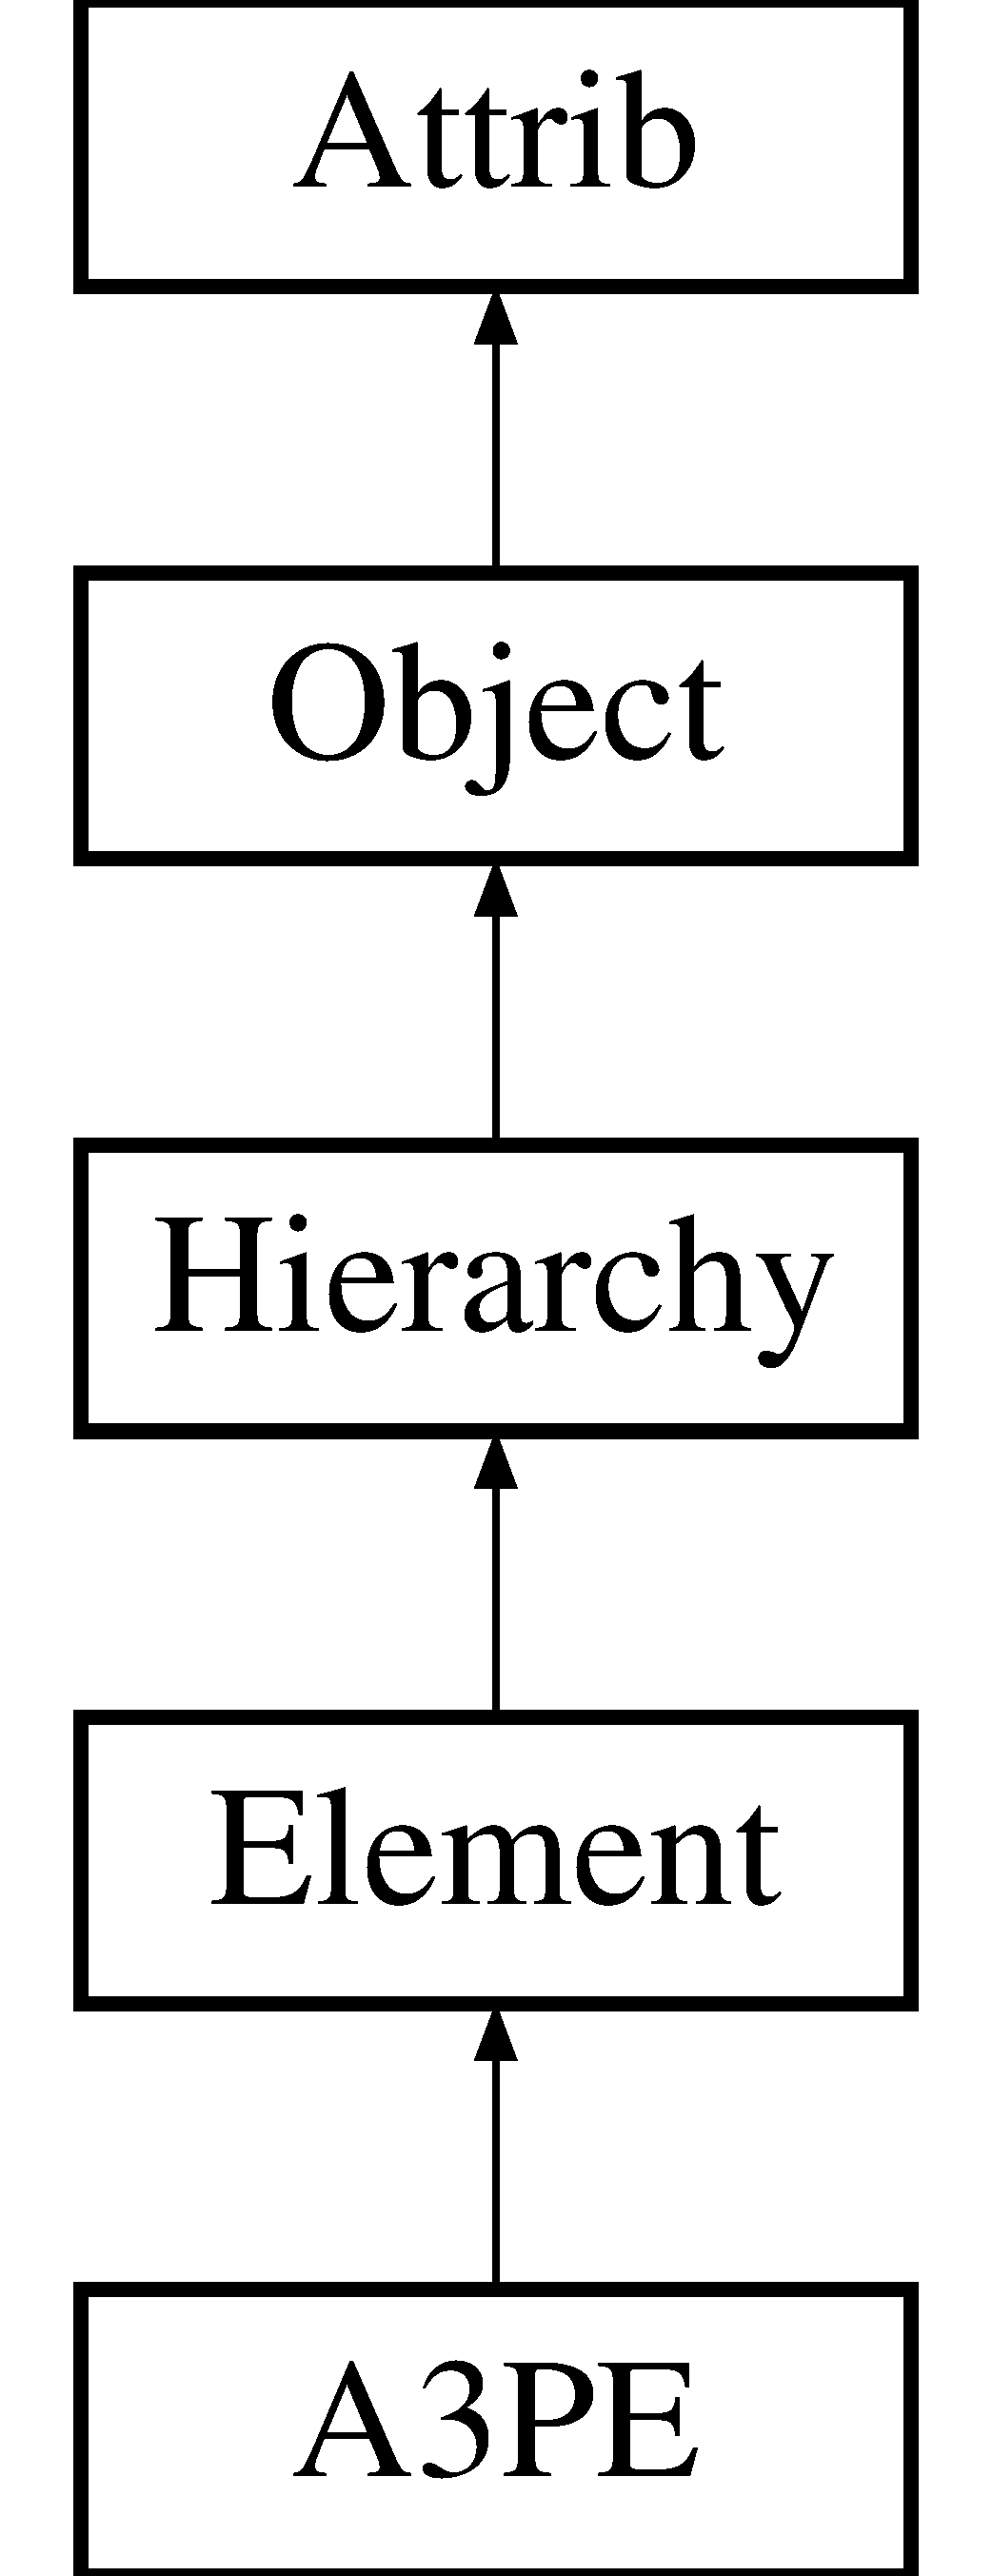
\includegraphics[height=5.000000cm]{classA3PE}
\end{center}
\end{figure}
\subsection*{Public Types}
\begin{DoxyCompactItemize}
\item 
typedef unsigned long \hyperlink{classA3PE_af2773f4a4f8e9940b1e008386c4e908c}{U32}
\item 
typedef unsigned short \hyperlink{classA3PE_a2ee28b2899c3cc4f22821b4138758c28}{U16}
\item 
typedef unsigned char \hyperlink{classA3PE_ab70116c2810a9a01142a33c69fdda039}{U8}
\item 
enum \hyperlink{classAttrib_a69e171d7cc6417835a5a306d3c764235}{Attribut} \{ \newline
\hyperlink{classAttrib_a69e171d7cc6417835a5a306d3c764235a3a8da2ab97dda18aebab196fe4100531}{U\+N\+D\+E\+F\+I\+N\+ED}, 
\hyperlink{classAttrib_a69e171d7cc6417835a5a306d3c764235a2bfb2af57b87031d190a05fe25dd92ed}{P\+A\+S\+S\+I\+VE}, 
\hyperlink{classAttrib_a69e171d7cc6417835a5a306d3c764235a3b1fec929c0370d1436f2f06e298fb0d}{A\+C\+T\+I\+VE}, 
\hyperlink{classAttrib_a69e171d7cc6417835a5a306d3c764235aa27c16b480a369ea4d18b07b2516bbc7}{I\+N\+T\+E\+R\+F\+A\+CE}, 
\newline
\hyperlink{classAttrib_a69e171d7cc6417835a5a306d3c764235a1420a5b8c0540b2af210b6975eded7f9}{IO}, 
\hyperlink{classAttrib_a69e171d7cc6417835a5a306d3c764235a0af3b0d0ac323c1704e6c69cf90add28}{I\+O\+D\+A\+TA}, 
\hyperlink{classAttrib_a69e171d7cc6417835a5a306d3c764235a7788bc5dd333fd8ce18562b269c9dab1}{E\+L\+E\+M\+E\+NT}, 
\hyperlink{classAttrib_a69e171d7cc6417835a5a306d3c764235a61ceb22149f365f1780d18f9d1459423}{H\+A\+R\+D\+W\+A\+RE}, 
\newline
\hyperlink{classAttrib_a69e171d7cc6417835a5a306d3c764235a75250e29692496e73effca2c0330977f}{P\+R\+O\+C\+E\+S\+S\+US}, 
\hyperlink{classAttrib_a69e171d7cc6417835a5a306d3c764235a103a67cd0b8f07ef478fa45d4356e27b}{S\+O\+F\+T\+W\+A\+RE}
 \}
\end{DoxyCompactItemize}
\subsection*{Public Member Functions}
\begin{DoxyCompactItemize}
\item 
\hyperlink{classA3PE_ae3e49a43c661f5e9c1b0edaee14fc297}{A3\+PE} ()
\item 
\hyperlink{classA3PE_aab155e065b455ff439daf47a976399c3}{$\sim$\+A3\+PE} ()
\item 
void \hyperlink{classA3PE_ae495a413cc26d31321b31942ebef1bfa}{help} ()
\item 
\hyperlink{classStatusCode}{Status\+Code} \hyperlink{classA3PE_abe07bae8ce2f32926b7258f269ae655e}{init} ()
\item 
void \hyperlink{classA3PE_a449775588222d544aeeaab190d553652}{reset} ()
\item 
\hyperlink{classStatusCode}{Status\+Code} \hyperlink{classA3PE_a8e7074703227b118aa9230258f22b44c}{reset\+Storage\+Fifo} ()
\item 
\hyperlink{classStatusCode}{Status\+Code} \hyperlink{classA3PE_a0ad1110ea755ffd0b277284d807a8794}{reset\+Usb\+Phasers} ()
\item 
\hyperlink{classStatusCode}{Status\+Code} \hyperlink{classA3PE_a44c50d822ac4f5d8f2b8ed75c5b90580}{reset\+Latency\+Counter} ()
\item 
\hyperlink{classStatusCode}{Status\+Code} \hyperlink{classA3PE_a557ea9cfa97a03db1514af2fe8936df3}{reset\+Acquisition\+Write\+Counter} ()
\item 
\hyperlink{classStatusCode}{Status\+Code} \hyperlink{classA3PE_a4e5b677dd2872428abf3d64ef7a769c1}{reset\+Pattern\+Fifo} ()
\item 
\hyperlink{classStatusCode}{Status\+Code} \hyperlink{classA3PE_ac81388bd2988192cf54034b245f69891}{reset\+Trigger\+Fifo} ()
\item 
\hyperlink{classStatusCode}{Status\+Code} \hyperlink{classA3PE_a31f72fac5a0f00bcf3a0db99bd5704ee}{reset\+To\+A\+X\+Ram} ()
\item 
\hyperlink{classStatusCode}{Status\+Code} \hyperlink{classA3PE_aa10639563d06c0d09f3c0725710ff35d}{reset\+From\+A\+X\+Ram} ()
\item 
\hyperlink{classStatusCode}{Status\+Code} \hyperlink{classA3PE_a6015ba83a7b828efb1969291ab740eee}{reset\+Sequence\+From\+To\+AX} ()
\item 
\hyperlink{classStatusCode}{Status\+Code} \hyperlink{classA3PE_a2cfdb2f37d3d786cbe1ff42fef37b276}{reset\+FE} ()
\item 
\hyperlink{classStatusCode}{Status\+Code} \hyperlink{classA3PE_ae164123b49f8c4d1d119dbf201f0a839}{reset\+S\+PI} ()
\item 
\hyperlink{classStatusCode}{Status\+Code} \hyperlink{classA3PE_a0c90134c3440c8b8c8dc796c43893d64}{set\+Enable\+A\+DC} (unsigned int, bool)
\item 
\hyperlink{classStatusCode}{Status\+Code} \hyperlink{classA3PE_aa688f9dff8d2892464fcd13fdf3600ad}{set\+Write\+Storage\+Fifo\+Usb} (bool)
\item 
bool \hyperlink{classA3PE_a02608198bd28bc61882f27368fd90db1}{enable\+A\+DC} (unsigned int)
\item 
bool \hyperlink{classA3PE_af15048318a126074e28df1c6120d5e0d}{write\+Storage\+Fifo\+Usb} ()
\item 
\hyperlink{classStatusCode}{Status\+Code} \hyperlink{classA3PE_a9d3ba9807ea65be0af7f23ffa2372d6b}{set\+Read\+Pattern\+Fifo\+Usb} (bool)
\item 
bool \hyperlink{classA3PE_a3bb47f43f9f98d8a0d825aadc04e5ab6}{read\+Pattern\+Fifo\+Usb} ()
\item 
\hyperlink{classStatusCode}{Status\+Code} \hyperlink{classA3PE_a1d0dd1db3c493bc31aa56b55e7439e0e}{set\+Read\+Trigger\+Fifo\+Usb} (bool)
\item 
bool \hyperlink{classA3PE_a083315774486528a8b6c40e240fbf98f}{read\+Trigger\+Fifo\+Usb} ()
\item 
\hyperlink{classStatusCode}{Status\+Code} \hyperlink{classA3PE_a7ad649611d4cc5a7743db54aa3a4f943}{set\+Read\+To\+A\+X\+Ram\+Usb} (bool)
\item 
bool \hyperlink{classA3PE_af3152e461d446f442cfa7b69456ac276}{read\+To\+A\+X\+Ram\+Usb} ()
\item 
\hyperlink{classStatusCode}{Status\+Code} \hyperlink{classA3PE_aeb276fae7f19c45b4b4a3a5a2b99c337}{set\+Write\+From\+A\+X\+Ram\+Usb} (bool)
\item 
bool \hyperlink{classA3PE_a3b4333f547a2a36fc1f38bf4ca9afa89}{write\+From\+A\+X\+Ram\+Usb} ()
\item 
\hyperlink{classStatusCode}{Status\+Code} \hyperlink{classA3PE_a77ccfbd9df2fad96a9a9f1dc579a7a2d}{set\+A\+X\+Ram\+Usb} (bool)
\item 
\hyperlink{classStatusCode}{Status\+Code} \hyperlink{classA3PE_a91ae249ca14676f8b0832487955fcf8c}{start\+Sequence\+AX} ()
\item 
\hyperlink{classStatusCode}{Status\+Code} \hyperlink{classA3PE_aac0ee532f78885a25eebddbad501417f}{set\+Software\+Trigger} (bool)
\item 
bool \hyperlink{classA3PE_acb2ccd6b78b39a0a9e360439b3b6f4c7}{software\+Trigger} ()
\item 
\hyperlink{classStatusCode}{Status\+Code} \hyperlink{classA3PE_acf354b2c85a7e20f7f037beb278dd79d}{set\+Clock\+Division} (unsigned int)
\item 
\hyperlink{classStatusCode}{Status\+Code} \hyperlink{classA3PE_a6a63fc9503e0aa89ee9928fc7222ce0f}{set\+Trigger\+Delay} (unsigned int)
\item 
\hyperlink{classStatusCode}{Status\+Code} \hyperlink{classA3PE_af34831e9776a000f833a610ea999a564}{set\+Seq\+Pulse\+Delay} (unsigned int)
\item 
\hyperlink{classStatusCode}{Status\+Code} \hyperlink{classA3PE_a1ae8e5a69e17d6b3157779544fa14c75}{set\+Trigger\+Rate} (unsigned int)
\item 
\hyperlink{classStatusCode}{Status\+Code} \hyperlink{classA3PE_a81db44ddfc42b67ed08756b113b8e122}{set\+N\+Trigger} (unsigned int)
\item 
\hyperlink{classStatusCode}{Status\+Code} \hyperlink{classA3PE_a969469569005dfb130aca674de5dacff}{set\+Fifo\+Latency} (unsigned short)
\item 
\hyperlink{classStatusCode}{Status\+Code} \hyperlink{classA3PE_a4d8f78a1b09b409f288b34d503c71146}{set\+Fifo\+Depth} (unsigned int)
\item 
unsigned int \hyperlink{classA3PE_a81e32c82ca14f85fd7f26cd9a54f7a38}{clock\+Division} ()
\item 
unsigned int \hyperlink{classA3PE_ac0aabc1457923b7ee7da0a2c91c46451}{trigger\+Delay} ()
\item 
unsigned int \hyperlink{classA3PE_acce23c9abd4f434c8c5965351f5ceef0}{seq\+Pulse\+Delay} ()
\item 
unsigned int \hyperlink{classA3PE_ada46375753047d6a74acdec442044f39}{trigger\+Rate} ()
\item 
unsigned int \hyperlink{classA3PE_a3398fa3ce59a4b1b946e7b4ab4912580}{n\+Trigger} ()
\item 
unsigned int \hyperlink{classA3PE_a7f6959a6a38c16fa6609560827413764}{fifo\+Latency} ()
\item 
unsigned int \hyperlink{classA3PE_a8bb523e4a7a5dbb6ab3c5549ebf6db86}{fifo\+Depth} ()
\item 
\hyperlink{classStatusCode}{Status\+Code} \hyperlink{classA3PE_a035886b99761cc4f3c342ff0b4e44f59}{acquisition} ()
\item 
\hyperlink{classStatusCode}{Status\+Code} \hyperlink{classA3PE_a2071d7922f140ee6705da954efb685f7}{enable\+Storage} ()
\item 
\hyperlink{classStatusCode}{Status\+Code} \hyperlink{classA3PE_a75cd0377eb653ed22c4d258ab359f3d6}{trigger} ()
\item 
bool \hyperlink{classA3PE_a55df064c578bbc1e80a3b5fc05933f27}{data\+Ready} ()
\item 
void \hyperlink{classA3PE_a9e9b5ba5bd0ee19470c80761269a00f6}{update} ()
\item 
\hyperlink{classStatusCode}{Status\+Code} \hyperlink{classA3PE_ad5f953a38661104a87834cc8a63252fa}{set\+Internal\+A\+X\+Sequence} (bool)
\item 
bool \hyperlink{classA3PE_a4b9cf42bdd0a14e48807faa0956c59bd}{internal\+A\+X\+Sequence} ()
\item 
\hyperlink{classStatusCode}{Status\+Code} \hyperlink{classA3PE_a0300aa5c5ed02b82275c1de434196b9a}{set\+Length\+AX} (unsigned int)
\item 
unsigned int \hyperlink{classA3PE_acb95104d817db2e4f97e250f7e45b43d}{length\+AX} ()
\item 
\hyperlink{classStatusCode}{Status\+Code} \hyperlink{classA3PE_a53882e1272e8146e51837904ea00f33c}{set\+Latency\+AX} (unsigned int)
\item 
unsigned int \hyperlink{classA3PE_ab5970721a8172ae57b3da68040f58199}{latency\+AX} ()
\item 
\hyperlink{classStatusCode}{Status\+Code} \hyperlink{classA3PE_a5b3840fc8edd14427ac9fb4def3171d3}{set\+Pipeline} (unsigned int)
\item 
unsigned int \hyperlink{classA3PE_aeb22b2fcba4d14f234ad2d6dcef7948c}{pipeline} ()
\item 
\hyperlink{classRegister}{Register} $\ast$ \hyperlink{classA3PE_ae5fc5dac92af2b34a41be388586647be}{ctrl\+Reg} ()
\item 
\hyperlink{classRegister}{Register} $\ast$ \hyperlink{classA3PE_a94d96383e441153ed01e82cc12d2f593}{setup\+Reg} ()
\item 
\hyperlink{classRegister}{Register} $\ast$ \hyperlink{classA3PE_afd34bfbfd92838717c7cdec856b2a0b2}{reset\+Reg} ()
\item 
\hyperlink{classRegister}{Register} $\ast$ \hyperlink{classA3PE_af260fc8bce78935b7bad57c987574683}{status\+Reg} ()
\item 
\hyperlink{classRegister}{Register} $\ast$ \hyperlink{classA3PE_aca56dadafd70e670e75569ee03d91651}{acq\+Reg} ()
\item 
\hyperlink{classRegister}{Register} $\ast$ \hyperlink{classA3PE_a42dad20d5a1482431e73c64250b76185}{latency\+Reg} ()
\item 
\hyperlink{classRegister}{Register} $\ast$ \hyperlink{classA3PE_a3b75531731fc939206cce076f7ac9f9a}{write\+Length\+Fifo\+Reg} ()
\item 
\hyperlink{classRegister}{Register} $\ast$ \hyperlink{classA3PE_aa94c6120a73194d69dc5761cf90a4800}{ctrl\+Ana\+Mezz\+Reg} ()
\item 
\hyperlink{classRegister}{Register} $\ast$ \hyperlink{classA3PE_a10cf30ff852d7580ba94dbee0c48e0d5}{clock\+Division\+Reg} ()
\item 
\hyperlink{classRegister}{Register} $\ast$ \hyperlink{classA3PE_a4bf922f391fee6753fb0d53e133603b7}{trigger\+Reg} ()
\item 
\hyperlink{classRegister}{Register} $\ast$ \hyperlink{classA3PE_a43b0006fafa3aeae353abb2ac30e872c}{to\+A\+X\+Reg} ()
\item 
\hyperlink{classRegister}{Register} $\ast$ \hyperlink{classA3PE_a0b2fabe7e7941f33de210d9385b7afce}{from\+A\+X\+Reg} ()
\item 
\hyperlink{classRegister}{Register} $\ast$ \hyperlink{classA3PE_a979a9ac462eb55e611f6de4e94bad18e}{spare3\+Reg} ()
\item 
\hyperlink{classRAM}{R\+AM} $\ast$ \hyperlink{classA3PE_af241373059bad4a3c376ab2ac98a7b29}{storage\+Ram} ()
\item 
\hyperlink{classRAM}{R\+AM} $\ast$ \hyperlink{classA3PE_a94ef54086baa29f7f6638c13d8906e56}{pattern\+Ram} ()
\item 
\hyperlink{classRAM}{R\+AM} $\ast$ \hyperlink{classA3PE_aad0f7ac467db22e5608ae6b0957665a1}{trigger\+Ram} ()
\item 
\hyperlink{classRAM}{R\+AM} $\ast$ \hyperlink{classA3PE_a16b16ac12705b9dd93d70fa172deb584}{to\+A\+X\+Ram} ()
\item 
\hyperlink{classRAM}{R\+AM} $\ast$ \hyperlink{classA3PE_a7c9026a74c1954b2d250be05fbc1c8c5}{from\+A\+X\+Ram} ()
\item 
\hyperlink{classRAM}{R\+AM} $\ast$ \hyperlink{classA3PE_a9327d0bd2efb5baa7c6b7de27bbc5997}{test\+Ram} ()
\item 
\hyperlink{classRegister}{Register} $\ast$ \hyperlink{classA3PE_aad21357e25e3d4e2bed779040de52e13}{from\+A\+X\+Ram\+Ptr\+Reg} ()
\item 
\hyperlink{classRegister}{Register} $\ast$ \hyperlink{classA3PE_af6e9e980e871fcf0e1b35e1b4ae95ebe}{to\+A\+X\+Ram\+Ptr\+Reg} ()
\item 
void \hyperlink{classA3PE_ad7999557f9d561dec67526730a3c97ef}{dump\+Storage} ()
\item 
void \hyperlink{classA3PE_a8bd4a7a5dd8219f93386756c24a0f0b5}{load\+Storage} (std\+::string)
\item 
void \hyperlink{classA3PE_a23da04d3c7e632dfb64e5ed4e21a21f3}{dump\+Pattern} ()
\item 
void \hyperlink{classA3PE_a522cba0a4d976eec59222504af188fb2}{load\+Pattern} (std\+::string)
\item 
void \hyperlink{classA3PE_aeab7701d0d1f6fd910e952b631769d42}{dump\+Trigger} ()
\item 
void \hyperlink{classA3PE_a34a9499a0d9065a1b5772880d7e8d5c4}{load\+Trigger} (std\+::string)
\item 
void \hyperlink{classA3PE_ad6b6f1ae4ac23e6d0827eee8cc2c98e4}{dump\+To\+AX} ()
\item 
void \hyperlink{classA3PE_a40017b4138705690f8b04e336a7ffcdf}{load\+To\+AX} (std\+::string)
\item 
void \hyperlink{classA3PE_a60a510251ec2b5fd800af2ba88e9fdac}{dump\+From\+AX} ()
\item 
void \hyperlink{classA3PE_a65235f7d42e8f7fb6056f5629545d2aa}{load\+From\+AX} (std\+::string)
\item 
\hyperlink{classStatusCode}{Status\+Code} \hyperlink{classA3PE_a54fe4da570ea8833fe2c981de1085387}{set\+Add\+To\+A\+X\+Ram} (int)
\item 
\hyperlink{classStatusCode}{Status\+Code} \hyperlink{classA3PE_a834fde5951d2c1bf6b41842520360fce}{set\+Add\+From\+A\+X\+Ram} (int)
\item 
void \hyperlink{classElement_a3c0abcb36f8906688bb7e32608df7086}{recursive\+Init\+Element} ()
\item 
void \hyperlink{classElement_a82119ed37dff76508a2746a853ec35ba}{recursive\+Init\+Communications} ()
\item 
\hyperlink{classStatusCode}{Status\+Code} \hyperlink{classElement_ab476b4b1df5954141ceb14f072433b89}{set\+Connection} (\hyperlink{classHierarchy}{Hierarchy} $\ast$)
\item 
\hyperlink{classHierarchy}{Hierarchy} $\ast$ \hyperlink{classElement_af57444353c1ddf9fa0109801e97debf7}{connection} ()
\item 
void \hyperlink{classHierarchy_af4d43b0765b402670eed2d62c73405af}{clear} ()
\item 
void \hyperlink{classHierarchy_a585ad1aeec16077a0e532ab8b4fc557b}{set\+Parent} (\hyperlink{classHierarchy}{Hierarchy} $\ast$\hyperlink{classHierarchy_a1c7bec8257e717f9c1465e06ebf845fc}{parent})
\item 
\hyperlink{classHierarchy}{Hierarchy} $\ast$ \hyperlink{classHierarchy_a1c7bec8257e717f9c1465e06ebf845fc}{parent} ()
\item 
\hyperlink{classHierarchy}{Hierarchy} $\ast$ \hyperlink{classHierarchy_ad550588733bf75ac5c0fcfd7c8fd11a6}{parent} (std\+::string)
\item 
\hyperlink{classHierarchy}{Hierarchy} $\ast$ \hyperlink{classHierarchy_aee461dc930ce3871636ff87f075b1b83}{origin} ()
\item 
virtual void \hyperlink{classHierarchy_ad677774ff38fcb257c04a3a10d471fac}{add\+Child} (\hyperlink{classHierarchy}{Hierarchy} $\ast$element)
\item 
std\+::vector$<$ \hyperlink{classHierarchy}{Hierarchy} $\ast$ $>$ \hyperlink{classHierarchy_aa9a76f69e98e052ee1a6e32cea006288}{children} ()
\item 
\hyperlink{classHierarchy}{Hierarchy} $\ast$ \hyperlink{classHierarchy_a1e207f973c694b538bf90107b4868817}{child} (std\+::string)
\item 
\hyperlink{classHierarchy}{Hierarchy} $\ast$ \hyperlink{classHierarchy_a0c15a5276a3b80b4354d6bd8a01e0708}{child\+Typed} (std\+::string)
\item 
unsigned long \hyperlink{classHierarchy_ab16e84de65fd84e14001a6cf941c8be4}{number\+Of\+Children} ()
\item 
bool \hyperlink{classHierarchy_a255174fe4d316d2a3f430dcb9dab29f1}{has\+Children} ()
\item 
void \hyperlink{classHierarchy_a2b2b359fac003233f65786a616766bde}{del\+Child} (\hyperlink{classHierarchy}{Hierarchy} $\ast$)
\item 
void \hyperlink{classHierarchy_a1928ac7615fe0b5e55cd707f70dc6781}{del\+Child} (std\+::string)
\item 
std\+::string \hyperlink{classHierarchy_aa7990fa7caf132d83e361ce033c6c65a}{path} (std\+::string=std\+::string(\char`\"{}\char`\"{}))
\item 
std\+::string \hyperlink{classHierarchy_a1efd56cd164d328d2002e53a10a19b8c}{path\+Typed} (std\+::string=std\+::string(\char`\"{}\char`\"{}))
\item 
void \hyperlink{classHierarchy_a76e914b9a677a22a82deb74d892bf261}{tree} (std\+::string indent=std\+::string(\char`\"{}\char`\"{}))
\item 
void \hyperlink{classHierarchy_a594c294c5f60c230e106d522ed008212}{tree} ()
\item 
std\+::string \hyperlink{classObject_a300f4c05dd468c7bb8b3c968868443c1}{name} () const
\item 
std\+::string \hyperlink{classObject_a84f99f70f144a83e1582d1d0f84e4e62}{type} ()
\item 
unsigned char \hyperlink{classObject_af99145335cc61ff6e2798ea17db009d2}{id} ()
\item 
std\+::string \hyperlink{classObject_a73a0f1a41828fdd8303dd662446fb6c3}{title} ()
\item 
void \hyperlink{classObject_a3f9d5537ebce0c0f2bf6ae4d92426f3c}{msg\+Svc} (int level, std\+::string \hyperlink{classObject_a58b2d0618c2d08cf2383012611528d97}{msg}, std\+::string \hyperlink{classObject_a300f4c05dd468c7bb8b3c968868443c1}{name})
\item 
void \hyperlink{classObject_a58b2d0618c2d08cf2383012611528d97}{msg} (std\+::string mymsg)
\item 
void \hyperlink{classObject_ac5d59299273cee27aacf7de00d2e7034}{msg} (std\+::string mymsg, std\+::string \hyperlink{classObject_a300f4c05dd468c7bb8b3c968868443c1}{name})
\item 
void \hyperlink{classObject_a83d2db2df682907ea1115ad721c1c4a1}{verbose} (std\+::string mymsg)
\item 
void \hyperlink{classObject_a2d4120195317e2a3c6532e8bb9f3da68}{verbose} (std\+::string mymsg, std\+::string \hyperlink{classObject_a300f4c05dd468c7bb8b3c968868443c1}{name})
\item 
void \hyperlink{classObject_aac010553f022165573714b7014a15f0d}{debug} (std\+::string mymsg)
\item 
void \hyperlink{classObject_a6c9a0397ca804e04d675ed05683f5420}{debug} (std\+::string mymsg, std\+::string \hyperlink{classObject_a300f4c05dd468c7bb8b3c968868443c1}{name})
\item 
void \hyperlink{classObject_a644fd329ea4cb85f54fa6846484b84a8}{info} (std\+::string mymsg)
\item 
void \hyperlink{classObject_a1ca123253dfd30fc28b156f521dcbdae}{info} (std\+::string mymsg, std\+::string \hyperlink{classObject_a300f4c05dd468c7bb8b3c968868443c1}{name})
\item 
void \hyperlink{classObject_a65cd4fda577711660821fd2cd5a3b4c9}{warning} (std\+::string mymsg)
\item 
void \hyperlink{classObject_a11f101db4dd73d9391b0231818881d86}{warning} (std\+::string mymsg, std\+::string \hyperlink{classObject_a300f4c05dd468c7bb8b3c968868443c1}{name})
\item 
void \hyperlink{classObject_a204a95f57818c0f811933917a30eff45}{error} (std\+::string mymsg)
\item 
void \hyperlink{classObject_ad7f6c457733082efa2f9ff5f5c8e119a}{error} (std\+::string mymsg, std\+::string \hyperlink{classObject_a300f4c05dd468c7bb8b3c968868443c1}{name})
\item 
void \hyperlink{classObject_aad5a16aac7516ce65bd5ec02ab07fc80}{fatal} (std\+::string mymsg)
\item 
void \hyperlink{classObject_ae62acd3d09f716220f75f252dc38bc9a}{fatal} (std\+::string mymsg, std\+::string \hyperlink{classObject_a300f4c05dd468c7bb8b3c968868443c1}{name})
\item 
void \hyperlink{classObject_ae30fea75683c2d149b6b6d17c09ecd0c}{set\+Name} (std\+::string \hyperlink{classObject_a300f4c05dd468c7bb8b3c968868443c1}{name})
\item 
void \hyperlink{classObject_aae534cc9d982bcb9b99fd505f2e103a5}{set\+Type} (std\+::string \hyperlink{classObject_a84f99f70f144a83e1582d1d0f84e4e62}{type})
\item 
void \hyperlink{classObject_a398fe08cba594a0ce6891d59fe4f159f}{set\+Id} (unsigned char \hyperlink{classObject_af99145335cc61ff6e2798ea17db009d2}{id})
\item 
void \hyperlink{classObject_a89557dbbad5bcaa02652f5d7fa35d20f}{set\+Title} (std\+::string \hyperlink{classObject_a73a0f1a41828fdd8303dd662446fb6c3}{title})
\item 
void \hyperlink{classObject_a870c5af919958c2136623b2d7816d123}{set\+Dll\+Name} (std\+::string \hyperlink{classObject_a2e3947f2870094c332d7454117f3ec63}{dll\+Name})
\item 
std\+::string \hyperlink{classObject_a2e3947f2870094c332d7454117f3ec63}{dll\+Name} ()
\item 
bool \hyperlink{classAttrib_a704f26af560909ad22065083bb7d4c34}{is} (int attribut)
\item 
void \hyperlink{classAttrib_a235f773af19c900264a190b00a3b4ad7}{add} (int attribut)
\item 
void \hyperlink{classAttrib_a7d4ef7e32d93cb287792b87b857e79f3}{remove} (int attribut)
\item 
std\+::string \hyperlink{classAttrib_aee7bbf16b144887f196e1341b24f8a26}{attributs} ()
\end{DoxyCompactItemize}
\subsection*{Protected Attributes}
\begin{DoxyCompactItemize}
\item 
\hyperlink{classHierarchy}{Hierarchy} $\ast$ \hyperlink{classElement_abe3de7a5dbbc9a6dd2d7e012e5fdb266}{m\+\_\+connection}
\item 
std\+::string \hyperlink{classAttrib_a3414521d7a82476e874b25a5407b5e63}{m\+\_\+attrib\+String} \mbox{[}10\mbox{]}
\end{DoxyCompactItemize}
\subsection*{Private Attributes}
\begin{DoxyCompactItemize}
\item 
\hyperlink{classRegister}{Register} $\ast$ \hyperlink{classA3PE_abd71e0c273f9e211e1a9302019129aff}{m\+\_\+global\+Usb\+Reset}
\item 
\hyperlink{classRegister}{Register} $\ast$ \hyperlink{classA3PE_a264834484dd6326ebad58c2a3e1be9a6}{m\+\_\+ctrl\+Reg}
\item 
\hyperlink{classRegister}{Register} $\ast$ \hyperlink{classA3PE_ab4db5f00976e5095686f108c8febf702}{m\+\_\+reset\+Reg}
\item 
\hyperlink{classRegister}{Register} $\ast$ \hyperlink{classA3PE_a142fa10b7e705c4701ae21678ec2ec8a}{m\+\_\+setup\+Reg}
\item 
\hyperlink{classRegister}{Register} $\ast$ \hyperlink{classA3PE_a2281e3d12a2dffad99ec55be2b695f53}{m\+\_\+status\+Reg}
\item 
\hyperlink{classRegister}{Register} $\ast$ \hyperlink{classA3PE_abaf426f4c9192537117b77f9f4821e04}{m\+\_\+acq\+Reg}
\item 
\hyperlink{classRegister}{Register} $\ast$ \hyperlink{classA3PE_a96a167e73e264da5a18d9ddb5ebb5f23}{m\+\_\+latency\+Reg}
\item 
\hyperlink{classRegister}{Register} $\ast$ \hyperlink{classA3PE_a9a0cb2253ea34c0be567a03684217fee}{m\+\_\+write\+Length\+Fifo\+Reg}
\item 
\hyperlink{classRegister}{Register} $\ast$ \hyperlink{classA3PE_a126a936a5fd4fd4b83485b3637e1fa84}{m\+\_\+ctrl\+Ana\+Mezz\+Reg}
\item 
\hyperlink{classRegister}{Register} $\ast$ \hyperlink{classA3PE_ae1f4c24a99c2e6ae944a080f429cc155}{m\+\_\+clock\+Division\+Reg}
\item 
\hyperlink{classRegister}{Register} $\ast$ \hyperlink{classA3PE_a750158ae488121ab7969452f061e678c}{m\+\_\+trigger\+Reg}
\item 
\hyperlink{classRegister}{Register} $\ast$ \hyperlink{classA3PE_abe8eb76e3c0d967403726143deb1b70f}{m\+\_\+to\+A\+X\+Reg}
\item 
\hyperlink{classRegister}{Register} $\ast$ \hyperlink{classA3PE_acbfe708ac0a81243959c96124f192b9e}{m\+\_\+from\+A\+X\+Reg}
\item 
\hyperlink{classRegister}{Register} $\ast$ \hyperlink{classA3PE_a1e7e5c89f190672990ae5bece2a8b1aa}{m\+\_\+spare3\+Reg}
\item 
\hyperlink{classRAM}{R\+AM} $\ast$ \hyperlink{classA3PE_a41e317474e0c6e63bad4648903279be9}{m\+\_\+storage\+Ram}
\item 
\hyperlink{classRAM}{R\+AM} $\ast$ \hyperlink{classA3PE_a84d5deabbbf2d513144dd6a00390182e}{m\+\_\+pattern\+Ram}
\item 
\hyperlink{classRAM}{R\+AM} $\ast$ \hyperlink{classA3PE_a2b40e3937f0aa008ec7073acc5029fcc}{m\+\_\+trigger\+Ram}
\item 
\hyperlink{classRegister}{Register} $\ast$ \hyperlink{classA3PE_aae1b8b2e96bba94535bd4de766bd7e65}{m\+\_\+to\+A\+X\+Ram\+Ptr}
\item 
\hyperlink{classRegister}{Register} $\ast$ \hyperlink{classA3PE_a27ae9467bc128e46dd80443245df096a}{m\+\_\+from\+A\+X\+Ram\+Ptr}
\item 
\hyperlink{classRAM}{R\+AM} $\ast$ \hyperlink{classA3PE_ae586a3d2fd21556e84e1af656e3430b5}{m\+\_\+to\+A\+X\+Ram}
\item 
\hyperlink{classRAM}{R\+AM} $\ast$ \hyperlink{classA3PE_a91d3dd3e87e2c948dd67cb82a63d3858}{m\+\_\+from\+A\+X\+Ram}
\item 
\hyperlink{classRegister}{Register} $\ast$ \hyperlink{classA3PE_a061472eb539bb6ac99f4fa11a760eeaf}{m\+\_\+latency\+AX}
\item 
\hyperlink{classRegister}{Register} $\ast$ \hyperlink{classA3PE_a87c93a38343873f2d52741deca4750ce}{m\+\_\+length\+AX}
\item 
\hyperlink{classRAM}{R\+AM} $\ast$ \hyperlink{classA3PE_ad788e41ef5c674ab1a7671f3db0ffef6}{m\+\_\+test\+Ram}
\end{DoxyCompactItemize}


\subsection{Detailed Description}


Definition at line 20 of file A3\+P\+E.\+h.



\subsection{Member Typedef Documentation}
\mbox{\Hypertarget{classA3PE_a2ee28b2899c3cc4f22821b4138758c28}\label{classA3PE_a2ee28b2899c3cc4f22821b4138758c28}} 
\index{A3\+PE@{A3\+PE}!U16@{U16}}
\index{U16@{U16}!A3\+PE@{A3\+PE}}
\subsubsection{\texorpdfstring{U16}{U16}}
{\footnotesize\ttfamily typedef unsigned short \hyperlink{classA3PE_a2ee28b2899c3cc4f22821b4138758c28}{A3\+P\+E\+::\+U16}}



Definition at line 23 of file A3\+P\+E.\+h.

\mbox{\Hypertarget{classA3PE_af2773f4a4f8e9940b1e008386c4e908c}\label{classA3PE_af2773f4a4f8e9940b1e008386c4e908c}} 
\index{A3\+PE@{A3\+PE}!U32@{U32}}
\index{U32@{U32}!A3\+PE@{A3\+PE}}
\subsubsection{\texorpdfstring{U32}{U32}}
{\footnotesize\ttfamily typedef unsigned long \hyperlink{classA3PE_af2773f4a4f8e9940b1e008386c4e908c}{A3\+P\+E\+::\+U32}}



Definition at line 22 of file A3\+P\+E.\+h.

\mbox{\Hypertarget{classA3PE_ab70116c2810a9a01142a33c69fdda039}\label{classA3PE_ab70116c2810a9a01142a33c69fdda039}} 
\index{A3\+PE@{A3\+PE}!U8@{U8}}
\index{U8@{U8}!A3\+PE@{A3\+PE}}
\subsubsection{\texorpdfstring{U8}{U8}}
{\footnotesize\ttfamily typedef unsigned char \hyperlink{classA3PE_ab70116c2810a9a01142a33c69fdda039}{A3\+P\+E\+::\+U8}}



Definition at line 24 of file A3\+P\+E.\+h.



\subsection{Member Enumeration Documentation}
\mbox{\Hypertarget{classAttrib_a69e171d7cc6417835a5a306d3c764235}\label{classAttrib_a69e171d7cc6417835a5a306d3c764235}} 
\index{A3\+PE@{A3\+PE}!Attribut@{Attribut}}
\index{Attribut@{Attribut}!A3\+PE@{A3\+PE}}
\subsubsection{\texorpdfstring{Attribut}{Attribut}}
{\footnotesize\ttfamily enum \hyperlink{classAttrib_a69e171d7cc6417835a5a306d3c764235}{Attrib\+::\+Attribut}\hspace{0.3cm}{\ttfamily [inherited]}}

\begin{DoxyEnumFields}{Enumerator}
\raisebox{\heightof{T}}[0pt][0pt]{\index{U\+N\+D\+E\+F\+I\+N\+ED@{U\+N\+D\+E\+F\+I\+N\+ED}!A3\+PE@{A3\+PE}}\index{A3\+PE@{A3\+PE}!U\+N\+D\+E\+F\+I\+N\+ED@{U\+N\+D\+E\+F\+I\+N\+ED}}}\mbox{\Hypertarget{classAttrib_a69e171d7cc6417835a5a306d3c764235a3a8da2ab97dda18aebab196fe4100531}\label{classAttrib_a69e171d7cc6417835a5a306d3c764235a3a8da2ab97dda18aebab196fe4100531}} 
U\+N\+D\+E\+F\+I\+N\+ED&\\
\hline

\raisebox{\heightof{T}}[0pt][0pt]{\index{P\+A\+S\+S\+I\+VE@{P\+A\+S\+S\+I\+VE}!A3\+PE@{A3\+PE}}\index{A3\+PE@{A3\+PE}!P\+A\+S\+S\+I\+VE@{P\+A\+S\+S\+I\+VE}}}\mbox{\Hypertarget{classAttrib_a69e171d7cc6417835a5a306d3c764235a2bfb2af57b87031d190a05fe25dd92ed}\label{classAttrib_a69e171d7cc6417835a5a306d3c764235a2bfb2af57b87031d190a05fe25dd92ed}} 
P\+A\+S\+S\+I\+VE&\\
\hline

\raisebox{\heightof{T}}[0pt][0pt]{\index{A\+C\+T\+I\+VE@{A\+C\+T\+I\+VE}!A3\+PE@{A3\+PE}}\index{A3\+PE@{A3\+PE}!A\+C\+T\+I\+VE@{A\+C\+T\+I\+VE}}}\mbox{\Hypertarget{classAttrib_a69e171d7cc6417835a5a306d3c764235a3b1fec929c0370d1436f2f06e298fb0d}\label{classAttrib_a69e171d7cc6417835a5a306d3c764235a3b1fec929c0370d1436f2f06e298fb0d}} 
A\+C\+T\+I\+VE&\\
\hline

\raisebox{\heightof{T}}[0pt][0pt]{\index{I\+N\+T\+E\+R\+F\+A\+CE@{I\+N\+T\+E\+R\+F\+A\+CE}!A3\+PE@{A3\+PE}}\index{A3\+PE@{A3\+PE}!I\+N\+T\+E\+R\+F\+A\+CE@{I\+N\+T\+E\+R\+F\+A\+CE}}}\mbox{\Hypertarget{classAttrib_a69e171d7cc6417835a5a306d3c764235aa27c16b480a369ea4d18b07b2516bbc7}\label{classAttrib_a69e171d7cc6417835a5a306d3c764235aa27c16b480a369ea4d18b07b2516bbc7}} 
I\+N\+T\+E\+R\+F\+A\+CE&\\
\hline

\raisebox{\heightof{T}}[0pt][0pt]{\index{IO@{IO}!A3\+PE@{A3\+PE}}\index{A3\+PE@{A3\+PE}!IO@{IO}}}\mbox{\Hypertarget{classAttrib_a69e171d7cc6417835a5a306d3c764235a1420a5b8c0540b2af210b6975eded7f9}\label{classAttrib_a69e171d7cc6417835a5a306d3c764235a1420a5b8c0540b2af210b6975eded7f9}} 
IO&\\
\hline

\raisebox{\heightof{T}}[0pt][0pt]{\index{I\+O\+D\+A\+TA@{I\+O\+D\+A\+TA}!A3\+PE@{A3\+PE}}\index{A3\+PE@{A3\+PE}!I\+O\+D\+A\+TA@{I\+O\+D\+A\+TA}}}\mbox{\Hypertarget{classAttrib_a69e171d7cc6417835a5a306d3c764235a0af3b0d0ac323c1704e6c69cf90add28}\label{classAttrib_a69e171d7cc6417835a5a306d3c764235a0af3b0d0ac323c1704e6c69cf90add28}} 
I\+O\+D\+A\+TA&\\
\hline

\raisebox{\heightof{T}}[0pt][0pt]{\index{E\+L\+E\+M\+E\+NT@{E\+L\+E\+M\+E\+NT}!A3\+PE@{A3\+PE}}\index{A3\+PE@{A3\+PE}!E\+L\+E\+M\+E\+NT@{E\+L\+E\+M\+E\+NT}}}\mbox{\Hypertarget{classAttrib_a69e171d7cc6417835a5a306d3c764235a7788bc5dd333fd8ce18562b269c9dab1}\label{classAttrib_a69e171d7cc6417835a5a306d3c764235a7788bc5dd333fd8ce18562b269c9dab1}} 
E\+L\+E\+M\+E\+NT&\\
\hline

\raisebox{\heightof{T}}[0pt][0pt]{\index{H\+A\+R\+D\+W\+A\+RE@{H\+A\+R\+D\+W\+A\+RE}!A3\+PE@{A3\+PE}}\index{A3\+PE@{A3\+PE}!H\+A\+R\+D\+W\+A\+RE@{H\+A\+R\+D\+W\+A\+RE}}}\mbox{\Hypertarget{classAttrib_a69e171d7cc6417835a5a306d3c764235a61ceb22149f365f1780d18f9d1459423}\label{classAttrib_a69e171d7cc6417835a5a306d3c764235a61ceb22149f365f1780d18f9d1459423}} 
H\+A\+R\+D\+W\+A\+RE&\\
\hline

\raisebox{\heightof{T}}[0pt][0pt]{\index{P\+R\+O\+C\+E\+S\+S\+US@{P\+R\+O\+C\+E\+S\+S\+US}!A3\+PE@{A3\+PE}}\index{A3\+PE@{A3\+PE}!P\+R\+O\+C\+E\+S\+S\+US@{P\+R\+O\+C\+E\+S\+S\+US}}}\mbox{\Hypertarget{classAttrib_a69e171d7cc6417835a5a306d3c764235a75250e29692496e73effca2c0330977f}\label{classAttrib_a69e171d7cc6417835a5a306d3c764235a75250e29692496e73effca2c0330977f}} 
P\+R\+O\+C\+E\+S\+S\+US&\\
\hline

\raisebox{\heightof{T}}[0pt][0pt]{\index{S\+O\+F\+T\+W\+A\+RE@{S\+O\+F\+T\+W\+A\+RE}!A3\+PE@{A3\+PE}}\index{A3\+PE@{A3\+PE}!S\+O\+F\+T\+W\+A\+RE@{S\+O\+F\+T\+W\+A\+RE}}}\mbox{\Hypertarget{classAttrib_a69e171d7cc6417835a5a306d3c764235a103a67cd0b8f07ef478fa45d4356e27b}\label{classAttrib_a69e171d7cc6417835a5a306d3c764235a103a67cd0b8f07ef478fa45d4356e27b}} 
S\+O\+F\+T\+W\+A\+RE&\\
\hline

\end{DoxyEnumFields}


Definition at line 29 of file Attrib.\+h.


\begin{DoxyCode}
29                 \{
30     \hyperlink{classAttrib_a69e171d7cc6417835a5a306d3c764235a3a8da2ab97dda18aebab196fe4100531}{UNDEFINED},
31     \hyperlink{classAttrib_a69e171d7cc6417835a5a306d3c764235a2bfb2af57b87031d190a05fe25dd92ed}{PASSIVE},
32     \hyperlink{classAttrib_a69e171d7cc6417835a5a306d3c764235a3b1fec929c0370d1436f2f06e298fb0d}{ACTIVE},
33     \hyperlink{classAttrib_a69e171d7cc6417835a5a306d3c764235aa27c16b480a369ea4d18b07b2516bbc7}{INTERFACE},
34     \hyperlink{classAttrib_a69e171d7cc6417835a5a306d3c764235a1420a5b8c0540b2af210b6975eded7f9}{IO},
35     \hyperlink{classAttrib_a69e171d7cc6417835a5a306d3c764235a0af3b0d0ac323c1704e6c69cf90add28}{IODATA},
36     \hyperlink{classAttrib_a69e171d7cc6417835a5a306d3c764235a7788bc5dd333fd8ce18562b269c9dab1}{ELEMENT},
37     \hyperlink{classAttrib_a69e171d7cc6417835a5a306d3c764235a61ceb22149f365f1780d18f9d1459423}{HARDWARE},
38     \hyperlink{classAttrib_a69e171d7cc6417835a5a306d3c764235a75250e29692496e73effca2c0330977f}{PROCESSUS},
39     \hyperlink{classAttrib_a69e171d7cc6417835a5a306d3c764235a103a67cd0b8f07ef478fa45d4356e27b}{SOFTWARE} 
40   \}; \textcolor{comment}{// array m\_attribString must be changed into Attrib::Attrib if this enu is modified. }
\end{DoxyCode}


\subsection{Constructor \& Destructor Documentation}
\mbox{\Hypertarget{classA3PE_ae3e49a43c661f5e9c1b0edaee14fc297}\label{classA3PE_ae3e49a43c661f5e9c1b0edaee14fc297}} 
\index{A3\+PE@{A3\+PE}!A3\+PE@{A3\+PE}}
\index{A3\+PE@{A3\+PE}!A3\+PE@{A3\+PE}}
\subsubsection{\texorpdfstring{A3\+P\+E()}{A3PE()}}
{\footnotesize\ttfamily A3\+P\+E\+::\+A3\+PE (\begin{DoxyParamCaption}{ }\end{DoxyParamCaption})\hspace{0.3cm}{\ttfamily [inline]}}



Definition at line 25 of file A3\+P\+E.\+h.



References Attrib\+::add(), Hierarchy\+::add\+Child(), Object\+::debug(), I\+Odata\+::def\+Data\+U16(), I\+Odata\+::def\+Data\+U32(), Attrib\+::\+E\+L\+E\+M\+E\+NT, Attrib\+::\+H\+A\+R\+D\+W\+A\+RE, I\+Oobject\+::io(), m\+\_\+acq\+Reg, m\+\_\+clock\+Division\+Reg, m\+\_\+ctrl\+Ana\+Mezz\+Reg, m\+\_\+ctrl\+Reg, m\+\_\+from\+A\+X\+Ram, m\+\_\+from\+A\+X\+Ram\+Ptr, m\+\_\+from\+A\+X\+Reg, m\+\_\+global\+Usb\+Reset, m\+\_\+latency\+AX, m\+\_\+latency\+Reg, m\+\_\+length\+AX, m\+\_\+pattern\+Ram, m\+\_\+reset\+Reg, m\+\_\+setup\+Reg, m\+\_\+spare3\+Reg, m\+\_\+status\+Reg, m\+\_\+storage\+Ram, m\+\_\+test\+Ram, m\+\_\+to\+A\+X\+Ram, m\+\_\+to\+A\+X\+Ram\+Ptr, m\+\_\+to\+A\+X\+Reg, m\+\_\+trigger\+Ram, m\+\_\+trigger\+Reg, m\+\_\+write\+Length\+Fifo\+Reg, I\+Oobject\+::set\+Address(), Object\+::set\+Id(), Object\+::set\+Name(), R\+A\+M\+::set\+Size(), and Object\+::set\+Type().


\begin{DoxyCode}
25         \{
26     \hyperlink{classObject_aae534cc9d982bcb9b99fd505f2e103a5}{setType}(\textcolor{stringliteral}{"A3PE"});
27     \hyperlink{classObject_a398fe08cba594a0ce6891d59fe4f159f}{setId}(0);
28     \hyperlink{classAttrib_a235f773af19c900264a190b00a3b4ad7}{add}(\hyperlink{classAttrib_a69e171d7cc6417835a5a306d3c764235a7788bc5dd333fd8ce18562b269c9dab1}{Attrib::ELEMENT}); \hyperlink{classAttrib_a235f773af19c900264a190b00a3b4ad7}{add} (\hyperlink{classAttrib_a69e171d7cc6417835a5a306d3c764235a61ceb22149f365f1780d18f9d1459423}{Attrib::HARDWARE});
29     \hyperlink{classObject_aac010553f022165573714b7014a15f0d}{debug}(\textcolor{stringliteral}{"A3PE built."},\textcolor{stringliteral}{"A3PE::A3PE"});
30 
31     \hyperlink{classA3PE_abd71e0c273f9e211e1a9302019129aff}{m\_globalUsbReset}=\textcolor{keyword}{new} \hyperlink{classRegister}{Register}();
32     \hyperlink{classHierarchy_ad677774ff38fcb257c04a3a10d471fac}{addChild}(\hyperlink{classA3PE_abd71e0c273f9e211e1a9302019129aff}{m\_globalUsbReset});
33     \hyperlink{classA3PE_abd71e0c273f9e211e1a9302019129aff}{m\_globalUsbReset}->\hyperlink{classObject_ae30fea75683c2d149b6b6d17c09ecd0c}{setName}(\textcolor{stringliteral}{"GlobalUsbReset"});
34     \hyperlink{classA3PE_abd71e0c273f9e211e1a9302019129aff}{m\_globalUsbReset}->\hyperlink{classIOobject_af04fb94137c3d86849f478ac5afab5d1}{io}()->\hyperlink{classIOdata_a78e50aa4a6c967cba195e77fe911a8c3}{defDataU32}(1);
35     \hyperlink{classA3PE_abd71e0c273f9e211e1a9302019129aff}{m\_globalUsbReset}->\hyperlink{classIOobject_ae0d372aaeafe3da3c239677118deb2ac}{setAddress}(112);
36 
37     \hyperlink{classA3PE_a264834484dd6326ebad58c2a3e1be9a6}{m\_ctrlReg}=\textcolor{keyword}{new} \hyperlink{classRegister}{Register}();
38     \hyperlink{classHierarchy_ad677774ff38fcb257c04a3a10d471fac}{addChild}(\hyperlink{classA3PE_a264834484dd6326ebad58c2a3e1be9a6}{m\_ctrlReg});
39     \hyperlink{classA3PE_a264834484dd6326ebad58c2a3e1be9a6}{m\_ctrlReg}->\hyperlink{classObject_ae30fea75683c2d149b6b6d17c09ecd0c}{setName}(\textcolor{stringliteral}{"CtrlRegister"});
40     \hyperlink{classA3PE_a264834484dd6326ebad58c2a3e1be9a6}{m\_ctrlReg}->\hyperlink{classIOobject_af04fb94137c3d86849f478ac5afab5d1}{io}()->\hyperlink{classIOdata_a78e50aa4a6c967cba195e77fe911a8c3}{defDataU32}(1);
41     \hyperlink{classA3PE_a264834484dd6326ebad58c2a3e1be9a6}{m\_ctrlReg}->\hyperlink{classIOobject_ae0d372aaeafe3da3c239677118deb2ac}{setAddress}(20);
42 
43     \hyperlink{classA3PE_ab4db5f00976e5095686f108c8febf702}{m\_resetReg}=\textcolor{keyword}{new} \hyperlink{classRegister}{Register}();
44     \hyperlink{classHierarchy_ad677774ff38fcb257c04a3a10d471fac}{addChild}(\hyperlink{classA3PE_ab4db5f00976e5095686f108c8febf702}{m\_resetReg});
45     \hyperlink{classA3PE_ab4db5f00976e5095686f108c8febf702}{m\_resetReg}->\hyperlink{classObject_ae30fea75683c2d149b6b6d17c09ecd0c}{setName}(\textcolor{stringliteral}{"ResetRegister"});
46     \hyperlink{classA3PE_ab4db5f00976e5095686f108c8febf702}{m\_resetReg}->\hyperlink{classIOobject_af04fb94137c3d86849f478ac5afab5d1}{io}()->\hyperlink{classIOdata_a9e37c736d6dfb5223ed45786fad403da}{defDataU16}(1);
47     \hyperlink{classA3PE_ab4db5f00976e5095686f108c8febf702}{m\_resetReg}->\hyperlink{classIOobject_ae0d372aaeafe3da3c239677118deb2ac}{setAddress}(1);
48 
49     \hyperlink{classA3PE_a2281e3d12a2dffad99ec55be2b695f53}{m\_statusReg}=\textcolor{keyword}{new} \hyperlink{classRegister}{Register}();
50     \hyperlink{classHierarchy_ad677774ff38fcb257c04a3a10d471fac}{addChild}(\hyperlink{classA3PE_a2281e3d12a2dffad99ec55be2b695f53}{m\_statusReg});
51     \hyperlink{classA3PE_a2281e3d12a2dffad99ec55be2b695f53}{m\_statusReg}->\hyperlink{classObject_ae30fea75683c2d149b6b6d17c09ecd0c}{setName}(\textcolor{stringliteral}{"StatusRegister"});
52     \hyperlink{classA3PE_a2281e3d12a2dffad99ec55be2b695f53}{m\_statusReg}->\hyperlink{classIOobject_af04fb94137c3d86849f478ac5afab5d1}{io}()->\hyperlink{classIOdata_a9e37c736d6dfb5223ed45786fad403da}{defDataU16}(1);
53     \hyperlink{classA3PE_a2281e3d12a2dffad99ec55be2b695f53}{m\_statusReg}->\hyperlink{classIOobject_ae0d372aaeafe3da3c239677118deb2ac}{setAddress}(3);
54 
55     \hyperlink{classA3PE_a142fa10b7e705c4701ae21678ec2ec8a}{m\_setupReg}=\textcolor{keyword}{new} \hyperlink{classRegister}{Register}();
56     \hyperlink{classHierarchy_ad677774ff38fcb257c04a3a10d471fac}{addChild}(\hyperlink{classA3PE_a142fa10b7e705c4701ae21678ec2ec8a}{m\_setupReg});
57     \hyperlink{classA3PE_a142fa10b7e705c4701ae21678ec2ec8a}{m\_setupReg}->\hyperlink{classObject_ae30fea75683c2d149b6b6d17c09ecd0c}{setName}(\textcolor{stringliteral}{"SetupRegister"});
58     \hyperlink{classA3PE_a142fa10b7e705c4701ae21678ec2ec8a}{m\_setupReg}->\hyperlink{classIOobject_af04fb94137c3d86849f478ac5afab5d1}{io}()->\hyperlink{classIOdata_a9e37c736d6dfb5223ed45786fad403da}{defDataU16}(1);
59     \hyperlink{classA3PE_a142fa10b7e705c4701ae21678ec2ec8a}{m\_setupReg}->\hyperlink{classIOobject_ae0d372aaeafe3da3c239677118deb2ac}{setAddress}(2);
60 
61     \hyperlink{classA3PE_abaf426f4c9192537117b77f9f4821e04}{m\_acqReg}=\textcolor{keyword}{new} \hyperlink{classRegister}{Register}();
62     \hyperlink{classHierarchy_ad677774ff38fcb257c04a3a10d471fac}{addChild}(\hyperlink{classA3PE_abaf426f4c9192537117b77f9f4821e04}{m\_acqReg});
63     \hyperlink{classA3PE_abaf426f4c9192537117b77f9f4821e04}{m\_acqReg}->\hyperlink{classObject_ae30fea75683c2d149b6b6d17c09ecd0c}{setName}(\textcolor{stringliteral}{"AcqRegister"});
64     \hyperlink{classA3PE_abaf426f4c9192537117b77f9f4821e04}{m\_acqReg}->\hyperlink{classIOobject_af04fb94137c3d86849f478ac5afab5d1}{io}()->\hyperlink{classIOdata_a9e37c736d6dfb5223ed45786fad403da}{defDataU16}(1);
65     \hyperlink{classA3PE_abaf426f4c9192537117b77f9f4821e04}{m\_acqReg}->\hyperlink{classIOobject_ae0d372aaeafe3da3c239677118deb2ac}{setAddress}(4);
66 
67     \hyperlink{classA3PE_a96a167e73e264da5a18d9ddb5ebb5f23}{m\_latencyReg}=\textcolor{keyword}{new} \hyperlink{classRegister}{Register}();
68     \hyperlink{classHierarchy_ad677774ff38fcb257c04a3a10d471fac}{addChild}(\hyperlink{classA3PE_a96a167e73e264da5a18d9ddb5ebb5f23}{m\_latencyReg});
69     \hyperlink{classA3PE_a96a167e73e264da5a18d9ddb5ebb5f23}{m\_latencyReg}->\hyperlink{classObject_ae30fea75683c2d149b6b6d17c09ecd0c}{setName}(\textcolor{stringliteral}{"LatencyRegister"});
70     \hyperlink{classA3PE_a96a167e73e264da5a18d9ddb5ebb5f23}{m\_latencyReg}->\hyperlink{classIOobject_af04fb94137c3d86849f478ac5afab5d1}{io}()->\hyperlink{classIOdata_a9e37c736d6dfb5223ed45786fad403da}{defDataU16}(1);
71     \hyperlink{classA3PE_a96a167e73e264da5a18d9ddb5ebb5f23}{m\_latencyReg}->\hyperlink{classIOobject_ae0d372aaeafe3da3c239677118deb2ac}{setAddress}(7);
72 
73     \hyperlink{classA3PE_a9a0cb2253ea34c0be567a03684217fee}{m\_writeLengthFifoReg}=\textcolor{keyword}{new} \hyperlink{classRegister}{Register}();
74     \hyperlink{classHierarchy_ad677774ff38fcb257c04a3a10d471fac}{addChild}(\hyperlink{classA3PE_a9a0cb2253ea34c0be567a03684217fee}{m\_writeLengthFifoReg});
75     \hyperlink{classA3PE_a9a0cb2253ea34c0be567a03684217fee}{m\_writeLengthFifoReg}->\hyperlink{classObject_ae30fea75683c2d149b6b6d17c09ecd0c}{setName}(\textcolor{stringliteral}{"WriteLengthFifoRegister"});
76     \hyperlink{classA3PE_a9a0cb2253ea34c0be567a03684217fee}{m\_writeLengthFifoReg}->\hyperlink{classIOobject_af04fb94137c3d86849f478ac5afab5d1}{io}()->\hyperlink{classIOdata_a9e37c736d6dfb5223ed45786fad403da}{defDataU16}(1);
77     \hyperlink{classA3PE_a9a0cb2253ea34c0be567a03684217fee}{m\_writeLengthFifoReg}->\hyperlink{classIOobject_ae0d372aaeafe3da3c239677118deb2ac}{setAddress}(8);
78 
79     \textcolor{comment}{//ICECAL Analog Mezzanine Relays:}
80     \hyperlink{classA3PE_a126a936a5fd4fd4b83485b3637e1fa84}{m\_ctrlAnaMezzReg}=\textcolor{keyword}{new} \hyperlink{classRegister}{Register}();
81     \hyperlink{classHierarchy_ad677774ff38fcb257c04a3a10d471fac}{addChild}(\hyperlink{classA3PE_a126a936a5fd4fd4b83485b3637e1fa84}{m\_ctrlAnaMezzReg});
82     \hyperlink{classA3PE_a126a936a5fd4fd4b83485b3637e1fa84}{m\_ctrlAnaMezzReg}->\hyperlink{classObject_ae30fea75683c2d149b6b6d17c09ecd0c}{setName}(\textcolor{stringliteral}{"CtrlAnaMezzReg"});
83     \hyperlink{classA3PE_a126a936a5fd4fd4b83485b3637e1fa84}{m\_ctrlAnaMezzReg}->\hyperlink{classIOobject_af04fb94137c3d86849f478ac5afab5d1}{io}()->\hyperlink{classIOdata_a78e50aa4a6c967cba195e77fe911a8c3}{defDataU32}(1);
84     \hyperlink{classA3PE_a126a936a5fd4fd4b83485b3637e1fa84}{m\_ctrlAnaMezzReg}->\hyperlink{classIOobject_ae0d372aaeafe3da3c239677118deb2ac}{setAddress}(20);
85 
86     \hyperlink{classA3PE_ae1f4c24a99c2e6ae944a080f429cc155}{m\_clockDivisionReg}=\textcolor{keyword}{new} \hyperlink{classRegister}{Register}();
87     \hyperlink{classHierarchy_ad677774ff38fcb257c04a3a10d471fac}{addChild}(\hyperlink{classA3PE_ae1f4c24a99c2e6ae944a080f429cc155}{m\_clockDivisionReg});
88     \hyperlink{classA3PE_ae1f4c24a99c2e6ae944a080f429cc155}{m\_clockDivisionReg}->\hyperlink{classObject_ae30fea75683c2d149b6b6d17c09ecd0c}{setName}(\textcolor{stringliteral}{"ClockDivisionReg"});
89     \hyperlink{classA3PE_ae1f4c24a99c2e6ae944a080f429cc155}{m\_clockDivisionReg}->\hyperlink{classIOobject_af04fb94137c3d86849f478ac5afab5d1}{io}()->\hyperlink{classIOdata_a78e50aa4a6c967cba195e77fe911a8c3}{defDataU32}(1);
90     \hyperlink{classA3PE_ae1f4c24a99c2e6ae944a080f429cc155}{m\_clockDivisionReg}->\hyperlink{classIOobject_ae0d372aaeafe3da3c239677118deb2ac}{setAddress}(23);
91 
92     \hyperlink{classA3PE_a750158ae488121ab7969452f061e678c}{m\_triggerReg}=\textcolor{keyword}{new} \hyperlink{classRegister}{Register}();
93     \hyperlink{classHierarchy_ad677774ff38fcb257c04a3a10d471fac}{addChild}(\hyperlink{classA3PE_a750158ae488121ab7969452f061e678c}{m\_triggerReg});
94     \hyperlink{classA3PE_a750158ae488121ab7969452f061e678c}{m\_triggerReg}->\hyperlink{classObject_ae30fea75683c2d149b6b6d17c09ecd0c}{setName}(\textcolor{stringliteral}{"TriggerReg"});
95     \hyperlink{classA3PE_a750158ae488121ab7969452f061e678c}{m\_triggerReg}->\hyperlink{classIOobject_af04fb94137c3d86849f478ac5afab5d1}{io}()->\hyperlink{classIOdata_a78e50aa4a6c967cba195e77fe911a8c3}{defDataU32}(1);
96     \hyperlink{classA3PE_a750158ae488121ab7969452f061e678c}{m\_triggerReg}->\hyperlink{classIOobject_ae0d372aaeafe3da3c239677118deb2ac}{setAddress}(24);
97 
98     \hyperlink{classA3PE_abe8eb76e3c0d967403726143deb1b70f}{m\_toAXReg}=\textcolor{keyword}{new} \hyperlink{classRegister}{Register}();
99     \hyperlink{classHierarchy_ad677774ff38fcb257c04a3a10d471fac}{addChild}(\hyperlink{classA3PE_abe8eb76e3c0d967403726143deb1b70f}{m\_toAXReg});
100     \hyperlink{classA3PE_abe8eb76e3c0d967403726143deb1b70f}{m\_toAXReg}->\hyperlink{classObject_ae30fea75683c2d149b6b6d17c09ecd0c}{setName}(\textcolor{stringliteral}{"ToAXReg"});
101     \hyperlink{classA3PE_abe8eb76e3c0d967403726143deb1b70f}{m\_toAXReg}->\hyperlink{classIOobject_af04fb94137c3d86849f478ac5afab5d1}{io}()->\hyperlink{classIOdata_a78e50aa4a6c967cba195e77fe911a8c3}{defDataU32}(1);
102     \hyperlink{classA3PE_abe8eb76e3c0d967403726143deb1b70f}{m\_toAXReg}->\hyperlink{classIOobject_ae0d372aaeafe3da3c239677118deb2ac}{setAddress}(26);
103 
104     \hyperlink{classA3PE_acbfe708ac0a81243959c96124f192b9e}{m\_fromAXReg}=\textcolor{keyword}{new} \hyperlink{classRegister}{Register}();
105     \hyperlink{classHierarchy_ad677774ff38fcb257c04a3a10d471fac}{addChild}(\hyperlink{classA3PE_acbfe708ac0a81243959c96124f192b9e}{m\_fromAXReg});
106     \hyperlink{classA3PE_acbfe708ac0a81243959c96124f192b9e}{m\_fromAXReg}->\hyperlink{classObject_ae30fea75683c2d149b6b6d17c09ecd0c}{setName}(\textcolor{stringliteral}{"FromAXReg"});
107     \hyperlink{classA3PE_acbfe708ac0a81243959c96124f192b9e}{m\_fromAXReg}->\hyperlink{classIOobject_af04fb94137c3d86849f478ac5afab5d1}{io}()->\hyperlink{classIOdata_a78e50aa4a6c967cba195e77fe911a8c3}{defDataU32}(1);
108     \hyperlink{classA3PE_acbfe708ac0a81243959c96124f192b9e}{m\_fromAXReg}->\hyperlink{classIOobject_ae0d372aaeafe3da3c239677118deb2ac}{setAddress}(27);
109 
110     \hyperlink{classA3PE_a1e7e5c89f190672990ae5bece2a8b1aa}{m\_spare3Reg}=\textcolor{keyword}{new} \hyperlink{classRegister}{Register}();
111     \hyperlink{classHierarchy_ad677774ff38fcb257c04a3a10d471fac}{addChild}(\hyperlink{classA3PE_a1e7e5c89f190672990ae5bece2a8b1aa}{m\_spare3Reg});
112     \hyperlink{classA3PE_a1e7e5c89f190672990ae5bece2a8b1aa}{m\_spare3Reg}->\hyperlink{classObject_ae30fea75683c2d149b6b6d17c09ecd0c}{setName}(\textcolor{stringliteral}{"Spare3Reg"});
113     \hyperlink{classA3PE_a1e7e5c89f190672990ae5bece2a8b1aa}{m\_spare3Reg}->\hyperlink{classIOobject_af04fb94137c3d86849f478ac5afab5d1}{io}()->\hyperlink{classIOdata_a78e50aa4a6c967cba195e77fe911a8c3}{defDataU32}(1);
114     \hyperlink{classA3PE_a1e7e5c89f190672990ae5bece2a8b1aa}{m\_spare3Reg}->\hyperlink{classIOobject_ae0d372aaeafe3da3c239677118deb2ac}{setAddress}(19);
115 
116     \hyperlink{classA3PE_a41e317474e0c6e63bad4648903279be9}{m\_storageRam}=\textcolor{keyword}{new} \hyperlink{classRAM}{RAM}();
117     \hyperlink{classHierarchy_ad677774ff38fcb257c04a3a10d471fac}{addChild}(\hyperlink{classA3PE_a41e317474e0c6e63bad4648903279be9}{m\_storageRam});
118     \hyperlink{classA3PE_a41e317474e0c6e63bad4648903279be9}{m\_storageRam}->\hyperlink{classObject_ae30fea75683c2d149b6b6d17c09ecd0c}{setName}(\textcolor{stringliteral}{"StorageRam"});
119     \hyperlink{classA3PE_a41e317474e0c6e63bad4648903279be9}{m\_storageRam}->\hyperlink{classRAM_adcf2ebb12f1a3e833ce7d5a33670c29d}{setSize}(96,512);
120     \hyperlink{classA3PE_a41e317474e0c6e63bad4648903279be9}{m\_storageRam}->\hyperlink{classIOobject_ae0d372aaeafe3da3c239677118deb2ac}{setAddress}(6);
121 
122     \hyperlink{classA3PE_a84d5deabbbf2d513144dd6a00390182e}{m\_patternRam}=\textcolor{keyword}{new} \hyperlink{classRAM}{RAM}();
123     \hyperlink{classHierarchy_ad677774ff38fcb257c04a3a10d471fac}{addChild}(\hyperlink{classA3PE_a84d5deabbbf2d513144dd6a00390182e}{m\_patternRam});
124     \hyperlink{classA3PE_a84d5deabbbf2d513144dd6a00390182e}{m\_patternRam}->\hyperlink{classObject_ae30fea75683c2d149b6b6d17c09ecd0c}{setName}(\textcolor{stringliteral}{"PatternRam"});
125     \hyperlink{classA3PE_a84d5deabbbf2d513144dd6a00390182e}{m\_patternRam}->\hyperlink{classRAM_adcf2ebb12f1a3e833ce7d5a33670c29d}{setSize}(96,512);
126     \hyperlink{classA3PE_a84d5deabbbf2d513144dd6a00390182e}{m\_patternRam}->\hyperlink{classIOobject_ae0d372aaeafe3da3c239677118deb2ac}{setAddress}(28);
127 
128     \hyperlink{classA3PE_a2b40e3937f0aa008ec7073acc5029fcc}{m\_triggerRam}=\textcolor{keyword}{new} \hyperlink{classRAM}{RAM}();
129     \hyperlink{classHierarchy_ad677774ff38fcb257c04a3a10d471fac}{addChild}(\hyperlink{classA3PE_a2b40e3937f0aa008ec7073acc5029fcc}{m\_triggerRam});
130     \hyperlink{classA3PE_a2b40e3937f0aa008ec7073acc5029fcc}{m\_triggerRam}->\hyperlink{classObject_ae30fea75683c2d149b6b6d17c09ecd0c}{setName}(\textcolor{stringliteral}{"TriggerRam"});
131     \hyperlink{classA3PE_a2b40e3937f0aa008ec7073acc5029fcc}{m\_triggerRam}->\hyperlink{classRAM_adcf2ebb12f1a3e833ce7d5a33670c29d}{setSize}(8,512);
132     \hyperlink{classA3PE_a2b40e3937f0aa008ec7073acc5029fcc}{m\_triggerRam}->\hyperlink{classIOobject_ae0d372aaeafe3da3c239677118deb2ac}{setAddress}(31);
133 
134     \hyperlink{classA3PE_aae1b8b2e96bba94535bd4de766bd7e65}{m\_toAXRamPtr}=\textcolor{keyword}{new} \hyperlink{classRegister}{Register}();
135     \hyperlink{classHierarchy_ad677774ff38fcb257c04a3a10d471fac}{addChild}(\hyperlink{classA3PE_aae1b8b2e96bba94535bd4de766bd7e65}{m\_toAXRamPtr});
136     \hyperlink{classA3PE_aae1b8b2e96bba94535bd4de766bd7e65}{m\_toAXRamPtr}->\hyperlink{classObject_ae30fea75683c2d149b6b6d17c09ecd0c}{setName}(\textcolor{stringliteral}{"ToAXRamPtr"});
137     \hyperlink{classA3PE_aae1b8b2e96bba94535bd4de766bd7e65}{m\_toAXRamPtr}->\hyperlink{classIOobject_af04fb94137c3d86849f478ac5afab5d1}{io}()->\hyperlink{classIOdata_a9e37c736d6dfb5223ed45786fad403da}{defDataU16}(1);
138     \hyperlink{classA3PE_aae1b8b2e96bba94535bd4de766bd7e65}{m\_toAXRamPtr}->\hyperlink{classIOobject_ae0d372aaeafe3da3c239677118deb2ac}{setAddress}(35);
139 
140     \hyperlink{classA3PE_ae586a3d2fd21556e84e1af656e3430b5}{m\_toAXRam}=\textcolor{keyword}{new} \hyperlink{classRAM}{RAM}();
141     \hyperlink{classHierarchy_ad677774ff38fcb257c04a3a10d471fac}{addChild}(\hyperlink{classA3PE_ae586a3d2fd21556e84e1af656e3430b5}{m\_toAXRam});
142     \hyperlink{classA3PE_ae586a3d2fd21556e84e1af656e3430b5}{m\_toAXRam}->\hyperlink{classObject_ae30fea75683c2d149b6b6d17c09ecd0c}{setName}(\textcolor{stringliteral}{"ToAXRam"});
143     \hyperlink{classA3PE_ae586a3d2fd21556e84e1af656e3430b5}{m\_toAXRam}->\hyperlink{classRAM_adcf2ebb12f1a3e833ce7d5a33670c29d}{setSize}(32,512);
144     \hyperlink{classA3PE_ae586a3d2fd21556e84e1af656e3430b5}{m\_toAXRam}->\hyperlink{classIOobject_ae0d372aaeafe3da3c239677118deb2ac}{setAddress}(29);
145 
146     \hyperlink{classA3PE_a27ae9467bc128e46dd80443245df096a}{m\_fromAXRamPtr}=\textcolor{keyword}{new} \hyperlink{classRegister}{Register}();
147     \hyperlink{classHierarchy_ad677774ff38fcb257c04a3a10d471fac}{addChild}(\hyperlink{classA3PE_a27ae9467bc128e46dd80443245df096a}{m\_fromAXRamPtr});
148     \hyperlink{classA3PE_a27ae9467bc128e46dd80443245df096a}{m\_fromAXRamPtr}->\hyperlink{classObject_ae30fea75683c2d149b6b6d17c09ecd0c}{setName}(\textcolor{stringliteral}{"FromAXRamPtr"});
149     \hyperlink{classA3PE_a27ae9467bc128e46dd80443245df096a}{m\_fromAXRamPtr}->\hyperlink{classIOobject_af04fb94137c3d86849f478ac5afab5d1}{io}()->\hyperlink{classIOdata_a9e37c736d6dfb5223ed45786fad403da}{defDataU16}(1);
150     \hyperlink{classA3PE_a27ae9467bc128e46dd80443245df096a}{m\_fromAXRamPtr}->\hyperlink{classIOobject_ae0d372aaeafe3da3c239677118deb2ac}{setAddress}(36);
151 
152     \hyperlink{classA3PE_a91d3dd3e87e2c948dd67cb82a63d3858}{m\_fromAXRam}=\textcolor{keyword}{new} \hyperlink{classRAM}{RAM}();
153     \hyperlink{classHierarchy_ad677774ff38fcb257c04a3a10d471fac}{addChild}(\hyperlink{classA3PE_a91d3dd3e87e2c948dd67cb82a63d3858}{m\_fromAXRam});
154     \hyperlink{classA3PE_a91d3dd3e87e2c948dd67cb82a63d3858}{m\_fromAXRam}->\hyperlink{classObject_ae30fea75683c2d149b6b6d17c09ecd0c}{setName}(\textcolor{stringliteral}{"FromAXRam"});
155     \hyperlink{classA3PE_a91d3dd3e87e2c948dd67cb82a63d3858}{m\_fromAXRam}->\hyperlink{classRAM_adcf2ebb12f1a3e833ce7d5a33670c29d}{setSize}(32,512);
156     \hyperlink{classA3PE_a91d3dd3e87e2c948dd67cb82a63d3858}{m\_fromAXRam}->\hyperlink{classIOobject_ae0d372aaeafe3da3c239677118deb2ac}{setAddress}(30);
157 
158     \hyperlink{classA3PE_a061472eb539bb6ac99f4fa11a760eeaf}{m\_latencyAX}=\textcolor{keyword}{new} \hyperlink{classRegister}{Register}();
159     \hyperlink{classHierarchy_ad677774ff38fcb257c04a3a10d471fac}{addChild}(\hyperlink{classA3PE_a061472eb539bb6ac99f4fa11a760eeaf}{m\_latencyAX});
160     \hyperlink{classA3PE_a061472eb539bb6ac99f4fa11a760eeaf}{m\_latencyAX}->\hyperlink{classObject_ae30fea75683c2d149b6b6d17c09ecd0c}{setName}(\textcolor{stringliteral}{"LatencyAX"});
161     \hyperlink{classA3PE_a061472eb539bb6ac99f4fa11a760eeaf}{m\_latencyAX}->\hyperlink{classIOobject_af04fb94137c3d86849f478ac5afab5d1}{io}()->\hyperlink{classIOdata_a78e50aa4a6c967cba195e77fe911a8c3}{defDataU32}(1);
162     \hyperlink{classA3PE_a061472eb539bb6ac99f4fa11a760eeaf}{m\_latencyAX}->\hyperlink{classIOobject_ae0d372aaeafe3da3c239677118deb2ac}{setAddress}(32);
163 
164     \hyperlink{classA3PE_a87c93a38343873f2d52741deca4750ce}{m\_lengthAX}=\textcolor{keyword}{new} \hyperlink{classRegister}{Register}();
165     \hyperlink{classHierarchy_ad677774ff38fcb257c04a3a10d471fac}{addChild}(\hyperlink{classA3PE_a87c93a38343873f2d52741deca4750ce}{m\_lengthAX});
166     \hyperlink{classA3PE_a87c93a38343873f2d52741deca4750ce}{m\_lengthAX}->\hyperlink{classObject_ae30fea75683c2d149b6b6d17c09ecd0c}{setName}(\textcolor{stringliteral}{"LengthAX"});
167     \hyperlink{classA3PE_a87c93a38343873f2d52741deca4750ce}{m\_lengthAX}->\hyperlink{classIOobject_af04fb94137c3d86849f478ac5afab5d1}{io}()->\hyperlink{classIOdata_a9e37c736d6dfb5223ed45786fad403da}{defDataU16}(1);
168     \hyperlink{classA3PE_a87c93a38343873f2d52741deca4750ce}{m\_lengthAX}->\hyperlink{classIOobject_ae0d372aaeafe3da3c239677118deb2ac}{setAddress}(34);
169 
170     \hyperlink{classA3PE_ad788e41ef5c674ab1a7671f3db0ffef6}{m\_testRam}=\textcolor{keyword}{new} \hyperlink{classRAM}{RAM}();
171     \hyperlink{classHierarchy_ad677774ff38fcb257c04a3a10d471fac}{addChild}(\hyperlink{classA3PE_ad788e41ef5c674ab1a7671f3db0ffef6}{m\_testRam});
172     \hyperlink{classA3PE_ad788e41ef5c674ab1a7671f3db0ffef6}{m\_testRam}->\hyperlink{classObject_ae30fea75683c2d149b6b6d17c09ecd0c}{setName}(\textcolor{stringliteral}{"TestRam"});
173     \hyperlink{classA3PE_ad788e41ef5c674ab1a7671f3db0ffef6}{m\_testRam}->\hyperlink{classRAM_adcf2ebb12f1a3e833ce7d5a33670c29d}{setSize}(32,50);
174     \hyperlink{classA3PE_ad788e41ef5c674ab1a7671f3db0ffef6}{m\_testRam}->\hyperlink{classIOobject_ae0d372aaeafe3da3c239677118deb2ac}{setAddress}(27);
175   \}
\end{DoxyCode}
\mbox{\Hypertarget{classA3PE_aab155e065b455ff439daf47a976399c3}\label{classA3PE_aab155e065b455ff439daf47a976399c3}} 
\index{A3\+PE@{A3\+PE}!````~A3\+PE@{$\sim$\+A3\+PE}}
\index{````~A3\+PE@{$\sim$\+A3\+PE}!A3\+PE@{A3\+PE}}
\subsubsection{\texorpdfstring{$\sim$\+A3\+P\+E()}{~A3PE()}}
{\footnotesize\ttfamily A3\+P\+E\+::$\sim$\+A3\+PE (\begin{DoxyParamCaption}{ }\end{DoxyParamCaption})\hspace{0.3cm}{\ttfamily [inline]}}



Definition at line 177 of file A3\+P\+E.\+h.


\begin{DoxyCode}
177          \{
178     \textcolor{comment}{/*}
179 \textcolor{comment}{    delete m\_globalUsbReset;}
180 \textcolor{comment}{    delete m\_ctrlReg;}
181 \textcolor{comment}{    delete m\_resetReg;}
182 \textcolor{comment}{    delete m\_setupReg;}
183 \textcolor{comment}{    delete m\_statusReg;}
184 \textcolor{comment}{    delete m\_acqReg;}
185 \textcolor{comment}{    delete m\_latencyReg;}
186 \textcolor{comment}{    delete m\_writeLengthFifoReg;}
187 \textcolor{comment}{    delete m\_clockDivisionReg;}
188 \textcolor{comment}{    delete m\_triggerReg;}
189 \textcolor{comment}{    delete m\_toAXReg;}
190 \textcolor{comment}{    delete m\_fromAXReg;}
191 \textcolor{comment}{    delete m\_spare3Reg;}
192 \textcolor{comment}{    delete m\_storageRam;}
193 \textcolor{comment}{    delete m\_patternRam;}
194 \textcolor{comment}{    delete m\_triggerRam;}
195 \textcolor{comment}{    delete m\_toAXRam;}
196 \textcolor{comment}{    delete m\_fromAXRam;}
197 \textcolor{comment}{    delete m\_toAXRamPtr;}
198 \textcolor{comment}{    delete m\_fromAXRamPtr;}
199 \textcolor{comment}{    delete m\_lengthAX;}
200 \textcolor{comment}{    delete m\_latencyAX;}
201 \textcolor{comment}{    delete m\_testRam;}
202 \textcolor{comment}{    */}
203   \}
\end{DoxyCode}


\subsection{Member Function Documentation}
\mbox{\Hypertarget{classA3PE_aca56dadafd70e670e75569ee03d91651}\label{classA3PE_aca56dadafd70e670e75569ee03d91651}} 
\index{A3\+PE@{A3\+PE}!acq\+Reg@{acq\+Reg}}
\index{acq\+Reg@{acq\+Reg}!A3\+PE@{A3\+PE}}
\subsubsection{\texorpdfstring{acq\+Reg()}{acqReg()}}
{\footnotesize\ttfamily \hyperlink{classRegister}{Register}$\ast$ A3\+P\+E\+::acq\+Reg (\begin{DoxyParamCaption}{ }\end{DoxyParamCaption})\hspace{0.3cm}{\ttfamily [inline]}}



Definition at line 500 of file A3\+P\+E.\+h.



References m\+\_\+acq\+Reg.



Referenced by B\+O\+O\+S\+T\+\_\+\+P\+Y\+T\+H\+O\+N\+\_\+\+M\+O\+D\+U\+L\+E().


\begin{DoxyCode}
500                     \{
501     \textcolor{keywordflow}{return} \hyperlink{classA3PE_abaf426f4c9192537117b77f9f4821e04}{m\_acqReg};
502   \}
\end{DoxyCode}
\mbox{\Hypertarget{classA3PE_a035886b99761cc4f3c342ff0b4e44f59}\label{classA3PE_a035886b99761cc4f3c342ff0b4e44f59}} 
\index{A3\+PE@{A3\+PE}!acquisition@{acquisition}}
\index{acquisition@{acquisition}!A3\+PE@{A3\+PE}}
\subsubsection{\texorpdfstring{acquisition()}{acquisition()}}
{\footnotesize\ttfamily \hyperlink{classStatusCode}{Status\+Code} A3\+P\+E\+::acquisition (\begin{DoxyParamCaption}{ }\end{DoxyParamCaption})}



Definition at line 417 of file A3\+P\+E.\+cpp.



References Object\+::debug(), m\+\_\+acq\+Reg, Register\+::set\+Bit(), and Object\+::warning().



Referenced by B\+O\+O\+S\+T\+\_\+\+P\+Y\+T\+H\+O\+N\+\_\+\+M\+O\+D\+U\+L\+E(), Storage\+Fifo\+Acquisition\+::execute(), Storage\+Fifo\+::execute(), and reset().


\begin{DoxyCode}
417                             \{
418   \hyperlink{classObject_aac010553f022165573714b7014a15f0d}{debug}(\textcolor{stringliteral}{"Acquisition sequence started"},\textcolor{stringliteral}{"A3PE::acquisition"});
419   \hyperlink{classObject_a65cd4fda577711660821fd2cd5a3b4c9}{warning}(\textcolor{stringliteral}{"This acquisition trigger does not release the busy bit !"},
420       \textcolor{stringliteral}{"A3PE::acquisition"});
421   \textcolor{keywordflow}{return} \hyperlink{classA3PE_abaf426f4c9192537117b77f9f4821e04}{m\_acqReg}->\hyperlink{classRegister_ab094246dd12aa7e0aa0ca917f4e70b31}{setBit}(3,1);
422 \}
\end{DoxyCode}
\mbox{\Hypertarget{classAttrib_a235f773af19c900264a190b00a3b4ad7}\label{classAttrib_a235f773af19c900264a190b00a3b4ad7}} 
\index{A3\+PE@{A3\+PE}!add@{add}}
\index{add@{add}!A3\+PE@{A3\+PE}}
\subsubsection{\texorpdfstring{add()}{add()}}
{\footnotesize\ttfamily void Attrib\+::add (\begin{DoxyParamCaption}\item[{int}]{attribut }\end{DoxyParamCaption})\hspace{0.3cm}{\ttfamily [inline]}, {\ttfamily [inherited]}}

Add an attribut 

Definition at line 67 of file Attrib.\+h.



References Attrib\+::m\+\_\+attributs, and Attrib\+::\+U\+N\+D\+E\+F\+I\+N\+ED.



Referenced by A3\+P\+E(), Attrib\+::\+Attrib(), Specs\+Mezzanine\+::cmdline(), Computer\+::\+Computer(), C\+U\+\_\+v1\+::\+C\+U\+\_\+v1(), export\+\_\+obj(), F\+E\+B\+\_\+v1\+::\+F\+E\+B\+\_\+v1(), Fe\+P\+G\+A\+::\+Fe\+P\+G\+A(), I\+C\+E\+C\+A\+Lv3\+::\+I\+C\+E\+C\+A\+Lv3(), I\+C\+Phaser\+::\+I\+C\+Phaser(), Fe\+P\+G\+A\+::init(), Application\+::initialize(), Interface\+::\+Interface(), I\+Odata\+::\+I\+Odata(), I\+Oobject\+::\+I\+Oobject(), M\+S\+Oxxxx\+::\+M\+S\+Oxxxx(), Phaser\+::\+Phaser(), Processus\+::\+Processus(), Proto40\+M\+Hz\+\_\+v1\+::\+Proto40\+M\+Hz\+\_\+v1(), Attrib\+::remove(), Seq\+P\+G\+A\+::\+Seq\+P\+G\+A(), Test\+S\+P\+I\+::set\+Address(), Test\+I2\+C\+::set\+Address(), Specs\+Slave\+::set\+Address(), Specs\+Master\+::\+Specs\+Master(), and Specs\+Slave\+::\+Specs\+Slave().


\begin{DoxyCode}
67                             \{
68     \textcolor{keywordflow}{if} (attribut!=\hyperlink{classAttrib_a69e171d7cc6417835a5a306d3c764235a3a8da2ab97dda18aebab196fe4100531}{Attrib::UNDEFINED}) \textcolor{keyword}{remove}(\hyperlink{classAttrib_a69e171d7cc6417835a5a306d3c764235a3a8da2ab97dda18aebab196fe4100531}{Attrib::UNDEFINED});
69     \textcolor{keywordtype}{bool} duplicate = false ;
70     std::vector<int>::const\_iterator iter ;
71     \textcolor{keywordflow}{for} ( iter  = \hyperlink{classAttrib_ac4bd58a0cc6b38a3b711d609a3d3aacc}{m\_attributs}.begin() ;
72           iter != \hyperlink{classAttrib_ac4bd58a0cc6b38a3b711d609a3d3aacc}{m\_attributs}.end()   ;
73           ++iter ) \{
74       \textcolor{keywordflow}{if} ( attribut == (*iter) ) \{
75         duplicate = true ;
76       \}
77     \}
78     \textcolor{keywordflow}{if} (!duplicate) \{
79       \hyperlink{classAttrib_ac4bd58a0cc6b38a3b711d609a3d3aacc}{m\_attributs}.push\_back( attribut );
80     \}
81   \}
\end{DoxyCode}
\mbox{\Hypertarget{classHierarchy_ad677774ff38fcb257c04a3a10d471fac}\label{classHierarchy_ad677774ff38fcb257c04a3a10d471fac}} 
\index{A3\+PE@{A3\+PE}!add\+Child@{add\+Child}}
\index{add\+Child@{add\+Child}!A3\+PE@{A3\+PE}}
\subsubsection{\texorpdfstring{add\+Child()}{addChild()}}
{\footnotesize\ttfamily void Hierarchy\+::add\+Child (\begin{DoxyParamCaption}\item[{\hyperlink{classHierarchy}{Hierarchy} $\ast$}]{element }\end{DoxyParamCaption})\hspace{0.3cm}{\ttfamily [virtual]}, {\ttfamily [inherited]}}



Definition at line 83 of file Hierarchy.\+cpp.



References Object\+::debug(), Hierarchy\+::m\+\_\+children, Object\+::name(), and Hierarchy\+::set\+Parent().



Referenced by A3\+P\+E(), Specs\+Mezzanine\+::add\+Bus(), Specs\+Slave\+::add\+I2c(), Application\+::create(), C\+U\+\_\+v1\+::\+C\+U\+\_\+v1(), export\+\_\+obj(), F\+E\+B\+\_\+v1\+::\+F\+E\+B\+\_\+v1(), Fe\+P\+G\+A\+::\+Fe\+P\+G\+A(), I\+C\+E\+C\+A\+Lv3\+::\+I\+C\+E\+C\+A\+Lv3(), I\+C\+Phaser\+::\+I\+C\+Phaser(), Fe\+P\+G\+A\+::\+Make\+R\+A\+M(), Fe\+P\+G\+A\+::\+Make\+Register(), Hierarchy\+::origin(), Phaser\+::\+Phaser(), Proto40\+M\+Hz\+\_\+v1\+::\+Proto40\+M\+Hz\+\_\+v1(), Seq\+P\+G\+A\+::\+Seq\+P\+G\+A(), Specs\+Mezzanine\+::\+Specs\+Mezzanine(), Usb\+I2c\+Bus\+::\+Usb\+I2c\+Bus(), and Usb\+Spi\+Bus\+::\+Usb\+Spi\+Bus().


\begin{DoxyCode}
83                                           \{
84   element->\hyperlink{classHierarchy_a585ad1aeec16077a0e532ab8b4fc557b}{setParent}(\textcolor{keyword}{this});
85   \hyperlink{classHierarchy_a038816763941fd4a930504917f60483b}{m\_children}.push\_back(element);
86   \hyperlink{classObject_aac010553f022165573714b7014a15f0d}{debug}(element->\hyperlink{classObject_a300f4c05dd468c7bb8b3c968868443c1}{name}()+\textcolor{stringliteral}{" added to the child tree."},\textcolor{stringliteral}{"Hierarchy::addChild"});
87 \}
\end{DoxyCode}
\mbox{\Hypertarget{classAttrib_aee7bbf16b144887f196e1341b24f8a26}\label{classAttrib_aee7bbf16b144887f196e1341b24f8a26}} 
\index{A3\+PE@{A3\+PE}!attributs@{attributs}}
\index{attributs@{attributs}!A3\+PE@{A3\+PE}}
\subsubsection{\texorpdfstring{attributs()}{attributs()}}
{\footnotesize\ttfamily std\+::string Attrib\+::attributs (\begin{DoxyParamCaption}{ }\end{DoxyParamCaption})\hspace{0.3cm}{\ttfamily [inherited]}}

Print the \hyperlink{classAttrib}{Attrib} of an \hyperlink{classObject}{Object} 

Definition at line 54 of file Attrib.\+cpp.



References images\+::index, Attrib\+::m\+\_\+attrib\+String, and Attrib\+::m\+\_\+attributs.



Referenced by export\+\_\+obj(), and Attrib\+::remove().


\begin{DoxyCode}
54                             \{
55   std::string output;
56   std::vector<int>::iterator iter ;
57   \textcolor{keywordflow}{for} ( \textcolor{keywordtype}{unsigned} \textcolor{keywordtype}{int} \hyperlink{namespaceimages_a54407fd574970b3178647ae096321a57}{index} = 0 ; \hyperlink{namespaceimages_a54407fd574970b3178647ae096321a57}{index} < \hyperlink{classAttrib_ac4bd58a0cc6b38a3b711d609a3d3aacc}{m\_attributs}.size() ; ++
      \hyperlink{namespaceimages_a54407fd574970b3178647ae096321a57}{index} ) \{
58     \textcolor{keywordflow}{if} ( \hyperlink{classAttrib_ac4bd58a0cc6b38a3b711d609a3d3aacc}{m\_attributs}.size() - \hyperlink{namespaceimages_a54407fd574970b3178647ae096321a57}{index} > 1 ) \{
59       output.append(\hyperlink{classAttrib_a3414521d7a82476e874b25a5407b5e63}{m\_attribString}[\hyperlink{classAttrib_ac4bd58a0cc6b38a3b711d609a3d3aacc}{m\_attributs}[\hyperlink{namespaceimages_a54407fd574970b3178647ae096321a57}{index}]]);
60       output.append(\textcolor{stringliteral}{":"});
61     \}
62     \textcolor{keywordflow}{else} \{
63       output.append(\hyperlink{classAttrib_a3414521d7a82476e874b25a5407b5e63}{m\_attribString}[\hyperlink{classAttrib_ac4bd58a0cc6b38a3b711d609a3d3aacc}{m\_attributs}[index]]);
64     \}
65   \}
66   \textcolor{keywordflow}{return} output;
67 \}
\end{DoxyCode}
\mbox{\Hypertarget{classHierarchy_a1e207f973c694b538bf90107b4868817}\label{classHierarchy_a1e207f973c694b538bf90107b4868817}} 
\index{A3\+PE@{A3\+PE}!child@{child}}
\index{child@{child}!A3\+PE@{A3\+PE}}
\subsubsection{\texorpdfstring{child()}{child()}}
{\footnotesize\ttfamily \hyperlink{classHierarchy}{Hierarchy} $\ast$ Hierarchy\+::child (\begin{DoxyParamCaption}\item[{std\+::string}]{path }\end{DoxyParamCaption})\hspace{0.3cm}{\ttfamily [inherited]}}



Definition at line 133 of file Hierarchy.\+cpp.



References Hierarchy\+::child(), Hierarchy\+::children(), Object\+::name(), Hierarchy\+::origin(), Hierarchy\+::parent(), Hierarchy\+::path(), and Object\+::warning().



Referenced by Application\+::cd(), Hierarchy\+::child(), Hierarchy\+::children(), and export\+\_\+obj().


\begin{DoxyCode}
133                                          \{
134   std::string newpath = \hyperlink{classHierarchy_aa7990fa7caf132d83e361ce033c6c65a}{path};
135   std::string up(\textcolor{stringliteral}{".."});
136   std::string separator(1,\textcolor{charliteral}{'/'});
137 
138   \hyperlink{classHierarchy}{Hierarchy} * newcurrent = 0;
139 
140   \textcolor{comment}{//  info("path="+path,"Hierarchy::child");}
141 
142   \textcolor{keywordflow}{if} (\hyperlink{classHierarchy_aa7990fa7caf132d83e361ce033c6c65a}{path}.compare(\textcolor{stringliteral}{""})==0 || \hyperlink{classHierarchy_aa7990fa7caf132d83e361ce033c6c65a}{path}.compare(\textcolor{stringliteral}{"/"})==0) \{
143     \textcolor{comment}{//    debug("return origin","Hierarchy::child");}
144     \textcolor{keywordflow}{return} \hyperlink{classHierarchy_aee461dc930ce3871636ff87f075b1b83}{origin}();
145   \}
146 
147   \textcolor{keywordflow}{if} (\hyperlink{classHierarchy_aa7990fa7caf132d83e361ce033c6c65a}{path}.compare(\hyperlink{classObject_a300f4c05dd468c7bb8b3c968868443c1}{name}())==0)\{
148     \textcolor{comment}{//    debug("return itself","Hierarchy::child");}
149     \textcolor{keywordflow}{return} \textcolor{keyword}{this};
150   \}
151 
152   \textcolor{keywordflow}{if} (\hyperlink{classHierarchy_aa7990fa7caf132d83e361ce033c6c65a}{path}.compare(\textcolor{stringliteral}{".."})==0)\{
153     \textcolor{keywordflow}{if} (0!=this->\hyperlink{classHierarchy_a1c7bec8257e717f9c1465e06ebf845fc}{parent}()) \textcolor{keywordflow}{return} this->\hyperlink{classHierarchy_a1c7bec8257e717f9c1465e06ebf845fc}{parent}();
154     \textcolor{keywordflow}{else} \textcolor{keywordflow}{return} \textcolor{keyword}{this};
155   \}
156 
157   \textcolor{keywordflow}{if} (\hyperlink{classHierarchy_aa7990fa7caf132d83e361ce033c6c65a}{path}.compare(\textcolor{stringliteral}{"../"})==0)\{
158     \textcolor{keywordflow}{if} (0!=this->\hyperlink{classHierarchy_a1c7bec8257e717f9c1465e06ebf845fc}{parent}()) \textcolor{keywordflow}{return} this->\hyperlink{classHierarchy_a1c7bec8257e717f9c1465e06ebf845fc}{parent}();
159     \textcolor{keywordflow}{else} \textcolor{keywordflow}{return} \textcolor{keyword}{this};
160   \}
161 
162 
163   \textcolor{keywordtype}{int} npos=\hyperlink{classHierarchy_aa7990fa7caf132d83e361ce033c6c65a}{path}.find(separator,0);
164 
165   \textcolor{comment}{//  info("find separator in "+itos(npos)+" of "+path,"Hierarchy::child");}
166 
167   \textcolor{comment}{// remove last separator}
168   \textcolor{keywordflow}{if} ( npos == (\textcolor{keywordtype}{int})(\hyperlink{classHierarchy_aa7990fa7caf132d83e361ce033c6c65a}{path}.size()-1) ) \{
169     newpath = std::string(\hyperlink{classHierarchy_aa7990fa7caf132d83e361ce033c6c65a}{path},0,npos);
170     \hyperlink{classHierarchy_aa7990fa7caf132d83e361ce033c6c65a}{path} = newpath;
171   \}
172 
173   \textcolor{keywordflow}{if} (npos==0)\{
174     \textcolor{comment}{//    debug("Going back to origin and calling child","Hierarchy::child");}
175     newpath=std::string(\hyperlink{classHierarchy_aa7990fa7caf132d83e361ce033c6c65a}{path},1,\hyperlink{classHierarchy_aa7990fa7caf132d83e361ce033c6c65a}{path}.size()-1);
176     \textcolor{keywordflow}{return} \hyperlink{classHierarchy_aee461dc930ce3871636ff87f075b1b83}{origin}()->\hyperlink{classHierarchy_a1e207f973c694b538bf90107b4868817}{child}(newpath);
177   \}
178   \textcolor{keywordflow}{else}\{
179     \textcolor{keywordflow}{if} ( npos== (\textcolor{keywordtype}{int})(std::string::npos) )\{
180       \textcolor{comment}{//      debug("Getting chid "+path+" of "+this->name(),"Hierarchy::child");}
181       std::vector <Hierarchy*> list = \hyperlink{classHierarchy_aa9a76f69e98e052ee1a6e32cea006288}{children}();
182       std::vector<Hierarchy*>::iterator iter;
183       \textcolor{keywordflow}{for} (iter=list.begin();iter!=list.end();iter++)\{
184         \textcolor{keywordflow}{if} ((*iter)->name().compare(\hyperlink{classHierarchy_aa7990fa7caf132d83e361ce033c6c65a}{path})==0)\{
185           \textcolor{keywordflow}{return} *iter;
186         \}
187       \}
188       \hyperlink{classObject_a65cd4fda577711660821fd2cd5a3b4c9}{warning}(this->\hyperlink{classObject_a300f4c05dd468c7bb8b3c968868443c1}{name}()+std::string(\textcolor{stringliteral}{" has no child '"})+\hyperlink{classHierarchy_aa7990fa7caf132d83e361ce033c6c65a}{path}+\textcolor{stringliteral}{"'"},\textcolor{stringliteral}{"Hierarchy::child"});
189       \textcolor{keywordflow}{return} \textcolor{keyword}{this};
190     \}
191     \textcolor{keywordflow}{else}
192     \{
193       \textcolor{keywordtype}{int} ipos=\hyperlink{classHierarchy_aa7990fa7caf132d83e361ce033c6c65a}{path}.find(separator,0);
194       \textcolor{comment}{//      info("default behaviour "+path+" with separator in "+itos(ipos),"Hierarchy::child");}
195 
196       std::string newcurrentname=std::string(\hyperlink{classHierarchy_aa7990fa7caf132d83e361ce033c6c65a}{path},0,ipos);
197       newpath=std::string(\hyperlink{classHierarchy_aa7990fa7caf132d83e361ce033c6c65a}{path},ipos+1,\hyperlink{classHierarchy_aa7990fa7caf132d83e361ce033c6c65a}{path}.size()-1);
198 
199       \textcolor{comment}{//      info("looking now for "+newpath+" from "+newcurrentname,"Hierarchy::child");}
200 
201       \textcolor{keywordflow}{if} (0==newcurrentname.compare(\hyperlink{classHierarchy_aee461dc930ce3871636ff87f075b1b83}{origin}()->\hyperlink{classObject_a300f4c05dd468c7bb8b3c968868443c1}{name}()))\{
202         \textcolor{comment}{//        info("current is computer. Looking for children"+newcurrentname,"Hierarchy::child");}
203         \textcolor{keywordflow}{return} \hyperlink{classHierarchy_aee461dc930ce3871636ff87f075b1b83}{origin}()->\hyperlink{classHierarchy_a1e207f973c694b538bf90107b4868817}{child}(newpath);
204       \}
205 
206       newcurrent = (\hyperlink{classHierarchy}{Hierarchy}*)0;
207 
208       std::vector <Hierarchy*> list = \hyperlink{classHierarchy_aa9a76f69e98e052ee1a6e32cea006288}{children}();
209       std::vector<Hierarchy*>::iterator iter;
210       \textcolor{keywordflow}{for} (iter=list.begin();iter!=list.end();iter++)\{
211         \textcolor{keywordflow}{if} ((*iter)->name().compare(newcurrentname)==0)\{
212           newcurrent = (*iter);
213         \}
214       \}
215 
216 
217       \textcolor{keywordflow}{if} ((\hyperlink{classHierarchy}{Hierarchy}*)0==newcurrent)\{
218         \textcolor{keywordflow}{if} (newcurrentname.compare(\textcolor{stringliteral}{".."})==0 && 0!=\hyperlink{classHierarchy_a1c7bec8257e717f9c1465e06ebf845fc}{parent}())\{
219           newcurrent=this->\hyperlink{classHierarchy_a1c7bec8257e717f9c1465e06ebf845fc}{parent}();
220           \textcolor{comment}{//          debug("newcurrent was .. -> parent="+parent()->name());}
221         \}
222         \textcolor{keywordflow}{else}
223         \{
224           \hyperlink{classObject_a65cd4fda577711660821fd2cd5a3b4c9}{warning}(this->\hyperlink{classObject_a300f4c05dd468c7bb8b3c968868443c1}{name}()+\textcolor{stringliteral}{" has no child '"}+newcurrentname+\textcolor{stringliteral}{"'"},
225               \textcolor{stringliteral}{"Hierarchy::child"});
226           \textcolor{keywordflow}{return} \textcolor{keyword}{this};
227         \}
228       \}
229       \textcolor{comment}{//      debug("recurrence call for "+newpath+" on "+newcurrent->name(),"Hierarchy::child");}
230       \textcolor{keywordflow}{return} newcurrent -> \hyperlink{classHierarchy_a1e207f973c694b538bf90107b4868817}{child} ( newpath );
231     \}
232   \}
233 \}
\end{DoxyCode}
\mbox{\Hypertarget{classHierarchy_aa9a76f69e98e052ee1a6e32cea006288}\label{classHierarchy_aa9a76f69e98e052ee1a6e32cea006288}} 
\index{A3\+PE@{A3\+PE}!children@{children}}
\index{children@{children}!A3\+PE@{A3\+PE}}
\subsubsection{\texorpdfstring{children()}{children()}}
{\footnotesize\ttfamily std\+::vector$<$\hyperlink{classHierarchy}{Hierarchy}$\ast$$>$ Hierarchy\+::children (\begin{DoxyParamCaption}{ }\end{DoxyParamCaption})\hspace{0.3cm}{\ttfamily [inline]}, {\ttfamily [inherited]}}



Definition at line 33 of file Hierarchy.\+h.



References Hierarchy\+::child(), Hierarchy\+::child\+Typed(), Hierarchy\+::del\+Child(), Hierarchy\+::has\+Children(), Hierarchy\+::m\+\_\+children, Hierarchy\+::number\+Of\+Children(), Hierarchy\+::path(), Hierarchy\+::path\+Typed(), and Hierarchy\+::tree().



Referenced by Hierarchy\+::child(), Hierarchy\+::child\+Typed(), export\+\_\+obj(), Specs\+Slave\+::recursive\+Init\+Communications(), Element\+::recursive\+Init\+Communications(), Element\+::recursive\+Init\+Element(), Application\+::set\+Config(), and Hierarchy\+::tree().


\begin{DoxyCode}
33 \{ \textcolor{keywordflow}{return} \hyperlink{classHierarchy_a038816763941fd4a930504917f60483b}{m\_children};  \} \textcolor{comment}{//< get list of child(ren)}
\end{DoxyCode}
\mbox{\Hypertarget{classHierarchy_a0c15a5276a3b80b4354d6bd8a01e0708}\label{classHierarchy_a0c15a5276a3b80b4354d6bd8a01e0708}} 
\index{A3\+PE@{A3\+PE}!child\+Typed@{child\+Typed}}
\index{child\+Typed@{child\+Typed}!A3\+PE@{A3\+PE}}
\subsubsection{\texorpdfstring{child\+Typed()}{childTyped()}}
{\footnotesize\ttfamily \hyperlink{classHierarchy}{Hierarchy} $\ast$ Hierarchy\+::child\+Typed (\begin{DoxyParamCaption}\item[{std\+::string}]{path }\end{DoxyParamCaption})\hspace{0.3cm}{\ttfamily [inherited]}}



Definition at line 239 of file Hierarchy.\+cpp.



References Hierarchy\+::children(), Hierarchy\+::m\+\_\+origin, Object\+::name(), Hierarchy\+::parent(), Hierarchy\+::path(), and Object\+::warning().



Referenced by Hierarchy\+::children(), and export\+\_\+obj().


\begin{DoxyCode}
239                                               \{
240 
241   std::string newpath = \hyperlink{classHierarchy_aa7990fa7caf132d83e361ce033c6c65a}{path};
242 
243   std::string up(\textcolor{stringliteral}{".."});
244   std::string separator(1,\textcolor{charliteral}{'/'});
245   std::string typeopen(1,\textcolor{charliteral}{'['});
246   std::string typeclose(1,\textcolor{charliteral}{']'});
247 
248   \hyperlink{classHierarchy}{Hierarchy} * newcurrent = 0;
249 
250   \textcolor{keywordtype}{unsigned} \textcolor{keywordtype}{int} npos=\hyperlink{classHierarchy_aa7990fa7caf132d83e361ce033c6c65a}{path}.find(separator,0);
251   \textcolor{keywordtype}{unsigned} \textcolor{keywordtype}{int} opos=\hyperlink{classHierarchy_aa7990fa7caf132d83e361ce033c6c65a}{path}.find(typeopen,0);
252   \textcolor{keywordflow}{if} ( npos==std::string::npos || npos == \hyperlink{classHierarchy_aa7990fa7caf132d83e361ce033c6c65a}{path}.size()-1 )\{
253     \textcolor{keywordflow}{if} ( \hyperlink{classHierarchy_aa7990fa7caf132d83e361ce033c6c65a}{path}.compare(\textcolor{stringliteral}{".."})==0 ) \{
254       \textcolor{keywordflow}{return} \hyperlink{classHierarchy_a1c7bec8257e717f9c1465e06ebf845fc}{parent}();
255     \}
256 
257     \textcolor{keywordflow}{if} ( npos == \hyperlink{classHierarchy_aa7990fa7caf132d83e361ce033c6c65a}{path}.size()-1 ) \{
258       newpath = std::string(\hyperlink{classHierarchy_aa7990fa7caf132d83e361ce033c6c65a}{path},0,opos);
259       \hyperlink{classHierarchy_aa7990fa7caf132d83e361ce033c6c65a}{path} = newpath;
260     \}
261 
262     std::vector < Hierarchy* > list = \hyperlink{classHierarchy_aa9a76f69e98e052ee1a6e32cea006288}{children}();
263     std::vector < Hierarchy* >::iterator iter;
264     \textcolor{keywordflow}{for} (iter=list.begin();iter!=list.end();iter++)\{
265       std::string notypepath = std::string(\hyperlink{classHierarchy_aa7990fa7caf132d83e361ce033c6c65a}{path},0,opos);
266       \textcolor{keywordflow}{if} ((*iter)->name().compare(notypepath)==0)\{
267         \textcolor{keywordflow}{return} *iter;
268       \}
269     \}
270     \hyperlink{classObject_a65cd4fda577711660821fd2cd5a3b4c9}{warning}(this->\hyperlink{classObject_a300f4c05dd468c7bb8b3c968868443c1}{name}()+std::string(\textcolor{stringliteral}{" has no child "}) +\hyperlink{classHierarchy_aa7990fa7caf132d83e361ce033c6c65a}{path},\textcolor{stringliteral}{"Hierarchy::child"});
271     \textcolor{keywordflow}{return} 0;
272   \}
273 
274   \textcolor{keywordflow}{else} \{
275 
276     \textcolor{keywordflow}{if} (std::string(\hyperlink{classHierarchy_aa7990fa7caf132d83e361ce033c6c65a}{path},0,3).compare(std::string(\textcolor{stringliteral}{"../"}))==0) \{
277       newpath=std::string(\hyperlink{classHierarchy_aa7990fa7caf132d83e361ce033c6c65a}{path},3,\hyperlink{classHierarchy_aa7990fa7caf132d83e361ce033c6c65a}{path}.size()-3);
278       newcurrent = \hyperlink{classHierarchy_a1c7bec8257e717f9c1465e06ebf845fc}{parent}();
279     \}
280     \textcolor{keywordflow}{if} (std::string(\hyperlink{classHierarchy_aa7990fa7caf132d83e361ce033c6c65a}{path},0,1).compare(std::string(\textcolor{stringliteral}{"/"}))==0) \{
281       newpath=std::string(\hyperlink{classHierarchy_aa7990fa7caf132d83e361ce033c6c65a}{path},1,\hyperlink{classHierarchy_aa7990fa7caf132d83e361ce033c6c65a}{path}.size()-1);
282       newcurrent = ( \hyperlink{classHierarchy}{Hierarchy}* ) \hyperlink{classHierarchy_a16c73e557d3a7c156ffb5dc4102d148e}{m\_origin};
283     \}
284     \textcolor{keywordflow}{if} ((std::string(\hyperlink{classHierarchy_aa7990fa7caf132d83e361ce033c6c65a}{path},0,3).compare(std::string(\textcolor{stringliteral}{"../"})) !=0 ) &&
285         std::string(\hyperlink{classHierarchy_aa7990fa7caf132d83e361ce033c6c65a}{path},0,1).compare(std::string(\textcolor{stringliteral}{"/"}))!=0 ) \{
286       opos = \hyperlink{classHierarchy_aa7990fa7caf132d83e361ce033c6c65a}{path}.find(typeopen,0);
287       \textcolor{keywordtype}{int} cpos = \hyperlink{classHierarchy_aa7990fa7caf132d83e361ce033c6c65a}{path}.find(typeclose,0);
288       std::string \hyperlink{classObject_a300f4c05dd468c7bb8b3c968868443c1}{name} = std::string (\hyperlink{classHierarchy_aa7990fa7caf132d83e361ce033c6c65a}{path},0,opos);
289       newcurrent = \hyperlink{classHierarchy_a0c15a5276a3b80b4354d6bd8a01e0708}{childTyped}( name );
290       \textcolor{keywordflow}{if} (newcurrent ==0)\{
291         \hyperlink{classObject_a65cd4fda577711660821fd2cd5a3b4c9}{warning}(\hyperlink{classHierarchy_aa7990fa7caf132d83e361ce033c6c65a}{path}+\textcolor{stringliteral}{": no child found with such a name"},\textcolor{stringliteral}{"Hierarchy::child"});
292       \}
293       newpath = std::string (\hyperlink{classHierarchy_aa7990fa7caf132d83e361ce033c6c65a}{path},cpos+2,\hyperlink{classHierarchy_aa7990fa7caf132d83e361ce033c6c65a}{path}.size()-cpos-1);
294     \}
295     \textcolor{keywordflow}{return} newcurrent -> \hyperlink{classHierarchy_a0c15a5276a3b80b4354d6bd8a01e0708}{childTyped} ( newpath );
296   \}
297 \}
\end{DoxyCode}
\mbox{\Hypertarget{classHierarchy_af4d43b0765b402670eed2d62c73405af}\label{classHierarchy_af4d43b0765b402670eed2d62c73405af}} 
\index{A3\+PE@{A3\+PE}!clear@{clear}}
\index{clear@{clear}!A3\+PE@{A3\+PE}}
\subsubsection{\texorpdfstring{clear()}{clear()}}
{\footnotesize\ttfamily void Hierarchy\+::clear (\begin{DoxyParamCaption}{ }\end{DoxyParamCaption})\hspace{0.3cm}{\ttfamily [inherited]}}



Definition at line 35 of file Hierarchy.\+cpp.



References Hierarchy\+::del\+Child(), Object\+::info(), Hierarchy\+::m\+\_\+children, and Object\+::name().



Referenced by export\+\_\+obj().


\begin{DoxyCode}
35                      \{
36   std::vector<Hierarchy*> listlocale;
37   std::vector<Hierarchy*>::iterator iter;
38   \hyperlink{classObject_a644fd329ea4cb85f54fa6846484b84a8}{info}(\textcolor{stringliteral}{"loop on "}+\hyperlink{classObject_a300f4c05dd468c7bb8b3c968868443c1}{name}()+\textcolor{stringliteral}{" children."},\textcolor{stringliteral}{"Hierarchy::clear"});
39   \textcolor{keywordflow}{for} (iter=\hyperlink{classHierarchy_a038816763941fd4a930504917f60483b}{m\_children}.begin();iter!=\hyperlink{classHierarchy_a038816763941fd4a930504917f60483b}{m\_children}.end();iter++)\{
40       \hyperlink{classObject_a644fd329ea4cb85f54fa6846484b84a8}{info}(\textcolor{stringliteral}{"processing "}+(*iter)->name()+\textcolor{stringliteral}{"."},\textcolor{stringliteral}{"Hierarchy::clear"});
41 \textcolor{comment}{/*}
42 \textcolor{comment}{      (*iter)->clear();
}
43 \textcolor{comment}{//      this->delChild((*iter));
}
44 \textcolor{comment}{      info("obj "+(*iter)->name()+" being cleared.","Hierarchy::clear");
}
45 \textcolor{comment}{      delete (*iter);
}
46 \textcolor{comment}{      info("Object deleted.","Hierarchy::clear");
}
47 \textcolor{comment}{      m\_children.erase(iter);
}
48 \textcolor{comment}{      info("Object removed from the tree.","Hierarchy::clear");
}
49 \textcolor{comment}{*/}
50     (*iter)->clear();
51     \hyperlink{classObject_a644fd329ea4cb85f54fa6846484b84a8}{info}(\textcolor{stringliteral}{"Adding object "}+(*iter)->name()+\textcolor{stringliteral}{" from the Hierarchy to the list of deleted objects."},\textcolor{stringliteral}{"
      Hierarchy::clear"});
52     listlocale.push\_back((*iter));
53   \}
54 
55   \textcolor{keywordflow}{for} (iter=listlocale.begin();iter!=listlocale.end();iter++)\{
56     \hyperlink{classObject_a644fd329ea4cb85f54fa6846484b84a8}{info}(\textcolor{stringliteral}{"Removing object "}+(*iter)->name()+\textcolor{stringliteral}{"."},\textcolor{stringliteral}{"Hierarchy::clear"});
57     this->\hyperlink{classHierarchy_a2b2b359fac003233f65786a616766bde}{delChild}(*iter);
58 \textcolor{comment}{//    m\_children.erase(iter);}
59     \textcolor{keyword}{delete} (*iter);
60   \}
61   \hyperlink{classObject_a644fd329ea4cb85f54fa6846484b84a8}{info}(\textcolor{stringliteral}{"Getting out of "}+\hyperlink{classObject_a300f4c05dd468c7bb8b3c968868443c1}{name}());
62 \}
\end{DoxyCode}
\mbox{\Hypertarget{classA3PE_a81e32c82ca14f85fd7f26cd9a54f7a38}\label{classA3PE_a81e32c82ca14f85fd7f26cd9a54f7a38}} 
\index{A3\+PE@{A3\+PE}!clock\+Division@{clock\+Division}}
\index{clock\+Division@{clock\+Division}!A3\+PE@{A3\+PE}}
\subsubsection{\texorpdfstring{clock\+Division()}{clockDivision()}}
{\footnotesize\ttfamily unsigned int A3\+P\+E\+::clock\+Division (\begin{DoxyParamCaption}{ }\end{DoxyParamCaption})}



Definition at line 448 of file A3\+P\+E.\+cpp.



References shell\+::data(), I\+Odata\+::data\+U32(), Object\+::error(), I\+Oobject\+::io(), Status\+Code\+::is\+Failure(), m\+\_\+clock\+Division\+Reg, Object\+::name(), and I\+Oobject\+::read().



Referenced by B\+O\+O\+S\+T\+\_\+\+P\+Y\+T\+H\+O\+N\+\_\+\+M\+O\+D\+U\+L\+E(), and reset().


\begin{DoxyCode}
448                                 \{
449   \textcolor{keywordflow}{if} (\hyperlink{classA3PE_ae1f4c24a99c2e6ae944a080f429cc155}{m\_clockDivisionReg}->\hyperlink{classIOobject_aa07610c11963b1db6710e3c76ceea456}{read}().\hyperlink{classStatusCode_a5dd22dc6eb2c52fc4cabc58f6dea2eb7}{isFailure}())\{
450     \hyperlink{classObject_a204a95f57818c0f811933917a30eff45}{error}(\textcolor{stringliteral}{"Cannot read Clock Division register "}+\hyperlink{classA3PE_ae1f4c24a99c2e6ae944a080f429cc155}{m\_clockDivisionReg}->
      \hyperlink{classObject_a300f4c05dd468c7bb8b3c968868443c1}{name}(),
451         \textcolor{stringliteral}{"Register::setClockDivision"});
452     \textcolor{keywordflow}{return} 0;
453   \}
454   \textcolor{keywordtype}{unsigned} \textcolor{keywordtype}{long} \textcolor{keywordtype}{int} \hyperlink{namespaceshell_a5ea2525995cedc3efd69ea8a7f034d1e}{data}=\hyperlink{classA3PE_ae1f4c24a99c2e6ae944a080f429cc155}{m\_clockDivisionReg}->\hyperlink{classIOobject_af04fb94137c3d86849f478ac5afab5d1}{io}()->
      \hyperlink{classIOdata_ab0e3cd09f46c1c3712f797116f6da074}{dataU32}()[0];
455   \textcolor{keywordflow}{return} (data&(16777215)); \textcolor{comment}{// switch last 24 bits at 0}
456 \}
\end{DoxyCode}
\mbox{\Hypertarget{classA3PE_a10cf30ff852d7580ba94dbee0c48e0d5}\label{classA3PE_a10cf30ff852d7580ba94dbee0c48e0d5}} 
\index{A3\+PE@{A3\+PE}!clock\+Division\+Reg@{clock\+Division\+Reg}}
\index{clock\+Division\+Reg@{clock\+Division\+Reg}!A3\+PE@{A3\+PE}}
\subsubsection{\texorpdfstring{clock\+Division\+Reg()}{clockDivisionReg()}}
{\footnotesize\ttfamily \hyperlink{classRegister}{Register}$\ast$ A3\+P\+E\+::clock\+Division\+Reg (\begin{DoxyParamCaption}{ }\end{DoxyParamCaption})\hspace{0.3cm}{\ttfamily [inline]}}



Definition at line 516 of file A3\+P\+E.\+h.



References m\+\_\+clock\+Division\+Reg.



Referenced by B\+O\+O\+S\+T\+\_\+\+P\+Y\+T\+H\+O\+N\+\_\+\+M\+O\+D\+U\+L\+E().


\begin{DoxyCode}
516                               \{
517     \textcolor{keywordflow}{return} \hyperlink{classA3PE_ae1f4c24a99c2e6ae944a080f429cc155}{m\_clockDivisionReg};
518   \}
\end{DoxyCode}
\mbox{\Hypertarget{classElement_af57444353c1ddf9fa0109801e97debf7}\label{classElement_af57444353c1ddf9fa0109801e97debf7}} 
\index{A3\+PE@{A3\+PE}!connection@{connection}}
\index{connection@{connection}!A3\+PE@{A3\+PE}}
\subsubsection{\texorpdfstring{connection()}{connection()}}
{\footnotesize\ttfamily \hyperlink{classHierarchy}{Hierarchy} $\ast$ Element\+::connection (\begin{DoxyParamCaption}{ }\end{DoxyParamCaption})\hspace{0.3cm}{\ttfamily [inherited]}}

Get IO interface 

Definition at line 84 of file Element.\+cpp.



References Element\+::m\+\_\+connection, Object\+::name(), and Object\+::warning().



Referenced by Usb\+Spi\+Bus\+::clock\+Divider(), export\+\_\+obj(), Usb\+I2c\+Bus\+::read(), I\+Oobject\+::read(), Usb\+Spi\+Bus\+::read(), Usb\+Spi\+Bus\+::set\+Clock\+Divider(), Element\+::set\+Connection(), Usb\+I2c\+Bus\+::write(), I\+Oobject\+::write(), and Usb\+Spi\+Bus\+::write().


\begin{DoxyCode}
84                               \{
85   \textcolor{keywordflow}{if} (0==\hyperlink{classElement_abe3de7a5dbbc9a6dd2d7e012e5fdb266}{m\_connection})\{
86     \hyperlink{classObject_a65cd4fda577711660821fd2cd5a3b4c9}{warning}(\textcolor{stringliteral}{"no connection defined for "}+\hyperlink{classObject_a300f4c05dd468c7bb8b3c968868443c1}{name}()+\textcolor{stringliteral}{"."},\textcolor{stringliteral}{"Element::connection"});
87     \textcolor{keywordflow}{return} (\hyperlink{classHierarchy}{Hierarchy}*)0;
88   \}
89   \textcolor{keywordflow}{return} \hyperlink{classElement_abe3de7a5dbbc9a6dd2d7e012e5fdb266}{m\_connection};
90 \}
\end{DoxyCode}
\mbox{\Hypertarget{classA3PE_aa94c6120a73194d69dc5761cf90a4800}\label{classA3PE_aa94c6120a73194d69dc5761cf90a4800}} 
\index{A3\+PE@{A3\+PE}!ctrl\+Ana\+Mezz\+Reg@{ctrl\+Ana\+Mezz\+Reg}}
\index{ctrl\+Ana\+Mezz\+Reg@{ctrl\+Ana\+Mezz\+Reg}!A3\+PE@{A3\+PE}}
\subsubsection{\texorpdfstring{ctrl\+Ana\+Mezz\+Reg()}{ctrlAnaMezzReg()}}
{\footnotesize\ttfamily \hyperlink{classRegister}{Register}$\ast$ A3\+P\+E\+::ctrl\+Ana\+Mezz\+Reg (\begin{DoxyParamCaption}{ }\end{DoxyParamCaption})\hspace{0.3cm}{\ttfamily [inline]}}



Definition at line 512 of file A3\+P\+E.\+h.



References m\+\_\+ctrl\+Ana\+Mezz\+Reg.



Referenced by B\+O\+O\+S\+T\+\_\+\+P\+Y\+T\+H\+O\+N\+\_\+\+M\+O\+D\+U\+L\+E().


\begin{DoxyCode}
512                             \{
513     \textcolor{keywordflow}{return} \hyperlink{classA3PE_a126a936a5fd4fd4b83485b3637e1fa84}{m\_ctrlAnaMezzReg};
514   \}
\end{DoxyCode}
\mbox{\Hypertarget{classA3PE_ae5fc5dac92af2b34a41be388586647be}\label{classA3PE_ae5fc5dac92af2b34a41be388586647be}} 
\index{A3\+PE@{A3\+PE}!ctrl\+Reg@{ctrl\+Reg}}
\index{ctrl\+Reg@{ctrl\+Reg}!A3\+PE@{A3\+PE}}
\subsubsection{\texorpdfstring{ctrl\+Reg()}{ctrlReg()}}
{\footnotesize\ttfamily \hyperlink{classRegister}{Register}$\ast$ A3\+P\+E\+::ctrl\+Reg (\begin{DoxyParamCaption}{ }\end{DoxyParamCaption})\hspace{0.3cm}{\ttfamily [inline]}}



Definition at line 484 of file A3\+P\+E.\+h.



References m\+\_\+ctrl\+Reg.



Referenced by B\+O\+O\+S\+T\+\_\+\+P\+Y\+T\+H\+O\+N\+\_\+\+M\+O\+D\+U\+L\+E().


\begin{DoxyCode}
484                      \{
485     \textcolor{keywordflow}{return} \hyperlink{classA3PE_a264834484dd6326ebad58c2a3e1be9a6}{m\_ctrlReg};
486   \}
\end{DoxyCode}
\mbox{\Hypertarget{classA3PE_a55df064c578bbc1e80a3b5fc05933f27}\label{classA3PE_a55df064c578bbc1e80a3b5fc05933f27}} 
\index{A3\+PE@{A3\+PE}!data\+Ready@{data\+Ready}}
\index{data\+Ready@{data\+Ready}!A3\+PE@{A3\+PE}}
\subsubsection{\texorpdfstring{data\+Ready()}{dataReady()}}
{\footnotesize\ttfamily bool A3\+P\+E\+::data\+Ready (\begin{DoxyParamCaption}{ }\end{DoxyParamCaption})}



Definition at line 406 of file A3\+P\+E.\+cpp.



References Object\+::debug(), Register\+::get\+Bit(), and m\+\_\+acq\+Reg.



Referenced by B\+O\+O\+S\+T\+\_\+\+P\+Y\+T\+H\+O\+N\+\_\+\+M\+O\+D\+U\+L\+E(), Acquisition\+::execute(), and reset().


\begin{DoxyCode}
406                     \{
407   \textcolor{keywordtype}{bool} isReady=\hyperlink{classA3PE_abaf426f4c9192537117b77f9f4821e04}{m\_acqReg}->\hyperlink{classRegister_a5d27c9ff548817eee097ba4fdc8e8f69}{getBit}(2);
408   \textcolor{keywordflow}{if} (isReady) \{
409     \hyperlink{classObject_aac010553f022165573714b7014a15f0d}{debug}(\textcolor{stringliteral}{"Spying EnableStorage bit - Data Ready: NO "},\textcolor{stringliteral}{"A3PE::dataReady"});
410   \}
411   \textcolor{keywordflow}{else} \{
412     \hyperlink{classObject_aac010553f022165573714b7014a15f0d}{debug}(\textcolor{stringliteral}{"Spying EnableStorage bit - Data Ready: YES"},\textcolor{stringliteral}{"A3PE::dataReady"});
413   \}
414   \textcolor{keywordflow}{return} (!isReady);
415 \}
\end{DoxyCode}
\mbox{\Hypertarget{classObject_aac010553f022165573714b7014a15f0d}\label{classObject_aac010553f022165573714b7014a15f0d}} 
\index{A3\+PE@{A3\+PE}!debug@{debug}}
\index{debug@{debug}!A3\+PE@{A3\+PE}}
\subsubsection{\texorpdfstring{debug()}{debug()}\hspace{0.1cm}{\footnotesize\ttfamily [1/2]}}
{\footnotesize\ttfamily void Object\+::debug (\begin{DoxyParamCaption}\item[{std\+::string}]{mymsg }\end{DoxyParamCaption})\hspace{0.3cm}{\ttfamily [inline]}, {\ttfamily [inherited]}}



Definition at line 37 of file Object.\+h.



References Msg\+Svc\+::\+D\+E\+B\+UG, Object\+::m\+\_\+log, Object\+::m\+\_\+name, and Msg\+Svc\+::msg\+Svc().



Referenced by A3\+P\+E(), acquisition(), Specs\+Mezzanine\+::add\+Bus(), Hierarchy\+::add\+Child(), Specs\+Slave\+::add\+I2c(), L\+S\+Delay\+Chip\+V1\+::config\+Reg\+Bulk\+Read(), L\+S\+Delay\+Chip\+V1\+::config\+Reg\+Bulk\+Write(), data\+Ready(), D\+C\+U\+::\+D\+C\+U(), Hierarchy\+::del\+Child(), Specs\+Slave\+::detect(), Storage\+Fifo\+Acquisition\+::execute(), Storage\+Fifo\+::execute(), A3\+P\+E\+\_\+\+Bit\+Flip\+::execute(), Acquisition\+::execute(), Emulate\+F\+E\+::execute(), export\+\_\+obj(), Fe\+P\+G\+A\+::\+Fe\+P\+G\+A(), Specs\+Glue\+::i2c\+Clk\+Mode(), Fe\+P\+G\+A\+::i2c\+Read(), Seq\+P\+G\+A\+::i2c\+Read(), Fe\+P\+G\+A\+::i2c\+Write(), Seq\+P\+G\+A\+::i2c\+Write(), I\+C\+E\+C\+A\+Lv3\+::\+I\+C\+E\+C\+A\+Lv3(), I\+C\+Phaser\+::\+I\+C\+Phaser(), Specs\+Slave\+::init(), Specs\+Master\+::init(), Storage\+Fifo\+::initialize(), Storage\+Fifo\+Acquisition\+::initialize(), A3\+P\+E\+\_\+\+Bit\+Flip\+::initialize(), Acquisition\+::initialize(), Emulate\+F\+E\+::initialize(), internal\+A\+X\+Sequence(), Specs\+Glue\+::led(), Specs\+Mezzanine\+::led(), M\+S\+Oxxxx\+::\+M\+S\+Oxxxx(), Phaser\+::\+Phaser(), Data\+::purge(), Phaser\+::read(), I\+C\+Phaser\+::read(), F\+E\+B\+\_\+v1\+::read\+Fifo\+Spy\+F\+E(), C\+U\+\_\+v1\+::reset(), F\+E\+B\+\_\+v1\+::reset(), Proto40\+M\+Hz\+\_\+v1\+::reset(), Specs\+Slave\+::reset(), Specs\+Master\+::reset(), F\+E\+B\+\_\+v1\+::reset\+Fifo\+Spy\+F\+E(), F\+E\+B\+\_\+v1\+::reset\+Spi(), Seq\+P\+G\+A\+::reset\+Spi(), Seq\+P\+G\+A\+::\+Seq\+P\+G\+A(), set\+Add\+From\+A\+X\+Ram(), set\+Add\+To\+A\+X\+Ram(), set\+A\+X\+Ram\+Usb(), Element\+::set\+Connection(), Specs\+Glue\+::set\+I2c\+Clk\+Mode(), set\+Latency\+A\+X(), Specs\+Glue\+::set\+Led(), Specs\+Mezzanine\+::set\+Led(), set\+Length\+A\+X(), set\+Read\+To\+A\+X\+Ram\+Usb(), Specs\+Master\+::set\+Speed(), set\+Write\+From\+A\+X\+Ram\+Usb(), Specs\+Bus\+::\+Specs\+Bus(), Specs\+I2c\+::\+Specs\+I2c(), Specs\+Master\+::\+Specs\+Master(), Specs\+Mezzanine\+::\+Specs\+Mezzanine(), Specs\+Parallel\+Bus\+::\+Specs\+Parallel\+Bus(), Specs\+Slave\+::\+Specs\+Slave(), L\+S\+Delay\+Chip\+V1\+::spi\+B\+E\+R\+Test(), I\+C\+E\+C\+A\+Lv3\+::spi\+Read(), I\+C\+E\+C\+A\+Lv3\+::spi\+Write(), F\+E\+B\+\_\+v1\+::test\+Duration(), Seq\+P\+G\+A\+::test\+Sequence(), trigger(), Server\+::update\+Config(), Server\+::update\+State(), Phaser\+::write(), I\+C\+Phaser\+::write(), and Hierarchy\+::$\sim$\+Hierarchy().


\begin{DoxyCode}
37 \{ \hyperlink{classObject_a0d269813dd7ac1f24bc143031e2963f2}{m\_log}.\hyperlink{classMsgSvc_ad25f18047920cc59a314e5098259711c}{msgSvc} (\hyperlink{classMsgSvc_ae671eb7301996cd049d2da8a65925926a1dbdcc82dce88370ec335883c83b38b0}{MsgSvc::DEBUG}   , mymsg, \hyperlink{classObject_a8b83c95c705d2c3ba0d081fe1710f48d}{m\_name} ); \}
\end{DoxyCode}
\mbox{\Hypertarget{classObject_a6c9a0397ca804e04d675ed05683f5420}\label{classObject_a6c9a0397ca804e04d675ed05683f5420}} 
\index{A3\+PE@{A3\+PE}!debug@{debug}}
\index{debug@{debug}!A3\+PE@{A3\+PE}}
\subsubsection{\texorpdfstring{debug()}{debug()}\hspace{0.1cm}{\footnotesize\ttfamily [2/2]}}
{\footnotesize\ttfamily void Object\+::debug (\begin{DoxyParamCaption}\item[{std\+::string}]{mymsg,  }\item[{std\+::string}]{name }\end{DoxyParamCaption})\hspace{0.3cm}{\ttfamily [inline]}, {\ttfamily [inherited]}}



Definition at line 45 of file Object.\+h.



References Msg\+Svc\+::\+D\+E\+B\+UG, Object\+::m\+\_\+log, and Msg\+Svc\+::msg\+Svc().


\begin{DoxyCode}
45 \{ \hyperlink{classObject_a0d269813dd7ac1f24bc143031e2963f2}{m\_log}.\hyperlink{classMsgSvc_ad25f18047920cc59a314e5098259711c}{msgSvc} (\hyperlink{classMsgSvc_ae671eb7301996cd049d2da8a65925926a1dbdcc82dce88370ec335883c83b38b0}{MsgSvc::DEBUG}   , mymsg, \hyperlink{classObject_a300f4c05dd468c7bb8b3c968868443c1}{name} ); \}
\end{DoxyCode}
\mbox{\Hypertarget{classHierarchy_a2b2b359fac003233f65786a616766bde}\label{classHierarchy_a2b2b359fac003233f65786a616766bde}} 
\index{A3\+PE@{A3\+PE}!del\+Child@{del\+Child}}
\index{del\+Child@{del\+Child}!A3\+PE@{A3\+PE}}
\subsubsection{\texorpdfstring{del\+Child()}{delChild()}\hspace{0.1cm}{\footnotesize\ttfamily [1/2]}}
{\footnotesize\ttfamily void Hierarchy\+::del\+Child (\begin{DoxyParamCaption}\item[{\hyperlink{classHierarchy}{Hierarchy} $\ast$}]{element }\end{DoxyParamCaption})\hspace{0.3cm}{\ttfamily [inherited]}}



Definition at line 92 of file Hierarchy.\+cpp.



References Object\+::debug(), and Hierarchy\+::m\+\_\+children.



Referenced by Hierarchy\+::children(), Hierarchy\+::clear(), export\+\_\+obj(), and Hierarchy\+::$\sim$\+Hierarchy().


\begin{DoxyCode}
92                                           \{
93   \textcolor{keywordtype}{bool} flag=\textcolor{keyword}{false};
94   std::vector<Hierarchy*>::iterator iter,\textcolor{keyword}{remove};
95   \textcolor{keywordflow}{for} (iter=\hyperlink{classHierarchy_a038816763941fd4a930504917f60483b}{m\_children}.begin();(iter!=\hyperlink{classHierarchy_a038816763941fd4a930504917f60483b}{m\_children}.end());iter++)\{
96     \textcolor{keywordflow}{if} (*iter==element)\{
97       \textcolor{keyword}{remove}=iter;
98       flag=\textcolor{keyword}{true};
99     \}
100   \}
101   \textcolor{keywordflow}{if} (flag)\{
102     \hyperlink{classObject_aac010553f022165573714b7014a15f0d}{debug}(\textcolor{stringliteral}{"removing "}+(*remove)->name()+\textcolor{stringliteral}{" from the tree."},\textcolor{stringliteral}{"Hierarchy::delChild"});
103     \hyperlink{classHierarchy_a038816763941fd4a930504917f60483b}{m\_children}.erase(\textcolor{keyword}{remove});
104   \}
105 \}
\end{DoxyCode}
\mbox{\Hypertarget{classHierarchy_a1928ac7615fe0b5e55cd707f70dc6781}\label{classHierarchy_a1928ac7615fe0b5e55cd707f70dc6781}} 
\index{A3\+PE@{A3\+PE}!del\+Child@{del\+Child}}
\index{del\+Child@{del\+Child}!A3\+PE@{A3\+PE}}
\subsubsection{\texorpdfstring{del\+Child()}{delChild()}\hspace{0.1cm}{\footnotesize\ttfamily [2/2]}}
{\footnotesize\ttfamily void Hierarchy\+::del\+Child (\begin{DoxyParamCaption}\item[{std\+::string}]{n }\end{DoxyParamCaption})\hspace{0.3cm}{\ttfamily [inherited]}}



Definition at line 110 of file Hierarchy.\+cpp.



References Object\+::debug(), and Hierarchy\+::m\+\_\+children.


\begin{DoxyCode}
110                                    \{
111   \textcolor{keywordtype}{bool} flag=\textcolor{keyword}{false};
112   std::vector<Hierarchy*>::iterator iter,\textcolor{keyword}{remove};
113   \textcolor{keywordflow}{for} (iter=\hyperlink{classHierarchy_a038816763941fd4a930504917f60483b}{m\_children}.begin();iter!=\hyperlink{classHierarchy_a038816763941fd4a930504917f60483b}{m\_children}.end();iter++)\{
114     \textcolor{keywordflow}{if} ((*iter)->name()==n)\{ \textcolor{keyword}{remove}=iter; flag=\textcolor{keyword}{true};\}
115   \}
116   \textcolor{keywordflow}{if} (flag)\{
117     \hyperlink{classObject_aac010553f022165573714b7014a15f0d}{debug}(\textcolor{stringliteral}{"removing "}+(*remove)->name()+\textcolor{stringliteral}{" from the tree."},\textcolor{stringliteral}{"Hierarchy::delChild"});
118     \hyperlink{classHierarchy_a038816763941fd4a930504917f60483b}{m\_children}.erase(\textcolor{keyword}{remove});
119   \}
120 \}
\end{DoxyCode}
\mbox{\Hypertarget{classObject_a2e3947f2870094c332d7454117f3ec63}\label{classObject_a2e3947f2870094c332d7454117f3ec63}} 
\index{A3\+PE@{A3\+PE}!dll\+Name@{dll\+Name}}
\index{dll\+Name@{dll\+Name}!A3\+PE@{A3\+PE}}
\subsubsection{\texorpdfstring{dll\+Name()}{dllName()}}
{\footnotesize\ttfamily std\+::string Object\+::dll\+Name (\begin{DoxyParamCaption}{ }\end{DoxyParamCaption})\hspace{0.3cm}{\ttfamily [inline]}, {\ttfamily [inherited]}}

Get accessor to member m\+\_\+dll\+Name \begin{DoxyReturn}{Returns}
the current value of m\+\_\+dll\+Name 
\end{DoxyReturn}


Definition at line 74 of file Object.\+h.



References Object\+::m\+\_\+dll\+Name.



Referenced by export\+\_\+obj(), and Object\+::set\+Dll\+Name().


\begin{DoxyCode}
74                        \{
75     \textcolor{keywordflow}{return} \hyperlink{classObject_a01afbeacebb8db6831559972ec362eb3}{m\_dllName};
76   \}  
\end{DoxyCode}
\mbox{\Hypertarget{classA3PE_a60a510251ec2b5fd800af2ba88e9fdac}\label{classA3PE_a60a510251ec2b5fd800af2ba88e9fdac}} 
\index{A3\+PE@{A3\+PE}!dump\+From\+AX@{dump\+From\+AX}}
\index{dump\+From\+AX@{dump\+From\+AX}!A3\+PE@{A3\+PE}}
\subsubsection{\texorpdfstring{dump\+From\+A\+X()}{dumpFromAX()}}
{\footnotesize\ttfamily void A3\+P\+E\+::dump\+From\+AX (\begin{DoxyParamCaption}{ }\end{DoxyParamCaption})}



Definition at line 896 of file A3\+P\+E.\+cpp.



References I\+Odata\+::data\+U8(), from\+A\+X\+Ram(), Object\+::info(), I\+Oobject\+::io(), itos(), length\+A\+X(), I\+Oobject\+::read(), set\+Add\+From\+A\+X\+Ram(), and set\+A\+X\+Ram\+Usb().



Referenced by B\+O\+O\+S\+T\+\_\+\+P\+Y\+T\+H\+O\+N\+\_\+\+M\+O\+D\+U\+L\+E(), and to\+A\+X\+Ram\+Ptr\+Reg().


\begin{DoxyCode}
896                      \{
897   \hyperlink{classA3PE_a77ccfbd9df2fad96a9a9f1dc579a7a2d}{setAXRamUsb}(\textcolor{keyword}{true});
898   \hyperlink{classA3PE_a834fde5951d2c1bf6b41842520360fce}{setAddFromAXRam}(0);
899   \hyperlink{classA3PE_a7c9026a74c1954b2d250be05fbc1c8c5}{fromAXRam}()->\hyperlink{classIOobject_aa07610c11963b1db6710e3c76ceea456}{read}();
900   \hyperlink{ICECALv3_8h_a3cb25ca6f51f003950f9625ff05536fc}{U8}* val=\hyperlink{classA3PE_a7c9026a74c1954b2d250be05fbc1c8c5}{fromAXRam}()->\hyperlink{classIOobject_af04fb94137c3d86849f478ac5afab5d1}{io}()->\hyperlink{classIOdata_a75e9c318dbac3a39402179070943d4bc}{dataU8}();
901   \textcolor{keywordtype}{unsigned} \textcolor{keywordtype}{int} l=\hyperlink{classA3PE_acb95104d817db2e4f97e250f7e45b43d}{lengthAX}();
902   \hyperlink{classObject_a644fd329ea4cb85f54fa6846484b84a8}{info}(\textcolor{stringliteral}{"Length AX="}+\hyperlink{Tools_8h_af330027dbdafb9a30768b3613c553e60}{itos}(l));
903   \textcolor{keywordtype}{char} line[100];
904   \textcolor{keywordflow}{for} (\textcolor{keywordtype}{int} d=0; d<l+2; ++d)\{
905     sprintf(line,\textcolor{stringliteral}{"%3d -> %1d %1d %1d %1d"},
906         d,val[4*d],val[1+4*d],val[2+4*d],val[3+4*d]);
907     \hyperlink{classObject_a644fd329ea4cb85f54fa6846484b84a8}{info}(line);
908   \}
909 \}
\end{DoxyCode}
\mbox{\Hypertarget{classA3PE_a23da04d3c7e632dfb64e5ed4e21a21f3}\label{classA3PE_a23da04d3c7e632dfb64e5ed4e21a21f3}} 
\index{A3\+PE@{A3\+PE}!dump\+Pattern@{dump\+Pattern}}
\index{dump\+Pattern@{dump\+Pattern}!A3\+PE@{A3\+PE}}
\subsubsection{\texorpdfstring{dump\+Pattern()}{dumpPattern()}}
{\footnotesize\ttfamily void A3\+P\+E\+::dump\+Pattern (\begin{DoxyParamCaption}{ }\end{DoxyParamCaption})}



Definition at line 716 of file A3\+P\+E.\+cpp.



References I\+Odata\+::data\+U8(), R\+A\+M\+::depth(), Object\+::info(), I\+Oobject\+::io(), pattern\+Ram(), I\+Oobject\+::read(), and set\+Read\+Pattern\+Fifo\+Usb().



Referenced by B\+O\+O\+S\+T\+\_\+\+P\+Y\+T\+H\+O\+N\+\_\+\+M\+O\+D\+U\+L\+E(), and to\+A\+X\+Ram\+Ptr\+Reg().


\begin{DoxyCode}
716                       \{
717   \hyperlink{classRAM}{RAM}* fifo=\hyperlink{classA3PE_a94ef54086baa29f7f6638c13d8906e56}{patternRam}();
718   \hyperlink{classA3PE_a9d3ba9807ea65be0af7f23ffa2372d6b}{setReadPatternFifoUsb}(\textcolor{keyword}{true});
719   fifo->\hyperlink{classIOobject_aa07610c11963b1db6710e3c76ceea456}{read}();
720   \hyperlink{classA3PE_a9d3ba9807ea65be0af7f23ffa2372d6b}{setReadPatternFifoUsb}(\textcolor{keyword}{false});
721   \textcolor{keywordtype}{int} val[12];
722   \textcolor{keywordtype}{char} line[100];
723   \textcolor{keywordflow}{for} (\textcolor{keywordtype}{unsigned} \textcolor{keywordtype}{int} d=0; d<fifo->\hyperlink{classRAM_aa36cbedb8a970a01ee07a9637553887f}{depth}(); ++d)\{
724     val[0] =fifo->\hyperlink{classIOobject_af04fb94137c3d86849f478ac5afab5d1}{io}()->\hyperlink{classIOdata_a75e9c318dbac3a39402179070943d4bc}{dataU8}( 0+12*d);
725     val[1] =fifo->\hyperlink{classIOobject_af04fb94137c3d86849f478ac5afab5d1}{io}()->\hyperlink{classIOdata_a75e9c318dbac3a39402179070943d4bc}{dataU8}( 1+12*d);
726     val[2] =fifo->\hyperlink{classIOobject_af04fb94137c3d86849f478ac5afab5d1}{io}()->\hyperlink{classIOdata_a75e9c318dbac3a39402179070943d4bc}{dataU8}( 2+12*d);
727     val[3] =fifo->\hyperlink{classIOobject_af04fb94137c3d86849f478ac5afab5d1}{io}()->\hyperlink{classIOdata_a75e9c318dbac3a39402179070943d4bc}{dataU8}( 3+12*d);
728     val[4] =fifo->\hyperlink{classIOobject_af04fb94137c3d86849f478ac5afab5d1}{io}()->\hyperlink{classIOdata_a75e9c318dbac3a39402179070943d4bc}{dataU8}( 4+12*d);
729     val[5] =fifo->\hyperlink{classIOobject_af04fb94137c3d86849f478ac5afab5d1}{io}()->\hyperlink{classIOdata_a75e9c318dbac3a39402179070943d4bc}{dataU8}( 5+12*d);
730     val[6] =fifo->\hyperlink{classIOobject_af04fb94137c3d86849f478ac5afab5d1}{io}()->\hyperlink{classIOdata_a75e9c318dbac3a39402179070943d4bc}{dataU8}( 6+12*d);
731     val[7] =fifo->\hyperlink{classIOobject_af04fb94137c3d86849f478ac5afab5d1}{io}()->\hyperlink{classIOdata_a75e9c318dbac3a39402179070943d4bc}{dataU8}( 7+12*d);
732     val[8] =fifo->\hyperlink{classIOobject_af04fb94137c3d86849f478ac5afab5d1}{io}()->\hyperlink{classIOdata_a75e9c318dbac3a39402179070943d4bc}{dataU8}( 8+12*d);
733     val[9] =fifo->\hyperlink{classIOobject_af04fb94137c3d86849f478ac5afab5d1}{io}()->\hyperlink{classIOdata_a75e9c318dbac3a39402179070943d4bc}{dataU8}( 9+12*d);
734     val[10]=fifo->\hyperlink{classIOobject_af04fb94137c3d86849f478ac5afab5d1}{io}()->\hyperlink{classIOdata_a75e9c318dbac3a39402179070943d4bc}{dataU8}(10+12*d);
735     val[11]=fifo->\hyperlink{classIOobject_af04fb94137c3d86849f478ac5afab5d1}{io}()->\hyperlink{classIOdata_a75e9c318dbac3a39402179070943d4bc}{dataU8}(11+12*d);
736     sprintf(line,\textcolor{stringliteral}{"%3d -> %4d %4d %4d %4d %4d %4d %4d %4d"},
737         d,
738         val[0]+((val[1]&0xf)<<8),(val[1]>>4)+(val[2]<<4),
739         val[3]+((val[4]&0xf)<<8),(val[4]>>4)+(val[5]<<4),
740         val[6]+((val[7]&0xf)<<8),(val[7]>>4)+(val[8]<<4),
741         val[9]+((val[10]&0xf)<<8),(val[10]>>4)+(val[11]<<4)
742         );
743     \hyperlink{classObject_a644fd329ea4cb85f54fa6846484b84a8}{info}(line);
744   \}
745 \}
\end{DoxyCode}
\mbox{\Hypertarget{classA3PE_ad7999557f9d561dec67526730a3c97ef}\label{classA3PE_ad7999557f9d561dec67526730a3c97ef}} 
\index{A3\+PE@{A3\+PE}!dump\+Storage@{dump\+Storage}}
\index{dump\+Storage@{dump\+Storage}!A3\+PE@{A3\+PE}}
\subsubsection{\texorpdfstring{dump\+Storage()}{dumpStorage()}}
{\footnotesize\ttfamily void A3\+P\+E\+::dump\+Storage (\begin{DoxyParamCaption}{ }\end{DoxyParamCaption})}



Definition at line 641 of file A3\+P\+E.\+cpp.



References I\+Odata\+::data\+U8(), fifo\+Depth(), Object\+::info(), I\+Oobject\+::io(), I\+Oobject\+::read(), and storage\+Ram().



Referenced by B\+O\+O\+S\+T\+\_\+\+P\+Y\+T\+H\+O\+N\+\_\+\+M\+O\+D\+U\+L\+E(), and to\+A\+X\+Ram\+Ptr\+Reg().


\begin{DoxyCode}
641                       \{
642   \hyperlink{classRAM}{RAM}* fifo=\hyperlink{classA3PE_af241373059bad4a3c376ab2ac98a7b29}{storageRam}();
643   fifo->\hyperlink{classIOobject_aa07610c11963b1db6710e3c76ceea456}{read}();
644   \textcolor{keywordtype}{int} val[12];
645   \textcolor{keywordtype}{char} line[100];
646   \textcolor{keywordflow}{for} (\textcolor{keywordtype}{unsigned} \textcolor{keywordtype}{int} d=0; d<\hyperlink{classA3PE_a8bb523e4a7a5dbb6ab3c5549ebf6db86}{fifoDepth}(); ++d)\{
647     val[0] =fifo->\hyperlink{classIOobject_af04fb94137c3d86849f478ac5afab5d1}{io}()->\hyperlink{classIOdata_a75e9c318dbac3a39402179070943d4bc}{dataU8}( 0+12*d);
648     val[1] =fifo->\hyperlink{classIOobject_af04fb94137c3d86849f478ac5afab5d1}{io}()->\hyperlink{classIOdata_a75e9c318dbac3a39402179070943d4bc}{dataU8}( 1+12*d);
649     val[2] =fifo->\hyperlink{classIOobject_af04fb94137c3d86849f478ac5afab5d1}{io}()->\hyperlink{classIOdata_a75e9c318dbac3a39402179070943d4bc}{dataU8}( 2+12*d);
650     val[3] =fifo->\hyperlink{classIOobject_af04fb94137c3d86849f478ac5afab5d1}{io}()->\hyperlink{classIOdata_a75e9c318dbac3a39402179070943d4bc}{dataU8}( 3+12*d);
651     val[4] =fifo->\hyperlink{classIOobject_af04fb94137c3d86849f478ac5afab5d1}{io}()->\hyperlink{classIOdata_a75e9c318dbac3a39402179070943d4bc}{dataU8}( 4+12*d);
652     val[5] =fifo->\hyperlink{classIOobject_af04fb94137c3d86849f478ac5afab5d1}{io}()->\hyperlink{classIOdata_a75e9c318dbac3a39402179070943d4bc}{dataU8}( 5+12*d);
653     val[6] =fifo->\hyperlink{classIOobject_af04fb94137c3d86849f478ac5afab5d1}{io}()->\hyperlink{classIOdata_a75e9c318dbac3a39402179070943d4bc}{dataU8}( 6+12*d);
654     val[7] =fifo->\hyperlink{classIOobject_af04fb94137c3d86849f478ac5afab5d1}{io}()->\hyperlink{classIOdata_a75e9c318dbac3a39402179070943d4bc}{dataU8}( 7+12*d);
655     val[8] =fifo->\hyperlink{classIOobject_af04fb94137c3d86849f478ac5afab5d1}{io}()->\hyperlink{classIOdata_a75e9c318dbac3a39402179070943d4bc}{dataU8}( 8+12*d);
656     val[9] =fifo->\hyperlink{classIOobject_af04fb94137c3d86849f478ac5afab5d1}{io}()->\hyperlink{classIOdata_a75e9c318dbac3a39402179070943d4bc}{dataU8}( 9+12*d);
657     val[10]=fifo->\hyperlink{classIOobject_af04fb94137c3d86849f478ac5afab5d1}{io}()->\hyperlink{classIOdata_a75e9c318dbac3a39402179070943d4bc}{dataU8}(10+12*d);
658     val[11]=fifo->\hyperlink{classIOobject_af04fb94137c3d86849f478ac5afab5d1}{io}()->\hyperlink{classIOdata_a75e9c318dbac3a39402179070943d4bc}{dataU8}(11+12*d);
659     sprintf(line,\textcolor{stringliteral}{"%3d -> %4d %4d %4d %4d %4d %4d %4d %4d"},
660         d,
661         val[0]+((val[1]&0xf)<<8),(val[1]>>4)+(val[2]<<4),
662         val[3]+((val[4]&0xf)<<8),(val[4]>>4)+(val[5]<<4),
663         val[6]+((val[7]&0xf)<<8),(val[7]>>4)+(val[8]<<4),
664         val[9]+((val[10]&0xf)<<8),(val[10]>>4)+(val[11]<<4)
665         );
666     \hyperlink{classObject_a644fd329ea4cb85f54fa6846484b84a8}{info}(line);
667   \}
668 \}
\end{DoxyCode}
\mbox{\Hypertarget{classA3PE_ad6b6f1ae4ac23e6d0827eee8cc2c98e4}\label{classA3PE_ad6b6f1ae4ac23e6d0827eee8cc2c98e4}} 
\index{A3\+PE@{A3\+PE}!dump\+To\+AX@{dump\+To\+AX}}
\index{dump\+To\+AX@{dump\+To\+AX}!A3\+PE@{A3\+PE}}
\subsubsection{\texorpdfstring{dump\+To\+A\+X()}{dumpToAX()}}
{\footnotesize\ttfamily void A3\+P\+E\+::dump\+To\+AX (\begin{DoxyParamCaption}{ }\end{DoxyParamCaption})}



Definition at line 844 of file A3\+P\+E.\+cpp.



References I\+Odata\+::data\+U8(), R\+A\+M\+::depth(), Object\+::info(), I\+Oobject\+::io(), I\+Oobject\+::read(), set\+Add\+To\+A\+X\+Ram(), set\+Read\+To\+A\+X\+Ram\+Usb(), and to\+A\+X\+Ram().



Referenced by B\+O\+O\+S\+T\+\_\+\+P\+Y\+T\+H\+O\+N\+\_\+\+M\+O\+D\+U\+L\+E(), and to\+A\+X\+Ram\+Ptr\+Reg().


\begin{DoxyCode}
844                    \{
845   \hyperlink{classA3PE_a54fe4da570ea8833fe2c981de1085387}{setAddToAXRam}(0);
846   \hyperlink{classA3PE_a7ad649611d4cc5a7743db54aa3a4f943}{setReadToAXRamUsb}(\textcolor{keyword}{true});
847   \hyperlink{classA3PE_a16b16ac12705b9dd93d70fa172deb584}{toAXRam}()->\hyperlink{classIOobject_aa07610c11963b1db6710e3c76ceea456}{read}();
848   \hyperlink{classA3PE_a7ad649611d4cc5a7743db54aa3a4f943}{setReadToAXRamUsb}(\textcolor{keyword}{false});
849   \hyperlink{ICECALv3_8h_a3cb25ca6f51f003950f9625ff05536fc}{U8}* val=\hyperlink{classA3PE_a16b16ac12705b9dd93d70fa172deb584}{toAXRam}()->\hyperlink{classIOobject_af04fb94137c3d86849f478ac5afab5d1}{io}()->\hyperlink{classIOdata_a75e9c318dbac3a39402179070943d4bc}{dataU8}();
850   \textcolor{keywordtype}{char} line[100];
851   \textcolor{keywordflow}{for} (\textcolor{keywordtype}{int} d=0; d<\hyperlink{classA3PE_a16b16ac12705b9dd93d70fa172deb584}{toAXRam}()->\hyperlink{classRAM_aa36cbedb8a970a01ee07a9637553887f}{depth}(); ++d)\{
852     sprintf(line,\textcolor{stringliteral}{"%3d -> %1d %1d %1d %1d"},
853         d,val[4*d],val[1+4*d],val[2+4*d],val[3+4*d]);
854     \hyperlink{classObject_a644fd329ea4cb85f54fa6846484b84a8}{info}(line);
855   \}
856 \}
\end{DoxyCode}
\mbox{\Hypertarget{classA3PE_aeab7701d0d1f6fd910e952b631769d42}\label{classA3PE_aeab7701d0d1f6fd910e952b631769d42}} 
\index{A3\+PE@{A3\+PE}!dump\+Trigger@{dump\+Trigger}}
\index{dump\+Trigger@{dump\+Trigger}!A3\+PE@{A3\+PE}}
\subsubsection{\texorpdfstring{dump\+Trigger()}{dumpTrigger()}}
{\footnotesize\ttfamily void A3\+P\+E\+::dump\+Trigger (\begin{DoxyParamCaption}{ }\end{DoxyParamCaption})}



Definition at line 791 of file A3\+P\+E.\+cpp.



References I\+Odata\+::data\+U8(), R\+A\+M\+::depth(), Object\+::info(), I\+Oobject\+::io(), I\+Oobject\+::read(), set\+Read\+Trigger\+Fifo\+Usb(), and trigger\+Ram().



Referenced by B\+O\+O\+S\+T\+\_\+\+P\+Y\+T\+H\+O\+N\+\_\+\+M\+O\+D\+U\+L\+E(), and to\+A\+X\+Ram\+Ptr\+Reg().


\begin{DoxyCode}
791                       \{
792   \hyperlink{classRAM}{RAM}* fifo=\hyperlink{classA3PE_aad0f7ac467db22e5608ae6b0957665a1}{triggerRam}();
793   \hyperlink{classA3PE_a1d0dd1db3c493bc31aa56b55e7439e0e}{setReadTriggerFifoUsb}(\textcolor{keyword}{true});
794   fifo->\hyperlink{classIOobject_aa07610c11963b1db6710e3c76ceea456}{read}();
795   \hyperlink{classA3PE_a1d0dd1db3c493bc31aa56b55e7439e0e}{setReadTriggerFifoUsb}(\textcolor{keyword}{false});
796   \textcolor{keywordtype}{int} val;
797   \textcolor{keywordtype}{char} line[100];
798   \textcolor{keywordflow}{for} (\textcolor{keywordtype}{int} d=0; d<fifo->\hyperlink{classRAM_aa36cbedb8a970a01ee07a9637553887f}{depth}(); ++d)\{
799     val=fifo->\hyperlink{classIOobject_af04fb94137c3d86849f478ac5afab5d1}{io}()->\hyperlink{classIOdata_a75e9c318dbac3a39402179070943d4bc}{dataU8}(d);
800     sprintf(line,\textcolor{stringliteral}{"%3d -> %1d %1d %1d %1d %1d %1d %1d %1d"},
801         d,
802         val&0x1,(val>>1)&0x1,(val>>2)&0x1,(val>>3)&0x1,
803         (val>>4)&0x1,(val>>5)&0x1,(val>>6)&0x1,(val>>7)&0x1);
804     \hyperlink{classObject_a644fd329ea4cb85f54fa6846484b84a8}{info}(line);
805   \}
806 \}
\end{DoxyCode}
\mbox{\Hypertarget{classA3PE_a02608198bd28bc61882f27368fd90db1}\label{classA3PE_a02608198bd28bc61882f27368fd90db1}} 
\index{A3\+PE@{A3\+PE}!enable\+A\+DC@{enable\+A\+DC}}
\index{enable\+A\+DC@{enable\+A\+DC}!A3\+PE@{A3\+PE}}
\subsubsection{\texorpdfstring{enable\+A\+D\+C()}{enableADC()}}
{\footnotesize\ttfamily bool A3\+P\+E\+::enable\+A\+DC (\begin{DoxyParamCaption}\item[{unsigned int}]{adc }\end{DoxyParamCaption})}



Definition at line 265 of file A3\+P\+E.\+cpp.



References Register\+::get\+Bit(), and m\+\_\+setup\+Reg.



Referenced by B\+O\+O\+S\+T\+\_\+\+P\+Y\+T\+H\+O\+N\+\_\+\+M\+O\+D\+U\+L\+E(), and reset().


\begin{DoxyCode}
265                                     \{
266   \textcolor{keywordflow}{if} (adc<8)\{
267     \textcolor{keywordflow}{return} \hyperlink{classA3PE_a142fa10b7e705c4701ae21678ec2ec8a}{m\_setupReg}->\hyperlink{classRegister_a5d27c9ff548817eee097ba4fdc8e8f69}{getBit}(adc);
268   \}
269   \textcolor{keywordflow}{return} \textcolor{keyword}{false};
270 \}
\end{DoxyCode}
\mbox{\Hypertarget{classA3PE_a2071d7922f140ee6705da954efb685f7}\label{classA3PE_a2071d7922f140ee6705da954efb685f7}} 
\index{A3\+PE@{A3\+PE}!enable\+Storage@{enable\+Storage}}
\index{enable\+Storage@{enable\+Storage}!A3\+PE@{A3\+PE}}
\subsubsection{\texorpdfstring{enable\+Storage()}{enableStorage()}}
{\footnotesize\ttfamily \hyperlink{classStatusCode}{Status\+Code} A3\+P\+E\+::enable\+Storage (\begin{DoxyParamCaption}{ }\end{DoxyParamCaption})}



Definition at line 383 of file A3\+P\+E.\+cpp.



References shell\+::data(), I\+Odata\+::data\+U16(), Object\+::error(), Status\+Code\+::\+F\+A\+I\+L\+U\+RE, I\+Oobject\+::io(), Status\+Code\+::is\+Failure(), m\+\_\+acq\+Reg, m\+\_\+reset\+Reg, Object\+::name(), I\+Oobject\+::read(), I\+Odata\+::set\+U16(), Status\+Code\+::\+S\+U\+C\+C\+E\+SS, and I\+Oobject\+::write().



Referenced by B\+O\+O\+S\+T\+\_\+\+P\+Y\+T\+H\+O\+N\+\_\+\+M\+O\+D\+U\+L\+E(), Acquisition\+::execute(), and reset().


\begin{DoxyCode}
383                               \{
384   \textcolor{comment}{// enable data storage}
385   \textcolor{keywordflow}{if} (\hyperlink{classA3PE_abaf426f4c9192537117b77f9f4821e04}{m\_acqReg}->\hyperlink{classIOobject_aa07610c11963b1db6710e3c76ceea456}{read}().\hyperlink{classStatusCode_a5dd22dc6eb2c52fc4cabc58f6dea2eb7}{isFailure}())\{
386     \hyperlink{classObject_a204a95f57818c0f811933917a30eff45}{error}(\textcolor{stringliteral}{"Cannot read acquisition register "}+\hyperlink{classObject_a300f4c05dd468c7bb8b3c968868443c1}{name}(),\textcolor{stringliteral}{"A3P3::enableStorage"});
387     \textcolor{keywordflow}{return} \hyperlink{classStatusCode_a6f565cbeadc76d14c72f047e5e85eb4ba3da73d4c469762eb9d3c960368252b26}{StatusCode::FAILURE};
388   \}
389   \textcolor{keywordtype}{unsigned} \textcolor{keywordtype}{int} \hyperlink{namespaceshell_a5ea2525995cedc3efd69ea8a7f034d1e}{data}=\hyperlink{classA3PE_abaf426f4c9192537117b77f9f4821e04}{m\_acqReg}->\hyperlink{classIOobject_af04fb94137c3d86849f478ac5afab5d1}{io}()->\hyperlink{classIOdata_a8d8528b731c6cf117f8c5b9b2473390c}{dataU16}()[0];
390   \textcolor{comment}{//  info("Value before acquisition: "+itos(data));}
391   data|=4;
392   \hyperlink{classA3PE_abaf426f4c9192537117b77f9f4821e04}{m\_acqReg}->\hyperlink{classIOobject_af04fb94137c3d86849f478ac5afab5d1}{io}()->\hyperlink{classIOdata_aa9ade5ce3944c8e2b831533b6f876caf}{setU16}(0,data);
393   \textcolor{keywordflow}{if} (\hyperlink{classA3PE_abaf426f4c9192537117b77f9f4821e04}{m\_acqReg}->\hyperlink{classIOobject_a9f6984bc9f0fadcf800f1be2523ac744}{write}().\hyperlink{classStatusCode_a5dd22dc6eb2c52fc4cabc58f6dea2eb7}{isFailure}())\{
394     \hyperlink{classObject_a204a95f57818c0f811933917a30eff45}{error}(\textcolor{stringliteral}{"Cannot write acquisition register "},\textcolor{stringliteral}{"A3P3::enableStorage"});
395     \textcolor{keywordflow}{return} \hyperlink{classStatusCode_a6f565cbeadc76d14c72f047e5e85eb4ba3da73d4c469762eb9d3c960368252b26}{StatusCode::FAILURE};
396   \}
397   \textcolor{comment}{// reset the busy line}
398   \hyperlink{classA3PE_ab4db5f00976e5095686f108c8febf702}{m\_resetReg}->\hyperlink{classIOobject_af04fb94137c3d86849f478ac5afab5d1}{io}()->\hyperlink{classIOdata_aa9ade5ce3944c8e2b831533b6f876caf}{setU16}(0,8);
399   \textcolor{keywordflow}{if} (\hyperlink{classA3PE_ab4db5f00976e5095686f108c8febf702}{m\_resetReg}->\hyperlink{classIOobject_a9f6984bc9f0fadcf800f1be2523ac744}{write}().\hyperlink{classStatusCode_a5dd22dc6eb2c52fc4cabc58f6dea2eb7}{isFailure}())\{
400     \hyperlink{classObject_a204a95f57818c0f811933917a30eff45}{error}(\textcolor{stringliteral}{"Cannot reset Busy line"}+\hyperlink{classObject_a300f4c05dd468c7bb8b3c968868443c1}{name}(),\textcolor{stringliteral}{"A3P3::enableStorage"});
401     \textcolor{keywordflow}{return} \hyperlink{classStatusCode_a6f565cbeadc76d14c72f047e5e85eb4ba3da73d4c469762eb9d3c960368252b26}{StatusCode::FAILURE};
402   \}
403   \textcolor{keywordflow}{return} \hyperlink{classStatusCode_a6f565cbeadc76d14c72f047e5e85eb4badd0da38d3ba0d922efd1f4619bc37ad8}{StatusCode::SUCCESS};
404 \}
\end{DoxyCode}
\mbox{\Hypertarget{classObject_a204a95f57818c0f811933917a30eff45}\label{classObject_a204a95f57818c0f811933917a30eff45}} 
\index{A3\+PE@{A3\+PE}!error@{error}}
\index{error@{error}!A3\+PE@{A3\+PE}}
\subsubsection{\texorpdfstring{error()}{error()}\hspace{0.1cm}{\footnotesize\ttfamily [1/2]}}
{\footnotesize\ttfamily void Object\+::error (\begin{DoxyParamCaption}\item[{std\+::string}]{mymsg }\end{DoxyParamCaption})\hspace{0.3cm}{\ttfamily [inline]}, {\ttfamily [inherited]}}



Definition at line 40 of file Object.\+h.



References Msg\+Svc\+::\+E\+RR, Object\+::m\+\_\+log, Object\+::m\+\_\+name, and Msg\+Svc\+::msg\+Svc().



Referenced by clock\+Division(), N\+I6008\+::cmd(), enable\+Storage(), A3\+P\+E\+\_\+\+Bit\+Flip\+::execute(), export\+\_\+obj(), fifo\+Depth(), fifo\+Latency(), F\+E\+B\+\_\+v1\+::gbt\+Status(), Register\+::get\+Bit(), M\+S\+Oxxxx\+::get\+Statistics(), N\+I6008\+::init(), Specs\+Master\+::init(), Usb\+F\+T\+Interface\+::init(), Usb\+F\+T\+M\+L\+Interface\+::init(), latency\+A\+X(), length\+A\+X(), n\+Trigger(), M\+S\+Oxxxx\+::open(), I\+C\+E\+C\+A\+Lv3\+::parse\+Parameter\+List(), pipeline(), Usb\+F\+T\+Interface\+::read(), Usb\+F\+T\+M\+L\+Interface\+::read(), M\+S\+Oxxxx\+::recv(), reset(), M\+S\+Oxxxx\+::send(), set\+Add\+From\+A\+X\+Ram(), set\+Add\+To\+A\+X\+Ram(), I\+C\+E\+C\+A\+Lv3\+::set\+Analog\+Ch(), set\+A\+X\+Ram\+Usb(), Register\+::set\+Bit(), set\+Clock\+Division(), set\+Fifo\+Depth(), set\+Fifo\+Latency(), set\+Latency\+A\+X(), set\+Length\+A\+X(), set\+N\+Trigger(), set\+Pipeline(), set\+Read\+Pattern\+Fifo\+Usb(), set\+Read\+To\+A\+X\+Ram\+Usb(), set\+Read\+Trigger\+Fifo\+Usb(), set\+Software\+Trigger(), set\+Trigger\+Delay(), set\+Trigger\+Rate(), set\+Write\+From\+A\+X\+Ram\+Usb(), set\+Write\+Storage\+Fifo\+Usb(), I\+C\+E\+C\+A\+Lv3\+::spi\+F\+E\+R\+Test(), I\+C\+E\+C\+A\+Lv3\+::spi\+Write\+Safe(), start\+Sequence\+A\+X(), trigger\+Delay(), trigger\+Rate(), Usb\+F\+T\+M\+L\+Interface\+::usb\+Read(), Usb\+F\+T\+Interface\+::usb\+Read(), Usb\+F\+T\+M\+L\+Interface\+::usb\+Read\+U16(), Usb\+F\+T\+Interface\+::usb\+Read\+U16(), Usb\+F\+T\+M\+L\+Interface\+::usb\+Read\+U32(), Usb\+F\+T\+Interface\+::usb\+Read\+U32(), Usb\+F\+T\+M\+L\+Interface\+::usb\+Read\+U8(), Usb\+F\+T\+Interface\+::usb\+Read\+U8(), Usb\+F\+T\+M\+L\+Interface\+::usb\+Write(), Usb\+F\+T\+Interface\+::usb\+Write(), Usb\+F\+T\+Interface\+::usb\+Write\+Read(), Usb\+F\+T\+M\+L\+Interface\+::usb\+Write\+Read(), Usb\+F\+T\+M\+L\+Interface\+::usb\+Write\+U16(), Usb\+F\+T\+Interface\+::usb\+Write\+U16(), Usb\+F\+T\+M\+L\+Interface\+::usb\+Write\+U32(), Usb\+F\+T\+Interface\+::usb\+Write\+U32(), Usb\+F\+T\+M\+L\+Interface\+::usb\+Write\+U8(), Usb\+F\+T\+Interface\+::usb\+Write\+U8(), Usb\+F\+T\+M\+L\+Interface\+::write(), and Usb\+F\+T\+Interface\+::write().


\begin{DoxyCode}
40 \{ \hyperlink{classObject_a0d269813dd7ac1f24bc143031e2963f2}{m\_log}.\hyperlink{classMsgSvc_ad25f18047920cc59a314e5098259711c}{msgSvc} (\hyperlink{classMsgSvc_ae671eb7301996cd049d2da8a65925926a35a9d7166e9896af4ec8fb33bf5f1772}{MsgSvc::ERR}     , mymsg, \hyperlink{classObject_a8b83c95c705d2c3ba0d081fe1710f48d}{m\_name} ); \}
\end{DoxyCode}
\mbox{\Hypertarget{classObject_ad7f6c457733082efa2f9ff5f5c8e119a}\label{classObject_ad7f6c457733082efa2f9ff5f5c8e119a}} 
\index{A3\+PE@{A3\+PE}!error@{error}}
\index{error@{error}!A3\+PE@{A3\+PE}}
\subsubsection{\texorpdfstring{error()}{error()}\hspace{0.1cm}{\footnotesize\ttfamily [2/2]}}
{\footnotesize\ttfamily void Object\+::error (\begin{DoxyParamCaption}\item[{std\+::string}]{mymsg,  }\item[{std\+::string}]{name }\end{DoxyParamCaption})\hspace{0.3cm}{\ttfamily [inline]}, {\ttfamily [inherited]}}



Definition at line 48 of file Object.\+h.



References Msg\+Svc\+::\+E\+RR, Object\+::m\+\_\+log, and Msg\+Svc\+::msg\+Svc().


\begin{DoxyCode}
48 \{ \hyperlink{classObject_a0d269813dd7ac1f24bc143031e2963f2}{m\_log}.\hyperlink{classMsgSvc_ad25f18047920cc59a314e5098259711c}{msgSvc} (\hyperlink{classMsgSvc_ae671eb7301996cd049d2da8a65925926a35a9d7166e9896af4ec8fb33bf5f1772}{MsgSvc::ERR}     , mymsg, \hyperlink{classObject_a300f4c05dd468c7bb8b3c968868443c1}{name} ); \}
\end{DoxyCode}
\mbox{\Hypertarget{classObject_aad5a16aac7516ce65bd5ec02ab07fc80}\label{classObject_aad5a16aac7516ce65bd5ec02ab07fc80}} 
\index{A3\+PE@{A3\+PE}!fatal@{fatal}}
\index{fatal@{fatal}!A3\+PE@{A3\+PE}}
\subsubsection{\texorpdfstring{fatal()}{fatal()}\hspace{0.1cm}{\footnotesize\ttfamily [1/2]}}
{\footnotesize\ttfamily void Object\+::fatal (\begin{DoxyParamCaption}\item[{std\+::string}]{mymsg }\end{DoxyParamCaption})\hspace{0.3cm}{\ttfamily [inline]}, {\ttfamily [inherited]}}



Definition at line 41 of file Object.\+h.



References Msg\+Svc\+::\+F\+A\+T\+AL, Object\+::m\+\_\+log, Object\+::m\+\_\+name, and Msg\+Svc\+::msg\+Svc().



Referenced by export\+\_\+obj(), Usb\+M\+L\+I2c\+Bus\+::init(), Usb\+M\+L\+Spi\+Bus\+::init(), Usb\+I2c\+Bus\+::init(), Usb\+Spi\+Bus\+::init(), Specs\+Slave\+::init(), I\+Oobject\+::init(), Usb\+F\+T\+M\+L\+Interface\+::init(), Usb\+F\+T\+Interface\+::init(), and Element\+::set\+Connection().


\begin{DoxyCode}
41 \{ \hyperlink{classObject_a0d269813dd7ac1f24bc143031e2963f2}{m\_log}.\hyperlink{classMsgSvc_ad25f18047920cc59a314e5098259711c}{msgSvc} (\hyperlink{classMsgSvc_ae671eb7301996cd049d2da8a65925926a59c73cb29edfc9cdf35845e2b1301363}{MsgSvc::FATAL}   , mymsg, \hyperlink{classObject_a8b83c95c705d2c3ba0d081fe1710f48d}{m\_name} ); \}
\end{DoxyCode}
\mbox{\Hypertarget{classObject_ae62acd3d09f716220f75f252dc38bc9a}\label{classObject_ae62acd3d09f716220f75f252dc38bc9a}} 
\index{A3\+PE@{A3\+PE}!fatal@{fatal}}
\index{fatal@{fatal}!A3\+PE@{A3\+PE}}
\subsubsection{\texorpdfstring{fatal()}{fatal()}\hspace{0.1cm}{\footnotesize\ttfamily [2/2]}}
{\footnotesize\ttfamily void Object\+::fatal (\begin{DoxyParamCaption}\item[{std\+::string}]{mymsg,  }\item[{std\+::string}]{name }\end{DoxyParamCaption})\hspace{0.3cm}{\ttfamily [inline]}, {\ttfamily [inherited]}}



Definition at line 49 of file Object.\+h.



References Msg\+Svc\+::\+F\+A\+T\+AL, Object\+::m\+\_\+log, and Msg\+Svc\+::msg\+Svc().


\begin{DoxyCode}
49 \{ \hyperlink{classObject_a0d269813dd7ac1f24bc143031e2963f2}{m\_log}.\hyperlink{classMsgSvc_ad25f18047920cc59a314e5098259711c}{msgSvc} (\hyperlink{classMsgSvc_ae671eb7301996cd049d2da8a65925926a59c73cb29edfc9cdf35845e2b1301363}{MsgSvc::FATAL}   , mymsg, \hyperlink{classObject_a300f4c05dd468c7bb8b3c968868443c1}{name} ); \}
\end{DoxyCode}
\mbox{\Hypertarget{classA3PE_a8bb523e4a7a5dbb6ab3c5549ebf6db86}\label{classA3PE_a8bb523e4a7a5dbb6ab3c5549ebf6db86}} 
\index{A3\+PE@{A3\+PE}!fifo\+Depth@{fifo\+Depth}}
\index{fifo\+Depth@{fifo\+Depth}!A3\+PE@{A3\+PE}}
\subsubsection{\texorpdfstring{fifo\+Depth()}{fifoDepth()}}
{\footnotesize\ttfamily unsigned int A3\+P\+E\+::fifo\+Depth (\begin{DoxyParamCaption}{ }\end{DoxyParamCaption})}



Definition at line 631 of file A3\+P\+E.\+cpp.



References shell\+::data(), I\+Odata\+::data\+U16(), Object\+::error(), I\+Oobject\+::io(), Status\+Code\+::is\+Failure(), m\+\_\+write\+Length\+Fifo\+Reg, Object\+::name(), and I\+Oobject\+::read().



Referenced by B\+O\+O\+S\+T\+\_\+\+P\+Y\+T\+H\+O\+N\+\_\+\+M\+O\+D\+U\+L\+E(), dump\+Storage(), Storage\+Fifo\+::initialize(), load\+Storage(), and reset().


\begin{DoxyCode}
631                             \{
632   \textcolor{keywordflow}{if} (\hyperlink{classA3PE_a9a0cb2253ea34c0be567a03684217fee}{m\_writeLengthFifoReg}->\hyperlink{classIOobject_aa07610c11963b1db6710e3c76ceea456}{read}().\hyperlink{classStatusCode_a5dd22dc6eb2c52fc4cabc58f6dea2eb7}{isFailure}())\{
633     \hyperlink{classObject_a204a95f57818c0f811933917a30eff45}{error}(\textcolor{stringliteral}{"Cannot read writeLengthFifo register "}+\hyperlink{classA3PE_a9a0cb2253ea34c0be567a03684217fee}{m\_writeLengthFifoReg}->
      \hyperlink{classObject_a300f4c05dd468c7bb8b3c968868443c1}{name}(),
634         \textcolor{stringliteral}{"Register::setFifoDepth"});
635     \textcolor{keywordflow}{return} 0;
636   \}
637   \textcolor{keywordtype}{unsigned} \textcolor{keywordtype}{short} \hyperlink{namespaceshell_a5ea2525995cedc3efd69ea8a7f034d1e}{data}=\hyperlink{classA3PE_a9a0cb2253ea34c0be567a03684217fee}{m\_writeLengthFifoReg}->\hyperlink{classIOobject_af04fb94137c3d86849f478ac5afab5d1}{io}()->
      \hyperlink{classIOdata_a8d8528b731c6cf117f8c5b9b2473390c}{dataU16}()[0];
638   \textcolor{keywordflow}{return} (data&511);   
639 \}
\end{DoxyCode}
\mbox{\Hypertarget{classA3PE_a7f6959a6a38c16fa6609560827413764}\label{classA3PE_a7f6959a6a38c16fa6609560827413764}} 
\index{A3\+PE@{A3\+PE}!fifo\+Latency@{fifo\+Latency}}
\index{fifo\+Latency@{fifo\+Latency}!A3\+PE@{A3\+PE}}
\subsubsection{\texorpdfstring{fifo\+Latency()}{fifoLatency()}}
{\footnotesize\ttfamily unsigned int A3\+P\+E\+::fifo\+Latency (\begin{DoxyParamCaption}{ }\end{DoxyParamCaption})}



Definition at line 599 of file A3\+P\+E.\+cpp.



References shell\+::data(), I\+Odata\+::data\+U16(), Object\+::error(), I\+Oobject\+::io(), Status\+Code\+::is\+Failure(), m\+\_\+latency\+Reg, Object\+::name(), and I\+Oobject\+::read().



Referenced by B\+O\+O\+S\+T\+\_\+\+P\+Y\+T\+H\+O\+N\+\_\+\+M\+O\+D\+U\+L\+E(), and reset().


\begin{DoxyCode}
599                               \{
600   \textcolor{keywordflow}{if} (\hyperlink{classA3PE_a96a167e73e264da5a18d9ddb5ebb5f23}{m\_latencyReg}->\hyperlink{classIOobject_aa07610c11963b1db6710e3c76ceea456}{read}().\hyperlink{classStatusCode_a5dd22dc6eb2c52fc4cabc58f6dea2eb7}{isFailure}())\{
601     \hyperlink{classObject_a204a95f57818c0f811933917a30eff45}{error}(\textcolor{stringliteral}{"Cannot read Latency register "}+\hyperlink{classA3PE_a96a167e73e264da5a18d9ddb5ebb5f23}{m\_latencyReg}->\hyperlink{classObject_a300f4c05dd468c7bb8b3c968868443c1}{name}(),
602         \textcolor{stringliteral}{"Register::setFifoLatency"});
603     \textcolor{keywordflow}{return} 0;
604   \}
605   \textcolor{keywordtype}{unsigned} \textcolor{keywordtype}{short} \hyperlink{namespaceshell_a5ea2525995cedc3efd69ea8a7f034d1e}{data}=\hyperlink{classA3PE_a96a167e73e264da5a18d9ddb5ebb5f23}{m\_latencyReg}->\hyperlink{classIOobject_af04fb94137c3d86849f478ac5afab5d1}{io}()->\hyperlink{classIOdata_a8d8528b731c6cf117f8c5b9b2473390c}{dataU16}()[0];
606   \textcolor{keywordflow}{return} (data&65535);   
607 \}
\end{DoxyCode}
\mbox{\Hypertarget{classA3PE_a7c9026a74c1954b2d250be05fbc1c8c5}\label{classA3PE_a7c9026a74c1954b2d250be05fbc1c8c5}} 
\index{A3\+PE@{A3\+PE}!from\+A\+X\+Ram@{from\+A\+X\+Ram}}
\index{from\+A\+X\+Ram@{from\+A\+X\+Ram}!A3\+PE@{A3\+PE}}
\subsubsection{\texorpdfstring{from\+A\+X\+Ram()}{fromAXRam()}}
{\footnotesize\ttfamily \hyperlink{classRAM}{R\+AM}$\ast$ A3\+P\+E\+::from\+A\+X\+Ram (\begin{DoxyParamCaption}{ }\end{DoxyParamCaption})\hspace{0.3cm}{\ttfamily [inline]}}



Definition at line 552 of file A3\+P\+E.\+h.



References m\+\_\+from\+A\+X\+Ram.



Referenced by B\+O\+O\+S\+T\+\_\+\+P\+Y\+T\+H\+O\+N\+\_\+\+M\+O\+D\+U\+L\+E(), dump\+From\+A\+X(), A3\+P\+E\+\_\+\+Bit\+Flip\+::initialize(), and load\+From\+A\+X().


\begin{DoxyCode}
552                   \{
553     \textcolor{keywordflow}{return} \hyperlink{classA3PE_a91d3dd3e87e2c948dd67cb82a63d3858}{m\_fromAXRam};
554   \}
\end{DoxyCode}
\mbox{\Hypertarget{classA3PE_aad21357e25e3d4e2bed779040de52e13}\label{classA3PE_aad21357e25e3d4e2bed779040de52e13}} 
\index{A3\+PE@{A3\+PE}!from\+A\+X\+Ram\+Ptr\+Reg@{from\+A\+X\+Ram\+Ptr\+Reg}}
\index{from\+A\+X\+Ram\+Ptr\+Reg@{from\+A\+X\+Ram\+Ptr\+Reg}!A3\+PE@{A3\+PE}}
\subsubsection{\texorpdfstring{from\+A\+X\+Ram\+Ptr\+Reg()}{fromAXRamPtrReg()}}
{\footnotesize\ttfamily \hyperlink{classRegister}{Register}$\ast$ A3\+P\+E\+::from\+A\+X\+Ram\+Ptr\+Reg (\begin{DoxyParamCaption}{ }\end{DoxyParamCaption})\hspace{0.3cm}{\ttfamily [inline]}}



Definition at line 560 of file A3\+P\+E.\+h.



References m\+\_\+from\+A\+X\+Ram\+Ptr.


\begin{DoxyCode}
560                              \{
561     \textcolor{keywordflow}{return} \hyperlink{classA3PE_a27ae9467bc128e46dd80443245df096a}{m\_fromAXRamPtr};
562   \}
\end{DoxyCode}
\mbox{\Hypertarget{classA3PE_a0b2fabe7e7941f33de210d9385b7afce}\label{classA3PE_a0b2fabe7e7941f33de210d9385b7afce}} 
\index{A3\+PE@{A3\+PE}!from\+A\+X\+Reg@{from\+A\+X\+Reg}}
\index{from\+A\+X\+Reg@{from\+A\+X\+Reg}!A3\+PE@{A3\+PE}}
\subsubsection{\texorpdfstring{from\+A\+X\+Reg()}{fromAXReg()}}
{\footnotesize\ttfamily \hyperlink{classRegister}{Register}$\ast$ A3\+P\+E\+::from\+A\+X\+Reg (\begin{DoxyParamCaption}{ }\end{DoxyParamCaption})\hspace{0.3cm}{\ttfamily [inline]}}



Definition at line 528 of file A3\+P\+E.\+h.



References m\+\_\+from\+A\+X\+Reg.



Referenced by B\+O\+O\+S\+T\+\_\+\+P\+Y\+T\+H\+O\+N\+\_\+\+M\+O\+D\+U\+L\+E().


\begin{DoxyCode}
528                        \{
529     \textcolor{keywordflow}{return} \hyperlink{classA3PE_acbfe708ac0a81243959c96124f192b9e}{m\_fromAXReg};
530   \}
\end{DoxyCode}
\mbox{\Hypertarget{classHierarchy_a255174fe4d316d2a3f430dcb9dab29f1}\label{classHierarchy_a255174fe4d316d2a3f430dcb9dab29f1}} 
\index{A3\+PE@{A3\+PE}!has\+Children@{has\+Children}}
\index{has\+Children@{has\+Children}!A3\+PE@{A3\+PE}}
\subsubsection{\texorpdfstring{has\+Children()}{hasChildren()}}
{\footnotesize\ttfamily bool Hierarchy\+::has\+Children (\begin{DoxyParamCaption}{ }\end{DoxyParamCaption})\hspace{0.3cm}{\ttfamily [inherited]}}



Definition at line 303 of file Hierarchy.\+cpp.



References Hierarchy\+::m\+\_\+children.



Referenced by Hierarchy\+::children(), and export\+\_\+obj().


\begin{DoxyCode}
303                               \{
304   \textcolor{keywordflow}{return} ( \hyperlink{classHierarchy_a038816763941fd4a930504917f60483b}{m\_children}.size()>0 );
305 \}
\end{DoxyCode}
\mbox{\Hypertarget{classA3PE_ae495a413cc26d31321b31942ebef1bfa}\label{classA3PE_ae495a413cc26d31321b31942ebef1bfa}} 
\index{A3\+PE@{A3\+PE}!help@{help}}
\index{help@{help}!A3\+PE@{A3\+PE}}
\subsubsection{\texorpdfstring{help()}{help()}}
{\footnotesize\ttfamily void A3\+P\+E\+::help (\begin{DoxyParamCaption}{ }\end{DoxyParamCaption})\hspace{0.3cm}{\ttfamily [inline]}, {\ttfamily [virtual]}}

printout help for the element 

Implements \hyperlink{classElement_a32c0de27acb08e17251cef88c3e9303a}{Element}.



Definition at line 208 of file A3\+P\+E.\+h.



References Object\+::info(), and Object\+::name().


\begin{DoxyCode}
208 \{ \hyperlink{classObject_a644fd329ea4cb85f54fa6846484b84a8}{info}(\textcolor{stringliteral}{"A3PE "}+\hyperlink{classObject_a300f4c05dd468c7bb8b3c968868443c1}{name}()+\textcolor{stringliteral}{". No help."},\textcolor{stringliteral}{"A3PE::help"}); \};
\end{DoxyCode}
\mbox{\Hypertarget{classObject_af99145335cc61ff6e2798ea17db009d2}\label{classObject_af99145335cc61ff6e2798ea17db009d2}} 
\index{A3\+PE@{A3\+PE}!id@{id}}
\index{id@{id}!A3\+PE@{A3\+PE}}
\subsubsection{\texorpdfstring{id()}{id()}}
{\footnotesize\ttfamily unsigned char Object\+::id (\begin{DoxyParamCaption}{ }\end{DoxyParamCaption})\hspace{0.3cm}{\ttfamily [inline]}, {\ttfamily [inherited]}}



Definition at line 30 of file Object.\+h.



References Object\+::m\+\_\+id.



Referenced by export\+\_\+obj(), and Object\+::set\+Id().


\begin{DoxyCode}
30 \{ \textcolor{keywordflow}{return} \hyperlink{classObject_aca74b9dbfed7b5556ea2d56c65b6b6b0}{m\_id};         \} \textcolor{comment}{//< Get Object m\_id }
\end{DoxyCode}
\mbox{\Hypertarget{classObject_a644fd329ea4cb85f54fa6846484b84a8}\label{classObject_a644fd329ea4cb85f54fa6846484b84a8}} 
\index{A3\+PE@{A3\+PE}!info@{info}}
\index{info@{info}!A3\+PE@{A3\+PE}}
\subsubsection{\texorpdfstring{info()}{info()}\hspace{0.1cm}{\footnotesize\ttfamily [1/2]}}
{\footnotesize\ttfamily void Object\+::info (\begin{DoxyParamCaption}\item[{std\+::string}]{mymsg }\end{DoxyParamCaption})\hspace{0.3cm}{\ttfamily [inline]}, {\ttfamily [inherited]}}



Definition at line 38 of file Object.\+h.



References Msg\+Svc\+::\+I\+N\+FO, Object\+::m\+\_\+log, Object\+::m\+\_\+name, and Msg\+Svc\+::msg\+Svc().



Referenced by N\+I6008\+::add\+Device(), I\+C\+E\+C\+A\+Lv3\+::bxid\+Resynch\+Status(), F\+E\+B\+\_\+v1\+::calib\+Cte(), check\+Cmd(), Hierarchy\+::clear(), F\+E\+B\+\_\+v1\+::clock80\+M\+Hz\+Falling\+Edge(), F\+E\+B\+\_\+v1\+::clock\+Falling\+Edge(), Usb\+F\+T\+Interface\+::close(), Usb\+F\+T\+M\+L\+Interface\+::close(), Processus\+::close\+Root\+File(), Server\+::cmdline(), Specs\+Mezzanine\+::cmdline(), Specs\+Slave\+::detect(), F\+E\+B\+\_\+v1\+::disable\+Subtract(), I\+Odata\+::dump(), dump\+From\+A\+X(), dump\+Pattern(), dump\+Storage(), dump\+To\+A\+X(), dump\+Trigger(), Processus\+::end\+Processing(), Phaser\+Ramp\+Exec\+::execute(), export\+\_\+obj(), Phaser\+Ramp\+Exec\+::finalize(), F\+E\+B\+\_\+v1\+::gain4(), F\+E\+B\+\_\+v1\+::gbt80\+M\+Hz\+Clk\+Eport(), F\+E\+B\+\_\+v1\+::gbt\+Data\+Path(), F\+E\+B\+\_\+v1\+::gbt\+D\+L\+L\+Eport(), F\+E\+B\+\_\+v1\+::gbt\+D\+L\+L\+Reset(), F\+E\+B\+\_\+v1\+::gbt\+Enable\+Eport(), F\+E\+B\+\_\+v1\+::gbt\+Mode(), F\+E\+B\+\_\+v1\+::gbt\+Status(), F\+E\+B\+\_\+v1\+::gbt\+Term\+Eport(), F\+E\+B\+\_\+v1\+::gbt\+Track\+Mode(), I\+C\+E\+C\+A\+Lv3\+::get\+Analog\+Ch(), I\+C\+E\+C\+A\+Lv3\+::get\+Delay\+Line\+Ch(), I\+C\+E\+C\+A\+Lv3\+::get\+Main\+Reg(), F\+E\+B\+\_\+v1\+::global\+Pseudo\+P\+M\+Enable(), Croc\+::help(), R\+A\+M\+::help(), Specs\+Glue\+::help(), Usb\+M\+L\+I2c\+Bus\+::help(), Usb\+M\+L\+Spi\+Bus\+::help(), C\+U\+\_\+v1\+::help(), Usb\+I2c\+Bus\+::help(), Usb\+Spi\+Bus\+::help(), F\+E\+B\+\_\+v1\+::help(), I\+Oobject\+::help(), Proto40\+M\+Hz\+\_\+v1\+::help(), Specs\+Mezzanine\+::help(), Fe\+P\+G\+A\+::help(), Seq\+P\+G\+A\+::help(), Computer\+::help(), N\+I6008\+::help(), Specs\+Parallel\+Bus\+::help(), Specs\+Master\+::help(), Usb\+F\+T\+M\+L\+Interface\+::help(), Usb\+F\+T\+Interface\+::help(), Phaser\+::help(), I\+C\+Phaser\+::help(), help(), M\+S\+Oxxxx\+::id(), Croc\+::init(), Computer\+::init(), N\+I6008\+::init(), Specs\+Parallel\+Bus\+::init(), Specs\+Slave\+::init(), Specs\+Master\+::init(), Usb\+F\+T\+Interface\+::init(), Usb\+F\+T\+M\+L\+Interface\+::init(), Storage\+Fifo\+Acquisition\+::initialize(), Storage\+Fifo\+::initialize(), Acquisition\+::initialize(), A3\+P\+E\+\_\+\+Bit\+Flip\+::initialize(), Emulate\+F\+E\+::initialize(), A\+D\+C\+Measurement\+::initialize(), Current\+Measurement\+::initialize(), Phaser\+Ramp\+Exec\+::initialize(), F\+E\+B\+\_\+v1\+::inject\+Mode\+F\+E(), is\+Int(), F\+E\+B\+\_\+v1\+::latency(), F\+E\+B\+\_\+v1\+::latency\+L\+L\+T(), load\+From\+A\+X(), Application\+::load\+History\+File(), load\+Pattern(), load\+Storage(), load\+To\+A\+X(), load\+Trigger(), Application\+::loop(), F\+E\+B\+\_\+v1\+::mask\+L\+L\+T(), Application\+::network(), F\+E\+B\+\_\+v1\+::old\+Subtract(), M\+S\+Oxxxx\+::open(), Processus\+::open\+Root\+File(), Data\+::print(), F\+E\+B\+\_\+v1\+::probe\+Enable(), Proc\+Data\+Base\+::\+Proc\+Data\+Base(), F\+E\+B\+\_\+v1\+::pseudo\+A\+D\+C\+Enable(), F\+E\+B\+\_\+v1\+::pseudo\+P\+M\+Enable(), Usb\+Spi\+Bus\+::read(), Usb\+F\+T\+M\+L\+Interface\+::read(), F\+E\+B\+\_\+v1\+::read\+Fifo\+Inject\+F\+E(), F\+E\+B\+\_\+v1\+::read\+Fifo\+L\+L\+T(), F\+E\+B\+\_\+v1\+::read\+Fifo\+L\+L\+T\+F\+E(), F\+E\+B\+\_\+v1\+::read\+Fifo\+Spy\+F\+E(), M\+S\+Oxxxx\+::recv(), Croc\+::reset(), Usb\+I2c\+Bus\+::reset(), Usb\+M\+L\+I2c\+Bus\+::reset(), Usb\+M\+L\+Spi\+Bus\+::reset(), Usb\+Spi\+Bus\+::reset(), Seq\+P\+G\+A\+::reset(), Computer\+::reset(), Fe\+P\+G\+A\+::reset(), Specs\+Parallel\+Bus\+::reset(), Specs\+Master\+::reset(), N\+I6008\+::reset(), Usb\+F\+T\+M\+L\+Interface\+::reset(), Usb\+F\+T\+Interface\+::reset(), reset(), reset\+Acquisition\+Write\+Counter(), F\+E\+B\+\_\+v1\+::reset\+F\+E(), reset\+F\+E(), F\+E\+B\+\_\+v1\+::reset\+Fifo\+Inject\+F\+E(), reset\+From\+A\+X\+Ram(), Specs\+Slave\+::reset\+Internal(), reset\+Latency\+Counter(), reset\+Pattern\+Fifo(), reset\+Sequence\+From\+To\+A\+X(), reset\+S\+P\+I(), reset\+Storage\+Fifo(), reset\+To\+A\+X\+Ram(), reset\+Trigger\+Fifo(), Fe\+P\+G\+A\+::reset\+Usb(), reset\+Usb\+Phasers(), M\+S\+Oxxxx\+::send(), Server\+::\+Server(), Application\+::server(), F\+E\+B\+\_\+v1\+::set\+Calib\+Cte(), F\+E\+B\+\_\+v1\+::set\+Clock80\+M\+Hz\+Falling\+Edge(), set\+Clock\+Division(), F\+E\+B\+\_\+v1\+::set\+Clock\+Falling\+Edge(), Usb\+Spi\+Bus\+::set\+Data\+Length(), F\+E\+B\+\_\+v1\+::set\+Disable\+Subtract(), set\+Enable\+A\+D\+C(), set\+Fifo\+Depth(), set\+Fifo\+Latency(), F\+E\+B\+\_\+v1\+::set\+Gain4(), F\+E\+B\+\_\+v1\+::set\+Gbt80\+M\+Hz\+Clk\+Eport(), F\+E\+B\+\_\+v1\+::set\+Gbt\+Clock\+Strength(), F\+E\+B\+\_\+v1\+::set\+Gbt\+Data\+Path(), F\+E\+B\+\_\+v1\+::set\+Gbt\+D\+L\+L\+Eport(), F\+E\+B\+\_\+v1\+::set\+Gbt\+Enable\+Eport(), F\+E\+B\+\_\+v1\+::set\+Gbt\+Mode(), F\+E\+B\+\_\+v1\+::set\+Gbt\+Term\+Eport(), F\+E\+B\+\_\+v1\+::set\+Gbt\+Track\+Mode(), F\+E\+B\+\_\+v1\+::set\+Global\+Pseudo\+P\+M\+Enable(), F\+E\+B\+\_\+v1\+::set\+Inject\+Mode\+F\+E(), set\+Internal\+A\+X\+Sequence(), F\+E\+B\+\_\+v1\+::set\+Latency(), set\+N\+Trigger(), F\+E\+B\+\_\+v1\+::set\+Old\+Subtract(), F\+E\+B\+\_\+v1\+::set\+Output\+Eport(), Phaser\+::set\+Phase(), I\+C\+Phaser\+::set\+Phase(), set\+Pipeline(), F\+E\+B\+\_\+v1\+::set\+Probe\+Enable(), F\+E\+B\+\_\+v1\+::set\+Pseudo\+A\+D\+C\+Enable(), F\+E\+B\+\_\+v1\+::set\+Pseudo\+P\+M\+Enable(), set\+Read\+Pattern\+Fifo\+Usb(), set\+Read\+Trigger\+Fifo\+Usb(), set\+Software\+Trigger(), F\+E\+B\+\_\+v1\+::set\+Spare\+For\+Trig\+Enable(), F\+E\+B\+\_\+v1\+::set\+Spy\+Mode\+F\+E(), Processus\+::set\+State(), F\+E\+B\+\_\+v1\+::set\+Threshold(), set\+Trigger\+Delay(), set\+Trigger\+Rate(), set\+Write\+Storage\+Fifo\+Usb(), L\+S\+Delay\+Chip\+V1\+::show\+Config(), F\+E\+B\+\_\+v1\+::spare\+For\+Trig\+Enable(), Specs\+I2c\+::\+Specs\+I2c(), I\+C\+E\+C\+A\+Lv3\+::spi\+F\+E\+R\+Test(), F\+E\+B\+\_\+v1\+::spy\+Mode\+F\+E(), F\+E\+B\+\_\+v1\+::spy\+Mode\+Seq(), Server\+::start(), Processus\+::start\+Processing(), F\+E\+B\+\_\+v1\+::status\+Register(), F\+E\+B\+\_\+v1\+::stop\+Inj\+Loop(), Application\+::svc\+Running(), Application\+::terminate(), Fe\+P\+G\+A\+::test\+Sequence(), F\+E\+B\+\_\+v1\+::threshold(), Hierarchy\+::tree(), Croc\+::update(), Usb\+I2c\+Bus\+::update(), Usb\+Spi\+Bus\+::update(), Usb\+M\+L\+I2c\+Bus\+::update(), Usb\+M\+L\+Spi\+Bus\+::update(), C\+U\+\_\+v1\+::update(), Proto40\+M\+Hz\+\_\+v1\+::update(), Computer\+::update(), F\+E\+B\+\_\+v1\+::update(), Specs\+Parallel\+Bus\+::update(), N\+I6008\+::update(), Usb\+F\+T\+Interface\+::update(), Usb\+F\+T\+M\+L\+Interface\+::update(), Usb\+F\+T\+Interface\+::\+Usb\+F\+T\+Interface(), Usb\+F\+T\+M\+L\+Interface\+::\+Usb\+F\+T\+M\+L\+Interface(), I\+C\+E\+C\+A\+Lv3\+::version(), Usb\+Spi\+Bus\+::write(), F\+E\+B\+\_\+v1\+::write\+Data\+Fifo\+Inject\+F\+E(), F\+E\+B\+\_\+v1\+::write\+Fifo\+Inject\+F\+E(), and N\+I6008\+::$\sim$\+N\+I6008().


\begin{DoxyCode}
38 \{ \hyperlink{classObject_a0d269813dd7ac1f24bc143031e2963f2}{m\_log}.\hyperlink{classMsgSvc_ad25f18047920cc59a314e5098259711c}{msgSvc} (\hyperlink{classMsgSvc_ae671eb7301996cd049d2da8a65925926ad2fcf3f3e734fc41ee097cc23670ce51}{MsgSvc::INFO}    , mymsg, \hyperlink{classObject_a8b83c95c705d2c3ba0d081fe1710f48d}{m\_name} ); \}
\end{DoxyCode}
\mbox{\Hypertarget{classObject_a1ca123253dfd30fc28b156f521dcbdae}\label{classObject_a1ca123253dfd30fc28b156f521dcbdae}} 
\index{A3\+PE@{A3\+PE}!info@{info}}
\index{info@{info}!A3\+PE@{A3\+PE}}
\subsubsection{\texorpdfstring{info()}{info()}\hspace{0.1cm}{\footnotesize\ttfamily [2/2]}}
{\footnotesize\ttfamily void Object\+::info (\begin{DoxyParamCaption}\item[{std\+::string}]{mymsg,  }\item[{std\+::string}]{name }\end{DoxyParamCaption})\hspace{0.3cm}{\ttfamily [inline]}, {\ttfamily [inherited]}}



Definition at line 46 of file Object.\+h.



References Msg\+Svc\+::\+I\+N\+FO, Object\+::m\+\_\+log, and Msg\+Svc\+::msg\+Svc().


\begin{DoxyCode}
46 \{ \hyperlink{classObject_a0d269813dd7ac1f24bc143031e2963f2}{m\_log}.\hyperlink{classMsgSvc_ad25f18047920cc59a314e5098259711c}{msgSvc} (\hyperlink{classMsgSvc_ae671eb7301996cd049d2da8a65925926ad2fcf3f3e734fc41ee097cc23670ce51}{MsgSvc::INFO}    , mymsg, \hyperlink{classObject_a300f4c05dd468c7bb8b3c968868443c1}{name} ); \}
\end{DoxyCode}
\mbox{\Hypertarget{classA3PE_abe07bae8ce2f32926b7258f269ae655e}\label{classA3PE_abe07bae8ce2f32926b7258f269ae655e}} 
\index{A3\+PE@{A3\+PE}!init@{init}}
\index{init@{init}!A3\+PE@{A3\+PE}}
\subsubsection{\texorpdfstring{init()}{init()}}
{\footnotesize\ttfamily \hyperlink{classStatusCode}{Status\+Code} A3\+P\+E\+::init (\begin{DoxyParamCaption}{ }\end{DoxyParamCaption})\hspace{0.3cm}{\ttfamily [inline]}, {\ttfamily [virtual]}}

init the component

\begin{DoxyReturn}{Returns}
void 
\end{DoxyReturn}


Implements \hyperlink{classElement_af42754b5cabc198869222725218d695c}{Element}.



Definition at line 214 of file A3\+P\+E.\+h.



References Status\+Code\+::\+S\+U\+C\+C\+E\+SS.


\begin{DoxyCode}
214                     \{
215     \textcolor{keywordflow}{return} \hyperlink{classStatusCode_a6f565cbeadc76d14c72f047e5e85eb4badd0da38d3ba0d922efd1f4619bc37ad8}{StatusCode::SUCCESS};
216   \};
\end{DoxyCode}
\mbox{\Hypertarget{classA3PE_a4b9cf42bdd0a14e48807faa0956c59bd}\label{classA3PE_a4b9cf42bdd0a14e48807faa0956c59bd}} 
\index{A3\+PE@{A3\+PE}!internal\+A\+X\+Sequence@{internal\+A\+X\+Sequence}}
\index{internal\+A\+X\+Sequence@{internal\+A\+X\+Sequence}!A3\+PE@{A3\+PE}}
\subsubsection{\texorpdfstring{internal\+A\+X\+Sequence()}{internalAXSequence()}}
{\footnotesize\ttfamily bool A3\+P\+E\+::internal\+A\+X\+Sequence (\begin{DoxyParamCaption}{ }\end{DoxyParamCaption})}



Definition at line 285 of file A3\+P\+E.\+cpp.



References Object\+::debug(), Register\+::get\+Bit(), and m\+\_\+setup\+Reg.



Referenced by B\+O\+O\+S\+T\+\_\+\+P\+Y\+T\+H\+O\+N\+\_\+\+M\+O\+D\+U\+L\+E(), A3\+P\+E\+\_\+\+Bit\+Flip\+::initialize(), and update().


\begin{DoxyCode}
285                              \{
286   \hyperlink{classObject_aac010553f022165573714b7014a15f0d}{debug}(\textcolor{stringliteral}{"Get fpga loop mode"},\textcolor{stringliteral}{"A3PE::internalAXSequence"});
287   \textcolor{keywordflow}{return} \hyperlink{classA3PE_a142fa10b7e705c4701ae21678ec2ec8a}{m\_setupReg}->\hyperlink{classRegister_a5d27c9ff548817eee097ba4fdc8e8f69}{getBit}(12);
288 \}
\end{DoxyCode}
\mbox{\Hypertarget{classAttrib_a704f26af560909ad22065083bb7d4c34}\label{classAttrib_a704f26af560909ad22065083bb7d4c34}} 
\index{A3\+PE@{A3\+PE}!is@{is}}
\index{is@{is}!A3\+PE@{A3\+PE}}
\subsubsection{\texorpdfstring{is()}{is()}}
{\footnotesize\ttfamily bool Attrib\+::is (\begin{DoxyParamCaption}\item[{int}]{attribut }\end{DoxyParamCaption})\hspace{0.3cm}{\ttfamily [inline]}, {\ttfamily [inherited]}}

Test for an attribut 

Definition at line 50 of file Attrib.\+h.



References Attrib\+::m\+\_\+attributs.



Referenced by export\+\_\+obj(), and Element\+::set\+Connection().


\begin{DoxyCode}
51   \{
52     std::vector<int>::const\_iterator iter ;
53     \textcolor{keywordflow}{for} ( iter  = \hyperlink{classAttrib_ac4bd58a0cc6b38a3b711d609a3d3aacc}{m\_attributs}.begin() ;
54           iter != \hyperlink{classAttrib_ac4bd58a0cc6b38a3b711d609a3d3aacc}{m\_attributs}.end()   ;
55           ++iter ) \{
56       \textcolor{keywordflow}{if} ( attribut == (*iter) ) \{
57         \textcolor{keywordflow}{return} \textcolor{keyword}{true};
58       \}
59     \}
60     \textcolor{keywordflow}{return} \textcolor{keyword}{false};
61   \}
\end{DoxyCode}
\mbox{\Hypertarget{classA3PE_ab5970721a8172ae57b3da68040f58199}\label{classA3PE_ab5970721a8172ae57b3da68040f58199}} 
\index{A3\+PE@{A3\+PE}!latency\+AX@{latency\+AX}}
\index{latency\+AX@{latency\+AX}!A3\+PE@{A3\+PE}}
\subsubsection{\texorpdfstring{latency\+A\+X()}{latencyAX()}}
{\footnotesize\ttfamily unsigned int A3\+P\+E\+::latency\+AX (\begin{DoxyParamCaption}{ }\end{DoxyParamCaption})}



Definition at line 348 of file A3\+P\+E.\+cpp.



References shell\+::data(), I\+Odata\+::data\+U32(), Object\+::error(), I\+Oobject\+::io(), Status\+Code\+::is\+Failure(), m\+\_\+latency\+AX, Object\+::name(), and I\+Oobject\+::read().



Referenced by B\+O\+O\+S\+T\+\_\+\+P\+Y\+T\+H\+O\+N\+\_\+\+M\+O\+D\+U\+L\+E(), A3\+P\+E\+\_\+\+Bit\+Flip\+::initialize(), and update().


\begin{DoxyCode}
348                             \{
349   \textcolor{keywordflow}{if} (\hyperlink{classA3PE_a061472eb539bb6ac99f4fa11a760eeaf}{m\_latencyAX}->\hyperlink{classIOobject_aa07610c11963b1db6710e3c76ceea456}{read}().\hyperlink{classStatusCode_a5dd22dc6eb2c52fc4cabc58f6dea2eb7}{isFailure}())\{
350     \hyperlink{classObject_a204a95f57818c0f811933917a30eff45}{error}(\textcolor{stringliteral}{"Cannot read Latency AX register "}+\hyperlink{classA3PE_a061472eb539bb6ac99f4fa11a760eeaf}{m\_latencyAX}->\hyperlink{classObject_a300f4c05dd468c7bb8b3c968868443c1}{name}(),
351         \textcolor{stringliteral}{"A3PE::latencyAX"});
352     \textcolor{keywordflow}{return} 0;
353   \}
354   \textcolor{keywordtype}{unsigned} \textcolor{keywordtype}{long} \textcolor{keywordtype}{int} \hyperlink{namespaceshell_a5ea2525995cedc3efd69ea8a7f034d1e}{data}=\hyperlink{classA3PE_a061472eb539bb6ac99f4fa11a760eeaf}{m\_latencyAX}->\hyperlink{classIOobject_af04fb94137c3d86849f478ac5afab5d1}{io}()->\hyperlink{classIOdata_ab0e3cd09f46c1c3712f797116f6da074}{dataU32}()[0];
355   \textcolor{keywordflow}{return} (data&0xffffff);
356   \textcolor{keywordflow}{return} 0;
357 \}
\end{DoxyCode}
\mbox{\Hypertarget{classA3PE_a42dad20d5a1482431e73c64250b76185}\label{classA3PE_a42dad20d5a1482431e73c64250b76185}} 
\index{A3\+PE@{A3\+PE}!latency\+Reg@{latency\+Reg}}
\index{latency\+Reg@{latency\+Reg}!A3\+PE@{A3\+PE}}
\subsubsection{\texorpdfstring{latency\+Reg()}{latencyReg()}}
{\footnotesize\ttfamily \hyperlink{classRegister}{Register}$\ast$ A3\+P\+E\+::latency\+Reg (\begin{DoxyParamCaption}{ }\end{DoxyParamCaption})\hspace{0.3cm}{\ttfamily [inline]}}



Definition at line 504 of file A3\+P\+E.\+h.



References m\+\_\+latency\+Reg.


\begin{DoxyCode}
504                         \{
505     \textcolor{keywordflow}{return} \hyperlink{classA3PE_a96a167e73e264da5a18d9ddb5ebb5f23}{m\_latencyReg};
506   \}
\end{DoxyCode}
\mbox{\Hypertarget{classA3PE_acb95104d817db2e4f97e250f7e45b43d}\label{classA3PE_acb95104d817db2e4f97e250f7e45b43d}} 
\index{A3\+PE@{A3\+PE}!length\+AX@{length\+AX}}
\index{length\+AX@{length\+AX}!A3\+PE@{A3\+PE}}
\subsubsection{\texorpdfstring{length\+A\+X()}{lengthAX()}}
{\footnotesize\ttfamily unsigned int A3\+P\+E\+::length\+AX (\begin{DoxyParamCaption}{ }\end{DoxyParamCaption})}



Definition at line 338 of file A3\+P\+E.\+cpp.



References shell\+::data(), I\+Odata\+::data\+U16(), Object\+::error(), I\+Oobject\+::io(), Status\+Code\+::is\+Failure(), m\+\_\+length\+AX, Object\+::name(), and I\+Oobject\+::read().



Referenced by B\+O\+O\+S\+T\+\_\+\+P\+Y\+T\+H\+O\+N\+\_\+\+M\+O\+D\+U\+L\+E(), dump\+From\+A\+X(), A3\+P\+E\+\_\+\+Bit\+Flip\+::initialize(), and update().


\begin{DoxyCode}
338                            \{
339   \textcolor{keywordflow}{if} (\hyperlink{classA3PE_a87c93a38343873f2d52741deca4750ce}{m\_lengthAX}->\hyperlink{classIOobject_aa07610c11963b1db6710e3c76ceea456}{read}().\hyperlink{classStatusCode_a5dd22dc6eb2c52fc4cabc58f6dea2eb7}{isFailure}())\{
340     \hyperlink{classObject_a204a95f57818c0f811933917a30eff45}{error}(\textcolor{stringliteral}{"Cannot read Length AX register "}+\hyperlink{classA3PE_a87c93a38343873f2d52741deca4750ce}{m\_lengthAX}->\hyperlink{classObject_a300f4c05dd468c7bb8b3c968868443c1}{name}(),
341         \textcolor{stringliteral}{"A3PE::lengthAX"});
342     \textcolor{keywordflow}{return} 0;
343   \}
344   \textcolor{keywordtype}{unsigned} \textcolor{keywordtype}{long} \textcolor{keywordtype}{int} \hyperlink{namespaceshell_a5ea2525995cedc3efd69ea8a7f034d1e}{data}=\hyperlink{classA3PE_a87c93a38343873f2d52741deca4750ce}{m\_lengthAX}->\hyperlink{classIOobject_af04fb94137c3d86849f478ac5afab5d1}{io}()->\hyperlink{classIOdata_a8d8528b731c6cf117f8c5b9b2473390c}{dataU16}()[0];
345   \textcolor{keywordflow}{return} (data&0xffff);
346 \}
\end{DoxyCode}
\mbox{\Hypertarget{classA3PE_a65235f7d42e8f7fb6056f5629545d2aa}\label{classA3PE_a65235f7d42e8f7fb6056f5629545d2aa}} 
\index{A3\+PE@{A3\+PE}!load\+From\+AX@{load\+From\+AX}}
\index{load\+From\+AX@{load\+From\+AX}!A3\+PE@{A3\+PE}}
\subsubsection{\texorpdfstring{load\+From\+A\+X()}{loadFromAX()}}
{\footnotesize\ttfamily void A3\+P\+E\+::load\+From\+AX (\begin{DoxyParamCaption}\item[{std\+::string}]{filename }\end{DoxyParamCaption})}



Definition at line 911 of file A3\+P\+E.\+cpp.



References shell\+::data(), I\+Odata\+::data\+U8(), R\+A\+M\+::depth(), from\+A\+X\+Ram(), Object\+::info(), I\+Oobject\+::io(), itos(), set\+Add\+From\+A\+X\+Ram(), set\+Write\+From\+A\+X\+Ram\+Usb(), and I\+Oobject\+::write().



Referenced by B\+O\+O\+S\+T\+\_\+\+P\+Y\+T\+H\+O\+N\+\_\+\+M\+O\+D\+U\+L\+E(), and to\+A\+X\+Ram\+Ptr\+Reg().


\begin{DoxyCode}
911                                        \{
912   \hyperlink{classA3PE_a834fde5951d2c1bf6b41842520360fce}{setAddFromAXRam}(0);
913   std::ifstream ifs(filename.c\_str(),std::ifstream::in);
914   std::string s;
915   std::string comment;
916   std::istringstream instream;
917   \hyperlink{ICECALv3_8h_a3cb25ca6f51f003950f9625ff05536fc}{U8}* \hyperlink{namespaceshell_a5ea2525995cedc3efd69ea8a7f034d1e}{data}=\hyperlink{classA3PE_a7c9026a74c1954b2d250be05fbc1c8c5}{fromAXRam}()->\hyperlink{classIOobject_af04fb94137c3d86849f478ac5afab5d1}{io}()->\hyperlink{classIOdata_a75e9c318dbac3a39402179070943d4bc}{dataU8}();
918   \textcolor{keywordtype}{int} depth=\hyperlink{classA3PE_a7c9026a74c1954b2d250be05fbc1c8c5}{fromAXRam}()->\hyperlink{classRAM_aa36cbedb8a970a01ee07a9637553887f}{depth}();
919   \textcolor{keywordtype}{int} d=0;
920   \textcolor{keywordtype}{int} c0, c1, c2, c3;
921   \textcolor{keywordflow}{while} (getline(ifs, s) && d<depth) \{ \textcolor{comment}{// Reads line into s}
922       instream.clear();     \textcolor{comment}{// Reset from possible previous errors.}
923       instream.str(s);      \textcolor{comment}{// Use s as source of input.}
924       instream>>std::ws;
925       \textcolor{keywordflow}{if} (!instream.eof()) \{
926         instream >> comment;
927         \textcolor{keywordflow}{if} (comment==std::string(\textcolor{stringliteral}{"#"})) \{
928           \hyperlink{classObject_a644fd329ea4cb85f54fa6846484b84a8}{info}(s);
929         \}
930         \textcolor{keywordflow}{else} \{
931           instream.clear();     \textcolor{comment}{// Reset from possible previous errors.}
932           instream.str(s);      \textcolor{comment}{// Use s as source of input.}
933           instream>>c0>>c1>>c2>>c3;
934           \hyperlink{classObject_a644fd329ea4cb85f54fa6846484b84a8}{info}(\hyperlink{Tools_8h_af330027dbdafb9a30768b3613c553e60}{itos}(c0)+\textcolor{stringliteral}{" "}+\hyperlink{Tools_8h_af330027dbdafb9a30768b3613c553e60}{itos}(c1)+\textcolor{stringliteral}{" "}+\hyperlink{Tools_8h_af330027dbdafb9a30768b3613c553e60}{itos}(c2)+\textcolor{stringliteral}{" "}+\hyperlink{Tools_8h_af330027dbdafb9a30768b3613c553e60}{itos}(c3));
935           data[  4*d]=c0&0xff;
936           data[1+4*d]=c1&0xff;
937           data[2+4*d]=c2&0xff;
938           data[3+4*d]=c3&0xff;
939           d++;
940         \}
941       \}
942   \}
943   ifs.close();
944   \hyperlink{classA3PE_aeb276fae7f19c45b4b4a3a5a2b99c337}{setWriteFromAXRamUsb}(\textcolor{keyword}{true});
945   \hyperlink{classA3PE_a7c9026a74c1954b2d250be05fbc1c8c5}{fromAXRam}()->\hyperlink{classIOobject_a9f6984bc9f0fadcf800f1be2523ac744}{write}();
946   \hyperlink{classA3PE_aeb276fae7f19c45b4b4a3a5a2b99c337}{setWriteFromAXRamUsb}(\textcolor{keyword}{false});
947 \}
\end{DoxyCode}
\mbox{\Hypertarget{classA3PE_a522cba0a4d976eec59222504af188fb2}\label{classA3PE_a522cba0a4d976eec59222504af188fb2}} 
\index{A3\+PE@{A3\+PE}!load\+Pattern@{load\+Pattern}}
\index{load\+Pattern@{load\+Pattern}!A3\+PE@{A3\+PE}}
\subsubsection{\texorpdfstring{load\+Pattern()}{loadPattern()}}
{\footnotesize\ttfamily void A3\+P\+E\+::load\+Pattern (\begin{DoxyParamCaption}\item[{std\+::string}]{filename }\end{DoxyParamCaption})}



Definition at line 747 of file A3\+P\+E.\+cpp.



References shell\+::data(), I\+Odata\+::data\+U8(), R\+A\+M\+::depth(), Object\+::info(), I\+Oobject\+::io(), itos(), pattern\+Ram(), and I\+Oobject\+::write().



Referenced by B\+O\+O\+S\+T\+\_\+\+P\+Y\+T\+H\+O\+N\+\_\+\+M\+O\+D\+U\+L\+E(), and to\+A\+X\+Ram\+Ptr\+Reg().


\begin{DoxyCode}
747                                         \{
748   std::ifstream ifs(filename.c\_str(),std::ifstream::in);
749   std::string s;
750   std::string comment;
751   std::istringstream instream;
752   \hyperlink{ICECALv3_8h_a3cb25ca6f51f003950f9625ff05536fc}{U8}* \hyperlink{namespaceshell_a5ea2525995cedc3efd69ea8a7f034d1e}{data}=\hyperlink{classA3PE_a94ef54086baa29f7f6638c13d8906e56}{patternRam}()->\hyperlink{classIOobject_af04fb94137c3d86849f478ac5afab5d1}{io}()->\hyperlink{classIOdata_a75e9c318dbac3a39402179070943d4bc}{dataU8}();
753   \textcolor{keywordtype}{int} depth=\hyperlink{classA3PE_a94ef54086baa29f7f6638c13d8906e56}{patternRam}()->\hyperlink{classRAM_aa36cbedb8a970a01ee07a9637553887f}{depth}();
754   \textcolor{keywordtype}{int} d=0;
755   \textcolor{keywordtype}{int} c0, c1, c2, c3, c4, c5, c6, c7;
756   \textcolor{keywordflow}{while} (getline(ifs, s) && d<depth) \{ \textcolor{comment}{// Reads line into s}
757       instream.clear();     \textcolor{comment}{// Reset from possible previous errors.}
758       instream.str(s);      \textcolor{comment}{// Use s as source of input.}
759       instream>>std::ws;
760       \textcolor{keywordflow}{if} (!instream.eof()) \{
761         instream >> comment;
762         \textcolor{keywordflow}{if} (comment==std::string(\textcolor{stringliteral}{"#"})) \{
763           \hyperlink{classObject_a644fd329ea4cb85f54fa6846484b84a8}{info}(s);
764         \}
765         \textcolor{keywordflow}{else} \{
766           instream.clear();     \textcolor{comment}{// Reset from possible previous errors.}
767           instream.str(s);      \textcolor{comment}{// Use s as source of input.}
768           instream>>c0>>c1>>c2>>c3>>c4>>c5>>c6>>c7;
769           \hyperlink{classObject_a644fd329ea4cb85f54fa6846484b84a8}{info}(\hyperlink{Tools_8h_af330027dbdafb9a30768b3613c553e60}{itos}(c0)+\textcolor{stringliteral}{" "}+\hyperlink{Tools_8h_af330027dbdafb9a30768b3613c553e60}{itos}(c1)+\textcolor{stringliteral}{" "}+\hyperlink{Tools_8h_af330027dbdafb9a30768b3613c553e60}{itos}(c2)+\textcolor{stringliteral}{" "}+\hyperlink{Tools_8h_af330027dbdafb9a30768b3613c553e60}{itos}(c3)
770               +\textcolor{stringliteral}{" "}+\hyperlink{Tools_8h_af330027dbdafb9a30768b3613c553e60}{itos}(c4)+\textcolor{stringliteral}{" "}+\hyperlink{Tools_8h_af330027dbdafb9a30768b3613c553e60}{itos}(c5)+\textcolor{stringliteral}{" "}+\hyperlink{Tools_8h_af330027dbdafb9a30768b3613c553e60}{itos}(c6)+\textcolor{stringliteral}{" "}+\hyperlink{Tools_8h_af330027dbdafb9a30768b3613c553e60}{itos}(c7));
771           data[   12*d]=(c0&0xff);
772           data[ 1+12*d]=((c0>>8)&0xf)+((c1<<4)&0xf0);
773           data[ 2+12*d]=((c1>>4)&0xff);
774           data[ 3+12*d]=(c2&0xff);
775           data[ 4+12*d]=((c2>>8)&0xf)+((c3<<4)&0xf0);
776           data[ 5+12*d]=((c3>>4)&0xff);
777           data[ 6+12*d]=(c4&0xff);
778           data[ 7+12*d]=((c4>>8)&0xf)+((c5<<4)&0xf0);
779           data[ 8+12*d]=((c5>>4)&0xff);
780           data[ 9+12*d]=(c6&0xff);
781           data[10+12*d]=((c6>>8)&0xf)+((c7<<4)&0xf0);
782           data[11+12*d]=((c7>>4)&0xff);
783           d++;
784         \}
785       \}
786   \}
787   ifs.close();
788   \hyperlink{classA3PE_a94ef54086baa29f7f6638c13d8906e56}{patternRam}()->\hyperlink{classIOobject_a9f6984bc9f0fadcf800f1be2523ac744}{write}();
789 \}
\end{DoxyCode}
\mbox{\Hypertarget{classA3PE_a8bd4a7a5dd8219f93386756c24a0f0b5}\label{classA3PE_a8bd4a7a5dd8219f93386756c24a0f0b5}} 
\index{A3\+PE@{A3\+PE}!load\+Storage@{load\+Storage}}
\index{load\+Storage@{load\+Storage}!A3\+PE@{A3\+PE}}
\subsubsection{\texorpdfstring{load\+Storage()}{loadStorage()}}
{\footnotesize\ttfamily void A3\+P\+E\+::load\+Storage (\begin{DoxyParamCaption}\item[{std\+::string}]{filename }\end{DoxyParamCaption})}



Definition at line 670 of file A3\+P\+E.\+cpp.



References shell\+::data(), I\+Odata\+::data\+U8(), fifo\+Depth(), Object\+::info(), I\+Oobject\+::io(), itos(), set\+Write\+Storage\+Fifo\+Usb(), storage\+Ram(), and I\+Oobject\+::write().



Referenced by B\+O\+O\+S\+T\+\_\+\+P\+Y\+T\+H\+O\+N\+\_\+\+M\+O\+D\+U\+L\+E(), and to\+A\+X\+Ram\+Ptr\+Reg().


\begin{DoxyCode}
670                                         \{
671   std::ifstream ifs(filename.c\_str(),std::ifstream::in);
672   std::string s;
673   std::string comment;
674   std::istringstream instream;
675   \hyperlink{ICECALv3_8h_a3cb25ca6f51f003950f9625ff05536fc}{U8}* \hyperlink{namespaceshell_a5ea2525995cedc3efd69ea8a7f034d1e}{data}=\hyperlink{classA3PE_af241373059bad4a3c376ab2ac98a7b29}{storageRam}()->\hyperlink{classIOobject_af04fb94137c3d86849f478ac5afab5d1}{io}()->\hyperlink{classIOdata_a75e9c318dbac3a39402179070943d4bc}{dataU8}();
676   \textcolor{keywordtype}{int} depth=\hyperlink{classA3PE_a8bb523e4a7a5dbb6ab3c5549ebf6db86}{fifoDepth}();
677   \textcolor{keywordtype}{int} d=0;
678   \textcolor{keywordtype}{int} c0, c1, c2, c3, c4, c5, c6, c7;
679   \textcolor{keywordflow}{while} (getline(ifs, s) && d<depth) \{ \textcolor{comment}{// Reads line into s}
680       instream.clear();     \textcolor{comment}{// Reset from possible previous errors.}
681       instream.str(s);      \textcolor{comment}{// Use s as source of input.}
682       instream>>std::ws;
683       \textcolor{keywordflow}{if} (!instream.eof()) \{
684         instream >> comment;
685         \textcolor{keywordflow}{if} (comment==std::string(\textcolor{stringliteral}{"#"})) \{
686           \hyperlink{classObject_a644fd329ea4cb85f54fa6846484b84a8}{info}(s);
687         \}
688         \textcolor{keywordflow}{else} \{
689           instream.clear();     \textcolor{comment}{// Reset from possible previous errors.}
690           instream.str(s);      \textcolor{comment}{// Use s as source of input.}
691           instream>>c0>>c1>>c2>>c3>>c4>>c5>>c6>>c7;
692           \hyperlink{classObject_a644fd329ea4cb85f54fa6846484b84a8}{info}(\hyperlink{Tools_8h_af330027dbdafb9a30768b3613c553e60}{itos}(c0)+\textcolor{stringliteral}{" "}+\hyperlink{Tools_8h_af330027dbdafb9a30768b3613c553e60}{itos}(c1)+\textcolor{stringliteral}{" "}+\hyperlink{Tools_8h_af330027dbdafb9a30768b3613c553e60}{itos}(c2)+\textcolor{stringliteral}{" "}+\hyperlink{Tools_8h_af330027dbdafb9a30768b3613c553e60}{itos}(c3)
693               +\textcolor{stringliteral}{" "}+\hyperlink{Tools_8h_af330027dbdafb9a30768b3613c553e60}{itos}(c4)+\textcolor{stringliteral}{" "}+\hyperlink{Tools_8h_af330027dbdafb9a30768b3613c553e60}{itos}(c5)+\textcolor{stringliteral}{" "}+\hyperlink{Tools_8h_af330027dbdafb9a30768b3613c553e60}{itos}(c6)+\textcolor{stringliteral}{" "}+\hyperlink{Tools_8h_af330027dbdafb9a30768b3613c553e60}{itos}(c7));
694           data[   12*d]=(c0&0xff);
695           data[ 1+12*d]=((c0>>8)&0xf)+((c1<<4)&0xf0);
696           data[ 2+12*d]=((c1>>4)&0xff);
697           data[ 3+12*d]=(c2&0xff);
698           data[ 4+12*d]=((c2>>8)&0xf)+((c3<<4)&0xf0);
699           data[ 5+12*d]=((c3>>4)&0xff);
700           data[ 6+12*d]=(c4&0xff);
701           data[ 7+12*d]=((c4>>8)&0xf)+((c5<<4)&0xf0);
702           data[ 8+12*d]=((c5>>4)&0xff);
703           data[ 9+12*d]=(c6&0xff);
704           data[10+12*d]=((c6>>8)&0xf)+((c7<<4)&0xf0);
705           data[11+12*d]=((c7>>4)&0xff);
706           d++;
707         \}
708       \}
709   \}
710   ifs.close();
711   \hyperlink{classA3PE_aa688f9dff8d2892464fcd13fdf3600ad}{setWriteStorageFifoUsb}(\textcolor{keyword}{true});
712   \hyperlink{classA3PE_af241373059bad4a3c376ab2ac98a7b29}{storageRam}()->\hyperlink{classIOobject_a9f6984bc9f0fadcf800f1be2523ac744}{write}();
713   \hyperlink{classA3PE_aa688f9dff8d2892464fcd13fdf3600ad}{setWriteStorageFifoUsb}(\textcolor{keyword}{false});
714 \}
\end{DoxyCode}
\mbox{\Hypertarget{classA3PE_a40017b4138705690f8b04e336a7ffcdf}\label{classA3PE_a40017b4138705690f8b04e336a7ffcdf}} 
\index{A3\+PE@{A3\+PE}!load\+To\+AX@{load\+To\+AX}}
\index{load\+To\+AX@{load\+To\+AX}!A3\+PE@{A3\+PE}}
\subsubsection{\texorpdfstring{load\+To\+A\+X()}{loadToAX()}}
{\footnotesize\ttfamily void A3\+P\+E\+::load\+To\+AX (\begin{DoxyParamCaption}\item[{std\+::string}]{filename }\end{DoxyParamCaption})}



Definition at line 858 of file A3\+P\+E.\+cpp.



References shell\+::data(), I\+Odata\+::data\+U8(), R\+A\+M\+::depth(), Object\+::info(), I\+Oobject\+::io(), itos(), set\+Add\+To\+A\+X\+Ram(), set\+A\+X\+Ram\+Usb(), to\+A\+X\+Ram(), and I\+Oobject\+::write().



Referenced by B\+O\+O\+S\+T\+\_\+\+P\+Y\+T\+H\+O\+N\+\_\+\+M\+O\+D\+U\+L\+E(), A3\+P\+E\+\_\+\+Bit\+Flip\+::initialize(), and to\+A\+X\+Ram\+Ptr\+Reg().


\begin{DoxyCode}
858                                      \{
859   \hyperlink{classA3PE_a77ccfbd9df2fad96a9a9f1dc579a7a2d}{setAXRamUsb}(\textcolor{keyword}{true});
860   \hyperlink{classA3PE_a54fe4da570ea8833fe2c981de1085387}{setAddToAXRam}(0);
861   \hyperlink{classObject_a644fd329ea4cb85f54fa6846484b84a8}{info}(\textcolor{stringliteral}{"loadtoax="}+filename);
862   std::ifstream ifs(filename.c\_str(),std::ifstream::in);
863   std::string s;
864   std::string comment;
865   std::istringstream instream;
866   \hyperlink{ICECALv3_8h_a3cb25ca6f51f003950f9625ff05536fc}{U8}* \hyperlink{namespaceshell_a5ea2525995cedc3efd69ea8a7f034d1e}{data}=\hyperlink{classA3PE_a16b16ac12705b9dd93d70fa172deb584}{toAXRam}()->\hyperlink{classIOobject_af04fb94137c3d86849f478ac5afab5d1}{io}()->\hyperlink{classIOdata_a75e9c318dbac3a39402179070943d4bc}{dataU8}();
867   \textcolor{keywordtype}{int} depth=\hyperlink{classA3PE_a16b16ac12705b9dd93d70fa172deb584}{toAXRam}()->\hyperlink{classRAM_aa36cbedb8a970a01ee07a9637553887f}{depth}();
868   \textcolor{keywordtype}{int} d=0;
869   \textcolor{keywordtype}{int} c0, c1, c2, c3;
870   \textcolor{keywordflow}{while} (getline(ifs, s) && d<depth) \{ \textcolor{comment}{// Reads line into s}
871       instream.clear();     \textcolor{comment}{// Reset from possible previous errors.}
872       instream.str(s);      \textcolor{comment}{// Use s as source of input.}
873       instream>>std::ws;
874       \textcolor{keywordflow}{if} (!instream.eof()) \{
875         instream >> comment;
876         \textcolor{keywordflow}{if} (comment==std::string(\textcolor{stringliteral}{"#"})) \{
877           \hyperlink{classObject_a644fd329ea4cb85f54fa6846484b84a8}{info}(s);
878         \}
879         \textcolor{keywordflow}{else} \{
880           instream.clear();     \textcolor{comment}{// Reset from possible previous errors.}
881           instream.str(s);      \textcolor{comment}{// Use s as source of input.}
882           instream>>c0>>c1>>c2>>c3;
883           \hyperlink{classObject_a644fd329ea4cb85f54fa6846484b84a8}{info}(\hyperlink{Tools_8h_af330027dbdafb9a30768b3613c553e60}{itos}(c0)+\textcolor{stringliteral}{" "}+\hyperlink{Tools_8h_af330027dbdafb9a30768b3613c553e60}{itos}(c1)+\textcolor{stringliteral}{" "}+\hyperlink{Tools_8h_af330027dbdafb9a30768b3613c553e60}{itos}(c2)+\textcolor{stringliteral}{" "}+\hyperlink{Tools_8h_af330027dbdafb9a30768b3613c553e60}{itos}(c3));
884           data[  4*d]=c0&0xff;
885           data[1+4*d]=c1&0xff;
886           data[2+4*d]=c2&0xff;
887           data[3+4*d]=c3&0xff;
888           d++;
889         \}
890       \}
891   \}
892   ifs.close();
893   \hyperlink{classA3PE_a16b16ac12705b9dd93d70fa172deb584}{toAXRam}()->\hyperlink{classIOobject_a9f6984bc9f0fadcf800f1be2523ac744}{write}();
894 \}
\end{DoxyCode}
\mbox{\Hypertarget{classA3PE_a34a9499a0d9065a1b5772880d7e8d5c4}\label{classA3PE_a34a9499a0d9065a1b5772880d7e8d5c4}} 
\index{A3\+PE@{A3\+PE}!load\+Trigger@{load\+Trigger}}
\index{load\+Trigger@{load\+Trigger}!A3\+PE@{A3\+PE}}
\subsubsection{\texorpdfstring{load\+Trigger()}{loadTrigger()}}
{\footnotesize\ttfamily void A3\+P\+E\+::load\+Trigger (\begin{DoxyParamCaption}\item[{std\+::string}]{filename }\end{DoxyParamCaption})}



Definition at line 809 of file A3\+P\+E.\+cpp.



References shell\+::data(), I\+Odata\+::data\+U8(), R\+A\+M\+::depth(), Object\+::info(), I\+Oobject\+::io(), itos(), trigger\+Ram(), Object\+::warning(), and I\+Oobject\+::write().



Referenced by B\+O\+O\+S\+T\+\_\+\+P\+Y\+T\+H\+O\+N\+\_\+\+M\+O\+D\+U\+L\+E(), and to\+A\+X\+Ram\+Ptr\+Reg().


\begin{DoxyCode}
809                                         \{
810   std::ifstream ifs(filename.c\_str(),std::ifstream::in);
811   std::string s;
812   std::string comment;
813   std::istringstream instream;
814   \hyperlink{ICECALv3_8h_a3cb25ca6f51f003950f9625ff05536fc}{U8}* \hyperlink{namespaceshell_a5ea2525995cedc3efd69ea8a7f034d1e}{data}=\hyperlink{classA3PE_aad0f7ac467db22e5608ae6b0957665a1}{triggerRam}()->\hyperlink{classIOobject_af04fb94137c3d86849f478ac5afab5d1}{io}()->\hyperlink{classIOdata_a75e9c318dbac3a39402179070943d4bc}{dataU8}();
815   \textcolor{keywordtype}{int} depth=\hyperlink{classA3PE_aad0f7ac467db22e5608ae6b0957665a1}{triggerRam}()->\hyperlink{classRAM_aa36cbedb8a970a01ee07a9637553887f}{depth}();
816   \textcolor{keywordtype}{int} d=0;
817   \textcolor{keywordtype}{int} c0, c1, c2, c3, c4, c5, c6, c7;
818   \textcolor{keywordflow}{while} (getline(ifs, s) && d<depth) \{ \textcolor{comment}{// Reads line into s}
819       instream.clear();     \textcolor{comment}{// Reset from possible previous errors.}
820       instream.str(s);      \textcolor{comment}{// Use s as source of input.}
821       instream>>std::ws;
822       \textcolor{keywordflow}{if} (!instream.eof()) \{
823         instream >> comment;
824         \textcolor{keywordflow}{if} (comment==std::string(\textcolor{stringliteral}{"#"})) \{
825           \hyperlink{classObject_a644fd329ea4cb85f54fa6846484b84a8}{info}(s);
826         \}
827         \textcolor{keywordflow}{else} \{
828           instream.clear();     \textcolor{comment}{// Reset from possible previous errors.}
829           instream.str(s);      \textcolor{comment}{// Use s as source of input.}
830           instream>>c0>>c1>>c2>>c3>>c4>>c5>>c6>>c7;
831           \hyperlink{classObject_a644fd329ea4cb85f54fa6846484b84a8}{info}(\hyperlink{Tools_8h_af330027dbdafb9a30768b3613c553e60}{itos}(c0)+\textcolor{stringliteral}{" "}+\hyperlink{Tools_8h_af330027dbdafb9a30768b3613c553e60}{itos}(c1)+\textcolor{stringliteral}{" "}+\hyperlink{Tools_8h_af330027dbdafb9a30768b3613c553e60}{itos}(c2)+\textcolor{stringliteral}{" "}+\hyperlink{Tools_8h_af330027dbdafb9a30768b3613c553e60}{itos}(c3)
832               +\textcolor{stringliteral}{" "}+\hyperlink{Tools_8h_af330027dbdafb9a30768b3613c553e60}{itos}(c4)+\textcolor{stringliteral}{" "}+\hyperlink{Tools_8h_af330027dbdafb9a30768b3613c553e60}{itos}(c5)+\textcolor{stringliteral}{" "}+\hyperlink{Tools_8h_af330027dbdafb9a30768b3613c553e60}{itos}(c6)+\textcolor{stringliteral}{" "}+\hyperlink{Tools_8h_af330027dbdafb9a30768b3613c553e60}{itos}(c7));
833           data[d]=c0+((c1&0x1)<<1)+((c2&0x1)<<2)+((c3&0x1)<<3)+
834               ((c4&0x1)<<4)+((c5&0x1)<<5)+((c6&0x1)<<6)+((c7&0x1)<<7);
835           \hyperlink{classObject_a65cd4fda577711660821fd2cd5a3b4c9}{warning}(\hyperlink{Tools_8h_af330027dbdafb9a30768b3613c553e60}{itos}(d)+\textcolor{stringliteral}{" => "}+\hyperlink{Tools_8h_af330027dbdafb9a30768b3613c553e60}{itos}(data[d]));
836           d++;
837         \}
838       \}
839   \}
840   ifs.close();
841   \hyperlink{classA3PE_aad0f7ac467db22e5608ae6b0957665a1}{triggerRam}()->\hyperlink{classIOobject_a9f6984bc9f0fadcf800f1be2523ac744}{write}();
842 \}
\end{DoxyCode}
\mbox{\Hypertarget{classObject_a58b2d0618c2d08cf2383012611528d97}\label{classObject_a58b2d0618c2d08cf2383012611528d97}} 
\index{A3\+PE@{A3\+PE}!msg@{msg}}
\index{msg@{msg}!A3\+PE@{A3\+PE}}
\subsubsection{\texorpdfstring{msg()}{msg()}\hspace{0.1cm}{\footnotesize\ttfamily [1/2]}}
{\footnotesize\ttfamily void Object\+::msg (\begin{DoxyParamCaption}\item[{std\+::string}]{mymsg }\end{DoxyParamCaption})\hspace{0.3cm}{\ttfamily [inline]}, {\ttfamily [inherited]}}



Definition at line 35 of file Object.\+h.



References Object\+::m\+\_\+log, Object\+::m\+\_\+name, Msg\+Svc\+::msg\+Svc(), and Msg\+Svc\+::\+N\+O\+NE.



Referenced by export\+\_\+obj().


\begin{DoxyCode}
35 \{ \hyperlink{classObject_a0d269813dd7ac1f24bc143031e2963f2}{m\_log}.\hyperlink{classMsgSvc_ad25f18047920cc59a314e5098259711c}{msgSvc} (\hyperlink{classMsgSvc_ae671eb7301996cd049d2da8a65925926a9be9ae32fed8e1e6eba4a58692210fbd}{MsgSvc::NONE}    , mymsg, \hyperlink{classObject_a8b83c95c705d2c3ba0d081fe1710f48d}{m\_name} ); \}
\end{DoxyCode}
\mbox{\Hypertarget{classObject_ac5d59299273cee27aacf7de00d2e7034}\label{classObject_ac5d59299273cee27aacf7de00d2e7034}} 
\index{A3\+PE@{A3\+PE}!msg@{msg}}
\index{msg@{msg}!A3\+PE@{A3\+PE}}
\subsubsection{\texorpdfstring{msg()}{msg()}\hspace{0.1cm}{\footnotesize\ttfamily [2/2]}}
{\footnotesize\ttfamily void Object\+::msg (\begin{DoxyParamCaption}\item[{std\+::string}]{mymsg,  }\item[{std\+::string}]{name }\end{DoxyParamCaption})\hspace{0.3cm}{\ttfamily [inline]}, {\ttfamily [inherited]}}



Definition at line 43 of file Object.\+h.



References Object\+::m\+\_\+log, Msg\+Svc\+::msg\+Svc(), and Msg\+Svc\+::\+N\+O\+NE.


\begin{DoxyCode}
43 \{ \hyperlink{classObject_a0d269813dd7ac1f24bc143031e2963f2}{m\_log}.\hyperlink{classMsgSvc_ad25f18047920cc59a314e5098259711c}{msgSvc} (\hyperlink{classMsgSvc_ae671eb7301996cd049d2da8a65925926a9be9ae32fed8e1e6eba4a58692210fbd}{MsgSvc::NONE}    , mymsg, \hyperlink{classObject_a300f4c05dd468c7bb8b3c968868443c1}{name} ); \}
\end{DoxyCode}
\mbox{\Hypertarget{classObject_a3f9d5537ebce0c0f2bf6ae4d92426f3c}\label{classObject_a3f9d5537ebce0c0f2bf6ae4d92426f3c}} 
\index{A3\+PE@{A3\+PE}!msg\+Svc@{msg\+Svc}}
\index{msg\+Svc@{msg\+Svc}!A3\+PE@{A3\+PE}}
\subsubsection{\texorpdfstring{msg\+Svc()}{msgSvc()}}
{\footnotesize\ttfamily void Object\+::msg\+Svc (\begin{DoxyParamCaption}\item[{int}]{level,  }\item[{std\+::string}]{msg,  }\item[{std\+::string}]{name }\end{DoxyParamCaption})\hspace{0.3cm}{\ttfamily [inline]}, {\ttfamily [inherited]}}



Definition at line 33 of file Object.\+h.



References Object\+::m\+\_\+log, and Msg\+Svc\+::msg\+Svc().



Referenced by Application\+::banner(), export\+\_\+obj(), Specs\+Mezzanine\+::help(), D\+C\+U\+::read\+Mode(), D\+C\+U\+::set\+H\+I\+R(), D\+C\+U\+::set\+L\+I\+R(), Processus\+::set\+State(), and Hierarchy\+::tree().


\begin{DoxyCode}
33 \{ \hyperlink{classObject_a0d269813dd7ac1f24bc143031e2963f2}{m\_log}.\hyperlink{classMsgSvc_ad25f18047920cc59a314e5098259711c}{msgSvc} ( (\hyperlink{classMsgSvc_ae671eb7301996cd049d2da8a65925926}{MsgSvc::MsgLevel})(level), \hyperlink{classObject_a58b2d0618c2d08cf2383012611528d97}{msg}, 
      \hyperlink{classObject_a300f4c05dd468c7bb8b3c968868443c1}{name} ); \}
\end{DoxyCode}
\mbox{\Hypertarget{classObject_a300f4c05dd468c7bb8b3c968868443c1}\label{classObject_a300f4c05dd468c7bb8b3c968868443c1}} 
\index{A3\+PE@{A3\+PE}!name@{name}}
\index{name@{name}!A3\+PE@{A3\+PE}}
\subsubsection{\texorpdfstring{name()}{name()}}
{\footnotesize\ttfamily std\+::string Object\+::name (\begin{DoxyParamCaption}{ }\end{DoxyParamCaption}) const\hspace{0.3cm}{\ttfamily [inline]}, {\ttfamily [inherited]}}



Definition at line 28 of file Object.\+h.



References Object\+::m\+\_\+name.



Referenced by Specs\+Mezzanine\+::add\+Bus(), Hierarchy\+::add\+Child(), Specs\+Slave\+::add\+I2c(), Hierarchy\+::child(), Hierarchy\+::child\+Typed(), Hierarchy\+::clear(), clock\+Division(), Usb\+F\+T\+M\+L\+Interface\+::close(), Usb\+F\+T\+Interface\+::close(), Element\+::connection(), Specs\+Slave\+::detect(), I\+Odata\+::dump(), enable\+Storage(), export\+\_\+obj(), export\+\_\+proc(), fifo\+Depth(), fifo\+Latency(), Register\+::get\+Bit(), Croc\+::help(), R\+A\+M\+::help(), Usb\+M\+L\+Spi\+Bus\+::help(), Usb\+M\+L\+I2c\+Bus\+::help(), Usb\+I2c\+Bus\+::help(), C\+U\+\_\+v1\+::help(), Usb\+Spi\+Bus\+::help(), I\+Oobject\+::help(), Proto40\+M\+Hz\+\_\+v1\+::help(), F\+E\+B\+\_\+v1\+::help(), Fe\+P\+G\+A\+::help(), Seq\+P\+G\+A\+::help(), Computer\+::help(), N\+I6008\+::help(), Specs\+Parallel\+Bus\+::help(), Usb\+F\+T\+Interface\+::help(), Usb\+F\+T\+M\+L\+Interface\+::help(), Phaser\+::help(), I\+C\+Phaser\+::help(), help(), Data\+::hist2d(), Croc\+::init(), Fe\+P\+G\+A\+::init(), Computer\+::init(), N\+I6008\+::init(), Specs\+Parallel\+Bus\+::init(), Specs\+Slave\+::init(), Specs\+Master\+::init(), Usb\+F\+T\+M\+L\+Interface\+::init(), Usb\+F\+T\+Interface\+::init(), Storage\+Fifo\+::initialize(), Storage\+Fifo\+Acquisition\+::initialize(), A3\+P\+E\+\_\+\+Bit\+Flip\+::initialize(), Acquisition\+::initialize(), Emulate\+F\+E\+::initialize(), Current\+Measurement\+::initialize(), A\+D\+C\+Measurement\+::initialize(), Phaser\+Ramp\+Exec\+::initialize(), latency\+A\+X(), length\+A\+X(), Application\+::network(), n\+Trigger(), Processus\+::open\+Root\+File(), Hierarchy\+::path(), Hierarchy\+::path\+Typed(), pipeline(), Test\+Suite\+::\+Plot(), Test\+I2\+C\+::\+Plot(), Test\+S\+P\+I\+::\+Plot(), Test\+U\+S\+B\+::\+Plot(), Phaser\+::read(), I\+C\+Phaser\+::read(), Croc\+::reset(), Usb\+M\+L\+Spi\+Bus\+::reset(), Usb\+I2c\+Bus\+::reset(), Usb\+M\+L\+I2c\+Bus\+::reset(), Usb\+Spi\+Bus\+::reset(), C\+U\+\_\+v1\+::reset(), Proto40\+M\+Hz\+\_\+v1\+::reset(), F\+E\+B\+\_\+v1\+::reset(), Computer\+::reset(), Specs\+Parallel\+Bus\+::reset(), Specs\+Master\+::reset(), Specs\+Slave\+::reset(), N\+I6008\+::reset(), Usb\+F\+T\+M\+L\+Interface\+::reset(), Usb\+F\+T\+Interface\+::reset(), reset(), Specs\+Slave\+::reset\+Internal(), F\+E\+B\+\_\+v1\+::reset\+Spi(), set\+Add\+From\+A\+X\+Ram(), set\+Add\+To\+A\+X\+Ram(), Register\+::set\+Bit(), set\+Clock\+Division(), Application\+::set\+Config(), Element\+::set\+Connection(), set\+Fifo\+Depth(), set\+Fifo\+Latency(), set\+Latency\+A\+X(), set\+Length\+A\+X(), Object\+::set\+Name(), set\+N\+Trigger(), set\+Pipeline(), Specs\+Master\+::set\+Speed(), Processus\+::set\+State(), set\+Trigger\+Delay(), set\+Trigger\+Rate(), Specs\+Bus\+::\+Specs\+Bus(), Specs\+I2c\+::\+Specs\+I2c(), Specs\+Parallel\+Bus\+::\+Specs\+Parallel\+Bus(), Server\+::start(), Processus\+::start\+Processing(), Application\+::terminate(), Hierarchy\+::tree(), trigger\+Delay(), trigger\+Rate(), Croc\+::update(), Usb\+I2c\+Bus\+::update(), Usb\+Spi\+Bus\+::update(), Usb\+M\+L\+I2c\+Bus\+::update(), Usb\+M\+L\+Spi\+Bus\+::update(), C\+U\+\_\+v1\+::update(), Proto40\+M\+Hz\+\_\+v1\+::update(), Computer\+::update(), F\+E\+B\+\_\+v1\+::update(), Specs\+Parallel\+Bus\+::update(), N\+I6008\+::update(), Usb\+F\+T\+M\+L\+Interface\+::update(), Usb\+F\+T\+Interface\+::update(), Usb\+F\+T\+Interface\+::usb\+Read\+U16(), Usb\+F\+T\+M\+L\+Interface\+::usb\+Read\+U16(), Usb\+F\+T\+Interface\+::usb\+Read\+U32(), Usb\+F\+T\+M\+L\+Interface\+::usb\+Read\+U32(), Usb\+F\+T\+M\+L\+Interface\+::usb\+Read\+U8(), Usb\+F\+T\+Interface\+::usb\+Read\+U8(), Usb\+F\+T\+Interface\+::usb\+Write\+Read(), Usb\+F\+T\+M\+L\+Interface\+::usb\+Write\+Read(), Usb\+F\+T\+M\+L\+Interface\+::usb\+Write\+U16(), Usb\+F\+T\+Interface\+::usb\+Write\+U16(), Usb\+F\+T\+Interface\+::usb\+Write\+U32(), Usb\+F\+T\+M\+L\+Interface\+::usb\+Write\+U32(), Usb\+F\+T\+M\+L\+Interface\+::usb\+Write\+U8(), Usb\+F\+T\+Interface\+::usb\+Write\+U8(), Phaser\+::write(), I\+C\+Phaser\+::write(), and Hierarchy\+::$\sim$\+Hierarchy().


\begin{DoxyCode}
28 \{ \textcolor{keywordflow}{return} \hyperlink{classObject_a8b83c95c705d2c3ba0d081fe1710f48d}{m\_name}; \} \textcolor{comment}{//< Get Object m\_name}
\end{DoxyCode}
\mbox{\Hypertarget{classA3PE_a3398fa3ce59a4b1b946e7b4ab4912580}\label{classA3PE_a3398fa3ce59a4b1b946e7b4ab4912580}} 
\index{A3\+PE@{A3\+PE}!n\+Trigger@{n\+Trigger}}
\index{n\+Trigger@{n\+Trigger}!A3\+PE@{A3\+PE}}
\subsubsection{\texorpdfstring{n\+Trigger()}{nTrigger()}}
{\footnotesize\ttfamily unsigned int A3\+P\+E\+::n\+Trigger (\begin{DoxyParamCaption}{ }\end{DoxyParamCaption})}



Definition at line 568 of file A3\+P\+E.\+cpp.



References shell\+::data(), I\+Odata\+::data\+U32(), Object\+::error(), I\+Oobject\+::io(), Status\+Code\+::is\+Failure(), m\+\_\+trigger\+Reg, Object\+::name(), and I\+Oobject\+::read().



Referenced by B\+O\+O\+S\+T\+\_\+\+P\+Y\+T\+H\+O\+N\+\_\+\+M\+O\+D\+U\+L\+E(), and reset().


\begin{DoxyCode}
568                            \{
569   \textcolor{keywordflow}{if} (\hyperlink{classA3PE_a750158ae488121ab7969452f061e678c}{m\_triggerReg}->\hyperlink{classIOobject_aa07610c11963b1db6710e3c76ceea456}{read}().\hyperlink{classStatusCode_a5dd22dc6eb2c52fc4cabc58f6dea2eb7}{isFailure}())\{
570     \hyperlink{classObject_a204a95f57818c0f811933917a30eff45}{error}(\textcolor{stringliteral}{"Cannot read Trigger register "}+\hyperlink{classA3PE_a750158ae488121ab7969452f061e678c}{m\_triggerReg}->\hyperlink{classObject_a300f4c05dd468c7bb8b3c968868443c1}{name}(),
571         \textcolor{stringliteral}{"Register::setNTrigger"});
572     \textcolor{keywordflow}{return} 0;
573   \}
574   \textcolor{keywordtype}{unsigned} \textcolor{keywordtype}{long} \textcolor{keywordtype}{int} \hyperlink{namespaceshell_a5ea2525995cedc3efd69ea8a7f034d1e}{data}=\hyperlink{classA3PE_a750158ae488121ab7969452f061e678c}{m\_triggerReg}->\hyperlink{classIOobject_af04fb94137c3d86849f478ac5afab5d1}{io}()->\hyperlink{classIOdata_ab0e3cd09f46c1c3712f797116f6da074}{dataU32}()[0];
575   \textcolor{keywordflow}{return} ((data>>24)&255);
576 \}
\end{DoxyCode}
\mbox{\Hypertarget{classHierarchy_ab16e84de65fd84e14001a6cf941c8be4}\label{classHierarchy_ab16e84de65fd84e14001a6cf941c8be4}} 
\index{A3\+PE@{A3\+PE}!number\+Of\+Children@{number\+Of\+Children}}
\index{number\+Of\+Children@{number\+Of\+Children}!A3\+PE@{A3\+PE}}
\subsubsection{\texorpdfstring{number\+Of\+Children()}{numberOfChildren()}}
{\footnotesize\ttfamily unsigned long Hierarchy\+::number\+Of\+Children (\begin{DoxyParamCaption}{ }\end{DoxyParamCaption})\hspace{0.3cm}{\ttfamily [inherited]}}



Definition at line 125 of file Hierarchy.\+cpp.



References Hierarchy\+::m\+\_\+children.



Referenced by Hierarchy\+::children(), and export\+\_\+obj().


\begin{DoxyCode}
125                                            \{
126   \textcolor{keywordflow}{return} \hyperlink{classHierarchy_a038816763941fd4a930504917f60483b}{m\_children}.size();
127 \}
\end{DoxyCode}
\mbox{\Hypertarget{classHierarchy_aee461dc930ce3871636ff87f075b1b83}\label{classHierarchy_aee461dc930ce3871636ff87f075b1b83}} 
\index{A3\+PE@{A3\+PE}!origin@{origin}}
\index{origin@{origin}!A3\+PE@{A3\+PE}}
\subsubsection{\texorpdfstring{origin()}{origin()}}
{\footnotesize\ttfamily \hyperlink{classHierarchy}{Hierarchy}$\ast$ Hierarchy\+::origin (\begin{DoxyParamCaption}{ }\end{DoxyParamCaption})\hspace{0.3cm}{\ttfamily [inline]}, {\ttfamily [inherited]}}



Definition at line 30 of file Hierarchy.\+h.



References Hierarchy\+::add\+Child(), and Hierarchy\+::m\+\_\+origin.



Referenced by Hierarchy\+::child(), export\+\_\+obj(), and Hierarchy\+::set\+Parent().


\begin{DoxyCode}
30 \{ \textcolor{keywordflow}{return} \hyperlink{classHierarchy_a16c73e557d3a7c156ffb5dc4102d148e}{m\_origin}; \}  \textcolor{comment}{//< Get the origin of the tree}
\end{DoxyCode}
\mbox{\Hypertarget{classHierarchy_a1c7bec8257e717f9c1465e06ebf845fc}\label{classHierarchy_a1c7bec8257e717f9c1465e06ebf845fc}} 
\index{A3\+PE@{A3\+PE}!parent@{parent}}
\index{parent@{parent}!A3\+PE@{A3\+PE}}
\subsubsection{\texorpdfstring{parent()}{parent()}\hspace{0.1cm}{\footnotesize\ttfamily [1/2]}}
{\footnotesize\ttfamily \hyperlink{classHierarchy}{Hierarchy}$\ast$ Hierarchy\+::parent (\begin{DoxyParamCaption}{ }\end{DoxyParamCaption})\hspace{0.3cm}{\ttfamily [inline]}, {\ttfamily [inherited]}}



Definition at line 28 of file Hierarchy.\+h.



References Hierarchy\+::m\+\_\+parent.



Referenced by Hierarchy\+::child(), Hierarchy\+::child\+Typed(), export\+\_\+obj(), Usb\+M\+L\+Spi\+Bus\+::init(), Usb\+M\+L\+I2c\+Bus\+::init(), Usb\+I2c\+Bus\+::init(), Usb\+Spi\+Bus\+::init(), I\+Oobject\+::init(), Hierarchy\+::parent(), Hierarchy\+::path(), Hierarchy\+::path\+Typed(), Element\+::set\+Connection(), Hierarchy\+::set\+Parent(), Specs\+Interface\+::specs\+Master(), Specs\+Interface\+::specs\+Master\+Device(), Specs\+Interface\+::specs\+Slave(), Specs\+Interface\+::specs\+Slave\+Device(), and Hierarchy\+::$\sim$\+Hierarchy().


\begin{DoxyCode}
28 \{ \textcolor{keywordflow}{return} \hyperlink{classHierarchy_a5814bb280d4e8539ab25ab6cbfb9cc4f}{m\_parent}; \}  \textcolor{comment}{//< Get Hierarchy Parent}
\end{DoxyCode}
\mbox{\Hypertarget{classHierarchy_ad550588733bf75ac5c0fcfd7c8fd11a6}\label{classHierarchy_ad550588733bf75ac5c0fcfd7c8fd11a6}} 
\index{A3\+PE@{A3\+PE}!parent@{parent}}
\index{parent@{parent}!A3\+PE@{A3\+PE}}
\subsubsection{\texorpdfstring{parent()}{parent()}\hspace{0.1cm}{\footnotesize\ttfamily [2/2]}}
{\footnotesize\ttfamily \hyperlink{classHierarchy}{Hierarchy} $\ast$ Hierarchy\+::parent (\begin{DoxyParamCaption}\item[{std\+::string}]{type }\end{DoxyParamCaption})\hspace{0.3cm}{\ttfamily [inherited]}}



Definition at line 327 of file Hierarchy.\+cpp.



References Hierarchy\+::parent(), and Object\+::type().


\begin{DoxyCode}
327                                             \{
328   \hyperlink{classHierarchy}{Hierarchy} *\hyperlink{classHierarchy_a1c7bec8257e717f9c1465e06ebf845fc}{parent} = this->\hyperlink{classHierarchy_a1c7bec8257e717f9c1465e06ebf845fc}{parent}();
329   \textcolor{keywordflow}{if} ( 0 != parent)\{
330     \textcolor{keywordflow}{if} (parent->\hyperlink{classObject_a84f99f70f144a83e1582d1d0f84e4e62}{type}().compare( \hyperlink{classObject_a84f99f70f144a83e1582d1d0f84e4e62}{type} )==0) \{
331       \textcolor{keywordflow}{return} \hyperlink{classHierarchy_a1c7bec8257e717f9c1465e06ebf845fc}{parent};
332     \}
333     \textcolor{keywordflow}{else}
334       \textcolor{keywordflow}{return} parent->\hyperlink{classHierarchy_a1c7bec8257e717f9c1465e06ebf845fc}{parent}( \hyperlink{classObject_a84f99f70f144a83e1582d1d0f84e4e62}{type} );
335   \}
336   \textcolor{keywordflow}{else} \{
337     \textcolor{keywordflow}{return} (\hyperlink{classHierarchy}{Hierarchy}*)NULL;
338   \}
339 \}
\end{DoxyCode}
\mbox{\Hypertarget{classHierarchy_aa7990fa7caf132d83e361ce033c6c65a}\label{classHierarchy_aa7990fa7caf132d83e361ce033c6c65a}} 
\index{A3\+PE@{A3\+PE}!path@{path}}
\index{path@{path}!A3\+PE@{A3\+PE}}
\subsubsection{\texorpdfstring{path()}{path()}}
{\footnotesize\ttfamily std\+::string Hierarchy\+::path (\begin{DoxyParamCaption}\item[{std\+::string}]{str = {\ttfamily std\+:\+:string(\char`\"{}\char`\"{})} }\end{DoxyParamCaption})\hspace{0.3cm}{\ttfamily [inherited]}}



Definition at line 344 of file Hierarchy.\+cpp.



References Hierarchy\+::m\+\_\+parent, Object\+::name(), Hierarchy\+::parent(), and Hierarchy\+::path().



Referenced by Hierarchy\+::child(), Hierarchy\+::children(), Hierarchy\+::child\+Typed(), export\+\_\+obj(), Hierarchy\+::path(), Usb\+F\+T\+M\+L\+Interface\+::usb\+Read\+U16(), Usb\+F\+T\+M\+L\+Interface\+::usb\+Read\+U32(), Usb\+F\+T\+M\+L\+Interface\+::usb\+Read\+U8(), Usb\+F\+T\+M\+L\+Interface\+::usb\+Write\+Read(), Usb\+F\+T\+M\+L\+Interface\+::usb\+Write\+U16(), Usb\+F\+T\+M\+L\+Interface\+::usb\+Write\+U32(), and Usb\+F\+T\+M\+L\+Interface\+::usb\+Write\+U8().


\begin{DoxyCode}
344                                       \{
345   str=\textcolor{stringliteral}{"/"}+\hyperlink{classObject_a300f4c05dd468c7bb8b3c968868443c1}{name}()+str;
346   \hyperlink{classHierarchy}{Hierarchy} *\hyperlink{classHierarchy_a5814bb280d4e8539ab25ab6cbfb9cc4f}{m\_parent}=\hyperlink{classHierarchy_a1c7bec8257e717f9c1465e06ebf845fc}{parent}();
347   \textcolor{keywordflow}{if} (0!=m\_parent)\{
348     \textcolor{keywordflow}{return} m\_parent->\hyperlink{classHierarchy_aa7990fa7caf132d83e361ce033c6c65a}{path}(str);
349   \}
350   \textcolor{keywordflow}{return} str;
351 \}
\end{DoxyCode}
\mbox{\Hypertarget{classHierarchy_a1efd56cd164d328d2002e53a10a19b8c}\label{classHierarchy_a1efd56cd164d328d2002e53a10a19b8c}} 
\index{A3\+PE@{A3\+PE}!path\+Typed@{path\+Typed}}
\index{path\+Typed@{path\+Typed}!A3\+PE@{A3\+PE}}
\subsubsection{\texorpdfstring{path\+Typed()}{pathTyped()}}
{\footnotesize\ttfamily std\+::string Hierarchy\+::path\+Typed (\begin{DoxyParamCaption}\item[{std\+::string}]{str = {\ttfamily std\+:\+:string(\char`\"{}\char`\"{})} }\end{DoxyParamCaption})\hspace{0.3cm}{\ttfamily [inherited]}}



Definition at line 356 of file Hierarchy.\+cpp.



References Hierarchy\+::m\+\_\+parent, Object\+::name(), Hierarchy\+::parent(), Hierarchy\+::path\+Typed(), and Object\+::type().



Referenced by Hierarchy\+::children(), export\+\_\+obj(), and Hierarchy\+::path\+Typed().


\begin{DoxyCode}
356                                            \{
357   \hyperlink{classHierarchy}{Hierarchy} *\hyperlink{classHierarchy_a5814bb280d4e8539ab25ab6cbfb9cc4f}{m\_parent}=\hyperlink{classHierarchy_a1c7bec8257e717f9c1465e06ebf845fc}{parent}();
358   \textcolor{keywordflow}{if} (0!=m\_parent)\{
359     str=\textcolor{stringliteral}{"/"}+\hyperlink{classObject_a300f4c05dd468c7bb8b3c968868443c1}{name}()+\textcolor{stringliteral}{"["}+\hyperlink{classObject_a84f99f70f144a83e1582d1d0f84e4e62}{type}()+\textcolor{stringliteral}{"]"}+str;
360     \textcolor{keywordflow}{return} m\_parent->\hyperlink{classHierarchy_a1efd56cd164d328d2002e53a10a19b8c}{pathTyped}(str);
361   \}
362   \textcolor{keywordflow}{return} str;
363 \}
\end{DoxyCode}
\mbox{\Hypertarget{classA3PE_a94ef54086baa29f7f6638c13d8906e56}\label{classA3PE_a94ef54086baa29f7f6638c13d8906e56}} 
\index{A3\+PE@{A3\+PE}!pattern\+Ram@{pattern\+Ram}}
\index{pattern\+Ram@{pattern\+Ram}!A3\+PE@{A3\+PE}}
\subsubsection{\texorpdfstring{pattern\+Ram()}{patternRam()}}
{\footnotesize\ttfamily \hyperlink{classRAM}{R\+AM}$\ast$ A3\+P\+E\+::pattern\+Ram (\begin{DoxyParamCaption}{ }\end{DoxyParamCaption})\hspace{0.3cm}{\ttfamily [inline]}}



Definition at line 540 of file A3\+P\+E.\+h.



References m\+\_\+pattern\+Ram.



Referenced by B\+O\+O\+S\+T\+\_\+\+P\+Y\+T\+H\+O\+N\+\_\+\+M\+O\+D\+U\+L\+E(), dump\+Pattern(), and load\+Pattern().


\begin{DoxyCode}
540                    \{
541     \textcolor{keywordflow}{return} \hyperlink{classA3PE_a84d5deabbbf2d513144dd6a00390182e}{m\_patternRam};
542   \}
\end{DoxyCode}
\mbox{\Hypertarget{classA3PE_aeb22b2fcba4d14f234ad2d6dcef7948c}\label{classA3PE_aeb22b2fcba4d14f234ad2d6dcef7948c}} 
\index{A3\+PE@{A3\+PE}!pipeline@{pipeline}}
\index{pipeline@{pipeline}!A3\+PE@{A3\+PE}}
\subsubsection{\texorpdfstring{pipeline()}{pipeline()}}
{\footnotesize\ttfamily unsigned int A3\+P\+E\+::pipeline (\begin{DoxyParamCaption}{ }\end{DoxyParamCaption})}



Definition at line 307 of file A3\+P\+E.\+cpp.



References I\+Odata\+::data\+U16(), Object\+::error(), I\+Oobject\+::io(), Status\+Code\+::is\+Failure(), m\+\_\+acq\+Reg, Object\+::name(), and I\+Oobject\+::read().



Referenced by B\+O\+O\+S\+T\+\_\+\+P\+Y\+T\+H\+O\+N\+\_\+\+M\+O\+D\+U\+L\+E(), and update().


\begin{DoxyCode}
307                            \{
308   \textcolor{keywordflow}{if} (\hyperlink{classA3PE_abaf426f4c9192537117b77f9f4821e04}{m\_acqReg}->\hyperlink{classIOobject_aa07610c11963b1db6710e3c76ceea456}{read}().\hyperlink{classStatusCode_a5dd22dc6eb2c52fc4cabc58f6dea2eb7}{isFailure}())\{
309     \hyperlink{classObject_a204a95f57818c0f811933917a30eff45}{error}(\textcolor{stringliteral}{"Cannot read acquisition register "}+\hyperlink{classA3PE_abaf426f4c9192537117b77f9f4821e04}{m\_acqReg}->\hyperlink{classObject_a300f4c05dd468c7bb8b3c968868443c1}{name}(),
310       \textcolor{stringliteral}{"A3PE::pipeline"});
311     \textcolor{keywordflow}{return} 0;
312   \}
313   \textcolor{keywordflow}{return} (((\hyperlink{classA3PE_abaf426f4c9192537117b77f9f4821e04}{m\_acqReg}->\hyperlink{classIOobject_af04fb94137c3d86849f478ac5afab5d1}{io}()->\hyperlink{classIOdata_a8d8528b731c6cf117f8c5b9b2473390c}{dataU16}()[0])>>6)&3);
314 \}
\end{DoxyCode}
\mbox{\Hypertarget{classA3PE_a3bb47f43f9f98d8a0d825aadc04e5ab6}\label{classA3PE_a3bb47f43f9f98d8a0d825aadc04e5ab6}} 
\index{A3\+PE@{A3\+PE}!read\+Pattern\+Fifo\+Usb@{read\+Pattern\+Fifo\+Usb}}
\index{read\+Pattern\+Fifo\+Usb@{read\+Pattern\+Fifo\+Usb}!A3\+PE@{A3\+PE}}
\subsubsection{\texorpdfstring{read\+Pattern\+Fifo\+Usb()}{readPatternFifoUsb()}}
{\footnotesize\ttfamily bool A3\+P\+E\+::read\+Pattern\+Fifo\+Usb (\begin{DoxyParamCaption}{ }\end{DoxyParamCaption})}



Definition at line 253 of file A3\+P\+E.\+cpp.



References Register\+::get\+Bit(), and m\+\_\+setup\+Reg.



Referenced by B\+O\+O\+S\+T\+\_\+\+P\+Y\+T\+H\+O\+N\+\_\+\+M\+O\+D\+U\+L\+E(), and reset().


\begin{DoxyCode}
253                              \{
254   \textcolor{keywordflow}{if} (\hyperlink{classA3PE_a142fa10b7e705c4701ae21678ec2ec8a}{m\_setupReg}->\hyperlink{classRegister_a5d27c9ff548817eee097ba4fdc8e8f69}{getBit}(9)==1) \textcolor{keywordflow}{return} \textcolor{keyword}{true};
255   \textcolor{keywordflow}{return} \textcolor{keyword}{false};
256 \}
\end{DoxyCode}
\mbox{\Hypertarget{classA3PE_af3152e461d446f442cfa7b69456ac276}\label{classA3PE_af3152e461d446f442cfa7b69456ac276}} 
\index{A3\+PE@{A3\+PE}!read\+To\+A\+X\+Ram\+Usb@{read\+To\+A\+X\+Ram\+Usb}}
\index{read\+To\+A\+X\+Ram\+Usb@{read\+To\+A\+X\+Ram\+Usb}!A3\+PE@{A3\+PE}}
\subsubsection{\texorpdfstring{read\+To\+A\+X\+Ram\+Usb()}{readToAXRamUsb()}}
{\footnotesize\ttfamily bool A3\+P\+E\+::read\+To\+A\+X\+Ram\+Usb (\begin{DoxyParamCaption}{ }\end{DoxyParamCaption})}



Definition at line 272 of file A3\+P\+E.\+cpp.



References Register\+::get\+Bit(), and m\+\_\+setup\+Reg.



Referenced by B\+O\+O\+S\+T\+\_\+\+P\+Y\+T\+H\+O\+N\+\_\+\+M\+O\+D\+U\+L\+E(), and reset().


\begin{DoxyCode}
272                          \{
273   \textcolor{keywordflow}{return} (\hyperlink{classA3PE_a142fa10b7e705c4701ae21678ec2ec8a}{m\_setupReg}->\hyperlink{classRegister_a5d27c9ff548817eee097ba4fdc8e8f69}{getBit}(10)==1&&\hyperlink{classA3PE_a142fa10b7e705c4701ae21678ec2ec8a}{m\_setupReg}->
      \hyperlink{classRegister_a5d27c9ff548817eee097ba4fdc8e8f69}{getBit}(11)==1);
274 \}
\end{DoxyCode}
\mbox{\Hypertarget{classA3PE_a083315774486528a8b6c40e240fbf98f}\label{classA3PE_a083315774486528a8b6c40e240fbf98f}} 
\index{A3\+PE@{A3\+PE}!read\+Trigger\+Fifo\+Usb@{read\+Trigger\+Fifo\+Usb}}
\index{read\+Trigger\+Fifo\+Usb@{read\+Trigger\+Fifo\+Usb}!A3\+PE@{A3\+PE}}
\subsubsection{\texorpdfstring{read\+Trigger\+Fifo\+Usb()}{readTriggerFifoUsb()}}
{\footnotesize\ttfamily bool A3\+P\+E\+::read\+Trigger\+Fifo\+Usb (\begin{DoxyParamCaption}{ }\end{DoxyParamCaption})}



Definition at line 258 of file A3\+P\+E.\+cpp.



References Register\+::get\+Bit(), and m\+\_\+setup\+Reg.



Referenced by B\+O\+O\+S\+T\+\_\+\+P\+Y\+T\+H\+O\+N\+\_\+\+M\+O\+D\+U\+L\+E(), and reset().


\begin{DoxyCode}
258                              \{
259   \textcolor{keywordflow}{if} (\hyperlink{classA3PE_a142fa10b7e705c4701ae21678ec2ec8a}{m\_setupReg}->\hyperlink{classRegister_a5d27c9ff548817eee097ba4fdc8e8f69}{getBit}(9)==1) \textcolor{keywordflow}{return} \textcolor{keyword}{true};
260   \textcolor{keywordflow}{return} \textcolor{keyword}{false};
261 \}
\end{DoxyCode}
\mbox{\Hypertarget{classElement_a82119ed37dff76508a2746a853ec35ba}\label{classElement_a82119ed37dff76508a2746a853ec35ba}} 
\index{A3\+PE@{A3\+PE}!recursive\+Init\+Communications@{recursive\+Init\+Communications}}
\index{recursive\+Init\+Communications@{recursive\+Init\+Communications}!A3\+PE@{A3\+PE}}
\subsubsection{\texorpdfstring{recursive\+Init\+Communications()}{recursiveInitCommunications()}}
{\footnotesize\ttfamily void Element\+::recursive\+Init\+Communications (\begin{DoxyParamCaption}{ }\end{DoxyParamCaption})\hspace{0.3cm}{\ttfamily [inherited]}}

Triggers a recursive call to init\+Communications() for the full hierarchy

\begin{DoxyReturn}{Returns}
void 
\end{DoxyReturn}


Definition at line 44 of file Element.\+cpp.



References Hierarchy\+::children().



Referenced by export\+\_\+obj().


\begin{DoxyCode}
44                                          \{
45   std::vector<Hierarchy*> list = \hyperlink{classHierarchy_aa9a76f69e98e052ee1a6e32cea006288}{children}();
46   std::vector<Hierarchy*>::const\_iterator iter;
47   \textcolor{keywordflow}{for} (iter=list.begin();iter!=list.end();iter++)\{
48     \textcolor{keyword}{dynamic\_cast<}\hyperlink{classElement}{Element}*\textcolor{keyword}{>}((*iter))->\hyperlink{classElement_a82119ed37dff76508a2746a853ec35ba}{recursiveInitCommunications}();
49   \}
50 \}
\end{DoxyCode}
\mbox{\Hypertarget{classElement_a3c0abcb36f8906688bb7e32608df7086}\label{classElement_a3c0abcb36f8906688bb7e32608df7086}} 
\index{A3\+PE@{A3\+PE}!recursive\+Init\+Element@{recursive\+Init\+Element}}
\index{recursive\+Init\+Element@{recursive\+Init\+Element}!A3\+PE@{A3\+PE}}
\subsubsection{\texorpdfstring{recursive\+Init\+Element()}{recursiveInitElement()}}
{\footnotesize\ttfamily void Element\+::recursive\+Init\+Element (\begin{DoxyParamCaption}{ }\end{DoxyParamCaption})\hspace{0.3cm}{\ttfamily [inherited]}}

Triggers a recursive call to \hyperlink{classA3PE_abe07bae8ce2f32926b7258f269ae655e}{init()} for the full hierarchy

\begin{DoxyReturn}{Returns}
void 
\end{DoxyReturn}


Definition at line 32 of file Element.\+cpp.



References Hierarchy\+::children(), and Element\+::init().



Referenced by export\+\_\+obj().


\begin{DoxyCode}
32                                   \{
33   \hyperlink{classElement_af42754b5cabc198869222725218d695c}{init}();
34   std::vector<Hierarchy*> list = \hyperlink{classHierarchy_aa9a76f69e98e052ee1a6e32cea006288}{children}();
35   std::vector<Hierarchy*>::iterator iter;
36   \textcolor{keywordflow}{for} (iter=list.begin() ; iter!=list.end() ; ++iter)\{
37     \textcolor{keyword}{dynamic\_cast<}\hyperlink{classElement}{Element}*\textcolor{keyword}{>}((*iter))->\hyperlink{classElement_a3c0abcb36f8906688bb7e32608df7086}{recursiveInitElement}();
38   \}
39 \}
\end{DoxyCode}
\mbox{\Hypertarget{classAttrib_a7d4ef7e32d93cb287792b87b857e79f3}\label{classAttrib_a7d4ef7e32d93cb287792b87b857e79f3}} 
\index{A3\+PE@{A3\+PE}!remove@{remove}}
\index{remove@{remove}!A3\+PE@{A3\+PE}}
\subsubsection{\texorpdfstring{remove()}{remove()}}
{\footnotesize\ttfamily void Attrib\+::remove (\begin{DoxyParamCaption}\item[{int}]{attribut }\end{DoxyParamCaption})\hspace{0.3cm}{\ttfamily [inline]}, {\ttfamily [inherited]}}

Remove an attribut 

Definition at line 86 of file Attrib.\+h.



References Attrib\+::add(), Attrib\+::attributs(), Attrib\+::m\+\_\+attributs, and Attrib\+::\+U\+N\+D\+E\+F\+I\+N\+ED.



Referenced by export\+\_\+obj().


\begin{DoxyCode}
86                                \{
87     std::vector<int>::iterator iter , toremove ;
88     \textcolor{keywordflow}{for} ( iter  = \hyperlink{classAttrib_ac4bd58a0cc6b38a3b711d609a3d3aacc}{m\_attributs}.begin() ;
89           iter != \hyperlink{classAttrib_ac4bd58a0cc6b38a3b711d609a3d3aacc}{m\_attributs}.end()   ;
90           ++iter ) \{
91       \textcolor{keywordflow}{if} ( attribut == (*iter) ) \{
92         toremove = iter;
93       \}
94     \}
95     \hyperlink{classAttrib_ac4bd58a0cc6b38a3b711d609a3d3aacc}{m\_attributs}.erase (toremove);
96     \textcolor{keywordflow}{if}(0==\hyperlink{classAttrib_ac4bd58a0cc6b38a3b711d609a3d3aacc}{m\_attributs}.size()) \hyperlink{classAttrib_a235f773af19c900264a190b00a3b4ad7}{add}(\hyperlink{classAttrib_a69e171d7cc6417835a5a306d3c764235a3a8da2ab97dda18aebab196fe4100531}{Attrib::UNDEFINED});
97   \}
\end{DoxyCode}
\mbox{\Hypertarget{classA3PE_a449775588222d544aeeaab190d553652}\label{classA3PE_a449775588222d544aeeaab190d553652}} 
\index{A3\+PE@{A3\+PE}!reset@{reset}}
\index{reset@{reset}!A3\+PE@{A3\+PE}}
\subsubsection{\texorpdfstring{reset()}{reset()}}
{\footnotesize\ttfamily void A3\+P\+E\+::reset (\begin{DoxyParamCaption}{ }\end{DoxyParamCaption})\hspace{0.3cm}{\ttfamily [inline]}, {\ttfamily [virtual]}}

Resets the \hyperlink{classElement}{Element} so that is is in a standard and safe situation. Different from \hyperlink{classElement_af42754b5cabc198869222725218d695c}{Element\+::init} which configure the \hyperlink{classElement}{Element}. \hyperlink{classElement_a69efffa22f06909d768149715565cb56}{Element\+::reset()} is more an Emergency pull. It is often/usually called by the recursive\+Init\+Element method at the start of the program. 

Implements \hyperlink{classElement_a69efffa22f06909d768149715565cb56}{Element}.



Definition at line 225 of file A3\+P\+E.\+h.



References acquisition(), clock\+Division(), data\+Ready(), enable\+A\+D\+C(), enable\+Storage(), Object\+::error(), fifo\+Depth(), fifo\+Latency(), Object\+::info(), I\+Oobject\+::io(), Status\+Code\+::is\+Failure(), m\+\_\+global\+Usb\+Reset, m\+\_\+reset\+Reg, Object\+::name(), n\+Trigger(), read\+Pattern\+Fifo\+Usb(), read\+To\+A\+X\+Ram\+Usb(), read\+Trigger\+Fifo\+Usb(), reset\+Acquisition\+Write\+Counter(), reset\+F\+E(), reset\+From\+A\+X\+Ram(), reset\+Latency\+Counter(), reset\+Pattern\+Fifo(), reset\+Sequence\+From\+To\+A\+X(), reset\+S\+P\+I(), reset\+Storage\+Fifo(), reset\+To\+A\+X\+Ram(), reset\+Trigger\+Fifo(), reset\+Usb\+Phasers(), seq\+Pulse\+Delay(), set\+A\+X\+Ram\+Usb(), set\+Clock\+Division(), set\+Enable\+A\+D\+C(), set\+Fifo\+Depth(), set\+Fifo\+Latency(), set\+N\+Trigger(), set\+Read\+Pattern\+Fifo\+Usb(), set\+Read\+To\+A\+X\+Ram\+Usb(), set\+Read\+Trigger\+Fifo\+Usb(), set\+Seq\+Pulse\+Delay(), set\+Software\+Trigger(), set\+Trigger\+Delay(), set\+Trigger\+Rate(), I\+Odata\+::set\+U16(), set\+Write\+From\+A\+X\+Ram\+Usb(), set\+Write\+Storage\+Fifo\+Usb(), software\+Trigger(), start\+Sequence\+A\+X(), trigger(), trigger\+Delay(), trigger\+Rate(), I\+Oobject\+::write(), write\+From\+A\+X\+Ram\+Usb(), and write\+Storage\+Fifo\+Usb().



Referenced by B\+O\+O\+S\+T\+\_\+\+P\+Y\+T\+H\+O\+N\+\_\+\+M\+O\+D\+U\+L\+E(), and Proto40\+M\+Hz\+\_\+v1\+::reset().


\begin{DoxyCode}
225                \{
226         \hyperlink{classObject_a644fd329ea4cb85f54fa6846484b84a8}{info}(\textcolor{stringliteral}{"A3PE reset procedure."});
227     \hyperlink{classObject_a644fd329ea4cb85f54fa6846484b84a8}{info}(\textcolor{stringliteral}{"A3PE global usb reset."},\textcolor{stringliteral}{"A3PE::reset"});
228     \textcolor{keywordflow}{if} (\hyperlink{classA3PE_abd71e0c273f9e211e1a9302019129aff}{m\_globalUsbReset}->\hyperlink{classIOobject_a9f6984bc9f0fadcf800f1be2523ac744}{write}().\hyperlink{classStatusCode_a5dd22dc6eb2c52fc4cabc58f6dea2eb7}{isFailure}())\{
229       \hyperlink{classObject_a204a95f57818c0f811933917a30eff45}{error}(\textcolor{stringliteral}{"Cannot trigger a Global Usb reset on A3PE "}+\hyperlink{classObject_a300f4c05dd468c7bb8b3c968868443c1}{name}(),\textcolor{stringliteral}{"A3PE::reset"});
230     \}
231     \hyperlink{classObject_a644fd329ea4cb85f54fa6846484b84a8}{info}(\textcolor{stringliteral}{"A3PE global reset."},\textcolor{stringliteral}{"A3PE::reset"});
232         \hyperlink{classA3PE_ab4db5f00976e5095686f108c8febf702}{m\_resetReg}->\hyperlink{classIOobject_af04fb94137c3d86849f478ac5afab5d1}{io}()->\hyperlink{classIOdata_aa9ade5ce3944c8e2b831533b6f876caf}{setU16}(0,0xFFFF);
233     \textcolor{keywordflow}{if} (\hyperlink{classA3PE_ab4db5f00976e5095686f108c8febf702}{m\_resetReg}->\hyperlink{classIOobject_a9f6984bc9f0fadcf800f1be2523ac744}{write}().\hyperlink{classStatusCode_a5dd22dc6eb2c52fc4cabc58f6dea2eb7}{isFailure}())\{
234       \hyperlink{classObject_a204a95f57818c0f811933917a30eff45}{error}(\textcolor{stringliteral}{"Cannot trigger a Global reset on A3PE "}+\hyperlink{classObject_a300f4c05dd468c7bb8b3c968868443c1}{name}(),\textcolor{stringliteral}{"A3PE::reset"});
235     \}
236   \};
\end{DoxyCode}
\mbox{\Hypertarget{classA3PE_a557ea9cfa97a03db1514af2fe8936df3}\label{classA3PE_a557ea9cfa97a03db1514af2fe8936df3}} 
\index{A3\+PE@{A3\+PE}!reset\+Acquisition\+Write\+Counter@{reset\+Acquisition\+Write\+Counter}}
\index{reset\+Acquisition\+Write\+Counter@{reset\+Acquisition\+Write\+Counter}!A3\+PE@{A3\+PE}}
\subsubsection{\texorpdfstring{reset\+Acquisition\+Write\+Counter()}{resetAcquisitionWriteCounter()}}
{\footnotesize\ttfamily \hyperlink{classStatusCode}{Status\+Code} A3\+P\+E\+::reset\+Acquisition\+Write\+Counter (\begin{DoxyParamCaption}{ }\end{DoxyParamCaption})}



Definition at line 42 of file A3\+P\+E.\+cpp.



References Object\+::info(), m\+\_\+reset\+Reg, and Register\+::set\+Bit().



Referenced by reset().


\begin{DoxyCode}
42                                              \{
43   \hyperlink{classObject_a644fd329ea4cb85f54fa6846484b84a8}{info}(\textcolor{stringliteral}{"Reset acquisition write counter"},\textcolor{stringliteral}{"A3PE::resetAcquisitionWriteCounter"});
44   \textcolor{keywordflow}{return} \hyperlink{classA3PE_ab4db5f00976e5095686f108c8febf702}{m\_resetReg}->\hyperlink{classRegister_ab094246dd12aa7e0aa0ca917f4e70b31}{setBit}(5,1);
45 \}
\end{DoxyCode}
\mbox{\Hypertarget{classA3PE_a2cfdb2f37d3d786cbe1ff42fef37b276}\label{classA3PE_a2cfdb2f37d3d786cbe1ff42fef37b276}} 
\index{A3\+PE@{A3\+PE}!reset\+FE@{reset\+FE}}
\index{reset\+FE@{reset\+FE}!A3\+PE@{A3\+PE}}
\subsubsection{\texorpdfstring{reset\+F\+E()}{resetFE()}}
{\footnotesize\ttfamily \hyperlink{classStatusCode}{Status\+Code} A3\+P\+E\+::reset\+FE (\begin{DoxyParamCaption}{ }\end{DoxyParamCaption})}



Definition at line 72 of file A3\+P\+E.\+cpp.



References Object\+::info(), m\+\_\+reset\+Reg, and Register\+::set\+Bit().



Referenced by B\+O\+O\+S\+T\+\_\+\+P\+Y\+T\+H\+O\+N\+\_\+\+M\+O\+D\+U\+L\+E(), and reset().


\begin{DoxyCode}
72                         \{
73   \hyperlink{classObject_a644fd329ea4cb85f54fa6846484b84a8}{info}(\textcolor{stringliteral}{"Reset FE triggered."},\textcolor{stringliteral}{"A3PE::resetFE"});
74   \textcolor{keywordflow}{return} \hyperlink{classA3PE_ab4db5f00976e5095686f108c8febf702}{m\_resetReg}->\hyperlink{classRegister_ab094246dd12aa7e0aa0ca917f4e70b31}{setBit}(14,1);
75 \}
\end{DoxyCode}
\mbox{\Hypertarget{classA3PE_aa10639563d06c0d09f3c0725710ff35d}\label{classA3PE_aa10639563d06c0d09f3c0725710ff35d}} 
\index{A3\+PE@{A3\+PE}!reset\+From\+A\+X\+Ram@{reset\+From\+A\+X\+Ram}}
\index{reset\+From\+A\+X\+Ram@{reset\+From\+A\+X\+Ram}!A3\+PE@{A3\+PE}}
\subsubsection{\texorpdfstring{reset\+From\+A\+X\+Ram()}{resetFromAXRam()}}
{\footnotesize\ttfamily \hyperlink{classStatusCode}{Status\+Code} A3\+P\+E\+::reset\+From\+A\+X\+Ram (\begin{DoxyParamCaption}{ }\end{DoxyParamCaption})}



Definition at line 62 of file A3\+P\+E.\+cpp.



References Object\+::info(), m\+\_\+reset\+Reg, and Register\+::set\+Bit().



Referenced by B\+O\+O\+S\+T\+\_\+\+P\+Y\+T\+H\+O\+N\+\_\+\+M\+O\+D\+U\+L\+E(), and reset().


\begin{DoxyCode}
62                                \{
63   \hyperlink{classObject_a644fd329ea4cb85f54fa6846484b84a8}{info}(\textcolor{stringliteral}{"Reset FromAX Ram"},\textcolor{stringliteral}{"A3PE::resetFromAXRam"});
64   \textcolor{keywordflow}{return} \hyperlink{classA3PE_ab4db5f00976e5095686f108c8febf702}{m\_resetReg}->\hyperlink{classRegister_ab094246dd12aa7e0aa0ca917f4e70b31}{setBit}(9,1);
65 \}
\end{DoxyCode}
\mbox{\Hypertarget{classA3PE_a44c50d822ac4f5d8f2b8ed75c5b90580}\label{classA3PE_a44c50d822ac4f5d8f2b8ed75c5b90580}} 
\index{A3\+PE@{A3\+PE}!reset\+Latency\+Counter@{reset\+Latency\+Counter}}
\index{reset\+Latency\+Counter@{reset\+Latency\+Counter}!A3\+PE@{A3\+PE}}
\subsubsection{\texorpdfstring{reset\+Latency\+Counter()}{resetLatencyCounter()}}
{\footnotesize\ttfamily \hyperlink{classStatusCode}{Status\+Code} A3\+P\+E\+::reset\+Latency\+Counter (\begin{DoxyParamCaption}{ }\end{DoxyParamCaption})}



Definition at line 37 of file A3\+P\+E.\+cpp.



References Object\+::info(), m\+\_\+reset\+Reg, and Register\+::set\+Bit().



Referenced by B\+O\+O\+S\+T\+\_\+\+P\+Y\+T\+H\+O\+N\+\_\+\+M\+O\+D\+U\+L\+E(), and reset().


\begin{DoxyCode}
37                                     \{
38   \hyperlink{classObject_a644fd329ea4cb85f54fa6846484b84a8}{info}(\textcolor{stringliteral}{"Reset Latency counter"},\textcolor{stringliteral}{"A3PE::resetLatencyCounter"});
39   \textcolor{keywordflow}{return} \hyperlink{classA3PE_ab4db5f00976e5095686f108c8febf702}{m\_resetReg}->\hyperlink{classRegister_ab094246dd12aa7e0aa0ca917f4e70b31}{setBit}(4,1);
40 \}
\end{DoxyCode}
\mbox{\Hypertarget{classA3PE_a4e5b677dd2872428abf3d64ef7a769c1}\label{classA3PE_a4e5b677dd2872428abf3d64ef7a769c1}} 
\index{A3\+PE@{A3\+PE}!reset\+Pattern\+Fifo@{reset\+Pattern\+Fifo}}
\index{reset\+Pattern\+Fifo@{reset\+Pattern\+Fifo}!A3\+PE@{A3\+PE}}
\subsubsection{\texorpdfstring{reset\+Pattern\+Fifo()}{resetPatternFifo()}}
{\footnotesize\ttfamily \hyperlink{classStatusCode}{Status\+Code} A3\+P\+E\+::reset\+Pattern\+Fifo (\begin{DoxyParamCaption}{ }\end{DoxyParamCaption})}



Definition at line 47 of file A3\+P\+E.\+cpp.



References Object\+::info(), m\+\_\+reset\+Reg, and Register\+::set\+Bit().



Referenced by B\+O\+O\+S\+T\+\_\+\+P\+Y\+T\+H\+O\+N\+\_\+\+M\+O\+D\+U\+L\+E(), and reset().


\begin{DoxyCode}
47                                  \{
48   \hyperlink{classObject_a644fd329ea4cb85f54fa6846484b84a8}{info}(\textcolor{stringliteral}{"Reset Pattern Fifo"},\textcolor{stringliteral}{"A3PE::resetPatternFifo"});
49   \textcolor{keywordflow}{return} \hyperlink{classA3PE_ab4db5f00976e5095686f108c8febf702}{m\_resetReg}->\hyperlink{classRegister_ab094246dd12aa7e0aa0ca917f4e70b31}{setBit}(6,1);
50 \}
\end{DoxyCode}
\mbox{\Hypertarget{classA3PE_afd34bfbfd92838717c7cdec856b2a0b2}\label{classA3PE_afd34bfbfd92838717c7cdec856b2a0b2}} 
\index{A3\+PE@{A3\+PE}!reset\+Reg@{reset\+Reg}}
\index{reset\+Reg@{reset\+Reg}!A3\+PE@{A3\+PE}}
\subsubsection{\texorpdfstring{reset\+Reg()}{resetReg()}}
{\footnotesize\ttfamily \hyperlink{classRegister}{Register}$\ast$ A3\+P\+E\+::reset\+Reg (\begin{DoxyParamCaption}{ }\end{DoxyParamCaption})\hspace{0.3cm}{\ttfamily [inline]}}



Definition at line 492 of file A3\+P\+E.\+h.



References m\+\_\+reset\+Reg.



Referenced by B\+O\+O\+S\+T\+\_\+\+P\+Y\+T\+H\+O\+N\+\_\+\+M\+O\+D\+U\+L\+E().


\begin{DoxyCode}
492                       \{
493     \textcolor{keywordflow}{return} \hyperlink{classA3PE_ab4db5f00976e5095686f108c8febf702}{m\_resetReg};
494   \}
\end{DoxyCode}
\mbox{\Hypertarget{classA3PE_a6015ba83a7b828efb1969291ab740eee}\label{classA3PE_a6015ba83a7b828efb1969291ab740eee}} 
\index{A3\+PE@{A3\+PE}!reset\+Sequence\+From\+To\+AX@{reset\+Sequence\+From\+To\+AX}}
\index{reset\+Sequence\+From\+To\+AX@{reset\+Sequence\+From\+To\+AX}!A3\+PE@{A3\+PE}}
\subsubsection{\texorpdfstring{reset\+Sequence\+From\+To\+A\+X()}{resetSequenceFromToAX()}}
{\footnotesize\ttfamily \hyperlink{classStatusCode}{Status\+Code} A3\+P\+E\+::reset\+Sequence\+From\+To\+AX (\begin{DoxyParamCaption}{ }\end{DoxyParamCaption})}



Definition at line 67 of file A3\+P\+E.\+cpp.



References Object\+::info(), m\+\_\+reset\+Reg, and Register\+::set\+Bit().



Referenced by B\+O\+O\+S\+T\+\_\+\+P\+Y\+T\+H\+O\+N\+\_\+\+M\+O\+D\+U\+L\+E(), and reset().


\begin{DoxyCode}
67                                       \{
68   \hyperlink{classObject_a644fd329ea4cb85f54fa6846484b84a8}{info}(\textcolor{stringliteral}{"Reset Sequence From-To AX"},\textcolor{stringliteral}{"A3PE::resetSequenceFromToAX"});
69   \textcolor{keywordflow}{return} \hyperlink{classA3PE_ab4db5f00976e5095686f108c8febf702}{m\_resetReg}->\hyperlink{classRegister_ab094246dd12aa7e0aa0ca917f4e70b31}{setBit}(10,1);
70 \}
\end{DoxyCode}
\mbox{\Hypertarget{classA3PE_ae164123b49f8c4d1d119dbf201f0a839}\label{classA3PE_ae164123b49f8c4d1d119dbf201f0a839}} 
\index{A3\+PE@{A3\+PE}!reset\+S\+PI@{reset\+S\+PI}}
\index{reset\+S\+PI@{reset\+S\+PI}!A3\+PE@{A3\+PE}}
\subsubsection{\texorpdfstring{reset\+S\+P\+I()}{resetSPI()}}
{\footnotesize\ttfamily \hyperlink{classStatusCode}{Status\+Code} A3\+P\+E\+::reset\+S\+PI (\begin{DoxyParamCaption}{ }\end{DoxyParamCaption})}



Definition at line 77 of file A3\+P\+E.\+cpp.



References Object\+::info(), m\+\_\+reset\+Reg, and Register\+::set\+Bit().



Referenced by B\+O\+O\+S\+T\+\_\+\+P\+Y\+T\+H\+O\+N\+\_\+\+M\+O\+D\+U\+L\+E(), and reset().


\begin{DoxyCode}
77                          \{
78   \hyperlink{classObject_a644fd329ea4cb85f54fa6846484b84a8}{info}(\textcolor{stringliteral}{"Reset SPI triggered."},\textcolor{stringliteral}{"A3PE::resetSPI"});
79   \textcolor{keywordflow}{return} \hyperlink{classA3PE_ab4db5f00976e5095686f108c8febf702}{m\_resetReg}->\hyperlink{classRegister_ab094246dd12aa7e0aa0ca917f4e70b31}{setBit}(15,1);
80 \}
\end{DoxyCode}
\mbox{\Hypertarget{classA3PE_a8e7074703227b118aa9230258f22b44c}\label{classA3PE_a8e7074703227b118aa9230258f22b44c}} 
\index{A3\+PE@{A3\+PE}!reset\+Storage\+Fifo@{reset\+Storage\+Fifo}}
\index{reset\+Storage\+Fifo@{reset\+Storage\+Fifo}!A3\+PE@{A3\+PE}}
\subsubsection{\texorpdfstring{reset\+Storage\+Fifo()}{resetStorageFifo()}}
{\footnotesize\ttfamily \hyperlink{classStatusCode}{Status\+Code} A3\+P\+E\+::reset\+Storage\+Fifo (\begin{DoxyParamCaption}{ }\end{DoxyParamCaption})}



Definition at line 27 of file A3\+P\+E.\+cpp.



References Object\+::info(), m\+\_\+reset\+Reg, and Register\+::set\+Bit().



Referenced by B\+O\+O\+S\+T\+\_\+\+P\+Y\+T\+H\+O\+N\+\_\+\+M\+O\+D\+U\+L\+E(), and reset().


\begin{DoxyCode}
27                                  \{
28   \hyperlink{classObject_a644fd329ea4cb85f54fa6846484b84a8}{info}(\textcolor{stringliteral}{"Reset Storage Fifo"},\textcolor{stringliteral}{"A3PE::resetStorageFifo"});
29   \textcolor{keywordflow}{return} \hyperlink{classA3PE_ab4db5f00976e5095686f108c8febf702}{m\_resetReg}->\hyperlink{classRegister_ab094246dd12aa7e0aa0ca917f4e70b31}{setBit}(1,1);
30 \}
\end{DoxyCode}
\mbox{\Hypertarget{classA3PE_a31f72fac5a0f00bcf3a0db99bd5704ee}\label{classA3PE_a31f72fac5a0f00bcf3a0db99bd5704ee}} 
\index{A3\+PE@{A3\+PE}!reset\+To\+A\+X\+Ram@{reset\+To\+A\+X\+Ram}}
\index{reset\+To\+A\+X\+Ram@{reset\+To\+A\+X\+Ram}!A3\+PE@{A3\+PE}}
\subsubsection{\texorpdfstring{reset\+To\+A\+X\+Ram()}{resetToAXRam()}}
{\footnotesize\ttfamily \hyperlink{classStatusCode}{Status\+Code} A3\+P\+E\+::reset\+To\+A\+X\+Ram (\begin{DoxyParamCaption}{ }\end{DoxyParamCaption})}



Definition at line 57 of file A3\+P\+E.\+cpp.



References Object\+::info(), m\+\_\+reset\+Reg, and Register\+::set\+Bit().



Referenced by B\+O\+O\+S\+T\+\_\+\+P\+Y\+T\+H\+O\+N\+\_\+\+M\+O\+D\+U\+L\+E(), and reset().


\begin{DoxyCode}
57                              \{
58   \hyperlink{classObject_a644fd329ea4cb85f54fa6846484b84a8}{info}(\textcolor{stringliteral}{"Reset ToAx Ram"},\textcolor{stringliteral}{"A3PE::resetToAXRam"});
59   \textcolor{keywordflow}{return} \hyperlink{classA3PE_ab4db5f00976e5095686f108c8febf702}{m\_resetReg}->\hyperlink{classRegister_ab094246dd12aa7e0aa0ca917f4e70b31}{setBit}(8,1);
60 \}
\end{DoxyCode}
\mbox{\Hypertarget{classA3PE_ac81388bd2988192cf54034b245f69891}\label{classA3PE_ac81388bd2988192cf54034b245f69891}} 
\index{A3\+PE@{A3\+PE}!reset\+Trigger\+Fifo@{reset\+Trigger\+Fifo}}
\index{reset\+Trigger\+Fifo@{reset\+Trigger\+Fifo}!A3\+PE@{A3\+PE}}
\subsubsection{\texorpdfstring{reset\+Trigger\+Fifo()}{resetTriggerFifo()}}
{\footnotesize\ttfamily \hyperlink{classStatusCode}{Status\+Code} A3\+P\+E\+::reset\+Trigger\+Fifo (\begin{DoxyParamCaption}{ }\end{DoxyParamCaption})}



Definition at line 52 of file A3\+P\+E.\+cpp.



References Object\+::info(), m\+\_\+reset\+Reg, and Register\+::set\+Bit().



Referenced by B\+O\+O\+S\+T\+\_\+\+P\+Y\+T\+H\+O\+N\+\_\+\+M\+O\+D\+U\+L\+E(), and reset().


\begin{DoxyCode}
52                                  \{
53   \hyperlink{classObject_a644fd329ea4cb85f54fa6846484b84a8}{info}(\textcolor{stringliteral}{"Reset Trigger Fifo"},\textcolor{stringliteral}{"A3PE::resetTriggerFifo"});
54   \textcolor{keywordflow}{return} \hyperlink{classA3PE_ab4db5f00976e5095686f108c8febf702}{m\_resetReg}->\hyperlink{classRegister_ab094246dd12aa7e0aa0ca917f4e70b31}{setBit}(7,1);
55 \}
\end{DoxyCode}
\mbox{\Hypertarget{classA3PE_a0ad1110ea755ffd0b277284d807a8794}\label{classA3PE_a0ad1110ea755ffd0b277284d807a8794}} 
\index{A3\+PE@{A3\+PE}!reset\+Usb\+Phasers@{reset\+Usb\+Phasers}}
\index{reset\+Usb\+Phasers@{reset\+Usb\+Phasers}!A3\+PE@{A3\+PE}}
\subsubsection{\texorpdfstring{reset\+Usb\+Phasers()}{resetUsbPhasers()}}
{\footnotesize\ttfamily \hyperlink{classStatusCode}{Status\+Code} A3\+P\+E\+::reset\+Usb\+Phasers (\begin{DoxyParamCaption}{ }\end{DoxyParamCaption})}



Definition at line 32 of file A3\+P\+E.\+cpp.



References Object\+::info(), m\+\_\+reset\+Reg, and Register\+::set\+Bit().



Referenced by B\+O\+O\+S\+T\+\_\+\+P\+Y\+T\+H\+O\+N\+\_\+\+M\+O\+D\+U\+L\+E(), and reset().


\begin{DoxyCode}
32                                 \{
33   \hyperlink{classObject_a644fd329ea4cb85f54fa6846484b84a8}{info}(\textcolor{stringliteral}{"Reset USB Phasers"},\textcolor{stringliteral}{"A3PE::resetUsbPhasers"});
34   \textcolor{keywordflow}{return} \hyperlink{classA3PE_ab4db5f00976e5095686f108c8febf702}{m\_resetReg}->\hyperlink{classRegister_ab094246dd12aa7e0aa0ca917f4e70b31}{setBit}(2,1);
35 \}
\end{DoxyCode}
\mbox{\Hypertarget{classA3PE_acce23c9abd4f434c8c5965351f5ceef0}\label{classA3PE_acce23c9abd4f434c8c5965351f5ceef0}} 
\index{A3\+PE@{A3\+PE}!seq\+Pulse\+Delay@{seq\+Pulse\+Delay}}
\index{seq\+Pulse\+Delay@{seq\+Pulse\+Delay}!A3\+PE@{A3\+PE}}
\subsubsection{\texorpdfstring{seq\+Pulse\+Delay()}{seqPulseDelay()}}
{\footnotesize\ttfamily unsigned int A3\+P\+E\+::seq\+Pulse\+Delay (\begin{DoxyParamCaption}{ }\end{DoxyParamCaption})}



Referenced by reset().

\mbox{\Hypertarget{classA3PE_a834fde5951d2c1bf6b41842520360fce}\label{classA3PE_a834fde5951d2c1bf6b41842520360fce}} 
\index{A3\+PE@{A3\+PE}!set\+Add\+From\+A\+X\+Ram@{set\+Add\+From\+A\+X\+Ram}}
\index{set\+Add\+From\+A\+X\+Ram@{set\+Add\+From\+A\+X\+Ram}!A3\+PE@{A3\+PE}}
\subsubsection{\texorpdfstring{set\+Add\+From\+A\+X\+Ram()}{setAddFromAXRam()}}
{\footnotesize\ttfamily \hyperlink{classStatusCode}{Status\+Code} A3\+P\+E\+::set\+Add\+From\+A\+X\+Ram (\begin{DoxyParamCaption}\item[{int}]{add }\end{DoxyParamCaption})}



Definition at line 190 of file A3\+P\+E.\+cpp.



References Object\+::debug(), Object\+::error(), Status\+Code\+::\+F\+A\+I\+L\+U\+RE, I\+Oobject\+::io(), Status\+Code\+::is\+Failure(), itos(), m\+\_\+from\+A\+X\+Ram\+Ptr, Object\+::name(), I\+Odata\+::set\+U16(), Status\+Code\+::\+S\+U\+C\+C\+E\+SS, and I\+Oobject\+::write().



Referenced by B\+O\+O\+S\+T\+\_\+\+P\+Y\+T\+H\+O\+N\+\_\+\+M\+O\+D\+U\+L\+E(), dump\+From\+A\+X(), A3\+P\+E\+\_\+\+Bit\+Flip\+::execute(), load\+From\+A\+X(), start\+Sequence\+A\+X(), and to\+A\+X\+Ram\+Ptr\+Reg().


\begin{DoxyCode}
190                                        \{
191   \hyperlink{classA3PE_a27ae9467bc128e46dd80443245df096a}{m\_fromAXRamPtr}->\hyperlink{classIOobject_af04fb94137c3d86849f478ac5afab5d1}{io}()->\hyperlink{classIOdata_aa9ade5ce3944c8e2b831533b6f876caf}{setU16}(0,(\hyperlink{classAttrib_a235f773af19c900264a190b00a3b4ad7}{add}&0x1FF));
192   \textcolor{keywordflow}{if} (\hyperlink{classA3PE_a27ae9467bc128e46dd80443245df096a}{m\_fromAXRamPtr}->\hyperlink{classIOobject_a9f6984bc9f0fadcf800f1be2523ac744}{write}().\hyperlink{classStatusCode_a5dd22dc6eb2c52fc4cabc58f6dea2eb7}{isFailure}())\{
193       \hyperlink{classObject_a204a95f57818c0f811933917a30eff45}{error}(\textcolor{stringliteral}{"Cannot write AddFromAxRam register "}+\hyperlink{classA3PE_a27ae9467bc128e46dd80443245df096a}{m\_fromAXRamPtr}->
      \hyperlink{classObject_a300f4c05dd468c7bb8b3c968868443c1}{name}(),
194           \textcolor{stringliteral}{"A3PE::setAddFromAXRam"});
195       \textcolor{keywordflow}{return} \hyperlink{classStatusCode_a6f565cbeadc76d14c72f047e5e85eb4ba3da73d4c469762eb9d3c960368252b26}{StatusCode::FAILURE};
196   \}
197   \hyperlink{classObject_aac010553f022165573714b7014a15f0d}{debug}(\textcolor{stringliteral}{"fromAXRamPtr register set to "}+\hyperlink{Tools_8h_af330027dbdafb9a30768b3613c553e60}{itos}(\hyperlink{classAttrib_a235f773af19c900264a190b00a3b4ad7}{add})+\textcolor{stringliteral}{"."},\textcolor{stringliteral}{"A3PE::setAddFromAXRam"});
198   \textcolor{keywordflow}{return} \hyperlink{classStatusCode_a6f565cbeadc76d14c72f047e5e85eb4badd0da38d3ba0d922efd1f4619bc37ad8}{StatusCode::SUCCESS};
199 \}
\end{DoxyCode}
\mbox{\Hypertarget{classA3PE_a54fe4da570ea8833fe2c981de1085387}\label{classA3PE_a54fe4da570ea8833fe2c981de1085387}} 
\index{A3\+PE@{A3\+PE}!set\+Add\+To\+A\+X\+Ram@{set\+Add\+To\+A\+X\+Ram}}
\index{set\+Add\+To\+A\+X\+Ram@{set\+Add\+To\+A\+X\+Ram}!A3\+PE@{A3\+PE}}
\subsubsection{\texorpdfstring{set\+Add\+To\+A\+X\+Ram()}{setAddToAXRam()}}
{\footnotesize\ttfamily \hyperlink{classStatusCode}{Status\+Code} A3\+P\+E\+::set\+Add\+To\+A\+X\+Ram (\begin{DoxyParamCaption}\item[{int}]{add }\end{DoxyParamCaption})}



Definition at line 179 of file A3\+P\+E.\+cpp.



References Object\+::debug(), Object\+::error(), Status\+Code\+::\+F\+A\+I\+L\+U\+RE, I\+Oobject\+::io(), Status\+Code\+::is\+Failure(), itos(), m\+\_\+to\+A\+X\+Ram\+Ptr, Object\+::name(), I\+Odata\+::set\+U16(), Status\+Code\+::\+S\+U\+C\+C\+E\+SS, and I\+Oobject\+::write().



Referenced by B\+O\+O\+S\+T\+\_\+\+P\+Y\+T\+H\+O\+N\+\_\+\+M\+O\+D\+U\+L\+E(), dump\+To\+A\+X(), load\+To\+A\+X(), A3\+P\+E\+\_\+\+Bit\+Flip\+::random\+Values(), start\+Sequence\+A\+X(), and to\+A\+X\+Ram\+Ptr\+Reg().


\begin{DoxyCode}
179                                      \{
180   \hyperlink{classA3PE_aae1b8b2e96bba94535bd4de766bd7e65}{m\_toAXRamPtr}->\hyperlink{classIOobject_af04fb94137c3d86849f478ac5afab5d1}{io}()->\hyperlink{classIOdata_aa9ade5ce3944c8e2b831533b6f876caf}{setU16}(0,(\hyperlink{classAttrib_a235f773af19c900264a190b00a3b4ad7}{add}&0x1FF));
181   \textcolor{keywordflow}{if} (\hyperlink{classA3PE_aae1b8b2e96bba94535bd4de766bd7e65}{m\_toAXRamPtr}->\hyperlink{classIOobject_a9f6984bc9f0fadcf800f1be2523ac744}{write}().\hyperlink{classStatusCode_a5dd22dc6eb2c52fc4cabc58f6dea2eb7}{isFailure}())\{
182     \hyperlink{classObject_a204a95f57818c0f811933917a30eff45}{error}(\textcolor{stringliteral}{"Cannot write toAxRamPtr register "}+\hyperlink{classA3PE_aae1b8b2e96bba94535bd4de766bd7e65}{m\_toAXRamPtr}->
      \hyperlink{classObject_a300f4c05dd468c7bb8b3c968868443c1}{name}(),
183         \textcolor{stringliteral}{"A3PE::setAddToAXRam"});
184     \textcolor{keywordflow}{return} \hyperlink{classStatusCode_a6f565cbeadc76d14c72f047e5e85eb4ba3da73d4c469762eb9d3c960368252b26}{StatusCode::FAILURE};
185   \}
186   \hyperlink{classObject_aac010553f022165573714b7014a15f0d}{debug}(\textcolor{stringliteral}{"toAXRamPtr register set to "}+\hyperlink{Tools_8h_af330027dbdafb9a30768b3613c553e60}{itos}(\hyperlink{classAttrib_a235f773af19c900264a190b00a3b4ad7}{add})+\textcolor{stringliteral}{"."},\textcolor{stringliteral}{"A3PE::setAddToAXRam"});
187   \textcolor{keywordflow}{return} \hyperlink{classStatusCode_a6f565cbeadc76d14c72f047e5e85eb4badd0da38d3ba0d922efd1f4619bc37ad8}{StatusCode::SUCCESS};
188 \}
\end{DoxyCode}
\mbox{\Hypertarget{classA3PE_a77ccfbd9df2fad96a9a9f1dc579a7a2d}\label{classA3PE_a77ccfbd9df2fad96a9a9f1dc579a7a2d}} 
\index{A3\+PE@{A3\+PE}!set\+A\+X\+Ram\+Usb@{set\+A\+X\+Ram\+Usb}}
\index{set\+A\+X\+Ram\+Usb@{set\+A\+X\+Ram\+Usb}!A3\+PE@{A3\+PE}}
\subsubsection{\texorpdfstring{set\+A\+X\+Ram\+Usb()}{setAXRamUsb()}}
{\footnotesize\ttfamily \hyperlink{classStatusCode}{Status\+Code} A3\+P\+E\+::set\+A\+X\+Ram\+Usb (\begin{DoxyParamCaption}\item[{bool}]{enable }\end{DoxyParamCaption})}



Definition at line 225 of file A3\+P\+E.\+cpp.



References Object\+::debug(), Object\+::error(), Status\+Code\+::\+F\+A\+I\+L\+U\+RE, Status\+Code\+::is\+Failure(), itos(), m\+\_\+setup\+Reg, Register\+::set\+Bit(), and Status\+Code\+::\+S\+U\+C\+C\+E\+SS.



Referenced by dump\+From\+A\+X(), A3\+P\+E\+\_\+\+Bit\+Flip\+::execute(), load\+To\+A\+X(), A3\+P\+E\+\_\+\+Bit\+Flip\+::random\+Values(), reset(), and start\+Sequence\+A\+X().


\begin{DoxyCode}
225                                        \{
226   \textcolor{keywordflow}{if} (enable) \{
227       \textcolor{keywordflow}{if} (\hyperlink{classA3PE_a142fa10b7e705c4701ae21678ec2ec8a}{m\_setupReg}->\hyperlink{classRegister_ab094246dd12aa7e0aa0ca917f4e70b31}{setBit}(9,1).\hyperlink{classStatusCode_a5dd22dc6eb2c52fc4cabc58f6dea2eb7}{isFailure}()||
228           \hyperlink{classA3PE_a142fa10b7e705c4701ae21678ec2ec8a}{m\_setupReg}->\hyperlink{classRegister_ab094246dd12aa7e0aa0ca917f4e70b31}{setBit}(11,1).\hyperlink{classStatusCode_a5dd22dc6eb2c52fc4cabc58f6dea2eb7}{isFailure}()
229           \textcolor{comment}{//||m\_setupReg->setBit(12,0).isFailure()}
230           )\{
231           \hyperlink{classObject_a204a95f57818c0f811933917a30eff45}{error}(\textcolor{stringliteral}{"Cannot set AXRam USB clock mode"},\textcolor{stringliteral}{"A3PE::setAXRamUsb"});
232           \textcolor{keywordflow}{return} \hyperlink{classStatusCode_a6f565cbeadc76d14c72f047e5e85eb4ba3da73d4c469762eb9d3c960368252b26}{StatusCode::FAILURE};
233       \}
234   \}
235   \textcolor{keywordflow}{else} \{
236       \textcolor{keywordflow}{if} (\hyperlink{classA3PE_a142fa10b7e705c4701ae21678ec2ec8a}{m\_setupReg}->\hyperlink{classRegister_ab094246dd12aa7e0aa0ca917f4e70b31}{setBit}(9,0).\hyperlink{classStatusCode_a5dd22dc6eb2c52fc4cabc58f6dea2eb7}{isFailure}()||
237           \hyperlink{classA3PE_a142fa10b7e705c4701ae21678ec2ec8a}{m\_setupReg}->\hyperlink{classRegister_ab094246dd12aa7e0aa0ca917f4e70b31}{setBit}(11,0).\hyperlink{classStatusCode_a5dd22dc6eb2c52fc4cabc58f6dea2eb7}{isFailure}()
238           \textcolor{comment}{//||m\_setupReg->setBit(12,1).isFailure()}
239           )\{
240         \hyperlink{classObject_a204a95f57818c0f811933917a30eff45}{error}(\textcolor{stringliteral}{"Cannot set AXRam acquisition clock mode"},\textcolor{stringliteral}{"A3PE::setAXRamUsb"});
241         \textcolor{keywordflow}{return} \hyperlink{classStatusCode_a6f565cbeadc76d14c72f047e5e85eb4ba3da73d4c469762eb9d3c960368252b26}{StatusCode::FAILURE};
242       \}
243   \}
244   \hyperlink{classObject_aac010553f022165573714b7014a15f0d}{debug}(\textcolor{stringliteral}{"AXRam USB clock mode set to "}+\hyperlink{Tools_8h_af330027dbdafb9a30768b3613c553e60}{itos}(enable),\textcolor{stringliteral}{"A3PE::setAXRamUsb"});
245   \textcolor{keywordflow}{return} \hyperlink{classStatusCode_a6f565cbeadc76d14c72f047e5e85eb4badd0da38d3ba0d922efd1f4619bc37ad8}{StatusCode::SUCCESS};
246 \}
\end{DoxyCode}
\mbox{\Hypertarget{classA3PE_acf354b2c85a7e20f7f037beb278dd79d}\label{classA3PE_acf354b2c85a7e20f7f037beb278dd79d}} 
\index{A3\+PE@{A3\+PE}!set\+Clock\+Division@{set\+Clock\+Division}}
\index{set\+Clock\+Division@{set\+Clock\+Division}!A3\+PE@{A3\+PE}}
\subsubsection{\texorpdfstring{set\+Clock\+Division()}{setClockDivision()}}
{\footnotesize\ttfamily \hyperlink{classStatusCode}{Status\+Code} A3\+P\+E\+::set\+Clock\+Division (\begin{DoxyParamCaption}\item[{unsigned int}]{val }\end{DoxyParamCaption})}



Definition at line 429 of file A3\+P\+E.\+cpp.



References shell\+::data(), I\+Odata\+::data\+U32(), Object\+::error(), Status\+Code\+::\+F\+A\+I\+L\+U\+RE, Object\+::info(), I\+Oobject\+::io(), Status\+Code\+::is\+Failure(), itos(), m\+\_\+clock\+Division\+Reg, Object\+::name(), I\+Oobject\+::read(), I\+Odata\+::set\+U32(), Status\+Code\+::\+S\+U\+C\+C\+E\+SS, and I\+Oobject\+::write().



Referenced by B\+O\+O\+S\+T\+\_\+\+P\+Y\+T\+H\+O\+N\+\_\+\+M\+O\+D\+U\+L\+E(), and reset().


\begin{DoxyCode}
429                                                  \{
430   \textcolor{keywordflow}{if} (\hyperlink{classA3PE_ae1f4c24a99c2e6ae944a080f429cc155}{m\_clockDivisionReg}->\hyperlink{classIOobject_aa07610c11963b1db6710e3c76ceea456}{read}().\hyperlink{classStatusCode_a5dd22dc6eb2c52fc4cabc58f6dea2eb7}{isFailure}())\{
431     \hyperlink{classObject_a204a95f57818c0f811933917a30eff45}{error}(\textcolor{stringliteral}{"Cannot read Clock Division register "}+\hyperlink{classA3PE_ae1f4c24a99c2e6ae944a080f429cc155}{m\_clockDivisionReg}->
      \hyperlink{classObject_a300f4c05dd468c7bb8b3c968868443c1}{name}(),
432         \textcolor{stringliteral}{"Register::setClockDivision"});
433     \textcolor{keywordflow}{return} \hyperlink{classStatusCode_a6f565cbeadc76d14c72f047e5e85eb4ba3da73d4c469762eb9d3c960368252b26}{StatusCode::FAILURE};
434   \}
435   \textcolor{keywordtype}{unsigned} \textcolor{keywordtype}{long} \textcolor{keywordtype}{int} \hyperlink{namespaceshell_a5ea2525995cedc3efd69ea8a7f034d1e}{data}=\hyperlink{classA3PE_ae1f4c24a99c2e6ae944a080f429cc155}{m\_clockDivisionReg}->\hyperlink{classIOobject_af04fb94137c3d86849f478ac5afab5d1}{io}()->
      \hyperlink{classIOdata_ab0e3cd09f46c1c3712f797116f6da074}{dataU32}()[0];
436   data &= ~(16777215); \textcolor{comment}{// switch last 24 bits at 0}
437   data |= ( val & 16777215 );   \textcolor{comment}{// or with the desired value}
438   \hyperlink{classA3PE_ae1f4c24a99c2e6ae944a080f429cc155}{m\_clockDivisionReg}->\hyperlink{classIOobject_af04fb94137c3d86849f478ac5afab5d1}{io}()->\hyperlink{classIOdata_abbed9a057203bc763f97b85fb385f36b}{setU32}(0,data);
439   \textcolor{keywordflow}{if} (\hyperlink{classA3PE_ae1f4c24a99c2e6ae944a080f429cc155}{m\_clockDivisionReg}->\hyperlink{classIOobject_a9f6984bc9f0fadcf800f1be2523ac744}{write}().\hyperlink{classStatusCode_a5dd22dc6eb2c52fc4cabc58f6dea2eb7}{isFailure}())\{
440     \hyperlink{classObject_a204a95f57818c0f811933917a30eff45}{error}(\textcolor{stringliteral}{"Cannot write Clock Division register "}+\hyperlink{classA3PE_ae1f4c24a99c2e6ae944a080f429cc155}{m\_clockDivisionReg}->
      \hyperlink{classObject_a300f4c05dd468c7bb8b3c968868443c1}{name}(),
441         \textcolor{stringliteral}{"Register::setClockDivision"});
442     \textcolor{keywordflow}{return} \hyperlink{classStatusCode_a6f565cbeadc76d14c72f047e5e85eb4ba3da73d4c469762eb9d3c960368252b26}{StatusCode::FAILURE};
443   \}
444   \hyperlink{classObject_a644fd329ea4cb85f54fa6846484b84a8}{info}(\textcolor{stringliteral}{"Clock Division set to "}+\hyperlink{Tools_8h_af330027dbdafb9a30768b3613c553e60}{itos}(val),\textcolor{stringliteral}{"A3PE::setClockDivision"});
445   \textcolor{keywordflow}{return} \hyperlink{classStatusCode_a6f565cbeadc76d14c72f047e5e85eb4badd0da38d3ba0d922efd1f4619bc37ad8}{StatusCode::SUCCESS};
446 \}
\end{DoxyCode}
\mbox{\Hypertarget{classElement_ab476b4b1df5954141ceb14f072433b89}\label{classElement_ab476b4b1df5954141ceb14f072433b89}} 
\index{A3\+PE@{A3\+PE}!set\+Connection@{set\+Connection}}
\index{set\+Connection@{set\+Connection}!A3\+PE@{A3\+PE}}
\subsubsection{\texorpdfstring{set\+Connection()}{setConnection()}}
{\footnotesize\ttfamily \hyperlink{classStatusCode}{Status\+Code} Element\+::set\+Connection (\begin{DoxyParamCaption}\item[{\hyperlink{classHierarchy}{Hierarchy} $\ast$}]{connection }\end{DoxyParamCaption})\hspace{0.3cm}{\ttfamily [inherited]}}

Define IO interface 

Definition at line 55 of file Element.\+cpp.



References Element\+::connection(), Object\+::debug(), Status\+Code\+::\+F\+A\+I\+L\+U\+RE, Object\+::fatal(), Attrib\+::\+I\+N\+T\+E\+R\+F\+A\+CE, Attrib\+::is(), Element\+::m\+\_\+connection, Object\+::name(), Hierarchy\+::parent(), Status\+Code\+::\+S\+U\+C\+C\+E\+SS, and Object\+::type().



Referenced by export\+\_\+obj(), Usb\+M\+L\+Spi\+Bus\+::init(), Usb\+M\+L\+I2c\+Bus\+::init(), Usb\+I2c\+Bus\+::init(), Usb\+Spi\+Bus\+::init(), and I\+Oobject\+::init().


\begin{DoxyCode}
55                                                       \{
56   \textcolor{keywordflow}{if} (0==connection)\{
57     \hyperlink{classObject_aad5a16aac7516ce65bd5ec02ab07fc80}{fatal}(\textcolor{stringliteral}{"Try to define a connection with a null pointer."},
58         \textcolor{stringliteral}{"Element::setConnection"});
59     \textcolor{keywordflow}{return} \hyperlink{classStatusCode_a6f565cbeadc76d14c72f047e5e85eb4ba3da73d4c469762eb9d3c960368252b26}{StatusCode::FAILURE};
60   \}
61   \textcolor{keywordflow}{if} (connection->\hyperlink{classAttrib_a704f26af560909ad22065083bb7d4c34}{is}(\hyperlink{classAttrib_a69e171d7cc6417835a5a306d3c764235aa27c16b480a369ea4d18b07b2516bbc7}{Attrib::INTERFACE}))\{
62     \hyperlink{classElement_abe3de7a5dbbc9a6dd2d7e012e5fdb266}{m\_connection}=\textcolor{keyword}{dynamic\_cast<}\hyperlink{classHierarchy}{Hierarchy}*\textcolor{keyword}{>}(\hyperlink{classElement_af57444353c1ddf9fa0109801e97debf7}{connection});
63     \textcolor{keywordflow}{return} \hyperlink{classStatusCode_a6f565cbeadc76d14c72f047e5e85eb4badd0da38d3ba0d922efd1f4619bc37ad8}{StatusCode::SUCCESS};
64   \}
65   \textcolor{keywordflow}{else} \{
66     \hyperlink{classObject_aac010553f022165573714b7014a15f0d}{debug}(connection->\hyperlink{classObject_a300f4c05dd468c7bb8b3c968868443c1}{name}()+
67         \textcolor{stringliteral}{" is not a Attrib::INTERFACE hardware. Connection refused."},
68         \textcolor{stringliteral}{"Element::setConnection"});
69     \textcolor{keywordflow}{if} (0!=connection->\hyperlink{classHierarchy_a1c7bec8257e717f9c1465e06ebf845fc}{parent}())\{
70       \textcolor{keywordflow}{return} \hyperlink{classElement_ab476b4b1df5954141ceb14f072433b89}{setConnection}(connection->\hyperlink{classHierarchy_a1c7bec8257e717f9c1465e06ebf845fc}{parent}());
71     \}
72     \textcolor{keywordflow}{else}\{
73       \hyperlink{classObject_aad5a16aac7516ce65bd5ec02ab07fc80}{fatal}(\textcolor{stringliteral}{"Could not find a connection for element "}+
74           \hyperlink{classObject_a300f4c05dd468c7bb8b3c968868443c1}{name}()+\textcolor{stringliteral}{"["}+\hyperlink{classObject_a84f99f70f144a83e1582d1d0f84e4e62}{type}()+\textcolor{stringliteral}{"]."},\textcolor{stringliteral}{"element::setConnection"});
75       \textcolor{keywordflow}{return} \hyperlink{classStatusCode_a6f565cbeadc76d14c72f047e5e85eb4ba3da73d4c469762eb9d3c960368252b26}{StatusCode::FAILURE};
76     \}
77   \}
78 \}
\end{DoxyCode}
\mbox{\Hypertarget{classObject_a870c5af919958c2136623b2d7816d123}\label{classObject_a870c5af919958c2136623b2d7816d123}} 
\index{A3\+PE@{A3\+PE}!set\+Dll\+Name@{set\+Dll\+Name}}
\index{set\+Dll\+Name@{set\+Dll\+Name}!A3\+PE@{A3\+PE}}
\subsubsection{\texorpdfstring{set\+Dll\+Name()}{setDllName()}}
{\footnotesize\ttfamily void Object\+::set\+Dll\+Name (\begin{DoxyParamCaption}\item[{std\+::string}]{dll\+Name }\end{DoxyParamCaption})\hspace{0.3cm}{\ttfamily [inline]}, {\ttfamily [inherited]}}

Set accessor to member m\+\_\+dll\+Name 
\begin{DoxyParams}{Parameters}
{\em dll\+Name} & the new value for m\+\_\+dll\+Name \\
\hline
\end{DoxyParams}


Definition at line 66 of file Object.\+h.



References Object\+::dll\+Name(), and Object\+::m\+\_\+dll\+Name.



Referenced by D\+L\+L\+::create\+Element(), D\+L\+L\+::create\+Processus(), and Object\+::\+Object().


\begin{DoxyCode}
66                                       \{
67     \hyperlink{classObject_a01afbeacebb8db6831559972ec362eb3}{m\_dllName} = \hyperlink{classObject_a2e3947f2870094c332d7454117f3ec63}{dllName};
68   \}
\end{DoxyCode}
\mbox{\Hypertarget{classA3PE_a0c90134c3440c8b8c8dc796c43893d64}\label{classA3PE_a0c90134c3440c8b8c8dc796c43893d64}} 
\index{A3\+PE@{A3\+PE}!set\+Enable\+A\+DC@{set\+Enable\+A\+DC}}
\index{set\+Enable\+A\+DC@{set\+Enable\+A\+DC}!A3\+PE@{A3\+PE}}
\subsubsection{\texorpdfstring{set\+Enable\+A\+D\+C()}{setEnableADC()}}
{\footnotesize\ttfamily \hyperlink{classStatusCode}{Status\+Code} A3\+P\+E\+::set\+Enable\+A\+DC (\begin{DoxyParamCaption}\item[{unsigned int}]{adc,  }\item[{bool}]{enable }\end{DoxyParamCaption})}



Definition at line 87 of file A3\+P\+E.\+cpp.



References Status\+Code\+::\+F\+A\+I\+L\+U\+RE, Object\+::info(), itos(), m\+\_\+setup\+Reg, Register\+::set\+Bit(), and Object\+::warning().



Referenced by B\+O\+O\+S\+T\+\_\+\+P\+Y\+T\+H\+O\+N\+\_\+\+M\+O\+D\+U\+L\+E(), Storage\+Fifo\+Acquisition\+::initialize(), Storage\+Fifo\+::initialize(), Acquisition\+::initialize(), and reset().


\begin{DoxyCode}
87                                                           \{
88   \textcolor{keywordflow}{if} (adc<8)\{
89     \hyperlink{classObject_a644fd329ea4cb85f54fa6846484b84a8}{info}(\textcolor{stringliteral}{"Configuring ADC "}+\hyperlink{Tools_8h_af330027dbdafb9a30768b3613c553e60}{itos}(adc)+\textcolor{stringliteral}{" input enable to "}+\hyperlink{Tools_8h_af330027dbdafb9a30768b3613c553e60}{itos}(enable));
90     \textcolor{keywordflow}{return} \hyperlink{classA3PE_a142fa10b7e705c4701ae21678ec2ec8a}{m\_setupReg}->\hyperlink{classRegister_ab094246dd12aa7e0aa0ca917f4e70b31}{setBit}(adc,enable);
91   \}
92   \textcolor{keywordflow}{else}\{
93     \hyperlink{classObject_a65cd4fda577711660821fd2cd5a3b4c9}{warning}(\textcolor{stringliteral}{"You cannot setup adc number "}+\hyperlink{Tools_8h_af330027dbdafb9a30768b3613c553e60}{itos}(adc)+
94         \textcolor{stringliteral}{". No action."},\textcolor{stringliteral}{"A3PE::setEnableADC"});
95     \textcolor{keywordflow}{return} \hyperlink{classStatusCode_a6f565cbeadc76d14c72f047e5e85eb4ba3da73d4c469762eb9d3c960368252b26}{StatusCode::FAILURE};
96   \}
97 \}
\end{DoxyCode}
\mbox{\Hypertarget{classA3PE_a4d8f78a1b09b409f288b34d503c71146}\label{classA3PE_a4d8f78a1b09b409f288b34d503c71146}} 
\index{A3\+PE@{A3\+PE}!set\+Fifo\+Depth@{set\+Fifo\+Depth}}
\index{set\+Fifo\+Depth@{set\+Fifo\+Depth}!A3\+PE@{A3\+PE}}
\subsubsection{\texorpdfstring{set\+Fifo\+Depth()}{setFifoDepth()}}
{\footnotesize\ttfamily \hyperlink{classStatusCode}{Status\+Code} A3\+P\+E\+::set\+Fifo\+Depth (\begin{DoxyParamCaption}\item[{unsigned int}]{val }\end{DoxyParamCaption})}



Definition at line 612 of file A3\+P\+E.\+cpp.



References shell\+::data(), I\+Odata\+::data\+U16(), Object\+::error(), Status\+Code\+::\+F\+A\+I\+L\+U\+RE, Object\+::info(), I\+Oobject\+::io(), Status\+Code\+::is\+Failure(), itos(), m\+\_\+storage\+Ram, m\+\_\+write\+Length\+Fifo\+Reg, Object\+::name(), I\+Oobject\+::read(), R\+A\+M\+::set\+Size(), I\+Odata\+::set\+U16(), Status\+Code\+::\+S\+U\+C\+C\+E\+SS, and I\+Oobject\+::write().



Referenced by B\+O\+O\+S\+T\+\_\+\+P\+Y\+T\+H\+O\+N\+\_\+\+M\+O\+D\+U\+L\+E(), Storage\+Fifo\+Acquisition\+::initialize(), Acquisition\+::initialize(), and reset().


\begin{DoxyCode}
612                                              \{
613   \textcolor{keywordflow}{if} (\hyperlink{classA3PE_a9a0cb2253ea34c0be567a03684217fee}{m\_writeLengthFifoReg}->\hyperlink{classIOobject_aa07610c11963b1db6710e3c76ceea456}{read}().\hyperlink{classStatusCode_a5dd22dc6eb2c52fc4cabc58f6dea2eb7}{isFailure}())\{
614     \hyperlink{classObject_a204a95f57818c0f811933917a30eff45}{error}(\textcolor{stringliteral}{"Cannot read writeLengthFifo register "}+\hyperlink{classA3PE_a9a0cb2253ea34c0be567a03684217fee}{m\_writeLengthFifoReg}->
      \hyperlink{classObject_a300f4c05dd468c7bb8b3c968868443c1}{name}(),
615         \textcolor{stringliteral}{"Register::setFifoDepth"});
616     \textcolor{keywordflow}{return} \hyperlink{classStatusCode_a6f565cbeadc76d14c72f047e5e85eb4ba3da73d4c469762eb9d3c960368252b26}{StatusCode::FAILURE};
617     \hyperlink{classA3PE_a41e317474e0c6e63bad4648903279be9}{m\_storageRam}->\hyperlink{classRAM_adcf2ebb12f1a3e833ce7d5a33670c29d}{setSize}(96,val);
618   \}
619   \textcolor{keywordtype}{unsigned} \textcolor{keywordtype}{short} \hyperlink{namespaceshell_a5ea2525995cedc3efd69ea8a7f034d1e}{data}=\hyperlink{classA3PE_a9a0cb2253ea34c0be567a03684217fee}{m\_writeLengthFifoReg}->\hyperlink{classIOobject_af04fb94137c3d86849f478ac5afab5d1}{io}()->
      \hyperlink{classIOdata_a8d8528b731c6cf117f8c5b9b2473390c}{dataU16}()[0];
620   data = (val & 511);   
621   \hyperlink{classA3PE_a9a0cb2253ea34c0be567a03684217fee}{m\_writeLengthFifoReg}->\hyperlink{classIOobject_af04fb94137c3d86849f478ac5afab5d1}{io}()->\hyperlink{classIOdata_aa9ade5ce3944c8e2b831533b6f876caf}{setU16}(0,data);
622   \textcolor{keywordflow}{if} (\hyperlink{classA3PE_a9a0cb2253ea34c0be567a03684217fee}{m\_writeLengthFifoReg}->\hyperlink{classIOobject_a9f6984bc9f0fadcf800f1be2523ac744}{write}().\hyperlink{classStatusCode_a5dd22dc6eb2c52fc4cabc58f6dea2eb7}{isFailure}())\{
623     \hyperlink{classObject_a204a95f57818c0f811933917a30eff45}{error}(\textcolor{stringliteral}{"Cannot write writeLengthFifo register "}+\hyperlink{classA3PE_a9a0cb2253ea34c0be567a03684217fee}{m\_writeLengthFifoReg}->
      \hyperlink{classObject_a300f4c05dd468c7bb8b3c968868443c1}{name}(),
624         \textcolor{stringliteral}{"Register::setFifoDepth"});
625     \textcolor{keywordflow}{return} \hyperlink{classStatusCode_a6f565cbeadc76d14c72f047e5e85eb4ba3da73d4c469762eb9d3c960368252b26}{StatusCode::FAILURE};
626   \}
627   \hyperlink{classObject_a644fd329ea4cb85f54fa6846484b84a8}{info}(\textcolor{stringliteral}{"Fifo Depth set to "}+\hyperlink{Tools_8h_af330027dbdafb9a30768b3613c553e60}{itos}(val),\textcolor{stringliteral}{"Register::setFifoDepth"});
628   \textcolor{keywordflow}{return} \hyperlink{classStatusCode_a6f565cbeadc76d14c72f047e5e85eb4badd0da38d3ba0d922efd1f4619bc37ad8}{StatusCode::SUCCESS};
629 \}
\end{DoxyCode}
\mbox{\Hypertarget{classA3PE_a969469569005dfb130aca674de5dacff}\label{classA3PE_a969469569005dfb130aca674de5dacff}} 
\index{A3\+PE@{A3\+PE}!set\+Fifo\+Latency@{set\+Fifo\+Latency}}
\index{set\+Fifo\+Latency@{set\+Fifo\+Latency}!A3\+PE@{A3\+PE}}
\subsubsection{\texorpdfstring{set\+Fifo\+Latency()}{setFifoLatency()}}
{\footnotesize\ttfamily \hyperlink{classStatusCode}{Status\+Code} A3\+P\+E\+::set\+Fifo\+Latency (\begin{DoxyParamCaption}\item[{unsigned short}]{val }\end{DoxyParamCaption})}



Definition at line 581 of file A3\+P\+E.\+cpp.



References shell\+::data(), I\+Odata\+::data\+U16(), Object\+::error(), Status\+Code\+::\+F\+A\+I\+L\+U\+RE, Object\+::info(), I\+Oobject\+::io(), Status\+Code\+::is\+Failure(), itos(), m\+\_\+latency\+Reg, Object\+::name(), I\+Oobject\+::read(), I\+Odata\+::set\+U16(), Status\+Code\+::\+S\+U\+C\+C\+E\+SS, and I\+Oobject\+::write().



Referenced by B\+O\+O\+S\+T\+\_\+\+P\+Y\+T\+H\+O\+N\+\_\+\+M\+O\+D\+U\+L\+E(), and reset().


\begin{DoxyCode}
581                                                  \{
582   \textcolor{keywordflow}{if} (\hyperlink{classA3PE_a96a167e73e264da5a18d9ddb5ebb5f23}{m\_latencyReg}->\hyperlink{classIOobject_aa07610c11963b1db6710e3c76ceea456}{read}().\hyperlink{classStatusCode_a5dd22dc6eb2c52fc4cabc58f6dea2eb7}{isFailure}())\{
583     \hyperlink{classObject_a204a95f57818c0f811933917a30eff45}{error}(\textcolor{stringliteral}{"Cannot read Latency register "}+\hyperlink{classA3PE_a96a167e73e264da5a18d9ddb5ebb5f23}{m\_latencyReg}->\hyperlink{classObject_a300f4c05dd468c7bb8b3c968868443c1}{name}(),
584         \textcolor{stringliteral}{"Register::setFifoLatency"});
585     \textcolor{keywordflow}{return} \hyperlink{classStatusCode_a6f565cbeadc76d14c72f047e5e85eb4ba3da73d4c469762eb9d3c960368252b26}{StatusCode::FAILURE};
586   \}
587   \textcolor{keywordtype}{unsigned} \textcolor{keywordtype}{short} \hyperlink{namespaceshell_a5ea2525995cedc3efd69ea8a7f034d1e}{data}=\hyperlink{classA3PE_a96a167e73e264da5a18d9ddb5ebb5f23}{m\_latencyReg}->\hyperlink{classIOobject_af04fb94137c3d86849f478ac5afab5d1}{io}()->\hyperlink{classIOdata_a8d8528b731c6cf117f8c5b9b2473390c}{dataU16}()[0];
588   data = (val & 65535);   
589   \hyperlink{classA3PE_a96a167e73e264da5a18d9ddb5ebb5f23}{m\_latencyReg}->\hyperlink{classIOobject_af04fb94137c3d86849f478ac5afab5d1}{io}()->\hyperlink{classIOdata_aa9ade5ce3944c8e2b831533b6f876caf}{setU16}(0,data);
590   \textcolor{keywordflow}{if} (\hyperlink{classA3PE_a96a167e73e264da5a18d9ddb5ebb5f23}{m\_latencyReg}->\hyperlink{classIOobject_a9f6984bc9f0fadcf800f1be2523ac744}{write}().\hyperlink{classStatusCode_a5dd22dc6eb2c52fc4cabc58f6dea2eb7}{isFailure}())\{
591     \hyperlink{classObject_a204a95f57818c0f811933917a30eff45}{error}(\textcolor{stringliteral}{"Cannot write Latency register "}+\hyperlink{classA3PE_a96a167e73e264da5a18d9ddb5ebb5f23}{m\_latencyReg}->\hyperlink{classObject_a300f4c05dd468c7bb8b3c968868443c1}{name}(),
592         \textcolor{stringliteral}{"Register::setFifoLatency"});
593     \textcolor{keywordflow}{return} \hyperlink{classStatusCode_a6f565cbeadc76d14c72f047e5e85eb4ba3da73d4c469762eb9d3c960368252b26}{StatusCode::FAILURE};
594   \}
595   \hyperlink{classObject_a644fd329ea4cb85f54fa6846484b84a8}{info}(\textcolor{stringliteral}{"Trigger Fifo Latency set to "}+\hyperlink{Tools_8h_af330027dbdafb9a30768b3613c553e60}{itos}(val),\textcolor{stringliteral}{"Register::setFifoLatency"});
596   \textcolor{keywordflow}{return} \hyperlink{classStatusCode_a6f565cbeadc76d14c72f047e5e85eb4badd0da38d3ba0d922efd1f4619bc37ad8}{StatusCode::SUCCESS};
597 \}
\end{DoxyCode}
\mbox{\Hypertarget{classObject_a398fe08cba594a0ce6891d59fe4f159f}\label{classObject_a398fe08cba594a0ce6891d59fe4f159f}} 
\index{A3\+PE@{A3\+PE}!set\+Id@{set\+Id}}
\index{set\+Id@{set\+Id}!A3\+PE@{A3\+PE}}
\subsubsection{\texorpdfstring{set\+Id()}{setId()}}
{\footnotesize\ttfamily void Object\+::set\+Id (\begin{DoxyParamCaption}\item[{unsigned char}]{id }\end{DoxyParamCaption})\hspace{0.3cm}{\ttfamily [inline]}, {\ttfamily [inherited]}}



Definition at line 53 of file Object.\+h.



References Object\+::id(), and Object\+::m\+\_\+id.



Referenced by A3\+P\+E(), D\+C\+U\+::\+D\+C\+U(), export\+\_\+obj(), Fe\+P\+G\+A\+::\+Fe\+P\+G\+A(), I\+C\+E\+C\+A\+Lv3\+::\+I\+C\+E\+C\+A\+Lv3(), I\+C\+Phaser\+::\+I\+C\+Phaser(), M\+S\+Oxxxx\+::\+M\+S\+Oxxxx(), Object\+::\+Object(), Phaser\+::\+Phaser(), Seq\+P\+G\+A\+::\+Seq\+P\+G\+A(), Specs\+Bus\+::\+Specs\+Bus(), Specs\+I2c\+::\+Specs\+I2c(), Specs\+Interface\+::\+Specs\+Interface(), Specs\+Master\+::\+Specs\+Master(), Specs\+Parallel\+Bus\+::\+Specs\+Parallel\+Bus(), and Specs\+Slave\+::\+Specs\+Slave().


\begin{DoxyCode}
53 \{ \hyperlink{classObject_aca74b9dbfed7b5556ea2d56c65b6b6b0}{m\_id}    = \hyperlink{classObject_af99145335cc61ff6e2798ea17db009d2}{id}    ; \} \textcolor{comment}{//< Set Object m\_id}
\end{DoxyCode}
\mbox{\Hypertarget{classA3PE_ad5f953a38661104a87834cc8a63252fa}\label{classA3PE_ad5f953a38661104a87834cc8a63252fa}} 
\index{A3\+PE@{A3\+PE}!set\+Internal\+A\+X\+Sequence@{set\+Internal\+A\+X\+Sequence}}
\index{set\+Internal\+A\+X\+Sequence@{set\+Internal\+A\+X\+Sequence}!A3\+PE@{A3\+PE}}
\subsubsection{\texorpdfstring{set\+Internal\+A\+X\+Sequence()}{setInternalAXSequence()}}
{\footnotesize\ttfamily \hyperlink{classStatusCode}{Status\+Code} A3\+P\+E\+::set\+Internal\+A\+X\+Sequence (\begin{DoxyParamCaption}\item[{bool}]{mode }\end{DoxyParamCaption})}



Definition at line 280 of file A3\+P\+E.\+cpp.



References Object\+::info(), itos(), m\+\_\+setup\+Reg, and Register\+::set\+Bit().



Referenced by B\+O\+O\+S\+T\+\_\+\+P\+Y\+T\+H\+O\+N\+\_\+\+M\+O\+D\+U\+L\+E(), and update().


\begin{DoxyCode}
280                                                \{
281   \hyperlink{classObject_a644fd329ea4cb85f54fa6846484b84a8}{info}(\textcolor{stringliteral}{"Switch AX internal loop mode to "}+\hyperlink{Tools_8h_af330027dbdafb9a30768b3613c553e60}{itos}(mode),\textcolor{stringliteral}{"A3PE::setInternalAXSequence"});
282   \textcolor{keywordflow}{return} \hyperlink{classA3PE_a142fa10b7e705c4701ae21678ec2ec8a}{m\_setupReg}->\hyperlink{classRegister_ab094246dd12aa7e0aa0ca917f4e70b31}{setBit}(12,mode);
283 \}
\end{DoxyCode}
\mbox{\Hypertarget{classA3PE_a53882e1272e8146e51837904ea00f33c}\label{classA3PE_a53882e1272e8146e51837904ea00f33c}} 
\index{A3\+PE@{A3\+PE}!set\+Latency\+AX@{set\+Latency\+AX}}
\index{set\+Latency\+AX@{set\+Latency\+AX}!A3\+PE@{A3\+PE}}
\subsubsection{\texorpdfstring{set\+Latency\+A\+X()}{setLatencyAX()}}
{\footnotesize\ttfamily \hyperlink{classStatusCode}{Status\+Code} A3\+P\+E\+::set\+Latency\+AX (\begin{DoxyParamCaption}\item[{unsigned int}]{val }\end{DoxyParamCaption})}



Definition at line 327 of file A3\+P\+E.\+cpp.



References Object\+::debug(), Object\+::error(), Status\+Code\+::\+F\+A\+I\+L\+U\+RE, I\+Oobject\+::io(), Status\+Code\+::is\+Failure(), itos(), m\+\_\+latency\+AX, Object\+::name(), I\+Odata\+::set\+U32(), Status\+Code\+::\+S\+U\+C\+C\+E\+SS, and I\+Oobject\+::write().



Referenced by B\+O\+O\+S\+T\+\_\+\+P\+Y\+T\+H\+O\+N\+\_\+\+M\+O\+D\+U\+L\+E(), A3\+P\+E\+\_\+\+Bit\+Flip\+::execute(), A3\+P\+E\+\_\+\+Bit\+Flip\+::finalize(), and update().


\begin{DoxyCode}
327                                              \{
328   \hyperlink{classA3PE_a061472eb539bb6ac99f4fa11a760eeaf}{m\_latencyAX}->\hyperlink{classIOobject_af04fb94137c3d86849f478ac5afab5d1}{io}()->\hyperlink{classIOdata_abbed9a057203bc763f97b85fb385f36b}{setU32}(0,val);
329   \textcolor{keywordflow}{if} (\hyperlink{classA3PE_a061472eb539bb6ac99f4fa11a760eeaf}{m\_latencyAX}->\hyperlink{classIOobject_a9f6984bc9f0fadcf800f1be2523ac744}{write}().\hyperlink{classStatusCode_a5dd22dc6eb2c52fc4cabc58f6dea2eb7}{isFailure}())\{
330     \hyperlink{classObject_a204a95f57818c0f811933917a30eff45}{error}(\textcolor{stringliteral}{"Cannot write latency AX register "}+\hyperlink{classA3PE_a061472eb539bb6ac99f4fa11a760eeaf}{m\_latencyAX}->\hyperlink{classObject_a300f4c05dd468c7bb8b3c968868443c1}{name}(),
331         \textcolor{stringliteral}{"Register::setLatencyAX"});
332     \textcolor{keywordflow}{return} \hyperlink{classStatusCode_a6f565cbeadc76d14c72f047e5e85eb4ba3da73d4c469762eb9d3c960368252b26}{StatusCode::FAILURE};
333   \}
334   \hyperlink{classObject_aac010553f022165573714b7014a15f0d}{debug}(\textcolor{stringliteral}{"LatencyAX register set to "}+\hyperlink{Tools_8h_af330027dbdafb9a30768b3613c553e60}{itos}(val),\textcolor{stringliteral}{"A3PE::setLatencyAX"});
335   \textcolor{keywordflow}{return} \hyperlink{classStatusCode_a6f565cbeadc76d14c72f047e5e85eb4badd0da38d3ba0d922efd1f4619bc37ad8}{StatusCode::SUCCESS};
336 \}
\end{DoxyCode}
\mbox{\Hypertarget{classA3PE_a0300aa5c5ed02b82275c1de434196b9a}\label{classA3PE_a0300aa5c5ed02b82275c1de434196b9a}} 
\index{A3\+PE@{A3\+PE}!set\+Length\+AX@{set\+Length\+AX}}
\index{set\+Length\+AX@{set\+Length\+AX}!A3\+PE@{A3\+PE}}
\subsubsection{\texorpdfstring{set\+Length\+A\+X()}{setLengthAX()}}
{\footnotesize\ttfamily \hyperlink{classStatusCode}{Status\+Code} A3\+P\+E\+::set\+Length\+AX (\begin{DoxyParamCaption}\item[{unsigned int}]{val }\end{DoxyParamCaption})}



Definition at line 316 of file A3\+P\+E.\+cpp.



References Object\+::debug(), Object\+::error(), Status\+Code\+::\+F\+A\+I\+L\+U\+RE, I\+Oobject\+::io(), Status\+Code\+::is\+Failure(), itos(), m\+\_\+length\+AX, Object\+::name(), I\+Odata\+::set\+U16(), Status\+Code\+::\+S\+U\+C\+C\+E\+SS, and I\+Oobject\+::write().



Referenced by B\+O\+O\+S\+T\+\_\+\+P\+Y\+T\+H\+O\+N\+\_\+\+M\+O\+D\+U\+L\+E(), and update().


\begin{DoxyCode}
316                                             \{
317   \hyperlink{classA3PE_a87c93a38343873f2d52741deca4750ce}{m\_lengthAX}->\hyperlink{classIOobject_af04fb94137c3d86849f478ac5afab5d1}{io}()->\hyperlink{classIOdata_aa9ade5ce3944c8e2b831533b6f876caf}{setU16}(0,val&0xfff);
318   \textcolor{keywordflow}{if} (\hyperlink{classA3PE_a87c93a38343873f2d52741deca4750ce}{m\_lengthAX}->\hyperlink{classIOobject_a9f6984bc9f0fadcf800f1be2523ac744}{write}().\hyperlink{classStatusCode_a5dd22dc6eb2c52fc4cabc58f6dea2eb7}{isFailure}())\{
319     \hyperlink{classObject_a204a95f57818c0f811933917a30eff45}{error}(\textcolor{stringliteral}{"Cannot write length AX register "}+\hyperlink{classA3PE_a87c93a38343873f2d52741deca4750ce}{m\_lengthAX}->\hyperlink{classObject_a300f4c05dd468c7bb8b3c968868443c1}{name}(),
320         \textcolor{stringliteral}{"Register::setLengthAX"});
321     \textcolor{keywordflow}{return} \hyperlink{classStatusCode_a6f565cbeadc76d14c72f047e5e85eb4ba3da73d4c469762eb9d3c960368252b26}{StatusCode::FAILURE};
322   \}
323   \hyperlink{classObject_aac010553f022165573714b7014a15f0d}{debug}(\textcolor{stringliteral}{"LengthAX register set to "}+\hyperlink{Tools_8h_af330027dbdafb9a30768b3613c553e60}{itos}(val),\textcolor{stringliteral}{"A3PE::setLengthAX"});
324   \textcolor{keywordflow}{return} \hyperlink{classStatusCode_a6f565cbeadc76d14c72f047e5e85eb4badd0da38d3ba0d922efd1f4619bc37ad8}{StatusCode::SUCCESS};
325 \}
\end{DoxyCode}
\mbox{\Hypertarget{classObject_ae30fea75683c2d149b6b6d17c09ecd0c}\label{classObject_ae30fea75683c2d149b6b6d17c09ecd0c}} 
\index{A3\+PE@{A3\+PE}!set\+Name@{set\+Name}}
\index{set\+Name@{set\+Name}!A3\+PE@{A3\+PE}}
\subsubsection{\texorpdfstring{set\+Name()}{setName()}}
{\footnotesize\ttfamily void Object\+::set\+Name (\begin{DoxyParamCaption}\item[{std\+::string}]{name }\end{DoxyParamCaption})\hspace{0.3cm}{\ttfamily [inline]}, {\ttfamily [inherited]}}



Definition at line 51 of file Object.\+h.



References Object\+::m\+\_\+name, and Object\+::name().



Referenced by A3\+P\+E(), A3\+P\+E\+\_\+\+Bit\+Flip\+::\+A3\+P\+E\+\_\+\+Bit\+Flip(), Acquisition\+::\+Acquisition(), A\+D\+C\+Measurement\+::\+A\+D\+C\+Measurement(), Computer\+::\+Computer(), Application\+::create(), Croc\+::\+Croc(), C\+U\+\_\+v1\+::\+C\+U\+\_\+v1(), Current\+Measurement\+::\+Current\+Measurement(), Emulate\+F\+E\+::\+Emulate\+F\+E(), export\+\_\+obj(), F\+E\+B\+\_\+v1\+::\+F\+E\+B\+\_\+v1(), Fe\+P\+G\+A\+::\+Fe\+P\+G\+A(), I\+C\+E\+C\+A\+Lv3\+::\+I\+C\+E\+C\+A\+Lv3(), I\+C\+Phaser\+::\+I\+C\+Phaser(), Application\+::initialize(), Interface\+::\+Interface(), I\+Odata\+::\+I\+Odata(), I\+Oobject\+::\+I\+Oobject(), Fe\+P\+G\+A\+::\+Make\+R\+A\+M(), Fe\+P\+G\+A\+::\+Make\+Register(), Application\+::network(), N\+I6008\+::\+N\+I6008(), Object\+::\+Object(), Phaser\+Ramp\+Exec\+::\+Phaser\+Ramp\+Exec(), Proto40\+M\+Hz\+\_\+v1\+::\+Proto40\+M\+Hz\+\_\+v1(), R\+A\+M\+::\+R\+A\+M(), Register\+::\+Register(), Register\+Test\+::\+Register\+Test(), Seq\+P\+G\+A\+::\+Seq\+P\+G\+A(), Specs\+Bus\+::\+Specs\+Bus(), Specs\+Glue\+::\+Specs\+Glue(), Specs\+I2c\+::\+Specs\+I2c(), Specs\+Master\+::\+Specs\+Master(), Specs\+Mezzanine\+::\+Specs\+Mezzanine(), Specs\+Parallel\+Bus\+::\+Specs\+Parallel\+Bus(), Storage\+Fifo\+::\+Storage\+Fifo(), Storage\+Fifo\+Acquisition\+::\+Storage\+Fifo\+Acquisition(), Test\+I2\+C\+::\+Test\+I2\+C(), Test\+S\+P\+I\+::\+Test\+S\+P\+I(), Test\+Suite\+::\+Test\+Suite(), Test\+U\+S\+B\+::\+Test\+U\+S\+B(), Usb\+F\+T\+Interface\+::\+Usb\+F\+T\+Interface(), Usb\+F\+T\+Interface\+Test\+::\+Usb\+F\+T\+Interface\+Test(), Usb\+F\+T\+M\+L\+Interface\+::\+Usb\+F\+T\+M\+L\+Interface(), Usb\+I2c\+Bus\+::\+Usb\+I2c\+Bus(), Usb\+M\+L\+I2c\+Bus\+::\+Usb\+M\+L\+I2c\+Bus(), Usb\+M\+L\+Spi\+Bus\+::\+Usb\+M\+L\+Spi\+Bus(), and Usb\+Spi\+Bus\+::\+Usb\+Spi\+Bus().


\begin{DoxyCode}
51 \{ \hyperlink{classObject_a8b83c95c705d2c3ba0d081fe1710f48d}{m\_name}  = \hyperlink{classObject_a300f4c05dd468c7bb8b3c968868443c1}{name}  ; \} \textcolor{comment}{//< Set Object m\_name}
\end{DoxyCode}
\mbox{\Hypertarget{classA3PE_a81db44ddfc42b67ed08756b113b8e122}\label{classA3PE_a81db44ddfc42b67ed08756b113b8e122}} 
\index{A3\+PE@{A3\+PE}!set\+N\+Trigger@{set\+N\+Trigger}}
\index{set\+N\+Trigger@{set\+N\+Trigger}!A3\+PE@{A3\+PE}}
\subsubsection{\texorpdfstring{set\+N\+Trigger()}{setNTrigger()}}
{\footnotesize\ttfamily \hyperlink{classStatusCode}{Status\+Code} A3\+P\+E\+::set\+N\+Trigger (\begin{DoxyParamCaption}\item[{unsigned int}]{val }\end{DoxyParamCaption})}



Definition at line 549 of file A3\+P\+E.\+cpp.



References shell\+::data(), I\+Odata\+::data\+U32(), Object\+::error(), Status\+Code\+::\+F\+A\+I\+L\+U\+RE, Object\+::info(), I\+Oobject\+::io(), Status\+Code\+::is\+Failure(), itos(), m\+\_\+trigger\+Reg, Object\+::name(), I\+Oobject\+::read(), I\+Odata\+::set\+U32(), Status\+Code\+::\+S\+U\+C\+C\+E\+SS, and I\+Oobject\+::write().



Referenced by B\+O\+O\+S\+T\+\_\+\+P\+Y\+T\+H\+O\+N\+\_\+\+M\+O\+D\+U\+L\+E(), and reset().


\begin{DoxyCode}
549                                             \{
550   \textcolor{keywordflow}{if} (\hyperlink{classA3PE_a750158ae488121ab7969452f061e678c}{m\_triggerReg}->\hyperlink{classIOobject_aa07610c11963b1db6710e3c76ceea456}{read}().\hyperlink{classStatusCode_a5dd22dc6eb2c52fc4cabc58f6dea2eb7}{isFailure}())\{
551     \hyperlink{classObject_a204a95f57818c0f811933917a30eff45}{error}(\textcolor{stringliteral}{"Cannot read Trigger register "}+\hyperlink{classA3PE_a750158ae488121ab7969452f061e678c}{m\_triggerReg}->\hyperlink{classObject_a300f4c05dd468c7bb8b3c968868443c1}{name}(),
552         \textcolor{stringliteral}{"Register::setNTrigger"});
553     \textcolor{keywordflow}{return} \hyperlink{classStatusCode_a6f565cbeadc76d14c72f047e5e85eb4ba3da73d4c469762eb9d3c960368252b26}{StatusCode::FAILURE};
554   \}
555   \textcolor{keywordtype}{unsigned} \textcolor{keywordtype}{long} \textcolor{keywordtype}{int} \hyperlink{namespaceshell_a5ea2525995cedc3efd69ea8a7f034d1e}{data}=\hyperlink{classA3PE_a750158ae488121ab7969452f061e678c}{m\_triggerReg}->\hyperlink{classIOobject_af04fb94137c3d86849f478ac5afab5d1}{io}()->\hyperlink{classIOdata_ab0e3cd09f46c1c3712f797116f6da074}{dataU32}()[0];
556   data &= ~(255<<24); \textcolor{comment}{// switch last 8 bits at 0}
557   data |= (( val & 255)<<24);  \textcolor{comment}{// or with the desired value}
558   \hyperlink{classA3PE_a750158ae488121ab7969452f061e678c}{m\_triggerReg}->\hyperlink{classIOobject_af04fb94137c3d86849f478ac5afab5d1}{io}()->\hyperlink{classIOdata_abbed9a057203bc763f97b85fb385f36b}{setU32}(0,data);
559   \textcolor{keywordflow}{if} (\hyperlink{classA3PE_a750158ae488121ab7969452f061e678c}{m\_triggerReg}->\hyperlink{classIOobject_a9f6984bc9f0fadcf800f1be2523ac744}{write}().\hyperlink{classStatusCode_a5dd22dc6eb2c52fc4cabc58f6dea2eb7}{isFailure}())\{
560     \hyperlink{classObject_a204a95f57818c0f811933917a30eff45}{error}(\textcolor{stringliteral}{"Cannot write Trigger register "}+\hyperlink{classA3PE_a750158ae488121ab7969452f061e678c}{m\_triggerReg}->\hyperlink{classObject_a300f4c05dd468c7bb8b3c968868443c1}{name}(),
561         \textcolor{stringliteral}{"Register::setNTrigger"});
562     \textcolor{keywordflow}{return} \hyperlink{classStatusCode_a6f565cbeadc76d14c72f047e5e85eb4ba3da73d4c469762eb9d3c960368252b26}{StatusCode::FAILURE};
563   \}
564   \hyperlink{classObject_a644fd329ea4cb85f54fa6846484b84a8}{info}(\textcolor{stringliteral}{"Trigger counter set to "}+\hyperlink{Tools_8h_af330027dbdafb9a30768b3613c553e60}{itos}(val),\textcolor{stringliteral}{"A3PE::setNTrigger"});
565   \textcolor{keywordflow}{return} \hyperlink{classStatusCode_a6f565cbeadc76d14c72f047e5e85eb4badd0da38d3ba0d922efd1f4619bc37ad8}{StatusCode::SUCCESS};
566 \}
\end{DoxyCode}
\mbox{\Hypertarget{classHierarchy_a585ad1aeec16077a0e532ab8b4fc557b}\label{classHierarchy_a585ad1aeec16077a0e532ab8b4fc557b}} 
\index{A3\+PE@{A3\+PE}!set\+Parent@{set\+Parent}}
\index{set\+Parent@{set\+Parent}!A3\+PE@{A3\+PE}}
\subsubsection{\texorpdfstring{set\+Parent()}{setParent()}}
{\footnotesize\ttfamily void Hierarchy\+::set\+Parent (\begin{DoxyParamCaption}\item[{\hyperlink{classHierarchy}{Hierarchy} $\ast$}]{parent }\end{DoxyParamCaption})\hspace{0.3cm}{\ttfamily [inherited]}}



Definition at line 67 of file Hierarchy.\+cpp.



References Hierarchy\+::m\+\_\+origin, Hierarchy\+::m\+\_\+parent, Hierarchy\+::origin(), and Hierarchy\+::parent().



Referenced by Specs\+Mezzanine\+::add\+Bus(), Hierarchy\+::add\+Child(), Specs\+Slave\+::add\+I2c(), Computer\+::\+Computer(), Application\+::create(), export\+\_\+obj(), and Specs\+Mezzanine\+::\+Specs\+Mezzanine().


\begin{DoxyCode}
67                                               \{
68   \hyperlink{classHierarchy_a5814bb280d4e8539ab25ab6cbfb9cc4f}{m\_parent} = \hyperlink{classHierarchy_a1c7bec8257e717f9c1465e06ebf845fc}{parent};
69   \textcolor{keywordflow}{if} ((\hyperlink{classHierarchy}{Hierarchy}*)0==parent) \textcolor{keywordflow}{return};
70 
71   \hyperlink{classHierarchy}{Hierarchy} *curr = \textcolor{keyword}{this};
72   \hyperlink{classHierarchy}{Hierarchy} *prev = \hyperlink{classHierarchy_a1c7bec8257e717f9c1465e06ebf845fc}{parent};
73   \textcolor{keywordflow}{while} ( prev != 0 )\{
74     curr = prev;
75     prev = curr->\hyperlink{classHierarchy_a1c7bec8257e717f9c1465e06ebf845fc}{parent}();
76   \}
77   \textcolor{keywordflow}{if} (parent->\hyperlink{classHierarchy_aee461dc930ce3871636ff87f075b1b83}{origin}()!=0) \hyperlink{classHierarchy_a16c73e557d3a7c156ffb5dc4102d148e}{m\_origin}=parent->\hyperlink{classHierarchy_aee461dc930ce3871636ff87f075b1b83}{origin}();
78 \}
\end{DoxyCode}
\mbox{\Hypertarget{classA3PE_a5b3840fc8edd14427ac9fb4def3171d3}\label{classA3PE_a5b3840fc8edd14427ac9fb4def3171d3}} 
\index{A3\+PE@{A3\+PE}!set\+Pipeline@{set\+Pipeline}}
\index{set\+Pipeline@{set\+Pipeline}!A3\+PE@{A3\+PE}}
\subsubsection{\texorpdfstring{set\+Pipeline()}{setPipeline()}}
{\footnotesize\ttfamily \hyperlink{classStatusCode}{Status\+Code} A3\+P\+E\+::set\+Pipeline (\begin{DoxyParamCaption}\item[{unsigned int}]{val }\end{DoxyParamCaption})}



Definition at line 290 of file A3\+P\+E.\+cpp.



References shell\+::data(), I\+Odata\+::data\+U16(), Object\+::error(), Status\+Code\+::\+F\+A\+I\+L\+U\+RE, Object\+::info(), I\+Oobject\+::io(), Status\+Code\+::is\+Failure(), itos(), m\+\_\+acq\+Reg, Object\+::name(), I\+Oobject\+::read(), I\+Odata\+::set\+U16(), Status\+Code\+::\+S\+U\+C\+C\+E\+SS, Object\+::warning(), and I\+Oobject\+::write().



Referenced by B\+O\+O\+S\+T\+\_\+\+P\+Y\+T\+H\+O\+N\+\_\+\+M\+O\+D\+U\+L\+E(), and update().


\begin{DoxyCode}
290                                             \{
291   \textcolor{keywordflow}{if} (val>2) \{
292     \hyperlink{classObject_a65cd4fda577711660821fd2cd5a3b4c9}{warning}(\textcolor{stringliteral}{"Cannot set pipeline to coded value "}+\hyperlink{Tools_8h_af330027dbdafb9a30768b3613c553e60}{itos}(val),\textcolor{stringliteral}{"A3PE::setPipeline"});
293     \textcolor{keywordflow}{return} \hyperlink{classStatusCode_a6f565cbeadc76d14c72f047e5e85eb4ba3da73d4c469762eb9d3c960368252b26}{StatusCode::FAILURE};
294   \}
295   \hyperlink{classA3PE_abaf426f4c9192537117b77f9f4821e04}{m\_acqReg}->\hyperlink{classIOobject_aa07610c11963b1db6710e3c76ceea456}{read}();
296   \textcolor{keywordtype}{unsigned} \textcolor{keywordtype}{int} \hyperlink{namespaceshell_a5ea2525995cedc3efd69ea8a7f034d1e}{data}=(\hyperlink{classA3PE_abaf426f4c9192537117b77f9f4821e04}{m\_acqReg}->\hyperlink{classIOobject_af04fb94137c3d86849f478ac5afab5d1}{io}()->\hyperlink{classIOdata_a8d8528b731c6cf117f8c5b9b2473390c}{dataU16}()[0])&0xFF3F;
297   \hyperlink{classA3PE_abaf426f4c9192537117b77f9f4821e04}{m\_acqReg}->\hyperlink{classIOobject_af04fb94137c3d86849f478ac5afab5d1}{io}()->\hyperlink{classIOdata_aa9ade5ce3944c8e2b831533b6f876caf}{setU16}(0,data|(((val&3)<<6)));
298   \textcolor{keywordflow}{if} (\hyperlink{classA3PE_abaf426f4c9192537117b77f9f4821e04}{m\_acqReg}->\hyperlink{classIOobject_a9f6984bc9f0fadcf800f1be2523ac744}{write}().\hyperlink{classStatusCode_a5dd22dc6eb2c52fc4cabc58f6dea2eb7}{isFailure}())\{
299     \hyperlink{classObject_a204a95f57818c0f811933917a30eff45}{error}(\textcolor{stringliteral}{"Cannot write acquisition register "}+\hyperlink{classA3PE_abaf426f4c9192537117b77f9f4821e04}{m\_acqReg}->\hyperlink{classObject_a300f4c05dd468c7bb8b3c968868443c1}{name}(),
300       \textcolor{stringliteral}{"A3PE::setPipeline"});
301     \textcolor{keywordflow}{return} \hyperlink{classStatusCode_a6f565cbeadc76d14c72f047e5e85eb4ba3da73d4c469762eb9d3c960368252b26}{StatusCode::FAILURE};
302   \}
303   \hyperlink{classObject_a644fd329ea4cb85f54fa6846484b84a8}{info}(\textcolor{stringliteral}{"Acquisition register bits set to "}+\hyperlink{Tools_8h_af330027dbdafb9a30768b3613c553e60}{itos}(val),\textcolor{stringliteral}{"A3PE::setPipeline"});
304   \textcolor{keywordflow}{return} \hyperlink{classStatusCode_a6f565cbeadc76d14c72f047e5e85eb4badd0da38d3ba0d922efd1f4619bc37ad8}{StatusCode::SUCCESS};
305 \}
\end{DoxyCode}
\mbox{\Hypertarget{classA3PE_a9d3ba9807ea65be0af7f23ffa2372d6b}\label{classA3PE_a9d3ba9807ea65be0af7f23ffa2372d6b}} 
\index{A3\+PE@{A3\+PE}!set\+Read\+Pattern\+Fifo\+Usb@{set\+Read\+Pattern\+Fifo\+Usb}}
\index{set\+Read\+Pattern\+Fifo\+Usb@{set\+Read\+Pattern\+Fifo\+Usb}!A3\+PE@{A3\+PE}}
\subsubsection{\texorpdfstring{set\+Read\+Pattern\+Fifo\+Usb()}{setReadPatternFifoUsb()}}
{\footnotesize\ttfamily \hyperlink{classStatusCode}{Status\+Code} A3\+P\+E\+::set\+Read\+Pattern\+Fifo\+Usb (\begin{DoxyParamCaption}\item[{bool}]{enable }\end{DoxyParamCaption})}



Definition at line 124 of file A3\+P\+E.\+cpp.



References Object\+::error(), Status\+Code\+::\+F\+A\+I\+L\+U\+RE, Object\+::info(), Status\+Code\+::is\+Failure(), m\+\_\+setup\+Reg, Register\+::set\+Bit(), and Status\+Code\+::\+S\+U\+C\+C\+E\+SS.



Referenced by B\+O\+O\+S\+T\+\_\+\+P\+Y\+T\+H\+O\+N\+\_\+\+M\+O\+D\+U\+L\+E(), dump\+Pattern(), and reset().


\begin{DoxyCode}
124                                                  \{
125   \textcolor{keywordflow}{if} (enable)\{
126     \textcolor{keywordflow}{if} (\hyperlink{classA3PE_a142fa10b7e705c4701ae21678ec2ec8a}{m\_setupReg}->\hyperlink{classRegister_ab094246dd12aa7e0aa0ca917f4e70b31}{setBit}(9,\textcolor{keyword}{true}).\hyperlink{classStatusCode_a5dd22dc6eb2c52fc4cabc58f6dea2eb7}{isFailure}())\{
127       \hyperlink{classObject_a204a95f57818c0f811933917a30eff45}{error}(\textcolor{stringliteral}{"Cannot set pattern fifo read bit"},
128           \textcolor{stringliteral}{"A3PE::setReadPatternFifoUsb"});
129       \textcolor{keywordflow}{return} \hyperlink{classStatusCode_a6f565cbeadc76d14c72f047e5e85eb4ba3da73d4c469762eb9d3c960368252b26}{StatusCode::FAILURE};
130     \}
131     \textcolor{keywordflow}{else} \{
132       \hyperlink{classObject_a644fd329ea4cb85f54fa6846484b84a8}{info}(\textcolor{stringliteral}{"Pattern Fifo Usb read mode set."},
133            \textcolor{stringliteral}{"A3PE::setReadPatternFifoUsb"});
134     \}
135     \textcolor{keywordflow}{return} \hyperlink{classStatusCode_a6f565cbeadc76d14c72f047e5e85eb4badd0da38d3ba0d922efd1f4619bc37ad8}{StatusCode::SUCCESS};
136   \}
137   \textcolor{keywordflow}{else} \{
138     \textcolor{keywordflow}{if} (\hyperlink{classA3PE_a142fa10b7e705c4701ae21678ec2ec8a}{m\_setupReg}->\hyperlink{classRegister_ab094246dd12aa7e0aa0ca917f4e70b31}{setBit}(9,\textcolor{keyword}{false}).\hyperlink{classStatusCode_a5dd22dc6eb2c52fc4cabc58f6dea2eb7}{isFailure}())\{
139       \hyperlink{classObject_a204a95f57818c0f811933917a30eff45}{error}(\textcolor{stringliteral}{"Cannot set pattern fifo read bit"},
140           \textcolor{stringliteral}{"A3PE::setReadPatternFifoUsb"});
141       \textcolor{keywordflow}{return} \hyperlink{classStatusCode_a6f565cbeadc76d14c72f047e5e85eb4ba3da73d4c469762eb9d3c960368252b26}{StatusCode::FAILURE};
142     \}
143     \textcolor{keywordflow}{else} \{
144       \hyperlink{classObject_a644fd329ea4cb85f54fa6846484b84a8}{info}(\textcolor{stringliteral}{"Pattern Fifo 40MHz read mode set."},
145            \textcolor{stringliteral}{"A3PE::setWritePatternFifoUsb"});
146     \}
147     \textcolor{keywordflow}{return} \hyperlink{classStatusCode_a6f565cbeadc76d14c72f047e5e85eb4badd0da38d3ba0d922efd1f4619bc37ad8}{StatusCode::SUCCESS};
148   \}
149 \}
\end{DoxyCode}
\mbox{\Hypertarget{classA3PE_a7ad649611d4cc5a7743db54aa3a4f943}\label{classA3PE_a7ad649611d4cc5a7743db54aa3a4f943}} 
\index{A3\+PE@{A3\+PE}!set\+Read\+To\+A\+X\+Ram\+Usb@{set\+Read\+To\+A\+X\+Ram\+Usb}}
\index{set\+Read\+To\+A\+X\+Ram\+Usb@{set\+Read\+To\+A\+X\+Ram\+Usb}!A3\+PE@{A3\+PE}}
\subsubsection{\texorpdfstring{set\+Read\+To\+A\+X\+Ram\+Usb()}{setReadToAXRamUsb()}}
{\footnotesize\ttfamily \hyperlink{classStatusCode}{Status\+Code} A3\+P\+E\+::set\+Read\+To\+A\+X\+Ram\+Usb (\begin{DoxyParamCaption}\item[{bool}]{enable }\end{DoxyParamCaption})}



Definition at line 201 of file A3\+P\+E.\+cpp.



References Object\+::debug(), Object\+::error(), Status\+Code\+::\+F\+A\+I\+L\+U\+RE, Status\+Code\+::is\+Failure(), m\+\_\+setup\+Reg, Register\+::set\+Bit(), and Status\+Code\+::\+S\+U\+C\+C\+E\+SS.



Referenced by B\+O\+O\+S\+T\+\_\+\+P\+Y\+T\+H\+O\+N\+\_\+\+M\+O\+D\+U\+L\+E(), dump\+To\+A\+X(), and reset().


\begin{DoxyCode}
201                                              \{
202   \textcolor{keywordflow}{if} (\hyperlink{classA3PE_a142fa10b7e705c4701ae21678ec2ec8a}{m\_setupReg}->\hyperlink{classRegister_ab094246dd12aa7e0aa0ca917f4e70b31}{setBit}(10,enable).\hyperlink{classStatusCode_a5dd22dc6eb2c52fc4cabc58f6dea2eb7}{isFailure}()||
203       \hyperlink{classA3PE_a142fa10b7e705c4701ae21678ec2ec8a}{m\_setupReg}->\hyperlink{classRegister_ab094246dd12aa7e0aa0ca917f4e70b31}{setBit}(11,enable).\hyperlink{classStatusCode_a5dd22dc6eb2c52fc4cabc58f6dea2eb7}{isFailure}())\{
204     \hyperlink{classObject_a204a95f57818c0f811933917a30eff45}{error}(\textcolor{stringliteral}{"Cannot set ToAXfifo read bit"},\textcolor{stringliteral}{"A3PE::setReadToAXRamUsb"});
205     \textcolor{keywordflow}{return} \hyperlink{classStatusCode_a6f565cbeadc76d14c72f047e5e85eb4ba3da73d4c469762eb9d3c960368252b26}{StatusCode::FAILURE};
206   \}
207   \textcolor{keywordflow}{else} \{
208     \hyperlink{classObject_aac010553f022165573714b7014a15f0d}{debug}(\textcolor{stringliteral}{"ToAXRam read mode set."},\textcolor{stringliteral}{"A3PE::setReadToAXRamUsb"});
209   \}
210   \textcolor{keywordflow}{return} \hyperlink{classStatusCode_a6f565cbeadc76d14c72f047e5e85eb4badd0da38d3ba0d922efd1f4619bc37ad8}{StatusCode::SUCCESS};
211 \}
\end{DoxyCode}
\mbox{\Hypertarget{classA3PE_a1d0dd1db3c493bc31aa56b55e7439e0e}\label{classA3PE_a1d0dd1db3c493bc31aa56b55e7439e0e}} 
\index{A3\+PE@{A3\+PE}!set\+Read\+Trigger\+Fifo\+Usb@{set\+Read\+Trigger\+Fifo\+Usb}}
\index{set\+Read\+Trigger\+Fifo\+Usb@{set\+Read\+Trigger\+Fifo\+Usb}!A3\+PE@{A3\+PE}}
\subsubsection{\texorpdfstring{set\+Read\+Trigger\+Fifo\+Usb()}{setReadTriggerFifoUsb()}}
{\footnotesize\ttfamily \hyperlink{classStatusCode}{Status\+Code} A3\+P\+E\+::set\+Read\+Trigger\+Fifo\+Usb (\begin{DoxyParamCaption}\item[{bool}]{enable }\end{DoxyParamCaption})}



Definition at line 152 of file A3\+P\+E.\+cpp.



References Object\+::error(), Status\+Code\+::\+F\+A\+I\+L\+U\+RE, Object\+::info(), Status\+Code\+::is\+Failure(), m\+\_\+setup\+Reg, Register\+::set\+Bit(), and Status\+Code\+::\+S\+U\+C\+C\+E\+SS.



Referenced by B\+O\+O\+S\+T\+\_\+\+P\+Y\+T\+H\+O\+N\+\_\+\+M\+O\+D\+U\+L\+E(), dump\+Trigger(), and reset().


\begin{DoxyCode}
152                                                  \{
153   \textcolor{keywordflow}{if} (enable)\{
154     \textcolor{keywordflow}{if} (\hyperlink{classA3PE_a142fa10b7e705c4701ae21678ec2ec8a}{m\_setupReg}->\hyperlink{classRegister_ab094246dd12aa7e0aa0ca917f4e70b31}{setBit}(11,\textcolor{keyword}{true}).\hyperlink{classStatusCode_a5dd22dc6eb2c52fc4cabc58f6dea2eb7}{isFailure}())\{
155       \hyperlink{classObject_a204a95f57818c0f811933917a30eff45}{error}(\textcolor{stringliteral}{"Cannot set trigger fifo read bit"},
156           \textcolor{stringliteral}{"A3PE::setReadtriggerFifoUsb"});
157       \textcolor{keywordflow}{return} \hyperlink{classStatusCode_a6f565cbeadc76d14c72f047e5e85eb4ba3da73d4c469762eb9d3c960368252b26}{StatusCode::FAILURE};
158     \}
159     \textcolor{keywordflow}{else} \{
160       \hyperlink{classObject_a644fd329ea4cb85f54fa6846484b84a8}{info}(\textcolor{stringliteral}{"Trigger Fifo Usb read mode set."},
161            \textcolor{stringliteral}{"A3PE::setReadTriggerFifoUsb"});
162     \}
163     \textcolor{keywordflow}{return} \hyperlink{classStatusCode_a6f565cbeadc76d14c72f047e5e85eb4badd0da38d3ba0d922efd1f4619bc37ad8}{StatusCode::SUCCESS};
164   \}
165   \textcolor{keywordflow}{else} \{
166     \textcolor{keywordflow}{if} (\hyperlink{classA3PE_a142fa10b7e705c4701ae21678ec2ec8a}{m\_setupReg}->\hyperlink{classRegister_ab094246dd12aa7e0aa0ca917f4e70b31}{setBit}(11,\textcolor{keyword}{false}).\hyperlink{classStatusCode_a5dd22dc6eb2c52fc4cabc58f6dea2eb7}{isFailure}())\{
167       \hyperlink{classObject_a204a95f57818c0f811933917a30eff45}{error}(\textcolor{stringliteral}{"Cannot set trigger fifo read bit"},
168           \textcolor{stringliteral}{"A3PE::setReadTriggerFifoUsb"});
169       \textcolor{keywordflow}{return} \hyperlink{classStatusCode_a6f565cbeadc76d14c72f047e5e85eb4ba3da73d4c469762eb9d3c960368252b26}{StatusCode::FAILURE};
170     \}
171     \textcolor{keywordflow}{else} \{
172       \hyperlink{classObject_a644fd329ea4cb85f54fa6846484b84a8}{info}(\textcolor{stringliteral}{"Trigger Fifo 40MHz read mode set."},
173            \textcolor{stringliteral}{"A3PE::setReadTriggerFifoUsb"});
174     \}
175     \textcolor{keywordflow}{return} \hyperlink{classStatusCode_a6f565cbeadc76d14c72f047e5e85eb4badd0da38d3ba0d922efd1f4619bc37ad8}{StatusCode::SUCCESS};
176   \}
177 \}
\end{DoxyCode}
\mbox{\Hypertarget{classA3PE_af34831e9776a000f833a610ea999a564}\label{classA3PE_af34831e9776a000f833a610ea999a564}} 
\index{A3\+PE@{A3\+PE}!set\+Seq\+Pulse\+Delay@{set\+Seq\+Pulse\+Delay}}
\index{set\+Seq\+Pulse\+Delay@{set\+Seq\+Pulse\+Delay}!A3\+PE@{A3\+PE}}
\subsubsection{\texorpdfstring{set\+Seq\+Pulse\+Delay()}{setSeqPulseDelay()}}
{\footnotesize\ttfamily \hyperlink{classStatusCode}{Status\+Code} A3\+P\+E\+::set\+Seq\+Pulse\+Delay (\begin{DoxyParamCaption}\item[{unsigned}]{int }\end{DoxyParamCaption})}



Referenced by reset().

\mbox{\Hypertarget{classA3PE_aac0ee532f78885a25eebddbad501417f}\label{classA3PE_aac0ee532f78885a25eebddbad501417f}} 
\index{A3\+PE@{A3\+PE}!set\+Software\+Trigger@{set\+Software\+Trigger}}
\index{set\+Software\+Trigger@{set\+Software\+Trigger}!A3\+PE@{A3\+PE}}
\subsubsection{\texorpdfstring{set\+Software\+Trigger()}{setSoftwareTrigger()}}
{\footnotesize\ttfamily \hyperlink{classStatusCode}{Status\+Code} A3\+P\+E\+::set\+Software\+Trigger (\begin{DoxyParamCaption}\item[{bool}]{enable }\end{DoxyParamCaption})}



Definition at line 368 of file A3\+P\+E.\+cpp.



References Object\+::error(), Status\+Code\+::\+F\+A\+I\+L\+U\+RE, Object\+::info(), Status\+Code\+::is\+Failure(), itos(), m\+\_\+acq\+Reg, Register\+::set\+Bit(), and Status\+Code\+::\+S\+U\+C\+C\+E\+SS.



Referenced by B\+O\+O\+S\+T\+\_\+\+P\+Y\+T\+H\+O\+N\+\_\+\+M\+O\+D\+U\+L\+E(), Storage\+Fifo\+Acquisition\+::initialize(), Storage\+Fifo\+::initialize(), Acquisition\+::initialize(), and reset().


\begin{DoxyCode}
368                                               \{
369   \textcolor{keywordflow}{if} (\hyperlink{classA3PE_abaf426f4c9192537117b77f9f4821e04}{m\_acqReg}->\hyperlink{classRegister_ab094246dd12aa7e0aa0ca917f4e70b31}{setBit}(1,enable).\hyperlink{classStatusCode_a5dd22dc6eb2c52fc4cabc58f6dea2eb7}{isFailure}())\{
370     \hyperlink{classObject_a204a95f57818c0f811933917a30eff45}{error}(\textcolor{stringliteral}{"Cannot set software trigger bit"},\textcolor{stringliteral}{"A3PE::setSoftwareTrigger"});
371     \textcolor{keywordflow}{return} \hyperlink{classStatusCode_a6f565cbeadc76d14c72f047e5e85eb4ba3da73d4c469762eb9d3c960368252b26}{StatusCode::FAILURE};
372   \}
373   \textcolor{keywordflow}{else}\{
374     \hyperlink{classObject_a644fd329ea4cb85f54fa6846484b84a8}{info}(\textcolor{stringliteral}{"Software trigger mode set to "}+\hyperlink{Tools_8h_af330027dbdafb9a30768b3613c553e60}{itos}(enable),\textcolor{stringliteral}{"A3PE::setSoftwareTrigger"});
375   \}
376   \textcolor{keywordflow}{return} \hyperlink{classStatusCode_a6f565cbeadc76d14c72f047e5e85eb4badd0da38d3ba0d922efd1f4619bc37ad8}{StatusCode::SUCCESS};
377 \}
\end{DoxyCode}
\mbox{\Hypertarget{classObject_a89557dbbad5bcaa02652f5d7fa35d20f}\label{classObject_a89557dbbad5bcaa02652f5d7fa35d20f}} 
\index{A3\+PE@{A3\+PE}!set\+Title@{set\+Title}}
\index{set\+Title@{set\+Title}!A3\+PE@{A3\+PE}}
\subsubsection{\texorpdfstring{set\+Title()}{setTitle()}}
{\footnotesize\ttfamily void Object\+::set\+Title (\begin{DoxyParamCaption}\item[{std\+::string}]{title }\end{DoxyParamCaption})\hspace{0.3cm}{\ttfamily [inline]}, {\ttfamily [inherited]}}



Definition at line 54 of file Object.\+h.



References Object\+::m\+\_\+title, and Object\+::title().



Referenced by A3\+P\+E\+\_\+\+Bit\+Flip\+::\+A3\+P\+E\+\_\+\+Bit\+Flip(), Acquisition\+::\+Acquisition(), A\+D\+C\+Measurement\+::\+A\+D\+C\+Measurement(), Current\+Measurement\+::\+Current\+Measurement(), Emulate\+F\+E\+::\+Emulate\+F\+E(), export\+\_\+obj(), Histo1\+D\+::\+Histo1\+D(), Histo2\+D\+::\+Histo2\+D(), Object\+::\+Object(), Phaser\+Ramp\+Exec\+::\+Phaser\+Ramp\+Exec(), Register\+Test\+::\+Register\+Test(), Storage\+Fifo\+::\+Storage\+Fifo(), Storage\+Fifo\+Acquisition\+::\+Storage\+Fifo\+Acquisition(), Test\+I2\+C\+::\+Test\+I2\+C(), Test\+S\+P\+I\+::\+Test\+S\+P\+I(), Test\+Suite\+::\+Test\+Suite(), Test\+U\+S\+B\+::\+Test\+U\+S\+B(), and Usb\+F\+T\+Interface\+Test\+::\+Usb\+F\+T\+Interface\+Test().


\begin{DoxyCode}
54 \{ \hyperlink{classObject_affbeea1953eb5163573b92fad8f75727}{m\_title} = \hyperlink{classObject_a73a0f1a41828fdd8303dd662446fb6c3}{title} ; \} \textcolor{comment}{//< Set Object m\_title}
\end{DoxyCode}
\mbox{\Hypertarget{classA3PE_a6a63fc9503e0aa89ee9928fc7222ce0f}\label{classA3PE_a6a63fc9503e0aa89ee9928fc7222ce0f}} 
\index{A3\+PE@{A3\+PE}!set\+Trigger\+Delay@{set\+Trigger\+Delay}}
\index{set\+Trigger\+Delay@{set\+Trigger\+Delay}!A3\+PE@{A3\+PE}}
\subsubsection{\texorpdfstring{set\+Trigger\+Delay()}{setTriggerDelay()}}
{\footnotesize\ttfamily \hyperlink{classStatusCode}{Status\+Code} A3\+P\+E\+::set\+Trigger\+Delay (\begin{DoxyParamCaption}\item[{unsigned int}]{val }\end{DoxyParamCaption})}



Definition at line 461 of file A3\+P\+E.\+cpp.



References shell\+::data(), I\+Odata\+::data\+U32(), Object\+::error(), Status\+Code\+::\+F\+A\+I\+L\+U\+RE, Object\+::info(), I\+Oobject\+::io(), Status\+Code\+::is\+Failure(), itos(), m\+\_\+trigger\+Reg, Object\+::name(), I\+Oobject\+::read(), I\+Odata\+::set\+U32(), Status\+Code\+::\+S\+U\+C\+C\+E\+SS, and I\+Oobject\+::write().



Referenced by B\+O\+O\+S\+T\+\_\+\+P\+Y\+T\+H\+O\+N\+\_\+\+M\+O\+D\+U\+L\+E(), and reset().


\begin{DoxyCode}
461                                                 \{
462   \textcolor{keywordflow}{if} (\hyperlink{classA3PE_a750158ae488121ab7969452f061e678c}{m\_triggerReg}->\hyperlink{classIOobject_aa07610c11963b1db6710e3c76ceea456}{read}().\hyperlink{classStatusCode_a5dd22dc6eb2c52fc4cabc58f6dea2eb7}{isFailure}())\{
463     \hyperlink{classObject_a204a95f57818c0f811933917a30eff45}{error}(\textcolor{stringliteral}{"Cannot read Trigger register "}+\hyperlink{classA3PE_a750158ae488121ab7969452f061e678c}{m\_triggerReg}->\hyperlink{classObject_a300f4c05dd468c7bb8b3c968868443c1}{name}(),
464         \textcolor{stringliteral}{"Register::setTriggerDelay"});
465     \textcolor{keywordflow}{return} \hyperlink{classStatusCode_a6f565cbeadc76d14c72f047e5e85eb4ba3da73d4c469762eb9d3c960368252b26}{StatusCode::FAILURE};
466   \}
467   \textcolor{keywordtype}{unsigned} \textcolor{keywordtype}{long} \textcolor{keywordtype}{int} \hyperlink{namespaceshell_a5ea2525995cedc3efd69ea8a7f034d1e}{data}=\hyperlink{classA3PE_a750158ae488121ab7969452f061e678c}{m\_triggerReg}->\hyperlink{classIOobject_af04fb94137c3d86849f478ac5afab5d1}{io}()->\hyperlink{classIOdata_ab0e3cd09f46c1c3712f797116f6da074}{dataU32}()[0];
468   data &= ~(255); \textcolor{comment}{// switch last 8 bits to 0}
469   data |= ( val & 255);   \textcolor{comment}{// or with the desired value}
470   \hyperlink{classA3PE_a750158ae488121ab7969452f061e678c}{m\_triggerReg}->\hyperlink{classIOobject_af04fb94137c3d86849f478ac5afab5d1}{io}()->\hyperlink{classIOdata_abbed9a057203bc763f97b85fb385f36b}{setU32}(0,data);
471   \textcolor{keywordflow}{if} (\hyperlink{classA3PE_a750158ae488121ab7969452f061e678c}{m\_triggerReg}->\hyperlink{classIOobject_a9f6984bc9f0fadcf800f1be2523ac744}{write}().\hyperlink{classStatusCode_a5dd22dc6eb2c52fc4cabc58f6dea2eb7}{isFailure}())\{
472     \hyperlink{classObject_a204a95f57818c0f811933917a30eff45}{error}(\textcolor{stringliteral}{"Cannot write Trigger register "}+\hyperlink{classA3PE_a750158ae488121ab7969452f061e678c}{m\_triggerReg}->\hyperlink{classObject_a300f4c05dd468c7bb8b3c968868443c1}{name}(),
473         \textcolor{stringliteral}{"Register::setTriggerDelay"});
474     \textcolor{keywordflow}{return} \hyperlink{classStatusCode_a6f565cbeadc76d14c72f047e5e85eb4ba3da73d4c469762eb9d3c960368252b26}{StatusCode::FAILURE};
475   \}
476   \hyperlink{classObject_a644fd329ea4cb85f54fa6846484b84a8}{info}(\textcolor{stringliteral}{"Trigger delay set to "}+\hyperlink{Tools_8h_af330027dbdafb9a30768b3613c553e60}{itos}(val),\textcolor{stringliteral}{"A3PE::setTriggerDelay"});
477   \textcolor{keywordflow}{return} \hyperlink{classStatusCode_a6f565cbeadc76d14c72f047e5e85eb4badd0da38d3ba0d922efd1f4619bc37ad8}{StatusCode::SUCCESS};
478 \}
\end{DoxyCode}
\mbox{\Hypertarget{classA3PE_a1ae8e5a69e17d6b3157779544fa14c75}\label{classA3PE_a1ae8e5a69e17d6b3157779544fa14c75}} 
\index{A3\+PE@{A3\+PE}!set\+Trigger\+Rate@{set\+Trigger\+Rate}}
\index{set\+Trigger\+Rate@{set\+Trigger\+Rate}!A3\+PE@{A3\+PE}}
\subsubsection{\texorpdfstring{set\+Trigger\+Rate()}{setTriggerRate()}}
{\footnotesize\ttfamily \hyperlink{classStatusCode}{Status\+Code} A3\+P\+E\+::set\+Trigger\+Rate (\begin{DoxyParamCaption}\item[{unsigned int}]{val }\end{DoxyParamCaption})}



Definition at line 520 of file A3\+P\+E.\+cpp.



References shell\+::data(), I\+Odata\+::data\+U32(), Object\+::error(), Status\+Code\+::\+F\+A\+I\+L\+U\+RE, Object\+::info(), I\+Oobject\+::io(), Status\+Code\+::is\+Failure(), itos(), m\+\_\+trigger\+Reg, Object\+::name(), I\+Oobject\+::read(), I\+Odata\+::set\+U32(), Status\+Code\+::\+S\+U\+C\+C\+E\+SS, and I\+Oobject\+::write().



Referenced by B\+O\+O\+S\+T\+\_\+\+P\+Y\+T\+H\+O\+N\+\_\+\+M\+O\+D\+U\+L\+E(), and reset().


\begin{DoxyCode}
520                                                \{
521   \textcolor{keywordflow}{if} (\hyperlink{classA3PE_a750158ae488121ab7969452f061e678c}{m\_triggerReg}->\hyperlink{classIOobject_aa07610c11963b1db6710e3c76ceea456}{read}().\hyperlink{classStatusCode_a5dd22dc6eb2c52fc4cabc58f6dea2eb7}{isFailure}())\{
522     \hyperlink{classObject_a204a95f57818c0f811933917a30eff45}{error}(\textcolor{stringliteral}{"Cannot read Trigger register "}+\hyperlink{classA3PE_a750158ae488121ab7969452f061e678c}{m\_triggerReg}->\hyperlink{classObject_a300f4c05dd468c7bb8b3c968868443c1}{name}(),
523         \textcolor{stringliteral}{"Register::setTriggerRate"});
524     \textcolor{keywordflow}{return} \hyperlink{classStatusCode_a6f565cbeadc76d14c72f047e5e85eb4ba3da73d4c469762eb9d3c960368252b26}{StatusCode::FAILURE};
525   \}
526   \textcolor{keywordtype}{unsigned} \textcolor{keywordtype}{long} \textcolor{keywordtype}{int} \hyperlink{namespaceshell_a5ea2525995cedc3efd69ea8a7f034d1e}{data}=\hyperlink{classA3PE_a750158ae488121ab7969452f061e678c}{m\_triggerReg}->\hyperlink{classIOobject_af04fb94137c3d86849f478ac5afab5d1}{io}()->\hyperlink{classIOdata_ab0e3cd09f46c1c3712f797116f6da074}{dataU32}()[0];
527   data &= ~(65535<<8); \textcolor{comment}{// switch 16 bits to 0}
528   data |= ( (val & 65535)<<8);   \textcolor{comment}{// or with the desired value}
529   \hyperlink{classA3PE_a750158ae488121ab7969452f061e678c}{m\_triggerReg}->\hyperlink{classIOobject_af04fb94137c3d86849f478ac5afab5d1}{io}()->\hyperlink{classIOdata_abbed9a057203bc763f97b85fb385f36b}{setU32}(0,data);
530   \textcolor{keywordflow}{if} (\hyperlink{classA3PE_a750158ae488121ab7969452f061e678c}{m\_triggerReg}->\hyperlink{classIOobject_a9f6984bc9f0fadcf800f1be2523ac744}{write}().\hyperlink{classStatusCode_a5dd22dc6eb2c52fc4cabc58f6dea2eb7}{isFailure}())\{
531     \hyperlink{classObject_a204a95f57818c0f811933917a30eff45}{error}(\textcolor{stringliteral}{"Cannot write Trigger register "}+\hyperlink{classA3PE_a750158ae488121ab7969452f061e678c}{m\_triggerReg}->\hyperlink{classObject_a300f4c05dd468c7bb8b3c968868443c1}{name}(),
532         \textcolor{stringliteral}{"Register::setTriggerRate"});
533     \textcolor{keywordflow}{return} \hyperlink{classStatusCode_a6f565cbeadc76d14c72f047e5e85eb4ba3da73d4c469762eb9d3c960368252b26}{StatusCode::FAILURE};
534   \}
535   \hyperlink{classObject_a644fd329ea4cb85f54fa6846484b84a8}{info}(\textcolor{stringliteral}{"Trigger rate set to "}+\hyperlink{Tools_8h_af330027dbdafb9a30768b3613c553e60}{itos}(val),\textcolor{stringliteral}{"A3PE::setTriggerRate"});
536   \textcolor{keywordflow}{return} \hyperlink{classStatusCode_a6f565cbeadc76d14c72f047e5e85eb4badd0da38d3ba0d922efd1f4619bc37ad8}{StatusCode::SUCCESS};
537 \}
\end{DoxyCode}
\mbox{\Hypertarget{classObject_aae534cc9d982bcb9b99fd505f2e103a5}\label{classObject_aae534cc9d982bcb9b99fd505f2e103a5}} 
\index{A3\+PE@{A3\+PE}!set\+Type@{set\+Type}}
\index{set\+Type@{set\+Type}!A3\+PE@{A3\+PE}}
\subsubsection{\texorpdfstring{set\+Type()}{setType()}}
{\footnotesize\ttfamily void Object\+::set\+Type (\begin{DoxyParamCaption}\item[{std\+::string}]{type }\end{DoxyParamCaption})\hspace{0.3cm}{\ttfamily [inline]}, {\ttfamily [inherited]}}



Definition at line 52 of file Object.\+h.



References Object\+::m\+\_\+type, and Object\+::type().



Referenced by A3\+P\+E(), A3\+P\+E\+\_\+\+Bit\+Flip\+::\+A3\+P\+E\+\_\+\+Bit\+Flip(), Acquisition\+::\+Acquisition(), A\+D\+C\+Measurement\+::\+A\+D\+C\+Measurement(), Computer\+::\+Computer(), Croc\+::\+Croc(), C\+U\+\_\+v1\+::\+C\+U\+\_\+v1(), Current\+Measurement\+::\+Current\+Measurement(), D\+C\+U\+::\+D\+C\+U(), Emulate\+F\+E\+::\+Emulate\+F\+E(), export\+\_\+obj(), F\+E\+B\+\_\+v1\+::\+F\+E\+B\+\_\+v1(), Fe\+P\+G\+A\+::\+Fe\+P\+G\+A(), I\+C\+E\+C\+A\+Lv3\+::\+I\+C\+E\+C\+A\+Lv3(), I\+C\+Phaser\+::\+I\+C\+Phaser(), Application\+::initialize(), Interface\+::\+Interface(), I\+Odata\+::\+I\+Odata(), I\+Oobject\+::\+I\+Oobject(), M\+S\+Oxxxx\+::\+M\+S\+Oxxxx(), N\+I6008\+::\+N\+I6008(), Object\+::\+Object(), Phaser\+::\+Phaser(), Phaser\+Ramp\+Exec\+::\+Phaser\+Ramp\+Exec(), Proto40\+M\+Hz\+\_\+v1\+::\+Proto40\+M\+Hz\+\_\+v1(), R\+A\+M\+::\+R\+A\+M(), Register\+::\+Register(), Register\+Test\+::\+Register\+Test(), Seq\+P\+G\+A\+::\+Seq\+P\+G\+A(), Specs\+Bus\+::\+Specs\+Bus(), Specs\+Glue\+::\+Specs\+Glue(), Specs\+I2c\+::\+Specs\+I2c(), Specs\+Master\+::\+Specs\+Master(), Specs\+Mezzanine\+::\+Specs\+Mezzanine(), Specs\+Parallel\+Bus\+::\+Specs\+Parallel\+Bus(), Specs\+Slave\+::\+Specs\+Slave(), Storage\+Fifo\+::\+Storage\+Fifo(), Storage\+Fifo\+Acquisition\+::\+Storage\+Fifo\+Acquisition(), Test\+I2\+C\+::\+Test\+I2\+C(), Test\+S\+P\+I\+::\+Test\+S\+P\+I(), Test\+Suite\+::\+Test\+Suite(), Test\+U\+S\+B\+::\+Test\+U\+S\+B(), Usb\+F\+T\+Interface\+::\+Usb\+F\+T\+Interface(), Usb\+F\+T\+Interface\+Test\+::\+Usb\+F\+T\+Interface\+Test(), Usb\+F\+T\+M\+L\+Interface\+::\+Usb\+F\+T\+M\+L\+Interface(), Usb\+I2c\+Bus\+::\+Usb\+I2c\+Bus(), Usb\+M\+L\+I2c\+Bus\+::\+Usb\+M\+L\+I2c\+Bus(), Usb\+M\+L\+Spi\+Bus\+::\+Usb\+M\+L\+Spi\+Bus(), and Usb\+Spi\+Bus\+::\+Usb\+Spi\+Bus().


\begin{DoxyCode}
52 \{ \hyperlink{classObject_a457a600fe8c00eb1034374f75110a78c}{m\_type}  = \hyperlink{classObject_a84f99f70f144a83e1582d1d0f84e4e62}{type}  ; \} \textcolor{comment}{//< Set Object m\_type}
\end{DoxyCode}
\mbox{\Hypertarget{classA3PE_a94d96383e441153ed01e82cc12d2f593}\label{classA3PE_a94d96383e441153ed01e82cc12d2f593}} 
\index{A3\+PE@{A3\+PE}!setup\+Reg@{setup\+Reg}}
\index{setup\+Reg@{setup\+Reg}!A3\+PE@{A3\+PE}}
\subsubsection{\texorpdfstring{setup\+Reg()}{setupReg()}}
{\footnotesize\ttfamily \hyperlink{classRegister}{Register}$\ast$ A3\+P\+E\+::setup\+Reg (\begin{DoxyParamCaption}{ }\end{DoxyParamCaption})\hspace{0.3cm}{\ttfamily [inline]}}



Definition at line 488 of file A3\+P\+E.\+h.



References m\+\_\+setup\+Reg.



Referenced by B\+O\+O\+S\+T\+\_\+\+P\+Y\+T\+H\+O\+N\+\_\+\+M\+O\+D\+U\+L\+E().


\begin{DoxyCode}
488                       \{
489     \textcolor{keywordflow}{return} \hyperlink{classA3PE_a142fa10b7e705c4701ae21678ec2ec8a}{m\_setupReg};
490   \}
\end{DoxyCode}
\mbox{\Hypertarget{classA3PE_aeb276fae7f19c45b4b4a3a5a2b99c337}\label{classA3PE_aeb276fae7f19c45b4b4a3a5a2b99c337}} 
\index{A3\+PE@{A3\+PE}!set\+Write\+From\+A\+X\+Ram\+Usb@{set\+Write\+From\+A\+X\+Ram\+Usb}}
\index{set\+Write\+From\+A\+X\+Ram\+Usb@{set\+Write\+From\+A\+X\+Ram\+Usb}!A3\+PE@{A3\+PE}}
\subsubsection{\texorpdfstring{set\+Write\+From\+A\+X\+Ram\+Usb()}{setWriteFromAXRamUsb()}}
{\footnotesize\ttfamily \hyperlink{classStatusCode}{Status\+Code} A3\+P\+E\+::set\+Write\+From\+A\+X\+Ram\+Usb (\begin{DoxyParamCaption}\item[{bool}]{enable }\end{DoxyParamCaption})}



Definition at line 213 of file A3\+P\+E.\+cpp.



References Object\+::debug(), Object\+::error(), Status\+Code\+::\+F\+A\+I\+L\+U\+RE, Status\+Code\+::is\+Failure(), m\+\_\+setup\+Reg, Register\+::set\+Bit(), and Status\+Code\+::\+S\+U\+C\+C\+E\+SS.



Referenced by B\+O\+O\+S\+T\+\_\+\+P\+Y\+T\+H\+O\+N\+\_\+\+M\+O\+D\+U\+L\+E(), load\+From\+A\+X(), and reset().


\begin{DoxyCode}
213                                                 \{
214   \textcolor{keywordflow}{if} (\hyperlink{classA3PE_a142fa10b7e705c4701ae21678ec2ec8a}{m\_setupReg}->\hyperlink{classRegister_ab094246dd12aa7e0aa0ca917f4e70b31}{setBit}(10,enable).\hyperlink{classStatusCode_a5dd22dc6eb2c52fc4cabc58f6dea2eb7}{isFailure}()||
215       \hyperlink{classA3PE_a142fa10b7e705c4701ae21678ec2ec8a}{m\_setupReg}->\hyperlink{classRegister_ab094246dd12aa7e0aa0ca917f4e70b31}{setBit}(11,enable).\hyperlink{classStatusCode_a5dd22dc6eb2c52fc4cabc58f6dea2eb7}{isFailure}())\{
216     \hyperlink{classObject_a204a95f57818c0f811933917a30eff45}{error}(\textcolor{stringliteral}{"Cannot set usb FromAXfifo write bit"},\textcolor{stringliteral}{"A3PE::writeFromAXFifoUsb"});
217     \textcolor{keywordflow}{return} \hyperlink{classStatusCode_a6f565cbeadc76d14c72f047e5e85eb4ba3da73d4c469762eb9d3c960368252b26}{StatusCode::FAILURE};
218   \}
219   \textcolor{keywordflow}{else} \{
220     \hyperlink{classObject_aac010553f022165573714b7014a15f0d}{debug}(\textcolor{stringliteral}{"write FromAXFifo USB Write mode set."},\textcolor{stringliteral}{"A3PE::writeFromAXFifoUsb"});
221   \}
222   \textcolor{keywordflow}{return} \hyperlink{classStatusCode_a6f565cbeadc76d14c72f047e5e85eb4badd0da38d3ba0d922efd1f4619bc37ad8}{StatusCode::SUCCESS};
223 \}
\end{DoxyCode}
\mbox{\Hypertarget{classA3PE_aa688f9dff8d2892464fcd13fdf3600ad}\label{classA3PE_aa688f9dff8d2892464fcd13fdf3600ad}} 
\index{A3\+PE@{A3\+PE}!set\+Write\+Storage\+Fifo\+Usb@{set\+Write\+Storage\+Fifo\+Usb}}
\index{set\+Write\+Storage\+Fifo\+Usb@{set\+Write\+Storage\+Fifo\+Usb}!A3\+PE@{A3\+PE}}
\subsubsection{\texorpdfstring{set\+Write\+Storage\+Fifo\+Usb()}{setWriteStorageFifoUsb()}}
{\footnotesize\ttfamily \hyperlink{classStatusCode}{Status\+Code} A3\+P\+E\+::set\+Write\+Storage\+Fifo\+Usb (\begin{DoxyParamCaption}\item[{bool}]{enable }\end{DoxyParamCaption})}



Definition at line 99 of file A3\+P\+E.\+cpp.



References Object\+::error(), Status\+Code\+::\+F\+A\+I\+L\+U\+RE, Object\+::info(), Status\+Code\+::is\+Failure(), m\+\_\+setup\+Reg, Register\+::set\+Bit(), and Status\+Code\+::\+S\+U\+C\+C\+E\+SS.



Referenced by B\+O\+O\+S\+T\+\_\+\+P\+Y\+T\+H\+O\+N\+\_\+\+M\+O\+D\+U\+L\+E(), Storage\+Fifo\+::initialize(), Storage\+Fifo\+Acquisition\+::initialize(), Acquisition\+::initialize(), load\+Storage(), and reset().


\begin{DoxyCode}
99                                                   \{
100   \textcolor{keywordflow}{if} (enable) \{
101     \textcolor{keywordflow}{if} (\hyperlink{classA3PE_a142fa10b7e705c4701ae21678ec2ec8a}{m\_setupReg}->\hyperlink{classRegister_ab094246dd12aa7e0aa0ca917f4e70b31}{setBit}(8,\textcolor{keyword}{true}).\hyperlink{classStatusCode_a5dd22dc6eb2c52fc4cabc58f6dea2eb7}{isFailure}()||
102         \hyperlink{classA3PE_a142fa10b7e705c4701ae21678ec2ec8a}{m\_setupReg}->\hyperlink{classRegister_ab094246dd12aa7e0aa0ca917f4e70b31}{setBit}(9,\textcolor{keyword}{true}).\hyperlink{classStatusCode_a5dd22dc6eb2c52fc4cabc58f6dea2eb7}{isFailure}())\{
103       \hyperlink{classObject_a204a95f57818c0f811933917a30eff45}{error}(\textcolor{stringliteral}{"Cannot set usb storage fifo write bit"},\textcolor{stringliteral}{"A3PE::setWriteStorageFifoUsb"});
104       \textcolor{keywordflow}{return} \hyperlink{classStatusCode_a6f565cbeadc76d14c72f047e5e85eb4ba3da73d4c469762eb9d3c960368252b26}{StatusCode::FAILURE};
105     \}
106     \textcolor{keywordflow}{else} \{
107       \hyperlink{classObject_a644fd329ea4cb85f54fa6846484b84a8}{info}(\textcolor{stringliteral}{"Storage Fifo Usb Write mode set."},\textcolor{stringliteral}{"A3PE::setWriteStorageFifoUsb"});
108     \}
109     \textcolor{keywordflow}{return} \hyperlink{classStatusCode_a6f565cbeadc76d14c72f047e5e85eb4badd0da38d3ba0d922efd1f4619bc37ad8}{StatusCode::SUCCESS};
110   \}
111   \textcolor{keywordflow}{else} \{
112     \textcolor{keywordflow}{if} (\hyperlink{classA3PE_a142fa10b7e705c4701ae21678ec2ec8a}{m\_setupReg}->\hyperlink{classRegister_ab094246dd12aa7e0aa0ca917f4e70b31}{setBit}(8,\textcolor{keyword}{false}).\hyperlink{classStatusCode_a5dd22dc6eb2c52fc4cabc58f6dea2eb7}{isFailure}()||
113         \hyperlink{classA3PE_a142fa10b7e705c4701ae21678ec2ec8a}{m\_setupReg}->\hyperlink{classRegister_ab094246dd12aa7e0aa0ca917f4e70b31}{setBit}(9,\textcolor{keyword}{false}).\hyperlink{classStatusCode_a5dd22dc6eb2c52fc4cabc58f6dea2eb7}{isFailure}())\{
114       \hyperlink{classObject_a204a95f57818c0f811933917a30eff45}{error}(\textcolor{stringliteral}{"Cannot set fifo storage ADC write bit"},\textcolor{stringliteral}{"A3PE::setWriteStorageFifoUsb"});
115       \textcolor{keywordflow}{return} \hyperlink{classStatusCode_a6f565cbeadc76d14c72f047e5e85eb4ba3da73d4c469762eb9d3c960368252b26}{StatusCode::FAILURE};
116     \}
117     \textcolor{keywordflow}{else} \{
118       \hyperlink{classObject_a644fd329ea4cb85f54fa6846484b84a8}{info}(\textcolor{stringliteral}{"Storage Fifo ADC Write mode set."},\textcolor{stringliteral}{"A3PE::setWriteStorageFifoUsb"});
119     \}
120     \textcolor{keywordflow}{return} \hyperlink{classStatusCode_a6f565cbeadc76d14c72f047e5e85eb4badd0da38d3ba0d922efd1f4619bc37ad8}{StatusCode::SUCCESS};
121   \}
122 \}
\end{DoxyCode}
\mbox{\Hypertarget{classA3PE_acb2ccd6b78b39a0a9e360439b3b6f4c7}\label{classA3PE_acb2ccd6b78b39a0a9e360439b3b6f4c7}} 
\index{A3\+PE@{A3\+PE}!software\+Trigger@{software\+Trigger}}
\index{software\+Trigger@{software\+Trigger}!A3\+PE@{A3\+PE}}
\subsubsection{\texorpdfstring{software\+Trigger()}{softwareTrigger()}}
{\footnotesize\ttfamily bool A3\+P\+E\+::software\+Trigger (\begin{DoxyParamCaption}{ }\end{DoxyParamCaption})}



Definition at line 379 of file A3\+P\+E.\+cpp.



References Register\+::get\+Bit(), and m\+\_\+acq\+Reg.



Referenced by B\+O\+O\+S\+T\+\_\+\+P\+Y\+T\+H\+O\+N\+\_\+\+M\+O\+D\+U\+L\+E(), and reset().


\begin{DoxyCode}
379                           \{
380   \textcolor{keywordflow}{return} \hyperlink{classA3PE_abaf426f4c9192537117b77f9f4821e04}{m\_acqReg}->\hyperlink{classRegister_a5d27c9ff548817eee097ba4fdc8e8f69}{getBit}(1);
381 \}
\end{DoxyCode}
\mbox{\Hypertarget{classA3PE_a979a9ac462eb55e611f6de4e94bad18e}\label{classA3PE_a979a9ac462eb55e611f6de4e94bad18e}} 
\index{A3\+PE@{A3\+PE}!spare3\+Reg@{spare3\+Reg}}
\index{spare3\+Reg@{spare3\+Reg}!A3\+PE@{A3\+PE}}
\subsubsection{\texorpdfstring{spare3\+Reg()}{spare3Reg()}}
{\footnotesize\ttfamily \hyperlink{classRegister}{Register}$\ast$ A3\+P\+E\+::spare3\+Reg (\begin{DoxyParamCaption}{ }\end{DoxyParamCaption})\hspace{0.3cm}{\ttfamily [inline]}}



Definition at line 532 of file A3\+P\+E.\+h.



References m\+\_\+spare3\+Reg.



Referenced by B\+O\+O\+S\+T\+\_\+\+P\+Y\+T\+H\+O\+N\+\_\+\+M\+O\+D\+U\+L\+E().


\begin{DoxyCode}
532                        \{
533     \textcolor{keywordflow}{return} \hyperlink{classA3PE_a1e7e5c89f190672990ae5bece2a8b1aa}{m\_spare3Reg};
534   \}
\end{DoxyCode}
\mbox{\Hypertarget{classA3PE_a91ae249ca14676f8b0832487955fcf8c}\label{classA3PE_a91ae249ca14676f8b0832487955fcf8c}} 
\index{A3\+PE@{A3\+PE}!start\+Sequence\+AX@{start\+Sequence\+AX}}
\index{start\+Sequence\+AX@{start\+Sequence\+AX}!A3\+PE@{A3\+PE}}
\subsubsection{\texorpdfstring{start\+Sequence\+A\+X()}{startSequenceAX()}}
{\footnotesize\ttfamily \hyperlink{classStatusCode}{Status\+Code} A3\+P\+E\+::start\+Sequence\+AX (\begin{DoxyParamCaption}{ }\end{DoxyParamCaption})}



Definition at line 949 of file A3\+P\+E.\+cpp.



References Object\+::error(), Status\+Code\+::\+F\+A\+I\+L\+U\+RE, Status\+Code\+::is\+Failure(), m\+\_\+acq\+Reg, set\+Add\+From\+A\+X\+Ram(), set\+Add\+To\+A\+X\+Ram(), set\+A\+X\+Ram\+Usb(), Register\+::set\+Bit(), and Status\+Code\+::\+S\+U\+C\+C\+E\+SS.



Referenced by B\+O\+O\+S\+T\+\_\+\+P\+Y\+T\+H\+O\+N\+\_\+\+M\+O\+D\+U\+L\+E(), A3\+P\+E\+\_\+\+Bit\+Flip\+::execute(), and reset().


\begin{DoxyCode}
949                                 \{
950   \hyperlink{classA3PE_a77ccfbd9df2fad96a9a9f1dc579a7a2d}{setAXRamUsb}(\textcolor{keyword}{false});
951   \hyperlink{classA3PE_a54fe4da570ea8833fe2c981de1085387}{setAddToAXRam}(0);
952   \hyperlink{classA3PE_a834fde5951d2c1bf6b41842520360fce}{setAddFromAXRam}(0);
953   \textcolor{keywordflow}{if} (\hyperlink{classA3PE_abaf426f4c9192537117b77f9f4821e04}{m\_acqReg}->\hyperlink{classRegister_ab094246dd12aa7e0aa0ca917f4e70b31}{setBit}(4,1).\hyperlink{classStatusCode_a5dd22dc6eb2c52fc4cabc58f6dea2eb7}{isFailure}())\{
954     \hyperlink{classObject_a204a95f57818c0f811933917a30eff45}{error}(\textcolor{stringliteral}{"Cannot set AX sequence start bit bit"},\textcolor{stringliteral}{"A3PE::startAXSequence"});
955     \textcolor{keywordflow}{return} \hyperlink{classStatusCode_a6f565cbeadc76d14c72f047e5e85eb4ba3da73d4c469762eb9d3c960368252b26}{StatusCode::FAILURE};
956   \}
957   \textcolor{keywordflow}{return} \hyperlink{classStatusCode_a6f565cbeadc76d14c72f047e5e85eb4badd0da38d3ba0d922efd1f4619bc37ad8}{StatusCode::SUCCESS};
958 \}
\end{DoxyCode}
\mbox{\Hypertarget{classA3PE_af260fc8bce78935b7bad57c987574683}\label{classA3PE_af260fc8bce78935b7bad57c987574683}} 
\index{A3\+PE@{A3\+PE}!status\+Reg@{status\+Reg}}
\index{status\+Reg@{status\+Reg}!A3\+PE@{A3\+PE}}
\subsubsection{\texorpdfstring{status\+Reg()}{statusReg()}}
{\footnotesize\ttfamily \hyperlink{classRegister}{Register}$\ast$ A3\+P\+E\+::status\+Reg (\begin{DoxyParamCaption}{ }\end{DoxyParamCaption})\hspace{0.3cm}{\ttfamily [inline]}}



Definition at line 496 of file A3\+P\+E.\+h.



References m\+\_\+status\+Reg.



Referenced by B\+O\+O\+S\+T\+\_\+\+P\+Y\+T\+H\+O\+N\+\_\+\+M\+O\+D\+U\+L\+E().


\begin{DoxyCode}
496                        \{
497     \textcolor{keywordflow}{return} \hyperlink{classA3PE_a2281e3d12a2dffad99ec55be2b695f53}{m\_statusReg};
498   \}
\end{DoxyCode}
\mbox{\Hypertarget{classA3PE_af241373059bad4a3c376ab2ac98a7b29}\label{classA3PE_af241373059bad4a3c376ab2ac98a7b29}} 
\index{A3\+PE@{A3\+PE}!storage\+Ram@{storage\+Ram}}
\index{storage\+Ram@{storage\+Ram}!A3\+PE@{A3\+PE}}
\subsubsection{\texorpdfstring{storage\+Ram()}{storageRam()}}
{\footnotesize\ttfamily \hyperlink{classRAM}{R\+AM}$\ast$ A3\+P\+E\+::storage\+Ram (\begin{DoxyParamCaption}{ }\end{DoxyParamCaption})\hspace{0.3cm}{\ttfamily [inline]}}



Definition at line 536 of file A3\+P\+E.\+h.



References m\+\_\+storage\+Ram.



Referenced by B\+O\+O\+S\+T\+\_\+\+P\+Y\+T\+H\+O\+N\+\_\+\+M\+O\+D\+U\+L\+E(), dump\+Storage(), Storage\+Fifo\+::initialize(), Storage\+Fifo\+Acquisition\+::initialize(), Acquisition\+::initialize(), and load\+Storage().


\begin{DoxyCode}
536                    \{
537     \textcolor{keywordflow}{return} \hyperlink{classA3PE_a41e317474e0c6e63bad4648903279be9}{m\_storageRam};
538   \}
\end{DoxyCode}
\mbox{\Hypertarget{classA3PE_a9327d0bd2efb5baa7c6b7de27bbc5997}\label{classA3PE_a9327d0bd2efb5baa7c6b7de27bbc5997}} 
\index{A3\+PE@{A3\+PE}!test\+Ram@{test\+Ram}}
\index{test\+Ram@{test\+Ram}!A3\+PE@{A3\+PE}}
\subsubsection{\texorpdfstring{test\+Ram()}{testRam()}}
{\footnotesize\ttfamily \hyperlink{classRAM}{R\+AM}$\ast$ A3\+P\+E\+::test\+Ram (\begin{DoxyParamCaption}{ }\end{DoxyParamCaption})\hspace{0.3cm}{\ttfamily [inline]}}



Definition at line 556 of file A3\+P\+E.\+h.



References m\+\_\+test\+Ram.



Referenced by B\+O\+O\+S\+T\+\_\+\+P\+Y\+T\+H\+O\+N\+\_\+\+M\+O\+D\+U\+L\+E().


\begin{DoxyCode}
556                 \{
557     \textcolor{keywordflow}{return} \hyperlink{classA3PE_ad788e41ef5c674ab1a7671f3db0ffef6}{m\_testRam};
558   \}
\end{DoxyCode}
\mbox{\Hypertarget{classObject_a73a0f1a41828fdd8303dd662446fb6c3}\label{classObject_a73a0f1a41828fdd8303dd662446fb6c3}} 
\index{A3\+PE@{A3\+PE}!title@{title}}
\index{title@{title}!A3\+PE@{A3\+PE}}
\subsubsection{\texorpdfstring{title()}{title()}}
{\footnotesize\ttfamily std\+::string Object\+::title (\begin{DoxyParamCaption}{ }\end{DoxyParamCaption})\hspace{0.3cm}{\ttfamily [inline]}, {\ttfamily [inherited]}}



Definition at line 31 of file Object.\+h.



References Object\+::m\+\_\+title.



Referenced by export\+\_\+obj(), export\+\_\+proc(), Data\+::hist2d(), Storage\+Fifo\+Acquisition\+::initialize(), Acquisition\+::initialize(), Current\+Measurement\+::initialize(), A\+D\+C\+Measurement\+::initialize(), A3\+P\+E\+\_\+\+Bit\+Flip\+::\+Plot(), Usb\+F\+T\+Interface\+Test\+::\+Plot(), Test\+Suite\+::\+Plot(), Test\+S\+P\+I\+::\+Plot(), Test\+U\+S\+B\+::\+Plot(), Test\+I2\+C\+::\+Plot(), Object\+::set\+Title(), and Application\+::terminate().


\begin{DoxyCode}
31 \{ \textcolor{keywordflow}{return} \hyperlink{classObject_affbeea1953eb5163573b92fad8f75727}{m\_title};      \} \textcolor{comment}{// < Get Object m\_title}
\end{DoxyCode}
\mbox{\Hypertarget{classA3PE_a16b16ac12705b9dd93d70fa172deb584}\label{classA3PE_a16b16ac12705b9dd93d70fa172deb584}} 
\index{A3\+PE@{A3\+PE}!to\+A\+X\+Ram@{to\+A\+X\+Ram}}
\index{to\+A\+X\+Ram@{to\+A\+X\+Ram}!A3\+PE@{A3\+PE}}
\subsubsection{\texorpdfstring{to\+A\+X\+Ram()}{toAXRam()}}
{\footnotesize\ttfamily \hyperlink{classRAM}{R\+AM}$\ast$ A3\+P\+E\+::to\+A\+X\+Ram (\begin{DoxyParamCaption}{ }\end{DoxyParamCaption})\hspace{0.3cm}{\ttfamily [inline]}}



Definition at line 548 of file A3\+P\+E.\+h.



References m\+\_\+to\+A\+X\+Ram.



Referenced by B\+O\+O\+S\+T\+\_\+\+P\+Y\+T\+H\+O\+N\+\_\+\+M\+O\+D\+U\+L\+E(), dump\+To\+A\+X(), A3\+P\+E\+\_\+\+Bit\+Flip\+::initialize(), and load\+To\+A\+X().


\begin{DoxyCode}
548                 \{
549     \textcolor{keywordflow}{return} \hyperlink{classA3PE_ae586a3d2fd21556e84e1af656e3430b5}{m\_toAXRam};
550   \}
\end{DoxyCode}
\mbox{\Hypertarget{classA3PE_af6e9e980e871fcf0e1b35e1b4ae95ebe}\label{classA3PE_af6e9e980e871fcf0e1b35e1b4ae95ebe}} 
\index{A3\+PE@{A3\+PE}!to\+A\+X\+Ram\+Ptr\+Reg@{to\+A\+X\+Ram\+Ptr\+Reg}}
\index{to\+A\+X\+Ram\+Ptr\+Reg@{to\+A\+X\+Ram\+Ptr\+Reg}!A3\+PE@{A3\+PE}}
\subsubsection{\texorpdfstring{to\+A\+X\+Ram\+Ptr\+Reg()}{toAXRamPtrReg()}}
{\footnotesize\ttfamily \hyperlink{classRegister}{Register}$\ast$ A3\+P\+E\+::to\+A\+X\+Ram\+Ptr\+Reg (\begin{DoxyParamCaption}{ }\end{DoxyParamCaption})\hspace{0.3cm}{\ttfamily [inline]}}



Definition at line 564 of file A3\+P\+E.\+h.



References dump\+From\+A\+X(), dump\+Pattern(), dump\+Storage(), dump\+To\+A\+X(), dump\+Trigger(), load\+From\+A\+X(), load\+Pattern(), load\+Storage(), load\+To\+A\+X(), load\+Trigger(), m\+\_\+to\+A\+X\+Ram\+Ptr, set\+Add\+From\+A\+X\+Ram(), and set\+Add\+To\+A\+X\+Ram().


\begin{DoxyCode}
564                            \{
565     \textcolor{keywordflow}{return} \hyperlink{classA3PE_aae1b8b2e96bba94535bd4de766bd7e65}{m\_toAXRamPtr};
566   \}
\end{DoxyCode}
\mbox{\Hypertarget{classA3PE_a43b0006fafa3aeae353abb2ac30e872c}\label{classA3PE_a43b0006fafa3aeae353abb2ac30e872c}} 
\index{A3\+PE@{A3\+PE}!to\+A\+X\+Reg@{to\+A\+X\+Reg}}
\index{to\+A\+X\+Reg@{to\+A\+X\+Reg}!A3\+PE@{A3\+PE}}
\subsubsection{\texorpdfstring{to\+A\+X\+Reg()}{toAXReg()}}
{\footnotesize\ttfamily \hyperlink{classRegister}{Register}$\ast$ A3\+P\+E\+::to\+A\+X\+Reg (\begin{DoxyParamCaption}{ }\end{DoxyParamCaption})\hspace{0.3cm}{\ttfamily [inline]}}



Definition at line 524 of file A3\+P\+E.\+h.



References m\+\_\+to\+A\+X\+Reg.



Referenced by B\+O\+O\+S\+T\+\_\+\+P\+Y\+T\+H\+O\+N\+\_\+\+M\+O\+D\+U\+L\+E().


\begin{DoxyCode}
524                      \{
525     \textcolor{keywordflow}{return} \hyperlink{classA3PE_abe8eb76e3c0d967403726143deb1b70f}{m\_toAXReg};
526   \}
\end{DoxyCode}
\mbox{\Hypertarget{classHierarchy_a76e914b9a677a22a82deb74d892bf261}\label{classHierarchy_a76e914b9a677a22a82deb74d892bf261}} 
\index{A3\+PE@{A3\+PE}!tree@{tree}}
\index{tree@{tree}!A3\+PE@{A3\+PE}}
\subsubsection{\texorpdfstring{tree()}{tree()}\hspace{0.1cm}{\footnotesize\ttfamily [1/2]}}
{\footnotesize\ttfamily void Hierarchy\+::tree (\begin{DoxyParamCaption}\item[{std\+::string}]{indent = {\ttfamily std\+:\+:string(\char`\"{}\char`\"{})} }\end{DoxyParamCaption})\hspace{0.3cm}{\ttfamily [inherited]}}



Definition at line 310 of file Hierarchy.\+cpp.



References Hierarchy\+::children(), Object\+::info(), Object\+::msg\+Svc(), Object\+::name(), Msg\+Svc\+::\+N\+O\+NE, and Object\+::type().


\begin{DoxyCode}
310                                     \{
311   std::string line=indent+\textcolor{stringliteral}{" -> "}+\hyperlink{classObject_a300f4c05dd468c7bb8b3c968868443c1}{name}()+\textcolor{stringliteral}{"["}+\hyperlink{classObject_a84f99f70f144a83e1582d1d0f84e4e62}{type}()+\textcolor{stringliteral}{"] "};
312   \textcolor{keywordflow}{if} (std::string(\textcolor{stringliteral}{""})==indent)\{
313     \hyperlink{classObject_a644fd329ea4cb85f54fa6846484b84a8}{info}(\textcolor{stringliteral}{"Hierarchy for Object "}+\hyperlink{classObject_a300f4c05dd468c7bb8b3c968868443c1}{name}()+\textcolor{stringliteral}{"["}+\hyperlink{classObject_a84f99f70f144a83e1582d1d0f84e4e62}{type}()+\textcolor{stringliteral}{"]"},\textcolor{stringliteral}{"Hierarchy::tree"});
314   \}
315   \hyperlink{classObject_a3f9d5537ebce0c0f2bf6ae4d92426f3c}{msgSvc}(\hyperlink{classMsgSvc_ae671eb7301996cd049d2da8a65925926a9be9ae32fed8e1e6eba4a58692210fbd}{MsgSvc::NONE},line,\textcolor{stringliteral}{""});
316   std::vector<Hierarchy*> list = \hyperlink{classHierarchy_aa9a76f69e98e052ee1a6e32cea006288}{children}();
317   std::vector<Hierarchy*>::iterator iter;
318   \textcolor{keywordflow}{for} (iter=list.begin() ; iter!=list.end() ; ++iter)\{
319     std::string tab=\textcolor{stringliteral}{"  "};
320     (*iter)->tree(indent+tab);
321   \}
322 \}
\end{DoxyCode}
\mbox{\Hypertarget{classHierarchy_a594c294c5f60c230e106d522ed008212}\label{classHierarchy_a594c294c5f60c230e106d522ed008212}} 
\index{A3\+PE@{A3\+PE}!tree@{tree}}
\index{tree@{tree}!A3\+PE@{A3\+PE}}
\subsubsection{\texorpdfstring{tree()}{tree()}\hspace{0.1cm}{\footnotesize\ttfamily [2/2]}}
{\footnotesize\ttfamily void Hierarchy\+::tree (\begin{DoxyParamCaption}{ }\end{DoxyParamCaption})\hspace{0.3cm}{\ttfamily [inline]}, {\ttfamily [inherited]}}



Definition at line 46 of file Hierarchy.\+h.



References Hierarchy\+::m\+\_\+parent, and Hierarchy\+::tree().



Referenced by Hierarchy\+::children(), export\+\_\+obj(), and Hierarchy\+::tree().


\begin{DoxyCode}
46 \{ \hyperlink{classHierarchy_a594c294c5f60c230e106d522ed008212}{tree}(\textcolor{stringliteral}{""}); \};                     \textcolor{comment}{// output tree of Hierarchy from object}
\end{DoxyCode}
\mbox{\Hypertarget{classA3PE_a75cd0377eb653ed22c4d258ab359f3d6}\label{classA3PE_a75cd0377eb653ed22c4d258ab359f3d6}} 
\index{A3\+PE@{A3\+PE}!trigger@{trigger}}
\index{trigger@{trigger}!A3\+PE@{A3\+PE}}
\subsubsection{\texorpdfstring{trigger()}{trigger()}}
{\footnotesize\ttfamily \hyperlink{classStatusCode}{Status\+Code} A3\+P\+E\+::trigger (\begin{DoxyParamCaption}{ }\end{DoxyParamCaption})}



Definition at line 363 of file A3\+P\+E.\+cpp.



References Object\+::debug(), m\+\_\+acq\+Reg, and Register\+::set\+Bit().



Referenced by B\+O\+O\+S\+T\+\_\+\+P\+Y\+T\+H\+O\+N\+\_\+\+M\+O\+D\+U\+L\+E(), Acquisition\+::execute(), and reset().


\begin{DoxyCode}
363                         \{
364   \hyperlink{classObject_aac010553f022165573714b7014a15f0d}{debug}(\textcolor{stringliteral}{"Trigger sequence started"},\textcolor{stringliteral}{"A3PE::trigger"});
365   \textcolor{keywordflow}{return} \hyperlink{classA3PE_abaf426f4c9192537117b77f9f4821e04}{m\_acqReg}->\hyperlink{classRegister_ab094246dd12aa7e0aa0ca917f4e70b31}{setBit}(0,1);
366 \}
\end{DoxyCode}
\mbox{\Hypertarget{classA3PE_ac0aabc1457923b7ee7da0a2c91c46451}\label{classA3PE_ac0aabc1457923b7ee7da0a2c91c46451}} 
\index{A3\+PE@{A3\+PE}!trigger\+Delay@{trigger\+Delay}}
\index{trigger\+Delay@{trigger\+Delay}!A3\+PE@{A3\+PE}}
\subsubsection{\texorpdfstring{trigger\+Delay()}{triggerDelay()}}
{\footnotesize\ttfamily unsigned int A3\+P\+E\+::trigger\+Delay (\begin{DoxyParamCaption}{ }\end{DoxyParamCaption})}



Definition at line 480 of file A3\+P\+E.\+cpp.



References shell\+::data(), I\+Odata\+::data\+U32(), Object\+::error(), I\+Oobject\+::io(), Status\+Code\+::is\+Failure(), m\+\_\+trigger\+Reg, Object\+::name(), and I\+Oobject\+::read().



Referenced by B\+O\+O\+S\+T\+\_\+\+P\+Y\+T\+H\+O\+N\+\_\+\+M\+O\+D\+U\+L\+E(), and reset().


\begin{DoxyCode}
480                                \{
481   \textcolor{keywordflow}{if} (\hyperlink{classA3PE_a750158ae488121ab7969452f061e678c}{m\_triggerReg}->\hyperlink{classIOobject_aa07610c11963b1db6710e3c76ceea456}{read}().\hyperlink{classStatusCode_a5dd22dc6eb2c52fc4cabc58f6dea2eb7}{isFailure}())\{
482     \hyperlink{classObject_a204a95f57818c0f811933917a30eff45}{error}(\textcolor{stringliteral}{"Cannot read Trigger register "}+\hyperlink{classA3PE_a750158ae488121ab7969452f061e678c}{m\_triggerReg}->\hyperlink{classObject_a300f4c05dd468c7bb8b3c968868443c1}{name}(),
483         \textcolor{stringliteral}{"Register::triggerDelay"});
484     \textcolor{keywordflow}{return} 0;
485   \}
486   \textcolor{keywordtype}{unsigned} \textcolor{keywordtype}{long} \textcolor{keywordtype}{int} \hyperlink{namespaceshell_a5ea2525995cedc3efd69ea8a7f034d1e}{data}=\hyperlink{classA3PE_a750158ae488121ab7969452f061e678c}{m\_triggerReg}->\hyperlink{classIOobject_af04fb94137c3d86849f478ac5afab5d1}{io}()->\hyperlink{classIOdata_ab0e3cd09f46c1c3712f797116f6da074}{dataU32}()[0];
487   \textcolor{keywordflow}{return} (data&(255));
488 \}
\end{DoxyCode}
\mbox{\Hypertarget{classA3PE_aad0f7ac467db22e5608ae6b0957665a1}\label{classA3PE_aad0f7ac467db22e5608ae6b0957665a1}} 
\index{A3\+PE@{A3\+PE}!trigger\+Ram@{trigger\+Ram}}
\index{trigger\+Ram@{trigger\+Ram}!A3\+PE@{A3\+PE}}
\subsubsection{\texorpdfstring{trigger\+Ram()}{triggerRam()}}
{\footnotesize\ttfamily \hyperlink{classRAM}{R\+AM}$\ast$ A3\+P\+E\+::trigger\+Ram (\begin{DoxyParamCaption}{ }\end{DoxyParamCaption})\hspace{0.3cm}{\ttfamily [inline]}}



Definition at line 544 of file A3\+P\+E.\+h.



References m\+\_\+trigger\+Ram.



Referenced by B\+O\+O\+S\+T\+\_\+\+P\+Y\+T\+H\+O\+N\+\_\+\+M\+O\+D\+U\+L\+E(), dump\+Trigger(), and load\+Trigger().


\begin{DoxyCode}
544                    \{
545     \textcolor{keywordflow}{return} \hyperlink{classA3PE_a2b40e3937f0aa008ec7073acc5029fcc}{m\_triggerRam};
546   \}
\end{DoxyCode}
\mbox{\Hypertarget{classA3PE_ada46375753047d6a74acdec442044f39}\label{classA3PE_ada46375753047d6a74acdec442044f39}} 
\index{A3\+PE@{A3\+PE}!trigger\+Rate@{trigger\+Rate}}
\index{trigger\+Rate@{trigger\+Rate}!A3\+PE@{A3\+PE}}
\subsubsection{\texorpdfstring{trigger\+Rate()}{triggerRate()}}
{\footnotesize\ttfamily unsigned int A3\+P\+E\+::trigger\+Rate (\begin{DoxyParamCaption}{ }\end{DoxyParamCaption})}



Definition at line 539 of file A3\+P\+E.\+cpp.



References shell\+::data(), I\+Odata\+::data\+U32(), Object\+::error(), I\+Oobject\+::io(), Status\+Code\+::is\+Failure(), m\+\_\+trigger\+Reg, Object\+::name(), and I\+Oobject\+::read().



Referenced by B\+O\+O\+S\+T\+\_\+\+P\+Y\+T\+H\+O\+N\+\_\+\+M\+O\+D\+U\+L\+E(), and reset().


\begin{DoxyCode}
539                               \{
540   \textcolor{keywordflow}{if} (\hyperlink{classA3PE_a750158ae488121ab7969452f061e678c}{m\_triggerReg}->\hyperlink{classIOobject_aa07610c11963b1db6710e3c76ceea456}{read}().\hyperlink{classStatusCode_a5dd22dc6eb2c52fc4cabc58f6dea2eb7}{isFailure}())\{
541     \hyperlink{classObject_a204a95f57818c0f811933917a30eff45}{error}(\textcolor{stringliteral}{"Cannot read Trigger register "}+\hyperlink{classA3PE_a750158ae488121ab7969452f061e678c}{m\_triggerReg}->\hyperlink{classObject_a300f4c05dd468c7bb8b3c968868443c1}{name}(),
542         \textcolor{stringliteral}{"Register::setTriggerRate"});
543     \textcolor{keywordflow}{return} 0;
544   \}
545   \textcolor{keywordtype}{unsigned} \textcolor{keywordtype}{long} \textcolor{keywordtype}{int} \hyperlink{namespaceshell_a5ea2525995cedc3efd69ea8a7f034d1e}{data}=\hyperlink{classA3PE_a750158ae488121ab7969452f061e678c}{m\_triggerReg}->\hyperlink{classIOobject_af04fb94137c3d86849f478ac5afab5d1}{io}()->\hyperlink{classIOdata_ab0e3cd09f46c1c3712f797116f6da074}{dataU32}()[0];
546   \textcolor{keywordflow}{return} (data>>8) & (65535) ; 
547 \}
\end{DoxyCode}
\mbox{\Hypertarget{classA3PE_a4bf922f391fee6753fb0d53e133603b7}\label{classA3PE_a4bf922f391fee6753fb0d53e133603b7}} 
\index{A3\+PE@{A3\+PE}!trigger\+Reg@{trigger\+Reg}}
\index{trigger\+Reg@{trigger\+Reg}!A3\+PE@{A3\+PE}}
\subsubsection{\texorpdfstring{trigger\+Reg()}{triggerReg()}}
{\footnotesize\ttfamily \hyperlink{classRegister}{Register}$\ast$ A3\+P\+E\+::trigger\+Reg (\begin{DoxyParamCaption}{ }\end{DoxyParamCaption})\hspace{0.3cm}{\ttfamily [inline]}}



Definition at line 520 of file A3\+P\+E.\+h.



References m\+\_\+trigger\+Reg.



Referenced by B\+O\+O\+S\+T\+\_\+\+P\+Y\+T\+H\+O\+N\+\_\+\+M\+O\+D\+U\+L\+E().


\begin{DoxyCode}
520                         \{
521     \textcolor{keywordflow}{return} \hyperlink{classA3PE_a750158ae488121ab7969452f061e678c}{m\_triggerReg};
522   \}
\end{DoxyCode}
\mbox{\Hypertarget{classObject_a84f99f70f144a83e1582d1d0f84e4e62}\label{classObject_a84f99f70f144a83e1582d1d0f84e4e62}} 
\index{A3\+PE@{A3\+PE}!type@{type}}
\index{type@{type}!A3\+PE@{A3\+PE}}
\subsubsection{\texorpdfstring{type()}{type()}}
{\footnotesize\ttfamily std\+::string Object\+::type (\begin{DoxyParamCaption}{ }\end{DoxyParamCaption})\hspace{0.3cm}{\ttfamily [inline]}, {\ttfamily [inherited]}}



Definition at line 29 of file Object.\+h.



References Object\+::m\+\_\+type.



Referenced by D\+L\+L\+Mgr\+::destroy(), D\+L\+L\+::destroy(), I\+Odata\+::dump(), export\+\_\+obj(), Usb\+M\+L\+I2c\+Bus\+::init(), Usb\+M\+L\+Spi\+Bus\+::init(), Usb\+I2c\+Bus\+::init(), Usb\+Spi\+Bus\+::init(), Storage\+Fifo\+::initialize(), Storage\+Fifo\+Acquisition\+::initialize(), A3\+P\+E\+\_\+\+Bit\+Flip\+::initialize(), Acquisition\+::initialize(), Emulate\+F\+E\+::initialize(), Phaser\+Ramp\+Exec\+::initialize(), Proc\+Data\+Base\+::list(), Hierarchy\+::parent(), Hierarchy\+::path\+Typed(), D\+L\+L\+::print(), Proc\+Data\+Base\+::proc\+List(), Application\+::set\+Config(), Element\+::set\+Connection(), Emulate\+F\+E\+::set\+Generation\+Type(), Object\+::set\+Type(), and Hierarchy\+::tree().


\begin{DoxyCode}
29 \{ \textcolor{keywordflow}{return} \hyperlink{classObject_a457a600fe8c00eb1034374f75110a78c}{m\_type};       \} \textcolor{comment}{//< Get Object m\_type}
\end{DoxyCode}
\mbox{\Hypertarget{classA3PE_a9e9b5ba5bd0ee19470c80761269a00f6}\label{classA3PE_a9e9b5ba5bd0ee19470c80761269a00f6}} 
\index{A3\+PE@{A3\+PE}!update@{update}}
\index{update@{update}!A3\+PE@{A3\+PE}}
\subsubsection{\texorpdfstring{update()}{update()}}
{\footnotesize\ttfamily void A3\+P\+E\+::update (\begin{DoxyParamCaption}{ }\end{DoxyParamCaption})\hspace{0.3cm}{\ttfamily [inline]}, {\ttfamily [virtual]}}

Update the \hyperlink{classElement}{Element} configuration from the actual hardware 

Implements \hyperlink{classElement_a4e6c83efae95616ebddd03c793a26661}{Element}.



Definition at line 465 of file A3\+P\+E.\+h.



References internal\+A\+X\+Sequence(), latency\+A\+X(), length\+A\+X(), pipeline(), set\+Internal\+A\+X\+Sequence(), set\+Latency\+A\+X(), set\+Length\+A\+X(), and set\+Pipeline().



Referenced by A3\+P\+E\+\_\+\+Bit\+Flip.\+A3\+P\+E\+\_\+\+Bit\+Flip\+::\+\_\+\+\_\+init\+\_\+\+\_\+(), Acquisition.\+Acquisition\+::\+\_\+\+\_\+init\+\_\+\+\_\+(), Emulate\+F\+E.\+Emulate\+F\+E\+::\+\_\+\+\_\+init\+\_\+\+\_\+(), App\+Frame.\+App\+Frame\+::delete\+Hardware(), Conf\+Frame.\+Conf\+Frame\+::on\+Change(), Graph\+Frame.\+Graph\+Frame\+::on\+Change(), Cfg\+Frame.\+Cfg\+Frame\+::on\+Change(), Conf\+Frame.\+Conf\+Frame\+::on\+Edit(), App\+Frame.\+App\+Frame\+::on\+Load(), Conf\+Frame.\+Conf\+Frame\+::on\+Re\+Load(), Graph\+Frame.\+Graph\+Frame\+::on\+Re\+Load(), Cfg\+Frame.\+Cfg\+Frame\+::on\+Re\+Load(), and App\+Frame.\+App\+Frame\+::on\+Re\+Load().


\begin{DoxyCode}
465                  \{
466   \};
\end{DoxyCode}
\mbox{\Hypertarget{classObject_a83d2db2df682907ea1115ad721c1c4a1}\label{classObject_a83d2db2df682907ea1115ad721c1c4a1}} 
\index{A3\+PE@{A3\+PE}!verbose@{verbose}}
\index{verbose@{verbose}!A3\+PE@{A3\+PE}}
\subsubsection{\texorpdfstring{verbose()}{verbose()}\hspace{0.1cm}{\footnotesize\ttfamily [1/2]}}
{\footnotesize\ttfamily void Object\+::verbose (\begin{DoxyParamCaption}\item[{std\+::string}]{mymsg }\end{DoxyParamCaption})\hspace{0.3cm}{\ttfamily [inline]}, {\ttfamily [inherited]}}



Definition at line 36 of file Object.\+h.



References Object\+::m\+\_\+log, Object\+::m\+\_\+name, Msg\+Svc\+::msg\+Svc(), and Msg\+Svc\+::\+V\+E\+R\+B\+O\+SE.



Referenced by D\+C\+U\+::acquire(), export\+\_\+obj(), D\+C\+U\+::init(), Application\+::prepare(), Usb\+F\+T\+Interface\+::read(), Usb\+F\+T\+M\+L\+Interface\+::read(), D\+C\+U\+::read\+Mode(), D\+C\+U\+::reset(), D\+C\+U\+::set\+H\+I\+R(), D\+C\+U\+::set\+L\+I\+R(), Specs\+Interface\+::specs\+Read\+I2c(), Specs\+Interface\+::specs\+Read\+Parallel(), Specs\+Interface\+::specs\+Read\+Register(), Specs\+Interface\+::specs\+Write\+I2c(), Specs\+Interface\+::specs\+Write\+Parallel(), Specs\+Interface\+::specs\+Write\+Register(), Usb\+F\+T\+Interface\+::usb\+Read(), Usb\+F\+T\+M\+L\+Interface\+::usb\+Read(), Usb\+F\+T\+M\+L\+Interface\+::usb\+Read\+U16(), Usb\+F\+T\+Interface\+::usb\+Read\+U16(), Usb\+F\+T\+M\+L\+Interface\+::usb\+Read\+U32(), Usb\+F\+T\+Interface\+::usb\+Read\+U32(), Usb\+F\+T\+Interface\+::usb\+Read\+U8(), Usb\+F\+T\+M\+L\+Interface\+::usb\+Read\+U8(), Usb\+F\+T\+M\+L\+Interface\+::usb\+Write(), Usb\+F\+T\+Interface\+::usb\+Write(), Usb\+F\+T\+Interface\+::usb\+Write\+Read(), Usb\+F\+T\+M\+L\+Interface\+::usb\+Write\+Read(), Usb\+F\+T\+Interface\+::usb\+Write\+U16(), Usb\+F\+T\+M\+L\+Interface\+::usb\+Write\+U16(), Usb\+F\+T\+Interface\+::usb\+Write\+U32(), Usb\+F\+T\+M\+L\+Interface\+::usb\+Write\+U32(), Usb\+F\+T\+Interface\+::usb\+Write\+U8(), Usb\+F\+T\+M\+L\+Interface\+::usb\+Write\+U8(), wait(), Usb\+F\+T\+M\+L\+Interface\+::write(), and Usb\+F\+T\+Interface\+::write().


\begin{DoxyCode}
36 \{ \hyperlink{classObject_a0d269813dd7ac1f24bc143031e2963f2}{m\_log}.\hyperlink{classMsgSvc_ad25f18047920cc59a314e5098259711c}{msgSvc} (\hyperlink{classMsgSvc_ae671eb7301996cd049d2da8a65925926af655256b06494ade5ba830abe5401ec9}{MsgSvc::VERBOSE} , mymsg, \hyperlink{classObject_a8b83c95c705d2c3ba0d081fe1710f48d}{m\_name} ); \}
\end{DoxyCode}
\mbox{\Hypertarget{classObject_a2d4120195317e2a3c6532e8bb9f3da68}\label{classObject_a2d4120195317e2a3c6532e8bb9f3da68}} 
\index{A3\+PE@{A3\+PE}!verbose@{verbose}}
\index{verbose@{verbose}!A3\+PE@{A3\+PE}}
\subsubsection{\texorpdfstring{verbose()}{verbose()}\hspace{0.1cm}{\footnotesize\ttfamily [2/2]}}
{\footnotesize\ttfamily void Object\+::verbose (\begin{DoxyParamCaption}\item[{std\+::string}]{mymsg,  }\item[{std\+::string}]{name }\end{DoxyParamCaption})\hspace{0.3cm}{\ttfamily [inline]}, {\ttfamily [inherited]}}



Definition at line 44 of file Object.\+h.



References Object\+::m\+\_\+log, Msg\+Svc\+::msg\+Svc(), and Msg\+Svc\+::\+V\+E\+R\+B\+O\+SE.


\begin{DoxyCode}
44 \{ \hyperlink{classObject_a0d269813dd7ac1f24bc143031e2963f2}{m\_log}.\hyperlink{classMsgSvc_ad25f18047920cc59a314e5098259711c}{msgSvc} (\hyperlink{classMsgSvc_ae671eb7301996cd049d2da8a65925926af655256b06494ade5ba830abe5401ec9}{MsgSvc::VERBOSE} , mymsg, \hyperlink{classObject_a300f4c05dd468c7bb8b3c968868443c1}{name} ); \}
\end{DoxyCode}
\mbox{\Hypertarget{classObject_a65cd4fda577711660821fd2cd5a3b4c9}\label{classObject_a65cd4fda577711660821fd2cd5a3b4c9}} 
\index{A3\+PE@{A3\+PE}!warning@{warning}}
\index{warning@{warning}!A3\+PE@{A3\+PE}}
\subsubsection{\texorpdfstring{warning()}{warning()}\hspace{0.1cm}{\footnotesize\ttfamily [1/2]}}
{\footnotesize\ttfamily void Object\+::warning (\begin{DoxyParamCaption}\item[{std\+::string}]{mymsg }\end{DoxyParamCaption})\hspace{0.3cm}{\ttfamily [inline]}, {\ttfamily [inherited]}}



Definition at line 39 of file Object.\+h.



References Object\+::m\+\_\+log, Object\+::m\+\_\+name, Msg\+Svc\+::msg\+Svc(), and Msg\+Svc\+::\+W\+A\+R\+N\+I\+NG.



Referenced by D\+C\+U\+::acquire(), acquisition(), Plot\+::add(), Application\+::bookkeeping(), check\+Cmd(), Hierarchy\+::child(), Hierarchy\+::child\+Typed(), Usb\+Spi\+Bus\+::clock\+Divider(), L\+S\+Delay\+Chip\+V1\+::config\+Reg\+Bulk\+Read(), L\+S\+Delay\+Chip\+V1\+::config\+Reg\+Bulk\+Write(), Element\+::connection(), D\+C\+U\+::convert(), Application\+::create(), Specs\+Glue\+::date(), Specs\+Mezzanine\+::date(), Specs\+Slave\+::detect(), N\+I6008\+::device(), A3\+P\+E\+\_\+\+Bit\+Flip\+::execute(), Acquisition\+::execute(), Usb\+F\+T\+Interface\+Test\+::execute(), export\+\_\+obj(), F\+E\+B\+\_\+v1\+::gbt\+Acknowledge\+Config(), F\+E\+B\+\_\+v1\+::gbt\+Clock\+Strength(), F\+E\+B\+\_\+v1\+::gbt\+D\+L\+L\+Reset(), L\+S\+Delay\+Chip\+V1\+::get\+Config\+Reg(), Specs\+Glue\+::i2c\+Clk\+Mode(), D\+C\+U\+::init(), Specs\+Slave\+::init(), Storage\+Fifo\+::initialize(), Storage\+Fifo\+Acquisition\+::initialize(), A3\+P\+E\+\_\+\+Bit\+Flip\+::initialize(), Acquisition\+::initialize(), Test\+I2\+C\+::initialize(), Emulate\+F\+E\+::initialize(), Test\+S\+P\+I\+::initialize(), Test\+U\+S\+B\+::initialize(), Specs\+Glue\+::led(), Specs\+Mezzanine\+::led(), load\+Trigger(), Application\+::loop(), Application\+::make\+Dir(), Data\+::name(), Application\+::prepare(), Usb\+I2c\+Bus\+::read(), Phaser\+::read(), I\+C\+Phaser\+::read(), Usb\+Spi\+Bus\+::read(), D\+C\+U\+::read\+Mode(), D\+C\+U\+::reset(), Specs\+Master\+::reset(), Specs\+Slave\+::reset(), I\+C\+Phaser\+::reset(), Specs\+Slave\+::reset\+Internal(), Server\+::\+Server(), F\+E\+B\+\_\+v1\+::set\+Calib\+Cte(), Storage\+Fifo\+Acquisition\+::set\+Channels(), Acquisition\+::set\+Channels(), Usb\+Spi\+Bus\+::set\+Clock\+Divider(), F\+E\+B\+\_\+v1\+::set\+Clock\+Falling\+Edge(), Application\+::set\+Config(), L\+S\+Delay\+Chip\+V1\+::set\+Config\+Reg(), Storage\+Fifo\+Acquisition\+::set\+Depth(), Acquisition\+::set\+Depth(), set\+Enable\+A\+D\+C(), F\+E\+B\+\_\+v1\+::set\+Gain4(), F\+E\+B\+\_\+v1\+::set\+Gbt80\+M\+Hz\+Clk\+Eport(), F\+E\+B\+\_\+v1\+::set\+Gbt\+Clock\+Strength(), F\+E\+B\+\_\+v1\+::set\+Gbt\+Data\+Path(), F\+E\+B\+\_\+v1\+::set\+Gbt\+D\+L\+L\+Eport(), F\+E\+B\+\_\+v1\+::set\+Gbt\+Enable\+Eport(), F\+E\+B\+\_\+v1\+::set\+Gbt\+Mode(), F\+E\+B\+\_\+v1\+::set\+Gbt\+Term\+Eport(), F\+E\+B\+\_\+v1\+::set\+Gbt\+Track\+Mode(), D\+C\+U\+::set\+H\+I\+R(), Specs\+Glue\+::set\+I2c\+Clk\+Mode(), Specs\+Mezzanine\+::set\+Led(), D\+C\+U\+::set\+L\+I\+R(), F\+E\+B\+\_\+v1\+::set\+Output\+Eport(), set\+Pipeline(), F\+E\+B\+\_\+v1\+::set\+Pseudo\+A\+D\+C\+Enable(), F\+E\+B\+\_\+v1\+::set\+Pseudo\+P\+M\+Enable(), R\+A\+M\+::set\+Size(), Specs\+Master\+::set\+Speed(), F\+E\+B\+\_\+v1\+::set\+Stop\+Inj\+Loop(), F\+E\+B\+\_\+v1\+::set\+Test\+Duration(), I\+Odata\+::set\+U16(), I\+Odata\+::set\+U32(), I\+Odata\+::set\+U8(), Test\+Suite\+::sigma(), Specs\+Interface\+::specs\+Read\+I2c(), Specs\+Interface\+::specs\+Read\+Parallel(), Specs\+Interface\+::specs\+Read\+Register(), Specs\+Interface\+::specs\+Write\+I2c(), Specs\+Interface\+::specs\+Write\+Parallel(), Specs\+Interface\+::specs\+Write\+Register(), I\+C\+E\+C\+A\+Lv3\+::spi\+Address\+Scan(), L\+S\+Delay\+Chip\+V1\+::spi\+B\+E\+R\+Test(), I\+C\+E\+C\+A\+Lv3\+::spi\+F\+E\+R\+Test(), I\+C\+E\+C\+A\+Lv3\+::spi\+Read(), I\+C\+E\+C\+A\+Lv3\+::spi\+Write(), I\+C\+E\+C\+A\+Lv3\+::spi\+Write\+Safe(), Server\+::start(), I\+C\+Phaser\+::status(), Application\+::svc\+Plot(), Application\+::svc\+Running(), Data\+::title(), Server\+::update\+Config(), Server\+::update\+State(), Data\+::vector\+Ptr(), Usb\+I2c\+Bus\+::write(), Phaser\+::write(), I\+C\+Phaser\+::write(), Usb\+Spi\+Bus\+::write(), F\+E\+B\+\_\+v1\+::write\+Fifo\+Inject\+F\+E(), and F\+E\+B\+\_\+v1\+::write\+Fifo\+L\+L\+T\+F\+E().


\begin{DoxyCode}
39 \{ \hyperlink{classObject_a0d269813dd7ac1f24bc143031e2963f2}{m\_log}.\hyperlink{classMsgSvc_ad25f18047920cc59a314e5098259711c}{msgSvc} (\hyperlink{classMsgSvc_ae671eb7301996cd049d2da8a65925926a7cefae88f2ba26b2b05b676a383c834b}{MsgSvc::WARNING} , mymsg, \hyperlink{classObject_a8b83c95c705d2c3ba0d081fe1710f48d}{m\_name} ); \}
\end{DoxyCode}
\mbox{\Hypertarget{classObject_a11f101db4dd73d9391b0231818881d86}\label{classObject_a11f101db4dd73d9391b0231818881d86}} 
\index{A3\+PE@{A3\+PE}!warning@{warning}}
\index{warning@{warning}!A3\+PE@{A3\+PE}}
\subsubsection{\texorpdfstring{warning()}{warning()}\hspace{0.1cm}{\footnotesize\ttfamily [2/2]}}
{\footnotesize\ttfamily void Object\+::warning (\begin{DoxyParamCaption}\item[{std\+::string}]{mymsg,  }\item[{std\+::string}]{name }\end{DoxyParamCaption})\hspace{0.3cm}{\ttfamily [inline]}, {\ttfamily [inherited]}}



Definition at line 47 of file Object.\+h.



References Object\+::m\+\_\+log, Msg\+Svc\+::msg\+Svc(), and Msg\+Svc\+::\+W\+A\+R\+N\+I\+NG.


\begin{DoxyCode}
47 \{ \hyperlink{classObject_a0d269813dd7ac1f24bc143031e2963f2}{m\_log}.\hyperlink{classMsgSvc_ad25f18047920cc59a314e5098259711c}{msgSvc} (\hyperlink{classMsgSvc_ae671eb7301996cd049d2da8a65925926a7cefae88f2ba26b2b05b676a383c834b}{MsgSvc::WARNING} , mymsg, \hyperlink{classObject_a300f4c05dd468c7bb8b3c968868443c1}{name} ); \}
\end{DoxyCode}
\mbox{\Hypertarget{classA3PE_a3b4333f547a2a36fc1f38bf4ca9afa89}\label{classA3PE_a3b4333f547a2a36fc1f38bf4ca9afa89}} 
\index{A3\+PE@{A3\+PE}!write\+From\+A\+X\+Ram\+Usb@{write\+From\+A\+X\+Ram\+Usb}}
\index{write\+From\+A\+X\+Ram\+Usb@{write\+From\+A\+X\+Ram\+Usb}!A3\+PE@{A3\+PE}}
\subsubsection{\texorpdfstring{write\+From\+A\+X\+Ram\+Usb()}{writeFromAXRamUsb()}}
{\footnotesize\ttfamily bool A3\+P\+E\+::write\+From\+A\+X\+Ram\+Usb (\begin{DoxyParamCaption}{ }\end{DoxyParamCaption})}



Definition at line 276 of file A3\+P\+E.\+cpp.



References Register\+::get\+Bit(), and m\+\_\+setup\+Reg.



Referenced by B\+O\+O\+S\+T\+\_\+\+P\+Y\+T\+H\+O\+N\+\_\+\+M\+O\+D\+U\+L\+E(), and reset().


\begin{DoxyCode}
276                             \{
277   \textcolor{keywordflow}{return} (\hyperlink{classA3PE_a142fa10b7e705c4701ae21678ec2ec8a}{m\_setupReg}->\hyperlink{classRegister_a5d27c9ff548817eee097ba4fdc8e8f69}{getBit}(10)==1&&\hyperlink{classA3PE_a142fa10b7e705c4701ae21678ec2ec8a}{m\_setupReg}->
      \hyperlink{classRegister_a5d27c9ff548817eee097ba4fdc8e8f69}{getBit}(11)==1);
278 \}
\end{DoxyCode}
\mbox{\Hypertarget{classA3PE_a3b75531731fc939206cce076f7ac9f9a}\label{classA3PE_a3b75531731fc939206cce076f7ac9f9a}} 
\index{A3\+PE@{A3\+PE}!write\+Length\+Fifo\+Reg@{write\+Length\+Fifo\+Reg}}
\index{write\+Length\+Fifo\+Reg@{write\+Length\+Fifo\+Reg}!A3\+PE@{A3\+PE}}
\subsubsection{\texorpdfstring{write\+Length\+Fifo\+Reg()}{writeLengthFifoReg()}}
{\footnotesize\ttfamily \hyperlink{classRegister}{Register}$\ast$ A3\+P\+E\+::write\+Length\+Fifo\+Reg (\begin{DoxyParamCaption}{ }\end{DoxyParamCaption})\hspace{0.3cm}{\ttfamily [inline]}}



Definition at line 508 of file A3\+P\+E.\+h.



References m\+\_\+write\+Length\+Fifo\+Reg.



Referenced by B\+O\+O\+S\+T\+\_\+\+P\+Y\+T\+H\+O\+N\+\_\+\+M\+O\+D\+U\+L\+E().


\begin{DoxyCode}
508                                 \{
509     \textcolor{keywordflow}{return} \hyperlink{classA3PE_a9a0cb2253ea34c0be567a03684217fee}{m\_writeLengthFifoReg};
510   \}
\end{DoxyCode}
\mbox{\Hypertarget{classA3PE_af15048318a126074e28df1c6120d5e0d}\label{classA3PE_af15048318a126074e28df1c6120d5e0d}} 
\index{A3\+PE@{A3\+PE}!write\+Storage\+Fifo\+Usb@{write\+Storage\+Fifo\+Usb}}
\index{write\+Storage\+Fifo\+Usb@{write\+Storage\+Fifo\+Usb}!A3\+PE@{A3\+PE}}
\subsubsection{\texorpdfstring{write\+Storage\+Fifo\+Usb()}{writeStorageFifoUsb()}}
{\footnotesize\ttfamily bool A3\+P\+E\+::write\+Storage\+Fifo\+Usb (\begin{DoxyParamCaption}{ }\end{DoxyParamCaption})}



Definition at line 248 of file A3\+P\+E.\+cpp.



References Register\+::get\+Bit(), and m\+\_\+setup\+Reg.



Referenced by B\+O\+O\+S\+T\+\_\+\+P\+Y\+T\+H\+O\+N\+\_\+\+M\+O\+D\+U\+L\+E(), and reset().


\begin{DoxyCode}
248                               \{
249   \textcolor{keywordflow}{if} (\hyperlink{classA3PE_a142fa10b7e705c4701ae21678ec2ec8a}{m\_setupReg}->\hyperlink{classRegister_a5d27c9ff548817eee097ba4fdc8e8f69}{getBit}(8)==1&&\hyperlink{classA3PE_a142fa10b7e705c4701ae21678ec2ec8a}{m\_setupReg}->\hyperlink{classRegister_a5d27c9ff548817eee097ba4fdc8e8f69}{getBit}(9)==1) \textcolor{keywordflow}{return} \textcolor{keyword}{true};
250   \textcolor{keywordflow}{return} \textcolor{keyword}{false};
251 \}
\end{DoxyCode}


\subsection{Member Data Documentation}
\mbox{\Hypertarget{classA3PE_abaf426f4c9192537117b77f9f4821e04}\label{classA3PE_abaf426f4c9192537117b77f9f4821e04}} 
\index{A3\+PE@{A3\+PE}!m\+\_\+acq\+Reg@{m\+\_\+acq\+Reg}}
\index{m\+\_\+acq\+Reg@{m\+\_\+acq\+Reg}!A3\+PE@{A3\+PE}}
\subsubsection{\texorpdfstring{m\+\_\+acq\+Reg}{m\_acqReg}}
{\footnotesize\ttfamily \hyperlink{classRegister}{Register}$\ast$ A3\+P\+E\+::m\+\_\+acq\+Reg\hspace{0.3cm}{\ttfamily [private]}}



Definition at line 592 of file A3\+P\+E.\+h.



Referenced by A3\+P\+E(), acq\+Reg(), acquisition(), data\+Ready(), enable\+Storage(), pipeline(), set\+Pipeline(), set\+Software\+Trigger(), software\+Trigger(), start\+Sequence\+A\+X(), and trigger().

\mbox{\Hypertarget{classAttrib_a3414521d7a82476e874b25a5407b5e63}\label{classAttrib_a3414521d7a82476e874b25a5407b5e63}} 
\index{A3\+PE@{A3\+PE}!m\+\_\+attrib\+String@{m\+\_\+attrib\+String}}
\index{m\+\_\+attrib\+String@{m\+\_\+attrib\+String}!A3\+PE@{A3\+PE}}
\subsubsection{\texorpdfstring{m\+\_\+attrib\+String}{m\_attribString}}
{\footnotesize\ttfamily std\+::string Attrib\+::m\+\_\+attrib\+String\mbox{[}10\mbox{]}\hspace{0.3cm}{\ttfamily [protected]}, {\ttfamily [inherited]}}



Definition at line 105 of file Attrib.\+h.



Referenced by Attrib\+::\+Attrib(), and Attrib\+::attributs().

\mbox{\Hypertarget{classA3PE_ae1f4c24a99c2e6ae944a080f429cc155}\label{classA3PE_ae1f4c24a99c2e6ae944a080f429cc155}} 
\index{A3\+PE@{A3\+PE}!m\+\_\+clock\+Division\+Reg@{m\+\_\+clock\+Division\+Reg}}
\index{m\+\_\+clock\+Division\+Reg@{m\+\_\+clock\+Division\+Reg}!A3\+PE@{A3\+PE}}
\subsubsection{\texorpdfstring{m\+\_\+clock\+Division\+Reg}{m\_clockDivisionReg}}
{\footnotesize\ttfamily \hyperlink{classRegister}{Register}$\ast$ A3\+P\+E\+::m\+\_\+clock\+Division\+Reg\hspace{0.3cm}{\ttfamily [private]}}



Definition at line 596 of file A3\+P\+E.\+h.



Referenced by A3\+P\+E(), clock\+Division(), clock\+Division\+Reg(), and set\+Clock\+Division().

\mbox{\Hypertarget{classElement_abe3de7a5dbbc9a6dd2d7e012e5fdb266}\label{classElement_abe3de7a5dbbc9a6dd2d7e012e5fdb266}} 
\index{A3\+PE@{A3\+PE}!m\+\_\+connection@{m\+\_\+connection}}
\index{m\+\_\+connection@{m\+\_\+connection}!A3\+PE@{A3\+PE}}
\subsubsection{\texorpdfstring{m\+\_\+connection}{m\_connection}}
{\footnotesize\ttfamily \hyperlink{classHierarchy}{Hierarchy}$\ast$ Element\+::m\+\_\+connection\hspace{0.3cm}{\ttfamily [protected]}, {\ttfamily [inherited]}}



Definition at line 70 of file Element.\+h.



Referenced by Usb\+Spi\+Bus\+::clock\+Divider(), Element\+::connection(), Element\+::\+Element(), Usb\+M\+L\+I2c\+Bus\+::init(), Usb\+M\+L\+Spi\+Bus\+::init(), Usb\+I2c\+Bus\+::init(), Usb\+Spi\+Bus\+::init(), I\+Oobject\+::init(), Usb\+I2c\+Bus\+::read(), Usb\+Spi\+Bus\+::read(), Usb\+Spi\+Bus\+::set\+Clock\+Divider(), Element\+::set\+Connection(), Usb\+I2c\+Bus\+::write(), and Usb\+Spi\+Bus\+::write().

\mbox{\Hypertarget{classA3PE_a126a936a5fd4fd4b83485b3637e1fa84}\label{classA3PE_a126a936a5fd4fd4b83485b3637e1fa84}} 
\index{A3\+PE@{A3\+PE}!m\+\_\+ctrl\+Ana\+Mezz\+Reg@{m\+\_\+ctrl\+Ana\+Mezz\+Reg}}
\index{m\+\_\+ctrl\+Ana\+Mezz\+Reg@{m\+\_\+ctrl\+Ana\+Mezz\+Reg}!A3\+PE@{A3\+PE}}
\subsubsection{\texorpdfstring{m\+\_\+ctrl\+Ana\+Mezz\+Reg}{m\_ctrlAnaMezzReg}}
{\footnotesize\ttfamily \hyperlink{classRegister}{Register}$\ast$ A3\+P\+E\+::m\+\_\+ctrl\+Ana\+Mezz\+Reg\hspace{0.3cm}{\ttfamily [private]}}



Definition at line 595 of file A3\+P\+E.\+h.



Referenced by A3\+P\+E(), and ctrl\+Ana\+Mezz\+Reg().

\mbox{\Hypertarget{classA3PE_a264834484dd6326ebad58c2a3e1be9a6}\label{classA3PE_a264834484dd6326ebad58c2a3e1be9a6}} 
\index{A3\+PE@{A3\+PE}!m\+\_\+ctrl\+Reg@{m\+\_\+ctrl\+Reg}}
\index{m\+\_\+ctrl\+Reg@{m\+\_\+ctrl\+Reg}!A3\+PE@{A3\+PE}}
\subsubsection{\texorpdfstring{m\+\_\+ctrl\+Reg}{m\_ctrlReg}}
{\footnotesize\ttfamily \hyperlink{classRegister}{Register}$\ast$ A3\+P\+E\+::m\+\_\+ctrl\+Reg\hspace{0.3cm}{\ttfamily [private]}}



Definition at line 588 of file A3\+P\+E.\+h.



Referenced by A3\+P\+E(), and ctrl\+Reg().

\mbox{\Hypertarget{classA3PE_a91d3dd3e87e2c948dd67cb82a63d3858}\label{classA3PE_a91d3dd3e87e2c948dd67cb82a63d3858}} 
\index{A3\+PE@{A3\+PE}!m\+\_\+from\+A\+X\+Ram@{m\+\_\+from\+A\+X\+Ram}}
\index{m\+\_\+from\+A\+X\+Ram@{m\+\_\+from\+A\+X\+Ram}!A3\+PE@{A3\+PE}}
\subsubsection{\texorpdfstring{m\+\_\+from\+A\+X\+Ram}{m\_fromAXRam}}
{\footnotesize\ttfamily \hyperlink{classRAM}{R\+AM}$\ast$ A3\+P\+E\+::m\+\_\+from\+A\+X\+Ram\hspace{0.3cm}{\ttfamily [private]}}



Definition at line 607 of file A3\+P\+E.\+h.



Referenced by A3\+P\+E(), and from\+A\+X\+Ram().

\mbox{\Hypertarget{classA3PE_a27ae9467bc128e46dd80443245df096a}\label{classA3PE_a27ae9467bc128e46dd80443245df096a}} 
\index{A3\+PE@{A3\+PE}!m\+\_\+from\+A\+X\+Ram\+Ptr@{m\+\_\+from\+A\+X\+Ram\+Ptr}}
\index{m\+\_\+from\+A\+X\+Ram\+Ptr@{m\+\_\+from\+A\+X\+Ram\+Ptr}!A3\+PE@{A3\+PE}}
\subsubsection{\texorpdfstring{m\+\_\+from\+A\+X\+Ram\+Ptr}{m\_fromAXRamPtr}}
{\footnotesize\ttfamily \hyperlink{classRegister}{Register}$\ast$ A3\+P\+E\+::m\+\_\+from\+A\+X\+Ram\+Ptr\hspace{0.3cm}{\ttfamily [private]}}



Definition at line 605 of file A3\+P\+E.\+h.



Referenced by A3\+P\+E(), from\+A\+X\+Ram\+Ptr\+Reg(), and set\+Add\+From\+A\+X\+Ram().

\mbox{\Hypertarget{classA3PE_acbfe708ac0a81243959c96124f192b9e}\label{classA3PE_acbfe708ac0a81243959c96124f192b9e}} 
\index{A3\+PE@{A3\+PE}!m\+\_\+from\+A\+X\+Reg@{m\+\_\+from\+A\+X\+Reg}}
\index{m\+\_\+from\+A\+X\+Reg@{m\+\_\+from\+A\+X\+Reg}!A3\+PE@{A3\+PE}}
\subsubsection{\texorpdfstring{m\+\_\+from\+A\+X\+Reg}{m\_fromAXReg}}
{\footnotesize\ttfamily \hyperlink{classRegister}{Register}$\ast$ A3\+P\+E\+::m\+\_\+from\+A\+X\+Reg\hspace{0.3cm}{\ttfamily [private]}}



Definition at line 599 of file A3\+P\+E.\+h.



Referenced by A3\+P\+E(), and from\+A\+X\+Reg().

\mbox{\Hypertarget{classA3PE_abd71e0c273f9e211e1a9302019129aff}\label{classA3PE_abd71e0c273f9e211e1a9302019129aff}} 
\index{A3\+PE@{A3\+PE}!m\+\_\+global\+Usb\+Reset@{m\+\_\+global\+Usb\+Reset}}
\index{m\+\_\+global\+Usb\+Reset@{m\+\_\+global\+Usb\+Reset}!A3\+PE@{A3\+PE}}
\subsubsection{\texorpdfstring{m\+\_\+global\+Usb\+Reset}{m\_globalUsbReset}}
{\footnotesize\ttfamily \hyperlink{classRegister}{Register}$\ast$ A3\+P\+E\+::m\+\_\+global\+Usb\+Reset\hspace{0.3cm}{\ttfamily [private]}}



Definition at line 587 of file A3\+P\+E.\+h.



Referenced by A3\+P\+E(), and reset().

\mbox{\Hypertarget{classA3PE_a061472eb539bb6ac99f4fa11a760eeaf}\label{classA3PE_a061472eb539bb6ac99f4fa11a760eeaf}} 
\index{A3\+PE@{A3\+PE}!m\+\_\+latency\+AX@{m\+\_\+latency\+AX}}
\index{m\+\_\+latency\+AX@{m\+\_\+latency\+AX}!A3\+PE@{A3\+PE}}
\subsubsection{\texorpdfstring{m\+\_\+latency\+AX}{m\_latencyAX}}
{\footnotesize\ttfamily \hyperlink{classRegister}{Register}$\ast$ A3\+P\+E\+::m\+\_\+latency\+AX\hspace{0.3cm}{\ttfamily [private]}}



Definition at line 608 of file A3\+P\+E.\+h.



Referenced by A3\+P\+E(), latency\+A\+X(), and set\+Latency\+A\+X().

\mbox{\Hypertarget{classA3PE_a96a167e73e264da5a18d9ddb5ebb5f23}\label{classA3PE_a96a167e73e264da5a18d9ddb5ebb5f23}} 
\index{A3\+PE@{A3\+PE}!m\+\_\+latency\+Reg@{m\+\_\+latency\+Reg}}
\index{m\+\_\+latency\+Reg@{m\+\_\+latency\+Reg}!A3\+PE@{A3\+PE}}
\subsubsection{\texorpdfstring{m\+\_\+latency\+Reg}{m\_latencyReg}}
{\footnotesize\ttfamily \hyperlink{classRegister}{Register}$\ast$ A3\+P\+E\+::m\+\_\+latency\+Reg\hspace{0.3cm}{\ttfamily [private]}}



Definition at line 593 of file A3\+P\+E.\+h.



Referenced by A3\+P\+E(), fifo\+Latency(), latency\+Reg(), and set\+Fifo\+Latency().

\mbox{\Hypertarget{classA3PE_a87c93a38343873f2d52741deca4750ce}\label{classA3PE_a87c93a38343873f2d52741deca4750ce}} 
\index{A3\+PE@{A3\+PE}!m\+\_\+length\+AX@{m\+\_\+length\+AX}}
\index{m\+\_\+length\+AX@{m\+\_\+length\+AX}!A3\+PE@{A3\+PE}}
\subsubsection{\texorpdfstring{m\+\_\+length\+AX}{m\_lengthAX}}
{\footnotesize\ttfamily \hyperlink{classRegister}{Register}$\ast$ A3\+P\+E\+::m\+\_\+length\+AX\hspace{0.3cm}{\ttfamily [private]}}



Definition at line 609 of file A3\+P\+E.\+h.



Referenced by A3\+P\+E(), length\+A\+X(), and set\+Length\+A\+X().

\mbox{\Hypertarget{classA3PE_a84d5deabbbf2d513144dd6a00390182e}\label{classA3PE_a84d5deabbbf2d513144dd6a00390182e}} 
\index{A3\+PE@{A3\+PE}!m\+\_\+pattern\+Ram@{m\+\_\+pattern\+Ram}}
\index{m\+\_\+pattern\+Ram@{m\+\_\+pattern\+Ram}!A3\+PE@{A3\+PE}}
\subsubsection{\texorpdfstring{m\+\_\+pattern\+Ram}{m\_patternRam}}
{\footnotesize\ttfamily \hyperlink{classRAM}{R\+AM}$\ast$ A3\+P\+E\+::m\+\_\+pattern\+Ram\hspace{0.3cm}{\ttfamily [private]}}



Definition at line 602 of file A3\+P\+E.\+h.



Referenced by A3\+P\+E(), and pattern\+Ram().

\mbox{\Hypertarget{classA3PE_ab4db5f00976e5095686f108c8febf702}\label{classA3PE_ab4db5f00976e5095686f108c8febf702}} 
\index{A3\+PE@{A3\+PE}!m\+\_\+reset\+Reg@{m\+\_\+reset\+Reg}}
\index{m\+\_\+reset\+Reg@{m\+\_\+reset\+Reg}!A3\+PE@{A3\+PE}}
\subsubsection{\texorpdfstring{m\+\_\+reset\+Reg}{m\_resetReg}}
{\footnotesize\ttfamily \hyperlink{classRegister}{Register}$\ast$ A3\+P\+E\+::m\+\_\+reset\+Reg\hspace{0.3cm}{\ttfamily [private]}}



Definition at line 589 of file A3\+P\+E.\+h.



Referenced by A3\+P\+E(), enable\+Storage(), reset(), reset\+Acquisition\+Write\+Counter(), reset\+F\+E(), reset\+From\+A\+X\+Ram(), reset\+Latency\+Counter(), reset\+Pattern\+Fifo(), reset\+Reg(), reset\+Sequence\+From\+To\+A\+X(), reset\+S\+P\+I(), reset\+Storage\+Fifo(), reset\+To\+A\+X\+Ram(), reset\+Trigger\+Fifo(), and reset\+Usb\+Phasers().

\mbox{\Hypertarget{classA3PE_a142fa10b7e705c4701ae21678ec2ec8a}\label{classA3PE_a142fa10b7e705c4701ae21678ec2ec8a}} 
\index{A3\+PE@{A3\+PE}!m\+\_\+setup\+Reg@{m\+\_\+setup\+Reg}}
\index{m\+\_\+setup\+Reg@{m\+\_\+setup\+Reg}!A3\+PE@{A3\+PE}}
\subsubsection{\texorpdfstring{m\+\_\+setup\+Reg}{m\_setupReg}}
{\footnotesize\ttfamily \hyperlink{classRegister}{Register}$\ast$ A3\+P\+E\+::m\+\_\+setup\+Reg\hspace{0.3cm}{\ttfamily [private]}}



Definition at line 590 of file A3\+P\+E.\+h.



Referenced by A3\+P\+E(), enable\+A\+D\+C(), internal\+A\+X\+Sequence(), read\+Pattern\+Fifo\+Usb(), read\+To\+A\+X\+Ram\+Usb(), read\+Trigger\+Fifo\+Usb(), set\+A\+X\+Ram\+Usb(), set\+Enable\+A\+D\+C(), set\+Internal\+A\+X\+Sequence(), set\+Read\+Pattern\+Fifo\+Usb(), set\+Read\+To\+A\+X\+Ram\+Usb(), set\+Read\+Trigger\+Fifo\+Usb(), setup\+Reg(), set\+Write\+From\+A\+X\+Ram\+Usb(), set\+Write\+Storage\+Fifo\+Usb(), write\+From\+A\+X\+Ram\+Usb(), and write\+Storage\+Fifo\+Usb().

\mbox{\Hypertarget{classA3PE_a1e7e5c89f190672990ae5bece2a8b1aa}\label{classA3PE_a1e7e5c89f190672990ae5bece2a8b1aa}} 
\index{A3\+PE@{A3\+PE}!m\+\_\+spare3\+Reg@{m\+\_\+spare3\+Reg}}
\index{m\+\_\+spare3\+Reg@{m\+\_\+spare3\+Reg}!A3\+PE@{A3\+PE}}
\subsubsection{\texorpdfstring{m\+\_\+spare3\+Reg}{m\_spare3Reg}}
{\footnotesize\ttfamily \hyperlink{classRegister}{Register}$\ast$ A3\+P\+E\+::m\+\_\+spare3\+Reg\hspace{0.3cm}{\ttfamily [private]}}



Definition at line 600 of file A3\+P\+E.\+h.



Referenced by A3\+P\+E(), and spare3\+Reg().

\mbox{\Hypertarget{classA3PE_a2281e3d12a2dffad99ec55be2b695f53}\label{classA3PE_a2281e3d12a2dffad99ec55be2b695f53}} 
\index{A3\+PE@{A3\+PE}!m\+\_\+status\+Reg@{m\+\_\+status\+Reg}}
\index{m\+\_\+status\+Reg@{m\+\_\+status\+Reg}!A3\+PE@{A3\+PE}}
\subsubsection{\texorpdfstring{m\+\_\+status\+Reg}{m\_statusReg}}
{\footnotesize\ttfamily \hyperlink{classRegister}{Register}$\ast$ A3\+P\+E\+::m\+\_\+status\+Reg\hspace{0.3cm}{\ttfamily [private]}}



Definition at line 591 of file A3\+P\+E.\+h.



Referenced by A3\+P\+E(), and status\+Reg().

\mbox{\Hypertarget{classA3PE_a41e317474e0c6e63bad4648903279be9}\label{classA3PE_a41e317474e0c6e63bad4648903279be9}} 
\index{A3\+PE@{A3\+PE}!m\+\_\+storage\+Ram@{m\+\_\+storage\+Ram}}
\index{m\+\_\+storage\+Ram@{m\+\_\+storage\+Ram}!A3\+PE@{A3\+PE}}
\subsubsection{\texorpdfstring{m\+\_\+storage\+Ram}{m\_storageRam}}
{\footnotesize\ttfamily \hyperlink{classRAM}{R\+AM}$\ast$ A3\+P\+E\+::m\+\_\+storage\+Ram\hspace{0.3cm}{\ttfamily [private]}}



Definition at line 601 of file A3\+P\+E.\+h.



Referenced by A3\+P\+E(), set\+Fifo\+Depth(), and storage\+Ram().

\mbox{\Hypertarget{classA3PE_ad788e41ef5c674ab1a7671f3db0ffef6}\label{classA3PE_ad788e41ef5c674ab1a7671f3db0ffef6}} 
\index{A3\+PE@{A3\+PE}!m\+\_\+test\+Ram@{m\+\_\+test\+Ram}}
\index{m\+\_\+test\+Ram@{m\+\_\+test\+Ram}!A3\+PE@{A3\+PE}}
\subsubsection{\texorpdfstring{m\+\_\+test\+Ram}{m\_testRam}}
{\footnotesize\ttfamily \hyperlink{classRAM}{R\+AM}$\ast$ A3\+P\+E\+::m\+\_\+test\+Ram\hspace{0.3cm}{\ttfamily [private]}}



Definition at line 610 of file A3\+P\+E.\+h.



Referenced by A3\+P\+E(), and test\+Ram().

\mbox{\Hypertarget{classA3PE_ae586a3d2fd21556e84e1af656e3430b5}\label{classA3PE_ae586a3d2fd21556e84e1af656e3430b5}} 
\index{A3\+PE@{A3\+PE}!m\+\_\+to\+A\+X\+Ram@{m\+\_\+to\+A\+X\+Ram}}
\index{m\+\_\+to\+A\+X\+Ram@{m\+\_\+to\+A\+X\+Ram}!A3\+PE@{A3\+PE}}
\subsubsection{\texorpdfstring{m\+\_\+to\+A\+X\+Ram}{m\_toAXRam}}
{\footnotesize\ttfamily \hyperlink{classRAM}{R\+AM}$\ast$ A3\+P\+E\+::m\+\_\+to\+A\+X\+Ram\hspace{0.3cm}{\ttfamily [private]}}



Definition at line 606 of file A3\+P\+E.\+h.



Referenced by A3\+P\+E(), and to\+A\+X\+Ram().

\mbox{\Hypertarget{classA3PE_aae1b8b2e96bba94535bd4de766bd7e65}\label{classA3PE_aae1b8b2e96bba94535bd4de766bd7e65}} 
\index{A3\+PE@{A3\+PE}!m\+\_\+to\+A\+X\+Ram\+Ptr@{m\+\_\+to\+A\+X\+Ram\+Ptr}}
\index{m\+\_\+to\+A\+X\+Ram\+Ptr@{m\+\_\+to\+A\+X\+Ram\+Ptr}!A3\+PE@{A3\+PE}}
\subsubsection{\texorpdfstring{m\+\_\+to\+A\+X\+Ram\+Ptr}{m\_toAXRamPtr}}
{\footnotesize\ttfamily \hyperlink{classRegister}{Register}$\ast$ A3\+P\+E\+::m\+\_\+to\+A\+X\+Ram\+Ptr\hspace{0.3cm}{\ttfamily [private]}}



Definition at line 604 of file A3\+P\+E.\+h.



Referenced by A3\+P\+E(), set\+Add\+To\+A\+X\+Ram(), and to\+A\+X\+Ram\+Ptr\+Reg().

\mbox{\Hypertarget{classA3PE_abe8eb76e3c0d967403726143deb1b70f}\label{classA3PE_abe8eb76e3c0d967403726143deb1b70f}} 
\index{A3\+PE@{A3\+PE}!m\+\_\+to\+A\+X\+Reg@{m\+\_\+to\+A\+X\+Reg}}
\index{m\+\_\+to\+A\+X\+Reg@{m\+\_\+to\+A\+X\+Reg}!A3\+PE@{A3\+PE}}
\subsubsection{\texorpdfstring{m\+\_\+to\+A\+X\+Reg}{m\_toAXReg}}
{\footnotesize\ttfamily \hyperlink{classRegister}{Register}$\ast$ A3\+P\+E\+::m\+\_\+to\+A\+X\+Reg\hspace{0.3cm}{\ttfamily [private]}}



Definition at line 598 of file A3\+P\+E.\+h.



Referenced by A3\+P\+E(), and to\+A\+X\+Reg().

\mbox{\Hypertarget{classA3PE_a2b40e3937f0aa008ec7073acc5029fcc}\label{classA3PE_a2b40e3937f0aa008ec7073acc5029fcc}} 
\index{A3\+PE@{A3\+PE}!m\+\_\+trigger\+Ram@{m\+\_\+trigger\+Ram}}
\index{m\+\_\+trigger\+Ram@{m\+\_\+trigger\+Ram}!A3\+PE@{A3\+PE}}
\subsubsection{\texorpdfstring{m\+\_\+trigger\+Ram}{m\_triggerRam}}
{\footnotesize\ttfamily \hyperlink{classRAM}{R\+AM}$\ast$ A3\+P\+E\+::m\+\_\+trigger\+Ram\hspace{0.3cm}{\ttfamily [private]}}



Definition at line 603 of file A3\+P\+E.\+h.



Referenced by A3\+P\+E(), and trigger\+Ram().

\mbox{\Hypertarget{classA3PE_a750158ae488121ab7969452f061e678c}\label{classA3PE_a750158ae488121ab7969452f061e678c}} 
\index{A3\+PE@{A3\+PE}!m\+\_\+trigger\+Reg@{m\+\_\+trigger\+Reg}}
\index{m\+\_\+trigger\+Reg@{m\+\_\+trigger\+Reg}!A3\+PE@{A3\+PE}}
\subsubsection{\texorpdfstring{m\+\_\+trigger\+Reg}{m\_triggerReg}}
{\footnotesize\ttfamily \hyperlink{classRegister}{Register}$\ast$ A3\+P\+E\+::m\+\_\+trigger\+Reg\hspace{0.3cm}{\ttfamily [private]}}



Definition at line 597 of file A3\+P\+E.\+h.



Referenced by A3\+P\+E(), n\+Trigger(), set\+N\+Trigger(), set\+Trigger\+Delay(), set\+Trigger\+Rate(), trigger\+Delay(), trigger\+Rate(), and trigger\+Reg().

\mbox{\Hypertarget{classA3PE_a9a0cb2253ea34c0be567a03684217fee}\label{classA3PE_a9a0cb2253ea34c0be567a03684217fee}} 
\index{A3\+PE@{A3\+PE}!m\+\_\+write\+Length\+Fifo\+Reg@{m\+\_\+write\+Length\+Fifo\+Reg}}
\index{m\+\_\+write\+Length\+Fifo\+Reg@{m\+\_\+write\+Length\+Fifo\+Reg}!A3\+PE@{A3\+PE}}
\subsubsection{\texorpdfstring{m\+\_\+write\+Length\+Fifo\+Reg}{m\_writeLengthFifoReg}}
{\footnotesize\ttfamily \hyperlink{classRegister}{Register}$\ast$ A3\+P\+E\+::m\+\_\+write\+Length\+Fifo\+Reg\hspace{0.3cm}{\ttfamily [private]}}



Definition at line 594 of file A3\+P\+E.\+h.



Referenced by A3\+P\+E(), fifo\+Depth(), set\+Fifo\+Depth(), and write\+Length\+Fifo\+Reg().



The documentation for this class was generated from the following files\+:\begin{DoxyCompactItemize}
\item 
/home/eleclhcb/\+L\+H\+Cb/lbcat-\/cmake/\+Cat\+Calo\+Proto40\+M\+Hz/inc/\hyperlink{A3PE_8h}{A3\+P\+E.\+h}\item 
/home/eleclhcb/\+L\+H\+Cb/lbcat-\/cmake/\+Cat\+Calo\+Proto40\+M\+Hz/src/\hyperlink{A3PE_8cpp}{A3\+P\+E.\+cpp}\end{DoxyCompactItemize}

\hypertarget{classA3PE__BitFlip}{
\section{A3PE\_\-BitFlip Class Reference}
\label{classA3PE__BitFlip}\index{A3PE\_\-BitFlip@{A3PE\_\-BitFlip}}
}


{\ttfamily \#include $<$inc/A3PE\_\-BitFlip.h$>$}Inheritance diagram for A3PE\_\-BitFlip::\begin{figure}[H]
\begin{center}
\leavevmode
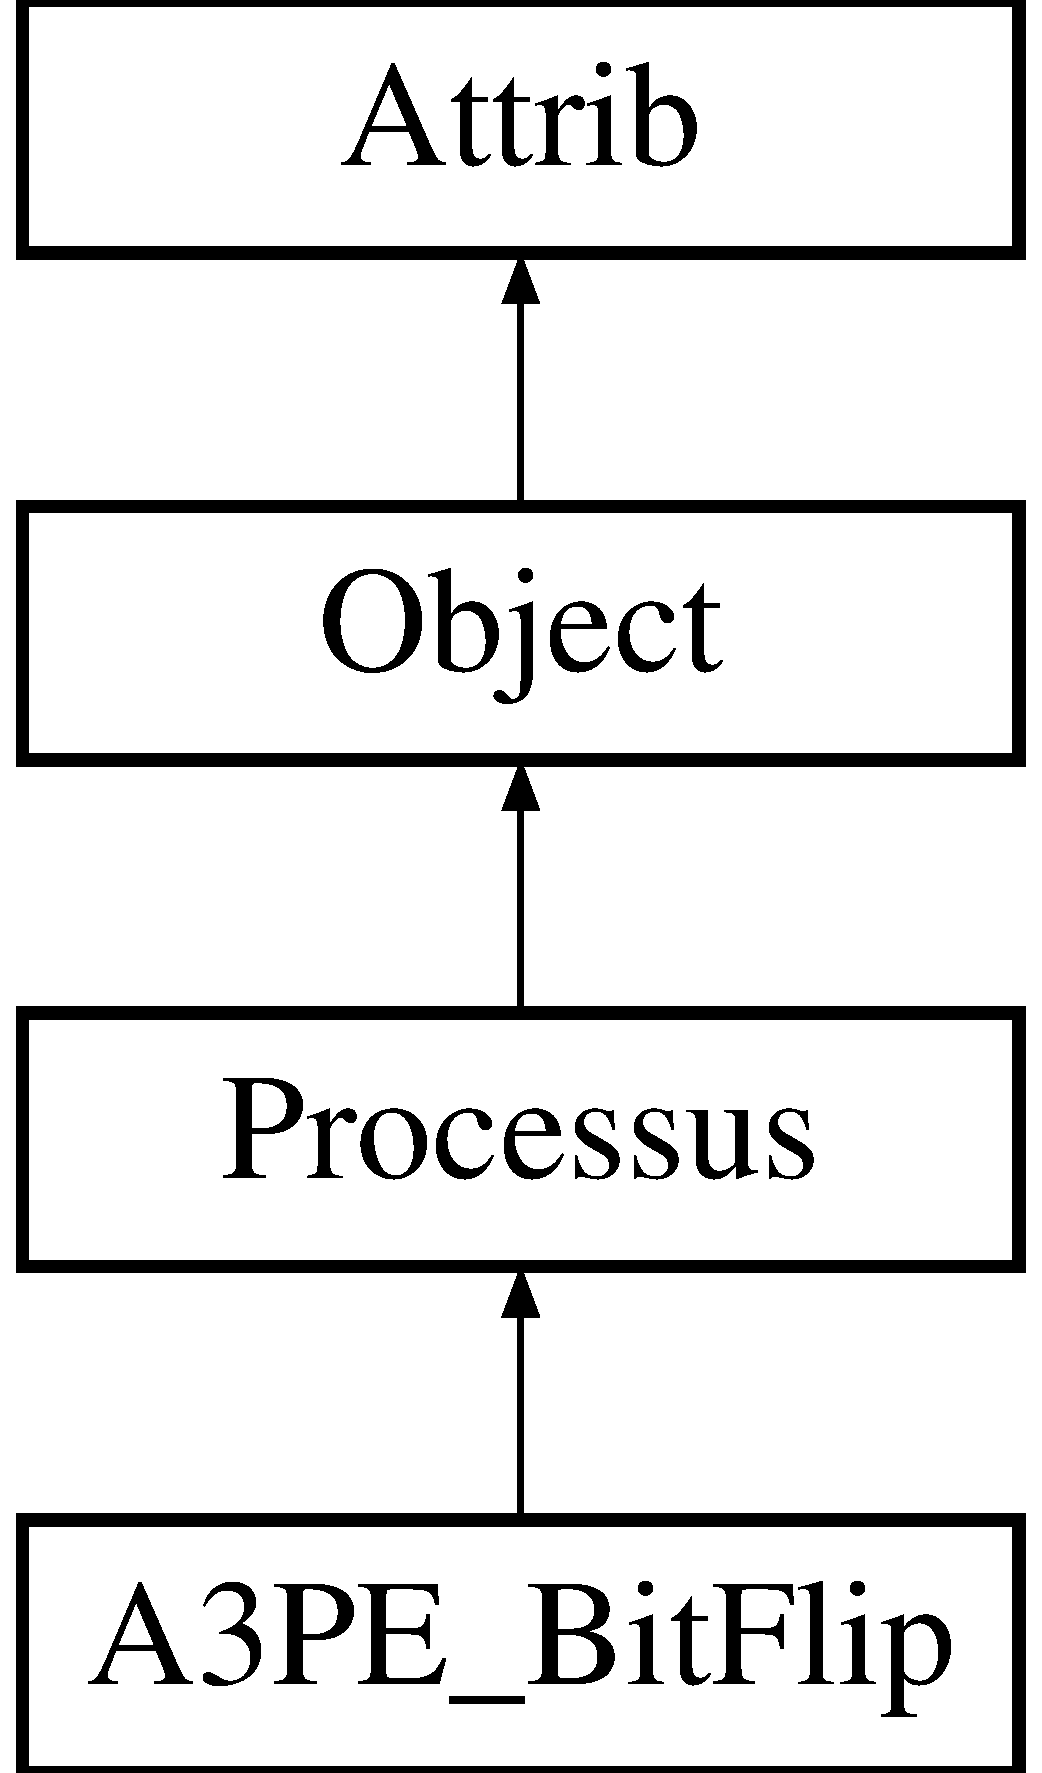
\includegraphics[height=4cm]{classA3PE__BitFlip}
\end{center}
\end{figure}
\subsection*{Classes}
\begin{DoxyCompactItemize}
\item 
class \hyperlink{classA3PE__BitFlip_1_1A3PE__BitFlip}{A3PE\_\-BitFlip}
\end{DoxyCompactItemize}
\subsection*{Public Types}
\begin{DoxyCompactItemize}
\item 
typedef unsigned long \hyperlink{classA3PE__BitFlip_aaf047b5086a5ea11db565ce8283edfb4}{U32}
\item 
typedef unsigned short \hyperlink{classA3PE__BitFlip_a0fa3a1814a6661198e0ce5156d1cc474}{U16}
\item 
typedef unsigned char \hyperlink{classA3PE__BitFlip_ac561e6bbd8d4101ecc32016314a07581}{U8}
\item 
enum \hyperlink{classProcessus_a36278773bd98f2d5612fea40c7774821}{states} \{ \hyperlink{classProcessus_a36278773bd98f2d5612fea40c7774821adaf73ad5d0a09f952d0f18dbbe1c7493}{ERR} = -\/1, 
\hyperlink{classProcessus_a36278773bd98f2d5612fea40c7774821a629082f49d6e8df6b6da2b8fbb9d80fb}{NOT\_\-OK}, 
\hyperlink{classProcessus_a36278773bd98f2d5612fea40c7774821af77c64124fa175f28200166fff165ea2}{OK}
 \}
\item 
enum \hyperlink{classAttrib_a69e171d7cc6417835a5a306d3c764235}{Attribut} \{ \par
\hyperlink{classAttrib_a69e171d7cc6417835a5a306d3c764235a3a8da2ab97dda18aebab196fe4100531}{UNDEFINED}, 
\hyperlink{classAttrib_a69e171d7cc6417835a5a306d3c764235a2bfb2af57b87031d190a05fe25dd92ed}{PASSIVE}, 
\hyperlink{classAttrib_a69e171d7cc6417835a5a306d3c764235a3b1fec929c0370d1436f2f06e298fb0d}{ACTIVE}, 
\hyperlink{classAttrib_a69e171d7cc6417835a5a306d3c764235aa27c16b480a369ea4d18b07b2516bbc7}{INTERFACE}, 
\par
\hyperlink{classAttrib_a69e171d7cc6417835a5a306d3c764235a1420a5b8c0540b2af210b6975eded7f9}{IO}, 
\hyperlink{classAttrib_a69e171d7cc6417835a5a306d3c764235a0af3b0d0ac323c1704e6c69cf90add28}{IODATA}, 
\hyperlink{classAttrib_a69e171d7cc6417835a5a306d3c764235a7788bc5dd333fd8ce18562b269c9dab1}{ELEMENT}, 
\hyperlink{classAttrib_a69e171d7cc6417835a5a306d3c764235a61ceb22149f365f1780d18f9d1459423}{HARDWARE}, 
\par
\hyperlink{classAttrib_a69e171d7cc6417835a5a306d3c764235a75250e29692496e73effca2c0330977f}{PROCESSUS}, 
\hyperlink{classAttrib_a69e171d7cc6417835a5a306d3c764235a103a67cd0b8f07ef478fa45d4356e27b}{SOFTWARE}
 \}
\end{DoxyCompactItemize}
\subsection*{Public Member Functions}
\begin{DoxyCompactItemize}
\item 
\hyperlink{classA3PE__BitFlip_a79aca0cefbd433bfb7f0e0cb6bc7abe1}{A3PE\_\-BitFlip} ()
\begin{DoxyCompactList}\small\item\em Standard constructor. \item\end{DoxyCompactList}\item 
virtual \hyperlink{classA3PE__BitFlip_ab58f69a2c8d342bcad937b1dbc0bb3ed}{$\sim$A3PE\_\-BitFlip} ()
\begin{DoxyCompactList}\small\item\em Destructor. \item\end{DoxyCompactList}\item 
virtual \hyperlink{classStatusCode}{StatusCode} \hyperlink{classA3PE__BitFlip_a88dc6cfe690a518e38ff6d89026e6e0c}{initialize} ()
\item 
virtual \hyperlink{classStatusCode}{StatusCode} \hyperlink{classA3PE__BitFlip_affa7320fb39001a6e9b5696542fe4584}{execute} ()
\item 
virtual \hyperlink{classStatusCode}{StatusCode} \hyperlink{classA3PE__BitFlip_ab40772a001613a0e1932d1e356ccf717}{finalize} ()
\item 
\hyperlink{classStatusCode}{StatusCode} \hyperlink{classA3PE__BitFlip_a079d34acd89f699395a9bbf6b4918205}{setFile} (std::string filename)
\item 
std::string \hyperlink{classA3PE__BitFlip_ace874c555080ce6cb68b6bf320977a5a}{file} ()
\item 
\hyperlink{classA3PE}{A3PE} $\ast$ \hyperlink{classA3PE__BitFlip_ac0d0747dfdd99084dd5524fea62f11d6}{a3pe} ()
\item 
\hyperlink{classStatusCode}{StatusCode} \hyperlink{classProcessus_a09319bde9bed93e290f69b4e04585543}{startProcessing} ()
\item 
\hyperlink{classStatusCode}{StatusCode} \hyperlink{classProcessus_a5e4da662989d356b89d490b89c7afbfd}{endProcessing} ()
\item 
void \hyperlink{classProcessus_aaeb17673b98d2b39f3aa780e335e0968}{clean} ()
\item 
void \hyperlink{classProcessus_ad57a29b33f9021eda9f6929136f1784f}{setStorage} (std::string storage)
\item 
\hyperlink{classData}{Data} $\ast$ \hyperlink{classProcessus_a16e45f329fbce935aeef0ff3cb508228}{data} ()
\item 
std::vector$<$ double $>$ \hyperlink{classProcessus_aa7c57483cf4b9ab0b2d0ae2de8316402}{data} (unsigned int row)
\item 
std::vector$<$ double $>$ \hyperlink{classProcessus_abf4d91fb36707e1d50178bab12d21ae9}{data} (std::string name)
\item 
\hyperlink{classHisto1D}{Histo1D} $\ast$ \hyperlink{classProcessus_a409227db936baff03c0462c1bcfe8069}{hist1d} (unsigned int row)
\item 
\hyperlink{classHisto2D}{Histo2D} $\ast$ \hyperlink{classProcessus_a73b5118cb5f2b5eaad33286183b86cfc}{hist2d} (unsigned int row)
\item 
void \hyperlink{classProcessus_a308c8f193802f1d1ab49d4447d0cb281}{addDataStream} (std::string name, std::string title)
\item 
void \hyperlink{classProcessus_ad46e0d4dfdfdcbce001ee6be1746dfa4}{addHisto1d} (TH1D $\ast$h)
\item 
void \hyperlink{classProcessus_ac1ed1aed5edaeabdf18aa56775440471}{addHisto2d} (TH2D $\ast$h)
\item 
\hyperlink{classStatusCode}{StatusCode} \hyperlink{classProcessus_a0d093b48f3218a088ba030e24372f18c}{dataFill} (int i, double val)
\item 
\hyperlink{classStatusCode}{StatusCode} \hyperlink{classProcessus_aa31ab71711f7af6a729441ff573f69c9}{dataFill} (std::string name, double val)
\item 
std::string \hyperlink{classProcessus_a33fa1a0b54a636e5cdd680669fd9ea51}{storage} ()
\item 
void \hyperlink{classProcessus_a8ddef94227d83d9dae2cd49aebc33353}{setElement} (\hyperlink{classElement}{Element} $\ast$element)
\item 
\hyperlink{classElement}{Element} $\ast$ \hyperlink{classProcessus_a6fe155527431a7190b7d44d600b9608d}{element} ()
\item 
void \hyperlink{classProcessus_abe603d0636f76db6aa6c5c60cf34c591}{incNErrors} ()
\item 
void \hyperlink{classProcessus_a831b027b9cf18ab56fa6147b5d3055da}{setNErrors} (unsigned int)
\item 
unsigned int \hyperlink{classProcessus_a82a0487f82f07cc2c2dc2731f98149e7}{nErrors} ()
\item 
TFile $\ast$ \hyperlink{classProcessus_a247e8c362ec08422cf53d08dd23b093c}{rootFile} ()
\item 
void \hyperlink{classProcessus_aacf6812880c1d1a2bf14a4a39458f443}{openRootFile} ()
\item 
void \hyperlink{classProcessus_a2f3c41e99da4c738ea3d8f7b0d20a665}{closeRootFile} ()
\item 
void \hyperlink{classProcessus_a5e4d34b86241fa0756e07375a14ff4b2}{startChrono} ()
\item 
void \hyperlink{classProcessus_a471833f89047aa9a7ff6200a31c17a1d}{setLogMsg} (std::string logMsg)
\item 
std::string \hyperlink{classProcessus_a42fdeb17dc13ba854222666b6aa29b61}{logMsg} ()
\item 
void \hyperlink{classProcessus_ad38cde0f1bcefa00b068e7947b8af927}{setState} (int state)
\item 
double \hyperlink{classProcessus_aecca96218c65bc805c988cd95447df55}{elapsedTime} ()
\item 
double \hyperlink{classProcessus_a06d3815ad56593dfd0d3c1f534f8b146}{elapsedTime} (time\_\-t start)
\item 
std::string \hyperlink{classObject_a975e888d50bfcbffda2c86368332a5cd}{name} () const 
\item 
std::string \hyperlink{classObject_a84f99f70f144a83e1582d1d0f84e4e62}{type} ()
\item 
unsigned char \hyperlink{classObject_af99145335cc61ff6e2798ea17db009d2}{id} ()
\item 
std::string \hyperlink{classObject_a73a0f1a41828fdd8303dd662446fb6c3}{title} ()
\item 
void \hyperlink{classObject_a3f9d5537ebce0c0f2bf6ae4d92426f3c}{msgSvc} (int level, std::string msg, std::string name)
\item 
void \hyperlink{classObject_a58b2d0618c2d08cf2383012611528d97}{msg} (std::string mymsg)
\item 
void \hyperlink{classObject_ac5d59299273cee27aacf7de00d2e7034}{msg} (std::string mymsg, std::string name)
\item 
void \hyperlink{classObject_a83d2db2df682907ea1115ad721c1c4a1}{verbose} (std::string mymsg)
\item 
void \hyperlink{classObject_a2d4120195317e2a3c6532e8bb9f3da68}{verbose} (std::string mymsg, std::string name)
\item 
void \hyperlink{classObject_aac010553f022165573714b7014a15f0d}{debug} (std::string mymsg)
\item 
void \hyperlink{classObject_a6c9a0397ca804e04d675ed05683f5420}{debug} (std::string mymsg, std::string name)
\item 
void \hyperlink{classObject_a644fd329ea4cb85f54fa6846484b84a8}{info} (std::string mymsg)
\item 
void \hyperlink{classObject_a1ca123253dfd30fc28b156f521dcbdae}{info} (std::string mymsg, std::string name)
\item 
void \hyperlink{classObject_a65cd4fda577711660821fd2cd5a3b4c9}{warning} (std::string mymsg)
\item 
void \hyperlink{classObject_a11f101db4dd73d9391b0231818881d86}{warning} (std::string mymsg, std::string name)
\item 
void \hyperlink{classObject_a204a95f57818c0f811933917a30eff45}{error} (std::string mymsg)
\item 
void \hyperlink{classObject_ad7f6c457733082efa2f9ff5f5c8e119a}{error} (std::string mymsg, std::string name)
\item 
void \hyperlink{classObject_aad5a16aac7516ce65bd5ec02ab07fc80}{fatal} (std::string mymsg)
\item 
void \hyperlink{classObject_ae62acd3d09f716220f75f252dc38bc9a}{fatal} (std::string mymsg, std::string name)
\item 
void \hyperlink{classObject_ae30fea75683c2d149b6b6d17c09ecd0c}{setName} (std::string name)
\item 
void \hyperlink{classObject_aae534cc9d982bcb9b99fd505f2e103a5}{setType} (std::string type)
\item 
void \hyperlink{classObject_a398fe08cba594a0ce6891d59fe4f159f}{setId} (unsigned char id)
\item 
void \hyperlink{classObject_a89557dbbad5bcaa02652f5d7fa35d20f}{setTitle} (std::string title)
\item 
void \hyperlink{classObject_a870c5af919958c2136623b2d7816d123}{setDllName} (std::string dllName)
\item 
std::string \hyperlink{classObject_a2e3947f2870094c332d7454117f3ec63}{dllName} ()
\item 
bool \hyperlink{classAttrib_a704f26af560909ad22065083bb7d4c34}{is} (int attribut)
\item 
void \hyperlink{classAttrib_a235f773af19c900264a190b00a3b4ad7}{add} (int attribut)
\item 
void \hyperlink{classAttrib_a7d4ef7e32d93cb287792b87b857e79f3}{remove} (int attribut)
\item 
std::string \hyperlink{classAttrib_aee7bbf16b144887f196e1341b24f8a26}{attributs} ()
\end{DoxyCompactItemize}
\subsection*{Protected Member Functions}
\begin{DoxyCompactItemize}
\item 
\hyperlink{classA3PE__BitFlip_1_1A3PE__BitFlip}{A3PE\_\-BitFlip} $\ast$ \hyperlink{classA3PE__BitFlip_a444f2b4fd5211e457105f13d19795211}{clone} ()
\item 
\hyperlink{classStatusCode}{StatusCode} \hyperlink{classA3PE__BitFlip_a57e668f5be18f8bc53f5c105735646bf}{randomValues} ()
\end{DoxyCompactItemize}
\subsection*{Protected Attributes}
\begin{DoxyCompactItemize}
\item 
\hyperlink{classElement}{Element} $\ast$ \hyperlink{classProcessus_aa9d24d53c3e52f36786cabb5d8e296e7}{m\_\-element}
\item 
std::string \hyperlink{classAttrib_a3414521d7a82476e874b25a5407b5e63}{m\_\-attribString} \mbox{[}10\mbox{]}
\end{DoxyCompactItemize}
\subsection*{Private Attributes}
\begin{DoxyCompactItemize}
\item 
\hyperlink{classProto40MHz__v1}{Proto40MHz\_\-v1} $\ast$ \hyperlink{classA3PE__BitFlip_a2ade653b4fda5f531b5de28233cdb749}{m\_\-board}
\item 
\hyperlink{classA3PE}{A3PE} $\ast$ \hyperlink{classA3PE__BitFlip_ad20d7abccf27fa87b931cb77cd6b5e41}{m\_\-pga}
\item 
\hyperlink{classRAM}{RAM} $\ast$ \hyperlink{classA3PE__BitFlip_a0ac416167c83d423cda4e09a892b5255}{m\_\-toAX}
\item 
\hyperlink{classRAM}{RAM} $\ast$ \hyperlink{classA3PE__BitFlip_aad9a62adac072bed5de87406ce4cd77d}{m\_\-fromAX}
\item 
std::string \hyperlink{classA3PE__BitFlip_a72eecaff11d66c7f3eee10a9b2bfa301}{m\_\-filename}
\item 
unsigned int \hyperlink{classA3PE__BitFlip_aba0564f2bb8a8ab549da428171d6a3d6}{m\_\-length}
\item 
unsigned int \hyperlink{classA3PE__BitFlip_a6f5ad1d6595e98c2fbd58f43e2754322}{m\_\-latency}
\item 
unsigned int \hyperlink{classA3PE__BitFlip_aeae11ece90351542cae8e0590d9162ee}{m\_\-latencyMin}
\item 
unsigned int \hyperlink{classA3PE__BitFlip_adfeac5a7ab09d89f0d0146113dd55dde}{m\_\-latencyMax}
\item 
int \hyperlink{classA3PE__BitFlip_ac0797dd65b1aeab96647d795e2f1a447}{m\_\-offset}
\item 
\hyperlink{classA3PE__BitFlip_ac561e6bbd8d4101ecc32016314a07581}{U8} $\ast$ \hyperlink{classA3PE__BitFlip_a06e7c01e11710261168bb0e12e2e4ac5}{m\_\-data}
\item 
\hyperlink{classA3PE__BitFlip_ac561e6bbd8d4101ecc32016314a07581}{U8} $\ast$ \hyperlink{classA3PE__BitFlip_a5e64d319904fc8a6fe70b92afcf6ef4f}{m\_\-dataProcessed}
\item 
TH1D $\ast$ \hyperlink{classA3PE__BitFlip_a83928ea28c555c19f4e95cf7863c1b0c}{m\_\-hLatency}
\item 
TH1D $\ast$ \hyperlink{classA3PE__BitFlip_a4dec854e8123271c9a624ca46c50dfd5}{m\_\-hErrorsLatency}
\item 
TH1D $\ast$ \hyperlink{classA3PE__BitFlip_a0d9ea71af465c060689be4c05cba9a8e}{m\_\-hErrorsWord}
\end{DoxyCompactItemize}


\subsection{Detailed Description}
\begin{DoxyAuthor}{Author}

\end{DoxyAuthor}
\begin{DoxyDate}{Date}
2012-\/07-\/12 
\end{DoxyDate}


Definition at line 17 of file A3PE\_\-BitFlip.h.

\subsection{Member Typedef Documentation}
\hypertarget{classA3PE__BitFlip_a0fa3a1814a6661198e0ce5156d1cc474}{
\index{A3PE\_\-BitFlip@{A3PE\_\-BitFlip}!U16@{U16}}
\index{U16@{U16}!A3PE_BitFlip@{A3PE\_\-BitFlip}}
\subsubsection[{U16}]{\setlength{\rightskip}{0pt plus 5cm}typedef unsigned short {\bf A3PE\_\-BitFlip::U16}}}
\label{classA3PE__BitFlip_a0fa3a1814a6661198e0ce5156d1cc474}


Definition at line 20 of file A3PE\_\-BitFlip.h.\hypertarget{classA3PE__BitFlip_aaf047b5086a5ea11db565ce8283edfb4}{
\index{A3PE\_\-BitFlip@{A3PE\_\-BitFlip}!U32@{U32}}
\index{U32@{U32}!A3PE_BitFlip@{A3PE\_\-BitFlip}}
\subsubsection[{U32}]{\setlength{\rightskip}{0pt plus 5cm}typedef unsigned long {\bf A3PE\_\-BitFlip::U32}}}
\label{classA3PE__BitFlip_aaf047b5086a5ea11db565ce8283edfb4}


Definition at line 19 of file A3PE\_\-BitFlip.h.\hypertarget{classA3PE__BitFlip_ac561e6bbd8d4101ecc32016314a07581}{
\index{A3PE\_\-BitFlip@{A3PE\_\-BitFlip}!U8@{U8}}
\index{U8@{U8}!A3PE_BitFlip@{A3PE\_\-BitFlip}}
\subsubsection[{U8}]{\setlength{\rightskip}{0pt plus 5cm}typedef unsigned char {\bf A3PE\_\-BitFlip::U8}}}
\label{classA3PE__BitFlip_ac561e6bbd8d4101ecc32016314a07581}


Definition at line 21 of file A3PE\_\-BitFlip.h.

\subsection{Member Enumeration Documentation}
\hypertarget{classAttrib_a69e171d7cc6417835a5a306d3c764235}{
\index{A3PE\_\-BitFlip@{A3PE\_\-BitFlip}!Attribut@{Attribut}}
\index{Attribut@{Attribut}!A3PE_BitFlip@{A3PE\_\-BitFlip}}
\subsubsection[{Attribut}]{\setlength{\rightskip}{0pt plus 5cm}enum {\bf Attrib::Attribut}\hspace{0.3cm}{\ttfamily  \mbox{[}inherited\mbox{]}}}}
\label{classAttrib_a69e171d7cc6417835a5a306d3c764235}
\begin{Desc}
\item[Enumerator: ]\par
\begin{description}
\index{UNDEFINED@{UNDEFINED}!A3PE\_\-BitFlip@{A3PE\_\-BitFlip}}\index{A3PE\_\-BitFlip@{A3PE\_\-BitFlip}!UNDEFINED@{UNDEFINED}}\item[{\em 
\hypertarget{classAttrib_a69e171d7cc6417835a5a306d3c764235a3a8da2ab97dda18aebab196fe4100531}{
UNDEFINED}
\label{classAttrib_a69e171d7cc6417835a5a306d3c764235a3a8da2ab97dda18aebab196fe4100531}
}]\index{PASSIVE@{PASSIVE}!A3PE\_\-BitFlip@{A3PE\_\-BitFlip}}\index{A3PE\_\-BitFlip@{A3PE\_\-BitFlip}!PASSIVE@{PASSIVE}}\item[{\em 
\hypertarget{classAttrib_a69e171d7cc6417835a5a306d3c764235a2bfb2af57b87031d190a05fe25dd92ed}{
PASSIVE}
\label{classAttrib_a69e171d7cc6417835a5a306d3c764235a2bfb2af57b87031d190a05fe25dd92ed}
}]\index{ACTIVE@{ACTIVE}!A3PE\_\-BitFlip@{A3PE\_\-BitFlip}}\index{A3PE\_\-BitFlip@{A3PE\_\-BitFlip}!ACTIVE@{ACTIVE}}\item[{\em 
\hypertarget{classAttrib_a69e171d7cc6417835a5a306d3c764235a3b1fec929c0370d1436f2f06e298fb0d}{
ACTIVE}
\label{classAttrib_a69e171d7cc6417835a5a306d3c764235a3b1fec929c0370d1436f2f06e298fb0d}
}]\index{INTERFACE@{INTERFACE}!A3PE\_\-BitFlip@{A3PE\_\-BitFlip}}\index{A3PE\_\-BitFlip@{A3PE\_\-BitFlip}!INTERFACE@{INTERFACE}}\item[{\em 
\hypertarget{classAttrib_a69e171d7cc6417835a5a306d3c764235aa27c16b480a369ea4d18b07b2516bbc7}{
INTERFACE}
\label{classAttrib_a69e171d7cc6417835a5a306d3c764235aa27c16b480a369ea4d18b07b2516bbc7}
}]\index{IO@{IO}!A3PE\_\-BitFlip@{A3PE\_\-BitFlip}}\index{A3PE\_\-BitFlip@{A3PE\_\-BitFlip}!IO@{IO}}\item[{\em 
\hypertarget{classAttrib_a69e171d7cc6417835a5a306d3c764235a1420a5b8c0540b2af210b6975eded7f9}{
IO}
\label{classAttrib_a69e171d7cc6417835a5a306d3c764235a1420a5b8c0540b2af210b6975eded7f9}
}]\index{IODATA@{IODATA}!A3PE\_\-BitFlip@{A3PE\_\-BitFlip}}\index{A3PE\_\-BitFlip@{A3PE\_\-BitFlip}!IODATA@{IODATA}}\item[{\em 
\hypertarget{classAttrib_a69e171d7cc6417835a5a306d3c764235a0af3b0d0ac323c1704e6c69cf90add28}{
IODATA}
\label{classAttrib_a69e171d7cc6417835a5a306d3c764235a0af3b0d0ac323c1704e6c69cf90add28}
}]\index{ELEMENT@{ELEMENT}!A3PE\_\-BitFlip@{A3PE\_\-BitFlip}}\index{A3PE\_\-BitFlip@{A3PE\_\-BitFlip}!ELEMENT@{ELEMENT}}\item[{\em 
\hypertarget{classAttrib_a69e171d7cc6417835a5a306d3c764235a7788bc5dd333fd8ce18562b269c9dab1}{
ELEMENT}
\label{classAttrib_a69e171d7cc6417835a5a306d3c764235a7788bc5dd333fd8ce18562b269c9dab1}
}]\index{HARDWARE@{HARDWARE}!A3PE\_\-BitFlip@{A3PE\_\-BitFlip}}\index{A3PE\_\-BitFlip@{A3PE\_\-BitFlip}!HARDWARE@{HARDWARE}}\item[{\em 
\hypertarget{classAttrib_a69e171d7cc6417835a5a306d3c764235a61ceb22149f365f1780d18f9d1459423}{
HARDWARE}
\label{classAttrib_a69e171d7cc6417835a5a306d3c764235a61ceb22149f365f1780d18f9d1459423}
}]\index{PROCESSUS@{PROCESSUS}!A3PE\_\-BitFlip@{A3PE\_\-BitFlip}}\index{A3PE\_\-BitFlip@{A3PE\_\-BitFlip}!PROCESSUS@{PROCESSUS}}\item[{\em 
\hypertarget{classAttrib_a69e171d7cc6417835a5a306d3c764235a75250e29692496e73effca2c0330977f}{
PROCESSUS}
\label{classAttrib_a69e171d7cc6417835a5a306d3c764235a75250e29692496e73effca2c0330977f}
}]\index{SOFTWARE@{SOFTWARE}!A3PE\_\-BitFlip@{A3PE\_\-BitFlip}}\index{A3PE\_\-BitFlip@{A3PE\_\-BitFlip}!SOFTWARE@{SOFTWARE}}\item[{\em 
\hypertarget{classAttrib_a69e171d7cc6417835a5a306d3c764235a103a67cd0b8f07ef478fa45d4356e27b}{
SOFTWARE}
\label{classAttrib_a69e171d7cc6417835a5a306d3c764235a103a67cd0b8f07ef478fa45d4356e27b}
}]\end{description}
\end{Desc}



Definition at line 29 of file Attrib.h.


\begin{DoxyCode}
29                 {
30     UNDEFINED,
31     PASSIVE,
32     ACTIVE,
33     INTERFACE,
34     IO,
35     IODATA,
36     ELEMENT,
37     HARDWARE,
38     PROCESSUS,
39     SOFTWARE 
40   }; // array m_attribString must be changed into Attrib::Attrib if this enu is m
      odified. 
\end{DoxyCode}
\hypertarget{classProcessus_a36278773bd98f2d5612fea40c7774821}{
\index{A3PE\_\-BitFlip@{A3PE\_\-BitFlip}!states@{states}}
\index{states@{states}!A3PE_BitFlip@{A3PE\_\-BitFlip}}
\subsubsection[{states}]{\setlength{\rightskip}{0pt plus 5cm}enum {\bf Processus::states}\hspace{0.3cm}{\ttfamily  \mbox{[}inherited\mbox{]}}}}
\label{classProcessus_a36278773bd98f2d5612fea40c7774821}
\begin{Desc}
\item[Enumerator: ]\par
\begin{description}
\index{ERR@{ERR}!A3PE\_\-BitFlip@{A3PE\_\-BitFlip}}\index{A3PE\_\-BitFlip@{A3PE\_\-BitFlip}!ERR@{ERR}}\item[{\em 
\hypertarget{classProcessus_a36278773bd98f2d5612fea40c7774821adaf73ad5d0a09f952d0f18dbbe1c7493}{
ERR}
\label{classProcessus_a36278773bd98f2d5612fea40c7774821adaf73ad5d0a09f952d0f18dbbe1c7493}
}]\index{NOT\_\-OK@{NOT\_\-OK}!A3PE\_\-BitFlip@{A3PE\_\-BitFlip}}\index{A3PE\_\-BitFlip@{A3PE\_\-BitFlip}!NOT\_\-OK@{NOT\_\-OK}}\item[{\em 
\hypertarget{classProcessus_a36278773bd98f2d5612fea40c7774821a629082f49d6e8df6b6da2b8fbb9d80fb}{
NOT\_\-OK}
\label{classProcessus_a36278773bd98f2d5612fea40c7774821a629082f49d6e8df6b6da2b8fbb9d80fb}
}]\index{OK@{OK}!A3PE\_\-BitFlip@{A3PE\_\-BitFlip}}\index{A3PE\_\-BitFlip@{A3PE\_\-BitFlip}!OK@{OK}}\item[{\em 
\hypertarget{classProcessus_a36278773bd98f2d5612fea40c7774821af77c64124fa175f28200166fff165ea2}{
OK}
\label{classProcessus_a36278773bd98f2d5612fea40c7774821af77c64124fa175f28200166fff165ea2}
}]\end{description}
\end{Desc}



Definition at line 34 of file Processus.h.


\begin{DoxyCode}
34 { ERR=-1 , NOT_OK , OK };
\end{DoxyCode}


\subsection{Constructor \& Destructor Documentation}
\hypertarget{classA3PE__BitFlip_a79aca0cefbd433bfb7f0e0cb6bc7abe1}{
\index{A3PE\_\-BitFlip@{A3PE\_\-BitFlip}!A3PE\_\-BitFlip@{A3PE\_\-BitFlip}}
\index{A3PE\_\-BitFlip@{A3PE\_\-BitFlip}!A3PE_BitFlip@{A3PE\_\-BitFlip}}
\subsubsection[{A3PE\_\-BitFlip}]{\setlength{\rightskip}{0pt plus 5cm}{\bf A3PE\_\-BitFlip::A3PE\_\-BitFlip} ()}}
\label{classA3PE__BitFlip_a79aca0cefbd433bfb7f0e0cb6bc7abe1}


Standard constructor. 

Definition at line 26 of file A3PE\_\-BitFlip.cpp.

References Object::setName(), Object::setTitle(), and Object::setType().

Referenced by clone().


\begin{DoxyCode}
26                              :
27   m_filename(std::string("")),
28   m_offset(-6),
29   m_latencyMin(1000),
30   m_latencyMax(100000),
31   m_hLatency (0),
32   m_hErrorsLatency(0),
33   m_hErrorsWord(0)
34 {
35   setName ( "A3PE_BitFlip" );
36   setType ( "Proto40MHz_v1" );
37   setTitle( "Proto40MHz_v1 A3PE_BitFlip test" );
38 }
//=============================================================================
\end{DoxyCode}
\hypertarget{classA3PE__BitFlip_ab58f69a2c8d342bcad937b1dbc0bb3ed}{
\index{A3PE\_\-BitFlip@{A3PE\_\-BitFlip}!$\sim$A3PE\_\-BitFlip@{$\sim$A3PE\_\-BitFlip}}
\index{$\sim$A3PE\_\-BitFlip@{$\sim$A3PE\_\-BitFlip}!A3PE_BitFlip@{A3PE\_\-BitFlip}}
\subsubsection[{$\sim$A3PE\_\-BitFlip}]{\setlength{\rightskip}{0pt plus 5cm}A3PE\_\-BitFlip::$\sim$A3PE\_\-BitFlip ()\hspace{0.3cm}{\ttfamily  \mbox{[}virtual\mbox{]}}}}
\label{classA3PE__BitFlip_ab58f69a2c8d342bcad937b1dbc0bb3ed}


Destructor. 

Definition at line 42 of file A3PE\_\-BitFlip.cpp.


\begin{DoxyCode}
42 {}
\end{DoxyCode}


\subsection{Member Function Documentation}
\hypertarget{classA3PE__BitFlip_ac0d0747dfdd99084dd5524fea62f11d6}{
\index{A3PE\_\-BitFlip@{A3PE\_\-BitFlip}!a3pe@{a3pe}}
\index{a3pe@{a3pe}!A3PE_BitFlip@{A3PE\_\-BitFlip}}
\subsubsection[{a3pe}]{\setlength{\rightskip}{0pt plus 5cm}{\bf A3PE}$\ast$ A3PE\_\-BitFlip::a3pe ()\hspace{0.3cm}{\ttfamily  \mbox{[}inline\mbox{]}}}}
\label{classA3PE__BitFlip_ac0d0747dfdd99084dd5524fea62f11d6}


Definition at line 39 of file A3PE\_\-BitFlip.h.

References m\_\-pga.


\begin{DoxyCode}
39 {return m_pga;}
\end{DoxyCode}
\hypertarget{classAttrib_a235f773af19c900264a190b00a3b4ad7}{
\index{A3PE\_\-BitFlip@{A3PE\_\-BitFlip}!add@{add}}
\index{add@{add}!A3PE_BitFlip@{A3PE\_\-BitFlip}}
\subsubsection[{add}]{\setlength{\rightskip}{0pt plus 5cm}void Attrib::add (int {\em attribut})\hspace{0.3cm}{\ttfamily  \mbox{[}inline, inherited\mbox{]}}}}
\label{classAttrib_a235f773af19c900264a190b00a3b4ad7}
Add an attribut 

Definition at line 67 of file Attrib.h.

References Attrib::m\_\-attributs, and Attrib::UNDEFINED.

Referenced by A3PE::A3PE(), Attrib::Attrib(), SpecsMezzanine::cmdline(), Computer::Computer(), CU\_\-v1::CU\_\-v1(), export\_\-obj(), FEB\_\-v1::FEB\_\-v1(), FePGA::FePGA(), ICECALv3::ICECALv3(), ICPhaser::ICPhaser(), Application::initialize(), Interface::Interface(), IOdata::IOdata(), IOobject::IOobject(), LSDelayChipV1::LSDelayChipV1(), MSOxxxx::MSOxxxx(), Phaser::Phaser(), Processus::Processus(), Proto40MHz\_\-v1::Proto40MHz\_\-v1(), Attrib::remove(), SeqPGA::SeqPGA(), SpecsMaster::SpecsMaster(), and SpecsSlave::SpecsSlave().


\begin{DoxyCode}
67                             {
68     if (attribut!=Attrib::UNDEFINED) remove(Attrib::UNDEFINED);
69     bool duplicate = false ;
70     std::vector<int>::const_iterator iter ;
71     for ( iter  = m_attributs.begin() ;
72           iter != m_attributs.end()   ;
73           ++iter ) {
74       if ( attribut == (*iter) ) {
75         duplicate = true ;
76       }
77     }
78     if (!duplicate) {
79       m_attributs.push_back( attribut );
80     }
81   }
\end{DoxyCode}
\hypertarget{classProcessus_a308c8f193802f1d1ab49d4447d0cb281}{
\index{A3PE\_\-BitFlip@{A3PE\_\-BitFlip}!addDataStream@{addDataStream}}
\index{addDataStream@{addDataStream}!A3PE_BitFlip@{A3PE\_\-BitFlip}}
\subsubsection[{addDataStream}]{\setlength{\rightskip}{0pt plus 5cm}void Processus::addDataStream (std::string {\em name}, \/  std::string {\em title})\hspace{0.3cm}{\ttfamily  \mbox{[}inline, inherited\mbox{]}}}}
\label{classProcessus_a308c8f193802f1d1ab49d4447d0cb281}


Definition at line 153 of file Processus.h.

References Data::addDataStream(), and Processus::m\_\-data.

Referenced by CurrentMeasurement::initialize(), ADCMeasurement::initialize(), TestSuite::initialize(), TestUSB::initialize(), TestSPI::initialize(), TestI2C::initialize(), UsbFTInterfaceTest::initialize(), and RegisterTest::initialize().


\begin{DoxyCode}
153                                                        {
154     m_data->addDataStream(name, title);
155   }
\end{DoxyCode}
\hypertarget{classProcessus_ad46e0d4dfdfdcbce001ee6be1746dfa4}{
\index{A3PE\_\-BitFlip@{A3PE\_\-BitFlip}!addHisto1d@{addHisto1d}}
\index{addHisto1d@{addHisto1d}!A3PE_BitFlip@{A3PE\_\-BitFlip}}
\subsubsection[{addHisto1d}]{\setlength{\rightskip}{0pt plus 5cm}void Processus::addHisto1d (TH1D $\ast$ {\em h})\hspace{0.3cm}{\ttfamily  \mbox{[}inline, inherited\mbox{]}}}}
\label{classProcessus_ad46e0d4dfdfdcbce001ee6be1746dfa4}


Definition at line 160 of file Processus.h.

References Data::addHisto1d(), and Processus::m\_\-data.

Referenced by TestSuite::initialize(), StorageFifoAcquisition::initialize(), StorageFifo::initialize(), Acquisition::initialize(), and initialize().


\begin{DoxyCode}
160                            {
161     m_data->addHisto1d(h);
162   }
\end{DoxyCode}
\hypertarget{classProcessus_ac1ed1aed5edaeabdf18aa56775440471}{
\index{A3PE\_\-BitFlip@{A3PE\_\-BitFlip}!addHisto2d@{addHisto2d}}
\index{addHisto2d@{addHisto2d}!A3PE_BitFlip@{A3PE\_\-BitFlip}}
\subsubsection[{addHisto2d}]{\setlength{\rightskip}{0pt plus 5cm}void Processus::addHisto2d (TH2D $\ast$ {\em h})\hspace{0.3cm}{\ttfamily  \mbox{[}inline, inherited\mbox{]}}}}
\label{classProcessus_ac1ed1aed5edaeabdf18aa56775440471}


Definition at line 167 of file Processus.h.

References Data::addHisto2d(), and Processus::m\_\-data.

Referenced by TestSuite::initialize().


\begin{DoxyCode}
167                            {
168     m_data->addHisto2d(h);
169   }
\end{DoxyCode}
\hypertarget{classAttrib_aee7bbf16b144887f196e1341b24f8a26}{
\index{A3PE\_\-BitFlip@{A3PE\_\-BitFlip}!attributs@{attributs}}
\index{attributs@{attributs}!A3PE_BitFlip@{A3PE\_\-BitFlip}}
\subsubsection[{attributs}]{\setlength{\rightskip}{0pt plus 5cm}std::string Attrib::attributs ()\hspace{0.3cm}{\ttfamily  \mbox{[}inherited\mbox{]}}}}
\label{classAttrib_aee7bbf16b144887f196e1341b24f8a26}
Print the \hyperlink{classAttrib}{Attrib} of an \hyperlink{classObject}{Object} 

Definition at line 54 of file Attrib.cpp.

References images::index, Attrib::m\_\-attribString, and Attrib::m\_\-attributs.

Referenced by export\_\-obj().


\begin{DoxyCode}
54                             {
55   std::string output;
56   std::vector<int>::iterator iter ;
57   for ( unsigned int index = 0 ; index < m_attributs.size() ; ++index ) {
58     if ( m_attributs.size() - index > 1 ) {
59       output.append(m_attribString[m_attributs[index]]);
60       output.append(":");
61     }
62     else {
63       output.append(m_attribString[m_attributs[index]]);
64     }
65   }
66   return output;
67 }
\end{DoxyCode}
\hypertarget{classProcessus_aaeb17673b98d2b39f3aa780e335e0968}{
\index{A3PE\_\-BitFlip@{A3PE\_\-BitFlip}!clean@{clean}}
\index{clean@{clean}!A3PE_BitFlip@{A3PE\_\-BitFlip}}
\subsubsection[{clean}]{\setlength{\rightskip}{0pt plus 5cm}void Processus::clean ()\hspace{0.3cm}{\ttfamily  \mbox{[}inline, inherited\mbox{]}}}}
\label{classProcessus_aaeb17673b98d2b39f3aa780e335e0968}


Definition at line 85 of file Processus.h.

References Processus::m\_\-element, Processus::m\_\-state, and Object::warning().

Referenced by Application::prepare().


\begin{DoxyCode}
86   {
87     m_element=0;
88     if (0!=m_state) {
89       delete m_state;
90       m_state=0;
91     }
92 #ifdef _NETWORK_
93     warning("Cleaning state service : should it be done ?","Processus::clean")
94       if (0!=m_stateService)
95       {
96         delete m_stateService;
97       }
98 #endif
99   }
\end{DoxyCode}
\hypertarget{classA3PE__BitFlip_a444f2b4fd5211e457105f13d19795211}{
\index{A3PE\_\-BitFlip@{A3PE\_\-BitFlip}!clone@{clone}}
\index{clone@{clone}!A3PE_BitFlip@{A3PE\_\-BitFlip}}
\subsubsection[{clone}]{\setlength{\rightskip}{0pt plus 5cm}{\bf A3PE\_\-BitFlip}$\ast$ A3PE\_\-BitFlip::clone ()\hspace{0.3cm}{\ttfamily  \mbox{[}inline, protected, virtual\mbox{]}}}}
\label{classA3PE__BitFlip_a444f2b4fd5211e457105f13d19795211}
processus termination virtual function 

Implements \hyperlink{classProcessus_aca8856f6d6d7b7e1fe941f298dcbb502}{Processus}.

Definition at line 42 of file A3PE\_\-BitFlip.h.

References A3PE\_\-BitFlip().


\begin{DoxyCode}
42                        {
43     return new A3PE_BitFlip (*this);
44   }
\end{DoxyCode}
\hypertarget{classProcessus_a2f3c41e99da4c738ea3d8f7b0d20a665}{
\index{A3PE\_\-BitFlip@{A3PE\_\-BitFlip}!closeRootFile@{closeRootFile}}
\index{closeRootFile@{closeRootFile}!A3PE_BitFlip@{A3PE\_\-BitFlip}}
\subsubsection[{closeRootFile}]{\setlength{\rightskip}{0pt plus 5cm}void Processus::closeRootFile ()\hspace{0.3cm}{\ttfamily  \mbox{[}inherited\mbox{]}}}}
\label{classProcessus_a2f3c41e99da4c738ea3d8f7b0d20a665}
Close Root file if already opened and requested 

Definition at line 160 of file Processus.cpp.

References Options::dataFileFullName(), Options::dataStorage(), Object::info(), Processus::m\_\-options, and Processus::m\_\-rootFile.

Referenced by Processus::endProcessing(), UsbFTInterfaceTest::finalize(), RegisterTest::finalize(), and PhaserRampExec::finalize().


\begin{DoxyCode}
160                                 {
161   if ( 0!= m_rootFile && m_options->dataStorage() ){
162     m_rootFile->Write();
163         std::string mess=std::string("Closing root file ");
164         mess.append(m_options->dataFileFullName());
165         info(mess,"closeRootFile");
166     m_rootFile->Delete();
167     m_rootFile = 0;
168   }
169 }
\end{DoxyCode}
\hypertarget{classProcessus_abf4d91fb36707e1d50178bab12d21ae9}{
\index{A3PE\_\-BitFlip@{A3PE\_\-BitFlip}!data@{data}}
\index{data@{data}!A3PE_BitFlip@{A3PE\_\-BitFlip}}
\subsubsection[{data}]{\setlength{\rightskip}{0pt plus 5cm}std::vector$<$double$>$ Processus::data (std::string {\em name})\hspace{0.3cm}{\ttfamily  \mbox{[}inline, inherited\mbox{]}}}}
\label{classProcessus_abf4d91fb36707e1d50178bab12d21ae9}
Get accessor to member m\_\-data \begin{DoxyReturn}{Returns}
the current value of m\_\-data 
\end{DoxyReturn}


Definition at line 130 of file Processus.h.

References Processus::m\_\-data, and Data::vector().


\begin{DoxyCode}
130                                         {
131     return m_data->vector(name);
132   }
\end{DoxyCode}
\hypertarget{classProcessus_aa7c57483cf4b9ab0b2d0ae2de8316402}{
\index{A3PE\_\-BitFlip@{A3PE\_\-BitFlip}!data@{data}}
\index{data@{data}!A3PE_BitFlip@{A3PE\_\-BitFlip}}
\subsubsection[{data}]{\setlength{\rightskip}{0pt plus 5cm}std::vector$<$double$>$ Processus::data (unsigned int {\em row})\hspace{0.3cm}{\ttfamily  \mbox{[}inline, inherited\mbox{]}}}}
\label{classProcessus_aa7c57483cf4b9ab0b2d0ae2de8316402}
Get accessor to member m\_\-data \begin{DoxyReturn}{Returns}
the current value of m\_\-data 
\end{DoxyReturn}


Definition at line 122 of file Processus.h.

References Processus::m\_\-data, and Data::vector().


\begin{DoxyCode}
122                                           {
123     return m_data->vector(row);
124   }
\end{DoxyCode}
\hypertarget{classProcessus_a16e45f329fbce935aeef0ff3cb508228}{
\index{A3PE\_\-BitFlip@{A3PE\_\-BitFlip}!data@{data}}
\index{data@{data}!A3PE_BitFlip@{A3PE\_\-BitFlip}}
\subsubsection[{data}]{\setlength{\rightskip}{0pt plus 5cm}{\bf Data}$\ast$ Processus::data ()\hspace{0.3cm}{\ttfamily  \mbox{[}inline, inherited\mbox{]}}}}
\label{classProcessus_a16e45f329fbce935aeef0ff3cb508228}
Get accessor to member m\_\-data \begin{DoxyReturn}{Returns}
the current value of m\_\-data 
\end{DoxyReturn}


Definition at line 114 of file Processus.h.

References Processus::m\_\-data.

Referenced by StorageFifoAcquisition::execute(), and export\_\-proc().


\begin{DoxyCode}
114               {
115     return m_data;
116   }
\end{DoxyCode}
\hypertarget{classProcessus_aa31ab71711f7af6a729441ff573f69c9}{
\index{A3PE\_\-BitFlip@{A3PE\_\-BitFlip}!dataFill@{dataFill}}
\index{dataFill@{dataFill}!A3PE_BitFlip@{A3PE\_\-BitFlip}}
\subsubsection[{dataFill}]{\setlength{\rightskip}{0pt plus 5cm}{\bf StatusCode} Processus::dataFill (std::string {\em name}, \/  double {\em val})\hspace{0.3cm}{\ttfamily  \mbox{[}inline, inherited\mbox{]}}}}
\label{classProcessus_aa31ab71711f7af6a729441ff573f69c9}
Set data stream with value \begin{DoxyReturn}{Returns}
the \hyperlink{classStatusCode}{StatusCode} 
\end{DoxyReturn}


Definition at line 189 of file Processus.h.

References StatusCode::FAILURE, Processus::m\_\-data, Data::rowFromName(), StatusCode::SUCCESS, and Data::vectorPtr().


\begin{DoxyCode}
189                                                  {
190     int row=m_data->rowFromName(name);
191     if (row<0) return StatusCode::FAILURE;
192     if (m_data->vectorPtr(row)!=0){
193       m_data->vectorPtr(row)->push_back(val);
194       return StatusCode::SUCCESS;
195     }
196     else {
197       return StatusCode::FAILURE;
198     }
199   }
\end{DoxyCode}
\hypertarget{classProcessus_a0d093b48f3218a088ba030e24372f18c}{
\index{A3PE\_\-BitFlip@{A3PE\_\-BitFlip}!dataFill@{dataFill}}
\index{dataFill@{dataFill}!A3PE_BitFlip@{A3PE\_\-BitFlip}}
\subsubsection[{dataFill}]{\setlength{\rightskip}{0pt plus 5cm}{\bf StatusCode} Processus::dataFill (int {\em i}, \/  double {\em val})\hspace{0.3cm}{\ttfamily  \mbox{[}inline, inherited\mbox{]}}}}
\label{classProcessus_a0d093b48f3218a088ba030e24372f18c}
Set data stream with value \begin{DoxyReturn}{Returns}
the \hyperlink{classStatusCode}{StatusCode} 
\end{DoxyReturn}


Definition at line 175 of file Processus.h.

References StatusCode::FAILURE, Processus::m\_\-data, StatusCode::SUCCESS, and Data::vectorPtr().

Referenced by CurrentMeasurement::execute(), ADCMeasurement::execute(), TestSuite::execute(), TestUSB::execute(), TestSPI::execute(), TestI2C::execute(), and UsbFTInterfaceTest::execute().


\begin{DoxyCode}
175                                         {
176     if (m_data->vectorPtr(i)!=0){
177       m_data->vectorPtr(i)->push_back(val);
178       return StatusCode::SUCCESS;
179     }
180     else {
181       return StatusCode::FAILURE;
182     }
183   }
\end{DoxyCode}
\hypertarget{classObject_a6c9a0397ca804e04d675ed05683f5420}{
\index{A3PE\_\-BitFlip@{A3PE\_\-BitFlip}!debug@{debug}}
\index{debug@{debug}!A3PE_BitFlip@{A3PE\_\-BitFlip}}
\subsubsection[{debug}]{\setlength{\rightskip}{0pt plus 5cm}void Object::debug (std::string {\em mymsg}, \/  std::string {\em name})\hspace{0.3cm}{\ttfamily  \mbox{[}inline, inherited\mbox{]}}}}
\label{classObject_a6c9a0397ca804e04d675ed05683f5420}


Definition at line 45 of file Object.h.

References MsgSvc::DEBUG, Object::m\_\-log, and MsgSvc::msgSvc().


\begin{DoxyCode}
45 { m_log.msgSvc (MsgSvc::DEBUG   , mymsg, name ); }
\end{DoxyCode}
\hypertarget{classObject_aac010553f022165573714b7014a15f0d}{
\index{A3PE\_\-BitFlip@{A3PE\_\-BitFlip}!debug@{debug}}
\index{debug@{debug}!A3PE_BitFlip@{A3PE\_\-BitFlip}}
\subsubsection[{debug}]{\setlength{\rightskip}{0pt plus 5cm}void Object::debug (std::string {\em mymsg})\hspace{0.3cm}{\ttfamily  \mbox{[}inline, inherited\mbox{]}}}}
\label{classObject_aac010553f022165573714b7014a15f0d}


Definition at line 37 of file Object.h.

References MsgSvc::DEBUG, Object::m\_\-log, Object::m\_\-name, and MsgSvc::msgSvc().

Referenced by A3PE::A3PE(), A3PE::acquisition(), SpecsMezzanine::addBus(), Hierarchy::addChild(), SpecsSlave::addI2c(), LSDelayChipV1::checkConfigAddr(), LSDelayChipV1::checkStatusAddr(), LSDelayChipV1::configRegBulkRead(), LSDelayChipV1::configRegBulkWrite(), A3PE::dataReady(), DCU::DCU(), Hierarchy::delChild(), SpecsSlave::detect(), EmulateFE::execute(), StorageFifoAcquisition::execute(), StorageFifo::execute(), Acquisition::execute(), execute(), export\_\-obj(), FePGA::FePGA(), SpecsGlue::i2cClkMode(), SeqPGA::i2cRead(), FePGA::i2cRead(), SeqPGA::i2cWrite(), FePGA::i2cWrite(), ICECALv3::ICECALv3(), ICPhaser::ICPhaser(), SpecsSlave::init(), SpecsMaster::init(), EmulateFE::initialize(), StorageFifoAcquisition::initialize(), StorageFifo::initialize(), Acquisition::initialize(), initialize(), A3PE::internalAXSequence(), SpecsMezzanine::led(), SpecsGlue::led(), LSDelayChipV1::LSDelayChipV1(), MSOxxxx::MSOxxxx(), Phaser::Phaser(), Data::purge(), ICPhaser::read(), Phaser::read(), FEB\_\-v1::readFifoSpyFE(), SpecsSlave::reset(), SpecsMaster::reset(), FEB\_\-v1::reset(), CU\_\-v1::reset(), Proto40MHz\_\-v1::reset(), FEB\_\-v1::resetFifoSpyFE(), SeqPGA::resetSpi(), FEB\_\-v1::resetSpi(), SeqPGA::SeqPGA(), A3PE::setAddFromAXRam(), A3PE::setAddToAXRam(), A3PE::setAXRamUsb(), Element::setConnection(), SpecsGlue::setI2cClkMode(), A3PE::setLatencyAX(), SpecsMezzanine::setLed(), SpecsGlue::setLed(), A3PE::setLengthAX(), A3PE::setReadToAXRamUsb(), SpecsMaster::setSpeed(), A3PE::setWriteFromAXRamUsb(), SpecsBus::SpecsBus(), SpecsI2c::SpecsI2c(), SpecsMaster::SpecsMaster(), SpecsMezzanine::SpecsMezzanine(), SpecsParallelBus::SpecsParallelBus(), SpecsSlave::SpecsSlave(), LSDelayChipV1::spiBERTest(), ICECALv3::spiRead(), ICECALv3::spiWrite(), FEB\_\-v1::testDuration(), SeqPGA::testSequence(), A3PE::trigger(), Server::updateConfig(), Server::updateState(), ICPhaser::write(), Phaser::write(), and Hierarchy::$\sim$Hierarchy().


\begin{DoxyCode}
37 { m_log.msgSvc (MsgSvc::DEBUG   , mymsg, m_name ); }
\end{DoxyCode}
\hypertarget{classObject_a2e3947f2870094c332d7454117f3ec63}{
\index{A3PE\_\-BitFlip@{A3PE\_\-BitFlip}!dllName@{dllName}}
\index{dllName@{dllName}!A3PE_BitFlip@{A3PE\_\-BitFlip}}
\subsubsection[{dllName}]{\setlength{\rightskip}{0pt plus 5cm}std::string Object::dllName ()\hspace{0.3cm}{\ttfamily  \mbox{[}inline, inherited\mbox{]}}}}
\label{classObject_a2e3947f2870094c332d7454117f3ec63}
Get accessor to member m\_\-dllName \begin{DoxyReturn}{Returns}
the current value of m\_\-dllName 
\end{DoxyReturn}


Definition at line 74 of file Object.h.

References Object::m\_\-dllName.

Referenced by export\_\-obj().


\begin{DoxyCode}
74                        {
75     return m_dllName;
76   }  
\end{DoxyCode}
\hypertarget{classProcessus_a06d3815ad56593dfd0d3c1f534f8b146}{
\index{A3PE\_\-BitFlip@{A3PE\_\-BitFlip}!elapsedTime@{elapsedTime}}
\index{elapsedTime@{elapsedTime}!A3PE_BitFlip@{A3PE\_\-BitFlip}}
\subsubsection[{elapsedTime}]{\setlength{\rightskip}{0pt plus 5cm}double Processus::elapsedTime (time\_\-t {\em start})\hspace{0.3cm}{\ttfamily  \mbox{[}inline, inherited\mbox{]}}}}
\label{classProcessus_a06d3815ad56593dfd0d3c1f534f8b146}


Definition at line 343 of file Processus.h.


\begin{DoxyCode}
343                                    {
344     return ((time(0)-start));
345   }
\end{DoxyCode}
\hypertarget{classProcessus_aecca96218c65bc805c988cd95447df55}{
\index{A3PE\_\-BitFlip@{A3PE\_\-BitFlip}!elapsedTime@{elapsedTime}}
\index{elapsedTime@{elapsedTime}!A3PE_BitFlip@{A3PE\_\-BitFlip}}
\subsubsection[{elapsedTime}]{\setlength{\rightskip}{0pt plus 5cm}double Processus::elapsedTime ()\hspace{0.3cm}{\ttfamily  \mbox{[}inline, inherited\mbox{]}}}}
\label{classProcessus_aecca96218c65bc805c988cd95447df55}


Definition at line 340 of file Processus.h.

References Processus::m\_\-start.

Referenced by Processus::endProcessing(), UsbFTInterfaceTest::execute(), PhaserRampExec::finalize(), and Processus::setState().


\begin{DoxyCode}
340                        {
341     return difftime(time(0),m_start);
342   }
\end{DoxyCode}
\hypertarget{classProcessus_a6fe155527431a7190b7d44d600b9608d}{
\index{A3PE\_\-BitFlip@{A3PE\_\-BitFlip}!element@{element}}
\index{element@{element}!A3PE_BitFlip@{A3PE\_\-BitFlip}}
\subsubsection[{element}]{\setlength{\rightskip}{0pt plus 5cm}{\bf Element}$\ast$ Processus::element ()\hspace{0.3cm}{\ttfamily  \mbox{[}inline, inherited\mbox{]}}}}
\label{classProcessus_a6fe155527431a7190b7d44d600b9608d}
Get accessor to member m\_\-element \begin{DoxyReturn}{Returns}
the current value of m\_\-element 
\end{DoxyReturn}


Definition at line 231 of file Processus.h.

References Processus::m\_\-element.

Referenced by UsbFTInterfaceTest::execute(), export\_\-proc(), CurrentMeasurement::initialize(), ADCMeasurement::initialize(), TestUSB::initialize(), TestSPI::initialize(), TestI2C::initialize(), EmulateFE::initialize(), StorageFifoAcquisition::initialize(), StorageFifo::initialize(), Acquisition::initialize(), initialize(), and PhaserRampExec::initialize().


\begin{DoxyCode}
231                       {
232     return m_element;
233   }
\end{DoxyCode}
\hypertarget{classProcessus_a5e4da662989d356b89d490b89c7afbfd}{
\index{A3PE\_\-BitFlip@{A3PE\_\-BitFlip}!endProcessing@{endProcessing}}
\index{endProcessing@{endProcessing}!A3PE_BitFlip@{A3PE\_\-BitFlip}}
\subsubsection[{endProcessing}]{\setlength{\rightskip}{0pt plus 5cm}{\bf StatusCode} Processus::endProcessing ()\hspace{0.3cm}{\ttfamily  \mbox{[}inherited\mbox{]}}}}
\label{classProcessus_a5e4da662989d356b89d490b89c7afbfd}
processus standard termination function 

Definition at line 115 of file Processus.cpp.

References Data::buildHistos(), Processus::closeRootFile(), Processus::elapsedTime(), Data::empty(), Processus::finalize(), ftos(), Object::info(), itos(), Processus::m\_\-data, Processus::m\_\-options, Options::nErrors(), Processus::nErrors(), Options::nEvt(), Processus::NOT\_\-OK, Data::print(), Options::runNumber(), and Processus::setState().

Referenced by export\_\-proc(), and Application::terminate().


\begin{DoxyCode}
115                                     {
116   setState( NOT_OK );
117   // 
118   info("-------------------------------------------------------------------------
      -");
119   info("Processed Run Number       : " + itos (m_options->runNumber()) , "finaliz
      e");
120   info("Number of events processed : " + itos (m_options->nEvt())      , "finaliz
      e");
121   info("Number of Errors           : " + itos (nErrors())           , "finalize")
      ;  
122   info("Number of App errors       : " + itos (m_options->nErrors())   , "finaliz
      e");
123   info("Elapsed time               : " + ftos (elapsedTime())       , "finalize")
      ;
124   info("-------------------------------------------------------------------------
      -");
125   if (!m_data->empty()) 
126     m_data->print();
127   else 
128     info("No data Stored.","finalize");
129   info("-------------------------------------------------------------------------
      -");
130 
131 #ifdef _NETWORK_
132   if ( 0 != m_timerService ){
133     m_timerService->setRunning ( false );
134   }
135 #endif
136   StatusCode sc = finalize();
137   m_data->buildHistos();  
138   closeRootFile();
139   return sc;
140 }
\end{DoxyCode}
\hypertarget{classObject_ad7f6c457733082efa2f9ff5f5c8e119a}{
\index{A3PE\_\-BitFlip@{A3PE\_\-BitFlip}!error@{error}}
\index{error@{error}!A3PE_BitFlip@{A3PE\_\-BitFlip}}
\subsubsection[{error}]{\setlength{\rightskip}{0pt plus 5cm}void Object::error (std::string {\em mymsg}, \/  std::string {\em name})\hspace{0.3cm}{\ttfamily  \mbox{[}inline, inherited\mbox{]}}}}
\label{classObject_ad7f6c457733082efa2f9ff5f5c8e119a}


Definition at line 48 of file Object.h.

References MsgSvc::ERR, Object::m\_\-log, and MsgSvc::msgSvc().


\begin{DoxyCode}
48 { m_log.msgSvc (MsgSvc::ERR     , mymsg, name ); }
\end{DoxyCode}
\hypertarget{classObject_a204a95f57818c0f811933917a30eff45}{
\index{A3PE\_\-BitFlip@{A3PE\_\-BitFlip}!error@{error}}
\index{error@{error}!A3PE_BitFlip@{A3PE\_\-BitFlip}}
\subsubsection[{error}]{\setlength{\rightskip}{0pt plus 5cm}void Object::error (std::string {\em mymsg})\hspace{0.3cm}{\ttfamily  \mbox{[}inline, inherited\mbox{]}}}}
\label{classObject_a204a95f57818c0f811933917a30eff45}


Definition at line 40 of file Object.h.

References MsgSvc::ERR, Object::m\_\-log, Object::m\_\-name, and MsgSvc::msgSvc().

Referenced by ICECALv3::checkChNumber(), A3PE::clockDivision(), NI6008::cmd(), A3PE::enableStorage(), execute(), export\_\-obj(), A3PE::fifoDepth(), A3PE::fifoLatency(), FEB\_\-v1::gbtStatus(), Register::getBit(), MSOxxxx::getStatistics(), SpecsMaster::init(), NI6008::init(), UsbFTMLInterface::init(), UsbFTInterface::init(), A3PE::latencyAX(), A3PE::lengthAX(), A3PE::nTrigger(), MSOxxxx::open(), ICECALv3::parseParameterList(), A3PE::pipeline(), UsbFTMLInterface::read(), UsbFTInterface::read(), MSOxxxx::recv(), A3PE::reset(), MSOxxxx::send(), A3PE::setAddFromAXRam(), A3PE::setAddToAXRam(), ICECALv3::setAnalogCh(), A3PE::setAXRamUsb(), Register::setBit(), A3PE::setClockDivision(), A3PE::setFifoDepth(), A3PE::setFifoLatency(), A3PE::setLatencyAX(), A3PE::setLengthAX(), A3PE::setNTrigger(), A3PE::setPipeline(), A3PE::setReadPatternFifoUsb(), A3PE::setReadToAXRamUsb(), A3PE::setReadTriggerFifoUsb(), A3PE::setSoftwareTrigger(), A3PE::setTriggerDelay(), A3PE::setTriggerRate(), A3PE::setWriteFromAXRamUsb(), A3PE::setWriteStorageFifoUsb(), ICECALv3::spiFERTest(), ICECALv3::spiWriteSafe(), A3PE::startSequenceAX(), A3PE::triggerDelay(), A3PE::triggerRate(), UsbFTMLInterface::usbRead(), UsbFTInterface::usbRead(), UsbFTMLInterface::usbReadU16(), UsbFTInterface::usbReadU16(), UsbFTMLInterface::usbReadU32(), UsbFTInterface::usbReadU32(), UsbFTMLInterface::usbReadU8(), UsbFTInterface::usbReadU8(), UsbFTMLInterface::usbWrite(), UsbFTInterface::usbWrite(), UsbFTMLInterface::usbWriteRead(), UsbFTInterface::usbWriteRead(), UsbFTMLInterface::usbWriteU16(), UsbFTInterface::usbWriteU16(), UsbFTMLInterface::usbWriteU32(), UsbFTInterface::usbWriteU32(), UsbFTMLInterface::usbWriteU8(), UsbFTInterface::usbWriteU8(), UsbFTMLInterface::write(), and UsbFTInterface::write().


\begin{DoxyCode}
40 { m_log.msgSvc (MsgSvc::ERR     , mymsg, m_name ); }
\end{DoxyCode}
\hypertarget{classA3PE__BitFlip_affa7320fb39001a6e9b5696542fe4584}{
\index{A3PE\_\-BitFlip@{A3PE\_\-BitFlip}!execute@{execute}}
\index{execute@{execute}!A3PE_BitFlip@{A3PE\_\-BitFlip}}
\subsubsection[{execute}]{\setlength{\rightskip}{0pt plus 5cm}{\bf StatusCode} A3PE\_\-BitFlip::execute ()\hspace{0.3cm}{\ttfamily  \mbox{[}virtual\mbox{]}}}}
\label{classA3PE__BitFlip_affa7320fb39001a6e9b5696542fe4584}
processus execution virtual function 

Implements \hyperlink{classProcessus_a63767a63a1fb0055c5aa45b21a4a5d58}{Processus}.

Definition at line 109 of file A3PE\_\-BitFlip.cpp.

References Object::debug(), Object::error(), StatusCode::FAILURE, m\_\-data, m\_\-dataProcessed, m\_\-filename, m\_\-fromAX, m\_\-hErrorsLatency, m\_\-hErrorsWord, m\_\-hLatency, m\_\-latency, m\_\-latencyMax, m\_\-latencyMin, m\_\-length, m\_\-offset, m\_\-pga, randomValues(), IOobject::read(), A3PE::setAddFromAXRam(), A3PE::setAXRamUsb(), A3PE::setLatencyAX(), A3PE::startSequenceAX(), StatusCode::SUCCESS, and Object::warning().

Referenced by BOOST\_\-PYTHON\_\-MODULE().


\begin{DoxyCode}
109                                    {
110   debug("A3PE_BitFlip" , "execute");
111   unsigned long latency;    
112 
113   if (0==m_latency){
114         latency=m_latencyMin+((float)(rand())/RAND_MAX*((float)(m_latencyMax-
      m_latencyMin)));
115         m_pga->setLatencyAX(latency);
116   }
117   else latency=m_latency;
118 
119   if (m_filename==std::string("")){
120       randomValues();
121   }
122   
123   m_hLatency->Fill((float)(latency));
124   m_pga->startSequenceAX();
125 
126   m_pga->setAXRamUsb(true);
127   m_pga->setAddFromAXRam(0);
128   m_fromAX->read();
129 
130   bool error=false;
131 
132   char line[100];
133   bool errLatencySeen=false;
134   for (unsigned int d=0; d<m_length; ++d){
135     unsigned int position=(d+latency+m_offset)%512;
136     if ((m_dataProcessed[4*d]!=m_data[4*position])||
137     (m_dataProcessed[4*d+1]!=m_data[4*position+1])||
138     (m_dataProcessed[4*d+2]!=m_data[4*position+2])||
139     (m_dataProcessed[4*d+3]!=m_data[4*position+3]))
140       {
141         if (!errLatencySeen) {
142             m_hErrorsLatency->Fill((float)(latency));
143             errLatencySeen=true;
144         }
145         m_hErrorsWord->Fill((float)(d));
146     sprintf(line,"%3d -> %1d %1d %1d %1d / %1d %1d %1d %1d",
147         d,
148         m_dataProcessed[4*d],m_dataProcessed[1+4*d],m_dataProcessed[2+4*d],
      m_dataProcessed[3+4*d],
149         m_data[4*position],m_data[1+4*position],m_data[2+4*position],m_data[3+4*p
      osition]);
150     warning(line);
151       error = true;
152       }
153   }
154   if (error) return StatusCode::FAILURE;
155   return StatusCode::SUCCESS;
156 }
\end{DoxyCode}
\hypertarget{classObject_ae62acd3d09f716220f75f252dc38bc9a}{
\index{A3PE\_\-BitFlip@{A3PE\_\-BitFlip}!fatal@{fatal}}
\index{fatal@{fatal}!A3PE_BitFlip@{A3PE\_\-BitFlip}}
\subsubsection[{fatal}]{\setlength{\rightskip}{0pt plus 5cm}void Object::fatal (std::string {\em mymsg}, \/  std::string {\em name})\hspace{0.3cm}{\ttfamily  \mbox{[}inline, inherited\mbox{]}}}}
\label{classObject_ae62acd3d09f716220f75f252dc38bc9a}


Definition at line 49 of file Object.h.

References MsgSvc::FATAL, Object::m\_\-log, and MsgSvc::msgSvc().


\begin{DoxyCode}
49 { m_log.msgSvc (MsgSvc::FATAL   , mymsg, name ); }
\end{DoxyCode}
\hypertarget{classObject_aad5a16aac7516ce65bd5ec02ab07fc80}{
\index{A3PE\_\-BitFlip@{A3PE\_\-BitFlip}!fatal@{fatal}}
\index{fatal@{fatal}!A3PE_BitFlip@{A3PE\_\-BitFlip}}
\subsubsection[{fatal}]{\setlength{\rightskip}{0pt plus 5cm}void Object::fatal (std::string {\em mymsg})\hspace{0.3cm}{\ttfamily  \mbox{[}inline, inherited\mbox{]}}}}
\label{classObject_aad5a16aac7516ce65bd5ec02ab07fc80}


Definition at line 41 of file Object.h.

References MsgSvc::FATAL, Object::m\_\-log, Object::m\_\-name, and MsgSvc::msgSvc().

Referenced by export\_\-obj(), SpecsSlave::init(), UsbSpiBus::init(), UsbI2cBus::init(), IOobject::init(), UsbMLSpiBus::init(), UsbMLI2cBus::init(), UsbFTMLInterface::init(), UsbFTInterface::init(), and Element::setConnection().


\begin{DoxyCode}
41 { m_log.msgSvc (MsgSvc::FATAL   , mymsg, m_name ); }
\end{DoxyCode}
\hypertarget{classA3PE__BitFlip_ace874c555080ce6cb68b6bf320977a5a}{
\index{A3PE\_\-BitFlip@{A3PE\_\-BitFlip}!file@{file}}
\index{file@{file}!A3PE_BitFlip@{A3PE\_\-BitFlip}}
\subsubsection[{file}]{\setlength{\rightskip}{0pt plus 5cm}std::string A3PE\_\-BitFlip::file ()\hspace{0.3cm}{\ttfamily  \mbox{[}inline\mbox{]}}}}
\label{classA3PE__BitFlip_ace874c555080ce6cb68b6bf320977a5a}


Definition at line 35 of file A3PE\_\-BitFlip.h.

References m\_\-filename.

Referenced by BOOST\_\-PYTHON\_\-MODULE().


\begin{DoxyCode}
35                   {
36     return m_filename;
37   }
\end{DoxyCode}
\hypertarget{classA3PE__BitFlip_ab40772a001613a0e1932d1e356ccf717}{
\index{A3PE\_\-BitFlip@{A3PE\_\-BitFlip}!finalize@{finalize}}
\index{finalize@{finalize}!A3PE_BitFlip@{A3PE\_\-BitFlip}}
\subsubsection[{finalize}]{\setlength{\rightskip}{0pt plus 5cm}{\bf StatusCode} A3PE\_\-BitFlip::finalize ()\hspace{0.3cm}{\ttfamily  \mbox{[}virtual\mbox{]}}}}
\label{classA3PE__BitFlip_ab40772a001613a0e1932d1e356ccf717}
processus termination virtual function 

Implements \hyperlink{classProcessus_aba93d691f031bdb18ae4b8afb1b2e856}{Processus}.

Definition at line 161 of file A3PE\_\-BitFlip.cpp.

References m\_\-latency, m\_\-pga, A3PE::setLatencyAX(), and StatusCode::SUCCESS.

Referenced by BOOST\_\-PYTHON\_\-MODULE().


\begin{DoxyCode}
161                                     {
162   if (0==m_latency) m_pga->setLatencyAX(0);
163   return StatusCode::SUCCESS;
164 }
\end{DoxyCode}
\hypertarget{classProcessus_a409227db936baff03c0462c1bcfe8069}{
\index{A3PE\_\-BitFlip@{A3PE\_\-BitFlip}!hist1d@{hist1d}}
\index{hist1d@{hist1d}!A3PE_BitFlip@{A3PE\_\-BitFlip}}
\subsubsection[{hist1d}]{\setlength{\rightskip}{0pt plus 5cm}{\bf Histo1D}$\ast$ Processus::hist1d (unsigned int {\em row})\hspace{0.3cm}{\ttfamily  \mbox{[}inline, inherited\mbox{]}}}}
\label{classProcessus_a409227db936baff03c0462c1bcfe8069}
Get accessor to member m\_\-data \begin{DoxyReturn}{Returns}
the current value of m\_\-data 
\end{DoxyReturn}


Definition at line 138 of file Processus.h.

References Data::hist1d(), and Processus::m\_\-data.

Referenced by export\_\-proc().


\begin{DoxyCode}
138                                    {
139     return m_data->hist1d(row);
140   }
\end{DoxyCode}
\hypertarget{classProcessus_a73b5118cb5f2b5eaad33286183b86cfc}{
\index{A3PE\_\-BitFlip@{A3PE\_\-BitFlip}!hist2d@{hist2d}}
\index{hist2d@{hist2d}!A3PE_BitFlip@{A3PE\_\-BitFlip}}
\subsubsection[{hist2d}]{\setlength{\rightskip}{0pt plus 5cm}{\bf Histo2D}$\ast$ Processus::hist2d (unsigned int {\em row})\hspace{0.3cm}{\ttfamily  \mbox{[}inline, inherited\mbox{]}}}}
\label{classProcessus_a73b5118cb5f2b5eaad33286183b86cfc}
Get accessor to member m\_\-data \begin{DoxyReturn}{Returns}
the current value of m\_\-data 
\end{DoxyReturn}


Definition at line 146 of file Processus.h.

References Data::hist2d(), and Processus::m\_\-data.

Referenced by export\_\-proc().


\begin{DoxyCode}
146                                    {
147     return m_data->hist2d(row);
148   }
\end{DoxyCode}
\hypertarget{classObject_af99145335cc61ff6e2798ea17db009d2}{
\index{A3PE\_\-BitFlip@{A3PE\_\-BitFlip}!id@{id}}
\index{id@{id}!A3PE_BitFlip@{A3PE\_\-BitFlip}}
\subsubsection[{id}]{\setlength{\rightskip}{0pt plus 5cm}unsigned char Object::id ()\hspace{0.3cm}{\ttfamily  \mbox{[}inline, inherited\mbox{]}}}}
\label{classObject_af99145335cc61ff6e2798ea17db009d2}


Reimplemented in \hyperlink{classMSOxxxx_a0f14b23d31d8e7647184e99a89600cc3}{MSOxxxx}.

Definition at line 30 of file Object.h.

References Object::m\_\-id.

Referenced by export\_\-obj().


\begin{DoxyCode}
30 { return m_id;         } //< Get Object m_id 
\end{DoxyCode}
\hypertarget{classProcessus_abe603d0636f76db6aa6c5c60cf34c591}{
\index{A3PE\_\-BitFlip@{A3PE\_\-BitFlip}!incNErrors@{incNErrors}}
\index{incNErrors@{incNErrors}!A3PE_BitFlip@{A3PE\_\-BitFlip}}
\subsubsection[{incNErrors}]{\setlength{\rightskip}{0pt plus 5cm}void Processus::incNErrors ()\hspace{0.3cm}{\ttfamily  \mbox{[}inherited\mbox{]}}}}
\label{classProcessus_abe603d0636f76db6aa6c5c60cf34c591}
Increment the number of Errors for that process 

Definition at line 72 of file Processus.cpp.

References Processus::m\_\-state, and ProcState::nerrors.


\begin{DoxyCode}
72                            {
73   m_state->nerrors++;
74 }
\end{DoxyCode}
\hypertarget{classObject_a1ca123253dfd30fc28b156f521dcbdae}{
\index{A3PE\_\-BitFlip@{A3PE\_\-BitFlip}!info@{info}}
\index{info@{info}!A3PE_BitFlip@{A3PE\_\-BitFlip}}
\subsubsection[{info}]{\setlength{\rightskip}{0pt plus 5cm}void Object::info (std::string {\em mymsg}, \/  std::string {\em name})\hspace{0.3cm}{\ttfamily  \mbox{[}inline, inherited\mbox{]}}}}
\label{classObject_a1ca123253dfd30fc28b156f521dcbdae}


Definition at line 46 of file Object.h.

References MsgSvc::INFO, Object::m\_\-log, and MsgSvc::msgSvc().


\begin{DoxyCode}
46 { m_log.msgSvc (MsgSvc::INFO    , mymsg, name ); }
\end{DoxyCode}
\hypertarget{classObject_a644fd329ea4cb85f54fa6846484b84a8}{
\index{A3PE\_\-BitFlip@{A3PE\_\-BitFlip}!info@{info}}
\index{info@{info}!A3PE_BitFlip@{A3PE\_\-BitFlip}}
\subsubsection[{info}]{\setlength{\rightskip}{0pt plus 5cm}void Object::info (std::string {\em mymsg})\hspace{0.3cm}{\ttfamily  \mbox{[}inline, inherited\mbox{]}}}}
\label{classObject_a644fd329ea4cb85f54fa6846484b84a8}


Definition at line 38 of file Object.h.

References MsgSvc::INFO, Object::m\_\-log, Object::m\_\-name, and MsgSvc::msgSvc().

Referenced by NI6008::addDevice(), ICECALv3::bxidResynchStatus(), FEB\_\-v1::calibCte(), checkCmd(), Hierarchy::clear(), FEB\_\-v1::clock80MHzFallingEdge(), FEB\_\-v1::clockFallingEdge(), UsbFTMLInterface::close(), UsbFTInterface::close(), MSOxxxx::closeConnection(), Processus::closeRootFile(), SpecsMezzanine::cmdline(), Server::cmdline(), SpecsSlave::detect(), FEB\_\-v1::disableSubtract(), IOdata::dump(), A3PE::dumpFromAX(), A3PE::dumpPattern(), A3PE::dumpStorage(), A3PE::dumpToAX(), A3PE::dumpTrigger(), Processus::endProcessing(), PhaserRampExec::execute(), export\_\-obj(), PhaserRampExec::finalize(), FEB\_\-v1::gain4(), FEB\_\-v1::gbt80MHzClkEport(), FEB\_\-v1::gbtDataPath(), FEB\_\-v1::gbtDLLEport(), FEB\_\-v1::gbtDLLReset(), FEB\_\-v1::gbtEnableEport(), FEB\_\-v1::gbtMode(), FEB\_\-v1::gbtStatus(), FEB\_\-v1::gbtTermEport(), FEB\_\-v1::gbtTrackMode(), ICECALv3::getAnalogCh(), ICECALv3::getDelayLineCh(), ICECALv3::getMainReg(), FEB\_\-v1::globalPseudoPMEnable(), SpecsMezzanine::help(), SpecsMaster::help(), SpecsGlue::help(), SpecsParallelBus::help(), SpecsInterface::help(), NI6008::help(), Computer::help(), UsbSpiBus::help(), UsbI2cBus::help(), RAM::help(), IOobject::help(), UsbMLSpiBus::help(), UsbMLI2cBus::help(), UsbFTMLInterface::help(), SeqPGA::help(), ICPhaser::help(), FePGA::help(), FEB\_\-v1::help(), CU\_\-v1::help(), UsbFTInterface::help(), Proto40MHz\_\-v1::help(), A3PE::help(), Phaser::help(), Croc::help(), MSOxxxx::help(), LSDelayChipV1::help(), ICECALv3::help(), MSOxxxx::id(), SpecsSlave::init(), SpecsMaster::init(), SpecsParallelBus::init(), SpecsInterface::init(), NI6008::init(), Computer::init(), UsbFTMLInterface::init(), UsbFTInterface::init(), Croc::init(), CurrentMeasurement::initialize(), ADCMeasurement::initialize(), EmulateFE::initialize(), StorageFifoAcquisition::initialize(), StorageFifo::initialize(), Acquisition::initialize(), initialize(), PhaserRampExec::initialize(), FEB\_\-v1::injectModeFE(), isInt(), FEB\_\-v1::latency(), FEB\_\-v1::latencyLLT(), A3PE::loadFromAX(), Application::loadHistoryFile(), A3PE::loadPattern(), A3PE::loadStorage(), A3PE::loadToAX(), A3PE::loadTrigger(), Application::loop(), FEB\_\-v1::maskLLT(), Application::network(), FEB\_\-v1::oldSubtract(), MSOxxxx::open(), Processus::openRootFile(), Data::print(), FEB\_\-v1::probeEnable(), ProcDataBase::ProcDataBase(), FEB\_\-v1::pseudoADCEnable(), FEB\_\-v1::pseudoPMEnable(), UsbSpiBus::read(), UsbFTMLInterface::read(), FEB\_\-v1::readFifoInjectFE(), FEB\_\-v1::readFifoLLT(), FEB\_\-v1::readFifoLLTFE(), FEB\_\-v1::readFifoSpyFE(), MSOxxxx::recv(), SpecsMaster::reset(), SpecsParallelBus::reset(), SpecsInterface::reset(), NI6008::reset(), Computer::reset(), UsbSpiBus::reset(), UsbI2cBus::reset(), UsbMLSpiBus::reset(), UsbMLI2cBus::reset(), UsbFTMLInterface::reset(), SeqPGA::reset(), FePGA::reset(), UsbFTInterface::reset(), A3PE::reset(), Croc::reset(), A3PE::resetAcquisitionWriteCounter(), FEB\_\-v1::resetFE(), A3PE::resetFE(), FEB\_\-v1::resetFifoInjectFE(), A3PE::resetFromAXRam(), SpecsSlave::resetInternal(), A3PE::resetLatencyCounter(), A3PE::resetPatternFifo(), A3PE::resetSequenceFromToAX(), A3PE::resetSPI(), A3PE::resetStorageFifo(), A3PE::resetToAXRam(), A3PE::resetTriggerFifo(), FePGA::resetUsb(), A3PE::resetUsbPhasers(), MSOxxxx::send(), Server::Server(), Application::server(), FEB\_\-v1::setCalibCte(), FEB\_\-v1::setClock80MHzFallingEdge(), A3PE::setClockDivision(), FEB\_\-v1::setClockFallingEdge(), UsbSpiBus::setDataLength(), FEB\_\-v1::setDisableSubtract(), A3PE::setEnableADC(), A3PE::setFifoDepth(), A3PE::setFifoLatency(), FEB\_\-v1::setGain4(), FEB\_\-v1::setGbt80MHzClkEport(), FEB\_\-v1::setGbtClockStrength(), FEB\_\-v1::setGbtDataPath(), FEB\_\-v1::setGbtDLLEport(), FEB\_\-v1::setGbtEnableEport(), FEB\_\-v1::setGbtMode(), FEB\_\-v1::setGbtTermEport(), FEB\_\-v1::setGbtTrackMode(), FEB\_\-v1::setGlobalPseudoPMEnable(), FEB\_\-v1::setInjectModeFE(), A3PE::setInternalAXSequence(), FEB\_\-v1::setLatency(), A3PE::setNTrigger(), FEB\_\-v1::setOldSubtract(), FEB\_\-v1::setOutputEport(), ICPhaser::setPhase(), Phaser::setPhase(), A3PE::setPipeline(), FEB\_\-v1::setProbeEnable(), FEB\_\-v1::setPseudoADCEnable(), FEB\_\-v1::setPseudoPMEnable(), A3PE::setReadPatternFifoUsb(), A3PE::setReadTriggerFifoUsb(), A3PE::setSoftwareTrigger(), FEB\_\-v1::setSpareForTrigEnable(), FEB\_\-v1::setSpyModeFE(), FEB\_\-v1::setThreshold(), A3PE::setTriggerDelay(), A3PE::setTriggerRate(), A3PE::setWriteStorageFifoUsb(), LSDelayChipV1::showConfig(), FEB\_\-v1::spareForTrigEnable(), SpecsI2c::SpecsI2c(), ICECALv3::spiFERTest(), FEB\_\-v1::spyModeFE(), FEB\_\-v1::spyModeSeq(), Server::start(), Processus::startProcessing(), FEB\_\-v1::statusRegister(), FEB\_\-v1::stopInjLoop(), Application::svcRunning(), Application::terminate(), FePGA::testSequence(), FEB\_\-v1::threshold(), Hierarchy::tree(), SpecsParallelBus::update(), SpecsInterface::update(), NI6008::update(), Computer::update(), UsbSpiBus::update(), UsbI2cBus::update(), UsbMLSpiBus::update(), UsbMLI2cBus::update(), UsbFTMLInterface::update(), FEB\_\-v1::update(), CU\_\-v1::update(), UsbFTInterface::update(), Proto40MHz\_\-v1::update(), Croc::update(), UsbFTInterface::UsbFTInterface(), UsbFTMLInterface::UsbFTMLInterface(), ICECALv3::version(), UsbSpiBus::write(), FEB\_\-v1::writeDataFifoInjectFE(), FEB\_\-v1::writeFifoInjectFE(), and NI6008::$\sim$NI6008().


\begin{DoxyCode}
38 { m_log.msgSvc (MsgSvc::INFO    , mymsg, m_name ); }
\end{DoxyCode}
\hypertarget{classA3PE__BitFlip_a88dc6cfe690a518e38ff6d89026e6e0c}{
\index{A3PE\_\-BitFlip@{A3PE\_\-BitFlip}!initialize@{initialize}}
\index{initialize@{initialize}!A3PE_BitFlip@{A3PE\_\-BitFlip}}
\subsubsection[{initialize}]{\setlength{\rightskip}{0pt plus 5cm}{\bf StatusCode} A3PE\_\-BitFlip::initialize ()\hspace{0.3cm}{\ttfamily  \mbox{[}virtual\mbox{]}}}}
\label{classA3PE__BitFlip_a88dc6cfe690a518e38ff6d89026e6e0c}
processus initialisation virtual function 

Implements \hyperlink{classProcessus_aee88ad7b77ae7319cf8b128e9dd2ea11}{Processus}.

Definition at line 49 of file A3PE\_\-BitFlip.cpp.

References Proto40MHz\_\-v1::a3pe(), Processus::addHisto1d(), IOdata::dataU8(), Object::debug(), Processus::element(), A3PE::fromAXRam(), Object::info(), A3PE::internalAXSequence(), IOobject::io(), itos(), A3PE::latencyAX(), A3PE::lengthAX(), A3PE::loadToAX(), m\_\-board, m\_\-data, m\_\-dataProcessed, m\_\-filename, m\_\-fromAX, m\_\-hErrorsLatency, m\_\-hErrorsWord, m\_\-hLatency, m\_\-latency, m\_\-latencyMax, m\_\-latencyMin, m\_\-length, m\_\-offset, m\_\-pga, m\_\-toAX, Object::name(), StatusCode::SUCCESS, A3PE::toAXRam(), Object::type(), and Object::warning().

Referenced by BOOST\_\-PYTHON\_\-MODULE().


\begin{DoxyCode}
49                                       {
50   debug("A3PE_BitFlip" , "initialize");
51 
52   info("" );
53   info("____________________________");
54   info("A3PE bit flip test");
55   info(" =>" + element()->path() + " " +
56       element()->name() + " " + element()->type() );
57 
58   m_board=dynamic_cast<Proto40MHz_v1*>( element() );
59 
60   if (!m_board){
61     warning("A3PE_BitFlip","No Proto40MHz_v1 board found. Interrupt."  );
62     return false;
63   }
64 
65   m_pga=m_board->a3pe();
66   m_fromAX = m_pga->fromAXRam();
67   m_toAX   = m_pga->toAXRam();
68 
69   m_data         =m_toAX->io()->dataU8();
70   m_dataProcessed=m_fromAX->io()->dataU8();
71 
72   m_length=m_pga->lengthAX();
73   m_latency=m_pga->latencyAX();
74 
75   if (m_pga->internalAXSequence()){
76     m_offset=-2;}
77   else {
78     m_offset=-5;
79   }
80 
81   if (m_filename!=std::string("")){
82       m_pga->loadToAX(m_filename);
83       info("Static RAM mode ["+m_filename+"].");
84   }
85   else
86     info("Dynamic Random RAM mode.");
87   if (0==m_latency) info("Latency = random");
88   else info("Latency ="+itos(m_latency));
89   info("Length  ="+itos(m_length));
90   info("Offset  ="+itos(m_offset));
91 
92   warning("In internal loop the offset should be -3 with a Latency of 4 at least"
      ); 
93   warning("In external loop the offset should be -6 with a Latency of 5 at least"
      ); 
94   warning("The offset for this run is "+itos(m_offset));
95 
96   m_hLatency=new TH1D("Latency","Latency", 100, m_latencyMin, m_latencyMax );
97   m_hErrorsLatency =new TH1D("ErrorsLatency","Errors (Latency)", 100, 
      m_latencyMin, m_latencyMax);
98   m_hErrorsWord =new TH1D("ErrorsWord","Errors (Word)", 100, 0, m_length);
99   addHisto1d( m_hLatency );
100   addHisto1d( m_hErrorsLatency );
101   addHisto1d( m_hErrorsWord );
102 
103   return StatusCode::SUCCESS;
104 }
\end{DoxyCode}
\hypertarget{classAttrib_a704f26af560909ad22065083bb7d4c34}{
\index{A3PE\_\-BitFlip@{A3PE\_\-BitFlip}!is@{is}}
\index{is@{is}!A3PE_BitFlip@{A3PE\_\-BitFlip}}
\subsubsection[{is}]{\setlength{\rightskip}{0pt plus 5cm}bool Attrib::is (int {\em attribut})\hspace{0.3cm}{\ttfamily  \mbox{[}inline, inherited\mbox{]}}}}
\label{classAttrib_a704f26af560909ad22065083bb7d4c34}
Test for an attribut 

Definition at line 50 of file Attrib.h.

References Attrib::m\_\-attributs.

Referenced by export\_\-obj(), and Element::setConnection().


\begin{DoxyCode}
51   {
52     std::vector<int>::const_iterator iter ;
53     for ( iter  = m_attributs.begin() ;
54           iter != m_attributs.end()   ;
55           ++iter ) {
56       if ( attribut == (*iter) ) {
57         return true;
58       }
59     }
60     return false;
61   }
\end{DoxyCode}
\hypertarget{classProcessus_a42fdeb17dc13ba854222666b6aa29b61}{
\index{A3PE\_\-BitFlip@{A3PE\_\-BitFlip}!logMsg@{logMsg}}
\index{logMsg@{logMsg}!A3PE_BitFlip@{A3PE\_\-BitFlip}}
\subsubsection[{logMsg}]{\setlength{\rightskip}{0pt plus 5cm}std::string Processus::logMsg ()\hspace{0.3cm}{\ttfamily  \mbox{[}inline, inherited\mbox{]}}}}
\label{classProcessus_a42fdeb17dc13ba854222666b6aa29b61}
Get accessor to member m\_\-logMsg \begin{DoxyReturn}{Returns}
the current value of m\_\-logMsg 
\end{DoxyReturn}


Definition at line 291 of file Processus.h.

References Processus::m\_\-logMsg.


\begin{DoxyCode}
291                       {
292     return m_logMsg;
293   }
\end{DoxyCode}
\hypertarget{classObject_ac5d59299273cee27aacf7de00d2e7034}{
\index{A3PE\_\-BitFlip@{A3PE\_\-BitFlip}!msg@{msg}}
\index{msg@{msg}!A3PE_BitFlip@{A3PE\_\-BitFlip}}
\subsubsection[{msg}]{\setlength{\rightskip}{0pt plus 5cm}void Object::msg (std::string {\em mymsg}, \/  std::string {\em name})\hspace{0.3cm}{\ttfamily  \mbox{[}inline, inherited\mbox{]}}}}
\label{classObject_ac5d59299273cee27aacf7de00d2e7034}


Definition at line 43 of file Object.h.

References Object::m\_\-log, MsgSvc::msgSvc(), and MsgSvc::NONE.


\begin{DoxyCode}
43 { m_log.msgSvc (MsgSvc::NONE    , mymsg, name ); }
\end{DoxyCode}
\hypertarget{classObject_a58b2d0618c2d08cf2383012611528d97}{
\index{A3PE\_\-BitFlip@{A3PE\_\-BitFlip}!msg@{msg}}
\index{msg@{msg}!A3PE_BitFlip@{A3PE\_\-BitFlip}}
\subsubsection[{msg}]{\setlength{\rightskip}{0pt plus 5cm}void Object::msg (std::string {\em mymsg})\hspace{0.3cm}{\ttfamily  \mbox{[}inline, inherited\mbox{]}}}}
\label{classObject_a58b2d0618c2d08cf2383012611528d97}


Definition at line 35 of file Object.h.

References Object::m\_\-log, Object::m\_\-name, MsgSvc::msgSvc(), and MsgSvc::NONE.

Referenced by export\_\-obj().


\begin{DoxyCode}
35 { m_log.msgSvc (MsgSvc::NONE    , mymsg, m_name ); }
\end{DoxyCode}
\hypertarget{classObject_a3f9d5537ebce0c0f2bf6ae4d92426f3c}{
\index{A3PE\_\-BitFlip@{A3PE\_\-BitFlip}!msgSvc@{msgSvc}}
\index{msgSvc@{msgSvc}!A3PE_BitFlip@{A3PE\_\-BitFlip}}
\subsubsection[{msgSvc}]{\setlength{\rightskip}{0pt plus 5cm}void Object::msgSvc (int {\em level}, \/  std::string {\em msg}, \/  std::string {\em name})\hspace{0.3cm}{\ttfamily  \mbox{[}inline, inherited\mbox{]}}}}
\label{classObject_a3f9d5537ebce0c0f2bf6ae4d92426f3c}


Definition at line 33 of file Object.h.

References Object::m\_\-log, and MsgSvc::msgSvc().

Referenced by Application::banner(), export\_\-obj(), SpecsMezzanine::help(), DCU::readMode(), DCU::setHIR(), DCU::setLIR(), and Hierarchy::tree().


\begin{DoxyCode}
33 { m_log.msgSvc ( (MsgSvc::MsgLevel)(level), msg, name ); }
\end{DoxyCode}
\hypertarget{classObject_a975e888d50bfcbffda2c86368332a5cd}{
\index{A3PE\_\-BitFlip@{A3PE\_\-BitFlip}!name@{name}}
\index{name@{name}!A3PE_BitFlip@{A3PE\_\-BitFlip}}
\subsubsection[{name}]{\setlength{\rightskip}{0pt plus 5cm}std::string Object::name () const\hspace{0.3cm}{\ttfamily  \mbox{[}inline, inherited\mbox{]}}}}
\label{classObject_a975e888d50bfcbffda2c86368332a5cd}


Definition at line 28 of file Object.h.

References Object::m\_\-name.

Referenced by SpecsMezzanine::addBus(), Hierarchy::addChild(), SpecsSlave::addI2c(), Hierarchy::child(), Hierarchy::childTyped(), Hierarchy::clear(), A3PE::clockDivision(), UsbFTMLInterface::close(), UsbFTInterface::close(), Element::connection(), SpecsSlave::detect(), IOdata::dump(), A3PE::enableStorage(), export\_\-obj(), export\_\-proc(), A3PE::fifoDepth(), A3PE::fifoLatency(), Register::getBit(), SpecsParallelBus::help(), SpecsInterface::help(), NI6008::help(), Computer::help(), UsbSpiBus::help(), UsbI2cBus::help(), RAM::help(), IOobject::help(), UsbMLSpiBus::help(), UsbMLI2cBus::help(), UsbFTMLInterface::help(), SeqPGA::help(), ICPhaser::help(), FePGA::help(), FEB\_\-v1::help(), CU\_\-v1::help(), UsbFTInterface::help(), Proto40MHz\_\-v1::help(), A3PE::help(), Phaser::help(), Croc::help(), MSOxxxx::help(), LSDelayChipV1::help(), ICECALv3::help(), SpecsSlave::init(), SpecsMaster::init(), SpecsParallelBus::init(), SpecsInterface::init(), NI6008::init(), Computer::init(), UsbFTMLInterface::init(), UsbFTInterface::init(), Croc::init(), CurrentMeasurement::initialize(), ADCMeasurement::initialize(), EmulateFE::initialize(), StorageFifoAcquisition::initialize(), StorageFifo::initialize(), Acquisition::initialize(), initialize(), PhaserRampExec::initialize(), A3PE::latencyAX(), A3PE::lengthAX(), Application::network(), A3PE::nTrigger(), Processus::openRootFile(), Hierarchy::path(), Hierarchy::pathTyped(), A3PE::pipeline(), ICPhaser::read(), Phaser::read(), SpecsSlave::reset(), SpecsMaster::reset(), SpecsParallelBus::reset(), SpecsInterface::reset(), NI6008::reset(), Computer::reset(), UsbSpiBus::reset(), UsbI2cBus::reset(), UsbMLSpiBus::reset(), UsbMLI2cBus::reset(), UsbFTMLInterface::reset(), FEB\_\-v1::reset(), CU\_\-v1::reset(), UsbFTInterface::reset(), Proto40MHz\_\-v1::reset(), A3PE::reset(), Croc::reset(), SpecsSlave::resetInternal(), FEB\_\-v1::resetSpi(), A3PE::setAddFromAXRam(), A3PE::setAddToAXRam(), Register::setBit(), A3PE::setClockDivision(), Application::setConfig(), Element::setConnection(), A3PE::setFifoDepth(), A3PE::setFifoLatency(), A3PE::setLatencyAX(), A3PE::setLengthAX(), A3PE::setNTrigger(), A3PE::setPipeline(), SpecsMaster::setSpeed(), A3PE::setTriggerDelay(), A3PE::setTriggerRate(), SpecsBus::SpecsBus(), SpecsI2c::SpecsI2c(), SpecsParallelBus::SpecsParallelBus(), Server::start(), Processus::startProcessing(), Processus::storage(), Application::terminate(), Hierarchy::tree(), A3PE::triggerDelay(), A3PE::triggerRate(), SpecsParallelBus::update(), SpecsInterface::update(), NI6008::update(), Computer::update(), UsbSpiBus::update(), UsbI2cBus::update(), UsbMLSpiBus::update(), UsbMLI2cBus::update(), UsbFTMLInterface::update(), FEB\_\-v1::update(), CU\_\-v1::update(), UsbFTInterface::update(), Proto40MHz\_\-v1::update(), Croc::update(), UsbFTMLInterface::usbReadU16(), UsbFTInterface::usbReadU16(), UsbFTMLInterface::usbReadU32(), UsbFTInterface::usbReadU32(), UsbFTMLInterface::usbReadU8(), UsbFTInterface::usbReadU8(), UsbFTMLInterface::usbWriteRead(), UsbFTInterface::usbWriteRead(), UsbFTMLInterface::usbWriteU16(), UsbFTInterface::usbWriteU16(), UsbFTMLInterface::usbWriteU32(), UsbFTInterface::usbWriteU32(), UsbFTMLInterface::usbWriteU8(), UsbFTInterface::usbWriteU8(), ICPhaser::write(), Phaser::write(), and Hierarchy::$\sim$Hierarchy().


\begin{DoxyCode}
28 { return m_name; } //< Get Object m_name
\end{DoxyCode}
\hypertarget{classProcessus_a82a0487f82f07cc2c2dc2731f98149e7}{
\index{A3PE\_\-BitFlip@{A3PE\_\-BitFlip}!nErrors@{nErrors}}
\index{nErrors@{nErrors}!A3PE_BitFlip@{A3PE\_\-BitFlip}}
\subsubsection[{nErrors}]{\setlength{\rightskip}{0pt plus 5cm}unsigned int Processus::nErrors ()\hspace{0.3cm}{\ttfamily  \mbox{[}inherited\mbox{]}}}}
\label{classProcessus_a82a0487f82f07cc2c2dc2731f98149e7}
Get accessor to member m\_\-nErrors \begin{DoxyReturn}{Returns}
the current value of m\_\-nErrors 
\end{DoxyReturn}


Definition at line 86 of file Processus.cpp.

References Processus::m\_\-state, and ProcState::nerrors.

Referenced by Processus::endProcessing().


\begin{DoxyCode}
86                                 {
87   return ( m_state->nerrors++ );
88 }
\end{DoxyCode}
\hypertarget{classProcessus_aacf6812880c1d1a2bf14a4a39458f443}{
\index{A3PE\_\-BitFlip@{A3PE\_\-BitFlip}!openRootFile@{openRootFile}}
\index{openRootFile@{openRootFile}!A3PE_BitFlip@{A3PE\_\-BitFlip}}
\subsubsection[{openRootFile}]{\setlength{\rightskip}{0pt plus 5cm}void Processus::openRootFile ()\hspace{0.3cm}{\ttfamily  \mbox{[}inherited\mbox{]}}}}
\label{classProcessus_aacf6812880c1d1a2bf14a4a39458f443}
Open Root file if needed 

Definition at line 146 of file Processus.cpp.

References Options::dataFileFullName(), Options::dataStorage(), Object::info(), Processus::m\_\-options, Processus::m\_\-rootFile, and Object::name().

Referenced by UsbFTInterfaceTest::initialize(), RegisterTest::initialize(), PhaserRampExec::initialize(), and Processus::startProcessing().


\begin{DoxyCode}
146                                {
147   if ( m_options->dataStorage() ){
148     m_rootFile = new TFile(m_options->dataFileFullName().c_str(),
149                            "RECREATE",name().c_str());
150         std::string mess=std::string("Opening root file ");
151         mess.append(m_options->dataFileFullName());
152         info(mess,"openRootFile");
153   }
154 }
\end{DoxyCode}
\hypertarget{classA3PE__BitFlip_a57e668f5be18f8bc53f5c105735646bf}{
\index{A3PE\_\-BitFlip@{A3PE\_\-BitFlip}!randomValues@{randomValues}}
\index{randomValues@{randomValues}!A3PE_BitFlip@{A3PE\_\-BitFlip}}
\subsubsection[{randomValues}]{\setlength{\rightskip}{0pt plus 5cm}{\bf StatusCode} A3PE\_\-BitFlip::randomValues ()\hspace{0.3cm}{\ttfamily  \mbox{[}protected\mbox{]}}}}
\label{classA3PE__BitFlip_a57e668f5be18f8bc53f5c105735646bf}


Definition at line 169 of file A3PE\_\-BitFlip.cpp.

References RAM::depth(), m\_\-data, m\_\-pga, m\_\-toAX, A3PE::setAddToAXRam(), A3PE::setAXRamUsb(), StatusCode::SUCCESS, and IOobject::write().

Referenced by execute().


\begin{DoxyCode}
169                                        {
170   m_pga->setAXRamUsb(true);
171   m_pga->setAddToAXRam(0);
172   int depth=m_toAX->depth();
173 
174   for (int i=0; i<depth ; ++i){
175     m_data[4*i  ]=(unsigned int) ( (float)rand()/RAND_MAX * 255. );
176     m_data[4*i+1]=(unsigned int) ( (float)rand()/RAND_MAX * 255. );
177     m_data[4*i+2]=(unsigned int) ( (float)rand()/RAND_MAX * 255. );
178     m_data[4*i+3]=(unsigned int) ( (float)rand()/RAND_MAX * 255. );
179   }
180 
181   m_toAX->write();
182   return StatusCode::SUCCESS;
183 }
\end{DoxyCode}
\hypertarget{classAttrib_a7d4ef7e32d93cb287792b87b857e79f3}{
\index{A3PE\_\-BitFlip@{A3PE\_\-BitFlip}!remove@{remove}}
\index{remove@{remove}!A3PE_BitFlip@{A3PE\_\-BitFlip}}
\subsubsection[{remove}]{\setlength{\rightskip}{0pt plus 5cm}void Attrib::remove (int {\em attribut})\hspace{0.3cm}{\ttfamily  \mbox{[}inline, inherited\mbox{]}}}}
\label{classAttrib_a7d4ef7e32d93cb287792b87b857e79f3}
Remove an attribut 

Definition at line 86 of file Attrib.h.

References Attrib::add(), Attrib::m\_\-attributs, and Attrib::UNDEFINED.

Referenced by export\_\-obj().


\begin{DoxyCode}
86                                {
87     std::vector<int>::iterator iter , toremove ;
88     for ( iter  = m_attributs.begin() ;
89           iter != m_attributs.end()   ;
90           ++iter ) {
91       if ( attribut == (*iter) ) {
92         toremove = iter;
93       }
94     }
95     m_attributs.erase (toremove);
96     if(0==m_attributs.size()) add(Attrib::UNDEFINED);
97   }
\end{DoxyCode}
\hypertarget{classProcessus_a247e8c362ec08422cf53d08dd23b093c}{
\index{A3PE\_\-BitFlip@{A3PE\_\-BitFlip}!rootFile@{rootFile}}
\index{rootFile@{rootFile}!A3PE_BitFlip@{A3PE\_\-BitFlip}}
\subsubsection[{rootFile}]{\setlength{\rightskip}{0pt plus 5cm}TFile$\ast$ Processus::rootFile ()\hspace{0.3cm}{\ttfamily  \mbox{[}inline, inherited\mbox{]}}}}
\label{classProcessus_a247e8c362ec08422cf53d08dd23b093c}
Get accessor to member m\_\-rootFile \begin{DoxyReturn}{Returns}
the current value of m\_\-rootFile 
\end{DoxyReturn}


Definition at line 258 of file Processus.h.

References Processus::m\_\-rootFile.


\begin{DoxyCode}
258                      {
259     return m_rootFile;
260   }
\end{DoxyCode}
\hypertarget{classObject_a870c5af919958c2136623b2d7816d123}{
\index{A3PE\_\-BitFlip@{A3PE\_\-BitFlip}!setDllName@{setDllName}}
\index{setDllName@{setDllName}!A3PE_BitFlip@{A3PE\_\-BitFlip}}
\subsubsection[{setDllName}]{\setlength{\rightskip}{0pt plus 5cm}void Object::setDllName (std::string {\em dllName})\hspace{0.3cm}{\ttfamily  \mbox{[}inline, inherited\mbox{]}}}}
\label{classObject_a870c5af919958c2136623b2d7816d123}
Set accessor to member m\_\-dllName 
\begin{DoxyParams}{Parameters}
\item[{\em dllName}]the new value for m\_\-dllName \end{DoxyParams}


Definition at line 66 of file Object.h.

References Object::m\_\-dllName.

Referenced by DLL::createElement(), DLL::createProcessus(), and Object::Object().


\begin{DoxyCode}
66                                       {
67     m_dllName = dllName;
68   }
\end{DoxyCode}
\hypertarget{classProcessus_a8ddef94227d83d9dae2cd49aebc33353}{
\index{A3PE\_\-BitFlip@{A3PE\_\-BitFlip}!setElement@{setElement}}
\index{setElement@{setElement}!A3PE_BitFlip@{A3PE\_\-BitFlip}}
\subsubsection[{setElement}]{\setlength{\rightskip}{0pt plus 5cm}void Processus::setElement ({\bf Element} $\ast$ {\em element})\hspace{0.3cm}{\ttfamily  \mbox{[}inline, inherited\mbox{]}}}}
\label{classProcessus_a8ddef94227d83d9dae2cd49aebc33353}
Set accessor to member m\_\-element 
\begin{DoxyParams}{Parameters}
\item[{\em \hyperlink{namespaceelement}{element}}]the new value for m\_\-element \end{DoxyParams}


Definition at line 217 of file Processus.h.

References Processus::m\_\-element, Processus::m\_\-state, ProcState::nerrors, ProcState::nevent, ProcState::state, and ProcState::time.

Referenced by export\_\-proc(), and Application::prepare().


\begin{DoxyCode}
217                                      {
218     m_state = new ProcState ();
219     m_state->nevent  = 0;
220     m_state->nerrors = 0;
221     m_state->time    = 0;
222     strcpy( m_state->state,"");
223     //  setState( OK );
224     m_element = element;
225   }
\end{DoxyCode}
\hypertarget{classA3PE__BitFlip_a079d34acd89f699395a9bbf6b4918205}{
\index{A3PE\_\-BitFlip@{A3PE\_\-BitFlip}!setFile@{setFile}}
\index{setFile@{setFile}!A3PE_BitFlip@{A3PE\_\-BitFlip}}
\subsubsection[{setFile}]{\setlength{\rightskip}{0pt plus 5cm}{\bf StatusCode} A3PE\_\-BitFlip::setFile (std::string {\em filename})\hspace{0.3cm}{\ttfamily  \mbox{[}inline\mbox{]}}}}
\label{classA3PE__BitFlip_a079d34acd89f699395a9bbf6b4918205}


Definition at line 30 of file A3PE\_\-BitFlip.h.

References m\_\-filename, and StatusCode::SUCCESS.

Referenced by BOOST\_\-PYTHON\_\-MODULE().


\begin{DoxyCode}
30                                          {
31     m_filename=filename;
32     return StatusCode::SUCCESS;
33   };
\end{DoxyCode}
\hypertarget{classObject_a398fe08cba594a0ce6891d59fe4f159f}{
\index{A3PE\_\-BitFlip@{A3PE\_\-BitFlip}!setId@{setId}}
\index{setId@{setId}!A3PE_BitFlip@{A3PE\_\-BitFlip}}
\subsubsection[{setId}]{\setlength{\rightskip}{0pt plus 5cm}void Object::setId (unsigned char {\em id})\hspace{0.3cm}{\ttfamily  \mbox{[}inline, inherited\mbox{]}}}}
\label{classObject_a398fe08cba594a0ce6891d59fe4f159f}


Definition at line 53 of file Object.h.

References Object::m\_\-id.

Referenced by A3PE::A3PE(), DCU::DCU(), export\_\-obj(), FePGA::FePGA(), ICECALv3::ICECALv3(), ICPhaser::ICPhaser(), LSDelayChipV1::LSDelayChipV1(), MSOxxxx::MSOxxxx(), Object::Object(), Phaser::Phaser(), SeqPGA::SeqPGA(), SpecsBus::SpecsBus(), SpecsI2c::SpecsI2c(), SpecsInterface::SpecsInterface(), SpecsMaster::SpecsMaster(), SpecsParallelBus::SpecsParallelBus(), and SpecsSlave::SpecsSlave().


\begin{DoxyCode}
53 { m_id    = id    ; } //< Set Object m_id
\end{DoxyCode}
\hypertarget{classProcessus_a471833f89047aa9a7ff6200a31c17a1d}{
\index{A3PE\_\-BitFlip@{A3PE\_\-BitFlip}!setLogMsg@{setLogMsg}}
\index{setLogMsg@{setLogMsg}!A3PE_BitFlip@{A3PE\_\-BitFlip}}
\subsubsection[{setLogMsg}]{\setlength{\rightskip}{0pt plus 5cm}void Processus::setLogMsg (std::string {\em logMsg})\hspace{0.3cm}{\ttfamily  \mbox{[}inline, inherited\mbox{]}}}}
\label{classProcessus_a471833f89047aa9a7ff6200a31c17a1d}
Set accessor to member m\_\-logMsg 
\begin{DoxyParams}{Parameters}
\item[{\em logMsg}]the new value for m\_\-logMsg \end{DoxyParams}


Definition at line 283 of file Processus.h.

References Processus::m\_\-logMsg.


\begin{DoxyCode}
283                                     {
284     m_logMsg = logMsg;
285   }
\end{DoxyCode}
\hypertarget{classObject_ae30fea75683c2d149b6b6d17c09ecd0c}{
\index{A3PE\_\-BitFlip@{A3PE\_\-BitFlip}!setName@{setName}}
\index{setName@{setName}!A3PE_BitFlip@{A3PE\_\-BitFlip}}
\subsubsection[{setName}]{\setlength{\rightskip}{0pt plus 5cm}void Object::setName (std::string {\em name})\hspace{0.3cm}{\ttfamily  \mbox{[}inline, inherited\mbox{]}}}}
\label{classObject_ae30fea75683c2d149b6b6d17c09ecd0c}


Definition at line 51 of file Object.h.

References Object::m\_\-name.

Referenced by A3PE::A3PE(), A3PE\_\-BitFlip(), Acquisition::Acquisition(), ADCMeasurement::ADCMeasurement(), Computer::Computer(), Application::create(), Croc::Croc(), CU\_\-v1::CU\_\-v1(), CurrentMeasurement::CurrentMeasurement(), EmulateFE::EmulateFE(), export\_\-obj(), FEB\_\-v1::FEB\_\-v1(), FePGA::FePGA(), ICECALv3::ICECALv3(), ICPhaser::ICPhaser(), Application::initialize(), Interface::Interface(), IOdata::IOdata(), IOobject::IOobject(), LSDelayChipV1::LSDelayChipV1(), FePGA::MakeRAM(), FePGA::MakeRegister(), Application::network(), NI6008::NI6008(), Object::Object(), PhaserRampExec::PhaserRampExec(), Proto40MHz\_\-v1::Proto40MHz\_\-v1(), RAM::RAM(), Register::Register(), RegisterTest::RegisterTest(), SeqPGA::SeqPGA(), SpecsBus::SpecsBus(), SpecsGlue::SpecsGlue(), SpecsI2c::SpecsI2c(), SpecsMaster::SpecsMaster(), SpecsMezzanine::SpecsMezzanine(), SpecsParallelBus::SpecsParallelBus(), StorageFifo::StorageFifo(), StorageFifoAcquisition::StorageFifoAcquisition(), TestI2C::TestI2C(), TestSPI::TestSPI(), TestSuite::TestSuite(), TestUSB::TestUSB(), UsbFTInterface::UsbFTInterface(), UsbFTInterfaceTest::UsbFTInterfaceTest(), UsbFTMLInterface::UsbFTMLInterface(), UsbI2cBus::UsbI2cBus(), UsbMLI2cBus::UsbMLI2cBus(), UsbMLSpiBus::UsbMLSpiBus(), and UsbSpiBus::UsbSpiBus().


\begin{DoxyCode}
51 { m_name  = name  ; } //< Set Object m_name
\end{DoxyCode}
\hypertarget{classProcessus_a831b027b9cf18ab56fa6147b5d3055da}{
\index{A3PE\_\-BitFlip@{A3PE\_\-BitFlip}!setNErrors@{setNErrors}}
\index{setNErrors@{setNErrors}!A3PE_BitFlip@{A3PE\_\-BitFlip}}
\subsubsection[{setNErrors}]{\setlength{\rightskip}{0pt plus 5cm}void Processus::setNErrors (unsigned int {\em nerr})\hspace{0.3cm}{\ttfamily  \mbox{[}inherited\mbox{]}}}}
\label{classProcessus_a831b027b9cf18ab56fa6147b5d3055da}
Set accessor to member m\_\-nErrors 
\begin{DoxyParams}{Parameters}
\item[{\em nErrors}]the new value for m\_\-nErrors \end{DoxyParams}


Definition at line 79 of file Processus.cpp.

References Processus::m\_\-state, and ProcState::nerrors.

Referenced by Processus::startProcessing().


\begin{DoxyCode}
79                                              {
80   m_state->nerrors = nerr ;
81 }
\end{DoxyCode}
\hypertarget{classProcessus_ad38cde0f1bcefa00b068e7947b8af927}{
\index{A3PE\_\-BitFlip@{A3PE\_\-BitFlip}!setState@{setState}}
\index{setState@{setState}!A3PE_BitFlip@{A3PE\_\-BitFlip}}
\subsubsection[{setState}]{\setlength{\rightskip}{0pt plus 5cm}void Processus::setState (int {\em state})\hspace{0.3cm}{\ttfamily  \mbox{[}inherited\mbox{]}}}}
\label{classProcessus_ad38cde0f1bcefa00b068e7947b8af927}
Set accessor to member m\_\-state.state 
\begin{DoxyParams}{Parameters}
\item[{\em state}]the new value for m\_\-state.state \end{DoxyParams}


Definition at line 174 of file Processus.cpp.

References Processus::elapsedTime(), Processus::ERR, Processus::m\_\-options, Processus::m\_\-state, Options::nErrors(), ProcState::nerrors, ProcState::nevent, Options::nEvt(), Processus::NOT\_\-OK, Processus::OK, ProcState::state, and ProcState::time.

Referenced by Processus::endProcessing().


\begin{DoxyCode}
174                                      {
175   m_state->nevent  = m_options->nEvt();
176   m_state->nerrors = m_options->nErrors();
177   m_state->time    = (float) ( elapsedTime() );
178   switch ( state ){
179   case OK:
180     strcpy(m_state->state,"OK");
181     break;
182   case NOT_OK:
183     strcpy(m_state->state,"NOT_OK");
184     break;
185   case ERR:
186     strcpy(m_state->state,"ERROR");
187   }
188 }
\end{DoxyCode}
\hypertarget{classProcessus_ad57a29b33f9021eda9f6929136f1784f}{
\index{A3PE\_\-BitFlip@{A3PE\_\-BitFlip}!setStorage@{setStorage}}
\index{setStorage@{setStorage}!A3PE_BitFlip@{A3PE\_\-BitFlip}}
\subsubsection[{setStorage}]{\setlength{\rightskip}{0pt plus 5cm}void Processus::setStorage (std::string {\em storage})\hspace{0.3cm}{\ttfamily  \mbox{[}inline, inherited\mbox{]}}}}
\label{classProcessus_ad57a29b33f9021eda9f6929136f1784f}
Set accessor to member m\_\-storage 
\begin{DoxyParams}{Parameters}
\item[{\em storage}]the new value for m\_\-storage \end{DoxyParams}


Definition at line 106 of file Processus.h.

References Processus::m\_\-storage.

Referenced by export\_\-proc().


\begin{DoxyCode}
106                                       {
107     m_storage = storage;
108   }
\end{DoxyCode}
\hypertarget{classObject_a89557dbbad5bcaa02652f5d7fa35d20f}{
\index{A3PE\_\-BitFlip@{A3PE\_\-BitFlip}!setTitle@{setTitle}}
\index{setTitle@{setTitle}!A3PE_BitFlip@{A3PE\_\-BitFlip}}
\subsubsection[{setTitle}]{\setlength{\rightskip}{0pt plus 5cm}void Object::setTitle (std::string {\em title})\hspace{0.3cm}{\ttfamily  \mbox{[}inline, inherited\mbox{]}}}}
\label{classObject_a89557dbbad5bcaa02652f5d7fa35d20f}


Definition at line 54 of file Object.h.

References Object::m\_\-title.

Referenced by A3PE\_\-BitFlip(), Acquisition::Acquisition(), ADCMeasurement::ADCMeasurement(), CurrentMeasurement::CurrentMeasurement(), EmulateFE::EmulateFE(), export\_\-obj(), Histo1D::Histo1D(), Histo2D::Histo2D(), Object::Object(), PhaserRampExec::PhaserRampExec(), RegisterTest::RegisterTest(), StorageFifo::StorageFifo(), StorageFifoAcquisition::StorageFifoAcquisition(), TestI2C::TestI2C(), TestSPI::TestSPI(), TestSuite::TestSuite(), TestUSB::TestUSB(), and UsbFTInterfaceTest::UsbFTInterfaceTest().


\begin{DoxyCode}
54 { m_title = title ; } //< Set Object m_title
\end{DoxyCode}
\hypertarget{classObject_aae534cc9d982bcb9b99fd505f2e103a5}{
\index{A3PE\_\-BitFlip@{A3PE\_\-BitFlip}!setType@{setType}}
\index{setType@{setType}!A3PE_BitFlip@{A3PE\_\-BitFlip}}
\subsubsection[{setType}]{\setlength{\rightskip}{0pt plus 5cm}void Object::setType (std::string {\em type})\hspace{0.3cm}{\ttfamily  \mbox{[}inline, inherited\mbox{]}}}}
\label{classObject_aae534cc9d982bcb9b99fd505f2e103a5}


Definition at line 52 of file Object.h.

References Object::m\_\-type.

Referenced by A3PE::A3PE(), A3PE\_\-BitFlip(), Acquisition::Acquisition(), ADCMeasurement::ADCMeasurement(), Computer::Computer(), Croc::Croc(), CU\_\-v1::CU\_\-v1(), CurrentMeasurement::CurrentMeasurement(), DCU::DCU(), EmulateFE::EmulateFE(), export\_\-obj(), FEB\_\-v1::FEB\_\-v1(), FePGA::FePGA(), ICECALv3::ICECALv3(), ICPhaser::ICPhaser(), Application::initialize(), Interface::Interface(), IOdata::IOdata(), IOobject::IOobject(), LSDelayChipV1::LSDelayChipV1(), MSOxxxx::MSOxxxx(), NI6008::NI6008(), Object::Object(), Phaser::Phaser(), PhaserRampExec::PhaserRampExec(), Proto40MHz\_\-v1::Proto40MHz\_\-v1(), RAM::RAM(), Register::Register(), RegisterTest::RegisterTest(), SeqPGA::SeqPGA(), SpecsBus::SpecsBus(), SpecsGlue::SpecsGlue(), SpecsI2c::SpecsI2c(), SpecsMaster::SpecsMaster(), SpecsMezzanine::SpecsMezzanine(), SpecsParallelBus::SpecsParallelBus(), SpecsSlave::SpecsSlave(), StorageFifo::StorageFifo(), StorageFifoAcquisition::StorageFifoAcquisition(), TestI2C::TestI2C(), TestSPI::TestSPI(), TestSuite::TestSuite(), TestUSB::TestUSB(), UsbFTInterface::UsbFTInterface(), UsbFTInterfaceTest::UsbFTInterfaceTest(), UsbFTMLInterface::UsbFTMLInterface(), UsbI2cBus::UsbI2cBus(), UsbMLI2cBus::UsbMLI2cBus(), UsbMLSpiBus::UsbMLSpiBus(), and UsbSpiBus::UsbSpiBus().


\begin{DoxyCode}
52 { m_type  = type  ; } //< Set Object m_type
\end{DoxyCode}
\hypertarget{classProcessus_a5e4d34b86241fa0756e07375a14ff4b2}{
\index{A3PE\_\-BitFlip@{A3PE\_\-BitFlip}!startChrono@{startChrono}}
\index{startChrono@{startChrono}!A3PE_BitFlip@{A3PE\_\-BitFlip}}
\subsubsection[{startChrono}]{\setlength{\rightskip}{0pt plus 5cm}void Processus::startChrono ()\hspace{0.3cm}{\ttfamily  \mbox{[}inline, inherited\mbox{]}}}}
\label{classProcessus_a5e4d34b86241fa0756e07375a14ff4b2}
Start processus time measurement 

Definition at line 275 of file Processus.h.

References Processus::m\_\-start.

Referenced by PhaserRampExec::initialize(), and Processus::startProcessing().


\begin{DoxyCode}
275                     {
276     m_start = time(0);
277   }
\end{DoxyCode}
\hypertarget{classProcessus_a09319bde9bed93e290f69b4e04585543}{
\index{A3PE\_\-BitFlip@{A3PE\_\-BitFlip}!startProcessing@{startProcessing}}
\index{startProcessing@{startProcessing}!A3PE_BitFlip@{A3PE\_\-BitFlip}}
\subsubsection[{startProcessing}]{\setlength{\rightskip}{0pt plus 5cm}{\bf StatusCode} Processus::startProcessing ()\hspace{0.3cm}{\ttfamily  \mbox{[}inherited\mbox{]}}}}
\label{classProcessus_a09319bde9bed93e290f69b4e04585543}
processus cmdline function processus virtual command function processus standard initialize function 

Definition at line 93 of file Processus.cpp.

References Object::info(), Processus::initialize(), Processus::m\_\-data, Processus::m\_\-options, Object::name(), Processus::openRootFile(), Data::purge(), Processus::setNErrors(), Options::setNErrors(), and Processus::startChrono().

Referenced by export\_\-proc(), and Application::prepare().


\begin{DoxyCode}
93                                       {
94   info("=========================================================================
      =");
95   info("   * " + name() + " *" );
96   m_options->setNErrors ( 0 );
97   setNErrors ( 0 );
98   m_data->purge();
99 #ifdef _NETWORK_
100   if ( 0 != m_timerService ){
101     m_timerService->setRunning ( true );
102     m_timerService->timeHandler() ;
103   }
104 #endif
105   // start measuring processus duration
106   
107   startChrono();
108   openRootFile();
109   return initialize();
110 }
\end{DoxyCode}
\hypertarget{classProcessus_a33fa1a0b54a636e5cdd680669fd9ea51}{
\index{A3PE\_\-BitFlip@{A3PE\_\-BitFlip}!storage@{storage}}
\index{storage@{storage}!A3PE_BitFlip@{A3PE\_\-BitFlip}}
\subsubsection[{storage}]{\setlength{\rightskip}{0pt plus 5cm}std::string Processus::storage ()\hspace{0.3cm}{\ttfamily  \mbox{[}inline, inherited\mbox{]}}}}
\label{classProcessus_a33fa1a0b54a636e5cdd680669fd9ea51}
Get accessor to member m\_\-storage \begin{DoxyReturn}{Returns}
the current value of m\_\-storage 
\end{DoxyReturn}


Definition at line 205 of file Processus.h.

References Processus::m\_\-storage, and Object::name().

Referenced by export\_\-proc(), and Application::prepare().


\begin{DoxyCode}
205                        {
206     if ( 0 == m_storage.compare("") )
207     {
208       return name();
209     }
210     return m_storage;
211   }
\end{DoxyCode}
\hypertarget{classObject_a73a0f1a41828fdd8303dd662446fb6c3}{
\index{A3PE\_\-BitFlip@{A3PE\_\-BitFlip}!title@{title}}
\index{title@{title}!A3PE_BitFlip@{A3PE\_\-BitFlip}}
\subsubsection[{title}]{\setlength{\rightskip}{0pt plus 5cm}std::string Object::title ()\hspace{0.3cm}{\ttfamily  \mbox{[}inline, inherited\mbox{]}}}}
\label{classObject_a73a0f1a41828fdd8303dd662446fb6c3}


Definition at line 31 of file Object.h.

References Object::m\_\-title.

Referenced by export\_\-obj(), export\_\-proc(), CurrentMeasurement::initialize(), ADCMeasurement::initialize(), StorageFifoAcquisition::initialize(), Acquisition::initialize(), and Application::terminate().


\begin{DoxyCode}
31 { return m_title;      } // < Get Object m_title
\end{DoxyCode}
\hypertarget{classObject_a84f99f70f144a83e1582d1d0f84e4e62}{
\index{A3PE\_\-BitFlip@{A3PE\_\-BitFlip}!type@{type}}
\index{type@{type}!A3PE_BitFlip@{A3PE\_\-BitFlip}}
\subsubsection[{type}]{\setlength{\rightskip}{0pt plus 5cm}std::string Object::type ()\hspace{0.3cm}{\ttfamily  \mbox{[}inline, inherited\mbox{]}}}}
\label{classObject_a84f99f70f144a83e1582d1d0f84e4e62}


Definition at line 29 of file Object.h.

References Object::m\_\-type.

Referenced by DLLMgr::destroy(), DLL::destroy(), IOdata::dump(), export\_\-obj(), UsbSpiBus::init(), UsbI2cBus::init(), UsbMLSpiBus::init(), UsbMLI2cBus::init(), EmulateFE::initialize(), StorageFifoAcquisition::initialize(), StorageFifo::initialize(), Acquisition::initialize(), initialize(), PhaserRampExec::initialize(), ProcDataBase::list(), Hierarchy::parent(), Hierarchy::pathTyped(), DLL::print(), ProcDataBase::procList(), Application::setConfig(), Element::setConnection(), and Hierarchy::tree().


\begin{DoxyCode}
29 { return m_type;       } //< Get Object m_type
\end{DoxyCode}
\hypertarget{classObject_a2d4120195317e2a3c6532e8bb9f3da68}{
\index{A3PE\_\-BitFlip@{A3PE\_\-BitFlip}!verbose@{verbose}}
\index{verbose@{verbose}!A3PE_BitFlip@{A3PE\_\-BitFlip}}
\subsubsection[{verbose}]{\setlength{\rightskip}{0pt plus 5cm}void Object::verbose (std::string {\em mymsg}, \/  std::string {\em name})\hspace{0.3cm}{\ttfamily  \mbox{[}inline, inherited\mbox{]}}}}
\label{classObject_a2d4120195317e2a3c6532e8bb9f3da68}


Definition at line 44 of file Object.h.

References Object::m\_\-log, MsgSvc::msgSvc(), and MsgSvc::VERBOSE.


\begin{DoxyCode}
44 { m_log.msgSvc (MsgSvc::VERBOSE , mymsg, name ); }
\end{DoxyCode}
\hypertarget{classObject_a83d2db2df682907ea1115ad721c1c4a1}{
\index{A3PE\_\-BitFlip@{A3PE\_\-BitFlip}!verbose@{verbose}}
\index{verbose@{verbose}!A3PE_BitFlip@{A3PE\_\-BitFlip}}
\subsubsection[{verbose}]{\setlength{\rightskip}{0pt plus 5cm}void Object::verbose (std::string {\em mymsg})\hspace{0.3cm}{\ttfamily  \mbox{[}inline, inherited\mbox{]}}}}
\label{classObject_a83d2db2df682907ea1115ad721c1c4a1}


Definition at line 36 of file Object.h.

References Object::m\_\-log, Object::m\_\-name, MsgSvc::msgSvc(), and MsgSvc::VERBOSE.

Referenced by DCU::acquire(), export\_\-obj(), DCU::init(), Application::prepare(), UsbFTMLInterface::read(), UsbFTInterface::read(), DCU::readMode(), DCU::reset(), DCU::setHIR(), DCU::setLIR(), SpecsInterface::specsReadI2c(), SpecsInterface::specsReadParallel(), SpecsInterface::specsReadRegister(), SpecsInterface::specsWriteI2c(), SpecsInterface::specsWriteParallel(), SpecsInterface::specsWriteRegister(), UsbFTMLInterface::usbRead(), UsbFTInterface::usbRead(), UsbFTMLInterface::usbReadU16(), UsbFTInterface::usbReadU16(), UsbFTMLInterface::usbReadU32(), UsbFTInterface::usbReadU32(), UsbFTMLInterface::usbReadU8(), UsbFTInterface::usbReadU8(), UsbFTMLInterface::usbWrite(), UsbFTInterface::usbWrite(), UsbFTMLInterface::usbWriteRead(), UsbFTInterface::usbWriteRead(), UsbFTMLInterface::usbWriteU16(), UsbFTInterface::usbWriteU16(), UsbFTMLInterface::usbWriteU32(), UsbFTInterface::usbWriteU32(), UsbFTMLInterface::usbWriteU8(), UsbFTInterface::usbWriteU8(), wait(), UsbFTMLInterface::write(), and UsbFTInterface::write().


\begin{DoxyCode}
36 { m_log.msgSvc (MsgSvc::VERBOSE , mymsg, m_name ); }
\end{DoxyCode}
\hypertarget{classObject_a11f101db4dd73d9391b0231818881d86}{
\index{A3PE\_\-BitFlip@{A3PE\_\-BitFlip}!warning@{warning}}
\index{warning@{warning}!A3PE_BitFlip@{A3PE\_\-BitFlip}}
\subsubsection[{warning}]{\setlength{\rightskip}{0pt plus 5cm}void Object::warning (std::string {\em mymsg}, \/  std::string {\em name})\hspace{0.3cm}{\ttfamily  \mbox{[}inline, inherited\mbox{]}}}}
\label{classObject_a11f101db4dd73d9391b0231818881d86}


Definition at line 47 of file Object.h.

References Object::m\_\-log, MsgSvc::msgSvc(), and MsgSvc::WARNING.


\begin{DoxyCode}
47 { m_log.msgSvc (MsgSvc::WARNING , mymsg, name ); }
\end{DoxyCode}
\hypertarget{classObject_a65cd4fda577711660821fd2cd5a3b4c9}{
\index{A3PE\_\-BitFlip@{A3PE\_\-BitFlip}!warning@{warning}}
\index{warning@{warning}!A3PE_BitFlip@{A3PE\_\-BitFlip}}
\subsubsection[{warning}]{\setlength{\rightskip}{0pt plus 5cm}void Object::warning (std::string {\em mymsg})\hspace{0.3cm}{\ttfamily  \mbox{[}inline, inherited\mbox{]}}}}
\label{classObject_a65cd4fda577711660821fd2cd5a3b4c9}


Definition at line 39 of file Object.h.

References Object::m\_\-log, Object::m\_\-name, MsgSvc::msgSvc(), and MsgSvc::WARNING.

Referenced by DCU::acquire(), A3PE::acquisition(), Plot::add(), Application::bookkeeping(), checkCmd(), Hierarchy::child(), Hierarchy::childTyped(), Processus::clean(), UsbSpiBus::clockDivider(), LSDelayChipV1::configRegBulkRead(), LSDelayChipV1::configRegBulkWrite(), Element::connection(), DCU::convert(), Application::create(), SpecsMezzanine::date(), SpecsGlue::date(), SpecsSlave::detect(), NI6008::device(), UsbFTInterfaceTest::execute(), Acquisition::execute(), execute(), export\_\-obj(), FEB\_\-v1::gbtAcknowledgeConfig(), FEB\_\-v1::gbtClockStrength(), FEB\_\-v1::gbtDLLReset(), LSDelayChipV1::getConfigReg(), SpecsGlue::i2cClkMode(), SpecsSlave::init(), DCU::init(), TestUSB::initialize(), TestSPI::initialize(), TestI2C::initialize(), EmulateFE::initialize(), StorageFifoAcquisition::initialize(), StorageFifo::initialize(), Acquisition::initialize(), initialize(), SpecsMezzanine::led(), SpecsGlue::led(), A3PE::loadTrigger(), Application::loop(), Application::makeDir(), Data::name(), Application::prepare(), UsbSpiBus::read(), UsbI2cBus::read(), ICPhaser::read(), Phaser::read(), DCU::readMode(), SpecsSlave::reset(), SpecsMaster::reset(), DCU::reset(), ICPhaser::reset(), SpecsSlave::resetInternal(), Server::Server(), FEB\_\-v1::setCalibCte(), StorageFifoAcquisition::setChannels(), Acquisition::setChannels(), UsbSpiBus::setClockDivider(), FEB\_\-v1::setClockFallingEdge(), Application::setConfig(), LSDelayChipV1::setConfigReg(), StorageFifoAcquisition::setDepth(), Acquisition::setDepth(), A3PE::setEnableADC(), FEB\_\-v1::setGain4(), FEB\_\-v1::setGbt80MHzClkEport(), FEB\_\-v1::setGbtClockStrength(), FEB\_\-v1::setGbtDataPath(), FEB\_\-v1::setGbtDLLEport(), FEB\_\-v1::setGbtEnableEport(), FEB\_\-v1::setGbtMode(), FEB\_\-v1::setGbtTermEport(), FEB\_\-v1::setGbtTrackMode(), DCU::setHIR(), SpecsGlue::setI2cClkMode(), SpecsMezzanine::setLed(), DCU::setLIR(), FEB\_\-v1::setOutputEport(), A3PE::setPipeline(), FEB\_\-v1::setPseudoADCEnable(), FEB\_\-v1::setPseudoPMEnable(), RAM::setSize(), SpecsMaster::setSpeed(), FEB\_\-v1::setStopInjLoop(), FEB\_\-v1::setTestDuration(), IOdata::setU16(), IOdata::setU32(), IOdata::setU8(), TestSuite::sigma(), SpecsInterface::specsReadI2c(), SpecsInterface::specsReadParallel(), SpecsInterface::specsReadRegister(), SpecsInterface::specsWriteI2c(), SpecsInterface::specsWriteParallel(), SpecsInterface::specsWriteRegister(), ICECALv3::spiAddressScan(), LSDelayChipV1::spiBERTest(), ICECALv3::spiFERTest(), ICECALv3::spiRead(), ICECALv3::spiWrite(), ICECALv3::spiWriteSafe(), Server::start(), ICPhaser::status(), Application::svcPlot(), Application::svcRunning(), Data::title(), Server::updateConfig(), Server::updateState(), Data::vectorPtr(), UsbSpiBus::write(), UsbI2cBus::write(), ICPhaser::write(), Phaser::write(), FEB\_\-v1::writeFifoInjectFE(), and FEB\_\-v1::writeFifoLLTFE().


\begin{DoxyCode}
39 { m_log.msgSvc (MsgSvc::WARNING , mymsg, m_name ); }
\end{DoxyCode}


\subsection{Member Data Documentation}
\hypertarget{classAttrib_a3414521d7a82476e874b25a5407b5e63}{
\index{A3PE\_\-BitFlip@{A3PE\_\-BitFlip}!m\_\-attribString@{m\_\-attribString}}
\index{m\_\-attribString@{m\_\-attribString}!A3PE_BitFlip@{A3PE\_\-BitFlip}}
\subsubsection[{m\_\-attribString}]{\setlength{\rightskip}{0pt plus 5cm}std::string {\bf Attrib::m\_\-attribString}\mbox{[}10\mbox{]}\hspace{0.3cm}{\ttfamily  \mbox{[}protected, inherited\mbox{]}}}}
\label{classAttrib_a3414521d7a82476e874b25a5407b5e63}


Definition at line 105 of file Attrib.h.

Referenced by Attrib::Attrib(), and Attrib::attributs().\hypertarget{classA3PE__BitFlip_a2ade653b4fda5f531b5de28233cdb749}{
\index{A3PE\_\-BitFlip@{A3PE\_\-BitFlip}!m\_\-board@{m\_\-board}}
\index{m\_\-board@{m\_\-board}!A3PE_BitFlip@{A3PE\_\-BitFlip}}
\subsubsection[{m\_\-board}]{\setlength{\rightskip}{0pt plus 5cm}{\bf Proto40MHz\_\-v1}$\ast$ {\bf A3PE\_\-BitFlip::m\_\-board}\hspace{0.3cm}{\ttfamily  \mbox{[}private\mbox{]}}}}
\label{classA3PE__BitFlip_a2ade653b4fda5f531b5de28233cdb749}


Definition at line 50 of file A3PE\_\-BitFlip.h.

Referenced by initialize().\hypertarget{classA3PE__BitFlip_a06e7c01e11710261168bb0e12e2e4ac5}{
\index{A3PE\_\-BitFlip@{A3PE\_\-BitFlip}!m\_\-data@{m\_\-data}}
\index{m\_\-data@{m\_\-data}!A3PE_BitFlip@{A3PE\_\-BitFlip}}
\subsubsection[{m\_\-data}]{\setlength{\rightskip}{0pt plus 5cm}{\bf U8}$\ast$ {\bf A3PE\_\-BitFlip::m\_\-data}\hspace{0.3cm}{\ttfamily  \mbox{[}private\mbox{]}}}}
\label{classA3PE__BitFlip_a06e7c01e11710261168bb0e12e2e4ac5}


Reimplemented from \hyperlink{classProcessus_a3da9a9de8af54e2f47807a3e09dfccff}{Processus}.

Definition at line 64 of file A3PE\_\-BitFlip.h.

Referenced by execute(), initialize(), and randomValues().\hypertarget{classA3PE__BitFlip_a5e64d319904fc8a6fe70b92afcf6ef4f}{
\index{A3PE\_\-BitFlip@{A3PE\_\-BitFlip}!m\_\-dataProcessed@{m\_\-dataProcessed}}
\index{m\_\-dataProcessed@{m\_\-dataProcessed}!A3PE_BitFlip@{A3PE\_\-BitFlip}}
\subsubsection[{m\_\-dataProcessed}]{\setlength{\rightskip}{0pt plus 5cm}{\bf U8}$\ast$ {\bf A3PE\_\-BitFlip::m\_\-dataProcessed}\hspace{0.3cm}{\ttfamily  \mbox{[}private\mbox{]}}}}
\label{classA3PE__BitFlip_a5e64d319904fc8a6fe70b92afcf6ef4f}


Definition at line 65 of file A3PE\_\-BitFlip.h.

Referenced by execute(), and initialize().\hypertarget{classProcessus_aa9d24d53c3e52f36786cabb5d8e296e7}{
\index{A3PE\_\-BitFlip@{A3PE\_\-BitFlip}!m\_\-element@{m\_\-element}}
\index{m\_\-element@{m\_\-element}!A3PE_BitFlip@{A3PE\_\-BitFlip}}
\subsubsection[{m\_\-element}]{\setlength{\rightskip}{0pt plus 5cm}{\bf Element}$\ast$ {\bf Processus::m\_\-element}\hspace{0.3cm}{\ttfamily  \mbox{[}protected, inherited\mbox{]}}}}
\label{classProcessus_aa9d24d53c3e52f36786cabb5d8e296e7}


Definition at line 348 of file Processus.h.

Referenced by Processus::clean(), Processus::element(), Processus::setElement(), and Processus::$\sim$Processus().\hypertarget{classA3PE__BitFlip_a72eecaff11d66c7f3eee10a9b2bfa301}{
\index{A3PE\_\-BitFlip@{A3PE\_\-BitFlip}!m\_\-filename@{m\_\-filename}}
\index{m\_\-filename@{m\_\-filename}!A3PE_BitFlip@{A3PE\_\-BitFlip}}
\subsubsection[{m\_\-filename}]{\setlength{\rightskip}{0pt plus 5cm}std::string {\bf A3PE\_\-BitFlip::m\_\-filename}\hspace{0.3cm}{\ttfamily  \mbox{[}private\mbox{]}}}}
\label{classA3PE__BitFlip_a72eecaff11d66c7f3eee10a9b2bfa301}


Definition at line 54 of file A3PE\_\-BitFlip.h.

Referenced by execute(), file(), initialize(), and setFile().\hypertarget{classA3PE__BitFlip_aad9a62adac072bed5de87406ce4cd77d}{
\index{A3PE\_\-BitFlip@{A3PE\_\-BitFlip}!m\_\-fromAX@{m\_\-fromAX}}
\index{m\_\-fromAX@{m\_\-fromAX}!A3PE_BitFlip@{A3PE\_\-BitFlip}}
\subsubsection[{m\_\-fromAX}]{\setlength{\rightskip}{0pt plus 5cm}{\bf RAM}$\ast$ {\bf A3PE\_\-BitFlip::m\_\-fromAX}\hspace{0.3cm}{\ttfamily  \mbox{[}private\mbox{]}}}}
\label{classA3PE__BitFlip_aad9a62adac072bed5de87406ce4cd77d}


Definition at line 53 of file A3PE\_\-BitFlip.h.

Referenced by execute(), and initialize().\hypertarget{classA3PE__BitFlip_a4dec854e8123271c9a624ca46c50dfd5}{
\index{A3PE\_\-BitFlip@{A3PE\_\-BitFlip}!m\_\-hErrorsLatency@{m\_\-hErrorsLatency}}
\index{m\_\-hErrorsLatency@{m\_\-hErrorsLatency}!A3PE_BitFlip@{A3PE\_\-BitFlip}}
\subsubsection[{m\_\-hErrorsLatency}]{\setlength{\rightskip}{0pt plus 5cm}TH1D $\ast$ {\bf A3PE\_\-BitFlip::m\_\-hErrorsLatency}\hspace{0.3cm}{\ttfamily  \mbox{[}private\mbox{]}}}}
\label{classA3PE__BitFlip_a4dec854e8123271c9a624ca46c50dfd5}


Definition at line 67 of file A3PE\_\-BitFlip.h.

Referenced by execute(), and initialize().\hypertarget{classA3PE__BitFlip_a0d9ea71af465c060689be4c05cba9a8e}{
\index{A3PE\_\-BitFlip@{A3PE\_\-BitFlip}!m\_\-hErrorsWord@{m\_\-hErrorsWord}}
\index{m\_\-hErrorsWord@{m\_\-hErrorsWord}!A3PE_BitFlip@{A3PE\_\-BitFlip}}
\subsubsection[{m\_\-hErrorsWord}]{\setlength{\rightskip}{0pt plus 5cm}TH1D $\ast$ {\bf A3PE\_\-BitFlip::m\_\-hErrorsWord}\hspace{0.3cm}{\ttfamily  \mbox{[}private\mbox{]}}}}
\label{classA3PE__BitFlip_a0d9ea71af465c060689be4c05cba9a8e}


Definition at line 67 of file A3PE\_\-BitFlip.h.

Referenced by execute(), and initialize().\hypertarget{classA3PE__BitFlip_a83928ea28c555c19f4e95cf7863c1b0c}{
\index{A3PE\_\-BitFlip@{A3PE\_\-BitFlip}!m\_\-hLatency@{m\_\-hLatency}}
\index{m\_\-hLatency@{m\_\-hLatency}!A3PE_BitFlip@{A3PE\_\-BitFlip}}
\subsubsection[{m\_\-hLatency}]{\setlength{\rightskip}{0pt plus 5cm}TH1D$\ast$ {\bf A3PE\_\-BitFlip::m\_\-hLatency}\hspace{0.3cm}{\ttfamily  \mbox{[}private\mbox{]}}}}
\label{classA3PE__BitFlip_a83928ea28c555c19f4e95cf7863c1b0c}


Definition at line 67 of file A3PE\_\-BitFlip.h.

Referenced by execute(), and initialize().\hypertarget{classA3PE__BitFlip_a6f5ad1d6595e98c2fbd58f43e2754322}{
\index{A3PE\_\-BitFlip@{A3PE\_\-BitFlip}!m\_\-latency@{m\_\-latency}}
\index{m\_\-latency@{m\_\-latency}!A3PE_BitFlip@{A3PE\_\-BitFlip}}
\subsubsection[{m\_\-latency}]{\setlength{\rightskip}{0pt plus 5cm}unsigned int {\bf A3PE\_\-BitFlip::m\_\-latency}\hspace{0.3cm}{\ttfamily  \mbox{[}private\mbox{]}}}}
\label{classA3PE__BitFlip_a6f5ad1d6595e98c2fbd58f43e2754322}


Definition at line 57 of file A3PE\_\-BitFlip.h.

Referenced by execute(), finalize(), and initialize().\hypertarget{classA3PE__BitFlip_adfeac5a7ab09d89f0d0146113dd55dde}{
\index{A3PE\_\-BitFlip@{A3PE\_\-BitFlip}!m\_\-latencyMax@{m\_\-latencyMax}}
\index{m\_\-latencyMax@{m\_\-latencyMax}!A3PE_BitFlip@{A3PE\_\-BitFlip}}
\subsubsection[{m\_\-latencyMax}]{\setlength{\rightskip}{0pt plus 5cm}unsigned int {\bf A3PE\_\-BitFlip::m\_\-latencyMax}\hspace{0.3cm}{\ttfamily  \mbox{[}private\mbox{]}}}}
\label{classA3PE__BitFlip_adfeac5a7ab09d89f0d0146113dd55dde}


Definition at line 60 of file A3PE\_\-BitFlip.h.

Referenced by execute(), and initialize().\hypertarget{classA3PE__BitFlip_aeae11ece90351542cae8e0590d9162ee}{
\index{A3PE\_\-BitFlip@{A3PE\_\-BitFlip}!m\_\-latencyMin@{m\_\-latencyMin}}
\index{m\_\-latencyMin@{m\_\-latencyMin}!A3PE_BitFlip@{A3PE\_\-BitFlip}}
\subsubsection[{m\_\-latencyMin}]{\setlength{\rightskip}{0pt plus 5cm}unsigned int {\bf A3PE\_\-BitFlip::m\_\-latencyMin}\hspace{0.3cm}{\ttfamily  \mbox{[}private\mbox{]}}}}
\label{classA3PE__BitFlip_aeae11ece90351542cae8e0590d9162ee}


Definition at line 59 of file A3PE\_\-BitFlip.h.

Referenced by execute(), and initialize().\hypertarget{classA3PE__BitFlip_aba0564f2bb8a8ab549da428171d6a3d6}{
\index{A3PE\_\-BitFlip@{A3PE\_\-BitFlip}!m\_\-length@{m\_\-length}}
\index{m\_\-length@{m\_\-length}!A3PE_BitFlip@{A3PE\_\-BitFlip}}
\subsubsection[{m\_\-length}]{\setlength{\rightskip}{0pt plus 5cm}unsigned int {\bf A3PE\_\-BitFlip::m\_\-length}\hspace{0.3cm}{\ttfamily  \mbox{[}private\mbox{]}}}}
\label{classA3PE__BitFlip_aba0564f2bb8a8ab549da428171d6a3d6}


Definition at line 56 of file A3PE\_\-BitFlip.h.

Referenced by execute(), and initialize().\hypertarget{classA3PE__BitFlip_ac0797dd65b1aeab96647d795e2f1a447}{
\index{A3PE\_\-BitFlip@{A3PE\_\-BitFlip}!m\_\-offset@{m\_\-offset}}
\index{m\_\-offset@{m\_\-offset}!A3PE_BitFlip@{A3PE\_\-BitFlip}}
\subsubsection[{m\_\-offset}]{\setlength{\rightskip}{0pt plus 5cm}int {\bf A3PE\_\-BitFlip::m\_\-offset}\hspace{0.3cm}{\ttfamily  \mbox{[}private\mbox{]}}}}
\label{classA3PE__BitFlip_ac0797dd65b1aeab96647d795e2f1a447}


Definition at line 62 of file A3PE\_\-BitFlip.h.

Referenced by execute(), and initialize().\hypertarget{classA3PE__BitFlip_ad20d7abccf27fa87b931cb77cd6b5e41}{
\index{A3PE\_\-BitFlip@{A3PE\_\-BitFlip}!m\_\-pga@{m\_\-pga}}
\index{m\_\-pga@{m\_\-pga}!A3PE_BitFlip@{A3PE\_\-BitFlip}}
\subsubsection[{m\_\-pga}]{\setlength{\rightskip}{0pt plus 5cm}{\bf A3PE}$\ast$ {\bf A3PE\_\-BitFlip::m\_\-pga}\hspace{0.3cm}{\ttfamily  \mbox{[}private\mbox{]}}}}
\label{classA3PE__BitFlip_ad20d7abccf27fa87b931cb77cd6b5e41}


Definition at line 51 of file A3PE\_\-BitFlip.h.

Referenced by a3pe(), execute(), finalize(), initialize(), and randomValues().\hypertarget{classA3PE__BitFlip_a0ac416167c83d423cda4e09a892b5255}{
\index{A3PE\_\-BitFlip@{A3PE\_\-BitFlip}!m\_\-toAX@{m\_\-toAX}}
\index{m\_\-toAX@{m\_\-toAX}!A3PE_BitFlip@{A3PE\_\-BitFlip}}
\subsubsection[{m\_\-toAX}]{\setlength{\rightskip}{0pt plus 5cm}{\bf RAM}$\ast$ {\bf A3PE\_\-BitFlip::m\_\-toAX}\hspace{0.3cm}{\ttfamily  \mbox{[}private\mbox{]}}}}
\label{classA3PE__BitFlip_a0ac416167c83d423cda4e09a892b5255}


Definition at line 52 of file A3PE\_\-BitFlip.h.

Referenced by initialize(), and randomValues().

The documentation for this class was generated from the following files:\begin{DoxyCompactItemize}
\item 
/home/eleclhcb/LHCb/lbcat-\/cmake/CatCaloProto40MHz/inc/proc/\hyperlink{A3PE__BitFlip_8h}{A3PE\_\-BitFlip.h}\item 
/home/eleclhcb/LHCb/lbcat-\/cmake/CatCaloProto40MHz/src/proc/\hyperlink{A3PE__BitFlip_8cpp}{A3PE\_\-BitFlip.cpp}\end{DoxyCompactItemize}

\hypertarget{classA3PE__BitFlip_1_1A3PE__BitFlip}{}\section{A3\+P\+E\+\_\+\+Bit\+Flip.\+A3\+P\+E\+\_\+\+Bit\+Flip Class Reference}
\label{classA3PE__BitFlip_1_1A3PE__BitFlip}\index{A3\+P\+E\+\_\+\+Bit\+Flip.\+A3\+P\+E\+\_\+\+Bit\+Flip@{A3\+P\+E\+\_\+\+Bit\+Flip.\+A3\+P\+E\+\_\+\+Bit\+Flip}}
Inheritance diagram for A3\+P\+E\+\_\+\+Bit\+Flip.\+A3\+P\+E\+\_\+\+Bit\+Flip\+:\begin{figure}[H]
\begin{center}
\leavevmode
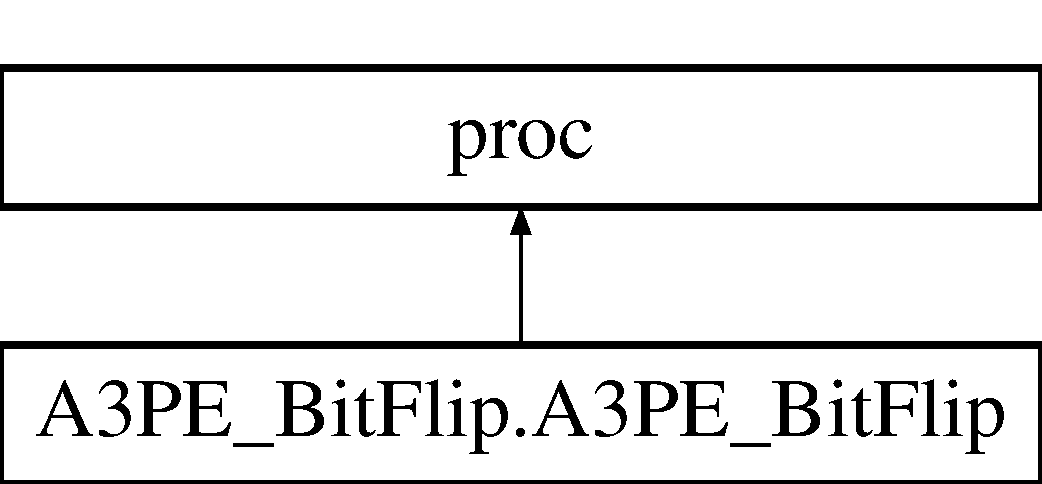
\includegraphics[height=2.000000cm]{classA3PE__BitFlip_1_1A3PE__BitFlip}
\end{center}
\end{figure}
\subsection*{Public Member Functions}
\begin{DoxyCompactItemize}
\item 
def \hyperlink{classA3PE__BitFlip_1_1A3PE__BitFlip_a3794bca914e1f66f162eff033c70b915}{\+\_\+\+\_\+init\+\_\+\+\_\+} (self, cat, obj, panel, path)
\item 
def \hyperlink{classA3PE__BitFlip_1_1A3PE__BitFlip_a6259691e444dd8ca8add74ddb359e4bc}{update} (self)
\end{DoxyCompactItemize}


\subsection{Detailed Description}


Definition at line 8 of file A3\+P\+E\+\_\+\+Bit\+Flip.\+py.



\subsection{Constructor \& Destructor Documentation}
\mbox{\Hypertarget{classA3PE__BitFlip_1_1A3PE__BitFlip_a3794bca914e1f66f162eff033c70b915}\label{classA3PE__BitFlip_1_1A3PE__BitFlip_a3794bca914e1f66f162eff033c70b915}} 
\index{A3\+P\+E\+\_\+\+Bit\+Flip\+::\+A3\+P\+E\+\_\+\+Bit\+Flip@{A3\+P\+E\+\_\+\+Bit\+Flip\+::\+A3\+P\+E\+\_\+\+Bit\+Flip}!\+\_\+\+\_\+init\+\_\+\+\_\+@{\+\_\+\+\_\+init\+\_\+\+\_\+}}
\index{\+\_\+\+\_\+init\+\_\+\+\_\+@{\+\_\+\+\_\+init\+\_\+\+\_\+}!A3\+P\+E\+\_\+\+Bit\+Flip\+::\+A3\+P\+E\+\_\+\+Bit\+Flip@{A3\+P\+E\+\_\+\+Bit\+Flip\+::\+A3\+P\+E\+\_\+\+Bit\+Flip}}
\subsubsection{\texorpdfstring{\+\_\+\+\_\+init\+\_\+\+\_\+()}{\_\_init\_\_()}}
{\footnotesize\ttfamily def A3\+P\+E\+\_\+\+Bit\+Flip.\+A3\+P\+E\+\_\+\+Bit\+Flip.\+\_\+\+\_\+init\+\_\+\+\_\+ (\begin{DoxyParamCaption}\item[{}]{self,  }\item[{}]{cat,  }\item[{}]{obj,  }\item[{}]{panel,  }\item[{}]{path }\end{DoxyParamCaption})}



Definition at line 9 of file A3\+P\+E\+\_\+\+Bit\+Flip.\+py.



References element.\+element.\+loadxrc(), proc.\+proc.\+loadxrc(), Test\+I2\+C.\+Test\+I2\+C.\+on\+Apply(), Test\+S\+P\+I.\+Test\+S\+P\+I.\+on\+Apply(), Test\+U\+S\+B.\+Test\+U\+S\+B.\+on\+Apply(), Storage\+Fifo.\+Storage\+Fifo.\+on\+Apply(), Storage\+Fifo\+Acquisition.\+Storage\+Fifo\+Acquisition.\+on\+Apply(), Test\+Suite.\+Test\+Suite.\+on\+Apply(), Current\+Measurement.\+Current\+Measurement.\+on\+Apply(), A\+D\+C\+Measurement.\+Current\+Measurement.\+on\+Apply(), Usb\+F\+T\+Interface\+Test.\+Usb\+F\+T\+Interface\+Test.\+on\+Apply(), Acquisition.\+Acquisition.\+on\+Apply(), object.\+object.\+panel, element.\+element.\+panel, proc.\+proc.\+panel, Log\+Frame.\+Log\+Frame.\+panel, Conf\+Frame.\+Conf\+Frame.\+panel, Graph\+Frame.\+Graph\+Frame.\+panel, App\+Frame.\+App\+Frame.\+panel, Croc.\+Croc.\+update(), A3\+P\+E\+\_\+\+Bit\+Flip.\+A3\+P\+E\+\_\+\+Bit\+Flip.\+update(), Croc.\+update(), Proto40\+M\+Hz\+\_\+v1.\+update(), Proto40\+M\+Hz\+\_\+v1.\+Proto40\+M\+Hz\+\_\+v1.\+update(), Proto\+F\+E\+B\+\_\+v1.\+Proto\+F\+E\+B\+\_\+v1.\+update(), Phaser.\+update(), Usb\+F\+T\+Interface.\+update(), M\+S\+Oxxxx.\+update(), I\+C\+E\+C\+A\+Lv3.\+update(), L\+S\+Delay\+Chip\+V1.\+update(), and A3\+P\+E.\+update().


\begin{DoxyCode}
9     \textcolor{keyword}{def }\hyperlink{classwrapper_1_1ModuleDictWrapper_a9a7a794150502f51df687831583e13b9}{\_\_init\_\_}(self, cat, obj, panel, path):
10         proc.\_\_init\_\_(self,cat,obj,panel,path)
11         self.loadxrc()
12         self.update()
13         self.panel.Bind(wx.EVT\_BUTTON, self.onApply, id=xrc.XRCID(\textcolor{stringliteral}{"Apply"}))
14 
\end{DoxyCode}


\subsection{Member Function Documentation}
\mbox{\Hypertarget{classA3PE__BitFlip_1_1A3PE__BitFlip_a6259691e444dd8ca8add74ddb359e4bc}\label{classA3PE__BitFlip_1_1A3PE__BitFlip_a6259691e444dd8ca8add74ddb359e4bc}} 
\index{A3\+P\+E\+\_\+\+Bit\+Flip\+::\+A3\+P\+E\+\_\+\+Bit\+Flip@{A3\+P\+E\+\_\+\+Bit\+Flip\+::\+A3\+P\+E\+\_\+\+Bit\+Flip}!update@{update}}
\index{update@{update}!A3\+P\+E\+\_\+\+Bit\+Flip\+::\+A3\+P\+E\+\_\+\+Bit\+Flip@{A3\+P\+E\+\_\+\+Bit\+Flip\+::\+A3\+P\+E\+\_\+\+Bit\+Flip}}
\subsubsection{\texorpdfstring{update()}{update()}}
{\footnotesize\ttfamily def A3\+P\+E\+\_\+\+Bit\+Flip.\+A3\+P\+E\+\_\+\+Bit\+Flip.\+update (\begin{DoxyParamCaption}\item[{}]{self }\end{DoxyParamCaption})}



Definition at line 15 of file A3\+P\+E\+\_\+\+Bit\+Flip.\+py.



Referenced by A3\+P\+E\+\_\+\+Bit\+Flip.\+A3\+P\+E\+\_\+\+Bit\+Flip.\+\_\+\+\_\+init\+\_\+\+\_\+(), Acquisition.\+Acquisition.\+\_\+\+\_\+init\+\_\+\+\_\+(), Emulate\+F\+E.\+Emulate\+F\+E.\+\_\+\+\_\+init\+\_\+\+\_\+(), App\+Frame.\+App\+Frame.\+delete\+Hardware(), Conf\+Frame.\+Conf\+Frame.\+on\+Change(), Graph\+Frame.\+Graph\+Frame.\+on\+Change(), Cfg\+Frame.\+Cfg\+Frame.\+on\+Change(), Conf\+Frame.\+Conf\+Frame.\+on\+Edit(), App\+Frame.\+App\+Frame.\+on\+Load(), Conf\+Frame.\+Conf\+Frame.\+on\+Re\+Load(), Graph\+Frame.\+Graph\+Frame.\+on\+Re\+Load(), Cfg\+Frame.\+Cfg\+Frame.\+on\+Re\+Load(), and App\+Frame.\+App\+Frame.\+on\+Re\+Load().


\begin{DoxyCode}
15     \textcolor{keyword}{def }update(self):
\end{DoxyCode}


The documentation for this class was generated from the following file\+:\begin{DoxyCompactItemize}
\item 
/home/eleclhcb/\+L\+H\+Cb/lbcat-\/cmake/\+Cat\+Calo\+Proto40\+M\+Hz/python/proc/\hyperlink{A3PE__BitFlip_8py}{A3\+P\+E\+\_\+\+Bit\+Flip.\+py}\end{DoxyCompactItemize}

\hypertarget{classAcquisition}{}\section{Acquisition Class Reference}
\label{classAcquisition}\index{Acquisition@{Acquisition}}


{\ttfamily \#include $<$inc/\+Acquisition.\+h$>$}

Inheritance diagram for Acquisition\+:\begin{figure}[H]
\begin{center}
\leavevmode
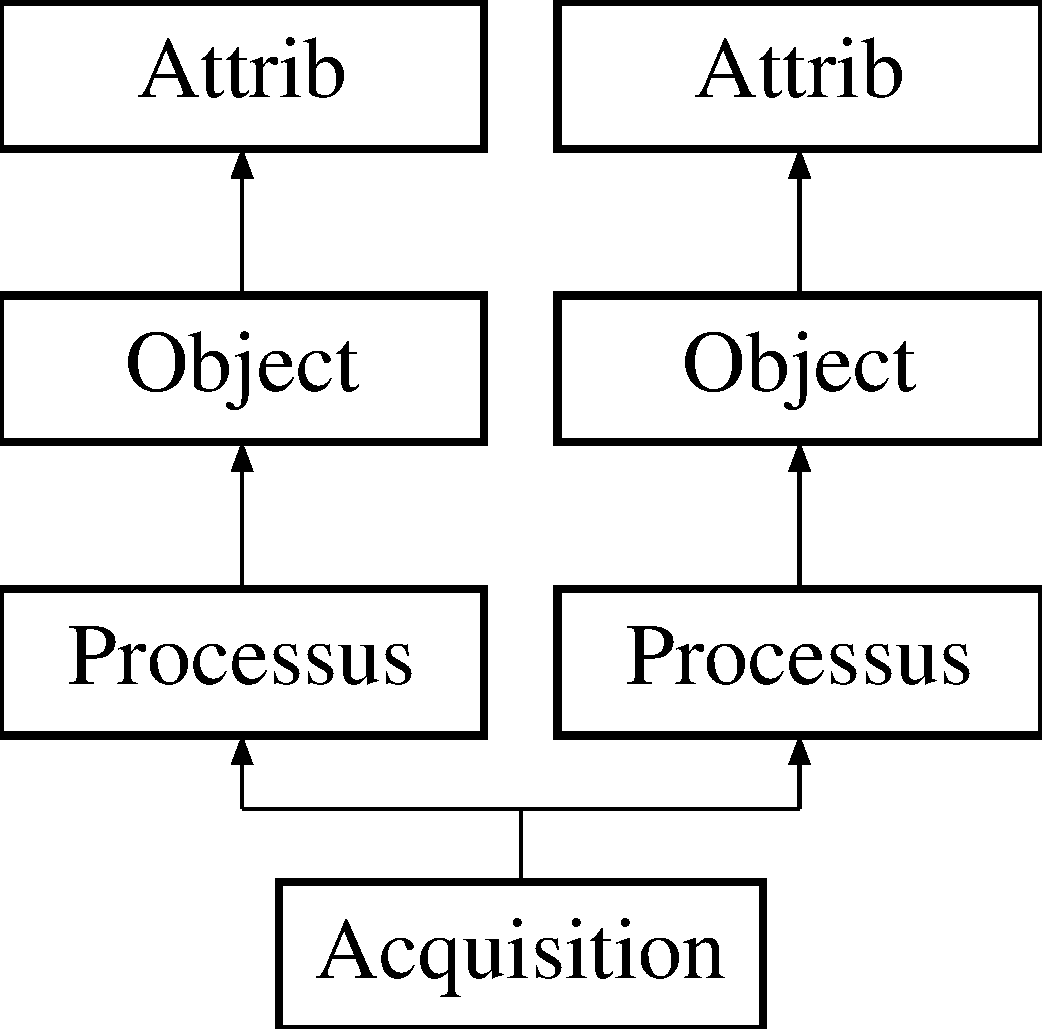
\includegraphics[height=4.000000cm]{classAcquisition}
\end{center}
\end{figure}
\subsection*{Classes}
\begin{DoxyCompactItemize}
\item 
class \hyperlink{classAcquisition_1_1Acquisition}{Acquisition}
\end{DoxyCompactItemize}
\subsection*{Public Types}
\begin{DoxyCompactItemize}
\item 
enum \hyperlink{classProcessus_a36278773bd98f2d5612fea40c7774821}{states} \{ \hyperlink{classProcessus_a36278773bd98f2d5612fea40c7774821adaf73ad5d0a09f952d0f18dbbe1c7493}{E\+RR} =-\/1, 
\hyperlink{classProcessus_a36278773bd98f2d5612fea40c7774821a629082f49d6e8df6b6da2b8fbb9d80fb}{N\+O\+T\+\_\+\+OK}, 
\hyperlink{classProcessus_a36278773bd98f2d5612fea40c7774821af77c64124fa175f28200166fff165ea2}{OK}
 \}
\item 
enum \hyperlink{classAttrib_a69e171d7cc6417835a5a306d3c764235}{Attribut} \{ \newline
\hyperlink{classAttrib_a69e171d7cc6417835a5a306d3c764235a3a8da2ab97dda18aebab196fe4100531}{U\+N\+D\+E\+F\+I\+N\+ED}, 
\hyperlink{classAttrib_a69e171d7cc6417835a5a306d3c764235a2bfb2af57b87031d190a05fe25dd92ed}{P\+A\+S\+S\+I\+VE}, 
\hyperlink{classAttrib_a69e171d7cc6417835a5a306d3c764235a3b1fec929c0370d1436f2f06e298fb0d}{A\+C\+T\+I\+VE}, 
\hyperlink{classAttrib_a69e171d7cc6417835a5a306d3c764235aa27c16b480a369ea4d18b07b2516bbc7}{I\+N\+T\+E\+R\+F\+A\+CE}, 
\newline
\hyperlink{classAttrib_a69e171d7cc6417835a5a306d3c764235a1420a5b8c0540b2af210b6975eded7f9}{IO}, 
\hyperlink{classAttrib_a69e171d7cc6417835a5a306d3c764235a0af3b0d0ac323c1704e6c69cf90add28}{I\+O\+D\+A\+TA}, 
\hyperlink{classAttrib_a69e171d7cc6417835a5a306d3c764235a7788bc5dd333fd8ce18562b269c9dab1}{E\+L\+E\+M\+E\+NT}, 
\hyperlink{classAttrib_a69e171d7cc6417835a5a306d3c764235a61ceb22149f365f1780d18f9d1459423}{H\+A\+R\+D\+W\+A\+RE}, 
\newline
\hyperlink{classAttrib_a69e171d7cc6417835a5a306d3c764235a75250e29692496e73effca2c0330977f}{P\+R\+O\+C\+E\+S\+S\+US}, 
\hyperlink{classAttrib_a69e171d7cc6417835a5a306d3c764235a103a67cd0b8f07ef478fa45d4356e27b}{S\+O\+F\+T\+W\+A\+RE}
 \}
\end{DoxyCompactItemize}
\subsection*{Public Member Functions}
\begin{DoxyCompactItemize}
\item 
\hyperlink{classAcquisition_aa7d3138495a4a8888c21b33f4d657732}{Acquisition} ()
\begin{DoxyCompactList}\small\item\em Standard constructor. \end{DoxyCompactList}\item 
virtual \hyperlink{classAcquisition_a3b0205ba385e2da70abb5a351c4dbf0f}{$\sim$\+Acquisition} ()
\begin{DoxyCompactList}\small\item\em Destructor. \end{DoxyCompactList}\item 
virtual \hyperlink{classStatusCode}{Status\+Code} \hyperlink{classAcquisition_acffc6b70b80811657409f92e489584ba}{initialize} ()
\item 
virtual \hyperlink{classStatusCode}{Status\+Code} \hyperlink{classAcquisition_ae3b63064bee1b042914b63ae4135cbd8}{execute} ()
\item 
virtual \hyperlink{classStatusCode}{Status\+Code} \hyperlink{classAcquisition_ab8ffcd86548280f0403b3ae6338f2499}{finalize} ()
\item 
\hyperlink{classStatusCode}{Status\+Code} \hyperlink{classAcquisition_a303145d497f99da966fcfd95c00cd81e}{set\+Depth} (unsigned int)
\item 
unsigned int \hyperlink{classAcquisition_a1ad973e21a067c0de0b6264d0eb5182b}{depth} ()
\item 
\hyperlink{classStatusCode}{Status\+Code} \hyperlink{classAcquisition_a3ee93f665573b4622bd9cba92c0cc04e}{set\+Channels} (unsigned int)
\item 
unsigned int \hyperlink{classAcquisition_a3041537afcb4dfe5c6940f0ef6829265}{channels} ()
\item 
\hyperlink{classStatusCode}{Status\+Code} \hyperlink{classAcquisition_acdb167b43f3babb59a98698aa5c5066f}{set\+Trigger} (bool trig)
\item 
bool \hyperlink{classAcquisition_a6f680938eb6a42d57dfa7466e8852af9}{trigger} ()
\item 
void \hyperlink{classAcquisition_a759193856d26354722e5f647e60e16de}{set\+Store\+Tree} (bool store\+\_\+tree)
\item 
bool \hyperlink{classAcquisition_a8ab7e58ccb3fee54eb6850e5081fae10}{store\+Tree} ()
\item 
void \hyperlink{classAcquisition_a1ceff272a1ad030dcd20c0dcddc65443}{set\+Store\+Trend} (bool store\+\_\+hist)
\item 
bool \hyperlink{classAcquisition_a5af693448daef6e9e054ab7f1aa50784}{store\+Trend} ()
\item 
void \hyperlink{classAcquisition_af36a1b660244096b7d274f591f67b695}{set\+Store\+Sample} (bool store\+\_\+sample)
\item 
bool \hyperlink{classAcquisition_a9af304e0fb2076cd4f92703708efe83e}{store\+Sample} ()
\item 
void \hyperlink{classAcquisition_a37e05315fc47958c290a7d938c61e067}{set\+Dead\+Time} (int deadtime)
\item 
int \hyperlink{classAcquisition_a8fb2cd60a34993ab0952d719a8517831}{dead\+Time} ()
\item 
void \hyperlink{classAcquisition_ade6fd6483b3e3737fe7dcdffb5065954}{set\+Sample} (int nsample)
\item 
int \hyperlink{classAcquisition_a83181975c0746e5837d53933031e7b62}{sample} ()
\item 
void \hyperlink{classAcquisition_a6ee040a009aa48f848b1e12434135db9}{set\+N\+Bins} (int nbins)
\item 
int \hyperlink{classAcquisition_a3a3dad0de9535d5a29c0810a5bdc3ae3}{n\+Bins} ()
\item 
void \hyperlink{classAcquisition_a8a15ffc6e539a3ae12efe4bea1ca7587}{set\+Min\+Range} (float minrange)
\item 
float \hyperlink{classAcquisition_a44f441710231748d2ca8f691647b2bcd}{min\+Range} ()
\item 
void \hyperlink{classAcquisition_a786da6cff5428020034be23e554e0e1b}{set\+Max\+Range} (float maxrange)
\item 
float \hyperlink{classAcquisition_a386f3ebc6b1d4956aa7e40b314ddb4eb}{max\+Range} ()
\item 
\hyperlink{classA3PE}{A3\+PE} $\ast$ \hyperlink{classAcquisition_a8af496b6202d2509814e3b02197a5e73}{a3pe} ()
\item 
\hyperlink{classAcquisition_aa7d3138495a4a8888c21b33f4d657732}{Acquisition} ()
\begin{DoxyCompactList}\small\item\em Standard constructor. \end{DoxyCompactList}\item 
virtual \hyperlink{classAcquisition_af697b51bd72afcfe8f9f3f368743d20d}{$\sim$\+Acquisition} ()
\begin{DoxyCompactList}\small\item\em Destructor. \end{DoxyCompactList}\item 
virtual \hyperlink{classStatusCode}{Status\+Code} \hyperlink{classAcquisition_aa73eec1ec46deae89bd3c25551bad86e}{initialize} ()
\item 
virtual \hyperlink{classStatusCode}{Status\+Code} \hyperlink{classAcquisition_a6cae797f591c2c576ebf17411e5212c9}{execute} ()
\item 
virtual \hyperlink{classStatusCode}{Status\+Code} \hyperlink{classAcquisition_a92b4b55e8c7d53610e7eda6d5b9c74a4}{finalize} ()
\item 
\hyperlink{classStatusCode}{Status\+Code} \hyperlink{classAcquisition_a303145d497f99da966fcfd95c00cd81e}{set\+Depth} (unsigned int)
\item 
unsigned int \hyperlink{classAcquisition_a1ad973e21a067c0de0b6264d0eb5182b}{depth} ()
\item 
\hyperlink{classStatusCode}{Status\+Code} \hyperlink{classAcquisition_a3ee93f665573b4622bd9cba92c0cc04e}{set\+Channels} (unsigned int)
\item 
unsigned int \hyperlink{classAcquisition_a3041537afcb4dfe5c6940f0ef6829265}{channels} ()
\item 
\hyperlink{classStatusCode}{Status\+Code} \hyperlink{classAcquisition_acdb167b43f3babb59a98698aa5c5066f}{set\+Trigger} (bool trig)
\item 
bool \hyperlink{classAcquisition_a6f680938eb6a42d57dfa7466e8852af9}{trigger} ()
\item 
void \hyperlink{classAcquisition_a759193856d26354722e5f647e60e16de}{set\+Store\+Tree} (bool store\+\_\+tree)
\item 
bool \hyperlink{classAcquisition_a8ab7e58ccb3fee54eb6850e5081fae10}{store\+Tree} ()
\item 
void \hyperlink{classAcquisition_a1ceff272a1ad030dcd20c0dcddc65443}{set\+Store\+Trend} (bool store\+\_\+hist)
\item 
bool \hyperlink{classAcquisition_a5af693448daef6e9e054ab7f1aa50784}{store\+Trend} ()
\item 
void \hyperlink{classAcquisition_af36a1b660244096b7d274f591f67b695}{set\+Store\+Sample} (bool store\+\_\+sample)
\item 
bool \hyperlink{classAcquisition_a9af304e0fb2076cd4f92703708efe83e}{store\+Sample} ()
\item 
void \hyperlink{classAcquisition_a37e05315fc47958c290a7d938c61e067}{set\+Dead\+Time} (int deadtime)
\item 
int \hyperlink{classAcquisition_a8fb2cd60a34993ab0952d719a8517831}{dead\+Time} ()
\item 
void \hyperlink{classAcquisition_ade6fd6483b3e3737fe7dcdffb5065954}{set\+Sample} (int nsample)
\item 
int \hyperlink{classAcquisition_a83181975c0746e5837d53933031e7b62}{sample} ()
\item 
void \hyperlink{classAcquisition_a6ee040a009aa48f848b1e12434135db9}{set\+N\+Bins} (int nbins)
\item 
int \hyperlink{classAcquisition_a3a3dad0de9535d5a29c0810a5bdc3ae3}{n\+Bins} ()
\item 
void \hyperlink{classAcquisition_a8a15ffc6e539a3ae12efe4bea1ca7587}{set\+Min\+Range} (float minrange)
\item 
float \hyperlink{classAcquisition_a44f441710231748d2ca8f691647b2bcd}{min\+Range} ()
\item 
void \hyperlink{classAcquisition_a786da6cff5428020034be23e554e0e1b}{set\+Max\+Range} (float maxrange)
\item 
float \hyperlink{classAcquisition_a386f3ebc6b1d4956aa7e40b314ddb4eb}{max\+Range} ()
\item 
\hyperlink{classStatusCode}{Status\+Code} \hyperlink{classProcessus_a09319bde9bed93e290f69b4e04585543}{start\+Processing} ()
\item 
\hyperlink{classStatusCode}{Status\+Code} \hyperlink{classProcessus_a5e4da662989d356b89d490b89c7afbfd}{end\+Processing} ()
\item 
void \hyperlink{classProcessus_aaeb17673b98d2b39f3aa780e335e0968}{clean} ()
\item 
void \hyperlink{classProcessus_ad57a29b33f9021eda9f6929136f1784f}{set\+Storage} (std\+::string \hyperlink{classProcessus_a33fa1a0b54a636e5cdd680669fd9ea51}{storage})
\item 
\hyperlink{classData}{Data} $\ast$ \hyperlink{classProcessus_a16e45f329fbce935aeef0ff3cb508228}{data} ()
\item 
std\+::vector$<$ double $>$ \hyperlink{classProcessus_aa7c57483cf4b9ab0b2d0ae2de8316402}{data} (unsigned int row)
\item 
std\+::vector$<$ double $>$ \hyperlink{classProcessus_abf4d91fb36707e1d50178bab12d21ae9}{data} (std\+::string \hyperlink{classObject_a300f4c05dd468c7bb8b3c968868443c1}{name})
\item 
\hyperlink{classHisto1D}{Histo1D} $\ast$ \hyperlink{classProcessus_a409227db936baff03c0462c1bcfe8069}{hist1d} (unsigned int row)
\item 
\hyperlink{classHisto2D}{Histo2D} $\ast$ \hyperlink{classProcessus_a73b5118cb5f2b5eaad33286183b86cfc}{hist2d} (unsigned int row)
\item 
void \hyperlink{classProcessus_a308c8f193802f1d1ab49d4447d0cb281}{add\+Data\+Stream} (std\+::string \hyperlink{classObject_a300f4c05dd468c7bb8b3c968868443c1}{name}, std\+::string \hyperlink{classObject_a73a0f1a41828fdd8303dd662446fb6c3}{title})
\item 
void \hyperlink{classProcessus_ad46e0d4dfdfdcbce001ee6be1746dfa4}{add\+Histo1d} (T\+H1D $\ast$h)
\item 
void \hyperlink{classProcessus_ac1ed1aed5edaeabdf18aa56775440471}{add\+Histo2d} (T\+H2D $\ast$h)
\item 
\hyperlink{classStatusCode}{Status\+Code} \hyperlink{classProcessus_a0d093b48f3218a088ba030e24372f18c}{data\+Fill} (int i, double val)
\item 
\hyperlink{classStatusCode}{Status\+Code} \hyperlink{classProcessus_aa31ab71711f7af6a729441ff573f69c9}{data\+Fill} (std\+::string \hyperlink{classObject_a300f4c05dd468c7bb8b3c968868443c1}{name}, double val)
\item 
std\+::string \hyperlink{classProcessus_a33fa1a0b54a636e5cdd680669fd9ea51}{storage} ()
\item 
void \hyperlink{classProcessus_a8ddef94227d83d9dae2cd49aebc33353}{set\+Element} (\hyperlink{classElement}{Element} $\ast$\hyperlink{classProcessus_a6fe155527431a7190b7d44d600b9608d}{element})
\item 
\hyperlink{classElement}{Element} $\ast$ \hyperlink{classProcessus_a6fe155527431a7190b7d44d600b9608d}{element} ()
\item 
void \hyperlink{classProcessus_abe603d0636f76db6aa6c5c60cf34c591}{inc\+N\+Errors} ()
\item 
void \hyperlink{classProcessus_a831b027b9cf18ab56fa6147b5d3055da}{set\+N\+Errors} (unsigned int)
\item 
unsigned int \hyperlink{classProcessus_a82a0487f82f07cc2c2dc2731f98149e7}{n\+Errors} ()
\item 
T\+File $\ast$ \hyperlink{classProcessus_a247e8c362ec08422cf53d08dd23b093c}{root\+File} ()
\item 
void \hyperlink{classProcessus_aacf6812880c1d1a2bf14a4a39458f443}{open\+Root\+File} ()
\item 
void \hyperlink{classProcessus_a2f3c41e99da4c738ea3d8f7b0d20a665}{close\+Root\+File} ()
\item 
void \hyperlink{classProcessus_a5e4d34b86241fa0756e07375a14ff4b2}{start\+Chrono} ()
\item 
void \hyperlink{classProcessus_a471833f89047aa9a7ff6200a31c17a1d}{set\+Log\+Msg} (std\+::string \hyperlink{classProcessus_a42fdeb17dc13ba854222666b6aa29b61}{log\+Msg})
\item 
std\+::string \hyperlink{classProcessus_a42fdeb17dc13ba854222666b6aa29b61}{log\+Msg} ()
\item 
void \hyperlink{classProcessus_ad38cde0f1bcefa00b068e7947b8af927}{set\+State} (int state)
\item 
double \hyperlink{classProcessus_aecca96218c65bc805c988cd95447df55}{elapsed\+Time} ()
\item 
double \hyperlink{classProcessus_a06d3815ad56593dfd0d3c1f534f8b146}{elapsed\+Time} (time\+\_\+t start)
\item 
std\+::string \hyperlink{classObject_a300f4c05dd468c7bb8b3c968868443c1}{name} () const
\item 
std\+::string \hyperlink{classObject_a84f99f70f144a83e1582d1d0f84e4e62}{type} ()
\item 
unsigned char \hyperlink{classObject_af99145335cc61ff6e2798ea17db009d2}{id} ()
\item 
std\+::string \hyperlink{classObject_a73a0f1a41828fdd8303dd662446fb6c3}{title} ()
\item 
void \hyperlink{classObject_a3f9d5537ebce0c0f2bf6ae4d92426f3c}{msg\+Svc} (int level, std\+::string \hyperlink{classObject_a58b2d0618c2d08cf2383012611528d97}{msg}, std\+::string \hyperlink{classObject_a300f4c05dd468c7bb8b3c968868443c1}{name})
\item 
void \hyperlink{classObject_a58b2d0618c2d08cf2383012611528d97}{msg} (std\+::string mymsg)
\item 
void \hyperlink{classObject_ac5d59299273cee27aacf7de00d2e7034}{msg} (std\+::string mymsg, std\+::string \hyperlink{classObject_a300f4c05dd468c7bb8b3c968868443c1}{name})
\item 
void \hyperlink{classObject_a83d2db2df682907ea1115ad721c1c4a1}{verbose} (std\+::string mymsg)
\item 
void \hyperlink{classObject_a2d4120195317e2a3c6532e8bb9f3da68}{verbose} (std\+::string mymsg, std\+::string \hyperlink{classObject_a300f4c05dd468c7bb8b3c968868443c1}{name})
\item 
void \hyperlink{classObject_aac010553f022165573714b7014a15f0d}{debug} (std\+::string mymsg)
\item 
void \hyperlink{classObject_a6c9a0397ca804e04d675ed05683f5420}{debug} (std\+::string mymsg, std\+::string \hyperlink{classObject_a300f4c05dd468c7bb8b3c968868443c1}{name})
\item 
void \hyperlink{classObject_a644fd329ea4cb85f54fa6846484b84a8}{info} (std\+::string mymsg)
\item 
void \hyperlink{classObject_a1ca123253dfd30fc28b156f521dcbdae}{info} (std\+::string mymsg, std\+::string \hyperlink{classObject_a300f4c05dd468c7bb8b3c968868443c1}{name})
\item 
void \hyperlink{classObject_a65cd4fda577711660821fd2cd5a3b4c9}{warning} (std\+::string mymsg)
\item 
void \hyperlink{classObject_a11f101db4dd73d9391b0231818881d86}{warning} (std\+::string mymsg, std\+::string \hyperlink{classObject_a300f4c05dd468c7bb8b3c968868443c1}{name})
\item 
void \hyperlink{classObject_a204a95f57818c0f811933917a30eff45}{error} (std\+::string mymsg)
\item 
void \hyperlink{classObject_ad7f6c457733082efa2f9ff5f5c8e119a}{error} (std\+::string mymsg, std\+::string \hyperlink{classObject_a300f4c05dd468c7bb8b3c968868443c1}{name})
\item 
void \hyperlink{classObject_aad5a16aac7516ce65bd5ec02ab07fc80}{fatal} (std\+::string mymsg)
\item 
void \hyperlink{classObject_ae62acd3d09f716220f75f252dc38bc9a}{fatal} (std\+::string mymsg, std\+::string \hyperlink{classObject_a300f4c05dd468c7bb8b3c968868443c1}{name})
\item 
void \hyperlink{classObject_ae30fea75683c2d149b6b6d17c09ecd0c}{set\+Name} (std\+::string \hyperlink{classObject_a300f4c05dd468c7bb8b3c968868443c1}{name})
\item 
void \hyperlink{classObject_aae534cc9d982bcb9b99fd505f2e103a5}{set\+Type} (std\+::string \hyperlink{classObject_a84f99f70f144a83e1582d1d0f84e4e62}{type})
\item 
void \hyperlink{classObject_a398fe08cba594a0ce6891d59fe4f159f}{set\+Id} (unsigned char \hyperlink{classObject_af99145335cc61ff6e2798ea17db009d2}{id})
\item 
void \hyperlink{classObject_a89557dbbad5bcaa02652f5d7fa35d20f}{set\+Title} (std\+::string \hyperlink{classObject_a73a0f1a41828fdd8303dd662446fb6c3}{title})
\item 
void \hyperlink{classObject_a870c5af919958c2136623b2d7816d123}{set\+Dll\+Name} (std\+::string \hyperlink{classObject_a2e3947f2870094c332d7454117f3ec63}{dll\+Name})
\item 
std\+::string \hyperlink{classObject_a2e3947f2870094c332d7454117f3ec63}{dll\+Name} ()
\item 
bool \hyperlink{classAttrib_a704f26af560909ad22065083bb7d4c34}{is} (int attribut)
\item 
void \hyperlink{classAttrib_a235f773af19c900264a190b00a3b4ad7}{add} (int attribut)
\item 
void \hyperlink{classAttrib_a7d4ef7e32d93cb287792b87b857e79f3}{remove} (int attribut)
\item 
std\+::string \hyperlink{classAttrib_aee7bbf16b144887f196e1341b24f8a26}{attributs} ()
\end{DoxyCompactItemize}
\subsection*{Protected Member Functions}
\begin{DoxyCompactItemize}
\item 
\hyperlink{classAcquisition_1_1Acquisition}{Acquisition} $\ast$ \hyperlink{classAcquisition_a4b1b690ef27f20b3e1ad9383f2f57628}{clone} ()
\item 
unsigned int \hyperlink{classAcquisition_a76fe7c020f7097e5d479867ba783ba31}{decode\+Format} (unsigned int, unsigned int, \hyperlink{classRAM}{R\+AM} $\ast$)
\item 
\hyperlink{classAcquisition_1_1Acquisition}{Acquisition} $\ast$ \hyperlink{classAcquisition_a4b1b690ef27f20b3e1ad9383f2f57628}{clone} ()
\item 
unsigned int \hyperlink{classAcquisition_a76fe7c020f7097e5d479867ba783ba31}{decode\+Format} (unsigned int, unsigned int, \hyperlink{classRAM}{R\+AM} $\ast$)
\end{DoxyCompactItemize}
\subsection*{Protected Attributes}
\begin{DoxyCompactItemize}
\item 
\hyperlink{classElement}{Element} $\ast$ \hyperlink{classProcessus_aa9d24d53c3e52f36786cabb5d8e296e7}{m\+\_\+element}
\item 
std\+::string \hyperlink{classAttrib_a3414521d7a82476e874b25a5407b5e63}{m\+\_\+attrib\+String} \mbox{[}10\mbox{]}
\end{DoxyCompactItemize}
\subsection*{Private Attributes}
\begin{DoxyCompactItemize}
\item 
bool \hyperlink{classAcquisition_aca2143e9135e25554e58327475a767c5}{m\+\_\+store\+\_\+tree}
\item 
bool \hyperlink{classAcquisition_a08f70edd83751dbdab4c8190dc4b9188}{m\+\_\+store\+\_\+hist}
\item 
bool \hyperlink{classAcquisition_a987cc1d04007cf1f5acc1accfd0909e5}{m\+\_\+store\+\_\+sample}
\item 
T\+Tree $\ast$ \hyperlink{classAcquisition_aa88a923232e8b7e08f5c1b5411497fc5}{m\+\_\+tree}
\item 
Int\+\_\+t \hyperlink{classAcquisition_afd35e220e0bfda7e763584524273aeb0}{m\+\_\+run\+Number}
\item 
Int\+\_\+t \hyperlink{classAcquisition_a32a70daa3f653eae5eafc46dbd0e11a6}{m\+\_\+evt\+Number}
\item 
Int\+\_\+t \hyperlink{classAcquisition_a154e5423720ab1f2c4ab5cd125cb4e80}{m\+\_\+sample}
\item 
Int\+\_\+t \hyperlink{classAcquisition_a9233a189179591c0c2f2639a3e6c13f6}{m\+\_\+channel} \mbox{[}8\mbox{]}
\item 
Int\+\_\+t \hyperlink{classAcquisition_a217269bc403d9fd271a1701c98afb30e}{m\+\_\+ch\+Enable} \mbox{[}8\mbox{]}
\item 
Int\+\_\+t \hyperlink{classAcquisition_a1860c7a03a65ea7a778d30dd4a40e1e1}{m\+\_\+nch}
\item 
double \hyperlink{classAcquisition_aa88cf8d27e075b5aaddb309dfb42cd04}{m\+\_\+timestamp}
\item 
int \hyperlink{classAcquisition_aedc8b29f322ef00540797fbd0d5112d1}{m\+\_\+channels}
\item 
int \hyperlink{classAcquisition_a26628424533a2dd74d24712a14637a72}{m\+\_\+depth}
\item 
\hyperlink{classProto40MHz__v1}{Proto40\+M\+Hz\+\_\+v1} $\ast$ \hyperlink{classAcquisition_a9b0db99be79d61ae78dae8a9e4efceab}{m\+\_\+board}
\item 
\hyperlink{classA3PE}{A3\+PE} $\ast$ \hyperlink{classAcquisition_aac113fd42c6574cdb4154e9808a21b67}{m\+\_\+pga}
\item 
\hyperlink{classRAM}{R\+AM} $\ast$ \hyperlink{classAcquisition_a8a893e7485e96da01185df6d1109c0bc}{m\+\_\+fifo}
\item 
bool \hyperlink{classAcquisition_a953bdc1bf56206b6df33b648af32a24f}{m\+\_\+trig}
\item 
T\+H1D $\ast$ \hyperlink{classAcquisition_aedfd2a4842b08fdf85176bf672030430}{m\+\_\+a} \mbox{[}8\mbox{]}
\item 
T\+H1D $\ast$ \hyperlink{classAcquisition_ad7f531c3d3fc58d1a2a5eab954db0ca7}{m\+\_\+s} \mbox{[}8\mbox{]}
\item 
T\+H1D $\ast$ \hyperlink{classAcquisition_ad0078b0c53eb14f13fdd16763df3be8e}{m\+\_\+hsample} \mbox{[}8\mbox{]}
\item 
double \hyperlink{classAcquisition_ac855680c9bb5f8f14d505d5f41f1a076}{v} \mbox{[}8 $\ast$\hyperlink{classAcquisition_a82cdfc89b37f20530bf112e13a5c5e5c}{m\+\_\+depthmax}\mbox{]}
\item 
double \hyperlink{classAcquisition_a8d2cd605d4982223356a14423d735c84}{v2} \mbox{[}8 $\ast$\hyperlink{classAcquisition_a82cdfc89b37f20530bf112e13a5c5e5c}{m\+\_\+depthmax}\mbox{]}
\item 
unsigned int \hyperlink{classAcquisition_a26d0f1a44309ffac49c365b7ee568ab2}{m\+\_\+nsample}
\item 
unsigned int \hyperlink{classAcquisition_a05bccdc4b9ada37beaeba8794ccef12d}{m\+\_\+nbins}
\item 
float \hyperlink{classAcquisition_a06b3ea027ebdcb15f64a6517ceb99b76}{m\+\_\+min\+Range}
\item 
float \hyperlink{classAcquisition_a45478629e9db582470b4b158edb46616}{m\+\_\+max\+Range}
\item 
int \hyperlink{classAcquisition_a5f7fe20506e7d860ed61935255adfe17}{m\+\_\+deadtime}
\item 
\hyperlink{classFEB__v1}{F\+E\+B\+\_\+v1} $\ast$ \hyperlink{classAcquisition_ad4820003ddd62f0ca886c2e6a3690120}{m\+\_\+board}
\end{DoxyCompactItemize}
\subsection*{Static Private Attributes}
\begin{DoxyCompactItemize}
\item 
static const unsigned int \hyperlink{classAcquisition_a82cdfc89b37f20530bf112e13a5c5e5c}{m\+\_\+depthmax} = 512
\end{DoxyCompactItemize}


\subsection{Detailed Description}
\begin{DoxyAuthor}{Author}

\end{DoxyAuthor}
\begin{DoxyDate}{Date}
2006-\/10-\/23 
\end{DoxyDate}


Definition at line 20 of file Acquisition.\+h.



\subsection{Member Enumeration Documentation}
\mbox{\Hypertarget{classAttrib_a69e171d7cc6417835a5a306d3c764235}\label{classAttrib_a69e171d7cc6417835a5a306d3c764235}} 
\index{Acquisition@{Acquisition}!Attribut@{Attribut}}
\index{Attribut@{Attribut}!Acquisition@{Acquisition}}
\subsubsection{\texorpdfstring{Attribut}{Attribut}}
{\footnotesize\ttfamily enum \hyperlink{classAttrib_a69e171d7cc6417835a5a306d3c764235}{Attrib\+::\+Attribut}\hspace{0.3cm}{\ttfamily [inherited]}}

\begin{DoxyEnumFields}{Enumerator}
\raisebox{\heightof{T}}[0pt][0pt]{\index{U\+N\+D\+E\+F\+I\+N\+ED@{U\+N\+D\+E\+F\+I\+N\+ED}!Acquisition@{Acquisition}}\index{Acquisition@{Acquisition}!U\+N\+D\+E\+F\+I\+N\+ED@{U\+N\+D\+E\+F\+I\+N\+ED}}}\mbox{\Hypertarget{classAttrib_a69e171d7cc6417835a5a306d3c764235a3a8da2ab97dda18aebab196fe4100531}\label{classAttrib_a69e171d7cc6417835a5a306d3c764235a3a8da2ab97dda18aebab196fe4100531}} 
U\+N\+D\+E\+F\+I\+N\+ED&\\
\hline

\raisebox{\heightof{T}}[0pt][0pt]{\index{P\+A\+S\+S\+I\+VE@{P\+A\+S\+S\+I\+VE}!Acquisition@{Acquisition}}\index{Acquisition@{Acquisition}!P\+A\+S\+S\+I\+VE@{P\+A\+S\+S\+I\+VE}}}\mbox{\Hypertarget{classAttrib_a69e171d7cc6417835a5a306d3c764235a2bfb2af57b87031d190a05fe25dd92ed}\label{classAttrib_a69e171d7cc6417835a5a306d3c764235a2bfb2af57b87031d190a05fe25dd92ed}} 
P\+A\+S\+S\+I\+VE&\\
\hline

\raisebox{\heightof{T}}[0pt][0pt]{\index{A\+C\+T\+I\+VE@{A\+C\+T\+I\+VE}!Acquisition@{Acquisition}}\index{Acquisition@{Acquisition}!A\+C\+T\+I\+VE@{A\+C\+T\+I\+VE}}}\mbox{\Hypertarget{classAttrib_a69e171d7cc6417835a5a306d3c764235a3b1fec929c0370d1436f2f06e298fb0d}\label{classAttrib_a69e171d7cc6417835a5a306d3c764235a3b1fec929c0370d1436f2f06e298fb0d}} 
A\+C\+T\+I\+VE&\\
\hline

\raisebox{\heightof{T}}[0pt][0pt]{\index{I\+N\+T\+E\+R\+F\+A\+CE@{I\+N\+T\+E\+R\+F\+A\+CE}!Acquisition@{Acquisition}}\index{Acquisition@{Acquisition}!I\+N\+T\+E\+R\+F\+A\+CE@{I\+N\+T\+E\+R\+F\+A\+CE}}}\mbox{\Hypertarget{classAttrib_a69e171d7cc6417835a5a306d3c764235aa27c16b480a369ea4d18b07b2516bbc7}\label{classAttrib_a69e171d7cc6417835a5a306d3c764235aa27c16b480a369ea4d18b07b2516bbc7}} 
I\+N\+T\+E\+R\+F\+A\+CE&\\
\hline

\raisebox{\heightof{T}}[0pt][0pt]{\index{IO@{IO}!Acquisition@{Acquisition}}\index{Acquisition@{Acquisition}!IO@{IO}}}\mbox{\Hypertarget{classAttrib_a69e171d7cc6417835a5a306d3c764235a1420a5b8c0540b2af210b6975eded7f9}\label{classAttrib_a69e171d7cc6417835a5a306d3c764235a1420a5b8c0540b2af210b6975eded7f9}} 
IO&\\
\hline

\raisebox{\heightof{T}}[0pt][0pt]{\index{I\+O\+D\+A\+TA@{I\+O\+D\+A\+TA}!Acquisition@{Acquisition}}\index{Acquisition@{Acquisition}!I\+O\+D\+A\+TA@{I\+O\+D\+A\+TA}}}\mbox{\Hypertarget{classAttrib_a69e171d7cc6417835a5a306d3c764235a0af3b0d0ac323c1704e6c69cf90add28}\label{classAttrib_a69e171d7cc6417835a5a306d3c764235a0af3b0d0ac323c1704e6c69cf90add28}} 
I\+O\+D\+A\+TA&\\
\hline

\raisebox{\heightof{T}}[0pt][0pt]{\index{E\+L\+E\+M\+E\+NT@{E\+L\+E\+M\+E\+NT}!Acquisition@{Acquisition}}\index{Acquisition@{Acquisition}!E\+L\+E\+M\+E\+NT@{E\+L\+E\+M\+E\+NT}}}\mbox{\Hypertarget{classAttrib_a69e171d7cc6417835a5a306d3c764235a7788bc5dd333fd8ce18562b269c9dab1}\label{classAttrib_a69e171d7cc6417835a5a306d3c764235a7788bc5dd333fd8ce18562b269c9dab1}} 
E\+L\+E\+M\+E\+NT&\\
\hline

\raisebox{\heightof{T}}[0pt][0pt]{\index{H\+A\+R\+D\+W\+A\+RE@{H\+A\+R\+D\+W\+A\+RE}!Acquisition@{Acquisition}}\index{Acquisition@{Acquisition}!H\+A\+R\+D\+W\+A\+RE@{H\+A\+R\+D\+W\+A\+RE}}}\mbox{\Hypertarget{classAttrib_a69e171d7cc6417835a5a306d3c764235a61ceb22149f365f1780d18f9d1459423}\label{classAttrib_a69e171d7cc6417835a5a306d3c764235a61ceb22149f365f1780d18f9d1459423}} 
H\+A\+R\+D\+W\+A\+RE&\\
\hline

\raisebox{\heightof{T}}[0pt][0pt]{\index{P\+R\+O\+C\+E\+S\+S\+US@{P\+R\+O\+C\+E\+S\+S\+US}!Acquisition@{Acquisition}}\index{Acquisition@{Acquisition}!P\+R\+O\+C\+E\+S\+S\+US@{P\+R\+O\+C\+E\+S\+S\+US}}}\mbox{\Hypertarget{classAttrib_a69e171d7cc6417835a5a306d3c764235a75250e29692496e73effca2c0330977f}\label{classAttrib_a69e171d7cc6417835a5a306d3c764235a75250e29692496e73effca2c0330977f}} 
P\+R\+O\+C\+E\+S\+S\+US&\\
\hline

\raisebox{\heightof{T}}[0pt][0pt]{\index{S\+O\+F\+T\+W\+A\+RE@{S\+O\+F\+T\+W\+A\+RE}!Acquisition@{Acquisition}}\index{Acquisition@{Acquisition}!S\+O\+F\+T\+W\+A\+RE@{S\+O\+F\+T\+W\+A\+RE}}}\mbox{\Hypertarget{classAttrib_a69e171d7cc6417835a5a306d3c764235a103a67cd0b8f07ef478fa45d4356e27b}\label{classAttrib_a69e171d7cc6417835a5a306d3c764235a103a67cd0b8f07ef478fa45d4356e27b}} 
S\+O\+F\+T\+W\+A\+RE&\\
\hline

\end{DoxyEnumFields}


Definition at line 29 of file Attrib.\+h.


\begin{DoxyCode}
29                 \{
30     \hyperlink{classAttrib_a69e171d7cc6417835a5a306d3c764235a3a8da2ab97dda18aebab196fe4100531}{UNDEFINED},
31     \hyperlink{classAttrib_a69e171d7cc6417835a5a306d3c764235a2bfb2af57b87031d190a05fe25dd92ed}{PASSIVE},
32     \hyperlink{classAttrib_a69e171d7cc6417835a5a306d3c764235a3b1fec929c0370d1436f2f06e298fb0d}{ACTIVE},
33     \hyperlink{classAttrib_a69e171d7cc6417835a5a306d3c764235aa27c16b480a369ea4d18b07b2516bbc7}{INTERFACE},
34     \hyperlink{classAttrib_a69e171d7cc6417835a5a306d3c764235a1420a5b8c0540b2af210b6975eded7f9}{IO},
35     \hyperlink{classAttrib_a69e171d7cc6417835a5a306d3c764235a0af3b0d0ac323c1704e6c69cf90add28}{IODATA},
36     \hyperlink{classAttrib_a69e171d7cc6417835a5a306d3c764235a7788bc5dd333fd8ce18562b269c9dab1}{ELEMENT},
37     \hyperlink{classAttrib_a69e171d7cc6417835a5a306d3c764235a61ceb22149f365f1780d18f9d1459423}{HARDWARE},
38     \hyperlink{classAttrib_a69e171d7cc6417835a5a306d3c764235a75250e29692496e73effca2c0330977f}{PROCESSUS},
39     \hyperlink{classAttrib_a69e171d7cc6417835a5a306d3c764235a103a67cd0b8f07ef478fa45d4356e27b}{SOFTWARE} 
40   \}; \textcolor{comment}{// array m\_attribString must be changed into Attrib::Attrib if this enu is modified. }
\end{DoxyCode}
\mbox{\Hypertarget{classProcessus_a36278773bd98f2d5612fea40c7774821}\label{classProcessus_a36278773bd98f2d5612fea40c7774821}} 
\index{Acquisition@{Acquisition}!states@{states}}
\index{states@{states}!Acquisition@{Acquisition}}
\subsubsection{\texorpdfstring{states}{states}}
{\footnotesize\ttfamily enum \hyperlink{classProcessus_a36278773bd98f2d5612fea40c7774821}{Processus\+::states}\hspace{0.3cm}{\ttfamily [inherited]}}

\begin{DoxyEnumFields}{Enumerator}
\raisebox{\heightof{T}}[0pt][0pt]{\index{E\+RR@{E\+RR}!Acquisition@{Acquisition}}\index{Acquisition@{Acquisition}!E\+RR@{E\+RR}}}\mbox{\Hypertarget{classProcessus_a36278773bd98f2d5612fea40c7774821adaf73ad5d0a09f952d0f18dbbe1c7493}\label{classProcessus_a36278773bd98f2d5612fea40c7774821adaf73ad5d0a09f952d0f18dbbe1c7493}} 
E\+RR&\\
\hline

\raisebox{\heightof{T}}[0pt][0pt]{\index{N\+O\+T\+\_\+\+OK@{N\+O\+T\+\_\+\+OK}!Acquisition@{Acquisition}}\index{Acquisition@{Acquisition}!N\+O\+T\+\_\+\+OK@{N\+O\+T\+\_\+\+OK}}}\mbox{\Hypertarget{classProcessus_a36278773bd98f2d5612fea40c7774821a629082f49d6e8df6b6da2b8fbb9d80fb}\label{classProcessus_a36278773bd98f2d5612fea40c7774821a629082f49d6e8df6b6da2b8fbb9d80fb}} 
N\+O\+T\+\_\+\+OK&\\
\hline

\raisebox{\heightof{T}}[0pt][0pt]{\index{OK@{OK}!Acquisition@{Acquisition}}\index{Acquisition@{Acquisition}!OK@{OK}}}\mbox{\Hypertarget{classProcessus_a36278773bd98f2d5612fea40c7774821af77c64124fa175f28200166fff165ea2}\label{classProcessus_a36278773bd98f2d5612fea40c7774821af77c64124fa175f28200166fff165ea2}} 
OK&\\
\hline

\end{DoxyEnumFields}


Definition at line 34 of file Processus.\+h.


\begin{DoxyCode}
34 \{ \hyperlink{classProcessus_a36278773bd98f2d5612fea40c7774821adaf73ad5d0a09f952d0f18dbbe1c7493}{ERR}=-1 , \hyperlink{classProcessus_a36278773bd98f2d5612fea40c7774821a629082f49d6e8df6b6da2b8fbb9d80fb}{NOT\_OK} , \hyperlink{classProcessus_a36278773bd98f2d5612fea40c7774821af77c64124fa175f28200166fff165ea2}{OK} \};
\end{DoxyCode}


\subsection{Constructor \& Destructor Documentation}
\mbox{\Hypertarget{classAcquisition_aa7d3138495a4a8888c21b33f4d657732}\label{classAcquisition_aa7d3138495a4a8888c21b33f4d657732}} 
\index{Acquisition@{Acquisition}!Acquisition@{Acquisition}}
\index{Acquisition@{Acquisition}!Acquisition@{Acquisition}}
\subsubsection{\texorpdfstring{Acquisition()}{Acquisition()}\hspace{0.1cm}{\footnotesize\ttfamily [1/2]}}
{\footnotesize\ttfamily \hyperlink{classAcquisition_1_1Acquisition}{Acquisition\+::\+Acquisition} (\begin{DoxyParamCaption}{ }\end{DoxyParamCaption})}



Standard constructor. 



Definition at line 22 of file Acquisition.\+cpp.



References Object\+::set\+Name(), Object\+::set\+Title(), and Object\+::set\+Type().



Referenced by clone().


\begin{DoxyCode}
22                            :
23   \hyperlink{classAcquisition_aca2143e9135e25554e58327475a767c5}{m\_store\_tree}(\textcolor{keyword}{true}),
24   \hyperlink{classAcquisition_a08f70edd83751dbdab4c8190dc4b9188}{m\_store\_hist}(\textcolor{keyword}{false}),
25   \hyperlink{classAcquisition_a987cc1d04007cf1f5acc1accfd0909e5}{m\_store\_sample}(\textcolor{keyword}{true}),
26   \hyperlink{classAcquisition_aedc8b29f322ef00540797fbd0d5112d1}{m\_channels}(0xFF),
27   \hyperlink{classAcquisition_a26628424533a2dd74d24712a14637a72}{m\_depth}(5),
28   \hyperlink{classAcquisition_a953bdc1bf56206b6df33b648af32a24f}{m\_trig}(\textcolor{keyword}{true}),
29   \hyperlink{classAcquisition_a26d0f1a44309ffac49c365b7ee568ab2}{m\_nsample}(0),
30   \hyperlink{classAcquisition_a05bccdc4b9ada37beaeba8794ccef12d}{m\_nbins}(100),
31   \hyperlink{classAcquisition_a06b3ea027ebdcb15f64a6517ceb99b76}{m\_minRange}(0.),
32   \hyperlink{classAcquisition_a45478629e9db582470b4b158edb46616}{m\_maxRange}(4096.),
33   \hyperlink{classAcquisition_a5f7fe20506e7d860ed61935255adfe17}{m\_deadtime}(1000.)
34 \{
35   \hyperlink{classObject_ae30fea75683c2d149b6b6d17c09ecd0c}{setName} ( \textcolor{stringliteral}{"Acquisition"} );
36   \hyperlink{classObject_aae534cc9d982bcb9b99fd505f2e103a5}{setType} ( \textcolor{stringliteral}{"Proto40MHz\_v1"} );
37   \hyperlink{classObject_a89557dbbad5bcaa02652f5d7fa35d20f}{setTitle}( \textcolor{stringliteral}{"Proto40MHz\_v1 data acquisition"} );
38 \}
\end{DoxyCode}
\mbox{\Hypertarget{classAcquisition_a3b0205ba385e2da70abb5a351c4dbf0f}\label{classAcquisition_a3b0205ba385e2da70abb5a351c4dbf0f}} 
\index{Acquisition@{Acquisition}!````~Acquisition@{$\sim$\+Acquisition}}
\index{````~Acquisition@{$\sim$\+Acquisition}!Acquisition@{Acquisition}}
\subsubsection{\texorpdfstring{$\sim$\+Acquisition()}{~Acquisition()}\hspace{0.1cm}{\footnotesize\ttfamily [1/2]}}
{\footnotesize\ttfamily Acquisition\+::$\sim$\+Acquisition (\begin{DoxyParamCaption}{ }\end{DoxyParamCaption})\hspace{0.3cm}{\ttfamily [virtual]}}



Destructor. 



Definition at line 42 of file Acquisition.\+cpp.


\begin{DoxyCode}
42 \{\} 
\end{DoxyCode}
\mbox{\Hypertarget{classAcquisition_aa7d3138495a4a8888c21b33f4d657732}\label{classAcquisition_aa7d3138495a4a8888c21b33f4d657732}} 
\index{Acquisition@{Acquisition}!Acquisition@{Acquisition}}
\index{Acquisition@{Acquisition}!Acquisition@{Acquisition}}
\subsubsection{\texorpdfstring{Acquisition()}{Acquisition()}\hspace{0.1cm}{\footnotesize\ttfamily [2/2]}}
{\footnotesize\ttfamily \hyperlink{classAcquisition_1_1Acquisition}{Acquisition\+::\+Acquisition} (\begin{DoxyParamCaption}{ }\end{DoxyParamCaption})}



Standard constructor. 

\mbox{\Hypertarget{classAcquisition_af697b51bd72afcfe8f9f3f368743d20d}\label{classAcquisition_af697b51bd72afcfe8f9f3f368743d20d}} 
\index{Acquisition@{Acquisition}!````~Acquisition@{$\sim$\+Acquisition}}
\index{````~Acquisition@{$\sim$\+Acquisition}!Acquisition@{Acquisition}}
\subsubsection{\texorpdfstring{$\sim$\+Acquisition()}{~Acquisition()}\hspace{0.1cm}{\footnotesize\ttfamily [2/2]}}
{\footnotesize\ttfamily virtual Acquisition\+::$\sim$\+Acquisition (\begin{DoxyParamCaption}{ }\end{DoxyParamCaption})\hspace{0.3cm}{\ttfamily [virtual]}}



Destructor. 



\subsection{Member Function Documentation}
\mbox{\Hypertarget{classAcquisition_a8af496b6202d2509814e3b02197a5e73}\label{classAcquisition_a8af496b6202d2509814e3b02197a5e73}} 
\index{Acquisition@{Acquisition}!a3pe@{a3pe}}
\index{a3pe@{a3pe}!Acquisition@{Acquisition}}
\subsubsection{\texorpdfstring{a3pe()}{a3pe()}}
{\footnotesize\ttfamily \hyperlink{classA3PE}{A3\+PE}$\ast$ Acquisition\+::a3pe (\begin{DoxyParamCaption}{ }\end{DoxyParamCaption})\hspace{0.3cm}{\ttfamily [inline]}}



Definition at line 93 of file Acquisition.\+h.



References m\+\_\+pga.


\begin{DoxyCode}
93 \{\textcolor{keywordflow}{return} \hyperlink{classAcquisition_aac113fd42c6574cdb4154e9808a21b67}{m\_pga};\}
\end{DoxyCode}
\mbox{\Hypertarget{classAttrib_a235f773af19c900264a190b00a3b4ad7}\label{classAttrib_a235f773af19c900264a190b00a3b4ad7}} 
\index{Acquisition@{Acquisition}!add@{add}}
\index{add@{add}!Acquisition@{Acquisition}}
\subsubsection{\texorpdfstring{add()}{add()}}
{\footnotesize\ttfamily void Attrib\+::add (\begin{DoxyParamCaption}\item[{int}]{attribut }\end{DoxyParamCaption})\hspace{0.3cm}{\ttfamily [inline]}, {\ttfamily [inherited]}}

Add an attribut 

Definition at line 67 of file Attrib.\+h.



References Attrib\+::m\+\_\+attributs, and Attrib\+::\+U\+N\+D\+E\+F\+I\+N\+ED.



Referenced by A3\+P\+E\+::\+A3\+P\+E(), Attrib\+::\+Attrib(), Specs\+Mezzanine\+::cmdline(), Computer\+::\+Computer(), C\+U\+\_\+v1\+::\+C\+U\+\_\+v1(), export\+\_\+obj(), F\+E\+B\+\_\+v1\+::\+F\+E\+B\+\_\+v1(), Fe\+P\+G\+A\+::\+Fe\+P\+G\+A(), I\+C\+E\+C\+A\+Lv3\+::\+I\+C\+E\+C\+A\+Lv3(), I\+C\+Phaser\+::\+I\+C\+Phaser(), Application\+::initialize(), Interface\+::\+Interface(), I\+Odata\+::\+I\+Odata(), I\+Oobject\+::\+I\+Oobject(), M\+S\+Oxxxx\+::\+M\+S\+Oxxxx(), Phaser\+::\+Phaser(), Processus\+::\+Processus(), Proto40\+M\+Hz\+\_\+v1\+::\+Proto40\+M\+Hz\+\_\+v1(), Attrib\+::remove(), Seq\+P\+G\+A\+::\+Seq\+P\+G\+A(), Test\+I2\+C\+::set\+Address(), Test\+S\+P\+I\+::set\+Address(), Specs\+Slave\+::set\+Address(), Specs\+Master\+::\+Specs\+Master(), and Specs\+Slave\+::\+Specs\+Slave().


\begin{DoxyCode}
67                             \{
68     \textcolor{keywordflow}{if} (attribut!=\hyperlink{classAttrib_a69e171d7cc6417835a5a306d3c764235a3a8da2ab97dda18aebab196fe4100531}{Attrib::UNDEFINED}) \textcolor{keyword}{remove}(\hyperlink{classAttrib_a69e171d7cc6417835a5a306d3c764235a3a8da2ab97dda18aebab196fe4100531}{Attrib::UNDEFINED});
69     \textcolor{keywordtype}{bool} duplicate = false ;
70     std::vector<int>::const\_iterator iter ;
71     \textcolor{keywordflow}{for} ( iter  = \hyperlink{classAttrib_ac4bd58a0cc6b38a3b711d609a3d3aacc}{m\_attributs}.begin() ;
72           iter != \hyperlink{classAttrib_ac4bd58a0cc6b38a3b711d609a3d3aacc}{m\_attributs}.end()   ;
73           ++iter ) \{
74       \textcolor{keywordflow}{if} ( attribut == (*iter) ) \{
75         duplicate = true ;
76       \}
77     \}
78     \textcolor{keywordflow}{if} (!duplicate) \{
79       \hyperlink{classAttrib_ac4bd58a0cc6b38a3b711d609a3d3aacc}{m\_attributs}.push\_back( attribut );
80     \}
81   \}
\end{DoxyCode}
\mbox{\Hypertarget{classProcessus_a308c8f193802f1d1ab49d4447d0cb281}\label{classProcessus_a308c8f193802f1d1ab49d4447d0cb281}} 
\index{Acquisition@{Acquisition}!add\+Data\+Stream@{add\+Data\+Stream}}
\index{add\+Data\+Stream@{add\+Data\+Stream}!Acquisition@{Acquisition}}
\subsubsection{\texorpdfstring{add\+Data\+Stream()}{addDataStream()}}
{\footnotesize\ttfamily void Processus\+::add\+Data\+Stream (\begin{DoxyParamCaption}\item[{std\+::string}]{name,  }\item[{std\+::string}]{title }\end{DoxyParamCaption})\hspace{0.3cm}{\ttfamily [inline]}, {\ttfamily [inherited]}}



Definition at line 153 of file Processus.\+h.



Referenced by Register\+Test\+::initialize(), Test\+Suite\+::initialize(), Test\+U\+S\+B\+::initialize(), Test\+I2\+C\+::initialize(), Test\+S\+P\+I\+::initialize(), Usb\+F\+T\+Interface\+Test\+::initialize(), A\+D\+C\+Measurement\+::initialize(), and Current\+Measurement\+::initialize().


\begin{DoxyCode}
153                                                        \{
154     \hyperlink{classProcessus_a3da9a9de8af54e2f47807a3e09dfccff}{m\_data}->\hyperlink{classData_a33c31859f6b2771ebd4f0b83fa44739c}{addDataStream}(\hyperlink{classObject_a300f4c05dd468c7bb8b3c968868443c1}{name}, \hyperlink{classObject_a73a0f1a41828fdd8303dd662446fb6c3}{title});
155   \}
\end{DoxyCode}
\mbox{\Hypertarget{classProcessus_ad46e0d4dfdfdcbce001ee6be1746dfa4}\label{classProcessus_ad46e0d4dfdfdcbce001ee6be1746dfa4}} 
\index{Acquisition@{Acquisition}!add\+Histo1d@{add\+Histo1d}}
\index{add\+Histo1d@{add\+Histo1d}!Acquisition@{Acquisition}}
\subsubsection{\texorpdfstring{add\+Histo1d()}{addHisto1d()}}
{\footnotesize\ttfamily void Processus\+::add\+Histo1d (\begin{DoxyParamCaption}\item[{T\+H1D $\ast$}]{h }\end{DoxyParamCaption})\hspace{0.3cm}{\ttfamily [inline]}, {\ttfamily [inherited]}}



Definition at line 160 of file Processus.\+h.



Referenced by Storage\+Fifo\+::initialize(), Storage\+Fifo\+Acquisition\+::initialize(), Test\+Suite\+::initialize(), A3\+P\+E\+\_\+\+Bit\+Flip\+::initialize(), and initialize().


\begin{DoxyCode}
160                            \{
161     \hyperlink{classProcessus_a3da9a9de8af54e2f47807a3e09dfccff}{m\_data}->\hyperlink{classData_ab6e1f621fc3b44a940d9d8af3cfa4253}{addHisto1d}(h);
162   \}
\end{DoxyCode}
\mbox{\Hypertarget{classProcessus_ac1ed1aed5edaeabdf18aa56775440471}\label{classProcessus_ac1ed1aed5edaeabdf18aa56775440471}} 
\index{Acquisition@{Acquisition}!add\+Histo2d@{add\+Histo2d}}
\index{add\+Histo2d@{add\+Histo2d}!Acquisition@{Acquisition}}
\subsubsection{\texorpdfstring{add\+Histo2d()}{addHisto2d()}}
{\footnotesize\ttfamily void Processus\+::add\+Histo2d (\begin{DoxyParamCaption}\item[{T\+H2D $\ast$}]{h }\end{DoxyParamCaption})\hspace{0.3cm}{\ttfamily [inline]}, {\ttfamily [inherited]}}



Definition at line 167 of file Processus.\+h.



Referenced by Test\+Suite\+::initialize().


\begin{DoxyCode}
167                            \{
168     \hyperlink{classProcessus_a3da9a9de8af54e2f47807a3e09dfccff}{m\_data}->\hyperlink{classData_a4bef9c956f3994bfa491f94f4821704c}{addHisto2d}(h);
169   \}
\end{DoxyCode}
\mbox{\Hypertarget{classAttrib_aee7bbf16b144887f196e1341b24f8a26}\label{classAttrib_aee7bbf16b144887f196e1341b24f8a26}} 
\index{Acquisition@{Acquisition}!attributs@{attributs}}
\index{attributs@{attributs}!Acquisition@{Acquisition}}
\subsubsection{\texorpdfstring{attributs()}{attributs()}}
{\footnotesize\ttfamily std\+::string Attrib\+::attributs (\begin{DoxyParamCaption}{ }\end{DoxyParamCaption})\hspace{0.3cm}{\ttfamily [inherited]}}

Print the \hyperlink{classAttrib}{Attrib} of an \hyperlink{classObject}{Object} 

Definition at line 54 of file Attrib.\+cpp.



References images\+::index, Attrib\+::m\+\_\+attrib\+String, and Attrib\+::m\+\_\+attributs.



Referenced by export\+\_\+obj(), and Attrib\+::remove().


\begin{DoxyCode}
54                             \{
55   std::string output;
56   std::vector<int>::iterator iter ;
57   \textcolor{keywordflow}{for} ( \textcolor{keywordtype}{unsigned} \textcolor{keywordtype}{int} \hyperlink{namespaceimages_a54407fd574970b3178647ae096321a57}{index} = 0 ; \hyperlink{namespaceimages_a54407fd574970b3178647ae096321a57}{index} < \hyperlink{classAttrib_ac4bd58a0cc6b38a3b711d609a3d3aacc}{m\_attributs}.size() ; ++
      \hyperlink{namespaceimages_a54407fd574970b3178647ae096321a57}{index} ) \{
58     \textcolor{keywordflow}{if} ( \hyperlink{classAttrib_ac4bd58a0cc6b38a3b711d609a3d3aacc}{m\_attributs}.size() - \hyperlink{namespaceimages_a54407fd574970b3178647ae096321a57}{index} > 1 ) \{
59       output.append(\hyperlink{classAttrib_a3414521d7a82476e874b25a5407b5e63}{m\_attribString}[\hyperlink{classAttrib_ac4bd58a0cc6b38a3b711d609a3d3aacc}{m\_attributs}[\hyperlink{namespaceimages_a54407fd574970b3178647ae096321a57}{index}]]);
60       output.append(\textcolor{stringliteral}{":"});
61     \}
62     \textcolor{keywordflow}{else} \{
63       output.append(\hyperlink{classAttrib_a3414521d7a82476e874b25a5407b5e63}{m\_attribString}[\hyperlink{classAttrib_ac4bd58a0cc6b38a3b711d609a3d3aacc}{m\_attributs}[index]]);
64     \}
65   \}
66   \textcolor{keywordflow}{return} output;
67 \}
\end{DoxyCode}
\mbox{\Hypertarget{classAcquisition_a3041537afcb4dfe5c6940f0ef6829265}\label{classAcquisition_a3041537afcb4dfe5c6940f0ef6829265}} 
\index{Acquisition@{Acquisition}!channels@{channels}}
\index{channels@{channels}!Acquisition@{Acquisition}}
\subsubsection{\texorpdfstring{channels()}{channels()}\hspace{0.1cm}{\footnotesize\ttfamily [1/2]}}
{\footnotesize\ttfamily unsigned int Acquisition\+::channels (\begin{DoxyParamCaption}{ }\end{DoxyParamCaption})\hspace{0.3cm}{\ttfamily [inline]}}



Definition at line 32 of file Acquisition.\+h.



References m\+\_\+channels.


\begin{DoxyCode}
32 \{\textcolor{keywordflow}{return} \hyperlink{classAcquisition_aedc8b29f322ef00540797fbd0d5112d1}{m\_channels};\};
\end{DoxyCode}
\mbox{\Hypertarget{classAcquisition_a3041537afcb4dfe5c6940f0ef6829265}\label{classAcquisition_a3041537afcb4dfe5c6940f0ef6829265}} 
\index{Acquisition@{Acquisition}!channels@{channels}}
\index{channels@{channels}!Acquisition@{Acquisition}}
\subsubsection{\texorpdfstring{channels()}{channels()}\hspace{0.1cm}{\footnotesize\ttfamily [2/2]}}
{\footnotesize\ttfamily unsigned int Acquisition\+::channels (\begin{DoxyParamCaption}{ }\end{DoxyParamCaption})\hspace{0.3cm}{\ttfamily [inline]}}



Definition at line 34 of file Acquisition.\+h.



References m\+\_\+channels.



Referenced by B\+O\+O\+S\+T\+\_\+\+P\+Y\+T\+H\+O\+N\+\_\+\+M\+O\+D\+U\+L\+E(), set\+Channels(), and Acquisition.\+Acquisition\+::update().


\begin{DoxyCode}
34 \{\textcolor{keywordflow}{return} \hyperlink{classAcquisition_aedc8b29f322ef00540797fbd0d5112d1}{m\_channels};\};
\end{DoxyCode}
\mbox{\Hypertarget{classProcessus_aaeb17673b98d2b39f3aa780e335e0968}\label{classProcessus_aaeb17673b98d2b39f3aa780e335e0968}} 
\index{Acquisition@{Acquisition}!clean@{clean}}
\index{clean@{clean}!Acquisition@{Acquisition}}
\subsubsection{\texorpdfstring{clean()}{clean()}}
{\footnotesize\ttfamily void Processus\+::clean (\begin{DoxyParamCaption}{ }\end{DoxyParamCaption})\hspace{0.3cm}{\ttfamily [inline]}, {\ttfamily [inherited]}}



Definition at line 85 of file Processus.\+h.



Referenced by Application\+::prepare().


\begin{DoxyCode}
86   \{
87     \hyperlink{classProcessus_aa9d24d53c3e52f36786cabb5d8e296e7}{m\_element}=0;
88     \textcolor{keywordflow}{if} (0!=\hyperlink{classProcessus_ab3539eee42891ceae0baf4395ae7fb61}{m\_state}) \{
89       \textcolor{keyword}{delete} \hyperlink{classProcessus_ab3539eee42891ceae0baf4395ae7fb61}{m\_state};
90       \hyperlink{classProcessus_ab3539eee42891ceae0baf4395ae7fb61}{m\_state}=0;
91     \}
92 \textcolor{preprocessor}{#ifdef \_NETWORK\_
}
93     \hyperlink{classObject_a65cd4fda577711660821fd2cd5a3b4c9}{warning}(\textcolor{stringliteral}{"Cleaning state service : should it be done ?"},\textcolor{stringliteral}{"Processus::clean"})
94       if (0!=m\_stateService)
95       \{
96         \textcolor{keyword}{delete} m\_stateService;
97       \}
98 \textcolor{preprocessor}{#endif
}
99   \}
\end{DoxyCode}
\mbox{\Hypertarget{classAcquisition_a4b1b690ef27f20b3e1ad9383f2f57628}\label{classAcquisition_a4b1b690ef27f20b3e1ad9383f2f57628}} 
\index{Acquisition@{Acquisition}!clone@{clone}}
\index{clone@{clone}!Acquisition@{Acquisition}}
\subsubsection{\texorpdfstring{clone()}{clone()}\hspace{0.1cm}{\footnotesize\ttfamily [1/2]}}
{\footnotesize\ttfamily \hyperlink{classAcquisition_1_1Acquisition}{Acquisition}$\ast$ Acquisition\+::clone (\begin{DoxyParamCaption}{ }\end{DoxyParamCaption})\hspace{0.3cm}{\ttfamily [inline]}, {\ttfamily [protected]}, {\ttfamily [virtual]}}

processus termination virtual function 

Implements \hyperlink{classProcessus_aca8856f6d6d7b7e1fe941f298dcbb502}{Processus}.



Definition at line 94 of file Acquisition.\+h.



References Acquisition(), decode\+Format(), m\+\_\+channel, m\+\_\+channels, m\+\_\+ch\+Enable, m\+\_\+depth, m\+\_\+depthmax, m\+\_\+evt\+Number, m\+\_\+nch, m\+\_\+run\+Number, m\+\_\+sample, m\+\_\+store\+\_\+hist, m\+\_\+store\+\_\+sample, m\+\_\+store\+\_\+tree, m\+\_\+timestamp, and m\+\_\+tree.


\begin{DoxyCode}
94                       \{
95     \textcolor{keywordflow}{return} \textcolor{keyword}{new} \hyperlink{classAcquisition_aa7d3138495a4a8888c21b33f4d657732}{Acquisition} (*\textcolor{keyword}{this});
96   \}
\end{DoxyCode}
\mbox{\Hypertarget{classAcquisition_a4b1b690ef27f20b3e1ad9383f2f57628}\label{classAcquisition_a4b1b690ef27f20b3e1ad9383f2f57628}} 
\index{Acquisition@{Acquisition}!clone@{clone}}
\index{clone@{clone}!Acquisition@{Acquisition}}
\subsubsection{\texorpdfstring{clone()}{clone()}\hspace{0.1cm}{\footnotesize\ttfamily [2/2]}}
{\footnotesize\ttfamily \hyperlink{classAcquisition_1_1Acquisition}{Acquisition}$\ast$ Acquisition\+::clone (\begin{DoxyParamCaption}{ }\end{DoxyParamCaption})\hspace{0.3cm}{\ttfamily [inline]}, {\ttfamily [protected]}, {\ttfamily [virtual]}}

processus termination virtual function 

Implements \hyperlink{classProcessus_aca8856f6d6d7b7e1fe941f298dcbb502}{Processus}.



Definition at line 96 of file Acquisition.\+h.



References Acquisition(), and decode\+Format().


\begin{DoxyCode}
96                       \{
97     \textcolor{keywordflow}{return} \textcolor{keyword}{new} \hyperlink{classAcquisition_aa7d3138495a4a8888c21b33f4d657732}{Acquisition} (*\textcolor{keyword}{this});
98   \}
\end{DoxyCode}
\mbox{\Hypertarget{classProcessus_a2f3c41e99da4c738ea3d8f7b0d20a665}\label{classProcessus_a2f3c41e99da4c738ea3d8f7b0d20a665}} 
\index{Acquisition@{Acquisition}!close\+Root\+File@{close\+Root\+File}}
\index{close\+Root\+File@{close\+Root\+File}!Acquisition@{Acquisition}}
\subsubsection{\texorpdfstring{close\+Root\+File()}{closeRootFile()}}
{\footnotesize\ttfamily void Processus\+::close\+Root\+File (\begin{DoxyParamCaption}{ }\end{DoxyParamCaption})\hspace{0.3cm}{\ttfamily [inherited]}}

Close Root file if already opened and requested 

Definition at line 160 of file Processus.\+cpp.



References Options\+::data\+File\+Full\+Name(), Options\+::data\+Storage(), Object\+::info(), Processus\+::m\+\_\+options, and Processus\+::m\+\_\+root\+File.



Referenced by Processus\+::end\+Processing(), Register\+Test\+::finalize(), Usb\+F\+T\+Interface\+Test\+::finalize(), and Phaser\+Ramp\+Exec\+::finalize().


\begin{DoxyCode}
160                                 \{
161   \textcolor{keywordflow}{if} ( 0!= \hyperlink{classProcessus_a76114f8cf2111e910c323a7ae05a015d}{m\_rootFile} && \hyperlink{classProcessus_a74205f3c1e00c4448f7b3257c2351797}{m\_options}->\hyperlink{classOptions_aed7799d10139fa542055b982cb820192}{dataStorage}() )\{
162     \hyperlink{classProcessus_a76114f8cf2111e910c323a7ae05a015d}{m\_rootFile}->Write();
163         std::string mess=std::string(\textcolor{stringliteral}{"Closing root file "});
164         mess.append(\hyperlink{classProcessus_a74205f3c1e00c4448f7b3257c2351797}{m\_options}->\hyperlink{classOptions_ab1cd9f237e9c18fd72323c74565453f8}{dataFileFullName}());
165         \hyperlink{classObject_a644fd329ea4cb85f54fa6846484b84a8}{info}(mess,\textcolor{stringliteral}{"closeRootFile"});
166     \hyperlink{classProcessus_a76114f8cf2111e910c323a7ae05a015d}{m\_rootFile}->Delete();
167     \hyperlink{classProcessus_a76114f8cf2111e910c323a7ae05a015d}{m\_rootFile} = 0;
168   \}
169 \}
\end{DoxyCode}
\mbox{\Hypertarget{classProcessus_a16e45f329fbce935aeef0ff3cb508228}\label{classProcessus_a16e45f329fbce935aeef0ff3cb508228}} 
\index{Acquisition@{Acquisition}!data@{data}}
\index{data@{data}!Acquisition@{Acquisition}}
\subsubsection{\texorpdfstring{data()}{data()}\hspace{0.1cm}{\footnotesize\ttfamily [1/3]}}
{\footnotesize\ttfamily \hyperlink{classData}{Data}$\ast$ Processus\+::data (\begin{DoxyParamCaption}{ }\end{DoxyParamCaption})\hspace{0.3cm}{\ttfamily [inline]}, {\ttfamily [inherited]}}

Get accessor to member m\+\_\+data \begin{DoxyReturn}{Returns}
the current value of m\+\_\+data 
\end{DoxyReturn}


Definition at line 114 of file Processus.\+h.



Referenced by Storage\+Fifo\+Acquisition\+::execute(), and export\+\_\+proc().


\begin{DoxyCode}
114               \{
115     \textcolor{keywordflow}{return} \hyperlink{classProcessus_a3da9a9de8af54e2f47807a3e09dfccff}{m\_data};
116   \}
\end{DoxyCode}
\mbox{\Hypertarget{classProcessus_aa7c57483cf4b9ab0b2d0ae2de8316402}\label{classProcessus_aa7c57483cf4b9ab0b2d0ae2de8316402}} 
\index{Acquisition@{Acquisition}!data@{data}}
\index{data@{data}!Acquisition@{Acquisition}}
\subsubsection{\texorpdfstring{data()}{data()}\hspace{0.1cm}{\footnotesize\ttfamily [2/3]}}
{\footnotesize\ttfamily std\+::vector$<$double$>$ Processus\+::data (\begin{DoxyParamCaption}\item[{unsigned int}]{row }\end{DoxyParamCaption})\hspace{0.3cm}{\ttfamily [inline]}, {\ttfamily [inherited]}}

Get accessor to member m\+\_\+data \begin{DoxyReturn}{Returns}
the current value of m\+\_\+data 
\end{DoxyReturn}


Definition at line 122 of file Processus.\+h.


\begin{DoxyCode}
122                                           \{
123     \textcolor{keywordflow}{return} \hyperlink{classProcessus_a3da9a9de8af54e2f47807a3e09dfccff}{m\_data}->\hyperlink{classData_a94e00cdd58c1d6f11487f1ac47fee4bc}{vector}(row);
124   \}
\end{DoxyCode}
\mbox{\Hypertarget{classProcessus_abf4d91fb36707e1d50178bab12d21ae9}\label{classProcessus_abf4d91fb36707e1d50178bab12d21ae9}} 
\index{Acquisition@{Acquisition}!data@{data}}
\index{data@{data}!Acquisition@{Acquisition}}
\subsubsection{\texorpdfstring{data()}{data()}\hspace{0.1cm}{\footnotesize\ttfamily [3/3]}}
{\footnotesize\ttfamily std\+::vector$<$double$>$ Processus\+::data (\begin{DoxyParamCaption}\item[{std\+::string}]{name }\end{DoxyParamCaption})\hspace{0.3cm}{\ttfamily [inline]}, {\ttfamily [inherited]}}

Get accessor to member m\+\_\+data \begin{DoxyReturn}{Returns}
the current value of m\+\_\+data 
\end{DoxyReturn}


Definition at line 130 of file Processus.\+h.


\begin{DoxyCode}
130                                         \{
131     \textcolor{keywordflow}{return} \hyperlink{classProcessus_a3da9a9de8af54e2f47807a3e09dfccff}{m\_data}->\hyperlink{classData_a94e00cdd58c1d6f11487f1ac47fee4bc}{vector}(\hyperlink{classObject_a300f4c05dd468c7bb8b3c968868443c1}{name});
132   \}
\end{DoxyCode}
\mbox{\Hypertarget{classProcessus_a0d093b48f3218a088ba030e24372f18c}\label{classProcessus_a0d093b48f3218a088ba030e24372f18c}} 
\index{Acquisition@{Acquisition}!data\+Fill@{data\+Fill}}
\index{data\+Fill@{data\+Fill}!Acquisition@{Acquisition}}
\subsubsection{\texorpdfstring{data\+Fill()}{dataFill()}\hspace{0.1cm}{\footnotesize\ttfamily [1/2]}}
{\footnotesize\ttfamily \hyperlink{classStatusCode}{Status\+Code} Processus\+::data\+Fill (\begin{DoxyParamCaption}\item[{int}]{i,  }\item[{double}]{val }\end{DoxyParamCaption})\hspace{0.3cm}{\ttfamily [inline]}, {\ttfamily [inherited]}}

Set data stream with value \begin{DoxyReturn}{Returns}
the \hyperlink{classStatusCode}{Status\+Code} 
\end{DoxyReturn}


Definition at line 175 of file Processus.\+h.



References Status\+Code\+::\+F\+A\+I\+L\+U\+RE, and Status\+Code\+::\+S\+U\+C\+C\+E\+SS.



Referenced by Test\+Suite\+::execute(), Test\+I2\+C\+::execute(), Test\+S\+P\+I\+::execute(), Test\+U\+S\+B\+::execute(), Usb\+F\+T\+Interface\+Test\+::execute(), Current\+Measurement\+::execute(), and A\+D\+C\+Measurement\+::execute().


\begin{DoxyCode}
175                                         \{
176     \textcolor{keywordflow}{if} (\hyperlink{classProcessus_a3da9a9de8af54e2f47807a3e09dfccff}{m\_data}->\hyperlink{classData_aa2153cb57f6f1a67b54eafe5582e0b6b}{vectorPtr}(i)!=0)\{
177       \hyperlink{classProcessus_a3da9a9de8af54e2f47807a3e09dfccff}{m\_data}->\hyperlink{classData_aa2153cb57f6f1a67b54eafe5582e0b6b}{vectorPtr}(i)->push\_back(val);
178       \textcolor{keywordflow}{return} \hyperlink{classStatusCode_a6f565cbeadc76d14c72f047e5e85eb4badd0da38d3ba0d922efd1f4619bc37ad8}{StatusCode::SUCCESS};
179     \}
180     \textcolor{keywordflow}{else} \{
181       \textcolor{keywordflow}{return} \hyperlink{classStatusCode_a6f565cbeadc76d14c72f047e5e85eb4ba3da73d4c469762eb9d3c960368252b26}{StatusCode::FAILURE};
182     \}
183   \}
\end{DoxyCode}
\mbox{\Hypertarget{classProcessus_aa31ab71711f7af6a729441ff573f69c9}\label{classProcessus_aa31ab71711f7af6a729441ff573f69c9}} 
\index{Acquisition@{Acquisition}!data\+Fill@{data\+Fill}}
\index{data\+Fill@{data\+Fill}!Acquisition@{Acquisition}}
\subsubsection{\texorpdfstring{data\+Fill()}{dataFill()}\hspace{0.1cm}{\footnotesize\ttfamily [2/2]}}
{\footnotesize\ttfamily \hyperlink{classStatusCode}{Status\+Code} Processus\+::data\+Fill (\begin{DoxyParamCaption}\item[{std\+::string}]{name,  }\item[{double}]{val }\end{DoxyParamCaption})\hspace{0.3cm}{\ttfamily [inline]}, {\ttfamily [inherited]}}

Set data stream with value \begin{DoxyReturn}{Returns}
the \hyperlink{classStatusCode}{Status\+Code} 
\end{DoxyReturn}


Definition at line 189 of file Processus.\+h.



References Status\+Code\+::\+F\+A\+I\+L\+U\+RE, and Status\+Code\+::\+S\+U\+C\+C\+E\+SS.


\begin{DoxyCode}
189                                                  \{
190     \textcolor{keywordtype}{int} row=\hyperlink{classProcessus_a3da9a9de8af54e2f47807a3e09dfccff}{m\_data}->\hyperlink{classData_a72f9afe0edb22ad39871292f9f4d3d38}{rowFromName}(\hyperlink{classObject_a300f4c05dd468c7bb8b3c968868443c1}{name});
191     \textcolor{keywordflow}{if} (row<0) \textcolor{keywordflow}{return} \hyperlink{classStatusCode_a6f565cbeadc76d14c72f047e5e85eb4ba3da73d4c469762eb9d3c960368252b26}{StatusCode::FAILURE};
192     \textcolor{keywordflow}{if} (\hyperlink{classProcessus_a3da9a9de8af54e2f47807a3e09dfccff}{m\_data}->\hyperlink{classData_aa2153cb57f6f1a67b54eafe5582e0b6b}{vectorPtr}(row)!=0)\{
193       \hyperlink{classProcessus_a3da9a9de8af54e2f47807a3e09dfccff}{m\_data}->\hyperlink{classData_aa2153cb57f6f1a67b54eafe5582e0b6b}{vectorPtr}(row)->push\_back(val);
194       \textcolor{keywordflow}{return} \hyperlink{classStatusCode_a6f565cbeadc76d14c72f047e5e85eb4badd0da38d3ba0d922efd1f4619bc37ad8}{StatusCode::SUCCESS};
195     \}
196     \textcolor{keywordflow}{else} \{
197       \textcolor{keywordflow}{return} \hyperlink{classStatusCode_a6f565cbeadc76d14c72f047e5e85eb4ba3da73d4c469762eb9d3c960368252b26}{StatusCode::FAILURE};
198     \}
199   \}
\end{DoxyCode}
\mbox{\Hypertarget{classAcquisition_a8fb2cd60a34993ab0952d719a8517831}\label{classAcquisition_a8fb2cd60a34993ab0952d719a8517831}} 
\index{Acquisition@{Acquisition}!dead\+Time@{dead\+Time}}
\index{dead\+Time@{dead\+Time}!Acquisition@{Acquisition}}
\subsubsection{\texorpdfstring{dead\+Time()}{deadTime()}\hspace{0.1cm}{\footnotesize\ttfamily [1/2]}}
{\footnotesize\ttfamily int Acquisition\+::dead\+Time (\begin{DoxyParamCaption}{ }\end{DoxyParamCaption})\hspace{0.3cm}{\ttfamily [inline]}}



Definition at line 65 of file Acquisition.\+h.



References m\+\_\+deadtime.


\begin{DoxyCode}
65 \{\textcolor{keywordflow}{return} \hyperlink{classAcquisition_a5f7fe20506e7d860ed61935255adfe17}{m\_deadtime};\}
\end{DoxyCode}
\mbox{\Hypertarget{classAcquisition_a8fb2cd60a34993ab0952d719a8517831}\label{classAcquisition_a8fb2cd60a34993ab0952d719a8517831}} 
\index{Acquisition@{Acquisition}!dead\+Time@{dead\+Time}}
\index{dead\+Time@{dead\+Time}!Acquisition@{Acquisition}}
\subsubsection{\texorpdfstring{dead\+Time()}{deadTime()}\hspace{0.1cm}{\footnotesize\ttfamily [2/2]}}
{\footnotesize\ttfamily int Acquisition\+::dead\+Time (\begin{DoxyParamCaption}{ }\end{DoxyParamCaption})\hspace{0.3cm}{\ttfamily [inline]}}



Definition at line 67 of file Acquisition.\+h.



References m\+\_\+deadtime.



Referenced by B\+O\+O\+S\+T\+\_\+\+P\+Y\+T\+H\+O\+N\+\_\+\+M\+O\+D\+U\+L\+E(), and Acquisition.\+Acquisition\+::update().


\begin{DoxyCode}
67 \{\textcolor{keywordflow}{return} \hyperlink{classAcquisition_a5f7fe20506e7d860ed61935255adfe17}{m\_deadtime};\}
\end{DoxyCode}
\mbox{\Hypertarget{classObject_aac010553f022165573714b7014a15f0d}\label{classObject_aac010553f022165573714b7014a15f0d}} 
\index{Acquisition@{Acquisition}!debug@{debug}}
\index{debug@{debug}!Acquisition@{Acquisition}}
\subsubsection{\texorpdfstring{debug()}{debug()}\hspace{0.1cm}{\footnotesize\ttfamily [1/2]}}
{\footnotesize\ttfamily void Object\+::debug (\begin{DoxyParamCaption}\item[{std\+::string}]{mymsg }\end{DoxyParamCaption})\hspace{0.3cm}{\ttfamily [inline]}, {\ttfamily [inherited]}}



Definition at line 37 of file Object.\+h.



References Msg\+Svc\+::\+D\+E\+B\+UG, Object\+::m\+\_\+log, Object\+::m\+\_\+name, and Msg\+Svc\+::msg\+Svc().



Referenced by A3\+P\+E\+::\+A3\+P\+E(), A3\+P\+E\+::acquisition(), Specs\+Mezzanine\+::add\+Bus(), Hierarchy\+::add\+Child(), Specs\+Slave\+::add\+I2c(), L\+S\+Delay\+Chip\+V1\+::config\+Reg\+Bulk\+Read(), L\+S\+Delay\+Chip\+V1\+::config\+Reg\+Bulk\+Write(), A3\+P\+E\+::data\+Ready(), D\+C\+U\+::\+D\+C\+U(), Hierarchy\+::del\+Child(), Specs\+Slave\+::detect(), Storage\+Fifo\+Acquisition\+::execute(), Storage\+Fifo\+::execute(), A3\+P\+E\+\_\+\+Bit\+Flip\+::execute(), execute(), Emulate\+F\+E\+::execute(), export\+\_\+obj(), Fe\+P\+G\+A\+::\+Fe\+P\+G\+A(), Specs\+Glue\+::i2c\+Clk\+Mode(), Fe\+P\+G\+A\+::i2c\+Read(), Seq\+P\+G\+A\+::i2c\+Read(), Fe\+P\+G\+A\+::i2c\+Write(), Seq\+P\+G\+A\+::i2c\+Write(), I\+C\+E\+C\+A\+Lv3\+::\+I\+C\+E\+C\+A\+Lv3(), I\+C\+Phaser\+::\+I\+C\+Phaser(), Specs\+Slave\+::init(), Specs\+Master\+::init(), Storage\+Fifo\+::initialize(), Storage\+Fifo\+Acquisition\+::initialize(), A3\+P\+E\+\_\+\+Bit\+Flip\+::initialize(), initialize(), Emulate\+F\+E\+::initialize(), A3\+P\+E\+::internal\+A\+X\+Sequence(), Specs\+Glue\+::led(), Specs\+Mezzanine\+::led(), M\+S\+Oxxxx\+::\+M\+S\+Oxxxx(), Phaser\+::\+Phaser(), Data\+::purge(), Phaser\+::read(), I\+C\+Phaser\+::read(), F\+E\+B\+\_\+v1\+::read\+Fifo\+Spy\+F\+E(), C\+U\+\_\+v1\+::reset(), F\+E\+B\+\_\+v1\+::reset(), Proto40\+M\+Hz\+\_\+v1\+::reset(), Specs\+Master\+::reset(), Specs\+Slave\+::reset(), F\+E\+B\+\_\+v1\+::reset\+Fifo\+Spy\+F\+E(), F\+E\+B\+\_\+v1\+::reset\+Usb(), Seq\+P\+G\+A\+::\+Seq\+P\+G\+A(), A3\+P\+E\+::set\+Add\+From\+A\+X\+Ram(), A3\+P\+E\+::set\+Add\+To\+A\+X\+Ram(), A3\+P\+E\+::set\+A\+X\+Ram\+Usb(), Element\+::set\+Connection(), Specs\+Glue\+::set\+I2c\+Clk\+Mode(), A3\+P\+E\+::set\+Latency\+A\+X(), Specs\+Glue\+::set\+Led(), Specs\+Mezzanine\+::set\+Led(), A3\+P\+E\+::set\+Length\+A\+X(), A3\+P\+E\+::set\+Read\+To\+A\+X\+Ram\+Usb(), Specs\+Master\+::set\+Speed(), A3\+P\+E\+::set\+Write\+From\+A\+X\+Ram\+Usb(), Specs\+Bus\+::\+Specs\+Bus(), Specs\+I2c\+::\+Specs\+I2c(), Specs\+Master\+::\+Specs\+Master(), Specs\+Mezzanine\+::\+Specs\+Mezzanine(), Specs\+Parallel\+Bus\+::\+Specs\+Parallel\+Bus(), Specs\+Slave\+::\+Specs\+Slave(), L\+S\+Delay\+Chip\+V1\+::spi\+B\+E\+R\+Test(), I\+C\+E\+C\+A\+Lv3\+::spi\+Read(), I\+C\+E\+C\+A\+Lv3\+::spi\+Write(), F\+E\+B\+\_\+v1\+::test\+Duration(), Seq\+P\+G\+A\+::test\+Sequence(), A3\+P\+E\+::trigger(), Server\+::update\+Config(), Server\+::update\+State(), Phaser\+::write(), I\+C\+Phaser\+::write(), and Hierarchy\+::$\sim$\+Hierarchy().


\begin{DoxyCode}
37 \{ \hyperlink{classObject_a0d269813dd7ac1f24bc143031e2963f2}{m\_log}.\hyperlink{classMsgSvc_ad25f18047920cc59a314e5098259711c}{msgSvc} (\hyperlink{classMsgSvc_ae671eb7301996cd049d2da8a65925926a1dbdcc82dce88370ec335883c83b38b0}{MsgSvc::DEBUG}   , mymsg, \hyperlink{classObject_a8b83c95c705d2c3ba0d081fe1710f48d}{m\_name} ); \}
\end{DoxyCode}
\mbox{\Hypertarget{classObject_a6c9a0397ca804e04d675ed05683f5420}\label{classObject_a6c9a0397ca804e04d675ed05683f5420}} 
\index{Acquisition@{Acquisition}!debug@{debug}}
\index{debug@{debug}!Acquisition@{Acquisition}}
\subsubsection{\texorpdfstring{debug()}{debug()}\hspace{0.1cm}{\footnotesize\ttfamily [2/2]}}
{\footnotesize\ttfamily void Object\+::debug (\begin{DoxyParamCaption}\item[{std\+::string}]{mymsg,  }\item[{std\+::string}]{name }\end{DoxyParamCaption})\hspace{0.3cm}{\ttfamily [inline]}, {\ttfamily [inherited]}}



Definition at line 45 of file Object.\+h.



References Msg\+Svc\+::\+D\+E\+B\+UG, Object\+::m\+\_\+log, and Msg\+Svc\+::msg\+Svc().


\begin{DoxyCode}
45 \{ \hyperlink{classObject_a0d269813dd7ac1f24bc143031e2963f2}{m\_log}.\hyperlink{classMsgSvc_ad25f18047920cc59a314e5098259711c}{msgSvc} (\hyperlink{classMsgSvc_ae671eb7301996cd049d2da8a65925926a1dbdcc82dce88370ec335883c83b38b0}{MsgSvc::DEBUG}   , mymsg, \hyperlink{classObject_a300f4c05dd468c7bb8b3c968868443c1}{name} ); \}
\end{DoxyCode}
\mbox{\Hypertarget{classAcquisition_a76fe7c020f7097e5d479867ba783ba31}\label{classAcquisition_a76fe7c020f7097e5d479867ba783ba31}} 
\index{Acquisition@{Acquisition}!decode\+Format@{decode\+Format}}
\index{decode\+Format@{decode\+Format}!Acquisition@{Acquisition}}
\subsubsection{\texorpdfstring{decode\+Format()}{decodeFormat()}\hspace{0.1cm}{\footnotesize\ttfamily [1/2]}}
{\footnotesize\ttfamily unsigned int Acquisition\+::decode\+Format (\begin{DoxyParamCaption}\item[{unsigned}]{int,  }\item[{unsigned}]{int,  }\item[{\hyperlink{classRAM}{R\+AM} $\ast$}]{ }\end{DoxyParamCaption})\hspace{0.3cm}{\ttfamily [protected]}}

\mbox{\Hypertarget{classAcquisition_a76fe7c020f7097e5d479867ba783ba31}\label{classAcquisition_a76fe7c020f7097e5d479867ba783ba31}} 
\index{Acquisition@{Acquisition}!decode\+Format@{decode\+Format}}
\index{decode\+Format@{decode\+Format}!Acquisition@{Acquisition}}
\subsubsection{\texorpdfstring{decode\+Format()}{decodeFormat()}\hspace{0.1cm}{\footnotesize\ttfamily [2/2]}}
{\footnotesize\ttfamily unsigned int Acquisition\+::decode\+Format (\begin{DoxyParamCaption}\item[{unsigned int}]{channel,  }\item[{unsigned int}]{evt,  }\item[{\hyperlink{classRAM}{R\+AM} $\ast$}]{ram }\end{DoxyParamCaption})\hspace{0.3cm}{\ttfamily [protected]}}



Definition at line 226 of file Acquisition.\+cpp.



References I\+Odata\+::data\+U8(), and I\+Oobject\+::io().



Referenced by clone(), and execute().


\begin{DoxyCode}
226                                                                                        \{
227   \textcolor{keywordtype}{unsigned} \textcolor{keywordtype}{int} val=0;
228   \textcolor{keywordflow}{switch} (channel) \{
229   \textcolor{keywordflow}{case} 0: 
230     val=ram->\hyperlink{classIOobject_af04fb94137c3d86849f478ac5afab5d1}{io}()->\hyperlink{classIOdata_a75e9c318dbac3a39402179070943d4bc}{dataU8}(0+12*evt)+((ram->\hyperlink{classIOobject_af04fb94137c3d86849f478ac5afab5d1}{io}()->\hyperlink{classIOdata_a75e9c318dbac3a39402179070943d4bc}{dataU8}(1+12*evt)&0xf)<<8);
231     \textcolor{keywordflow}{break}; 
232   \textcolor{keywordflow}{case} 1:
233     val=(ram->\hyperlink{classIOobject_af04fb94137c3d86849f478ac5afab5d1}{io}()->\hyperlink{classIOdata_a75e9c318dbac3a39402179070943d4bc}{dataU8}(1+12*evt)>>4)+(ram->\hyperlink{classIOobject_af04fb94137c3d86849f478ac5afab5d1}{io}()->\hyperlink{classIOdata_a75e9c318dbac3a39402179070943d4bc}{dataU8}(2+12*evt)<<4);
234     \textcolor{keywordflow}{break};
235   \textcolor{keywordflow}{case} 2:
236     val=ram->\hyperlink{classIOobject_af04fb94137c3d86849f478ac5afab5d1}{io}()->\hyperlink{classIOdata_a75e9c318dbac3a39402179070943d4bc}{dataU8}(3+12*evt)+((ram->\hyperlink{classIOobject_af04fb94137c3d86849f478ac5afab5d1}{io}()->\hyperlink{classIOdata_a75e9c318dbac3a39402179070943d4bc}{dataU8}(4+12*evt)&0xf)<<8);
237     \textcolor{keywordflow}{break};
238   \textcolor{keywordflow}{case} 3:
239     val=(ram->\hyperlink{classIOobject_af04fb94137c3d86849f478ac5afab5d1}{io}()->\hyperlink{classIOdata_a75e9c318dbac3a39402179070943d4bc}{dataU8}(4+12*evt)>>4)+(ram->\hyperlink{classIOobject_af04fb94137c3d86849f478ac5afab5d1}{io}()->\hyperlink{classIOdata_a75e9c318dbac3a39402179070943d4bc}{dataU8}(5+12*evt)<<4);
240     \textcolor{keywordflow}{break};
241   \textcolor{keywordflow}{case} 4:
242     val=ram->\hyperlink{classIOobject_af04fb94137c3d86849f478ac5afab5d1}{io}()->\hyperlink{classIOdata_a75e9c318dbac3a39402179070943d4bc}{dataU8}(6+12*evt)+((ram->\hyperlink{classIOobject_af04fb94137c3d86849f478ac5afab5d1}{io}()->\hyperlink{classIOdata_a75e9c318dbac3a39402179070943d4bc}{dataU8}(7+12*evt)&0xf)<<8);
243     \textcolor{keywordflow}{break};
244   \textcolor{keywordflow}{case} 5:
245     val=(ram->\hyperlink{classIOobject_af04fb94137c3d86849f478ac5afab5d1}{io}()->\hyperlink{classIOdata_a75e9c318dbac3a39402179070943d4bc}{dataU8}(7+12*evt)>>4)+(ram->\hyperlink{classIOobject_af04fb94137c3d86849f478ac5afab5d1}{io}()->\hyperlink{classIOdata_a75e9c318dbac3a39402179070943d4bc}{dataU8}(8+12*evt)<<4); 
246     \textcolor{keywordflow}{break};
247   \textcolor{keywordflow}{case} 6:
248     val=ram->\hyperlink{classIOobject_af04fb94137c3d86849f478ac5afab5d1}{io}()->\hyperlink{classIOdata_a75e9c318dbac3a39402179070943d4bc}{dataU8}(9+12*evt)+((ram->\hyperlink{classIOobject_af04fb94137c3d86849f478ac5afab5d1}{io}()->\hyperlink{classIOdata_a75e9c318dbac3a39402179070943d4bc}{dataU8}(10+12*evt)&0xf)<<8); 
249     \textcolor{keywordflow}{break};
250   \textcolor{keywordflow}{case} 7:
251     val=(ram->\hyperlink{classIOobject_af04fb94137c3d86849f478ac5afab5d1}{io}()->\hyperlink{classIOdata_a75e9c318dbac3a39402179070943d4bc}{dataU8}(10+12*evt)>>4)+(ram->\hyperlink{classIOobject_af04fb94137c3d86849f478ac5afab5d1}{io}()->\hyperlink{classIOdata_a75e9c318dbac3a39402179070943d4bc}{dataU8}(11+12*evt)<<4);
252     \textcolor{keywordflow}{break};
253   \}
254   \textcolor{keywordflow}{return} val;
255 \}
\end{DoxyCode}
\mbox{\Hypertarget{classAcquisition_a1ad973e21a067c0de0b6264d0eb5182b}\label{classAcquisition_a1ad973e21a067c0de0b6264d0eb5182b}} 
\index{Acquisition@{Acquisition}!depth@{depth}}
\index{depth@{depth}!Acquisition@{Acquisition}}
\subsubsection{\texorpdfstring{depth()}{depth()}\hspace{0.1cm}{\footnotesize\ttfamily [1/2]}}
{\footnotesize\ttfamily unsigned int Acquisition\+::depth (\begin{DoxyParamCaption}{ }\end{DoxyParamCaption})\hspace{0.3cm}{\ttfamily [inline]}}



Definition at line 29 of file Acquisition.\+h.



References m\+\_\+depth, and set\+Channels().


\begin{DoxyCode}
29 \{\textcolor{keywordflow}{return} \hyperlink{classAcquisition_a26628424533a2dd74d24712a14637a72}{m\_depth};\};
\end{DoxyCode}
\mbox{\Hypertarget{classAcquisition_a1ad973e21a067c0de0b6264d0eb5182b}\label{classAcquisition_a1ad973e21a067c0de0b6264d0eb5182b}} 
\index{Acquisition@{Acquisition}!depth@{depth}}
\index{depth@{depth}!Acquisition@{Acquisition}}
\subsubsection{\texorpdfstring{depth()}{depth()}\hspace{0.1cm}{\footnotesize\ttfamily [2/2]}}
{\footnotesize\ttfamily unsigned int Acquisition\+::depth (\begin{DoxyParamCaption}{ }\end{DoxyParamCaption})\hspace{0.3cm}{\ttfamily [inline]}}



Definition at line 31 of file Acquisition.\+h.



References m\+\_\+depth, and set\+Channels().



Referenced by B\+O\+O\+S\+T\+\_\+\+P\+Y\+T\+H\+O\+N\+\_\+\+M\+O\+D\+U\+L\+E(), set\+Depth(), and Acquisition.\+Acquisition\+::update().


\begin{DoxyCode}
31 \{\textcolor{keywordflow}{return} \hyperlink{classAcquisition_a26628424533a2dd74d24712a14637a72}{m\_depth};\};
\end{DoxyCode}
\mbox{\Hypertarget{classObject_a2e3947f2870094c332d7454117f3ec63}\label{classObject_a2e3947f2870094c332d7454117f3ec63}} 
\index{Acquisition@{Acquisition}!dll\+Name@{dll\+Name}}
\index{dll\+Name@{dll\+Name}!Acquisition@{Acquisition}}
\subsubsection{\texorpdfstring{dll\+Name()}{dllName()}}
{\footnotesize\ttfamily std\+::string Object\+::dll\+Name (\begin{DoxyParamCaption}{ }\end{DoxyParamCaption})\hspace{0.3cm}{\ttfamily [inline]}, {\ttfamily [inherited]}}

Get accessor to member m\+\_\+dll\+Name \begin{DoxyReturn}{Returns}
the current value of m\+\_\+dll\+Name 
\end{DoxyReturn}


Definition at line 74 of file Object.\+h.



References Object\+::m\+\_\+dll\+Name.



Referenced by export\+\_\+obj(), and Object\+::set\+Dll\+Name().


\begin{DoxyCode}
74                        \{
75     \textcolor{keywordflow}{return} \hyperlink{classObject_a01afbeacebb8db6831559972ec362eb3}{m\_dllName};
76   \}  
\end{DoxyCode}
\mbox{\Hypertarget{classProcessus_aecca96218c65bc805c988cd95447df55}\label{classProcessus_aecca96218c65bc805c988cd95447df55}} 
\index{Acquisition@{Acquisition}!elapsed\+Time@{elapsed\+Time}}
\index{elapsed\+Time@{elapsed\+Time}!Acquisition@{Acquisition}}
\subsubsection{\texorpdfstring{elapsed\+Time()}{elapsedTime()}\hspace{0.1cm}{\footnotesize\ttfamily [1/2]}}
{\footnotesize\ttfamily double Processus\+::elapsed\+Time (\begin{DoxyParamCaption}{ }\end{DoxyParamCaption})\hspace{0.3cm}{\ttfamily [inline]}, {\ttfamily [inherited]}}



Definition at line 340 of file Processus.\+h.



References Proc\+State\+::time.



Referenced by Processus\+::end\+Processing(), Usb\+F\+T\+Interface\+Test\+::execute(), Phaser\+Ramp\+Exec\+::finalize(), and Processus\+::set\+State().


\begin{DoxyCode}
340                        \{
341     \textcolor{keywordflow}{return} difftime(time(0),\hyperlink{classProcessus_a8ec00b2e12c5beada932610f30218e93}{m\_start});
342   \}
\end{DoxyCode}
\mbox{\Hypertarget{classProcessus_a06d3815ad56593dfd0d3c1f534f8b146}\label{classProcessus_a06d3815ad56593dfd0d3c1f534f8b146}} 
\index{Acquisition@{Acquisition}!elapsed\+Time@{elapsed\+Time}}
\index{elapsed\+Time@{elapsed\+Time}!Acquisition@{Acquisition}}
\subsubsection{\texorpdfstring{elapsed\+Time()}{elapsedTime()}\hspace{0.1cm}{\footnotesize\ttfamily [2/2]}}
{\footnotesize\ttfamily double Processus\+::elapsed\+Time (\begin{DoxyParamCaption}\item[{time\+\_\+t}]{start }\end{DoxyParamCaption})\hspace{0.3cm}{\ttfamily [inline]}, {\ttfamily [inherited]}}



Definition at line 343 of file Processus.\+h.



References Proc\+State\+::time.


\begin{DoxyCode}
343                                    \{
344     \textcolor{keywordflow}{return} ((time(0)-start));
345   \}
\end{DoxyCode}
\mbox{\Hypertarget{classProcessus_a6fe155527431a7190b7d44d600b9608d}\label{classProcessus_a6fe155527431a7190b7d44d600b9608d}} 
\index{Acquisition@{Acquisition}!element@{element}}
\index{element@{element}!Acquisition@{Acquisition}}
\subsubsection{\texorpdfstring{element()}{element()}}
{\footnotesize\ttfamily \hyperlink{classElement}{Element}$\ast$ Processus\+::element (\begin{DoxyParamCaption}{ }\end{DoxyParamCaption})\hspace{0.3cm}{\ttfamily [inline]}, {\ttfamily [inherited]}}

Get accessor to member m\+\_\+element \begin{DoxyReturn}{Returns}
the current value of m\+\_\+element 
\end{DoxyReturn}


Definition at line 231 of file Processus.\+h.



Referenced by Usb\+F\+T\+Interface\+Test\+::execute(), export\+\_\+proc(), Storage\+Fifo\+::initialize(), Storage\+Fifo\+Acquisition\+::initialize(), A3\+P\+E\+\_\+\+Bit\+Flip\+::initialize(), initialize(), Test\+S\+P\+I\+::initialize(), Test\+U\+S\+B\+::initialize(), Emulate\+F\+E\+::initialize(), Test\+I2\+C\+::initialize(), Current\+Measurement\+::initialize(), A\+D\+C\+Measurement\+::initialize(), and Phaser\+Ramp\+Exec\+::initialize().


\begin{DoxyCode}
231                       \{
232     \textcolor{keywordflow}{return} \hyperlink{classProcessus_aa9d24d53c3e52f36786cabb5d8e296e7}{m\_element};
233   \}
\end{DoxyCode}
\mbox{\Hypertarget{classProcessus_a5e4da662989d356b89d490b89c7afbfd}\label{classProcessus_a5e4da662989d356b89d490b89c7afbfd}} 
\index{Acquisition@{Acquisition}!end\+Processing@{end\+Processing}}
\index{end\+Processing@{end\+Processing}!Acquisition@{Acquisition}}
\subsubsection{\texorpdfstring{end\+Processing()}{endProcessing()}}
{\footnotesize\ttfamily \hyperlink{classStatusCode}{Status\+Code} Processus\+::end\+Processing (\begin{DoxyParamCaption}{ }\end{DoxyParamCaption})\hspace{0.3cm}{\ttfamily [inherited]}}

processus standard termination function 

Definition at line 115 of file Processus.\+cpp.



References Data\+::build\+Histos(), Processus\+::close\+Root\+File(), Processus\+::elapsed\+Time(), Data\+::empty(), Processus\+::finalize(), ftos(), Object\+::info(), itos(), Processus\+::m\+\_\+data, Processus\+::m\+\_\+options, Processus\+::n\+Errors(), Options\+::n\+Errors(), Options\+::n\+Evt(), Processus\+::\+N\+O\+T\+\_\+\+OK, Data\+::print(), Options\+::run\+Number(), and Processus\+::set\+State().



Referenced by export\+\_\+proc(), and Application\+::terminate().


\begin{DoxyCode}
115                                     \{
116   \hyperlink{classProcessus_ad38cde0f1bcefa00b068e7947b8af927}{setState}( \hyperlink{classProcessus_a36278773bd98f2d5612fea40c7774821a629082f49d6e8df6b6da2b8fbb9d80fb}{NOT\_OK} );
117   \textcolor{comment}{// }
118   \hyperlink{classObject_a644fd329ea4cb85f54fa6846484b84a8}{info}(\textcolor{stringliteral}{"--------------------------------------------------------------------------"});
119   \hyperlink{classObject_a644fd329ea4cb85f54fa6846484b84a8}{info}(\textcolor{stringliteral}{"Processed Run Number       : "} + \hyperlink{Tools_8h_af330027dbdafb9a30768b3613c553e60}{itos} (\hyperlink{classProcessus_a74205f3c1e00c4448f7b3257c2351797}{m\_options}->
      \hyperlink{classOptions_a2d9447919fe90f9ce8df5530526cbb27}{runNumber}()) , \textcolor{stringliteral}{"finalize"});
120   \hyperlink{classObject_a644fd329ea4cb85f54fa6846484b84a8}{info}(\textcolor{stringliteral}{"Number of events processed : "} + \hyperlink{Tools_8h_af330027dbdafb9a30768b3613c553e60}{itos} (\hyperlink{classProcessus_a74205f3c1e00c4448f7b3257c2351797}{m\_options}->\hyperlink{classOptions_ad769b256263a4ac24dd6f989ae724ab7}{nEvt}())      , \textcolor{stringliteral}{"finalize"});
121   \hyperlink{classObject_a644fd329ea4cb85f54fa6846484b84a8}{info}(\textcolor{stringliteral}{"Number of Errors           : "} + \hyperlink{Tools_8h_af330027dbdafb9a30768b3613c553e60}{itos} (\hyperlink{classProcessus_a82a0487f82f07cc2c2dc2731f98149e7}{nErrors}())           , \textcolor{stringliteral}{"finalize"});  
122   \hyperlink{classObject_a644fd329ea4cb85f54fa6846484b84a8}{info}(\textcolor{stringliteral}{"Number of App errors       : "} + \hyperlink{Tools_8h_af330027dbdafb9a30768b3613c553e60}{itos} (\hyperlink{classProcessus_a74205f3c1e00c4448f7b3257c2351797}{m\_options}->
      \hyperlink{classOptions_acc6474323f0bbe17fa844e9a086b90b8}{nErrors}())   , \textcolor{stringliteral}{"finalize"});
123   \hyperlink{classObject_a644fd329ea4cb85f54fa6846484b84a8}{info}(\textcolor{stringliteral}{"Elapsed time               : "} + \hyperlink{Tools_8h_ae78000c70889d75d67813c6cb83010a6}{ftos} (\hyperlink{classProcessus_aecca96218c65bc805c988cd95447df55}{elapsedTime}())       , \textcolor{stringliteral}{"finalize"});
124   \hyperlink{classObject_a644fd329ea4cb85f54fa6846484b84a8}{info}(\textcolor{stringliteral}{"--------------------------------------------------------------------------"});
125   \textcolor{keywordflow}{if} (!\hyperlink{classProcessus_a3da9a9de8af54e2f47807a3e09dfccff}{m\_data}->\hyperlink{classData_ad3942803fea5649bf101220667ab5021}{empty}()) 
126     \hyperlink{classProcessus_a3da9a9de8af54e2f47807a3e09dfccff}{m\_data}->\hyperlink{classData_a779ce878d01483220b49ad9e513d7366}{print}();
127   \textcolor{keywordflow}{else} 
128     \hyperlink{classObject_a644fd329ea4cb85f54fa6846484b84a8}{info}(\textcolor{stringliteral}{"No data Stored."},\textcolor{stringliteral}{"finalize"});
129   \hyperlink{classObject_a644fd329ea4cb85f54fa6846484b84a8}{info}(\textcolor{stringliteral}{"--------------------------------------------------------------------------"});
130 
131 \textcolor{preprocessor}{#ifdef \_NETWORK\_}
132   \textcolor{keywordflow}{if} ( 0 != m\_timerService )\{
133     m\_timerService->setRunning ( \textcolor{keyword}{false} );
134   \}
135 \textcolor{preprocessor}{#endif}
136   \hyperlink{classStatusCode}{StatusCode} sc = \hyperlink{classProcessus_aba93d691f031bdb18ae4b8afb1b2e856}{finalize}();
137   \hyperlink{classProcessus_a3da9a9de8af54e2f47807a3e09dfccff}{m\_data}->\hyperlink{classData_a0c21ebc7662b7a6e25171959689481ca}{buildHistos}();  
138   \hyperlink{classProcessus_a2f3c41e99da4c738ea3d8f7b0d20a665}{closeRootFile}();
139   \textcolor{keywordflow}{return} sc;
140 \}
\end{DoxyCode}
\mbox{\Hypertarget{classObject_a204a95f57818c0f811933917a30eff45}\label{classObject_a204a95f57818c0f811933917a30eff45}} 
\index{Acquisition@{Acquisition}!error@{error}}
\index{error@{error}!Acquisition@{Acquisition}}
\subsubsection{\texorpdfstring{error()}{error()}\hspace{0.1cm}{\footnotesize\ttfamily [1/2]}}
{\footnotesize\ttfamily void Object\+::error (\begin{DoxyParamCaption}\item[{std\+::string}]{mymsg }\end{DoxyParamCaption})\hspace{0.3cm}{\ttfamily [inline]}, {\ttfamily [inherited]}}



Definition at line 40 of file Object.\+h.



References Msg\+Svc\+::\+E\+RR, Object\+::m\+\_\+log, Object\+::m\+\_\+name, and Msg\+Svc\+::msg\+Svc().



Referenced by A3\+P\+E\+::clock\+Division(), N\+I6008\+::cmd(), A3\+P\+E\+::enable\+Storage(), A3\+P\+E\+\_\+\+Bit\+Flip\+::execute(), export\+\_\+obj(), A3\+P\+E\+::fifo\+Depth(), A3\+P\+E\+::fifo\+Latency(), F\+E\+B\+\_\+v1\+::gbt\+Status(), Register\+::get\+Bit(), M\+S\+Oxxxx\+::get\+Statistics(), N\+I6008\+::init(), Specs\+Master\+::init(), Usb\+F\+T\+Interface\+::init(), Usb\+F\+T\+M\+L\+Interface\+::init(), A3\+P\+E\+::latency\+A\+X(), A3\+P\+E\+::length\+A\+X(), A3\+P\+E\+::n\+Trigger(), M\+S\+Oxxxx\+::open(), I\+C\+E\+C\+A\+Lv3\+::parse\+Parameter\+List(), A3\+P\+E\+::pipeline(), Usb\+F\+T\+Interface\+::read(), Usb\+F\+T\+M\+L\+Interface\+::read(), M\+S\+Oxxxx\+::recv(), A3\+P\+E\+::reset(), M\+S\+Oxxxx\+::send(), A3\+P\+E\+::set\+Add\+From\+A\+X\+Ram(), A3\+P\+E\+::set\+Add\+To\+A\+X\+Ram(), I\+C\+E\+C\+A\+Lv3\+::set\+Analog\+Ch(), A3\+P\+E\+::set\+A\+X\+Ram\+Usb(), Register\+::set\+Bit(), A3\+P\+E\+::set\+Clock\+Division(), A3\+P\+E\+::set\+Fifo\+Depth(), A3\+P\+E\+::set\+Fifo\+Latency(), A3\+P\+E\+::set\+Latency\+A\+X(), A3\+P\+E\+::set\+Length\+A\+X(), A3\+P\+E\+::set\+N\+Trigger(), A3\+P\+E\+::set\+Pipeline(), A3\+P\+E\+::set\+Read\+Pattern\+Fifo\+Usb(), A3\+P\+E\+::set\+Read\+To\+A\+X\+Ram\+Usb(), A3\+P\+E\+::set\+Read\+Trigger\+Fifo\+Usb(), A3\+P\+E\+::set\+Software\+Trigger(), A3\+P\+E\+::set\+Trigger\+Delay(), A3\+P\+E\+::set\+Trigger\+Rate(), A3\+P\+E\+::set\+Write\+From\+A\+X\+Ram\+Usb(), A3\+P\+E\+::set\+Write\+Storage\+Fifo\+Usb(), I\+C\+E\+C\+A\+Lv3\+::spi\+F\+E\+R\+Test(), I\+C\+E\+C\+A\+Lv3\+::spi\+Write\+Safe(), A3\+P\+E\+::start\+Sequence\+A\+X(), A3\+P\+E\+::trigger\+Delay(), A3\+P\+E\+::trigger\+Rate(), Usb\+F\+T\+M\+L\+Interface\+::usb\+Read(), Usb\+F\+T\+Interface\+::usb\+Read(), Usb\+F\+T\+M\+L\+Interface\+::usb\+Read\+U16(), Usb\+F\+T\+Interface\+::usb\+Read\+U16(), Usb\+F\+T\+M\+L\+Interface\+::usb\+Read\+U32(), Usb\+F\+T\+Interface\+::usb\+Read\+U32(), Usb\+F\+T\+M\+L\+Interface\+::usb\+Read\+U8(), Usb\+F\+T\+Interface\+::usb\+Read\+U8(), Usb\+F\+T\+M\+L\+Interface\+::usb\+Write(), Usb\+F\+T\+Interface\+::usb\+Write(), Usb\+F\+T\+Interface\+::usb\+Write\+Read(), Usb\+F\+T\+M\+L\+Interface\+::usb\+Write\+Read(), Usb\+F\+T\+M\+L\+Interface\+::usb\+Write\+U16(), Usb\+F\+T\+Interface\+::usb\+Write\+U16(), Usb\+F\+T\+M\+L\+Interface\+::usb\+Write\+U32(), Usb\+F\+T\+Interface\+::usb\+Write\+U32(), Usb\+F\+T\+M\+L\+Interface\+::usb\+Write\+U8(), Usb\+F\+T\+Interface\+::usb\+Write\+U8(), Usb\+F\+T\+M\+L\+Interface\+::write(), and Usb\+F\+T\+Interface\+::write().


\begin{DoxyCode}
40 \{ \hyperlink{classObject_a0d269813dd7ac1f24bc143031e2963f2}{m\_log}.\hyperlink{classMsgSvc_ad25f18047920cc59a314e5098259711c}{msgSvc} (\hyperlink{classMsgSvc_ae671eb7301996cd049d2da8a65925926a35a9d7166e9896af4ec8fb33bf5f1772}{MsgSvc::ERR}     , mymsg, \hyperlink{classObject_a8b83c95c705d2c3ba0d081fe1710f48d}{m\_name} ); \}
\end{DoxyCode}
\mbox{\Hypertarget{classObject_ad7f6c457733082efa2f9ff5f5c8e119a}\label{classObject_ad7f6c457733082efa2f9ff5f5c8e119a}} 
\index{Acquisition@{Acquisition}!error@{error}}
\index{error@{error}!Acquisition@{Acquisition}}
\subsubsection{\texorpdfstring{error()}{error()}\hspace{0.1cm}{\footnotesize\ttfamily [2/2]}}
{\footnotesize\ttfamily void Object\+::error (\begin{DoxyParamCaption}\item[{std\+::string}]{mymsg,  }\item[{std\+::string}]{name }\end{DoxyParamCaption})\hspace{0.3cm}{\ttfamily [inline]}, {\ttfamily [inherited]}}



Definition at line 48 of file Object.\+h.



References Msg\+Svc\+::\+E\+RR, Object\+::m\+\_\+log, and Msg\+Svc\+::msg\+Svc().


\begin{DoxyCode}
48 \{ \hyperlink{classObject_a0d269813dd7ac1f24bc143031e2963f2}{m\_log}.\hyperlink{classMsgSvc_ad25f18047920cc59a314e5098259711c}{msgSvc} (\hyperlink{classMsgSvc_ae671eb7301996cd049d2da8a65925926a35a9d7166e9896af4ec8fb33bf5f1772}{MsgSvc::ERR}     , mymsg, \hyperlink{classObject_a300f4c05dd468c7bb8b3c968868443c1}{name} ); \}
\end{DoxyCode}
\mbox{\Hypertarget{classAcquisition_a6cae797f591c2c576ebf17411e5212c9}\label{classAcquisition_a6cae797f591c2c576ebf17411e5212c9}} 
\index{Acquisition@{Acquisition}!execute@{execute}}
\index{execute@{execute}!Acquisition@{Acquisition}}
\subsubsection{\texorpdfstring{execute()}{execute()}\hspace{0.1cm}{\footnotesize\ttfamily [1/2]}}
{\footnotesize\ttfamily virtual \hyperlink{classStatusCode}{Status\+Code} Acquisition\+::execute (\begin{DoxyParamCaption}{ }\end{DoxyParamCaption})\hspace{0.3cm}{\ttfamily [virtual]}}

processus execution virtual function 

Implements \hyperlink{classProcessus_a63767a63a1fb0055c5aa45b21a4a5d58}{Processus}.

\mbox{\Hypertarget{classAcquisition_ae3b63064bee1b042914b63ae4135cbd8}\label{classAcquisition_ae3b63064bee1b042914b63ae4135cbd8}} 
\index{Acquisition@{Acquisition}!execute@{execute}}
\index{execute@{execute}!Acquisition@{Acquisition}}
\subsubsection{\texorpdfstring{execute()}{execute()}\hspace{0.1cm}{\footnotesize\ttfamily [2/2]}}
{\footnotesize\ttfamily \hyperlink{classStatusCode}{Status\+Code} Acquisition\+::execute (\begin{DoxyParamCaption}{ }\end{DoxyParamCaption})\hspace{0.3cm}{\ttfamily [virtual]}}

processus execution virtual function 

Implements \hyperlink{classProcessus_a63767a63a1fb0055c5aa45b21a4a5d58}{Processus}.



Definition at line 118 of file Acquisition.\+cpp.



References application(), A3\+P\+E\+::data\+Ready(), Object\+::debug(), decode\+Format(), A3\+P\+E\+::enable\+Storage(), Status\+Code\+::\+F\+A\+I\+L\+U\+RE, itos(), m\+\_\+channel, m\+\_\+ch\+Enable, m\+\_\+deadtime, m\+\_\+depth, m\+\_\+evt\+Number, m\+\_\+fifo, m\+\_\+hsample, m\+\_\+nch, m\+\_\+nsample, m\+\_\+pga, m\+\_\+sample, m\+\_\+store\+\_\+hist, m\+\_\+store\+\_\+sample, m\+\_\+store\+\_\+tree, m\+\_\+timestamp, m\+\_\+tree, m\+\_\+trig, Options\+::n\+Evt(), Application\+::options(), I\+Oobject\+::read(), Status\+Code\+::\+S\+U\+C\+C\+E\+SS, A3\+P\+E\+::trigger(), v, v2, and Object\+::warning().



Referenced by B\+O\+O\+S\+T\+\_\+\+P\+Y\+T\+H\+O\+N\+\_\+\+M\+O\+D\+U\+L\+E().


\begin{DoxyCode}
118                                   \{
119   \hyperlink{classObject_aac010553f022165573714b7014a15f0d}{debug}(\textcolor{stringliteral}{"Acquisition"} , \textcolor{stringliteral}{"execute"});
120   \hyperlink{classAcquisition_aac113fd42c6574cdb4154e9808a21b67}{m\_pga}->\hyperlink{classA3PE_a2071d7922f140ee6705da954efb685f7}{enableStorage}();
121   \hyperlink{classAcquisition_a32a70daa3f653eae5eafc46dbd0e11a6}{m\_evtNumber}=\hyperlink{Tools_8h_a27885a3c35afe79029fb830f32f66458}{application}()->\hyperlink{classApplication_ada7cc0e8db586985f1435aee0c79f47d}{options}()->\hyperlink{classOptions_ad769b256263a4ac24dd6f989ae724ab7}{nEvt}()-1;
122 \textcolor{preprocessor}{#ifdef WIN32}
123     \textcolor{keywordtype}{double} time\_unit=1000000.;
124 \textcolor{preprocessor}{#else}
125     \textcolor{keywordtype}{double} time\_unit=1.e8;
126 \textcolor{preprocessor}{#endif}
127   clock\_t start=clock();
128   \textcolor{keywordtype}{double} deadtime=(float)(\hyperlink{classAcquisition_a5f7fe20506e7d860ed61935255adfe17}{m\_deadtime});
129   \textcolor{keywordtype}{double} elapsed=0.;
130   \textcolor{keywordflow}{if} (\hyperlink{classAcquisition_a953bdc1bf56206b6df33b648af32a24f}{m\_trig}) \{\hyperlink{classAcquisition_aac113fd42c6574cdb4154e9808a21b67}{m\_pga}->\hyperlink{classA3PE_a75cd0377eb653ed22c4d258ab359f3d6}{trigger}();\}
131   \textcolor{keywordtype}{bool} dataready=\textcolor{keyword}{false};
132   \textcolor{keywordflow}{while} ((!dataready)&&(deadtime-elapsed>0))\{    
133       \hyperlink{classAcquisition_aa88cf8d27e075b5aaddb309dfb42cd04}{m\_timestamp}=(double)(clock());
134 \textcolor{comment}{//      wait(1);}
135       elapsed++;
136 \textcolor{comment}{//      elapsed=((double)(CLOCKS\_PER\_SEC))/time\_unit*(m\_timestamp-(double)(start));}
137       dataready=\hyperlink{classAcquisition_aac113fd42c6574cdb4154e9808a21b67}{m\_pga}->\hyperlink{classA3PE_a55df064c578bbc1e80a3b5fc05933f27}{dataReady}();
138 \textcolor{comment}{//      if (0==((int(elapsed/10000.))%10)) warning("Waiting for the acknowledge");}
139   \}
140   \textcolor{keywordflow}{if} (!dataready)\{
141     \hyperlink{classObject_a65cd4fda577711660821fd2cd5a3b4c9}{warning}(\textcolor{stringliteral}{"Acquisition deadtime reached ("}+
142         \hyperlink{Tools_8h_af330027dbdafb9a30768b3613c553e60}{itos}(\hyperlink{classAcquisition_a5f7fe20506e7d860ed61935255adfe17}{m\_deadtime})+\textcolor{stringliteral}{"). Execution stopped."});
143     \textcolor{keywordflow}{return} \hyperlink{classStatusCode_a6f565cbeadc76d14c72f047e5e85eb4ba3da73d4c469762eb9d3c960368252b26}{StatusCode::FAILURE};
144   \}
145   \hyperlink{classAcquisition_a8a893e7485e96da01185df6d1109c0bc}{m\_fifo}->\hyperlink{classIOobject_aa07610c11963b1db6710e3c76ceea456}{read}();
146   \textcolor{keywordtype}{int} nch, c;
147   \textcolor{keywordflow}{for} (\textcolor{keywordtype}{int} d=0; d<\hyperlink{classAcquisition_a26628424533a2dd74d24712a14637a72}{m\_depth}; ++d)\{
148     \hyperlink{classAcquisition_a154e5423720ab1f2c4ab5cd125cb4e80}{m\_sample}=d;
149     nch=0; c=0;
150     \textcolor{keywordflow}{while} (nch<\hyperlink{classAcquisition_a1860c7a03a65ea7a778d30dd4a40e1e1}{m\_nch}) \{
151       \textcolor{keywordflow}{if}(\hyperlink{classAcquisition_a217269bc403d9fd271a1701c98afb30e}{m\_chEnable}[c]>0)\{
152         \hyperlink{classAcquisition_a9233a189179591c0c2f2639a3e6c13f6}{m\_channel}[c]=\hyperlink{classAcquisition_a76fe7c020f7097e5d479867ba783ba31}{decodeFormat}(c,d,\hyperlink{classAcquisition_a8a893e7485e96da01185df6d1109c0bc}{m\_fifo});
153 \textcolor{comment}{//        info("sample "+itos(d)+"- channel "+itos(c)+" - value="+itos(m\_channel[c]));}
154         \textcolor{keywordflow}{if} (\hyperlink{classAcquisition_a08f70edd83751dbdab4c8190dc4b9188}{m\_store\_hist}) \{
155           \hyperlink{classAcquisition_ac855680c9bb5f8f14d505d5f41f1a076}{v}[c+8*d]+=\hyperlink{classAcquisition_a9233a189179591c0c2f2639a3e6c13f6}{m\_channel}[c];
156           \hyperlink{classAcquisition_a8d2cd605d4982223356a14423d735c84}{v2}[c+8*d]+=\hyperlink{classAcquisition_a9233a189179591c0c2f2639a3e6c13f6}{m\_channel}[c]*\hyperlink{classAcquisition_a9233a189179591c0c2f2639a3e6c13f6}{m\_channel}[c];
157         \}
158         \textcolor{keywordflow}{if} (\hyperlink{classAcquisition_a26d0f1a44309ffac49c365b7ee568ab2}{m\_nsample}==d)\{
159           \textcolor{keywordflow}{if} (\hyperlink{classAcquisition_a987cc1d04007cf1f5acc1accfd0909e5}{m\_store\_sample}) \hyperlink{classAcquisition_ad0078b0c53eb14f13fdd16763df3be8e}{m\_hsample}[c]->Fill(
      \hyperlink{classAcquisition_a9233a189179591c0c2f2639a3e6c13f6}{m\_channel}[c]);
160         \}
161         nch++;
162       \}
163       c++;
164     \}
165     \textcolor{keywordflow}{if} (\hyperlink{classAcquisition_aca2143e9135e25554e58327475a767c5}{m\_store\_tree}) \hyperlink{classAcquisition_aa88a923232e8b7e08f5c1b5411497fc5}{m\_tree}->Fill();
166   \}
167   \textcolor{keywordflow}{return} \hyperlink{classStatusCode_a6f565cbeadc76d14c72f047e5e85eb4badd0da38d3ba0d922efd1f4619bc37ad8}{StatusCode::SUCCESS};
168 \}
\end{DoxyCode}
\mbox{\Hypertarget{classObject_aad5a16aac7516ce65bd5ec02ab07fc80}\label{classObject_aad5a16aac7516ce65bd5ec02ab07fc80}} 
\index{Acquisition@{Acquisition}!fatal@{fatal}}
\index{fatal@{fatal}!Acquisition@{Acquisition}}
\subsubsection{\texorpdfstring{fatal()}{fatal()}\hspace{0.1cm}{\footnotesize\ttfamily [1/2]}}
{\footnotesize\ttfamily void Object\+::fatal (\begin{DoxyParamCaption}\item[{std\+::string}]{mymsg }\end{DoxyParamCaption})\hspace{0.3cm}{\ttfamily [inline]}, {\ttfamily [inherited]}}



Definition at line 41 of file Object.\+h.



References Msg\+Svc\+::\+F\+A\+T\+AL, Object\+::m\+\_\+log, Object\+::m\+\_\+name, and Msg\+Svc\+::msg\+Svc().



Referenced by export\+\_\+obj(), Usb\+M\+L\+I2c\+Bus\+::init(), Usb\+M\+L\+Spi\+Bus\+::init(), Usb\+I2c\+Bus\+::init(), Usb\+Spi\+Bus\+::init(), Specs\+Slave\+::init(), I\+Oobject\+::init(), Usb\+F\+T\+M\+L\+Interface\+::init(), Usb\+F\+T\+Interface\+::init(), and Element\+::set\+Connection().


\begin{DoxyCode}
41 \{ \hyperlink{classObject_a0d269813dd7ac1f24bc143031e2963f2}{m\_log}.\hyperlink{classMsgSvc_ad25f18047920cc59a314e5098259711c}{msgSvc} (\hyperlink{classMsgSvc_ae671eb7301996cd049d2da8a65925926a59c73cb29edfc9cdf35845e2b1301363}{MsgSvc::FATAL}   , mymsg, \hyperlink{classObject_a8b83c95c705d2c3ba0d081fe1710f48d}{m\_name} ); \}
\end{DoxyCode}
\mbox{\Hypertarget{classObject_ae62acd3d09f716220f75f252dc38bc9a}\label{classObject_ae62acd3d09f716220f75f252dc38bc9a}} 
\index{Acquisition@{Acquisition}!fatal@{fatal}}
\index{fatal@{fatal}!Acquisition@{Acquisition}}
\subsubsection{\texorpdfstring{fatal()}{fatal()}\hspace{0.1cm}{\footnotesize\ttfamily [2/2]}}
{\footnotesize\ttfamily void Object\+::fatal (\begin{DoxyParamCaption}\item[{std\+::string}]{mymsg,  }\item[{std\+::string}]{name }\end{DoxyParamCaption})\hspace{0.3cm}{\ttfamily [inline]}, {\ttfamily [inherited]}}



Definition at line 49 of file Object.\+h.



References Msg\+Svc\+::\+F\+A\+T\+AL, Object\+::m\+\_\+log, and Msg\+Svc\+::msg\+Svc().


\begin{DoxyCode}
49 \{ \hyperlink{classObject_a0d269813dd7ac1f24bc143031e2963f2}{m\_log}.\hyperlink{classMsgSvc_ad25f18047920cc59a314e5098259711c}{msgSvc} (\hyperlink{classMsgSvc_ae671eb7301996cd049d2da8a65925926a59c73cb29edfc9cdf35845e2b1301363}{MsgSvc::FATAL}   , mymsg, \hyperlink{classObject_a300f4c05dd468c7bb8b3c968868443c1}{name} ); \}
\end{DoxyCode}
\mbox{\Hypertarget{classAcquisition_a92b4b55e8c7d53610e7eda6d5b9c74a4}\label{classAcquisition_a92b4b55e8c7d53610e7eda6d5b9c74a4}} 
\index{Acquisition@{Acquisition}!finalize@{finalize}}
\index{finalize@{finalize}!Acquisition@{Acquisition}}
\subsubsection{\texorpdfstring{finalize()}{finalize()}\hspace{0.1cm}{\footnotesize\ttfamily [1/2]}}
{\footnotesize\ttfamily virtual \hyperlink{classStatusCode}{Status\+Code} Acquisition\+::finalize (\begin{DoxyParamCaption}{ }\end{DoxyParamCaption})\hspace{0.3cm}{\ttfamily [virtual]}}

processus termination virtual function 

Implements \hyperlink{classProcessus_aba93d691f031bdb18ae4b8afb1b2e856}{Processus}.

\mbox{\Hypertarget{classAcquisition_ab8ffcd86548280f0403b3ae6338f2499}\label{classAcquisition_ab8ffcd86548280f0403b3ae6338f2499}} 
\index{Acquisition@{Acquisition}!finalize@{finalize}}
\index{finalize@{finalize}!Acquisition@{Acquisition}}
\subsubsection{\texorpdfstring{finalize()}{finalize()}\hspace{0.1cm}{\footnotesize\ttfamily [2/2]}}
{\footnotesize\ttfamily \hyperlink{classStatusCode}{Status\+Code} Acquisition\+::finalize (\begin{DoxyParamCaption}{ }\end{DoxyParamCaption})\hspace{0.3cm}{\ttfamily [virtual]}}

processus termination virtual function 

Implements \hyperlink{classProcessus_aba93d691f031bdb18ae4b8afb1b2e856}{Processus}.



Definition at line 173 of file Acquisition.\+cpp.



References m\+\_\+a, m\+\_\+channels, m\+\_\+depth, m\+\_\+evt\+Number, m\+\_\+nch, m\+\_\+s, m\+\_\+store\+\_\+hist, m\+\_\+store\+\_\+tree, m\+\_\+tree, Status\+Code\+::\+S\+U\+C\+C\+E\+SS, v, and v2.



Referenced by B\+O\+O\+S\+T\+\_\+\+P\+Y\+T\+H\+O\+N\+\_\+\+M\+O\+D\+U\+L\+E().


\begin{DoxyCode}
173                                    \{
174   \textcolor{keywordtype}{int} nch; \textcolor{keywordtype}{int} c;
175   \textcolor{keywordtype}{double} val,tmp;
176   \textcolor{keywordflow}{if} (\hyperlink{classAcquisition_aca2143e9135e25554e58327475a767c5}{m\_store\_tree}) \hyperlink{classAcquisition_aa88a923232e8b7e08f5c1b5411497fc5}{m\_tree}->Print();
177   \textcolor{keywordflow}{if} (\hyperlink{classAcquisition_a08f70edd83751dbdab4c8190dc4b9188}{m\_store\_hist})\{
178     \textcolor{keywordflow}{for} (\textcolor{keywordtype}{int} d=0; d<\hyperlink{classAcquisition_a26628424533a2dd74d24712a14637a72}{m\_depth}; ++d)\{
179       nch=0; c=0;
180       \textcolor{keywordflow}{while} (nch<\hyperlink{classAcquisition_a1860c7a03a65ea7a778d30dd4a40e1e1}{m\_nch})\{
181         \textcolor{keywordflow}{if}((\hyperlink{classAcquisition_aedc8b29f322ef00540797fbd0d5112d1}{m\_channels}>>c)&1)\{
182           tmp=\hyperlink{classAcquisition_ac855680c9bb5f8f14d505d5f41f1a076}{v}[c+8*d]/(\hyperlink{classAcquisition_a32a70daa3f653eae5eafc46dbd0e11a6}{m\_evtNumber}+1);
183           \hyperlink{classAcquisition_aedfd2a4842b08fdf85176bf672030430}{m\_a}[c]->Fill(d,tmp);
184           \textcolor{keywordflow}{if} (\hyperlink{classAcquisition_a32a70daa3f653eae5eafc46dbd0e11a6}{m\_evtNumber}>0)\{
185             val=(\hyperlink{classAcquisition_a8d2cd605d4982223356a14423d735c84}{v2}[c+8*d]
186                  -\hyperlink{classAcquisition_ac855680c9bb5f8f14d505d5f41f1a076}{v}[c+8*d]*tmp
187                  )/(\hyperlink{classAcquisition_a32a70daa3f653eae5eafc46dbd0e11a6}{m\_evtNumber});
188             \hyperlink{classAcquisition_ad7f531c3d3fc58d1a2a5eab954db0ca7}{m\_s}[c]->Fill(d,val>0.?sqrt(val):0.);
189           \}
190           nch++;
191         \}
192         c++;
193       \}
194     \}
195   \}
196   \textcolor{keywordflow}{return} \hyperlink{classStatusCode_a6f565cbeadc76d14c72f047e5e85eb4badd0da38d3ba0d922efd1f4619bc37ad8}{StatusCode::SUCCESS};
197 \}
\end{DoxyCode}
\mbox{\Hypertarget{classProcessus_a409227db936baff03c0462c1bcfe8069}\label{classProcessus_a409227db936baff03c0462c1bcfe8069}} 
\index{Acquisition@{Acquisition}!hist1d@{hist1d}}
\index{hist1d@{hist1d}!Acquisition@{Acquisition}}
\subsubsection{\texorpdfstring{hist1d()}{hist1d()}}
{\footnotesize\ttfamily \hyperlink{classHisto1D}{Histo1D}$\ast$ Processus\+::hist1d (\begin{DoxyParamCaption}\item[{unsigned int}]{row }\end{DoxyParamCaption})\hspace{0.3cm}{\ttfamily [inline]}, {\ttfamily [inherited]}}

Get accessor to member m\+\_\+data \begin{DoxyReturn}{Returns}
the current value of m\+\_\+data 
\end{DoxyReturn}


Definition at line 138 of file Processus.\+h.



Referenced by export\+\_\+proc().


\begin{DoxyCode}
138                                    \{
139     \textcolor{keywordflow}{return} \hyperlink{classProcessus_a3da9a9de8af54e2f47807a3e09dfccff}{m\_data}->\hyperlink{classData_a476a66728ccfc553909d15b36c22492a}{hist1d}(row);
140   \}
\end{DoxyCode}
\mbox{\Hypertarget{classProcessus_a73b5118cb5f2b5eaad33286183b86cfc}\label{classProcessus_a73b5118cb5f2b5eaad33286183b86cfc}} 
\index{Acquisition@{Acquisition}!hist2d@{hist2d}}
\index{hist2d@{hist2d}!Acquisition@{Acquisition}}
\subsubsection{\texorpdfstring{hist2d()}{hist2d()}}
{\footnotesize\ttfamily \hyperlink{classHisto2D}{Histo2D}$\ast$ Processus\+::hist2d (\begin{DoxyParamCaption}\item[{unsigned int}]{row }\end{DoxyParamCaption})\hspace{0.3cm}{\ttfamily [inline]}, {\ttfamily [inherited]}}

Get accessor to member m\+\_\+data \begin{DoxyReturn}{Returns}
the current value of m\+\_\+data 
\end{DoxyReturn}


Definition at line 146 of file Processus.\+h.



Referenced by export\+\_\+proc().


\begin{DoxyCode}
146                                    \{
147     \textcolor{keywordflow}{return} \hyperlink{classProcessus_a3da9a9de8af54e2f47807a3e09dfccff}{m\_data}->\hyperlink{classData_ab717ebe242192605ad509b76df35e855}{hist2d}(row);
148   \}
\end{DoxyCode}
\mbox{\Hypertarget{classObject_af99145335cc61ff6e2798ea17db009d2}\label{classObject_af99145335cc61ff6e2798ea17db009d2}} 
\index{Acquisition@{Acquisition}!id@{id}}
\index{id@{id}!Acquisition@{Acquisition}}
\subsubsection{\texorpdfstring{id()}{id()}}
{\footnotesize\ttfamily unsigned char Object\+::id (\begin{DoxyParamCaption}{ }\end{DoxyParamCaption})\hspace{0.3cm}{\ttfamily [inline]}, {\ttfamily [inherited]}}



Definition at line 30 of file Object.\+h.



References Object\+::m\+\_\+id.



Referenced by export\+\_\+obj(), and Object\+::set\+Id().


\begin{DoxyCode}
30 \{ \textcolor{keywordflow}{return} \hyperlink{classObject_aca74b9dbfed7b5556ea2d56c65b6b6b0}{m\_id};         \} \textcolor{comment}{//< Get Object m\_id }
\end{DoxyCode}
\mbox{\Hypertarget{classProcessus_abe603d0636f76db6aa6c5c60cf34c591}\label{classProcessus_abe603d0636f76db6aa6c5c60cf34c591}} 
\index{Acquisition@{Acquisition}!inc\+N\+Errors@{inc\+N\+Errors}}
\index{inc\+N\+Errors@{inc\+N\+Errors}!Acquisition@{Acquisition}}
\subsubsection{\texorpdfstring{inc\+N\+Errors()}{incNErrors()}}
{\footnotesize\ttfamily void Processus\+::inc\+N\+Errors (\begin{DoxyParamCaption}{ }\end{DoxyParamCaption})\hspace{0.3cm}{\ttfamily [inherited]}}

Increment the number of Errors for that process 

Definition at line 72 of file Processus.\+cpp.



References Processus\+::m\+\_\+state, and Proc\+State\+::nerrors.


\begin{DoxyCode}
72                            \{
73   \hyperlink{classProcessus_ab3539eee42891ceae0baf4395ae7fb61}{m\_state}->\hyperlink{structProcState_a51a0f54ba62b07e07ac8518c5f32828d}{nerrors}++;
74 \}
\end{DoxyCode}
\mbox{\Hypertarget{classObject_a644fd329ea4cb85f54fa6846484b84a8}\label{classObject_a644fd329ea4cb85f54fa6846484b84a8}} 
\index{Acquisition@{Acquisition}!info@{info}}
\index{info@{info}!Acquisition@{Acquisition}}
\subsubsection{\texorpdfstring{info()}{info()}\hspace{0.1cm}{\footnotesize\ttfamily [1/2]}}
{\footnotesize\ttfamily void Object\+::info (\begin{DoxyParamCaption}\item[{std\+::string}]{mymsg }\end{DoxyParamCaption})\hspace{0.3cm}{\ttfamily [inline]}, {\ttfamily [inherited]}}



Definition at line 38 of file Object.\+h.



References Msg\+Svc\+::\+I\+N\+FO, Object\+::m\+\_\+log, Object\+::m\+\_\+name, and Msg\+Svc\+::msg\+Svc().



Referenced by N\+I6008\+::add\+Device(), I\+C\+E\+C\+A\+Lv3\+::bxid\+Resynch\+Status(), F\+E\+B\+\_\+v1\+::calib\+Cte(), check\+Cmd(), Hierarchy\+::clear(), F\+E\+B\+\_\+v1\+::clock80\+M\+Hz\+Falling\+Edge(), F\+E\+B\+\_\+v1\+::clock\+Falling\+Edge(), Usb\+F\+T\+Interface\+::close(), Usb\+F\+T\+M\+L\+Interface\+::close(), Processus\+::close\+Root\+File(), Server\+::cmdline(), Specs\+Mezzanine\+::cmdline(), Specs\+Slave\+::detect(), F\+E\+B\+\_\+v1\+::disable\+Subtract(), I\+Odata\+::dump(), A3\+P\+E\+::dump\+From\+A\+X(), A3\+P\+E\+::dump\+Pattern(), A3\+P\+E\+::dump\+Storage(), A3\+P\+E\+::dump\+To\+A\+X(), A3\+P\+E\+::dump\+Trigger(), Processus\+::end\+Processing(), Phaser\+Ramp\+Exec\+::execute(), export\+\_\+obj(), Phaser\+Ramp\+Exec\+::finalize(), F\+E\+B\+\_\+v1\+::gain4(), F\+E\+B\+\_\+v1\+::gbt80\+M\+Hz\+Clk\+Eport(), F\+E\+B\+\_\+v1\+::gbt\+Data\+Path(), F\+E\+B\+\_\+v1\+::gbt\+D\+L\+L\+Eport(), F\+E\+B\+\_\+v1\+::gbt\+D\+L\+L\+Reset(), F\+E\+B\+\_\+v1\+::gbt\+Enable\+Eport(), F\+E\+B\+\_\+v1\+::gbt\+Mode(), F\+E\+B\+\_\+v1\+::gbt\+Status(), F\+E\+B\+\_\+v1\+::gbt\+Term\+Eport(), F\+E\+B\+\_\+v1\+::gbt\+Track\+Mode(), I\+C\+E\+C\+A\+Lv3\+::get\+Analog\+Ch(), I\+C\+E\+C\+A\+Lv3\+::get\+Delay\+Line\+Ch(), I\+C\+E\+C\+A\+Lv3\+::get\+Main\+Reg(), F\+E\+B\+\_\+v1\+::global\+Pseudo\+P\+M\+Enable(), Croc\+::help(), R\+A\+M\+::help(), Specs\+Glue\+::help(), Usb\+M\+L\+I2c\+Bus\+::help(), Usb\+M\+L\+Spi\+Bus\+::help(), C\+U\+\_\+v1\+::help(), Usb\+I2c\+Bus\+::help(), Usb\+Spi\+Bus\+::help(), F\+E\+B\+\_\+v1\+::help(), I\+Oobject\+::help(), Proto40\+M\+Hz\+\_\+v1\+::help(), Specs\+Mezzanine\+::help(), Fe\+P\+G\+A\+::help(), Seq\+P\+G\+A\+::help(), Computer\+::help(), N\+I6008\+::help(), Specs\+Parallel\+Bus\+::help(), Specs\+Master\+::help(), Usb\+F\+T\+M\+L\+Interface\+::help(), Usb\+F\+T\+Interface\+::help(), Phaser\+::help(), I\+C\+Phaser\+::help(), A3\+P\+E\+::help(), M\+S\+Oxxxx\+::id(), Croc\+::init(), Computer\+::init(), N\+I6008\+::init(), Specs\+Parallel\+Bus\+::init(), Specs\+Slave\+::init(), Specs\+Master\+::init(), Usb\+F\+T\+Interface\+::init(), Usb\+F\+T\+M\+L\+Interface\+::init(), Storage\+Fifo\+Acquisition\+::initialize(), Storage\+Fifo\+::initialize(), initialize(), A3\+P\+E\+\_\+\+Bit\+Flip\+::initialize(), Emulate\+F\+E\+::initialize(), A\+D\+C\+Measurement\+::initialize(), Current\+Measurement\+::initialize(), Phaser\+Ramp\+Exec\+::initialize(), F\+E\+B\+\_\+v1\+::inject\+Mode\+F\+E(), is\+Int(), F\+E\+B\+\_\+v1\+::latency(), F\+E\+B\+\_\+v1\+::latency\+L\+L\+T(), A3\+P\+E\+::load\+From\+A\+X(), Application\+::load\+History\+File(), A3\+P\+E\+::load\+Pattern(), A3\+P\+E\+::load\+Storage(), A3\+P\+E\+::load\+To\+A\+X(), A3\+P\+E\+::load\+Trigger(), Application\+::loop(), F\+E\+B\+\_\+v1\+::mask\+L\+L\+T(), Application\+::network(), F\+E\+B\+\_\+v1\+::old\+Subtract(), M\+S\+Oxxxx\+::open(), Processus\+::open\+Root\+File(), Data\+::print(), F\+E\+B\+\_\+v1\+::probe\+Enable(), Proc\+Data\+Base\+::\+Proc\+Data\+Base(), F\+E\+B\+\_\+v1\+::pseudo\+A\+D\+C\+Enable(), F\+E\+B\+\_\+v1\+::pseudo\+P\+M\+Enable(), Usb\+Spi\+Bus\+::read(), Usb\+F\+T\+M\+L\+Interface\+::read(), F\+E\+B\+\_\+v1\+::read\+Fifo\+Inject\+F\+E(), F\+E\+B\+\_\+v1\+::read\+Fifo\+L\+L\+T(), F\+E\+B\+\_\+v1\+::read\+Fifo\+L\+L\+T\+F\+E(), F\+E\+B\+\_\+v1\+::read\+Fifo\+Spy\+F\+E(), M\+S\+Oxxxx\+::recv(), Croc\+::reset(), Usb\+M\+L\+I2c\+Bus\+::reset(), Usb\+I2c\+Bus\+::reset(), Usb\+M\+L\+Spi\+Bus\+::reset(), Usb\+Spi\+Bus\+::reset(), Fe\+P\+G\+A\+::reset(), Seq\+P\+G\+A\+::reset(), Computer\+::reset(), Specs\+Parallel\+Bus\+::reset(), Specs\+Master\+::reset(), N\+I6008\+::reset(), Usb\+F\+T\+M\+L\+Interface\+::reset(), Usb\+F\+T\+Interface\+::reset(), A3\+P\+E\+::reset(), A3\+P\+E\+::reset\+Acquisition\+Write\+Counter(), F\+E\+B\+\_\+v1\+::reset\+F\+E(), A3\+P\+E\+::reset\+F\+E(), F\+E\+B\+\_\+v1\+::reset\+Fifo\+Inject\+F\+E(), A3\+P\+E\+::reset\+From\+A\+X\+Ram(), Specs\+Slave\+::reset\+Internal(), A3\+P\+E\+::reset\+Latency\+Counter(), A3\+P\+E\+::reset\+Pattern\+Fifo(), A3\+P\+E\+::reset\+Sequence\+From\+To\+A\+X(), A3\+P\+E\+::reset\+S\+P\+I(), A3\+P\+E\+::reset\+Storage\+Fifo(), A3\+P\+E\+::reset\+To\+A\+X\+Ram(), A3\+P\+E\+::reset\+Trigger\+Fifo(), Seq\+P\+G\+A\+::reset\+Usb(), Fe\+P\+G\+A\+::reset\+Usb(), A3\+P\+E\+::reset\+Usb\+Phasers(), M\+S\+Oxxxx\+::send(), Server\+::\+Server(), Application\+::server(), F\+E\+B\+\_\+v1\+::set\+Calib\+Cte(), F\+E\+B\+\_\+v1\+::set\+Clock80\+M\+Hz\+Falling\+Edge(), A3\+P\+E\+::set\+Clock\+Division(), F\+E\+B\+\_\+v1\+::set\+Clock\+Falling\+Edge(), Usb\+Spi\+Bus\+::set\+Data\+Length(), F\+E\+B\+\_\+v1\+::set\+Disable\+Subtract(), A3\+P\+E\+::set\+Enable\+A\+D\+C(), A3\+P\+E\+::set\+Fifo\+Depth(), A3\+P\+E\+::set\+Fifo\+Latency(), F\+E\+B\+\_\+v1\+::set\+Gain4(), F\+E\+B\+\_\+v1\+::set\+Gbt80\+M\+Hz\+Clk\+Eport(), F\+E\+B\+\_\+v1\+::set\+Gbt\+Clock\+Strength(), F\+E\+B\+\_\+v1\+::set\+Gbt\+Data\+Path(), F\+E\+B\+\_\+v1\+::set\+Gbt\+D\+L\+L\+Eport(), F\+E\+B\+\_\+v1\+::set\+Gbt\+Enable\+Eport(), F\+E\+B\+\_\+v1\+::set\+Gbt\+Mode(), F\+E\+B\+\_\+v1\+::set\+Gbt\+Term\+Eport(), F\+E\+B\+\_\+v1\+::set\+Gbt\+Track\+Mode(), F\+E\+B\+\_\+v1\+::set\+Global\+Pseudo\+P\+M\+Enable(), F\+E\+B\+\_\+v1\+::set\+Inject\+Mode\+F\+E(), A3\+P\+E\+::set\+Internal\+A\+X\+Sequence(), F\+E\+B\+\_\+v1\+::set\+Latency(), A3\+P\+E\+::set\+N\+Trigger(), F\+E\+B\+\_\+v1\+::set\+Old\+Subtract(), F\+E\+B\+\_\+v1\+::set\+Output\+Eport(), Phaser\+::set\+Phase(), I\+C\+Phaser\+::set\+Phase(), A3\+P\+E\+::set\+Pipeline(), F\+E\+B\+\_\+v1\+::set\+Probe\+Enable(), F\+E\+B\+\_\+v1\+::set\+Pseudo\+A\+D\+C\+Enable(), F\+E\+B\+\_\+v1\+::set\+Pseudo\+P\+M\+Enable(), A3\+P\+E\+::set\+Read\+Pattern\+Fifo\+Usb(), A3\+P\+E\+::set\+Read\+Trigger\+Fifo\+Usb(), A3\+P\+E\+::set\+Software\+Trigger(), F\+E\+B\+\_\+v1\+::set\+Spare\+For\+Trig\+Enable(), F\+E\+B\+\_\+v1\+::set\+Spy\+Mode\+F\+E(), Processus\+::set\+State(), F\+E\+B\+\_\+v1\+::set\+Threshold(), A3\+P\+E\+::set\+Trigger\+Delay(), A3\+P\+E\+::set\+Trigger\+Rate(), A3\+P\+E\+::set\+Write\+Storage\+Fifo\+Usb(), L\+S\+Delay\+Chip\+V1\+::show\+Config(), F\+E\+B\+\_\+v1\+::spare\+For\+Trig\+Enable(), Specs\+I2c\+::\+Specs\+I2c(), I\+C\+E\+C\+A\+Lv3\+::spi\+F\+E\+R\+Test(), F\+E\+B\+\_\+v1\+::spy\+Mode\+F\+E(), F\+E\+B\+\_\+v1\+::spy\+Mode\+Seq(), Server\+::start(), Processus\+::start\+Processing(), F\+E\+B\+\_\+v1\+::status\+Register(), F\+E\+B\+\_\+v1\+::stop\+Inj\+Loop(), Application\+::svc\+Running(), Application\+::terminate(), Fe\+P\+G\+A\+::test\+Sequence(), F\+E\+B\+\_\+v1\+::threshold(), Hierarchy\+::tree(), Croc\+::update(), Usb\+I2c\+Bus\+::update(), Usb\+Spi\+Bus\+::update(), Usb\+M\+L\+I2c\+Bus\+::update(), Usb\+M\+L\+Spi\+Bus\+::update(), C\+U\+\_\+v1\+::update(), Proto40\+M\+Hz\+\_\+v1\+::update(), Computer\+::update(), F\+E\+B\+\_\+v1\+::update(), Specs\+Parallel\+Bus\+::update(), N\+I6008\+::update(), Usb\+F\+T\+Interface\+::update(), Usb\+F\+T\+M\+L\+Interface\+::update(), Usb\+F\+T\+Interface\+::\+Usb\+F\+T\+Interface(), Usb\+F\+T\+M\+L\+Interface\+::\+Usb\+F\+T\+M\+L\+Interface(), I\+C\+E\+C\+A\+Lv3\+::version(), Usb\+Spi\+Bus\+::write(), F\+E\+B\+\_\+v1\+::write\+Data\+Fifo\+Inject\+F\+E(), F\+E\+B\+\_\+v1\+::write\+Fifo\+Inject\+F\+E(), and N\+I6008\+::$\sim$\+N\+I6008().


\begin{DoxyCode}
38 \{ \hyperlink{classObject_a0d269813dd7ac1f24bc143031e2963f2}{m\_log}.\hyperlink{classMsgSvc_ad25f18047920cc59a314e5098259711c}{msgSvc} (\hyperlink{classMsgSvc_ae671eb7301996cd049d2da8a65925926ad2fcf3f3e734fc41ee097cc23670ce51}{MsgSvc::INFO}    , mymsg, \hyperlink{classObject_a8b83c95c705d2c3ba0d081fe1710f48d}{m\_name} ); \}
\end{DoxyCode}
\mbox{\Hypertarget{classObject_a1ca123253dfd30fc28b156f521dcbdae}\label{classObject_a1ca123253dfd30fc28b156f521dcbdae}} 
\index{Acquisition@{Acquisition}!info@{info}}
\index{info@{info}!Acquisition@{Acquisition}}
\subsubsection{\texorpdfstring{info()}{info()}\hspace{0.1cm}{\footnotesize\ttfamily [2/2]}}
{\footnotesize\ttfamily void Object\+::info (\begin{DoxyParamCaption}\item[{std\+::string}]{mymsg,  }\item[{std\+::string}]{name }\end{DoxyParamCaption})\hspace{0.3cm}{\ttfamily [inline]}, {\ttfamily [inherited]}}



Definition at line 46 of file Object.\+h.



References Msg\+Svc\+::\+I\+N\+FO, Object\+::m\+\_\+log, and Msg\+Svc\+::msg\+Svc().


\begin{DoxyCode}
46 \{ \hyperlink{classObject_a0d269813dd7ac1f24bc143031e2963f2}{m\_log}.\hyperlink{classMsgSvc_ad25f18047920cc59a314e5098259711c}{msgSvc} (\hyperlink{classMsgSvc_ae671eb7301996cd049d2da8a65925926ad2fcf3f3e734fc41ee097cc23670ce51}{MsgSvc::INFO}    , mymsg, \hyperlink{classObject_a300f4c05dd468c7bb8b3c968868443c1}{name} ); \}
\end{DoxyCode}
\mbox{\Hypertarget{classAcquisition_aa73eec1ec46deae89bd3c25551bad86e}\label{classAcquisition_aa73eec1ec46deae89bd3c25551bad86e}} 
\index{Acquisition@{Acquisition}!initialize@{initialize}}
\index{initialize@{initialize}!Acquisition@{Acquisition}}
\subsubsection{\texorpdfstring{initialize()}{initialize()}\hspace{0.1cm}{\footnotesize\ttfamily [1/2]}}
{\footnotesize\ttfamily virtual \hyperlink{classStatusCode}{Status\+Code} Acquisition\+::initialize (\begin{DoxyParamCaption}{ }\end{DoxyParamCaption})\hspace{0.3cm}{\ttfamily [virtual]}}

processus initialisation virtual function 

Implements \hyperlink{classProcessus_aee88ad7b77ae7319cf8b128e9dd2ea11}{Processus}.

\mbox{\Hypertarget{classAcquisition_acffc6b70b80811657409f92e489584ba}\label{classAcquisition_acffc6b70b80811657409f92e489584ba}} 
\index{Acquisition@{Acquisition}!initialize@{initialize}}
\index{initialize@{initialize}!Acquisition@{Acquisition}}
\subsubsection{\texorpdfstring{initialize()}{initialize()}\hspace{0.1cm}{\footnotesize\ttfamily [2/2]}}
{\footnotesize\ttfamily \hyperlink{classStatusCode}{Status\+Code} Acquisition\+::initialize (\begin{DoxyParamCaption}{ }\end{DoxyParamCaption})\hspace{0.3cm}{\ttfamily [virtual]}}

processus initialisation virtual function 

Implements \hyperlink{classProcessus_aee88ad7b77ae7319cf8b128e9dd2ea11}{Processus}.



Definition at line 49 of file Acquisition.\+cpp.



References Proto40\+M\+Hz\+\_\+v1\+::a3pe(), Processus\+::add\+Histo1d(), application(), Object\+::debug(), Processus\+::element(), Object\+::info(), m\+\_\+a, m\+\_\+board, m\+\_\+channel, m\+\_\+channels, m\+\_\+ch\+Enable, m\+\_\+depth, m\+\_\+evt\+Number, m\+\_\+fifo, m\+\_\+hsample, m\+\_\+max\+Range, m\+\_\+min\+Range, m\+\_\+nbins, m\+\_\+nch, m\+\_\+nsample, m\+\_\+pga, m\+\_\+run\+Number, m\+\_\+s, m\+\_\+sample, m\+\_\+store\+\_\+hist, m\+\_\+store\+\_\+sample, m\+\_\+store\+\_\+tree, m\+\_\+timestamp, m\+\_\+tree, m\+\_\+trig, Object\+::name(), Application\+::options(), Options\+::run\+Number(), A3\+P\+E\+::set\+Enable\+A\+D\+C(), A3\+P\+E\+::set\+Fifo\+Depth(), A3\+P\+E\+::set\+Software\+Trigger(), A3\+P\+E\+::set\+Write\+Storage\+Fifo\+Usb(), A3\+P\+E\+::storage\+Ram(), Status\+Code\+::\+S\+U\+C\+C\+E\+SS, Object\+::title(), Object\+::type(), and Object\+::warning().



Referenced by B\+O\+O\+S\+T\+\_\+\+P\+Y\+T\+H\+O\+N\+\_\+\+M\+O\+D\+U\+L\+E().


\begin{DoxyCode}
49                                      \{
50   \hyperlink{classObject_aac010553f022165573714b7014a15f0d}{debug}(\textcolor{stringliteral}{"Acquisition"} , \textcolor{stringliteral}{"initialize"});
51   \hyperlink{classObject_a644fd329ea4cb85f54fa6846484b84a8}{info}(\textcolor{stringliteral}{""} );
52   \hyperlink{classObject_a644fd329ea4cb85f54fa6846484b84a8}{info}(\textcolor{stringliteral}{"\_\_\_\_\_\_\_\_\_\_\_\_\_\_\_\_\_\_\_\_\_\_\_\_\_\_\_\_"});
53   \hyperlink{classObject_a644fd329ea4cb85f54fa6846484b84a8}{info}(\textcolor{stringliteral}{"Acquisition run"});
54   \hyperlink{classObject_a644fd329ea4cb85f54fa6846484b84a8}{info}(\textcolor{stringliteral}{" =>"} + \hyperlink{classProcessus_a6fe155527431a7190b7d44d600b9608d}{element}()->path() + \textcolor{stringliteral}{" "} +
55       \hyperlink{classProcessus_a6fe155527431a7190b7d44d600b9608d}{element}()->\hyperlink{classObject_a300f4c05dd468c7bb8b3c968868443c1}{name}() + \textcolor{stringliteral}{" "} + \hyperlink{classProcessus_a6fe155527431a7190b7d44d600b9608d}{element}()->\hyperlink{classObject_a84f99f70f144a83e1582d1d0f84e4e62}{type}() );
56 
57   \hyperlink{classAcquisition_a9b0db99be79d61ae78dae8a9e4efceab}{m\_board}=\textcolor{keyword}{dynamic\_cast<}\hyperlink{namespaceProto40MHz__v1}{Proto40MHz\_v1}*\textcolor{keyword}{>}( \hyperlink{classProcessus_a6fe155527431a7190b7d44d600b9608d}{element}() );
58 
59   \textcolor{keywordflow}{if} (!\hyperlink{classAcquisition_a9b0db99be79d61ae78dae8a9e4efceab}{m\_board})\{
60     \hyperlink{classObject_a65cd4fda577711660821fd2cd5a3b4c9}{warning}(\textcolor{stringliteral}{"Acquisition"},\textcolor{stringliteral}{"No Proto40MHz\_v1 board found. Interrupt."}  );
61     \textcolor{keywordflow}{return} \textcolor{keyword}{false};
62   \}
63 
64   \hyperlink{classAcquisition_aac113fd42c6574cdb4154e9808a21b67}{m\_pga}=\hyperlink{classAcquisition_a9b0db99be79d61ae78dae8a9e4efceab}{m\_board}->\hyperlink{classProto40MHz__v1_a263cfc900aafa3ceee1af4b596a824de}{a3pe}();
65   \hyperlink{classAcquisition_a8a893e7485e96da01185df6d1109c0bc}{m\_fifo} = \hyperlink{classAcquisition_aac113fd42c6574cdb4154e9808a21b67}{m\_pga}->\hyperlink{classA3PE_af241373059bad4a3c376ab2ac98a7b29}{storageRam}();
66   \hyperlink{classAcquisition_aac113fd42c6574cdb4154e9808a21b67}{m\_pga}->\hyperlink{classA3PE_a4d8f78a1b09b409f288b34d503c71146}{setFifoDepth}(\hyperlink{classAcquisition_a26628424533a2dd74d24712a14637a72}{m\_depth});
67   \hyperlink{classAcquisition_aac113fd42c6574cdb4154e9808a21b67}{m\_pga}->\hyperlink{classA3PE_aac0ee532f78885a25eebddbad501417f}{setSoftwareTrigger}(\hyperlink{classAcquisition_a953bdc1bf56206b6df33b648af32a24f}{m\_trig});
68   \hyperlink{classAcquisition_aac113fd42c6574cdb4154e9808a21b67}{m\_pga}->\hyperlink{classA3PE_aa688f9dff8d2892464fcd13fdf3600ad}{setWriteStorageFifoUsb}(\textcolor{keyword}{false});
69 
70   \hyperlink{classAcquisition_a1860c7a03a65ea7a778d30dd4a40e1e1}{m\_nch}=0;
71   \textcolor{keywordtype}{char} hname[25];
72   \textcolor{keywordtype}{char} \hyperlink{classObject_a73a0f1a41828fdd8303dd662446fb6c3}{title}[50];
73   \textcolor{keywordflow}{for} (\textcolor{keywordtype}{int} c=0; c<8; c++)\{
74     \hyperlink{classAcquisition_a217269bc403d9fd271a1701c98afb30e}{m\_chEnable}[c]=0;
75     \hyperlink{classAcquisition_a9233a189179591c0c2f2639a3e6c13f6}{m\_channel}[c]=-1;
76     \textcolor{keywordflow}{if} ((\hyperlink{classAcquisition_aedc8b29f322ef00540797fbd0d5112d1}{m\_channels}>>c)&1) \{
77       \hyperlink{classAcquisition_aac113fd42c6574cdb4154e9808a21b67}{m\_pga}->\hyperlink{classA3PE_a0c90134c3440c8b8c8dc796c43893d64}{setEnableADC}(c,\textcolor{keyword}{true});
78       \textcolor{keywordflow}{if} (\hyperlink{classAcquisition_a08f70edd83751dbdab4c8190dc4b9188}{m\_store\_hist})\{
79         sprintf(hname,\textcolor{stringliteral}{"Average\_Ch\_%1i"},c);
80         sprintf(title,\textcolor{stringliteral}{"Average Ch %1i"},c);
81         \hyperlink{classAcquisition_aedfd2a4842b08fdf85176bf672030430}{m\_a}[c]=\textcolor{keyword}{new} TH1D(hname, title, \hyperlink{classAcquisition_a26628424533a2dd74d24712a14637a72}{m\_depth} , -0.5, (\textcolor{keywordtype}{float})(\hyperlink{classAcquisition_a26628424533a2dd74d24712a14637a72}{m\_depth})-0.5);
82         sprintf(hname,\textcolor{stringliteral}{"RMS\_Ch\_%1i"},c);
83         sprintf(title,\textcolor{stringliteral}{"RMS Ch %1i"},c);
84         \hyperlink{classAcquisition_ad7f531c3d3fc58d1a2a5eab954db0ca7}{m\_s}[c]=\textcolor{keyword}{new} TH1D(hname, title, \hyperlink{classAcquisition_a26628424533a2dd74d24712a14637a72}{m\_depth} , -0.5, (\textcolor{keywordtype}{float})(\hyperlink{classAcquisition_a26628424533a2dd74d24712a14637a72}{m\_depth})-0.5);
85         \hyperlink{classProcessus_ad46e0d4dfdfdcbce001ee6be1746dfa4}{addHisto1d}(\hyperlink{classAcquisition_aedfd2a4842b08fdf85176bf672030430}{m\_a}[c]);
86         \hyperlink{classProcessus_ad46e0d4dfdfdcbce001ee6be1746dfa4}{addHisto1d}(\hyperlink{classAcquisition_ad7f531c3d3fc58d1a2a5eab954db0ca7}{m\_s}[c]);
87       \}
88       \textcolor{keywordflow}{if} (\hyperlink{classAcquisition_a987cc1d04007cf1f5acc1accfd0909e5}{m\_store\_sample})\{
89         sprintf(hname,\textcolor{stringliteral}{"Acquisition\_Ch\_%1i\_%1i"},c,\hyperlink{classAcquisition_a26d0f1a44309ffac49c365b7ee568ab2}{m\_nsample});
90         sprintf(title,\textcolor{stringliteral}{"Acquisition Ch %1i - Sample %1i"},c,\hyperlink{classAcquisition_a26d0f1a44309ffac49c365b7ee568ab2}{m\_nsample});
91         \hyperlink{classAcquisition_ad0078b0c53eb14f13fdd16763df3be8e}{m\_hsample}[c]=\textcolor{keyword}{new} TH1D(hname, title, \hyperlink{classAcquisition_a05bccdc4b9ada37beaeba8794ccef12d}{m\_nbins}, \hyperlink{classAcquisition_a06b3ea027ebdcb15f64a6517ceb99b76}{m\_minRange}, 
      \hyperlink{classAcquisition_a45478629e9db582470b4b158edb46616}{m\_maxRange});
92         \hyperlink{classProcessus_ad46e0d4dfdfdcbce001ee6be1746dfa4}{addHisto1d}( \hyperlink{classAcquisition_ad0078b0c53eb14f13fdd16763df3be8e}{m\_hsample}[c] );
93       \}
94       \hyperlink{classAcquisition_a217269bc403d9fd271a1701c98afb30e}{m\_chEnable}[c]=1;
95       \hyperlink{classAcquisition_a1860c7a03a65ea7a778d30dd4a40e1e1}{m\_nch}++;
96     \}
97     \textcolor{keywordflow}{else} \{
98       \textcolor{comment}{//      m\_channel[c]=-1.;}
99       \hyperlink{classAcquisition_aac113fd42c6574cdb4154e9808a21b67}{m\_pga}->\hyperlink{classA3PE_a0c90134c3440c8b8c8dc796c43893d64}{setEnableADC}(c,\textcolor{keyword}{false});
100     \}
101   \}
102   \textcolor{keywordflow}{if} (\hyperlink{classAcquisition_aca2143e9135e25554e58327475a767c5}{m\_store\_tree})\{
103     \hyperlink{classAcquisition_aa88a923232e8b7e08f5c1b5411497fc5}{m\_tree} = \textcolor{keyword}{new} TTree(\textcolor{stringliteral}{"Acquisition"},\hyperlink{classObject_a300f4c05dd468c7bb8b3c968868443c1}{name}().c\_str());
104     \hyperlink{classAcquisition_aa88a923232e8b7e08f5c1b5411497fc5}{m\_tree}->Branch(\textcolor{stringliteral}{"Run"},&\hyperlink{classAcquisition_afd35e220e0bfda7e763584524273aeb0}{m\_runNumber},\textcolor{stringliteral}{"Run/I"});
105     \hyperlink{classAcquisition_aa88a923232e8b7e08f5c1b5411497fc5}{m\_tree}->Branch(\textcolor{stringliteral}{"Event"},&\hyperlink{classAcquisition_a32a70daa3f653eae5eafc46dbd0e11a6}{m\_evtNumber},\textcolor{stringliteral}{"Event/I"});
106     \hyperlink{classAcquisition_aa88a923232e8b7e08f5c1b5411497fc5}{m\_tree}->Branch(\textcolor{stringliteral}{"Time"},&\hyperlink{classAcquisition_aa88cf8d27e075b5aaddb309dfb42cd04}{m\_timestamp},\textcolor{stringliteral}{"Time/D"});
107     \hyperlink{classAcquisition_aa88a923232e8b7e08f5c1b5411497fc5}{m\_tree}->Branch(\textcolor{stringliteral}{"Sample"},&\hyperlink{classAcquisition_a154e5423720ab1f2c4ab5cd125cb4e80}{m\_sample},\textcolor{stringliteral}{"Sample/I"});
108     \hyperlink{classAcquisition_aa88a923232e8b7e08f5c1b5411497fc5}{m\_tree}->Branch(\textcolor{stringliteral}{"Channel"},\hyperlink{classAcquisition_a9233a189179591c0c2f2639a3e6c13f6}{m\_channel},\textcolor{stringliteral}{"Channel[8]/I"});
109     \hyperlink{classAcquisition_aa88a923232e8b7e08f5c1b5411497fc5}{m\_tree}->Branch(\textcolor{stringliteral}{"ChEnable"},\hyperlink{classAcquisition_a217269bc403d9fd271a1701c98afb30e}{m\_chEnable},\textcolor{stringliteral}{"ChEnable[8]/I"});
110   \}
111   \hyperlink{classAcquisition_afd35e220e0bfda7e763584524273aeb0}{m\_runNumber}=\hyperlink{Tools_8h_a27885a3c35afe79029fb830f32f66458}{application}()->\hyperlink{classApplication_ada7cc0e8db586985f1435aee0c79f47d}{options}()->\hyperlink{classOptions_a2d9447919fe90f9ce8df5530526cbb27}{runNumber}();
112   \textcolor{keywordflow}{return} \hyperlink{classStatusCode_a6f565cbeadc76d14c72f047e5e85eb4badd0da38d3ba0d922efd1f4619bc37ad8}{StatusCode::SUCCESS};
113 \}
\end{DoxyCode}
\mbox{\Hypertarget{classAttrib_a704f26af560909ad22065083bb7d4c34}\label{classAttrib_a704f26af560909ad22065083bb7d4c34}} 
\index{Acquisition@{Acquisition}!is@{is}}
\index{is@{is}!Acquisition@{Acquisition}}
\subsubsection{\texorpdfstring{is()}{is()}}
{\footnotesize\ttfamily bool Attrib\+::is (\begin{DoxyParamCaption}\item[{int}]{attribut }\end{DoxyParamCaption})\hspace{0.3cm}{\ttfamily [inline]}, {\ttfamily [inherited]}}

Test for an attribut 

Definition at line 50 of file Attrib.\+h.



References Attrib\+::m\+\_\+attributs.



Referenced by export\+\_\+obj(), and Element\+::set\+Connection().


\begin{DoxyCode}
51   \{
52     std::vector<int>::const\_iterator iter ;
53     \textcolor{keywordflow}{for} ( iter  = \hyperlink{classAttrib_ac4bd58a0cc6b38a3b711d609a3d3aacc}{m\_attributs}.begin() ;
54           iter != \hyperlink{classAttrib_ac4bd58a0cc6b38a3b711d609a3d3aacc}{m\_attributs}.end()   ;
55           ++iter ) \{
56       \textcolor{keywordflow}{if} ( attribut == (*iter) ) \{
57         \textcolor{keywordflow}{return} \textcolor{keyword}{true};
58       \}
59     \}
60     \textcolor{keywordflow}{return} \textcolor{keyword}{false};
61   \}
\end{DoxyCode}
\mbox{\Hypertarget{classProcessus_a42fdeb17dc13ba854222666b6aa29b61}\label{classProcessus_a42fdeb17dc13ba854222666b6aa29b61}} 
\index{Acquisition@{Acquisition}!log\+Msg@{log\+Msg}}
\index{log\+Msg@{log\+Msg}!Acquisition@{Acquisition}}
\subsubsection{\texorpdfstring{log\+Msg()}{logMsg()}}
{\footnotesize\ttfamily std\+::string Processus\+::log\+Msg (\begin{DoxyParamCaption}{ }\end{DoxyParamCaption})\hspace{0.3cm}{\ttfamily [inline]}, {\ttfamily [inherited]}}

Get accessor to member m\+\_\+log\+Msg \begin{DoxyReturn}{Returns}
the current value of m\+\_\+log\+Msg 
\end{DoxyReturn}


Definition at line 291 of file Processus.\+h.



References Proc\+State\+::state.


\begin{DoxyCode}
291                       \{
292     \textcolor{keywordflow}{return} \hyperlink{classProcessus_a3bc0140a3a69a83951ab7f9986bd2c84}{m\_logMsg};
293   \}
\end{DoxyCode}
\mbox{\Hypertarget{classAcquisition_a386f3ebc6b1d4956aa7e40b314ddb4eb}\label{classAcquisition_a386f3ebc6b1d4956aa7e40b314ddb4eb}} 
\index{Acquisition@{Acquisition}!max\+Range@{max\+Range}}
\index{max\+Range@{max\+Range}!Acquisition@{Acquisition}}
\subsubsection{\texorpdfstring{max\+Range()}{maxRange()}\hspace{0.1cm}{\footnotesize\ttfamily [1/2]}}
{\footnotesize\ttfamily float Acquisition\+::max\+Range (\begin{DoxyParamCaption}{ }\end{DoxyParamCaption})\hspace{0.3cm}{\ttfamily [inline]}}



Definition at line 89 of file Acquisition.\+h.



References m\+\_\+max\+Range.


\begin{DoxyCode}
89 \{\textcolor{keywordflow}{return} \hyperlink{classAcquisition_a45478629e9db582470b4b158edb46616}{m\_maxRange};\}
\end{DoxyCode}
\mbox{\Hypertarget{classAcquisition_a386f3ebc6b1d4956aa7e40b314ddb4eb}\label{classAcquisition_a386f3ebc6b1d4956aa7e40b314ddb4eb}} 
\index{Acquisition@{Acquisition}!max\+Range@{max\+Range}}
\index{max\+Range@{max\+Range}!Acquisition@{Acquisition}}
\subsubsection{\texorpdfstring{max\+Range()}{maxRange()}\hspace{0.1cm}{\footnotesize\ttfamily [2/2]}}
{\footnotesize\ttfamily float Acquisition\+::max\+Range (\begin{DoxyParamCaption}{ }\end{DoxyParamCaption})\hspace{0.3cm}{\ttfamily [inline]}}



Definition at line 91 of file Acquisition.\+h.



References m\+\_\+max\+Range.



Referenced by B\+O\+O\+S\+T\+\_\+\+P\+Y\+T\+H\+O\+N\+\_\+\+M\+O\+D\+U\+L\+E(), and Acquisition.\+Acquisition\+::update().


\begin{DoxyCode}
91 \{\textcolor{keywordflow}{return} \hyperlink{classAcquisition_a45478629e9db582470b4b158edb46616}{m\_maxRange};\}
\end{DoxyCode}
\mbox{\Hypertarget{classAcquisition_a44f441710231748d2ca8f691647b2bcd}\label{classAcquisition_a44f441710231748d2ca8f691647b2bcd}} 
\index{Acquisition@{Acquisition}!min\+Range@{min\+Range}}
\index{min\+Range@{min\+Range}!Acquisition@{Acquisition}}
\subsubsection{\texorpdfstring{min\+Range()}{minRange()}\hspace{0.1cm}{\footnotesize\ttfamily [1/2]}}
{\footnotesize\ttfamily float Acquisition\+::min\+Range (\begin{DoxyParamCaption}{ }\end{DoxyParamCaption})\hspace{0.3cm}{\ttfamily [inline]}}



Definition at line 83 of file Acquisition.\+h.



References m\+\_\+min\+Range.


\begin{DoxyCode}
83 \{\textcolor{keywordflow}{return} \hyperlink{classAcquisition_a06b3ea027ebdcb15f64a6517ceb99b76}{m\_minRange};\}
\end{DoxyCode}
\mbox{\Hypertarget{classAcquisition_a44f441710231748d2ca8f691647b2bcd}\label{classAcquisition_a44f441710231748d2ca8f691647b2bcd}} 
\index{Acquisition@{Acquisition}!min\+Range@{min\+Range}}
\index{min\+Range@{min\+Range}!Acquisition@{Acquisition}}
\subsubsection{\texorpdfstring{min\+Range()}{minRange()}\hspace{0.1cm}{\footnotesize\ttfamily [2/2]}}
{\footnotesize\ttfamily float Acquisition\+::min\+Range (\begin{DoxyParamCaption}{ }\end{DoxyParamCaption})\hspace{0.3cm}{\ttfamily [inline]}}



Definition at line 85 of file Acquisition.\+h.



References m\+\_\+min\+Range.



Referenced by B\+O\+O\+S\+T\+\_\+\+P\+Y\+T\+H\+O\+N\+\_\+\+M\+O\+D\+U\+L\+E(), and Acquisition.\+Acquisition\+::update().


\begin{DoxyCode}
85 \{\textcolor{keywordflow}{return} \hyperlink{classAcquisition_a06b3ea027ebdcb15f64a6517ceb99b76}{m\_minRange};\}
\end{DoxyCode}
\mbox{\Hypertarget{classObject_a58b2d0618c2d08cf2383012611528d97}\label{classObject_a58b2d0618c2d08cf2383012611528d97}} 
\index{Acquisition@{Acquisition}!msg@{msg}}
\index{msg@{msg}!Acquisition@{Acquisition}}
\subsubsection{\texorpdfstring{msg()}{msg()}\hspace{0.1cm}{\footnotesize\ttfamily [1/2]}}
{\footnotesize\ttfamily void Object\+::msg (\begin{DoxyParamCaption}\item[{std\+::string}]{mymsg }\end{DoxyParamCaption})\hspace{0.3cm}{\ttfamily [inline]}, {\ttfamily [inherited]}}



Definition at line 35 of file Object.\+h.



References Object\+::m\+\_\+log, Object\+::m\+\_\+name, Msg\+Svc\+::msg\+Svc(), and Msg\+Svc\+::\+N\+O\+NE.



Referenced by export\+\_\+obj().


\begin{DoxyCode}
35 \{ \hyperlink{classObject_a0d269813dd7ac1f24bc143031e2963f2}{m\_log}.\hyperlink{classMsgSvc_ad25f18047920cc59a314e5098259711c}{msgSvc} (\hyperlink{classMsgSvc_ae671eb7301996cd049d2da8a65925926a9be9ae32fed8e1e6eba4a58692210fbd}{MsgSvc::NONE}    , mymsg, \hyperlink{classObject_a8b83c95c705d2c3ba0d081fe1710f48d}{m\_name} ); \}
\end{DoxyCode}
\mbox{\Hypertarget{classObject_ac5d59299273cee27aacf7de00d2e7034}\label{classObject_ac5d59299273cee27aacf7de00d2e7034}} 
\index{Acquisition@{Acquisition}!msg@{msg}}
\index{msg@{msg}!Acquisition@{Acquisition}}
\subsubsection{\texorpdfstring{msg()}{msg()}\hspace{0.1cm}{\footnotesize\ttfamily [2/2]}}
{\footnotesize\ttfamily void Object\+::msg (\begin{DoxyParamCaption}\item[{std\+::string}]{mymsg,  }\item[{std\+::string}]{name }\end{DoxyParamCaption})\hspace{0.3cm}{\ttfamily [inline]}, {\ttfamily [inherited]}}



Definition at line 43 of file Object.\+h.



References Object\+::m\+\_\+log, Msg\+Svc\+::msg\+Svc(), and Msg\+Svc\+::\+N\+O\+NE.


\begin{DoxyCode}
43 \{ \hyperlink{classObject_a0d269813dd7ac1f24bc143031e2963f2}{m\_log}.\hyperlink{classMsgSvc_ad25f18047920cc59a314e5098259711c}{msgSvc} (\hyperlink{classMsgSvc_ae671eb7301996cd049d2da8a65925926a9be9ae32fed8e1e6eba4a58692210fbd}{MsgSvc::NONE}    , mymsg, \hyperlink{classObject_a300f4c05dd468c7bb8b3c968868443c1}{name} ); \}
\end{DoxyCode}
\mbox{\Hypertarget{classObject_a3f9d5537ebce0c0f2bf6ae4d92426f3c}\label{classObject_a3f9d5537ebce0c0f2bf6ae4d92426f3c}} 
\index{Acquisition@{Acquisition}!msg\+Svc@{msg\+Svc}}
\index{msg\+Svc@{msg\+Svc}!Acquisition@{Acquisition}}
\subsubsection{\texorpdfstring{msg\+Svc()}{msgSvc()}}
{\footnotesize\ttfamily void Object\+::msg\+Svc (\begin{DoxyParamCaption}\item[{int}]{level,  }\item[{std\+::string}]{msg,  }\item[{std\+::string}]{name }\end{DoxyParamCaption})\hspace{0.3cm}{\ttfamily [inline]}, {\ttfamily [inherited]}}



Definition at line 33 of file Object.\+h.



References Object\+::m\+\_\+log, and Msg\+Svc\+::msg\+Svc().



Referenced by Application\+::banner(), export\+\_\+obj(), Specs\+Mezzanine\+::help(), D\+C\+U\+::read\+Mode(), D\+C\+U\+::set\+H\+I\+R(), D\+C\+U\+::set\+L\+I\+R(), Processus\+::set\+State(), and Hierarchy\+::tree().


\begin{DoxyCode}
33 \{ \hyperlink{classObject_a0d269813dd7ac1f24bc143031e2963f2}{m\_log}.\hyperlink{classMsgSvc_ad25f18047920cc59a314e5098259711c}{msgSvc} ( (\hyperlink{classMsgSvc_ae671eb7301996cd049d2da8a65925926}{MsgSvc::MsgLevel})(level), \hyperlink{classObject_a58b2d0618c2d08cf2383012611528d97}{msg}, 
      \hyperlink{classObject_a300f4c05dd468c7bb8b3c968868443c1}{name} ); \}
\end{DoxyCode}
\mbox{\Hypertarget{classObject_a300f4c05dd468c7bb8b3c968868443c1}\label{classObject_a300f4c05dd468c7bb8b3c968868443c1}} 
\index{Acquisition@{Acquisition}!name@{name}}
\index{name@{name}!Acquisition@{Acquisition}}
\subsubsection{\texorpdfstring{name()}{name()}}
{\footnotesize\ttfamily std\+::string Object\+::name (\begin{DoxyParamCaption}{ }\end{DoxyParamCaption}) const\hspace{0.3cm}{\ttfamily [inline]}, {\ttfamily [inherited]}}



Definition at line 28 of file Object.\+h.



References Object\+::m\+\_\+name.



Referenced by Specs\+Mezzanine\+::add\+Bus(), Hierarchy\+::add\+Child(), Specs\+Slave\+::add\+I2c(), Hierarchy\+::child(), Hierarchy\+::child\+Typed(), Hierarchy\+::clear(), A3\+P\+E\+::clock\+Division(), Usb\+F\+T\+M\+L\+Interface\+::close(), Usb\+F\+T\+Interface\+::close(), Element\+::connection(), Specs\+Slave\+::detect(), I\+Odata\+::dump(), A3\+P\+E\+::enable\+Storage(), export\+\_\+obj(), export\+\_\+proc(), A3\+P\+E\+::fifo\+Depth(), A3\+P\+E\+::fifo\+Latency(), Register\+::get\+Bit(), Croc\+::help(), R\+A\+M\+::help(), Usb\+M\+L\+Spi\+Bus\+::help(), Usb\+M\+L\+I2c\+Bus\+::help(), Usb\+I2c\+Bus\+::help(), C\+U\+\_\+v1\+::help(), Usb\+Spi\+Bus\+::help(), I\+Oobject\+::help(), Proto40\+M\+Hz\+\_\+v1\+::help(), F\+E\+B\+\_\+v1\+::help(), Fe\+P\+G\+A\+::help(), Seq\+P\+G\+A\+::help(), Computer\+::help(), N\+I6008\+::help(), Specs\+Parallel\+Bus\+::help(), Usb\+F\+T\+Interface\+::help(), Usb\+F\+T\+M\+L\+Interface\+::help(), Phaser\+::help(), I\+C\+Phaser\+::help(), A3\+P\+E\+::help(), Data\+::hist2d(), Croc\+::init(), Computer\+::init(), N\+I6008\+::init(), Specs\+Parallel\+Bus\+::init(), Specs\+Slave\+::init(), Specs\+Master\+::init(), Usb\+F\+T\+M\+L\+Interface\+::init(), Usb\+F\+T\+Interface\+::init(), Storage\+Fifo\+::initialize(), Storage\+Fifo\+Acquisition\+::initialize(), A3\+P\+E\+\_\+\+Bit\+Flip\+::initialize(), initialize(), Emulate\+F\+E\+::initialize(), Current\+Measurement\+::initialize(), A\+D\+C\+Measurement\+::initialize(), Phaser\+Ramp\+Exec\+::initialize(), A3\+P\+E\+::latency\+A\+X(), A3\+P\+E\+::length\+A\+X(), Application\+::network(), A3\+P\+E\+::n\+Trigger(), Processus\+::open\+Root\+File(), Hierarchy\+::path(), Hierarchy\+::path\+Typed(), A3\+P\+E\+::pipeline(), Test\+Suite\+::\+Plot(), Test\+I2\+C\+::\+Plot(), Test\+S\+P\+I\+::\+Plot(), Test\+U\+S\+B\+::\+Plot(), Phaser\+::read(), I\+C\+Phaser\+::read(), Croc\+::reset(), Usb\+M\+L\+I2c\+Bus\+::reset(), Usb\+M\+L\+Spi\+Bus\+::reset(), Usb\+I2c\+Bus\+::reset(), Usb\+Spi\+Bus\+::reset(), C\+U\+\_\+v1\+::reset(), Proto40\+M\+Hz\+\_\+v1\+::reset(), F\+E\+B\+\_\+v1\+::reset(), Computer\+::reset(), Specs\+Parallel\+Bus\+::reset(), Specs\+Master\+::reset(), Specs\+Slave\+::reset(), N\+I6008\+::reset(), Usb\+F\+T\+M\+L\+Interface\+::reset(), Usb\+F\+T\+Interface\+::reset(), A3\+P\+E\+::reset(), Specs\+Slave\+::reset\+Internal(), F\+E\+B\+\_\+v1\+::reset\+Usb(), A3\+P\+E\+::set\+Add\+From\+A\+X\+Ram(), A3\+P\+E\+::set\+Add\+To\+A\+X\+Ram(), Register\+::set\+Bit(), A3\+P\+E\+::set\+Clock\+Division(), Application\+::set\+Config(), Element\+::set\+Connection(), A3\+P\+E\+::set\+Fifo\+Depth(), A3\+P\+E\+::set\+Fifo\+Latency(), A3\+P\+E\+::set\+Latency\+A\+X(), A3\+P\+E\+::set\+Length\+A\+X(), Object\+::set\+Name(), A3\+P\+E\+::set\+N\+Trigger(), A3\+P\+E\+::set\+Pipeline(), Specs\+Master\+::set\+Speed(), Processus\+::set\+State(), A3\+P\+E\+::set\+Trigger\+Delay(), A3\+P\+E\+::set\+Trigger\+Rate(), Specs\+Bus\+::\+Specs\+Bus(), Specs\+I2c\+::\+Specs\+I2c(), Specs\+Parallel\+Bus\+::\+Specs\+Parallel\+Bus(), Server\+::start(), Processus\+::start\+Processing(), Application\+::terminate(), Hierarchy\+::tree(), A3\+P\+E\+::trigger\+Delay(), A3\+P\+E\+::trigger\+Rate(), Croc\+::update(), Usb\+I2c\+Bus\+::update(), Usb\+Spi\+Bus\+::update(), Usb\+M\+L\+Spi\+Bus\+::update(), Usb\+M\+L\+I2c\+Bus\+::update(), C\+U\+\_\+v1\+::update(), Proto40\+M\+Hz\+\_\+v1\+::update(), Computer\+::update(), F\+E\+B\+\_\+v1\+::update(), Specs\+Parallel\+Bus\+::update(), N\+I6008\+::update(), Usb\+F\+T\+Interface\+::update(), Usb\+F\+T\+M\+L\+Interface\+::update(), Usb\+F\+T\+M\+L\+Interface\+::usb\+Read\+U16(), Usb\+F\+T\+Interface\+::usb\+Read\+U16(), Usb\+F\+T\+Interface\+::usb\+Read\+U32(), Usb\+F\+T\+M\+L\+Interface\+::usb\+Read\+U32(), Usb\+F\+T\+Interface\+::usb\+Read\+U8(), Usb\+F\+T\+M\+L\+Interface\+::usb\+Read\+U8(), Usb\+F\+T\+Interface\+::usb\+Write\+Read(), Usb\+F\+T\+M\+L\+Interface\+::usb\+Write\+Read(), Usb\+F\+T\+Interface\+::usb\+Write\+U16(), Usb\+F\+T\+M\+L\+Interface\+::usb\+Write\+U16(), Usb\+F\+T\+M\+L\+Interface\+::usb\+Write\+U32(), Usb\+F\+T\+Interface\+::usb\+Write\+U32(), Usb\+F\+T\+M\+L\+Interface\+::usb\+Write\+U8(), Usb\+F\+T\+Interface\+::usb\+Write\+U8(), Phaser\+::write(), I\+C\+Phaser\+::write(), and Hierarchy\+::$\sim$\+Hierarchy().


\begin{DoxyCode}
28 \{ \textcolor{keywordflow}{return} \hyperlink{classObject_a8b83c95c705d2c3ba0d081fe1710f48d}{m\_name}; \} \textcolor{comment}{//< Get Object m\_name}
\end{DoxyCode}
\mbox{\Hypertarget{classAcquisition_a3a3dad0de9535d5a29c0810a5bdc3ae3}\label{classAcquisition_a3a3dad0de9535d5a29c0810a5bdc3ae3}} 
\index{Acquisition@{Acquisition}!n\+Bins@{n\+Bins}}
\index{n\+Bins@{n\+Bins}!Acquisition@{Acquisition}}
\subsubsection{\texorpdfstring{n\+Bins()}{nBins()}\hspace{0.1cm}{\footnotesize\ttfamily [1/2]}}
{\footnotesize\ttfamily int Acquisition\+::n\+Bins (\begin{DoxyParamCaption}{ }\end{DoxyParamCaption})\hspace{0.3cm}{\ttfamily [inline]}}



Definition at line 77 of file Acquisition.\+h.



References m\+\_\+nbins.


\begin{DoxyCode}
77 \{\textcolor{keywordflow}{return} \hyperlink{classAcquisition_a05bccdc4b9ada37beaeba8794ccef12d}{m\_nbins};\}
\end{DoxyCode}
\mbox{\Hypertarget{classAcquisition_a3a3dad0de9535d5a29c0810a5bdc3ae3}\label{classAcquisition_a3a3dad0de9535d5a29c0810a5bdc3ae3}} 
\index{Acquisition@{Acquisition}!n\+Bins@{n\+Bins}}
\index{n\+Bins@{n\+Bins}!Acquisition@{Acquisition}}
\subsubsection{\texorpdfstring{n\+Bins()}{nBins()}\hspace{0.1cm}{\footnotesize\ttfamily [2/2]}}
{\footnotesize\ttfamily int Acquisition\+::n\+Bins (\begin{DoxyParamCaption}{ }\end{DoxyParamCaption})\hspace{0.3cm}{\ttfamily [inline]}}



Definition at line 79 of file Acquisition.\+h.



References m\+\_\+nbins.



Referenced by B\+O\+O\+S\+T\+\_\+\+P\+Y\+T\+H\+O\+N\+\_\+\+M\+O\+D\+U\+L\+E(), and Acquisition.\+Acquisition\+::update().


\begin{DoxyCode}
79 \{\textcolor{keywordflow}{return} \hyperlink{classAcquisition_a05bccdc4b9ada37beaeba8794ccef12d}{m\_nbins};\}
\end{DoxyCode}
\mbox{\Hypertarget{classProcessus_a82a0487f82f07cc2c2dc2731f98149e7}\label{classProcessus_a82a0487f82f07cc2c2dc2731f98149e7}} 
\index{Acquisition@{Acquisition}!n\+Errors@{n\+Errors}}
\index{n\+Errors@{n\+Errors}!Acquisition@{Acquisition}}
\subsubsection{\texorpdfstring{n\+Errors()}{nErrors()}}
{\footnotesize\ttfamily unsigned int Processus\+::n\+Errors (\begin{DoxyParamCaption}{ }\end{DoxyParamCaption})\hspace{0.3cm}{\ttfamily [inherited]}}

Get accessor to member m\+\_\+n\+Errors \begin{DoxyReturn}{Returns}
the current value of m\+\_\+n\+Errors 
\end{DoxyReturn}


Definition at line 86 of file Processus.\+cpp.



References Processus\+::m\+\_\+state, and Proc\+State\+::nerrors.



Referenced by Processus\+::end\+Processing().


\begin{DoxyCode}
86                                 \{
87   \textcolor{keywordflow}{return} ( \hyperlink{classProcessus_ab3539eee42891ceae0baf4395ae7fb61}{m\_state}->\hyperlink{structProcState_a51a0f54ba62b07e07ac8518c5f32828d}{nerrors}++ );
88 \}
\end{DoxyCode}
\mbox{\Hypertarget{classProcessus_aacf6812880c1d1a2bf14a4a39458f443}\label{classProcessus_aacf6812880c1d1a2bf14a4a39458f443}} 
\index{Acquisition@{Acquisition}!open\+Root\+File@{open\+Root\+File}}
\index{open\+Root\+File@{open\+Root\+File}!Acquisition@{Acquisition}}
\subsubsection{\texorpdfstring{open\+Root\+File()}{openRootFile()}}
{\footnotesize\ttfamily void Processus\+::open\+Root\+File (\begin{DoxyParamCaption}{ }\end{DoxyParamCaption})\hspace{0.3cm}{\ttfamily [inherited]}}

Open Root file if needed 

Definition at line 146 of file Processus.\+cpp.



References Options\+::data\+File\+Full\+Name(), Options\+::data\+Storage(), Object\+::info(), Processus\+::m\+\_\+options, Processus\+::m\+\_\+root\+File, and Object\+::name().



Referenced by Register\+Test\+::initialize(), Usb\+F\+T\+Interface\+Test\+::initialize(), Phaser\+Ramp\+Exec\+::initialize(), and Processus\+::start\+Processing().


\begin{DoxyCode}
146                                \{
147   \textcolor{keywordflow}{if} ( \hyperlink{classProcessus_a74205f3c1e00c4448f7b3257c2351797}{m\_options}->\hyperlink{classOptions_aed7799d10139fa542055b982cb820192}{dataStorage}() )\{
148     \hyperlink{classProcessus_a76114f8cf2111e910c323a7ae05a015d}{m\_rootFile} = \textcolor{keyword}{new} TFile(\hyperlink{classProcessus_a74205f3c1e00c4448f7b3257c2351797}{m\_options}->\hyperlink{classOptions_ab1cd9f237e9c18fd72323c74565453f8}{dataFileFullName}().c\_str(),
149                            \textcolor{stringliteral}{"RECREATE"},\hyperlink{classObject_a300f4c05dd468c7bb8b3c968868443c1}{name}().c\_str());
150         std::string mess=std::string(\textcolor{stringliteral}{"Opening root file "});
151         mess.append(\hyperlink{classProcessus_a74205f3c1e00c4448f7b3257c2351797}{m\_options}->\hyperlink{classOptions_ab1cd9f237e9c18fd72323c74565453f8}{dataFileFullName}());
152         \hyperlink{classObject_a644fd329ea4cb85f54fa6846484b84a8}{info}(mess,\textcolor{stringliteral}{"openRootFile"});
153   \}
154 \}
\end{DoxyCode}
\mbox{\Hypertarget{classAttrib_a7d4ef7e32d93cb287792b87b857e79f3}\label{classAttrib_a7d4ef7e32d93cb287792b87b857e79f3}} 
\index{Acquisition@{Acquisition}!remove@{remove}}
\index{remove@{remove}!Acquisition@{Acquisition}}
\subsubsection{\texorpdfstring{remove()}{remove()}}
{\footnotesize\ttfamily void Attrib\+::remove (\begin{DoxyParamCaption}\item[{int}]{attribut }\end{DoxyParamCaption})\hspace{0.3cm}{\ttfamily [inline]}, {\ttfamily [inherited]}}

Remove an attribut 

Definition at line 86 of file Attrib.\+h.



References Attrib\+::add(), Attrib\+::attributs(), Attrib\+::m\+\_\+attributs, and Attrib\+::\+U\+N\+D\+E\+F\+I\+N\+ED.



Referenced by export\+\_\+obj().


\begin{DoxyCode}
86                                \{
87     std::vector<int>::iterator iter , toremove ;
88     \textcolor{keywordflow}{for} ( iter  = \hyperlink{classAttrib_ac4bd58a0cc6b38a3b711d609a3d3aacc}{m\_attributs}.begin() ;
89           iter != \hyperlink{classAttrib_ac4bd58a0cc6b38a3b711d609a3d3aacc}{m\_attributs}.end()   ;
90           ++iter ) \{
91       \textcolor{keywordflow}{if} ( attribut == (*iter) ) \{
92         toremove = iter;
93       \}
94     \}
95     \hyperlink{classAttrib_ac4bd58a0cc6b38a3b711d609a3d3aacc}{m\_attributs}.erase (toremove);
96     \textcolor{keywordflow}{if}(0==\hyperlink{classAttrib_ac4bd58a0cc6b38a3b711d609a3d3aacc}{m\_attributs}.size()) \hyperlink{classAttrib_a235f773af19c900264a190b00a3b4ad7}{add}(\hyperlink{classAttrib_a69e171d7cc6417835a5a306d3c764235a3a8da2ab97dda18aebab196fe4100531}{Attrib::UNDEFINED});
97   \}
\end{DoxyCode}
\mbox{\Hypertarget{classProcessus_a247e8c362ec08422cf53d08dd23b093c}\label{classProcessus_a247e8c362ec08422cf53d08dd23b093c}} 
\index{Acquisition@{Acquisition}!root\+File@{root\+File}}
\index{root\+File@{root\+File}!Acquisition@{Acquisition}}
\subsubsection{\texorpdfstring{root\+File()}{rootFile()}}
{\footnotesize\ttfamily T\+File$\ast$ Processus\+::root\+File (\begin{DoxyParamCaption}{ }\end{DoxyParamCaption})\hspace{0.3cm}{\ttfamily [inline]}, {\ttfamily [inherited]}}

Get accessor to member m\+\_\+root\+File \begin{DoxyReturn}{Returns}
the current value of m\+\_\+root\+File 
\end{DoxyReturn}


Definition at line 258 of file Processus.\+h.


\begin{DoxyCode}
258                      \{
259     \textcolor{keywordflow}{return} \hyperlink{classProcessus_a76114f8cf2111e910c323a7ae05a015d}{m\_rootFile};
260   \}
\end{DoxyCode}
\mbox{\Hypertarget{classAcquisition_a83181975c0746e5837d53933031e7b62}\label{classAcquisition_a83181975c0746e5837d53933031e7b62}} 
\index{Acquisition@{Acquisition}!sample@{sample}}
\index{sample@{sample}!Acquisition@{Acquisition}}
\subsubsection{\texorpdfstring{sample()}{sample()}\hspace{0.1cm}{\footnotesize\ttfamily [1/2]}}
{\footnotesize\ttfamily int Acquisition\+::sample (\begin{DoxyParamCaption}{ }\end{DoxyParamCaption})\hspace{0.3cm}{\ttfamily [inline]}}



Definition at line 71 of file Acquisition.\+h.



References m\+\_\+nsample.


\begin{DoxyCode}
71 \{\textcolor{keywordflow}{return} \hyperlink{classAcquisition_a26d0f1a44309ffac49c365b7ee568ab2}{m\_nsample};\}
\end{DoxyCode}
\mbox{\Hypertarget{classAcquisition_a83181975c0746e5837d53933031e7b62}\label{classAcquisition_a83181975c0746e5837d53933031e7b62}} 
\index{Acquisition@{Acquisition}!sample@{sample}}
\index{sample@{sample}!Acquisition@{Acquisition}}
\subsubsection{\texorpdfstring{sample()}{sample()}\hspace{0.1cm}{\footnotesize\ttfamily [2/2]}}
{\footnotesize\ttfamily int Acquisition\+::sample (\begin{DoxyParamCaption}{ }\end{DoxyParamCaption})\hspace{0.3cm}{\ttfamily [inline]}}



Definition at line 73 of file Acquisition.\+h.



References m\+\_\+nsample.



Referenced by B\+O\+O\+S\+T\+\_\+\+P\+Y\+T\+H\+O\+N\+\_\+\+M\+O\+D\+U\+L\+E(), and Acquisition.\+Acquisition\+::update().


\begin{DoxyCode}
73 \{\textcolor{keywordflow}{return} \hyperlink{classAcquisition_a26d0f1a44309ffac49c365b7ee568ab2}{m\_nsample};\}
\end{DoxyCode}
\mbox{\Hypertarget{classAcquisition_a3ee93f665573b4622bd9cba92c0cc04e}\label{classAcquisition_a3ee93f665573b4622bd9cba92c0cc04e}} 
\index{Acquisition@{Acquisition}!set\+Channels@{set\+Channels}}
\index{set\+Channels@{set\+Channels}!Acquisition@{Acquisition}}
\subsubsection{\texorpdfstring{set\+Channels()}{setChannels()}\hspace{0.1cm}{\footnotesize\ttfamily [1/2]}}
{\footnotesize\ttfamily \hyperlink{classStatusCode}{Status\+Code} Acquisition\+::set\+Channels (\begin{DoxyParamCaption}\item[{unsigned}]{int }\end{DoxyParamCaption})}

\mbox{\Hypertarget{classAcquisition_a3ee93f665573b4622bd9cba92c0cc04e}\label{classAcquisition_a3ee93f665573b4622bd9cba92c0cc04e}} 
\index{Acquisition@{Acquisition}!set\+Channels@{set\+Channels}}
\index{set\+Channels@{set\+Channels}!Acquisition@{Acquisition}}
\subsubsection{\texorpdfstring{set\+Channels()}{setChannels()}\hspace{0.1cm}{\footnotesize\ttfamily [2/2]}}
{\footnotesize\ttfamily \hyperlink{classStatusCode}{Status\+Code} Acquisition\+::set\+Channels (\begin{DoxyParamCaption}\item[{unsigned int}]{channels }\end{DoxyParamCaption})}



Definition at line 214 of file Acquisition.\+cpp.



References channels(), m\+\_\+channels, Status\+Code\+::\+S\+U\+C\+C\+E\+SS, and Object\+::warning().



Referenced by B\+O\+O\+S\+T\+\_\+\+P\+Y\+T\+H\+O\+N\+\_\+\+M\+O\+D\+U\+L\+E(), depth(), and Acquisition.\+Acquisition\+::on\+Apply().


\begin{DoxyCode}
214                                                          \{
215   \textcolor{keywordflow}{if} (\hyperlink{classAcquisition_a3041537afcb4dfe5c6940f0ef6829265}{channels}>0xFF)\{
216     \hyperlink{classAcquisition_a3041537afcb4dfe5c6940f0ef6829265}{channels}=(\hyperlink{classAcquisition_a3041537afcb4dfe5c6940f0ef6829265}{channels}&0xFF);
217     \hyperlink{classObject_a65cd4fda577711660821fd2cd5a3b4c9}{warning}(\textcolor{stringliteral}{"Channels coding not appropriate. Truncated at 0xFF."});
218   \}
219   \hyperlink{classAcquisition_aedc8b29f322ef00540797fbd0d5112d1}{m\_channels}=\hyperlink{classAcquisition_a3041537afcb4dfe5c6940f0ef6829265}{channels};
220   \textcolor{keywordflow}{return} \hyperlink{classStatusCode_a6f565cbeadc76d14c72f047e5e85eb4badd0da38d3ba0d922efd1f4619bc37ad8}{StatusCode::SUCCESS};
221 \}
\end{DoxyCode}
\mbox{\Hypertarget{classAcquisition_a37e05315fc47958c290a7d938c61e067}\label{classAcquisition_a37e05315fc47958c290a7d938c61e067}} 
\index{Acquisition@{Acquisition}!set\+Dead\+Time@{set\+Dead\+Time}}
\index{set\+Dead\+Time@{set\+Dead\+Time}!Acquisition@{Acquisition}}
\subsubsection{\texorpdfstring{set\+Dead\+Time()}{setDeadTime()}\hspace{0.1cm}{\footnotesize\ttfamily [1/2]}}
{\footnotesize\ttfamily void Acquisition\+::set\+Dead\+Time (\begin{DoxyParamCaption}\item[{int}]{deadtime }\end{DoxyParamCaption})\hspace{0.3cm}{\ttfamily [inline]}}



Definition at line 61 of file Acquisition.\+h.



References m\+\_\+deadtime.


\begin{DoxyCode}
61                                 \{
62     \hyperlink{classAcquisition_a5f7fe20506e7d860ed61935255adfe17}{m\_deadtime}=deadtime;
63   \}
\end{DoxyCode}
\mbox{\Hypertarget{classAcquisition_a37e05315fc47958c290a7d938c61e067}\label{classAcquisition_a37e05315fc47958c290a7d938c61e067}} 
\index{Acquisition@{Acquisition}!set\+Dead\+Time@{set\+Dead\+Time}}
\index{set\+Dead\+Time@{set\+Dead\+Time}!Acquisition@{Acquisition}}
\subsubsection{\texorpdfstring{set\+Dead\+Time()}{setDeadTime()}\hspace{0.1cm}{\footnotesize\ttfamily [2/2]}}
{\footnotesize\ttfamily void Acquisition\+::set\+Dead\+Time (\begin{DoxyParamCaption}\item[{int}]{deadtime }\end{DoxyParamCaption})\hspace{0.3cm}{\ttfamily [inline]}}



Definition at line 63 of file Acquisition.\+h.



References m\+\_\+deadtime.



Referenced by B\+O\+O\+S\+T\+\_\+\+P\+Y\+T\+H\+O\+N\+\_\+\+M\+O\+D\+U\+L\+E(), and Acquisition.\+Acquisition\+::on\+Deadtime().


\begin{DoxyCode}
63                                 \{
64     \hyperlink{classAcquisition_a5f7fe20506e7d860ed61935255adfe17}{m\_deadtime}=deadtime;
65   \}
\end{DoxyCode}
\mbox{\Hypertarget{classAcquisition_a303145d497f99da966fcfd95c00cd81e}\label{classAcquisition_a303145d497f99da966fcfd95c00cd81e}} 
\index{Acquisition@{Acquisition}!set\+Depth@{set\+Depth}}
\index{set\+Depth@{set\+Depth}!Acquisition@{Acquisition}}
\subsubsection{\texorpdfstring{set\+Depth()}{setDepth()}\hspace{0.1cm}{\footnotesize\ttfamily [1/2]}}
{\footnotesize\ttfamily \hyperlink{classStatusCode}{Status\+Code} Acquisition\+::set\+Depth (\begin{DoxyParamCaption}\item[{unsigned}]{int }\end{DoxyParamCaption})}

\mbox{\Hypertarget{classAcquisition_a303145d497f99da966fcfd95c00cd81e}\label{classAcquisition_a303145d497f99da966fcfd95c00cd81e}} 
\index{Acquisition@{Acquisition}!set\+Depth@{set\+Depth}}
\index{set\+Depth@{set\+Depth}!Acquisition@{Acquisition}}
\subsubsection{\texorpdfstring{set\+Depth()}{setDepth()}\hspace{0.1cm}{\footnotesize\ttfamily [2/2]}}
{\footnotesize\ttfamily \hyperlink{classStatusCode}{Status\+Code} Acquisition\+::set\+Depth (\begin{DoxyParamCaption}\item[{unsigned int}]{depth }\end{DoxyParamCaption})}



Definition at line 202 of file Acquisition.\+cpp.



References depth(), Status\+Code\+::\+F\+A\+I\+L\+U\+RE, m\+\_\+depth, Status\+Code\+::\+S\+U\+C\+C\+E\+SS, and Object\+::warning().



Referenced by B\+O\+O\+S\+T\+\_\+\+P\+Y\+T\+H\+O\+N\+\_\+\+M\+O\+D\+U\+L\+E(), and Acquisition.\+Acquisition\+::on\+Depth().


\begin{DoxyCode}
202                                                     \{
203   \textcolor{keywordflow}{if} (\hyperlink{classAcquisition_a1ad973e21a067c0de0b6264d0eb5182b}{depth}>512)\{
204     \hyperlink{classObject_a65cd4fda577711660821fd2cd5a3b4c9}{warning}(\textcolor{stringliteral}{"Cannot acquire more than 512 consecutive events. Interrupt."});
205     \textcolor{keywordflow}{return} \hyperlink{classStatusCode_a6f565cbeadc76d14c72f047e5e85eb4ba3da73d4c469762eb9d3c960368252b26}{StatusCode::FAILURE};
206   \}
207   \hyperlink{classAcquisition_a26628424533a2dd74d24712a14637a72}{m\_depth}=\hyperlink{classAcquisition_a1ad973e21a067c0de0b6264d0eb5182b}{depth};
208   \textcolor{keywordflow}{return} \hyperlink{classStatusCode_a6f565cbeadc76d14c72f047e5e85eb4badd0da38d3ba0d922efd1f4619bc37ad8}{StatusCode::SUCCESS};
209 \}
\end{DoxyCode}
\mbox{\Hypertarget{classObject_a870c5af919958c2136623b2d7816d123}\label{classObject_a870c5af919958c2136623b2d7816d123}} 
\index{Acquisition@{Acquisition}!set\+Dll\+Name@{set\+Dll\+Name}}
\index{set\+Dll\+Name@{set\+Dll\+Name}!Acquisition@{Acquisition}}
\subsubsection{\texorpdfstring{set\+Dll\+Name()}{setDllName()}}
{\footnotesize\ttfamily void Object\+::set\+Dll\+Name (\begin{DoxyParamCaption}\item[{std\+::string}]{dll\+Name }\end{DoxyParamCaption})\hspace{0.3cm}{\ttfamily [inline]}, {\ttfamily [inherited]}}

Set accessor to member m\+\_\+dll\+Name 
\begin{DoxyParams}{Parameters}
{\em dll\+Name} & the new value for m\+\_\+dll\+Name \\
\hline
\end{DoxyParams}


Definition at line 66 of file Object.\+h.



References Object\+::dll\+Name(), and Object\+::m\+\_\+dll\+Name.



Referenced by D\+L\+L\+::create\+Element(), D\+L\+L\+::create\+Processus(), and Object\+::\+Object().


\begin{DoxyCode}
66                                       \{
67     \hyperlink{classObject_a01afbeacebb8db6831559972ec362eb3}{m\_dllName} = \hyperlink{classObject_a2e3947f2870094c332d7454117f3ec63}{dllName};
68   \}
\end{DoxyCode}
\mbox{\Hypertarget{classProcessus_a8ddef94227d83d9dae2cd49aebc33353}\label{classProcessus_a8ddef94227d83d9dae2cd49aebc33353}} 
\index{Acquisition@{Acquisition}!set\+Element@{set\+Element}}
\index{set\+Element@{set\+Element}!Acquisition@{Acquisition}}
\subsubsection{\texorpdfstring{set\+Element()}{setElement()}}
{\footnotesize\ttfamily void Processus\+::set\+Element (\begin{DoxyParamCaption}\item[{\hyperlink{classElement}{Element} $\ast$}]{element }\end{DoxyParamCaption})\hspace{0.3cm}{\ttfamily [inline]}, {\ttfamily [inherited]}}

Set accessor to member m\+\_\+element 
\begin{DoxyParams}{Parameters}
{\em element} & the new value for m\+\_\+element \\
\hline
\end{DoxyParams}


Definition at line 217 of file Processus.\+h.



Referenced by export\+\_\+proc(), and Application\+::prepare().


\begin{DoxyCode}
217                                      \{
218     \hyperlink{classProcessus_ab3539eee42891ceae0baf4395ae7fb61}{m\_state} = \textcolor{keyword}{new} \hyperlink{structProcState}{ProcState} ();
219     \hyperlink{classProcessus_ab3539eee42891ceae0baf4395ae7fb61}{m\_state}->\hyperlink{structProcState_a1881d6b0db849a8af15f586ad5959260}{nevent}  = 0;
220     \hyperlink{classProcessus_ab3539eee42891ceae0baf4395ae7fb61}{m\_state}->\hyperlink{structProcState_a51a0f54ba62b07e07ac8518c5f32828d}{nerrors} = 0;
221     \hyperlink{classProcessus_ab3539eee42891ceae0baf4395ae7fb61}{m\_state}->\hyperlink{structProcState_a88c69b099d8f2b2164d478f28e87610f}{time}    = 0;
222     strcpy( \hyperlink{classProcessus_ab3539eee42891ceae0baf4395ae7fb61}{m\_state}->\hyperlink{structProcState_aaffb70e5af437e2c0d4dfc69bd0b24cd}{state},\textcolor{stringliteral}{""});
223     \textcolor{comment}{//  setState( OK );}
224     \hyperlink{classProcessus_aa9d24d53c3e52f36786cabb5d8e296e7}{m\_element} = \hyperlink{classProcessus_a6fe155527431a7190b7d44d600b9608d}{element};
225   \}
\end{DoxyCode}
\mbox{\Hypertarget{classObject_a398fe08cba594a0ce6891d59fe4f159f}\label{classObject_a398fe08cba594a0ce6891d59fe4f159f}} 
\index{Acquisition@{Acquisition}!set\+Id@{set\+Id}}
\index{set\+Id@{set\+Id}!Acquisition@{Acquisition}}
\subsubsection{\texorpdfstring{set\+Id()}{setId()}}
{\footnotesize\ttfamily void Object\+::set\+Id (\begin{DoxyParamCaption}\item[{unsigned char}]{id }\end{DoxyParamCaption})\hspace{0.3cm}{\ttfamily [inline]}, {\ttfamily [inherited]}}



Definition at line 53 of file Object.\+h.



References Object\+::id(), and Object\+::m\+\_\+id.



Referenced by A3\+P\+E\+::\+A3\+P\+E(), D\+C\+U\+::\+D\+C\+U(), export\+\_\+obj(), Fe\+P\+G\+A\+::\+Fe\+P\+G\+A(), I\+C\+E\+C\+A\+Lv3\+::\+I\+C\+E\+C\+A\+Lv3(), I\+C\+Phaser\+::\+I\+C\+Phaser(), M\+S\+Oxxxx\+::\+M\+S\+Oxxxx(), Object\+::\+Object(), Phaser\+::\+Phaser(), Seq\+P\+G\+A\+::\+Seq\+P\+G\+A(), Specs\+Bus\+::\+Specs\+Bus(), Specs\+I2c\+::\+Specs\+I2c(), Specs\+Interface\+::\+Specs\+Interface(), Specs\+Master\+::\+Specs\+Master(), Specs\+Parallel\+Bus\+::\+Specs\+Parallel\+Bus(), and Specs\+Slave\+::\+Specs\+Slave().


\begin{DoxyCode}
53 \{ \hyperlink{classObject_aca74b9dbfed7b5556ea2d56c65b6b6b0}{m\_id}    = \hyperlink{classObject_af99145335cc61ff6e2798ea17db009d2}{id}    ; \} \textcolor{comment}{//< Set Object m\_id}
\end{DoxyCode}
\mbox{\Hypertarget{classProcessus_a471833f89047aa9a7ff6200a31c17a1d}\label{classProcessus_a471833f89047aa9a7ff6200a31c17a1d}} 
\index{Acquisition@{Acquisition}!set\+Log\+Msg@{set\+Log\+Msg}}
\index{set\+Log\+Msg@{set\+Log\+Msg}!Acquisition@{Acquisition}}
\subsubsection{\texorpdfstring{set\+Log\+Msg()}{setLogMsg()}}
{\footnotesize\ttfamily void Processus\+::set\+Log\+Msg (\begin{DoxyParamCaption}\item[{std\+::string}]{log\+Msg }\end{DoxyParamCaption})\hspace{0.3cm}{\ttfamily [inline]}, {\ttfamily [inherited]}}

Set accessor to member m\+\_\+log\+Msg 
\begin{DoxyParams}{Parameters}
{\em log\+Msg} & the new value for m\+\_\+log\+Msg \\
\hline
\end{DoxyParams}


Definition at line 283 of file Processus.\+h.


\begin{DoxyCode}
283                                     \{
284     \hyperlink{classProcessus_a3bc0140a3a69a83951ab7f9986bd2c84}{m\_logMsg} = \hyperlink{classProcessus_a42fdeb17dc13ba854222666b6aa29b61}{logMsg};
285   \}
\end{DoxyCode}
\mbox{\Hypertarget{classAcquisition_a786da6cff5428020034be23e554e0e1b}\label{classAcquisition_a786da6cff5428020034be23e554e0e1b}} 
\index{Acquisition@{Acquisition}!set\+Max\+Range@{set\+Max\+Range}}
\index{set\+Max\+Range@{set\+Max\+Range}!Acquisition@{Acquisition}}
\subsubsection{\texorpdfstring{set\+Max\+Range()}{setMaxRange()}\hspace{0.1cm}{\footnotesize\ttfamily [1/2]}}
{\footnotesize\ttfamily void Acquisition\+::set\+Max\+Range (\begin{DoxyParamCaption}\item[{float}]{maxrange }\end{DoxyParamCaption})\hspace{0.3cm}{\ttfamily [inline]}}



Definition at line 85 of file Acquisition.\+h.



References m\+\_\+max\+Range.


\begin{DoxyCode}
85                                   \{
86     \hyperlink{classAcquisition_a45478629e9db582470b4b158edb46616}{m\_maxRange}=maxrange;
87   \}
\end{DoxyCode}
\mbox{\Hypertarget{classAcquisition_a786da6cff5428020034be23e554e0e1b}\label{classAcquisition_a786da6cff5428020034be23e554e0e1b}} 
\index{Acquisition@{Acquisition}!set\+Max\+Range@{set\+Max\+Range}}
\index{set\+Max\+Range@{set\+Max\+Range}!Acquisition@{Acquisition}}
\subsubsection{\texorpdfstring{set\+Max\+Range()}{setMaxRange()}\hspace{0.1cm}{\footnotesize\ttfamily [2/2]}}
{\footnotesize\ttfamily void Acquisition\+::set\+Max\+Range (\begin{DoxyParamCaption}\item[{float}]{maxrange }\end{DoxyParamCaption})\hspace{0.3cm}{\ttfamily [inline]}}



Definition at line 87 of file Acquisition.\+h.



References m\+\_\+max\+Range.



Referenced by B\+O\+O\+S\+T\+\_\+\+P\+Y\+T\+H\+O\+N\+\_\+\+M\+O\+D\+U\+L\+E(), and Acquisition.\+Acquisition\+::on\+Max().


\begin{DoxyCode}
87                                   \{
88     \hyperlink{classAcquisition_a45478629e9db582470b4b158edb46616}{m\_maxRange}=maxrange;
89   \}
\end{DoxyCode}
\mbox{\Hypertarget{classAcquisition_a8a15ffc6e539a3ae12efe4bea1ca7587}\label{classAcquisition_a8a15ffc6e539a3ae12efe4bea1ca7587}} 
\index{Acquisition@{Acquisition}!set\+Min\+Range@{set\+Min\+Range}}
\index{set\+Min\+Range@{set\+Min\+Range}!Acquisition@{Acquisition}}
\subsubsection{\texorpdfstring{set\+Min\+Range()}{setMinRange()}\hspace{0.1cm}{\footnotesize\ttfamily [1/2]}}
{\footnotesize\ttfamily void Acquisition\+::set\+Min\+Range (\begin{DoxyParamCaption}\item[{float}]{minrange }\end{DoxyParamCaption})\hspace{0.3cm}{\ttfamily [inline]}}



Definition at line 79 of file Acquisition.\+h.



References m\+\_\+min\+Range.


\begin{DoxyCode}
79                                   \{
80     \hyperlink{classAcquisition_a06b3ea027ebdcb15f64a6517ceb99b76}{m\_minRange}=minrange;
81   \}
\end{DoxyCode}
\mbox{\Hypertarget{classAcquisition_a8a15ffc6e539a3ae12efe4bea1ca7587}\label{classAcquisition_a8a15ffc6e539a3ae12efe4bea1ca7587}} 
\index{Acquisition@{Acquisition}!set\+Min\+Range@{set\+Min\+Range}}
\index{set\+Min\+Range@{set\+Min\+Range}!Acquisition@{Acquisition}}
\subsubsection{\texorpdfstring{set\+Min\+Range()}{setMinRange()}\hspace{0.1cm}{\footnotesize\ttfamily [2/2]}}
{\footnotesize\ttfamily void Acquisition\+::set\+Min\+Range (\begin{DoxyParamCaption}\item[{float}]{minrange }\end{DoxyParamCaption})\hspace{0.3cm}{\ttfamily [inline]}}



Definition at line 81 of file Acquisition.\+h.



References m\+\_\+min\+Range.



Referenced by B\+O\+O\+S\+T\+\_\+\+P\+Y\+T\+H\+O\+N\+\_\+\+M\+O\+D\+U\+L\+E(), and Acquisition.\+Acquisition\+::on\+Min().


\begin{DoxyCode}
81                                   \{
82     \hyperlink{classAcquisition_a06b3ea027ebdcb15f64a6517ceb99b76}{m\_minRange}=minrange;
83   \}
\end{DoxyCode}
\mbox{\Hypertarget{classObject_ae30fea75683c2d149b6b6d17c09ecd0c}\label{classObject_ae30fea75683c2d149b6b6d17c09ecd0c}} 
\index{Acquisition@{Acquisition}!set\+Name@{set\+Name}}
\index{set\+Name@{set\+Name}!Acquisition@{Acquisition}}
\subsubsection{\texorpdfstring{set\+Name()}{setName()}}
{\footnotesize\ttfamily void Object\+::set\+Name (\begin{DoxyParamCaption}\item[{std\+::string}]{name }\end{DoxyParamCaption})\hspace{0.3cm}{\ttfamily [inline]}, {\ttfamily [inherited]}}



Definition at line 51 of file Object.\+h.



References Object\+::m\+\_\+name, and Object\+::name().



Referenced by A3\+P\+E\+::\+A3\+P\+E(), A3\+P\+E\+\_\+\+Bit\+Flip\+::\+A3\+P\+E\+\_\+\+Bit\+Flip(), Acquisition(), A\+D\+C\+Measurement\+::\+A\+D\+C\+Measurement(), Computer\+::\+Computer(), Application\+::create(), Croc\+::\+Croc(), C\+U\+\_\+v1\+::\+C\+U\+\_\+v1(), Current\+Measurement\+::\+Current\+Measurement(), Emulate\+F\+E\+::\+Emulate\+F\+E(), export\+\_\+obj(), F\+E\+B\+\_\+v1\+::\+F\+E\+B\+\_\+v1(), Fe\+P\+G\+A\+::\+Fe\+P\+G\+A(), I\+C\+E\+C\+A\+Lv3\+::\+I\+C\+E\+C\+A\+Lv3(), I\+C\+Phaser\+::\+I\+C\+Phaser(), Application\+::initialize(), Interface\+::\+Interface(), I\+Odata\+::\+I\+Odata(), I\+Oobject\+::\+I\+Oobject(), Application\+::network(), N\+I6008\+::\+N\+I6008(), Object\+::\+Object(), Phaser\+Ramp\+Exec\+::\+Phaser\+Ramp\+Exec(), Proto40\+M\+Hz\+\_\+v1\+::\+Proto40\+M\+Hz\+\_\+v1(), R\+A\+M\+::\+R\+A\+M(), Register\+::\+Register(), Register\+Test\+::\+Register\+Test(), Seq\+P\+G\+A\+::\+Seq\+P\+G\+A(), Specs\+Bus\+::\+Specs\+Bus(), Specs\+Glue\+::\+Specs\+Glue(), Specs\+I2c\+::\+Specs\+I2c(), Specs\+Master\+::\+Specs\+Master(), Specs\+Mezzanine\+::\+Specs\+Mezzanine(), Specs\+Parallel\+Bus\+::\+Specs\+Parallel\+Bus(), Storage\+Fifo\+::\+Storage\+Fifo(), Storage\+Fifo\+Acquisition\+::\+Storage\+Fifo\+Acquisition(), Test\+I2\+C\+::\+Test\+I2\+C(), Test\+S\+P\+I\+::\+Test\+S\+P\+I(), Test\+Suite\+::\+Test\+Suite(), Test\+U\+S\+B\+::\+Test\+U\+S\+B(), Usb\+F\+T\+Interface\+::\+Usb\+F\+T\+Interface(), Usb\+F\+T\+Interface\+Test\+::\+Usb\+F\+T\+Interface\+Test(), Usb\+F\+T\+M\+L\+Interface\+::\+Usb\+F\+T\+M\+L\+Interface(), Usb\+I2c\+Bus\+::\+Usb\+I2c\+Bus(), Usb\+M\+L\+I2c\+Bus\+::\+Usb\+M\+L\+I2c\+Bus(), Usb\+M\+L\+Spi\+Bus\+::\+Usb\+M\+L\+Spi\+Bus(), and Usb\+Spi\+Bus\+::\+Usb\+Spi\+Bus().


\begin{DoxyCode}
51 \{ \hyperlink{classObject_a8b83c95c705d2c3ba0d081fe1710f48d}{m\_name}  = \hyperlink{classObject_a300f4c05dd468c7bb8b3c968868443c1}{name}  ; \} \textcolor{comment}{//< Set Object m\_name}
\end{DoxyCode}
\mbox{\Hypertarget{classAcquisition_a6ee040a009aa48f848b1e12434135db9}\label{classAcquisition_a6ee040a009aa48f848b1e12434135db9}} 
\index{Acquisition@{Acquisition}!set\+N\+Bins@{set\+N\+Bins}}
\index{set\+N\+Bins@{set\+N\+Bins}!Acquisition@{Acquisition}}
\subsubsection{\texorpdfstring{set\+N\+Bins()}{setNBins()}\hspace{0.1cm}{\footnotesize\ttfamily [1/2]}}
{\footnotesize\ttfamily void Acquisition\+::set\+N\+Bins (\begin{DoxyParamCaption}\item[{int}]{nbins }\end{DoxyParamCaption})\hspace{0.3cm}{\ttfamily [inline]}}



Definition at line 73 of file Acquisition.\+h.



References m\+\_\+nbins.


\begin{DoxyCode}
73                           \{
74     \hyperlink{classAcquisition_a05bccdc4b9ada37beaeba8794ccef12d}{m\_nbins}=nbins;
75   \}
\end{DoxyCode}
\mbox{\Hypertarget{classAcquisition_a6ee040a009aa48f848b1e12434135db9}\label{classAcquisition_a6ee040a009aa48f848b1e12434135db9}} 
\index{Acquisition@{Acquisition}!set\+N\+Bins@{set\+N\+Bins}}
\index{set\+N\+Bins@{set\+N\+Bins}!Acquisition@{Acquisition}}
\subsubsection{\texorpdfstring{set\+N\+Bins()}{setNBins()}\hspace{0.1cm}{\footnotesize\ttfamily [2/2]}}
{\footnotesize\ttfamily void Acquisition\+::set\+N\+Bins (\begin{DoxyParamCaption}\item[{int}]{nbins }\end{DoxyParamCaption})\hspace{0.3cm}{\ttfamily [inline]}}



Definition at line 75 of file Acquisition.\+h.



References m\+\_\+nbins.



Referenced by B\+O\+O\+S\+T\+\_\+\+P\+Y\+T\+H\+O\+N\+\_\+\+M\+O\+D\+U\+L\+E(), and Acquisition.\+Acquisition\+::on\+N\+Bins().


\begin{DoxyCode}
75                           \{
76     \hyperlink{classAcquisition_a05bccdc4b9ada37beaeba8794ccef12d}{m\_nbins}=nbins;
77   \}
\end{DoxyCode}
\mbox{\Hypertarget{classProcessus_a831b027b9cf18ab56fa6147b5d3055da}\label{classProcessus_a831b027b9cf18ab56fa6147b5d3055da}} 
\index{Acquisition@{Acquisition}!set\+N\+Errors@{set\+N\+Errors}}
\index{set\+N\+Errors@{set\+N\+Errors}!Acquisition@{Acquisition}}
\subsubsection{\texorpdfstring{set\+N\+Errors()}{setNErrors()}}
{\footnotesize\ttfamily void Processus\+::set\+N\+Errors (\begin{DoxyParamCaption}\item[{unsigned int}]{nerr }\end{DoxyParamCaption})\hspace{0.3cm}{\ttfamily [inherited]}}

Set accessor to member m\+\_\+n\+Errors 
\begin{DoxyParams}{Parameters}
{\em n\+Errors} & the new value for m\+\_\+n\+Errors \\
\hline
\end{DoxyParams}


Definition at line 79 of file Processus.\+cpp.



References Processus\+::m\+\_\+state, and Proc\+State\+::nerrors.



Referenced by Processus\+::start\+Processing().


\begin{DoxyCode}
79                                              \{
80   \hyperlink{classProcessus_ab3539eee42891ceae0baf4395ae7fb61}{m\_state}->\hyperlink{structProcState_a51a0f54ba62b07e07ac8518c5f32828d}{nerrors} = nerr ;
81 \}
\end{DoxyCode}
\mbox{\Hypertarget{classAcquisition_ade6fd6483b3e3737fe7dcdffb5065954}\label{classAcquisition_ade6fd6483b3e3737fe7dcdffb5065954}} 
\index{Acquisition@{Acquisition}!set\+Sample@{set\+Sample}}
\index{set\+Sample@{set\+Sample}!Acquisition@{Acquisition}}
\subsubsection{\texorpdfstring{set\+Sample()}{setSample()}\hspace{0.1cm}{\footnotesize\ttfamily [1/2]}}
{\footnotesize\ttfamily void Acquisition\+::set\+Sample (\begin{DoxyParamCaption}\item[{int}]{nsample }\end{DoxyParamCaption})\hspace{0.3cm}{\ttfamily [inline]}}



Definition at line 67 of file Acquisition.\+h.



References m\+\_\+nsample.


\begin{DoxyCode}
67                              \{
68     \hyperlink{classAcquisition_a26d0f1a44309ffac49c365b7ee568ab2}{m\_nsample}=nsample;
69   \}
\end{DoxyCode}
\mbox{\Hypertarget{classAcquisition_ade6fd6483b3e3737fe7dcdffb5065954}\label{classAcquisition_ade6fd6483b3e3737fe7dcdffb5065954}} 
\index{Acquisition@{Acquisition}!set\+Sample@{set\+Sample}}
\index{set\+Sample@{set\+Sample}!Acquisition@{Acquisition}}
\subsubsection{\texorpdfstring{set\+Sample()}{setSample()}\hspace{0.1cm}{\footnotesize\ttfamily [2/2]}}
{\footnotesize\ttfamily void Acquisition\+::set\+Sample (\begin{DoxyParamCaption}\item[{int}]{nsample }\end{DoxyParamCaption})\hspace{0.3cm}{\ttfamily [inline]}}



Definition at line 69 of file Acquisition.\+h.



References m\+\_\+nsample.



Referenced by B\+O\+O\+S\+T\+\_\+\+P\+Y\+T\+H\+O\+N\+\_\+\+M\+O\+D\+U\+L\+E(), and Acquisition.\+Acquisition\+::on\+N\+Sample().


\begin{DoxyCode}
69                              \{
70     \hyperlink{classAcquisition_a26d0f1a44309ffac49c365b7ee568ab2}{m\_nsample}=nsample;
71   \}
\end{DoxyCode}
\mbox{\Hypertarget{classProcessus_ad38cde0f1bcefa00b068e7947b8af927}\label{classProcessus_ad38cde0f1bcefa00b068e7947b8af927}} 
\index{Acquisition@{Acquisition}!set\+State@{set\+State}}
\index{set\+State@{set\+State}!Acquisition@{Acquisition}}
\subsubsection{\texorpdfstring{set\+State()}{setState()}}
{\footnotesize\ttfamily void Processus\+::set\+State (\begin{DoxyParamCaption}\item[{int}]{state }\end{DoxyParamCaption})\hspace{0.3cm}{\ttfamily [inherited]}}

Set accessor to member m\+\_\+state.\+state 
\begin{DoxyParams}{Parameters}
{\em state} & the new value for m\+\_\+state.\+state \\
\hline
\end{DoxyParams}


Definition at line 174 of file Processus.\+cpp.



References application(), Processus\+::elapsed\+Time(), Processus\+::\+E\+RR, Object\+::info(), Processus\+::m\+\_\+options, Processus\+::m\+\_\+state, Object\+::msg\+Svc(), Object\+::name(), Proc\+State\+::nerrors, Options\+::n\+Errors(), Proc\+State\+::nevent, Options\+::n\+Evt(), Processus\+::\+N\+O\+T\+\_\+\+OK, Processus\+::\+OK, Proc\+State\+::state, and Proc\+State\+::time.



Referenced by Processus\+::end\+Processing().


\begin{DoxyCode}
174                                      \{
175   \hyperlink{classProcessus_ab3539eee42891ceae0baf4395ae7fb61}{m\_state}->\hyperlink{structProcState_a1881d6b0db849a8af15f586ad5959260}{nevent}  = \hyperlink{classProcessus_a74205f3c1e00c4448f7b3257c2351797}{m\_options}->\hyperlink{classOptions_ad769b256263a4ac24dd6f989ae724ab7}{nEvt}();
176   \hyperlink{classProcessus_ab3539eee42891ceae0baf4395ae7fb61}{m\_state}->\hyperlink{structProcState_a51a0f54ba62b07e07ac8518c5f32828d}{nerrors} = \hyperlink{classProcessus_a74205f3c1e00c4448f7b3257c2351797}{m\_options}->\hyperlink{classOptions_acc6474323f0bbe17fa844e9a086b90b8}{nErrors}();
177   \hyperlink{classProcessus_ab3539eee42891ceae0baf4395ae7fb61}{m\_state}->\hyperlink{structProcState_a88c69b099d8f2b2164d478f28e87610f}{time}    = (float) ( \hyperlink{classProcessus_aecca96218c65bc805c988cd95447df55}{elapsedTime}() );
178   \textcolor{keywordflow}{switch} ( state )\{
179   \textcolor{keywordflow}{case} \hyperlink{classProcessus_a36278773bd98f2d5612fea40c7774821af77c64124fa175f28200166fff165ea2}{OK}:
180     strcpy(\hyperlink{classProcessus_ab3539eee42891ceae0baf4395ae7fb61}{m\_state}->\hyperlink{structProcState_aaffb70e5af437e2c0d4dfc69bd0b24cd}{state},\textcolor{stringliteral}{"OK"});
181     \textcolor{keywordflow}{break};
182   \textcolor{keywordflow}{case} \hyperlink{classProcessus_a36278773bd98f2d5612fea40c7774821a629082f49d6e8df6b6da2b8fbb9d80fb}{NOT\_OK}:
183     strcpy(\hyperlink{classProcessus_ab3539eee42891ceae0baf4395ae7fb61}{m\_state}->\hyperlink{structProcState_aaffb70e5af437e2c0d4dfc69bd0b24cd}{state},\textcolor{stringliteral}{"NOT\_OK"});
184     \textcolor{keywordflow}{break};
185   \textcolor{keywordflow}{case} \hyperlink{classProcessus_a36278773bd98f2d5612fea40c7774821adaf73ad5d0a09f952d0f18dbbe1c7493}{ERR}:
186     strcpy(\hyperlink{classProcessus_ab3539eee42891ceae0baf4395ae7fb61}{m\_state}->\hyperlink{structProcState_aaffb70e5af437e2c0d4dfc69bd0b24cd}{state},\textcolor{stringliteral}{"ERROR"});
187   \}
188 \}
\end{DoxyCode}
\mbox{\Hypertarget{classProcessus_ad57a29b33f9021eda9f6929136f1784f}\label{classProcessus_ad57a29b33f9021eda9f6929136f1784f}} 
\index{Acquisition@{Acquisition}!set\+Storage@{set\+Storage}}
\index{set\+Storage@{set\+Storage}!Acquisition@{Acquisition}}
\subsubsection{\texorpdfstring{set\+Storage()}{setStorage()}}
{\footnotesize\ttfamily void Processus\+::set\+Storage (\begin{DoxyParamCaption}\item[{std\+::string}]{storage }\end{DoxyParamCaption})\hspace{0.3cm}{\ttfamily [inline]}, {\ttfamily [inherited]}}

Set accessor to member m\+\_\+storage 
\begin{DoxyParams}{Parameters}
{\em storage} & the new value for m\+\_\+storage \\
\hline
\end{DoxyParams}


Definition at line 106 of file Processus.\+h.



Referenced by export\+\_\+proc().


\begin{DoxyCode}
106                                       \{
107     \hyperlink{classProcessus_a132b1e71f72327e5a87f0a168c7b6325}{m\_storage} = \hyperlink{classProcessus_a33fa1a0b54a636e5cdd680669fd9ea51}{storage};
108   \}
\end{DoxyCode}
\mbox{\Hypertarget{classAcquisition_af36a1b660244096b7d274f591f67b695}\label{classAcquisition_af36a1b660244096b7d274f591f67b695}} 
\index{Acquisition@{Acquisition}!set\+Store\+Sample@{set\+Store\+Sample}}
\index{set\+Store\+Sample@{set\+Store\+Sample}!Acquisition@{Acquisition}}
\subsubsection{\texorpdfstring{set\+Store\+Sample()}{setStoreSample()}\hspace{0.1cm}{\footnotesize\ttfamily [1/2]}}
{\footnotesize\ttfamily void Acquisition\+::set\+Store\+Sample (\begin{DoxyParamCaption}\item[{bool}]{store\+\_\+sample }\end{DoxyParamCaption})\hspace{0.3cm}{\ttfamily [inline]}}



Definition at line 55 of file Acquisition.\+h.



References m\+\_\+store\+\_\+sample.


\begin{DoxyCode}
55                                         \{
56     \hyperlink{classAcquisition_a987cc1d04007cf1f5acc1accfd0909e5}{m\_store\_sample}=store\_sample;
57   \}
\end{DoxyCode}
\mbox{\Hypertarget{classAcquisition_af36a1b660244096b7d274f591f67b695}\label{classAcquisition_af36a1b660244096b7d274f591f67b695}} 
\index{Acquisition@{Acquisition}!set\+Store\+Sample@{set\+Store\+Sample}}
\index{set\+Store\+Sample@{set\+Store\+Sample}!Acquisition@{Acquisition}}
\subsubsection{\texorpdfstring{set\+Store\+Sample()}{setStoreSample()}\hspace{0.1cm}{\footnotesize\ttfamily [2/2]}}
{\footnotesize\ttfamily void Acquisition\+::set\+Store\+Sample (\begin{DoxyParamCaption}\item[{bool}]{store\+\_\+sample }\end{DoxyParamCaption})\hspace{0.3cm}{\ttfamily [inline]}}



Definition at line 57 of file Acquisition.\+h.



References m\+\_\+store\+\_\+sample.



Referenced by B\+O\+O\+S\+T\+\_\+\+P\+Y\+T\+H\+O\+N\+\_\+\+M\+O\+D\+U\+L\+E(), and Acquisition.\+Acquisition\+::on\+Sample().


\begin{DoxyCode}
57                                         \{
58     \hyperlink{classAcquisition_a987cc1d04007cf1f5acc1accfd0909e5}{m\_store\_sample}=store\_sample;
59   \}
\end{DoxyCode}
\mbox{\Hypertarget{classAcquisition_a759193856d26354722e5f647e60e16de}\label{classAcquisition_a759193856d26354722e5f647e60e16de}} 
\index{Acquisition@{Acquisition}!set\+Store\+Tree@{set\+Store\+Tree}}
\index{set\+Store\+Tree@{set\+Store\+Tree}!Acquisition@{Acquisition}}
\subsubsection{\texorpdfstring{set\+Store\+Tree()}{setStoreTree()}\hspace{0.1cm}{\footnotesize\ttfamily [1/2]}}
{\footnotesize\ttfamily void Acquisition\+::set\+Store\+Tree (\begin{DoxyParamCaption}\item[{bool}]{store\+\_\+tree }\end{DoxyParamCaption})\hspace{0.3cm}{\ttfamily [inline]}}



Definition at line 43 of file Acquisition.\+h.



References m\+\_\+store\+\_\+tree.


\begin{DoxyCode}
43                                     \{
44     \hyperlink{classAcquisition_aca2143e9135e25554e58327475a767c5}{m\_store\_tree}=store\_tree;
45   \}
\end{DoxyCode}
\mbox{\Hypertarget{classAcquisition_a759193856d26354722e5f647e60e16de}\label{classAcquisition_a759193856d26354722e5f647e60e16de}} 
\index{Acquisition@{Acquisition}!set\+Store\+Tree@{set\+Store\+Tree}}
\index{set\+Store\+Tree@{set\+Store\+Tree}!Acquisition@{Acquisition}}
\subsubsection{\texorpdfstring{set\+Store\+Tree()}{setStoreTree()}\hspace{0.1cm}{\footnotesize\ttfamily [2/2]}}
{\footnotesize\ttfamily void Acquisition\+::set\+Store\+Tree (\begin{DoxyParamCaption}\item[{bool}]{store\+\_\+tree }\end{DoxyParamCaption})\hspace{0.3cm}{\ttfamily [inline]}}



Definition at line 45 of file Acquisition.\+h.



References m\+\_\+store\+\_\+tree.



Referenced by B\+O\+O\+S\+T\+\_\+\+P\+Y\+T\+H\+O\+N\+\_\+\+M\+O\+D\+U\+L\+E(), and Acquisition.\+Acquisition\+::on\+Tree().


\begin{DoxyCode}
45                                     \{
46     \hyperlink{classAcquisition_aca2143e9135e25554e58327475a767c5}{m\_store\_tree}=store\_tree;
47   \}
\end{DoxyCode}
\mbox{\Hypertarget{classAcquisition_a1ceff272a1ad030dcd20c0dcddc65443}\label{classAcquisition_a1ceff272a1ad030dcd20c0dcddc65443}} 
\index{Acquisition@{Acquisition}!set\+Store\+Trend@{set\+Store\+Trend}}
\index{set\+Store\+Trend@{set\+Store\+Trend}!Acquisition@{Acquisition}}
\subsubsection{\texorpdfstring{set\+Store\+Trend()}{setStoreTrend()}\hspace{0.1cm}{\footnotesize\ttfamily [1/2]}}
{\footnotesize\ttfamily void Acquisition\+::set\+Store\+Trend (\begin{DoxyParamCaption}\item[{bool}]{store\+\_\+hist }\end{DoxyParamCaption})\hspace{0.3cm}{\ttfamily [inline]}}



Definition at line 49 of file Acquisition.\+h.



References m\+\_\+store\+\_\+hist.


\begin{DoxyCode}
49                                      \{
50     \hyperlink{classAcquisition_a08f70edd83751dbdab4c8190dc4b9188}{m\_store\_hist}=store\_hist;
51   \}
\end{DoxyCode}
\mbox{\Hypertarget{classAcquisition_a1ceff272a1ad030dcd20c0dcddc65443}\label{classAcquisition_a1ceff272a1ad030dcd20c0dcddc65443}} 
\index{Acquisition@{Acquisition}!set\+Store\+Trend@{set\+Store\+Trend}}
\index{set\+Store\+Trend@{set\+Store\+Trend}!Acquisition@{Acquisition}}
\subsubsection{\texorpdfstring{set\+Store\+Trend()}{setStoreTrend()}\hspace{0.1cm}{\footnotesize\ttfamily [2/2]}}
{\footnotesize\ttfamily void Acquisition\+::set\+Store\+Trend (\begin{DoxyParamCaption}\item[{bool}]{store\+\_\+hist }\end{DoxyParamCaption})\hspace{0.3cm}{\ttfamily [inline]}}



Definition at line 51 of file Acquisition.\+h.



References m\+\_\+store\+\_\+hist.



Referenced by B\+O\+O\+S\+T\+\_\+\+P\+Y\+T\+H\+O\+N\+\_\+\+M\+O\+D\+U\+L\+E(), and Acquisition.\+Acquisition\+::on\+Trend().


\begin{DoxyCode}
51                                      \{
52     \hyperlink{classAcquisition_a08f70edd83751dbdab4c8190dc4b9188}{m\_store\_hist}=store\_hist;
53   \}
\end{DoxyCode}
\mbox{\Hypertarget{classObject_a89557dbbad5bcaa02652f5d7fa35d20f}\label{classObject_a89557dbbad5bcaa02652f5d7fa35d20f}} 
\index{Acquisition@{Acquisition}!set\+Title@{set\+Title}}
\index{set\+Title@{set\+Title}!Acquisition@{Acquisition}}
\subsubsection{\texorpdfstring{set\+Title()}{setTitle()}}
{\footnotesize\ttfamily void Object\+::set\+Title (\begin{DoxyParamCaption}\item[{std\+::string}]{title }\end{DoxyParamCaption})\hspace{0.3cm}{\ttfamily [inline]}, {\ttfamily [inherited]}}



Definition at line 54 of file Object.\+h.



References Object\+::m\+\_\+title, and Object\+::title().



Referenced by A3\+P\+E\+\_\+\+Bit\+Flip\+::\+A3\+P\+E\+\_\+\+Bit\+Flip(), Acquisition(), A\+D\+C\+Measurement\+::\+A\+D\+C\+Measurement(), Current\+Measurement\+::\+Current\+Measurement(), Emulate\+F\+E\+::\+Emulate\+F\+E(), export\+\_\+obj(), Histo1\+D\+::\+Histo1\+D(), Histo2\+D\+::\+Histo2\+D(), Object\+::\+Object(), Phaser\+Ramp\+Exec\+::\+Phaser\+Ramp\+Exec(), Register\+Test\+::\+Register\+Test(), Storage\+Fifo\+::\+Storage\+Fifo(), Storage\+Fifo\+Acquisition\+::\+Storage\+Fifo\+Acquisition(), Test\+I2\+C\+::\+Test\+I2\+C(), Test\+S\+P\+I\+::\+Test\+S\+P\+I(), Test\+Suite\+::\+Test\+Suite(), Test\+U\+S\+B\+::\+Test\+U\+S\+B(), and Usb\+F\+T\+Interface\+Test\+::\+Usb\+F\+T\+Interface\+Test().


\begin{DoxyCode}
54 \{ \hyperlink{classObject_affbeea1953eb5163573b92fad8f75727}{m\_title} = \hyperlink{classObject_a73a0f1a41828fdd8303dd662446fb6c3}{title} ; \} \textcolor{comment}{//< Set Object m\_title}
\end{DoxyCode}
\mbox{\Hypertarget{classAcquisition_acdb167b43f3babb59a98698aa5c5066f}\label{classAcquisition_acdb167b43f3babb59a98698aa5c5066f}} 
\index{Acquisition@{Acquisition}!set\+Trigger@{set\+Trigger}}
\index{set\+Trigger@{set\+Trigger}!Acquisition@{Acquisition}}
\subsubsection{\texorpdfstring{set\+Trigger()}{setTrigger()}\hspace{0.1cm}{\footnotesize\ttfamily [1/2]}}
{\footnotesize\ttfamily \hyperlink{classStatusCode}{Status\+Code} Acquisition\+::set\+Trigger (\begin{DoxyParamCaption}\item[{bool}]{trig }\end{DoxyParamCaption})\hspace{0.3cm}{\ttfamily [inline]}}



Definition at line 34 of file Acquisition.\+h.



References m\+\_\+trig, and Status\+Code\+::\+S\+U\+C\+C\+E\+SS.


\begin{DoxyCode}
34                                    \{
35     \hyperlink{classAcquisition_a953bdc1bf56206b6df33b648af32a24f}{m\_trig}=trig; 
36     \textcolor{keywordflow}{return} \hyperlink{classStatusCode_a6f565cbeadc76d14c72f047e5e85eb4badd0da38d3ba0d922efd1f4619bc37ad8}{StatusCode::SUCCESS};
37   \};
\end{DoxyCode}
\mbox{\Hypertarget{classAcquisition_acdb167b43f3babb59a98698aa5c5066f}\label{classAcquisition_acdb167b43f3babb59a98698aa5c5066f}} 
\index{Acquisition@{Acquisition}!set\+Trigger@{set\+Trigger}}
\index{set\+Trigger@{set\+Trigger}!Acquisition@{Acquisition}}
\subsubsection{\texorpdfstring{set\+Trigger()}{setTrigger()}\hspace{0.1cm}{\footnotesize\ttfamily [2/2]}}
{\footnotesize\ttfamily \hyperlink{classStatusCode}{Status\+Code} Acquisition\+::set\+Trigger (\begin{DoxyParamCaption}\item[{bool}]{trig }\end{DoxyParamCaption})\hspace{0.3cm}{\ttfamily [inline]}}



Definition at line 36 of file Acquisition.\+h.



References m\+\_\+trig, and Status\+Code\+::\+S\+U\+C\+C\+E\+SS.



Referenced by B\+O\+O\+S\+T\+\_\+\+P\+Y\+T\+H\+O\+N\+\_\+\+M\+O\+D\+U\+L\+E(), and Acquisition.\+Acquisition\+::on\+Soft\+Trig().


\begin{DoxyCode}
36                                    \{
37     \hyperlink{classAcquisition_a953bdc1bf56206b6df33b648af32a24f}{m\_trig}=trig; 
38     \textcolor{keywordflow}{return} \hyperlink{classStatusCode_a6f565cbeadc76d14c72f047e5e85eb4badd0da38d3ba0d922efd1f4619bc37ad8}{StatusCode::SUCCESS};
39   \};
\end{DoxyCode}
\mbox{\Hypertarget{classObject_aae534cc9d982bcb9b99fd505f2e103a5}\label{classObject_aae534cc9d982bcb9b99fd505f2e103a5}} 
\index{Acquisition@{Acquisition}!set\+Type@{set\+Type}}
\index{set\+Type@{set\+Type}!Acquisition@{Acquisition}}
\subsubsection{\texorpdfstring{set\+Type()}{setType()}}
{\footnotesize\ttfamily void Object\+::set\+Type (\begin{DoxyParamCaption}\item[{std\+::string}]{type }\end{DoxyParamCaption})\hspace{0.3cm}{\ttfamily [inline]}, {\ttfamily [inherited]}}



Definition at line 52 of file Object.\+h.



References Object\+::m\+\_\+type, and Object\+::type().



Referenced by A3\+P\+E\+::\+A3\+P\+E(), A3\+P\+E\+\_\+\+Bit\+Flip\+::\+A3\+P\+E\+\_\+\+Bit\+Flip(), Acquisition(), A\+D\+C\+Measurement\+::\+A\+D\+C\+Measurement(), Computer\+::\+Computer(), Croc\+::\+Croc(), C\+U\+\_\+v1\+::\+C\+U\+\_\+v1(), Current\+Measurement\+::\+Current\+Measurement(), D\+C\+U\+::\+D\+C\+U(), Emulate\+F\+E\+::\+Emulate\+F\+E(), export\+\_\+obj(), F\+E\+B\+\_\+v1\+::\+F\+E\+B\+\_\+v1(), Fe\+P\+G\+A\+::\+Fe\+P\+G\+A(), I\+C\+E\+C\+A\+Lv3\+::\+I\+C\+E\+C\+A\+Lv3(), I\+C\+Phaser\+::\+I\+C\+Phaser(), Application\+::initialize(), Interface\+::\+Interface(), I\+Odata\+::\+I\+Odata(), I\+Oobject\+::\+I\+Oobject(), M\+S\+Oxxxx\+::\+M\+S\+Oxxxx(), N\+I6008\+::\+N\+I6008(), Object\+::\+Object(), Phaser\+::\+Phaser(), Phaser\+Ramp\+Exec\+::\+Phaser\+Ramp\+Exec(), Proto40\+M\+Hz\+\_\+v1\+::\+Proto40\+M\+Hz\+\_\+v1(), R\+A\+M\+::\+R\+A\+M(), Register\+::\+Register(), Register\+Test\+::\+Register\+Test(), Seq\+P\+G\+A\+::\+Seq\+P\+G\+A(), Specs\+Bus\+::\+Specs\+Bus(), Specs\+Glue\+::\+Specs\+Glue(), Specs\+I2c\+::\+Specs\+I2c(), Specs\+Master\+::\+Specs\+Master(), Specs\+Mezzanine\+::\+Specs\+Mezzanine(), Specs\+Parallel\+Bus\+::\+Specs\+Parallel\+Bus(), Specs\+Slave\+::\+Specs\+Slave(), Storage\+Fifo\+::\+Storage\+Fifo(), Storage\+Fifo\+Acquisition\+::\+Storage\+Fifo\+Acquisition(), Test\+I2\+C\+::\+Test\+I2\+C(), Test\+S\+P\+I\+::\+Test\+S\+P\+I(), Test\+Suite\+::\+Test\+Suite(), Test\+U\+S\+B\+::\+Test\+U\+S\+B(), Usb\+F\+T\+Interface\+::\+Usb\+F\+T\+Interface(), Usb\+F\+T\+Interface\+Test\+::\+Usb\+F\+T\+Interface\+Test(), Usb\+F\+T\+M\+L\+Interface\+::\+Usb\+F\+T\+M\+L\+Interface(), Usb\+I2c\+Bus\+::\+Usb\+I2c\+Bus(), Usb\+M\+L\+I2c\+Bus\+::\+Usb\+M\+L\+I2c\+Bus(), Usb\+M\+L\+Spi\+Bus\+::\+Usb\+M\+L\+Spi\+Bus(), and Usb\+Spi\+Bus\+::\+Usb\+Spi\+Bus().


\begin{DoxyCode}
52 \{ \hyperlink{classObject_a457a600fe8c00eb1034374f75110a78c}{m\_type}  = \hyperlink{classObject_a84f99f70f144a83e1582d1d0f84e4e62}{type}  ; \} \textcolor{comment}{//< Set Object m\_type}
\end{DoxyCode}
\mbox{\Hypertarget{classProcessus_a5e4d34b86241fa0756e07375a14ff4b2}\label{classProcessus_a5e4d34b86241fa0756e07375a14ff4b2}} 
\index{Acquisition@{Acquisition}!start\+Chrono@{start\+Chrono}}
\index{start\+Chrono@{start\+Chrono}!Acquisition@{Acquisition}}
\subsubsection{\texorpdfstring{start\+Chrono()}{startChrono()}}
{\footnotesize\ttfamily void Processus\+::start\+Chrono (\begin{DoxyParamCaption}{ }\end{DoxyParamCaption})\hspace{0.3cm}{\ttfamily [inline]}, {\ttfamily [inherited]}}

Start processus time measurement 

Definition at line 275 of file Processus.\+h.



References Proc\+State\+::time.



Referenced by Phaser\+Ramp\+Exec\+::initialize(), and Processus\+::start\+Processing().


\begin{DoxyCode}
275                     \{
276     \hyperlink{classProcessus_a8ec00b2e12c5beada932610f30218e93}{m\_start} = time(0);
277   \}
\end{DoxyCode}
\mbox{\Hypertarget{classProcessus_a09319bde9bed93e290f69b4e04585543}\label{classProcessus_a09319bde9bed93e290f69b4e04585543}} 
\index{Acquisition@{Acquisition}!start\+Processing@{start\+Processing}}
\index{start\+Processing@{start\+Processing}!Acquisition@{Acquisition}}
\subsubsection{\texorpdfstring{start\+Processing()}{startProcessing()}}
{\footnotesize\ttfamily \hyperlink{classStatusCode}{Status\+Code} Processus\+::start\+Processing (\begin{DoxyParamCaption}{ }\end{DoxyParamCaption})\hspace{0.3cm}{\ttfamily [inherited]}}

processus cmdline function processus virtual command function processus standard initialize function 

Definition at line 93 of file Processus.\+cpp.



References Object\+::info(), Processus\+::initialize(), Processus\+::m\+\_\+data, Processus\+::m\+\_\+options, Object\+::name(), Processus\+::open\+Root\+File(), Data\+::purge(), Processus\+::set\+N\+Errors(), Options\+::set\+N\+Errors(), and Processus\+::start\+Chrono().



Referenced by export\+\_\+proc(), and Application\+::prepare().


\begin{DoxyCode}
93                                       \{
94   \hyperlink{classObject_a644fd329ea4cb85f54fa6846484b84a8}{info}(\textcolor{stringliteral}{"=========================================================================="});
95   \hyperlink{classObject_a644fd329ea4cb85f54fa6846484b84a8}{info}(\textcolor{stringliteral}{"   * "} + \hyperlink{classObject_a300f4c05dd468c7bb8b3c968868443c1}{name}() + \textcolor{stringliteral}{" *"} );
96   \hyperlink{classProcessus_a74205f3c1e00c4448f7b3257c2351797}{m\_options}->\hyperlink{classOptions_a45368b495036869c67fe0e6bf9abc4e6}{setNErrors} ( 0 );
97   \hyperlink{classProcessus_a831b027b9cf18ab56fa6147b5d3055da}{setNErrors} ( 0 );
98   \hyperlink{classProcessus_a3da9a9de8af54e2f47807a3e09dfccff}{m\_data}->\hyperlink{classData_a26209d56fdc86a72ae391fcd3bd2adfd}{purge}();
99 \textcolor{preprocessor}{#ifdef \_NETWORK\_}
100   \textcolor{keywordflow}{if} ( 0 != m\_timerService )\{
101     m\_timerService->setRunning ( \textcolor{keyword}{true} );
102     m\_timerService->timeHandler() ;
103   \}
104 \textcolor{preprocessor}{#endif}
105   \textcolor{comment}{// start measuring processus duration}
106   
107   \hyperlink{classProcessus_a5e4d34b86241fa0756e07375a14ff4b2}{startChrono}();
108   \hyperlink{classProcessus_aacf6812880c1d1a2bf14a4a39458f443}{openRootFile}();
109   \textcolor{keywordflow}{return} \hyperlink{classProcessus_aee88ad7b77ae7319cf8b128e9dd2ea11}{initialize}();
110 \}
\end{DoxyCode}
\mbox{\Hypertarget{classProcessus_a33fa1a0b54a636e5cdd680669fd9ea51}\label{classProcessus_a33fa1a0b54a636e5cdd680669fd9ea51}} 
\index{Acquisition@{Acquisition}!storage@{storage}}
\index{storage@{storage}!Acquisition@{Acquisition}}
\subsubsection{\texorpdfstring{storage()}{storage()}}
{\footnotesize\ttfamily std\+::string Processus\+::storage (\begin{DoxyParamCaption}{ }\end{DoxyParamCaption})\hspace{0.3cm}{\ttfamily [inline]}, {\ttfamily [inherited]}}

Get accessor to member m\+\_\+storage \begin{DoxyReturn}{Returns}
the current value of m\+\_\+storage 
\end{DoxyReturn}


Definition at line 205 of file Processus.\+h.



Referenced by export\+\_\+proc(), and Application\+::prepare().


\begin{DoxyCode}
205                        \{
206     \textcolor{keywordflow}{if} ( 0 == \hyperlink{classProcessus_a132b1e71f72327e5a87f0a168c7b6325}{m\_storage}.compare(\textcolor{stringliteral}{""}) )
207     \{
208       \textcolor{keywordflow}{return} \hyperlink{classObject_a300f4c05dd468c7bb8b3c968868443c1}{name}();
209     \}
210     \textcolor{keywordflow}{return} \hyperlink{classProcessus_a132b1e71f72327e5a87f0a168c7b6325}{m\_storage};
211   \}
\end{DoxyCode}
\mbox{\Hypertarget{classAcquisition_a9af304e0fb2076cd4f92703708efe83e}\label{classAcquisition_a9af304e0fb2076cd4f92703708efe83e}} 
\index{Acquisition@{Acquisition}!store\+Sample@{store\+Sample}}
\index{store\+Sample@{store\+Sample}!Acquisition@{Acquisition}}
\subsubsection{\texorpdfstring{store\+Sample()}{storeSample()}\hspace{0.1cm}{\footnotesize\ttfamily [1/2]}}
{\footnotesize\ttfamily bool Acquisition\+::store\+Sample (\begin{DoxyParamCaption}{ }\end{DoxyParamCaption})\hspace{0.3cm}{\ttfamily [inline]}}



Definition at line 59 of file Acquisition.\+h.



References m\+\_\+store\+\_\+sample.


\begin{DoxyCode}
59 \{\textcolor{keywordflow}{return} \hyperlink{classAcquisition_a987cc1d04007cf1f5acc1accfd0909e5}{m\_store\_sample};\}
\end{DoxyCode}
\mbox{\Hypertarget{classAcquisition_a9af304e0fb2076cd4f92703708efe83e}\label{classAcquisition_a9af304e0fb2076cd4f92703708efe83e}} 
\index{Acquisition@{Acquisition}!store\+Sample@{store\+Sample}}
\index{store\+Sample@{store\+Sample}!Acquisition@{Acquisition}}
\subsubsection{\texorpdfstring{store\+Sample()}{storeSample()}\hspace{0.1cm}{\footnotesize\ttfamily [2/2]}}
{\footnotesize\ttfamily bool Acquisition\+::store\+Sample (\begin{DoxyParamCaption}{ }\end{DoxyParamCaption})\hspace{0.3cm}{\ttfamily [inline]}}



Definition at line 61 of file Acquisition.\+h.



References m\+\_\+store\+\_\+sample.



Referenced by B\+O\+O\+S\+T\+\_\+\+P\+Y\+T\+H\+O\+N\+\_\+\+M\+O\+D\+U\+L\+E(), and Acquisition.\+Acquisition\+::update().


\begin{DoxyCode}
61 \{\textcolor{keywordflow}{return} \hyperlink{classAcquisition_a987cc1d04007cf1f5acc1accfd0909e5}{m\_store\_sample};\}
\end{DoxyCode}
\mbox{\Hypertarget{classAcquisition_a8ab7e58ccb3fee54eb6850e5081fae10}\label{classAcquisition_a8ab7e58ccb3fee54eb6850e5081fae10}} 
\index{Acquisition@{Acquisition}!store\+Tree@{store\+Tree}}
\index{store\+Tree@{store\+Tree}!Acquisition@{Acquisition}}
\subsubsection{\texorpdfstring{store\+Tree()}{storeTree()}\hspace{0.1cm}{\footnotesize\ttfamily [1/2]}}
{\footnotesize\ttfamily bool Acquisition\+::store\+Tree (\begin{DoxyParamCaption}{ }\end{DoxyParamCaption})\hspace{0.3cm}{\ttfamily [inline]}}



Definition at line 47 of file Acquisition.\+h.



References m\+\_\+store\+\_\+tree.


\begin{DoxyCode}
47 \{\textcolor{keywordflow}{return} \hyperlink{classAcquisition_aca2143e9135e25554e58327475a767c5}{m\_store\_tree};\}
\end{DoxyCode}
\mbox{\Hypertarget{classAcquisition_a8ab7e58ccb3fee54eb6850e5081fae10}\label{classAcquisition_a8ab7e58ccb3fee54eb6850e5081fae10}} 
\index{Acquisition@{Acquisition}!store\+Tree@{store\+Tree}}
\index{store\+Tree@{store\+Tree}!Acquisition@{Acquisition}}
\subsubsection{\texorpdfstring{store\+Tree()}{storeTree()}\hspace{0.1cm}{\footnotesize\ttfamily [2/2]}}
{\footnotesize\ttfamily bool Acquisition\+::store\+Tree (\begin{DoxyParamCaption}{ }\end{DoxyParamCaption})\hspace{0.3cm}{\ttfamily [inline]}}



Definition at line 49 of file Acquisition.\+h.



References m\+\_\+store\+\_\+tree.



Referenced by B\+O\+O\+S\+T\+\_\+\+P\+Y\+T\+H\+O\+N\+\_\+\+M\+O\+D\+U\+L\+E(), and Acquisition.\+Acquisition\+::update().


\begin{DoxyCode}
49 \{\textcolor{keywordflow}{return} \hyperlink{classAcquisition_aca2143e9135e25554e58327475a767c5}{m\_store\_tree};\}
\end{DoxyCode}
\mbox{\Hypertarget{classAcquisition_a5af693448daef6e9e054ab7f1aa50784}\label{classAcquisition_a5af693448daef6e9e054ab7f1aa50784}} 
\index{Acquisition@{Acquisition}!store\+Trend@{store\+Trend}}
\index{store\+Trend@{store\+Trend}!Acquisition@{Acquisition}}
\subsubsection{\texorpdfstring{store\+Trend()}{storeTrend()}\hspace{0.1cm}{\footnotesize\ttfamily [1/2]}}
{\footnotesize\ttfamily bool Acquisition\+::store\+Trend (\begin{DoxyParamCaption}{ }\end{DoxyParamCaption})\hspace{0.3cm}{\ttfamily [inline]}}



Definition at line 53 of file Acquisition.\+h.



References m\+\_\+store\+\_\+hist.


\begin{DoxyCode}
53 \{\textcolor{keywordflow}{return} \hyperlink{classAcquisition_a08f70edd83751dbdab4c8190dc4b9188}{m\_store\_hist};\}
\end{DoxyCode}
\mbox{\Hypertarget{classAcquisition_a5af693448daef6e9e054ab7f1aa50784}\label{classAcquisition_a5af693448daef6e9e054ab7f1aa50784}} 
\index{Acquisition@{Acquisition}!store\+Trend@{store\+Trend}}
\index{store\+Trend@{store\+Trend}!Acquisition@{Acquisition}}
\subsubsection{\texorpdfstring{store\+Trend()}{storeTrend()}\hspace{0.1cm}{\footnotesize\ttfamily [2/2]}}
{\footnotesize\ttfamily bool Acquisition\+::store\+Trend (\begin{DoxyParamCaption}{ }\end{DoxyParamCaption})\hspace{0.3cm}{\ttfamily [inline]}}



Definition at line 55 of file Acquisition.\+h.



References m\+\_\+store\+\_\+hist.



Referenced by B\+O\+O\+S\+T\+\_\+\+P\+Y\+T\+H\+O\+N\+\_\+\+M\+O\+D\+U\+L\+E(), and Acquisition.\+Acquisition\+::update().


\begin{DoxyCode}
55 \{\textcolor{keywordflow}{return} \hyperlink{classAcquisition_a08f70edd83751dbdab4c8190dc4b9188}{m\_store\_hist};\}
\end{DoxyCode}
\mbox{\Hypertarget{classObject_a73a0f1a41828fdd8303dd662446fb6c3}\label{classObject_a73a0f1a41828fdd8303dd662446fb6c3}} 
\index{Acquisition@{Acquisition}!title@{title}}
\index{title@{title}!Acquisition@{Acquisition}}
\subsubsection{\texorpdfstring{title()}{title()}}
{\footnotesize\ttfamily std\+::string Object\+::title (\begin{DoxyParamCaption}{ }\end{DoxyParamCaption})\hspace{0.3cm}{\ttfamily [inline]}, {\ttfamily [inherited]}}



Definition at line 31 of file Object.\+h.



References Object\+::m\+\_\+title.



Referenced by export\+\_\+obj(), export\+\_\+proc(), Data\+::hist2d(), Storage\+Fifo\+Acquisition\+::initialize(), initialize(), Current\+Measurement\+::initialize(), A\+D\+C\+Measurement\+::initialize(), A3\+P\+E\+\_\+\+Bit\+Flip\+::\+Plot(), Usb\+F\+T\+Interface\+Test\+::\+Plot(), Test\+Suite\+::\+Plot(), Test\+S\+P\+I\+::\+Plot(), Test\+U\+S\+B\+::\+Plot(), Test\+I2\+C\+::\+Plot(), Object\+::set\+Title(), and Application\+::terminate().


\begin{DoxyCode}
31 \{ \textcolor{keywordflow}{return} \hyperlink{classObject_affbeea1953eb5163573b92fad8f75727}{m\_title};      \} \textcolor{comment}{// < Get Object m\_title}
\end{DoxyCode}
\mbox{\Hypertarget{classAcquisition_a6f680938eb6a42d57dfa7466e8852af9}\label{classAcquisition_a6f680938eb6a42d57dfa7466e8852af9}} 
\index{Acquisition@{Acquisition}!trigger@{trigger}}
\index{trigger@{trigger}!Acquisition@{Acquisition}}
\subsubsection{\texorpdfstring{trigger()}{trigger()}\hspace{0.1cm}{\footnotesize\ttfamily [1/2]}}
{\footnotesize\ttfamily bool Acquisition\+::trigger (\begin{DoxyParamCaption}{ }\end{DoxyParamCaption})\hspace{0.3cm}{\ttfamily [inline]}}



Definition at line 39 of file Acquisition.\+h.



References m\+\_\+trig.


\begin{DoxyCode}
39                  \{
40     \textcolor{keywordflow}{return} \hyperlink{classAcquisition_a953bdc1bf56206b6df33b648af32a24f}{m\_trig};
41   \};
\end{DoxyCode}
\mbox{\Hypertarget{classAcquisition_a6f680938eb6a42d57dfa7466e8852af9}\label{classAcquisition_a6f680938eb6a42d57dfa7466e8852af9}} 
\index{Acquisition@{Acquisition}!trigger@{trigger}}
\index{trigger@{trigger}!Acquisition@{Acquisition}}
\subsubsection{\texorpdfstring{trigger()}{trigger()}\hspace{0.1cm}{\footnotesize\ttfamily [2/2]}}
{\footnotesize\ttfamily bool Acquisition\+::trigger (\begin{DoxyParamCaption}{ }\end{DoxyParamCaption})\hspace{0.3cm}{\ttfamily [inline]}}



Definition at line 41 of file Acquisition.\+h.



References m\+\_\+trig.



Referenced by B\+O\+O\+S\+T\+\_\+\+P\+Y\+T\+H\+O\+N\+\_\+\+M\+O\+D\+U\+L\+E(), and Acquisition.\+Acquisition\+::update().


\begin{DoxyCode}
41                  \{
42     \textcolor{keywordflow}{return} \hyperlink{classAcquisition_a953bdc1bf56206b6df33b648af32a24f}{m\_trig};
43   \};
\end{DoxyCode}
\mbox{\Hypertarget{classObject_a84f99f70f144a83e1582d1d0f84e4e62}\label{classObject_a84f99f70f144a83e1582d1d0f84e4e62}} 
\index{Acquisition@{Acquisition}!type@{type}}
\index{type@{type}!Acquisition@{Acquisition}}
\subsubsection{\texorpdfstring{type()}{type()}}
{\footnotesize\ttfamily std\+::string Object\+::type (\begin{DoxyParamCaption}{ }\end{DoxyParamCaption})\hspace{0.3cm}{\ttfamily [inline]}, {\ttfamily [inherited]}}



Definition at line 29 of file Object.\+h.



References Object\+::m\+\_\+type.



Referenced by D\+L\+L\+Mgr\+::destroy(), D\+L\+L\+::destroy(), I\+Odata\+::dump(), export\+\_\+obj(), Usb\+M\+L\+I2c\+Bus\+::init(), Usb\+M\+L\+Spi\+Bus\+::init(), Usb\+I2c\+Bus\+::init(), Usb\+Spi\+Bus\+::init(), Storage\+Fifo\+::initialize(), Storage\+Fifo\+Acquisition\+::initialize(), A3\+P\+E\+\_\+\+Bit\+Flip\+::initialize(), initialize(), Emulate\+F\+E\+::initialize(), Phaser\+Ramp\+Exec\+::initialize(), Proc\+Data\+Base\+::list(), Hierarchy\+::parent(), Hierarchy\+::path\+Typed(), D\+L\+L\+::print(), Proc\+Data\+Base\+::proc\+List(), Application\+::set\+Config(), Element\+::set\+Connection(), Emulate\+F\+E\+::set\+Generation\+Type(), Object\+::set\+Type(), and Hierarchy\+::tree().


\begin{DoxyCode}
29 \{ \textcolor{keywordflow}{return} \hyperlink{classObject_a457a600fe8c00eb1034374f75110a78c}{m\_type};       \} \textcolor{comment}{//< Get Object m\_type}
\end{DoxyCode}
\mbox{\Hypertarget{classObject_a83d2db2df682907ea1115ad721c1c4a1}\label{classObject_a83d2db2df682907ea1115ad721c1c4a1}} 
\index{Acquisition@{Acquisition}!verbose@{verbose}}
\index{verbose@{verbose}!Acquisition@{Acquisition}}
\subsubsection{\texorpdfstring{verbose()}{verbose()}\hspace{0.1cm}{\footnotesize\ttfamily [1/2]}}
{\footnotesize\ttfamily void Object\+::verbose (\begin{DoxyParamCaption}\item[{std\+::string}]{mymsg }\end{DoxyParamCaption})\hspace{0.3cm}{\ttfamily [inline]}, {\ttfamily [inherited]}}



Definition at line 36 of file Object.\+h.



References Object\+::m\+\_\+log, Object\+::m\+\_\+name, Msg\+Svc\+::msg\+Svc(), and Msg\+Svc\+::\+V\+E\+R\+B\+O\+SE.



Referenced by D\+C\+U\+::acquire(), export\+\_\+obj(), D\+C\+U\+::init(), Application\+::prepare(), Usb\+F\+T\+Interface\+::read(), Usb\+F\+T\+M\+L\+Interface\+::read(), D\+C\+U\+::read\+Mode(), D\+C\+U\+::reset(), D\+C\+U\+::set\+H\+I\+R(), D\+C\+U\+::set\+L\+I\+R(), Specs\+Interface\+::specs\+Read\+I2c(), Specs\+Interface\+::specs\+Read\+Parallel(), Specs\+Interface\+::specs\+Read\+Register(), Specs\+Interface\+::specs\+Write\+I2c(), Specs\+Interface\+::specs\+Write\+Parallel(), Specs\+Interface\+::specs\+Write\+Register(), Usb\+F\+T\+Interface\+::usb\+Read(), Usb\+F\+T\+M\+L\+Interface\+::usb\+Read(), Usb\+F\+T\+M\+L\+Interface\+::usb\+Read\+U16(), Usb\+F\+T\+Interface\+::usb\+Read\+U16(), Usb\+F\+T\+M\+L\+Interface\+::usb\+Read\+U32(), Usb\+F\+T\+Interface\+::usb\+Read\+U32(), Usb\+F\+T\+Interface\+::usb\+Read\+U8(), Usb\+F\+T\+M\+L\+Interface\+::usb\+Read\+U8(), Usb\+F\+T\+M\+L\+Interface\+::usb\+Write(), Usb\+F\+T\+Interface\+::usb\+Write(), Usb\+F\+T\+Interface\+::usb\+Write\+Read(), Usb\+F\+T\+M\+L\+Interface\+::usb\+Write\+Read(), Usb\+F\+T\+Interface\+::usb\+Write\+U16(), Usb\+F\+T\+M\+L\+Interface\+::usb\+Write\+U16(), Usb\+F\+T\+Interface\+::usb\+Write\+U32(), Usb\+F\+T\+M\+L\+Interface\+::usb\+Write\+U32(), Usb\+F\+T\+Interface\+::usb\+Write\+U8(), Usb\+F\+T\+M\+L\+Interface\+::usb\+Write\+U8(), wait(), Usb\+F\+T\+M\+L\+Interface\+::write(), and Usb\+F\+T\+Interface\+::write().


\begin{DoxyCode}
36 \{ \hyperlink{classObject_a0d269813dd7ac1f24bc143031e2963f2}{m\_log}.\hyperlink{classMsgSvc_ad25f18047920cc59a314e5098259711c}{msgSvc} (\hyperlink{classMsgSvc_ae671eb7301996cd049d2da8a65925926af655256b06494ade5ba830abe5401ec9}{MsgSvc::VERBOSE} , mymsg, \hyperlink{classObject_a8b83c95c705d2c3ba0d081fe1710f48d}{m\_name} ); \}
\end{DoxyCode}
\mbox{\Hypertarget{classObject_a2d4120195317e2a3c6532e8bb9f3da68}\label{classObject_a2d4120195317e2a3c6532e8bb9f3da68}} 
\index{Acquisition@{Acquisition}!verbose@{verbose}}
\index{verbose@{verbose}!Acquisition@{Acquisition}}
\subsubsection{\texorpdfstring{verbose()}{verbose()}\hspace{0.1cm}{\footnotesize\ttfamily [2/2]}}
{\footnotesize\ttfamily void Object\+::verbose (\begin{DoxyParamCaption}\item[{std\+::string}]{mymsg,  }\item[{std\+::string}]{name }\end{DoxyParamCaption})\hspace{0.3cm}{\ttfamily [inline]}, {\ttfamily [inherited]}}



Definition at line 44 of file Object.\+h.



References Object\+::m\+\_\+log, Msg\+Svc\+::msg\+Svc(), and Msg\+Svc\+::\+V\+E\+R\+B\+O\+SE.


\begin{DoxyCode}
44 \{ \hyperlink{classObject_a0d269813dd7ac1f24bc143031e2963f2}{m\_log}.\hyperlink{classMsgSvc_ad25f18047920cc59a314e5098259711c}{msgSvc} (\hyperlink{classMsgSvc_ae671eb7301996cd049d2da8a65925926af655256b06494ade5ba830abe5401ec9}{MsgSvc::VERBOSE} , mymsg, \hyperlink{classObject_a300f4c05dd468c7bb8b3c968868443c1}{name} ); \}
\end{DoxyCode}
\mbox{\Hypertarget{classObject_a65cd4fda577711660821fd2cd5a3b4c9}\label{classObject_a65cd4fda577711660821fd2cd5a3b4c9}} 
\index{Acquisition@{Acquisition}!warning@{warning}}
\index{warning@{warning}!Acquisition@{Acquisition}}
\subsubsection{\texorpdfstring{warning()}{warning()}\hspace{0.1cm}{\footnotesize\ttfamily [1/2]}}
{\footnotesize\ttfamily void Object\+::warning (\begin{DoxyParamCaption}\item[{std\+::string}]{mymsg }\end{DoxyParamCaption})\hspace{0.3cm}{\ttfamily [inline]}, {\ttfamily [inherited]}}



Definition at line 39 of file Object.\+h.



References Object\+::m\+\_\+log, Object\+::m\+\_\+name, Msg\+Svc\+::msg\+Svc(), and Msg\+Svc\+::\+W\+A\+R\+N\+I\+NG.



Referenced by D\+C\+U\+::acquire(), A3\+P\+E\+::acquisition(), Plot\+::add(), Application\+::bookkeeping(), check\+Cmd(), Hierarchy\+::child(), Hierarchy\+::child\+Typed(), Usb\+Spi\+Bus\+::clock\+Divider(), L\+S\+Delay\+Chip\+V1\+::config\+Reg\+Bulk\+Read(), L\+S\+Delay\+Chip\+V1\+::config\+Reg\+Bulk\+Write(), Element\+::connection(), D\+C\+U\+::convert(), Application\+::create(), Specs\+Glue\+::date(), Specs\+Mezzanine\+::date(), Specs\+Slave\+::detect(), N\+I6008\+::device(), A3\+P\+E\+\_\+\+Bit\+Flip\+::execute(), execute(), Usb\+F\+T\+Interface\+Test\+::execute(), export\+\_\+obj(), F\+E\+B\+\_\+v1\+::gbt\+Acknowledge\+Config(), F\+E\+B\+\_\+v1\+::gbt\+Clock\+Strength(), F\+E\+B\+\_\+v1\+::gbt\+D\+L\+L\+Reset(), L\+S\+Delay\+Chip\+V1\+::get\+Config\+Reg(), Specs\+Glue\+::i2c\+Clk\+Mode(), D\+C\+U\+::init(), Specs\+Slave\+::init(), Storage\+Fifo\+::initialize(), Storage\+Fifo\+Acquisition\+::initialize(), A3\+P\+E\+\_\+\+Bit\+Flip\+::initialize(), initialize(), Test\+I2\+C\+::initialize(), Emulate\+F\+E\+::initialize(), Test\+S\+P\+I\+::initialize(), Test\+U\+S\+B\+::initialize(), Specs\+Glue\+::led(), Specs\+Mezzanine\+::led(), A3\+P\+E\+::load\+Trigger(), Application\+::loop(), Application\+::make\+Dir(), Data\+::name(), Application\+::prepare(), Usb\+I2c\+Bus\+::read(), Phaser\+::read(), I\+C\+Phaser\+::read(), Usb\+Spi\+Bus\+::read(), D\+C\+U\+::read\+Mode(), D\+C\+U\+::reset(), Specs\+Master\+::reset(), Specs\+Slave\+::reset(), I\+C\+Phaser\+::reset(), Specs\+Slave\+::reset\+Internal(), Server\+::\+Server(), F\+E\+B\+\_\+v1\+::set\+Calib\+Cte(), Storage\+Fifo\+Acquisition\+::set\+Channels(), set\+Channels(), Usb\+Spi\+Bus\+::set\+Clock\+Divider(), F\+E\+B\+\_\+v1\+::set\+Clock\+Falling\+Edge(), Application\+::set\+Config(), L\+S\+Delay\+Chip\+V1\+::set\+Config\+Reg(), Storage\+Fifo\+Acquisition\+::set\+Depth(), set\+Depth(), A3\+P\+E\+::set\+Enable\+A\+D\+C(), F\+E\+B\+\_\+v1\+::set\+Gain4(), F\+E\+B\+\_\+v1\+::set\+Gbt80\+M\+Hz\+Clk\+Eport(), F\+E\+B\+\_\+v1\+::set\+Gbt\+Clock\+Strength(), F\+E\+B\+\_\+v1\+::set\+Gbt\+Data\+Path(), F\+E\+B\+\_\+v1\+::set\+Gbt\+D\+L\+L\+Eport(), F\+E\+B\+\_\+v1\+::set\+Gbt\+Enable\+Eport(), F\+E\+B\+\_\+v1\+::set\+Gbt\+Mode(), F\+E\+B\+\_\+v1\+::set\+Gbt\+Term\+Eport(), F\+E\+B\+\_\+v1\+::set\+Gbt\+Track\+Mode(), D\+C\+U\+::set\+H\+I\+R(), Specs\+Glue\+::set\+I2c\+Clk\+Mode(), Specs\+Mezzanine\+::set\+Led(), D\+C\+U\+::set\+L\+I\+R(), F\+E\+B\+\_\+v1\+::set\+Output\+Eport(), A3\+P\+E\+::set\+Pipeline(), F\+E\+B\+\_\+v1\+::set\+Pseudo\+A\+D\+C\+Enable(), F\+E\+B\+\_\+v1\+::set\+Pseudo\+P\+M\+Enable(), R\+A\+M\+::set\+Size(), Specs\+Master\+::set\+Speed(), F\+E\+B\+\_\+v1\+::set\+Stop\+Inj\+Loop(), F\+E\+B\+\_\+v1\+::set\+Test\+Duration(), I\+Odata\+::set\+U16(), I\+Odata\+::set\+U32(), I\+Odata\+::set\+U8(), Test\+Suite\+::sigma(), Specs\+Interface\+::specs\+Read\+I2c(), Specs\+Interface\+::specs\+Read\+Parallel(), Specs\+Interface\+::specs\+Read\+Register(), Specs\+Interface\+::specs\+Write\+I2c(), Specs\+Interface\+::specs\+Write\+Parallel(), Specs\+Interface\+::specs\+Write\+Register(), I\+C\+E\+C\+A\+Lv3\+::spi\+Address\+Scan(), L\+S\+Delay\+Chip\+V1\+::spi\+B\+E\+R\+Test(), I\+C\+E\+C\+A\+Lv3\+::spi\+F\+E\+R\+Test(), I\+C\+E\+C\+A\+Lv3\+::spi\+Read(), I\+C\+E\+C\+A\+Lv3\+::spi\+Write(), I\+C\+E\+C\+A\+Lv3\+::spi\+Write\+Safe(), Server\+::start(), I\+C\+Phaser\+::status(), Application\+::svc\+Plot(), Application\+::svc\+Running(), Data\+::title(), Server\+::update\+Config(), Server\+::update\+State(), Data\+::vector\+Ptr(), Usb\+I2c\+Bus\+::write(), Phaser\+::write(), I\+C\+Phaser\+::write(), Usb\+Spi\+Bus\+::write(), F\+E\+B\+\_\+v1\+::write\+Fifo\+Inject\+F\+E(), and F\+E\+B\+\_\+v1\+::write\+Fifo\+L\+L\+T\+F\+E().


\begin{DoxyCode}
39 \{ \hyperlink{classObject_a0d269813dd7ac1f24bc143031e2963f2}{m\_log}.\hyperlink{classMsgSvc_ad25f18047920cc59a314e5098259711c}{msgSvc} (\hyperlink{classMsgSvc_ae671eb7301996cd049d2da8a65925926a7cefae88f2ba26b2b05b676a383c834b}{MsgSvc::WARNING} , mymsg, \hyperlink{classObject_a8b83c95c705d2c3ba0d081fe1710f48d}{m\_name} ); \}
\end{DoxyCode}
\mbox{\Hypertarget{classObject_a11f101db4dd73d9391b0231818881d86}\label{classObject_a11f101db4dd73d9391b0231818881d86}} 
\index{Acquisition@{Acquisition}!warning@{warning}}
\index{warning@{warning}!Acquisition@{Acquisition}}
\subsubsection{\texorpdfstring{warning()}{warning()}\hspace{0.1cm}{\footnotesize\ttfamily [2/2]}}
{\footnotesize\ttfamily void Object\+::warning (\begin{DoxyParamCaption}\item[{std\+::string}]{mymsg,  }\item[{std\+::string}]{name }\end{DoxyParamCaption})\hspace{0.3cm}{\ttfamily [inline]}, {\ttfamily [inherited]}}



Definition at line 47 of file Object.\+h.



References Object\+::m\+\_\+log, Msg\+Svc\+::msg\+Svc(), and Msg\+Svc\+::\+W\+A\+R\+N\+I\+NG.


\begin{DoxyCode}
47 \{ \hyperlink{classObject_a0d269813dd7ac1f24bc143031e2963f2}{m\_log}.\hyperlink{classMsgSvc_ad25f18047920cc59a314e5098259711c}{msgSvc} (\hyperlink{classMsgSvc_ae671eb7301996cd049d2da8a65925926a7cefae88f2ba26b2b05b676a383c834b}{MsgSvc::WARNING} , mymsg, \hyperlink{classObject_a300f4c05dd468c7bb8b3c968868443c1}{name} ); \}
\end{DoxyCode}


\subsection{Member Data Documentation}
\mbox{\Hypertarget{classAcquisition_aedfd2a4842b08fdf85176bf672030430}\label{classAcquisition_aedfd2a4842b08fdf85176bf672030430}} 
\index{Acquisition@{Acquisition}!m\+\_\+a@{m\+\_\+a}}
\index{m\+\_\+a@{m\+\_\+a}!Acquisition@{Acquisition}}
\subsubsection{\texorpdfstring{m\+\_\+a}{m\_a}}
{\footnotesize\ttfamily T\+H1D $\ast$ Acquisition\+::m\+\_\+a\hspace{0.3cm}{\ttfamily [private]}}



Definition at line 123 of file Acquisition.\+h.



Referenced by finalize(), and initialize().

\mbox{\Hypertarget{classAttrib_a3414521d7a82476e874b25a5407b5e63}\label{classAttrib_a3414521d7a82476e874b25a5407b5e63}} 
\index{Acquisition@{Acquisition}!m\+\_\+attrib\+String@{m\+\_\+attrib\+String}}
\index{m\+\_\+attrib\+String@{m\+\_\+attrib\+String}!Acquisition@{Acquisition}}
\subsubsection{\texorpdfstring{m\+\_\+attrib\+String}{m\_attribString}}
{\footnotesize\ttfamily std\+::string Attrib\+::m\+\_\+attrib\+String\mbox{[}10\mbox{]}\hspace{0.3cm}{\ttfamily [protected]}, {\ttfamily [inherited]}}



Definition at line 105 of file Attrib.\+h.



Referenced by Attrib\+::\+Attrib(), and Attrib\+::attributs().

\mbox{\Hypertarget{classAcquisition_ad4820003ddd62f0ca886c2e6a3690120}\label{classAcquisition_ad4820003ddd62f0ca886c2e6a3690120}} 
\index{Acquisition@{Acquisition}!m\+\_\+board@{m\+\_\+board}}
\index{m\+\_\+board@{m\+\_\+board}!Acquisition@{Acquisition}}
\subsubsection{\texorpdfstring{m\+\_\+board}{m\_board}\hspace{0.1cm}{\footnotesize\ttfamily [1/2]}}
{\footnotesize\ttfamily \hyperlink{classFEB__v1}{F\+E\+B\+\_\+v1}$\ast$ Acquisition\+::m\+\_\+board\hspace{0.3cm}{\ttfamily [private]}}



Definition at line 117 of file Acquisition.\+h.

\mbox{\Hypertarget{classAcquisition_a9b0db99be79d61ae78dae8a9e4efceab}\label{classAcquisition_a9b0db99be79d61ae78dae8a9e4efceab}} 
\index{Acquisition@{Acquisition}!m\+\_\+board@{m\+\_\+board}}
\index{m\+\_\+board@{m\+\_\+board}!Acquisition@{Acquisition}}
\subsubsection{\texorpdfstring{m\+\_\+board}{m\_board}\hspace{0.1cm}{\footnotesize\ttfamily [2/2]}}
{\footnotesize\ttfamily \hyperlink{classProto40MHz__v1}{Proto40\+M\+Hz\+\_\+v1}$\ast$ Acquisition\+::m\+\_\+board\hspace{0.3cm}{\ttfamily [private]}}



Definition at line 119 of file Acquisition.\+h.



Referenced by initialize().

\mbox{\Hypertarget{classAcquisition_a9233a189179591c0c2f2639a3e6c13f6}\label{classAcquisition_a9233a189179591c0c2f2639a3e6c13f6}} 
\index{Acquisition@{Acquisition}!m\+\_\+channel@{m\+\_\+channel}}
\index{m\+\_\+channel@{m\+\_\+channel}!Acquisition@{Acquisition}}
\subsubsection{\texorpdfstring{m\+\_\+channel}{m\_channel}}
{\footnotesize\ttfamily Int\+\_\+t Acquisition\+::m\+\_\+channel\hspace{0.3cm}{\ttfamily [private]}}



Definition at line 112 of file Acquisition.\+h.



Referenced by clone(), execute(), and initialize().

\mbox{\Hypertarget{classAcquisition_aedc8b29f322ef00540797fbd0d5112d1}\label{classAcquisition_aedc8b29f322ef00540797fbd0d5112d1}} 
\index{Acquisition@{Acquisition}!m\+\_\+channels@{m\+\_\+channels}}
\index{m\+\_\+channels@{m\+\_\+channels}!Acquisition@{Acquisition}}
\subsubsection{\texorpdfstring{m\+\_\+channels}{m\_channels}}
{\footnotesize\ttfamily int Acquisition\+::m\+\_\+channels\hspace{0.3cm}{\ttfamily [private]}}



Definition at line 117 of file Acquisition.\+h.



Referenced by channels(), clone(), finalize(), initialize(), and set\+Channels().

\mbox{\Hypertarget{classAcquisition_a217269bc403d9fd271a1701c98afb30e}\label{classAcquisition_a217269bc403d9fd271a1701c98afb30e}} 
\index{Acquisition@{Acquisition}!m\+\_\+ch\+Enable@{m\+\_\+ch\+Enable}}
\index{m\+\_\+ch\+Enable@{m\+\_\+ch\+Enable}!Acquisition@{Acquisition}}
\subsubsection{\texorpdfstring{m\+\_\+ch\+Enable}{m\_chEnable}}
{\footnotesize\ttfamily Int\+\_\+t Acquisition\+::m\+\_\+ch\+Enable\hspace{0.3cm}{\ttfamily [private]}}



Definition at line 113 of file Acquisition.\+h.



Referenced by clone(), execute(), and initialize().

\mbox{\Hypertarget{classAcquisition_a5f7fe20506e7d860ed61935255adfe17}\label{classAcquisition_a5f7fe20506e7d860ed61935255adfe17}} 
\index{Acquisition@{Acquisition}!m\+\_\+deadtime@{m\+\_\+deadtime}}
\index{m\+\_\+deadtime@{m\+\_\+deadtime}!Acquisition@{Acquisition}}
\subsubsection{\texorpdfstring{m\+\_\+deadtime}{m\_deadtime}}
{\footnotesize\ttfamily int Acquisition\+::m\+\_\+deadtime\hspace{0.3cm}{\ttfamily [private]}}



Definition at line 132 of file Acquisition.\+h.



Referenced by dead\+Time(), execute(), and set\+Dead\+Time().

\mbox{\Hypertarget{classAcquisition_a26628424533a2dd74d24712a14637a72}\label{classAcquisition_a26628424533a2dd74d24712a14637a72}} 
\index{Acquisition@{Acquisition}!m\+\_\+depth@{m\+\_\+depth}}
\index{m\+\_\+depth@{m\+\_\+depth}!Acquisition@{Acquisition}}
\subsubsection{\texorpdfstring{m\+\_\+depth}{m\_depth}}
{\footnotesize\ttfamily int Acquisition\+::m\+\_\+depth\hspace{0.3cm}{\ttfamily [private]}}



Definition at line 118 of file Acquisition.\+h.



Referenced by clone(), depth(), execute(), finalize(), initialize(), and set\+Depth().

\mbox{\Hypertarget{classAcquisition_a82cdfc89b37f20530bf112e13a5c5e5c}\label{classAcquisition_a82cdfc89b37f20530bf112e13a5c5e5c}} 
\index{Acquisition@{Acquisition}!m\+\_\+depthmax@{m\+\_\+depthmax}}
\index{m\+\_\+depthmax@{m\+\_\+depthmax}!Acquisition@{Acquisition}}
\subsubsection{\texorpdfstring{m\+\_\+depthmax}{m\_depthmax}}
{\footnotesize\ttfamily static const unsigned int Acquisition\+::m\+\_\+depthmax = 512\hspace{0.3cm}{\ttfamily [static]}, {\ttfamily [private]}}



Definition at line 102 of file Acquisition.\+h.



Referenced by clone().

\mbox{\Hypertarget{classProcessus_aa9d24d53c3e52f36786cabb5d8e296e7}\label{classProcessus_aa9d24d53c3e52f36786cabb5d8e296e7}} 
\index{Acquisition@{Acquisition}!m\+\_\+element@{m\+\_\+element}}
\index{m\+\_\+element@{m\+\_\+element}!Acquisition@{Acquisition}}
\subsubsection{\texorpdfstring{m\+\_\+element}{m\_element}}
{\footnotesize\ttfamily \hyperlink{classElement}{Element}$\ast$ Processus\+::m\+\_\+element\hspace{0.3cm}{\ttfamily [protected]}, {\ttfamily [inherited]}}



Definition at line 348 of file Processus.\+h.



Referenced by Processus\+::$\sim$\+Processus().

\mbox{\Hypertarget{classAcquisition_a32a70daa3f653eae5eafc46dbd0e11a6}\label{classAcquisition_a32a70daa3f653eae5eafc46dbd0e11a6}} 
\index{Acquisition@{Acquisition}!m\+\_\+evt\+Number@{m\+\_\+evt\+Number}}
\index{m\+\_\+evt\+Number@{m\+\_\+evt\+Number}!Acquisition@{Acquisition}}
\subsubsection{\texorpdfstring{m\+\_\+evt\+Number}{m\_evtNumber}}
{\footnotesize\ttfamily Int\+\_\+t Acquisition\+::m\+\_\+evt\+Number\hspace{0.3cm}{\ttfamily [private]}}



Definition at line 110 of file Acquisition.\+h.



Referenced by clone(), execute(), finalize(), and initialize().

\mbox{\Hypertarget{classAcquisition_a8a893e7485e96da01185df6d1109c0bc}\label{classAcquisition_a8a893e7485e96da01185df6d1109c0bc}} 
\index{Acquisition@{Acquisition}!m\+\_\+fifo@{m\+\_\+fifo}}
\index{m\+\_\+fifo@{m\+\_\+fifo}!Acquisition@{Acquisition}}
\subsubsection{\texorpdfstring{m\+\_\+fifo}{m\_fifo}}
{\footnotesize\ttfamily \hyperlink{classRAM}{R\+AM}$\ast$ Acquisition\+::m\+\_\+fifo\hspace{0.3cm}{\ttfamily [private]}}



Definition at line 121 of file Acquisition.\+h.



Referenced by execute(), and initialize().

\mbox{\Hypertarget{classAcquisition_ad0078b0c53eb14f13fdd16763df3be8e}\label{classAcquisition_ad0078b0c53eb14f13fdd16763df3be8e}} 
\index{Acquisition@{Acquisition}!m\+\_\+hsample@{m\+\_\+hsample}}
\index{m\+\_\+hsample@{m\+\_\+hsample}!Acquisition@{Acquisition}}
\subsubsection{\texorpdfstring{m\+\_\+hsample}{m\_hsample}}
{\footnotesize\ttfamily T\+H1D $\ast$ Acquisition\+::m\+\_\+hsample\hspace{0.3cm}{\ttfamily [private]}}



Definition at line 125 of file Acquisition.\+h.



Referenced by execute(), and initialize().

\mbox{\Hypertarget{classAcquisition_a45478629e9db582470b4b158edb46616}\label{classAcquisition_a45478629e9db582470b4b158edb46616}} 
\index{Acquisition@{Acquisition}!m\+\_\+max\+Range@{m\+\_\+max\+Range}}
\index{m\+\_\+max\+Range@{m\+\_\+max\+Range}!Acquisition@{Acquisition}}
\subsubsection{\texorpdfstring{m\+\_\+max\+Range}{m\_maxRange}}
{\footnotesize\ttfamily float Acquisition\+::m\+\_\+max\+Range\hspace{0.3cm}{\ttfamily [private]}}



Definition at line 131 of file Acquisition.\+h.



Referenced by initialize(), max\+Range(), and set\+Max\+Range().

\mbox{\Hypertarget{classAcquisition_a06b3ea027ebdcb15f64a6517ceb99b76}\label{classAcquisition_a06b3ea027ebdcb15f64a6517ceb99b76}} 
\index{Acquisition@{Acquisition}!m\+\_\+min\+Range@{m\+\_\+min\+Range}}
\index{m\+\_\+min\+Range@{m\+\_\+min\+Range}!Acquisition@{Acquisition}}
\subsubsection{\texorpdfstring{m\+\_\+min\+Range}{m\_minRange}}
{\footnotesize\ttfamily float Acquisition\+::m\+\_\+min\+Range\hspace{0.3cm}{\ttfamily [private]}}



Definition at line 130 of file Acquisition.\+h.



Referenced by initialize(), min\+Range(), and set\+Min\+Range().

\mbox{\Hypertarget{classAcquisition_a05bccdc4b9ada37beaeba8794ccef12d}\label{classAcquisition_a05bccdc4b9ada37beaeba8794ccef12d}} 
\index{Acquisition@{Acquisition}!m\+\_\+nbins@{m\+\_\+nbins}}
\index{m\+\_\+nbins@{m\+\_\+nbins}!Acquisition@{Acquisition}}
\subsubsection{\texorpdfstring{m\+\_\+nbins}{m\_nbins}}
{\footnotesize\ttfamily unsigned int Acquisition\+::m\+\_\+nbins\hspace{0.3cm}{\ttfamily [private]}}



Definition at line 129 of file Acquisition.\+h.



Referenced by initialize(), n\+Bins(), and set\+N\+Bins().

\mbox{\Hypertarget{classAcquisition_a1860c7a03a65ea7a778d30dd4a40e1e1}\label{classAcquisition_a1860c7a03a65ea7a778d30dd4a40e1e1}} 
\index{Acquisition@{Acquisition}!m\+\_\+nch@{m\+\_\+nch}}
\index{m\+\_\+nch@{m\+\_\+nch}!Acquisition@{Acquisition}}
\subsubsection{\texorpdfstring{m\+\_\+nch}{m\_nch}}
{\footnotesize\ttfamily Int\+\_\+t Acquisition\+::m\+\_\+nch\hspace{0.3cm}{\ttfamily [private]}}



Definition at line 114 of file Acquisition.\+h.



Referenced by clone(), execute(), finalize(), and initialize().

\mbox{\Hypertarget{classAcquisition_a26d0f1a44309ffac49c365b7ee568ab2}\label{classAcquisition_a26d0f1a44309ffac49c365b7ee568ab2}} 
\index{Acquisition@{Acquisition}!m\+\_\+nsample@{m\+\_\+nsample}}
\index{m\+\_\+nsample@{m\+\_\+nsample}!Acquisition@{Acquisition}}
\subsubsection{\texorpdfstring{m\+\_\+nsample}{m\_nsample}}
{\footnotesize\ttfamily unsigned int Acquisition\+::m\+\_\+nsample\hspace{0.3cm}{\ttfamily [private]}}



Definition at line 128 of file Acquisition.\+h.



Referenced by execute(), initialize(), sample(), and set\+Sample().

\mbox{\Hypertarget{classAcquisition_aac113fd42c6574cdb4154e9808a21b67}\label{classAcquisition_aac113fd42c6574cdb4154e9808a21b67}} 
\index{Acquisition@{Acquisition}!m\+\_\+pga@{m\+\_\+pga}}
\index{m\+\_\+pga@{m\+\_\+pga}!Acquisition@{Acquisition}}
\subsubsection{\texorpdfstring{m\+\_\+pga}{m\_pga}}
{\footnotesize\ttfamily \hyperlink{classA3PE}{A3\+PE}$\ast$ Acquisition\+::m\+\_\+pga\hspace{0.3cm}{\ttfamily [private]}}



Definition at line 120 of file Acquisition.\+h.



Referenced by a3pe(), execute(), and initialize().

\mbox{\Hypertarget{classAcquisition_afd35e220e0bfda7e763584524273aeb0}\label{classAcquisition_afd35e220e0bfda7e763584524273aeb0}} 
\index{Acquisition@{Acquisition}!m\+\_\+run\+Number@{m\+\_\+run\+Number}}
\index{m\+\_\+run\+Number@{m\+\_\+run\+Number}!Acquisition@{Acquisition}}
\subsubsection{\texorpdfstring{m\+\_\+run\+Number}{m\_runNumber}}
{\footnotesize\ttfamily Int\+\_\+t Acquisition\+::m\+\_\+run\+Number\hspace{0.3cm}{\ttfamily [private]}}



Definition at line 109 of file Acquisition.\+h.



Referenced by clone(), and initialize().

\mbox{\Hypertarget{classAcquisition_ad7f531c3d3fc58d1a2a5eab954db0ca7}\label{classAcquisition_ad7f531c3d3fc58d1a2a5eab954db0ca7}} 
\index{Acquisition@{Acquisition}!m\+\_\+s@{m\+\_\+s}}
\index{m\+\_\+s@{m\+\_\+s}!Acquisition@{Acquisition}}
\subsubsection{\texorpdfstring{m\+\_\+s}{m\_s}}
{\footnotesize\ttfamily T\+H1D $\ast$ Acquisition\+::m\+\_\+s\hspace{0.3cm}{\ttfamily [private]}}



Definition at line 124 of file Acquisition.\+h.



Referenced by finalize(), and initialize().

\mbox{\Hypertarget{classAcquisition_a154e5423720ab1f2c4ab5cd125cb4e80}\label{classAcquisition_a154e5423720ab1f2c4ab5cd125cb4e80}} 
\index{Acquisition@{Acquisition}!m\+\_\+sample@{m\+\_\+sample}}
\index{m\+\_\+sample@{m\+\_\+sample}!Acquisition@{Acquisition}}
\subsubsection{\texorpdfstring{m\+\_\+sample}{m\_sample}}
{\footnotesize\ttfamily Int\+\_\+t Acquisition\+::m\+\_\+sample\hspace{0.3cm}{\ttfamily [private]}}



Definition at line 111 of file Acquisition.\+h.



Referenced by clone(), execute(), and initialize().

\mbox{\Hypertarget{classAcquisition_a08f70edd83751dbdab4c8190dc4b9188}\label{classAcquisition_a08f70edd83751dbdab4c8190dc4b9188}} 
\index{Acquisition@{Acquisition}!m\+\_\+store\+\_\+hist@{m\+\_\+store\+\_\+hist}}
\index{m\+\_\+store\+\_\+hist@{m\+\_\+store\+\_\+hist}!Acquisition@{Acquisition}}
\subsubsection{\texorpdfstring{m\+\_\+store\+\_\+hist}{m\_store\_hist}}
{\footnotesize\ttfamily bool Acquisition\+::m\+\_\+store\+\_\+hist\hspace{0.3cm}{\ttfamily [private]}}



Definition at line 105 of file Acquisition.\+h.



Referenced by clone(), execute(), finalize(), initialize(), set\+Store\+Trend(), and store\+Trend().

\mbox{\Hypertarget{classAcquisition_a987cc1d04007cf1f5acc1accfd0909e5}\label{classAcquisition_a987cc1d04007cf1f5acc1accfd0909e5}} 
\index{Acquisition@{Acquisition}!m\+\_\+store\+\_\+sample@{m\+\_\+store\+\_\+sample}}
\index{m\+\_\+store\+\_\+sample@{m\+\_\+store\+\_\+sample}!Acquisition@{Acquisition}}
\subsubsection{\texorpdfstring{m\+\_\+store\+\_\+sample}{m\_store\_sample}}
{\footnotesize\ttfamily bool Acquisition\+::m\+\_\+store\+\_\+sample\hspace{0.3cm}{\ttfamily [private]}}



Definition at line 106 of file Acquisition.\+h.



Referenced by clone(), execute(), initialize(), set\+Store\+Sample(), and store\+Sample().

\mbox{\Hypertarget{classAcquisition_aca2143e9135e25554e58327475a767c5}\label{classAcquisition_aca2143e9135e25554e58327475a767c5}} 
\index{Acquisition@{Acquisition}!m\+\_\+store\+\_\+tree@{m\+\_\+store\+\_\+tree}}
\index{m\+\_\+store\+\_\+tree@{m\+\_\+store\+\_\+tree}!Acquisition@{Acquisition}}
\subsubsection{\texorpdfstring{m\+\_\+store\+\_\+tree}{m\_store\_tree}}
{\footnotesize\ttfamily bool Acquisition\+::m\+\_\+store\+\_\+tree\hspace{0.3cm}{\ttfamily [private]}}



Definition at line 104 of file Acquisition.\+h.



Referenced by clone(), execute(), finalize(), initialize(), set\+Store\+Tree(), and store\+Tree().

\mbox{\Hypertarget{classAcquisition_aa88cf8d27e075b5aaddb309dfb42cd04}\label{classAcquisition_aa88cf8d27e075b5aaddb309dfb42cd04}} 
\index{Acquisition@{Acquisition}!m\+\_\+timestamp@{m\+\_\+timestamp}}
\index{m\+\_\+timestamp@{m\+\_\+timestamp}!Acquisition@{Acquisition}}
\subsubsection{\texorpdfstring{m\+\_\+timestamp}{m\_timestamp}}
{\footnotesize\ttfamily double Acquisition\+::m\+\_\+timestamp\hspace{0.3cm}{\ttfamily [private]}}



Definition at line 116 of file Acquisition.\+h.



Referenced by clone(), execute(), and initialize().

\mbox{\Hypertarget{classAcquisition_aa88a923232e8b7e08f5c1b5411497fc5}\label{classAcquisition_aa88a923232e8b7e08f5c1b5411497fc5}} 
\index{Acquisition@{Acquisition}!m\+\_\+tree@{m\+\_\+tree}}
\index{m\+\_\+tree@{m\+\_\+tree}!Acquisition@{Acquisition}}
\subsubsection{\texorpdfstring{m\+\_\+tree}{m\_tree}}
{\footnotesize\ttfamily T\+Tree $\ast$ Acquisition\+::m\+\_\+tree\hspace{0.3cm}{\ttfamily [private]}}



Definition at line 108 of file Acquisition.\+h.



Referenced by clone(), execute(), finalize(), and initialize().

\mbox{\Hypertarget{classAcquisition_a953bdc1bf56206b6df33b648af32a24f}\label{classAcquisition_a953bdc1bf56206b6df33b648af32a24f}} 
\index{Acquisition@{Acquisition}!m\+\_\+trig@{m\+\_\+trig}}
\index{m\+\_\+trig@{m\+\_\+trig}!Acquisition@{Acquisition}}
\subsubsection{\texorpdfstring{m\+\_\+trig}{m\_trig}}
{\footnotesize\ttfamily bool Acquisition\+::m\+\_\+trig\hspace{0.3cm}{\ttfamily [private]}}



Definition at line 122 of file Acquisition.\+h.



Referenced by execute(), initialize(), set\+Trigger(), and trigger().

\mbox{\Hypertarget{classAcquisition_ac855680c9bb5f8f14d505d5f41f1a076}\label{classAcquisition_ac855680c9bb5f8f14d505d5f41f1a076}} 
\index{Acquisition@{Acquisition}!v@{v}}
\index{v@{v}!Acquisition@{Acquisition}}
\subsubsection{\texorpdfstring{v}{v}}
{\footnotesize\ttfamily double Acquisition\+::v\hspace{0.3cm}{\ttfamily [private]}}



Definition at line 126 of file Acquisition.\+h.



Referenced by execute(), and finalize().

\mbox{\Hypertarget{classAcquisition_a8d2cd605d4982223356a14423d735c84}\label{classAcquisition_a8d2cd605d4982223356a14423d735c84}} 
\index{Acquisition@{Acquisition}!v2@{v2}}
\index{v2@{v2}!Acquisition@{Acquisition}}
\subsubsection{\texorpdfstring{v2}{v2}}
{\footnotesize\ttfamily double Acquisition\+::v2\hspace{0.3cm}{\ttfamily [private]}}



Definition at line 127 of file Acquisition.\+h.



Referenced by execute(), and finalize().



The documentation for this class was generated from the following files\+:\begin{DoxyCompactItemize}
\item 
/home/eleclhcb/\+L\+H\+Cb/lbcat-\/cmake/\+Cat\+Calo\+Proto40\+M\+Hz/inc/proc/\hyperlink{CatCaloProto40MHz_2inc_2proc_2Acquisition_8h}{Acquisition.\+h}\item 
/home/eleclhcb/\+L\+H\+Cb/lbcat-\/cmake/\+Cat\+Calo\+Proto40\+M\+Hz/src/proc/\hyperlink{CatCaloProto40MHz_2src_2proc_2Acquisition_8cpp}{Acquisition.\+cpp}\end{DoxyCompactItemize}

\hypertarget{classAcquisition_1_1Acquisition}{}\section{Acquisition.\+Acquisition Class Reference}
\label{classAcquisition_1_1Acquisition}\index{Acquisition.\+Acquisition@{Acquisition.\+Acquisition}}
Inheritance diagram for Acquisition.\+Acquisition\+:\begin{figure}[H]
\begin{center}
\leavevmode
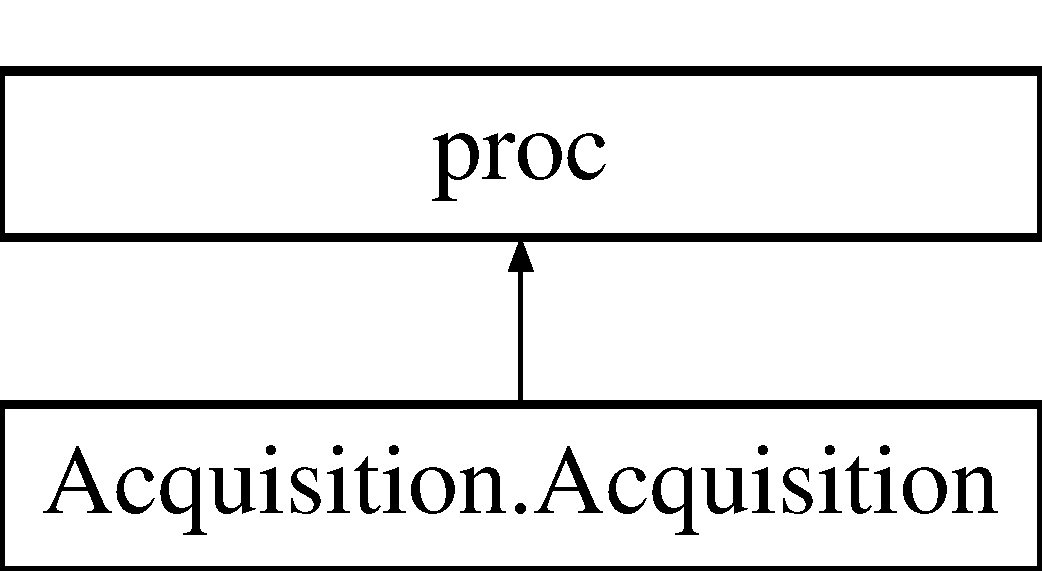
\includegraphics[height=2.000000cm]{classAcquisition_1_1Acquisition}
\end{center}
\end{figure}
\subsection*{Public Member Functions}
\begin{DoxyCompactItemize}
\item 
def \hyperlink{classAcquisition_1_1Acquisition_a2811edf47d59be70aeb9589a5e339893}{\+\_\+\+\_\+init\+\_\+\+\_\+} (self, cat, obj, panel, path)
\item 
def \hyperlink{classAcquisition_1_1Acquisition_ac7be703152b5ec0e02bc9c742d59cd50}{on\+Apply} (self, event)
\item 
def \hyperlink{classAcquisition_1_1Acquisition_aa686f47e8d19e10efa43c3330fd7d19b}{on\+Soft\+Trig} (self, event)
\item 
def \hyperlink{classAcquisition_1_1Acquisition_a9d82c40d0be476e1f4b9a8ec0f6ea29a}{on\+Tree} (self, event)
\item 
def \hyperlink{classAcquisition_1_1Acquisition_adde3ae2fd3eff1e113bd20651c8561a3}{on\+Trend} (self, event)
\item 
def \hyperlink{classAcquisition_1_1Acquisition_a37caf6d3a03c683c5fbcc079a2d8c7ec}{on\+Sample} (self, event)
\item 
def \hyperlink{classAcquisition_1_1Acquisition_aec0df3e0eea3f89f5c3057fac481be46}{on\+Deadtime} (self, event)
\item 
def \hyperlink{classAcquisition_1_1Acquisition_abd482f75a95cdcc9b55c5adb7c046ae3}{on\+Depth} (self, event)
\item 
def \hyperlink{classAcquisition_1_1Acquisition_ae0cfd44965bc1dd829cd6d6660cdd0ee}{on\+N\+Sample} (self, event)
\item 
def \hyperlink{classAcquisition_1_1Acquisition_a59fd4f2c9690f7745f346281ffe4f658}{on\+N\+Bins} (self, event)
\item 
def \hyperlink{classAcquisition_1_1Acquisition_aeb3c0ebfb598e5b1c03710574826108c}{on\+Min} (self, event)
\item 
def \hyperlink{classAcquisition_1_1Acquisition_ad744ff797e84b6e5f785c24d44144697}{on\+Max} (self, event)
\item 
def \hyperlink{classAcquisition_1_1Acquisition_abb09e973b83aec6cc4c660992b7dcc9d}{update} (self)
\end{DoxyCompactItemize}


\subsection{Detailed Description}


Definition at line 8 of file Acquisition.\+py.



\subsection{Constructor \& Destructor Documentation}
\mbox{\Hypertarget{classAcquisition_1_1Acquisition_a2811edf47d59be70aeb9589a5e339893}\label{classAcquisition_1_1Acquisition_a2811edf47d59be70aeb9589a5e339893}} 
\index{Acquisition\+::\+Acquisition@{Acquisition\+::\+Acquisition}!\+\_\+\+\_\+init\+\_\+\+\_\+@{\+\_\+\+\_\+init\+\_\+\+\_\+}}
\index{\+\_\+\+\_\+init\+\_\+\+\_\+@{\+\_\+\+\_\+init\+\_\+\+\_\+}!Acquisition\+::\+Acquisition@{Acquisition\+::\+Acquisition}}
\subsubsection{\texorpdfstring{\+\_\+\+\_\+init\+\_\+\+\_\+()}{\_\_init\_\_()}}
{\footnotesize\ttfamily def Acquisition.\+Acquisition.\+\_\+\+\_\+init\+\_\+\+\_\+ (\begin{DoxyParamCaption}\item[{}]{self,  }\item[{}]{cat,  }\item[{}]{obj,  }\item[{}]{panel,  }\item[{}]{path }\end{DoxyParamCaption})}



Definition at line 9 of file Acquisition.\+py.



References element.\+element.\+loadxrc(), proc.\+proc.\+loadxrc(), Acquisition.\+Acquisition.\+on\+Apply(), Acquisition.\+Acquisition.\+on\+Deadtime(), Acquisition.\+Acquisition.\+on\+Depth(), Acquisition.\+Acquisition.\+on\+Max(), Acquisition.\+Acquisition.\+on\+Min(), Acquisition.\+Acquisition.\+on\+N\+Bins(), Acquisition.\+Acquisition.\+on\+N\+Sample(), Acquisition.\+Acquisition.\+on\+Sample(), Acquisition.\+Acquisition.\+on\+Soft\+Trig(), Proto40\+M\+Hz\+\_\+v1.\+Proto40\+M\+Hz\+\_\+v1.\+on\+Soft\+Trig(), Proto\+F\+E\+B\+\_\+v1.\+Proto\+F\+E\+B\+\_\+v1.\+on\+Soft\+Trig(), Acquisition.\+Acquisition.\+on\+Tree(), Acquisition.\+Acquisition.\+on\+Trend(), object.\+object.\+panel, element.\+element.\+panel, proc.\+proc.\+panel, Log\+Frame.\+Log\+Frame.\+panel, Conf\+Frame.\+Conf\+Frame.\+panel, Graph\+Frame.\+Graph\+Frame.\+panel, App\+Frame.\+App\+Frame.\+panel, Croc.\+Croc.\+update(), A3\+P\+E\+\_\+\+Bit\+Flip.\+A3\+P\+E\+\_\+\+Bit\+Flip.\+update(), Croc.\+update(), Proto40\+M\+Hz\+\_\+v1.\+update(), Acquisition.\+Acquisition.\+update(), Proto40\+M\+Hz\+\_\+v1.\+Proto40\+M\+Hz\+\_\+v1.\+update(), Proto\+F\+E\+B\+\_\+v1.\+Proto\+F\+E\+B\+\_\+v1.\+update(), Phaser.\+update(), Usb\+F\+T\+Interface.\+update(), M\+S\+Oxxxx.\+update(), I\+C\+E\+C\+A\+Lv3.\+update(), L\+S\+Delay\+Chip\+V1.\+update(), and A3\+P\+E.\+update().


\begin{DoxyCode}
9     \textcolor{keyword}{def }\hyperlink{classwrapper_1_1ModuleDictWrapper_a9a7a794150502f51df687831583e13b9}{\_\_init\_\_}(self, cat, obj, panel, path):
10         proc.\_\_init\_\_(self,cat,obj,panel,path)
11         self.loadxrc()
12         self.panel.Bind(wx.EVT\_TOGGLEBUTTON,self.onSoftTrig,id=xrc.XRCID(\textcolor{stringliteral}{"softtrigger"}))
13         self.panel.Bind(wx.EVT\_TOGGLEBUTTON,self.onTree,id=xrc.XRCID(\textcolor{stringliteral}{"tree"}))
14         self.panel.Bind(wx.EVT\_TOGGLEBUTTON,self.onTrend,id=xrc.XRCID(\textcolor{stringliteral}{"trend"}))
15         self.panel.Bind(wx.EVT\_TOGGLEBUTTON,self.onSample,id=xrc.XRCID(\textcolor{stringliteral}{"sample"}))
16         self.panel.Bind(wx.EVT\_SPINCTRL,self.onDeadtime,id=xrc.XRCID(\textcolor{stringliteral}{"acquisition\_deadtime"}))
17         self.panel.Bind(wx.EVT\_BUTTON,self.onApply,id=xrc.XRCID(\textcolor{stringliteral}{"apply"}))
18         self.panel.Bind(wx.EVT\_SPINCTRL, self.onDepth, id=xrc.XRCID(\textcolor{stringliteral}{"depth"}))
19         self.panel.Bind(wx.EVT\_SPINCTRL, self.onNSample, id=xrc.XRCID(\textcolor{stringliteral}{"nsample"}))
20         self.panel.Bind(wx.EVT\_SPINCTRL, self.onNBins, id=xrc.XRCID(\textcolor{stringliteral}{"nbins"}))
21         self.panel.Bind(wx.EVT\_TEXT, self.onMin, id=xrc.XRCID(\textcolor{stringliteral}{"min"}))
22         self.panel.Bind(wx.EVT\_TEXT, self.onMax, id=xrc.XRCID(\textcolor{stringliteral}{"max"}))
23 
24         self.update()
25 
\end{DoxyCode}


\subsection{Member Function Documentation}
\mbox{\Hypertarget{classAcquisition_1_1Acquisition_ac7be703152b5ec0e02bc9c742d59cd50}\label{classAcquisition_1_1Acquisition_ac7be703152b5ec0e02bc9c742d59cd50}} 
\index{Acquisition\+::\+Acquisition@{Acquisition\+::\+Acquisition}!on\+Apply@{on\+Apply}}
\index{on\+Apply@{on\+Apply}!Acquisition\+::\+Acquisition@{Acquisition\+::\+Acquisition}}
\subsubsection{\texorpdfstring{on\+Apply()}{onApply()}}
{\footnotesize\ttfamily def Acquisition.\+Acquisition.\+on\+Apply (\begin{DoxyParamCaption}\item[{}]{self,  }\item[{}]{event }\end{DoxyParamCaption})}



Definition at line 26 of file Acquisition.\+py.



References object.\+object.\+get\+Control(), Conf\+Frame.\+Conf\+Frame.\+get\+Control(), Graph\+Frame.\+Graph\+Frame.\+get\+Control(), Cfg\+Frame.\+Cfg\+Frame.\+get\+Control(), App\+Frame.\+App\+Frame.\+get\+Control(), object.\+object.\+obj, Cfg\+Frame.\+Cfg\+Frame.\+obj, and Acquisition.\+set\+Channels().



Referenced by A3\+P\+E\+\_\+\+Bit\+Flip.\+A3\+P\+E\+\_\+\+Bit\+Flip.\+\_\+\+\_\+init\+\_\+\+\_\+(), Emulate\+F\+E.\+Emulate\+F\+E.\+\_\+\+\_\+init\+\_\+\+\_\+(), and Acquisition.\+Acquisition.\+\_\+\+\_\+init\+\_\+\+\_\+().


\begin{DoxyCode}
26     \textcolor{keyword}{def }onApply(self,event):
27         channels=0
28         \textcolor{keywordflow}{if} (self.getControl(\textcolor{stringliteral}{"chl0"}).GetValue()) : channels=channels|0b1
29         \textcolor{keywordflow}{else} : channels=channels&0b11111110
30         \textcolor{keywordflow}{if} (self.getControl(\textcolor{stringliteral}{"chl1"}).GetValue()) : channels=channels|0b10
31         \textcolor{keywordflow}{else} : channels=channels&0b11111101
32         \textcolor{keywordflow}{if} (self.getControl(\textcolor{stringliteral}{"chl2"}).GetValue()) : channels=channels|0b100
33         \textcolor{keywordflow}{else} : channels=channels&0b11111011
34         \textcolor{keywordflow}{if} (self.getControl(\textcolor{stringliteral}{"chl3"}).GetValue()) : channels=channels|0b1000
35         \textcolor{keywordflow}{else} : channels=channels&0b11110111
36         \textcolor{keywordflow}{if} (self.getControl(\textcolor{stringliteral}{"chl4"}).GetValue()) : channels=channels|0b10000
37         \textcolor{keywordflow}{else} : channels=channels&0b11101111
38         \textcolor{keywordflow}{if} (self.getControl(\textcolor{stringliteral}{"chl5"}).GetValue()) : channels=channels|0b100000
39         \textcolor{keywordflow}{else} : channels=channels&0b11011111
40         \textcolor{keywordflow}{if} (self.getControl(\textcolor{stringliteral}{"chl6"}).GetValue()) : channels=channels|0b1000000
41         \textcolor{keywordflow}{else} : channels=channels&0b10111111
42         \textcolor{keywordflow}{if} (self.getControl(\textcolor{stringliteral}{"chl7"}).GetValue()) : channels=channels|0b10000000
43         \textcolor{keywordflow}{else} : channels=channels&0b1111111
44         self.obj.setChannels(channels)            
45         
\end{DoxyCode}
\mbox{\Hypertarget{classAcquisition_1_1Acquisition_aec0df3e0eea3f89f5c3057fac481be46}\label{classAcquisition_1_1Acquisition_aec0df3e0eea3f89f5c3057fac481be46}} 
\index{Acquisition\+::\+Acquisition@{Acquisition\+::\+Acquisition}!on\+Deadtime@{on\+Deadtime}}
\index{on\+Deadtime@{on\+Deadtime}!Acquisition\+::\+Acquisition@{Acquisition\+::\+Acquisition}}
\subsubsection{\texorpdfstring{on\+Deadtime()}{onDeadtime()}}
{\footnotesize\ttfamily def Acquisition.\+Acquisition.\+on\+Deadtime (\begin{DoxyParamCaption}\item[{}]{self,  }\item[{}]{event }\end{DoxyParamCaption})}



Definition at line 64 of file Acquisition.\+py.



References object.\+object.\+get\+Control(), Conf\+Frame.\+Conf\+Frame.\+get\+Control(), Graph\+Frame.\+Graph\+Frame.\+get\+Control(), Cfg\+Frame.\+Cfg\+Frame.\+get\+Control(), App\+Frame.\+App\+Frame.\+get\+Control(), object.\+object.\+obj, Cfg\+Frame.\+Cfg\+Frame.\+obj, and Acquisition.\+set\+Dead\+Time().



Referenced by Acquisition.\+Acquisition.\+\_\+\+\_\+init\+\_\+\+\_\+().


\begin{DoxyCode}
64     \textcolor{keyword}{def }onDeadtime(self,event):
65         self.obj.setDeadTime(self.getControl(\textcolor{stringliteral}{"acquisition\_deadtime"}).GetValue())
\end{DoxyCode}
\mbox{\Hypertarget{classAcquisition_1_1Acquisition_abd482f75a95cdcc9b55c5adb7c046ae3}\label{classAcquisition_1_1Acquisition_abd482f75a95cdcc9b55c5adb7c046ae3}} 
\index{Acquisition\+::\+Acquisition@{Acquisition\+::\+Acquisition}!on\+Depth@{on\+Depth}}
\index{on\+Depth@{on\+Depth}!Acquisition\+::\+Acquisition@{Acquisition\+::\+Acquisition}}
\subsubsection{\texorpdfstring{on\+Depth()}{onDepth()}}
{\footnotesize\ttfamily def Acquisition.\+Acquisition.\+on\+Depth (\begin{DoxyParamCaption}\item[{}]{self,  }\item[{}]{event }\end{DoxyParamCaption})}



Definition at line 66 of file Acquisition.\+py.



References object.\+object.\+get\+Control(), Conf\+Frame.\+Conf\+Frame.\+get\+Control(), Graph\+Frame.\+Graph\+Frame.\+get\+Control(), Cfg\+Frame.\+Cfg\+Frame.\+get\+Control(), App\+Frame.\+App\+Frame.\+get\+Control(), object.\+object.\+obj, Cfg\+Frame.\+Cfg\+Frame.\+obj, and Acquisition.\+set\+Depth().



Referenced by Acquisition.\+Acquisition.\+\_\+\+\_\+init\+\_\+\+\_\+().


\begin{DoxyCode}
66     \textcolor{keyword}{def }onDepth(self,event):
67         self.obj.setDepth(self.getControl(\textcolor{stringliteral}{"depth"}).GetValue()) 
68 
\end{DoxyCode}
\mbox{\Hypertarget{classAcquisition_1_1Acquisition_ad744ff797e84b6e5f785c24d44144697}\label{classAcquisition_1_1Acquisition_ad744ff797e84b6e5f785c24d44144697}} 
\index{Acquisition\+::\+Acquisition@{Acquisition\+::\+Acquisition}!on\+Max@{on\+Max}}
\index{on\+Max@{on\+Max}!Acquisition\+::\+Acquisition@{Acquisition\+::\+Acquisition}}
\subsubsection{\texorpdfstring{on\+Max()}{onMax()}}
{\footnotesize\ttfamily def Acquisition.\+Acquisition.\+on\+Max (\begin{DoxyParamCaption}\item[{}]{self,  }\item[{}]{event }\end{DoxyParamCaption})}



Definition at line 78 of file Acquisition.\+py.



References object.\+object.\+get\+Control(), Conf\+Frame.\+Conf\+Frame.\+get\+Control(), Graph\+Frame.\+Graph\+Frame.\+get\+Control(), Cfg\+Frame.\+Cfg\+Frame.\+get\+Control(), App\+Frame.\+App\+Frame.\+get\+Control(), object.\+object.\+obj, Cfg\+Frame.\+Cfg\+Frame.\+obj, and Acquisition.\+set\+Max\+Range().



Referenced by Acquisition.\+Acquisition.\+\_\+\+\_\+init\+\_\+\+\_\+().


\begin{DoxyCode}
78     \textcolor{keyword}{def }onMax(self,event):
79         self.obj.setMaxRange(float(self.getControl(\textcolor{stringliteral}{"max"}).GetValue()))  
80 
\end{DoxyCode}
\mbox{\Hypertarget{classAcquisition_1_1Acquisition_aeb3c0ebfb598e5b1c03710574826108c}\label{classAcquisition_1_1Acquisition_aeb3c0ebfb598e5b1c03710574826108c}} 
\index{Acquisition\+::\+Acquisition@{Acquisition\+::\+Acquisition}!on\+Min@{on\+Min}}
\index{on\+Min@{on\+Min}!Acquisition\+::\+Acquisition@{Acquisition\+::\+Acquisition}}
\subsubsection{\texorpdfstring{on\+Min()}{onMin()}}
{\footnotesize\ttfamily def Acquisition.\+Acquisition.\+on\+Min (\begin{DoxyParamCaption}\item[{}]{self,  }\item[{}]{event }\end{DoxyParamCaption})}



Definition at line 75 of file Acquisition.\+py.



References object.\+object.\+get\+Control(), Conf\+Frame.\+Conf\+Frame.\+get\+Control(), Graph\+Frame.\+Graph\+Frame.\+get\+Control(), Cfg\+Frame.\+Cfg\+Frame.\+get\+Control(), App\+Frame.\+App\+Frame.\+get\+Control(), object.\+object.\+obj, Cfg\+Frame.\+Cfg\+Frame.\+obj, and Acquisition.\+set\+Min\+Range().



Referenced by Acquisition.\+Acquisition.\+\_\+\+\_\+init\+\_\+\+\_\+().


\begin{DoxyCode}
75     \textcolor{keyword}{def }onMin(self,event):
76         self.obj.setMinRange(float(self.getControl(\textcolor{stringliteral}{"min"}).GetValue()))  
77 
\end{DoxyCode}
\mbox{\Hypertarget{classAcquisition_1_1Acquisition_a59fd4f2c9690f7745f346281ffe4f658}\label{classAcquisition_1_1Acquisition_a59fd4f2c9690f7745f346281ffe4f658}} 
\index{Acquisition\+::\+Acquisition@{Acquisition\+::\+Acquisition}!on\+N\+Bins@{on\+N\+Bins}}
\index{on\+N\+Bins@{on\+N\+Bins}!Acquisition\+::\+Acquisition@{Acquisition\+::\+Acquisition}}
\subsubsection{\texorpdfstring{on\+N\+Bins()}{onNBins()}}
{\footnotesize\ttfamily def Acquisition.\+Acquisition.\+on\+N\+Bins (\begin{DoxyParamCaption}\item[{}]{self,  }\item[{}]{event }\end{DoxyParamCaption})}



Definition at line 72 of file Acquisition.\+py.



References object.\+object.\+get\+Control(), Conf\+Frame.\+Conf\+Frame.\+get\+Control(), Graph\+Frame.\+Graph\+Frame.\+get\+Control(), Cfg\+Frame.\+Cfg\+Frame.\+get\+Control(), App\+Frame.\+App\+Frame.\+get\+Control(), object.\+object.\+obj, Cfg\+Frame.\+Cfg\+Frame.\+obj, and Acquisition.\+set\+N\+Bins().



Referenced by Acquisition.\+Acquisition.\+\_\+\+\_\+init\+\_\+\+\_\+().


\begin{DoxyCode}
72     \textcolor{keyword}{def }onNBins(self,event):
73         self.obj.setNBins(self.getControl(\textcolor{stringliteral}{"nbins"}).GetValue())  
74 
\end{DoxyCode}
\mbox{\Hypertarget{classAcquisition_1_1Acquisition_ae0cfd44965bc1dd829cd6d6660cdd0ee}\label{classAcquisition_1_1Acquisition_ae0cfd44965bc1dd829cd6d6660cdd0ee}} 
\index{Acquisition\+::\+Acquisition@{Acquisition\+::\+Acquisition}!on\+N\+Sample@{on\+N\+Sample}}
\index{on\+N\+Sample@{on\+N\+Sample}!Acquisition\+::\+Acquisition@{Acquisition\+::\+Acquisition}}
\subsubsection{\texorpdfstring{on\+N\+Sample()}{onNSample()}}
{\footnotesize\ttfamily def Acquisition.\+Acquisition.\+on\+N\+Sample (\begin{DoxyParamCaption}\item[{}]{self,  }\item[{}]{event }\end{DoxyParamCaption})}



Definition at line 69 of file Acquisition.\+py.



References object.\+object.\+get\+Control(), Conf\+Frame.\+Conf\+Frame.\+get\+Control(), Graph\+Frame.\+Graph\+Frame.\+get\+Control(), Cfg\+Frame.\+Cfg\+Frame.\+get\+Control(), App\+Frame.\+App\+Frame.\+get\+Control(), object.\+object.\+obj, Cfg\+Frame.\+Cfg\+Frame.\+obj, and Acquisition.\+set\+Sample().



Referenced by Acquisition.\+Acquisition.\+\_\+\+\_\+init\+\_\+\+\_\+().


\begin{DoxyCode}
69     \textcolor{keyword}{def }onNSample(self,event):
70         self.obj.setSample(self.getControl(\textcolor{stringliteral}{"nsample"}).GetValue()) 
71 
\end{DoxyCode}
\mbox{\Hypertarget{classAcquisition_1_1Acquisition_a37caf6d3a03c683c5fbcc079a2d8c7ec}\label{classAcquisition_1_1Acquisition_a37caf6d3a03c683c5fbcc079a2d8c7ec}} 
\index{Acquisition\+::\+Acquisition@{Acquisition\+::\+Acquisition}!on\+Sample@{on\+Sample}}
\index{on\+Sample@{on\+Sample}!Acquisition\+::\+Acquisition@{Acquisition\+::\+Acquisition}}
\subsubsection{\texorpdfstring{on\+Sample()}{onSample()}}
{\footnotesize\ttfamily def Acquisition.\+Acquisition.\+on\+Sample (\begin{DoxyParamCaption}\item[{}]{self,  }\item[{}]{event }\end{DoxyParamCaption})}



Definition at line 61 of file Acquisition.\+py.



References object.\+object.\+get\+Control(), Conf\+Frame.\+Conf\+Frame.\+get\+Control(), Graph\+Frame.\+Graph\+Frame.\+get\+Control(), Cfg\+Frame.\+Cfg\+Frame.\+get\+Control(), App\+Frame.\+App\+Frame.\+get\+Control(), object.\+object.\+obj, Cfg\+Frame.\+Cfg\+Frame.\+obj, and Acquisition.\+set\+Store\+Sample().



Referenced by Acquisition.\+Acquisition.\+\_\+\+\_\+init\+\_\+\+\_\+().


\begin{DoxyCode}
61     \textcolor{keyword}{def }onSample(self,event):
62         self.obj.setStoreSample(self.getControl(\textcolor{stringliteral}{"sample"}).GetValue())
63 
\end{DoxyCode}
\mbox{\Hypertarget{classAcquisition_1_1Acquisition_aa686f47e8d19e10efa43c3330fd7d19b}\label{classAcquisition_1_1Acquisition_aa686f47e8d19e10efa43c3330fd7d19b}} 
\index{Acquisition\+::\+Acquisition@{Acquisition\+::\+Acquisition}!on\+Soft\+Trig@{on\+Soft\+Trig}}
\index{on\+Soft\+Trig@{on\+Soft\+Trig}!Acquisition\+::\+Acquisition@{Acquisition\+::\+Acquisition}}
\subsubsection{\texorpdfstring{on\+Soft\+Trig()}{onSoftTrig()}}
{\footnotesize\ttfamily def Acquisition.\+Acquisition.\+on\+Soft\+Trig (\begin{DoxyParamCaption}\item[{}]{self,  }\item[{}]{event }\end{DoxyParamCaption})}



Definition at line 46 of file Acquisition.\+py.



References object.\+object.\+get\+Control(), Conf\+Frame.\+Conf\+Frame.\+get\+Control(), Graph\+Frame.\+Graph\+Frame.\+get\+Control(), Cfg\+Frame.\+Cfg\+Frame.\+get\+Control(), App\+Frame.\+App\+Frame.\+get\+Control(), object.\+object.\+obj, Cfg\+Frame.\+Cfg\+Frame.\+obj, and Acquisition.\+set\+Trigger().



Referenced by Acquisition.\+Acquisition.\+\_\+\+\_\+init\+\_\+\+\_\+().


\begin{DoxyCode}
46     \textcolor{keyword}{def }onSoftTrig(self,event):
47         self.obj.setTrigger(self.getControl(\textcolor{stringliteral}{"softtrigger"}).GetValue())
48         \textcolor{keywordflow}{if} self.getControl(\textcolor{stringliteral}{"softtrigger"}).GetValue():
49             self.getControl(\textcolor{stringliteral}{"softtrigger"}).SetValue(1)
50             self.getControl(\textcolor{stringliteral}{"softtrigger"}).SetLabel(\textcolor{stringliteral}{"Soft. Trig."})
51         \textcolor{keywordflow}{else}:
52             self.getControl(\textcolor{stringliteral}{"softtrigger"}).SetValue(0)
53             self.getControl(\textcolor{stringliteral}{"softtrigger"}).SetLabel(\textcolor{stringliteral}{"Ext. Trig."})
54 
\end{DoxyCode}
\mbox{\Hypertarget{classAcquisition_1_1Acquisition_a9d82c40d0be476e1f4b9a8ec0f6ea29a}\label{classAcquisition_1_1Acquisition_a9d82c40d0be476e1f4b9a8ec0f6ea29a}} 
\index{Acquisition\+::\+Acquisition@{Acquisition\+::\+Acquisition}!on\+Tree@{on\+Tree}}
\index{on\+Tree@{on\+Tree}!Acquisition\+::\+Acquisition@{Acquisition\+::\+Acquisition}}
\subsubsection{\texorpdfstring{on\+Tree()}{onTree()}}
{\footnotesize\ttfamily def Acquisition.\+Acquisition.\+on\+Tree (\begin{DoxyParamCaption}\item[{}]{self,  }\item[{}]{event }\end{DoxyParamCaption})}



Definition at line 55 of file Acquisition.\+py.



References object.\+object.\+get\+Control(), Conf\+Frame.\+Conf\+Frame.\+get\+Control(), Graph\+Frame.\+Graph\+Frame.\+get\+Control(), Cfg\+Frame.\+Cfg\+Frame.\+get\+Control(), App\+Frame.\+App\+Frame.\+get\+Control(), object.\+object.\+obj, Cfg\+Frame.\+Cfg\+Frame.\+obj, and Acquisition.\+set\+Store\+Tree().



Referenced by Acquisition.\+Acquisition.\+\_\+\+\_\+init\+\_\+\+\_\+().


\begin{DoxyCode}
55     \textcolor{keyword}{def }onTree(self,event):
56         self.obj.setStoreTree(self.getControl(\textcolor{stringliteral}{"tree"}).GetValue())
57 
\end{DoxyCode}
\mbox{\Hypertarget{classAcquisition_1_1Acquisition_adde3ae2fd3eff1e113bd20651c8561a3}\label{classAcquisition_1_1Acquisition_adde3ae2fd3eff1e113bd20651c8561a3}} 
\index{Acquisition\+::\+Acquisition@{Acquisition\+::\+Acquisition}!on\+Trend@{on\+Trend}}
\index{on\+Trend@{on\+Trend}!Acquisition\+::\+Acquisition@{Acquisition\+::\+Acquisition}}
\subsubsection{\texorpdfstring{on\+Trend()}{onTrend()}}
{\footnotesize\ttfamily def Acquisition.\+Acquisition.\+on\+Trend (\begin{DoxyParamCaption}\item[{}]{self,  }\item[{}]{event }\end{DoxyParamCaption})}



Definition at line 58 of file Acquisition.\+py.



References object.\+object.\+get\+Control(), Conf\+Frame.\+Conf\+Frame.\+get\+Control(), Graph\+Frame.\+Graph\+Frame.\+get\+Control(), Cfg\+Frame.\+Cfg\+Frame.\+get\+Control(), App\+Frame.\+App\+Frame.\+get\+Control(), object.\+object.\+obj, Cfg\+Frame.\+Cfg\+Frame.\+obj, and Acquisition.\+set\+Store\+Trend().



Referenced by Acquisition.\+Acquisition.\+\_\+\+\_\+init\+\_\+\+\_\+().


\begin{DoxyCode}
58     \textcolor{keyword}{def }onTrend(self,event):
59         self.obj.setStoreTrend(self.getControl(\textcolor{stringliteral}{"trend"}).GetValue())
60 
\end{DoxyCode}
\mbox{\Hypertarget{classAcquisition_1_1Acquisition_abb09e973b83aec6cc4c660992b7dcc9d}\label{classAcquisition_1_1Acquisition_abb09e973b83aec6cc4c660992b7dcc9d}} 
\index{Acquisition\+::\+Acquisition@{Acquisition\+::\+Acquisition}!update@{update}}
\index{update@{update}!Acquisition\+::\+Acquisition@{Acquisition\+::\+Acquisition}}
\subsubsection{\texorpdfstring{update()}{update()}}
{\footnotesize\ttfamily def Acquisition.\+Acquisition.\+update (\begin{DoxyParamCaption}\item[{}]{self }\end{DoxyParamCaption})}



Definition at line 81 of file Acquisition.\+py.



References Acquisition.\+channels(), Acquisition.\+dead\+Time(), Acquisition.\+depth(), object.\+object.\+get\+Control(), Conf\+Frame.\+Conf\+Frame.\+get\+Control(), Graph\+Frame.\+Graph\+Frame.\+get\+Control(), Cfg\+Frame.\+Cfg\+Frame.\+get\+Control(), App\+Frame.\+App\+Frame.\+get\+Control(), Acquisition.\+max\+Range(), Acquisition.\+min\+Range(), Acquisition.\+n\+Bins(), object.\+object.\+obj, Cfg\+Frame.\+Cfg\+Frame.\+obj, Acquisition.\+sample(), Acquisition.\+store\+Sample(), Acquisition.\+store\+Tree(), Acquisition.\+store\+Trend(), and Acquisition.\+trigger().



Referenced by Acquisition.\+Acquisition.\+\_\+\+\_\+init\+\_\+\+\_\+(), Emulate\+F\+E.\+Emulate\+F\+E.\+\_\+\+\_\+init\+\_\+\+\_\+(), App\+Frame.\+App\+Frame.\+delete\+Hardware(), Conf\+Frame.\+Conf\+Frame.\+on\+Change(), Graph\+Frame.\+Graph\+Frame.\+on\+Change(), Cfg\+Frame.\+Cfg\+Frame.\+on\+Change(), Conf\+Frame.\+Conf\+Frame.\+on\+Edit(), App\+Frame.\+App\+Frame.\+on\+Load(), Conf\+Frame.\+Conf\+Frame.\+on\+Re\+Load(), Graph\+Frame.\+Graph\+Frame.\+on\+Re\+Load(), Cfg\+Frame.\+Cfg\+Frame.\+on\+Re\+Load(), and App\+Frame.\+App\+Frame.\+on\+Re\+Load().


\begin{DoxyCode}
81     \textcolor{keyword}{def }update(self):
82         \textcolor{keywordflow}{if} self.obj.trigger():
83             self.getControl(\textcolor{stringliteral}{"softtrigger"}).SetValue(1)
84             self.getControl(\textcolor{stringliteral}{"softtrigger"}).SetLabel(\textcolor{stringliteral}{"Soft. Trig."})
85         \textcolor{keywordflow}{else}:
86             self.getControl(\textcolor{stringliteral}{"softtrigger"}).SetValue(0)
87             self.getControl(\textcolor{stringliteral}{"softtrigger"}).SetLabel(\textcolor{stringliteral}{"Ext. Trig."})
88 
89         channels=self.obj.channels()
90         \textcolor{keywordflow}{if} (channels&1) : self.getControl(\textcolor{stringliteral}{"chl0"}).SetValue(\textcolor{keyword}{True})
91         \textcolor{keywordflow}{else} : self.getControl(\textcolor{stringliteral}{"chl0"}).SetValue(\textcolor{keyword}{False})
92         \textcolor{keywordflow}{if} (channels&0b10) : self.getControl(\textcolor{stringliteral}{"chl1"}).SetValue(\textcolor{keyword}{True})
93         \textcolor{keywordflow}{else} : self.getControl(\textcolor{stringliteral}{"chl1"}).SetValue(\textcolor{keyword}{False})
94         \textcolor{keywordflow}{if} (channels&0b100) : self.getControl(\textcolor{stringliteral}{"chl2"}).SetValue(\textcolor{keyword}{True})
95         \textcolor{keywordflow}{else} : self.getControl(\textcolor{stringliteral}{"chl2"}).SetValue(\textcolor{keyword}{False})
96         \textcolor{keywordflow}{if} (channels&0b1000) : self.getControl(\textcolor{stringliteral}{"chl3"}).SetValue(\textcolor{keyword}{True})
97         \textcolor{keywordflow}{else} : self.getControl(\textcolor{stringliteral}{"chl3"}).SetValue(\textcolor{keyword}{False})
98         \textcolor{keywordflow}{if} (channels&0b10000) : self.getControl(\textcolor{stringliteral}{"chl4"}).SetValue(\textcolor{keyword}{True})
99         \textcolor{keywordflow}{else} : self.getControl(\textcolor{stringliteral}{"chl4"}).SetValue(\textcolor{keyword}{False})
100         \textcolor{keywordflow}{if} (channels&0b100000) : self.getControl(\textcolor{stringliteral}{"chl5"}).SetValue(\textcolor{keyword}{True})
101         \textcolor{keywordflow}{else} : self.getControl(\textcolor{stringliteral}{"chl5"}).SetValue(\textcolor{keyword}{False})
102         \textcolor{keywordflow}{if} (channels&0b1000000) : self.getControl(\textcolor{stringliteral}{"chl6"}).SetValue(\textcolor{keyword}{True})
103         \textcolor{keywordflow}{else} : self.getControl(\textcolor{stringliteral}{"chl6"}).SetValue(\textcolor{keyword}{False})
104         \textcolor{keywordflow}{if} (channels&0b10000000) : self.getControl(\textcolor{stringliteral}{"chl7"}).SetValue(\textcolor{keyword}{True})
105         \textcolor{keywordflow}{else} : self.getControl(\textcolor{stringliteral}{"chl7"}).SetValue(\textcolor{keyword}{False})
106         self.getControl(\textcolor{stringliteral}{"depth"}).SetValue(self.obj.depth())
107         self.getControl(\textcolor{stringliteral}{"tree"}).SetValue(self.obj.storeTree())
108         self.getControl(\textcolor{stringliteral}{"trend"}).SetValue(self.obj.storeTrend())
109         self.getControl(\textcolor{stringliteral}{"sample"}).SetValue(self.obj.storeSample())
110         self.getControl(\textcolor{stringliteral}{"acquisition\_deadtime"}).SetValue(self.obj.deadTime())
111         self.getControl(\textcolor{stringliteral}{"depth"}).SetValue(self.obj.depth())
112         self.getControl(\textcolor{stringliteral}{"nsample"}).SetValue(self.obj.sample())
113         self.getControl(\textcolor{stringliteral}{"nbins"}).SetValue(self.obj.nBins())
114         self.getControl(\textcolor{stringliteral}{"min"}).SetValue(str(self.obj.minRange()))
115         self.getControl(\textcolor{stringliteral}{"max"}).SetValue(str(self.obj.maxRange()))
116          
117 \textcolor{comment}{#----------------------------------------------------------------------}
118 
\end{DoxyCode}


The documentation for this class was generated from the following file\+:\begin{DoxyCompactItemize}
\item 
/home/eleclhcb/\+L\+H\+Cb/lbcat-\/cmake/\+Cat\+Calo\+Proto40\+M\+Hz/python/proc/\hyperlink{Acquisition_8py}{Acquisition.\+py}\end{DoxyCompactItemize}

\hypertarget{classADCMeasurement}{}\section{A\+D\+C\+Measurement Class Reference}
\label{classADCMeasurement}\index{A\+D\+C\+Measurement@{A\+D\+C\+Measurement}}


{\ttfamily \#include $<$include/\+A\+D\+C\+Measurement.\+h$>$}

Inheritance diagram for A\+D\+C\+Measurement\+:\begin{figure}[H]
\begin{center}
\leavevmode
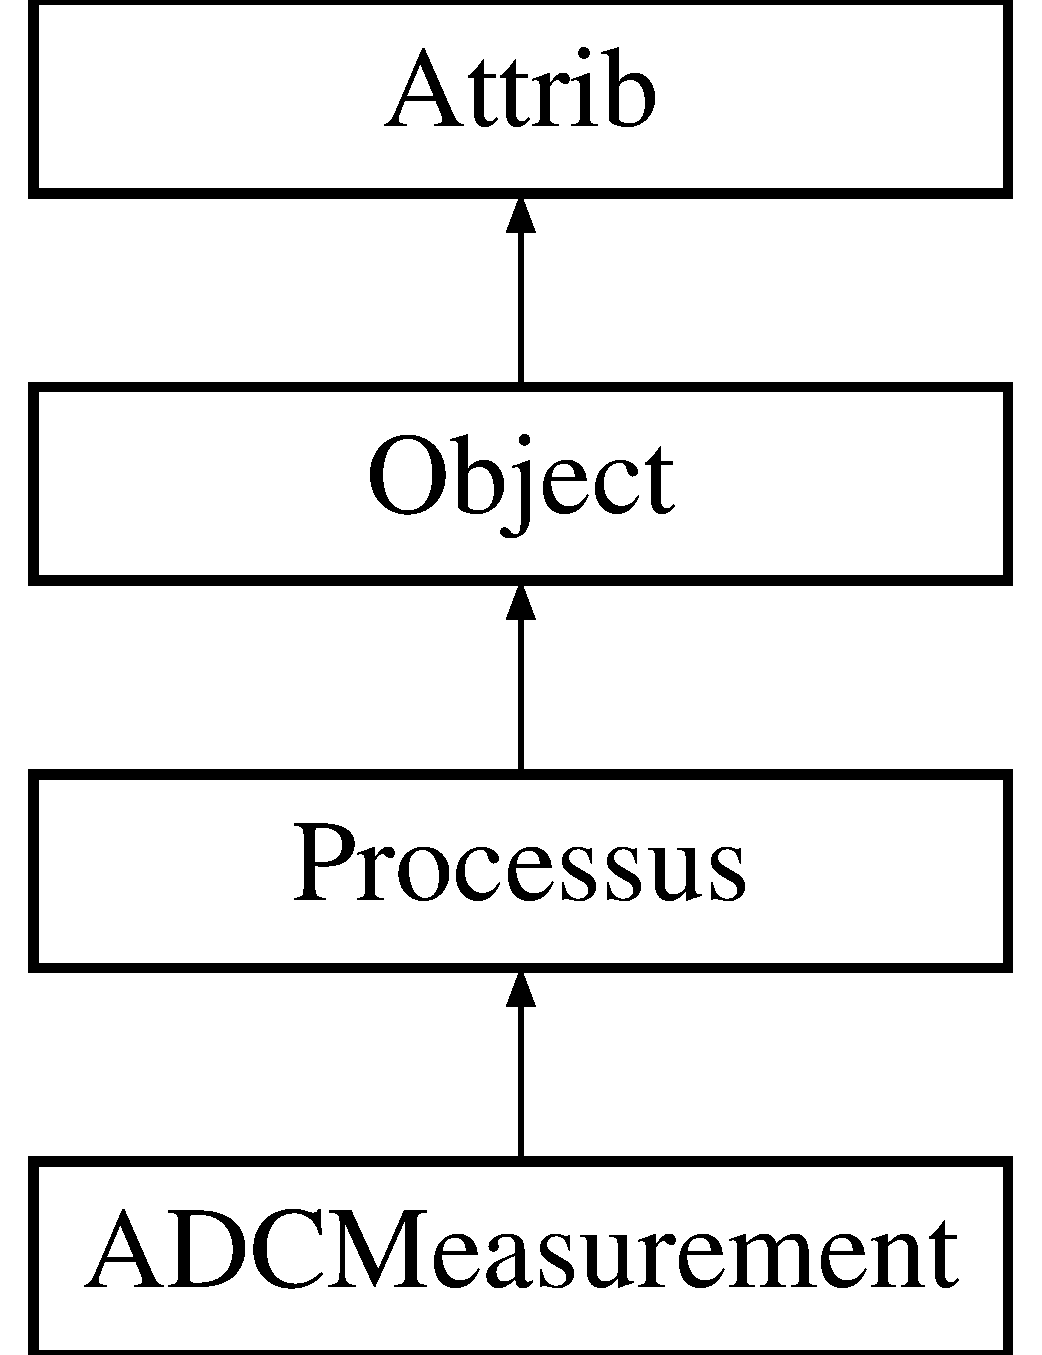
\includegraphics[height=4.000000cm]{classADCMeasurement}
\end{center}
\end{figure}
\subsection*{Classes}
\begin{DoxyCompactItemize}
\item 
class \hyperlink{classADCMeasurement_1_1CurrentMeasurement}{Current\+Measurement}
\end{DoxyCompactItemize}
\subsection*{Public Member Functions}
\begin{DoxyCompactItemize}
\item 
\hyperlink{classADCMeasurement_a93804f658f3aaa78d3ce18199f1bf8e1}{A\+D\+C\+Measurement} ()
\begin{DoxyCompactList}\small\item\em Standard constructor. \end{DoxyCompactList}\item 
virtual \hyperlink{classADCMeasurement_aa89145ed91025783a1bb277cb480ed1c}{$\sim$\+A\+D\+C\+Measurement} ()
\item 
virtual \hyperlink{classStatusCode}{Status\+Code} \hyperlink{classADCMeasurement_a3fc6d3e863fecc7a1caf91f9b0ca5268}{initialize} ()
\begin{DoxyCompactList}\small\item\em Destructor. \end{DoxyCompactList}\item 
virtual \hyperlink{classStatusCode}{Status\+Code} \hyperlink{classADCMeasurement_a82de69f0488646dfc50d28f611e2010d}{execute} ()
\item 
virtual \hyperlink{classStatusCode}{Status\+Code} \hyperlink{classADCMeasurement_a02a5ae7c0f9c90d0dad00c1d40a1c52a}{finalize} ()
\item 
\hyperlink{classStatusCode}{Status\+Code} \hyperlink{classADCMeasurement_a08433e5168f45de1061bf9a17f022f68}{set\+Frequency} (unsigned int \hyperlink{classADCMeasurement_ad3d523331ad64494f2415319a03c638e}{frequency})
\item 
unsigned int \hyperlink{classADCMeasurement_ad3d523331ad64494f2415319a03c638e}{frequency} ()
\item 
unsigned int \hyperlink{classADCMeasurement_a7f91c4feea465de03bd017a005125177}{number\+Of\+Devices} ()
\end{DoxyCompactItemize}
\subsection*{Protected Member Functions}
\begin{DoxyCompactItemize}
\item 
\hyperlink{classADCMeasurement}{A\+D\+C\+Measurement} $\ast$ \hyperlink{classADCMeasurement_a6e34c2b4e3451f1fd128d213723ab1b9}{clone} ()
\end{DoxyCompactItemize}
\subsection*{Private Attributes}
\begin{DoxyCompactItemize}
\item 
T\+Random $\ast$ \hyperlink{classADCMeasurement_acdced9621e4b56d6772b8b34060b0a9d}{m\+\_\+rnd}
\item 
\hyperlink{classNI6008}{N\+I6008} $\ast$ \hyperlink{classADCMeasurement_afc825cc28b05894a0f762452459988e1}{m\+\_\+device}
\item 
unsigned int \hyperlink{classADCMeasurement_ab4a0653cc015ddf9b33b877c1d43b260}{m\+\_\+frequency}
\item 
T\+Tree $\ast$ \hyperlink{classADCMeasurement_ac218556f79d8a0533b292e96347ccd29}{m\+\_\+tree}
\item 
Int\+\_\+t \hyperlink{classADCMeasurement_aba8bc92a86954118babdc49b612a2412}{m\+\_\+run\+Number}
\item 
Int\+\_\+t \hyperlink{classADCMeasurement_ae21dcb1aeff71570c870648839a0c914}{m\+\_\+evt\+Number}
\item 
Int\+\_\+t \hyperlink{classADCMeasurement_a1fa77f5df72a81eab7e55e97d4bea27f}{m\+\_\+timestamp}
\item 
Int\+\_\+t \hyperlink{classADCMeasurement_a92c0ee7d148bb63de876817f624d1527}{m\+\_\+duration}
\item 
time\+\_\+t \hyperlink{classADCMeasurement_a5c2c98ec69e2331906b0eb41a826508e}{m\+\_\+start\+Time}
\item 
Float\+\_\+t \hyperlink{classADCMeasurement_a97ab811c2ef605184b78593cedea275b}{m\+\_\+ai0}
\item 
Float\+\_\+t \hyperlink{classADCMeasurement_ada963374f6f42db11aef7dbc239ce9fb}{m\+\_\+ai1}
\item 
Float\+\_\+t \hyperlink{classADCMeasurement_a45354a95e055970da767ffe534a0d798}{m\+\_\+ao0}
\item 
Float\+\_\+t \hyperlink{classADCMeasurement_a149349cc87061e2604b9e021aa63ee8c}{m\+\_\+ao1}
\item 
Int\+\_\+t \hyperlink{classADCMeasurement_ae024ec8553b7ea765af8668ab5e95699}{m\+\_\+diA}
\item 
Int\+\_\+t \hyperlink{classADCMeasurement_a9d04a602dda58b9fd65acf4a0a7de9a3}{m\+\_\+diB}
\item 
Float\+\_\+t \hyperlink{classADCMeasurement_ab015017d6a05ac4711836ceb1e072a85}{m\+\_\+min\+Ramp}
\item 
Float\+\_\+t \hyperlink{classADCMeasurement_a5e1f799c05f5781004a9081c4064e4a8}{m\+\_\+max\+Ramp}
\item 
Int\+\_\+t \hyperlink{classADCMeasurement_aa73b7cbd45e13df16291ff740f6140fe}{m\+\_\+step\+Ramp}
\item 
Float\+\_\+t \hyperlink{classADCMeasurement_ac84ed2ba70f38e73ec0eec1de65bbdca}{m\+\_\+ramp}
\item 
Int\+\_\+t \hyperlink{classADCMeasurement_aba7433a9e637389cc5425d036867a08f}{m\+\_\+baseline}
\end{DoxyCompactItemize}
\subsection*{Additional Inherited Members}


\subsection{Detailed Description}
\begin{DoxyAuthor}{Author}
Frederic Machefert 
\end{DoxyAuthor}
\begin{DoxyDate}{Date}
2010-\/01-\/07 
\end{DoxyDate}


Definition at line 23 of file A\+D\+C\+Measurement.\+h.



\subsection{Constructor \& Destructor Documentation}
\mbox{\Hypertarget{classADCMeasurement_a93804f658f3aaa78d3ce18199f1bf8e1}\label{classADCMeasurement_a93804f658f3aaa78d3ce18199f1bf8e1}} 
\index{A\+D\+C\+Measurement@{A\+D\+C\+Measurement}!A\+D\+C\+Measurement@{A\+D\+C\+Measurement}}
\index{A\+D\+C\+Measurement@{A\+D\+C\+Measurement}!A\+D\+C\+Measurement@{A\+D\+C\+Measurement}}
\subsubsection{\texorpdfstring{A\+D\+C\+Measurement()}{ADCMeasurement()}}
{\footnotesize\ttfamily A\+D\+C\+Measurement\+::\+A\+D\+C\+Measurement (\begin{DoxyParamCaption}{ }\end{DoxyParamCaption})}



Standard constructor. 



Definition at line 26 of file A\+D\+C\+Measurement.\+cpp.



References Object\+::set\+Name(), Object\+::set\+Title(), and Object\+::set\+Type().



Referenced by clone().


\begin{DoxyCode}
26                                 \{
27   \hyperlink{classObject_ae30fea75683c2d149b6b6d17c09ecd0c}{setName} ( \textcolor{stringliteral}{"ADCMeasurement"} );
28   \hyperlink{classObject_aae534cc9d982bcb9b99fd505f2e103a5}{setType} ( \textcolor{stringliteral}{"NI6008"} );
29   \hyperlink{classObject_a89557dbbad5bcaa02652f5d7fa35d20f}{setTitle}( \textcolor{stringliteral}{"NI6008 ADC measurement"} );  
30 \}
\end{DoxyCode}
\mbox{\Hypertarget{classADCMeasurement_aa89145ed91025783a1bb277cb480ed1c}\label{classADCMeasurement_aa89145ed91025783a1bb277cb480ed1c}} 
\index{A\+D\+C\+Measurement@{A\+D\+C\+Measurement}!````~A\+D\+C\+Measurement@{$\sim$\+A\+D\+C\+Measurement}}
\index{````~A\+D\+C\+Measurement@{$\sim$\+A\+D\+C\+Measurement}!A\+D\+C\+Measurement@{A\+D\+C\+Measurement}}
\subsubsection{\texorpdfstring{$\sim$\+A\+D\+C\+Measurement()}{~ADCMeasurement()}}
{\footnotesize\ttfamily virtual A\+D\+C\+Measurement\+::$\sim$\+A\+D\+C\+Measurement (\begin{DoxyParamCaption}{ }\end{DoxyParamCaption})\hspace{0.3cm}{\ttfamily [inline]}, {\ttfamily [virtual]}}



Definition at line 28 of file A\+D\+C\+Measurement.\+h.



References execute(), finalize(), and initialize().


\begin{DoxyCode}
28 \{\}; 
\end{DoxyCode}


\subsection{Member Function Documentation}
\mbox{\Hypertarget{classADCMeasurement_a6e34c2b4e3451f1fd128d213723ab1b9}\label{classADCMeasurement_a6e34c2b4e3451f1fd128d213723ab1b9}} 
\index{A\+D\+C\+Measurement@{A\+D\+C\+Measurement}!clone@{clone}}
\index{clone@{clone}!A\+D\+C\+Measurement@{A\+D\+C\+Measurement}}
\subsubsection{\texorpdfstring{clone()}{clone()}}
{\footnotesize\ttfamily \hyperlink{classADCMeasurement}{A\+D\+C\+Measurement}$\ast$ A\+D\+C\+Measurement\+::clone (\begin{DoxyParamCaption}{ }\end{DoxyParamCaption})\hspace{0.3cm}{\ttfamily [inline]}, {\ttfamily [protected]}, {\ttfamily [virtual]}}

processus termination virtual function 

Implements \hyperlink{classProcessus_aca8856f6d6d7b7e1fe941f298dcbb502}{Processus}.



Definition at line 48 of file A\+D\+C\+Measurement.\+h.



References A\+D\+C\+Measurement().


\begin{DoxyCode}
48                          \{
49     \textcolor{keywordflow}{return} \textcolor{keyword}{new} \hyperlink{classADCMeasurement_a93804f658f3aaa78d3ce18199f1bf8e1}{ADCMeasurement} (*\textcolor{keyword}{this});
50   \};
\end{DoxyCode}
\mbox{\Hypertarget{classADCMeasurement_a82de69f0488646dfc50d28f611e2010d}\label{classADCMeasurement_a82de69f0488646dfc50d28f611e2010d}} 
\index{A\+D\+C\+Measurement@{A\+D\+C\+Measurement}!execute@{execute}}
\index{execute@{execute}!A\+D\+C\+Measurement@{A\+D\+C\+Measurement}}
\subsubsection{\texorpdfstring{execute()}{execute()}}
{\footnotesize\ttfamily \hyperlink{classStatusCode}{Status\+Code} A\+D\+C\+Measurement\+::execute (\begin{DoxyParamCaption}{ }\end{DoxyParamCaption})\hspace{0.3cm}{\ttfamily [virtual]}}

processus execution virtual function 

Implements \hyperlink{classProcessus_a63767a63a1fb0055c5aa45b21a4a5d58}{Processus}.



Definition at line 73 of file A\+D\+C\+Measurement.\+cpp.



References application(), N\+I6008\+::cmd(), Processus\+::data\+Fill(), m\+\_\+ai0, m\+\_\+ai1, m\+\_\+ao0, m\+\_\+baseline, m\+\_\+device, m\+\_\+diA, m\+\_\+diB, m\+\_\+duration, m\+\_\+evt\+Number, m\+\_\+frequency, m\+\_\+max\+Ramp, m\+\_\+min\+Ramp, m\+\_\+ramp, m\+\_\+start\+Time, m\+\_\+step\+Ramp, m\+\_\+timestamp, m\+\_\+tree, Options\+::n\+Evt(), Application\+::options(), Status\+Code\+::\+S\+U\+C\+C\+E\+SS, and wait().



Referenced by $\sim$\+A\+D\+C\+Measurement().


\begin{DoxyCode}
73                                      \{
74   \textcolor{comment}{// get current}
75   std::string val = \hyperlink{classADCMeasurement_afc825cc28b05894a0f762452459988e1}{m\_device}->\hyperlink{classNI6008_a0d7584a656abca03fd59c555cb66822c}{cmd}(\textcolor{stringliteral}{"Dev1"}, \textcolor{stringliteral}{"ai"});
76   std::istringstream sv1(val);
77   std::string v0, v1, tmp;
78   sv1 >> v0;
79   sv1 >> v1;
80   \textcolor{comment}{//  m\_ai0=toDouble(v0);}
81   \textcolor{comment}{//  m\_ai1=toDouble(v1);}
82   \hyperlink{classADCMeasurement_a97ab811c2ef605184b78593cedea275b}{m\_ai0} = atof(v0.c\_str());
83   \hyperlink{classADCMeasurement_ada963374f6f42db11aef7dbc239ce9fb}{m\_ai1} = atof(v1.c\_str());
84   std::cout << v0 << \textcolor{stringliteral}{" "} << v1 << \textcolor{stringliteral}{" "} << \hyperlink{classADCMeasurement_a97ab811c2ef605184b78593cedea275b}{m\_ai0} << \textcolor{stringliteral}{" "} << m\_ai1 << std::endl;
85   \hyperlink{classProcessus_a0d093b48f3218a088ba030e24372f18c}{dataFill}(1, \hyperlink{classADCMeasurement_a97ab811c2ef605184b78593cedea275b}{m\_ai0});
86   \hyperlink{classProcessus_a0d093b48f3218a088ba030e24372f18c}{dataFill}(2, m\_ai1);
87   \textcolor{comment}{// set ramp value and channel A}
88   \hyperlink{classProcessus_a0d093b48f3218a088ba030e24372f18c}{dataFill}(3, \hyperlink{classADCMeasurement_ac84ed2ba70f38e73ec0eec1de65bbdca}{m\_ramp});
89   \hyperlink{classADCMeasurement_a45354a95e055970da767ffe534a0d798}{m\_ao0} = \hyperlink{classADCMeasurement_ac84ed2ba70f38e73ec0eec1de65bbdca}{m\_ramp};
90   \textcolor{keywordtype}{char} cmd[80];
91   sprintf(cmd,\textcolor{stringliteral}{"ao %f %f"}, \hyperlink{classADCMeasurement_ac84ed2ba70f38e73ec0eec1de65bbdca}{m\_ramp}, 0.);
92   \hyperlink{classADCMeasurement_afc825cc28b05894a0f762452459988e1}{m\_device}->\hyperlink{classNI6008_a0d7584a656abca03fd59c555cb66822c}{cmd}(\textcolor{stringliteral}{"Dev1"}, cmd );
93   val = \hyperlink{classADCMeasurement_afc825cc28b05894a0f762452459988e1}{m\_device}->\hyperlink{classNI6008_a0d7584a656abca03fd59c555cb66822c}{cmd}(\textcolor{stringliteral}{"Dev1"}, \textcolor{stringliteral}{"di"});
94   std::istringstream sv2(val);
95   sv2 >> tmp;
96   sv2 >> tmp;
97   sv2 >> tmp;
98   sv2 >> v0 >> tmp >> v1 ;
99   \hyperlink{classADCMeasurement_ae024ec8553b7ea765af8668ab5e95699}{m\_diA} = atoi(v0.c\_str());
100   \hyperlink{classProcessus_a0d093b48f3218a088ba030e24372f18c}{dataFill}(4, \hyperlink{classADCMeasurement_ae024ec8553b7ea765af8668ab5e95699}{m\_diA});
101 
102   sprintf(cmd,\textcolor{stringliteral}{"ao %f %f"}, \hyperlink{classADCMeasurement_ac84ed2ba70f38e73ec0eec1de65bbdca}{m\_ramp}, 3.3);
103   \hyperlink{classADCMeasurement_afc825cc28b05894a0f762452459988e1}{m\_device}->\hyperlink{classNI6008_a0d7584a656abca03fd59c555cb66822c}{cmd}(\textcolor{stringliteral}{"Dev1"}, cmd );
104   val = \hyperlink{classADCMeasurement_afc825cc28b05894a0f762452459988e1}{m\_device}->\hyperlink{classNI6008_a0d7584a656abca03fd59c555cb66822c}{cmd}(\textcolor{stringliteral}{"Dev1"}, \textcolor{stringliteral}{"di"});
105   std::istringstream sv3(val);
106   sv3 >> tmp;
107   sv3 >> tmp;
108   sv3 >> tmp;
109   sv3 >> v0 >> tmp >> v1 ;
110   \hyperlink{classADCMeasurement_a9d04a602dda58b9fd65acf4a0a7de9a3}{m\_diB} = atoi(v1.c\_str());
111   \hyperlink{classProcessus_a0d093b48f3218a088ba030e24372f18c}{dataFill}(5, \hyperlink{classADCMeasurement_a9d04a602dda58b9fd65acf4a0a7de9a3}{m\_diB});
112   
113   \textcolor{keywordflow}{if} (\hyperlink{classADCMeasurement_ae024ec8553b7ea765af8668ab5e95699}{m\_diA}>\hyperlink{classADCMeasurement_aba7433a9e637389cc5425d036867a08f}{m\_baseline})\{ 
114     \hyperlink{classProcessus_a0d093b48f3218a088ba030e24372f18c}{dataFill}(6, \hyperlink{classADCMeasurement_ac84ed2ba70f38e73ec0eec1de65bbdca}{m\_ramp}/\textcolor{keywordtype}{float}(\hyperlink{classADCMeasurement_ae024ec8553b7ea765af8668ab5e95699}{m\_diA}-\hyperlink{classADCMeasurement_aba7433a9e637389cc5425d036867a08f}{m\_baseline}));
115   \}
116   \textcolor{keywordflow}{else} \{
117     \hyperlink{classProcessus_a0d093b48f3218a088ba030e24372f18c}{dataFill}(6, 0.);
118   \}
119   \textcolor{keywordflow}{if} (\hyperlink{classADCMeasurement_a9d04a602dda58b9fd65acf4a0a7de9a3}{m\_diB}>\hyperlink{classADCMeasurement_aba7433a9e637389cc5425d036867a08f}{m\_baseline})\{ 
120     \hyperlink{classProcessus_a0d093b48f3218a088ba030e24372f18c}{dataFill}(7, \hyperlink{classADCMeasurement_ac84ed2ba70f38e73ec0eec1de65bbdca}{m\_ramp}/\textcolor{keywordtype}{float}(\hyperlink{classADCMeasurement_a9d04a602dda58b9fd65acf4a0a7de9a3}{m\_diB}-\hyperlink{classADCMeasurement_aba7433a9e637389cc5425d036867a08f}{m\_baseline}));
121   \}
122   \textcolor{keywordflow}{else} \{
123     \hyperlink{classProcessus_a0d093b48f3218a088ba030e24372f18c}{dataFill}(7, 0.);
124   \}
125 
126   \textcolor{comment}{//  std::cout << "digit: " << m\_ramp << " " << m\_diA << " " << m\_diB << std::endl;}
127 
128   time\_t t =time(0);
129   \hyperlink{classADCMeasurement_a92c0ee7d148bb63de876817f624d1527}{m\_duration}=difftime(t, \hyperlink{classADCMeasurement_a5c2c98ec69e2331906b0eb41a826508e}{m\_startTime});
130   \hyperlink{classADCMeasurement_a1fa77f5df72a81eab7e55e97d4bea27f}{m\_timestamp} = t; 
131   \hyperlink{classProcessus_a0d093b48f3218a088ba030e24372f18c}{dataFill}(0, \hyperlink{classADCMeasurement_a92c0ee7d148bb63de876817f624d1527}{m\_duration});
132 
133   \textcolor{keywordflow}{if} (\hyperlink{Tools_8h_a27885a3c35afe79029fb830f32f66458}{application}()->options()->dataStorage())\{
134     \hyperlink{classADCMeasurement_ae21dcb1aeff71570c870648839a0c914}{m\_evtNumber}=\hyperlink{Tools_8h_a27885a3c35afe79029fb830f32f66458}{application}()->\hyperlink{classApplication_ada7cc0e8db586985f1435aee0c79f47d}{options}()->\hyperlink{classOptions_ad769b256263a4ac24dd6f989ae724ab7}{nEvt}()-1;
135     \hyperlink{classADCMeasurement_ac218556f79d8a0533b292e96347ccd29}{m\_tree}->Fill();
136   \}
137   \hyperlink{Tools_8h_a74d6a3fc8194eaac3e1f888db0542be9}{wait}(\hyperlink{classADCMeasurement_ab4a0653cc015ddf9b33b877c1d43b260}{m\_frequency});
138   \hyperlink{classADCMeasurement_ac84ed2ba70f38e73ec0eec1de65bbdca}{m\_ramp} += (\hyperlink{classADCMeasurement_a5e1f799c05f5781004a9081c4064e4a8}{m\_maxRamp}-\hyperlink{classADCMeasurement_ab015017d6a05ac4711836ceb1e072a85}{m\_minRamp})/\textcolor{keywordtype}{float}(\hyperlink{classADCMeasurement_aa73b7cbd45e13df16291ff740f6140fe}{m\_stepRamp});
139   \textcolor{keywordflow}{if} ( \hyperlink{classADCMeasurement_ac84ed2ba70f38e73ec0eec1de65bbdca}{m\_ramp} > \hyperlink{classADCMeasurement_a5e1f799c05f5781004a9081c4064e4a8}{m\_maxRamp} ) \{ \hyperlink{classADCMeasurement_ac84ed2ba70f38e73ec0eec1de65bbdca}{m\_ramp} = \hyperlink{classADCMeasurement_ab015017d6a05ac4711836ceb1e072a85}{m\_minRamp}; \}
140   \textcolor{keywordflow}{return} \hyperlink{classStatusCode_a6f565cbeadc76d14c72f047e5e85eb4badd0da38d3ba0d922efd1f4619bc37ad8}{StatusCode::SUCCESS};
141 \}
\end{DoxyCode}
\mbox{\Hypertarget{classADCMeasurement_a02a5ae7c0f9c90d0dad00c1d40a1c52a}\label{classADCMeasurement_a02a5ae7c0f9c90d0dad00c1d40a1c52a}} 
\index{A\+D\+C\+Measurement@{A\+D\+C\+Measurement}!finalize@{finalize}}
\index{finalize@{finalize}!A\+D\+C\+Measurement@{A\+D\+C\+Measurement}}
\subsubsection{\texorpdfstring{finalize()}{finalize()}}
{\footnotesize\ttfamily \hyperlink{classStatusCode}{Status\+Code} A\+D\+C\+Measurement\+::finalize (\begin{DoxyParamCaption}{ }\end{DoxyParamCaption})\hspace{0.3cm}{\ttfamily [virtual]}}

processus termination virtual function 

Implements \hyperlink{classProcessus_aba93d691f031bdb18ae4b8afb1b2e856}{Processus}.



Definition at line 146 of file A\+D\+C\+Measurement.\+cpp.



References Status\+Code\+::\+S\+U\+C\+C\+E\+SS.



Referenced by $\sim$\+A\+D\+C\+Measurement().


\begin{DoxyCode}
146                                       \{
147   \textcolor{keywordflow}{return} \hyperlink{classStatusCode_a6f565cbeadc76d14c72f047e5e85eb4badd0da38d3ba0d922efd1f4619bc37ad8}{StatusCode::SUCCESS};
148 \}
\end{DoxyCode}
\mbox{\Hypertarget{classADCMeasurement_ad3d523331ad64494f2415319a03c638e}\label{classADCMeasurement_ad3d523331ad64494f2415319a03c638e}} 
\index{A\+D\+C\+Measurement@{A\+D\+C\+Measurement}!frequency@{frequency}}
\index{frequency@{frequency}!A\+D\+C\+Measurement@{A\+D\+C\+Measurement}}
\subsubsection{\texorpdfstring{frequency()}{frequency()}}
{\footnotesize\ttfamily unsigned int A\+D\+C\+Measurement\+::frequency (\begin{DoxyParamCaption}{ }\end{DoxyParamCaption})\hspace{0.3cm}{\ttfamily [inline]}}



Definition at line 39 of file A\+D\+C\+Measurement.\+h.



References m\+\_\+frequency.



Referenced by B\+O\+O\+S\+T\+\_\+\+P\+Y\+T\+H\+O\+N\+\_\+\+M\+O\+D\+U\+L\+E(), and set\+Frequency().


\begin{DoxyCode}
39                           \{
40     \textcolor{keywordflow}{return} \hyperlink{classADCMeasurement_ab4a0653cc015ddf9b33b877c1d43b260}{m\_frequency};
41   \}
\end{DoxyCode}
\mbox{\Hypertarget{classADCMeasurement_a3fc6d3e863fecc7a1caf91f9b0ca5268}\label{classADCMeasurement_a3fc6d3e863fecc7a1caf91f9b0ca5268}} 
\index{A\+D\+C\+Measurement@{A\+D\+C\+Measurement}!initialize@{initialize}}
\index{initialize@{initialize}!A\+D\+C\+Measurement@{A\+D\+C\+Measurement}}
\subsubsection{\texorpdfstring{initialize()}{initialize()}}
{\footnotesize\ttfamily \hyperlink{classStatusCode}{Status\+Code} A\+D\+C\+Measurement\+::initialize (\begin{DoxyParamCaption}{ }\end{DoxyParamCaption})\hspace{0.3cm}{\ttfamily [virtual]}}



Destructor. 



Implements \hyperlink{classProcessus_aee88ad7b77ae7319cf8b128e9dd2ea11}{Processus}.



Definition at line 35 of file A\+D\+C\+Measurement.\+cpp.



References Processus\+::add\+Data\+Stream(), application(), Options\+::data\+Storage(), Processus\+::element(), Object\+::info(), m\+\_\+ai0, m\+\_\+ai1, m\+\_\+ao0, m\+\_\+baseline, m\+\_\+device, m\+\_\+diA, m\+\_\+diB, m\+\_\+duration, m\+\_\+evt\+Number, m\+\_\+max\+Ramp, m\+\_\+min\+Ramp, m\+\_\+ramp, m\+\_\+run\+Number, m\+\_\+start\+Time, m\+\_\+step\+Ramp, m\+\_\+timestamp, m\+\_\+tree, Object\+::name(), Application\+::options(), Options\+::run\+Number(), Status\+Code\+::\+S\+U\+C\+C\+E\+SS, and Object\+::title().



Referenced by $\sim$\+A\+D\+C\+Measurement().


\begin{DoxyCode}
35                                         \{
36   \hyperlink{classADCMeasurement_ab015017d6a05ac4711836ceb1e072a85}{m\_minRamp}  = 0.; 
37   \hyperlink{classADCMeasurement_a5e1f799c05f5781004a9081c4064e4a8}{m\_maxRamp}  = 1.2;
38   \hyperlink{classADCMeasurement_aa73b7cbd45e13df16291ff740f6140fe}{m\_stepRamp} = 20;
39   \hyperlink{classADCMeasurement_aba7433a9e637389cc5425d036867a08f}{m\_baseline} = 1400;
40   \hyperlink{classADCMeasurement_ac84ed2ba70f38e73ec0eec1de65bbdca}{m\_ramp} = \hyperlink{classADCMeasurement_ab015017d6a05ac4711836ceb1e072a85}{m\_minRamp};
41   time(&\hyperlink{classADCMeasurement_a5c2c98ec69e2331906b0eb41a826508e}{m\_startTime}); 
42   \hyperlink{classADCMeasurement_afc825cc28b05894a0f762452459988e1}{m\_device} = dynamic\_cast <\hyperlink{classNI6008}{NI6008}*> (\hyperlink{classProcessus_a6fe155527431a7190b7d44d600b9608d}{element}());
43   \textcolor{keywordflow}{if} (\hyperlink{Tools_8h_a27885a3c35afe79029fb830f32f66458}{application}()->\hyperlink{classApplication_ada7cc0e8db586985f1435aee0c79f47d}{options}()->\hyperlink{classOptions_aed7799d10139fa542055b982cb820192}{dataStorage}())\{
44     \hyperlink{classADCMeasurement_ac218556f79d8a0533b292e96347ccd29}{m\_tree} = \textcolor{keyword}{new} TTree(\hyperlink{classObject_a300f4c05dd468c7bb8b3c968868443c1}{name}().c\_str(), \hyperlink{classObject_a73a0f1a41828fdd8303dd662446fb6c3}{title}().c\_str());
45     \hyperlink{classADCMeasurement_ac218556f79d8a0533b292e96347ccd29}{m\_tree}->Branch(\textcolor{stringliteral}{"Run"},&\hyperlink{classADCMeasurement_aba8bc92a86954118babdc49b612a2412}{m\_runNumber},\textcolor{stringliteral}{"Run/I"});
46     \hyperlink{classADCMeasurement_ac218556f79d8a0533b292e96347ccd29}{m\_tree}->Branch(\textcolor{stringliteral}{"Event"},&\hyperlink{classADCMeasurement_ae21dcb1aeff71570c870648839a0c914}{m\_evtNumber},\textcolor{stringliteral}{"Event/I"});
47     \hyperlink{classADCMeasurement_ac218556f79d8a0533b292e96347ccd29}{m\_tree}->Branch(\textcolor{stringliteral}{"Time"},&\hyperlink{classADCMeasurement_a1fa77f5df72a81eab7e55e97d4bea27f}{m\_timestamp},\textcolor{stringliteral}{"Time/I"});
48     \hyperlink{classADCMeasurement_ac218556f79d8a0533b292e96347ccd29}{m\_tree}->Branch(\textcolor{stringliteral}{"Duration"},&\hyperlink{classADCMeasurement_a92c0ee7d148bb63de876817f624d1527}{m\_duration},\textcolor{stringliteral}{"Duration/I"});
49     \hyperlink{classADCMeasurement_ac218556f79d8a0533b292e96347ccd29}{m\_tree}->Branch(\textcolor{stringliteral}{"ai0"},&\hyperlink{classADCMeasurement_a97ab811c2ef605184b78593cedea275b}{m\_ai0},\textcolor{stringliteral}{"ai0/F"});
50     \hyperlink{classADCMeasurement_ac218556f79d8a0533b292e96347ccd29}{m\_tree}->Branch(\textcolor{stringliteral}{"ai1"},&\hyperlink{classADCMeasurement_ada963374f6f42db11aef7dbc239ce9fb}{m\_ai1},\textcolor{stringliteral}{"ai1/F"});
51     \hyperlink{classADCMeasurement_ac218556f79d8a0533b292e96347ccd29}{m\_tree}->Branch(\textcolor{stringliteral}{"ao0"},&\hyperlink{classADCMeasurement_a45354a95e055970da767ffe534a0d798}{m\_ao0},\textcolor{stringliteral}{"ao0/F"});
52     \textcolor{comment}{//    m\_tree->Branch("ao1",&m\_ao1,"ao1/F");}
53     \hyperlink{classADCMeasurement_ac218556f79d8a0533b292e96347ccd29}{m\_tree}->Branch(\textcolor{stringliteral}{"di\_0"},&\hyperlink{classADCMeasurement_ae024ec8553b7ea765af8668ab5e95699}{m\_diA},\textcolor{stringliteral}{"diA/I"});
54     \hyperlink{classADCMeasurement_ac218556f79d8a0533b292e96347ccd29}{m\_tree}->Branch(\textcolor{stringliteral}{"di\_1"},&\hyperlink{classADCMeasurement_a9d04a602dda58b9fd65acf4a0a7de9a3}{m\_diB},\textcolor{stringliteral}{"diB/I"});
55   \}
56   \hyperlink{classObject_a644fd329ea4cb85f54fa6846484b84a8}{info}(\textcolor{stringliteral}{"Preparing dataStreams."});
57   \hyperlink{classProcessus_a308c8f193802f1d1ab49d4447d0cb281}{addDataStream}(\textcolor{stringliteral}{"Duration"},\textcolor{stringliteral}{"Duration"});
58   \hyperlink{classProcessus_a308c8f193802f1d1ab49d4447d0cb281}{addDataStream}(\textcolor{stringliteral}{"ai0"}, \textcolor{stringliteral}{"Channel 0"});
59   \hyperlink{classProcessus_a308c8f193802f1d1ab49d4447d0cb281}{addDataStream}(\textcolor{stringliteral}{"ai1"}, \textcolor{stringliteral}{"Channel 1"});
60   \hyperlink{classProcessus_a308c8f193802f1d1ab49d4447d0cb281}{addDataStream}(\textcolor{stringliteral}{"ao0"}, \textcolor{stringliteral}{"Ramp Ampl"});
61   \textcolor{comment}{//  addDataStream("ao1", "ADC Chan Ctrl");}
62   \hyperlink{classProcessus_a308c8f193802f1d1ab49d4447d0cb281}{addDataStream}(\textcolor{stringliteral}{"diA"},\textcolor{stringliteral}{"ADC A"});
63   \hyperlink{classProcessus_a308c8f193802f1d1ab49d4447d0cb281}{addDataStream}(\textcolor{stringliteral}{"diB"},\textcolor{stringliteral}{"ADC B"});
64   \hyperlink{classProcessus_a308c8f193802f1d1ab49d4447d0cb281}{addDataStream}(\textcolor{stringliteral}{"ratioA"},\textcolor{stringliteral}{"ratio amplitude A"});
65   \hyperlink{classProcessus_a308c8f193802f1d1ab49d4447d0cb281}{addDataStream}(\textcolor{stringliteral}{"ratioB"},\textcolor{stringliteral}{"ratio amplitude B"});
66   \hyperlink{classADCMeasurement_aba8bc92a86954118babdc49b612a2412}{m\_runNumber}=\hyperlink{Tools_8h_a27885a3c35afe79029fb830f32f66458}{application}()->\hyperlink{classApplication_ada7cc0e8db586985f1435aee0c79f47d}{options}()->\hyperlink{classOptions_a2d9447919fe90f9ce8df5530526cbb27}{runNumber}();
67   \textcolor{keywordflow}{return} \hyperlink{classStatusCode_a6f565cbeadc76d14c72f047e5e85eb4badd0da38d3ba0d922efd1f4619bc37ad8}{StatusCode::SUCCESS};
68 \}
\end{DoxyCode}
\mbox{\Hypertarget{classADCMeasurement_a7f91c4feea465de03bd017a005125177}\label{classADCMeasurement_a7f91c4feea465de03bd017a005125177}} 
\index{A\+D\+C\+Measurement@{A\+D\+C\+Measurement}!number\+Of\+Devices@{number\+Of\+Devices}}
\index{number\+Of\+Devices@{number\+Of\+Devices}!A\+D\+C\+Measurement@{A\+D\+C\+Measurement}}
\subsubsection{\texorpdfstring{number\+Of\+Devices()}{numberOfDevices()}}
{\footnotesize\ttfamily unsigned int A\+D\+C\+Measurement\+::number\+Of\+Devices (\begin{DoxyParamCaption}{ }\end{DoxyParamCaption})\hspace{0.3cm}{\ttfamily [inline]}}



Definition at line 43 of file A\+D\+C\+Measurement.\+h.



References m\+\_\+device, and N\+I6008\+::number\+Of\+Devices().


\begin{DoxyCode}
43                                 \{
44     \textcolor{keywordflow}{return} \hyperlink{classADCMeasurement_afc825cc28b05894a0f762452459988e1}{m\_device}->\hyperlink{classNI6008_a293fbf44b101e82a57404d1c76f07a87}{numberOfDevices}();
45   \}
\end{DoxyCode}
\mbox{\Hypertarget{classADCMeasurement_a08433e5168f45de1061bf9a17f022f68}\label{classADCMeasurement_a08433e5168f45de1061bf9a17f022f68}} 
\index{A\+D\+C\+Measurement@{A\+D\+C\+Measurement}!set\+Frequency@{set\+Frequency}}
\index{set\+Frequency@{set\+Frequency}!A\+D\+C\+Measurement@{A\+D\+C\+Measurement}}
\subsubsection{\texorpdfstring{set\+Frequency()}{setFrequency()}}
{\footnotesize\ttfamily \hyperlink{classStatusCode}{Status\+Code} A\+D\+C\+Measurement\+::set\+Frequency (\begin{DoxyParamCaption}\item[{unsigned int}]{frequency }\end{DoxyParamCaption})\hspace{0.3cm}{\ttfamily [inline]}}



Definition at line 34 of file A\+D\+C\+Measurement.\+h.



References frequency(), m\+\_\+frequency, and Status\+Code\+::\+S\+U\+C\+C\+E\+SS.



Referenced by B\+O\+O\+S\+T\+\_\+\+P\+Y\+T\+H\+O\+N\+\_\+\+M\+O\+D\+U\+L\+E().


\begin{DoxyCode}
34                                                  \{
35     \hyperlink{classADCMeasurement_ab4a0653cc015ddf9b33b877c1d43b260}{m\_frequency} = \hyperlink{classADCMeasurement_ad3d523331ad64494f2415319a03c638e}{frequency};
36     \textcolor{keywordflow}{return} \hyperlink{classStatusCode_a6f565cbeadc76d14c72f047e5e85eb4badd0da38d3ba0d922efd1f4619bc37ad8}{StatusCode::SUCCESS};
37   \}
\end{DoxyCode}


\subsection{Member Data Documentation}
\mbox{\Hypertarget{classADCMeasurement_a97ab811c2ef605184b78593cedea275b}\label{classADCMeasurement_a97ab811c2ef605184b78593cedea275b}} 
\index{A\+D\+C\+Measurement@{A\+D\+C\+Measurement}!m\+\_\+ai0@{m\+\_\+ai0}}
\index{m\+\_\+ai0@{m\+\_\+ai0}!A\+D\+C\+Measurement@{A\+D\+C\+Measurement}}
\subsubsection{\texorpdfstring{m\+\_\+ai0}{m\_ai0}}
{\footnotesize\ttfamily Float\+\_\+t A\+D\+C\+Measurement\+::m\+\_\+ai0\hspace{0.3cm}{\ttfamily [private]}}



Definition at line 62 of file A\+D\+C\+Measurement.\+h.



Referenced by execute(), and initialize().

\mbox{\Hypertarget{classADCMeasurement_ada963374f6f42db11aef7dbc239ce9fb}\label{classADCMeasurement_ada963374f6f42db11aef7dbc239ce9fb}} 
\index{A\+D\+C\+Measurement@{A\+D\+C\+Measurement}!m\+\_\+ai1@{m\+\_\+ai1}}
\index{m\+\_\+ai1@{m\+\_\+ai1}!A\+D\+C\+Measurement@{A\+D\+C\+Measurement}}
\subsubsection{\texorpdfstring{m\+\_\+ai1}{m\_ai1}}
{\footnotesize\ttfamily Float\+\_\+t A\+D\+C\+Measurement\+::m\+\_\+ai1\hspace{0.3cm}{\ttfamily [private]}}



Definition at line 63 of file A\+D\+C\+Measurement.\+h.



Referenced by execute(), and initialize().

\mbox{\Hypertarget{classADCMeasurement_a45354a95e055970da767ffe534a0d798}\label{classADCMeasurement_a45354a95e055970da767ffe534a0d798}} 
\index{A\+D\+C\+Measurement@{A\+D\+C\+Measurement}!m\+\_\+ao0@{m\+\_\+ao0}}
\index{m\+\_\+ao0@{m\+\_\+ao0}!A\+D\+C\+Measurement@{A\+D\+C\+Measurement}}
\subsubsection{\texorpdfstring{m\+\_\+ao0}{m\_ao0}}
{\footnotesize\ttfamily Float\+\_\+t A\+D\+C\+Measurement\+::m\+\_\+ao0\hspace{0.3cm}{\ttfamily [private]}}



Definition at line 64 of file A\+D\+C\+Measurement.\+h.



Referenced by execute(), and initialize().

\mbox{\Hypertarget{classADCMeasurement_a149349cc87061e2604b9e021aa63ee8c}\label{classADCMeasurement_a149349cc87061e2604b9e021aa63ee8c}} 
\index{A\+D\+C\+Measurement@{A\+D\+C\+Measurement}!m\+\_\+ao1@{m\+\_\+ao1}}
\index{m\+\_\+ao1@{m\+\_\+ao1}!A\+D\+C\+Measurement@{A\+D\+C\+Measurement}}
\subsubsection{\texorpdfstring{m\+\_\+ao1}{m\_ao1}}
{\footnotesize\ttfamily Float\+\_\+t A\+D\+C\+Measurement\+::m\+\_\+ao1\hspace{0.3cm}{\ttfamily [private]}}



Definition at line 65 of file A\+D\+C\+Measurement.\+h.

\mbox{\Hypertarget{classADCMeasurement_aba7433a9e637389cc5425d036867a08f}\label{classADCMeasurement_aba7433a9e637389cc5425d036867a08f}} 
\index{A\+D\+C\+Measurement@{A\+D\+C\+Measurement}!m\+\_\+baseline@{m\+\_\+baseline}}
\index{m\+\_\+baseline@{m\+\_\+baseline}!A\+D\+C\+Measurement@{A\+D\+C\+Measurement}}
\subsubsection{\texorpdfstring{m\+\_\+baseline}{m\_baseline}}
{\footnotesize\ttfamily Int\+\_\+t A\+D\+C\+Measurement\+::m\+\_\+baseline\hspace{0.3cm}{\ttfamily [private]}}



Definition at line 72 of file A\+D\+C\+Measurement.\+h.



Referenced by execute(), and initialize().

\mbox{\Hypertarget{classADCMeasurement_afc825cc28b05894a0f762452459988e1}\label{classADCMeasurement_afc825cc28b05894a0f762452459988e1}} 
\index{A\+D\+C\+Measurement@{A\+D\+C\+Measurement}!m\+\_\+device@{m\+\_\+device}}
\index{m\+\_\+device@{m\+\_\+device}!A\+D\+C\+Measurement@{A\+D\+C\+Measurement}}
\subsubsection{\texorpdfstring{m\+\_\+device}{m\_device}}
{\footnotesize\ttfamily \hyperlink{classNI6008}{N\+I6008}$\ast$ A\+D\+C\+Measurement\+::m\+\_\+device\hspace{0.3cm}{\ttfamily [private]}}



Definition at line 54 of file A\+D\+C\+Measurement.\+h.



Referenced by execute(), initialize(), and number\+Of\+Devices().

\mbox{\Hypertarget{classADCMeasurement_ae024ec8553b7ea765af8668ab5e95699}\label{classADCMeasurement_ae024ec8553b7ea765af8668ab5e95699}} 
\index{A\+D\+C\+Measurement@{A\+D\+C\+Measurement}!m\+\_\+diA@{m\+\_\+diA}}
\index{m\+\_\+diA@{m\+\_\+diA}!A\+D\+C\+Measurement@{A\+D\+C\+Measurement}}
\subsubsection{\texorpdfstring{m\+\_\+diA}{m\_diA}}
{\footnotesize\ttfamily Int\+\_\+t A\+D\+C\+Measurement\+::m\+\_\+diA\hspace{0.3cm}{\ttfamily [private]}}



Definition at line 66 of file A\+D\+C\+Measurement.\+h.



Referenced by execute(), and initialize().

\mbox{\Hypertarget{classADCMeasurement_a9d04a602dda58b9fd65acf4a0a7de9a3}\label{classADCMeasurement_a9d04a602dda58b9fd65acf4a0a7de9a3}} 
\index{A\+D\+C\+Measurement@{A\+D\+C\+Measurement}!m\+\_\+diB@{m\+\_\+diB}}
\index{m\+\_\+diB@{m\+\_\+diB}!A\+D\+C\+Measurement@{A\+D\+C\+Measurement}}
\subsubsection{\texorpdfstring{m\+\_\+diB}{m\_diB}}
{\footnotesize\ttfamily Int\+\_\+t A\+D\+C\+Measurement\+::m\+\_\+diB\hspace{0.3cm}{\ttfamily [private]}}



Definition at line 67 of file A\+D\+C\+Measurement.\+h.



Referenced by execute(), and initialize().

\mbox{\Hypertarget{classADCMeasurement_a92c0ee7d148bb63de876817f624d1527}\label{classADCMeasurement_a92c0ee7d148bb63de876817f624d1527}} 
\index{A\+D\+C\+Measurement@{A\+D\+C\+Measurement}!m\+\_\+duration@{m\+\_\+duration}}
\index{m\+\_\+duration@{m\+\_\+duration}!A\+D\+C\+Measurement@{A\+D\+C\+Measurement}}
\subsubsection{\texorpdfstring{m\+\_\+duration}{m\_duration}}
{\footnotesize\ttfamily Int\+\_\+t A\+D\+C\+Measurement\+::m\+\_\+duration\hspace{0.3cm}{\ttfamily [private]}}



Definition at line 60 of file A\+D\+C\+Measurement.\+h.



Referenced by execute(), and initialize().

\mbox{\Hypertarget{classADCMeasurement_ae21dcb1aeff71570c870648839a0c914}\label{classADCMeasurement_ae21dcb1aeff71570c870648839a0c914}} 
\index{A\+D\+C\+Measurement@{A\+D\+C\+Measurement}!m\+\_\+evt\+Number@{m\+\_\+evt\+Number}}
\index{m\+\_\+evt\+Number@{m\+\_\+evt\+Number}!A\+D\+C\+Measurement@{A\+D\+C\+Measurement}}
\subsubsection{\texorpdfstring{m\+\_\+evt\+Number}{m\_evtNumber}}
{\footnotesize\ttfamily Int\+\_\+t A\+D\+C\+Measurement\+::m\+\_\+evt\+Number\hspace{0.3cm}{\ttfamily [private]}}



Definition at line 58 of file A\+D\+C\+Measurement.\+h.



Referenced by execute(), and initialize().

\mbox{\Hypertarget{classADCMeasurement_ab4a0653cc015ddf9b33b877c1d43b260}\label{classADCMeasurement_ab4a0653cc015ddf9b33b877c1d43b260}} 
\index{A\+D\+C\+Measurement@{A\+D\+C\+Measurement}!m\+\_\+frequency@{m\+\_\+frequency}}
\index{m\+\_\+frequency@{m\+\_\+frequency}!A\+D\+C\+Measurement@{A\+D\+C\+Measurement}}
\subsubsection{\texorpdfstring{m\+\_\+frequency}{m\_frequency}}
{\footnotesize\ttfamily unsigned int A\+D\+C\+Measurement\+::m\+\_\+frequency\hspace{0.3cm}{\ttfamily [private]}}



Definition at line 55 of file A\+D\+C\+Measurement.\+h.



Referenced by execute(), frequency(), and set\+Frequency().

\mbox{\Hypertarget{classADCMeasurement_a5e1f799c05f5781004a9081c4064e4a8}\label{classADCMeasurement_a5e1f799c05f5781004a9081c4064e4a8}} 
\index{A\+D\+C\+Measurement@{A\+D\+C\+Measurement}!m\+\_\+max\+Ramp@{m\+\_\+max\+Ramp}}
\index{m\+\_\+max\+Ramp@{m\+\_\+max\+Ramp}!A\+D\+C\+Measurement@{A\+D\+C\+Measurement}}
\subsubsection{\texorpdfstring{m\+\_\+max\+Ramp}{m\_maxRamp}}
{\footnotesize\ttfamily Float\+\_\+t A\+D\+C\+Measurement\+::m\+\_\+max\+Ramp\hspace{0.3cm}{\ttfamily [private]}}



Definition at line 69 of file A\+D\+C\+Measurement.\+h.



Referenced by execute(), and initialize().

\mbox{\Hypertarget{classADCMeasurement_ab015017d6a05ac4711836ceb1e072a85}\label{classADCMeasurement_ab015017d6a05ac4711836ceb1e072a85}} 
\index{A\+D\+C\+Measurement@{A\+D\+C\+Measurement}!m\+\_\+min\+Ramp@{m\+\_\+min\+Ramp}}
\index{m\+\_\+min\+Ramp@{m\+\_\+min\+Ramp}!A\+D\+C\+Measurement@{A\+D\+C\+Measurement}}
\subsubsection{\texorpdfstring{m\+\_\+min\+Ramp}{m\_minRamp}}
{\footnotesize\ttfamily Float\+\_\+t A\+D\+C\+Measurement\+::m\+\_\+min\+Ramp\hspace{0.3cm}{\ttfamily [private]}}



Definition at line 68 of file A\+D\+C\+Measurement.\+h.



Referenced by execute(), and initialize().

\mbox{\Hypertarget{classADCMeasurement_ac84ed2ba70f38e73ec0eec1de65bbdca}\label{classADCMeasurement_ac84ed2ba70f38e73ec0eec1de65bbdca}} 
\index{A\+D\+C\+Measurement@{A\+D\+C\+Measurement}!m\+\_\+ramp@{m\+\_\+ramp}}
\index{m\+\_\+ramp@{m\+\_\+ramp}!A\+D\+C\+Measurement@{A\+D\+C\+Measurement}}
\subsubsection{\texorpdfstring{m\+\_\+ramp}{m\_ramp}}
{\footnotesize\ttfamily Float\+\_\+t A\+D\+C\+Measurement\+::m\+\_\+ramp\hspace{0.3cm}{\ttfamily [private]}}



Definition at line 71 of file A\+D\+C\+Measurement.\+h.



Referenced by execute(), and initialize().

\mbox{\Hypertarget{classADCMeasurement_acdced9621e4b56d6772b8b34060b0a9d}\label{classADCMeasurement_acdced9621e4b56d6772b8b34060b0a9d}} 
\index{A\+D\+C\+Measurement@{A\+D\+C\+Measurement}!m\+\_\+rnd@{m\+\_\+rnd}}
\index{m\+\_\+rnd@{m\+\_\+rnd}!A\+D\+C\+Measurement@{A\+D\+C\+Measurement}}
\subsubsection{\texorpdfstring{m\+\_\+rnd}{m\_rnd}}
{\footnotesize\ttfamily T\+Random$\ast$ A\+D\+C\+Measurement\+::m\+\_\+rnd\hspace{0.3cm}{\ttfamily [private]}}



Definition at line 50 of file A\+D\+C\+Measurement.\+h.

\mbox{\Hypertarget{classADCMeasurement_aba8bc92a86954118babdc49b612a2412}\label{classADCMeasurement_aba8bc92a86954118babdc49b612a2412}} 
\index{A\+D\+C\+Measurement@{A\+D\+C\+Measurement}!m\+\_\+run\+Number@{m\+\_\+run\+Number}}
\index{m\+\_\+run\+Number@{m\+\_\+run\+Number}!A\+D\+C\+Measurement@{A\+D\+C\+Measurement}}
\subsubsection{\texorpdfstring{m\+\_\+run\+Number}{m\_runNumber}}
{\footnotesize\ttfamily Int\+\_\+t A\+D\+C\+Measurement\+::m\+\_\+run\+Number\hspace{0.3cm}{\ttfamily [private]}}



Definition at line 57 of file A\+D\+C\+Measurement.\+h.



Referenced by initialize().

\mbox{\Hypertarget{classADCMeasurement_a5c2c98ec69e2331906b0eb41a826508e}\label{classADCMeasurement_a5c2c98ec69e2331906b0eb41a826508e}} 
\index{A\+D\+C\+Measurement@{A\+D\+C\+Measurement}!m\+\_\+start\+Time@{m\+\_\+start\+Time}}
\index{m\+\_\+start\+Time@{m\+\_\+start\+Time}!A\+D\+C\+Measurement@{A\+D\+C\+Measurement}}
\subsubsection{\texorpdfstring{m\+\_\+start\+Time}{m\_startTime}}
{\footnotesize\ttfamily time\+\_\+t A\+D\+C\+Measurement\+::m\+\_\+start\+Time\hspace{0.3cm}{\ttfamily [private]}}



Definition at line 61 of file A\+D\+C\+Measurement.\+h.



Referenced by execute(), and initialize().

\mbox{\Hypertarget{classADCMeasurement_aa73b7cbd45e13df16291ff740f6140fe}\label{classADCMeasurement_aa73b7cbd45e13df16291ff740f6140fe}} 
\index{A\+D\+C\+Measurement@{A\+D\+C\+Measurement}!m\+\_\+step\+Ramp@{m\+\_\+step\+Ramp}}
\index{m\+\_\+step\+Ramp@{m\+\_\+step\+Ramp}!A\+D\+C\+Measurement@{A\+D\+C\+Measurement}}
\subsubsection{\texorpdfstring{m\+\_\+step\+Ramp}{m\_stepRamp}}
{\footnotesize\ttfamily Int\+\_\+t A\+D\+C\+Measurement\+::m\+\_\+step\+Ramp\hspace{0.3cm}{\ttfamily [private]}}



Definition at line 70 of file A\+D\+C\+Measurement.\+h.



Referenced by execute(), and initialize().

\mbox{\Hypertarget{classADCMeasurement_a1fa77f5df72a81eab7e55e97d4bea27f}\label{classADCMeasurement_a1fa77f5df72a81eab7e55e97d4bea27f}} 
\index{A\+D\+C\+Measurement@{A\+D\+C\+Measurement}!m\+\_\+timestamp@{m\+\_\+timestamp}}
\index{m\+\_\+timestamp@{m\+\_\+timestamp}!A\+D\+C\+Measurement@{A\+D\+C\+Measurement}}
\subsubsection{\texorpdfstring{m\+\_\+timestamp}{m\_timestamp}}
{\footnotesize\ttfamily Int\+\_\+t A\+D\+C\+Measurement\+::m\+\_\+timestamp\hspace{0.3cm}{\ttfamily [private]}}



Definition at line 59 of file A\+D\+C\+Measurement.\+h.



Referenced by execute(), and initialize().

\mbox{\Hypertarget{classADCMeasurement_ac218556f79d8a0533b292e96347ccd29}\label{classADCMeasurement_ac218556f79d8a0533b292e96347ccd29}} 
\index{A\+D\+C\+Measurement@{A\+D\+C\+Measurement}!m\+\_\+tree@{m\+\_\+tree}}
\index{m\+\_\+tree@{m\+\_\+tree}!A\+D\+C\+Measurement@{A\+D\+C\+Measurement}}
\subsubsection{\texorpdfstring{m\+\_\+tree}{m\_tree}}
{\footnotesize\ttfamily T\+Tree$\ast$ A\+D\+C\+Measurement\+::m\+\_\+tree\hspace{0.3cm}{\ttfamily [private]}}



Definition at line 56 of file A\+D\+C\+Measurement.\+h.



Referenced by execute(), and initialize().



The documentation for this class was generated from the following files\+:\begin{DoxyCompactItemize}
\item 
/home/eleclhcb/\+L\+H\+Cb/lbcat-\/cmake/\+Cat\+N\+I/inc/proc/\hyperlink{ADCMeasurement_8h}{A\+D\+C\+Measurement.\+h}\item 
/home/eleclhcb/\+L\+H\+Cb/lbcat-\/cmake/\+Cat\+N\+I/src/proc/\hyperlink{ADCMeasurement_8cpp}{A\+D\+C\+Measurement.\+cpp}\end{DoxyCompactItemize}

\hypertarget{classprogressbar_1_1AnimatedProgressBar}{}\section{progressbar.\+Animated\+Progress\+Bar Class Reference}
\label{classprogressbar_1_1AnimatedProgressBar}\index{progressbar.\+Animated\+Progress\+Bar@{progressbar.\+Animated\+Progress\+Bar}}
Inheritance diagram for progressbar.\+Animated\+Progress\+Bar\+:\begin{figure}[H]
\begin{center}
\leavevmode
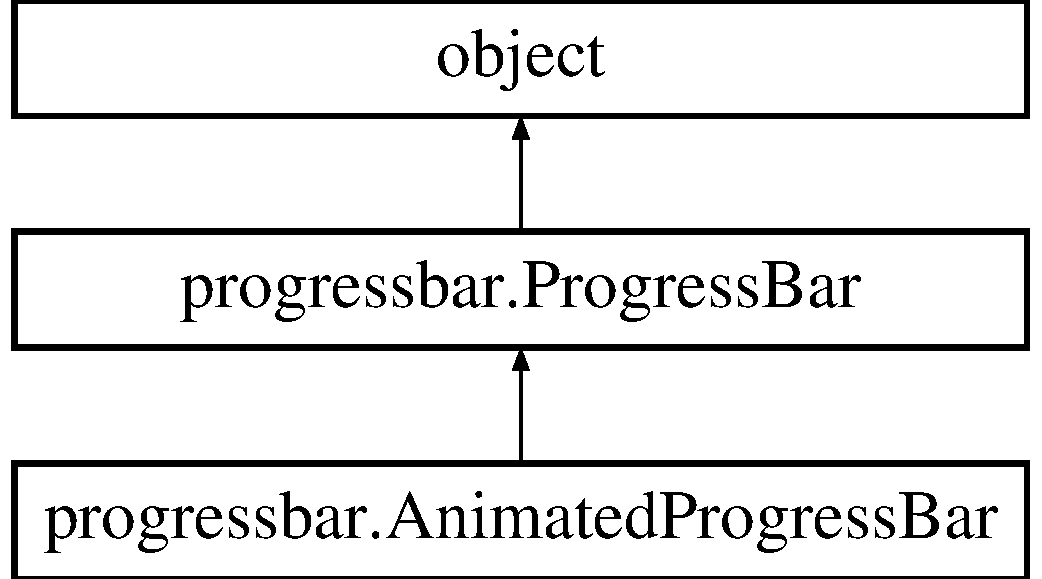
\includegraphics[height=3.000000cm]{classprogressbar_1_1AnimatedProgressBar}
\end{center}
\end{figure}
\subsection*{Public Member Functions}
\begin{DoxyCompactItemize}
\item 
def \hyperlink{classprogressbar_1_1AnimatedProgressBar_ac5fb173f8610ea6caa27306a60a8903f}{\+\_\+\+\_\+init\+\_\+\+\_\+} (self, args, kwargs)
\item 
def \hyperlink{classprogressbar_1_1AnimatedProgressBar_a87d45550598b83128ee14b4d7acdea27}{show\+\_\+progress} (self)
\item 
def \hyperlink{classprogressbar_1_1ProgressBar_ab72aa084f53baad02409c8e7e5979046}{\+\_\+\+\_\+add\+\_\+\+\_\+} (self, increment)
\item 
def \hyperlink{classprogressbar_1_1ProgressBar_aea02b9e37516e9d267e2d48b4e415bd8}{\+\_\+\+\_\+str\+\_\+\+\_\+} (self)
\item 
def \hyperlink{classprogressbar_1_1ProgressBar_a0794442f190ed0d6e5b894f29881758b}{set} (self, value)
\item 
def \hyperlink{classprogressbar_1_1ProgressBar_aefc445915e4d1eb0bbf962857c122dac}{reset} (self)
\end{DoxyCompactItemize}
\subsection*{Public Attributes}
\begin{DoxyCompactItemize}
\item 
\hyperlink{classprogressbar_1_1AnimatedProgressBar_aa4bc611ade566c28f1c54e5608a2a200}{stdout}
\item 
\hyperlink{classprogressbar_1_1AnimatedProgressBar_a50c3cb9a4b317224bd600047efb761d2}{last\+\_\+indicator}
\item 
\hyperlink{classprogressbar_1_1ProgressBar_a550afef3072c2412e2aa906b12c33bbe}{start}
\item 
\hyperlink{classprogressbar_1_1ProgressBar_a92053e3baab49364971c15373b6c848f}{end}
\item 
\hyperlink{classprogressbar_1_1ProgressBar_abde0c8da19e6e6bcde845b1eb3cee279}{width}
\item 
\hyperlink{classprogressbar_1_1ProgressBar_a6b11796a20118f92eb59abbccf626d23}{fill}
\item 
\hyperlink{classprogressbar_1_1ProgressBar_a0bfce2d34f0a8f034748d77cc5140bc5}{blank}
\item 
\hyperlink{classprogressbar_1_1ProgressBar_a4dd00a852851da809ffad5e1bf282858}{format}
\item 
\hyperlink{classprogressbar_1_1ProgressBar_a0b98b7a8f7025b78a5d01f0dcfc2dbaa}{incremental}
\item 
\hyperlink{classprogressbar_1_1ProgressBar_ac076ee00e3a70c69b8583668c165415a}{step}
\item 
\hyperlink{classprogressbar_1_1ProgressBar_a28ce54371f3a84172049c0520726d2aa}{process}
\item 
\hyperlink{classprogressbar_1_1ProgressBar_a3adc96f42e6891bcd2885c9ef29767f3}{progress}
\end{DoxyCompactItemize}


\subsection{Detailed Description}
\begin{DoxyVerb}Extends ProgressBar to allow you to use it straighforward on a script.
Accepts an extra keyword argument named `stdout` (by default use sys.stdout)
and may be any file-object to which send the progress status.
\end{DoxyVerb}
 

Definition at line 64 of file progressbar.\+py.



\subsection{Constructor \& Destructor Documentation}
\mbox{\Hypertarget{classprogressbar_1_1AnimatedProgressBar_ac5fb173f8610ea6caa27306a60a8903f}\label{classprogressbar_1_1AnimatedProgressBar_ac5fb173f8610ea6caa27306a60a8903f}} 
\index{progressbar\+::\+Animated\+Progress\+Bar@{progressbar\+::\+Animated\+Progress\+Bar}!\+\_\+\+\_\+init\+\_\+\+\_\+@{\+\_\+\+\_\+init\+\_\+\+\_\+}}
\index{\+\_\+\+\_\+init\+\_\+\+\_\+@{\+\_\+\+\_\+init\+\_\+\+\_\+}!progressbar\+::\+Animated\+Progress\+Bar@{progressbar\+::\+Animated\+Progress\+Bar}}
\subsubsection{\texorpdfstring{\+\_\+\+\_\+init\+\_\+\+\_\+()}{\_\_init\_\_()}}
{\footnotesize\ttfamily def progressbar.\+Animated\+Progress\+Bar.\+\_\+\+\_\+init\+\_\+\+\_\+ (\begin{DoxyParamCaption}\item[{}]{self,  }\item[{}]{args,  }\item[{}]{kwargs }\end{DoxyParamCaption})}



Definition at line 69 of file progressbar.\+py.


\begin{DoxyCode}
69     \textcolor{keyword}{def }\hyperlink{classwrapper_1_1ModuleDictWrapper_a9a7a794150502f51df687831583e13b9}{\_\_init\_\_}(self, *args, **kwargs):
70         super(AnimatedProgressBar, self).\hyperlink{classwrapper_1_1ModuleDictWrapper_a9a7a794150502f51df687831583e13b9}{\_\_init\_\_}(*args, **kwargs)
71         self.stdout = kwargs.get(\textcolor{stringliteral}{'stdout'}, sys.stdout)
72         self.last\_indicator = \textcolor{stringliteral}{''}
73 
\end{DoxyCode}


\subsection{Member Function Documentation}
\mbox{\Hypertarget{classprogressbar_1_1ProgressBar_ab72aa084f53baad02409c8e7e5979046}\label{classprogressbar_1_1ProgressBar_ab72aa084f53baad02409c8e7e5979046}} 
\index{progressbar\+::\+Animated\+Progress\+Bar@{progressbar\+::\+Animated\+Progress\+Bar}!\+\_\+\+\_\+add\+\_\+\+\_\+@{\+\_\+\+\_\+add\+\_\+\+\_\+}}
\index{\+\_\+\+\_\+add\+\_\+\+\_\+@{\+\_\+\+\_\+add\+\_\+\+\_\+}!progressbar\+::\+Animated\+Progress\+Bar@{progressbar\+::\+Animated\+Progress\+Bar}}
\subsubsection{\texorpdfstring{\+\_\+\+\_\+add\+\_\+\+\_\+()}{\_\_add\_\_()}}
{\footnotesize\ttfamily def progressbar.\+Progress\+Bar.\+\_\+\+\_\+add\+\_\+\+\_\+ (\begin{DoxyParamCaption}\item[{}]{self,  }\item[{}]{increment }\end{DoxyParamCaption})\hspace{0.3cm}{\ttfamily [inherited]}}



Definition at line 30 of file progressbar.\+py.



References progressbar.\+Progress\+Bar.\+\_\+get\+\_\+progress(), and progressbar.\+Progress\+Bar.\+progress.


\begin{DoxyCode}
30     \textcolor{keyword}{def }\_\_add\_\_(self, increment):
31         increment = self.\_get\_progress(increment)
32         \textcolor{keywordflow}{if} 100 > self.progress + increment:
33             self.progress += increment
34         \textcolor{keywordflow}{else}:
35             self.progress = 100
36         \textcolor{keywordflow}{return} self
37     
\end{DoxyCode}
\mbox{\Hypertarget{classprogressbar_1_1ProgressBar_aea02b9e37516e9d267e2d48b4e415bd8}\label{classprogressbar_1_1ProgressBar_aea02b9e37516e9d267e2d48b4e415bd8}} 
\index{progressbar\+::\+Animated\+Progress\+Bar@{progressbar\+::\+Animated\+Progress\+Bar}!\+\_\+\+\_\+str\+\_\+\+\_\+@{\+\_\+\+\_\+str\+\_\+\+\_\+}}
\index{\+\_\+\+\_\+str\+\_\+\+\_\+@{\+\_\+\+\_\+str\+\_\+\+\_\+}!progressbar\+::\+Animated\+Progress\+Bar@{progressbar\+::\+Animated\+Progress\+Bar}}
\subsubsection{\texorpdfstring{\+\_\+\+\_\+str\+\_\+\+\_\+()}{\_\_str\_\_()}}
{\footnotesize\ttfamily def progressbar.\+Progress\+Bar.\+\_\+\+\_\+str\+\_\+\+\_\+ (\begin{DoxyParamCaption}\item[{}]{self }\end{DoxyParamCaption})\hspace{0.3cm}{\ttfamily [inherited]}}



Definition at line 38 of file progressbar.\+py.



References progressbar.\+Progress\+Bar.\+blank, progressbar.\+Progress\+Bar.\+fill, progressbar.\+Progress\+Bar.\+format, progressbar.\+Progress\+Bar.\+process, progressbar.\+Progress\+Bar.\+progress, progressbar.\+Progress\+Bar.\+step, and progressbar.\+Progress\+Bar.\+width.


\begin{DoxyCode}
38     \textcolor{keyword}{def }\_\_str\_\_(self):
39         progressed = int(self.progress / self.step) \textcolor{comment}{#fix}
40         fill = progressed * self.fill
41         proc = self.process
42         blank = (self.width - progressed) * self.blank
43         \textcolor{keywordflow}{return} self.format % \{\textcolor{stringliteral}{'process'}: proc, \textcolor{stringliteral}{'fill'}: fill, \textcolor{stringliteral}{'blank'}: blank, \textcolor{stringliteral}{'progress'}: int(self.progress)
      \}
44 
\end{DoxyCode}
\mbox{\Hypertarget{classprogressbar_1_1ProgressBar_aefc445915e4d1eb0bbf962857c122dac}\label{classprogressbar_1_1ProgressBar_aefc445915e4d1eb0bbf962857c122dac}} 
\index{progressbar\+::\+Animated\+Progress\+Bar@{progressbar\+::\+Animated\+Progress\+Bar}!reset@{reset}}
\index{reset@{reset}!progressbar\+::\+Animated\+Progress\+Bar@{progressbar\+::\+Animated\+Progress\+Bar}}
\subsubsection{\texorpdfstring{reset()}{reset()}}
{\footnotesize\ttfamily def progressbar.\+Progress\+Bar.\+reset (\begin{DoxyParamCaption}\item[{}]{self }\end{DoxyParamCaption})\hspace{0.3cm}{\ttfamily [inherited]}}

\begin{DoxyVerb}Resets the current progress to the start point\end{DoxyVerb}
 

Definition at line 58 of file progressbar.\+py.



References progressbar.\+Progress\+Bar.\+\_\+get\+\_\+progress(), progressbar.\+Progress\+Bar.\+progress, and progressbar.\+Progress\+Bar.\+start.


\begin{DoxyCode}
58     \textcolor{keyword}{def }\hyperlink{namespaceshell_a2f31bbe4baf894f4863c4d392239ab8b}{reset}(self):
59         \textcolor{stringliteral}{"""Resets the current progress to the start point"""}
60         self.progress = self.\_get\_progress(self.start)
61         \textcolor{keywordflow}{return} self
62 
63 
\end{DoxyCode}
\mbox{\Hypertarget{classprogressbar_1_1ProgressBar_a0794442f190ed0d6e5b894f29881758b}\label{classprogressbar_1_1ProgressBar_a0794442f190ed0d6e5b894f29881758b}} 
\index{progressbar\+::\+Animated\+Progress\+Bar@{progressbar\+::\+Animated\+Progress\+Bar}!set@{set}}
\index{set@{set}!progressbar\+::\+Animated\+Progress\+Bar@{progressbar\+::\+Animated\+Progress\+Bar}}
\subsubsection{\texorpdfstring{set()}{set()}}
{\footnotesize\ttfamily def progressbar.\+Progress\+Bar.\+set (\begin{DoxyParamCaption}\item[{}]{self,  }\item[{}]{value }\end{DoxyParamCaption})\hspace{0.3cm}{\ttfamily [inherited]}}



Definition at line 50 of file progressbar.\+py.



References progressbar.\+Progress\+Bar.\+\_\+get\+\_\+progress(), and progressbar.\+Progress\+Bar.\+progress.


\begin{DoxyCode}
50     \textcolor{keyword}{def }set(self, value):
51         value = self.\_get\_progress(value)
52         \textcolor{keywordflow}{if} 100 > value:
53             self.progress = value 
54         \textcolor{keywordflow}{else}:
55             self.progress = 100
56         \textcolor{keywordflow}{return} self
57 
\end{DoxyCode}
\mbox{\Hypertarget{classprogressbar_1_1AnimatedProgressBar_a87d45550598b83128ee14b4d7acdea27}\label{classprogressbar_1_1AnimatedProgressBar_a87d45550598b83128ee14b4d7acdea27}} 
\index{progressbar\+::\+Animated\+Progress\+Bar@{progressbar\+::\+Animated\+Progress\+Bar}!show\+\_\+progress@{show\+\_\+progress}}
\index{show\+\_\+progress@{show\+\_\+progress}!progressbar\+::\+Animated\+Progress\+Bar@{progressbar\+::\+Animated\+Progress\+Bar}}
\subsubsection{\texorpdfstring{show\+\_\+progress()}{show\_progress()}}
{\footnotesize\ttfamily def progressbar.\+Animated\+Progress\+Bar.\+show\+\_\+progress (\begin{DoxyParamCaption}\item[{}]{self }\end{DoxyParamCaption})}



Definition at line 74 of file progressbar.\+py.



References progressbar.\+Animated\+Progress\+Bar.\+last\+\_\+indicator, and progressbar.\+Animated\+Progress\+Bar.\+stdout.


\begin{DoxyCode}
74     \textcolor{keyword}{def }show\_progress(self):
75         indicator = str(self)
76         \textcolor{keywordflow}{if} indicator == self.last\_indicator:
77           \textcolor{keywordflow}{return}
78         \textcolor{keywordflow}{if} hasattr(self.stdout, \textcolor{stringliteral}{'isatty'}) \textcolor{keywordflow}{and} self.stdout.isatty():
79             self.stdout.write(\textcolor{stringliteral}{'\(\backslash\)r'})
80         \textcolor{keywordflow}{else}:
81             self.stdout.write(\textcolor{stringliteral}{'\(\backslash\)n'})
82         self.stdout.write(str(self))
83         self.stdout.flush()
84         self.last\_indicator = indicator
85 
\end{DoxyCode}


\subsection{Member Data Documentation}
\mbox{\Hypertarget{classprogressbar_1_1ProgressBar_a0bfce2d34f0a8f034748d77cc5140bc5}\label{classprogressbar_1_1ProgressBar_a0bfce2d34f0a8f034748d77cc5140bc5}} 
\index{progressbar\+::\+Animated\+Progress\+Bar@{progressbar\+::\+Animated\+Progress\+Bar}!blank@{blank}}
\index{blank@{blank}!progressbar\+::\+Animated\+Progress\+Bar@{progressbar\+::\+Animated\+Progress\+Bar}}
\subsubsection{\texorpdfstring{blank}{blank}}
{\footnotesize\ttfamily progressbar.\+Progress\+Bar.\+blank\hspace{0.3cm}{\ttfamily [inherited]}}



Definition at line 23 of file progressbar.\+py.



Referenced by progressbar.\+Progress\+Bar.\+\_\+\+\_\+str\+\_\+\+\_\+().

\mbox{\Hypertarget{classprogressbar_1_1ProgressBar_a92053e3baab49364971c15373b6c848f}\label{classprogressbar_1_1ProgressBar_a92053e3baab49364971c15373b6c848f}} 
\index{progressbar\+::\+Animated\+Progress\+Bar@{progressbar\+::\+Animated\+Progress\+Bar}!end@{end}}
\index{end@{end}!progressbar\+::\+Animated\+Progress\+Bar@{progressbar\+::\+Animated\+Progress\+Bar}}
\subsubsection{\texorpdfstring{end}{end}}
{\footnotesize\ttfamily progressbar.\+Progress\+Bar.\+end\hspace{0.3cm}{\ttfamily [inherited]}}



Definition at line 20 of file progressbar.\+py.



Referenced by progressbar.\+Progress\+Bar.\+\_\+get\+\_\+progress().

\mbox{\Hypertarget{classprogressbar_1_1ProgressBar_a6b11796a20118f92eb59abbccf626d23}\label{classprogressbar_1_1ProgressBar_a6b11796a20118f92eb59abbccf626d23}} 
\index{progressbar\+::\+Animated\+Progress\+Bar@{progressbar\+::\+Animated\+Progress\+Bar}!fill@{fill}}
\index{fill@{fill}!progressbar\+::\+Animated\+Progress\+Bar@{progressbar\+::\+Animated\+Progress\+Bar}}
\subsubsection{\texorpdfstring{fill}{fill}}
{\footnotesize\ttfamily progressbar.\+Progress\+Bar.\+fill\hspace{0.3cm}{\ttfamily [inherited]}}



Definition at line 22 of file progressbar.\+py.



Referenced by progressbar.\+Progress\+Bar.\+\_\+\+\_\+str\+\_\+\+\_\+().

\mbox{\Hypertarget{classprogressbar_1_1ProgressBar_a4dd00a852851da809ffad5e1bf282858}\label{classprogressbar_1_1ProgressBar_a4dd00a852851da809ffad5e1bf282858}} 
\index{progressbar\+::\+Animated\+Progress\+Bar@{progressbar\+::\+Animated\+Progress\+Bar}!format@{format}}
\index{format@{format}!progressbar\+::\+Animated\+Progress\+Bar@{progressbar\+::\+Animated\+Progress\+Bar}}
\subsubsection{\texorpdfstring{format}{format}}
{\footnotesize\ttfamily progressbar.\+Progress\+Bar.\+format\hspace{0.3cm}{\ttfamily [inherited]}}



Definition at line 24 of file progressbar.\+py.



Referenced by progressbar.\+Progress\+Bar.\+\_\+\+\_\+str\+\_\+\+\_\+().

\mbox{\Hypertarget{classprogressbar_1_1ProgressBar_a0b98b7a8f7025b78a5d01f0dcfc2dbaa}\label{classprogressbar_1_1ProgressBar_a0b98b7a8f7025b78a5d01f0dcfc2dbaa}} 
\index{progressbar\+::\+Animated\+Progress\+Bar@{progressbar\+::\+Animated\+Progress\+Bar}!incremental@{incremental}}
\index{incremental@{incremental}!progressbar\+::\+Animated\+Progress\+Bar@{progressbar\+::\+Animated\+Progress\+Bar}}
\subsubsection{\texorpdfstring{incremental}{incremental}}
{\footnotesize\ttfamily progressbar.\+Progress\+Bar.\+incremental\hspace{0.3cm}{\ttfamily [inherited]}}



Definition at line 25 of file progressbar.\+py.

\mbox{\Hypertarget{classprogressbar_1_1AnimatedProgressBar_a50c3cb9a4b317224bd600047efb761d2}\label{classprogressbar_1_1AnimatedProgressBar_a50c3cb9a4b317224bd600047efb761d2}} 
\index{progressbar\+::\+Animated\+Progress\+Bar@{progressbar\+::\+Animated\+Progress\+Bar}!last\+\_\+indicator@{last\+\_\+indicator}}
\index{last\+\_\+indicator@{last\+\_\+indicator}!progressbar\+::\+Animated\+Progress\+Bar@{progressbar\+::\+Animated\+Progress\+Bar}}
\subsubsection{\texorpdfstring{last\+\_\+indicator}{last\_indicator}}
{\footnotesize\ttfamily progressbar.\+Animated\+Progress\+Bar.\+last\+\_\+indicator}



Definition at line 72 of file progressbar.\+py.



Referenced by progressbar.\+Animated\+Progress\+Bar.\+show\+\_\+progress().

\mbox{\Hypertarget{classprogressbar_1_1ProgressBar_a28ce54371f3a84172049c0520726d2aa}\label{classprogressbar_1_1ProgressBar_a28ce54371f3a84172049c0520726d2aa}} 
\index{progressbar\+::\+Animated\+Progress\+Bar@{progressbar\+::\+Animated\+Progress\+Bar}!process@{process}}
\index{process@{process}!progressbar\+::\+Animated\+Progress\+Bar@{progressbar\+::\+Animated\+Progress\+Bar}}
\subsubsection{\texorpdfstring{process}{process}}
{\footnotesize\ttfamily progressbar.\+Progress\+Bar.\+process\hspace{0.3cm}{\ttfamily [inherited]}}



Definition at line 27 of file progressbar.\+py.



Referenced by progressbar.\+Progress\+Bar.\+\_\+\+\_\+str\+\_\+\+\_\+().

\mbox{\Hypertarget{classprogressbar_1_1ProgressBar_a3adc96f42e6891bcd2885c9ef29767f3}\label{classprogressbar_1_1ProgressBar_a3adc96f42e6891bcd2885c9ef29767f3}} 
\index{progressbar\+::\+Animated\+Progress\+Bar@{progressbar\+::\+Animated\+Progress\+Bar}!progress@{progress}}
\index{progress@{progress}!progressbar\+::\+Animated\+Progress\+Bar@{progressbar\+::\+Animated\+Progress\+Bar}}
\subsubsection{\texorpdfstring{progress}{progress}}
{\footnotesize\ttfamily progressbar.\+Progress\+Bar.\+progress\hspace{0.3cm}{\ttfamily [inherited]}}



Definition at line 35 of file progressbar.\+py.



Referenced by progressbar.\+Progress\+Bar.\+\_\+\+\_\+add\+\_\+\+\_\+(), progressbar.\+Progress\+Bar.\+\_\+\+\_\+str\+\_\+\+\_\+(), progressbar.\+Progress\+Bar.\+reset(), and progressbar.\+Progress\+Bar.\+set().

\mbox{\Hypertarget{classprogressbar_1_1ProgressBar_a550afef3072c2412e2aa906b12c33bbe}\label{classprogressbar_1_1ProgressBar_a550afef3072c2412e2aa906b12c33bbe}} 
\index{progressbar\+::\+Animated\+Progress\+Bar@{progressbar\+::\+Animated\+Progress\+Bar}!start@{start}}
\index{start@{start}!progressbar\+::\+Animated\+Progress\+Bar@{progressbar\+::\+Animated\+Progress\+Bar}}
\subsubsection{\texorpdfstring{start}{start}}
{\footnotesize\ttfamily progressbar.\+Progress\+Bar.\+start\hspace{0.3cm}{\ttfamily [inherited]}}



Definition at line 19 of file progressbar.\+py.



Referenced by progressbar.\+Progress\+Bar.\+reset().

\mbox{\Hypertarget{classprogressbar_1_1AnimatedProgressBar_aa4bc611ade566c28f1c54e5608a2a200}\label{classprogressbar_1_1AnimatedProgressBar_aa4bc611ade566c28f1c54e5608a2a200}} 
\index{progressbar\+::\+Animated\+Progress\+Bar@{progressbar\+::\+Animated\+Progress\+Bar}!stdout@{stdout}}
\index{stdout@{stdout}!progressbar\+::\+Animated\+Progress\+Bar@{progressbar\+::\+Animated\+Progress\+Bar}}
\subsubsection{\texorpdfstring{stdout}{stdout}}
{\footnotesize\ttfamily progressbar.\+Animated\+Progress\+Bar.\+stdout}



Definition at line 71 of file progressbar.\+py.



Referenced by progressbar.\+Animated\+Progress\+Bar.\+show\+\_\+progress().

\mbox{\Hypertarget{classprogressbar_1_1ProgressBar_ac076ee00e3a70c69b8583668c165415a}\label{classprogressbar_1_1ProgressBar_ac076ee00e3a70c69b8583668c165415a}} 
\index{progressbar\+::\+Animated\+Progress\+Bar@{progressbar\+::\+Animated\+Progress\+Bar}!step@{step}}
\index{step@{step}!progressbar\+::\+Animated\+Progress\+Bar@{progressbar\+::\+Animated\+Progress\+Bar}}
\subsubsection{\texorpdfstring{step}{step}}
{\footnotesize\ttfamily progressbar.\+Progress\+Bar.\+step\hspace{0.3cm}{\ttfamily [inherited]}}



Definition at line 26 of file progressbar.\+py.



Referenced by progressbar.\+Progress\+Bar.\+\_\+\+\_\+str\+\_\+\+\_\+().

\mbox{\Hypertarget{classprogressbar_1_1ProgressBar_abde0c8da19e6e6bcde845b1eb3cee279}\label{classprogressbar_1_1ProgressBar_abde0c8da19e6e6bcde845b1eb3cee279}} 
\index{progressbar\+::\+Animated\+Progress\+Bar@{progressbar\+::\+Animated\+Progress\+Bar}!width@{width}}
\index{width@{width}!progressbar\+::\+Animated\+Progress\+Bar@{progressbar\+::\+Animated\+Progress\+Bar}}
\subsubsection{\texorpdfstring{width}{width}}
{\footnotesize\ttfamily progressbar.\+Progress\+Bar.\+width\hspace{0.3cm}{\ttfamily [inherited]}}



Definition at line 21 of file progressbar.\+py.



Referenced by progressbar.\+Progress\+Bar.\+\_\+\+\_\+str\+\_\+\+\_\+().



The documentation for this class was generated from the following file\+:\begin{DoxyCompactItemize}
\item 
/home/eleclhcb/\+L\+H\+Cb/lbcat-\/cmake/\+Cat\+Python/python/\hyperlink{progressbar_8py}{progressbar.\+py}\end{DoxyCompactItemize}

\hypertarget{classAppFrame_1_1AppFrame}{
\section{AppFrame::AppFrame Class Reference}
\label{classAppFrame_1_1AppFrame}\index{AppFrame::AppFrame@{AppFrame::AppFrame}}
}
\subsection*{Public Member Functions}
\begin{DoxyCompactItemize}
\item 
def \hyperlink{classAppFrame_1_1AppFrame_a99de512a9c17c41f6446a0ad51aa492f}{\_\-\_\-init\_\-\_\-}
\item 
def \hyperlink{classAppFrame_1_1AppFrame_a339ae421d03a4184269c6b7e3537ab08}{getControl}
\item 
def \hyperlink{classAppFrame_1_1AppFrame_a71b05a3223d3ab9595beb5a6158a4658}{makeMenuBar}
\item 
def \hyperlink{classAppFrame_1_1AppFrame_ab4a7fb9bd8d8d66ab94c61281456f8ff}{makeToolBar}
\item 
def \hyperlink{classAppFrame_1_1AppFrame_a4e0dcbd50e131b0098cf1611ad25db6c}{onIdle}
\item 
def \hyperlink{classAppFrame_1_1AppFrame_aaa21bd6cb6d29c0ff8b86aee2b55d146}{onCloseConfirm}
\item 
def \hyperlink{classAppFrame_1_1AppFrame_a5f83beacf1c4e5bd2a27e3c778c96c1e}{onClose}
\item 
def \hyperlink{classAppFrame_1_1AppFrame_a5b5cb5f928c331e97fd7ffcee5458bcf}{onExit}
\item 
def \hyperlink{classAppFrame_1_1AppFrame_a11b969659be042b78227df2738371b6a}{onHelp}
\item 
def \hyperlink{classAppFrame_1_1AppFrame_a8a7202f9eb527cf4513d8b69b385a172}{onAbout}
\item 
def \hyperlink{classAppFrame_1_1AppFrame_ae06136b61e9fb8d5d8594a78bc5b1beb}{onAutoCheck}
\item 
def \hyperlink{classAppFrame_1_1AppFrame_a5d4fbe570c7b419c71b5a28e920ef0b3}{onStopOnError}
\item 
def \hyperlink{classAppFrame_1_1AppFrame_a64fced2976ba648b07d575749a031ce2}{onFileCheck}
\item 
def \hyperlink{classAppFrame_1_1AppFrame_a5fc0d44cdfe82f731a9e8747c0062bdc}{onLogCheck}
\item 
def \hyperlink{classAppFrame_1_1AppFrame_aca8b90caebbf4467fefc23d134e87882}{eventCtrl}
\item 
def \hyperlink{classAppFrame_1_1AppFrame_a89e4b810a8f76474c63307ab353b95ae}{runCtrl}
\item 
def \hyperlink{classAppFrame_1_1AppFrame_a3319c92de38f17675b2debf064add617}{printFreq}
\item 
def \hyperlink{classAppFrame_1_1AppFrame_a724d4fb4f7b45e38c3002dafaf31ae3d}{plotFreq}
\item 
def \hyperlink{classAppFrame_1_1AppFrame_a40b3826412cf97464898e448b5eb9b00}{onEnter}
\item 
def \hyperlink{classAppFrame_1_1AppFrame_a6050b747faab481f9728a791ce5c8beb}{onLoad}
\item 
def \hyperlink{classAppFrame_1_1AppFrame_a17e104bbc8544539fcad9d3f75583438}{onEdit}
\item 
def \hyperlink{classAppFrame_1_1AppFrame_ae6dbfb701cee3d4f1ebd953d21934f90}{deleteHardware}
\item 
def \hyperlink{classAppFrame_1_1AppFrame_a66183c68b99e1849cb3a009aacf46578}{onExpand}
\item 
def \hyperlink{classAppFrame_1_1AppFrame_a7d96700ebc4f5a5fcf51d3d8940bcc54}{onCollapse}
\item 
def \hyperlink{classAppFrame_1_1AppFrame_a245f8c716ec863af51493af54f2cd7c6}{onReLoad}
\item 
def \hyperlink{classAppFrame_1_1AppFrame_a4d4525e84c9ababf7b5c80893c803fcc}{onConfigure}
\item 
def \hyperlink{classAppFrame_1_1AppFrame_a0f55c13ed518ba308a375dfc306fdee9}{onInit}
\item 
def \hyperlink{classAppFrame_1_1AppFrame_ad5e9ba93cb8013656d6500774cf60b53}{onDelete}
\item 
def \hyperlink{classAppFrame_1_1AppFrame_a49804b67199c453697ac5a4bcecc920e}{onStart}
\item 
def \hyperlink{classAppFrame_1_1AppFrame_af7be990776d498b34f698dc9451b4883}{onSingle}
\item 
def \hyperlink{classAppFrame_1_1AppFrame_a16fc60c79fde4dd7d9591ed3f21c3c01}{plot}
\item 
def \hyperlink{classAppFrame_1_1AppFrame_a44b82952390e069b184afd5986991ba4}{BuildElementList}
\item 
def \hyperlink{classAppFrame_1_1AppFrame_a7e349c4603f3f7ca0c5aa77a89d253dd}{BuildProcessusList}
\item 
def \hyperlink{classAppFrame_1_1AppFrame_aa01fc511db7b94a62d550a0087d750b9}{update}
\item 
def \hyperlink{classAppFrame_1_1AppFrame_a5281ab025cc34273c414c06e58f1507d}{ElementList}
\item 
def \hyperlink{classAppFrame_1_1AppFrame_a9dec5963f6ad7c33992ad7ec38567574}{updateCombo}
\item 
def \hyperlink{classAppFrame_1_1AppFrame_a6a35e9206bd5c1cedcfd8a9af7d6a8c6}{updateOutputLevel}
\item 
def \hyperlink{classAppFrame_1_1AppFrame_afeddbb4dfa87ced566b15d905eed4756}{procComboUpdate}
\end{DoxyCompactItemize}
\subsection*{Public Attributes}
\begin{DoxyCompactItemize}
\item 
\hyperlink{classAppFrame_1_1AppFrame_a4ff8d69e79895e94fe0c4457051e98e4}{MB\_\-CONF}
\item 
\hyperlink{classAppFrame_1_1AppFrame_a87cf4bd947402b005cdc8a8248bc7394}{MB\_\-GRAPH}
\item 
\hyperlink{classAppFrame_1_1AppFrame_aa4182d18214f9bcb8747b30d75566c4a}{MB\_\-LOG}
\item 
\hyperlink{classAppFrame_1_1AppFrame_a92adb26561ea695af9637bdd7cdcffda}{TB\_\-CONF}
\item 
\hyperlink{classAppFrame_1_1AppFrame_a054706bdc13f9c9e2b3a74c2cf659271}{TB\_\-GRAPH}
\item 
\hyperlink{classAppFrame_1_1AppFrame_aa6410672f90bddc15b60bddd6040c65b}{TB\_\-LOG}
\item 
\hyperlink{classAppFrame_1_1AppFrame_a0a19a7c7e9a6095cba6813e8d13e9bec}{cfgpanels}
\item 
\hyperlink{classAppFrame_1_1AppFrame_a7b899e2a2d3601a640bde2ba4a4c09b6}{objs}
\item 
\hyperlink{classAppFrame_1_1AppFrame_a9b64dca9c80270b7f0e36ee52d5f8c2d}{paths}
\item 
\hyperlink{classAppFrame_1_1AppFrame_aadc7ad0c96f9227da506b173bd7b2eee}{path}
\item 
\hyperlink{classAppFrame_1_1AppFrame_a814271a025b2beadb1187e3e9673b0fd}{panel}
\item 
\hyperlink{classAppFrame_1_1AppFrame_af5e0f9082a6580c786ad0a801dd31685}{treeContainer}
\item 
\hyperlink{classAppFrame_1_1AppFrame_ae267f6f9741bde298362f95ac19c97f2}{vbox}
\item 
\hyperlink{classAppFrame_1_1AppFrame_a1c088e6a3fc661ea80a336100160af9a}{tree}
\item 
\hyperlink{classAppFrame_1_1AppFrame_aac2972aa5a59df4897418cb34afc24bb}{elementCombo}
\item 
\hyperlink{classAppFrame_1_1AppFrame_afe103fbb66e1b2a6b7e9a64bd3154881}{procCombo}
\item 
\hyperlink{classAppFrame_1_1AppFrame_a9cbeda3bc1a78e934f1aebcd2c85e403}{menuBar}
\item 
\hyperlink{classAppFrame_1_1AppFrame_a2fd6329df31bbd37f1239f34a567d71a}{toolBar}
\item 
\hyperlink{classAppFrame_1_1AppFrame_ac23e75e7a9c9995eb55d7962342acd15}{listElement}
\end{DoxyCompactItemize}
\subsection*{Static Public Attributes}
\begin{DoxyCompactItemize}
\item 
string \hyperlink{classAppFrame_1_1AppFrame_a667d35fae1ebfa2706cfbb31fdf0cbab}{overviewText} = \char`\"{}CAT Main Window\char`\"{}
\end{DoxyCompactItemize}


\subsection{Detailed Description}


Definition at line 54 of file AppFrame.py.

\subsection{Member Function Documentation}
\hypertarget{classAppFrame_1_1AppFrame_a99de512a9c17c41f6446a0ad51aa492f}{
\index{AppFrame::AppFrame@{AppFrame::AppFrame}!\_\-\_\-init\_\-\_\-@{\_\-\_\-init\_\-\_\-}}
\index{\_\-\_\-init\_\-\_\-@{\_\-\_\-init\_\-\_\-}!AppFrame::AppFrame@{AppFrame::AppFrame}}
\subsubsection[{\_\-\_\-init\_\-\_\-}]{\setlength{\rightskip}{0pt plus 5cm}def AppFrame::AppFrame::\_\-\_\-init\_\-\_\- ( {\em self}, \/   {\em app}, \/   {\em parent}, \/   {\em title})}}
\label{classAppFrame_1_1AppFrame_a99de512a9c17c41f6446a0ad51aa492f}


Definition at line 56 of file AppFrame.py.


\begin{DoxyCode}
56                                           : 
57         wx.Frame.__init__(self, parent, wx.NewId(), title, size=(500, 650))
58         
59         self.MB_CONF=wx.NewId()
60         self.MB_GRAPH=wx.NewId()
61         self.MB_LOG=wx.NewId()
62 
63         self.TB_CONF=wx.NewId()
64         self.TB_GRAPH=wx.NewId()
65         self.TB_LOG=wx.NewId()
66 
67         self.cfgpanels=list()
68         self.objs=list()
69         self.paths=list()
70 
71         global cat
72         cat=app
73         
74         self.path=os.path.join(os.environ.get("CATPATH"),"CatPython","python")
75         sizeX=wx.SystemSettings.GetMetric( wx.SYS_SCREEN_X );
76         sizeY=wx.SystemSettings.GetMetric( wx.SYS_SCREEN_Y );
77         self.makeMenuBar()
78         self.makeToolBar()
79         res=xrc.XmlResource(os.path.join(self.path,"xrc/AppPanel.xrc"))
80         self.panel=res.LoadPanel(self, "AppPanel")
81 #        self.makeFrames()
82         
83         for window, items in _windows:
84             show=items[0]
85             Pt=wx.Point(items[1][0]*sizeX,items[1][1]*sizeY)
86             Sz=wx.Size(items[2][0]*sizeX,items[2][1]*sizeY)
87             if window=='App':
88                 self.Move(Pt)
89                 self.SetSize(Sz)
90             # if window=='Cfg':
91             #     self.cfgFrame.Move(Pt)
92             #     self.cfgFrame.SetSize(Sz)
93             #     self.cfgState=show
94             #     self.cfgFrame.Show(show)
95             #     self.toolBar.ToggleTool(self.TB_CONF, show)
96             #     menuItem = self.menuBar.FindItemById(self.MB_CONF)
97             #     menuItem.Check(show) 
98                 
99             # if window=='Gph':
100             #     self.gphFrame.Move(Pt)
101             #     self.gphFrame.SetSize(Sz)
102             #     self.gphState=show
103             #     self.gphFrame.Show(show)
104             #     self.toolBar.ToggleTool(self.TB_GRAPH, show)
105             #     menuItem = self.menuBar.FindItemById(self.MB_GRAPH)
106             #     menuItem.Check(show)
107 
108             # if window=='Log':
109             #     self.logFrame.Move(Pt)
110             #     self.logFrame.SetSize(Sz)
111             #     self.logState=show
112             #     self.logFrame.Show(show)
113             #     self.toolBar.ToggleTool(self.TB_LOG, show)
114             #     menuItem = self.menuBar.FindItemById(self.MB_LOG)
115             #     menuItem.Check(show)
116                 
117         self.treeContainer=xrc.XRCCTRL(self, 'TreePanel')
118         self.vbox=wx.BoxSizer(wx.VERTICAL)
119         
120         self.tree=TreeCtrlPanel(self.treeContainer)
121 
122         self.vbox.Add(self.tree,1,wx.EXPAND)
123         self.treeContainer.SetSizer( self.vbox )
124 
125 #        self.tree
126 #        self.treeMap = {}
127 
128 #        self.BuildTreeImageList()
129         #self.tree.SetExpansionState(self.expansionState)
130 #        self.tree.Bind(wx.EVT_TREE_ITEM_EXPANDED, self.OnItemExpanded)
131 #        self.tree.Bind(wx.EVT_TREE_ITEM_COLLAPSED, self.OnItemCollapsed)
132 #        self.tree.Bind(wx.EVT_TREE_SEL_CHANGED, self.OnSelChanged)
133 #        self.tree.Bind(wx.EVT_LEFT_DOWN, self.OnTreeLeftDown)
134 
135         self.elementCombo=self.getControl("elementCombo")
136         self.procCombo=self.getControl("procCombo")
137         self.Bind(wx.EVT_COMBOBOX, self.updateCombo, id=xrc.XRCID("elementCombo")
      )        
138         self.Bind(wx.EVT_BUTTON, self.onLoad, id=xrc.XRCID("openConfFile"))
139         self.Bind(wx.EVT_BUTTON, self.onEdit, id=xrc.XRCID("onEdit"))
140         self.Bind(wx.EVT_SPINCTRL, self.runCtrl, id=xrc.XRCID("runCtrl"))
141         self.Bind(wx.EVT_SPINCTRL, self.eventCtrl, id=xrc.XRCID("eventCtrl"))
142         self.Bind(wx.EVT_SPINCTRL, self.printFreq, id=xrc.XRCID("printFreq"))
143         self.Bind(wx.EVT_SPINCTRL, self.plotFreq, id=xrc.XRCID("plotFreq"))
144         self.Bind(wx.EVT_TEXT_ENTER, self.onEnter, id=xrc.XRCID("cmdline"))
145         self.Bind(wx.EVT_BUTTON, self.onEnter, id=xrc.XRCID("onEnter"))
146         self.Bind(wx.EVT_BUTTON, self.onExpand, id=xrc.XRCID("onExpand"))
147         self.Bind(wx.EVT_BUTTON, self.onCollapse, id=xrc.XRCID("onCollapse"))
148         self.Bind(wx.EVT_BUTTON, self.deleteHardware, id=xrc.XRCID("deleteHardwar
      e"))
149         self.Bind(wx.EVT_TOGGLEBUTTON, self.onAutoCheck, id=xrc.XRCID("autoCheck"
      ))
150         self.Bind(wx.EVT_TOGGLEBUTTON, self.onStopOnError, id=xrc.XRCID("stoponer
      ror"))
151         self.Bind(wx.EVT_TOGGLEBUTTON, self.onLogCheck, id=xrc.XRCID("logCheck"))
      
152         self.Bind(wx.EVT_TOGGLEBUTTON, self.onFileCheck, id=xrc.XRCID("fileCheck"
      ))
153         self.Bind(wx.EVT_COMBOBOX, self.updateOutputLevel, id=xrc.XRCID("outputLe
      vel"))        
154         self.update()
155                 
\end{DoxyCode}
\hypertarget{classAppFrame_1_1AppFrame_a44b82952390e069b184afd5986991ba4}{
\index{AppFrame::AppFrame@{AppFrame::AppFrame}!BuildElementList@{BuildElementList}}
\index{BuildElementList@{BuildElementList}!AppFrame::AppFrame@{AppFrame::AppFrame}}
\subsubsection[{BuildElementList}]{\setlength{\rightskip}{0pt plus 5cm}def AppFrame::AppFrame::BuildElementList ( {\em self})}}
\label{classAppFrame_1_1AppFrame_a44b82952390e069b184afd5986991ba4}


Definition at line 511 of file AppFrame.py.


\begin{DoxyCode}
511                               :
512         def sublevel(list, element):
513             if (element.hasChildren()):
514                 newlist=[]
515                 children=element.children()
516                 for child in range(len(children)):
517                     newlist.append(children[child].name())
518                     if (children[child].hasChildren()):
519                         sublevel(newlist,children[child])
520                 list.append(newlist)
521         list=[]
522         list.append(cat.computer().name())
523         sublevel(list,cat.computer())
524         return list
525 
526     #---------------------------------------------
    def BuildProcessusList(self):
\end{DoxyCode}
\hypertarget{classAppFrame_1_1AppFrame_a7e349c4603f3f7ca0c5aa77a89d253dd}{
\index{AppFrame::AppFrame@{AppFrame::AppFrame}!BuildProcessusList@{BuildProcessusList}}
\index{BuildProcessusList@{BuildProcessusList}!AppFrame::AppFrame@{AppFrame::AppFrame}}
\subsubsection[{BuildProcessusList}]{\setlength{\rightskip}{0pt plus 5cm}def AppFrame::AppFrame::BuildProcessusList ( {\em self})}}
\label{classAppFrame_1_1AppFrame_a7e349c4603f3f7ca0c5aa77a89d253dd}


Definition at line 527 of file AppFrame.py.


\begin{DoxyCode}
527                                 :
528         list=[]
529         listPtr=cat.procDb().list()
530         for proc in range(len(listPtr)):
531             list.append(listPtr[proc].name())
532         return list
533         
    def update(self):
\end{DoxyCode}
\hypertarget{classAppFrame_1_1AppFrame_ae6dbfb701cee3d4f1ebd953d21934f90}{
\index{AppFrame::AppFrame@{AppFrame::AppFrame}!deleteHardware@{deleteHardware}}
\index{deleteHardware@{deleteHardware}!AppFrame::AppFrame@{AppFrame::AppFrame}}
\subsubsection[{deleteHardware}]{\setlength{\rightskip}{0pt plus 5cm}def AppFrame::AppFrame::deleteHardware ( {\em self}, \/   {\em event})}}
\label{classAppFrame_1_1AppFrame_ae6dbfb701cee3d4f1ebd953d21934f90}


Definition at line 392 of file AppFrame.py.


\begin{DoxyCode}
392                                    :
393         objtype=self.tree.GetItem()
394         cat.warning("Removing object "+objtype[0]+" of type "+objtype[1])
395         element=cat.computer().child(objtype[0])
396         if (element!=0):
397             cat.computer().delChild(element)
398         self.update()
399                         
    def onExpand(self, event):
\end{DoxyCode}
\hypertarget{classAppFrame_1_1AppFrame_a5281ab025cc34273c414c06e58f1507d}{
\index{AppFrame::AppFrame@{AppFrame::AppFrame}!ElementList@{ElementList}}
\index{ElementList@{ElementList}!AppFrame::AppFrame@{AppFrame::AppFrame}}
\subsubsection[{ElementList}]{\setlength{\rightskip}{0pt plus 5cm}def AppFrame::AppFrame::ElementList ( {\em self})}}
\label{classAppFrame_1_1AppFrame_a5281ab025cc34273c414c06e58f1507d}


Definition at line 578 of file AppFrame.py.


\begin{DoxyCode}
578                          :
579         def sublevel(list, element):
580             if (element.hasChildren()):
581                 children=element.children()
582                 for child in range(len(children)):
583                     if (len(cat.procDb().list(children[child]))>0):
584                        list.append(children[child].path(""))
585                     if (children[child].hasChildren()):
586                         sublevel(list,children[child])
587 
588         list=[]
589         list.append(cat.computer().path(""))
590         sublevel(list,cat.computer())
591         return list
592             
    def updateCombo(self, event):
\end{DoxyCode}
\hypertarget{classAppFrame_1_1AppFrame_aca8b90caebbf4467fefc23d134e87882}{
\index{AppFrame::AppFrame@{AppFrame::AppFrame}!eventCtrl@{eventCtrl}}
\index{eventCtrl@{eventCtrl}!AppFrame::AppFrame@{AppFrame::AppFrame}}
\subsubsection[{eventCtrl}]{\setlength{\rightskip}{0pt plus 5cm}def AppFrame::AppFrame::eventCtrl ( {\em self}, \/   {\em event})}}
\label{classAppFrame_1_1AppFrame_aca8b90caebbf4467fefc23d134e87882}


Definition at line 284 of file AppFrame.py.


\begin{DoxyCode}
284                              :
285         cat.options().setNEvtMax(self.getControl("eventCtrl").GetValue()) 
286 
    def runCtrl(self,event):
\end{DoxyCode}
\hypertarget{classAppFrame_1_1AppFrame_a339ae421d03a4184269c6b7e3537ab08}{
\index{AppFrame::AppFrame@{AppFrame::AppFrame}!getControl@{getControl}}
\index{getControl@{getControl}!AppFrame::AppFrame@{AppFrame::AppFrame}}
\subsubsection[{getControl}]{\setlength{\rightskip}{0pt plus 5cm}def AppFrame::AppFrame::getControl ( {\em self}, \/   {\em xmlid})}}
\label{classAppFrame_1_1AppFrame_a339ae421d03a4184269c6b7e3537ab08}
\begin{DoxyVerb}Retrieves the given control (within a dialog) by its xmlid\end{DoxyVerb}
 

Definition at line 156 of file AppFrame.py.


\begin{DoxyCode}
156                                :
157         '''Retrieves the given control (within a dialog) by its xmlid'''
158         control = self.FindWindowById(xrc.XRCID(xmlid))
159 #        print xmlid
160 #        print xrc.XRCID(xmlid)
161 #        print control
162         if control == None and self.GetMenuBar() != None:  # see if on the menuba
      r
163             control = self.GetMenuBar().FindItemById(xrc.XRCID(xmlid))
164         assert control != None, 'Programming error: a control with xml id ' + xml
      id + ' was not found.'
165         return control
166     
    def makeMenuBar(self):
\end{DoxyCode}
\hypertarget{classAppFrame_1_1AppFrame_a71b05a3223d3ab9595beb5a6158a4658}{
\index{AppFrame::AppFrame@{AppFrame::AppFrame}!makeMenuBar@{makeMenuBar}}
\index{makeMenuBar@{makeMenuBar}!AppFrame::AppFrame@{AppFrame::AppFrame}}
\subsubsection[{makeMenuBar}]{\setlength{\rightskip}{0pt plus 5cm}def AppFrame::AppFrame::makeMenuBar ( {\em self})}}
\label{classAppFrame_1_1AppFrame_a71b05a3223d3ab9595beb5a6158a4658}


Definition at line 167 of file AppFrame.py.


\begin{DoxyCode}
167                          :
168         MB_FILE=wx.NewId()
169         MB_CLOSE=wx.NewId()
170         #
171         file=wx.Menu()
172         file.Append(MB_FILE,"&File","Open new configuration file")
173         file.Append(MB_CLOSE,"&Close","Close configuration file")
174         file.Append(wx.ID_EXIT, "E&xit", "Terminate the program")
175         windows=wx.Menu()
176 #        windows.AppendCheckItem(self.MB_CONF,"&Configuration window","Configurat
      ion window")
177 #        windows.AppendCheckItem(self.MB_GRAPH,"&Graphic window","Graphic window"
      )
178 #        windows.AppendCheckItem(self.MB_LOG,"&Log window","Log window")
179         help=wx.Menu()
180         help.Append(wx.ID_ABOUT, "&About","More information about this program")
181         help.AppendSeparator()
182         help.Append(wx.ID_HELP, "&Help", "CAT application help")
183         self.menuBar=wx.MenuBar(wx.MB_DOCKABLE)
184         self.menuBar.Append(file   , "&File")
185         self.menuBar.Append(windows, "&Windows")
186         self.menuBar.Append(help   , "&Help")
187         self.SetMenuBar(self.menuBar)
188         self.Bind(wx.EVT_MENU, self.onExit      , id=wx.ID_EXIT )
189         self.Bind(wx.EVT_MENU, self.onAbout     , id=wx.ID_ABOUT )
190         self.Bind(wx.EVT_MENU, self.onHelp      , id=wx.ID_HELP )
191 #        self.Bind(wx.EVT_MENU, self.onCheckGraph, id=self.MB_GRAPH )
192 #        self.Bind(wx.EVT_MENU, self.onCheckLog  , id=self.MB_LOG   )
193 #        self.Bind(wx.EVT_MENU, self.onCheckConf , id=self.MB_CONF  )
194         self.Bind(wx.EVT_MENU, self.onLoad      , id=MB_FILE  )
195         self.Bind(wx.EVT_MENU, self.onClose     , id=MB_CLOSE  )
196         
    def makeToolBar(self):
\end{DoxyCode}
\hypertarget{classAppFrame_1_1AppFrame_ab4a7fb9bd8d8d66ab94c61281456f8ff}{
\index{AppFrame::AppFrame@{AppFrame::AppFrame}!makeToolBar@{makeToolBar}}
\index{makeToolBar@{makeToolBar}!AppFrame::AppFrame@{AppFrame::AppFrame}}
\subsubsection[{makeToolBar}]{\setlength{\rightskip}{0pt plus 5cm}def AppFrame::AppFrame::makeToolBar ( {\em self})}}
\label{classAppFrame_1_1AppFrame_ab4a7fb9bd8d8d66ab94c61281456f8ff}


Definition at line 197 of file AppFrame.py.


\begin{DoxyCode}
197                          :
198         TB_OPEN=wx.NewId()
199         TB_RELOAD=wx.NewId()
200         TB_CONFIGURE=wx.NewId()
201         TB_INIT=wx.NewId()
202         TB_DELETE=wx.NewId()
203         TB_START=wx.NewId()
204         TB_SINGLE=wx.NewId()
205         TB_EXIT=wx.NewId()
206         #
207         self.toolBar = self.CreateToolBar(wx.TB_DOCKABLE)
208         self.toolBar.AddLabelTool(TB_OPEN  , '', wx.Bitmap(os.path.join(self.
      path,"xrc/icons/fileopen.png")))
209         self.toolBar.AddLabelTool(TB_RELOAD, '', wx.Bitmap(os.path.join(self.
      path,"xrc/icons/reload.png")))
210         self.toolBar.AddLabelTool(TB_CONFIGURE, '', wx.Bitmap(os.path.join(self.
      path,"xrc/icons/conf.png")))
211         self.toolBar.AddLabelTool(TB_INIT, '', wx.Bitmap(os.path.join(self.path,"
      xrc/icons/init.png")))
212         self.toolBar.AddLabelTool(TB_DELETE, '', wx.Bitmap(os.path.join(self.
      path,"xrc/icons/delete.png")))
213         self.toolBar.AddSeparator()
214 #        self.toolBar.AddCheckLabelTool(self.TB_CONF, '', wx.Bitmap(os.path.join(
      self.path,"xrc/icons/config.png")))
215         self.toolBar.AddCheckLabelTool(self.TB_GRAPH, '', wx.Bitmap(os.path.join(
      self.path,"xrc/icons/graph.png")))
216 #        self.toolBar.AddCheckLabelTool(self.TB_LOG, '', wx.Bitmap(os.path.join(s
      elf.path,"xrc/icons/log.png")))
217         self.toolBar.AddSeparator()
218         self.toolBar.AddLabelTool(TB_START, '', wx.Bitmap(os.path.join(self.path,
      "xrc/icons/start.png")))
219         self.toolBar.AddLabelTool(TB_SINGLE, '', wx.Bitmap(os.path.join(self.
      path,"xrc/icons/single.png")))
220         self.toolBar.AddSeparator()
221         self.toolBar.AddLabelTool(wx.ID_EXIT, '', wx.Bitmap(os.path.join(self.
      path,"xrc/icons/exit.png")))
222         self.toolBar.Realize()
223         self.Bind(wx.EVT_TOOL, self.onExit      , id=wx.ID_EXIT)
224 #        self.Bind(wx.EVT_TOOL, self.onCheckGraph, id=self.TB_GRAPH)
225 #        self.Bind(wx.EVT_TOOL, self.onCheckLog  , id=self.TB_LOG)
226 #        self.Bind(wx.EVT_TOOL, self.onCheckConf , id=self.TB_CONF)
227         self.Bind(wx.EVT_TOOL, self.onLoad , id=TB_OPEN)
228         self.Bind(wx.EVT_TOOL, self.onReLoad , id=TB_RELOAD)
229         self.Bind(wx.EVT_TOOL, self.onConfigure , id=TB_CONFIGURE)
230         self.Bind(wx.EVT_TOOL, self.onInit , id=TB_INIT)
231         self.Bind(wx.EVT_TOOL, self.onDelete , id=TB_DELETE)
232         self.Bind(wx.EVT_TOOL, self.onStart , id=TB_START)
233         self.Bind(wx.EVT_TOOL, self.onSingle , id=TB_SINGLE)
234 
235 #    def makeFrames(self):
236 #        self.logFrame=LogFrame(cat, self, "Log window")
237 #        self.cfgFrame=ConfFrame(cat, self, "Configuration window")
238 #        self.gphFrame=GraphFrame(cat, self, "Graphical window")
239         
    def onIdle(self, event):
\end{DoxyCode}
\hypertarget{classAppFrame_1_1AppFrame_a8a7202f9eb527cf4513d8b69b385a172}{
\index{AppFrame::AppFrame@{AppFrame::AppFrame}!onAbout@{onAbout}}
\index{onAbout@{onAbout}!AppFrame::AppFrame@{AppFrame::AppFrame}}
\subsubsection[{onAbout}]{\setlength{\rightskip}{0pt plus 5cm}def AppFrame::AppFrame::onAbout ( {\em self}, \/   {\em event})}}
\label{classAppFrame_1_1AppFrame_a8a7202f9eb527cf4513d8b69b385a172}
\begin{DoxyVerb}About\end{DoxyVerb}
 

Definition at line 265 of file AppFrame.py.


\begin{DoxyCode}
265                             :
266         '''About'''
267         print "about"
268 
    def onAutoCheck(self, event):
\end{DoxyCode}
\hypertarget{classAppFrame_1_1AppFrame_ae06136b61e9fb8d5d8594a78bc5b1beb}{
\index{AppFrame::AppFrame@{AppFrame::AppFrame}!onAutoCheck@{onAutoCheck}}
\index{onAutoCheck@{onAutoCheck}!AppFrame::AppFrame@{AppFrame::AppFrame}}
\subsubsection[{onAutoCheck}]{\setlength{\rightskip}{0pt plus 5cm}def AppFrame::AppFrame::onAutoCheck ( {\em self}, \/   {\em event})}}
\label{classAppFrame_1_1AppFrame_ae06136b61e9fb8d5d8594a78bc5b1beb}


Definition at line 269 of file AppFrame.py.


\begin{DoxyCode}
269                                 :
270         cat.options().setRunNumberMgr(self.getControl("autoCheck").GetValue())
271         print cat.options().runNumberMgr()
272         
    def onStopOnError(self, event):
\end{DoxyCode}
\hypertarget{classAppFrame_1_1AppFrame_a5f83beacf1c4e5bd2a27e3c778c96c1e}{
\index{AppFrame::AppFrame@{AppFrame::AppFrame}!onClose@{onClose}}
\index{onClose@{onClose}!AppFrame::AppFrame@{AppFrame::AppFrame}}
\subsubsection[{onClose}]{\setlength{\rightskip}{0pt plus 5cm}def AppFrame::AppFrame::onClose ( {\em self}, \/   {\em event})}}
\label{classAppFrame_1_1AppFrame_a5f83beacf1c4e5bd2a27e3c778c96c1e}
\begin{DoxyVerb}Closes the application\end{DoxyVerb}
 

Definition at line 252 of file AppFrame.py.


\begin{DoxyCode}
252                             :
253         '''Closes the application'''
254         self.Destroy()
255 
    def onExit(self, event):
\end{DoxyCode}
\hypertarget{classAppFrame_1_1AppFrame_aaa21bd6cb6d29c0ff8b86aee2b55d146}{
\index{AppFrame::AppFrame@{AppFrame::AppFrame}!onCloseConfirm@{onCloseConfirm}}
\index{onCloseConfirm@{onCloseConfirm}!AppFrame::AppFrame@{AppFrame::AppFrame}}
\subsubsection[{onCloseConfirm}]{\setlength{\rightskip}{0pt plus 5cm}def AppFrame::AppFrame::onCloseConfirm ( {\em self}, \/   {\em event})}}
\label{classAppFrame_1_1AppFrame_aaa21bd6cb6d29c0ff8b86aee2b55d146}
\begin{DoxyVerb}Closes the application\end{DoxyVerb}
 

Definition at line 245 of file AppFrame.py.


\begin{DoxyCode}
245                                    :
246         '''Closes the application'''
247         dlg = wx.MessageDialog(self, "Exit the program?", "Exit", wx.YES_NO | wx.
      ICON_QUESTION)
248         if dlg.ShowModal() == wx.ID_YES:
249             dlg.Destroy()  # frame
250         self.Destroy()
251 
    def onClose(self, event):
\end{DoxyCode}
\hypertarget{classAppFrame_1_1AppFrame_a7d96700ebc4f5a5fcf51d3d8940bcc54}{
\index{AppFrame::AppFrame@{AppFrame::AppFrame}!onCollapse@{onCollapse}}
\index{onCollapse@{onCollapse}!AppFrame::AppFrame@{AppFrame::AppFrame}}
\subsubsection[{onCollapse}]{\setlength{\rightskip}{0pt plus 5cm}def AppFrame::AppFrame::onCollapse ( {\em self}, \/   {\em event})}}
\label{classAppFrame_1_1AppFrame_a7d96700ebc4f5a5fcf51d3d8940bcc54}


Definition at line 403 of file AppFrame.py.


\begin{DoxyCode}
403                                :
404         self.tree.CollapseAll()
405         
    def onReLoad(self, event):
\end{DoxyCode}
\hypertarget{classAppFrame_1_1AppFrame_a4d4525e84c9ababf7b5c80893c803fcc}{
\index{AppFrame::AppFrame@{AppFrame::AppFrame}!onConfigure@{onConfigure}}
\index{onConfigure@{onConfigure}!AppFrame::AppFrame@{AppFrame::AppFrame}}
\subsubsection[{onConfigure}]{\setlength{\rightskip}{0pt plus 5cm}def AppFrame::AppFrame::onConfigure ( {\em self}, \/   {\em event})}}
\label{classAppFrame_1_1AppFrame_a4d4525e84c9ababf7b5c80893c803fcc}


Definition at line 411 of file AppFrame.py.


\begin{DoxyCode}
411                                 :
412         print "Not implemented yet"
413         
    def onInit(self, event):
\end{DoxyCode}
\hypertarget{classAppFrame_1_1AppFrame_ad5e9ba93cb8013656d6500774cf60b53}{
\index{AppFrame::AppFrame@{AppFrame::AppFrame}!onDelete@{onDelete}}
\index{onDelete@{onDelete}!AppFrame::AppFrame@{AppFrame::AppFrame}}
\subsubsection[{onDelete}]{\setlength{\rightskip}{0pt plus 5cm}def AppFrame::AppFrame::onDelete ( {\em self}, \/   {\em event})}}
\label{classAppFrame_1_1AppFrame_ad5e9ba93cb8013656d6500774cf60b53}


Definition at line 417 of file AppFrame.py.


\begin{DoxyCode}
417                              :
418         cat.computer().clear()        
419         
    def onStart(self, event):
\end{DoxyCode}
\hypertarget{classAppFrame_1_1AppFrame_a17e104bbc8544539fcad9d3f75583438}{
\index{AppFrame::AppFrame@{AppFrame::AppFrame}!onEdit@{onEdit}}
\index{onEdit@{onEdit}!AppFrame::AppFrame@{AppFrame::AppFrame}}
\subsubsection[{onEdit}]{\setlength{\rightskip}{0pt plus 5cm}def AppFrame::AppFrame::onEdit ( {\em self}, \/   {\em event})}}
\label{classAppFrame_1_1AppFrame_a17e104bbc8544539fcad9d3f75583438}


Definition at line 369 of file AppFrame.py.


\begin{DoxyCode}
369                            :
370         objtype=self.tree.GetItem()
371 #        print "objtype is : ",objtype
372         objpanel=-1
373         for i in range(len(self.objs)):
374             if objtype[0]==self.paths[i]:
375                 self.cfgpanels[objpanel].update()
376                 self.cfgpanels[objpanel].Show(True)
377                 return
378             
379         self.paths.append(objtype[0])
380         if (objtype[1]=='Element'):
381             self.objs.append(cat.computer().child(objtype[0]))
382             self.cfgpanels.append(CfgFrame(cat, self, self.objs[-1], objtype[0], 
      "element"))
383 
384         if (objtype[1]=='Processus'):
385             list = cat.procDb().list()
386             for p in range(len(list)):
387                 if list[p].name()==objtype[0]:
388                     self.objs.append(list[p])
389                     self.cfgpanels.append(CfgFrame(cat, self, self.objs[-1], objt
      ype[0], "proc"))
390                     break
391                 
    def deleteHardware(self, event):
\end{DoxyCode}
\hypertarget{classAppFrame_1_1AppFrame_a40b3826412cf97464898e448b5eb9b00}{
\index{AppFrame::AppFrame@{AppFrame::AppFrame}!onEnter@{onEnter}}
\index{onEnter@{onEnter}!AppFrame::AppFrame@{AppFrame::AppFrame}}
\subsubsection[{onEnter}]{\setlength{\rightskip}{0pt plus 5cm}def AppFrame::AppFrame::onEnter ( {\em self}, \/   {\em event})}}
\label{classAppFrame_1_1AppFrame_a40b3826412cf97464898e448b5eb9b00}


Definition at line 296 of file AppFrame.py.


\begin{DoxyCode}
296                            :
297         cmd=self.getControl("cmdline").GetValue()
298         self.getControl("cmdline").SetValue("") 
299         exec(cmd)
300  
301     # Graphical Window management    
302     # def onCheckGraph(self, event):
303     #     state=not self.gphState
304     #     self.gphState=state
305     #     self.gphFrame.Show(state)
306     #     self.toolBar.ToggleTool(self.TB_GRAPH, state)
307     #     menuItem = self.menuBar.FindItemById(self.MB_GRAPH)
308     #     menuItem.Check(state)
309 
310     # Log Window management    
311     # def onCheckLog(self, event):
312     #     state=not self.logState
313     #     self.logState=state
314     #     self.logFrame.Show(state)
315     #     self.toolBar.ToggleTool(self.TB_LOG, state)
316     #     menuItem = self.menuBar.FindItemById(self.MB_LOG)
317     #     menuItem.Check(state)
318         
319     # Configuration Window management    
320     # def onCheckConf(self, event):
321     #     state=not self.cfgState
322     #     self.cfgState=state
323     #     self.cfgFrame.Show(state)
324     #     self.toolBar.ToggleTool(self.TB_CONF, state)
325     #     menuItem = self.menuBar.FindItemById(self.MB_CONF)
326     #     menuItem.Check(state)
327 
    def onLoad(self, event):
\end{DoxyCode}
\hypertarget{classAppFrame_1_1AppFrame_a5b5cb5f928c331e97fd7ffcee5458bcf}{
\index{AppFrame::AppFrame@{AppFrame::AppFrame}!onExit@{onExit}}
\index{onExit@{onExit}!AppFrame::AppFrame@{AppFrame::AppFrame}}
\subsubsection[{onExit}]{\setlength{\rightskip}{0pt plus 5cm}def AppFrame::AppFrame::onExit ( {\em self}, \/   {\em event})}}
\label{classAppFrame_1_1AppFrame_a5b5cb5f928c331e97fd7ffcee5458bcf}
\begin{DoxyVerb}Exit the app\end{DoxyVerb}
 

Definition at line 256 of file AppFrame.py.


\begin{DoxyCode}
256                            :
257         '''Exit the app'''
258         self.Close(True)
259 #        exit(2)
260 
    def onHelp(self, event):
\end{DoxyCode}
\hypertarget{classAppFrame_1_1AppFrame_a66183c68b99e1849cb3a009aacf46578}{
\index{AppFrame::AppFrame@{AppFrame::AppFrame}!onExpand@{onExpand}}
\index{onExpand@{onExpand}!AppFrame::AppFrame@{AppFrame::AppFrame}}
\subsubsection[{onExpand}]{\setlength{\rightskip}{0pt plus 5cm}def AppFrame::AppFrame::onExpand ( {\em self}, \/   {\em event})}}
\label{classAppFrame_1_1AppFrame_a66183c68b99e1849cb3a009aacf46578}


Definition at line 400 of file AppFrame.py.


\begin{DoxyCode}
400                              :
401         self.tree.ExpandAll()
402 
    def onCollapse(self, event):
\end{DoxyCode}
\hypertarget{classAppFrame_1_1AppFrame_a64fced2976ba648b07d575749a031ce2}{
\index{AppFrame::AppFrame@{AppFrame::AppFrame}!onFileCheck@{onFileCheck}}
\index{onFileCheck@{onFileCheck}!AppFrame::AppFrame@{AppFrame::AppFrame}}
\subsubsection[{onFileCheck}]{\setlength{\rightskip}{0pt plus 5cm}def AppFrame::AppFrame::onFileCheck ( {\em self}, \/   {\em event})}}
\label{classAppFrame_1_1AppFrame_a64fced2976ba648b07d575749a031ce2}


Definition at line 276 of file AppFrame.py.


\begin{DoxyCode}
276                                 :
277         cat.options().setDataStorage(self.getControl("fileCheck").GetValue())
278         print cat.options().dataStorage()
279         
    def onLogCheck(self, event):
\end{DoxyCode}
\hypertarget{classAppFrame_1_1AppFrame_a11b969659be042b78227df2738371b6a}{
\index{AppFrame::AppFrame@{AppFrame::AppFrame}!onHelp@{onHelp}}
\index{onHelp@{onHelp}!AppFrame::AppFrame@{AppFrame::AppFrame}}
\subsubsection[{onHelp}]{\setlength{\rightskip}{0pt plus 5cm}def AppFrame::AppFrame::onHelp ( {\em self}, \/   {\em event})}}
\label{classAppFrame_1_1AppFrame_a11b969659be042b78227df2738371b6a}
\begin{DoxyVerb}Help\end{DoxyVerb}
 

Definition at line 261 of file AppFrame.py.


\begin{DoxyCode}
261                            :
262         '''Help'''
263         print "help"
264         
    def onAbout(self, event):
\end{DoxyCode}
\hypertarget{classAppFrame_1_1AppFrame_a4e0dcbd50e131b0098cf1611ad25db6c}{
\index{AppFrame::AppFrame@{AppFrame::AppFrame}!onIdle@{onIdle}}
\index{onIdle@{onIdle}!AppFrame::AppFrame@{AppFrame::AppFrame}}
\subsubsection[{onIdle}]{\setlength{\rightskip}{0pt plus 5cm}def AppFrame::AppFrame::onIdle ( {\em self}, \/   {\em event})}}
\label{classAppFrame_1_1AppFrame_a4e0dcbd50e131b0098cf1611ad25db6c}
\begin{DoxyVerb}Responds to idle time in the system\end{DoxyVerb}
 

Definition at line 240 of file AppFrame.py.


\begin{DoxyCode}
240                            :
241         '''Responds to idle time in the system'''
242         # when the timer says it's time, we do the actual downloading in the main
       thread (wx doesn't work well in secondary threads)
243         print "onIdle"
244         
    def onCloseConfirm(self, event):
\end{DoxyCode}
\hypertarget{classAppFrame_1_1AppFrame_a0f55c13ed518ba308a375dfc306fdee9}{
\index{AppFrame::AppFrame@{AppFrame::AppFrame}!onInit@{onInit}}
\index{onInit@{onInit}!AppFrame::AppFrame@{AppFrame::AppFrame}}
\subsubsection[{onInit}]{\setlength{\rightskip}{0pt plus 5cm}def AppFrame::AppFrame::onInit ( {\em self}, \/   {\em event})}}
\label{classAppFrame_1_1AppFrame_a0f55c13ed518ba308a375dfc306fdee9}


Definition at line 414 of file AppFrame.py.


\begin{DoxyCode}
414                            :
415         init()
416 
    def onDelete(self, event):
\end{DoxyCode}
\hypertarget{classAppFrame_1_1AppFrame_a6050b747faab481f9728a791ce5c8beb}{
\index{AppFrame::AppFrame@{AppFrame::AppFrame}!onLoad@{onLoad}}
\index{onLoad@{onLoad}!AppFrame::AppFrame@{AppFrame::AppFrame}}
\subsubsection[{onLoad}]{\setlength{\rightskip}{0pt plus 5cm}def AppFrame::AppFrame::onLoad ( {\em self}, \/   {\em event})}}
\label{classAppFrame_1_1AppFrame_a6050b747faab481f9728a791ce5c8beb}


Definition at line 328 of file AppFrame.py.


\begin{DoxyCode}
328                            :
329         path=[]
330         dlg = wx.FileDialog(
331             self, message="Choose a file",
332             defaultDir=os.getcwd(), 
333             defaultFile="",
334             wildcard="Python source (*.py)|*.py|" "All files (*.*)|*.*",
335             style=wx.OPEN | wx.CHANGE_DIR
336             )
337 
338         # Show the dialog and retrieve the user response. If it is the OK respons
      e, 
339         # process the data.
340         if dlg.ShowModal() == wx.ID_OK:
341             # This returns a Python list of files that were selected.
342             path = dlg.GetPaths()
343         # Destroy the dialog. Don't do this until you are done with it!
344         # BAD things can happen otherwise!
345         dlg.Destroy()
346         if len(path)==1:
347             filename=str(path[0])
348             execfile(filename)
349             cat.options().setDefFile(filename)
350             cat.computer().tree()
351             self.update()
352             
353     # def onEdit(self, event):
354     #     objtype=self.tree.GetItem()
355     #     if (objtype[1]=='Element'):
356     #         self.cfgFrame.onEdit(cat.computer().child(objtype[0]),objtype[0],'e
      lement')
357     #         self.cfgFrame.Show(True)
358     #         self.cfgFrame.show=True            
359     #     if (objtype[1]=='Processus'):
360     #         list=[]
361     #         listPtr=cat.procDb().list()
362     #         for proc in range(len(listPtr)):
363     #             if (objtype[0]==listPtr[proc].name()):
364     #                 processus=listPtr[proc]
365     #         self.cfgFrame.onEdit(processus,objtype[0],'proc')
366     #         self.cfgFrame.Show(True)
367     #         self.cfgFrame.show=True            
368 
    def onEdit(self, event):
\end{DoxyCode}
\hypertarget{classAppFrame_1_1AppFrame_a5fc0d44cdfe82f731a9e8747c0062bdc}{
\index{AppFrame::AppFrame@{AppFrame::AppFrame}!onLogCheck@{onLogCheck}}
\index{onLogCheck@{onLogCheck}!AppFrame::AppFrame@{AppFrame::AppFrame}}
\subsubsection[{onLogCheck}]{\setlength{\rightskip}{0pt plus 5cm}def AppFrame::AppFrame::onLogCheck ( {\em self}, \/   {\em event})}}
\label{classAppFrame_1_1AppFrame_a5fc0d44cdfe82f731a9e8747c0062bdc}


Definition at line 280 of file AppFrame.py.


\begin{DoxyCode}
280                                :
281         cat.options().setLogStorage(self.getControl("logCheck").GetValue())
282         print cat.options().logStorage()
283         
    def eventCtrl(self,event):
\end{DoxyCode}
\hypertarget{classAppFrame_1_1AppFrame_a245f8c716ec863af51493af54f2cd7c6}{
\index{AppFrame::AppFrame@{AppFrame::AppFrame}!onReLoad@{onReLoad}}
\index{onReLoad@{onReLoad}!AppFrame::AppFrame@{AppFrame::AppFrame}}
\subsubsection[{onReLoad}]{\setlength{\rightskip}{0pt plus 5cm}def AppFrame::AppFrame::onReLoad ( {\em self}, \/   {\em event})}}
\label{classAppFrame_1_1AppFrame_a245f8c716ec863af51493af54f2cd7c6}


Definition at line 406 of file AppFrame.py.


\begin{DoxyCode}
406                              :
407         reload()
408         cat.computer().tree()
409         self.update()
410 
    def onConfigure(self, event):
\end{DoxyCode}
\hypertarget{classAppFrame_1_1AppFrame_af7be990776d498b34f698dc9451b4883}{
\index{AppFrame::AppFrame@{AppFrame::AppFrame}!onSingle@{onSingle}}
\index{onSingle@{onSingle}!AppFrame::AppFrame@{AppFrame::AppFrame}}
\subsubsection[{onSingle}]{\setlength{\rightskip}{0pt plus 5cm}def AppFrame::AppFrame::onSingle ( {\em self}, \/   {\em event})}}
\label{classAppFrame_1_1AppFrame_af7be990776d498b34f698dc9451b4883}


Definition at line 489 of file AppFrame.py.


\begin{DoxyCode}
489                              :
490         cat.options().setStorageDir(str(self.getControl("fileCtrl").GetValue()))
491         cat.options().setStoragePath(str(self.getControl("pathCtrl").GetValue()))
      
492         item=self.elementCombo.GetSelection()
493         element=cat.computer().child(self.listElement[item])
494         list=cat.procDb().list(element)
495         processus=list[self.procCombo.GetSelection()]
496         cat.prepare(processus.name(),element,1)
497         cat.loop()
498         cat.terminate()
499         self.plot(processus,False)
500         self.getControl("runCtrl").SetValue(cat.options().runNumber())
501 
502 
    def plot(self, proc, force):
\end{DoxyCode}
\hypertarget{classAppFrame_1_1AppFrame_a49804b67199c453697ac5a4bcecc920e}{
\index{AppFrame::AppFrame@{AppFrame::AppFrame}!onStart@{onStart}}
\index{onStart@{onStart}!AppFrame::AppFrame@{AppFrame::AppFrame}}
\subsubsection[{onStart}]{\setlength{\rightskip}{0pt plus 5cm}def AppFrame::AppFrame::onStart ( {\em self}, \/   {\em event})}}
\label{classAppFrame_1_1AppFrame_a49804b67199c453697ac5a4bcecc920e}


Definition at line 420 of file AppFrame.py.


\begin{DoxyCode}
420                             :
421         cat.options().setStorageDir(str(self.getControl("fileCtrl").GetValue()))
422         cat.options().setStoragePath(str(self.getControl("pathCtrl").GetValue()))
      
423         item=self.elementCombo.GetSelection()
424         element=cat.computer().child(self.listElement[item])
425         list=cat.procDb().list(element)
426         processus=list[self.procCombo.GetSelection()]
427         nevt=self.getControl("eventCtrl").GetValue()
428 
429         dlg = wx.ProgressDialog(processus.title(),
430                                 processus.name(),
431                                 maximum = abs(nevt),
432                                 parent=self,
433                                 style = wx.PD_CAN_ABORT
434                                 | wx.PD_APP_MODAL
435                                 | wx.PD_ELAPSED_TIME
436                                 | wx.PD_ESTIMATED_TIME
437                                 | wx.PD_REMAINING_TIME
438                                 )
439         plts   = None
440         module = None
441         processus.setElement(element)
442         wrap = wrapper(cat, processus, "proc")
443 
444         online  = cat.options().plotFreq()
445         
446         if (wrap.ok):
447             module = wrap.GetActive()
448             if module and online!=0 :
449                 plts = module.createPlots(cat, processus, cat.options().runNumber
      ())        
450 
451         keepGoing = True
452 
453         timing = -1
454         if (nevt<0):
455             timing = time.time()
456         evt    = abs(nevt)
457 
458         ievt=0 
459         status=Code.SUCCESS
460         dlg.Update(ievt, " Initializing"+processus.name())
461         cat.prepare(processus.name(),element,nevt)
462         while (keepGoing):
463             ievt+=1
464             status=cat.loop()
465             if online>0 and plt:
466                 if module and ievt%online==0:
467                     module.updatePlots(plts, processus)
468             if timing>=0:
469                 elapsed = time.time() - timing
470                 (keepGoing, skip)=dlg.Update(elapsed,"Running "+processus.name())
      
471                 if elapsed > evt: keepGoing = False
472             else:
473                 (keepGoing, skip)=dlg.Update(ievt,"Running "+processus.name())
474                 if ievt >= evt: keepGoing = False
475         dlg.Update(evt,"Finalizing "+processus.name())
476         cat.terminate()
477 
478         if module and online==0:
479             plts = module.createPlots(cat, processus, cat.options().runNumber()) 
             
480             if plts :
481                 module.updatePlots(plts, processus)
482         
483         dlg.Destroy()
484         
485 #        self.plot(processus,False)
486 #        self.getControl("runCtrl").SetValue(cat.options().runNumber())
487                 
488         
    def onSingle(self, event):
\end{DoxyCode}
\hypertarget{classAppFrame_1_1AppFrame_a5d4fbe570c7b419c71b5a28e920ef0b3}{
\index{AppFrame::AppFrame@{AppFrame::AppFrame}!onStopOnError@{onStopOnError}}
\index{onStopOnError@{onStopOnError}!AppFrame::AppFrame@{AppFrame::AppFrame}}
\subsubsection[{onStopOnError}]{\setlength{\rightskip}{0pt plus 5cm}def AppFrame::AppFrame::onStopOnError ( {\em self}, \/   {\em event})}}
\label{classAppFrame_1_1AppFrame_a5d4fbe570c7b419c71b5a28e920ef0b3}


Definition at line 273 of file AppFrame.py.


\begin{DoxyCode}
273                                   :
274         cat.options().setStopOnError(self.getControl("stoponerror").GetValue())
275 
    def onFileCheck(self, event):
\end{DoxyCode}
\hypertarget{classAppFrame_1_1AppFrame_a16fc60c79fde4dd7d9591ed3f21c3c01}{
\index{AppFrame::AppFrame@{AppFrame::AppFrame}!plot@{plot}}
\index{plot@{plot}!AppFrame::AppFrame@{AppFrame::AppFrame}}
\subsubsection[{plot}]{\setlength{\rightskip}{0pt plus 5cm}def AppFrame::AppFrame::plot ( {\em self}, \/   {\em proc}, \/   {\em force})}}
\label{classAppFrame_1_1AppFrame_a16fc60c79fde4dd7d9591ed3f21c3c01}


Definition at line 503 of file AppFrame.py.


\begin{DoxyCode}
503                                :
504         self.gphFrame.onPlot(proc)
505         if (force):
506             self.gphFrame.Show(True)
507             self.gphFrame.show=True            
508 
509         
510     #---------------------------------------------
    def BuildElementList(self):
\end{DoxyCode}
\hypertarget{classAppFrame_1_1AppFrame_a724d4fb4f7b45e38c3002dafaf31ae3d}{
\index{AppFrame::AppFrame@{AppFrame::AppFrame}!plotFreq@{plotFreq}}
\index{plotFreq@{plotFreq}!AppFrame::AppFrame@{AppFrame::AppFrame}}
\subsubsection[{plotFreq}]{\setlength{\rightskip}{0pt plus 5cm}def AppFrame::AppFrame::plotFreq ( {\em self}, \/   {\em event})}}
\label{classAppFrame_1_1AppFrame_a724d4fb4f7b45e38c3002dafaf31ae3d}


Definition at line 293 of file AppFrame.py.


\begin{DoxyCode}
293                             :
294         cat.options().setPlotFreq(self.getControl("plotFreq").GetValue()) 
295 
    def onEnter(self,event):
\end{DoxyCode}
\hypertarget{classAppFrame_1_1AppFrame_a3319c92de38f17675b2debf064add617}{
\index{AppFrame::AppFrame@{AppFrame::AppFrame}!printFreq@{printFreq}}
\index{printFreq@{printFreq}!AppFrame::AppFrame@{AppFrame::AppFrame}}
\subsubsection[{printFreq}]{\setlength{\rightskip}{0pt plus 5cm}def AppFrame::AppFrame::printFreq ( {\em self}, \/   {\em event})}}
\label{classAppFrame_1_1AppFrame_a3319c92de38f17675b2debf064add617}


Definition at line 290 of file AppFrame.py.


\begin{DoxyCode}
290                              :
291         cat.options().setPrintFreq(self.getControl("printFreq").GetValue()) 
292 
    def plotFreq(self,event):
\end{DoxyCode}
\hypertarget{classAppFrame_1_1AppFrame_afeddbb4dfa87ced566b15d905eed4756}{
\index{AppFrame::AppFrame@{AppFrame::AppFrame}!procComboUpdate@{procComboUpdate}}
\index{procComboUpdate@{procComboUpdate}!AppFrame::AppFrame@{AppFrame::AppFrame}}
\subsubsection[{procComboUpdate}]{\setlength{\rightskip}{0pt plus 5cm}def AppFrame::AppFrame::procComboUpdate ( {\em self}, \/   {\em element})}}
\label{classAppFrame_1_1AppFrame_afeddbb4dfa87ced566b15d905eed4756}


Definition at line 617 of file AppFrame.py.


\begin{DoxyCode}
617                                       :
618         self.procCombo.Clear()
619         self.procCombo.Remove(0,self.procCombo.GetLastPosition()+1)
620         list=cat.procDb().list(element)
621         for i in range(len(list)):
622             self.procCombo.Append(list[i].name())
623         self.procCombo.SetSelection(0)    
624  
625 #----------------------------------------------------------------------------
#----------------------------------------------------------------------------
\end{DoxyCode}
\hypertarget{classAppFrame_1_1AppFrame_a89e4b810a8f76474c63307ab353b95ae}{
\index{AppFrame::AppFrame@{AppFrame::AppFrame}!runCtrl@{runCtrl}}
\index{runCtrl@{runCtrl}!AppFrame::AppFrame@{AppFrame::AppFrame}}
\subsubsection[{runCtrl}]{\setlength{\rightskip}{0pt plus 5cm}def AppFrame::AppFrame::runCtrl ( {\em self}, \/   {\em event})}}
\label{classAppFrame_1_1AppFrame_a89e4b810a8f76474c63307ab353b95ae}


Definition at line 287 of file AppFrame.py.


\begin{DoxyCode}
287                            :
288         cat.options().setRunNumber(self.getControl("runCtrl").GetValue()) 
289 
    def printFreq(self,event):
\end{DoxyCode}
\hypertarget{classAppFrame_1_1AppFrame_aa01fc511db7b94a62d550a0087d750b9}{
\index{AppFrame::AppFrame@{AppFrame::AppFrame}!update@{update}}
\index{update@{update}!AppFrame::AppFrame@{AppFrame::AppFrame}}
\subsubsection[{update}]{\setlength{\rightskip}{0pt plus 5cm}def AppFrame::AppFrame::update ( {\em self})}}
\label{classAppFrame_1_1AppFrame_aa01fc511db7b94a62d550a0087d750b9}


Definition at line 534 of file AppFrame.py.


\begin{DoxyCode}
534                     :
535         # Update options
536         self.getControl("cdffileCtrl").SetValue(cat.options().defFile());
537         self.getControl("printFreq").SetValue(cat.options().printFreq())
538         self.getControl("plotFreq").SetValue(cat.options().plotFreq())
539         self.getControl("eventCtrl").SetValue(cat.options().nEvtMax())
540         self.getControl("runCtrl").SetValue(cat.options().runNumber())
541         self.getControl("errorCtrl").SetValue(str(cat.options().nErrors()))
542         self.getControl("fileCtrl").SetValue(cat.options().storageDir())
543         self.getControl("pathCtrl").SetValue(cat.options().storagePath())
544         self.getControl("stoponerror").SetValue(cat.options().stopOnError())
545         self.getControl("autoCheck").SetValue(cat.options().runNumberMgr())
546         self.getControl("fileCheck").SetValue(cat.options().dataStorage())
547         self.getControl("logCheck").SetValue(cat.options().logStorage())
548         level=cat.options().logOutputLevel()
549         combo=self.getControl("outputLevel")
550         if level==MsgLevel.VERBOSE:
551             combo.SetSelection(0)
552         if level==MsgLevel.DEBUG:
553             combo.SetSelection(1)
554         if level==MsgLevel.INFO:
555             combo.SetSelection(2)
556         if level==MsgLevel.WARNING:
557             combo.SetSelection(3)
558         if level==MsgLevel.ERROR:
559             combo.SetSelection(4)
560         if level==MsgLevel.FATAL:
561             combo.SetSelection(5)
562         # Tree control
563 #        self.RecreateTree()        
564 #        self.tree.SelectItem(self.root)
565         self.elementCombo.Clear()
566         self.listElement=self.ElementList()
567         index   = 0
568         current = 0
569         for i in self.listElement:
570             if (i==cat.current().path("")):
571                 current=index
572             index=index+1
573             self.elementCombo.Append(i)
574         self.elementCombo.SetSelection(current)
575         self.procComboUpdate(cat.current());
576         self.tree.RecreateTree(self.BuildElementList(), self.BuildProcessusList()
      )
577 
    def ElementList(self):
\end{DoxyCode}
\hypertarget{classAppFrame_1_1AppFrame_a9dec5963f6ad7c33992ad7ec38567574}{
\index{AppFrame::AppFrame@{AppFrame::AppFrame}!updateCombo@{updateCombo}}
\index{updateCombo@{updateCombo}!AppFrame::AppFrame@{AppFrame::AppFrame}}
\subsubsection[{updateCombo}]{\setlength{\rightskip}{0pt plus 5cm}def AppFrame::AppFrame::updateCombo ( {\em self}, \/   {\em event})}}
\label{classAppFrame_1_1AppFrame_a9dec5963f6ad7c33992ad7ec38567574}


Definition at line 593 of file AppFrame.py.


\begin{DoxyCode}
593                                 :
594         item=event.GetSelection()
595         if item==0:
596             element=cat.computer()
597         else:
598             element=cat.computer().child(self.listElement[item])
599         self.procComboUpdate(element)
600         
    def updateOutputLevel(self, event):
\end{DoxyCode}
\hypertarget{classAppFrame_1_1AppFrame_a6a35e9206bd5c1cedcfd8a9af7d6a8c6}{
\index{AppFrame::AppFrame@{AppFrame::AppFrame}!updateOutputLevel@{updateOutputLevel}}
\index{updateOutputLevel@{updateOutputLevel}!AppFrame::AppFrame@{AppFrame::AppFrame}}
\subsubsection[{updateOutputLevel}]{\setlength{\rightskip}{0pt plus 5cm}def AppFrame::AppFrame::updateOutputLevel ( {\em self}, \/   {\em event})}}
\label{classAppFrame_1_1AppFrame_a6a35e9206bd5c1cedcfd8a9af7d6a8c6}


Definition at line 601 of file AppFrame.py.


\begin{DoxyCode}
601                                       :
602         level=self.getControl("outputLevel").GetValue()
603         if level=="Verbose":
604             cat.options().setLogOutputLevel(MsgLevel.VERBOSE)
605         if level=="Debug":
606             cat.options().setLogOutputLevel(MsgLevel.DEBUG)            
607         if level=="Info":
608             cat.options().setLogOutputLevel(MsgLevel.INFO)
609         if level=="Warning":
610             cat.options().setLogOutputLevel(MsgLevel.WARNING)            
611         if level=="Error":
612             cat.options().setLogOutputLevel(MsgLevel.ERROR)            
613         if level=="Fatal Error":
614             cat.options().setLogOutputLevel(MsgLevel.FATAL)
615         print cat.options().logOutputLevel()
616 
    def procComboUpdate(self, element):
\end{DoxyCode}


\subsection{Member Data Documentation}
\hypertarget{classAppFrame_1_1AppFrame_a0a19a7c7e9a6095cba6813e8d13e9bec}{
\index{AppFrame::AppFrame@{AppFrame::AppFrame}!cfgpanels@{cfgpanels}}
\index{cfgpanels@{cfgpanels}!AppFrame::AppFrame@{AppFrame::AppFrame}}
\subsubsection[{cfgpanels}]{\setlength{\rightskip}{0pt plus 5cm}{\bf AppFrame::AppFrame::cfgpanels}}}
\label{classAppFrame_1_1AppFrame_a0a19a7c7e9a6095cba6813e8d13e9bec}


Definition at line 67 of file AppFrame.py.\hypertarget{classAppFrame_1_1AppFrame_aac2972aa5a59df4897418cb34afc24bb}{
\index{AppFrame::AppFrame@{AppFrame::AppFrame}!elementCombo@{elementCombo}}
\index{elementCombo@{elementCombo}!AppFrame::AppFrame@{AppFrame::AppFrame}}
\subsubsection[{elementCombo}]{\setlength{\rightskip}{0pt plus 5cm}{\bf AppFrame::AppFrame::elementCombo}}}
\label{classAppFrame_1_1AppFrame_aac2972aa5a59df4897418cb34afc24bb}


Definition at line 135 of file AppFrame.py.\hypertarget{classAppFrame_1_1AppFrame_ac23e75e7a9c9995eb55d7962342acd15}{
\index{AppFrame::AppFrame@{AppFrame::AppFrame}!listElement@{listElement}}
\index{listElement@{listElement}!AppFrame::AppFrame@{AppFrame::AppFrame}}
\subsubsection[{listElement}]{\setlength{\rightskip}{0pt plus 5cm}{\bf AppFrame::AppFrame::listElement}}}
\label{classAppFrame_1_1AppFrame_ac23e75e7a9c9995eb55d7962342acd15}


Definition at line 566 of file AppFrame.py.\hypertarget{classAppFrame_1_1AppFrame_a4ff8d69e79895e94fe0c4457051e98e4}{
\index{AppFrame::AppFrame@{AppFrame::AppFrame}!MB\_\-CONF@{MB\_\-CONF}}
\index{MB\_\-CONF@{MB\_\-CONF}!AppFrame::AppFrame@{AppFrame::AppFrame}}
\subsubsection[{MB\_\-CONF}]{\setlength{\rightskip}{0pt plus 5cm}{\bf AppFrame::AppFrame::MB\_\-CONF}}}
\label{classAppFrame_1_1AppFrame_a4ff8d69e79895e94fe0c4457051e98e4}


Definition at line 59 of file AppFrame.py.\hypertarget{classAppFrame_1_1AppFrame_a87cf4bd947402b005cdc8a8248bc7394}{
\index{AppFrame::AppFrame@{AppFrame::AppFrame}!MB\_\-GRAPH@{MB\_\-GRAPH}}
\index{MB\_\-GRAPH@{MB\_\-GRAPH}!AppFrame::AppFrame@{AppFrame::AppFrame}}
\subsubsection[{MB\_\-GRAPH}]{\setlength{\rightskip}{0pt plus 5cm}{\bf AppFrame::AppFrame::MB\_\-GRAPH}}}
\label{classAppFrame_1_1AppFrame_a87cf4bd947402b005cdc8a8248bc7394}


Definition at line 60 of file AppFrame.py.\hypertarget{classAppFrame_1_1AppFrame_aa4182d18214f9bcb8747b30d75566c4a}{
\index{AppFrame::AppFrame@{AppFrame::AppFrame}!MB\_\-LOG@{MB\_\-LOG}}
\index{MB\_\-LOG@{MB\_\-LOG}!AppFrame::AppFrame@{AppFrame::AppFrame}}
\subsubsection[{MB\_\-LOG}]{\setlength{\rightskip}{0pt plus 5cm}{\bf AppFrame::AppFrame::MB\_\-LOG}}}
\label{classAppFrame_1_1AppFrame_aa4182d18214f9bcb8747b30d75566c4a}


Definition at line 61 of file AppFrame.py.\hypertarget{classAppFrame_1_1AppFrame_a9cbeda3bc1a78e934f1aebcd2c85e403}{
\index{AppFrame::AppFrame@{AppFrame::AppFrame}!menuBar@{menuBar}}
\index{menuBar@{menuBar}!AppFrame::AppFrame@{AppFrame::AppFrame}}
\subsubsection[{menuBar}]{\setlength{\rightskip}{0pt plus 5cm}{\bf AppFrame::AppFrame::menuBar}}}
\label{classAppFrame_1_1AppFrame_a9cbeda3bc1a78e934f1aebcd2c85e403}


Definition at line 183 of file AppFrame.py.\hypertarget{classAppFrame_1_1AppFrame_a7b899e2a2d3601a640bde2ba4a4c09b6}{
\index{AppFrame::AppFrame@{AppFrame::AppFrame}!objs@{objs}}
\index{objs@{objs}!AppFrame::AppFrame@{AppFrame::AppFrame}}
\subsubsection[{objs}]{\setlength{\rightskip}{0pt plus 5cm}{\bf AppFrame::AppFrame::objs}}}
\label{classAppFrame_1_1AppFrame_a7b899e2a2d3601a640bde2ba4a4c09b6}


Definition at line 68 of file AppFrame.py.\hypertarget{classAppFrame_1_1AppFrame_a667d35fae1ebfa2706cfbb31fdf0cbab}{
\index{AppFrame::AppFrame@{AppFrame::AppFrame}!overviewText@{overviewText}}
\index{overviewText@{overviewText}!AppFrame::AppFrame@{AppFrame::AppFrame}}
\subsubsection[{overviewText}]{\setlength{\rightskip}{0pt plus 5cm}string {\bf AppFrame::AppFrame::overviewText} = \char`\"{}CAT Main Window\char`\"{}\hspace{0.3cm}{\ttfamily  \mbox{[}static\mbox{]}}}}
\label{classAppFrame_1_1AppFrame_a667d35fae1ebfa2706cfbb31fdf0cbab}


Definition at line 55 of file AppFrame.py.\hypertarget{classAppFrame_1_1AppFrame_a814271a025b2beadb1187e3e9673b0fd}{
\index{AppFrame::AppFrame@{AppFrame::AppFrame}!panel@{panel}}
\index{panel@{panel}!AppFrame::AppFrame@{AppFrame::AppFrame}}
\subsubsection[{panel}]{\setlength{\rightskip}{0pt plus 5cm}{\bf AppFrame::AppFrame::panel}}}
\label{classAppFrame_1_1AppFrame_a814271a025b2beadb1187e3e9673b0fd}


Definition at line 80 of file AppFrame.py.\hypertarget{classAppFrame_1_1AppFrame_aadc7ad0c96f9227da506b173bd7b2eee}{
\index{AppFrame::AppFrame@{AppFrame::AppFrame}!path@{path}}
\index{path@{path}!AppFrame::AppFrame@{AppFrame::AppFrame}}
\subsubsection[{path}]{\setlength{\rightskip}{0pt plus 5cm}{\bf AppFrame::AppFrame::path}}}
\label{classAppFrame_1_1AppFrame_aadc7ad0c96f9227da506b173bd7b2eee}


Definition at line 74 of file AppFrame.py.\hypertarget{classAppFrame_1_1AppFrame_a9b64dca9c80270b7f0e36ee52d5f8c2d}{
\index{AppFrame::AppFrame@{AppFrame::AppFrame}!paths@{paths}}
\index{paths@{paths}!AppFrame::AppFrame@{AppFrame::AppFrame}}
\subsubsection[{paths}]{\setlength{\rightskip}{0pt plus 5cm}{\bf AppFrame::AppFrame::paths}}}
\label{classAppFrame_1_1AppFrame_a9b64dca9c80270b7f0e36ee52d5f8c2d}


Definition at line 69 of file AppFrame.py.\hypertarget{classAppFrame_1_1AppFrame_afe103fbb66e1b2a6b7e9a64bd3154881}{
\index{AppFrame::AppFrame@{AppFrame::AppFrame}!procCombo@{procCombo}}
\index{procCombo@{procCombo}!AppFrame::AppFrame@{AppFrame::AppFrame}}
\subsubsection[{procCombo}]{\setlength{\rightskip}{0pt plus 5cm}{\bf AppFrame::AppFrame::procCombo}}}
\label{classAppFrame_1_1AppFrame_afe103fbb66e1b2a6b7e9a64bd3154881}


Definition at line 136 of file AppFrame.py.\hypertarget{classAppFrame_1_1AppFrame_a92adb26561ea695af9637bdd7cdcffda}{
\index{AppFrame::AppFrame@{AppFrame::AppFrame}!TB\_\-CONF@{TB\_\-CONF}}
\index{TB\_\-CONF@{TB\_\-CONF}!AppFrame::AppFrame@{AppFrame::AppFrame}}
\subsubsection[{TB\_\-CONF}]{\setlength{\rightskip}{0pt plus 5cm}{\bf AppFrame::AppFrame::TB\_\-CONF}}}
\label{classAppFrame_1_1AppFrame_a92adb26561ea695af9637bdd7cdcffda}


Definition at line 63 of file AppFrame.py.\hypertarget{classAppFrame_1_1AppFrame_a054706bdc13f9c9e2b3a74c2cf659271}{
\index{AppFrame::AppFrame@{AppFrame::AppFrame}!TB\_\-GRAPH@{TB\_\-GRAPH}}
\index{TB\_\-GRAPH@{TB\_\-GRAPH}!AppFrame::AppFrame@{AppFrame::AppFrame}}
\subsubsection[{TB\_\-GRAPH}]{\setlength{\rightskip}{0pt plus 5cm}{\bf AppFrame::AppFrame::TB\_\-GRAPH}}}
\label{classAppFrame_1_1AppFrame_a054706bdc13f9c9e2b3a74c2cf659271}


Definition at line 64 of file AppFrame.py.\hypertarget{classAppFrame_1_1AppFrame_aa6410672f90bddc15b60bddd6040c65b}{
\index{AppFrame::AppFrame@{AppFrame::AppFrame}!TB\_\-LOG@{TB\_\-LOG}}
\index{TB\_\-LOG@{TB\_\-LOG}!AppFrame::AppFrame@{AppFrame::AppFrame}}
\subsubsection[{TB\_\-LOG}]{\setlength{\rightskip}{0pt plus 5cm}{\bf AppFrame::AppFrame::TB\_\-LOG}}}
\label{classAppFrame_1_1AppFrame_aa6410672f90bddc15b60bddd6040c65b}


Definition at line 65 of file AppFrame.py.\hypertarget{classAppFrame_1_1AppFrame_a2fd6329df31bbd37f1239f34a567d71a}{
\index{AppFrame::AppFrame@{AppFrame::AppFrame}!toolBar@{toolBar}}
\index{toolBar@{toolBar}!AppFrame::AppFrame@{AppFrame::AppFrame}}
\subsubsection[{toolBar}]{\setlength{\rightskip}{0pt plus 5cm}{\bf AppFrame::AppFrame::toolBar}}}
\label{classAppFrame_1_1AppFrame_a2fd6329df31bbd37f1239f34a567d71a}


Definition at line 207 of file AppFrame.py.\hypertarget{classAppFrame_1_1AppFrame_a1c088e6a3fc661ea80a336100160af9a}{
\index{AppFrame::AppFrame@{AppFrame::AppFrame}!tree@{tree}}
\index{tree@{tree}!AppFrame::AppFrame@{AppFrame::AppFrame}}
\subsubsection[{tree}]{\setlength{\rightskip}{0pt plus 5cm}{\bf AppFrame::AppFrame::tree}}}
\label{classAppFrame_1_1AppFrame_a1c088e6a3fc661ea80a336100160af9a}


Definition at line 120 of file AppFrame.py.\hypertarget{classAppFrame_1_1AppFrame_af5e0f9082a6580c786ad0a801dd31685}{
\index{AppFrame::AppFrame@{AppFrame::AppFrame}!treeContainer@{treeContainer}}
\index{treeContainer@{treeContainer}!AppFrame::AppFrame@{AppFrame::AppFrame}}
\subsubsection[{treeContainer}]{\setlength{\rightskip}{0pt plus 5cm}{\bf AppFrame::AppFrame::treeContainer}}}
\label{classAppFrame_1_1AppFrame_af5e0f9082a6580c786ad0a801dd31685}


Definition at line 117 of file AppFrame.py.\hypertarget{classAppFrame_1_1AppFrame_ae267f6f9741bde298362f95ac19c97f2}{
\index{AppFrame::AppFrame@{AppFrame::AppFrame}!vbox@{vbox}}
\index{vbox@{vbox}!AppFrame::AppFrame@{AppFrame::AppFrame}}
\subsubsection[{vbox}]{\setlength{\rightskip}{0pt plus 5cm}{\bf AppFrame::AppFrame::vbox}}}
\label{classAppFrame_1_1AppFrame_ae267f6f9741bde298362f95ac19c97f2}


Definition at line 118 of file AppFrame.py.

The documentation for this class was generated from the following file:\begin{DoxyCompactItemize}
\item 
/home/eleclhcb/LHCb/lbcat-\/cmake/CatPython/python/\hyperlink{AppFrame_8py}{AppFrame.py}\end{DoxyCompactItemize}

\hypertarget{classApplication}{}\section{Application Class Reference}
\label{classApplication}\index{Application@{Application}}


{\ttfamily \#include $<$Application.\+h$>$}

Inheritance diagram for Application\+:\begin{figure}[H]
\begin{center}
\leavevmode
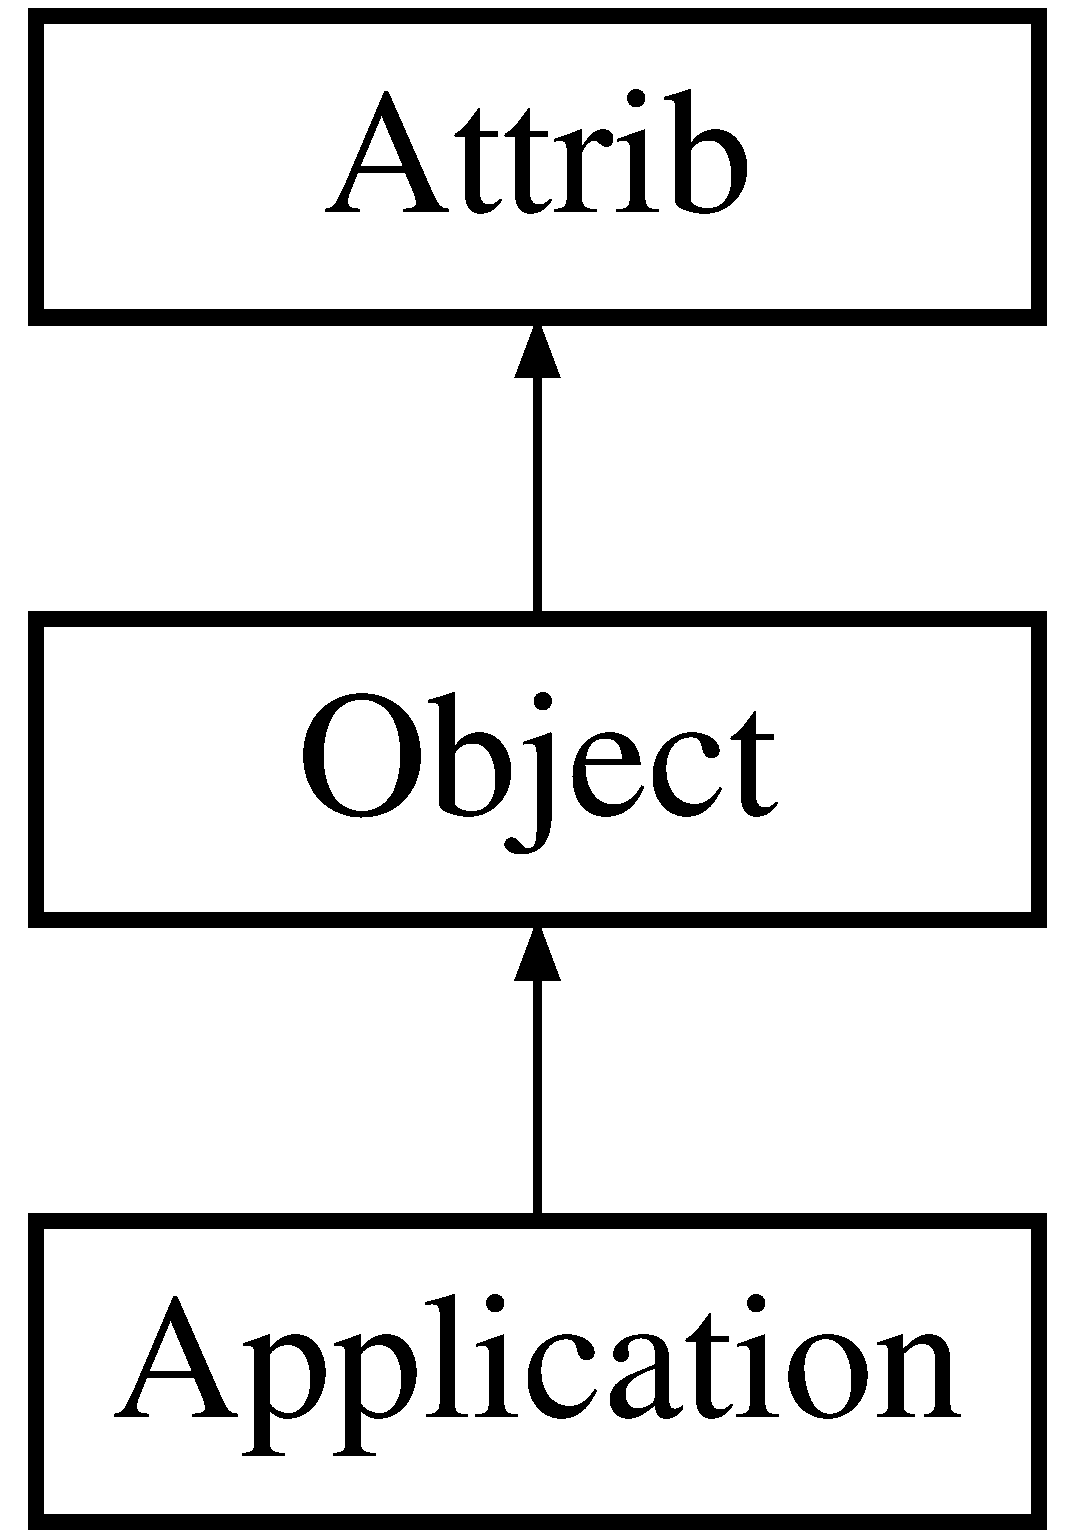
\includegraphics[height=3.000000cm]{classApplication}
\end{center}
\end{figure}
\subsection*{Public Types}
\begin{DoxyCompactItemize}
\item 
enum \hyperlink{classAttrib_a69e171d7cc6417835a5a306d3c764235}{Attribut} \{ \newline
\hyperlink{classAttrib_a69e171d7cc6417835a5a306d3c764235a3a8da2ab97dda18aebab196fe4100531}{U\+N\+D\+E\+F\+I\+N\+ED}, 
\hyperlink{classAttrib_a69e171d7cc6417835a5a306d3c764235a2bfb2af57b87031d190a05fe25dd92ed}{P\+A\+S\+S\+I\+VE}, 
\hyperlink{classAttrib_a69e171d7cc6417835a5a306d3c764235a3b1fec929c0370d1436f2f06e298fb0d}{A\+C\+T\+I\+VE}, 
\hyperlink{classAttrib_a69e171d7cc6417835a5a306d3c764235aa27c16b480a369ea4d18b07b2516bbc7}{I\+N\+T\+E\+R\+F\+A\+CE}, 
\newline
\hyperlink{classAttrib_a69e171d7cc6417835a5a306d3c764235a1420a5b8c0540b2af210b6975eded7f9}{IO}, 
\hyperlink{classAttrib_a69e171d7cc6417835a5a306d3c764235a0af3b0d0ac323c1704e6c69cf90add28}{I\+O\+D\+A\+TA}, 
\hyperlink{classAttrib_a69e171d7cc6417835a5a306d3c764235a7788bc5dd333fd8ce18562b269c9dab1}{E\+L\+E\+M\+E\+NT}, 
\hyperlink{classAttrib_a69e171d7cc6417835a5a306d3c764235a61ceb22149f365f1780d18f9d1459423}{H\+A\+R\+D\+W\+A\+RE}, 
\newline
\hyperlink{classAttrib_a69e171d7cc6417835a5a306d3c764235a75250e29692496e73effca2c0330977f}{P\+R\+O\+C\+E\+S\+S\+US}, 
\hyperlink{classAttrib_a69e171d7cc6417835a5a306d3c764235a103a67cd0b8f07ef478fa45d4356e27b}{S\+O\+F\+T\+W\+A\+RE}
 \}
\end{DoxyCompactItemize}
\subsection*{Public Member Functions}
\begin{DoxyCompactItemize}
\item 
\hyperlink{classApplication_afa8cc05ce6b6092be5ecdfdae44e05f8}{Application} ()
\begin{DoxyCompactList}\small\item\em Standard constructor. \end{DoxyCompactList}\item 
virtual \hyperlink{classApplication_a748bca84fefb9c12661cfaa2f623748d}{$\sim$\+Application} ()
\begin{DoxyCompactList}\small\item\em Destructor. \end{DoxyCompactList}\item 
\hyperlink{classStatusCode}{Status\+Code} \hyperlink{classApplication_a86b8cbb104f3e04516ef574e5822ff82}{initialize} ()
\item 
\hyperlink{classStatusCode}{Status\+Code} \hyperlink{classApplication_a7fdd5bfee44e49896292f8964037384d}{run} (std\+::string proc\+Name, \hyperlink{classElement}{Element} $\ast$element=0, int n\+Evt=1)
\item 
\hyperlink{classStatusCode}{Status\+Code} \hyperlink{classApplication_a5e2b592eebe6f2f8780d2c129bf14560}{finalize} ()
\item 
\hyperlink{classOptions}{Options} $\ast$ \hyperlink{classApplication_ada7cc0e8db586985f1435aee0c79f47d}{options} ()
\item 
\hyperlink{classComputer}{Computer} $\ast$ \hyperlink{classApplication_ac5eb8a8e693d1b93426d7aabc6606d8b}{computer} ()
\item 
\hyperlink{classDLLMgr}{D\+L\+L\+Mgr} $\ast$ \hyperlink{classApplication_a0133c161bf55544f268ca039e174060b}{dll\+Mgr} ()
\item 
\hyperlink{classProcDataBase}{Proc\+Data\+Base} $\ast$ \hyperlink{classApplication_aa5c28af1a7e1c41dada2db2a4d03c57d}{proc\+Db} ()
\item 
\hyperlink{classStatusCode}{Status\+Code} \hyperlink{classApplication_ab5d46fc4784a4c821e974f5a47ec933d}{load\+History\+File} ()
\item 
\hyperlink{classStatusCode}{Status\+Code} \hyperlink{classApplication_ad5faa0fa744706190844bbc4be58b700}{bookkeeping} ()
\item 
void \hyperlink{classApplication_af168aa3579262d65adc0bd4531361a53}{banner} ()
\item 
void \hyperlink{classApplication_a3c8a98d6c10a5b054800488df16cdbcb}{exit} ()
\item 
void \hyperlink{classApplication_a0f0a9e376d9f1716e01e86c94ae3499f}{set\+Current} (\hyperlink{classHierarchy}{Hierarchy} $\ast$\hyperlink{classApplication_af25c880ff1e95d863ed058396754a76e}{current})
\item 
\hyperlink{classHierarchy}{Hierarchy} $\ast$ \hyperlink{classApplication_af25c880ff1e95d863ed058396754a76e}{current} ()
\item 
\hyperlink{classStatusCode}{Status\+Code} \hyperlink{classApplication_a29aa0687ea27762ce36ab4195bf5d77f}{cd} (std\+::string path)
\item 
std\+::string \hyperlink{classApplication_a095248805e26b553466b7fafc6517d8f}{hostname} ()
\item 
void \hyperlink{classApplication_ab4a53c51303b155b738970bec9a6ce89}{tree\+Recursive} (\hyperlink{classHierarchy}{Hierarchy} $\ast$, std\+::string)
\item 
\hyperlink{classStatusCode}{Status\+Code} \hyperlink{classApplication_a552c6df459660f2d80e6d0ac6ce8279b}{create} (std\+::string, std\+::string)
\item 
\hyperlink{classStatusCode}{Status\+Code} \hyperlink{classApplication_accaba6b75f26c92e7604df43c853390b}{make\+Dir} (std\+::string)
\item 
\hyperlink{classState}{State} $\ast$ \hyperlink{classApplication_adfc9b92559f61c92224abf03f51cef47}{state} ()
\item 
\hyperlink{classConfig}{Config} $\ast$ \hyperlink{classApplication_ae79819f7743d6f402fce87665c1dc9a6}{config} ()
\item 
void \hyperlink{classApplication_a4a86c9bbf7851753c7b2bc03211092fb}{set\+State} (std\+::string \hyperlink{classApplication_adfc9b92559f61c92224abf03f51cef47}{state}=std\+::string(\char`\"{}\char`\"{}))
\item 
void \hyperlink{classApplication_a46614964f765fd5374b216582b599bcb}{set\+Config} ()
\item 
char $\ast$ \hyperlink{classApplication_ad429c4d2322f706e3564c1ee05d38ff1}{status} ()
\item 
void \hyperlink{classApplication_ab21cc0c86ca4e63d1fbd348d709dcddc}{network} (std\+::string)
\item 
void \hyperlink{classApplication_a1712ebe326b3d1855b839c59f52633d8}{server} ()
\item 
void \hyperlink{classApplication_a8ed8a66653bb6e665e05a735519c5d5b}{set\+Processus} (\hyperlink{classProcessus}{Processus} $\ast$\hyperlink{classApplication_a8d0918e800a5de01795bc2669d74ed82}{processus})
\item 
\hyperlink{classProcessus}{Processus} $\ast$ \hyperlink{classApplication_a8d0918e800a5de01795bc2669d74ed82}{processus} ()
\item 
\hyperlink{classStatusCode}{Status\+Code} \hyperlink{classApplication_abfbf40397efe6ff0627d2ce1a55381ce}{run\+Svc} ()
\item 
void \hyperlink{classApplication_a95ea0ef35377c259687752aedc4b9321}{set\+Run\+Svc} (\hyperlink{Application_8h_a59643f52f9391fa83f137814aaae27ef}{Run\+Svc} svc)
\item 
\hyperlink{classStatusCode}{Status\+Code} \hyperlink{classApplication_a6344c22495ff3e87d77d0c47aea3bf00}{plot\+Svc} ()
\item 
void \hyperlink{classApplication_ac11402510105adf9a9ccf3daa25ea7d4}{set\+Plot\+Svc} (\hyperlink{Application_8h_abaa10d33ca2837dfcf8ba9bff40cdbb6}{Plot\+Svc} svc)
\item 
void \hyperlink{classApplication_a48ecc3d76b3f2390ae1ba76d13f8bd54}{set\+Version} (std\+::string \hyperlink{classApplication_a060ac7b6d3a6cb111a9ed39bfd0350d1}{version})
\item 
std\+::string \hyperlink{classApplication_a060ac7b6d3a6cb111a9ed39bfd0350d1}{version} ()
\item 
void \hyperlink{classApplication_a451a04a80f59a76fb13b6fae6c07439a}{set\+Ctrl} (std\+::string control)
\item 
std\+::string \hyperlink{classApplication_a3eb11c9a1985a3a9d2ec51df957f7c2f}{ctrl} ()
\item 
\hyperlink{classStatusCode}{Status\+Code} \hyperlink{classApplication_a35eca6b5e618b508a0736d032e2a9203}{svc\+Running} ()
\item 
\hyperlink{classStatusCode}{Status\+Code} \hyperlink{classApplication_a61dcc20b7f4b7c19b697db7516a62afa}{prepare} (std\+::string proc\+Name, \hyperlink{classElement}{Element} $\ast$element=0, int n\+Evt=1)
\item 
\hyperlink{classStatusCode}{Status\+Code} \hyperlink{classApplication_ab38055646202ef49c9ee2eda6d48076f}{loop} ()
\item 
\hyperlink{classStatusCode}{Status\+Code} \hyperlink{classApplication_a1a36a06d48d94a9a8fdc29a77d2cb9f0}{terminate} ()
\item 
\hyperlink{classStatusCode}{Status\+Code} \hyperlink{classApplication_a297f55c288c32cbdadadcbbc26ae7692}{svc\+Plot} ()
\item 
std\+::string \hyperlink{classObject_a300f4c05dd468c7bb8b3c968868443c1}{name} () const
\item 
std\+::string \hyperlink{classObject_a84f99f70f144a83e1582d1d0f84e4e62}{type} ()
\item 
unsigned char \hyperlink{classObject_af99145335cc61ff6e2798ea17db009d2}{id} ()
\item 
std\+::string \hyperlink{classObject_a73a0f1a41828fdd8303dd662446fb6c3}{title} ()
\item 
void \hyperlink{classObject_a3f9d5537ebce0c0f2bf6ae4d92426f3c}{msg\+Svc} (int level, std\+::string \hyperlink{classObject_a58b2d0618c2d08cf2383012611528d97}{msg}, std\+::string \hyperlink{classObject_a300f4c05dd468c7bb8b3c968868443c1}{name})
\item 
void \hyperlink{classObject_a58b2d0618c2d08cf2383012611528d97}{msg} (std\+::string mymsg)
\item 
void \hyperlink{classObject_ac5d59299273cee27aacf7de00d2e7034}{msg} (std\+::string mymsg, std\+::string \hyperlink{classObject_a300f4c05dd468c7bb8b3c968868443c1}{name})
\item 
void \hyperlink{classObject_a83d2db2df682907ea1115ad721c1c4a1}{verbose} (std\+::string mymsg)
\item 
void \hyperlink{classObject_a2d4120195317e2a3c6532e8bb9f3da68}{verbose} (std\+::string mymsg, std\+::string \hyperlink{classObject_a300f4c05dd468c7bb8b3c968868443c1}{name})
\item 
void \hyperlink{classObject_aac010553f022165573714b7014a15f0d}{debug} (std\+::string mymsg)
\item 
void \hyperlink{classObject_a6c9a0397ca804e04d675ed05683f5420}{debug} (std\+::string mymsg, std\+::string \hyperlink{classObject_a300f4c05dd468c7bb8b3c968868443c1}{name})
\item 
void \hyperlink{classObject_a644fd329ea4cb85f54fa6846484b84a8}{info} (std\+::string mymsg)
\item 
void \hyperlink{classObject_a1ca123253dfd30fc28b156f521dcbdae}{info} (std\+::string mymsg, std\+::string \hyperlink{classObject_a300f4c05dd468c7bb8b3c968868443c1}{name})
\item 
void \hyperlink{classObject_a65cd4fda577711660821fd2cd5a3b4c9}{warning} (std\+::string mymsg)
\item 
void \hyperlink{classObject_a11f101db4dd73d9391b0231818881d86}{warning} (std\+::string mymsg, std\+::string \hyperlink{classObject_a300f4c05dd468c7bb8b3c968868443c1}{name})
\item 
void \hyperlink{classObject_a204a95f57818c0f811933917a30eff45}{error} (std\+::string mymsg)
\item 
void \hyperlink{classObject_ad7f6c457733082efa2f9ff5f5c8e119a}{error} (std\+::string mymsg, std\+::string \hyperlink{classObject_a300f4c05dd468c7bb8b3c968868443c1}{name})
\item 
void \hyperlink{classObject_aad5a16aac7516ce65bd5ec02ab07fc80}{fatal} (std\+::string mymsg)
\item 
void \hyperlink{classObject_ae62acd3d09f716220f75f252dc38bc9a}{fatal} (std\+::string mymsg, std\+::string \hyperlink{classObject_a300f4c05dd468c7bb8b3c968868443c1}{name})
\item 
void \hyperlink{classObject_ae30fea75683c2d149b6b6d17c09ecd0c}{set\+Name} (std\+::string \hyperlink{classObject_a300f4c05dd468c7bb8b3c968868443c1}{name})
\item 
void \hyperlink{classObject_aae534cc9d982bcb9b99fd505f2e103a5}{set\+Type} (std\+::string \hyperlink{classObject_a84f99f70f144a83e1582d1d0f84e4e62}{type})
\item 
void \hyperlink{classObject_a398fe08cba594a0ce6891d59fe4f159f}{set\+Id} (unsigned char \hyperlink{classObject_af99145335cc61ff6e2798ea17db009d2}{id})
\item 
void \hyperlink{classObject_a89557dbbad5bcaa02652f5d7fa35d20f}{set\+Title} (std\+::string \hyperlink{classObject_a73a0f1a41828fdd8303dd662446fb6c3}{title})
\item 
void \hyperlink{classObject_a870c5af919958c2136623b2d7816d123}{set\+Dll\+Name} (std\+::string \hyperlink{classObject_a2e3947f2870094c332d7454117f3ec63}{dll\+Name})
\item 
std\+::string \hyperlink{classObject_a2e3947f2870094c332d7454117f3ec63}{dll\+Name} ()
\item 
bool \hyperlink{classAttrib_a704f26af560909ad22065083bb7d4c34}{is} (int attribut)
\item 
void \hyperlink{classAttrib_a235f773af19c900264a190b00a3b4ad7}{add} (int attribut)
\item 
void \hyperlink{classAttrib_a7d4ef7e32d93cb287792b87b857e79f3}{remove} (int attribut)
\item 
std\+::string \hyperlink{classAttrib_aee7bbf16b144887f196e1341b24f8a26}{attributs} ()
\end{DoxyCompactItemize}
\subsection*{Protected Attributes}
\begin{DoxyCompactItemize}
\item 
std\+::string \hyperlink{classApplication_ac6ecd97be07092147986a7a5965c54ec}{m\+\_\+account\+Name}
\item 
std\+::string \hyperlink{classApplication_a20094c2bf311e2046942eeeec4a11f02}{m\+\_\+host\+Name}
\item 
std\+::string \hyperlink{classApplication_a59f90c6ff4ee3db646ca656c71cc77e7}{m\+\_\+os\+Name}
\item 
std\+::string \hyperlink{classApplication_a17949f767d2598e92acb0885bb399dc0}{m\+\_\+os\+Version}
\item 
std\+::string \hyperlink{classApplication_a84f3f07f42ad77ad46cc8ef42d609948}{m\+\_\+prompt}
\item 
std\+::string \hyperlink{classApplication_acbbdbd17a3a66782c54dbbe58a9ca8d8}{m\+\_\+version}
\item 
bool \hyperlink{classApplication_ae316ea43e74cc0d536dcbb16b2fbb974}{m\+\_\+is\+Running}
\item 
\hyperlink{classHierarchy}{Hierarchy} $\ast$ \hyperlink{classApplication_ab0fd877a3c66c41b22109863e1719ccd}{m\+\_\+current}
\item 
std\+::string \hyperlink{classAttrib_a3414521d7a82476e874b25a5407b5e63}{m\+\_\+attrib\+String} \mbox{[}10\mbox{]}
\end{DoxyCompactItemize}
\subsection*{Private Attributes}
\begin{DoxyCompactItemize}
\item 
\hyperlink{classOptions}{Options} $\ast$ \hyperlink{classApplication_a3b0c74bf1ba99a5042990e3fefaa8963}{m\+\_\+options}
\item 
\hyperlink{classDLLMgr}{D\+L\+L\+Mgr} $\ast$ \hyperlink{classApplication_a66b06cbeb824fe00ecd11499fcf01c55}{m\+\_\+dll\+Mgr}
\item 
\hyperlink{classProcDataBase}{Proc\+Data\+Base} $\ast$ \hyperlink{classApplication_af030cefeb69586f01e965606d5dd8919}{m\+\_\+proc\+Db}
\item 
\hyperlink{classComputer}{Computer} $\ast$ \hyperlink{classApplication_a17c9fd27b6abbc18abb6d5de5d7648ef}{m\+\_\+computer}
\item 
\hyperlink{classProcessus}{Processus} $\ast$ \hyperlink{classApplication_ab5eb4b3d3bef5ab9fce9c69401ce5786}{m\+\_\+processus}
\item 
\hyperlink{classState}{State} $\ast$ \hyperlink{classApplication_a0ef9832e2d286716e597a1ff21ffcab4}{m\+\_\+state}
\item 
\hyperlink{classConfig}{Config} $\ast$ \hyperlink{classApplication_ae05f3e253ea871a194c3d30fd1d3b0c3}{m\+\_\+config}
\item 
\hyperlink{Application_8h_a59643f52f9391fa83f137814aaae27ef}{Run\+Svc} \hyperlink{classApplication_ad2c061af424280151c86b9b56d9724d3}{m\+\_\+run\+Svc}
\item 
\hyperlink{Application_8h_abaa10d33ca2837dfcf8ba9bff40cdbb6}{Plot\+Svc} \hyperlink{classApplication_a30d5600ea5e4f36b14f25f903ee3256e}{m\+\_\+plot\+Svc}
\item 
\hyperlink{classServer}{Server} $\ast$ \hyperlink{classApplication_a5e6085b0f322d5036177b16113a75b56}{m\+\_\+server}
\item 
bool \hyperlink{classApplication_a7dc2bb72356cd9186eaad49eb506995a}{m\+\_\+network}
\item 
std\+::string \hyperlink{classApplication_aa371ed989ed34038df400c4d1b41b37f}{m\+\_\+ctrl}
\end{DoxyCompactItemize}


\subsection{Detailed Description}
\hyperlink{classApplication}{Application} main class

\begin{DoxyAuthor}{Author}
Frederic Machefert 
\end{DoxyAuthor}
\begin{DoxyDate}{Date}
2006-\/10-\/23 
\end{DoxyDate}


Definition at line 58 of file Application.\+h.



\subsection{Member Enumeration Documentation}
\mbox{\Hypertarget{classAttrib_a69e171d7cc6417835a5a306d3c764235}\label{classAttrib_a69e171d7cc6417835a5a306d3c764235}} 
\index{Application@{Application}!Attribut@{Attribut}}
\index{Attribut@{Attribut}!Application@{Application}}
\subsubsection{\texorpdfstring{Attribut}{Attribut}}
{\footnotesize\ttfamily enum \hyperlink{classAttrib_a69e171d7cc6417835a5a306d3c764235}{Attrib\+::\+Attribut}\hspace{0.3cm}{\ttfamily [inherited]}}

\begin{DoxyEnumFields}{Enumerator}
\raisebox{\heightof{T}}[0pt][0pt]{\index{U\+N\+D\+E\+F\+I\+N\+ED@{U\+N\+D\+E\+F\+I\+N\+ED}!Application@{Application}}\index{Application@{Application}!U\+N\+D\+E\+F\+I\+N\+ED@{U\+N\+D\+E\+F\+I\+N\+ED}}}\mbox{\Hypertarget{classAttrib_a69e171d7cc6417835a5a306d3c764235a3a8da2ab97dda18aebab196fe4100531}\label{classAttrib_a69e171d7cc6417835a5a306d3c764235a3a8da2ab97dda18aebab196fe4100531}} 
U\+N\+D\+E\+F\+I\+N\+ED&\\
\hline

\raisebox{\heightof{T}}[0pt][0pt]{\index{P\+A\+S\+S\+I\+VE@{P\+A\+S\+S\+I\+VE}!Application@{Application}}\index{Application@{Application}!P\+A\+S\+S\+I\+VE@{P\+A\+S\+S\+I\+VE}}}\mbox{\Hypertarget{classAttrib_a69e171d7cc6417835a5a306d3c764235a2bfb2af57b87031d190a05fe25dd92ed}\label{classAttrib_a69e171d7cc6417835a5a306d3c764235a2bfb2af57b87031d190a05fe25dd92ed}} 
P\+A\+S\+S\+I\+VE&\\
\hline

\raisebox{\heightof{T}}[0pt][0pt]{\index{A\+C\+T\+I\+VE@{A\+C\+T\+I\+VE}!Application@{Application}}\index{Application@{Application}!A\+C\+T\+I\+VE@{A\+C\+T\+I\+VE}}}\mbox{\Hypertarget{classAttrib_a69e171d7cc6417835a5a306d3c764235a3b1fec929c0370d1436f2f06e298fb0d}\label{classAttrib_a69e171d7cc6417835a5a306d3c764235a3b1fec929c0370d1436f2f06e298fb0d}} 
A\+C\+T\+I\+VE&\\
\hline

\raisebox{\heightof{T}}[0pt][0pt]{\index{I\+N\+T\+E\+R\+F\+A\+CE@{I\+N\+T\+E\+R\+F\+A\+CE}!Application@{Application}}\index{Application@{Application}!I\+N\+T\+E\+R\+F\+A\+CE@{I\+N\+T\+E\+R\+F\+A\+CE}}}\mbox{\Hypertarget{classAttrib_a69e171d7cc6417835a5a306d3c764235aa27c16b480a369ea4d18b07b2516bbc7}\label{classAttrib_a69e171d7cc6417835a5a306d3c764235aa27c16b480a369ea4d18b07b2516bbc7}} 
I\+N\+T\+E\+R\+F\+A\+CE&\\
\hline

\raisebox{\heightof{T}}[0pt][0pt]{\index{IO@{IO}!Application@{Application}}\index{Application@{Application}!IO@{IO}}}\mbox{\Hypertarget{classAttrib_a69e171d7cc6417835a5a306d3c764235a1420a5b8c0540b2af210b6975eded7f9}\label{classAttrib_a69e171d7cc6417835a5a306d3c764235a1420a5b8c0540b2af210b6975eded7f9}} 
IO&\\
\hline

\raisebox{\heightof{T}}[0pt][0pt]{\index{I\+O\+D\+A\+TA@{I\+O\+D\+A\+TA}!Application@{Application}}\index{Application@{Application}!I\+O\+D\+A\+TA@{I\+O\+D\+A\+TA}}}\mbox{\Hypertarget{classAttrib_a69e171d7cc6417835a5a306d3c764235a0af3b0d0ac323c1704e6c69cf90add28}\label{classAttrib_a69e171d7cc6417835a5a306d3c764235a0af3b0d0ac323c1704e6c69cf90add28}} 
I\+O\+D\+A\+TA&\\
\hline

\raisebox{\heightof{T}}[0pt][0pt]{\index{E\+L\+E\+M\+E\+NT@{E\+L\+E\+M\+E\+NT}!Application@{Application}}\index{Application@{Application}!E\+L\+E\+M\+E\+NT@{E\+L\+E\+M\+E\+NT}}}\mbox{\Hypertarget{classAttrib_a69e171d7cc6417835a5a306d3c764235a7788bc5dd333fd8ce18562b269c9dab1}\label{classAttrib_a69e171d7cc6417835a5a306d3c764235a7788bc5dd333fd8ce18562b269c9dab1}} 
E\+L\+E\+M\+E\+NT&\\
\hline

\raisebox{\heightof{T}}[0pt][0pt]{\index{H\+A\+R\+D\+W\+A\+RE@{H\+A\+R\+D\+W\+A\+RE}!Application@{Application}}\index{Application@{Application}!H\+A\+R\+D\+W\+A\+RE@{H\+A\+R\+D\+W\+A\+RE}}}\mbox{\Hypertarget{classAttrib_a69e171d7cc6417835a5a306d3c764235a61ceb22149f365f1780d18f9d1459423}\label{classAttrib_a69e171d7cc6417835a5a306d3c764235a61ceb22149f365f1780d18f9d1459423}} 
H\+A\+R\+D\+W\+A\+RE&\\
\hline

\raisebox{\heightof{T}}[0pt][0pt]{\index{P\+R\+O\+C\+E\+S\+S\+US@{P\+R\+O\+C\+E\+S\+S\+US}!Application@{Application}}\index{Application@{Application}!P\+R\+O\+C\+E\+S\+S\+US@{P\+R\+O\+C\+E\+S\+S\+US}}}\mbox{\Hypertarget{classAttrib_a69e171d7cc6417835a5a306d3c764235a75250e29692496e73effca2c0330977f}\label{classAttrib_a69e171d7cc6417835a5a306d3c764235a75250e29692496e73effca2c0330977f}} 
P\+R\+O\+C\+E\+S\+S\+US&\\
\hline

\raisebox{\heightof{T}}[0pt][0pt]{\index{S\+O\+F\+T\+W\+A\+RE@{S\+O\+F\+T\+W\+A\+RE}!Application@{Application}}\index{Application@{Application}!S\+O\+F\+T\+W\+A\+RE@{S\+O\+F\+T\+W\+A\+RE}}}\mbox{\Hypertarget{classAttrib_a69e171d7cc6417835a5a306d3c764235a103a67cd0b8f07ef478fa45d4356e27b}\label{classAttrib_a69e171d7cc6417835a5a306d3c764235a103a67cd0b8f07ef478fa45d4356e27b}} 
S\+O\+F\+T\+W\+A\+RE&\\
\hline

\end{DoxyEnumFields}


Definition at line 29 of file Attrib.\+h.


\begin{DoxyCode}
29                 \{
30     \hyperlink{classAttrib_a69e171d7cc6417835a5a306d3c764235a3a8da2ab97dda18aebab196fe4100531}{UNDEFINED},
31     \hyperlink{classAttrib_a69e171d7cc6417835a5a306d3c764235a2bfb2af57b87031d190a05fe25dd92ed}{PASSIVE},
32     \hyperlink{classAttrib_a69e171d7cc6417835a5a306d3c764235a3b1fec929c0370d1436f2f06e298fb0d}{ACTIVE},
33     \hyperlink{classAttrib_a69e171d7cc6417835a5a306d3c764235aa27c16b480a369ea4d18b07b2516bbc7}{INTERFACE},
34     \hyperlink{classAttrib_a69e171d7cc6417835a5a306d3c764235a1420a5b8c0540b2af210b6975eded7f9}{IO},
35     \hyperlink{classAttrib_a69e171d7cc6417835a5a306d3c764235a0af3b0d0ac323c1704e6c69cf90add28}{IODATA},
36     \hyperlink{classAttrib_a69e171d7cc6417835a5a306d3c764235a7788bc5dd333fd8ce18562b269c9dab1}{ELEMENT},
37     \hyperlink{classAttrib_a69e171d7cc6417835a5a306d3c764235a61ceb22149f365f1780d18f9d1459423}{HARDWARE},
38     \hyperlink{classAttrib_a69e171d7cc6417835a5a306d3c764235a75250e29692496e73effca2c0330977f}{PROCESSUS},
39     \hyperlink{classAttrib_a69e171d7cc6417835a5a306d3c764235a103a67cd0b8f07ef478fa45d4356e27b}{SOFTWARE} 
40   \}; \textcolor{comment}{// array m\_attribString must be changed into Attrib::Attrib if this enu is modified. }
\end{DoxyCode}


\subsection{Constructor \& Destructor Documentation}
\mbox{\Hypertarget{classApplication_afa8cc05ce6b6092be5ecdfdae44e05f8}\label{classApplication_afa8cc05ce6b6092be5ecdfdae44e05f8}} 
\index{Application@{Application}!Application@{Application}}
\index{Application@{Application}!Application@{Application}}
\subsubsection{\texorpdfstring{Application()}{Application()}}
{\footnotesize\ttfamily Application\+::\+Application (\begin{DoxyParamCaption}{ }\end{DoxyParamCaption})}



Standard constructor. 



Definition at line 29 of file Application.\+cpp.



References System\+::account\+Name(), System\+::host\+Name(), m\+\_\+account\+Name, m\+\_\+computer, m\+\_\+config, m\+\_\+dll\+Mgr, m\+\_\+host\+Name, m\+\_\+options, m\+\_\+os\+Name, m\+\_\+os\+Version, m\+\_\+proc\+Db, m\+\_\+state, System\+::os\+Name(), System\+::os\+Version(), set\+Application(), and set\+Current().


\begin{DoxyCode}
29                            :
30   \hyperlink{classApplication_a3b0c74bf1ba99a5042990e3fefaa8963}{m\_options}  (0),
31   \hyperlink{classApplication_a66b06cbeb824fe00ecd11499fcf01c55}{m\_dllMgr}   (0),
32   \hyperlink{classApplication_af030cefeb69586f01e965606d5dd8919}{m\_procDb}   (0),
33   \hyperlink{classApplication_a17c9fd27b6abbc18abb6d5de5d7648ef}{m\_computer} (0),
34   \hyperlink{classApplication_ab5eb4b3d3bef5ab9fce9c69401ce5786}{m\_processus}(0),
35   \hyperlink{classApplication_a0ef9832e2d286716e597a1ff21ffcab4}{m\_state}    (0),
36   \hyperlink{classApplication_ae05f3e253ea871a194c3d30fd1d3b0c3}{m\_config}   (0),
37   \hyperlink{classApplication_a5e6085b0f322d5036177b16113a75b56}{m\_server}   (0)
38 \{
39   \hyperlink{Tools_8h_a71443363ed67070e753a3c172f694834}{setApplication}(\textcolor{keyword}{this});
40   \hyperlink{classApplication_a3b0c74bf1ba99a5042990e3fefaa8963}{m\_options}     = \textcolor{keyword}{new} \hyperlink{classOptions}{Options}  ();
41   \hyperlink{classApplication_ac6ecd97be07092147986a7a5965c54ec}{m\_accountName} = \hyperlink{namespaceSystem_a8a4ea73b74e0f6b8225e571e21ba4e2f}{System::accountName}();
42   \hyperlink{classApplication_a20094c2bf311e2046942eeeec4a11f02}{m\_hostName}    = \hyperlink{namespaceSystem_a89320a729880098922e8b505db1137ec}{System::hostName}();
43   \hyperlink{classApplication_a59f90c6ff4ee3db646ca656c71cc77e7}{m\_osName}      = \hyperlink{namespaceSystem_a08f605cda93733c3b7593517ed18557c}{System::osName}();
44   \hyperlink{classApplication_a17949f767d2598e92acb0885bb399dc0}{m\_osVersion}   = \hyperlink{namespaceSystem_aee568b62f9bcad983dcb3f0c30631854}{System::osVersion}();
45   \hyperlink{classApplication_a66b06cbeb824fe00ecd11499fcf01c55}{m\_dllMgr}      = \textcolor{keyword}{new} \hyperlink{classDLLMgr}{DLLMgr}   ();
46   \hyperlink{classApplication_af030cefeb69586f01e965606d5dd8919}{m\_procDb}      = \textcolor{keyword}{new} \hyperlink{classProcDataBase}{ProcDataBase} ();
47   \hyperlink{classApplication_a17c9fd27b6abbc18abb6d5de5d7648ef}{m\_computer}    = \textcolor{keyword}{new} \hyperlink{namespaceComputer}{Computer} ();
48   \hyperlink{classApplication_a0ef9832e2d286716e597a1ff21ffcab4}{m\_state}       = \textcolor{keyword}{new} \hyperlink{classState}{State}();
49   \hyperlink{classApplication_ae05f3e253ea871a194c3d30fd1d3b0c3}{m\_config}      = \textcolor{keyword}{new} \hyperlink{classConfig}{Config}();
50   \hyperlink{classApplication_a0f0a9e376d9f1716e01e86c94ae3499f}{setCurrent} ( (\hyperlink{classHierarchy}{Hierarchy}*) (\hyperlink{classApplication_a17c9fd27b6abbc18abb6d5de5d7648ef}{m\_computer}) );
51 \}
\end{DoxyCode}
\mbox{\Hypertarget{classApplication_a748bca84fefb9c12661cfaa2f623748d}\label{classApplication_a748bca84fefb9c12661cfaa2f623748d}} 
\index{Application@{Application}!````~Application@{$\sim$\+Application}}
\index{````~Application@{$\sim$\+Application}!Application@{Application}}
\subsubsection{\texorpdfstring{$\sim$\+Application()}{~Application()}}
{\footnotesize\ttfamily Application\+::$\sim$\+Application (\begin{DoxyParamCaption}{ }\end{DoxyParamCaption})\hspace{0.3cm}{\ttfamily [virtual]}}



Destructor. 



Definition at line 56 of file Application.\+cpp.



References m\+\_\+config, m\+\_\+dll\+Mgr, m\+\_\+options, m\+\_\+proc\+Db, m\+\_\+server, and m\+\_\+state.


\begin{DoxyCode}
56                           \{
57   \textcolor{keywordflow}{if} (  0!=\hyperlink{classApplication_a5e6085b0f322d5036177b16113a75b56}{m\_server} ) \{
58     \textcolor{keyword}{delete} \hyperlink{classApplication_a5e6085b0f322d5036177b16113a75b56}{m\_server};
59     \hyperlink{classApplication_a5e6085b0f322d5036177b16113a75b56}{m\_server} = 0;
60   \}
61   \textcolor{keyword}{delete} \hyperlink{classApplication_a0ef9832e2d286716e597a1ff21ffcab4}{m\_state};
62   \textcolor{keyword}{delete} \hyperlink{classApplication_ae05f3e253ea871a194c3d30fd1d3b0c3}{m\_config};
63   \textcolor{keyword}{delete} \hyperlink{classApplication_a3b0c74bf1ba99a5042990e3fefaa8963}{m\_options};
64   \textcolor{keyword}{delete} \hyperlink{classApplication_a66b06cbeb824fe00ecd11499fcf01c55}{m\_dllMgr};
65   \textcolor{keyword}{delete} \hyperlink{classApplication_af030cefeb69586f01e965606d5dd8919}{m\_procDb};
66   \textcolor{comment}{//  delete m\_computer;}
67 \}
\end{DoxyCode}


\subsection{Member Function Documentation}
\mbox{\Hypertarget{classAttrib_a235f773af19c900264a190b00a3b4ad7}\label{classAttrib_a235f773af19c900264a190b00a3b4ad7}} 
\index{Application@{Application}!add@{add}}
\index{add@{add}!Application@{Application}}
\subsubsection{\texorpdfstring{add()}{add()}}
{\footnotesize\ttfamily void Attrib\+::add (\begin{DoxyParamCaption}\item[{int}]{attribut }\end{DoxyParamCaption})\hspace{0.3cm}{\ttfamily [inline]}, {\ttfamily [inherited]}}

Add an attribut 

Definition at line 67 of file Attrib.\+h.



References Attrib\+::m\+\_\+attributs, and Attrib\+::\+U\+N\+D\+E\+F\+I\+N\+ED.



Referenced by A3\+P\+E\+::\+A3\+P\+E(), Attrib\+::\+Attrib(), Specs\+Mezzanine\+::cmdline(), Computer\+::\+Computer(), C\+U\+\_\+v1\+::\+C\+U\+\_\+v1(), export\+\_\+obj(), F\+E\+B\+\_\+v1\+::\+F\+E\+B\+\_\+v1(), Fe\+P\+G\+A\+::\+Fe\+P\+G\+A(), I\+C\+E\+C\+A\+Lv3\+::\+I\+C\+E\+C\+A\+Lv3(), I\+C\+Phaser\+::\+I\+C\+Phaser(), initialize(), Interface\+::\+Interface(), I\+Odata\+::\+I\+Odata(), I\+Oobject\+::\+I\+Oobject(), M\+S\+Oxxxx\+::\+M\+S\+Oxxxx(), Phaser\+::\+Phaser(), Processus\+::\+Processus(), Proto40\+M\+Hz\+\_\+v1\+::\+Proto40\+M\+Hz\+\_\+v1(), Attrib\+::remove(), Seq\+P\+G\+A\+::\+Seq\+P\+G\+A(), Test\+I2\+C\+::set\+Address(), Test\+S\+P\+I\+::set\+Address(), Specs\+Slave\+::set\+Address(), Specs\+Master\+::\+Specs\+Master(), and Specs\+Slave\+::\+Specs\+Slave().


\begin{DoxyCode}
67                             \{
68     \textcolor{keywordflow}{if} (attribut!=\hyperlink{classAttrib_a69e171d7cc6417835a5a306d3c764235a3a8da2ab97dda18aebab196fe4100531}{Attrib::UNDEFINED}) \textcolor{keyword}{remove}(\hyperlink{classAttrib_a69e171d7cc6417835a5a306d3c764235a3a8da2ab97dda18aebab196fe4100531}{Attrib::UNDEFINED});
69     \textcolor{keywordtype}{bool} duplicate = false ;
70     std::vector<int>::const\_iterator iter ;
71     \textcolor{keywordflow}{for} ( iter  = \hyperlink{classAttrib_ac4bd58a0cc6b38a3b711d609a3d3aacc}{m\_attributs}.begin() ;
72           iter != \hyperlink{classAttrib_ac4bd58a0cc6b38a3b711d609a3d3aacc}{m\_attributs}.end()   ;
73           ++iter ) \{
74       \textcolor{keywordflow}{if} ( attribut == (*iter) ) \{
75         duplicate = true ;
76       \}
77     \}
78     \textcolor{keywordflow}{if} (!duplicate) \{
79       \hyperlink{classAttrib_ac4bd58a0cc6b38a3b711d609a3d3aacc}{m\_attributs}.push\_back( attribut );
80     \}
81   \}
\end{DoxyCode}
\mbox{\Hypertarget{classAttrib_aee7bbf16b144887f196e1341b24f8a26}\label{classAttrib_aee7bbf16b144887f196e1341b24f8a26}} 
\index{Application@{Application}!attributs@{attributs}}
\index{attributs@{attributs}!Application@{Application}}
\subsubsection{\texorpdfstring{attributs()}{attributs()}}
{\footnotesize\ttfamily std\+::string Attrib\+::attributs (\begin{DoxyParamCaption}{ }\end{DoxyParamCaption})\hspace{0.3cm}{\ttfamily [inherited]}}

Print the \hyperlink{classAttrib}{Attrib} of an \hyperlink{classObject}{Object} 

Definition at line 54 of file Attrib.\+cpp.



References images\+::index, Attrib\+::m\+\_\+attrib\+String, and Attrib\+::m\+\_\+attributs.



Referenced by export\+\_\+obj(), and Attrib\+::remove().


\begin{DoxyCode}
54                             \{
55   std::string output;
56   std::vector<int>::iterator iter ;
57   \textcolor{keywordflow}{for} ( \textcolor{keywordtype}{unsigned} \textcolor{keywordtype}{int} \hyperlink{namespaceimages_a54407fd574970b3178647ae096321a57}{index} = 0 ; \hyperlink{namespaceimages_a54407fd574970b3178647ae096321a57}{index} < \hyperlink{classAttrib_ac4bd58a0cc6b38a3b711d609a3d3aacc}{m\_attributs}.size() ; ++
      \hyperlink{namespaceimages_a54407fd574970b3178647ae096321a57}{index} ) \{
58     \textcolor{keywordflow}{if} ( \hyperlink{classAttrib_ac4bd58a0cc6b38a3b711d609a3d3aacc}{m\_attributs}.size() - \hyperlink{namespaceimages_a54407fd574970b3178647ae096321a57}{index} > 1 ) \{
59       output.append(\hyperlink{classAttrib_a3414521d7a82476e874b25a5407b5e63}{m\_attribString}[\hyperlink{classAttrib_ac4bd58a0cc6b38a3b711d609a3d3aacc}{m\_attributs}[\hyperlink{namespaceimages_a54407fd574970b3178647ae096321a57}{index}]]);
60       output.append(\textcolor{stringliteral}{":"});
61     \}
62     \textcolor{keywordflow}{else} \{
63       output.append(\hyperlink{classAttrib_a3414521d7a82476e874b25a5407b5e63}{m\_attribString}[\hyperlink{classAttrib_ac4bd58a0cc6b38a3b711d609a3d3aacc}{m\_attributs}[index]]);
64     \}
65   \}
66   \textcolor{keywordflow}{return} output;
67 \}
\end{DoxyCode}
\mbox{\Hypertarget{classApplication_af168aa3579262d65adc0bd4531361a53}\label{classApplication_af168aa3579262d65adc0bd4531361a53}} 
\index{Application@{Application}!banner@{banner}}
\index{banner@{banner}!Application@{Application}}
\subsubsection{\texorpdfstring{banner()}{banner()}}
{\footnotesize\ttfamily void Application\+::banner (\begin{DoxyParamCaption}{ }\end{DoxyParamCaption})}

Banner of the \hyperlink{classApplication}{Application} 

Definition at line 103 of file Application.\+cpp.



References m\+\_\+account\+Name, m\+\_\+host\+Name, m\+\_\+os\+Name, m\+\_\+os\+Version, and Object\+::msg\+Svc().



Referenced by initialize().


\begin{DoxyCode}
103                            \{
104 \textcolor{preprocessor}{#ifdef \_WIN32
}
105   \textcolor{comment}{//  system("cls");}
106 \textcolor{preprocessor}{#else
}
107   \textcolor{comment}{//  system("clear");}
108 \textcolor{preprocessor}{#endif
}
109   \hyperlink{classObject_a3f9d5537ebce0c0f2bf6ae4d92426f3c}{msgSvc}(0,\textcolor{stringliteral}{""},\textcolor{stringliteral}{""});
110   \hyperlink{classObject_a3f9d5537ebce0c0f2bf6ae4d92426f3c}{msgSvc}(0,\textcolor{stringliteral}{"                          ***********************************************"},\textcolor{stringliteral}{""});
111   \hyperlink{classObject_a3f9d5537ebce0c0f2bf6ae4d92426f3c}{msgSvc}(0,\textcolor{stringliteral}{"                          *               C      A      T               *"},\textcolor{stringliteral}{""});
112   \hyperlink{classObject_a3f9d5537ebce0c0f2bf6ae4d92426f3c}{msgSvc}(0,\textcolor{stringliteral}{"                          *                                             *"},\textcolor{stringliteral}{""});
113   \hyperlink{classObject_a3f9d5537ebce0c0f2bf6ae4d92426f3c}{msgSvc}(0,\textcolor{stringliteral}{"                          *          |\(\backslash\)\(\backslash\)-''-/|.\_\_\_..--''\(\backslash\)"`-.\_            *"},\textcolor{stringliteral}{""});
114   \hyperlink{classObject_a3f9d5537ebce0c0f2bf6ae4d92426f3c}{msgSvc}(0,\textcolor{stringliteral}{"                          *          `6\_ 6  )   `-.  (     ).`-.\_\_.`)   *"},\textcolor{stringliteral}{""});
115   \hyperlink{classObject_a3f9d5537ebce0c0f2bf6ae4d92426f3c}{msgSvc}(0,\textcolor{stringliteral}{"                          *          (\_Y\_.)'  .\_   )  `.\_ `. ``-..-'    *"},\textcolor{stringliteral}{""});
116   \hyperlink{classObject_a3f9d5537ebce0c0f2bf6ae4d92426f3c}{msgSvc}(0,\textcolor{stringliteral}{"                          *         \_..`--'\_..-  \_/ /--'\_.' ,'          *"},\textcolor{stringliteral}{""});
117   \hyperlink{classObject_a3f9d5537ebce0c0f2bf6ae4d92426f3c}{msgSvc}(0,\textcolor{stringliteral}{"                          *     (il),-''  (li),' ((!.-'                 *"},\textcolor{stringliteral}{""});
118   \hyperlink{classObject_a3f9d5537ebce0c0f2bf6ae4d92426f3c}{msgSvc}(0,\textcolor{stringliteral}{"                          ***********************************************"},\textcolor{stringliteral}{""});
119   \hyperlink{classObject_a3f9d5537ebce0c0f2bf6ae4d92426f3c}{msgSvc}(0,\textcolor{stringliteral}{""},\textcolor{stringliteral}{""});
120   \hyperlink{classObject_a3f9d5537ebce0c0f2bf6ae4d92426f3c}{msgSvc}(0,\textcolor{stringliteral}{"Application running on "}+
121      \hyperlink{classApplication_ac6ecd97be07092147986a7a5965c54ec}{m\_accountName}+\textcolor{stringliteral}{"@"}+
122      \hyperlink{classApplication_a20094c2bf311e2046942eeeec4a11f02}{m\_hostName}+\textcolor{stringliteral}{" ("}+
123      \hyperlink{classApplication_a59f90c6ff4ee3db646ca656c71cc77e7}{m\_osName}+\textcolor{stringliteral}{" - "}+
124      \hyperlink{classApplication_a17949f767d2598e92acb0885bb399dc0}{m\_osVersion}+\textcolor{stringliteral}{")"},\textcolor{stringliteral}{""});
125 \}
\end{DoxyCode}
\mbox{\Hypertarget{classApplication_ad5faa0fa744706190844bbc4be58b700}\label{classApplication_ad5faa0fa744706190844bbc4be58b700}} 
\index{Application@{Application}!bookkeeping@{bookkeeping}}
\index{bookkeeping@{bookkeeping}!Application@{Application}}
\subsubsection{\texorpdfstring{bookkeeping()}{bookkeeping()}}
{\footnotesize\ttfamily \hyperlink{classStatusCode}{Status\+Code} Application\+::bookkeeping (\begin{DoxyParamCaption}{ }\end{DoxyParamCaption})}

write bookkeeping file \begin{DoxyReturn}{Returns}
\hyperlink{classStatusCode}{Status\+Code} 
\end{DoxyReturn}


Definition at line 170 of file Application.\+cpp.



References application(), Status\+Code\+::\+F\+A\+I\+L\+U\+RE, System\+::get\+Env(), options(), Options\+::run\+Number(), Status\+Code\+::\+S\+U\+C\+C\+E\+SS, and Object\+::warning().



Referenced by prepare().


\begin{DoxyCode}
170                                       \{
171   std::string filename = \hyperlink{namespaceSystem_af83af19ba6c1083e5643390dfd65f7aa}{System::getEnv}(\textcolor{stringliteral}{"CATPATH"});
172   filename.append(\textcolor{stringliteral}{"/.cathist"});
173   std::ofstream last;
174   last.open( filename.c\_str() );
175   \textcolor{keywordflow}{if} ( last.fail() ) \{
176     \hyperlink{classObject_a65cd4fda577711660821fd2cd5a3b4c9}{warning}(\textcolor{stringliteral}{"Cannot do the bookkeeping"},\textcolor{stringliteral}{"Application::bookkeeping"});
177     \textcolor{keywordflow}{return} \hyperlink{classStatusCode_a6f565cbeadc76d14c72f047e5e85eb4ba3da73d4c469762eb9d3c960368252b26}{StatusCode::FAILURE};
178   \}
179   \textcolor{keywordflow}{else} \{
180     last << \hyperlink{Tools_8h_a27885a3c35afe79029fb830f32f66458}{application}()->\hyperlink{classApplication_ada7cc0e8db586985f1435aee0c79f47d}{options}()->\hyperlink{classOptions_a2d9447919fe90f9ce8df5530526cbb27}{runNumber}();
181   \}
182   last.close();
183   \textcolor{keywordflow}{return} \hyperlink{classStatusCode_a6f565cbeadc76d14c72f047e5e85eb4badd0da38d3ba0d922efd1f4619bc37ad8}{StatusCode::SUCCESS};
184 \}
\end{DoxyCode}
\mbox{\Hypertarget{classApplication_a29aa0687ea27762ce36ab4195bf5d77f}\label{classApplication_a29aa0687ea27762ce36ab4195bf5d77f}} 
\index{Application@{Application}!cd@{cd}}
\index{cd@{cd}!Application@{Application}}
\subsubsection{\texorpdfstring{cd()}{cd()}}
{\footnotesize\ttfamily \hyperlink{classStatusCode}{Status\+Code} Application\+::cd (\begin{DoxyParamCaption}\item[{std\+::string}]{path }\end{DoxyParamCaption})\hspace{0.3cm}{\ttfamily [inline]}}



Definition at line 158 of file Application.\+h.



References Hierarchy\+::child(), Status\+Code\+::\+F\+A\+I\+L\+U\+RE, and Status\+Code\+::\+S\+U\+C\+C\+E\+SS.



Referenced by export\+\_\+obj().


\begin{DoxyCode}
158                                  \{
159     \hyperlink{classHierarchy}{Hierarchy}* newcurrent = \hyperlink{classApplication_ab0fd877a3c66c41b22109863e1719ccd}{m\_current}->\hyperlink{classHierarchy_a1e207f973c694b538bf90107b4868817}{child}(path);
160     \textcolor{keywordflow}{if} (0!=newcurrent) \{
161       \hyperlink{classApplication_a0f0a9e376d9f1716e01e86c94ae3499f}{setCurrent}(newcurrent);
162       \textcolor{keywordflow}{return} \hyperlink{classStatusCode_a6f565cbeadc76d14c72f047e5e85eb4badd0da38d3ba0d922efd1f4619bc37ad8}{StatusCode::SUCCESS};
163     \}
164     \textcolor{keywordflow}{else} \{
165       \textcolor{keywordflow}{return} \hyperlink{classStatusCode_a6f565cbeadc76d14c72f047e5e85eb4ba3da73d4c469762eb9d3c960368252b26}{StatusCode::FAILURE};
166     \}
167   \}
\end{DoxyCode}
\mbox{\Hypertarget{classApplication_ac5eb8a8e693d1b93426d7aabc6606d8b}\label{classApplication_ac5eb8a8e693d1b93426d7aabc6606d8b}} 
\index{Application@{Application}!computer@{computer}}
\index{computer@{computer}!Application@{Application}}
\subsubsection{\texorpdfstring{computer()}{computer()}}
{\footnotesize\ttfamily \hyperlink{classComputer}{Computer}$\ast$ Application\+::computer (\begin{DoxyParamCaption}{ }\end{DoxyParamCaption})\hspace{0.3cm}{\ttfamily [inline]}}

Get accessor to member m\+\_\+computer \begin{DoxyReturn}{Returns}
the current value of m\+\_\+computer 
\end{DoxyReturn}


Definition at line 94 of file Application.\+h.



Referenced by export\+\_\+obj().


\begin{DoxyCode}
94                         \{
95     \textcolor{comment}{//    info("Computer"+ itos((int)(m\_computer)));}
96     \textcolor{keywordflow}{return} \hyperlink{classApplication_a17c9fd27b6abbc18abb6d5de5d7648ef}{m\_computer};
97   \}
\end{DoxyCode}
\mbox{\Hypertarget{classApplication_ae79819f7743d6f402fce87665c1dc9a6}\label{classApplication_ae79819f7743d6f402fce87665c1dc9a6}} 
\index{Application@{Application}!config@{config}}
\index{config@{config}!Application@{Application}}
\subsubsection{\texorpdfstring{config()}{config()}}
{\footnotesize\ttfamily \hyperlink{classConfig}{Config} $\ast$ Application\+::config (\begin{DoxyParamCaption}{ }\end{DoxyParamCaption})}

return current \hyperlink{classApplication}{Application} \hyperlink{classState}{State} 

Definition at line 214 of file Application.\+cpp.



References m\+\_\+config.



Referenced by Server\+::start().


\begin{DoxyCode}
214                               \{
215   \textcolor{keywordflow}{return} \hyperlink{classApplication_ae05f3e253ea871a194c3d30fd1d3b0c3}{m\_config};
216 \}
\end{DoxyCode}
\mbox{\Hypertarget{classApplication_a552c6df459660f2d80e6d0ac6ce8279b}\label{classApplication_a552c6df459660f2d80e6d0ac6ce8279b}} 
\index{Application@{Application}!create@{create}}
\index{create@{create}!Application@{Application}}
\subsubsection{\texorpdfstring{create()}{create()}}
{\footnotesize\ttfamily \hyperlink{classStatusCode}{Status\+Code} Application\+::create (\begin{DoxyParamCaption}\item[{std\+::string}]{name,  }\item[{std\+::string}]{type }\end{DoxyParamCaption})}



Definition at line 326 of file Application.\+cpp.



References Hierarchy\+::add\+Child(), D\+L\+L\+Mgr\+::create\+Element(), Status\+Code\+::\+F\+A\+I\+L\+U\+RE, m\+\_\+current, m\+\_\+dll\+Mgr, shell\+::obj(), set\+Current(), Object\+::set\+Name(), Hierarchy\+::set\+Parent(), Status\+Code\+::\+S\+U\+C\+C\+E\+SS, and Object\+::warning().



Referenced by export\+\_\+obj().


\begin{DoxyCode}
327 \{
328   \hyperlink{classElement}{Element} *\hyperlink{namespaceshell_a7c2aab80550f476d91e0d8f0c350a635}{obj} = \hyperlink{classApplication_a66b06cbeb824fe00ecd11499fcf01c55}{m\_dllMgr}->\hyperlink{classDLLMgr_a8cc61eaf98a6aa3cb99fee7226477053}{createElement}(\hyperlink{classObject_a84f99f70f144a83e1582d1d0f84e4e62}{type});
329   \textcolor{keywordflow}{if} ( !obj ) \{
330     \hyperlink{classObject_a65cd4fda577711660821fd2cd5a3b4c9}{warning}(\textcolor{stringliteral}{"Type '"} + \hyperlink{classObject_a84f99f70f144a83e1582d1d0f84e4e62}{type} + \textcolor{stringliteral}{"'  not understood"});
331     \textcolor{keywordflow}{return} \hyperlink{classStatusCode_a6f565cbeadc76d14c72f047e5e85eb4ba3da73d4c469762eb9d3c960368252b26}{StatusCode::FAILURE};
332   \}
333   obj->\hyperlink{classObject_ae30fea75683c2d149b6b6d17c09ecd0c}{setName}( \hyperlink{classObject_a300f4c05dd468c7bb8b3c968868443c1}{name} );
334   obj->\hyperlink{classHierarchy_a585ad1aeec16077a0e532ab8b4fc557b}{setParent}(\hyperlink{classApplication_ab0fd877a3c66c41b22109863e1719ccd}{m\_current});
335   \hyperlink{classApplication_ab0fd877a3c66c41b22109863e1719ccd}{m\_current}->\hyperlink{classHierarchy_ad677774ff38fcb257c04a3a10d471fac}{addChild}( obj );
336   \hyperlink{classApplication_a0f0a9e376d9f1716e01e86c94ae3499f}{setCurrent}( obj );
337   \textcolor{keywordflow}{return} \hyperlink{classStatusCode_a6f565cbeadc76d14c72f047e5e85eb4badd0da38d3ba0d922efd1f4619bc37ad8}{StatusCode::SUCCESS};
338 \}
\end{DoxyCode}
\mbox{\Hypertarget{classApplication_a3eb11c9a1985a3a9d2ec51df957f7c2f}\label{classApplication_a3eb11c9a1985a3a9d2ec51df957f7c2f}} 
\index{Application@{Application}!ctrl@{ctrl}}
\index{ctrl@{ctrl}!Application@{Application}}
\subsubsection{\texorpdfstring{ctrl()}{ctrl()}}
{\footnotesize\ttfamily std\+::string Application\+::ctrl (\begin{DoxyParamCaption}{ }\end{DoxyParamCaption})\hspace{0.3cm}{\ttfamily [inline]}}



Definition at line 314 of file Application.\+h.



Referenced by export\+\_\+obj(), and svc\+Running().


\begin{DoxyCode}
314                    \{
315     \textcolor{keywordflow}{return} \hyperlink{classApplication_aa371ed989ed34038df400c4d1b41b37f}{m\_ctrl};
316   \}
\end{DoxyCode}
\mbox{\Hypertarget{classApplication_af25c880ff1e95d863ed058396754a76e}\label{classApplication_af25c880ff1e95d863ed058396754a76e}} 
\index{Application@{Application}!current@{current}}
\index{current@{current}!Application@{Application}}
\subsubsection{\texorpdfstring{current()}{current()}}
{\footnotesize\ttfamily \hyperlink{classHierarchy}{Hierarchy}$\ast$ Application\+::current (\begin{DoxyParamCaption}{ }\end{DoxyParamCaption})\hspace{0.3cm}{\ttfamily [inline]}}

Get accessor to member m\+\_\+current \begin{DoxyReturn}{Returns}
the current value of m\+\_\+current 
\end{DoxyReturn}


Definition at line 149 of file Application.\+h.



Referenced by export\+\_\+obj(), and set\+Config().


\begin{DoxyCode}
149                         \{
150     \textcolor{keywordflow}{return} \hyperlink{classApplication_ab0fd877a3c66c41b22109863e1719ccd}{m\_current};
151   \}
\end{DoxyCode}
\mbox{\Hypertarget{classObject_aac010553f022165573714b7014a15f0d}\label{classObject_aac010553f022165573714b7014a15f0d}} 
\index{Application@{Application}!debug@{debug}}
\index{debug@{debug}!Application@{Application}}
\subsubsection{\texorpdfstring{debug()}{debug()}\hspace{0.1cm}{\footnotesize\ttfamily [1/2]}}
{\footnotesize\ttfamily void Object\+::debug (\begin{DoxyParamCaption}\item[{std\+::string}]{mymsg }\end{DoxyParamCaption})\hspace{0.3cm}{\ttfamily [inline]}, {\ttfamily [inherited]}}



Definition at line 37 of file Object.\+h.



References Msg\+Svc\+::\+D\+E\+B\+UG, Object\+::m\+\_\+log, Object\+::m\+\_\+name, and Msg\+Svc\+::msg\+Svc().



Referenced by A3\+P\+E\+::\+A3\+P\+E(), A3\+P\+E\+::acquisition(), Specs\+Mezzanine\+::add\+Bus(), Hierarchy\+::add\+Child(), Specs\+Slave\+::add\+I2c(), L\+S\+Delay\+Chip\+V1\+::config\+Reg\+Bulk\+Read(), L\+S\+Delay\+Chip\+V1\+::config\+Reg\+Bulk\+Write(), A3\+P\+E\+::data\+Ready(), D\+C\+U\+::\+D\+C\+U(), Hierarchy\+::del\+Child(), Specs\+Slave\+::detect(), Storage\+Fifo\+Acquisition\+::execute(), Storage\+Fifo\+::execute(), A3\+P\+E\+\_\+\+Bit\+Flip\+::execute(), Acquisition\+::execute(), Emulate\+F\+E\+::execute(), export\+\_\+obj(), Fe\+P\+G\+A\+::\+Fe\+P\+G\+A(), Specs\+Glue\+::i2c\+Clk\+Mode(), Fe\+P\+G\+A\+::i2c\+Read(), Seq\+P\+G\+A\+::i2c\+Read(), Fe\+P\+G\+A\+::i2c\+Write(), Seq\+P\+G\+A\+::i2c\+Write(), I\+C\+E\+C\+A\+Lv3\+::\+I\+C\+E\+C\+A\+Lv3(), I\+C\+Phaser\+::\+I\+C\+Phaser(), Specs\+Slave\+::init(), Specs\+Master\+::init(), Storage\+Fifo\+::initialize(), Storage\+Fifo\+Acquisition\+::initialize(), A3\+P\+E\+\_\+\+Bit\+Flip\+::initialize(), Acquisition\+::initialize(), Emulate\+F\+E\+::initialize(), A3\+P\+E\+::internal\+A\+X\+Sequence(), Specs\+Glue\+::led(), Specs\+Mezzanine\+::led(), M\+S\+Oxxxx\+::\+M\+S\+Oxxxx(), Phaser\+::\+Phaser(), Data\+::purge(), Phaser\+::read(), I\+C\+Phaser\+::read(), F\+E\+B\+\_\+v1\+::read\+Fifo\+Spy\+F\+E(), C\+U\+\_\+v1\+::reset(), F\+E\+B\+\_\+v1\+::reset(), Proto40\+M\+Hz\+\_\+v1\+::reset(), Specs\+Master\+::reset(), Specs\+Slave\+::reset(), F\+E\+B\+\_\+v1\+::reset\+Fifo\+Spy\+F\+E(), F\+E\+B\+\_\+v1\+::reset\+Usb(), Seq\+P\+G\+A\+::\+Seq\+P\+G\+A(), A3\+P\+E\+::set\+Add\+From\+A\+X\+Ram(), A3\+P\+E\+::set\+Add\+To\+A\+X\+Ram(), A3\+P\+E\+::set\+A\+X\+Ram\+Usb(), Element\+::set\+Connection(), Specs\+Glue\+::set\+I2c\+Clk\+Mode(), A3\+P\+E\+::set\+Latency\+A\+X(), Specs\+Glue\+::set\+Led(), Specs\+Mezzanine\+::set\+Led(), A3\+P\+E\+::set\+Length\+A\+X(), A3\+P\+E\+::set\+Read\+To\+A\+X\+Ram\+Usb(), Specs\+Master\+::set\+Speed(), A3\+P\+E\+::set\+Write\+From\+A\+X\+Ram\+Usb(), Specs\+Bus\+::\+Specs\+Bus(), Specs\+I2c\+::\+Specs\+I2c(), Specs\+Master\+::\+Specs\+Master(), Specs\+Mezzanine\+::\+Specs\+Mezzanine(), Specs\+Parallel\+Bus\+::\+Specs\+Parallel\+Bus(), Specs\+Slave\+::\+Specs\+Slave(), L\+S\+Delay\+Chip\+V1\+::spi\+B\+E\+R\+Test(), I\+C\+E\+C\+A\+Lv3\+::spi\+Read(), I\+C\+E\+C\+A\+Lv3\+::spi\+Write(), F\+E\+B\+\_\+v1\+::test\+Duration(), Seq\+P\+G\+A\+::test\+Sequence(), A3\+P\+E\+::trigger(), Server\+::update\+Config(), Server\+::update\+State(), Phaser\+::write(), I\+C\+Phaser\+::write(), and Hierarchy\+::$\sim$\+Hierarchy().


\begin{DoxyCode}
37 \{ \hyperlink{classObject_a0d269813dd7ac1f24bc143031e2963f2}{m\_log}.\hyperlink{classMsgSvc_ad25f18047920cc59a314e5098259711c}{msgSvc} (\hyperlink{classMsgSvc_ae671eb7301996cd049d2da8a65925926a1dbdcc82dce88370ec335883c83b38b0}{MsgSvc::DEBUG}   , mymsg, \hyperlink{classObject_a8b83c95c705d2c3ba0d081fe1710f48d}{m\_name} ); \}
\end{DoxyCode}
\mbox{\Hypertarget{classObject_a6c9a0397ca804e04d675ed05683f5420}\label{classObject_a6c9a0397ca804e04d675ed05683f5420}} 
\index{Application@{Application}!debug@{debug}}
\index{debug@{debug}!Application@{Application}}
\subsubsection{\texorpdfstring{debug()}{debug()}\hspace{0.1cm}{\footnotesize\ttfamily [2/2]}}
{\footnotesize\ttfamily void Object\+::debug (\begin{DoxyParamCaption}\item[{std\+::string}]{mymsg,  }\item[{std\+::string}]{name }\end{DoxyParamCaption})\hspace{0.3cm}{\ttfamily [inline]}, {\ttfamily [inherited]}}



Definition at line 45 of file Object.\+h.



References Msg\+Svc\+::\+D\+E\+B\+UG, Object\+::m\+\_\+log, and Msg\+Svc\+::msg\+Svc().


\begin{DoxyCode}
45 \{ \hyperlink{classObject_a0d269813dd7ac1f24bc143031e2963f2}{m\_log}.\hyperlink{classMsgSvc_ad25f18047920cc59a314e5098259711c}{msgSvc} (\hyperlink{classMsgSvc_ae671eb7301996cd049d2da8a65925926a1dbdcc82dce88370ec335883c83b38b0}{MsgSvc::DEBUG}   , mymsg, \hyperlink{classObject_a300f4c05dd468c7bb8b3c968868443c1}{name} ); \}
\end{DoxyCode}
\mbox{\Hypertarget{classApplication_a0133c161bf55544f268ca039e174060b}\label{classApplication_a0133c161bf55544f268ca039e174060b}} 
\index{Application@{Application}!dll\+Mgr@{dll\+Mgr}}
\index{dll\+Mgr@{dll\+Mgr}!Application@{Application}}
\subsubsection{\texorpdfstring{dll\+Mgr()}{dllMgr()}}
{\footnotesize\ttfamily \hyperlink{classDLLMgr}{D\+L\+L\+Mgr}$\ast$ Application\+::dll\+Mgr (\begin{DoxyParamCaption}{ }\end{DoxyParamCaption})\hspace{0.3cm}{\ttfamily [inline]}}

Get accessor to member m\+\_\+dll\+Mgr \begin{DoxyReturn}{Returns}
the current value of m\+\_\+dll\+Mgr 
\end{DoxyReturn}


Definition at line 103 of file Application.\+h.



Referenced by export\+\_\+obj().


\begin{DoxyCode}
103                     \{
104     \textcolor{keywordflow}{return} \hyperlink{classApplication_a66b06cbeb824fe00ecd11499fcf01c55}{m\_dllMgr};
105   \}
\end{DoxyCode}
\mbox{\Hypertarget{classObject_a2e3947f2870094c332d7454117f3ec63}\label{classObject_a2e3947f2870094c332d7454117f3ec63}} 
\index{Application@{Application}!dll\+Name@{dll\+Name}}
\index{dll\+Name@{dll\+Name}!Application@{Application}}
\subsubsection{\texorpdfstring{dll\+Name()}{dllName()}}
{\footnotesize\ttfamily std\+::string Object\+::dll\+Name (\begin{DoxyParamCaption}{ }\end{DoxyParamCaption})\hspace{0.3cm}{\ttfamily [inline]}, {\ttfamily [inherited]}}

Get accessor to member m\+\_\+dll\+Name \begin{DoxyReturn}{Returns}
the current value of m\+\_\+dll\+Name 
\end{DoxyReturn}


Definition at line 74 of file Object.\+h.



References Object\+::m\+\_\+dll\+Name.



Referenced by export\+\_\+obj(), and Object\+::set\+Dll\+Name().


\begin{DoxyCode}
74                        \{
75     \textcolor{keywordflow}{return} \hyperlink{classObject_a01afbeacebb8db6831559972ec362eb3}{m\_dllName};
76   \}  
\end{DoxyCode}
\mbox{\Hypertarget{classObject_a204a95f57818c0f811933917a30eff45}\label{classObject_a204a95f57818c0f811933917a30eff45}} 
\index{Application@{Application}!error@{error}}
\index{error@{error}!Application@{Application}}
\subsubsection{\texorpdfstring{error()}{error()}\hspace{0.1cm}{\footnotesize\ttfamily [1/2]}}
{\footnotesize\ttfamily void Object\+::error (\begin{DoxyParamCaption}\item[{std\+::string}]{mymsg }\end{DoxyParamCaption})\hspace{0.3cm}{\ttfamily [inline]}, {\ttfamily [inherited]}}



Definition at line 40 of file Object.\+h.



References Msg\+Svc\+::\+E\+RR, Object\+::m\+\_\+log, Object\+::m\+\_\+name, and Msg\+Svc\+::msg\+Svc().



Referenced by A3\+P\+E\+::clock\+Division(), N\+I6008\+::cmd(), A3\+P\+E\+::enable\+Storage(), A3\+P\+E\+\_\+\+Bit\+Flip\+::execute(), export\+\_\+obj(), A3\+P\+E\+::fifo\+Depth(), A3\+P\+E\+::fifo\+Latency(), F\+E\+B\+\_\+v1\+::gbt\+Status(), Register\+::get\+Bit(), M\+S\+Oxxxx\+::get\+Statistics(), N\+I6008\+::init(), Specs\+Master\+::init(), Usb\+F\+T\+Interface\+::init(), Usb\+F\+T\+M\+L\+Interface\+::init(), A3\+P\+E\+::latency\+A\+X(), A3\+P\+E\+::length\+A\+X(), A3\+P\+E\+::n\+Trigger(), M\+S\+Oxxxx\+::open(), I\+C\+E\+C\+A\+Lv3\+::parse\+Parameter\+List(), A3\+P\+E\+::pipeline(), Usb\+F\+T\+Interface\+::read(), Usb\+F\+T\+M\+L\+Interface\+::read(), M\+S\+Oxxxx\+::recv(), A3\+P\+E\+::reset(), M\+S\+Oxxxx\+::send(), A3\+P\+E\+::set\+Add\+From\+A\+X\+Ram(), A3\+P\+E\+::set\+Add\+To\+A\+X\+Ram(), I\+C\+E\+C\+A\+Lv3\+::set\+Analog\+Ch(), A3\+P\+E\+::set\+A\+X\+Ram\+Usb(), Register\+::set\+Bit(), A3\+P\+E\+::set\+Clock\+Division(), A3\+P\+E\+::set\+Fifo\+Depth(), A3\+P\+E\+::set\+Fifo\+Latency(), A3\+P\+E\+::set\+Latency\+A\+X(), A3\+P\+E\+::set\+Length\+A\+X(), A3\+P\+E\+::set\+N\+Trigger(), A3\+P\+E\+::set\+Pipeline(), A3\+P\+E\+::set\+Read\+Pattern\+Fifo\+Usb(), A3\+P\+E\+::set\+Read\+To\+A\+X\+Ram\+Usb(), A3\+P\+E\+::set\+Read\+Trigger\+Fifo\+Usb(), A3\+P\+E\+::set\+Software\+Trigger(), A3\+P\+E\+::set\+Trigger\+Delay(), A3\+P\+E\+::set\+Trigger\+Rate(), A3\+P\+E\+::set\+Write\+From\+A\+X\+Ram\+Usb(), A3\+P\+E\+::set\+Write\+Storage\+Fifo\+Usb(), I\+C\+E\+C\+A\+Lv3\+::spi\+F\+E\+R\+Test(), I\+C\+E\+C\+A\+Lv3\+::spi\+Write\+Safe(), A3\+P\+E\+::start\+Sequence\+A\+X(), A3\+P\+E\+::trigger\+Delay(), A3\+P\+E\+::trigger\+Rate(), Usb\+F\+T\+M\+L\+Interface\+::usb\+Read(), Usb\+F\+T\+Interface\+::usb\+Read(), Usb\+F\+T\+M\+L\+Interface\+::usb\+Read\+U16(), Usb\+F\+T\+Interface\+::usb\+Read\+U16(), Usb\+F\+T\+M\+L\+Interface\+::usb\+Read\+U32(), Usb\+F\+T\+Interface\+::usb\+Read\+U32(), Usb\+F\+T\+M\+L\+Interface\+::usb\+Read\+U8(), Usb\+F\+T\+Interface\+::usb\+Read\+U8(), Usb\+F\+T\+M\+L\+Interface\+::usb\+Write(), Usb\+F\+T\+Interface\+::usb\+Write(), Usb\+F\+T\+Interface\+::usb\+Write\+Read(), Usb\+F\+T\+M\+L\+Interface\+::usb\+Write\+Read(), Usb\+F\+T\+M\+L\+Interface\+::usb\+Write\+U16(), Usb\+F\+T\+Interface\+::usb\+Write\+U16(), Usb\+F\+T\+M\+L\+Interface\+::usb\+Write\+U32(), Usb\+F\+T\+Interface\+::usb\+Write\+U32(), Usb\+F\+T\+M\+L\+Interface\+::usb\+Write\+U8(), Usb\+F\+T\+Interface\+::usb\+Write\+U8(), Usb\+F\+T\+M\+L\+Interface\+::write(), and Usb\+F\+T\+Interface\+::write().


\begin{DoxyCode}
40 \{ \hyperlink{classObject_a0d269813dd7ac1f24bc143031e2963f2}{m\_log}.\hyperlink{classMsgSvc_ad25f18047920cc59a314e5098259711c}{msgSvc} (\hyperlink{classMsgSvc_ae671eb7301996cd049d2da8a65925926a35a9d7166e9896af4ec8fb33bf5f1772}{MsgSvc::ERR}     , mymsg, \hyperlink{classObject_a8b83c95c705d2c3ba0d081fe1710f48d}{m\_name} ); \}
\end{DoxyCode}
\mbox{\Hypertarget{classObject_ad7f6c457733082efa2f9ff5f5c8e119a}\label{classObject_ad7f6c457733082efa2f9ff5f5c8e119a}} 
\index{Application@{Application}!error@{error}}
\index{error@{error}!Application@{Application}}
\subsubsection{\texorpdfstring{error()}{error()}\hspace{0.1cm}{\footnotesize\ttfamily [2/2]}}
{\footnotesize\ttfamily void Object\+::error (\begin{DoxyParamCaption}\item[{std\+::string}]{mymsg,  }\item[{std\+::string}]{name }\end{DoxyParamCaption})\hspace{0.3cm}{\ttfamily [inline]}, {\ttfamily [inherited]}}



Definition at line 48 of file Object.\+h.



References Msg\+Svc\+::\+E\+RR, Object\+::m\+\_\+log, and Msg\+Svc\+::msg\+Svc().


\begin{DoxyCode}
48 \{ \hyperlink{classObject_a0d269813dd7ac1f24bc143031e2963f2}{m\_log}.\hyperlink{classMsgSvc_ad25f18047920cc59a314e5098259711c}{msgSvc} (\hyperlink{classMsgSvc_ae671eb7301996cd049d2da8a65925926a35a9d7166e9896af4ec8fb33bf5f1772}{MsgSvc::ERR}     , mymsg, \hyperlink{classObject_a300f4c05dd468c7bb8b3c968868443c1}{name} ); \}
\end{DoxyCode}
\mbox{\Hypertarget{classApplication_a3c8a98d6c10a5b054800488df16cdbcb}\label{classApplication_a3c8a98d6c10a5b054800488df16cdbcb}} 
\index{Application@{Application}!exit@{exit}}
\index{exit@{exit}!Application@{Application}}
\subsubsection{\texorpdfstring{exit()}{exit()}}
{\footnotesize\ttfamily void Application\+::exit (\begin{DoxyParamCaption}{ }\end{DoxyParamCaption})}

exit the \hyperlink{classApplication}{Application} \mbox{\Hypertarget{classObject_aad5a16aac7516ce65bd5ec02ab07fc80}\label{classObject_aad5a16aac7516ce65bd5ec02ab07fc80}} 
\index{Application@{Application}!fatal@{fatal}}
\index{fatal@{fatal}!Application@{Application}}
\subsubsection{\texorpdfstring{fatal()}{fatal()}\hspace{0.1cm}{\footnotesize\ttfamily [1/2]}}
{\footnotesize\ttfamily void Object\+::fatal (\begin{DoxyParamCaption}\item[{std\+::string}]{mymsg }\end{DoxyParamCaption})\hspace{0.3cm}{\ttfamily [inline]}, {\ttfamily [inherited]}}



Definition at line 41 of file Object.\+h.



References Msg\+Svc\+::\+F\+A\+T\+AL, Object\+::m\+\_\+log, Object\+::m\+\_\+name, and Msg\+Svc\+::msg\+Svc().



Referenced by export\+\_\+obj(), Usb\+M\+L\+I2c\+Bus\+::init(), Usb\+M\+L\+Spi\+Bus\+::init(), Usb\+I2c\+Bus\+::init(), Usb\+Spi\+Bus\+::init(), Specs\+Slave\+::init(), I\+Oobject\+::init(), Usb\+F\+T\+M\+L\+Interface\+::init(), Usb\+F\+T\+Interface\+::init(), and Element\+::set\+Connection().


\begin{DoxyCode}
41 \{ \hyperlink{classObject_a0d269813dd7ac1f24bc143031e2963f2}{m\_log}.\hyperlink{classMsgSvc_ad25f18047920cc59a314e5098259711c}{msgSvc} (\hyperlink{classMsgSvc_ae671eb7301996cd049d2da8a65925926a59c73cb29edfc9cdf35845e2b1301363}{MsgSvc::FATAL}   , mymsg, \hyperlink{classObject_a8b83c95c705d2c3ba0d081fe1710f48d}{m\_name} ); \}
\end{DoxyCode}
\mbox{\Hypertarget{classObject_ae62acd3d09f716220f75f252dc38bc9a}\label{classObject_ae62acd3d09f716220f75f252dc38bc9a}} 
\index{Application@{Application}!fatal@{fatal}}
\index{fatal@{fatal}!Application@{Application}}
\subsubsection{\texorpdfstring{fatal()}{fatal()}\hspace{0.1cm}{\footnotesize\ttfamily [2/2]}}
{\footnotesize\ttfamily void Object\+::fatal (\begin{DoxyParamCaption}\item[{std\+::string}]{mymsg,  }\item[{std\+::string}]{name }\end{DoxyParamCaption})\hspace{0.3cm}{\ttfamily [inline]}, {\ttfamily [inherited]}}



Definition at line 49 of file Object.\+h.



References Msg\+Svc\+::\+F\+A\+T\+AL, Object\+::m\+\_\+log, and Msg\+Svc\+::msg\+Svc().


\begin{DoxyCode}
49 \{ \hyperlink{classObject_a0d269813dd7ac1f24bc143031e2963f2}{m\_log}.\hyperlink{classMsgSvc_ad25f18047920cc59a314e5098259711c}{msgSvc} (\hyperlink{classMsgSvc_ae671eb7301996cd049d2da8a65925926a59c73cb29edfc9cdf35845e2b1301363}{MsgSvc::FATAL}   , mymsg, \hyperlink{classObject_a300f4c05dd468c7bb8b3c968868443c1}{name} ); \}
\end{DoxyCode}
\mbox{\Hypertarget{classApplication_a5e2b592eebe6f2f8780d2c129bf14560}\label{classApplication_a5e2b592eebe6f2f8780d2c129bf14560}} 
\index{Application@{Application}!finalize@{finalize}}
\index{finalize@{finalize}!Application@{Application}}
\subsubsection{\texorpdfstring{finalize()}{finalize()}}
{\footnotesize\ttfamily \hyperlink{classStatusCode}{Status\+Code} Application\+::finalize (\begin{DoxyParamCaption}{ }\end{DoxyParamCaption})}

Finalize the application 

Definition at line 142 of file Application.\+cpp.



References Status\+Code\+::\+S\+U\+C\+C\+E\+SS.



Referenced by export\+\_\+obj().


\begin{DoxyCode}
142                                    \{
143   \textcolor{keywordflow}{return} \hyperlink{classStatusCode_a6f565cbeadc76d14c72f047e5e85eb4badd0da38d3ba0d922efd1f4619bc37ad8}{StatusCode::SUCCESS};
144 \}
\end{DoxyCode}
\mbox{\Hypertarget{classApplication_a095248805e26b553466b7fafc6517d8f}\label{classApplication_a095248805e26b553466b7fafc6517d8f}} 
\index{Application@{Application}!hostname@{hostname}}
\index{hostname@{hostname}!Application@{Application}}
\subsubsection{\texorpdfstring{hostname()}{hostname()}}
{\footnotesize\ttfamily std\+::string Application\+::hostname (\begin{DoxyParamCaption}{ }\end{DoxyParamCaption})\hspace{0.3cm}{\ttfamily [inline]}}

get the hostname of the computer 

Definition at line 173 of file Application.\+h.



References shell\+::create().



Referenced by export\+\_\+obj(), initialize(), and N\+I6008\+::\+N\+I6008().


\begin{DoxyCode}
173                       \{
174     \textcolor{keywordflow}{return} \hyperlink{classApplication_a20094c2bf311e2046942eeeec4a11f02}{m\_hostName};
175   \}
\end{DoxyCode}
\mbox{\Hypertarget{classObject_af99145335cc61ff6e2798ea17db009d2}\label{classObject_af99145335cc61ff6e2798ea17db009d2}} 
\index{Application@{Application}!id@{id}}
\index{id@{id}!Application@{Application}}
\subsubsection{\texorpdfstring{id()}{id()}}
{\footnotesize\ttfamily unsigned char Object\+::id (\begin{DoxyParamCaption}{ }\end{DoxyParamCaption})\hspace{0.3cm}{\ttfamily [inline]}, {\ttfamily [inherited]}}



Definition at line 30 of file Object.\+h.



References Object\+::m\+\_\+id.



Referenced by export\+\_\+obj(), and Object\+::set\+Id().


\begin{DoxyCode}
30 \{ \textcolor{keywordflow}{return} \hyperlink{classObject_aca74b9dbfed7b5556ea2d56c65b6b6b0}{m\_id};         \} \textcolor{comment}{//< Get Object m\_id }
\end{DoxyCode}
\mbox{\Hypertarget{classObject_a644fd329ea4cb85f54fa6846484b84a8}\label{classObject_a644fd329ea4cb85f54fa6846484b84a8}} 
\index{Application@{Application}!info@{info}}
\index{info@{info}!Application@{Application}}
\subsubsection{\texorpdfstring{info()}{info()}\hspace{0.1cm}{\footnotesize\ttfamily [1/2]}}
{\footnotesize\ttfamily void Object\+::info (\begin{DoxyParamCaption}\item[{std\+::string}]{mymsg }\end{DoxyParamCaption})\hspace{0.3cm}{\ttfamily [inline]}, {\ttfamily [inherited]}}



Definition at line 38 of file Object.\+h.



References Msg\+Svc\+::\+I\+N\+FO, Object\+::m\+\_\+log, Object\+::m\+\_\+name, and Msg\+Svc\+::msg\+Svc().



Referenced by N\+I6008\+::add\+Device(), I\+C\+E\+C\+A\+Lv3\+::bxid\+Resynch\+Status(), F\+E\+B\+\_\+v1\+::calib\+Cte(), check\+Cmd(), Hierarchy\+::clear(), F\+E\+B\+\_\+v1\+::clock80\+M\+Hz\+Falling\+Edge(), F\+E\+B\+\_\+v1\+::clock\+Falling\+Edge(), Usb\+F\+T\+Interface\+::close(), Usb\+F\+T\+M\+L\+Interface\+::close(), Processus\+::close\+Root\+File(), Server\+::cmdline(), Specs\+Mezzanine\+::cmdline(), Specs\+Slave\+::detect(), F\+E\+B\+\_\+v1\+::disable\+Subtract(), I\+Odata\+::dump(), A3\+P\+E\+::dump\+From\+A\+X(), A3\+P\+E\+::dump\+Pattern(), A3\+P\+E\+::dump\+Storage(), A3\+P\+E\+::dump\+To\+A\+X(), A3\+P\+E\+::dump\+Trigger(), Processus\+::end\+Processing(), Phaser\+Ramp\+Exec\+::execute(), export\+\_\+obj(), Phaser\+Ramp\+Exec\+::finalize(), F\+E\+B\+\_\+v1\+::gain4(), F\+E\+B\+\_\+v1\+::gbt80\+M\+Hz\+Clk\+Eport(), F\+E\+B\+\_\+v1\+::gbt\+Data\+Path(), F\+E\+B\+\_\+v1\+::gbt\+D\+L\+L\+Eport(), F\+E\+B\+\_\+v1\+::gbt\+D\+L\+L\+Reset(), F\+E\+B\+\_\+v1\+::gbt\+Enable\+Eport(), F\+E\+B\+\_\+v1\+::gbt\+Mode(), F\+E\+B\+\_\+v1\+::gbt\+Status(), F\+E\+B\+\_\+v1\+::gbt\+Term\+Eport(), F\+E\+B\+\_\+v1\+::gbt\+Track\+Mode(), I\+C\+E\+C\+A\+Lv3\+::get\+Analog\+Ch(), I\+C\+E\+C\+A\+Lv3\+::get\+Delay\+Line\+Ch(), I\+C\+E\+C\+A\+Lv3\+::get\+Main\+Reg(), F\+E\+B\+\_\+v1\+::global\+Pseudo\+P\+M\+Enable(), Croc\+::help(), R\+A\+M\+::help(), Specs\+Glue\+::help(), Usb\+M\+L\+I2c\+Bus\+::help(), Usb\+M\+L\+Spi\+Bus\+::help(), C\+U\+\_\+v1\+::help(), Usb\+I2c\+Bus\+::help(), Usb\+Spi\+Bus\+::help(), F\+E\+B\+\_\+v1\+::help(), I\+Oobject\+::help(), Proto40\+M\+Hz\+\_\+v1\+::help(), Specs\+Mezzanine\+::help(), Fe\+P\+G\+A\+::help(), Seq\+P\+G\+A\+::help(), Computer\+::help(), N\+I6008\+::help(), Specs\+Parallel\+Bus\+::help(), Specs\+Master\+::help(), Usb\+F\+T\+M\+L\+Interface\+::help(), Usb\+F\+T\+Interface\+::help(), Phaser\+::help(), I\+C\+Phaser\+::help(), A3\+P\+E\+::help(), M\+S\+Oxxxx\+::id(), Croc\+::init(), Computer\+::init(), N\+I6008\+::init(), Specs\+Parallel\+Bus\+::init(), Specs\+Slave\+::init(), Specs\+Master\+::init(), Usb\+F\+T\+Interface\+::init(), Usb\+F\+T\+M\+L\+Interface\+::init(), Storage\+Fifo\+Acquisition\+::initialize(), Storage\+Fifo\+::initialize(), Acquisition\+::initialize(), A3\+P\+E\+\_\+\+Bit\+Flip\+::initialize(), Emulate\+F\+E\+::initialize(), A\+D\+C\+Measurement\+::initialize(), Current\+Measurement\+::initialize(), Phaser\+Ramp\+Exec\+::initialize(), F\+E\+B\+\_\+v1\+::inject\+Mode\+F\+E(), is\+Int(), F\+E\+B\+\_\+v1\+::latency(), F\+E\+B\+\_\+v1\+::latency\+L\+L\+T(), A3\+P\+E\+::load\+From\+A\+X(), load\+History\+File(), A3\+P\+E\+::load\+Pattern(), A3\+P\+E\+::load\+Storage(), A3\+P\+E\+::load\+To\+A\+X(), A3\+P\+E\+::load\+Trigger(), loop(), F\+E\+B\+\_\+v1\+::mask\+L\+L\+T(), network(), F\+E\+B\+\_\+v1\+::old\+Subtract(), M\+S\+Oxxxx\+::open(), Processus\+::open\+Root\+File(), Data\+::print(), F\+E\+B\+\_\+v1\+::probe\+Enable(), Proc\+Data\+Base\+::\+Proc\+Data\+Base(), F\+E\+B\+\_\+v1\+::pseudo\+A\+D\+C\+Enable(), F\+E\+B\+\_\+v1\+::pseudo\+P\+M\+Enable(), Usb\+Spi\+Bus\+::read(), Usb\+F\+T\+M\+L\+Interface\+::read(), F\+E\+B\+\_\+v1\+::read\+Fifo\+Inject\+F\+E(), F\+E\+B\+\_\+v1\+::read\+Fifo\+L\+L\+T(), F\+E\+B\+\_\+v1\+::read\+Fifo\+L\+L\+T\+F\+E(), F\+E\+B\+\_\+v1\+::read\+Fifo\+Spy\+F\+E(), M\+S\+Oxxxx\+::recv(), Croc\+::reset(), Usb\+M\+L\+I2c\+Bus\+::reset(), Usb\+I2c\+Bus\+::reset(), Usb\+M\+L\+Spi\+Bus\+::reset(), Usb\+Spi\+Bus\+::reset(), Fe\+P\+G\+A\+::reset(), Seq\+P\+G\+A\+::reset(), Computer\+::reset(), Specs\+Parallel\+Bus\+::reset(), Specs\+Master\+::reset(), N\+I6008\+::reset(), Usb\+F\+T\+M\+L\+Interface\+::reset(), Usb\+F\+T\+Interface\+::reset(), A3\+P\+E\+::reset(), A3\+P\+E\+::reset\+Acquisition\+Write\+Counter(), F\+E\+B\+\_\+v1\+::reset\+F\+E(), A3\+P\+E\+::reset\+F\+E(), F\+E\+B\+\_\+v1\+::reset\+Fifo\+Inject\+F\+E(), A3\+P\+E\+::reset\+From\+A\+X\+Ram(), Specs\+Slave\+::reset\+Internal(), A3\+P\+E\+::reset\+Latency\+Counter(), A3\+P\+E\+::reset\+Pattern\+Fifo(), A3\+P\+E\+::reset\+Sequence\+From\+To\+A\+X(), A3\+P\+E\+::reset\+S\+P\+I(), A3\+P\+E\+::reset\+Storage\+Fifo(), A3\+P\+E\+::reset\+To\+A\+X\+Ram(), A3\+P\+E\+::reset\+Trigger\+Fifo(), Seq\+P\+G\+A\+::reset\+Usb(), Fe\+P\+G\+A\+::reset\+Usb(), A3\+P\+E\+::reset\+Usb\+Phasers(), M\+S\+Oxxxx\+::send(), Server\+::\+Server(), server(), F\+E\+B\+\_\+v1\+::set\+Calib\+Cte(), F\+E\+B\+\_\+v1\+::set\+Clock80\+M\+Hz\+Falling\+Edge(), A3\+P\+E\+::set\+Clock\+Division(), F\+E\+B\+\_\+v1\+::set\+Clock\+Falling\+Edge(), Usb\+Spi\+Bus\+::set\+Data\+Length(), F\+E\+B\+\_\+v1\+::set\+Disable\+Subtract(), A3\+P\+E\+::set\+Enable\+A\+D\+C(), A3\+P\+E\+::set\+Fifo\+Depth(), A3\+P\+E\+::set\+Fifo\+Latency(), F\+E\+B\+\_\+v1\+::set\+Gain4(), F\+E\+B\+\_\+v1\+::set\+Gbt80\+M\+Hz\+Clk\+Eport(), F\+E\+B\+\_\+v1\+::set\+Gbt\+Clock\+Strength(), F\+E\+B\+\_\+v1\+::set\+Gbt\+Data\+Path(), F\+E\+B\+\_\+v1\+::set\+Gbt\+D\+L\+L\+Eport(), F\+E\+B\+\_\+v1\+::set\+Gbt\+Enable\+Eport(), F\+E\+B\+\_\+v1\+::set\+Gbt\+Mode(), F\+E\+B\+\_\+v1\+::set\+Gbt\+Term\+Eport(), F\+E\+B\+\_\+v1\+::set\+Gbt\+Track\+Mode(), F\+E\+B\+\_\+v1\+::set\+Global\+Pseudo\+P\+M\+Enable(), F\+E\+B\+\_\+v1\+::set\+Inject\+Mode\+F\+E(), A3\+P\+E\+::set\+Internal\+A\+X\+Sequence(), F\+E\+B\+\_\+v1\+::set\+Latency(), A3\+P\+E\+::set\+N\+Trigger(), F\+E\+B\+\_\+v1\+::set\+Old\+Subtract(), F\+E\+B\+\_\+v1\+::set\+Output\+Eport(), Phaser\+::set\+Phase(), I\+C\+Phaser\+::set\+Phase(), A3\+P\+E\+::set\+Pipeline(), F\+E\+B\+\_\+v1\+::set\+Probe\+Enable(), F\+E\+B\+\_\+v1\+::set\+Pseudo\+A\+D\+C\+Enable(), F\+E\+B\+\_\+v1\+::set\+Pseudo\+P\+M\+Enable(), A3\+P\+E\+::set\+Read\+Pattern\+Fifo\+Usb(), A3\+P\+E\+::set\+Read\+Trigger\+Fifo\+Usb(), A3\+P\+E\+::set\+Software\+Trigger(), F\+E\+B\+\_\+v1\+::set\+Spare\+For\+Trig\+Enable(), F\+E\+B\+\_\+v1\+::set\+Spy\+Mode\+F\+E(), Processus\+::set\+State(), F\+E\+B\+\_\+v1\+::set\+Threshold(), A3\+P\+E\+::set\+Trigger\+Delay(), A3\+P\+E\+::set\+Trigger\+Rate(), A3\+P\+E\+::set\+Write\+Storage\+Fifo\+Usb(), L\+S\+Delay\+Chip\+V1\+::show\+Config(), F\+E\+B\+\_\+v1\+::spare\+For\+Trig\+Enable(), Specs\+I2c\+::\+Specs\+I2c(), I\+C\+E\+C\+A\+Lv3\+::spi\+F\+E\+R\+Test(), F\+E\+B\+\_\+v1\+::spy\+Mode\+F\+E(), F\+E\+B\+\_\+v1\+::spy\+Mode\+Seq(), Server\+::start(), Processus\+::start\+Processing(), F\+E\+B\+\_\+v1\+::status\+Register(), F\+E\+B\+\_\+v1\+::stop\+Inj\+Loop(), svc\+Running(), terminate(), Fe\+P\+G\+A\+::test\+Sequence(), F\+E\+B\+\_\+v1\+::threshold(), Hierarchy\+::tree(), Croc\+::update(), Usb\+I2c\+Bus\+::update(), Usb\+Spi\+Bus\+::update(), Usb\+M\+L\+I2c\+Bus\+::update(), Usb\+M\+L\+Spi\+Bus\+::update(), C\+U\+\_\+v1\+::update(), Proto40\+M\+Hz\+\_\+v1\+::update(), Computer\+::update(), F\+E\+B\+\_\+v1\+::update(), Specs\+Parallel\+Bus\+::update(), N\+I6008\+::update(), Usb\+F\+T\+Interface\+::update(), Usb\+F\+T\+M\+L\+Interface\+::update(), Usb\+F\+T\+Interface\+::\+Usb\+F\+T\+Interface(), Usb\+F\+T\+M\+L\+Interface\+::\+Usb\+F\+T\+M\+L\+Interface(), I\+C\+E\+C\+A\+Lv3\+::version(), Usb\+Spi\+Bus\+::write(), F\+E\+B\+\_\+v1\+::write\+Data\+Fifo\+Inject\+F\+E(), F\+E\+B\+\_\+v1\+::write\+Fifo\+Inject\+F\+E(), and N\+I6008\+::$\sim$\+N\+I6008().


\begin{DoxyCode}
38 \{ \hyperlink{classObject_a0d269813dd7ac1f24bc143031e2963f2}{m\_log}.\hyperlink{classMsgSvc_ad25f18047920cc59a314e5098259711c}{msgSvc} (\hyperlink{classMsgSvc_ae671eb7301996cd049d2da8a65925926ad2fcf3f3e734fc41ee097cc23670ce51}{MsgSvc::INFO}    , mymsg, \hyperlink{classObject_a8b83c95c705d2c3ba0d081fe1710f48d}{m\_name} ); \}
\end{DoxyCode}
\mbox{\Hypertarget{classObject_a1ca123253dfd30fc28b156f521dcbdae}\label{classObject_a1ca123253dfd30fc28b156f521dcbdae}} 
\index{Application@{Application}!info@{info}}
\index{info@{info}!Application@{Application}}
\subsubsection{\texorpdfstring{info()}{info()}\hspace{0.1cm}{\footnotesize\ttfamily [2/2]}}
{\footnotesize\ttfamily void Object\+::info (\begin{DoxyParamCaption}\item[{std\+::string}]{mymsg,  }\item[{std\+::string}]{name }\end{DoxyParamCaption})\hspace{0.3cm}{\ttfamily [inline]}, {\ttfamily [inherited]}}



Definition at line 46 of file Object.\+h.



References Msg\+Svc\+::\+I\+N\+FO, Object\+::m\+\_\+log, and Msg\+Svc\+::msg\+Svc().


\begin{DoxyCode}
46 \{ \hyperlink{classObject_a0d269813dd7ac1f24bc143031e2963f2}{m\_log}.\hyperlink{classMsgSvc_ad25f18047920cc59a314e5098259711c}{msgSvc} (\hyperlink{classMsgSvc_ae671eb7301996cd049d2da8a65925926ad2fcf3f3e734fc41ee097cc23670ce51}{MsgSvc::INFO}    , mymsg, \hyperlink{classObject_a300f4c05dd468c7bb8b3c968868443c1}{name} ); \}
\end{DoxyCode}
\mbox{\Hypertarget{classApplication_a86b8cbb104f3e04516ef574e5822ff82}\label{classApplication_a86b8cbb104f3e04516ef574e5822ff82}} 
\index{Application@{Application}!initialize@{initialize}}
\index{initialize@{initialize}!Application@{Application}}
\subsubsection{\texorpdfstring{initialize()}{initialize()}}
{\footnotesize\ttfamily \hyperlink{classStatusCode}{Status\+Code} Application\+::initialize (\begin{DoxyParamCaption}{ }\end{DoxyParamCaption})}

Initialize the \hyperlink{classApplication}{Application} 

Definition at line 72 of file Application.\+cpp.



References Attrib\+::add(), banner(), hostname(), load\+History\+File(), m\+\_\+config, m\+\_\+ctrl, m\+\_\+network, m\+\_\+server, m\+\_\+state, set\+Config(), Object\+::set\+Name(), set\+State(), Object\+::set\+Type(), Attrib\+::\+S\+O\+F\+T\+W\+A\+RE, and Status\+Code\+::\+S\+U\+C\+C\+E\+SS.



Referenced by export\+\_\+obj().


\begin{DoxyCode}
72                                      \{
73   \hyperlink{classObject_aae534cc9d982bcb9b99fd505f2e103a5}{setType}(\textcolor{stringliteral}{"SOFTWARE"});
74   \hyperlink{classAttrib_a235f773af19c900264a190b00a3b4ad7}{add}(\hyperlink{classAttrib_a69e171d7cc6417835a5a306d3c764235a103a67cd0b8f07ef478fa45d4356e27b}{Attrib::SOFTWARE});
75 
76   \hyperlink{classObject_ae30fea75683c2d149b6b6d17c09ecd0c}{setName} ( \hyperlink{classApplication_a095248805e26b553466b7fafc6517d8f}{hostname}() );
77 
78   \hyperlink{classApplication_a7dc2bb72356cd9186eaad49eb506995a}{m\_network}=\textcolor{keyword}{false};
79   \hyperlink{classApplication_a5e6085b0f322d5036177b16113a75b56}{m\_server}=0;
80 
81   \hyperlink{classApplication_aa371ed989ed34038df400c4d1b41b37f}{m\_ctrl}=std::string(\textcolor{stringliteral}{""});
82 
83   \hyperlink{classApplication_a0ef9832e2d286716e597a1ff21ffcab4}{m\_state}  = \textcolor{keyword}{new} \hyperlink{classState}{State}();
84   \hyperlink{classApplication_ae05f3e253ea871a194c3d30fd1d3b0c3}{m\_config} = \textcolor{keyword}{new} \hyperlink{classConfig}{Config}();
85 
86   \textcolor{comment}{/*}
87 \textcolor{comment}{    setRunSvc ( *svcRunning );
}
88 \textcolor{comment}{    setPlotSvc (*svcPlot );
}
89 \textcolor{comment}{  */}
90 
91   \hyperlink{classApplication_a4a86c9bbf7851753c7b2bc03211092fb}{setState} ( \textcolor{stringliteral}{"READY"} );
92   \hyperlink{classApplication_a46614964f765fd5374b216582b599bcb}{setConfig}( );
93 
94   \hyperlink{classApplication_af168aa3579262d65adc0bd4531361a53}{banner}  ();
95   \hyperlink{classApplication_ab5d46fc4784a4c821e974f5a47ec933d}{loadHistoryFile}();
96 
97   \textcolor{keywordflow}{return} \hyperlink{classStatusCode_a6f565cbeadc76d14c72f047e5e85eb4badd0da38d3ba0d922efd1f4619bc37ad8}{StatusCode::SUCCESS};
98 \}
\end{DoxyCode}
\mbox{\Hypertarget{classAttrib_a704f26af560909ad22065083bb7d4c34}\label{classAttrib_a704f26af560909ad22065083bb7d4c34}} 
\index{Application@{Application}!is@{is}}
\index{is@{is}!Application@{Application}}
\subsubsection{\texorpdfstring{is()}{is()}}
{\footnotesize\ttfamily bool Attrib\+::is (\begin{DoxyParamCaption}\item[{int}]{attribut }\end{DoxyParamCaption})\hspace{0.3cm}{\ttfamily [inline]}, {\ttfamily [inherited]}}

Test for an attribut 

Definition at line 50 of file Attrib.\+h.



References Attrib\+::m\+\_\+attributs.



Referenced by export\+\_\+obj(), and Element\+::set\+Connection().


\begin{DoxyCode}
51   \{
52     std::vector<int>::const\_iterator iter ;
53     \textcolor{keywordflow}{for} ( iter  = \hyperlink{classAttrib_ac4bd58a0cc6b38a3b711d609a3d3aacc}{m\_attributs}.begin() ;
54           iter != \hyperlink{classAttrib_ac4bd58a0cc6b38a3b711d609a3d3aacc}{m\_attributs}.end()   ;
55           ++iter ) \{
56       \textcolor{keywordflow}{if} ( attribut == (*iter) ) \{
57         \textcolor{keywordflow}{return} \textcolor{keyword}{true};
58       \}
59     \}
60     \textcolor{keywordflow}{return} \textcolor{keyword}{false};
61   \}
\end{DoxyCode}
\mbox{\Hypertarget{classApplication_ab5d46fc4784a4c821e974f5a47ec933d}\label{classApplication_ab5d46fc4784a4c821e974f5a47ec933d}} 
\index{Application@{Application}!load\+History\+File@{load\+History\+File}}
\index{load\+History\+File@{load\+History\+File}!Application@{Application}}
\subsubsection{\texorpdfstring{load\+History\+File()}{loadHistoryFile()}}
{\footnotesize\ttfamily \hyperlink{classStatusCode}{Status\+Code} Application\+::load\+History\+File (\begin{DoxyParamCaption}{ }\end{DoxyParamCaption})}

Load History file if it exists \begin{DoxyReturn}{Returns}
\hyperlink{classStatusCode}{Status\+Code} 
\end{DoxyReturn}


Definition at line 149 of file Application.\+cpp.



References application(), Status\+Code\+::\+F\+A\+I\+L\+U\+RE, System\+::get\+Env(), Object\+::info(), itos(), options(), Options\+::set\+Run\+Number(), and Status\+Code\+::\+S\+U\+C\+C\+E\+SS.



Referenced by initialize().


\begin{DoxyCode}
149                                        \{
150   \textcolor{comment}{// Load last session parameters}
151   std::string filename = \hyperlink{namespaceSystem_af83af19ba6c1083e5643390dfd65f7aa}{System::getEnv}(\textcolor{stringliteral}{"CATPATH"});
152   filename.append(\textcolor{stringliteral}{"/.cathist"});
153   std::ifstream last;
154   last.open( filename.c\_str() );
155   \textcolor{keywordflow}{if} ( !last.fail() ) \{
156     \textcolor{keywordtype}{int} nrun;
157     last >> nrun;
158     \hyperlink{classObject_a644fd329ea4cb85f54fa6846484b84a8}{info}(\textcolor{stringliteral}{"Recovering last run number : "}+\hyperlink{Tools_8h_af330027dbdafb9a30768b3613c553e60}{itos}(nrun)+\textcolor{stringliteral}{". Will start from "}+
      \hyperlink{Tools_8h_af330027dbdafb9a30768b3613c553e60}{itos}(nrun+1)+\textcolor{stringliteral}{"."},\textcolor{stringliteral}{"Application:loadHistoryFile"});
159     \hyperlink{Tools_8h_a27885a3c35afe79029fb830f32f66458}{application}()->\hyperlink{classApplication_ada7cc0e8db586985f1435aee0c79f47d}{options}()->\hyperlink{classOptions_aed19a55eb2c418f333bc97615cf4a3a8}{setRunNumber}( nrun+1 );
160   \}
161   \textcolor{keywordflow}{else} \{
162     \hyperlink{classObject_a644fd329ea4cb85f54fa6846484b84a8}{info}(\textcolor{stringliteral}{"No history file found."},\textcolor{stringliteral}{"Application:loadHistoryFile"});
163     \textcolor{keywordflow}{return} \hyperlink{classStatusCode_a6f565cbeadc76d14c72f047e5e85eb4ba3da73d4c469762eb9d3c960368252b26}{StatusCode::FAILURE};
164   \}
165   last.close();
166   \textcolor{keywordflow}{return} \hyperlink{classStatusCode_a6f565cbeadc76d14c72f047e5e85eb4badd0da38d3ba0d922efd1f4619bc37ad8}{StatusCode::SUCCESS};
167 \}
\end{DoxyCode}
\mbox{\Hypertarget{classApplication_ab38055646202ef49c9ee2eda6d48076f}\label{classApplication_ab38055646202ef49c9ee2eda6d48076f}} 
\index{Application@{Application}!loop@{loop}}
\index{loop@{loop}!Application@{Application}}
\subsubsection{\texorpdfstring{loop()}{loop()}}
{\footnotesize\ttfamily \hyperlink{classStatusCode}{Status\+Code} Application\+::loop (\begin{DoxyParamCaption}{ }\end{DoxyParamCaption})}



Definition at line 460 of file Application.\+cpp.



References Processus\+::execute(), Status\+Code\+::\+F\+A\+I\+L\+U\+RE, Options\+::inc\+N\+Errors(), Options\+::inc\+N\+Evt(), Object\+::info(), itos(), m\+\_\+options, m\+\_\+processus, Options\+::n\+Errors(), State\+::n\+Event, Options\+::n\+Evt(), Options\+::print\+Freq(), state(), Options\+::stop\+On\+Error(), Status\+Code\+::\+S\+U\+C\+C\+E\+SS, and Object\+::warning().



Referenced by export\+\_\+obj(), and svc\+Running().


\begin{DoxyCode}
460                                \{
461   \hyperlink{classApplication_a3b0c74bf1ba99a5042990e3fefaa8963}{m\_options}->\hyperlink{classOptions_aa950f9861182c76c4005668e0b7f012a}{incNEvt}();
462   \textcolor{keywordtype}{unsigned} \textcolor{keywordtype}{long} currentNEvt = \hyperlink{classApplication_a3b0c74bf1ba99a5042990e3fefaa8963}{m\_options}->\hyperlink{classOptions_ad769b256263a4ac24dd6f989ae724ab7}{nEvt}();
463   \hyperlink{classApplication_adfc9b92559f61c92224abf03f51cef47}{state}()->\hyperlink{classState_af9d335bba28d6946043a07b047556690}{nEvent}++;
464   \textcolor{keywordflow}{if}( \hyperlink{classApplication_a3b0c74bf1ba99a5042990e3fefaa8963}{m\_options}->\hyperlink{classOptions_a67021ffef9f666bba4696f89807b2a70}{printFreq}()>0) \{
465     \textcolor{keywordflow}{if} ( 0 == currentNEvt % \hyperlink{classApplication_a3b0c74bf1ba99a5042990e3fefaa8963}{m\_options}->\hyperlink{classOptions_a67021ffef9f666bba4696f89807b2a70}{printFreq}() ) \{
466       \hyperlink{classObject_a644fd329ea4cb85f54fa6846484b84a8}{info}(\textcolor{stringliteral}{"[Processing evt "}+\hyperlink{Tools_8h_af330027dbdafb9a30768b3613c553e60}{itos}(currentNEvt)+\textcolor{stringliteral}{"]"},\textcolor{stringliteral}{"Application::loop"});
467     \}
468   \}
469   \textcolor{keywordflow}{if} ( (\hyperlink{classApplication_ab5eb4b3d3bef5ab9fce9c69401ce5786}{m\_processus}->\hyperlink{classProcessus_a63767a63a1fb0055c5aa45b21a4a5d58}{execute}()).isFailure() ) \{
470     \hyperlink{classObject_a65cd4fda577711660821fd2cd5a3b4c9}{warning}(\textcolor{stringliteral}{"An Error occured ["}+\hyperlink{Tools_8h_af330027dbdafb9a30768b3613c553e60}{itos}(\hyperlink{classApplication_a3b0c74bf1ba99a5042990e3fefaa8963}{m\_options}->\hyperlink{classOptions_acc6474323f0bbe17fa844e9a086b90b8}{nErrors}())+\textcolor{stringliteral}{"]."},\textcolor{stringliteral}{"
      Application::loop"});
471     \hyperlink{classApplication_a3b0c74bf1ba99a5042990e3fefaa8963}{m\_options}->\hyperlink{classOptions_ae5d12fb2571255033ef6b35300921b39}{incNErrors}();
472     \textcolor{keywordflow}{if} (\hyperlink{classApplication_a3b0c74bf1ba99a5042990e3fefaa8963}{m\_options}->\hyperlink{classOptions_afcd7b27fdf474050d912571e09525efe}{stopOnError}()) \{
473       \hyperlink{classObject_a65cd4fda577711660821fd2cd5a3b4c9}{warning}(\textcolor{stringliteral}{"Program automatically Stopped after "} +
474           \hyperlink{Tools_8h_af330027dbdafb9a30768b3613c553e60}{itos} ( currentNEvt ) + \textcolor{stringliteral}{" event(s)."},\textcolor{stringliteral}{"Application::loop"});
475       \textcolor{comment}{//      m\_options->setNEvt(m\_options->nEvtMax());}
476       \textcolor{keywordflow}{return} \hyperlink{classStatusCode_a6f565cbeadc76d14c72f047e5e85eb4ba3da73d4c469762eb9d3c960368252b26}{StatusCode::FAILURE};
477     \}
478   \}
479   \textcolor{keywordflow}{return} \hyperlink{classStatusCode_a6f565cbeadc76d14c72f047e5e85eb4badd0da38d3ba0d922efd1f4619bc37ad8}{StatusCode::SUCCESS};
480 \}
\end{DoxyCode}
\mbox{\Hypertarget{classApplication_accaba6b75f26c92e7604df43c853390b}\label{classApplication_accaba6b75f26c92e7604df43c853390b}} 
\index{Application@{Application}!make\+Dir@{make\+Dir}}
\index{make\+Dir@{make\+Dir}!Application@{Application}}
\subsubsection{\texorpdfstring{make\+Dir()}{makeDir()}}
{\footnotesize\ttfamily \hyperlink{classStatusCode}{Status\+Code} Application\+::make\+Dir (\begin{DoxyParamCaption}\item[{std\+::string}]{directory }\end{DoxyParamCaption})}



Definition at line 189 of file Application.\+cpp.



References Status\+Code\+::\+F\+A\+I\+L\+U\+RE, Status\+Code\+::\+S\+U\+C\+C\+E\+SS, and Object\+::warning().



Referenced by prepare().


\begin{DoxyCode}
189                                                      \{
190   \textcolor{keywordflow}{if} (mkdir(directory.c\_str(), 0777) == -1) \{ \textcolor{comment}{// Create the directory}
191     \hyperlink{classObject_a65cd4fda577711660821fd2cd5a3b4c9}{warning}(\textcolor{stringliteral}{"Could not create directory "}+directory+\textcolor{stringliteral}{". Error "}+strerror(errno),\textcolor{stringliteral}{"Application:makeDir"}
      );
192     \textcolor{keywordflow}{return}(\hyperlink{classStatusCode_a6f565cbeadc76d14c72f047e5e85eb4ba3da73d4c469762eb9d3c960368252b26}{StatusCode::FAILURE});
193   \}
194   \textcolor{keywordflow}{return} \hyperlink{classStatusCode_a6f565cbeadc76d14c72f047e5e85eb4badd0da38d3ba0d922efd1f4619bc37ad8}{StatusCode::SUCCESS};
195 \}
\end{DoxyCode}
\mbox{\Hypertarget{classObject_a58b2d0618c2d08cf2383012611528d97}\label{classObject_a58b2d0618c2d08cf2383012611528d97}} 
\index{Application@{Application}!msg@{msg}}
\index{msg@{msg}!Application@{Application}}
\subsubsection{\texorpdfstring{msg()}{msg()}\hspace{0.1cm}{\footnotesize\ttfamily [1/2]}}
{\footnotesize\ttfamily void Object\+::msg (\begin{DoxyParamCaption}\item[{std\+::string}]{mymsg }\end{DoxyParamCaption})\hspace{0.3cm}{\ttfamily [inline]}, {\ttfamily [inherited]}}



Definition at line 35 of file Object.\+h.



References Object\+::m\+\_\+log, Object\+::m\+\_\+name, Msg\+Svc\+::msg\+Svc(), and Msg\+Svc\+::\+N\+O\+NE.



Referenced by export\+\_\+obj().


\begin{DoxyCode}
35 \{ \hyperlink{classObject_a0d269813dd7ac1f24bc143031e2963f2}{m\_log}.\hyperlink{classMsgSvc_ad25f18047920cc59a314e5098259711c}{msgSvc} (\hyperlink{classMsgSvc_ae671eb7301996cd049d2da8a65925926a9be9ae32fed8e1e6eba4a58692210fbd}{MsgSvc::NONE}    , mymsg, \hyperlink{classObject_a8b83c95c705d2c3ba0d081fe1710f48d}{m\_name} ); \}
\end{DoxyCode}
\mbox{\Hypertarget{classObject_ac5d59299273cee27aacf7de00d2e7034}\label{classObject_ac5d59299273cee27aacf7de00d2e7034}} 
\index{Application@{Application}!msg@{msg}}
\index{msg@{msg}!Application@{Application}}
\subsubsection{\texorpdfstring{msg()}{msg()}\hspace{0.1cm}{\footnotesize\ttfamily [2/2]}}
{\footnotesize\ttfamily void Object\+::msg (\begin{DoxyParamCaption}\item[{std\+::string}]{mymsg,  }\item[{std\+::string}]{name }\end{DoxyParamCaption})\hspace{0.3cm}{\ttfamily [inline]}, {\ttfamily [inherited]}}



Definition at line 43 of file Object.\+h.



References Object\+::m\+\_\+log, Msg\+Svc\+::msg\+Svc(), and Msg\+Svc\+::\+N\+O\+NE.


\begin{DoxyCode}
43 \{ \hyperlink{classObject_a0d269813dd7ac1f24bc143031e2963f2}{m\_log}.\hyperlink{classMsgSvc_ad25f18047920cc59a314e5098259711c}{msgSvc} (\hyperlink{classMsgSvc_ae671eb7301996cd049d2da8a65925926a9be9ae32fed8e1e6eba4a58692210fbd}{MsgSvc::NONE}    , mymsg, \hyperlink{classObject_a300f4c05dd468c7bb8b3c968868443c1}{name} ); \}
\end{DoxyCode}
\mbox{\Hypertarget{classObject_a3f9d5537ebce0c0f2bf6ae4d92426f3c}\label{classObject_a3f9d5537ebce0c0f2bf6ae4d92426f3c}} 
\index{Application@{Application}!msg\+Svc@{msg\+Svc}}
\index{msg\+Svc@{msg\+Svc}!Application@{Application}}
\subsubsection{\texorpdfstring{msg\+Svc()}{msgSvc()}}
{\footnotesize\ttfamily void Object\+::msg\+Svc (\begin{DoxyParamCaption}\item[{int}]{level,  }\item[{std\+::string}]{msg,  }\item[{std\+::string}]{name }\end{DoxyParamCaption})\hspace{0.3cm}{\ttfamily [inline]}, {\ttfamily [inherited]}}



Definition at line 33 of file Object.\+h.



References Object\+::m\+\_\+log, and Msg\+Svc\+::msg\+Svc().



Referenced by banner(), export\+\_\+obj(), Specs\+Mezzanine\+::help(), D\+C\+U\+::read\+Mode(), D\+C\+U\+::set\+H\+I\+R(), D\+C\+U\+::set\+L\+I\+R(), Processus\+::set\+State(), and Hierarchy\+::tree().


\begin{DoxyCode}
33 \{ \hyperlink{classObject_a0d269813dd7ac1f24bc143031e2963f2}{m\_log}.\hyperlink{classMsgSvc_ad25f18047920cc59a314e5098259711c}{msgSvc} ( (\hyperlink{classMsgSvc_ae671eb7301996cd049d2da8a65925926}{MsgSvc::MsgLevel})(level), \hyperlink{classObject_a58b2d0618c2d08cf2383012611528d97}{msg}, 
      \hyperlink{classObject_a300f4c05dd468c7bb8b3c968868443c1}{name} ); \}
\end{DoxyCode}
\mbox{\Hypertarget{classObject_a300f4c05dd468c7bb8b3c968868443c1}\label{classObject_a300f4c05dd468c7bb8b3c968868443c1}} 
\index{Application@{Application}!name@{name}}
\index{name@{name}!Application@{Application}}
\subsubsection{\texorpdfstring{name()}{name()}}
{\footnotesize\ttfamily std\+::string Object\+::name (\begin{DoxyParamCaption}{ }\end{DoxyParamCaption}) const\hspace{0.3cm}{\ttfamily [inline]}, {\ttfamily [inherited]}}



Definition at line 28 of file Object.\+h.



References Object\+::m\+\_\+name.



Referenced by Specs\+Mezzanine\+::add\+Bus(), Hierarchy\+::add\+Child(), Specs\+Slave\+::add\+I2c(), Hierarchy\+::child(), Hierarchy\+::child\+Typed(), Hierarchy\+::clear(), A3\+P\+E\+::clock\+Division(), Usb\+F\+T\+M\+L\+Interface\+::close(), Usb\+F\+T\+Interface\+::close(), Element\+::connection(), Specs\+Slave\+::detect(), I\+Odata\+::dump(), A3\+P\+E\+::enable\+Storage(), export\+\_\+obj(), export\+\_\+proc(), A3\+P\+E\+::fifo\+Depth(), A3\+P\+E\+::fifo\+Latency(), Register\+::get\+Bit(), Croc\+::help(), R\+A\+M\+::help(), Usb\+M\+L\+Spi\+Bus\+::help(), Usb\+M\+L\+I2c\+Bus\+::help(), Usb\+I2c\+Bus\+::help(), C\+U\+\_\+v1\+::help(), Usb\+Spi\+Bus\+::help(), I\+Oobject\+::help(), Proto40\+M\+Hz\+\_\+v1\+::help(), F\+E\+B\+\_\+v1\+::help(), Fe\+P\+G\+A\+::help(), Seq\+P\+G\+A\+::help(), Computer\+::help(), N\+I6008\+::help(), Specs\+Parallel\+Bus\+::help(), Usb\+F\+T\+Interface\+::help(), Usb\+F\+T\+M\+L\+Interface\+::help(), Phaser\+::help(), I\+C\+Phaser\+::help(), A3\+P\+E\+::help(), Data\+::hist2d(), Croc\+::init(), Computer\+::init(), N\+I6008\+::init(), Specs\+Parallel\+Bus\+::init(), Specs\+Slave\+::init(), Specs\+Master\+::init(), Usb\+F\+T\+M\+L\+Interface\+::init(), Usb\+F\+T\+Interface\+::init(), Storage\+Fifo\+::initialize(), Storage\+Fifo\+Acquisition\+::initialize(), A3\+P\+E\+\_\+\+Bit\+Flip\+::initialize(), Acquisition\+::initialize(), Emulate\+F\+E\+::initialize(), Current\+Measurement\+::initialize(), A\+D\+C\+Measurement\+::initialize(), Phaser\+Ramp\+Exec\+::initialize(), A3\+P\+E\+::latency\+A\+X(), A3\+P\+E\+::length\+A\+X(), network(), A3\+P\+E\+::n\+Trigger(), Processus\+::open\+Root\+File(), Hierarchy\+::path(), Hierarchy\+::path\+Typed(), A3\+P\+E\+::pipeline(), Test\+Suite\+::\+Plot(), Test\+I2\+C\+::\+Plot(), Test\+S\+P\+I\+::\+Plot(), Test\+U\+S\+B\+::\+Plot(), Phaser\+::read(), I\+C\+Phaser\+::read(), Croc\+::reset(), Usb\+M\+L\+I2c\+Bus\+::reset(), Usb\+M\+L\+Spi\+Bus\+::reset(), Usb\+I2c\+Bus\+::reset(), Usb\+Spi\+Bus\+::reset(), C\+U\+\_\+v1\+::reset(), Proto40\+M\+Hz\+\_\+v1\+::reset(), F\+E\+B\+\_\+v1\+::reset(), Computer\+::reset(), Specs\+Parallel\+Bus\+::reset(), Specs\+Master\+::reset(), Specs\+Slave\+::reset(), N\+I6008\+::reset(), Usb\+F\+T\+M\+L\+Interface\+::reset(), Usb\+F\+T\+Interface\+::reset(), A3\+P\+E\+::reset(), Specs\+Slave\+::reset\+Internal(), F\+E\+B\+\_\+v1\+::reset\+Usb(), A3\+P\+E\+::set\+Add\+From\+A\+X\+Ram(), A3\+P\+E\+::set\+Add\+To\+A\+X\+Ram(), Register\+::set\+Bit(), A3\+P\+E\+::set\+Clock\+Division(), set\+Config(), Element\+::set\+Connection(), A3\+P\+E\+::set\+Fifo\+Depth(), A3\+P\+E\+::set\+Fifo\+Latency(), A3\+P\+E\+::set\+Latency\+A\+X(), A3\+P\+E\+::set\+Length\+A\+X(), Object\+::set\+Name(), A3\+P\+E\+::set\+N\+Trigger(), A3\+P\+E\+::set\+Pipeline(), Specs\+Master\+::set\+Speed(), Processus\+::set\+State(), A3\+P\+E\+::set\+Trigger\+Delay(), A3\+P\+E\+::set\+Trigger\+Rate(), Specs\+Bus\+::\+Specs\+Bus(), Specs\+I2c\+::\+Specs\+I2c(), Specs\+Parallel\+Bus\+::\+Specs\+Parallel\+Bus(), Server\+::start(), Processus\+::start\+Processing(), terminate(), Hierarchy\+::tree(), A3\+P\+E\+::trigger\+Delay(), A3\+P\+E\+::trigger\+Rate(), Croc\+::update(), Usb\+I2c\+Bus\+::update(), Usb\+Spi\+Bus\+::update(), Usb\+M\+L\+Spi\+Bus\+::update(), Usb\+M\+L\+I2c\+Bus\+::update(), C\+U\+\_\+v1\+::update(), Proto40\+M\+Hz\+\_\+v1\+::update(), Computer\+::update(), F\+E\+B\+\_\+v1\+::update(), Specs\+Parallel\+Bus\+::update(), N\+I6008\+::update(), Usb\+F\+T\+Interface\+::update(), Usb\+F\+T\+M\+L\+Interface\+::update(), Usb\+F\+T\+M\+L\+Interface\+::usb\+Read\+U16(), Usb\+F\+T\+Interface\+::usb\+Read\+U16(), Usb\+F\+T\+Interface\+::usb\+Read\+U32(), Usb\+F\+T\+M\+L\+Interface\+::usb\+Read\+U32(), Usb\+F\+T\+Interface\+::usb\+Read\+U8(), Usb\+F\+T\+M\+L\+Interface\+::usb\+Read\+U8(), Usb\+F\+T\+Interface\+::usb\+Write\+Read(), Usb\+F\+T\+M\+L\+Interface\+::usb\+Write\+Read(), Usb\+F\+T\+Interface\+::usb\+Write\+U16(), Usb\+F\+T\+M\+L\+Interface\+::usb\+Write\+U16(), Usb\+F\+T\+M\+L\+Interface\+::usb\+Write\+U32(), Usb\+F\+T\+Interface\+::usb\+Write\+U32(), Usb\+F\+T\+M\+L\+Interface\+::usb\+Write\+U8(), Usb\+F\+T\+Interface\+::usb\+Write\+U8(), Phaser\+::write(), I\+C\+Phaser\+::write(), and Hierarchy\+::$\sim$\+Hierarchy().


\begin{DoxyCode}
28 \{ \textcolor{keywordflow}{return} \hyperlink{classObject_a8b83c95c705d2c3ba0d081fe1710f48d}{m\_name}; \} \textcolor{comment}{//< Get Object m\_name}
\end{DoxyCode}
\mbox{\Hypertarget{classApplication_ab21cc0c86ca4e63d1fbd348d709dcddc}\label{classApplication_ab21cc0c86ca4e63d1fbd348d709dcddc}} 
\index{Application@{Application}!network@{network}}
\index{network@{network}!Application@{Application}}
\subsubsection{\texorpdfstring{network()}{network()}}
{\footnotesize\ttfamily void Application\+::network (\begin{DoxyParamCaption}\item[{std\+::string}]{name = {\ttfamily std\+:\+:string(\char`\"{}\char`\"{})} }\end{DoxyParamCaption})}



Definition at line 282 of file Application.\+cpp.



References application(), Object\+::info(), m\+\_\+network, m\+\_\+server, Object\+::name(), set\+Config(), Object\+::set\+Name(), set\+State(), and Server\+::start().


\begin{DoxyCode}
282                                                           \{
283   \textcolor{keywordflow}{if} ( \hyperlink{classObject_a300f4c05dd468c7bb8b3c968868443c1}{name}.compare(\textcolor{stringliteral}{""})==0 ) \{
284     \hyperlink{Tools_8h_a27885a3c35afe79029fb830f32f66458}{application}()->\hyperlink{classObject_ae30fea75683c2d149b6b6d17c09ecd0c}{setName} ( \hyperlink{classObject_a300f4c05dd468c7bb8b3c968868443c1}{name} );
285   \}
286   \textcolor{keywordflow}{if} (!\hyperlink{classApplication_a7dc2bb72356cd9186eaad49eb506995a}{m\_network}) \{
287     \hyperlink{classApplication_a7dc2bb72356cd9186eaad49eb506995a}{m\_network} = \textcolor{keyword}{true};
288     \hyperlink{classApplication_a5e6085b0f322d5036177b16113a75b56}{m\_server} = \textcolor{keyword}{new} \hyperlink{classServer}{Server} ( \textcolor{keyword}{this} );
289     \hyperlink{classApplication_a5e6085b0f322d5036177b16113a75b56}{m\_server}->\hyperlink{classServer_a039cc5b24c26fa5bb8145335f27bb28e}{start}();
290     \textcolor{keywordflow}{if} ( \hyperlink{classApplication_a7dc2bb72356cd9186eaad49eb506995a}{m\_network} ) \{
291       \hyperlink{classObject_a644fd329ea4cb85f54fa6846484b84a8}{info}(\textcolor{stringliteral}{"Update server information."},\textcolor{stringliteral}{"Application::network"});
292       \hyperlink{classApplication_a46614964f765fd5374b216582b599bcb}{setConfig} ();
293       \hyperlink{classApplication_a4a86c9bbf7851753c7b2bc03211092fb}{setState}  (\textcolor{stringliteral}{"READY"});
294     \}
295   \}
296   \textcolor{keywordflow}{else} \{
297     \hyperlink{classObject_a644fd329ea4cb85f54fa6846484b84a8}{info}(\textcolor{stringliteral}{"Stop network connection."},\textcolor{stringliteral}{"Application::network"});
298     \hyperlink{classApplication_a7dc2bb72356cd9186eaad49eb506995a}{m\_network} = \textcolor{keyword}{false};
299     \textcolor{keyword}{delete} \hyperlink{classApplication_a5e6085b0f322d5036177b16113a75b56}{m\_server};
300     \hyperlink{classApplication_a5e6085b0f322d5036177b16113a75b56}{m\_server} = 0;
301   \}
302 \}
\end{DoxyCode}
\mbox{\Hypertarget{classApplication_ada7cc0e8db586985f1435aee0c79f47d}\label{classApplication_ada7cc0e8db586985f1435aee0c79f47d}} 
\index{Application@{Application}!options@{options}}
\index{options@{options}!Application@{Application}}
\subsubsection{\texorpdfstring{options()}{options()}}
{\footnotesize\ttfamily \hyperlink{classOptions}{Options}$\ast$ Application\+::options (\begin{DoxyParamCaption}{ }\end{DoxyParamCaption})\hspace{0.3cm}{\ttfamily [inline]}}

Get accessor to member m\+\_\+options \begin{DoxyReturn}{Returns}
the current value of m\+\_\+options 
\end{DoxyReturn}


Definition at line 86 of file Application.\+h.



Referenced by bookkeeping(), Acquisition\+::execute(), A\+D\+C\+Measurement\+::execute(), Current\+Measurement\+::execute(), export\+\_\+obj(), Acquisition\+::initialize(), Current\+Measurement\+::initialize(), A\+D\+C\+Measurement\+::initialize(), load\+History\+File(), and Msg\+Svc\+::msg\+Svc().


\begin{DoxyCode}
86                       \{
87     \textcolor{keywordflow}{return} \hyperlink{classApplication_a3b0c74bf1ba99a5042990e3fefaa8963}{m\_options};
88   \}
\end{DoxyCode}
\mbox{\Hypertarget{classApplication_a6344c22495ff3e87d77d0c47aea3bf00}\label{classApplication_a6344c22495ff3e87d77d0c47aea3bf00}} 
\index{Application@{Application}!plot\+Svc@{plot\+Svc}}
\index{plot\+Svc@{plot\+Svc}!Application@{Application}}
\subsubsection{\texorpdfstring{plot\+Svc()}{plotSvc()}}
{\footnotesize\ttfamily \hyperlink{classStatusCode}{Status\+Code} Application\+::plot\+Svc (\begin{DoxyParamCaption}{ }\end{DoxyParamCaption})\hspace{0.3cm}{\ttfamily [inline]}}

Execute plot service \begin{DoxyReturn}{Returns}
the result 
\end{DoxyReturn}


Definition at line 273 of file Application.\+h.


\begin{DoxyCode}
273                         \{
274     \hyperlink{Application_8h_abaa10d33ca2837dfcf8ba9bff40cdbb6}{PlotSvc} svc = \hyperlink{classApplication_a30d5600ea5e4f36b14f25f903ee3256e}{m\_plotSvc};
275     \textcolor{keywordflow}{return} svc();
276   \}
\end{DoxyCode}
\mbox{\Hypertarget{classApplication_a61dcc20b7f4b7c19b697db7516a62afa}\label{classApplication_a61dcc20b7f4b7c19b697db7516a62afa}} 
\index{Application@{Application}!prepare@{prepare}}
\index{prepare@{prepare}!Application@{Application}}
\subsubsection{\texorpdfstring{prepare()}{prepare()}}
{\footnotesize\ttfamily \hyperlink{classStatusCode}{Status\+Code} Application\+::prepare (\begin{DoxyParamCaption}\item[{std\+::string}]{proc\+Name,  }\item[{\hyperlink{classElement}{Element} $\ast$}]{element = {\ttfamily 0},  }\item[{int}]{n\+Evt = {\ttfamily 1} }\end{DoxyParamCaption})}



Definition at line 393 of file Application.\+cpp.



References bookkeeping(), Processus\+::clean(), Processus\+::clone(), Options\+::data\+Storage(), Status\+Code\+::\+F\+A\+I\+L\+U\+RE, Options\+::log\+Storage(), m\+\_\+current, m\+\_\+options, m\+\_\+processus, make\+Dir(), proc\+Db(), shell\+::process(), Proc\+Data\+Base\+::proc\+List(), Processus\+::set\+Element(), Options\+::set\+N\+Errors(), Options\+::set\+N\+Evt(), Options\+::set\+N\+Evt\+Max(), set\+State(), Options\+::set\+Storage\+File(), Options\+::set\+Stream(), Options\+::set\+Time\+Max(), Processus\+::start\+Processing(), Processus\+::storage(), Options\+::storage\+File(), Options\+::storage\+Full\+Path(), Status\+Code\+::\+S\+U\+C\+C\+E\+SS, Object\+::verbose(), and Object\+::warning().



Referenced by export\+\_\+obj(), and run().


\begin{DoxyCode}
395                                                \{
396 
397   \hyperlink{classObject_a83d2db2df682907ea1115ad721c1c4a1}{verbose}(\textcolor{stringliteral}{"Prepare for a new run."},\textcolor{stringliteral}{"Application::prepare"});
398 
399   \textcolor{keywordflow}{if} (0==element) element = \textcolor{keyword}{dynamic\_cast<}\hyperlink{classElement}{Element}*\textcolor{keyword}{>}(\hyperlink{classApplication_ab0fd877a3c66c41b22109863e1719ccd}{m\_current});
400 
401   std::list<Processus*> listproc = \hyperlink{classApplication_aa5c28af1a7e1c41dada2db2a4d03c57d}{procDb}()->\hyperlink{classProcDataBase_a8145de34e9857f3f6eebd2572740f198}{procList} ( element );
402   std::list<Processus*>::iterator \hyperlink{namespaceproc}{proc};
403 
404   \hyperlink{classProcessus}{Processus} *\hyperlink{namespaceshell_ae1ffb966b730c62592e1093acd8d9e29}{process} = 0;
405 
406   \textcolor{keywordflow}{for} (proc=listproc.begin(); proc!=listproc.end(); ++proc) \{
407     \textcolor{keywordflow}{if} ( procName.compare( (*proc)->name() ) == 0 ) \{
408       process = (*proc)->\hyperlink{classProcessus_aca8856f6d6d7b7e1fe941f298dcbb502}{clone}();
409       \textcolor{comment}{//--------------------}
410       \textcolor{comment}{// Did not chose to make copies : use original processus !}
411       \textcolor{comment}{//      info("orig="+itos((int)(*proc)));}
412       \textcolor{comment}{//      process = (*proc)->clone();}
413       \textcolor{comment}{//      info("orig="+itos((int)(process)));}
414       \textcolor{keywordflow}{break};
415     \}
416   \}
417   \textcolor{keywordflow}{if} ( 0==process) \{
418     \hyperlink{classObject_a65cd4fda577711660821fd2cd5a3b4c9}{warning}(\textcolor{stringliteral}{"Processus "} + procName + \textcolor{stringliteral}{" not found."},\textcolor{stringliteral}{"Application::prepare"});
419     \hyperlink{classApplication_a4a86c9bbf7851753c7b2bc03211092fb}{setState} ( \textcolor{stringliteral}{"READY"} );
420     \textcolor{keywordflow}{return} \hyperlink{classStatusCode_a6f565cbeadc76d14c72f047e5e85eb4ba3da73d4c469762eb9d3c960368252b26}{StatusCode::FAILURE};
421   \}
422   \textcolor{keywordflow}{if} (0!=\hyperlink{classApplication_ab5eb4b3d3bef5ab9fce9c69401ce5786}{m\_processus}) \{
423     \hyperlink{classApplication_ab5eb4b3d3bef5ab9fce9c69401ce5786}{m\_processus}->\hyperlink{classProcessus_aaeb17673b98d2b39f3aa780e335e0968}{clean}();
424     \textcolor{comment}{//--------------------}
425     \textcolor{comment}{// did not chose to make copies}
426     \textcolor{comment}{//    delete m\_processus;}
427   \}
428   \hyperlink{classApplication_ab5eb4b3d3bef5ab9fce9c69401ce5786}{m\_processus} = \hyperlink{namespaceshell_ae1ffb966b730c62592e1093acd8d9e29}{process};
429   \hyperlink{classApplication_a3b0c74bf1ba99a5042990e3fefaa8963}{m\_options}->\hyperlink{classOptions_a45368b495036869c67fe0e6bf9abc4e6}{setNErrors} ( 0 );
430   \hyperlink{classApplication_a3b0c74bf1ba99a5042990e3fefaa8963}{m\_options}->\hyperlink{classOptions_ae6a0fdaa736948f5040deb3eb6889268}{setNEvt} ( 0 );
431   \textcolor{comment}{//  unsigned long currentNEvtMax  = m\_options->nEvtMax();}
432   \hyperlink{classApplication_a3b0c74bf1ba99a5042990e3fefaa8963}{m\_options}->\hyperlink{classOptions_a6d732c0591188469287581bac8a4e3cd}{setNEvtMax} ( nEvent );
433   \textcolor{keywordflow}{if} (nEvent<0) \{
434     \hyperlink{classApplication_a3b0c74bf1ba99a5042990e3fefaa8963}{m\_options}->\hyperlink{classOptions_aaa921f68319ea83b5c5a13e37a831c7a}{setTimeMax}(\textcolor{keywordtype}{int}(((\textcolor{keywordtype}{double})(CLOCKS\_PER\_SEC))/1.e11*(clock()-nEvent)));
435     \textcolor{comment}{//    info("Time max is ", itos(m\_options->timeMax()));}
436   \}
437   \hyperlink{classApplication_ad5faa0fa744706190844bbc4be58b700}{bookkeeping}();
438   \textcolor{keywordflow}{if} (\hyperlink{classApplication_a3b0c74bf1ba99a5042990e3fefaa8963}{m\_options}->\hyperlink{classOptions_aed7799d10139fa542055b982cb820192}{dataStorage}() || \hyperlink{classApplication_a3b0c74bf1ba99a5042990e3fefaa8963}{m\_options}->
      \hyperlink{classOptions_a33735fffe17485937ab7579d8716b7ee}{logStorage}()) \{
439     \textcolor{keywordflow}{if} (\hyperlink{classApplication_accaba6b75f26c92e7604df43c853390b}{makeDir}(\hyperlink{classApplication_a3b0c74bf1ba99a5042990e3fefaa8963}{m\_options}->\hyperlink{classOptions_aa5fe6b85088f3012226869480790a383}{storageFullPath}()).isFailure()) \{
440       \hyperlink{classObject_a65cd4fda577711660821fd2cd5a3b4c9}{warning}(\textcolor{stringliteral}{"Could not create storage directory "}+\hyperlink{classApplication_a3b0c74bf1ba99a5042990e3fefaa8963}{m\_options}->
      \hyperlink{classOptions_aa5fe6b85088f3012226869480790a383}{storageFullPath}(),\textcolor{stringliteral}{"Application::prepare"});
441       \textcolor{keywordflow}{return} \hyperlink{classStatusCode_a6f565cbeadc76d14c72f047e5e85eb4ba3da73d4c469762eb9d3c960368252b26}{StatusCode::FAILURE};
442     \}
443   \}
444   \textcolor{keywordflow}{if} (\hyperlink{classApplication_a3b0c74bf1ba99a5042990e3fefaa8963}{m\_options}->\hyperlink{classOptions_aed7799d10139fa542055b982cb820192}{dataStorage}() || \hyperlink{classApplication_a3b0c74bf1ba99a5042990e3fefaa8963}{m\_options}->
      \hyperlink{classOptions_a33735fffe17485937ab7579d8716b7ee}{logStorage}()) \{
445     \hyperlink{classApplication_a3b0c74bf1ba99a5042990e3fefaa8963}{m\_options}->\hyperlink{classOptions_ac163281337998af5ca3b7a9617337fef}{setStorageFile} ( \hyperlink{classApplication_ab5eb4b3d3bef5ab9fce9c69401ce5786}{m\_processus}->
      \hyperlink{classProcessus_a33fa1a0b54a636e5cdd680669fd9ea51}{storage}() );
446     \textcolor{keywordflow}{if} (\hyperlink{classApplication_a3b0c74bf1ba99a5042990e3fefaa8963}{m\_options}->\hyperlink{classOptions_a33735fffe17485937ab7579d8716b7ee}{logStorage}()) \{\hyperlink{classApplication_a3b0c74bf1ba99a5042990e3fefaa8963}{m\_options}->
      \hyperlink{classOptions_af7df7a64e597f0bed79ca979f8144daa}{setStream}(\hyperlink{classApplication_a3b0c74bf1ba99a5042990e3fefaa8963}{m\_options}->\hyperlink{classOptions_a6661fe4edd501f7e97527b8f9354ef84}{storageFile}()); \}
447   \}
448   \hyperlink{classApplication_ab5eb4b3d3bef5ab9fce9c69401ce5786}{m\_processus}->\hyperlink{classProcessus_a8ddef94227d83d9dae2cd49aebc33353}{setElement}( element );
449   \textcolor{keywordflow}{if} ( (\hyperlink{classApplication_ab5eb4b3d3bef5ab9fce9c69401ce5786}{m\_processus}->\hyperlink{classProcessus_a09319bde9bed93e290f69b4e04585543}{startProcessing}()).isFailure() ) \{
450     \hyperlink{classObject_a65cd4fda577711660821fd2cd5a3b4c9}{warning}(\textcolor{stringliteral}{"Program initialization interrupted."},\textcolor{stringliteral}{"Application::prepare"});
451     \textcolor{keywordflow}{return} \hyperlink{classStatusCode_a6f565cbeadc76d14c72f047e5e85eb4ba3da73d4c469762eb9d3c960368252b26}{StatusCode::FAILURE};
452   \}
453   \hyperlink{classApplication_a4a86c9bbf7851753c7b2bc03211092fb}{setState} ( \textcolor{stringliteral}{"RUNNING"} );
454   \textcolor{keywordflow}{return} \hyperlink{classStatusCode_a6f565cbeadc76d14c72f047e5e85eb4badd0da38d3ba0d922efd1f4619bc37ad8}{StatusCode::SUCCESS};
455 \}
\end{DoxyCode}
\mbox{\Hypertarget{classApplication_aa5c28af1a7e1c41dada2db2a4d03c57d}\label{classApplication_aa5c28af1a7e1c41dada2db2a4d03c57d}} 
\index{Application@{Application}!proc\+Db@{proc\+Db}}
\index{proc\+Db@{proc\+Db}!Application@{Application}}
\subsubsection{\texorpdfstring{proc\+Db()}{procDb()}}
{\footnotesize\ttfamily \hyperlink{classProcDataBase}{Proc\+Data\+Base}$\ast$ Application\+::proc\+Db (\begin{DoxyParamCaption}{ }\end{DoxyParamCaption})\hspace{0.3cm}{\ttfamily [inline]}}

Get accessor to member m\+\_\+proc\+Db \begin{DoxyReturn}{Returns}
the current value of m\+\_\+proc\+Db 
\end{DoxyReturn}


Definition at line 111 of file Application.\+h.



Referenced by Computer\+::\+Computer(), export\+\_\+obj(), D\+L\+L\+::init(), prepare(), D\+L\+L\+::print(), set\+Config(), Server\+::start(), and Computer\+::$\sim$\+Computer().


\begin{DoxyCode}
111                           \{
112     \textcolor{keywordflow}{return} \hyperlink{classApplication_af030cefeb69586f01e965606d5dd8919}{m\_procDb};
113   \}
\end{DoxyCode}
\mbox{\Hypertarget{classApplication_a8d0918e800a5de01795bc2669d74ed82}\label{classApplication_a8d0918e800a5de01795bc2669d74ed82}} 
\index{Application@{Application}!processus@{processus}}
\index{processus@{processus}!Application@{Application}}
\subsubsection{\texorpdfstring{processus()}{processus()}}
{\footnotesize\ttfamily \hyperlink{classProcessus}{Processus}$\ast$ Application\+::processus (\begin{DoxyParamCaption}{ }\end{DoxyParamCaption})\hspace{0.3cm}{\ttfamily [inline]}}

Get accessor to member m\+\_\+processus \begin{DoxyReturn}{Returns}
the current value of m\+\_\+processus 
\end{DoxyReturn}


Definition at line 248 of file Application.\+h.


\begin{DoxyCode}
248                           \{
249     \textcolor{keywordflow}{return} \hyperlink{classApplication_ab5eb4b3d3bef5ab9fce9c69401ce5786}{m\_processus};
250   \}
\end{DoxyCode}
\mbox{\Hypertarget{classAttrib_a7d4ef7e32d93cb287792b87b857e79f3}\label{classAttrib_a7d4ef7e32d93cb287792b87b857e79f3}} 
\index{Application@{Application}!remove@{remove}}
\index{remove@{remove}!Application@{Application}}
\subsubsection{\texorpdfstring{remove()}{remove()}}
{\footnotesize\ttfamily void Attrib\+::remove (\begin{DoxyParamCaption}\item[{int}]{attribut }\end{DoxyParamCaption})\hspace{0.3cm}{\ttfamily [inline]}, {\ttfamily [inherited]}}

Remove an attribut 

Definition at line 86 of file Attrib.\+h.



References Attrib\+::add(), Attrib\+::attributs(), Attrib\+::m\+\_\+attributs, and Attrib\+::\+U\+N\+D\+E\+F\+I\+N\+ED.



Referenced by export\+\_\+obj().


\begin{DoxyCode}
86                                \{
87     std::vector<int>::iterator iter , toremove ;
88     \textcolor{keywordflow}{for} ( iter  = \hyperlink{classAttrib_ac4bd58a0cc6b38a3b711d609a3d3aacc}{m\_attributs}.begin() ;
89           iter != \hyperlink{classAttrib_ac4bd58a0cc6b38a3b711d609a3d3aacc}{m\_attributs}.end()   ;
90           ++iter ) \{
91       \textcolor{keywordflow}{if} ( attribut == (*iter) ) \{
92         toremove = iter;
93       \}
94     \}
95     \hyperlink{classAttrib_ac4bd58a0cc6b38a3b711d609a3d3aacc}{m\_attributs}.erase (toremove);
96     \textcolor{keywordflow}{if}(0==\hyperlink{classAttrib_ac4bd58a0cc6b38a3b711d609a3d3aacc}{m\_attributs}.size()) \hyperlink{classAttrib_a235f773af19c900264a190b00a3b4ad7}{add}(\hyperlink{classAttrib_a69e171d7cc6417835a5a306d3c764235a3a8da2ab97dda18aebab196fe4100531}{Attrib::UNDEFINED});
97   \}
\end{DoxyCode}
\mbox{\Hypertarget{classApplication_a7fdd5bfee44e49896292f8964037384d}\label{classApplication_a7fdd5bfee44e49896292f8964037384d}} 
\index{Application@{Application}!run@{run}}
\index{run@{run}!Application@{Application}}
\subsubsection{\texorpdfstring{run()}{run()}}
{\footnotesize\ttfamily \hyperlink{classStatusCode}{Status\+Code} Application\+::run (\begin{DoxyParamCaption}\item[{std\+::string}]{proc\+Name,  }\item[{\hyperlink{classElement}{Element} $\ast$}]{element = {\ttfamily 0},  }\item[{int}]{n\+Evt = {\ttfamily 1} }\end{DoxyParamCaption})}

Execute the \hyperlink{classApplication}{Application} 

Definition at line 130 of file Application.\+cpp.



References Status\+Code\+::\+F\+A\+I\+L\+U\+RE, prepare(), status(), svc\+Running(), and terminate().



Referenced by export\+\_\+obj().


\begin{DoxyCode}
132                                            \{
133   \textcolor{keywordflow}{if} ( \hyperlink{classApplication_a61dcc20b7f4b7c19b697db7516a62afa}{prepare}(procName, element, nEvent).isFailure() ) \textcolor{keywordflow}{return} 
      \hyperlink{classStatusCode_a6f565cbeadc76d14c72f047e5e85eb4ba3da73d4c469762eb9d3c960368252b26}{StatusCode::FAILURE};
134   \hyperlink{classStatusCode}{StatusCode} \hyperlink{classApplication_ad429c4d2322f706e3564c1ee05d38ff1}{status} = \hyperlink{classApplication_a35eca6b5e618b508a0736d032e2a9203}{svcRunning}();
135   \textcolor{keywordflow}{if} (\hyperlink{classApplication_a1a36a06d48d94a9a8fdc29a77d2cb9f0}{terminate}().isFailure()) \textcolor{keywordflow}{return} \hyperlink{classStatusCode_a6f565cbeadc76d14c72f047e5e85eb4ba3da73d4c469762eb9d3c960368252b26}{StatusCode::FAILURE};
136   \textcolor{keywordflow}{return} \hyperlink{classApplication_ad429c4d2322f706e3564c1ee05d38ff1}{status};
137 \}
\end{DoxyCode}
\mbox{\Hypertarget{classApplication_abfbf40397efe6ff0627d2ce1a55381ce}\label{classApplication_abfbf40397efe6ff0627d2ce1a55381ce}} 
\index{Application@{Application}!run\+Svc@{run\+Svc}}
\index{run\+Svc@{run\+Svc}!Application@{Application}}
\subsubsection{\texorpdfstring{run\+Svc()}{runSvc()}}
{\footnotesize\ttfamily \hyperlink{classStatusCode}{Status\+Code} Application\+::run\+Svc (\begin{DoxyParamCaption}{ }\end{DoxyParamCaption})\hspace{0.3cm}{\ttfamily [inline]}}

Execute processing service \begin{DoxyReturn}{Returns}
the result of the processing 
\end{DoxyReturn}


Definition at line 256 of file Application.\+h.


\begin{DoxyCode}
256                        \{
257     \hyperlink{Application_8h_a59643f52f9391fa83f137814aaae27ef}{RunSvc} svc = \hyperlink{classApplication_ad2c061af424280151c86b9b56d9724d3}{m\_runSvc};
258     \textcolor{keywordflow}{return} svc();
259   \}
\end{DoxyCode}
\mbox{\Hypertarget{classApplication_a1712ebe326b3d1855b839c59f52633d8}\label{classApplication_a1712ebe326b3d1855b839c59f52633d8}} 
\index{Application@{Application}!server@{server}}
\index{server@{server}!Application@{Application}}
\subsubsection{\texorpdfstring{server()}{server()}}
{\footnotesize\ttfamily void Application\+::server (\begin{DoxyParamCaption}{ }\end{DoxyParamCaption})}



Definition at line 308 of file Application.\+cpp.



References Object\+::info(), m\+\_\+server, set\+Config(), set\+State(), and Server\+::start().


\begin{DoxyCode}
308                             \{
309   \textcolor{keywordflow}{if} ( 0 != \hyperlink{classApplication_a5e6085b0f322d5036177b16113a75b56}{m\_server} ) \{
310     \hyperlink{classObject_a644fd329ea4cb85f54fa6846484b84a8}{info}(\textcolor{stringliteral}{"Delete CAT server."},\textcolor{stringliteral}{"Application::server"});
311     \textcolor{keyword}{delete} \hyperlink{classApplication_a5e6085b0f322d5036177b16113a75b56}{m\_server};
312     \hyperlink{classApplication_a5e6085b0f322d5036177b16113a75b56}{m\_server} = 0;
313   \}
314   \textcolor{keywordflow}{else} \{
315     \hyperlink{classApplication_a5e6085b0f322d5036177b16113a75b56}{m\_server} = \textcolor{keyword}{new} \hyperlink{classServer}{Server} ( \textcolor{keyword}{this} );
316     \hyperlink{classApplication_a5e6085b0f322d5036177b16113a75b56}{m\_server}->\hyperlink{classServer_a039cc5b24c26fa5bb8145335f27bb28e}{start}();
317     \hyperlink{classObject_a644fd329ea4cb85f54fa6846484b84a8}{info}(\textcolor{stringliteral}{"Update server information."},\textcolor{stringliteral}{"Application::server"});
318     \hyperlink{classApplication_a46614964f765fd5374b216582b599bcb}{setConfig} ();
319     \hyperlink{classApplication_a4a86c9bbf7851753c7b2bc03211092fb}{setState}  ();
320   \}
321 \}
\end{DoxyCode}
\mbox{\Hypertarget{classApplication_a46614964f765fd5374b216582b599bcb}\label{classApplication_a46614964f765fd5374b216582b599bcb}} 
\index{Application@{Application}!set\+Config@{set\+Config}}
\index{set\+Config@{set\+Config}!Application@{Application}}
\subsubsection{\texorpdfstring{set\+Config()}{setConfig()}}
{\footnotesize\ttfamily void Application\+::set\+Config (\begin{DoxyParamCaption}{ }\end{DoxyParamCaption})}

Set accessor to member m\+\_\+config and perform network publication 

Definition at line 236 of file Application.\+cpp.



References Hierarchy\+::children(), Config\+::config, current(), m\+\_\+config, m\+\_\+current, m\+\_\+server, Object\+::name(), proc\+Db(), Proc\+Data\+Base\+::proc\+List(), Object\+::type(), Server\+::update\+Config(), and Object\+::warning().



Referenced by initialize(), network(), and server().


\begin{DoxyCode}
236                              \{
237   \textcolor{keywordflow}{if} ( 0 != \hyperlink{classApplication_a5e6085b0f322d5036177b16113a75b56}{m\_server} ) \{
238     \textcolor{comment}{// current element}
239     \hyperlink{classElement}{Element}* \hyperlink{namespaceelement}{element}=\textcolor{keyword}{dynamic\_cast<}\hyperlink{classElement}{Element}*\textcolor{keyword}{>}(\hyperlink{classApplication_ab0fd877a3c66c41b22109863e1719ccd}{m\_current});
240     \textcolor{keywordflow}{if} (0==element)
241       \{
242     \hyperlink{classObject_a65cd4fda577711660821fd2cd5a3b4c9}{warning}(\textcolor{stringliteral}{"Cannot find the Element at the current position of the Hierarchy"},
243         \textcolor{stringliteral}{"Application::setConfig"});
244       \}
245     std::string \hyperlink{classApplication_af25c880ff1e95d863ed058396754a76e}{current}=\hyperlink{classApplication_ab0fd877a3c66c41b22109863e1719ccd}{m\_current}->\hyperlink{classObject_a300f4c05dd468c7bb8b3c968868443c1}{name}();
246     current.append(\textcolor{stringliteral}{"["});
247     current.append(\hyperlink{classApplication_ab0fd877a3c66c41b22109863e1719ccd}{m\_current}->\hyperlink{classObject_a84f99f70f144a83e1582d1d0f84e4e62}{type}());
248     current.append(\textcolor{stringliteral}{"] "});
249     \textcolor{comment}{//    strcpy(m\_config->currentElement,current.c\_str());}
250 
251     \textcolor{comment}{// reachable processus list}
252     std::list<Processus*> listproc = \hyperlink{classApplication_aa5c28af1a7e1c41dada2db2a4d03c57d}{procDb}()->\hyperlink{classProcDataBase_a8145de34e9857f3f6eebd2572740f198}{procList} ( element );
253     std::list<Processus*>::iterator \hyperlink{namespaceproc}{proc};
254     \textcolor{keywordflow}{for} (proc=listproc.begin(); proc!=listproc.end(); ++proc) \{
255       \textcolor{keywordflow}{if} ( proc!=listproc.begin() ) \{ current.append(\textcolor{stringliteral}{":"}); \}
256       current.append((*proc)->name());
257     \}
258     current.append(\textcolor{stringliteral}{" "});
259     \textcolor{comment}{//    strcpy(m\_config->procList,process.c\_str());}
260 
261     \textcolor{comment}{// list of children}
262     std::vector<Hierarchy*> list = \hyperlink{classApplication_ab0fd877a3c66c41b22109863e1719ccd}{m\_current}->\hyperlink{classHierarchy_aa9a76f69e98e052ee1a6e32cea006288}{children} ();
263     std::vector<Hierarchy*>::iterator iter;
264     \textcolor{keywordflow}{for} (iter=list.begin(); iter!=list.end(); ++iter) \{
265       \textcolor{keywordflow}{if} ( iter!=list.begin() ) \{ current.append(\textcolor{stringliteral}{":"}); \}
266       current.append((*iter)->name());
267       current.append(\textcolor{stringliteral}{"["});
268       current.append((*iter)->type());
269       current.append(\textcolor{stringliteral}{"]"});
270     \}
271 
272     \textcolor{comment}{// finally ...update !}
273     strcpy(\hyperlink{classApplication_ae05f3e253ea871a194c3d30fd1d3b0c3}{m\_config}->\hyperlink{classConfig_a4f977190294b342f444cacd04f0e909b}{config},current.c\_str());
274     \hyperlink{classApplication_a5e6085b0f322d5036177b16113a75b56}{m\_server}->\hyperlink{classServer_af58d60a5587813e2aab7fc9016dfa01a}{updateConfig}();
275   \}
276 \}
\end{DoxyCode}
\mbox{\Hypertarget{classApplication_a451a04a80f59a76fb13b6fae6c07439a}\label{classApplication_a451a04a80f59a76fb13b6fae6c07439a}} 
\index{Application@{Application}!set\+Ctrl@{set\+Ctrl}}
\index{set\+Ctrl@{set\+Ctrl}!Application@{Application}}
\subsubsection{\texorpdfstring{set\+Ctrl()}{setCtrl()}}
{\footnotesize\ttfamily void Application\+::set\+Ctrl (\begin{DoxyParamCaption}\item[{std\+::string}]{control }\end{DoxyParamCaption})\hspace{0.3cm}{\ttfamily [inline]}}



Definition at line 306 of file Application.\+h.



Referenced by export\+\_\+obj().


\begin{DoxyCode}
306                                    \{
307     \hyperlink{classApplication_aa371ed989ed34038df400c4d1b41b37f}{m\_ctrl} = control;
308   \}
\end{DoxyCode}
\mbox{\Hypertarget{classApplication_a0f0a9e376d9f1716e01e86c94ae3499f}\label{classApplication_a0f0a9e376d9f1716e01e86c94ae3499f}} 
\index{Application@{Application}!set\+Current@{set\+Current}}
\index{set\+Current@{set\+Current}!Application@{Application}}
\subsubsection{\texorpdfstring{set\+Current()}{setCurrent()}}
{\footnotesize\ttfamily void Application\+::set\+Current (\begin{DoxyParamCaption}\item[{\hyperlink{classHierarchy}{Hierarchy} $\ast$}]{current }\end{DoxyParamCaption})\hspace{0.3cm}{\ttfamily [inline]}}

Set accessor to member m\+\_\+current 
\begin{DoxyParams}{Parameters}
{\em current} & the new value for m\+\_\+current \\
\hline
\end{DoxyParams}


Definition at line 141 of file Application.\+h.



Referenced by Application(), create(), and export\+\_\+obj().


\begin{DoxyCode}
141                                        \{
142     \hyperlink{classApplication_ab0fd877a3c66c41b22109863e1719ccd}{m\_current} = \hyperlink{classApplication_af25c880ff1e95d863ed058396754a76e}{current};
143   \}
\end{DoxyCode}
\mbox{\Hypertarget{classObject_a870c5af919958c2136623b2d7816d123}\label{classObject_a870c5af919958c2136623b2d7816d123}} 
\index{Application@{Application}!set\+Dll\+Name@{set\+Dll\+Name}}
\index{set\+Dll\+Name@{set\+Dll\+Name}!Application@{Application}}
\subsubsection{\texorpdfstring{set\+Dll\+Name()}{setDllName()}}
{\footnotesize\ttfamily void Object\+::set\+Dll\+Name (\begin{DoxyParamCaption}\item[{std\+::string}]{dll\+Name }\end{DoxyParamCaption})\hspace{0.3cm}{\ttfamily [inline]}, {\ttfamily [inherited]}}

Set accessor to member m\+\_\+dll\+Name 
\begin{DoxyParams}{Parameters}
{\em dll\+Name} & the new value for m\+\_\+dll\+Name \\
\hline
\end{DoxyParams}


Definition at line 66 of file Object.\+h.



References Object\+::dll\+Name(), and Object\+::m\+\_\+dll\+Name.



Referenced by D\+L\+L\+::create\+Element(), D\+L\+L\+::create\+Processus(), and Object\+::\+Object().


\begin{DoxyCode}
66                                       \{
67     \hyperlink{classObject_a01afbeacebb8db6831559972ec362eb3}{m\_dllName} = \hyperlink{classObject_a2e3947f2870094c332d7454117f3ec63}{dllName};
68   \}
\end{DoxyCode}
\mbox{\Hypertarget{classObject_a398fe08cba594a0ce6891d59fe4f159f}\label{classObject_a398fe08cba594a0ce6891d59fe4f159f}} 
\index{Application@{Application}!set\+Id@{set\+Id}}
\index{set\+Id@{set\+Id}!Application@{Application}}
\subsubsection{\texorpdfstring{set\+Id()}{setId()}}
{\footnotesize\ttfamily void Object\+::set\+Id (\begin{DoxyParamCaption}\item[{unsigned char}]{id }\end{DoxyParamCaption})\hspace{0.3cm}{\ttfamily [inline]}, {\ttfamily [inherited]}}



Definition at line 53 of file Object.\+h.



References Object\+::id(), and Object\+::m\+\_\+id.



Referenced by A3\+P\+E\+::\+A3\+P\+E(), D\+C\+U\+::\+D\+C\+U(), export\+\_\+obj(), Fe\+P\+G\+A\+::\+Fe\+P\+G\+A(), I\+C\+E\+C\+A\+Lv3\+::\+I\+C\+E\+C\+A\+Lv3(), I\+C\+Phaser\+::\+I\+C\+Phaser(), M\+S\+Oxxxx\+::\+M\+S\+Oxxxx(), Object\+::\+Object(), Phaser\+::\+Phaser(), Seq\+P\+G\+A\+::\+Seq\+P\+G\+A(), Specs\+Bus\+::\+Specs\+Bus(), Specs\+I2c\+::\+Specs\+I2c(), Specs\+Interface\+::\+Specs\+Interface(), Specs\+Master\+::\+Specs\+Master(), Specs\+Parallel\+Bus\+::\+Specs\+Parallel\+Bus(), and Specs\+Slave\+::\+Specs\+Slave().


\begin{DoxyCode}
53 \{ \hyperlink{classObject_aca74b9dbfed7b5556ea2d56c65b6b6b0}{m\_id}    = \hyperlink{classObject_af99145335cc61ff6e2798ea17db009d2}{id}    ; \} \textcolor{comment}{//< Set Object m\_id}
\end{DoxyCode}
\mbox{\Hypertarget{classObject_ae30fea75683c2d149b6b6d17c09ecd0c}\label{classObject_ae30fea75683c2d149b6b6d17c09ecd0c}} 
\index{Application@{Application}!set\+Name@{set\+Name}}
\index{set\+Name@{set\+Name}!Application@{Application}}
\subsubsection{\texorpdfstring{set\+Name()}{setName()}}
{\footnotesize\ttfamily void Object\+::set\+Name (\begin{DoxyParamCaption}\item[{std\+::string}]{name }\end{DoxyParamCaption})\hspace{0.3cm}{\ttfamily [inline]}, {\ttfamily [inherited]}}



Definition at line 51 of file Object.\+h.



References Object\+::m\+\_\+name, and Object\+::name().



Referenced by A3\+P\+E\+::\+A3\+P\+E(), A3\+P\+E\+\_\+\+Bit\+Flip\+::\+A3\+P\+E\+\_\+\+Bit\+Flip(), Acquisition\+::\+Acquisition(), A\+D\+C\+Measurement\+::\+A\+D\+C\+Measurement(), Computer\+::\+Computer(), create(), Croc\+::\+Croc(), C\+U\+\_\+v1\+::\+C\+U\+\_\+v1(), Current\+Measurement\+::\+Current\+Measurement(), Emulate\+F\+E\+::\+Emulate\+F\+E(), export\+\_\+obj(), F\+E\+B\+\_\+v1\+::\+F\+E\+B\+\_\+v1(), Fe\+P\+G\+A\+::\+Fe\+P\+G\+A(), I\+C\+E\+C\+A\+Lv3\+::\+I\+C\+E\+C\+A\+Lv3(), I\+C\+Phaser\+::\+I\+C\+Phaser(), initialize(), Interface\+::\+Interface(), I\+Odata\+::\+I\+Odata(), I\+Oobject\+::\+I\+Oobject(), network(), N\+I6008\+::\+N\+I6008(), Object\+::\+Object(), Phaser\+Ramp\+Exec\+::\+Phaser\+Ramp\+Exec(), Proto40\+M\+Hz\+\_\+v1\+::\+Proto40\+M\+Hz\+\_\+v1(), R\+A\+M\+::\+R\+A\+M(), Register\+::\+Register(), Register\+Test\+::\+Register\+Test(), Seq\+P\+G\+A\+::\+Seq\+P\+G\+A(), Specs\+Bus\+::\+Specs\+Bus(), Specs\+Glue\+::\+Specs\+Glue(), Specs\+I2c\+::\+Specs\+I2c(), Specs\+Master\+::\+Specs\+Master(), Specs\+Mezzanine\+::\+Specs\+Mezzanine(), Specs\+Parallel\+Bus\+::\+Specs\+Parallel\+Bus(), Storage\+Fifo\+::\+Storage\+Fifo(), Storage\+Fifo\+Acquisition\+::\+Storage\+Fifo\+Acquisition(), Test\+I2\+C\+::\+Test\+I2\+C(), Test\+S\+P\+I\+::\+Test\+S\+P\+I(), Test\+Suite\+::\+Test\+Suite(), Test\+U\+S\+B\+::\+Test\+U\+S\+B(), Usb\+F\+T\+Interface\+::\+Usb\+F\+T\+Interface(), Usb\+F\+T\+Interface\+Test\+::\+Usb\+F\+T\+Interface\+Test(), Usb\+F\+T\+M\+L\+Interface\+::\+Usb\+F\+T\+M\+L\+Interface(), Usb\+I2c\+Bus\+::\+Usb\+I2c\+Bus(), Usb\+M\+L\+I2c\+Bus\+::\+Usb\+M\+L\+I2c\+Bus(), Usb\+M\+L\+Spi\+Bus\+::\+Usb\+M\+L\+Spi\+Bus(), and Usb\+Spi\+Bus\+::\+Usb\+Spi\+Bus().


\begin{DoxyCode}
51 \{ \hyperlink{classObject_a8b83c95c705d2c3ba0d081fe1710f48d}{m\_name}  = \hyperlink{classObject_a300f4c05dd468c7bb8b3c968868443c1}{name}  ; \} \textcolor{comment}{//< Set Object m\_name}
\end{DoxyCode}
\mbox{\Hypertarget{classApplication_ac11402510105adf9a9ccf3daa25ea7d4}\label{classApplication_ac11402510105adf9a9ccf3daa25ea7d4}} 
\index{Application@{Application}!set\+Plot\+Svc@{set\+Plot\+Svc}}
\index{set\+Plot\+Svc@{set\+Plot\+Svc}!Application@{Application}}
\subsubsection{\texorpdfstring{set\+Plot\+Svc()}{setPlotSvc()}}
{\footnotesize\ttfamily void Application\+::set\+Plot\+Svc (\begin{DoxyParamCaption}\item[{\hyperlink{Application_8h_abaa10d33ca2837dfcf8ba9bff40cdbb6}{Plot\+Svc}}]{svc }\end{DoxyParamCaption})\hspace{0.3cm}{\ttfamily [inline]}}

Set accessor to plot service 
\begin{DoxyParams}{Parameters}
{\em svc} & the new value for service \\
\hline
\end{DoxyParams}


Definition at line 282 of file Application.\+h.


\begin{DoxyCode}
282                                  \{
283     \hyperlink{classApplication_a30d5600ea5e4f36b14f25f903ee3256e}{m\_plotSvc} = svc;
284   \}
\end{DoxyCode}
\mbox{\Hypertarget{classApplication_a8ed8a66653bb6e665e05a735519c5d5b}\label{classApplication_a8ed8a66653bb6e665e05a735519c5d5b}} 
\index{Application@{Application}!set\+Processus@{set\+Processus}}
\index{set\+Processus@{set\+Processus}!Application@{Application}}
\subsubsection{\texorpdfstring{set\+Processus()}{setProcessus()}}
{\footnotesize\ttfamily void Application\+::set\+Processus (\begin{DoxyParamCaption}\item[{\hyperlink{classProcessus}{Processus} $\ast$}]{processus }\end{DoxyParamCaption})\hspace{0.3cm}{\ttfamily [inline]}}

Set accessor to member m\+\_\+processus 
\begin{DoxyParams}{Parameters}
{\em processus} & the new value for m\+\_\+processus \\
\hline
\end{DoxyParams}


Definition at line 240 of file Application.\+h.


\begin{DoxyCode}
240                                            \{
241     \hyperlink{classApplication_ab5eb4b3d3bef5ab9fce9c69401ce5786}{m\_processus} = \hyperlink{classApplication_a8d0918e800a5de01795bc2669d74ed82}{processus};
242   \}
\end{DoxyCode}
\mbox{\Hypertarget{classApplication_a95ea0ef35377c259687752aedc4b9321}\label{classApplication_a95ea0ef35377c259687752aedc4b9321}} 
\index{Application@{Application}!set\+Run\+Svc@{set\+Run\+Svc}}
\index{set\+Run\+Svc@{set\+Run\+Svc}!Application@{Application}}
\subsubsection{\texorpdfstring{set\+Run\+Svc()}{setRunSvc()}}
{\footnotesize\ttfamily void Application\+::set\+Run\+Svc (\begin{DoxyParamCaption}\item[{\hyperlink{Application_8h_a59643f52f9391fa83f137814aaae27ef}{Run\+Svc}}]{svc }\end{DoxyParamCaption})\hspace{0.3cm}{\ttfamily [inline]}}

Set accessor to processing service instance 
\begin{DoxyParams}{Parameters}
{\em svc} & the new value for service \\
\hline
\end{DoxyParams}


Definition at line 265 of file Application.\+h.


\begin{DoxyCode}
265                                \{
266     \hyperlink{classApplication_ad2c061af424280151c86b9b56d9724d3}{m\_runSvc} = svc;
267   \}
\end{DoxyCode}
\mbox{\Hypertarget{classApplication_a4a86c9bbf7851753c7b2bc03211092fb}\label{classApplication_a4a86c9bbf7851753c7b2bc03211092fb}} 
\index{Application@{Application}!set\+State@{set\+State}}
\index{set\+State@{set\+State}!Application@{Application}}
\subsubsection{\texorpdfstring{set\+State()}{setState()}}
{\footnotesize\ttfamily void Application\+::set\+State (\begin{DoxyParamCaption}\item[{std\+::string}]{state = {\ttfamily std\+:\+:string(\char`\"{}\char`\"{})} }\end{DoxyParamCaption})}

Set accessor to member m\+\_\+state and perform network publication 
\begin{DoxyParams}{Parameters}
{\em status} & the new value for m\+\_\+status \\
\hline
\end{DoxyParams}


Definition at line 221 of file Application.\+cpp.



References m\+\_\+options, m\+\_\+server, m\+\_\+state, State\+::n\+Errors, Options\+::n\+Errors(), State\+::n\+Event, State\+::n\+Event\+Max, Options\+::n\+Evt(), Options\+::n\+Evt\+Max(), State\+::n\+Run, Options\+::run\+Number(), State\+::status, and Server\+::update\+State().



Referenced by initialize(), network(), prepare(), server(), svc\+Running(), and terminate().


\begin{DoxyCode}
221                                             \{
222   \textcolor{keywordflow}{if} ( 0 != \hyperlink{classApplication_a5e6085b0f322d5036177b16113a75b56}{m\_server} ) \{
223     \hyperlink{classApplication_a0ef9832e2d286716e597a1ff21ffcab4}{m\_state}->\hyperlink{classState_aa29a124a8d6060a02bd2468480d7bbd3}{nRun}      = \hyperlink{classApplication_a3b0c74bf1ba99a5042990e3fefaa8963}{m\_options}->\hyperlink{classOptions_a2d9447919fe90f9ce8df5530526cbb27}{runNumber}();
224     \hyperlink{classApplication_a0ef9832e2d286716e597a1ff21ffcab4}{m\_state}->\hyperlink{classState_ac57f536cfe9e9819dfc891ed00dabfe3}{nEventMax} = \hyperlink{classApplication_a3b0c74bf1ba99a5042990e3fefaa8963}{m\_options}->\hyperlink{classOptions_ad1f3b03d734c806a2feca418b26bcc9b}{nEvtMax}();
225     \hyperlink{classApplication_a0ef9832e2d286716e597a1ff21ffcab4}{m\_state}->\hyperlink{classState_af9d335bba28d6946043a07b047556690}{nEvent}    = \hyperlink{classApplication_a3b0c74bf1ba99a5042990e3fefaa8963}{m\_options}->\hyperlink{classOptions_ad769b256263a4ac24dd6f989ae724ab7}{nEvt}();
226     \hyperlink{classApplication_a0ef9832e2d286716e597a1ff21ffcab4}{m\_state}->\hyperlink{classState_a0dc7f2525107b9b294f50c23da27cc2a}{nErrors}   = \hyperlink{classApplication_a3b0c74bf1ba99a5042990e3fefaa8963}{m\_options}->\hyperlink{classOptions_acc6474323f0bbe17fa844e9a086b90b8}{nErrors}();
227     \textcolor{keywordflow}{if} (\hyperlink{classApplication_ad429c4d2322f706e3564c1ee05d38ff1}{status}.compare(\textcolor{stringliteral}{""})!=0) strcpy(\hyperlink{classApplication_a0ef9832e2d286716e597a1ff21ffcab4}{m\_state}->\hyperlink{classState_aaec062c78d5602d066a7960a2e08e1cd}{status},\hyperlink{classApplication_ad429c4d2322f706e3564c1ee05d38ff1}{status}.c\_str());
228     \textcolor{comment}{// and ... update !}
229     \hyperlink{classApplication_a5e6085b0f322d5036177b16113a75b56}{m\_server}->\hyperlink{classServer_abaa0b878f4f96454339f1989ec12cc6b}{updateState}();
230   \}
231 \}
\end{DoxyCode}
\mbox{\Hypertarget{classObject_a89557dbbad5bcaa02652f5d7fa35d20f}\label{classObject_a89557dbbad5bcaa02652f5d7fa35d20f}} 
\index{Application@{Application}!set\+Title@{set\+Title}}
\index{set\+Title@{set\+Title}!Application@{Application}}
\subsubsection{\texorpdfstring{set\+Title()}{setTitle()}}
{\footnotesize\ttfamily void Object\+::set\+Title (\begin{DoxyParamCaption}\item[{std\+::string}]{title }\end{DoxyParamCaption})\hspace{0.3cm}{\ttfamily [inline]}, {\ttfamily [inherited]}}



Definition at line 54 of file Object.\+h.



References Object\+::m\+\_\+title, and Object\+::title().



Referenced by A3\+P\+E\+\_\+\+Bit\+Flip\+::\+A3\+P\+E\+\_\+\+Bit\+Flip(), Acquisition\+::\+Acquisition(), A\+D\+C\+Measurement\+::\+A\+D\+C\+Measurement(), Current\+Measurement\+::\+Current\+Measurement(), Emulate\+F\+E\+::\+Emulate\+F\+E(), export\+\_\+obj(), Histo1\+D\+::\+Histo1\+D(), Histo2\+D\+::\+Histo2\+D(), Object\+::\+Object(), Phaser\+Ramp\+Exec\+::\+Phaser\+Ramp\+Exec(), Register\+Test\+::\+Register\+Test(), Storage\+Fifo\+::\+Storage\+Fifo(), Storage\+Fifo\+Acquisition\+::\+Storage\+Fifo\+Acquisition(), Test\+I2\+C\+::\+Test\+I2\+C(), Test\+S\+P\+I\+::\+Test\+S\+P\+I(), Test\+Suite\+::\+Test\+Suite(), Test\+U\+S\+B\+::\+Test\+U\+S\+B(), and Usb\+F\+T\+Interface\+Test\+::\+Usb\+F\+T\+Interface\+Test().


\begin{DoxyCode}
54 \{ \hyperlink{classObject_affbeea1953eb5163573b92fad8f75727}{m\_title} = \hyperlink{classObject_a73a0f1a41828fdd8303dd662446fb6c3}{title} ; \} \textcolor{comment}{//< Set Object m\_title}
\end{DoxyCode}
\mbox{\Hypertarget{classObject_aae534cc9d982bcb9b99fd505f2e103a5}\label{classObject_aae534cc9d982bcb9b99fd505f2e103a5}} 
\index{Application@{Application}!set\+Type@{set\+Type}}
\index{set\+Type@{set\+Type}!Application@{Application}}
\subsubsection{\texorpdfstring{set\+Type()}{setType()}}
{\footnotesize\ttfamily void Object\+::set\+Type (\begin{DoxyParamCaption}\item[{std\+::string}]{type }\end{DoxyParamCaption})\hspace{0.3cm}{\ttfamily [inline]}, {\ttfamily [inherited]}}



Definition at line 52 of file Object.\+h.



References Object\+::m\+\_\+type, and Object\+::type().



Referenced by A3\+P\+E\+::\+A3\+P\+E(), A3\+P\+E\+\_\+\+Bit\+Flip\+::\+A3\+P\+E\+\_\+\+Bit\+Flip(), Acquisition\+::\+Acquisition(), A\+D\+C\+Measurement\+::\+A\+D\+C\+Measurement(), Computer\+::\+Computer(), Croc\+::\+Croc(), C\+U\+\_\+v1\+::\+C\+U\+\_\+v1(), Current\+Measurement\+::\+Current\+Measurement(), D\+C\+U\+::\+D\+C\+U(), Emulate\+F\+E\+::\+Emulate\+F\+E(), export\+\_\+obj(), F\+E\+B\+\_\+v1\+::\+F\+E\+B\+\_\+v1(), Fe\+P\+G\+A\+::\+Fe\+P\+G\+A(), I\+C\+E\+C\+A\+Lv3\+::\+I\+C\+E\+C\+A\+Lv3(), I\+C\+Phaser\+::\+I\+C\+Phaser(), initialize(), Interface\+::\+Interface(), I\+Odata\+::\+I\+Odata(), I\+Oobject\+::\+I\+Oobject(), M\+S\+Oxxxx\+::\+M\+S\+Oxxxx(), N\+I6008\+::\+N\+I6008(), Object\+::\+Object(), Phaser\+::\+Phaser(), Phaser\+Ramp\+Exec\+::\+Phaser\+Ramp\+Exec(), Proto40\+M\+Hz\+\_\+v1\+::\+Proto40\+M\+Hz\+\_\+v1(), R\+A\+M\+::\+R\+A\+M(), Register\+::\+Register(), Register\+Test\+::\+Register\+Test(), Seq\+P\+G\+A\+::\+Seq\+P\+G\+A(), Specs\+Bus\+::\+Specs\+Bus(), Specs\+Glue\+::\+Specs\+Glue(), Specs\+I2c\+::\+Specs\+I2c(), Specs\+Master\+::\+Specs\+Master(), Specs\+Mezzanine\+::\+Specs\+Mezzanine(), Specs\+Parallel\+Bus\+::\+Specs\+Parallel\+Bus(), Specs\+Slave\+::\+Specs\+Slave(), Storage\+Fifo\+::\+Storage\+Fifo(), Storage\+Fifo\+Acquisition\+::\+Storage\+Fifo\+Acquisition(), Test\+I2\+C\+::\+Test\+I2\+C(), Test\+S\+P\+I\+::\+Test\+S\+P\+I(), Test\+Suite\+::\+Test\+Suite(), Test\+U\+S\+B\+::\+Test\+U\+S\+B(), Usb\+F\+T\+Interface\+::\+Usb\+F\+T\+Interface(), Usb\+F\+T\+Interface\+Test\+::\+Usb\+F\+T\+Interface\+Test(), Usb\+F\+T\+M\+L\+Interface\+::\+Usb\+F\+T\+M\+L\+Interface(), Usb\+I2c\+Bus\+::\+Usb\+I2c\+Bus(), Usb\+M\+L\+I2c\+Bus\+::\+Usb\+M\+L\+I2c\+Bus(), Usb\+M\+L\+Spi\+Bus\+::\+Usb\+M\+L\+Spi\+Bus(), and Usb\+Spi\+Bus\+::\+Usb\+Spi\+Bus().


\begin{DoxyCode}
52 \{ \hyperlink{classObject_a457a600fe8c00eb1034374f75110a78c}{m\_type}  = \hyperlink{classObject_a84f99f70f144a83e1582d1d0f84e4e62}{type}  ; \} \textcolor{comment}{//< Set Object m\_type}
\end{DoxyCode}
\mbox{\Hypertarget{classApplication_a48ecc3d76b3f2390ae1ba76d13f8bd54}\label{classApplication_a48ecc3d76b3f2390ae1ba76d13f8bd54}} 
\index{Application@{Application}!set\+Version@{set\+Version}}
\index{set\+Version@{set\+Version}!Application@{Application}}
\subsubsection{\texorpdfstring{set\+Version()}{setVersion()}}
{\footnotesize\ttfamily void Application\+::set\+Version (\begin{DoxyParamCaption}\item[{std\+::string}]{version }\end{DoxyParamCaption})\hspace{0.3cm}{\ttfamily [inline]}}

Set accessor to member m\+\_\+version 
\begin{DoxyParams}{Parameters}
{\em version} & the new value for m\+\_\+version \\
\hline
\end{DoxyParams}


Definition at line 290 of file Application.\+h.


\begin{DoxyCode}
290                                       \{
291     \hyperlink{classApplication_acbbdbd17a3a66782c54dbbe58a9ca8d8}{m\_version} = \hyperlink{classApplication_a060ac7b6d3a6cb111a9ed39bfd0350d1}{version};
292   \}
\end{DoxyCode}
\mbox{\Hypertarget{classApplication_adfc9b92559f61c92224abf03f51cef47}\label{classApplication_adfc9b92559f61c92224abf03f51cef47}} 
\index{Application@{Application}!state@{state}}
\index{state@{state}!Application@{Application}}
\subsubsection{\texorpdfstring{state()}{state()}}
{\footnotesize\ttfamily \hyperlink{classState}{State} $\ast$ Application\+::state (\begin{DoxyParamCaption}{ }\end{DoxyParamCaption})}

return current \hyperlink{classApplication}{Application} \hyperlink{classState}{State} 

Definition at line 200 of file Application.\+cpp.



References m\+\_\+state.



Referenced by loop(), and Server\+::start().


\begin{DoxyCode}
200                             \{
201   \textcolor{comment}{/*}
202 \textcolor{comment}{    info("nRun    "+itos(m\_state->nRun),"Application::state");
}
203 \textcolor{comment}{    info("nEvtMax "+itos(m\_state->nEventMax),"Application::state");
}
204 \textcolor{comment}{    info("nEvt    "+itos(m\_state->nEvent),"Application::state");
}
205 \textcolor{comment}{    info("nErrors "+itos(m\_state->nErrors),"Application::state");
}
206 \textcolor{comment}{    info("status  "+std::string(m\_state->status) ,"Application::state");
}
207 \textcolor{comment}{  */}
208   \textcolor{keywordflow}{return} \hyperlink{classApplication_a0ef9832e2d286716e597a1ff21ffcab4}{m\_state};
209 \}
\end{DoxyCode}
\mbox{\Hypertarget{classApplication_ad429c4d2322f706e3564c1ee05d38ff1}\label{classApplication_ad429c4d2322f706e3564c1ee05d38ff1}} 
\index{Application@{Application}!status@{status}}
\index{status@{status}!Application@{Application}}
\subsubsection{\texorpdfstring{status()}{status()}}
{\footnotesize\ttfamily char$\ast$ Application\+::status (\begin{DoxyParamCaption}{ }\end{DoxyParamCaption})\hspace{0.3cm}{\ttfamily [inline]}}

Get accessor to member m\+\_\+status \begin{DoxyReturn}{Returns}
the current value of m\+\_\+status 
\end{DoxyReturn}


Definition at line 220 of file Application.\+h.



References shell\+::network().



Referenced by run().


\begin{DoxyCode}
220                   \{
221     \textcolor{keywordflow}{return} \hyperlink{classApplication_a0ef9832e2d286716e597a1ff21ffcab4}{m\_state}->\hyperlink{classState_aaec062c78d5602d066a7960a2e08e1cd}{status};
222   \}
\end{DoxyCode}
\mbox{\Hypertarget{classApplication_a297f55c288c32cbdadadcbbc26ae7692}\label{classApplication_a297f55c288c32cbdadadcbbc26ae7692}} 
\index{Application@{Application}!svc\+Plot@{svc\+Plot}}
\index{svc\+Plot@{svc\+Plot}!Application@{Application}}
\subsubsection{\texorpdfstring{svc\+Plot()}{svcPlot()}}
{\footnotesize\ttfamily \hyperlink{classStatusCode}{Status\+Code} Application\+::svc\+Plot (\begin{DoxyParamCaption}{ }\end{DoxyParamCaption})}



Definition at line 384 of file Application.\+cpp.



References Status\+Code\+::\+F\+A\+I\+L\+U\+RE, and Object\+::warning().


\begin{DoxyCode}
384                                   \{
385   \hyperlink{classObject_a65cd4fda577711660821fd2cd5a3b4c9}{warning}(\textcolor{stringliteral}{"No implementation in cmd mode yet."},\textcolor{stringliteral}{"Application::svcPlot"});
386   \textcolor{keywordflow}{return} \hyperlink{classStatusCode_a6f565cbeadc76d14c72f047e5e85eb4ba3da73d4c469762eb9d3c960368252b26}{StatusCode::FAILURE};
387 \}
\end{DoxyCode}
\mbox{\Hypertarget{classApplication_a35eca6b5e618b508a0736d032e2a9203}\label{classApplication_a35eca6b5e618b508a0736d032e2a9203}} 
\index{Application@{Application}!svc\+Running@{svc\+Running}}
\index{svc\+Running@{svc\+Running}!Application@{Application}}
\subsubsection{\texorpdfstring{svc\+Running()}{svcRunning()}}
{\footnotesize\ttfamily \hyperlink{classStatusCode}{Status\+Code} Application\+::svc\+Running (\begin{DoxyParamCaption}{ }\end{DoxyParamCaption})}



Definition at line 343 of file Application.\+cpp.



References ctrl(), Status\+Code\+::\+F\+A\+I\+L\+U\+RE, Object\+::info(), Status\+Code\+::is\+Failure(), loop(), m\+\_\+options, Options\+::n\+Evt(), Options\+::n\+Evt\+Max(), set\+State(), Status\+Code\+::\+S\+U\+C\+C\+E\+SS, and Object\+::warning().



Referenced by run().


\begin{DoxyCode}
343                                      \{
344   \textcolor{keywordflow}{while} ( \hyperlink{classApplication_a3b0c74bf1ba99a5042990e3fefaa8963}{m\_options}->\hyperlink{classOptions_ad769b256263a4ac24dd6f989ae724ab7}{nEvt}() < \hyperlink{classApplication_a3b0c74bf1ba99a5042990e3fefaa8963}{m\_options}->\hyperlink{classOptions_ad1f3b03d734c806a2feca418b26bcc9b}{nEvtMax}() ) \{
345     \textcolor{keywordflow}{if} ( \hyperlink{classApplication_ab38055646202ef49c9ee2eda6d48076f}{loop}().\hyperlink{classStatusCode_a5dd22dc6eb2c52fc4cabc58f6dea2eb7}{isFailure}() )
346       \{
347     \textcolor{keywordflow}{return} \hyperlink{classStatusCode_a6f565cbeadc76d14c72f047e5e85eb4ba3da73d4c469762eb9d3c960368252b26}{StatusCode::FAILURE};
348     \textcolor{keywordflow}{break};
349       \}
350     std::string control = \hyperlink{classApplication_a3eb11c9a1985a3a9d2ec51df957f7c2f}{ctrl}();
351     \textcolor{keywordflow}{if} ( 0 == control.compare(\textcolor{stringliteral}{"pause"}) ) \{
352       \hyperlink{classApplication_a4a86c9bbf7851753c7b2bc03211092fb}{setState} ( \textcolor{stringliteral}{"PAUSE"} );
353       \hyperlink{classObject_a65cd4fda577711660821fd2cd5a3b4c9}{warning}(\textcolor{stringliteral}{"Pause."},\textcolor{stringliteral}{"Application::svcRunning"});
354       \textcolor{keywordtype}{bool} pause = \textcolor{keyword}{true};
355       \textcolor{keywordflow}{while} ( pause ) \{
356     std::string newctrl = \hyperlink{classApplication_a3eb11c9a1985a3a9d2ec51df957f7c2f}{ctrl}();
357     \textcolor{keywordtype}{int} delay = 1000; \textcolor{comment}{// delay in loop in ms}
358     usleep( 1000 * delay );
359     \textcolor{keywordflow}{if} ( 0==newctrl.compare (\textcolor{stringliteral}{"stop"}) ) \{
360       pause = \textcolor{keyword}{false};
361     \}
362     \textcolor{keywordflow}{if} ( 0==newctrl.compare (\textcolor{stringliteral}{"resume"}) ) \{
363       \hyperlink{classApplication_a4a86c9bbf7851753c7b2bc03211092fb}{setState} ( \textcolor{stringliteral}{"RUNNING"} );
364       pause = \textcolor{keyword}{false};
365     \}
366     newctrl.clear();
367       \}
368       control.clear();
369     \}
370     \textcolor{keywordflow}{if} ( 0 == control.compare(\textcolor{stringliteral}{"stop"}) ) \{
371       \hyperlink{classObject_a644fd329ea4cb85f54fa6846484b84a8}{info}(\textcolor{stringliteral}{"User interruption."},\textcolor{stringliteral}{"Application::svcRunning"});
372       control.clear();
373       \textcolor{keywordflow}{return} \hyperlink{classStatusCode_a6f565cbeadc76d14c72f047e5e85eb4badd0da38d3ba0d922efd1f4619bc37ad8}{StatusCode::SUCCESS};
374       \textcolor{keywordflow}{break};
375     \}
376   \}
377   \textcolor{keywordflow}{return} \hyperlink{classStatusCode_a6f565cbeadc76d14c72f047e5e85eb4badd0da38d3ba0d922efd1f4619bc37ad8}{StatusCode::SUCCESS};
378 \}
\end{DoxyCode}
\mbox{\Hypertarget{classApplication_a1a36a06d48d94a9a8fdc29a77d2cb9f0}\label{classApplication_a1a36a06d48d94a9a8fdc29a77d2cb9f0}} 
\index{Application@{Application}!terminate@{terminate}}
\index{terminate@{terminate}!Application@{Application}}
\subsubsection{\texorpdfstring{terminate()}{terminate()}}
{\footnotesize\ttfamily \hyperlink{classStatusCode}{Status\+Code} Application\+::terminate (\begin{DoxyParamCaption}{ }\end{DoxyParamCaption})}



Definition at line 485 of file Application.\+cpp.



References Processus\+::end\+Processing(), Options\+::inc\+Run\+Number(), Object\+::info(), itos(), Options\+::log\+Storage(), m\+\_\+options, m\+\_\+processus, Object\+::name(), Options\+::n\+Evt(), Options\+::run\+Number\+Management(), Options\+::set\+N\+Evt(), set\+State(), Options\+::set\+Stream(), Status\+Code\+::\+S\+U\+C\+C\+E\+SS, and Object\+::title().



Referenced by export\+\_\+obj(), and run().


\begin{DoxyCode}
485                                     \{
486   \hyperlink{classApplication_ab5eb4b3d3bef5ab9fce9c69401ce5786}{m\_processus}->\hyperlink{classProcessus_a5e4da662989d356b89d490b89c7afbfd}{endProcessing}();
487   \hyperlink{classObject_a644fd329ea4cb85f54fa6846484b84a8}{info}(\textcolor{stringliteral}{"Processus "} + \hyperlink{classApplication_ab5eb4b3d3bef5ab9fce9c69401ce5786}{m\_processus}->\hyperlink{classObject_a300f4c05dd468c7bb8b3c968868443c1}{name}() +\textcolor{stringliteral}{" '"} +
488        std::string(\hyperlink{classApplication_ab5eb4b3d3bef5ab9fce9c69401ce5786}{m\_processus}->\hyperlink{classObject_a73a0f1a41828fdd8303dd662446fb6c3}{title}().c\_str()) +
489        \textcolor{stringliteral}{"' completed ["} +
490        \hyperlink{Tools_8h_af330027dbdafb9a30768b3613c553e60}{itos}( \hyperlink{classApplication_a3b0c74bf1ba99a5042990e3fefaa8963}{m\_options}->\hyperlink{classOptions_ad769b256263a4ac24dd6f989ae724ab7}{nEvt}() ) + \textcolor{stringliteral}{" events]"},
491        \textcolor{stringliteral}{"Application::svcRunning"});
492   \textcolor{keywordflow}{if} ( \hyperlink{classApplication_a3b0c74bf1ba99a5042990e3fefaa8963}{m\_options}->\hyperlink{classOptions_a33735fffe17485937ab7579d8716b7ee}{logStorage}()) \{
493     \hyperlink{classApplication_a3b0c74bf1ba99a5042990e3fefaa8963}{m\_options}->\hyperlink{classOptions_af7df7a64e597f0bed79ca979f8144daa}{setStream}();
494   \}
495   \textcolor{comment}{//  graphSvc();}
496   \textcolor{comment}{//  m\_options->setNEvtMax ( currentNEvtMax );}
497   \textcolor{keywordflow}{if} (\hyperlink{classApplication_a3b0c74bf1ba99a5042990e3fefaa8963}{m\_options}->\hyperlink{classOptions_a7654a2c3d67baae08f61edc18bec367e}{runNumberManagement}() ) \hyperlink{classApplication_a3b0c74bf1ba99a5042990e3fefaa8963}{m\_options}->
      \hyperlink{classOptions_a0bf512fc9126cd76acabaa4c3b65d7fb}{incRunNumber} ( );
498   \hyperlink{classApplication_a3b0c74bf1ba99a5042990e3fefaa8963}{m\_options}->\hyperlink{classOptions_ae6a0fdaa736948f5040deb3eb6889268}{setNEvt} ( 0 );
499   \hyperlink{classApplication_a4a86c9bbf7851753c7b2bc03211092fb}{setState} ( \textcolor{stringliteral}{"READY"} );
500 \textcolor{preprocessor}{#ifdef \_NETWORK\_
}
501   \hyperlink{classApplication_ab5eb4b3d3bef5ab9fce9c69401ce5786}{m\_processus}->updateServices();
502 \textcolor{preprocessor}{#endif
}
503   \textcolor{keywordflow}{return} \hyperlink{classStatusCode_a6f565cbeadc76d14c72f047e5e85eb4badd0da38d3ba0d922efd1f4619bc37ad8}{StatusCode::SUCCESS};
504 \}
\end{DoxyCode}
\mbox{\Hypertarget{classObject_a73a0f1a41828fdd8303dd662446fb6c3}\label{classObject_a73a0f1a41828fdd8303dd662446fb6c3}} 
\index{Application@{Application}!title@{title}}
\index{title@{title}!Application@{Application}}
\subsubsection{\texorpdfstring{title()}{title()}}
{\footnotesize\ttfamily std\+::string Object\+::title (\begin{DoxyParamCaption}{ }\end{DoxyParamCaption})\hspace{0.3cm}{\ttfamily [inline]}, {\ttfamily [inherited]}}



Definition at line 31 of file Object.\+h.



References Object\+::m\+\_\+title.



Referenced by export\+\_\+obj(), export\+\_\+proc(), Data\+::hist2d(), Storage\+Fifo\+Acquisition\+::initialize(), Acquisition\+::initialize(), Current\+Measurement\+::initialize(), A\+D\+C\+Measurement\+::initialize(), A3\+P\+E\+\_\+\+Bit\+Flip\+::\+Plot(), Usb\+F\+T\+Interface\+Test\+::\+Plot(), Test\+Suite\+::\+Plot(), Test\+S\+P\+I\+::\+Plot(), Test\+U\+S\+B\+::\+Plot(), Test\+I2\+C\+::\+Plot(), Object\+::set\+Title(), and terminate().


\begin{DoxyCode}
31 \{ \textcolor{keywordflow}{return} \hyperlink{classObject_affbeea1953eb5163573b92fad8f75727}{m\_title};      \} \textcolor{comment}{// < Get Object m\_title}
\end{DoxyCode}
\mbox{\Hypertarget{classApplication_ab4a53c51303b155b738970bec9a6ce89}\label{classApplication_ab4a53c51303b155b738970bec9a6ce89}} 
\index{Application@{Application}!tree\+Recursive@{tree\+Recursive}}
\index{tree\+Recursive@{tree\+Recursive}!Application@{Application}}
\subsubsection{\texorpdfstring{tree\+Recursive()}{treeRecursive()}}
{\footnotesize\ttfamily void Application\+::tree\+Recursive (\begin{DoxyParamCaption}\item[{\hyperlink{classHierarchy}{Hierarchy} $\ast$}]{,  }\item[{std\+::string}]{ }\end{DoxyParamCaption})}

\mbox{\Hypertarget{classObject_a84f99f70f144a83e1582d1d0f84e4e62}\label{classObject_a84f99f70f144a83e1582d1d0f84e4e62}} 
\index{Application@{Application}!type@{type}}
\index{type@{type}!Application@{Application}}
\subsubsection{\texorpdfstring{type()}{type()}}
{\footnotesize\ttfamily std\+::string Object\+::type (\begin{DoxyParamCaption}{ }\end{DoxyParamCaption})\hspace{0.3cm}{\ttfamily [inline]}, {\ttfamily [inherited]}}



Definition at line 29 of file Object.\+h.



References Object\+::m\+\_\+type.



Referenced by D\+L\+L\+Mgr\+::destroy(), D\+L\+L\+::destroy(), I\+Odata\+::dump(), export\+\_\+obj(), Usb\+M\+L\+I2c\+Bus\+::init(), Usb\+M\+L\+Spi\+Bus\+::init(), Usb\+I2c\+Bus\+::init(), Usb\+Spi\+Bus\+::init(), Storage\+Fifo\+::initialize(), Storage\+Fifo\+Acquisition\+::initialize(), A3\+P\+E\+\_\+\+Bit\+Flip\+::initialize(), Acquisition\+::initialize(), Emulate\+F\+E\+::initialize(), Phaser\+Ramp\+Exec\+::initialize(), Proc\+Data\+Base\+::list(), Hierarchy\+::parent(), Hierarchy\+::path\+Typed(), D\+L\+L\+::print(), Proc\+Data\+Base\+::proc\+List(), set\+Config(), Element\+::set\+Connection(), Emulate\+F\+E\+::set\+Generation\+Type(), Object\+::set\+Type(), and Hierarchy\+::tree().


\begin{DoxyCode}
29 \{ \textcolor{keywordflow}{return} \hyperlink{classObject_a457a600fe8c00eb1034374f75110a78c}{m\_type};       \} \textcolor{comment}{//< Get Object m\_type}
\end{DoxyCode}
\mbox{\Hypertarget{classObject_a83d2db2df682907ea1115ad721c1c4a1}\label{classObject_a83d2db2df682907ea1115ad721c1c4a1}} 
\index{Application@{Application}!verbose@{verbose}}
\index{verbose@{verbose}!Application@{Application}}
\subsubsection{\texorpdfstring{verbose()}{verbose()}\hspace{0.1cm}{\footnotesize\ttfamily [1/2]}}
{\footnotesize\ttfamily void Object\+::verbose (\begin{DoxyParamCaption}\item[{std\+::string}]{mymsg }\end{DoxyParamCaption})\hspace{0.3cm}{\ttfamily [inline]}, {\ttfamily [inherited]}}



Definition at line 36 of file Object.\+h.



References Object\+::m\+\_\+log, Object\+::m\+\_\+name, Msg\+Svc\+::msg\+Svc(), and Msg\+Svc\+::\+V\+E\+R\+B\+O\+SE.



Referenced by D\+C\+U\+::acquire(), export\+\_\+obj(), D\+C\+U\+::init(), prepare(), Usb\+F\+T\+Interface\+::read(), Usb\+F\+T\+M\+L\+Interface\+::read(), D\+C\+U\+::read\+Mode(), D\+C\+U\+::reset(), D\+C\+U\+::set\+H\+I\+R(), D\+C\+U\+::set\+L\+I\+R(), Specs\+Interface\+::specs\+Read\+I2c(), Specs\+Interface\+::specs\+Read\+Parallel(), Specs\+Interface\+::specs\+Read\+Register(), Specs\+Interface\+::specs\+Write\+I2c(), Specs\+Interface\+::specs\+Write\+Parallel(), Specs\+Interface\+::specs\+Write\+Register(), Usb\+F\+T\+Interface\+::usb\+Read(), Usb\+F\+T\+M\+L\+Interface\+::usb\+Read(), Usb\+F\+T\+M\+L\+Interface\+::usb\+Read\+U16(), Usb\+F\+T\+Interface\+::usb\+Read\+U16(), Usb\+F\+T\+M\+L\+Interface\+::usb\+Read\+U32(), Usb\+F\+T\+Interface\+::usb\+Read\+U32(), Usb\+F\+T\+Interface\+::usb\+Read\+U8(), Usb\+F\+T\+M\+L\+Interface\+::usb\+Read\+U8(), Usb\+F\+T\+M\+L\+Interface\+::usb\+Write(), Usb\+F\+T\+Interface\+::usb\+Write(), Usb\+F\+T\+Interface\+::usb\+Write\+Read(), Usb\+F\+T\+M\+L\+Interface\+::usb\+Write\+Read(), Usb\+F\+T\+Interface\+::usb\+Write\+U16(), Usb\+F\+T\+M\+L\+Interface\+::usb\+Write\+U16(), Usb\+F\+T\+Interface\+::usb\+Write\+U32(), Usb\+F\+T\+M\+L\+Interface\+::usb\+Write\+U32(), Usb\+F\+T\+Interface\+::usb\+Write\+U8(), Usb\+F\+T\+M\+L\+Interface\+::usb\+Write\+U8(), wait(), Usb\+F\+T\+M\+L\+Interface\+::write(), and Usb\+F\+T\+Interface\+::write().


\begin{DoxyCode}
36 \{ \hyperlink{classObject_a0d269813dd7ac1f24bc143031e2963f2}{m\_log}.\hyperlink{classMsgSvc_ad25f18047920cc59a314e5098259711c}{msgSvc} (\hyperlink{classMsgSvc_ae671eb7301996cd049d2da8a65925926af655256b06494ade5ba830abe5401ec9}{MsgSvc::VERBOSE} , mymsg, \hyperlink{classObject_a8b83c95c705d2c3ba0d081fe1710f48d}{m\_name} ); \}
\end{DoxyCode}
\mbox{\Hypertarget{classObject_a2d4120195317e2a3c6532e8bb9f3da68}\label{classObject_a2d4120195317e2a3c6532e8bb9f3da68}} 
\index{Application@{Application}!verbose@{verbose}}
\index{verbose@{verbose}!Application@{Application}}
\subsubsection{\texorpdfstring{verbose()}{verbose()}\hspace{0.1cm}{\footnotesize\ttfamily [2/2]}}
{\footnotesize\ttfamily void Object\+::verbose (\begin{DoxyParamCaption}\item[{std\+::string}]{mymsg,  }\item[{std\+::string}]{name }\end{DoxyParamCaption})\hspace{0.3cm}{\ttfamily [inline]}, {\ttfamily [inherited]}}



Definition at line 44 of file Object.\+h.



References Object\+::m\+\_\+log, Msg\+Svc\+::msg\+Svc(), and Msg\+Svc\+::\+V\+E\+R\+B\+O\+SE.


\begin{DoxyCode}
44 \{ \hyperlink{classObject_a0d269813dd7ac1f24bc143031e2963f2}{m\_log}.\hyperlink{classMsgSvc_ad25f18047920cc59a314e5098259711c}{msgSvc} (\hyperlink{classMsgSvc_ae671eb7301996cd049d2da8a65925926af655256b06494ade5ba830abe5401ec9}{MsgSvc::VERBOSE} , mymsg, \hyperlink{classObject_a300f4c05dd468c7bb8b3c968868443c1}{name} ); \}
\end{DoxyCode}
\mbox{\Hypertarget{classApplication_a060ac7b6d3a6cb111a9ed39bfd0350d1}\label{classApplication_a060ac7b6d3a6cb111a9ed39bfd0350d1}} 
\index{Application@{Application}!version@{version}}
\index{version@{version}!Application@{Application}}
\subsubsection{\texorpdfstring{version()}{version()}}
{\footnotesize\ttfamily std\+::string Application\+::version (\begin{DoxyParamCaption}{ }\end{DoxyParamCaption})\hspace{0.3cm}{\ttfamily [inline]}}

Get accessor to member m\+\_\+version \begin{DoxyReturn}{Returns}
the current value of m\+\_\+version 
\end{DoxyReturn}


Definition at line 298 of file Application.\+h.


\begin{DoxyCode}
298                        \{
299     \textcolor{keywordflow}{return} \hyperlink{classApplication_acbbdbd17a3a66782c54dbbe58a9ca8d8}{m\_version};
300   \}
\end{DoxyCode}
\mbox{\Hypertarget{classObject_a65cd4fda577711660821fd2cd5a3b4c9}\label{classObject_a65cd4fda577711660821fd2cd5a3b4c9}} 
\index{Application@{Application}!warning@{warning}}
\index{warning@{warning}!Application@{Application}}
\subsubsection{\texorpdfstring{warning()}{warning()}\hspace{0.1cm}{\footnotesize\ttfamily [1/2]}}
{\footnotesize\ttfamily void Object\+::warning (\begin{DoxyParamCaption}\item[{std\+::string}]{mymsg }\end{DoxyParamCaption})\hspace{0.3cm}{\ttfamily [inline]}, {\ttfamily [inherited]}}



Definition at line 39 of file Object.\+h.



References Object\+::m\+\_\+log, Object\+::m\+\_\+name, Msg\+Svc\+::msg\+Svc(), and Msg\+Svc\+::\+W\+A\+R\+N\+I\+NG.



Referenced by D\+C\+U\+::acquire(), A3\+P\+E\+::acquisition(), Plot\+::add(), bookkeeping(), check\+Cmd(), Hierarchy\+::child(), Hierarchy\+::child\+Typed(), Usb\+Spi\+Bus\+::clock\+Divider(), L\+S\+Delay\+Chip\+V1\+::config\+Reg\+Bulk\+Read(), L\+S\+Delay\+Chip\+V1\+::config\+Reg\+Bulk\+Write(), Element\+::connection(), D\+C\+U\+::convert(), create(), Specs\+Glue\+::date(), Specs\+Mezzanine\+::date(), Specs\+Slave\+::detect(), N\+I6008\+::device(), A3\+P\+E\+\_\+\+Bit\+Flip\+::execute(), Acquisition\+::execute(), Usb\+F\+T\+Interface\+Test\+::execute(), export\+\_\+obj(), F\+E\+B\+\_\+v1\+::gbt\+Acknowledge\+Config(), F\+E\+B\+\_\+v1\+::gbt\+Clock\+Strength(), F\+E\+B\+\_\+v1\+::gbt\+D\+L\+L\+Reset(), L\+S\+Delay\+Chip\+V1\+::get\+Config\+Reg(), Specs\+Glue\+::i2c\+Clk\+Mode(), D\+C\+U\+::init(), Specs\+Slave\+::init(), Storage\+Fifo\+::initialize(), Storage\+Fifo\+Acquisition\+::initialize(), A3\+P\+E\+\_\+\+Bit\+Flip\+::initialize(), Acquisition\+::initialize(), Test\+I2\+C\+::initialize(), Emulate\+F\+E\+::initialize(), Test\+S\+P\+I\+::initialize(), Test\+U\+S\+B\+::initialize(), Specs\+Glue\+::led(), Specs\+Mezzanine\+::led(), A3\+P\+E\+::load\+Trigger(), loop(), make\+Dir(), Data\+::name(), prepare(), Usb\+I2c\+Bus\+::read(), Phaser\+::read(), I\+C\+Phaser\+::read(), Usb\+Spi\+Bus\+::read(), D\+C\+U\+::read\+Mode(), D\+C\+U\+::reset(), Specs\+Master\+::reset(), Specs\+Slave\+::reset(), I\+C\+Phaser\+::reset(), Specs\+Slave\+::reset\+Internal(), Server\+::\+Server(), F\+E\+B\+\_\+v1\+::set\+Calib\+Cte(), Storage\+Fifo\+Acquisition\+::set\+Channels(), Acquisition\+::set\+Channels(), Usb\+Spi\+Bus\+::set\+Clock\+Divider(), F\+E\+B\+\_\+v1\+::set\+Clock\+Falling\+Edge(), set\+Config(), L\+S\+Delay\+Chip\+V1\+::set\+Config\+Reg(), Storage\+Fifo\+Acquisition\+::set\+Depth(), Acquisition\+::set\+Depth(), A3\+P\+E\+::set\+Enable\+A\+D\+C(), F\+E\+B\+\_\+v1\+::set\+Gain4(), F\+E\+B\+\_\+v1\+::set\+Gbt80\+M\+Hz\+Clk\+Eport(), F\+E\+B\+\_\+v1\+::set\+Gbt\+Clock\+Strength(), F\+E\+B\+\_\+v1\+::set\+Gbt\+Data\+Path(), F\+E\+B\+\_\+v1\+::set\+Gbt\+D\+L\+L\+Eport(), F\+E\+B\+\_\+v1\+::set\+Gbt\+Enable\+Eport(), F\+E\+B\+\_\+v1\+::set\+Gbt\+Mode(), F\+E\+B\+\_\+v1\+::set\+Gbt\+Term\+Eport(), F\+E\+B\+\_\+v1\+::set\+Gbt\+Track\+Mode(), D\+C\+U\+::set\+H\+I\+R(), Specs\+Glue\+::set\+I2c\+Clk\+Mode(), Specs\+Mezzanine\+::set\+Led(), D\+C\+U\+::set\+L\+I\+R(), F\+E\+B\+\_\+v1\+::set\+Output\+Eport(), A3\+P\+E\+::set\+Pipeline(), F\+E\+B\+\_\+v1\+::set\+Pseudo\+A\+D\+C\+Enable(), F\+E\+B\+\_\+v1\+::set\+Pseudo\+P\+M\+Enable(), R\+A\+M\+::set\+Size(), Specs\+Master\+::set\+Speed(), F\+E\+B\+\_\+v1\+::set\+Stop\+Inj\+Loop(), F\+E\+B\+\_\+v1\+::set\+Test\+Duration(), I\+Odata\+::set\+U16(), I\+Odata\+::set\+U32(), I\+Odata\+::set\+U8(), Test\+Suite\+::sigma(), Specs\+Interface\+::specs\+Read\+I2c(), Specs\+Interface\+::specs\+Read\+Parallel(), Specs\+Interface\+::specs\+Read\+Register(), Specs\+Interface\+::specs\+Write\+I2c(), Specs\+Interface\+::specs\+Write\+Parallel(), Specs\+Interface\+::specs\+Write\+Register(), I\+C\+E\+C\+A\+Lv3\+::spi\+Address\+Scan(), L\+S\+Delay\+Chip\+V1\+::spi\+B\+E\+R\+Test(), I\+C\+E\+C\+A\+Lv3\+::spi\+F\+E\+R\+Test(), I\+C\+E\+C\+A\+Lv3\+::spi\+Read(), I\+C\+E\+C\+A\+Lv3\+::spi\+Write(), I\+C\+E\+C\+A\+Lv3\+::spi\+Write\+Safe(), Server\+::start(), I\+C\+Phaser\+::status(), svc\+Plot(), svc\+Running(), Data\+::title(), Server\+::update\+Config(), Server\+::update\+State(), Data\+::vector\+Ptr(), Usb\+I2c\+Bus\+::write(), Phaser\+::write(), I\+C\+Phaser\+::write(), Usb\+Spi\+Bus\+::write(), F\+E\+B\+\_\+v1\+::write\+Fifo\+Inject\+F\+E(), and F\+E\+B\+\_\+v1\+::write\+Fifo\+L\+L\+T\+F\+E().


\begin{DoxyCode}
39 \{ \hyperlink{classObject_a0d269813dd7ac1f24bc143031e2963f2}{m\_log}.\hyperlink{classMsgSvc_ad25f18047920cc59a314e5098259711c}{msgSvc} (\hyperlink{classMsgSvc_ae671eb7301996cd049d2da8a65925926a7cefae88f2ba26b2b05b676a383c834b}{MsgSvc::WARNING} , mymsg, \hyperlink{classObject_a8b83c95c705d2c3ba0d081fe1710f48d}{m\_name} ); \}
\end{DoxyCode}
\mbox{\Hypertarget{classObject_a11f101db4dd73d9391b0231818881d86}\label{classObject_a11f101db4dd73d9391b0231818881d86}} 
\index{Application@{Application}!warning@{warning}}
\index{warning@{warning}!Application@{Application}}
\subsubsection{\texorpdfstring{warning()}{warning()}\hspace{0.1cm}{\footnotesize\ttfamily [2/2]}}
{\footnotesize\ttfamily void Object\+::warning (\begin{DoxyParamCaption}\item[{std\+::string}]{mymsg,  }\item[{std\+::string}]{name }\end{DoxyParamCaption})\hspace{0.3cm}{\ttfamily [inline]}, {\ttfamily [inherited]}}



Definition at line 47 of file Object.\+h.



References Object\+::m\+\_\+log, Msg\+Svc\+::msg\+Svc(), and Msg\+Svc\+::\+W\+A\+R\+N\+I\+NG.


\begin{DoxyCode}
47 \{ \hyperlink{classObject_a0d269813dd7ac1f24bc143031e2963f2}{m\_log}.\hyperlink{classMsgSvc_ad25f18047920cc59a314e5098259711c}{msgSvc} (\hyperlink{classMsgSvc_ae671eb7301996cd049d2da8a65925926a7cefae88f2ba26b2b05b676a383c834b}{MsgSvc::WARNING} , mymsg, \hyperlink{classObject_a300f4c05dd468c7bb8b3c968868443c1}{name} ); \}
\end{DoxyCode}


\subsection{Member Data Documentation}
\mbox{\Hypertarget{classApplication_ac6ecd97be07092147986a7a5965c54ec}\label{classApplication_ac6ecd97be07092147986a7a5965c54ec}} 
\index{Application@{Application}!m\+\_\+account\+Name@{m\+\_\+account\+Name}}
\index{m\+\_\+account\+Name@{m\+\_\+account\+Name}!Application@{Application}}
\subsubsection{\texorpdfstring{m\+\_\+account\+Name}{m\_accountName}}
{\footnotesize\ttfamily std\+::string Application\+::m\+\_\+account\+Name\hspace{0.3cm}{\ttfamily [protected]}}



Definition at line 351 of file Application.\+h.



Referenced by Application(), and banner().

\mbox{\Hypertarget{classAttrib_a3414521d7a82476e874b25a5407b5e63}\label{classAttrib_a3414521d7a82476e874b25a5407b5e63}} 
\index{Application@{Application}!m\+\_\+attrib\+String@{m\+\_\+attrib\+String}}
\index{m\+\_\+attrib\+String@{m\+\_\+attrib\+String}!Application@{Application}}
\subsubsection{\texorpdfstring{m\+\_\+attrib\+String}{m\_attribString}}
{\footnotesize\ttfamily std\+::string Attrib\+::m\+\_\+attrib\+String\mbox{[}10\mbox{]}\hspace{0.3cm}{\ttfamily [protected]}, {\ttfamily [inherited]}}



Definition at line 105 of file Attrib.\+h.



Referenced by Attrib\+::\+Attrib(), and Attrib\+::attributs().

\mbox{\Hypertarget{classApplication_a17c9fd27b6abbc18abb6d5de5d7648ef}\label{classApplication_a17c9fd27b6abbc18abb6d5de5d7648ef}} 
\index{Application@{Application}!m\+\_\+computer@{m\+\_\+computer}}
\index{m\+\_\+computer@{m\+\_\+computer}!Application@{Application}}
\subsubsection{\texorpdfstring{m\+\_\+computer}{m\_computer}}
{\footnotesize\ttfamily \hyperlink{classComputer}{Computer}$\ast$ Application\+::m\+\_\+computer\hspace{0.3cm}{\ttfamily [private]}}



Definition at line 364 of file Application.\+h.



Referenced by Application().

\mbox{\Hypertarget{classApplication_ae05f3e253ea871a194c3d30fd1d3b0c3}\label{classApplication_ae05f3e253ea871a194c3d30fd1d3b0c3}} 
\index{Application@{Application}!m\+\_\+config@{m\+\_\+config}}
\index{m\+\_\+config@{m\+\_\+config}!Application@{Application}}
\subsubsection{\texorpdfstring{m\+\_\+config}{m\_config}}
{\footnotesize\ttfamily \hyperlink{classConfig}{Config}$\ast$ Application\+::m\+\_\+config\hspace{0.3cm}{\ttfamily [private]}}



Definition at line 369 of file Application.\+h.



Referenced by Application(), config(), initialize(), set\+Config(), and $\sim$\+Application().

\mbox{\Hypertarget{classApplication_aa371ed989ed34038df400c4d1b41b37f}\label{classApplication_aa371ed989ed34038df400c4d1b41b37f}} 
\index{Application@{Application}!m\+\_\+ctrl@{m\+\_\+ctrl}}
\index{m\+\_\+ctrl@{m\+\_\+ctrl}!Application@{Application}}
\subsubsection{\texorpdfstring{m\+\_\+ctrl}{m\_ctrl}}
{\footnotesize\ttfamily std\+::string Application\+::m\+\_\+ctrl\hspace{0.3cm}{\ttfamily [private]}}



Definition at line 376 of file Application.\+h.



Referenced by initialize().

\mbox{\Hypertarget{classApplication_ab0fd877a3c66c41b22109863e1719ccd}\label{classApplication_ab0fd877a3c66c41b22109863e1719ccd}} 
\index{Application@{Application}!m\+\_\+current@{m\+\_\+current}}
\index{m\+\_\+current@{m\+\_\+current}!Application@{Application}}
\subsubsection{\texorpdfstring{m\+\_\+current}{m\_current}}
{\footnotesize\ttfamily \hyperlink{classHierarchy}{Hierarchy}$\ast$ Application\+::m\+\_\+current\hspace{0.3cm}{\ttfamily [protected]}}



Definition at line 358 of file Application.\+h.



Referenced by create(), prepare(), and set\+Config().

\mbox{\Hypertarget{classApplication_a66b06cbeb824fe00ecd11499fcf01c55}\label{classApplication_a66b06cbeb824fe00ecd11499fcf01c55}} 
\index{Application@{Application}!m\+\_\+dll\+Mgr@{m\+\_\+dll\+Mgr}}
\index{m\+\_\+dll\+Mgr@{m\+\_\+dll\+Mgr}!Application@{Application}}
\subsubsection{\texorpdfstring{m\+\_\+dll\+Mgr}{m\_dllMgr}}
{\footnotesize\ttfamily \hyperlink{classDLLMgr}{D\+L\+L\+Mgr}$\ast$ Application\+::m\+\_\+dll\+Mgr\hspace{0.3cm}{\ttfamily [private]}}



Definition at line 362 of file Application.\+h.



Referenced by Application(), create(), and $\sim$\+Application().

\mbox{\Hypertarget{classApplication_a20094c2bf311e2046942eeeec4a11f02}\label{classApplication_a20094c2bf311e2046942eeeec4a11f02}} 
\index{Application@{Application}!m\+\_\+host\+Name@{m\+\_\+host\+Name}}
\index{m\+\_\+host\+Name@{m\+\_\+host\+Name}!Application@{Application}}
\subsubsection{\texorpdfstring{m\+\_\+host\+Name}{m\_hostName}}
{\footnotesize\ttfamily std\+::string Application\+::m\+\_\+host\+Name\hspace{0.3cm}{\ttfamily [protected]}}



Definition at line 352 of file Application.\+h.



Referenced by Application(), and banner().

\mbox{\Hypertarget{classApplication_ae316ea43e74cc0d536dcbb16b2fbb974}\label{classApplication_ae316ea43e74cc0d536dcbb16b2fbb974}} 
\index{Application@{Application}!m\+\_\+is\+Running@{m\+\_\+is\+Running}}
\index{m\+\_\+is\+Running@{m\+\_\+is\+Running}!Application@{Application}}
\subsubsection{\texorpdfstring{m\+\_\+is\+Running}{m\_isRunning}}
{\footnotesize\ttfamily bool Application\+::m\+\_\+is\+Running\hspace{0.3cm}{\ttfamily [protected]}}



Definition at line 357 of file Application.\+h.

\mbox{\Hypertarget{classApplication_a7dc2bb72356cd9186eaad49eb506995a}\label{classApplication_a7dc2bb72356cd9186eaad49eb506995a}} 
\index{Application@{Application}!m\+\_\+network@{m\+\_\+network}}
\index{m\+\_\+network@{m\+\_\+network}!Application@{Application}}
\subsubsection{\texorpdfstring{m\+\_\+network}{m\_network}}
{\footnotesize\ttfamily bool Application\+::m\+\_\+network\hspace{0.3cm}{\ttfamily [private]}}



Definition at line 375 of file Application.\+h.



Referenced by initialize(), and network().

\mbox{\Hypertarget{classApplication_a3b0c74bf1ba99a5042990e3fefaa8963}\label{classApplication_a3b0c74bf1ba99a5042990e3fefaa8963}} 
\index{Application@{Application}!m\+\_\+options@{m\+\_\+options}}
\index{m\+\_\+options@{m\+\_\+options}!Application@{Application}}
\subsubsection{\texorpdfstring{m\+\_\+options}{m\_options}}
{\footnotesize\ttfamily \hyperlink{classOptions}{Options}$\ast$ Application\+::m\+\_\+options\hspace{0.3cm}{\ttfamily [private]}}



Definition at line 361 of file Application.\+h.



Referenced by Application(), loop(), prepare(), set\+State(), svc\+Running(), terminate(), and $\sim$\+Application().

\mbox{\Hypertarget{classApplication_a59f90c6ff4ee3db646ca656c71cc77e7}\label{classApplication_a59f90c6ff4ee3db646ca656c71cc77e7}} 
\index{Application@{Application}!m\+\_\+os\+Name@{m\+\_\+os\+Name}}
\index{m\+\_\+os\+Name@{m\+\_\+os\+Name}!Application@{Application}}
\subsubsection{\texorpdfstring{m\+\_\+os\+Name}{m\_osName}}
{\footnotesize\ttfamily std\+::string Application\+::m\+\_\+os\+Name\hspace{0.3cm}{\ttfamily [protected]}}



Definition at line 353 of file Application.\+h.



Referenced by Application(), and banner().

\mbox{\Hypertarget{classApplication_a17949f767d2598e92acb0885bb399dc0}\label{classApplication_a17949f767d2598e92acb0885bb399dc0}} 
\index{Application@{Application}!m\+\_\+os\+Version@{m\+\_\+os\+Version}}
\index{m\+\_\+os\+Version@{m\+\_\+os\+Version}!Application@{Application}}
\subsubsection{\texorpdfstring{m\+\_\+os\+Version}{m\_osVersion}}
{\footnotesize\ttfamily std\+::string Application\+::m\+\_\+os\+Version\hspace{0.3cm}{\ttfamily [protected]}}



Definition at line 354 of file Application.\+h.



Referenced by Application(), and banner().

\mbox{\Hypertarget{classApplication_a30d5600ea5e4f36b14f25f903ee3256e}\label{classApplication_a30d5600ea5e4f36b14f25f903ee3256e}} 
\index{Application@{Application}!m\+\_\+plot\+Svc@{m\+\_\+plot\+Svc}}
\index{m\+\_\+plot\+Svc@{m\+\_\+plot\+Svc}!Application@{Application}}
\subsubsection{\texorpdfstring{m\+\_\+plot\+Svc}{m\_plotSvc}}
{\footnotesize\ttfamily \hyperlink{Application_8h_abaa10d33ca2837dfcf8ba9bff40cdbb6}{Plot\+Svc} Application\+::m\+\_\+plot\+Svc\hspace{0.3cm}{\ttfamily [private]}}



Definition at line 372 of file Application.\+h.

\mbox{\Hypertarget{classApplication_af030cefeb69586f01e965606d5dd8919}\label{classApplication_af030cefeb69586f01e965606d5dd8919}} 
\index{Application@{Application}!m\+\_\+proc\+Db@{m\+\_\+proc\+Db}}
\index{m\+\_\+proc\+Db@{m\+\_\+proc\+Db}!Application@{Application}}
\subsubsection{\texorpdfstring{m\+\_\+proc\+Db}{m\_procDb}}
{\footnotesize\ttfamily \hyperlink{classProcDataBase}{Proc\+Data\+Base}$\ast$ Application\+::m\+\_\+proc\+Db\hspace{0.3cm}{\ttfamily [private]}}



Definition at line 363 of file Application.\+h.



Referenced by Application(), and $\sim$\+Application().

\mbox{\Hypertarget{classApplication_ab5eb4b3d3bef5ab9fce9c69401ce5786}\label{classApplication_ab5eb4b3d3bef5ab9fce9c69401ce5786}} 
\index{Application@{Application}!m\+\_\+processus@{m\+\_\+processus}}
\index{m\+\_\+processus@{m\+\_\+processus}!Application@{Application}}
\subsubsection{\texorpdfstring{m\+\_\+processus}{m\_processus}}
{\footnotesize\ttfamily \hyperlink{classProcessus}{Processus}$\ast$ Application\+::m\+\_\+processus\hspace{0.3cm}{\ttfamily [private]}}



Definition at line 366 of file Application.\+h.



Referenced by loop(), prepare(), and terminate().

\mbox{\Hypertarget{classApplication_a84f3f07f42ad77ad46cc8ef42d609948}\label{classApplication_a84f3f07f42ad77ad46cc8ef42d609948}} 
\index{Application@{Application}!m\+\_\+prompt@{m\+\_\+prompt}}
\index{m\+\_\+prompt@{m\+\_\+prompt}!Application@{Application}}
\subsubsection{\texorpdfstring{m\+\_\+prompt}{m\_prompt}}
{\footnotesize\ttfamily std\+::string Application\+::m\+\_\+prompt\hspace{0.3cm}{\ttfamily [protected]}}



Definition at line 355 of file Application.\+h.

\mbox{\Hypertarget{classApplication_ad2c061af424280151c86b9b56d9724d3}\label{classApplication_ad2c061af424280151c86b9b56d9724d3}} 
\index{Application@{Application}!m\+\_\+run\+Svc@{m\+\_\+run\+Svc}}
\index{m\+\_\+run\+Svc@{m\+\_\+run\+Svc}!Application@{Application}}
\subsubsection{\texorpdfstring{m\+\_\+run\+Svc}{m\_runSvc}}
{\footnotesize\ttfamily \hyperlink{Application_8h_a59643f52f9391fa83f137814aaae27ef}{Run\+Svc} Application\+::m\+\_\+run\+Svc\hspace{0.3cm}{\ttfamily [private]}}



Definition at line 371 of file Application.\+h.

\mbox{\Hypertarget{classApplication_a5e6085b0f322d5036177b16113a75b56}\label{classApplication_a5e6085b0f322d5036177b16113a75b56}} 
\index{Application@{Application}!m\+\_\+server@{m\+\_\+server}}
\index{m\+\_\+server@{m\+\_\+server}!Application@{Application}}
\subsubsection{\texorpdfstring{m\+\_\+server}{m\_server}}
{\footnotesize\ttfamily \hyperlink{classServer}{Server}$\ast$ Application\+::m\+\_\+server\hspace{0.3cm}{\ttfamily [private]}}



Definition at line 374 of file Application.\+h.



Referenced by initialize(), network(), server(), set\+Config(), set\+State(), and $\sim$\+Application().

\mbox{\Hypertarget{classApplication_a0ef9832e2d286716e597a1ff21ffcab4}\label{classApplication_a0ef9832e2d286716e597a1ff21ffcab4}} 
\index{Application@{Application}!m\+\_\+state@{m\+\_\+state}}
\index{m\+\_\+state@{m\+\_\+state}!Application@{Application}}
\subsubsection{\texorpdfstring{m\+\_\+state}{m\_state}}
{\footnotesize\ttfamily \hyperlink{classState}{State}$\ast$ Application\+::m\+\_\+state\hspace{0.3cm}{\ttfamily [private]}}



Definition at line 368 of file Application.\+h.



Referenced by Application(), initialize(), set\+State(), state(), and $\sim$\+Application().

\mbox{\Hypertarget{classApplication_acbbdbd17a3a66782c54dbbe58a9ca8d8}\label{classApplication_acbbdbd17a3a66782c54dbbe58a9ca8d8}} 
\index{Application@{Application}!m\+\_\+version@{m\+\_\+version}}
\index{m\+\_\+version@{m\+\_\+version}!Application@{Application}}
\subsubsection{\texorpdfstring{m\+\_\+version}{m\_version}}
{\footnotesize\ttfamily std\+::string Application\+::m\+\_\+version\hspace{0.3cm}{\ttfamily [protected]}}



Definition at line 356 of file Application.\+h.



The documentation for this class was generated from the following files\+:\begin{DoxyCompactItemize}
\item 
/home/eleclhcb/\+L\+H\+Cb/lbcat-\/cmake/\+Cat\+Kernel/inc/\hyperlink{Application_8h}{Application.\+h}\item 
/home/eleclhcb/\+L\+H\+Cb/lbcat-\/cmake/\+Cat\+Kernel/src/\hyperlink{Application_8cpp}{Application.\+cpp}\end{DoxyCompactItemize}

\hypertarget{classarguments_1_1arguments}{
\section{arguments::arguments Class Reference}
\label{classarguments_1_1arguments}\index{arguments::arguments@{arguments::arguments}}
}
\subsection*{Public Member Functions}
\begin{DoxyCompactItemize}
\item 
def \hyperlink{classarguments_1_1arguments_aa5b33d39a633f7e234fe59080a02bd5e}{\_\-\_\-init\_\-\_\-}
\item 
def \hyperlink{classarguments_1_1arguments_af121e06284eb522e769b34c01df5d1b4}{decode}
\item 
def \hyperlink{classarguments_1_1arguments_a7f17a7f2e7b18b5dbb4832ca4da325c2}{printout}
\end{DoxyCompactItemize}
\subsection*{Public Attributes}
\begin{DoxyCompactItemize}
\item 
\hyperlink{classarguments_1_1arguments_ad5009df36196a2d5310e8cbddea033a9}{banner}
\item 
\hyperlink{classarguments_1_1arguments_a48cb19b9b5f2884f9d7c555e013fb077}{file}
\item 
\hyperlink{classarguments_1_1arguments_af2ec3aa45a7187dd9bcf33fd0553fca5}{bkgMode}
\item 
\hyperlink{classarguments_1_1arguments_ae9ab26daffb9f630b9c676750cc50012}{output}
\item 
\hyperlink{classarguments_1_1arguments_a57f87d0344ab2072684fd6d545d06a6a}{shellMode}
\end{DoxyCompactItemize}


\subsection{Detailed Description}


Definition at line 20 of file arguments.py.

\subsection{Member Function Documentation}
\hypertarget{classarguments_1_1arguments_aa5b33d39a633f7e234fe59080a02bd5e}{
\index{arguments::arguments@{arguments::arguments}!\_\-\_\-init\_\-\_\-@{\_\-\_\-init\_\-\_\-}}
\index{\_\-\_\-init\_\-\_\-@{\_\-\_\-init\_\-\_\-}!arguments::arguments@{arguments::arguments}}
\subsubsection[{\_\-\_\-init\_\-\_\-}]{\setlength{\rightskip}{0pt plus 5cm}def arguments::arguments::\_\-\_\-init\_\-\_\- ( {\em self}, \/   {\em argv} = {\ttfamily None})}}
\label{classarguments_1_1arguments_aa5b33d39a633f7e234fe59080a02bd5e}


Definition at line 21 of file arguments.py.


\begin{DoxyCode}
21                                  :
22         self.banner=False
23         self.file=""
24         self.bkgMode=False
25         self.output="INFO"
26         self.shellMode=True
27         self.decode(argv)
28 
    def decode(self, argv):
\end{DoxyCode}
\hypertarget{classarguments_1_1arguments_af121e06284eb522e769b34c01df5d1b4}{
\index{arguments::arguments@{arguments::arguments}!decode@{decode}}
\index{decode@{decode}!arguments::arguments@{arguments::arguments}}
\subsubsection[{decode}]{\setlength{\rightskip}{0pt plus 5cm}def arguments::arguments::decode ( {\em self}, \/   {\em argv})}}
\label{classarguments_1_1arguments_af121e06284eb522e769b34c01df5d1b4}


Definition at line 29 of file arguments.py.


\begin{DoxyCode}
29                           :
30         if argv==None:
31                 argv = sys.argv
32         # parse command line options
33         try:
34             try:
35                 opts, args = getopt.getopt(argv[1:],"bf:ghqo:sv",
36                                            ["banner","file=","gui","help","quit",
      "output=","shell","version"])
37             except getopt.error, msg:
38                 raise Usage(msg)
39             # check argument
40             if (len(args)>2):
41                 raise Usage("Too many arguments.")
42             vers=version.version()
43             # process options
44             for o, a in opts:
45                 if o in ("-b", "--banner"):
46                     self.banner=False
47                 if o in ("-f", "--file"):
48                     self.file=a
49                     if (False==os.path.exists(a)):
50                         raise Usage("File "+a+" does not exists.")
51                         return 2
52                 if o in ("-g", "--gui"):
53                     self.shellMode=False
54                     return
55                 if o in ("-h", "--help"):
56                     print __doc__
57                     return 2
58                 if o in ("-s", "--shell"):
59                     self.shellMode=True
60                     return
61                 if o in ("-q", "--quit"):
62                     print "Not implemented."
63                     return 2
64                 if o in ("-o", "--output"):
65                     self.output=a
66                     return
67                 if o in ("-v", "--version"):
68                     vers.info()
69                     return 2
70         except Usage, err:
71             print >>sys.stderr, err.msg
72             print __doc__
73 
    def printout(self):
\end{DoxyCode}
\hypertarget{classarguments_1_1arguments_a7f17a7f2e7b18b5dbb4832ca4da325c2}{
\index{arguments::arguments@{arguments::arguments}!printout@{printout}}
\index{printout@{printout}!arguments::arguments@{arguments::arguments}}
\subsubsection[{printout}]{\setlength{\rightskip}{0pt plus 5cm}def arguments::arguments::printout ( {\em self})}}
\label{classarguments_1_1arguments_a7f17a7f2e7b18b5dbb4832ca4da325c2}


Definition at line 74 of file arguments.py.


\begin{DoxyCode}
74                       :
75         print "Cat options are : "
76         if (self.banner):
77             print "   Banner          : True"
78         else:
79             print "   Banner          : False"
80         print "   File            =",self.file
81         if (self.bkgMode):
82             print "   Background mode : True"
83         else:
84             print "   Background mode : False"
85         print "   OutputLevel     =",self.output
86         if (self.shellMode):
87             print "   Shell mode      : True"
88         else:
89             print "   Shell mode      : False"
90 
91 
class Usage(Exception):
\end{DoxyCode}


\subsection{Member Data Documentation}
\hypertarget{classarguments_1_1arguments_ad5009df36196a2d5310e8cbddea033a9}{
\index{arguments::arguments@{arguments::arguments}!banner@{banner}}
\index{banner@{banner}!arguments::arguments@{arguments::arguments}}
\subsubsection[{banner}]{\setlength{\rightskip}{0pt plus 5cm}{\bf arguments::arguments::banner}}}
\label{classarguments_1_1arguments_ad5009df36196a2d5310e8cbddea033a9}


Definition at line 22 of file arguments.py.\hypertarget{classarguments_1_1arguments_af2ec3aa45a7187dd9bcf33fd0553fca5}{
\index{arguments::arguments@{arguments::arguments}!bkgMode@{bkgMode}}
\index{bkgMode@{bkgMode}!arguments::arguments@{arguments::arguments}}
\subsubsection[{bkgMode}]{\setlength{\rightskip}{0pt plus 5cm}{\bf arguments::arguments::bkgMode}}}
\label{classarguments_1_1arguments_af2ec3aa45a7187dd9bcf33fd0553fca5}


Definition at line 24 of file arguments.py.\hypertarget{classarguments_1_1arguments_a48cb19b9b5f2884f9d7c555e013fb077}{
\index{arguments::arguments@{arguments::arguments}!file@{file}}
\index{file@{file}!arguments::arguments@{arguments::arguments}}
\subsubsection[{file}]{\setlength{\rightskip}{0pt plus 5cm}{\bf arguments::arguments::file}}}
\label{classarguments_1_1arguments_a48cb19b9b5f2884f9d7c555e013fb077}


Definition at line 23 of file arguments.py.\hypertarget{classarguments_1_1arguments_ae9ab26daffb9f630b9c676750cc50012}{
\index{arguments::arguments@{arguments::arguments}!output@{output}}
\index{output@{output}!arguments::arguments@{arguments::arguments}}
\subsubsection[{output}]{\setlength{\rightskip}{0pt plus 5cm}{\bf arguments::arguments::output}}}
\label{classarguments_1_1arguments_ae9ab26daffb9f630b9c676750cc50012}


Definition at line 25 of file arguments.py.\hypertarget{classarguments_1_1arguments_a57f87d0344ab2072684fd6d545d06a6a}{
\index{arguments::arguments@{arguments::arguments}!shellMode@{shellMode}}
\index{shellMode@{shellMode}!arguments::arguments@{arguments::arguments}}
\subsubsection[{shellMode}]{\setlength{\rightskip}{0pt plus 5cm}{\bf arguments::arguments::shellMode}}}
\label{classarguments_1_1arguments_a57f87d0344ab2072684fd6d545d06a6a}


Definition at line 26 of file arguments.py.

The documentation for this class was generated from the following file:\begin{DoxyCompactItemize}
\item 
/home/eleclhcb/LHCb/lbcat-\/cmake/CatPython/python/\hyperlink{arguments_8py}{arguments.py}\end{DoxyCompactItemize}

\hypertarget{classAttrib}{}\section{Attrib Class Reference}
\label{classAttrib}\index{Attrib@{Attrib}}


{\ttfamily \#include $<$Attrib.\+h$>$}

Inheritance diagram for Attrib\+:\begin{figure}[H]
\begin{center}
\leavevmode
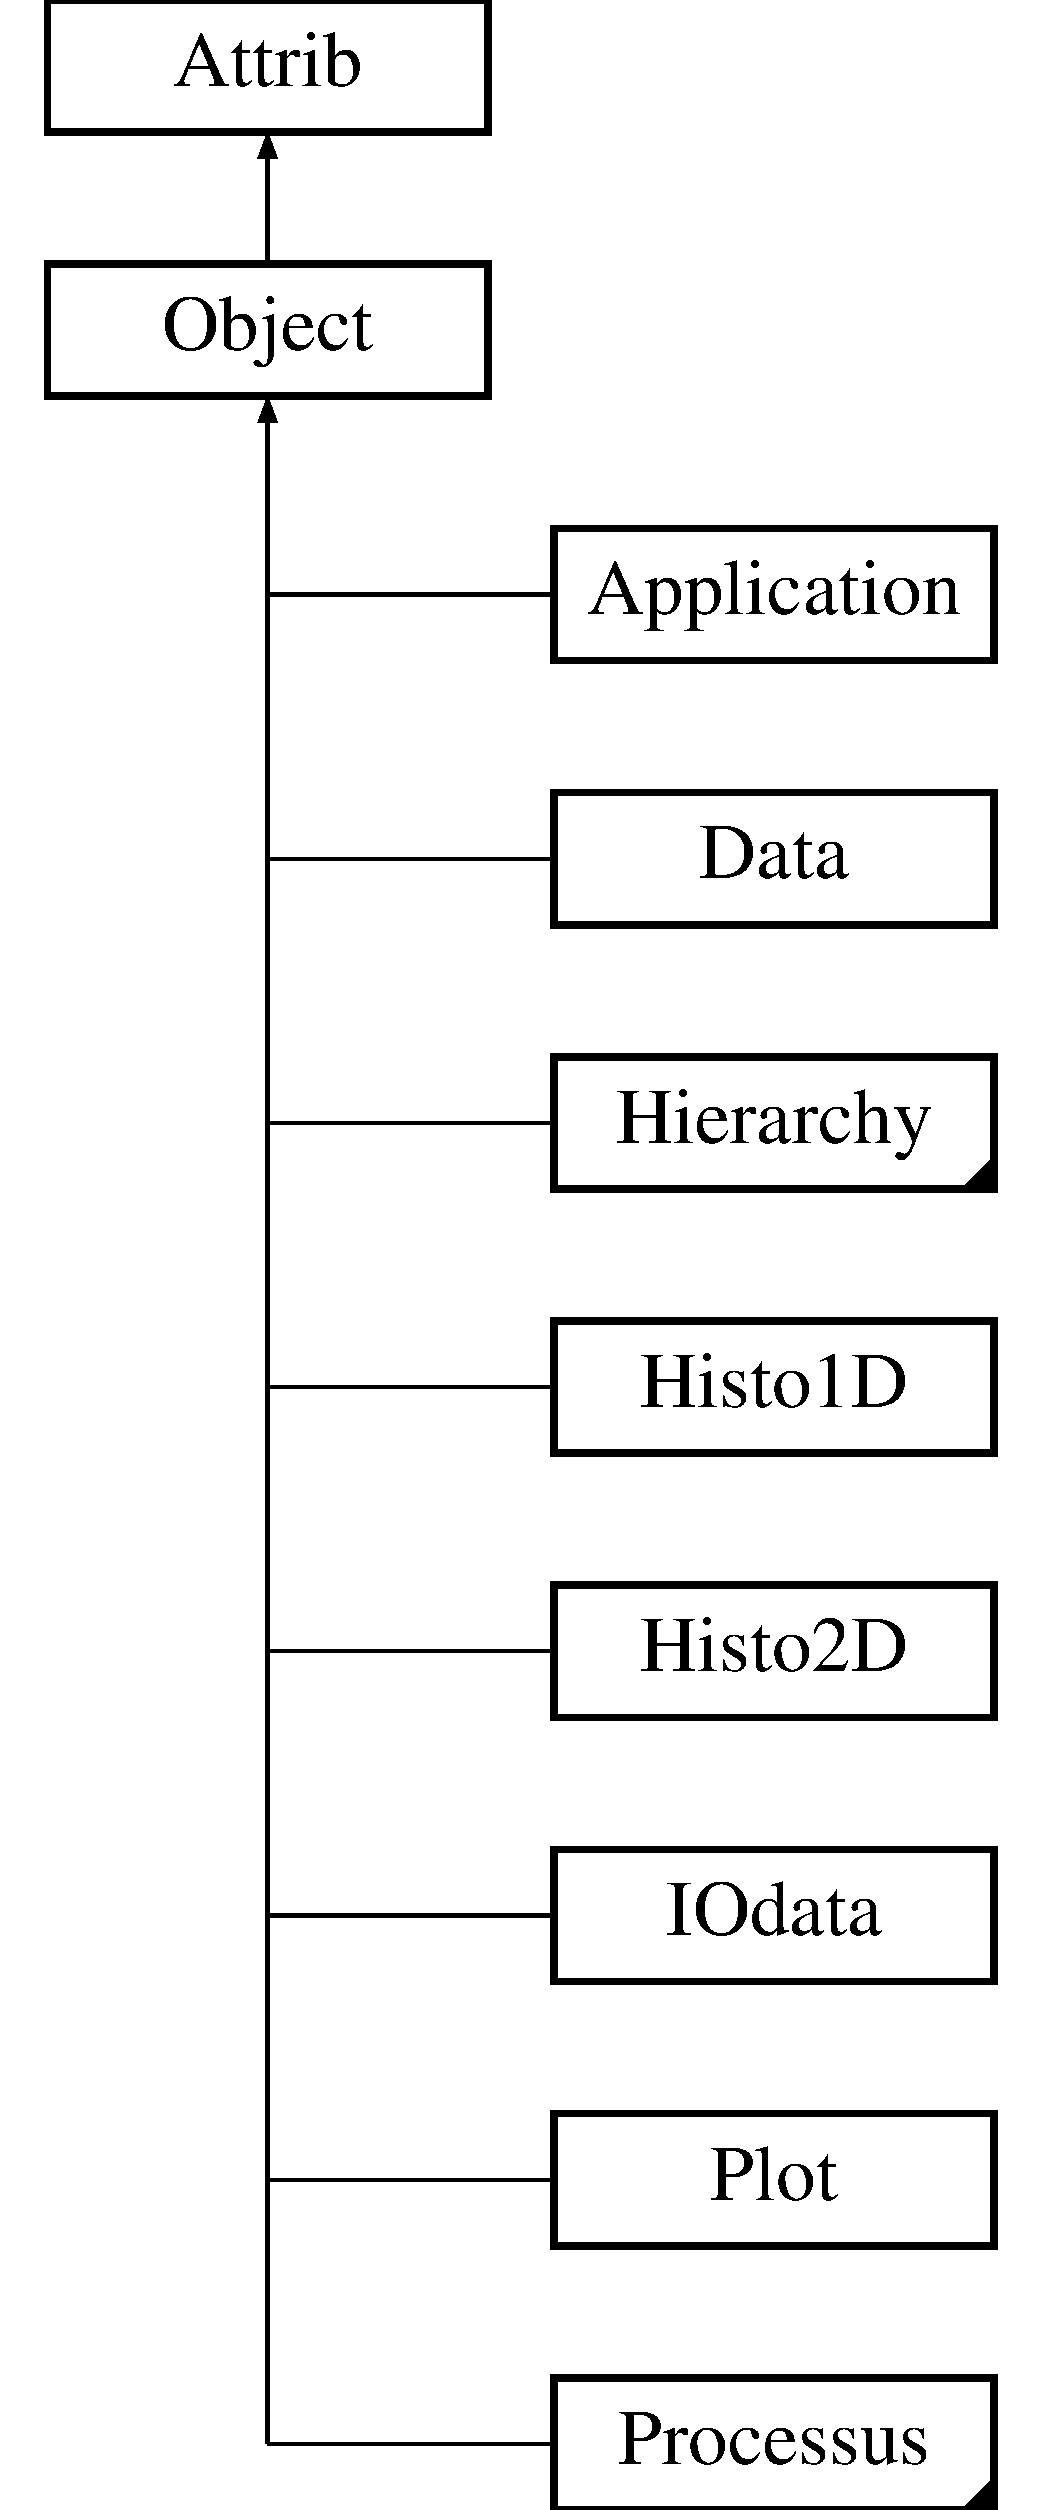
\includegraphics[height=10.000000cm]{classAttrib}
\end{center}
\end{figure}
\subsection*{Public Types}
\begin{DoxyCompactItemize}
\item 
enum \hyperlink{classAttrib_a69e171d7cc6417835a5a306d3c764235}{Attribut} \{ \newline
\hyperlink{classAttrib_a69e171d7cc6417835a5a306d3c764235a3a8da2ab97dda18aebab196fe4100531}{U\+N\+D\+E\+F\+I\+N\+ED}, 
\hyperlink{classAttrib_a69e171d7cc6417835a5a306d3c764235a2bfb2af57b87031d190a05fe25dd92ed}{P\+A\+S\+S\+I\+VE}, 
\hyperlink{classAttrib_a69e171d7cc6417835a5a306d3c764235a3b1fec929c0370d1436f2f06e298fb0d}{A\+C\+T\+I\+VE}, 
\hyperlink{classAttrib_a69e171d7cc6417835a5a306d3c764235aa27c16b480a369ea4d18b07b2516bbc7}{I\+N\+T\+E\+R\+F\+A\+CE}, 
\newline
\hyperlink{classAttrib_a69e171d7cc6417835a5a306d3c764235a1420a5b8c0540b2af210b6975eded7f9}{IO}, 
\hyperlink{classAttrib_a69e171d7cc6417835a5a306d3c764235a0af3b0d0ac323c1704e6c69cf90add28}{I\+O\+D\+A\+TA}, 
\hyperlink{classAttrib_a69e171d7cc6417835a5a306d3c764235a7788bc5dd333fd8ce18562b269c9dab1}{E\+L\+E\+M\+E\+NT}, 
\hyperlink{classAttrib_a69e171d7cc6417835a5a306d3c764235a61ceb22149f365f1780d18f9d1459423}{H\+A\+R\+D\+W\+A\+RE}, 
\newline
\hyperlink{classAttrib_a69e171d7cc6417835a5a306d3c764235a75250e29692496e73effca2c0330977f}{P\+R\+O\+C\+E\+S\+S\+US}, 
\hyperlink{classAttrib_a69e171d7cc6417835a5a306d3c764235a103a67cd0b8f07ef478fa45d4356e27b}{S\+O\+F\+T\+W\+A\+RE}
 \}
\end{DoxyCompactItemize}
\subsection*{Public Member Functions}
\begin{DoxyCompactItemize}
\item 
\hyperlink{classAttrib_ae76863db250b64f2779eb11acc5ebe18}{Attrib} ()
\begin{DoxyCompactList}\small\item\em Standard constructor. \end{DoxyCompactList}\item 
virtual \hyperlink{classAttrib_a6f3413862312138b87255c2e12dd8326}{$\sim$\+Attrib} ()
\begin{DoxyCompactList}\small\item\em Destructor. \end{DoxyCompactList}\item 
bool \hyperlink{classAttrib_a704f26af560909ad22065083bb7d4c34}{is} (int attribut)
\item 
void \hyperlink{classAttrib_a235f773af19c900264a190b00a3b4ad7}{add} (int attribut)
\item 
void \hyperlink{classAttrib_a7d4ef7e32d93cb287792b87b857e79f3}{remove} (int attribut)
\item 
std\+::string \hyperlink{classAttrib_aee7bbf16b144887f196e1341b24f8a26}{attributs} ()
\end{DoxyCompactItemize}
\subsection*{Protected Attributes}
\begin{DoxyCompactItemize}
\item 
std\+::string \hyperlink{classAttrib_a3414521d7a82476e874b25a5407b5e63}{m\+\_\+attrib\+String} \mbox{[}10\mbox{]}
\end{DoxyCompactItemize}
\subsection*{Private Attributes}
\begin{DoxyCompactItemize}
\item 
std\+::vector$<$ int $>$ \hyperlink{classAttrib_ac4bd58a0cc6b38a3b711d609a3d3aacc}{m\+\_\+attributs}
\end{DoxyCompactItemize}


\subsection{Detailed Description}
Define the attributs of objects. Define a basic set of attributs for class objects;

\begin{DoxyAuthor}{Author}
Frédéric Machefert 
\end{DoxyAuthor}
\begin{DoxyDate}{Date}
October 27, 2006 
\end{DoxyDate}


Definition at line 27 of file Attrib.\+h.



\subsection{Member Enumeration Documentation}
\mbox{\Hypertarget{classAttrib_a69e171d7cc6417835a5a306d3c764235}\label{classAttrib_a69e171d7cc6417835a5a306d3c764235}} 
\index{Attrib@{Attrib}!Attribut@{Attribut}}
\index{Attribut@{Attribut}!Attrib@{Attrib}}
\subsubsection{\texorpdfstring{Attribut}{Attribut}}
{\footnotesize\ttfamily enum \hyperlink{classAttrib_a69e171d7cc6417835a5a306d3c764235}{Attrib\+::\+Attribut}}

\begin{DoxyEnumFields}{Enumerator}
\raisebox{\heightof{T}}[0pt][0pt]{\index{U\+N\+D\+E\+F\+I\+N\+ED@{U\+N\+D\+E\+F\+I\+N\+ED}!Attrib@{Attrib}}\index{Attrib@{Attrib}!U\+N\+D\+E\+F\+I\+N\+ED@{U\+N\+D\+E\+F\+I\+N\+ED}}}\mbox{\Hypertarget{classAttrib_a69e171d7cc6417835a5a306d3c764235a3a8da2ab97dda18aebab196fe4100531}\label{classAttrib_a69e171d7cc6417835a5a306d3c764235a3a8da2ab97dda18aebab196fe4100531}} 
U\+N\+D\+E\+F\+I\+N\+ED&\\
\hline

\raisebox{\heightof{T}}[0pt][0pt]{\index{P\+A\+S\+S\+I\+VE@{P\+A\+S\+S\+I\+VE}!Attrib@{Attrib}}\index{Attrib@{Attrib}!P\+A\+S\+S\+I\+VE@{P\+A\+S\+S\+I\+VE}}}\mbox{\Hypertarget{classAttrib_a69e171d7cc6417835a5a306d3c764235a2bfb2af57b87031d190a05fe25dd92ed}\label{classAttrib_a69e171d7cc6417835a5a306d3c764235a2bfb2af57b87031d190a05fe25dd92ed}} 
P\+A\+S\+S\+I\+VE&\\
\hline

\raisebox{\heightof{T}}[0pt][0pt]{\index{A\+C\+T\+I\+VE@{A\+C\+T\+I\+VE}!Attrib@{Attrib}}\index{Attrib@{Attrib}!A\+C\+T\+I\+VE@{A\+C\+T\+I\+VE}}}\mbox{\Hypertarget{classAttrib_a69e171d7cc6417835a5a306d3c764235a3b1fec929c0370d1436f2f06e298fb0d}\label{classAttrib_a69e171d7cc6417835a5a306d3c764235a3b1fec929c0370d1436f2f06e298fb0d}} 
A\+C\+T\+I\+VE&\\
\hline

\raisebox{\heightof{T}}[0pt][0pt]{\index{I\+N\+T\+E\+R\+F\+A\+CE@{I\+N\+T\+E\+R\+F\+A\+CE}!Attrib@{Attrib}}\index{Attrib@{Attrib}!I\+N\+T\+E\+R\+F\+A\+CE@{I\+N\+T\+E\+R\+F\+A\+CE}}}\mbox{\Hypertarget{classAttrib_a69e171d7cc6417835a5a306d3c764235aa27c16b480a369ea4d18b07b2516bbc7}\label{classAttrib_a69e171d7cc6417835a5a306d3c764235aa27c16b480a369ea4d18b07b2516bbc7}} 
I\+N\+T\+E\+R\+F\+A\+CE&\\
\hline

\raisebox{\heightof{T}}[0pt][0pt]{\index{IO@{IO}!Attrib@{Attrib}}\index{Attrib@{Attrib}!IO@{IO}}}\mbox{\Hypertarget{classAttrib_a69e171d7cc6417835a5a306d3c764235a1420a5b8c0540b2af210b6975eded7f9}\label{classAttrib_a69e171d7cc6417835a5a306d3c764235a1420a5b8c0540b2af210b6975eded7f9}} 
IO&\\
\hline

\raisebox{\heightof{T}}[0pt][0pt]{\index{I\+O\+D\+A\+TA@{I\+O\+D\+A\+TA}!Attrib@{Attrib}}\index{Attrib@{Attrib}!I\+O\+D\+A\+TA@{I\+O\+D\+A\+TA}}}\mbox{\Hypertarget{classAttrib_a69e171d7cc6417835a5a306d3c764235a0af3b0d0ac323c1704e6c69cf90add28}\label{classAttrib_a69e171d7cc6417835a5a306d3c764235a0af3b0d0ac323c1704e6c69cf90add28}} 
I\+O\+D\+A\+TA&\\
\hline

\raisebox{\heightof{T}}[0pt][0pt]{\index{E\+L\+E\+M\+E\+NT@{E\+L\+E\+M\+E\+NT}!Attrib@{Attrib}}\index{Attrib@{Attrib}!E\+L\+E\+M\+E\+NT@{E\+L\+E\+M\+E\+NT}}}\mbox{\Hypertarget{classAttrib_a69e171d7cc6417835a5a306d3c764235a7788bc5dd333fd8ce18562b269c9dab1}\label{classAttrib_a69e171d7cc6417835a5a306d3c764235a7788bc5dd333fd8ce18562b269c9dab1}} 
E\+L\+E\+M\+E\+NT&\\
\hline

\raisebox{\heightof{T}}[0pt][0pt]{\index{H\+A\+R\+D\+W\+A\+RE@{H\+A\+R\+D\+W\+A\+RE}!Attrib@{Attrib}}\index{Attrib@{Attrib}!H\+A\+R\+D\+W\+A\+RE@{H\+A\+R\+D\+W\+A\+RE}}}\mbox{\Hypertarget{classAttrib_a69e171d7cc6417835a5a306d3c764235a61ceb22149f365f1780d18f9d1459423}\label{classAttrib_a69e171d7cc6417835a5a306d3c764235a61ceb22149f365f1780d18f9d1459423}} 
H\+A\+R\+D\+W\+A\+RE&\\
\hline

\raisebox{\heightof{T}}[0pt][0pt]{\index{P\+R\+O\+C\+E\+S\+S\+US@{P\+R\+O\+C\+E\+S\+S\+US}!Attrib@{Attrib}}\index{Attrib@{Attrib}!P\+R\+O\+C\+E\+S\+S\+US@{P\+R\+O\+C\+E\+S\+S\+US}}}\mbox{\Hypertarget{classAttrib_a69e171d7cc6417835a5a306d3c764235a75250e29692496e73effca2c0330977f}\label{classAttrib_a69e171d7cc6417835a5a306d3c764235a75250e29692496e73effca2c0330977f}} 
P\+R\+O\+C\+E\+S\+S\+US&\\
\hline

\raisebox{\heightof{T}}[0pt][0pt]{\index{S\+O\+F\+T\+W\+A\+RE@{S\+O\+F\+T\+W\+A\+RE}!Attrib@{Attrib}}\index{Attrib@{Attrib}!S\+O\+F\+T\+W\+A\+RE@{S\+O\+F\+T\+W\+A\+RE}}}\mbox{\Hypertarget{classAttrib_a69e171d7cc6417835a5a306d3c764235a103a67cd0b8f07ef478fa45d4356e27b}\label{classAttrib_a69e171d7cc6417835a5a306d3c764235a103a67cd0b8f07ef478fa45d4356e27b}} 
S\+O\+F\+T\+W\+A\+RE&\\
\hline

\end{DoxyEnumFields}


Definition at line 29 of file Attrib.\+h.


\begin{DoxyCode}
29                 \{
30     \hyperlink{classAttrib_a69e171d7cc6417835a5a306d3c764235a3a8da2ab97dda18aebab196fe4100531}{UNDEFINED},
31     \hyperlink{classAttrib_a69e171d7cc6417835a5a306d3c764235a2bfb2af57b87031d190a05fe25dd92ed}{PASSIVE},
32     \hyperlink{classAttrib_a69e171d7cc6417835a5a306d3c764235a3b1fec929c0370d1436f2f06e298fb0d}{ACTIVE},
33     \hyperlink{classAttrib_a69e171d7cc6417835a5a306d3c764235aa27c16b480a369ea4d18b07b2516bbc7}{INTERFACE},
34     \hyperlink{classAttrib_a69e171d7cc6417835a5a306d3c764235a1420a5b8c0540b2af210b6975eded7f9}{IO},
35     \hyperlink{classAttrib_a69e171d7cc6417835a5a306d3c764235a0af3b0d0ac323c1704e6c69cf90add28}{IODATA},
36     \hyperlink{classAttrib_a69e171d7cc6417835a5a306d3c764235a7788bc5dd333fd8ce18562b269c9dab1}{ELEMENT},
37     \hyperlink{classAttrib_a69e171d7cc6417835a5a306d3c764235a61ceb22149f365f1780d18f9d1459423}{HARDWARE},
38     \hyperlink{classAttrib_a69e171d7cc6417835a5a306d3c764235a75250e29692496e73effca2c0330977f}{PROCESSUS},
39     \hyperlink{classAttrib_a69e171d7cc6417835a5a306d3c764235a103a67cd0b8f07ef478fa45d4356e27b}{SOFTWARE} 
40   \}; \textcolor{comment}{// array m\_attribString must be changed into Attrib::Attrib if this enu is modified. }
\end{DoxyCode}


\subsection{Constructor \& Destructor Documentation}
\mbox{\Hypertarget{classAttrib_ae76863db250b64f2779eb11acc5ebe18}\label{classAttrib_ae76863db250b64f2779eb11acc5ebe18}} 
\index{Attrib@{Attrib}!Attrib@{Attrib}}
\index{Attrib@{Attrib}!Attrib@{Attrib}}
\subsubsection{\texorpdfstring{Attrib()}{Attrib()}}
{\footnotesize\ttfamily Attrib\+::\+Attrib (\begin{DoxyParamCaption}{ }\end{DoxyParamCaption})}



Standard constructor. 



Definition at line 31 of file Attrib.\+cpp.



References add(), m\+\_\+attrib\+String, m\+\_\+attributs, and U\+N\+D\+E\+F\+I\+N\+ED.


\begin{DoxyCode}
31                  \{
32   \hyperlink{classAttrib_a3414521d7a82476e874b25a5407b5e63}{m\_attribString}[0] = std::string(\textcolor{stringliteral}{"UNDEFINED"});
33   \hyperlink{classAttrib_a3414521d7a82476e874b25a5407b5e63}{m\_attribString}[1] = std::string(\textcolor{stringliteral}{"PASSIVE"});
34   \hyperlink{classAttrib_a3414521d7a82476e874b25a5407b5e63}{m\_attribString}[2] = std::string(\textcolor{stringliteral}{"ACTIVE"});
35   \hyperlink{classAttrib_a3414521d7a82476e874b25a5407b5e63}{m\_attribString}[3] = std::string(\textcolor{stringliteral}{"INTERFACE"});
36   \hyperlink{classAttrib_a3414521d7a82476e874b25a5407b5e63}{m\_attribString}[4] = std::string(\textcolor{stringliteral}{"IO"});
37   \hyperlink{classAttrib_a3414521d7a82476e874b25a5407b5e63}{m\_attribString}[5] = std::string(\textcolor{stringliteral}{"IODATA"});
38   \hyperlink{classAttrib_a3414521d7a82476e874b25a5407b5e63}{m\_attribString}[6] = std::string(\textcolor{stringliteral}{"ELEMENT"});
39   \hyperlink{classAttrib_a3414521d7a82476e874b25a5407b5e63}{m\_attribString}[7] = std::string(\textcolor{stringliteral}{"HARDWARE"});
40   \hyperlink{classAttrib_a3414521d7a82476e874b25a5407b5e63}{m\_attribString}[8] = std::string(\textcolor{stringliteral}{"PROCESSUS"});
41   \hyperlink{classAttrib_a3414521d7a82476e874b25a5407b5e63}{m\_attribString}[9] = std::string(\textcolor{stringliteral}{"SOFTWARE"});
42   \hyperlink{classAttrib_ac4bd58a0cc6b38a3b711d609a3d3aacc}{m\_attributs}.clear();
43   \hyperlink{classAttrib_a235f773af19c900264a190b00a3b4ad7}{add}(\hyperlink{classAttrib_a69e171d7cc6417835a5a306d3c764235a3a8da2ab97dda18aebab196fe4100531}{Attrib::UNDEFINED});
44 \}
\end{DoxyCode}
\mbox{\Hypertarget{classAttrib_a6f3413862312138b87255c2e12dd8326}\label{classAttrib_a6f3413862312138b87255c2e12dd8326}} 
\index{Attrib@{Attrib}!````~Attrib@{$\sim$\+Attrib}}
\index{````~Attrib@{$\sim$\+Attrib}!Attrib@{Attrib}}
\subsubsection{\texorpdfstring{$\sim$\+Attrib()}{~Attrib()}}
{\footnotesize\ttfamily Attrib\+::$\sim$\+Attrib (\begin{DoxyParamCaption}{ }\end{DoxyParamCaption})\hspace{0.3cm}{\ttfamily [virtual]}}



Destructor. 



Definition at line 49 of file Attrib.\+cpp.


\begin{DoxyCode}
49 \{\} 
\end{DoxyCode}


\subsection{Member Function Documentation}
\mbox{\Hypertarget{classAttrib_a235f773af19c900264a190b00a3b4ad7}\label{classAttrib_a235f773af19c900264a190b00a3b4ad7}} 
\index{Attrib@{Attrib}!add@{add}}
\index{add@{add}!Attrib@{Attrib}}
\subsubsection{\texorpdfstring{add()}{add()}}
{\footnotesize\ttfamily void Attrib\+::add (\begin{DoxyParamCaption}\item[{int}]{attribut }\end{DoxyParamCaption})\hspace{0.3cm}{\ttfamily [inline]}}

Add an attribut 

Definition at line 67 of file Attrib.\+h.



References m\+\_\+attributs, and U\+N\+D\+E\+F\+I\+N\+ED.



Referenced by A3\+P\+E\+::\+A3\+P\+E(), Attrib(), Specs\+Mezzanine\+::cmdline(), Computer\+::\+Computer(), C\+U\+\_\+v1\+::\+C\+U\+\_\+v1(), export\+\_\+obj(), F\+E\+B\+\_\+v1\+::\+F\+E\+B\+\_\+v1(), Fe\+P\+G\+A\+::\+Fe\+P\+G\+A(), I\+C\+E\+C\+A\+Lv3\+::\+I\+C\+E\+C\+A\+Lv3(), I\+C\+Phaser\+::\+I\+C\+Phaser(), Application\+::initialize(), Interface\+::\+Interface(), I\+Odata\+::\+I\+Odata(), I\+Oobject\+::\+I\+Oobject(), M\+S\+Oxxxx\+::\+M\+S\+Oxxxx(), Phaser\+::\+Phaser(), Processus\+::\+Processus(), Proto40\+M\+Hz\+\_\+v1\+::\+Proto40\+M\+Hz\+\_\+v1(), remove(), Seq\+P\+G\+A\+::\+Seq\+P\+G\+A(), Test\+S\+P\+I\+::set\+Address(), Test\+I2\+C\+::set\+Address(), Specs\+Slave\+::set\+Address(), Specs\+Master\+::\+Specs\+Master(), Specs\+Slave\+::\+Specs\+Slave(), and Fe\+P\+G\+A\+::transmit\+Spi().


\begin{DoxyCode}
67                             \{
68     \textcolor{keywordflow}{if} (attribut!=\hyperlink{classAttrib_a69e171d7cc6417835a5a306d3c764235a3a8da2ab97dda18aebab196fe4100531}{Attrib::UNDEFINED}) \textcolor{keyword}{remove}(\hyperlink{classAttrib_a69e171d7cc6417835a5a306d3c764235a3a8da2ab97dda18aebab196fe4100531}{Attrib::UNDEFINED});
69     \textcolor{keywordtype}{bool} duplicate = false ;
70     std::vector<int>::const\_iterator iter ;
71     \textcolor{keywordflow}{for} ( iter  = \hyperlink{classAttrib_ac4bd58a0cc6b38a3b711d609a3d3aacc}{m\_attributs}.begin() ;
72           iter != \hyperlink{classAttrib_ac4bd58a0cc6b38a3b711d609a3d3aacc}{m\_attributs}.end()   ;
73           ++iter ) \{
74       \textcolor{keywordflow}{if} ( attribut == (*iter) ) \{
75         duplicate = true ;
76       \}
77     \}
78     \textcolor{keywordflow}{if} (!duplicate) \{
79       \hyperlink{classAttrib_ac4bd58a0cc6b38a3b711d609a3d3aacc}{m\_attributs}.push\_back( attribut );
80     \}
81   \}
\end{DoxyCode}
\mbox{\Hypertarget{classAttrib_aee7bbf16b144887f196e1341b24f8a26}\label{classAttrib_aee7bbf16b144887f196e1341b24f8a26}} 
\index{Attrib@{Attrib}!attributs@{attributs}}
\index{attributs@{attributs}!Attrib@{Attrib}}
\subsubsection{\texorpdfstring{attributs()}{attributs()}}
{\footnotesize\ttfamily std\+::string Attrib\+::attributs (\begin{DoxyParamCaption}{ }\end{DoxyParamCaption})}

Print the \hyperlink{classAttrib}{Attrib} of an \hyperlink{classObject}{Object} 

Definition at line 54 of file Attrib.\+cpp.



References images\+::index, m\+\_\+attrib\+String, and m\+\_\+attributs.



Referenced by export\+\_\+obj(), and remove().


\begin{DoxyCode}
54                             \{
55   std::string output;
56   std::vector<int>::iterator iter ;
57   \textcolor{keywordflow}{for} ( \textcolor{keywordtype}{unsigned} \textcolor{keywordtype}{int} \hyperlink{namespaceimages_a54407fd574970b3178647ae096321a57}{index} = 0 ; \hyperlink{namespaceimages_a54407fd574970b3178647ae096321a57}{index} < \hyperlink{classAttrib_ac4bd58a0cc6b38a3b711d609a3d3aacc}{m\_attributs}.size() ; ++
      \hyperlink{namespaceimages_a54407fd574970b3178647ae096321a57}{index} ) \{
58     \textcolor{keywordflow}{if} ( \hyperlink{classAttrib_ac4bd58a0cc6b38a3b711d609a3d3aacc}{m\_attributs}.size() - \hyperlink{namespaceimages_a54407fd574970b3178647ae096321a57}{index} > 1 ) \{
59       output.append(\hyperlink{classAttrib_a3414521d7a82476e874b25a5407b5e63}{m\_attribString}[\hyperlink{classAttrib_ac4bd58a0cc6b38a3b711d609a3d3aacc}{m\_attributs}[\hyperlink{namespaceimages_a54407fd574970b3178647ae096321a57}{index}]]);
60       output.append(\textcolor{stringliteral}{":"});
61     \}
62     \textcolor{keywordflow}{else} \{
63       output.append(\hyperlink{classAttrib_a3414521d7a82476e874b25a5407b5e63}{m\_attribString}[\hyperlink{classAttrib_ac4bd58a0cc6b38a3b711d609a3d3aacc}{m\_attributs}[index]]);
64     \}
65   \}
66   \textcolor{keywordflow}{return} output;
67 \}
\end{DoxyCode}
\mbox{\Hypertarget{classAttrib_a704f26af560909ad22065083bb7d4c34}\label{classAttrib_a704f26af560909ad22065083bb7d4c34}} 
\index{Attrib@{Attrib}!is@{is}}
\index{is@{is}!Attrib@{Attrib}}
\subsubsection{\texorpdfstring{is()}{is()}}
{\footnotesize\ttfamily bool Attrib\+::is (\begin{DoxyParamCaption}\item[{int}]{attribut }\end{DoxyParamCaption})\hspace{0.3cm}{\ttfamily [inline]}}

Test for an attribut 

Definition at line 50 of file Attrib.\+h.



References m\+\_\+attributs.



Referenced by export\+\_\+obj(), and Element\+::set\+Connection().


\begin{DoxyCode}
51   \{
52     std::vector<int>::const\_iterator iter ;
53     \textcolor{keywordflow}{for} ( iter  = \hyperlink{classAttrib_ac4bd58a0cc6b38a3b711d609a3d3aacc}{m\_attributs}.begin() ;
54           iter != \hyperlink{classAttrib_ac4bd58a0cc6b38a3b711d609a3d3aacc}{m\_attributs}.end()   ;
55           ++iter ) \{
56       \textcolor{keywordflow}{if} ( attribut == (*iter) ) \{
57         \textcolor{keywordflow}{return} \textcolor{keyword}{true};
58       \}
59     \}
60     \textcolor{keywordflow}{return} \textcolor{keyword}{false};
61   \}
\end{DoxyCode}
\mbox{\Hypertarget{classAttrib_a7d4ef7e32d93cb287792b87b857e79f3}\label{classAttrib_a7d4ef7e32d93cb287792b87b857e79f3}} 
\index{Attrib@{Attrib}!remove@{remove}}
\index{remove@{remove}!Attrib@{Attrib}}
\subsubsection{\texorpdfstring{remove()}{remove()}}
{\footnotesize\ttfamily void Attrib\+::remove (\begin{DoxyParamCaption}\item[{int}]{attribut }\end{DoxyParamCaption})\hspace{0.3cm}{\ttfamily [inline]}}

Remove an attribut 

Definition at line 86 of file Attrib.\+h.



References add(), attributs(), m\+\_\+attributs, and U\+N\+D\+E\+F\+I\+N\+ED.



Referenced by export\+\_\+obj().


\begin{DoxyCode}
86                                \{
87     std::vector<int>::iterator iter , toremove ;
88     \textcolor{keywordflow}{for} ( iter  = \hyperlink{classAttrib_ac4bd58a0cc6b38a3b711d609a3d3aacc}{m\_attributs}.begin() ;
89           iter != \hyperlink{classAttrib_ac4bd58a0cc6b38a3b711d609a3d3aacc}{m\_attributs}.end()   ;
90           ++iter ) \{
91       \textcolor{keywordflow}{if} ( attribut == (*iter) ) \{
92         toremove = iter;
93       \}
94     \}
95     \hyperlink{classAttrib_ac4bd58a0cc6b38a3b711d609a3d3aacc}{m\_attributs}.erase (toremove);
96     \textcolor{keywordflow}{if}(0==\hyperlink{classAttrib_ac4bd58a0cc6b38a3b711d609a3d3aacc}{m\_attributs}.size()) \hyperlink{classAttrib_a235f773af19c900264a190b00a3b4ad7}{add}(\hyperlink{classAttrib_a69e171d7cc6417835a5a306d3c764235a3a8da2ab97dda18aebab196fe4100531}{Attrib::UNDEFINED});
97   \}
\end{DoxyCode}


\subsection{Member Data Documentation}
\mbox{\Hypertarget{classAttrib_a3414521d7a82476e874b25a5407b5e63}\label{classAttrib_a3414521d7a82476e874b25a5407b5e63}} 
\index{Attrib@{Attrib}!m\+\_\+attrib\+String@{m\+\_\+attrib\+String}}
\index{m\+\_\+attrib\+String@{m\+\_\+attrib\+String}!Attrib@{Attrib}}
\subsubsection{\texorpdfstring{m\+\_\+attrib\+String}{m\_attribString}}
{\footnotesize\ttfamily std\+::string Attrib\+::m\+\_\+attrib\+String\mbox{[}10\mbox{]}\hspace{0.3cm}{\ttfamily [protected]}}



Definition at line 105 of file Attrib.\+h.



Referenced by Attrib(), and attributs().

\mbox{\Hypertarget{classAttrib_ac4bd58a0cc6b38a3b711d609a3d3aacc}\label{classAttrib_ac4bd58a0cc6b38a3b711d609a3d3aacc}} 
\index{Attrib@{Attrib}!m\+\_\+attributs@{m\+\_\+attributs}}
\index{m\+\_\+attributs@{m\+\_\+attributs}!Attrib@{Attrib}}
\subsubsection{\texorpdfstring{m\+\_\+attributs}{m\_attributs}}
{\footnotesize\ttfamily std\+::vector$<$int$>$ Attrib\+::m\+\_\+attributs\hspace{0.3cm}{\ttfamily [private]}}



Definition at line 108 of file Attrib.\+h.



Referenced by add(), Attrib(), attributs(), is(), and remove().



The documentation for this class was generated from the following files\+:\begin{DoxyCompactItemize}
\item 
/home/eleclhcb/\+L\+H\+Cb/lbcat-\/cmake/\+Cat\+Kernel/inc/\hyperlink{Attrib_8h}{Attrib.\+h}\item 
/home/eleclhcb/\+L\+H\+Cb/lbcat-\/cmake/\+Cat\+Kernel/src/\hyperlink{Attrib_8cpp}{Attrib.\+cpp}\end{DoxyCompactItemize}

\hypertarget{classCfgFrame_1_1CfgFrame}{
\section{CfgFrame::CfgFrame Class Reference}
\label{classCfgFrame_1_1CfgFrame}\index{CfgFrame::CfgFrame@{CfgFrame::CfgFrame}}
}
\subsection*{Public Member Functions}
\begin{DoxyCompactItemize}
\item 
def \hyperlink{classCfgFrame_1_1CfgFrame_ade76b3c75ebbea57217775c9849493b2}{\_\-\_\-init\_\-\_\-}
\item 
def \hyperlink{classCfgFrame_1_1CfgFrame_aa3c4dde8c6f9e2b22e98510c177992de}{onEdit}
\item 
def \hyperlink{classCfgFrame_1_1CfgFrame_a1a170349dd0f885911c6a5dc05f0568b}{getControl}
\item 
def \hyperlink{classCfgFrame_1_1CfgFrame_ae69c002127bc6913ea33be65aebd08a2}{makeToolBar}
\item 
def \hyperlink{classCfgFrame_1_1CfgFrame_a07409ab0756ec5f1cc5a5f12b6ef6af0}{onIdle}
\item 
def \hyperlink{classCfgFrame_1_1CfgFrame_ab437de758da4163a93d63b20ed9eb446}{onIconize}
\item 
def \hyperlink{classCfgFrame_1_1CfgFrame_a1c2999d11c0bf12c3bf3a532c1aab624}{onChange}
\item 
def \hyperlink{classCfgFrame_1_1CfgFrame_a93a31956d0d1c94648a4f786e2321e7f}{onReLoad}
\item 
def \hyperlink{classCfgFrame_1_1CfgFrame_a54ab916bfd9fa479de45ed9f3e62bffb}{onClose}
\item 
def \hyperlink{classCfgFrame_1_1CfgFrame_a6c8549da5a53c3f4a25a2811a8b864c6}{update}
\end{DoxyCompactItemize}
\subsection*{Public Attributes}
\begin{DoxyCompactItemize}
\item 
\hyperlink{classCfgFrame_1_1CfgFrame_a7a50cede680918f3e56e10a6b7d542c5}{parent}
\item 
\hyperlink{classCfgFrame_1_1CfgFrame_a7bf641fd25de33d826971d3ccd86991e}{app}
\item 
\hyperlink{classCfgFrame_1_1CfgFrame_a7ba9545bedac3e6d22c315c1a0088a47}{obj}
\item 
\hyperlink{classCfgFrame_1_1CfgFrame_a143e7e34c8049d3475a10d7e84310300}{objpath}
\item 
\hyperlink{classCfgFrame_1_1CfgFrame_a572a9f7b982bae5e808036bc38ea9d5c}{objtype}
\item 
\hyperlink{classCfgFrame_1_1CfgFrame_a8394944c11a10f2cf95dc35dac95d53d}{path}
\item 
\hyperlink{classCfgFrame_1_1CfgFrame_a37a64faf7c30a69798c2c3e1d2c4f8f1}{main}
\item 
\hyperlink{classCfgFrame_1_1CfgFrame_af212f85b15458aa623810483fb62219d}{wrap}
\item 
\hyperlink{classCfgFrame_1_1CfgFrame_a4e23faffe7a71604bf2577789799ab47}{module}
\item 
\hyperlink{classCfgFrame_1_1CfgFrame_a49b8c4b1c1552fc22b1be69ea9d768c6}{control}
\item 
\hyperlink{classCfgFrame_1_1CfgFrame_a8714ef9a155def75a58efc0a4e7d9db1}{toolBar}
\end{DoxyCompactItemize}
\subsection*{Static Public Attributes}
\begin{DoxyCompactItemize}
\item 
string \hyperlink{classCfgFrame_1_1CfgFrame_a09acfb884e2c5f8581f5b0691413a2aa}{overviewText} = \char`\"{}CAT Configuration Window\char`\"{}
\end{DoxyCompactItemize}


\subsection{Detailed Description}


Definition at line 23 of file CfgFrame.py.

\subsection{Member Function Documentation}
\hypertarget{classCfgFrame_1_1CfgFrame_ade76b3c75ebbea57217775c9849493b2}{
\index{CfgFrame::CfgFrame@{CfgFrame::CfgFrame}!\_\-\_\-init\_\-\_\-@{\_\-\_\-init\_\-\_\-}}
\index{\_\-\_\-init\_\-\_\-@{\_\-\_\-init\_\-\_\-}!CfgFrame::CfgFrame@{CfgFrame::CfgFrame}}
\subsubsection[{\_\-\_\-init\_\-\_\-}]{\setlength{\rightskip}{0pt plus 5cm}def CfgFrame::CfgFrame::\_\-\_\-init\_\-\_\- ( {\em self}, \/   {\em app}, \/   {\em parent}, \/   {\em obj}, \/   {\em objpath}, \/   {\em objtype})}}
\label{classCfgFrame_1_1CfgFrame_ade76b3c75ebbea57217775c9849493b2}


Definition at line 25 of file CfgFrame.py.


\begin{DoxyCode}
25                                                            : 
26         wx.Frame.__init__(self, parent, wx.NewId(), objpath)
27         self.parent  = parent
28         self.app     = app
29         self.obj     = obj
30         self.objpath = objpath
31         self.objtype = objtype
32         self.path=os.path.join(os.environ.get("CATPATH"), "CatPython", "python")
33         self.makeToolBar()
34         res=xrc.XmlResource(os.path.join(self.path,"xrc/ConfPanel.xrc"))
35         self.main=res.LoadPanel(self, "ConfPanel")                
36         self.Bind(wx.EVT_CLOSE, self.onClose)
37         self.onEdit(obj, objpath, objtype)
38         
\end{DoxyCode}
\hypertarget{classCfgFrame_1_1CfgFrame_a1a170349dd0f885911c6a5dc05f0568b}{
\index{CfgFrame::CfgFrame@{CfgFrame::CfgFrame}!getControl@{getControl}}
\index{getControl@{getControl}!CfgFrame::CfgFrame@{CfgFrame::CfgFrame}}
\subsubsection[{getControl}]{\setlength{\rightskip}{0pt plus 5cm}def CfgFrame::CfgFrame::getControl ( {\em self}, \/   {\em panel}, \/   {\em xmlid})}}
\label{classCfgFrame_1_1CfgFrame_a1a170349dd0f885911c6a5dc05f0568b}
\begin{DoxyVerb}Retrieves the given control (within a dialog) by its xmlid\end{DoxyVerb}
 

Definition at line 64 of file CfgFrame.py.


\begin{DoxyCode}
64                                       :
65         '''Retrieves the given control (within a dialog) by its xmlid'''
66         control = panel.FindWindowById(xrc.XRCID(xmlid))
67         assert control != None, 'Programming error: a control with xml id ' + xml
      id + ' was not found.'
68         return control
69         
    def makeToolBar(self):
\end{DoxyCode}
\hypertarget{classCfgFrame_1_1CfgFrame_ae69c002127bc6913ea33be65aebd08a2}{
\index{CfgFrame::CfgFrame@{CfgFrame::CfgFrame}!makeToolBar@{makeToolBar}}
\index{makeToolBar@{makeToolBar}!CfgFrame::CfgFrame@{CfgFrame::CfgFrame}}
\subsubsection[{makeToolBar}]{\setlength{\rightskip}{0pt plus 5cm}def CfgFrame::CfgFrame::makeToolBar ( {\em self})}}
\label{classCfgFrame_1_1CfgFrame_ae69c002127bc6913ea33be65aebd08a2}


Definition at line 70 of file CfgFrame.py.


\begin{DoxyCode}
70                          :
71         TB_RELOAD=wx.NewId()
72         TB_CLOSEALL=wx.NewId()
73         TB_CLOSE=wx.NewId()
74         #
75         self.toolBar = self.CreateToolBar(wx.TB_DOCKABLE)
76         self.toolBar.AddLabelTool(TB_CLOSE, '', wx.Bitmap(os.path.join(self.path,
      "xrc/icons/closeall.png")))
77         self.toolBar.AddSeparator()        
78         self.toolBar.AddLabelTool(TB_RELOAD, '', wx.Bitmap(os.path.join(self.
      path,"xrc/icons/reload.png")))
79         self.toolBar.Realize()
80         self.Bind(wx.EVT_TOOL, self.onReLoad , id=TB_RELOAD)
81         self.Bind(wx.EVT_TOOL, self.onClose , id=TB_CLOSE)
82 
    def onIdle(self, event):
\end{DoxyCode}
\hypertarget{classCfgFrame_1_1CfgFrame_a1c2999d11c0bf12c3bf3a532c1aab624}{
\index{CfgFrame::CfgFrame@{CfgFrame::CfgFrame}!onChange@{onChange}}
\index{onChange@{onChange}!CfgFrame::CfgFrame@{CfgFrame::CfgFrame}}
\subsubsection[{onChange}]{\setlength{\rightskip}{0pt plus 5cm}def CfgFrame::CfgFrame::onChange ( {\em self}, \/   {\em event})}}
\label{classCfgFrame_1_1CfgFrame_a1c2999d11c0bf12c3bf3a532c1aab624}


Definition at line 93 of file CfgFrame.py.


\begin{DoxyCode}
93                              :
94         print "OnChange"
95         self.update()
96         
    def onReLoad(self, event):
\end{DoxyCode}
\hypertarget{classCfgFrame_1_1CfgFrame_a54ab916bfd9fa479de45ed9f3e62bffb}{
\index{CfgFrame::CfgFrame@{CfgFrame::CfgFrame}!onClose@{onClose}}
\index{onClose@{onClose}!CfgFrame::CfgFrame@{CfgFrame::CfgFrame}}
\subsubsection[{onClose}]{\setlength{\rightskip}{0pt plus 5cm}def CfgFrame::CfgFrame::onClose ( {\em self}, \/   {\em event})}}
\label{classCfgFrame_1_1CfgFrame_a54ab916bfd9fa479de45ed9f3e62bffb}


Definition at line 100 of file CfgFrame.py.


\begin{DoxyCode}
100                             :
101         for p in range(len(self.parent.paths)):
102             if self.parent.paths[p] == self.objpath:
103                 self.parent.cfgpanels.pop(p)
104                 self.parent.objs.pop(p)
105                 self.parent.paths.pop(p)
106                 break
107         self.Destroy()
108                 
    def update(self):
\end{DoxyCode}
\hypertarget{classCfgFrame_1_1CfgFrame_aa3c4dde8c6f9e2b22e98510c177992de}{
\index{CfgFrame::CfgFrame@{CfgFrame::CfgFrame}!onEdit@{onEdit}}
\index{onEdit@{onEdit}!CfgFrame::CfgFrame@{CfgFrame::CfgFrame}}
\subsubsection[{onEdit}]{\setlength{\rightskip}{0pt plus 5cm}def CfgFrame::CfgFrame::onEdit ( {\em self}, \/   {\em obj}, \/   {\em path}, \/   {\em objtype})}}
\label{classCfgFrame_1_1CfgFrame_aa3c4dde8c6f9e2b22e98510c177992de}


Definition at line 39 of file CfgFrame.py.


\begin{DoxyCode}
39                                         :
40          # if (objtype=='element'):
41         #     res=xrc.XmlResource(os.path.join(self.path,"xrc/ElementMain.xrc"))
42         # elif (objtype=='proc'):
43         #     res=xrc.XmlResource(os.path.join(self.path,"xrc/ProcMain.xrc"))
44         # self.confpanel=res.LoadPanel(self.main,"confpanel")
45         # if (objtype=='element'):
46         #     namectrl=self.getControl(self.confpanel,'ObjName')
47         #     pathctrl=self.getControl(self.confpanel,'ObjPath')
48         #     namectrl.SetValue(obj.name())
49         #     pathctrl.SetValue(path)
50         # elif (objtype=='proc'):
51         #     namectrl=self.getControl(self.confpanel,'ProcName')
52         #     pathctrl=self.getControl(self.confpanel,'ProcPath')
53         #     namectrl.SetValue(obj.name())
54         #     pathctrl.SetValue(obj.type())
55         # print "self.confpanel=", self.confpanel, self.main
56         # self.panel=self.getControl(self.confpanel,'control')
57         # print "self.panel=",self.panel
58         self.wrap=wrapper(self.app,obj,objtype)
59         self.module=self.wrap.GetActive()
60         self.control=self.module.Edit(self.app,obj,self.main,self.wrap.GetFilePat
      h())
61         self.Show(True)
62 #        self.SetAutoLayout(True)
63                 
    def getControl(self, panel, xmlid):
\end{DoxyCode}
\hypertarget{classCfgFrame_1_1CfgFrame_ab437de758da4163a93d63b20ed9eb446}{
\index{CfgFrame::CfgFrame@{CfgFrame::CfgFrame}!onIconize@{onIconize}}
\index{onIconize@{onIconize}!CfgFrame::CfgFrame@{CfgFrame::CfgFrame}}
\subsubsection[{onIconize}]{\setlength{\rightskip}{0pt plus 5cm}def CfgFrame::CfgFrame::onIconize ( {\em self}, \/   {\em event})}}
\label{classCfgFrame_1_1CfgFrame_ab437de758da4163a93d63b20ed9eb446}


Definition at line 88 of file CfgFrame.py.


\begin{DoxyCode}
88                               :
89         print "onIconize"
90         self.parent.cfgFrame.Show(False)
91         self.parent.cfgState=False
92 
    def onChange(self, event):
\end{DoxyCode}
\hypertarget{classCfgFrame_1_1CfgFrame_a07409ab0756ec5f1cc5a5f12b6ef6af0}{
\index{CfgFrame::CfgFrame@{CfgFrame::CfgFrame}!onIdle@{onIdle}}
\index{onIdle@{onIdle}!CfgFrame::CfgFrame@{CfgFrame::CfgFrame}}
\subsubsection[{onIdle}]{\setlength{\rightskip}{0pt plus 5cm}def CfgFrame::CfgFrame::onIdle ( {\em self}, \/   {\em event})}}
\label{classCfgFrame_1_1CfgFrame_a07409ab0756ec5f1cc5a5f12b6ef6af0}
\begin{DoxyVerb}Responds to idle time in the system\end{DoxyVerb}
 

Definition at line 83 of file CfgFrame.py.


\begin{DoxyCode}
83                            :
84         '''Responds to idle time in the system'''
85         # when the timer says it's time, we do the actual downloading in the main
       thread (wx doesn't work well in secondary threads)
86         print "hello"        
87 
    def onIconize(self, event):
\end{DoxyCode}
\hypertarget{classCfgFrame_1_1CfgFrame_a93a31956d0d1c94648a4f786e2321e7f}{
\index{CfgFrame::CfgFrame@{CfgFrame::CfgFrame}!onReLoad@{onReLoad}}
\index{onReLoad@{onReLoad}!CfgFrame::CfgFrame@{CfgFrame::CfgFrame}}
\subsubsection[{onReLoad}]{\setlength{\rightskip}{0pt plus 5cm}def CfgFrame::CfgFrame::onReLoad ( {\em self}, \/   {\em event})}}
\label{classCfgFrame_1_1CfgFrame_a93a31956d0d1c94648a4f786e2321e7f}


Definition at line 97 of file CfgFrame.py.


\begin{DoxyCode}
97                              :
98         self.update()
99 
    def onClose(self, event):
\end{DoxyCode}
\hypertarget{classCfgFrame_1_1CfgFrame_a6c8549da5a53c3f4a25a2811a8b864c6}{
\index{CfgFrame::CfgFrame@{CfgFrame::CfgFrame}!update@{update}}
\index{update@{update}!CfgFrame::CfgFrame@{CfgFrame::CfgFrame}}
\subsubsection[{update}]{\setlength{\rightskip}{0pt plus 5cm}def CfgFrame::CfgFrame::update ( {\em self})}}
\label{classCfgFrame_1_1CfgFrame_a6c8549da5a53c3f4a25a2811a8b864c6}


Definition at line 109 of file CfgFrame.py.


\begin{DoxyCode}
109                     :
110         self.control.update()
111         
112 #----------------------------------------------------------------------------
113 
114 
115 

\end{DoxyCode}


\subsection{Member Data Documentation}
\hypertarget{classCfgFrame_1_1CfgFrame_a7bf641fd25de33d826971d3ccd86991e}{
\index{CfgFrame::CfgFrame@{CfgFrame::CfgFrame}!app@{app}}
\index{app@{app}!CfgFrame::CfgFrame@{CfgFrame::CfgFrame}}
\subsubsection[{app}]{\setlength{\rightskip}{0pt plus 5cm}{\bf CfgFrame::CfgFrame::app}}}
\label{classCfgFrame_1_1CfgFrame_a7bf641fd25de33d826971d3ccd86991e}


Definition at line 28 of file CfgFrame.py.\hypertarget{classCfgFrame_1_1CfgFrame_a49b8c4b1c1552fc22b1be69ea9d768c6}{
\index{CfgFrame::CfgFrame@{CfgFrame::CfgFrame}!control@{control}}
\index{control@{control}!CfgFrame::CfgFrame@{CfgFrame::CfgFrame}}
\subsubsection[{control}]{\setlength{\rightskip}{0pt plus 5cm}{\bf CfgFrame::CfgFrame::control}}}
\label{classCfgFrame_1_1CfgFrame_a49b8c4b1c1552fc22b1be69ea9d768c6}


Definition at line 60 of file CfgFrame.py.\hypertarget{classCfgFrame_1_1CfgFrame_a37a64faf7c30a69798c2c3e1d2c4f8f1}{
\index{CfgFrame::CfgFrame@{CfgFrame::CfgFrame}!main@{main}}
\index{main@{main}!CfgFrame::CfgFrame@{CfgFrame::CfgFrame}}
\subsubsection[{main}]{\setlength{\rightskip}{0pt plus 5cm}{\bf CfgFrame::CfgFrame::main}}}
\label{classCfgFrame_1_1CfgFrame_a37a64faf7c30a69798c2c3e1d2c4f8f1}


Definition at line 35 of file CfgFrame.py.\hypertarget{classCfgFrame_1_1CfgFrame_a4e23faffe7a71604bf2577789799ab47}{
\index{CfgFrame::CfgFrame@{CfgFrame::CfgFrame}!module@{module}}
\index{module@{module}!CfgFrame::CfgFrame@{CfgFrame::CfgFrame}}
\subsubsection[{module}]{\setlength{\rightskip}{0pt plus 5cm}{\bf CfgFrame::CfgFrame::module}}}
\label{classCfgFrame_1_1CfgFrame_a4e23faffe7a71604bf2577789799ab47}


Definition at line 59 of file CfgFrame.py.\hypertarget{classCfgFrame_1_1CfgFrame_a7ba9545bedac3e6d22c315c1a0088a47}{
\index{CfgFrame::CfgFrame@{CfgFrame::CfgFrame}!obj@{obj}}
\index{obj@{obj}!CfgFrame::CfgFrame@{CfgFrame::CfgFrame}}
\subsubsection[{obj}]{\setlength{\rightskip}{0pt plus 5cm}{\bf CfgFrame::CfgFrame::obj}}}
\label{classCfgFrame_1_1CfgFrame_a7ba9545bedac3e6d22c315c1a0088a47}


Definition at line 29 of file CfgFrame.py.\hypertarget{classCfgFrame_1_1CfgFrame_a143e7e34c8049d3475a10d7e84310300}{
\index{CfgFrame::CfgFrame@{CfgFrame::CfgFrame}!objpath@{objpath}}
\index{objpath@{objpath}!CfgFrame::CfgFrame@{CfgFrame::CfgFrame}}
\subsubsection[{objpath}]{\setlength{\rightskip}{0pt plus 5cm}{\bf CfgFrame::CfgFrame::objpath}}}
\label{classCfgFrame_1_1CfgFrame_a143e7e34c8049d3475a10d7e84310300}


Definition at line 30 of file CfgFrame.py.\hypertarget{classCfgFrame_1_1CfgFrame_a572a9f7b982bae5e808036bc38ea9d5c}{
\index{CfgFrame::CfgFrame@{CfgFrame::CfgFrame}!objtype@{objtype}}
\index{objtype@{objtype}!CfgFrame::CfgFrame@{CfgFrame::CfgFrame}}
\subsubsection[{objtype}]{\setlength{\rightskip}{0pt plus 5cm}{\bf CfgFrame::CfgFrame::objtype}}}
\label{classCfgFrame_1_1CfgFrame_a572a9f7b982bae5e808036bc38ea9d5c}


Definition at line 31 of file CfgFrame.py.\hypertarget{classCfgFrame_1_1CfgFrame_a09acfb884e2c5f8581f5b0691413a2aa}{
\index{CfgFrame::CfgFrame@{CfgFrame::CfgFrame}!overviewText@{overviewText}}
\index{overviewText@{overviewText}!CfgFrame::CfgFrame@{CfgFrame::CfgFrame}}
\subsubsection[{overviewText}]{\setlength{\rightskip}{0pt plus 5cm}string {\bf CfgFrame::CfgFrame::overviewText} = \char`\"{}CAT Configuration Window\char`\"{}\hspace{0.3cm}{\ttfamily  \mbox{[}static\mbox{]}}}}
\label{classCfgFrame_1_1CfgFrame_a09acfb884e2c5f8581f5b0691413a2aa}


Definition at line 24 of file CfgFrame.py.\hypertarget{classCfgFrame_1_1CfgFrame_a7a50cede680918f3e56e10a6b7d542c5}{
\index{CfgFrame::CfgFrame@{CfgFrame::CfgFrame}!parent@{parent}}
\index{parent@{parent}!CfgFrame::CfgFrame@{CfgFrame::CfgFrame}}
\subsubsection[{parent}]{\setlength{\rightskip}{0pt plus 5cm}{\bf CfgFrame::CfgFrame::parent}}}
\label{classCfgFrame_1_1CfgFrame_a7a50cede680918f3e56e10a6b7d542c5}


Definition at line 27 of file CfgFrame.py.\hypertarget{classCfgFrame_1_1CfgFrame_a8394944c11a10f2cf95dc35dac95d53d}{
\index{CfgFrame::CfgFrame@{CfgFrame::CfgFrame}!path@{path}}
\index{path@{path}!CfgFrame::CfgFrame@{CfgFrame::CfgFrame}}
\subsubsection[{path}]{\setlength{\rightskip}{0pt plus 5cm}{\bf CfgFrame::CfgFrame::path}}}
\label{classCfgFrame_1_1CfgFrame_a8394944c11a10f2cf95dc35dac95d53d}


Definition at line 32 of file CfgFrame.py.\hypertarget{classCfgFrame_1_1CfgFrame_a8714ef9a155def75a58efc0a4e7d9db1}{
\index{CfgFrame::CfgFrame@{CfgFrame::CfgFrame}!toolBar@{toolBar}}
\index{toolBar@{toolBar}!CfgFrame::CfgFrame@{CfgFrame::CfgFrame}}
\subsubsection[{toolBar}]{\setlength{\rightskip}{0pt plus 5cm}{\bf CfgFrame::CfgFrame::toolBar}}}
\label{classCfgFrame_1_1CfgFrame_a8714ef9a155def75a58efc0a4e7d9db1}


Definition at line 75 of file CfgFrame.py.\hypertarget{classCfgFrame_1_1CfgFrame_af212f85b15458aa623810483fb62219d}{
\index{CfgFrame::CfgFrame@{CfgFrame::CfgFrame}!wrap@{wrap}}
\index{wrap@{wrap}!CfgFrame::CfgFrame@{CfgFrame::CfgFrame}}
\subsubsection[{wrap}]{\setlength{\rightskip}{0pt plus 5cm}{\bf CfgFrame::CfgFrame::wrap}}}
\label{classCfgFrame_1_1CfgFrame_af212f85b15458aa623810483fb62219d}


Definition at line 58 of file CfgFrame.py.

The documentation for this class was generated from the following file:\begin{DoxyCompactItemize}
\item 
/home/eleclhcb/LHCb/lbcat-\/cmake/CatPython/python/\hyperlink{CfgFrame_8py}{CfgFrame.py}\end{DoxyCompactItemize}

\hypertarget{classComputer_1_1Computer}{}\section{Computer.\+Computer Class Reference}
\label{classComputer_1_1Computer}\index{Computer.\+Computer@{Computer.\+Computer}}
Inheritance diagram for Computer.\+Computer\+:\begin{figure}[H]
\begin{center}
\leavevmode
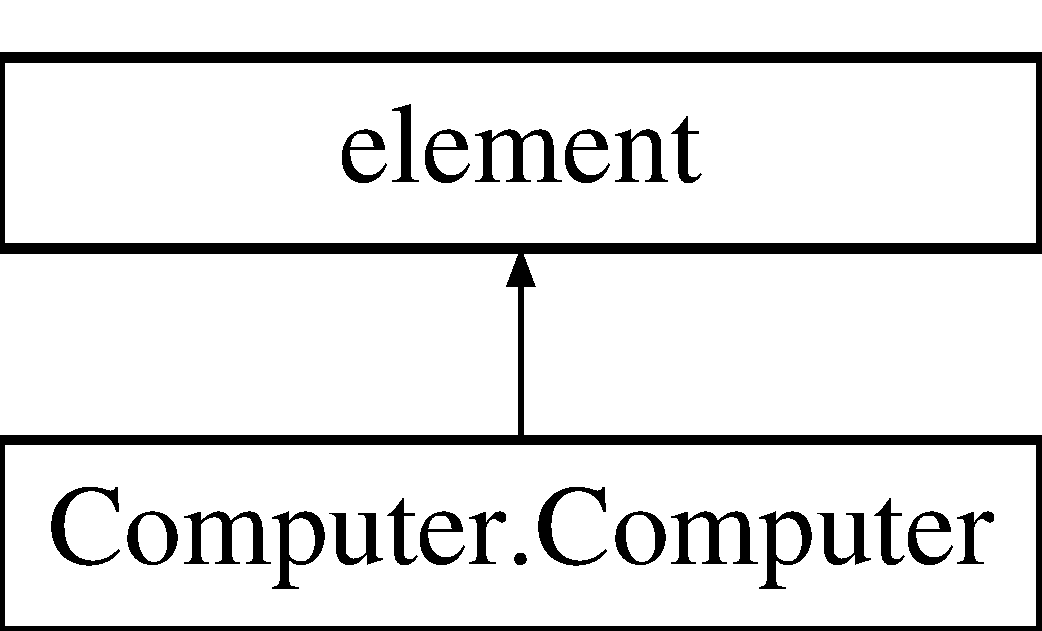
\includegraphics[height=2.000000cm]{classComputer_1_1Computer}
\end{center}
\end{figure}
\subsection*{Public Member Functions}
\begin{DoxyCompactItemize}
\item 
def \hyperlink{classComputer_1_1Computer_a9dd9b2c522763b9bdeaa185494f7693b}{\+\_\+\+\_\+init\+\_\+\+\_\+} (self, cat, obj, panel, \hyperlink{classHierarchy_aa7990fa7caf132d83e361ce033c6c65a}{path})
\item 
def \hyperlink{classComputer_1_1Computer_a41670b7dfe9ddf2e5070e55819e9b057}{update} (self)
\end{DoxyCompactItemize}


\subsection{Detailed Description}


Definition at line 5 of file Computer.\+py.



\subsection{Constructor \& Destructor Documentation}
\mbox{\Hypertarget{classComputer_1_1Computer_a9dd9b2c522763b9bdeaa185494f7693b}\label{classComputer_1_1Computer_a9dd9b2c522763b9bdeaa185494f7693b}} 
\index{Computer\+::\+Computer@{Computer\+::\+Computer}!\+\_\+\+\_\+init\+\_\+\+\_\+@{\+\_\+\+\_\+init\+\_\+\+\_\+}}
\index{\+\_\+\+\_\+init\+\_\+\+\_\+@{\+\_\+\+\_\+init\+\_\+\+\_\+}!Computer\+::\+Computer@{Computer\+::\+Computer}}
\subsubsection{\texorpdfstring{\+\_\+\+\_\+init\+\_\+\+\_\+()}{\_\_init\_\_()}}
{\footnotesize\ttfamily def Computer.\+Computer.\+\_\+\+\_\+init\+\_\+\+\_\+ (\begin{DoxyParamCaption}\item[{}]{self,  }\item[{}]{cat,  }\item[{}]{obj,  }\item[{}]{panel,  }\item[{}]{path }\end{DoxyParamCaption})}



Definition at line 6 of file Computer.\+py.



References element.\+element.\+loadxrc(), and proc.\+proc.\+loadxrc().


\begin{DoxyCode}
6     \textcolor{keyword}{def }\hyperlink{classwrapper_1_1ModuleDictWrapper_a9a7a794150502f51df687831583e13b9}{\_\_init\_\_}(self, cat, obj, panel, path):
7         element.\_\_init\_\_(self,cat,obj,panel,path)
8         self.loadxrc()
9 
10 \textcolor{comment}{#        choicebook=self.getControl("choicebook")}
11 
12 
\end{DoxyCode}


\subsection{Member Function Documentation}
\mbox{\Hypertarget{classComputer_1_1Computer_a41670b7dfe9ddf2e5070e55819e9b057}\label{classComputer_1_1Computer_a41670b7dfe9ddf2e5070e55819e9b057}} 
\index{Computer\+::\+Computer@{Computer\+::\+Computer}!update@{update}}
\index{update@{update}!Computer\+::\+Computer@{Computer\+::\+Computer}}
\subsubsection{\texorpdfstring{update()}{update()}}
{\footnotesize\ttfamily def Computer.\+Computer.\+update (\begin{DoxyParamCaption}\item[{}]{self }\end{DoxyParamCaption})}



Definition at line 13 of file Computer.\+py.



Referenced by App\+Frame.\+App\+Frame.\+delete\+Hardware(), Conf\+Frame.\+Conf\+Frame.\+on\+Change(), Graph\+Frame.\+Graph\+Frame.\+on\+Change(), Cfg\+Frame.\+Cfg\+Frame.\+on\+Change(), Conf\+Frame.\+Conf\+Frame.\+on\+Edit(), App\+Frame.\+App\+Frame.\+on\+Load(), Conf\+Frame.\+Conf\+Frame.\+on\+Re\+Load(), Graph\+Frame.\+Graph\+Frame.\+on\+Re\+Load(), Cfg\+Frame.\+Cfg\+Frame.\+on\+Re\+Load(), and App\+Frame.\+App\+Frame.\+on\+Re\+Load().


\begin{DoxyCode}
13     \textcolor{keyword}{def }update(self):
14         \textcolor{keywordflow}{print} \textcolor{stringliteral}{"No update function deifned yet."}
15 
\end{DoxyCode}


The documentation for this class was generated from the following file\+:\begin{DoxyCompactItemize}
\item 
/home/eleclhcb/\+L\+H\+Cb/lbcat-\/cmake/\+Cat\+Kernel/python/element/\hyperlink{Computer_8py}{Computer.\+py}\end{DoxyCompactItemize}

\hypertarget{classComputer}{}\section{Computer Class Reference}
\label{classComputer}\index{Computer@{Computer}}


{\ttfamily \#include $<$Computer.\+h$>$}

Inheritance diagram for Computer\+:\begin{figure}[H]
\begin{center}
\leavevmode
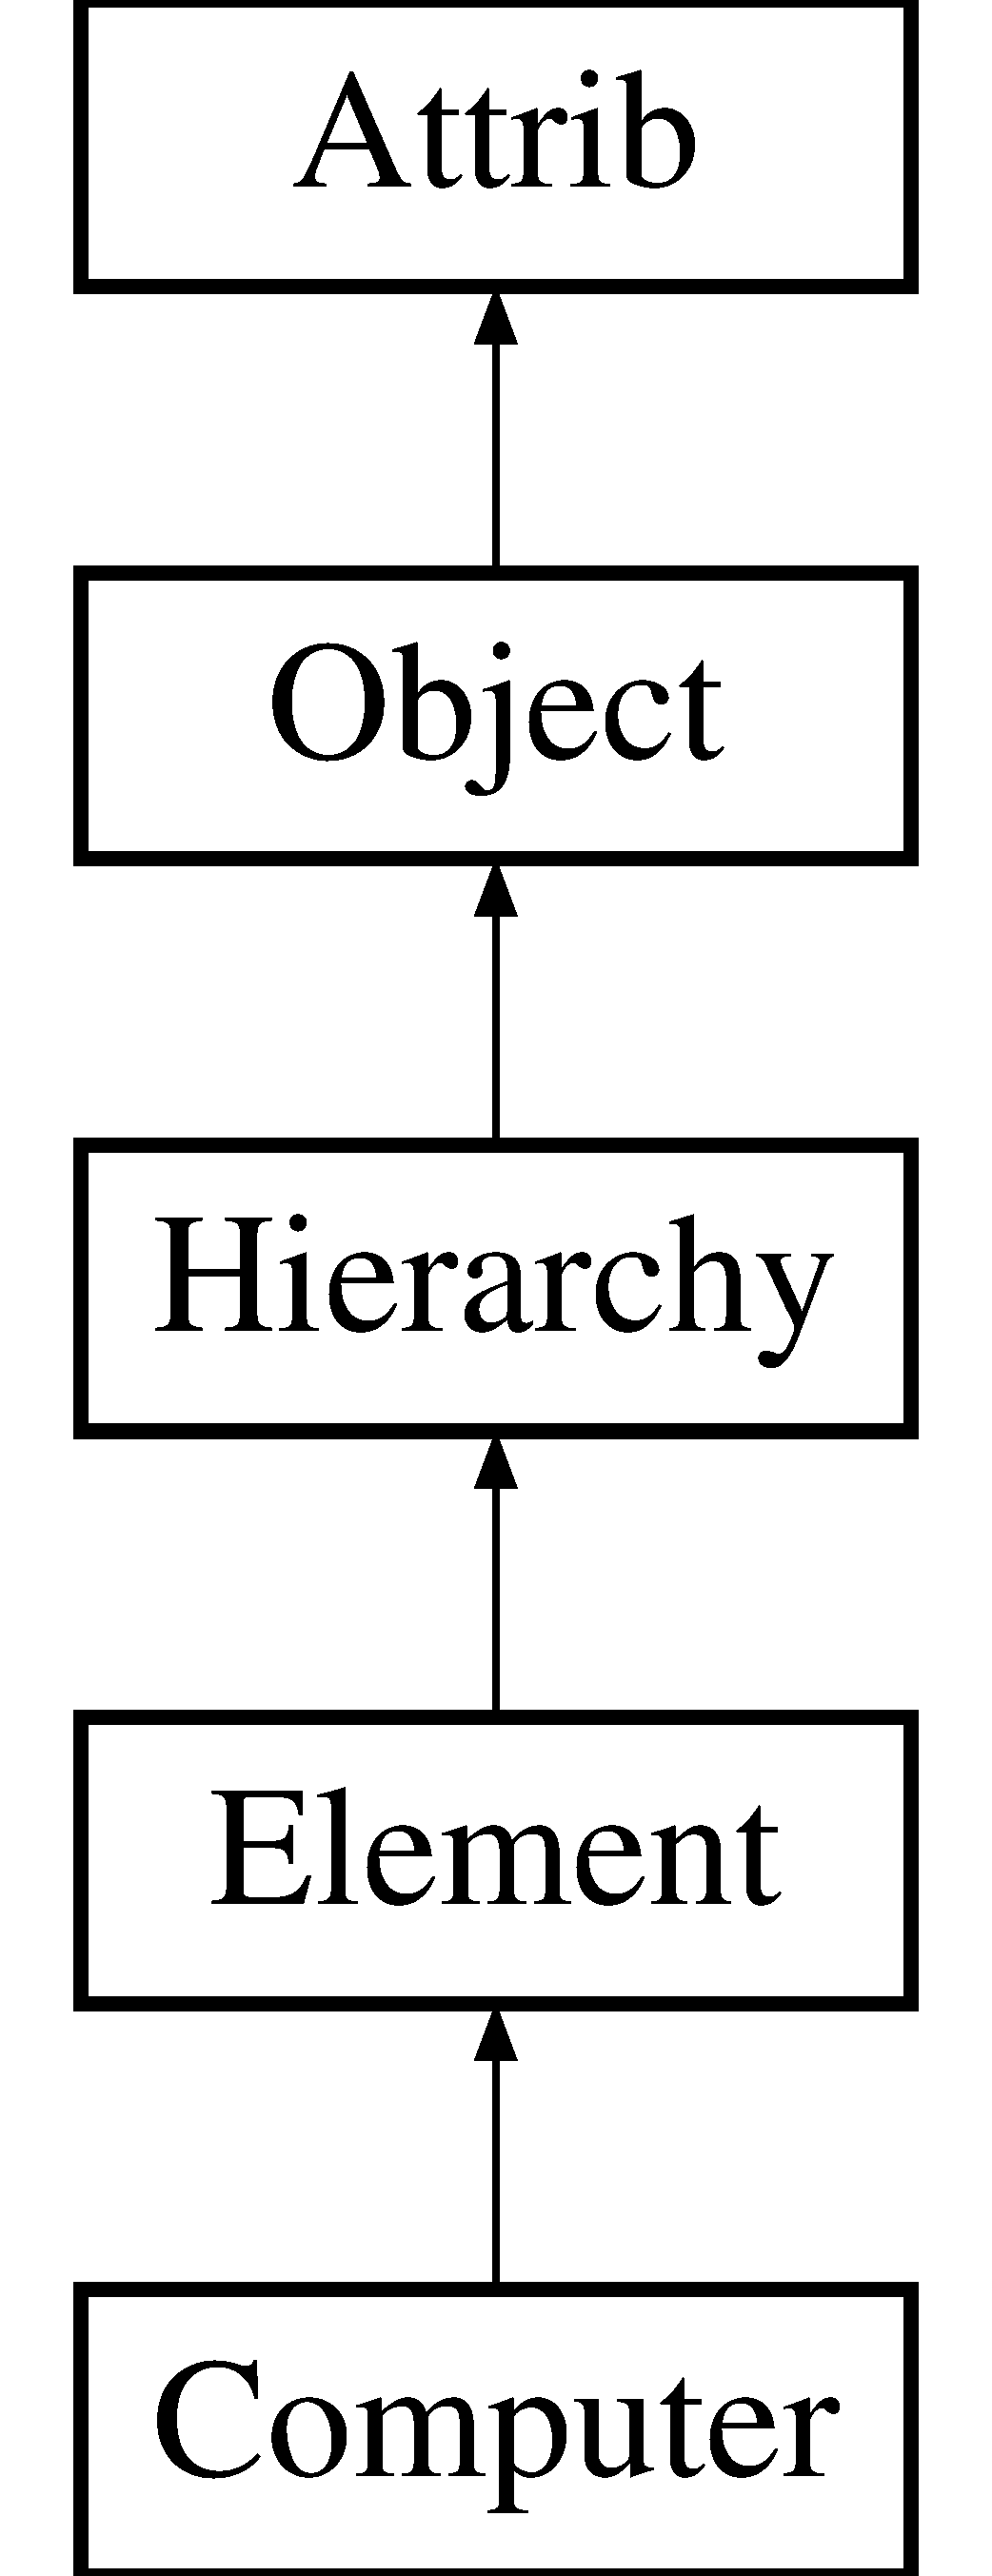
\includegraphics[height=5.000000cm]{classComputer}
\end{center}
\end{figure}
\subsection*{Classes}
\begin{DoxyCompactItemize}
\item 
class \hyperlink{classComputer_1_1Computer}{Computer}
\end{DoxyCompactItemize}
\subsection*{Public Types}
\begin{DoxyCompactItemize}
\item 
enum \hyperlink{classAttrib_a69e171d7cc6417835a5a306d3c764235}{Attribut} \{ \newline
\hyperlink{classAttrib_a69e171d7cc6417835a5a306d3c764235a3a8da2ab97dda18aebab196fe4100531}{U\+N\+D\+E\+F\+I\+N\+ED}, 
\hyperlink{classAttrib_a69e171d7cc6417835a5a306d3c764235a2bfb2af57b87031d190a05fe25dd92ed}{P\+A\+S\+S\+I\+VE}, 
\hyperlink{classAttrib_a69e171d7cc6417835a5a306d3c764235a3b1fec929c0370d1436f2f06e298fb0d}{A\+C\+T\+I\+VE}, 
\hyperlink{classAttrib_a69e171d7cc6417835a5a306d3c764235aa27c16b480a369ea4d18b07b2516bbc7}{I\+N\+T\+E\+R\+F\+A\+CE}, 
\newline
\hyperlink{classAttrib_a69e171d7cc6417835a5a306d3c764235a1420a5b8c0540b2af210b6975eded7f9}{IO}, 
\hyperlink{classAttrib_a69e171d7cc6417835a5a306d3c764235a0af3b0d0ac323c1704e6c69cf90add28}{I\+O\+D\+A\+TA}, 
\hyperlink{classAttrib_a69e171d7cc6417835a5a306d3c764235a7788bc5dd333fd8ce18562b269c9dab1}{E\+L\+E\+M\+E\+NT}, 
\hyperlink{classAttrib_a69e171d7cc6417835a5a306d3c764235a61ceb22149f365f1780d18f9d1459423}{H\+A\+R\+D\+W\+A\+RE}, 
\newline
\hyperlink{classAttrib_a69e171d7cc6417835a5a306d3c764235a75250e29692496e73effca2c0330977f}{P\+R\+O\+C\+E\+S\+S\+US}, 
\hyperlink{classAttrib_a69e171d7cc6417835a5a306d3c764235a103a67cd0b8f07ef478fa45d4356e27b}{S\+O\+F\+T\+W\+A\+RE}
 \}
\end{DoxyCompactItemize}
\subsection*{Public Member Functions}
\begin{DoxyCompactItemize}
\item 
\hyperlink{classComputer_a52056dfe9041f024ac58c1eaf02945d3}{Computer} ()
\begin{DoxyCompactList}\small\item\em Standard constructor. \end{DoxyCompactList}\item 
virtual \hyperlink{classComputer_a633f86288c20c5aa1eed7f14fb069272}{$\sim$\+Computer} ()
\begin{DoxyCompactList}\small\item\em Destructor. \end{DoxyCompactList}\item 
void \hyperlink{classComputer_aeca79382f17fcfb43320902de5f20aca}{help} ()
\item 
\hyperlink{classStatusCode}{Status\+Code} \hyperlink{classComputer_a47ed8b470445d545bffefca31296e754}{init} ()
\item 
void \hyperlink{classComputer_aeab90cbacbef385685717c249a07929d}{reset} ()
\item 
void \hyperlink{classComputer_aaad6dfbfcc6843d73f49e0fc1535563e}{update} ()
\item 
void \hyperlink{classElement_a3c0abcb36f8906688bb7e32608df7086}{recursive\+Init\+Element} ()
\item 
void \hyperlink{classElement_a82119ed37dff76508a2746a853ec35ba}{recursive\+Init\+Communications} ()
\item 
\hyperlink{classStatusCode}{Status\+Code} \hyperlink{classElement_ab476b4b1df5954141ceb14f072433b89}{set\+Connection} (\hyperlink{classHierarchy}{Hierarchy} $\ast$)
\item 
\hyperlink{classHierarchy}{Hierarchy} $\ast$ \hyperlink{classElement_af57444353c1ddf9fa0109801e97debf7}{connection} ()
\item 
void \hyperlink{classHierarchy_af4d43b0765b402670eed2d62c73405af}{clear} ()
\item 
void \hyperlink{classHierarchy_a585ad1aeec16077a0e532ab8b4fc557b}{set\+Parent} (\hyperlink{classHierarchy}{Hierarchy} $\ast$\hyperlink{classHierarchy_a1c7bec8257e717f9c1465e06ebf845fc}{parent})
\item 
\hyperlink{classHierarchy}{Hierarchy} $\ast$ \hyperlink{classHierarchy_a1c7bec8257e717f9c1465e06ebf845fc}{parent} ()
\item 
\hyperlink{classHierarchy}{Hierarchy} $\ast$ \hyperlink{classHierarchy_ad550588733bf75ac5c0fcfd7c8fd11a6}{parent} (std\+::string)
\item 
\hyperlink{classHierarchy}{Hierarchy} $\ast$ \hyperlink{classHierarchy_aee461dc930ce3871636ff87f075b1b83}{origin} ()
\item 
virtual void \hyperlink{classHierarchy_ad677774ff38fcb257c04a3a10d471fac}{add\+Child} (\hyperlink{classHierarchy}{Hierarchy} $\ast$element)
\item 
std\+::vector$<$ \hyperlink{classHierarchy}{Hierarchy} $\ast$ $>$ \hyperlink{classHierarchy_aa9a76f69e98e052ee1a6e32cea006288}{children} ()
\item 
\hyperlink{classHierarchy}{Hierarchy} $\ast$ \hyperlink{classHierarchy_a1e207f973c694b538bf90107b4868817}{child} (std\+::string)
\item 
\hyperlink{classHierarchy}{Hierarchy} $\ast$ \hyperlink{classHierarchy_a0c15a5276a3b80b4354d6bd8a01e0708}{child\+Typed} (std\+::string)
\item 
unsigned long \hyperlink{classHierarchy_ab16e84de65fd84e14001a6cf941c8be4}{number\+Of\+Children} ()
\item 
bool \hyperlink{classHierarchy_a255174fe4d316d2a3f430dcb9dab29f1}{has\+Children} ()
\item 
void \hyperlink{classHierarchy_a2b2b359fac003233f65786a616766bde}{del\+Child} (\hyperlink{classHierarchy}{Hierarchy} $\ast$)
\item 
void \hyperlink{classHierarchy_a1928ac7615fe0b5e55cd707f70dc6781}{del\+Child} (std\+::string)
\item 
std\+::string \hyperlink{classHierarchy_aa7990fa7caf132d83e361ce033c6c65a}{path} (std\+::string=std\+::string(\char`\"{}\char`\"{}))
\item 
std\+::string \hyperlink{classHierarchy_a1efd56cd164d328d2002e53a10a19b8c}{path\+Typed} (std\+::string=std\+::string(\char`\"{}\char`\"{}))
\item 
void \hyperlink{classHierarchy_a76e914b9a677a22a82deb74d892bf261}{tree} (std\+::string indent=std\+::string(\char`\"{}\char`\"{}))
\item 
void \hyperlink{classHierarchy_a594c294c5f60c230e106d522ed008212}{tree} ()
\item 
std\+::string \hyperlink{classObject_a300f4c05dd468c7bb8b3c968868443c1}{name} () const
\item 
std\+::string \hyperlink{classObject_a84f99f70f144a83e1582d1d0f84e4e62}{type} ()
\item 
unsigned char \hyperlink{classObject_af99145335cc61ff6e2798ea17db009d2}{id} ()
\item 
std\+::string \hyperlink{classObject_a73a0f1a41828fdd8303dd662446fb6c3}{title} ()
\item 
void \hyperlink{classObject_a3f9d5537ebce0c0f2bf6ae4d92426f3c}{msg\+Svc} (int level, std\+::string \hyperlink{classObject_a58b2d0618c2d08cf2383012611528d97}{msg}, std\+::string \hyperlink{classObject_a300f4c05dd468c7bb8b3c968868443c1}{name})
\item 
void \hyperlink{classObject_a58b2d0618c2d08cf2383012611528d97}{msg} (std\+::string mymsg)
\item 
void \hyperlink{classObject_ac5d59299273cee27aacf7de00d2e7034}{msg} (std\+::string mymsg, std\+::string \hyperlink{classObject_a300f4c05dd468c7bb8b3c968868443c1}{name})
\item 
void \hyperlink{classObject_a83d2db2df682907ea1115ad721c1c4a1}{verbose} (std\+::string mymsg)
\item 
void \hyperlink{classObject_a2d4120195317e2a3c6532e8bb9f3da68}{verbose} (std\+::string mymsg, std\+::string \hyperlink{classObject_a300f4c05dd468c7bb8b3c968868443c1}{name})
\item 
void \hyperlink{classObject_aac010553f022165573714b7014a15f0d}{debug} (std\+::string mymsg)
\item 
void \hyperlink{classObject_a6c9a0397ca804e04d675ed05683f5420}{debug} (std\+::string mymsg, std\+::string \hyperlink{classObject_a300f4c05dd468c7bb8b3c968868443c1}{name})
\item 
void \hyperlink{classObject_a644fd329ea4cb85f54fa6846484b84a8}{info} (std\+::string mymsg)
\item 
void \hyperlink{classObject_a1ca123253dfd30fc28b156f521dcbdae}{info} (std\+::string mymsg, std\+::string \hyperlink{classObject_a300f4c05dd468c7bb8b3c968868443c1}{name})
\item 
void \hyperlink{classObject_a65cd4fda577711660821fd2cd5a3b4c9}{warning} (std\+::string mymsg)
\item 
void \hyperlink{classObject_a11f101db4dd73d9391b0231818881d86}{warning} (std\+::string mymsg, std\+::string \hyperlink{classObject_a300f4c05dd468c7bb8b3c968868443c1}{name})
\item 
void \hyperlink{classObject_a204a95f57818c0f811933917a30eff45}{error} (std\+::string mymsg)
\item 
void \hyperlink{classObject_ad7f6c457733082efa2f9ff5f5c8e119a}{error} (std\+::string mymsg, std\+::string \hyperlink{classObject_a300f4c05dd468c7bb8b3c968868443c1}{name})
\item 
void \hyperlink{classObject_aad5a16aac7516ce65bd5ec02ab07fc80}{fatal} (std\+::string mymsg)
\item 
void \hyperlink{classObject_ae62acd3d09f716220f75f252dc38bc9a}{fatal} (std\+::string mymsg, std\+::string \hyperlink{classObject_a300f4c05dd468c7bb8b3c968868443c1}{name})
\item 
void \hyperlink{classObject_ae30fea75683c2d149b6b6d17c09ecd0c}{set\+Name} (std\+::string \hyperlink{classObject_a300f4c05dd468c7bb8b3c968868443c1}{name})
\item 
void \hyperlink{classObject_aae534cc9d982bcb9b99fd505f2e103a5}{set\+Type} (std\+::string \hyperlink{classObject_a84f99f70f144a83e1582d1d0f84e4e62}{type})
\item 
void \hyperlink{classObject_a398fe08cba594a0ce6891d59fe4f159f}{set\+Id} (unsigned char \hyperlink{classObject_af99145335cc61ff6e2798ea17db009d2}{id})
\item 
void \hyperlink{classObject_a89557dbbad5bcaa02652f5d7fa35d20f}{set\+Title} (std\+::string \hyperlink{classObject_a73a0f1a41828fdd8303dd662446fb6c3}{title})
\item 
void \hyperlink{classObject_a870c5af919958c2136623b2d7816d123}{set\+Dll\+Name} (std\+::string \hyperlink{classObject_a2e3947f2870094c332d7454117f3ec63}{dll\+Name})
\item 
std\+::string \hyperlink{classObject_a2e3947f2870094c332d7454117f3ec63}{dll\+Name} ()
\item 
bool \hyperlink{classAttrib_a704f26af560909ad22065083bb7d4c34}{is} (int attribut)
\item 
void \hyperlink{classAttrib_a235f773af19c900264a190b00a3b4ad7}{add} (int attribut)
\item 
void \hyperlink{classAttrib_a7d4ef7e32d93cb287792b87b857e79f3}{remove} (int attribut)
\item 
std\+::string \hyperlink{classAttrib_aee7bbf16b144887f196e1341b24f8a26}{attributs} ()
\end{DoxyCompactItemize}
\subsection*{Protected Attributes}
\begin{DoxyCompactItemize}
\item 
\hyperlink{classHierarchy}{Hierarchy} $\ast$ \hyperlink{classElement_abe3de7a5dbbc9a6dd2d7e012e5fdb266}{m\+\_\+connection}
\item 
std\+::string \hyperlink{classAttrib_a3414521d7a82476e874b25a5407b5e63}{m\+\_\+attrib\+String} \mbox{[}10\mbox{]}
\end{DoxyCompactItemize}
\subsection*{Private Attributes}
\begin{DoxyCompactItemize}
\item 
\hyperlink{classTestSuite}{Test\+Suite} $\ast$ \hyperlink{classComputer_a5418f176fa9fbd08356ad251f047adcd}{m\+\_\+test\+Suite}
\end{DoxyCompactItemize}


\subsection{Detailed Description}
\begin{DoxyAuthor}{Author}
Frédéric Machefert 
\end{DoxyAuthor}
\begin{DoxyDate}{Date}
2006-\/10-\/26 
\end{DoxyDate}


Definition at line 26 of file Computer.\+h.



\subsection{Member Enumeration Documentation}
\mbox{\Hypertarget{classAttrib_a69e171d7cc6417835a5a306d3c764235}\label{classAttrib_a69e171d7cc6417835a5a306d3c764235}} 
\index{Computer@{Computer}!Attribut@{Attribut}}
\index{Attribut@{Attribut}!Computer@{Computer}}
\subsubsection{\texorpdfstring{Attribut}{Attribut}}
{\footnotesize\ttfamily enum \hyperlink{classAttrib_a69e171d7cc6417835a5a306d3c764235}{Attrib\+::\+Attribut}\hspace{0.3cm}{\ttfamily [inherited]}}

\begin{DoxyEnumFields}{Enumerator}
\raisebox{\heightof{T}}[0pt][0pt]{\index{U\+N\+D\+E\+F\+I\+N\+ED@{U\+N\+D\+E\+F\+I\+N\+ED}!Computer@{Computer}}\index{Computer@{Computer}!U\+N\+D\+E\+F\+I\+N\+ED@{U\+N\+D\+E\+F\+I\+N\+ED}}}\mbox{\Hypertarget{classAttrib_a69e171d7cc6417835a5a306d3c764235a3a8da2ab97dda18aebab196fe4100531}\label{classAttrib_a69e171d7cc6417835a5a306d3c764235a3a8da2ab97dda18aebab196fe4100531}} 
U\+N\+D\+E\+F\+I\+N\+ED&\\
\hline

\raisebox{\heightof{T}}[0pt][0pt]{\index{P\+A\+S\+S\+I\+VE@{P\+A\+S\+S\+I\+VE}!Computer@{Computer}}\index{Computer@{Computer}!P\+A\+S\+S\+I\+VE@{P\+A\+S\+S\+I\+VE}}}\mbox{\Hypertarget{classAttrib_a69e171d7cc6417835a5a306d3c764235a2bfb2af57b87031d190a05fe25dd92ed}\label{classAttrib_a69e171d7cc6417835a5a306d3c764235a2bfb2af57b87031d190a05fe25dd92ed}} 
P\+A\+S\+S\+I\+VE&\\
\hline

\raisebox{\heightof{T}}[0pt][0pt]{\index{A\+C\+T\+I\+VE@{A\+C\+T\+I\+VE}!Computer@{Computer}}\index{Computer@{Computer}!A\+C\+T\+I\+VE@{A\+C\+T\+I\+VE}}}\mbox{\Hypertarget{classAttrib_a69e171d7cc6417835a5a306d3c764235a3b1fec929c0370d1436f2f06e298fb0d}\label{classAttrib_a69e171d7cc6417835a5a306d3c764235a3b1fec929c0370d1436f2f06e298fb0d}} 
A\+C\+T\+I\+VE&\\
\hline

\raisebox{\heightof{T}}[0pt][0pt]{\index{I\+N\+T\+E\+R\+F\+A\+CE@{I\+N\+T\+E\+R\+F\+A\+CE}!Computer@{Computer}}\index{Computer@{Computer}!I\+N\+T\+E\+R\+F\+A\+CE@{I\+N\+T\+E\+R\+F\+A\+CE}}}\mbox{\Hypertarget{classAttrib_a69e171d7cc6417835a5a306d3c764235aa27c16b480a369ea4d18b07b2516bbc7}\label{classAttrib_a69e171d7cc6417835a5a306d3c764235aa27c16b480a369ea4d18b07b2516bbc7}} 
I\+N\+T\+E\+R\+F\+A\+CE&\\
\hline

\raisebox{\heightof{T}}[0pt][0pt]{\index{IO@{IO}!Computer@{Computer}}\index{Computer@{Computer}!IO@{IO}}}\mbox{\Hypertarget{classAttrib_a69e171d7cc6417835a5a306d3c764235a1420a5b8c0540b2af210b6975eded7f9}\label{classAttrib_a69e171d7cc6417835a5a306d3c764235a1420a5b8c0540b2af210b6975eded7f9}} 
IO&\\
\hline

\raisebox{\heightof{T}}[0pt][0pt]{\index{I\+O\+D\+A\+TA@{I\+O\+D\+A\+TA}!Computer@{Computer}}\index{Computer@{Computer}!I\+O\+D\+A\+TA@{I\+O\+D\+A\+TA}}}\mbox{\Hypertarget{classAttrib_a69e171d7cc6417835a5a306d3c764235a0af3b0d0ac323c1704e6c69cf90add28}\label{classAttrib_a69e171d7cc6417835a5a306d3c764235a0af3b0d0ac323c1704e6c69cf90add28}} 
I\+O\+D\+A\+TA&\\
\hline

\raisebox{\heightof{T}}[0pt][0pt]{\index{E\+L\+E\+M\+E\+NT@{E\+L\+E\+M\+E\+NT}!Computer@{Computer}}\index{Computer@{Computer}!E\+L\+E\+M\+E\+NT@{E\+L\+E\+M\+E\+NT}}}\mbox{\Hypertarget{classAttrib_a69e171d7cc6417835a5a306d3c764235a7788bc5dd333fd8ce18562b269c9dab1}\label{classAttrib_a69e171d7cc6417835a5a306d3c764235a7788bc5dd333fd8ce18562b269c9dab1}} 
E\+L\+E\+M\+E\+NT&\\
\hline

\raisebox{\heightof{T}}[0pt][0pt]{\index{H\+A\+R\+D\+W\+A\+RE@{H\+A\+R\+D\+W\+A\+RE}!Computer@{Computer}}\index{Computer@{Computer}!H\+A\+R\+D\+W\+A\+RE@{H\+A\+R\+D\+W\+A\+RE}}}\mbox{\Hypertarget{classAttrib_a69e171d7cc6417835a5a306d3c764235a61ceb22149f365f1780d18f9d1459423}\label{classAttrib_a69e171d7cc6417835a5a306d3c764235a61ceb22149f365f1780d18f9d1459423}} 
H\+A\+R\+D\+W\+A\+RE&\\
\hline

\raisebox{\heightof{T}}[0pt][0pt]{\index{P\+R\+O\+C\+E\+S\+S\+US@{P\+R\+O\+C\+E\+S\+S\+US}!Computer@{Computer}}\index{Computer@{Computer}!P\+R\+O\+C\+E\+S\+S\+US@{P\+R\+O\+C\+E\+S\+S\+US}}}\mbox{\Hypertarget{classAttrib_a69e171d7cc6417835a5a306d3c764235a75250e29692496e73effca2c0330977f}\label{classAttrib_a69e171d7cc6417835a5a306d3c764235a75250e29692496e73effca2c0330977f}} 
P\+R\+O\+C\+E\+S\+S\+US&\\
\hline

\raisebox{\heightof{T}}[0pt][0pt]{\index{S\+O\+F\+T\+W\+A\+RE@{S\+O\+F\+T\+W\+A\+RE}!Computer@{Computer}}\index{Computer@{Computer}!S\+O\+F\+T\+W\+A\+RE@{S\+O\+F\+T\+W\+A\+RE}}}\mbox{\Hypertarget{classAttrib_a69e171d7cc6417835a5a306d3c764235a103a67cd0b8f07ef478fa45d4356e27b}\label{classAttrib_a69e171d7cc6417835a5a306d3c764235a103a67cd0b8f07ef478fa45d4356e27b}} 
S\+O\+F\+T\+W\+A\+RE&\\
\hline

\end{DoxyEnumFields}


Definition at line 29 of file Attrib.\+h.


\begin{DoxyCode}
29                 \{
30     \hyperlink{classAttrib_a69e171d7cc6417835a5a306d3c764235a3a8da2ab97dda18aebab196fe4100531}{UNDEFINED},
31     \hyperlink{classAttrib_a69e171d7cc6417835a5a306d3c764235a2bfb2af57b87031d190a05fe25dd92ed}{PASSIVE},
32     \hyperlink{classAttrib_a69e171d7cc6417835a5a306d3c764235a3b1fec929c0370d1436f2f06e298fb0d}{ACTIVE},
33     \hyperlink{classAttrib_a69e171d7cc6417835a5a306d3c764235aa27c16b480a369ea4d18b07b2516bbc7}{INTERFACE},
34     \hyperlink{classAttrib_a69e171d7cc6417835a5a306d3c764235a1420a5b8c0540b2af210b6975eded7f9}{IO},
35     \hyperlink{classAttrib_a69e171d7cc6417835a5a306d3c764235a0af3b0d0ac323c1704e6c69cf90add28}{IODATA},
36     \hyperlink{classAttrib_a69e171d7cc6417835a5a306d3c764235a7788bc5dd333fd8ce18562b269c9dab1}{ELEMENT},
37     \hyperlink{classAttrib_a69e171d7cc6417835a5a306d3c764235a61ceb22149f365f1780d18f9d1459423}{HARDWARE},
38     \hyperlink{classAttrib_a69e171d7cc6417835a5a306d3c764235a75250e29692496e73effca2c0330977f}{PROCESSUS},
39     \hyperlink{classAttrib_a69e171d7cc6417835a5a306d3c764235a103a67cd0b8f07ef478fa45d4356e27b}{SOFTWARE} 
40   \}; \textcolor{comment}{// array m\_attribString must be changed into Attrib::Attrib if this enu is modified. }
\end{DoxyCode}


\subsection{Constructor \& Destructor Documentation}
\mbox{\Hypertarget{classComputer_a52056dfe9041f024ac58c1eaf02945d3}\label{classComputer_a52056dfe9041f024ac58c1eaf02945d3}} 
\index{Computer@{Computer}!Computer@{Computer}}
\index{Computer@{Computer}!Computer@{Computer}}
\subsubsection{\texorpdfstring{Computer()}{Computer()}}
{\footnotesize\ttfamily \hyperlink{classComputer_1_1Computer}{Computer\+::\+Computer} (\begin{DoxyParamCaption}{ }\end{DoxyParamCaption})}



Standard constructor. 



Definition at line 17 of file Computer.\+cpp.



References Proc\+Data\+Base\+::add(), Attrib\+::add(), application(), Attrib\+::\+E\+L\+E\+M\+E\+NT, Attrib\+::\+H\+A\+R\+D\+W\+A\+RE, System\+::host\+Name(), m\+\_\+test\+Suite, Application\+::proc\+Db(), Object\+::set\+Name(), Hierarchy\+::set\+Parent(), and Object\+::set\+Type().


\begin{DoxyCode}
17                      \{
18   \hyperlink{classObject_ae30fea75683c2d149b6b6d17c09ecd0c}{setName} ( \hyperlink{namespaceSystem_a89320a729880098922e8b505db1137ec}{System::hostName}() );
19   \hyperlink{classObject_aae534cc9d982bcb9b99fd505f2e103a5}{setType} ( \textcolor{stringliteral}{"Computer"} );
20   \hyperlink{classAttrib_a235f773af19c900264a190b00a3b4ad7}{add}(\hyperlink{classAttrib_a69e171d7cc6417835a5a306d3c764235a7788bc5dd333fd8ce18562b269c9dab1}{Attrib::ELEMENT});  \hyperlink{classAttrib_a235f773af19c900264a190b00a3b4ad7}{add}(\hyperlink{classAttrib_a69e171d7cc6417835a5a306d3c764235a61ceb22149f365f1780d18f9d1459423}{Attrib::HARDWARE});
21   \hyperlink{classComputer_a5418f176fa9fbd08356ad251f047adcd}{m\_testSuite}=\textcolor{keyword}{new} \hyperlink{namespaceTestSuite}{TestSuite}();
22   \hyperlink{Tools_8h_a27885a3c35afe79029fb830f32f66458}{application}()->\hyperlink{classApplication_aa5c28af1a7e1c41dada2db2a4d03c57d}{procDb}()->\hyperlink{classProcDataBase_a0aafeb65a41b92a6d1fdd67f363ef826}{add}( \hyperlink{classComputer_a5418f176fa9fbd08356ad251f047adcd}{m\_testSuite} );
23   \hyperlink{classHierarchy_a585ad1aeec16077a0e532ab8b4fc557b}{setParent}((\hyperlink{classHierarchy}{Hierarchy}*)0);  
24 \}
\end{DoxyCode}
\mbox{\Hypertarget{classComputer_a633f86288c20c5aa1eed7f14fb069272}\label{classComputer_a633f86288c20c5aa1eed7f14fb069272}} 
\index{Computer@{Computer}!````~Computer@{$\sim$\+Computer}}
\index{````~Computer@{$\sim$\+Computer}!Computer@{Computer}}
\subsubsection{\texorpdfstring{$\sim$\+Computer()}{~Computer()}}
{\footnotesize\ttfamily Computer\+::$\sim$\+Computer (\begin{DoxyParamCaption}{ }\end{DoxyParamCaption})\hspace{0.3cm}{\ttfamily [virtual]}}



Destructor. 



Definition at line 28 of file Computer.\+cpp.



References application(), m\+\_\+test\+Suite, Application\+::proc\+Db(), and Proc\+Data\+Base\+::remove().


\begin{DoxyCode}
28                     \{
29   \hyperlink{Tools_8h_a27885a3c35afe79029fb830f32f66458}{application}()->\hyperlink{classApplication_aa5c28af1a7e1c41dada2db2a4d03c57d}{procDb}()->\hyperlink{classProcDataBase_a0413976bac8f233b31eab6d7a83866b9}{remove}( \hyperlink{classComputer_a5418f176fa9fbd08356ad251f047adcd}{m\_testSuite} );
30 \} 
\end{DoxyCode}


\subsection{Member Function Documentation}
\mbox{\Hypertarget{classAttrib_a235f773af19c900264a190b00a3b4ad7}\label{classAttrib_a235f773af19c900264a190b00a3b4ad7}} 
\index{Computer@{Computer}!add@{add}}
\index{add@{add}!Computer@{Computer}}
\subsubsection{\texorpdfstring{add()}{add()}}
{\footnotesize\ttfamily void Attrib\+::add (\begin{DoxyParamCaption}\item[{int}]{attribut }\end{DoxyParamCaption})\hspace{0.3cm}{\ttfamily [inline]}, {\ttfamily [inherited]}}

Add an attribut 

Definition at line 67 of file Attrib.\+h.



References Attrib\+::m\+\_\+attributs, and Attrib\+::\+U\+N\+D\+E\+F\+I\+N\+ED.



Referenced by A3\+P\+E\+::\+A3\+P\+E(), Attrib\+::\+Attrib(), Specs\+Mezzanine\+::cmdline(), Computer(), C\+U\+\_\+v1\+::\+C\+U\+\_\+v1(), export\+\_\+obj(), F\+E\+B\+\_\+v1\+::\+F\+E\+B\+\_\+v1(), Fe\+P\+G\+A\+::\+Fe\+P\+G\+A(), I\+C\+E\+C\+A\+Lv3\+::\+I\+C\+E\+C\+A\+Lv3(), I\+C\+Phaser\+::\+I\+C\+Phaser(), Application\+::initialize(), Interface\+::\+Interface(), I\+Odata\+::\+I\+Odata(), I\+Oobject\+::\+I\+Oobject(), M\+S\+Oxxxx\+::\+M\+S\+Oxxxx(), Phaser\+::\+Phaser(), Processus\+::\+Processus(), Proto40\+M\+Hz\+\_\+v1\+::\+Proto40\+M\+Hz\+\_\+v1(), Attrib\+::remove(), Seq\+P\+G\+A\+::\+Seq\+P\+G\+A(), Test\+I2\+C\+::set\+Address(), Test\+S\+P\+I\+::set\+Address(), Specs\+Slave\+::set\+Address(), Specs\+Master\+::\+Specs\+Master(), and Specs\+Slave\+::\+Specs\+Slave().


\begin{DoxyCode}
67                             \{
68     \textcolor{keywordflow}{if} (attribut!=\hyperlink{classAttrib_a69e171d7cc6417835a5a306d3c764235a3a8da2ab97dda18aebab196fe4100531}{Attrib::UNDEFINED}) \textcolor{keyword}{remove}(\hyperlink{classAttrib_a69e171d7cc6417835a5a306d3c764235a3a8da2ab97dda18aebab196fe4100531}{Attrib::UNDEFINED});
69     \textcolor{keywordtype}{bool} duplicate = false ;
70     std::vector<int>::const\_iterator iter ;
71     \textcolor{keywordflow}{for} ( iter  = \hyperlink{classAttrib_ac4bd58a0cc6b38a3b711d609a3d3aacc}{m\_attributs}.begin() ;
72           iter != \hyperlink{classAttrib_ac4bd58a0cc6b38a3b711d609a3d3aacc}{m\_attributs}.end()   ;
73           ++iter ) \{
74       \textcolor{keywordflow}{if} ( attribut == (*iter) ) \{
75         duplicate = true ;
76       \}
77     \}
78     \textcolor{keywordflow}{if} (!duplicate) \{
79       \hyperlink{classAttrib_ac4bd58a0cc6b38a3b711d609a3d3aacc}{m\_attributs}.push\_back( attribut );
80     \}
81   \}
\end{DoxyCode}
\mbox{\Hypertarget{classHierarchy_ad677774ff38fcb257c04a3a10d471fac}\label{classHierarchy_ad677774ff38fcb257c04a3a10d471fac}} 
\index{Computer@{Computer}!add\+Child@{add\+Child}}
\index{add\+Child@{add\+Child}!Computer@{Computer}}
\subsubsection{\texorpdfstring{add\+Child()}{addChild()}}
{\footnotesize\ttfamily void Hierarchy\+::add\+Child (\begin{DoxyParamCaption}\item[{\hyperlink{classHierarchy}{Hierarchy} $\ast$}]{element }\end{DoxyParamCaption})\hspace{0.3cm}{\ttfamily [virtual]}, {\ttfamily [inherited]}}



Definition at line 83 of file Hierarchy.\+cpp.



References Object\+::debug(), Hierarchy\+::m\+\_\+children, Object\+::name(), and Hierarchy\+::set\+Parent().



Referenced by A3\+P\+E\+::\+A3\+P\+E(), Specs\+Mezzanine\+::add\+Bus(), Specs\+Slave\+::add\+I2c(), Application\+::create(), C\+U\+\_\+v1\+::\+C\+U\+\_\+v1(), export\+\_\+obj(), F\+E\+B\+\_\+v1\+::\+F\+E\+B\+\_\+v1(), Fe\+P\+G\+A\+::\+Fe\+P\+G\+A(), I\+C\+E\+C\+A\+Lv3\+::\+I\+C\+E\+C\+A\+Lv3(), I\+C\+Phaser\+::\+I\+C\+Phaser(), Hierarchy\+::origin(), Phaser\+::\+Phaser(), Proto40\+M\+Hz\+\_\+v1\+::\+Proto40\+M\+Hz\+\_\+v1(), Seq\+P\+G\+A\+::\+Seq\+P\+G\+A(), Specs\+Mezzanine\+::\+Specs\+Mezzanine(), Usb\+I2c\+Bus\+::\+Usb\+I2c\+Bus(), and Usb\+Spi\+Bus\+::\+Usb\+Spi\+Bus().


\begin{DoxyCode}
83                                           \{
84   element->\hyperlink{classHierarchy_a585ad1aeec16077a0e532ab8b4fc557b}{setParent}(\textcolor{keyword}{this});
85   \hyperlink{classHierarchy_a038816763941fd4a930504917f60483b}{m\_children}.push\_back(element);
86   \hyperlink{classObject_aac010553f022165573714b7014a15f0d}{debug}(element->\hyperlink{classObject_a300f4c05dd468c7bb8b3c968868443c1}{name}()+\textcolor{stringliteral}{" added to the child tree."},\textcolor{stringliteral}{"Hierarchy::addChild"});
87 \}
\end{DoxyCode}
\mbox{\Hypertarget{classAttrib_aee7bbf16b144887f196e1341b24f8a26}\label{classAttrib_aee7bbf16b144887f196e1341b24f8a26}} 
\index{Computer@{Computer}!attributs@{attributs}}
\index{attributs@{attributs}!Computer@{Computer}}
\subsubsection{\texorpdfstring{attributs()}{attributs()}}
{\footnotesize\ttfamily std\+::string Attrib\+::attributs (\begin{DoxyParamCaption}{ }\end{DoxyParamCaption})\hspace{0.3cm}{\ttfamily [inherited]}}

Print the \hyperlink{classAttrib}{Attrib} of an \hyperlink{classObject}{Object} 

Definition at line 54 of file Attrib.\+cpp.



References images\+::index, Attrib\+::m\+\_\+attrib\+String, and Attrib\+::m\+\_\+attributs.



Referenced by export\+\_\+obj(), and Attrib\+::remove().


\begin{DoxyCode}
54                             \{
55   std::string output;
56   std::vector<int>::iterator iter ;
57   \textcolor{keywordflow}{for} ( \textcolor{keywordtype}{unsigned} \textcolor{keywordtype}{int} \hyperlink{namespaceimages_a54407fd574970b3178647ae096321a57}{index} = 0 ; \hyperlink{namespaceimages_a54407fd574970b3178647ae096321a57}{index} < \hyperlink{classAttrib_ac4bd58a0cc6b38a3b711d609a3d3aacc}{m\_attributs}.size() ; ++
      \hyperlink{namespaceimages_a54407fd574970b3178647ae096321a57}{index} ) \{
58     \textcolor{keywordflow}{if} ( \hyperlink{classAttrib_ac4bd58a0cc6b38a3b711d609a3d3aacc}{m\_attributs}.size() - \hyperlink{namespaceimages_a54407fd574970b3178647ae096321a57}{index} > 1 ) \{
59       output.append(\hyperlink{classAttrib_a3414521d7a82476e874b25a5407b5e63}{m\_attribString}[\hyperlink{classAttrib_ac4bd58a0cc6b38a3b711d609a3d3aacc}{m\_attributs}[\hyperlink{namespaceimages_a54407fd574970b3178647ae096321a57}{index}]]);
60       output.append(\textcolor{stringliteral}{":"});
61     \}
62     \textcolor{keywordflow}{else} \{
63       output.append(\hyperlink{classAttrib_a3414521d7a82476e874b25a5407b5e63}{m\_attribString}[\hyperlink{classAttrib_ac4bd58a0cc6b38a3b711d609a3d3aacc}{m\_attributs}[index]]);
64     \}
65   \}
66   \textcolor{keywordflow}{return} output;
67 \}
\end{DoxyCode}
\mbox{\Hypertarget{classHierarchy_a1e207f973c694b538bf90107b4868817}\label{classHierarchy_a1e207f973c694b538bf90107b4868817}} 
\index{Computer@{Computer}!child@{child}}
\index{child@{child}!Computer@{Computer}}
\subsubsection{\texorpdfstring{child()}{child()}}
{\footnotesize\ttfamily \hyperlink{classHierarchy}{Hierarchy} $\ast$ Hierarchy\+::child (\begin{DoxyParamCaption}\item[{std\+::string}]{path }\end{DoxyParamCaption})\hspace{0.3cm}{\ttfamily [inherited]}}



Definition at line 133 of file Hierarchy.\+cpp.



References Hierarchy\+::child(), Hierarchy\+::children(), Object\+::name(), Hierarchy\+::origin(), Hierarchy\+::parent(), Hierarchy\+::path(), and Object\+::warning().



Referenced by Application\+::cd(), Hierarchy\+::child(), Hierarchy\+::children(), and export\+\_\+obj().


\begin{DoxyCode}
133                                          \{
134   std::string newpath = \hyperlink{classHierarchy_aa7990fa7caf132d83e361ce033c6c65a}{path};
135   std::string up(\textcolor{stringliteral}{".."});
136   std::string separator(1,\textcolor{charliteral}{'/'});
137 
138   \hyperlink{classHierarchy}{Hierarchy} * newcurrent = 0;
139 
140   \textcolor{comment}{//  info("path="+path,"Hierarchy::child");}
141 
142   \textcolor{keywordflow}{if} (\hyperlink{classHierarchy_aa7990fa7caf132d83e361ce033c6c65a}{path}.compare(\textcolor{stringliteral}{""})==0 || \hyperlink{classHierarchy_aa7990fa7caf132d83e361ce033c6c65a}{path}.compare(\textcolor{stringliteral}{"/"})==0) \{
143     \textcolor{comment}{//    debug("return origin","Hierarchy::child");}
144     \textcolor{keywordflow}{return} \hyperlink{classHierarchy_aee461dc930ce3871636ff87f075b1b83}{origin}();
145   \}
146 
147   \textcolor{keywordflow}{if} (\hyperlink{classHierarchy_aa7990fa7caf132d83e361ce033c6c65a}{path}.compare(\hyperlink{classObject_a300f4c05dd468c7bb8b3c968868443c1}{name}())==0)\{
148     \textcolor{comment}{//    debug("return itself","Hierarchy::child");}
149     \textcolor{keywordflow}{return} \textcolor{keyword}{this};
150   \}
151 
152   \textcolor{keywordflow}{if} (\hyperlink{classHierarchy_aa7990fa7caf132d83e361ce033c6c65a}{path}.compare(\textcolor{stringliteral}{".."})==0)\{
153     \textcolor{keywordflow}{if} (0!=this->\hyperlink{classHierarchy_a1c7bec8257e717f9c1465e06ebf845fc}{parent}()) \textcolor{keywordflow}{return} this->\hyperlink{classHierarchy_a1c7bec8257e717f9c1465e06ebf845fc}{parent}();
154     \textcolor{keywordflow}{else} \textcolor{keywordflow}{return} \textcolor{keyword}{this};
155   \}
156 
157   \textcolor{keywordflow}{if} (\hyperlink{classHierarchy_aa7990fa7caf132d83e361ce033c6c65a}{path}.compare(\textcolor{stringliteral}{"../"})==0)\{
158     \textcolor{keywordflow}{if} (0!=this->\hyperlink{classHierarchy_a1c7bec8257e717f9c1465e06ebf845fc}{parent}()) \textcolor{keywordflow}{return} this->\hyperlink{classHierarchy_a1c7bec8257e717f9c1465e06ebf845fc}{parent}();
159     \textcolor{keywordflow}{else} \textcolor{keywordflow}{return} \textcolor{keyword}{this};
160   \}
161 
162 
163   \textcolor{keywordtype}{int} npos=\hyperlink{classHierarchy_aa7990fa7caf132d83e361ce033c6c65a}{path}.find(separator,0);
164 
165   \textcolor{comment}{//  info("find separator in "+itos(npos)+" of "+path,"Hierarchy::child");}
166 
167   \textcolor{comment}{// remove last separator}
168   \textcolor{keywordflow}{if} ( npos == (\textcolor{keywordtype}{int})(\hyperlink{classHierarchy_aa7990fa7caf132d83e361ce033c6c65a}{path}.size()-1) ) \{
169     newpath = std::string(\hyperlink{classHierarchy_aa7990fa7caf132d83e361ce033c6c65a}{path},0,npos);
170     \hyperlink{classHierarchy_aa7990fa7caf132d83e361ce033c6c65a}{path} = newpath;
171   \}
172 
173   \textcolor{keywordflow}{if} (npos==0)\{
174     \textcolor{comment}{//    debug("Going back to origin and calling child","Hierarchy::child");}
175     newpath=std::string(\hyperlink{classHierarchy_aa7990fa7caf132d83e361ce033c6c65a}{path},1,\hyperlink{classHierarchy_aa7990fa7caf132d83e361ce033c6c65a}{path}.size()-1);
176     \textcolor{keywordflow}{return} \hyperlink{classHierarchy_aee461dc930ce3871636ff87f075b1b83}{origin}()->\hyperlink{classHierarchy_a1e207f973c694b538bf90107b4868817}{child}(newpath);
177   \}
178   \textcolor{keywordflow}{else}\{
179     \textcolor{keywordflow}{if} ( npos== (\textcolor{keywordtype}{int})(std::string::npos) )\{
180       \textcolor{comment}{//      debug("Getting chid "+path+" of "+this->name(),"Hierarchy::child");}
181       std::vector <Hierarchy*> list = \hyperlink{classHierarchy_aa9a76f69e98e052ee1a6e32cea006288}{children}();
182       std::vector<Hierarchy*>::iterator iter;
183       \textcolor{keywordflow}{for} (iter=list.begin();iter!=list.end();iter++)\{
184         \textcolor{keywordflow}{if} ((*iter)->name().compare(\hyperlink{classHierarchy_aa7990fa7caf132d83e361ce033c6c65a}{path})==0)\{
185           \textcolor{keywordflow}{return} *iter;
186         \}
187       \}
188       \hyperlink{classObject_a65cd4fda577711660821fd2cd5a3b4c9}{warning}(this->\hyperlink{classObject_a300f4c05dd468c7bb8b3c968868443c1}{name}()+std::string(\textcolor{stringliteral}{" has no child '"})+\hyperlink{classHierarchy_aa7990fa7caf132d83e361ce033c6c65a}{path}+\textcolor{stringliteral}{"'"},\textcolor{stringliteral}{"Hierarchy::child"});
189       \textcolor{keywordflow}{return} \textcolor{keyword}{this};
190     \}
191     \textcolor{keywordflow}{else}
192     \{
193       \textcolor{keywordtype}{int} ipos=\hyperlink{classHierarchy_aa7990fa7caf132d83e361ce033c6c65a}{path}.find(separator,0);
194       \textcolor{comment}{//      info("default behaviour "+path+" with separator in "+itos(ipos),"Hierarchy::child");}
195 
196       std::string newcurrentname=std::string(\hyperlink{classHierarchy_aa7990fa7caf132d83e361ce033c6c65a}{path},0,ipos);
197       newpath=std::string(\hyperlink{classHierarchy_aa7990fa7caf132d83e361ce033c6c65a}{path},ipos+1,\hyperlink{classHierarchy_aa7990fa7caf132d83e361ce033c6c65a}{path}.size()-1);
198 
199       \textcolor{comment}{//      info("looking now for "+newpath+" from "+newcurrentname,"Hierarchy::child");}
200 
201       \textcolor{keywordflow}{if} (0==newcurrentname.compare(\hyperlink{classHierarchy_aee461dc930ce3871636ff87f075b1b83}{origin}()->\hyperlink{classObject_a300f4c05dd468c7bb8b3c968868443c1}{name}()))\{
202         \textcolor{comment}{//        info("current is computer. Looking for children"+newcurrentname,"Hierarchy::child");}
203         \textcolor{keywordflow}{return} \hyperlink{classHierarchy_aee461dc930ce3871636ff87f075b1b83}{origin}()->\hyperlink{classHierarchy_a1e207f973c694b538bf90107b4868817}{child}(newpath);
204       \}
205 
206       newcurrent = (\hyperlink{classHierarchy}{Hierarchy}*)0;
207 
208       std::vector <Hierarchy*> list = \hyperlink{classHierarchy_aa9a76f69e98e052ee1a6e32cea006288}{children}();
209       std::vector<Hierarchy*>::iterator iter;
210       \textcolor{keywordflow}{for} (iter=list.begin();iter!=list.end();iter++)\{
211         \textcolor{keywordflow}{if} ((*iter)->name().compare(newcurrentname)==0)\{
212           newcurrent = (*iter);
213         \}
214       \}
215 
216 
217       \textcolor{keywordflow}{if} ((\hyperlink{classHierarchy}{Hierarchy}*)0==newcurrent)\{
218         \textcolor{keywordflow}{if} (newcurrentname.compare(\textcolor{stringliteral}{".."})==0 && 0!=\hyperlink{classHierarchy_a1c7bec8257e717f9c1465e06ebf845fc}{parent}())\{
219           newcurrent=this->\hyperlink{classHierarchy_a1c7bec8257e717f9c1465e06ebf845fc}{parent}();
220           \textcolor{comment}{//          debug("newcurrent was .. -> parent="+parent()->name());}
221         \}
222         \textcolor{keywordflow}{else}
223         \{
224           \hyperlink{classObject_a65cd4fda577711660821fd2cd5a3b4c9}{warning}(this->\hyperlink{classObject_a300f4c05dd468c7bb8b3c968868443c1}{name}()+\textcolor{stringliteral}{" has no child '"}+newcurrentname+\textcolor{stringliteral}{"'"},
225               \textcolor{stringliteral}{"Hierarchy::child"});
226           \textcolor{keywordflow}{return} \textcolor{keyword}{this};
227         \}
228       \}
229       \textcolor{comment}{//      debug("recurrence call for "+newpath+" on "+newcurrent->name(),"Hierarchy::child");}
230       \textcolor{keywordflow}{return} newcurrent -> \hyperlink{classHierarchy_a1e207f973c694b538bf90107b4868817}{child} ( newpath );
231     \}
232   \}
233 \}
\end{DoxyCode}
\mbox{\Hypertarget{classHierarchy_aa9a76f69e98e052ee1a6e32cea006288}\label{classHierarchy_aa9a76f69e98e052ee1a6e32cea006288}} 
\index{Computer@{Computer}!children@{children}}
\index{children@{children}!Computer@{Computer}}
\subsubsection{\texorpdfstring{children()}{children()}}
{\footnotesize\ttfamily std\+::vector$<$\hyperlink{classHierarchy}{Hierarchy}$\ast$$>$ Hierarchy\+::children (\begin{DoxyParamCaption}{ }\end{DoxyParamCaption})\hspace{0.3cm}{\ttfamily [inline]}, {\ttfamily [inherited]}}



Definition at line 33 of file Hierarchy.\+h.



References Hierarchy\+::child(), Hierarchy\+::child\+Typed(), Hierarchy\+::del\+Child(), Hierarchy\+::has\+Children(), Hierarchy\+::m\+\_\+children, Hierarchy\+::number\+Of\+Children(), Hierarchy\+::path(), Hierarchy\+::path\+Typed(), and Hierarchy\+::tree().



Referenced by Hierarchy\+::child(), Hierarchy\+::child\+Typed(), export\+\_\+obj(), Specs\+Slave\+::recursive\+Init\+Communications(), Element\+::recursive\+Init\+Communications(), Element\+::recursive\+Init\+Element(), Application\+::set\+Config(), and Hierarchy\+::tree().


\begin{DoxyCode}
33 \{ \textcolor{keywordflow}{return} \hyperlink{classHierarchy_a038816763941fd4a930504917f60483b}{m\_children};  \} \textcolor{comment}{//< get list of child(ren)}
\end{DoxyCode}
\mbox{\Hypertarget{classHierarchy_a0c15a5276a3b80b4354d6bd8a01e0708}\label{classHierarchy_a0c15a5276a3b80b4354d6bd8a01e0708}} 
\index{Computer@{Computer}!child\+Typed@{child\+Typed}}
\index{child\+Typed@{child\+Typed}!Computer@{Computer}}
\subsubsection{\texorpdfstring{child\+Typed()}{childTyped()}}
{\footnotesize\ttfamily \hyperlink{classHierarchy}{Hierarchy} $\ast$ Hierarchy\+::child\+Typed (\begin{DoxyParamCaption}\item[{std\+::string}]{path }\end{DoxyParamCaption})\hspace{0.3cm}{\ttfamily [inherited]}}



Definition at line 239 of file Hierarchy.\+cpp.



References Hierarchy\+::children(), Hierarchy\+::m\+\_\+origin, Object\+::name(), Hierarchy\+::parent(), Hierarchy\+::path(), and Object\+::warning().



Referenced by Hierarchy\+::children(), and export\+\_\+obj().


\begin{DoxyCode}
239                                               \{
240 
241   std::string newpath = \hyperlink{classHierarchy_aa7990fa7caf132d83e361ce033c6c65a}{path};
242 
243   std::string up(\textcolor{stringliteral}{".."});
244   std::string separator(1,\textcolor{charliteral}{'/'});
245   std::string typeopen(1,\textcolor{charliteral}{'['});
246   std::string typeclose(1,\textcolor{charliteral}{']'});
247 
248   \hyperlink{classHierarchy}{Hierarchy} * newcurrent = 0;
249 
250   \textcolor{keywordtype}{unsigned} \textcolor{keywordtype}{int} npos=\hyperlink{classHierarchy_aa7990fa7caf132d83e361ce033c6c65a}{path}.find(separator,0);
251   \textcolor{keywordtype}{unsigned} \textcolor{keywordtype}{int} opos=\hyperlink{classHierarchy_aa7990fa7caf132d83e361ce033c6c65a}{path}.find(typeopen,0);
252   \textcolor{keywordflow}{if} ( npos==std::string::npos || npos == \hyperlink{classHierarchy_aa7990fa7caf132d83e361ce033c6c65a}{path}.size()-1 )\{
253     \textcolor{keywordflow}{if} ( \hyperlink{classHierarchy_aa7990fa7caf132d83e361ce033c6c65a}{path}.compare(\textcolor{stringliteral}{".."})==0 ) \{
254       \textcolor{keywordflow}{return} \hyperlink{classHierarchy_a1c7bec8257e717f9c1465e06ebf845fc}{parent}();
255     \}
256 
257     \textcolor{keywordflow}{if} ( npos == \hyperlink{classHierarchy_aa7990fa7caf132d83e361ce033c6c65a}{path}.size()-1 ) \{
258       newpath = std::string(\hyperlink{classHierarchy_aa7990fa7caf132d83e361ce033c6c65a}{path},0,opos);
259       \hyperlink{classHierarchy_aa7990fa7caf132d83e361ce033c6c65a}{path} = newpath;
260     \}
261 
262     std::vector < Hierarchy* > list = \hyperlink{classHierarchy_aa9a76f69e98e052ee1a6e32cea006288}{children}();
263     std::vector < Hierarchy* >::iterator iter;
264     \textcolor{keywordflow}{for} (iter=list.begin();iter!=list.end();iter++)\{
265       std::string notypepath = std::string(\hyperlink{classHierarchy_aa7990fa7caf132d83e361ce033c6c65a}{path},0,opos);
266       \textcolor{keywordflow}{if} ((*iter)->name().compare(notypepath)==0)\{
267         \textcolor{keywordflow}{return} *iter;
268       \}
269     \}
270     \hyperlink{classObject_a65cd4fda577711660821fd2cd5a3b4c9}{warning}(this->\hyperlink{classObject_a300f4c05dd468c7bb8b3c968868443c1}{name}()+std::string(\textcolor{stringliteral}{" has no child "}) +\hyperlink{classHierarchy_aa7990fa7caf132d83e361ce033c6c65a}{path},\textcolor{stringliteral}{"Hierarchy::child"});
271     \textcolor{keywordflow}{return} 0;
272   \}
273 
274   \textcolor{keywordflow}{else} \{
275 
276     \textcolor{keywordflow}{if} (std::string(\hyperlink{classHierarchy_aa7990fa7caf132d83e361ce033c6c65a}{path},0,3).compare(std::string(\textcolor{stringliteral}{"../"}))==0) \{
277       newpath=std::string(\hyperlink{classHierarchy_aa7990fa7caf132d83e361ce033c6c65a}{path},3,\hyperlink{classHierarchy_aa7990fa7caf132d83e361ce033c6c65a}{path}.size()-3);
278       newcurrent = \hyperlink{classHierarchy_a1c7bec8257e717f9c1465e06ebf845fc}{parent}();
279     \}
280     \textcolor{keywordflow}{if} (std::string(\hyperlink{classHierarchy_aa7990fa7caf132d83e361ce033c6c65a}{path},0,1).compare(std::string(\textcolor{stringliteral}{"/"}))==0) \{
281       newpath=std::string(\hyperlink{classHierarchy_aa7990fa7caf132d83e361ce033c6c65a}{path},1,\hyperlink{classHierarchy_aa7990fa7caf132d83e361ce033c6c65a}{path}.size()-1);
282       newcurrent = ( \hyperlink{classHierarchy}{Hierarchy}* ) \hyperlink{classHierarchy_a16c73e557d3a7c156ffb5dc4102d148e}{m\_origin};
283     \}
284     \textcolor{keywordflow}{if} ((std::string(\hyperlink{classHierarchy_aa7990fa7caf132d83e361ce033c6c65a}{path},0,3).compare(std::string(\textcolor{stringliteral}{"../"})) !=0 ) &&
285         std::string(\hyperlink{classHierarchy_aa7990fa7caf132d83e361ce033c6c65a}{path},0,1).compare(std::string(\textcolor{stringliteral}{"/"}))!=0 ) \{
286       opos = \hyperlink{classHierarchy_aa7990fa7caf132d83e361ce033c6c65a}{path}.find(typeopen,0);
287       \textcolor{keywordtype}{int} cpos = \hyperlink{classHierarchy_aa7990fa7caf132d83e361ce033c6c65a}{path}.find(typeclose,0);
288       std::string \hyperlink{classObject_a300f4c05dd468c7bb8b3c968868443c1}{name} = std::string (\hyperlink{classHierarchy_aa7990fa7caf132d83e361ce033c6c65a}{path},0,opos);
289       newcurrent = \hyperlink{classHierarchy_a0c15a5276a3b80b4354d6bd8a01e0708}{childTyped}( name );
290       \textcolor{keywordflow}{if} (newcurrent ==0)\{
291         \hyperlink{classObject_a65cd4fda577711660821fd2cd5a3b4c9}{warning}(\hyperlink{classHierarchy_aa7990fa7caf132d83e361ce033c6c65a}{path}+\textcolor{stringliteral}{": no child found with such a name"},\textcolor{stringliteral}{"Hierarchy::child"});
292       \}
293       newpath = std::string (\hyperlink{classHierarchy_aa7990fa7caf132d83e361ce033c6c65a}{path},cpos+2,\hyperlink{classHierarchy_aa7990fa7caf132d83e361ce033c6c65a}{path}.size()-cpos-1);
294     \}
295     \textcolor{keywordflow}{return} newcurrent -> \hyperlink{classHierarchy_a0c15a5276a3b80b4354d6bd8a01e0708}{childTyped} ( newpath );
296   \}
297 \}
\end{DoxyCode}
\mbox{\Hypertarget{classHierarchy_af4d43b0765b402670eed2d62c73405af}\label{classHierarchy_af4d43b0765b402670eed2d62c73405af}} 
\index{Computer@{Computer}!clear@{clear}}
\index{clear@{clear}!Computer@{Computer}}
\subsubsection{\texorpdfstring{clear()}{clear()}}
{\footnotesize\ttfamily void Hierarchy\+::clear (\begin{DoxyParamCaption}{ }\end{DoxyParamCaption})\hspace{0.3cm}{\ttfamily [inherited]}}



Definition at line 35 of file Hierarchy.\+cpp.



References Hierarchy\+::del\+Child(), Object\+::info(), Hierarchy\+::m\+\_\+children, and Object\+::name().



Referenced by export\+\_\+obj().


\begin{DoxyCode}
35                      \{
36   std::vector<Hierarchy*> listlocale;
37   std::vector<Hierarchy*>::iterator iter;
38   \hyperlink{classObject_a644fd329ea4cb85f54fa6846484b84a8}{info}(\textcolor{stringliteral}{"loop on "}+\hyperlink{classObject_a300f4c05dd468c7bb8b3c968868443c1}{name}()+\textcolor{stringliteral}{" children."},\textcolor{stringliteral}{"Hierarchy::clear"});
39   \textcolor{keywordflow}{for} (iter=\hyperlink{classHierarchy_a038816763941fd4a930504917f60483b}{m\_children}.begin();iter!=\hyperlink{classHierarchy_a038816763941fd4a930504917f60483b}{m\_children}.end();iter++)\{
40       \hyperlink{classObject_a644fd329ea4cb85f54fa6846484b84a8}{info}(\textcolor{stringliteral}{"processing "}+(*iter)->name()+\textcolor{stringliteral}{"."},\textcolor{stringliteral}{"Hierarchy::clear"});
41 \textcolor{comment}{/*}
42 \textcolor{comment}{      (*iter)->clear();
}
43 \textcolor{comment}{//      this->delChild((*iter));
}
44 \textcolor{comment}{      info("obj "+(*iter)->name()+" being cleared.","Hierarchy::clear");
}
45 \textcolor{comment}{      delete (*iter);
}
46 \textcolor{comment}{      info("Object deleted.","Hierarchy::clear");
}
47 \textcolor{comment}{      m\_children.erase(iter);
}
48 \textcolor{comment}{      info("Object removed from the tree.","Hierarchy::clear");
}
49 \textcolor{comment}{*/}
50     (*iter)->clear();
51     \hyperlink{classObject_a644fd329ea4cb85f54fa6846484b84a8}{info}(\textcolor{stringliteral}{"Adding object "}+(*iter)->name()+\textcolor{stringliteral}{" from the Hierarchy to the list of deleted objects."},\textcolor{stringliteral}{"
      Hierarchy::clear"});
52     listlocale.push\_back((*iter));
53   \}
54 
55   \textcolor{keywordflow}{for} (iter=listlocale.begin();iter!=listlocale.end();iter++)\{
56     \hyperlink{classObject_a644fd329ea4cb85f54fa6846484b84a8}{info}(\textcolor{stringliteral}{"Removing object "}+(*iter)->name()+\textcolor{stringliteral}{"."},\textcolor{stringliteral}{"Hierarchy::clear"});
57     this->\hyperlink{classHierarchy_a2b2b359fac003233f65786a616766bde}{delChild}(*iter);
58 \textcolor{comment}{//    m\_children.erase(iter);}
59     \textcolor{keyword}{delete} (*iter);
60   \}
61   \hyperlink{classObject_a644fd329ea4cb85f54fa6846484b84a8}{info}(\textcolor{stringliteral}{"Getting out of "}+\hyperlink{classObject_a300f4c05dd468c7bb8b3c968868443c1}{name}());
62 \}
\end{DoxyCode}
\mbox{\Hypertarget{classElement_af57444353c1ddf9fa0109801e97debf7}\label{classElement_af57444353c1ddf9fa0109801e97debf7}} 
\index{Computer@{Computer}!connection@{connection}}
\index{connection@{connection}!Computer@{Computer}}
\subsubsection{\texorpdfstring{connection()}{connection()}}
{\footnotesize\ttfamily \hyperlink{classHierarchy}{Hierarchy} $\ast$ Element\+::connection (\begin{DoxyParamCaption}{ }\end{DoxyParamCaption})\hspace{0.3cm}{\ttfamily [inherited]}}

Get IO interface 

Definition at line 84 of file Element.\+cpp.



References Element\+::m\+\_\+connection, Object\+::name(), and Object\+::warning().



Referenced by Usb\+Spi\+Bus\+::clock\+Divider(), export\+\_\+obj(), Usb\+I2c\+Bus\+::read(), I\+Oobject\+::read(), Usb\+Spi\+Bus\+::read(), Usb\+Spi\+Bus\+::set\+Clock\+Divider(), Element\+::set\+Connection(), Usb\+I2c\+Bus\+::write(), I\+Oobject\+::write(), and Usb\+Spi\+Bus\+::write().


\begin{DoxyCode}
84                               \{
85   \textcolor{keywordflow}{if} (0==\hyperlink{classElement_abe3de7a5dbbc9a6dd2d7e012e5fdb266}{m\_connection})\{
86     \hyperlink{classObject_a65cd4fda577711660821fd2cd5a3b4c9}{warning}(\textcolor{stringliteral}{"no connection defined for "}+\hyperlink{classObject_a300f4c05dd468c7bb8b3c968868443c1}{name}()+\textcolor{stringliteral}{"."},\textcolor{stringliteral}{"Element::connection"});
87     \textcolor{keywordflow}{return} (\hyperlink{classHierarchy}{Hierarchy}*)0;
88   \}
89   \textcolor{keywordflow}{return} \hyperlink{classElement_abe3de7a5dbbc9a6dd2d7e012e5fdb266}{m\_connection};
90 \}
\end{DoxyCode}
\mbox{\Hypertarget{classObject_aac010553f022165573714b7014a15f0d}\label{classObject_aac010553f022165573714b7014a15f0d}} 
\index{Computer@{Computer}!debug@{debug}}
\index{debug@{debug}!Computer@{Computer}}
\subsubsection{\texorpdfstring{debug()}{debug()}\hspace{0.1cm}{\footnotesize\ttfamily [1/2]}}
{\footnotesize\ttfamily void Object\+::debug (\begin{DoxyParamCaption}\item[{std\+::string}]{mymsg }\end{DoxyParamCaption})\hspace{0.3cm}{\ttfamily [inline]}, {\ttfamily [inherited]}}



Definition at line 37 of file Object.\+h.



References Msg\+Svc\+::\+D\+E\+B\+UG, Object\+::m\+\_\+log, Object\+::m\+\_\+name, and Msg\+Svc\+::msg\+Svc().



Referenced by A3\+P\+E\+::\+A3\+P\+E(), A3\+P\+E\+::acquisition(), Specs\+Mezzanine\+::add\+Bus(), Hierarchy\+::add\+Child(), Specs\+Slave\+::add\+I2c(), L\+S\+Delay\+Chip\+V1\+::config\+Reg\+Bulk\+Read(), L\+S\+Delay\+Chip\+V1\+::config\+Reg\+Bulk\+Write(), A3\+P\+E\+::data\+Ready(), D\+C\+U\+::\+D\+C\+U(), Hierarchy\+::del\+Child(), Specs\+Slave\+::detect(), Storage\+Fifo\+Acquisition\+::execute(), Storage\+Fifo\+::execute(), A3\+P\+E\+\_\+\+Bit\+Flip\+::execute(), Acquisition\+::execute(), Emulate\+F\+E\+::execute(), export\+\_\+obj(), Fe\+P\+G\+A\+::\+Fe\+P\+G\+A(), Specs\+Glue\+::i2c\+Clk\+Mode(), Fe\+P\+G\+A\+::i2c\+Read(), Seq\+P\+G\+A\+::i2c\+Read(), Fe\+P\+G\+A\+::i2c\+Write(), Seq\+P\+G\+A\+::i2c\+Write(), I\+C\+E\+C\+A\+Lv3\+::\+I\+C\+E\+C\+A\+Lv3(), I\+C\+Phaser\+::\+I\+C\+Phaser(), Specs\+Slave\+::init(), Specs\+Master\+::init(), Storage\+Fifo\+Acquisition\+::initialize(), Storage\+Fifo\+::initialize(), A3\+P\+E\+\_\+\+Bit\+Flip\+::initialize(), Acquisition\+::initialize(), Emulate\+F\+E\+::initialize(), A3\+P\+E\+::internal\+A\+X\+Sequence(), Specs\+Glue\+::led(), Specs\+Mezzanine\+::led(), M\+S\+Oxxxx\+::\+M\+S\+Oxxxx(), Phaser\+::\+Phaser(), Data\+::purge(), Phaser\+::read(), I\+C\+Phaser\+::read(), C\+U\+\_\+v1\+::reset(), Proto40\+M\+Hz\+\_\+v1\+::reset(), F\+E\+B\+\_\+v1\+::reset(), Specs\+Master\+::reset(), Specs\+Slave\+::reset(), F\+E\+B\+\_\+v1\+::reset\+Usb(), Seq\+P\+G\+A\+::\+Seq\+P\+G\+A(), A3\+P\+E\+::set\+Add\+From\+A\+X\+Ram(), A3\+P\+E\+::set\+Add\+To\+A\+X\+Ram(), A3\+P\+E\+::set\+A\+X\+Ram\+Usb(), Element\+::set\+Connection(), Specs\+Glue\+::set\+I2c\+Clk\+Mode(), A3\+P\+E\+::set\+Latency\+A\+X(), Specs\+Glue\+::set\+Led(), Specs\+Mezzanine\+::set\+Led(), A3\+P\+E\+::set\+Length\+A\+X(), A3\+P\+E\+::set\+Read\+To\+A\+X\+Ram\+Usb(), Specs\+Master\+::set\+Speed(), A3\+P\+E\+::set\+Write\+From\+A\+X\+Ram\+Usb(), Specs\+Bus\+::\+Specs\+Bus(), Specs\+I2c\+::\+Specs\+I2c(), Specs\+Master\+::\+Specs\+Master(), Specs\+Mezzanine\+::\+Specs\+Mezzanine(), Specs\+Parallel\+Bus\+::\+Specs\+Parallel\+Bus(), Specs\+Slave\+::\+Specs\+Slave(), L\+S\+Delay\+Chip\+V1\+::spi\+B\+E\+R\+Test(), I\+C\+E\+C\+A\+Lv3\+::spi\+Read(), I\+C\+E\+C\+A\+Lv3\+::spi\+Write(), A3\+P\+E\+::trigger(), Server\+::update\+Config(), Server\+::update\+State(), Phaser\+::write(), I\+C\+Phaser\+::write(), and Hierarchy\+::$\sim$\+Hierarchy().


\begin{DoxyCode}
37 \{ \hyperlink{classObject_a0d269813dd7ac1f24bc143031e2963f2}{m\_log}.\hyperlink{classMsgSvc_ad25f18047920cc59a314e5098259711c}{msgSvc} (\hyperlink{classMsgSvc_ae671eb7301996cd049d2da8a65925926a1dbdcc82dce88370ec335883c83b38b0}{MsgSvc::DEBUG}   , mymsg, \hyperlink{classObject_a8b83c95c705d2c3ba0d081fe1710f48d}{m\_name} ); \}
\end{DoxyCode}
\mbox{\Hypertarget{classObject_a6c9a0397ca804e04d675ed05683f5420}\label{classObject_a6c9a0397ca804e04d675ed05683f5420}} 
\index{Computer@{Computer}!debug@{debug}}
\index{debug@{debug}!Computer@{Computer}}
\subsubsection{\texorpdfstring{debug()}{debug()}\hspace{0.1cm}{\footnotesize\ttfamily [2/2]}}
{\footnotesize\ttfamily void Object\+::debug (\begin{DoxyParamCaption}\item[{std\+::string}]{mymsg,  }\item[{std\+::string}]{name }\end{DoxyParamCaption})\hspace{0.3cm}{\ttfamily [inline]}, {\ttfamily [inherited]}}



Definition at line 45 of file Object.\+h.



References Msg\+Svc\+::\+D\+E\+B\+UG, Object\+::m\+\_\+log, and Msg\+Svc\+::msg\+Svc().


\begin{DoxyCode}
45 \{ \hyperlink{classObject_a0d269813dd7ac1f24bc143031e2963f2}{m\_log}.\hyperlink{classMsgSvc_ad25f18047920cc59a314e5098259711c}{msgSvc} (\hyperlink{classMsgSvc_ae671eb7301996cd049d2da8a65925926a1dbdcc82dce88370ec335883c83b38b0}{MsgSvc::DEBUG}   , mymsg, \hyperlink{classObject_a300f4c05dd468c7bb8b3c968868443c1}{name} ); \}
\end{DoxyCode}
\mbox{\Hypertarget{classHierarchy_a2b2b359fac003233f65786a616766bde}\label{classHierarchy_a2b2b359fac003233f65786a616766bde}} 
\index{Computer@{Computer}!del\+Child@{del\+Child}}
\index{del\+Child@{del\+Child}!Computer@{Computer}}
\subsubsection{\texorpdfstring{del\+Child()}{delChild()}\hspace{0.1cm}{\footnotesize\ttfamily [1/2]}}
{\footnotesize\ttfamily void Hierarchy\+::del\+Child (\begin{DoxyParamCaption}\item[{\hyperlink{classHierarchy}{Hierarchy} $\ast$}]{element }\end{DoxyParamCaption})\hspace{0.3cm}{\ttfamily [inherited]}}



Definition at line 92 of file Hierarchy.\+cpp.



References Object\+::debug(), and Hierarchy\+::m\+\_\+children.



Referenced by Hierarchy\+::children(), Hierarchy\+::clear(), export\+\_\+obj(), and Hierarchy\+::$\sim$\+Hierarchy().


\begin{DoxyCode}
92                                           \{
93   \textcolor{keywordtype}{bool} flag=\textcolor{keyword}{false};
94   std::vector<Hierarchy*>::iterator iter,\textcolor{keyword}{remove};
95   \textcolor{keywordflow}{for} (iter=\hyperlink{classHierarchy_a038816763941fd4a930504917f60483b}{m\_children}.begin();(iter!=\hyperlink{classHierarchy_a038816763941fd4a930504917f60483b}{m\_children}.end());iter++)\{
96     \textcolor{keywordflow}{if} (*iter==element)\{
97       \textcolor{keyword}{remove}=iter;
98       flag=\textcolor{keyword}{true};
99     \}
100   \}
101   \textcolor{keywordflow}{if} (flag)\{
102     \hyperlink{classObject_aac010553f022165573714b7014a15f0d}{debug}(\textcolor{stringliteral}{"removing "}+(*remove)->name()+\textcolor{stringliteral}{" from the tree."},\textcolor{stringliteral}{"Hierarchy::delChild"});
103     \hyperlink{classHierarchy_a038816763941fd4a930504917f60483b}{m\_children}.erase(\textcolor{keyword}{remove});
104   \}
105 \}
\end{DoxyCode}
\mbox{\Hypertarget{classHierarchy_a1928ac7615fe0b5e55cd707f70dc6781}\label{classHierarchy_a1928ac7615fe0b5e55cd707f70dc6781}} 
\index{Computer@{Computer}!del\+Child@{del\+Child}}
\index{del\+Child@{del\+Child}!Computer@{Computer}}
\subsubsection{\texorpdfstring{del\+Child()}{delChild()}\hspace{0.1cm}{\footnotesize\ttfamily [2/2]}}
{\footnotesize\ttfamily void Hierarchy\+::del\+Child (\begin{DoxyParamCaption}\item[{std\+::string}]{n }\end{DoxyParamCaption})\hspace{0.3cm}{\ttfamily [inherited]}}



Definition at line 110 of file Hierarchy.\+cpp.



References Object\+::debug(), and Hierarchy\+::m\+\_\+children.


\begin{DoxyCode}
110                                    \{
111   \textcolor{keywordtype}{bool} flag=\textcolor{keyword}{false};
112   std::vector<Hierarchy*>::iterator iter,\textcolor{keyword}{remove};
113   \textcolor{keywordflow}{for} (iter=\hyperlink{classHierarchy_a038816763941fd4a930504917f60483b}{m\_children}.begin();iter!=\hyperlink{classHierarchy_a038816763941fd4a930504917f60483b}{m\_children}.end();iter++)\{
114     \textcolor{keywordflow}{if} ((*iter)->name()==n)\{ \textcolor{keyword}{remove}=iter; flag=\textcolor{keyword}{true};\}
115   \}
116   \textcolor{keywordflow}{if} (flag)\{
117     \hyperlink{classObject_aac010553f022165573714b7014a15f0d}{debug}(\textcolor{stringliteral}{"removing "}+(*remove)->name()+\textcolor{stringliteral}{" from the tree."},\textcolor{stringliteral}{"Hierarchy::delChild"});
118     \hyperlink{classHierarchy_a038816763941fd4a930504917f60483b}{m\_children}.erase(\textcolor{keyword}{remove});
119   \}
120 \}
\end{DoxyCode}
\mbox{\Hypertarget{classObject_a2e3947f2870094c332d7454117f3ec63}\label{classObject_a2e3947f2870094c332d7454117f3ec63}} 
\index{Computer@{Computer}!dll\+Name@{dll\+Name}}
\index{dll\+Name@{dll\+Name}!Computer@{Computer}}
\subsubsection{\texorpdfstring{dll\+Name()}{dllName()}}
{\footnotesize\ttfamily std\+::string Object\+::dll\+Name (\begin{DoxyParamCaption}{ }\end{DoxyParamCaption})\hspace{0.3cm}{\ttfamily [inline]}, {\ttfamily [inherited]}}

Get accessor to member m\+\_\+dll\+Name \begin{DoxyReturn}{Returns}
the current value of m\+\_\+dll\+Name 
\end{DoxyReturn}


Definition at line 74 of file Object.\+h.



References Object\+::m\+\_\+dll\+Name.



Referenced by export\+\_\+obj(), and Object\+::set\+Dll\+Name().


\begin{DoxyCode}
74                        \{
75     \textcolor{keywordflow}{return} \hyperlink{classObject_a01afbeacebb8db6831559972ec362eb3}{m\_dllName};
76   \}  
\end{DoxyCode}
\mbox{\Hypertarget{classObject_a204a95f57818c0f811933917a30eff45}\label{classObject_a204a95f57818c0f811933917a30eff45}} 
\index{Computer@{Computer}!error@{error}}
\index{error@{error}!Computer@{Computer}}
\subsubsection{\texorpdfstring{error()}{error()}\hspace{0.1cm}{\footnotesize\ttfamily [1/2]}}
{\footnotesize\ttfamily void Object\+::error (\begin{DoxyParamCaption}\item[{std\+::string}]{mymsg }\end{DoxyParamCaption})\hspace{0.3cm}{\ttfamily [inline]}, {\ttfamily [inherited]}}



Definition at line 40 of file Object.\+h.



References Msg\+Svc\+::\+E\+RR, Object\+::m\+\_\+log, Object\+::m\+\_\+name, and Msg\+Svc\+::msg\+Svc().



Referenced by A3\+P\+E\+::clock\+Division(), N\+I6008\+::cmd(), A3\+P\+E\+::enable\+Storage(), A3\+P\+E\+\_\+\+Bit\+Flip\+::execute(), export\+\_\+obj(), A3\+P\+E\+::fifo\+Depth(), A3\+P\+E\+::fifo\+Latency(), F\+E\+B\+\_\+v1\+::gbt\+Status(), Register\+::get\+Bit(), M\+S\+Oxxxx\+::get\+Statistics(), N\+I6008\+::init(), Specs\+Master\+::init(), Usb\+F\+T\+Interface\+::init(), Usb\+F\+T\+M\+L\+Interface\+::init(), A3\+P\+E\+::latency\+A\+X(), A3\+P\+E\+::length\+A\+X(), A3\+P\+E\+::n\+Trigger(), M\+S\+Oxxxx\+::open(), I\+C\+E\+C\+A\+Lv3\+::parse\+Parameter\+List(), A3\+P\+E\+::pipeline(), Usb\+F\+T\+Interface\+::read(), Usb\+F\+T\+M\+L\+Interface\+::read(), M\+S\+Oxxxx\+::recv(), A3\+P\+E\+::reset(), M\+S\+Oxxxx\+::send(), A3\+P\+E\+::set\+Add\+From\+A\+X\+Ram(), A3\+P\+E\+::set\+Add\+To\+A\+X\+Ram(), I\+C\+E\+C\+A\+Lv3\+::set\+Analog\+Ch(), A3\+P\+E\+::set\+A\+X\+Ram\+Usb(), Register\+::set\+Bit(), A3\+P\+E\+::set\+Clock\+Division(), A3\+P\+E\+::set\+Fifo\+Depth(), A3\+P\+E\+::set\+Fifo\+Latency(), A3\+P\+E\+::set\+Latency\+A\+X(), A3\+P\+E\+::set\+Length\+A\+X(), A3\+P\+E\+::set\+N\+Trigger(), A3\+P\+E\+::set\+Pipeline(), A3\+P\+E\+::set\+Read\+Pattern\+Fifo\+Usb(), A3\+P\+E\+::set\+Read\+To\+A\+X\+Ram\+Usb(), A3\+P\+E\+::set\+Read\+Trigger\+Fifo\+Usb(), A3\+P\+E\+::set\+Software\+Trigger(), A3\+P\+E\+::set\+Trigger\+Delay(), A3\+P\+E\+::set\+Trigger\+Rate(), A3\+P\+E\+::set\+Write\+From\+A\+X\+Ram\+Usb(), A3\+P\+E\+::set\+Write\+Storage\+Fifo\+Usb(), I\+C\+E\+C\+A\+Lv3\+::spi\+F\+E\+R\+Test(), I\+C\+E\+C\+A\+Lv3\+::spi\+Write\+Safe(), A3\+P\+E\+::start\+Sequence\+A\+X(), A3\+P\+E\+::trigger\+Delay(), A3\+P\+E\+::trigger\+Rate(), Usb\+F\+T\+Interface\+::usb\+Read(), Usb\+F\+T\+M\+L\+Interface\+::usb\+Read(), Usb\+F\+T\+Interface\+::usb\+Read\+U16(), Usb\+F\+T\+M\+L\+Interface\+::usb\+Read\+U16(), Usb\+F\+T\+M\+L\+Interface\+::usb\+Read\+U32(), Usb\+F\+T\+Interface\+::usb\+Read\+U32(), Usb\+F\+T\+M\+L\+Interface\+::usb\+Read\+U8(), Usb\+F\+T\+Interface\+::usb\+Read\+U8(), Usb\+F\+T\+Interface\+::usb\+Write(), Usb\+F\+T\+M\+L\+Interface\+::usb\+Write(), Usb\+F\+T\+Interface\+::usb\+Write\+Read(), Usb\+F\+T\+M\+L\+Interface\+::usb\+Write\+Read(), Usb\+F\+T\+Interface\+::usb\+Write\+U16(), Usb\+F\+T\+M\+L\+Interface\+::usb\+Write\+U16(), Usb\+F\+T\+M\+L\+Interface\+::usb\+Write\+U32(), Usb\+F\+T\+Interface\+::usb\+Write\+U32(), Usb\+F\+T\+M\+L\+Interface\+::usb\+Write\+U8(), Usb\+F\+T\+Interface\+::usb\+Write\+U8(), Usb\+F\+T\+M\+L\+Interface\+::write(), and Usb\+F\+T\+Interface\+::write().


\begin{DoxyCode}
40 \{ \hyperlink{classObject_a0d269813dd7ac1f24bc143031e2963f2}{m\_log}.\hyperlink{classMsgSvc_ad25f18047920cc59a314e5098259711c}{msgSvc} (\hyperlink{classMsgSvc_ae671eb7301996cd049d2da8a65925926a35a9d7166e9896af4ec8fb33bf5f1772}{MsgSvc::ERR}     , mymsg, \hyperlink{classObject_a8b83c95c705d2c3ba0d081fe1710f48d}{m\_name} ); \}
\end{DoxyCode}
\mbox{\Hypertarget{classObject_ad7f6c457733082efa2f9ff5f5c8e119a}\label{classObject_ad7f6c457733082efa2f9ff5f5c8e119a}} 
\index{Computer@{Computer}!error@{error}}
\index{error@{error}!Computer@{Computer}}
\subsubsection{\texorpdfstring{error()}{error()}\hspace{0.1cm}{\footnotesize\ttfamily [2/2]}}
{\footnotesize\ttfamily void Object\+::error (\begin{DoxyParamCaption}\item[{std\+::string}]{mymsg,  }\item[{std\+::string}]{name }\end{DoxyParamCaption})\hspace{0.3cm}{\ttfamily [inline]}, {\ttfamily [inherited]}}



Definition at line 48 of file Object.\+h.



References Msg\+Svc\+::\+E\+RR, Object\+::m\+\_\+log, and Msg\+Svc\+::msg\+Svc().


\begin{DoxyCode}
48 \{ \hyperlink{classObject_a0d269813dd7ac1f24bc143031e2963f2}{m\_log}.\hyperlink{classMsgSvc_ad25f18047920cc59a314e5098259711c}{msgSvc} (\hyperlink{classMsgSvc_ae671eb7301996cd049d2da8a65925926a35a9d7166e9896af4ec8fb33bf5f1772}{MsgSvc::ERR}     , mymsg, \hyperlink{classObject_a300f4c05dd468c7bb8b3c968868443c1}{name} ); \}
\end{DoxyCode}
\mbox{\Hypertarget{classObject_aad5a16aac7516ce65bd5ec02ab07fc80}\label{classObject_aad5a16aac7516ce65bd5ec02ab07fc80}} 
\index{Computer@{Computer}!fatal@{fatal}}
\index{fatal@{fatal}!Computer@{Computer}}
\subsubsection{\texorpdfstring{fatal()}{fatal()}\hspace{0.1cm}{\footnotesize\ttfamily [1/2]}}
{\footnotesize\ttfamily void Object\+::fatal (\begin{DoxyParamCaption}\item[{std\+::string}]{mymsg }\end{DoxyParamCaption})\hspace{0.3cm}{\ttfamily [inline]}, {\ttfamily [inherited]}}



Definition at line 41 of file Object.\+h.



References Msg\+Svc\+::\+F\+A\+T\+AL, Object\+::m\+\_\+log, Object\+::m\+\_\+name, and Msg\+Svc\+::msg\+Svc().



Referenced by export\+\_\+obj(), Usb\+M\+L\+I2c\+Bus\+::init(), Usb\+M\+L\+Spi\+Bus\+::init(), Usb\+I2c\+Bus\+::init(), Usb\+Spi\+Bus\+::init(), Specs\+Slave\+::init(), I\+Oobject\+::init(), Usb\+F\+T\+M\+L\+Interface\+::init(), Usb\+F\+T\+Interface\+::init(), and Element\+::set\+Connection().


\begin{DoxyCode}
41 \{ \hyperlink{classObject_a0d269813dd7ac1f24bc143031e2963f2}{m\_log}.\hyperlink{classMsgSvc_ad25f18047920cc59a314e5098259711c}{msgSvc} (\hyperlink{classMsgSvc_ae671eb7301996cd049d2da8a65925926a59c73cb29edfc9cdf35845e2b1301363}{MsgSvc::FATAL}   , mymsg, \hyperlink{classObject_a8b83c95c705d2c3ba0d081fe1710f48d}{m\_name} ); \}
\end{DoxyCode}
\mbox{\Hypertarget{classObject_ae62acd3d09f716220f75f252dc38bc9a}\label{classObject_ae62acd3d09f716220f75f252dc38bc9a}} 
\index{Computer@{Computer}!fatal@{fatal}}
\index{fatal@{fatal}!Computer@{Computer}}
\subsubsection{\texorpdfstring{fatal()}{fatal()}\hspace{0.1cm}{\footnotesize\ttfamily [2/2]}}
{\footnotesize\ttfamily void Object\+::fatal (\begin{DoxyParamCaption}\item[{std\+::string}]{mymsg,  }\item[{std\+::string}]{name }\end{DoxyParamCaption})\hspace{0.3cm}{\ttfamily [inline]}, {\ttfamily [inherited]}}



Definition at line 49 of file Object.\+h.



References Msg\+Svc\+::\+F\+A\+T\+AL, Object\+::m\+\_\+log, and Msg\+Svc\+::msg\+Svc().


\begin{DoxyCode}
49 \{ \hyperlink{classObject_a0d269813dd7ac1f24bc143031e2963f2}{m\_log}.\hyperlink{classMsgSvc_ad25f18047920cc59a314e5098259711c}{msgSvc} (\hyperlink{classMsgSvc_ae671eb7301996cd049d2da8a65925926a59c73cb29edfc9cdf35845e2b1301363}{MsgSvc::FATAL}   , mymsg, \hyperlink{classObject_a300f4c05dd468c7bb8b3c968868443c1}{name} ); \}
\end{DoxyCode}
\mbox{\Hypertarget{classHierarchy_a255174fe4d316d2a3f430dcb9dab29f1}\label{classHierarchy_a255174fe4d316d2a3f430dcb9dab29f1}} 
\index{Computer@{Computer}!has\+Children@{has\+Children}}
\index{has\+Children@{has\+Children}!Computer@{Computer}}
\subsubsection{\texorpdfstring{has\+Children()}{hasChildren()}}
{\footnotesize\ttfamily bool Hierarchy\+::has\+Children (\begin{DoxyParamCaption}{ }\end{DoxyParamCaption})\hspace{0.3cm}{\ttfamily [inherited]}}



Definition at line 303 of file Hierarchy.\+cpp.



References Hierarchy\+::m\+\_\+children.



Referenced by Hierarchy\+::children(), and export\+\_\+obj().


\begin{DoxyCode}
303                               \{
304   \textcolor{keywordflow}{return} ( \hyperlink{classHierarchy_a038816763941fd4a930504917f60483b}{m\_children}.size()>0 );
305 \}
\end{DoxyCode}
\mbox{\Hypertarget{classComputer_aeca79382f17fcfb43320902de5f20aca}\label{classComputer_aeca79382f17fcfb43320902de5f20aca}} 
\index{Computer@{Computer}!help@{help}}
\index{help@{help}!Computer@{Computer}}
\subsubsection{\texorpdfstring{help()}{help()}}
{\footnotesize\ttfamily void Computer\+::help (\begin{DoxyParamCaption}{ }\end{DoxyParamCaption})\hspace{0.3cm}{\ttfamily [inline]}, {\ttfamily [virtual]}}

printout help for the element 

Implements \hyperlink{classElement_a32c0de27acb08e17251cef88c3e9303a}{Element}.



Definition at line 37 of file Computer.\+h.



References Object\+::info(), and Object\+::name().



Referenced by export\+\_\+obj().


\begin{DoxyCode}
37 \{ \hyperlink{classObject_a644fd329ea4cb85f54fa6846484b84a8}{info}(\textcolor{stringliteral}{"Computer "}+\hyperlink{classObject_a300f4c05dd468c7bb8b3c968868443c1}{name}()+\textcolor{stringliteral}{". No help."},\textcolor{stringliteral}{"Computer::help"}); \};
\end{DoxyCode}
\mbox{\Hypertarget{classObject_af99145335cc61ff6e2798ea17db009d2}\label{classObject_af99145335cc61ff6e2798ea17db009d2}} 
\index{Computer@{Computer}!id@{id}}
\index{id@{id}!Computer@{Computer}}
\subsubsection{\texorpdfstring{id()}{id()}}
{\footnotesize\ttfamily unsigned char Object\+::id (\begin{DoxyParamCaption}{ }\end{DoxyParamCaption})\hspace{0.3cm}{\ttfamily [inline]}, {\ttfamily [inherited]}}



Definition at line 30 of file Object.\+h.



References Object\+::m\+\_\+id.



Referenced by export\+\_\+obj(), and Object\+::set\+Id().


\begin{DoxyCode}
30 \{ \textcolor{keywordflow}{return} \hyperlink{classObject_aca74b9dbfed7b5556ea2d56c65b6b6b0}{m\_id};         \} \textcolor{comment}{//< Get Object m\_id }
\end{DoxyCode}
\mbox{\Hypertarget{classObject_a644fd329ea4cb85f54fa6846484b84a8}\label{classObject_a644fd329ea4cb85f54fa6846484b84a8}} 
\index{Computer@{Computer}!info@{info}}
\index{info@{info}!Computer@{Computer}}
\subsubsection{\texorpdfstring{info()}{info()}\hspace{0.1cm}{\footnotesize\ttfamily [1/2]}}
{\footnotesize\ttfamily void Object\+::info (\begin{DoxyParamCaption}\item[{std\+::string}]{mymsg }\end{DoxyParamCaption})\hspace{0.3cm}{\ttfamily [inline]}, {\ttfamily [inherited]}}



Definition at line 38 of file Object.\+h.



References Msg\+Svc\+::\+I\+N\+FO, Object\+::m\+\_\+log, Object\+::m\+\_\+name, and Msg\+Svc\+::msg\+Svc().



Referenced by N\+I6008\+::add\+Device(), F\+E\+B\+\_\+v1\+::calib\+Cte(), check\+Cmd(), Hierarchy\+::clear(), F\+E\+B\+\_\+v1\+::clock80\+M\+Hz\+Falling\+Edge(), F\+E\+B\+\_\+v1\+::clock\+Falling\+Edge(), Usb\+F\+T\+M\+L\+Interface\+::close(), Usb\+F\+T\+Interface\+::close(), Processus\+::close\+Root\+File(), Server\+::cmdline(), Specs\+Mezzanine\+::cmdline(), Specs\+Slave\+::detect(), F\+E\+B\+\_\+v1\+::disable\+Subtract(), I\+Odata\+::dump(), A3\+P\+E\+::dump\+From\+A\+X(), A3\+P\+E\+::dump\+Pattern(), A3\+P\+E\+::dump\+Storage(), A3\+P\+E\+::dump\+To\+A\+X(), A3\+P\+E\+::dump\+Trigger(), Processus\+::end\+Processing(), Phaser\+Ramp\+Exec\+::execute(), export\+\_\+obj(), Phaser\+Ramp\+Exec\+::finalize(), F\+E\+B\+\_\+v1\+::gain4(), F\+E\+B\+\_\+v1\+::gbt80\+M\+Hz\+Clk\+Eport(), F\+E\+B\+\_\+v1\+::gbt\+Data\+Path(), F\+E\+B\+\_\+v1\+::gbt\+D\+L\+L\+Eport(), F\+E\+B\+\_\+v1\+::gbt\+D\+L\+L\+Reset(), F\+E\+B\+\_\+v1\+::gbt\+Enable\+Eport(), F\+E\+B\+\_\+v1\+::gbt\+Mode(), F\+E\+B\+\_\+v1\+::gbt\+Status(), F\+E\+B\+\_\+v1\+::gbt\+Term\+Eport(), F\+E\+B\+\_\+v1\+::gbt\+Track\+Mode(), I\+C\+E\+C\+A\+Lv3\+::get\+Analog\+Ch(), I\+C\+E\+C\+A\+Lv3\+::get\+Delay\+Line\+Ch(), I\+C\+E\+C\+A\+Lv3\+::get\+Main\+Reg(), F\+E\+B\+\_\+v1\+::global\+Pseudo\+P\+M\+Enable(), Croc\+::help(), R\+A\+M\+::help(), Specs\+Glue\+::help(), Usb\+M\+L\+I2c\+Bus\+::help(), Usb\+M\+L\+Spi\+Bus\+::help(), C\+U\+\_\+v1\+::help(), Usb\+I2c\+Bus\+::help(), Usb\+Spi\+Bus\+::help(), F\+E\+B\+\_\+v1\+::help(), I\+Oobject\+::help(), Proto40\+M\+Hz\+\_\+v1\+::help(), Specs\+Mezzanine\+::help(), Fe\+P\+G\+A\+::help(), Seq\+P\+G\+A\+::help(), help(), N\+I6008\+::help(), Specs\+Parallel\+Bus\+::help(), Specs\+Master\+::help(), Usb\+F\+T\+M\+L\+Interface\+::help(), Usb\+F\+T\+Interface\+::help(), Phaser\+::help(), I\+C\+Phaser\+::help(), A3\+P\+E\+::help(), M\+S\+Oxxxx\+::id(), Croc\+::init(), N\+I6008\+::init(), init(), Specs\+Parallel\+Bus\+::init(), Specs\+Slave\+::init(), Specs\+Master\+::init(), Usb\+F\+T\+Interface\+::init(), Usb\+F\+T\+M\+L\+Interface\+::init(), Storage\+Fifo\+Acquisition\+::initialize(), Storage\+Fifo\+::initialize(), A3\+P\+E\+\_\+\+Bit\+Flip\+::initialize(), Acquisition\+::initialize(), Emulate\+F\+E\+::initialize(), Current\+Measurement\+::initialize(), A\+D\+C\+Measurement\+::initialize(), Phaser\+Ramp\+Exec\+::initialize(), F\+E\+B\+\_\+v1\+::inject\+Mode\+F\+E(), is\+Int(), F\+E\+B\+\_\+v1\+::latency(), F\+E\+B\+\_\+v1\+::latency\+L\+L\+T(), A3\+P\+E\+::load\+From\+A\+X(), Application\+::load\+History\+File(), A3\+P\+E\+::load\+Pattern(), A3\+P\+E\+::load\+Storage(), A3\+P\+E\+::load\+To\+A\+X(), A3\+P\+E\+::load\+Trigger(), Application\+::loop(), F\+E\+B\+\_\+v1\+::mask\+L\+L\+T(), Application\+::network(), F\+E\+B\+\_\+v1\+::old\+Subtract(), M\+S\+Oxxxx\+::open(), Processus\+::open\+Root\+File(), Data\+::print(), F\+E\+B\+\_\+v1\+::probe\+Enable(), Proc\+Data\+Base\+::\+Proc\+Data\+Base(), F\+E\+B\+\_\+v1\+::pseudo\+A\+D\+C\+Enable(), F\+E\+B\+\_\+v1\+::pseudo\+P\+M\+Enable(), Usb\+Spi\+Bus\+::read(), Usb\+F\+T\+M\+L\+Interface\+::read(), F\+E\+B\+\_\+v1\+::read\+Fifo\+Inject\+F\+E(), F\+E\+B\+\_\+v1\+::read\+Fifo\+L\+L\+T(), F\+E\+B\+\_\+v1\+::read\+Fifo\+L\+L\+T\+F\+E(), F\+E\+B\+\_\+v1\+::read\+Fifo\+Spy\+F\+E(), M\+S\+Oxxxx\+::recv(), Croc\+::reset(), Usb\+I2c\+Bus\+::reset(), Usb\+M\+L\+I2c\+Bus\+::reset(), Usb\+M\+L\+Spi\+Bus\+::reset(), Usb\+Spi\+Bus\+::reset(), Fe\+P\+G\+A\+::reset(), Seq\+P\+G\+A\+::reset(), reset(), Specs\+Parallel\+Bus\+::reset(), Specs\+Master\+::reset(), N\+I6008\+::reset(), Usb\+F\+T\+M\+L\+Interface\+::reset(), Usb\+F\+T\+Interface\+::reset(), A3\+P\+E\+::reset(), A3\+P\+E\+::reset\+Acquisition\+Write\+Counter(), F\+E\+B\+\_\+v1\+::reset\+F\+E(), A3\+P\+E\+::reset\+F\+E(), F\+E\+B\+\_\+v1\+::reset\+Fifo\+Inject\+F\+E(), F\+E\+B\+\_\+v1\+::reset\+Fifo\+Spy\+F\+E(), A3\+P\+E\+::reset\+From\+A\+X\+Ram(), Specs\+Slave\+::reset\+Internal(), A3\+P\+E\+::reset\+Latency\+Counter(), A3\+P\+E\+::reset\+Pattern\+Fifo(), A3\+P\+E\+::reset\+Sequence\+From\+To\+A\+X(), A3\+P\+E\+::reset\+S\+P\+I(), A3\+P\+E\+::reset\+Storage\+Fifo(), A3\+P\+E\+::reset\+To\+A\+X\+Ram(), A3\+P\+E\+::reset\+Trigger\+Fifo(), Seq\+P\+G\+A\+::reset\+Usb(), Fe\+P\+G\+A\+::reset\+Usb(), A3\+P\+E\+::reset\+Usb\+Phasers(), M\+S\+Oxxxx\+::send(), Server\+::\+Server(), Application\+::server(), F\+E\+B\+\_\+v1\+::set\+Calib\+Cte(), F\+E\+B\+\_\+v1\+::set\+Clock80\+M\+Hz\+Falling\+Edge(), A3\+P\+E\+::set\+Clock\+Division(), F\+E\+B\+\_\+v1\+::set\+Clock\+Falling\+Edge(), Usb\+Spi\+Bus\+::set\+Data\+Length(), F\+E\+B\+\_\+v1\+::set\+Disable\+Subtract(), A3\+P\+E\+::set\+Enable\+A\+D\+C(), A3\+P\+E\+::set\+Fifo\+Depth(), A3\+P\+E\+::set\+Fifo\+Latency(), F\+E\+B\+\_\+v1\+::set\+Gain4(), F\+E\+B\+\_\+v1\+::set\+Gbt80\+M\+Hz\+Clk\+Eport(), F\+E\+B\+\_\+v1\+::set\+Gbt\+Clock\+Strength(), F\+E\+B\+\_\+v1\+::set\+Gbt\+Data\+Path(), F\+E\+B\+\_\+v1\+::set\+Gbt\+D\+L\+L\+Eport(), F\+E\+B\+\_\+v1\+::set\+Gbt\+Enable\+Eport(), F\+E\+B\+\_\+v1\+::set\+Gbt\+Mode(), F\+E\+B\+\_\+v1\+::set\+Gbt\+Term\+Eport(), F\+E\+B\+\_\+v1\+::set\+Gbt\+Track\+Mode(), F\+E\+B\+\_\+v1\+::set\+Global\+Pseudo\+P\+M\+Enable(), F\+E\+B\+\_\+v1\+::set\+Inject\+Mode\+F\+E(), A3\+P\+E\+::set\+Internal\+A\+X\+Sequence(), F\+E\+B\+\_\+v1\+::set\+Latency(), A3\+P\+E\+::set\+N\+Trigger(), F\+E\+B\+\_\+v1\+::set\+Old\+Subtract(), F\+E\+B\+\_\+v1\+::set\+Output\+Eport(), Phaser\+::set\+Phase(), I\+C\+Phaser\+::set\+Phase(), A3\+P\+E\+::set\+Pipeline(), F\+E\+B\+\_\+v1\+::set\+Probe\+Enable(), F\+E\+B\+\_\+v1\+::set\+Pseudo\+A\+D\+C\+Enable(), F\+E\+B\+\_\+v1\+::set\+Pseudo\+P\+M\+Enable(), A3\+P\+E\+::set\+Read\+Pattern\+Fifo\+Usb(), A3\+P\+E\+::set\+Read\+Trigger\+Fifo\+Usb(), A3\+P\+E\+::set\+Software\+Trigger(), F\+E\+B\+\_\+v1\+::set\+Spare\+For\+Trig\+Enable(), F\+E\+B\+\_\+v1\+::set\+Spy\+Mode\+F\+E(), Processus\+::set\+State(), F\+E\+B\+\_\+v1\+::set\+Threshold(), A3\+P\+E\+::set\+Trigger\+Delay(), A3\+P\+E\+::set\+Trigger\+Rate(), A3\+P\+E\+::set\+Write\+Storage\+Fifo\+Usb(), L\+S\+Delay\+Chip\+V1\+::show\+Config(), F\+E\+B\+\_\+v1\+::spare\+For\+Trig\+Enable(), Specs\+I2c\+::\+Specs\+I2c(), I\+C\+E\+C\+A\+Lv3\+::spi\+F\+E\+R\+Test(), F\+E\+B\+\_\+v1\+::spy\+Mode\+F\+E(), F\+E\+B\+\_\+v1\+::spy\+Mode\+Seq(), Server\+::start(), Processus\+::start\+Processing(), F\+E\+B\+\_\+v1\+::status\+Register(), F\+E\+B\+\_\+v1\+::stop\+Inj\+Loop(), Application\+::svc\+Running(), Application\+::terminate(), F\+E\+B\+\_\+v1\+::test\+Duration(), Seq\+P\+G\+A\+::test\+Sequence(), Fe\+P\+G\+A\+::test\+Sequence(), F\+E\+B\+\_\+v1\+::threshold(), Hierarchy\+::tree(), Croc\+::update(), Usb\+I2c\+Bus\+::update(), Usb\+Spi\+Bus\+::update(), Usb\+M\+L\+I2c\+Bus\+::update(), Usb\+M\+L\+Spi\+Bus\+::update(), C\+U\+\_\+v1\+::update(), Proto40\+M\+Hz\+\_\+v1\+::update(), update(), F\+E\+B\+\_\+v1\+::update(), Specs\+Parallel\+Bus\+::update(), N\+I6008\+::update(), Usb\+F\+T\+Interface\+::update(), Usb\+F\+T\+M\+L\+Interface\+::update(), Usb\+F\+T\+Interface\+::\+Usb\+F\+T\+Interface(), Usb\+F\+T\+M\+L\+Interface\+::\+Usb\+F\+T\+M\+L\+Interface(), Usb\+Spi\+Bus\+::write(), F\+E\+B\+\_\+v1\+::write\+Data\+Fifo\+Inject\+F\+E(), F\+E\+B\+\_\+v1\+::write\+Fifo\+Inject\+F\+E(), and N\+I6008\+::$\sim$\+N\+I6008().


\begin{DoxyCode}
38 \{ \hyperlink{classObject_a0d269813dd7ac1f24bc143031e2963f2}{m\_log}.\hyperlink{classMsgSvc_ad25f18047920cc59a314e5098259711c}{msgSvc} (\hyperlink{classMsgSvc_ae671eb7301996cd049d2da8a65925926ad2fcf3f3e734fc41ee097cc23670ce51}{MsgSvc::INFO}    , mymsg, \hyperlink{classObject_a8b83c95c705d2c3ba0d081fe1710f48d}{m\_name} ); \}
\end{DoxyCode}
\mbox{\Hypertarget{classObject_a1ca123253dfd30fc28b156f521dcbdae}\label{classObject_a1ca123253dfd30fc28b156f521dcbdae}} 
\index{Computer@{Computer}!info@{info}}
\index{info@{info}!Computer@{Computer}}
\subsubsection{\texorpdfstring{info()}{info()}\hspace{0.1cm}{\footnotesize\ttfamily [2/2]}}
{\footnotesize\ttfamily void Object\+::info (\begin{DoxyParamCaption}\item[{std\+::string}]{mymsg,  }\item[{std\+::string}]{name }\end{DoxyParamCaption})\hspace{0.3cm}{\ttfamily [inline]}, {\ttfamily [inherited]}}



Definition at line 46 of file Object.\+h.



References Msg\+Svc\+::\+I\+N\+FO, Object\+::m\+\_\+log, and Msg\+Svc\+::msg\+Svc().


\begin{DoxyCode}
46 \{ \hyperlink{classObject_a0d269813dd7ac1f24bc143031e2963f2}{m\_log}.\hyperlink{classMsgSvc_ad25f18047920cc59a314e5098259711c}{msgSvc} (\hyperlink{classMsgSvc_ae671eb7301996cd049d2da8a65925926ad2fcf3f3e734fc41ee097cc23670ce51}{MsgSvc::INFO}    , mymsg, \hyperlink{classObject_a300f4c05dd468c7bb8b3c968868443c1}{name} ); \}
\end{DoxyCode}
\mbox{\Hypertarget{classComputer_a47ed8b470445d545bffefca31296e754}\label{classComputer_a47ed8b470445d545bffefca31296e754}} 
\index{Computer@{Computer}!init@{init}}
\index{init@{init}!Computer@{Computer}}
\subsubsection{\texorpdfstring{init()}{init()}}
{\footnotesize\ttfamily \hyperlink{classStatusCode}{Status\+Code} Computer\+::init (\begin{DoxyParamCaption}{ }\end{DoxyParamCaption})\hspace{0.3cm}{\ttfamily [inline]}, {\ttfamily [virtual]}}

init the component

\begin{DoxyReturn}{Returns}
void 
\end{DoxyReturn}


Implements \hyperlink{classElement_af42754b5cabc198869222725218d695c}{Element}.



Definition at line 43 of file Computer.\+h.



References Object\+::info(), Object\+::name(), and Status\+Code\+::\+S\+U\+C\+C\+E\+SS.



Referenced by export\+\_\+obj().


\begin{DoxyCode}
43                     \{
44     \hyperlink{classObject_a644fd329ea4cb85f54fa6846484b84a8}{info}(\textcolor{stringliteral}{"Computer "}+\hyperlink{classObject_a300f4c05dd468c7bb8b3c968868443c1}{name}()+\textcolor{stringliteral}{" initialization."},\textcolor{stringliteral}{"Computer::init"});
45     \textcolor{keywordflow}{return} \hyperlink{classStatusCode_a6f565cbeadc76d14c72f047e5e85eb4badd0da38d3ba0d922efd1f4619bc37ad8}{StatusCode::SUCCESS};
46   \};
\end{DoxyCode}
\mbox{\Hypertarget{classAttrib_a704f26af560909ad22065083bb7d4c34}\label{classAttrib_a704f26af560909ad22065083bb7d4c34}} 
\index{Computer@{Computer}!is@{is}}
\index{is@{is}!Computer@{Computer}}
\subsubsection{\texorpdfstring{is()}{is()}}
{\footnotesize\ttfamily bool Attrib\+::is (\begin{DoxyParamCaption}\item[{int}]{attribut }\end{DoxyParamCaption})\hspace{0.3cm}{\ttfamily [inline]}, {\ttfamily [inherited]}}

Test for an attribut 

Definition at line 50 of file Attrib.\+h.



References Attrib\+::m\+\_\+attributs.



Referenced by export\+\_\+obj(), and Element\+::set\+Connection().


\begin{DoxyCode}
51   \{
52     std::vector<int>::const\_iterator iter ;
53     \textcolor{keywordflow}{for} ( iter  = \hyperlink{classAttrib_ac4bd58a0cc6b38a3b711d609a3d3aacc}{m\_attributs}.begin() ;
54           iter != \hyperlink{classAttrib_ac4bd58a0cc6b38a3b711d609a3d3aacc}{m\_attributs}.end()   ;
55           ++iter ) \{
56       \textcolor{keywordflow}{if} ( attribut == (*iter) ) \{
57         \textcolor{keywordflow}{return} \textcolor{keyword}{true};
58       \}
59     \}
60     \textcolor{keywordflow}{return} \textcolor{keyword}{false};
61   \}
\end{DoxyCode}
\mbox{\Hypertarget{classObject_a58b2d0618c2d08cf2383012611528d97}\label{classObject_a58b2d0618c2d08cf2383012611528d97}} 
\index{Computer@{Computer}!msg@{msg}}
\index{msg@{msg}!Computer@{Computer}}
\subsubsection{\texorpdfstring{msg()}{msg()}\hspace{0.1cm}{\footnotesize\ttfamily [1/2]}}
{\footnotesize\ttfamily void Object\+::msg (\begin{DoxyParamCaption}\item[{std\+::string}]{mymsg }\end{DoxyParamCaption})\hspace{0.3cm}{\ttfamily [inline]}, {\ttfamily [inherited]}}



Definition at line 35 of file Object.\+h.



References Object\+::m\+\_\+log, Object\+::m\+\_\+name, Msg\+Svc\+::msg\+Svc(), and Msg\+Svc\+::\+N\+O\+NE.



Referenced by export\+\_\+obj().


\begin{DoxyCode}
35 \{ \hyperlink{classObject_a0d269813dd7ac1f24bc143031e2963f2}{m\_log}.\hyperlink{classMsgSvc_ad25f18047920cc59a314e5098259711c}{msgSvc} (\hyperlink{classMsgSvc_ae671eb7301996cd049d2da8a65925926a9be9ae32fed8e1e6eba4a58692210fbd}{MsgSvc::NONE}    , mymsg, \hyperlink{classObject_a8b83c95c705d2c3ba0d081fe1710f48d}{m\_name} ); \}
\end{DoxyCode}
\mbox{\Hypertarget{classObject_ac5d59299273cee27aacf7de00d2e7034}\label{classObject_ac5d59299273cee27aacf7de00d2e7034}} 
\index{Computer@{Computer}!msg@{msg}}
\index{msg@{msg}!Computer@{Computer}}
\subsubsection{\texorpdfstring{msg()}{msg()}\hspace{0.1cm}{\footnotesize\ttfamily [2/2]}}
{\footnotesize\ttfamily void Object\+::msg (\begin{DoxyParamCaption}\item[{std\+::string}]{mymsg,  }\item[{std\+::string}]{name }\end{DoxyParamCaption})\hspace{0.3cm}{\ttfamily [inline]}, {\ttfamily [inherited]}}



Definition at line 43 of file Object.\+h.



References Object\+::m\+\_\+log, Msg\+Svc\+::msg\+Svc(), and Msg\+Svc\+::\+N\+O\+NE.


\begin{DoxyCode}
43 \{ \hyperlink{classObject_a0d269813dd7ac1f24bc143031e2963f2}{m\_log}.\hyperlink{classMsgSvc_ad25f18047920cc59a314e5098259711c}{msgSvc} (\hyperlink{classMsgSvc_ae671eb7301996cd049d2da8a65925926a9be9ae32fed8e1e6eba4a58692210fbd}{MsgSvc::NONE}    , mymsg, \hyperlink{classObject_a300f4c05dd468c7bb8b3c968868443c1}{name} ); \}
\end{DoxyCode}
\mbox{\Hypertarget{classObject_a3f9d5537ebce0c0f2bf6ae4d92426f3c}\label{classObject_a3f9d5537ebce0c0f2bf6ae4d92426f3c}} 
\index{Computer@{Computer}!msg\+Svc@{msg\+Svc}}
\index{msg\+Svc@{msg\+Svc}!Computer@{Computer}}
\subsubsection{\texorpdfstring{msg\+Svc()}{msgSvc()}}
{\footnotesize\ttfamily void Object\+::msg\+Svc (\begin{DoxyParamCaption}\item[{int}]{level,  }\item[{std\+::string}]{msg,  }\item[{std\+::string}]{name }\end{DoxyParamCaption})\hspace{0.3cm}{\ttfamily [inline]}, {\ttfamily [inherited]}}



Definition at line 33 of file Object.\+h.



References Object\+::m\+\_\+log, and Msg\+Svc\+::msg\+Svc().



Referenced by Application\+::banner(), export\+\_\+obj(), Specs\+Mezzanine\+::help(), D\+C\+U\+::read\+Mode(), D\+C\+U\+::set\+H\+I\+R(), D\+C\+U\+::set\+L\+I\+R(), Processus\+::set\+State(), and Hierarchy\+::tree().


\begin{DoxyCode}
33 \{ \hyperlink{classObject_a0d269813dd7ac1f24bc143031e2963f2}{m\_log}.\hyperlink{classMsgSvc_ad25f18047920cc59a314e5098259711c}{msgSvc} ( (\hyperlink{classMsgSvc_ae671eb7301996cd049d2da8a65925926}{MsgSvc::MsgLevel})(level), \hyperlink{classObject_a58b2d0618c2d08cf2383012611528d97}{msg}, 
      \hyperlink{classObject_a300f4c05dd468c7bb8b3c968868443c1}{name} ); \}
\end{DoxyCode}
\mbox{\Hypertarget{classObject_a300f4c05dd468c7bb8b3c968868443c1}\label{classObject_a300f4c05dd468c7bb8b3c968868443c1}} 
\index{Computer@{Computer}!name@{name}}
\index{name@{name}!Computer@{Computer}}
\subsubsection{\texorpdfstring{name()}{name()}}
{\footnotesize\ttfamily std\+::string Object\+::name (\begin{DoxyParamCaption}{ }\end{DoxyParamCaption}) const\hspace{0.3cm}{\ttfamily [inline]}, {\ttfamily [inherited]}}



Definition at line 28 of file Object.\+h.



References Object\+::m\+\_\+name.



Referenced by Specs\+Mezzanine\+::add\+Bus(), Hierarchy\+::add\+Child(), Specs\+Slave\+::add\+I2c(), Hierarchy\+::child(), Hierarchy\+::child\+Typed(), Hierarchy\+::clear(), A3\+P\+E\+::clock\+Division(), Usb\+F\+T\+M\+L\+Interface\+::close(), Usb\+F\+T\+Interface\+::close(), Element\+::connection(), Specs\+Slave\+::detect(), I\+Odata\+::dump(), A3\+P\+E\+::enable\+Storage(), export\+\_\+obj(), export\+\_\+proc(), A3\+P\+E\+::fifo\+Depth(), A3\+P\+E\+::fifo\+Latency(), Register\+::get\+Bit(), Croc\+::help(), R\+A\+M\+::help(), Usb\+M\+L\+Spi\+Bus\+::help(), Usb\+M\+L\+I2c\+Bus\+::help(), Usb\+I2c\+Bus\+::help(), C\+U\+\_\+v1\+::help(), Usb\+Spi\+Bus\+::help(), I\+Oobject\+::help(), Proto40\+M\+Hz\+\_\+v1\+::help(), F\+E\+B\+\_\+v1\+::help(), Fe\+P\+G\+A\+::help(), Seq\+P\+G\+A\+::help(), N\+I6008\+::help(), help(), Specs\+Parallel\+Bus\+::help(), Usb\+F\+T\+Interface\+::help(), Usb\+F\+T\+M\+L\+Interface\+::help(), Phaser\+::help(), I\+C\+Phaser\+::help(), A3\+P\+E\+::help(), Data\+::hist2d(), Croc\+::init(), init(), N\+I6008\+::init(), Specs\+Parallel\+Bus\+::init(), Specs\+Slave\+::init(), Specs\+Master\+::init(), Usb\+F\+T\+M\+L\+Interface\+::init(), Usb\+F\+T\+Interface\+::init(), Storage\+Fifo\+::initialize(), Storage\+Fifo\+Acquisition\+::initialize(), A3\+P\+E\+\_\+\+Bit\+Flip\+::initialize(), Acquisition\+::initialize(), Emulate\+F\+E\+::initialize(), Current\+Measurement\+::initialize(), A\+D\+C\+Measurement\+::initialize(), Phaser\+Ramp\+Exec\+::initialize(), A3\+P\+E\+::latency\+A\+X(), A3\+P\+E\+::length\+A\+X(), Application\+::network(), A3\+P\+E\+::n\+Trigger(), Processus\+::open\+Root\+File(), Hierarchy\+::path(), Hierarchy\+::path\+Typed(), A3\+P\+E\+::pipeline(), Test\+Suite\+::\+Plot(), Test\+I2\+C\+::\+Plot(), Test\+S\+P\+I\+::\+Plot(), Test\+U\+S\+B\+::\+Plot(), Phaser\+::read(), I\+C\+Phaser\+::read(), Croc\+::reset(), Usb\+M\+L\+I2c\+Bus\+::reset(), Usb\+M\+L\+Spi\+Bus\+::reset(), Usb\+I2c\+Bus\+::reset(), C\+U\+\_\+v1\+::reset(), Usb\+Spi\+Bus\+::reset(), Proto40\+M\+Hz\+\_\+v1\+::reset(), F\+E\+B\+\_\+v1\+::reset(), reset(), Specs\+Parallel\+Bus\+::reset(), Specs\+Master\+::reset(), Specs\+Slave\+::reset(), N\+I6008\+::reset(), Usb\+F\+T\+M\+L\+Interface\+::reset(), Usb\+F\+T\+Interface\+::reset(), A3\+P\+E\+::reset(), Specs\+Slave\+::reset\+Internal(), F\+E\+B\+\_\+v1\+::reset\+Usb(), A3\+P\+E\+::set\+Add\+From\+A\+X\+Ram(), A3\+P\+E\+::set\+Add\+To\+A\+X\+Ram(), Register\+::set\+Bit(), A3\+P\+E\+::set\+Clock\+Division(), Application\+::set\+Config(), Element\+::set\+Connection(), A3\+P\+E\+::set\+Fifo\+Depth(), A3\+P\+E\+::set\+Fifo\+Latency(), A3\+P\+E\+::set\+Latency\+A\+X(), A3\+P\+E\+::set\+Length\+A\+X(), Object\+::set\+Name(), A3\+P\+E\+::set\+N\+Trigger(), A3\+P\+E\+::set\+Pipeline(), Specs\+Master\+::set\+Speed(), Processus\+::set\+State(), A3\+P\+E\+::set\+Trigger\+Delay(), A3\+P\+E\+::set\+Trigger\+Rate(), Specs\+Bus\+::\+Specs\+Bus(), Specs\+I2c\+::\+Specs\+I2c(), Specs\+Parallel\+Bus\+::\+Specs\+Parallel\+Bus(), Server\+::start(), Processus\+::start\+Processing(), Application\+::terminate(), Hierarchy\+::tree(), A3\+P\+E\+::trigger\+Delay(), A3\+P\+E\+::trigger\+Rate(), Croc\+::update(), Usb\+I2c\+Bus\+::update(), Usb\+Spi\+Bus\+::update(), Usb\+M\+L\+I2c\+Bus\+::update(), Usb\+M\+L\+Spi\+Bus\+::update(), C\+U\+\_\+v1\+::update(), Proto40\+M\+Hz\+\_\+v1\+::update(), update(), F\+E\+B\+\_\+v1\+::update(), Specs\+Parallel\+Bus\+::update(), N\+I6008\+::update(), Usb\+F\+T\+M\+L\+Interface\+::update(), Usb\+F\+T\+Interface\+::update(), Usb\+F\+T\+Interface\+::usb\+Read\+U16(), Usb\+F\+T\+M\+L\+Interface\+::usb\+Read\+U16(), Usb\+F\+T\+Interface\+::usb\+Read\+U32(), Usb\+F\+T\+M\+L\+Interface\+::usb\+Read\+U32(), Usb\+F\+T\+M\+L\+Interface\+::usb\+Read\+U8(), Usb\+F\+T\+Interface\+::usb\+Read\+U8(), Usb\+F\+T\+M\+L\+Interface\+::usb\+Write\+Read(), Usb\+F\+T\+Interface\+::usb\+Write\+Read(), Usb\+F\+T\+Interface\+::usb\+Write\+U16(), Usb\+F\+T\+M\+L\+Interface\+::usb\+Write\+U16(), Usb\+F\+T\+Interface\+::usb\+Write\+U32(), Usb\+F\+T\+M\+L\+Interface\+::usb\+Write\+U32(), Usb\+F\+T\+M\+L\+Interface\+::usb\+Write\+U8(), Usb\+F\+T\+Interface\+::usb\+Write\+U8(), Phaser\+::write(), I\+C\+Phaser\+::write(), and Hierarchy\+::$\sim$\+Hierarchy().


\begin{DoxyCode}
28 \{ \textcolor{keywordflow}{return} \hyperlink{classObject_a8b83c95c705d2c3ba0d081fe1710f48d}{m\_name}; \} \textcolor{comment}{//< Get Object m\_name}
\end{DoxyCode}
\mbox{\Hypertarget{classHierarchy_ab16e84de65fd84e14001a6cf941c8be4}\label{classHierarchy_ab16e84de65fd84e14001a6cf941c8be4}} 
\index{Computer@{Computer}!number\+Of\+Children@{number\+Of\+Children}}
\index{number\+Of\+Children@{number\+Of\+Children}!Computer@{Computer}}
\subsubsection{\texorpdfstring{number\+Of\+Children()}{numberOfChildren()}}
{\footnotesize\ttfamily unsigned long Hierarchy\+::number\+Of\+Children (\begin{DoxyParamCaption}{ }\end{DoxyParamCaption})\hspace{0.3cm}{\ttfamily [inherited]}}



Definition at line 125 of file Hierarchy.\+cpp.



References Hierarchy\+::m\+\_\+children.



Referenced by Hierarchy\+::children(), and export\+\_\+obj().


\begin{DoxyCode}
125                                            \{
126   \textcolor{keywordflow}{return} \hyperlink{classHierarchy_a038816763941fd4a930504917f60483b}{m\_children}.size();
127 \}
\end{DoxyCode}
\mbox{\Hypertarget{classHierarchy_aee461dc930ce3871636ff87f075b1b83}\label{classHierarchy_aee461dc930ce3871636ff87f075b1b83}} 
\index{Computer@{Computer}!origin@{origin}}
\index{origin@{origin}!Computer@{Computer}}
\subsubsection{\texorpdfstring{origin()}{origin()}}
{\footnotesize\ttfamily \hyperlink{classHierarchy}{Hierarchy}$\ast$ Hierarchy\+::origin (\begin{DoxyParamCaption}{ }\end{DoxyParamCaption})\hspace{0.3cm}{\ttfamily [inline]}, {\ttfamily [inherited]}}



Definition at line 30 of file Hierarchy.\+h.



References Hierarchy\+::add\+Child(), and Hierarchy\+::m\+\_\+origin.



Referenced by Hierarchy\+::child(), export\+\_\+obj(), and Hierarchy\+::set\+Parent().


\begin{DoxyCode}
30 \{ \textcolor{keywordflow}{return} \hyperlink{classHierarchy_a16c73e557d3a7c156ffb5dc4102d148e}{m\_origin}; \}  \textcolor{comment}{//< Get the origin of the tree}
\end{DoxyCode}
\mbox{\Hypertarget{classHierarchy_a1c7bec8257e717f9c1465e06ebf845fc}\label{classHierarchy_a1c7bec8257e717f9c1465e06ebf845fc}} 
\index{Computer@{Computer}!parent@{parent}}
\index{parent@{parent}!Computer@{Computer}}
\subsubsection{\texorpdfstring{parent()}{parent()}\hspace{0.1cm}{\footnotesize\ttfamily [1/2]}}
{\footnotesize\ttfamily \hyperlink{classHierarchy}{Hierarchy}$\ast$ Hierarchy\+::parent (\begin{DoxyParamCaption}{ }\end{DoxyParamCaption})\hspace{0.3cm}{\ttfamily [inline]}, {\ttfamily [inherited]}}



Definition at line 28 of file Hierarchy.\+h.



References Hierarchy\+::m\+\_\+parent.



Referenced by Hierarchy\+::child(), Hierarchy\+::child\+Typed(), export\+\_\+obj(), Usb\+M\+L\+Spi\+Bus\+::init(), Usb\+M\+L\+I2c\+Bus\+::init(), Usb\+I2c\+Bus\+::init(), Usb\+Spi\+Bus\+::init(), I\+Oobject\+::init(), Hierarchy\+::parent(), Hierarchy\+::path(), Hierarchy\+::path\+Typed(), Element\+::set\+Connection(), Hierarchy\+::set\+Parent(), Specs\+Interface\+::specs\+Master(), Specs\+Interface\+::specs\+Master\+Device(), Specs\+Interface\+::specs\+Slave(), Specs\+Interface\+::specs\+Slave\+Device(), and Hierarchy\+::$\sim$\+Hierarchy().


\begin{DoxyCode}
28 \{ \textcolor{keywordflow}{return} \hyperlink{classHierarchy_a5814bb280d4e8539ab25ab6cbfb9cc4f}{m\_parent}; \}  \textcolor{comment}{//< Get Hierarchy Parent}
\end{DoxyCode}
\mbox{\Hypertarget{classHierarchy_ad550588733bf75ac5c0fcfd7c8fd11a6}\label{classHierarchy_ad550588733bf75ac5c0fcfd7c8fd11a6}} 
\index{Computer@{Computer}!parent@{parent}}
\index{parent@{parent}!Computer@{Computer}}
\subsubsection{\texorpdfstring{parent()}{parent()}\hspace{0.1cm}{\footnotesize\ttfamily [2/2]}}
{\footnotesize\ttfamily \hyperlink{classHierarchy}{Hierarchy} $\ast$ Hierarchy\+::parent (\begin{DoxyParamCaption}\item[{std\+::string}]{type }\end{DoxyParamCaption})\hspace{0.3cm}{\ttfamily [inherited]}}



Definition at line 327 of file Hierarchy.\+cpp.



References Hierarchy\+::parent(), and Object\+::type().


\begin{DoxyCode}
327                                             \{
328   \hyperlink{classHierarchy}{Hierarchy} *\hyperlink{classHierarchy_a1c7bec8257e717f9c1465e06ebf845fc}{parent} = this->\hyperlink{classHierarchy_a1c7bec8257e717f9c1465e06ebf845fc}{parent}();
329   \textcolor{keywordflow}{if} ( 0 != parent)\{
330     \textcolor{keywordflow}{if} (parent->\hyperlink{classObject_a84f99f70f144a83e1582d1d0f84e4e62}{type}().compare( \hyperlink{classObject_a84f99f70f144a83e1582d1d0f84e4e62}{type} )==0) \{
331       \textcolor{keywordflow}{return} \hyperlink{classHierarchy_a1c7bec8257e717f9c1465e06ebf845fc}{parent};
332     \}
333     \textcolor{keywordflow}{else}
334       \textcolor{keywordflow}{return} parent->\hyperlink{classHierarchy_a1c7bec8257e717f9c1465e06ebf845fc}{parent}( \hyperlink{classObject_a84f99f70f144a83e1582d1d0f84e4e62}{type} );
335   \}
336   \textcolor{keywordflow}{else} \{
337     \textcolor{keywordflow}{return} (\hyperlink{classHierarchy}{Hierarchy}*)NULL;
338   \}
339 \}
\end{DoxyCode}
\mbox{\Hypertarget{classHierarchy_aa7990fa7caf132d83e361ce033c6c65a}\label{classHierarchy_aa7990fa7caf132d83e361ce033c6c65a}} 
\index{Computer@{Computer}!path@{path}}
\index{path@{path}!Computer@{Computer}}
\subsubsection{\texorpdfstring{path()}{path()}}
{\footnotesize\ttfamily std\+::string Hierarchy\+::path (\begin{DoxyParamCaption}\item[{std\+::string}]{str = {\ttfamily std\+:\+:string(\char`\"{}\char`\"{})} }\end{DoxyParamCaption})\hspace{0.3cm}{\ttfamily [inherited]}}



Definition at line 344 of file Hierarchy.\+cpp.



References Hierarchy\+::m\+\_\+parent, Object\+::name(), Hierarchy\+::parent(), and Hierarchy\+::path().



Referenced by Hierarchy\+::child(), Hierarchy\+::children(), Hierarchy\+::child\+Typed(), export\+\_\+obj(), Hierarchy\+::path(), Usb\+F\+T\+M\+L\+Interface\+::usb\+Read\+U16(), Usb\+F\+T\+M\+L\+Interface\+::usb\+Read\+U32(), Usb\+F\+T\+M\+L\+Interface\+::usb\+Read\+U8(), Usb\+F\+T\+M\+L\+Interface\+::usb\+Write\+Read(), Usb\+F\+T\+M\+L\+Interface\+::usb\+Write\+U16(), Usb\+F\+T\+M\+L\+Interface\+::usb\+Write\+U32(), and Usb\+F\+T\+M\+L\+Interface\+::usb\+Write\+U8().


\begin{DoxyCode}
344                                       \{
345   str=\textcolor{stringliteral}{"/"}+\hyperlink{classObject_a300f4c05dd468c7bb8b3c968868443c1}{name}()+str;
346   \hyperlink{classHierarchy}{Hierarchy} *\hyperlink{classHierarchy_a5814bb280d4e8539ab25ab6cbfb9cc4f}{m\_parent}=\hyperlink{classHierarchy_a1c7bec8257e717f9c1465e06ebf845fc}{parent}();
347   \textcolor{keywordflow}{if} (0!=m\_parent)\{
348     \textcolor{keywordflow}{return} m\_parent->\hyperlink{classHierarchy_aa7990fa7caf132d83e361ce033c6c65a}{path}(str);
349   \}
350   \textcolor{keywordflow}{return} str;
351 \}
\end{DoxyCode}
\mbox{\Hypertarget{classHierarchy_a1efd56cd164d328d2002e53a10a19b8c}\label{classHierarchy_a1efd56cd164d328d2002e53a10a19b8c}} 
\index{Computer@{Computer}!path\+Typed@{path\+Typed}}
\index{path\+Typed@{path\+Typed}!Computer@{Computer}}
\subsubsection{\texorpdfstring{path\+Typed()}{pathTyped()}}
{\footnotesize\ttfamily std\+::string Hierarchy\+::path\+Typed (\begin{DoxyParamCaption}\item[{std\+::string}]{str = {\ttfamily std\+:\+:string(\char`\"{}\char`\"{})} }\end{DoxyParamCaption})\hspace{0.3cm}{\ttfamily [inherited]}}



Definition at line 356 of file Hierarchy.\+cpp.



References Hierarchy\+::m\+\_\+parent, Object\+::name(), Hierarchy\+::parent(), Hierarchy\+::path\+Typed(), and Object\+::type().



Referenced by Hierarchy\+::children(), export\+\_\+obj(), and Hierarchy\+::path\+Typed().


\begin{DoxyCode}
356                                            \{
357   \hyperlink{classHierarchy}{Hierarchy} *\hyperlink{classHierarchy_a5814bb280d4e8539ab25ab6cbfb9cc4f}{m\_parent}=\hyperlink{classHierarchy_a1c7bec8257e717f9c1465e06ebf845fc}{parent}();
358   \textcolor{keywordflow}{if} (0!=m\_parent)\{
359     str=\textcolor{stringliteral}{"/"}+\hyperlink{classObject_a300f4c05dd468c7bb8b3c968868443c1}{name}()+\textcolor{stringliteral}{"["}+\hyperlink{classObject_a84f99f70f144a83e1582d1d0f84e4e62}{type}()+\textcolor{stringliteral}{"]"}+str;
360     \textcolor{keywordflow}{return} m\_parent->\hyperlink{classHierarchy_a1efd56cd164d328d2002e53a10a19b8c}{pathTyped}(str);
361   \}
362   \textcolor{keywordflow}{return} str;
363 \}
\end{DoxyCode}
\mbox{\Hypertarget{classElement_a82119ed37dff76508a2746a853ec35ba}\label{classElement_a82119ed37dff76508a2746a853ec35ba}} 
\index{Computer@{Computer}!recursive\+Init\+Communications@{recursive\+Init\+Communications}}
\index{recursive\+Init\+Communications@{recursive\+Init\+Communications}!Computer@{Computer}}
\subsubsection{\texorpdfstring{recursive\+Init\+Communications()}{recursiveInitCommunications()}}
{\footnotesize\ttfamily void Element\+::recursive\+Init\+Communications (\begin{DoxyParamCaption}{ }\end{DoxyParamCaption})\hspace{0.3cm}{\ttfamily [inherited]}}

Triggers a recursive call to init\+Communications() for the full hierarchy

\begin{DoxyReturn}{Returns}
void 
\end{DoxyReturn}


Definition at line 44 of file Element.\+cpp.



References Hierarchy\+::children().



Referenced by export\+\_\+obj().


\begin{DoxyCode}
44                                          \{
45   std::vector<Hierarchy*> list = \hyperlink{classHierarchy_aa9a76f69e98e052ee1a6e32cea006288}{children}();
46   std::vector<Hierarchy*>::const\_iterator iter;
47   \textcolor{keywordflow}{for} (iter=list.begin();iter!=list.end();iter++)\{
48     \textcolor{keyword}{dynamic\_cast<}\hyperlink{classElement}{Element}*\textcolor{keyword}{>}((*iter))->\hyperlink{classElement_a82119ed37dff76508a2746a853ec35ba}{recursiveInitCommunications}();
49   \}
50 \}
\end{DoxyCode}
\mbox{\Hypertarget{classElement_a3c0abcb36f8906688bb7e32608df7086}\label{classElement_a3c0abcb36f8906688bb7e32608df7086}} 
\index{Computer@{Computer}!recursive\+Init\+Element@{recursive\+Init\+Element}}
\index{recursive\+Init\+Element@{recursive\+Init\+Element}!Computer@{Computer}}
\subsubsection{\texorpdfstring{recursive\+Init\+Element()}{recursiveInitElement()}}
{\footnotesize\ttfamily void Element\+::recursive\+Init\+Element (\begin{DoxyParamCaption}{ }\end{DoxyParamCaption})\hspace{0.3cm}{\ttfamily [inherited]}}

Triggers a recursive call to \hyperlink{classComputer_a47ed8b470445d545bffefca31296e754}{init()} for the full hierarchy

\begin{DoxyReturn}{Returns}
void 
\end{DoxyReturn}


Definition at line 32 of file Element.\+cpp.



References Hierarchy\+::children(), and Element\+::init().



Referenced by export\+\_\+obj().


\begin{DoxyCode}
32                                   \{
33   \hyperlink{classElement_af42754b5cabc198869222725218d695c}{init}();
34   std::vector<Hierarchy*> list = \hyperlink{classHierarchy_aa9a76f69e98e052ee1a6e32cea006288}{children}();
35   std::vector<Hierarchy*>::iterator iter;
36   \textcolor{keywordflow}{for} (iter=list.begin() ; iter!=list.end() ; ++iter)\{
37     \textcolor{keyword}{dynamic\_cast<}\hyperlink{classElement}{Element}*\textcolor{keyword}{>}((*iter))->\hyperlink{classElement_a3c0abcb36f8906688bb7e32608df7086}{recursiveInitElement}();
38   \}
39 \}
\end{DoxyCode}
\mbox{\Hypertarget{classAttrib_a7d4ef7e32d93cb287792b87b857e79f3}\label{classAttrib_a7d4ef7e32d93cb287792b87b857e79f3}} 
\index{Computer@{Computer}!remove@{remove}}
\index{remove@{remove}!Computer@{Computer}}
\subsubsection{\texorpdfstring{remove()}{remove()}}
{\footnotesize\ttfamily void Attrib\+::remove (\begin{DoxyParamCaption}\item[{int}]{attribut }\end{DoxyParamCaption})\hspace{0.3cm}{\ttfamily [inline]}, {\ttfamily [inherited]}}

Remove an attribut 

Definition at line 86 of file Attrib.\+h.



References Attrib\+::add(), Attrib\+::attributs(), Attrib\+::m\+\_\+attributs, and Attrib\+::\+U\+N\+D\+E\+F\+I\+N\+ED.



Referenced by export\+\_\+obj().


\begin{DoxyCode}
86                                \{
87     std::vector<int>::iterator iter , toremove ;
88     \textcolor{keywordflow}{for} ( iter  = \hyperlink{classAttrib_ac4bd58a0cc6b38a3b711d609a3d3aacc}{m\_attributs}.begin() ;
89           iter != \hyperlink{classAttrib_ac4bd58a0cc6b38a3b711d609a3d3aacc}{m\_attributs}.end()   ;
90           ++iter ) \{
91       \textcolor{keywordflow}{if} ( attribut == (*iter) ) \{
92         toremove = iter;
93       \}
94     \}
95     \hyperlink{classAttrib_ac4bd58a0cc6b38a3b711d609a3d3aacc}{m\_attributs}.erase (toremove);
96     \textcolor{keywordflow}{if}(0==\hyperlink{classAttrib_ac4bd58a0cc6b38a3b711d609a3d3aacc}{m\_attributs}.size()) \hyperlink{classAttrib_a235f773af19c900264a190b00a3b4ad7}{add}(\hyperlink{classAttrib_a69e171d7cc6417835a5a306d3c764235a3a8da2ab97dda18aebab196fe4100531}{Attrib::UNDEFINED});
97   \}
\end{DoxyCode}
\mbox{\Hypertarget{classComputer_aeab90cbacbef385685717c249a07929d}\label{classComputer_aeab90cbacbef385685717c249a07929d}} 
\index{Computer@{Computer}!reset@{reset}}
\index{reset@{reset}!Computer@{Computer}}
\subsubsection{\texorpdfstring{reset()}{reset()}}
{\footnotesize\ttfamily void Computer\+::reset (\begin{DoxyParamCaption}{ }\end{DoxyParamCaption})\hspace{0.3cm}{\ttfamily [inline]}, {\ttfamily [virtual]}}

Resets the \hyperlink{classElement}{Element} so that is is in a standard and safe situation. Different from \hyperlink{classElement_af42754b5cabc198869222725218d695c}{Element\+::init} which configure the \hyperlink{classElement}{Element}. \hyperlink{classElement_a69efffa22f06909d768149715565cb56}{Element\+::reset()} is more an Emergency pull. It is often/usually called by the recursive\+Init\+Element method at the start of the program. 

Implements \hyperlink{classElement_a69efffa22f06909d768149715565cb56}{Element}.



Definition at line 55 of file Computer.\+h.



References Object\+::info(), and Object\+::name().



Referenced by export\+\_\+obj().


\begin{DoxyCode}
55 \{ \hyperlink{classObject_a644fd329ea4cb85f54fa6846484b84a8}{info}(\textcolor{stringliteral}{"Computer "}+\hyperlink{classObject_a300f4c05dd468c7bb8b3c968868443c1}{name}()+\textcolor{stringliteral}{" reset."},\textcolor{stringliteral}{"Computer::reset"});\};
\end{DoxyCode}
\mbox{\Hypertarget{classElement_ab476b4b1df5954141ceb14f072433b89}\label{classElement_ab476b4b1df5954141ceb14f072433b89}} 
\index{Computer@{Computer}!set\+Connection@{set\+Connection}}
\index{set\+Connection@{set\+Connection}!Computer@{Computer}}
\subsubsection{\texorpdfstring{set\+Connection()}{setConnection()}}
{\footnotesize\ttfamily \hyperlink{classStatusCode}{Status\+Code} Element\+::set\+Connection (\begin{DoxyParamCaption}\item[{\hyperlink{classHierarchy}{Hierarchy} $\ast$}]{connection }\end{DoxyParamCaption})\hspace{0.3cm}{\ttfamily [inherited]}}

Define IO interface 

Definition at line 55 of file Element.\+cpp.



References Element\+::connection(), Object\+::debug(), Status\+Code\+::\+F\+A\+I\+L\+U\+RE, Object\+::fatal(), Attrib\+::\+I\+N\+T\+E\+R\+F\+A\+CE, Attrib\+::is(), Element\+::m\+\_\+connection, Object\+::name(), Hierarchy\+::parent(), Status\+Code\+::\+S\+U\+C\+C\+E\+SS, and Object\+::type().



Referenced by export\+\_\+obj(), Usb\+M\+L\+Spi\+Bus\+::init(), Usb\+M\+L\+I2c\+Bus\+::init(), Usb\+I2c\+Bus\+::init(), Usb\+Spi\+Bus\+::init(), and I\+Oobject\+::init().


\begin{DoxyCode}
55                                                       \{
56   \textcolor{keywordflow}{if} (0==connection)\{
57     \hyperlink{classObject_aad5a16aac7516ce65bd5ec02ab07fc80}{fatal}(\textcolor{stringliteral}{"Try to define a connection with a null pointer."},
58         \textcolor{stringliteral}{"Element::setConnection"});
59     \textcolor{keywordflow}{return} \hyperlink{classStatusCode_a6f565cbeadc76d14c72f047e5e85eb4ba3da73d4c469762eb9d3c960368252b26}{StatusCode::FAILURE};
60   \}
61   \textcolor{keywordflow}{if} (connection->\hyperlink{classAttrib_a704f26af560909ad22065083bb7d4c34}{is}(\hyperlink{classAttrib_a69e171d7cc6417835a5a306d3c764235aa27c16b480a369ea4d18b07b2516bbc7}{Attrib::INTERFACE}))\{
62     \hyperlink{classElement_abe3de7a5dbbc9a6dd2d7e012e5fdb266}{m\_connection}=\textcolor{keyword}{dynamic\_cast<}\hyperlink{classHierarchy}{Hierarchy}*\textcolor{keyword}{>}(\hyperlink{classElement_af57444353c1ddf9fa0109801e97debf7}{connection});
63     \textcolor{keywordflow}{return} \hyperlink{classStatusCode_a6f565cbeadc76d14c72f047e5e85eb4badd0da38d3ba0d922efd1f4619bc37ad8}{StatusCode::SUCCESS};
64   \}
65   \textcolor{keywordflow}{else} \{
66     \hyperlink{classObject_aac010553f022165573714b7014a15f0d}{debug}(connection->\hyperlink{classObject_a300f4c05dd468c7bb8b3c968868443c1}{name}()+
67         \textcolor{stringliteral}{" is not a Attrib::INTERFACE hardware. Connection refused."},
68         \textcolor{stringliteral}{"Element::setConnection"});
69     \textcolor{keywordflow}{if} (0!=connection->\hyperlink{classHierarchy_a1c7bec8257e717f9c1465e06ebf845fc}{parent}())\{
70       \textcolor{keywordflow}{return} \hyperlink{classElement_ab476b4b1df5954141ceb14f072433b89}{setConnection}(connection->\hyperlink{classHierarchy_a1c7bec8257e717f9c1465e06ebf845fc}{parent}());
71     \}
72     \textcolor{keywordflow}{else}\{
73       \hyperlink{classObject_aad5a16aac7516ce65bd5ec02ab07fc80}{fatal}(\textcolor{stringliteral}{"Could not find a connection for element "}+
74           \hyperlink{classObject_a300f4c05dd468c7bb8b3c968868443c1}{name}()+\textcolor{stringliteral}{"["}+\hyperlink{classObject_a84f99f70f144a83e1582d1d0f84e4e62}{type}()+\textcolor{stringliteral}{"]."},\textcolor{stringliteral}{"element::setConnection"});
75       \textcolor{keywordflow}{return} \hyperlink{classStatusCode_a6f565cbeadc76d14c72f047e5e85eb4ba3da73d4c469762eb9d3c960368252b26}{StatusCode::FAILURE};
76     \}
77   \}
78 \}
\end{DoxyCode}
\mbox{\Hypertarget{classObject_a870c5af919958c2136623b2d7816d123}\label{classObject_a870c5af919958c2136623b2d7816d123}} 
\index{Computer@{Computer}!set\+Dll\+Name@{set\+Dll\+Name}}
\index{set\+Dll\+Name@{set\+Dll\+Name}!Computer@{Computer}}
\subsubsection{\texorpdfstring{set\+Dll\+Name()}{setDllName()}}
{\footnotesize\ttfamily void Object\+::set\+Dll\+Name (\begin{DoxyParamCaption}\item[{std\+::string}]{dll\+Name }\end{DoxyParamCaption})\hspace{0.3cm}{\ttfamily [inline]}, {\ttfamily [inherited]}}

Set accessor to member m\+\_\+dll\+Name 
\begin{DoxyParams}{Parameters}
{\em dll\+Name} & the new value for m\+\_\+dll\+Name \\
\hline
\end{DoxyParams}


Definition at line 66 of file Object.\+h.



References Object\+::dll\+Name(), and Object\+::m\+\_\+dll\+Name.



Referenced by D\+L\+L\+::create\+Element(), D\+L\+L\+::create\+Processus(), and Object\+::\+Object().


\begin{DoxyCode}
66                                       \{
67     \hyperlink{classObject_a01afbeacebb8db6831559972ec362eb3}{m\_dllName} = \hyperlink{classObject_a2e3947f2870094c332d7454117f3ec63}{dllName};
68   \}
\end{DoxyCode}
\mbox{\Hypertarget{classObject_a398fe08cba594a0ce6891d59fe4f159f}\label{classObject_a398fe08cba594a0ce6891d59fe4f159f}} 
\index{Computer@{Computer}!set\+Id@{set\+Id}}
\index{set\+Id@{set\+Id}!Computer@{Computer}}
\subsubsection{\texorpdfstring{set\+Id()}{setId()}}
{\footnotesize\ttfamily void Object\+::set\+Id (\begin{DoxyParamCaption}\item[{unsigned char}]{id }\end{DoxyParamCaption})\hspace{0.3cm}{\ttfamily [inline]}, {\ttfamily [inherited]}}



Definition at line 53 of file Object.\+h.



References Object\+::id(), and Object\+::m\+\_\+id.



Referenced by A3\+P\+E\+::\+A3\+P\+E(), D\+C\+U\+::\+D\+C\+U(), export\+\_\+obj(), Fe\+P\+G\+A\+::\+Fe\+P\+G\+A(), I\+C\+E\+C\+A\+Lv3\+::\+I\+C\+E\+C\+A\+Lv3(), I\+C\+Phaser\+::\+I\+C\+Phaser(), M\+S\+Oxxxx\+::\+M\+S\+Oxxxx(), Object\+::\+Object(), Phaser\+::\+Phaser(), Seq\+P\+G\+A\+::\+Seq\+P\+G\+A(), Specs\+Bus\+::\+Specs\+Bus(), Specs\+I2c\+::\+Specs\+I2c(), Specs\+Interface\+::\+Specs\+Interface(), Specs\+Master\+::\+Specs\+Master(), Specs\+Parallel\+Bus\+::\+Specs\+Parallel\+Bus(), and Specs\+Slave\+::\+Specs\+Slave().


\begin{DoxyCode}
53 \{ \hyperlink{classObject_aca74b9dbfed7b5556ea2d56c65b6b6b0}{m\_id}    = \hyperlink{classObject_af99145335cc61ff6e2798ea17db009d2}{id}    ; \} \textcolor{comment}{//< Set Object m\_id}
\end{DoxyCode}
\mbox{\Hypertarget{classObject_ae30fea75683c2d149b6b6d17c09ecd0c}\label{classObject_ae30fea75683c2d149b6b6d17c09ecd0c}} 
\index{Computer@{Computer}!set\+Name@{set\+Name}}
\index{set\+Name@{set\+Name}!Computer@{Computer}}
\subsubsection{\texorpdfstring{set\+Name()}{setName()}}
{\footnotesize\ttfamily void Object\+::set\+Name (\begin{DoxyParamCaption}\item[{std\+::string}]{name }\end{DoxyParamCaption})\hspace{0.3cm}{\ttfamily [inline]}, {\ttfamily [inherited]}}



Definition at line 51 of file Object.\+h.



References Object\+::m\+\_\+name, and Object\+::name().



Referenced by A3\+P\+E\+::\+A3\+P\+E(), A3\+P\+E\+\_\+\+Bit\+Flip\+::\+A3\+P\+E\+\_\+\+Bit\+Flip(), Acquisition\+::\+Acquisition(), A\+D\+C\+Measurement\+::\+A\+D\+C\+Measurement(), Computer(), Application\+::create(), Croc\+::\+Croc(), C\+U\+\_\+v1\+::\+C\+U\+\_\+v1(), Current\+Measurement\+::\+Current\+Measurement(), Emulate\+F\+E\+::\+Emulate\+F\+E(), export\+\_\+obj(), F\+E\+B\+\_\+v1\+::\+F\+E\+B\+\_\+v1(), Fe\+P\+G\+A\+::\+Fe\+P\+G\+A(), I\+C\+E\+C\+A\+Lv3\+::\+I\+C\+E\+C\+A\+Lv3(), I\+C\+Phaser\+::\+I\+C\+Phaser(), Application\+::initialize(), Interface\+::\+Interface(), I\+Odata\+::\+I\+Odata(), I\+Oobject\+::\+I\+Oobject(), Application\+::network(), N\+I6008\+::\+N\+I6008(), Object\+::\+Object(), Phaser\+Ramp\+Exec\+::\+Phaser\+Ramp\+Exec(), Proto40\+M\+Hz\+\_\+v1\+::\+Proto40\+M\+Hz\+\_\+v1(), R\+A\+M\+::\+R\+A\+M(), Register\+::\+Register(), Register\+Test\+::\+Register\+Test(), Seq\+P\+G\+A\+::\+Seq\+P\+G\+A(), Specs\+Bus\+::\+Specs\+Bus(), Specs\+Glue\+::\+Specs\+Glue(), Specs\+I2c\+::\+Specs\+I2c(), Specs\+Master\+::\+Specs\+Master(), Specs\+Mezzanine\+::\+Specs\+Mezzanine(), Specs\+Parallel\+Bus\+::\+Specs\+Parallel\+Bus(), Storage\+Fifo\+::\+Storage\+Fifo(), Storage\+Fifo\+Acquisition\+::\+Storage\+Fifo\+Acquisition(), Test\+I2\+C\+::\+Test\+I2\+C(), Test\+S\+P\+I\+::\+Test\+S\+P\+I(), Test\+Suite\+::\+Test\+Suite(), Test\+U\+S\+B\+::\+Test\+U\+S\+B(), Usb\+F\+T\+Interface\+::\+Usb\+F\+T\+Interface(), Usb\+F\+T\+Interface\+Test\+::\+Usb\+F\+T\+Interface\+Test(), Usb\+F\+T\+M\+L\+Interface\+::\+Usb\+F\+T\+M\+L\+Interface(), Usb\+I2c\+Bus\+::\+Usb\+I2c\+Bus(), Usb\+M\+L\+I2c\+Bus\+::\+Usb\+M\+L\+I2c\+Bus(), Usb\+M\+L\+Spi\+Bus\+::\+Usb\+M\+L\+Spi\+Bus(), and Usb\+Spi\+Bus\+::\+Usb\+Spi\+Bus().


\begin{DoxyCode}
51 \{ \hyperlink{classObject_a8b83c95c705d2c3ba0d081fe1710f48d}{m\_name}  = \hyperlink{classObject_a300f4c05dd468c7bb8b3c968868443c1}{name}  ; \} \textcolor{comment}{//< Set Object m\_name}
\end{DoxyCode}
\mbox{\Hypertarget{classHierarchy_a585ad1aeec16077a0e532ab8b4fc557b}\label{classHierarchy_a585ad1aeec16077a0e532ab8b4fc557b}} 
\index{Computer@{Computer}!set\+Parent@{set\+Parent}}
\index{set\+Parent@{set\+Parent}!Computer@{Computer}}
\subsubsection{\texorpdfstring{set\+Parent()}{setParent()}}
{\footnotesize\ttfamily void Hierarchy\+::set\+Parent (\begin{DoxyParamCaption}\item[{\hyperlink{classHierarchy}{Hierarchy} $\ast$}]{parent }\end{DoxyParamCaption})\hspace{0.3cm}{\ttfamily [inherited]}}



Definition at line 67 of file Hierarchy.\+cpp.



References Hierarchy\+::m\+\_\+origin, Hierarchy\+::m\+\_\+parent, Hierarchy\+::origin(), and Hierarchy\+::parent().



Referenced by Specs\+Mezzanine\+::add\+Bus(), Hierarchy\+::add\+Child(), Specs\+Slave\+::add\+I2c(), Computer(), Application\+::create(), export\+\_\+obj(), and Specs\+Mezzanine\+::\+Specs\+Mezzanine().


\begin{DoxyCode}
67                                               \{
68   \hyperlink{classHierarchy_a5814bb280d4e8539ab25ab6cbfb9cc4f}{m\_parent} = \hyperlink{classHierarchy_a1c7bec8257e717f9c1465e06ebf845fc}{parent};
69   \textcolor{keywordflow}{if} ((\hyperlink{classHierarchy}{Hierarchy}*)0==parent) \textcolor{keywordflow}{return};
70 
71   \hyperlink{classHierarchy}{Hierarchy} *curr = \textcolor{keyword}{this};
72   \hyperlink{classHierarchy}{Hierarchy} *prev = \hyperlink{classHierarchy_a1c7bec8257e717f9c1465e06ebf845fc}{parent};
73   \textcolor{keywordflow}{while} ( prev != 0 )\{
74     curr = prev;
75     prev = curr->\hyperlink{classHierarchy_a1c7bec8257e717f9c1465e06ebf845fc}{parent}();
76   \}
77   \textcolor{keywordflow}{if} (parent->\hyperlink{classHierarchy_aee461dc930ce3871636ff87f075b1b83}{origin}()!=0) \hyperlink{classHierarchy_a16c73e557d3a7c156ffb5dc4102d148e}{m\_origin}=parent->\hyperlink{classHierarchy_aee461dc930ce3871636ff87f075b1b83}{origin}();
78 \}
\end{DoxyCode}
\mbox{\Hypertarget{classObject_a89557dbbad5bcaa02652f5d7fa35d20f}\label{classObject_a89557dbbad5bcaa02652f5d7fa35d20f}} 
\index{Computer@{Computer}!set\+Title@{set\+Title}}
\index{set\+Title@{set\+Title}!Computer@{Computer}}
\subsubsection{\texorpdfstring{set\+Title()}{setTitle()}}
{\footnotesize\ttfamily void Object\+::set\+Title (\begin{DoxyParamCaption}\item[{std\+::string}]{title }\end{DoxyParamCaption})\hspace{0.3cm}{\ttfamily [inline]}, {\ttfamily [inherited]}}



Definition at line 54 of file Object.\+h.



References Object\+::m\+\_\+title, and Object\+::title().



Referenced by A3\+P\+E\+\_\+\+Bit\+Flip\+::\+A3\+P\+E\+\_\+\+Bit\+Flip(), Acquisition\+::\+Acquisition(), A\+D\+C\+Measurement\+::\+A\+D\+C\+Measurement(), Current\+Measurement\+::\+Current\+Measurement(), Emulate\+F\+E\+::\+Emulate\+F\+E(), export\+\_\+obj(), Histo1\+D\+::\+Histo1\+D(), Histo2\+D\+::\+Histo2\+D(), Object\+::\+Object(), Phaser\+Ramp\+Exec\+::\+Phaser\+Ramp\+Exec(), Register\+Test\+::\+Register\+Test(), Storage\+Fifo\+::\+Storage\+Fifo(), Storage\+Fifo\+Acquisition\+::\+Storage\+Fifo\+Acquisition(), Test\+I2\+C\+::\+Test\+I2\+C(), Test\+S\+P\+I\+::\+Test\+S\+P\+I(), Test\+Suite\+::\+Test\+Suite(), Test\+U\+S\+B\+::\+Test\+U\+S\+B(), and Usb\+F\+T\+Interface\+Test\+::\+Usb\+F\+T\+Interface\+Test().


\begin{DoxyCode}
54 \{ \hyperlink{classObject_affbeea1953eb5163573b92fad8f75727}{m\_title} = \hyperlink{classObject_a73a0f1a41828fdd8303dd662446fb6c3}{title} ; \} \textcolor{comment}{//< Set Object m\_title}
\end{DoxyCode}
\mbox{\Hypertarget{classObject_aae534cc9d982bcb9b99fd505f2e103a5}\label{classObject_aae534cc9d982bcb9b99fd505f2e103a5}} 
\index{Computer@{Computer}!set\+Type@{set\+Type}}
\index{set\+Type@{set\+Type}!Computer@{Computer}}
\subsubsection{\texorpdfstring{set\+Type()}{setType()}}
{\footnotesize\ttfamily void Object\+::set\+Type (\begin{DoxyParamCaption}\item[{std\+::string}]{type }\end{DoxyParamCaption})\hspace{0.3cm}{\ttfamily [inline]}, {\ttfamily [inherited]}}



Definition at line 52 of file Object.\+h.



References Object\+::m\+\_\+type, and Object\+::type().



Referenced by A3\+P\+E\+::\+A3\+P\+E(), A3\+P\+E\+\_\+\+Bit\+Flip\+::\+A3\+P\+E\+\_\+\+Bit\+Flip(), Acquisition\+::\+Acquisition(), A\+D\+C\+Measurement\+::\+A\+D\+C\+Measurement(), Computer(), Croc\+::\+Croc(), C\+U\+\_\+v1\+::\+C\+U\+\_\+v1(), Current\+Measurement\+::\+Current\+Measurement(), D\+C\+U\+::\+D\+C\+U(), Emulate\+F\+E\+::\+Emulate\+F\+E(), export\+\_\+obj(), F\+E\+B\+\_\+v1\+::\+F\+E\+B\+\_\+v1(), Fe\+P\+G\+A\+::\+Fe\+P\+G\+A(), I\+C\+E\+C\+A\+Lv3\+::\+I\+C\+E\+C\+A\+Lv3(), I\+C\+Phaser\+::\+I\+C\+Phaser(), Application\+::initialize(), Interface\+::\+Interface(), I\+Odata\+::\+I\+Odata(), I\+Oobject\+::\+I\+Oobject(), M\+S\+Oxxxx\+::\+M\+S\+Oxxxx(), N\+I6008\+::\+N\+I6008(), Object\+::\+Object(), Phaser\+::\+Phaser(), Phaser\+Ramp\+Exec\+::\+Phaser\+Ramp\+Exec(), Proto40\+M\+Hz\+\_\+v1\+::\+Proto40\+M\+Hz\+\_\+v1(), R\+A\+M\+::\+R\+A\+M(), Register\+::\+Register(), Register\+Test\+::\+Register\+Test(), Seq\+P\+G\+A\+::\+Seq\+P\+G\+A(), Specs\+Bus\+::\+Specs\+Bus(), Specs\+Glue\+::\+Specs\+Glue(), Specs\+I2c\+::\+Specs\+I2c(), Specs\+Master\+::\+Specs\+Master(), Specs\+Mezzanine\+::\+Specs\+Mezzanine(), Specs\+Parallel\+Bus\+::\+Specs\+Parallel\+Bus(), Specs\+Slave\+::\+Specs\+Slave(), Storage\+Fifo\+::\+Storage\+Fifo(), Storage\+Fifo\+Acquisition\+::\+Storage\+Fifo\+Acquisition(), Test\+I2\+C\+::\+Test\+I2\+C(), Test\+S\+P\+I\+::\+Test\+S\+P\+I(), Test\+Suite\+::\+Test\+Suite(), Test\+U\+S\+B\+::\+Test\+U\+S\+B(), Usb\+F\+T\+Interface\+::\+Usb\+F\+T\+Interface(), Usb\+F\+T\+Interface\+Test\+::\+Usb\+F\+T\+Interface\+Test(), Usb\+F\+T\+M\+L\+Interface\+::\+Usb\+F\+T\+M\+L\+Interface(), Usb\+I2c\+Bus\+::\+Usb\+I2c\+Bus(), Usb\+M\+L\+I2c\+Bus\+::\+Usb\+M\+L\+I2c\+Bus(), Usb\+M\+L\+Spi\+Bus\+::\+Usb\+M\+L\+Spi\+Bus(), and Usb\+Spi\+Bus\+::\+Usb\+Spi\+Bus().


\begin{DoxyCode}
52 \{ \hyperlink{classObject_a457a600fe8c00eb1034374f75110a78c}{m\_type}  = \hyperlink{classObject_a84f99f70f144a83e1582d1d0f84e4e62}{type}  ; \} \textcolor{comment}{//< Set Object m\_type}
\end{DoxyCode}
\mbox{\Hypertarget{classObject_a73a0f1a41828fdd8303dd662446fb6c3}\label{classObject_a73a0f1a41828fdd8303dd662446fb6c3}} 
\index{Computer@{Computer}!title@{title}}
\index{title@{title}!Computer@{Computer}}
\subsubsection{\texorpdfstring{title()}{title()}}
{\footnotesize\ttfamily std\+::string Object\+::title (\begin{DoxyParamCaption}{ }\end{DoxyParamCaption})\hspace{0.3cm}{\ttfamily [inline]}, {\ttfamily [inherited]}}



Definition at line 31 of file Object.\+h.



References Object\+::m\+\_\+title.



Referenced by export\+\_\+obj(), export\+\_\+proc(), Data\+::hist2d(), Storage\+Fifo\+Acquisition\+::initialize(), Acquisition\+::initialize(), Current\+Measurement\+::initialize(), A\+D\+C\+Measurement\+::initialize(), A3\+P\+E\+\_\+\+Bit\+Flip\+::\+Plot(), Usb\+F\+T\+Interface\+Test\+::\+Plot(), Test\+Suite\+::\+Plot(), Test\+U\+S\+B\+::\+Plot(), Test\+S\+P\+I\+::\+Plot(), Test\+I2\+C\+::\+Plot(), Object\+::set\+Title(), and Application\+::terminate().


\begin{DoxyCode}
31 \{ \textcolor{keywordflow}{return} \hyperlink{classObject_affbeea1953eb5163573b92fad8f75727}{m\_title};      \} \textcolor{comment}{// < Get Object m\_title}
\end{DoxyCode}
\mbox{\Hypertarget{classHierarchy_a76e914b9a677a22a82deb74d892bf261}\label{classHierarchy_a76e914b9a677a22a82deb74d892bf261}} 
\index{Computer@{Computer}!tree@{tree}}
\index{tree@{tree}!Computer@{Computer}}
\subsubsection{\texorpdfstring{tree()}{tree()}\hspace{0.1cm}{\footnotesize\ttfamily [1/2]}}
{\footnotesize\ttfamily void Hierarchy\+::tree (\begin{DoxyParamCaption}\item[{std\+::string}]{indent = {\ttfamily std\+:\+:string(\char`\"{}\char`\"{})} }\end{DoxyParamCaption})\hspace{0.3cm}{\ttfamily [inherited]}}



Definition at line 310 of file Hierarchy.\+cpp.



References Hierarchy\+::children(), Object\+::info(), Object\+::msg\+Svc(), Object\+::name(), Msg\+Svc\+::\+N\+O\+NE, and Object\+::type().


\begin{DoxyCode}
310                                     \{
311   std::string line=indent+\textcolor{stringliteral}{" -> "}+\hyperlink{classObject_a300f4c05dd468c7bb8b3c968868443c1}{name}()+\textcolor{stringliteral}{"["}+\hyperlink{classObject_a84f99f70f144a83e1582d1d0f84e4e62}{type}()+\textcolor{stringliteral}{"] "};
312   \textcolor{keywordflow}{if} (std::string(\textcolor{stringliteral}{""})==indent)\{
313     \hyperlink{classObject_a644fd329ea4cb85f54fa6846484b84a8}{info}(\textcolor{stringliteral}{"Hierarchy for Object "}+\hyperlink{classObject_a300f4c05dd468c7bb8b3c968868443c1}{name}()+\textcolor{stringliteral}{"["}+\hyperlink{classObject_a84f99f70f144a83e1582d1d0f84e4e62}{type}()+\textcolor{stringliteral}{"]"},\textcolor{stringliteral}{"Hierarchy::tree"});
314   \}
315   \hyperlink{classObject_a3f9d5537ebce0c0f2bf6ae4d92426f3c}{msgSvc}(\hyperlink{classMsgSvc_ae671eb7301996cd049d2da8a65925926a9be9ae32fed8e1e6eba4a58692210fbd}{MsgSvc::NONE},line,\textcolor{stringliteral}{""});
316   std::vector<Hierarchy*> list = \hyperlink{classHierarchy_aa9a76f69e98e052ee1a6e32cea006288}{children}();
317   std::vector<Hierarchy*>::iterator iter;
318   \textcolor{keywordflow}{for} (iter=list.begin() ; iter!=list.end() ; ++iter)\{
319     std::string tab=\textcolor{stringliteral}{"  "};
320     (*iter)->tree(indent+tab);
321   \}
322 \}
\end{DoxyCode}
\mbox{\Hypertarget{classHierarchy_a594c294c5f60c230e106d522ed008212}\label{classHierarchy_a594c294c5f60c230e106d522ed008212}} 
\index{Computer@{Computer}!tree@{tree}}
\index{tree@{tree}!Computer@{Computer}}
\subsubsection{\texorpdfstring{tree()}{tree()}\hspace{0.1cm}{\footnotesize\ttfamily [2/2]}}
{\footnotesize\ttfamily void Hierarchy\+::tree (\begin{DoxyParamCaption}{ }\end{DoxyParamCaption})\hspace{0.3cm}{\ttfamily [inline]}, {\ttfamily [inherited]}}



Definition at line 46 of file Hierarchy.\+h.



References Hierarchy\+::m\+\_\+parent, and Hierarchy\+::tree().



Referenced by Hierarchy\+::children(), export\+\_\+obj(), and Hierarchy\+::tree().


\begin{DoxyCode}
46 \{ \hyperlink{classHierarchy_a594c294c5f60c230e106d522ed008212}{tree}(\textcolor{stringliteral}{""}); \};                     \textcolor{comment}{// output tree of Hierarchy from object}
\end{DoxyCode}
\mbox{\Hypertarget{classObject_a84f99f70f144a83e1582d1d0f84e4e62}\label{classObject_a84f99f70f144a83e1582d1d0f84e4e62}} 
\index{Computer@{Computer}!type@{type}}
\index{type@{type}!Computer@{Computer}}
\subsubsection{\texorpdfstring{type()}{type()}}
{\footnotesize\ttfamily std\+::string Object\+::type (\begin{DoxyParamCaption}{ }\end{DoxyParamCaption})\hspace{0.3cm}{\ttfamily [inline]}, {\ttfamily [inherited]}}



Definition at line 29 of file Object.\+h.



References Object\+::m\+\_\+type.



Referenced by D\+L\+L\+Mgr\+::destroy(), D\+L\+L\+::destroy(), I\+Odata\+::dump(), export\+\_\+obj(), Usb\+M\+L\+I2c\+Bus\+::init(), Usb\+M\+L\+Spi\+Bus\+::init(), Usb\+I2c\+Bus\+::init(), Usb\+Spi\+Bus\+::init(), Storage\+Fifo\+::initialize(), Storage\+Fifo\+Acquisition\+::initialize(), A3\+P\+E\+\_\+\+Bit\+Flip\+::initialize(), Acquisition\+::initialize(), Emulate\+F\+E\+::initialize(), Phaser\+Ramp\+Exec\+::initialize(), Proc\+Data\+Base\+::list(), Hierarchy\+::parent(), Hierarchy\+::path\+Typed(), D\+L\+L\+::print(), Proc\+Data\+Base\+::proc\+List(), Application\+::set\+Config(), Element\+::set\+Connection(), Emulate\+F\+E\+::set\+Generation\+Type(), Object\+::set\+Type(), and Hierarchy\+::tree().


\begin{DoxyCode}
29 \{ \textcolor{keywordflow}{return} \hyperlink{classObject_a457a600fe8c00eb1034374f75110a78c}{m\_type};       \} \textcolor{comment}{//< Get Object m\_type}
\end{DoxyCode}
\mbox{\Hypertarget{classComputer_aaad6dfbfcc6843d73f49e0fc1535563e}\label{classComputer_aaad6dfbfcc6843d73f49e0fc1535563e}} 
\index{Computer@{Computer}!update@{update}}
\index{update@{update}!Computer@{Computer}}
\subsubsection{\texorpdfstring{update()}{update()}}
{\footnotesize\ttfamily void Computer\+::update (\begin{DoxyParamCaption}{ }\end{DoxyParamCaption})\hspace{0.3cm}{\ttfamily [inline]}, {\ttfamily [virtual]}}

Update the \hyperlink{classElement}{Element} configuration from the actual hardware 

Implements \hyperlink{classElement_a4e6c83efae95616ebddd03c793a26661}{Element}.



Definition at line 60 of file Computer.\+h.



References Object\+::info(), m\+\_\+test\+Suite, and Object\+::name().



Referenced by App\+Frame.\+App\+Frame\+::delete\+Hardware(), export\+\_\+obj(), Conf\+Frame.\+Conf\+Frame\+::on\+Change(), Graph\+Frame.\+Graph\+Frame\+::on\+Change(), Cfg\+Frame.\+Cfg\+Frame\+::on\+Change(), Conf\+Frame.\+Conf\+Frame\+::on\+Edit(), App\+Frame.\+App\+Frame\+::on\+Load(), Conf\+Frame.\+Conf\+Frame\+::on\+Re\+Load(), Graph\+Frame.\+Graph\+Frame\+::on\+Re\+Load(), Cfg\+Frame.\+Cfg\+Frame\+::on\+Re\+Load(), and App\+Frame.\+App\+Frame\+::on\+Re\+Load().


\begin{DoxyCode}
60 \{\hyperlink{classObject_a644fd329ea4cb85f54fa6846484b84a8}{info}(\textcolor{stringliteral}{"Computer "}+\hyperlink{classObject_a300f4c05dd468c7bb8b3c968868443c1}{name}()+\textcolor{stringliteral}{". Nothing to do."},\textcolor{stringliteral}{"Computer::update"});\};
\end{DoxyCode}
\mbox{\Hypertarget{classObject_a83d2db2df682907ea1115ad721c1c4a1}\label{classObject_a83d2db2df682907ea1115ad721c1c4a1}} 
\index{Computer@{Computer}!verbose@{verbose}}
\index{verbose@{verbose}!Computer@{Computer}}
\subsubsection{\texorpdfstring{verbose()}{verbose()}\hspace{0.1cm}{\footnotesize\ttfamily [1/2]}}
{\footnotesize\ttfamily void Object\+::verbose (\begin{DoxyParamCaption}\item[{std\+::string}]{mymsg }\end{DoxyParamCaption})\hspace{0.3cm}{\ttfamily [inline]}, {\ttfamily [inherited]}}



Definition at line 36 of file Object.\+h.



References Object\+::m\+\_\+log, Object\+::m\+\_\+name, Msg\+Svc\+::msg\+Svc(), and Msg\+Svc\+::\+V\+E\+R\+B\+O\+SE.



Referenced by D\+C\+U\+::acquire(), export\+\_\+obj(), D\+C\+U\+::init(), Application\+::prepare(), Usb\+F\+T\+Interface\+::read(), Usb\+F\+T\+M\+L\+Interface\+::read(), D\+C\+U\+::read\+Mode(), D\+C\+U\+::reset(), D\+C\+U\+::set\+H\+I\+R(), D\+C\+U\+::set\+L\+I\+R(), Specs\+Interface\+::specs\+Read\+I2c(), Specs\+Interface\+::specs\+Read\+Parallel(), Specs\+Interface\+::specs\+Read\+Register(), Specs\+Interface\+::specs\+Write\+I2c(), Specs\+Interface\+::specs\+Write\+Parallel(), Specs\+Interface\+::specs\+Write\+Register(), Usb\+F\+T\+Interface\+::usb\+Read(), Usb\+F\+T\+M\+L\+Interface\+::usb\+Read(), Usb\+F\+T\+M\+L\+Interface\+::usb\+Read\+U16(), Usb\+F\+T\+Interface\+::usb\+Read\+U16(), Usb\+F\+T\+M\+L\+Interface\+::usb\+Read\+U32(), Usb\+F\+T\+Interface\+::usb\+Read\+U32(), Usb\+F\+T\+Interface\+::usb\+Read\+U8(), Usb\+F\+T\+M\+L\+Interface\+::usb\+Read\+U8(), Usb\+F\+T\+M\+L\+Interface\+::usb\+Write(), Usb\+F\+T\+Interface\+::usb\+Write(), Usb\+F\+T\+M\+L\+Interface\+::usb\+Write\+Read(), Usb\+F\+T\+Interface\+::usb\+Write\+Read(), Usb\+F\+T\+Interface\+::usb\+Write\+U16(), Usb\+F\+T\+M\+L\+Interface\+::usb\+Write\+U16(), Usb\+F\+T\+Interface\+::usb\+Write\+U32(), Usb\+F\+T\+M\+L\+Interface\+::usb\+Write\+U32(), Usb\+F\+T\+Interface\+::usb\+Write\+U8(), Usb\+F\+T\+M\+L\+Interface\+::usb\+Write\+U8(), wait(), Usb\+F\+T\+Interface\+::write(), and Usb\+F\+T\+M\+L\+Interface\+::write().


\begin{DoxyCode}
36 \{ \hyperlink{classObject_a0d269813dd7ac1f24bc143031e2963f2}{m\_log}.\hyperlink{classMsgSvc_ad25f18047920cc59a314e5098259711c}{msgSvc} (\hyperlink{classMsgSvc_ae671eb7301996cd049d2da8a65925926af655256b06494ade5ba830abe5401ec9}{MsgSvc::VERBOSE} , mymsg, \hyperlink{classObject_a8b83c95c705d2c3ba0d081fe1710f48d}{m\_name} ); \}
\end{DoxyCode}
\mbox{\Hypertarget{classObject_a2d4120195317e2a3c6532e8bb9f3da68}\label{classObject_a2d4120195317e2a3c6532e8bb9f3da68}} 
\index{Computer@{Computer}!verbose@{verbose}}
\index{verbose@{verbose}!Computer@{Computer}}
\subsubsection{\texorpdfstring{verbose()}{verbose()}\hspace{0.1cm}{\footnotesize\ttfamily [2/2]}}
{\footnotesize\ttfamily void Object\+::verbose (\begin{DoxyParamCaption}\item[{std\+::string}]{mymsg,  }\item[{std\+::string}]{name }\end{DoxyParamCaption})\hspace{0.3cm}{\ttfamily [inline]}, {\ttfamily [inherited]}}



Definition at line 44 of file Object.\+h.



References Object\+::m\+\_\+log, Msg\+Svc\+::msg\+Svc(), and Msg\+Svc\+::\+V\+E\+R\+B\+O\+SE.


\begin{DoxyCode}
44 \{ \hyperlink{classObject_a0d269813dd7ac1f24bc143031e2963f2}{m\_log}.\hyperlink{classMsgSvc_ad25f18047920cc59a314e5098259711c}{msgSvc} (\hyperlink{classMsgSvc_ae671eb7301996cd049d2da8a65925926af655256b06494ade5ba830abe5401ec9}{MsgSvc::VERBOSE} , mymsg, \hyperlink{classObject_a300f4c05dd468c7bb8b3c968868443c1}{name} ); \}
\end{DoxyCode}
\mbox{\Hypertarget{classObject_a65cd4fda577711660821fd2cd5a3b4c9}\label{classObject_a65cd4fda577711660821fd2cd5a3b4c9}} 
\index{Computer@{Computer}!warning@{warning}}
\index{warning@{warning}!Computer@{Computer}}
\subsubsection{\texorpdfstring{warning()}{warning()}\hspace{0.1cm}{\footnotesize\ttfamily [1/2]}}
{\footnotesize\ttfamily void Object\+::warning (\begin{DoxyParamCaption}\item[{std\+::string}]{mymsg }\end{DoxyParamCaption})\hspace{0.3cm}{\ttfamily [inline]}, {\ttfamily [inherited]}}



Definition at line 39 of file Object.\+h.



References Object\+::m\+\_\+log, Object\+::m\+\_\+name, Msg\+Svc\+::msg\+Svc(), and Msg\+Svc\+::\+W\+A\+R\+N\+I\+NG.



Referenced by D\+C\+U\+::acquire(), A3\+P\+E\+::acquisition(), Plot\+::add(), Application\+::bookkeeping(), check\+Cmd(), Hierarchy\+::child(), Hierarchy\+::child\+Typed(), Usb\+Spi\+Bus\+::clock\+Divider(), L\+S\+Delay\+Chip\+V1\+::config\+Reg\+Bulk\+Read(), L\+S\+Delay\+Chip\+V1\+::config\+Reg\+Bulk\+Write(), Element\+::connection(), D\+C\+U\+::convert(), Application\+::create(), Specs\+Glue\+::date(), Specs\+Mezzanine\+::date(), Specs\+Slave\+::detect(), N\+I6008\+::device(), A3\+P\+E\+\_\+\+Bit\+Flip\+::execute(), Acquisition\+::execute(), Usb\+F\+T\+Interface\+Test\+::execute(), export\+\_\+obj(), F\+E\+B\+\_\+v1\+::gbt\+Acknowledge\+Config(), F\+E\+B\+\_\+v1\+::gbt\+Clock\+Strength(), F\+E\+B\+\_\+v1\+::gbt\+D\+L\+L\+Reset(), L\+S\+Delay\+Chip\+V1\+::get\+Config\+Reg(), Specs\+Glue\+::i2c\+Clk\+Mode(), D\+C\+U\+::init(), Specs\+Slave\+::init(), Storage\+Fifo\+::initialize(), Storage\+Fifo\+Acquisition\+::initialize(), Acquisition\+::initialize(), A3\+P\+E\+\_\+\+Bit\+Flip\+::initialize(), Emulate\+F\+E\+::initialize(), Test\+I2\+C\+::initialize(), Test\+S\+P\+I\+::initialize(), Test\+U\+S\+B\+::initialize(), Specs\+Glue\+::led(), Specs\+Mezzanine\+::led(), A3\+P\+E\+::load\+Trigger(), Application\+::loop(), Application\+::make\+Dir(), Data\+::name(), Application\+::prepare(), Usb\+I2c\+Bus\+::read(), Phaser\+::read(), I\+C\+Phaser\+::read(), Usb\+Spi\+Bus\+::read(), D\+C\+U\+::read\+Mode(), D\+C\+U\+::reset(), Specs\+Slave\+::reset(), Specs\+Master\+::reset(), I\+C\+Phaser\+::reset(), Specs\+Slave\+::reset\+Internal(), Server\+::\+Server(), F\+E\+B\+\_\+v1\+::set\+Calib\+Cte(), Storage\+Fifo\+Acquisition\+::set\+Channels(), Acquisition\+::set\+Channels(), Usb\+Spi\+Bus\+::set\+Clock\+Divider(), F\+E\+B\+\_\+v1\+::set\+Clock\+Falling\+Edge(), Application\+::set\+Config(), L\+S\+Delay\+Chip\+V1\+::set\+Config\+Reg(), Storage\+Fifo\+Acquisition\+::set\+Depth(), Acquisition\+::set\+Depth(), A3\+P\+E\+::set\+Enable\+A\+D\+C(), F\+E\+B\+\_\+v1\+::set\+Gain4(), F\+E\+B\+\_\+v1\+::set\+Gbt80\+M\+Hz\+Clk\+Eport(), F\+E\+B\+\_\+v1\+::set\+Gbt\+Clock\+Strength(), F\+E\+B\+\_\+v1\+::set\+Gbt\+Data\+Path(), F\+E\+B\+\_\+v1\+::set\+Gbt\+D\+L\+L\+Eport(), F\+E\+B\+\_\+v1\+::set\+Gbt\+Enable\+Eport(), F\+E\+B\+\_\+v1\+::set\+Gbt\+Mode(), F\+E\+B\+\_\+v1\+::set\+Gbt\+Term\+Eport(), F\+E\+B\+\_\+v1\+::set\+Gbt\+Track\+Mode(), D\+C\+U\+::set\+H\+I\+R(), Specs\+Glue\+::set\+I2c\+Clk\+Mode(), Specs\+Mezzanine\+::set\+Led(), D\+C\+U\+::set\+L\+I\+R(), F\+E\+B\+\_\+v1\+::set\+Output\+Eport(), A3\+P\+E\+::set\+Pipeline(), F\+E\+B\+\_\+v1\+::set\+Pseudo\+A\+D\+C\+Enable(), F\+E\+B\+\_\+v1\+::set\+Pseudo\+P\+M\+Enable(), R\+A\+M\+::set\+Size(), Specs\+Master\+::set\+Speed(), F\+E\+B\+\_\+v1\+::set\+Stop\+Inj\+Loop(), F\+E\+B\+\_\+v1\+::set\+Test\+Duration(), I\+Odata\+::set\+U16(), I\+Odata\+::set\+U32(), I\+Odata\+::set\+U8(), Test\+Suite\+::sigma(), Specs\+Interface\+::specs\+Read\+I2c(), Specs\+Interface\+::specs\+Read\+Parallel(), Specs\+Interface\+::specs\+Read\+Register(), Specs\+Interface\+::specs\+Write\+I2c(), Specs\+Interface\+::specs\+Write\+Parallel(), Specs\+Interface\+::specs\+Write\+Register(), L\+S\+Delay\+Chip\+V1\+::spi\+B\+E\+R\+Test(), I\+C\+E\+C\+A\+Lv3\+::spi\+F\+E\+R\+Test(), I\+C\+E\+C\+A\+Lv3\+::spi\+Read(), I\+C\+E\+C\+A\+Lv3\+::spi\+Write(), I\+C\+E\+C\+A\+Lv3\+::spi\+Write\+Safe(), Server\+::start(), I\+C\+Phaser\+::status(), Application\+::svc\+Plot(), Application\+::svc\+Running(), Data\+::title(), Server\+::update\+Config(), Server\+::update\+State(), Data\+::vector\+Ptr(), Usb\+I2c\+Bus\+::write(), Phaser\+::write(), I\+C\+Phaser\+::write(), Usb\+Spi\+Bus\+::write(), F\+E\+B\+\_\+v1\+::write\+Fifo\+Inject\+F\+E(), and F\+E\+B\+\_\+v1\+::write\+Fifo\+L\+L\+T\+F\+E().


\begin{DoxyCode}
39 \{ \hyperlink{classObject_a0d269813dd7ac1f24bc143031e2963f2}{m\_log}.\hyperlink{classMsgSvc_ad25f18047920cc59a314e5098259711c}{msgSvc} (\hyperlink{classMsgSvc_ae671eb7301996cd049d2da8a65925926a7cefae88f2ba26b2b05b676a383c834b}{MsgSvc::WARNING} , mymsg, \hyperlink{classObject_a8b83c95c705d2c3ba0d081fe1710f48d}{m\_name} ); \}
\end{DoxyCode}
\mbox{\Hypertarget{classObject_a11f101db4dd73d9391b0231818881d86}\label{classObject_a11f101db4dd73d9391b0231818881d86}} 
\index{Computer@{Computer}!warning@{warning}}
\index{warning@{warning}!Computer@{Computer}}
\subsubsection{\texorpdfstring{warning()}{warning()}\hspace{0.1cm}{\footnotesize\ttfamily [2/2]}}
{\footnotesize\ttfamily void Object\+::warning (\begin{DoxyParamCaption}\item[{std\+::string}]{mymsg,  }\item[{std\+::string}]{name }\end{DoxyParamCaption})\hspace{0.3cm}{\ttfamily [inline]}, {\ttfamily [inherited]}}



Definition at line 47 of file Object.\+h.



References Object\+::m\+\_\+log, Msg\+Svc\+::msg\+Svc(), and Msg\+Svc\+::\+W\+A\+R\+N\+I\+NG.


\begin{DoxyCode}
47 \{ \hyperlink{classObject_a0d269813dd7ac1f24bc143031e2963f2}{m\_log}.\hyperlink{classMsgSvc_ad25f18047920cc59a314e5098259711c}{msgSvc} (\hyperlink{classMsgSvc_ae671eb7301996cd049d2da8a65925926a7cefae88f2ba26b2b05b676a383c834b}{MsgSvc::WARNING} , mymsg, \hyperlink{classObject_a300f4c05dd468c7bb8b3c968868443c1}{name} ); \}
\end{DoxyCode}


\subsection{Member Data Documentation}
\mbox{\Hypertarget{classAttrib_a3414521d7a82476e874b25a5407b5e63}\label{classAttrib_a3414521d7a82476e874b25a5407b5e63}} 
\index{Computer@{Computer}!m\+\_\+attrib\+String@{m\+\_\+attrib\+String}}
\index{m\+\_\+attrib\+String@{m\+\_\+attrib\+String}!Computer@{Computer}}
\subsubsection{\texorpdfstring{m\+\_\+attrib\+String}{m\_attribString}}
{\footnotesize\ttfamily std\+::string Attrib\+::m\+\_\+attrib\+String\mbox{[}10\mbox{]}\hspace{0.3cm}{\ttfamily [protected]}, {\ttfamily [inherited]}}



Definition at line 105 of file Attrib.\+h.



Referenced by Attrib\+::\+Attrib(), and Attrib\+::attributs().

\mbox{\Hypertarget{classElement_abe3de7a5dbbc9a6dd2d7e012e5fdb266}\label{classElement_abe3de7a5dbbc9a6dd2d7e012e5fdb266}} 
\index{Computer@{Computer}!m\+\_\+connection@{m\+\_\+connection}}
\index{m\+\_\+connection@{m\+\_\+connection}!Computer@{Computer}}
\subsubsection{\texorpdfstring{m\+\_\+connection}{m\_connection}}
{\footnotesize\ttfamily \hyperlink{classHierarchy}{Hierarchy}$\ast$ Element\+::m\+\_\+connection\hspace{0.3cm}{\ttfamily [protected]}, {\ttfamily [inherited]}}



Definition at line 70 of file Element.\+h.



Referenced by Usb\+Spi\+Bus\+::clock\+Divider(), Element\+::connection(), Element\+::\+Element(), Usb\+M\+L\+I2c\+Bus\+::init(), Usb\+M\+L\+Spi\+Bus\+::init(), Usb\+I2c\+Bus\+::init(), Usb\+Spi\+Bus\+::init(), I\+Oobject\+::init(), Usb\+I2c\+Bus\+::read(), Usb\+Spi\+Bus\+::read(), Usb\+Spi\+Bus\+::set\+Clock\+Divider(), Element\+::set\+Connection(), Usb\+I2c\+Bus\+::write(), and Usb\+Spi\+Bus\+::write().

\mbox{\Hypertarget{classComputer_a5418f176fa9fbd08356ad251f047adcd}\label{classComputer_a5418f176fa9fbd08356ad251f047adcd}} 
\index{Computer@{Computer}!m\+\_\+test\+Suite@{m\+\_\+test\+Suite}}
\index{m\+\_\+test\+Suite@{m\+\_\+test\+Suite}!Computer@{Computer}}
\subsubsection{\texorpdfstring{m\+\_\+test\+Suite}{m\_testSuite}}
{\footnotesize\ttfamily \hyperlink{classTestSuite}{Test\+Suite}$\ast$ Computer\+::m\+\_\+test\+Suite\hspace{0.3cm}{\ttfamily [private]}}



Definition at line 60 of file Computer.\+h.



Referenced by Computer(), update(), and $\sim$\+Computer().



The documentation for this class was generated from the following files\+:\begin{DoxyCompactItemize}
\item 
/home/eleclhcb/\+L\+H\+Cb/lbcat-\/cmake/\+Cat\+Kernel/inc/\hyperlink{Computer_8h}{Computer.\+h}\item 
/home/eleclhcb/\+L\+H\+Cb/lbcat-\/cmake/\+Cat\+Kernel/src/\hyperlink{Computer_8cpp}{Computer.\+cpp}\end{DoxyCompactItemize}

\hypertarget{classConfFrame_1_1ConfFrame}{}\section{Conf\+Frame.\+Conf\+Frame Class Reference}
\label{classConfFrame_1_1ConfFrame}\index{Conf\+Frame.\+Conf\+Frame@{Conf\+Frame.\+Conf\+Frame}}
Inheritance diagram for Conf\+Frame.\+Conf\+Frame\+:\begin{figure}[H]
\begin{center}
\leavevmode
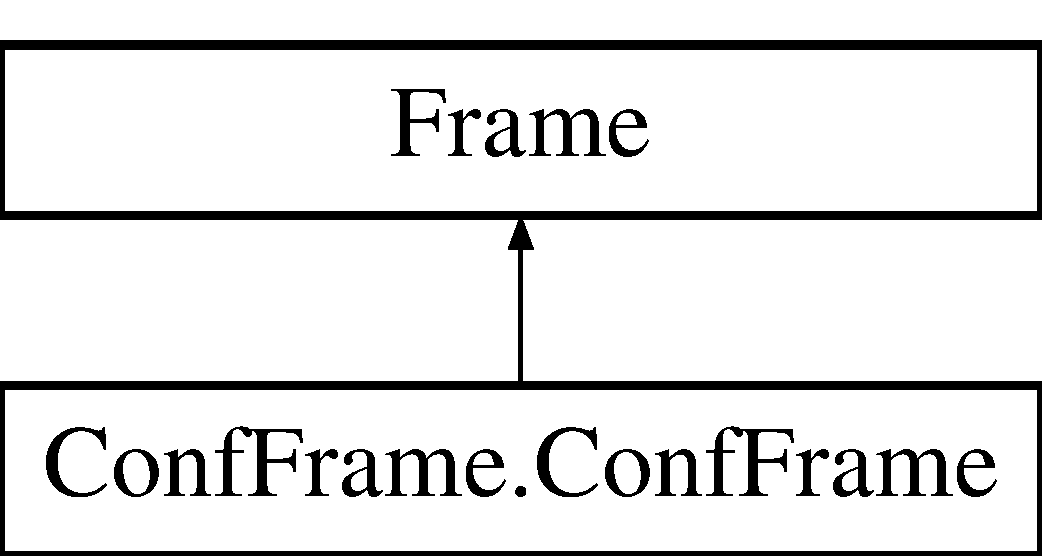
\includegraphics[height=2.000000cm]{classConfFrame_1_1ConfFrame}
\end{center}
\end{figure}
\subsection*{Public Member Functions}
\begin{DoxyCompactItemize}
\item 
def \hyperlink{classConfFrame_1_1ConfFrame_addff8c48a5ddb190fed5105a4f70ca95}{\+\_\+\+\_\+init\+\_\+\+\_\+} (self, \hyperlink{classConfFrame_1_1ConfFrame_a533aacde2742b806cb8e8161a5360796}{app}, \hyperlink{classConfFrame_1_1ConfFrame_a1943cba9d33cfcae85f83c0777150288}{parent}, title)
\item 
def \hyperlink{classConfFrame_1_1ConfFrame_ab41502e0a899a8632e507df007d2fed8}{get\+Control} (self, \hyperlink{classConfFrame_1_1ConfFrame_aaca068730fdc7eb3f4ba7847bbb82329}{panel}, xmlid)
\item 
def \hyperlink{classConfFrame_1_1ConfFrame_ace0a1296b1331409d28e0751101e31d3}{make\+Tool\+Bar} (self)
\item 
def \hyperlink{classConfFrame_1_1ConfFrame_a82cf80e649080f468ad4d4de1a2d6b9a}{on\+Idle} (self, event)
\item 
def \hyperlink{classConfFrame_1_1ConfFrame_ade9e2d205fbe79ecc809d80233323387}{on\+Iconize} (self, event)
\item 
def \hyperlink{classConfFrame_1_1ConfFrame_a1f922c19035b3f3a5039ee438c3d4e36}{on\+Change} (self, event)
\item 
def \hyperlink{classConfFrame_1_1ConfFrame_a3d39db586535191174d87bb5aac11a47}{on\+Re\+Load} (self, event)
\item 
def \hyperlink{classConfFrame_1_1ConfFrame_a15511ec80bb3c5ce4a99aeb78af41c15}{on\+Close} (self, event)
\item 
def \hyperlink{classConfFrame_1_1ConfFrame_a6dea964103ba882eafed2c8735ab0a07}{on\+Close\+All} (self, event)
\item 
def \hyperlink{classConfFrame_1_1ConfFrame_aaec4c61352cd88fbb16f230df55cc4bc}{on\+Edit} (self, obj, \hyperlink{classConfFrame_1_1ConfFrame_a1f47cd72745073b992e1ccee6d1190d7}{path}, type)
\item 
def \hyperlink{classConfFrame_1_1ConfFrame_a09edd8c77d7a902e321a6cdecc41a769}{update} (self)
\end{DoxyCompactItemize}
\subsection*{Public Attributes}
\begin{DoxyCompactItemize}
\item 
\hyperlink{classConfFrame_1_1ConfFrame_a1943cba9d33cfcae85f83c0777150288}{parent}
\item 
\hyperlink{classConfFrame_1_1ConfFrame_a533aacde2742b806cb8e8161a5360796}{app}
\item 
\hyperlink{classConfFrame_1_1ConfFrame_a1f47cd72745073b992e1ccee6d1190d7}{path}
\item 
\hyperlink{classConfFrame_1_1ConfFrame_aaca068730fdc7eb3f4ba7847bbb82329}{panel}
\item 
\hyperlink{classConfFrame_1_1ConfFrame_a0e2f293545e00f6762d635713f98942a}{notebook}
\item 
\hyperlink{classConfFrame_1_1ConfFrame_ae64b58d8e2f4dde0e65db414e4172d77}{panels}
\item 
\hyperlink{classConfFrame_1_1ConfFrame_a8d6caf98ca21d47a6e1988ed20f5a688}{objs}
\item 
\hyperlink{classConfFrame_1_1ConfFrame_a7fa64be7e4b3602d7b4ce881b87a0d5e}{paths}
\item 
\hyperlink{classConfFrame_1_1ConfFrame_a787b2c045a34b615b110e2cdf98c4c49}{wraps}
\item 
\hyperlink{classConfFrame_1_1ConfFrame_a253abaeccaa1d61319f723486bd3ab51}{confs}
\item 
\hyperlink{classConfFrame_1_1ConfFrame_ae34c2fb369a3a0b3cff4724f1c8e8a01}{tool\+Bar}
\end{DoxyCompactItemize}
\subsection*{Static Public Attributes}
\begin{DoxyCompactItemize}
\item 
string \hyperlink{classConfFrame_1_1ConfFrame_a65a5a2c5440955179d5b471875f1046d}{overview\+Text} = \char`\"{}C\+AT Configuration Window\char`\"{}
\end{DoxyCompactItemize}


\subsection{Detailed Description}


Definition at line 23 of file Conf\+Frame.\+py.



\subsection{Constructor \& Destructor Documentation}
\mbox{\Hypertarget{classConfFrame_1_1ConfFrame_addff8c48a5ddb190fed5105a4f70ca95}\label{classConfFrame_1_1ConfFrame_addff8c48a5ddb190fed5105a4f70ca95}} 
\index{Conf\+Frame\+::\+Conf\+Frame@{Conf\+Frame\+::\+Conf\+Frame}!\+\_\+\+\_\+init\+\_\+\+\_\+@{\+\_\+\+\_\+init\+\_\+\+\_\+}}
\index{\+\_\+\+\_\+init\+\_\+\+\_\+@{\+\_\+\+\_\+init\+\_\+\+\_\+}!Conf\+Frame\+::\+Conf\+Frame@{Conf\+Frame\+::\+Conf\+Frame}}
\subsubsection{\texorpdfstring{\+\_\+\+\_\+init\+\_\+\+\_\+()}{\_\_init\_\_()}}
{\footnotesize\ttfamily def Conf\+Frame.\+Conf\+Frame.\+\_\+\+\_\+init\+\_\+\+\_\+ (\begin{DoxyParamCaption}\item[{}]{self,  }\item[{}]{app,  }\item[{}]{parent,  }\item[{}]{title }\end{DoxyParamCaption})}



Definition at line 25 of file Conf\+Frame.\+py.


\begin{DoxyCode}
25     \textcolor{keyword}{def }\hyperlink{classwrapper_1_1ModuleDictWrapper_a9a7a794150502f51df687831583e13b9}{\_\_init\_\_}(self,app,parent,title): 
26         wx.Frame.\_\_init\_\_(self, parent, wx.NewId(), title)
27         self.parent=parent
28         self.app=app
29         self.path=os.path.join(os.environ.get(\textcolor{stringliteral}{"CATPATH"}), \textcolor{stringliteral}{"CatPython"}, \textcolor{stringliteral}{"python"})
30         self.makeToolBar()
31         res=xrc.XmlResource(os.path.join(self.path,\textcolor{stringliteral}{"xrc/ConfPanel.xrc"}))
32         self.panel=res.LoadPanel(self, \textcolor{stringliteral}{"ConfPanel"})
33 \textcolor{comment}{#        self.notebook=xrc.XRCCTRL(self, 'notebook')}
34         self.notebook=self.getControl(self.panel,\textcolor{stringliteral}{'notebook'})
35         self.panels=list()
36         self.objs=list()
37         self.paths=list()
38         self.wraps=list()
39         self.confs=list()
40         self.Bind(wx.EVT\_CLOSE, self.onIconize)
41         self.Bind(wx.EVT\_NOTEBOOK\_PAGE\_CHANGED, self.onChange)
42 
\end{DoxyCode}


\subsection{Member Function Documentation}
\mbox{\Hypertarget{classConfFrame_1_1ConfFrame_ab41502e0a899a8632e507df007d2fed8}\label{classConfFrame_1_1ConfFrame_ab41502e0a899a8632e507df007d2fed8}} 
\index{Conf\+Frame\+::\+Conf\+Frame@{Conf\+Frame\+::\+Conf\+Frame}!get\+Control@{get\+Control}}
\index{get\+Control@{get\+Control}!Conf\+Frame\+::\+Conf\+Frame@{Conf\+Frame\+::\+Conf\+Frame}}
\subsubsection{\texorpdfstring{get\+Control()}{getControl()}}
{\footnotesize\ttfamily def Conf\+Frame.\+Conf\+Frame.\+get\+Control (\begin{DoxyParamCaption}\item[{}]{self,  }\item[{}]{panel,  }\item[{}]{xmlid }\end{DoxyParamCaption})}

\begin{DoxyVerb}Retrieves the given control (within a dialog) by its xmlid\end{DoxyVerb}
 

Definition at line 43 of file Conf\+Frame.\+py.



Referenced by Proto40\+M\+Hz\+\_\+v1.\+Proto40\+M\+Hz\+\_\+v1.\+is\+Ready(), Proto\+F\+E\+B\+\_\+v1.\+Proto\+F\+E\+B\+\_\+v1.\+is\+Ready(), Acquisition.\+Acquisition.\+on\+Apply(), Proto40\+M\+Hz\+\_\+v1.\+Proto40\+M\+Hz\+\_\+v1.\+onapplyaxlatency(), Proto\+F\+E\+B\+\_\+v1.\+Proto\+F\+E\+B\+\_\+v1.\+onapplyaxlatency(), Proto\+F\+E\+B\+\_\+v1.\+Proto\+F\+E\+B\+\_\+v1.\+onapplyaxlength(), Proto40\+M\+Hz\+\_\+v1.\+Proto40\+M\+Hz\+\_\+v1.\+onapplyaxlength(), Proto\+F\+E\+B\+\_\+v1.\+Proto\+F\+E\+B\+\_\+v1.\+onapply\+Ch(), Proto40\+M\+Hz\+\_\+v1.\+Proto40\+M\+Hz\+\_\+v1.\+onapply\+Ch(), Proto40\+M\+Hz\+\_\+v1.\+Proto40\+M\+Hz\+\_\+v1.\+onapplyclockdiv(), Proto\+F\+E\+B\+\_\+v1.\+Proto\+F\+E\+B\+\_\+v1.\+onapplyclockdiv(), Proto40\+M\+Hz\+\_\+v1.\+Proto40\+M\+Hz\+\_\+v1.\+onapplydelay(), Proto\+F\+E\+B\+\_\+v1.\+Proto\+F\+E\+B\+\_\+v1.\+onapplydelay(), Proto40\+M\+Hz\+\_\+v1.\+Proto40\+M\+Hz\+\_\+v1.\+onapplyfifodepth(), Proto\+F\+E\+B\+\_\+v1.\+Proto\+F\+E\+B\+\_\+v1.\+onapplyfifodepth(), Proto40\+M\+Hz\+\_\+v1.\+Proto40\+M\+Hz\+\_\+v1.\+onapplyfreq(), Proto\+F\+E\+B\+\_\+v1.\+Proto\+F\+E\+B\+\_\+v1.\+onapplyfreq(), Proto40\+M\+Hz\+\_\+v1.\+Proto40\+M\+Hz\+\_\+v1.\+onapplynumber(), Proto\+F\+E\+B\+\_\+v1.\+Proto\+F\+E\+B\+\_\+v1.\+onapplynumber(), Proto\+F\+E\+B\+\_\+v1.\+Proto\+F\+E\+B\+\_\+v1.\+onapplytrig(), Proto40\+M\+Hz\+\_\+v1.\+Proto40\+M\+Hz\+\_\+v1.\+onapplytrig(), Acquisition.\+Acquisition.\+on\+Deadtime(), Acquisition.\+Acquisition.\+on\+Depth(), Proto40\+M\+Hz\+\_\+v1.\+Proto40\+M\+Hz\+\_\+v1.\+onenable\+All(), Proto\+F\+E\+B\+\_\+v1.\+Proto\+F\+E\+B\+\_\+v1.\+onenable\+All(), Acquisition.\+Acquisition.\+on\+Max(), Acquisition.\+Acquisition.\+on\+Min(), Proto40\+M\+Hz\+\_\+v1.\+Proto40\+M\+Hz\+\_\+v1.\+on\+Mode\+A\+X(), Proto\+F\+E\+B\+\_\+v1.\+Proto\+F\+E\+B\+\_\+v1.\+on\+Mode\+A\+X(), Proto\+F\+E\+B\+\_\+v1.\+Proto\+F\+E\+B\+\_\+v1.\+on\+Mode\+Ch(), Proto40\+M\+Hz\+\_\+v1.\+Proto40\+M\+Hz\+\_\+v1.\+on\+Mode\+Ch(), Acquisition.\+Acquisition.\+on\+N\+Bins(), Acquisition.\+Acquisition.\+on\+N\+Sample(), Proto\+F\+E\+B\+\_\+v1.\+Proto\+F\+E\+B\+\_\+v1.\+on\+Pipeline(), Proto40\+M\+Hz\+\_\+v1.\+Proto40\+M\+Hz\+\_\+v1.\+on\+Pipeline(), Acquisition.\+Acquisition.\+on\+Sample(), Acquisition.\+Acquisition.\+on\+Soft\+Trig(), Proto\+F\+E\+B\+\_\+v1.\+Proto\+F\+E\+B\+\_\+v1.\+on\+Soft\+Trig(), Proto40\+M\+Hz\+\_\+v1.\+Proto40\+M\+Hz\+\_\+v1.\+on\+Soft\+Trig(), Acquisition.\+Acquisition.\+on\+Tree(), Acquisition.\+Acquisition.\+on\+Trend(), Proto40\+M\+Hz\+\_\+v1.\+Proto40\+M\+Hz\+\_\+v1.\+onunable\+All(), Proto\+F\+E\+B\+\_\+v1.\+Proto\+F\+E\+B\+\_\+v1.\+onunable\+All(), element.\+element.\+parent(), proc.\+proc.\+parent(), Acquisition.\+Acquisition.\+update(), Proto\+F\+E\+B\+\_\+v1.\+Proto\+F\+E\+B\+\_\+v1.\+update(), and Proto40\+M\+Hz\+\_\+v1.\+Proto40\+M\+Hz\+\_\+v1.\+update().


\begin{DoxyCode}
43     \textcolor{keyword}{def }getControl(self, panel, xmlid):
44         \textcolor{stringliteral}{'''Retrieves the given control (within a dialog) by its xmlid'''}
45         control = panel.FindWindowById(xrc.XRCID(xmlid))
46         \textcolor{keyword}{assert} control != \textcolor{keywordtype}{None}, \textcolor{stringliteral}{'Programming error: a control with xml id '} + xmlid + \textcolor{stringliteral}{' was not found.'}
47         \textcolor{keywordflow}{return} control
48 
49         
\end{DoxyCode}
\mbox{\Hypertarget{classConfFrame_1_1ConfFrame_ace0a1296b1331409d28e0751101e31d3}\label{classConfFrame_1_1ConfFrame_ace0a1296b1331409d28e0751101e31d3}} 
\index{Conf\+Frame\+::\+Conf\+Frame@{Conf\+Frame\+::\+Conf\+Frame}!make\+Tool\+Bar@{make\+Tool\+Bar}}
\index{make\+Tool\+Bar@{make\+Tool\+Bar}!Conf\+Frame\+::\+Conf\+Frame@{Conf\+Frame\+::\+Conf\+Frame}}
\subsubsection{\texorpdfstring{make\+Tool\+Bar()}{makeToolBar()}}
{\footnotesize\ttfamily def Conf\+Frame.\+Conf\+Frame.\+make\+Tool\+Bar (\begin{DoxyParamCaption}\item[{}]{self }\end{DoxyParamCaption})}



Definition at line 50 of file Conf\+Frame.\+py.


\begin{DoxyCode}
50     \textcolor{keyword}{def }makeToolBar(self):
51         TB\_RELOAD=wx.NewId()
52         TB\_CLOSEALL=wx.NewId()
53         TB\_CLOSE=wx.NewId()
54         \textcolor{comment}{#}
55         self.toolBar = self.CreateToolBar(wx.TB\_DOCKABLE)
56         self.toolBar.AddLabelTool(TB\_CLOSEALL, \textcolor{stringliteral}{''}, wx.Bitmap(os.path.join(self.path,\textcolor{stringliteral}{"xrc/icons/closeall.png
      "})))
57         self.toolBar.AddLabelTool(TB\_CLOSE  , \textcolor{stringliteral}{''}, wx.Bitmap(os.path.join(self.path,\textcolor{stringliteral}{"xrc/icons/close.png"})))
58         self.toolBar.AddSeparator()        
59         self.toolBar.AddLabelTool(TB\_RELOAD, \textcolor{stringliteral}{''}, wx.Bitmap(os.path.join(self.path,\textcolor{stringliteral}{"xrc/icons/reload.png"})))
60         self.toolBar.Realize()
61         self.Bind(wx.EVT\_TOOL, self.onReLoad , id=TB\_RELOAD)
62         self.Bind(wx.EVT\_TOOL, self.onCloseAll , id=TB\_CLOSEALL)
63         self.Bind(wx.EVT\_TOOL, self.onClose , id=TB\_CLOSE)
64 
\end{DoxyCode}
\mbox{\Hypertarget{classConfFrame_1_1ConfFrame_a1f922c19035b3f3a5039ee438c3d4e36}\label{classConfFrame_1_1ConfFrame_a1f922c19035b3f3a5039ee438c3d4e36}} 
\index{Conf\+Frame\+::\+Conf\+Frame@{Conf\+Frame\+::\+Conf\+Frame}!on\+Change@{on\+Change}}
\index{on\+Change@{on\+Change}!Conf\+Frame\+::\+Conf\+Frame@{Conf\+Frame\+::\+Conf\+Frame}}
\subsubsection{\texorpdfstring{on\+Change()}{onChange()}}
{\footnotesize\ttfamily def Conf\+Frame.\+Conf\+Frame.\+on\+Change (\begin{DoxyParamCaption}\item[{}]{self,  }\item[{}]{event }\end{DoxyParamCaption})}



Definition at line 73 of file Conf\+Frame.\+py.



References Croc.\+Croc.\+update(), Computer.\+Computer.\+update(), A3\+P\+E\+\_\+\+Bit\+Flip.\+A3\+P\+E\+\_\+\+Bit\+Flip.\+update(), Emulate\+F\+E.\+Emulate\+F\+E.\+update(), Interface\+Wrap.\+update(), Element\+Wrap.\+update(), Proc\+Data\+Base.\+update(), Test\+I2\+C.\+Test\+I2\+C.\+update(), Test\+S\+P\+I.\+Test\+S\+P\+I.\+update(), Test\+U\+S\+B.\+Test\+U\+S\+B.\+update(), Storage\+Fifo\+Acquisition.\+Storage\+Fifo\+Acquisition.\+update(), Test\+Suite.\+Test\+Suite.\+update(), Storage\+Fifo.\+Storage\+Fifo.\+update(), A\+D\+C\+Measurement.\+Current\+Measurement.\+update(), Current\+Measurement.\+Current\+Measurement.\+update(), Usb\+F\+T\+Interface\+Test.\+Usb\+F\+T\+Interface\+Test.\+update(), Interface.\+update(), I\+Oobject.\+update(), Croc.\+update(), Usb\+I2c\+Bus.\+update(), Usb\+Spi\+Bus.\+update(), Usb\+M\+L\+I2c\+Bus.\+update(), Usb\+M\+L\+Spi\+Bus.\+update(), C\+U\+\_\+v1.\+update(), Proto40\+M\+Hz\+\_\+v1.\+update(), Element.\+update(), Computer.\+update(), F\+E\+B\+\_\+v1.\+update(), Seq\+P\+G\+A.\+update(), Acquisition.\+Acquisition.\+update(), N\+I6008.\+update(), Proto\+F\+E\+B\+\_\+v1.\+Proto\+F\+E\+B\+\_\+v1.\+update(), Proto40\+M\+Hz\+\_\+v1.\+Proto40\+M\+Hz\+\_\+v1.\+update(), Fe\+P\+G\+A.\+update(), Phaser.\+update(), Usb\+F\+T\+Interface.\+update(), Usb\+F\+T\+M\+L\+Interface.\+update(), Cfg\+Frame.\+Cfg\+Frame.\+update(), M\+S\+Oxxxx.\+update(), I\+C\+Phaser.\+update(), I\+C\+E\+C\+A\+Lv3.\+update(), Conf\+Frame.\+Conf\+Frame.\+update(), L\+S\+Delay\+Chip\+V1.\+update(), A3\+P\+E.\+update(), and App\+Frame.\+App\+Frame.\+update().


\begin{DoxyCode}
73     \textcolor{keyword}{def }onChange(self, event):
74         self.update()
75 
\end{DoxyCode}
\mbox{\Hypertarget{classConfFrame_1_1ConfFrame_a15511ec80bb3c5ce4a99aeb78af41c15}\label{classConfFrame_1_1ConfFrame_a15511ec80bb3c5ce4a99aeb78af41c15}} 
\index{Conf\+Frame\+::\+Conf\+Frame@{Conf\+Frame\+::\+Conf\+Frame}!on\+Close@{on\+Close}}
\index{on\+Close@{on\+Close}!Conf\+Frame\+::\+Conf\+Frame@{Conf\+Frame\+::\+Conf\+Frame}}
\subsubsection{\texorpdfstring{on\+Close()}{onClose()}}
{\footnotesize\ttfamily def Conf\+Frame.\+Conf\+Frame.\+on\+Close (\begin{DoxyParamCaption}\item[{}]{self,  }\item[{}]{event }\end{DoxyParamCaption})}



Definition at line 79 of file Conf\+Frame.\+py.



References Conf\+Frame.\+Conf\+Frame.\+confs, Conf\+Frame.\+Conf\+Frame.\+notebook, Conf\+Frame.\+Conf\+Frame.\+objs, App\+Frame.\+App\+Frame.\+objs, Conf\+Frame.\+Conf\+Frame.\+panels, Conf\+Frame.\+Conf\+Frame.\+paths, App\+Frame.\+App\+Frame.\+paths, and Conf\+Frame.\+Conf\+Frame.\+wraps.


\begin{DoxyCode}
79     \textcolor{keyword}{def }onClose(self, event):
80         pos=self.notebook.GetSelection()
81         self.notebook.DeletePage(pos)
82         self.panels.pop(pos)
83         self.objs.pop(pos)
84         self.paths.pop(pos)
85         self.wraps.pop(pos)
86         self.confs.pop(pos)
87 
\end{DoxyCode}
\mbox{\Hypertarget{classConfFrame_1_1ConfFrame_a6dea964103ba882eafed2c8735ab0a07}\label{classConfFrame_1_1ConfFrame_a6dea964103ba882eafed2c8735ab0a07}} 
\index{Conf\+Frame\+::\+Conf\+Frame@{Conf\+Frame\+::\+Conf\+Frame}!on\+Close\+All@{on\+Close\+All}}
\index{on\+Close\+All@{on\+Close\+All}!Conf\+Frame\+::\+Conf\+Frame@{Conf\+Frame\+::\+Conf\+Frame}}
\subsubsection{\texorpdfstring{on\+Close\+All()}{onCloseAll()}}
{\footnotesize\ttfamily def Conf\+Frame.\+Conf\+Frame.\+on\+Close\+All (\begin{DoxyParamCaption}\item[{}]{self,  }\item[{}]{event }\end{DoxyParamCaption})}



Definition at line 88 of file Conf\+Frame.\+py.



References Conf\+Frame.\+Conf\+Frame.\+confs, Conf\+Frame.\+Conf\+Frame.\+notebook, Conf\+Frame.\+Conf\+Frame.\+objs, App\+Frame.\+App\+Frame.\+objs, Conf\+Frame.\+Conf\+Frame.\+panels, Conf\+Frame.\+Conf\+Frame.\+paths, App\+Frame.\+App\+Frame.\+paths, and Conf\+Frame.\+Conf\+Frame.\+wraps.


\begin{DoxyCode}
88     \textcolor{keyword}{def }onCloseAll(self, event):
89         self.notebook.DeleteAllPages()
90         self.panels=[]
91         self.objs =[]
92         self.paths=[]
93         self.wraps=[]
94         self.confs=[]
95 
\end{DoxyCode}
\mbox{\Hypertarget{classConfFrame_1_1ConfFrame_aaec4c61352cd88fbb16f230df55cc4bc}\label{classConfFrame_1_1ConfFrame_aaec4c61352cd88fbb16f230df55cc4bc}} 
\index{Conf\+Frame\+::\+Conf\+Frame@{Conf\+Frame\+::\+Conf\+Frame}!on\+Edit@{on\+Edit}}
\index{on\+Edit@{on\+Edit}!Conf\+Frame\+::\+Conf\+Frame@{Conf\+Frame\+::\+Conf\+Frame}}
\subsubsection{\texorpdfstring{on\+Edit()}{onEdit()}}
{\footnotesize\ttfamily def Conf\+Frame.\+Conf\+Frame.\+on\+Edit (\begin{DoxyParamCaption}\item[{}]{self,  }\item[{}]{obj,  }\item[{}]{path,  }\item[{}]{type }\end{DoxyParamCaption})}



Definition at line 96 of file Conf\+Frame.\+py.



References Cfg\+Frame.\+Cfg\+Frame.\+app, Conf\+Frame.\+Conf\+Frame.\+app, Conf\+Frame.\+Conf\+Frame.\+confs, Conf\+Frame.\+Conf\+Frame.\+notebook, Conf\+Frame.\+Conf\+Frame.\+objs, App\+Frame.\+App\+Frame.\+objs, Conf\+Frame.\+Conf\+Frame.\+panels, Conf\+Frame.\+Conf\+Frame.\+paths, App\+Frame.\+App\+Frame.\+paths, Croc.\+Croc.\+update(), Computer.\+Computer.\+update(), A3\+P\+E\+\_\+\+Bit\+Flip.\+A3\+P\+E\+\_\+\+Bit\+Flip.\+update(), Emulate\+F\+E.\+Emulate\+F\+E.\+update(), Interface\+Wrap.\+update(), Element\+Wrap.\+update(), Proc\+Data\+Base.\+update(), Test\+U\+S\+B.\+Test\+U\+S\+B.\+update(), Test\+I2\+C.\+Test\+I2\+C.\+update(), Test\+S\+P\+I.\+Test\+S\+P\+I.\+update(), Test\+Suite.\+Test\+Suite.\+update(), Storage\+Fifo.\+Storage\+Fifo.\+update(), Storage\+Fifo\+Acquisition.\+Storage\+Fifo\+Acquisition.\+update(), Current\+Measurement.\+Current\+Measurement.\+update(), A\+D\+C\+Measurement.\+Current\+Measurement.\+update(), Usb\+F\+T\+Interface\+Test.\+Usb\+F\+T\+Interface\+Test.\+update(), Interface.\+update(), I\+Oobject.\+update(), Croc.\+update(), Usb\+I2c\+Bus.\+update(), Usb\+Spi\+Bus.\+update(), Usb\+M\+L\+Spi\+Bus.\+update(), Usb\+M\+L\+I2c\+Bus.\+update(), C\+U\+\_\+v1.\+update(), Proto40\+M\+Hz\+\_\+v1.\+update(), Element.\+update(), Computer.\+update(), F\+E\+B\+\_\+v1.\+update(), Seq\+P\+G\+A.\+update(), Acquisition.\+Acquisition.\+update(), N\+I6008.\+update(), Proto\+F\+E\+B\+\_\+v1.\+Proto\+F\+E\+B\+\_\+v1.\+update(), Proto40\+M\+Hz\+\_\+v1.\+Proto40\+M\+Hz\+\_\+v1.\+update(), Fe\+P\+G\+A.\+update(), Phaser.\+update(), Usb\+F\+T\+Interface.\+update(), Usb\+F\+T\+M\+L\+Interface.\+update(), Cfg\+Frame.\+Cfg\+Frame.\+update(), M\+S\+Oxxxx.\+update(), I\+C\+Phaser.\+update(), I\+C\+E\+C\+A\+Lv3.\+update(), Conf\+Frame.\+Conf\+Frame.\+update(), L\+S\+Delay\+Chip\+V1.\+update(), A3\+P\+E.\+update(), App\+Frame.\+App\+Frame.\+update(), and Conf\+Frame.\+Conf\+Frame.\+wraps.


\begin{DoxyCode}
96     \textcolor{keyword}{def }onEdit(self, obj, path, type):
97         objpanel=-1
98         \textcolor{keywordflow}{for} i \textcolor{keywordflow}{in} range(len(self.objs)):
99             \textcolor{keywordflow}{if} path==self.paths[i]:
100                 objpanel=i
101         \textcolor{keywordflow}{if} objpanel!=-1:
102             self.notebook.SetSelection(objpanel)
103             self.update()
104         \textcolor{keywordflow}{else}:
105 \textcolor{comment}{#            if (type=='element'):}
106 \textcolor{comment}{#                res=xrc.XmlResource(os.path.join(self.path,"xrc/ElementMain.xrc"))}
107 \textcolor{comment}{#            elif (type=='proc'):}
108 \textcolor{comment}{#                res=xrc.XmlResource(os.path.join(self.path,"xrc/ProcMain.xrc"))}
109             \textcolor{comment}{#panel=res.LoadPanel(self.notebook,"NotebookId")}
110             \textcolor{comment}{#self.panels.append(panel)}
111             self.objs.append(obj)
112             self.paths.append(path)
113             wrap=\hyperlink{namespacewrapper}{wrapper}(self.app,obj,type)
114             self.wraps.append(wrap)
115 \textcolor{comment}{#            }
116 \textcolor{comment}{#            if (type=='element'):}
117 \textcolor{comment}{#                namectrl=self.getControl(panel,'ObjName')}
118 \textcolor{comment}{#                pathctrl=self.getControl(panel,'ObjPath')}
119 \textcolor{comment}{#                namectrl.SetValue(obj.name())}
120 \textcolor{comment}{#                pathctrl.SetValue(path)}
121 \textcolor{comment}{#            elif (type=='proc'):}
122 \textcolor{comment}{#                namectrl=self.getControl(panel,'ProcName')}
123 \textcolor{comment}{#                pathctrl=self.getControl(panel,'ProcPath')}
124 \textcolor{comment}{#                namectrl.SetValue(obj.name())}
125 \textcolor{comment}{#                pathctrl.SetValue(obj.type())}
126             module=wrap.GetActive()
127             panel=module.Edit(self.app,obj,self.notebook,wrap.GetFilePath())
128             self.panels.append(panel)
129             self.confs.append(panel)
130             self.notebook.AddPage(panel.page(),obj.name(),\textcolor{keyword}{True})
131 \textcolor{comment}{#            self.notebook.Fit()}
132 \textcolor{comment}{#            self.notebook.SetSize(self.GetSize())}
133             self.Layout()
134 \textcolor{comment}{#            panel.Fit()}
135 \textcolor{comment}{#            print "panel size=",panel.GetSize()}
136 \textcolor{comment}{#            print "notebook size=",self.notebook.GetSize()}
137             
\end{DoxyCode}
\mbox{\Hypertarget{classConfFrame_1_1ConfFrame_ade9e2d205fbe79ecc809d80233323387}\label{classConfFrame_1_1ConfFrame_ade9e2d205fbe79ecc809d80233323387}} 
\index{Conf\+Frame\+::\+Conf\+Frame@{Conf\+Frame\+::\+Conf\+Frame}!on\+Iconize@{on\+Iconize}}
\index{on\+Iconize@{on\+Iconize}!Conf\+Frame\+::\+Conf\+Frame@{Conf\+Frame\+::\+Conf\+Frame}}
\subsubsection{\texorpdfstring{on\+Iconize()}{onIconize()}}
{\footnotesize\ttfamily def Conf\+Frame.\+Conf\+Frame.\+on\+Iconize (\begin{DoxyParamCaption}\item[{}]{self,  }\item[{}]{event }\end{DoxyParamCaption})}



Definition at line 69 of file Conf\+Frame.\+py.


\begin{DoxyCode}
69     \textcolor{keyword}{def }onIconize(self, event):
70         self.parent.cfgFrame.Show(\textcolor{keyword}{False})
71         self.parent.cfgState=\textcolor{keyword}{False}
72 
\end{DoxyCode}
\mbox{\Hypertarget{classConfFrame_1_1ConfFrame_a82cf80e649080f468ad4d4de1a2d6b9a}\label{classConfFrame_1_1ConfFrame_a82cf80e649080f468ad4d4de1a2d6b9a}} 
\index{Conf\+Frame\+::\+Conf\+Frame@{Conf\+Frame\+::\+Conf\+Frame}!on\+Idle@{on\+Idle}}
\index{on\+Idle@{on\+Idle}!Conf\+Frame\+::\+Conf\+Frame@{Conf\+Frame\+::\+Conf\+Frame}}
\subsubsection{\texorpdfstring{on\+Idle()}{onIdle()}}
{\footnotesize\ttfamily def Conf\+Frame.\+Conf\+Frame.\+on\+Idle (\begin{DoxyParamCaption}\item[{}]{self,  }\item[{}]{event }\end{DoxyParamCaption})}

\begin{DoxyVerb}Responds to idle time in the system\end{DoxyVerb}
 

Definition at line 65 of file Conf\+Frame.\+py.


\begin{DoxyCode}
65     \textcolor{keyword}{def }onIdle(self, event):
66         \textcolor{stringliteral}{'''Responds to idle time in the system'''}
67         \textcolor{comment}{# when the timer says it's time, we do the actual downloading in the main thread (wx doesn't work
       well in secondary threads)}
68 
\end{DoxyCode}
\mbox{\Hypertarget{classConfFrame_1_1ConfFrame_a3d39db586535191174d87bb5aac11a47}\label{classConfFrame_1_1ConfFrame_a3d39db586535191174d87bb5aac11a47}} 
\index{Conf\+Frame\+::\+Conf\+Frame@{Conf\+Frame\+::\+Conf\+Frame}!on\+Re\+Load@{on\+Re\+Load}}
\index{on\+Re\+Load@{on\+Re\+Load}!Conf\+Frame\+::\+Conf\+Frame@{Conf\+Frame\+::\+Conf\+Frame}}
\subsubsection{\texorpdfstring{on\+Re\+Load()}{onReLoad()}}
{\footnotesize\ttfamily def Conf\+Frame.\+Conf\+Frame.\+on\+Re\+Load (\begin{DoxyParamCaption}\item[{}]{self,  }\item[{}]{event }\end{DoxyParamCaption})}



Definition at line 76 of file Conf\+Frame.\+py.



References Croc.\+Croc.\+update(), Computer.\+Computer.\+update(), A3\+P\+E\+\_\+\+Bit\+Flip.\+A3\+P\+E\+\_\+\+Bit\+Flip.\+update(), Emulate\+F\+E.\+Emulate\+F\+E.\+update(), Interface\+Wrap.\+update(), Element\+Wrap.\+update(), Proc\+Data\+Base.\+update(), Test\+I2\+C.\+Test\+I2\+C.\+update(), Test\+S\+P\+I.\+Test\+S\+P\+I.\+update(), Test\+U\+S\+B.\+Test\+U\+S\+B.\+update(), Storage\+Fifo\+Acquisition.\+Storage\+Fifo\+Acquisition.\+update(), Test\+Suite.\+Test\+Suite.\+update(), Storage\+Fifo.\+Storage\+Fifo.\+update(), A\+D\+C\+Measurement.\+Current\+Measurement.\+update(), Current\+Measurement.\+Current\+Measurement.\+update(), Usb\+F\+T\+Interface\+Test.\+Usb\+F\+T\+Interface\+Test.\+update(), Interface.\+update(), I\+Oobject.\+update(), Croc.\+update(), Usb\+I2c\+Bus.\+update(), Usb\+Spi\+Bus.\+update(), Usb\+M\+L\+I2c\+Bus.\+update(), Usb\+M\+L\+Spi\+Bus.\+update(), C\+U\+\_\+v1.\+update(), Proto40\+M\+Hz\+\_\+v1.\+update(), Element.\+update(), Computer.\+update(), F\+E\+B\+\_\+v1.\+update(), Seq\+P\+G\+A.\+update(), Acquisition.\+Acquisition.\+update(), N\+I6008.\+update(), Proto\+F\+E\+B\+\_\+v1.\+Proto\+F\+E\+B\+\_\+v1.\+update(), Proto40\+M\+Hz\+\_\+v1.\+Proto40\+M\+Hz\+\_\+v1.\+update(), Fe\+P\+G\+A.\+update(), Phaser.\+update(), Usb\+F\+T\+Interface.\+update(), Usb\+F\+T\+M\+L\+Interface.\+update(), Cfg\+Frame.\+Cfg\+Frame.\+update(), M\+S\+Oxxxx.\+update(), I\+C\+Phaser.\+update(), I\+C\+E\+C\+A\+Lv3.\+update(), Conf\+Frame.\+Conf\+Frame.\+update(), L\+S\+Delay\+Chip\+V1.\+update(), A3\+P\+E.\+update(), and App\+Frame.\+App\+Frame.\+update().


\begin{DoxyCode}
76     \textcolor{keyword}{def }onReLoad(self, event):
77         self.update()
78 
\end{DoxyCode}
\mbox{\Hypertarget{classConfFrame_1_1ConfFrame_a09edd8c77d7a902e321a6cdecc41a769}\label{classConfFrame_1_1ConfFrame_a09edd8c77d7a902e321a6cdecc41a769}} 
\index{Conf\+Frame\+::\+Conf\+Frame@{Conf\+Frame\+::\+Conf\+Frame}!update@{update}}
\index{update@{update}!Conf\+Frame\+::\+Conf\+Frame@{Conf\+Frame\+::\+Conf\+Frame}}
\subsubsection{\texorpdfstring{update()}{update()}}
{\footnotesize\ttfamily def Conf\+Frame.\+Conf\+Frame.\+update (\begin{DoxyParamCaption}\item[{}]{self }\end{DoxyParamCaption})}



Definition at line 138 of file Conf\+Frame.\+py.



References Conf\+Frame.\+Conf\+Frame.\+notebook, and Conf\+Frame.\+Conf\+Frame.\+panels.



Referenced by Conf\+Frame.\+Conf\+Frame.\+on\+Change(), Graph\+Frame.\+Graph\+Frame.\+on\+Change(), Conf\+Frame.\+Conf\+Frame.\+on\+Edit(), Conf\+Frame.\+Conf\+Frame.\+on\+Re\+Load(), and Graph\+Frame.\+Graph\+Frame.\+on\+Re\+Load().


\begin{DoxyCode}
138     \textcolor{keyword}{def }update(self):
139         pos=self.notebook.GetSelection()
140         self.panels[pos].update()
141         
142 \textcolor{comment}{#----------------------------------------------------------------------------}
143 
144 
145 
146 \end{DoxyCode}


\subsection{Member Data Documentation}
\mbox{\Hypertarget{classConfFrame_1_1ConfFrame_a533aacde2742b806cb8e8161a5360796}\label{classConfFrame_1_1ConfFrame_a533aacde2742b806cb8e8161a5360796}} 
\index{Conf\+Frame\+::\+Conf\+Frame@{Conf\+Frame\+::\+Conf\+Frame}!app@{app}}
\index{app@{app}!Conf\+Frame\+::\+Conf\+Frame@{Conf\+Frame\+::\+Conf\+Frame}}
\subsubsection{\texorpdfstring{app}{app}}
{\footnotesize\ttfamily Conf\+Frame.\+Conf\+Frame.\+app}



Definition at line 28 of file Conf\+Frame.\+py.



Referenced by Conf\+Frame.\+Conf\+Frame.\+on\+Edit(), and Graph\+Frame.\+Graph\+Frame.\+on\+Plot().

\mbox{\Hypertarget{classConfFrame_1_1ConfFrame_a253abaeccaa1d61319f723486bd3ab51}\label{classConfFrame_1_1ConfFrame_a253abaeccaa1d61319f723486bd3ab51}} 
\index{Conf\+Frame\+::\+Conf\+Frame@{Conf\+Frame\+::\+Conf\+Frame}!confs@{confs}}
\index{confs@{confs}!Conf\+Frame\+::\+Conf\+Frame@{Conf\+Frame\+::\+Conf\+Frame}}
\subsubsection{\texorpdfstring{confs}{confs}}
{\footnotesize\ttfamily Conf\+Frame.\+Conf\+Frame.\+confs}



Definition at line 39 of file Conf\+Frame.\+py.



Referenced by Conf\+Frame.\+Conf\+Frame.\+on\+Close(), Conf\+Frame.\+Conf\+Frame.\+on\+Close\+All(), and Conf\+Frame.\+Conf\+Frame.\+on\+Edit().

\mbox{\Hypertarget{classConfFrame_1_1ConfFrame_a0e2f293545e00f6762d635713f98942a}\label{classConfFrame_1_1ConfFrame_a0e2f293545e00f6762d635713f98942a}} 
\index{Conf\+Frame\+::\+Conf\+Frame@{Conf\+Frame\+::\+Conf\+Frame}!notebook@{notebook}}
\index{notebook@{notebook}!Conf\+Frame\+::\+Conf\+Frame@{Conf\+Frame\+::\+Conf\+Frame}}
\subsubsection{\texorpdfstring{notebook}{notebook}}
{\footnotesize\ttfamily Conf\+Frame.\+Conf\+Frame.\+notebook}



Definition at line 34 of file Conf\+Frame.\+py.



Referenced by Conf\+Frame.\+Conf\+Frame.\+on\+Close(), Graph\+Frame.\+Graph\+Frame.\+on\+Close(), Conf\+Frame.\+Conf\+Frame.\+on\+Close\+All(), Graph\+Frame.\+Graph\+Frame.\+on\+Close\+All(), Conf\+Frame.\+Conf\+Frame.\+on\+Edit(), Graph\+Frame.\+Graph\+Frame.\+on\+Plot(), Graph\+Frame.\+Graph\+Frame.\+on\+Re\+Load(), Graph\+Frame.\+Graph\+Frame.\+update(), and Conf\+Frame.\+Conf\+Frame.\+update().

\mbox{\Hypertarget{classConfFrame_1_1ConfFrame_a8d6caf98ca21d47a6e1988ed20f5a688}\label{classConfFrame_1_1ConfFrame_a8d6caf98ca21d47a6e1988ed20f5a688}} 
\index{Conf\+Frame\+::\+Conf\+Frame@{Conf\+Frame\+::\+Conf\+Frame}!objs@{objs}}
\index{objs@{objs}!Conf\+Frame\+::\+Conf\+Frame@{Conf\+Frame\+::\+Conf\+Frame}}
\subsubsection{\texorpdfstring{objs}{objs}}
{\footnotesize\ttfamily Conf\+Frame.\+Conf\+Frame.\+objs}



Definition at line 36 of file Conf\+Frame.\+py.



Referenced by Conf\+Frame.\+Conf\+Frame.\+on\+Close(), Graph\+Frame.\+Graph\+Frame.\+on\+Close(), Conf\+Frame.\+Conf\+Frame.\+on\+Close\+All(), Graph\+Frame.\+Graph\+Frame.\+on\+Close\+All(), Conf\+Frame.\+Conf\+Frame.\+on\+Edit(), and Graph\+Frame.\+Graph\+Frame.\+on\+Plot().

\mbox{\Hypertarget{classConfFrame_1_1ConfFrame_a65a5a2c5440955179d5b471875f1046d}\label{classConfFrame_1_1ConfFrame_a65a5a2c5440955179d5b471875f1046d}} 
\index{Conf\+Frame\+::\+Conf\+Frame@{Conf\+Frame\+::\+Conf\+Frame}!overview\+Text@{overview\+Text}}
\index{overview\+Text@{overview\+Text}!Conf\+Frame\+::\+Conf\+Frame@{Conf\+Frame\+::\+Conf\+Frame}}
\subsubsection{\texorpdfstring{overview\+Text}{overviewText}}
{\footnotesize\ttfamily string Conf\+Frame.\+Conf\+Frame.\+overview\+Text = \char`\"{}C\+AT Configuration Window\char`\"{}\hspace{0.3cm}{\ttfamily [static]}}



Definition at line 24 of file Conf\+Frame.\+py.

\mbox{\Hypertarget{classConfFrame_1_1ConfFrame_aaca068730fdc7eb3f4ba7847bbb82329}\label{classConfFrame_1_1ConfFrame_aaca068730fdc7eb3f4ba7847bbb82329}} 
\index{Conf\+Frame\+::\+Conf\+Frame@{Conf\+Frame\+::\+Conf\+Frame}!panel@{panel}}
\index{panel@{panel}!Conf\+Frame\+::\+Conf\+Frame@{Conf\+Frame\+::\+Conf\+Frame}}
\subsubsection{\texorpdfstring{panel}{panel}}
{\footnotesize\ttfamily Conf\+Frame.\+Conf\+Frame.\+panel}



Definition at line 32 of file Conf\+Frame.\+py.



Referenced by A3\+P\+E\+\_\+\+Bit\+Flip.\+A3\+P\+E\+\_\+\+Bit\+Flip.\+\_\+\+\_\+init\+\_\+\+\_\+(), Acquisition.\+Acquisition.\+\_\+\+\_\+init\+\_\+\+\_\+(), Emulate\+F\+E.\+Emulate\+F\+E.\+\_\+\+\_\+init\+\_\+\+\_\+(), object.\+object.\+get\+Control(), Proto40\+M\+Hz\+\_\+v1.\+Proto40\+M\+Hz\+\_\+v1.\+get\+File(), Proto\+F\+E\+B\+\_\+v1.\+Proto\+F\+E\+B\+\_\+v1.\+get\+File(), element.\+element.\+page(), and proc.\+proc.\+page().

\mbox{\Hypertarget{classConfFrame_1_1ConfFrame_ae64b58d8e2f4dde0e65db414e4172d77}\label{classConfFrame_1_1ConfFrame_ae64b58d8e2f4dde0e65db414e4172d77}} 
\index{Conf\+Frame\+::\+Conf\+Frame@{Conf\+Frame\+::\+Conf\+Frame}!panels@{panels}}
\index{panels@{panels}!Conf\+Frame\+::\+Conf\+Frame@{Conf\+Frame\+::\+Conf\+Frame}}
\subsubsection{\texorpdfstring{panels}{panels}}
{\footnotesize\ttfamily Conf\+Frame.\+Conf\+Frame.\+panels}



Definition at line 35 of file Conf\+Frame.\+py.



Referenced by Conf\+Frame.\+Conf\+Frame.\+on\+Close(), Graph\+Frame.\+Graph\+Frame.\+on\+Close(), Conf\+Frame.\+Conf\+Frame.\+on\+Close\+All(), Graph\+Frame.\+Graph\+Frame.\+on\+Close\+All(), Conf\+Frame.\+Conf\+Frame.\+on\+Edit(), Graph\+Frame.\+Graph\+Frame.\+on\+Plot(), and Conf\+Frame.\+Conf\+Frame.\+update().

\mbox{\Hypertarget{classConfFrame_1_1ConfFrame_a1943cba9d33cfcae85f83c0777150288}\label{classConfFrame_1_1ConfFrame_a1943cba9d33cfcae85f83c0777150288}} 
\index{Conf\+Frame\+::\+Conf\+Frame@{Conf\+Frame\+::\+Conf\+Frame}!parent@{parent}}
\index{parent@{parent}!Conf\+Frame\+::\+Conf\+Frame@{Conf\+Frame\+::\+Conf\+Frame}}
\subsubsection{\texorpdfstring{parent}{parent}}
{\footnotesize\ttfamily Conf\+Frame.\+Conf\+Frame.\+parent}



Definition at line 27 of file Conf\+Frame.\+py.



Referenced by Graph\+Frame.\+Graph\+Frame.\+on\+Iconize().

\mbox{\Hypertarget{classConfFrame_1_1ConfFrame_a1f47cd72745073b992e1ccee6d1190d7}\label{classConfFrame_1_1ConfFrame_a1f47cd72745073b992e1ccee6d1190d7}} 
\index{Conf\+Frame\+::\+Conf\+Frame@{Conf\+Frame\+::\+Conf\+Frame}!path@{path}}
\index{path@{path}!Conf\+Frame\+::\+Conf\+Frame@{Conf\+Frame\+::\+Conf\+Frame}}
\subsubsection{\texorpdfstring{path}{path}}
{\footnotesize\ttfamily Conf\+Frame.\+Conf\+Frame.\+path}



Definition at line 29 of file Conf\+Frame.\+py.



Referenced by element.\+element.\+loadxrc(), and proc.\+proc.\+loadxrc().

\mbox{\Hypertarget{classConfFrame_1_1ConfFrame_a7fa64be7e4b3602d7b4ce881b87a0d5e}\label{classConfFrame_1_1ConfFrame_a7fa64be7e4b3602d7b4ce881b87a0d5e}} 
\index{Conf\+Frame\+::\+Conf\+Frame@{Conf\+Frame\+::\+Conf\+Frame}!paths@{paths}}
\index{paths@{paths}!Conf\+Frame\+::\+Conf\+Frame@{Conf\+Frame\+::\+Conf\+Frame}}
\subsubsection{\texorpdfstring{paths}{paths}}
{\footnotesize\ttfamily Conf\+Frame.\+Conf\+Frame.\+paths}



Definition at line 37 of file Conf\+Frame.\+py.



Referenced by Conf\+Frame.\+Conf\+Frame.\+on\+Close(), Conf\+Frame.\+Conf\+Frame.\+on\+Close\+All(), and Conf\+Frame.\+Conf\+Frame.\+on\+Edit().

\mbox{\Hypertarget{classConfFrame_1_1ConfFrame_ae34c2fb369a3a0b3cff4724f1c8e8a01}\label{classConfFrame_1_1ConfFrame_ae34c2fb369a3a0b3cff4724f1c8e8a01}} 
\index{Conf\+Frame\+::\+Conf\+Frame@{Conf\+Frame\+::\+Conf\+Frame}!tool\+Bar@{tool\+Bar}}
\index{tool\+Bar@{tool\+Bar}!Conf\+Frame\+::\+Conf\+Frame@{Conf\+Frame\+::\+Conf\+Frame}}
\subsubsection{\texorpdfstring{tool\+Bar}{toolBar}}
{\footnotesize\ttfamily Conf\+Frame.\+Conf\+Frame.\+tool\+Bar}



Definition at line 55 of file Conf\+Frame.\+py.

\mbox{\Hypertarget{classConfFrame_1_1ConfFrame_a787b2c045a34b615b110e2cdf98c4c49}\label{classConfFrame_1_1ConfFrame_a787b2c045a34b615b110e2cdf98c4c49}} 
\index{Conf\+Frame\+::\+Conf\+Frame@{Conf\+Frame\+::\+Conf\+Frame}!wraps@{wraps}}
\index{wraps@{wraps}!Conf\+Frame\+::\+Conf\+Frame@{Conf\+Frame\+::\+Conf\+Frame}}
\subsubsection{\texorpdfstring{wraps}{wraps}}
{\footnotesize\ttfamily Conf\+Frame.\+Conf\+Frame.\+wraps}



Definition at line 38 of file Conf\+Frame.\+py.



Referenced by Conf\+Frame.\+Conf\+Frame.\+on\+Close(), Conf\+Frame.\+Conf\+Frame.\+on\+Close\+All(), and Conf\+Frame.\+Conf\+Frame.\+on\+Edit().



The documentation for this class was generated from the following file\+:\begin{DoxyCompactItemize}
\item 
/home/eleclhcb/\+L\+H\+Cb/lbcat-\/cmake/\+Cat\+Python/python/\hyperlink{ConfFrame_8py}{Conf\+Frame.\+py}\end{DoxyCompactItemize}

\hypertarget{classConfig}{
\section{Config Class Reference}
\label{classConfig}\index{Config@{Config}}
}


{\ttfamily \#include $<$Application.h$>$}\subsection*{Public Attributes}
\begin{DoxyCompactItemize}
\item 
char \hyperlink{classConfig_a4f977190294b342f444cacd04f0e909b}{config} \mbox{[}10000\mbox{]}
\end{DoxyCompactItemize}


\subsection{Detailed Description}


Definition at line 47 of file Application.h.

\subsection{Member Data Documentation}
\hypertarget{classConfig_a4f977190294b342f444cacd04f0e909b}{
\index{Config@{Config}!config@{config}}
\index{config@{config}!Config@{Config}}
\subsubsection[{config}]{\setlength{\rightskip}{0pt plus 5cm}char {\bf Config::config}\mbox{[}10000\mbox{]}}}
\label{classConfig_a4f977190294b342f444cacd04f0e909b}


Definition at line 49 of file Application.h.

Referenced by Application::setConfig().

The documentation for this class was generated from the following file:\begin{DoxyCompactItemize}
\item 
/home/eleclhcb/LHCb/lbcat-\/cmake/CatKernel/inc/\hyperlink{Application_8h}{Application.h}\end{DoxyCompactItemize}

\hypertarget{structconfRegData}{}\section{conf\+Reg\+Data Struct Reference}
\label{structconfRegData}\index{conf\+Reg\+Data@{conf\+Reg\+Data}}


{\ttfamily \#include $<$L\+S\+Delay\+Chip\+V1.\+h$>$}

\subsection*{Public Attributes}
\begin{DoxyCompactItemize}
\item 
bool \hyperlink{structconfRegData_a709d8d691ef0c8ea5c4c03aac3d851f1}{lvds\+Out\+En}
\item 
bool \hyperlink{structconfRegData_a62f72429bde3ede255f6d8dfe1401c37}{n\+V\+Control\+En}
\item 
bool \hyperlink{structconfRegData_a4e98d082c44e34995224bd242da493d0}{pad\+Debug}
\item 
\hyperlink{ICECALv3_8h_a3cb25ca6f51f003950f9625ff05536fc}{U8} \hyperlink{structconfRegData_aee4fd08aceaaf19fcb8edfe8aa50f5ab}{phase\+Int}
\item 
\hyperlink{ICECALv3_8h_a3cb25ca6f51f003950f9625ff05536fc}{U8} \hyperlink{structconfRegData_a2e471f30b32e57270cb2edb0e420cf1b}{phase\+Ta\+H\+Adc}
\item 
\hyperlink{ICECALv3_8h_a3cb25ca6f51f003950f9625ff05536fc}{U8} \hyperlink{structconfRegData_a0ed9976dd55237ee70ba3621b0f4f58c}{locus}
\end{DoxyCompactItemize}


\subsection{Detailed Description}


Definition at line 45 of file L\+S\+Delay\+Chip\+V1.\+h.



\subsection{Member Data Documentation}
\mbox{\Hypertarget{structconfRegData_a0ed9976dd55237ee70ba3621b0f4f58c}\label{structconfRegData_a0ed9976dd55237ee70ba3621b0f4f58c}} 
\index{conf\+Reg\+Data@{conf\+Reg\+Data}!locus@{locus}}
\index{locus@{locus}!conf\+Reg\+Data@{conf\+Reg\+Data}}
\subsubsection{\texorpdfstring{locus}{locus}}
{\footnotesize\ttfamily \hyperlink{ICECALv3_8h_a3cb25ca6f51f003950f9625ff05536fc}{U8} conf\+Reg\+Data\+::locus}



Definition at line 51 of file L\+S\+Delay\+Chip\+V1.\+h.



Referenced by L\+S\+Delay\+Chip\+V1\+::get\+Config\+Reg(), L\+S\+Delay\+Chip\+V1\+::\+L\+S\+Delay\+Chip\+V1(), L\+S\+Delay\+Chip\+V1\+::set\+Config\+Reg(), L\+S\+Delay\+Chip\+V1\+::set\+Config\+Reg\+L\+O\+C\+U\+S(), and L\+S\+Delay\+Chip\+V1\+::show\+Config().

\mbox{\Hypertarget{structconfRegData_a709d8d691ef0c8ea5c4c03aac3d851f1}\label{structconfRegData_a709d8d691ef0c8ea5c4c03aac3d851f1}} 
\index{conf\+Reg\+Data@{conf\+Reg\+Data}!lvds\+Out\+En@{lvds\+Out\+En}}
\index{lvds\+Out\+En@{lvds\+Out\+En}!conf\+Reg\+Data@{conf\+Reg\+Data}}
\subsubsection{\texorpdfstring{lvds\+Out\+En}{lvdsOutEn}}
{\footnotesize\ttfamily bool conf\+Reg\+Data\+::lvds\+Out\+En}



Definition at line 46 of file L\+S\+Delay\+Chip\+V1.\+h.



Referenced by L\+S\+Delay\+Chip\+V1\+::get\+Config\+Reg(), L\+S\+Delay\+Chip\+V1\+::set\+Config\+Reg(), L\+S\+Delay\+Chip\+V1\+::set\+Config\+Reg\+L\+V\+D\+S\+Out\+En(), and L\+S\+Delay\+Chip\+V1\+::show\+Config().

\mbox{\Hypertarget{structconfRegData_a62f72429bde3ede255f6d8dfe1401c37}\label{structconfRegData_a62f72429bde3ede255f6d8dfe1401c37}} 
\index{conf\+Reg\+Data@{conf\+Reg\+Data}!n\+V\+Control\+En@{n\+V\+Control\+En}}
\index{n\+V\+Control\+En@{n\+V\+Control\+En}!conf\+Reg\+Data@{conf\+Reg\+Data}}
\subsubsection{\texorpdfstring{n\+V\+Control\+En}{nVControlEn}}
{\footnotesize\ttfamily bool conf\+Reg\+Data\+::n\+V\+Control\+En}



Definition at line 47 of file L\+S\+Delay\+Chip\+V1.\+h.



Referenced by L\+S\+Delay\+Chip\+V1\+::get\+Config\+Reg(), L\+S\+Delay\+Chip\+V1\+::set\+Config\+Reg(), L\+S\+Delay\+Chip\+V1\+::set\+Config\+Reg\+V\+Control\+Out\+En(), and L\+S\+Delay\+Chip\+V1\+::show\+Config().

\mbox{\Hypertarget{structconfRegData_a4e98d082c44e34995224bd242da493d0}\label{structconfRegData_a4e98d082c44e34995224bd242da493d0}} 
\index{conf\+Reg\+Data@{conf\+Reg\+Data}!pad\+Debug@{pad\+Debug}}
\index{pad\+Debug@{pad\+Debug}!conf\+Reg\+Data@{conf\+Reg\+Data}}
\subsubsection{\texorpdfstring{pad\+Debug}{padDebug}}
{\footnotesize\ttfamily bool conf\+Reg\+Data\+::pad\+Debug}



Definition at line 48 of file L\+S\+Delay\+Chip\+V1.\+h.



Referenced by L\+S\+Delay\+Chip\+V1\+::get\+Config\+Reg(), L\+S\+Delay\+Chip\+V1\+::set\+Config\+Reg(), L\+S\+Delay\+Chip\+V1\+::set\+Config\+Reg\+Debug\+Mode(), and L\+S\+Delay\+Chip\+V1\+::show\+Config().

\mbox{\Hypertarget{structconfRegData_aee4fd08aceaaf19fcb8edfe8aa50f5ab}\label{structconfRegData_aee4fd08aceaaf19fcb8edfe8aa50f5ab}} 
\index{conf\+Reg\+Data@{conf\+Reg\+Data}!phase\+Int@{phase\+Int}}
\index{phase\+Int@{phase\+Int}!conf\+Reg\+Data@{conf\+Reg\+Data}}
\subsubsection{\texorpdfstring{phase\+Int}{phaseInt}}
{\footnotesize\ttfamily \hyperlink{ICECALv3_8h_a3cb25ca6f51f003950f9625ff05536fc}{U8} conf\+Reg\+Data\+::phase\+Int}



Definition at line 49 of file L\+S\+Delay\+Chip\+V1.\+h.



Referenced by L\+S\+Delay\+Chip\+V1\+::get\+Config\+Reg(), L\+S\+Delay\+Chip\+V1\+::set\+Config\+Reg(), L\+S\+Delay\+Chip\+V1\+::set\+Config\+Reg\+Phase\+I\+N\+T(), and L\+S\+Delay\+Chip\+V1\+::show\+Config().

\mbox{\Hypertarget{structconfRegData_a2e471f30b32e57270cb2edb0e420cf1b}\label{structconfRegData_a2e471f30b32e57270cb2edb0e420cf1b}} 
\index{conf\+Reg\+Data@{conf\+Reg\+Data}!phase\+Ta\+H\+Adc@{phase\+Ta\+H\+Adc}}
\index{phase\+Ta\+H\+Adc@{phase\+Ta\+H\+Adc}!conf\+Reg\+Data@{conf\+Reg\+Data}}
\subsubsection{\texorpdfstring{phase\+Ta\+H\+Adc}{phaseTaHAdc}}
{\footnotesize\ttfamily \hyperlink{ICECALv3_8h_a3cb25ca6f51f003950f9625ff05536fc}{U8} conf\+Reg\+Data\+::phase\+Ta\+H\+Adc}



Definition at line 50 of file L\+S\+Delay\+Chip\+V1.\+h.



Referenced by L\+S\+Delay\+Chip\+V1\+::get\+Config\+Reg(), L\+S\+Delay\+Chip\+V1\+::set\+Config\+Reg(), L\+S\+Delay\+Chip\+V1\+::set\+Config\+Reg\+Phase\+A\+D\+C(), L\+S\+Delay\+Chip\+V1\+::set\+Config\+Reg\+Phase\+T\+H(), and L\+S\+Delay\+Chip\+V1\+::show\+Config().



The documentation for this struct was generated from the following file\+:\begin{DoxyCompactItemize}
\item 
/home/eleclhcb/\+L\+H\+Cb/lbcat-\/cmake/\+Cat\+Bcn/inc/\hyperlink{LSDelayChipV1_8h}{L\+S\+Delay\+Chip\+V1.\+h}\end{DoxyCompactItemize}

\hypertarget{classCroc_1_1Croc}{}\section{Croc.\+Croc Class Reference}
\label{classCroc_1_1Croc}\index{Croc.\+Croc@{Croc.\+Croc}}
Inheritance diagram for Croc.\+Croc\+:\begin{figure}[H]
\begin{center}
\leavevmode
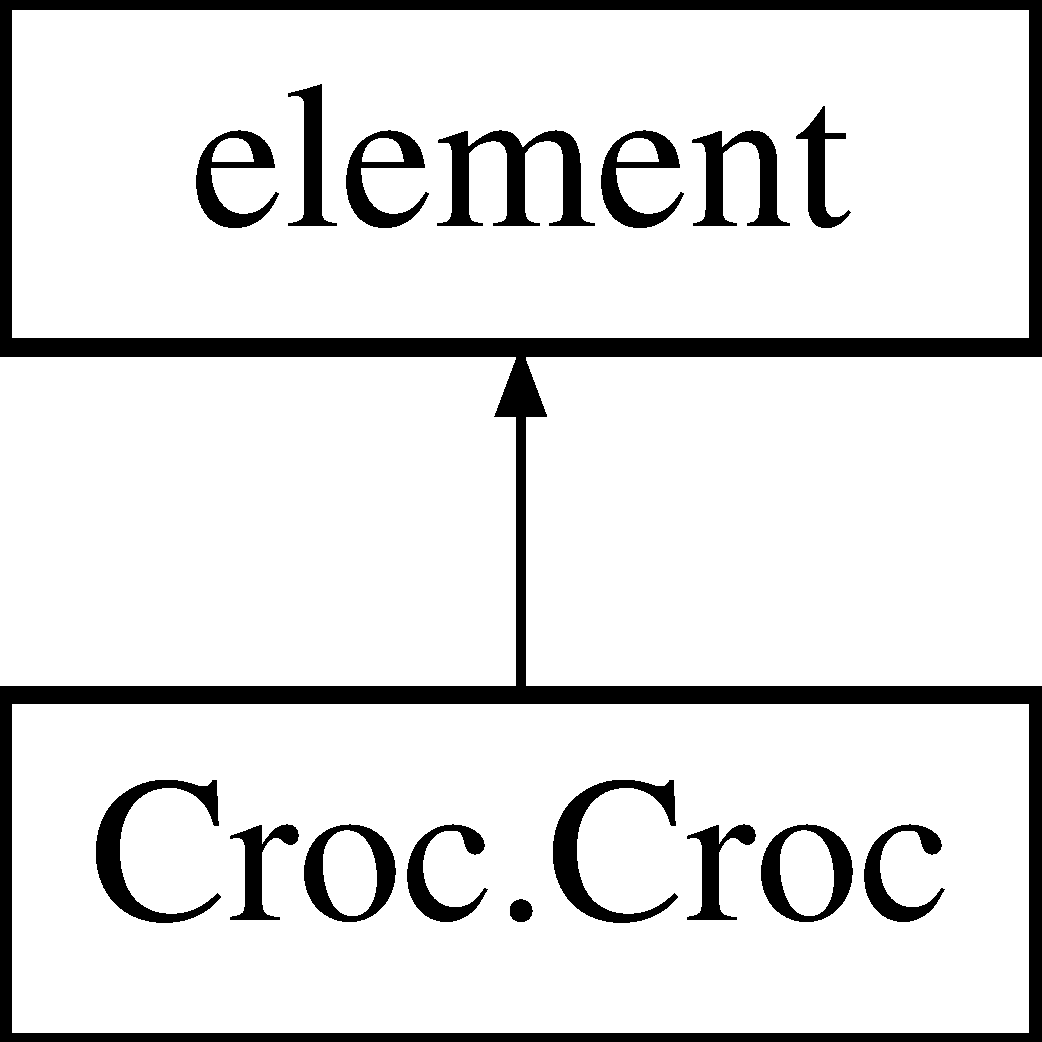
\includegraphics[height=2.000000cm]{classCroc_1_1Croc}
\end{center}
\end{figure}
\subsection*{Public Member Functions}
\begin{DoxyCompactItemize}
\item 
def \hyperlink{classCroc_1_1Croc_a4a51e90cde54760e398c4c43ea9dbd98}{\+\_\+\+\_\+init\+\_\+\+\_\+} (self, cat, obj, panel, \hyperlink{classHierarchy_aa7990fa7caf132d83e361ce033c6c65a}{path})
\item 
def \hyperlink{classCroc_1_1Croc_ae4ec968c843b562cf39bb95246353a79}{update} (self)
\end{DoxyCompactItemize}


\subsection{Detailed Description}


Definition at line 5 of file Croc.\+py.



\subsection{Constructor \& Destructor Documentation}
\mbox{\Hypertarget{classCroc_1_1Croc_a4a51e90cde54760e398c4c43ea9dbd98}\label{classCroc_1_1Croc_a4a51e90cde54760e398c4c43ea9dbd98}} 
\index{Croc\+::\+Croc@{Croc\+::\+Croc}!\+\_\+\+\_\+init\+\_\+\+\_\+@{\+\_\+\+\_\+init\+\_\+\+\_\+}}
\index{\+\_\+\+\_\+init\+\_\+\+\_\+@{\+\_\+\+\_\+init\+\_\+\+\_\+}!Croc\+::\+Croc@{Croc\+::\+Croc}}
\subsubsection{\texorpdfstring{\+\_\+\+\_\+init\+\_\+\+\_\+()}{\_\_init\_\_()}}
{\footnotesize\ttfamily def Croc.\+Croc.\+\_\+\+\_\+init\+\_\+\+\_\+ (\begin{DoxyParamCaption}\item[{}]{self,  }\item[{}]{cat,  }\item[{}]{obj,  }\item[{}]{panel,  }\item[{}]{path }\end{DoxyParamCaption})}



Definition at line 6 of file Croc.\+py.



References element.\+element.\+loadxrc(), and proc.\+proc.\+loadxrc().


\begin{DoxyCode}
6     \textcolor{keyword}{def }\hyperlink{classwrapper_1_1ModuleDictWrapper_a9a7a794150502f51df687831583e13b9}{\_\_init\_\_}(self, cat, obj, panel, path):
7         element.\_\_init\_\_(self,cat,obj,panel,path)
8         self.loadxrc()
9 
\end{DoxyCode}


\subsection{Member Function Documentation}
\mbox{\Hypertarget{classCroc_1_1Croc_ae4ec968c843b562cf39bb95246353a79}\label{classCroc_1_1Croc_ae4ec968c843b562cf39bb95246353a79}} 
\index{Croc\+::\+Croc@{Croc\+::\+Croc}!update@{update}}
\index{update@{update}!Croc\+::\+Croc@{Croc\+::\+Croc}}
\subsubsection{\texorpdfstring{update()}{update()}}
{\footnotesize\ttfamily def Croc.\+Croc.\+update (\begin{DoxyParamCaption}\item[{}]{self }\end{DoxyParamCaption})}



Definition at line 10 of file Croc.\+py.



Referenced by A3\+P\+E\+\_\+\+Bit\+Flip.\+A3\+P\+E\+\_\+\+Bit\+Flip.\+\_\+\+\_\+init\+\_\+\+\_\+(), Acquisition.\+Acquisition.\+\_\+\+\_\+init\+\_\+\+\_\+(), Emulate\+F\+E.\+Emulate\+F\+E.\+\_\+\+\_\+init\+\_\+\+\_\+(), App\+Frame.\+App\+Frame.\+delete\+Hardware(), Conf\+Frame.\+Conf\+Frame.\+on\+Change(), Graph\+Frame.\+Graph\+Frame.\+on\+Change(), Cfg\+Frame.\+Cfg\+Frame.\+on\+Change(), Conf\+Frame.\+Conf\+Frame.\+on\+Edit(), App\+Frame.\+App\+Frame.\+on\+Load(), Conf\+Frame.\+Conf\+Frame.\+on\+Re\+Load(), Graph\+Frame.\+Graph\+Frame.\+on\+Re\+Load(), Cfg\+Frame.\+Cfg\+Frame.\+on\+Re\+Load(), and App\+Frame.\+App\+Frame.\+on\+Re\+Load().


\begin{DoxyCode}
10     \textcolor{keyword}{def }update(self):
11         \textcolor{keywordflow}{print} \textcolor{stringliteral}{"Not implemented"}
12 
13 \textcolor{comment}{#----------------------------------------------------------------------}
14 
\end{DoxyCode}


The documentation for this class was generated from the following file\+:\begin{DoxyCompactItemize}
\item 
/home/eleclhcb/\+L\+H\+Cb/lbcat-\/cmake/\+Cat\+Calo/python/element/\hyperlink{Croc_8py}{Croc.\+py}\end{DoxyCompactItemize}

\hypertarget{classCroc}{}\section{Croc Class Reference}
\label{classCroc}\index{Croc@{Croc}}


{\ttfamily \#include $<$inc/\+Croc.\+h$>$}

Inheritance diagram for Croc\+:\begin{figure}[H]
\begin{center}
\leavevmode
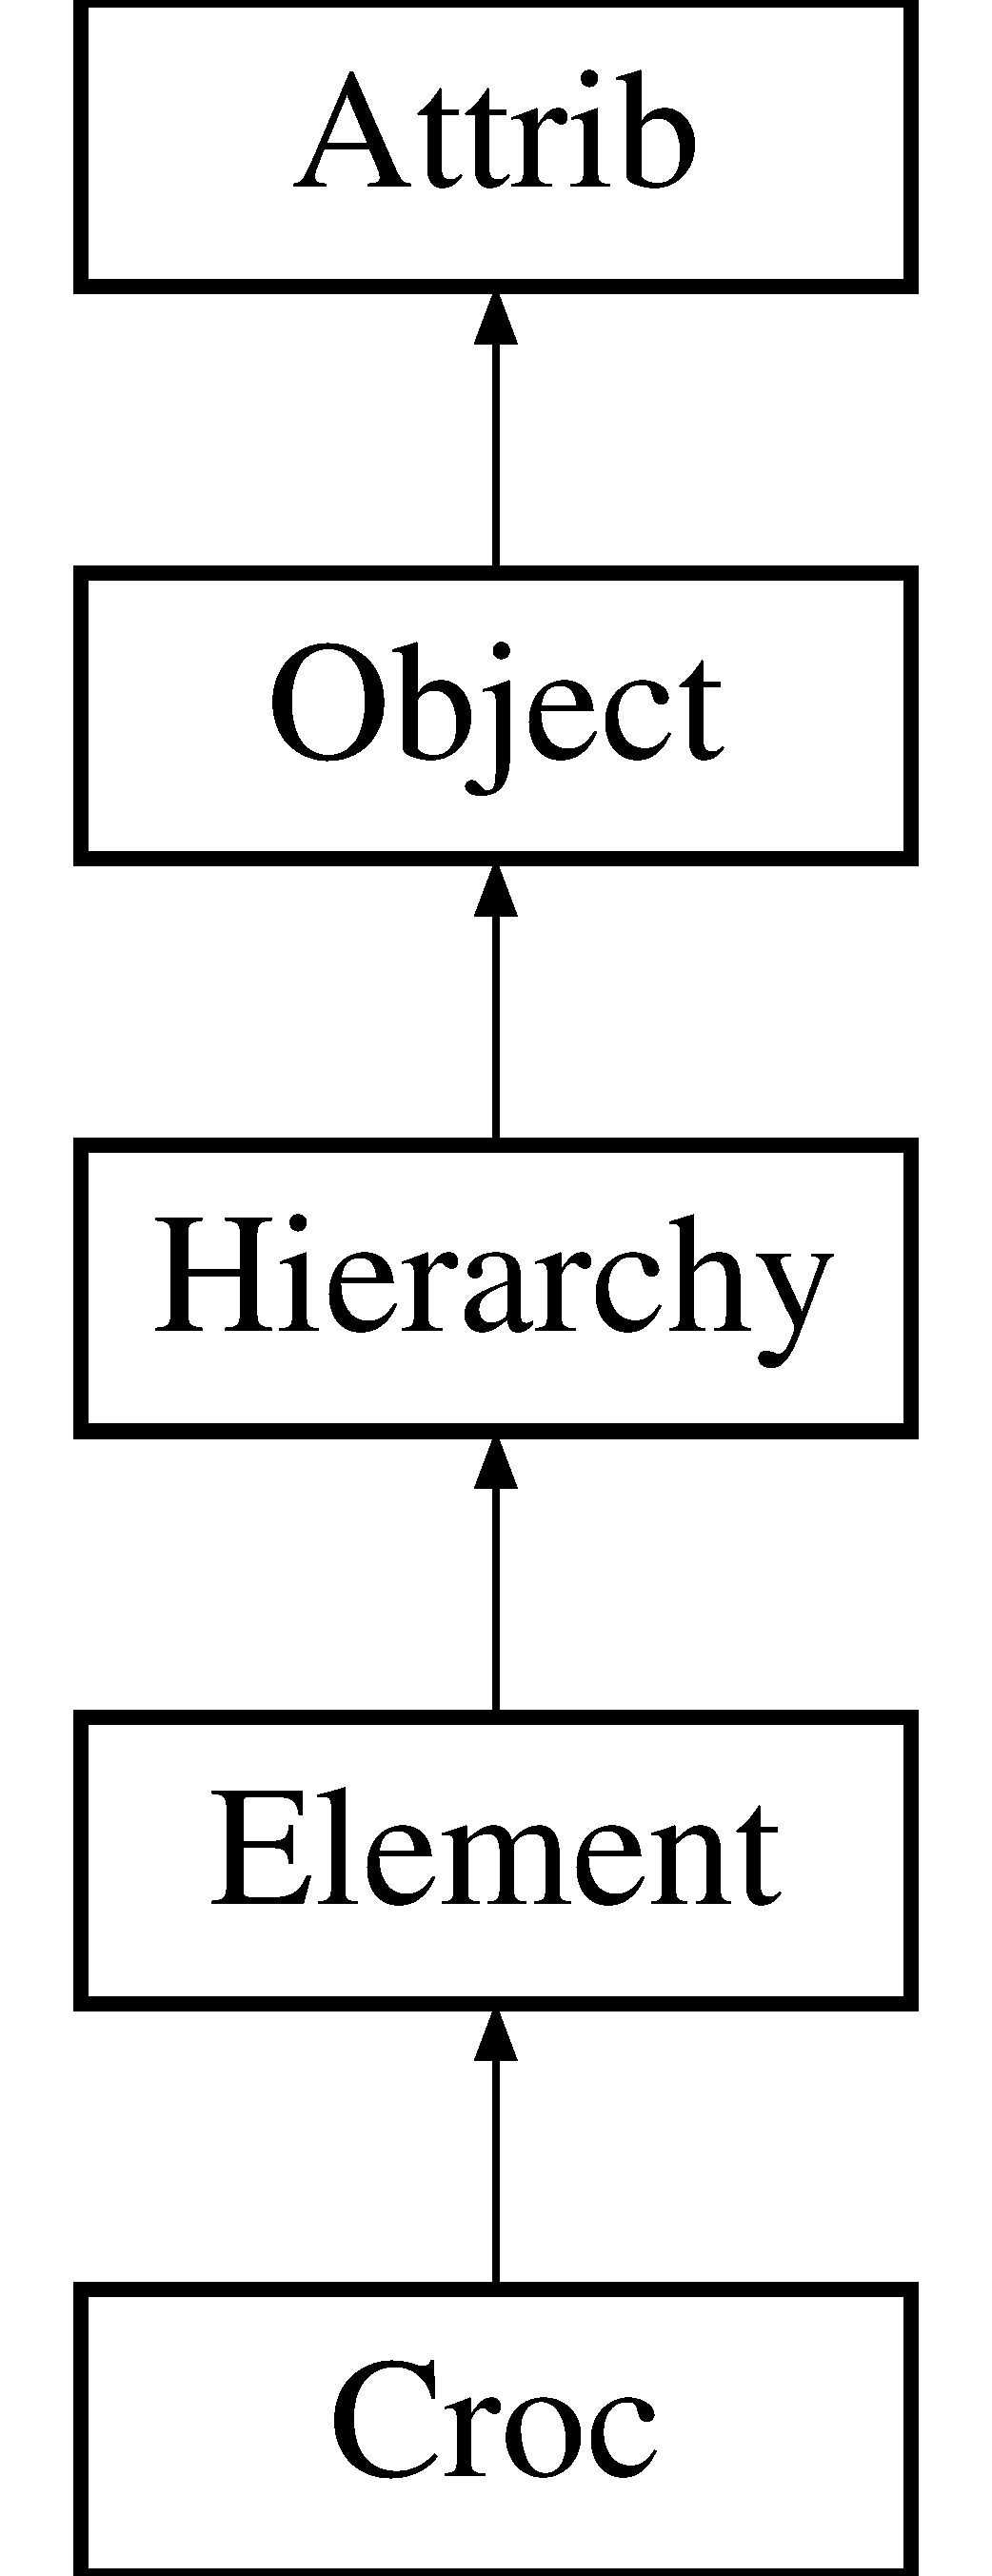
\includegraphics[height=5.000000cm]{classCroc}
\end{center}
\end{figure}
\subsection*{Classes}
\begin{DoxyCompactItemize}
\item 
class \hyperlink{classCroc_1_1Croc}{Croc}
\end{DoxyCompactItemize}
\subsection*{Public Types}
\begin{DoxyCompactItemize}
\item 
enum \hyperlink{classAttrib_a69e171d7cc6417835a5a306d3c764235}{Attribut} \{ \newline
\hyperlink{classAttrib_a69e171d7cc6417835a5a306d3c764235a3a8da2ab97dda18aebab196fe4100531}{U\+N\+D\+E\+F\+I\+N\+ED}, 
\hyperlink{classAttrib_a69e171d7cc6417835a5a306d3c764235a2bfb2af57b87031d190a05fe25dd92ed}{P\+A\+S\+S\+I\+VE}, 
\hyperlink{classAttrib_a69e171d7cc6417835a5a306d3c764235a3b1fec929c0370d1436f2f06e298fb0d}{A\+C\+T\+I\+VE}, 
\hyperlink{classAttrib_a69e171d7cc6417835a5a306d3c764235aa27c16b480a369ea4d18b07b2516bbc7}{I\+N\+T\+E\+R\+F\+A\+CE}, 
\newline
\hyperlink{classAttrib_a69e171d7cc6417835a5a306d3c764235a1420a5b8c0540b2af210b6975eded7f9}{IO}, 
\hyperlink{classAttrib_a69e171d7cc6417835a5a306d3c764235a0af3b0d0ac323c1704e6c69cf90add28}{I\+O\+D\+A\+TA}, 
\hyperlink{classAttrib_a69e171d7cc6417835a5a306d3c764235a7788bc5dd333fd8ce18562b269c9dab1}{E\+L\+E\+M\+E\+NT}, 
\hyperlink{classAttrib_a69e171d7cc6417835a5a306d3c764235a61ceb22149f365f1780d18f9d1459423}{H\+A\+R\+D\+W\+A\+RE}, 
\newline
\hyperlink{classAttrib_a69e171d7cc6417835a5a306d3c764235a75250e29692496e73effca2c0330977f}{P\+R\+O\+C\+E\+S\+S\+US}, 
\hyperlink{classAttrib_a69e171d7cc6417835a5a306d3c764235a103a67cd0b8f07ef478fa45d4356e27b}{S\+O\+F\+T\+W\+A\+RE}
 \}
\end{DoxyCompactItemize}
\subsection*{Public Member Functions}
\begin{DoxyCompactItemize}
\item 
\hyperlink{classCroc_ac9997a70a0b5b197789f6e2ba80b498b}{Croc} ()
\begin{DoxyCompactList}\small\item\em Standard constructor. \end{DoxyCompactList}\item 
virtual \hyperlink{classCroc_ace1e761410c9b53c1ff062a0dadcbd7b}{$\sim$\+Croc} ()
\begin{DoxyCompactList}\small\item\em Destructor. \end{DoxyCompactList}\item 
void \hyperlink{classCroc_a21195cea3b5ba13f90397cc8faa52633}{help} ()
\item 
\hyperlink{classStatusCode}{Status\+Code} \hyperlink{classCroc_a0ccc2406507c081f637a4d0346494f09}{init} ()
\item 
void \hyperlink{classCroc_aa95453776f49e4affe375500e96eb906}{reset} ()
\item 
void \hyperlink{classCroc_a74b7f08ffdc15f8244af02c8cdccbc8f}{update} ()
\item 
void \hyperlink{classElement_a3c0abcb36f8906688bb7e32608df7086}{recursive\+Init\+Element} ()
\item 
void \hyperlink{classElement_a82119ed37dff76508a2746a853ec35ba}{recursive\+Init\+Communications} ()
\item 
\hyperlink{classStatusCode}{Status\+Code} \hyperlink{classElement_ab476b4b1df5954141ceb14f072433b89}{set\+Connection} (\hyperlink{classHierarchy}{Hierarchy} $\ast$)
\item 
\hyperlink{classHierarchy}{Hierarchy} $\ast$ \hyperlink{classElement_af57444353c1ddf9fa0109801e97debf7}{connection} ()
\item 
void \hyperlink{classHierarchy_af4d43b0765b402670eed2d62c73405af}{clear} ()
\item 
void \hyperlink{classHierarchy_a585ad1aeec16077a0e532ab8b4fc557b}{set\+Parent} (\hyperlink{classHierarchy}{Hierarchy} $\ast$\hyperlink{classHierarchy_a1c7bec8257e717f9c1465e06ebf845fc}{parent})
\item 
\hyperlink{classHierarchy}{Hierarchy} $\ast$ \hyperlink{classHierarchy_a1c7bec8257e717f9c1465e06ebf845fc}{parent} ()
\item 
\hyperlink{classHierarchy}{Hierarchy} $\ast$ \hyperlink{classHierarchy_ad550588733bf75ac5c0fcfd7c8fd11a6}{parent} (std\+::string)
\item 
\hyperlink{classHierarchy}{Hierarchy} $\ast$ \hyperlink{classHierarchy_aee461dc930ce3871636ff87f075b1b83}{origin} ()
\item 
virtual void \hyperlink{classHierarchy_ad677774ff38fcb257c04a3a10d471fac}{add\+Child} (\hyperlink{classHierarchy}{Hierarchy} $\ast$element)
\item 
std\+::vector$<$ \hyperlink{classHierarchy}{Hierarchy} $\ast$ $>$ \hyperlink{classHierarchy_aa9a76f69e98e052ee1a6e32cea006288}{children} ()
\item 
\hyperlink{classHierarchy}{Hierarchy} $\ast$ \hyperlink{classHierarchy_a1e207f973c694b538bf90107b4868817}{child} (std\+::string)
\item 
\hyperlink{classHierarchy}{Hierarchy} $\ast$ \hyperlink{classHierarchy_a0c15a5276a3b80b4354d6bd8a01e0708}{child\+Typed} (std\+::string)
\item 
unsigned long \hyperlink{classHierarchy_ab16e84de65fd84e14001a6cf941c8be4}{number\+Of\+Children} ()
\item 
bool \hyperlink{classHierarchy_a255174fe4d316d2a3f430dcb9dab29f1}{has\+Children} ()
\item 
void \hyperlink{classHierarchy_a2b2b359fac003233f65786a616766bde}{del\+Child} (\hyperlink{classHierarchy}{Hierarchy} $\ast$)
\item 
void \hyperlink{classHierarchy_a1928ac7615fe0b5e55cd707f70dc6781}{del\+Child} (std\+::string)
\item 
std\+::string \hyperlink{classHierarchy_aa7990fa7caf132d83e361ce033c6c65a}{path} (std\+::string=std\+::string(\char`\"{}\char`\"{}))
\item 
std\+::string \hyperlink{classHierarchy_a1efd56cd164d328d2002e53a10a19b8c}{path\+Typed} (std\+::string=std\+::string(\char`\"{}\char`\"{}))
\item 
void \hyperlink{classHierarchy_a76e914b9a677a22a82deb74d892bf261}{tree} (std\+::string indent=std\+::string(\char`\"{}\char`\"{}))
\item 
void \hyperlink{classHierarchy_a594c294c5f60c230e106d522ed008212}{tree} ()
\item 
std\+::string \hyperlink{classObject_a300f4c05dd468c7bb8b3c968868443c1}{name} () const
\item 
std\+::string \hyperlink{classObject_a84f99f70f144a83e1582d1d0f84e4e62}{type} ()
\item 
unsigned char \hyperlink{classObject_af99145335cc61ff6e2798ea17db009d2}{id} ()
\item 
std\+::string \hyperlink{classObject_a73a0f1a41828fdd8303dd662446fb6c3}{title} ()
\item 
void \hyperlink{classObject_a3f9d5537ebce0c0f2bf6ae4d92426f3c}{msg\+Svc} (int level, std\+::string \hyperlink{classObject_a58b2d0618c2d08cf2383012611528d97}{msg}, std\+::string \hyperlink{classObject_a300f4c05dd468c7bb8b3c968868443c1}{name})
\item 
void \hyperlink{classObject_a58b2d0618c2d08cf2383012611528d97}{msg} (std\+::string mymsg)
\item 
void \hyperlink{classObject_ac5d59299273cee27aacf7de00d2e7034}{msg} (std\+::string mymsg, std\+::string \hyperlink{classObject_a300f4c05dd468c7bb8b3c968868443c1}{name})
\item 
void \hyperlink{classObject_a83d2db2df682907ea1115ad721c1c4a1}{verbose} (std\+::string mymsg)
\item 
void \hyperlink{classObject_a2d4120195317e2a3c6532e8bb9f3da68}{verbose} (std\+::string mymsg, std\+::string \hyperlink{classObject_a300f4c05dd468c7bb8b3c968868443c1}{name})
\item 
void \hyperlink{classObject_aac010553f022165573714b7014a15f0d}{debug} (std\+::string mymsg)
\item 
void \hyperlink{classObject_a6c9a0397ca804e04d675ed05683f5420}{debug} (std\+::string mymsg, std\+::string \hyperlink{classObject_a300f4c05dd468c7bb8b3c968868443c1}{name})
\item 
void \hyperlink{classObject_a644fd329ea4cb85f54fa6846484b84a8}{info} (std\+::string mymsg)
\item 
void \hyperlink{classObject_a1ca123253dfd30fc28b156f521dcbdae}{info} (std\+::string mymsg, std\+::string \hyperlink{classObject_a300f4c05dd468c7bb8b3c968868443c1}{name})
\item 
void \hyperlink{classObject_a65cd4fda577711660821fd2cd5a3b4c9}{warning} (std\+::string mymsg)
\item 
void \hyperlink{classObject_a11f101db4dd73d9391b0231818881d86}{warning} (std\+::string mymsg, std\+::string \hyperlink{classObject_a300f4c05dd468c7bb8b3c968868443c1}{name})
\item 
void \hyperlink{classObject_a204a95f57818c0f811933917a30eff45}{error} (std\+::string mymsg)
\item 
void \hyperlink{classObject_ad7f6c457733082efa2f9ff5f5c8e119a}{error} (std\+::string mymsg, std\+::string \hyperlink{classObject_a300f4c05dd468c7bb8b3c968868443c1}{name})
\item 
void \hyperlink{classObject_aad5a16aac7516ce65bd5ec02ab07fc80}{fatal} (std\+::string mymsg)
\item 
void \hyperlink{classObject_ae62acd3d09f716220f75f252dc38bc9a}{fatal} (std\+::string mymsg, std\+::string \hyperlink{classObject_a300f4c05dd468c7bb8b3c968868443c1}{name})
\item 
void \hyperlink{classObject_ae30fea75683c2d149b6b6d17c09ecd0c}{set\+Name} (std\+::string \hyperlink{classObject_a300f4c05dd468c7bb8b3c968868443c1}{name})
\item 
void \hyperlink{classObject_aae534cc9d982bcb9b99fd505f2e103a5}{set\+Type} (std\+::string \hyperlink{classObject_a84f99f70f144a83e1582d1d0f84e4e62}{type})
\item 
void \hyperlink{classObject_a398fe08cba594a0ce6891d59fe4f159f}{set\+Id} (unsigned char \hyperlink{classObject_af99145335cc61ff6e2798ea17db009d2}{id})
\item 
void \hyperlink{classObject_a89557dbbad5bcaa02652f5d7fa35d20f}{set\+Title} (std\+::string \hyperlink{classObject_a73a0f1a41828fdd8303dd662446fb6c3}{title})
\item 
void \hyperlink{classObject_a870c5af919958c2136623b2d7816d123}{set\+Dll\+Name} (std\+::string \hyperlink{classObject_a2e3947f2870094c332d7454117f3ec63}{dll\+Name})
\item 
std\+::string \hyperlink{classObject_a2e3947f2870094c332d7454117f3ec63}{dll\+Name} ()
\item 
bool \hyperlink{classAttrib_a704f26af560909ad22065083bb7d4c34}{is} (int attribut)
\item 
void \hyperlink{classAttrib_a235f773af19c900264a190b00a3b4ad7}{add} (int attribut)
\item 
void \hyperlink{classAttrib_a7d4ef7e32d93cb287792b87b857e79f3}{remove} (int attribut)
\item 
std\+::string \hyperlink{classAttrib_aee7bbf16b144887f196e1341b24f8a26}{attributs} ()
\end{DoxyCompactItemize}
\subsection*{Protected Attributes}
\begin{DoxyCompactItemize}
\item 
\hyperlink{classHierarchy}{Hierarchy} $\ast$ \hyperlink{classElement_abe3de7a5dbbc9a6dd2d7e012e5fdb266}{m\+\_\+connection}
\item 
std\+::string \hyperlink{classAttrib_a3414521d7a82476e874b25a5407b5e63}{m\+\_\+attrib\+String} \mbox{[}10\mbox{]}
\end{DoxyCompactItemize}


\subsection{Detailed Description}
\begin{DoxyAuthor}{Author}

\end{DoxyAuthor}
\begin{DoxyDate}{Date}
2006-\/10-\/23 
\end{DoxyDate}


Definition at line 15 of file Croc.\+h.



\subsection{Member Enumeration Documentation}
\mbox{\Hypertarget{classAttrib_a69e171d7cc6417835a5a306d3c764235}\label{classAttrib_a69e171d7cc6417835a5a306d3c764235}} 
\index{Croc@{Croc}!Attribut@{Attribut}}
\index{Attribut@{Attribut}!Croc@{Croc}}
\subsubsection{\texorpdfstring{Attribut}{Attribut}}
{\footnotesize\ttfamily enum \hyperlink{classAttrib_a69e171d7cc6417835a5a306d3c764235}{Attrib\+::\+Attribut}\hspace{0.3cm}{\ttfamily [inherited]}}

\begin{DoxyEnumFields}{Enumerator}
\raisebox{\heightof{T}}[0pt][0pt]{\index{U\+N\+D\+E\+F\+I\+N\+ED@{U\+N\+D\+E\+F\+I\+N\+ED}!Croc@{Croc}}\index{Croc@{Croc}!U\+N\+D\+E\+F\+I\+N\+ED@{U\+N\+D\+E\+F\+I\+N\+ED}}}\mbox{\Hypertarget{classAttrib_a69e171d7cc6417835a5a306d3c764235a3a8da2ab97dda18aebab196fe4100531}\label{classAttrib_a69e171d7cc6417835a5a306d3c764235a3a8da2ab97dda18aebab196fe4100531}} 
U\+N\+D\+E\+F\+I\+N\+ED&\\
\hline

\raisebox{\heightof{T}}[0pt][0pt]{\index{P\+A\+S\+S\+I\+VE@{P\+A\+S\+S\+I\+VE}!Croc@{Croc}}\index{Croc@{Croc}!P\+A\+S\+S\+I\+VE@{P\+A\+S\+S\+I\+VE}}}\mbox{\Hypertarget{classAttrib_a69e171d7cc6417835a5a306d3c764235a2bfb2af57b87031d190a05fe25dd92ed}\label{classAttrib_a69e171d7cc6417835a5a306d3c764235a2bfb2af57b87031d190a05fe25dd92ed}} 
P\+A\+S\+S\+I\+VE&\\
\hline

\raisebox{\heightof{T}}[0pt][0pt]{\index{A\+C\+T\+I\+VE@{A\+C\+T\+I\+VE}!Croc@{Croc}}\index{Croc@{Croc}!A\+C\+T\+I\+VE@{A\+C\+T\+I\+VE}}}\mbox{\Hypertarget{classAttrib_a69e171d7cc6417835a5a306d3c764235a3b1fec929c0370d1436f2f06e298fb0d}\label{classAttrib_a69e171d7cc6417835a5a306d3c764235a3b1fec929c0370d1436f2f06e298fb0d}} 
A\+C\+T\+I\+VE&\\
\hline

\raisebox{\heightof{T}}[0pt][0pt]{\index{I\+N\+T\+E\+R\+F\+A\+CE@{I\+N\+T\+E\+R\+F\+A\+CE}!Croc@{Croc}}\index{Croc@{Croc}!I\+N\+T\+E\+R\+F\+A\+CE@{I\+N\+T\+E\+R\+F\+A\+CE}}}\mbox{\Hypertarget{classAttrib_a69e171d7cc6417835a5a306d3c764235aa27c16b480a369ea4d18b07b2516bbc7}\label{classAttrib_a69e171d7cc6417835a5a306d3c764235aa27c16b480a369ea4d18b07b2516bbc7}} 
I\+N\+T\+E\+R\+F\+A\+CE&\\
\hline

\raisebox{\heightof{T}}[0pt][0pt]{\index{IO@{IO}!Croc@{Croc}}\index{Croc@{Croc}!IO@{IO}}}\mbox{\Hypertarget{classAttrib_a69e171d7cc6417835a5a306d3c764235a1420a5b8c0540b2af210b6975eded7f9}\label{classAttrib_a69e171d7cc6417835a5a306d3c764235a1420a5b8c0540b2af210b6975eded7f9}} 
IO&\\
\hline

\raisebox{\heightof{T}}[0pt][0pt]{\index{I\+O\+D\+A\+TA@{I\+O\+D\+A\+TA}!Croc@{Croc}}\index{Croc@{Croc}!I\+O\+D\+A\+TA@{I\+O\+D\+A\+TA}}}\mbox{\Hypertarget{classAttrib_a69e171d7cc6417835a5a306d3c764235a0af3b0d0ac323c1704e6c69cf90add28}\label{classAttrib_a69e171d7cc6417835a5a306d3c764235a0af3b0d0ac323c1704e6c69cf90add28}} 
I\+O\+D\+A\+TA&\\
\hline

\raisebox{\heightof{T}}[0pt][0pt]{\index{E\+L\+E\+M\+E\+NT@{E\+L\+E\+M\+E\+NT}!Croc@{Croc}}\index{Croc@{Croc}!E\+L\+E\+M\+E\+NT@{E\+L\+E\+M\+E\+NT}}}\mbox{\Hypertarget{classAttrib_a69e171d7cc6417835a5a306d3c764235a7788bc5dd333fd8ce18562b269c9dab1}\label{classAttrib_a69e171d7cc6417835a5a306d3c764235a7788bc5dd333fd8ce18562b269c9dab1}} 
E\+L\+E\+M\+E\+NT&\\
\hline

\raisebox{\heightof{T}}[0pt][0pt]{\index{H\+A\+R\+D\+W\+A\+RE@{H\+A\+R\+D\+W\+A\+RE}!Croc@{Croc}}\index{Croc@{Croc}!H\+A\+R\+D\+W\+A\+RE@{H\+A\+R\+D\+W\+A\+RE}}}\mbox{\Hypertarget{classAttrib_a69e171d7cc6417835a5a306d3c764235a61ceb22149f365f1780d18f9d1459423}\label{classAttrib_a69e171d7cc6417835a5a306d3c764235a61ceb22149f365f1780d18f9d1459423}} 
H\+A\+R\+D\+W\+A\+RE&\\
\hline

\raisebox{\heightof{T}}[0pt][0pt]{\index{P\+R\+O\+C\+E\+S\+S\+US@{P\+R\+O\+C\+E\+S\+S\+US}!Croc@{Croc}}\index{Croc@{Croc}!P\+R\+O\+C\+E\+S\+S\+US@{P\+R\+O\+C\+E\+S\+S\+US}}}\mbox{\Hypertarget{classAttrib_a69e171d7cc6417835a5a306d3c764235a75250e29692496e73effca2c0330977f}\label{classAttrib_a69e171d7cc6417835a5a306d3c764235a75250e29692496e73effca2c0330977f}} 
P\+R\+O\+C\+E\+S\+S\+US&\\
\hline

\raisebox{\heightof{T}}[0pt][0pt]{\index{S\+O\+F\+T\+W\+A\+RE@{S\+O\+F\+T\+W\+A\+RE}!Croc@{Croc}}\index{Croc@{Croc}!S\+O\+F\+T\+W\+A\+RE@{S\+O\+F\+T\+W\+A\+RE}}}\mbox{\Hypertarget{classAttrib_a69e171d7cc6417835a5a306d3c764235a103a67cd0b8f07ef478fa45d4356e27b}\label{classAttrib_a69e171d7cc6417835a5a306d3c764235a103a67cd0b8f07ef478fa45d4356e27b}} 
S\+O\+F\+T\+W\+A\+RE&\\
\hline

\end{DoxyEnumFields}


Definition at line 29 of file Attrib.\+h.


\begin{DoxyCode}
29                 \{
30     \hyperlink{classAttrib_a69e171d7cc6417835a5a306d3c764235a3a8da2ab97dda18aebab196fe4100531}{UNDEFINED},
31     \hyperlink{classAttrib_a69e171d7cc6417835a5a306d3c764235a2bfb2af57b87031d190a05fe25dd92ed}{PASSIVE},
32     \hyperlink{classAttrib_a69e171d7cc6417835a5a306d3c764235a3b1fec929c0370d1436f2f06e298fb0d}{ACTIVE},
33     \hyperlink{classAttrib_a69e171d7cc6417835a5a306d3c764235aa27c16b480a369ea4d18b07b2516bbc7}{INTERFACE},
34     \hyperlink{classAttrib_a69e171d7cc6417835a5a306d3c764235a1420a5b8c0540b2af210b6975eded7f9}{IO},
35     \hyperlink{classAttrib_a69e171d7cc6417835a5a306d3c764235a0af3b0d0ac323c1704e6c69cf90add28}{IODATA},
36     \hyperlink{classAttrib_a69e171d7cc6417835a5a306d3c764235a7788bc5dd333fd8ce18562b269c9dab1}{ELEMENT},
37     \hyperlink{classAttrib_a69e171d7cc6417835a5a306d3c764235a61ceb22149f365f1780d18f9d1459423}{HARDWARE},
38     \hyperlink{classAttrib_a69e171d7cc6417835a5a306d3c764235a75250e29692496e73effca2c0330977f}{PROCESSUS},
39     \hyperlink{classAttrib_a69e171d7cc6417835a5a306d3c764235a103a67cd0b8f07ef478fa45d4356e27b}{SOFTWARE} 
40   \}; \textcolor{comment}{// array m\_attribString must be changed into Attrib::Attrib if this enu is modified. }
\end{DoxyCode}


\subsection{Constructor \& Destructor Documentation}
\mbox{\Hypertarget{classCroc_ac9997a70a0b5b197789f6e2ba80b498b}\label{classCroc_ac9997a70a0b5b197789f6e2ba80b498b}} 
\index{Croc@{Croc}!Croc@{Croc}}
\index{Croc@{Croc}!Croc@{Croc}}
\subsubsection{\texorpdfstring{Croc()}{Croc()}}
{\footnotesize\ttfamily \hyperlink{classCroc_1_1Croc}{Croc\+::\+Croc} (\begin{DoxyParamCaption}{ }\end{DoxyParamCaption})}



Standard constructor. 



Definition at line 17 of file Croc.\+cpp.



References Object\+::set\+Name(), and Object\+::set\+Type().


\begin{DoxyCode}
17              \{
18   \hyperlink{classObject_ae30fea75683c2d149b6b6d17c09ecd0c}{setName}(\textcolor{stringliteral}{"Croc"});
19   \hyperlink{classObject_aae534cc9d982bcb9b99fd505f2e103a5}{setType}(\textcolor{stringliteral}{"Croc"});
20 \}
\end{DoxyCode}
\mbox{\Hypertarget{classCroc_ace1e761410c9b53c1ff062a0dadcbd7b}\label{classCroc_ace1e761410c9b53c1ff062a0dadcbd7b}} 
\index{Croc@{Croc}!````~Croc@{$\sim$\+Croc}}
\index{````~Croc@{$\sim$\+Croc}!Croc@{Croc}}
\subsubsection{\texorpdfstring{$\sim$\+Croc()}{~Croc()}}
{\footnotesize\ttfamily Croc\+::$\sim$\+Croc (\begin{DoxyParamCaption}{ }\end{DoxyParamCaption})\hspace{0.3cm}{\ttfamily [virtual]}}



Destructor. 



Definition at line 24 of file Croc.\+cpp.


\begin{DoxyCode}
24 \{\} 
\end{DoxyCode}


\subsection{Member Function Documentation}
\mbox{\Hypertarget{classAttrib_a235f773af19c900264a190b00a3b4ad7}\label{classAttrib_a235f773af19c900264a190b00a3b4ad7}} 
\index{Croc@{Croc}!add@{add}}
\index{add@{add}!Croc@{Croc}}
\subsubsection{\texorpdfstring{add()}{add()}}
{\footnotesize\ttfamily void Attrib\+::add (\begin{DoxyParamCaption}\item[{int}]{attribut }\end{DoxyParamCaption})\hspace{0.3cm}{\ttfamily [inline]}, {\ttfamily [inherited]}}

Add an attribut 

Definition at line 67 of file Attrib.\+h.



References Attrib\+::m\+\_\+attributs, and Attrib\+::\+U\+N\+D\+E\+F\+I\+N\+ED.



Referenced by A3\+P\+E\+::\+A3\+P\+E(), Attrib\+::\+Attrib(), Specs\+Mezzanine\+::cmdline(), Computer\+::\+Computer(), C\+U\+\_\+v1\+::\+C\+U\+\_\+v1(), export\+\_\+obj(), F\+E\+B\+\_\+v1\+::\+F\+E\+B\+\_\+v1(), Fe\+P\+G\+A\+::\+Fe\+P\+G\+A(), I\+C\+E\+C\+A\+Lv3\+::\+I\+C\+E\+C\+A\+Lv3(), I\+C\+Phaser\+::\+I\+C\+Phaser(), Application\+::initialize(), Interface\+::\+Interface(), I\+Odata\+::\+I\+Odata(), I\+Oobject\+::\+I\+Oobject(), M\+S\+Oxxxx\+::\+M\+S\+Oxxxx(), Phaser\+::\+Phaser(), Processus\+::\+Processus(), Proto40\+M\+Hz\+\_\+v1\+::\+Proto40\+M\+Hz\+\_\+v1(), Attrib\+::remove(), Seq\+P\+G\+A\+::\+Seq\+P\+G\+A(), Test\+S\+P\+I\+::set\+Address(), Test\+I2\+C\+::set\+Address(), Specs\+Slave\+::set\+Address(), Specs\+Master\+::\+Specs\+Master(), and Specs\+Slave\+::\+Specs\+Slave().


\begin{DoxyCode}
67                             \{
68     \textcolor{keywordflow}{if} (attribut!=\hyperlink{classAttrib_a69e171d7cc6417835a5a306d3c764235a3a8da2ab97dda18aebab196fe4100531}{Attrib::UNDEFINED}) \textcolor{keyword}{remove}(\hyperlink{classAttrib_a69e171d7cc6417835a5a306d3c764235a3a8da2ab97dda18aebab196fe4100531}{Attrib::UNDEFINED});
69     \textcolor{keywordtype}{bool} duplicate = false ;
70     std::vector<int>::const\_iterator iter ;
71     \textcolor{keywordflow}{for} ( iter  = \hyperlink{classAttrib_ac4bd58a0cc6b38a3b711d609a3d3aacc}{m\_attributs}.begin() ;
72           iter != \hyperlink{classAttrib_ac4bd58a0cc6b38a3b711d609a3d3aacc}{m\_attributs}.end()   ;
73           ++iter ) \{
74       \textcolor{keywordflow}{if} ( attribut == (*iter) ) \{
75         duplicate = true ;
76       \}
77     \}
78     \textcolor{keywordflow}{if} (!duplicate) \{
79       \hyperlink{classAttrib_ac4bd58a0cc6b38a3b711d609a3d3aacc}{m\_attributs}.push\_back( attribut );
80     \}
81   \}
\end{DoxyCode}
\mbox{\Hypertarget{classHierarchy_ad677774ff38fcb257c04a3a10d471fac}\label{classHierarchy_ad677774ff38fcb257c04a3a10d471fac}} 
\index{Croc@{Croc}!add\+Child@{add\+Child}}
\index{add\+Child@{add\+Child}!Croc@{Croc}}
\subsubsection{\texorpdfstring{add\+Child()}{addChild()}}
{\footnotesize\ttfamily void Hierarchy\+::add\+Child (\begin{DoxyParamCaption}\item[{\hyperlink{classHierarchy}{Hierarchy} $\ast$}]{element }\end{DoxyParamCaption})\hspace{0.3cm}{\ttfamily [virtual]}, {\ttfamily [inherited]}}



Definition at line 83 of file Hierarchy.\+cpp.



References Object\+::debug(), Hierarchy\+::m\+\_\+children, Object\+::name(), and Hierarchy\+::set\+Parent().



Referenced by A3\+P\+E\+::\+A3\+P\+E(), Specs\+Mezzanine\+::add\+Bus(), Specs\+Slave\+::add\+I2c(), Application\+::create(), C\+U\+\_\+v1\+::\+C\+U\+\_\+v1(), export\+\_\+obj(), F\+E\+B\+\_\+v1\+::\+F\+E\+B\+\_\+v1(), Fe\+P\+G\+A\+::\+Fe\+P\+G\+A(), I\+C\+E\+C\+A\+Lv3\+::\+I\+C\+E\+C\+A\+Lv3(), I\+C\+Phaser\+::\+I\+C\+Phaser(), Hierarchy\+::origin(), Phaser\+::\+Phaser(), Proto40\+M\+Hz\+\_\+v1\+::\+Proto40\+M\+Hz\+\_\+v1(), Seq\+P\+G\+A\+::\+Seq\+P\+G\+A(), Specs\+Mezzanine\+::\+Specs\+Mezzanine(), Usb\+I2c\+Bus\+::\+Usb\+I2c\+Bus(), and Usb\+Spi\+Bus\+::\+Usb\+Spi\+Bus().


\begin{DoxyCode}
83                                           \{
84   element->\hyperlink{classHierarchy_a585ad1aeec16077a0e532ab8b4fc557b}{setParent}(\textcolor{keyword}{this});
85   \hyperlink{classHierarchy_a038816763941fd4a930504917f60483b}{m\_children}.push\_back(element);
86   \hyperlink{classObject_aac010553f022165573714b7014a15f0d}{debug}(element->\hyperlink{classObject_a300f4c05dd468c7bb8b3c968868443c1}{name}()+\textcolor{stringliteral}{" added to the child tree."},\textcolor{stringliteral}{"Hierarchy::addChild"});
87 \}
\end{DoxyCode}
\mbox{\Hypertarget{classAttrib_aee7bbf16b144887f196e1341b24f8a26}\label{classAttrib_aee7bbf16b144887f196e1341b24f8a26}} 
\index{Croc@{Croc}!attributs@{attributs}}
\index{attributs@{attributs}!Croc@{Croc}}
\subsubsection{\texorpdfstring{attributs()}{attributs()}}
{\footnotesize\ttfamily std\+::string Attrib\+::attributs (\begin{DoxyParamCaption}{ }\end{DoxyParamCaption})\hspace{0.3cm}{\ttfamily [inherited]}}

Print the \hyperlink{classAttrib}{Attrib} of an \hyperlink{classObject}{Object} 

Definition at line 54 of file Attrib.\+cpp.



References images\+::index, Attrib\+::m\+\_\+attrib\+String, and Attrib\+::m\+\_\+attributs.



Referenced by export\+\_\+obj(), and Attrib\+::remove().


\begin{DoxyCode}
54                             \{
55   std::string output;
56   std::vector<int>::iterator iter ;
57   \textcolor{keywordflow}{for} ( \textcolor{keywordtype}{unsigned} \textcolor{keywordtype}{int} \hyperlink{namespaceimages_a54407fd574970b3178647ae096321a57}{index} = 0 ; \hyperlink{namespaceimages_a54407fd574970b3178647ae096321a57}{index} < \hyperlink{classAttrib_ac4bd58a0cc6b38a3b711d609a3d3aacc}{m\_attributs}.size() ; ++
      \hyperlink{namespaceimages_a54407fd574970b3178647ae096321a57}{index} ) \{
58     \textcolor{keywordflow}{if} ( \hyperlink{classAttrib_ac4bd58a0cc6b38a3b711d609a3d3aacc}{m\_attributs}.size() - \hyperlink{namespaceimages_a54407fd574970b3178647ae096321a57}{index} > 1 ) \{
59       output.append(\hyperlink{classAttrib_a3414521d7a82476e874b25a5407b5e63}{m\_attribString}[\hyperlink{classAttrib_ac4bd58a0cc6b38a3b711d609a3d3aacc}{m\_attributs}[\hyperlink{namespaceimages_a54407fd574970b3178647ae096321a57}{index}]]);
60       output.append(\textcolor{stringliteral}{":"});
61     \}
62     \textcolor{keywordflow}{else} \{
63       output.append(\hyperlink{classAttrib_a3414521d7a82476e874b25a5407b5e63}{m\_attribString}[\hyperlink{classAttrib_ac4bd58a0cc6b38a3b711d609a3d3aacc}{m\_attributs}[index]]);
64     \}
65   \}
66   \textcolor{keywordflow}{return} output;
67 \}
\end{DoxyCode}
\mbox{\Hypertarget{classHierarchy_a1e207f973c694b538bf90107b4868817}\label{classHierarchy_a1e207f973c694b538bf90107b4868817}} 
\index{Croc@{Croc}!child@{child}}
\index{child@{child}!Croc@{Croc}}
\subsubsection{\texorpdfstring{child()}{child()}}
{\footnotesize\ttfamily \hyperlink{classHierarchy}{Hierarchy} $\ast$ Hierarchy\+::child (\begin{DoxyParamCaption}\item[{std\+::string}]{path }\end{DoxyParamCaption})\hspace{0.3cm}{\ttfamily [inherited]}}



Definition at line 133 of file Hierarchy.\+cpp.



References Hierarchy\+::child(), Hierarchy\+::children(), Object\+::name(), Hierarchy\+::origin(), Hierarchy\+::parent(), Hierarchy\+::path(), and Object\+::warning().



Referenced by Application\+::cd(), Hierarchy\+::child(), Hierarchy\+::children(), and export\+\_\+obj().


\begin{DoxyCode}
133                                          \{
134   std::string newpath = \hyperlink{classHierarchy_aa7990fa7caf132d83e361ce033c6c65a}{path};
135   std::string up(\textcolor{stringliteral}{".."});
136   std::string separator(1,\textcolor{charliteral}{'/'});
137 
138   \hyperlink{classHierarchy}{Hierarchy} * newcurrent = 0;
139 
140   \textcolor{comment}{//  info("path="+path,"Hierarchy::child");}
141 
142   \textcolor{keywordflow}{if} (\hyperlink{classHierarchy_aa7990fa7caf132d83e361ce033c6c65a}{path}.compare(\textcolor{stringliteral}{""})==0 || \hyperlink{classHierarchy_aa7990fa7caf132d83e361ce033c6c65a}{path}.compare(\textcolor{stringliteral}{"/"})==0) \{
143     \textcolor{comment}{//    debug("return origin","Hierarchy::child");}
144     \textcolor{keywordflow}{return} \hyperlink{classHierarchy_aee461dc930ce3871636ff87f075b1b83}{origin}();
145   \}
146 
147   \textcolor{keywordflow}{if} (\hyperlink{classHierarchy_aa7990fa7caf132d83e361ce033c6c65a}{path}.compare(\hyperlink{classObject_a300f4c05dd468c7bb8b3c968868443c1}{name}())==0)\{
148     \textcolor{comment}{//    debug("return itself","Hierarchy::child");}
149     \textcolor{keywordflow}{return} \textcolor{keyword}{this};
150   \}
151 
152   \textcolor{keywordflow}{if} (\hyperlink{classHierarchy_aa7990fa7caf132d83e361ce033c6c65a}{path}.compare(\textcolor{stringliteral}{".."})==0)\{
153     \textcolor{keywordflow}{if} (0!=this->\hyperlink{classHierarchy_a1c7bec8257e717f9c1465e06ebf845fc}{parent}()) \textcolor{keywordflow}{return} this->\hyperlink{classHierarchy_a1c7bec8257e717f9c1465e06ebf845fc}{parent}();
154     \textcolor{keywordflow}{else} \textcolor{keywordflow}{return} \textcolor{keyword}{this};
155   \}
156 
157   \textcolor{keywordflow}{if} (\hyperlink{classHierarchy_aa7990fa7caf132d83e361ce033c6c65a}{path}.compare(\textcolor{stringliteral}{"../"})==0)\{
158     \textcolor{keywordflow}{if} (0!=this->\hyperlink{classHierarchy_a1c7bec8257e717f9c1465e06ebf845fc}{parent}()) \textcolor{keywordflow}{return} this->\hyperlink{classHierarchy_a1c7bec8257e717f9c1465e06ebf845fc}{parent}();
159     \textcolor{keywordflow}{else} \textcolor{keywordflow}{return} \textcolor{keyword}{this};
160   \}
161 
162 
163   \textcolor{keywordtype}{int} npos=\hyperlink{classHierarchy_aa7990fa7caf132d83e361ce033c6c65a}{path}.find(separator,0);
164 
165   \textcolor{comment}{//  info("find separator in "+itos(npos)+" of "+path,"Hierarchy::child");}
166 
167   \textcolor{comment}{// remove last separator}
168   \textcolor{keywordflow}{if} ( npos == (\textcolor{keywordtype}{int})(\hyperlink{classHierarchy_aa7990fa7caf132d83e361ce033c6c65a}{path}.size()-1) ) \{
169     newpath = std::string(\hyperlink{classHierarchy_aa7990fa7caf132d83e361ce033c6c65a}{path},0,npos);
170     \hyperlink{classHierarchy_aa7990fa7caf132d83e361ce033c6c65a}{path} = newpath;
171   \}
172 
173   \textcolor{keywordflow}{if} (npos==0)\{
174     \textcolor{comment}{//    debug("Going back to origin and calling child","Hierarchy::child");}
175     newpath=std::string(\hyperlink{classHierarchy_aa7990fa7caf132d83e361ce033c6c65a}{path},1,\hyperlink{classHierarchy_aa7990fa7caf132d83e361ce033c6c65a}{path}.size()-1);
176     \textcolor{keywordflow}{return} \hyperlink{classHierarchy_aee461dc930ce3871636ff87f075b1b83}{origin}()->\hyperlink{classHierarchy_a1e207f973c694b538bf90107b4868817}{child}(newpath);
177   \}
178   \textcolor{keywordflow}{else}\{
179     \textcolor{keywordflow}{if} ( npos== (\textcolor{keywordtype}{int})(std::string::npos) )\{
180       \textcolor{comment}{//      debug("Getting chid "+path+" of "+this->name(),"Hierarchy::child");}
181       std::vector <Hierarchy*> list = \hyperlink{classHierarchy_aa9a76f69e98e052ee1a6e32cea006288}{children}();
182       std::vector<Hierarchy*>::iterator iter;
183       \textcolor{keywordflow}{for} (iter=list.begin();iter!=list.end();iter++)\{
184         \textcolor{keywordflow}{if} ((*iter)->name().compare(\hyperlink{classHierarchy_aa7990fa7caf132d83e361ce033c6c65a}{path})==0)\{
185           \textcolor{keywordflow}{return} *iter;
186         \}
187       \}
188       \hyperlink{classObject_a65cd4fda577711660821fd2cd5a3b4c9}{warning}(this->\hyperlink{classObject_a300f4c05dd468c7bb8b3c968868443c1}{name}()+std::string(\textcolor{stringliteral}{" has no child '"})+\hyperlink{classHierarchy_aa7990fa7caf132d83e361ce033c6c65a}{path}+\textcolor{stringliteral}{"'"},\textcolor{stringliteral}{"Hierarchy::child"});
189       \textcolor{keywordflow}{return} \textcolor{keyword}{this};
190     \}
191     \textcolor{keywordflow}{else}
192     \{
193       \textcolor{keywordtype}{int} ipos=\hyperlink{classHierarchy_aa7990fa7caf132d83e361ce033c6c65a}{path}.find(separator,0);
194       \textcolor{comment}{//      info("default behaviour "+path+" with separator in "+itos(ipos),"Hierarchy::child");}
195 
196       std::string newcurrentname=std::string(\hyperlink{classHierarchy_aa7990fa7caf132d83e361ce033c6c65a}{path},0,ipos);
197       newpath=std::string(\hyperlink{classHierarchy_aa7990fa7caf132d83e361ce033c6c65a}{path},ipos+1,\hyperlink{classHierarchy_aa7990fa7caf132d83e361ce033c6c65a}{path}.size()-1);
198 
199       \textcolor{comment}{//      info("looking now for "+newpath+" from "+newcurrentname,"Hierarchy::child");}
200 
201       \textcolor{keywordflow}{if} (0==newcurrentname.compare(\hyperlink{classHierarchy_aee461dc930ce3871636ff87f075b1b83}{origin}()->\hyperlink{classObject_a300f4c05dd468c7bb8b3c968868443c1}{name}()))\{
202         \textcolor{comment}{//        info("current is computer. Looking for children"+newcurrentname,"Hierarchy::child");}
203         \textcolor{keywordflow}{return} \hyperlink{classHierarchy_aee461dc930ce3871636ff87f075b1b83}{origin}()->\hyperlink{classHierarchy_a1e207f973c694b538bf90107b4868817}{child}(newpath);
204       \}
205 
206       newcurrent = (\hyperlink{classHierarchy}{Hierarchy}*)0;
207 
208       std::vector <Hierarchy*> list = \hyperlink{classHierarchy_aa9a76f69e98e052ee1a6e32cea006288}{children}();
209       std::vector<Hierarchy*>::iterator iter;
210       \textcolor{keywordflow}{for} (iter=list.begin();iter!=list.end();iter++)\{
211         \textcolor{keywordflow}{if} ((*iter)->name().compare(newcurrentname)==0)\{
212           newcurrent = (*iter);
213         \}
214       \}
215 
216 
217       \textcolor{keywordflow}{if} ((\hyperlink{classHierarchy}{Hierarchy}*)0==newcurrent)\{
218         \textcolor{keywordflow}{if} (newcurrentname.compare(\textcolor{stringliteral}{".."})==0 && 0!=\hyperlink{classHierarchy_a1c7bec8257e717f9c1465e06ebf845fc}{parent}())\{
219           newcurrent=this->\hyperlink{classHierarchy_a1c7bec8257e717f9c1465e06ebf845fc}{parent}();
220           \textcolor{comment}{//          debug("newcurrent was .. -> parent="+parent()->name());}
221         \}
222         \textcolor{keywordflow}{else}
223         \{
224           \hyperlink{classObject_a65cd4fda577711660821fd2cd5a3b4c9}{warning}(this->\hyperlink{classObject_a300f4c05dd468c7bb8b3c968868443c1}{name}()+\textcolor{stringliteral}{" has no child '"}+newcurrentname+\textcolor{stringliteral}{"'"},
225               \textcolor{stringliteral}{"Hierarchy::child"});
226           \textcolor{keywordflow}{return} \textcolor{keyword}{this};
227         \}
228       \}
229       \textcolor{comment}{//      debug("recurrence call for "+newpath+" on "+newcurrent->name(),"Hierarchy::child");}
230       \textcolor{keywordflow}{return} newcurrent -> \hyperlink{classHierarchy_a1e207f973c694b538bf90107b4868817}{child} ( newpath );
231     \}
232   \}
233 \}
\end{DoxyCode}
\mbox{\Hypertarget{classHierarchy_aa9a76f69e98e052ee1a6e32cea006288}\label{classHierarchy_aa9a76f69e98e052ee1a6e32cea006288}} 
\index{Croc@{Croc}!children@{children}}
\index{children@{children}!Croc@{Croc}}
\subsubsection{\texorpdfstring{children()}{children()}}
{\footnotesize\ttfamily std\+::vector$<$\hyperlink{classHierarchy}{Hierarchy}$\ast$$>$ Hierarchy\+::children (\begin{DoxyParamCaption}{ }\end{DoxyParamCaption})\hspace{0.3cm}{\ttfamily [inline]}, {\ttfamily [inherited]}}



Definition at line 33 of file Hierarchy.\+h.



References Hierarchy\+::child(), Hierarchy\+::child\+Typed(), Hierarchy\+::del\+Child(), Hierarchy\+::has\+Children(), Hierarchy\+::m\+\_\+children, Hierarchy\+::number\+Of\+Children(), Hierarchy\+::path(), Hierarchy\+::path\+Typed(), and Hierarchy\+::tree().



Referenced by Hierarchy\+::child(), Hierarchy\+::child\+Typed(), export\+\_\+obj(), Specs\+Slave\+::recursive\+Init\+Communications(), Element\+::recursive\+Init\+Communications(), Element\+::recursive\+Init\+Element(), Application\+::set\+Config(), and Hierarchy\+::tree().


\begin{DoxyCode}
33 \{ \textcolor{keywordflow}{return} \hyperlink{classHierarchy_a038816763941fd4a930504917f60483b}{m\_children};  \} \textcolor{comment}{//< get list of child(ren)}
\end{DoxyCode}
\mbox{\Hypertarget{classHierarchy_a0c15a5276a3b80b4354d6bd8a01e0708}\label{classHierarchy_a0c15a5276a3b80b4354d6bd8a01e0708}} 
\index{Croc@{Croc}!child\+Typed@{child\+Typed}}
\index{child\+Typed@{child\+Typed}!Croc@{Croc}}
\subsubsection{\texorpdfstring{child\+Typed()}{childTyped()}}
{\footnotesize\ttfamily \hyperlink{classHierarchy}{Hierarchy} $\ast$ Hierarchy\+::child\+Typed (\begin{DoxyParamCaption}\item[{std\+::string}]{path }\end{DoxyParamCaption})\hspace{0.3cm}{\ttfamily [inherited]}}



Definition at line 239 of file Hierarchy.\+cpp.



References Hierarchy\+::children(), Hierarchy\+::m\+\_\+origin, Object\+::name(), Hierarchy\+::parent(), Hierarchy\+::path(), and Object\+::warning().



Referenced by Hierarchy\+::children(), and export\+\_\+obj().


\begin{DoxyCode}
239                                               \{
240 
241   std::string newpath = \hyperlink{classHierarchy_aa7990fa7caf132d83e361ce033c6c65a}{path};
242 
243   std::string up(\textcolor{stringliteral}{".."});
244   std::string separator(1,\textcolor{charliteral}{'/'});
245   std::string typeopen(1,\textcolor{charliteral}{'['});
246   std::string typeclose(1,\textcolor{charliteral}{']'});
247 
248   \hyperlink{classHierarchy}{Hierarchy} * newcurrent = 0;
249 
250   \textcolor{keywordtype}{unsigned} \textcolor{keywordtype}{int} npos=\hyperlink{classHierarchy_aa7990fa7caf132d83e361ce033c6c65a}{path}.find(separator,0);
251   \textcolor{keywordtype}{unsigned} \textcolor{keywordtype}{int} opos=\hyperlink{classHierarchy_aa7990fa7caf132d83e361ce033c6c65a}{path}.find(typeopen,0);
252   \textcolor{keywordflow}{if} ( npos==std::string::npos || npos == \hyperlink{classHierarchy_aa7990fa7caf132d83e361ce033c6c65a}{path}.size()-1 )\{
253     \textcolor{keywordflow}{if} ( \hyperlink{classHierarchy_aa7990fa7caf132d83e361ce033c6c65a}{path}.compare(\textcolor{stringliteral}{".."})==0 ) \{
254       \textcolor{keywordflow}{return} \hyperlink{classHierarchy_a1c7bec8257e717f9c1465e06ebf845fc}{parent}();
255     \}
256 
257     \textcolor{keywordflow}{if} ( npos == \hyperlink{classHierarchy_aa7990fa7caf132d83e361ce033c6c65a}{path}.size()-1 ) \{
258       newpath = std::string(\hyperlink{classHierarchy_aa7990fa7caf132d83e361ce033c6c65a}{path},0,opos);
259       \hyperlink{classHierarchy_aa7990fa7caf132d83e361ce033c6c65a}{path} = newpath;
260     \}
261 
262     std::vector < Hierarchy* > list = \hyperlink{classHierarchy_aa9a76f69e98e052ee1a6e32cea006288}{children}();
263     std::vector < Hierarchy* >::iterator iter;
264     \textcolor{keywordflow}{for} (iter=list.begin();iter!=list.end();iter++)\{
265       std::string notypepath = std::string(\hyperlink{classHierarchy_aa7990fa7caf132d83e361ce033c6c65a}{path},0,opos);
266       \textcolor{keywordflow}{if} ((*iter)->name().compare(notypepath)==0)\{
267         \textcolor{keywordflow}{return} *iter;
268       \}
269     \}
270     \hyperlink{classObject_a65cd4fda577711660821fd2cd5a3b4c9}{warning}(this->\hyperlink{classObject_a300f4c05dd468c7bb8b3c968868443c1}{name}()+std::string(\textcolor{stringliteral}{" has no child "}) +\hyperlink{classHierarchy_aa7990fa7caf132d83e361ce033c6c65a}{path},\textcolor{stringliteral}{"Hierarchy::child"});
271     \textcolor{keywordflow}{return} 0;
272   \}
273 
274   \textcolor{keywordflow}{else} \{
275 
276     \textcolor{keywordflow}{if} (std::string(\hyperlink{classHierarchy_aa7990fa7caf132d83e361ce033c6c65a}{path},0,3).compare(std::string(\textcolor{stringliteral}{"../"}))==0) \{
277       newpath=std::string(\hyperlink{classHierarchy_aa7990fa7caf132d83e361ce033c6c65a}{path},3,\hyperlink{classHierarchy_aa7990fa7caf132d83e361ce033c6c65a}{path}.size()-3);
278       newcurrent = \hyperlink{classHierarchy_a1c7bec8257e717f9c1465e06ebf845fc}{parent}();
279     \}
280     \textcolor{keywordflow}{if} (std::string(\hyperlink{classHierarchy_aa7990fa7caf132d83e361ce033c6c65a}{path},0,1).compare(std::string(\textcolor{stringliteral}{"/"}))==0) \{
281       newpath=std::string(\hyperlink{classHierarchy_aa7990fa7caf132d83e361ce033c6c65a}{path},1,\hyperlink{classHierarchy_aa7990fa7caf132d83e361ce033c6c65a}{path}.size()-1);
282       newcurrent = ( \hyperlink{classHierarchy}{Hierarchy}* ) \hyperlink{classHierarchy_a16c73e557d3a7c156ffb5dc4102d148e}{m\_origin};
283     \}
284     \textcolor{keywordflow}{if} ((std::string(\hyperlink{classHierarchy_aa7990fa7caf132d83e361ce033c6c65a}{path},0,3).compare(std::string(\textcolor{stringliteral}{"../"})) !=0 ) &&
285         std::string(\hyperlink{classHierarchy_aa7990fa7caf132d83e361ce033c6c65a}{path},0,1).compare(std::string(\textcolor{stringliteral}{"/"}))!=0 ) \{
286       opos = \hyperlink{classHierarchy_aa7990fa7caf132d83e361ce033c6c65a}{path}.find(typeopen,0);
287       \textcolor{keywordtype}{int} cpos = \hyperlink{classHierarchy_aa7990fa7caf132d83e361ce033c6c65a}{path}.find(typeclose,0);
288       std::string \hyperlink{classObject_a300f4c05dd468c7bb8b3c968868443c1}{name} = std::string (\hyperlink{classHierarchy_aa7990fa7caf132d83e361ce033c6c65a}{path},0,opos);
289       newcurrent = \hyperlink{classHierarchy_a0c15a5276a3b80b4354d6bd8a01e0708}{childTyped}( name );
290       \textcolor{keywordflow}{if} (newcurrent ==0)\{
291         \hyperlink{classObject_a65cd4fda577711660821fd2cd5a3b4c9}{warning}(\hyperlink{classHierarchy_aa7990fa7caf132d83e361ce033c6c65a}{path}+\textcolor{stringliteral}{": no child found with such a name"},\textcolor{stringliteral}{"Hierarchy::child"});
292       \}
293       newpath = std::string (\hyperlink{classHierarchy_aa7990fa7caf132d83e361ce033c6c65a}{path},cpos+2,\hyperlink{classHierarchy_aa7990fa7caf132d83e361ce033c6c65a}{path}.size()-cpos-1);
294     \}
295     \textcolor{keywordflow}{return} newcurrent -> \hyperlink{classHierarchy_a0c15a5276a3b80b4354d6bd8a01e0708}{childTyped} ( newpath );
296   \}
297 \}
\end{DoxyCode}
\mbox{\Hypertarget{classHierarchy_af4d43b0765b402670eed2d62c73405af}\label{classHierarchy_af4d43b0765b402670eed2d62c73405af}} 
\index{Croc@{Croc}!clear@{clear}}
\index{clear@{clear}!Croc@{Croc}}
\subsubsection{\texorpdfstring{clear()}{clear()}}
{\footnotesize\ttfamily void Hierarchy\+::clear (\begin{DoxyParamCaption}{ }\end{DoxyParamCaption})\hspace{0.3cm}{\ttfamily [inherited]}}



Definition at line 35 of file Hierarchy.\+cpp.



References Hierarchy\+::del\+Child(), Object\+::info(), Hierarchy\+::m\+\_\+children, and Object\+::name().



Referenced by export\+\_\+obj().


\begin{DoxyCode}
35                      \{
36   std::vector<Hierarchy*> listlocale;
37   std::vector<Hierarchy*>::iterator iter;
38   \hyperlink{classObject_a644fd329ea4cb85f54fa6846484b84a8}{info}(\textcolor{stringliteral}{"loop on "}+\hyperlink{classObject_a300f4c05dd468c7bb8b3c968868443c1}{name}()+\textcolor{stringliteral}{" children."},\textcolor{stringliteral}{"Hierarchy::clear"});
39   \textcolor{keywordflow}{for} (iter=\hyperlink{classHierarchy_a038816763941fd4a930504917f60483b}{m\_children}.begin();iter!=\hyperlink{classHierarchy_a038816763941fd4a930504917f60483b}{m\_children}.end();iter++)\{
40       \hyperlink{classObject_a644fd329ea4cb85f54fa6846484b84a8}{info}(\textcolor{stringliteral}{"processing "}+(*iter)->name()+\textcolor{stringliteral}{"."},\textcolor{stringliteral}{"Hierarchy::clear"});
41 \textcolor{comment}{/*}
42 \textcolor{comment}{      (*iter)->clear();
}
43 \textcolor{comment}{//      this->delChild((*iter));
}
44 \textcolor{comment}{      info("obj "+(*iter)->name()+" being cleared.","Hierarchy::clear");
}
45 \textcolor{comment}{      delete (*iter);
}
46 \textcolor{comment}{      info("Object deleted.","Hierarchy::clear");
}
47 \textcolor{comment}{      m\_children.erase(iter);
}
48 \textcolor{comment}{      info("Object removed from the tree.","Hierarchy::clear");
}
49 \textcolor{comment}{*/}
50     (*iter)->clear();
51     \hyperlink{classObject_a644fd329ea4cb85f54fa6846484b84a8}{info}(\textcolor{stringliteral}{"Adding object "}+(*iter)->name()+\textcolor{stringliteral}{" from the Hierarchy to the list of deleted objects."},\textcolor{stringliteral}{"
      Hierarchy::clear"});
52     listlocale.push\_back((*iter));
53   \}
54 
55   \textcolor{keywordflow}{for} (iter=listlocale.begin();iter!=listlocale.end();iter++)\{
56     \hyperlink{classObject_a644fd329ea4cb85f54fa6846484b84a8}{info}(\textcolor{stringliteral}{"Removing object "}+(*iter)->name()+\textcolor{stringliteral}{"."},\textcolor{stringliteral}{"Hierarchy::clear"});
57     this->\hyperlink{classHierarchy_a2b2b359fac003233f65786a616766bde}{delChild}(*iter);
58 \textcolor{comment}{//    m\_children.erase(iter);}
59     \textcolor{keyword}{delete} (*iter);
60   \}
61   \hyperlink{classObject_a644fd329ea4cb85f54fa6846484b84a8}{info}(\textcolor{stringliteral}{"Getting out of "}+\hyperlink{classObject_a300f4c05dd468c7bb8b3c968868443c1}{name}());
62 \}
\end{DoxyCode}
\mbox{\Hypertarget{classElement_af57444353c1ddf9fa0109801e97debf7}\label{classElement_af57444353c1ddf9fa0109801e97debf7}} 
\index{Croc@{Croc}!connection@{connection}}
\index{connection@{connection}!Croc@{Croc}}
\subsubsection{\texorpdfstring{connection()}{connection()}}
{\footnotesize\ttfamily \hyperlink{classHierarchy}{Hierarchy} $\ast$ Element\+::connection (\begin{DoxyParamCaption}{ }\end{DoxyParamCaption})\hspace{0.3cm}{\ttfamily [inherited]}}

Get IO interface 

Definition at line 84 of file Element.\+cpp.



References Element\+::m\+\_\+connection, Object\+::name(), and Object\+::warning().



Referenced by Usb\+Spi\+Bus\+::clock\+Divider(), export\+\_\+obj(), Usb\+I2c\+Bus\+::read(), I\+Oobject\+::read(), Usb\+Spi\+Bus\+::read(), Usb\+Spi\+Bus\+::set\+Clock\+Divider(), Element\+::set\+Connection(), Usb\+I2c\+Bus\+::write(), I\+Oobject\+::write(), and Usb\+Spi\+Bus\+::write().


\begin{DoxyCode}
84                               \{
85   \textcolor{keywordflow}{if} (0==\hyperlink{classElement_abe3de7a5dbbc9a6dd2d7e012e5fdb266}{m\_connection})\{
86     \hyperlink{classObject_a65cd4fda577711660821fd2cd5a3b4c9}{warning}(\textcolor{stringliteral}{"no connection defined for "}+\hyperlink{classObject_a300f4c05dd468c7bb8b3c968868443c1}{name}()+\textcolor{stringliteral}{"."},\textcolor{stringliteral}{"Element::connection"});
87     \textcolor{keywordflow}{return} (\hyperlink{classHierarchy}{Hierarchy}*)0;
88   \}
89   \textcolor{keywordflow}{return} \hyperlink{classElement_abe3de7a5dbbc9a6dd2d7e012e5fdb266}{m\_connection};
90 \}
\end{DoxyCode}
\mbox{\Hypertarget{classObject_aac010553f022165573714b7014a15f0d}\label{classObject_aac010553f022165573714b7014a15f0d}} 
\index{Croc@{Croc}!debug@{debug}}
\index{debug@{debug}!Croc@{Croc}}
\subsubsection{\texorpdfstring{debug()}{debug()}\hspace{0.1cm}{\footnotesize\ttfamily [1/2]}}
{\footnotesize\ttfamily void Object\+::debug (\begin{DoxyParamCaption}\item[{std\+::string}]{mymsg }\end{DoxyParamCaption})\hspace{0.3cm}{\ttfamily [inline]}, {\ttfamily [inherited]}}



Definition at line 37 of file Object.\+h.



References Msg\+Svc\+::\+D\+E\+B\+UG, Object\+::m\+\_\+log, Object\+::m\+\_\+name, and Msg\+Svc\+::msg\+Svc().



Referenced by A3\+P\+E\+::\+A3\+P\+E(), A3\+P\+E\+::acquisition(), Specs\+Mezzanine\+::add\+Bus(), Hierarchy\+::add\+Child(), Specs\+Slave\+::add\+I2c(), L\+S\+Delay\+Chip\+V1\+::config\+Reg\+Bulk\+Read(), L\+S\+Delay\+Chip\+V1\+::config\+Reg\+Bulk\+Write(), A3\+P\+E\+::data\+Ready(), D\+C\+U\+::\+D\+C\+U(), Hierarchy\+::del\+Child(), Specs\+Slave\+::detect(), Storage\+Fifo\+Acquisition\+::execute(), Storage\+Fifo\+::execute(), A3\+P\+E\+\_\+\+Bit\+Flip\+::execute(), Acquisition\+::execute(), Emulate\+F\+E\+::execute(), export\+\_\+obj(), Fe\+P\+G\+A\+::\+Fe\+P\+G\+A(), Specs\+Glue\+::i2c\+Clk\+Mode(), Fe\+P\+G\+A\+::i2c\+Read(), Seq\+P\+G\+A\+::i2c\+Read(), Fe\+P\+G\+A\+::i2c\+Write(), Seq\+P\+G\+A\+::i2c\+Write(), I\+C\+E\+C\+A\+Lv3\+::\+I\+C\+E\+C\+A\+Lv3(), I\+C\+Phaser\+::\+I\+C\+Phaser(), Specs\+Slave\+::init(), Specs\+Master\+::init(), Storage\+Fifo\+Acquisition\+::initialize(), Storage\+Fifo\+::initialize(), A3\+P\+E\+\_\+\+Bit\+Flip\+::initialize(), Acquisition\+::initialize(), Emulate\+F\+E\+::initialize(), A3\+P\+E\+::internal\+A\+X\+Sequence(), Specs\+Glue\+::led(), Specs\+Mezzanine\+::led(), M\+S\+Oxxxx\+::\+M\+S\+Oxxxx(), Phaser\+::\+Phaser(), Data\+::purge(), Phaser\+::read(), I\+C\+Phaser\+::read(), C\+U\+\_\+v1\+::reset(), F\+E\+B\+\_\+v1\+::reset(), Proto40\+M\+Hz\+\_\+v1\+::reset(), Specs\+Master\+::reset(), Specs\+Slave\+::reset(), F\+E\+B\+\_\+v1\+::reset\+Usb(), Seq\+P\+G\+A\+::\+Seq\+P\+G\+A(), A3\+P\+E\+::set\+Add\+From\+A\+X\+Ram(), A3\+P\+E\+::set\+Add\+To\+A\+X\+Ram(), A3\+P\+E\+::set\+A\+X\+Ram\+Usb(), Element\+::set\+Connection(), Specs\+Glue\+::set\+I2c\+Clk\+Mode(), A3\+P\+E\+::set\+Latency\+A\+X(), Specs\+Glue\+::set\+Led(), Specs\+Mezzanine\+::set\+Led(), A3\+P\+E\+::set\+Length\+A\+X(), A3\+P\+E\+::set\+Read\+To\+A\+X\+Ram\+Usb(), Specs\+Master\+::set\+Speed(), A3\+P\+E\+::set\+Write\+From\+A\+X\+Ram\+Usb(), Specs\+Bus\+::\+Specs\+Bus(), Specs\+I2c\+::\+Specs\+I2c(), Specs\+Master\+::\+Specs\+Master(), Specs\+Mezzanine\+::\+Specs\+Mezzanine(), Specs\+Parallel\+Bus\+::\+Specs\+Parallel\+Bus(), Specs\+Slave\+::\+Specs\+Slave(), L\+S\+Delay\+Chip\+V1\+::spi\+B\+E\+R\+Test(), I\+C\+E\+C\+A\+Lv3\+::spi\+Read(), I\+C\+E\+C\+A\+Lv3\+::spi\+Write(), A3\+P\+E\+::trigger(), Server\+::update\+Config(), Server\+::update\+State(), Phaser\+::write(), I\+C\+Phaser\+::write(), and Hierarchy\+::$\sim$\+Hierarchy().


\begin{DoxyCode}
37 \{ \hyperlink{classObject_a0d269813dd7ac1f24bc143031e2963f2}{m\_log}.\hyperlink{classMsgSvc_ad25f18047920cc59a314e5098259711c}{msgSvc} (\hyperlink{classMsgSvc_ae671eb7301996cd049d2da8a65925926a1dbdcc82dce88370ec335883c83b38b0}{MsgSvc::DEBUG}   , mymsg, \hyperlink{classObject_a8b83c95c705d2c3ba0d081fe1710f48d}{m\_name} ); \}
\end{DoxyCode}
\mbox{\Hypertarget{classObject_a6c9a0397ca804e04d675ed05683f5420}\label{classObject_a6c9a0397ca804e04d675ed05683f5420}} 
\index{Croc@{Croc}!debug@{debug}}
\index{debug@{debug}!Croc@{Croc}}
\subsubsection{\texorpdfstring{debug()}{debug()}\hspace{0.1cm}{\footnotesize\ttfamily [2/2]}}
{\footnotesize\ttfamily void Object\+::debug (\begin{DoxyParamCaption}\item[{std\+::string}]{mymsg,  }\item[{std\+::string}]{name }\end{DoxyParamCaption})\hspace{0.3cm}{\ttfamily [inline]}, {\ttfamily [inherited]}}



Definition at line 45 of file Object.\+h.



References Msg\+Svc\+::\+D\+E\+B\+UG, Object\+::m\+\_\+log, and Msg\+Svc\+::msg\+Svc().


\begin{DoxyCode}
45 \{ \hyperlink{classObject_a0d269813dd7ac1f24bc143031e2963f2}{m\_log}.\hyperlink{classMsgSvc_ad25f18047920cc59a314e5098259711c}{msgSvc} (\hyperlink{classMsgSvc_ae671eb7301996cd049d2da8a65925926a1dbdcc82dce88370ec335883c83b38b0}{MsgSvc::DEBUG}   , mymsg, \hyperlink{classObject_a300f4c05dd468c7bb8b3c968868443c1}{name} ); \}
\end{DoxyCode}
\mbox{\Hypertarget{classHierarchy_a2b2b359fac003233f65786a616766bde}\label{classHierarchy_a2b2b359fac003233f65786a616766bde}} 
\index{Croc@{Croc}!del\+Child@{del\+Child}}
\index{del\+Child@{del\+Child}!Croc@{Croc}}
\subsubsection{\texorpdfstring{del\+Child()}{delChild()}\hspace{0.1cm}{\footnotesize\ttfamily [1/2]}}
{\footnotesize\ttfamily void Hierarchy\+::del\+Child (\begin{DoxyParamCaption}\item[{\hyperlink{classHierarchy}{Hierarchy} $\ast$}]{element }\end{DoxyParamCaption})\hspace{0.3cm}{\ttfamily [inherited]}}



Definition at line 92 of file Hierarchy.\+cpp.



References Object\+::debug(), and Hierarchy\+::m\+\_\+children.



Referenced by Hierarchy\+::children(), Hierarchy\+::clear(), export\+\_\+obj(), and Hierarchy\+::$\sim$\+Hierarchy().


\begin{DoxyCode}
92                                           \{
93   \textcolor{keywordtype}{bool} flag=\textcolor{keyword}{false};
94   std::vector<Hierarchy*>::iterator iter,\textcolor{keyword}{remove};
95   \textcolor{keywordflow}{for} (iter=\hyperlink{classHierarchy_a038816763941fd4a930504917f60483b}{m\_children}.begin();(iter!=\hyperlink{classHierarchy_a038816763941fd4a930504917f60483b}{m\_children}.end());iter++)\{
96     \textcolor{keywordflow}{if} (*iter==element)\{
97       \textcolor{keyword}{remove}=iter;
98       flag=\textcolor{keyword}{true};
99     \}
100   \}
101   \textcolor{keywordflow}{if} (flag)\{
102     \hyperlink{classObject_aac010553f022165573714b7014a15f0d}{debug}(\textcolor{stringliteral}{"removing "}+(*remove)->name()+\textcolor{stringliteral}{" from the tree."},\textcolor{stringliteral}{"Hierarchy::delChild"});
103     \hyperlink{classHierarchy_a038816763941fd4a930504917f60483b}{m\_children}.erase(\textcolor{keyword}{remove});
104   \}
105 \}
\end{DoxyCode}
\mbox{\Hypertarget{classHierarchy_a1928ac7615fe0b5e55cd707f70dc6781}\label{classHierarchy_a1928ac7615fe0b5e55cd707f70dc6781}} 
\index{Croc@{Croc}!del\+Child@{del\+Child}}
\index{del\+Child@{del\+Child}!Croc@{Croc}}
\subsubsection{\texorpdfstring{del\+Child()}{delChild()}\hspace{0.1cm}{\footnotesize\ttfamily [2/2]}}
{\footnotesize\ttfamily void Hierarchy\+::del\+Child (\begin{DoxyParamCaption}\item[{std\+::string}]{n }\end{DoxyParamCaption})\hspace{0.3cm}{\ttfamily [inherited]}}



Definition at line 110 of file Hierarchy.\+cpp.



References Object\+::debug(), and Hierarchy\+::m\+\_\+children.


\begin{DoxyCode}
110                                    \{
111   \textcolor{keywordtype}{bool} flag=\textcolor{keyword}{false};
112   std::vector<Hierarchy*>::iterator iter,\textcolor{keyword}{remove};
113   \textcolor{keywordflow}{for} (iter=\hyperlink{classHierarchy_a038816763941fd4a930504917f60483b}{m\_children}.begin();iter!=\hyperlink{classHierarchy_a038816763941fd4a930504917f60483b}{m\_children}.end();iter++)\{
114     \textcolor{keywordflow}{if} ((*iter)->name()==n)\{ \textcolor{keyword}{remove}=iter; flag=\textcolor{keyword}{true};\}
115   \}
116   \textcolor{keywordflow}{if} (flag)\{
117     \hyperlink{classObject_aac010553f022165573714b7014a15f0d}{debug}(\textcolor{stringliteral}{"removing "}+(*remove)->name()+\textcolor{stringliteral}{" from the tree."},\textcolor{stringliteral}{"Hierarchy::delChild"});
118     \hyperlink{classHierarchy_a038816763941fd4a930504917f60483b}{m\_children}.erase(\textcolor{keyword}{remove});
119   \}
120 \}
\end{DoxyCode}
\mbox{\Hypertarget{classObject_a2e3947f2870094c332d7454117f3ec63}\label{classObject_a2e3947f2870094c332d7454117f3ec63}} 
\index{Croc@{Croc}!dll\+Name@{dll\+Name}}
\index{dll\+Name@{dll\+Name}!Croc@{Croc}}
\subsubsection{\texorpdfstring{dll\+Name()}{dllName()}}
{\footnotesize\ttfamily std\+::string Object\+::dll\+Name (\begin{DoxyParamCaption}{ }\end{DoxyParamCaption})\hspace{0.3cm}{\ttfamily [inline]}, {\ttfamily [inherited]}}

Get accessor to member m\+\_\+dll\+Name \begin{DoxyReturn}{Returns}
the current value of m\+\_\+dll\+Name 
\end{DoxyReturn}


Definition at line 74 of file Object.\+h.



References Object\+::m\+\_\+dll\+Name.



Referenced by export\+\_\+obj(), and Object\+::set\+Dll\+Name().


\begin{DoxyCode}
74                        \{
75     \textcolor{keywordflow}{return} \hyperlink{classObject_a01afbeacebb8db6831559972ec362eb3}{m\_dllName};
76   \}  
\end{DoxyCode}
\mbox{\Hypertarget{classObject_a204a95f57818c0f811933917a30eff45}\label{classObject_a204a95f57818c0f811933917a30eff45}} 
\index{Croc@{Croc}!error@{error}}
\index{error@{error}!Croc@{Croc}}
\subsubsection{\texorpdfstring{error()}{error()}\hspace{0.1cm}{\footnotesize\ttfamily [1/2]}}
{\footnotesize\ttfamily void Object\+::error (\begin{DoxyParamCaption}\item[{std\+::string}]{mymsg }\end{DoxyParamCaption})\hspace{0.3cm}{\ttfamily [inline]}, {\ttfamily [inherited]}}



Definition at line 40 of file Object.\+h.



References Msg\+Svc\+::\+E\+RR, Object\+::m\+\_\+log, Object\+::m\+\_\+name, and Msg\+Svc\+::msg\+Svc().



Referenced by A3\+P\+E\+::clock\+Division(), N\+I6008\+::cmd(), A3\+P\+E\+::enable\+Storage(), A3\+P\+E\+\_\+\+Bit\+Flip\+::execute(), export\+\_\+obj(), A3\+P\+E\+::fifo\+Depth(), A3\+P\+E\+::fifo\+Latency(), F\+E\+B\+\_\+v1\+::gbt\+Status(), Register\+::get\+Bit(), M\+S\+Oxxxx\+::get\+Statistics(), N\+I6008\+::init(), Specs\+Master\+::init(), Usb\+F\+T\+Interface\+::init(), Usb\+F\+T\+M\+L\+Interface\+::init(), A3\+P\+E\+::latency\+A\+X(), A3\+P\+E\+::length\+A\+X(), A3\+P\+E\+::n\+Trigger(), M\+S\+Oxxxx\+::open(), I\+C\+E\+C\+A\+Lv3\+::parse\+Parameter\+List(), A3\+P\+E\+::pipeline(), Usb\+F\+T\+Interface\+::read(), Usb\+F\+T\+M\+L\+Interface\+::read(), M\+S\+Oxxxx\+::recv(), A3\+P\+E\+::reset(), M\+S\+Oxxxx\+::send(), A3\+P\+E\+::set\+Add\+From\+A\+X\+Ram(), A3\+P\+E\+::set\+Add\+To\+A\+X\+Ram(), I\+C\+E\+C\+A\+Lv3\+::set\+Analog\+Ch(), A3\+P\+E\+::set\+A\+X\+Ram\+Usb(), Register\+::set\+Bit(), A3\+P\+E\+::set\+Clock\+Division(), A3\+P\+E\+::set\+Fifo\+Depth(), A3\+P\+E\+::set\+Fifo\+Latency(), A3\+P\+E\+::set\+Latency\+A\+X(), A3\+P\+E\+::set\+Length\+A\+X(), A3\+P\+E\+::set\+N\+Trigger(), A3\+P\+E\+::set\+Pipeline(), A3\+P\+E\+::set\+Read\+Pattern\+Fifo\+Usb(), A3\+P\+E\+::set\+Read\+To\+A\+X\+Ram\+Usb(), A3\+P\+E\+::set\+Read\+Trigger\+Fifo\+Usb(), A3\+P\+E\+::set\+Software\+Trigger(), A3\+P\+E\+::set\+Trigger\+Delay(), A3\+P\+E\+::set\+Trigger\+Rate(), A3\+P\+E\+::set\+Write\+From\+A\+X\+Ram\+Usb(), A3\+P\+E\+::set\+Write\+Storage\+Fifo\+Usb(), I\+C\+E\+C\+A\+Lv3\+::spi\+F\+E\+R\+Test(), I\+C\+E\+C\+A\+Lv3\+::spi\+Write\+Safe(), A3\+P\+E\+::start\+Sequence\+A\+X(), A3\+P\+E\+::trigger\+Delay(), A3\+P\+E\+::trigger\+Rate(), Usb\+F\+T\+M\+L\+Interface\+::usb\+Read(), Usb\+F\+T\+Interface\+::usb\+Read(), Usb\+F\+T\+M\+L\+Interface\+::usb\+Read\+U16(), Usb\+F\+T\+Interface\+::usb\+Read\+U16(), Usb\+F\+T\+M\+L\+Interface\+::usb\+Read\+U32(), Usb\+F\+T\+Interface\+::usb\+Read\+U32(), Usb\+F\+T\+M\+L\+Interface\+::usb\+Read\+U8(), Usb\+F\+T\+Interface\+::usb\+Read\+U8(), Usb\+F\+T\+M\+L\+Interface\+::usb\+Write(), Usb\+F\+T\+Interface\+::usb\+Write(), Usb\+F\+T\+Interface\+::usb\+Write\+Read(), Usb\+F\+T\+M\+L\+Interface\+::usb\+Write\+Read(), Usb\+F\+T\+M\+L\+Interface\+::usb\+Write\+U16(), Usb\+F\+T\+Interface\+::usb\+Write\+U16(), Usb\+F\+T\+M\+L\+Interface\+::usb\+Write\+U32(), Usb\+F\+T\+Interface\+::usb\+Write\+U32(), Usb\+F\+T\+M\+L\+Interface\+::usb\+Write\+U8(), Usb\+F\+T\+Interface\+::usb\+Write\+U8(), Usb\+F\+T\+M\+L\+Interface\+::write(), and Usb\+F\+T\+Interface\+::write().


\begin{DoxyCode}
40 \{ \hyperlink{classObject_a0d269813dd7ac1f24bc143031e2963f2}{m\_log}.\hyperlink{classMsgSvc_ad25f18047920cc59a314e5098259711c}{msgSvc} (\hyperlink{classMsgSvc_ae671eb7301996cd049d2da8a65925926a35a9d7166e9896af4ec8fb33bf5f1772}{MsgSvc::ERR}     , mymsg, \hyperlink{classObject_a8b83c95c705d2c3ba0d081fe1710f48d}{m\_name} ); \}
\end{DoxyCode}
\mbox{\Hypertarget{classObject_ad7f6c457733082efa2f9ff5f5c8e119a}\label{classObject_ad7f6c457733082efa2f9ff5f5c8e119a}} 
\index{Croc@{Croc}!error@{error}}
\index{error@{error}!Croc@{Croc}}
\subsubsection{\texorpdfstring{error()}{error()}\hspace{0.1cm}{\footnotesize\ttfamily [2/2]}}
{\footnotesize\ttfamily void Object\+::error (\begin{DoxyParamCaption}\item[{std\+::string}]{mymsg,  }\item[{std\+::string}]{name }\end{DoxyParamCaption})\hspace{0.3cm}{\ttfamily [inline]}, {\ttfamily [inherited]}}



Definition at line 48 of file Object.\+h.



References Msg\+Svc\+::\+E\+RR, Object\+::m\+\_\+log, and Msg\+Svc\+::msg\+Svc().


\begin{DoxyCode}
48 \{ \hyperlink{classObject_a0d269813dd7ac1f24bc143031e2963f2}{m\_log}.\hyperlink{classMsgSvc_ad25f18047920cc59a314e5098259711c}{msgSvc} (\hyperlink{classMsgSvc_ae671eb7301996cd049d2da8a65925926a35a9d7166e9896af4ec8fb33bf5f1772}{MsgSvc::ERR}     , mymsg, \hyperlink{classObject_a300f4c05dd468c7bb8b3c968868443c1}{name} ); \}
\end{DoxyCode}
\mbox{\Hypertarget{classObject_aad5a16aac7516ce65bd5ec02ab07fc80}\label{classObject_aad5a16aac7516ce65bd5ec02ab07fc80}} 
\index{Croc@{Croc}!fatal@{fatal}}
\index{fatal@{fatal}!Croc@{Croc}}
\subsubsection{\texorpdfstring{fatal()}{fatal()}\hspace{0.1cm}{\footnotesize\ttfamily [1/2]}}
{\footnotesize\ttfamily void Object\+::fatal (\begin{DoxyParamCaption}\item[{std\+::string}]{mymsg }\end{DoxyParamCaption})\hspace{0.3cm}{\ttfamily [inline]}, {\ttfamily [inherited]}}



Definition at line 41 of file Object.\+h.



References Msg\+Svc\+::\+F\+A\+T\+AL, Object\+::m\+\_\+log, Object\+::m\+\_\+name, and Msg\+Svc\+::msg\+Svc().



Referenced by export\+\_\+obj(), Usb\+M\+L\+I2c\+Bus\+::init(), Usb\+M\+L\+Spi\+Bus\+::init(), Usb\+I2c\+Bus\+::init(), Usb\+Spi\+Bus\+::init(), Specs\+Slave\+::init(), I\+Oobject\+::init(), Usb\+F\+T\+M\+L\+Interface\+::init(), Usb\+F\+T\+Interface\+::init(), and Element\+::set\+Connection().


\begin{DoxyCode}
41 \{ \hyperlink{classObject_a0d269813dd7ac1f24bc143031e2963f2}{m\_log}.\hyperlink{classMsgSvc_ad25f18047920cc59a314e5098259711c}{msgSvc} (\hyperlink{classMsgSvc_ae671eb7301996cd049d2da8a65925926a59c73cb29edfc9cdf35845e2b1301363}{MsgSvc::FATAL}   , mymsg, \hyperlink{classObject_a8b83c95c705d2c3ba0d081fe1710f48d}{m\_name} ); \}
\end{DoxyCode}
\mbox{\Hypertarget{classObject_ae62acd3d09f716220f75f252dc38bc9a}\label{classObject_ae62acd3d09f716220f75f252dc38bc9a}} 
\index{Croc@{Croc}!fatal@{fatal}}
\index{fatal@{fatal}!Croc@{Croc}}
\subsubsection{\texorpdfstring{fatal()}{fatal()}\hspace{0.1cm}{\footnotesize\ttfamily [2/2]}}
{\footnotesize\ttfamily void Object\+::fatal (\begin{DoxyParamCaption}\item[{std\+::string}]{mymsg,  }\item[{std\+::string}]{name }\end{DoxyParamCaption})\hspace{0.3cm}{\ttfamily [inline]}, {\ttfamily [inherited]}}



Definition at line 49 of file Object.\+h.



References Msg\+Svc\+::\+F\+A\+T\+AL, Object\+::m\+\_\+log, and Msg\+Svc\+::msg\+Svc().


\begin{DoxyCode}
49 \{ \hyperlink{classObject_a0d269813dd7ac1f24bc143031e2963f2}{m\_log}.\hyperlink{classMsgSvc_ad25f18047920cc59a314e5098259711c}{msgSvc} (\hyperlink{classMsgSvc_ae671eb7301996cd049d2da8a65925926a59c73cb29edfc9cdf35845e2b1301363}{MsgSvc::FATAL}   , mymsg, \hyperlink{classObject_a300f4c05dd468c7bb8b3c968868443c1}{name} ); \}
\end{DoxyCode}
\mbox{\Hypertarget{classHierarchy_a255174fe4d316d2a3f430dcb9dab29f1}\label{classHierarchy_a255174fe4d316d2a3f430dcb9dab29f1}} 
\index{Croc@{Croc}!has\+Children@{has\+Children}}
\index{has\+Children@{has\+Children}!Croc@{Croc}}
\subsubsection{\texorpdfstring{has\+Children()}{hasChildren()}}
{\footnotesize\ttfamily bool Hierarchy\+::has\+Children (\begin{DoxyParamCaption}{ }\end{DoxyParamCaption})\hspace{0.3cm}{\ttfamily [inherited]}}



Definition at line 303 of file Hierarchy.\+cpp.



References Hierarchy\+::m\+\_\+children.



Referenced by Hierarchy\+::children(), and export\+\_\+obj().


\begin{DoxyCode}
303                               \{
304   \textcolor{keywordflow}{return} ( \hyperlink{classHierarchy_a038816763941fd4a930504917f60483b}{m\_children}.size()>0 );
305 \}
\end{DoxyCode}
\mbox{\Hypertarget{classCroc_a21195cea3b5ba13f90397cc8faa52633}\label{classCroc_a21195cea3b5ba13f90397cc8faa52633}} 
\index{Croc@{Croc}!help@{help}}
\index{help@{help}!Croc@{Croc}}
\subsubsection{\texorpdfstring{help()}{help()}}
{\footnotesize\ttfamily void Croc\+::help (\begin{DoxyParamCaption}{ }\end{DoxyParamCaption})\hspace{0.3cm}{\ttfamily [inline]}, {\ttfamily [virtual]}}

printout help for the element 

Implements \hyperlink{classElement_a32c0de27acb08e17251cef88c3e9303a}{Element}.



Definition at line 25 of file Croc.\+h.



References Object\+::info(), and Object\+::name().


\begin{DoxyCode}
25 \{ \hyperlink{classObject_a644fd329ea4cb85f54fa6846484b84a8}{info}(\textcolor{stringliteral}{"Croc "}+\hyperlink{classObject_a300f4c05dd468c7bb8b3c968868443c1}{name}()+\textcolor{stringliteral}{". No help."},\textcolor{stringliteral}{"Croc::help"}); \};
\end{DoxyCode}
\mbox{\Hypertarget{classObject_af99145335cc61ff6e2798ea17db009d2}\label{classObject_af99145335cc61ff6e2798ea17db009d2}} 
\index{Croc@{Croc}!id@{id}}
\index{id@{id}!Croc@{Croc}}
\subsubsection{\texorpdfstring{id()}{id()}}
{\footnotesize\ttfamily unsigned char Object\+::id (\begin{DoxyParamCaption}{ }\end{DoxyParamCaption})\hspace{0.3cm}{\ttfamily [inline]}, {\ttfamily [inherited]}}



Definition at line 30 of file Object.\+h.



References Object\+::m\+\_\+id.



Referenced by export\+\_\+obj(), and Object\+::set\+Id().


\begin{DoxyCode}
30 \{ \textcolor{keywordflow}{return} \hyperlink{classObject_aca74b9dbfed7b5556ea2d56c65b6b6b0}{m\_id};         \} \textcolor{comment}{//< Get Object m\_id }
\end{DoxyCode}
\mbox{\Hypertarget{classObject_a644fd329ea4cb85f54fa6846484b84a8}\label{classObject_a644fd329ea4cb85f54fa6846484b84a8}} 
\index{Croc@{Croc}!info@{info}}
\index{info@{info}!Croc@{Croc}}
\subsubsection{\texorpdfstring{info()}{info()}\hspace{0.1cm}{\footnotesize\ttfamily [1/2]}}
{\footnotesize\ttfamily void Object\+::info (\begin{DoxyParamCaption}\item[{std\+::string}]{mymsg }\end{DoxyParamCaption})\hspace{0.3cm}{\ttfamily [inline]}, {\ttfamily [inherited]}}



Definition at line 38 of file Object.\+h.



References Msg\+Svc\+::\+I\+N\+FO, Object\+::m\+\_\+log, Object\+::m\+\_\+name, and Msg\+Svc\+::msg\+Svc().



Referenced by N\+I6008\+::add\+Device(), F\+E\+B\+\_\+v1\+::calib\+Cte(), check\+Cmd(), Hierarchy\+::clear(), F\+E\+B\+\_\+v1\+::clock80\+M\+Hz\+Falling\+Edge(), F\+E\+B\+\_\+v1\+::clock\+Falling\+Edge(), Usb\+F\+T\+Interface\+::close(), Usb\+F\+T\+M\+L\+Interface\+::close(), Processus\+::close\+Root\+File(), Server\+::cmdline(), Specs\+Mezzanine\+::cmdline(), Specs\+Slave\+::detect(), F\+E\+B\+\_\+v1\+::disable\+Subtract(), I\+Odata\+::dump(), A3\+P\+E\+::dump\+From\+A\+X(), A3\+P\+E\+::dump\+Pattern(), A3\+P\+E\+::dump\+Storage(), A3\+P\+E\+::dump\+To\+A\+X(), A3\+P\+E\+::dump\+Trigger(), Processus\+::end\+Processing(), Phaser\+Ramp\+Exec\+::execute(), export\+\_\+obj(), Phaser\+Ramp\+Exec\+::finalize(), F\+E\+B\+\_\+v1\+::gain4(), F\+E\+B\+\_\+v1\+::gbt80\+M\+Hz\+Clk\+Eport(), F\+E\+B\+\_\+v1\+::gbt\+Data\+Path(), F\+E\+B\+\_\+v1\+::gbt\+D\+L\+L\+Eport(), F\+E\+B\+\_\+v1\+::gbt\+D\+L\+L\+Reset(), F\+E\+B\+\_\+v1\+::gbt\+Enable\+Eport(), F\+E\+B\+\_\+v1\+::gbt\+Mode(), F\+E\+B\+\_\+v1\+::gbt\+Status(), F\+E\+B\+\_\+v1\+::gbt\+Term\+Eport(), F\+E\+B\+\_\+v1\+::gbt\+Track\+Mode(), I\+C\+E\+C\+A\+Lv3\+::get\+Analog\+Ch(), I\+C\+E\+C\+A\+Lv3\+::get\+Delay\+Line\+Ch(), I\+C\+E\+C\+A\+Lv3\+::get\+Main\+Reg(), F\+E\+B\+\_\+v1\+::global\+Pseudo\+P\+M\+Enable(), help(), R\+A\+M\+::help(), Specs\+Glue\+::help(), Usb\+M\+L\+I2c\+Bus\+::help(), Usb\+M\+L\+Spi\+Bus\+::help(), C\+U\+\_\+v1\+::help(), Usb\+I2c\+Bus\+::help(), Usb\+Spi\+Bus\+::help(), F\+E\+B\+\_\+v1\+::help(), I\+Oobject\+::help(), Proto40\+M\+Hz\+\_\+v1\+::help(), Specs\+Mezzanine\+::help(), Fe\+P\+G\+A\+::help(), Seq\+P\+G\+A\+::help(), Computer\+::help(), N\+I6008\+::help(), Specs\+Parallel\+Bus\+::help(), Specs\+Master\+::help(), Usb\+F\+T\+M\+L\+Interface\+::help(), Usb\+F\+T\+Interface\+::help(), Phaser\+::help(), I\+C\+Phaser\+::help(), A3\+P\+E\+::help(), M\+S\+Oxxxx\+::id(), init(), Computer\+::init(), N\+I6008\+::init(), Specs\+Parallel\+Bus\+::init(), Specs\+Slave\+::init(), Specs\+Master\+::init(), Usb\+F\+T\+Interface\+::init(), Usb\+F\+T\+M\+L\+Interface\+::init(), Storage\+Fifo\+Acquisition\+::initialize(), Storage\+Fifo\+::initialize(), A3\+P\+E\+\_\+\+Bit\+Flip\+::initialize(), Acquisition\+::initialize(), Emulate\+F\+E\+::initialize(), Current\+Measurement\+::initialize(), A\+D\+C\+Measurement\+::initialize(), Phaser\+Ramp\+Exec\+::initialize(), F\+E\+B\+\_\+v1\+::inject\+Mode\+F\+E(), is\+Int(), F\+E\+B\+\_\+v1\+::latency(), F\+E\+B\+\_\+v1\+::latency\+L\+L\+T(), A3\+P\+E\+::load\+From\+A\+X(), Application\+::load\+History\+File(), A3\+P\+E\+::load\+Pattern(), A3\+P\+E\+::load\+Storage(), A3\+P\+E\+::load\+To\+A\+X(), A3\+P\+E\+::load\+Trigger(), Application\+::loop(), F\+E\+B\+\_\+v1\+::mask\+L\+L\+T(), Application\+::network(), F\+E\+B\+\_\+v1\+::old\+Subtract(), M\+S\+Oxxxx\+::open(), Processus\+::open\+Root\+File(), Data\+::print(), F\+E\+B\+\_\+v1\+::probe\+Enable(), Proc\+Data\+Base\+::\+Proc\+Data\+Base(), F\+E\+B\+\_\+v1\+::pseudo\+A\+D\+C\+Enable(), F\+E\+B\+\_\+v1\+::pseudo\+P\+M\+Enable(), Usb\+Spi\+Bus\+::read(), Usb\+F\+T\+M\+L\+Interface\+::read(), F\+E\+B\+\_\+v1\+::read\+Fifo\+Inject\+F\+E(), F\+E\+B\+\_\+v1\+::read\+Fifo\+L\+L\+T(), F\+E\+B\+\_\+v1\+::read\+Fifo\+L\+L\+T\+F\+E(), F\+E\+B\+\_\+v1\+::read\+Fifo\+Spy\+F\+E(), M\+S\+Oxxxx\+::recv(), reset(), Usb\+I2c\+Bus\+::reset(), Usb\+M\+L\+I2c\+Bus\+::reset(), Usb\+M\+L\+Spi\+Bus\+::reset(), Usb\+Spi\+Bus\+::reset(), Fe\+P\+G\+A\+::reset(), Seq\+P\+G\+A\+::reset(), Computer\+::reset(), Specs\+Parallel\+Bus\+::reset(), Specs\+Master\+::reset(), N\+I6008\+::reset(), Usb\+F\+T\+M\+L\+Interface\+::reset(), Usb\+F\+T\+Interface\+::reset(), A3\+P\+E\+::reset(), A3\+P\+E\+::reset\+Acquisition\+Write\+Counter(), F\+E\+B\+\_\+v1\+::reset\+F\+E(), A3\+P\+E\+::reset\+F\+E(), F\+E\+B\+\_\+v1\+::reset\+Fifo\+Inject\+F\+E(), F\+E\+B\+\_\+v1\+::reset\+Fifo\+Spy\+F\+E(), A3\+P\+E\+::reset\+From\+A\+X\+Ram(), Specs\+Slave\+::reset\+Internal(), A3\+P\+E\+::reset\+Latency\+Counter(), A3\+P\+E\+::reset\+Pattern\+Fifo(), A3\+P\+E\+::reset\+Sequence\+From\+To\+A\+X(), A3\+P\+E\+::reset\+S\+P\+I(), A3\+P\+E\+::reset\+Storage\+Fifo(), A3\+P\+E\+::reset\+To\+A\+X\+Ram(), A3\+P\+E\+::reset\+Trigger\+Fifo(), Seq\+P\+G\+A\+::reset\+Usb(), Fe\+P\+G\+A\+::reset\+Usb(), A3\+P\+E\+::reset\+Usb\+Phasers(), M\+S\+Oxxxx\+::send(), Server\+::\+Server(), Application\+::server(), F\+E\+B\+\_\+v1\+::set\+Calib\+Cte(), F\+E\+B\+\_\+v1\+::set\+Clock80\+M\+Hz\+Falling\+Edge(), A3\+P\+E\+::set\+Clock\+Division(), F\+E\+B\+\_\+v1\+::set\+Clock\+Falling\+Edge(), Usb\+Spi\+Bus\+::set\+Data\+Length(), F\+E\+B\+\_\+v1\+::set\+Disable\+Subtract(), A3\+P\+E\+::set\+Enable\+A\+D\+C(), A3\+P\+E\+::set\+Fifo\+Depth(), A3\+P\+E\+::set\+Fifo\+Latency(), F\+E\+B\+\_\+v1\+::set\+Gain4(), F\+E\+B\+\_\+v1\+::set\+Gbt80\+M\+Hz\+Clk\+Eport(), F\+E\+B\+\_\+v1\+::set\+Gbt\+Clock\+Strength(), F\+E\+B\+\_\+v1\+::set\+Gbt\+Data\+Path(), F\+E\+B\+\_\+v1\+::set\+Gbt\+D\+L\+L\+Eport(), F\+E\+B\+\_\+v1\+::set\+Gbt\+Enable\+Eport(), F\+E\+B\+\_\+v1\+::set\+Gbt\+Mode(), F\+E\+B\+\_\+v1\+::set\+Gbt\+Term\+Eport(), F\+E\+B\+\_\+v1\+::set\+Gbt\+Track\+Mode(), F\+E\+B\+\_\+v1\+::set\+Global\+Pseudo\+P\+M\+Enable(), F\+E\+B\+\_\+v1\+::set\+Inject\+Mode\+F\+E(), A3\+P\+E\+::set\+Internal\+A\+X\+Sequence(), F\+E\+B\+\_\+v1\+::set\+Latency(), A3\+P\+E\+::set\+N\+Trigger(), F\+E\+B\+\_\+v1\+::set\+Old\+Subtract(), F\+E\+B\+\_\+v1\+::set\+Output\+Eport(), Phaser\+::set\+Phase(), I\+C\+Phaser\+::set\+Phase(), A3\+P\+E\+::set\+Pipeline(), F\+E\+B\+\_\+v1\+::set\+Probe\+Enable(), F\+E\+B\+\_\+v1\+::set\+Pseudo\+A\+D\+C\+Enable(), F\+E\+B\+\_\+v1\+::set\+Pseudo\+P\+M\+Enable(), A3\+P\+E\+::set\+Read\+Pattern\+Fifo\+Usb(), A3\+P\+E\+::set\+Read\+Trigger\+Fifo\+Usb(), A3\+P\+E\+::set\+Software\+Trigger(), F\+E\+B\+\_\+v1\+::set\+Spare\+For\+Trig\+Enable(), F\+E\+B\+\_\+v1\+::set\+Spy\+Mode\+F\+E(), Processus\+::set\+State(), F\+E\+B\+\_\+v1\+::set\+Threshold(), A3\+P\+E\+::set\+Trigger\+Delay(), A3\+P\+E\+::set\+Trigger\+Rate(), A3\+P\+E\+::set\+Write\+Storage\+Fifo\+Usb(), L\+S\+Delay\+Chip\+V1\+::show\+Config(), F\+E\+B\+\_\+v1\+::spare\+For\+Trig\+Enable(), Specs\+I2c\+::\+Specs\+I2c(), I\+C\+E\+C\+A\+Lv3\+::spi\+F\+E\+R\+Test(), F\+E\+B\+\_\+v1\+::spy\+Mode\+F\+E(), F\+E\+B\+\_\+v1\+::spy\+Mode\+Seq(), Server\+::start(), Processus\+::start\+Processing(), F\+E\+B\+\_\+v1\+::status\+Register(), F\+E\+B\+\_\+v1\+::stop\+Inj\+Loop(), Application\+::svc\+Running(), Application\+::terminate(), F\+E\+B\+\_\+v1\+::test\+Duration(), Seq\+P\+G\+A\+::test\+Sequence(), Fe\+P\+G\+A\+::test\+Sequence(), F\+E\+B\+\_\+v1\+::threshold(), Hierarchy\+::tree(), update(), Usb\+I2c\+Bus\+::update(), Usb\+Spi\+Bus\+::update(), Usb\+M\+L\+I2c\+Bus\+::update(), Usb\+M\+L\+Spi\+Bus\+::update(), C\+U\+\_\+v1\+::update(), Proto40\+M\+Hz\+\_\+v1\+::update(), Computer\+::update(), F\+E\+B\+\_\+v1\+::update(), Specs\+Parallel\+Bus\+::update(), N\+I6008\+::update(), Usb\+F\+T\+Interface\+::update(), Usb\+F\+T\+M\+L\+Interface\+::update(), Usb\+F\+T\+Interface\+::\+Usb\+F\+T\+Interface(), Usb\+F\+T\+M\+L\+Interface\+::\+Usb\+F\+T\+M\+L\+Interface(), Usb\+Spi\+Bus\+::write(), F\+E\+B\+\_\+v1\+::write\+Data\+Fifo\+Inject\+F\+E(), F\+E\+B\+\_\+v1\+::write\+Fifo\+Inject\+F\+E(), and N\+I6008\+::$\sim$\+N\+I6008().


\begin{DoxyCode}
38 \{ \hyperlink{classObject_a0d269813dd7ac1f24bc143031e2963f2}{m\_log}.\hyperlink{classMsgSvc_ad25f18047920cc59a314e5098259711c}{msgSvc} (\hyperlink{classMsgSvc_ae671eb7301996cd049d2da8a65925926ad2fcf3f3e734fc41ee097cc23670ce51}{MsgSvc::INFO}    , mymsg, \hyperlink{classObject_a8b83c95c705d2c3ba0d081fe1710f48d}{m\_name} ); \}
\end{DoxyCode}
\mbox{\Hypertarget{classObject_a1ca123253dfd30fc28b156f521dcbdae}\label{classObject_a1ca123253dfd30fc28b156f521dcbdae}} 
\index{Croc@{Croc}!info@{info}}
\index{info@{info}!Croc@{Croc}}
\subsubsection{\texorpdfstring{info()}{info()}\hspace{0.1cm}{\footnotesize\ttfamily [2/2]}}
{\footnotesize\ttfamily void Object\+::info (\begin{DoxyParamCaption}\item[{std\+::string}]{mymsg,  }\item[{std\+::string}]{name }\end{DoxyParamCaption})\hspace{0.3cm}{\ttfamily [inline]}, {\ttfamily [inherited]}}



Definition at line 46 of file Object.\+h.



References Msg\+Svc\+::\+I\+N\+FO, Object\+::m\+\_\+log, and Msg\+Svc\+::msg\+Svc().


\begin{DoxyCode}
46 \{ \hyperlink{classObject_a0d269813dd7ac1f24bc143031e2963f2}{m\_log}.\hyperlink{classMsgSvc_ad25f18047920cc59a314e5098259711c}{msgSvc} (\hyperlink{classMsgSvc_ae671eb7301996cd049d2da8a65925926ad2fcf3f3e734fc41ee097cc23670ce51}{MsgSvc::INFO}    , mymsg, \hyperlink{classObject_a300f4c05dd468c7bb8b3c968868443c1}{name} ); \}
\end{DoxyCode}
\mbox{\Hypertarget{classCroc_a0ccc2406507c081f637a4d0346494f09}\label{classCroc_a0ccc2406507c081f637a4d0346494f09}} 
\index{Croc@{Croc}!init@{init}}
\index{init@{init}!Croc@{Croc}}
\subsubsection{\texorpdfstring{init()}{init()}}
{\footnotesize\ttfamily \hyperlink{classStatusCode}{Status\+Code} Croc\+::init (\begin{DoxyParamCaption}{ }\end{DoxyParamCaption})\hspace{0.3cm}{\ttfamily [inline]}, {\ttfamily [virtual]}}

init the component

\begin{DoxyReturn}{Returns}
void 
\end{DoxyReturn}


Implements \hyperlink{classElement_af42754b5cabc198869222725218d695c}{Element}.



Definition at line 31 of file Croc.\+h.



References Object\+::info(), Object\+::name(), and Status\+Code\+::\+S\+U\+C\+C\+E\+SS.


\begin{DoxyCode}
31                     \{
32     \hyperlink{classObject_a644fd329ea4cb85f54fa6846484b84a8}{info}(\textcolor{stringliteral}{"Croc "}+\hyperlink{classObject_a300f4c05dd468c7bb8b3c968868443c1}{name}()+\textcolor{stringliteral}{" initialization."},\textcolor{stringliteral}{"Croc::init"});
33     \textcolor{keywordflow}{return} \hyperlink{classStatusCode_a6f565cbeadc76d14c72f047e5e85eb4badd0da38d3ba0d922efd1f4619bc37ad8}{StatusCode::SUCCESS};
34   \};
\end{DoxyCode}
\mbox{\Hypertarget{classAttrib_a704f26af560909ad22065083bb7d4c34}\label{classAttrib_a704f26af560909ad22065083bb7d4c34}} 
\index{Croc@{Croc}!is@{is}}
\index{is@{is}!Croc@{Croc}}
\subsubsection{\texorpdfstring{is()}{is()}}
{\footnotesize\ttfamily bool Attrib\+::is (\begin{DoxyParamCaption}\item[{int}]{attribut }\end{DoxyParamCaption})\hspace{0.3cm}{\ttfamily [inline]}, {\ttfamily [inherited]}}

Test for an attribut 

Definition at line 50 of file Attrib.\+h.



References Attrib\+::m\+\_\+attributs.



Referenced by export\+\_\+obj(), and Element\+::set\+Connection().


\begin{DoxyCode}
51   \{
52     std::vector<int>::const\_iterator iter ;
53     \textcolor{keywordflow}{for} ( iter  = \hyperlink{classAttrib_ac4bd58a0cc6b38a3b711d609a3d3aacc}{m\_attributs}.begin() ;
54           iter != \hyperlink{classAttrib_ac4bd58a0cc6b38a3b711d609a3d3aacc}{m\_attributs}.end()   ;
55           ++iter ) \{
56       \textcolor{keywordflow}{if} ( attribut == (*iter) ) \{
57         \textcolor{keywordflow}{return} \textcolor{keyword}{true};
58       \}
59     \}
60     \textcolor{keywordflow}{return} \textcolor{keyword}{false};
61   \}
\end{DoxyCode}
\mbox{\Hypertarget{classObject_a58b2d0618c2d08cf2383012611528d97}\label{classObject_a58b2d0618c2d08cf2383012611528d97}} 
\index{Croc@{Croc}!msg@{msg}}
\index{msg@{msg}!Croc@{Croc}}
\subsubsection{\texorpdfstring{msg()}{msg()}\hspace{0.1cm}{\footnotesize\ttfamily [1/2]}}
{\footnotesize\ttfamily void Object\+::msg (\begin{DoxyParamCaption}\item[{std\+::string}]{mymsg }\end{DoxyParamCaption})\hspace{0.3cm}{\ttfamily [inline]}, {\ttfamily [inherited]}}



Definition at line 35 of file Object.\+h.



References Object\+::m\+\_\+log, Object\+::m\+\_\+name, Msg\+Svc\+::msg\+Svc(), and Msg\+Svc\+::\+N\+O\+NE.



Referenced by export\+\_\+obj().


\begin{DoxyCode}
35 \{ \hyperlink{classObject_a0d269813dd7ac1f24bc143031e2963f2}{m\_log}.\hyperlink{classMsgSvc_ad25f18047920cc59a314e5098259711c}{msgSvc} (\hyperlink{classMsgSvc_ae671eb7301996cd049d2da8a65925926a9be9ae32fed8e1e6eba4a58692210fbd}{MsgSvc::NONE}    , mymsg, \hyperlink{classObject_a8b83c95c705d2c3ba0d081fe1710f48d}{m\_name} ); \}
\end{DoxyCode}
\mbox{\Hypertarget{classObject_ac5d59299273cee27aacf7de00d2e7034}\label{classObject_ac5d59299273cee27aacf7de00d2e7034}} 
\index{Croc@{Croc}!msg@{msg}}
\index{msg@{msg}!Croc@{Croc}}
\subsubsection{\texorpdfstring{msg()}{msg()}\hspace{0.1cm}{\footnotesize\ttfamily [2/2]}}
{\footnotesize\ttfamily void Object\+::msg (\begin{DoxyParamCaption}\item[{std\+::string}]{mymsg,  }\item[{std\+::string}]{name }\end{DoxyParamCaption})\hspace{0.3cm}{\ttfamily [inline]}, {\ttfamily [inherited]}}



Definition at line 43 of file Object.\+h.



References Object\+::m\+\_\+log, Msg\+Svc\+::msg\+Svc(), and Msg\+Svc\+::\+N\+O\+NE.


\begin{DoxyCode}
43 \{ \hyperlink{classObject_a0d269813dd7ac1f24bc143031e2963f2}{m\_log}.\hyperlink{classMsgSvc_ad25f18047920cc59a314e5098259711c}{msgSvc} (\hyperlink{classMsgSvc_ae671eb7301996cd049d2da8a65925926a9be9ae32fed8e1e6eba4a58692210fbd}{MsgSvc::NONE}    , mymsg, \hyperlink{classObject_a300f4c05dd468c7bb8b3c968868443c1}{name} ); \}
\end{DoxyCode}
\mbox{\Hypertarget{classObject_a3f9d5537ebce0c0f2bf6ae4d92426f3c}\label{classObject_a3f9d5537ebce0c0f2bf6ae4d92426f3c}} 
\index{Croc@{Croc}!msg\+Svc@{msg\+Svc}}
\index{msg\+Svc@{msg\+Svc}!Croc@{Croc}}
\subsubsection{\texorpdfstring{msg\+Svc()}{msgSvc()}}
{\footnotesize\ttfamily void Object\+::msg\+Svc (\begin{DoxyParamCaption}\item[{int}]{level,  }\item[{std\+::string}]{msg,  }\item[{std\+::string}]{name }\end{DoxyParamCaption})\hspace{0.3cm}{\ttfamily [inline]}, {\ttfamily [inherited]}}



Definition at line 33 of file Object.\+h.



References Object\+::m\+\_\+log, and Msg\+Svc\+::msg\+Svc().



Referenced by Application\+::banner(), export\+\_\+obj(), Specs\+Mezzanine\+::help(), D\+C\+U\+::read\+Mode(), D\+C\+U\+::set\+H\+I\+R(), D\+C\+U\+::set\+L\+I\+R(), Processus\+::set\+State(), and Hierarchy\+::tree().


\begin{DoxyCode}
33 \{ \hyperlink{classObject_a0d269813dd7ac1f24bc143031e2963f2}{m\_log}.\hyperlink{classMsgSvc_ad25f18047920cc59a314e5098259711c}{msgSvc} ( (\hyperlink{classMsgSvc_ae671eb7301996cd049d2da8a65925926}{MsgSvc::MsgLevel})(level), \hyperlink{classObject_a58b2d0618c2d08cf2383012611528d97}{msg}, 
      \hyperlink{classObject_a300f4c05dd468c7bb8b3c968868443c1}{name} ); \}
\end{DoxyCode}
\mbox{\Hypertarget{classObject_a300f4c05dd468c7bb8b3c968868443c1}\label{classObject_a300f4c05dd468c7bb8b3c968868443c1}} 
\index{Croc@{Croc}!name@{name}}
\index{name@{name}!Croc@{Croc}}
\subsubsection{\texorpdfstring{name()}{name()}}
{\footnotesize\ttfamily std\+::string Object\+::name (\begin{DoxyParamCaption}{ }\end{DoxyParamCaption}) const\hspace{0.3cm}{\ttfamily [inline]}, {\ttfamily [inherited]}}



Definition at line 28 of file Object.\+h.



References Object\+::m\+\_\+name.



Referenced by Specs\+Mezzanine\+::add\+Bus(), Hierarchy\+::add\+Child(), Specs\+Slave\+::add\+I2c(), Hierarchy\+::child(), Hierarchy\+::child\+Typed(), Hierarchy\+::clear(), A3\+P\+E\+::clock\+Division(), Usb\+F\+T\+M\+L\+Interface\+::close(), Usb\+F\+T\+Interface\+::close(), Element\+::connection(), Specs\+Slave\+::detect(), I\+Odata\+::dump(), A3\+P\+E\+::enable\+Storage(), export\+\_\+obj(), export\+\_\+proc(), A3\+P\+E\+::fifo\+Depth(), A3\+P\+E\+::fifo\+Latency(), Register\+::get\+Bit(), help(), R\+A\+M\+::help(), Usb\+M\+L\+Spi\+Bus\+::help(), Usb\+M\+L\+I2c\+Bus\+::help(), Usb\+I2c\+Bus\+::help(), C\+U\+\_\+v1\+::help(), Usb\+Spi\+Bus\+::help(), I\+Oobject\+::help(), Proto40\+M\+Hz\+\_\+v1\+::help(), F\+E\+B\+\_\+v1\+::help(), Fe\+P\+G\+A\+::help(), Seq\+P\+G\+A\+::help(), Computer\+::help(), N\+I6008\+::help(), Specs\+Parallel\+Bus\+::help(), Usb\+F\+T\+Interface\+::help(), Usb\+F\+T\+M\+L\+Interface\+::help(), Phaser\+::help(), I\+C\+Phaser\+::help(), A3\+P\+E\+::help(), Data\+::hist2d(), init(), Computer\+::init(), N\+I6008\+::init(), Specs\+Parallel\+Bus\+::init(), Specs\+Slave\+::init(), Specs\+Master\+::init(), Usb\+F\+T\+M\+L\+Interface\+::init(), Usb\+F\+T\+Interface\+::init(), Storage\+Fifo\+::initialize(), Storage\+Fifo\+Acquisition\+::initialize(), A3\+P\+E\+\_\+\+Bit\+Flip\+::initialize(), Acquisition\+::initialize(), Emulate\+F\+E\+::initialize(), Current\+Measurement\+::initialize(), A\+D\+C\+Measurement\+::initialize(), Phaser\+Ramp\+Exec\+::initialize(), A3\+P\+E\+::latency\+A\+X(), A3\+P\+E\+::length\+A\+X(), Application\+::network(), A3\+P\+E\+::n\+Trigger(), Processus\+::open\+Root\+File(), Hierarchy\+::path(), Hierarchy\+::path\+Typed(), A3\+P\+E\+::pipeline(), Test\+Suite\+::\+Plot(), Test\+I2\+C\+::\+Plot(), Test\+S\+P\+I\+::\+Plot(), Test\+U\+S\+B\+::\+Plot(), Phaser\+::read(), I\+C\+Phaser\+::read(), reset(), Usb\+M\+L\+I2c\+Bus\+::reset(), Usb\+M\+L\+Spi\+Bus\+::reset(), Usb\+I2c\+Bus\+::reset(), Usb\+Spi\+Bus\+::reset(), C\+U\+\_\+v1\+::reset(), Proto40\+M\+Hz\+\_\+v1\+::reset(), F\+E\+B\+\_\+v1\+::reset(), Computer\+::reset(), Specs\+Parallel\+Bus\+::reset(), Specs\+Master\+::reset(), Specs\+Slave\+::reset(), N\+I6008\+::reset(), Usb\+F\+T\+M\+L\+Interface\+::reset(), Usb\+F\+T\+Interface\+::reset(), A3\+P\+E\+::reset(), Specs\+Slave\+::reset\+Internal(), F\+E\+B\+\_\+v1\+::reset\+Usb(), A3\+P\+E\+::set\+Add\+From\+A\+X\+Ram(), A3\+P\+E\+::set\+Add\+To\+A\+X\+Ram(), Register\+::set\+Bit(), A3\+P\+E\+::set\+Clock\+Division(), Application\+::set\+Config(), Element\+::set\+Connection(), A3\+P\+E\+::set\+Fifo\+Depth(), A3\+P\+E\+::set\+Fifo\+Latency(), A3\+P\+E\+::set\+Latency\+A\+X(), A3\+P\+E\+::set\+Length\+A\+X(), Object\+::set\+Name(), A3\+P\+E\+::set\+N\+Trigger(), A3\+P\+E\+::set\+Pipeline(), Specs\+Master\+::set\+Speed(), Processus\+::set\+State(), A3\+P\+E\+::set\+Trigger\+Delay(), A3\+P\+E\+::set\+Trigger\+Rate(), Specs\+Bus\+::\+Specs\+Bus(), Specs\+I2c\+::\+Specs\+I2c(), Specs\+Parallel\+Bus\+::\+Specs\+Parallel\+Bus(), Server\+::start(), Processus\+::start\+Processing(), Application\+::terminate(), Hierarchy\+::tree(), A3\+P\+E\+::trigger\+Delay(), A3\+P\+E\+::trigger\+Rate(), update(), Usb\+I2c\+Bus\+::update(), Usb\+Spi\+Bus\+::update(), Usb\+M\+L\+Spi\+Bus\+::update(), Usb\+M\+L\+I2c\+Bus\+::update(), C\+U\+\_\+v1\+::update(), Proto40\+M\+Hz\+\_\+v1\+::update(), Computer\+::update(), F\+E\+B\+\_\+v1\+::update(), Specs\+Parallel\+Bus\+::update(), N\+I6008\+::update(), Usb\+F\+T\+Interface\+::update(), Usb\+F\+T\+M\+L\+Interface\+::update(), Usb\+F\+T\+M\+L\+Interface\+::usb\+Read\+U16(), Usb\+F\+T\+Interface\+::usb\+Read\+U16(), Usb\+F\+T\+Interface\+::usb\+Read\+U32(), Usb\+F\+T\+M\+L\+Interface\+::usb\+Read\+U32(), Usb\+F\+T\+Interface\+::usb\+Read\+U8(), Usb\+F\+T\+M\+L\+Interface\+::usb\+Read\+U8(), Usb\+F\+T\+Interface\+::usb\+Write\+Read(), Usb\+F\+T\+M\+L\+Interface\+::usb\+Write\+Read(), Usb\+F\+T\+Interface\+::usb\+Write\+U16(), Usb\+F\+T\+M\+L\+Interface\+::usb\+Write\+U16(), Usb\+F\+T\+M\+L\+Interface\+::usb\+Write\+U32(), Usb\+F\+T\+Interface\+::usb\+Write\+U32(), Usb\+F\+T\+M\+L\+Interface\+::usb\+Write\+U8(), Usb\+F\+T\+Interface\+::usb\+Write\+U8(), Phaser\+::write(), I\+C\+Phaser\+::write(), and Hierarchy\+::$\sim$\+Hierarchy().


\begin{DoxyCode}
28 \{ \textcolor{keywordflow}{return} \hyperlink{classObject_a8b83c95c705d2c3ba0d081fe1710f48d}{m\_name}; \} \textcolor{comment}{//< Get Object m\_name}
\end{DoxyCode}
\mbox{\Hypertarget{classHierarchy_ab16e84de65fd84e14001a6cf941c8be4}\label{classHierarchy_ab16e84de65fd84e14001a6cf941c8be4}} 
\index{Croc@{Croc}!number\+Of\+Children@{number\+Of\+Children}}
\index{number\+Of\+Children@{number\+Of\+Children}!Croc@{Croc}}
\subsubsection{\texorpdfstring{number\+Of\+Children()}{numberOfChildren()}}
{\footnotesize\ttfamily unsigned long Hierarchy\+::number\+Of\+Children (\begin{DoxyParamCaption}{ }\end{DoxyParamCaption})\hspace{0.3cm}{\ttfamily [inherited]}}



Definition at line 125 of file Hierarchy.\+cpp.



References Hierarchy\+::m\+\_\+children.



Referenced by Hierarchy\+::children(), and export\+\_\+obj().


\begin{DoxyCode}
125                                            \{
126   \textcolor{keywordflow}{return} \hyperlink{classHierarchy_a038816763941fd4a930504917f60483b}{m\_children}.size();
127 \}
\end{DoxyCode}
\mbox{\Hypertarget{classHierarchy_aee461dc930ce3871636ff87f075b1b83}\label{classHierarchy_aee461dc930ce3871636ff87f075b1b83}} 
\index{Croc@{Croc}!origin@{origin}}
\index{origin@{origin}!Croc@{Croc}}
\subsubsection{\texorpdfstring{origin()}{origin()}}
{\footnotesize\ttfamily \hyperlink{classHierarchy}{Hierarchy}$\ast$ Hierarchy\+::origin (\begin{DoxyParamCaption}{ }\end{DoxyParamCaption})\hspace{0.3cm}{\ttfamily [inline]}, {\ttfamily [inherited]}}



Definition at line 30 of file Hierarchy.\+h.



References Hierarchy\+::add\+Child(), and Hierarchy\+::m\+\_\+origin.



Referenced by Hierarchy\+::child(), export\+\_\+obj(), and Hierarchy\+::set\+Parent().


\begin{DoxyCode}
30 \{ \textcolor{keywordflow}{return} \hyperlink{classHierarchy_a16c73e557d3a7c156ffb5dc4102d148e}{m\_origin}; \}  \textcolor{comment}{//< Get the origin of the tree}
\end{DoxyCode}
\mbox{\Hypertarget{classHierarchy_a1c7bec8257e717f9c1465e06ebf845fc}\label{classHierarchy_a1c7bec8257e717f9c1465e06ebf845fc}} 
\index{Croc@{Croc}!parent@{parent}}
\index{parent@{parent}!Croc@{Croc}}
\subsubsection{\texorpdfstring{parent()}{parent()}\hspace{0.1cm}{\footnotesize\ttfamily [1/2]}}
{\footnotesize\ttfamily \hyperlink{classHierarchy}{Hierarchy}$\ast$ Hierarchy\+::parent (\begin{DoxyParamCaption}{ }\end{DoxyParamCaption})\hspace{0.3cm}{\ttfamily [inline]}, {\ttfamily [inherited]}}



Definition at line 28 of file Hierarchy.\+h.



References Hierarchy\+::m\+\_\+parent.



Referenced by Hierarchy\+::child(), Hierarchy\+::child\+Typed(), export\+\_\+obj(), Usb\+M\+L\+Spi\+Bus\+::init(), Usb\+M\+L\+I2c\+Bus\+::init(), Usb\+I2c\+Bus\+::init(), Usb\+Spi\+Bus\+::init(), I\+Oobject\+::init(), Hierarchy\+::parent(), Hierarchy\+::path(), Hierarchy\+::path\+Typed(), Element\+::set\+Connection(), Hierarchy\+::set\+Parent(), Specs\+Interface\+::specs\+Master(), Specs\+Interface\+::specs\+Master\+Device(), Specs\+Interface\+::specs\+Slave(), Specs\+Interface\+::specs\+Slave\+Device(), and Hierarchy\+::$\sim$\+Hierarchy().


\begin{DoxyCode}
28 \{ \textcolor{keywordflow}{return} \hyperlink{classHierarchy_a5814bb280d4e8539ab25ab6cbfb9cc4f}{m\_parent}; \}  \textcolor{comment}{//< Get Hierarchy Parent}
\end{DoxyCode}
\mbox{\Hypertarget{classHierarchy_ad550588733bf75ac5c0fcfd7c8fd11a6}\label{classHierarchy_ad550588733bf75ac5c0fcfd7c8fd11a6}} 
\index{Croc@{Croc}!parent@{parent}}
\index{parent@{parent}!Croc@{Croc}}
\subsubsection{\texorpdfstring{parent()}{parent()}\hspace{0.1cm}{\footnotesize\ttfamily [2/2]}}
{\footnotesize\ttfamily \hyperlink{classHierarchy}{Hierarchy} $\ast$ Hierarchy\+::parent (\begin{DoxyParamCaption}\item[{std\+::string}]{type }\end{DoxyParamCaption})\hspace{0.3cm}{\ttfamily [inherited]}}



Definition at line 327 of file Hierarchy.\+cpp.



References Hierarchy\+::parent(), and Object\+::type().


\begin{DoxyCode}
327                                             \{
328   \hyperlink{classHierarchy}{Hierarchy} *\hyperlink{classHierarchy_a1c7bec8257e717f9c1465e06ebf845fc}{parent} = this->\hyperlink{classHierarchy_a1c7bec8257e717f9c1465e06ebf845fc}{parent}();
329   \textcolor{keywordflow}{if} ( 0 != parent)\{
330     \textcolor{keywordflow}{if} (parent->\hyperlink{classObject_a84f99f70f144a83e1582d1d0f84e4e62}{type}().compare( \hyperlink{classObject_a84f99f70f144a83e1582d1d0f84e4e62}{type} )==0) \{
331       \textcolor{keywordflow}{return} \hyperlink{classHierarchy_a1c7bec8257e717f9c1465e06ebf845fc}{parent};
332     \}
333     \textcolor{keywordflow}{else}
334       \textcolor{keywordflow}{return} parent->\hyperlink{classHierarchy_a1c7bec8257e717f9c1465e06ebf845fc}{parent}( \hyperlink{classObject_a84f99f70f144a83e1582d1d0f84e4e62}{type} );
335   \}
336   \textcolor{keywordflow}{else} \{
337     \textcolor{keywordflow}{return} (\hyperlink{classHierarchy}{Hierarchy}*)NULL;
338   \}
339 \}
\end{DoxyCode}
\mbox{\Hypertarget{classHierarchy_aa7990fa7caf132d83e361ce033c6c65a}\label{classHierarchy_aa7990fa7caf132d83e361ce033c6c65a}} 
\index{Croc@{Croc}!path@{path}}
\index{path@{path}!Croc@{Croc}}
\subsubsection{\texorpdfstring{path()}{path()}}
{\footnotesize\ttfamily std\+::string Hierarchy\+::path (\begin{DoxyParamCaption}\item[{std\+::string}]{str = {\ttfamily std\+:\+:string(\char`\"{}\char`\"{})} }\end{DoxyParamCaption})\hspace{0.3cm}{\ttfamily [inherited]}}



Definition at line 344 of file Hierarchy.\+cpp.



References Hierarchy\+::m\+\_\+parent, Object\+::name(), Hierarchy\+::parent(), and Hierarchy\+::path().



Referenced by Hierarchy\+::child(), Hierarchy\+::children(), Hierarchy\+::child\+Typed(), export\+\_\+obj(), Hierarchy\+::path(), Usb\+F\+T\+M\+L\+Interface\+::usb\+Read\+U16(), Usb\+F\+T\+M\+L\+Interface\+::usb\+Read\+U32(), Usb\+F\+T\+M\+L\+Interface\+::usb\+Read\+U8(), Usb\+F\+T\+M\+L\+Interface\+::usb\+Write\+Read(), Usb\+F\+T\+M\+L\+Interface\+::usb\+Write\+U16(), Usb\+F\+T\+M\+L\+Interface\+::usb\+Write\+U32(), and Usb\+F\+T\+M\+L\+Interface\+::usb\+Write\+U8().


\begin{DoxyCode}
344                                       \{
345   str=\textcolor{stringliteral}{"/"}+\hyperlink{classObject_a300f4c05dd468c7bb8b3c968868443c1}{name}()+str;
346   \hyperlink{classHierarchy}{Hierarchy} *\hyperlink{classHierarchy_a5814bb280d4e8539ab25ab6cbfb9cc4f}{m\_parent}=\hyperlink{classHierarchy_a1c7bec8257e717f9c1465e06ebf845fc}{parent}();
347   \textcolor{keywordflow}{if} (0!=m\_parent)\{
348     \textcolor{keywordflow}{return} m\_parent->\hyperlink{classHierarchy_aa7990fa7caf132d83e361ce033c6c65a}{path}(str);
349   \}
350   \textcolor{keywordflow}{return} str;
351 \}
\end{DoxyCode}
\mbox{\Hypertarget{classHierarchy_a1efd56cd164d328d2002e53a10a19b8c}\label{classHierarchy_a1efd56cd164d328d2002e53a10a19b8c}} 
\index{Croc@{Croc}!path\+Typed@{path\+Typed}}
\index{path\+Typed@{path\+Typed}!Croc@{Croc}}
\subsubsection{\texorpdfstring{path\+Typed()}{pathTyped()}}
{\footnotesize\ttfamily std\+::string Hierarchy\+::path\+Typed (\begin{DoxyParamCaption}\item[{std\+::string}]{str = {\ttfamily std\+:\+:string(\char`\"{}\char`\"{})} }\end{DoxyParamCaption})\hspace{0.3cm}{\ttfamily [inherited]}}



Definition at line 356 of file Hierarchy.\+cpp.



References Hierarchy\+::m\+\_\+parent, Object\+::name(), Hierarchy\+::parent(), Hierarchy\+::path\+Typed(), and Object\+::type().



Referenced by Hierarchy\+::children(), export\+\_\+obj(), and Hierarchy\+::path\+Typed().


\begin{DoxyCode}
356                                            \{
357   \hyperlink{classHierarchy}{Hierarchy} *\hyperlink{classHierarchy_a5814bb280d4e8539ab25ab6cbfb9cc4f}{m\_parent}=\hyperlink{classHierarchy_a1c7bec8257e717f9c1465e06ebf845fc}{parent}();
358   \textcolor{keywordflow}{if} (0!=m\_parent)\{
359     str=\textcolor{stringliteral}{"/"}+\hyperlink{classObject_a300f4c05dd468c7bb8b3c968868443c1}{name}()+\textcolor{stringliteral}{"["}+\hyperlink{classObject_a84f99f70f144a83e1582d1d0f84e4e62}{type}()+\textcolor{stringliteral}{"]"}+str;
360     \textcolor{keywordflow}{return} m\_parent->\hyperlink{classHierarchy_a1efd56cd164d328d2002e53a10a19b8c}{pathTyped}(str);
361   \}
362   \textcolor{keywordflow}{return} str;
363 \}
\end{DoxyCode}
\mbox{\Hypertarget{classElement_a82119ed37dff76508a2746a853ec35ba}\label{classElement_a82119ed37dff76508a2746a853ec35ba}} 
\index{Croc@{Croc}!recursive\+Init\+Communications@{recursive\+Init\+Communications}}
\index{recursive\+Init\+Communications@{recursive\+Init\+Communications}!Croc@{Croc}}
\subsubsection{\texorpdfstring{recursive\+Init\+Communications()}{recursiveInitCommunications()}}
{\footnotesize\ttfamily void Element\+::recursive\+Init\+Communications (\begin{DoxyParamCaption}{ }\end{DoxyParamCaption})\hspace{0.3cm}{\ttfamily [inherited]}}

Triggers a recursive call to init\+Communications() for the full hierarchy

\begin{DoxyReturn}{Returns}
void 
\end{DoxyReturn}


Definition at line 44 of file Element.\+cpp.



References Hierarchy\+::children().



Referenced by export\+\_\+obj().


\begin{DoxyCode}
44                                          \{
45   std::vector<Hierarchy*> list = \hyperlink{classHierarchy_aa9a76f69e98e052ee1a6e32cea006288}{children}();
46   std::vector<Hierarchy*>::const\_iterator iter;
47   \textcolor{keywordflow}{for} (iter=list.begin();iter!=list.end();iter++)\{
48     \textcolor{keyword}{dynamic\_cast<}\hyperlink{classElement}{Element}*\textcolor{keyword}{>}((*iter))->\hyperlink{classElement_a82119ed37dff76508a2746a853ec35ba}{recursiveInitCommunications}();
49   \}
50 \}
\end{DoxyCode}
\mbox{\Hypertarget{classElement_a3c0abcb36f8906688bb7e32608df7086}\label{classElement_a3c0abcb36f8906688bb7e32608df7086}} 
\index{Croc@{Croc}!recursive\+Init\+Element@{recursive\+Init\+Element}}
\index{recursive\+Init\+Element@{recursive\+Init\+Element}!Croc@{Croc}}
\subsubsection{\texorpdfstring{recursive\+Init\+Element()}{recursiveInitElement()}}
{\footnotesize\ttfamily void Element\+::recursive\+Init\+Element (\begin{DoxyParamCaption}{ }\end{DoxyParamCaption})\hspace{0.3cm}{\ttfamily [inherited]}}

Triggers a recursive call to \hyperlink{classCroc_a0ccc2406507c081f637a4d0346494f09}{init()} for the full hierarchy

\begin{DoxyReturn}{Returns}
void 
\end{DoxyReturn}


Definition at line 32 of file Element.\+cpp.



References Hierarchy\+::children(), and Element\+::init().



Referenced by export\+\_\+obj().


\begin{DoxyCode}
32                                   \{
33   \hyperlink{classElement_af42754b5cabc198869222725218d695c}{init}();
34   std::vector<Hierarchy*> list = \hyperlink{classHierarchy_aa9a76f69e98e052ee1a6e32cea006288}{children}();
35   std::vector<Hierarchy*>::iterator iter;
36   \textcolor{keywordflow}{for} (iter=list.begin() ; iter!=list.end() ; ++iter)\{
37     \textcolor{keyword}{dynamic\_cast<}\hyperlink{classElement}{Element}*\textcolor{keyword}{>}((*iter))->\hyperlink{classElement_a3c0abcb36f8906688bb7e32608df7086}{recursiveInitElement}();
38   \}
39 \}
\end{DoxyCode}
\mbox{\Hypertarget{classAttrib_a7d4ef7e32d93cb287792b87b857e79f3}\label{classAttrib_a7d4ef7e32d93cb287792b87b857e79f3}} 
\index{Croc@{Croc}!remove@{remove}}
\index{remove@{remove}!Croc@{Croc}}
\subsubsection{\texorpdfstring{remove()}{remove()}}
{\footnotesize\ttfamily void Attrib\+::remove (\begin{DoxyParamCaption}\item[{int}]{attribut }\end{DoxyParamCaption})\hspace{0.3cm}{\ttfamily [inline]}, {\ttfamily [inherited]}}

Remove an attribut 

Definition at line 86 of file Attrib.\+h.



References Attrib\+::add(), Attrib\+::attributs(), Attrib\+::m\+\_\+attributs, and Attrib\+::\+U\+N\+D\+E\+F\+I\+N\+ED.



Referenced by export\+\_\+obj().


\begin{DoxyCode}
86                                \{
87     std::vector<int>::iterator iter , toremove ;
88     \textcolor{keywordflow}{for} ( iter  = \hyperlink{classAttrib_ac4bd58a0cc6b38a3b711d609a3d3aacc}{m\_attributs}.begin() ;
89           iter != \hyperlink{classAttrib_ac4bd58a0cc6b38a3b711d609a3d3aacc}{m\_attributs}.end()   ;
90           ++iter ) \{
91       \textcolor{keywordflow}{if} ( attribut == (*iter) ) \{
92         toremove = iter;
93       \}
94     \}
95     \hyperlink{classAttrib_ac4bd58a0cc6b38a3b711d609a3d3aacc}{m\_attributs}.erase (toremove);
96     \textcolor{keywordflow}{if}(0==\hyperlink{classAttrib_ac4bd58a0cc6b38a3b711d609a3d3aacc}{m\_attributs}.size()) \hyperlink{classAttrib_a235f773af19c900264a190b00a3b4ad7}{add}(\hyperlink{classAttrib_a69e171d7cc6417835a5a306d3c764235a3a8da2ab97dda18aebab196fe4100531}{Attrib::UNDEFINED});
97   \}
\end{DoxyCode}
\mbox{\Hypertarget{classCroc_aa95453776f49e4affe375500e96eb906}\label{classCroc_aa95453776f49e4affe375500e96eb906}} 
\index{Croc@{Croc}!reset@{reset}}
\index{reset@{reset}!Croc@{Croc}}
\subsubsection{\texorpdfstring{reset()}{reset()}}
{\footnotesize\ttfamily void Croc\+::reset (\begin{DoxyParamCaption}{ }\end{DoxyParamCaption})\hspace{0.3cm}{\ttfamily [inline]}, {\ttfamily [virtual]}}

Resets the \hyperlink{classElement}{Element} so that is is in a standard and safe situation. Different from \hyperlink{classElement_af42754b5cabc198869222725218d695c}{Element\+::init} which configure the \hyperlink{classElement}{Element}. \hyperlink{classElement_a69efffa22f06909d768149715565cb56}{Element\+::reset()} is more an Emergency pull. It is often/usually called by the recursive\+Init\+Element method at the start of the program. 

Implements \hyperlink{classElement_a69efffa22f06909d768149715565cb56}{Element}.



Definition at line 43 of file Croc.\+h.



References Object\+::info(), and Object\+::name().


\begin{DoxyCode}
43 \{ \hyperlink{classObject_a644fd329ea4cb85f54fa6846484b84a8}{info}(\textcolor{stringliteral}{"Croc "}+\hyperlink{classObject_a300f4c05dd468c7bb8b3c968868443c1}{name}()+\textcolor{stringliteral}{" reset."},\textcolor{stringliteral}{"Croc::reset"});\};
\end{DoxyCode}
\mbox{\Hypertarget{classElement_ab476b4b1df5954141ceb14f072433b89}\label{classElement_ab476b4b1df5954141ceb14f072433b89}} 
\index{Croc@{Croc}!set\+Connection@{set\+Connection}}
\index{set\+Connection@{set\+Connection}!Croc@{Croc}}
\subsubsection{\texorpdfstring{set\+Connection()}{setConnection()}}
{\footnotesize\ttfamily \hyperlink{classStatusCode}{Status\+Code} Element\+::set\+Connection (\begin{DoxyParamCaption}\item[{\hyperlink{classHierarchy}{Hierarchy} $\ast$}]{connection }\end{DoxyParamCaption})\hspace{0.3cm}{\ttfamily [inherited]}}

Define IO interface 

Definition at line 55 of file Element.\+cpp.



References Element\+::connection(), Object\+::debug(), Status\+Code\+::\+F\+A\+I\+L\+U\+RE, Object\+::fatal(), Attrib\+::\+I\+N\+T\+E\+R\+F\+A\+CE, Attrib\+::is(), Element\+::m\+\_\+connection, Object\+::name(), Hierarchy\+::parent(), Status\+Code\+::\+S\+U\+C\+C\+E\+SS, and Object\+::type().



Referenced by export\+\_\+obj(), Usb\+M\+L\+Spi\+Bus\+::init(), Usb\+M\+L\+I2c\+Bus\+::init(), Usb\+I2c\+Bus\+::init(), Usb\+Spi\+Bus\+::init(), and I\+Oobject\+::init().


\begin{DoxyCode}
55                                                       \{
56   \textcolor{keywordflow}{if} (0==connection)\{
57     \hyperlink{classObject_aad5a16aac7516ce65bd5ec02ab07fc80}{fatal}(\textcolor{stringliteral}{"Try to define a connection with a null pointer."},
58         \textcolor{stringliteral}{"Element::setConnection"});
59     \textcolor{keywordflow}{return} \hyperlink{classStatusCode_a6f565cbeadc76d14c72f047e5e85eb4ba3da73d4c469762eb9d3c960368252b26}{StatusCode::FAILURE};
60   \}
61   \textcolor{keywordflow}{if} (connection->\hyperlink{classAttrib_a704f26af560909ad22065083bb7d4c34}{is}(\hyperlink{classAttrib_a69e171d7cc6417835a5a306d3c764235aa27c16b480a369ea4d18b07b2516bbc7}{Attrib::INTERFACE}))\{
62     \hyperlink{classElement_abe3de7a5dbbc9a6dd2d7e012e5fdb266}{m\_connection}=\textcolor{keyword}{dynamic\_cast<}\hyperlink{classHierarchy}{Hierarchy}*\textcolor{keyword}{>}(\hyperlink{classElement_af57444353c1ddf9fa0109801e97debf7}{connection});
63     \textcolor{keywordflow}{return} \hyperlink{classStatusCode_a6f565cbeadc76d14c72f047e5e85eb4badd0da38d3ba0d922efd1f4619bc37ad8}{StatusCode::SUCCESS};
64   \}
65   \textcolor{keywordflow}{else} \{
66     \hyperlink{classObject_aac010553f022165573714b7014a15f0d}{debug}(connection->\hyperlink{classObject_a300f4c05dd468c7bb8b3c968868443c1}{name}()+
67         \textcolor{stringliteral}{" is not a Attrib::INTERFACE hardware. Connection refused."},
68         \textcolor{stringliteral}{"Element::setConnection"});
69     \textcolor{keywordflow}{if} (0!=connection->\hyperlink{classHierarchy_a1c7bec8257e717f9c1465e06ebf845fc}{parent}())\{
70       \textcolor{keywordflow}{return} \hyperlink{classElement_ab476b4b1df5954141ceb14f072433b89}{setConnection}(connection->\hyperlink{classHierarchy_a1c7bec8257e717f9c1465e06ebf845fc}{parent}());
71     \}
72     \textcolor{keywordflow}{else}\{
73       \hyperlink{classObject_aad5a16aac7516ce65bd5ec02ab07fc80}{fatal}(\textcolor{stringliteral}{"Could not find a connection for element "}+
74           \hyperlink{classObject_a300f4c05dd468c7bb8b3c968868443c1}{name}()+\textcolor{stringliteral}{"["}+\hyperlink{classObject_a84f99f70f144a83e1582d1d0f84e4e62}{type}()+\textcolor{stringliteral}{"]."},\textcolor{stringliteral}{"element::setConnection"});
75       \textcolor{keywordflow}{return} \hyperlink{classStatusCode_a6f565cbeadc76d14c72f047e5e85eb4ba3da73d4c469762eb9d3c960368252b26}{StatusCode::FAILURE};
76     \}
77   \}
78 \}
\end{DoxyCode}
\mbox{\Hypertarget{classObject_a870c5af919958c2136623b2d7816d123}\label{classObject_a870c5af919958c2136623b2d7816d123}} 
\index{Croc@{Croc}!set\+Dll\+Name@{set\+Dll\+Name}}
\index{set\+Dll\+Name@{set\+Dll\+Name}!Croc@{Croc}}
\subsubsection{\texorpdfstring{set\+Dll\+Name()}{setDllName()}}
{\footnotesize\ttfamily void Object\+::set\+Dll\+Name (\begin{DoxyParamCaption}\item[{std\+::string}]{dll\+Name }\end{DoxyParamCaption})\hspace{0.3cm}{\ttfamily [inline]}, {\ttfamily [inherited]}}

Set accessor to member m\+\_\+dll\+Name 
\begin{DoxyParams}{Parameters}
{\em dll\+Name} & the new value for m\+\_\+dll\+Name \\
\hline
\end{DoxyParams}


Definition at line 66 of file Object.\+h.



References Object\+::dll\+Name(), and Object\+::m\+\_\+dll\+Name.



Referenced by D\+L\+L\+::create\+Element(), D\+L\+L\+::create\+Processus(), and Object\+::\+Object().


\begin{DoxyCode}
66                                       \{
67     \hyperlink{classObject_a01afbeacebb8db6831559972ec362eb3}{m\_dllName} = \hyperlink{classObject_a2e3947f2870094c332d7454117f3ec63}{dllName};
68   \}
\end{DoxyCode}
\mbox{\Hypertarget{classObject_a398fe08cba594a0ce6891d59fe4f159f}\label{classObject_a398fe08cba594a0ce6891d59fe4f159f}} 
\index{Croc@{Croc}!set\+Id@{set\+Id}}
\index{set\+Id@{set\+Id}!Croc@{Croc}}
\subsubsection{\texorpdfstring{set\+Id()}{setId()}}
{\footnotesize\ttfamily void Object\+::set\+Id (\begin{DoxyParamCaption}\item[{unsigned char}]{id }\end{DoxyParamCaption})\hspace{0.3cm}{\ttfamily [inline]}, {\ttfamily [inherited]}}



Definition at line 53 of file Object.\+h.



References Object\+::id(), and Object\+::m\+\_\+id.



Referenced by A3\+P\+E\+::\+A3\+P\+E(), D\+C\+U\+::\+D\+C\+U(), export\+\_\+obj(), Fe\+P\+G\+A\+::\+Fe\+P\+G\+A(), I\+C\+E\+C\+A\+Lv3\+::\+I\+C\+E\+C\+A\+Lv3(), I\+C\+Phaser\+::\+I\+C\+Phaser(), M\+S\+Oxxxx\+::\+M\+S\+Oxxxx(), Object\+::\+Object(), Phaser\+::\+Phaser(), Seq\+P\+G\+A\+::\+Seq\+P\+G\+A(), Specs\+Bus\+::\+Specs\+Bus(), Specs\+I2c\+::\+Specs\+I2c(), Specs\+Interface\+::\+Specs\+Interface(), Specs\+Master\+::\+Specs\+Master(), Specs\+Parallel\+Bus\+::\+Specs\+Parallel\+Bus(), and Specs\+Slave\+::\+Specs\+Slave().


\begin{DoxyCode}
53 \{ \hyperlink{classObject_aca74b9dbfed7b5556ea2d56c65b6b6b0}{m\_id}    = \hyperlink{classObject_af99145335cc61ff6e2798ea17db009d2}{id}    ; \} \textcolor{comment}{//< Set Object m\_id}
\end{DoxyCode}
\mbox{\Hypertarget{classObject_ae30fea75683c2d149b6b6d17c09ecd0c}\label{classObject_ae30fea75683c2d149b6b6d17c09ecd0c}} 
\index{Croc@{Croc}!set\+Name@{set\+Name}}
\index{set\+Name@{set\+Name}!Croc@{Croc}}
\subsubsection{\texorpdfstring{set\+Name()}{setName()}}
{\footnotesize\ttfamily void Object\+::set\+Name (\begin{DoxyParamCaption}\item[{std\+::string}]{name }\end{DoxyParamCaption})\hspace{0.3cm}{\ttfamily [inline]}, {\ttfamily [inherited]}}



Definition at line 51 of file Object.\+h.



References Object\+::m\+\_\+name, and Object\+::name().



Referenced by A3\+P\+E\+::\+A3\+P\+E(), A3\+P\+E\+\_\+\+Bit\+Flip\+::\+A3\+P\+E\+\_\+\+Bit\+Flip(), Acquisition\+::\+Acquisition(), A\+D\+C\+Measurement\+::\+A\+D\+C\+Measurement(), Computer\+::\+Computer(), Application\+::create(), Croc(), C\+U\+\_\+v1\+::\+C\+U\+\_\+v1(), Current\+Measurement\+::\+Current\+Measurement(), Emulate\+F\+E\+::\+Emulate\+F\+E(), export\+\_\+obj(), F\+E\+B\+\_\+v1\+::\+F\+E\+B\+\_\+v1(), Fe\+P\+G\+A\+::\+Fe\+P\+G\+A(), I\+C\+E\+C\+A\+Lv3\+::\+I\+C\+E\+C\+A\+Lv3(), I\+C\+Phaser\+::\+I\+C\+Phaser(), Application\+::initialize(), Interface\+::\+Interface(), I\+Odata\+::\+I\+Odata(), I\+Oobject\+::\+I\+Oobject(), Application\+::network(), N\+I6008\+::\+N\+I6008(), Object\+::\+Object(), Phaser\+Ramp\+Exec\+::\+Phaser\+Ramp\+Exec(), Proto40\+M\+Hz\+\_\+v1\+::\+Proto40\+M\+Hz\+\_\+v1(), R\+A\+M\+::\+R\+A\+M(), Register\+::\+Register(), Register\+Test\+::\+Register\+Test(), Seq\+P\+G\+A\+::\+Seq\+P\+G\+A(), Specs\+Bus\+::\+Specs\+Bus(), Specs\+Glue\+::\+Specs\+Glue(), Specs\+I2c\+::\+Specs\+I2c(), Specs\+Master\+::\+Specs\+Master(), Specs\+Mezzanine\+::\+Specs\+Mezzanine(), Specs\+Parallel\+Bus\+::\+Specs\+Parallel\+Bus(), Storage\+Fifo\+::\+Storage\+Fifo(), Storage\+Fifo\+Acquisition\+::\+Storage\+Fifo\+Acquisition(), Test\+I2\+C\+::\+Test\+I2\+C(), Test\+S\+P\+I\+::\+Test\+S\+P\+I(), Test\+Suite\+::\+Test\+Suite(), Test\+U\+S\+B\+::\+Test\+U\+S\+B(), Usb\+F\+T\+Interface\+::\+Usb\+F\+T\+Interface(), Usb\+F\+T\+Interface\+Test\+::\+Usb\+F\+T\+Interface\+Test(), Usb\+F\+T\+M\+L\+Interface\+::\+Usb\+F\+T\+M\+L\+Interface(), Usb\+I2c\+Bus\+::\+Usb\+I2c\+Bus(), Usb\+M\+L\+I2c\+Bus\+::\+Usb\+M\+L\+I2c\+Bus(), Usb\+M\+L\+Spi\+Bus\+::\+Usb\+M\+L\+Spi\+Bus(), and Usb\+Spi\+Bus\+::\+Usb\+Spi\+Bus().


\begin{DoxyCode}
51 \{ \hyperlink{classObject_a8b83c95c705d2c3ba0d081fe1710f48d}{m\_name}  = \hyperlink{classObject_a300f4c05dd468c7bb8b3c968868443c1}{name}  ; \} \textcolor{comment}{//< Set Object m\_name}
\end{DoxyCode}
\mbox{\Hypertarget{classHierarchy_a585ad1aeec16077a0e532ab8b4fc557b}\label{classHierarchy_a585ad1aeec16077a0e532ab8b4fc557b}} 
\index{Croc@{Croc}!set\+Parent@{set\+Parent}}
\index{set\+Parent@{set\+Parent}!Croc@{Croc}}
\subsubsection{\texorpdfstring{set\+Parent()}{setParent()}}
{\footnotesize\ttfamily void Hierarchy\+::set\+Parent (\begin{DoxyParamCaption}\item[{\hyperlink{classHierarchy}{Hierarchy} $\ast$}]{parent }\end{DoxyParamCaption})\hspace{0.3cm}{\ttfamily [inherited]}}



Definition at line 67 of file Hierarchy.\+cpp.



References Hierarchy\+::m\+\_\+origin, Hierarchy\+::m\+\_\+parent, Hierarchy\+::origin(), and Hierarchy\+::parent().



Referenced by Specs\+Mezzanine\+::add\+Bus(), Hierarchy\+::add\+Child(), Specs\+Slave\+::add\+I2c(), Computer\+::\+Computer(), Application\+::create(), export\+\_\+obj(), and Specs\+Mezzanine\+::\+Specs\+Mezzanine().


\begin{DoxyCode}
67                                               \{
68   \hyperlink{classHierarchy_a5814bb280d4e8539ab25ab6cbfb9cc4f}{m\_parent} = \hyperlink{classHierarchy_a1c7bec8257e717f9c1465e06ebf845fc}{parent};
69   \textcolor{keywordflow}{if} ((\hyperlink{classHierarchy}{Hierarchy}*)0==parent) \textcolor{keywordflow}{return};
70 
71   \hyperlink{classHierarchy}{Hierarchy} *curr = \textcolor{keyword}{this};
72   \hyperlink{classHierarchy}{Hierarchy} *prev = \hyperlink{classHierarchy_a1c7bec8257e717f9c1465e06ebf845fc}{parent};
73   \textcolor{keywordflow}{while} ( prev != 0 )\{
74     curr = prev;
75     prev = curr->\hyperlink{classHierarchy_a1c7bec8257e717f9c1465e06ebf845fc}{parent}();
76   \}
77   \textcolor{keywordflow}{if} (parent->\hyperlink{classHierarchy_aee461dc930ce3871636ff87f075b1b83}{origin}()!=0) \hyperlink{classHierarchy_a16c73e557d3a7c156ffb5dc4102d148e}{m\_origin}=parent->\hyperlink{classHierarchy_aee461dc930ce3871636ff87f075b1b83}{origin}();
78 \}
\end{DoxyCode}
\mbox{\Hypertarget{classObject_a89557dbbad5bcaa02652f5d7fa35d20f}\label{classObject_a89557dbbad5bcaa02652f5d7fa35d20f}} 
\index{Croc@{Croc}!set\+Title@{set\+Title}}
\index{set\+Title@{set\+Title}!Croc@{Croc}}
\subsubsection{\texorpdfstring{set\+Title()}{setTitle()}}
{\footnotesize\ttfamily void Object\+::set\+Title (\begin{DoxyParamCaption}\item[{std\+::string}]{title }\end{DoxyParamCaption})\hspace{0.3cm}{\ttfamily [inline]}, {\ttfamily [inherited]}}



Definition at line 54 of file Object.\+h.



References Object\+::m\+\_\+title, and Object\+::title().



Referenced by A3\+P\+E\+\_\+\+Bit\+Flip\+::\+A3\+P\+E\+\_\+\+Bit\+Flip(), Acquisition\+::\+Acquisition(), A\+D\+C\+Measurement\+::\+A\+D\+C\+Measurement(), Current\+Measurement\+::\+Current\+Measurement(), Emulate\+F\+E\+::\+Emulate\+F\+E(), export\+\_\+obj(), Histo1\+D\+::\+Histo1\+D(), Histo2\+D\+::\+Histo2\+D(), Object\+::\+Object(), Phaser\+Ramp\+Exec\+::\+Phaser\+Ramp\+Exec(), Register\+Test\+::\+Register\+Test(), Storage\+Fifo\+::\+Storage\+Fifo(), Storage\+Fifo\+Acquisition\+::\+Storage\+Fifo\+Acquisition(), Test\+I2\+C\+::\+Test\+I2\+C(), Test\+S\+P\+I\+::\+Test\+S\+P\+I(), Test\+Suite\+::\+Test\+Suite(), Test\+U\+S\+B\+::\+Test\+U\+S\+B(), and Usb\+F\+T\+Interface\+Test\+::\+Usb\+F\+T\+Interface\+Test().


\begin{DoxyCode}
54 \{ \hyperlink{classObject_affbeea1953eb5163573b92fad8f75727}{m\_title} = \hyperlink{classObject_a73a0f1a41828fdd8303dd662446fb6c3}{title} ; \} \textcolor{comment}{//< Set Object m\_title}
\end{DoxyCode}
\mbox{\Hypertarget{classObject_aae534cc9d982bcb9b99fd505f2e103a5}\label{classObject_aae534cc9d982bcb9b99fd505f2e103a5}} 
\index{Croc@{Croc}!set\+Type@{set\+Type}}
\index{set\+Type@{set\+Type}!Croc@{Croc}}
\subsubsection{\texorpdfstring{set\+Type()}{setType()}}
{\footnotesize\ttfamily void Object\+::set\+Type (\begin{DoxyParamCaption}\item[{std\+::string}]{type }\end{DoxyParamCaption})\hspace{0.3cm}{\ttfamily [inline]}, {\ttfamily [inherited]}}



Definition at line 52 of file Object.\+h.



References Object\+::m\+\_\+type, and Object\+::type().



Referenced by A3\+P\+E\+::\+A3\+P\+E(), A3\+P\+E\+\_\+\+Bit\+Flip\+::\+A3\+P\+E\+\_\+\+Bit\+Flip(), Acquisition\+::\+Acquisition(), A\+D\+C\+Measurement\+::\+A\+D\+C\+Measurement(), Computer\+::\+Computer(), Croc(), C\+U\+\_\+v1\+::\+C\+U\+\_\+v1(), Current\+Measurement\+::\+Current\+Measurement(), D\+C\+U\+::\+D\+C\+U(), Emulate\+F\+E\+::\+Emulate\+F\+E(), export\+\_\+obj(), F\+E\+B\+\_\+v1\+::\+F\+E\+B\+\_\+v1(), Fe\+P\+G\+A\+::\+Fe\+P\+G\+A(), I\+C\+E\+C\+A\+Lv3\+::\+I\+C\+E\+C\+A\+Lv3(), I\+C\+Phaser\+::\+I\+C\+Phaser(), Application\+::initialize(), Interface\+::\+Interface(), I\+Odata\+::\+I\+Odata(), I\+Oobject\+::\+I\+Oobject(), M\+S\+Oxxxx\+::\+M\+S\+Oxxxx(), N\+I6008\+::\+N\+I6008(), Object\+::\+Object(), Phaser\+::\+Phaser(), Phaser\+Ramp\+Exec\+::\+Phaser\+Ramp\+Exec(), Proto40\+M\+Hz\+\_\+v1\+::\+Proto40\+M\+Hz\+\_\+v1(), R\+A\+M\+::\+R\+A\+M(), Register\+::\+Register(), Register\+Test\+::\+Register\+Test(), Seq\+P\+G\+A\+::\+Seq\+P\+G\+A(), Specs\+Bus\+::\+Specs\+Bus(), Specs\+Glue\+::\+Specs\+Glue(), Specs\+I2c\+::\+Specs\+I2c(), Specs\+Master\+::\+Specs\+Master(), Specs\+Mezzanine\+::\+Specs\+Mezzanine(), Specs\+Parallel\+Bus\+::\+Specs\+Parallel\+Bus(), Specs\+Slave\+::\+Specs\+Slave(), Storage\+Fifo\+::\+Storage\+Fifo(), Storage\+Fifo\+Acquisition\+::\+Storage\+Fifo\+Acquisition(), Test\+I2\+C\+::\+Test\+I2\+C(), Test\+S\+P\+I\+::\+Test\+S\+P\+I(), Test\+Suite\+::\+Test\+Suite(), Test\+U\+S\+B\+::\+Test\+U\+S\+B(), Usb\+F\+T\+Interface\+::\+Usb\+F\+T\+Interface(), Usb\+F\+T\+Interface\+Test\+::\+Usb\+F\+T\+Interface\+Test(), Usb\+F\+T\+M\+L\+Interface\+::\+Usb\+F\+T\+M\+L\+Interface(), Usb\+I2c\+Bus\+::\+Usb\+I2c\+Bus(), Usb\+M\+L\+I2c\+Bus\+::\+Usb\+M\+L\+I2c\+Bus(), Usb\+M\+L\+Spi\+Bus\+::\+Usb\+M\+L\+Spi\+Bus(), and Usb\+Spi\+Bus\+::\+Usb\+Spi\+Bus().


\begin{DoxyCode}
52 \{ \hyperlink{classObject_a457a600fe8c00eb1034374f75110a78c}{m\_type}  = \hyperlink{classObject_a84f99f70f144a83e1582d1d0f84e4e62}{type}  ; \} \textcolor{comment}{//< Set Object m\_type}
\end{DoxyCode}
\mbox{\Hypertarget{classObject_a73a0f1a41828fdd8303dd662446fb6c3}\label{classObject_a73a0f1a41828fdd8303dd662446fb6c3}} 
\index{Croc@{Croc}!title@{title}}
\index{title@{title}!Croc@{Croc}}
\subsubsection{\texorpdfstring{title()}{title()}}
{\footnotesize\ttfamily std\+::string Object\+::title (\begin{DoxyParamCaption}{ }\end{DoxyParamCaption})\hspace{0.3cm}{\ttfamily [inline]}, {\ttfamily [inherited]}}



Definition at line 31 of file Object.\+h.



References Object\+::m\+\_\+title.



Referenced by export\+\_\+obj(), export\+\_\+proc(), Data\+::hist2d(), Storage\+Fifo\+Acquisition\+::initialize(), Acquisition\+::initialize(), Current\+Measurement\+::initialize(), A\+D\+C\+Measurement\+::initialize(), A3\+P\+E\+\_\+\+Bit\+Flip\+::\+Plot(), Usb\+F\+T\+Interface\+Test\+::\+Plot(), Test\+Suite\+::\+Plot(), Test\+S\+P\+I\+::\+Plot(), Test\+U\+S\+B\+::\+Plot(), Test\+I2\+C\+::\+Plot(), Object\+::set\+Title(), and Application\+::terminate().


\begin{DoxyCode}
31 \{ \textcolor{keywordflow}{return} \hyperlink{classObject_affbeea1953eb5163573b92fad8f75727}{m\_title};      \} \textcolor{comment}{// < Get Object m\_title}
\end{DoxyCode}
\mbox{\Hypertarget{classHierarchy_a76e914b9a677a22a82deb74d892bf261}\label{classHierarchy_a76e914b9a677a22a82deb74d892bf261}} 
\index{Croc@{Croc}!tree@{tree}}
\index{tree@{tree}!Croc@{Croc}}
\subsubsection{\texorpdfstring{tree()}{tree()}\hspace{0.1cm}{\footnotesize\ttfamily [1/2]}}
{\footnotesize\ttfamily void Hierarchy\+::tree (\begin{DoxyParamCaption}\item[{std\+::string}]{indent = {\ttfamily std\+:\+:string(\char`\"{}\char`\"{})} }\end{DoxyParamCaption})\hspace{0.3cm}{\ttfamily [inherited]}}



Definition at line 310 of file Hierarchy.\+cpp.



References Hierarchy\+::children(), Object\+::info(), Object\+::msg\+Svc(), Object\+::name(), Msg\+Svc\+::\+N\+O\+NE, and Object\+::type().


\begin{DoxyCode}
310                                     \{
311   std::string line=indent+\textcolor{stringliteral}{" -> "}+\hyperlink{classObject_a300f4c05dd468c7bb8b3c968868443c1}{name}()+\textcolor{stringliteral}{"["}+\hyperlink{classObject_a84f99f70f144a83e1582d1d0f84e4e62}{type}()+\textcolor{stringliteral}{"] "};
312   \textcolor{keywordflow}{if} (std::string(\textcolor{stringliteral}{""})==indent)\{
313     \hyperlink{classObject_a644fd329ea4cb85f54fa6846484b84a8}{info}(\textcolor{stringliteral}{"Hierarchy for Object "}+\hyperlink{classObject_a300f4c05dd468c7bb8b3c968868443c1}{name}()+\textcolor{stringliteral}{"["}+\hyperlink{classObject_a84f99f70f144a83e1582d1d0f84e4e62}{type}()+\textcolor{stringliteral}{"]"},\textcolor{stringliteral}{"Hierarchy::tree"});
314   \}
315   \hyperlink{classObject_a3f9d5537ebce0c0f2bf6ae4d92426f3c}{msgSvc}(\hyperlink{classMsgSvc_ae671eb7301996cd049d2da8a65925926a9be9ae32fed8e1e6eba4a58692210fbd}{MsgSvc::NONE},line,\textcolor{stringliteral}{""});
316   std::vector<Hierarchy*> list = \hyperlink{classHierarchy_aa9a76f69e98e052ee1a6e32cea006288}{children}();
317   std::vector<Hierarchy*>::iterator iter;
318   \textcolor{keywordflow}{for} (iter=list.begin() ; iter!=list.end() ; ++iter)\{
319     std::string tab=\textcolor{stringliteral}{"  "};
320     (*iter)->tree(indent+tab);
321   \}
322 \}
\end{DoxyCode}
\mbox{\Hypertarget{classHierarchy_a594c294c5f60c230e106d522ed008212}\label{classHierarchy_a594c294c5f60c230e106d522ed008212}} 
\index{Croc@{Croc}!tree@{tree}}
\index{tree@{tree}!Croc@{Croc}}
\subsubsection{\texorpdfstring{tree()}{tree()}\hspace{0.1cm}{\footnotesize\ttfamily [2/2]}}
{\footnotesize\ttfamily void Hierarchy\+::tree (\begin{DoxyParamCaption}{ }\end{DoxyParamCaption})\hspace{0.3cm}{\ttfamily [inline]}, {\ttfamily [inherited]}}



Definition at line 46 of file Hierarchy.\+h.



References Hierarchy\+::m\+\_\+parent, and Hierarchy\+::tree().



Referenced by Hierarchy\+::children(), export\+\_\+obj(), and Hierarchy\+::tree().


\begin{DoxyCode}
46 \{ \hyperlink{classHierarchy_a594c294c5f60c230e106d522ed008212}{tree}(\textcolor{stringliteral}{""}); \};                     \textcolor{comment}{// output tree of Hierarchy from object}
\end{DoxyCode}
\mbox{\Hypertarget{classObject_a84f99f70f144a83e1582d1d0f84e4e62}\label{classObject_a84f99f70f144a83e1582d1d0f84e4e62}} 
\index{Croc@{Croc}!type@{type}}
\index{type@{type}!Croc@{Croc}}
\subsubsection{\texorpdfstring{type()}{type()}}
{\footnotesize\ttfamily std\+::string Object\+::type (\begin{DoxyParamCaption}{ }\end{DoxyParamCaption})\hspace{0.3cm}{\ttfamily [inline]}, {\ttfamily [inherited]}}



Definition at line 29 of file Object.\+h.



References Object\+::m\+\_\+type.



Referenced by D\+L\+L\+Mgr\+::destroy(), D\+L\+L\+::destroy(), I\+Odata\+::dump(), export\+\_\+obj(), Usb\+M\+L\+I2c\+Bus\+::init(), Usb\+M\+L\+Spi\+Bus\+::init(), Usb\+I2c\+Bus\+::init(), Usb\+Spi\+Bus\+::init(), Storage\+Fifo\+::initialize(), Storage\+Fifo\+Acquisition\+::initialize(), A3\+P\+E\+\_\+\+Bit\+Flip\+::initialize(), Acquisition\+::initialize(), Emulate\+F\+E\+::initialize(), Phaser\+Ramp\+Exec\+::initialize(), Proc\+Data\+Base\+::list(), Hierarchy\+::parent(), Hierarchy\+::path\+Typed(), D\+L\+L\+::print(), Proc\+Data\+Base\+::proc\+List(), Application\+::set\+Config(), Element\+::set\+Connection(), Emulate\+F\+E\+::set\+Generation\+Type(), Object\+::set\+Type(), and Hierarchy\+::tree().


\begin{DoxyCode}
29 \{ \textcolor{keywordflow}{return} \hyperlink{classObject_a457a600fe8c00eb1034374f75110a78c}{m\_type};       \} \textcolor{comment}{//< Get Object m\_type}
\end{DoxyCode}
\mbox{\Hypertarget{classCroc_a74b7f08ffdc15f8244af02c8cdccbc8f}\label{classCroc_a74b7f08ffdc15f8244af02c8cdccbc8f}} 
\index{Croc@{Croc}!update@{update}}
\index{update@{update}!Croc@{Croc}}
\subsubsection{\texorpdfstring{update()}{update()}}
{\footnotesize\ttfamily void Croc\+::update (\begin{DoxyParamCaption}{ }\end{DoxyParamCaption})\hspace{0.3cm}{\ttfamily [inline]}, {\ttfamily [virtual]}}

Update the \hyperlink{classElement}{Element} configuration from the actual hardware 

Implements \hyperlink{classElement_a4e6c83efae95616ebddd03c793a26661}{Element}.



Definition at line 48 of file Croc.\+h.



References Object\+::info(), and Object\+::name().



Referenced by A3\+P\+E\+\_\+\+Bit\+Flip.\+A3\+P\+E\+\_\+\+Bit\+Flip\+::\+\_\+\+\_\+init\+\_\+\+\_\+(), Acquisition.\+Acquisition\+::\+\_\+\+\_\+init\+\_\+\+\_\+(), Emulate\+F\+E.\+Emulate\+F\+E\+::\+\_\+\+\_\+init\+\_\+\+\_\+(), App\+Frame.\+App\+Frame\+::delete\+Hardware(), Conf\+Frame.\+Conf\+Frame\+::on\+Change(), Graph\+Frame.\+Graph\+Frame\+::on\+Change(), Cfg\+Frame.\+Cfg\+Frame\+::on\+Change(), Conf\+Frame.\+Conf\+Frame\+::on\+Edit(), App\+Frame.\+App\+Frame\+::on\+Load(), Conf\+Frame.\+Conf\+Frame\+::on\+Re\+Load(), Graph\+Frame.\+Graph\+Frame\+::on\+Re\+Load(), Cfg\+Frame.\+Cfg\+Frame\+::on\+Re\+Load(), and App\+Frame.\+App\+Frame\+::on\+Re\+Load().


\begin{DoxyCode}
48 \{\hyperlink{classObject_a644fd329ea4cb85f54fa6846484b84a8}{info}(\textcolor{stringliteral}{"Croc "}+\hyperlink{classObject_a300f4c05dd468c7bb8b3c968868443c1}{name}()+\textcolor{stringliteral}{". Nothing to do."},\textcolor{stringliteral}{"Croc::update"});\};
\end{DoxyCode}
\mbox{\Hypertarget{classObject_a83d2db2df682907ea1115ad721c1c4a1}\label{classObject_a83d2db2df682907ea1115ad721c1c4a1}} 
\index{Croc@{Croc}!verbose@{verbose}}
\index{verbose@{verbose}!Croc@{Croc}}
\subsubsection{\texorpdfstring{verbose()}{verbose()}\hspace{0.1cm}{\footnotesize\ttfamily [1/2]}}
{\footnotesize\ttfamily void Object\+::verbose (\begin{DoxyParamCaption}\item[{std\+::string}]{mymsg }\end{DoxyParamCaption})\hspace{0.3cm}{\ttfamily [inline]}, {\ttfamily [inherited]}}



Definition at line 36 of file Object.\+h.



References Object\+::m\+\_\+log, Object\+::m\+\_\+name, Msg\+Svc\+::msg\+Svc(), and Msg\+Svc\+::\+V\+E\+R\+B\+O\+SE.



Referenced by D\+C\+U\+::acquire(), export\+\_\+obj(), D\+C\+U\+::init(), Application\+::prepare(), Usb\+F\+T\+Interface\+::read(), Usb\+F\+T\+M\+L\+Interface\+::read(), D\+C\+U\+::read\+Mode(), D\+C\+U\+::reset(), D\+C\+U\+::set\+H\+I\+R(), D\+C\+U\+::set\+L\+I\+R(), Specs\+Interface\+::specs\+Read\+I2c(), Specs\+Interface\+::specs\+Read\+Parallel(), Specs\+Interface\+::specs\+Read\+Register(), Specs\+Interface\+::specs\+Write\+I2c(), Specs\+Interface\+::specs\+Write\+Parallel(), Specs\+Interface\+::specs\+Write\+Register(), Usb\+F\+T\+Interface\+::usb\+Read(), Usb\+F\+T\+M\+L\+Interface\+::usb\+Read(), Usb\+F\+T\+M\+L\+Interface\+::usb\+Read\+U16(), Usb\+F\+T\+Interface\+::usb\+Read\+U16(), Usb\+F\+T\+M\+L\+Interface\+::usb\+Read\+U32(), Usb\+F\+T\+Interface\+::usb\+Read\+U32(), Usb\+F\+T\+Interface\+::usb\+Read\+U8(), Usb\+F\+T\+M\+L\+Interface\+::usb\+Read\+U8(), Usb\+F\+T\+M\+L\+Interface\+::usb\+Write(), Usb\+F\+T\+Interface\+::usb\+Write(), Usb\+F\+T\+Interface\+::usb\+Write\+Read(), Usb\+F\+T\+M\+L\+Interface\+::usb\+Write\+Read(), Usb\+F\+T\+Interface\+::usb\+Write\+U16(), Usb\+F\+T\+M\+L\+Interface\+::usb\+Write\+U16(), Usb\+F\+T\+Interface\+::usb\+Write\+U32(), Usb\+F\+T\+M\+L\+Interface\+::usb\+Write\+U32(), Usb\+F\+T\+Interface\+::usb\+Write\+U8(), Usb\+F\+T\+M\+L\+Interface\+::usb\+Write\+U8(), wait(), Usb\+F\+T\+M\+L\+Interface\+::write(), and Usb\+F\+T\+Interface\+::write().


\begin{DoxyCode}
36 \{ \hyperlink{classObject_a0d269813dd7ac1f24bc143031e2963f2}{m\_log}.\hyperlink{classMsgSvc_ad25f18047920cc59a314e5098259711c}{msgSvc} (\hyperlink{classMsgSvc_ae671eb7301996cd049d2da8a65925926af655256b06494ade5ba830abe5401ec9}{MsgSvc::VERBOSE} , mymsg, \hyperlink{classObject_a8b83c95c705d2c3ba0d081fe1710f48d}{m\_name} ); \}
\end{DoxyCode}
\mbox{\Hypertarget{classObject_a2d4120195317e2a3c6532e8bb9f3da68}\label{classObject_a2d4120195317e2a3c6532e8bb9f3da68}} 
\index{Croc@{Croc}!verbose@{verbose}}
\index{verbose@{verbose}!Croc@{Croc}}
\subsubsection{\texorpdfstring{verbose()}{verbose()}\hspace{0.1cm}{\footnotesize\ttfamily [2/2]}}
{\footnotesize\ttfamily void Object\+::verbose (\begin{DoxyParamCaption}\item[{std\+::string}]{mymsg,  }\item[{std\+::string}]{name }\end{DoxyParamCaption})\hspace{0.3cm}{\ttfamily [inline]}, {\ttfamily [inherited]}}



Definition at line 44 of file Object.\+h.



References Object\+::m\+\_\+log, Msg\+Svc\+::msg\+Svc(), and Msg\+Svc\+::\+V\+E\+R\+B\+O\+SE.


\begin{DoxyCode}
44 \{ \hyperlink{classObject_a0d269813dd7ac1f24bc143031e2963f2}{m\_log}.\hyperlink{classMsgSvc_ad25f18047920cc59a314e5098259711c}{msgSvc} (\hyperlink{classMsgSvc_ae671eb7301996cd049d2da8a65925926af655256b06494ade5ba830abe5401ec9}{MsgSvc::VERBOSE} , mymsg, \hyperlink{classObject_a300f4c05dd468c7bb8b3c968868443c1}{name} ); \}
\end{DoxyCode}
\mbox{\Hypertarget{classObject_a65cd4fda577711660821fd2cd5a3b4c9}\label{classObject_a65cd4fda577711660821fd2cd5a3b4c9}} 
\index{Croc@{Croc}!warning@{warning}}
\index{warning@{warning}!Croc@{Croc}}
\subsubsection{\texorpdfstring{warning()}{warning()}\hspace{0.1cm}{\footnotesize\ttfamily [1/2]}}
{\footnotesize\ttfamily void Object\+::warning (\begin{DoxyParamCaption}\item[{std\+::string}]{mymsg }\end{DoxyParamCaption})\hspace{0.3cm}{\ttfamily [inline]}, {\ttfamily [inherited]}}



Definition at line 39 of file Object.\+h.



References Object\+::m\+\_\+log, Object\+::m\+\_\+name, Msg\+Svc\+::msg\+Svc(), and Msg\+Svc\+::\+W\+A\+R\+N\+I\+NG.



Referenced by D\+C\+U\+::acquire(), A3\+P\+E\+::acquisition(), Plot\+::add(), Application\+::bookkeeping(), check\+Cmd(), Hierarchy\+::child(), Hierarchy\+::child\+Typed(), Usb\+Spi\+Bus\+::clock\+Divider(), L\+S\+Delay\+Chip\+V1\+::config\+Reg\+Bulk\+Read(), L\+S\+Delay\+Chip\+V1\+::config\+Reg\+Bulk\+Write(), Element\+::connection(), D\+C\+U\+::convert(), Application\+::create(), Specs\+Glue\+::date(), Specs\+Mezzanine\+::date(), Specs\+Slave\+::detect(), N\+I6008\+::device(), A3\+P\+E\+\_\+\+Bit\+Flip\+::execute(), Acquisition\+::execute(), Usb\+F\+T\+Interface\+Test\+::execute(), export\+\_\+obj(), F\+E\+B\+\_\+v1\+::gbt\+Acknowledge\+Config(), F\+E\+B\+\_\+v1\+::gbt\+Clock\+Strength(), F\+E\+B\+\_\+v1\+::gbt\+D\+L\+L\+Reset(), L\+S\+Delay\+Chip\+V1\+::get\+Config\+Reg(), Specs\+Glue\+::i2c\+Clk\+Mode(), D\+C\+U\+::init(), Specs\+Slave\+::init(), Storage\+Fifo\+::initialize(), Storage\+Fifo\+Acquisition\+::initialize(), A3\+P\+E\+\_\+\+Bit\+Flip\+::initialize(), Acquisition\+::initialize(), Emulate\+F\+E\+::initialize(), Test\+I2\+C\+::initialize(), Test\+S\+P\+I\+::initialize(), Test\+U\+S\+B\+::initialize(), Specs\+Glue\+::led(), Specs\+Mezzanine\+::led(), A3\+P\+E\+::load\+Trigger(), Application\+::loop(), Application\+::make\+Dir(), Data\+::name(), Application\+::prepare(), Usb\+I2c\+Bus\+::read(), Phaser\+::read(), I\+C\+Phaser\+::read(), Usb\+Spi\+Bus\+::read(), D\+C\+U\+::read\+Mode(), D\+C\+U\+::reset(), Specs\+Slave\+::reset(), Specs\+Master\+::reset(), I\+C\+Phaser\+::reset(), Specs\+Slave\+::reset\+Internal(), Server\+::\+Server(), F\+E\+B\+\_\+v1\+::set\+Calib\+Cte(), Storage\+Fifo\+Acquisition\+::set\+Channels(), Acquisition\+::set\+Channels(), Usb\+Spi\+Bus\+::set\+Clock\+Divider(), F\+E\+B\+\_\+v1\+::set\+Clock\+Falling\+Edge(), Application\+::set\+Config(), L\+S\+Delay\+Chip\+V1\+::set\+Config\+Reg(), Storage\+Fifo\+Acquisition\+::set\+Depth(), Acquisition\+::set\+Depth(), A3\+P\+E\+::set\+Enable\+A\+D\+C(), F\+E\+B\+\_\+v1\+::set\+Gain4(), F\+E\+B\+\_\+v1\+::set\+Gbt80\+M\+Hz\+Clk\+Eport(), F\+E\+B\+\_\+v1\+::set\+Gbt\+Clock\+Strength(), F\+E\+B\+\_\+v1\+::set\+Gbt\+Data\+Path(), F\+E\+B\+\_\+v1\+::set\+Gbt\+D\+L\+L\+Eport(), F\+E\+B\+\_\+v1\+::set\+Gbt\+Enable\+Eport(), F\+E\+B\+\_\+v1\+::set\+Gbt\+Mode(), F\+E\+B\+\_\+v1\+::set\+Gbt\+Term\+Eport(), F\+E\+B\+\_\+v1\+::set\+Gbt\+Track\+Mode(), D\+C\+U\+::set\+H\+I\+R(), Specs\+Glue\+::set\+I2c\+Clk\+Mode(), Specs\+Mezzanine\+::set\+Led(), D\+C\+U\+::set\+L\+I\+R(), F\+E\+B\+\_\+v1\+::set\+Output\+Eport(), A3\+P\+E\+::set\+Pipeline(), F\+E\+B\+\_\+v1\+::set\+Pseudo\+A\+D\+C\+Enable(), F\+E\+B\+\_\+v1\+::set\+Pseudo\+P\+M\+Enable(), R\+A\+M\+::set\+Size(), Specs\+Master\+::set\+Speed(), F\+E\+B\+\_\+v1\+::set\+Stop\+Inj\+Loop(), F\+E\+B\+\_\+v1\+::set\+Test\+Duration(), I\+Odata\+::set\+U16(), I\+Odata\+::set\+U32(), I\+Odata\+::set\+U8(), Test\+Suite\+::sigma(), Specs\+Interface\+::specs\+Read\+I2c(), Specs\+Interface\+::specs\+Read\+Parallel(), Specs\+Interface\+::specs\+Read\+Register(), Specs\+Interface\+::specs\+Write\+I2c(), Specs\+Interface\+::specs\+Write\+Parallel(), Specs\+Interface\+::specs\+Write\+Register(), L\+S\+Delay\+Chip\+V1\+::spi\+B\+E\+R\+Test(), I\+C\+E\+C\+A\+Lv3\+::spi\+F\+E\+R\+Test(), I\+C\+E\+C\+A\+Lv3\+::spi\+Read(), I\+C\+E\+C\+A\+Lv3\+::spi\+Write(), I\+C\+E\+C\+A\+Lv3\+::spi\+Write\+Safe(), Server\+::start(), I\+C\+Phaser\+::status(), Application\+::svc\+Plot(), Application\+::svc\+Running(), Data\+::title(), Server\+::update\+Config(), Server\+::update\+State(), Data\+::vector\+Ptr(), Usb\+I2c\+Bus\+::write(), Phaser\+::write(), I\+C\+Phaser\+::write(), Usb\+Spi\+Bus\+::write(), F\+E\+B\+\_\+v1\+::write\+Fifo\+Inject\+F\+E(), and F\+E\+B\+\_\+v1\+::write\+Fifo\+L\+L\+T\+F\+E().


\begin{DoxyCode}
39 \{ \hyperlink{classObject_a0d269813dd7ac1f24bc143031e2963f2}{m\_log}.\hyperlink{classMsgSvc_ad25f18047920cc59a314e5098259711c}{msgSvc} (\hyperlink{classMsgSvc_ae671eb7301996cd049d2da8a65925926a7cefae88f2ba26b2b05b676a383c834b}{MsgSvc::WARNING} , mymsg, \hyperlink{classObject_a8b83c95c705d2c3ba0d081fe1710f48d}{m\_name} ); \}
\end{DoxyCode}
\mbox{\Hypertarget{classObject_a11f101db4dd73d9391b0231818881d86}\label{classObject_a11f101db4dd73d9391b0231818881d86}} 
\index{Croc@{Croc}!warning@{warning}}
\index{warning@{warning}!Croc@{Croc}}
\subsubsection{\texorpdfstring{warning()}{warning()}\hspace{0.1cm}{\footnotesize\ttfamily [2/2]}}
{\footnotesize\ttfamily void Object\+::warning (\begin{DoxyParamCaption}\item[{std\+::string}]{mymsg,  }\item[{std\+::string}]{name }\end{DoxyParamCaption})\hspace{0.3cm}{\ttfamily [inline]}, {\ttfamily [inherited]}}



Definition at line 47 of file Object.\+h.



References Object\+::m\+\_\+log, Msg\+Svc\+::msg\+Svc(), and Msg\+Svc\+::\+W\+A\+R\+N\+I\+NG.


\begin{DoxyCode}
47 \{ \hyperlink{classObject_a0d269813dd7ac1f24bc143031e2963f2}{m\_log}.\hyperlink{classMsgSvc_ad25f18047920cc59a314e5098259711c}{msgSvc} (\hyperlink{classMsgSvc_ae671eb7301996cd049d2da8a65925926a7cefae88f2ba26b2b05b676a383c834b}{MsgSvc::WARNING} , mymsg, \hyperlink{classObject_a300f4c05dd468c7bb8b3c968868443c1}{name} ); \}
\end{DoxyCode}


\subsection{Member Data Documentation}
\mbox{\Hypertarget{classAttrib_a3414521d7a82476e874b25a5407b5e63}\label{classAttrib_a3414521d7a82476e874b25a5407b5e63}} 
\index{Croc@{Croc}!m\+\_\+attrib\+String@{m\+\_\+attrib\+String}}
\index{m\+\_\+attrib\+String@{m\+\_\+attrib\+String}!Croc@{Croc}}
\subsubsection{\texorpdfstring{m\+\_\+attrib\+String}{m\_attribString}}
{\footnotesize\ttfamily std\+::string Attrib\+::m\+\_\+attrib\+String\mbox{[}10\mbox{]}\hspace{0.3cm}{\ttfamily [protected]}, {\ttfamily [inherited]}}



Definition at line 105 of file Attrib.\+h.



Referenced by Attrib\+::\+Attrib(), and Attrib\+::attributs().

\mbox{\Hypertarget{classElement_abe3de7a5dbbc9a6dd2d7e012e5fdb266}\label{classElement_abe3de7a5dbbc9a6dd2d7e012e5fdb266}} 
\index{Croc@{Croc}!m\+\_\+connection@{m\+\_\+connection}}
\index{m\+\_\+connection@{m\+\_\+connection}!Croc@{Croc}}
\subsubsection{\texorpdfstring{m\+\_\+connection}{m\_connection}}
{\footnotesize\ttfamily \hyperlink{classHierarchy}{Hierarchy}$\ast$ Element\+::m\+\_\+connection\hspace{0.3cm}{\ttfamily [protected]}, {\ttfamily [inherited]}}



Definition at line 70 of file Element.\+h.



Referenced by Usb\+Spi\+Bus\+::clock\+Divider(), Element\+::connection(), Element\+::\+Element(), Usb\+M\+L\+I2c\+Bus\+::init(), Usb\+M\+L\+Spi\+Bus\+::init(), Usb\+I2c\+Bus\+::init(), Usb\+Spi\+Bus\+::init(), I\+Oobject\+::init(), Usb\+I2c\+Bus\+::read(), Usb\+Spi\+Bus\+::read(), Usb\+Spi\+Bus\+::set\+Clock\+Divider(), Element\+::set\+Connection(), Usb\+I2c\+Bus\+::write(), and Usb\+Spi\+Bus\+::write().



The documentation for this class was generated from the following files\+:\begin{DoxyCompactItemize}
\item 
/home/eleclhcb/\+L\+H\+Cb/lbcat-\/cmake/\+Cat\+Calo/inc/\hyperlink{Croc_8h}{Croc.\+h}\item 
/home/eleclhcb/\+L\+H\+Cb/lbcat-\/cmake/\+Cat\+Calo/src/\hyperlink{Croc_8cpp}{Croc.\+cpp}\end{DoxyCompactItemize}

\hypertarget{classCU__v1}{}\section{C\+U\+\_\+v1 Class Reference}
\label{classCU__v1}\index{C\+U\+\_\+v1@{C\+U\+\_\+v1}}


{\ttfamily \#include $<$inc/\+C\+U\+\_\+v1.\+h$>$}

Inheritance diagram for C\+U\+\_\+v1\+:\begin{figure}[H]
\begin{center}
\leavevmode
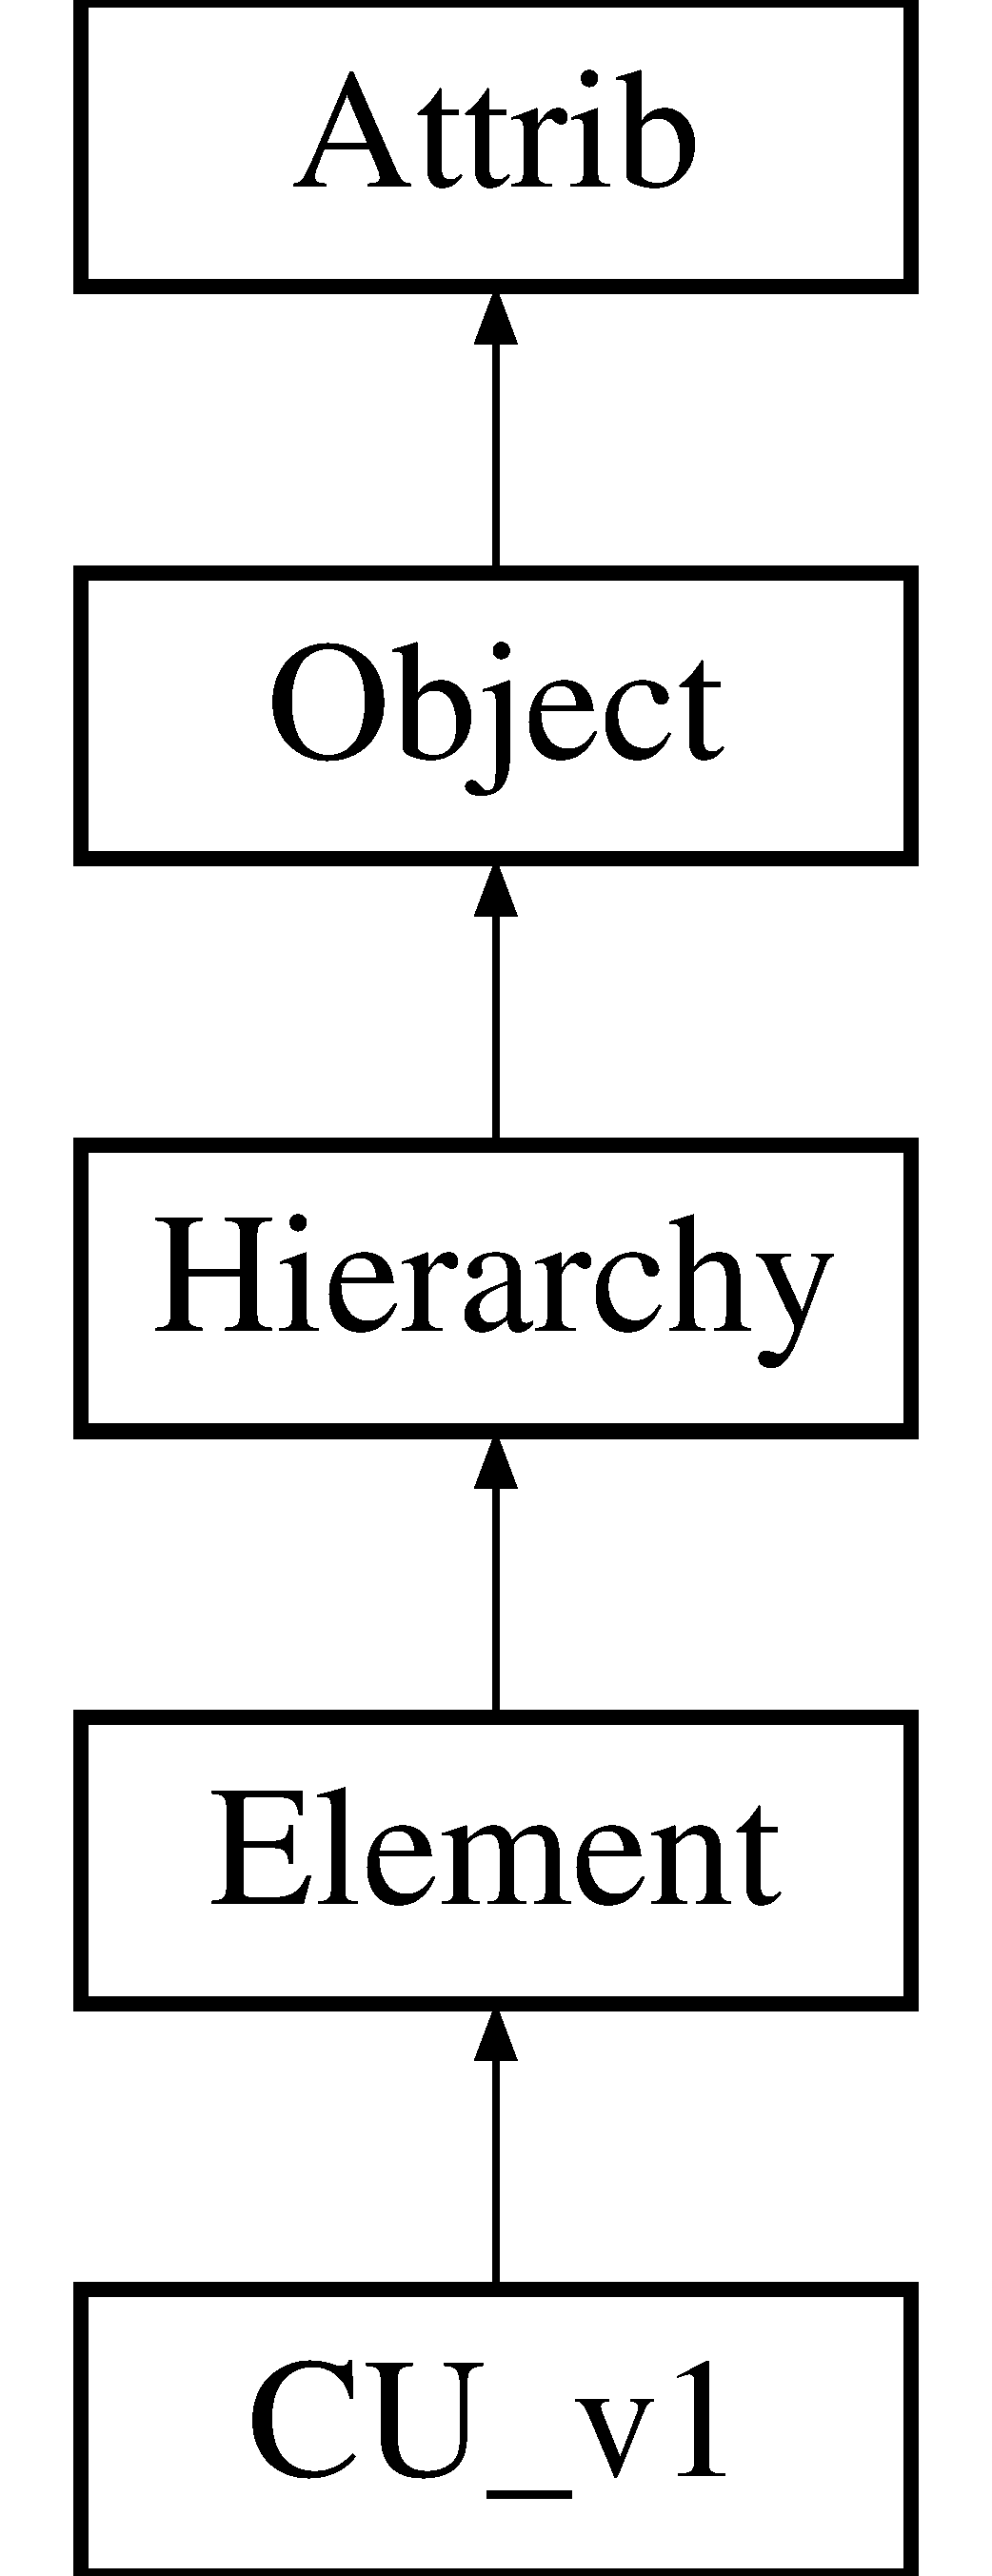
\includegraphics[height=5.000000cm]{classCU__v1}
\end{center}
\end{figure}
\subsection*{Public Types}
\begin{DoxyCompactItemize}
\item 
enum \hyperlink{classAttrib_a69e171d7cc6417835a5a306d3c764235}{Attribut} \{ \newline
\hyperlink{classAttrib_a69e171d7cc6417835a5a306d3c764235a3a8da2ab97dda18aebab196fe4100531}{U\+N\+D\+E\+F\+I\+N\+ED}, 
\hyperlink{classAttrib_a69e171d7cc6417835a5a306d3c764235a2bfb2af57b87031d190a05fe25dd92ed}{P\+A\+S\+S\+I\+VE}, 
\hyperlink{classAttrib_a69e171d7cc6417835a5a306d3c764235a3b1fec929c0370d1436f2f06e298fb0d}{A\+C\+T\+I\+VE}, 
\hyperlink{classAttrib_a69e171d7cc6417835a5a306d3c764235aa27c16b480a369ea4d18b07b2516bbc7}{I\+N\+T\+E\+R\+F\+A\+CE}, 
\newline
\hyperlink{classAttrib_a69e171d7cc6417835a5a306d3c764235a1420a5b8c0540b2af210b6975eded7f9}{IO}, 
\hyperlink{classAttrib_a69e171d7cc6417835a5a306d3c764235a0af3b0d0ac323c1704e6c69cf90add28}{I\+O\+D\+A\+TA}, 
\hyperlink{classAttrib_a69e171d7cc6417835a5a306d3c764235a7788bc5dd333fd8ce18562b269c9dab1}{E\+L\+E\+M\+E\+NT}, 
\hyperlink{classAttrib_a69e171d7cc6417835a5a306d3c764235a61ceb22149f365f1780d18f9d1459423}{H\+A\+R\+D\+W\+A\+RE}, 
\newline
\hyperlink{classAttrib_a69e171d7cc6417835a5a306d3c764235a75250e29692496e73effca2c0330977f}{P\+R\+O\+C\+E\+S\+S\+US}, 
\hyperlink{classAttrib_a69e171d7cc6417835a5a306d3c764235a103a67cd0b8f07ef478fa45d4356e27b}{S\+O\+F\+T\+W\+A\+RE}
 \}
\end{DoxyCompactItemize}
\subsection*{Public Member Functions}
\begin{DoxyCompactItemize}
\item 
\hyperlink{classCU__v1_afe2499a41abcb7cd94830d1eebb9e033}{C\+U\+\_\+v1} ()
\begin{DoxyCompactList}\small\item\em Standard constructor. \end{DoxyCompactList}\item 
virtual \hyperlink{classCU__v1_a5755cbfa835ce6935169e3133a5bfedf}{$\sim$\+C\+U\+\_\+v1} ()
\begin{DoxyCompactList}\small\item\em Destructor. \end{DoxyCompactList}\item 
void \hyperlink{classCU__v1_af4033fc5da7bff845565d7e6ea1802ce}{help} ()
\item 
\hyperlink{classStatusCode}{Status\+Code} \hyperlink{classCU__v1_a67278e2e8dcbd9b1e3a0284605f4103c}{init} ()
\item 
void \hyperlink{classCU__v1_add509ddd31f1a0c4d68b889ba6edfdb3}{reset} ()
\item 
void \hyperlink{classCU__v1_ac207d770edae7014f9b8ef86c43afc2c}{update} ()
\item 
\hyperlink{classFePGA}{Fe\+P\+GA} $\ast$ \hyperlink{classCU__v1_a6bdee7e086b6c0b2acee0879aee137ed}{fe\+Pga} ()
\item 
void \hyperlink{classCU__v1_ab57452edfcad0fa9efb23f8e4c532602}{read\+Fifo} (int, int, unsigned int $\ast$)
\item 
void \hyperlink{classElement_a3c0abcb36f8906688bb7e32608df7086}{recursive\+Init\+Element} ()
\item 
void \hyperlink{classElement_a82119ed37dff76508a2746a853ec35ba}{recursive\+Init\+Communications} ()
\item 
\hyperlink{classStatusCode}{Status\+Code} \hyperlink{classElement_ab476b4b1df5954141ceb14f072433b89}{set\+Connection} (\hyperlink{classHierarchy}{Hierarchy} $\ast$)
\item 
\hyperlink{classHierarchy}{Hierarchy} $\ast$ \hyperlink{classElement_af57444353c1ddf9fa0109801e97debf7}{connection} ()
\item 
void \hyperlink{classHierarchy_af4d43b0765b402670eed2d62c73405af}{clear} ()
\item 
void \hyperlink{classHierarchy_a585ad1aeec16077a0e532ab8b4fc557b}{set\+Parent} (\hyperlink{classHierarchy}{Hierarchy} $\ast$\hyperlink{classHierarchy_a1c7bec8257e717f9c1465e06ebf845fc}{parent})
\item 
\hyperlink{classHierarchy}{Hierarchy} $\ast$ \hyperlink{classHierarchy_a1c7bec8257e717f9c1465e06ebf845fc}{parent} ()
\item 
\hyperlink{classHierarchy}{Hierarchy} $\ast$ \hyperlink{classHierarchy_ad550588733bf75ac5c0fcfd7c8fd11a6}{parent} (std\+::string)
\item 
\hyperlink{classHierarchy}{Hierarchy} $\ast$ \hyperlink{classHierarchy_aee461dc930ce3871636ff87f075b1b83}{origin} ()
\item 
virtual void \hyperlink{classHierarchy_ad677774ff38fcb257c04a3a10d471fac}{add\+Child} (\hyperlink{classHierarchy}{Hierarchy} $\ast$element)
\item 
std\+::vector$<$ \hyperlink{classHierarchy}{Hierarchy} $\ast$ $>$ \hyperlink{classHierarchy_aa9a76f69e98e052ee1a6e32cea006288}{children} ()
\item 
\hyperlink{classHierarchy}{Hierarchy} $\ast$ \hyperlink{classHierarchy_a1e207f973c694b538bf90107b4868817}{child} (std\+::string)
\item 
\hyperlink{classHierarchy}{Hierarchy} $\ast$ \hyperlink{classHierarchy_a0c15a5276a3b80b4354d6bd8a01e0708}{child\+Typed} (std\+::string)
\item 
unsigned long \hyperlink{classHierarchy_ab16e84de65fd84e14001a6cf941c8be4}{number\+Of\+Children} ()
\item 
bool \hyperlink{classHierarchy_a255174fe4d316d2a3f430dcb9dab29f1}{has\+Children} ()
\item 
void \hyperlink{classHierarchy_a2b2b359fac003233f65786a616766bde}{del\+Child} (\hyperlink{classHierarchy}{Hierarchy} $\ast$)
\item 
void \hyperlink{classHierarchy_a1928ac7615fe0b5e55cd707f70dc6781}{del\+Child} (std\+::string)
\item 
std\+::string \hyperlink{classHierarchy_aa7990fa7caf132d83e361ce033c6c65a}{path} (std\+::string=std\+::string(\char`\"{}\char`\"{}))
\item 
std\+::string \hyperlink{classHierarchy_a1efd56cd164d328d2002e53a10a19b8c}{path\+Typed} (std\+::string=std\+::string(\char`\"{}\char`\"{}))
\item 
void \hyperlink{classHierarchy_a76e914b9a677a22a82deb74d892bf261}{tree} (std\+::string indent=std\+::string(\char`\"{}\char`\"{}))
\item 
void \hyperlink{classHierarchy_a594c294c5f60c230e106d522ed008212}{tree} ()
\item 
std\+::string \hyperlink{classObject_a300f4c05dd468c7bb8b3c968868443c1}{name} () const
\item 
std\+::string \hyperlink{classObject_a84f99f70f144a83e1582d1d0f84e4e62}{type} ()
\item 
unsigned char \hyperlink{classObject_af99145335cc61ff6e2798ea17db009d2}{id} ()
\item 
std\+::string \hyperlink{classObject_a73a0f1a41828fdd8303dd662446fb6c3}{title} ()
\item 
void \hyperlink{classObject_a3f9d5537ebce0c0f2bf6ae4d92426f3c}{msg\+Svc} (int level, std\+::string \hyperlink{classObject_a58b2d0618c2d08cf2383012611528d97}{msg}, std\+::string \hyperlink{classObject_a300f4c05dd468c7bb8b3c968868443c1}{name})
\item 
void \hyperlink{classObject_a58b2d0618c2d08cf2383012611528d97}{msg} (std\+::string mymsg)
\item 
void \hyperlink{classObject_ac5d59299273cee27aacf7de00d2e7034}{msg} (std\+::string mymsg, std\+::string \hyperlink{classObject_a300f4c05dd468c7bb8b3c968868443c1}{name})
\item 
void \hyperlink{classObject_a83d2db2df682907ea1115ad721c1c4a1}{verbose} (std\+::string mymsg)
\item 
void \hyperlink{classObject_a2d4120195317e2a3c6532e8bb9f3da68}{verbose} (std\+::string mymsg, std\+::string \hyperlink{classObject_a300f4c05dd468c7bb8b3c968868443c1}{name})
\item 
void \hyperlink{classObject_aac010553f022165573714b7014a15f0d}{debug} (std\+::string mymsg)
\item 
void \hyperlink{classObject_a6c9a0397ca804e04d675ed05683f5420}{debug} (std\+::string mymsg, std\+::string \hyperlink{classObject_a300f4c05dd468c7bb8b3c968868443c1}{name})
\item 
void \hyperlink{classObject_a644fd329ea4cb85f54fa6846484b84a8}{info} (std\+::string mymsg)
\item 
void \hyperlink{classObject_a1ca123253dfd30fc28b156f521dcbdae}{info} (std\+::string mymsg, std\+::string \hyperlink{classObject_a300f4c05dd468c7bb8b3c968868443c1}{name})
\item 
void \hyperlink{classObject_a65cd4fda577711660821fd2cd5a3b4c9}{warning} (std\+::string mymsg)
\item 
void \hyperlink{classObject_a11f101db4dd73d9391b0231818881d86}{warning} (std\+::string mymsg, std\+::string \hyperlink{classObject_a300f4c05dd468c7bb8b3c968868443c1}{name})
\item 
void \hyperlink{classObject_a204a95f57818c0f811933917a30eff45}{error} (std\+::string mymsg)
\item 
void \hyperlink{classObject_ad7f6c457733082efa2f9ff5f5c8e119a}{error} (std\+::string mymsg, std\+::string \hyperlink{classObject_a300f4c05dd468c7bb8b3c968868443c1}{name})
\item 
void \hyperlink{classObject_aad5a16aac7516ce65bd5ec02ab07fc80}{fatal} (std\+::string mymsg)
\item 
void \hyperlink{classObject_ae62acd3d09f716220f75f252dc38bc9a}{fatal} (std\+::string mymsg, std\+::string \hyperlink{classObject_a300f4c05dd468c7bb8b3c968868443c1}{name})
\item 
void \hyperlink{classObject_ae30fea75683c2d149b6b6d17c09ecd0c}{set\+Name} (std\+::string \hyperlink{classObject_a300f4c05dd468c7bb8b3c968868443c1}{name})
\item 
void \hyperlink{classObject_aae534cc9d982bcb9b99fd505f2e103a5}{set\+Type} (std\+::string \hyperlink{classObject_a84f99f70f144a83e1582d1d0f84e4e62}{type})
\item 
void \hyperlink{classObject_a398fe08cba594a0ce6891d59fe4f159f}{set\+Id} (unsigned char \hyperlink{classObject_af99145335cc61ff6e2798ea17db009d2}{id})
\item 
void \hyperlink{classObject_a89557dbbad5bcaa02652f5d7fa35d20f}{set\+Title} (std\+::string \hyperlink{classObject_a73a0f1a41828fdd8303dd662446fb6c3}{title})
\item 
void \hyperlink{classObject_a870c5af919958c2136623b2d7816d123}{set\+Dll\+Name} (std\+::string \hyperlink{classObject_a2e3947f2870094c332d7454117f3ec63}{dll\+Name})
\item 
std\+::string \hyperlink{classObject_a2e3947f2870094c332d7454117f3ec63}{dll\+Name} ()
\item 
bool \hyperlink{classAttrib_a704f26af560909ad22065083bb7d4c34}{is} (int attribut)
\item 
void \hyperlink{classAttrib_a235f773af19c900264a190b00a3b4ad7}{add} (int attribut)
\item 
void \hyperlink{classAttrib_a7d4ef7e32d93cb287792b87b857e79f3}{remove} (int attribut)
\item 
std\+::string \hyperlink{classAttrib_aee7bbf16b144887f196e1341b24f8a26}{attributs} ()
\end{DoxyCompactItemize}
\subsection*{Protected Attributes}
\begin{DoxyCompactItemize}
\item 
\hyperlink{classHierarchy}{Hierarchy} $\ast$ \hyperlink{classElement_abe3de7a5dbbc9a6dd2d7e012e5fdb266}{m\+\_\+connection}
\item 
std\+::string \hyperlink{classAttrib_a3414521d7a82476e874b25a5407b5e63}{m\+\_\+attrib\+String} \mbox{[}10\mbox{]}
\end{DoxyCompactItemize}
\subsection*{Private Attributes}
\begin{DoxyCompactItemize}
\item 
int \hyperlink{classCU__v1_abc59a6644473bc4fdccc24e2a0c9d6ae}{m\+\_\+fifo\+Depth}
\item 
int \hyperlink{classCU__v1_a108ebddb690763d5c99dd14021fd4851}{m\+\_\+gbt\+Address} \mbox{[}1\mbox{]}
\item 
int \hyperlink{classCU__v1_acc7767c15f48718ebc1ee87e22ab9fc1}{m\+\_\+fifo\+Inject\+Address} \mbox{[}3\mbox{]}
\item 
\hyperlink{classFePGA}{Fe\+P\+GA} $\ast$ \hyperlink{classCU__v1_a1b96b95e89dbe383877b34f9b517d910}{m\+\_\+fe\+Pga}
\item 
unsigned int $\ast$ \hyperlink{classCU__v1_abdc4ba4c63bcc1bbe2d7cd2a47b02b01}{m\+\_\+fifo} \mbox{[}3\mbox{]}
\item 
\hyperlink{classData}{Data} $\ast$ \hyperlink{classCU__v1_a50b6749064da173d6a5fddf50f4398eb}{m\+\_\+data}
\item 
\hyperlink{classRAM}{R\+AM} $\ast$ \hyperlink{classCU__v1_aa662d0f99787a174650fc92fb55dbb06}{m\+\_\+ram\+Inj} \mbox{[}3\mbox{]}
\item 
\hyperlink{classRAM}{R\+AM} $\ast$ \hyperlink{classCU__v1_a87ad8f5f9ecaf5f0f70b25206e99c8e1}{m\+\_\+fifo\+Usb\+Test}
\end{DoxyCompactItemize}


\subsection{Detailed Description}
\begin{DoxyAuthor}{Author}

\end{DoxyAuthor}
\begin{DoxyDate}{Date}
2006-\/10-\/23 
\end{DoxyDate}


Definition at line 19 of file C\+U\+\_\+v1.\+h.



\subsection{Member Enumeration Documentation}
\mbox{\Hypertarget{classAttrib_a69e171d7cc6417835a5a306d3c764235}\label{classAttrib_a69e171d7cc6417835a5a306d3c764235}} 
\index{C\+U\+\_\+v1@{C\+U\+\_\+v1}!Attribut@{Attribut}}
\index{Attribut@{Attribut}!C\+U\+\_\+v1@{C\+U\+\_\+v1}}
\subsubsection{\texorpdfstring{Attribut}{Attribut}}
{\footnotesize\ttfamily enum \hyperlink{classAttrib_a69e171d7cc6417835a5a306d3c764235}{Attrib\+::\+Attribut}\hspace{0.3cm}{\ttfamily [inherited]}}

\begin{DoxyEnumFields}{Enumerator}
\raisebox{\heightof{T}}[0pt][0pt]{\index{U\+N\+D\+E\+F\+I\+N\+ED@{U\+N\+D\+E\+F\+I\+N\+ED}!C\+U\+\_\+v1@{C\+U\+\_\+v1}}\index{C\+U\+\_\+v1@{C\+U\+\_\+v1}!U\+N\+D\+E\+F\+I\+N\+ED@{U\+N\+D\+E\+F\+I\+N\+ED}}}\mbox{\Hypertarget{classAttrib_a69e171d7cc6417835a5a306d3c764235a3a8da2ab97dda18aebab196fe4100531}\label{classAttrib_a69e171d7cc6417835a5a306d3c764235a3a8da2ab97dda18aebab196fe4100531}} 
U\+N\+D\+E\+F\+I\+N\+ED&\\
\hline

\raisebox{\heightof{T}}[0pt][0pt]{\index{P\+A\+S\+S\+I\+VE@{P\+A\+S\+S\+I\+VE}!C\+U\+\_\+v1@{C\+U\+\_\+v1}}\index{C\+U\+\_\+v1@{C\+U\+\_\+v1}!P\+A\+S\+S\+I\+VE@{P\+A\+S\+S\+I\+VE}}}\mbox{\Hypertarget{classAttrib_a69e171d7cc6417835a5a306d3c764235a2bfb2af57b87031d190a05fe25dd92ed}\label{classAttrib_a69e171d7cc6417835a5a306d3c764235a2bfb2af57b87031d190a05fe25dd92ed}} 
P\+A\+S\+S\+I\+VE&\\
\hline

\raisebox{\heightof{T}}[0pt][0pt]{\index{A\+C\+T\+I\+VE@{A\+C\+T\+I\+VE}!C\+U\+\_\+v1@{C\+U\+\_\+v1}}\index{C\+U\+\_\+v1@{C\+U\+\_\+v1}!A\+C\+T\+I\+VE@{A\+C\+T\+I\+VE}}}\mbox{\Hypertarget{classAttrib_a69e171d7cc6417835a5a306d3c764235a3b1fec929c0370d1436f2f06e298fb0d}\label{classAttrib_a69e171d7cc6417835a5a306d3c764235a3b1fec929c0370d1436f2f06e298fb0d}} 
A\+C\+T\+I\+VE&\\
\hline

\raisebox{\heightof{T}}[0pt][0pt]{\index{I\+N\+T\+E\+R\+F\+A\+CE@{I\+N\+T\+E\+R\+F\+A\+CE}!C\+U\+\_\+v1@{C\+U\+\_\+v1}}\index{C\+U\+\_\+v1@{C\+U\+\_\+v1}!I\+N\+T\+E\+R\+F\+A\+CE@{I\+N\+T\+E\+R\+F\+A\+CE}}}\mbox{\Hypertarget{classAttrib_a69e171d7cc6417835a5a306d3c764235aa27c16b480a369ea4d18b07b2516bbc7}\label{classAttrib_a69e171d7cc6417835a5a306d3c764235aa27c16b480a369ea4d18b07b2516bbc7}} 
I\+N\+T\+E\+R\+F\+A\+CE&\\
\hline

\raisebox{\heightof{T}}[0pt][0pt]{\index{IO@{IO}!C\+U\+\_\+v1@{C\+U\+\_\+v1}}\index{C\+U\+\_\+v1@{C\+U\+\_\+v1}!IO@{IO}}}\mbox{\Hypertarget{classAttrib_a69e171d7cc6417835a5a306d3c764235a1420a5b8c0540b2af210b6975eded7f9}\label{classAttrib_a69e171d7cc6417835a5a306d3c764235a1420a5b8c0540b2af210b6975eded7f9}} 
IO&\\
\hline

\raisebox{\heightof{T}}[0pt][0pt]{\index{I\+O\+D\+A\+TA@{I\+O\+D\+A\+TA}!C\+U\+\_\+v1@{C\+U\+\_\+v1}}\index{C\+U\+\_\+v1@{C\+U\+\_\+v1}!I\+O\+D\+A\+TA@{I\+O\+D\+A\+TA}}}\mbox{\Hypertarget{classAttrib_a69e171d7cc6417835a5a306d3c764235a0af3b0d0ac323c1704e6c69cf90add28}\label{classAttrib_a69e171d7cc6417835a5a306d3c764235a0af3b0d0ac323c1704e6c69cf90add28}} 
I\+O\+D\+A\+TA&\\
\hline

\raisebox{\heightof{T}}[0pt][0pt]{\index{E\+L\+E\+M\+E\+NT@{E\+L\+E\+M\+E\+NT}!C\+U\+\_\+v1@{C\+U\+\_\+v1}}\index{C\+U\+\_\+v1@{C\+U\+\_\+v1}!E\+L\+E\+M\+E\+NT@{E\+L\+E\+M\+E\+NT}}}\mbox{\Hypertarget{classAttrib_a69e171d7cc6417835a5a306d3c764235a7788bc5dd333fd8ce18562b269c9dab1}\label{classAttrib_a69e171d7cc6417835a5a306d3c764235a7788bc5dd333fd8ce18562b269c9dab1}} 
E\+L\+E\+M\+E\+NT&\\
\hline

\raisebox{\heightof{T}}[0pt][0pt]{\index{H\+A\+R\+D\+W\+A\+RE@{H\+A\+R\+D\+W\+A\+RE}!C\+U\+\_\+v1@{C\+U\+\_\+v1}}\index{C\+U\+\_\+v1@{C\+U\+\_\+v1}!H\+A\+R\+D\+W\+A\+RE@{H\+A\+R\+D\+W\+A\+RE}}}\mbox{\Hypertarget{classAttrib_a69e171d7cc6417835a5a306d3c764235a61ceb22149f365f1780d18f9d1459423}\label{classAttrib_a69e171d7cc6417835a5a306d3c764235a61ceb22149f365f1780d18f9d1459423}} 
H\+A\+R\+D\+W\+A\+RE&\\
\hline

\raisebox{\heightof{T}}[0pt][0pt]{\index{P\+R\+O\+C\+E\+S\+S\+US@{P\+R\+O\+C\+E\+S\+S\+US}!C\+U\+\_\+v1@{C\+U\+\_\+v1}}\index{C\+U\+\_\+v1@{C\+U\+\_\+v1}!P\+R\+O\+C\+E\+S\+S\+US@{P\+R\+O\+C\+E\+S\+S\+US}}}\mbox{\Hypertarget{classAttrib_a69e171d7cc6417835a5a306d3c764235a75250e29692496e73effca2c0330977f}\label{classAttrib_a69e171d7cc6417835a5a306d3c764235a75250e29692496e73effca2c0330977f}} 
P\+R\+O\+C\+E\+S\+S\+US&\\
\hline

\raisebox{\heightof{T}}[0pt][0pt]{\index{S\+O\+F\+T\+W\+A\+RE@{S\+O\+F\+T\+W\+A\+RE}!C\+U\+\_\+v1@{C\+U\+\_\+v1}}\index{C\+U\+\_\+v1@{C\+U\+\_\+v1}!S\+O\+F\+T\+W\+A\+RE@{S\+O\+F\+T\+W\+A\+RE}}}\mbox{\Hypertarget{classAttrib_a69e171d7cc6417835a5a306d3c764235a103a67cd0b8f07ef478fa45d4356e27b}\label{classAttrib_a69e171d7cc6417835a5a306d3c764235a103a67cd0b8f07ef478fa45d4356e27b}} 
S\+O\+F\+T\+W\+A\+RE&\\
\hline

\end{DoxyEnumFields}


Definition at line 29 of file Attrib.\+h.


\begin{DoxyCode}
29                 \{
30     \hyperlink{classAttrib_a69e171d7cc6417835a5a306d3c764235a3a8da2ab97dda18aebab196fe4100531}{UNDEFINED},
31     \hyperlink{classAttrib_a69e171d7cc6417835a5a306d3c764235a2bfb2af57b87031d190a05fe25dd92ed}{PASSIVE},
32     \hyperlink{classAttrib_a69e171d7cc6417835a5a306d3c764235a3b1fec929c0370d1436f2f06e298fb0d}{ACTIVE},
33     \hyperlink{classAttrib_a69e171d7cc6417835a5a306d3c764235aa27c16b480a369ea4d18b07b2516bbc7}{INTERFACE},
34     \hyperlink{classAttrib_a69e171d7cc6417835a5a306d3c764235a1420a5b8c0540b2af210b6975eded7f9}{IO},
35     \hyperlink{classAttrib_a69e171d7cc6417835a5a306d3c764235a0af3b0d0ac323c1704e6c69cf90add28}{IODATA},
36     \hyperlink{classAttrib_a69e171d7cc6417835a5a306d3c764235a7788bc5dd333fd8ce18562b269c9dab1}{ELEMENT},
37     \hyperlink{classAttrib_a69e171d7cc6417835a5a306d3c764235a61ceb22149f365f1780d18f9d1459423}{HARDWARE},
38     \hyperlink{classAttrib_a69e171d7cc6417835a5a306d3c764235a75250e29692496e73effca2c0330977f}{PROCESSUS},
39     \hyperlink{classAttrib_a69e171d7cc6417835a5a306d3c764235a103a67cd0b8f07ef478fa45d4356e27b}{SOFTWARE} 
40   \}; \textcolor{comment}{// array m\_attribString must be changed into Attrib::Attrib if this enu is modified. }
\end{DoxyCode}


\subsection{Constructor \& Destructor Documentation}
\mbox{\Hypertarget{classCU__v1_afe2499a41abcb7cd94830d1eebb9e033}\label{classCU__v1_afe2499a41abcb7cd94830d1eebb9e033}} 
\index{C\+U\+\_\+v1@{C\+U\+\_\+v1}!C\+U\+\_\+v1@{C\+U\+\_\+v1}}
\index{C\+U\+\_\+v1@{C\+U\+\_\+v1}!C\+U\+\_\+v1@{C\+U\+\_\+v1}}
\subsubsection{\texorpdfstring{C\+U\+\_\+v1()}{CU\_v1()}}
{\footnotesize\ttfamily C\+U\+\_\+v1\+::\+C\+U\+\_\+v1 (\begin{DoxyParamCaption}{ }\end{DoxyParamCaption})}



Standard constructor. 



Definition at line 17 of file C\+U\+\_\+v1.\+cpp.



References Attrib\+::add(), Hierarchy\+::add\+Child(), Attrib\+::\+E\+L\+E\+M\+E\+NT, Attrib\+::\+H\+A\+R\+D\+W\+A\+RE, m\+\_\+fe\+Pga, m\+\_\+fifo\+Depth, Object\+::set\+Name(), and Object\+::set\+Type().


\begin{DoxyCode}
17                \{
18   \hyperlink{classObject_ae30fea75683c2d149b6b6d17c09ecd0c}{setName}(\textcolor{stringliteral}{"CU\_v1"});
19   \hyperlink{classObject_aae534cc9d982bcb9b99fd505f2e103a5}{setType}(\textcolor{stringliteral}{"CU\_v1"});
20   \hyperlink{classAttrib_a235f773af19c900264a190b00a3b4ad7}{add}(\hyperlink{classAttrib_a69e171d7cc6417835a5a306d3c764235a7788bc5dd333fd8ce18562b269c9dab1}{Attrib::ELEMENT}); \hyperlink{classAttrib_a235f773af19c900264a190b00a3b4ad7}{add} (\hyperlink{classAttrib_a69e171d7cc6417835a5a306d3c764235a61ceb22149f365f1780d18f9d1459423}{Attrib::HARDWARE});  
21 
22   \hyperlink{classCU__v1_abc59a6644473bc4fdccc24e2a0c9d6ae}{m\_fifoDepth} = 1024;
23   
24   \textcolor{comment}{//m\_seqAddress   = 17 ;  // c'est l'addresse du FPGA }
25   \textcolor{comment}{//m\_fifoInjectAddress[0] = 23;  // What should I do here? }
26 
27   \hyperlink{classCU__v1_a1b96b95e89dbe383877b34f9b517d910}{m\_fePga} =\textcolor{keyword}{new} \hyperlink{classFePGA}{FePGA}();
28   \hyperlink{classCU__v1_a1b96b95e89dbe383877b34f9b517d910}{m\_fePga}->\hyperlink{classObject_ae30fea75683c2d149b6b6d17c09ecd0c}{setName}(\textcolor{stringliteral}{"FePGA"});
29   \hyperlink{classHierarchy_ad677774ff38fcb257c04a3a10d471fac}{addChild}(\hyperlink{classCU__v1_a1b96b95e89dbe383877b34f9b517d910}{m\_fePga});
30 
31   \textcolor{comment}{/*}
32 \textcolor{comment}{}
33 \textcolor{comment}{  m\_fifo[0] = new unsigned int[m\_fifoDepth];}
34 \textcolor{comment}{  }
35 \textcolor{comment}{  for (int i = 0; i<3; ++i)\{  // Do I loop up to 3 too? Car Frederic a besoin de plus de place dans les RAM}
36 \textcolor{comment}{    m\_ramInj[i] = new RAM();}
37 \textcolor{comment}{    //    m\_ramSpy[i] = new RAM();}
38 \textcolor{comment}{    fePga()->usb()->addChild(m\_ramInj[i]);  // What should I do here ? }
39 \textcolor{comment}{    //    FePga()->usb()->addChild(m\_ramSpy[i]);}
40 \textcolor{comment}{    m\_ramInj[i]->setAddress(13); // for debug   // What should I do here ? }
41 \textcolor{comment}{    //m\_ramSpy[i]->setAddress(m\_fifoSpyAddress[i]);}
42 \textcolor{comment}{    m\_ramInj[i]->setSize(16, m\_fifoDepth);   // What should I do here ? }
43 \textcolor{comment}{    // m\_ramSpy[i]->setSize(16, m\_fifoDepth);}
44 \textcolor{comment}{  \}}
45 \textcolor{comment}{}
46 \textcolor{comment}{}
47 \textcolor{comment}{}
48 \textcolor{comment}{  }
49 \textcolor{comment}{  m\_fifoUsbTest = new RAM();}
50 \textcolor{comment}{  m\_fifoUsbTest->setAddress(3); // WARNING I NEED TO CHANGE THE ADDRESS }
51 \textcolor{comment}{  m\_fifoUsbTest->setSize(16,256);  //  WHAT SIZE FOR I NNED }
52 \textcolor{comment}{  m\_fifoUsbTest->setName("FifoUsbTest");}
53 \textcolor{comment}{  fePga()->usb()->addChild(m\_fifoUsbTest);}
54 \textcolor{comment}{*/}  
55 
56 \}
\end{DoxyCode}
\mbox{\Hypertarget{classCU__v1_a5755cbfa835ce6935169e3133a5bfedf}\label{classCU__v1_a5755cbfa835ce6935169e3133a5bfedf}} 
\index{C\+U\+\_\+v1@{C\+U\+\_\+v1}!````~C\+U\+\_\+v1@{$\sim$\+C\+U\+\_\+v1}}
\index{````~C\+U\+\_\+v1@{$\sim$\+C\+U\+\_\+v1}!C\+U\+\_\+v1@{C\+U\+\_\+v1}}
\subsubsection{\texorpdfstring{$\sim$\+C\+U\+\_\+v1()}{~CU\_v1()}}
{\footnotesize\ttfamily C\+U\+\_\+v1\+::$\sim$\+C\+U\+\_\+v1 (\begin{DoxyParamCaption}{ }\end{DoxyParamCaption})\hspace{0.3cm}{\ttfamily [virtual]}}



Destructor. 



Definition at line 60 of file C\+U\+\_\+v1.\+cpp.


\begin{DoxyCode}
60               \{
61 \}
\end{DoxyCode}


\subsection{Member Function Documentation}
\mbox{\Hypertarget{classAttrib_a235f773af19c900264a190b00a3b4ad7}\label{classAttrib_a235f773af19c900264a190b00a3b4ad7}} 
\index{C\+U\+\_\+v1@{C\+U\+\_\+v1}!add@{add}}
\index{add@{add}!C\+U\+\_\+v1@{C\+U\+\_\+v1}}
\subsubsection{\texorpdfstring{add()}{add()}}
{\footnotesize\ttfamily void Attrib\+::add (\begin{DoxyParamCaption}\item[{int}]{attribut }\end{DoxyParamCaption})\hspace{0.3cm}{\ttfamily [inline]}, {\ttfamily [inherited]}}

Add an attribut 

Definition at line 67 of file Attrib.\+h.



References Attrib\+::m\+\_\+attributs, and Attrib\+::\+U\+N\+D\+E\+F\+I\+N\+ED.



Referenced by A3\+P\+E\+::\+A3\+P\+E(), Attrib\+::\+Attrib(), Specs\+Mezzanine\+::cmdline(), Computer\+::\+Computer(), C\+U\+\_\+v1(), export\+\_\+obj(), F\+E\+B\+\_\+v1\+::\+F\+E\+B\+\_\+v1(), Fe\+P\+G\+A\+::\+Fe\+P\+G\+A(), I\+C\+E\+C\+A\+Lv3\+::\+I\+C\+E\+C\+A\+Lv3(), I\+C\+Phaser\+::\+I\+C\+Phaser(), Fe\+P\+G\+A\+::init(), Application\+::initialize(), Interface\+::\+Interface(), I\+Odata\+::\+I\+Odata(), I\+Oobject\+::\+I\+Oobject(), M\+S\+Oxxxx\+::\+M\+S\+Oxxxx(), Phaser\+::\+Phaser(), Processus\+::\+Processus(), Proto40\+M\+Hz\+\_\+v1\+::\+Proto40\+M\+Hz\+\_\+v1(), Attrib\+::remove(), Seq\+P\+G\+A\+::\+Seq\+P\+G\+A(), Test\+S\+P\+I\+::set\+Address(), Test\+I2\+C\+::set\+Address(), Specs\+Slave\+::set\+Address(), Specs\+Master\+::\+Specs\+Master(), and Specs\+Slave\+::\+Specs\+Slave().


\begin{DoxyCode}
67                             \{
68     \textcolor{keywordflow}{if} (attribut!=\hyperlink{classAttrib_a69e171d7cc6417835a5a306d3c764235a3a8da2ab97dda18aebab196fe4100531}{Attrib::UNDEFINED}) \textcolor{keyword}{remove}(\hyperlink{classAttrib_a69e171d7cc6417835a5a306d3c764235a3a8da2ab97dda18aebab196fe4100531}{Attrib::UNDEFINED});
69     \textcolor{keywordtype}{bool} duplicate = false ;
70     std::vector<int>::const\_iterator iter ;
71     \textcolor{keywordflow}{for} ( iter  = \hyperlink{classAttrib_ac4bd58a0cc6b38a3b711d609a3d3aacc}{m\_attributs}.begin() ;
72           iter != \hyperlink{classAttrib_ac4bd58a0cc6b38a3b711d609a3d3aacc}{m\_attributs}.end()   ;
73           ++iter ) \{
74       \textcolor{keywordflow}{if} ( attribut == (*iter) ) \{
75         duplicate = true ;
76       \}
77     \}
78     \textcolor{keywordflow}{if} (!duplicate) \{
79       \hyperlink{classAttrib_ac4bd58a0cc6b38a3b711d609a3d3aacc}{m\_attributs}.push\_back( attribut );
80     \}
81   \}
\end{DoxyCode}
\mbox{\Hypertarget{classHierarchy_ad677774ff38fcb257c04a3a10d471fac}\label{classHierarchy_ad677774ff38fcb257c04a3a10d471fac}} 
\index{C\+U\+\_\+v1@{C\+U\+\_\+v1}!add\+Child@{add\+Child}}
\index{add\+Child@{add\+Child}!C\+U\+\_\+v1@{C\+U\+\_\+v1}}
\subsubsection{\texorpdfstring{add\+Child()}{addChild()}}
{\footnotesize\ttfamily void Hierarchy\+::add\+Child (\begin{DoxyParamCaption}\item[{\hyperlink{classHierarchy}{Hierarchy} $\ast$}]{element }\end{DoxyParamCaption})\hspace{0.3cm}{\ttfamily [virtual]}, {\ttfamily [inherited]}}



Definition at line 83 of file Hierarchy.\+cpp.



References Object\+::debug(), Hierarchy\+::m\+\_\+children, Object\+::name(), and Hierarchy\+::set\+Parent().



Referenced by A3\+P\+E\+::\+A3\+P\+E(), Specs\+Mezzanine\+::add\+Bus(), Specs\+Slave\+::add\+I2c(), Application\+::create(), C\+U\+\_\+v1(), export\+\_\+obj(), F\+E\+B\+\_\+v1\+::\+F\+E\+B\+\_\+v1(), Fe\+P\+G\+A\+::\+Fe\+P\+G\+A(), I\+C\+E\+C\+A\+Lv3\+::\+I\+C\+E\+C\+A\+Lv3(), I\+C\+Phaser\+::\+I\+C\+Phaser(), Fe\+P\+G\+A\+::\+Make\+R\+A\+M(), Fe\+P\+G\+A\+::\+Make\+Register(), Hierarchy\+::origin(), Phaser\+::\+Phaser(), Proto40\+M\+Hz\+\_\+v1\+::\+Proto40\+M\+Hz\+\_\+v1(), Seq\+P\+G\+A\+::\+Seq\+P\+G\+A(), Specs\+Mezzanine\+::\+Specs\+Mezzanine(), Usb\+I2c\+Bus\+::\+Usb\+I2c\+Bus(), and Usb\+Spi\+Bus\+::\+Usb\+Spi\+Bus().


\begin{DoxyCode}
83                                           \{
84   element->\hyperlink{classHierarchy_a585ad1aeec16077a0e532ab8b4fc557b}{setParent}(\textcolor{keyword}{this});
85   \hyperlink{classHierarchy_a038816763941fd4a930504917f60483b}{m\_children}.push\_back(element);
86   \hyperlink{classObject_aac010553f022165573714b7014a15f0d}{debug}(element->\hyperlink{classObject_a300f4c05dd468c7bb8b3c968868443c1}{name}()+\textcolor{stringliteral}{" added to the child tree."},\textcolor{stringliteral}{"Hierarchy::addChild"});
87 \}
\end{DoxyCode}
\mbox{\Hypertarget{classAttrib_aee7bbf16b144887f196e1341b24f8a26}\label{classAttrib_aee7bbf16b144887f196e1341b24f8a26}} 
\index{C\+U\+\_\+v1@{C\+U\+\_\+v1}!attributs@{attributs}}
\index{attributs@{attributs}!C\+U\+\_\+v1@{C\+U\+\_\+v1}}
\subsubsection{\texorpdfstring{attributs()}{attributs()}}
{\footnotesize\ttfamily std\+::string Attrib\+::attributs (\begin{DoxyParamCaption}{ }\end{DoxyParamCaption})\hspace{0.3cm}{\ttfamily [inherited]}}

Print the \hyperlink{classAttrib}{Attrib} of an \hyperlink{classObject}{Object} 

Definition at line 54 of file Attrib.\+cpp.



References images\+::index, Attrib\+::m\+\_\+attrib\+String, and Attrib\+::m\+\_\+attributs.



Referenced by export\+\_\+obj(), and Attrib\+::remove().


\begin{DoxyCode}
54                             \{
55   std::string output;
56   std::vector<int>::iterator iter ;
57   \textcolor{keywordflow}{for} ( \textcolor{keywordtype}{unsigned} \textcolor{keywordtype}{int} \hyperlink{namespaceimages_a54407fd574970b3178647ae096321a57}{index} = 0 ; \hyperlink{namespaceimages_a54407fd574970b3178647ae096321a57}{index} < \hyperlink{classAttrib_ac4bd58a0cc6b38a3b711d609a3d3aacc}{m\_attributs}.size() ; ++
      \hyperlink{namespaceimages_a54407fd574970b3178647ae096321a57}{index} ) \{
58     \textcolor{keywordflow}{if} ( \hyperlink{classAttrib_ac4bd58a0cc6b38a3b711d609a3d3aacc}{m\_attributs}.size() - \hyperlink{namespaceimages_a54407fd574970b3178647ae096321a57}{index} > 1 ) \{
59       output.append(\hyperlink{classAttrib_a3414521d7a82476e874b25a5407b5e63}{m\_attribString}[\hyperlink{classAttrib_ac4bd58a0cc6b38a3b711d609a3d3aacc}{m\_attributs}[\hyperlink{namespaceimages_a54407fd574970b3178647ae096321a57}{index}]]);
60       output.append(\textcolor{stringliteral}{":"});
61     \}
62     \textcolor{keywordflow}{else} \{
63       output.append(\hyperlink{classAttrib_a3414521d7a82476e874b25a5407b5e63}{m\_attribString}[\hyperlink{classAttrib_ac4bd58a0cc6b38a3b711d609a3d3aacc}{m\_attributs}[index]]);
64     \}
65   \}
66   \textcolor{keywordflow}{return} output;
67 \}
\end{DoxyCode}
\mbox{\Hypertarget{classHierarchy_a1e207f973c694b538bf90107b4868817}\label{classHierarchy_a1e207f973c694b538bf90107b4868817}} 
\index{C\+U\+\_\+v1@{C\+U\+\_\+v1}!child@{child}}
\index{child@{child}!C\+U\+\_\+v1@{C\+U\+\_\+v1}}
\subsubsection{\texorpdfstring{child()}{child()}}
{\footnotesize\ttfamily \hyperlink{classHierarchy}{Hierarchy} $\ast$ Hierarchy\+::child (\begin{DoxyParamCaption}\item[{std\+::string}]{path }\end{DoxyParamCaption})\hspace{0.3cm}{\ttfamily [inherited]}}



Definition at line 133 of file Hierarchy.\+cpp.



References Hierarchy\+::child(), Hierarchy\+::children(), Object\+::name(), Hierarchy\+::origin(), Hierarchy\+::parent(), Hierarchy\+::path(), and Object\+::warning().



Referenced by Application\+::cd(), Hierarchy\+::child(), Hierarchy\+::children(), and export\+\_\+obj().


\begin{DoxyCode}
133                                          \{
134   std::string newpath = \hyperlink{classHierarchy_aa7990fa7caf132d83e361ce033c6c65a}{path};
135   std::string up(\textcolor{stringliteral}{".."});
136   std::string separator(1,\textcolor{charliteral}{'/'});
137 
138   \hyperlink{classHierarchy}{Hierarchy} * newcurrent = 0;
139 
140   \textcolor{comment}{//  info("path="+path,"Hierarchy::child");}
141 
142   \textcolor{keywordflow}{if} (\hyperlink{classHierarchy_aa7990fa7caf132d83e361ce033c6c65a}{path}.compare(\textcolor{stringliteral}{""})==0 || \hyperlink{classHierarchy_aa7990fa7caf132d83e361ce033c6c65a}{path}.compare(\textcolor{stringliteral}{"/"})==0) \{
143     \textcolor{comment}{//    debug("return origin","Hierarchy::child");}
144     \textcolor{keywordflow}{return} \hyperlink{classHierarchy_aee461dc930ce3871636ff87f075b1b83}{origin}();
145   \}
146 
147   \textcolor{keywordflow}{if} (\hyperlink{classHierarchy_aa7990fa7caf132d83e361ce033c6c65a}{path}.compare(\hyperlink{classObject_a300f4c05dd468c7bb8b3c968868443c1}{name}())==0)\{
148     \textcolor{comment}{//    debug("return itself","Hierarchy::child");}
149     \textcolor{keywordflow}{return} \textcolor{keyword}{this};
150   \}
151 
152   \textcolor{keywordflow}{if} (\hyperlink{classHierarchy_aa7990fa7caf132d83e361ce033c6c65a}{path}.compare(\textcolor{stringliteral}{".."})==0)\{
153     \textcolor{keywordflow}{if} (0!=this->\hyperlink{classHierarchy_a1c7bec8257e717f9c1465e06ebf845fc}{parent}()) \textcolor{keywordflow}{return} this->\hyperlink{classHierarchy_a1c7bec8257e717f9c1465e06ebf845fc}{parent}();
154     \textcolor{keywordflow}{else} \textcolor{keywordflow}{return} \textcolor{keyword}{this};
155   \}
156 
157   \textcolor{keywordflow}{if} (\hyperlink{classHierarchy_aa7990fa7caf132d83e361ce033c6c65a}{path}.compare(\textcolor{stringliteral}{"../"})==0)\{
158     \textcolor{keywordflow}{if} (0!=this->\hyperlink{classHierarchy_a1c7bec8257e717f9c1465e06ebf845fc}{parent}()) \textcolor{keywordflow}{return} this->\hyperlink{classHierarchy_a1c7bec8257e717f9c1465e06ebf845fc}{parent}();
159     \textcolor{keywordflow}{else} \textcolor{keywordflow}{return} \textcolor{keyword}{this};
160   \}
161 
162 
163   \textcolor{keywordtype}{int} npos=\hyperlink{classHierarchy_aa7990fa7caf132d83e361ce033c6c65a}{path}.find(separator,0);
164 
165   \textcolor{comment}{//  info("find separator in "+itos(npos)+" of "+path,"Hierarchy::child");}
166 
167   \textcolor{comment}{// remove last separator}
168   \textcolor{keywordflow}{if} ( npos == (\textcolor{keywordtype}{int})(\hyperlink{classHierarchy_aa7990fa7caf132d83e361ce033c6c65a}{path}.size()-1) ) \{
169     newpath = std::string(\hyperlink{classHierarchy_aa7990fa7caf132d83e361ce033c6c65a}{path},0,npos);
170     \hyperlink{classHierarchy_aa7990fa7caf132d83e361ce033c6c65a}{path} = newpath;
171   \}
172 
173   \textcolor{keywordflow}{if} (npos==0)\{
174     \textcolor{comment}{//    debug("Going back to origin and calling child","Hierarchy::child");}
175     newpath=std::string(\hyperlink{classHierarchy_aa7990fa7caf132d83e361ce033c6c65a}{path},1,\hyperlink{classHierarchy_aa7990fa7caf132d83e361ce033c6c65a}{path}.size()-1);
176     \textcolor{keywordflow}{return} \hyperlink{classHierarchy_aee461dc930ce3871636ff87f075b1b83}{origin}()->\hyperlink{classHierarchy_a1e207f973c694b538bf90107b4868817}{child}(newpath);
177   \}
178   \textcolor{keywordflow}{else}\{
179     \textcolor{keywordflow}{if} ( npos== (\textcolor{keywordtype}{int})(std::string::npos) )\{
180       \textcolor{comment}{//      debug("Getting chid "+path+" of "+this->name(),"Hierarchy::child");}
181       std::vector <Hierarchy*> list = \hyperlink{classHierarchy_aa9a76f69e98e052ee1a6e32cea006288}{children}();
182       std::vector<Hierarchy*>::iterator iter;
183       \textcolor{keywordflow}{for} (iter=list.begin();iter!=list.end();iter++)\{
184         \textcolor{keywordflow}{if} ((*iter)->name().compare(\hyperlink{classHierarchy_aa7990fa7caf132d83e361ce033c6c65a}{path})==0)\{
185           \textcolor{keywordflow}{return} *iter;
186         \}
187       \}
188       \hyperlink{classObject_a65cd4fda577711660821fd2cd5a3b4c9}{warning}(this->\hyperlink{classObject_a300f4c05dd468c7bb8b3c968868443c1}{name}()+std::string(\textcolor{stringliteral}{" has no child '"})+\hyperlink{classHierarchy_aa7990fa7caf132d83e361ce033c6c65a}{path}+\textcolor{stringliteral}{"'"},\textcolor{stringliteral}{"Hierarchy::child"});
189       \textcolor{keywordflow}{return} \textcolor{keyword}{this};
190     \}
191     \textcolor{keywordflow}{else}
192     \{
193       \textcolor{keywordtype}{int} ipos=\hyperlink{classHierarchy_aa7990fa7caf132d83e361ce033c6c65a}{path}.find(separator,0);
194       \textcolor{comment}{//      info("default behaviour "+path+" with separator in "+itos(ipos),"Hierarchy::child");}
195 
196       std::string newcurrentname=std::string(\hyperlink{classHierarchy_aa7990fa7caf132d83e361ce033c6c65a}{path},0,ipos);
197       newpath=std::string(\hyperlink{classHierarchy_aa7990fa7caf132d83e361ce033c6c65a}{path},ipos+1,\hyperlink{classHierarchy_aa7990fa7caf132d83e361ce033c6c65a}{path}.size()-1);
198 
199       \textcolor{comment}{//      info("looking now for "+newpath+" from "+newcurrentname,"Hierarchy::child");}
200 
201       \textcolor{keywordflow}{if} (0==newcurrentname.compare(\hyperlink{classHierarchy_aee461dc930ce3871636ff87f075b1b83}{origin}()->\hyperlink{classObject_a300f4c05dd468c7bb8b3c968868443c1}{name}()))\{
202         \textcolor{comment}{//        info("current is computer. Looking for children"+newcurrentname,"Hierarchy::child");}
203         \textcolor{keywordflow}{return} \hyperlink{classHierarchy_aee461dc930ce3871636ff87f075b1b83}{origin}()->\hyperlink{classHierarchy_a1e207f973c694b538bf90107b4868817}{child}(newpath);
204       \}
205 
206       newcurrent = (\hyperlink{classHierarchy}{Hierarchy}*)0;
207 
208       std::vector <Hierarchy*> list = \hyperlink{classHierarchy_aa9a76f69e98e052ee1a6e32cea006288}{children}();
209       std::vector<Hierarchy*>::iterator iter;
210       \textcolor{keywordflow}{for} (iter=list.begin();iter!=list.end();iter++)\{
211         \textcolor{keywordflow}{if} ((*iter)->name().compare(newcurrentname)==0)\{
212           newcurrent = (*iter);
213         \}
214       \}
215 
216 
217       \textcolor{keywordflow}{if} ((\hyperlink{classHierarchy}{Hierarchy}*)0==newcurrent)\{
218         \textcolor{keywordflow}{if} (newcurrentname.compare(\textcolor{stringliteral}{".."})==0 && 0!=\hyperlink{classHierarchy_a1c7bec8257e717f9c1465e06ebf845fc}{parent}())\{
219           newcurrent=this->\hyperlink{classHierarchy_a1c7bec8257e717f9c1465e06ebf845fc}{parent}();
220           \textcolor{comment}{//          debug("newcurrent was .. -> parent="+parent()->name());}
221         \}
222         \textcolor{keywordflow}{else}
223         \{
224           \hyperlink{classObject_a65cd4fda577711660821fd2cd5a3b4c9}{warning}(this->\hyperlink{classObject_a300f4c05dd468c7bb8b3c968868443c1}{name}()+\textcolor{stringliteral}{" has no child '"}+newcurrentname+\textcolor{stringliteral}{"'"},
225               \textcolor{stringliteral}{"Hierarchy::child"});
226           \textcolor{keywordflow}{return} \textcolor{keyword}{this};
227         \}
228       \}
229       \textcolor{comment}{//      debug("recurrence call for "+newpath+" on "+newcurrent->name(),"Hierarchy::child");}
230       \textcolor{keywordflow}{return} newcurrent -> \hyperlink{classHierarchy_a1e207f973c694b538bf90107b4868817}{child} ( newpath );
231     \}
232   \}
233 \}
\end{DoxyCode}
\mbox{\Hypertarget{classHierarchy_aa9a76f69e98e052ee1a6e32cea006288}\label{classHierarchy_aa9a76f69e98e052ee1a6e32cea006288}} 
\index{C\+U\+\_\+v1@{C\+U\+\_\+v1}!children@{children}}
\index{children@{children}!C\+U\+\_\+v1@{C\+U\+\_\+v1}}
\subsubsection{\texorpdfstring{children()}{children()}}
{\footnotesize\ttfamily std\+::vector$<$\hyperlink{classHierarchy}{Hierarchy}$\ast$$>$ Hierarchy\+::children (\begin{DoxyParamCaption}{ }\end{DoxyParamCaption})\hspace{0.3cm}{\ttfamily [inline]}, {\ttfamily [inherited]}}



Definition at line 33 of file Hierarchy.\+h.



References Hierarchy\+::child(), Hierarchy\+::child\+Typed(), Hierarchy\+::del\+Child(), Hierarchy\+::has\+Children(), Hierarchy\+::m\+\_\+children, Hierarchy\+::number\+Of\+Children(), Hierarchy\+::path(), Hierarchy\+::path\+Typed(), and Hierarchy\+::tree().



Referenced by Hierarchy\+::child(), Hierarchy\+::child\+Typed(), export\+\_\+obj(), Specs\+Slave\+::recursive\+Init\+Communications(), Element\+::recursive\+Init\+Communications(), Element\+::recursive\+Init\+Element(), Application\+::set\+Config(), and Hierarchy\+::tree().


\begin{DoxyCode}
33 \{ \textcolor{keywordflow}{return} \hyperlink{classHierarchy_a038816763941fd4a930504917f60483b}{m\_children};  \} \textcolor{comment}{//< get list of child(ren)}
\end{DoxyCode}
\mbox{\Hypertarget{classHierarchy_a0c15a5276a3b80b4354d6bd8a01e0708}\label{classHierarchy_a0c15a5276a3b80b4354d6bd8a01e0708}} 
\index{C\+U\+\_\+v1@{C\+U\+\_\+v1}!child\+Typed@{child\+Typed}}
\index{child\+Typed@{child\+Typed}!C\+U\+\_\+v1@{C\+U\+\_\+v1}}
\subsubsection{\texorpdfstring{child\+Typed()}{childTyped()}}
{\footnotesize\ttfamily \hyperlink{classHierarchy}{Hierarchy} $\ast$ Hierarchy\+::child\+Typed (\begin{DoxyParamCaption}\item[{std\+::string}]{path }\end{DoxyParamCaption})\hspace{0.3cm}{\ttfamily [inherited]}}



Definition at line 239 of file Hierarchy.\+cpp.



References Hierarchy\+::children(), Hierarchy\+::m\+\_\+origin, Object\+::name(), Hierarchy\+::parent(), Hierarchy\+::path(), and Object\+::warning().



Referenced by Hierarchy\+::children(), and export\+\_\+obj().


\begin{DoxyCode}
239                                               \{
240 
241   std::string newpath = \hyperlink{classHierarchy_aa7990fa7caf132d83e361ce033c6c65a}{path};
242 
243   std::string up(\textcolor{stringliteral}{".."});
244   std::string separator(1,\textcolor{charliteral}{'/'});
245   std::string typeopen(1,\textcolor{charliteral}{'['});
246   std::string typeclose(1,\textcolor{charliteral}{']'});
247 
248   \hyperlink{classHierarchy}{Hierarchy} * newcurrent = 0;
249 
250   \textcolor{keywordtype}{unsigned} \textcolor{keywordtype}{int} npos=\hyperlink{classHierarchy_aa7990fa7caf132d83e361ce033c6c65a}{path}.find(separator,0);
251   \textcolor{keywordtype}{unsigned} \textcolor{keywordtype}{int} opos=\hyperlink{classHierarchy_aa7990fa7caf132d83e361ce033c6c65a}{path}.find(typeopen,0);
252   \textcolor{keywordflow}{if} ( npos==std::string::npos || npos == \hyperlink{classHierarchy_aa7990fa7caf132d83e361ce033c6c65a}{path}.size()-1 )\{
253     \textcolor{keywordflow}{if} ( \hyperlink{classHierarchy_aa7990fa7caf132d83e361ce033c6c65a}{path}.compare(\textcolor{stringliteral}{".."})==0 ) \{
254       \textcolor{keywordflow}{return} \hyperlink{classHierarchy_a1c7bec8257e717f9c1465e06ebf845fc}{parent}();
255     \}
256 
257     \textcolor{keywordflow}{if} ( npos == \hyperlink{classHierarchy_aa7990fa7caf132d83e361ce033c6c65a}{path}.size()-1 ) \{
258       newpath = std::string(\hyperlink{classHierarchy_aa7990fa7caf132d83e361ce033c6c65a}{path},0,opos);
259       \hyperlink{classHierarchy_aa7990fa7caf132d83e361ce033c6c65a}{path} = newpath;
260     \}
261 
262     std::vector < Hierarchy* > list = \hyperlink{classHierarchy_aa9a76f69e98e052ee1a6e32cea006288}{children}();
263     std::vector < Hierarchy* >::iterator iter;
264     \textcolor{keywordflow}{for} (iter=list.begin();iter!=list.end();iter++)\{
265       std::string notypepath = std::string(\hyperlink{classHierarchy_aa7990fa7caf132d83e361ce033c6c65a}{path},0,opos);
266       \textcolor{keywordflow}{if} ((*iter)->name().compare(notypepath)==0)\{
267         \textcolor{keywordflow}{return} *iter;
268       \}
269     \}
270     \hyperlink{classObject_a65cd4fda577711660821fd2cd5a3b4c9}{warning}(this->\hyperlink{classObject_a300f4c05dd468c7bb8b3c968868443c1}{name}()+std::string(\textcolor{stringliteral}{" has no child "}) +\hyperlink{classHierarchy_aa7990fa7caf132d83e361ce033c6c65a}{path},\textcolor{stringliteral}{"Hierarchy::child"});
271     \textcolor{keywordflow}{return} 0;
272   \}
273 
274   \textcolor{keywordflow}{else} \{
275 
276     \textcolor{keywordflow}{if} (std::string(\hyperlink{classHierarchy_aa7990fa7caf132d83e361ce033c6c65a}{path},0,3).compare(std::string(\textcolor{stringliteral}{"../"}))==0) \{
277       newpath=std::string(\hyperlink{classHierarchy_aa7990fa7caf132d83e361ce033c6c65a}{path},3,\hyperlink{classHierarchy_aa7990fa7caf132d83e361ce033c6c65a}{path}.size()-3);
278       newcurrent = \hyperlink{classHierarchy_a1c7bec8257e717f9c1465e06ebf845fc}{parent}();
279     \}
280     \textcolor{keywordflow}{if} (std::string(\hyperlink{classHierarchy_aa7990fa7caf132d83e361ce033c6c65a}{path},0,1).compare(std::string(\textcolor{stringliteral}{"/"}))==0) \{
281       newpath=std::string(\hyperlink{classHierarchy_aa7990fa7caf132d83e361ce033c6c65a}{path},1,\hyperlink{classHierarchy_aa7990fa7caf132d83e361ce033c6c65a}{path}.size()-1);
282       newcurrent = ( \hyperlink{classHierarchy}{Hierarchy}* ) \hyperlink{classHierarchy_a16c73e557d3a7c156ffb5dc4102d148e}{m\_origin};
283     \}
284     \textcolor{keywordflow}{if} ((std::string(\hyperlink{classHierarchy_aa7990fa7caf132d83e361ce033c6c65a}{path},0,3).compare(std::string(\textcolor{stringliteral}{"../"})) !=0 ) &&
285         std::string(\hyperlink{classHierarchy_aa7990fa7caf132d83e361ce033c6c65a}{path},0,1).compare(std::string(\textcolor{stringliteral}{"/"}))!=0 ) \{
286       opos = \hyperlink{classHierarchy_aa7990fa7caf132d83e361ce033c6c65a}{path}.find(typeopen,0);
287       \textcolor{keywordtype}{int} cpos = \hyperlink{classHierarchy_aa7990fa7caf132d83e361ce033c6c65a}{path}.find(typeclose,0);
288       std::string \hyperlink{classObject_a300f4c05dd468c7bb8b3c968868443c1}{name} = std::string (\hyperlink{classHierarchy_aa7990fa7caf132d83e361ce033c6c65a}{path},0,opos);
289       newcurrent = \hyperlink{classHierarchy_a0c15a5276a3b80b4354d6bd8a01e0708}{childTyped}( name );
290       \textcolor{keywordflow}{if} (newcurrent ==0)\{
291         \hyperlink{classObject_a65cd4fda577711660821fd2cd5a3b4c9}{warning}(\hyperlink{classHierarchy_aa7990fa7caf132d83e361ce033c6c65a}{path}+\textcolor{stringliteral}{": no child found with such a name"},\textcolor{stringliteral}{"Hierarchy::child"});
292       \}
293       newpath = std::string (\hyperlink{classHierarchy_aa7990fa7caf132d83e361ce033c6c65a}{path},cpos+2,\hyperlink{classHierarchy_aa7990fa7caf132d83e361ce033c6c65a}{path}.size()-cpos-1);
294     \}
295     \textcolor{keywordflow}{return} newcurrent -> \hyperlink{classHierarchy_a0c15a5276a3b80b4354d6bd8a01e0708}{childTyped} ( newpath );
296   \}
297 \}
\end{DoxyCode}
\mbox{\Hypertarget{classHierarchy_af4d43b0765b402670eed2d62c73405af}\label{classHierarchy_af4d43b0765b402670eed2d62c73405af}} 
\index{C\+U\+\_\+v1@{C\+U\+\_\+v1}!clear@{clear}}
\index{clear@{clear}!C\+U\+\_\+v1@{C\+U\+\_\+v1}}
\subsubsection{\texorpdfstring{clear()}{clear()}}
{\footnotesize\ttfamily void Hierarchy\+::clear (\begin{DoxyParamCaption}{ }\end{DoxyParamCaption})\hspace{0.3cm}{\ttfamily [inherited]}}



Definition at line 35 of file Hierarchy.\+cpp.



References Hierarchy\+::del\+Child(), Object\+::info(), Hierarchy\+::m\+\_\+children, and Object\+::name().



Referenced by export\+\_\+obj().


\begin{DoxyCode}
35                      \{
36   std::vector<Hierarchy*> listlocale;
37   std::vector<Hierarchy*>::iterator iter;
38   \hyperlink{classObject_a644fd329ea4cb85f54fa6846484b84a8}{info}(\textcolor{stringliteral}{"loop on "}+\hyperlink{classObject_a300f4c05dd468c7bb8b3c968868443c1}{name}()+\textcolor{stringliteral}{" children."},\textcolor{stringliteral}{"Hierarchy::clear"});
39   \textcolor{keywordflow}{for} (iter=\hyperlink{classHierarchy_a038816763941fd4a930504917f60483b}{m\_children}.begin();iter!=\hyperlink{classHierarchy_a038816763941fd4a930504917f60483b}{m\_children}.end();iter++)\{
40       \hyperlink{classObject_a644fd329ea4cb85f54fa6846484b84a8}{info}(\textcolor{stringliteral}{"processing "}+(*iter)->name()+\textcolor{stringliteral}{"."},\textcolor{stringliteral}{"Hierarchy::clear"});
41 \textcolor{comment}{/*}
42 \textcolor{comment}{      (*iter)->clear();
}
43 \textcolor{comment}{//      this->delChild((*iter));
}
44 \textcolor{comment}{      info("obj "+(*iter)->name()+" being cleared.","Hierarchy::clear");
}
45 \textcolor{comment}{      delete (*iter);
}
46 \textcolor{comment}{      info("Object deleted.","Hierarchy::clear");
}
47 \textcolor{comment}{      m\_children.erase(iter);
}
48 \textcolor{comment}{      info("Object removed from the tree.","Hierarchy::clear");
}
49 \textcolor{comment}{*/}
50     (*iter)->clear();
51     \hyperlink{classObject_a644fd329ea4cb85f54fa6846484b84a8}{info}(\textcolor{stringliteral}{"Adding object "}+(*iter)->name()+\textcolor{stringliteral}{" from the Hierarchy to the list of deleted objects."},\textcolor{stringliteral}{"
      Hierarchy::clear"});
52     listlocale.push\_back((*iter));
53   \}
54 
55   \textcolor{keywordflow}{for} (iter=listlocale.begin();iter!=listlocale.end();iter++)\{
56     \hyperlink{classObject_a644fd329ea4cb85f54fa6846484b84a8}{info}(\textcolor{stringliteral}{"Removing object "}+(*iter)->name()+\textcolor{stringliteral}{"."},\textcolor{stringliteral}{"Hierarchy::clear"});
57     this->\hyperlink{classHierarchy_a2b2b359fac003233f65786a616766bde}{delChild}(*iter);
58 \textcolor{comment}{//    m\_children.erase(iter);}
59     \textcolor{keyword}{delete} (*iter);
60   \}
61   \hyperlink{classObject_a644fd329ea4cb85f54fa6846484b84a8}{info}(\textcolor{stringliteral}{"Getting out of "}+\hyperlink{classObject_a300f4c05dd468c7bb8b3c968868443c1}{name}());
62 \}
\end{DoxyCode}
\mbox{\Hypertarget{classElement_af57444353c1ddf9fa0109801e97debf7}\label{classElement_af57444353c1ddf9fa0109801e97debf7}} 
\index{C\+U\+\_\+v1@{C\+U\+\_\+v1}!connection@{connection}}
\index{connection@{connection}!C\+U\+\_\+v1@{C\+U\+\_\+v1}}
\subsubsection{\texorpdfstring{connection()}{connection()}}
{\footnotesize\ttfamily \hyperlink{classHierarchy}{Hierarchy} $\ast$ Element\+::connection (\begin{DoxyParamCaption}{ }\end{DoxyParamCaption})\hspace{0.3cm}{\ttfamily [inherited]}}

Get IO interface 

Definition at line 84 of file Element.\+cpp.



References Element\+::m\+\_\+connection, Object\+::name(), and Object\+::warning().



Referenced by Usb\+Spi\+Bus\+::clock\+Divider(), export\+\_\+obj(), Usb\+I2c\+Bus\+::read(), I\+Oobject\+::read(), Usb\+Spi\+Bus\+::read(), Usb\+Spi\+Bus\+::set\+Clock\+Divider(), Element\+::set\+Connection(), Usb\+I2c\+Bus\+::write(), I\+Oobject\+::write(), and Usb\+Spi\+Bus\+::write().


\begin{DoxyCode}
84                               \{
85   \textcolor{keywordflow}{if} (0==\hyperlink{classElement_abe3de7a5dbbc9a6dd2d7e012e5fdb266}{m\_connection})\{
86     \hyperlink{classObject_a65cd4fda577711660821fd2cd5a3b4c9}{warning}(\textcolor{stringliteral}{"no connection defined for "}+\hyperlink{classObject_a300f4c05dd468c7bb8b3c968868443c1}{name}()+\textcolor{stringliteral}{"."},\textcolor{stringliteral}{"Element::connection"});
87     \textcolor{keywordflow}{return} (\hyperlink{classHierarchy}{Hierarchy}*)0;
88   \}
89   \textcolor{keywordflow}{return} \hyperlink{classElement_abe3de7a5dbbc9a6dd2d7e012e5fdb266}{m\_connection};
90 \}
\end{DoxyCode}
\mbox{\Hypertarget{classObject_aac010553f022165573714b7014a15f0d}\label{classObject_aac010553f022165573714b7014a15f0d}} 
\index{C\+U\+\_\+v1@{C\+U\+\_\+v1}!debug@{debug}}
\index{debug@{debug}!C\+U\+\_\+v1@{C\+U\+\_\+v1}}
\subsubsection{\texorpdfstring{debug()}{debug()}\hspace{0.1cm}{\footnotesize\ttfamily [1/2]}}
{\footnotesize\ttfamily void Object\+::debug (\begin{DoxyParamCaption}\item[{std\+::string}]{mymsg }\end{DoxyParamCaption})\hspace{0.3cm}{\ttfamily [inline]}, {\ttfamily [inherited]}}



Definition at line 37 of file Object.\+h.



References Msg\+Svc\+::\+D\+E\+B\+UG, Object\+::m\+\_\+log, Object\+::m\+\_\+name, and Msg\+Svc\+::msg\+Svc().



Referenced by A3\+P\+E\+::\+A3\+P\+E(), A3\+P\+E\+::acquisition(), Specs\+Mezzanine\+::add\+Bus(), Hierarchy\+::add\+Child(), Specs\+Slave\+::add\+I2c(), L\+S\+Delay\+Chip\+V1\+::config\+Reg\+Bulk\+Read(), L\+S\+Delay\+Chip\+V1\+::config\+Reg\+Bulk\+Write(), A3\+P\+E\+::data\+Ready(), D\+C\+U\+::\+D\+C\+U(), Hierarchy\+::del\+Child(), Specs\+Slave\+::detect(), Storage\+Fifo\+Acquisition\+::execute(), Storage\+Fifo\+::execute(), A3\+P\+E\+\_\+\+Bit\+Flip\+::execute(), Acquisition\+::execute(), Emulate\+F\+E\+::execute(), export\+\_\+obj(), Fe\+P\+G\+A\+::\+Fe\+P\+G\+A(), Specs\+Glue\+::i2c\+Clk\+Mode(), Fe\+P\+G\+A\+::i2c\+Read(), Seq\+P\+G\+A\+::i2c\+Read(), Fe\+P\+G\+A\+::i2c\+Write(), Seq\+P\+G\+A\+::i2c\+Write(), I\+C\+E\+C\+A\+Lv3\+::\+I\+C\+E\+C\+A\+Lv3(), I\+C\+Phaser\+::\+I\+C\+Phaser(), Specs\+Slave\+::init(), Specs\+Master\+::init(), Storage\+Fifo\+::initialize(), Storage\+Fifo\+Acquisition\+::initialize(), A3\+P\+E\+\_\+\+Bit\+Flip\+::initialize(), Acquisition\+::initialize(), Emulate\+F\+E\+::initialize(), A3\+P\+E\+::internal\+A\+X\+Sequence(), Specs\+Glue\+::led(), Specs\+Mezzanine\+::led(), M\+S\+Oxxxx\+::\+M\+S\+Oxxxx(), Phaser\+::\+Phaser(), Data\+::purge(), Phaser\+::read(), I\+C\+Phaser\+::read(), F\+E\+B\+\_\+v1\+::read\+Fifo\+Spy\+F\+E(), reset(), F\+E\+B\+\_\+v1\+::reset(), Proto40\+M\+Hz\+\_\+v1\+::reset(), Specs\+Slave\+::reset(), Specs\+Master\+::reset(), F\+E\+B\+\_\+v1\+::reset\+Fifo\+Spy\+F\+E(), F\+E\+B\+\_\+v1\+::reset\+Spi(), Seq\+P\+G\+A\+::reset\+Spi(), Seq\+P\+G\+A\+::\+Seq\+P\+G\+A(), A3\+P\+E\+::set\+Add\+From\+A\+X\+Ram(), A3\+P\+E\+::set\+Add\+To\+A\+X\+Ram(), A3\+P\+E\+::set\+A\+X\+Ram\+Usb(), Element\+::set\+Connection(), Specs\+Glue\+::set\+I2c\+Clk\+Mode(), A3\+P\+E\+::set\+Latency\+A\+X(), Specs\+Glue\+::set\+Led(), Specs\+Mezzanine\+::set\+Led(), A3\+P\+E\+::set\+Length\+A\+X(), A3\+P\+E\+::set\+Read\+To\+A\+X\+Ram\+Usb(), Specs\+Master\+::set\+Speed(), A3\+P\+E\+::set\+Write\+From\+A\+X\+Ram\+Usb(), Specs\+Bus\+::\+Specs\+Bus(), Specs\+I2c\+::\+Specs\+I2c(), Specs\+Master\+::\+Specs\+Master(), Specs\+Mezzanine\+::\+Specs\+Mezzanine(), Specs\+Parallel\+Bus\+::\+Specs\+Parallel\+Bus(), Specs\+Slave\+::\+Specs\+Slave(), L\+S\+Delay\+Chip\+V1\+::spi\+B\+E\+R\+Test(), I\+C\+E\+C\+A\+Lv3\+::spi\+Read(), I\+C\+E\+C\+A\+Lv3\+::spi\+Write(), F\+E\+B\+\_\+v1\+::test\+Duration(), Seq\+P\+G\+A\+::test\+Sequence(), A3\+P\+E\+::trigger(), Server\+::update\+Config(), Server\+::update\+State(), Phaser\+::write(), I\+C\+Phaser\+::write(), and Hierarchy\+::$\sim$\+Hierarchy().


\begin{DoxyCode}
37 \{ \hyperlink{classObject_a0d269813dd7ac1f24bc143031e2963f2}{m\_log}.\hyperlink{classMsgSvc_ad25f18047920cc59a314e5098259711c}{msgSvc} (\hyperlink{classMsgSvc_ae671eb7301996cd049d2da8a65925926a1dbdcc82dce88370ec335883c83b38b0}{MsgSvc::DEBUG}   , mymsg, \hyperlink{classObject_a8b83c95c705d2c3ba0d081fe1710f48d}{m\_name} ); \}
\end{DoxyCode}
\mbox{\Hypertarget{classObject_a6c9a0397ca804e04d675ed05683f5420}\label{classObject_a6c9a0397ca804e04d675ed05683f5420}} 
\index{C\+U\+\_\+v1@{C\+U\+\_\+v1}!debug@{debug}}
\index{debug@{debug}!C\+U\+\_\+v1@{C\+U\+\_\+v1}}
\subsubsection{\texorpdfstring{debug()}{debug()}\hspace{0.1cm}{\footnotesize\ttfamily [2/2]}}
{\footnotesize\ttfamily void Object\+::debug (\begin{DoxyParamCaption}\item[{std\+::string}]{mymsg,  }\item[{std\+::string}]{name }\end{DoxyParamCaption})\hspace{0.3cm}{\ttfamily [inline]}, {\ttfamily [inherited]}}



Definition at line 45 of file Object.\+h.



References Msg\+Svc\+::\+D\+E\+B\+UG, Object\+::m\+\_\+log, and Msg\+Svc\+::msg\+Svc().


\begin{DoxyCode}
45 \{ \hyperlink{classObject_a0d269813dd7ac1f24bc143031e2963f2}{m\_log}.\hyperlink{classMsgSvc_ad25f18047920cc59a314e5098259711c}{msgSvc} (\hyperlink{classMsgSvc_ae671eb7301996cd049d2da8a65925926a1dbdcc82dce88370ec335883c83b38b0}{MsgSvc::DEBUG}   , mymsg, \hyperlink{classObject_a300f4c05dd468c7bb8b3c968868443c1}{name} ); \}
\end{DoxyCode}
\mbox{\Hypertarget{classHierarchy_a2b2b359fac003233f65786a616766bde}\label{classHierarchy_a2b2b359fac003233f65786a616766bde}} 
\index{C\+U\+\_\+v1@{C\+U\+\_\+v1}!del\+Child@{del\+Child}}
\index{del\+Child@{del\+Child}!C\+U\+\_\+v1@{C\+U\+\_\+v1}}
\subsubsection{\texorpdfstring{del\+Child()}{delChild()}\hspace{0.1cm}{\footnotesize\ttfamily [1/2]}}
{\footnotesize\ttfamily void Hierarchy\+::del\+Child (\begin{DoxyParamCaption}\item[{\hyperlink{classHierarchy}{Hierarchy} $\ast$}]{element }\end{DoxyParamCaption})\hspace{0.3cm}{\ttfamily [inherited]}}



Definition at line 92 of file Hierarchy.\+cpp.



References Object\+::debug(), and Hierarchy\+::m\+\_\+children.



Referenced by Hierarchy\+::children(), Hierarchy\+::clear(), export\+\_\+obj(), and Hierarchy\+::$\sim$\+Hierarchy().


\begin{DoxyCode}
92                                           \{
93   \textcolor{keywordtype}{bool} flag=\textcolor{keyword}{false};
94   std::vector<Hierarchy*>::iterator iter,\textcolor{keyword}{remove};
95   \textcolor{keywordflow}{for} (iter=\hyperlink{classHierarchy_a038816763941fd4a930504917f60483b}{m\_children}.begin();(iter!=\hyperlink{classHierarchy_a038816763941fd4a930504917f60483b}{m\_children}.end());iter++)\{
96     \textcolor{keywordflow}{if} (*iter==element)\{
97       \textcolor{keyword}{remove}=iter;
98       flag=\textcolor{keyword}{true};
99     \}
100   \}
101   \textcolor{keywordflow}{if} (flag)\{
102     \hyperlink{classObject_aac010553f022165573714b7014a15f0d}{debug}(\textcolor{stringliteral}{"removing "}+(*remove)->name()+\textcolor{stringliteral}{" from the tree."},\textcolor{stringliteral}{"Hierarchy::delChild"});
103     \hyperlink{classHierarchy_a038816763941fd4a930504917f60483b}{m\_children}.erase(\textcolor{keyword}{remove});
104   \}
105 \}
\end{DoxyCode}
\mbox{\Hypertarget{classHierarchy_a1928ac7615fe0b5e55cd707f70dc6781}\label{classHierarchy_a1928ac7615fe0b5e55cd707f70dc6781}} 
\index{C\+U\+\_\+v1@{C\+U\+\_\+v1}!del\+Child@{del\+Child}}
\index{del\+Child@{del\+Child}!C\+U\+\_\+v1@{C\+U\+\_\+v1}}
\subsubsection{\texorpdfstring{del\+Child()}{delChild()}\hspace{0.1cm}{\footnotesize\ttfamily [2/2]}}
{\footnotesize\ttfamily void Hierarchy\+::del\+Child (\begin{DoxyParamCaption}\item[{std\+::string}]{n }\end{DoxyParamCaption})\hspace{0.3cm}{\ttfamily [inherited]}}



Definition at line 110 of file Hierarchy.\+cpp.



References Object\+::debug(), and Hierarchy\+::m\+\_\+children.


\begin{DoxyCode}
110                                    \{
111   \textcolor{keywordtype}{bool} flag=\textcolor{keyword}{false};
112   std::vector<Hierarchy*>::iterator iter,\textcolor{keyword}{remove};
113   \textcolor{keywordflow}{for} (iter=\hyperlink{classHierarchy_a038816763941fd4a930504917f60483b}{m\_children}.begin();iter!=\hyperlink{classHierarchy_a038816763941fd4a930504917f60483b}{m\_children}.end();iter++)\{
114     \textcolor{keywordflow}{if} ((*iter)->name()==n)\{ \textcolor{keyword}{remove}=iter; flag=\textcolor{keyword}{true};\}
115   \}
116   \textcolor{keywordflow}{if} (flag)\{
117     \hyperlink{classObject_aac010553f022165573714b7014a15f0d}{debug}(\textcolor{stringliteral}{"removing "}+(*remove)->name()+\textcolor{stringliteral}{" from the tree."},\textcolor{stringliteral}{"Hierarchy::delChild"});
118     \hyperlink{classHierarchy_a038816763941fd4a930504917f60483b}{m\_children}.erase(\textcolor{keyword}{remove});
119   \}
120 \}
\end{DoxyCode}
\mbox{\Hypertarget{classObject_a2e3947f2870094c332d7454117f3ec63}\label{classObject_a2e3947f2870094c332d7454117f3ec63}} 
\index{C\+U\+\_\+v1@{C\+U\+\_\+v1}!dll\+Name@{dll\+Name}}
\index{dll\+Name@{dll\+Name}!C\+U\+\_\+v1@{C\+U\+\_\+v1}}
\subsubsection{\texorpdfstring{dll\+Name()}{dllName()}}
{\footnotesize\ttfamily std\+::string Object\+::dll\+Name (\begin{DoxyParamCaption}{ }\end{DoxyParamCaption})\hspace{0.3cm}{\ttfamily [inline]}, {\ttfamily [inherited]}}

Get accessor to member m\+\_\+dll\+Name \begin{DoxyReturn}{Returns}
the current value of m\+\_\+dll\+Name 
\end{DoxyReturn}


Definition at line 74 of file Object.\+h.



References Object\+::m\+\_\+dll\+Name.



Referenced by export\+\_\+obj(), and Object\+::set\+Dll\+Name().


\begin{DoxyCode}
74                        \{
75     \textcolor{keywordflow}{return} \hyperlink{classObject_a01afbeacebb8db6831559972ec362eb3}{m\_dllName};
76   \}  
\end{DoxyCode}
\mbox{\Hypertarget{classObject_a204a95f57818c0f811933917a30eff45}\label{classObject_a204a95f57818c0f811933917a30eff45}} 
\index{C\+U\+\_\+v1@{C\+U\+\_\+v1}!error@{error}}
\index{error@{error}!C\+U\+\_\+v1@{C\+U\+\_\+v1}}
\subsubsection{\texorpdfstring{error()}{error()}\hspace{0.1cm}{\footnotesize\ttfamily [1/2]}}
{\footnotesize\ttfamily void Object\+::error (\begin{DoxyParamCaption}\item[{std\+::string}]{mymsg }\end{DoxyParamCaption})\hspace{0.3cm}{\ttfamily [inline]}, {\ttfamily [inherited]}}



Definition at line 40 of file Object.\+h.



References Msg\+Svc\+::\+E\+RR, Object\+::m\+\_\+log, Object\+::m\+\_\+name, and Msg\+Svc\+::msg\+Svc().



Referenced by A3\+P\+E\+::clock\+Division(), N\+I6008\+::cmd(), A3\+P\+E\+::enable\+Storage(), A3\+P\+E\+\_\+\+Bit\+Flip\+::execute(), export\+\_\+obj(), A3\+P\+E\+::fifo\+Depth(), A3\+P\+E\+::fifo\+Latency(), F\+E\+B\+\_\+v1\+::gbt\+Status(), Register\+::get\+Bit(), M\+S\+Oxxxx\+::get\+Statistics(), N\+I6008\+::init(), Specs\+Master\+::init(), Usb\+F\+T\+Interface\+::init(), Usb\+F\+T\+M\+L\+Interface\+::init(), A3\+P\+E\+::latency\+A\+X(), A3\+P\+E\+::length\+A\+X(), A3\+P\+E\+::n\+Trigger(), M\+S\+Oxxxx\+::open(), I\+C\+E\+C\+A\+Lv3\+::parse\+Parameter\+List(), A3\+P\+E\+::pipeline(), Usb\+F\+T\+Interface\+::read(), Usb\+F\+T\+M\+L\+Interface\+::read(), M\+S\+Oxxxx\+::recv(), A3\+P\+E\+::reset(), M\+S\+Oxxxx\+::send(), A3\+P\+E\+::set\+Add\+From\+A\+X\+Ram(), A3\+P\+E\+::set\+Add\+To\+A\+X\+Ram(), I\+C\+E\+C\+A\+Lv3\+::set\+Analog\+Ch(), A3\+P\+E\+::set\+A\+X\+Ram\+Usb(), Register\+::set\+Bit(), A3\+P\+E\+::set\+Clock\+Division(), A3\+P\+E\+::set\+Fifo\+Depth(), A3\+P\+E\+::set\+Fifo\+Latency(), A3\+P\+E\+::set\+Latency\+A\+X(), A3\+P\+E\+::set\+Length\+A\+X(), A3\+P\+E\+::set\+N\+Trigger(), A3\+P\+E\+::set\+Pipeline(), A3\+P\+E\+::set\+Read\+Pattern\+Fifo\+Usb(), A3\+P\+E\+::set\+Read\+To\+A\+X\+Ram\+Usb(), A3\+P\+E\+::set\+Read\+Trigger\+Fifo\+Usb(), A3\+P\+E\+::set\+Software\+Trigger(), A3\+P\+E\+::set\+Trigger\+Delay(), A3\+P\+E\+::set\+Trigger\+Rate(), A3\+P\+E\+::set\+Write\+From\+A\+X\+Ram\+Usb(), A3\+P\+E\+::set\+Write\+Storage\+Fifo\+Usb(), I\+C\+E\+C\+A\+Lv3\+::spi\+F\+E\+R\+Test(), I\+C\+E\+C\+A\+Lv3\+::spi\+Write\+Safe(), A3\+P\+E\+::start\+Sequence\+A\+X(), A3\+P\+E\+::trigger\+Delay(), A3\+P\+E\+::trigger\+Rate(), Usb\+F\+T\+Interface\+::usb\+Read(), Usb\+F\+T\+M\+L\+Interface\+::usb\+Read(), Usb\+F\+T\+Interface\+::usb\+Read\+U16(), Usb\+F\+T\+M\+L\+Interface\+::usb\+Read\+U16(), Usb\+F\+T\+M\+L\+Interface\+::usb\+Read\+U32(), Usb\+F\+T\+Interface\+::usb\+Read\+U32(), Usb\+F\+T\+M\+L\+Interface\+::usb\+Read\+U8(), Usb\+F\+T\+Interface\+::usb\+Read\+U8(), Usb\+F\+T\+Interface\+::usb\+Write(), Usb\+F\+T\+M\+L\+Interface\+::usb\+Write(), Usb\+F\+T\+Interface\+::usb\+Write\+Read(), Usb\+F\+T\+M\+L\+Interface\+::usb\+Write\+Read(), Usb\+F\+T\+Interface\+::usb\+Write\+U16(), Usb\+F\+T\+M\+L\+Interface\+::usb\+Write\+U16(), Usb\+F\+T\+M\+L\+Interface\+::usb\+Write\+U32(), Usb\+F\+T\+Interface\+::usb\+Write\+U32(), Usb\+F\+T\+M\+L\+Interface\+::usb\+Write\+U8(), Usb\+F\+T\+Interface\+::usb\+Write\+U8(), Usb\+F\+T\+M\+L\+Interface\+::write(), and Usb\+F\+T\+Interface\+::write().


\begin{DoxyCode}
40 \{ \hyperlink{classObject_a0d269813dd7ac1f24bc143031e2963f2}{m\_log}.\hyperlink{classMsgSvc_ad25f18047920cc59a314e5098259711c}{msgSvc} (\hyperlink{classMsgSvc_ae671eb7301996cd049d2da8a65925926a35a9d7166e9896af4ec8fb33bf5f1772}{MsgSvc::ERR}     , mymsg, \hyperlink{classObject_a8b83c95c705d2c3ba0d081fe1710f48d}{m\_name} ); \}
\end{DoxyCode}
\mbox{\Hypertarget{classObject_ad7f6c457733082efa2f9ff5f5c8e119a}\label{classObject_ad7f6c457733082efa2f9ff5f5c8e119a}} 
\index{C\+U\+\_\+v1@{C\+U\+\_\+v1}!error@{error}}
\index{error@{error}!C\+U\+\_\+v1@{C\+U\+\_\+v1}}
\subsubsection{\texorpdfstring{error()}{error()}\hspace{0.1cm}{\footnotesize\ttfamily [2/2]}}
{\footnotesize\ttfamily void Object\+::error (\begin{DoxyParamCaption}\item[{std\+::string}]{mymsg,  }\item[{std\+::string}]{name }\end{DoxyParamCaption})\hspace{0.3cm}{\ttfamily [inline]}, {\ttfamily [inherited]}}



Definition at line 48 of file Object.\+h.



References Msg\+Svc\+::\+E\+RR, Object\+::m\+\_\+log, and Msg\+Svc\+::msg\+Svc().


\begin{DoxyCode}
48 \{ \hyperlink{classObject_a0d269813dd7ac1f24bc143031e2963f2}{m\_log}.\hyperlink{classMsgSvc_ad25f18047920cc59a314e5098259711c}{msgSvc} (\hyperlink{classMsgSvc_ae671eb7301996cd049d2da8a65925926a35a9d7166e9896af4ec8fb33bf5f1772}{MsgSvc::ERR}     , mymsg, \hyperlink{classObject_a300f4c05dd468c7bb8b3c968868443c1}{name} ); \}
\end{DoxyCode}
\mbox{\Hypertarget{classObject_aad5a16aac7516ce65bd5ec02ab07fc80}\label{classObject_aad5a16aac7516ce65bd5ec02ab07fc80}} 
\index{C\+U\+\_\+v1@{C\+U\+\_\+v1}!fatal@{fatal}}
\index{fatal@{fatal}!C\+U\+\_\+v1@{C\+U\+\_\+v1}}
\subsubsection{\texorpdfstring{fatal()}{fatal()}\hspace{0.1cm}{\footnotesize\ttfamily [1/2]}}
{\footnotesize\ttfamily void Object\+::fatal (\begin{DoxyParamCaption}\item[{std\+::string}]{mymsg }\end{DoxyParamCaption})\hspace{0.3cm}{\ttfamily [inline]}, {\ttfamily [inherited]}}



Definition at line 41 of file Object.\+h.



References Msg\+Svc\+::\+F\+A\+T\+AL, Object\+::m\+\_\+log, Object\+::m\+\_\+name, and Msg\+Svc\+::msg\+Svc().



Referenced by export\+\_\+obj(), Usb\+M\+L\+I2c\+Bus\+::init(), Usb\+M\+L\+Spi\+Bus\+::init(), Usb\+I2c\+Bus\+::init(), Usb\+Spi\+Bus\+::init(), Specs\+Slave\+::init(), I\+Oobject\+::init(), Usb\+F\+T\+M\+L\+Interface\+::init(), Usb\+F\+T\+Interface\+::init(), and Element\+::set\+Connection().


\begin{DoxyCode}
41 \{ \hyperlink{classObject_a0d269813dd7ac1f24bc143031e2963f2}{m\_log}.\hyperlink{classMsgSvc_ad25f18047920cc59a314e5098259711c}{msgSvc} (\hyperlink{classMsgSvc_ae671eb7301996cd049d2da8a65925926a59c73cb29edfc9cdf35845e2b1301363}{MsgSvc::FATAL}   , mymsg, \hyperlink{classObject_a8b83c95c705d2c3ba0d081fe1710f48d}{m\_name} ); \}
\end{DoxyCode}
\mbox{\Hypertarget{classObject_ae62acd3d09f716220f75f252dc38bc9a}\label{classObject_ae62acd3d09f716220f75f252dc38bc9a}} 
\index{C\+U\+\_\+v1@{C\+U\+\_\+v1}!fatal@{fatal}}
\index{fatal@{fatal}!C\+U\+\_\+v1@{C\+U\+\_\+v1}}
\subsubsection{\texorpdfstring{fatal()}{fatal()}\hspace{0.1cm}{\footnotesize\ttfamily [2/2]}}
{\footnotesize\ttfamily void Object\+::fatal (\begin{DoxyParamCaption}\item[{std\+::string}]{mymsg,  }\item[{std\+::string}]{name }\end{DoxyParamCaption})\hspace{0.3cm}{\ttfamily [inline]}, {\ttfamily [inherited]}}



Definition at line 49 of file Object.\+h.



References Msg\+Svc\+::\+F\+A\+T\+AL, Object\+::m\+\_\+log, and Msg\+Svc\+::msg\+Svc().


\begin{DoxyCode}
49 \{ \hyperlink{classObject_a0d269813dd7ac1f24bc143031e2963f2}{m\_log}.\hyperlink{classMsgSvc_ad25f18047920cc59a314e5098259711c}{msgSvc} (\hyperlink{classMsgSvc_ae671eb7301996cd049d2da8a65925926a59c73cb29edfc9cdf35845e2b1301363}{MsgSvc::FATAL}   , mymsg, \hyperlink{classObject_a300f4c05dd468c7bb8b3c968868443c1}{name} ); \}
\end{DoxyCode}
\mbox{\Hypertarget{classCU__v1_a6bdee7e086b6c0b2acee0879aee137ed}\label{classCU__v1_a6bdee7e086b6c0b2acee0879aee137ed}} 
\index{C\+U\+\_\+v1@{C\+U\+\_\+v1}!fe\+Pga@{fe\+Pga}}
\index{fe\+Pga@{fe\+Pga}!C\+U\+\_\+v1@{C\+U\+\_\+v1}}
\subsubsection{\texorpdfstring{fe\+Pga()}{fePga()}}
{\footnotesize\ttfamily \hyperlink{classFePGA}{Fe\+P\+GA}$\ast$ C\+U\+\_\+v1\+::fe\+Pga (\begin{DoxyParamCaption}{ }\end{DoxyParamCaption})\hspace{0.3cm}{\ttfamily [inline]}}



Definition at line 56 of file C\+U\+\_\+v1.\+h.



References m\+\_\+fe\+Pga, and read\+Fifo().



Referenced by B\+O\+O\+S\+T\+\_\+\+P\+Y\+T\+H\+O\+N\+\_\+\+M\+O\+D\+U\+L\+E().


\begin{DoxyCode}
56                 \{
57     \textcolor{keywordflow}{return} \hyperlink{classCU__v1_a1b96b95e89dbe383877b34f9b517d910}{m\_fePga};
58   \}
\end{DoxyCode}
\mbox{\Hypertarget{classHierarchy_a255174fe4d316d2a3f430dcb9dab29f1}\label{classHierarchy_a255174fe4d316d2a3f430dcb9dab29f1}} 
\index{C\+U\+\_\+v1@{C\+U\+\_\+v1}!has\+Children@{has\+Children}}
\index{has\+Children@{has\+Children}!C\+U\+\_\+v1@{C\+U\+\_\+v1}}
\subsubsection{\texorpdfstring{has\+Children()}{hasChildren()}}
{\footnotesize\ttfamily bool Hierarchy\+::has\+Children (\begin{DoxyParamCaption}{ }\end{DoxyParamCaption})\hspace{0.3cm}{\ttfamily [inherited]}}



Definition at line 303 of file Hierarchy.\+cpp.



References Hierarchy\+::m\+\_\+children.



Referenced by Hierarchy\+::children(), and export\+\_\+obj().


\begin{DoxyCode}
303                               \{
304   \textcolor{keywordflow}{return} ( \hyperlink{classHierarchy_a038816763941fd4a930504917f60483b}{m\_children}.size()>0 );
305 \}
\end{DoxyCode}
\mbox{\Hypertarget{classCU__v1_af4033fc5da7bff845565d7e6ea1802ce}\label{classCU__v1_af4033fc5da7bff845565d7e6ea1802ce}} 
\index{C\+U\+\_\+v1@{C\+U\+\_\+v1}!help@{help}}
\index{help@{help}!C\+U\+\_\+v1@{C\+U\+\_\+v1}}
\subsubsection{\texorpdfstring{help()}{help()}}
{\footnotesize\ttfamily void C\+U\+\_\+v1\+::help (\begin{DoxyParamCaption}{ }\end{DoxyParamCaption})\hspace{0.3cm}{\ttfamily [inline]}, {\ttfamily [virtual]}}

printout help for the element 

Implements \hyperlink{classElement_a32c0de27acb08e17251cef88c3e9303a}{Element}.



Definition at line 29 of file C\+U\+\_\+v1.\+h.



References Object\+::info(), and Object\+::name().


\begin{DoxyCode}
29 \{ \hyperlink{classObject_a644fd329ea4cb85f54fa6846484b84a8}{info}(\textcolor{stringliteral}{"CU\_v1 "}+\hyperlink{classObject_a300f4c05dd468c7bb8b3c968868443c1}{name}()+\textcolor{stringliteral}{". No help."},\textcolor{stringliteral}{"CU\_v1::help"}); \};
\end{DoxyCode}
\mbox{\Hypertarget{classObject_af99145335cc61ff6e2798ea17db009d2}\label{classObject_af99145335cc61ff6e2798ea17db009d2}} 
\index{C\+U\+\_\+v1@{C\+U\+\_\+v1}!id@{id}}
\index{id@{id}!C\+U\+\_\+v1@{C\+U\+\_\+v1}}
\subsubsection{\texorpdfstring{id()}{id()}}
{\footnotesize\ttfamily unsigned char Object\+::id (\begin{DoxyParamCaption}{ }\end{DoxyParamCaption})\hspace{0.3cm}{\ttfamily [inline]}, {\ttfamily [inherited]}}



Definition at line 30 of file Object.\+h.



References Object\+::m\+\_\+id.



Referenced by export\+\_\+obj(), and Object\+::set\+Id().


\begin{DoxyCode}
30 \{ \textcolor{keywordflow}{return} \hyperlink{classObject_aca74b9dbfed7b5556ea2d56c65b6b6b0}{m\_id};         \} \textcolor{comment}{//< Get Object m\_id }
\end{DoxyCode}
\mbox{\Hypertarget{classObject_a644fd329ea4cb85f54fa6846484b84a8}\label{classObject_a644fd329ea4cb85f54fa6846484b84a8}} 
\index{C\+U\+\_\+v1@{C\+U\+\_\+v1}!info@{info}}
\index{info@{info}!C\+U\+\_\+v1@{C\+U\+\_\+v1}}
\subsubsection{\texorpdfstring{info()}{info()}\hspace{0.1cm}{\footnotesize\ttfamily [1/2]}}
{\footnotesize\ttfamily void Object\+::info (\begin{DoxyParamCaption}\item[{std\+::string}]{mymsg }\end{DoxyParamCaption})\hspace{0.3cm}{\ttfamily [inline]}, {\ttfamily [inherited]}}



Definition at line 38 of file Object.\+h.



References Msg\+Svc\+::\+I\+N\+FO, Object\+::m\+\_\+log, Object\+::m\+\_\+name, and Msg\+Svc\+::msg\+Svc().



Referenced by N\+I6008\+::add\+Device(), I\+C\+E\+C\+A\+Lv3\+::bxid\+Resynch\+Status(), F\+E\+B\+\_\+v1\+::calib\+Cte(), check\+Cmd(), Hierarchy\+::clear(), F\+E\+B\+\_\+v1\+::clock80\+M\+Hz\+Falling\+Edge(), F\+E\+B\+\_\+v1\+::clock\+Falling\+Edge(), Usb\+F\+T\+Interface\+::close(), Usb\+F\+T\+M\+L\+Interface\+::close(), Processus\+::close\+Root\+File(), Server\+::cmdline(), Specs\+Mezzanine\+::cmdline(), Specs\+Slave\+::detect(), F\+E\+B\+\_\+v1\+::disable\+Subtract(), I\+Odata\+::dump(), A3\+P\+E\+::dump\+From\+A\+X(), A3\+P\+E\+::dump\+Pattern(), A3\+P\+E\+::dump\+Storage(), A3\+P\+E\+::dump\+To\+A\+X(), A3\+P\+E\+::dump\+Trigger(), Processus\+::end\+Processing(), Phaser\+Ramp\+Exec\+::execute(), export\+\_\+obj(), Phaser\+Ramp\+Exec\+::finalize(), F\+E\+B\+\_\+v1\+::gain4(), F\+E\+B\+\_\+v1\+::gbt80\+M\+Hz\+Clk\+Eport(), F\+E\+B\+\_\+v1\+::gbt\+Data\+Path(), F\+E\+B\+\_\+v1\+::gbt\+D\+L\+L\+Eport(), F\+E\+B\+\_\+v1\+::gbt\+D\+L\+L\+Reset(), F\+E\+B\+\_\+v1\+::gbt\+Enable\+Eport(), F\+E\+B\+\_\+v1\+::gbt\+Mode(), F\+E\+B\+\_\+v1\+::gbt\+Status(), F\+E\+B\+\_\+v1\+::gbt\+Term\+Eport(), F\+E\+B\+\_\+v1\+::gbt\+Track\+Mode(), I\+C\+E\+C\+A\+Lv3\+::get\+Analog\+Ch(), I\+C\+E\+C\+A\+Lv3\+::get\+Delay\+Line\+Ch(), I\+C\+E\+C\+A\+Lv3\+::get\+Main\+Reg(), F\+E\+B\+\_\+v1\+::global\+Pseudo\+P\+M\+Enable(), Croc\+::help(), R\+A\+M\+::help(), Specs\+Glue\+::help(), Usb\+M\+L\+I2c\+Bus\+::help(), Usb\+M\+L\+Spi\+Bus\+::help(), help(), Usb\+I2c\+Bus\+::help(), Usb\+Spi\+Bus\+::help(), F\+E\+B\+\_\+v1\+::help(), I\+Oobject\+::help(), Proto40\+M\+Hz\+\_\+v1\+::help(), Specs\+Mezzanine\+::help(), Fe\+P\+G\+A\+::help(), Seq\+P\+G\+A\+::help(), Computer\+::help(), N\+I6008\+::help(), Specs\+Parallel\+Bus\+::help(), Specs\+Master\+::help(), Usb\+F\+T\+M\+L\+Interface\+::help(), Usb\+F\+T\+Interface\+::help(), Phaser\+::help(), I\+C\+Phaser\+::help(), A3\+P\+E\+::help(), M\+S\+Oxxxx\+::id(), Croc\+::init(), Computer\+::init(), N\+I6008\+::init(), Specs\+Parallel\+Bus\+::init(), Specs\+Slave\+::init(), Specs\+Master\+::init(), Usb\+F\+T\+Interface\+::init(), Usb\+F\+T\+M\+L\+Interface\+::init(), Storage\+Fifo\+Acquisition\+::initialize(), Storage\+Fifo\+::initialize(), Acquisition\+::initialize(), A3\+P\+E\+\_\+\+Bit\+Flip\+::initialize(), Emulate\+F\+E\+::initialize(), A\+D\+C\+Measurement\+::initialize(), Current\+Measurement\+::initialize(), Phaser\+Ramp\+Exec\+::initialize(), F\+E\+B\+\_\+v1\+::inject\+Mode\+F\+E(), is\+Int(), F\+E\+B\+\_\+v1\+::latency(), F\+E\+B\+\_\+v1\+::latency\+L\+L\+T(), A3\+P\+E\+::load\+From\+A\+X(), Application\+::load\+History\+File(), A3\+P\+E\+::load\+Pattern(), A3\+P\+E\+::load\+Storage(), A3\+P\+E\+::load\+To\+A\+X(), A3\+P\+E\+::load\+Trigger(), Application\+::loop(), F\+E\+B\+\_\+v1\+::mask\+L\+L\+T(), Application\+::network(), F\+E\+B\+\_\+v1\+::old\+Subtract(), M\+S\+Oxxxx\+::open(), Processus\+::open\+Root\+File(), Data\+::print(), F\+E\+B\+\_\+v1\+::probe\+Enable(), Proc\+Data\+Base\+::\+Proc\+Data\+Base(), F\+E\+B\+\_\+v1\+::pseudo\+A\+D\+C\+Enable(), F\+E\+B\+\_\+v1\+::pseudo\+P\+M\+Enable(), Usb\+Spi\+Bus\+::read(), Usb\+F\+T\+M\+L\+Interface\+::read(), F\+E\+B\+\_\+v1\+::read\+Fifo\+Inject\+F\+E(), F\+E\+B\+\_\+v1\+::read\+Fifo\+L\+L\+T(), F\+E\+B\+\_\+v1\+::read\+Fifo\+L\+L\+T\+F\+E(), F\+E\+B\+\_\+v1\+::read\+Fifo\+Spy\+F\+E(), M\+S\+Oxxxx\+::recv(), Croc\+::reset(), Usb\+I2c\+Bus\+::reset(), Usb\+M\+L\+I2c\+Bus\+::reset(), Usb\+M\+L\+Spi\+Bus\+::reset(), Usb\+Spi\+Bus\+::reset(), Seq\+P\+G\+A\+::reset(), Computer\+::reset(), Fe\+P\+G\+A\+::reset(), Specs\+Parallel\+Bus\+::reset(), Specs\+Master\+::reset(), N\+I6008\+::reset(), Usb\+F\+T\+Interface\+::reset(), Usb\+F\+T\+M\+L\+Interface\+::reset(), A3\+P\+E\+::reset(), A3\+P\+E\+::reset\+Acquisition\+Write\+Counter(), F\+E\+B\+\_\+v1\+::reset\+F\+E(), A3\+P\+E\+::reset\+F\+E(), F\+E\+B\+\_\+v1\+::reset\+Fifo\+Inject\+F\+E(), A3\+P\+E\+::reset\+From\+A\+X\+Ram(), Specs\+Slave\+::reset\+Internal(), A3\+P\+E\+::reset\+Latency\+Counter(), A3\+P\+E\+::reset\+Pattern\+Fifo(), A3\+P\+E\+::reset\+Sequence\+From\+To\+A\+X(), A3\+P\+E\+::reset\+S\+P\+I(), A3\+P\+E\+::reset\+Storage\+Fifo(), A3\+P\+E\+::reset\+To\+A\+X\+Ram(), A3\+P\+E\+::reset\+Trigger\+Fifo(), Fe\+P\+G\+A\+::reset\+Usb(), A3\+P\+E\+::reset\+Usb\+Phasers(), M\+S\+Oxxxx\+::send(), Server\+::\+Server(), Application\+::server(), F\+E\+B\+\_\+v1\+::set\+Calib\+Cte(), F\+E\+B\+\_\+v1\+::set\+Clock80\+M\+Hz\+Falling\+Edge(), A3\+P\+E\+::set\+Clock\+Division(), F\+E\+B\+\_\+v1\+::set\+Clock\+Falling\+Edge(), Usb\+Spi\+Bus\+::set\+Data\+Length(), F\+E\+B\+\_\+v1\+::set\+Disable\+Subtract(), A3\+P\+E\+::set\+Enable\+A\+D\+C(), A3\+P\+E\+::set\+Fifo\+Depth(), A3\+P\+E\+::set\+Fifo\+Latency(), F\+E\+B\+\_\+v1\+::set\+Gain4(), F\+E\+B\+\_\+v1\+::set\+Gbt80\+M\+Hz\+Clk\+Eport(), F\+E\+B\+\_\+v1\+::set\+Gbt\+Clock\+Strength(), F\+E\+B\+\_\+v1\+::set\+Gbt\+Data\+Path(), F\+E\+B\+\_\+v1\+::set\+Gbt\+D\+L\+L\+Eport(), F\+E\+B\+\_\+v1\+::set\+Gbt\+Enable\+Eport(), F\+E\+B\+\_\+v1\+::set\+Gbt\+Mode(), F\+E\+B\+\_\+v1\+::set\+Gbt\+Term\+Eport(), F\+E\+B\+\_\+v1\+::set\+Gbt\+Track\+Mode(), F\+E\+B\+\_\+v1\+::set\+Global\+Pseudo\+P\+M\+Enable(), F\+E\+B\+\_\+v1\+::set\+Inject\+Mode\+F\+E(), A3\+P\+E\+::set\+Internal\+A\+X\+Sequence(), F\+E\+B\+\_\+v1\+::set\+Latency(), A3\+P\+E\+::set\+N\+Trigger(), F\+E\+B\+\_\+v1\+::set\+Old\+Subtract(), F\+E\+B\+\_\+v1\+::set\+Output\+Eport(), Phaser\+::set\+Phase(), I\+C\+Phaser\+::set\+Phase(), A3\+P\+E\+::set\+Pipeline(), F\+E\+B\+\_\+v1\+::set\+Probe\+Enable(), F\+E\+B\+\_\+v1\+::set\+Pseudo\+A\+D\+C\+Enable(), F\+E\+B\+\_\+v1\+::set\+Pseudo\+P\+M\+Enable(), A3\+P\+E\+::set\+Read\+Pattern\+Fifo\+Usb(), A3\+P\+E\+::set\+Read\+Trigger\+Fifo\+Usb(), A3\+P\+E\+::set\+Software\+Trigger(), F\+E\+B\+\_\+v1\+::set\+Spare\+For\+Trig\+Enable(), F\+E\+B\+\_\+v1\+::set\+Spy\+Mode\+F\+E(), Processus\+::set\+State(), F\+E\+B\+\_\+v1\+::set\+Threshold(), A3\+P\+E\+::set\+Trigger\+Delay(), A3\+P\+E\+::set\+Trigger\+Rate(), A3\+P\+E\+::set\+Write\+Storage\+Fifo\+Usb(), L\+S\+Delay\+Chip\+V1\+::show\+Config(), F\+E\+B\+\_\+v1\+::spare\+For\+Trig\+Enable(), Specs\+I2c\+::\+Specs\+I2c(), I\+C\+E\+C\+A\+Lv3\+::spi\+F\+E\+R\+Test(), F\+E\+B\+\_\+v1\+::spy\+Mode\+F\+E(), F\+E\+B\+\_\+v1\+::spy\+Mode\+Seq(), Server\+::start(), Processus\+::start\+Processing(), F\+E\+B\+\_\+v1\+::status\+Register(), F\+E\+B\+\_\+v1\+::stop\+Inj\+Loop(), Application\+::svc\+Running(), Application\+::terminate(), Fe\+P\+G\+A\+::test\+Sequence(), F\+E\+B\+\_\+v1\+::threshold(), Hierarchy\+::tree(), Croc\+::update(), Usb\+I2c\+Bus\+::update(), Usb\+Spi\+Bus\+::update(), Usb\+M\+L\+Spi\+Bus\+::update(), Usb\+M\+L\+I2c\+Bus\+::update(), update(), Proto40\+M\+Hz\+\_\+v1\+::update(), Computer\+::update(), F\+E\+B\+\_\+v1\+::update(), Specs\+Parallel\+Bus\+::update(), N\+I6008\+::update(), Usb\+F\+T\+M\+L\+Interface\+::update(), Usb\+F\+T\+Interface\+::update(), Usb\+F\+T\+Interface\+::\+Usb\+F\+T\+Interface(), Usb\+F\+T\+M\+L\+Interface\+::\+Usb\+F\+T\+M\+L\+Interface(), I\+C\+E\+C\+A\+Lv3\+::version(), Usb\+Spi\+Bus\+::write(), F\+E\+B\+\_\+v1\+::write\+Data\+Fifo\+Inject\+F\+E(), F\+E\+B\+\_\+v1\+::write\+Fifo\+Inject\+F\+E(), and N\+I6008\+::$\sim$\+N\+I6008().


\begin{DoxyCode}
38 \{ \hyperlink{classObject_a0d269813dd7ac1f24bc143031e2963f2}{m\_log}.\hyperlink{classMsgSvc_ad25f18047920cc59a314e5098259711c}{msgSvc} (\hyperlink{classMsgSvc_ae671eb7301996cd049d2da8a65925926ad2fcf3f3e734fc41ee097cc23670ce51}{MsgSvc::INFO}    , mymsg, \hyperlink{classObject_a8b83c95c705d2c3ba0d081fe1710f48d}{m\_name} ); \}
\end{DoxyCode}
\mbox{\Hypertarget{classObject_a1ca123253dfd30fc28b156f521dcbdae}\label{classObject_a1ca123253dfd30fc28b156f521dcbdae}} 
\index{C\+U\+\_\+v1@{C\+U\+\_\+v1}!info@{info}}
\index{info@{info}!C\+U\+\_\+v1@{C\+U\+\_\+v1}}
\subsubsection{\texorpdfstring{info()}{info()}\hspace{0.1cm}{\footnotesize\ttfamily [2/2]}}
{\footnotesize\ttfamily void Object\+::info (\begin{DoxyParamCaption}\item[{std\+::string}]{mymsg,  }\item[{std\+::string}]{name }\end{DoxyParamCaption})\hspace{0.3cm}{\ttfamily [inline]}, {\ttfamily [inherited]}}



Definition at line 46 of file Object.\+h.



References Msg\+Svc\+::\+I\+N\+FO, Object\+::m\+\_\+log, and Msg\+Svc\+::msg\+Svc().


\begin{DoxyCode}
46 \{ \hyperlink{classObject_a0d269813dd7ac1f24bc143031e2963f2}{m\_log}.\hyperlink{classMsgSvc_ad25f18047920cc59a314e5098259711c}{msgSvc} (\hyperlink{classMsgSvc_ae671eb7301996cd049d2da8a65925926ad2fcf3f3e734fc41ee097cc23670ce51}{MsgSvc::INFO}    , mymsg, \hyperlink{classObject_a300f4c05dd468c7bb8b3c968868443c1}{name} ); \}
\end{DoxyCode}
\mbox{\Hypertarget{classCU__v1_a67278e2e8dcbd9b1e3a0284605f4103c}\label{classCU__v1_a67278e2e8dcbd9b1e3a0284605f4103c}} 
\index{C\+U\+\_\+v1@{C\+U\+\_\+v1}!init@{init}}
\index{init@{init}!C\+U\+\_\+v1@{C\+U\+\_\+v1}}
\subsubsection{\texorpdfstring{init()}{init()}}
{\footnotesize\ttfamily \hyperlink{classStatusCode}{Status\+Code} C\+U\+\_\+v1\+::init (\begin{DoxyParamCaption}{ }\end{DoxyParamCaption})\hspace{0.3cm}{\ttfamily [inline]}, {\ttfamily [virtual]}}

init the component

\begin{DoxyReturn}{Returns}
void 
\end{DoxyReturn}


Implements \hyperlink{classElement_af42754b5cabc198869222725218d695c}{Element}.



Definition at line 35 of file C\+U\+\_\+v1.\+h.



References Status\+Code\+::\+S\+U\+C\+C\+E\+SS.


\begin{DoxyCode}
35                     \{
36     \textcolor{keywordflow}{return} \hyperlink{classStatusCode_a6f565cbeadc76d14c72f047e5e85eb4badd0da38d3ba0d922efd1f4619bc37ad8}{StatusCode::SUCCESS};
37   \};
\end{DoxyCode}
\mbox{\Hypertarget{classAttrib_a704f26af560909ad22065083bb7d4c34}\label{classAttrib_a704f26af560909ad22065083bb7d4c34}} 
\index{C\+U\+\_\+v1@{C\+U\+\_\+v1}!is@{is}}
\index{is@{is}!C\+U\+\_\+v1@{C\+U\+\_\+v1}}
\subsubsection{\texorpdfstring{is()}{is()}}
{\footnotesize\ttfamily bool Attrib\+::is (\begin{DoxyParamCaption}\item[{int}]{attribut }\end{DoxyParamCaption})\hspace{0.3cm}{\ttfamily [inline]}, {\ttfamily [inherited]}}

Test for an attribut 

Definition at line 50 of file Attrib.\+h.



References Attrib\+::m\+\_\+attributs.



Referenced by export\+\_\+obj(), and Element\+::set\+Connection().


\begin{DoxyCode}
51   \{
52     std::vector<int>::const\_iterator iter ;
53     \textcolor{keywordflow}{for} ( iter  = \hyperlink{classAttrib_ac4bd58a0cc6b38a3b711d609a3d3aacc}{m\_attributs}.begin() ;
54           iter != \hyperlink{classAttrib_ac4bd58a0cc6b38a3b711d609a3d3aacc}{m\_attributs}.end()   ;
55           ++iter ) \{
56       \textcolor{keywordflow}{if} ( attribut == (*iter) ) \{
57         \textcolor{keywordflow}{return} \textcolor{keyword}{true};
58       \}
59     \}
60     \textcolor{keywordflow}{return} \textcolor{keyword}{false};
61   \}
\end{DoxyCode}
\mbox{\Hypertarget{classObject_a58b2d0618c2d08cf2383012611528d97}\label{classObject_a58b2d0618c2d08cf2383012611528d97}} 
\index{C\+U\+\_\+v1@{C\+U\+\_\+v1}!msg@{msg}}
\index{msg@{msg}!C\+U\+\_\+v1@{C\+U\+\_\+v1}}
\subsubsection{\texorpdfstring{msg()}{msg()}\hspace{0.1cm}{\footnotesize\ttfamily [1/2]}}
{\footnotesize\ttfamily void Object\+::msg (\begin{DoxyParamCaption}\item[{std\+::string}]{mymsg }\end{DoxyParamCaption})\hspace{0.3cm}{\ttfamily [inline]}, {\ttfamily [inherited]}}



Definition at line 35 of file Object.\+h.



References Object\+::m\+\_\+log, Object\+::m\+\_\+name, Msg\+Svc\+::msg\+Svc(), and Msg\+Svc\+::\+N\+O\+NE.



Referenced by export\+\_\+obj().


\begin{DoxyCode}
35 \{ \hyperlink{classObject_a0d269813dd7ac1f24bc143031e2963f2}{m\_log}.\hyperlink{classMsgSvc_ad25f18047920cc59a314e5098259711c}{msgSvc} (\hyperlink{classMsgSvc_ae671eb7301996cd049d2da8a65925926a9be9ae32fed8e1e6eba4a58692210fbd}{MsgSvc::NONE}    , mymsg, \hyperlink{classObject_a8b83c95c705d2c3ba0d081fe1710f48d}{m\_name} ); \}
\end{DoxyCode}
\mbox{\Hypertarget{classObject_ac5d59299273cee27aacf7de00d2e7034}\label{classObject_ac5d59299273cee27aacf7de00d2e7034}} 
\index{C\+U\+\_\+v1@{C\+U\+\_\+v1}!msg@{msg}}
\index{msg@{msg}!C\+U\+\_\+v1@{C\+U\+\_\+v1}}
\subsubsection{\texorpdfstring{msg()}{msg()}\hspace{0.1cm}{\footnotesize\ttfamily [2/2]}}
{\footnotesize\ttfamily void Object\+::msg (\begin{DoxyParamCaption}\item[{std\+::string}]{mymsg,  }\item[{std\+::string}]{name }\end{DoxyParamCaption})\hspace{0.3cm}{\ttfamily [inline]}, {\ttfamily [inherited]}}



Definition at line 43 of file Object.\+h.



References Object\+::m\+\_\+log, Msg\+Svc\+::msg\+Svc(), and Msg\+Svc\+::\+N\+O\+NE.


\begin{DoxyCode}
43 \{ \hyperlink{classObject_a0d269813dd7ac1f24bc143031e2963f2}{m\_log}.\hyperlink{classMsgSvc_ad25f18047920cc59a314e5098259711c}{msgSvc} (\hyperlink{classMsgSvc_ae671eb7301996cd049d2da8a65925926a9be9ae32fed8e1e6eba4a58692210fbd}{MsgSvc::NONE}    , mymsg, \hyperlink{classObject_a300f4c05dd468c7bb8b3c968868443c1}{name} ); \}
\end{DoxyCode}
\mbox{\Hypertarget{classObject_a3f9d5537ebce0c0f2bf6ae4d92426f3c}\label{classObject_a3f9d5537ebce0c0f2bf6ae4d92426f3c}} 
\index{C\+U\+\_\+v1@{C\+U\+\_\+v1}!msg\+Svc@{msg\+Svc}}
\index{msg\+Svc@{msg\+Svc}!C\+U\+\_\+v1@{C\+U\+\_\+v1}}
\subsubsection{\texorpdfstring{msg\+Svc()}{msgSvc()}}
{\footnotesize\ttfamily void Object\+::msg\+Svc (\begin{DoxyParamCaption}\item[{int}]{level,  }\item[{std\+::string}]{msg,  }\item[{std\+::string}]{name }\end{DoxyParamCaption})\hspace{0.3cm}{\ttfamily [inline]}, {\ttfamily [inherited]}}



Definition at line 33 of file Object.\+h.



References Object\+::m\+\_\+log, and Msg\+Svc\+::msg\+Svc().



Referenced by Application\+::banner(), export\+\_\+obj(), Specs\+Mezzanine\+::help(), D\+C\+U\+::read\+Mode(), D\+C\+U\+::set\+H\+I\+R(), D\+C\+U\+::set\+L\+I\+R(), Processus\+::set\+State(), and Hierarchy\+::tree().


\begin{DoxyCode}
33 \{ \hyperlink{classObject_a0d269813dd7ac1f24bc143031e2963f2}{m\_log}.\hyperlink{classMsgSvc_ad25f18047920cc59a314e5098259711c}{msgSvc} ( (\hyperlink{classMsgSvc_ae671eb7301996cd049d2da8a65925926}{MsgSvc::MsgLevel})(level), \hyperlink{classObject_a58b2d0618c2d08cf2383012611528d97}{msg}, 
      \hyperlink{classObject_a300f4c05dd468c7bb8b3c968868443c1}{name} ); \}
\end{DoxyCode}
\mbox{\Hypertarget{classObject_a300f4c05dd468c7bb8b3c968868443c1}\label{classObject_a300f4c05dd468c7bb8b3c968868443c1}} 
\index{C\+U\+\_\+v1@{C\+U\+\_\+v1}!name@{name}}
\index{name@{name}!C\+U\+\_\+v1@{C\+U\+\_\+v1}}
\subsubsection{\texorpdfstring{name()}{name()}}
{\footnotesize\ttfamily std\+::string Object\+::name (\begin{DoxyParamCaption}{ }\end{DoxyParamCaption}) const\hspace{0.3cm}{\ttfamily [inline]}, {\ttfamily [inherited]}}



Definition at line 28 of file Object.\+h.



References Object\+::m\+\_\+name.



Referenced by Specs\+Mezzanine\+::add\+Bus(), Hierarchy\+::add\+Child(), Specs\+Slave\+::add\+I2c(), Hierarchy\+::child(), Hierarchy\+::child\+Typed(), Hierarchy\+::clear(), A3\+P\+E\+::clock\+Division(), Usb\+F\+T\+M\+L\+Interface\+::close(), Usb\+F\+T\+Interface\+::close(), Element\+::connection(), Specs\+Slave\+::detect(), I\+Odata\+::dump(), A3\+P\+E\+::enable\+Storage(), export\+\_\+obj(), export\+\_\+proc(), A3\+P\+E\+::fifo\+Depth(), A3\+P\+E\+::fifo\+Latency(), Register\+::get\+Bit(), Croc\+::help(), R\+A\+M\+::help(), Usb\+M\+L\+Spi\+Bus\+::help(), Usb\+M\+L\+I2c\+Bus\+::help(), Usb\+I2c\+Bus\+::help(), help(), Usb\+Spi\+Bus\+::help(), I\+Oobject\+::help(), Proto40\+M\+Hz\+\_\+v1\+::help(), F\+E\+B\+\_\+v1\+::help(), Fe\+P\+G\+A\+::help(), Seq\+P\+G\+A\+::help(), N\+I6008\+::help(), Computer\+::help(), Specs\+Parallel\+Bus\+::help(), Usb\+F\+T\+Interface\+::help(), Usb\+F\+T\+M\+L\+Interface\+::help(), Phaser\+::help(), I\+C\+Phaser\+::help(), A3\+P\+E\+::help(), Data\+::hist2d(), Croc\+::init(), Fe\+P\+G\+A\+::init(), Computer\+::init(), N\+I6008\+::init(), Specs\+Parallel\+Bus\+::init(), Specs\+Slave\+::init(), Specs\+Master\+::init(), Usb\+F\+T\+M\+L\+Interface\+::init(), Usb\+F\+T\+Interface\+::init(), Storage\+Fifo\+::initialize(), Storage\+Fifo\+Acquisition\+::initialize(), A3\+P\+E\+\_\+\+Bit\+Flip\+::initialize(), Acquisition\+::initialize(), Emulate\+F\+E\+::initialize(), Current\+Measurement\+::initialize(), A\+D\+C\+Measurement\+::initialize(), Phaser\+Ramp\+Exec\+::initialize(), A3\+P\+E\+::latency\+A\+X(), A3\+P\+E\+::length\+A\+X(), Application\+::network(), A3\+P\+E\+::n\+Trigger(), Processus\+::open\+Root\+File(), Hierarchy\+::path(), Hierarchy\+::path\+Typed(), A3\+P\+E\+::pipeline(), Test\+Suite\+::\+Plot(), Test\+I2\+C\+::\+Plot(), Test\+S\+P\+I\+::\+Plot(), Test\+U\+S\+B\+::\+Plot(), Phaser\+::read(), I\+C\+Phaser\+::read(), Croc\+::reset(), Usb\+M\+L\+Spi\+Bus\+::reset(), Usb\+I2c\+Bus\+::reset(), Usb\+M\+L\+I2c\+Bus\+::reset(), Usb\+Spi\+Bus\+::reset(), reset(), Proto40\+M\+Hz\+\_\+v1\+::reset(), F\+E\+B\+\_\+v1\+::reset(), Computer\+::reset(), Specs\+Parallel\+Bus\+::reset(), Specs\+Master\+::reset(), Specs\+Slave\+::reset(), N\+I6008\+::reset(), Usb\+F\+T\+M\+L\+Interface\+::reset(), Usb\+F\+T\+Interface\+::reset(), A3\+P\+E\+::reset(), Specs\+Slave\+::reset\+Internal(), F\+E\+B\+\_\+v1\+::reset\+Spi(), A3\+P\+E\+::set\+Add\+From\+A\+X\+Ram(), A3\+P\+E\+::set\+Add\+To\+A\+X\+Ram(), Register\+::set\+Bit(), A3\+P\+E\+::set\+Clock\+Division(), Application\+::set\+Config(), Element\+::set\+Connection(), A3\+P\+E\+::set\+Fifo\+Depth(), A3\+P\+E\+::set\+Fifo\+Latency(), A3\+P\+E\+::set\+Latency\+A\+X(), A3\+P\+E\+::set\+Length\+A\+X(), Object\+::set\+Name(), A3\+P\+E\+::set\+N\+Trigger(), A3\+P\+E\+::set\+Pipeline(), Specs\+Master\+::set\+Speed(), Processus\+::set\+State(), A3\+P\+E\+::set\+Trigger\+Delay(), A3\+P\+E\+::set\+Trigger\+Rate(), Specs\+Bus\+::\+Specs\+Bus(), Specs\+I2c\+::\+Specs\+I2c(), Specs\+Parallel\+Bus\+::\+Specs\+Parallel\+Bus(), Server\+::start(), Processus\+::start\+Processing(), Application\+::terminate(), Hierarchy\+::tree(), A3\+P\+E\+::trigger\+Delay(), A3\+P\+E\+::trigger\+Rate(), Croc\+::update(), Usb\+I2c\+Bus\+::update(), Usb\+Spi\+Bus\+::update(), Usb\+M\+L\+Spi\+Bus\+::update(), Usb\+M\+L\+I2c\+Bus\+::update(), update(), Proto40\+M\+Hz\+\_\+v1\+::update(), Computer\+::update(), F\+E\+B\+\_\+v1\+::update(), Specs\+Parallel\+Bus\+::update(), N\+I6008\+::update(), Usb\+F\+T\+Interface\+::update(), Usb\+F\+T\+M\+L\+Interface\+::update(), Usb\+F\+T\+Interface\+::usb\+Read\+U16(), Usb\+F\+T\+M\+L\+Interface\+::usb\+Read\+U16(), Usb\+F\+T\+Interface\+::usb\+Read\+U32(), Usb\+F\+T\+M\+L\+Interface\+::usb\+Read\+U32(), Usb\+F\+T\+Interface\+::usb\+Read\+U8(), Usb\+F\+T\+M\+L\+Interface\+::usb\+Read\+U8(), Usb\+F\+T\+Interface\+::usb\+Write\+Read(), Usb\+F\+T\+M\+L\+Interface\+::usb\+Write\+Read(), Usb\+F\+T\+Interface\+::usb\+Write\+U16(), Usb\+F\+T\+M\+L\+Interface\+::usb\+Write\+U16(), Usb\+F\+T\+M\+L\+Interface\+::usb\+Write\+U32(), Usb\+F\+T\+Interface\+::usb\+Write\+U32(), Usb\+F\+T\+Interface\+::usb\+Write\+U8(), Usb\+F\+T\+M\+L\+Interface\+::usb\+Write\+U8(), Phaser\+::write(), I\+C\+Phaser\+::write(), and Hierarchy\+::$\sim$\+Hierarchy().


\begin{DoxyCode}
28 \{ \textcolor{keywordflow}{return} \hyperlink{classObject_a8b83c95c705d2c3ba0d081fe1710f48d}{m\_name}; \} \textcolor{comment}{//< Get Object m\_name}
\end{DoxyCode}
\mbox{\Hypertarget{classHierarchy_ab16e84de65fd84e14001a6cf941c8be4}\label{classHierarchy_ab16e84de65fd84e14001a6cf941c8be4}} 
\index{C\+U\+\_\+v1@{C\+U\+\_\+v1}!number\+Of\+Children@{number\+Of\+Children}}
\index{number\+Of\+Children@{number\+Of\+Children}!C\+U\+\_\+v1@{C\+U\+\_\+v1}}
\subsubsection{\texorpdfstring{number\+Of\+Children()}{numberOfChildren()}}
{\footnotesize\ttfamily unsigned long Hierarchy\+::number\+Of\+Children (\begin{DoxyParamCaption}{ }\end{DoxyParamCaption})\hspace{0.3cm}{\ttfamily [inherited]}}



Definition at line 125 of file Hierarchy.\+cpp.



References Hierarchy\+::m\+\_\+children.



Referenced by Hierarchy\+::children(), and export\+\_\+obj().


\begin{DoxyCode}
125                                            \{
126   \textcolor{keywordflow}{return} \hyperlink{classHierarchy_a038816763941fd4a930504917f60483b}{m\_children}.size();
127 \}
\end{DoxyCode}
\mbox{\Hypertarget{classHierarchy_aee461dc930ce3871636ff87f075b1b83}\label{classHierarchy_aee461dc930ce3871636ff87f075b1b83}} 
\index{C\+U\+\_\+v1@{C\+U\+\_\+v1}!origin@{origin}}
\index{origin@{origin}!C\+U\+\_\+v1@{C\+U\+\_\+v1}}
\subsubsection{\texorpdfstring{origin()}{origin()}}
{\footnotesize\ttfamily \hyperlink{classHierarchy}{Hierarchy}$\ast$ Hierarchy\+::origin (\begin{DoxyParamCaption}{ }\end{DoxyParamCaption})\hspace{0.3cm}{\ttfamily [inline]}, {\ttfamily [inherited]}}



Definition at line 30 of file Hierarchy.\+h.



References Hierarchy\+::add\+Child(), and Hierarchy\+::m\+\_\+origin.



Referenced by Hierarchy\+::child(), export\+\_\+obj(), and Hierarchy\+::set\+Parent().


\begin{DoxyCode}
30 \{ \textcolor{keywordflow}{return} \hyperlink{classHierarchy_a16c73e557d3a7c156ffb5dc4102d148e}{m\_origin}; \}  \textcolor{comment}{//< Get the origin of the tree}
\end{DoxyCode}
\mbox{\Hypertarget{classHierarchy_a1c7bec8257e717f9c1465e06ebf845fc}\label{classHierarchy_a1c7bec8257e717f9c1465e06ebf845fc}} 
\index{C\+U\+\_\+v1@{C\+U\+\_\+v1}!parent@{parent}}
\index{parent@{parent}!C\+U\+\_\+v1@{C\+U\+\_\+v1}}
\subsubsection{\texorpdfstring{parent()}{parent()}\hspace{0.1cm}{\footnotesize\ttfamily [1/2]}}
{\footnotesize\ttfamily \hyperlink{classHierarchy}{Hierarchy}$\ast$ Hierarchy\+::parent (\begin{DoxyParamCaption}{ }\end{DoxyParamCaption})\hspace{0.3cm}{\ttfamily [inline]}, {\ttfamily [inherited]}}



Definition at line 28 of file Hierarchy.\+h.



References Hierarchy\+::m\+\_\+parent.



Referenced by Hierarchy\+::child(), Hierarchy\+::child\+Typed(), export\+\_\+obj(), Usb\+M\+L\+Spi\+Bus\+::init(), Usb\+M\+L\+I2c\+Bus\+::init(), Usb\+I2c\+Bus\+::init(), Usb\+Spi\+Bus\+::init(), I\+Oobject\+::init(), Hierarchy\+::parent(), Hierarchy\+::path(), Hierarchy\+::path\+Typed(), Element\+::set\+Connection(), Hierarchy\+::set\+Parent(), Specs\+Interface\+::specs\+Master(), Specs\+Interface\+::specs\+Master\+Device(), Specs\+Interface\+::specs\+Slave(), Specs\+Interface\+::specs\+Slave\+Device(), and Hierarchy\+::$\sim$\+Hierarchy().


\begin{DoxyCode}
28 \{ \textcolor{keywordflow}{return} \hyperlink{classHierarchy_a5814bb280d4e8539ab25ab6cbfb9cc4f}{m\_parent}; \}  \textcolor{comment}{//< Get Hierarchy Parent}
\end{DoxyCode}
\mbox{\Hypertarget{classHierarchy_ad550588733bf75ac5c0fcfd7c8fd11a6}\label{classHierarchy_ad550588733bf75ac5c0fcfd7c8fd11a6}} 
\index{C\+U\+\_\+v1@{C\+U\+\_\+v1}!parent@{parent}}
\index{parent@{parent}!C\+U\+\_\+v1@{C\+U\+\_\+v1}}
\subsubsection{\texorpdfstring{parent()}{parent()}\hspace{0.1cm}{\footnotesize\ttfamily [2/2]}}
{\footnotesize\ttfamily \hyperlink{classHierarchy}{Hierarchy} $\ast$ Hierarchy\+::parent (\begin{DoxyParamCaption}\item[{std\+::string}]{type }\end{DoxyParamCaption})\hspace{0.3cm}{\ttfamily [inherited]}}



Definition at line 327 of file Hierarchy.\+cpp.



References Hierarchy\+::parent(), and Object\+::type().


\begin{DoxyCode}
327                                             \{
328   \hyperlink{classHierarchy}{Hierarchy} *\hyperlink{classHierarchy_a1c7bec8257e717f9c1465e06ebf845fc}{parent} = this->\hyperlink{classHierarchy_a1c7bec8257e717f9c1465e06ebf845fc}{parent}();
329   \textcolor{keywordflow}{if} ( 0 != parent)\{
330     \textcolor{keywordflow}{if} (parent->\hyperlink{classObject_a84f99f70f144a83e1582d1d0f84e4e62}{type}().compare( \hyperlink{classObject_a84f99f70f144a83e1582d1d0f84e4e62}{type} )==0) \{
331       \textcolor{keywordflow}{return} \hyperlink{classHierarchy_a1c7bec8257e717f9c1465e06ebf845fc}{parent};
332     \}
333     \textcolor{keywordflow}{else}
334       \textcolor{keywordflow}{return} parent->\hyperlink{classHierarchy_a1c7bec8257e717f9c1465e06ebf845fc}{parent}( \hyperlink{classObject_a84f99f70f144a83e1582d1d0f84e4e62}{type} );
335   \}
336   \textcolor{keywordflow}{else} \{
337     \textcolor{keywordflow}{return} (\hyperlink{classHierarchy}{Hierarchy}*)NULL;
338   \}
339 \}
\end{DoxyCode}
\mbox{\Hypertarget{classHierarchy_aa7990fa7caf132d83e361ce033c6c65a}\label{classHierarchy_aa7990fa7caf132d83e361ce033c6c65a}} 
\index{C\+U\+\_\+v1@{C\+U\+\_\+v1}!path@{path}}
\index{path@{path}!C\+U\+\_\+v1@{C\+U\+\_\+v1}}
\subsubsection{\texorpdfstring{path()}{path()}}
{\footnotesize\ttfamily std\+::string Hierarchy\+::path (\begin{DoxyParamCaption}\item[{std\+::string}]{str = {\ttfamily std\+:\+:string(\char`\"{}\char`\"{})} }\end{DoxyParamCaption})\hspace{0.3cm}{\ttfamily [inherited]}}



Definition at line 344 of file Hierarchy.\+cpp.



References Hierarchy\+::m\+\_\+parent, Object\+::name(), Hierarchy\+::parent(), and Hierarchy\+::path().



Referenced by Hierarchy\+::child(), Hierarchy\+::children(), Hierarchy\+::child\+Typed(), export\+\_\+obj(), Hierarchy\+::path(), Usb\+F\+T\+M\+L\+Interface\+::usb\+Read\+U16(), Usb\+F\+T\+M\+L\+Interface\+::usb\+Read\+U32(), Usb\+F\+T\+M\+L\+Interface\+::usb\+Read\+U8(), Usb\+F\+T\+M\+L\+Interface\+::usb\+Write\+Read(), Usb\+F\+T\+M\+L\+Interface\+::usb\+Write\+U16(), Usb\+F\+T\+M\+L\+Interface\+::usb\+Write\+U32(), and Usb\+F\+T\+M\+L\+Interface\+::usb\+Write\+U8().


\begin{DoxyCode}
344                                       \{
345   str=\textcolor{stringliteral}{"/"}+\hyperlink{classObject_a300f4c05dd468c7bb8b3c968868443c1}{name}()+str;
346   \hyperlink{classHierarchy}{Hierarchy} *\hyperlink{classHierarchy_a5814bb280d4e8539ab25ab6cbfb9cc4f}{m\_parent}=\hyperlink{classHierarchy_a1c7bec8257e717f9c1465e06ebf845fc}{parent}();
347   \textcolor{keywordflow}{if} (0!=m\_parent)\{
348     \textcolor{keywordflow}{return} m\_parent->\hyperlink{classHierarchy_aa7990fa7caf132d83e361ce033c6c65a}{path}(str);
349   \}
350   \textcolor{keywordflow}{return} str;
351 \}
\end{DoxyCode}
\mbox{\Hypertarget{classHierarchy_a1efd56cd164d328d2002e53a10a19b8c}\label{classHierarchy_a1efd56cd164d328d2002e53a10a19b8c}} 
\index{C\+U\+\_\+v1@{C\+U\+\_\+v1}!path\+Typed@{path\+Typed}}
\index{path\+Typed@{path\+Typed}!C\+U\+\_\+v1@{C\+U\+\_\+v1}}
\subsubsection{\texorpdfstring{path\+Typed()}{pathTyped()}}
{\footnotesize\ttfamily std\+::string Hierarchy\+::path\+Typed (\begin{DoxyParamCaption}\item[{std\+::string}]{str = {\ttfamily std\+:\+:string(\char`\"{}\char`\"{})} }\end{DoxyParamCaption})\hspace{0.3cm}{\ttfamily [inherited]}}



Definition at line 356 of file Hierarchy.\+cpp.



References Hierarchy\+::m\+\_\+parent, Object\+::name(), Hierarchy\+::parent(), Hierarchy\+::path\+Typed(), and Object\+::type().



Referenced by Hierarchy\+::children(), export\+\_\+obj(), and Hierarchy\+::path\+Typed().


\begin{DoxyCode}
356                                            \{
357   \hyperlink{classHierarchy}{Hierarchy} *\hyperlink{classHierarchy_a5814bb280d4e8539ab25ab6cbfb9cc4f}{m\_parent}=\hyperlink{classHierarchy_a1c7bec8257e717f9c1465e06ebf845fc}{parent}();
358   \textcolor{keywordflow}{if} (0!=m\_parent)\{
359     str=\textcolor{stringliteral}{"/"}+\hyperlink{classObject_a300f4c05dd468c7bb8b3c968868443c1}{name}()+\textcolor{stringliteral}{"["}+\hyperlink{classObject_a84f99f70f144a83e1582d1d0f84e4e62}{type}()+\textcolor{stringliteral}{"]"}+str;
360     \textcolor{keywordflow}{return} m\_parent->\hyperlink{classHierarchy_a1efd56cd164d328d2002e53a10a19b8c}{pathTyped}(str);
361   \}
362   \textcolor{keywordflow}{return} str;
363 \}
\end{DoxyCode}
\mbox{\Hypertarget{classCU__v1_ab57452edfcad0fa9efb23f8e4c532602}\label{classCU__v1_ab57452edfcad0fa9efb23f8e4c532602}} 
\index{C\+U\+\_\+v1@{C\+U\+\_\+v1}!read\+Fifo@{read\+Fifo}}
\index{read\+Fifo@{read\+Fifo}!C\+U\+\_\+v1@{C\+U\+\_\+v1}}
\subsubsection{\texorpdfstring{read\+Fifo()}{readFifo()}}
{\footnotesize\ttfamily void C\+U\+\_\+v1\+::read\+Fifo (\begin{DoxyParamCaption}\item[{int}]{add,  }\item[{int}]{subadd,  }\item[{unsigned int $\ast$}]{fifo }\end{DoxyParamCaption})}



Definition at line 64 of file C\+U\+\_\+v1.\+cpp.



References m\+\_\+fe\+Pga, m\+\_\+fifo\+Depth, and Fe\+P\+G\+A\+::spi\+Read().



Referenced by B\+O\+O\+S\+T\+\_\+\+P\+Y\+T\+H\+O\+N\+\_\+\+M\+O\+D\+U\+L\+E(), and fe\+Pga().


\begin{DoxyCode}
64                                                              \{
65 \hyperlink{classCU__v1_a1b96b95e89dbe383877b34f9b517d910}{m\_fePga}->\hyperlink{classFePGA_a637b93fed75b576a54e723acb36cb6a3}{spiRead}(subadd, \hyperlink{classCU__v1_abc59a6644473bc4fdccc24e2a0c9d6ae}{m\_fifoDepth}, fifo); \textcolor{comment}{// Question why do we read the fifo
       with spi? /}
66 \}
\end{DoxyCode}
\mbox{\Hypertarget{classElement_a82119ed37dff76508a2746a853ec35ba}\label{classElement_a82119ed37dff76508a2746a853ec35ba}} 
\index{C\+U\+\_\+v1@{C\+U\+\_\+v1}!recursive\+Init\+Communications@{recursive\+Init\+Communications}}
\index{recursive\+Init\+Communications@{recursive\+Init\+Communications}!C\+U\+\_\+v1@{C\+U\+\_\+v1}}
\subsubsection{\texorpdfstring{recursive\+Init\+Communications()}{recursiveInitCommunications()}}
{\footnotesize\ttfamily void Element\+::recursive\+Init\+Communications (\begin{DoxyParamCaption}{ }\end{DoxyParamCaption})\hspace{0.3cm}{\ttfamily [inherited]}}

Triggers a recursive call to init\+Communications() for the full hierarchy

\begin{DoxyReturn}{Returns}
void 
\end{DoxyReturn}


Definition at line 44 of file Element.\+cpp.



References Hierarchy\+::children().



Referenced by export\+\_\+obj().


\begin{DoxyCode}
44                                          \{
45   std::vector<Hierarchy*> list = \hyperlink{classHierarchy_aa9a76f69e98e052ee1a6e32cea006288}{children}();
46   std::vector<Hierarchy*>::const\_iterator iter;
47   \textcolor{keywordflow}{for} (iter=list.begin();iter!=list.end();iter++)\{
48     \textcolor{keyword}{dynamic\_cast<}\hyperlink{classElement}{Element}*\textcolor{keyword}{>}((*iter))->\hyperlink{classElement_a82119ed37dff76508a2746a853ec35ba}{recursiveInitCommunications}();
49   \}
50 \}
\end{DoxyCode}
\mbox{\Hypertarget{classElement_a3c0abcb36f8906688bb7e32608df7086}\label{classElement_a3c0abcb36f8906688bb7e32608df7086}} 
\index{C\+U\+\_\+v1@{C\+U\+\_\+v1}!recursive\+Init\+Element@{recursive\+Init\+Element}}
\index{recursive\+Init\+Element@{recursive\+Init\+Element}!C\+U\+\_\+v1@{C\+U\+\_\+v1}}
\subsubsection{\texorpdfstring{recursive\+Init\+Element()}{recursiveInitElement()}}
{\footnotesize\ttfamily void Element\+::recursive\+Init\+Element (\begin{DoxyParamCaption}{ }\end{DoxyParamCaption})\hspace{0.3cm}{\ttfamily [inherited]}}

Triggers a recursive call to \hyperlink{classCU__v1_a67278e2e8dcbd9b1e3a0284605f4103c}{init()} for the full hierarchy

\begin{DoxyReturn}{Returns}
void 
\end{DoxyReturn}


Definition at line 32 of file Element.\+cpp.



References Hierarchy\+::children(), and Element\+::init().



Referenced by export\+\_\+obj().


\begin{DoxyCode}
32                                   \{
33   \hyperlink{classElement_af42754b5cabc198869222725218d695c}{init}();
34   std::vector<Hierarchy*> list = \hyperlink{classHierarchy_aa9a76f69e98e052ee1a6e32cea006288}{children}();
35   std::vector<Hierarchy*>::iterator iter;
36   \textcolor{keywordflow}{for} (iter=list.begin() ; iter!=list.end() ; ++iter)\{
37     \textcolor{keyword}{dynamic\_cast<}\hyperlink{classElement}{Element}*\textcolor{keyword}{>}((*iter))->\hyperlink{classElement_a3c0abcb36f8906688bb7e32608df7086}{recursiveInitElement}();
38   \}
39 \}
\end{DoxyCode}
\mbox{\Hypertarget{classAttrib_a7d4ef7e32d93cb287792b87b857e79f3}\label{classAttrib_a7d4ef7e32d93cb287792b87b857e79f3}} 
\index{C\+U\+\_\+v1@{C\+U\+\_\+v1}!remove@{remove}}
\index{remove@{remove}!C\+U\+\_\+v1@{C\+U\+\_\+v1}}
\subsubsection{\texorpdfstring{remove()}{remove()}}
{\footnotesize\ttfamily void Attrib\+::remove (\begin{DoxyParamCaption}\item[{int}]{attribut }\end{DoxyParamCaption})\hspace{0.3cm}{\ttfamily [inline]}, {\ttfamily [inherited]}}

Remove an attribut 

Definition at line 86 of file Attrib.\+h.



References Attrib\+::add(), Attrib\+::attributs(), Attrib\+::m\+\_\+attributs, and Attrib\+::\+U\+N\+D\+E\+F\+I\+N\+ED.



Referenced by export\+\_\+obj().


\begin{DoxyCode}
86                                \{
87     std::vector<int>::iterator iter , toremove ;
88     \textcolor{keywordflow}{for} ( iter  = \hyperlink{classAttrib_ac4bd58a0cc6b38a3b711d609a3d3aacc}{m\_attributs}.begin() ;
89           iter != \hyperlink{classAttrib_ac4bd58a0cc6b38a3b711d609a3d3aacc}{m\_attributs}.end()   ;
90           ++iter ) \{
91       \textcolor{keywordflow}{if} ( attribut == (*iter) ) \{
92         toremove = iter;
93       \}
94     \}
95     \hyperlink{classAttrib_ac4bd58a0cc6b38a3b711d609a3d3aacc}{m\_attributs}.erase (toremove);
96     \textcolor{keywordflow}{if}(0==\hyperlink{classAttrib_ac4bd58a0cc6b38a3b711d609a3d3aacc}{m\_attributs}.size()) \hyperlink{classAttrib_a235f773af19c900264a190b00a3b4ad7}{add}(\hyperlink{classAttrib_a69e171d7cc6417835a5a306d3c764235a3a8da2ab97dda18aebab196fe4100531}{Attrib::UNDEFINED});
97   \}
\end{DoxyCode}
\mbox{\Hypertarget{classCU__v1_add509ddd31f1a0c4d68b889ba6edfdb3}\label{classCU__v1_add509ddd31f1a0c4d68b889ba6edfdb3}} 
\index{C\+U\+\_\+v1@{C\+U\+\_\+v1}!reset@{reset}}
\index{reset@{reset}!C\+U\+\_\+v1@{C\+U\+\_\+v1}}
\subsubsection{\texorpdfstring{reset()}{reset()}}
{\footnotesize\ttfamily void C\+U\+\_\+v1\+::reset (\begin{DoxyParamCaption}{ }\end{DoxyParamCaption})\hspace{0.3cm}{\ttfamily [inline]}, {\ttfamily [virtual]}}

Resets the \hyperlink{classElement}{Element} so that is is in a standard and safe situation. Different from \hyperlink{classElement_af42754b5cabc198869222725218d695c}{Element\+::init} which configure the \hyperlink{classElement}{Element}. \hyperlink{classElement_a69efffa22f06909d768149715565cb56}{Element\+::reset()} is more an Emergency pull. It is often/usually called by the recursive\+Init\+Element method at the start of the program. 

Implements \hyperlink{classElement_a69efffa22f06909d768149715565cb56}{Element}.



Definition at line 46 of file C\+U\+\_\+v1.\+h.



References Object\+::debug(), m\+\_\+fe\+Pga, Object\+::name(), and Fe\+P\+G\+A\+::reset().


\begin{DoxyCode}
46                \{
47     \hyperlink{classCU__v1_a1b96b95e89dbe383877b34f9b517d910}{m\_fePga}->\hyperlink{classFePGA_abdf7a9dd901351a7eafd748d35172a3c}{reset}();
48     \hyperlink{classObject_aac010553f022165573714b7014a15f0d}{debug}(\textcolor{stringliteral}{"CU\_v1 "}+\hyperlink{classObject_a300f4c05dd468c7bb8b3c968868443c1}{name}()+\textcolor{stringliteral}{" reset."},\textcolor{stringliteral}{"CU\_v1::reset"});
49   \};
\end{DoxyCode}
\mbox{\Hypertarget{classElement_ab476b4b1df5954141ceb14f072433b89}\label{classElement_ab476b4b1df5954141ceb14f072433b89}} 
\index{C\+U\+\_\+v1@{C\+U\+\_\+v1}!set\+Connection@{set\+Connection}}
\index{set\+Connection@{set\+Connection}!C\+U\+\_\+v1@{C\+U\+\_\+v1}}
\subsubsection{\texorpdfstring{set\+Connection()}{setConnection()}}
{\footnotesize\ttfamily \hyperlink{classStatusCode}{Status\+Code} Element\+::set\+Connection (\begin{DoxyParamCaption}\item[{\hyperlink{classHierarchy}{Hierarchy} $\ast$}]{connection }\end{DoxyParamCaption})\hspace{0.3cm}{\ttfamily [inherited]}}

Define IO interface 

Definition at line 55 of file Element.\+cpp.



References Element\+::connection(), Object\+::debug(), Status\+Code\+::\+F\+A\+I\+L\+U\+RE, Object\+::fatal(), Attrib\+::\+I\+N\+T\+E\+R\+F\+A\+CE, Attrib\+::is(), Element\+::m\+\_\+connection, Object\+::name(), Hierarchy\+::parent(), Status\+Code\+::\+S\+U\+C\+C\+E\+SS, and Object\+::type().



Referenced by export\+\_\+obj(), Usb\+M\+L\+Spi\+Bus\+::init(), Usb\+M\+L\+I2c\+Bus\+::init(), Usb\+I2c\+Bus\+::init(), Usb\+Spi\+Bus\+::init(), and I\+Oobject\+::init().


\begin{DoxyCode}
55                                                       \{
56   \textcolor{keywordflow}{if} (0==connection)\{
57     \hyperlink{classObject_aad5a16aac7516ce65bd5ec02ab07fc80}{fatal}(\textcolor{stringliteral}{"Try to define a connection with a null pointer."},
58         \textcolor{stringliteral}{"Element::setConnection"});
59     \textcolor{keywordflow}{return} \hyperlink{classStatusCode_a6f565cbeadc76d14c72f047e5e85eb4ba3da73d4c469762eb9d3c960368252b26}{StatusCode::FAILURE};
60   \}
61   \textcolor{keywordflow}{if} (connection->\hyperlink{classAttrib_a704f26af560909ad22065083bb7d4c34}{is}(\hyperlink{classAttrib_a69e171d7cc6417835a5a306d3c764235aa27c16b480a369ea4d18b07b2516bbc7}{Attrib::INTERFACE}))\{
62     \hyperlink{classElement_abe3de7a5dbbc9a6dd2d7e012e5fdb266}{m\_connection}=\textcolor{keyword}{dynamic\_cast<}\hyperlink{classHierarchy}{Hierarchy}*\textcolor{keyword}{>}(\hyperlink{classElement_af57444353c1ddf9fa0109801e97debf7}{connection});
63     \textcolor{keywordflow}{return} \hyperlink{classStatusCode_a6f565cbeadc76d14c72f047e5e85eb4badd0da38d3ba0d922efd1f4619bc37ad8}{StatusCode::SUCCESS};
64   \}
65   \textcolor{keywordflow}{else} \{
66     \hyperlink{classObject_aac010553f022165573714b7014a15f0d}{debug}(connection->\hyperlink{classObject_a300f4c05dd468c7bb8b3c968868443c1}{name}()+
67         \textcolor{stringliteral}{" is not a Attrib::INTERFACE hardware. Connection refused."},
68         \textcolor{stringliteral}{"Element::setConnection"});
69     \textcolor{keywordflow}{if} (0!=connection->\hyperlink{classHierarchy_a1c7bec8257e717f9c1465e06ebf845fc}{parent}())\{
70       \textcolor{keywordflow}{return} \hyperlink{classElement_ab476b4b1df5954141ceb14f072433b89}{setConnection}(connection->\hyperlink{classHierarchy_a1c7bec8257e717f9c1465e06ebf845fc}{parent}());
71     \}
72     \textcolor{keywordflow}{else}\{
73       \hyperlink{classObject_aad5a16aac7516ce65bd5ec02ab07fc80}{fatal}(\textcolor{stringliteral}{"Could not find a connection for element "}+
74           \hyperlink{classObject_a300f4c05dd468c7bb8b3c968868443c1}{name}()+\textcolor{stringliteral}{"["}+\hyperlink{classObject_a84f99f70f144a83e1582d1d0f84e4e62}{type}()+\textcolor{stringliteral}{"]."},\textcolor{stringliteral}{"element::setConnection"});
75       \textcolor{keywordflow}{return} \hyperlink{classStatusCode_a6f565cbeadc76d14c72f047e5e85eb4ba3da73d4c469762eb9d3c960368252b26}{StatusCode::FAILURE};
76     \}
77   \}
78 \}
\end{DoxyCode}
\mbox{\Hypertarget{classObject_a870c5af919958c2136623b2d7816d123}\label{classObject_a870c5af919958c2136623b2d7816d123}} 
\index{C\+U\+\_\+v1@{C\+U\+\_\+v1}!set\+Dll\+Name@{set\+Dll\+Name}}
\index{set\+Dll\+Name@{set\+Dll\+Name}!C\+U\+\_\+v1@{C\+U\+\_\+v1}}
\subsubsection{\texorpdfstring{set\+Dll\+Name()}{setDllName()}}
{\footnotesize\ttfamily void Object\+::set\+Dll\+Name (\begin{DoxyParamCaption}\item[{std\+::string}]{dll\+Name }\end{DoxyParamCaption})\hspace{0.3cm}{\ttfamily [inline]}, {\ttfamily [inherited]}}

Set accessor to member m\+\_\+dll\+Name 
\begin{DoxyParams}{Parameters}
{\em dll\+Name} & the new value for m\+\_\+dll\+Name \\
\hline
\end{DoxyParams}


Definition at line 66 of file Object.\+h.



References Object\+::dll\+Name(), and Object\+::m\+\_\+dll\+Name.



Referenced by D\+L\+L\+::create\+Element(), D\+L\+L\+::create\+Processus(), and Object\+::\+Object().


\begin{DoxyCode}
66                                       \{
67     \hyperlink{classObject_a01afbeacebb8db6831559972ec362eb3}{m\_dllName} = \hyperlink{classObject_a2e3947f2870094c332d7454117f3ec63}{dllName};
68   \}
\end{DoxyCode}
\mbox{\Hypertarget{classObject_a398fe08cba594a0ce6891d59fe4f159f}\label{classObject_a398fe08cba594a0ce6891d59fe4f159f}} 
\index{C\+U\+\_\+v1@{C\+U\+\_\+v1}!set\+Id@{set\+Id}}
\index{set\+Id@{set\+Id}!C\+U\+\_\+v1@{C\+U\+\_\+v1}}
\subsubsection{\texorpdfstring{set\+Id()}{setId()}}
{\footnotesize\ttfamily void Object\+::set\+Id (\begin{DoxyParamCaption}\item[{unsigned char}]{id }\end{DoxyParamCaption})\hspace{0.3cm}{\ttfamily [inline]}, {\ttfamily [inherited]}}



Definition at line 53 of file Object.\+h.



References Object\+::id(), and Object\+::m\+\_\+id.



Referenced by A3\+P\+E\+::\+A3\+P\+E(), D\+C\+U\+::\+D\+C\+U(), export\+\_\+obj(), Fe\+P\+G\+A\+::\+Fe\+P\+G\+A(), I\+C\+E\+C\+A\+Lv3\+::\+I\+C\+E\+C\+A\+Lv3(), I\+C\+Phaser\+::\+I\+C\+Phaser(), M\+S\+Oxxxx\+::\+M\+S\+Oxxxx(), Object\+::\+Object(), Phaser\+::\+Phaser(), Seq\+P\+G\+A\+::\+Seq\+P\+G\+A(), Specs\+Bus\+::\+Specs\+Bus(), Specs\+I2c\+::\+Specs\+I2c(), Specs\+Interface\+::\+Specs\+Interface(), Specs\+Master\+::\+Specs\+Master(), Specs\+Parallel\+Bus\+::\+Specs\+Parallel\+Bus(), and Specs\+Slave\+::\+Specs\+Slave().


\begin{DoxyCode}
53 \{ \hyperlink{classObject_aca74b9dbfed7b5556ea2d56c65b6b6b0}{m\_id}    = \hyperlink{classObject_af99145335cc61ff6e2798ea17db009d2}{id}    ; \} \textcolor{comment}{//< Set Object m\_id}
\end{DoxyCode}
\mbox{\Hypertarget{classObject_ae30fea75683c2d149b6b6d17c09ecd0c}\label{classObject_ae30fea75683c2d149b6b6d17c09ecd0c}} 
\index{C\+U\+\_\+v1@{C\+U\+\_\+v1}!set\+Name@{set\+Name}}
\index{set\+Name@{set\+Name}!C\+U\+\_\+v1@{C\+U\+\_\+v1}}
\subsubsection{\texorpdfstring{set\+Name()}{setName()}}
{\footnotesize\ttfamily void Object\+::set\+Name (\begin{DoxyParamCaption}\item[{std\+::string}]{name }\end{DoxyParamCaption})\hspace{0.3cm}{\ttfamily [inline]}, {\ttfamily [inherited]}}



Definition at line 51 of file Object.\+h.



References Object\+::m\+\_\+name, and Object\+::name().



Referenced by A3\+P\+E\+::\+A3\+P\+E(), A3\+P\+E\+\_\+\+Bit\+Flip\+::\+A3\+P\+E\+\_\+\+Bit\+Flip(), Acquisition\+::\+Acquisition(), A\+D\+C\+Measurement\+::\+A\+D\+C\+Measurement(), Computer\+::\+Computer(), Application\+::create(), Croc\+::\+Croc(), C\+U\+\_\+v1(), Current\+Measurement\+::\+Current\+Measurement(), Emulate\+F\+E\+::\+Emulate\+F\+E(), export\+\_\+obj(), F\+E\+B\+\_\+v1\+::\+F\+E\+B\+\_\+v1(), Fe\+P\+G\+A\+::\+Fe\+P\+G\+A(), I\+C\+E\+C\+A\+Lv3\+::\+I\+C\+E\+C\+A\+Lv3(), I\+C\+Phaser\+::\+I\+C\+Phaser(), Application\+::initialize(), Interface\+::\+Interface(), I\+Odata\+::\+I\+Odata(), I\+Oobject\+::\+I\+Oobject(), Fe\+P\+G\+A\+::\+Make\+R\+A\+M(), Fe\+P\+G\+A\+::\+Make\+Register(), Application\+::network(), N\+I6008\+::\+N\+I6008(), Object\+::\+Object(), Phaser\+Ramp\+Exec\+::\+Phaser\+Ramp\+Exec(), Proto40\+M\+Hz\+\_\+v1\+::\+Proto40\+M\+Hz\+\_\+v1(), R\+A\+M\+::\+R\+A\+M(), Register\+::\+Register(), Register\+Test\+::\+Register\+Test(), Seq\+P\+G\+A\+::\+Seq\+P\+G\+A(), Specs\+Bus\+::\+Specs\+Bus(), Specs\+Glue\+::\+Specs\+Glue(), Specs\+I2c\+::\+Specs\+I2c(), Specs\+Master\+::\+Specs\+Master(), Specs\+Mezzanine\+::\+Specs\+Mezzanine(), Specs\+Parallel\+Bus\+::\+Specs\+Parallel\+Bus(), Storage\+Fifo\+::\+Storage\+Fifo(), Storage\+Fifo\+Acquisition\+::\+Storage\+Fifo\+Acquisition(), Test\+I2\+C\+::\+Test\+I2\+C(), Test\+S\+P\+I\+::\+Test\+S\+P\+I(), Test\+Suite\+::\+Test\+Suite(), Test\+U\+S\+B\+::\+Test\+U\+S\+B(), Usb\+F\+T\+Interface\+::\+Usb\+F\+T\+Interface(), Usb\+F\+T\+Interface\+Test\+::\+Usb\+F\+T\+Interface\+Test(), Usb\+F\+T\+M\+L\+Interface\+::\+Usb\+F\+T\+M\+L\+Interface(), Usb\+I2c\+Bus\+::\+Usb\+I2c\+Bus(), Usb\+M\+L\+I2c\+Bus\+::\+Usb\+M\+L\+I2c\+Bus(), Usb\+M\+L\+Spi\+Bus\+::\+Usb\+M\+L\+Spi\+Bus(), and Usb\+Spi\+Bus\+::\+Usb\+Spi\+Bus().


\begin{DoxyCode}
51 \{ \hyperlink{classObject_a8b83c95c705d2c3ba0d081fe1710f48d}{m\_name}  = \hyperlink{classObject_a300f4c05dd468c7bb8b3c968868443c1}{name}  ; \} \textcolor{comment}{//< Set Object m\_name}
\end{DoxyCode}
\mbox{\Hypertarget{classHierarchy_a585ad1aeec16077a0e532ab8b4fc557b}\label{classHierarchy_a585ad1aeec16077a0e532ab8b4fc557b}} 
\index{C\+U\+\_\+v1@{C\+U\+\_\+v1}!set\+Parent@{set\+Parent}}
\index{set\+Parent@{set\+Parent}!C\+U\+\_\+v1@{C\+U\+\_\+v1}}
\subsubsection{\texorpdfstring{set\+Parent()}{setParent()}}
{\footnotesize\ttfamily void Hierarchy\+::set\+Parent (\begin{DoxyParamCaption}\item[{\hyperlink{classHierarchy}{Hierarchy} $\ast$}]{parent }\end{DoxyParamCaption})\hspace{0.3cm}{\ttfamily [inherited]}}



Definition at line 67 of file Hierarchy.\+cpp.



References Hierarchy\+::m\+\_\+origin, Hierarchy\+::m\+\_\+parent, Hierarchy\+::origin(), and Hierarchy\+::parent().



Referenced by Specs\+Mezzanine\+::add\+Bus(), Hierarchy\+::add\+Child(), Specs\+Slave\+::add\+I2c(), Computer\+::\+Computer(), Application\+::create(), export\+\_\+obj(), and Specs\+Mezzanine\+::\+Specs\+Mezzanine().


\begin{DoxyCode}
67                                               \{
68   \hyperlink{classHierarchy_a5814bb280d4e8539ab25ab6cbfb9cc4f}{m\_parent} = \hyperlink{classHierarchy_a1c7bec8257e717f9c1465e06ebf845fc}{parent};
69   \textcolor{keywordflow}{if} ((\hyperlink{classHierarchy}{Hierarchy}*)0==parent) \textcolor{keywordflow}{return};
70 
71   \hyperlink{classHierarchy}{Hierarchy} *curr = \textcolor{keyword}{this};
72   \hyperlink{classHierarchy}{Hierarchy} *prev = \hyperlink{classHierarchy_a1c7bec8257e717f9c1465e06ebf845fc}{parent};
73   \textcolor{keywordflow}{while} ( prev != 0 )\{
74     curr = prev;
75     prev = curr->\hyperlink{classHierarchy_a1c7bec8257e717f9c1465e06ebf845fc}{parent}();
76   \}
77   \textcolor{keywordflow}{if} (parent->\hyperlink{classHierarchy_aee461dc930ce3871636ff87f075b1b83}{origin}()!=0) \hyperlink{classHierarchy_a16c73e557d3a7c156ffb5dc4102d148e}{m\_origin}=parent->\hyperlink{classHierarchy_aee461dc930ce3871636ff87f075b1b83}{origin}();
78 \}
\end{DoxyCode}
\mbox{\Hypertarget{classObject_a89557dbbad5bcaa02652f5d7fa35d20f}\label{classObject_a89557dbbad5bcaa02652f5d7fa35d20f}} 
\index{C\+U\+\_\+v1@{C\+U\+\_\+v1}!set\+Title@{set\+Title}}
\index{set\+Title@{set\+Title}!C\+U\+\_\+v1@{C\+U\+\_\+v1}}
\subsubsection{\texorpdfstring{set\+Title()}{setTitle()}}
{\footnotesize\ttfamily void Object\+::set\+Title (\begin{DoxyParamCaption}\item[{std\+::string}]{title }\end{DoxyParamCaption})\hspace{0.3cm}{\ttfamily [inline]}, {\ttfamily [inherited]}}



Definition at line 54 of file Object.\+h.



References Object\+::m\+\_\+title, and Object\+::title().



Referenced by A3\+P\+E\+\_\+\+Bit\+Flip\+::\+A3\+P\+E\+\_\+\+Bit\+Flip(), Acquisition\+::\+Acquisition(), A\+D\+C\+Measurement\+::\+A\+D\+C\+Measurement(), Current\+Measurement\+::\+Current\+Measurement(), Emulate\+F\+E\+::\+Emulate\+F\+E(), export\+\_\+obj(), Histo1\+D\+::\+Histo1\+D(), Histo2\+D\+::\+Histo2\+D(), Object\+::\+Object(), Phaser\+Ramp\+Exec\+::\+Phaser\+Ramp\+Exec(), Register\+Test\+::\+Register\+Test(), Storage\+Fifo\+::\+Storage\+Fifo(), Storage\+Fifo\+Acquisition\+::\+Storage\+Fifo\+Acquisition(), Test\+I2\+C\+::\+Test\+I2\+C(), Test\+S\+P\+I\+::\+Test\+S\+P\+I(), Test\+Suite\+::\+Test\+Suite(), Test\+U\+S\+B\+::\+Test\+U\+S\+B(), and Usb\+F\+T\+Interface\+Test\+::\+Usb\+F\+T\+Interface\+Test().


\begin{DoxyCode}
54 \{ \hyperlink{classObject_affbeea1953eb5163573b92fad8f75727}{m\_title} = \hyperlink{classObject_a73a0f1a41828fdd8303dd662446fb6c3}{title} ; \} \textcolor{comment}{//< Set Object m\_title}
\end{DoxyCode}
\mbox{\Hypertarget{classObject_aae534cc9d982bcb9b99fd505f2e103a5}\label{classObject_aae534cc9d982bcb9b99fd505f2e103a5}} 
\index{C\+U\+\_\+v1@{C\+U\+\_\+v1}!set\+Type@{set\+Type}}
\index{set\+Type@{set\+Type}!C\+U\+\_\+v1@{C\+U\+\_\+v1}}
\subsubsection{\texorpdfstring{set\+Type()}{setType()}}
{\footnotesize\ttfamily void Object\+::set\+Type (\begin{DoxyParamCaption}\item[{std\+::string}]{type }\end{DoxyParamCaption})\hspace{0.3cm}{\ttfamily [inline]}, {\ttfamily [inherited]}}



Definition at line 52 of file Object.\+h.



References Object\+::m\+\_\+type, and Object\+::type().



Referenced by A3\+P\+E\+::\+A3\+P\+E(), A3\+P\+E\+\_\+\+Bit\+Flip\+::\+A3\+P\+E\+\_\+\+Bit\+Flip(), Acquisition\+::\+Acquisition(), A\+D\+C\+Measurement\+::\+A\+D\+C\+Measurement(), Computer\+::\+Computer(), Croc\+::\+Croc(), C\+U\+\_\+v1(), Current\+Measurement\+::\+Current\+Measurement(), D\+C\+U\+::\+D\+C\+U(), Emulate\+F\+E\+::\+Emulate\+F\+E(), export\+\_\+obj(), F\+E\+B\+\_\+v1\+::\+F\+E\+B\+\_\+v1(), Fe\+P\+G\+A\+::\+Fe\+P\+G\+A(), I\+C\+E\+C\+A\+Lv3\+::\+I\+C\+E\+C\+A\+Lv3(), I\+C\+Phaser\+::\+I\+C\+Phaser(), Application\+::initialize(), Interface\+::\+Interface(), I\+Odata\+::\+I\+Odata(), I\+Oobject\+::\+I\+Oobject(), M\+S\+Oxxxx\+::\+M\+S\+Oxxxx(), N\+I6008\+::\+N\+I6008(), Object\+::\+Object(), Phaser\+::\+Phaser(), Phaser\+Ramp\+Exec\+::\+Phaser\+Ramp\+Exec(), Proto40\+M\+Hz\+\_\+v1\+::\+Proto40\+M\+Hz\+\_\+v1(), R\+A\+M\+::\+R\+A\+M(), Register\+::\+Register(), Register\+Test\+::\+Register\+Test(), Seq\+P\+G\+A\+::\+Seq\+P\+G\+A(), Specs\+Bus\+::\+Specs\+Bus(), Specs\+Glue\+::\+Specs\+Glue(), Specs\+I2c\+::\+Specs\+I2c(), Specs\+Master\+::\+Specs\+Master(), Specs\+Mezzanine\+::\+Specs\+Mezzanine(), Specs\+Parallel\+Bus\+::\+Specs\+Parallel\+Bus(), Specs\+Slave\+::\+Specs\+Slave(), Storage\+Fifo\+::\+Storage\+Fifo(), Storage\+Fifo\+Acquisition\+::\+Storage\+Fifo\+Acquisition(), Test\+I2\+C\+::\+Test\+I2\+C(), Test\+S\+P\+I\+::\+Test\+S\+P\+I(), Test\+Suite\+::\+Test\+Suite(), Test\+U\+S\+B\+::\+Test\+U\+S\+B(), Usb\+F\+T\+Interface\+::\+Usb\+F\+T\+Interface(), Usb\+F\+T\+Interface\+Test\+::\+Usb\+F\+T\+Interface\+Test(), Usb\+F\+T\+M\+L\+Interface\+::\+Usb\+F\+T\+M\+L\+Interface(), Usb\+I2c\+Bus\+::\+Usb\+I2c\+Bus(), Usb\+M\+L\+I2c\+Bus\+::\+Usb\+M\+L\+I2c\+Bus(), Usb\+M\+L\+Spi\+Bus\+::\+Usb\+M\+L\+Spi\+Bus(), and Usb\+Spi\+Bus\+::\+Usb\+Spi\+Bus().


\begin{DoxyCode}
52 \{ \hyperlink{classObject_a457a600fe8c00eb1034374f75110a78c}{m\_type}  = \hyperlink{classObject_a84f99f70f144a83e1582d1d0f84e4e62}{type}  ; \} \textcolor{comment}{//< Set Object m\_type}
\end{DoxyCode}
\mbox{\Hypertarget{classObject_a73a0f1a41828fdd8303dd662446fb6c3}\label{classObject_a73a0f1a41828fdd8303dd662446fb6c3}} 
\index{C\+U\+\_\+v1@{C\+U\+\_\+v1}!title@{title}}
\index{title@{title}!C\+U\+\_\+v1@{C\+U\+\_\+v1}}
\subsubsection{\texorpdfstring{title()}{title()}}
{\footnotesize\ttfamily std\+::string Object\+::title (\begin{DoxyParamCaption}{ }\end{DoxyParamCaption})\hspace{0.3cm}{\ttfamily [inline]}, {\ttfamily [inherited]}}



Definition at line 31 of file Object.\+h.



References Object\+::m\+\_\+title.



Referenced by export\+\_\+obj(), export\+\_\+proc(), Data\+::hist2d(), Storage\+Fifo\+Acquisition\+::initialize(), Acquisition\+::initialize(), Current\+Measurement\+::initialize(), A\+D\+C\+Measurement\+::initialize(), A3\+P\+E\+\_\+\+Bit\+Flip\+::\+Plot(), Usb\+F\+T\+Interface\+Test\+::\+Plot(), Test\+Suite\+::\+Plot(), Test\+U\+S\+B\+::\+Plot(), Test\+S\+P\+I\+::\+Plot(), Test\+I2\+C\+::\+Plot(), Object\+::set\+Title(), and Application\+::terminate().


\begin{DoxyCode}
31 \{ \textcolor{keywordflow}{return} \hyperlink{classObject_affbeea1953eb5163573b92fad8f75727}{m\_title};      \} \textcolor{comment}{// < Get Object m\_title}
\end{DoxyCode}
\mbox{\Hypertarget{classHierarchy_a76e914b9a677a22a82deb74d892bf261}\label{classHierarchy_a76e914b9a677a22a82deb74d892bf261}} 
\index{C\+U\+\_\+v1@{C\+U\+\_\+v1}!tree@{tree}}
\index{tree@{tree}!C\+U\+\_\+v1@{C\+U\+\_\+v1}}
\subsubsection{\texorpdfstring{tree()}{tree()}\hspace{0.1cm}{\footnotesize\ttfamily [1/2]}}
{\footnotesize\ttfamily void Hierarchy\+::tree (\begin{DoxyParamCaption}\item[{std\+::string}]{indent = {\ttfamily std\+:\+:string(\char`\"{}\char`\"{})} }\end{DoxyParamCaption})\hspace{0.3cm}{\ttfamily [inherited]}}



Definition at line 310 of file Hierarchy.\+cpp.



References Hierarchy\+::children(), Object\+::info(), Object\+::msg\+Svc(), Object\+::name(), Msg\+Svc\+::\+N\+O\+NE, and Object\+::type().


\begin{DoxyCode}
310                                     \{
311   std::string line=indent+\textcolor{stringliteral}{" -> "}+\hyperlink{classObject_a300f4c05dd468c7bb8b3c968868443c1}{name}()+\textcolor{stringliteral}{"["}+\hyperlink{classObject_a84f99f70f144a83e1582d1d0f84e4e62}{type}()+\textcolor{stringliteral}{"] "};
312   \textcolor{keywordflow}{if} (std::string(\textcolor{stringliteral}{""})==indent)\{
313     \hyperlink{classObject_a644fd329ea4cb85f54fa6846484b84a8}{info}(\textcolor{stringliteral}{"Hierarchy for Object "}+\hyperlink{classObject_a300f4c05dd468c7bb8b3c968868443c1}{name}()+\textcolor{stringliteral}{"["}+\hyperlink{classObject_a84f99f70f144a83e1582d1d0f84e4e62}{type}()+\textcolor{stringliteral}{"]"},\textcolor{stringliteral}{"Hierarchy::tree"});
314   \}
315   \hyperlink{classObject_a3f9d5537ebce0c0f2bf6ae4d92426f3c}{msgSvc}(\hyperlink{classMsgSvc_ae671eb7301996cd049d2da8a65925926a9be9ae32fed8e1e6eba4a58692210fbd}{MsgSvc::NONE},line,\textcolor{stringliteral}{""});
316   std::vector<Hierarchy*> list = \hyperlink{classHierarchy_aa9a76f69e98e052ee1a6e32cea006288}{children}();
317   std::vector<Hierarchy*>::iterator iter;
318   \textcolor{keywordflow}{for} (iter=list.begin() ; iter!=list.end() ; ++iter)\{
319     std::string tab=\textcolor{stringliteral}{"  "};
320     (*iter)->tree(indent+tab);
321   \}
322 \}
\end{DoxyCode}
\mbox{\Hypertarget{classHierarchy_a594c294c5f60c230e106d522ed008212}\label{classHierarchy_a594c294c5f60c230e106d522ed008212}} 
\index{C\+U\+\_\+v1@{C\+U\+\_\+v1}!tree@{tree}}
\index{tree@{tree}!C\+U\+\_\+v1@{C\+U\+\_\+v1}}
\subsubsection{\texorpdfstring{tree()}{tree()}\hspace{0.1cm}{\footnotesize\ttfamily [2/2]}}
{\footnotesize\ttfamily void Hierarchy\+::tree (\begin{DoxyParamCaption}{ }\end{DoxyParamCaption})\hspace{0.3cm}{\ttfamily [inline]}, {\ttfamily [inherited]}}



Definition at line 46 of file Hierarchy.\+h.



References Hierarchy\+::m\+\_\+parent, and Hierarchy\+::tree().



Referenced by Hierarchy\+::children(), export\+\_\+obj(), and Hierarchy\+::tree().


\begin{DoxyCode}
46 \{ \hyperlink{classHierarchy_a594c294c5f60c230e106d522ed008212}{tree}(\textcolor{stringliteral}{""}); \};                     \textcolor{comment}{// output tree of Hierarchy from object}
\end{DoxyCode}
\mbox{\Hypertarget{classObject_a84f99f70f144a83e1582d1d0f84e4e62}\label{classObject_a84f99f70f144a83e1582d1d0f84e4e62}} 
\index{C\+U\+\_\+v1@{C\+U\+\_\+v1}!type@{type}}
\index{type@{type}!C\+U\+\_\+v1@{C\+U\+\_\+v1}}
\subsubsection{\texorpdfstring{type()}{type()}}
{\footnotesize\ttfamily std\+::string Object\+::type (\begin{DoxyParamCaption}{ }\end{DoxyParamCaption})\hspace{0.3cm}{\ttfamily [inline]}, {\ttfamily [inherited]}}



Definition at line 29 of file Object.\+h.



References Object\+::m\+\_\+type.



Referenced by D\+L\+L\+Mgr\+::destroy(), D\+L\+L\+::destroy(), I\+Odata\+::dump(), export\+\_\+obj(), Usb\+M\+L\+I2c\+Bus\+::init(), Usb\+M\+L\+Spi\+Bus\+::init(), Usb\+I2c\+Bus\+::init(), Usb\+Spi\+Bus\+::init(), Storage\+Fifo\+::initialize(), Storage\+Fifo\+Acquisition\+::initialize(), A3\+P\+E\+\_\+\+Bit\+Flip\+::initialize(), Acquisition\+::initialize(), Emulate\+F\+E\+::initialize(), Phaser\+Ramp\+Exec\+::initialize(), Proc\+Data\+Base\+::list(), Hierarchy\+::parent(), Hierarchy\+::path\+Typed(), D\+L\+L\+::print(), Proc\+Data\+Base\+::proc\+List(), Application\+::set\+Config(), Element\+::set\+Connection(), Emulate\+F\+E\+::set\+Generation\+Type(), Object\+::set\+Type(), and Hierarchy\+::tree().


\begin{DoxyCode}
29 \{ \textcolor{keywordflow}{return} \hyperlink{classObject_a457a600fe8c00eb1034374f75110a78c}{m\_type};       \} \textcolor{comment}{//< Get Object m\_type}
\end{DoxyCode}
\mbox{\Hypertarget{classCU__v1_ac207d770edae7014f9b8ef86c43afc2c}\label{classCU__v1_ac207d770edae7014f9b8ef86c43afc2c}} 
\index{C\+U\+\_\+v1@{C\+U\+\_\+v1}!update@{update}}
\index{update@{update}!C\+U\+\_\+v1@{C\+U\+\_\+v1}}
\subsubsection{\texorpdfstring{update()}{update()}}
{\footnotesize\ttfamily void C\+U\+\_\+v1\+::update (\begin{DoxyParamCaption}{ }\end{DoxyParamCaption})\hspace{0.3cm}{\ttfamily [inline]}, {\ttfamily [virtual]}}

Update the \hyperlink{classElement}{Element} configuration from the actual hardware 

Implements \hyperlink{classElement_a4e6c83efae95616ebddd03c793a26661}{Element}.



Definition at line 54 of file C\+U\+\_\+v1.\+h.



References Object\+::info(), and Object\+::name().



Referenced by App\+Frame.\+App\+Frame\+::delete\+Hardware(), Conf\+Frame.\+Conf\+Frame\+::on\+Change(), Graph\+Frame.\+Graph\+Frame\+::on\+Change(), Cfg\+Frame.\+Cfg\+Frame\+::on\+Change(), Conf\+Frame.\+Conf\+Frame\+::on\+Edit(), App\+Frame.\+App\+Frame\+::on\+Load(), Conf\+Frame.\+Conf\+Frame\+::on\+Re\+Load(), Graph\+Frame.\+Graph\+Frame\+::on\+Re\+Load(), Cfg\+Frame.\+Cfg\+Frame\+::on\+Re\+Load(), and App\+Frame.\+App\+Frame\+::on\+Re\+Load().


\begin{DoxyCode}
54 \{\hyperlink{classObject_a644fd329ea4cb85f54fa6846484b84a8}{info}(\textcolor{stringliteral}{"CU\_v1 "}+\hyperlink{classObject_a300f4c05dd468c7bb8b3c968868443c1}{name}()+\textcolor{stringliteral}{". Nothing to do."},\textcolor{stringliteral}{"CU\_v1::update"});\};
\end{DoxyCode}
\mbox{\Hypertarget{classObject_a83d2db2df682907ea1115ad721c1c4a1}\label{classObject_a83d2db2df682907ea1115ad721c1c4a1}} 
\index{C\+U\+\_\+v1@{C\+U\+\_\+v1}!verbose@{verbose}}
\index{verbose@{verbose}!C\+U\+\_\+v1@{C\+U\+\_\+v1}}
\subsubsection{\texorpdfstring{verbose()}{verbose()}\hspace{0.1cm}{\footnotesize\ttfamily [1/2]}}
{\footnotesize\ttfamily void Object\+::verbose (\begin{DoxyParamCaption}\item[{std\+::string}]{mymsg }\end{DoxyParamCaption})\hspace{0.3cm}{\ttfamily [inline]}, {\ttfamily [inherited]}}



Definition at line 36 of file Object.\+h.



References Object\+::m\+\_\+log, Object\+::m\+\_\+name, Msg\+Svc\+::msg\+Svc(), and Msg\+Svc\+::\+V\+E\+R\+B\+O\+SE.



Referenced by D\+C\+U\+::acquire(), export\+\_\+obj(), D\+C\+U\+::init(), Application\+::prepare(), Usb\+F\+T\+Interface\+::read(), Usb\+F\+T\+M\+L\+Interface\+::read(), D\+C\+U\+::read\+Mode(), D\+C\+U\+::reset(), D\+C\+U\+::set\+H\+I\+R(), D\+C\+U\+::set\+L\+I\+R(), Specs\+Interface\+::specs\+Read\+I2c(), Specs\+Interface\+::specs\+Read\+Parallel(), Specs\+Interface\+::specs\+Read\+Register(), Specs\+Interface\+::specs\+Write\+I2c(), Specs\+Interface\+::specs\+Write\+Parallel(), Specs\+Interface\+::specs\+Write\+Register(), Usb\+F\+T\+Interface\+::usb\+Read(), Usb\+F\+T\+M\+L\+Interface\+::usb\+Read(), Usb\+F\+T\+M\+L\+Interface\+::usb\+Read\+U16(), Usb\+F\+T\+Interface\+::usb\+Read\+U16(), Usb\+F\+T\+M\+L\+Interface\+::usb\+Read\+U32(), Usb\+F\+T\+Interface\+::usb\+Read\+U32(), Usb\+F\+T\+Interface\+::usb\+Read\+U8(), Usb\+F\+T\+M\+L\+Interface\+::usb\+Read\+U8(), Usb\+F\+T\+M\+L\+Interface\+::usb\+Write(), Usb\+F\+T\+Interface\+::usb\+Write(), Usb\+F\+T\+M\+L\+Interface\+::usb\+Write\+Read(), Usb\+F\+T\+Interface\+::usb\+Write\+Read(), Usb\+F\+T\+Interface\+::usb\+Write\+U16(), Usb\+F\+T\+M\+L\+Interface\+::usb\+Write\+U16(), Usb\+F\+T\+Interface\+::usb\+Write\+U32(), Usb\+F\+T\+M\+L\+Interface\+::usb\+Write\+U32(), Usb\+F\+T\+Interface\+::usb\+Write\+U8(), Usb\+F\+T\+M\+L\+Interface\+::usb\+Write\+U8(), wait(), Usb\+F\+T\+Interface\+::write(), and Usb\+F\+T\+M\+L\+Interface\+::write().


\begin{DoxyCode}
36 \{ \hyperlink{classObject_a0d269813dd7ac1f24bc143031e2963f2}{m\_log}.\hyperlink{classMsgSvc_ad25f18047920cc59a314e5098259711c}{msgSvc} (\hyperlink{classMsgSvc_ae671eb7301996cd049d2da8a65925926af655256b06494ade5ba830abe5401ec9}{MsgSvc::VERBOSE} , mymsg, \hyperlink{classObject_a8b83c95c705d2c3ba0d081fe1710f48d}{m\_name} ); \}
\end{DoxyCode}
\mbox{\Hypertarget{classObject_a2d4120195317e2a3c6532e8bb9f3da68}\label{classObject_a2d4120195317e2a3c6532e8bb9f3da68}} 
\index{C\+U\+\_\+v1@{C\+U\+\_\+v1}!verbose@{verbose}}
\index{verbose@{verbose}!C\+U\+\_\+v1@{C\+U\+\_\+v1}}
\subsubsection{\texorpdfstring{verbose()}{verbose()}\hspace{0.1cm}{\footnotesize\ttfamily [2/2]}}
{\footnotesize\ttfamily void Object\+::verbose (\begin{DoxyParamCaption}\item[{std\+::string}]{mymsg,  }\item[{std\+::string}]{name }\end{DoxyParamCaption})\hspace{0.3cm}{\ttfamily [inline]}, {\ttfamily [inherited]}}



Definition at line 44 of file Object.\+h.



References Object\+::m\+\_\+log, Msg\+Svc\+::msg\+Svc(), and Msg\+Svc\+::\+V\+E\+R\+B\+O\+SE.


\begin{DoxyCode}
44 \{ \hyperlink{classObject_a0d269813dd7ac1f24bc143031e2963f2}{m\_log}.\hyperlink{classMsgSvc_ad25f18047920cc59a314e5098259711c}{msgSvc} (\hyperlink{classMsgSvc_ae671eb7301996cd049d2da8a65925926af655256b06494ade5ba830abe5401ec9}{MsgSvc::VERBOSE} , mymsg, \hyperlink{classObject_a300f4c05dd468c7bb8b3c968868443c1}{name} ); \}
\end{DoxyCode}
\mbox{\Hypertarget{classObject_a65cd4fda577711660821fd2cd5a3b4c9}\label{classObject_a65cd4fda577711660821fd2cd5a3b4c9}} 
\index{C\+U\+\_\+v1@{C\+U\+\_\+v1}!warning@{warning}}
\index{warning@{warning}!C\+U\+\_\+v1@{C\+U\+\_\+v1}}
\subsubsection{\texorpdfstring{warning()}{warning()}\hspace{0.1cm}{\footnotesize\ttfamily [1/2]}}
{\footnotesize\ttfamily void Object\+::warning (\begin{DoxyParamCaption}\item[{std\+::string}]{mymsg }\end{DoxyParamCaption})\hspace{0.3cm}{\ttfamily [inline]}, {\ttfamily [inherited]}}



Definition at line 39 of file Object.\+h.



References Object\+::m\+\_\+log, Object\+::m\+\_\+name, Msg\+Svc\+::msg\+Svc(), and Msg\+Svc\+::\+W\+A\+R\+N\+I\+NG.



Referenced by D\+C\+U\+::acquire(), A3\+P\+E\+::acquisition(), Plot\+::add(), Application\+::bookkeeping(), check\+Cmd(), Hierarchy\+::child(), Hierarchy\+::child\+Typed(), Usb\+Spi\+Bus\+::clock\+Divider(), L\+S\+Delay\+Chip\+V1\+::config\+Reg\+Bulk\+Read(), L\+S\+Delay\+Chip\+V1\+::config\+Reg\+Bulk\+Write(), Element\+::connection(), D\+C\+U\+::convert(), Application\+::create(), Specs\+Glue\+::date(), Specs\+Mezzanine\+::date(), Specs\+Slave\+::detect(), N\+I6008\+::device(), A3\+P\+E\+\_\+\+Bit\+Flip\+::execute(), Acquisition\+::execute(), Usb\+F\+T\+Interface\+Test\+::execute(), export\+\_\+obj(), F\+E\+B\+\_\+v1\+::gbt\+Acknowledge\+Config(), F\+E\+B\+\_\+v1\+::gbt\+Clock\+Strength(), F\+E\+B\+\_\+v1\+::gbt\+D\+L\+L\+Reset(), L\+S\+Delay\+Chip\+V1\+::get\+Config\+Reg(), Specs\+Glue\+::i2c\+Clk\+Mode(), D\+C\+U\+::init(), Specs\+Slave\+::init(), Storage\+Fifo\+::initialize(), Storage\+Fifo\+Acquisition\+::initialize(), Acquisition\+::initialize(), A3\+P\+E\+\_\+\+Bit\+Flip\+::initialize(), Test\+I2\+C\+::initialize(), Emulate\+F\+E\+::initialize(), Test\+S\+P\+I\+::initialize(), Test\+U\+S\+B\+::initialize(), Specs\+Glue\+::led(), Specs\+Mezzanine\+::led(), A3\+P\+E\+::load\+Trigger(), Application\+::loop(), Application\+::make\+Dir(), Data\+::name(), Application\+::prepare(), Usb\+I2c\+Bus\+::read(), Phaser\+::read(), I\+C\+Phaser\+::read(), Usb\+Spi\+Bus\+::read(), D\+C\+U\+::read\+Mode(), D\+C\+U\+::reset(), Specs\+Master\+::reset(), Specs\+Slave\+::reset(), I\+C\+Phaser\+::reset(), Specs\+Slave\+::reset\+Internal(), Server\+::\+Server(), F\+E\+B\+\_\+v1\+::set\+Calib\+Cte(), Storage\+Fifo\+Acquisition\+::set\+Channels(), Acquisition\+::set\+Channels(), Usb\+Spi\+Bus\+::set\+Clock\+Divider(), F\+E\+B\+\_\+v1\+::set\+Clock\+Falling\+Edge(), Application\+::set\+Config(), L\+S\+Delay\+Chip\+V1\+::set\+Config\+Reg(), Storage\+Fifo\+Acquisition\+::set\+Depth(), Acquisition\+::set\+Depth(), A3\+P\+E\+::set\+Enable\+A\+D\+C(), F\+E\+B\+\_\+v1\+::set\+Gain4(), F\+E\+B\+\_\+v1\+::set\+Gbt80\+M\+Hz\+Clk\+Eport(), F\+E\+B\+\_\+v1\+::set\+Gbt\+Clock\+Strength(), F\+E\+B\+\_\+v1\+::set\+Gbt\+Data\+Path(), F\+E\+B\+\_\+v1\+::set\+Gbt\+D\+L\+L\+Eport(), F\+E\+B\+\_\+v1\+::set\+Gbt\+Enable\+Eport(), F\+E\+B\+\_\+v1\+::set\+Gbt\+Mode(), F\+E\+B\+\_\+v1\+::set\+Gbt\+Term\+Eport(), F\+E\+B\+\_\+v1\+::set\+Gbt\+Track\+Mode(), D\+C\+U\+::set\+H\+I\+R(), Specs\+Glue\+::set\+I2c\+Clk\+Mode(), Specs\+Mezzanine\+::set\+Led(), D\+C\+U\+::set\+L\+I\+R(), F\+E\+B\+\_\+v1\+::set\+Output\+Eport(), A3\+P\+E\+::set\+Pipeline(), F\+E\+B\+\_\+v1\+::set\+Pseudo\+A\+D\+C\+Enable(), F\+E\+B\+\_\+v1\+::set\+Pseudo\+P\+M\+Enable(), R\+A\+M\+::set\+Size(), Specs\+Master\+::set\+Speed(), F\+E\+B\+\_\+v1\+::set\+Stop\+Inj\+Loop(), F\+E\+B\+\_\+v1\+::set\+Test\+Duration(), I\+Odata\+::set\+U16(), I\+Odata\+::set\+U32(), I\+Odata\+::set\+U8(), Test\+Suite\+::sigma(), Specs\+Interface\+::specs\+Read\+I2c(), Specs\+Interface\+::specs\+Read\+Parallel(), Specs\+Interface\+::specs\+Read\+Register(), Specs\+Interface\+::specs\+Write\+I2c(), Specs\+Interface\+::specs\+Write\+Parallel(), Specs\+Interface\+::specs\+Write\+Register(), I\+C\+E\+C\+A\+Lv3\+::spi\+Address\+Scan(), L\+S\+Delay\+Chip\+V1\+::spi\+B\+E\+R\+Test(), I\+C\+E\+C\+A\+Lv3\+::spi\+F\+E\+R\+Test(), I\+C\+E\+C\+A\+Lv3\+::spi\+Read(), I\+C\+E\+C\+A\+Lv3\+::spi\+Write(), I\+C\+E\+C\+A\+Lv3\+::spi\+Write\+Safe(), Server\+::start(), I\+C\+Phaser\+::status(), Application\+::svc\+Plot(), Application\+::svc\+Running(), Data\+::title(), Server\+::update\+Config(), Server\+::update\+State(), Data\+::vector\+Ptr(), Usb\+I2c\+Bus\+::write(), Phaser\+::write(), I\+C\+Phaser\+::write(), Usb\+Spi\+Bus\+::write(), F\+E\+B\+\_\+v1\+::write\+Fifo\+Inject\+F\+E(), and F\+E\+B\+\_\+v1\+::write\+Fifo\+L\+L\+T\+F\+E().


\begin{DoxyCode}
39 \{ \hyperlink{classObject_a0d269813dd7ac1f24bc143031e2963f2}{m\_log}.\hyperlink{classMsgSvc_ad25f18047920cc59a314e5098259711c}{msgSvc} (\hyperlink{classMsgSvc_ae671eb7301996cd049d2da8a65925926a7cefae88f2ba26b2b05b676a383c834b}{MsgSvc::WARNING} , mymsg, \hyperlink{classObject_a8b83c95c705d2c3ba0d081fe1710f48d}{m\_name} ); \}
\end{DoxyCode}
\mbox{\Hypertarget{classObject_a11f101db4dd73d9391b0231818881d86}\label{classObject_a11f101db4dd73d9391b0231818881d86}} 
\index{C\+U\+\_\+v1@{C\+U\+\_\+v1}!warning@{warning}}
\index{warning@{warning}!C\+U\+\_\+v1@{C\+U\+\_\+v1}}
\subsubsection{\texorpdfstring{warning()}{warning()}\hspace{0.1cm}{\footnotesize\ttfamily [2/2]}}
{\footnotesize\ttfamily void Object\+::warning (\begin{DoxyParamCaption}\item[{std\+::string}]{mymsg,  }\item[{std\+::string}]{name }\end{DoxyParamCaption})\hspace{0.3cm}{\ttfamily [inline]}, {\ttfamily [inherited]}}



Definition at line 47 of file Object.\+h.



References Object\+::m\+\_\+log, Msg\+Svc\+::msg\+Svc(), and Msg\+Svc\+::\+W\+A\+R\+N\+I\+NG.


\begin{DoxyCode}
47 \{ \hyperlink{classObject_a0d269813dd7ac1f24bc143031e2963f2}{m\_log}.\hyperlink{classMsgSvc_ad25f18047920cc59a314e5098259711c}{msgSvc} (\hyperlink{classMsgSvc_ae671eb7301996cd049d2da8a65925926a7cefae88f2ba26b2b05b676a383c834b}{MsgSvc::WARNING} , mymsg, \hyperlink{classObject_a300f4c05dd468c7bb8b3c968868443c1}{name} ); \}
\end{DoxyCode}


\subsection{Member Data Documentation}
\mbox{\Hypertarget{classAttrib_a3414521d7a82476e874b25a5407b5e63}\label{classAttrib_a3414521d7a82476e874b25a5407b5e63}} 
\index{C\+U\+\_\+v1@{C\+U\+\_\+v1}!m\+\_\+attrib\+String@{m\+\_\+attrib\+String}}
\index{m\+\_\+attrib\+String@{m\+\_\+attrib\+String}!C\+U\+\_\+v1@{C\+U\+\_\+v1}}
\subsubsection{\texorpdfstring{m\+\_\+attrib\+String}{m\_attribString}}
{\footnotesize\ttfamily std\+::string Attrib\+::m\+\_\+attrib\+String\mbox{[}10\mbox{]}\hspace{0.3cm}{\ttfamily [protected]}, {\ttfamily [inherited]}}



Definition at line 105 of file Attrib.\+h.



Referenced by Attrib\+::\+Attrib(), and Attrib\+::attributs().

\mbox{\Hypertarget{classElement_abe3de7a5dbbc9a6dd2d7e012e5fdb266}\label{classElement_abe3de7a5dbbc9a6dd2d7e012e5fdb266}} 
\index{C\+U\+\_\+v1@{C\+U\+\_\+v1}!m\+\_\+connection@{m\+\_\+connection}}
\index{m\+\_\+connection@{m\+\_\+connection}!C\+U\+\_\+v1@{C\+U\+\_\+v1}}
\subsubsection{\texorpdfstring{m\+\_\+connection}{m\_connection}}
{\footnotesize\ttfamily \hyperlink{classHierarchy}{Hierarchy}$\ast$ Element\+::m\+\_\+connection\hspace{0.3cm}{\ttfamily [protected]}, {\ttfamily [inherited]}}



Definition at line 70 of file Element.\+h.



Referenced by Usb\+Spi\+Bus\+::clock\+Divider(), Element\+::connection(), Element\+::\+Element(), Usb\+M\+L\+I2c\+Bus\+::init(), Usb\+M\+L\+Spi\+Bus\+::init(), Usb\+I2c\+Bus\+::init(), Usb\+Spi\+Bus\+::init(), I\+Oobject\+::init(), Usb\+I2c\+Bus\+::read(), Usb\+Spi\+Bus\+::read(), Usb\+Spi\+Bus\+::set\+Clock\+Divider(), Element\+::set\+Connection(), Usb\+I2c\+Bus\+::write(), and Usb\+Spi\+Bus\+::write().

\mbox{\Hypertarget{classCU__v1_a50b6749064da173d6a5fddf50f4398eb}\label{classCU__v1_a50b6749064da173d6a5fddf50f4398eb}} 
\index{C\+U\+\_\+v1@{C\+U\+\_\+v1}!m\+\_\+data@{m\+\_\+data}}
\index{m\+\_\+data@{m\+\_\+data}!C\+U\+\_\+v1@{C\+U\+\_\+v1}}
\subsubsection{\texorpdfstring{m\+\_\+data}{m\_data}}
{\footnotesize\ttfamily \hyperlink{classData}{Data}$\ast$ C\+U\+\_\+v1\+::m\+\_\+data\hspace{0.3cm}{\ttfamily [private]}}



Definition at line 70 of file C\+U\+\_\+v1.\+h.

\mbox{\Hypertarget{classCU__v1_a1b96b95e89dbe383877b34f9b517d910}\label{classCU__v1_a1b96b95e89dbe383877b34f9b517d910}} 
\index{C\+U\+\_\+v1@{C\+U\+\_\+v1}!m\+\_\+fe\+Pga@{m\+\_\+fe\+Pga}}
\index{m\+\_\+fe\+Pga@{m\+\_\+fe\+Pga}!C\+U\+\_\+v1@{C\+U\+\_\+v1}}
\subsubsection{\texorpdfstring{m\+\_\+fe\+Pga}{m\_fePga}}
{\footnotesize\ttfamily \hyperlink{classFePGA}{Fe\+P\+GA}$\ast$ C\+U\+\_\+v1\+::m\+\_\+fe\+Pga\hspace{0.3cm}{\ttfamily [private]}}



Definition at line 68 of file C\+U\+\_\+v1.\+h.



Referenced by C\+U\+\_\+v1(), fe\+Pga(), read\+Fifo(), and reset().

\mbox{\Hypertarget{classCU__v1_abdc4ba4c63bcc1bbe2d7cd2a47b02b01}\label{classCU__v1_abdc4ba4c63bcc1bbe2d7cd2a47b02b01}} 
\index{C\+U\+\_\+v1@{C\+U\+\_\+v1}!m\+\_\+fifo@{m\+\_\+fifo}}
\index{m\+\_\+fifo@{m\+\_\+fifo}!C\+U\+\_\+v1@{C\+U\+\_\+v1}}
\subsubsection{\texorpdfstring{m\+\_\+fifo}{m\_fifo}}
{\footnotesize\ttfamily unsigned int$\ast$ C\+U\+\_\+v1\+::m\+\_\+fifo\mbox{[}3\mbox{]}\hspace{0.3cm}{\ttfamily [private]}}



Definition at line 69 of file C\+U\+\_\+v1.\+h.

\mbox{\Hypertarget{classCU__v1_abc59a6644473bc4fdccc24e2a0c9d6ae}\label{classCU__v1_abc59a6644473bc4fdccc24e2a0c9d6ae}} 
\index{C\+U\+\_\+v1@{C\+U\+\_\+v1}!m\+\_\+fifo\+Depth@{m\+\_\+fifo\+Depth}}
\index{m\+\_\+fifo\+Depth@{m\+\_\+fifo\+Depth}!C\+U\+\_\+v1@{C\+U\+\_\+v1}}
\subsubsection{\texorpdfstring{m\+\_\+fifo\+Depth}{m\_fifoDepth}}
{\footnotesize\ttfamily int C\+U\+\_\+v1\+::m\+\_\+fifo\+Depth\hspace{0.3cm}{\ttfamily [private]}}



Definition at line 65 of file C\+U\+\_\+v1.\+h.



Referenced by C\+U\+\_\+v1(), and read\+Fifo().

\mbox{\Hypertarget{classCU__v1_acc7767c15f48718ebc1ee87e22ab9fc1}\label{classCU__v1_acc7767c15f48718ebc1ee87e22ab9fc1}} 
\index{C\+U\+\_\+v1@{C\+U\+\_\+v1}!m\+\_\+fifo\+Inject\+Address@{m\+\_\+fifo\+Inject\+Address}}
\index{m\+\_\+fifo\+Inject\+Address@{m\+\_\+fifo\+Inject\+Address}!C\+U\+\_\+v1@{C\+U\+\_\+v1}}
\subsubsection{\texorpdfstring{m\+\_\+fifo\+Inject\+Address}{m\_fifoInjectAddress}}
{\footnotesize\ttfamily int C\+U\+\_\+v1\+::m\+\_\+fifo\+Inject\+Address\mbox{[}3\mbox{]}\hspace{0.3cm}{\ttfamily [private]}}



Definition at line 67 of file C\+U\+\_\+v1.\+h.

\mbox{\Hypertarget{classCU__v1_a87ad8f5f9ecaf5f0f70b25206e99c8e1}\label{classCU__v1_a87ad8f5f9ecaf5f0f70b25206e99c8e1}} 
\index{C\+U\+\_\+v1@{C\+U\+\_\+v1}!m\+\_\+fifo\+Usb\+Test@{m\+\_\+fifo\+Usb\+Test}}
\index{m\+\_\+fifo\+Usb\+Test@{m\+\_\+fifo\+Usb\+Test}!C\+U\+\_\+v1@{C\+U\+\_\+v1}}
\subsubsection{\texorpdfstring{m\+\_\+fifo\+Usb\+Test}{m\_fifoUsbTest}}
{\footnotesize\ttfamily \hyperlink{classRAM}{R\+AM}$\ast$ C\+U\+\_\+v1\+::m\+\_\+fifo\+Usb\+Test\hspace{0.3cm}{\ttfamily [private]}}



Definition at line 72 of file C\+U\+\_\+v1.\+h.

\mbox{\Hypertarget{classCU__v1_a108ebddb690763d5c99dd14021fd4851}\label{classCU__v1_a108ebddb690763d5c99dd14021fd4851}} 
\index{C\+U\+\_\+v1@{C\+U\+\_\+v1}!m\+\_\+gbt\+Address@{m\+\_\+gbt\+Address}}
\index{m\+\_\+gbt\+Address@{m\+\_\+gbt\+Address}!C\+U\+\_\+v1@{C\+U\+\_\+v1}}
\subsubsection{\texorpdfstring{m\+\_\+gbt\+Address}{m\_gbtAddress}}
{\footnotesize\ttfamily int C\+U\+\_\+v1\+::m\+\_\+gbt\+Address\mbox{[}1\mbox{]}\hspace{0.3cm}{\ttfamily [private]}}



Definition at line 66 of file C\+U\+\_\+v1.\+h.

\mbox{\Hypertarget{classCU__v1_aa662d0f99787a174650fc92fb55dbb06}\label{classCU__v1_aa662d0f99787a174650fc92fb55dbb06}} 
\index{C\+U\+\_\+v1@{C\+U\+\_\+v1}!m\+\_\+ram\+Inj@{m\+\_\+ram\+Inj}}
\index{m\+\_\+ram\+Inj@{m\+\_\+ram\+Inj}!C\+U\+\_\+v1@{C\+U\+\_\+v1}}
\subsubsection{\texorpdfstring{m\+\_\+ram\+Inj}{m\_ramInj}}
{\footnotesize\ttfamily \hyperlink{classRAM}{R\+AM}$\ast$ C\+U\+\_\+v1\+::m\+\_\+ram\+Inj\mbox{[}3\mbox{]}\hspace{0.3cm}{\ttfamily [private]}}



Definition at line 71 of file C\+U\+\_\+v1.\+h.



The documentation for this class was generated from the following files\+:\begin{DoxyCompactItemize}
\item 
/home/eleclhcb/\+L\+H\+Cb/lbcat-\/cmake/\+Cat\+Calo\+Upgrade/inc/\hyperlink{CU__v1_8h}{C\+U\+\_\+v1.\+h}\item 
/home/eleclhcb/\+L\+H\+Cb/lbcat-\/cmake/\+Cat\+Calo\+Upgrade/src/\hyperlink{CU__v1_8cpp}{C\+U\+\_\+v1.\+cpp}\end{DoxyCompactItemize}

\hypertarget{classCurrentMeasurement}{
\section{CurrentMeasurement Class Reference}
\label{classCurrentMeasurement}\index{CurrentMeasurement@{CurrentMeasurement}}
}


{\ttfamily \#include $<$include/CurrentMeasurement.h$>$}Inheritance diagram for CurrentMeasurement::\begin{figure}[H]
\begin{center}
\leavevmode
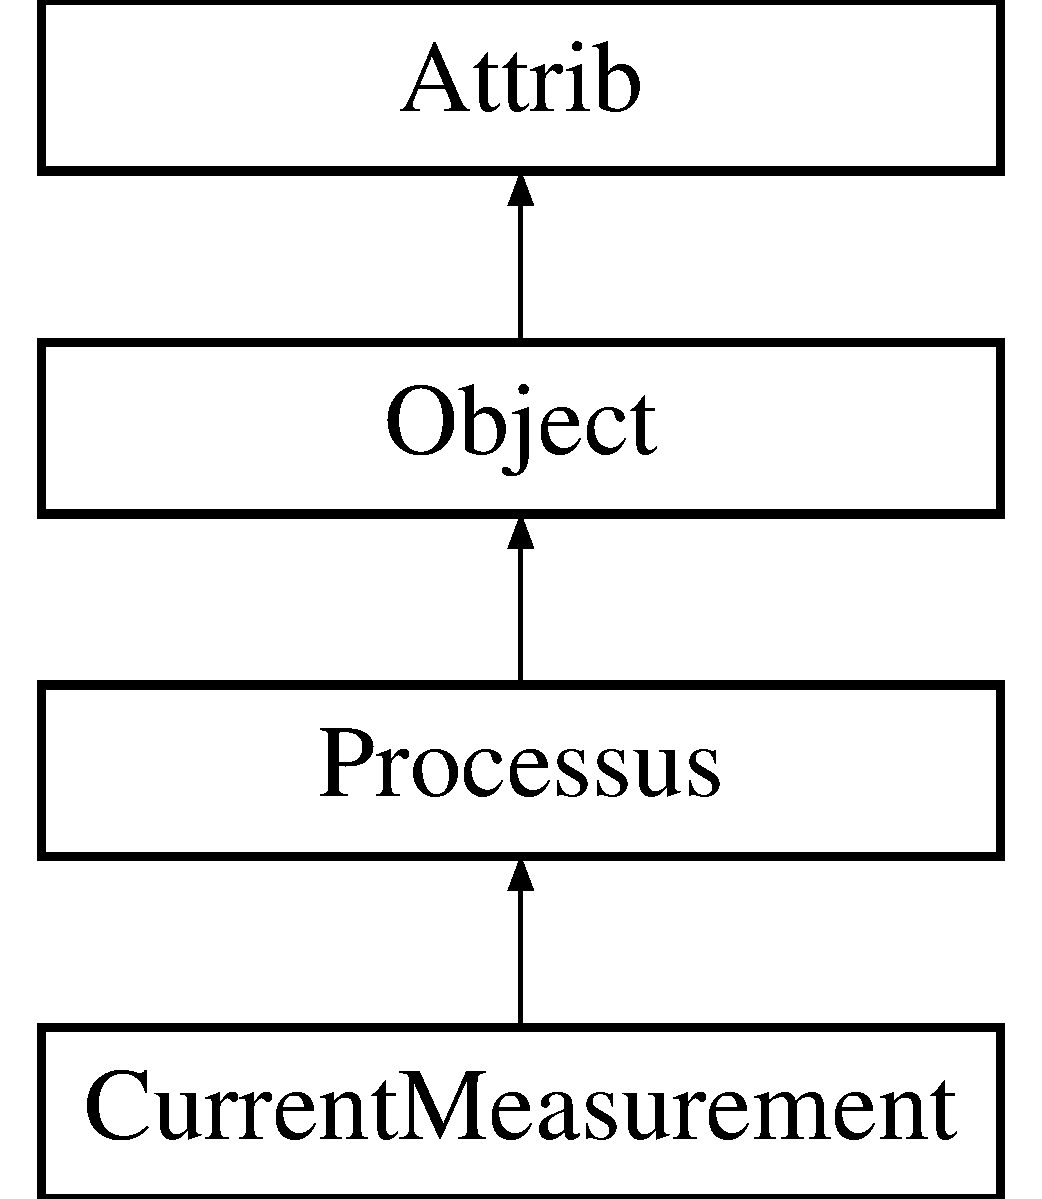
\includegraphics[height=4cm]{classCurrentMeasurement}
\end{center}
\end{figure}
\subsection*{Classes}
\begin{DoxyCompactItemize}
\item 
class \hyperlink{classCurrentMeasurement_1_1CurrentMeasurement}{CurrentMeasurement}
\end{DoxyCompactItemize}
\subsection*{Public Types}
\begin{DoxyCompactItemize}
\item 
enum \hyperlink{classProcessus_a36278773bd98f2d5612fea40c7774821}{states} \{ \hyperlink{classProcessus_a36278773bd98f2d5612fea40c7774821adaf73ad5d0a09f952d0f18dbbe1c7493}{ERR} = -\/1, 
\hyperlink{classProcessus_a36278773bd98f2d5612fea40c7774821a629082f49d6e8df6b6da2b8fbb9d80fb}{NOT\_\-OK}, 
\hyperlink{classProcessus_a36278773bd98f2d5612fea40c7774821af77c64124fa175f28200166fff165ea2}{OK}
 \}
\item 
enum \hyperlink{classAttrib_a69e171d7cc6417835a5a306d3c764235}{Attribut} \{ \par
\hyperlink{classAttrib_a69e171d7cc6417835a5a306d3c764235a3a8da2ab97dda18aebab196fe4100531}{UNDEFINED}, 
\hyperlink{classAttrib_a69e171d7cc6417835a5a306d3c764235a2bfb2af57b87031d190a05fe25dd92ed}{PASSIVE}, 
\hyperlink{classAttrib_a69e171d7cc6417835a5a306d3c764235a3b1fec929c0370d1436f2f06e298fb0d}{ACTIVE}, 
\hyperlink{classAttrib_a69e171d7cc6417835a5a306d3c764235aa27c16b480a369ea4d18b07b2516bbc7}{INTERFACE}, 
\par
\hyperlink{classAttrib_a69e171d7cc6417835a5a306d3c764235a1420a5b8c0540b2af210b6975eded7f9}{IO}, 
\hyperlink{classAttrib_a69e171d7cc6417835a5a306d3c764235a0af3b0d0ac323c1704e6c69cf90add28}{IODATA}, 
\hyperlink{classAttrib_a69e171d7cc6417835a5a306d3c764235a7788bc5dd333fd8ce18562b269c9dab1}{ELEMENT}, 
\hyperlink{classAttrib_a69e171d7cc6417835a5a306d3c764235a61ceb22149f365f1780d18f9d1459423}{HARDWARE}, 
\par
\hyperlink{classAttrib_a69e171d7cc6417835a5a306d3c764235a75250e29692496e73effca2c0330977f}{PROCESSUS}, 
\hyperlink{classAttrib_a69e171d7cc6417835a5a306d3c764235a103a67cd0b8f07ef478fa45d4356e27b}{SOFTWARE}
 \}
\end{DoxyCompactItemize}
\subsection*{Public Member Functions}
\begin{DoxyCompactItemize}
\item 
\hyperlink{classCurrentMeasurement_ad89184bc1f2386b71051d7976ec662f1}{CurrentMeasurement} ()
\begin{DoxyCompactList}\small\item\em Standard constructor. \item\end{DoxyCompactList}\item 
virtual \hyperlink{classCurrentMeasurement_a86c291508b913b4b028567eeb8995c83}{$\sim$CurrentMeasurement} ()
\item 
virtual \hyperlink{classStatusCode}{StatusCode} \hyperlink{classCurrentMeasurement_a88d397682cb5847d5710d08544b6f4c6}{initialize} ()
\begin{DoxyCompactList}\small\item\em Destructor. \item\end{DoxyCompactList}\item 
virtual \hyperlink{classStatusCode}{StatusCode} \hyperlink{classCurrentMeasurement_a19ae0dcc63b4151ceebe0bf2c42da948}{execute} ()
\item 
virtual \hyperlink{classStatusCode}{StatusCode} \hyperlink{classCurrentMeasurement_af87fa329a11212c10e878568bcecaeb3}{finalize} ()
\item 
int \hyperlink{classCurrentMeasurement_a646a9953d7aef3bad2e2dacaab31c241}{numberOfDevices} ()
\item 
\hyperlink{classStatusCode}{StatusCode} \hyperlink{classCurrentMeasurement_ae990f376398bc25891eaddcb245fdf46}{setFrequency} (unsigned int frequency)
\item 
unsigned int \hyperlink{classCurrentMeasurement_ae7c60d0b14808000df5f1d633e0ca990}{frequency} ()
\item 
\hyperlink{classStatusCode}{StatusCode} \hyperlink{classProcessus_a09319bde9bed93e290f69b4e04585543}{startProcessing} ()
\item 
\hyperlink{classStatusCode}{StatusCode} \hyperlink{classProcessus_a5e4da662989d356b89d490b89c7afbfd}{endProcessing} ()
\item 
void \hyperlink{classProcessus_aaeb17673b98d2b39f3aa780e335e0968}{clean} ()
\item 
void \hyperlink{classProcessus_ad57a29b33f9021eda9f6929136f1784f}{setStorage} (std::string storage)
\item 
\hyperlink{classData}{Data} $\ast$ \hyperlink{classProcessus_a16e45f329fbce935aeef0ff3cb508228}{data} ()
\item 
std::vector$<$ double $>$ \hyperlink{classProcessus_aa7c57483cf4b9ab0b2d0ae2de8316402}{data} (unsigned int row)
\item 
std::vector$<$ double $>$ \hyperlink{classProcessus_abf4d91fb36707e1d50178bab12d21ae9}{data} (std::string name)
\item 
\hyperlink{classHisto1D}{Histo1D} $\ast$ \hyperlink{classProcessus_a409227db936baff03c0462c1bcfe8069}{hist1d} (unsigned int row)
\item 
\hyperlink{classHisto2D}{Histo2D} $\ast$ \hyperlink{classProcessus_a73b5118cb5f2b5eaad33286183b86cfc}{hist2d} (unsigned int row)
\item 
void \hyperlink{classProcessus_a308c8f193802f1d1ab49d4447d0cb281}{addDataStream} (std::string name, std::string title)
\item 
void \hyperlink{classProcessus_ad46e0d4dfdfdcbce001ee6be1746dfa4}{addHisto1d} (TH1D $\ast$h)
\item 
void \hyperlink{classProcessus_ac1ed1aed5edaeabdf18aa56775440471}{addHisto2d} (TH2D $\ast$h)
\item 
\hyperlink{classStatusCode}{StatusCode} \hyperlink{classProcessus_a0d093b48f3218a088ba030e24372f18c}{dataFill} (int i, double val)
\item 
\hyperlink{classStatusCode}{StatusCode} \hyperlink{classProcessus_aa31ab71711f7af6a729441ff573f69c9}{dataFill} (std::string name, double val)
\item 
std::string \hyperlink{classProcessus_a33fa1a0b54a636e5cdd680669fd9ea51}{storage} ()
\item 
void \hyperlink{classProcessus_a8ddef94227d83d9dae2cd49aebc33353}{setElement} (\hyperlink{classElement}{Element} $\ast$element)
\item 
\hyperlink{classElement}{Element} $\ast$ \hyperlink{classProcessus_a6fe155527431a7190b7d44d600b9608d}{element} ()
\item 
void \hyperlink{classProcessus_abe603d0636f76db6aa6c5c60cf34c591}{incNErrors} ()
\item 
void \hyperlink{classProcessus_a831b027b9cf18ab56fa6147b5d3055da}{setNErrors} (unsigned int)
\item 
unsigned int \hyperlink{classProcessus_a82a0487f82f07cc2c2dc2731f98149e7}{nErrors} ()
\item 
TFile $\ast$ \hyperlink{classProcessus_a247e8c362ec08422cf53d08dd23b093c}{rootFile} ()
\item 
void \hyperlink{classProcessus_aacf6812880c1d1a2bf14a4a39458f443}{openRootFile} ()
\item 
void \hyperlink{classProcessus_a2f3c41e99da4c738ea3d8f7b0d20a665}{closeRootFile} ()
\item 
void \hyperlink{classProcessus_a5e4d34b86241fa0756e07375a14ff4b2}{startChrono} ()
\item 
void \hyperlink{classProcessus_a471833f89047aa9a7ff6200a31c17a1d}{setLogMsg} (std::string logMsg)
\item 
std::string \hyperlink{classProcessus_a42fdeb17dc13ba854222666b6aa29b61}{logMsg} ()
\item 
void \hyperlink{classProcessus_ad38cde0f1bcefa00b068e7947b8af927}{setState} (int state)
\item 
double \hyperlink{classProcessus_aecca96218c65bc805c988cd95447df55}{elapsedTime} ()
\item 
double \hyperlink{classProcessus_a06d3815ad56593dfd0d3c1f534f8b146}{elapsedTime} (time\_\-t start)
\item 
std::string \hyperlink{classObject_a975e888d50bfcbffda2c86368332a5cd}{name} () const 
\item 
std::string \hyperlink{classObject_a84f99f70f144a83e1582d1d0f84e4e62}{type} ()
\item 
unsigned char \hyperlink{classObject_af99145335cc61ff6e2798ea17db009d2}{id} ()
\item 
std::string \hyperlink{classObject_a73a0f1a41828fdd8303dd662446fb6c3}{title} ()
\item 
void \hyperlink{classObject_a3f9d5537ebce0c0f2bf6ae4d92426f3c}{msgSvc} (int level, std::string msg, std::string name)
\item 
void \hyperlink{classObject_a58b2d0618c2d08cf2383012611528d97}{msg} (std::string mymsg)
\item 
void \hyperlink{classObject_ac5d59299273cee27aacf7de00d2e7034}{msg} (std::string mymsg, std::string name)
\item 
void \hyperlink{classObject_a83d2db2df682907ea1115ad721c1c4a1}{verbose} (std::string mymsg)
\item 
void \hyperlink{classObject_a2d4120195317e2a3c6532e8bb9f3da68}{verbose} (std::string mymsg, std::string name)
\item 
void \hyperlink{classObject_aac010553f022165573714b7014a15f0d}{debug} (std::string mymsg)
\item 
void \hyperlink{classObject_a6c9a0397ca804e04d675ed05683f5420}{debug} (std::string mymsg, std::string name)
\item 
void \hyperlink{classObject_a644fd329ea4cb85f54fa6846484b84a8}{info} (std::string mymsg)
\item 
void \hyperlink{classObject_a1ca123253dfd30fc28b156f521dcbdae}{info} (std::string mymsg, std::string name)
\item 
void \hyperlink{classObject_a65cd4fda577711660821fd2cd5a3b4c9}{warning} (std::string mymsg)
\item 
void \hyperlink{classObject_a11f101db4dd73d9391b0231818881d86}{warning} (std::string mymsg, std::string name)
\item 
void \hyperlink{classObject_a204a95f57818c0f811933917a30eff45}{error} (std::string mymsg)
\item 
void \hyperlink{classObject_ad7f6c457733082efa2f9ff5f5c8e119a}{error} (std::string mymsg, std::string name)
\item 
void \hyperlink{classObject_aad5a16aac7516ce65bd5ec02ab07fc80}{fatal} (std::string mymsg)
\item 
void \hyperlink{classObject_ae62acd3d09f716220f75f252dc38bc9a}{fatal} (std::string mymsg, std::string name)
\item 
void \hyperlink{classObject_ae30fea75683c2d149b6b6d17c09ecd0c}{setName} (std::string name)
\item 
void \hyperlink{classObject_aae534cc9d982bcb9b99fd505f2e103a5}{setType} (std::string type)
\item 
void \hyperlink{classObject_a398fe08cba594a0ce6891d59fe4f159f}{setId} (unsigned char id)
\item 
void \hyperlink{classObject_a89557dbbad5bcaa02652f5d7fa35d20f}{setTitle} (std::string title)
\item 
void \hyperlink{classObject_a870c5af919958c2136623b2d7816d123}{setDllName} (std::string dllName)
\item 
std::string \hyperlink{classObject_a2e3947f2870094c332d7454117f3ec63}{dllName} ()
\item 
bool \hyperlink{classAttrib_a704f26af560909ad22065083bb7d4c34}{is} (int attribut)
\item 
void \hyperlink{classAttrib_a235f773af19c900264a190b00a3b4ad7}{add} (int attribut)
\item 
void \hyperlink{classAttrib_a7d4ef7e32d93cb287792b87b857e79f3}{remove} (int attribut)
\item 
std::string \hyperlink{classAttrib_aee7bbf16b144887f196e1341b24f8a26}{attributs} ()
\end{DoxyCompactItemize}
\subsection*{Protected Member Functions}
\begin{DoxyCompactItemize}
\item 
\hyperlink{classCurrentMeasurement_1_1CurrentMeasurement}{CurrentMeasurement} $\ast$ \hyperlink{classCurrentMeasurement_a7722435fcc404fe4761c3fa96f3b6338}{clone} ()
\end{DoxyCompactItemize}
\subsection*{Protected Attributes}
\begin{DoxyCompactItemize}
\item 
\hyperlink{classElement}{Element} $\ast$ \hyperlink{classProcessus_aa9d24d53c3e52f36786cabb5d8e296e7}{m\_\-element}
\item 
std::string \hyperlink{classAttrib_a3414521d7a82476e874b25a5407b5e63}{m\_\-attribString} \mbox{[}10\mbox{]}
\end{DoxyCompactItemize}
\subsection*{Private Attributes}
\begin{DoxyCompactItemize}
\item 
TRandom $\ast$ \hyperlink{classCurrentMeasurement_ac0c595b78b8110a19b59a333a6c27c1b}{m\_\-rnd}
\item 
unsigned int \hyperlink{classCurrentMeasurement_a66e12903825632c0434e3b7cf929a960}{m\_\-frequency}
\item 
\hyperlink{classNI6008}{NI6008} $\ast$ \hyperlink{classCurrentMeasurement_a7df157175089da57bd020b8680e87f80}{m\_\-device}
\item 
unsigned int \hyperlink{classCurrentMeasurement_a073f6aba41750712d620e60e346f2315}{m\_\-numberOfDevices}
\item 
TTree $\ast$ \hyperlink{classCurrentMeasurement_a559823413932b393dedfc62d42268d93}{m\_\-tree}
\item 
Int\_\-t \hyperlink{classCurrentMeasurement_a5a7bfe59821148e4e9e2998c73b635a8}{m\_\-runNumber}
\item 
Int\_\-t \hyperlink{classCurrentMeasurement_a6e01f96c84aec986de9a9f7393ccb2c6}{m\_\-evtNumber}
\item 
Int\_\-t \hyperlink{classCurrentMeasurement_acc9f2cabf165e47a9fbf2a357e424cef}{m\_\-timestamp} \mbox{[}4\mbox{]}
\item 
Int\_\-t \hyperlink{classCurrentMeasurement_ad08307f13d37c05e1a4e42ff39c97911}{m\_\-duration} \mbox{[}4\mbox{]}
\item 
time\_\-t \hyperlink{classCurrentMeasurement_abd5a7612f08721143623add96797a433}{m\_\-startTime}
\item 
double \hyperlink{classCurrentMeasurement_a793b1467b6a5388361340d41f9e8833f}{m\_\-ai0} \mbox{[}4\mbox{]}
\item 
double \hyperlink{classCurrentMeasurement_aeef18708be94b89de9c4384dd452207d}{m\_\-ai1} \mbox{[}4\mbox{]}
\item 
double \hyperlink{classCurrentMeasurement_a27ce0cfd8d1c04f6cd4d8de0403fafba}{m\_\-ai2} \mbox{[}4\mbox{]}
\item 
double \hyperlink{classCurrentMeasurement_aa1223e4b36335ceb507edd12d4cfa8ad}{m\_\-ai3} \mbox{[}4\mbox{]}
\end{DoxyCompactItemize}


\subsection{Detailed Description}
\begin{DoxyAuthor}{Author}
Frederic Machefert 
\end{DoxyAuthor}
\begin{DoxyDate}{Date}
2010-\/01-\/07 
\end{DoxyDate}


Definition at line 23 of file CurrentMeasurement.h.

\subsection{Member Enumeration Documentation}
\hypertarget{classAttrib_a69e171d7cc6417835a5a306d3c764235}{
\index{CurrentMeasurement@{CurrentMeasurement}!Attribut@{Attribut}}
\index{Attribut@{Attribut}!CurrentMeasurement@{CurrentMeasurement}}
\subsubsection[{Attribut}]{\setlength{\rightskip}{0pt plus 5cm}enum {\bf Attrib::Attribut}\hspace{0.3cm}{\ttfamily  \mbox{[}inherited\mbox{]}}}}
\label{classAttrib_a69e171d7cc6417835a5a306d3c764235}
\begin{Desc}
\item[Enumerator: ]\par
\begin{description}
\index{UNDEFINED@{UNDEFINED}!CurrentMeasurement@{CurrentMeasurement}}\index{CurrentMeasurement@{CurrentMeasurement}!UNDEFINED@{UNDEFINED}}\item[{\em 
\hypertarget{classAttrib_a69e171d7cc6417835a5a306d3c764235a3a8da2ab97dda18aebab196fe4100531}{
UNDEFINED}
\label{classAttrib_a69e171d7cc6417835a5a306d3c764235a3a8da2ab97dda18aebab196fe4100531}
}]\index{PASSIVE@{PASSIVE}!CurrentMeasurement@{CurrentMeasurement}}\index{CurrentMeasurement@{CurrentMeasurement}!PASSIVE@{PASSIVE}}\item[{\em 
\hypertarget{classAttrib_a69e171d7cc6417835a5a306d3c764235a2bfb2af57b87031d190a05fe25dd92ed}{
PASSIVE}
\label{classAttrib_a69e171d7cc6417835a5a306d3c764235a2bfb2af57b87031d190a05fe25dd92ed}
}]\index{ACTIVE@{ACTIVE}!CurrentMeasurement@{CurrentMeasurement}}\index{CurrentMeasurement@{CurrentMeasurement}!ACTIVE@{ACTIVE}}\item[{\em 
\hypertarget{classAttrib_a69e171d7cc6417835a5a306d3c764235a3b1fec929c0370d1436f2f06e298fb0d}{
ACTIVE}
\label{classAttrib_a69e171d7cc6417835a5a306d3c764235a3b1fec929c0370d1436f2f06e298fb0d}
}]\index{INTERFACE@{INTERFACE}!CurrentMeasurement@{CurrentMeasurement}}\index{CurrentMeasurement@{CurrentMeasurement}!INTERFACE@{INTERFACE}}\item[{\em 
\hypertarget{classAttrib_a69e171d7cc6417835a5a306d3c764235aa27c16b480a369ea4d18b07b2516bbc7}{
INTERFACE}
\label{classAttrib_a69e171d7cc6417835a5a306d3c764235aa27c16b480a369ea4d18b07b2516bbc7}
}]\index{IO@{IO}!CurrentMeasurement@{CurrentMeasurement}}\index{CurrentMeasurement@{CurrentMeasurement}!IO@{IO}}\item[{\em 
\hypertarget{classAttrib_a69e171d7cc6417835a5a306d3c764235a1420a5b8c0540b2af210b6975eded7f9}{
IO}
\label{classAttrib_a69e171d7cc6417835a5a306d3c764235a1420a5b8c0540b2af210b6975eded7f9}
}]\index{IODATA@{IODATA}!CurrentMeasurement@{CurrentMeasurement}}\index{CurrentMeasurement@{CurrentMeasurement}!IODATA@{IODATA}}\item[{\em 
\hypertarget{classAttrib_a69e171d7cc6417835a5a306d3c764235a0af3b0d0ac323c1704e6c69cf90add28}{
IODATA}
\label{classAttrib_a69e171d7cc6417835a5a306d3c764235a0af3b0d0ac323c1704e6c69cf90add28}
}]\index{ELEMENT@{ELEMENT}!CurrentMeasurement@{CurrentMeasurement}}\index{CurrentMeasurement@{CurrentMeasurement}!ELEMENT@{ELEMENT}}\item[{\em 
\hypertarget{classAttrib_a69e171d7cc6417835a5a306d3c764235a7788bc5dd333fd8ce18562b269c9dab1}{
ELEMENT}
\label{classAttrib_a69e171d7cc6417835a5a306d3c764235a7788bc5dd333fd8ce18562b269c9dab1}
}]\index{HARDWARE@{HARDWARE}!CurrentMeasurement@{CurrentMeasurement}}\index{CurrentMeasurement@{CurrentMeasurement}!HARDWARE@{HARDWARE}}\item[{\em 
\hypertarget{classAttrib_a69e171d7cc6417835a5a306d3c764235a61ceb22149f365f1780d18f9d1459423}{
HARDWARE}
\label{classAttrib_a69e171d7cc6417835a5a306d3c764235a61ceb22149f365f1780d18f9d1459423}
}]\index{PROCESSUS@{PROCESSUS}!CurrentMeasurement@{CurrentMeasurement}}\index{CurrentMeasurement@{CurrentMeasurement}!PROCESSUS@{PROCESSUS}}\item[{\em 
\hypertarget{classAttrib_a69e171d7cc6417835a5a306d3c764235a75250e29692496e73effca2c0330977f}{
PROCESSUS}
\label{classAttrib_a69e171d7cc6417835a5a306d3c764235a75250e29692496e73effca2c0330977f}
}]\index{SOFTWARE@{SOFTWARE}!CurrentMeasurement@{CurrentMeasurement}}\index{CurrentMeasurement@{CurrentMeasurement}!SOFTWARE@{SOFTWARE}}\item[{\em 
\hypertarget{classAttrib_a69e171d7cc6417835a5a306d3c764235a103a67cd0b8f07ef478fa45d4356e27b}{
SOFTWARE}
\label{classAttrib_a69e171d7cc6417835a5a306d3c764235a103a67cd0b8f07ef478fa45d4356e27b}
}]\end{description}
\end{Desc}



Definition at line 29 of file Attrib.h.


\begin{DoxyCode}
29                 {
30     UNDEFINED,
31     PASSIVE,
32     ACTIVE,
33     INTERFACE,
34     IO,
35     IODATA,
36     ELEMENT,
37     HARDWARE,
38     PROCESSUS,
39     SOFTWARE 
40   }; // array m_attribString must be changed into Attrib::Attrib if this enu is m
      odified. 
\end{DoxyCode}
\hypertarget{classProcessus_a36278773bd98f2d5612fea40c7774821}{
\index{CurrentMeasurement@{CurrentMeasurement}!states@{states}}
\index{states@{states}!CurrentMeasurement@{CurrentMeasurement}}
\subsubsection[{states}]{\setlength{\rightskip}{0pt plus 5cm}enum {\bf Processus::states}\hspace{0.3cm}{\ttfamily  \mbox{[}inherited\mbox{]}}}}
\label{classProcessus_a36278773bd98f2d5612fea40c7774821}
\begin{Desc}
\item[Enumerator: ]\par
\begin{description}
\index{ERR@{ERR}!CurrentMeasurement@{CurrentMeasurement}}\index{CurrentMeasurement@{CurrentMeasurement}!ERR@{ERR}}\item[{\em 
\hypertarget{classProcessus_a36278773bd98f2d5612fea40c7774821adaf73ad5d0a09f952d0f18dbbe1c7493}{
ERR}
\label{classProcessus_a36278773bd98f2d5612fea40c7774821adaf73ad5d0a09f952d0f18dbbe1c7493}
}]\index{NOT\_\-OK@{NOT\_\-OK}!CurrentMeasurement@{CurrentMeasurement}}\index{CurrentMeasurement@{CurrentMeasurement}!NOT\_\-OK@{NOT\_\-OK}}\item[{\em 
\hypertarget{classProcessus_a36278773bd98f2d5612fea40c7774821a629082f49d6e8df6b6da2b8fbb9d80fb}{
NOT\_\-OK}
\label{classProcessus_a36278773bd98f2d5612fea40c7774821a629082f49d6e8df6b6da2b8fbb9d80fb}
}]\index{OK@{OK}!CurrentMeasurement@{CurrentMeasurement}}\index{CurrentMeasurement@{CurrentMeasurement}!OK@{OK}}\item[{\em 
\hypertarget{classProcessus_a36278773bd98f2d5612fea40c7774821af77c64124fa175f28200166fff165ea2}{
OK}
\label{classProcessus_a36278773bd98f2d5612fea40c7774821af77c64124fa175f28200166fff165ea2}
}]\end{description}
\end{Desc}



Definition at line 34 of file Processus.h.


\begin{DoxyCode}
34 { ERR=-1 , NOT_OK , OK };
\end{DoxyCode}


\subsection{Constructor \& Destructor Documentation}
\hypertarget{classCurrentMeasurement_ad89184bc1f2386b71051d7976ec662f1}{
\index{CurrentMeasurement@{CurrentMeasurement}!CurrentMeasurement@{CurrentMeasurement}}
\index{CurrentMeasurement@{CurrentMeasurement}!CurrentMeasurement@{CurrentMeasurement}}
\subsubsection[{CurrentMeasurement}]{\setlength{\rightskip}{0pt plus 5cm}{\bf CurrentMeasurement::CurrentMeasurement} ()}}
\label{classCurrentMeasurement_ad89184bc1f2386b71051d7976ec662f1}


Standard constructor. 

Definition at line 26 of file CurrentMeasurement.cpp.

References m\_\-device, Object::setName(), Object::setTitle(), and Object::setType().

Referenced by clone().


\begin{DoxyCode}
26                                         {
27   setName ( "CurrentMeasurement" );
28   setType ( "NI6008" );
29   setTitle( "NI6008 current measurement" );  
30   m_device = 0; 
31 }
\end{DoxyCode}
\hypertarget{classCurrentMeasurement_a86c291508b913b4b028567eeb8995c83}{
\index{CurrentMeasurement@{CurrentMeasurement}!$\sim$CurrentMeasurement@{$\sim$CurrentMeasurement}}
\index{$\sim$CurrentMeasurement@{$\sim$CurrentMeasurement}!CurrentMeasurement@{CurrentMeasurement}}
\subsubsection[{$\sim$CurrentMeasurement}]{\setlength{\rightskip}{0pt plus 5cm}virtual CurrentMeasurement::$\sim$CurrentMeasurement ()\hspace{0.3cm}{\ttfamily  \mbox{[}inline, virtual\mbox{]}}}}
\label{classCurrentMeasurement_a86c291508b913b4b028567eeb8995c83}


Definition at line 28 of file CurrentMeasurement.h.


\begin{DoxyCode}
28 {}; 
\end{DoxyCode}


\subsection{Member Function Documentation}
\hypertarget{classAttrib_a235f773af19c900264a190b00a3b4ad7}{
\index{CurrentMeasurement@{CurrentMeasurement}!add@{add}}
\index{add@{add}!CurrentMeasurement@{CurrentMeasurement}}
\subsubsection[{add}]{\setlength{\rightskip}{0pt plus 5cm}void Attrib::add (int {\em attribut})\hspace{0.3cm}{\ttfamily  \mbox{[}inline, inherited\mbox{]}}}}
\label{classAttrib_a235f773af19c900264a190b00a3b4ad7}
Add an attribut 

Definition at line 67 of file Attrib.h.

References Attrib::m\_\-attributs, and Attrib::UNDEFINED.

Referenced by A3PE::A3PE(), Attrib::Attrib(), SpecsMezzanine::cmdline(), Computer::Computer(), CU\_\-v1::CU\_\-v1(), export\_\-obj(), FEB\_\-v1::FEB\_\-v1(), FePGA::FePGA(), ICECALv3::ICECALv3(), ICPhaser::ICPhaser(), Application::initialize(), Interface::Interface(), IOdata::IOdata(), IOobject::IOobject(), LSDelayChipV1::LSDelayChipV1(), MSOxxxx::MSOxxxx(), Phaser::Phaser(), Processus::Processus(), Proto40MHz\_\-v1::Proto40MHz\_\-v1(), Attrib::remove(), SeqPGA::SeqPGA(), SpecsMaster::SpecsMaster(), and SpecsSlave::SpecsSlave().


\begin{DoxyCode}
67                             {
68     if (attribut!=Attrib::UNDEFINED) remove(Attrib::UNDEFINED);
69     bool duplicate = false ;
70     std::vector<int>::const_iterator iter ;
71     for ( iter  = m_attributs.begin() ;
72           iter != m_attributs.end()   ;
73           ++iter ) {
74       if ( attribut == (*iter) ) {
75         duplicate = true ;
76       }
77     }
78     if (!duplicate) {
79       m_attributs.push_back( attribut );
80     }
81   }
\end{DoxyCode}
\hypertarget{classProcessus_a308c8f193802f1d1ab49d4447d0cb281}{
\index{CurrentMeasurement@{CurrentMeasurement}!addDataStream@{addDataStream}}
\index{addDataStream@{addDataStream}!CurrentMeasurement@{CurrentMeasurement}}
\subsubsection[{addDataStream}]{\setlength{\rightskip}{0pt plus 5cm}void Processus::addDataStream (std::string {\em name}, \/  std::string {\em title})\hspace{0.3cm}{\ttfamily  \mbox{[}inline, inherited\mbox{]}}}}
\label{classProcessus_a308c8f193802f1d1ab49d4447d0cb281}


Definition at line 153 of file Processus.h.

References Data::addDataStream(), and Processus::m\_\-data.

Referenced by initialize(), ADCMeasurement::initialize(), TestSuite::initialize(), TestUSB::initialize(), TestSPI::initialize(), TestI2C::initialize(), UsbFTInterfaceTest::initialize(), and RegisterTest::initialize().


\begin{DoxyCode}
153                                                        {
154     m_data->addDataStream(name, title);
155   }
\end{DoxyCode}
\hypertarget{classProcessus_ad46e0d4dfdfdcbce001ee6be1746dfa4}{
\index{CurrentMeasurement@{CurrentMeasurement}!addHisto1d@{addHisto1d}}
\index{addHisto1d@{addHisto1d}!CurrentMeasurement@{CurrentMeasurement}}
\subsubsection[{addHisto1d}]{\setlength{\rightskip}{0pt plus 5cm}void Processus::addHisto1d (TH1D $\ast$ {\em h})\hspace{0.3cm}{\ttfamily  \mbox{[}inline, inherited\mbox{]}}}}
\label{classProcessus_ad46e0d4dfdfdcbce001ee6be1746dfa4}


Definition at line 160 of file Processus.h.

References Data::addHisto1d(), and Processus::m\_\-data.

Referenced by TestSuite::initialize(), StorageFifoAcquisition::initialize(), StorageFifo::initialize(), Acquisition::initialize(), and A3PE\_\-BitFlip::initialize().


\begin{DoxyCode}
160                            {
161     m_data->addHisto1d(h);
162   }
\end{DoxyCode}
\hypertarget{classProcessus_ac1ed1aed5edaeabdf18aa56775440471}{
\index{CurrentMeasurement@{CurrentMeasurement}!addHisto2d@{addHisto2d}}
\index{addHisto2d@{addHisto2d}!CurrentMeasurement@{CurrentMeasurement}}
\subsubsection[{addHisto2d}]{\setlength{\rightskip}{0pt plus 5cm}void Processus::addHisto2d (TH2D $\ast$ {\em h})\hspace{0.3cm}{\ttfamily  \mbox{[}inline, inherited\mbox{]}}}}
\label{classProcessus_ac1ed1aed5edaeabdf18aa56775440471}


Definition at line 167 of file Processus.h.

References Data::addHisto2d(), and Processus::m\_\-data.

Referenced by TestSuite::initialize().


\begin{DoxyCode}
167                            {
168     m_data->addHisto2d(h);
169   }
\end{DoxyCode}
\hypertarget{classAttrib_aee7bbf16b144887f196e1341b24f8a26}{
\index{CurrentMeasurement@{CurrentMeasurement}!attributs@{attributs}}
\index{attributs@{attributs}!CurrentMeasurement@{CurrentMeasurement}}
\subsubsection[{attributs}]{\setlength{\rightskip}{0pt plus 5cm}std::string Attrib::attributs ()\hspace{0.3cm}{\ttfamily  \mbox{[}inherited\mbox{]}}}}
\label{classAttrib_aee7bbf16b144887f196e1341b24f8a26}
Print the \hyperlink{classAttrib}{Attrib} of an \hyperlink{classObject}{Object} 

Definition at line 54 of file Attrib.cpp.

References images::index, Attrib::m\_\-attribString, and Attrib::m\_\-attributs.

Referenced by export\_\-obj().


\begin{DoxyCode}
54                             {
55   std::string output;
56   std::vector<int>::iterator iter ;
57   for ( unsigned int index = 0 ; index < m_attributs.size() ; ++index ) {
58     if ( m_attributs.size() - index > 1 ) {
59       output.append(m_attribString[m_attributs[index]]);
60       output.append(":");
61     }
62     else {
63       output.append(m_attribString[m_attributs[index]]);
64     }
65   }
66   return output;
67 }
\end{DoxyCode}
\hypertarget{classProcessus_aaeb17673b98d2b39f3aa780e335e0968}{
\index{CurrentMeasurement@{CurrentMeasurement}!clean@{clean}}
\index{clean@{clean}!CurrentMeasurement@{CurrentMeasurement}}
\subsubsection[{clean}]{\setlength{\rightskip}{0pt plus 5cm}void Processus::clean ()\hspace{0.3cm}{\ttfamily  \mbox{[}inline, inherited\mbox{]}}}}
\label{classProcessus_aaeb17673b98d2b39f3aa780e335e0968}


Definition at line 85 of file Processus.h.

References Processus::m\_\-element, Processus::m\_\-state, and Object::warning().

Referenced by Application::prepare().


\begin{DoxyCode}
86   {
87     m_element=0;
88     if (0!=m_state) {
89       delete m_state;
90       m_state=0;
91     }
92 #ifdef _NETWORK_
93     warning("Cleaning state service : should it be done ?","Processus::clean")
94       if (0!=m_stateService)
95       {
96         delete m_stateService;
97       }
98 #endif
99   }
\end{DoxyCode}
\hypertarget{classCurrentMeasurement_a7722435fcc404fe4761c3fa96f3b6338}{
\index{CurrentMeasurement@{CurrentMeasurement}!clone@{clone}}
\index{clone@{clone}!CurrentMeasurement@{CurrentMeasurement}}
\subsubsection[{clone}]{\setlength{\rightskip}{0pt plus 5cm}{\bf CurrentMeasurement}$\ast$ CurrentMeasurement::clone ()\hspace{0.3cm}{\ttfamily  \mbox{[}inline, protected, virtual\mbox{]}}}}
\label{classCurrentMeasurement_a7722435fcc404fe4761c3fa96f3b6338}
processus termination virtual function 

Implements \hyperlink{classProcessus_aca8856f6d6d7b7e1fe941f298dcbb502}{Processus}.

Definition at line 67 of file CurrentMeasurement.h.

References CurrentMeasurement().


\begin{DoxyCode}
67                              {
68     return new CurrentMeasurement (*this);
69   };
\end{DoxyCode}
\hypertarget{classProcessus_a2f3c41e99da4c738ea3d8f7b0d20a665}{
\index{CurrentMeasurement@{CurrentMeasurement}!closeRootFile@{closeRootFile}}
\index{closeRootFile@{closeRootFile}!CurrentMeasurement@{CurrentMeasurement}}
\subsubsection[{closeRootFile}]{\setlength{\rightskip}{0pt plus 5cm}void Processus::closeRootFile ()\hspace{0.3cm}{\ttfamily  \mbox{[}inherited\mbox{]}}}}
\label{classProcessus_a2f3c41e99da4c738ea3d8f7b0d20a665}
Close Root file if already opened and requested 

Definition at line 160 of file Processus.cpp.

References Options::dataFileFullName(), Options::dataStorage(), Object::info(), Processus::m\_\-options, and Processus::m\_\-rootFile.

Referenced by Processus::endProcessing(), UsbFTInterfaceTest::finalize(), RegisterTest::finalize(), and PhaserRampExec::finalize().


\begin{DoxyCode}
160                                 {
161   if ( 0!= m_rootFile && m_options->dataStorage() ){
162     m_rootFile->Write();
163         std::string mess=std::string("Closing root file ");
164         mess.append(m_options->dataFileFullName());
165         info(mess,"closeRootFile");
166     m_rootFile->Delete();
167     m_rootFile = 0;
168   }
169 }
\end{DoxyCode}
\hypertarget{classProcessus_abf4d91fb36707e1d50178bab12d21ae9}{
\index{CurrentMeasurement@{CurrentMeasurement}!data@{data}}
\index{data@{data}!CurrentMeasurement@{CurrentMeasurement}}
\subsubsection[{data}]{\setlength{\rightskip}{0pt plus 5cm}std::vector$<$double$>$ Processus::data (std::string {\em name})\hspace{0.3cm}{\ttfamily  \mbox{[}inline, inherited\mbox{]}}}}
\label{classProcessus_abf4d91fb36707e1d50178bab12d21ae9}
Get accessor to member m\_\-data \begin{DoxyReturn}{Returns}
the current value of m\_\-data 
\end{DoxyReturn}


Definition at line 130 of file Processus.h.

References Processus::m\_\-data, and Data::vector().


\begin{DoxyCode}
130                                         {
131     return m_data->vector(name);
132   }
\end{DoxyCode}
\hypertarget{classProcessus_aa7c57483cf4b9ab0b2d0ae2de8316402}{
\index{CurrentMeasurement@{CurrentMeasurement}!data@{data}}
\index{data@{data}!CurrentMeasurement@{CurrentMeasurement}}
\subsubsection[{data}]{\setlength{\rightskip}{0pt plus 5cm}std::vector$<$double$>$ Processus::data (unsigned int {\em row})\hspace{0.3cm}{\ttfamily  \mbox{[}inline, inherited\mbox{]}}}}
\label{classProcessus_aa7c57483cf4b9ab0b2d0ae2de8316402}
Get accessor to member m\_\-data \begin{DoxyReturn}{Returns}
the current value of m\_\-data 
\end{DoxyReturn}


Definition at line 122 of file Processus.h.

References Processus::m\_\-data, and Data::vector().


\begin{DoxyCode}
122                                           {
123     return m_data->vector(row);
124   }
\end{DoxyCode}
\hypertarget{classProcessus_a16e45f329fbce935aeef0ff3cb508228}{
\index{CurrentMeasurement@{CurrentMeasurement}!data@{data}}
\index{data@{data}!CurrentMeasurement@{CurrentMeasurement}}
\subsubsection[{data}]{\setlength{\rightskip}{0pt plus 5cm}{\bf Data}$\ast$ Processus::data ()\hspace{0.3cm}{\ttfamily  \mbox{[}inline, inherited\mbox{]}}}}
\label{classProcessus_a16e45f329fbce935aeef0ff3cb508228}
Get accessor to member m\_\-data \begin{DoxyReturn}{Returns}
the current value of m\_\-data 
\end{DoxyReturn}


Definition at line 114 of file Processus.h.

References Processus::m\_\-data.

Referenced by StorageFifoAcquisition::execute(), and export\_\-proc().


\begin{DoxyCode}
114               {
115     return m_data;
116   }
\end{DoxyCode}
\hypertarget{classProcessus_aa31ab71711f7af6a729441ff573f69c9}{
\index{CurrentMeasurement@{CurrentMeasurement}!dataFill@{dataFill}}
\index{dataFill@{dataFill}!CurrentMeasurement@{CurrentMeasurement}}
\subsubsection[{dataFill}]{\setlength{\rightskip}{0pt plus 5cm}{\bf StatusCode} Processus::dataFill (std::string {\em name}, \/  double {\em val})\hspace{0.3cm}{\ttfamily  \mbox{[}inline, inherited\mbox{]}}}}
\label{classProcessus_aa31ab71711f7af6a729441ff573f69c9}
Set data stream with value \begin{DoxyReturn}{Returns}
the \hyperlink{classStatusCode}{StatusCode} 
\end{DoxyReturn}


Definition at line 189 of file Processus.h.

References StatusCode::FAILURE, Processus::m\_\-data, Data::rowFromName(), StatusCode::SUCCESS, and Data::vectorPtr().


\begin{DoxyCode}
189                                                  {
190     int row=m_data->rowFromName(name);
191     if (row<0) return StatusCode::FAILURE;
192     if (m_data->vectorPtr(row)!=0){
193       m_data->vectorPtr(row)->push_back(val);
194       return StatusCode::SUCCESS;
195     }
196     else {
197       return StatusCode::FAILURE;
198     }
199   }
\end{DoxyCode}
\hypertarget{classProcessus_a0d093b48f3218a088ba030e24372f18c}{
\index{CurrentMeasurement@{CurrentMeasurement}!dataFill@{dataFill}}
\index{dataFill@{dataFill}!CurrentMeasurement@{CurrentMeasurement}}
\subsubsection[{dataFill}]{\setlength{\rightskip}{0pt plus 5cm}{\bf StatusCode} Processus::dataFill (int {\em i}, \/  double {\em val})\hspace{0.3cm}{\ttfamily  \mbox{[}inline, inherited\mbox{]}}}}
\label{classProcessus_a0d093b48f3218a088ba030e24372f18c}
Set data stream with value \begin{DoxyReturn}{Returns}
the \hyperlink{classStatusCode}{StatusCode} 
\end{DoxyReturn}


Definition at line 175 of file Processus.h.

References StatusCode::FAILURE, Processus::m\_\-data, StatusCode::SUCCESS, and Data::vectorPtr().

Referenced by execute(), ADCMeasurement::execute(), TestSuite::execute(), TestUSB::execute(), TestSPI::execute(), TestI2C::execute(), and UsbFTInterfaceTest::execute().


\begin{DoxyCode}
175                                         {
176     if (m_data->vectorPtr(i)!=0){
177       m_data->vectorPtr(i)->push_back(val);
178       return StatusCode::SUCCESS;
179     }
180     else {
181       return StatusCode::FAILURE;
182     }
183   }
\end{DoxyCode}
\hypertarget{classObject_a6c9a0397ca804e04d675ed05683f5420}{
\index{CurrentMeasurement@{CurrentMeasurement}!debug@{debug}}
\index{debug@{debug}!CurrentMeasurement@{CurrentMeasurement}}
\subsubsection[{debug}]{\setlength{\rightskip}{0pt plus 5cm}void Object::debug (std::string {\em mymsg}, \/  std::string {\em name})\hspace{0.3cm}{\ttfamily  \mbox{[}inline, inherited\mbox{]}}}}
\label{classObject_a6c9a0397ca804e04d675ed05683f5420}


Definition at line 45 of file Object.h.

References MsgSvc::DEBUG, Object::m\_\-log, and MsgSvc::msgSvc().


\begin{DoxyCode}
45 { m_log.msgSvc (MsgSvc::DEBUG   , mymsg, name ); }
\end{DoxyCode}
\hypertarget{classObject_aac010553f022165573714b7014a15f0d}{
\index{CurrentMeasurement@{CurrentMeasurement}!debug@{debug}}
\index{debug@{debug}!CurrentMeasurement@{CurrentMeasurement}}
\subsubsection[{debug}]{\setlength{\rightskip}{0pt plus 5cm}void Object::debug (std::string {\em mymsg})\hspace{0.3cm}{\ttfamily  \mbox{[}inline, inherited\mbox{]}}}}
\label{classObject_aac010553f022165573714b7014a15f0d}


Definition at line 37 of file Object.h.

References MsgSvc::DEBUG, Object::m\_\-log, Object::m\_\-name, and MsgSvc::msgSvc().

Referenced by A3PE::A3PE(), A3PE::acquisition(), SpecsMezzanine::addBus(), Hierarchy::addChild(), SpecsSlave::addI2c(), LSDelayChipV1::checkConfigAddr(), LSDelayChipV1::checkStatusAddr(), LSDelayChipV1::configRegBulkRead(), LSDelayChipV1::configRegBulkWrite(), A3PE::dataReady(), DCU::DCU(), Hierarchy::delChild(), SpecsSlave::detect(), EmulateFE::execute(), StorageFifoAcquisition::execute(), StorageFifo::execute(), Acquisition::execute(), A3PE\_\-BitFlip::execute(), export\_\-obj(), FePGA::FePGA(), SpecsGlue::i2cClkMode(), SeqPGA::i2cRead(), FePGA::i2cRead(), SeqPGA::i2cWrite(), FePGA::i2cWrite(), ICECALv3::ICECALv3(), ICPhaser::ICPhaser(), SpecsSlave::init(), SpecsMaster::init(), EmulateFE::initialize(), StorageFifoAcquisition::initialize(), StorageFifo::initialize(), Acquisition::initialize(), A3PE\_\-BitFlip::initialize(), A3PE::internalAXSequence(), SpecsMezzanine::led(), SpecsGlue::led(), LSDelayChipV1::LSDelayChipV1(), MSOxxxx::MSOxxxx(), Phaser::Phaser(), Data::purge(), ICPhaser::read(), Phaser::read(), FEB\_\-v1::readFifoSpyFE(), SpecsSlave::reset(), SpecsMaster::reset(), FEB\_\-v1::reset(), CU\_\-v1::reset(), Proto40MHz\_\-v1::reset(), FEB\_\-v1::resetFifoSpyFE(), SeqPGA::resetSpi(), FEB\_\-v1::resetSpi(), SeqPGA::SeqPGA(), A3PE::setAddFromAXRam(), A3PE::setAddToAXRam(), A3PE::setAXRamUsb(), Element::setConnection(), SpecsGlue::setI2cClkMode(), A3PE::setLatencyAX(), SpecsMezzanine::setLed(), SpecsGlue::setLed(), A3PE::setLengthAX(), A3PE::setReadToAXRamUsb(), SpecsMaster::setSpeed(), A3PE::setWriteFromAXRamUsb(), SpecsBus::SpecsBus(), SpecsI2c::SpecsI2c(), SpecsMaster::SpecsMaster(), SpecsMezzanine::SpecsMezzanine(), SpecsParallelBus::SpecsParallelBus(), SpecsSlave::SpecsSlave(), LSDelayChipV1::spiBERTest(), ICECALv3::spiRead(), ICECALv3::spiWrite(), FEB\_\-v1::testDuration(), SeqPGA::testSequence(), A3PE::trigger(), Server::updateConfig(), Server::updateState(), ICPhaser::write(), Phaser::write(), and Hierarchy::$\sim$Hierarchy().


\begin{DoxyCode}
37 { m_log.msgSvc (MsgSvc::DEBUG   , mymsg, m_name ); }
\end{DoxyCode}
\hypertarget{classObject_a2e3947f2870094c332d7454117f3ec63}{
\index{CurrentMeasurement@{CurrentMeasurement}!dllName@{dllName}}
\index{dllName@{dllName}!CurrentMeasurement@{CurrentMeasurement}}
\subsubsection[{dllName}]{\setlength{\rightskip}{0pt plus 5cm}std::string Object::dllName ()\hspace{0.3cm}{\ttfamily  \mbox{[}inline, inherited\mbox{]}}}}
\label{classObject_a2e3947f2870094c332d7454117f3ec63}
Get accessor to member m\_\-dllName \begin{DoxyReturn}{Returns}
the current value of m\_\-dllName 
\end{DoxyReturn}


Definition at line 74 of file Object.h.

References Object::m\_\-dllName.

Referenced by export\_\-obj().


\begin{DoxyCode}
74                        {
75     return m_dllName;
76   }  
\end{DoxyCode}
\hypertarget{classProcessus_a06d3815ad56593dfd0d3c1f534f8b146}{
\index{CurrentMeasurement@{CurrentMeasurement}!elapsedTime@{elapsedTime}}
\index{elapsedTime@{elapsedTime}!CurrentMeasurement@{CurrentMeasurement}}
\subsubsection[{elapsedTime}]{\setlength{\rightskip}{0pt plus 5cm}double Processus::elapsedTime (time\_\-t {\em start})\hspace{0.3cm}{\ttfamily  \mbox{[}inline, inherited\mbox{]}}}}
\label{classProcessus_a06d3815ad56593dfd0d3c1f534f8b146}


Definition at line 343 of file Processus.h.


\begin{DoxyCode}
343                                    {
344     return ((time(0)-start));
345   }
\end{DoxyCode}
\hypertarget{classProcessus_aecca96218c65bc805c988cd95447df55}{
\index{CurrentMeasurement@{CurrentMeasurement}!elapsedTime@{elapsedTime}}
\index{elapsedTime@{elapsedTime}!CurrentMeasurement@{CurrentMeasurement}}
\subsubsection[{elapsedTime}]{\setlength{\rightskip}{0pt plus 5cm}double Processus::elapsedTime ()\hspace{0.3cm}{\ttfamily  \mbox{[}inline, inherited\mbox{]}}}}
\label{classProcessus_aecca96218c65bc805c988cd95447df55}


Definition at line 340 of file Processus.h.

References Processus::m\_\-start.

Referenced by Processus::endProcessing(), UsbFTInterfaceTest::execute(), PhaserRampExec::finalize(), and Processus::setState().


\begin{DoxyCode}
340                        {
341     return difftime(time(0),m_start);
342   }
\end{DoxyCode}
\hypertarget{classProcessus_a6fe155527431a7190b7d44d600b9608d}{
\index{CurrentMeasurement@{CurrentMeasurement}!element@{element}}
\index{element@{element}!CurrentMeasurement@{CurrentMeasurement}}
\subsubsection[{element}]{\setlength{\rightskip}{0pt plus 5cm}{\bf Element}$\ast$ Processus::element ()\hspace{0.3cm}{\ttfamily  \mbox{[}inline, inherited\mbox{]}}}}
\label{classProcessus_a6fe155527431a7190b7d44d600b9608d}
Get accessor to member m\_\-element \begin{DoxyReturn}{Returns}
the current value of m\_\-element 
\end{DoxyReturn}


Definition at line 231 of file Processus.h.

References Processus::m\_\-element.

Referenced by UsbFTInterfaceTest::execute(), export\_\-proc(), initialize(), ADCMeasurement::initialize(), TestUSB::initialize(), TestSPI::initialize(), TestI2C::initialize(), EmulateFE::initialize(), StorageFifoAcquisition::initialize(), StorageFifo::initialize(), Acquisition::initialize(), A3PE\_\-BitFlip::initialize(), and PhaserRampExec::initialize().


\begin{DoxyCode}
231                       {
232     return m_element;
233   }
\end{DoxyCode}
\hypertarget{classProcessus_a5e4da662989d356b89d490b89c7afbfd}{
\index{CurrentMeasurement@{CurrentMeasurement}!endProcessing@{endProcessing}}
\index{endProcessing@{endProcessing}!CurrentMeasurement@{CurrentMeasurement}}
\subsubsection[{endProcessing}]{\setlength{\rightskip}{0pt plus 5cm}{\bf StatusCode} Processus::endProcessing ()\hspace{0.3cm}{\ttfamily  \mbox{[}inherited\mbox{]}}}}
\label{classProcessus_a5e4da662989d356b89d490b89c7afbfd}
processus standard termination function 

Definition at line 115 of file Processus.cpp.

References Data::buildHistos(), Processus::closeRootFile(), Processus::elapsedTime(), Data::empty(), Processus::finalize(), ftos(), Object::info(), itos(), Processus::m\_\-data, Processus::m\_\-options, Options::nErrors(), Processus::nErrors(), Options::nEvt(), Processus::NOT\_\-OK, Data::print(), Options::runNumber(), and Processus::setState().

Referenced by export\_\-proc(), and Application::terminate().


\begin{DoxyCode}
115                                     {
116   setState( NOT_OK );
117   // 
118   info("-------------------------------------------------------------------------
      -");
119   info("Processed Run Number       : " + itos (m_options->runNumber()) , "finaliz
      e");
120   info("Number of events processed : " + itos (m_options->nEvt())      , "finaliz
      e");
121   info("Number of Errors           : " + itos (nErrors())           , "finalize")
      ;  
122   info("Number of App errors       : " + itos (m_options->nErrors())   , "finaliz
      e");
123   info("Elapsed time               : " + ftos (elapsedTime())       , "finalize")
      ;
124   info("-------------------------------------------------------------------------
      -");
125   if (!m_data->empty()) 
126     m_data->print();
127   else 
128     info("No data Stored.","finalize");
129   info("-------------------------------------------------------------------------
      -");
130 
131 #ifdef _NETWORK_
132   if ( 0 != m_timerService ){
133     m_timerService->setRunning ( false );
134   }
135 #endif
136   StatusCode sc = finalize();
137   m_data->buildHistos();  
138   closeRootFile();
139   return sc;
140 }
\end{DoxyCode}
\hypertarget{classObject_ad7f6c457733082efa2f9ff5f5c8e119a}{
\index{CurrentMeasurement@{CurrentMeasurement}!error@{error}}
\index{error@{error}!CurrentMeasurement@{CurrentMeasurement}}
\subsubsection[{error}]{\setlength{\rightskip}{0pt plus 5cm}void Object::error (std::string {\em mymsg}, \/  std::string {\em name})\hspace{0.3cm}{\ttfamily  \mbox{[}inline, inherited\mbox{]}}}}
\label{classObject_ad7f6c457733082efa2f9ff5f5c8e119a}


Definition at line 48 of file Object.h.

References MsgSvc::ERR, Object::m\_\-log, and MsgSvc::msgSvc().


\begin{DoxyCode}
48 { m_log.msgSvc (MsgSvc::ERR     , mymsg, name ); }
\end{DoxyCode}
\hypertarget{classObject_a204a95f57818c0f811933917a30eff45}{
\index{CurrentMeasurement@{CurrentMeasurement}!error@{error}}
\index{error@{error}!CurrentMeasurement@{CurrentMeasurement}}
\subsubsection[{error}]{\setlength{\rightskip}{0pt plus 5cm}void Object::error (std::string {\em mymsg})\hspace{0.3cm}{\ttfamily  \mbox{[}inline, inherited\mbox{]}}}}
\label{classObject_a204a95f57818c0f811933917a30eff45}


Definition at line 40 of file Object.h.

References MsgSvc::ERR, Object::m\_\-log, Object::m\_\-name, and MsgSvc::msgSvc().

Referenced by ICECALv3::checkChNumber(), A3PE::clockDivision(), NI6008::cmd(), A3PE::enableStorage(), A3PE\_\-BitFlip::execute(), export\_\-obj(), A3PE::fifoDepth(), A3PE::fifoLatency(), FEB\_\-v1::gbtStatus(), Register::getBit(), MSOxxxx::getStatistics(), SpecsMaster::init(), NI6008::init(), UsbFTMLInterface::init(), UsbFTInterface::init(), A3PE::latencyAX(), A3PE::lengthAX(), A3PE::nTrigger(), MSOxxxx::open(), ICECALv3::parseParameterList(), A3PE::pipeline(), UsbFTMLInterface::read(), UsbFTInterface::read(), MSOxxxx::recv(), A3PE::reset(), MSOxxxx::send(), A3PE::setAddFromAXRam(), A3PE::setAddToAXRam(), ICECALv3::setAnalogCh(), A3PE::setAXRamUsb(), Register::setBit(), A3PE::setClockDivision(), A3PE::setFifoDepth(), A3PE::setFifoLatency(), A3PE::setLatencyAX(), A3PE::setLengthAX(), A3PE::setNTrigger(), A3PE::setPipeline(), A3PE::setReadPatternFifoUsb(), A3PE::setReadToAXRamUsb(), A3PE::setReadTriggerFifoUsb(), A3PE::setSoftwareTrigger(), A3PE::setTriggerDelay(), A3PE::setTriggerRate(), A3PE::setWriteFromAXRamUsb(), A3PE::setWriteStorageFifoUsb(), ICECALv3::spiFERTest(), ICECALv3::spiWriteSafe(), A3PE::startSequenceAX(), A3PE::triggerDelay(), A3PE::triggerRate(), UsbFTMLInterface::usbRead(), UsbFTInterface::usbRead(), UsbFTMLInterface::usbReadU16(), UsbFTInterface::usbReadU16(), UsbFTMLInterface::usbReadU32(), UsbFTInterface::usbReadU32(), UsbFTMLInterface::usbReadU8(), UsbFTInterface::usbReadU8(), UsbFTMLInterface::usbWrite(), UsbFTInterface::usbWrite(), UsbFTMLInterface::usbWriteRead(), UsbFTInterface::usbWriteRead(), UsbFTMLInterface::usbWriteU16(), UsbFTInterface::usbWriteU16(), UsbFTMLInterface::usbWriteU32(), UsbFTInterface::usbWriteU32(), UsbFTMLInterface::usbWriteU8(), UsbFTInterface::usbWriteU8(), UsbFTMLInterface::write(), and UsbFTInterface::write().


\begin{DoxyCode}
40 { m_log.msgSvc (MsgSvc::ERR     , mymsg, m_name ); }
\end{DoxyCode}
\hypertarget{classCurrentMeasurement_a19ae0dcc63b4151ceebe0bf2c42da948}{
\index{CurrentMeasurement@{CurrentMeasurement}!execute@{execute}}
\index{execute@{execute}!CurrentMeasurement@{CurrentMeasurement}}
\subsubsection[{execute}]{\setlength{\rightskip}{0pt plus 5cm}{\bf StatusCode} CurrentMeasurement::execute ()\hspace{0.3cm}{\ttfamily  \mbox{[}virtual\mbox{]}}}}
\label{classCurrentMeasurement_a19ae0dcc63b4151ceebe0bf2c42da948}
processus execution virtual function 

Implements \hyperlink{classProcessus_a63767a63a1fb0055c5aa45b21a4a5d58}{Processus}.

Definition at line 75 of file CurrentMeasurement.cpp.

References application(), NI6008::cmd(), Processus::dataFill(), NI6008::device(), m\_\-ai0, m\_\-ai1, m\_\-ai2, m\_\-ai3, m\_\-device, m\_\-duration, m\_\-evtNumber, m\_\-frequency, m\_\-startTime, m\_\-timestamp, m\_\-tree, Options::nEvt(), NI6008::numberOfDevices(), Application::options(), StatusCode::SUCCESS, and wait().


\begin{DoxyCode}
75                                          {
76   for (int i = 0; i<m_device->numberOfDevices(); ++i){
77     std::string dev = m_device->device(i);
78     std::string val = m_device->cmd(dev, "ai");
79     std::istringstream splitval(val);
80     std::string v0, v1, v2, v3;
81     splitval >> v0;
82     splitval >> v1;
83     splitval >> v2;
84     splitval >> v3;
85     // m_ai0[i]=toDouble(v0);
86     // m_ai1[i]=toDouble(v1);
87     // m_ai2[i]=toDouble(v2);
88     // m_ai3[i]=toDouble(v3);
89     m_ai0[i]=atof(v0.c_str());
90     m_ai1[i]=atof(v1.c_str());
91     m_ai2[i]=atof(v2.c_str());
92     m_ai3[i]=atof(v3.c_str());
93     time_t t = time(0);
94     m_timestamp[i]=t;
95     m_duration[i]=difftime(t, m_startTime);
96     dataFill(0+5*i, m_duration[i]);
97     dataFill(1+5*i, m_ai0[i]);
98     dataFill(2+5*i, m_ai1[i]);
99     dataFill(3+5*i, m_ai2[i]);
100     dataFill(4+5*i, m_ai3[i]);
101   }
102   if (application()->options()->dataStorage()){
103     m_evtNumber=application()->options()->nEvt()-1;
104     m_tree->Fill();
105   }
106   wait(m_frequency);
107   return StatusCode::SUCCESS;
108 }
\end{DoxyCode}
\hypertarget{classObject_ae62acd3d09f716220f75f252dc38bc9a}{
\index{CurrentMeasurement@{CurrentMeasurement}!fatal@{fatal}}
\index{fatal@{fatal}!CurrentMeasurement@{CurrentMeasurement}}
\subsubsection[{fatal}]{\setlength{\rightskip}{0pt plus 5cm}void Object::fatal (std::string {\em mymsg}, \/  std::string {\em name})\hspace{0.3cm}{\ttfamily  \mbox{[}inline, inherited\mbox{]}}}}
\label{classObject_ae62acd3d09f716220f75f252dc38bc9a}


Definition at line 49 of file Object.h.

References MsgSvc::FATAL, Object::m\_\-log, and MsgSvc::msgSvc().


\begin{DoxyCode}
49 { m_log.msgSvc (MsgSvc::FATAL   , mymsg, name ); }
\end{DoxyCode}
\hypertarget{classObject_aad5a16aac7516ce65bd5ec02ab07fc80}{
\index{CurrentMeasurement@{CurrentMeasurement}!fatal@{fatal}}
\index{fatal@{fatal}!CurrentMeasurement@{CurrentMeasurement}}
\subsubsection[{fatal}]{\setlength{\rightskip}{0pt plus 5cm}void Object::fatal (std::string {\em mymsg})\hspace{0.3cm}{\ttfamily  \mbox{[}inline, inherited\mbox{]}}}}
\label{classObject_aad5a16aac7516ce65bd5ec02ab07fc80}


Definition at line 41 of file Object.h.

References MsgSvc::FATAL, Object::m\_\-log, Object::m\_\-name, and MsgSvc::msgSvc().

Referenced by export\_\-obj(), SpecsSlave::init(), UsbSpiBus::init(), UsbI2cBus::init(), IOobject::init(), UsbMLSpiBus::init(), UsbMLI2cBus::init(), UsbFTMLInterface::init(), UsbFTInterface::init(), and Element::setConnection().


\begin{DoxyCode}
41 { m_log.msgSvc (MsgSvc::FATAL   , mymsg, m_name ); }
\end{DoxyCode}
\hypertarget{classCurrentMeasurement_af87fa329a11212c10e878568bcecaeb3}{
\index{CurrentMeasurement@{CurrentMeasurement}!finalize@{finalize}}
\index{finalize@{finalize}!CurrentMeasurement@{CurrentMeasurement}}
\subsubsection[{finalize}]{\setlength{\rightskip}{0pt plus 5cm}{\bf StatusCode} CurrentMeasurement::finalize ()\hspace{0.3cm}{\ttfamily  \mbox{[}virtual\mbox{]}}}}
\label{classCurrentMeasurement_af87fa329a11212c10e878568bcecaeb3}
processus termination virtual function 

Implements \hyperlink{classProcessus_aba93d691f031bdb18ae4b8afb1b2e856}{Processus}.

Definition at line 113 of file CurrentMeasurement.cpp.

References StatusCode::SUCCESS.


\begin{DoxyCode}
113                                           {
114   // if (application()->options()->dataStorage()){
115   //   m_tree->Print();
116   // }
117   return StatusCode::SUCCESS;
118 }
\end{DoxyCode}
\hypertarget{classCurrentMeasurement_ae7c60d0b14808000df5f1d633e0ca990}{
\index{CurrentMeasurement@{CurrentMeasurement}!frequency@{frequency}}
\index{frequency@{frequency}!CurrentMeasurement@{CurrentMeasurement}}
\subsubsection[{frequency}]{\setlength{\rightskip}{0pt plus 5cm}unsigned int CurrentMeasurement::frequency ()\hspace{0.3cm}{\ttfamily  \mbox{[}inline\mbox{]}}}}
\label{classCurrentMeasurement_ae7c60d0b14808000df5f1d633e0ca990}


Definition at line 62 of file CurrentMeasurement.h.

References m\_\-frequency.

Referenced by BOOST\_\-PYTHON\_\-MODULE().


\begin{DoxyCode}
62                           {
63     return m_frequency;
64   }
\end{DoxyCode}
\hypertarget{classProcessus_a409227db936baff03c0462c1bcfe8069}{
\index{CurrentMeasurement@{CurrentMeasurement}!hist1d@{hist1d}}
\index{hist1d@{hist1d}!CurrentMeasurement@{CurrentMeasurement}}
\subsubsection[{hist1d}]{\setlength{\rightskip}{0pt plus 5cm}{\bf Histo1D}$\ast$ Processus::hist1d (unsigned int {\em row})\hspace{0.3cm}{\ttfamily  \mbox{[}inline, inherited\mbox{]}}}}
\label{classProcessus_a409227db936baff03c0462c1bcfe8069}
Get accessor to member m\_\-data \begin{DoxyReturn}{Returns}
the current value of m\_\-data 
\end{DoxyReturn}


Definition at line 138 of file Processus.h.

References Data::hist1d(), and Processus::m\_\-data.

Referenced by export\_\-proc().


\begin{DoxyCode}
138                                    {
139     return m_data->hist1d(row);
140   }
\end{DoxyCode}
\hypertarget{classProcessus_a73b5118cb5f2b5eaad33286183b86cfc}{
\index{CurrentMeasurement@{CurrentMeasurement}!hist2d@{hist2d}}
\index{hist2d@{hist2d}!CurrentMeasurement@{CurrentMeasurement}}
\subsubsection[{hist2d}]{\setlength{\rightskip}{0pt plus 5cm}{\bf Histo2D}$\ast$ Processus::hist2d (unsigned int {\em row})\hspace{0.3cm}{\ttfamily  \mbox{[}inline, inherited\mbox{]}}}}
\label{classProcessus_a73b5118cb5f2b5eaad33286183b86cfc}
Get accessor to member m\_\-data \begin{DoxyReturn}{Returns}
the current value of m\_\-data 
\end{DoxyReturn}


Definition at line 146 of file Processus.h.

References Data::hist2d(), and Processus::m\_\-data.

Referenced by export\_\-proc().


\begin{DoxyCode}
146                                    {
147     return m_data->hist2d(row);
148   }
\end{DoxyCode}
\hypertarget{classObject_af99145335cc61ff6e2798ea17db009d2}{
\index{CurrentMeasurement@{CurrentMeasurement}!id@{id}}
\index{id@{id}!CurrentMeasurement@{CurrentMeasurement}}
\subsubsection[{id}]{\setlength{\rightskip}{0pt plus 5cm}unsigned char Object::id ()\hspace{0.3cm}{\ttfamily  \mbox{[}inline, inherited\mbox{]}}}}
\label{classObject_af99145335cc61ff6e2798ea17db009d2}


Reimplemented in \hyperlink{classMSOxxxx_a0f14b23d31d8e7647184e99a89600cc3}{MSOxxxx}.

Definition at line 30 of file Object.h.

References Object::m\_\-id.

Referenced by export\_\-obj().


\begin{DoxyCode}
30 { return m_id;         } //< Get Object m_id 
\end{DoxyCode}
\hypertarget{classProcessus_abe603d0636f76db6aa6c5c60cf34c591}{
\index{CurrentMeasurement@{CurrentMeasurement}!incNErrors@{incNErrors}}
\index{incNErrors@{incNErrors}!CurrentMeasurement@{CurrentMeasurement}}
\subsubsection[{incNErrors}]{\setlength{\rightskip}{0pt plus 5cm}void Processus::incNErrors ()\hspace{0.3cm}{\ttfamily  \mbox{[}inherited\mbox{]}}}}
\label{classProcessus_abe603d0636f76db6aa6c5c60cf34c591}
Increment the number of Errors for that process 

Definition at line 72 of file Processus.cpp.

References Processus::m\_\-state, and ProcState::nerrors.


\begin{DoxyCode}
72                            {
73   m_state->nerrors++;
74 }
\end{DoxyCode}
\hypertarget{classObject_a1ca123253dfd30fc28b156f521dcbdae}{
\index{CurrentMeasurement@{CurrentMeasurement}!info@{info}}
\index{info@{info}!CurrentMeasurement@{CurrentMeasurement}}
\subsubsection[{info}]{\setlength{\rightskip}{0pt plus 5cm}void Object::info (std::string {\em mymsg}, \/  std::string {\em name})\hspace{0.3cm}{\ttfamily  \mbox{[}inline, inherited\mbox{]}}}}
\label{classObject_a1ca123253dfd30fc28b156f521dcbdae}


Definition at line 46 of file Object.h.

References MsgSvc::INFO, Object::m\_\-log, and MsgSvc::msgSvc().


\begin{DoxyCode}
46 { m_log.msgSvc (MsgSvc::INFO    , mymsg, name ); }
\end{DoxyCode}
\hypertarget{classObject_a644fd329ea4cb85f54fa6846484b84a8}{
\index{CurrentMeasurement@{CurrentMeasurement}!info@{info}}
\index{info@{info}!CurrentMeasurement@{CurrentMeasurement}}
\subsubsection[{info}]{\setlength{\rightskip}{0pt plus 5cm}void Object::info (std::string {\em mymsg})\hspace{0.3cm}{\ttfamily  \mbox{[}inline, inherited\mbox{]}}}}
\label{classObject_a644fd329ea4cb85f54fa6846484b84a8}


Definition at line 38 of file Object.h.

References MsgSvc::INFO, Object::m\_\-log, Object::m\_\-name, and MsgSvc::msgSvc().

Referenced by NI6008::addDevice(), ICECALv3::bxidResynchStatus(), FEB\_\-v1::calibCte(), checkCmd(), Hierarchy::clear(), FEB\_\-v1::clock80MHzFallingEdge(), FEB\_\-v1::clockFallingEdge(), UsbFTMLInterface::close(), UsbFTInterface::close(), MSOxxxx::closeConnection(), Processus::closeRootFile(), SpecsMezzanine::cmdline(), Server::cmdline(), SpecsSlave::detect(), FEB\_\-v1::disableSubtract(), IOdata::dump(), A3PE::dumpFromAX(), A3PE::dumpPattern(), A3PE::dumpStorage(), A3PE::dumpToAX(), A3PE::dumpTrigger(), Processus::endProcessing(), PhaserRampExec::execute(), export\_\-obj(), PhaserRampExec::finalize(), FEB\_\-v1::gain4(), FEB\_\-v1::gbt80MHzClkEport(), FEB\_\-v1::gbtDataPath(), FEB\_\-v1::gbtDLLEport(), FEB\_\-v1::gbtDLLReset(), FEB\_\-v1::gbtEnableEport(), FEB\_\-v1::gbtMode(), FEB\_\-v1::gbtStatus(), FEB\_\-v1::gbtTermEport(), FEB\_\-v1::gbtTrackMode(), ICECALv3::getAnalogCh(), ICECALv3::getDelayLineCh(), ICECALv3::getMainReg(), FEB\_\-v1::globalPseudoPMEnable(), SpecsMezzanine::help(), SpecsMaster::help(), SpecsGlue::help(), SpecsParallelBus::help(), SpecsInterface::help(), NI6008::help(), Computer::help(), UsbSpiBus::help(), UsbI2cBus::help(), RAM::help(), IOobject::help(), UsbMLSpiBus::help(), UsbMLI2cBus::help(), UsbFTMLInterface::help(), SeqPGA::help(), ICPhaser::help(), FePGA::help(), FEB\_\-v1::help(), CU\_\-v1::help(), UsbFTInterface::help(), Proto40MHz\_\-v1::help(), A3PE::help(), Phaser::help(), Croc::help(), MSOxxxx::help(), LSDelayChipV1::help(), ICECALv3::help(), MSOxxxx::id(), SpecsSlave::init(), SpecsMaster::init(), SpecsParallelBus::init(), SpecsInterface::init(), NI6008::init(), Computer::init(), UsbFTMLInterface::init(), UsbFTInterface::init(), Croc::init(), initialize(), ADCMeasurement::initialize(), EmulateFE::initialize(), StorageFifoAcquisition::initialize(), StorageFifo::initialize(), Acquisition::initialize(), A3PE\_\-BitFlip::initialize(), PhaserRampExec::initialize(), FEB\_\-v1::injectModeFE(), isInt(), FEB\_\-v1::latency(), FEB\_\-v1::latencyLLT(), A3PE::loadFromAX(), Application::loadHistoryFile(), A3PE::loadPattern(), A3PE::loadStorage(), A3PE::loadToAX(), A3PE::loadTrigger(), Application::loop(), FEB\_\-v1::maskLLT(), Application::network(), FEB\_\-v1::oldSubtract(), MSOxxxx::open(), Processus::openRootFile(), Data::print(), FEB\_\-v1::probeEnable(), ProcDataBase::ProcDataBase(), FEB\_\-v1::pseudoADCEnable(), FEB\_\-v1::pseudoPMEnable(), UsbSpiBus::read(), UsbFTMLInterface::read(), FEB\_\-v1::readFifoInjectFE(), FEB\_\-v1::readFifoLLT(), FEB\_\-v1::readFifoLLTFE(), FEB\_\-v1::readFifoSpyFE(), MSOxxxx::recv(), SpecsMaster::reset(), SpecsParallelBus::reset(), SpecsInterface::reset(), NI6008::reset(), Computer::reset(), UsbSpiBus::reset(), UsbI2cBus::reset(), UsbMLSpiBus::reset(), UsbMLI2cBus::reset(), UsbFTMLInterface::reset(), SeqPGA::reset(), FePGA::reset(), UsbFTInterface::reset(), A3PE::reset(), Croc::reset(), A3PE::resetAcquisitionWriteCounter(), FEB\_\-v1::resetFE(), A3PE::resetFE(), FEB\_\-v1::resetFifoInjectFE(), A3PE::resetFromAXRam(), SpecsSlave::resetInternal(), A3PE::resetLatencyCounter(), A3PE::resetPatternFifo(), A3PE::resetSequenceFromToAX(), A3PE::resetSPI(), A3PE::resetStorageFifo(), A3PE::resetToAXRam(), A3PE::resetTriggerFifo(), FePGA::resetUsb(), A3PE::resetUsbPhasers(), MSOxxxx::send(), Server::Server(), Application::server(), FEB\_\-v1::setCalibCte(), FEB\_\-v1::setClock80MHzFallingEdge(), A3PE::setClockDivision(), FEB\_\-v1::setClockFallingEdge(), UsbSpiBus::setDataLength(), FEB\_\-v1::setDisableSubtract(), A3PE::setEnableADC(), A3PE::setFifoDepth(), A3PE::setFifoLatency(), FEB\_\-v1::setGain4(), FEB\_\-v1::setGbt80MHzClkEport(), FEB\_\-v1::setGbtClockStrength(), FEB\_\-v1::setGbtDataPath(), FEB\_\-v1::setGbtDLLEport(), FEB\_\-v1::setGbtEnableEport(), FEB\_\-v1::setGbtMode(), FEB\_\-v1::setGbtTermEport(), FEB\_\-v1::setGbtTrackMode(), FEB\_\-v1::setGlobalPseudoPMEnable(), FEB\_\-v1::setInjectModeFE(), A3PE::setInternalAXSequence(), FEB\_\-v1::setLatency(), A3PE::setNTrigger(), FEB\_\-v1::setOldSubtract(), FEB\_\-v1::setOutputEport(), ICPhaser::setPhase(), Phaser::setPhase(), A3PE::setPipeline(), FEB\_\-v1::setProbeEnable(), FEB\_\-v1::setPseudoADCEnable(), FEB\_\-v1::setPseudoPMEnable(), A3PE::setReadPatternFifoUsb(), A3PE::setReadTriggerFifoUsb(), A3PE::setSoftwareTrigger(), FEB\_\-v1::setSpareForTrigEnable(), FEB\_\-v1::setSpyModeFE(), FEB\_\-v1::setThreshold(), A3PE::setTriggerDelay(), A3PE::setTriggerRate(), A3PE::setWriteStorageFifoUsb(), LSDelayChipV1::showConfig(), FEB\_\-v1::spareForTrigEnable(), SpecsI2c::SpecsI2c(), ICECALv3::spiFERTest(), FEB\_\-v1::spyModeFE(), FEB\_\-v1::spyModeSeq(), Server::start(), Processus::startProcessing(), FEB\_\-v1::statusRegister(), FEB\_\-v1::stopInjLoop(), Application::svcRunning(), Application::terminate(), FePGA::testSequence(), FEB\_\-v1::threshold(), Hierarchy::tree(), SpecsParallelBus::update(), SpecsInterface::update(), NI6008::update(), Computer::update(), UsbSpiBus::update(), UsbI2cBus::update(), UsbMLSpiBus::update(), UsbMLI2cBus::update(), UsbFTMLInterface::update(), FEB\_\-v1::update(), CU\_\-v1::update(), UsbFTInterface::update(), Proto40MHz\_\-v1::update(), Croc::update(), UsbFTInterface::UsbFTInterface(), UsbFTMLInterface::UsbFTMLInterface(), ICECALv3::version(), UsbSpiBus::write(), FEB\_\-v1::writeDataFifoInjectFE(), FEB\_\-v1::writeFifoInjectFE(), and NI6008::$\sim$NI6008().


\begin{DoxyCode}
38 { m_log.msgSvc (MsgSvc::INFO    , mymsg, m_name ); }
\end{DoxyCode}
\hypertarget{classCurrentMeasurement_a88d397682cb5847d5710d08544b6f4c6}{
\index{CurrentMeasurement@{CurrentMeasurement}!initialize@{initialize}}
\index{initialize@{initialize}!CurrentMeasurement@{CurrentMeasurement}}
\subsubsection[{initialize}]{\setlength{\rightskip}{0pt plus 5cm}{\bf StatusCode} CurrentMeasurement::initialize ()\hspace{0.3cm}{\ttfamily  \mbox{[}virtual\mbox{]}}}}
\label{classCurrentMeasurement_a88d397682cb5847d5710d08544b6f4c6}


Destructor. 

Implements \hyperlink{classProcessus_aee88ad7b77ae7319cf8b128e9dd2ea11}{Processus}.

Definition at line 36 of file CurrentMeasurement.cpp.

References Processus::addDataStream(), application(), NI6008::device(), Processus::element(), Object::info(), itos(), m\_\-ai0, m\_\-ai1, m\_\-ai2, m\_\-ai3, m\_\-device, m\_\-duration, m\_\-evtNumber, m\_\-numberOfDevices, m\_\-runNumber, m\_\-startTime, m\_\-timestamp, m\_\-tree, Object::name(), NI6008::numberOfDevices(), Application::options(), Options::runNumber(), StatusCode::SUCCESS, and Object::title().


\begin{DoxyCode}
36                                             {
37   m_device = dynamic_cast <NI6008*> (element());
38   m_numberOfDevices = m_device->numberOfDevices();
39   time(&m_startTime); 
40   if (application()->options()->dataStorage()){
41     m_tree = new TTree(name().c_str(), title().c_str());
42     m_tree->Branch("Run",&m_runNumber,"Run/I");
43     m_tree->Branch("Event",&m_evtNumber,"Event/I");
44     m_tree->Branch("Time",m_timestamp,(std::string("Time[")+
45                        itos(m_device->numberOfDevices())+
46                        std::string("]/I")).c_str());
47     m_tree->Branch("Duration",m_duration,(std::string("Duration[")+
48                        itos(m_device->numberOfDevices())+
49                        std::string("]/I")).c_str());
50     m_tree->Branch("ai0",m_ai0,
51            (std::string("ai0[")+itos(m_device->numberOfDevices())+std::string("]/
      D")).c_str());
52     m_tree->Branch("ai1",m_ai1,
53            (std::string("ai1[")+itos(m_device->numberOfDevices())+std::string("]/
      D")).c_str());
54     m_tree->Branch("ai2",m_ai2,
55            (std::string("ai2[")+itos(m_device->numberOfDevices())+std::string("]/
      D")).c_str());
56     m_tree->Branch("ai3",m_ai3,
57            (std::string("ai3[")+itos(m_device->numberOfDevices())+std::string("]/
      D")).c_str());
58   }
59   for (int i = 0; i<m_device->numberOfDevices(); ++i){
60     std::string dev = m_device->device(i);
61     info("Preparing dataStream for device "+dev);
62     addDataStream((dev+std::string(":Duration")).c_str(),"Duration");
63     addDataStream((dev+std::string(":ai0")).c_str(),"Channel 0");
64     addDataStream((dev+std::string(":ai1")).c_str(),"Channel 1");
65     addDataStream((dev+std::string(":ai2")).c_str(),"Channel 2");
66     addDataStream((dev+std::string(":ai3")).c_str(),"Channel 3");
67   }
68   m_runNumber=application()->options()->runNumber();
69   return StatusCode::SUCCESS;
70 }
\end{DoxyCode}
\hypertarget{classAttrib_a704f26af560909ad22065083bb7d4c34}{
\index{CurrentMeasurement@{CurrentMeasurement}!is@{is}}
\index{is@{is}!CurrentMeasurement@{CurrentMeasurement}}
\subsubsection[{is}]{\setlength{\rightskip}{0pt plus 5cm}bool Attrib::is (int {\em attribut})\hspace{0.3cm}{\ttfamily  \mbox{[}inline, inherited\mbox{]}}}}
\label{classAttrib_a704f26af560909ad22065083bb7d4c34}
Test for an attribut 

Definition at line 50 of file Attrib.h.

References Attrib::m\_\-attributs.

Referenced by export\_\-obj(), and Element::setConnection().


\begin{DoxyCode}
51   {
52     std::vector<int>::const_iterator iter ;
53     for ( iter  = m_attributs.begin() ;
54           iter != m_attributs.end()   ;
55           ++iter ) {
56       if ( attribut == (*iter) ) {
57         return true;
58       }
59     }
60     return false;
61   }
\end{DoxyCode}
\hypertarget{classProcessus_a42fdeb17dc13ba854222666b6aa29b61}{
\index{CurrentMeasurement@{CurrentMeasurement}!logMsg@{logMsg}}
\index{logMsg@{logMsg}!CurrentMeasurement@{CurrentMeasurement}}
\subsubsection[{logMsg}]{\setlength{\rightskip}{0pt plus 5cm}std::string Processus::logMsg ()\hspace{0.3cm}{\ttfamily  \mbox{[}inline, inherited\mbox{]}}}}
\label{classProcessus_a42fdeb17dc13ba854222666b6aa29b61}
Get accessor to member m\_\-logMsg \begin{DoxyReturn}{Returns}
the current value of m\_\-logMsg 
\end{DoxyReturn}


Definition at line 291 of file Processus.h.

References Processus::m\_\-logMsg.


\begin{DoxyCode}
291                       {
292     return m_logMsg;
293   }
\end{DoxyCode}
\hypertarget{classObject_ac5d59299273cee27aacf7de00d2e7034}{
\index{CurrentMeasurement@{CurrentMeasurement}!msg@{msg}}
\index{msg@{msg}!CurrentMeasurement@{CurrentMeasurement}}
\subsubsection[{msg}]{\setlength{\rightskip}{0pt plus 5cm}void Object::msg (std::string {\em mymsg}, \/  std::string {\em name})\hspace{0.3cm}{\ttfamily  \mbox{[}inline, inherited\mbox{]}}}}
\label{classObject_ac5d59299273cee27aacf7de00d2e7034}


Definition at line 43 of file Object.h.

References Object::m\_\-log, MsgSvc::msgSvc(), and MsgSvc::NONE.


\begin{DoxyCode}
43 { m_log.msgSvc (MsgSvc::NONE    , mymsg, name ); }
\end{DoxyCode}
\hypertarget{classObject_a58b2d0618c2d08cf2383012611528d97}{
\index{CurrentMeasurement@{CurrentMeasurement}!msg@{msg}}
\index{msg@{msg}!CurrentMeasurement@{CurrentMeasurement}}
\subsubsection[{msg}]{\setlength{\rightskip}{0pt plus 5cm}void Object::msg (std::string {\em mymsg})\hspace{0.3cm}{\ttfamily  \mbox{[}inline, inherited\mbox{]}}}}
\label{classObject_a58b2d0618c2d08cf2383012611528d97}


Definition at line 35 of file Object.h.

References Object::m\_\-log, Object::m\_\-name, MsgSvc::msgSvc(), and MsgSvc::NONE.

Referenced by export\_\-obj().


\begin{DoxyCode}
35 { m_log.msgSvc (MsgSvc::NONE    , mymsg, m_name ); }
\end{DoxyCode}
\hypertarget{classObject_a3f9d5537ebce0c0f2bf6ae4d92426f3c}{
\index{CurrentMeasurement@{CurrentMeasurement}!msgSvc@{msgSvc}}
\index{msgSvc@{msgSvc}!CurrentMeasurement@{CurrentMeasurement}}
\subsubsection[{msgSvc}]{\setlength{\rightskip}{0pt plus 5cm}void Object::msgSvc (int {\em level}, \/  std::string {\em msg}, \/  std::string {\em name})\hspace{0.3cm}{\ttfamily  \mbox{[}inline, inherited\mbox{]}}}}
\label{classObject_a3f9d5537ebce0c0f2bf6ae4d92426f3c}


Definition at line 33 of file Object.h.

References Object::m\_\-log, and MsgSvc::msgSvc().

Referenced by Application::banner(), export\_\-obj(), SpecsMezzanine::help(), DCU::readMode(), DCU::setHIR(), DCU::setLIR(), and Hierarchy::tree().


\begin{DoxyCode}
33 { m_log.msgSvc ( (MsgSvc::MsgLevel)(level), msg, name ); }
\end{DoxyCode}
\hypertarget{classObject_a975e888d50bfcbffda2c86368332a5cd}{
\index{CurrentMeasurement@{CurrentMeasurement}!name@{name}}
\index{name@{name}!CurrentMeasurement@{CurrentMeasurement}}
\subsubsection[{name}]{\setlength{\rightskip}{0pt plus 5cm}std::string Object::name () const\hspace{0.3cm}{\ttfamily  \mbox{[}inline, inherited\mbox{]}}}}
\label{classObject_a975e888d50bfcbffda2c86368332a5cd}


Definition at line 28 of file Object.h.

References Object::m\_\-name.

Referenced by SpecsMezzanine::addBus(), Hierarchy::addChild(), SpecsSlave::addI2c(), Hierarchy::child(), Hierarchy::childTyped(), Hierarchy::clear(), A3PE::clockDivision(), UsbFTMLInterface::close(), UsbFTInterface::close(), Element::connection(), SpecsSlave::detect(), IOdata::dump(), A3PE::enableStorage(), export\_\-obj(), export\_\-proc(), A3PE::fifoDepth(), A3PE::fifoLatency(), Register::getBit(), SpecsParallelBus::help(), SpecsInterface::help(), NI6008::help(), Computer::help(), UsbSpiBus::help(), UsbI2cBus::help(), RAM::help(), IOobject::help(), UsbMLSpiBus::help(), UsbMLI2cBus::help(), UsbFTMLInterface::help(), SeqPGA::help(), ICPhaser::help(), FePGA::help(), FEB\_\-v1::help(), CU\_\-v1::help(), UsbFTInterface::help(), Proto40MHz\_\-v1::help(), A3PE::help(), Phaser::help(), Croc::help(), MSOxxxx::help(), LSDelayChipV1::help(), ICECALv3::help(), SpecsSlave::init(), SpecsMaster::init(), SpecsParallelBus::init(), SpecsInterface::init(), NI6008::init(), Computer::init(), UsbFTMLInterface::init(), UsbFTInterface::init(), Croc::init(), initialize(), ADCMeasurement::initialize(), EmulateFE::initialize(), StorageFifoAcquisition::initialize(), StorageFifo::initialize(), Acquisition::initialize(), A3PE\_\-BitFlip::initialize(), PhaserRampExec::initialize(), A3PE::latencyAX(), A3PE::lengthAX(), Application::network(), A3PE::nTrigger(), Processus::openRootFile(), Hierarchy::path(), Hierarchy::pathTyped(), A3PE::pipeline(), ICPhaser::read(), Phaser::read(), SpecsSlave::reset(), SpecsMaster::reset(), SpecsParallelBus::reset(), SpecsInterface::reset(), NI6008::reset(), Computer::reset(), UsbSpiBus::reset(), UsbI2cBus::reset(), UsbMLSpiBus::reset(), UsbMLI2cBus::reset(), UsbFTMLInterface::reset(), FEB\_\-v1::reset(), CU\_\-v1::reset(), UsbFTInterface::reset(), Proto40MHz\_\-v1::reset(), A3PE::reset(), Croc::reset(), SpecsSlave::resetInternal(), FEB\_\-v1::resetSpi(), A3PE::setAddFromAXRam(), A3PE::setAddToAXRam(), Register::setBit(), A3PE::setClockDivision(), Application::setConfig(), Element::setConnection(), A3PE::setFifoDepth(), A3PE::setFifoLatency(), A3PE::setLatencyAX(), A3PE::setLengthAX(), A3PE::setNTrigger(), A3PE::setPipeline(), SpecsMaster::setSpeed(), A3PE::setTriggerDelay(), A3PE::setTriggerRate(), SpecsBus::SpecsBus(), SpecsI2c::SpecsI2c(), SpecsParallelBus::SpecsParallelBus(), Server::start(), Processus::startProcessing(), Processus::storage(), Application::terminate(), Hierarchy::tree(), A3PE::triggerDelay(), A3PE::triggerRate(), SpecsParallelBus::update(), SpecsInterface::update(), NI6008::update(), Computer::update(), UsbSpiBus::update(), UsbI2cBus::update(), UsbMLSpiBus::update(), UsbMLI2cBus::update(), UsbFTMLInterface::update(), FEB\_\-v1::update(), CU\_\-v1::update(), UsbFTInterface::update(), Proto40MHz\_\-v1::update(), Croc::update(), UsbFTMLInterface::usbReadU16(), UsbFTInterface::usbReadU16(), UsbFTMLInterface::usbReadU32(), UsbFTInterface::usbReadU32(), UsbFTMLInterface::usbReadU8(), UsbFTInterface::usbReadU8(), UsbFTMLInterface::usbWriteRead(), UsbFTInterface::usbWriteRead(), UsbFTMLInterface::usbWriteU16(), UsbFTInterface::usbWriteU16(), UsbFTMLInterface::usbWriteU32(), UsbFTInterface::usbWriteU32(), UsbFTMLInterface::usbWriteU8(), UsbFTInterface::usbWriteU8(), ICPhaser::write(), Phaser::write(), and Hierarchy::$\sim$Hierarchy().


\begin{DoxyCode}
28 { return m_name; } //< Get Object m_name
\end{DoxyCode}
\hypertarget{classProcessus_a82a0487f82f07cc2c2dc2731f98149e7}{
\index{CurrentMeasurement@{CurrentMeasurement}!nErrors@{nErrors}}
\index{nErrors@{nErrors}!CurrentMeasurement@{CurrentMeasurement}}
\subsubsection[{nErrors}]{\setlength{\rightskip}{0pt plus 5cm}unsigned int Processus::nErrors ()\hspace{0.3cm}{\ttfamily  \mbox{[}inherited\mbox{]}}}}
\label{classProcessus_a82a0487f82f07cc2c2dc2731f98149e7}
Get accessor to member m\_\-nErrors \begin{DoxyReturn}{Returns}
the current value of m\_\-nErrors 
\end{DoxyReturn}


Definition at line 86 of file Processus.cpp.

References Processus::m\_\-state, and ProcState::nerrors.

Referenced by Processus::endProcessing().


\begin{DoxyCode}
86                                 {
87   return ( m_state->nerrors++ );
88 }
\end{DoxyCode}
\hypertarget{classCurrentMeasurement_a646a9953d7aef3bad2e2dacaab31c241}{
\index{CurrentMeasurement@{CurrentMeasurement}!numberOfDevices@{numberOfDevices}}
\index{numberOfDevices@{numberOfDevices}!CurrentMeasurement@{CurrentMeasurement}}
\subsubsection[{numberOfDevices}]{\setlength{\rightskip}{0pt plus 5cm}int CurrentMeasurement::numberOfDevices ()\hspace{0.3cm}{\ttfamily  \mbox{[}inline\mbox{]}}}}
\label{classCurrentMeasurement_a646a9953d7aef3bad2e2dacaab31c241}


Definition at line 53 of file CurrentMeasurement.h.

References m\_\-numberOfDevices.

Referenced by BOOST\_\-PYTHON\_\-MODULE().


\begin{DoxyCode}
53                        {
54     return m_numberOfDevices; 
55   } 
\end{DoxyCode}
\hypertarget{classProcessus_aacf6812880c1d1a2bf14a4a39458f443}{
\index{CurrentMeasurement@{CurrentMeasurement}!openRootFile@{openRootFile}}
\index{openRootFile@{openRootFile}!CurrentMeasurement@{CurrentMeasurement}}
\subsubsection[{openRootFile}]{\setlength{\rightskip}{0pt plus 5cm}void Processus::openRootFile ()\hspace{0.3cm}{\ttfamily  \mbox{[}inherited\mbox{]}}}}
\label{classProcessus_aacf6812880c1d1a2bf14a4a39458f443}
Open Root file if needed 

Definition at line 146 of file Processus.cpp.

References Options::dataFileFullName(), Options::dataStorage(), Object::info(), Processus::m\_\-options, Processus::m\_\-rootFile, and Object::name().

Referenced by UsbFTInterfaceTest::initialize(), RegisterTest::initialize(), PhaserRampExec::initialize(), and Processus::startProcessing().


\begin{DoxyCode}
146                                {
147   if ( m_options->dataStorage() ){
148     m_rootFile = new TFile(m_options->dataFileFullName().c_str(),
149                            "RECREATE",name().c_str());
150         std::string mess=std::string("Opening root file ");
151         mess.append(m_options->dataFileFullName());
152         info(mess,"openRootFile");
153   }
154 }
\end{DoxyCode}
\hypertarget{classAttrib_a7d4ef7e32d93cb287792b87b857e79f3}{
\index{CurrentMeasurement@{CurrentMeasurement}!remove@{remove}}
\index{remove@{remove}!CurrentMeasurement@{CurrentMeasurement}}
\subsubsection[{remove}]{\setlength{\rightskip}{0pt plus 5cm}void Attrib::remove (int {\em attribut})\hspace{0.3cm}{\ttfamily  \mbox{[}inline, inherited\mbox{]}}}}
\label{classAttrib_a7d4ef7e32d93cb287792b87b857e79f3}
Remove an attribut 

Definition at line 86 of file Attrib.h.

References Attrib::add(), Attrib::m\_\-attributs, and Attrib::UNDEFINED.

Referenced by export\_\-obj().


\begin{DoxyCode}
86                                {
87     std::vector<int>::iterator iter , toremove ;
88     for ( iter  = m_attributs.begin() ;
89           iter != m_attributs.end()   ;
90           ++iter ) {
91       if ( attribut == (*iter) ) {
92         toremove = iter;
93       }
94     }
95     m_attributs.erase (toremove);
96     if(0==m_attributs.size()) add(Attrib::UNDEFINED);
97   }
\end{DoxyCode}
\hypertarget{classProcessus_a247e8c362ec08422cf53d08dd23b093c}{
\index{CurrentMeasurement@{CurrentMeasurement}!rootFile@{rootFile}}
\index{rootFile@{rootFile}!CurrentMeasurement@{CurrentMeasurement}}
\subsubsection[{rootFile}]{\setlength{\rightskip}{0pt plus 5cm}TFile$\ast$ Processus::rootFile ()\hspace{0.3cm}{\ttfamily  \mbox{[}inline, inherited\mbox{]}}}}
\label{classProcessus_a247e8c362ec08422cf53d08dd23b093c}
Get accessor to member m\_\-rootFile \begin{DoxyReturn}{Returns}
the current value of m\_\-rootFile 
\end{DoxyReturn}


Definition at line 258 of file Processus.h.

References Processus::m\_\-rootFile.


\begin{DoxyCode}
258                      {
259     return m_rootFile;
260   }
\end{DoxyCode}
\hypertarget{classObject_a870c5af919958c2136623b2d7816d123}{
\index{CurrentMeasurement@{CurrentMeasurement}!setDllName@{setDllName}}
\index{setDllName@{setDllName}!CurrentMeasurement@{CurrentMeasurement}}
\subsubsection[{setDllName}]{\setlength{\rightskip}{0pt plus 5cm}void Object::setDllName (std::string {\em dllName})\hspace{0.3cm}{\ttfamily  \mbox{[}inline, inherited\mbox{]}}}}
\label{classObject_a870c5af919958c2136623b2d7816d123}
Set accessor to member m\_\-dllName 
\begin{DoxyParams}{Parameters}
\item[{\em dllName}]the new value for m\_\-dllName \end{DoxyParams}


Definition at line 66 of file Object.h.

References Object::m\_\-dllName.

Referenced by DLL::createElement(), DLL::createProcessus(), and Object::Object().


\begin{DoxyCode}
66                                       {
67     m_dllName = dllName;
68   }
\end{DoxyCode}
\hypertarget{classProcessus_a8ddef94227d83d9dae2cd49aebc33353}{
\index{CurrentMeasurement@{CurrentMeasurement}!setElement@{setElement}}
\index{setElement@{setElement}!CurrentMeasurement@{CurrentMeasurement}}
\subsubsection[{setElement}]{\setlength{\rightskip}{0pt plus 5cm}void Processus::setElement ({\bf Element} $\ast$ {\em element})\hspace{0.3cm}{\ttfamily  \mbox{[}inline, inherited\mbox{]}}}}
\label{classProcessus_a8ddef94227d83d9dae2cd49aebc33353}
Set accessor to member m\_\-element 
\begin{DoxyParams}{Parameters}
\item[{\em \hyperlink{namespaceelement}{element}}]the new value for m\_\-element \end{DoxyParams}


Definition at line 217 of file Processus.h.

References Processus::m\_\-element, Processus::m\_\-state, ProcState::nerrors, ProcState::nevent, ProcState::state, and ProcState::time.

Referenced by export\_\-proc(), and Application::prepare().


\begin{DoxyCode}
217                                      {
218     m_state = new ProcState ();
219     m_state->nevent  = 0;
220     m_state->nerrors = 0;
221     m_state->time    = 0;
222     strcpy( m_state->state,"");
223     //  setState( OK );
224     m_element = element;
225   }
\end{DoxyCode}
\hypertarget{classCurrentMeasurement_ae990f376398bc25891eaddcb245fdf46}{
\index{CurrentMeasurement@{CurrentMeasurement}!setFrequency@{setFrequency}}
\index{setFrequency@{setFrequency}!CurrentMeasurement@{CurrentMeasurement}}
\subsubsection[{setFrequency}]{\setlength{\rightskip}{0pt plus 5cm}{\bf StatusCode} CurrentMeasurement::setFrequency (unsigned int {\em frequency})\hspace{0.3cm}{\ttfamily  \mbox{[}inline\mbox{]}}}}
\label{classCurrentMeasurement_ae990f376398bc25891eaddcb245fdf46}


Definition at line 57 of file CurrentMeasurement.h.

References m\_\-frequency, and StatusCode::SUCCESS.

Referenced by BOOST\_\-PYTHON\_\-MODULE().


\begin{DoxyCode}
57                                                  {
58     m_frequency = frequency;
59     return StatusCode::SUCCESS;
60   }
\end{DoxyCode}
\hypertarget{classObject_a398fe08cba594a0ce6891d59fe4f159f}{
\index{CurrentMeasurement@{CurrentMeasurement}!setId@{setId}}
\index{setId@{setId}!CurrentMeasurement@{CurrentMeasurement}}
\subsubsection[{setId}]{\setlength{\rightskip}{0pt plus 5cm}void Object::setId (unsigned char {\em id})\hspace{0.3cm}{\ttfamily  \mbox{[}inline, inherited\mbox{]}}}}
\label{classObject_a398fe08cba594a0ce6891d59fe4f159f}


Definition at line 53 of file Object.h.

References Object::m\_\-id.

Referenced by A3PE::A3PE(), DCU::DCU(), export\_\-obj(), FePGA::FePGA(), ICECALv3::ICECALv3(), ICPhaser::ICPhaser(), LSDelayChipV1::LSDelayChipV1(), MSOxxxx::MSOxxxx(), Object::Object(), Phaser::Phaser(), SeqPGA::SeqPGA(), SpecsBus::SpecsBus(), SpecsI2c::SpecsI2c(), SpecsInterface::SpecsInterface(), SpecsMaster::SpecsMaster(), SpecsParallelBus::SpecsParallelBus(), and SpecsSlave::SpecsSlave().


\begin{DoxyCode}
53 { m_id    = id    ; } //< Set Object m_id
\end{DoxyCode}
\hypertarget{classProcessus_a471833f89047aa9a7ff6200a31c17a1d}{
\index{CurrentMeasurement@{CurrentMeasurement}!setLogMsg@{setLogMsg}}
\index{setLogMsg@{setLogMsg}!CurrentMeasurement@{CurrentMeasurement}}
\subsubsection[{setLogMsg}]{\setlength{\rightskip}{0pt plus 5cm}void Processus::setLogMsg (std::string {\em logMsg})\hspace{0.3cm}{\ttfamily  \mbox{[}inline, inherited\mbox{]}}}}
\label{classProcessus_a471833f89047aa9a7ff6200a31c17a1d}
Set accessor to member m\_\-logMsg 
\begin{DoxyParams}{Parameters}
\item[{\em logMsg}]the new value for m\_\-logMsg \end{DoxyParams}


Definition at line 283 of file Processus.h.

References Processus::m\_\-logMsg.


\begin{DoxyCode}
283                                     {
284     m_logMsg = logMsg;
285   }
\end{DoxyCode}
\hypertarget{classObject_ae30fea75683c2d149b6b6d17c09ecd0c}{
\index{CurrentMeasurement@{CurrentMeasurement}!setName@{setName}}
\index{setName@{setName}!CurrentMeasurement@{CurrentMeasurement}}
\subsubsection[{setName}]{\setlength{\rightskip}{0pt plus 5cm}void Object::setName (std::string {\em name})\hspace{0.3cm}{\ttfamily  \mbox{[}inline, inherited\mbox{]}}}}
\label{classObject_ae30fea75683c2d149b6b6d17c09ecd0c}


Definition at line 51 of file Object.h.

References Object::m\_\-name.

Referenced by A3PE::A3PE(), A3PE\_\-BitFlip::A3PE\_\-BitFlip(), Acquisition::Acquisition(), ADCMeasurement::ADCMeasurement(), Computer::Computer(), Application::create(), Croc::Croc(), CU\_\-v1::CU\_\-v1(), CurrentMeasurement(), EmulateFE::EmulateFE(), export\_\-obj(), FEB\_\-v1::FEB\_\-v1(), FePGA::FePGA(), ICECALv3::ICECALv3(), ICPhaser::ICPhaser(), Application::initialize(), Interface::Interface(), IOdata::IOdata(), IOobject::IOobject(), LSDelayChipV1::LSDelayChipV1(), FePGA::MakeRAM(), FePGA::MakeRegister(), Application::network(), NI6008::NI6008(), Object::Object(), PhaserRampExec::PhaserRampExec(), Proto40MHz\_\-v1::Proto40MHz\_\-v1(), RAM::RAM(), Register::Register(), RegisterTest::RegisterTest(), SeqPGA::SeqPGA(), SpecsBus::SpecsBus(), SpecsGlue::SpecsGlue(), SpecsI2c::SpecsI2c(), SpecsMaster::SpecsMaster(), SpecsMezzanine::SpecsMezzanine(), SpecsParallelBus::SpecsParallelBus(), StorageFifo::StorageFifo(), StorageFifoAcquisition::StorageFifoAcquisition(), TestI2C::TestI2C(), TestSPI::TestSPI(), TestSuite::TestSuite(), TestUSB::TestUSB(), UsbFTInterface::UsbFTInterface(), UsbFTInterfaceTest::UsbFTInterfaceTest(), UsbFTMLInterface::UsbFTMLInterface(), UsbI2cBus::UsbI2cBus(), UsbMLI2cBus::UsbMLI2cBus(), UsbMLSpiBus::UsbMLSpiBus(), and UsbSpiBus::UsbSpiBus().


\begin{DoxyCode}
51 { m_name  = name  ; } //< Set Object m_name
\end{DoxyCode}
\hypertarget{classProcessus_a831b027b9cf18ab56fa6147b5d3055da}{
\index{CurrentMeasurement@{CurrentMeasurement}!setNErrors@{setNErrors}}
\index{setNErrors@{setNErrors}!CurrentMeasurement@{CurrentMeasurement}}
\subsubsection[{setNErrors}]{\setlength{\rightskip}{0pt plus 5cm}void Processus::setNErrors (unsigned int {\em nerr})\hspace{0.3cm}{\ttfamily  \mbox{[}inherited\mbox{]}}}}
\label{classProcessus_a831b027b9cf18ab56fa6147b5d3055da}
Set accessor to member m\_\-nErrors 
\begin{DoxyParams}{Parameters}
\item[{\em nErrors}]the new value for m\_\-nErrors \end{DoxyParams}


Definition at line 79 of file Processus.cpp.

References Processus::m\_\-state, and ProcState::nerrors.

Referenced by Processus::startProcessing().


\begin{DoxyCode}
79                                              {
80   m_state->nerrors = nerr ;
81 }
\end{DoxyCode}
\hypertarget{classProcessus_ad38cde0f1bcefa00b068e7947b8af927}{
\index{CurrentMeasurement@{CurrentMeasurement}!setState@{setState}}
\index{setState@{setState}!CurrentMeasurement@{CurrentMeasurement}}
\subsubsection[{setState}]{\setlength{\rightskip}{0pt plus 5cm}void Processus::setState (int {\em state})\hspace{0.3cm}{\ttfamily  \mbox{[}inherited\mbox{]}}}}
\label{classProcessus_ad38cde0f1bcefa00b068e7947b8af927}
Set accessor to member m\_\-state.state 
\begin{DoxyParams}{Parameters}
\item[{\em state}]the new value for m\_\-state.state \end{DoxyParams}


Definition at line 174 of file Processus.cpp.

References Processus::elapsedTime(), Processus::ERR, Processus::m\_\-options, Processus::m\_\-state, Options::nErrors(), ProcState::nerrors, ProcState::nevent, Options::nEvt(), Processus::NOT\_\-OK, Processus::OK, ProcState::state, and ProcState::time.

Referenced by Processus::endProcessing().


\begin{DoxyCode}
174                                      {
175   m_state->nevent  = m_options->nEvt();
176   m_state->nerrors = m_options->nErrors();
177   m_state->time    = (float) ( elapsedTime() );
178   switch ( state ){
179   case OK:
180     strcpy(m_state->state,"OK");
181     break;
182   case NOT_OK:
183     strcpy(m_state->state,"NOT_OK");
184     break;
185   case ERR:
186     strcpy(m_state->state,"ERROR");
187   }
188 }
\end{DoxyCode}
\hypertarget{classProcessus_ad57a29b33f9021eda9f6929136f1784f}{
\index{CurrentMeasurement@{CurrentMeasurement}!setStorage@{setStorage}}
\index{setStorage@{setStorage}!CurrentMeasurement@{CurrentMeasurement}}
\subsubsection[{setStorage}]{\setlength{\rightskip}{0pt plus 5cm}void Processus::setStorage (std::string {\em storage})\hspace{0.3cm}{\ttfamily  \mbox{[}inline, inherited\mbox{]}}}}
\label{classProcessus_ad57a29b33f9021eda9f6929136f1784f}
Set accessor to member m\_\-storage 
\begin{DoxyParams}{Parameters}
\item[{\em storage}]the new value for m\_\-storage \end{DoxyParams}


Definition at line 106 of file Processus.h.

References Processus::m\_\-storage.

Referenced by export\_\-proc().


\begin{DoxyCode}
106                                       {
107     m_storage = storage;
108   }
\end{DoxyCode}
\hypertarget{classObject_a89557dbbad5bcaa02652f5d7fa35d20f}{
\index{CurrentMeasurement@{CurrentMeasurement}!setTitle@{setTitle}}
\index{setTitle@{setTitle}!CurrentMeasurement@{CurrentMeasurement}}
\subsubsection[{setTitle}]{\setlength{\rightskip}{0pt plus 5cm}void Object::setTitle (std::string {\em title})\hspace{0.3cm}{\ttfamily  \mbox{[}inline, inherited\mbox{]}}}}
\label{classObject_a89557dbbad5bcaa02652f5d7fa35d20f}


Definition at line 54 of file Object.h.

References Object::m\_\-title.

Referenced by A3PE\_\-BitFlip::A3PE\_\-BitFlip(), Acquisition::Acquisition(), ADCMeasurement::ADCMeasurement(), CurrentMeasurement(), EmulateFE::EmulateFE(), export\_\-obj(), Histo1D::Histo1D(), Histo2D::Histo2D(), Object::Object(), PhaserRampExec::PhaserRampExec(), RegisterTest::RegisterTest(), StorageFifo::StorageFifo(), StorageFifoAcquisition::StorageFifoAcquisition(), TestI2C::TestI2C(), TestSPI::TestSPI(), TestSuite::TestSuite(), TestUSB::TestUSB(), and UsbFTInterfaceTest::UsbFTInterfaceTest().


\begin{DoxyCode}
54 { m_title = title ; } //< Set Object m_title
\end{DoxyCode}
\hypertarget{classObject_aae534cc9d982bcb9b99fd505f2e103a5}{
\index{CurrentMeasurement@{CurrentMeasurement}!setType@{setType}}
\index{setType@{setType}!CurrentMeasurement@{CurrentMeasurement}}
\subsubsection[{setType}]{\setlength{\rightskip}{0pt plus 5cm}void Object::setType (std::string {\em type})\hspace{0.3cm}{\ttfamily  \mbox{[}inline, inherited\mbox{]}}}}
\label{classObject_aae534cc9d982bcb9b99fd505f2e103a5}


Definition at line 52 of file Object.h.

References Object::m\_\-type.

Referenced by A3PE::A3PE(), A3PE\_\-BitFlip::A3PE\_\-BitFlip(), Acquisition::Acquisition(), ADCMeasurement::ADCMeasurement(), Computer::Computer(), Croc::Croc(), CU\_\-v1::CU\_\-v1(), CurrentMeasurement(), DCU::DCU(), EmulateFE::EmulateFE(), export\_\-obj(), FEB\_\-v1::FEB\_\-v1(), FePGA::FePGA(), ICECALv3::ICECALv3(), ICPhaser::ICPhaser(), Application::initialize(), Interface::Interface(), IOdata::IOdata(), IOobject::IOobject(), LSDelayChipV1::LSDelayChipV1(), MSOxxxx::MSOxxxx(), NI6008::NI6008(), Object::Object(), Phaser::Phaser(), PhaserRampExec::PhaserRampExec(), Proto40MHz\_\-v1::Proto40MHz\_\-v1(), RAM::RAM(), Register::Register(), RegisterTest::RegisterTest(), SeqPGA::SeqPGA(), SpecsBus::SpecsBus(), SpecsGlue::SpecsGlue(), SpecsI2c::SpecsI2c(), SpecsMaster::SpecsMaster(), SpecsMezzanine::SpecsMezzanine(), SpecsParallelBus::SpecsParallelBus(), SpecsSlave::SpecsSlave(), StorageFifo::StorageFifo(), StorageFifoAcquisition::StorageFifoAcquisition(), TestI2C::TestI2C(), TestSPI::TestSPI(), TestSuite::TestSuite(), TestUSB::TestUSB(), UsbFTInterface::UsbFTInterface(), UsbFTInterfaceTest::UsbFTInterfaceTest(), UsbFTMLInterface::UsbFTMLInterface(), UsbI2cBus::UsbI2cBus(), UsbMLI2cBus::UsbMLI2cBus(), UsbMLSpiBus::UsbMLSpiBus(), and UsbSpiBus::UsbSpiBus().


\begin{DoxyCode}
52 { m_type  = type  ; } //< Set Object m_type
\end{DoxyCode}
\hypertarget{classProcessus_a5e4d34b86241fa0756e07375a14ff4b2}{
\index{CurrentMeasurement@{CurrentMeasurement}!startChrono@{startChrono}}
\index{startChrono@{startChrono}!CurrentMeasurement@{CurrentMeasurement}}
\subsubsection[{startChrono}]{\setlength{\rightskip}{0pt plus 5cm}void Processus::startChrono ()\hspace{0.3cm}{\ttfamily  \mbox{[}inline, inherited\mbox{]}}}}
\label{classProcessus_a5e4d34b86241fa0756e07375a14ff4b2}
Start processus time measurement 

Definition at line 275 of file Processus.h.

References Processus::m\_\-start.

Referenced by PhaserRampExec::initialize(), and Processus::startProcessing().


\begin{DoxyCode}
275                     {
276     m_start = time(0);
277   }
\end{DoxyCode}
\hypertarget{classProcessus_a09319bde9bed93e290f69b4e04585543}{
\index{CurrentMeasurement@{CurrentMeasurement}!startProcessing@{startProcessing}}
\index{startProcessing@{startProcessing}!CurrentMeasurement@{CurrentMeasurement}}
\subsubsection[{startProcessing}]{\setlength{\rightskip}{0pt plus 5cm}{\bf StatusCode} Processus::startProcessing ()\hspace{0.3cm}{\ttfamily  \mbox{[}inherited\mbox{]}}}}
\label{classProcessus_a09319bde9bed93e290f69b4e04585543}
processus cmdline function processus virtual command function processus standard initialize function 

Definition at line 93 of file Processus.cpp.

References Object::info(), Processus::initialize(), Processus::m\_\-data, Processus::m\_\-options, Object::name(), Processus::openRootFile(), Data::purge(), Processus::setNErrors(), Options::setNErrors(), and Processus::startChrono().

Referenced by export\_\-proc(), and Application::prepare().


\begin{DoxyCode}
93                                       {
94   info("=========================================================================
      =");
95   info("   * " + name() + " *" );
96   m_options->setNErrors ( 0 );
97   setNErrors ( 0 );
98   m_data->purge();
99 #ifdef _NETWORK_
100   if ( 0 != m_timerService ){
101     m_timerService->setRunning ( true );
102     m_timerService->timeHandler() ;
103   }
104 #endif
105   // start measuring processus duration
106   
107   startChrono();
108   openRootFile();
109   return initialize();
110 }
\end{DoxyCode}
\hypertarget{classProcessus_a33fa1a0b54a636e5cdd680669fd9ea51}{
\index{CurrentMeasurement@{CurrentMeasurement}!storage@{storage}}
\index{storage@{storage}!CurrentMeasurement@{CurrentMeasurement}}
\subsubsection[{storage}]{\setlength{\rightskip}{0pt plus 5cm}std::string Processus::storage ()\hspace{0.3cm}{\ttfamily  \mbox{[}inline, inherited\mbox{]}}}}
\label{classProcessus_a33fa1a0b54a636e5cdd680669fd9ea51}
Get accessor to member m\_\-storage \begin{DoxyReturn}{Returns}
the current value of m\_\-storage 
\end{DoxyReturn}


Definition at line 205 of file Processus.h.

References Processus::m\_\-storage, and Object::name().

Referenced by export\_\-proc(), and Application::prepare().


\begin{DoxyCode}
205                        {
206     if ( 0 == m_storage.compare("") )
207     {
208       return name();
209     }
210     return m_storage;
211   }
\end{DoxyCode}
\hypertarget{classObject_a73a0f1a41828fdd8303dd662446fb6c3}{
\index{CurrentMeasurement@{CurrentMeasurement}!title@{title}}
\index{title@{title}!CurrentMeasurement@{CurrentMeasurement}}
\subsubsection[{title}]{\setlength{\rightskip}{0pt plus 5cm}std::string Object::title ()\hspace{0.3cm}{\ttfamily  \mbox{[}inline, inherited\mbox{]}}}}
\label{classObject_a73a0f1a41828fdd8303dd662446fb6c3}


Definition at line 31 of file Object.h.

References Object::m\_\-title.

Referenced by export\_\-obj(), export\_\-proc(), initialize(), ADCMeasurement::initialize(), StorageFifoAcquisition::initialize(), Acquisition::initialize(), and Application::terminate().


\begin{DoxyCode}
31 { return m_title;      } // < Get Object m_title
\end{DoxyCode}
\hypertarget{classObject_a84f99f70f144a83e1582d1d0f84e4e62}{
\index{CurrentMeasurement@{CurrentMeasurement}!type@{type}}
\index{type@{type}!CurrentMeasurement@{CurrentMeasurement}}
\subsubsection[{type}]{\setlength{\rightskip}{0pt plus 5cm}std::string Object::type ()\hspace{0.3cm}{\ttfamily  \mbox{[}inline, inherited\mbox{]}}}}
\label{classObject_a84f99f70f144a83e1582d1d0f84e4e62}


Definition at line 29 of file Object.h.

References Object::m\_\-type.

Referenced by DLLMgr::destroy(), DLL::destroy(), IOdata::dump(), export\_\-obj(), UsbSpiBus::init(), UsbI2cBus::init(), UsbMLSpiBus::init(), UsbMLI2cBus::init(), EmulateFE::initialize(), StorageFifoAcquisition::initialize(), StorageFifo::initialize(), Acquisition::initialize(), A3PE\_\-BitFlip::initialize(), PhaserRampExec::initialize(), ProcDataBase::list(), Hierarchy::parent(), Hierarchy::pathTyped(), DLL::print(), ProcDataBase::procList(), Application::setConfig(), Element::setConnection(), and Hierarchy::tree().


\begin{DoxyCode}
29 { return m_type;       } //< Get Object m_type
\end{DoxyCode}
\hypertarget{classObject_a2d4120195317e2a3c6532e8bb9f3da68}{
\index{CurrentMeasurement@{CurrentMeasurement}!verbose@{verbose}}
\index{verbose@{verbose}!CurrentMeasurement@{CurrentMeasurement}}
\subsubsection[{verbose}]{\setlength{\rightskip}{0pt plus 5cm}void Object::verbose (std::string {\em mymsg}, \/  std::string {\em name})\hspace{0.3cm}{\ttfamily  \mbox{[}inline, inherited\mbox{]}}}}
\label{classObject_a2d4120195317e2a3c6532e8bb9f3da68}


Definition at line 44 of file Object.h.

References Object::m\_\-log, MsgSvc::msgSvc(), and MsgSvc::VERBOSE.


\begin{DoxyCode}
44 { m_log.msgSvc (MsgSvc::VERBOSE , mymsg, name ); }
\end{DoxyCode}
\hypertarget{classObject_a83d2db2df682907ea1115ad721c1c4a1}{
\index{CurrentMeasurement@{CurrentMeasurement}!verbose@{verbose}}
\index{verbose@{verbose}!CurrentMeasurement@{CurrentMeasurement}}
\subsubsection[{verbose}]{\setlength{\rightskip}{0pt plus 5cm}void Object::verbose (std::string {\em mymsg})\hspace{0.3cm}{\ttfamily  \mbox{[}inline, inherited\mbox{]}}}}
\label{classObject_a83d2db2df682907ea1115ad721c1c4a1}


Definition at line 36 of file Object.h.

References Object::m\_\-log, Object::m\_\-name, MsgSvc::msgSvc(), and MsgSvc::VERBOSE.

Referenced by DCU::acquire(), export\_\-obj(), DCU::init(), Application::prepare(), UsbFTMLInterface::read(), UsbFTInterface::read(), DCU::readMode(), DCU::reset(), DCU::setHIR(), DCU::setLIR(), SpecsInterface::specsReadI2c(), SpecsInterface::specsReadParallel(), SpecsInterface::specsReadRegister(), SpecsInterface::specsWriteI2c(), SpecsInterface::specsWriteParallel(), SpecsInterface::specsWriteRegister(), UsbFTMLInterface::usbRead(), UsbFTInterface::usbRead(), UsbFTMLInterface::usbReadU16(), UsbFTInterface::usbReadU16(), UsbFTMLInterface::usbReadU32(), UsbFTInterface::usbReadU32(), UsbFTMLInterface::usbReadU8(), UsbFTInterface::usbReadU8(), UsbFTMLInterface::usbWrite(), UsbFTInterface::usbWrite(), UsbFTMLInterface::usbWriteRead(), UsbFTInterface::usbWriteRead(), UsbFTMLInterface::usbWriteU16(), UsbFTInterface::usbWriteU16(), UsbFTMLInterface::usbWriteU32(), UsbFTInterface::usbWriteU32(), UsbFTMLInterface::usbWriteU8(), UsbFTInterface::usbWriteU8(), wait(), UsbFTMLInterface::write(), and UsbFTInterface::write().


\begin{DoxyCode}
36 { m_log.msgSvc (MsgSvc::VERBOSE , mymsg, m_name ); }
\end{DoxyCode}
\hypertarget{classObject_a11f101db4dd73d9391b0231818881d86}{
\index{CurrentMeasurement@{CurrentMeasurement}!warning@{warning}}
\index{warning@{warning}!CurrentMeasurement@{CurrentMeasurement}}
\subsubsection[{warning}]{\setlength{\rightskip}{0pt plus 5cm}void Object::warning (std::string {\em mymsg}, \/  std::string {\em name})\hspace{0.3cm}{\ttfamily  \mbox{[}inline, inherited\mbox{]}}}}
\label{classObject_a11f101db4dd73d9391b0231818881d86}


Definition at line 47 of file Object.h.

References Object::m\_\-log, MsgSvc::msgSvc(), and MsgSvc::WARNING.


\begin{DoxyCode}
47 { m_log.msgSvc (MsgSvc::WARNING , mymsg, name ); }
\end{DoxyCode}
\hypertarget{classObject_a65cd4fda577711660821fd2cd5a3b4c9}{
\index{CurrentMeasurement@{CurrentMeasurement}!warning@{warning}}
\index{warning@{warning}!CurrentMeasurement@{CurrentMeasurement}}
\subsubsection[{warning}]{\setlength{\rightskip}{0pt plus 5cm}void Object::warning (std::string {\em mymsg})\hspace{0.3cm}{\ttfamily  \mbox{[}inline, inherited\mbox{]}}}}
\label{classObject_a65cd4fda577711660821fd2cd5a3b4c9}


Definition at line 39 of file Object.h.

References Object::m\_\-log, Object::m\_\-name, MsgSvc::msgSvc(), and MsgSvc::WARNING.

Referenced by DCU::acquire(), A3PE::acquisition(), Plot::add(), Application::bookkeeping(), checkCmd(), Hierarchy::child(), Hierarchy::childTyped(), Processus::clean(), UsbSpiBus::clockDivider(), LSDelayChipV1::configRegBulkRead(), LSDelayChipV1::configRegBulkWrite(), Element::connection(), DCU::convert(), Application::create(), SpecsMezzanine::date(), SpecsGlue::date(), SpecsSlave::detect(), NI6008::device(), UsbFTInterfaceTest::execute(), Acquisition::execute(), A3PE\_\-BitFlip::execute(), export\_\-obj(), FEB\_\-v1::gbtAcknowledgeConfig(), FEB\_\-v1::gbtClockStrength(), FEB\_\-v1::gbtDLLReset(), LSDelayChipV1::getConfigReg(), SpecsGlue::i2cClkMode(), SpecsSlave::init(), DCU::init(), TestUSB::initialize(), TestSPI::initialize(), TestI2C::initialize(), EmulateFE::initialize(), StorageFifoAcquisition::initialize(), StorageFifo::initialize(), Acquisition::initialize(), A3PE\_\-BitFlip::initialize(), SpecsMezzanine::led(), SpecsGlue::led(), A3PE::loadTrigger(), Application::loop(), Application::makeDir(), Data::name(), Application::prepare(), UsbSpiBus::read(), UsbI2cBus::read(), ICPhaser::read(), Phaser::read(), DCU::readMode(), SpecsSlave::reset(), SpecsMaster::reset(), DCU::reset(), ICPhaser::reset(), SpecsSlave::resetInternal(), Server::Server(), FEB\_\-v1::setCalibCte(), StorageFifoAcquisition::setChannels(), Acquisition::setChannels(), UsbSpiBus::setClockDivider(), FEB\_\-v1::setClockFallingEdge(), Application::setConfig(), LSDelayChipV1::setConfigReg(), StorageFifoAcquisition::setDepth(), Acquisition::setDepth(), A3PE::setEnableADC(), FEB\_\-v1::setGain4(), FEB\_\-v1::setGbt80MHzClkEport(), FEB\_\-v1::setGbtClockStrength(), FEB\_\-v1::setGbtDataPath(), FEB\_\-v1::setGbtDLLEport(), FEB\_\-v1::setGbtEnableEport(), FEB\_\-v1::setGbtMode(), FEB\_\-v1::setGbtTermEport(), FEB\_\-v1::setGbtTrackMode(), DCU::setHIR(), SpecsGlue::setI2cClkMode(), SpecsMezzanine::setLed(), DCU::setLIR(), FEB\_\-v1::setOutputEport(), A3PE::setPipeline(), FEB\_\-v1::setPseudoADCEnable(), FEB\_\-v1::setPseudoPMEnable(), RAM::setSize(), SpecsMaster::setSpeed(), FEB\_\-v1::setStopInjLoop(), FEB\_\-v1::setTestDuration(), IOdata::setU16(), IOdata::setU32(), IOdata::setU8(), TestSuite::sigma(), SpecsInterface::specsReadI2c(), SpecsInterface::specsReadParallel(), SpecsInterface::specsReadRegister(), SpecsInterface::specsWriteI2c(), SpecsInterface::specsWriteParallel(), SpecsInterface::specsWriteRegister(), ICECALv3::spiAddressScan(), LSDelayChipV1::spiBERTest(), ICECALv3::spiFERTest(), ICECALv3::spiRead(), ICECALv3::spiWrite(), ICECALv3::spiWriteSafe(), Server::start(), ICPhaser::status(), Application::svcPlot(), Application::svcRunning(), Data::title(), Server::updateConfig(), Server::updateState(), Data::vectorPtr(), UsbSpiBus::write(), UsbI2cBus::write(), ICPhaser::write(), Phaser::write(), FEB\_\-v1::writeFifoInjectFE(), and FEB\_\-v1::writeFifoLLTFE().


\begin{DoxyCode}
39 { m_log.msgSvc (MsgSvc::WARNING , mymsg, m_name ); }
\end{DoxyCode}


\subsection{Member Data Documentation}
\hypertarget{classCurrentMeasurement_a793b1467b6a5388361340d41f9e8833f}{
\index{CurrentMeasurement@{CurrentMeasurement}!m\_\-ai0@{m\_\-ai0}}
\index{m\_\-ai0@{m\_\-ai0}!CurrentMeasurement@{CurrentMeasurement}}
\subsubsection[{m\_\-ai0}]{\setlength{\rightskip}{0pt plus 5cm}double {\bf CurrentMeasurement::m\_\-ai0}\mbox{[}4\mbox{]}\hspace{0.3cm}{\ttfamily  \mbox{[}private\mbox{]}}}}
\label{classCurrentMeasurement_a793b1467b6a5388361340d41f9e8833f}


Definition at line 82 of file CurrentMeasurement.h.

Referenced by execute(), and initialize().\hypertarget{classCurrentMeasurement_aeef18708be94b89de9c4384dd452207d}{
\index{CurrentMeasurement@{CurrentMeasurement}!m\_\-ai1@{m\_\-ai1}}
\index{m\_\-ai1@{m\_\-ai1}!CurrentMeasurement@{CurrentMeasurement}}
\subsubsection[{m\_\-ai1}]{\setlength{\rightskip}{0pt plus 5cm}double {\bf CurrentMeasurement::m\_\-ai1}\mbox{[}4\mbox{]}\hspace{0.3cm}{\ttfamily  \mbox{[}private\mbox{]}}}}
\label{classCurrentMeasurement_aeef18708be94b89de9c4384dd452207d}


Definition at line 83 of file CurrentMeasurement.h.

Referenced by execute(), and initialize().\hypertarget{classCurrentMeasurement_a27ce0cfd8d1c04f6cd4d8de0403fafba}{
\index{CurrentMeasurement@{CurrentMeasurement}!m\_\-ai2@{m\_\-ai2}}
\index{m\_\-ai2@{m\_\-ai2}!CurrentMeasurement@{CurrentMeasurement}}
\subsubsection[{m\_\-ai2}]{\setlength{\rightskip}{0pt plus 5cm}double {\bf CurrentMeasurement::m\_\-ai2}\mbox{[}4\mbox{]}\hspace{0.3cm}{\ttfamily  \mbox{[}private\mbox{]}}}}
\label{classCurrentMeasurement_a27ce0cfd8d1c04f6cd4d8de0403fafba}


Definition at line 84 of file CurrentMeasurement.h.

Referenced by execute(), and initialize().\hypertarget{classCurrentMeasurement_aa1223e4b36335ceb507edd12d4cfa8ad}{
\index{CurrentMeasurement@{CurrentMeasurement}!m\_\-ai3@{m\_\-ai3}}
\index{m\_\-ai3@{m\_\-ai3}!CurrentMeasurement@{CurrentMeasurement}}
\subsubsection[{m\_\-ai3}]{\setlength{\rightskip}{0pt plus 5cm}double {\bf CurrentMeasurement::m\_\-ai3}\mbox{[}4\mbox{]}\hspace{0.3cm}{\ttfamily  \mbox{[}private\mbox{]}}}}
\label{classCurrentMeasurement_aa1223e4b36335ceb507edd12d4cfa8ad}


Definition at line 85 of file CurrentMeasurement.h.

Referenced by execute(), and initialize().\hypertarget{classAttrib_a3414521d7a82476e874b25a5407b5e63}{
\index{CurrentMeasurement@{CurrentMeasurement}!m\_\-attribString@{m\_\-attribString}}
\index{m\_\-attribString@{m\_\-attribString}!CurrentMeasurement@{CurrentMeasurement}}
\subsubsection[{m\_\-attribString}]{\setlength{\rightskip}{0pt plus 5cm}std::string {\bf Attrib::m\_\-attribString}\mbox{[}10\mbox{]}\hspace{0.3cm}{\ttfamily  \mbox{[}protected, inherited\mbox{]}}}}
\label{classAttrib_a3414521d7a82476e874b25a5407b5e63}


Definition at line 105 of file Attrib.h.

Referenced by Attrib::Attrib(), and Attrib::attributs().\hypertarget{classCurrentMeasurement_a7df157175089da57bd020b8680e87f80}{
\index{CurrentMeasurement@{CurrentMeasurement}!m\_\-device@{m\_\-device}}
\index{m\_\-device@{m\_\-device}!CurrentMeasurement@{CurrentMeasurement}}
\subsubsection[{m\_\-device}]{\setlength{\rightskip}{0pt plus 5cm}{\bf NI6008}$\ast$ {\bf CurrentMeasurement::m\_\-device}\hspace{0.3cm}{\ttfamily  \mbox{[}private\mbox{]}}}}
\label{classCurrentMeasurement_a7df157175089da57bd020b8680e87f80}


Definition at line 74 of file CurrentMeasurement.h.

Referenced by CurrentMeasurement(), execute(), and initialize().\hypertarget{classCurrentMeasurement_ad08307f13d37c05e1a4e42ff39c97911}{
\index{CurrentMeasurement@{CurrentMeasurement}!m\_\-duration@{m\_\-duration}}
\index{m\_\-duration@{m\_\-duration}!CurrentMeasurement@{CurrentMeasurement}}
\subsubsection[{m\_\-duration}]{\setlength{\rightskip}{0pt plus 5cm}Int\_\-t {\bf CurrentMeasurement::m\_\-duration}\mbox{[}4\mbox{]}\hspace{0.3cm}{\ttfamily  \mbox{[}private\mbox{]}}}}
\label{classCurrentMeasurement_ad08307f13d37c05e1a4e42ff39c97911}


Definition at line 80 of file CurrentMeasurement.h.

Referenced by execute(), and initialize().\hypertarget{classProcessus_aa9d24d53c3e52f36786cabb5d8e296e7}{
\index{CurrentMeasurement@{CurrentMeasurement}!m\_\-element@{m\_\-element}}
\index{m\_\-element@{m\_\-element}!CurrentMeasurement@{CurrentMeasurement}}
\subsubsection[{m\_\-element}]{\setlength{\rightskip}{0pt plus 5cm}{\bf Element}$\ast$ {\bf Processus::m\_\-element}\hspace{0.3cm}{\ttfamily  \mbox{[}protected, inherited\mbox{]}}}}
\label{classProcessus_aa9d24d53c3e52f36786cabb5d8e296e7}


Definition at line 348 of file Processus.h.

Referenced by Processus::clean(), Processus::element(), Processus::setElement(), and Processus::$\sim$Processus().\hypertarget{classCurrentMeasurement_a6e01f96c84aec986de9a9f7393ccb2c6}{
\index{CurrentMeasurement@{CurrentMeasurement}!m\_\-evtNumber@{m\_\-evtNumber}}
\index{m\_\-evtNumber@{m\_\-evtNumber}!CurrentMeasurement@{CurrentMeasurement}}
\subsubsection[{m\_\-evtNumber}]{\setlength{\rightskip}{0pt plus 5cm}Int\_\-t {\bf CurrentMeasurement::m\_\-evtNumber}\hspace{0.3cm}{\ttfamily  \mbox{[}private\mbox{]}}}}
\label{classCurrentMeasurement_a6e01f96c84aec986de9a9f7393ccb2c6}


Definition at line 78 of file CurrentMeasurement.h.

Referenced by execute(), and initialize().\hypertarget{classCurrentMeasurement_a66e12903825632c0434e3b7cf929a960}{
\index{CurrentMeasurement@{CurrentMeasurement}!m\_\-frequency@{m\_\-frequency}}
\index{m\_\-frequency@{m\_\-frequency}!CurrentMeasurement@{CurrentMeasurement}}
\subsubsection[{m\_\-frequency}]{\setlength{\rightskip}{0pt plus 5cm}unsigned int {\bf CurrentMeasurement::m\_\-frequency}\hspace{0.3cm}{\ttfamily  \mbox{[}private\mbox{]}}}}
\label{classCurrentMeasurement_a66e12903825632c0434e3b7cf929a960}


Definition at line 73 of file CurrentMeasurement.h.

Referenced by execute(), frequency(), and setFrequency().\hypertarget{classCurrentMeasurement_a073f6aba41750712d620e60e346f2315}{
\index{CurrentMeasurement@{CurrentMeasurement}!m\_\-numberOfDevices@{m\_\-numberOfDevices}}
\index{m\_\-numberOfDevices@{m\_\-numberOfDevices}!CurrentMeasurement@{CurrentMeasurement}}
\subsubsection[{m\_\-numberOfDevices}]{\setlength{\rightskip}{0pt plus 5cm}unsigned int {\bf CurrentMeasurement::m\_\-numberOfDevices}\hspace{0.3cm}{\ttfamily  \mbox{[}private\mbox{]}}}}
\label{classCurrentMeasurement_a073f6aba41750712d620e60e346f2315}


Definition at line 75 of file CurrentMeasurement.h.

Referenced by initialize(), and numberOfDevices().\hypertarget{classCurrentMeasurement_ac0c595b78b8110a19b59a333a6c27c1b}{
\index{CurrentMeasurement@{CurrentMeasurement}!m\_\-rnd@{m\_\-rnd}}
\index{m\_\-rnd@{m\_\-rnd}!CurrentMeasurement@{CurrentMeasurement}}
\subsubsection[{m\_\-rnd}]{\setlength{\rightskip}{0pt plus 5cm}TRandom$\ast$ {\bf CurrentMeasurement::m\_\-rnd}\hspace{0.3cm}{\ttfamily  \mbox{[}private\mbox{]}}}}
\label{classCurrentMeasurement_ac0c595b78b8110a19b59a333a6c27c1b}


Definition at line 69 of file CurrentMeasurement.h.\hypertarget{classCurrentMeasurement_a5a7bfe59821148e4e9e2998c73b635a8}{
\index{CurrentMeasurement@{CurrentMeasurement}!m\_\-runNumber@{m\_\-runNumber}}
\index{m\_\-runNumber@{m\_\-runNumber}!CurrentMeasurement@{CurrentMeasurement}}
\subsubsection[{m\_\-runNumber}]{\setlength{\rightskip}{0pt plus 5cm}Int\_\-t {\bf CurrentMeasurement::m\_\-runNumber}\hspace{0.3cm}{\ttfamily  \mbox{[}private\mbox{]}}}}
\label{classCurrentMeasurement_a5a7bfe59821148e4e9e2998c73b635a8}


Definition at line 77 of file CurrentMeasurement.h.

Referenced by initialize().\hypertarget{classCurrentMeasurement_abd5a7612f08721143623add96797a433}{
\index{CurrentMeasurement@{CurrentMeasurement}!m\_\-startTime@{m\_\-startTime}}
\index{m\_\-startTime@{m\_\-startTime}!CurrentMeasurement@{CurrentMeasurement}}
\subsubsection[{m\_\-startTime}]{\setlength{\rightskip}{0pt plus 5cm}time\_\-t {\bf CurrentMeasurement::m\_\-startTime}\hspace{0.3cm}{\ttfamily  \mbox{[}private\mbox{]}}}}
\label{classCurrentMeasurement_abd5a7612f08721143623add96797a433}


Definition at line 81 of file CurrentMeasurement.h.

Referenced by execute(), and initialize().\hypertarget{classCurrentMeasurement_acc9f2cabf165e47a9fbf2a357e424cef}{
\index{CurrentMeasurement@{CurrentMeasurement}!m\_\-timestamp@{m\_\-timestamp}}
\index{m\_\-timestamp@{m\_\-timestamp}!CurrentMeasurement@{CurrentMeasurement}}
\subsubsection[{m\_\-timestamp}]{\setlength{\rightskip}{0pt plus 5cm}Int\_\-t {\bf CurrentMeasurement::m\_\-timestamp}\mbox{[}4\mbox{]}\hspace{0.3cm}{\ttfamily  \mbox{[}private\mbox{]}}}}
\label{classCurrentMeasurement_acc9f2cabf165e47a9fbf2a357e424cef}


Definition at line 79 of file CurrentMeasurement.h.

Referenced by execute(), and initialize().\hypertarget{classCurrentMeasurement_a559823413932b393dedfc62d42268d93}{
\index{CurrentMeasurement@{CurrentMeasurement}!m\_\-tree@{m\_\-tree}}
\index{m\_\-tree@{m\_\-tree}!CurrentMeasurement@{CurrentMeasurement}}
\subsubsection[{m\_\-tree}]{\setlength{\rightskip}{0pt plus 5cm}TTree$\ast$ {\bf CurrentMeasurement::m\_\-tree}\hspace{0.3cm}{\ttfamily  \mbox{[}private\mbox{]}}}}
\label{classCurrentMeasurement_a559823413932b393dedfc62d42268d93}


Definition at line 76 of file CurrentMeasurement.h.

Referenced by execute(), and initialize().

The documentation for this class was generated from the following files:\begin{DoxyCompactItemize}
\item 
/home/eleclhcb/LHCb/lbcat-\/cmake/CatNI/inc/proc/\hyperlink{CurrentMeasurement_8h}{CurrentMeasurement.h}\item 
/home/eleclhcb/LHCb/lbcat-\/cmake/CatNI/src/proc/\hyperlink{CurrentMeasurement_8cpp}{CurrentMeasurement.cpp}\end{DoxyCompactItemize}

\hypertarget{classADCMeasurement_1_1CurrentMeasurement}{
\section{ADCMeasurement::CurrentMeasurement Class Reference}
\label{classADCMeasurement_1_1CurrentMeasurement}\index{ADCMeasurement::CurrentMeasurement@{ADCMeasurement::CurrentMeasurement}}
}
\subsection*{Public Member Functions}
\begin{DoxyCompactItemize}
\item 
def \hyperlink{classADCMeasurement_1_1CurrentMeasurement_ae173af588de91b26bebbef9b47a7db0c}{\_\-\_\-init\_\-\_\-}
\item 
def \hyperlink{classADCMeasurement_1_1CurrentMeasurement_a7ccea573b2529acbb2899bcc979eed58}{onApply}
\item 
def \hyperlink{classADCMeasurement_1_1CurrentMeasurement_a5a8dbc0c17e6a530458fd18b142416eb}{update}
\end{DoxyCompactItemize}
\subsection*{Public Attributes}
\begin{DoxyCompactItemize}
\item 
\hyperlink{classADCMeasurement_1_1CurrentMeasurement_a4700a5576f637753ef795fbd5418a532}{s1}
\item 
\hyperlink{classADCMeasurement_1_1CurrentMeasurement_a6bbff53922d9b1856c15bc498e398ccd}{s2}
\item 
\hyperlink{classADCMeasurement_1_1CurrentMeasurement_a023e08fd2ab52d3a566a7fe2b5ea4919}{s3}
\item 
\hyperlink{classADCMeasurement_1_1CurrentMeasurement_ad4afef9a3c92f52001ed0f7a935c49a0}{s4}
\end{DoxyCompactItemize}


\subsection{Detailed Description}


Definition at line 11 of file ADCMeasurement.py.

\subsection{Member Function Documentation}
\hypertarget{classADCMeasurement_1_1CurrentMeasurement_ae173af588de91b26bebbef9b47a7db0c}{
\index{ADCMeasurement::CurrentMeasurement@{ADCMeasurement::CurrentMeasurement}!\_\-\_\-init\_\-\_\-@{\_\-\_\-init\_\-\_\-}}
\index{\_\-\_\-init\_\-\_\-@{\_\-\_\-init\_\-\_\-}!ADCMeasurement::CurrentMeasurement@{ADCMeasurement::CurrentMeasurement}}
\subsubsection[{\_\-\_\-init\_\-\_\-}]{\setlength{\rightskip}{0pt plus 5cm}def ADCMeasurement::CurrentMeasurement::\_\-\_\-init\_\-\_\- ( {\em self}, \/   {\em cat}, \/   {\em obj}, \/   {\em panel}, \/   {\em path})}}
\label{classADCMeasurement_1_1CurrentMeasurement_ae173af588de91b26bebbef9b47a7db0c}


Definition at line 12 of file ADCMeasurement.py.


\begin{DoxyCode}
12                                              :
13         proc.__init__(self,cat,obj,panel,path)
14         self.loadxrc()
15         self.s1=self.getControl("s1")
16         self.s2=self.getControl("s2")
17         self.s3=self.getControl("s3")
18         self.s4=self.getControl("s4")
19         self.update()
20         self.panel.Bind(wx.EVT_BUTTON, self.onApply, id=xrc.XRCID("Apply"))
21 
    def onApply(self, event):
\end{DoxyCode}
\hypertarget{classADCMeasurement_1_1CurrentMeasurement_a7ccea573b2529acbb2899bcc979eed58}{
\index{ADCMeasurement::CurrentMeasurement@{ADCMeasurement::CurrentMeasurement}!onApply@{onApply}}
\index{onApply@{onApply}!ADCMeasurement::CurrentMeasurement@{ADCMeasurement::CurrentMeasurement}}
\subsubsection[{onApply}]{\setlength{\rightskip}{0pt plus 5cm}def ADCMeasurement::CurrentMeasurement::onApply ( {\em self}, \/   {\em event})}}
\label{classADCMeasurement_1_1CurrentMeasurement_a7ccea573b2529acbb2899bcc979eed58}


Definition at line 22 of file ADCMeasurement.py.


\begin{DoxyCode}
22                             :
23         v1 = float(self.s1.GetValue())
24         v2 = float(self.s2.GetValue())
25         v3 = float(self.s3.GetValue())
26         v4 = float(self.s4.GetValue())
27         self.obj.setSigma(v1,v2,v3,v4)
28 
    def update(self):
\end{DoxyCode}
\hypertarget{classADCMeasurement_1_1CurrentMeasurement_a5a8dbc0c17e6a530458fd18b142416eb}{
\index{ADCMeasurement::CurrentMeasurement@{ADCMeasurement::CurrentMeasurement}!update@{update}}
\index{update@{update}!ADCMeasurement::CurrentMeasurement@{ADCMeasurement::CurrentMeasurement}}
\subsubsection[{update}]{\setlength{\rightskip}{0pt plus 5cm}def ADCMeasurement::CurrentMeasurement::update ( {\em self})}}
\label{classADCMeasurement_1_1CurrentMeasurement_a5a8dbc0c17e6a530458fd18b142416eb}


Definition at line 29 of file ADCMeasurement.py.


\begin{DoxyCode}
29                     :
30         v1=self.obj.sigma(0)
31         v2=self.obj.sigma(1)
32         v3=self.obj.sigma(2)
33         v4=self.obj.sigma(3)
34 
35         self.s1.SetValue(str(v1))
36         self.s2.SetValue(str(v2))
37         self.s3.SetValue(str(v3))
38         self.s4.SetValue(str(v4))        
39 
40 #----------------------------------------------------------------------
41 
def Edit (cat, obj, panel, path):
\end{DoxyCode}


\subsection{Member Data Documentation}
\hypertarget{classADCMeasurement_1_1CurrentMeasurement_a4700a5576f637753ef795fbd5418a532}{
\index{ADCMeasurement::CurrentMeasurement@{ADCMeasurement::CurrentMeasurement}!s1@{s1}}
\index{s1@{s1}!ADCMeasurement::CurrentMeasurement@{ADCMeasurement::CurrentMeasurement}}
\subsubsection[{s1}]{\setlength{\rightskip}{0pt plus 5cm}{\bf ADCMeasurement::CurrentMeasurement::s1}}}
\label{classADCMeasurement_1_1CurrentMeasurement_a4700a5576f637753ef795fbd5418a532}


Definition at line 15 of file ADCMeasurement.py.\hypertarget{classADCMeasurement_1_1CurrentMeasurement_a6bbff53922d9b1856c15bc498e398ccd}{
\index{ADCMeasurement::CurrentMeasurement@{ADCMeasurement::CurrentMeasurement}!s2@{s2}}
\index{s2@{s2}!ADCMeasurement::CurrentMeasurement@{ADCMeasurement::CurrentMeasurement}}
\subsubsection[{s2}]{\setlength{\rightskip}{0pt plus 5cm}{\bf ADCMeasurement::CurrentMeasurement::s2}}}
\label{classADCMeasurement_1_1CurrentMeasurement_a6bbff53922d9b1856c15bc498e398ccd}


Definition at line 16 of file ADCMeasurement.py.\hypertarget{classADCMeasurement_1_1CurrentMeasurement_a023e08fd2ab52d3a566a7fe2b5ea4919}{
\index{ADCMeasurement::CurrentMeasurement@{ADCMeasurement::CurrentMeasurement}!s3@{s3}}
\index{s3@{s3}!ADCMeasurement::CurrentMeasurement@{ADCMeasurement::CurrentMeasurement}}
\subsubsection[{s3}]{\setlength{\rightskip}{0pt plus 5cm}{\bf ADCMeasurement::CurrentMeasurement::s3}}}
\label{classADCMeasurement_1_1CurrentMeasurement_a023e08fd2ab52d3a566a7fe2b5ea4919}


Definition at line 17 of file ADCMeasurement.py.\hypertarget{classADCMeasurement_1_1CurrentMeasurement_ad4afef9a3c92f52001ed0f7a935c49a0}{
\index{ADCMeasurement::CurrentMeasurement@{ADCMeasurement::CurrentMeasurement}!s4@{s4}}
\index{s4@{s4}!ADCMeasurement::CurrentMeasurement@{ADCMeasurement::CurrentMeasurement}}
\subsubsection[{s4}]{\setlength{\rightskip}{0pt plus 5cm}{\bf ADCMeasurement::CurrentMeasurement::s4}}}
\label{classADCMeasurement_1_1CurrentMeasurement_ad4afef9a3c92f52001ed0f7a935c49a0}


Definition at line 18 of file ADCMeasurement.py.

The documentation for this class was generated from the following file:\begin{DoxyCompactItemize}
\item 
/home/eleclhcb/LHCb/lbcat-\/cmake/CatNI/python/proc/\hyperlink{ADCMeasurement_8py}{ADCMeasurement.py}\end{DoxyCompactItemize}

\hypertarget{classCurrentMeasurement_1_1CurrentMeasurement}{
\section{CurrentMeasurement::CurrentMeasurement Class Reference}
\label{classCurrentMeasurement_1_1CurrentMeasurement}\index{CurrentMeasurement::CurrentMeasurement@{CurrentMeasurement::CurrentMeasurement}}
}
\subsection*{Public Member Functions}
\begin{DoxyCompactItemize}
\item 
def \hyperlink{classCurrentMeasurement_1_1CurrentMeasurement_a8d86e531d513ee677b94705b0463e50c}{\_\-\_\-init\_\-\_\-}
\item 
def \hyperlink{classCurrentMeasurement_1_1CurrentMeasurement_a9e6507d2178348375ccd74ad1cf31cae}{onApply}
\item 
def \hyperlink{classCurrentMeasurement_1_1CurrentMeasurement_a982772cd38be997fa14bec525e04ca11}{update}
\end{DoxyCompactItemize}
\subsection*{Public Attributes}
\begin{DoxyCompactItemize}
\item 
\hyperlink{classCurrentMeasurement_1_1CurrentMeasurement_a42bc14191333b5834010b05d2ca3ece6}{s1}
\item 
\hyperlink{classCurrentMeasurement_1_1CurrentMeasurement_ad88b00c17c89b2c02193c926e1198ca7}{s2}
\item 
\hyperlink{classCurrentMeasurement_1_1CurrentMeasurement_aae05b51df6c8e3cee2133eca4aee1f86}{s3}
\item 
\hyperlink{classCurrentMeasurement_1_1CurrentMeasurement_af84388267bc65ccd644639685d6e858c}{s4}
\end{DoxyCompactItemize}


\subsection{Detailed Description}


Definition at line 11 of file CurrentMeasurement.py.

\subsection{Member Function Documentation}
\hypertarget{classCurrentMeasurement_1_1CurrentMeasurement_a8d86e531d513ee677b94705b0463e50c}{
\index{CurrentMeasurement::CurrentMeasurement@{CurrentMeasurement::CurrentMeasurement}!\_\-\_\-init\_\-\_\-@{\_\-\_\-init\_\-\_\-}}
\index{\_\-\_\-init\_\-\_\-@{\_\-\_\-init\_\-\_\-}!CurrentMeasurement::CurrentMeasurement@{CurrentMeasurement::CurrentMeasurement}}
\subsubsection[{\_\-\_\-init\_\-\_\-}]{\setlength{\rightskip}{0pt plus 5cm}def CurrentMeasurement::CurrentMeasurement::\_\-\_\-init\_\-\_\- ( {\em self}, \/   {\em cat}, \/   {\em obj}, \/   {\em panel}, \/   {\em path})}}
\label{classCurrentMeasurement_1_1CurrentMeasurement_a8d86e531d513ee677b94705b0463e50c}


Definition at line 12 of file CurrentMeasurement.py.


\begin{DoxyCode}
12                                              :
13         proc.__init__(self,cat,obj,panel,path)
14         self.loadxrc()
15         self.s1=self.getControl("s1")
16         self.s2=self.getControl("s2")
17         self.s3=self.getControl("s3")
18         self.s4=self.getControl("s4")
19         self.update()
20         self.panel.Bind(wx.EVT_BUTTON, self.onApply, id=xrc.XRCID("Apply"))
21 
    def onApply(self, event):
\end{DoxyCode}
\hypertarget{classCurrentMeasurement_1_1CurrentMeasurement_a9e6507d2178348375ccd74ad1cf31cae}{
\index{CurrentMeasurement::CurrentMeasurement@{CurrentMeasurement::CurrentMeasurement}!onApply@{onApply}}
\index{onApply@{onApply}!CurrentMeasurement::CurrentMeasurement@{CurrentMeasurement::CurrentMeasurement}}
\subsubsection[{onApply}]{\setlength{\rightskip}{0pt plus 5cm}def CurrentMeasurement::CurrentMeasurement::onApply ( {\em self}, \/   {\em event})}}
\label{classCurrentMeasurement_1_1CurrentMeasurement_a9e6507d2178348375ccd74ad1cf31cae}


Definition at line 22 of file CurrentMeasurement.py.


\begin{DoxyCode}
22                             :
23         v1 = float(self.s1.GetValue())
24         v2 = float(self.s2.GetValue())
25         v3 = float(self.s3.GetValue())
26         v4 = float(self.s4.GetValue())
27         self.obj.setSigma(v1,v2,v3,v4)
28 
    def update(self):
\end{DoxyCode}
\hypertarget{classCurrentMeasurement_1_1CurrentMeasurement_a982772cd38be997fa14bec525e04ca11}{
\index{CurrentMeasurement::CurrentMeasurement@{CurrentMeasurement::CurrentMeasurement}!update@{update}}
\index{update@{update}!CurrentMeasurement::CurrentMeasurement@{CurrentMeasurement::CurrentMeasurement}}
\subsubsection[{update}]{\setlength{\rightskip}{0pt plus 5cm}def CurrentMeasurement::CurrentMeasurement::update ( {\em self})}}
\label{classCurrentMeasurement_1_1CurrentMeasurement_a982772cd38be997fa14bec525e04ca11}


Definition at line 29 of file CurrentMeasurement.py.


\begin{DoxyCode}
29                     :
30         v1=self.obj.sigma(0)
31         v2=self.obj.sigma(1)
32         v3=self.obj.sigma(2)
33         v4=self.obj.sigma(3)
34 
35         self.s1.SetValue(str(v1))
36         self.s2.SetValue(str(v2))
37         self.s3.SetValue(str(v3))
38         self.s4.SetValue(str(v4))        
39 
40 #----------------------------------------------------------------------
41 
def Edit (cat, obj, panel, path):
\end{DoxyCode}


\subsection{Member Data Documentation}
\hypertarget{classCurrentMeasurement_1_1CurrentMeasurement_a42bc14191333b5834010b05d2ca3ece6}{
\index{CurrentMeasurement::CurrentMeasurement@{CurrentMeasurement::CurrentMeasurement}!s1@{s1}}
\index{s1@{s1}!CurrentMeasurement::CurrentMeasurement@{CurrentMeasurement::CurrentMeasurement}}
\subsubsection[{s1}]{\setlength{\rightskip}{0pt plus 5cm}{\bf CurrentMeasurement::CurrentMeasurement::s1}}}
\label{classCurrentMeasurement_1_1CurrentMeasurement_a42bc14191333b5834010b05d2ca3ece6}


Definition at line 15 of file CurrentMeasurement.py.\hypertarget{classCurrentMeasurement_1_1CurrentMeasurement_ad88b00c17c89b2c02193c926e1198ca7}{
\index{CurrentMeasurement::CurrentMeasurement@{CurrentMeasurement::CurrentMeasurement}!s2@{s2}}
\index{s2@{s2}!CurrentMeasurement::CurrentMeasurement@{CurrentMeasurement::CurrentMeasurement}}
\subsubsection[{s2}]{\setlength{\rightskip}{0pt plus 5cm}{\bf CurrentMeasurement::CurrentMeasurement::s2}}}
\label{classCurrentMeasurement_1_1CurrentMeasurement_ad88b00c17c89b2c02193c926e1198ca7}


Definition at line 16 of file CurrentMeasurement.py.\hypertarget{classCurrentMeasurement_1_1CurrentMeasurement_aae05b51df6c8e3cee2133eca4aee1f86}{
\index{CurrentMeasurement::CurrentMeasurement@{CurrentMeasurement::CurrentMeasurement}!s3@{s3}}
\index{s3@{s3}!CurrentMeasurement::CurrentMeasurement@{CurrentMeasurement::CurrentMeasurement}}
\subsubsection[{s3}]{\setlength{\rightskip}{0pt plus 5cm}{\bf CurrentMeasurement::CurrentMeasurement::s3}}}
\label{classCurrentMeasurement_1_1CurrentMeasurement_aae05b51df6c8e3cee2133eca4aee1f86}


Definition at line 17 of file CurrentMeasurement.py.\hypertarget{classCurrentMeasurement_1_1CurrentMeasurement_af84388267bc65ccd644639685d6e858c}{
\index{CurrentMeasurement::CurrentMeasurement@{CurrentMeasurement::CurrentMeasurement}!s4@{s4}}
\index{s4@{s4}!CurrentMeasurement::CurrentMeasurement@{CurrentMeasurement::CurrentMeasurement}}
\subsubsection[{s4}]{\setlength{\rightskip}{0pt plus 5cm}{\bf CurrentMeasurement::CurrentMeasurement::s4}}}
\label{classCurrentMeasurement_1_1CurrentMeasurement_af84388267bc65ccd644639685d6e858c}


Definition at line 18 of file CurrentMeasurement.py.

The documentation for this class was generated from the following file:\begin{DoxyCompactItemize}
\item 
/home/eleclhcb/LHCb/lbcat-\/cmake/CatNI/python/proc/\hyperlink{CurrentMeasurement_8py}{CurrentMeasurement.py}\end{DoxyCompactItemize}

\hypertarget{classData}{
\section{Data Class Reference}
\label{classData}\index{Data@{Data}}
}


{\ttfamily \#include $<$inc/Data.h$>$}Inheritance diagram for Data::\begin{figure}[H]
\begin{center}
\leavevmode
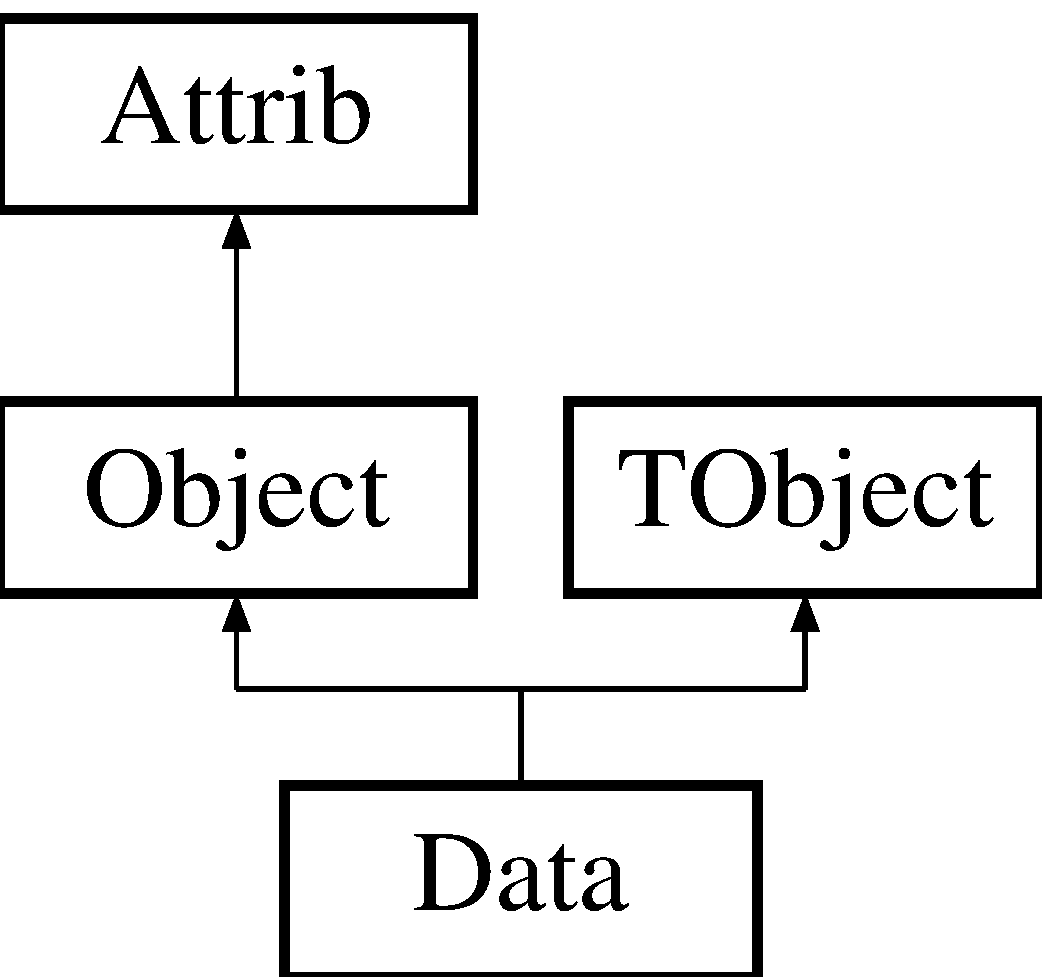
\includegraphics[height=3cm]{classData}
\end{center}
\end{figure}
\subsection*{Public Types}
\begin{DoxyCompactItemize}
\item 
enum \hyperlink{classAttrib_a69e171d7cc6417835a5a306d3c764235}{Attribut} \{ \par
\hyperlink{classAttrib_a69e171d7cc6417835a5a306d3c764235a3a8da2ab97dda18aebab196fe4100531}{UNDEFINED}, 
\hyperlink{classAttrib_a69e171d7cc6417835a5a306d3c764235a2bfb2af57b87031d190a05fe25dd92ed}{PASSIVE}, 
\hyperlink{classAttrib_a69e171d7cc6417835a5a306d3c764235a3b1fec929c0370d1436f2f06e298fb0d}{ACTIVE}, 
\hyperlink{classAttrib_a69e171d7cc6417835a5a306d3c764235aa27c16b480a369ea4d18b07b2516bbc7}{INTERFACE}, 
\par
\hyperlink{classAttrib_a69e171d7cc6417835a5a306d3c764235a1420a5b8c0540b2af210b6975eded7f9}{IO}, 
\hyperlink{classAttrib_a69e171d7cc6417835a5a306d3c764235a0af3b0d0ac323c1704e6c69cf90add28}{IODATA}, 
\hyperlink{classAttrib_a69e171d7cc6417835a5a306d3c764235a7788bc5dd333fd8ce18562b269c9dab1}{ELEMENT}, 
\hyperlink{classAttrib_a69e171d7cc6417835a5a306d3c764235a61ceb22149f365f1780d18f9d1459423}{HARDWARE}, 
\par
\hyperlink{classAttrib_a69e171d7cc6417835a5a306d3c764235a75250e29692496e73effca2c0330977f}{PROCESSUS}, 
\hyperlink{classAttrib_a69e171d7cc6417835a5a306d3c764235a103a67cd0b8f07ef478fa45d4356e27b}{SOFTWARE}
 \}
\end{DoxyCompactItemize}
\subsection*{Public Member Functions}
\begin{DoxyCompactItemize}
\item 
\hyperlink{classData_af11f741cb7f587e2e495452a8905a22a}{Data} ()
\begin{DoxyCompactList}\small\item\em Standard constructor. \item\end{DoxyCompactList}\item 
\hyperlink{classData_ab330e474ce084600685c55017f36152b}{Data} (int, int, int)
\item 
virtual \hyperlink{classData_aab31956423290f0d62dcca47ab4d16dd}{$\sim$Data} ()
\item 
void \hyperlink{classData_a05804aa3964a587b5b283c4cb022b6b3}{setEvt} (int evt)
\begin{DoxyCompactList}\small\item\em Destructor. \item\end{DoxyCompactList}\item 
void \hyperlink{classData_a3aa387b48be4aba77d22e96cf9426569}{setChannel} (int ch)
\item 
void \hyperlink{classData_ac4b0bae25af361e9ceaa49fb6d341cff}{setData} (int data)
\item 
void \hyperlink{classData_ac963308038ebd614a508b1c93b738e67}{Clear} (Option\_\-t $\ast$option=\char`\"{}\char`\"{})
\item 
\hyperlink{classData_af11f741cb7f587e2e495452a8905a22a}{Data} ()
\begin{DoxyCompactList}\small\item\em Standard constructor. \item\end{DoxyCompactList}\item 
virtual \hyperlink{classData_a8c4dbe720325cd952ec9146114f22d35}{$\sim$Data} ()
\begin{DoxyCompactList}\small\item\em Destructor. \item\end{DoxyCompactList}\item 
void \hyperlink{classData_a779ce878d01483220b49ad9e513d7366}{print} ()
\item 
void \hyperlink{classData_a33c31859f6b2771ebd4f0b83fa44739c}{addDataStream} (std::string, std::string)
\item 
void \hyperlink{classData_ab6e1f621fc3b44a940d9d8af3cfa4253}{addHisto1d} (TH1D $\ast$)
\item 
void \hyperlink{classData_a4bef9c956f3994bfa491f94f4821704c}{addHisto2d} (TH2D $\ast$)
\item 
void \hyperlink{classData_a0c21ebc7662b7a6e25171959689481ca}{buildHistos} ()
\item 
\hyperlink{classHisto1D}{Histo1D} $\ast$ \hyperlink{classData_a476a66728ccfc553909d15b36c22492a}{hist1d} (unsigned int row)
\item 
\hyperlink{classHisto1D}{Histo1D} $\ast$ \hyperlink{classData_a77d56a83e198fbc3806499c1e4aa0f10}{hist1d} (std::string name)
\item 
\hyperlink{classHisto2D}{Histo2D} $\ast$ \hyperlink{classData_ab717ebe242192605ad509b76df35e855}{hist2d} (unsigned int row)
\item 
\hyperlink{classHisto2D}{Histo2D} $\ast$ \hyperlink{classData_a02c42a270c4057722a95758d4f2a25a8}{hist2d} (std::string name)
\item 
void \hyperlink{classData_a26209d56fdc86a72ae391fcd3bd2adfd}{purge} ()
\item 
\hyperlink{classStatusCode}{StatusCode} \hyperlink{classData_acdda95480997a3d6245799810334739d}{clear} (int)
\item 
\hyperlink{classStatusCode}{StatusCode} \hyperlink{classData_adb072575d5c15cfbada75f80797c983c}{dataFill} (int, double)
\item 
std::string \hyperlink{classData_a58055729bcd33b4532cae0c569af5ea8}{name} (unsigned int)
\item 
std::string \hyperlink{classData_ab7aa54615fd27c0bc1ff36b7b89b6857}{title} (unsigned int)
\item 
std::vector$<$ double $>$ $\ast$ \hyperlink{classData_aa2153cb57f6f1a67b54eafe5582e0b6b}{vectorPtr} (unsigned int)
\item 
std::vector$<$ double $>$ \hyperlink{classData_a94e00cdd58c1d6f11487f1ac47fee4bc}{vector} (unsigned int)
\item 
std::vector$<$ double $>$ \hyperlink{classData_a7f1983ff7e2221ccf4652d3cd6164d32}{vector} (std::string)
\item 
int \hyperlink{classData_a72f9afe0edb22ad39871292f9f4d3d38}{rowFromName} (std::string)
\item 
bool \hyperlink{classData_ad3942803fea5649bf101220667ab5021}{empty} ()
\item 
std::string \hyperlink{classObject_a975e888d50bfcbffda2c86368332a5cd}{name} () const 
\item 
std::string \hyperlink{classObject_a84f99f70f144a83e1582d1d0f84e4e62}{type} ()
\item 
unsigned char \hyperlink{classObject_af99145335cc61ff6e2798ea17db009d2}{id} ()
\item 
std::string \hyperlink{classObject_a73a0f1a41828fdd8303dd662446fb6c3}{title} ()
\item 
void \hyperlink{classObject_a3f9d5537ebce0c0f2bf6ae4d92426f3c}{msgSvc} (int level, std::string msg, std::string name)
\item 
void \hyperlink{classObject_a58b2d0618c2d08cf2383012611528d97}{msg} (std::string mymsg)
\item 
void \hyperlink{classObject_ac5d59299273cee27aacf7de00d2e7034}{msg} (std::string mymsg, std::string name)
\item 
void \hyperlink{classObject_a83d2db2df682907ea1115ad721c1c4a1}{verbose} (std::string mymsg)
\item 
void \hyperlink{classObject_a2d4120195317e2a3c6532e8bb9f3da68}{verbose} (std::string mymsg, std::string name)
\item 
void \hyperlink{classObject_aac010553f022165573714b7014a15f0d}{debug} (std::string mymsg)
\item 
void \hyperlink{classObject_a6c9a0397ca804e04d675ed05683f5420}{debug} (std::string mymsg, std::string name)
\item 
void \hyperlink{classObject_a644fd329ea4cb85f54fa6846484b84a8}{info} (std::string mymsg)
\item 
void \hyperlink{classObject_a1ca123253dfd30fc28b156f521dcbdae}{info} (std::string mymsg, std::string name)
\item 
void \hyperlink{classObject_a65cd4fda577711660821fd2cd5a3b4c9}{warning} (std::string mymsg)
\item 
void \hyperlink{classObject_a11f101db4dd73d9391b0231818881d86}{warning} (std::string mymsg, std::string name)
\item 
void \hyperlink{classObject_a204a95f57818c0f811933917a30eff45}{error} (std::string mymsg)
\item 
void \hyperlink{classObject_ad7f6c457733082efa2f9ff5f5c8e119a}{error} (std::string mymsg, std::string name)
\item 
void \hyperlink{classObject_aad5a16aac7516ce65bd5ec02ab07fc80}{fatal} (std::string mymsg)
\item 
void \hyperlink{classObject_ae62acd3d09f716220f75f252dc38bc9a}{fatal} (std::string mymsg, std::string name)
\item 
void \hyperlink{classObject_ae30fea75683c2d149b6b6d17c09ecd0c}{setName} (std::string name)
\item 
void \hyperlink{classObject_aae534cc9d982bcb9b99fd505f2e103a5}{setType} (std::string type)
\item 
void \hyperlink{classObject_a398fe08cba594a0ce6891d59fe4f159f}{setId} (unsigned char id)
\item 
void \hyperlink{classObject_a89557dbbad5bcaa02652f5d7fa35d20f}{setTitle} (std::string title)
\item 
void \hyperlink{classObject_a870c5af919958c2136623b2d7816d123}{setDllName} (std::string dllName)
\item 
std::string \hyperlink{classObject_a2e3947f2870094c332d7454117f3ec63}{dllName} ()
\item 
bool \hyperlink{classAttrib_a704f26af560909ad22065083bb7d4c34}{is} (int attribut)
\item 
void \hyperlink{classAttrib_a235f773af19c900264a190b00a3b4ad7}{add} (int attribut)
\item 
void \hyperlink{classAttrib_a7d4ef7e32d93cb287792b87b857e79f3}{remove} (int attribut)
\item 
std::string \hyperlink{classAttrib_aee7bbf16b144887f196e1341b24f8a26}{attributs} ()
\end{DoxyCompactItemize}
\subsection*{Public Attributes}
\begin{DoxyCompactItemize}
\item 
ClassDef(\hyperlink{classData}{Data}, 1) protected int \hyperlink{classData_a116d0476675c4eb96ad7f3ddb2b5f6cd}{Evt}
\item 
int \hyperlink{classData_afa86e448a0941d60d105b3132f200beb}{Raw}
\end{DoxyCompactItemize}
\subsection*{Protected Attributes}
\begin{DoxyCompactItemize}
\item 
std::string \hyperlink{classAttrib_a3414521d7a82476e874b25a5407b5e63}{m\_\-attribString} \mbox{[}10\mbox{]}
\end{DoxyCompactItemize}
\subsection*{Private Attributes}
\begin{DoxyCompactItemize}
\item 
std::vector$<$ std::vector$<$ double $>$ $\ast$ $>$ \hyperlink{classData_a55199a86b131bdae275582f540987bc9}{m\_\-values}
\item 
std::vector$<$ TH1D $\ast$ $>$ \hyperlink{classData_ae79c62d2ac8f7fe42aa65b26044005ba}{m\_\-h1d}
\item 
std::vector$<$ TH2D $\ast$ $>$ \hyperlink{classData_ad34ba7631ba40c0e744d37b8292ba949}{m\_\-h2d}
\item 
std::vector$<$ \hyperlink{classHisto1D}{Histo1D} $>$ \hyperlink{classData_a06c0415eace30c2944eda0e99ce486d4}{m\_\-hist1d}
\item 
std::vector$<$ \hyperlink{classHisto2D}{Histo2D} $>$ \hyperlink{classData_a6f13c5af755aae6ae43abc3f04a9b7af}{m\_\-hist2d}
\item 
std::vector$<$ std::string $>$ \hyperlink{classData_a60e5c1c1e5b7373045932a25820d5d0c}{m\_\-titles}
\item 
std::vector$<$ std::string $>$ \hyperlink{classData_aee6304b181b43f1227c531716a833270}{m\_\-names}
\end{DoxyCompactItemize}


\subsection{Detailed Description}
\begin{DoxyAuthor}{Author}
Fr�d�ric Machefert 
\end{DoxyAuthor}
\begin{DoxyDate}{Date}
2004-\/10-\/04
\end{DoxyDate}
\begin{DoxyAuthor}{Author}
Frederic Machefert 
\end{DoxyAuthor}
\begin{DoxyDate}{Date}
2010-\/01-\/06 
\end{DoxyDate}


Definition at line 16 of file Data.h.

\subsection{Member Enumeration Documentation}
\hypertarget{classAttrib_a69e171d7cc6417835a5a306d3c764235}{
\index{Data@{Data}!Attribut@{Attribut}}
\index{Attribut@{Attribut}!Data@{Data}}
\subsubsection[{Attribut}]{\setlength{\rightskip}{0pt plus 5cm}enum {\bf Attrib::Attribut}\hspace{0.3cm}{\ttfamily  \mbox{[}inherited\mbox{]}}}}
\label{classAttrib_a69e171d7cc6417835a5a306d3c764235}
\begin{Desc}
\item[Enumerator: ]\par
\begin{description}
\index{UNDEFINED@{UNDEFINED}!Data@{Data}}\index{Data@{Data}!UNDEFINED@{UNDEFINED}}\item[{\em 
\hypertarget{classAttrib_a69e171d7cc6417835a5a306d3c764235a3a8da2ab97dda18aebab196fe4100531}{
UNDEFINED}
\label{classAttrib_a69e171d7cc6417835a5a306d3c764235a3a8da2ab97dda18aebab196fe4100531}
}]\index{PASSIVE@{PASSIVE}!Data@{Data}}\index{Data@{Data}!PASSIVE@{PASSIVE}}\item[{\em 
\hypertarget{classAttrib_a69e171d7cc6417835a5a306d3c764235a2bfb2af57b87031d190a05fe25dd92ed}{
PASSIVE}
\label{classAttrib_a69e171d7cc6417835a5a306d3c764235a2bfb2af57b87031d190a05fe25dd92ed}
}]\index{ACTIVE@{ACTIVE}!Data@{Data}}\index{Data@{Data}!ACTIVE@{ACTIVE}}\item[{\em 
\hypertarget{classAttrib_a69e171d7cc6417835a5a306d3c764235a3b1fec929c0370d1436f2f06e298fb0d}{
ACTIVE}
\label{classAttrib_a69e171d7cc6417835a5a306d3c764235a3b1fec929c0370d1436f2f06e298fb0d}
}]\index{INTERFACE@{INTERFACE}!Data@{Data}}\index{Data@{Data}!INTERFACE@{INTERFACE}}\item[{\em 
\hypertarget{classAttrib_a69e171d7cc6417835a5a306d3c764235aa27c16b480a369ea4d18b07b2516bbc7}{
INTERFACE}
\label{classAttrib_a69e171d7cc6417835a5a306d3c764235aa27c16b480a369ea4d18b07b2516bbc7}
}]\index{IO@{IO}!Data@{Data}}\index{Data@{Data}!IO@{IO}}\item[{\em 
\hypertarget{classAttrib_a69e171d7cc6417835a5a306d3c764235a1420a5b8c0540b2af210b6975eded7f9}{
IO}
\label{classAttrib_a69e171d7cc6417835a5a306d3c764235a1420a5b8c0540b2af210b6975eded7f9}
}]\index{IODATA@{IODATA}!Data@{Data}}\index{Data@{Data}!IODATA@{IODATA}}\item[{\em 
\hypertarget{classAttrib_a69e171d7cc6417835a5a306d3c764235a0af3b0d0ac323c1704e6c69cf90add28}{
IODATA}
\label{classAttrib_a69e171d7cc6417835a5a306d3c764235a0af3b0d0ac323c1704e6c69cf90add28}
}]\index{ELEMENT@{ELEMENT}!Data@{Data}}\index{Data@{Data}!ELEMENT@{ELEMENT}}\item[{\em 
\hypertarget{classAttrib_a69e171d7cc6417835a5a306d3c764235a7788bc5dd333fd8ce18562b269c9dab1}{
ELEMENT}
\label{classAttrib_a69e171d7cc6417835a5a306d3c764235a7788bc5dd333fd8ce18562b269c9dab1}
}]\index{HARDWARE@{HARDWARE}!Data@{Data}}\index{Data@{Data}!HARDWARE@{HARDWARE}}\item[{\em 
\hypertarget{classAttrib_a69e171d7cc6417835a5a306d3c764235a61ceb22149f365f1780d18f9d1459423}{
HARDWARE}
\label{classAttrib_a69e171d7cc6417835a5a306d3c764235a61ceb22149f365f1780d18f9d1459423}
}]\index{PROCESSUS@{PROCESSUS}!Data@{Data}}\index{Data@{Data}!PROCESSUS@{PROCESSUS}}\item[{\em 
\hypertarget{classAttrib_a69e171d7cc6417835a5a306d3c764235a75250e29692496e73effca2c0330977f}{
PROCESSUS}
\label{classAttrib_a69e171d7cc6417835a5a306d3c764235a75250e29692496e73effca2c0330977f}
}]\index{SOFTWARE@{SOFTWARE}!Data@{Data}}\index{Data@{Data}!SOFTWARE@{SOFTWARE}}\item[{\em 
\hypertarget{classAttrib_a69e171d7cc6417835a5a306d3c764235a103a67cd0b8f07ef478fa45d4356e27b}{
SOFTWARE}
\label{classAttrib_a69e171d7cc6417835a5a306d3c764235a103a67cd0b8f07ef478fa45d4356e27b}
}]\end{description}
\end{Desc}



Definition at line 29 of file Attrib.h.


\begin{DoxyCode}
29                 {
30     UNDEFINED,
31     PASSIVE,
32     ACTIVE,
33     INTERFACE,
34     IO,
35     IODATA,
36     ELEMENT,
37     HARDWARE,
38     PROCESSUS,
39     SOFTWARE 
40   }; // array m_attribString must be changed into Attrib::Attrib if this enu is m
      odified. 
\end{DoxyCode}


\subsection{Constructor \& Destructor Documentation}
\hypertarget{classData_af11f741cb7f587e2e495452a8905a22a}{
\index{Data@{Data}!Data@{Data}}
\index{Data@{Data}!Data@{Data}}
\subsubsection[{Data}]{\setlength{\rightskip}{0pt plus 5cm}Data::Data ()}}
\label{classData_af11f741cb7f587e2e495452a8905a22a}


Standard constructor. 

Definition at line 18 of file Data.cpp.


\begin{DoxyCode}
18             {
19 }
\end{DoxyCode}
\hypertarget{classData_ab330e474ce084600685c55017f36152b}{
\index{Data@{Data}!Data@{Data}}
\index{Data@{Data}!Data@{Data}}
\subsubsection[{Data}]{\setlength{\rightskip}{0pt plus 5cm}Data::Data (int {\em evt}, \/  int {\em channel}, \/  int {\em data})}}
\label{classData_ab330e474ce084600685c55017f36152b}


Definition at line 23 of file Data.cpp.

References Evt, and Raw.


\begin{DoxyCode}
23                                             {
24   Evt   = evt;
25   Raw   = data;
26   Ch    = channel ;
27 }
\end{DoxyCode}
\hypertarget{classData_aab31956423290f0d62dcca47ab4d16dd}{
\index{Data@{Data}!$\sim$Data@{$\sim$Data}}
\index{$\sim$Data@{$\sim$Data}!Data@{Data}}
\subsubsection[{$\sim$Data}]{\setlength{\rightskip}{0pt plus 5cm}Data::$\sim$Data ()\hspace{0.3cm}{\ttfamily  \mbox{[}inline, virtual\mbox{]}}}}
\label{classData_aab31956423290f0d62dcca47ab4d16dd}


Definition at line 21 of file Data.h.

References Clear().


\begin{DoxyCode}
21 { Clear(); }; 
\end{DoxyCode}
\hypertarget{classData_af11f741cb7f587e2e495452a8905a22a}{
\index{Data@{Data}!Data@{Data}}
\index{Data@{Data}!Data@{Data}}
\subsubsection[{Data}]{\setlength{\rightskip}{0pt plus 5cm}Data::Data ()}}
\label{classData_af11f741cb7f587e2e495452a8905a22a}


Standard constructor. \hypertarget{classData_a8c4dbe720325cd952ec9146114f22d35}{
\index{Data@{Data}!$\sim$Data@{$\sim$Data}}
\index{$\sim$Data@{$\sim$Data}!Data@{Data}}
\subsubsection[{$\sim$Data}]{\setlength{\rightskip}{0pt plus 5cm}virtual Data::$\sim$Data ()\hspace{0.3cm}{\ttfamily  \mbox{[}virtual\mbox{]}}}}
\label{classData_a8c4dbe720325cd952ec9146114f22d35}


Destructor. 

\subsection{Member Function Documentation}
\hypertarget{classAttrib_a235f773af19c900264a190b00a3b4ad7}{
\index{Data@{Data}!add@{add}}
\index{add@{add}!Data@{Data}}
\subsubsection[{add}]{\setlength{\rightskip}{0pt plus 5cm}void Attrib::add (int {\em attribut})\hspace{0.3cm}{\ttfamily  \mbox{[}inline, inherited\mbox{]}}}}
\label{classAttrib_a235f773af19c900264a190b00a3b4ad7}
Add an attribut 

Definition at line 67 of file Attrib.h.

References Attrib::m\_\-attributs, and Attrib::UNDEFINED.

Referenced by A3PE::A3PE(), Attrib::Attrib(), SpecsMezzanine::cmdline(), Computer::Computer(), CU\_\-v1::CU\_\-v1(), export\_\-obj(), FEB\_\-v1::FEB\_\-v1(), FePGA::FePGA(), ICECALv3::ICECALv3(), ICPhaser::ICPhaser(), Application::initialize(), Interface::Interface(), IOdata::IOdata(), IOobject::IOobject(), LSDelayChipV1::LSDelayChipV1(), MSOxxxx::MSOxxxx(), Phaser::Phaser(), Processus::Processus(), Proto40MHz\_\-v1::Proto40MHz\_\-v1(), Attrib::remove(), SeqPGA::SeqPGA(), SpecsMaster::SpecsMaster(), and SpecsSlave::SpecsSlave().


\begin{DoxyCode}
67                             {
68     if (attribut!=Attrib::UNDEFINED) remove(Attrib::UNDEFINED);
69     bool duplicate = false ;
70     std::vector<int>::const_iterator iter ;
71     for ( iter  = m_attributs.begin() ;
72           iter != m_attributs.end()   ;
73           ++iter ) {
74       if ( attribut == (*iter) ) {
75         duplicate = true ;
76       }
77     }
78     if (!duplicate) {
79       m_attributs.push_back( attribut );
80     }
81   }
\end{DoxyCode}
\hypertarget{classData_a33c31859f6b2771ebd4f0b83fa44739c}{
\index{Data@{Data}!addDataStream@{addDataStream}}
\index{addDataStream@{addDataStream}!Data@{Data}}
\subsubsection[{addDataStream}]{\setlength{\rightskip}{0pt plus 5cm}void Data::addDataStream (std::string {\em n}, \/  std::string {\em t})}}
\label{classData_a33c31859f6b2771ebd4f0b83fa44739c}


Definition at line 31 of file Data.cpp.

References m\_\-names, m\_\-titles, and m\_\-values.

Referenced by Processus::addDataStream(), and FEB\_\-v1::FEB\_\-v1().


\begin{DoxyCode}
31                                                   {
32   m_names .push_back(n);
33   m_titles.push_back(t);
34   m_values.push_back(new std::vector<double>);
35 }
\end{DoxyCode}
\hypertarget{classData_ab6e1f621fc3b44a940d9d8af3cfa4253}{
\index{Data@{Data}!addHisto1d@{addHisto1d}}
\index{addHisto1d@{addHisto1d}!Data@{Data}}
\subsubsection[{addHisto1d}]{\setlength{\rightskip}{0pt plus 5cm}void Data::addHisto1d (TH1D $\ast$ {\em h})}}
\label{classData_ab6e1f621fc3b44a940d9d8af3cfa4253}


Definition at line 40 of file Data.cpp.

References m\_\-h1d.

Referenced by Processus::addHisto1d().


\begin{DoxyCode}
40                              {
41   m_h1d.push_back( h );
42 }
\end{DoxyCode}
\hypertarget{classData_a4bef9c956f3994bfa491f94f4821704c}{
\index{Data@{Data}!addHisto2d@{addHisto2d}}
\index{addHisto2d@{addHisto2d}!Data@{Data}}
\subsubsection[{addHisto2d}]{\setlength{\rightskip}{0pt plus 5cm}void Data::addHisto2d (TH2D $\ast$ {\em h})}}
\label{classData_a4bef9c956f3994bfa491f94f4821704c}


Definition at line 47 of file Data.cpp.

References m\_\-h2d.

Referenced by Processus::addHisto2d().


\begin{DoxyCode}
47                              {
48   m_h2d.push_back( h );
49 }
\end{DoxyCode}
\hypertarget{classAttrib_aee7bbf16b144887f196e1341b24f8a26}{
\index{Data@{Data}!attributs@{attributs}}
\index{attributs@{attributs}!Data@{Data}}
\subsubsection[{attributs}]{\setlength{\rightskip}{0pt plus 5cm}std::string Attrib::attributs ()\hspace{0.3cm}{\ttfamily  \mbox{[}inherited\mbox{]}}}}
\label{classAttrib_aee7bbf16b144887f196e1341b24f8a26}
Print the \hyperlink{classAttrib}{Attrib} of an \hyperlink{classObject}{Object} 

Definition at line 54 of file Attrib.cpp.

References images::index, Attrib::m\_\-attribString, and Attrib::m\_\-attributs.

Referenced by export\_\-obj().


\begin{DoxyCode}
54                             {
55   std::string output;
56   std::vector<int>::iterator iter ;
57   for ( unsigned int index = 0 ; index < m_attributs.size() ; ++index ) {
58     if ( m_attributs.size() - index > 1 ) {
59       output.append(m_attribString[m_attributs[index]]);
60       output.append(":");
61     }
62     else {
63       output.append(m_attribString[m_attributs[index]]);
64     }
65   }
66   return output;
67 }
\end{DoxyCode}
\hypertarget{classData_a0c21ebc7662b7a6e25171959689481ca}{
\index{Data@{Data}!buildHistos@{buildHistos}}
\index{buildHistos@{buildHistos}!Data@{Data}}
\subsubsection[{buildHistos}]{\setlength{\rightskip}{0pt plus 5cm}void Data::buildHistos ()}}
\label{classData_a0c21ebc7662b7a6e25171959689481ca}


Definition at line 98 of file Data.cpp.

References m\_\-h1d, m\_\-h2d, m\_\-hist1d, and m\_\-hist2d.

Referenced by Processus::endProcessing().


\begin{DoxyCode}
98                       {
99   std::vector<TH1D*>::iterator iter1d;
100   for (iter1d=m_h1d.begin(); iter1d!=m_h1d.end(); ++iter1d){
101     m_hist1d.push_back(Histo1D(*iter1d));
102   }
103   std::vector<TH2D*>::iterator iter2d;
104   for (iter2d=m_h2d.begin(); iter2d!=m_h2d.end(); ++iter2d){
105     m_hist2d.push_back(Histo2D(*iter2d));
106   }
107 }
\end{DoxyCode}
\hypertarget{classData_acdda95480997a3d6245799810334739d}{
\index{Data@{Data}!clear@{clear}}
\index{clear@{clear}!Data@{Data}}
\subsubsection[{clear}]{\setlength{\rightskip}{0pt plus 5cm}{\bf StatusCode} Data::clear (int {\em i})}}
\label{classData_acdda95480997a3d6245799810334739d}


Definition at line 71 of file Data.cpp.

References StatusCode::FAILURE, StatusCode::SUCCESS, and vectorPtr().

Referenced by FEB\_\-v1::readFifoLLT(), FEB\_\-v1::readFifoLLTFE(), and FEB\_\-v1::readFifoSpyFE().


\begin{DoxyCode}
71                              {
72   if (vectorPtr(i)!=0){
73     vectorPtr(i)->clear();
74     return StatusCode::SUCCESS;
75   }
76   else {
77     return StatusCode::FAILURE;
78   }
79 }
\end{DoxyCode}
\hypertarget{classData_ac963308038ebd614a508b1c93b738e67}{
\index{Data@{Data}!Clear@{Clear}}
\index{Clear@{Clear}!Data@{Data}}
\subsubsection[{Clear}]{\setlength{\rightskip}{0pt plus 5cm}void Data::Clear (Option\_\-t $\ast$ {\em option} = {\ttfamily \char`\"{}\char`\"{}})}}
\label{classData_ac963308038ebd614a508b1c93b738e67}


Definition at line 32 of file Data.cpp.

Referenced by $\sim$Data().


\begin{DoxyCode}
32                                      {
33 }
\end{DoxyCode}
\hypertarget{classData_adb072575d5c15cfbada75f80797c983c}{
\index{Data@{Data}!dataFill@{dataFill}}
\index{dataFill@{dataFill}!Data@{Data}}
\subsubsection[{dataFill}]{\setlength{\rightskip}{0pt plus 5cm}{\bf StatusCode} Data::dataFill (int {\em i}, \/  double {\em val})}}
\label{classData_adb072575d5c15cfbada75f80797c983c}
Set data stream with value \begin{DoxyReturn}{Returns}
the \hyperlink{classStatusCode}{StatusCode} 
\end{DoxyReturn}


Definition at line 85 of file Data.cpp.

References StatusCode::FAILURE, StatusCode::SUCCESS, and vectorPtr().

Referenced by FEB\_\-v1::readFifoLLT(), FEB\_\-v1::readFifoLLTFE(), and FEB\_\-v1::readFifoSpyFE().


\begin{DoxyCode}
85                                           {
86   if (vectorPtr(i)!=0){
87     vectorPtr(i)->push_back(val);
88     return StatusCode::SUCCESS;
89   }
90   else {
91     return StatusCode::FAILURE;
92   }
93 }
\end{DoxyCode}
\hypertarget{classObject_a6c9a0397ca804e04d675ed05683f5420}{
\index{Data@{Data}!debug@{debug}}
\index{debug@{debug}!Data@{Data}}
\subsubsection[{debug}]{\setlength{\rightskip}{0pt plus 5cm}void Object::debug (std::string {\em mymsg}, \/  std::string {\em name})\hspace{0.3cm}{\ttfamily  \mbox{[}inline, inherited\mbox{]}}}}
\label{classObject_a6c9a0397ca804e04d675ed05683f5420}


Definition at line 45 of file Object.h.

References MsgSvc::DEBUG, Object::m\_\-log, and MsgSvc::msgSvc().


\begin{DoxyCode}
45 { m_log.msgSvc (MsgSvc::DEBUG   , mymsg, name ); }
\end{DoxyCode}
\hypertarget{classObject_aac010553f022165573714b7014a15f0d}{
\index{Data@{Data}!debug@{debug}}
\index{debug@{debug}!Data@{Data}}
\subsubsection[{debug}]{\setlength{\rightskip}{0pt plus 5cm}void Object::debug (std::string {\em mymsg})\hspace{0.3cm}{\ttfamily  \mbox{[}inline, inherited\mbox{]}}}}
\label{classObject_aac010553f022165573714b7014a15f0d}


Definition at line 37 of file Object.h.

References MsgSvc::DEBUG, Object::m\_\-log, Object::m\_\-name, and MsgSvc::msgSvc().

Referenced by A3PE::A3PE(), A3PE::acquisition(), SpecsMezzanine::addBus(), Hierarchy::addChild(), SpecsSlave::addI2c(), LSDelayChipV1::checkConfigAddr(), LSDelayChipV1::checkStatusAddr(), LSDelayChipV1::configRegBulkRead(), LSDelayChipV1::configRegBulkWrite(), A3PE::dataReady(), DCU::DCU(), Hierarchy::delChild(), SpecsSlave::detect(), EmulateFE::execute(), StorageFifoAcquisition::execute(), StorageFifo::execute(), Acquisition::execute(), A3PE\_\-BitFlip::execute(), export\_\-obj(), FePGA::FePGA(), SpecsGlue::i2cClkMode(), SeqPGA::i2cRead(), FePGA::i2cRead(), SeqPGA::i2cWrite(), FePGA::i2cWrite(), ICECALv3::ICECALv3(), ICPhaser::ICPhaser(), SpecsSlave::init(), SpecsMaster::init(), EmulateFE::initialize(), StorageFifoAcquisition::initialize(), StorageFifo::initialize(), Acquisition::initialize(), A3PE\_\-BitFlip::initialize(), A3PE::internalAXSequence(), SpecsMezzanine::led(), SpecsGlue::led(), LSDelayChipV1::LSDelayChipV1(), MSOxxxx::MSOxxxx(), Phaser::Phaser(), purge(), ICPhaser::read(), Phaser::read(), FEB\_\-v1::readFifoSpyFE(), SpecsSlave::reset(), SpecsMaster::reset(), FEB\_\-v1::reset(), CU\_\-v1::reset(), Proto40MHz\_\-v1::reset(), FEB\_\-v1::resetFifoSpyFE(), SeqPGA::resetSpi(), FEB\_\-v1::resetSpi(), SeqPGA::SeqPGA(), A3PE::setAddFromAXRam(), A3PE::setAddToAXRam(), A3PE::setAXRamUsb(), Element::setConnection(), SpecsGlue::setI2cClkMode(), A3PE::setLatencyAX(), SpecsMezzanine::setLed(), SpecsGlue::setLed(), A3PE::setLengthAX(), A3PE::setReadToAXRamUsb(), SpecsMaster::setSpeed(), A3PE::setWriteFromAXRamUsb(), SpecsBus::SpecsBus(), SpecsI2c::SpecsI2c(), SpecsMaster::SpecsMaster(), SpecsMezzanine::SpecsMezzanine(), SpecsParallelBus::SpecsParallelBus(), SpecsSlave::SpecsSlave(), LSDelayChipV1::spiBERTest(), ICECALv3::spiRead(), ICECALv3::spiWrite(), FEB\_\-v1::testDuration(), SeqPGA::testSequence(), A3PE::trigger(), Server::updateConfig(), Server::updateState(), ICPhaser::write(), Phaser::write(), and Hierarchy::$\sim$Hierarchy().


\begin{DoxyCode}
37 { m_log.msgSvc (MsgSvc::DEBUG   , mymsg, m_name ); }
\end{DoxyCode}
\hypertarget{classObject_a2e3947f2870094c332d7454117f3ec63}{
\index{Data@{Data}!dllName@{dllName}}
\index{dllName@{dllName}!Data@{Data}}
\subsubsection[{dllName}]{\setlength{\rightskip}{0pt plus 5cm}std::string Object::dllName ()\hspace{0.3cm}{\ttfamily  \mbox{[}inline, inherited\mbox{]}}}}
\label{classObject_a2e3947f2870094c332d7454117f3ec63}
Get accessor to member m\_\-dllName \begin{DoxyReturn}{Returns}
the current value of m\_\-dllName 
\end{DoxyReturn}


Definition at line 74 of file Object.h.

References Object::m\_\-dllName.

Referenced by export\_\-obj().


\begin{DoxyCode}
74                        {
75     return m_dllName;
76   }  
\end{DoxyCode}
\hypertarget{classData_ad3942803fea5649bf101220667ab5021}{
\index{Data@{Data}!empty@{empty}}
\index{empty@{empty}!Data@{Data}}
\subsubsection[{empty}]{\setlength{\rightskip}{0pt plus 5cm}bool Data::empty ()\hspace{0.3cm}{\ttfamily  \mbox{[}inline\mbox{]}}}}
\label{classData_ad3942803fea5649bf101220667ab5021}


Definition at line 49 of file Data.h.

References m\_\-h1d, m\_\-h2d, and m\_\-names.

Referenced by Processus::endProcessing().


\begin{DoxyCode}
49               {
50     if (0==m_names.size()&&0==m_h1d.size()&&0==m_h2d.size()) return true;
51     return false;
52   }
\end{DoxyCode}
\hypertarget{classObject_ad7f6c457733082efa2f9ff5f5c8e119a}{
\index{Data@{Data}!error@{error}}
\index{error@{error}!Data@{Data}}
\subsubsection[{error}]{\setlength{\rightskip}{0pt plus 5cm}void Object::error (std::string {\em mymsg}, \/  std::string {\em name})\hspace{0.3cm}{\ttfamily  \mbox{[}inline, inherited\mbox{]}}}}
\label{classObject_ad7f6c457733082efa2f9ff5f5c8e119a}


Definition at line 48 of file Object.h.

References MsgSvc::ERR, Object::m\_\-log, and MsgSvc::msgSvc().


\begin{DoxyCode}
48 { m_log.msgSvc (MsgSvc::ERR     , mymsg, name ); }
\end{DoxyCode}
\hypertarget{classObject_a204a95f57818c0f811933917a30eff45}{
\index{Data@{Data}!error@{error}}
\index{error@{error}!Data@{Data}}
\subsubsection[{error}]{\setlength{\rightskip}{0pt plus 5cm}void Object::error (std::string {\em mymsg})\hspace{0.3cm}{\ttfamily  \mbox{[}inline, inherited\mbox{]}}}}
\label{classObject_a204a95f57818c0f811933917a30eff45}


Definition at line 40 of file Object.h.

References MsgSvc::ERR, Object::m\_\-log, Object::m\_\-name, and MsgSvc::msgSvc().

Referenced by ICECALv3::checkChNumber(), A3PE::clockDivision(), NI6008::cmd(), A3PE::enableStorage(), A3PE\_\-BitFlip::execute(), export\_\-obj(), A3PE::fifoDepth(), A3PE::fifoLatency(), FEB\_\-v1::gbtStatus(), Register::getBit(), MSOxxxx::getStatistics(), SpecsMaster::init(), NI6008::init(), UsbFTMLInterface::init(), UsbFTInterface::init(), A3PE::latencyAX(), A3PE::lengthAX(), A3PE::nTrigger(), MSOxxxx::open(), ICECALv3::parseParameterList(), A3PE::pipeline(), UsbFTMLInterface::read(), UsbFTInterface::read(), MSOxxxx::recv(), A3PE::reset(), MSOxxxx::send(), A3PE::setAddFromAXRam(), A3PE::setAddToAXRam(), ICECALv3::setAnalogCh(), A3PE::setAXRamUsb(), Register::setBit(), A3PE::setClockDivision(), A3PE::setFifoDepth(), A3PE::setFifoLatency(), A3PE::setLatencyAX(), A3PE::setLengthAX(), A3PE::setNTrigger(), A3PE::setPipeline(), A3PE::setReadPatternFifoUsb(), A3PE::setReadToAXRamUsb(), A3PE::setReadTriggerFifoUsb(), A3PE::setSoftwareTrigger(), A3PE::setTriggerDelay(), A3PE::setTriggerRate(), A3PE::setWriteFromAXRamUsb(), A3PE::setWriteStorageFifoUsb(), ICECALv3::spiFERTest(), ICECALv3::spiWriteSafe(), A3PE::startSequenceAX(), A3PE::triggerDelay(), A3PE::triggerRate(), UsbFTMLInterface::usbRead(), UsbFTInterface::usbRead(), UsbFTMLInterface::usbReadU16(), UsbFTInterface::usbReadU16(), UsbFTMLInterface::usbReadU32(), UsbFTInterface::usbReadU32(), UsbFTMLInterface::usbReadU8(), UsbFTInterface::usbReadU8(), UsbFTMLInterface::usbWrite(), UsbFTInterface::usbWrite(), UsbFTMLInterface::usbWriteRead(), UsbFTInterface::usbWriteRead(), UsbFTMLInterface::usbWriteU16(), UsbFTInterface::usbWriteU16(), UsbFTMLInterface::usbWriteU32(), UsbFTInterface::usbWriteU32(), UsbFTMLInterface::usbWriteU8(), UsbFTInterface::usbWriteU8(), UsbFTMLInterface::write(), and UsbFTInterface::write().


\begin{DoxyCode}
40 { m_log.msgSvc (MsgSvc::ERR     , mymsg, m_name ); }
\end{DoxyCode}
\hypertarget{classObject_ae62acd3d09f716220f75f252dc38bc9a}{
\index{Data@{Data}!fatal@{fatal}}
\index{fatal@{fatal}!Data@{Data}}
\subsubsection[{fatal}]{\setlength{\rightskip}{0pt plus 5cm}void Object::fatal (std::string {\em mymsg}, \/  std::string {\em name})\hspace{0.3cm}{\ttfamily  \mbox{[}inline, inherited\mbox{]}}}}
\label{classObject_ae62acd3d09f716220f75f252dc38bc9a}


Definition at line 49 of file Object.h.

References MsgSvc::FATAL, Object::m\_\-log, and MsgSvc::msgSvc().


\begin{DoxyCode}
49 { m_log.msgSvc (MsgSvc::FATAL   , mymsg, name ); }
\end{DoxyCode}
\hypertarget{classObject_aad5a16aac7516ce65bd5ec02ab07fc80}{
\index{Data@{Data}!fatal@{fatal}}
\index{fatal@{fatal}!Data@{Data}}
\subsubsection[{fatal}]{\setlength{\rightskip}{0pt plus 5cm}void Object::fatal (std::string {\em mymsg})\hspace{0.3cm}{\ttfamily  \mbox{[}inline, inherited\mbox{]}}}}
\label{classObject_aad5a16aac7516ce65bd5ec02ab07fc80}


Definition at line 41 of file Object.h.

References MsgSvc::FATAL, Object::m\_\-log, Object::m\_\-name, and MsgSvc::msgSvc().

Referenced by export\_\-obj(), SpecsSlave::init(), UsbSpiBus::init(), UsbI2cBus::init(), IOobject::init(), UsbMLSpiBus::init(), UsbMLI2cBus::init(), UsbFTMLInterface::init(), UsbFTInterface::init(), and Element::setConnection().


\begin{DoxyCode}
41 { m_log.msgSvc (MsgSvc::FATAL   , mymsg, m_name ); }
\end{DoxyCode}
\hypertarget{classData_a77d56a83e198fbc3806499c1e4aa0f10}{
\index{Data@{Data}!hist1d@{hist1d}}
\index{hist1d@{hist1d}!Data@{Data}}
\subsubsection[{hist1d}]{\setlength{\rightskip}{0pt plus 5cm}{\bf Histo1D}$\ast$ Data::hist1d (std::string {\em name})\hspace{0.3cm}{\ttfamily  \mbox{[}inline\mbox{]}}}}
\label{classData_a77d56a83e198fbc3806499c1e4aa0f10}


Definition at line 31 of file Data.h.

References m\_\-hist1d.


\begin{DoxyCode}
31                                    {
32 //    name;
33     return &m_hist1d[0];
34   };
\end{DoxyCode}
\hypertarget{classData_a476a66728ccfc553909d15b36c22492a}{
\index{Data@{Data}!hist1d@{hist1d}}
\index{hist1d@{hist1d}!Data@{Data}}
\subsubsection[{hist1d}]{\setlength{\rightskip}{0pt plus 5cm}{\bf Histo1D}$\ast$ Data::hist1d (unsigned int {\em row})\hspace{0.3cm}{\ttfamily  \mbox{[}inline\mbox{]}}}}
\label{classData_a476a66728ccfc553909d15b36c22492a}


Definition at line 30 of file Data.h.

References m\_\-hist1d.

Referenced by export\_\-proc(), and Processus::hist1d().


\begin{DoxyCode}
30 {return &m_hist1d[row];};
\end{DoxyCode}
\hypertarget{classData_a02c42a270c4057722a95758d4f2a25a8}{
\index{Data@{Data}!hist2d@{hist2d}}
\index{hist2d@{hist2d}!Data@{Data}}
\subsubsection[{hist2d}]{\setlength{\rightskip}{0pt plus 5cm}{\bf Histo2D}$\ast$ Data::hist2d (std::string {\em name})\hspace{0.3cm}{\ttfamily  \mbox{[}inline\mbox{]}}}}
\label{classData_a02c42a270c4057722a95758d4f2a25a8}


Definition at line 36 of file Data.h.

References m\_\-hist2d.


\begin{DoxyCode}
36                                    {
37 //    name;
38     return &m_hist2d[0];
39   };
\end{DoxyCode}
\hypertarget{classData_ab717ebe242192605ad509b76df35e855}{
\index{Data@{Data}!hist2d@{hist2d}}
\index{hist2d@{hist2d}!Data@{Data}}
\subsubsection[{hist2d}]{\setlength{\rightskip}{0pt plus 5cm}{\bf Histo2D}$\ast$ Data::hist2d (unsigned int {\em row})\hspace{0.3cm}{\ttfamily  \mbox{[}inline\mbox{]}}}}
\label{classData_ab717ebe242192605ad509b76df35e855}


Definition at line 35 of file Data.h.

References m\_\-hist2d.

Referenced by export\_\-proc(), and Processus::hist2d().


\begin{DoxyCode}
35 {return &m_hist2d[row];};
\end{DoxyCode}
\hypertarget{classObject_af99145335cc61ff6e2798ea17db009d2}{
\index{Data@{Data}!id@{id}}
\index{id@{id}!Data@{Data}}
\subsubsection[{id}]{\setlength{\rightskip}{0pt plus 5cm}unsigned char Object::id ()\hspace{0.3cm}{\ttfamily  \mbox{[}inline, inherited\mbox{]}}}}
\label{classObject_af99145335cc61ff6e2798ea17db009d2}


Reimplemented in \hyperlink{classMSOxxxx_a0f14b23d31d8e7647184e99a89600cc3}{MSOxxxx}.

Definition at line 30 of file Object.h.

References Object::m\_\-id.

Referenced by export\_\-obj().


\begin{DoxyCode}
30 { return m_id;         } //< Get Object m_id 
\end{DoxyCode}
\hypertarget{classObject_a1ca123253dfd30fc28b156f521dcbdae}{
\index{Data@{Data}!info@{info}}
\index{info@{info}!Data@{Data}}
\subsubsection[{info}]{\setlength{\rightskip}{0pt plus 5cm}void Object::info (std::string {\em mymsg}, \/  std::string {\em name})\hspace{0.3cm}{\ttfamily  \mbox{[}inline, inherited\mbox{]}}}}
\label{classObject_a1ca123253dfd30fc28b156f521dcbdae}


Definition at line 46 of file Object.h.

References MsgSvc::INFO, Object::m\_\-log, and MsgSvc::msgSvc().


\begin{DoxyCode}
46 { m_log.msgSvc (MsgSvc::INFO    , mymsg, name ); }
\end{DoxyCode}
\hypertarget{classObject_a644fd329ea4cb85f54fa6846484b84a8}{
\index{Data@{Data}!info@{info}}
\index{info@{info}!Data@{Data}}
\subsubsection[{info}]{\setlength{\rightskip}{0pt plus 5cm}void Object::info (std::string {\em mymsg})\hspace{0.3cm}{\ttfamily  \mbox{[}inline, inherited\mbox{]}}}}
\label{classObject_a644fd329ea4cb85f54fa6846484b84a8}


Definition at line 38 of file Object.h.

References MsgSvc::INFO, Object::m\_\-log, Object::m\_\-name, and MsgSvc::msgSvc().

Referenced by NI6008::addDevice(), ICECALv3::bxidResynchStatus(), FEB\_\-v1::calibCte(), checkCmd(), Hierarchy::clear(), FEB\_\-v1::clock80MHzFallingEdge(), FEB\_\-v1::clockFallingEdge(), UsbFTMLInterface::close(), UsbFTInterface::close(), MSOxxxx::closeConnection(), Processus::closeRootFile(), SpecsMezzanine::cmdline(), Server::cmdline(), SpecsSlave::detect(), FEB\_\-v1::disableSubtract(), IOdata::dump(), A3PE::dumpFromAX(), A3PE::dumpPattern(), A3PE::dumpStorage(), A3PE::dumpToAX(), A3PE::dumpTrigger(), Processus::endProcessing(), PhaserRampExec::execute(), export\_\-obj(), PhaserRampExec::finalize(), FEB\_\-v1::gain4(), FEB\_\-v1::gbt80MHzClkEport(), FEB\_\-v1::gbtDataPath(), FEB\_\-v1::gbtDLLEport(), FEB\_\-v1::gbtDLLReset(), FEB\_\-v1::gbtEnableEport(), FEB\_\-v1::gbtMode(), FEB\_\-v1::gbtStatus(), FEB\_\-v1::gbtTermEport(), FEB\_\-v1::gbtTrackMode(), ICECALv3::getAnalogCh(), ICECALv3::getDelayLineCh(), ICECALv3::getMainReg(), FEB\_\-v1::globalPseudoPMEnable(), SpecsMezzanine::help(), SpecsMaster::help(), SpecsGlue::help(), SpecsParallelBus::help(), SpecsInterface::help(), NI6008::help(), Computer::help(), UsbSpiBus::help(), UsbI2cBus::help(), RAM::help(), IOobject::help(), UsbMLSpiBus::help(), UsbMLI2cBus::help(), UsbFTMLInterface::help(), SeqPGA::help(), ICPhaser::help(), FePGA::help(), FEB\_\-v1::help(), CU\_\-v1::help(), UsbFTInterface::help(), Proto40MHz\_\-v1::help(), A3PE::help(), Phaser::help(), Croc::help(), MSOxxxx::help(), LSDelayChipV1::help(), ICECALv3::help(), MSOxxxx::id(), SpecsSlave::init(), SpecsMaster::init(), SpecsParallelBus::init(), SpecsInterface::init(), NI6008::init(), Computer::init(), UsbFTMLInterface::init(), UsbFTInterface::init(), Croc::init(), CurrentMeasurement::initialize(), ADCMeasurement::initialize(), EmulateFE::initialize(), StorageFifoAcquisition::initialize(), StorageFifo::initialize(), Acquisition::initialize(), A3PE\_\-BitFlip::initialize(), PhaserRampExec::initialize(), FEB\_\-v1::injectModeFE(), isInt(), FEB\_\-v1::latency(), FEB\_\-v1::latencyLLT(), A3PE::loadFromAX(), Application::loadHistoryFile(), A3PE::loadPattern(), A3PE::loadStorage(), A3PE::loadToAX(), A3PE::loadTrigger(), Application::loop(), FEB\_\-v1::maskLLT(), Application::network(), FEB\_\-v1::oldSubtract(), MSOxxxx::open(), Processus::openRootFile(), print(), FEB\_\-v1::probeEnable(), ProcDataBase::ProcDataBase(), FEB\_\-v1::pseudoADCEnable(), FEB\_\-v1::pseudoPMEnable(), UsbSpiBus::read(), UsbFTMLInterface::read(), FEB\_\-v1::readFifoInjectFE(), FEB\_\-v1::readFifoLLT(), FEB\_\-v1::readFifoLLTFE(), FEB\_\-v1::readFifoSpyFE(), MSOxxxx::recv(), SpecsMaster::reset(), SpecsParallelBus::reset(), SpecsInterface::reset(), NI6008::reset(), Computer::reset(), UsbSpiBus::reset(), UsbI2cBus::reset(), UsbMLSpiBus::reset(), UsbMLI2cBus::reset(), UsbFTMLInterface::reset(), SeqPGA::reset(), FePGA::reset(), UsbFTInterface::reset(), A3PE::reset(), Croc::reset(), A3PE::resetAcquisitionWriteCounter(), FEB\_\-v1::resetFE(), A3PE::resetFE(), FEB\_\-v1::resetFifoInjectFE(), A3PE::resetFromAXRam(), SpecsSlave::resetInternal(), A3PE::resetLatencyCounter(), A3PE::resetPatternFifo(), A3PE::resetSequenceFromToAX(), A3PE::resetSPI(), A3PE::resetStorageFifo(), A3PE::resetToAXRam(), A3PE::resetTriggerFifo(), FePGA::resetUsb(), A3PE::resetUsbPhasers(), MSOxxxx::send(), Server::Server(), Application::server(), FEB\_\-v1::setCalibCte(), FEB\_\-v1::setClock80MHzFallingEdge(), A3PE::setClockDivision(), FEB\_\-v1::setClockFallingEdge(), UsbSpiBus::setDataLength(), FEB\_\-v1::setDisableSubtract(), A3PE::setEnableADC(), A3PE::setFifoDepth(), A3PE::setFifoLatency(), FEB\_\-v1::setGain4(), FEB\_\-v1::setGbt80MHzClkEport(), FEB\_\-v1::setGbtClockStrength(), FEB\_\-v1::setGbtDataPath(), FEB\_\-v1::setGbtDLLEport(), FEB\_\-v1::setGbtEnableEport(), FEB\_\-v1::setGbtMode(), FEB\_\-v1::setGbtTermEport(), FEB\_\-v1::setGbtTrackMode(), FEB\_\-v1::setGlobalPseudoPMEnable(), FEB\_\-v1::setInjectModeFE(), A3PE::setInternalAXSequence(), FEB\_\-v1::setLatency(), A3PE::setNTrigger(), FEB\_\-v1::setOldSubtract(), FEB\_\-v1::setOutputEport(), ICPhaser::setPhase(), Phaser::setPhase(), A3PE::setPipeline(), FEB\_\-v1::setProbeEnable(), FEB\_\-v1::setPseudoADCEnable(), FEB\_\-v1::setPseudoPMEnable(), A3PE::setReadPatternFifoUsb(), A3PE::setReadTriggerFifoUsb(), A3PE::setSoftwareTrigger(), FEB\_\-v1::setSpareForTrigEnable(), FEB\_\-v1::setSpyModeFE(), FEB\_\-v1::setThreshold(), A3PE::setTriggerDelay(), A3PE::setTriggerRate(), A3PE::setWriteStorageFifoUsb(), LSDelayChipV1::showConfig(), FEB\_\-v1::spareForTrigEnable(), SpecsI2c::SpecsI2c(), ICECALv3::spiFERTest(), FEB\_\-v1::spyModeFE(), FEB\_\-v1::spyModeSeq(), Server::start(), Processus::startProcessing(), FEB\_\-v1::statusRegister(), FEB\_\-v1::stopInjLoop(), Application::svcRunning(), Application::terminate(), FePGA::testSequence(), FEB\_\-v1::threshold(), Hierarchy::tree(), SpecsParallelBus::update(), SpecsInterface::update(), NI6008::update(), Computer::update(), UsbSpiBus::update(), UsbI2cBus::update(), UsbMLSpiBus::update(), UsbMLI2cBus::update(), UsbFTMLInterface::update(), FEB\_\-v1::update(), CU\_\-v1::update(), UsbFTInterface::update(), Proto40MHz\_\-v1::update(), Croc::update(), UsbFTInterface::UsbFTInterface(), UsbFTMLInterface::UsbFTMLInterface(), ICECALv3::version(), UsbSpiBus::write(), FEB\_\-v1::writeDataFifoInjectFE(), FEB\_\-v1::writeFifoInjectFE(), and NI6008::$\sim$NI6008().


\begin{DoxyCode}
38 { m_log.msgSvc (MsgSvc::INFO    , mymsg, m_name ); }
\end{DoxyCode}
\hypertarget{classAttrib_a704f26af560909ad22065083bb7d4c34}{
\index{Data@{Data}!is@{is}}
\index{is@{is}!Data@{Data}}
\subsubsection[{is}]{\setlength{\rightskip}{0pt plus 5cm}bool Attrib::is (int {\em attribut})\hspace{0.3cm}{\ttfamily  \mbox{[}inline, inherited\mbox{]}}}}
\label{classAttrib_a704f26af560909ad22065083bb7d4c34}
Test for an attribut 

Definition at line 50 of file Attrib.h.

References Attrib::m\_\-attributs.

Referenced by export\_\-obj(), and Element::setConnection().


\begin{DoxyCode}
51   {
52     std::vector<int>::const_iterator iter ;
53     for ( iter  = m_attributs.begin() ;
54           iter != m_attributs.end()   ;
55           ++iter ) {
56       if ( attribut == (*iter) ) {
57         return true;
58       }
59     }
60     return false;
61   }
\end{DoxyCode}
\hypertarget{classObject_ac5d59299273cee27aacf7de00d2e7034}{
\index{Data@{Data}!msg@{msg}}
\index{msg@{msg}!Data@{Data}}
\subsubsection[{msg}]{\setlength{\rightskip}{0pt plus 5cm}void Object::msg (std::string {\em mymsg}, \/  std::string {\em name})\hspace{0.3cm}{\ttfamily  \mbox{[}inline, inherited\mbox{]}}}}
\label{classObject_ac5d59299273cee27aacf7de00d2e7034}


Definition at line 43 of file Object.h.

References Object::m\_\-log, MsgSvc::msgSvc(), and MsgSvc::NONE.


\begin{DoxyCode}
43 { m_log.msgSvc (MsgSvc::NONE    , mymsg, name ); }
\end{DoxyCode}
\hypertarget{classObject_a58b2d0618c2d08cf2383012611528d97}{
\index{Data@{Data}!msg@{msg}}
\index{msg@{msg}!Data@{Data}}
\subsubsection[{msg}]{\setlength{\rightskip}{0pt plus 5cm}void Object::msg (std::string {\em mymsg})\hspace{0.3cm}{\ttfamily  \mbox{[}inline, inherited\mbox{]}}}}
\label{classObject_a58b2d0618c2d08cf2383012611528d97}


Definition at line 35 of file Object.h.

References Object::m\_\-log, Object::m\_\-name, MsgSvc::msgSvc(), and MsgSvc::NONE.

Referenced by export\_\-obj().


\begin{DoxyCode}
35 { m_log.msgSvc (MsgSvc::NONE    , mymsg, m_name ); }
\end{DoxyCode}
\hypertarget{classObject_a3f9d5537ebce0c0f2bf6ae4d92426f3c}{
\index{Data@{Data}!msgSvc@{msgSvc}}
\index{msgSvc@{msgSvc}!Data@{Data}}
\subsubsection[{msgSvc}]{\setlength{\rightskip}{0pt plus 5cm}void Object::msgSvc (int {\em level}, \/  std::string {\em msg}, \/  std::string {\em name})\hspace{0.3cm}{\ttfamily  \mbox{[}inline, inherited\mbox{]}}}}
\label{classObject_a3f9d5537ebce0c0f2bf6ae4d92426f3c}


Definition at line 33 of file Object.h.

References Object::m\_\-log, and MsgSvc::msgSvc().

Referenced by Application::banner(), export\_\-obj(), SpecsMezzanine::help(), DCU::readMode(), DCU::setHIR(), DCU::setLIR(), and Hierarchy::tree().


\begin{DoxyCode}
33 { m_log.msgSvc ( (MsgSvc::MsgLevel)(level), msg, name ); }
\end{DoxyCode}
\hypertarget{classObject_a975e888d50bfcbffda2c86368332a5cd}{
\index{Data@{Data}!name@{name}}
\index{name@{name}!Data@{Data}}
\subsubsection[{name}]{\setlength{\rightskip}{0pt plus 5cm}std::string Object::name () const\hspace{0.3cm}{\ttfamily  \mbox{[}inline, inherited\mbox{]}}}}
\label{classObject_a975e888d50bfcbffda2c86368332a5cd}


Definition at line 28 of file Object.h.

References Object::m\_\-name.

Referenced by SpecsMezzanine::addBus(), Hierarchy::addChild(), SpecsSlave::addI2c(), Hierarchy::child(), Hierarchy::childTyped(), Hierarchy::clear(), A3PE::clockDivision(), UsbFTMLInterface::close(), UsbFTInterface::close(), Element::connection(), SpecsSlave::detect(), IOdata::dump(), A3PE::enableStorage(), export\_\-obj(), export\_\-proc(), A3PE::fifoDepth(), A3PE::fifoLatency(), Register::getBit(), SpecsParallelBus::help(), SpecsInterface::help(), NI6008::help(), Computer::help(), UsbSpiBus::help(), UsbI2cBus::help(), RAM::help(), IOobject::help(), UsbMLSpiBus::help(), UsbMLI2cBus::help(), UsbFTMLInterface::help(), SeqPGA::help(), ICPhaser::help(), FePGA::help(), FEB\_\-v1::help(), CU\_\-v1::help(), UsbFTInterface::help(), Proto40MHz\_\-v1::help(), A3PE::help(), Phaser::help(), Croc::help(), MSOxxxx::help(), LSDelayChipV1::help(), ICECALv3::help(), SpecsSlave::init(), SpecsMaster::init(), SpecsParallelBus::init(), SpecsInterface::init(), NI6008::init(), Computer::init(), UsbFTMLInterface::init(), UsbFTInterface::init(), Croc::init(), CurrentMeasurement::initialize(), ADCMeasurement::initialize(), EmulateFE::initialize(), StorageFifoAcquisition::initialize(), StorageFifo::initialize(), Acquisition::initialize(), A3PE\_\-BitFlip::initialize(), PhaserRampExec::initialize(), A3PE::latencyAX(), A3PE::lengthAX(), Application::network(), A3PE::nTrigger(), Processus::openRootFile(), Hierarchy::path(), Hierarchy::pathTyped(), A3PE::pipeline(), ICPhaser::read(), Phaser::read(), SpecsSlave::reset(), SpecsMaster::reset(), SpecsParallelBus::reset(), SpecsInterface::reset(), NI6008::reset(), Computer::reset(), UsbSpiBus::reset(), UsbI2cBus::reset(), UsbMLSpiBus::reset(), UsbMLI2cBus::reset(), UsbFTMLInterface::reset(), FEB\_\-v1::reset(), CU\_\-v1::reset(), UsbFTInterface::reset(), Proto40MHz\_\-v1::reset(), A3PE::reset(), Croc::reset(), SpecsSlave::resetInternal(), FEB\_\-v1::resetSpi(), A3PE::setAddFromAXRam(), A3PE::setAddToAXRam(), Register::setBit(), A3PE::setClockDivision(), Application::setConfig(), Element::setConnection(), A3PE::setFifoDepth(), A3PE::setFifoLatency(), A3PE::setLatencyAX(), A3PE::setLengthAX(), A3PE::setNTrigger(), A3PE::setPipeline(), SpecsMaster::setSpeed(), A3PE::setTriggerDelay(), A3PE::setTriggerRate(), SpecsBus::SpecsBus(), SpecsI2c::SpecsI2c(), SpecsParallelBus::SpecsParallelBus(), Server::start(), Processus::startProcessing(), Processus::storage(), Application::terminate(), Hierarchy::tree(), A3PE::triggerDelay(), A3PE::triggerRate(), SpecsParallelBus::update(), SpecsInterface::update(), NI6008::update(), Computer::update(), UsbSpiBus::update(), UsbI2cBus::update(), UsbMLSpiBus::update(), UsbMLI2cBus::update(), UsbFTMLInterface::update(), FEB\_\-v1::update(), CU\_\-v1::update(), UsbFTInterface::update(), Proto40MHz\_\-v1::update(), Croc::update(), UsbFTMLInterface::usbReadU16(), UsbFTInterface::usbReadU16(), UsbFTMLInterface::usbReadU32(), UsbFTInterface::usbReadU32(), UsbFTMLInterface::usbReadU8(), UsbFTInterface::usbReadU8(), UsbFTMLInterface::usbWriteRead(), UsbFTInterface::usbWriteRead(), UsbFTMLInterface::usbWriteU16(), UsbFTInterface::usbWriteU16(), UsbFTMLInterface::usbWriteU32(), UsbFTInterface::usbWriteU32(), UsbFTMLInterface::usbWriteU8(), UsbFTInterface::usbWriteU8(), ICPhaser::write(), Phaser::write(), and Hierarchy::$\sim$Hierarchy().


\begin{DoxyCode}
28 { return m_name; } //< Get Object m_name
\end{DoxyCode}
\hypertarget{classData_a58055729bcd33b4532cae0c569af5ea8}{
\index{Data@{Data}!name@{name}}
\index{name@{name}!Data@{Data}}
\subsubsection[{name}]{\setlength{\rightskip}{0pt plus 5cm}std::string Data::name (unsigned int {\em row})}}
\label{classData_a58055729bcd33b4532cae0c569af5ea8}


Definition at line 112 of file Data.cpp.

References itos(), m\_\-names, and Object::warning().


\begin{DoxyCode}
112                                     {
113   if (row>m_names.size()){
114     warning("Try to access a data stream value not defined ("+itos(row)+")","Data
      ::name");
115     return 0;
116   }
117   return m_names[row];
118 }
\end{DoxyCode}
\hypertarget{classData_a779ce878d01483220b49ad9e513d7366}{
\index{Data@{Data}!print@{print}}
\index{print@{print}!Data@{Data}}
\subsubsection[{print}]{\setlength{\rightskip}{0pt plus 5cm}void Data::print ()}}
\label{classData_a779ce878d01483220b49ad9e513d7366}


Definition at line 186 of file Data.cpp.

References images::index, Object::info(), m\_\-h1d, m\_\-h2d, m\_\-names, m\_\-titles, and vectorPtr().

Referenced by Processus::endProcessing(), and export\_\-proc().


\begin{DoxyCode}
186                 {
187   char line[100];
188   sprintf(line,"Number of data streams : %i", m_names.size());
189   info(line,"Data::print");
190   std::vector<std::string>::const_iterator iter;
191   for (iter=m_names.begin(); iter!=m_names.end(); ++iter){
192     unsigned int index = (unsigned int)(iter-m_names.begin());
193     sprintf(line," (%3i) %10s - %40s (%8i)", index,
194             (*iter).c_str(),m_titles[index].c_str(),
195             vectorPtr(index)->size());
196     info(line,"Data::print");
197   }
198   sprintf(line,"Number of 1D histograms : %i", m_h1d.size());
199   info(line,"Data::print");
200   std::vector<TH1D*>::const_iterator h1diter;
201   for (h1diter=m_h1d.begin(); h1diter!=m_h1d.end(); ++h1diter){
202     unsigned int index = (unsigned int)(h1diter-m_h1d.begin());
203     sprintf(line," (%3i) %10s - %50s", index,
204             (*h1diter)->GetName(),(*h1diter)->GetTitle());
205     info(line,"Data::print");
206   }
207   sprintf(line,"Number of 2D histograms : %i", m_h2d.size());
208   info(line,"Data::print");
209   std::vector<TH2D*>::const_iterator h2diter;
210   for (h2diter=m_h2d.begin(); h2diter!=m_h2d.end(); ++h2diter){
211     unsigned int index = (unsigned int)(h2diter-m_h2d.begin());
212     sprintf(line," (%3i) %10s - %50s", index,
213             (*h2diter)->GetName(),(*h2diter)->GetTitle());
214     info(line,"Data::print");
215   }
216 }
\end{DoxyCode}
\hypertarget{classData_a26209d56fdc86a72ae391fcd3bd2adfd}{
\index{Data@{Data}!purge@{purge}}
\index{purge@{purge}!Data@{Data}}
\subsubsection[{purge}]{\setlength{\rightskip}{0pt plus 5cm}void Data::purge ()}}
\label{classData_a26209d56fdc86a72ae391fcd3bd2adfd}


Definition at line 54 of file Data.cpp.

References Object::debug(), m\_\-h1d, m\_\-h2d, m\_\-hist1d, m\_\-names, m\_\-titles, and m\_\-values.

Referenced by Processus::startProcessing().


\begin{DoxyCode}
54                  {
55   m_names .clear();
56   m_titles.clear();
57   std::vector< std::vector<double>* >::iterator iter;
58   for (iter=m_values.begin(); iter!=m_values.end(); ++iter){
59     delete (*iter);
60   }
61   m_values.clear();
62   m_h1d.clear();
63   m_h2d.clear();
64   m_hist1d.clear();
65   debug("Data have been purged.","Data.purge");
66 }
\end{DoxyCode}
\hypertarget{classAttrib_a7d4ef7e32d93cb287792b87b857e79f3}{
\index{Data@{Data}!remove@{remove}}
\index{remove@{remove}!Data@{Data}}
\subsubsection[{remove}]{\setlength{\rightskip}{0pt plus 5cm}void Attrib::remove (int {\em attribut})\hspace{0.3cm}{\ttfamily  \mbox{[}inline, inherited\mbox{]}}}}
\label{classAttrib_a7d4ef7e32d93cb287792b87b857e79f3}
Remove an attribut 

Definition at line 86 of file Attrib.h.

References Attrib::add(), Attrib::m\_\-attributs, and Attrib::UNDEFINED.

Referenced by export\_\-obj().


\begin{DoxyCode}
86                                {
87     std::vector<int>::iterator iter , toremove ;
88     for ( iter  = m_attributs.begin() ;
89           iter != m_attributs.end()   ;
90           ++iter ) {
91       if ( attribut == (*iter) ) {
92         toremove = iter;
93       }
94     }
95     m_attributs.erase (toremove);
96     if(0==m_attributs.size()) add(Attrib::UNDEFINED);
97   }
\end{DoxyCode}
\hypertarget{classData_a72f9afe0edb22ad39871292f9f4d3d38}{
\index{Data@{Data}!rowFromName@{rowFromName}}
\index{rowFromName@{rowFromName}!Data@{Data}}
\subsubsection[{rowFromName}]{\setlength{\rightskip}{0pt plus 5cm}int Data::rowFromName (std::string {\em name})}}
\label{classData_a72f9afe0edb22ad39871292f9f4d3d38}


Definition at line 158 of file Data.cpp.

References m\_\-names.

Referenced by Processus::dataFill(), and vector().


\begin{DoxyCode}
158                                    {
159   std::vector<std::string>::const_iterator iter;
160   for (iter=m_names.begin(); iter!=m_names.end(); ++iter){
161     if ((*iter).compare(name)==0){
162       return ((int)(iter-m_names.begin()));
163     }
164   }
165   return -1;
166 }
\end{DoxyCode}
\hypertarget{classData_a3aa387b48be4aba77d22e96cf9426569}{
\index{Data@{Data}!setChannel@{setChannel}}
\index{setChannel@{setChannel}!Data@{Data}}
\subsubsection[{setChannel}]{\setlength{\rightskip}{0pt plus 5cm}void Data::setChannel (int {\em ch})\hspace{0.3cm}{\ttfamily  \mbox{[}inline\mbox{]}}}}
\label{classData_a3aa387b48be4aba77d22e96cf9426569}


Definition at line 27 of file Data.h.


\begin{DoxyCode}
27                             {
28     Ch = ch ;
29   }
\end{DoxyCode}
\hypertarget{classData_ac4b0bae25af361e9ceaa49fb6d341cff}{
\index{Data@{Data}!setData@{setData}}
\index{setData@{setData}!Data@{Data}}
\subsubsection[{setData}]{\setlength{\rightskip}{0pt plus 5cm}void Data::setData (int {\em data})\hspace{0.3cm}{\ttfamily  \mbox{[}inline\mbox{]}}}}
\label{classData_ac4b0bae25af361e9ceaa49fb6d341cff}


Definition at line 31 of file Data.h.

References Raw.


\begin{DoxyCode}
31                            {
32     Raw = data;
33   }
\end{DoxyCode}
\hypertarget{classObject_a870c5af919958c2136623b2d7816d123}{
\index{Data@{Data}!setDllName@{setDllName}}
\index{setDllName@{setDllName}!Data@{Data}}
\subsubsection[{setDllName}]{\setlength{\rightskip}{0pt plus 5cm}void Object::setDllName (std::string {\em dllName})\hspace{0.3cm}{\ttfamily  \mbox{[}inline, inherited\mbox{]}}}}
\label{classObject_a870c5af919958c2136623b2d7816d123}
Set accessor to member m\_\-dllName 
\begin{DoxyParams}{Parameters}
\item[{\em dllName}]the new value for m\_\-dllName \end{DoxyParams}


Definition at line 66 of file Object.h.

References Object::m\_\-dllName.

Referenced by DLL::createElement(), DLL::createProcessus(), and Object::Object().


\begin{DoxyCode}
66                                       {
67     m_dllName = dllName;
68   }
\end{DoxyCode}
\hypertarget{classData_a05804aa3964a587b5b283c4cb022b6b3}{
\index{Data@{Data}!setEvt@{setEvt}}
\index{setEvt@{setEvt}!Data@{Data}}
\subsubsection[{setEvt}]{\setlength{\rightskip}{0pt plus 5cm}void Data::setEvt (int {\em evt})\hspace{0.3cm}{\ttfamily  \mbox{[}inline\mbox{]}}}}
\label{classData_a05804aa3964a587b5b283c4cb022b6b3}


Destructor. 

Definition at line 23 of file Data.h.

References Evt.


\begin{DoxyCode}
23                          {
24     Evt = evt;
25   }
\end{DoxyCode}
\hypertarget{classObject_a398fe08cba594a0ce6891d59fe4f159f}{
\index{Data@{Data}!setId@{setId}}
\index{setId@{setId}!Data@{Data}}
\subsubsection[{setId}]{\setlength{\rightskip}{0pt plus 5cm}void Object::setId (unsigned char {\em id})\hspace{0.3cm}{\ttfamily  \mbox{[}inline, inherited\mbox{]}}}}
\label{classObject_a398fe08cba594a0ce6891d59fe4f159f}


Definition at line 53 of file Object.h.

References Object::m\_\-id.

Referenced by A3PE::A3PE(), DCU::DCU(), export\_\-obj(), FePGA::FePGA(), ICECALv3::ICECALv3(), ICPhaser::ICPhaser(), LSDelayChipV1::LSDelayChipV1(), MSOxxxx::MSOxxxx(), Object::Object(), Phaser::Phaser(), SeqPGA::SeqPGA(), SpecsBus::SpecsBus(), SpecsI2c::SpecsI2c(), SpecsInterface::SpecsInterface(), SpecsMaster::SpecsMaster(), SpecsParallelBus::SpecsParallelBus(), and SpecsSlave::SpecsSlave().


\begin{DoxyCode}
53 { m_id    = id    ; } //< Set Object m_id
\end{DoxyCode}
\hypertarget{classObject_ae30fea75683c2d149b6b6d17c09ecd0c}{
\index{Data@{Data}!setName@{setName}}
\index{setName@{setName}!Data@{Data}}
\subsubsection[{setName}]{\setlength{\rightskip}{0pt plus 5cm}void Object::setName (std::string {\em name})\hspace{0.3cm}{\ttfamily  \mbox{[}inline, inherited\mbox{]}}}}
\label{classObject_ae30fea75683c2d149b6b6d17c09ecd0c}


Definition at line 51 of file Object.h.

References Object::m\_\-name.

Referenced by A3PE::A3PE(), A3PE\_\-BitFlip::A3PE\_\-BitFlip(), Acquisition::Acquisition(), ADCMeasurement::ADCMeasurement(), Computer::Computer(), Application::create(), Croc::Croc(), CU\_\-v1::CU\_\-v1(), CurrentMeasurement::CurrentMeasurement(), EmulateFE::EmulateFE(), export\_\-obj(), FEB\_\-v1::FEB\_\-v1(), FePGA::FePGA(), ICECALv3::ICECALv3(), ICPhaser::ICPhaser(), Application::initialize(), Interface::Interface(), IOdata::IOdata(), IOobject::IOobject(), LSDelayChipV1::LSDelayChipV1(), FePGA::MakeRAM(), FePGA::MakeRegister(), Application::network(), NI6008::NI6008(), Object::Object(), PhaserRampExec::PhaserRampExec(), Proto40MHz\_\-v1::Proto40MHz\_\-v1(), RAM::RAM(), Register::Register(), RegisterTest::RegisterTest(), SeqPGA::SeqPGA(), SpecsBus::SpecsBus(), SpecsGlue::SpecsGlue(), SpecsI2c::SpecsI2c(), SpecsMaster::SpecsMaster(), SpecsMezzanine::SpecsMezzanine(), SpecsParallelBus::SpecsParallelBus(), StorageFifo::StorageFifo(), StorageFifoAcquisition::StorageFifoAcquisition(), TestI2C::TestI2C(), TestSPI::TestSPI(), TestSuite::TestSuite(), TestUSB::TestUSB(), UsbFTInterface::UsbFTInterface(), UsbFTInterfaceTest::UsbFTInterfaceTest(), UsbFTMLInterface::UsbFTMLInterface(), UsbI2cBus::UsbI2cBus(), UsbMLI2cBus::UsbMLI2cBus(), UsbMLSpiBus::UsbMLSpiBus(), and UsbSpiBus::UsbSpiBus().


\begin{DoxyCode}
51 { m_name  = name  ; } //< Set Object m_name
\end{DoxyCode}
\hypertarget{classObject_a89557dbbad5bcaa02652f5d7fa35d20f}{
\index{Data@{Data}!setTitle@{setTitle}}
\index{setTitle@{setTitle}!Data@{Data}}
\subsubsection[{setTitle}]{\setlength{\rightskip}{0pt plus 5cm}void Object::setTitle (std::string {\em title})\hspace{0.3cm}{\ttfamily  \mbox{[}inline, inherited\mbox{]}}}}
\label{classObject_a89557dbbad5bcaa02652f5d7fa35d20f}


Definition at line 54 of file Object.h.

References Object::m\_\-title.

Referenced by A3PE\_\-BitFlip::A3PE\_\-BitFlip(), Acquisition::Acquisition(), ADCMeasurement::ADCMeasurement(), CurrentMeasurement::CurrentMeasurement(), EmulateFE::EmulateFE(), export\_\-obj(), Histo1D::Histo1D(), Histo2D::Histo2D(), Object::Object(), PhaserRampExec::PhaserRampExec(), RegisterTest::RegisterTest(), StorageFifo::StorageFifo(), StorageFifoAcquisition::StorageFifoAcquisition(), TestI2C::TestI2C(), TestSPI::TestSPI(), TestSuite::TestSuite(), TestUSB::TestUSB(), and UsbFTInterfaceTest::UsbFTInterfaceTest().


\begin{DoxyCode}
54 { m_title = title ; } //< Set Object m_title
\end{DoxyCode}
\hypertarget{classObject_aae534cc9d982bcb9b99fd505f2e103a5}{
\index{Data@{Data}!setType@{setType}}
\index{setType@{setType}!Data@{Data}}
\subsubsection[{setType}]{\setlength{\rightskip}{0pt plus 5cm}void Object::setType (std::string {\em type})\hspace{0.3cm}{\ttfamily  \mbox{[}inline, inherited\mbox{]}}}}
\label{classObject_aae534cc9d982bcb9b99fd505f2e103a5}


Definition at line 52 of file Object.h.

References Object::m\_\-type.

Referenced by A3PE::A3PE(), A3PE\_\-BitFlip::A3PE\_\-BitFlip(), Acquisition::Acquisition(), ADCMeasurement::ADCMeasurement(), Computer::Computer(), Croc::Croc(), CU\_\-v1::CU\_\-v1(), CurrentMeasurement::CurrentMeasurement(), DCU::DCU(), EmulateFE::EmulateFE(), export\_\-obj(), FEB\_\-v1::FEB\_\-v1(), FePGA::FePGA(), ICECALv3::ICECALv3(), ICPhaser::ICPhaser(), Application::initialize(), Interface::Interface(), IOdata::IOdata(), IOobject::IOobject(), LSDelayChipV1::LSDelayChipV1(), MSOxxxx::MSOxxxx(), NI6008::NI6008(), Object::Object(), Phaser::Phaser(), PhaserRampExec::PhaserRampExec(), Proto40MHz\_\-v1::Proto40MHz\_\-v1(), RAM::RAM(), Register::Register(), RegisterTest::RegisterTest(), SeqPGA::SeqPGA(), SpecsBus::SpecsBus(), SpecsGlue::SpecsGlue(), SpecsI2c::SpecsI2c(), SpecsMaster::SpecsMaster(), SpecsMezzanine::SpecsMezzanine(), SpecsParallelBus::SpecsParallelBus(), SpecsSlave::SpecsSlave(), StorageFifo::StorageFifo(), StorageFifoAcquisition::StorageFifoAcquisition(), TestI2C::TestI2C(), TestSPI::TestSPI(), TestSuite::TestSuite(), TestUSB::TestUSB(), UsbFTInterface::UsbFTInterface(), UsbFTInterfaceTest::UsbFTInterfaceTest(), UsbFTMLInterface::UsbFTMLInterface(), UsbI2cBus::UsbI2cBus(), UsbMLI2cBus::UsbMLI2cBus(), UsbMLSpiBus::UsbMLSpiBus(), and UsbSpiBus::UsbSpiBus().


\begin{DoxyCode}
52 { m_type  = type  ; } //< Set Object m_type
\end{DoxyCode}
\hypertarget{classObject_a73a0f1a41828fdd8303dd662446fb6c3}{
\index{Data@{Data}!title@{title}}
\index{title@{title}!Data@{Data}}
\subsubsection[{title}]{\setlength{\rightskip}{0pt plus 5cm}std::string Object::title ()\hspace{0.3cm}{\ttfamily  \mbox{[}inline, inherited\mbox{]}}}}
\label{classObject_a73a0f1a41828fdd8303dd662446fb6c3}


Definition at line 31 of file Object.h.

References Object::m\_\-title.

Referenced by export\_\-obj(), export\_\-proc(), CurrentMeasurement::initialize(), ADCMeasurement::initialize(), StorageFifoAcquisition::initialize(), Acquisition::initialize(), and Application::terminate().


\begin{DoxyCode}
31 { return m_title;      } // < Get Object m_title
\end{DoxyCode}
\hypertarget{classData_ab7aa54615fd27c0bc1ff36b7b89b6857}{
\index{Data@{Data}!title@{title}}
\index{title@{title}!Data@{Data}}
\subsubsection[{title}]{\setlength{\rightskip}{0pt plus 5cm}std::string Data::title (unsigned int {\em row})}}
\label{classData_ab7aa54615fd27c0bc1ff36b7b89b6857}


Definition at line 123 of file Data.cpp.

References itos(), m\_\-titles, and Object::warning().


\begin{DoxyCode}
123                                      {
124   if (row>m_titles.size()){
125     warning("Try to access a data stream value not defined ("+itos(row)+")","Data
      ::title");
126     return 0;
127   }
128   return m_titles[row];
129 }
\end{DoxyCode}
\hypertarget{classObject_a84f99f70f144a83e1582d1d0f84e4e62}{
\index{Data@{Data}!type@{type}}
\index{type@{type}!Data@{Data}}
\subsubsection[{type}]{\setlength{\rightskip}{0pt plus 5cm}std::string Object::type ()\hspace{0.3cm}{\ttfamily  \mbox{[}inline, inherited\mbox{]}}}}
\label{classObject_a84f99f70f144a83e1582d1d0f84e4e62}


Definition at line 29 of file Object.h.

References Object::m\_\-type.

Referenced by DLLMgr::destroy(), DLL::destroy(), IOdata::dump(), export\_\-obj(), UsbSpiBus::init(), UsbI2cBus::init(), UsbMLSpiBus::init(), UsbMLI2cBus::init(), EmulateFE::initialize(), StorageFifoAcquisition::initialize(), StorageFifo::initialize(), Acquisition::initialize(), A3PE\_\-BitFlip::initialize(), PhaserRampExec::initialize(), ProcDataBase::list(), Hierarchy::parent(), Hierarchy::pathTyped(), DLL::print(), ProcDataBase::procList(), Application::setConfig(), Element::setConnection(), and Hierarchy::tree().


\begin{DoxyCode}
29 { return m_type;       } //< Get Object m_type
\end{DoxyCode}
\hypertarget{classData_a7f1983ff7e2221ccf4652d3cd6164d32}{
\index{Data@{Data}!vector@{vector}}
\index{vector@{vector}!Data@{Data}}
\subsubsection[{vector}]{\setlength{\rightskip}{0pt plus 5cm}std::vector$<$ double $>$ Data::vector (std::string {\em name})}}
\label{classData_a7f1983ff7e2221ccf4652d3cd6164d32}


Definition at line 171 of file Data.cpp.

References rowFromName(), and vectorPtr().


\begin{DoxyCode}
171                                             {
172   int row=rowFromName(name);
173   if (row>-1){
174     std::vector<double>* ptr=vectorPtr(row);
175     if ((ptr)!=0){
176       return *ptr;
177     }
178   }
179   std::vector<double> a;
180   return (a);
181 }
\end{DoxyCode}
\hypertarget{classData_a94e00cdd58c1d6f11487f1ac47fee4bc}{
\index{Data@{Data}!vector@{vector}}
\index{vector@{vector}!Data@{Data}}
\subsubsection[{vector}]{\setlength{\rightskip}{0pt plus 5cm}std::vector$<$ double $>$ Data::vector (unsigned int {\em row})}}
\label{classData_a94e00cdd58c1d6f11487f1ac47fee4bc}


Definition at line 146 of file Data.cpp.

References vectorPtr().

Referenced by Processus::data(), and export\_\-proc().


\begin{DoxyCode}
146                                               {
147   std::vector<double>* ptr=vectorPtr(row);
148   if ((ptr)!=0){
149     return *ptr;
150   }
151   std::vector<double> a;
152   return (a);
153 }
\end{DoxyCode}
\hypertarget{classData_aa2153cb57f6f1a67b54eafe5582e0b6b}{
\index{Data@{Data}!vectorPtr@{vectorPtr}}
\index{vectorPtr@{vectorPtr}!Data@{Data}}
\subsubsection[{vectorPtr}]{\setlength{\rightskip}{0pt plus 5cm}std::vector$<$ double $>$ $\ast$ Data::vectorPtr (unsigned int {\em row})}}
\label{classData_aa2153cb57f6f1a67b54eafe5582e0b6b}


Definition at line 134 of file Data.cpp.

References itos(), m\_\-values, and Object::warning().

Referenced by clear(), Processus::dataFill(), dataFill(), print(), and vector().


\begin{DoxyCode}
134                                                   {
135   if (row>m_values.size()){
136     warning("Try to access a data stream value not defined ("+itos(row)+")",
137         "Data::vecData");
138     return 0;
139   }
140   return m_values[row];
141 }
\end{DoxyCode}
\hypertarget{classObject_a2d4120195317e2a3c6532e8bb9f3da68}{
\index{Data@{Data}!verbose@{verbose}}
\index{verbose@{verbose}!Data@{Data}}
\subsubsection[{verbose}]{\setlength{\rightskip}{0pt plus 5cm}void Object::verbose (std::string {\em mymsg}, \/  std::string {\em name})\hspace{0.3cm}{\ttfamily  \mbox{[}inline, inherited\mbox{]}}}}
\label{classObject_a2d4120195317e2a3c6532e8bb9f3da68}


Definition at line 44 of file Object.h.

References Object::m\_\-log, MsgSvc::msgSvc(), and MsgSvc::VERBOSE.


\begin{DoxyCode}
44 { m_log.msgSvc (MsgSvc::VERBOSE , mymsg, name ); }
\end{DoxyCode}
\hypertarget{classObject_a83d2db2df682907ea1115ad721c1c4a1}{
\index{Data@{Data}!verbose@{verbose}}
\index{verbose@{verbose}!Data@{Data}}
\subsubsection[{verbose}]{\setlength{\rightskip}{0pt plus 5cm}void Object::verbose (std::string {\em mymsg})\hspace{0.3cm}{\ttfamily  \mbox{[}inline, inherited\mbox{]}}}}
\label{classObject_a83d2db2df682907ea1115ad721c1c4a1}


Definition at line 36 of file Object.h.

References Object::m\_\-log, Object::m\_\-name, MsgSvc::msgSvc(), and MsgSvc::VERBOSE.

Referenced by DCU::acquire(), export\_\-obj(), DCU::init(), Application::prepare(), UsbFTMLInterface::read(), UsbFTInterface::read(), DCU::readMode(), DCU::reset(), DCU::setHIR(), DCU::setLIR(), SpecsInterface::specsReadI2c(), SpecsInterface::specsReadParallel(), SpecsInterface::specsReadRegister(), SpecsInterface::specsWriteI2c(), SpecsInterface::specsWriteParallel(), SpecsInterface::specsWriteRegister(), UsbFTMLInterface::usbRead(), UsbFTInterface::usbRead(), UsbFTMLInterface::usbReadU16(), UsbFTInterface::usbReadU16(), UsbFTMLInterface::usbReadU32(), UsbFTInterface::usbReadU32(), UsbFTMLInterface::usbReadU8(), UsbFTInterface::usbReadU8(), UsbFTMLInterface::usbWrite(), UsbFTInterface::usbWrite(), UsbFTMLInterface::usbWriteRead(), UsbFTInterface::usbWriteRead(), UsbFTMLInterface::usbWriteU16(), UsbFTInterface::usbWriteU16(), UsbFTMLInterface::usbWriteU32(), UsbFTInterface::usbWriteU32(), UsbFTMLInterface::usbWriteU8(), UsbFTInterface::usbWriteU8(), wait(), UsbFTMLInterface::write(), and UsbFTInterface::write().


\begin{DoxyCode}
36 { m_log.msgSvc (MsgSvc::VERBOSE , mymsg, m_name ); }
\end{DoxyCode}
\hypertarget{classObject_a11f101db4dd73d9391b0231818881d86}{
\index{Data@{Data}!warning@{warning}}
\index{warning@{warning}!Data@{Data}}
\subsubsection[{warning}]{\setlength{\rightskip}{0pt plus 5cm}void Object::warning (std::string {\em mymsg}, \/  std::string {\em name})\hspace{0.3cm}{\ttfamily  \mbox{[}inline, inherited\mbox{]}}}}
\label{classObject_a11f101db4dd73d9391b0231818881d86}


Definition at line 47 of file Object.h.

References Object::m\_\-log, MsgSvc::msgSvc(), and MsgSvc::WARNING.


\begin{DoxyCode}
47 { m_log.msgSvc (MsgSvc::WARNING , mymsg, name ); }
\end{DoxyCode}
\hypertarget{classObject_a65cd4fda577711660821fd2cd5a3b4c9}{
\index{Data@{Data}!warning@{warning}}
\index{warning@{warning}!Data@{Data}}
\subsubsection[{warning}]{\setlength{\rightskip}{0pt plus 5cm}void Object::warning (std::string {\em mymsg})\hspace{0.3cm}{\ttfamily  \mbox{[}inline, inherited\mbox{]}}}}
\label{classObject_a65cd4fda577711660821fd2cd5a3b4c9}


Definition at line 39 of file Object.h.

References Object::m\_\-log, Object::m\_\-name, MsgSvc::msgSvc(), and MsgSvc::WARNING.

Referenced by DCU::acquire(), A3PE::acquisition(), Plot::add(), Application::bookkeeping(), checkCmd(), Hierarchy::child(), Hierarchy::childTyped(), Processus::clean(), UsbSpiBus::clockDivider(), LSDelayChipV1::configRegBulkRead(), LSDelayChipV1::configRegBulkWrite(), Element::connection(), DCU::convert(), Application::create(), SpecsMezzanine::date(), SpecsGlue::date(), SpecsSlave::detect(), NI6008::device(), UsbFTInterfaceTest::execute(), Acquisition::execute(), A3PE\_\-BitFlip::execute(), export\_\-obj(), FEB\_\-v1::gbtAcknowledgeConfig(), FEB\_\-v1::gbtClockStrength(), FEB\_\-v1::gbtDLLReset(), LSDelayChipV1::getConfigReg(), SpecsGlue::i2cClkMode(), SpecsSlave::init(), DCU::init(), TestUSB::initialize(), TestSPI::initialize(), TestI2C::initialize(), EmulateFE::initialize(), StorageFifoAcquisition::initialize(), StorageFifo::initialize(), Acquisition::initialize(), A3PE\_\-BitFlip::initialize(), SpecsMezzanine::led(), SpecsGlue::led(), A3PE::loadTrigger(), Application::loop(), Application::makeDir(), name(), Application::prepare(), UsbSpiBus::read(), UsbI2cBus::read(), ICPhaser::read(), Phaser::read(), DCU::readMode(), SpecsSlave::reset(), SpecsMaster::reset(), DCU::reset(), ICPhaser::reset(), SpecsSlave::resetInternal(), Server::Server(), FEB\_\-v1::setCalibCte(), StorageFifoAcquisition::setChannels(), Acquisition::setChannels(), UsbSpiBus::setClockDivider(), FEB\_\-v1::setClockFallingEdge(), Application::setConfig(), LSDelayChipV1::setConfigReg(), StorageFifoAcquisition::setDepth(), Acquisition::setDepth(), A3PE::setEnableADC(), FEB\_\-v1::setGain4(), FEB\_\-v1::setGbt80MHzClkEport(), FEB\_\-v1::setGbtClockStrength(), FEB\_\-v1::setGbtDataPath(), FEB\_\-v1::setGbtDLLEport(), FEB\_\-v1::setGbtEnableEport(), FEB\_\-v1::setGbtMode(), FEB\_\-v1::setGbtTermEport(), FEB\_\-v1::setGbtTrackMode(), DCU::setHIR(), SpecsGlue::setI2cClkMode(), SpecsMezzanine::setLed(), DCU::setLIR(), FEB\_\-v1::setOutputEport(), A3PE::setPipeline(), FEB\_\-v1::setPseudoADCEnable(), FEB\_\-v1::setPseudoPMEnable(), RAM::setSize(), SpecsMaster::setSpeed(), FEB\_\-v1::setStopInjLoop(), FEB\_\-v1::setTestDuration(), IOdata::setU16(), IOdata::setU32(), IOdata::setU8(), TestSuite::sigma(), SpecsInterface::specsReadI2c(), SpecsInterface::specsReadParallel(), SpecsInterface::specsReadRegister(), SpecsInterface::specsWriteI2c(), SpecsInterface::specsWriteParallel(), SpecsInterface::specsWriteRegister(), ICECALv3::spiAddressScan(), LSDelayChipV1::spiBERTest(), ICECALv3::spiFERTest(), ICECALv3::spiRead(), ICECALv3::spiWrite(), ICECALv3::spiWriteSafe(), Server::start(), ICPhaser::status(), Application::svcPlot(), Application::svcRunning(), title(), Server::updateConfig(), Server::updateState(), vectorPtr(), UsbSpiBus::write(), UsbI2cBus::write(), ICPhaser::write(), Phaser::write(), FEB\_\-v1::writeFifoInjectFE(), and FEB\_\-v1::writeFifoLLTFE().


\begin{DoxyCode}
39 { m_log.msgSvc (MsgSvc::WARNING , mymsg, m_name ); }
\end{DoxyCode}


\subsection{Member Data Documentation}
\hypertarget{classData_a116d0476675c4eb96ad7f3ddb2b5f6cd}{
\index{Data@{Data}!Evt@{Evt}}
\index{Evt@{Evt}!Data@{Data}}
\subsubsection[{Evt}]{\setlength{\rightskip}{0pt plus 5cm}ClassDef ({\bf Data},1) protected int {\bf Data::Evt}}}
\label{classData_a116d0476675c4eb96ad7f3ddb2b5f6cd}


Definition at line 37 of file Data.h.

Referenced by Data(), and setEvt().\hypertarget{classAttrib_a3414521d7a82476e874b25a5407b5e63}{
\index{Data@{Data}!m\_\-attribString@{m\_\-attribString}}
\index{m\_\-attribString@{m\_\-attribString}!Data@{Data}}
\subsubsection[{m\_\-attribString}]{\setlength{\rightskip}{0pt plus 5cm}std::string {\bf Attrib::m\_\-attribString}\mbox{[}10\mbox{]}\hspace{0.3cm}{\ttfamily  \mbox{[}protected, inherited\mbox{]}}}}
\label{classAttrib_a3414521d7a82476e874b25a5407b5e63}


Definition at line 105 of file Attrib.h.

Referenced by Attrib::Attrib(), and Attrib::attributs().\hypertarget{classData_ae79c62d2ac8f7fe42aa65b26044005ba}{
\index{Data@{Data}!m\_\-h1d@{m\_\-h1d}}
\index{m\_\-h1d@{m\_\-h1d}!Data@{Data}}
\subsubsection[{m\_\-h1d}]{\setlength{\rightskip}{0pt plus 5cm}std::vector$<$ TH1D$\ast$ $>$ {\bf Data::m\_\-h1d}\hspace{0.3cm}{\ttfamily  \mbox{[}private\mbox{]}}}}
\label{classData_ae79c62d2ac8f7fe42aa65b26044005ba}


Definition at line 58 of file Data.h.

Referenced by addHisto1d(), buildHistos(), empty(), print(), and purge().\hypertarget{classData_ad34ba7631ba40c0e744d37b8292ba949}{
\index{Data@{Data}!m\_\-h2d@{m\_\-h2d}}
\index{m\_\-h2d@{m\_\-h2d}!Data@{Data}}
\subsubsection[{m\_\-h2d}]{\setlength{\rightskip}{0pt plus 5cm}std::vector$<$ TH2D$\ast$ $>$ {\bf Data::m\_\-h2d}\hspace{0.3cm}{\ttfamily  \mbox{[}private\mbox{]}}}}
\label{classData_ad34ba7631ba40c0e744d37b8292ba949}


Definition at line 59 of file Data.h.

Referenced by addHisto2d(), buildHistos(), empty(), print(), and purge().\hypertarget{classData_a06c0415eace30c2944eda0e99ce486d4}{
\index{Data@{Data}!m\_\-hist1d@{m\_\-hist1d}}
\index{m\_\-hist1d@{m\_\-hist1d}!Data@{Data}}
\subsubsection[{m\_\-hist1d}]{\setlength{\rightskip}{0pt plus 5cm}std::vector$<$ {\bf Histo1D} $>$ {\bf Data::m\_\-hist1d}\hspace{0.3cm}{\ttfamily  \mbox{[}private\mbox{]}}}}
\label{classData_a06c0415eace30c2944eda0e99ce486d4}


Definition at line 60 of file Data.h.

Referenced by buildHistos(), hist1d(), and purge().\hypertarget{classData_a6f13c5af755aae6ae43abc3f04a9b7af}{
\index{Data@{Data}!m\_\-hist2d@{m\_\-hist2d}}
\index{m\_\-hist2d@{m\_\-hist2d}!Data@{Data}}
\subsubsection[{m\_\-hist2d}]{\setlength{\rightskip}{0pt plus 5cm}std::vector$<$ {\bf Histo2D} $>$ {\bf Data::m\_\-hist2d}\hspace{0.3cm}{\ttfamily  \mbox{[}private\mbox{]}}}}
\label{classData_a6f13c5af755aae6ae43abc3f04a9b7af}


Definition at line 61 of file Data.h.

Referenced by buildHistos(), and hist2d().\hypertarget{classData_aee6304b181b43f1227c531716a833270}{
\index{Data@{Data}!m\_\-names@{m\_\-names}}
\index{m\_\-names@{m\_\-names}!Data@{Data}}
\subsubsection[{m\_\-names}]{\setlength{\rightskip}{0pt plus 5cm}std::vector$<$ std::string $>$ {\bf Data::m\_\-names}\hspace{0.3cm}{\ttfamily  \mbox{[}private\mbox{]}}}}
\label{classData_aee6304b181b43f1227c531716a833270}


Definition at line 63 of file Data.h.

Referenced by addDataStream(), empty(), name(), print(), purge(), and rowFromName().\hypertarget{classData_a60e5c1c1e5b7373045932a25820d5d0c}{
\index{Data@{Data}!m\_\-titles@{m\_\-titles}}
\index{m\_\-titles@{m\_\-titles}!Data@{Data}}
\subsubsection[{m\_\-titles}]{\setlength{\rightskip}{0pt plus 5cm}std::vector$<$ std::string $>$ {\bf Data::m\_\-titles}\hspace{0.3cm}{\ttfamily  \mbox{[}private\mbox{]}}}}
\label{classData_a60e5c1c1e5b7373045932a25820d5d0c}


Definition at line 62 of file Data.h.

Referenced by addDataStream(), print(), purge(), and title().\hypertarget{classData_a55199a86b131bdae275582f540987bc9}{
\index{Data@{Data}!m\_\-values@{m\_\-values}}
\index{m\_\-values@{m\_\-values}!Data@{Data}}
\subsubsection[{m\_\-values}]{\setlength{\rightskip}{0pt plus 5cm}std::vector$<$ std::vector$<$double$>$$\ast$ $>$ {\bf Data::m\_\-values}\hspace{0.3cm}{\ttfamily  \mbox{[}private\mbox{]}}}}
\label{classData_a55199a86b131bdae275582f540987bc9}


Definition at line 57 of file Data.h.

Referenced by addDataStream(), purge(), and vectorPtr().\hypertarget{classData_afa86e448a0941d60d105b3132f200beb}{
\index{Data@{Data}!Raw@{Raw}}
\index{Raw@{Raw}!Data@{Data}}
\subsubsection[{Raw}]{\setlength{\rightskip}{0pt plus 5cm}int {\bf Data::Raw}}}
\label{classData_afa86e448a0941d60d105b3132f200beb}


Definition at line 42 of file Data.h.

Referenced by Data(), and setData().

The documentation for this class was generated from the following files:\begin{DoxyCompactItemize}
\item 
/home/eleclhcb/LHCb/lbcat-\/cmake/CatCaloEvent/inc/\hyperlink{CatCaloEvent_2inc_2Data_8h}{Data.h}\item 
/home/eleclhcb/LHCb/lbcat-\/cmake/CatKernel/inc/\hyperlink{CatKernel_2inc_2Data_8h}{Data.h}\item 
/home/eleclhcb/LHCb/lbcat-\/cmake/CatCaloEvent/src/\hyperlink{CatCaloEvent_2src_2Data_8cpp}{Data.cpp}\item 
/home/eleclhcb/LHCb/lbcat-\/cmake/CatKernel/src/\hyperlink{CatKernel_2src_2Data_8cpp}{Data.cpp}\end{DoxyCompactItemize}

\hypertarget{classDCU}{}\section{D\+CU Class Reference}
\label{classDCU}\index{D\+CU@{D\+CU}}


{\ttfamily \#include $<$D\+C\+U.\+h$>$}

Inheritance diagram for D\+CU\+:\begin{figure}[H]
\begin{center}
\leavevmode
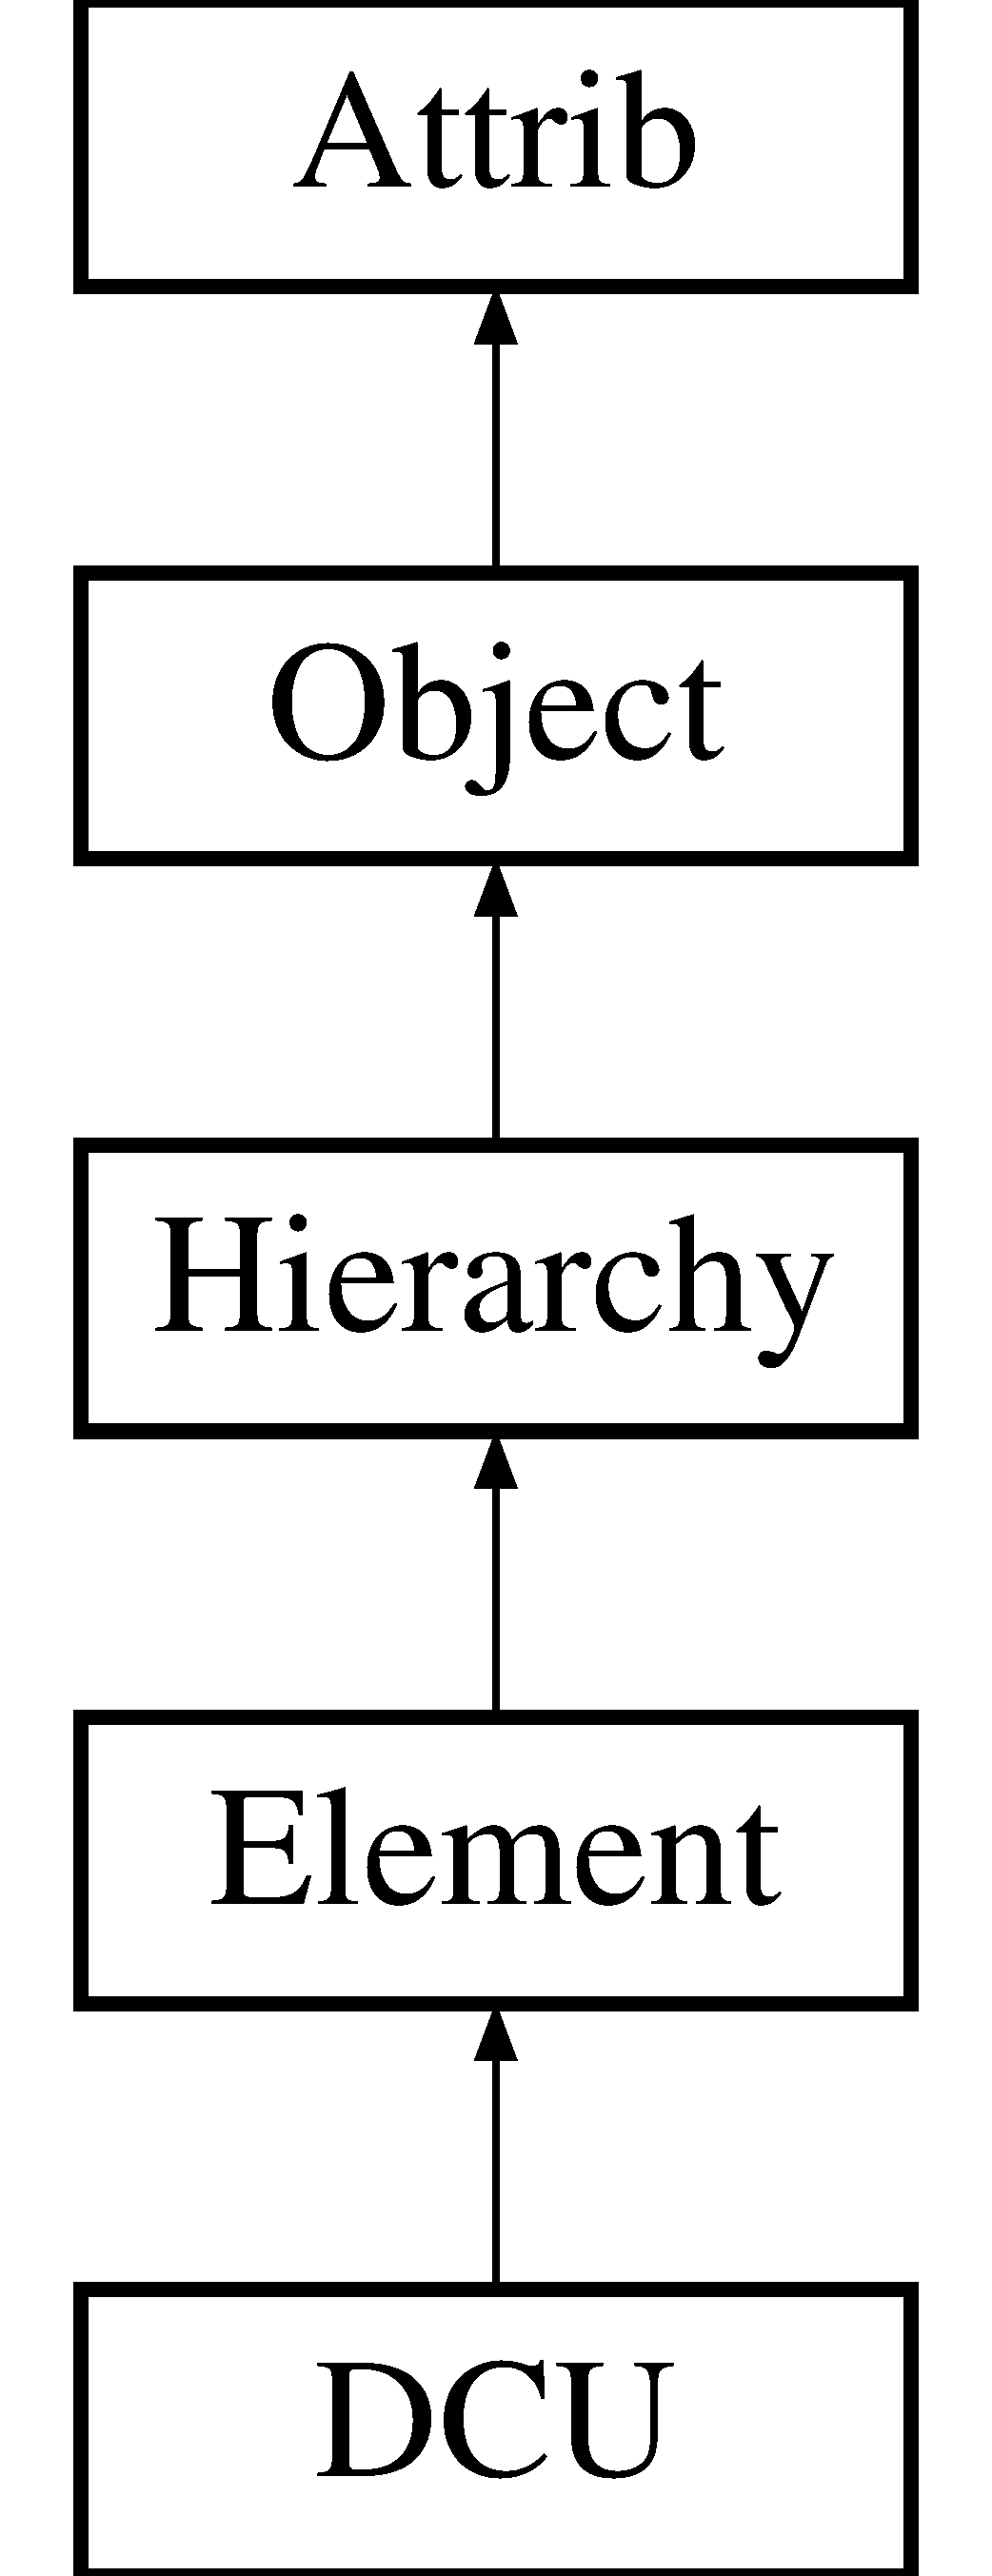
\includegraphics[height=5.000000cm]{classDCU}
\end{center}
\end{figure}
\subsection*{Public Types}
\begin{DoxyCompactItemize}
\item 
typedef unsigned long \hyperlink{classDCU_a86aa9e7393c7f63ae617d8b3679f0b77}{U32}
\item 
typedef unsigned short \hyperlink{classDCU_ab720c867a63f37eed6ca38de9ea1fb6f}{U16}
\item 
typedef unsigned char \hyperlink{classDCU_a640bf3fc4af2541c60aebfe19fd3471a}{U8}
\item 
enum \hyperlink{classAttrib_a69e171d7cc6417835a5a306d3c764235}{Attribut} \{ \newline
\hyperlink{classAttrib_a69e171d7cc6417835a5a306d3c764235a3a8da2ab97dda18aebab196fe4100531}{U\+N\+D\+E\+F\+I\+N\+ED}, 
\hyperlink{classAttrib_a69e171d7cc6417835a5a306d3c764235a2bfb2af57b87031d190a05fe25dd92ed}{P\+A\+S\+S\+I\+VE}, 
\hyperlink{classAttrib_a69e171d7cc6417835a5a306d3c764235a3b1fec929c0370d1436f2f06e298fb0d}{A\+C\+T\+I\+VE}, 
\hyperlink{classAttrib_a69e171d7cc6417835a5a306d3c764235aa27c16b480a369ea4d18b07b2516bbc7}{I\+N\+T\+E\+R\+F\+A\+CE}, 
\newline
\hyperlink{classAttrib_a69e171d7cc6417835a5a306d3c764235a1420a5b8c0540b2af210b6975eded7f9}{IO}, 
\hyperlink{classAttrib_a69e171d7cc6417835a5a306d3c764235a0af3b0d0ac323c1704e6c69cf90add28}{I\+O\+D\+A\+TA}, 
\hyperlink{classAttrib_a69e171d7cc6417835a5a306d3c764235a7788bc5dd333fd8ce18562b269c9dab1}{E\+L\+E\+M\+E\+NT}, 
\hyperlink{classAttrib_a69e171d7cc6417835a5a306d3c764235a61ceb22149f365f1780d18f9d1459423}{H\+A\+R\+D\+W\+A\+RE}, 
\newline
\hyperlink{classAttrib_a69e171d7cc6417835a5a306d3c764235a75250e29692496e73effca2c0330977f}{P\+R\+O\+C\+E\+S\+S\+US}, 
\hyperlink{classAttrib_a69e171d7cc6417835a5a306d3c764235a103a67cd0b8f07ef478fa45d4356e27b}{S\+O\+F\+T\+W\+A\+RE}
 \}
\end{DoxyCompactItemize}
\subsection*{Public Member Functions}
\begin{DoxyCompactItemize}
\item 
\hyperlink{classDCU_a72301936ce7f0d77b109a79eb957ed07}{D\+CU} ()
\begin{DoxyCompactList}\small\item\em Constructor. \end{DoxyCompactList}\item 
\hyperlink{classDCU_ad5c4191a61c8b6585ea1738eccac0a64}{$\sim$\+D\+CU} ()
\begin{DoxyCompactList}\small\item\em Destructor. \end{DoxyCompactList}\item 
virtual bool \hyperlink{classDCU_a04eca3ce751d9833c10246aa8493c219}{cmdline} (std\+::vector$<$ std\+::string $>$)
\item 
bool \hyperlink{classDCU_aa23d2c4aed766323bc828daac1f0cd78}{acquire} (\hyperlink{classDCU_a640bf3fc4af2541c60aebfe19fd3471a}{U8}, \hyperlink{classDCU_ab720c867a63f37eed6ca38de9ea1fb6f}{U16} \&, double \&)
\item 
void \hyperlink{classDCU_a08e44c5d726b5a3a1b3bfba23f53a5f0}{reset} ()
\item 
void \hyperlink{classDCU_a870700eea73d0e2ef05a10f32ca65446}{update} ()
\item 
void \hyperlink{classDCU_a3b75cb2428ddf209608db6b8bd60ef47}{help} ()
\item 
\hyperlink{classStatusCode}{Status\+Code} \hyperlink{classDCU_ae3feff0d1e549c47f94751704b59de5b}{init} ()
\item 
bool \hyperlink{classDCU_af2eb77de4ab67f68fe408fb294bc7a30}{set\+L\+IR} ()
\item 
bool \hyperlink{classDCU_a0a4945e695214fbe76755e9634f42e7f}{set\+H\+IR} ()
\item 
bool \hyperlink{classDCU_ae693aceea360285fffdffd925de06be9}{read\+Mode} (\hyperlink{classDCU_a640bf3fc4af2541c60aebfe19fd3471a}{U8} \&mode)
\item 
bool \hyperlink{classDCU_ab9ac18f8d1292f9713f77e6729ffb2cd}{convert} (std\+::string \&converted\+\_\+value, \hyperlink{classDCU_ab720c867a63f37eed6ca38de9ea1fb6f}{U16} input\+\_\+value, \hyperlink{classDCU_a640bf3fc4af2541c60aebfe19fd3471a}{U8} channel)
\item 
\hyperlink{classDCU_a640bf3fc4af2541c60aebfe19fd3471a}{U8} \hyperlink{classDCU_a536b2a135dcc5f747947011e14e845d3}{address} ()
\item 
void \hyperlink{classDCU_adb1130ffebd39a0bfd4744c293f9c881}{set\+Address} (\hyperlink{classDCU_a640bf3fc4af2541c60aebfe19fd3471a}{U8} \hyperlink{classDCU_a536b2a135dcc5f747947011e14e845d3}{address})
\item 
\hyperlink{classDCU_a640bf3fc4af2541c60aebfe19fd3471a}{U8} \hyperlink{classDCU_a8ddffa9021a269df7a76fa42df005597}{output\+Select} ()
\item 
void \hyperlink{classDCU_ae5ddd9019e971766740a512c62e9e54d}{set\+Output\+Select} (\hyperlink{classDCU_a640bf3fc4af2541c60aebfe19fd3471a}{U8} \hyperlink{classDCU_a8ddffa9021a269df7a76fa42df005597}{output\+Select})
\item 
void \hyperlink{classElement_a3c0abcb36f8906688bb7e32608df7086}{recursive\+Init\+Element} ()
\item 
void \hyperlink{classElement_a82119ed37dff76508a2746a853ec35ba}{recursive\+Init\+Communications} ()
\item 
\hyperlink{classStatusCode}{Status\+Code} \hyperlink{classElement_ab476b4b1df5954141ceb14f072433b89}{set\+Connection} (\hyperlink{classHierarchy}{Hierarchy} $\ast$)
\item 
\hyperlink{classHierarchy}{Hierarchy} $\ast$ \hyperlink{classElement_af57444353c1ddf9fa0109801e97debf7}{connection} ()
\item 
void \hyperlink{classHierarchy_af4d43b0765b402670eed2d62c73405af}{clear} ()
\item 
void \hyperlink{classHierarchy_a585ad1aeec16077a0e532ab8b4fc557b}{set\+Parent} (\hyperlink{classHierarchy}{Hierarchy} $\ast$\hyperlink{classHierarchy_a1c7bec8257e717f9c1465e06ebf845fc}{parent})
\item 
\hyperlink{classHierarchy}{Hierarchy} $\ast$ \hyperlink{classHierarchy_a1c7bec8257e717f9c1465e06ebf845fc}{parent} ()
\item 
\hyperlink{classHierarchy}{Hierarchy} $\ast$ \hyperlink{classHierarchy_ad550588733bf75ac5c0fcfd7c8fd11a6}{parent} (std\+::string)
\item 
\hyperlink{classHierarchy}{Hierarchy} $\ast$ \hyperlink{classHierarchy_aee461dc930ce3871636ff87f075b1b83}{origin} ()
\item 
virtual void \hyperlink{classHierarchy_ad677774ff38fcb257c04a3a10d471fac}{add\+Child} (\hyperlink{classHierarchy}{Hierarchy} $\ast$element)
\item 
std\+::vector$<$ \hyperlink{classHierarchy}{Hierarchy} $\ast$ $>$ \hyperlink{classHierarchy_aa9a76f69e98e052ee1a6e32cea006288}{children} ()
\item 
\hyperlink{classHierarchy}{Hierarchy} $\ast$ \hyperlink{classHierarchy_a1e207f973c694b538bf90107b4868817}{child} (std\+::string)
\item 
\hyperlink{classHierarchy}{Hierarchy} $\ast$ \hyperlink{classHierarchy_a0c15a5276a3b80b4354d6bd8a01e0708}{child\+Typed} (std\+::string)
\item 
unsigned long \hyperlink{classHierarchy_ab16e84de65fd84e14001a6cf941c8be4}{number\+Of\+Children} ()
\item 
bool \hyperlink{classHierarchy_a255174fe4d316d2a3f430dcb9dab29f1}{has\+Children} ()
\item 
void \hyperlink{classHierarchy_a2b2b359fac003233f65786a616766bde}{del\+Child} (\hyperlink{classHierarchy}{Hierarchy} $\ast$)
\item 
void \hyperlink{classHierarchy_a1928ac7615fe0b5e55cd707f70dc6781}{del\+Child} (std\+::string)
\item 
std\+::string \hyperlink{classHierarchy_aa7990fa7caf132d83e361ce033c6c65a}{path} (std\+::string=std\+::string(\char`\"{}\char`\"{}))
\item 
std\+::string \hyperlink{classHierarchy_a1efd56cd164d328d2002e53a10a19b8c}{path\+Typed} (std\+::string=std\+::string(\char`\"{}\char`\"{}))
\item 
void \hyperlink{classHierarchy_a76e914b9a677a22a82deb74d892bf261}{tree} (std\+::string indent=std\+::string(\char`\"{}\char`\"{}))
\item 
void \hyperlink{classHierarchy_a594c294c5f60c230e106d522ed008212}{tree} ()
\item 
std\+::string \hyperlink{classObject_a300f4c05dd468c7bb8b3c968868443c1}{name} () const
\item 
std\+::string \hyperlink{classObject_a84f99f70f144a83e1582d1d0f84e4e62}{type} ()
\item 
unsigned char \hyperlink{classObject_af99145335cc61ff6e2798ea17db009d2}{id} ()
\item 
std\+::string \hyperlink{classObject_a73a0f1a41828fdd8303dd662446fb6c3}{title} ()
\item 
void \hyperlink{classObject_a3f9d5537ebce0c0f2bf6ae4d92426f3c}{msg\+Svc} (int level, std\+::string \hyperlink{classObject_a58b2d0618c2d08cf2383012611528d97}{msg}, std\+::string \hyperlink{classObject_a300f4c05dd468c7bb8b3c968868443c1}{name})
\item 
void \hyperlink{classObject_a58b2d0618c2d08cf2383012611528d97}{msg} (std\+::string mymsg)
\item 
void \hyperlink{classObject_ac5d59299273cee27aacf7de00d2e7034}{msg} (std\+::string mymsg, std\+::string \hyperlink{classObject_a300f4c05dd468c7bb8b3c968868443c1}{name})
\item 
void \hyperlink{classObject_a83d2db2df682907ea1115ad721c1c4a1}{verbose} (std\+::string mymsg)
\item 
void \hyperlink{classObject_a2d4120195317e2a3c6532e8bb9f3da68}{verbose} (std\+::string mymsg, std\+::string \hyperlink{classObject_a300f4c05dd468c7bb8b3c968868443c1}{name})
\item 
void \hyperlink{classObject_aac010553f022165573714b7014a15f0d}{debug} (std\+::string mymsg)
\item 
void \hyperlink{classObject_a6c9a0397ca804e04d675ed05683f5420}{debug} (std\+::string mymsg, std\+::string \hyperlink{classObject_a300f4c05dd468c7bb8b3c968868443c1}{name})
\item 
void \hyperlink{classObject_a644fd329ea4cb85f54fa6846484b84a8}{info} (std\+::string mymsg)
\item 
void \hyperlink{classObject_a1ca123253dfd30fc28b156f521dcbdae}{info} (std\+::string mymsg, std\+::string \hyperlink{classObject_a300f4c05dd468c7bb8b3c968868443c1}{name})
\item 
void \hyperlink{classObject_a65cd4fda577711660821fd2cd5a3b4c9}{warning} (std\+::string mymsg)
\item 
void \hyperlink{classObject_a11f101db4dd73d9391b0231818881d86}{warning} (std\+::string mymsg, std\+::string \hyperlink{classObject_a300f4c05dd468c7bb8b3c968868443c1}{name})
\item 
void \hyperlink{classObject_a204a95f57818c0f811933917a30eff45}{error} (std\+::string mymsg)
\item 
void \hyperlink{classObject_ad7f6c457733082efa2f9ff5f5c8e119a}{error} (std\+::string mymsg, std\+::string \hyperlink{classObject_a300f4c05dd468c7bb8b3c968868443c1}{name})
\item 
void \hyperlink{classObject_aad5a16aac7516ce65bd5ec02ab07fc80}{fatal} (std\+::string mymsg)
\item 
void \hyperlink{classObject_ae62acd3d09f716220f75f252dc38bc9a}{fatal} (std\+::string mymsg, std\+::string \hyperlink{classObject_a300f4c05dd468c7bb8b3c968868443c1}{name})
\item 
void \hyperlink{classObject_ae30fea75683c2d149b6b6d17c09ecd0c}{set\+Name} (std\+::string \hyperlink{classObject_a300f4c05dd468c7bb8b3c968868443c1}{name})
\item 
void \hyperlink{classObject_aae534cc9d982bcb9b99fd505f2e103a5}{set\+Type} (std\+::string \hyperlink{classObject_a84f99f70f144a83e1582d1d0f84e4e62}{type})
\item 
void \hyperlink{classObject_a398fe08cba594a0ce6891d59fe4f159f}{set\+Id} (unsigned char \hyperlink{classObject_af99145335cc61ff6e2798ea17db009d2}{id})
\item 
void \hyperlink{classObject_a89557dbbad5bcaa02652f5d7fa35d20f}{set\+Title} (std\+::string \hyperlink{classObject_a73a0f1a41828fdd8303dd662446fb6c3}{title})
\item 
void \hyperlink{classObject_a870c5af919958c2136623b2d7816d123}{set\+Dll\+Name} (std\+::string \hyperlink{classObject_a2e3947f2870094c332d7454117f3ec63}{dll\+Name})
\item 
std\+::string \hyperlink{classObject_a2e3947f2870094c332d7454117f3ec63}{dll\+Name} ()
\item 
bool \hyperlink{classAttrib_a704f26af560909ad22065083bb7d4c34}{is} (int attribut)
\item 
void \hyperlink{classAttrib_a235f773af19c900264a190b00a3b4ad7}{add} (int attribut)
\item 
void \hyperlink{classAttrib_a7d4ef7e32d93cb287792b87b857e79f3}{remove} (int attribut)
\item 
std\+::string \hyperlink{classAttrib_aee7bbf16b144887f196e1341b24f8a26}{attributs} ()
\end{DoxyCompactItemize}
\subsection*{Protected Attributes}
\begin{DoxyCompactItemize}
\item 
\hyperlink{classHierarchy}{Hierarchy} $\ast$ \hyperlink{classElement_abe3de7a5dbbc9a6dd2d7e012e5fdb266}{m\+\_\+connection}
\item 
std\+::string \hyperlink{classAttrib_a3414521d7a82476e874b25a5407b5e63}{m\+\_\+attrib\+String} \mbox{[}10\mbox{]}
\end{DoxyCompactItemize}
\subsection*{Private Attributes}
\begin{DoxyCompactItemize}
\item 
\hyperlink{classDCU_a640bf3fc4af2541c60aebfe19fd3471a}{U8} \hyperlink{classDCU_ac94f02495b71d046aa0374b76818ab8c}{m\+\_\+address}
\item 
\hyperlink{classDCU_a640bf3fc4af2541c60aebfe19fd3471a}{U8} \hyperlink{classDCU_ad0f84f2006a38e31e0026d34eff9667e}{m\+\_\+output\+Select}
\end{DoxyCompactItemize}


\subsection{Detailed Description}
Describe the \hyperlink{classDCU}{D\+CU}

\begin{DoxyAuthor}{Author}
Fr�d�ric Machefert 
\end{DoxyAuthor}
\begin{DoxyDate}{Date}
2005-\/05-\/31 
\end{DoxyDate}


Definition at line 15 of file D\+C\+U.\+h.



\subsection{Member Typedef Documentation}
\mbox{\Hypertarget{classDCU_ab720c867a63f37eed6ca38de9ea1fb6f}\label{classDCU_ab720c867a63f37eed6ca38de9ea1fb6f}} 
\index{D\+CU@{D\+CU}!U16@{U16}}
\index{U16@{U16}!D\+CU@{D\+CU}}
\subsubsection{\texorpdfstring{U16}{U16}}
{\footnotesize\ttfamily typedef unsigned short \hyperlink{classDCU_ab720c867a63f37eed6ca38de9ea1fb6f}{D\+C\+U\+::\+U16}}



Definition at line 18 of file D\+C\+U.\+h.

\mbox{\Hypertarget{classDCU_a86aa9e7393c7f63ae617d8b3679f0b77}\label{classDCU_a86aa9e7393c7f63ae617d8b3679f0b77}} 
\index{D\+CU@{D\+CU}!U32@{U32}}
\index{U32@{U32}!D\+CU@{D\+CU}}
\subsubsection{\texorpdfstring{U32}{U32}}
{\footnotesize\ttfamily typedef unsigned long \hyperlink{classDCU_a86aa9e7393c7f63ae617d8b3679f0b77}{D\+C\+U\+::\+U32}}



Definition at line 17 of file D\+C\+U.\+h.

\mbox{\Hypertarget{classDCU_a640bf3fc4af2541c60aebfe19fd3471a}\label{classDCU_a640bf3fc4af2541c60aebfe19fd3471a}} 
\index{D\+CU@{D\+CU}!U8@{U8}}
\index{U8@{U8}!D\+CU@{D\+CU}}
\subsubsection{\texorpdfstring{U8}{U8}}
{\footnotesize\ttfamily typedef unsigned char \hyperlink{classDCU_a640bf3fc4af2541c60aebfe19fd3471a}{D\+C\+U\+::\+U8}}



Definition at line 19 of file D\+C\+U.\+h.



\subsection{Member Enumeration Documentation}
\mbox{\Hypertarget{classAttrib_a69e171d7cc6417835a5a306d3c764235}\label{classAttrib_a69e171d7cc6417835a5a306d3c764235}} 
\index{D\+CU@{D\+CU}!Attribut@{Attribut}}
\index{Attribut@{Attribut}!D\+CU@{D\+CU}}
\subsubsection{\texorpdfstring{Attribut}{Attribut}}
{\footnotesize\ttfamily enum \hyperlink{classAttrib_a69e171d7cc6417835a5a306d3c764235}{Attrib\+::\+Attribut}\hspace{0.3cm}{\ttfamily [inherited]}}

\begin{DoxyEnumFields}{Enumerator}
\raisebox{\heightof{T}}[0pt][0pt]{\index{U\+N\+D\+E\+F\+I\+N\+ED@{U\+N\+D\+E\+F\+I\+N\+ED}!D\+CU@{D\+CU}}\index{D\+CU@{D\+CU}!U\+N\+D\+E\+F\+I\+N\+ED@{U\+N\+D\+E\+F\+I\+N\+ED}}}\mbox{\Hypertarget{classAttrib_a69e171d7cc6417835a5a306d3c764235a3a8da2ab97dda18aebab196fe4100531}\label{classAttrib_a69e171d7cc6417835a5a306d3c764235a3a8da2ab97dda18aebab196fe4100531}} 
U\+N\+D\+E\+F\+I\+N\+ED&\\
\hline

\raisebox{\heightof{T}}[0pt][0pt]{\index{P\+A\+S\+S\+I\+VE@{P\+A\+S\+S\+I\+VE}!D\+CU@{D\+CU}}\index{D\+CU@{D\+CU}!P\+A\+S\+S\+I\+VE@{P\+A\+S\+S\+I\+VE}}}\mbox{\Hypertarget{classAttrib_a69e171d7cc6417835a5a306d3c764235a2bfb2af57b87031d190a05fe25dd92ed}\label{classAttrib_a69e171d7cc6417835a5a306d3c764235a2bfb2af57b87031d190a05fe25dd92ed}} 
P\+A\+S\+S\+I\+VE&\\
\hline

\raisebox{\heightof{T}}[0pt][0pt]{\index{A\+C\+T\+I\+VE@{A\+C\+T\+I\+VE}!D\+CU@{D\+CU}}\index{D\+CU@{D\+CU}!A\+C\+T\+I\+VE@{A\+C\+T\+I\+VE}}}\mbox{\Hypertarget{classAttrib_a69e171d7cc6417835a5a306d3c764235a3b1fec929c0370d1436f2f06e298fb0d}\label{classAttrib_a69e171d7cc6417835a5a306d3c764235a3b1fec929c0370d1436f2f06e298fb0d}} 
A\+C\+T\+I\+VE&\\
\hline

\raisebox{\heightof{T}}[0pt][0pt]{\index{I\+N\+T\+E\+R\+F\+A\+CE@{I\+N\+T\+E\+R\+F\+A\+CE}!D\+CU@{D\+CU}}\index{D\+CU@{D\+CU}!I\+N\+T\+E\+R\+F\+A\+CE@{I\+N\+T\+E\+R\+F\+A\+CE}}}\mbox{\Hypertarget{classAttrib_a69e171d7cc6417835a5a306d3c764235aa27c16b480a369ea4d18b07b2516bbc7}\label{classAttrib_a69e171d7cc6417835a5a306d3c764235aa27c16b480a369ea4d18b07b2516bbc7}} 
I\+N\+T\+E\+R\+F\+A\+CE&\\
\hline

\raisebox{\heightof{T}}[0pt][0pt]{\index{IO@{IO}!D\+CU@{D\+CU}}\index{D\+CU@{D\+CU}!IO@{IO}}}\mbox{\Hypertarget{classAttrib_a69e171d7cc6417835a5a306d3c764235a1420a5b8c0540b2af210b6975eded7f9}\label{classAttrib_a69e171d7cc6417835a5a306d3c764235a1420a5b8c0540b2af210b6975eded7f9}} 
IO&\\
\hline

\raisebox{\heightof{T}}[0pt][0pt]{\index{I\+O\+D\+A\+TA@{I\+O\+D\+A\+TA}!D\+CU@{D\+CU}}\index{D\+CU@{D\+CU}!I\+O\+D\+A\+TA@{I\+O\+D\+A\+TA}}}\mbox{\Hypertarget{classAttrib_a69e171d7cc6417835a5a306d3c764235a0af3b0d0ac323c1704e6c69cf90add28}\label{classAttrib_a69e171d7cc6417835a5a306d3c764235a0af3b0d0ac323c1704e6c69cf90add28}} 
I\+O\+D\+A\+TA&\\
\hline

\raisebox{\heightof{T}}[0pt][0pt]{\index{E\+L\+E\+M\+E\+NT@{E\+L\+E\+M\+E\+NT}!D\+CU@{D\+CU}}\index{D\+CU@{D\+CU}!E\+L\+E\+M\+E\+NT@{E\+L\+E\+M\+E\+NT}}}\mbox{\Hypertarget{classAttrib_a69e171d7cc6417835a5a306d3c764235a7788bc5dd333fd8ce18562b269c9dab1}\label{classAttrib_a69e171d7cc6417835a5a306d3c764235a7788bc5dd333fd8ce18562b269c9dab1}} 
E\+L\+E\+M\+E\+NT&\\
\hline

\raisebox{\heightof{T}}[0pt][0pt]{\index{H\+A\+R\+D\+W\+A\+RE@{H\+A\+R\+D\+W\+A\+RE}!D\+CU@{D\+CU}}\index{D\+CU@{D\+CU}!H\+A\+R\+D\+W\+A\+RE@{H\+A\+R\+D\+W\+A\+RE}}}\mbox{\Hypertarget{classAttrib_a69e171d7cc6417835a5a306d3c764235a61ceb22149f365f1780d18f9d1459423}\label{classAttrib_a69e171d7cc6417835a5a306d3c764235a61ceb22149f365f1780d18f9d1459423}} 
H\+A\+R\+D\+W\+A\+RE&\\
\hline

\raisebox{\heightof{T}}[0pt][0pt]{\index{P\+R\+O\+C\+E\+S\+S\+US@{P\+R\+O\+C\+E\+S\+S\+US}!D\+CU@{D\+CU}}\index{D\+CU@{D\+CU}!P\+R\+O\+C\+E\+S\+S\+US@{P\+R\+O\+C\+E\+S\+S\+US}}}\mbox{\Hypertarget{classAttrib_a69e171d7cc6417835a5a306d3c764235a75250e29692496e73effca2c0330977f}\label{classAttrib_a69e171d7cc6417835a5a306d3c764235a75250e29692496e73effca2c0330977f}} 
P\+R\+O\+C\+E\+S\+S\+US&\\
\hline

\raisebox{\heightof{T}}[0pt][0pt]{\index{S\+O\+F\+T\+W\+A\+RE@{S\+O\+F\+T\+W\+A\+RE}!D\+CU@{D\+CU}}\index{D\+CU@{D\+CU}!S\+O\+F\+T\+W\+A\+RE@{S\+O\+F\+T\+W\+A\+RE}}}\mbox{\Hypertarget{classAttrib_a69e171d7cc6417835a5a306d3c764235a103a67cd0b8f07ef478fa45d4356e27b}\label{classAttrib_a69e171d7cc6417835a5a306d3c764235a103a67cd0b8f07ef478fa45d4356e27b}} 
S\+O\+F\+T\+W\+A\+RE&\\
\hline

\end{DoxyEnumFields}


Definition at line 29 of file Attrib.\+h.


\begin{DoxyCode}
29                 \{
30     \hyperlink{classAttrib_a69e171d7cc6417835a5a306d3c764235a3a8da2ab97dda18aebab196fe4100531}{UNDEFINED},
31     \hyperlink{classAttrib_a69e171d7cc6417835a5a306d3c764235a2bfb2af57b87031d190a05fe25dd92ed}{PASSIVE},
32     \hyperlink{classAttrib_a69e171d7cc6417835a5a306d3c764235a3b1fec929c0370d1436f2f06e298fb0d}{ACTIVE},
33     \hyperlink{classAttrib_a69e171d7cc6417835a5a306d3c764235aa27c16b480a369ea4d18b07b2516bbc7}{INTERFACE},
34     \hyperlink{classAttrib_a69e171d7cc6417835a5a306d3c764235a1420a5b8c0540b2af210b6975eded7f9}{IO},
35     \hyperlink{classAttrib_a69e171d7cc6417835a5a306d3c764235a0af3b0d0ac323c1704e6c69cf90add28}{IODATA},
36     \hyperlink{classAttrib_a69e171d7cc6417835a5a306d3c764235a7788bc5dd333fd8ce18562b269c9dab1}{ELEMENT},
37     \hyperlink{classAttrib_a69e171d7cc6417835a5a306d3c764235a61ceb22149f365f1780d18f9d1459423}{HARDWARE},
38     \hyperlink{classAttrib_a69e171d7cc6417835a5a306d3c764235a75250e29692496e73effca2c0330977f}{PROCESSUS},
39     \hyperlink{classAttrib_a69e171d7cc6417835a5a306d3c764235a103a67cd0b8f07ef478fa45d4356e27b}{SOFTWARE} 
40   \}; \textcolor{comment}{// array m\_attribString must be changed into Attrib::Attrib if this enu is modified. }
\end{DoxyCode}


\subsection{Constructor \& Destructor Documentation}
\mbox{\Hypertarget{classDCU_a72301936ce7f0d77b109a79eb957ed07}\label{classDCU_a72301936ce7f0d77b109a79eb957ed07}} 
\index{D\+CU@{D\+CU}!D\+CU@{D\+CU}}
\index{D\+CU@{D\+CU}!D\+CU@{D\+CU}}
\subsubsection{\texorpdfstring{D\+C\+U()}{DCU()}}
{\footnotesize\ttfamily D\+C\+U\+::\+D\+CU (\begin{DoxyParamCaption}{ }\end{DoxyParamCaption})}



Constructor. 



Definition at line 27 of file D\+C\+U.\+cpp.



References Object\+::debug(), m\+\_\+output\+Select, Object\+::set\+Id(), and Object\+::set\+Type().


\begin{DoxyCode}
27            \{
28   \hyperlink{classObject_aae534cc9d982bcb9b99fd505f2e103a5}{setType}( \textcolor{stringliteral}{"DCU"} ) ;
29   \hyperlink{classObject_a398fe08cba594a0ce6891d59fe4f159f}{setId}( 0 ) ;
30   \hyperlink{classObject_aac010553f022165573714b7014a15f0d}{debug}(\textcolor{stringliteral}{"DCU::DCU"} , \textcolor{stringliteral}{"DCU built"} ) ;
31   \hyperlink{classDCU_ad0f84f2006a38e31e0026d34eff9667e}{m\_outputSelect} = 0xF ;  
32 \}
\end{DoxyCode}
\mbox{\Hypertarget{classDCU_ad5c4191a61c8b6585ea1738eccac0a64}\label{classDCU_ad5c4191a61c8b6585ea1738eccac0a64}} 
\index{D\+CU@{D\+CU}!````~D\+CU@{$\sim$\+D\+CU}}
\index{````~D\+CU@{$\sim$\+D\+CU}!D\+CU@{D\+CU}}
\subsubsection{\texorpdfstring{$\sim$\+D\+C\+U()}{~DCU()}}
{\footnotesize\ttfamily D\+C\+U\+::$\sim$\+D\+CU (\begin{DoxyParamCaption}{ }\end{DoxyParamCaption})}



Destructor. 

Destructor 

Definition at line 36 of file D\+C\+U.\+cpp.


\begin{DoxyCode}
36 \{ \}
\end{DoxyCode}


\subsection{Member Function Documentation}
\mbox{\Hypertarget{classDCU_aa23d2c4aed766323bc828daac1f0cd78}\label{classDCU_aa23d2c4aed766323bc828daac1f0cd78}} 
\index{D\+CU@{D\+CU}!acquire@{acquire}}
\index{acquire@{acquire}!D\+CU@{D\+CU}}
\subsubsection{\texorpdfstring{acquire()}{acquire()}}
{\footnotesize\ttfamily bool D\+C\+U\+::acquire (\begin{DoxyParamCaption}\item[{\hyperlink{classDCU_a640bf3fc4af2541c60aebfe19fd3471a}{U8}}]{channel,  }\item[{\hyperlink{classDCU_ab720c867a63f37eed6ca38de9ea1fb6f}{U16} \&}]{data,  }\item[{double \&}]{value }\end{DoxyParamCaption})}



Definition at line 98 of file D\+C\+U.\+cpp.



References address(), itos(), Object\+::verbose(), and Object\+::warning().


\begin{DoxyCode}
98                                                             \{
99 \textcolor{preprocessor}{#ifndef \_NODEVICE\_
}
100   SPECSSLAVE *specsSlv=specsSlaveDevice();
101   \textcolor{keywordflow}{if} ( 0==specsSlv )\{
102     \hyperlink{classObject_a65cd4fda577711660821fd2cd5a3b4c9}{warning}(\textcolor{stringliteral}{"DCU::acquire"},
103            \textcolor{stringliteral}{"Could not reach proper Specs Master and/or Slave."});
104     \textcolor{keywordflow}{return} \textcolor{keyword}{false};
105   \}
106 
107   SpecsError status = specs\_dcu\_acquire (specsSlv
108 #ifdef  \_OLDSPECSLIB\_
109                                          ,\hyperlink{classDCU_a536b2a135dcc5f747947011e14e845d3}{address}()
110 #endif
111                      ,channel,
112                      &\hyperlink{namespaceshell_a5ea2525995cedc3efd69ea8a7f034d1e}{data}, 
113                      &value);
114 
115   \textcolor{keywordflow}{if} (0!=status)\{
116     \hyperlink{classObject_a65cd4fda577711660821fd2cd5a3b4c9}{warning}(\textcolor{stringliteral}{"DCU::acquire"},\textcolor{stringliteral}{"Acquisition failure channel "} + 
117         \hyperlink{Tools_8h_af330027dbdafb9a30768b3613c553e60}{itos} (channel) + 
118         \textcolor{stringliteral}{"[code="} + \hyperlink{Tools_8h_af330027dbdafb9a30768b3613c553e60}{itos}(status) + \textcolor{stringliteral}{"]"} );
119     \textcolor{keywordflow}{return} \textcolor{keyword}{false}; 
120   \}
121   \textcolor{keywordflow}{else} \{
122     \hyperlink{classObject_a83d2db2df682907ea1115ad721c1c4a1}{verbose}(\textcolor{stringliteral}{"DCU::acquire"},\textcolor{stringliteral}{"Channel "} + \hyperlink{Tools_8h_af330027dbdafb9a30768b3613c553e60}{itos} (channel) + 
123        \textcolor{stringliteral}{" -> Acquisition :  "} + \hyperlink{Tools_8h_af330027dbdafb9a30768b3613c553e60}{itos}(\hyperlink{namespaceshell_a5ea2525995cedc3efd69ea8a7f034d1e}{data}) );
124   \}
125 \textcolor{preprocessor}{#else
}
126   \hyperlink{classObject_a83d2db2df682907ea1115ad721c1c4a1}{verbose}(\textcolor{stringliteral}{"DCU::acquire"},\textcolor{stringliteral}{"Compilation in \_NODEVICE\_ mode."});
127 \textcolor{preprocessor}{#endif
}
128   \textcolor{keywordflow}{return} \textcolor{keyword}{true};
129 \}
\end{DoxyCode}
\mbox{\Hypertarget{classAttrib_a235f773af19c900264a190b00a3b4ad7}\label{classAttrib_a235f773af19c900264a190b00a3b4ad7}} 
\index{D\+CU@{D\+CU}!add@{add}}
\index{add@{add}!D\+CU@{D\+CU}}
\subsubsection{\texorpdfstring{add()}{add()}}
{\footnotesize\ttfamily void Attrib\+::add (\begin{DoxyParamCaption}\item[{int}]{attribut }\end{DoxyParamCaption})\hspace{0.3cm}{\ttfamily [inline]}, {\ttfamily [inherited]}}

Add an attribut 

Definition at line 67 of file Attrib.\+h.



References Attrib\+::m\+\_\+attributs, and Attrib\+::\+U\+N\+D\+E\+F\+I\+N\+ED.



Referenced by A3\+P\+E\+::\+A3\+P\+E(), Attrib\+::\+Attrib(), Specs\+Mezzanine\+::cmdline(), Computer\+::\+Computer(), C\+U\+\_\+v1\+::\+C\+U\+\_\+v1(), export\+\_\+obj(), F\+E\+B\+\_\+v1\+::\+F\+E\+B\+\_\+v1(), Fe\+P\+G\+A\+::\+Fe\+P\+G\+A(), I\+C\+E\+C\+A\+Lv3\+::\+I\+C\+E\+C\+A\+Lv3(), I\+C\+Phaser\+::\+I\+C\+Phaser(), Fe\+P\+G\+A\+::init(), Application\+::initialize(), Interface\+::\+Interface(), I\+Odata\+::\+I\+Odata(), I\+Oobject\+::\+I\+Oobject(), M\+S\+Oxxxx\+::\+M\+S\+Oxxxx(), Phaser\+::\+Phaser(), Processus\+::\+Processus(), Proto40\+M\+Hz\+\_\+v1\+::\+Proto40\+M\+Hz\+\_\+v1(), Attrib\+::remove(), Seq\+P\+G\+A\+::\+Seq\+P\+G\+A(), Test\+I2\+C\+::set\+Address(), Test\+S\+P\+I\+::set\+Address(), Specs\+Slave\+::set\+Address(), Specs\+Master\+::\+Specs\+Master(), and Specs\+Slave\+::\+Specs\+Slave().


\begin{DoxyCode}
67                             \{
68     \textcolor{keywordflow}{if} (attribut!=\hyperlink{classAttrib_a69e171d7cc6417835a5a306d3c764235a3a8da2ab97dda18aebab196fe4100531}{Attrib::UNDEFINED}) \textcolor{keyword}{remove}(\hyperlink{classAttrib_a69e171d7cc6417835a5a306d3c764235a3a8da2ab97dda18aebab196fe4100531}{Attrib::UNDEFINED});
69     \textcolor{keywordtype}{bool} duplicate = false ;
70     std::vector<int>::const\_iterator iter ;
71     \textcolor{keywordflow}{for} ( iter  = \hyperlink{classAttrib_ac4bd58a0cc6b38a3b711d609a3d3aacc}{m\_attributs}.begin() ;
72           iter != \hyperlink{classAttrib_ac4bd58a0cc6b38a3b711d609a3d3aacc}{m\_attributs}.end()   ;
73           ++iter ) \{
74       \textcolor{keywordflow}{if} ( attribut == (*iter) ) \{
75         duplicate = true ;
76       \}
77     \}
78     \textcolor{keywordflow}{if} (!duplicate) \{
79       \hyperlink{classAttrib_ac4bd58a0cc6b38a3b711d609a3d3aacc}{m\_attributs}.push\_back( attribut );
80     \}
81   \}
\end{DoxyCode}
\mbox{\Hypertarget{classHierarchy_ad677774ff38fcb257c04a3a10d471fac}\label{classHierarchy_ad677774ff38fcb257c04a3a10d471fac}} 
\index{D\+CU@{D\+CU}!add\+Child@{add\+Child}}
\index{add\+Child@{add\+Child}!D\+CU@{D\+CU}}
\subsubsection{\texorpdfstring{add\+Child()}{addChild()}}
{\footnotesize\ttfamily void Hierarchy\+::add\+Child (\begin{DoxyParamCaption}\item[{\hyperlink{classHierarchy}{Hierarchy} $\ast$}]{element }\end{DoxyParamCaption})\hspace{0.3cm}{\ttfamily [virtual]}, {\ttfamily [inherited]}}



Definition at line 83 of file Hierarchy.\+cpp.



References Object\+::debug(), Hierarchy\+::m\+\_\+children, Object\+::name(), and Hierarchy\+::set\+Parent().



Referenced by A3\+P\+E\+::\+A3\+P\+E(), Specs\+Mezzanine\+::add\+Bus(), Specs\+Slave\+::add\+I2c(), Application\+::create(), C\+U\+\_\+v1\+::\+C\+U\+\_\+v1(), export\+\_\+obj(), F\+E\+B\+\_\+v1\+::\+F\+E\+B\+\_\+v1(), Fe\+P\+G\+A\+::\+Fe\+P\+G\+A(), I\+C\+E\+C\+A\+Lv3\+::\+I\+C\+E\+C\+A\+Lv3(), I\+C\+Phaser\+::\+I\+C\+Phaser(), Fe\+P\+G\+A\+::\+Make\+R\+A\+M(), Fe\+P\+G\+A\+::\+Make\+Register(), Hierarchy\+::origin(), Phaser\+::\+Phaser(), Proto40\+M\+Hz\+\_\+v1\+::\+Proto40\+M\+Hz\+\_\+v1(), Seq\+P\+G\+A\+::\+Seq\+P\+G\+A(), Specs\+Mezzanine\+::\+Specs\+Mezzanine(), Usb\+I2c\+Bus\+::\+Usb\+I2c\+Bus(), and Usb\+Spi\+Bus\+::\+Usb\+Spi\+Bus().


\begin{DoxyCode}
83                                           \{
84   element->\hyperlink{classHierarchy_a585ad1aeec16077a0e532ab8b4fc557b}{setParent}(\textcolor{keyword}{this});
85   \hyperlink{classHierarchy_a038816763941fd4a930504917f60483b}{m\_children}.push\_back(element);
86   \hyperlink{classObject_aac010553f022165573714b7014a15f0d}{debug}(element->\hyperlink{classObject_a300f4c05dd468c7bb8b3c968868443c1}{name}()+\textcolor{stringliteral}{" added to the child tree."},\textcolor{stringliteral}{"Hierarchy::addChild"});
87 \}
\end{DoxyCode}
\mbox{\Hypertarget{classDCU_a536b2a135dcc5f747947011e14e845d3}\label{classDCU_a536b2a135dcc5f747947011e14e845d3}} 
\index{D\+CU@{D\+CU}!address@{address}}
\index{address@{address}!D\+CU@{D\+CU}}
\subsubsection{\texorpdfstring{address()}{address()}}
{\footnotesize\ttfamily \hyperlink{classDCU_a640bf3fc4af2541c60aebfe19fd3471a}{U8} D\+C\+U\+::address (\begin{DoxyParamCaption}{ }\end{DoxyParamCaption})\hspace{0.3cm}{\ttfamily [inline]}}



Definition at line 50 of file D\+C\+U.\+h.



References m\+\_\+address.



Referenced by acquire(), init(), read\+Mode(), reset(), set\+Address(), set\+H\+I\+R(), and set\+L\+I\+R().


\begin{DoxyCode}
50 \{ \textcolor{keywordflow}{return} \hyperlink{classDCU_ac94f02495b71d046aa0374b76818ab8c}{m\_address}; \}
\end{DoxyCode}
\mbox{\Hypertarget{classAttrib_aee7bbf16b144887f196e1341b24f8a26}\label{classAttrib_aee7bbf16b144887f196e1341b24f8a26}} 
\index{D\+CU@{D\+CU}!attributs@{attributs}}
\index{attributs@{attributs}!D\+CU@{D\+CU}}
\subsubsection{\texorpdfstring{attributs()}{attributs()}}
{\footnotesize\ttfamily std\+::string Attrib\+::attributs (\begin{DoxyParamCaption}{ }\end{DoxyParamCaption})\hspace{0.3cm}{\ttfamily [inherited]}}

Print the \hyperlink{classAttrib}{Attrib} of an \hyperlink{classObject}{Object} 

Definition at line 54 of file Attrib.\+cpp.



References images\+::index, Attrib\+::m\+\_\+attrib\+String, and Attrib\+::m\+\_\+attributs.



Referenced by export\+\_\+obj(), and Attrib\+::remove().


\begin{DoxyCode}
54                             \{
55   std::string output;
56   std::vector<int>::iterator iter ;
57   \textcolor{keywordflow}{for} ( \textcolor{keywordtype}{unsigned} \textcolor{keywordtype}{int} \hyperlink{namespaceimages_a54407fd574970b3178647ae096321a57}{index} = 0 ; \hyperlink{namespaceimages_a54407fd574970b3178647ae096321a57}{index} < \hyperlink{classAttrib_ac4bd58a0cc6b38a3b711d609a3d3aacc}{m\_attributs}.size() ; ++
      \hyperlink{namespaceimages_a54407fd574970b3178647ae096321a57}{index} ) \{
58     \textcolor{keywordflow}{if} ( \hyperlink{classAttrib_ac4bd58a0cc6b38a3b711d609a3d3aacc}{m\_attributs}.size() - \hyperlink{namespaceimages_a54407fd574970b3178647ae096321a57}{index} > 1 ) \{
59       output.append(\hyperlink{classAttrib_a3414521d7a82476e874b25a5407b5e63}{m\_attribString}[\hyperlink{classAttrib_ac4bd58a0cc6b38a3b711d609a3d3aacc}{m\_attributs}[\hyperlink{namespaceimages_a54407fd574970b3178647ae096321a57}{index}]]);
60       output.append(\textcolor{stringliteral}{":"});
61     \}
62     \textcolor{keywordflow}{else} \{
63       output.append(\hyperlink{classAttrib_a3414521d7a82476e874b25a5407b5e63}{m\_attribString}[\hyperlink{classAttrib_ac4bd58a0cc6b38a3b711d609a3d3aacc}{m\_attributs}[index]]);
64     \}
65   \}
66   \textcolor{keywordflow}{return} output;
67 \}
\end{DoxyCode}
\mbox{\Hypertarget{classHierarchy_a1e207f973c694b538bf90107b4868817}\label{classHierarchy_a1e207f973c694b538bf90107b4868817}} 
\index{D\+CU@{D\+CU}!child@{child}}
\index{child@{child}!D\+CU@{D\+CU}}
\subsubsection{\texorpdfstring{child()}{child()}}
{\footnotesize\ttfamily \hyperlink{classHierarchy}{Hierarchy} $\ast$ Hierarchy\+::child (\begin{DoxyParamCaption}\item[{std\+::string}]{path }\end{DoxyParamCaption})\hspace{0.3cm}{\ttfamily [inherited]}}



Definition at line 133 of file Hierarchy.\+cpp.



References Hierarchy\+::child(), Hierarchy\+::children(), Object\+::name(), Hierarchy\+::origin(), Hierarchy\+::parent(), Hierarchy\+::path(), and Object\+::warning().



Referenced by Application\+::cd(), Hierarchy\+::child(), Hierarchy\+::children(), and export\+\_\+obj().


\begin{DoxyCode}
133                                          \{
134   std::string newpath = \hyperlink{classHierarchy_aa7990fa7caf132d83e361ce033c6c65a}{path};
135   std::string up(\textcolor{stringliteral}{".."});
136   std::string separator(1,\textcolor{charliteral}{'/'});
137 
138   \hyperlink{classHierarchy}{Hierarchy} * newcurrent = 0;
139 
140   \textcolor{comment}{//  info("path="+path,"Hierarchy::child");}
141 
142   \textcolor{keywordflow}{if} (\hyperlink{classHierarchy_aa7990fa7caf132d83e361ce033c6c65a}{path}.compare(\textcolor{stringliteral}{""})==0 || \hyperlink{classHierarchy_aa7990fa7caf132d83e361ce033c6c65a}{path}.compare(\textcolor{stringliteral}{"/"})==0) \{
143     \textcolor{comment}{//    debug("return origin","Hierarchy::child");}
144     \textcolor{keywordflow}{return} \hyperlink{classHierarchy_aee461dc930ce3871636ff87f075b1b83}{origin}();
145   \}
146 
147   \textcolor{keywordflow}{if} (\hyperlink{classHierarchy_aa7990fa7caf132d83e361ce033c6c65a}{path}.compare(\hyperlink{classObject_a300f4c05dd468c7bb8b3c968868443c1}{name}())==0)\{
148     \textcolor{comment}{//    debug("return itself","Hierarchy::child");}
149     \textcolor{keywordflow}{return} \textcolor{keyword}{this};
150   \}
151 
152   \textcolor{keywordflow}{if} (\hyperlink{classHierarchy_aa7990fa7caf132d83e361ce033c6c65a}{path}.compare(\textcolor{stringliteral}{".."})==0)\{
153     \textcolor{keywordflow}{if} (0!=this->\hyperlink{classHierarchy_a1c7bec8257e717f9c1465e06ebf845fc}{parent}()) \textcolor{keywordflow}{return} this->\hyperlink{classHierarchy_a1c7bec8257e717f9c1465e06ebf845fc}{parent}();
154     \textcolor{keywordflow}{else} \textcolor{keywordflow}{return} \textcolor{keyword}{this};
155   \}
156 
157   \textcolor{keywordflow}{if} (\hyperlink{classHierarchy_aa7990fa7caf132d83e361ce033c6c65a}{path}.compare(\textcolor{stringliteral}{"../"})==0)\{
158     \textcolor{keywordflow}{if} (0!=this->\hyperlink{classHierarchy_a1c7bec8257e717f9c1465e06ebf845fc}{parent}()) \textcolor{keywordflow}{return} this->\hyperlink{classHierarchy_a1c7bec8257e717f9c1465e06ebf845fc}{parent}();
159     \textcolor{keywordflow}{else} \textcolor{keywordflow}{return} \textcolor{keyword}{this};
160   \}
161 
162 
163   \textcolor{keywordtype}{int} npos=\hyperlink{classHierarchy_aa7990fa7caf132d83e361ce033c6c65a}{path}.find(separator,0);
164 
165   \textcolor{comment}{//  info("find separator in "+itos(npos)+" of "+path,"Hierarchy::child");}
166 
167   \textcolor{comment}{// remove last separator}
168   \textcolor{keywordflow}{if} ( npos == (\textcolor{keywordtype}{int})(\hyperlink{classHierarchy_aa7990fa7caf132d83e361ce033c6c65a}{path}.size()-1) ) \{
169     newpath = std::string(\hyperlink{classHierarchy_aa7990fa7caf132d83e361ce033c6c65a}{path},0,npos);
170     \hyperlink{classHierarchy_aa7990fa7caf132d83e361ce033c6c65a}{path} = newpath;
171   \}
172 
173   \textcolor{keywordflow}{if} (npos==0)\{
174     \textcolor{comment}{//    debug("Going back to origin and calling child","Hierarchy::child");}
175     newpath=std::string(\hyperlink{classHierarchy_aa7990fa7caf132d83e361ce033c6c65a}{path},1,\hyperlink{classHierarchy_aa7990fa7caf132d83e361ce033c6c65a}{path}.size()-1);
176     \textcolor{keywordflow}{return} \hyperlink{classHierarchy_aee461dc930ce3871636ff87f075b1b83}{origin}()->\hyperlink{classHierarchy_a1e207f973c694b538bf90107b4868817}{child}(newpath);
177   \}
178   \textcolor{keywordflow}{else}\{
179     \textcolor{keywordflow}{if} ( npos== (\textcolor{keywordtype}{int})(std::string::npos) )\{
180       \textcolor{comment}{//      debug("Getting chid "+path+" of "+this->name(),"Hierarchy::child");}
181       std::vector <Hierarchy*> list = \hyperlink{classHierarchy_aa9a76f69e98e052ee1a6e32cea006288}{children}();
182       std::vector<Hierarchy*>::iterator iter;
183       \textcolor{keywordflow}{for} (iter=list.begin();iter!=list.end();iter++)\{
184         \textcolor{keywordflow}{if} ((*iter)->name().compare(\hyperlink{classHierarchy_aa7990fa7caf132d83e361ce033c6c65a}{path})==0)\{
185           \textcolor{keywordflow}{return} *iter;
186         \}
187       \}
188       \hyperlink{classObject_a65cd4fda577711660821fd2cd5a3b4c9}{warning}(this->\hyperlink{classObject_a300f4c05dd468c7bb8b3c968868443c1}{name}()+std::string(\textcolor{stringliteral}{" has no child '"})+\hyperlink{classHierarchy_aa7990fa7caf132d83e361ce033c6c65a}{path}+\textcolor{stringliteral}{"'"},\textcolor{stringliteral}{"Hierarchy::child"});
189       \textcolor{keywordflow}{return} \textcolor{keyword}{this};
190     \}
191     \textcolor{keywordflow}{else}
192     \{
193       \textcolor{keywordtype}{int} ipos=\hyperlink{classHierarchy_aa7990fa7caf132d83e361ce033c6c65a}{path}.find(separator,0);
194       \textcolor{comment}{//      info("default behaviour "+path+" with separator in "+itos(ipos),"Hierarchy::child");}
195 
196       std::string newcurrentname=std::string(\hyperlink{classHierarchy_aa7990fa7caf132d83e361ce033c6c65a}{path},0,ipos);
197       newpath=std::string(\hyperlink{classHierarchy_aa7990fa7caf132d83e361ce033c6c65a}{path},ipos+1,\hyperlink{classHierarchy_aa7990fa7caf132d83e361ce033c6c65a}{path}.size()-1);
198 
199       \textcolor{comment}{//      info("looking now for "+newpath+" from "+newcurrentname,"Hierarchy::child");}
200 
201       \textcolor{keywordflow}{if} (0==newcurrentname.compare(\hyperlink{classHierarchy_aee461dc930ce3871636ff87f075b1b83}{origin}()->\hyperlink{classObject_a300f4c05dd468c7bb8b3c968868443c1}{name}()))\{
202         \textcolor{comment}{//        info("current is computer. Looking for children"+newcurrentname,"Hierarchy::child");}
203         \textcolor{keywordflow}{return} \hyperlink{classHierarchy_aee461dc930ce3871636ff87f075b1b83}{origin}()->\hyperlink{classHierarchy_a1e207f973c694b538bf90107b4868817}{child}(newpath);
204       \}
205 
206       newcurrent = (\hyperlink{classHierarchy}{Hierarchy}*)0;
207 
208       std::vector <Hierarchy*> list = \hyperlink{classHierarchy_aa9a76f69e98e052ee1a6e32cea006288}{children}();
209       std::vector<Hierarchy*>::iterator iter;
210       \textcolor{keywordflow}{for} (iter=list.begin();iter!=list.end();iter++)\{
211         \textcolor{keywordflow}{if} ((*iter)->name().compare(newcurrentname)==0)\{
212           newcurrent = (*iter);
213         \}
214       \}
215 
216 
217       \textcolor{keywordflow}{if} ((\hyperlink{classHierarchy}{Hierarchy}*)0==newcurrent)\{
218         \textcolor{keywordflow}{if} (newcurrentname.compare(\textcolor{stringliteral}{".."})==0 && 0!=\hyperlink{classHierarchy_a1c7bec8257e717f9c1465e06ebf845fc}{parent}())\{
219           newcurrent=this->\hyperlink{classHierarchy_a1c7bec8257e717f9c1465e06ebf845fc}{parent}();
220           \textcolor{comment}{//          debug("newcurrent was .. -> parent="+parent()->name());}
221         \}
222         \textcolor{keywordflow}{else}
223         \{
224           \hyperlink{classObject_a65cd4fda577711660821fd2cd5a3b4c9}{warning}(this->\hyperlink{classObject_a300f4c05dd468c7bb8b3c968868443c1}{name}()+\textcolor{stringliteral}{" has no child '"}+newcurrentname+\textcolor{stringliteral}{"'"},
225               \textcolor{stringliteral}{"Hierarchy::child"});
226           \textcolor{keywordflow}{return} \textcolor{keyword}{this};
227         \}
228       \}
229       \textcolor{comment}{//      debug("recurrence call for "+newpath+" on "+newcurrent->name(),"Hierarchy::child");}
230       \textcolor{keywordflow}{return} newcurrent -> \hyperlink{classHierarchy_a1e207f973c694b538bf90107b4868817}{child} ( newpath );
231     \}
232   \}
233 \}
\end{DoxyCode}
\mbox{\Hypertarget{classHierarchy_aa9a76f69e98e052ee1a6e32cea006288}\label{classHierarchy_aa9a76f69e98e052ee1a6e32cea006288}} 
\index{D\+CU@{D\+CU}!children@{children}}
\index{children@{children}!D\+CU@{D\+CU}}
\subsubsection{\texorpdfstring{children()}{children()}}
{\footnotesize\ttfamily std\+::vector$<$\hyperlink{classHierarchy}{Hierarchy}$\ast$$>$ Hierarchy\+::children (\begin{DoxyParamCaption}{ }\end{DoxyParamCaption})\hspace{0.3cm}{\ttfamily [inline]}, {\ttfamily [inherited]}}



Definition at line 33 of file Hierarchy.\+h.



References Hierarchy\+::child(), Hierarchy\+::child\+Typed(), Hierarchy\+::del\+Child(), Hierarchy\+::has\+Children(), Hierarchy\+::m\+\_\+children, Hierarchy\+::number\+Of\+Children(), Hierarchy\+::path(), Hierarchy\+::path\+Typed(), and Hierarchy\+::tree().



Referenced by Hierarchy\+::child(), Hierarchy\+::child\+Typed(), export\+\_\+obj(), Specs\+Slave\+::recursive\+Init\+Communications(), Element\+::recursive\+Init\+Communications(), Element\+::recursive\+Init\+Element(), Application\+::set\+Config(), and Hierarchy\+::tree().


\begin{DoxyCode}
33 \{ \textcolor{keywordflow}{return} \hyperlink{classHierarchy_a038816763941fd4a930504917f60483b}{m\_children};  \} \textcolor{comment}{//< get list of child(ren)}
\end{DoxyCode}
\mbox{\Hypertarget{classHierarchy_a0c15a5276a3b80b4354d6bd8a01e0708}\label{classHierarchy_a0c15a5276a3b80b4354d6bd8a01e0708}} 
\index{D\+CU@{D\+CU}!child\+Typed@{child\+Typed}}
\index{child\+Typed@{child\+Typed}!D\+CU@{D\+CU}}
\subsubsection{\texorpdfstring{child\+Typed()}{childTyped()}}
{\footnotesize\ttfamily \hyperlink{classHierarchy}{Hierarchy} $\ast$ Hierarchy\+::child\+Typed (\begin{DoxyParamCaption}\item[{std\+::string}]{path }\end{DoxyParamCaption})\hspace{0.3cm}{\ttfamily [inherited]}}



Definition at line 239 of file Hierarchy.\+cpp.



References Hierarchy\+::children(), Hierarchy\+::m\+\_\+origin, Object\+::name(), Hierarchy\+::parent(), Hierarchy\+::path(), and Object\+::warning().



Referenced by Hierarchy\+::children(), and export\+\_\+obj().


\begin{DoxyCode}
239                                               \{
240 
241   std::string newpath = \hyperlink{classHierarchy_aa7990fa7caf132d83e361ce033c6c65a}{path};
242 
243   std::string up(\textcolor{stringliteral}{".."});
244   std::string separator(1,\textcolor{charliteral}{'/'});
245   std::string typeopen(1,\textcolor{charliteral}{'['});
246   std::string typeclose(1,\textcolor{charliteral}{']'});
247 
248   \hyperlink{classHierarchy}{Hierarchy} * newcurrent = 0;
249 
250   \textcolor{keywordtype}{unsigned} \textcolor{keywordtype}{int} npos=\hyperlink{classHierarchy_aa7990fa7caf132d83e361ce033c6c65a}{path}.find(separator,0);
251   \textcolor{keywordtype}{unsigned} \textcolor{keywordtype}{int} opos=\hyperlink{classHierarchy_aa7990fa7caf132d83e361ce033c6c65a}{path}.find(typeopen,0);
252   \textcolor{keywordflow}{if} ( npos==std::string::npos || npos == \hyperlink{classHierarchy_aa7990fa7caf132d83e361ce033c6c65a}{path}.size()-1 )\{
253     \textcolor{keywordflow}{if} ( \hyperlink{classHierarchy_aa7990fa7caf132d83e361ce033c6c65a}{path}.compare(\textcolor{stringliteral}{".."})==0 ) \{
254       \textcolor{keywordflow}{return} \hyperlink{classHierarchy_a1c7bec8257e717f9c1465e06ebf845fc}{parent}();
255     \}
256 
257     \textcolor{keywordflow}{if} ( npos == \hyperlink{classHierarchy_aa7990fa7caf132d83e361ce033c6c65a}{path}.size()-1 ) \{
258       newpath = std::string(\hyperlink{classHierarchy_aa7990fa7caf132d83e361ce033c6c65a}{path},0,opos);
259       \hyperlink{classHierarchy_aa7990fa7caf132d83e361ce033c6c65a}{path} = newpath;
260     \}
261 
262     std::vector < Hierarchy* > list = \hyperlink{classHierarchy_aa9a76f69e98e052ee1a6e32cea006288}{children}();
263     std::vector < Hierarchy* >::iterator iter;
264     \textcolor{keywordflow}{for} (iter=list.begin();iter!=list.end();iter++)\{
265       std::string notypepath = std::string(\hyperlink{classHierarchy_aa7990fa7caf132d83e361ce033c6c65a}{path},0,opos);
266       \textcolor{keywordflow}{if} ((*iter)->name().compare(notypepath)==0)\{
267         \textcolor{keywordflow}{return} *iter;
268       \}
269     \}
270     \hyperlink{classObject_a65cd4fda577711660821fd2cd5a3b4c9}{warning}(this->\hyperlink{classObject_a300f4c05dd468c7bb8b3c968868443c1}{name}()+std::string(\textcolor{stringliteral}{" has no child "}) +\hyperlink{classHierarchy_aa7990fa7caf132d83e361ce033c6c65a}{path},\textcolor{stringliteral}{"Hierarchy::child"});
271     \textcolor{keywordflow}{return} 0;
272   \}
273 
274   \textcolor{keywordflow}{else} \{
275 
276     \textcolor{keywordflow}{if} (std::string(\hyperlink{classHierarchy_aa7990fa7caf132d83e361ce033c6c65a}{path},0,3).compare(std::string(\textcolor{stringliteral}{"../"}))==0) \{
277       newpath=std::string(\hyperlink{classHierarchy_aa7990fa7caf132d83e361ce033c6c65a}{path},3,\hyperlink{classHierarchy_aa7990fa7caf132d83e361ce033c6c65a}{path}.size()-3);
278       newcurrent = \hyperlink{classHierarchy_a1c7bec8257e717f9c1465e06ebf845fc}{parent}();
279     \}
280     \textcolor{keywordflow}{if} (std::string(\hyperlink{classHierarchy_aa7990fa7caf132d83e361ce033c6c65a}{path},0,1).compare(std::string(\textcolor{stringliteral}{"/"}))==0) \{
281       newpath=std::string(\hyperlink{classHierarchy_aa7990fa7caf132d83e361ce033c6c65a}{path},1,\hyperlink{classHierarchy_aa7990fa7caf132d83e361ce033c6c65a}{path}.size()-1);
282       newcurrent = ( \hyperlink{classHierarchy}{Hierarchy}* ) \hyperlink{classHierarchy_a16c73e557d3a7c156ffb5dc4102d148e}{m\_origin};
283     \}
284     \textcolor{keywordflow}{if} ((std::string(\hyperlink{classHierarchy_aa7990fa7caf132d83e361ce033c6c65a}{path},0,3).compare(std::string(\textcolor{stringliteral}{"../"})) !=0 ) &&
285         std::string(\hyperlink{classHierarchy_aa7990fa7caf132d83e361ce033c6c65a}{path},0,1).compare(std::string(\textcolor{stringliteral}{"/"}))!=0 ) \{
286       opos = \hyperlink{classHierarchy_aa7990fa7caf132d83e361ce033c6c65a}{path}.find(typeopen,0);
287       \textcolor{keywordtype}{int} cpos = \hyperlink{classHierarchy_aa7990fa7caf132d83e361ce033c6c65a}{path}.find(typeclose,0);
288       std::string \hyperlink{classObject_a300f4c05dd468c7bb8b3c968868443c1}{name} = std::string (\hyperlink{classHierarchy_aa7990fa7caf132d83e361ce033c6c65a}{path},0,opos);
289       newcurrent = \hyperlink{classHierarchy_a0c15a5276a3b80b4354d6bd8a01e0708}{childTyped}( name );
290       \textcolor{keywordflow}{if} (newcurrent ==0)\{
291         \hyperlink{classObject_a65cd4fda577711660821fd2cd5a3b4c9}{warning}(\hyperlink{classHierarchy_aa7990fa7caf132d83e361ce033c6c65a}{path}+\textcolor{stringliteral}{": no child found with such a name"},\textcolor{stringliteral}{"Hierarchy::child"});
292       \}
293       newpath = std::string (\hyperlink{classHierarchy_aa7990fa7caf132d83e361ce033c6c65a}{path},cpos+2,\hyperlink{classHierarchy_aa7990fa7caf132d83e361ce033c6c65a}{path}.size()-cpos-1);
294     \}
295     \textcolor{keywordflow}{return} newcurrent -> \hyperlink{classHierarchy_a0c15a5276a3b80b4354d6bd8a01e0708}{childTyped} ( newpath );
296   \}
297 \}
\end{DoxyCode}
\mbox{\Hypertarget{classHierarchy_af4d43b0765b402670eed2d62c73405af}\label{classHierarchy_af4d43b0765b402670eed2d62c73405af}} 
\index{D\+CU@{D\+CU}!clear@{clear}}
\index{clear@{clear}!D\+CU@{D\+CU}}
\subsubsection{\texorpdfstring{clear()}{clear()}}
{\footnotesize\ttfamily void Hierarchy\+::clear (\begin{DoxyParamCaption}{ }\end{DoxyParamCaption})\hspace{0.3cm}{\ttfamily [inherited]}}



Definition at line 35 of file Hierarchy.\+cpp.



References Hierarchy\+::del\+Child(), Object\+::info(), Hierarchy\+::m\+\_\+children, and Object\+::name().



Referenced by export\+\_\+obj().


\begin{DoxyCode}
35                      \{
36   std::vector<Hierarchy*> listlocale;
37   std::vector<Hierarchy*>::iterator iter;
38   \hyperlink{classObject_a644fd329ea4cb85f54fa6846484b84a8}{info}(\textcolor{stringliteral}{"loop on "}+\hyperlink{classObject_a300f4c05dd468c7bb8b3c968868443c1}{name}()+\textcolor{stringliteral}{" children."},\textcolor{stringliteral}{"Hierarchy::clear"});
39   \textcolor{keywordflow}{for} (iter=\hyperlink{classHierarchy_a038816763941fd4a930504917f60483b}{m\_children}.begin();iter!=\hyperlink{classHierarchy_a038816763941fd4a930504917f60483b}{m\_children}.end();iter++)\{
40       \hyperlink{classObject_a644fd329ea4cb85f54fa6846484b84a8}{info}(\textcolor{stringliteral}{"processing "}+(*iter)->name()+\textcolor{stringliteral}{"."},\textcolor{stringliteral}{"Hierarchy::clear"});
41 \textcolor{comment}{/*}
42 \textcolor{comment}{      (*iter)->clear();
}
43 \textcolor{comment}{//      this->delChild((*iter));
}
44 \textcolor{comment}{      info("obj "+(*iter)->name()+" being cleared.","Hierarchy::clear");
}
45 \textcolor{comment}{      delete (*iter);
}
46 \textcolor{comment}{      info("Object deleted.","Hierarchy::clear");
}
47 \textcolor{comment}{      m\_children.erase(iter);
}
48 \textcolor{comment}{      info("Object removed from the tree.","Hierarchy::clear");
}
49 \textcolor{comment}{*/}
50     (*iter)->clear();
51     \hyperlink{classObject_a644fd329ea4cb85f54fa6846484b84a8}{info}(\textcolor{stringliteral}{"Adding object "}+(*iter)->name()+\textcolor{stringliteral}{" from the Hierarchy to the list of deleted objects."},\textcolor{stringliteral}{"
      Hierarchy::clear"});
52     listlocale.push\_back((*iter));
53   \}
54 
55   \textcolor{keywordflow}{for} (iter=listlocale.begin();iter!=listlocale.end();iter++)\{
56     \hyperlink{classObject_a644fd329ea4cb85f54fa6846484b84a8}{info}(\textcolor{stringliteral}{"Removing object "}+(*iter)->name()+\textcolor{stringliteral}{"."},\textcolor{stringliteral}{"Hierarchy::clear"});
57     this->\hyperlink{classHierarchy_a2b2b359fac003233f65786a616766bde}{delChild}(*iter);
58 \textcolor{comment}{//    m\_children.erase(iter);}
59     \textcolor{keyword}{delete} (*iter);
60   \}
61   \hyperlink{classObject_a644fd329ea4cb85f54fa6846484b84a8}{info}(\textcolor{stringliteral}{"Getting out of "}+\hyperlink{classObject_a300f4c05dd468c7bb8b3c968868443c1}{name}());
62 \}
\end{DoxyCode}
\mbox{\Hypertarget{classDCU_a04eca3ce751d9833c10246aa8493c219}\label{classDCU_a04eca3ce751d9833c10246aa8493c219}} 
\index{D\+CU@{D\+CU}!cmdline@{cmdline}}
\index{cmdline@{cmdline}!D\+CU@{D\+CU}}
\subsubsection{\texorpdfstring{cmdline()}{cmdline()}}
{\footnotesize\ttfamily virtual bool D\+C\+U\+::cmdline (\begin{DoxyParamCaption}\item[{std\+::vector$<$ std\+::string $>$}]{ }\end{DoxyParamCaption})\hspace{0.3cm}{\ttfamily [virtual]}}

\mbox{\Hypertarget{classElement_af57444353c1ddf9fa0109801e97debf7}\label{classElement_af57444353c1ddf9fa0109801e97debf7}} 
\index{D\+CU@{D\+CU}!connection@{connection}}
\index{connection@{connection}!D\+CU@{D\+CU}}
\subsubsection{\texorpdfstring{connection()}{connection()}}
{\footnotesize\ttfamily \hyperlink{classHierarchy}{Hierarchy} $\ast$ Element\+::connection (\begin{DoxyParamCaption}{ }\end{DoxyParamCaption})\hspace{0.3cm}{\ttfamily [inherited]}}

Get IO interface 

Definition at line 84 of file Element.\+cpp.



References Element\+::m\+\_\+connection, Object\+::name(), and Object\+::warning().



Referenced by Usb\+Spi\+Bus\+::clock\+Divider(), export\+\_\+obj(), Usb\+I2c\+Bus\+::read(), I\+Oobject\+::read(), Usb\+Spi\+Bus\+::read(), Usb\+Spi\+Bus\+::set\+Clock\+Divider(), Element\+::set\+Connection(), Usb\+I2c\+Bus\+::write(), I\+Oobject\+::write(), and Usb\+Spi\+Bus\+::write().


\begin{DoxyCode}
84                               \{
85   \textcolor{keywordflow}{if} (0==\hyperlink{classElement_abe3de7a5dbbc9a6dd2d7e012e5fdb266}{m\_connection})\{
86     \hyperlink{classObject_a65cd4fda577711660821fd2cd5a3b4c9}{warning}(\textcolor{stringliteral}{"no connection defined for "}+\hyperlink{classObject_a300f4c05dd468c7bb8b3c968868443c1}{name}()+\textcolor{stringliteral}{"."},\textcolor{stringliteral}{"Element::connection"});
87     \textcolor{keywordflow}{return} (\hyperlink{classHierarchy}{Hierarchy}*)0;
88   \}
89   \textcolor{keywordflow}{return} \hyperlink{classElement_abe3de7a5dbbc9a6dd2d7e012e5fdb266}{m\_connection};
90 \}
\end{DoxyCode}
\mbox{\Hypertarget{classDCU_ab9ac18f8d1292f9713f77e6729ffb2cd}\label{classDCU_ab9ac18f8d1292f9713f77e6729ffb2cd}} 
\index{D\+CU@{D\+CU}!convert@{convert}}
\index{convert@{convert}!D\+CU@{D\+CU}}
\subsubsection{\texorpdfstring{convert()}{convert()}}
{\footnotesize\ttfamily bool D\+C\+U\+::convert (\begin{DoxyParamCaption}\item[{std\+::string \&}]{converted\+\_\+value,  }\item[{\hyperlink{classDCU_ab720c867a63f37eed6ca38de9ea1fb6f}{U16}}]{input\+\_\+value,  }\item[{\hyperlink{classDCU_a640bf3fc4af2541c60aebfe19fd3471a}{U8}}]{channel }\end{DoxyParamCaption})}



Definition at line 288 of file D\+C\+U.\+cpp.



References read\+Mode(), and Object\+::warning().



Referenced by help().


\begin{DoxyCode}
290                         \{
291   \hyperlink{ICECALv3_8h_a3cb25ca6f51f003950f9625ff05536fc}{U8} mode = 0 ;
292   \textcolor{keywordflow}{if} ( ! ( \hyperlink{classDCU_ae693aceea360285fffdffd925de06be9}{readMode}( mode ) ) ) \{
293     \hyperlink{classObject_a65cd4fda577711660821fd2cd5a3b4c9}{warning}(\textcolor{stringliteral}{"DCU::convertInputValueViaI2c"},\textcolor{stringliteral}{"Cannot read mode"} ) ;
294     \textcolor{keywordflow}{return} false ;
295   \}
296   
297   std::string unit = \textcolor{stringliteral}{"V"} ;
298   
299   \textcolor{keywordflow}{if} ( channel == 7 ) unit = \textcolor{stringliteral}{"C"} ;
300   
301   \textcolor{keywordtype}{double} value ;
302   
303   \textcolor{keywordflow}{if} ( channel == 7 ) 
304     value = ( (double) ( input\_value - 2469 ) ) / 9.22 + 25. ;
305   \textcolor{keywordflow}{else}
306     \textcolor{keywordflow}{if} ( mode == 1 )
307       value = input\_value * 0.0003052 ;
308     \textcolor{keywordflow}{else} \textcolor{keywordflow}{if} ( mode == 0 )
309       value = 2.5 - input\_value * 0.0003052 ;
310   
311   std::ostringstream outstr ;
312   outstr << value << \textcolor{stringliteral}{" "} << unit ;
313   
314   output\_value = outstr.str() ;  
315 
316   \textcolor{keywordflow}{return} true ;
317 \}                                   
\end{DoxyCode}
\mbox{\Hypertarget{classObject_aac010553f022165573714b7014a15f0d}\label{classObject_aac010553f022165573714b7014a15f0d}} 
\index{D\+CU@{D\+CU}!debug@{debug}}
\index{debug@{debug}!D\+CU@{D\+CU}}
\subsubsection{\texorpdfstring{debug()}{debug()}\hspace{0.1cm}{\footnotesize\ttfamily [1/2]}}
{\footnotesize\ttfamily void Object\+::debug (\begin{DoxyParamCaption}\item[{std\+::string}]{mymsg }\end{DoxyParamCaption})\hspace{0.3cm}{\ttfamily [inline]}, {\ttfamily [inherited]}}



Definition at line 37 of file Object.\+h.



References Msg\+Svc\+::\+D\+E\+B\+UG, Object\+::m\+\_\+log, Object\+::m\+\_\+name, and Msg\+Svc\+::msg\+Svc().



Referenced by A3\+P\+E\+::\+A3\+P\+E(), A3\+P\+E\+::acquisition(), Specs\+Mezzanine\+::add\+Bus(), Hierarchy\+::add\+Child(), Specs\+Slave\+::add\+I2c(), L\+S\+Delay\+Chip\+V1\+::config\+Reg\+Bulk\+Read(), L\+S\+Delay\+Chip\+V1\+::config\+Reg\+Bulk\+Write(), A3\+P\+E\+::data\+Ready(), D\+C\+U(), Hierarchy\+::del\+Child(), Specs\+Slave\+::detect(), Storage\+Fifo\+Acquisition\+::execute(), Storage\+Fifo\+::execute(), A3\+P\+E\+\_\+\+Bit\+Flip\+::execute(), Acquisition\+::execute(), Emulate\+F\+E\+::execute(), export\+\_\+obj(), Fe\+P\+G\+A\+::\+Fe\+P\+G\+A(), Specs\+Glue\+::i2c\+Clk\+Mode(), Fe\+P\+G\+A\+::i2c\+Read(), Seq\+P\+G\+A\+::i2c\+Read(), Fe\+P\+G\+A\+::i2c\+Write(), Seq\+P\+G\+A\+::i2c\+Write(), I\+C\+E\+C\+A\+Lv3\+::\+I\+C\+E\+C\+A\+Lv3(), I\+C\+Phaser\+::\+I\+C\+Phaser(), Specs\+Slave\+::init(), Specs\+Master\+::init(), Storage\+Fifo\+::initialize(), Storage\+Fifo\+Acquisition\+::initialize(), A3\+P\+E\+\_\+\+Bit\+Flip\+::initialize(), Acquisition\+::initialize(), Emulate\+F\+E\+::initialize(), A3\+P\+E\+::internal\+A\+X\+Sequence(), Specs\+Glue\+::led(), Specs\+Mezzanine\+::led(), M\+S\+Oxxxx\+::\+M\+S\+Oxxxx(), Phaser\+::\+Phaser(), Data\+::purge(), Phaser\+::read(), I\+C\+Phaser\+::read(), F\+E\+B\+\_\+v1\+::read\+Fifo\+Spy\+F\+E(), C\+U\+\_\+v1\+::reset(), F\+E\+B\+\_\+v1\+::reset(), Proto40\+M\+Hz\+\_\+v1\+::reset(), Specs\+Slave\+::reset(), Specs\+Master\+::reset(), F\+E\+B\+\_\+v1\+::reset\+Fifo\+Spy\+F\+E(), F\+E\+B\+\_\+v1\+::reset\+Spi(), Seq\+P\+G\+A\+::reset\+Spi(), Seq\+P\+G\+A\+::\+Seq\+P\+G\+A(), A3\+P\+E\+::set\+Add\+From\+A\+X\+Ram(), A3\+P\+E\+::set\+Add\+To\+A\+X\+Ram(), A3\+P\+E\+::set\+A\+X\+Ram\+Usb(), Element\+::set\+Connection(), Specs\+Glue\+::set\+I2c\+Clk\+Mode(), A3\+P\+E\+::set\+Latency\+A\+X(), Specs\+Glue\+::set\+Led(), Specs\+Mezzanine\+::set\+Led(), A3\+P\+E\+::set\+Length\+A\+X(), A3\+P\+E\+::set\+Read\+To\+A\+X\+Ram\+Usb(), Specs\+Master\+::set\+Speed(), A3\+P\+E\+::set\+Write\+From\+A\+X\+Ram\+Usb(), Specs\+Bus\+::\+Specs\+Bus(), Specs\+I2c\+::\+Specs\+I2c(), Specs\+Master\+::\+Specs\+Master(), Specs\+Mezzanine\+::\+Specs\+Mezzanine(), Specs\+Parallel\+Bus\+::\+Specs\+Parallel\+Bus(), Specs\+Slave\+::\+Specs\+Slave(), L\+S\+Delay\+Chip\+V1\+::spi\+B\+E\+R\+Test(), I\+C\+E\+C\+A\+Lv3\+::spi\+Read(), I\+C\+E\+C\+A\+Lv3\+::spi\+Write(), F\+E\+B\+\_\+v1\+::test\+Duration(), Seq\+P\+G\+A\+::test\+Sequence(), A3\+P\+E\+::trigger(), Server\+::update\+Config(), Server\+::update\+State(), Phaser\+::write(), I\+C\+Phaser\+::write(), and Hierarchy\+::$\sim$\+Hierarchy().


\begin{DoxyCode}
37 \{ \hyperlink{classObject_a0d269813dd7ac1f24bc143031e2963f2}{m\_log}.\hyperlink{classMsgSvc_ad25f18047920cc59a314e5098259711c}{msgSvc} (\hyperlink{classMsgSvc_ae671eb7301996cd049d2da8a65925926a1dbdcc82dce88370ec335883c83b38b0}{MsgSvc::DEBUG}   , mymsg, \hyperlink{classObject_a8b83c95c705d2c3ba0d081fe1710f48d}{m\_name} ); \}
\end{DoxyCode}
\mbox{\Hypertarget{classObject_a6c9a0397ca804e04d675ed05683f5420}\label{classObject_a6c9a0397ca804e04d675ed05683f5420}} 
\index{D\+CU@{D\+CU}!debug@{debug}}
\index{debug@{debug}!D\+CU@{D\+CU}}
\subsubsection{\texorpdfstring{debug()}{debug()}\hspace{0.1cm}{\footnotesize\ttfamily [2/2]}}
{\footnotesize\ttfamily void Object\+::debug (\begin{DoxyParamCaption}\item[{std\+::string}]{mymsg,  }\item[{std\+::string}]{name }\end{DoxyParamCaption})\hspace{0.3cm}{\ttfamily [inline]}, {\ttfamily [inherited]}}



Definition at line 45 of file Object.\+h.



References Msg\+Svc\+::\+D\+E\+B\+UG, Object\+::m\+\_\+log, and Msg\+Svc\+::msg\+Svc().


\begin{DoxyCode}
45 \{ \hyperlink{classObject_a0d269813dd7ac1f24bc143031e2963f2}{m\_log}.\hyperlink{classMsgSvc_ad25f18047920cc59a314e5098259711c}{msgSvc} (\hyperlink{classMsgSvc_ae671eb7301996cd049d2da8a65925926a1dbdcc82dce88370ec335883c83b38b0}{MsgSvc::DEBUG}   , mymsg, \hyperlink{classObject_a300f4c05dd468c7bb8b3c968868443c1}{name} ); \}
\end{DoxyCode}
\mbox{\Hypertarget{classHierarchy_a2b2b359fac003233f65786a616766bde}\label{classHierarchy_a2b2b359fac003233f65786a616766bde}} 
\index{D\+CU@{D\+CU}!del\+Child@{del\+Child}}
\index{del\+Child@{del\+Child}!D\+CU@{D\+CU}}
\subsubsection{\texorpdfstring{del\+Child()}{delChild()}\hspace{0.1cm}{\footnotesize\ttfamily [1/2]}}
{\footnotesize\ttfamily void Hierarchy\+::del\+Child (\begin{DoxyParamCaption}\item[{\hyperlink{classHierarchy}{Hierarchy} $\ast$}]{element }\end{DoxyParamCaption})\hspace{0.3cm}{\ttfamily [inherited]}}



Definition at line 92 of file Hierarchy.\+cpp.



References Object\+::debug(), and Hierarchy\+::m\+\_\+children.



Referenced by Hierarchy\+::children(), Hierarchy\+::clear(), export\+\_\+obj(), and Hierarchy\+::$\sim$\+Hierarchy().


\begin{DoxyCode}
92                                           \{
93   \textcolor{keywordtype}{bool} flag=\textcolor{keyword}{false};
94   std::vector<Hierarchy*>::iterator iter,\textcolor{keyword}{remove};
95   \textcolor{keywordflow}{for} (iter=\hyperlink{classHierarchy_a038816763941fd4a930504917f60483b}{m\_children}.begin();(iter!=\hyperlink{classHierarchy_a038816763941fd4a930504917f60483b}{m\_children}.end());iter++)\{
96     \textcolor{keywordflow}{if} (*iter==element)\{
97       \textcolor{keyword}{remove}=iter;
98       flag=\textcolor{keyword}{true};
99     \}
100   \}
101   \textcolor{keywordflow}{if} (flag)\{
102     \hyperlink{classObject_aac010553f022165573714b7014a15f0d}{debug}(\textcolor{stringliteral}{"removing "}+(*remove)->name()+\textcolor{stringliteral}{" from the tree."},\textcolor{stringliteral}{"Hierarchy::delChild"});
103     \hyperlink{classHierarchy_a038816763941fd4a930504917f60483b}{m\_children}.erase(\textcolor{keyword}{remove});
104   \}
105 \}
\end{DoxyCode}
\mbox{\Hypertarget{classHierarchy_a1928ac7615fe0b5e55cd707f70dc6781}\label{classHierarchy_a1928ac7615fe0b5e55cd707f70dc6781}} 
\index{D\+CU@{D\+CU}!del\+Child@{del\+Child}}
\index{del\+Child@{del\+Child}!D\+CU@{D\+CU}}
\subsubsection{\texorpdfstring{del\+Child()}{delChild()}\hspace{0.1cm}{\footnotesize\ttfamily [2/2]}}
{\footnotesize\ttfamily void Hierarchy\+::del\+Child (\begin{DoxyParamCaption}\item[{std\+::string}]{n }\end{DoxyParamCaption})\hspace{0.3cm}{\ttfamily [inherited]}}



Definition at line 110 of file Hierarchy.\+cpp.



References Object\+::debug(), and Hierarchy\+::m\+\_\+children.


\begin{DoxyCode}
110                                    \{
111   \textcolor{keywordtype}{bool} flag=\textcolor{keyword}{false};
112   std::vector<Hierarchy*>::iterator iter,\textcolor{keyword}{remove};
113   \textcolor{keywordflow}{for} (iter=\hyperlink{classHierarchy_a038816763941fd4a930504917f60483b}{m\_children}.begin();iter!=\hyperlink{classHierarchy_a038816763941fd4a930504917f60483b}{m\_children}.end();iter++)\{
114     \textcolor{keywordflow}{if} ((*iter)->name()==n)\{ \textcolor{keyword}{remove}=iter; flag=\textcolor{keyword}{true};\}
115   \}
116   \textcolor{keywordflow}{if} (flag)\{
117     \hyperlink{classObject_aac010553f022165573714b7014a15f0d}{debug}(\textcolor{stringliteral}{"removing "}+(*remove)->name()+\textcolor{stringliteral}{" from the tree."},\textcolor{stringliteral}{"Hierarchy::delChild"});
118     \hyperlink{classHierarchy_a038816763941fd4a930504917f60483b}{m\_children}.erase(\textcolor{keyword}{remove});
119   \}
120 \}
\end{DoxyCode}
\mbox{\Hypertarget{classObject_a2e3947f2870094c332d7454117f3ec63}\label{classObject_a2e3947f2870094c332d7454117f3ec63}} 
\index{D\+CU@{D\+CU}!dll\+Name@{dll\+Name}}
\index{dll\+Name@{dll\+Name}!D\+CU@{D\+CU}}
\subsubsection{\texorpdfstring{dll\+Name()}{dllName()}}
{\footnotesize\ttfamily std\+::string Object\+::dll\+Name (\begin{DoxyParamCaption}{ }\end{DoxyParamCaption})\hspace{0.3cm}{\ttfamily [inline]}, {\ttfamily [inherited]}}

Get accessor to member m\+\_\+dll\+Name \begin{DoxyReturn}{Returns}
the current value of m\+\_\+dll\+Name 
\end{DoxyReturn}


Definition at line 74 of file Object.\+h.



References Object\+::m\+\_\+dll\+Name.



Referenced by export\+\_\+obj(), and Object\+::set\+Dll\+Name().


\begin{DoxyCode}
74                        \{
75     \textcolor{keywordflow}{return} \hyperlink{classObject_a01afbeacebb8db6831559972ec362eb3}{m\_dllName};
76   \}  
\end{DoxyCode}
\mbox{\Hypertarget{classObject_a204a95f57818c0f811933917a30eff45}\label{classObject_a204a95f57818c0f811933917a30eff45}} 
\index{D\+CU@{D\+CU}!error@{error}}
\index{error@{error}!D\+CU@{D\+CU}}
\subsubsection{\texorpdfstring{error()}{error()}\hspace{0.1cm}{\footnotesize\ttfamily [1/2]}}
{\footnotesize\ttfamily void Object\+::error (\begin{DoxyParamCaption}\item[{std\+::string}]{mymsg }\end{DoxyParamCaption})\hspace{0.3cm}{\ttfamily [inline]}, {\ttfamily [inherited]}}



Definition at line 40 of file Object.\+h.



References Msg\+Svc\+::\+E\+RR, Object\+::m\+\_\+log, Object\+::m\+\_\+name, and Msg\+Svc\+::msg\+Svc().



Referenced by A3\+P\+E\+::clock\+Division(), N\+I6008\+::cmd(), A3\+P\+E\+::enable\+Storage(), A3\+P\+E\+\_\+\+Bit\+Flip\+::execute(), export\+\_\+obj(), A3\+P\+E\+::fifo\+Depth(), A3\+P\+E\+::fifo\+Latency(), F\+E\+B\+\_\+v1\+::gbt\+Status(), Register\+::get\+Bit(), M\+S\+Oxxxx\+::get\+Statistics(), N\+I6008\+::init(), Specs\+Master\+::init(), Usb\+F\+T\+Interface\+::init(), Usb\+F\+T\+M\+L\+Interface\+::init(), A3\+P\+E\+::latency\+A\+X(), A3\+P\+E\+::length\+A\+X(), A3\+P\+E\+::n\+Trigger(), M\+S\+Oxxxx\+::open(), I\+C\+E\+C\+A\+Lv3\+::parse\+Parameter\+List(), A3\+P\+E\+::pipeline(), Usb\+F\+T\+Interface\+::read(), Usb\+F\+T\+M\+L\+Interface\+::read(), M\+S\+Oxxxx\+::recv(), A3\+P\+E\+::reset(), M\+S\+Oxxxx\+::send(), A3\+P\+E\+::set\+Add\+From\+A\+X\+Ram(), A3\+P\+E\+::set\+Add\+To\+A\+X\+Ram(), I\+C\+E\+C\+A\+Lv3\+::set\+Analog\+Ch(), A3\+P\+E\+::set\+A\+X\+Ram\+Usb(), Register\+::set\+Bit(), A3\+P\+E\+::set\+Clock\+Division(), A3\+P\+E\+::set\+Fifo\+Depth(), A3\+P\+E\+::set\+Fifo\+Latency(), A3\+P\+E\+::set\+Latency\+A\+X(), A3\+P\+E\+::set\+Length\+A\+X(), A3\+P\+E\+::set\+N\+Trigger(), A3\+P\+E\+::set\+Pipeline(), A3\+P\+E\+::set\+Read\+Pattern\+Fifo\+Usb(), A3\+P\+E\+::set\+Read\+To\+A\+X\+Ram\+Usb(), A3\+P\+E\+::set\+Read\+Trigger\+Fifo\+Usb(), A3\+P\+E\+::set\+Software\+Trigger(), A3\+P\+E\+::set\+Trigger\+Delay(), A3\+P\+E\+::set\+Trigger\+Rate(), A3\+P\+E\+::set\+Write\+From\+A\+X\+Ram\+Usb(), A3\+P\+E\+::set\+Write\+Storage\+Fifo\+Usb(), I\+C\+E\+C\+A\+Lv3\+::spi\+F\+E\+R\+Test(), I\+C\+E\+C\+A\+Lv3\+::spi\+Write\+Safe(), A3\+P\+E\+::start\+Sequence\+A\+X(), A3\+P\+E\+::trigger\+Delay(), A3\+P\+E\+::trigger\+Rate(), Usb\+F\+T\+M\+L\+Interface\+::usb\+Read(), Usb\+F\+T\+Interface\+::usb\+Read(), Usb\+F\+T\+M\+L\+Interface\+::usb\+Read\+U16(), Usb\+F\+T\+Interface\+::usb\+Read\+U16(), Usb\+F\+T\+M\+L\+Interface\+::usb\+Read\+U32(), Usb\+F\+T\+Interface\+::usb\+Read\+U32(), Usb\+F\+T\+M\+L\+Interface\+::usb\+Read\+U8(), Usb\+F\+T\+Interface\+::usb\+Read\+U8(), Usb\+F\+T\+M\+L\+Interface\+::usb\+Write(), Usb\+F\+T\+Interface\+::usb\+Write(), Usb\+F\+T\+Interface\+::usb\+Write\+Read(), Usb\+F\+T\+M\+L\+Interface\+::usb\+Write\+Read(), Usb\+F\+T\+M\+L\+Interface\+::usb\+Write\+U16(), Usb\+F\+T\+Interface\+::usb\+Write\+U16(), Usb\+F\+T\+M\+L\+Interface\+::usb\+Write\+U32(), Usb\+F\+T\+Interface\+::usb\+Write\+U32(), Usb\+F\+T\+M\+L\+Interface\+::usb\+Write\+U8(), Usb\+F\+T\+Interface\+::usb\+Write\+U8(), Usb\+F\+T\+M\+L\+Interface\+::write(), and Usb\+F\+T\+Interface\+::write().


\begin{DoxyCode}
40 \{ \hyperlink{classObject_a0d269813dd7ac1f24bc143031e2963f2}{m\_log}.\hyperlink{classMsgSvc_ad25f18047920cc59a314e5098259711c}{msgSvc} (\hyperlink{classMsgSvc_ae671eb7301996cd049d2da8a65925926a35a9d7166e9896af4ec8fb33bf5f1772}{MsgSvc::ERR}     , mymsg, \hyperlink{classObject_a8b83c95c705d2c3ba0d081fe1710f48d}{m\_name} ); \}
\end{DoxyCode}
\mbox{\Hypertarget{classObject_ad7f6c457733082efa2f9ff5f5c8e119a}\label{classObject_ad7f6c457733082efa2f9ff5f5c8e119a}} 
\index{D\+CU@{D\+CU}!error@{error}}
\index{error@{error}!D\+CU@{D\+CU}}
\subsubsection{\texorpdfstring{error()}{error()}\hspace{0.1cm}{\footnotesize\ttfamily [2/2]}}
{\footnotesize\ttfamily void Object\+::error (\begin{DoxyParamCaption}\item[{std\+::string}]{mymsg,  }\item[{std\+::string}]{name }\end{DoxyParamCaption})\hspace{0.3cm}{\ttfamily [inline]}, {\ttfamily [inherited]}}



Definition at line 48 of file Object.\+h.



References Msg\+Svc\+::\+E\+RR, Object\+::m\+\_\+log, and Msg\+Svc\+::msg\+Svc().


\begin{DoxyCode}
48 \{ \hyperlink{classObject_a0d269813dd7ac1f24bc143031e2963f2}{m\_log}.\hyperlink{classMsgSvc_ad25f18047920cc59a314e5098259711c}{msgSvc} (\hyperlink{classMsgSvc_ae671eb7301996cd049d2da8a65925926a35a9d7166e9896af4ec8fb33bf5f1772}{MsgSvc::ERR}     , mymsg, \hyperlink{classObject_a300f4c05dd468c7bb8b3c968868443c1}{name} ); \}
\end{DoxyCode}
\mbox{\Hypertarget{classObject_aad5a16aac7516ce65bd5ec02ab07fc80}\label{classObject_aad5a16aac7516ce65bd5ec02ab07fc80}} 
\index{D\+CU@{D\+CU}!fatal@{fatal}}
\index{fatal@{fatal}!D\+CU@{D\+CU}}
\subsubsection{\texorpdfstring{fatal()}{fatal()}\hspace{0.1cm}{\footnotesize\ttfamily [1/2]}}
{\footnotesize\ttfamily void Object\+::fatal (\begin{DoxyParamCaption}\item[{std\+::string}]{mymsg }\end{DoxyParamCaption})\hspace{0.3cm}{\ttfamily [inline]}, {\ttfamily [inherited]}}



Definition at line 41 of file Object.\+h.



References Msg\+Svc\+::\+F\+A\+T\+AL, Object\+::m\+\_\+log, Object\+::m\+\_\+name, and Msg\+Svc\+::msg\+Svc().



Referenced by export\+\_\+obj(), Usb\+M\+L\+I2c\+Bus\+::init(), Usb\+M\+L\+Spi\+Bus\+::init(), Usb\+I2c\+Bus\+::init(), Usb\+Spi\+Bus\+::init(), Specs\+Slave\+::init(), I\+Oobject\+::init(), Usb\+F\+T\+M\+L\+Interface\+::init(), Usb\+F\+T\+Interface\+::init(), and Element\+::set\+Connection().


\begin{DoxyCode}
41 \{ \hyperlink{classObject_a0d269813dd7ac1f24bc143031e2963f2}{m\_log}.\hyperlink{classMsgSvc_ad25f18047920cc59a314e5098259711c}{msgSvc} (\hyperlink{classMsgSvc_ae671eb7301996cd049d2da8a65925926a59c73cb29edfc9cdf35845e2b1301363}{MsgSvc::FATAL}   , mymsg, \hyperlink{classObject_a8b83c95c705d2c3ba0d081fe1710f48d}{m\_name} ); \}
\end{DoxyCode}
\mbox{\Hypertarget{classObject_ae62acd3d09f716220f75f252dc38bc9a}\label{classObject_ae62acd3d09f716220f75f252dc38bc9a}} 
\index{D\+CU@{D\+CU}!fatal@{fatal}}
\index{fatal@{fatal}!D\+CU@{D\+CU}}
\subsubsection{\texorpdfstring{fatal()}{fatal()}\hspace{0.1cm}{\footnotesize\ttfamily [2/2]}}
{\footnotesize\ttfamily void Object\+::fatal (\begin{DoxyParamCaption}\item[{std\+::string}]{mymsg,  }\item[{std\+::string}]{name }\end{DoxyParamCaption})\hspace{0.3cm}{\ttfamily [inline]}, {\ttfamily [inherited]}}



Definition at line 49 of file Object.\+h.



References Msg\+Svc\+::\+F\+A\+T\+AL, Object\+::m\+\_\+log, and Msg\+Svc\+::msg\+Svc().


\begin{DoxyCode}
49 \{ \hyperlink{classObject_a0d269813dd7ac1f24bc143031e2963f2}{m\_log}.\hyperlink{classMsgSvc_ad25f18047920cc59a314e5098259711c}{msgSvc} (\hyperlink{classMsgSvc_ae671eb7301996cd049d2da8a65925926a59c73cb29edfc9cdf35845e2b1301363}{MsgSvc::FATAL}   , mymsg, \hyperlink{classObject_a300f4c05dd468c7bb8b3c968868443c1}{name} ); \}
\end{DoxyCode}
\mbox{\Hypertarget{classHierarchy_a255174fe4d316d2a3f430dcb9dab29f1}\label{classHierarchy_a255174fe4d316d2a3f430dcb9dab29f1}} 
\index{D\+CU@{D\+CU}!has\+Children@{has\+Children}}
\index{has\+Children@{has\+Children}!D\+CU@{D\+CU}}
\subsubsection{\texorpdfstring{has\+Children()}{hasChildren()}}
{\footnotesize\ttfamily bool Hierarchy\+::has\+Children (\begin{DoxyParamCaption}{ }\end{DoxyParamCaption})\hspace{0.3cm}{\ttfamily [inherited]}}



Definition at line 303 of file Hierarchy.\+cpp.



References Hierarchy\+::m\+\_\+children.



Referenced by Hierarchy\+::children(), and export\+\_\+obj().


\begin{DoxyCode}
303                               \{
304   \textcolor{keywordflow}{return} ( \hyperlink{classHierarchy_a038816763941fd4a930504917f60483b}{m\_children}.size()>0 );
305 \}
\end{DoxyCode}
\mbox{\Hypertarget{classDCU_a3b75cb2428ddf209608db6b8bd60ef47}\label{classDCU_a3b75cb2428ddf209608db6b8bd60ef47}} 
\index{D\+CU@{D\+CU}!help@{help}}
\index{help@{help}!D\+CU@{D\+CU}}
\subsubsection{\texorpdfstring{help()}{help()}}
{\footnotesize\ttfamily void D\+C\+U\+::help (\begin{DoxyParamCaption}{ }\end{DoxyParamCaption})\hspace{0.3cm}{\ttfamily [inline]}, {\ttfamily [virtual]}}

printout help for the element 

Implements \hyperlink{classElement_a32c0de27acb08e17251cef88c3e9303a}{Element}.



Definition at line 36 of file D\+C\+U.\+h.



References convert(), init(), read\+Mode(), set\+H\+I\+R(), and set\+L\+I\+R().


\begin{DoxyCode}
36 \{\};
\end{DoxyCode}
\mbox{\Hypertarget{classObject_af99145335cc61ff6e2798ea17db009d2}\label{classObject_af99145335cc61ff6e2798ea17db009d2}} 
\index{D\+CU@{D\+CU}!id@{id}}
\index{id@{id}!D\+CU@{D\+CU}}
\subsubsection{\texorpdfstring{id()}{id()}}
{\footnotesize\ttfamily unsigned char Object\+::id (\begin{DoxyParamCaption}{ }\end{DoxyParamCaption})\hspace{0.3cm}{\ttfamily [inline]}, {\ttfamily [inherited]}}



Definition at line 30 of file Object.\+h.



References Object\+::m\+\_\+id.



Referenced by export\+\_\+obj(), and Object\+::set\+Id().


\begin{DoxyCode}
30 \{ \textcolor{keywordflow}{return} \hyperlink{classObject_aca74b9dbfed7b5556ea2d56c65b6b6b0}{m\_id};         \} \textcolor{comment}{//< Get Object m\_id }
\end{DoxyCode}
\mbox{\Hypertarget{classObject_a644fd329ea4cb85f54fa6846484b84a8}\label{classObject_a644fd329ea4cb85f54fa6846484b84a8}} 
\index{D\+CU@{D\+CU}!info@{info}}
\index{info@{info}!D\+CU@{D\+CU}}
\subsubsection{\texorpdfstring{info()}{info()}\hspace{0.1cm}{\footnotesize\ttfamily [1/2]}}
{\footnotesize\ttfamily void Object\+::info (\begin{DoxyParamCaption}\item[{std\+::string}]{mymsg }\end{DoxyParamCaption})\hspace{0.3cm}{\ttfamily [inline]}, {\ttfamily [inherited]}}



Definition at line 38 of file Object.\+h.



References Msg\+Svc\+::\+I\+N\+FO, Object\+::m\+\_\+log, Object\+::m\+\_\+name, and Msg\+Svc\+::msg\+Svc().



Referenced by N\+I6008\+::add\+Device(), I\+C\+E\+C\+A\+Lv3\+::bxid\+Resynch\+Status(), F\+E\+B\+\_\+v1\+::calib\+Cte(), check\+Cmd(), Hierarchy\+::clear(), F\+E\+B\+\_\+v1\+::clock80\+M\+Hz\+Falling\+Edge(), F\+E\+B\+\_\+v1\+::clock\+Falling\+Edge(), Usb\+F\+T\+Interface\+::close(), Usb\+F\+T\+M\+L\+Interface\+::close(), Processus\+::close\+Root\+File(), Server\+::cmdline(), Specs\+Mezzanine\+::cmdline(), Specs\+Slave\+::detect(), F\+E\+B\+\_\+v1\+::disable\+Subtract(), I\+Odata\+::dump(), A3\+P\+E\+::dump\+From\+A\+X(), A3\+P\+E\+::dump\+Pattern(), A3\+P\+E\+::dump\+Storage(), A3\+P\+E\+::dump\+To\+A\+X(), A3\+P\+E\+::dump\+Trigger(), Processus\+::end\+Processing(), Phaser\+Ramp\+Exec\+::execute(), export\+\_\+obj(), Phaser\+Ramp\+Exec\+::finalize(), F\+E\+B\+\_\+v1\+::gain4(), F\+E\+B\+\_\+v1\+::gbt80\+M\+Hz\+Clk\+Eport(), F\+E\+B\+\_\+v1\+::gbt\+Data\+Path(), F\+E\+B\+\_\+v1\+::gbt\+D\+L\+L\+Eport(), F\+E\+B\+\_\+v1\+::gbt\+D\+L\+L\+Reset(), F\+E\+B\+\_\+v1\+::gbt\+Enable\+Eport(), F\+E\+B\+\_\+v1\+::gbt\+Mode(), F\+E\+B\+\_\+v1\+::gbt\+Status(), F\+E\+B\+\_\+v1\+::gbt\+Term\+Eport(), F\+E\+B\+\_\+v1\+::gbt\+Track\+Mode(), I\+C\+E\+C\+A\+Lv3\+::get\+Analog\+Ch(), I\+C\+E\+C\+A\+Lv3\+::get\+Delay\+Line\+Ch(), I\+C\+E\+C\+A\+Lv3\+::get\+Main\+Reg(), F\+E\+B\+\_\+v1\+::global\+Pseudo\+P\+M\+Enable(), Croc\+::help(), R\+A\+M\+::help(), Specs\+Glue\+::help(), Usb\+M\+L\+I2c\+Bus\+::help(), Usb\+M\+L\+Spi\+Bus\+::help(), C\+U\+\_\+v1\+::help(), Usb\+I2c\+Bus\+::help(), Usb\+Spi\+Bus\+::help(), F\+E\+B\+\_\+v1\+::help(), I\+Oobject\+::help(), Proto40\+M\+Hz\+\_\+v1\+::help(), Specs\+Mezzanine\+::help(), Fe\+P\+G\+A\+::help(), Seq\+P\+G\+A\+::help(), Computer\+::help(), N\+I6008\+::help(), Specs\+Parallel\+Bus\+::help(), Specs\+Master\+::help(), Usb\+F\+T\+M\+L\+Interface\+::help(), Usb\+F\+T\+Interface\+::help(), Phaser\+::help(), I\+C\+Phaser\+::help(), A3\+P\+E\+::help(), M\+S\+Oxxxx\+::id(), Croc\+::init(), Computer\+::init(), N\+I6008\+::init(), Specs\+Parallel\+Bus\+::init(), Specs\+Slave\+::init(), Specs\+Master\+::init(), Usb\+F\+T\+Interface\+::init(), Usb\+F\+T\+M\+L\+Interface\+::init(), Storage\+Fifo\+Acquisition\+::initialize(), Storage\+Fifo\+::initialize(), Acquisition\+::initialize(), A3\+P\+E\+\_\+\+Bit\+Flip\+::initialize(), Emulate\+F\+E\+::initialize(), A\+D\+C\+Measurement\+::initialize(), Current\+Measurement\+::initialize(), Phaser\+Ramp\+Exec\+::initialize(), F\+E\+B\+\_\+v1\+::inject\+Mode\+F\+E(), is\+Int(), F\+E\+B\+\_\+v1\+::latency(), F\+E\+B\+\_\+v1\+::latency\+L\+L\+T(), A3\+P\+E\+::load\+From\+A\+X(), Application\+::load\+History\+File(), A3\+P\+E\+::load\+Pattern(), A3\+P\+E\+::load\+Storage(), A3\+P\+E\+::load\+To\+A\+X(), A3\+P\+E\+::load\+Trigger(), Application\+::loop(), F\+E\+B\+\_\+v1\+::mask\+L\+L\+T(), Application\+::network(), F\+E\+B\+\_\+v1\+::old\+Subtract(), M\+S\+Oxxxx\+::open(), Processus\+::open\+Root\+File(), Data\+::print(), F\+E\+B\+\_\+v1\+::probe\+Enable(), Proc\+Data\+Base\+::\+Proc\+Data\+Base(), F\+E\+B\+\_\+v1\+::pseudo\+A\+D\+C\+Enable(), F\+E\+B\+\_\+v1\+::pseudo\+P\+M\+Enable(), Usb\+Spi\+Bus\+::read(), Usb\+F\+T\+M\+L\+Interface\+::read(), F\+E\+B\+\_\+v1\+::read\+Fifo\+Inject\+F\+E(), F\+E\+B\+\_\+v1\+::read\+Fifo\+L\+L\+T(), F\+E\+B\+\_\+v1\+::read\+Fifo\+L\+L\+T\+F\+E(), F\+E\+B\+\_\+v1\+::read\+Fifo\+Spy\+F\+E(), M\+S\+Oxxxx\+::recv(), Croc\+::reset(), Usb\+I2c\+Bus\+::reset(), Usb\+M\+L\+I2c\+Bus\+::reset(), Usb\+M\+L\+Spi\+Bus\+::reset(), Usb\+Spi\+Bus\+::reset(), Seq\+P\+G\+A\+::reset(), Computer\+::reset(), Fe\+P\+G\+A\+::reset(), Specs\+Parallel\+Bus\+::reset(), Specs\+Master\+::reset(), N\+I6008\+::reset(), Usb\+F\+T\+M\+L\+Interface\+::reset(), Usb\+F\+T\+Interface\+::reset(), A3\+P\+E\+::reset(), A3\+P\+E\+::reset\+Acquisition\+Write\+Counter(), F\+E\+B\+\_\+v1\+::reset\+F\+E(), A3\+P\+E\+::reset\+F\+E(), F\+E\+B\+\_\+v1\+::reset\+Fifo\+Inject\+F\+E(), A3\+P\+E\+::reset\+From\+A\+X\+Ram(), Specs\+Slave\+::reset\+Internal(), A3\+P\+E\+::reset\+Latency\+Counter(), A3\+P\+E\+::reset\+Pattern\+Fifo(), A3\+P\+E\+::reset\+Sequence\+From\+To\+A\+X(), A3\+P\+E\+::reset\+S\+P\+I(), A3\+P\+E\+::reset\+Storage\+Fifo(), A3\+P\+E\+::reset\+To\+A\+X\+Ram(), A3\+P\+E\+::reset\+Trigger\+Fifo(), Fe\+P\+G\+A\+::reset\+Usb(), A3\+P\+E\+::reset\+Usb\+Phasers(), M\+S\+Oxxxx\+::send(), Server\+::\+Server(), Application\+::server(), F\+E\+B\+\_\+v1\+::set\+Calib\+Cte(), F\+E\+B\+\_\+v1\+::set\+Clock80\+M\+Hz\+Falling\+Edge(), A3\+P\+E\+::set\+Clock\+Division(), F\+E\+B\+\_\+v1\+::set\+Clock\+Falling\+Edge(), Usb\+Spi\+Bus\+::set\+Data\+Length(), F\+E\+B\+\_\+v1\+::set\+Disable\+Subtract(), A3\+P\+E\+::set\+Enable\+A\+D\+C(), A3\+P\+E\+::set\+Fifo\+Depth(), A3\+P\+E\+::set\+Fifo\+Latency(), F\+E\+B\+\_\+v1\+::set\+Gain4(), F\+E\+B\+\_\+v1\+::set\+Gbt80\+M\+Hz\+Clk\+Eport(), F\+E\+B\+\_\+v1\+::set\+Gbt\+Clock\+Strength(), F\+E\+B\+\_\+v1\+::set\+Gbt\+Data\+Path(), F\+E\+B\+\_\+v1\+::set\+Gbt\+D\+L\+L\+Eport(), F\+E\+B\+\_\+v1\+::set\+Gbt\+Enable\+Eport(), F\+E\+B\+\_\+v1\+::set\+Gbt\+Mode(), F\+E\+B\+\_\+v1\+::set\+Gbt\+Term\+Eport(), F\+E\+B\+\_\+v1\+::set\+Gbt\+Track\+Mode(), F\+E\+B\+\_\+v1\+::set\+Global\+Pseudo\+P\+M\+Enable(), F\+E\+B\+\_\+v1\+::set\+Inject\+Mode\+F\+E(), A3\+P\+E\+::set\+Internal\+A\+X\+Sequence(), F\+E\+B\+\_\+v1\+::set\+Latency(), A3\+P\+E\+::set\+N\+Trigger(), F\+E\+B\+\_\+v1\+::set\+Old\+Subtract(), F\+E\+B\+\_\+v1\+::set\+Output\+Eport(), Phaser\+::set\+Phase(), I\+C\+Phaser\+::set\+Phase(), A3\+P\+E\+::set\+Pipeline(), F\+E\+B\+\_\+v1\+::set\+Probe\+Enable(), F\+E\+B\+\_\+v1\+::set\+Pseudo\+A\+D\+C\+Enable(), F\+E\+B\+\_\+v1\+::set\+Pseudo\+P\+M\+Enable(), A3\+P\+E\+::set\+Read\+Pattern\+Fifo\+Usb(), A3\+P\+E\+::set\+Read\+Trigger\+Fifo\+Usb(), A3\+P\+E\+::set\+Software\+Trigger(), F\+E\+B\+\_\+v1\+::set\+Spare\+For\+Trig\+Enable(), F\+E\+B\+\_\+v1\+::set\+Spy\+Mode\+F\+E(), Processus\+::set\+State(), F\+E\+B\+\_\+v1\+::set\+Threshold(), A3\+P\+E\+::set\+Trigger\+Delay(), A3\+P\+E\+::set\+Trigger\+Rate(), A3\+P\+E\+::set\+Write\+Storage\+Fifo\+Usb(), L\+S\+Delay\+Chip\+V1\+::show\+Config(), F\+E\+B\+\_\+v1\+::spare\+For\+Trig\+Enable(), Specs\+I2c\+::\+Specs\+I2c(), I\+C\+E\+C\+A\+Lv3\+::spi\+F\+E\+R\+Test(), F\+E\+B\+\_\+v1\+::spy\+Mode\+F\+E(), F\+E\+B\+\_\+v1\+::spy\+Mode\+Seq(), Server\+::start(), Processus\+::start\+Processing(), F\+E\+B\+\_\+v1\+::status\+Register(), F\+E\+B\+\_\+v1\+::stop\+Inj\+Loop(), Application\+::svc\+Running(), Application\+::terminate(), Fe\+P\+G\+A\+::test\+Sequence(), F\+E\+B\+\_\+v1\+::threshold(), Hierarchy\+::tree(), Croc\+::update(), Usb\+I2c\+Bus\+::update(), Usb\+Spi\+Bus\+::update(), Usb\+M\+L\+I2c\+Bus\+::update(), Usb\+M\+L\+Spi\+Bus\+::update(), C\+U\+\_\+v1\+::update(), Proto40\+M\+Hz\+\_\+v1\+::update(), Computer\+::update(), F\+E\+B\+\_\+v1\+::update(), Specs\+Parallel\+Bus\+::update(), N\+I6008\+::update(), Usb\+F\+T\+Interface\+::update(), Usb\+F\+T\+M\+L\+Interface\+::update(), Usb\+F\+T\+Interface\+::\+Usb\+F\+T\+Interface(), Usb\+F\+T\+M\+L\+Interface\+::\+Usb\+F\+T\+M\+L\+Interface(), I\+C\+E\+C\+A\+Lv3\+::version(), Usb\+Spi\+Bus\+::write(), F\+E\+B\+\_\+v1\+::write\+Data\+Fifo\+Inject\+F\+E(), F\+E\+B\+\_\+v1\+::write\+Fifo\+Inject\+F\+E(), and N\+I6008\+::$\sim$\+N\+I6008().


\begin{DoxyCode}
38 \{ \hyperlink{classObject_a0d269813dd7ac1f24bc143031e2963f2}{m\_log}.\hyperlink{classMsgSvc_ad25f18047920cc59a314e5098259711c}{msgSvc} (\hyperlink{classMsgSvc_ae671eb7301996cd049d2da8a65925926ad2fcf3f3e734fc41ee097cc23670ce51}{MsgSvc::INFO}    , mymsg, \hyperlink{classObject_a8b83c95c705d2c3ba0d081fe1710f48d}{m\_name} ); \}
\end{DoxyCode}
\mbox{\Hypertarget{classObject_a1ca123253dfd30fc28b156f521dcbdae}\label{classObject_a1ca123253dfd30fc28b156f521dcbdae}} 
\index{D\+CU@{D\+CU}!info@{info}}
\index{info@{info}!D\+CU@{D\+CU}}
\subsubsection{\texorpdfstring{info()}{info()}\hspace{0.1cm}{\footnotesize\ttfamily [2/2]}}
{\footnotesize\ttfamily void Object\+::info (\begin{DoxyParamCaption}\item[{std\+::string}]{mymsg,  }\item[{std\+::string}]{name }\end{DoxyParamCaption})\hspace{0.3cm}{\ttfamily [inline]}, {\ttfamily [inherited]}}



Definition at line 46 of file Object.\+h.



References Msg\+Svc\+::\+I\+N\+FO, Object\+::m\+\_\+log, and Msg\+Svc\+::msg\+Svc().


\begin{DoxyCode}
46 \{ \hyperlink{classObject_a0d269813dd7ac1f24bc143031e2963f2}{m\_log}.\hyperlink{classMsgSvc_ad25f18047920cc59a314e5098259711c}{msgSvc} (\hyperlink{classMsgSvc_ae671eb7301996cd049d2da8a65925926ad2fcf3f3e734fc41ee097cc23670ce51}{MsgSvc::INFO}    , mymsg, \hyperlink{classObject_a300f4c05dd468c7bb8b3c968868443c1}{name} ); \}
\end{DoxyCode}
\mbox{\Hypertarget{classDCU_ae3feff0d1e549c47f94751704b59de5b}\label{classDCU_ae3feff0d1e549c47f94751704b59de5b}} 
\index{D\+CU@{D\+CU}!init@{init}}
\index{init@{init}!D\+CU@{D\+CU}}
\subsubsection{\texorpdfstring{init()}{init()}}
{\footnotesize\ttfamily \hyperlink{classStatusCode}{Status\+Code} D\+C\+U\+::init (\begin{DoxyParamCaption}{ }\end{DoxyParamCaption})\hspace{0.3cm}{\ttfamily [virtual]}}

init the component

\begin{DoxyReturn}{Returns}
void 
\end{DoxyReturn}


Implements \hyperlink{classElement_af42754b5cabc198869222725218d695c}{Element}.



Definition at line 161 of file D\+C\+U.\+cpp.



References address(), Status\+Code\+::\+F\+A\+I\+L\+U\+RE, Status\+Code\+::\+S\+U\+C\+C\+E\+SS, Object\+::verbose(), and Object\+::warning().



Referenced by help().


\begin{DoxyCode}
161                      \{
162 \textcolor{preprocessor}{#ifndef \_NODEVICE\_
}
163   SPECSSLAVE *specsSlv=specsSlaveDevice();
164   \textcolor{keywordflow}{if} ( 0==specsSlv )\{
165     \hyperlink{classObject_a65cd4fda577711660821fd2cd5a3b4c9}{warning}(\textcolor{stringliteral}{"DCU::init"},
166            \textcolor{stringliteral}{"Could not reach proper Specs Master and/or Slave."});
167     \textcolor{keywordflow}{return} \hyperlink{classStatusCode_a6f565cbeadc76d14c72f047e5e85eb4ba3da73d4c469762eb9d3c960368252b26}{StatusCode::FAILURE};
168   \}
169   SpecsError status = specs\_dcu\_initialize (specsSlv
170 #ifdef \_OLDSPECSLIB\_                                            
171                                             ,\hyperlink{classDCU_a536b2a135dcc5f747947011e14e845d3}{address}()
172 #endif
173 );
174   \textcolor{keywordflow}{if} (0!=status)\{
175     \hyperlink{classObject_a65cd4fda577711660821fd2cd5a3b4c9}{warning}(\textcolor{stringliteral}{"DCU::init"},\textcolor{stringliteral}{"Could not properly init the DCU."});
176     \textcolor{keywordflow}{return} \hyperlink{classStatusCode_a6f565cbeadc76d14c72f047e5e85eb4ba3da73d4c469762eb9d3c960368252b26}{StatusCode::FAILURE};
177   \}
178   \textcolor{keywordflow}{else} \{
179     \hyperlink{classObject_a83d2db2df682907ea1115ad721c1c4a1}{verbose}(\textcolor{stringliteral}{"DCU::init"},\textcolor{stringliteral}{"DCU init."});
180   \}
181 \textcolor{preprocessor}{#else
}
182   \hyperlink{classObject_a83d2db2df682907ea1115ad721c1c4a1}{verbose}(\textcolor{stringliteral}{"DCU::init"},\textcolor{stringliteral}{"Compilation in \_NODEVICE\_ mode."});
183 \textcolor{preprocessor}{#endif
}
184   \textcolor{keywordflow}{return} \hyperlink{classStatusCode_a6f565cbeadc76d14c72f047e5e85eb4badd0da38d3ba0d922efd1f4619bc37ad8}{StatusCode::SUCCESS};
185 \}
\end{DoxyCode}
\mbox{\Hypertarget{classAttrib_a704f26af560909ad22065083bb7d4c34}\label{classAttrib_a704f26af560909ad22065083bb7d4c34}} 
\index{D\+CU@{D\+CU}!is@{is}}
\index{is@{is}!D\+CU@{D\+CU}}
\subsubsection{\texorpdfstring{is()}{is()}}
{\footnotesize\ttfamily bool Attrib\+::is (\begin{DoxyParamCaption}\item[{int}]{attribut }\end{DoxyParamCaption})\hspace{0.3cm}{\ttfamily [inline]}, {\ttfamily [inherited]}}

Test for an attribut 

Definition at line 50 of file Attrib.\+h.



References Attrib\+::m\+\_\+attributs.



Referenced by export\+\_\+obj(), and Element\+::set\+Connection().


\begin{DoxyCode}
51   \{
52     std::vector<int>::const\_iterator iter ;
53     \textcolor{keywordflow}{for} ( iter  = \hyperlink{classAttrib_ac4bd58a0cc6b38a3b711d609a3d3aacc}{m\_attributs}.begin() ;
54           iter != \hyperlink{classAttrib_ac4bd58a0cc6b38a3b711d609a3d3aacc}{m\_attributs}.end()   ;
55           ++iter ) \{
56       \textcolor{keywordflow}{if} ( attribut == (*iter) ) \{
57         \textcolor{keywordflow}{return} \textcolor{keyword}{true};
58       \}
59     \}
60     \textcolor{keywordflow}{return} \textcolor{keyword}{false};
61   \}
\end{DoxyCode}
\mbox{\Hypertarget{classObject_a58b2d0618c2d08cf2383012611528d97}\label{classObject_a58b2d0618c2d08cf2383012611528d97}} 
\index{D\+CU@{D\+CU}!msg@{msg}}
\index{msg@{msg}!D\+CU@{D\+CU}}
\subsubsection{\texorpdfstring{msg()}{msg()}\hspace{0.1cm}{\footnotesize\ttfamily [1/2]}}
{\footnotesize\ttfamily void Object\+::msg (\begin{DoxyParamCaption}\item[{std\+::string}]{mymsg }\end{DoxyParamCaption})\hspace{0.3cm}{\ttfamily [inline]}, {\ttfamily [inherited]}}



Definition at line 35 of file Object.\+h.



References Object\+::m\+\_\+log, Object\+::m\+\_\+name, Msg\+Svc\+::msg\+Svc(), and Msg\+Svc\+::\+N\+O\+NE.



Referenced by export\+\_\+obj().


\begin{DoxyCode}
35 \{ \hyperlink{classObject_a0d269813dd7ac1f24bc143031e2963f2}{m\_log}.\hyperlink{classMsgSvc_ad25f18047920cc59a314e5098259711c}{msgSvc} (\hyperlink{classMsgSvc_ae671eb7301996cd049d2da8a65925926a9be9ae32fed8e1e6eba4a58692210fbd}{MsgSvc::NONE}    , mymsg, \hyperlink{classObject_a8b83c95c705d2c3ba0d081fe1710f48d}{m\_name} ); \}
\end{DoxyCode}
\mbox{\Hypertarget{classObject_ac5d59299273cee27aacf7de00d2e7034}\label{classObject_ac5d59299273cee27aacf7de00d2e7034}} 
\index{D\+CU@{D\+CU}!msg@{msg}}
\index{msg@{msg}!D\+CU@{D\+CU}}
\subsubsection{\texorpdfstring{msg()}{msg()}\hspace{0.1cm}{\footnotesize\ttfamily [2/2]}}
{\footnotesize\ttfamily void Object\+::msg (\begin{DoxyParamCaption}\item[{std\+::string}]{mymsg,  }\item[{std\+::string}]{name }\end{DoxyParamCaption})\hspace{0.3cm}{\ttfamily [inline]}, {\ttfamily [inherited]}}



Definition at line 43 of file Object.\+h.



References Object\+::m\+\_\+log, Msg\+Svc\+::msg\+Svc(), and Msg\+Svc\+::\+N\+O\+NE.


\begin{DoxyCode}
43 \{ \hyperlink{classObject_a0d269813dd7ac1f24bc143031e2963f2}{m\_log}.\hyperlink{classMsgSvc_ad25f18047920cc59a314e5098259711c}{msgSvc} (\hyperlink{classMsgSvc_ae671eb7301996cd049d2da8a65925926a9be9ae32fed8e1e6eba4a58692210fbd}{MsgSvc::NONE}    , mymsg, \hyperlink{classObject_a300f4c05dd468c7bb8b3c968868443c1}{name} ); \}
\end{DoxyCode}
\mbox{\Hypertarget{classObject_a3f9d5537ebce0c0f2bf6ae4d92426f3c}\label{classObject_a3f9d5537ebce0c0f2bf6ae4d92426f3c}} 
\index{D\+CU@{D\+CU}!msg\+Svc@{msg\+Svc}}
\index{msg\+Svc@{msg\+Svc}!D\+CU@{D\+CU}}
\subsubsection{\texorpdfstring{msg\+Svc()}{msgSvc()}}
{\footnotesize\ttfamily void Object\+::msg\+Svc (\begin{DoxyParamCaption}\item[{int}]{level,  }\item[{std\+::string}]{msg,  }\item[{std\+::string}]{name }\end{DoxyParamCaption})\hspace{0.3cm}{\ttfamily [inline]}, {\ttfamily [inherited]}}



Definition at line 33 of file Object.\+h.



References Object\+::m\+\_\+log, and Msg\+Svc\+::msg\+Svc().



Referenced by Application\+::banner(), export\+\_\+obj(), Specs\+Mezzanine\+::help(), read\+Mode(), set\+H\+I\+R(), set\+L\+I\+R(), Processus\+::set\+State(), and Hierarchy\+::tree().


\begin{DoxyCode}
33 \{ \hyperlink{classObject_a0d269813dd7ac1f24bc143031e2963f2}{m\_log}.\hyperlink{classMsgSvc_ad25f18047920cc59a314e5098259711c}{msgSvc} ( (\hyperlink{classMsgSvc_ae671eb7301996cd049d2da8a65925926}{MsgSvc::MsgLevel})(level), \hyperlink{classObject_a58b2d0618c2d08cf2383012611528d97}{msg}, 
      \hyperlink{classObject_a300f4c05dd468c7bb8b3c968868443c1}{name} ); \}
\end{DoxyCode}
\mbox{\Hypertarget{classObject_a300f4c05dd468c7bb8b3c968868443c1}\label{classObject_a300f4c05dd468c7bb8b3c968868443c1}} 
\index{D\+CU@{D\+CU}!name@{name}}
\index{name@{name}!D\+CU@{D\+CU}}
\subsubsection{\texorpdfstring{name()}{name()}}
{\footnotesize\ttfamily std\+::string Object\+::name (\begin{DoxyParamCaption}{ }\end{DoxyParamCaption}) const\hspace{0.3cm}{\ttfamily [inline]}, {\ttfamily [inherited]}}



Definition at line 28 of file Object.\+h.



References Object\+::m\+\_\+name.



Referenced by Specs\+Mezzanine\+::add\+Bus(), Hierarchy\+::add\+Child(), Specs\+Slave\+::add\+I2c(), Hierarchy\+::child(), Hierarchy\+::child\+Typed(), Hierarchy\+::clear(), A3\+P\+E\+::clock\+Division(), Usb\+F\+T\+M\+L\+Interface\+::close(), Usb\+F\+T\+Interface\+::close(), Element\+::connection(), Specs\+Slave\+::detect(), I\+Odata\+::dump(), A3\+P\+E\+::enable\+Storage(), export\+\_\+obj(), export\+\_\+proc(), A3\+P\+E\+::fifo\+Depth(), A3\+P\+E\+::fifo\+Latency(), Register\+::get\+Bit(), Croc\+::help(), R\+A\+M\+::help(), Usb\+M\+L\+Spi\+Bus\+::help(), Usb\+M\+L\+I2c\+Bus\+::help(), Usb\+I2c\+Bus\+::help(), C\+U\+\_\+v1\+::help(), Usb\+Spi\+Bus\+::help(), I\+Oobject\+::help(), Proto40\+M\+Hz\+\_\+v1\+::help(), F\+E\+B\+\_\+v1\+::help(), Fe\+P\+G\+A\+::help(), Seq\+P\+G\+A\+::help(), Computer\+::help(), N\+I6008\+::help(), Specs\+Parallel\+Bus\+::help(), Usb\+F\+T\+Interface\+::help(), Usb\+F\+T\+M\+L\+Interface\+::help(), Phaser\+::help(), I\+C\+Phaser\+::help(), A3\+P\+E\+::help(), Data\+::hist2d(), Croc\+::init(), Fe\+P\+G\+A\+::init(), Computer\+::init(), N\+I6008\+::init(), Specs\+Parallel\+Bus\+::init(), Specs\+Slave\+::init(), Specs\+Master\+::init(), Usb\+F\+T\+M\+L\+Interface\+::init(), Usb\+F\+T\+Interface\+::init(), Storage\+Fifo\+::initialize(), Storage\+Fifo\+Acquisition\+::initialize(), A3\+P\+E\+\_\+\+Bit\+Flip\+::initialize(), Acquisition\+::initialize(), Emulate\+F\+E\+::initialize(), Current\+Measurement\+::initialize(), A\+D\+C\+Measurement\+::initialize(), Phaser\+Ramp\+Exec\+::initialize(), A3\+P\+E\+::latency\+A\+X(), A3\+P\+E\+::length\+A\+X(), Application\+::network(), A3\+P\+E\+::n\+Trigger(), Processus\+::open\+Root\+File(), Hierarchy\+::path(), Hierarchy\+::path\+Typed(), A3\+P\+E\+::pipeline(), Test\+Suite\+::\+Plot(), Test\+I2\+C\+::\+Plot(), Test\+S\+P\+I\+::\+Plot(), Test\+U\+S\+B\+::\+Plot(), Phaser\+::read(), I\+C\+Phaser\+::read(), Croc\+::reset(), Usb\+M\+L\+Spi\+Bus\+::reset(), Usb\+I2c\+Bus\+::reset(), Usb\+M\+L\+I2c\+Bus\+::reset(), Usb\+Spi\+Bus\+::reset(), C\+U\+\_\+v1\+::reset(), Proto40\+M\+Hz\+\_\+v1\+::reset(), F\+E\+B\+\_\+v1\+::reset(), Computer\+::reset(), Specs\+Parallel\+Bus\+::reset(), Specs\+Master\+::reset(), Specs\+Slave\+::reset(), N\+I6008\+::reset(), Usb\+F\+T\+M\+L\+Interface\+::reset(), Usb\+F\+T\+Interface\+::reset(), A3\+P\+E\+::reset(), Specs\+Slave\+::reset\+Internal(), F\+E\+B\+\_\+v1\+::reset\+Spi(), A3\+P\+E\+::set\+Add\+From\+A\+X\+Ram(), A3\+P\+E\+::set\+Add\+To\+A\+X\+Ram(), Register\+::set\+Bit(), A3\+P\+E\+::set\+Clock\+Division(), Application\+::set\+Config(), Element\+::set\+Connection(), A3\+P\+E\+::set\+Fifo\+Depth(), A3\+P\+E\+::set\+Fifo\+Latency(), A3\+P\+E\+::set\+Latency\+A\+X(), A3\+P\+E\+::set\+Length\+A\+X(), Object\+::set\+Name(), A3\+P\+E\+::set\+N\+Trigger(), A3\+P\+E\+::set\+Pipeline(), Specs\+Master\+::set\+Speed(), Processus\+::set\+State(), A3\+P\+E\+::set\+Trigger\+Delay(), A3\+P\+E\+::set\+Trigger\+Rate(), Specs\+Bus\+::\+Specs\+Bus(), Specs\+I2c\+::\+Specs\+I2c(), Specs\+Parallel\+Bus\+::\+Specs\+Parallel\+Bus(), Server\+::start(), Processus\+::start\+Processing(), Application\+::terminate(), Hierarchy\+::tree(), A3\+P\+E\+::trigger\+Delay(), A3\+P\+E\+::trigger\+Rate(), Croc\+::update(), Usb\+I2c\+Bus\+::update(), Usb\+Spi\+Bus\+::update(), Usb\+M\+L\+I2c\+Bus\+::update(), Usb\+M\+L\+Spi\+Bus\+::update(), C\+U\+\_\+v1\+::update(), Proto40\+M\+Hz\+\_\+v1\+::update(), Computer\+::update(), F\+E\+B\+\_\+v1\+::update(), Specs\+Parallel\+Bus\+::update(), N\+I6008\+::update(), Usb\+F\+T\+M\+L\+Interface\+::update(), Usb\+F\+T\+Interface\+::update(), Usb\+F\+T\+Interface\+::usb\+Read\+U16(), Usb\+F\+T\+M\+L\+Interface\+::usb\+Read\+U16(), Usb\+F\+T\+Interface\+::usb\+Read\+U32(), Usb\+F\+T\+M\+L\+Interface\+::usb\+Read\+U32(), Usb\+F\+T\+M\+L\+Interface\+::usb\+Read\+U8(), Usb\+F\+T\+Interface\+::usb\+Read\+U8(), Usb\+F\+T\+Interface\+::usb\+Write\+Read(), Usb\+F\+T\+M\+L\+Interface\+::usb\+Write\+Read(), Usb\+F\+T\+M\+L\+Interface\+::usb\+Write\+U16(), Usb\+F\+T\+Interface\+::usb\+Write\+U16(), Usb\+F\+T\+Interface\+::usb\+Write\+U32(), Usb\+F\+T\+M\+L\+Interface\+::usb\+Write\+U32(), Usb\+F\+T\+M\+L\+Interface\+::usb\+Write\+U8(), Usb\+F\+T\+Interface\+::usb\+Write\+U8(), Phaser\+::write(), I\+C\+Phaser\+::write(), and Hierarchy\+::$\sim$\+Hierarchy().


\begin{DoxyCode}
28 \{ \textcolor{keywordflow}{return} \hyperlink{classObject_a8b83c95c705d2c3ba0d081fe1710f48d}{m\_name}; \} \textcolor{comment}{//< Get Object m\_name}
\end{DoxyCode}
\mbox{\Hypertarget{classHierarchy_ab16e84de65fd84e14001a6cf941c8be4}\label{classHierarchy_ab16e84de65fd84e14001a6cf941c8be4}} 
\index{D\+CU@{D\+CU}!number\+Of\+Children@{number\+Of\+Children}}
\index{number\+Of\+Children@{number\+Of\+Children}!D\+CU@{D\+CU}}
\subsubsection{\texorpdfstring{number\+Of\+Children()}{numberOfChildren()}}
{\footnotesize\ttfamily unsigned long Hierarchy\+::number\+Of\+Children (\begin{DoxyParamCaption}{ }\end{DoxyParamCaption})\hspace{0.3cm}{\ttfamily [inherited]}}



Definition at line 125 of file Hierarchy.\+cpp.



References Hierarchy\+::m\+\_\+children.



Referenced by Hierarchy\+::children(), and export\+\_\+obj().


\begin{DoxyCode}
125                                            \{
126   \textcolor{keywordflow}{return} \hyperlink{classHierarchy_a038816763941fd4a930504917f60483b}{m\_children}.size();
127 \}
\end{DoxyCode}
\mbox{\Hypertarget{classHierarchy_aee461dc930ce3871636ff87f075b1b83}\label{classHierarchy_aee461dc930ce3871636ff87f075b1b83}} 
\index{D\+CU@{D\+CU}!origin@{origin}}
\index{origin@{origin}!D\+CU@{D\+CU}}
\subsubsection{\texorpdfstring{origin()}{origin()}}
{\footnotesize\ttfamily \hyperlink{classHierarchy}{Hierarchy}$\ast$ Hierarchy\+::origin (\begin{DoxyParamCaption}{ }\end{DoxyParamCaption})\hspace{0.3cm}{\ttfamily [inline]}, {\ttfamily [inherited]}}



Definition at line 30 of file Hierarchy.\+h.



References Hierarchy\+::add\+Child(), and Hierarchy\+::m\+\_\+origin.



Referenced by Hierarchy\+::child(), export\+\_\+obj(), and Hierarchy\+::set\+Parent().


\begin{DoxyCode}
30 \{ \textcolor{keywordflow}{return} \hyperlink{classHierarchy_a16c73e557d3a7c156ffb5dc4102d148e}{m\_origin}; \}  \textcolor{comment}{//< Get the origin of the tree}
\end{DoxyCode}
\mbox{\Hypertarget{classDCU_a8ddffa9021a269df7a76fa42df005597}\label{classDCU_a8ddffa9021a269df7a76fa42df005597}} 
\index{D\+CU@{D\+CU}!output\+Select@{output\+Select}}
\index{output\+Select@{output\+Select}!D\+CU@{D\+CU}}
\subsubsection{\texorpdfstring{output\+Select()}{outputSelect()}}
{\footnotesize\ttfamily \hyperlink{classDCU_a640bf3fc4af2541c60aebfe19fd3471a}{U8} D\+C\+U\+::output\+Select (\begin{DoxyParamCaption}{ }\end{DoxyParamCaption})\hspace{0.3cm}{\ttfamily [inline]}}



Definition at line 53 of file D\+C\+U.\+h.



References m\+\_\+output\+Select.



Referenced by set\+Output\+Select().


\begin{DoxyCode}
53 \{ \textcolor{keywordflow}{return} \hyperlink{classDCU_ad0f84f2006a38e31e0026d34eff9667e}{m\_outputSelect}; \}
\end{DoxyCode}
\mbox{\Hypertarget{classHierarchy_a1c7bec8257e717f9c1465e06ebf845fc}\label{classHierarchy_a1c7bec8257e717f9c1465e06ebf845fc}} 
\index{D\+CU@{D\+CU}!parent@{parent}}
\index{parent@{parent}!D\+CU@{D\+CU}}
\subsubsection{\texorpdfstring{parent()}{parent()}\hspace{0.1cm}{\footnotesize\ttfamily [1/2]}}
{\footnotesize\ttfamily \hyperlink{classHierarchy}{Hierarchy}$\ast$ Hierarchy\+::parent (\begin{DoxyParamCaption}{ }\end{DoxyParamCaption})\hspace{0.3cm}{\ttfamily [inline]}, {\ttfamily [inherited]}}



Definition at line 28 of file Hierarchy.\+h.



References Hierarchy\+::m\+\_\+parent.



Referenced by Hierarchy\+::child(), Hierarchy\+::child\+Typed(), export\+\_\+obj(), Usb\+M\+L\+Spi\+Bus\+::init(), Usb\+M\+L\+I2c\+Bus\+::init(), Usb\+I2c\+Bus\+::init(), Usb\+Spi\+Bus\+::init(), I\+Oobject\+::init(), Hierarchy\+::parent(), Hierarchy\+::path(), Hierarchy\+::path\+Typed(), Element\+::set\+Connection(), Hierarchy\+::set\+Parent(), Specs\+Interface\+::specs\+Master(), Specs\+Interface\+::specs\+Master\+Device(), Specs\+Interface\+::specs\+Slave(), Specs\+Interface\+::specs\+Slave\+Device(), and Hierarchy\+::$\sim$\+Hierarchy().


\begin{DoxyCode}
28 \{ \textcolor{keywordflow}{return} \hyperlink{classHierarchy_a5814bb280d4e8539ab25ab6cbfb9cc4f}{m\_parent}; \}  \textcolor{comment}{//< Get Hierarchy Parent}
\end{DoxyCode}
\mbox{\Hypertarget{classHierarchy_ad550588733bf75ac5c0fcfd7c8fd11a6}\label{classHierarchy_ad550588733bf75ac5c0fcfd7c8fd11a6}} 
\index{D\+CU@{D\+CU}!parent@{parent}}
\index{parent@{parent}!D\+CU@{D\+CU}}
\subsubsection{\texorpdfstring{parent()}{parent()}\hspace{0.1cm}{\footnotesize\ttfamily [2/2]}}
{\footnotesize\ttfamily \hyperlink{classHierarchy}{Hierarchy} $\ast$ Hierarchy\+::parent (\begin{DoxyParamCaption}\item[{std\+::string}]{type }\end{DoxyParamCaption})\hspace{0.3cm}{\ttfamily [inherited]}}



Definition at line 327 of file Hierarchy.\+cpp.



References Hierarchy\+::parent(), and Object\+::type().


\begin{DoxyCode}
327                                             \{
328   \hyperlink{classHierarchy}{Hierarchy} *\hyperlink{classHierarchy_a1c7bec8257e717f9c1465e06ebf845fc}{parent} = this->\hyperlink{classHierarchy_a1c7bec8257e717f9c1465e06ebf845fc}{parent}();
329   \textcolor{keywordflow}{if} ( 0 != parent)\{
330     \textcolor{keywordflow}{if} (parent->\hyperlink{classObject_a84f99f70f144a83e1582d1d0f84e4e62}{type}().compare( \hyperlink{classObject_a84f99f70f144a83e1582d1d0f84e4e62}{type} )==0) \{
331       \textcolor{keywordflow}{return} \hyperlink{classHierarchy_a1c7bec8257e717f9c1465e06ebf845fc}{parent};
332     \}
333     \textcolor{keywordflow}{else}
334       \textcolor{keywordflow}{return} parent->\hyperlink{classHierarchy_a1c7bec8257e717f9c1465e06ebf845fc}{parent}( \hyperlink{classObject_a84f99f70f144a83e1582d1d0f84e4e62}{type} );
335   \}
336   \textcolor{keywordflow}{else} \{
337     \textcolor{keywordflow}{return} (\hyperlink{classHierarchy}{Hierarchy}*)NULL;
338   \}
339 \}
\end{DoxyCode}
\mbox{\Hypertarget{classHierarchy_aa7990fa7caf132d83e361ce033c6c65a}\label{classHierarchy_aa7990fa7caf132d83e361ce033c6c65a}} 
\index{D\+CU@{D\+CU}!path@{path}}
\index{path@{path}!D\+CU@{D\+CU}}
\subsubsection{\texorpdfstring{path()}{path()}}
{\footnotesize\ttfamily std\+::string Hierarchy\+::path (\begin{DoxyParamCaption}\item[{std\+::string}]{str = {\ttfamily std\+:\+:string(\char`\"{}\char`\"{})} }\end{DoxyParamCaption})\hspace{0.3cm}{\ttfamily [inherited]}}



Definition at line 344 of file Hierarchy.\+cpp.



References Hierarchy\+::m\+\_\+parent, Object\+::name(), Hierarchy\+::parent(), and Hierarchy\+::path().



Referenced by Hierarchy\+::child(), Hierarchy\+::children(), Hierarchy\+::child\+Typed(), export\+\_\+obj(), Hierarchy\+::path(), Usb\+F\+T\+M\+L\+Interface\+::usb\+Read\+U16(), Usb\+F\+T\+M\+L\+Interface\+::usb\+Read\+U32(), Usb\+F\+T\+M\+L\+Interface\+::usb\+Read\+U8(), Usb\+F\+T\+M\+L\+Interface\+::usb\+Write\+Read(), Usb\+F\+T\+M\+L\+Interface\+::usb\+Write\+U16(), Usb\+F\+T\+M\+L\+Interface\+::usb\+Write\+U32(), and Usb\+F\+T\+M\+L\+Interface\+::usb\+Write\+U8().


\begin{DoxyCode}
344                                       \{
345   str=\textcolor{stringliteral}{"/"}+\hyperlink{classObject_a300f4c05dd468c7bb8b3c968868443c1}{name}()+str;
346   \hyperlink{classHierarchy}{Hierarchy} *\hyperlink{classHierarchy_a5814bb280d4e8539ab25ab6cbfb9cc4f}{m\_parent}=\hyperlink{classHierarchy_a1c7bec8257e717f9c1465e06ebf845fc}{parent}();
347   \textcolor{keywordflow}{if} (0!=m\_parent)\{
348     \textcolor{keywordflow}{return} m\_parent->\hyperlink{classHierarchy_aa7990fa7caf132d83e361ce033c6c65a}{path}(str);
349   \}
350   \textcolor{keywordflow}{return} str;
351 \}
\end{DoxyCode}
\mbox{\Hypertarget{classHierarchy_a1efd56cd164d328d2002e53a10a19b8c}\label{classHierarchy_a1efd56cd164d328d2002e53a10a19b8c}} 
\index{D\+CU@{D\+CU}!path\+Typed@{path\+Typed}}
\index{path\+Typed@{path\+Typed}!D\+CU@{D\+CU}}
\subsubsection{\texorpdfstring{path\+Typed()}{pathTyped()}}
{\footnotesize\ttfamily std\+::string Hierarchy\+::path\+Typed (\begin{DoxyParamCaption}\item[{std\+::string}]{str = {\ttfamily std\+:\+:string(\char`\"{}\char`\"{})} }\end{DoxyParamCaption})\hspace{0.3cm}{\ttfamily [inherited]}}



Definition at line 356 of file Hierarchy.\+cpp.



References Hierarchy\+::m\+\_\+parent, Object\+::name(), Hierarchy\+::parent(), Hierarchy\+::path\+Typed(), and Object\+::type().



Referenced by Hierarchy\+::children(), export\+\_\+obj(), and Hierarchy\+::path\+Typed().


\begin{DoxyCode}
356                                            \{
357   \hyperlink{classHierarchy}{Hierarchy} *\hyperlink{classHierarchy_a5814bb280d4e8539ab25ab6cbfb9cc4f}{m\_parent}=\hyperlink{classHierarchy_a1c7bec8257e717f9c1465e06ebf845fc}{parent}();
358   \textcolor{keywordflow}{if} (0!=m\_parent)\{
359     str=\textcolor{stringliteral}{"/"}+\hyperlink{classObject_a300f4c05dd468c7bb8b3c968868443c1}{name}()+\textcolor{stringliteral}{"["}+\hyperlink{classObject_a84f99f70f144a83e1582d1d0f84e4e62}{type}()+\textcolor{stringliteral}{"]"}+str;
360     \textcolor{keywordflow}{return} m\_parent->\hyperlink{classHierarchy_a1efd56cd164d328d2002e53a10a19b8c}{pathTyped}(str);
361   \}
362   \textcolor{keywordflow}{return} str;
363 \}
\end{DoxyCode}
\mbox{\Hypertarget{classDCU_ae693aceea360285fffdffd925de06be9}\label{classDCU_ae693aceea360285fffdffd925de06be9}} 
\index{D\+CU@{D\+CU}!read\+Mode@{read\+Mode}}
\index{read\+Mode@{read\+Mode}!D\+CU@{D\+CU}}
\subsubsection{\texorpdfstring{read\+Mode()}{readMode()}}
{\footnotesize\ttfamily bool D\+C\+U\+::read\+Mode (\begin{DoxyParamCaption}\item[{\hyperlink{classDCU_a640bf3fc4af2541c60aebfe19fd3471a}{U8} \&}]{mode }\end{DoxyParamCaption})}



Definition at line 250 of file D\+C\+U.\+cpp.



References address(), Object\+::msg\+Svc(), Object\+::verbose(), and Object\+::warning().



Referenced by convert(), and help().


\begin{DoxyCode}
250                              \{
251 \textcolor{preprocessor}{#ifndef \_NODEVICE\_
}
252   SPECSSLAVE *specsSlv=specsSlaveDevice();
253   \textcolor{keywordflow}{if} ( 0==specsSlv )\{
254     \hyperlink{classObject_a65cd4fda577711660821fd2cd5a3b4c9}{warning}(\textcolor{stringliteral}{"DCU::readMode"},
255            \textcolor{stringliteral}{"Could not reach proper Specs Master and/or Slave."});
256     \textcolor{keywordflow}{return} \textcolor{keyword}{false};
257   \}
258 
259   SpecsError status = specs\_dcu\_read\_mode (specsSlv
260 #ifdef \_OLDSPECSLIB\_
261                                            ,\hyperlink{classDCU_a536b2a135dcc5f747947011e14e845d3}{address}()
262 #endif
263                                            ,&mode);
264 
265   \textcolor{keywordflow}{if} (0!=status)\{
266     \hyperlink{classObject_a3f9d5537ebce0c0f2bf6ae4d92426f3c}{msgSvc}( WARNING, \textcolor{stringliteral}{"DCU::readMode"},\textcolor{stringliteral}{"Could not properly read DCU Mode"});
267     \textcolor{keywordflow}{return} \textcolor{keyword}{false}; 
268   \}
269   \textcolor{keywordflow}{else} \{
270     \textcolor{keywordflow}{switch} (mode)\{
271     \textcolor{keywordflow}{case} 0:
272       \hyperlink{classObject_a83d2db2df682907ea1115ad721c1c4a1}{verbose}(\textcolor{stringliteral}{"DCU::readMode"},\textcolor{stringliteral}{"DCU read Mode HIR"} );
273       \textcolor{keywordflow}{break};
274     \textcolor{keywordflow}{default}:
275       \hyperlink{classObject_a83d2db2df682907ea1115ad721c1c4a1}{verbose}(\textcolor{stringliteral}{"DCU::readMode"},\textcolor{stringliteral}{"DCU read Mode LIR"} );
276     \}
277   \}
278 \textcolor{preprocessor}{#else
}
279   \hyperlink{classObject_a83d2db2df682907ea1115ad721c1c4a1}{verbose}(\textcolor{stringliteral}{"DCU::readMode"},
280          \textcolor{stringliteral}{"Compilation in \_NODEVICE\_ mode."});
281 \textcolor{preprocessor}{#endif
}
282   \textcolor{keywordflow}{return} \textcolor{keyword}{true};
283 \}
\end{DoxyCode}
\mbox{\Hypertarget{classElement_a82119ed37dff76508a2746a853ec35ba}\label{classElement_a82119ed37dff76508a2746a853ec35ba}} 
\index{D\+CU@{D\+CU}!recursive\+Init\+Communications@{recursive\+Init\+Communications}}
\index{recursive\+Init\+Communications@{recursive\+Init\+Communications}!D\+CU@{D\+CU}}
\subsubsection{\texorpdfstring{recursive\+Init\+Communications()}{recursiveInitCommunications()}}
{\footnotesize\ttfamily void Element\+::recursive\+Init\+Communications (\begin{DoxyParamCaption}{ }\end{DoxyParamCaption})\hspace{0.3cm}{\ttfamily [inherited]}}

Triggers a recursive call to init\+Communications() for the full hierarchy

\begin{DoxyReturn}{Returns}
void 
\end{DoxyReturn}


Definition at line 44 of file Element.\+cpp.



References Hierarchy\+::children().



Referenced by export\+\_\+obj().


\begin{DoxyCode}
44                                          \{
45   std::vector<Hierarchy*> list = \hyperlink{classHierarchy_aa9a76f69e98e052ee1a6e32cea006288}{children}();
46   std::vector<Hierarchy*>::const\_iterator iter;
47   \textcolor{keywordflow}{for} (iter=list.begin();iter!=list.end();iter++)\{
48     \textcolor{keyword}{dynamic\_cast<}\hyperlink{classElement}{Element}*\textcolor{keyword}{>}((*iter))->\hyperlink{classElement_a82119ed37dff76508a2746a853ec35ba}{recursiveInitCommunications}();
49   \}
50 \}
\end{DoxyCode}
\mbox{\Hypertarget{classElement_a3c0abcb36f8906688bb7e32608df7086}\label{classElement_a3c0abcb36f8906688bb7e32608df7086}} 
\index{D\+CU@{D\+CU}!recursive\+Init\+Element@{recursive\+Init\+Element}}
\index{recursive\+Init\+Element@{recursive\+Init\+Element}!D\+CU@{D\+CU}}
\subsubsection{\texorpdfstring{recursive\+Init\+Element()}{recursiveInitElement()}}
{\footnotesize\ttfamily void Element\+::recursive\+Init\+Element (\begin{DoxyParamCaption}{ }\end{DoxyParamCaption})\hspace{0.3cm}{\ttfamily [inherited]}}

Triggers a recursive call to \hyperlink{classDCU_ae3feff0d1e549c47f94751704b59de5b}{init()} for the full hierarchy

\begin{DoxyReturn}{Returns}
void 
\end{DoxyReturn}


Definition at line 32 of file Element.\+cpp.



References Hierarchy\+::children(), and Element\+::init().



Referenced by export\+\_\+obj().


\begin{DoxyCode}
32                                   \{
33   \hyperlink{classElement_af42754b5cabc198869222725218d695c}{init}();
34   std::vector<Hierarchy*> list = \hyperlink{classHierarchy_aa9a76f69e98e052ee1a6e32cea006288}{children}();
35   std::vector<Hierarchy*>::iterator iter;
36   \textcolor{keywordflow}{for} (iter=list.begin() ; iter!=list.end() ; ++iter)\{
37     \textcolor{keyword}{dynamic\_cast<}\hyperlink{classElement}{Element}*\textcolor{keyword}{>}((*iter))->\hyperlink{classElement_a3c0abcb36f8906688bb7e32608df7086}{recursiveInitElement}();
38   \}
39 \}
\end{DoxyCode}
\mbox{\Hypertarget{classAttrib_a7d4ef7e32d93cb287792b87b857e79f3}\label{classAttrib_a7d4ef7e32d93cb287792b87b857e79f3}} 
\index{D\+CU@{D\+CU}!remove@{remove}}
\index{remove@{remove}!D\+CU@{D\+CU}}
\subsubsection{\texorpdfstring{remove()}{remove()}}
{\footnotesize\ttfamily void Attrib\+::remove (\begin{DoxyParamCaption}\item[{int}]{attribut }\end{DoxyParamCaption})\hspace{0.3cm}{\ttfamily [inline]}, {\ttfamily [inherited]}}

Remove an attribut 

Definition at line 86 of file Attrib.\+h.



References Attrib\+::add(), Attrib\+::attributs(), Attrib\+::m\+\_\+attributs, and Attrib\+::\+U\+N\+D\+E\+F\+I\+N\+ED.



Referenced by export\+\_\+obj().


\begin{DoxyCode}
86                                \{
87     std::vector<int>::iterator iter , toremove ;
88     \textcolor{keywordflow}{for} ( iter  = \hyperlink{classAttrib_ac4bd58a0cc6b38a3b711d609a3d3aacc}{m\_attributs}.begin() ;
89           iter != \hyperlink{classAttrib_ac4bd58a0cc6b38a3b711d609a3d3aacc}{m\_attributs}.end()   ;
90           ++iter ) \{
91       \textcolor{keywordflow}{if} ( attribut == (*iter) ) \{
92         toremove = iter;
93       \}
94     \}
95     \hyperlink{classAttrib_ac4bd58a0cc6b38a3b711d609a3d3aacc}{m\_attributs}.erase (toremove);
96     \textcolor{keywordflow}{if}(0==\hyperlink{classAttrib_ac4bd58a0cc6b38a3b711d609a3d3aacc}{m\_attributs}.size()) \hyperlink{classAttrib_a235f773af19c900264a190b00a3b4ad7}{add}(\hyperlink{classAttrib_a69e171d7cc6417835a5a306d3c764235a3a8da2ab97dda18aebab196fe4100531}{Attrib::UNDEFINED});
97   \}
\end{DoxyCode}
\mbox{\Hypertarget{classDCU_a08e44c5d726b5a3a1b3bfba23f53a5f0}\label{classDCU_a08e44c5d726b5a3a1b3bfba23f53a5f0}} 
\index{D\+CU@{D\+CU}!reset@{reset}}
\index{reset@{reset}!D\+CU@{D\+CU}}
\subsubsection{\texorpdfstring{reset()}{reset()}}
{\footnotesize\ttfamily void D\+C\+U\+::reset (\begin{DoxyParamCaption}{ }\end{DoxyParamCaption})\hspace{0.3cm}{\ttfamily [virtual]}}

Resets the \hyperlink{classElement}{Element} so that is is in a standard and safe situation. Different from \hyperlink{classElement_af42754b5cabc198869222725218d695c}{Element\+::init} which configure the \hyperlink{classElement}{Element}. \hyperlink{classElement_a69efffa22f06909d768149715565cb56}{Element\+::reset()} is more an Emergency pull. It is often/usually called by the recursive\+Init\+Element method at the start of the program. 

Implements \hyperlink{classElement_a69efffa22f06909d768149715565cb56}{Element}.



Definition at line 134 of file D\+C\+U.\+cpp.



References address(), Object\+::verbose(), and Object\+::warning().


\begin{DoxyCode}
134                  \{
135 \textcolor{preprocessor}{#ifndef \_NODEVICE\_
}
136   SPECSSLAVE *specsSlv=specsSlaveDevice();
137   \textcolor{keywordflow}{if} ( 0==specsSlv )\{
138     \hyperlink{classObject_a65cd4fda577711660821fd2cd5a3b4c9}{warning}\textcolor{stringliteral}{"DCU::reset"},\textcolor{stringliteral}{"Could not reach proper Specs Master and/or Slave."});
139     \textcolor{keywordflow}{return};
140   \}
141   SpecsError status = specs\_dcu\_reset (specsSlv
142 #ifdef \_OLDSPECSLIB\_
143                                        ,\hyperlink{classDCU_a536b2a135dcc5f747947011e14e845d3}{address}()
144 #endif
145 );
146   \textcolor{keywordflow}{if} (0!=status)\{
147     \hyperlink{classObject_a65cd4fda577711660821fd2cd5a3b4c9}{warning}(\textcolor{stringliteral}{"DCU::reset"},\textcolor{stringliteral}{"Could not properly reset the DCU."});
148     \textcolor{keywordflow}{return}; 
149   \}
150   \textcolor{keywordflow}{else} \{
151     \hyperlink{classObject_a83d2db2df682907ea1115ad721c1c4a1}{verbose}(\textcolor{stringliteral}{"DCU::reset"},\textcolor{stringliteral}{"DCU reset."});
152   \}
153 \textcolor{preprocessor}{#else
}
154 \hyperlink{classObject_a83d2db2df682907ea1115ad721c1c4a1}{verbose}(\textcolor{stringliteral}{"DCU::reset"},\textcolor{stringliteral}{"Compilation in \_NODEVICE\_ mode."});
155 \textcolor{preprocessor}{#endif
}
156 \}
\end{DoxyCode}
\mbox{\Hypertarget{classDCU_adb1130ffebd39a0bfd4744c293f9c881}\label{classDCU_adb1130ffebd39a0bfd4744c293f9c881}} 
\index{D\+CU@{D\+CU}!set\+Address@{set\+Address}}
\index{set\+Address@{set\+Address}!D\+CU@{D\+CU}}
\subsubsection{\texorpdfstring{set\+Address()}{setAddress()}}
{\footnotesize\ttfamily void D\+C\+U\+::set\+Address (\begin{DoxyParamCaption}\item[{\hyperlink{classDCU_a640bf3fc4af2541c60aebfe19fd3471a}{U8}}]{address }\end{DoxyParamCaption})\hspace{0.3cm}{\ttfamily [inline]}}



Definition at line 51 of file D\+C\+U.\+h.



References address(), and m\+\_\+address.



Referenced by Specs\+Mezzanine\+::\+Specs\+Mezzanine().


\begin{DoxyCode}
51 \{ \hyperlink{classDCU_ac94f02495b71d046aa0374b76818ab8c}{m\_address}=\hyperlink{classDCU_a536b2a135dcc5f747947011e14e845d3}{address}; \}
\end{DoxyCode}
\mbox{\Hypertarget{classElement_ab476b4b1df5954141ceb14f072433b89}\label{classElement_ab476b4b1df5954141ceb14f072433b89}} 
\index{D\+CU@{D\+CU}!set\+Connection@{set\+Connection}}
\index{set\+Connection@{set\+Connection}!D\+CU@{D\+CU}}
\subsubsection{\texorpdfstring{set\+Connection()}{setConnection()}}
{\footnotesize\ttfamily \hyperlink{classStatusCode}{Status\+Code} Element\+::set\+Connection (\begin{DoxyParamCaption}\item[{\hyperlink{classHierarchy}{Hierarchy} $\ast$}]{connection }\end{DoxyParamCaption})\hspace{0.3cm}{\ttfamily [inherited]}}

Define IO interface 

Definition at line 55 of file Element.\+cpp.



References Element\+::connection(), Object\+::debug(), Status\+Code\+::\+F\+A\+I\+L\+U\+RE, Object\+::fatal(), Attrib\+::\+I\+N\+T\+E\+R\+F\+A\+CE, Attrib\+::is(), Element\+::m\+\_\+connection, Object\+::name(), Hierarchy\+::parent(), Status\+Code\+::\+S\+U\+C\+C\+E\+SS, and Object\+::type().



Referenced by export\+\_\+obj(), Usb\+M\+L\+Spi\+Bus\+::init(), Usb\+M\+L\+I2c\+Bus\+::init(), Usb\+I2c\+Bus\+::init(), Usb\+Spi\+Bus\+::init(), and I\+Oobject\+::init().


\begin{DoxyCode}
55                                                       \{
56   \textcolor{keywordflow}{if} (0==connection)\{
57     \hyperlink{classObject_aad5a16aac7516ce65bd5ec02ab07fc80}{fatal}(\textcolor{stringliteral}{"Try to define a connection with a null pointer."},
58         \textcolor{stringliteral}{"Element::setConnection"});
59     \textcolor{keywordflow}{return} \hyperlink{classStatusCode_a6f565cbeadc76d14c72f047e5e85eb4ba3da73d4c469762eb9d3c960368252b26}{StatusCode::FAILURE};
60   \}
61   \textcolor{keywordflow}{if} (connection->\hyperlink{classAttrib_a704f26af560909ad22065083bb7d4c34}{is}(\hyperlink{classAttrib_a69e171d7cc6417835a5a306d3c764235aa27c16b480a369ea4d18b07b2516bbc7}{Attrib::INTERFACE}))\{
62     \hyperlink{classElement_abe3de7a5dbbc9a6dd2d7e012e5fdb266}{m\_connection}=\textcolor{keyword}{dynamic\_cast<}\hyperlink{classHierarchy}{Hierarchy}*\textcolor{keyword}{>}(\hyperlink{classElement_af57444353c1ddf9fa0109801e97debf7}{connection});
63     \textcolor{keywordflow}{return} \hyperlink{classStatusCode_a6f565cbeadc76d14c72f047e5e85eb4badd0da38d3ba0d922efd1f4619bc37ad8}{StatusCode::SUCCESS};
64   \}
65   \textcolor{keywordflow}{else} \{
66     \hyperlink{classObject_aac010553f022165573714b7014a15f0d}{debug}(connection->\hyperlink{classObject_a300f4c05dd468c7bb8b3c968868443c1}{name}()+
67         \textcolor{stringliteral}{" is not a Attrib::INTERFACE hardware. Connection refused."},
68         \textcolor{stringliteral}{"Element::setConnection"});
69     \textcolor{keywordflow}{if} (0!=connection->\hyperlink{classHierarchy_a1c7bec8257e717f9c1465e06ebf845fc}{parent}())\{
70       \textcolor{keywordflow}{return} \hyperlink{classElement_ab476b4b1df5954141ceb14f072433b89}{setConnection}(connection->\hyperlink{classHierarchy_a1c7bec8257e717f9c1465e06ebf845fc}{parent}());
71     \}
72     \textcolor{keywordflow}{else}\{
73       \hyperlink{classObject_aad5a16aac7516ce65bd5ec02ab07fc80}{fatal}(\textcolor{stringliteral}{"Could not find a connection for element "}+
74           \hyperlink{classObject_a300f4c05dd468c7bb8b3c968868443c1}{name}()+\textcolor{stringliteral}{"["}+\hyperlink{classObject_a84f99f70f144a83e1582d1d0f84e4e62}{type}()+\textcolor{stringliteral}{"]."},\textcolor{stringliteral}{"element::setConnection"});
75       \textcolor{keywordflow}{return} \hyperlink{classStatusCode_a6f565cbeadc76d14c72f047e5e85eb4ba3da73d4c469762eb9d3c960368252b26}{StatusCode::FAILURE};
76     \}
77   \}
78 \}
\end{DoxyCode}
\mbox{\Hypertarget{classObject_a870c5af919958c2136623b2d7816d123}\label{classObject_a870c5af919958c2136623b2d7816d123}} 
\index{D\+CU@{D\+CU}!set\+Dll\+Name@{set\+Dll\+Name}}
\index{set\+Dll\+Name@{set\+Dll\+Name}!D\+CU@{D\+CU}}
\subsubsection{\texorpdfstring{set\+Dll\+Name()}{setDllName()}}
{\footnotesize\ttfamily void Object\+::set\+Dll\+Name (\begin{DoxyParamCaption}\item[{std\+::string}]{dll\+Name }\end{DoxyParamCaption})\hspace{0.3cm}{\ttfamily [inline]}, {\ttfamily [inherited]}}

Set accessor to member m\+\_\+dll\+Name 
\begin{DoxyParams}{Parameters}
{\em dll\+Name} & the new value for m\+\_\+dll\+Name \\
\hline
\end{DoxyParams}


Definition at line 66 of file Object.\+h.



References Object\+::dll\+Name(), and Object\+::m\+\_\+dll\+Name.



Referenced by D\+L\+L\+::create\+Element(), D\+L\+L\+::create\+Processus(), and Object\+::\+Object().


\begin{DoxyCode}
66                                       \{
67     \hyperlink{classObject_a01afbeacebb8db6831559972ec362eb3}{m\_dllName} = \hyperlink{classObject_a2e3947f2870094c332d7454117f3ec63}{dllName};
68   \}
\end{DoxyCode}
\mbox{\Hypertarget{classDCU_a0a4945e695214fbe76755e9634f42e7f}\label{classDCU_a0a4945e695214fbe76755e9634f42e7f}} 
\index{D\+CU@{D\+CU}!set\+H\+IR@{set\+H\+IR}}
\index{set\+H\+IR@{set\+H\+IR}!D\+CU@{D\+CU}}
\subsubsection{\texorpdfstring{set\+H\+I\+R()}{setHIR()}}
{\footnotesize\ttfamily bool D\+C\+U\+::set\+H\+IR (\begin{DoxyParamCaption}{ }\end{DoxyParamCaption})}



Definition at line 220 of file D\+C\+U.\+cpp.



References address(), Object\+::msg\+Svc(), Object\+::verbose(), and Object\+::warning().



Referenced by help().


\begin{DoxyCode}
220                   \{
221 \textcolor{preprocessor}{#ifndef \_NODEVICE\_
}
222   SPECSSLAVE *specsSlv=specsSlaveDevice();
223   \textcolor{keywordflow}{if} ( 0==specsSlv )\{
224     \hyperlink{classObject_a65cd4fda577711660821fd2cd5a3b4c9}{warning}(\textcolor{stringliteral}{"DCU::setHIR"},
225            \textcolor{stringliteral}{"Could not reach proper Specs Master and/or Slave."});
226     \textcolor{keywordflow}{return} \textcolor{keyword}{false};
227   \}
228   SpecsError status = specs\_dcu\_set\_HIR (specsSlv
229 #ifdef \_OLDSPECSLIB\_
230                                          ,\hyperlink{classDCU_a536b2a135dcc5f747947011e14e845d3}{address}()
231 #endif
232 );
233   \textcolor{keywordflow}{if} (0!=status)\{
234     \hyperlink{classObject_a3f9d5537ebce0c0f2bf6ae4d92426f3c}{msgSvc}( WARNING, \textcolor{stringliteral}{"DCU::setHIR"},\textcolor{stringliteral}{"Could not properly set HIR Mode"});
235     \textcolor{keywordflow}{return} \textcolor{keyword}{false}; 
236   \}
237   \textcolor{keywordflow}{else} \{
238     \hyperlink{classObject_a83d2db2df682907ea1115ad721c1c4a1}{verbose}(\textcolor{stringliteral}{"DCU::setHIR"},\textcolor{stringliteral}{"DCU HIR Mode set"});
239   \}
240 \textcolor{preprocessor}{#else
}
241   \hyperlink{classObject_a83d2db2df682907ea1115ad721c1c4a1}{verbose}(\textcolor{stringliteral}{"DCU::setHIR"},
242          \textcolor{stringliteral}{"Compilation in \_NODEVICE\_ mode."});
243 \textcolor{preprocessor}{#endif
}
244   \textcolor{keywordflow}{return} \textcolor{keyword}{true};
245 \}
\end{DoxyCode}
\mbox{\Hypertarget{classObject_a398fe08cba594a0ce6891d59fe4f159f}\label{classObject_a398fe08cba594a0ce6891d59fe4f159f}} 
\index{D\+CU@{D\+CU}!set\+Id@{set\+Id}}
\index{set\+Id@{set\+Id}!D\+CU@{D\+CU}}
\subsubsection{\texorpdfstring{set\+Id()}{setId()}}
{\footnotesize\ttfamily void Object\+::set\+Id (\begin{DoxyParamCaption}\item[{unsigned char}]{id }\end{DoxyParamCaption})\hspace{0.3cm}{\ttfamily [inline]}, {\ttfamily [inherited]}}



Definition at line 53 of file Object.\+h.



References Object\+::id(), and Object\+::m\+\_\+id.



Referenced by A3\+P\+E\+::\+A3\+P\+E(), D\+C\+U(), export\+\_\+obj(), Fe\+P\+G\+A\+::\+Fe\+P\+G\+A(), I\+C\+E\+C\+A\+Lv3\+::\+I\+C\+E\+C\+A\+Lv3(), I\+C\+Phaser\+::\+I\+C\+Phaser(), M\+S\+Oxxxx\+::\+M\+S\+Oxxxx(), Object\+::\+Object(), Phaser\+::\+Phaser(), Seq\+P\+G\+A\+::\+Seq\+P\+G\+A(), Specs\+Bus\+::\+Specs\+Bus(), Specs\+I2c\+::\+Specs\+I2c(), Specs\+Interface\+::\+Specs\+Interface(), Specs\+Master\+::\+Specs\+Master(), Specs\+Parallel\+Bus\+::\+Specs\+Parallel\+Bus(), and Specs\+Slave\+::\+Specs\+Slave().


\begin{DoxyCode}
53 \{ \hyperlink{classObject_aca74b9dbfed7b5556ea2d56c65b6b6b0}{m\_id}    = \hyperlink{classObject_af99145335cc61ff6e2798ea17db009d2}{id}    ; \} \textcolor{comment}{//< Set Object m\_id}
\end{DoxyCode}
\mbox{\Hypertarget{classDCU_af2eb77de4ab67f68fe408fb294bc7a30}\label{classDCU_af2eb77de4ab67f68fe408fb294bc7a30}} 
\index{D\+CU@{D\+CU}!set\+L\+IR@{set\+L\+IR}}
\index{set\+L\+IR@{set\+L\+IR}!D\+CU@{D\+CU}}
\subsubsection{\texorpdfstring{set\+L\+I\+R()}{setLIR()}}
{\footnotesize\ttfamily bool D\+C\+U\+::set\+L\+IR (\begin{DoxyParamCaption}{ }\end{DoxyParamCaption})}



Definition at line 190 of file D\+C\+U.\+cpp.



References address(), Object\+::msg\+Svc(), Object\+::verbose(), and Object\+::warning().



Referenced by help().


\begin{DoxyCode}
190                   \{
191 \textcolor{preprocessor}{#ifndef \_NODEVICE\_
}
192   SPECSSLAVE *specsSlv=specsSlaveDevice();
193   \textcolor{keywordflow}{if} ( 0==specsSlv )\{
194     \hyperlink{classObject_a65cd4fda577711660821fd2cd5a3b4c9}{warning}(\textcolor{stringliteral}{"DCU::setLIR"},
195            \textcolor{stringliteral}{"Could not reach proper Specs Master and/or Slave."});
196     \textcolor{keywordflow}{return} \textcolor{keyword}{false};
197   \}
198   SpecsError status = specs\_dcu\_set\_LIR (specsSlv
199 #ifdef \_OLDSPECSLIB\_
200                                          ,\hyperlink{classDCU_a536b2a135dcc5f747947011e14e845d3}{address}()
201 #endif
202 );
203   \textcolor{keywordflow}{if} (0!=status)\{
204     \hyperlink{classObject_a3f9d5537ebce0c0f2bf6ae4d92426f3c}{msgSvc}( WARNING, \textcolor{stringliteral}{"DCU::setLIR"},\textcolor{stringliteral}{"Could not properly set LIR Mode"});
205     \textcolor{keywordflow}{return} \textcolor{keyword}{false}; 
206   \}
207   \textcolor{keywordflow}{else} \{
208     \hyperlink{classObject_a83d2db2df682907ea1115ad721c1c4a1}{verbose}(\textcolor{stringliteral}{"DCU::setLIR"},\textcolor{stringliteral}{"DCU LIR Mode set"});
209   \}
210 \textcolor{preprocessor}{#else
}
211   \hyperlink{classObject_a83d2db2df682907ea1115ad721c1c4a1}{verbose}(\textcolor{stringliteral}{"DCU::setLIR"},
212          \textcolor{stringliteral}{"Compilation in \_NODEVICE\_ mode."});
213 \textcolor{preprocessor}{#endif
}
214   \textcolor{keywordflow}{return} \textcolor{keyword}{true};
215 \}
\end{DoxyCode}
\mbox{\Hypertarget{classObject_ae30fea75683c2d149b6b6d17c09ecd0c}\label{classObject_ae30fea75683c2d149b6b6d17c09ecd0c}} 
\index{D\+CU@{D\+CU}!set\+Name@{set\+Name}}
\index{set\+Name@{set\+Name}!D\+CU@{D\+CU}}
\subsubsection{\texorpdfstring{set\+Name()}{setName()}}
{\footnotesize\ttfamily void Object\+::set\+Name (\begin{DoxyParamCaption}\item[{std\+::string}]{name }\end{DoxyParamCaption})\hspace{0.3cm}{\ttfamily [inline]}, {\ttfamily [inherited]}}



Definition at line 51 of file Object.\+h.



References Object\+::m\+\_\+name, and Object\+::name().



Referenced by A3\+P\+E\+::\+A3\+P\+E(), A3\+P\+E\+\_\+\+Bit\+Flip\+::\+A3\+P\+E\+\_\+\+Bit\+Flip(), Acquisition\+::\+Acquisition(), A\+D\+C\+Measurement\+::\+A\+D\+C\+Measurement(), Computer\+::\+Computer(), Application\+::create(), Croc\+::\+Croc(), C\+U\+\_\+v1\+::\+C\+U\+\_\+v1(), Current\+Measurement\+::\+Current\+Measurement(), Emulate\+F\+E\+::\+Emulate\+F\+E(), export\+\_\+obj(), F\+E\+B\+\_\+v1\+::\+F\+E\+B\+\_\+v1(), Fe\+P\+G\+A\+::\+Fe\+P\+G\+A(), I\+C\+E\+C\+A\+Lv3\+::\+I\+C\+E\+C\+A\+Lv3(), I\+C\+Phaser\+::\+I\+C\+Phaser(), Application\+::initialize(), Interface\+::\+Interface(), I\+Odata\+::\+I\+Odata(), I\+Oobject\+::\+I\+Oobject(), Fe\+P\+G\+A\+::\+Make\+R\+A\+M(), Fe\+P\+G\+A\+::\+Make\+Register(), Application\+::network(), N\+I6008\+::\+N\+I6008(), Object\+::\+Object(), Phaser\+Ramp\+Exec\+::\+Phaser\+Ramp\+Exec(), Proto40\+M\+Hz\+\_\+v1\+::\+Proto40\+M\+Hz\+\_\+v1(), R\+A\+M\+::\+R\+A\+M(), Register\+::\+Register(), Register\+Test\+::\+Register\+Test(), Seq\+P\+G\+A\+::\+Seq\+P\+G\+A(), Specs\+Bus\+::\+Specs\+Bus(), Specs\+Glue\+::\+Specs\+Glue(), Specs\+I2c\+::\+Specs\+I2c(), Specs\+Master\+::\+Specs\+Master(), Specs\+Mezzanine\+::\+Specs\+Mezzanine(), Specs\+Parallel\+Bus\+::\+Specs\+Parallel\+Bus(), Storage\+Fifo\+::\+Storage\+Fifo(), Storage\+Fifo\+Acquisition\+::\+Storage\+Fifo\+Acquisition(), Test\+I2\+C\+::\+Test\+I2\+C(), Test\+S\+P\+I\+::\+Test\+S\+P\+I(), Test\+Suite\+::\+Test\+Suite(), Test\+U\+S\+B\+::\+Test\+U\+S\+B(), Usb\+F\+T\+Interface\+::\+Usb\+F\+T\+Interface(), Usb\+F\+T\+Interface\+Test\+::\+Usb\+F\+T\+Interface\+Test(), Usb\+F\+T\+M\+L\+Interface\+::\+Usb\+F\+T\+M\+L\+Interface(), Usb\+I2c\+Bus\+::\+Usb\+I2c\+Bus(), Usb\+M\+L\+I2c\+Bus\+::\+Usb\+M\+L\+I2c\+Bus(), Usb\+M\+L\+Spi\+Bus\+::\+Usb\+M\+L\+Spi\+Bus(), and Usb\+Spi\+Bus\+::\+Usb\+Spi\+Bus().


\begin{DoxyCode}
51 \{ \hyperlink{classObject_a8b83c95c705d2c3ba0d081fe1710f48d}{m\_name}  = \hyperlink{classObject_a300f4c05dd468c7bb8b3c968868443c1}{name}  ; \} \textcolor{comment}{//< Set Object m\_name}
\end{DoxyCode}
\mbox{\Hypertarget{classDCU_ae5ddd9019e971766740a512c62e9e54d}\label{classDCU_ae5ddd9019e971766740a512c62e9e54d}} 
\index{D\+CU@{D\+CU}!set\+Output\+Select@{set\+Output\+Select}}
\index{set\+Output\+Select@{set\+Output\+Select}!D\+CU@{D\+CU}}
\subsubsection{\texorpdfstring{set\+Output\+Select()}{setOutputSelect()}}
{\footnotesize\ttfamily void D\+C\+U\+::set\+Output\+Select (\begin{DoxyParamCaption}\item[{\hyperlink{classDCU_a640bf3fc4af2541c60aebfe19fd3471a}{U8}}]{output\+Select }\end{DoxyParamCaption})\hspace{0.3cm}{\ttfamily [inline]}}



Definition at line 54 of file D\+C\+U.\+h.



References m\+\_\+output\+Select, and output\+Select().



Referenced by Specs\+Mezzanine\+::\+Specs\+Mezzanine().


\begin{DoxyCode}
54 \{ \hyperlink{classDCU_ad0f84f2006a38e31e0026d34eff9667e}{m\_outputSelect}=\hyperlink{classDCU_a8ddffa9021a269df7a76fa42df005597}{outputSelect}; \}
\end{DoxyCode}
\mbox{\Hypertarget{classHierarchy_a585ad1aeec16077a0e532ab8b4fc557b}\label{classHierarchy_a585ad1aeec16077a0e532ab8b4fc557b}} 
\index{D\+CU@{D\+CU}!set\+Parent@{set\+Parent}}
\index{set\+Parent@{set\+Parent}!D\+CU@{D\+CU}}
\subsubsection{\texorpdfstring{set\+Parent()}{setParent()}}
{\footnotesize\ttfamily void Hierarchy\+::set\+Parent (\begin{DoxyParamCaption}\item[{\hyperlink{classHierarchy}{Hierarchy} $\ast$}]{parent }\end{DoxyParamCaption})\hspace{0.3cm}{\ttfamily [inherited]}}



Definition at line 67 of file Hierarchy.\+cpp.



References Hierarchy\+::m\+\_\+origin, Hierarchy\+::m\+\_\+parent, Hierarchy\+::origin(), and Hierarchy\+::parent().



Referenced by Specs\+Mezzanine\+::add\+Bus(), Hierarchy\+::add\+Child(), Specs\+Slave\+::add\+I2c(), Computer\+::\+Computer(), Application\+::create(), export\+\_\+obj(), and Specs\+Mezzanine\+::\+Specs\+Mezzanine().


\begin{DoxyCode}
67                                               \{
68   \hyperlink{classHierarchy_a5814bb280d4e8539ab25ab6cbfb9cc4f}{m\_parent} = \hyperlink{classHierarchy_a1c7bec8257e717f9c1465e06ebf845fc}{parent};
69   \textcolor{keywordflow}{if} ((\hyperlink{classHierarchy}{Hierarchy}*)0==parent) \textcolor{keywordflow}{return};
70 
71   \hyperlink{classHierarchy}{Hierarchy} *curr = \textcolor{keyword}{this};
72   \hyperlink{classHierarchy}{Hierarchy} *prev = \hyperlink{classHierarchy_a1c7bec8257e717f9c1465e06ebf845fc}{parent};
73   \textcolor{keywordflow}{while} ( prev != 0 )\{
74     curr = prev;
75     prev = curr->\hyperlink{classHierarchy_a1c7bec8257e717f9c1465e06ebf845fc}{parent}();
76   \}
77   \textcolor{keywordflow}{if} (parent->\hyperlink{classHierarchy_aee461dc930ce3871636ff87f075b1b83}{origin}()!=0) \hyperlink{classHierarchy_a16c73e557d3a7c156ffb5dc4102d148e}{m\_origin}=parent->\hyperlink{classHierarchy_aee461dc930ce3871636ff87f075b1b83}{origin}();
78 \}
\end{DoxyCode}
\mbox{\Hypertarget{classObject_a89557dbbad5bcaa02652f5d7fa35d20f}\label{classObject_a89557dbbad5bcaa02652f5d7fa35d20f}} 
\index{D\+CU@{D\+CU}!set\+Title@{set\+Title}}
\index{set\+Title@{set\+Title}!D\+CU@{D\+CU}}
\subsubsection{\texorpdfstring{set\+Title()}{setTitle()}}
{\footnotesize\ttfamily void Object\+::set\+Title (\begin{DoxyParamCaption}\item[{std\+::string}]{title }\end{DoxyParamCaption})\hspace{0.3cm}{\ttfamily [inline]}, {\ttfamily [inherited]}}



Definition at line 54 of file Object.\+h.



References Object\+::m\+\_\+title, and Object\+::title().



Referenced by A3\+P\+E\+\_\+\+Bit\+Flip\+::\+A3\+P\+E\+\_\+\+Bit\+Flip(), Acquisition\+::\+Acquisition(), A\+D\+C\+Measurement\+::\+A\+D\+C\+Measurement(), Current\+Measurement\+::\+Current\+Measurement(), Emulate\+F\+E\+::\+Emulate\+F\+E(), export\+\_\+obj(), Histo1\+D\+::\+Histo1\+D(), Histo2\+D\+::\+Histo2\+D(), Object\+::\+Object(), Phaser\+Ramp\+Exec\+::\+Phaser\+Ramp\+Exec(), Register\+Test\+::\+Register\+Test(), Storage\+Fifo\+::\+Storage\+Fifo(), Storage\+Fifo\+Acquisition\+::\+Storage\+Fifo\+Acquisition(), Test\+I2\+C\+::\+Test\+I2\+C(), Test\+S\+P\+I\+::\+Test\+S\+P\+I(), Test\+Suite\+::\+Test\+Suite(), Test\+U\+S\+B\+::\+Test\+U\+S\+B(), and Usb\+F\+T\+Interface\+Test\+::\+Usb\+F\+T\+Interface\+Test().


\begin{DoxyCode}
54 \{ \hyperlink{classObject_affbeea1953eb5163573b92fad8f75727}{m\_title} = \hyperlink{classObject_a73a0f1a41828fdd8303dd662446fb6c3}{title} ; \} \textcolor{comment}{//< Set Object m\_title}
\end{DoxyCode}
\mbox{\Hypertarget{classObject_aae534cc9d982bcb9b99fd505f2e103a5}\label{classObject_aae534cc9d982bcb9b99fd505f2e103a5}} 
\index{D\+CU@{D\+CU}!set\+Type@{set\+Type}}
\index{set\+Type@{set\+Type}!D\+CU@{D\+CU}}
\subsubsection{\texorpdfstring{set\+Type()}{setType()}}
{\footnotesize\ttfamily void Object\+::set\+Type (\begin{DoxyParamCaption}\item[{std\+::string}]{type }\end{DoxyParamCaption})\hspace{0.3cm}{\ttfamily [inline]}, {\ttfamily [inherited]}}



Definition at line 52 of file Object.\+h.



References Object\+::m\+\_\+type, and Object\+::type().



Referenced by A3\+P\+E\+::\+A3\+P\+E(), A3\+P\+E\+\_\+\+Bit\+Flip\+::\+A3\+P\+E\+\_\+\+Bit\+Flip(), Acquisition\+::\+Acquisition(), A\+D\+C\+Measurement\+::\+A\+D\+C\+Measurement(), Computer\+::\+Computer(), Croc\+::\+Croc(), C\+U\+\_\+v1\+::\+C\+U\+\_\+v1(), Current\+Measurement\+::\+Current\+Measurement(), D\+C\+U(), Emulate\+F\+E\+::\+Emulate\+F\+E(), export\+\_\+obj(), F\+E\+B\+\_\+v1\+::\+F\+E\+B\+\_\+v1(), Fe\+P\+G\+A\+::\+Fe\+P\+G\+A(), I\+C\+E\+C\+A\+Lv3\+::\+I\+C\+E\+C\+A\+Lv3(), I\+C\+Phaser\+::\+I\+C\+Phaser(), Application\+::initialize(), Interface\+::\+Interface(), I\+Odata\+::\+I\+Odata(), I\+Oobject\+::\+I\+Oobject(), M\+S\+Oxxxx\+::\+M\+S\+Oxxxx(), N\+I6008\+::\+N\+I6008(), Object\+::\+Object(), Phaser\+::\+Phaser(), Phaser\+Ramp\+Exec\+::\+Phaser\+Ramp\+Exec(), Proto40\+M\+Hz\+\_\+v1\+::\+Proto40\+M\+Hz\+\_\+v1(), R\+A\+M\+::\+R\+A\+M(), Register\+::\+Register(), Register\+Test\+::\+Register\+Test(), Seq\+P\+G\+A\+::\+Seq\+P\+G\+A(), Specs\+Bus\+::\+Specs\+Bus(), Specs\+Glue\+::\+Specs\+Glue(), Specs\+I2c\+::\+Specs\+I2c(), Specs\+Master\+::\+Specs\+Master(), Specs\+Mezzanine\+::\+Specs\+Mezzanine(), Specs\+Parallel\+Bus\+::\+Specs\+Parallel\+Bus(), Specs\+Slave\+::\+Specs\+Slave(), Storage\+Fifo\+::\+Storage\+Fifo(), Storage\+Fifo\+Acquisition\+::\+Storage\+Fifo\+Acquisition(), Test\+I2\+C\+::\+Test\+I2\+C(), Test\+S\+P\+I\+::\+Test\+S\+P\+I(), Test\+Suite\+::\+Test\+Suite(), Test\+U\+S\+B\+::\+Test\+U\+S\+B(), Usb\+F\+T\+Interface\+::\+Usb\+F\+T\+Interface(), Usb\+F\+T\+Interface\+Test\+::\+Usb\+F\+T\+Interface\+Test(), Usb\+F\+T\+M\+L\+Interface\+::\+Usb\+F\+T\+M\+L\+Interface(), Usb\+I2c\+Bus\+::\+Usb\+I2c\+Bus(), Usb\+M\+L\+I2c\+Bus\+::\+Usb\+M\+L\+I2c\+Bus(), Usb\+M\+L\+Spi\+Bus\+::\+Usb\+M\+L\+Spi\+Bus(), and Usb\+Spi\+Bus\+::\+Usb\+Spi\+Bus().


\begin{DoxyCode}
52 \{ \hyperlink{classObject_a457a600fe8c00eb1034374f75110a78c}{m\_type}  = \hyperlink{classObject_a84f99f70f144a83e1582d1d0f84e4e62}{type}  ; \} \textcolor{comment}{//< Set Object m\_type}
\end{DoxyCode}
\mbox{\Hypertarget{classObject_a73a0f1a41828fdd8303dd662446fb6c3}\label{classObject_a73a0f1a41828fdd8303dd662446fb6c3}} 
\index{D\+CU@{D\+CU}!title@{title}}
\index{title@{title}!D\+CU@{D\+CU}}
\subsubsection{\texorpdfstring{title()}{title()}}
{\footnotesize\ttfamily std\+::string Object\+::title (\begin{DoxyParamCaption}{ }\end{DoxyParamCaption})\hspace{0.3cm}{\ttfamily [inline]}, {\ttfamily [inherited]}}



Definition at line 31 of file Object.\+h.



References Object\+::m\+\_\+title.



Referenced by export\+\_\+obj(), export\+\_\+proc(), Data\+::hist2d(), Storage\+Fifo\+Acquisition\+::initialize(), Acquisition\+::initialize(), Current\+Measurement\+::initialize(), A\+D\+C\+Measurement\+::initialize(), A3\+P\+E\+\_\+\+Bit\+Flip\+::\+Plot(), Usb\+F\+T\+Interface\+Test\+::\+Plot(), Test\+Suite\+::\+Plot(), Test\+S\+P\+I\+::\+Plot(), Test\+U\+S\+B\+::\+Plot(), Test\+I2\+C\+::\+Plot(), Object\+::set\+Title(), and Application\+::terminate().


\begin{DoxyCode}
31 \{ \textcolor{keywordflow}{return} \hyperlink{classObject_affbeea1953eb5163573b92fad8f75727}{m\_title};      \} \textcolor{comment}{// < Get Object m\_title}
\end{DoxyCode}
\mbox{\Hypertarget{classHierarchy_a76e914b9a677a22a82deb74d892bf261}\label{classHierarchy_a76e914b9a677a22a82deb74d892bf261}} 
\index{D\+CU@{D\+CU}!tree@{tree}}
\index{tree@{tree}!D\+CU@{D\+CU}}
\subsubsection{\texorpdfstring{tree()}{tree()}\hspace{0.1cm}{\footnotesize\ttfamily [1/2]}}
{\footnotesize\ttfamily void Hierarchy\+::tree (\begin{DoxyParamCaption}\item[{std\+::string}]{indent = {\ttfamily std\+:\+:string(\char`\"{}\char`\"{})} }\end{DoxyParamCaption})\hspace{0.3cm}{\ttfamily [inherited]}}



Definition at line 310 of file Hierarchy.\+cpp.



References Hierarchy\+::children(), Object\+::info(), Object\+::msg\+Svc(), Object\+::name(), Msg\+Svc\+::\+N\+O\+NE, and Object\+::type().


\begin{DoxyCode}
310                                     \{
311   std::string line=indent+\textcolor{stringliteral}{" -> "}+\hyperlink{classObject_a300f4c05dd468c7bb8b3c968868443c1}{name}()+\textcolor{stringliteral}{"["}+\hyperlink{classObject_a84f99f70f144a83e1582d1d0f84e4e62}{type}()+\textcolor{stringliteral}{"] "};
312   \textcolor{keywordflow}{if} (std::string(\textcolor{stringliteral}{""})==indent)\{
313     \hyperlink{classObject_a644fd329ea4cb85f54fa6846484b84a8}{info}(\textcolor{stringliteral}{"Hierarchy for Object "}+\hyperlink{classObject_a300f4c05dd468c7bb8b3c968868443c1}{name}()+\textcolor{stringliteral}{"["}+\hyperlink{classObject_a84f99f70f144a83e1582d1d0f84e4e62}{type}()+\textcolor{stringliteral}{"]"},\textcolor{stringliteral}{"Hierarchy::tree"});
314   \}
315   \hyperlink{classObject_a3f9d5537ebce0c0f2bf6ae4d92426f3c}{msgSvc}(\hyperlink{classMsgSvc_ae671eb7301996cd049d2da8a65925926a9be9ae32fed8e1e6eba4a58692210fbd}{MsgSvc::NONE},line,\textcolor{stringliteral}{""});
316   std::vector<Hierarchy*> list = \hyperlink{classHierarchy_aa9a76f69e98e052ee1a6e32cea006288}{children}();
317   std::vector<Hierarchy*>::iterator iter;
318   \textcolor{keywordflow}{for} (iter=list.begin() ; iter!=list.end() ; ++iter)\{
319     std::string tab=\textcolor{stringliteral}{"  "};
320     (*iter)->tree(indent+tab);
321   \}
322 \}
\end{DoxyCode}
\mbox{\Hypertarget{classHierarchy_a594c294c5f60c230e106d522ed008212}\label{classHierarchy_a594c294c5f60c230e106d522ed008212}} 
\index{D\+CU@{D\+CU}!tree@{tree}}
\index{tree@{tree}!D\+CU@{D\+CU}}
\subsubsection{\texorpdfstring{tree()}{tree()}\hspace{0.1cm}{\footnotesize\ttfamily [2/2]}}
{\footnotesize\ttfamily void Hierarchy\+::tree (\begin{DoxyParamCaption}{ }\end{DoxyParamCaption})\hspace{0.3cm}{\ttfamily [inline]}, {\ttfamily [inherited]}}



Definition at line 46 of file Hierarchy.\+h.



References Hierarchy\+::m\+\_\+parent, and Hierarchy\+::tree().



Referenced by Hierarchy\+::children(), export\+\_\+obj(), and Hierarchy\+::tree().


\begin{DoxyCode}
46 \{ \hyperlink{classHierarchy_a594c294c5f60c230e106d522ed008212}{tree}(\textcolor{stringliteral}{""}); \};                     \textcolor{comment}{// output tree of Hierarchy from object}
\end{DoxyCode}
\mbox{\Hypertarget{classObject_a84f99f70f144a83e1582d1d0f84e4e62}\label{classObject_a84f99f70f144a83e1582d1d0f84e4e62}} 
\index{D\+CU@{D\+CU}!type@{type}}
\index{type@{type}!D\+CU@{D\+CU}}
\subsubsection{\texorpdfstring{type()}{type()}}
{\footnotesize\ttfamily std\+::string Object\+::type (\begin{DoxyParamCaption}{ }\end{DoxyParamCaption})\hspace{0.3cm}{\ttfamily [inline]}, {\ttfamily [inherited]}}



Definition at line 29 of file Object.\+h.



References Object\+::m\+\_\+type.



Referenced by D\+L\+L\+Mgr\+::destroy(), D\+L\+L\+::destroy(), I\+Odata\+::dump(), export\+\_\+obj(), Usb\+M\+L\+I2c\+Bus\+::init(), Usb\+M\+L\+Spi\+Bus\+::init(), Usb\+I2c\+Bus\+::init(), Usb\+Spi\+Bus\+::init(), Storage\+Fifo\+::initialize(), Storage\+Fifo\+Acquisition\+::initialize(), A3\+P\+E\+\_\+\+Bit\+Flip\+::initialize(), Acquisition\+::initialize(), Emulate\+F\+E\+::initialize(), Phaser\+Ramp\+Exec\+::initialize(), Proc\+Data\+Base\+::list(), Hierarchy\+::parent(), Hierarchy\+::path\+Typed(), D\+L\+L\+::print(), Proc\+Data\+Base\+::proc\+List(), Application\+::set\+Config(), Element\+::set\+Connection(), Emulate\+F\+E\+::set\+Generation\+Type(), Object\+::set\+Type(), and Hierarchy\+::tree().


\begin{DoxyCode}
29 \{ \textcolor{keywordflow}{return} \hyperlink{classObject_a457a600fe8c00eb1034374f75110a78c}{m\_type};       \} \textcolor{comment}{//< Get Object m\_type}
\end{DoxyCode}
\mbox{\Hypertarget{classDCU_a870700eea73d0e2ef05a10f32ca65446}\label{classDCU_a870700eea73d0e2ef05a10f32ca65446}} 
\index{D\+CU@{D\+CU}!update@{update}}
\index{update@{update}!D\+CU@{D\+CU}}
\subsubsection{\texorpdfstring{update()}{update()}}
{\footnotesize\ttfamily void D\+C\+U\+::update (\begin{DoxyParamCaption}{ }\end{DoxyParamCaption})\hspace{0.3cm}{\ttfamily [inline]}, {\ttfamily [virtual]}}

Update the \hyperlink{classElement}{Element} configuration from the actual hardware 

Implements \hyperlink{classElement_a4e6c83efae95616ebddd03c793a26661}{Element}.



Definition at line 35 of file D\+C\+U.\+h.


\begin{DoxyCode}
35 \{\};
\end{DoxyCode}
\mbox{\Hypertarget{classObject_a83d2db2df682907ea1115ad721c1c4a1}\label{classObject_a83d2db2df682907ea1115ad721c1c4a1}} 
\index{D\+CU@{D\+CU}!verbose@{verbose}}
\index{verbose@{verbose}!D\+CU@{D\+CU}}
\subsubsection{\texorpdfstring{verbose()}{verbose()}\hspace{0.1cm}{\footnotesize\ttfamily [1/2]}}
{\footnotesize\ttfamily void Object\+::verbose (\begin{DoxyParamCaption}\item[{std\+::string}]{mymsg }\end{DoxyParamCaption})\hspace{0.3cm}{\ttfamily [inline]}, {\ttfamily [inherited]}}



Definition at line 36 of file Object.\+h.



References Object\+::m\+\_\+log, Object\+::m\+\_\+name, Msg\+Svc\+::msg\+Svc(), and Msg\+Svc\+::\+V\+E\+R\+B\+O\+SE.



Referenced by acquire(), export\+\_\+obj(), init(), Application\+::prepare(), Usb\+F\+T\+Interface\+::read(), Usb\+F\+T\+M\+L\+Interface\+::read(), read\+Mode(), reset(), set\+H\+I\+R(), set\+L\+I\+R(), Specs\+Interface\+::specs\+Read\+I2c(), Specs\+Interface\+::specs\+Read\+Parallel(), Specs\+Interface\+::specs\+Read\+Register(), Specs\+Interface\+::specs\+Write\+I2c(), Specs\+Interface\+::specs\+Write\+Parallel(), Specs\+Interface\+::specs\+Write\+Register(), Usb\+F\+T\+Interface\+::usb\+Read(), Usb\+F\+T\+M\+L\+Interface\+::usb\+Read(), Usb\+F\+T\+M\+L\+Interface\+::usb\+Read\+U16(), Usb\+F\+T\+Interface\+::usb\+Read\+U16(), Usb\+F\+T\+M\+L\+Interface\+::usb\+Read\+U32(), Usb\+F\+T\+Interface\+::usb\+Read\+U32(), Usb\+F\+T\+Interface\+::usb\+Read\+U8(), Usb\+F\+T\+M\+L\+Interface\+::usb\+Read\+U8(), Usb\+F\+T\+M\+L\+Interface\+::usb\+Write(), Usb\+F\+T\+Interface\+::usb\+Write(), Usb\+F\+T\+Interface\+::usb\+Write\+Read(), Usb\+F\+T\+M\+L\+Interface\+::usb\+Write\+Read(), Usb\+F\+T\+Interface\+::usb\+Write\+U16(), Usb\+F\+T\+M\+L\+Interface\+::usb\+Write\+U16(), Usb\+F\+T\+Interface\+::usb\+Write\+U32(), Usb\+F\+T\+M\+L\+Interface\+::usb\+Write\+U32(), Usb\+F\+T\+Interface\+::usb\+Write\+U8(), Usb\+F\+T\+M\+L\+Interface\+::usb\+Write\+U8(), wait(), Usb\+F\+T\+M\+L\+Interface\+::write(), and Usb\+F\+T\+Interface\+::write().


\begin{DoxyCode}
36 \{ \hyperlink{classObject_a0d269813dd7ac1f24bc143031e2963f2}{m\_log}.\hyperlink{classMsgSvc_ad25f18047920cc59a314e5098259711c}{msgSvc} (\hyperlink{classMsgSvc_ae671eb7301996cd049d2da8a65925926af655256b06494ade5ba830abe5401ec9}{MsgSvc::VERBOSE} , mymsg, \hyperlink{classObject_a8b83c95c705d2c3ba0d081fe1710f48d}{m\_name} ); \}
\end{DoxyCode}
\mbox{\Hypertarget{classObject_a2d4120195317e2a3c6532e8bb9f3da68}\label{classObject_a2d4120195317e2a3c6532e8bb9f3da68}} 
\index{D\+CU@{D\+CU}!verbose@{verbose}}
\index{verbose@{verbose}!D\+CU@{D\+CU}}
\subsubsection{\texorpdfstring{verbose()}{verbose()}\hspace{0.1cm}{\footnotesize\ttfamily [2/2]}}
{\footnotesize\ttfamily void Object\+::verbose (\begin{DoxyParamCaption}\item[{std\+::string}]{mymsg,  }\item[{std\+::string}]{name }\end{DoxyParamCaption})\hspace{0.3cm}{\ttfamily [inline]}, {\ttfamily [inherited]}}



Definition at line 44 of file Object.\+h.



References Object\+::m\+\_\+log, Msg\+Svc\+::msg\+Svc(), and Msg\+Svc\+::\+V\+E\+R\+B\+O\+SE.


\begin{DoxyCode}
44 \{ \hyperlink{classObject_a0d269813dd7ac1f24bc143031e2963f2}{m\_log}.\hyperlink{classMsgSvc_ad25f18047920cc59a314e5098259711c}{msgSvc} (\hyperlink{classMsgSvc_ae671eb7301996cd049d2da8a65925926af655256b06494ade5ba830abe5401ec9}{MsgSvc::VERBOSE} , mymsg, \hyperlink{classObject_a300f4c05dd468c7bb8b3c968868443c1}{name} ); \}
\end{DoxyCode}
\mbox{\Hypertarget{classObject_a65cd4fda577711660821fd2cd5a3b4c9}\label{classObject_a65cd4fda577711660821fd2cd5a3b4c9}} 
\index{D\+CU@{D\+CU}!warning@{warning}}
\index{warning@{warning}!D\+CU@{D\+CU}}
\subsubsection{\texorpdfstring{warning()}{warning()}\hspace{0.1cm}{\footnotesize\ttfamily [1/2]}}
{\footnotesize\ttfamily void Object\+::warning (\begin{DoxyParamCaption}\item[{std\+::string}]{mymsg }\end{DoxyParamCaption})\hspace{0.3cm}{\ttfamily [inline]}, {\ttfamily [inherited]}}



Definition at line 39 of file Object.\+h.



References Object\+::m\+\_\+log, Object\+::m\+\_\+name, Msg\+Svc\+::msg\+Svc(), and Msg\+Svc\+::\+W\+A\+R\+N\+I\+NG.



Referenced by acquire(), A3\+P\+E\+::acquisition(), Plot\+::add(), Application\+::bookkeeping(), check\+Cmd(), Hierarchy\+::child(), Hierarchy\+::child\+Typed(), Usb\+Spi\+Bus\+::clock\+Divider(), L\+S\+Delay\+Chip\+V1\+::config\+Reg\+Bulk\+Read(), L\+S\+Delay\+Chip\+V1\+::config\+Reg\+Bulk\+Write(), Element\+::connection(), convert(), Application\+::create(), Specs\+Glue\+::date(), Specs\+Mezzanine\+::date(), Specs\+Slave\+::detect(), N\+I6008\+::device(), A3\+P\+E\+\_\+\+Bit\+Flip\+::execute(), Acquisition\+::execute(), Usb\+F\+T\+Interface\+Test\+::execute(), export\+\_\+obj(), F\+E\+B\+\_\+v1\+::gbt\+Acknowledge\+Config(), F\+E\+B\+\_\+v1\+::gbt\+Clock\+Strength(), F\+E\+B\+\_\+v1\+::gbt\+D\+L\+L\+Reset(), L\+S\+Delay\+Chip\+V1\+::get\+Config\+Reg(), Specs\+Glue\+::i2c\+Clk\+Mode(), init(), Specs\+Slave\+::init(), Storage\+Fifo\+::initialize(), Storage\+Fifo\+Acquisition\+::initialize(), A3\+P\+E\+\_\+\+Bit\+Flip\+::initialize(), Acquisition\+::initialize(), Test\+I2\+C\+::initialize(), Emulate\+F\+E\+::initialize(), Test\+S\+P\+I\+::initialize(), Test\+U\+S\+B\+::initialize(), Specs\+Glue\+::led(), Specs\+Mezzanine\+::led(), A3\+P\+E\+::load\+Trigger(), Application\+::loop(), Application\+::make\+Dir(), Data\+::name(), Application\+::prepare(), Usb\+I2c\+Bus\+::read(), Phaser\+::read(), I\+C\+Phaser\+::read(), Usb\+Spi\+Bus\+::read(), read\+Mode(), reset(), Specs\+Master\+::reset(), Specs\+Slave\+::reset(), I\+C\+Phaser\+::reset(), Specs\+Slave\+::reset\+Internal(), Server\+::\+Server(), F\+E\+B\+\_\+v1\+::set\+Calib\+Cte(), Storage\+Fifo\+Acquisition\+::set\+Channels(), Acquisition\+::set\+Channels(), Usb\+Spi\+Bus\+::set\+Clock\+Divider(), F\+E\+B\+\_\+v1\+::set\+Clock\+Falling\+Edge(), Application\+::set\+Config(), L\+S\+Delay\+Chip\+V1\+::set\+Config\+Reg(), Storage\+Fifo\+Acquisition\+::set\+Depth(), Acquisition\+::set\+Depth(), A3\+P\+E\+::set\+Enable\+A\+D\+C(), F\+E\+B\+\_\+v1\+::set\+Gain4(), F\+E\+B\+\_\+v1\+::set\+Gbt80\+M\+Hz\+Clk\+Eport(), F\+E\+B\+\_\+v1\+::set\+Gbt\+Clock\+Strength(), F\+E\+B\+\_\+v1\+::set\+Gbt\+Data\+Path(), F\+E\+B\+\_\+v1\+::set\+Gbt\+D\+L\+L\+Eport(), F\+E\+B\+\_\+v1\+::set\+Gbt\+Enable\+Eport(), F\+E\+B\+\_\+v1\+::set\+Gbt\+Mode(), F\+E\+B\+\_\+v1\+::set\+Gbt\+Term\+Eport(), F\+E\+B\+\_\+v1\+::set\+Gbt\+Track\+Mode(), set\+H\+I\+R(), Specs\+Glue\+::set\+I2c\+Clk\+Mode(), Specs\+Mezzanine\+::set\+Led(), set\+L\+I\+R(), F\+E\+B\+\_\+v1\+::set\+Output\+Eport(), A3\+P\+E\+::set\+Pipeline(), F\+E\+B\+\_\+v1\+::set\+Pseudo\+A\+D\+C\+Enable(), F\+E\+B\+\_\+v1\+::set\+Pseudo\+P\+M\+Enable(), R\+A\+M\+::set\+Size(), Specs\+Master\+::set\+Speed(), F\+E\+B\+\_\+v1\+::set\+Stop\+Inj\+Loop(), F\+E\+B\+\_\+v1\+::set\+Test\+Duration(), I\+Odata\+::set\+U16(), I\+Odata\+::set\+U32(), I\+Odata\+::set\+U8(), Test\+Suite\+::sigma(), Specs\+Interface\+::specs\+Read\+I2c(), Specs\+Interface\+::specs\+Read\+Parallel(), Specs\+Interface\+::specs\+Read\+Register(), Specs\+Interface\+::specs\+Write\+I2c(), Specs\+Interface\+::specs\+Write\+Parallel(), Specs\+Interface\+::specs\+Write\+Register(), I\+C\+E\+C\+A\+Lv3\+::spi\+Address\+Scan(), L\+S\+Delay\+Chip\+V1\+::spi\+B\+E\+R\+Test(), I\+C\+E\+C\+A\+Lv3\+::spi\+F\+E\+R\+Test(), I\+C\+E\+C\+A\+Lv3\+::spi\+Read(), I\+C\+E\+C\+A\+Lv3\+::spi\+Write(), I\+C\+E\+C\+A\+Lv3\+::spi\+Write\+Safe(), Server\+::start(), I\+C\+Phaser\+::status(), Application\+::svc\+Plot(), Application\+::svc\+Running(), Data\+::title(), Server\+::update\+Config(), Server\+::update\+State(), Data\+::vector\+Ptr(), Usb\+I2c\+Bus\+::write(), Phaser\+::write(), I\+C\+Phaser\+::write(), Usb\+Spi\+Bus\+::write(), F\+E\+B\+\_\+v1\+::write\+Fifo\+Inject\+F\+E(), and F\+E\+B\+\_\+v1\+::write\+Fifo\+L\+L\+T\+F\+E().


\begin{DoxyCode}
39 \{ \hyperlink{classObject_a0d269813dd7ac1f24bc143031e2963f2}{m\_log}.\hyperlink{classMsgSvc_ad25f18047920cc59a314e5098259711c}{msgSvc} (\hyperlink{classMsgSvc_ae671eb7301996cd049d2da8a65925926a7cefae88f2ba26b2b05b676a383c834b}{MsgSvc::WARNING} , mymsg, \hyperlink{classObject_a8b83c95c705d2c3ba0d081fe1710f48d}{m\_name} ); \}
\end{DoxyCode}
\mbox{\Hypertarget{classObject_a11f101db4dd73d9391b0231818881d86}\label{classObject_a11f101db4dd73d9391b0231818881d86}} 
\index{D\+CU@{D\+CU}!warning@{warning}}
\index{warning@{warning}!D\+CU@{D\+CU}}
\subsubsection{\texorpdfstring{warning()}{warning()}\hspace{0.1cm}{\footnotesize\ttfamily [2/2]}}
{\footnotesize\ttfamily void Object\+::warning (\begin{DoxyParamCaption}\item[{std\+::string}]{mymsg,  }\item[{std\+::string}]{name }\end{DoxyParamCaption})\hspace{0.3cm}{\ttfamily [inline]}, {\ttfamily [inherited]}}



Definition at line 47 of file Object.\+h.



References Object\+::m\+\_\+log, Msg\+Svc\+::msg\+Svc(), and Msg\+Svc\+::\+W\+A\+R\+N\+I\+NG.


\begin{DoxyCode}
47 \{ \hyperlink{classObject_a0d269813dd7ac1f24bc143031e2963f2}{m\_log}.\hyperlink{classMsgSvc_ad25f18047920cc59a314e5098259711c}{msgSvc} (\hyperlink{classMsgSvc_ae671eb7301996cd049d2da8a65925926a7cefae88f2ba26b2b05b676a383c834b}{MsgSvc::WARNING} , mymsg, \hyperlink{classObject_a300f4c05dd468c7bb8b3c968868443c1}{name} ); \}
\end{DoxyCode}


\subsection{Member Data Documentation}
\mbox{\Hypertarget{classDCU_ac94f02495b71d046aa0374b76818ab8c}\label{classDCU_ac94f02495b71d046aa0374b76818ab8c}} 
\index{D\+CU@{D\+CU}!m\+\_\+address@{m\+\_\+address}}
\index{m\+\_\+address@{m\+\_\+address}!D\+CU@{D\+CU}}
\subsubsection{\texorpdfstring{m\+\_\+address}{m\_address}}
{\footnotesize\ttfamily \hyperlink{classDCU_a640bf3fc4af2541c60aebfe19fd3471a}{U8} D\+C\+U\+::m\+\_\+address\hspace{0.3cm}{\ttfamily [private]}}



Definition at line 59 of file D\+C\+U.\+h.



Referenced by address(), and set\+Address().

\mbox{\Hypertarget{classAttrib_a3414521d7a82476e874b25a5407b5e63}\label{classAttrib_a3414521d7a82476e874b25a5407b5e63}} 
\index{D\+CU@{D\+CU}!m\+\_\+attrib\+String@{m\+\_\+attrib\+String}}
\index{m\+\_\+attrib\+String@{m\+\_\+attrib\+String}!D\+CU@{D\+CU}}
\subsubsection{\texorpdfstring{m\+\_\+attrib\+String}{m\_attribString}}
{\footnotesize\ttfamily std\+::string Attrib\+::m\+\_\+attrib\+String\mbox{[}10\mbox{]}\hspace{0.3cm}{\ttfamily [protected]}, {\ttfamily [inherited]}}



Definition at line 105 of file Attrib.\+h.



Referenced by Attrib\+::\+Attrib(), and Attrib\+::attributs().

\mbox{\Hypertarget{classElement_abe3de7a5dbbc9a6dd2d7e012e5fdb266}\label{classElement_abe3de7a5dbbc9a6dd2d7e012e5fdb266}} 
\index{D\+CU@{D\+CU}!m\+\_\+connection@{m\+\_\+connection}}
\index{m\+\_\+connection@{m\+\_\+connection}!D\+CU@{D\+CU}}
\subsubsection{\texorpdfstring{m\+\_\+connection}{m\_connection}}
{\footnotesize\ttfamily \hyperlink{classHierarchy}{Hierarchy}$\ast$ Element\+::m\+\_\+connection\hspace{0.3cm}{\ttfamily [protected]}, {\ttfamily [inherited]}}



Definition at line 70 of file Element.\+h.



Referenced by Usb\+Spi\+Bus\+::clock\+Divider(), Element\+::connection(), Element\+::\+Element(), Usb\+M\+L\+I2c\+Bus\+::init(), Usb\+M\+L\+Spi\+Bus\+::init(), Usb\+I2c\+Bus\+::init(), Usb\+Spi\+Bus\+::init(), I\+Oobject\+::init(), Usb\+I2c\+Bus\+::read(), Usb\+Spi\+Bus\+::read(), Usb\+Spi\+Bus\+::set\+Clock\+Divider(), Element\+::set\+Connection(), Usb\+I2c\+Bus\+::write(), and Usb\+Spi\+Bus\+::write().

\mbox{\Hypertarget{classDCU_ad0f84f2006a38e31e0026d34eff9667e}\label{classDCU_ad0f84f2006a38e31e0026d34eff9667e}} 
\index{D\+CU@{D\+CU}!m\+\_\+output\+Select@{m\+\_\+output\+Select}}
\index{m\+\_\+output\+Select@{m\+\_\+output\+Select}!D\+CU@{D\+CU}}
\subsubsection{\texorpdfstring{m\+\_\+output\+Select}{m\_outputSelect}}
{\footnotesize\ttfamily \hyperlink{classDCU_a640bf3fc4af2541c60aebfe19fd3471a}{U8} D\+C\+U\+::m\+\_\+output\+Select\hspace{0.3cm}{\ttfamily [private]}}



Definition at line 60 of file D\+C\+U.\+h.



Referenced by D\+C\+U(), output\+Select(), and set\+Output\+Select().



The documentation for this class was generated from the following files\+:\begin{DoxyCompactItemize}
\item 
/home/eleclhcb/\+L\+H\+Cb/lbcat-\/cmake/\+Cat\+Specs/inc/\hyperlink{DCU_8h}{D\+C\+U.\+h}\item 
/home/eleclhcb/\+L\+H\+Cb/lbcat-\/cmake/\+Cat\+Specs/src/\hyperlink{DCU_8cpp}{D\+C\+U.\+cpp}\end{DoxyCompactItemize}

\hypertarget{classDLL}{}\section{D\+LL Class Reference}
\label{classDLL}\index{D\+LL@{D\+LL}}


{\ttfamily \#include $<$inc/\+D\+L\+L.\+h$>$}

\subsection*{Public Types}
\begin{DoxyCompactItemize}
\item 
typedef void $\ast$ \hyperlink{classDLL_addaefe5c907a5f357cc18718300f22b0}{Image\+Handle}
\item 
typedef void($\ast$ \hyperlink{classDLL_a6d72472c2f54dc82cbb6a5bbab70dae6}{Entry\+Point}) (\hyperlink{classDLL}{D\+LL} $\ast$)
\item 
typedef \hyperlink{classElement}{Element} $\ast$($\ast$ \hyperlink{classDLL_a104a81e667f9a54504c0faf095f77fc7}{Constructor\+Element}) ()
\item 
typedef void($\ast$ \hyperlink{classDLL_a204f0c776712969410a2673db3d98cf5}{Destructor\+Element}) (\hyperlink{classElement}{Element} $\ast$)
\item 
typedef \hyperlink{classProcessus}{Processus} $\ast$($\ast$ \hyperlink{classDLL_afbf4c85f3517962642944b80833a3607}{Constructor\+Processus}) ()
\item 
typedef void($\ast$ \hyperlink{classDLL_a203a61b2a683e2751b5f3fe5a7187a7e}{Destructor\+Processus}) (\hyperlink{classProcessus}{Processus} $\ast$)
\item 
typedef \hyperlink{classObject}{Object} $\ast$($\ast$ \hyperlink{classDLL_a67b9601085a9f972b9ac6876cd11398e}{Constructor\+Object}) ()
\item 
typedef void($\ast$ \hyperlink{classDLL_a4400d330cd793ae5f883ffa58384f637}{Destructor\+Object}) (\hyperlink{classObject}{Object} $\ast$)
\item 
typedef std\+::pair$<$ std\+::string, std\+::string $>$ \hyperlink{classDLL_aa2df9e9226052bfa93a6df56f1ca689b}{identification}
\item 
typedef std\+::vector$<$ \hyperlink{classDLL_aa2df9e9226052bfa93a6df56f1ca689b}{identification} $>$ \hyperlink{classDLL_a36792635c3cd36adbaaef2ff7152046e}{list\+Of\+Elements}
\item 
typedef std\+::vector$<$ \hyperlink{classDLL_aa2df9e9226052bfa93a6df56f1ca689b}{identification} $>$ \hyperlink{classDLL_aded1b0bb41b288ed4f34cb6d6632d486}{list\+Of\+Processus}
\item 
typedef std\+::vector$<$ \hyperlink{classDLL_aa2df9e9226052bfa93a6df56f1ca689b}{identification} $>$ \hyperlink{classDLL_a68629aa6f9103c5a3082511ff8218b1e}{list\+Of\+Objects}
\end{DoxyCompactItemize}
\subsection*{Public Member Functions}
\begin{DoxyCompactItemize}
\item 
\hyperlink{classDLL_a78a22a98025697c4862ffc2a7cfcb648}{D\+LL} ()
\begin{DoxyCompactList}\small\item\em Standard constructor. \end{DoxyCompactList}\item 
virtual \hyperlink{classDLL_aff5b45d4b57b97144d4b49bc05aa0ddd}{$\sim$\+D\+LL} ()
\begin{DoxyCompactList}\small\item\em Destructor. \end{DoxyCompactList}\item 
\hyperlink{classStatusCode}{Status\+Code} \hyperlink{classDLL_a64166d3479edf7e44fd539841e70fb3a}{load} (std\+::string)
\item 
\hyperlink{classStatusCode}{Status\+Code} \hyperlink{classDLL_a10147aebd7b2688354f8c372d468d4aa}{unload} ()
\item 
void \hyperlink{classDLL_afc65a270b32a08d0681819cf2317aef0}{set\+Name} (std\+::string \hyperlink{classDLL_a0a915d538771dde2cb0580cd340ee088}{name})
\item 
std\+::string \hyperlink{classDLL_a0a915d538771dde2cb0580cd340ee088}{name} ()
\item 
\hyperlink{classDLL_a36792635c3cd36adbaaef2ff7152046e}{list\+Of\+Elements} \hyperlink{classDLL_adc96628c3ffd637827615fb5a3c71119}{list\+Elements} ()
\item 
\hyperlink{classDLL_aded1b0bb41b288ed4f34cb6d6632d486}{list\+Of\+Processus} \hyperlink{classDLL_a52eb21bf2ac1a61ae8ae41663ce4c3f8}{list\+Processus} ()
\item 
\hyperlink{classDLL_a68629aa6f9103c5a3082511ff8218b1e}{list\+Of\+Objects} \hyperlink{classDLL_a3bde9f46fc00bcc1b0a22558cf0447da}{list\+Objects} ()
\item 
void \hyperlink{classDLL_ac6528d0e965139d0830868fe8cace775}{add\+Element} (std\+::string element, std\+::string description=std\+::string(\char`\"{}\char`\"{}))
\item 
void \hyperlink{classDLL_a1f08b909c1569631b6b6b84b52409e33}{add\+Processus} (std\+::string proc, std\+::string description=std\+::string(\char`\"{}\char`\"{}))
\item 
void \hyperlink{classDLL_a76bd3e49e5e0046b017aa18afdc55a41}{add\+Object} (std\+::string proc, std\+::string description=std\+::string(\char`\"{}\char`\"{}))
\item 
bool \hyperlink{classDLL_af1aada8b1d5632bfac61639f997b9753}{contains\+Object} (std\+::string)
\item 
std\+::vector$<$ std\+::string $>$ \hyperlink{classDLL_a7d378e5aceb5b06e0fd7df6bc07f9ee5}{object\+List} ()
\item 
\hyperlink{classStatusCode}{Status\+Code} \hyperlink{classDLL_ad2a4ae95995c0fa312ae31169df12d72}{init} ()
\item 
\hyperlink{classElement}{Element} $\ast$ \hyperlink{classDLL_a20cd236b93830729cad8fcec092e5e18}{create\+Element} (std\+::string)
\item 
\hyperlink{classProcessus}{Processus} $\ast$ \hyperlink{classDLL_a9136bcd5e5ca7894bd337241803735c3}{create\+Processus} (std\+::string)
\item 
\hyperlink{classObject}{Object} $\ast$ \hyperlink{classDLL_aab0ac14c9ae23fe6cb9aadb2cbc87424}{create\+Object} (std\+::string)
\item 
\hyperlink{classStatusCode}{Status\+Code} \hyperlink{classDLL_abbe40e8f9065dfcfef3df9decb60087b}{destroy} (\hyperlink{classElement}{Element} $\ast$)
\item 
\hyperlink{classStatusCode}{Status\+Code} \hyperlink{classDLL_ac2ca6dfa120f123af42bff6f0b3fec5a}{destroy} (\hyperlink{classProcessus}{Processus} $\ast$)
\item 
\hyperlink{classStatusCode}{Status\+Code} \hyperlink{classDLL_a4334ca0b1639c39d905c3553f5b9d507}{destroy} (\hyperlink{classObject}{Object} $\ast$)
\item 
void \hyperlink{classDLL_ae45f8b4b291e9da806f4921dd7468cfc}{print} ()
\end{DoxyCompactItemize}
\subsection*{Private Member Functions}
\begin{DoxyCompactItemize}
\item 
void \hyperlink{classDLL_a3a4774ae240e805b9c3ce18b7418d7cc}{msg} (std\+::string mymsg)
\item 
void \hyperlink{classDLL_a3b019cc98993af67fdc9b07b1921251b}{verbose} (std\+::string mymsg)
\item 
void \hyperlink{classDLL_ab3fb4a13b4308047d42b27b6943a47da}{debug} (std\+::string mymsg)
\item 
void \hyperlink{classDLL_a2b7ea0c85b83a1dec03e4fce13c0d5d2}{info} (std\+::string mymsg)
\item 
void \hyperlink{classDLL_a4bbc341bad623eedb5c228c91ce2e858}{warning} (std\+::string mymsg)
\item 
void \hyperlink{classDLL_a946b5d7e4b0b200b7acf190aa58bf9c4}{fatal} (std\+::string mymsg)
\item 
void \hyperlink{classDLL_a39585579e6dd045ee39cd74ebecc0525}{msg} (std\+::string mymsg, std\+::string \hyperlink{classDLL_a0a915d538771dde2cb0580cd340ee088}{name})
\item 
void \hyperlink{classDLL_a721fa58107b11bb96181219f06f517e3}{verbose} (std\+::string mymsg, std\+::string \hyperlink{classDLL_a0a915d538771dde2cb0580cd340ee088}{name})
\item 
void \hyperlink{classDLL_a681470b03d31aab77229bb2e3a72409c}{debug} (std\+::string mymsg, std\+::string \hyperlink{classDLL_a0a915d538771dde2cb0580cd340ee088}{name})
\item 
void \hyperlink{classDLL_ac7c5b201c76267167f3543d524d06046}{info} (std\+::string mymsg, std\+::string \hyperlink{classDLL_a0a915d538771dde2cb0580cd340ee088}{name})
\item 
void \hyperlink{classDLL_a0f7d876098d5dcd412989a3b2a5dadf3}{warning} (std\+::string mymsg, std\+::string \hyperlink{classDLL_a0a915d538771dde2cb0580cd340ee088}{name})
\item 
void \hyperlink{classDLL_ada1bec81505d4e419e995004a2eb180e}{fatal} (std\+::string mymsg, std\+::string \hyperlink{classDLL_a0a915d538771dde2cb0580cd340ee088}{name})
\end{DoxyCompactItemize}
\subsection*{Private Attributes}
\begin{DoxyCompactItemize}
\item 
\hyperlink{classMsgSvc}{Msg\+Svc} \hyperlink{classDLL_a6e66cd993e2d142b48691557ce8e4047}{m\+\_\+log}
\item 
std\+::string \hyperlink{classDLL_ad5e4d36d8c2575447f73acc2a703b405}{m\+\_\+name}
\item 
\hyperlink{classDLL_addaefe5c907a5f357cc18718300f22b0}{Image\+Handle} \hyperlink{classDLL_a2ca22015aef35c5d61f8daaf3c070154}{m\+\_\+handle}
\item 
\hyperlink{classDLL_a36792635c3cd36adbaaef2ff7152046e}{list\+Of\+Elements} \hyperlink{classDLL_a2e88d7167245fd7b6a000817583643ed}{m\+\_\+list\+Elements}
\item 
\hyperlink{classDLL_aded1b0bb41b288ed4f34cb6d6632d486}{list\+Of\+Processus} \hyperlink{classDLL_a197e92b990184a27a74f4a0456897bd5}{m\+\_\+list\+Processus}
\item 
\hyperlink{classDLL_a68629aa6f9103c5a3082511ff8218b1e}{list\+Of\+Objects} \hyperlink{classDLL_af48201f52f29a849489e0104a440bcbb}{m\+\_\+list\+Objects}
\item 
std\+::vector$<$ \hyperlink{classDLL_a104a81e667f9a54504c0faf095f77fc7}{Constructor\+Element} $>$ \hyperlink{classDLL_a7ee65d305f4f6014f6499d69f162d024}{m\+\_\+element\+Constructors}
\item 
std\+::vector$<$ \hyperlink{classDLL_a204f0c776712969410a2673db3d98cf5}{Destructor\+Element} $>$ \hyperlink{classDLL_a5004587b4dac5d0ccb0ab99b167ef159}{m\+\_\+element\+Destructors}
\item 
std\+::vector$<$ \hyperlink{classDLL_afbf4c85f3517962642944b80833a3607}{Constructor\+Processus} $>$ \hyperlink{classDLL_af9b49d23b767b742e38a7286de8e7c4d}{m\+\_\+processus\+Constructors}
\item 
std\+::vector$<$ \hyperlink{classDLL_a203a61b2a683e2751b5f3fe5a7187a7e}{Destructor\+Processus} $>$ \hyperlink{classDLL_a5a00cc3723ff34be55c621505f15fc08}{m\+\_\+processus\+Destructors}
\item 
std\+::vector$<$ \hyperlink{classDLL_a67b9601085a9f972b9ac6876cd11398e}{Constructor\+Object} $>$ \hyperlink{classDLL_a298d605445e22ef8147ae700848cd737}{m\+\_\+object\+Constructors}
\item 
std\+::vector$<$ \hyperlink{classDLL_a4400d330cd793ae5f883ffa58384f637}{Destructor\+Object} $>$ \hyperlink{classDLL_a8c34d91e0a5ccfc34fff7c66f542b2d7}{m\+\_\+object\+Destructors}
\end{DoxyCompactItemize}


\subsection{Detailed Description}
\begin{DoxyAuthor}{Author}

\end{DoxyAuthor}
\begin{DoxyDate}{Date}
2006-\/10-\/24 
\end{DoxyDate}


Definition at line 57 of file D\+L\+L.\+h.



\subsection{Member Typedef Documentation}
\mbox{\Hypertarget{classDLL_a104a81e667f9a54504c0faf095f77fc7}\label{classDLL_a104a81e667f9a54504c0faf095f77fc7}} 
\index{D\+LL@{D\+LL}!Constructor\+Element@{Constructor\+Element}}
\index{Constructor\+Element@{Constructor\+Element}!D\+LL@{D\+LL}}
\subsubsection{\texorpdfstring{Constructor\+Element}{ConstructorElement}}
{\footnotesize\ttfamily typedef \hyperlink{classElement}{Element}$\ast$($\ast$ D\+L\+L\+::\+Constructor\+Element) ()}



Definition at line 69 of file D\+L\+L.\+h.

\mbox{\Hypertarget{classDLL_a67b9601085a9f972b9ac6876cd11398e}\label{classDLL_a67b9601085a9f972b9ac6876cd11398e}} 
\index{D\+LL@{D\+LL}!Constructor\+Object@{Constructor\+Object}}
\index{Constructor\+Object@{Constructor\+Object}!D\+LL@{D\+LL}}
\subsubsection{\texorpdfstring{Constructor\+Object}{ConstructorObject}}
{\footnotesize\ttfamily typedef \hyperlink{classObject}{Object}$\ast$($\ast$ D\+L\+L\+::\+Constructor\+Object) ()}



Definition at line 73 of file D\+L\+L.\+h.

\mbox{\Hypertarget{classDLL_afbf4c85f3517962642944b80833a3607}\label{classDLL_afbf4c85f3517962642944b80833a3607}} 
\index{D\+LL@{D\+LL}!Constructor\+Processus@{Constructor\+Processus}}
\index{Constructor\+Processus@{Constructor\+Processus}!D\+LL@{D\+LL}}
\subsubsection{\texorpdfstring{Constructor\+Processus}{ConstructorProcessus}}
{\footnotesize\ttfamily typedef \hyperlink{classProcessus}{Processus}$\ast$($\ast$ D\+L\+L\+::\+Constructor\+Processus) ()}



Definition at line 71 of file D\+L\+L.\+h.

\mbox{\Hypertarget{classDLL_a204f0c776712969410a2673db3d98cf5}\label{classDLL_a204f0c776712969410a2673db3d98cf5}} 
\index{D\+LL@{D\+LL}!Destructor\+Element@{Destructor\+Element}}
\index{Destructor\+Element@{Destructor\+Element}!D\+LL@{D\+LL}}
\subsubsection{\texorpdfstring{Destructor\+Element}{DestructorElement}}
{\footnotesize\ttfamily typedef void($\ast$ D\+L\+L\+::\+Destructor\+Element) (\hyperlink{classElement}{Element} $\ast$)}



Definition at line 70 of file D\+L\+L.\+h.

\mbox{\Hypertarget{classDLL_a4400d330cd793ae5f883ffa58384f637}\label{classDLL_a4400d330cd793ae5f883ffa58384f637}} 
\index{D\+LL@{D\+LL}!Destructor\+Object@{Destructor\+Object}}
\index{Destructor\+Object@{Destructor\+Object}!D\+LL@{D\+LL}}
\subsubsection{\texorpdfstring{Destructor\+Object}{DestructorObject}}
{\footnotesize\ttfamily typedef void($\ast$ D\+L\+L\+::\+Destructor\+Object) (\hyperlink{classObject}{Object} $\ast$)}



Definition at line 74 of file D\+L\+L.\+h.

\mbox{\Hypertarget{classDLL_a203a61b2a683e2751b5f3fe5a7187a7e}\label{classDLL_a203a61b2a683e2751b5f3fe5a7187a7e}} 
\index{D\+LL@{D\+LL}!Destructor\+Processus@{Destructor\+Processus}}
\index{Destructor\+Processus@{Destructor\+Processus}!D\+LL@{D\+LL}}
\subsubsection{\texorpdfstring{Destructor\+Processus}{DestructorProcessus}}
{\footnotesize\ttfamily typedef void($\ast$ D\+L\+L\+::\+Destructor\+Processus) (\hyperlink{classProcessus}{Processus} $\ast$)}



Definition at line 72 of file D\+L\+L.\+h.

\mbox{\Hypertarget{classDLL_a6d72472c2f54dc82cbb6a5bbab70dae6}\label{classDLL_a6d72472c2f54dc82cbb6a5bbab70dae6}} 
\index{D\+LL@{D\+LL}!Entry\+Point@{Entry\+Point}}
\index{Entry\+Point@{Entry\+Point}!D\+LL@{D\+LL}}
\subsubsection{\texorpdfstring{Entry\+Point}{EntryPoint}}
{\footnotesize\ttfamily typedef void($\ast$ D\+L\+L\+::\+Entry\+Point) (\hyperlink{classDLL}{D\+LL} $\ast$)}



Definition at line 67 of file D\+L\+L.\+h.

\mbox{\Hypertarget{classDLL_aa2df9e9226052bfa93a6df56f1ca689b}\label{classDLL_aa2df9e9226052bfa93a6df56f1ca689b}} 
\index{D\+LL@{D\+LL}!identification@{identification}}
\index{identification@{identification}!D\+LL@{D\+LL}}
\subsubsection{\texorpdfstring{identification}{identification}}
{\footnotesize\ttfamily typedef std\+::pair$<$std\+::string,std\+::string$>$ \hyperlink{classDLL_aa2df9e9226052bfa93a6df56f1ca689b}{D\+L\+L\+::identification}}



Definition at line 76 of file D\+L\+L.\+h.

\mbox{\Hypertarget{classDLL_addaefe5c907a5f357cc18718300f22b0}\label{classDLL_addaefe5c907a5f357cc18718300f22b0}} 
\index{D\+LL@{D\+LL}!Image\+Handle@{Image\+Handle}}
\index{Image\+Handle@{Image\+Handle}!D\+LL@{D\+LL}}
\subsubsection{\texorpdfstring{Image\+Handle}{ImageHandle}}
{\footnotesize\ttfamily typedef void$\ast$ \hyperlink{classDLL_addaefe5c907a5f357cc18718300f22b0}{D\+L\+L\+::\+Image\+Handle}}



Definition at line 64 of file D\+L\+L.\+h.

\mbox{\Hypertarget{classDLL_a36792635c3cd36adbaaef2ff7152046e}\label{classDLL_a36792635c3cd36adbaaef2ff7152046e}} 
\index{D\+LL@{D\+LL}!list\+Of\+Elements@{list\+Of\+Elements}}
\index{list\+Of\+Elements@{list\+Of\+Elements}!D\+LL@{D\+LL}}
\subsubsection{\texorpdfstring{list\+Of\+Elements}{listOfElements}}
{\footnotesize\ttfamily typedef std\+::vector$<$\hyperlink{classDLL_aa2df9e9226052bfa93a6df56f1ca689b}{identification}$>$ \hyperlink{classDLL_a36792635c3cd36adbaaef2ff7152046e}{D\+L\+L\+::list\+Of\+Elements}}



Definition at line 77 of file D\+L\+L.\+h.

\mbox{\Hypertarget{classDLL_a68629aa6f9103c5a3082511ff8218b1e}\label{classDLL_a68629aa6f9103c5a3082511ff8218b1e}} 
\index{D\+LL@{D\+LL}!list\+Of\+Objects@{list\+Of\+Objects}}
\index{list\+Of\+Objects@{list\+Of\+Objects}!D\+LL@{D\+LL}}
\subsubsection{\texorpdfstring{list\+Of\+Objects}{listOfObjects}}
{\footnotesize\ttfamily typedef std\+::vector$<$\hyperlink{classDLL_aa2df9e9226052bfa93a6df56f1ca689b}{identification}$>$ \hyperlink{classDLL_a68629aa6f9103c5a3082511ff8218b1e}{D\+L\+L\+::list\+Of\+Objects}}



Definition at line 79 of file D\+L\+L.\+h.

\mbox{\Hypertarget{classDLL_aded1b0bb41b288ed4f34cb6d6632d486}\label{classDLL_aded1b0bb41b288ed4f34cb6d6632d486}} 
\index{D\+LL@{D\+LL}!list\+Of\+Processus@{list\+Of\+Processus}}
\index{list\+Of\+Processus@{list\+Of\+Processus}!D\+LL@{D\+LL}}
\subsubsection{\texorpdfstring{list\+Of\+Processus}{listOfProcessus}}
{\footnotesize\ttfamily typedef std\+::vector$<$\hyperlink{classDLL_aa2df9e9226052bfa93a6df56f1ca689b}{identification}$>$ \hyperlink{classDLL_aded1b0bb41b288ed4f34cb6d6632d486}{D\+L\+L\+::list\+Of\+Processus}}



Definition at line 78 of file D\+L\+L.\+h.



\subsection{Constructor \& Destructor Documentation}
\mbox{\Hypertarget{classDLL_a78a22a98025697c4862ffc2a7cfcb648}\label{classDLL_a78a22a98025697c4862ffc2a7cfcb648}} 
\index{D\+LL@{D\+LL}!D\+LL@{D\+LL}}
\index{D\+LL@{D\+LL}!D\+LL@{D\+LL}}
\subsubsection{\texorpdfstring{D\+L\+L()}{DLL()}}
{\footnotesize\ttfamily D\+L\+L\+::\+D\+LL (\begin{DoxyParamCaption}{ }\end{DoxyParamCaption})}



Standard constructor. 



Definition at line 20 of file D\+L\+L.\+cpp.


\begin{DoxyCode}
20           :
21 \hyperlink{classDLL_a2ca22015aef35c5d61f8daaf3c070154}{m\_handle} (0)
22 \{
23 \}
\end{DoxyCode}
\mbox{\Hypertarget{classDLL_aff5b45d4b57b97144d4b49bc05aa0ddd}\label{classDLL_aff5b45d4b57b97144d4b49bc05aa0ddd}} 
\index{D\+LL@{D\+LL}!````~D\+LL@{$\sim$\+D\+LL}}
\index{````~D\+LL@{$\sim$\+D\+LL}!D\+LL@{D\+LL}}
\subsubsection{\texorpdfstring{$\sim$\+D\+L\+L()}{~DLL()}}
{\footnotesize\ttfamily D\+L\+L\+::$\sim$\+D\+LL (\begin{DoxyParamCaption}{ }\end{DoxyParamCaption})\hspace{0.3cm}{\ttfamily [virtual]}}



Destructor. 



Definition at line 27 of file D\+L\+L.\+cpp.


\begin{DoxyCode}
27 \{\}
\end{DoxyCode}


\subsection{Member Function Documentation}
\mbox{\Hypertarget{classDLL_ac6528d0e965139d0830868fe8cace775}\label{classDLL_ac6528d0e965139d0830868fe8cace775}} 
\index{D\+LL@{D\+LL}!add\+Element@{add\+Element}}
\index{add\+Element@{add\+Element}!D\+LL@{D\+LL}}
\subsubsection{\texorpdfstring{add\+Element()}{addElement()}}
{\footnotesize\ttfamily void D\+L\+L\+::add\+Element (\begin{DoxyParamCaption}\item[{std\+::string}]{element,  }\item[{std\+::string}]{description = {\ttfamily std\+:\+:string~(\char`\"{}\char`\"{})} }\end{DoxyParamCaption})\hspace{0.3cm}{\ttfamily [inline]}}

Append an \hyperlink{classElement}{Element} to the \hyperlink{classDLL}{D\+LL} 

Definition at line 139 of file D\+L\+L.\+h.



References m\+\_\+list\+Elements.


\begin{DoxyCode}
141   \{
142     \hyperlink{classDLL_aa2df9e9226052bfa93a6df56f1ca689b}{identification} id ( \hyperlink{namespaceelement}{element} , description );
143     \hyperlink{classDLL_a2e88d7167245fd7b6a000817583643ed}{m\_listElements}.push\_back( \textcolor{keywordtype}{id} );
144   \}
\end{DoxyCode}
\mbox{\Hypertarget{classDLL_a76bd3e49e5e0046b017aa18afdc55a41}\label{classDLL_a76bd3e49e5e0046b017aa18afdc55a41}} 
\index{D\+LL@{D\+LL}!add\+Object@{add\+Object}}
\index{add\+Object@{add\+Object}!D\+LL@{D\+LL}}
\subsubsection{\texorpdfstring{add\+Object()}{addObject()}}
{\footnotesize\ttfamily void D\+L\+L\+::add\+Object (\begin{DoxyParamCaption}\item[{std\+::string}]{proc,  }\item[{std\+::string}]{description = {\ttfamily std\+:\+:string~(\char`\"{}\char`\"{})} }\end{DoxyParamCaption})\hspace{0.3cm}{\ttfamily [inline]}}

Append a \hyperlink{classObject}{Object} to the \hyperlink{classDLL}{D\+LL} 

Definition at line 159 of file D\+L\+L.\+h.



References contains\+Object(), create\+Element(), create\+Object(), create\+Processus(), destroy(), init(), m\+\_\+list\+Objects, object\+List(), and print().


\begin{DoxyCode}
161     \{
162     \hyperlink{classDLL_aa2df9e9226052bfa93a6df56f1ca689b}{identification} id ( \hyperlink{namespaceproc}{proc} , description ); 
163     \hyperlink{classDLL_af48201f52f29a849489e0104a440bcbb}{m\_listObjects}.push\_back( \textcolor{keywordtype}{id} );
164   \}
\end{DoxyCode}
\mbox{\Hypertarget{classDLL_a1f08b909c1569631b6b6b84b52409e33}\label{classDLL_a1f08b909c1569631b6b6b84b52409e33}} 
\index{D\+LL@{D\+LL}!add\+Processus@{add\+Processus}}
\index{add\+Processus@{add\+Processus}!D\+LL@{D\+LL}}
\subsubsection{\texorpdfstring{add\+Processus()}{addProcessus()}}
{\footnotesize\ttfamily void D\+L\+L\+::add\+Processus (\begin{DoxyParamCaption}\item[{std\+::string}]{proc,  }\item[{std\+::string}]{description = {\ttfamily std\+:\+:string~(\char`\"{}\char`\"{})} }\end{DoxyParamCaption})\hspace{0.3cm}{\ttfamily [inline]}}

Append a \hyperlink{classProcessus}{Processus} to the \hyperlink{classDLL}{D\+LL} 

Definition at line 149 of file D\+L\+L.\+h.



References m\+\_\+list\+Processus.


\begin{DoxyCode}
151     \{
152     \hyperlink{classDLL_aa2df9e9226052bfa93a6df56f1ca689b}{identification} id ( \hyperlink{namespaceproc}{proc} , description ); 
153     \hyperlink{classDLL_a197e92b990184a27a74f4a0456897bd5}{m\_listProcessus}.push\_back( \textcolor{keywordtype}{id} );
154   \}
\end{DoxyCode}
\mbox{\Hypertarget{classDLL_af1aada8b1d5632bfac61639f997b9753}\label{classDLL_af1aada8b1d5632bfac61639f997b9753}} 
\index{D\+LL@{D\+LL}!contains\+Object@{contains\+Object}}
\index{contains\+Object@{contains\+Object}!D\+LL@{D\+LL}}
\subsubsection{\texorpdfstring{contains\+Object()}{containsObject()}}
{\footnotesize\ttfamily bool D\+L\+L\+::contains\+Object (\begin{DoxyParamCaption}\item[{std\+::string}]{name }\end{DoxyParamCaption})}

find if \hyperlink{classObject}{Object} belong to the library 

Definition at line 32 of file D\+L\+L.\+cpp.



References m\+\_\+list\+Elements, and m\+\_\+list\+Processus.



Referenced by add\+Object().


\begin{DoxyCode}
32                                           \{
33   std::vector<identification>::const\_iterator iter;
34   \textcolor{keywordflow}{for} ( iter=\hyperlink{classDLL_a2e88d7167245fd7b6a000817583643ed}{m\_listElements}.begin() ;
35         iter!=\hyperlink{classDLL_a2e88d7167245fd7b6a000817583643ed}{m\_listElements}.end() ;
36         ++iter ) \{
37     \textcolor{keywordflow}{if} ( 0==\hyperlink{classDLL_a0a915d538771dde2cb0580cd340ee088}{name}.compare( iter->first ) )\{
38       \textcolor{keywordflow}{return} \textcolor{keyword}{true};
39     \}
40   \}
41   \textcolor{keywordflow}{for} ( iter=\hyperlink{classDLL_a197e92b990184a27a74f4a0456897bd5}{m\_listProcessus}.begin() ;
42         iter!=\hyperlink{classDLL_a197e92b990184a27a74f4a0456897bd5}{m\_listProcessus}.end() ;
43         ++iter ) \{
44     \textcolor{keywordflow}{if} ( 0==\hyperlink{classDLL_a0a915d538771dde2cb0580cd340ee088}{name}.compare( iter->first ) )\{
45       \textcolor{keywordflow}{return} \textcolor{keyword}{true};
46     \}
47   \}
48   \textcolor{keywordflow}{return} \textcolor{keyword}{false};
49 \}
\end{DoxyCode}
\mbox{\Hypertarget{classDLL_a20cd236b93830729cad8fcec092e5e18}\label{classDLL_a20cd236b93830729cad8fcec092e5e18}} 
\index{D\+LL@{D\+LL}!create\+Element@{create\+Element}}
\index{create\+Element@{create\+Element}!D\+LL@{D\+LL}}
\subsubsection{\texorpdfstring{create\+Element()}{createElement()}}
{\footnotesize\ttfamily \hyperlink{classElement}{Element} $\ast$ D\+L\+L\+::create\+Element (\begin{DoxyParamCaption}\item[{std\+::string}]{name }\end{DoxyParamCaption})}

Create an \hyperlink{classElement}{Element} from its type 

Definition at line 278 of file D\+L\+L.\+cpp.



References m\+\_\+element\+Constructors, m\+\_\+list\+Elements, name(), and Object\+::set\+Dll\+Name().



Referenced by add\+Object(), and D\+L\+L\+Mgr\+::create\+Element().


\begin{DoxyCode}
278                                              \{
279   std::vector<identification>::const\_iterator iter;
280   std::vector<ConstructorElement>::const\_iterator constructor=
      \hyperlink{classDLL_a7ee65d305f4f6014f6499d69f162d024}{m\_elementConstructors}.begin();
281   \textcolor{keywordflow}{for} ( iter=\hyperlink{classDLL_a2e88d7167245fd7b6a000817583643ed}{m\_listElements}.begin() ;
282         iter!=\hyperlink{classDLL_a2e88d7167245fd7b6a000817583643ed}{m\_listElements}.end() ;
283         ++iter ) \{
284     \textcolor{keywordflow}{if} ( 0==\hyperlink{classDLL_a0a915d538771dde2cb0580cd340ee088}{name}.compare(iter->first) )\{
285       \hyperlink{classElement}{Element} *\hyperlink{namespaceelement}{element} = (*constructor)() ;
286       element->\hyperlink{classObject_a870c5af919958c2136623b2d7816d123}{setDllName}(this->\hyperlink{classDLL_a0a915d538771dde2cb0580cd340ee088}{name}());
287       \textcolor{keywordflow}{return} ( element );
288     \}
289     constructor++;
290   \}
291   \textcolor{keywordflow}{return} NULL;
292 \}
\end{DoxyCode}
\mbox{\Hypertarget{classDLL_aab0ac14c9ae23fe6cb9aadb2cbc87424}\label{classDLL_aab0ac14c9ae23fe6cb9aadb2cbc87424}} 
\index{D\+LL@{D\+LL}!create\+Object@{create\+Object}}
\index{create\+Object@{create\+Object}!D\+LL@{D\+LL}}
\subsubsection{\texorpdfstring{create\+Object()}{createObject()}}
{\footnotesize\ttfamily \hyperlink{classObject}{Object}$\ast$ D\+L\+L\+::create\+Object (\begin{DoxyParamCaption}\item[{std\+::string}]{ }\end{DoxyParamCaption})}

Create a \hyperlink{classObject}{Object} from its type 

Referenced by add\+Object().

\mbox{\Hypertarget{classDLL_a9136bcd5e5ca7894bd337241803735c3}\label{classDLL_a9136bcd5e5ca7894bd337241803735c3}} 
\index{D\+LL@{D\+LL}!create\+Processus@{create\+Processus}}
\index{create\+Processus@{create\+Processus}!D\+LL@{D\+LL}}
\subsubsection{\texorpdfstring{create\+Processus()}{createProcessus()}}
{\footnotesize\ttfamily \hyperlink{classProcessus}{Processus} $\ast$ D\+L\+L\+::create\+Processus (\begin{DoxyParamCaption}\item[{std\+::string}]{name }\end{DoxyParamCaption})}

Create a \hyperlink{classProcessus}{Processus} from its type 

Definition at line 297 of file D\+L\+L.\+cpp.



References m\+\_\+list\+Processus, m\+\_\+processus\+Constructors, name(), and Object\+::set\+Dll\+Name().



Referenced by add\+Object(), D\+L\+L\+Mgr\+::create\+Processus(), and init().


\begin{DoxyCode}
297                                                  \{
298   std::vector<identification>::const\_iterator iter;
299   std::vector<ConstructorProcessus>::const\_iterator constructor=
      \hyperlink{classDLL_af9b49d23b767b742e38a7286de8e7c4d}{m\_processusConstructors}.begin();
300   \textcolor{keywordflow}{for} ( iter=\hyperlink{classDLL_a197e92b990184a27a74f4a0456897bd5}{m\_listProcessus}.begin() ;
301         iter!=\hyperlink{classDLL_a197e92b990184a27a74f4a0456897bd5}{m\_listProcessus}.end() ;
302         ++iter ) \{
303     \textcolor{keywordflow}{if} ( 0==\hyperlink{classDLL_a0a915d538771dde2cb0580cd340ee088}{name}.compare(iter->first) )\{
304       \hyperlink{classProcessus}{Processus} *processus=(*constructor)();
305       processus->\hyperlink{classObject_a870c5af919958c2136623b2d7816d123}{setDllName}(this->\hyperlink{classDLL_a0a915d538771dde2cb0580cd340ee088}{name}());
306       \textcolor{keywordflow}{return} ( processus );
307     \}
308     constructor++;
309   \}
310   \textcolor{keywordflow}{return} NULL;
311 \}
\end{DoxyCode}
\mbox{\Hypertarget{classDLL_ab3fb4a13b4308047d42b27b6943a47da}\label{classDLL_ab3fb4a13b4308047d42b27b6943a47da}} 
\index{D\+LL@{D\+LL}!debug@{debug}}
\index{debug@{debug}!D\+LL@{D\+LL}}
\subsubsection{\texorpdfstring{debug()}{debug()}\hspace{0.1cm}{\footnotesize\ttfamily [1/2]}}
{\footnotesize\ttfamily void D\+L\+L\+::debug (\begin{DoxyParamCaption}\item[{std\+::string}]{mymsg }\end{DoxyParamCaption})\hspace{0.3cm}{\ttfamily [inline]}, {\ttfamily [private]}}



Definition at line 234 of file D\+L\+L.\+h.



References Msg\+Svc\+::\+D\+E\+B\+UG, and Msg\+Svc\+::msg\+Svc().



Referenced by load().


\begin{DoxyCode}
234 \{ \hyperlink{classDLL_a6e66cd993e2d142b48691557ce8e4047}{m\_log}.\hyperlink{classMsgSvc_ad25f18047920cc59a314e5098259711c}{msgSvc} (\hyperlink{classMsgSvc_ae671eb7301996cd049d2da8a65925926a1dbdcc82dce88370ec335883c83b38b0}{MsgSvc::DEBUG}   , mymsg, \hyperlink{classDLL_ad5e4d36d8c2575447f73acc2a703b405}{m\_name} ); \}
\end{DoxyCode}
\mbox{\Hypertarget{classDLL_a681470b03d31aab77229bb2e3a72409c}\label{classDLL_a681470b03d31aab77229bb2e3a72409c}} 
\index{D\+LL@{D\+LL}!debug@{debug}}
\index{debug@{debug}!D\+LL@{D\+LL}}
\subsubsection{\texorpdfstring{debug()}{debug()}\hspace{0.1cm}{\footnotesize\ttfamily [2/2]}}
{\footnotesize\ttfamily void D\+L\+L\+::debug (\begin{DoxyParamCaption}\item[{std\+::string}]{mymsg,  }\item[{std\+::string}]{name }\end{DoxyParamCaption})\hspace{0.3cm}{\ttfamily [inline]}, {\ttfamily [private]}}



Definition at line 241 of file D\+L\+L.\+h.



References Msg\+Svc\+::\+D\+E\+B\+UG, and Msg\+Svc\+::msg\+Svc().


\begin{DoxyCode}
241 \{ \hyperlink{classDLL_a6e66cd993e2d142b48691557ce8e4047}{m\_log}.\hyperlink{classMsgSvc_ad25f18047920cc59a314e5098259711c}{msgSvc} (\hyperlink{classMsgSvc_ae671eb7301996cd049d2da8a65925926a1dbdcc82dce88370ec335883c83b38b0}{MsgSvc::DEBUG}   , mymsg, \hyperlink{classDLL_a0a915d538771dde2cb0580cd340ee088}{name} ); \}
\end{DoxyCode}
\mbox{\Hypertarget{classDLL_abbe40e8f9065dfcfef3df9decb60087b}\label{classDLL_abbe40e8f9065dfcfef3df9decb60087b}} 
\index{D\+LL@{D\+LL}!destroy@{destroy}}
\index{destroy@{destroy}!D\+LL@{D\+LL}}
\subsubsection{\texorpdfstring{destroy()}{destroy()}\hspace{0.1cm}{\footnotesize\ttfamily [1/3]}}
{\footnotesize\ttfamily \hyperlink{classStatusCode}{Status\+Code} D\+L\+L\+::destroy (\begin{DoxyParamCaption}\item[{\hyperlink{classElement}{Element} $\ast$}]{ptr }\end{DoxyParamCaption})}

Destroy an \hyperlink{classElement}{Element} from its pointer 

Definition at line 316 of file D\+L\+L.\+cpp.



References Status\+Code\+::\+F\+A\+I\+L\+U\+RE, m\+\_\+element\+Destructors, m\+\_\+list\+Elements, Status\+Code\+::\+S\+U\+C\+C\+E\+SS, and Object\+::type().



Referenced by add\+Object(), and D\+L\+L\+Mgr\+::destroy().


\begin{DoxyCode}
316                                        \{
317   std::vector<identification>::const\_iterator iter;
318   std::vector<DestructorElement>::const\_iterator destructor=\hyperlink{classDLL_a5004587b4dac5d0ccb0ab99b167ef159}{m\_elementDestructors}.begin(
      );
319   \textcolor{keywordflow}{for} ( iter=\hyperlink{classDLL_a2e88d7167245fd7b6a000817583643ed}{m\_listElements}.begin() ;
320         iter!=\hyperlink{classDLL_a2e88d7167245fd7b6a000817583643ed}{m\_listElements}.end() ;
321         ++iter ) \{
322     \textcolor{keywordflow}{if} ( 0==(ptr->\hyperlink{classObject_a84f99f70f144a83e1582d1d0f84e4e62}{type}()).compare(iter->first) )\{
323       ( (*destructor)( ptr ) );
324       \textcolor{keywordflow}{return} \hyperlink{classStatusCode_a6f565cbeadc76d14c72f047e5e85eb4badd0da38d3ba0d922efd1f4619bc37ad8}{StatusCode::SUCCESS};
325     \}
326     destructor++;
327   \}
328   \textcolor{keywordflow}{return} \hyperlink{classStatusCode_a6f565cbeadc76d14c72f047e5e85eb4ba3da73d4c469762eb9d3c960368252b26}{StatusCode::FAILURE};
329 \}
\end{DoxyCode}
\mbox{\Hypertarget{classDLL_ac2ca6dfa120f123af42bff6f0b3fec5a}\label{classDLL_ac2ca6dfa120f123af42bff6f0b3fec5a}} 
\index{D\+LL@{D\+LL}!destroy@{destroy}}
\index{destroy@{destroy}!D\+LL@{D\+LL}}
\subsubsection{\texorpdfstring{destroy()}{destroy()}\hspace{0.1cm}{\footnotesize\ttfamily [2/3]}}
{\footnotesize\ttfamily \hyperlink{classStatusCode}{Status\+Code} D\+L\+L\+::destroy (\begin{DoxyParamCaption}\item[{\hyperlink{classProcessus}{Processus} $\ast$}]{ptr }\end{DoxyParamCaption})}

Destroy a \hyperlink{classProcessus}{Processus} from its pointer 

Definition at line 334 of file D\+L\+L.\+cpp.



References Status\+Code\+::\+F\+A\+I\+L\+U\+RE, m\+\_\+list\+Processus, m\+\_\+processus\+Destructors, Status\+Code\+::\+S\+U\+C\+C\+E\+SS, and Object\+::type().


\begin{DoxyCode}
334                                          \{
335   std::vector<identification>::const\_iterator iter;
336   std::vector<DestructorProcessus>::const\_iterator destructor=
      \hyperlink{classDLL_a5a00cc3723ff34be55c621505f15fc08}{m\_processusDestructors}.begin();
337   \textcolor{keywordflow}{for} ( iter=\hyperlink{classDLL_a197e92b990184a27a74f4a0456897bd5}{m\_listProcessus}.begin() ;
338         iter!=\hyperlink{classDLL_a197e92b990184a27a74f4a0456897bd5}{m\_listProcessus}.end() ;
339         ++iter ) \{
340     \textcolor{keywordflow}{if} ( 0==(ptr->\hyperlink{classObject_a84f99f70f144a83e1582d1d0f84e4e62}{type}()).compare(iter->first) )\{
341       ( (*destructor)( ptr ) );
342       \textcolor{keywordflow}{return} \hyperlink{classStatusCode_a6f565cbeadc76d14c72f047e5e85eb4badd0da38d3ba0d922efd1f4619bc37ad8}{StatusCode::SUCCESS};
343     \}
344     destructor++;
345   \}
346   \textcolor{keywordflow}{return} \hyperlink{classStatusCode_a6f565cbeadc76d14c72f047e5e85eb4ba3da73d4c469762eb9d3c960368252b26}{StatusCode::FAILURE};
347 \}
\end{DoxyCode}
\mbox{\Hypertarget{classDLL_a4334ca0b1639c39d905c3553f5b9d507}\label{classDLL_a4334ca0b1639c39d905c3553f5b9d507}} 
\index{D\+LL@{D\+LL}!destroy@{destroy}}
\index{destroy@{destroy}!D\+LL@{D\+LL}}
\subsubsection{\texorpdfstring{destroy()}{destroy()}\hspace{0.1cm}{\footnotesize\ttfamily [3/3]}}
{\footnotesize\ttfamily \hyperlink{classStatusCode}{Status\+Code} D\+L\+L\+::destroy (\begin{DoxyParamCaption}\item[{\hyperlink{classObject}{Object} $\ast$}]{ }\end{DoxyParamCaption})}

Destroy a \hyperlink{classObject}{Object} from its pointer \mbox{\Hypertarget{classDLL_a946b5d7e4b0b200b7acf190aa58bf9c4}\label{classDLL_a946b5d7e4b0b200b7acf190aa58bf9c4}} 
\index{D\+LL@{D\+LL}!fatal@{fatal}}
\index{fatal@{fatal}!D\+LL@{D\+LL}}
\subsubsection{\texorpdfstring{fatal()}{fatal()}\hspace{0.1cm}{\footnotesize\ttfamily [1/2]}}
{\footnotesize\ttfamily void D\+L\+L\+::fatal (\begin{DoxyParamCaption}\item[{std\+::string}]{mymsg }\end{DoxyParamCaption})\hspace{0.3cm}{\ttfamily [inline]}, {\ttfamily [private]}}



Definition at line 237 of file D\+L\+L.\+h.



References Msg\+Svc\+::\+F\+A\+T\+AL, and Msg\+Svc\+::msg\+Svc().


\begin{DoxyCode}
237 \{ \hyperlink{classDLL_a6e66cd993e2d142b48691557ce8e4047}{m\_log}.\hyperlink{classMsgSvc_ad25f18047920cc59a314e5098259711c}{msgSvc} (\hyperlink{classMsgSvc_ae671eb7301996cd049d2da8a65925926a59c73cb29edfc9cdf35845e2b1301363}{MsgSvc::FATAL}   , mymsg, \hyperlink{classDLL_ad5e4d36d8c2575447f73acc2a703b405}{m\_name} ); \}
\end{DoxyCode}
\mbox{\Hypertarget{classDLL_ada1bec81505d4e419e995004a2eb180e}\label{classDLL_ada1bec81505d4e419e995004a2eb180e}} 
\index{D\+LL@{D\+LL}!fatal@{fatal}}
\index{fatal@{fatal}!D\+LL@{D\+LL}}
\subsubsection{\texorpdfstring{fatal()}{fatal()}\hspace{0.1cm}{\footnotesize\ttfamily [2/2]}}
{\footnotesize\ttfamily void D\+L\+L\+::fatal (\begin{DoxyParamCaption}\item[{std\+::string}]{mymsg,  }\item[{std\+::string}]{name }\end{DoxyParamCaption})\hspace{0.3cm}{\ttfamily [inline]}, {\ttfamily [private]}}



Definition at line 244 of file D\+L\+L.\+h.



References Msg\+Svc\+::\+F\+A\+T\+AL, and Msg\+Svc\+::msg\+Svc().


\begin{DoxyCode}
244 \{ \hyperlink{classDLL_a6e66cd993e2d142b48691557ce8e4047}{m\_log}.\hyperlink{classMsgSvc_ad25f18047920cc59a314e5098259711c}{msgSvc} (\hyperlink{classMsgSvc_ae671eb7301996cd049d2da8a65925926a59c73cb29edfc9cdf35845e2b1301363}{MsgSvc::FATAL}   , mymsg, \hyperlink{classDLL_a0a915d538771dde2cb0580cd340ee088}{name} ); \}
\end{DoxyCode}
\mbox{\Hypertarget{classDLL_a2b7ea0c85b83a1dec03e4fce13c0d5d2}\label{classDLL_a2b7ea0c85b83a1dec03e4fce13c0d5d2}} 
\index{D\+LL@{D\+LL}!info@{info}}
\index{info@{info}!D\+LL@{D\+LL}}
\subsubsection{\texorpdfstring{info()}{info()}\hspace{0.1cm}{\footnotesize\ttfamily [1/2]}}
{\footnotesize\ttfamily void D\+L\+L\+::info (\begin{DoxyParamCaption}\item[{std\+::string}]{mymsg }\end{DoxyParamCaption})\hspace{0.3cm}{\ttfamily [inline]}, {\ttfamily [private]}}



Definition at line 235 of file D\+L\+L.\+h.



References Msg\+Svc\+::\+I\+N\+FO, and Msg\+Svc\+::msg\+Svc().



Referenced by load(), and print().


\begin{DoxyCode}
235 \{ \hyperlink{classDLL_a6e66cd993e2d142b48691557ce8e4047}{m\_log}.\hyperlink{classMsgSvc_ad25f18047920cc59a314e5098259711c}{msgSvc} (\hyperlink{classMsgSvc_ae671eb7301996cd049d2da8a65925926ad2fcf3f3e734fc41ee097cc23670ce51}{MsgSvc::INFO}    , mymsg, \hyperlink{classDLL_ad5e4d36d8c2575447f73acc2a703b405}{m\_name} ); \}
\end{DoxyCode}
\mbox{\Hypertarget{classDLL_ac7c5b201c76267167f3543d524d06046}\label{classDLL_ac7c5b201c76267167f3543d524d06046}} 
\index{D\+LL@{D\+LL}!info@{info}}
\index{info@{info}!D\+LL@{D\+LL}}
\subsubsection{\texorpdfstring{info()}{info()}\hspace{0.1cm}{\footnotesize\ttfamily [2/2]}}
{\footnotesize\ttfamily void D\+L\+L\+::info (\begin{DoxyParamCaption}\item[{std\+::string}]{mymsg,  }\item[{std\+::string}]{name }\end{DoxyParamCaption})\hspace{0.3cm}{\ttfamily [inline]}, {\ttfamily [private]}}



Definition at line 242 of file D\+L\+L.\+h.



References Msg\+Svc\+::\+I\+N\+FO, and Msg\+Svc\+::msg\+Svc().


\begin{DoxyCode}
242 \{ \hyperlink{classDLL_a6e66cd993e2d142b48691557ce8e4047}{m\_log}.\hyperlink{classMsgSvc_ad25f18047920cc59a314e5098259711c}{msgSvc} (\hyperlink{classMsgSvc_ae671eb7301996cd049d2da8a65925926ad2fcf3f3e734fc41ee097cc23670ce51}{MsgSvc::INFO}    , mymsg, \hyperlink{classDLL_a0a915d538771dde2cb0580cd340ee088}{name} ); \}
\end{DoxyCode}
\mbox{\Hypertarget{classDLL_ad2a4ae95995c0fa312ae31169df12d72}\label{classDLL_ad2a4ae95995c0fa312ae31169df12d72}} 
\index{D\+LL@{D\+LL}!init@{init}}
\index{init@{init}!D\+LL@{D\+LL}}
\subsubsection{\texorpdfstring{init()}{init()}}
{\footnotesize\ttfamily \hyperlink{classStatusCode}{Status\+Code} D\+L\+L\+::init (\begin{DoxyParamCaption}{ }\end{DoxyParamCaption})}

initialization of the dll 

Definition at line 172 of file D\+L\+L.\+cpp.



References Proc\+Data\+Base\+::add(), application(), create\+Processus(), Status\+Code\+::\+F\+A\+I\+L\+U\+RE, m\+\_\+element\+Constructors, m\+\_\+element\+Destructors, m\+\_\+handle, m\+\_\+list\+Elements, m\+\_\+list\+Processus, m\+\_\+processus\+Constructors, m\+\_\+processus\+Destructors, Application\+::proc\+Db(), Status\+Code\+::\+S\+U\+C\+C\+E\+SS, and warning().



Referenced by add\+Object(), and load().


\begin{DoxyCode}
172                         \{
173   \textcolor{keywordtype}{bool} initOk = \textcolor{keyword}{true};
174   std::vector<identification>::const\_iterator iter;
175   \textcolor{keywordflow}{for} ( iter=\hyperlink{classDLL_a2e88d7167245fd7b6a000817583643ed}{m\_listElements}.begin() ;
176         iter!=\hyperlink{classDLL_a2e88d7167245fd7b6a000817583643ed}{m\_listElements}.end() ;
177         ++iter ) \{
178     \hyperlink{classDLL_a104a81e667f9a54504c0faf095f77fc7}{ConstructorElement} constructor;
179     \hyperlink{classDLL_a204f0c776712969410a2673db3d98cf5}{DestructorElement} destructor;
180 \textcolor{preprocessor}{#ifdef WIN32
}
181     constructor = (\hyperlink{classDLL_a104a81e667f9a54504c0faf095f77fc7}{ConstructorElement})GetProcAddress(\hyperlink{classDLL_a2ca22015aef35c5d61f8daaf3c070154}{m\_handle},
182                                                      (iter->first+
183                                                       std::string(\textcolor{stringliteral}{"\_create"})).c\_str());
184     destructor = (\hyperlink{classDLL_a204f0c776712969410a2673db3d98cf5}{DestructorElement})GetProcAddress(\hyperlink{classDLL_a2ca22015aef35c5d61f8daaf3c070154}{m\_handle},
185                                                    (iter->first+
186                                                     std::string(\textcolor{stringliteral}{"\_destroy"})).c\_str());
187 \textcolor{preprocessor}{#else
}
188     constructor = (\hyperlink{classDLL_a104a81e667f9a54504c0faf095f77fc7}{ConstructorElement})dlsym(\hyperlink{classDLL_a2ca22015aef35c5d61f8daaf3c070154}{m\_handle},
189                                            (iter->first+
190                                            std::string(\textcolor{stringliteral}{"\_create"})).c\_str());
191     destructor = (\hyperlink{classDLL_a204f0c776712969410a2673db3d98cf5}{DestructorElement})dlsym(\hyperlink{classDLL_a2ca22015aef35c5d61f8daaf3c070154}{m\_handle},
192                                          (iter->first+
193                                          std::string(\textcolor{stringliteral}{"\_destroy"})).c\_str());
194 \textcolor{preprocessor}{#endif
}
195     \textcolor{keywordflow}{if} ( 0 == constructor) \{
196       \hyperlink{classDLL_a4bbc341bad623eedb5c228c91ce2e858}{warning}(\textcolor{stringliteral}{"Could not find constructor of "}+iter->first+std::string(\textcolor{stringliteral}{" (\_create)"}),\textcolor{stringliteral}{"DLL::init"});
197       initOk=\textcolor{keyword}{false};
198     \}
199     \textcolor{keywordflow}{if} ( 0 == destructor) \{
200       \hyperlink{classDLL_a4bbc341bad623eedb5c228c91ce2e858}{warning}(\textcolor{stringliteral}{"Could not find destructor of "}+iter->first+std::string(\textcolor{stringliteral}{" (\_destroy)"}),\textcolor{stringliteral}{"DLL::init"});
201       initOk=\textcolor{keyword}{false};
202     \}
203     \textcolor{keywordflow}{if} (initOk) \{
204       \hyperlink{classDLL_a7ee65d305f4f6014f6499d69f162d024}{m\_elementConstructors}.push\_back( constructor );
205       \hyperlink{classDLL_a5004587b4dac5d0ccb0ab99b167ef159}{m\_elementDestructors}.push\_back( destructor );
206     \}
207   \}
208   \textcolor{keywordflow}{if} (!initOk)\{
209     \textcolor{keywordflow}{return} \hyperlink{classStatusCode_a6f565cbeadc76d14c72f047e5e85eb4ba3da73d4c469762eb9d3c960368252b26}{StatusCode::FAILURE};
210   \}
211 
212   initOk=\textcolor{keyword}{true};
213   \textcolor{keywordflow}{for} ( iter=\hyperlink{classDLL_a197e92b990184a27a74f4a0456897bd5}{m\_listProcessus}.begin() ;
214         iter!=\hyperlink{classDLL_a197e92b990184a27a74f4a0456897bd5}{m\_listProcessus}.end() ;
215         ++iter ) \{
216     \hyperlink{classDLL_afbf4c85f3517962642944b80833a3607}{ConstructorProcessus} constructor;
217     \hyperlink{classDLL_a203a61b2a683e2751b5f3fe5a7187a7e}{DestructorProcessus} destructor;
218 \textcolor{preprocessor}{#ifdef WIN32
}
219     constructor = (\hyperlink{classDLL_afbf4c85f3517962642944b80833a3607}{ConstructorProcessus})GetProcAddress(
      \hyperlink{classDLL_a2ca22015aef35c5d61f8daaf3c070154}{m\_handle},
220                                                        (iter->first+
221                                                         std::string(\textcolor{stringliteral}{"\_create"})).c\_str());
222     destructor = (\hyperlink{classDLL_a203a61b2a683e2751b5f3fe5a7187a7e}{DestructorProcessus})GetProcAddress(\hyperlink{classDLL_a2ca22015aef35c5d61f8daaf3c070154}{m\_handle},
223                                                      (iter->first+
224                                                       std::string(\textcolor{stringliteral}{"\_destroy"})).c\_str());
225 \textcolor{preprocessor}{#else
}
226     constructor = (\hyperlink{classDLL_afbf4c85f3517962642944b80833a3607}{ConstructorProcessus})dlsym(\hyperlink{classDLL_a2ca22015aef35c5d61f8daaf3c070154}{m\_handle},
227                                              (iter->first+
228                                              std::string(\textcolor{stringliteral}{"\_create"})).c\_str());
229     destructor = (\hyperlink{classDLL_a203a61b2a683e2751b5f3fe5a7187a7e}{DestructorProcessus})dlsym(\hyperlink{classDLL_a2ca22015aef35c5d61f8daaf3c070154}{m\_handle},
230                                            (iter->first+
231                                            std::string(\textcolor{stringliteral}{"\_destroy"})).c\_str());
232 \textcolor{preprocessor}{#endif
}
233     \textcolor{keywordflow}{if} ( 0 == constructor) \{
234       \hyperlink{classDLL_a4bbc341bad623eedb5c228c91ce2e858}{warning}(\textcolor{stringliteral}{"Could not find constructor of "}+iter->first,\textcolor{stringliteral}{"DLL::init"});
235       initOk=\textcolor{keyword}{false};
236     \}
237     \textcolor{keywordflow}{if} ( 0 == destructor) \{
238       \hyperlink{classDLL_a4bbc341bad623eedb5c228c91ce2e858}{warning}(\textcolor{stringliteral}{"Could not find destructor of "}+iter->first,\textcolor{stringliteral}{"DLL::init"});
239       initOk=\textcolor{keyword}{false};
240     \}
241     \textcolor{keywordflow}{if} (initOk)\{
242       \hyperlink{classDLL_af9b49d23b767b742e38a7286de8e7c4d}{m\_processusConstructors}.push\_back( constructor );
243       \hyperlink{classDLL_a5a00cc3723ff34be55c621505f15fc08}{m\_processusDestructors}.push\_back( destructor );
244       \textcolor{comment}{// create the corresponding processus in the database}
245       \hyperlink{classProcessus}{Processus}* \hyperlink{namespaceproc}{proc} = \hyperlink{classDLL_a9136bcd5e5ca7894bd337241803735c3}{createProcessus} ( iter->first );
246       \textcolor{keywordflow}{if} ( 0==proc )\{
247         initOk=\textcolor{keyword}{false};
248       \}
249       \textcolor{keywordflow}{else} \{
250         \hyperlink{Tools_8h_a27885a3c35afe79029fb830f32f66458}{application}()->\hyperlink{classApplication_aa5c28af1a7e1c41dada2db2a4d03c57d}{procDb}()->\hyperlink{classProcDataBase_a0aafeb65a41b92a6d1fdd67f363ef826}{add}( proc);
251       \}
252     \}
253   \}
254   \textcolor{keywordflow}{if} (!initOk)\{
255     \textcolor{keywordflow}{return} \hyperlink{classStatusCode_a6f565cbeadc76d14c72f047e5e85eb4ba3da73d4c469762eb9d3c960368252b26}{StatusCode::FAILURE};
256   \}
257   \textcolor{keywordflow}{return} \hyperlink{classStatusCode_a6f565cbeadc76d14c72f047e5e85eb4badd0da38d3ba0d922efd1f4619bc37ad8}{StatusCode::SUCCESS};
258 \}
\end{DoxyCode}
\mbox{\Hypertarget{classDLL_adc96628c3ffd637827615fb5a3c71119}\label{classDLL_adc96628c3ffd637827615fb5a3c71119}} 
\index{D\+LL@{D\+LL}!list\+Elements@{list\+Elements}}
\index{list\+Elements@{list\+Elements}!D\+LL@{D\+LL}}
\subsubsection{\texorpdfstring{list\+Elements()}{listElements()}}
{\footnotesize\ttfamily \hyperlink{classDLL_a36792635c3cd36adbaaef2ff7152046e}{list\+Of\+Elements} D\+L\+L\+::list\+Elements (\begin{DoxyParamCaption}{ }\end{DoxyParamCaption})\hspace{0.3cm}{\ttfamily [inline]}}

Get accessor to member m\+\_\+list\+Element \begin{DoxyReturn}{Returns}
the current value of m\+\_\+list\+Element 
\end{DoxyReturn}


Definition at line 116 of file D\+L\+L.\+h.



References m\+\_\+list\+Elements.


\begin{DoxyCode}
116                                  \{
117     \textcolor{keywordflow}{return} \hyperlink{classDLL_a2e88d7167245fd7b6a000817583643ed}{m\_listElements};
118   \}
\end{DoxyCode}
\mbox{\Hypertarget{classDLL_a3bde9f46fc00bcc1b0a22558cf0447da}\label{classDLL_a3bde9f46fc00bcc1b0a22558cf0447da}} 
\index{D\+LL@{D\+LL}!list\+Objects@{list\+Objects}}
\index{list\+Objects@{list\+Objects}!D\+LL@{D\+LL}}
\subsubsection{\texorpdfstring{list\+Objects()}{listObjects()}}
{\footnotesize\ttfamily \hyperlink{classDLL_a68629aa6f9103c5a3082511ff8218b1e}{list\+Of\+Objects} D\+L\+L\+::list\+Objects (\begin{DoxyParamCaption}{ }\end{DoxyParamCaption})\hspace{0.3cm}{\ttfamily [inline]}}

Get accessor to member m\+\_\+list\+Objects \begin{DoxyReturn}{Returns}
the current value of m\+\_\+list\+Objects 
\end{DoxyReturn}


Definition at line 132 of file D\+L\+L.\+h.



References m\+\_\+list\+Objects.


\begin{DoxyCode}
132                                \{
133     \textcolor{keywordflow}{return} \hyperlink{classDLL_af48201f52f29a849489e0104a440bcbb}{m\_listObjects};
134   \}
\end{DoxyCode}
\mbox{\Hypertarget{classDLL_a52eb21bf2ac1a61ae8ae41663ce4c3f8}\label{classDLL_a52eb21bf2ac1a61ae8ae41663ce4c3f8}} 
\index{D\+LL@{D\+LL}!list\+Processus@{list\+Processus}}
\index{list\+Processus@{list\+Processus}!D\+LL@{D\+LL}}
\subsubsection{\texorpdfstring{list\+Processus()}{listProcessus()}}
{\footnotesize\ttfamily \hyperlink{classDLL_aded1b0bb41b288ed4f34cb6d6632d486}{list\+Of\+Processus} D\+L\+L\+::list\+Processus (\begin{DoxyParamCaption}{ }\end{DoxyParamCaption})\hspace{0.3cm}{\ttfamily [inline]}}

Get accessor to member m\+\_\+list\+Processus \begin{DoxyReturn}{Returns}
the current value of m\+\_\+list\+Processus 
\end{DoxyReturn}


Definition at line 124 of file D\+L\+L.\+h.



References m\+\_\+list\+Processus.


\begin{DoxyCode}
124                                    \{
125     \textcolor{keywordflow}{return} \hyperlink{classDLL_a197e92b990184a27a74f4a0456897bd5}{m\_listProcessus};
126   \}
\end{DoxyCode}
\mbox{\Hypertarget{classDLL_a64166d3479edf7e44fd539841e70fb3a}\label{classDLL_a64166d3479edf7e44fd539841e70fb3a}} 
\index{D\+LL@{D\+LL}!load@{load}}
\index{load@{load}!D\+LL@{D\+LL}}
\subsubsection{\texorpdfstring{load()}{load()}}
{\footnotesize\ttfamily \hyperlink{classStatusCode}{Status\+Code} D\+L\+L\+::load (\begin{DoxyParamCaption}\item[{std\+::string}]{library }\end{DoxyParamCaption})}

Load the library according to its name 

Definition at line 118 of file D\+L\+L.\+cpp.



References debug(), Status\+Code\+::\+F\+A\+I\+L\+U\+RE, info(), init(), m\+\_\+handle, name(), print(), set\+Name(), Status\+Code\+::\+S\+U\+C\+C\+E\+SS, and warning().



Referenced by D\+L\+L\+Mgr\+::load().


\begin{DoxyCode}
118                                          \{
119   \textcolor{keyword}{typedef} \hyperlink{classElement}{Element}* (*func) ();
120 \textcolor{preprocessor}{#ifdef WIN32
}
121   \hyperlink{classDLL_a2ca22015aef35c5d61f8daaf3c070154}{m\_handle} = LoadLibrary ((library+std::string(\textcolor{stringliteral}{".dll"})).c\_str());
122 \textcolor{preprocessor}{#else
}
123   m\_handle = dlopen( (std::string(\textcolor{stringliteral}{"lib"})+library+std::string(\textcolor{stringliteral}{".so"})).c\_str() , RTLD\_LAZY );
124 \textcolor{preprocessor}{#endif
}
125   \textcolor{keywordflow}{if} ( NULL != m\_handle ) \{
126 
127     \textcolor{comment}{// get entry point}
128     \hyperlink{classDLL_afc65a270b32a08d0681819cf2317aef0}{setName}(library);
129     \hyperlink{classDLL_a6d72472c2f54dc82cbb6a5bbab70dae6}{DLL::EntryPoint} entryPoint;
130 \textcolor{preprocessor}{#ifdef WIN32
}
131     entryPoint = (\hyperlink{classDLL_a6d72472c2f54dc82cbb6a5bbab70dae6}{DLL::EntryPoint})GetProcAddress(m\_handle,
132                                                  (library+std::string(\textcolor{stringliteral}{"\_dll"})).c\_str());
133 \textcolor{preprocessor}{#else
}
134     entryPoint = (\hyperlink{classDLL_a6d72472c2f54dc82cbb6a5bbab70dae6}{DLL::EntryPoint})dlsym(m\_handle,
135                                        (library+std::string(\textcolor{stringliteral}{"\_dll"})).c\_str());
136 \textcolor{preprocessor}{#endif
}
137     \textcolor{keywordflow}{if} ( !entryPoint ) \{
138       \hyperlink{classDLL_a4bbc341bad623eedb5c228c91ce2e858}{warning}(\textcolor{stringliteral}{"No entry point found in library "}+library+\textcolor{stringliteral}{"."},\textcolor{stringliteral}{"DLL::load"});
139       \textcolor{comment}{// could not find entry point}
140 \textcolor{preprocessor}{#ifdef WIN32
}
141       FreeLibrary( m\_handle );
142 \textcolor{preprocessor}{#else
}
143       dlclose( m\_handle );
144 \textcolor{preprocessor}{#endif
}
145       \hyperlink{classDLL_a4bbc341bad623eedb5c228c91ce2e858}{warning}(\textcolor{stringliteral}{"Could not load dll entry point "}+\hyperlink{classDLL_a0a915d538771dde2cb0580cd340ee088}{name}(),\textcolor{stringliteral}{"DLL::load"});
146       \textcolor{keywordflow}{return} \hyperlink{classStatusCode_a6f565cbeadc76d14c72f047e5e85eb4ba3da73d4c469762eb9d3c960368252b26}{StatusCode::FAILURE};
147     \}
148     \textcolor{keywordflow}{else} \{
149       \hyperlink{classDLL_ab3fb4a13b4308047d42b27b6943a47da}{debug}(\textcolor{stringliteral}{"Entry point found in library "}+library+\textcolor{stringliteral}{"."},\textcolor{stringliteral}{"DLL::load"});
150       \textcolor{comment}{// entry point found : load list of objects}
151       entryPoint ( \textcolor{keyword}{this} );
152       \textcolor{comment}{// check if we can find constructors/destructors}
153       \textcolor{keywordflow}{if} ( \hyperlink{classDLL_ad2a4ae95995c0fa312ae31169df12d72}{init}().isFailure() ) \{
154     \hyperlink{classDLL_a2b7ea0c85b83a1dec03e4fce13c0d5d2}{info}(\textcolor{stringliteral}{"Could not find Constructors/Destructors in library "}+
155          library+\textcolor{stringliteral}{"."},\textcolor{stringliteral}{"DLL::load"});
156         \textcolor{keywordflow}{return} \hyperlink{classStatusCode_a6f565cbeadc76d14c72f047e5e85eb4ba3da73d4c469762eb9d3c960368252b26}{StatusCode::FAILURE};
157       \}
158       \hyperlink{classDLL_ae45f8b4b291e9da806f4921dd7468cfc}{print}();
159       \textcolor{keywordflow}{return} \hyperlink{classStatusCode_a6f565cbeadc76d14c72f047e5e85eb4badd0da38d3ba0d922efd1f4619bc37ad8}{StatusCode::SUCCESS};
160     \}
161   \}
162   \textcolor{keywordflow}{else} \{
163     \hyperlink{classDLL_a4bbc341bad623eedb5c228c91ce2e858}{warning}(\textcolor{stringliteral}{"No handle on library "}+library+\textcolor{stringliteral}{"."},\textcolor{stringliteral}{"DLL::load"});
164   \}
165   \textcolor{keywordflow}{return} \hyperlink{classStatusCode_a6f565cbeadc76d14c72f047e5e85eb4ba3da73d4c469762eb9d3c960368252b26}{StatusCode::FAILURE};
166 \}
\end{DoxyCode}
\mbox{\Hypertarget{classDLL_a3a4774ae240e805b9c3ce18b7418d7cc}\label{classDLL_a3a4774ae240e805b9c3ce18b7418d7cc}} 
\index{D\+LL@{D\+LL}!msg@{msg}}
\index{msg@{msg}!D\+LL@{D\+LL}}
\subsubsection{\texorpdfstring{msg()}{msg()}\hspace{0.1cm}{\footnotesize\ttfamily [1/2]}}
{\footnotesize\ttfamily void D\+L\+L\+::msg (\begin{DoxyParamCaption}\item[{std\+::string}]{mymsg }\end{DoxyParamCaption})\hspace{0.3cm}{\ttfamily [inline]}, {\ttfamily [private]}}



Definition at line 232 of file D\+L\+L.\+h.



References Msg\+Svc\+::msg\+Svc(), and Msg\+Svc\+::\+N\+O\+NE.


\begin{DoxyCode}
232 \{ \hyperlink{classDLL_a6e66cd993e2d142b48691557ce8e4047}{m\_log}.\hyperlink{classMsgSvc_ad25f18047920cc59a314e5098259711c}{msgSvc} (\hyperlink{classMsgSvc_ae671eb7301996cd049d2da8a65925926a9be9ae32fed8e1e6eba4a58692210fbd}{MsgSvc::NONE}    , mymsg, \hyperlink{classDLL_ad5e4d36d8c2575447f73acc2a703b405}{m\_name} ); \}
\end{DoxyCode}
\mbox{\Hypertarget{classDLL_a39585579e6dd045ee39cd74ebecc0525}\label{classDLL_a39585579e6dd045ee39cd74ebecc0525}} 
\index{D\+LL@{D\+LL}!msg@{msg}}
\index{msg@{msg}!D\+LL@{D\+LL}}
\subsubsection{\texorpdfstring{msg()}{msg()}\hspace{0.1cm}{\footnotesize\ttfamily [2/2]}}
{\footnotesize\ttfamily void D\+L\+L\+::msg (\begin{DoxyParamCaption}\item[{std\+::string}]{mymsg,  }\item[{std\+::string}]{name }\end{DoxyParamCaption})\hspace{0.3cm}{\ttfamily [inline]}, {\ttfamily [private]}}



Definition at line 239 of file D\+L\+L.\+h.



References Msg\+Svc\+::msg\+Svc(), and Msg\+Svc\+::\+N\+O\+NE.


\begin{DoxyCode}
239 \{ \hyperlink{classDLL_a6e66cd993e2d142b48691557ce8e4047}{m\_log}.\hyperlink{classMsgSvc_ad25f18047920cc59a314e5098259711c}{msgSvc} (\hyperlink{classMsgSvc_ae671eb7301996cd049d2da8a65925926a9be9ae32fed8e1e6eba4a58692210fbd}{MsgSvc::NONE}    , mymsg, \hyperlink{classDLL_a0a915d538771dde2cb0580cd340ee088}{name} ); \}
\end{DoxyCode}
\mbox{\Hypertarget{classDLL_a0a915d538771dde2cb0580cd340ee088}\label{classDLL_a0a915d538771dde2cb0580cd340ee088}} 
\index{D\+LL@{D\+LL}!name@{name}}
\index{name@{name}!D\+LL@{D\+LL}}
\subsubsection{\texorpdfstring{name()}{name()}}
{\footnotesize\ttfamily std\+::string D\+L\+L\+::name (\begin{DoxyParamCaption}{ }\end{DoxyParamCaption})\hspace{0.3cm}{\ttfamily [inline]}}

Get accessor to member m\+\_\+name \begin{DoxyReturn}{Returns}
the current value of m\+\_\+name 
\end{DoxyReturn}


Definition at line 108 of file D\+L\+L.\+h.



References m\+\_\+name.



Referenced by create\+Element(), create\+Processus(), load(), print(), and set\+Name().


\begin{DoxyCode}
108                     \{
109     \textcolor{keywordflow}{return} \hyperlink{classDLL_ad5e4d36d8c2575447f73acc2a703b405}{m\_name};
110   \}
\end{DoxyCode}
\mbox{\Hypertarget{classDLL_a7d378e5aceb5b06e0fd7df6bc07f9ee5}\label{classDLL_a7d378e5aceb5b06e0fd7df6bc07f9ee5}} 
\index{D\+LL@{D\+LL}!object\+List@{object\+List}}
\index{object\+List@{object\+List}!D\+LL@{D\+LL}}
\subsubsection{\texorpdfstring{object\+List()}{objectList()}}
{\footnotesize\ttfamily std\+::vector$<$ std\+::string $>$ D\+L\+L\+::object\+List (\begin{DoxyParamCaption}{ }\end{DoxyParamCaption})}

list of Objects 

Definition at line 55 of file D\+L\+L.\+cpp.



References m\+\_\+list\+Elements, and m\+\_\+list\+Processus.



Referenced by add\+Object(), and D\+L\+L\+Mgr\+::load().


\begin{DoxyCode}
55                                        \{
56   std::vector<std::string> list;
57   std::vector<identification>::const\_iterator iter;
58   \textcolor{keywordflow}{for} ( iter=\hyperlink{classDLL_a2e88d7167245fd7b6a000817583643ed}{m\_listElements}.begin() ;
59         iter!=\hyperlink{classDLL_a2e88d7167245fd7b6a000817583643ed}{m\_listElements}.end() ;
60         ++iter ) \{
61     list.push\_back ( iter->first );
62   \}
63   \textcolor{keywordflow}{for} ( iter=\hyperlink{classDLL_a197e92b990184a27a74f4a0456897bd5}{m\_listProcessus}.begin() ;
64         iter!=\hyperlink{classDLL_a197e92b990184a27a74f4a0456897bd5}{m\_listProcessus}.end() ;
65         ++iter ) \{
66     list.push\_back ( iter->first );
67   \}
68   \textcolor{keywordflow}{return} list;
69 \}
\end{DoxyCode}
\mbox{\Hypertarget{classDLL_ae45f8b4b291e9da806f4921dd7468cfc}\label{classDLL_ae45f8b4b291e9da806f4921dd7468cfc}} 
\index{D\+LL@{D\+LL}!print@{print}}
\index{print@{print}!D\+LL@{D\+LL}}
\subsubsection{\texorpdfstring{print()}{print()}}
{\footnotesize\ttfamily void D\+L\+L\+::print (\begin{DoxyParamCaption}{ }\end{DoxyParamCaption})}

print \hyperlink{classDLL}{D\+LL} information 

Definition at line 74 of file D\+L\+L.\+cpp.



References application(), info(), itos(), m\+\_\+list\+Elements, m\+\_\+list\+Processus, name(), Application\+::proc\+Db(), Proc\+Data\+Base\+::processus(), and Object\+::type().



Referenced by add\+Object(), export\+\_\+base(), and load().


\begin{DoxyCode}
74                   \{
75   \textcolor{keywordtype}{char} line [100];
76   \hyperlink{classDLL_a2b7ea0c85b83a1dec03e4fce13c0d5d2}{info}(\textcolor{stringliteral}{"Symbols found in dll "}+\hyperlink{classDLL_a0a915d538771dde2cb0580cd340ee088}{name}()+\textcolor{stringliteral}{": "}+
77          \hyperlink{Tools_8h_af330027dbdafb9a30768b3613c553e60}{itos}(\hyperlink{classDLL_a2e88d7167245fd7b6a000817583643ed}{m\_listElements}.size())+\textcolor{stringliteral}{" Element(s) - "}+
78          \hyperlink{Tools_8h_af330027dbdafb9a30768b3613c553e60}{itos}(\hyperlink{classDLL_a197e92b990184a27a74f4a0456897bd5}{m\_listProcessus}.size())+\textcolor{stringliteral}{" Processus."});
79   std::vector<identification>::const\_iterator iter;
80   \textcolor{keywordflow}{if} ( \hyperlink{classDLL_a2e88d7167245fd7b6a000817583643ed}{m\_listElements}.size()>0 ) \{
81     sprintf(line,\textcolor{stringliteral}{"
      ============================================================================================"});
82     \hyperlink{classDLL_a2b7ea0c85b83a1dec03e4fce13c0d5d2}{info}(line,\textcolor{stringliteral}{"DLL::print"});
83     sprintf(line ,\textcolor{stringliteral}{"Element                    Description"});
84     \hyperlink{classDLL_a2b7ea0c85b83a1dec03e4fce13c0d5d2}{info}(line,\textcolor{stringliteral}{"DLL::print"});
85     \textcolor{keywordflow}{for} ( iter=\hyperlink{classDLL_a2e88d7167245fd7b6a000817583643ed}{m\_listElements}.begin() ;
86       iter!=\hyperlink{classDLL_a2e88d7167245fd7b6a000817583643ed}{m\_listElements}.end() ;
87       ++iter ) \{
88       sprintf(line,\textcolor{stringliteral}{" %25s %65s "},
89           iter->first.c\_str(),
90           iter->second.c\_str());
91       \hyperlink{classDLL_a2b7ea0c85b83a1dec03e4fce13c0d5d2}{info}(std::string(line),\textcolor{stringliteral}{"DLL::print"});
92     \}
93   \}
94   \textcolor{keywordflow}{if} ( \hyperlink{classDLL_a197e92b990184a27a74f4a0456897bd5}{m\_listProcessus}.size() > 0 ) \{
95     sprintf(line,\textcolor{stringliteral}{"
      ============================================================================================"});
96     \hyperlink{classDLL_a2b7ea0c85b83a1dec03e4fce13c0d5d2}{info}(line,\textcolor{stringliteral}{"DLL::print"});
97     sprintf (line ,\textcolor{stringliteral}{"Processus                 Target Type"});
98     \hyperlink{classDLL_a2b7ea0c85b83a1dec03e4fce13c0d5d2}{info}(line,\textcolor{stringliteral}{"DLL::print"});
99     \textcolor{keywordflow}{for} ( iter=\hyperlink{classDLL_a197e92b990184a27a74f4a0456897bd5}{m\_listProcessus}.begin() ;
100       iter!=\hyperlink{classDLL_a197e92b990184a27a74f4a0456897bd5}{m\_listProcessus}.end() ;
101       ++iter ) \{
102       sprintf(line,\textcolor{stringliteral}{" %25s %25s  "},
103           iter->first.c\_str(),
104           \hyperlink{Tools_8h_a27885a3c35afe79029fb830f32f66458}{application}()->\hyperlink{classApplication_aa5c28af1a7e1c41dada2db2a4d03c57d}{procDb}()->\hyperlink{classProcDataBase_a839b15c7bc0d73f5ff0f2516c3cb418e}{processus}(iter->first)->
      \hyperlink{classObject_a84f99f70f144a83e1582d1d0f84e4e62}{type}().c\_str()
105           \textcolor{comment}{//        application()->procDb()->processus(iter->first)->title().c\_str()}
106           );
107       \hyperlink{classDLL_a2b7ea0c85b83a1dec03e4fce13c0d5d2}{info}(std::string(line),\textcolor{stringliteral}{"DLL::print"});
108     \}
109   \}
110   sprintf(line,\textcolor{stringliteral}{"
      ============================================================================================"});
111   \hyperlink{classDLL_a2b7ea0c85b83a1dec03e4fce13c0d5d2}{info}(line,\textcolor{stringliteral}{"DLL::print"});
112 \}
\end{DoxyCode}
\mbox{\Hypertarget{classDLL_afc65a270b32a08d0681819cf2317aef0}\label{classDLL_afc65a270b32a08d0681819cf2317aef0}} 
\index{D\+LL@{D\+LL}!set\+Name@{set\+Name}}
\index{set\+Name@{set\+Name}!D\+LL@{D\+LL}}
\subsubsection{\texorpdfstring{set\+Name()}{setName()}}
{\footnotesize\ttfamily void D\+L\+L\+::set\+Name (\begin{DoxyParamCaption}\item[{std\+::string}]{name }\end{DoxyParamCaption})\hspace{0.3cm}{\ttfamily [inline]}}

Set accessor to member m\+\_\+name 
\begin{DoxyParams}{Parameters}
{\em name} & the new value for m\+\_\+name \\
\hline
\end{DoxyParams}


Definition at line 100 of file D\+L\+L.\+h.



References m\+\_\+name, and name().



Referenced by load().


\begin{DoxyCode}
100                                 \{
101     \hyperlink{classDLL_ad5e4d36d8c2575447f73acc2a703b405}{m\_name} = \hyperlink{classDLL_a0a915d538771dde2cb0580cd340ee088}{name};
102   \}
\end{DoxyCode}
\mbox{\Hypertarget{classDLL_a10147aebd7b2688354f8c372d468d4aa}\label{classDLL_a10147aebd7b2688354f8c372d468d4aa}} 
\index{D\+LL@{D\+LL}!unload@{unload}}
\index{unload@{unload}!D\+LL@{D\+LL}}
\subsubsection{\texorpdfstring{unload()}{unload()}}
{\footnotesize\ttfamily \hyperlink{classStatusCode}{Status\+Code} D\+L\+L\+::unload (\begin{DoxyParamCaption}{ }\end{DoxyParamCaption})}

Unload the library 

Definition at line 263 of file D\+L\+L.\+cpp.



References Status\+Code\+::\+F\+A\+I\+L\+U\+RE, m\+\_\+handle, and Status\+Code\+::\+S\+U\+C\+C\+E\+SS.


\begin{DoxyCode}
263                          \{
264   \textcolor{keywordflow}{if} ( NULL != \hyperlink{classDLL_a2ca22015aef35c5d61f8daaf3c070154}{m\_handle} )\{
265 \textcolor{preprocessor}{#ifdef WIN32
}
266     FreeLibrary( \hyperlink{classDLL_a2ca22015aef35c5d61f8daaf3c070154}{m\_handle} );
267 \textcolor{preprocessor}{#else
}
268     dlclose( \hyperlink{classDLL_a2ca22015aef35c5d61f8daaf3c070154}{m\_handle} );
269 \textcolor{preprocessor}{#endif
}
270     \textcolor{keywordflow}{return} \hyperlink{classStatusCode_a6f565cbeadc76d14c72f047e5e85eb4badd0da38d3ba0d922efd1f4619bc37ad8}{StatusCode::SUCCESS};
271   \}
272   \textcolor{keywordflow}{return} \hyperlink{classStatusCode_a6f565cbeadc76d14c72f047e5e85eb4ba3da73d4c469762eb9d3c960368252b26}{StatusCode::FAILURE};
273 \}
\end{DoxyCode}
\mbox{\Hypertarget{classDLL_a3b019cc98993af67fdc9b07b1921251b}\label{classDLL_a3b019cc98993af67fdc9b07b1921251b}} 
\index{D\+LL@{D\+LL}!verbose@{verbose}}
\index{verbose@{verbose}!D\+LL@{D\+LL}}
\subsubsection{\texorpdfstring{verbose()}{verbose()}\hspace{0.1cm}{\footnotesize\ttfamily [1/2]}}
{\footnotesize\ttfamily void D\+L\+L\+::verbose (\begin{DoxyParamCaption}\item[{std\+::string}]{mymsg }\end{DoxyParamCaption})\hspace{0.3cm}{\ttfamily [inline]}, {\ttfamily [private]}}



Definition at line 233 of file D\+L\+L.\+h.



References Msg\+Svc\+::msg\+Svc(), and Msg\+Svc\+::\+V\+E\+R\+B\+O\+SE.


\begin{DoxyCode}
233 \{ \hyperlink{classDLL_a6e66cd993e2d142b48691557ce8e4047}{m\_log}.\hyperlink{classMsgSvc_ad25f18047920cc59a314e5098259711c}{msgSvc} (\hyperlink{classMsgSvc_ae671eb7301996cd049d2da8a65925926af655256b06494ade5ba830abe5401ec9}{MsgSvc::VERBOSE} , mymsg, \hyperlink{classDLL_ad5e4d36d8c2575447f73acc2a703b405}{m\_name} ); \}
\end{DoxyCode}
\mbox{\Hypertarget{classDLL_a721fa58107b11bb96181219f06f517e3}\label{classDLL_a721fa58107b11bb96181219f06f517e3}} 
\index{D\+LL@{D\+LL}!verbose@{verbose}}
\index{verbose@{verbose}!D\+LL@{D\+LL}}
\subsubsection{\texorpdfstring{verbose()}{verbose()}\hspace{0.1cm}{\footnotesize\ttfamily [2/2]}}
{\footnotesize\ttfamily void D\+L\+L\+::verbose (\begin{DoxyParamCaption}\item[{std\+::string}]{mymsg,  }\item[{std\+::string}]{name }\end{DoxyParamCaption})\hspace{0.3cm}{\ttfamily [inline]}, {\ttfamily [private]}}



Definition at line 240 of file D\+L\+L.\+h.



References Msg\+Svc\+::msg\+Svc(), and Msg\+Svc\+::\+V\+E\+R\+B\+O\+SE.


\begin{DoxyCode}
240 \{ \hyperlink{classDLL_a6e66cd993e2d142b48691557ce8e4047}{m\_log}.\hyperlink{classMsgSvc_ad25f18047920cc59a314e5098259711c}{msgSvc} (\hyperlink{classMsgSvc_ae671eb7301996cd049d2da8a65925926af655256b06494ade5ba830abe5401ec9}{MsgSvc::VERBOSE} , mymsg, \hyperlink{classDLL_a0a915d538771dde2cb0580cd340ee088}{name} ); \}
\end{DoxyCode}
\mbox{\Hypertarget{classDLL_a4bbc341bad623eedb5c228c91ce2e858}\label{classDLL_a4bbc341bad623eedb5c228c91ce2e858}} 
\index{D\+LL@{D\+LL}!warning@{warning}}
\index{warning@{warning}!D\+LL@{D\+LL}}
\subsubsection{\texorpdfstring{warning()}{warning()}\hspace{0.1cm}{\footnotesize\ttfamily [1/2]}}
{\footnotesize\ttfamily void D\+L\+L\+::warning (\begin{DoxyParamCaption}\item[{std\+::string}]{mymsg }\end{DoxyParamCaption})\hspace{0.3cm}{\ttfamily [inline]}, {\ttfamily [private]}}



Definition at line 236 of file D\+L\+L.\+h.



References Msg\+Svc\+::msg\+Svc(), and Msg\+Svc\+::\+W\+A\+R\+N\+I\+NG.



Referenced by init(), and load().


\begin{DoxyCode}
236 \{ \hyperlink{classDLL_a6e66cd993e2d142b48691557ce8e4047}{m\_log}.\hyperlink{classMsgSvc_ad25f18047920cc59a314e5098259711c}{msgSvc} (\hyperlink{classMsgSvc_ae671eb7301996cd049d2da8a65925926a7cefae88f2ba26b2b05b676a383c834b}{MsgSvc::WARNING} , mymsg, \hyperlink{classDLL_ad5e4d36d8c2575447f73acc2a703b405}{m\_name} ); \}
\end{DoxyCode}
\mbox{\Hypertarget{classDLL_a0f7d876098d5dcd412989a3b2a5dadf3}\label{classDLL_a0f7d876098d5dcd412989a3b2a5dadf3}} 
\index{D\+LL@{D\+LL}!warning@{warning}}
\index{warning@{warning}!D\+LL@{D\+LL}}
\subsubsection{\texorpdfstring{warning()}{warning()}\hspace{0.1cm}{\footnotesize\ttfamily [2/2]}}
{\footnotesize\ttfamily void D\+L\+L\+::warning (\begin{DoxyParamCaption}\item[{std\+::string}]{mymsg,  }\item[{std\+::string}]{name }\end{DoxyParamCaption})\hspace{0.3cm}{\ttfamily [inline]}, {\ttfamily [private]}}



Definition at line 243 of file D\+L\+L.\+h.



References Msg\+Svc\+::msg\+Svc(), and Msg\+Svc\+::\+W\+A\+R\+N\+I\+NG.


\begin{DoxyCode}
243 \{ \hyperlink{classDLL_a6e66cd993e2d142b48691557ce8e4047}{m\_log}.\hyperlink{classMsgSvc_ad25f18047920cc59a314e5098259711c}{msgSvc} (\hyperlink{classMsgSvc_ae671eb7301996cd049d2da8a65925926a7cefae88f2ba26b2b05b676a383c834b}{MsgSvc::WARNING} , mymsg, \hyperlink{classDLL_a0a915d538771dde2cb0580cd340ee088}{name} ); \}
\end{DoxyCode}


\subsection{Member Data Documentation}
\mbox{\Hypertarget{classDLL_a7ee65d305f4f6014f6499d69f162d024}\label{classDLL_a7ee65d305f4f6014f6499d69f162d024}} 
\index{D\+LL@{D\+LL}!m\+\_\+element\+Constructors@{m\+\_\+element\+Constructors}}
\index{m\+\_\+element\+Constructors@{m\+\_\+element\+Constructors}!D\+LL@{D\+LL}}
\subsubsection{\texorpdfstring{m\+\_\+element\+Constructors}{m\_elementConstructors}}
{\footnotesize\ttfamily std\+::vector$<$\hyperlink{classDLL_a104a81e667f9a54504c0faf095f77fc7}{Constructor\+Element}$>$ D\+L\+L\+::m\+\_\+element\+Constructors\hspace{0.3cm}{\ttfamily [private]}}



Definition at line 225 of file D\+L\+L.\+h.



Referenced by create\+Element(), and init().

\mbox{\Hypertarget{classDLL_a5004587b4dac5d0ccb0ab99b167ef159}\label{classDLL_a5004587b4dac5d0ccb0ab99b167ef159}} 
\index{D\+LL@{D\+LL}!m\+\_\+element\+Destructors@{m\+\_\+element\+Destructors}}
\index{m\+\_\+element\+Destructors@{m\+\_\+element\+Destructors}!D\+LL@{D\+LL}}
\subsubsection{\texorpdfstring{m\+\_\+element\+Destructors}{m\_elementDestructors}}
{\footnotesize\ttfamily std\+::vector$<$\hyperlink{classDLL_a204f0c776712969410a2673db3d98cf5}{Destructor\+Element}$>$ D\+L\+L\+::m\+\_\+element\+Destructors\hspace{0.3cm}{\ttfamily [private]}}



Definition at line 226 of file D\+L\+L.\+h.



Referenced by destroy(), and init().

\mbox{\Hypertarget{classDLL_a2ca22015aef35c5d61f8daaf3c070154}\label{classDLL_a2ca22015aef35c5d61f8daaf3c070154}} 
\index{D\+LL@{D\+LL}!m\+\_\+handle@{m\+\_\+handle}}
\index{m\+\_\+handle@{m\+\_\+handle}!D\+LL@{D\+LL}}
\subsubsection{\texorpdfstring{m\+\_\+handle}{m\_handle}}
{\footnotesize\ttfamily \hyperlink{classDLL_addaefe5c907a5f357cc18718300f22b0}{Image\+Handle} D\+L\+L\+::m\+\_\+handle\hspace{0.3cm}{\ttfamily [private]}}



Definition at line 221 of file D\+L\+L.\+h.



Referenced by init(), load(), and unload().

\mbox{\Hypertarget{classDLL_a2e88d7167245fd7b6a000817583643ed}\label{classDLL_a2e88d7167245fd7b6a000817583643ed}} 
\index{D\+LL@{D\+LL}!m\+\_\+list\+Elements@{m\+\_\+list\+Elements}}
\index{m\+\_\+list\+Elements@{m\+\_\+list\+Elements}!D\+LL@{D\+LL}}
\subsubsection{\texorpdfstring{m\+\_\+list\+Elements}{m\_listElements}}
{\footnotesize\ttfamily \hyperlink{classDLL_a36792635c3cd36adbaaef2ff7152046e}{list\+Of\+Elements} D\+L\+L\+::m\+\_\+list\+Elements\hspace{0.3cm}{\ttfamily [private]}}



Definition at line 222 of file D\+L\+L.\+h.



Referenced by add\+Element(), contains\+Object(), create\+Element(), destroy(), init(), list\+Elements(), object\+List(), and print().

\mbox{\Hypertarget{classDLL_af48201f52f29a849489e0104a440bcbb}\label{classDLL_af48201f52f29a849489e0104a440bcbb}} 
\index{D\+LL@{D\+LL}!m\+\_\+list\+Objects@{m\+\_\+list\+Objects}}
\index{m\+\_\+list\+Objects@{m\+\_\+list\+Objects}!D\+LL@{D\+LL}}
\subsubsection{\texorpdfstring{m\+\_\+list\+Objects}{m\_listObjects}}
{\footnotesize\ttfamily \hyperlink{classDLL_a68629aa6f9103c5a3082511ff8218b1e}{list\+Of\+Objects} D\+L\+L\+::m\+\_\+list\+Objects\hspace{0.3cm}{\ttfamily [private]}}



Definition at line 224 of file D\+L\+L.\+h.



Referenced by add\+Object(), and list\+Objects().

\mbox{\Hypertarget{classDLL_a197e92b990184a27a74f4a0456897bd5}\label{classDLL_a197e92b990184a27a74f4a0456897bd5}} 
\index{D\+LL@{D\+LL}!m\+\_\+list\+Processus@{m\+\_\+list\+Processus}}
\index{m\+\_\+list\+Processus@{m\+\_\+list\+Processus}!D\+LL@{D\+LL}}
\subsubsection{\texorpdfstring{m\+\_\+list\+Processus}{m\_listProcessus}}
{\footnotesize\ttfamily \hyperlink{classDLL_aded1b0bb41b288ed4f34cb6d6632d486}{list\+Of\+Processus} D\+L\+L\+::m\+\_\+list\+Processus\hspace{0.3cm}{\ttfamily [private]}}



Definition at line 223 of file D\+L\+L.\+h.



Referenced by add\+Processus(), contains\+Object(), create\+Processus(), destroy(), init(), list\+Processus(), object\+List(), and print().

\mbox{\Hypertarget{classDLL_a6e66cd993e2d142b48691557ce8e4047}\label{classDLL_a6e66cd993e2d142b48691557ce8e4047}} 
\index{D\+LL@{D\+LL}!m\+\_\+log@{m\+\_\+log}}
\index{m\+\_\+log@{m\+\_\+log}!D\+LL@{D\+LL}}
\subsubsection{\texorpdfstring{m\+\_\+log}{m\_log}}
{\footnotesize\ttfamily \hyperlink{classMsgSvc}{Msg\+Svc} D\+L\+L\+::m\+\_\+log\hspace{0.3cm}{\ttfamily [private]}}



Definition at line 219 of file D\+L\+L.\+h.

\mbox{\Hypertarget{classDLL_ad5e4d36d8c2575447f73acc2a703b405}\label{classDLL_ad5e4d36d8c2575447f73acc2a703b405}} 
\index{D\+LL@{D\+LL}!m\+\_\+name@{m\+\_\+name}}
\index{m\+\_\+name@{m\+\_\+name}!D\+LL@{D\+LL}}
\subsubsection{\texorpdfstring{m\+\_\+name}{m\_name}}
{\footnotesize\ttfamily std\+::string D\+L\+L\+::m\+\_\+name\hspace{0.3cm}{\ttfamily [private]}}



Definition at line 220 of file D\+L\+L.\+h.



Referenced by name(), and set\+Name().

\mbox{\Hypertarget{classDLL_a298d605445e22ef8147ae700848cd737}\label{classDLL_a298d605445e22ef8147ae700848cd737}} 
\index{D\+LL@{D\+LL}!m\+\_\+object\+Constructors@{m\+\_\+object\+Constructors}}
\index{m\+\_\+object\+Constructors@{m\+\_\+object\+Constructors}!D\+LL@{D\+LL}}
\subsubsection{\texorpdfstring{m\+\_\+object\+Constructors}{m\_objectConstructors}}
{\footnotesize\ttfamily std\+::vector$<$\hyperlink{classDLL_a67b9601085a9f972b9ac6876cd11398e}{Constructor\+Object}$>$ D\+L\+L\+::m\+\_\+object\+Constructors\hspace{0.3cm}{\ttfamily [private]}}



Definition at line 229 of file D\+L\+L.\+h.

\mbox{\Hypertarget{classDLL_a8c34d91e0a5ccfc34fff7c66f542b2d7}\label{classDLL_a8c34d91e0a5ccfc34fff7c66f542b2d7}} 
\index{D\+LL@{D\+LL}!m\+\_\+object\+Destructors@{m\+\_\+object\+Destructors}}
\index{m\+\_\+object\+Destructors@{m\+\_\+object\+Destructors}!D\+LL@{D\+LL}}
\subsubsection{\texorpdfstring{m\+\_\+object\+Destructors}{m\_objectDestructors}}
{\footnotesize\ttfamily std\+::vector$<$\hyperlink{classDLL_a4400d330cd793ae5f883ffa58384f637}{Destructor\+Object}$>$ D\+L\+L\+::m\+\_\+object\+Destructors\hspace{0.3cm}{\ttfamily [private]}}



Definition at line 230 of file D\+L\+L.\+h.

\mbox{\Hypertarget{classDLL_af9b49d23b767b742e38a7286de8e7c4d}\label{classDLL_af9b49d23b767b742e38a7286de8e7c4d}} 
\index{D\+LL@{D\+LL}!m\+\_\+processus\+Constructors@{m\+\_\+processus\+Constructors}}
\index{m\+\_\+processus\+Constructors@{m\+\_\+processus\+Constructors}!D\+LL@{D\+LL}}
\subsubsection{\texorpdfstring{m\+\_\+processus\+Constructors}{m\_processusConstructors}}
{\footnotesize\ttfamily std\+::vector$<$\hyperlink{classDLL_afbf4c85f3517962642944b80833a3607}{Constructor\+Processus}$>$ D\+L\+L\+::m\+\_\+processus\+Constructors\hspace{0.3cm}{\ttfamily [private]}}



Definition at line 227 of file D\+L\+L.\+h.



Referenced by create\+Processus(), and init().

\mbox{\Hypertarget{classDLL_a5a00cc3723ff34be55c621505f15fc08}\label{classDLL_a5a00cc3723ff34be55c621505f15fc08}} 
\index{D\+LL@{D\+LL}!m\+\_\+processus\+Destructors@{m\+\_\+processus\+Destructors}}
\index{m\+\_\+processus\+Destructors@{m\+\_\+processus\+Destructors}!D\+LL@{D\+LL}}
\subsubsection{\texorpdfstring{m\+\_\+processus\+Destructors}{m\_processusDestructors}}
{\footnotesize\ttfamily std\+::vector$<$\hyperlink{classDLL_a203a61b2a683e2751b5f3fe5a7187a7e}{Destructor\+Processus}$>$ D\+L\+L\+::m\+\_\+processus\+Destructors\hspace{0.3cm}{\ttfamily [private]}}



Definition at line 228 of file D\+L\+L.\+h.



Referenced by destroy(), and init().



The documentation for this class was generated from the following files\+:\begin{DoxyCompactItemize}
\item 
/home/eleclhcb/\+L\+H\+Cb/lbcat-\/cmake/\+Cat\+Kernel/inc/\hyperlink{DLL_8h}{D\+L\+L.\+h}\item 
/home/eleclhcb/\+L\+H\+Cb/lbcat-\/cmake/\+Cat\+Kernel/src/\hyperlink{DLL_8cpp}{D\+L\+L.\+cpp}\end{DoxyCompactItemize}

\hypertarget{classDLLMgr}{
\section{DLLMgr Class Reference}
\label{classDLLMgr}\index{DLLMgr@{DLLMgr}}
}


{\ttfamily \#include $<$inc/DLLMgr.h$>$}\subsection*{Public Member Functions}
\begin{DoxyCompactItemize}
\item 
\hyperlink{classDLLMgr_a3751927270f2acc954d9171e1f109876}{DLLMgr} ()
\begin{DoxyCompactList}\small\item\em Standard constructor. \item\end{DoxyCompactList}\item 
virtual \hyperlink{classDLLMgr_a80e79a573af874023318064ad9d32e74}{$\sim$DLLMgr} ()
\begin{DoxyCompactList}\small\item\em Destructor. \item\end{DoxyCompactList}\item 
\hyperlink{classStatusCode}{StatusCode} \hyperlink{classDLLMgr_a3c92bec62ace09dd00959c31bb2475d6}{load} (std::string)
\item 
\hyperlink{classStatusCode}{StatusCode} \hyperlink{classDLLMgr_a0e4b881509f638f94cb4d6612578157b}{unload} (std::string)
\item 
\hyperlink{classDLL}{DLL} $\ast$ \hyperlink{classDLLMgr_a0241372eb2e136f61e609a04426636bd}{dll} (std::string)
\item 
std::vector$<$ \hyperlink{classDLL}{DLL} $\ast$ $>$ \hyperlink{classDLLMgr_a40a2b326bd4f01e58b4afa78a3773898}{dlls} (std::string)
\item 
\hyperlink{classDLL}{DLL} $\ast$ \hyperlink{classDLLMgr_a7e8c992899b7357158aef047a2f15c51}{libraryOfObject} (std::string)
\item 
\hyperlink{classElement}{Element} $\ast$ \hyperlink{classDLLMgr_a8cc61eaf98a6aa3cb99fee7226477053}{createElement} (std::string)
\item 
\hyperlink{classStatusCode}{StatusCode} \hyperlink{classDLLMgr_abc9c97bab16c8f261626ed401d67c8c8}{destroy} (\hyperlink{classElement}{Element} $\ast$)
\item 
\hyperlink{classProcessus}{Processus} $\ast$ \hyperlink{classDLLMgr_a04161fedb24bb6ae8469848d97804c39}{createProcessus} (std::string)
\item 
\hyperlink{classStatusCode}{StatusCode} \hyperlink{classDLLMgr_a8f0923cc39c9f73d272f38bcbcf7ca18}{destroy} (\hyperlink{classProcessus}{Processus} $\ast$)
\item 
void \hyperlink{classDLLMgr_a223c039ca2d098fd825d52b22a9feeb4}{print} ()
\end{DoxyCompactItemize}
\subsection*{Private Member Functions}
\begin{DoxyCompactItemize}
\item 
void \hyperlink{classDLLMgr_a47c406fbca0df2aaa8569e0e99927d32}{verbose} (std::string msg)
\item 
void \hyperlink{classDLLMgr_ad5f2427768e6cfe25c255e7899e4203f}{debug} (std::string msg)
\item 
void \hyperlink{classDLLMgr_a14b8e15b87602027c0a11f91173bebed}{info} (std::string msg)
\item 
void \hyperlink{classDLLMgr_ad8a177de233cda457b5566e4ff3bb50e}{warning} (std::string msg)
\item 
void \hyperlink{classDLLMgr_ac45919d4588b964a7ca3a8e2abed3cc2}{fatal} (std::string msg)
\item 
void \hyperlink{classDLLMgr_a7a7c039320f83aac50f315ed608d67e3}{verbose} (std::string msg, std::string name)
\item 
void \hyperlink{classDLLMgr_aef993dc0eea2972286957dda940ccdf2}{debug} (std::string msg, std::string name)
\item 
void \hyperlink{classDLLMgr_ac6468f1f9079b683ce5fe60e1d697dda}{info} (std::string msg, std::string name)
\item 
void \hyperlink{classDLLMgr_a84fc9787ced567adb5695fc1d7c275b8}{warning} (std::string msg, std::string name)
\item 
void \hyperlink{classDLLMgr_add7f622101c74721181402ba26072668}{fatal} (std::string msg, std::string name)
\end{DoxyCompactItemize}
\subsection*{Private Attributes}
\begin{DoxyCompactItemize}
\item 
\hyperlink{classMsgSvc}{MsgSvc} \hyperlink{classDLLMgr_a64b523faed64378451ee76f6fbf0800d}{m\_\-log}
\item 
std::vector$<$ \hyperlink{classDLL}{DLL} $\ast$ $>$ \hyperlink{classDLLMgr_a5bd713edea21d64f32aa71162bca581a}{m\_\-dlls}
\end{DoxyCompactItemize}


\subsection{Detailed Description}
Manager of the \hyperlink{classDLL}{DLL} for the \hyperlink{classApplication}{Application}

\begin{DoxyAuthor}{Author}
Frederic Machefert 
\end{DoxyAuthor}
\begin{DoxyDate}{Date}
2006-\/10-\/25 
\end{DoxyDate}


Definition at line 19 of file DLLMgr.h.

\subsection{Constructor \& Destructor Documentation}
\hypertarget{classDLLMgr_a3751927270f2acc954d9171e1f109876}{
\index{DLLMgr@{DLLMgr}!DLLMgr@{DLLMgr}}
\index{DLLMgr@{DLLMgr}!DLLMgr@{DLLMgr}}
\subsubsection[{DLLMgr}]{\setlength{\rightskip}{0pt plus 5cm}DLLMgr::DLLMgr ()}}
\label{classDLLMgr_a3751927270f2acc954d9171e1f109876}


Standard constructor. 

Definition at line 20 of file DLLMgr.cpp.


\begin{DoxyCode}
20                  {
21 
22 }
\end{DoxyCode}
\hypertarget{classDLLMgr_a80e79a573af874023318064ad9d32e74}{
\index{DLLMgr@{DLLMgr}!$\sim$DLLMgr@{$\sim$DLLMgr}}
\index{$\sim$DLLMgr@{$\sim$DLLMgr}!DLLMgr@{DLLMgr}}
\subsubsection[{$\sim$DLLMgr}]{\setlength{\rightskip}{0pt plus 5cm}DLLMgr::$\sim$DLLMgr ()\hspace{0.3cm}{\ttfamily  \mbox{[}virtual\mbox{]}}}}
\label{classDLLMgr_a80e79a573af874023318064ad9d32e74}


Destructor. 

Definition at line 26 of file DLLMgr.cpp.


\begin{DoxyCode}
26 {} 
\end{DoxyCode}


\subsection{Member Function Documentation}
\hypertarget{classDLLMgr_a8cc61eaf98a6aa3cb99fee7226477053}{
\index{DLLMgr@{DLLMgr}!createElement@{createElement}}
\index{createElement@{createElement}!DLLMgr@{DLLMgr}}
\subsubsection[{createElement}]{\setlength{\rightskip}{0pt plus 5cm}{\bf Element} $\ast$ DLLMgr::createElement (std::string {\em name})}}
\label{classDLLMgr_a8cc61eaf98a6aa3cb99fee7226477053}
Build an \hyperlink{namespaceelement}{element} from the manager 

Definition at line 128 of file DLLMgr.cpp.

References DLL::createElement(), and libraryOfObject().

Referenced by Application::create(), and export\_\-base().


\begin{DoxyCode}
128                                                 {
129   DLL* lib = libraryOfObject(name);
130   if ( 0!=lib ){
131     return lib->createElement( name );
132   }
133   return NULL;
134 }
\end{DoxyCode}
\hypertarget{classDLLMgr_a04161fedb24bb6ae8469848d97804c39}{
\index{DLLMgr@{DLLMgr}!createProcessus@{createProcessus}}
\index{createProcessus@{createProcessus}!DLLMgr@{DLLMgr}}
\subsubsection[{createProcessus}]{\setlength{\rightskip}{0pt plus 5cm}{\bf Processus} $\ast$ DLLMgr::createProcessus (std::string {\em name})}}
\label{classDLLMgr_a04161fedb24bb6ae8469848d97804c39}
create a processus from the manager 

Definition at line 139 of file DLLMgr.cpp.

References DLL::createProcessus(), and libraryOfObject().

Referenced by export\_\-base().


\begin{DoxyCode}
139                                                     {
140   DLL* lib = libraryOfObject(name);
141   if ( 0!=lib ){
142     return lib->createProcessus( name );
143   }
144   return NULL;
145 }
\end{DoxyCode}
\hypertarget{classDLLMgr_aef993dc0eea2972286957dda940ccdf2}{
\index{DLLMgr@{DLLMgr}!debug@{debug}}
\index{debug@{debug}!DLLMgr@{DLLMgr}}
\subsubsection[{debug}]{\setlength{\rightskip}{0pt plus 5cm}void DLLMgr::debug (std::string {\em msg}, \/  std::string {\em name})\hspace{0.3cm}{\ttfamily  \mbox{[}inline, private\mbox{]}}}}
\label{classDLLMgr_aef993dc0eea2972286957dda940ccdf2}


Definition at line 91 of file DLLMgr.h.

References MsgSvc::DEBUG, m\_\-log, and MsgSvc::msgSvc().


\begin{DoxyCode}
91 { m_log.msgSvc (MsgSvc::DEBUG   , msg, name ); }
\end{DoxyCode}
\hypertarget{classDLLMgr_ad5f2427768e6cfe25c255e7899e4203f}{
\index{DLLMgr@{DLLMgr}!debug@{debug}}
\index{debug@{debug}!DLLMgr@{DLLMgr}}
\subsubsection[{debug}]{\setlength{\rightskip}{0pt plus 5cm}void DLLMgr::debug (std::string {\em msg})\hspace{0.3cm}{\ttfamily  \mbox{[}inline, private\mbox{]}}}}
\label{classDLLMgr_ad5f2427768e6cfe25c255e7899e4203f}


Definition at line 85 of file DLLMgr.h.

References MsgSvc::DEBUG, m\_\-log, and MsgSvc::msgSvc().


\begin{DoxyCode}
85 { m_log.msgSvc (MsgSvc::DEBUG   , msg, std::string("DLL") ); }
\end{DoxyCode}
\hypertarget{classDLLMgr_a8f0923cc39c9f73d272f38bcbcf7ca18}{
\index{DLLMgr@{DLLMgr}!destroy@{destroy}}
\index{destroy@{destroy}!DLLMgr@{DLLMgr}}
\subsubsection[{destroy}]{\setlength{\rightskip}{0pt plus 5cm}{\bf StatusCode} DLLMgr::destroy ({\bf Processus} $\ast$ {\em proc})}}
\label{classDLLMgr_a8f0923cc39c9f73d272f38bcbcf7ca18}
Delete a processus from the manager 

Definition at line 162 of file DLLMgr.cpp.

References DLL::destroy(), StatusCode::FAILURE, libraryOfObject(), StatusCode::SUCCESS, and Object::type().


\begin{DoxyCode}
162                                              {
163   DLL* mydll = libraryOfObject(proc->type());
164   if ( 0 != mydll ) {
165     mydll->destroy(proc);
166     return StatusCode::SUCCESS;
167   }
168   return StatusCode::FAILURE;
169 }
\end{DoxyCode}
\hypertarget{classDLLMgr_abc9c97bab16c8f261626ed401d67c8c8}{
\index{DLLMgr@{DLLMgr}!destroy@{destroy}}
\index{destroy@{destroy}!DLLMgr@{DLLMgr}}
\subsubsection[{destroy}]{\setlength{\rightskip}{0pt plus 5cm}{\bf StatusCode} DLLMgr::destroy ({\bf Element} $\ast$ {\em element})}}
\label{classDLLMgr_abc9c97bab16c8f261626ed401d67c8c8}
Delete an \hyperlink{namespaceelement}{element} from the manager 

Definition at line 150 of file DLLMgr.cpp.

References DLL::destroy(), StatusCode::FAILURE, libraryOfObject(), StatusCode::SUCCESS, and Object::type().

Referenced by export\_\-base().


\begin{DoxyCode}
150                                               {
151   DLL* mydll = libraryOfObject( element->type () );
152   if ( 0 != mydll ) {
153     mydll->destroy(element);
154     return StatusCode::SUCCESS;
155   }
156   return StatusCode::FAILURE;
157 }
\end{DoxyCode}
\hypertarget{classDLLMgr_a0241372eb2e136f61e609a04426636bd}{
\index{DLLMgr@{DLLMgr}!dll@{dll}}
\index{dll@{dll}!DLLMgr@{DLLMgr}}
\subsubsection[{dll}]{\setlength{\rightskip}{0pt plus 5cm}{\bf DLL} $\ast$ DLLMgr::dll (std::string {\em lib})}}
\label{classDLLMgr_a0241372eb2e136f61e609a04426636bd}
find dll objects from its name 

Definition at line 113 of file DLLMgr.cpp.

References m\_\-dlls.

Referenced by export\_\-base(), and load().


\begin{DoxyCode}
113                                  {
114   std::vector<DLL*>::const_iterator iter ;
115   for ( iter = m_dlls.begin() ; 
116         iter != m_dlls.end()  ; 
117         ++iter ) {
118     if ( 0==lib.compare( (*iter)->name() ) ){
119       return (*iter);
120     }
121   }
122   return NULL;
123 }
\end{DoxyCode}
\hypertarget{classDLLMgr_a40a2b326bd4f01e58b4afa78a3773898}{
\index{DLLMgr@{DLLMgr}!dlls@{dlls}}
\index{dlls@{dlls}!DLLMgr@{DLLMgr}}
\subsubsection[{dlls}]{\setlength{\rightskip}{0pt plus 5cm}std::vector$<${\bf DLL}$\ast$$>$ DLLMgr::dlls (std::string)\hspace{0.3cm}{\ttfamily  \mbox{[}inline\mbox{]}}}}
\label{classDLLMgr_a40a2b326bd4f01e58b4afa78a3773898}
find dll objects from its name 

Definition at line 45 of file DLLMgr.h.

References m\_\-dlls.

Referenced by export\_\-base().


\begin{DoxyCode}
46   {
47     return m_dlls;
48   }
\end{DoxyCode}
\hypertarget{classDLLMgr_add7f622101c74721181402ba26072668}{
\index{DLLMgr@{DLLMgr}!fatal@{fatal}}
\index{fatal@{fatal}!DLLMgr@{DLLMgr}}
\subsubsection[{fatal}]{\setlength{\rightskip}{0pt plus 5cm}void DLLMgr::fatal (std::string {\em msg}, \/  std::string {\em name})\hspace{0.3cm}{\ttfamily  \mbox{[}inline, private\mbox{]}}}}
\label{classDLLMgr_add7f622101c74721181402ba26072668}


Definition at line 94 of file DLLMgr.h.

References MsgSvc::FATAL, m\_\-log, and MsgSvc::msgSvc().


\begin{DoxyCode}
94 { m_log.msgSvc (MsgSvc::FATAL   , msg, name ); }
\end{DoxyCode}
\hypertarget{classDLLMgr_ac45919d4588b964a7ca3a8e2abed3cc2}{
\index{DLLMgr@{DLLMgr}!fatal@{fatal}}
\index{fatal@{fatal}!DLLMgr@{DLLMgr}}
\subsubsection[{fatal}]{\setlength{\rightskip}{0pt plus 5cm}void DLLMgr::fatal (std::string {\em msg})\hspace{0.3cm}{\ttfamily  \mbox{[}inline, private\mbox{]}}}}
\label{classDLLMgr_ac45919d4588b964a7ca3a8e2abed3cc2}


Definition at line 88 of file DLLMgr.h.

References MsgSvc::FATAL, m\_\-log, and MsgSvc::msgSvc().


\begin{DoxyCode}
88 { m_log.msgSvc (MsgSvc::FATAL   , msg, std::string("DLL") ); }
\end{DoxyCode}
\hypertarget{classDLLMgr_ac6468f1f9079b683ce5fe60e1d697dda}{
\index{DLLMgr@{DLLMgr}!info@{info}}
\index{info@{info}!DLLMgr@{DLLMgr}}
\subsubsection[{info}]{\setlength{\rightskip}{0pt plus 5cm}void DLLMgr::info (std::string {\em msg}, \/  std::string {\em name})\hspace{0.3cm}{\ttfamily  \mbox{[}inline, private\mbox{]}}}}
\label{classDLLMgr_ac6468f1f9079b683ce5fe60e1d697dda}


Definition at line 92 of file DLLMgr.h.

References MsgSvc::INFO, m\_\-log, and MsgSvc::msgSvc().


\begin{DoxyCode}
92 { m_log.msgSvc (MsgSvc::INFO    , msg, name ); }
\end{DoxyCode}
\hypertarget{classDLLMgr_a14b8e15b87602027c0a11f91173bebed}{
\index{DLLMgr@{DLLMgr}!info@{info}}
\index{info@{info}!DLLMgr@{DLLMgr}}
\subsubsection[{info}]{\setlength{\rightskip}{0pt plus 5cm}void DLLMgr::info (std::string {\em msg})\hspace{0.3cm}{\ttfamily  \mbox{[}inline, private\mbox{]}}}}
\label{classDLLMgr_a14b8e15b87602027c0a11f91173bebed}


Definition at line 86 of file DLLMgr.h.

References MsgSvc::INFO, m\_\-log, and MsgSvc::msgSvc().

Referenced by load().


\begin{DoxyCode}
86 { m_log.msgSvc (MsgSvc::INFO    , msg, std::string("DLL") ); }
\end{DoxyCode}
\hypertarget{classDLLMgr_a7e8c992899b7357158aef047a2f15c51}{
\index{DLLMgr@{DLLMgr}!libraryOfObject@{libraryOfObject}}
\index{libraryOfObject@{libraryOfObject}!DLLMgr@{DLLMgr}}
\subsubsection[{libraryOfObject}]{\setlength{\rightskip}{0pt plus 5cm}{\bf DLL} $\ast$ DLLMgr::libraryOfObject (std::string {\em obj})}}
\label{classDLLMgr_a7e8c992899b7357158aef047a2f15c51}
find \hyperlink{classDLL}{DLL} which contains objects type 

Definition at line 98 of file DLLMgr.cpp.

References m\_\-dlls.

Referenced by createElement(), createProcessus(), destroy(), and export\_\-base().


\begin{DoxyCode}
98                                              {
99   std::vector<DLL*>::const_iterator iter ;
100   for ( iter = m_dlls.begin() ; 
101         iter != m_dlls.end()  ; 
102         ++iter ) {
103     if ( (*iter)->containsObject( obj ) ){
104       return (*iter);
105     }
106   }
107   return NULL;
108 }
\end{DoxyCode}
\hypertarget{classDLLMgr_a3c92bec62ace09dd00959c31bb2475d6}{
\index{DLLMgr@{DLLMgr}!load@{load}}
\index{load@{load}!DLLMgr@{DLLMgr}}
\subsubsection[{load}]{\setlength{\rightskip}{0pt plus 5cm}{\bf StatusCode} DLLMgr::load (std::string {\em library})}}
\label{classDLLMgr_a3c92bec62ace09dd00959c31bb2475d6}
load a \hyperlink{classDLL}{DLL} and stores its entry point 

Definition at line 32 of file DLLMgr.cpp.

References dll(), StatusCode::FAILURE, info(), StatusCode::isSuccess(), DLL::load(), m\_\-dlls, DLL::objectList(), StatusCode::SUCCESS, and warning().

Referenced by export\_\-base().


\begin{DoxyCode}
32                                             {
33   // load library
34   info("Loading dll "+library+".","DLLMgr::load");
35 
36   DLL *mydll = new DLL ();
37   // look if we can load the library
38   if ( mydll->load ( library ).isSuccess() ){
39     info("Library "+library+" loaded.");
40     // look for duplication of library
41     if ( 0!=dll(library) ){
42       warning("DLL "+library+" already loaded. Cannot load library.","DLLMgr::loa
      dDLL");
43       delete mydll;
44       return StatusCode::FAILURE;
45     }
46     // look for duplication of objects
47     std::vector<std::string> list = mydll->objectList();
48     std::vector<DLL*>::const_iterator iter ;
49     std::vector<std::string>::const_iterator objs ;
50     for ( objs=list.begin() ; 
51           objs!=list.end()  ;
52           ++objs ) {
53       for ( iter = m_dlls.begin() ; 
54             iter != m_dlls.end() ; 
55             ++iter ) {
56         if ( (*iter)->containsObject( *objs ) ){
57           warning("The DLL "+library+" contains an object ("+
58                  (*objs) +" which has already been loaded from "+
59                  (*iter)->name()+". Cannot load library.",
60           "DLLMgr::loadDLL");
61           delete mydll;
62           return StatusCode::FAILURE;
63         }
64       }
65     }
66      // everything is ok. definitely keep the new library in the manager     
67      m_dlls.push_back ( mydll );
68      return StatusCode::SUCCESS;
69    }
70    // could not even find the library
71    warning("The DLL "+library+" could not be properly loaded.","DLLMgr::loadDLL")
      ;
72    delete mydll;
73    return StatusCode::FAILURE;
74 }
\end{DoxyCode}
\hypertarget{classDLLMgr_a223c039ca2d098fd825d52b22a9feeb4}{
\index{DLLMgr@{DLLMgr}!print@{print}}
\index{print@{print}!DLLMgr@{DLLMgr}}
\subsubsection[{print}]{\setlength{\rightskip}{0pt plus 5cm}void DLLMgr::print ()}}
\label{classDLLMgr_a223c039ca2d098fd825d52b22a9feeb4}


Definition at line 174 of file DLLMgr.cpp.

References m\_\-dlls.

Referenced by export\_\-base().


\begin{DoxyCode}
175 {
176   std::vector<DLL*>::iterator iter ;
177   for ( iter = m_dlls.begin() ; 
178         iter != m_dlls.end()  ; 
179         ++iter ) {(*iter)->print();}
180 }
\end{DoxyCode}
\hypertarget{classDLLMgr_a0e4b881509f638f94cb4d6612578157b}{
\index{DLLMgr@{DLLMgr}!unload@{unload}}
\index{unload@{unload}!DLLMgr@{DLLMgr}}
\subsubsection[{unload}]{\setlength{\rightskip}{0pt plus 5cm}{\bf StatusCode} DLLMgr::unload (std::string {\em lib})}}
\label{classDLLMgr_a0e4b881509f638f94cb4d6612578157b}
unload a \hyperlink{classDLL}{DLL} and removes its entry point from the list 

Definition at line 79 of file DLLMgr.cpp.

References m\_\-dlls.

Referenced by export\_\-base().


\begin{DoxyCode}
79                                           {
80   std::vector<DLL*>::iterator dlltoremove;
81   std::vector<DLL*>::iterator iter ;
82   for ( iter = m_dlls.begin() ; 
83         iter != m_dlls.end()  ; 
84         ++iter ) {
85     if ( 0==lib.compare((*iter)->name()) ) {
86       (*iter)->unload();
87       dlltoremove = iter;
88     }
89     delete *dlltoremove;
90     m_dlls.erase(dlltoremove);
91   }
92   return NULL;
93 }
\end{DoxyCode}
\hypertarget{classDLLMgr_a7a7c039320f83aac50f315ed608d67e3}{
\index{DLLMgr@{DLLMgr}!verbose@{verbose}}
\index{verbose@{verbose}!DLLMgr@{DLLMgr}}
\subsubsection[{verbose}]{\setlength{\rightskip}{0pt plus 5cm}void DLLMgr::verbose (std::string {\em msg}, \/  std::string {\em name})\hspace{0.3cm}{\ttfamily  \mbox{[}inline, private\mbox{]}}}}
\label{classDLLMgr_a7a7c039320f83aac50f315ed608d67e3}


Definition at line 90 of file DLLMgr.h.

References m\_\-log, MsgSvc::msgSvc(), and MsgSvc::VERBOSE.


\begin{DoxyCode}
90 { m_log.msgSvc (MsgSvc::VERBOSE  , msg, name ); }
\end{DoxyCode}
\hypertarget{classDLLMgr_a47c406fbca0df2aaa8569e0e99927d32}{
\index{DLLMgr@{DLLMgr}!verbose@{verbose}}
\index{verbose@{verbose}!DLLMgr@{DLLMgr}}
\subsubsection[{verbose}]{\setlength{\rightskip}{0pt plus 5cm}void DLLMgr::verbose (std::string {\em msg})\hspace{0.3cm}{\ttfamily  \mbox{[}inline, private\mbox{]}}}}
\label{classDLLMgr_a47c406fbca0df2aaa8569e0e99927d32}


Definition at line 84 of file DLLMgr.h.

References m\_\-log, MsgSvc::msgSvc(), and MsgSvc::VERBOSE.


\begin{DoxyCode}
84 { m_log.msgSvc (MsgSvc::VERBOSE , msg, std::string("DLL") ); }
\end{DoxyCode}
\hypertarget{classDLLMgr_a84fc9787ced567adb5695fc1d7c275b8}{
\index{DLLMgr@{DLLMgr}!warning@{warning}}
\index{warning@{warning}!DLLMgr@{DLLMgr}}
\subsubsection[{warning}]{\setlength{\rightskip}{0pt plus 5cm}void DLLMgr::warning (std::string {\em msg}, \/  std::string {\em name})\hspace{0.3cm}{\ttfamily  \mbox{[}inline, private\mbox{]}}}}
\label{classDLLMgr_a84fc9787ced567adb5695fc1d7c275b8}


Definition at line 93 of file DLLMgr.h.

References m\_\-log, MsgSvc::msgSvc(), and MsgSvc::WARNING.


\begin{DoxyCode}
93 { m_log.msgSvc (MsgSvc::WARNING , msg, name ); }
\end{DoxyCode}
\hypertarget{classDLLMgr_ad8a177de233cda457b5566e4ff3bb50e}{
\index{DLLMgr@{DLLMgr}!warning@{warning}}
\index{warning@{warning}!DLLMgr@{DLLMgr}}
\subsubsection[{warning}]{\setlength{\rightskip}{0pt plus 5cm}void DLLMgr::warning (std::string {\em msg})\hspace{0.3cm}{\ttfamily  \mbox{[}inline, private\mbox{]}}}}
\label{classDLLMgr_ad8a177de233cda457b5566e4ff3bb50e}


Definition at line 87 of file DLLMgr.h.

References m\_\-log, MsgSvc::msgSvc(), and MsgSvc::WARNING.

Referenced by load().


\begin{DoxyCode}
87 { m_log.msgSvc (MsgSvc::WARNING , msg, std::string("DLL") ); }
\end{DoxyCode}


\subsection{Member Data Documentation}
\hypertarget{classDLLMgr_a5bd713edea21d64f32aa71162bca581a}{
\index{DLLMgr@{DLLMgr}!m\_\-dlls@{m\_\-dlls}}
\index{m\_\-dlls@{m\_\-dlls}!DLLMgr@{DLLMgr}}
\subsubsection[{m\_\-dlls}]{\setlength{\rightskip}{0pt plus 5cm}std::vector$<${\bf DLL}$\ast$$>$ {\bf DLLMgr::m\_\-dlls}\hspace{0.3cm}{\ttfamily  \mbox{[}private\mbox{]}}}}
\label{classDLLMgr_a5bd713edea21d64f32aa71162bca581a}


Definition at line 96 of file DLLMgr.h.

Referenced by dll(), dlls(), libraryOfObject(), load(), print(), and unload().\hypertarget{classDLLMgr_a64b523faed64378451ee76f6fbf0800d}{
\index{DLLMgr@{DLLMgr}!m\_\-log@{m\_\-log}}
\index{m\_\-log@{m\_\-log}!DLLMgr@{DLLMgr}}
\subsubsection[{m\_\-log}]{\setlength{\rightskip}{0pt plus 5cm}{\bf MsgSvc} {\bf DLLMgr::m\_\-log}\hspace{0.3cm}{\ttfamily  \mbox{[}private\mbox{]}}}}
\label{classDLLMgr_a64b523faed64378451ee76f6fbf0800d}


Definition at line 82 of file DLLMgr.h.

Referenced by debug(), fatal(), info(), verbose(), and warning().

The documentation for this class was generated from the following files:\begin{DoxyCompactItemize}
\item 
/home/eleclhcb/LHCb/lbcat-\/cmake/CatKernel/inc/\hyperlink{DLLMgr_8h}{DLLMgr.h}\item 
/home/eleclhcb/LHCb/lbcat-\/cmake/CatKernel/src/\hyperlink{DLLMgr_8cpp}{DLLMgr.cpp}\end{DoxyCompactItemize}

\hypertarget{classElement}{}\section{Element Class Reference}
\label{classElement}\index{Element@{Element}}


{\ttfamily \#include $<$inc/\+Element.\+h$>$}

Inheritance diagram for Element\+:\begin{figure}[H]
\begin{center}
\leavevmode
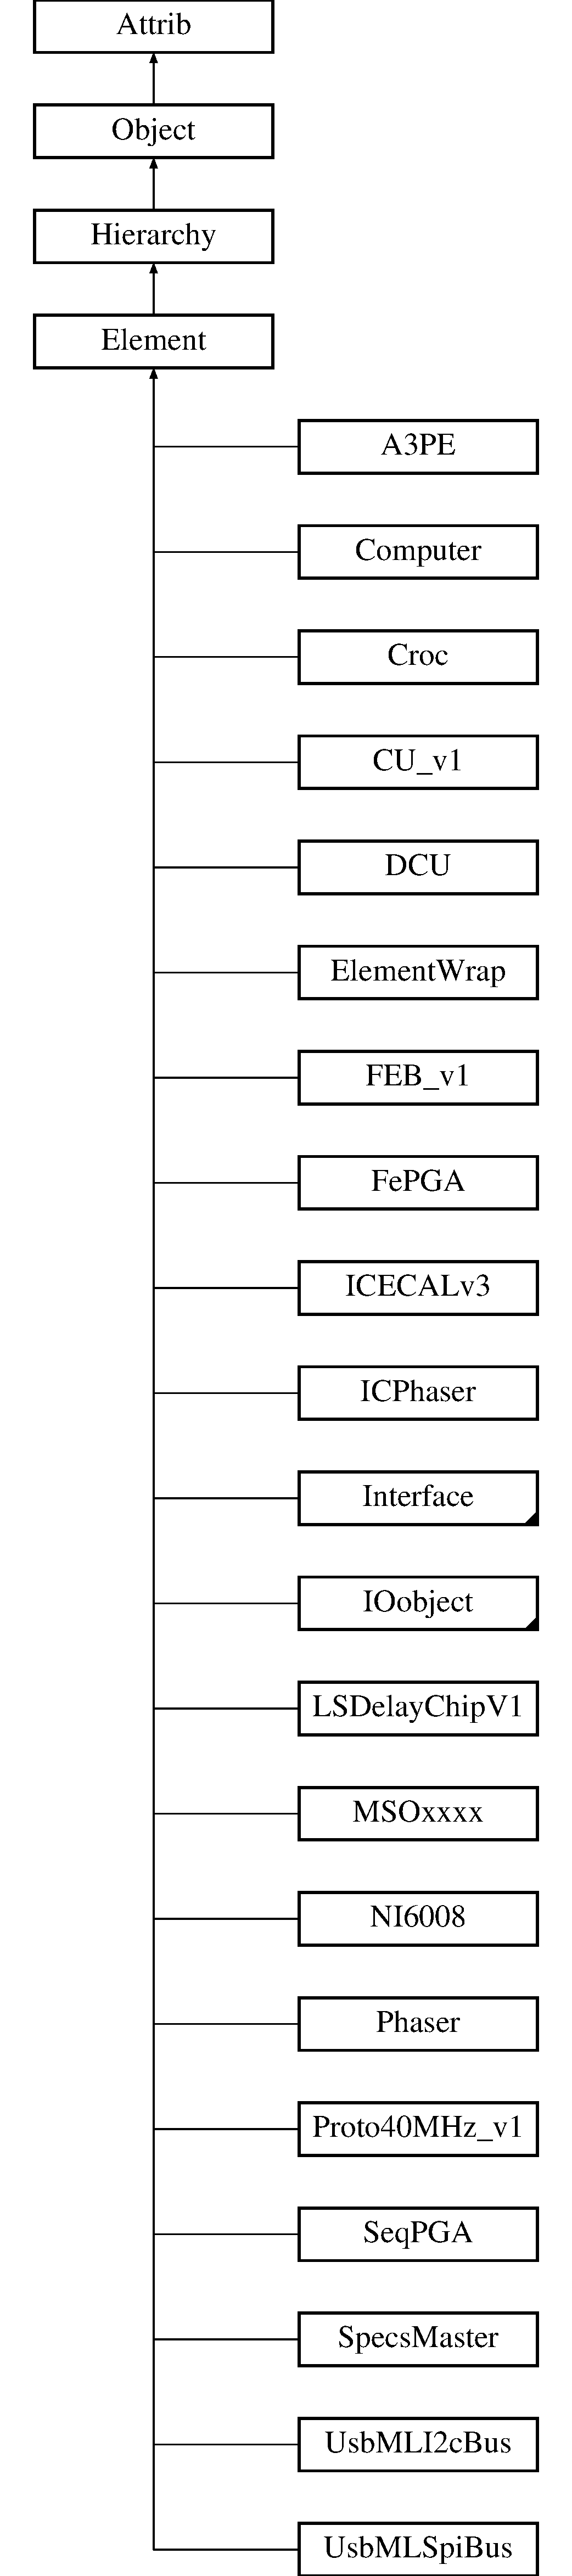
\includegraphics[height=12.000000cm]{classElement}
\end{center}
\end{figure}
\subsection*{Public Types}
\begin{DoxyCompactItemize}
\item 
enum \hyperlink{classAttrib_a69e171d7cc6417835a5a306d3c764235}{Attribut} \{ \newline
\hyperlink{classAttrib_a69e171d7cc6417835a5a306d3c764235a3a8da2ab97dda18aebab196fe4100531}{U\+N\+D\+E\+F\+I\+N\+ED}, 
\hyperlink{classAttrib_a69e171d7cc6417835a5a306d3c764235a2bfb2af57b87031d190a05fe25dd92ed}{P\+A\+S\+S\+I\+VE}, 
\hyperlink{classAttrib_a69e171d7cc6417835a5a306d3c764235a3b1fec929c0370d1436f2f06e298fb0d}{A\+C\+T\+I\+VE}, 
\hyperlink{classAttrib_a69e171d7cc6417835a5a306d3c764235aa27c16b480a369ea4d18b07b2516bbc7}{I\+N\+T\+E\+R\+F\+A\+CE}, 
\newline
\hyperlink{classAttrib_a69e171d7cc6417835a5a306d3c764235a1420a5b8c0540b2af210b6975eded7f9}{IO}, 
\hyperlink{classAttrib_a69e171d7cc6417835a5a306d3c764235a0af3b0d0ac323c1704e6c69cf90add28}{I\+O\+D\+A\+TA}, 
\hyperlink{classAttrib_a69e171d7cc6417835a5a306d3c764235a7788bc5dd333fd8ce18562b269c9dab1}{E\+L\+E\+M\+E\+NT}, 
\hyperlink{classAttrib_a69e171d7cc6417835a5a306d3c764235a61ceb22149f365f1780d18f9d1459423}{H\+A\+R\+D\+W\+A\+RE}, 
\newline
\hyperlink{classAttrib_a69e171d7cc6417835a5a306d3c764235a75250e29692496e73effca2c0330977f}{P\+R\+O\+C\+E\+S\+S\+US}, 
\hyperlink{classAttrib_a69e171d7cc6417835a5a306d3c764235a103a67cd0b8f07ef478fa45d4356e27b}{S\+O\+F\+T\+W\+A\+RE}
 \}
\end{DoxyCompactItemize}
\subsection*{Public Member Functions}
\begin{DoxyCompactItemize}
\item 
\hyperlink{classElement_ab0d0e20be9a36ae676202db753faeec9}{Element} ()
\begin{DoxyCompactList}\small\item\em Standard constructor. \end{DoxyCompactList}\item 
virtual \hyperlink{classElement_a13d54ba9c08b6bec651402f1c2bb002c}{$\sim$\+Element} ()
\begin{DoxyCompactList}\small\item\em Destructor. \end{DoxyCompactList}\item 
virtual void \hyperlink{classElement_a32c0de27acb08e17251cef88c3e9303a}{help} ()=0
\item 
virtual \hyperlink{classStatusCode}{Status\+Code} \hyperlink{classElement_af42754b5cabc198869222725218d695c}{init} ()=0
\item 
virtual void \hyperlink{classElement_a69efffa22f06909d768149715565cb56}{reset} ()=0
\item 
void \hyperlink{classElement_a3c0abcb36f8906688bb7e32608df7086}{recursive\+Init\+Element} ()
\item 
void \hyperlink{classElement_a82119ed37dff76508a2746a853ec35ba}{recursive\+Init\+Communications} ()
\item 
virtual void \hyperlink{classElement_a4e6c83efae95616ebddd03c793a26661}{update} ()=0
\item 
\hyperlink{classStatusCode}{Status\+Code} \hyperlink{classElement_ab476b4b1df5954141ceb14f072433b89}{set\+Connection} (\hyperlink{classHierarchy}{Hierarchy} $\ast$)
\item 
\hyperlink{classHierarchy}{Hierarchy} $\ast$ \hyperlink{classElement_af57444353c1ddf9fa0109801e97debf7}{connection} ()
\item 
void \hyperlink{classHierarchy_af4d43b0765b402670eed2d62c73405af}{clear} ()
\item 
void \hyperlink{classHierarchy_a585ad1aeec16077a0e532ab8b4fc557b}{set\+Parent} (\hyperlink{classHierarchy}{Hierarchy} $\ast$\hyperlink{classHierarchy_a1c7bec8257e717f9c1465e06ebf845fc}{parent})
\item 
\hyperlink{classHierarchy}{Hierarchy} $\ast$ \hyperlink{classHierarchy_a1c7bec8257e717f9c1465e06ebf845fc}{parent} ()
\item 
\hyperlink{classHierarchy}{Hierarchy} $\ast$ \hyperlink{classHierarchy_ad550588733bf75ac5c0fcfd7c8fd11a6}{parent} (std\+::string)
\item 
\hyperlink{classHierarchy}{Hierarchy} $\ast$ \hyperlink{classHierarchy_aee461dc930ce3871636ff87f075b1b83}{origin} ()
\item 
virtual void \hyperlink{classHierarchy_ad677774ff38fcb257c04a3a10d471fac}{add\+Child} (\hyperlink{classHierarchy}{Hierarchy} $\ast$element)
\item 
std\+::vector$<$ \hyperlink{classHierarchy}{Hierarchy} $\ast$ $>$ \hyperlink{classHierarchy_aa9a76f69e98e052ee1a6e32cea006288}{children} ()
\item 
\hyperlink{classHierarchy}{Hierarchy} $\ast$ \hyperlink{classHierarchy_a1e207f973c694b538bf90107b4868817}{child} (std\+::string)
\item 
\hyperlink{classHierarchy}{Hierarchy} $\ast$ \hyperlink{classHierarchy_a0c15a5276a3b80b4354d6bd8a01e0708}{child\+Typed} (std\+::string)
\item 
unsigned long \hyperlink{classHierarchy_ab16e84de65fd84e14001a6cf941c8be4}{number\+Of\+Children} ()
\item 
bool \hyperlink{classHierarchy_a255174fe4d316d2a3f430dcb9dab29f1}{has\+Children} ()
\item 
void \hyperlink{classHierarchy_a2b2b359fac003233f65786a616766bde}{del\+Child} (\hyperlink{classHierarchy}{Hierarchy} $\ast$)
\item 
void \hyperlink{classHierarchy_a1928ac7615fe0b5e55cd707f70dc6781}{del\+Child} (std\+::string)
\item 
std\+::string \hyperlink{classHierarchy_aa7990fa7caf132d83e361ce033c6c65a}{path} (std\+::string=std\+::string(\char`\"{}\char`\"{}))
\item 
std\+::string \hyperlink{classHierarchy_a1efd56cd164d328d2002e53a10a19b8c}{path\+Typed} (std\+::string=std\+::string(\char`\"{}\char`\"{}))
\item 
void \hyperlink{classHierarchy_a76e914b9a677a22a82deb74d892bf261}{tree} (std\+::string indent=std\+::string(\char`\"{}\char`\"{}))
\item 
void \hyperlink{classHierarchy_a594c294c5f60c230e106d522ed008212}{tree} ()
\item 
std\+::string \hyperlink{classObject_a300f4c05dd468c7bb8b3c968868443c1}{name} () const
\item 
std\+::string \hyperlink{classObject_a84f99f70f144a83e1582d1d0f84e4e62}{type} ()
\item 
unsigned char \hyperlink{classObject_af99145335cc61ff6e2798ea17db009d2}{id} ()
\item 
std\+::string \hyperlink{classObject_a73a0f1a41828fdd8303dd662446fb6c3}{title} ()
\item 
void \hyperlink{classObject_a3f9d5537ebce0c0f2bf6ae4d92426f3c}{msg\+Svc} (int level, std\+::string \hyperlink{classObject_a58b2d0618c2d08cf2383012611528d97}{msg}, std\+::string \hyperlink{classObject_a300f4c05dd468c7bb8b3c968868443c1}{name})
\item 
void \hyperlink{classObject_a58b2d0618c2d08cf2383012611528d97}{msg} (std\+::string mymsg)
\item 
void \hyperlink{classObject_ac5d59299273cee27aacf7de00d2e7034}{msg} (std\+::string mymsg, std\+::string \hyperlink{classObject_a300f4c05dd468c7bb8b3c968868443c1}{name})
\item 
void \hyperlink{classObject_a83d2db2df682907ea1115ad721c1c4a1}{verbose} (std\+::string mymsg)
\item 
void \hyperlink{classObject_a2d4120195317e2a3c6532e8bb9f3da68}{verbose} (std\+::string mymsg, std\+::string \hyperlink{classObject_a300f4c05dd468c7bb8b3c968868443c1}{name})
\item 
void \hyperlink{classObject_aac010553f022165573714b7014a15f0d}{debug} (std\+::string mymsg)
\item 
void \hyperlink{classObject_a6c9a0397ca804e04d675ed05683f5420}{debug} (std\+::string mymsg, std\+::string \hyperlink{classObject_a300f4c05dd468c7bb8b3c968868443c1}{name})
\item 
void \hyperlink{classObject_a644fd329ea4cb85f54fa6846484b84a8}{info} (std\+::string mymsg)
\item 
void \hyperlink{classObject_a1ca123253dfd30fc28b156f521dcbdae}{info} (std\+::string mymsg, std\+::string \hyperlink{classObject_a300f4c05dd468c7bb8b3c968868443c1}{name})
\item 
void \hyperlink{classObject_a65cd4fda577711660821fd2cd5a3b4c9}{warning} (std\+::string mymsg)
\item 
void \hyperlink{classObject_a11f101db4dd73d9391b0231818881d86}{warning} (std\+::string mymsg, std\+::string \hyperlink{classObject_a300f4c05dd468c7bb8b3c968868443c1}{name})
\item 
void \hyperlink{classObject_a204a95f57818c0f811933917a30eff45}{error} (std\+::string mymsg)
\item 
void \hyperlink{classObject_ad7f6c457733082efa2f9ff5f5c8e119a}{error} (std\+::string mymsg, std\+::string \hyperlink{classObject_a300f4c05dd468c7bb8b3c968868443c1}{name})
\item 
void \hyperlink{classObject_aad5a16aac7516ce65bd5ec02ab07fc80}{fatal} (std\+::string mymsg)
\item 
void \hyperlink{classObject_ae62acd3d09f716220f75f252dc38bc9a}{fatal} (std\+::string mymsg, std\+::string \hyperlink{classObject_a300f4c05dd468c7bb8b3c968868443c1}{name})
\item 
void \hyperlink{classObject_ae30fea75683c2d149b6b6d17c09ecd0c}{set\+Name} (std\+::string \hyperlink{classObject_a300f4c05dd468c7bb8b3c968868443c1}{name})
\item 
void \hyperlink{classObject_aae534cc9d982bcb9b99fd505f2e103a5}{set\+Type} (std\+::string \hyperlink{classObject_a84f99f70f144a83e1582d1d0f84e4e62}{type})
\item 
void \hyperlink{classObject_a398fe08cba594a0ce6891d59fe4f159f}{set\+Id} (unsigned char \hyperlink{classObject_af99145335cc61ff6e2798ea17db009d2}{id})
\item 
void \hyperlink{classObject_a89557dbbad5bcaa02652f5d7fa35d20f}{set\+Title} (std\+::string \hyperlink{classObject_a73a0f1a41828fdd8303dd662446fb6c3}{title})
\item 
void \hyperlink{classObject_a870c5af919958c2136623b2d7816d123}{set\+Dll\+Name} (std\+::string \hyperlink{classObject_a2e3947f2870094c332d7454117f3ec63}{dll\+Name})
\item 
std\+::string \hyperlink{classObject_a2e3947f2870094c332d7454117f3ec63}{dll\+Name} ()
\item 
bool \hyperlink{classAttrib_a704f26af560909ad22065083bb7d4c34}{is} (int attribut)
\item 
void \hyperlink{classAttrib_a235f773af19c900264a190b00a3b4ad7}{add} (int attribut)
\item 
void \hyperlink{classAttrib_a7d4ef7e32d93cb287792b87b857e79f3}{remove} (int attribut)
\item 
std\+::string \hyperlink{classAttrib_aee7bbf16b144887f196e1341b24f8a26}{attributs} ()
\end{DoxyCompactItemize}
\subsection*{Protected Attributes}
\begin{DoxyCompactItemize}
\item 
\hyperlink{classHierarchy}{Hierarchy} $\ast$ \hyperlink{classElement_abe3de7a5dbbc9a6dd2d7e012e5fdb266}{m\+\_\+connection}
\item 
std\+::string \hyperlink{classAttrib_a3414521d7a82476e874b25a5407b5e63}{m\+\_\+attrib\+String} \mbox{[}10\mbox{]}
\end{DoxyCompactItemize}


\subsection{Detailed Description}
\begin{DoxyAuthor}{Author}

\end{DoxyAuthor}
\begin{DoxyDate}{Date}
2006-\/10-\/23 
\end{DoxyDate}


Definition at line 14 of file Element.\+h.



\subsection{Member Enumeration Documentation}
\mbox{\Hypertarget{classAttrib_a69e171d7cc6417835a5a306d3c764235}\label{classAttrib_a69e171d7cc6417835a5a306d3c764235}} 
\index{Element@{Element}!Attribut@{Attribut}}
\index{Attribut@{Attribut}!Element@{Element}}
\subsubsection{\texorpdfstring{Attribut}{Attribut}}
{\footnotesize\ttfamily enum \hyperlink{classAttrib_a69e171d7cc6417835a5a306d3c764235}{Attrib\+::\+Attribut}\hspace{0.3cm}{\ttfamily [inherited]}}

\begin{DoxyEnumFields}{Enumerator}
\raisebox{\heightof{T}}[0pt][0pt]{\index{U\+N\+D\+E\+F\+I\+N\+ED@{U\+N\+D\+E\+F\+I\+N\+ED}!Element@{Element}}\index{Element@{Element}!U\+N\+D\+E\+F\+I\+N\+ED@{U\+N\+D\+E\+F\+I\+N\+ED}}}\mbox{\Hypertarget{classAttrib_a69e171d7cc6417835a5a306d3c764235a3a8da2ab97dda18aebab196fe4100531}\label{classAttrib_a69e171d7cc6417835a5a306d3c764235a3a8da2ab97dda18aebab196fe4100531}} 
U\+N\+D\+E\+F\+I\+N\+ED&\\
\hline

\raisebox{\heightof{T}}[0pt][0pt]{\index{P\+A\+S\+S\+I\+VE@{P\+A\+S\+S\+I\+VE}!Element@{Element}}\index{Element@{Element}!P\+A\+S\+S\+I\+VE@{P\+A\+S\+S\+I\+VE}}}\mbox{\Hypertarget{classAttrib_a69e171d7cc6417835a5a306d3c764235a2bfb2af57b87031d190a05fe25dd92ed}\label{classAttrib_a69e171d7cc6417835a5a306d3c764235a2bfb2af57b87031d190a05fe25dd92ed}} 
P\+A\+S\+S\+I\+VE&\\
\hline

\raisebox{\heightof{T}}[0pt][0pt]{\index{A\+C\+T\+I\+VE@{A\+C\+T\+I\+VE}!Element@{Element}}\index{Element@{Element}!A\+C\+T\+I\+VE@{A\+C\+T\+I\+VE}}}\mbox{\Hypertarget{classAttrib_a69e171d7cc6417835a5a306d3c764235a3b1fec929c0370d1436f2f06e298fb0d}\label{classAttrib_a69e171d7cc6417835a5a306d3c764235a3b1fec929c0370d1436f2f06e298fb0d}} 
A\+C\+T\+I\+VE&\\
\hline

\raisebox{\heightof{T}}[0pt][0pt]{\index{I\+N\+T\+E\+R\+F\+A\+CE@{I\+N\+T\+E\+R\+F\+A\+CE}!Element@{Element}}\index{Element@{Element}!I\+N\+T\+E\+R\+F\+A\+CE@{I\+N\+T\+E\+R\+F\+A\+CE}}}\mbox{\Hypertarget{classAttrib_a69e171d7cc6417835a5a306d3c764235aa27c16b480a369ea4d18b07b2516bbc7}\label{classAttrib_a69e171d7cc6417835a5a306d3c764235aa27c16b480a369ea4d18b07b2516bbc7}} 
I\+N\+T\+E\+R\+F\+A\+CE&\\
\hline

\raisebox{\heightof{T}}[0pt][0pt]{\index{IO@{IO}!Element@{Element}}\index{Element@{Element}!IO@{IO}}}\mbox{\Hypertarget{classAttrib_a69e171d7cc6417835a5a306d3c764235a1420a5b8c0540b2af210b6975eded7f9}\label{classAttrib_a69e171d7cc6417835a5a306d3c764235a1420a5b8c0540b2af210b6975eded7f9}} 
IO&\\
\hline

\raisebox{\heightof{T}}[0pt][0pt]{\index{I\+O\+D\+A\+TA@{I\+O\+D\+A\+TA}!Element@{Element}}\index{Element@{Element}!I\+O\+D\+A\+TA@{I\+O\+D\+A\+TA}}}\mbox{\Hypertarget{classAttrib_a69e171d7cc6417835a5a306d3c764235a0af3b0d0ac323c1704e6c69cf90add28}\label{classAttrib_a69e171d7cc6417835a5a306d3c764235a0af3b0d0ac323c1704e6c69cf90add28}} 
I\+O\+D\+A\+TA&\\
\hline

\raisebox{\heightof{T}}[0pt][0pt]{\index{E\+L\+E\+M\+E\+NT@{E\+L\+E\+M\+E\+NT}!Element@{Element}}\index{Element@{Element}!E\+L\+E\+M\+E\+NT@{E\+L\+E\+M\+E\+NT}}}\mbox{\Hypertarget{classAttrib_a69e171d7cc6417835a5a306d3c764235a7788bc5dd333fd8ce18562b269c9dab1}\label{classAttrib_a69e171d7cc6417835a5a306d3c764235a7788bc5dd333fd8ce18562b269c9dab1}} 
E\+L\+E\+M\+E\+NT&\\
\hline

\raisebox{\heightof{T}}[0pt][0pt]{\index{H\+A\+R\+D\+W\+A\+RE@{H\+A\+R\+D\+W\+A\+RE}!Element@{Element}}\index{Element@{Element}!H\+A\+R\+D\+W\+A\+RE@{H\+A\+R\+D\+W\+A\+RE}}}\mbox{\Hypertarget{classAttrib_a69e171d7cc6417835a5a306d3c764235a61ceb22149f365f1780d18f9d1459423}\label{classAttrib_a69e171d7cc6417835a5a306d3c764235a61ceb22149f365f1780d18f9d1459423}} 
H\+A\+R\+D\+W\+A\+RE&\\
\hline

\raisebox{\heightof{T}}[0pt][0pt]{\index{P\+R\+O\+C\+E\+S\+S\+US@{P\+R\+O\+C\+E\+S\+S\+US}!Element@{Element}}\index{Element@{Element}!P\+R\+O\+C\+E\+S\+S\+US@{P\+R\+O\+C\+E\+S\+S\+US}}}\mbox{\Hypertarget{classAttrib_a69e171d7cc6417835a5a306d3c764235a75250e29692496e73effca2c0330977f}\label{classAttrib_a69e171d7cc6417835a5a306d3c764235a75250e29692496e73effca2c0330977f}} 
P\+R\+O\+C\+E\+S\+S\+US&\\
\hline

\raisebox{\heightof{T}}[0pt][0pt]{\index{S\+O\+F\+T\+W\+A\+RE@{S\+O\+F\+T\+W\+A\+RE}!Element@{Element}}\index{Element@{Element}!S\+O\+F\+T\+W\+A\+RE@{S\+O\+F\+T\+W\+A\+RE}}}\mbox{\Hypertarget{classAttrib_a69e171d7cc6417835a5a306d3c764235a103a67cd0b8f07ef478fa45d4356e27b}\label{classAttrib_a69e171d7cc6417835a5a306d3c764235a103a67cd0b8f07ef478fa45d4356e27b}} 
S\+O\+F\+T\+W\+A\+RE&\\
\hline

\end{DoxyEnumFields}


Definition at line 29 of file Attrib.\+h.


\begin{DoxyCode}
29                 \{
30     \hyperlink{classAttrib_a69e171d7cc6417835a5a306d3c764235a3a8da2ab97dda18aebab196fe4100531}{UNDEFINED},
31     \hyperlink{classAttrib_a69e171d7cc6417835a5a306d3c764235a2bfb2af57b87031d190a05fe25dd92ed}{PASSIVE},
32     \hyperlink{classAttrib_a69e171d7cc6417835a5a306d3c764235a3b1fec929c0370d1436f2f06e298fb0d}{ACTIVE},
33     \hyperlink{classAttrib_a69e171d7cc6417835a5a306d3c764235aa27c16b480a369ea4d18b07b2516bbc7}{INTERFACE},
34     \hyperlink{classAttrib_a69e171d7cc6417835a5a306d3c764235a1420a5b8c0540b2af210b6975eded7f9}{IO},
35     \hyperlink{classAttrib_a69e171d7cc6417835a5a306d3c764235a0af3b0d0ac323c1704e6c69cf90add28}{IODATA},
36     \hyperlink{classAttrib_a69e171d7cc6417835a5a306d3c764235a7788bc5dd333fd8ce18562b269c9dab1}{ELEMENT},
37     \hyperlink{classAttrib_a69e171d7cc6417835a5a306d3c764235a61ceb22149f365f1780d18f9d1459423}{HARDWARE},
38     \hyperlink{classAttrib_a69e171d7cc6417835a5a306d3c764235a75250e29692496e73effca2c0330977f}{PROCESSUS},
39     \hyperlink{classAttrib_a69e171d7cc6417835a5a306d3c764235a103a67cd0b8f07ef478fa45d4356e27b}{SOFTWARE} 
40   \}; \textcolor{comment}{// array m\_attribString must be changed into Attrib::Attrib if this enu is modified. }
\end{DoxyCode}


\subsection{Constructor \& Destructor Documentation}
\mbox{\Hypertarget{classElement_ab0d0e20be9a36ae676202db753faeec9}\label{classElement_ab0d0e20be9a36ae676202db753faeec9}} 
\index{Element@{Element}!Element@{Element}}
\index{Element@{Element}!Element@{Element}}
\subsubsection{\texorpdfstring{Element()}{Element()}}
{\footnotesize\ttfamily Element\+::\+Element (\begin{DoxyParamCaption}{ }\end{DoxyParamCaption})}



Standard constructor. 



Definition at line 19 of file Element.\+cpp.



References m\+\_\+connection.


\begin{DoxyCode}
20 \{
21   \hyperlink{classElement_abe3de7a5dbbc9a6dd2d7e012e5fdb266}{m\_connection}=0;
22 \}
\end{DoxyCode}
\mbox{\Hypertarget{classElement_a13d54ba9c08b6bec651402f1c2bb002c}\label{classElement_a13d54ba9c08b6bec651402f1c2bb002c}} 
\index{Element@{Element}!````~Element@{$\sim$\+Element}}
\index{````~Element@{$\sim$\+Element}!Element@{Element}}
\subsubsection{\texorpdfstring{$\sim$\+Element()}{~Element()}}
{\footnotesize\ttfamily Element\+::$\sim$\+Element (\begin{DoxyParamCaption}{ }\end{DoxyParamCaption})\hspace{0.3cm}{\ttfamily [virtual]}}



Destructor. 



Definition at line 26 of file Element.\+cpp.


\begin{DoxyCode}
26                   \{
27 \}
\end{DoxyCode}


\subsection{Member Function Documentation}
\mbox{\Hypertarget{classAttrib_a235f773af19c900264a190b00a3b4ad7}\label{classAttrib_a235f773af19c900264a190b00a3b4ad7}} 
\index{Element@{Element}!add@{add}}
\index{add@{add}!Element@{Element}}
\subsubsection{\texorpdfstring{add()}{add()}}
{\footnotesize\ttfamily void Attrib\+::add (\begin{DoxyParamCaption}\item[{int}]{attribut }\end{DoxyParamCaption})\hspace{0.3cm}{\ttfamily [inline]}, {\ttfamily [inherited]}}

Add an attribut 

Definition at line 67 of file Attrib.\+h.



References Attrib\+::m\+\_\+attributs, and Attrib\+::\+U\+N\+D\+E\+F\+I\+N\+ED.



Referenced by A3\+P\+E\+::\+A3\+P\+E(), Attrib\+::\+Attrib(), Specs\+Mezzanine\+::cmdline(), Computer\+::\+Computer(), C\+U\+\_\+v1\+::\+C\+U\+\_\+v1(), export\+\_\+obj(), F\+E\+B\+\_\+v1\+::\+F\+E\+B\+\_\+v1(), Fe\+P\+G\+A\+::\+Fe\+P\+G\+A(), I\+C\+E\+C\+A\+Lv3\+::\+I\+C\+E\+C\+A\+Lv3(), I\+C\+Phaser\+::\+I\+C\+Phaser(), Application\+::initialize(), Interface\+::\+Interface(), I\+Odata\+::\+I\+Odata(), I\+Oobject\+::\+I\+Oobject(), M\+S\+Oxxxx\+::\+M\+S\+Oxxxx(), Phaser\+::\+Phaser(), Processus\+::\+Processus(), Proto40\+M\+Hz\+\_\+v1\+::\+Proto40\+M\+Hz\+\_\+v1(), Attrib\+::remove(), Seq\+P\+G\+A\+::\+Seq\+P\+G\+A(), Test\+I2\+C\+::set\+Address(), Test\+S\+P\+I\+::set\+Address(), Specs\+Slave\+::set\+Address(), Specs\+Master\+::\+Specs\+Master(), and Specs\+Slave\+::\+Specs\+Slave().


\begin{DoxyCode}
67                             \{
68     \textcolor{keywordflow}{if} (attribut!=\hyperlink{classAttrib_a69e171d7cc6417835a5a306d3c764235a3a8da2ab97dda18aebab196fe4100531}{Attrib::UNDEFINED}) \textcolor{keyword}{remove}(\hyperlink{classAttrib_a69e171d7cc6417835a5a306d3c764235a3a8da2ab97dda18aebab196fe4100531}{Attrib::UNDEFINED});
69     \textcolor{keywordtype}{bool} duplicate = false ;
70     std::vector<int>::const\_iterator iter ;
71     \textcolor{keywordflow}{for} ( iter  = \hyperlink{classAttrib_ac4bd58a0cc6b38a3b711d609a3d3aacc}{m\_attributs}.begin() ;
72           iter != \hyperlink{classAttrib_ac4bd58a0cc6b38a3b711d609a3d3aacc}{m\_attributs}.end()   ;
73           ++iter ) \{
74       \textcolor{keywordflow}{if} ( attribut == (*iter) ) \{
75         duplicate = true ;
76       \}
77     \}
78     \textcolor{keywordflow}{if} (!duplicate) \{
79       \hyperlink{classAttrib_ac4bd58a0cc6b38a3b711d609a3d3aacc}{m\_attributs}.push\_back( attribut );
80     \}
81   \}
\end{DoxyCode}
\mbox{\Hypertarget{classHierarchy_ad677774ff38fcb257c04a3a10d471fac}\label{classHierarchy_ad677774ff38fcb257c04a3a10d471fac}} 
\index{Element@{Element}!add\+Child@{add\+Child}}
\index{add\+Child@{add\+Child}!Element@{Element}}
\subsubsection{\texorpdfstring{add\+Child()}{addChild()}}
{\footnotesize\ttfamily void Hierarchy\+::add\+Child (\begin{DoxyParamCaption}\item[{\hyperlink{classHierarchy}{Hierarchy} $\ast$}]{element }\end{DoxyParamCaption})\hspace{0.3cm}{\ttfamily [virtual]}, {\ttfamily [inherited]}}



Definition at line 83 of file Hierarchy.\+cpp.



References Object\+::debug(), Hierarchy\+::m\+\_\+children, Object\+::name(), and Hierarchy\+::set\+Parent().



Referenced by A3\+P\+E\+::\+A3\+P\+E(), Specs\+Mezzanine\+::add\+Bus(), Specs\+Slave\+::add\+I2c(), Application\+::create(), C\+U\+\_\+v1\+::\+C\+U\+\_\+v1(), export\+\_\+obj(), F\+E\+B\+\_\+v1\+::\+F\+E\+B\+\_\+v1(), Fe\+P\+G\+A\+::\+Fe\+P\+G\+A(), I\+C\+E\+C\+A\+Lv3\+::\+I\+C\+E\+C\+A\+Lv3(), I\+C\+Phaser\+::\+I\+C\+Phaser(), Hierarchy\+::origin(), Phaser\+::\+Phaser(), Proto40\+M\+Hz\+\_\+v1\+::\+Proto40\+M\+Hz\+\_\+v1(), Seq\+P\+G\+A\+::\+Seq\+P\+G\+A(), Specs\+Mezzanine\+::\+Specs\+Mezzanine(), Usb\+I2c\+Bus\+::\+Usb\+I2c\+Bus(), and Usb\+Spi\+Bus\+::\+Usb\+Spi\+Bus().


\begin{DoxyCode}
83                                           \{
84   element->\hyperlink{classHierarchy_a585ad1aeec16077a0e532ab8b4fc557b}{setParent}(\textcolor{keyword}{this});
85   \hyperlink{classHierarchy_a038816763941fd4a930504917f60483b}{m\_children}.push\_back(element);
86   \hyperlink{classObject_aac010553f022165573714b7014a15f0d}{debug}(element->\hyperlink{classObject_a300f4c05dd468c7bb8b3c968868443c1}{name}()+\textcolor{stringliteral}{" added to the child tree."},\textcolor{stringliteral}{"Hierarchy::addChild"});
87 \}
\end{DoxyCode}
\mbox{\Hypertarget{classAttrib_aee7bbf16b144887f196e1341b24f8a26}\label{classAttrib_aee7bbf16b144887f196e1341b24f8a26}} 
\index{Element@{Element}!attributs@{attributs}}
\index{attributs@{attributs}!Element@{Element}}
\subsubsection{\texorpdfstring{attributs()}{attributs()}}
{\footnotesize\ttfamily std\+::string Attrib\+::attributs (\begin{DoxyParamCaption}{ }\end{DoxyParamCaption})\hspace{0.3cm}{\ttfamily [inherited]}}

Print the \hyperlink{classAttrib}{Attrib} of an \hyperlink{classObject}{Object} 

Definition at line 54 of file Attrib.\+cpp.



References images\+::index, Attrib\+::m\+\_\+attrib\+String, and Attrib\+::m\+\_\+attributs.



Referenced by export\+\_\+obj(), and Attrib\+::remove().


\begin{DoxyCode}
54                             \{
55   std::string output;
56   std::vector<int>::iterator iter ;
57   \textcolor{keywordflow}{for} ( \textcolor{keywordtype}{unsigned} \textcolor{keywordtype}{int} \hyperlink{namespaceimages_a54407fd574970b3178647ae096321a57}{index} = 0 ; \hyperlink{namespaceimages_a54407fd574970b3178647ae096321a57}{index} < \hyperlink{classAttrib_ac4bd58a0cc6b38a3b711d609a3d3aacc}{m\_attributs}.size() ; ++
      \hyperlink{namespaceimages_a54407fd574970b3178647ae096321a57}{index} ) \{
58     \textcolor{keywordflow}{if} ( \hyperlink{classAttrib_ac4bd58a0cc6b38a3b711d609a3d3aacc}{m\_attributs}.size() - \hyperlink{namespaceimages_a54407fd574970b3178647ae096321a57}{index} > 1 ) \{
59       output.append(\hyperlink{classAttrib_a3414521d7a82476e874b25a5407b5e63}{m\_attribString}[\hyperlink{classAttrib_ac4bd58a0cc6b38a3b711d609a3d3aacc}{m\_attributs}[\hyperlink{namespaceimages_a54407fd574970b3178647ae096321a57}{index}]]);
60       output.append(\textcolor{stringliteral}{":"});
61     \}
62     \textcolor{keywordflow}{else} \{
63       output.append(\hyperlink{classAttrib_a3414521d7a82476e874b25a5407b5e63}{m\_attribString}[\hyperlink{classAttrib_ac4bd58a0cc6b38a3b711d609a3d3aacc}{m\_attributs}[index]]);
64     \}
65   \}
66   \textcolor{keywordflow}{return} output;
67 \}
\end{DoxyCode}
\mbox{\Hypertarget{classHierarchy_a1e207f973c694b538bf90107b4868817}\label{classHierarchy_a1e207f973c694b538bf90107b4868817}} 
\index{Element@{Element}!child@{child}}
\index{child@{child}!Element@{Element}}
\subsubsection{\texorpdfstring{child()}{child()}}
{\footnotesize\ttfamily \hyperlink{classHierarchy}{Hierarchy} $\ast$ Hierarchy\+::child (\begin{DoxyParamCaption}\item[{std\+::string}]{path }\end{DoxyParamCaption})\hspace{0.3cm}{\ttfamily [inherited]}}



Definition at line 133 of file Hierarchy.\+cpp.



References Hierarchy\+::child(), Hierarchy\+::children(), Object\+::name(), Hierarchy\+::origin(), Hierarchy\+::parent(), Hierarchy\+::path(), and Object\+::warning().



Referenced by Application\+::cd(), Hierarchy\+::child(), Hierarchy\+::children(), and export\+\_\+obj().


\begin{DoxyCode}
133                                          \{
134   std::string newpath = \hyperlink{classHierarchy_aa7990fa7caf132d83e361ce033c6c65a}{path};
135   std::string up(\textcolor{stringliteral}{".."});
136   std::string separator(1,\textcolor{charliteral}{'/'});
137 
138   \hyperlink{classHierarchy}{Hierarchy} * newcurrent = 0;
139 
140   \textcolor{comment}{//  info("path="+path,"Hierarchy::child");}
141 
142   \textcolor{keywordflow}{if} (\hyperlink{classHierarchy_aa7990fa7caf132d83e361ce033c6c65a}{path}.compare(\textcolor{stringliteral}{""})==0 || \hyperlink{classHierarchy_aa7990fa7caf132d83e361ce033c6c65a}{path}.compare(\textcolor{stringliteral}{"/"})==0) \{
143     \textcolor{comment}{//    debug("return origin","Hierarchy::child");}
144     \textcolor{keywordflow}{return} \hyperlink{classHierarchy_aee461dc930ce3871636ff87f075b1b83}{origin}();
145   \}
146 
147   \textcolor{keywordflow}{if} (\hyperlink{classHierarchy_aa7990fa7caf132d83e361ce033c6c65a}{path}.compare(\hyperlink{classObject_a300f4c05dd468c7bb8b3c968868443c1}{name}())==0)\{
148     \textcolor{comment}{//    debug("return itself","Hierarchy::child");}
149     \textcolor{keywordflow}{return} \textcolor{keyword}{this};
150   \}
151 
152   \textcolor{keywordflow}{if} (\hyperlink{classHierarchy_aa7990fa7caf132d83e361ce033c6c65a}{path}.compare(\textcolor{stringliteral}{".."})==0)\{
153     \textcolor{keywordflow}{if} (0!=this->\hyperlink{classHierarchy_a1c7bec8257e717f9c1465e06ebf845fc}{parent}()) \textcolor{keywordflow}{return} this->\hyperlink{classHierarchy_a1c7bec8257e717f9c1465e06ebf845fc}{parent}();
154     \textcolor{keywordflow}{else} \textcolor{keywordflow}{return} \textcolor{keyword}{this};
155   \}
156 
157   \textcolor{keywordflow}{if} (\hyperlink{classHierarchy_aa7990fa7caf132d83e361ce033c6c65a}{path}.compare(\textcolor{stringliteral}{"../"})==0)\{
158     \textcolor{keywordflow}{if} (0!=this->\hyperlink{classHierarchy_a1c7bec8257e717f9c1465e06ebf845fc}{parent}()) \textcolor{keywordflow}{return} this->\hyperlink{classHierarchy_a1c7bec8257e717f9c1465e06ebf845fc}{parent}();
159     \textcolor{keywordflow}{else} \textcolor{keywordflow}{return} \textcolor{keyword}{this};
160   \}
161 
162 
163   \textcolor{keywordtype}{int} npos=\hyperlink{classHierarchy_aa7990fa7caf132d83e361ce033c6c65a}{path}.find(separator,0);
164 
165   \textcolor{comment}{//  info("find separator in "+itos(npos)+" of "+path,"Hierarchy::child");}
166 
167   \textcolor{comment}{// remove last separator}
168   \textcolor{keywordflow}{if} ( npos == (\textcolor{keywordtype}{int})(\hyperlink{classHierarchy_aa7990fa7caf132d83e361ce033c6c65a}{path}.size()-1) ) \{
169     newpath = std::string(\hyperlink{classHierarchy_aa7990fa7caf132d83e361ce033c6c65a}{path},0,npos);
170     \hyperlink{classHierarchy_aa7990fa7caf132d83e361ce033c6c65a}{path} = newpath;
171   \}
172 
173   \textcolor{keywordflow}{if} (npos==0)\{
174     \textcolor{comment}{//    debug("Going back to origin and calling child","Hierarchy::child");}
175     newpath=std::string(\hyperlink{classHierarchy_aa7990fa7caf132d83e361ce033c6c65a}{path},1,\hyperlink{classHierarchy_aa7990fa7caf132d83e361ce033c6c65a}{path}.size()-1);
176     \textcolor{keywordflow}{return} \hyperlink{classHierarchy_aee461dc930ce3871636ff87f075b1b83}{origin}()->\hyperlink{classHierarchy_a1e207f973c694b538bf90107b4868817}{child}(newpath);
177   \}
178   \textcolor{keywordflow}{else}\{
179     \textcolor{keywordflow}{if} ( npos== (\textcolor{keywordtype}{int})(std::string::npos) )\{
180       \textcolor{comment}{//      debug("Getting chid "+path+" of "+this->name(),"Hierarchy::child");}
181       std::vector <Hierarchy*> list = \hyperlink{classHierarchy_aa9a76f69e98e052ee1a6e32cea006288}{children}();
182       std::vector<Hierarchy*>::iterator iter;
183       \textcolor{keywordflow}{for} (iter=list.begin();iter!=list.end();iter++)\{
184         \textcolor{keywordflow}{if} ((*iter)->name().compare(\hyperlink{classHierarchy_aa7990fa7caf132d83e361ce033c6c65a}{path})==0)\{
185           \textcolor{keywordflow}{return} *iter;
186         \}
187       \}
188       \hyperlink{classObject_a65cd4fda577711660821fd2cd5a3b4c9}{warning}(this->\hyperlink{classObject_a300f4c05dd468c7bb8b3c968868443c1}{name}()+std::string(\textcolor{stringliteral}{" has no child '"})+\hyperlink{classHierarchy_aa7990fa7caf132d83e361ce033c6c65a}{path}+\textcolor{stringliteral}{"'"},\textcolor{stringliteral}{"Hierarchy::child"});
189       \textcolor{keywordflow}{return} \textcolor{keyword}{this};
190     \}
191     \textcolor{keywordflow}{else}
192     \{
193       \textcolor{keywordtype}{int} ipos=\hyperlink{classHierarchy_aa7990fa7caf132d83e361ce033c6c65a}{path}.find(separator,0);
194       \textcolor{comment}{//      info("default behaviour "+path+" with separator in "+itos(ipos),"Hierarchy::child");}
195 
196       std::string newcurrentname=std::string(\hyperlink{classHierarchy_aa7990fa7caf132d83e361ce033c6c65a}{path},0,ipos);
197       newpath=std::string(\hyperlink{classHierarchy_aa7990fa7caf132d83e361ce033c6c65a}{path},ipos+1,\hyperlink{classHierarchy_aa7990fa7caf132d83e361ce033c6c65a}{path}.size()-1);
198 
199       \textcolor{comment}{//      info("looking now for "+newpath+" from "+newcurrentname,"Hierarchy::child");}
200 
201       \textcolor{keywordflow}{if} (0==newcurrentname.compare(\hyperlink{classHierarchy_aee461dc930ce3871636ff87f075b1b83}{origin}()->\hyperlink{classObject_a300f4c05dd468c7bb8b3c968868443c1}{name}()))\{
202         \textcolor{comment}{//        info("current is computer. Looking for children"+newcurrentname,"Hierarchy::child");}
203         \textcolor{keywordflow}{return} \hyperlink{classHierarchy_aee461dc930ce3871636ff87f075b1b83}{origin}()->\hyperlink{classHierarchy_a1e207f973c694b538bf90107b4868817}{child}(newpath);
204       \}
205 
206       newcurrent = (\hyperlink{classHierarchy}{Hierarchy}*)0;
207 
208       std::vector <Hierarchy*> list = \hyperlink{classHierarchy_aa9a76f69e98e052ee1a6e32cea006288}{children}();
209       std::vector<Hierarchy*>::iterator iter;
210       \textcolor{keywordflow}{for} (iter=list.begin();iter!=list.end();iter++)\{
211         \textcolor{keywordflow}{if} ((*iter)->name().compare(newcurrentname)==0)\{
212           newcurrent = (*iter);
213         \}
214       \}
215 
216 
217       \textcolor{keywordflow}{if} ((\hyperlink{classHierarchy}{Hierarchy}*)0==newcurrent)\{
218         \textcolor{keywordflow}{if} (newcurrentname.compare(\textcolor{stringliteral}{".."})==0 && 0!=\hyperlink{classHierarchy_a1c7bec8257e717f9c1465e06ebf845fc}{parent}())\{
219           newcurrent=this->\hyperlink{classHierarchy_a1c7bec8257e717f9c1465e06ebf845fc}{parent}();
220           \textcolor{comment}{//          debug("newcurrent was .. -> parent="+parent()->name());}
221         \}
222         \textcolor{keywordflow}{else}
223         \{
224           \hyperlink{classObject_a65cd4fda577711660821fd2cd5a3b4c9}{warning}(this->\hyperlink{classObject_a300f4c05dd468c7bb8b3c968868443c1}{name}()+\textcolor{stringliteral}{" has no child '"}+newcurrentname+\textcolor{stringliteral}{"'"},
225               \textcolor{stringliteral}{"Hierarchy::child"});
226           \textcolor{keywordflow}{return} \textcolor{keyword}{this};
227         \}
228       \}
229       \textcolor{comment}{//      debug("recurrence call for "+newpath+" on "+newcurrent->name(),"Hierarchy::child");}
230       \textcolor{keywordflow}{return} newcurrent -> \hyperlink{classHierarchy_a1e207f973c694b538bf90107b4868817}{child} ( newpath );
231     \}
232   \}
233 \}
\end{DoxyCode}
\mbox{\Hypertarget{classHierarchy_aa9a76f69e98e052ee1a6e32cea006288}\label{classHierarchy_aa9a76f69e98e052ee1a6e32cea006288}} 
\index{Element@{Element}!children@{children}}
\index{children@{children}!Element@{Element}}
\subsubsection{\texorpdfstring{children()}{children()}}
{\footnotesize\ttfamily std\+::vector$<$\hyperlink{classHierarchy}{Hierarchy}$\ast$$>$ Hierarchy\+::children (\begin{DoxyParamCaption}{ }\end{DoxyParamCaption})\hspace{0.3cm}{\ttfamily [inline]}, {\ttfamily [inherited]}}



Definition at line 33 of file Hierarchy.\+h.



References Hierarchy\+::child(), Hierarchy\+::child\+Typed(), Hierarchy\+::del\+Child(), Hierarchy\+::has\+Children(), Hierarchy\+::m\+\_\+children, Hierarchy\+::number\+Of\+Children(), Hierarchy\+::path(), Hierarchy\+::path\+Typed(), and Hierarchy\+::tree().



Referenced by Hierarchy\+::child(), Hierarchy\+::child\+Typed(), export\+\_\+obj(), Specs\+Slave\+::recursive\+Init\+Communications(), recursive\+Init\+Communications(), recursive\+Init\+Element(), Application\+::set\+Config(), and Hierarchy\+::tree().


\begin{DoxyCode}
33 \{ \textcolor{keywordflow}{return} \hyperlink{classHierarchy_a038816763941fd4a930504917f60483b}{m\_children};  \} \textcolor{comment}{//< get list of child(ren)}
\end{DoxyCode}
\mbox{\Hypertarget{classHierarchy_a0c15a5276a3b80b4354d6bd8a01e0708}\label{classHierarchy_a0c15a5276a3b80b4354d6bd8a01e0708}} 
\index{Element@{Element}!child\+Typed@{child\+Typed}}
\index{child\+Typed@{child\+Typed}!Element@{Element}}
\subsubsection{\texorpdfstring{child\+Typed()}{childTyped()}}
{\footnotesize\ttfamily \hyperlink{classHierarchy}{Hierarchy} $\ast$ Hierarchy\+::child\+Typed (\begin{DoxyParamCaption}\item[{std\+::string}]{path }\end{DoxyParamCaption})\hspace{0.3cm}{\ttfamily [inherited]}}



Definition at line 239 of file Hierarchy.\+cpp.



References Hierarchy\+::children(), Hierarchy\+::m\+\_\+origin, Object\+::name(), Hierarchy\+::parent(), Hierarchy\+::path(), and Object\+::warning().



Referenced by Hierarchy\+::children(), and export\+\_\+obj().


\begin{DoxyCode}
239                                               \{
240 
241   std::string newpath = \hyperlink{classHierarchy_aa7990fa7caf132d83e361ce033c6c65a}{path};
242 
243   std::string up(\textcolor{stringliteral}{".."});
244   std::string separator(1,\textcolor{charliteral}{'/'});
245   std::string typeopen(1,\textcolor{charliteral}{'['});
246   std::string typeclose(1,\textcolor{charliteral}{']'});
247 
248   \hyperlink{classHierarchy}{Hierarchy} * newcurrent = 0;
249 
250   \textcolor{keywordtype}{unsigned} \textcolor{keywordtype}{int} npos=\hyperlink{classHierarchy_aa7990fa7caf132d83e361ce033c6c65a}{path}.find(separator,0);
251   \textcolor{keywordtype}{unsigned} \textcolor{keywordtype}{int} opos=\hyperlink{classHierarchy_aa7990fa7caf132d83e361ce033c6c65a}{path}.find(typeopen,0);
252   \textcolor{keywordflow}{if} ( npos==std::string::npos || npos == \hyperlink{classHierarchy_aa7990fa7caf132d83e361ce033c6c65a}{path}.size()-1 )\{
253     \textcolor{keywordflow}{if} ( \hyperlink{classHierarchy_aa7990fa7caf132d83e361ce033c6c65a}{path}.compare(\textcolor{stringliteral}{".."})==0 ) \{
254       \textcolor{keywordflow}{return} \hyperlink{classHierarchy_a1c7bec8257e717f9c1465e06ebf845fc}{parent}();
255     \}
256 
257     \textcolor{keywordflow}{if} ( npos == \hyperlink{classHierarchy_aa7990fa7caf132d83e361ce033c6c65a}{path}.size()-1 ) \{
258       newpath = std::string(\hyperlink{classHierarchy_aa7990fa7caf132d83e361ce033c6c65a}{path},0,opos);
259       \hyperlink{classHierarchy_aa7990fa7caf132d83e361ce033c6c65a}{path} = newpath;
260     \}
261 
262     std::vector < Hierarchy* > list = \hyperlink{classHierarchy_aa9a76f69e98e052ee1a6e32cea006288}{children}();
263     std::vector < Hierarchy* >::iterator iter;
264     \textcolor{keywordflow}{for} (iter=list.begin();iter!=list.end();iter++)\{
265       std::string notypepath = std::string(\hyperlink{classHierarchy_aa7990fa7caf132d83e361ce033c6c65a}{path},0,opos);
266       \textcolor{keywordflow}{if} ((*iter)->name().compare(notypepath)==0)\{
267         \textcolor{keywordflow}{return} *iter;
268       \}
269     \}
270     \hyperlink{classObject_a65cd4fda577711660821fd2cd5a3b4c9}{warning}(this->\hyperlink{classObject_a300f4c05dd468c7bb8b3c968868443c1}{name}()+std::string(\textcolor{stringliteral}{" has no child "}) +\hyperlink{classHierarchy_aa7990fa7caf132d83e361ce033c6c65a}{path},\textcolor{stringliteral}{"Hierarchy::child"});
271     \textcolor{keywordflow}{return} 0;
272   \}
273 
274   \textcolor{keywordflow}{else} \{
275 
276     \textcolor{keywordflow}{if} (std::string(\hyperlink{classHierarchy_aa7990fa7caf132d83e361ce033c6c65a}{path},0,3).compare(std::string(\textcolor{stringliteral}{"../"}))==0) \{
277       newpath=std::string(\hyperlink{classHierarchy_aa7990fa7caf132d83e361ce033c6c65a}{path},3,\hyperlink{classHierarchy_aa7990fa7caf132d83e361ce033c6c65a}{path}.size()-3);
278       newcurrent = \hyperlink{classHierarchy_a1c7bec8257e717f9c1465e06ebf845fc}{parent}();
279     \}
280     \textcolor{keywordflow}{if} (std::string(\hyperlink{classHierarchy_aa7990fa7caf132d83e361ce033c6c65a}{path},0,1).compare(std::string(\textcolor{stringliteral}{"/"}))==0) \{
281       newpath=std::string(\hyperlink{classHierarchy_aa7990fa7caf132d83e361ce033c6c65a}{path},1,\hyperlink{classHierarchy_aa7990fa7caf132d83e361ce033c6c65a}{path}.size()-1);
282       newcurrent = ( \hyperlink{classHierarchy}{Hierarchy}* ) \hyperlink{classHierarchy_a16c73e557d3a7c156ffb5dc4102d148e}{m\_origin};
283     \}
284     \textcolor{keywordflow}{if} ((std::string(\hyperlink{classHierarchy_aa7990fa7caf132d83e361ce033c6c65a}{path},0,3).compare(std::string(\textcolor{stringliteral}{"../"})) !=0 ) &&
285         std::string(\hyperlink{classHierarchy_aa7990fa7caf132d83e361ce033c6c65a}{path},0,1).compare(std::string(\textcolor{stringliteral}{"/"}))!=0 ) \{
286       opos = \hyperlink{classHierarchy_aa7990fa7caf132d83e361ce033c6c65a}{path}.find(typeopen,0);
287       \textcolor{keywordtype}{int} cpos = \hyperlink{classHierarchy_aa7990fa7caf132d83e361ce033c6c65a}{path}.find(typeclose,0);
288       std::string \hyperlink{classObject_a300f4c05dd468c7bb8b3c968868443c1}{name} = std::string (\hyperlink{classHierarchy_aa7990fa7caf132d83e361ce033c6c65a}{path},0,opos);
289       newcurrent = \hyperlink{classHierarchy_a0c15a5276a3b80b4354d6bd8a01e0708}{childTyped}( name );
290       \textcolor{keywordflow}{if} (newcurrent ==0)\{
291         \hyperlink{classObject_a65cd4fda577711660821fd2cd5a3b4c9}{warning}(\hyperlink{classHierarchy_aa7990fa7caf132d83e361ce033c6c65a}{path}+\textcolor{stringliteral}{": no child found with such a name"},\textcolor{stringliteral}{"Hierarchy::child"});
292       \}
293       newpath = std::string (\hyperlink{classHierarchy_aa7990fa7caf132d83e361ce033c6c65a}{path},cpos+2,\hyperlink{classHierarchy_aa7990fa7caf132d83e361ce033c6c65a}{path}.size()-cpos-1);
294     \}
295     \textcolor{keywordflow}{return} newcurrent -> \hyperlink{classHierarchy_a0c15a5276a3b80b4354d6bd8a01e0708}{childTyped} ( newpath );
296   \}
297 \}
\end{DoxyCode}
\mbox{\Hypertarget{classHierarchy_af4d43b0765b402670eed2d62c73405af}\label{classHierarchy_af4d43b0765b402670eed2d62c73405af}} 
\index{Element@{Element}!clear@{clear}}
\index{clear@{clear}!Element@{Element}}
\subsubsection{\texorpdfstring{clear()}{clear()}}
{\footnotesize\ttfamily void Hierarchy\+::clear (\begin{DoxyParamCaption}{ }\end{DoxyParamCaption})\hspace{0.3cm}{\ttfamily [inherited]}}



Definition at line 35 of file Hierarchy.\+cpp.



References Hierarchy\+::del\+Child(), Object\+::info(), Hierarchy\+::m\+\_\+children, and Object\+::name().



Referenced by export\+\_\+obj().


\begin{DoxyCode}
35                      \{
36   std::vector<Hierarchy*> listlocale;
37   std::vector<Hierarchy*>::iterator iter;
38   \hyperlink{classObject_a644fd329ea4cb85f54fa6846484b84a8}{info}(\textcolor{stringliteral}{"loop on "}+\hyperlink{classObject_a300f4c05dd468c7bb8b3c968868443c1}{name}()+\textcolor{stringliteral}{" children."},\textcolor{stringliteral}{"Hierarchy::clear"});
39   \textcolor{keywordflow}{for} (iter=\hyperlink{classHierarchy_a038816763941fd4a930504917f60483b}{m\_children}.begin();iter!=\hyperlink{classHierarchy_a038816763941fd4a930504917f60483b}{m\_children}.end();iter++)\{
40       \hyperlink{classObject_a644fd329ea4cb85f54fa6846484b84a8}{info}(\textcolor{stringliteral}{"processing "}+(*iter)->name()+\textcolor{stringliteral}{"."},\textcolor{stringliteral}{"Hierarchy::clear"});
41 \textcolor{comment}{/*}
42 \textcolor{comment}{      (*iter)->clear();
}
43 \textcolor{comment}{//      this->delChild((*iter));
}
44 \textcolor{comment}{      info("obj "+(*iter)->name()+" being cleared.","Hierarchy::clear");
}
45 \textcolor{comment}{      delete (*iter);
}
46 \textcolor{comment}{      info("Object deleted.","Hierarchy::clear");
}
47 \textcolor{comment}{      m\_children.erase(iter);
}
48 \textcolor{comment}{      info("Object removed from the tree.","Hierarchy::clear");
}
49 \textcolor{comment}{*/}
50     (*iter)->clear();
51     \hyperlink{classObject_a644fd329ea4cb85f54fa6846484b84a8}{info}(\textcolor{stringliteral}{"Adding object "}+(*iter)->name()+\textcolor{stringliteral}{" from the Hierarchy to the list of deleted objects."},\textcolor{stringliteral}{"
      Hierarchy::clear"});
52     listlocale.push\_back((*iter));
53   \}
54 
55   \textcolor{keywordflow}{for} (iter=listlocale.begin();iter!=listlocale.end();iter++)\{
56     \hyperlink{classObject_a644fd329ea4cb85f54fa6846484b84a8}{info}(\textcolor{stringliteral}{"Removing object "}+(*iter)->name()+\textcolor{stringliteral}{"."},\textcolor{stringliteral}{"Hierarchy::clear"});
57     this->\hyperlink{classHierarchy_a2b2b359fac003233f65786a616766bde}{delChild}(*iter);
58 \textcolor{comment}{//    m\_children.erase(iter);}
59     \textcolor{keyword}{delete} (*iter);
60   \}
61   \hyperlink{classObject_a644fd329ea4cb85f54fa6846484b84a8}{info}(\textcolor{stringliteral}{"Getting out of "}+\hyperlink{classObject_a300f4c05dd468c7bb8b3c968868443c1}{name}());
62 \}
\end{DoxyCode}
\mbox{\Hypertarget{classElement_af57444353c1ddf9fa0109801e97debf7}\label{classElement_af57444353c1ddf9fa0109801e97debf7}} 
\index{Element@{Element}!connection@{connection}}
\index{connection@{connection}!Element@{Element}}
\subsubsection{\texorpdfstring{connection()}{connection()}}
{\footnotesize\ttfamily \hyperlink{classHierarchy}{Hierarchy} $\ast$ Element\+::connection (\begin{DoxyParamCaption}{ }\end{DoxyParamCaption})}

Get IO interface 

Definition at line 84 of file Element.\+cpp.



References m\+\_\+connection, Object\+::name(), and Object\+::warning().



Referenced by Usb\+Spi\+Bus\+::clock\+Divider(), export\+\_\+obj(), Usb\+I2c\+Bus\+::read(), I\+Oobject\+::read(), Usb\+Spi\+Bus\+::read(), Usb\+Spi\+Bus\+::set\+Clock\+Divider(), set\+Connection(), Usb\+I2c\+Bus\+::write(), I\+Oobject\+::write(), and Usb\+Spi\+Bus\+::write().


\begin{DoxyCode}
84                               \{
85   \textcolor{keywordflow}{if} (0==\hyperlink{classElement_abe3de7a5dbbc9a6dd2d7e012e5fdb266}{m\_connection})\{
86     \hyperlink{classObject_a65cd4fda577711660821fd2cd5a3b4c9}{warning}(\textcolor{stringliteral}{"no connection defined for "}+\hyperlink{classObject_a300f4c05dd468c7bb8b3c968868443c1}{name}()+\textcolor{stringliteral}{"."},\textcolor{stringliteral}{"Element::connection"});
87     \textcolor{keywordflow}{return} (\hyperlink{classHierarchy}{Hierarchy}*)0;
88   \}
89   \textcolor{keywordflow}{return} \hyperlink{classElement_abe3de7a5dbbc9a6dd2d7e012e5fdb266}{m\_connection};
90 \}
\end{DoxyCode}
\mbox{\Hypertarget{classObject_aac010553f022165573714b7014a15f0d}\label{classObject_aac010553f022165573714b7014a15f0d}} 
\index{Element@{Element}!debug@{debug}}
\index{debug@{debug}!Element@{Element}}
\subsubsection{\texorpdfstring{debug()}{debug()}\hspace{0.1cm}{\footnotesize\ttfamily [1/2]}}
{\footnotesize\ttfamily void Object\+::debug (\begin{DoxyParamCaption}\item[{std\+::string}]{mymsg }\end{DoxyParamCaption})\hspace{0.3cm}{\ttfamily [inline]}, {\ttfamily [inherited]}}



Definition at line 37 of file Object.\+h.



References Msg\+Svc\+::\+D\+E\+B\+UG, Object\+::m\+\_\+log, Object\+::m\+\_\+name, and Msg\+Svc\+::msg\+Svc().



Referenced by A3\+P\+E\+::\+A3\+P\+E(), A3\+P\+E\+::acquisition(), Specs\+Mezzanine\+::add\+Bus(), Hierarchy\+::add\+Child(), Specs\+Slave\+::add\+I2c(), L\+S\+Delay\+Chip\+V1\+::config\+Reg\+Bulk\+Read(), L\+S\+Delay\+Chip\+V1\+::config\+Reg\+Bulk\+Write(), A3\+P\+E\+::data\+Ready(), D\+C\+U\+::\+D\+C\+U(), Hierarchy\+::del\+Child(), Specs\+Slave\+::detect(), Storage\+Fifo\+Acquisition\+::execute(), Storage\+Fifo\+::execute(), A3\+P\+E\+\_\+\+Bit\+Flip\+::execute(), Acquisition\+::execute(), Emulate\+F\+E\+::execute(), export\+\_\+obj(), Fe\+P\+G\+A\+::\+Fe\+P\+G\+A(), Specs\+Glue\+::i2c\+Clk\+Mode(), Fe\+P\+G\+A\+::i2c\+Read(), Seq\+P\+G\+A\+::i2c\+Read(), Fe\+P\+G\+A\+::i2c\+Write(), Seq\+P\+G\+A\+::i2c\+Write(), I\+C\+E\+C\+A\+Lv3\+::\+I\+C\+E\+C\+A\+Lv3(), I\+C\+Phaser\+::\+I\+C\+Phaser(), Specs\+Slave\+::init(), Specs\+Master\+::init(), Storage\+Fifo\+Acquisition\+::initialize(), Storage\+Fifo\+::initialize(), A3\+P\+E\+\_\+\+Bit\+Flip\+::initialize(), Acquisition\+::initialize(), Emulate\+F\+E\+::initialize(), A3\+P\+E\+::internal\+A\+X\+Sequence(), Specs\+Glue\+::led(), Specs\+Mezzanine\+::led(), M\+S\+Oxxxx\+::\+M\+S\+Oxxxx(), Phaser\+::\+Phaser(), Data\+::purge(), Phaser\+::read(), I\+C\+Phaser\+::read(), C\+U\+\_\+v1\+::reset(), Proto40\+M\+Hz\+\_\+v1\+::reset(), F\+E\+B\+\_\+v1\+::reset(), Specs\+Master\+::reset(), Specs\+Slave\+::reset(), F\+E\+B\+\_\+v1\+::reset\+Usb(), Seq\+P\+G\+A\+::\+Seq\+P\+G\+A(), A3\+P\+E\+::set\+Add\+From\+A\+X\+Ram(), A3\+P\+E\+::set\+Add\+To\+A\+X\+Ram(), A3\+P\+E\+::set\+A\+X\+Ram\+Usb(), set\+Connection(), Specs\+Glue\+::set\+I2c\+Clk\+Mode(), A3\+P\+E\+::set\+Latency\+A\+X(), Specs\+Glue\+::set\+Led(), Specs\+Mezzanine\+::set\+Led(), A3\+P\+E\+::set\+Length\+A\+X(), A3\+P\+E\+::set\+Read\+To\+A\+X\+Ram\+Usb(), Specs\+Master\+::set\+Speed(), A3\+P\+E\+::set\+Write\+From\+A\+X\+Ram\+Usb(), Specs\+Bus\+::\+Specs\+Bus(), Specs\+I2c\+::\+Specs\+I2c(), Specs\+Master\+::\+Specs\+Master(), Specs\+Mezzanine\+::\+Specs\+Mezzanine(), Specs\+Parallel\+Bus\+::\+Specs\+Parallel\+Bus(), Specs\+Slave\+::\+Specs\+Slave(), L\+S\+Delay\+Chip\+V1\+::spi\+B\+E\+R\+Test(), I\+C\+E\+C\+A\+Lv3\+::spi\+Read(), I\+C\+E\+C\+A\+Lv3\+::spi\+Write(), A3\+P\+E\+::trigger(), Server\+::update\+Config(), Server\+::update\+State(), Phaser\+::write(), I\+C\+Phaser\+::write(), and Hierarchy\+::$\sim$\+Hierarchy().


\begin{DoxyCode}
37 \{ \hyperlink{classObject_a0d269813dd7ac1f24bc143031e2963f2}{m\_log}.\hyperlink{classMsgSvc_ad25f18047920cc59a314e5098259711c}{msgSvc} (\hyperlink{classMsgSvc_ae671eb7301996cd049d2da8a65925926a1dbdcc82dce88370ec335883c83b38b0}{MsgSvc::DEBUG}   , mymsg, \hyperlink{classObject_a8b83c95c705d2c3ba0d081fe1710f48d}{m\_name} ); \}
\end{DoxyCode}
\mbox{\Hypertarget{classObject_a6c9a0397ca804e04d675ed05683f5420}\label{classObject_a6c9a0397ca804e04d675ed05683f5420}} 
\index{Element@{Element}!debug@{debug}}
\index{debug@{debug}!Element@{Element}}
\subsubsection{\texorpdfstring{debug()}{debug()}\hspace{0.1cm}{\footnotesize\ttfamily [2/2]}}
{\footnotesize\ttfamily void Object\+::debug (\begin{DoxyParamCaption}\item[{std\+::string}]{mymsg,  }\item[{std\+::string}]{name }\end{DoxyParamCaption})\hspace{0.3cm}{\ttfamily [inline]}, {\ttfamily [inherited]}}



Definition at line 45 of file Object.\+h.



References Msg\+Svc\+::\+D\+E\+B\+UG, Object\+::m\+\_\+log, and Msg\+Svc\+::msg\+Svc().


\begin{DoxyCode}
45 \{ \hyperlink{classObject_a0d269813dd7ac1f24bc143031e2963f2}{m\_log}.\hyperlink{classMsgSvc_ad25f18047920cc59a314e5098259711c}{msgSvc} (\hyperlink{classMsgSvc_ae671eb7301996cd049d2da8a65925926a1dbdcc82dce88370ec335883c83b38b0}{MsgSvc::DEBUG}   , mymsg, \hyperlink{classObject_a300f4c05dd468c7bb8b3c968868443c1}{name} ); \}
\end{DoxyCode}
\mbox{\Hypertarget{classHierarchy_a2b2b359fac003233f65786a616766bde}\label{classHierarchy_a2b2b359fac003233f65786a616766bde}} 
\index{Element@{Element}!del\+Child@{del\+Child}}
\index{del\+Child@{del\+Child}!Element@{Element}}
\subsubsection{\texorpdfstring{del\+Child()}{delChild()}\hspace{0.1cm}{\footnotesize\ttfamily [1/2]}}
{\footnotesize\ttfamily void Hierarchy\+::del\+Child (\begin{DoxyParamCaption}\item[{\hyperlink{classHierarchy}{Hierarchy} $\ast$}]{element }\end{DoxyParamCaption})\hspace{0.3cm}{\ttfamily [inherited]}}



Definition at line 92 of file Hierarchy.\+cpp.



References Object\+::debug(), and Hierarchy\+::m\+\_\+children.



Referenced by Hierarchy\+::children(), Hierarchy\+::clear(), export\+\_\+obj(), and Hierarchy\+::$\sim$\+Hierarchy().


\begin{DoxyCode}
92                                           \{
93   \textcolor{keywordtype}{bool} flag=\textcolor{keyword}{false};
94   std::vector<Hierarchy*>::iterator iter,\textcolor{keyword}{remove};
95   \textcolor{keywordflow}{for} (iter=\hyperlink{classHierarchy_a038816763941fd4a930504917f60483b}{m\_children}.begin();(iter!=\hyperlink{classHierarchy_a038816763941fd4a930504917f60483b}{m\_children}.end());iter++)\{
96     \textcolor{keywordflow}{if} (*iter==element)\{
97       \textcolor{keyword}{remove}=iter;
98       flag=\textcolor{keyword}{true};
99     \}
100   \}
101   \textcolor{keywordflow}{if} (flag)\{
102     \hyperlink{classObject_aac010553f022165573714b7014a15f0d}{debug}(\textcolor{stringliteral}{"removing "}+(*remove)->name()+\textcolor{stringliteral}{" from the tree."},\textcolor{stringliteral}{"Hierarchy::delChild"});
103     \hyperlink{classHierarchy_a038816763941fd4a930504917f60483b}{m\_children}.erase(\textcolor{keyword}{remove});
104   \}
105 \}
\end{DoxyCode}
\mbox{\Hypertarget{classHierarchy_a1928ac7615fe0b5e55cd707f70dc6781}\label{classHierarchy_a1928ac7615fe0b5e55cd707f70dc6781}} 
\index{Element@{Element}!del\+Child@{del\+Child}}
\index{del\+Child@{del\+Child}!Element@{Element}}
\subsubsection{\texorpdfstring{del\+Child()}{delChild()}\hspace{0.1cm}{\footnotesize\ttfamily [2/2]}}
{\footnotesize\ttfamily void Hierarchy\+::del\+Child (\begin{DoxyParamCaption}\item[{std\+::string}]{n }\end{DoxyParamCaption})\hspace{0.3cm}{\ttfamily [inherited]}}



Definition at line 110 of file Hierarchy.\+cpp.



References Object\+::debug(), and Hierarchy\+::m\+\_\+children.


\begin{DoxyCode}
110                                    \{
111   \textcolor{keywordtype}{bool} flag=\textcolor{keyword}{false};
112   std::vector<Hierarchy*>::iterator iter,\textcolor{keyword}{remove};
113   \textcolor{keywordflow}{for} (iter=\hyperlink{classHierarchy_a038816763941fd4a930504917f60483b}{m\_children}.begin();iter!=\hyperlink{classHierarchy_a038816763941fd4a930504917f60483b}{m\_children}.end();iter++)\{
114     \textcolor{keywordflow}{if} ((*iter)->name()==n)\{ \textcolor{keyword}{remove}=iter; flag=\textcolor{keyword}{true};\}
115   \}
116   \textcolor{keywordflow}{if} (flag)\{
117     \hyperlink{classObject_aac010553f022165573714b7014a15f0d}{debug}(\textcolor{stringliteral}{"removing "}+(*remove)->name()+\textcolor{stringliteral}{" from the tree."},\textcolor{stringliteral}{"Hierarchy::delChild"});
118     \hyperlink{classHierarchy_a038816763941fd4a930504917f60483b}{m\_children}.erase(\textcolor{keyword}{remove});
119   \}
120 \}
\end{DoxyCode}
\mbox{\Hypertarget{classObject_a2e3947f2870094c332d7454117f3ec63}\label{classObject_a2e3947f2870094c332d7454117f3ec63}} 
\index{Element@{Element}!dll\+Name@{dll\+Name}}
\index{dll\+Name@{dll\+Name}!Element@{Element}}
\subsubsection{\texorpdfstring{dll\+Name()}{dllName()}}
{\footnotesize\ttfamily std\+::string Object\+::dll\+Name (\begin{DoxyParamCaption}{ }\end{DoxyParamCaption})\hspace{0.3cm}{\ttfamily [inline]}, {\ttfamily [inherited]}}

Get accessor to member m\+\_\+dll\+Name \begin{DoxyReturn}{Returns}
the current value of m\+\_\+dll\+Name 
\end{DoxyReturn}


Definition at line 74 of file Object.\+h.



References Object\+::m\+\_\+dll\+Name.



Referenced by export\+\_\+obj(), and Object\+::set\+Dll\+Name().


\begin{DoxyCode}
74                        \{
75     \textcolor{keywordflow}{return} \hyperlink{classObject_a01afbeacebb8db6831559972ec362eb3}{m\_dllName};
76   \}  
\end{DoxyCode}
\mbox{\Hypertarget{classObject_a204a95f57818c0f811933917a30eff45}\label{classObject_a204a95f57818c0f811933917a30eff45}} 
\index{Element@{Element}!error@{error}}
\index{error@{error}!Element@{Element}}
\subsubsection{\texorpdfstring{error()}{error()}\hspace{0.1cm}{\footnotesize\ttfamily [1/2]}}
{\footnotesize\ttfamily void Object\+::error (\begin{DoxyParamCaption}\item[{std\+::string}]{mymsg }\end{DoxyParamCaption})\hspace{0.3cm}{\ttfamily [inline]}, {\ttfamily [inherited]}}



Definition at line 40 of file Object.\+h.



References Msg\+Svc\+::\+E\+RR, Object\+::m\+\_\+log, Object\+::m\+\_\+name, and Msg\+Svc\+::msg\+Svc().



Referenced by A3\+P\+E\+::clock\+Division(), N\+I6008\+::cmd(), A3\+P\+E\+::enable\+Storage(), A3\+P\+E\+\_\+\+Bit\+Flip\+::execute(), export\+\_\+obj(), A3\+P\+E\+::fifo\+Depth(), A3\+P\+E\+::fifo\+Latency(), F\+E\+B\+\_\+v1\+::gbt\+Status(), Register\+::get\+Bit(), M\+S\+Oxxxx\+::get\+Statistics(), N\+I6008\+::init(), Specs\+Master\+::init(), Usb\+F\+T\+Interface\+::init(), Usb\+F\+T\+M\+L\+Interface\+::init(), A3\+P\+E\+::latency\+A\+X(), A3\+P\+E\+::length\+A\+X(), A3\+P\+E\+::n\+Trigger(), M\+S\+Oxxxx\+::open(), I\+C\+E\+C\+A\+Lv3\+::parse\+Parameter\+List(), A3\+P\+E\+::pipeline(), Usb\+F\+T\+Interface\+::read(), Usb\+F\+T\+M\+L\+Interface\+::read(), M\+S\+Oxxxx\+::recv(), A3\+P\+E\+::reset(), M\+S\+Oxxxx\+::send(), A3\+P\+E\+::set\+Add\+From\+A\+X\+Ram(), A3\+P\+E\+::set\+Add\+To\+A\+X\+Ram(), I\+C\+E\+C\+A\+Lv3\+::set\+Analog\+Ch(), A3\+P\+E\+::set\+A\+X\+Ram\+Usb(), Register\+::set\+Bit(), A3\+P\+E\+::set\+Clock\+Division(), A3\+P\+E\+::set\+Fifo\+Depth(), A3\+P\+E\+::set\+Fifo\+Latency(), A3\+P\+E\+::set\+Latency\+A\+X(), A3\+P\+E\+::set\+Length\+A\+X(), A3\+P\+E\+::set\+N\+Trigger(), A3\+P\+E\+::set\+Pipeline(), A3\+P\+E\+::set\+Read\+Pattern\+Fifo\+Usb(), A3\+P\+E\+::set\+Read\+To\+A\+X\+Ram\+Usb(), A3\+P\+E\+::set\+Read\+Trigger\+Fifo\+Usb(), A3\+P\+E\+::set\+Software\+Trigger(), A3\+P\+E\+::set\+Trigger\+Delay(), A3\+P\+E\+::set\+Trigger\+Rate(), A3\+P\+E\+::set\+Write\+From\+A\+X\+Ram\+Usb(), A3\+P\+E\+::set\+Write\+Storage\+Fifo\+Usb(), I\+C\+E\+C\+A\+Lv3\+::spi\+F\+E\+R\+Test(), I\+C\+E\+C\+A\+Lv3\+::spi\+Write\+Safe(), A3\+P\+E\+::start\+Sequence\+A\+X(), A3\+P\+E\+::trigger\+Delay(), A3\+P\+E\+::trigger\+Rate(), Usb\+F\+T\+Interface\+::usb\+Read(), Usb\+F\+T\+M\+L\+Interface\+::usb\+Read(), Usb\+F\+T\+Interface\+::usb\+Read\+U16(), Usb\+F\+T\+M\+L\+Interface\+::usb\+Read\+U16(), Usb\+F\+T\+M\+L\+Interface\+::usb\+Read\+U32(), Usb\+F\+T\+Interface\+::usb\+Read\+U32(), Usb\+F\+T\+M\+L\+Interface\+::usb\+Read\+U8(), Usb\+F\+T\+Interface\+::usb\+Read\+U8(), Usb\+F\+T\+Interface\+::usb\+Write(), Usb\+F\+T\+M\+L\+Interface\+::usb\+Write(), Usb\+F\+T\+Interface\+::usb\+Write\+Read(), Usb\+F\+T\+M\+L\+Interface\+::usb\+Write\+Read(), Usb\+F\+T\+Interface\+::usb\+Write\+U16(), Usb\+F\+T\+M\+L\+Interface\+::usb\+Write\+U16(), Usb\+F\+T\+M\+L\+Interface\+::usb\+Write\+U32(), Usb\+F\+T\+Interface\+::usb\+Write\+U32(), Usb\+F\+T\+M\+L\+Interface\+::usb\+Write\+U8(), Usb\+F\+T\+Interface\+::usb\+Write\+U8(), Usb\+F\+T\+M\+L\+Interface\+::write(), and Usb\+F\+T\+Interface\+::write().


\begin{DoxyCode}
40 \{ \hyperlink{classObject_a0d269813dd7ac1f24bc143031e2963f2}{m\_log}.\hyperlink{classMsgSvc_ad25f18047920cc59a314e5098259711c}{msgSvc} (\hyperlink{classMsgSvc_ae671eb7301996cd049d2da8a65925926a35a9d7166e9896af4ec8fb33bf5f1772}{MsgSvc::ERR}     , mymsg, \hyperlink{classObject_a8b83c95c705d2c3ba0d081fe1710f48d}{m\_name} ); \}
\end{DoxyCode}
\mbox{\Hypertarget{classObject_ad7f6c457733082efa2f9ff5f5c8e119a}\label{classObject_ad7f6c457733082efa2f9ff5f5c8e119a}} 
\index{Element@{Element}!error@{error}}
\index{error@{error}!Element@{Element}}
\subsubsection{\texorpdfstring{error()}{error()}\hspace{0.1cm}{\footnotesize\ttfamily [2/2]}}
{\footnotesize\ttfamily void Object\+::error (\begin{DoxyParamCaption}\item[{std\+::string}]{mymsg,  }\item[{std\+::string}]{name }\end{DoxyParamCaption})\hspace{0.3cm}{\ttfamily [inline]}, {\ttfamily [inherited]}}



Definition at line 48 of file Object.\+h.



References Msg\+Svc\+::\+E\+RR, Object\+::m\+\_\+log, and Msg\+Svc\+::msg\+Svc().


\begin{DoxyCode}
48 \{ \hyperlink{classObject_a0d269813dd7ac1f24bc143031e2963f2}{m\_log}.\hyperlink{classMsgSvc_ad25f18047920cc59a314e5098259711c}{msgSvc} (\hyperlink{classMsgSvc_ae671eb7301996cd049d2da8a65925926a35a9d7166e9896af4ec8fb33bf5f1772}{MsgSvc::ERR}     , mymsg, \hyperlink{classObject_a300f4c05dd468c7bb8b3c968868443c1}{name} ); \}
\end{DoxyCode}
\mbox{\Hypertarget{classObject_aad5a16aac7516ce65bd5ec02ab07fc80}\label{classObject_aad5a16aac7516ce65bd5ec02ab07fc80}} 
\index{Element@{Element}!fatal@{fatal}}
\index{fatal@{fatal}!Element@{Element}}
\subsubsection{\texorpdfstring{fatal()}{fatal()}\hspace{0.1cm}{\footnotesize\ttfamily [1/2]}}
{\footnotesize\ttfamily void Object\+::fatal (\begin{DoxyParamCaption}\item[{std\+::string}]{mymsg }\end{DoxyParamCaption})\hspace{0.3cm}{\ttfamily [inline]}, {\ttfamily [inherited]}}



Definition at line 41 of file Object.\+h.



References Msg\+Svc\+::\+F\+A\+T\+AL, Object\+::m\+\_\+log, Object\+::m\+\_\+name, and Msg\+Svc\+::msg\+Svc().



Referenced by export\+\_\+obj(), Usb\+M\+L\+I2c\+Bus\+::init(), Usb\+M\+L\+Spi\+Bus\+::init(), Usb\+I2c\+Bus\+::init(), Usb\+Spi\+Bus\+::init(), Specs\+Slave\+::init(), I\+Oobject\+::init(), Usb\+F\+T\+M\+L\+Interface\+::init(), Usb\+F\+T\+Interface\+::init(), and set\+Connection().


\begin{DoxyCode}
41 \{ \hyperlink{classObject_a0d269813dd7ac1f24bc143031e2963f2}{m\_log}.\hyperlink{classMsgSvc_ad25f18047920cc59a314e5098259711c}{msgSvc} (\hyperlink{classMsgSvc_ae671eb7301996cd049d2da8a65925926a59c73cb29edfc9cdf35845e2b1301363}{MsgSvc::FATAL}   , mymsg, \hyperlink{classObject_a8b83c95c705d2c3ba0d081fe1710f48d}{m\_name} ); \}
\end{DoxyCode}
\mbox{\Hypertarget{classObject_ae62acd3d09f716220f75f252dc38bc9a}\label{classObject_ae62acd3d09f716220f75f252dc38bc9a}} 
\index{Element@{Element}!fatal@{fatal}}
\index{fatal@{fatal}!Element@{Element}}
\subsubsection{\texorpdfstring{fatal()}{fatal()}\hspace{0.1cm}{\footnotesize\ttfamily [2/2]}}
{\footnotesize\ttfamily void Object\+::fatal (\begin{DoxyParamCaption}\item[{std\+::string}]{mymsg,  }\item[{std\+::string}]{name }\end{DoxyParamCaption})\hspace{0.3cm}{\ttfamily [inline]}, {\ttfamily [inherited]}}



Definition at line 49 of file Object.\+h.



References Msg\+Svc\+::\+F\+A\+T\+AL, Object\+::m\+\_\+log, and Msg\+Svc\+::msg\+Svc().


\begin{DoxyCode}
49 \{ \hyperlink{classObject_a0d269813dd7ac1f24bc143031e2963f2}{m\_log}.\hyperlink{classMsgSvc_ad25f18047920cc59a314e5098259711c}{msgSvc} (\hyperlink{classMsgSvc_ae671eb7301996cd049d2da8a65925926a59c73cb29edfc9cdf35845e2b1301363}{MsgSvc::FATAL}   , mymsg, \hyperlink{classObject_a300f4c05dd468c7bb8b3c968868443c1}{name} ); \}
\end{DoxyCode}
\mbox{\Hypertarget{classHierarchy_a255174fe4d316d2a3f430dcb9dab29f1}\label{classHierarchy_a255174fe4d316d2a3f430dcb9dab29f1}} 
\index{Element@{Element}!has\+Children@{has\+Children}}
\index{has\+Children@{has\+Children}!Element@{Element}}
\subsubsection{\texorpdfstring{has\+Children()}{hasChildren()}}
{\footnotesize\ttfamily bool Hierarchy\+::has\+Children (\begin{DoxyParamCaption}{ }\end{DoxyParamCaption})\hspace{0.3cm}{\ttfamily [inherited]}}



Definition at line 303 of file Hierarchy.\+cpp.



References Hierarchy\+::m\+\_\+children.



Referenced by Hierarchy\+::children(), and export\+\_\+obj().


\begin{DoxyCode}
303                               \{
304   \textcolor{keywordflow}{return} ( \hyperlink{classHierarchy_a038816763941fd4a930504917f60483b}{m\_children}.size()>0 );
305 \}
\end{DoxyCode}
\mbox{\Hypertarget{classElement_a32c0de27acb08e17251cef88c3e9303a}\label{classElement_a32c0de27acb08e17251cef88c3e9303a}} 
\index{Element@{Element}!help@{help}}
\index{help@{help}!Element@{Element}}
\subsubsection{\texorpdfstring{help()}{help()}}
{\footnotesize\ttfamily virtual void Element\+::help (\begin{DoxyParamCaption}{ }\end{DoxyParamCaption})\hspace{0.3cm}{\ttfamily [pure virtual]}}

printout help for the element 

Implemented in \hyperlink{classA3PE_ae495a413cc26d31321b31942ebef1bfa}{A3\+PE}, \hyperlink{classLSDelayChipV1_a3d57457a70f7d42687197704321b0c8e}{L\+S\+Delay\+Chip\+V1}, \hyperlink{classICECALv3_a00e572849b4952e7cf04a39f992df037}{I\+C\+E\+C\+A\+Lv3}, \hyperlink{classICPhaser_a8650cfbe21e6dfa96f3a858507105f3b}{I\+C\+Phaser}, \hyperlink{classMSOxxxx_a8c22ff23297ada963eaf12b6e0b62017}{M\+S\+Oxxxx}, \hyperlink{classPhaser_a0f122559297d076500420a7ceb21d70d}{Phaser}, \hyperlink{classUsbFTInterface_a91a0046390c76ca8abaa330fa244279c}{Usb\+F\+T\+Interface}, \hyperlink{classUsbFTMLInterface_a1cfe65c58531afc07c21d876e21d8e46}{Usb\+F\+T\+M\+L\+Interface}, \hyperlink{classSpecsInterface_a24bf2b5e2da6c675ba5de3b226481a73}{Specs\+Interface}, \hyperlink{classSpecsMaster_ad96a7533c46f01c0f67f330f6fdbf94a}{Specs\+Master}, \hyperlink{classSpecsParallelBus_a67b05d066de051d33a6afff267f9178e}{Specs\+Parallel\+Bus}, \hyperlink{classComputer_aeca79382f17fcfb43320902de5f20aca}{Computer}, \hyperlink{classNI6008_ab58d458dbd895b97f7aa51c52b5cd714}{N\+I6008}, \hyperlink{classFePGA_ae6425fbad1a8db57025efaf387a6f41b}{Fe\+P\+GA}, \hyperlink{classSeqPGA_ae651bb2d5ac33e863951499c638655fe}{Seq\+P\+GA}, \hyperlink{classDCU_a3b75cb2428ddf209608db6b8bd60ef47}{D\+CU}, \hyperlink{classSpecsMezzanine_a9cbb99c91d987194009be1cb81d2ba7c}{Specs\+Mezzanine}, \hyperlink{classProto40MHz__v1_ae775987179848b4bc257473be261d24c}{Proto40\+M\+Hz\+\_\+v1}, \hyperlink{classFEB__v1_af93db546ad89ba7c2301fdc2314efd8a}{F\+E\+B\+\_\+v1}, \hyperlink{classIOobject_a0520d82a9773c764fbaede59fe6f8a17}{I\+Oobject}, \hyperlink{classUsbSpiBus_a3543b3bbad0c137fde32fdc554a09a5d}{Usb\+Spi\+Bus}, \hyperlink{classCU__v1_af4033fc5da7bff845565d7e6ea1802ce}{C\+U\+\_\+v1}, \hyperlink{classUsbI2cBus_a5c3349f89fff94a8eae3d9752f5fcf6a}{Usb\+I2c\+Bus}, \hyperlink{classUsbMLI2cBus_aeb2b5e4169c6847942ae89e5bf476c79}{Usb\+M\+L\+I2c\+Bus}, \hyperlink{classUsbMLSpiBus_a9ff9537179dc4a861afcd3fea9e60da7}{Usb\+M\+L\+Spi\+Bus}, \hyperlink{classInterface_aedd3cf1d964c837e7848ccf81dc9c760}{Interface}, \hyperlink{classRAM_ac1e78007fabee045f00f342a907fa25c}{R\+AM}, \hyperlink{classSpecsGlue_a04fd0c122ac6980833fd87af92377791}{Specs\+Glue}, \hyperlink{classCroc_a21195cea3b5ba13f90397cc8faa52633}{Croc}, \hyperlink{structElementWrap_ad22ed533c2dad73f8650243d8060b547}{Element\+Wrap}, and \hyperlink{structInterfaceWrap_abcf87065a7b9099a7d05e7c0ddaf2487}{Interface\+Wrap}.



Referenced by export\+\_\+obj().

\mbox{\Hypertarget{classObject_af99145335cc61ff6e2798ea17db009d2}\label{classObject_af99145335cc61ff6e2798ea17db009d2}} 
\index{Element@{Element}!id@{id}}
\index{id@{id}!Element@{Element}}
\subsubsection{\texorpdfstring{id()}{id()}}
{\footnotesize\ttfamily unsigned char Object\+::id (\begin{DoxyParamCaption}{ }\end{DoxyParamCaption})\hspace{0.3cm}{\ttfamily [inline]}, {\ttfamily [inherited]}}



Definition at line 30 of file Object.\+h.



References Object\+::m\+\_\+id.



Referenced by export\+\_\+obj(), and Object\+::set\+Id().


\begin{DoxyCode}
30 \{ \textcolor{keywordflow}{return} \hyperlink{classObject_aca74b9dbfed7b5556ea2d56c65b6b6b0}{m\_id};         \} \textcolor{comment}{//< Get Object m\_id }
\end{DoxyCode}
\mbox{\Hypertarget{classObject_a644fd329ea4cb85f54fa6846484b84a8}\label{classObject_a644fd329ea4cb85f54fa6846484b84a8}} 
\index{Element@{Element}!info@{info}}
\index{info@{info}!Element@{Element}}
\subsubsection{\texorpdfstring{info()}{info()}\hspace{0.1cm}{\footnotesize\ttfamily [1/2]}}
{\footnotesize\ttfamily void Object\+::info (\begin{DoxyParamCaption}\item[{std\+::string}]{mymsg }\end{DoxyParamCaption})\hspace{0.3cm}{\ttfamily [inline]}, {\ttfamily [inherited]}}



Definition at line 38 of file Object.\+h.



References Msg\+Svc\+::\+I\+N\+FO, Object\+::m\+\_\+log, Object\+::m\+\_\+name, and Msg\+Svc\+::msg\+Svc().



Referenced by N\+I6008\+::add\+Device(), F\+E\+B\+\_\+v1\+::calib\+Cte(), check\+Cmd(), Hierarchy\+::clear(), F\+E\+B\+\_\+v1\+::clock80\+M\+Hz\+Falling\+Edge(), F\+E\+B\+\_\+v1\+::clock\+Falling\+Edge(), Usb\+F\+T\+M\+L\+Interface\+::close(), Usb\+F\+T\+Interface\+::close(), Processus\+::close\+Root\+File(), Server\+::cmdline(), Specs\+Mezzanine\+::cmdline(), Specs\+Slave\+::detect(), F\+E\+B\+\_\+v1\+::disable\+Subtract(), I\+Odata\+::dump(), A3\+P\+E\+::dump\+From\+A\+X(), A3\+P\+E\+::dump\+Pattern(), A3\+P\+E\+::dump\+Storage(), A3\+P\+E\+::dump\+To\+A\+X(), A3\+P\+E\+::dump\+Trigger(), Processus\+::end\+Processing(), Phaser\+Ramp\+Exec\+::execute(), export\+\_\+obj(), Phaser\+Ramp\+Exec\+::finalize(), F\+E\+B\+\_\+v1\+::gain4(), F\+E\+B\+\_\+v1\+::gbt80\+M\+Hz\+Clk\+Eport(), F\+E\+B\+\_\+v1\+::gbt\+Data\+Path(), F\+E\+B\+\_\+v1\+::gbt\+D\+L\+L\+Eport(), F\+E\+B\+\_\+v1\+::gbt\+D\+L\+L\+Reset(), F\+E\+B\+\_\+v1\+::gbt\+Enable\+Eport(), F\+E\+B\+\_\+v1\+::gbt\+Mode(), F\+E\+B\+\_\+v1\+::gbt\+Status(), F\+E\+B\+\_\+v1\+::gbt\+Term\+Eport(), F\+E\+B\+\_\+v1\+::gbt\+Track\+Mode(), I\+C\+E\+C\+A\+Lv3\+::get\+Analog\+Ch(), I\+C\+E\+C\+A\+Lv3\+::get\+Delay\+Line\+Ch(), I\+C\+E\+C\+A\+Lv3\+::get\+Main\+Reg(), F\+E\+B\+\_\+v1\+::global\+Pseudo\+P\+M\+Enable(), Croc\+::help(), R\+A\+M\+::help(), Specs\+Glue\+::help(), Usb\+M\+L\+I2c\+Bus\+::help(), Usb\+M\+L\+Spi\+Bus\+::help(), C\+U\+\_\+v1\+::help(), Usb\+I2c\+Bus\+::help(), Usb\+Spi\+Bus\+::help(), F\+E\+B\+\_\+v1\+::help(), I\+Oobject\+::help(), Proto40\+M\+Hz\+\_\+v1\+::help(), Specs\+Mezzanine\+::help(), Fe\+P\+G\+A\+::help(), Seq\+P\+G\+A\+::help(), Computer\+::help(), N\+I6008\+::help(), Specs\+Parallel\+Bus\+::help(), Specs\+Master\+::help(), Usb\+F\+T\+M\+L\+Interface\+::help(), Usb\+F\+T\+Interface\+::help(), Phaser\+::help(), I\+C\+Phaser\+::help(), A3\+P\+E\+::help(), M\+S\+Oxxxx\+::id(), Croc\+::init(), N\+I6008\+::init(), Computer\+::init(), Specs\+Parallel\+Bus\+::init(), Specs\+Slave\+::init(), Specs\+Master\+::init(), Usb\+F\+T\+Interface\+::init(), Usb\+F\+T\+M\+L\+Interface\+::init(), Storage\+Fifo\+Acquisition\+::initialize(), Storage\+Fifo\+::initialize(), A3\+P\+E\+\_\+\+Bit\+Flip\+::initialize(), Acquisition\+::initialize(), Emulate\+F\+E\+::initialize(), Current\+Measurement\+::initialize(), A\+D\+C\+Measurement\+::initialize(), Phaser\+Ramp\+Exec\+::initialize(), F\+E\+B\+\_\+v1\+::inject\+Mode\+F\+E(), is\+Int(), F\+E\+B\+\_\+v1\+::latency(), F\+E\+B\+\_\+v1\+::latency\+L\+L\+T(), A3\+P\+E\+::load\+From\+A\+X(), Application\+::load\+History\+File(), A3\+P\+E\+::load\+Pattern(), A3\+P\+E\+::load\+Storage(), A3\+P\+E\+::load\+To\+A\+X(), A3\+P\+E\+::load\+Trigger(), Application\+::loop(), F\+E\+B\+\_\+v1\+::mask\+L\+L\+T(), Application\+::network(), F\+E\+B\+\_\+v1\+::old\+Subtract(), M\+S\+Oxxxx\+::open(), Processus\+::open\+Root\+File(), Data\+::print(), F\+E\+B\+\_\+v1\+::probe\+Enable(), Proc\+Data\+Base\+::\+Proc\+Data\+Base(), F\+E\+B\+\_\+v1\+::pseudo\+A\+D\+C\+Enable(), F\+E\+B\+\_\+v1\+::pseudo\+P\+M\+Enable(), Usb\+Spi\+Bus\+::read(), Usb\+F\+T\+M\+L\+Interface\+::read(), F\+E\+B\+\_\+v1\+::read\+Fifo\+Inject\+F\+E(), F\+E\+B\+\_\+v1\+::read\+Fifo\+L\+L\+T(), F\+E\+B\+\_\+v1\+::read\+Fifo\+L\+L\+T\+F\+E(), F\+E\+B\+\_\+v1\+::read\+Fifo\+Spy\+F\+E(), M\+S\+Oxxxx\+::recv(), Croc\+::reset(), Usb\+I2c\+Bus\+::reset(), Usb\+M\+L\+I2c\+Bus\+::reset(), Usb\+M\+L\+Spi\+Bus\+::reset(), Usb\+Spi\+Bus\+::reset(), Fe\+P\+G\+A\+::reset(), Seq\+P\+G\+A\+::reset(), Computer\+::reset(), Specs\+Parallel\+Bus\+::reset(), Specs\+Master\+::reset(), N\+I6008\+::reset(), Usb\+F\+T\+M\+L\+Interface\+::reset(), Usb\+F\+T\+Interface\+::reset(), A3\+P\+E\+::reset(), A3\+P\+E\+::reset\+Acquisition\+Write\+Counter(), F\+E\+B\+\_\+v1\+::reset\+F\+E(), A3\+P\+E\+::reset\+F\+E(), F\+E\+B\+\_\+v1\+::reset\+Fifo\+Inject\+F\+E(), F\+E\+B\+\_\+v1\+::reset\+Fifo\+Spy\+F\+E(), A3\+P\+E\+::reset\+From\+A\+X\+Ram(), Specs\+Slave\+::reset\+Internal(), A3\+P\+E\+::reset\+Latency\+Counter(), A3\+P\+E\+::reset\+Pattern\+Fifo(), A3\+P\+E\+::reset\+Sequence\+From\+To\+A\+X(), A3\+P\+E\+::reset\+S\+P\+I(), A3\+P\+E\+::reset\+Storage\+Fifo(), A3\+P\+E\+::reset\+To\+A\+X\+Ram(), A3\+P\+E\+::reset\+Trigger\+Fifo(), Seq\+P\+G\+A\+::reset\+Usb(), Fe\+P\+G\+A\+::reset\+Usb(), A3\+P\+E\+::reset\+Usb\+Phasers(), M\+S\+Oxxxx\+::send(), Server\+::\+Server(), Application\+::server(), F\+E\+B\+\_\+v1\+::set\+Calib\+Cte(), F\+E\+B\+\_\+v1\+::set\+Clock80\+M\+Hz\+Falling\+Edge(), A3\+P\+E\+::set\+Clock\+Division(), F\+E\+B\+\_\+v1\+::set\+Clock\+Falling\+Edge(), Usb\+Spi\+Bus\+::set\+Data\+Length(), F\+E\+B\+\_\+v1\+::set\+Disable\+Subtract(), A3\+P\+E\+::set\+Enable\+A\+D\+C(), A3\+P\+E\+::set\+Fifo\+Depth(), A3\+P\+E\+::set\+Fifo\+Latency(), F\+E\+B\+\_\+v1\+::set\+Gain4(), F\+E\+B\+\_\+v1\+::set\+Gbt80\+M\+Hz\+Clk\+Eport(), F\+E\+B\+\_\+v1\+::set\+Gbt\+Clock\+Strength(), F\+E\+B\+\_\+v1\+::set\+Gbt\+Data\+Path(), F\+E\+B\+\_\+v1\+::set\+Gbt\+D\+L\+L\+Eport(), F\+E\+B\+\_\+v1\+::set\+Gbt\+Enable\+Eport(), F\+E\+B\+\_\+v1\+::set\+Gbt\+Mode(), F\+E\+B\+\_\+v1\+::set\+Gbt\+Term\+Eport(), F\+E\+B\+\_\+v1\+::set\+Gbt\+Track\+Mode(), F\+E\+B\+\_\+v1\+::set\+Global\+Pseudo\+P\+M\+Enable(), F\+E\+B\+\_\+v1\+::set\+Inject\+Mode\+F\+E(), A3\+P\+E\+::set\+Internal\+A\+X\+Sequence(), F\+E\+B\+\_\+v1\+::set\+Latency(), A3\+P\+E\+::set\+N\+Trigger(), F\+E\+B\+\_\+v1\+::set\+Old\+Subtract(), F\+E\+B\+\_\+v1\+::set\+Output\+Eport(), Phaser\+::set\+Phase(), I\+C\+Phaser\+::set\+Phase(), A3\+P\+E\+::set\+Pipeline(), F\+E\+B\+\_\+v1\+::set\+Probe\+Enable(), F\+E\+B\+\_\+v1\+::set\+Pseudo\+A\+D\+C\+Enable(), F\+E\+B\+\_\+v1\+::set\+Pseudo\+P\+M\+Enable(), A3\+P\+E\+::set\+Read\+Pattern\+Fifo\+Usb(), A3\+P\+E\+::set\+Read\+Trigger\+Fifo\+Usb(), A3\+P\+E\+::set\+Software\+Trigger(), F\+E\+B\+\_\+v1\+::set\+Spare\+For\+Trig\+Enable(), F\+E\+B\+\_\+v1\+::set\+Spy\+Mode\+F\+E(), Processus\+::set\+State(), F\+E\+B\+\_\+v1\+::set\+Threshold(), A3\+P\+E\+::set\+Trigger\+Delay(), A3\+P\+E\+::set\+Trigger\+Rate(), A3\+P\+E\+::set\+Write\+Storage\+Fifo\+Usb(), L\+S\+Delay\+Chip\+V1\+::show\+Config(), F\+E\+B\+\_\+v1\+::spare\+For\+Trig\+Enable(), Specs\+I2c\+::\+Specs\+I2c(), I\+C\+E\+C\+A\+Lv3\+::spi\+F\+E\+R\+Test(), F\+E\+B\+\_\+v1\+::spy\+Mode\+F\+E(), F\+E\+B\+\_\+v1\+::spy\+Mode\+Seq(), Server\+::start(), Processus\+::start\+Processing(), F\+E\+B\+\_\+v1\+::status\+Register(), F\+E\+B\+\_\+v1\+::stop\+Inj\+Loop(), Application\+::svc\+Running(), Application\+::terminate(), F\+E\+B\+\_\+v1\+::test\+Duration(), Seq\+P\+G\+A\+::test\+Sequence(), Fe\+P\+G\+A\+::test\+Sequence(), F\+E\+B\+\_\+v1\+::threshold(), Hierarchy\+::tree(), Croc\+::update(), Usb\+I2c\+Bus\+::update(), Usb\+Spi\+Bus\+::update(), Usb\+M\+L\+I2c\+Bus\+::update(), Usb\+M\+L\+Spi\+Bus\+::update(), C\+U\+\_\+v1\+::update(), Proto40\+M\+Hz\+\_\+v1\+::update(), Computer\+::update(), F\+E\+B\+\_\+v1\+::update(), Specs\+Parallel\+Bus\+::update(), N\+I6008\+::update(), Usb\+F\+T\+Interface\+::update(), Usb\+F\+T\+M\+L\+Interface\+::update(), Usb\+F\+T\+Interface\+::\+Usb\+F\+T\+Interface(), Usb\+F\+T\+M\+L\+Interface\+::\+Usb\+F\+T\+M\+L\+Interface(), Usb\+Spi\+Bus\+::write(), F\+E\+B\+\_\+v1\+::write\+Data\+Fifo\+Inject\+F\+E(), F\+E\+B\+\_\+v1\+::write\+Fifo\+Inject\+F\+E(), and N\+I6008\+::$\sim$\+N\+I6008().


\begin{DoxyCode}
38 \{ \hyperlink{classObject_a0d269813dd7ac1f24bc143031e2963f2}{m\_log}.\hyperlink{classMsgSvc_ad25f18047920cc59a314e5098259711c}{msgSvc} (\hyperlink{classMsgSvc_ae671eb7301996cd049d2da8a65925926ad2fcf3f3e734fc41ee097cc23670ce51}{MsgSvc::INFO}    , mymsg, \hyperlink{classObject_a8b83c95c705d2c3ba0d081fe1710f48d}{m\_name} ); \}
\end{DoxyCode}
\mbox{\Hypertarget{classObject_a1ca123253dfd30fc28b156f521dcbdae}\label{classObject_a1ca123253dfd30fc28b156f521dcbdae}} 
\index{Element@{Element}!info@{info}}
\index{info@{info}!Element@{Element}}
\subsubsection{\texorpdfstring{info()}{info()}\hspace{0.1cm}{\footnotesize\ttfamily [2/2]}}
{\footnotesize\ttfamily void Object\+::info (\begin{DoxyParamCaption}\item[{std\+::string}]{mymsg,  }\item[{std\+::string}]{name }\end{DoxyParamCaption})\hspace{0.3cm}{\ttfamily [inline]}, {\ttfamily [inherited]}}



Definition at line 46 of file Object.\+h.



References Msg\+Svc\+::\+I\+N\+FO, Object\+::m\+\_\+log, and Msg\+Svc\+::msg\+Svc().


\begin{DoxyCode}
46 \{ \hyperlink{classObject_a0d269813dd7ac1f24bc143031e2963f2}{m\_log}.\hyperlink{classMsgSvc_ad25f18047920cc59a314e5098259711c}{msgSvc} (\hyperlink{classMsgSvc_ae671eb7301996cd049d2da8a65925926ad2fcf3f3e734fc41ee097cc23670ce51}{MsgSvc::INFO}    , mymsg, \hyperlink{classObject_a300f4c05dd468c7bb8b3c968868443c1}{name} ); \}
\end{DoxyCode}
\mbox{\Hypertarget{classElement_af42754b5cabc198869222725218d695c}\label{classElement_af42754b5cabc198869222725218d695c}} 
\index{Element@{Element}!init@{init}}
\index{init@{init}!Element@{Element}}
\subsubsection{\texorpdfstring{init()}{init()}}
{\footnotesize\ttfamily virtual \hyperlink{classStatusCode}{Status\+Code} Element\+::init (\begin{DoxyParamCaption}{ }\end{DoxyParamCaption})\hspace{0.3cm}{\ttfamily [pure virtual]}}

init the component

\begin{DoxyReturn}{Returns}
void 
\end{DoxyReturn}


Implemented in \hyperlink{classA3PE_abe07bae8ce2f32926b7258f269ae655e}{A3\+PE}, \hyperlink{classLSDelayChipV1_af8bc9c84a1b65cbc2176fdbc349e829c}{L\+S\+Delay\+Chip\+V1}, \hyperlink{classICECALv3_abf7281fad80b80b70c5b13ce66ba3451}{I\+C\+E\+C\+A\+Lv3}, \hyperlink{classICPhaser_a798ede3a88e57efd1545b6594d2d7be5}{I\+C\+Phaser}, \hyperlink{classMSOxxxx_ac14ed16b221798423e7c3b5e285006b5}{M\+S\+Oxxxx}, \hyperlink{classPhaser_a4691b8963a099f8a75475eb9be47a309}{Phaser}, \hyperlink{classUsbFTInterface_a5371fe7b447850599eaec81a0ffa2ba0}{Usb\+F\+T\+Interface}, \hyperlink{classUsbFTMLInterface_a7f7c96ece97e607b88425823a2923a43}{Usb\+F\+T\+M\+L\+Interface}, \hyperlink{classSpecsInterface_a99ec05cbe0d15892afbec6feaf33c89b}{Specs\+Interface}, \hyperlink{classSpecsMaster_a121457b9c5dff70caf24349c51d37cf5}{Specs\+Master}, \hyperlink{classIOobject_ab989e175734dd73797343e63cec6b174}{I\+Oobject}, \hyperlink{classSpecsSlave_ab34b5117373a334027d3a5cf33287bb6}{Specs\+Slave}, \hyperlink{classSpecsParallelBus_a43d9435450ba71990004638e42eec1ae}{Specs\+Parallel\+Bus}, \hyperlink{classComputer_a47ed8b470445d545bffefca31296e754}{Computer}, \hyperlink{classNI6008_ab6a993713c9562e78c634fb30f31b130}{N\+I6008}, \hyperlink{classFePGA_a5355858b1b8deedcc12acff80f025804}{Fe\+P\+GA}, \hyperlink{classSeqPGA_aba1ead90de9e6f14042d8838db5ebe5b}{Seq\+P\+GA}, \hyperlink{classDCU_ae3feff0d1e549c47f94751704b59de5b}{D\+CU}, \hyperlink{classProto40MHz__v1_a60c96d57ae30bf6dcf9e4778294ca55c}{Proto40\+M\+Hz\+\_\+v1}, \hyperlink{classFEB__v1_a70d7d266c7d05fdfab21d5b0293f1ad8}{F\+E\+B\+\_\+v1}, \hyperlink{classUsbSpiBus_a38203aaf0806b9a1c7cc0686831a7ce9}{Usb\+Spi\+Bus}, \hyperlink{classUsbI2cBus_a595c6e7f618e4f8c6b45e2dcf0fbdabb}{Usb\+I2c\+Bus}, \hyperlink{classCU__v1_a67278e2e8dcbd9b1e3a0284605f4103c}{C\+U\+\_\+v1}, \hyperlink{classUsbMLI2cBus_ad212b393510dbc3ca5b13981e1cdc0b3}{Usb\+M\+L\+I2c\+Bus}, \hyperlink{classUsbMLSpiBus_a0c5faca75cb804316429a5e249166847}{Usb\+M\+L\+Spi\+Bus}, \hyperlink{classInterface_a1d095c113b1e89d1f5f68323856fee63}{Interface}, \hyperlink{classCroc_a0ccc2406507c081f637a4d0346494f09}{Croc}, \hyperlink{structElementWrap_a5e0ca7bd04cfb1f7582fc80c065fd376}{Element\+Wrap}, and \hyperlink{structInterfaceWrap_a2660ecdfbabd91d99d7b64c83e92f33c}{Interface\+Wrap}.



Referenced by export\+\_\+obj(), and recursive\+Init\+Element().

\mbox{\Hypertarget{classAttrib_a704f26af560909ad22065083bb7d4c34}\label{classAttrib_a704f26af560909ad22065083bb7d4c34}} 
\index{Element@{Element}!is@{is}}
\index{is@{is}!Element@{Element}}
\subsubsection{\texorpdfstring{is()}{is()}}
{\footnotesize\ttfamily bool Attrib\+::is (\begin{DoxyParamCaption}\item[{int}]{attribut }\end{DoxyParamCaption})\hspace{0.3cm}{\ttfamily [inline]}, {\ttfamily [inherited]}}

Test for an attribut 

Definition at line 50 of file Attrib.\+h.



References Attrib\+::m\+\_\+attributs.



Referenced by export\+\_\+obj(), and set\+Connection().


\begin{DoxyCode}
51   \{
52     std::vector<int>::const\_iterator iter ;
53     \textcolor{keywordflow}{for} ( iter  = \hyperlink{classAttrib_ac4bd58a0cc6b38a3b711d609a3d3aacc}{m\_attributs}.begin() ;
54           iter != \hyperlink{classAttrib_ac4bd58a0cc6b38a3b711d609a3d3aacc}{m\_attributs}.end()   ;
55           ++iter ) \{
56       \textcolor{keywordflow}{if} ( attribut == (*iter) ) \{
57         \textcolor{keywordflow}{return} \textcolor{keyword}{true};
58       \}
59     \}
60     \textcolor{keywordflow}{return} \textcolor{keyword}{false};
61   \}
\end{DoxyCode}
\mbox{\Hypertarget{classObject_a58b2d0618c2d08cf2383012611528d97}\label{classObject_a58b2d0618c2d08cf2383012611528d97}} 
\index{Element@{Element}!msg@{msg}}
\index{msg@{msg}!Element@{Element}}
\subsubsection{\texorpdfstring{msg()}{msg()}\hspace{0.1cm}{\footnotesize\ttfamily [1/2]}}
{\footnotesize\ttfamily void Object\+::msg (\begin{DoxyParamCaption}\item[{std\+::string}]{mymsg }\end{DoxyParamCaption})\hspace{0.3cm}{\ttfamily [inline]}, {\ttfamily [inherited]}}



Definition at line 35 of file Object.\+h.



References Object\+::m\+\_\+log, Object\+::m\+\_\+name, Msg\+Svc\+::msg\+Svc(), and Msg\+Svc\+::\+N\+O\+NE.



Referenced by export\+\_\+obj().


\begin{DoxyCode}
35 \{ \hyperlink{classObject_a0d269813dd7ac1f24bc143031e2963f2}{m\_log}.\hyperlink{classMsgSvc_ad25f18047920cc59a314e5098259711c}{msgSvc} (\hyperlink{classMsgSvc_ae671eb7301996cd049d2da8a65925926a9be9ae32fed8e1e6eba4a58692210fbd}{MsgSvc::NONE}    , mymsg, \hyperlink{classObject_a8b83c95c705d2c3ba0d081fe1710f48d}{m\_name} ); \}
\end{DoxyCode}
\mbox{\Hypertarget{classObject_ac5d59299273cee27aacf7de00d2e7034}\label{classObject_ac5d59299273cee27aacf7de00d2e7034}} 
\index{Element@{Element}!msg@{msg}}
\index{msg@{msg}!Element@{Element}}
\subsubsection{\texorpdfstring{msg()}{msg()}\hspace{0.1cm}{\footnotesize\ttfamily [2/2]}}
{\footnotesize\ttfamily void Object\+::msg (\begin{DoxyParamCaption}\item[{std\+::string}]{mymsg,  }\item[{std\+::string}]{name }\end{DoxyParamCaption})\hspace{0.3cm}{\ttfamily [inline]}, {\ttfamily [inherited]}}



Definition at line 43 of file Object.\+h.



References Object\+::m\+\_\+log, Msg\+Svc\+::msg\+Svc(), and Msg\+Svc\+::\+N\+O\+NE.


\begin{DoxyCode}
43 \{ \hyperlink{classObject_a0d269813dd7ac1f24bc143031e2963f2}{m\_log}.\hyperlink{classMsgSvc_ad25f18047920cc59a314e5098259711c}{msgSvc} (\hyperlink{classMsgSvc_ae671eb7301996cd049d2da8a65925926a9be9ae32fed8e1e6eba4a58692210fbd}{MsgSvc::NONE}    , mymsg, \hyperlink{classObject_a300f4c05dd468c7bb8b3c968868443c1}{name} ); \}
\end{DoxyCode}
\mbox{\Hypertarget{classObject_a3f9d5537ebce0c0f2bf6ae4d92426f3c}\label{classObject_a3f9d5537ebce0c0f2bf6ae4d92426f3c}} 
\index{Element@{Element}!msg\+Svc@{msg\+Svc}}
\index{msg\+Svc@{msg\+Svc}!Element@{Element}}
\subsubsection{\texorpdfstring{msg\+Svc()}{msgSvc()}}
{\footnotesize\ttfamily void Object\+::msg\+Svc (\begin{DoxyParamCaption}\item[{int}]{level,  }\item[{std\+::string}]{msg,  }\item[{std\+::string}]{name }\end{DoxyParamCaption})\hspace{0.3cm}{\ttfamily [inline]}, {\ttfamily [inherited]}}



Definition at line 33 of file Object.\+h.



References Object\+::m\+\_\+log, and Msg\+Svc\+::msg\+Svc().



Referenced by Application\+::banner(), export\+\_\+obj(), Specs\+Mezzanine\+::help(), D\+C\+U\+::read\+Mode(), D\+C\+U\+::set\+H\+I\+R(), D\+C\+U\+::set\+L\+I\+R(), Processus\+::set\+State(), and Hierarchy\+::tree().


\begin{DoxyCode}
33 \{ \hyperlink{classObject_a0d269813dd7ac1f24bc143031e2963f2}{m\_log}.\hyperlink{classMsgSvc_ad25f18047920cc59a314e5098259711c}{msgSvc} ( (\hyperlink{classMsgSvc_ae671eb7301996cd049d2da8a65925926}{MsgSvc::MsgLevel})(level), \hyperlink{classObject_a58b2d0618c2d08cf2383012611528d97}{msg}, 
      \hyperlink{classObject_a300f4c05dd468c7bb8b3c968868443c1}{name} ); \}
\end{DoxyCode}
\mbox{\Hypertarget{classObject_a300f4c05dd468c7bb8b3c968868443c1}\label{classObject_a300f4c05dd468c7bb8b3c968868443c1}} 
\index{Element@{Element}!name@{name}}
\index{name@{name}!Element@{Element}}
\subsubsection{\texorpdfstring{name()}{name()}}
{\footnotesize\ttfamily std\+::string Object\+::name (\begin{DoxyParamCaption}{ }\end{DoxyParamCaption}) const\hspace{0.3cm}{\ttfamily [inline]}, {\ttfamily [inherited]}}



Definition at line 28 of file Object.\+h.



References Object\+::m\+\_\+name.



Referenced by Specs\+Mezzanine\+::add\+Bus(), Hierarchy\+::add\+Child(), Specs\+Slave\+::add\+I2c(), Hierarchy\+::child(), Hierarchy\+::child\+Typed(), Hierarchy\+::clear(), A3\+P\+E\+::clock\+Division(), Usb\+F\+T\+M\+L\+Interface\+::close(), Usb\+F\+T\+Interface\+::close(), connection(), Specs\+Slave\+::detect(), I\+Odata\+::dump(), A3\+P\+E\+::enable\+Storage(), export\+\_\+obj(), export\+\_\+proc(), A3\+P\+E\+::fifo\+Depth(), A3\+P\+E\+::fifo\+Latency(), Register\+::get\+Bit(), Croc\+::help(), R\+A\+M\+::help(), Usb\+M\+L\+Spi\+Bus\+::help(), Usb\+M\+L\+I2c\+Bus\+::help(), Usb\+I2c\+Bus\+::help(), C\+U\+\_\+v1\+::help(), Usb\+Spi\+Bus\+::help(), I\+Oobject\+::help(), Proto40\+M\+Hz\+\_\+v1\+::help(), F\+E\+B\+\_\+v1\+::help(), Fe\+P\+G\+A\+::help(), Seq\+P\+G\+A\+::help(), N\+I6008\+::help(), Computer\+::help(), Specs\+Parallel\+Bus\+::help(), Usb\+F\+T\+Interface\+::help(), Usb\+F\+T\+M\+L\+Interface\+::help(), Phaser\+::help(), I\+C\+Phaser\+::help(), A3\+P\+E\+::help(), Data\+::hist2d(), Croc\+::init(), Computer\+::init(), N\+I6008\+::init(), Specs\+Parallel\+Bus\+::init(), Specs\+Slave\+::init(), Specs\+Master\+::init(), Usb\+F\+T\+M\+L\+Interface\+::init(), Usb\+F\+T\+Interface\+::init(), Storage\+Fifo\+::initialize(), Storage\+Fifo\+Acquisition\+::initialize(), A3\+P\+E\+\_\+\+Bit\+Flip\+::initialize(), Acquisition\+::initialize(), Emulate\+F\+E\+::initialize(), Current\+Measurement\+::initialize(), A\+D\+C\+Measurement\+::initialize(), Phaser\+Ramp\+Exec\+::initialize(), A3\+P\+E\+::latency\+A\+X(), A3\+P\+E\+::length\+A\+X(), Application\+::network(), A3\+P\+E\+::n\+Trigger(), Processus\+::open\+Root\+File(), Hierarchy\+::path(), Hierarchy\+::path\+Typed(), A3\+P\+E\+::pipeline(), Test\+Suite\+::\+Plot(), Test\+I2\+C\+::\+Plot(), Test\+S\+P\+I\+::\+Plot(), Test\+U\+S\+B\+::\+Plot(), Phaser\+::read(), I\+C\+Phaser\+::read(), Croc\+::reset(), Usb\+M\+L\+I2c\+Bus\+::reset(), Usb\+M\+L\+Spi\+Bus\+::reset(), Usb\+I2c\+Bus\+::reset(), C\+U\+\_\+v1\+::reset(), Usb\+Spi\+Bus\+::reset(), Proto40\+M\+Hz\+\_\+v1\+::reset(), F\+E\+B\+\_\+v1\+::reset(), Computer\+::reset(), Specs\+Parallel\+Bus\+::reset(), Specs\+Master\+::reset(), Specs\+Slave\+::reset(), N\+I6008\+::reset(), Usb\+F\+T\+M\+L\+Interface\+::reset(), Usb\+F\+T\+Interface\+::reset(), A3\+P\+E\+::reset(), Specs\+Slave\+::reset\+Internal(), F\+E\+B\+\_\+v1\+::reset\+Usb(), A3\+P\+E\+::set\+Add\+From\+A\+X\+Ram(), A3\+P\+E\+::set\+Add\+To\+A\+X\+Ram(), Register\+::set\+Bit(), A3\+P\+E\+::set\+Clock\+Division(), Application\+::set\+Config(), set\+Connection(), A3\+P\+E\+::set\+Fifo\+Depth(), A3\+P\+E\+::set\+Fifo\+Latency(), A3\+P\+E\+::set\+Latency\+A\+X(), A3\+P\+E\+::set\+Length\+A\+X(), Object\+::set\+Name(), A3\+P\+E\+::set\+N\+Trigger(), A3\+P\+E\+::set\+Pipeline(), Specs\+Master\+::set\+Speed(), Processus\+::set\+State(), A3\+P\+E\+::set\+Trigger\+Delay(), A3\+P\+E\+::set\+Trigger\+Rate(), Specs\+Bus\+::\+Specs\+Bus(), Specs\+I2c\+::\+Specs\+I2c(), Specs\+Parallel\+Bus\+::\+Specs\+Parallel\+Bus(), Server\+::start(), Processus\+::start\+Processing(), Application\+::terminate(), Hierarchy\+::tree(), A3\+P\+E\+::trigger\+Delay(), A3\+P\+E\+::trigger\+Rate(), Croc\+::update(), Usb\+I2c\+Bus\+::update(), Usb\+Spi\+Bus\+::update(), Usb\+M\+L\+I2c\+Bus\+::update(), Usb\+M\+L\+Spi\+Bus\+::update(), C\+U\+\_\+v1\+::update(), Proto40\+M\+Hz\+\_\+v1\+::update(), Computer\+::update(), F\+E\+B\+\_\+v1\+::update(), Specs\+Parallel\+Bus\+::update(), N\+I6008\+::update(), Usb\+F\+T\+M\+L\+Interface\+::update(), Usb\+F\+T\+Interface\+::update(), Usb\+F\+T\+Interface\+::usb\+Read\+U16(), Usb\+F\+T\+M\+L\+Interface\+::usb\+Read\+U16(), Usb\+F\+T\+Interface\+::usb\+Read\+U32(), Usb\+F\+T\+M\+L\+Interface\+::usb\+Read\+U32(), Usb\+F\+T\+M\+L\+Interface\+::usb\+Read\+U8(), Usb\+F\+T\+Interface\+::usb\+Read\+U8(), Usb\+F\+T\+M\+L\+Interface\+::usb\+Write\+Read(), Usb\+F\+T\+Interface\+::usb\+Write\+Read(), Usb\+F\+T\+Interface\+::usb\+Write\+U16(), Usb\+F\+T\+M\+L\+Interface\+::usb\+Write\+U16(), Usb\+F\+T\+Interface\+::usb\+Write\+U32(), Usb\+F\+T\+M\+L\+Interface\+::usb\+Write\+U32(), Usb\+F\+T\+M\+L\+Interface\+::usb\+Write\+U8(), Usb\+F\+T\+Interface\+::usb\+Write\+U8(), Phaser\+::write(), I\+C\+Phaser\+::write(), and Hierarchy\+::$\sim$\+Hierarchy().


\begin{DoxyCode}
28 \{ \textcolor{keywordflow}{return} \hyperlink{classObject_a8b83c95c705d2c3ba0d081fe1710f48d}{m\_name}; \} \textcolor{comment}{//< Get Object m\_name}
\end{DoxyCode}
\mbox{\Hypertarget{classHierarchy_ab16e84de65fd84e14001a6cf941c8be4}\label{classHierarchy_ab16e84de65fd84e14001a6cf941c8be4}} 
\index{Element@{Element}!number\+Of\+Children@{number\+Of\+Children}}
\index{number\+Of\+Children@{number\+Of\+Children}!Element@{Element}}
\subsubsection{\texorpdfstring{number\+Of\+Children()}{numberOfChildren()}}
{\footnotesize\ttfamily unsigned long Hierarchy\+::number\+Of\+Children (\begin{DoxyParamCaption}{ }\end{DoxyParamCaption})\hspace{0.3cm}{\ttfamily [inherited]}}



Definition at line 125 of file Hierarchy.\+cpp.



References Hierarchy\+::m\+\_\+children.



Referenced by Hierarchy\+::children(), and export\+\_\+obj().


\begin{DoxyCode}
125                                            \{
126   \textcolor{keywordflow}{return} \hyperlink{classHierarchy_a038816763941fd4a930504917f60483b}{m\_children}.size();
127 \}
\end{DoxyCode}
\mbox{\Hypertarget{classHierarchy_aee461dc930ce3871636ff87f075b1b83}\label{classHierarchy_aee461dc930ce3871636ff87f075b1b83}} 
\index{Element@{Element}!origin@{origin}}
\index{origin@{origin}!Element@{Element}}
\subsubsection{\texorpdfstring{origin()}{origin()}}
{\footnotesize\ttfamily \hyperlink{classHierarchy}{Hierarchy}$\ast$ Hierarchy\+::origin (\begin{DoxyParamCaption}{ }\end{DoxyParamCaption})\hspace{0.3cm}{\ttfamily [inline]}, {\ttfamily [inherited]}}



Definition at line 30 of file Hierarchy.\+h.



References Hierarchy\+::add\+Child(), and Hierarchy\+::m\+\_\+origin.



Referenced by Hierarchy\+::child(), export\+\_\+obj(), and Hierarchy\+::set\+Parent().


\begin{DoxyCode}
30 \{ \textcolor{keywordflow}{return} \hyperlink{classHierarchy_a16c73e557d3a7c156ffb5dc4102d148e}{m\_origin}; \}  \textcolor{comment}{//< Get the origin of the tree}
\end{DoxyCode}
\mbox{\Hypertarget{classHierarchy_a1c7bec8257e717f9c1465e06ebf845fc}\label{classHierarchy_a1c7bec8257e717f9c1465e06ebf845fc}} 
\index{Element@{Element}!parent@{parent}}
\index{parent@{parent}!Element@{Element}}
\subsubsection{\texorpdfstring{parent()}{parent()}\hspace{0.1cm}{\footnotesize\ttfamily [1/2]}}
{\footnotesize\ttfamily \hyperlink{classHierarchy}{Hierarchy}$\ast$ Hierarchy\+::parent (\begin{DoxyParamCaption}{ }\end{DoxyParamCaption})\hspace{0.3cm}{\ttfamily [inline]}, {\ttfamily [inherited]}}



Definition at line 28 of file Hierarchy.\+h.



References Hierarchy\+::m\+\_\+parent.



Referenced by Hierarchy\+::child(), Hierarchy\+::child\+Typed(), export\+\_\+obj(), Usb\+M\+L\+Spi\+Bus\+::init(), Usb\+M\+L\+I2c\+Bus\+::init(), Usb\+I2c\+Bus\+::init(), Usb\+Spi\+Bus\+::init(), I\+Oobject\+::init(), Hierarchy\+::parent(), Hierarchy\+::path(), Hierarchy\+::path\+Typed(), set\+Connection(), Hierarchy\+::set\+Parent(), Specs\+Interface\+::specs\+Master(), Specs\+Interface\+::specs\+Master\+Device(), Specs\+Interface\+::specs\+Slave(), Specs\+Interface\+::specs\+Slave\+Device(), and Hierarchy\+::$\sim$\+Hierarchy().


\begin{DoxyCode}
28 \{ \textcolor{keywordflow}{return} \hyperlink{classHierarchy_a5814bb280d4e8539ab25ab6cbfb9cc4f}{m\_parent}; \}  \textcolor{comment}{//< Get Hierarchy Parent}
\end{DoxyCode}
\mbox{\Hypertarget{classHierarchy_ad550588733bf75ac5c0fcfd7c8fd11a6}\label{classHierarchy_ad550588733bf75ac5c0fcfd7c8fd11a6}} 
\index{Element@{Element}!parent@{parent}}
\index{parent@{parent}!Element@{Element}}
\subsubsection{\texorpdfstring{parent()}{parent()}\hspace{0.1cm}{\footnotesize\ttfamily [2/2]}}
{\footnotesize\ttfamily \hyperlink{classHierarchy}{Hierarchy} $\ast$ Hierarchy\+::parent (\begin{DoxyParamCaption}\item[{std\+::string}]{type }\end{DoxyParamCaption})\hspace{0.3cm}{\ttfamily [inherited]}}



Definition at line 327 of file Hierarchy.\+cpp.



References Hierarchy\+::parent(), and Object\+::type().


\begin{DoxyCode}
327                                             \{
328   \hyperlink{classHierarchy}{Hierarchy} *\hyperlink{classHierarchy_a1c7bec8257e717f9c1465e06ebf845fc}{parent} = this->\hyperlink{classHierarchy_a1c7bec8257e717f9c1465e06ebf845fc}{parent}();
329   \textcolor{keywordflow}{if} ( 0 != parent)\{
330     \textcolor{keywordflow}{if} (parent->\hyperlink{classObject_a84f99f70f144a83e1582d1d0f84e4e62}{type}().compare( \hyperlink{classObject_a84f99f70f144a83e1582d1d0f84e4e62}{type} )==0) \{
331       \textcolor{keywordflow}{return} \hyperlink{classHierarchy_a1c7bec8257e717f9c1465e06ebf845fc}{parent};
332     \}
333     \textcolor{keywordflow}{else}
334       \textcolor{keywordflow}{return} parent->\hyperlink{classHierarchy_a1c7bec8257e717f9c1465e06ebf845fc}{parent}( \hyperlink{classObject_a84f99f70f144a83e1582d1d0f84e4e62}{type} );
335   \}
336   \textcolor{keywordflow}{else} \{
337     \textcolor{keywordflow}{return} (\hyperlink{classHierarchy}{Hierarchy}*)NULL;
338   \}
339 \}
\end{DoxyCode}
\mbox{\Hypertarget{classHierarchy_aa7990fa7caf132d83e361ce033c6c65a}\label{classHierarchy_aa7990fa7caf132d83e361ce033c6c65a}} 
\index{Element@{Element}!path@{path}}
\index{path@{path}!Element@{Element}}
\subsubsection{\texorpdfstring{path()}{path()}}
{\footnotesize\ttfamily std\+::string Hierarchy\+::path (\begin{DoxyParamCaption}\item[{std\+::string}]{str = {\ttfamily std\+:\+:string(\char`\"{}\char`\"{})} }\end{DoxyParamCaption})\hspace{0.3cm}{\ttfamily [inherited]}}



Definition at line 344 of file Hierarchy.\+cpp.



References Hierarchy\+::m\+\_\+parent, Object\+::name(), Hierarchy\+::parent(), and Hierarchy\+::path().



Referenced by Hierarchy\+::child(), Hierarchy\+::children(), Hierarchy\+::child\+Typed(), export\+\_\+obj(), Hierarchy\+::path(), Usb\+F\+T\+M\+L\+Interface\+::usb\+Read\+U16(), Usb\+F\+T\+M\+L\+Interface\+::usb\+Read\+U32(), Usb\+F\+T\+M\+L\+Interface\+::usb\+Read\+U8(), Usb\+F\+T\+M\+L\+Interface\+::usb\+Write\+Read(), Usb\+F\+T\+M\+L\+Interface\+::usb\+Write\+U16(), Usb\+F\+T\+M\+L\+Interface\+::usb\+Write\+U32(), and Usb\+F\+T\+M\+L\+Interface\+::usb\+Write\+U8().


\begin{DoxyCode}
344                                       \{
345   str=\textcolor{stringliteral}{"/"}+\hyperlink{classObject_a300f4c05dd468c7bb8b3c968868443c1}{name}()+str;
346   \hyperlink{classHierarchy}{Hierarchy} *\hyperlink{classHierarchy_a5814bb280d4e8539ab25ab6cbfb9cc4f}{m\_parent}=\hyperlink{classHierarchy_a1c7bec8257e717f9c1465e06ebf845fc}{parent}();
347   \textcolor{keywordflow}{if} (0!=m\_parent)\{
348     \textcolor{keywordflow}{return} m\_parent->\hyperlink{classHierarchy_aa7990fa7caf132d83e361ce033c6c65a}{path}(str);
349   \}
350   \textcolor{keywordflow}{return} str;
351 \}
\end{DoxyCode}
\mbox{\Hypertarget{classHierarchy_a1efd56cd164d328d2002e53a10a19b8c}\label{classHierarchy_a1efd56cd164d328d2002e53a10a19b8c}} 
\index{Element@{Element}!path\+Typed@{path\+Typed}}
\index{path\+Typed@{path\+Typed}!Element@{Element}}
\subsubsection{\texorpdfstring{path\+Typed()}{pathTyped()}}
{\footnotesize\ttfamily std\+::string Hierarchy\+::path\+Typed (\begin{DoxyParamCaption}\item[{std\+::string}]{str = {\ttfamily std\+:\+:string(\char`\"{}\char`\"{})} }\end{DoxyParamCaption})\hspace{0.3cm}{\ttfamily [inherited]}}



Definition at line 356 of file Hierarchy.\+cpp.



References Hierarchy\+::m\+\_\+parent, Object\+::name(), Hierarchy\+::parent(), Hierarchy\+::path\+Typed(), and Object\+::type().



Referenced by Hierarchy\+::children(), export\+\_\+obj(), and Hierarchy\+::path\+Typed().


\begin{DoxyCode}
356                                            \{
357   \hyperlink{classHierarchy}{Hierarchy} *\hyperlink{classHierarchy_a5814bb280d4e8539ab25ab6cbfb9cc4f}{m\_parent}=\hyperlink{classHierarchy_a1c7bec8257e717f9c1465e06ebf845fc}{parent}();
358   \textcolor{keywordflow}{if} (0!=m\_parent)\{
359     str=\textcolor{stringliteral}{"/"}+\hyperlink{classObject_a300f4c05dd468c7bb8b3c968868443c1}{name}()+\textcolor{stringliteral}{"["}+\hyperlink{classObject_a84f99f70f144a83e1582d1d0f84e4e62}{type}()+\textcolor{stringliteral}{"]"}+str;
360     \textcolor{keywordflow}{return} m\_parent->\hyperlink{classHierarchy_a1efd56cd164d328d2002e53a10a19b8c}{pathTyped}(str);
361   \}
362   \textcolor{keywordflow}{return} str;
363 \}
\end{DoxyCode}
\mbox{\Hypertarget{classElement_a82119ed37dff76508a2746a853ec35ba}\label{classElement_a82119ed37dff76508a2746a853ec35ba}} 
\index{Element@{Element}!recursive\+Init\+Communications@{recursive\+Init\+Communications}}
\index{recursive\+Init\+Communications@{recursive\+Init\+Communications}!Element@{Element}}
\subsubsection{\texorpdfstring{recursive\+Init\+Communications()}{recursiveInitCommunications()}}
{\footnotesize\ttfamily void Element\+::recursive\+Init\+Communications (\begin{DoxyParamCaption}{ }\end{DoxyParamCaption})}

Triggers a recursive call to init\+Communications() for the full hierarchy

\begin{DoxyReturn}{Returns}
void 
\end{DoxyReturn}


Definition at line 44 of file Element.\+cpp.



References Hierarchy\+::children().



Referenced by export\+\_\+obj().


\begin{DoxyCode}
44                                          \{
45   std::vector<Hierarchy*> list = \hyperlink{classHierarchy_aa9a76f69e98e052ee1a6e32cea006288}{children}();
46   std::vector<Hierarchy*>::const\_iterator iter;
47   \textcolor{keywordflow}{for} (iter=list.begin();iter!=list.end();iter++)\{
48     \textcolor{keyword}{dynamic\_cast<}\hyperlink{classElement}{Element}*\textcolor{keyword}{>}((*iter))->\hyperlink{classElement_a82119ed37dff76508a2746a853ec35ba}{recursiveInitCommunications}();
49   \}
50 \}
\end{DoxyCode}
\mbox{\Hypertarget{classElement_a3c0abcb36f8906688bb7e32608df7086}\label{classElement_a3c0abcb36f8906688bb7e32608df7086}} 
\index{Element@{Element}!recursive\+Init\+Element@{recursive\+Init\+Element}}
\index{recursive\+Init\+Element@{recursive\+Init\+Element}!Element@{Element}}
\subsubsection{\texorpdfstring{recursive\+Init\+Element()}{recursiveInitElement()}}
{\footnotesize\ttfamily void Element\+::recursive\+Init\+Element (\begin{DoxyParamCaption}{ }\end{DoxyParamCaption})}

Triggers a recursive call to \hyperlink{classElement_af42754b5cabc198869222725218d695c}{init()} for the full hierarchy

\begin{DoxyReturn}{Returns}
void 
\end{DoxyReturn}


Definition at line 32 of file Element.\+cpp.



References Hierarchy\+::children(), and init().



Referenced by export\+\_\+obj().


\begin{DoxyCode}
32                                   \{
33   \hyperlink{classElement_af42754b5cabc198869222725218d695c}{init}();
34   std::vector<Hierarchy*> list = \hyperlink{classHierarchy_aa9a76f69e98e052ee1a6e32cea006288}{children}();
35   std::vector<Hierarchy*>::iterator iter;
36   \textcolor{keywordflow}{for} (iter=list.begin() ; iter!=list.end() ; ++iter)\{
37     \textcolor{keyword}{dynamic\_cast<}\hyperlink{classElement}{Element}*\textcolor{keyword}{>}((*iter))->\hyperlink{classElement_a3c0abcb36f8906688bb7e32608df7086}{recursiveInitElement}();
38   \}
39 \}
\end{DoxyCode}
\mbox{\Hypertarget{classAttrib_a7d4ef7e32d93cb287792b87b857e79f3}\label{classAttrib_a7d4ef7e32d93cb287792b87b857e79f3}} 
\index{Element@{Element}!remove@{remove}}
\index{remove@{remove}!Element@{Element}}
\subsubsection{\texorpdfstring{remove()}{remove()}}
{\footnotesize\ttfamily void Attrib\+::remove (\begin{DoxyParamCaption}\item[{int}]{attribut }\end{DoxyParamCaption})\hspace{0.3cm}{\ttfamily [inline]}, {\ttfamily [inherited]}}

Remove an attribut 

Definition at line 86 of file Attrib.\+h.



References Attrib\+::add(), Attrib\+::attributs(), Attrib\+::m\+\_\+attributs, and Attrib\+::\+U\+N\+D\+E\+F\+I\+N\+ED.



Referenced by export\+\_\+obj().


\begin{DoxyCode}
86                                \{
87     std::vector<int>::iterator iter , toremove ;
88     \textcolor{keywordflow}{for} ( iter  = \hyperlink{classAttrib_ac4bd58a0cc6b38a3b711d609a3d3aacc}{m\_attributs}.begin() ;
89           iter != \hyperlink{classAttrib_ac4bd58a0cc6b38a3b711d609a3d3aacc}{m\_attributs}.end()   ;
90           ++iter ) \{
91       \textcolor{keywordflow}{if} ( attribut == (*iter) ) \{
92         toremove = iter;
93       \}
94     \}
95     \hyperlink{classAttrib_ac4bd58a0cc6b38a3b711d609a3d3aacc}{m\_attributs}.erase (toremove);
96     \textcolor{keywordflow}{if}(0==\hyperlink{classAttrib_ac4bd58a0cc6b38a3b711d609a3d3aacc}{m\_attributs}.size()) \hyperlink{classAttrib_a235f773af19c900264a190b00a3b4ad7}{add}(\hyperlink{classAttrib_a69e171d7cc6417835a5a306d3c764235a3a8da2ab97dda18aebab196fe4100531}{Attrib::UNDEFINED});
97   \}
\end{DoxyCode}
\mbox{\Hypertarget{classElement_a69efffa22f06909d768149715565cb56}\label{classElement_a69efffa22f06909d768149715565cb56}} 
\index{Element@{Element}!reset@{reset}}
\index{reset@{reset}!Element@{Element}}
\subsubsection{\texorpdfstring{reset()}{reset()}}
{\footnotesize\ttfamily virtual void Element\+::reset (\begin{DoxyParamCaption}{ }\end{DoxyParamCaption})\hspace{0.3cm}{\ttfamily [pure virtual]}}

Resets the \hyperlink{classElement}{Element} so that is is in a standard and safe situation. Different from \hyperlink{classElement_af42754b5cabc198869222725218d695c}{Element\+::init} which configure the \hyperlink{classElement}{Element}. \hyperlink{classElement_a69efffa22f06909d768149715565cb56}{Element\+::reset()} is more an Emergency pull. It is often/usually called by the recursive\+Init\+Element method at the start of the program. 

Implemented in \hyperlink{classA3PE_a449775588222d544aeeaab190d553652}{A3\+PE}, \hyperlink{classLSDelayChipV1_a6b772084a850e96b2f9bb5600c29259c}{L\+S\+Delay\+Chip\+V1}, \hyperlink{classICECALv3_a33afc7c8e0f399336152abd03cbe8d1b}{I\+C\+E\+C\+A\+Lv3}, \hyperlink{classICPhaser_aa20b5b71ef76a97b9ff9688cb360293c}{I\+C\+Phaser}, \hyperlink{classMSOxxxx_a26f03d21da556529155898dc115c301c}{M\+S\+Oxxxx}, \hyperlink{classPhaser_a0d15908b0d50f60f4ce6c6d013f75611}{Phaser}, \hyperlink{classUsbFTInterface_a7bd95c22da69daeaad7f752f560740f4}{Usb\+F\+T\+Interface}, \hyperlink{classUsbFTMLInterface_a1e53e5a0453e9aa731d1ec07aacbc8ab}{Usb\+F\+T\+M\+L\+Interface}, \hyperlink{classNI6008_a8fd2303c006beba3ceeeac3beb6aaa5e}{N\+I6008}, \hyperlink{classSpecsInterface_ade474eeef32f10c72926c9ba7d23f9a8}{Specs\+Interface}, \hyperlink{classSpecsMaster_a0cbd251edefae5f154ec21b1b944d153}{Specs\+Master}, \hyperlink{classSpecsSlave_a6c69baff5941cabed2947f547041bbeb}{Specs\+Slave}, \hyperlink{classSpecsParallelBus_af8e41f6efecc8d65cf7d7a884a33d4ee}{Specs\+Parallel\+Bus}, \hyperlink{classComputer_aeab90cbacbef385685717c249a07929d}{Computer}, \hyperlink{classFePGA_abdf7a9dd901351a7eafd748d35172a3c}{Fe\+P\+GA}, \hyperlink{classSeqPGA_aaadcbdd7ad7c96d2d69549b820da6809}{Seq\+P\+GA}, \hyperlink{classProto40MHz__v1_a321b46479def2e28e5727117cb5e05a1}{Proto40\+M\+Hz\+\_\+v1}, \hyperlink{classFEB__v1_a4e147b894ecbf4b05b92d01270d7ff13}{F\+E\+B\+\_\+v1}, \hyperlink{classCU__v1_add509ddd31f1a0c4d68b889ba6edfdb3}{C\+U\+\_\+v1}, \hyperlink{classUsbSpiBus_aa795a27f7429f0c0285056964659d433}{Usb\+Spi\+Bus}, \hyperlink{classUsbMLI2cBus_a70751407b58ccf17db3940daeeb9bb19}{Usb\+M\+L\+I2c\+Bus}, \hyperlink{classUsbMLSpiBus_a54d922397179722e0117626db1fdbe70}{Usb\+M\+L\+Spi\+Bus}, \hyperlink{classUsbI2cBus_a4063433fd349fff112f4e2ceb3d35072}{Usb\+I2c\+Bus}, \hyperlink{classCroc_aa95453776f49e4affe375500e96eb906}{Croc}, \hyperlink{classInterface_a4d44329cea9981a9e0392eaaf99efadd}{Interface}, \hyperlink{classIOobject_abccbc7a65366ec1257ff41a8e3245af8}{I\+Oobject}, \hyperlink{classDCU_a08e44c5d726b5a3a1b3bfba23f53a5f0}{D\+CU}, \hyperlink{structElementWrap_a69a4588be73b8c85ddb92b13f74c3a12}{Element\+Wrap}, and \hyperlink{structInterfaceWrap_a6c350b2f44c579187e6e4269cae29bae}{Interface\+Wrap}.



Referenced by export\+\_\+obj().

\mbox{\Hypertarget{classElement_ab476b4b1df5954141ceb14f072433b89}\label{classElement_ab476b4b1df5954141ceb14f072433b89}} 
\index{Element@{Element}!set\+Connection@{set\+Connection}}
\index{set\+Connection@{set\+Connection}!Element@{Element}}
\subsubsection{\texorpdfstring{set\+Connection()}{setConnection()}}
{\footnotesize\ttfamily \hyperlink{classStatusCode}{Status\+Code} Element\+::set\+Connection (\begin{DoxyParamCaption}\item[{\hyperlink{classHierarchy}{Hierarchy} $\ast$}]{connection }\end{DoxyParamCaption})}

Define IO interface 

Definition at line 55 of file Element.\+cpp.



References connection(), Object\+::debug(), Status\+Code\+::\+F\+A\+I\+L\+U\+RE, Object\+::fatal(), Attrib\+::\+I\+N\+T\+E\+R\+F\+A\+CE, Attrib\+::is(), m\+\_\+connection, Object\+::name(), Hierarchy\+::parent(), Status\+Code\+::\+S\+U\+C\+C\+E\+SS, and Object\+::type().



Referenced by export\+\_\+obj(), Usb\+M\+L\+Spi\+Bus\+::init(), Usb\+M\+L\+I2c\+Bus\+::init(), Usb\+I2c\+Bus\+::init(), Usb\+Spi\+Bus\+::init(), and I\+Oobject\+::init().


\begin{DoxyCode}
55                                                       \{
56   \textcolor{keywordflow}{if} (0==connection)\{
57     \hyperlink{classObject_aad5a16aac7516ce65bd5ec02ab07fc80}{fatal}(\textcolor{stringliteral}{"Try to define a connection with a null pointer."},
58         \textcolor{stringliteral}{"Element::setConnection"});
59     \textcolor{keywordflow}{return} \hyperlink{classStatusCode_a6f565cbeadc76d14c72f047e5e85eb4ba3da73d4c469762eb9d3c960368252b26}{StatusCode::FAILURE};
60   \}
61   \textcolor{keywordflow}{if} (connection->\hyperlink{classAttrib_a704f26af560909ad22065083bb7d4c34}{is}(\hyperlink{classAttrib_a69e171d7cc6417835a5a306d3c764235aa27c16b480a369ea4d18b07b2516bbc7}{Attrib::INTERFACE}))\{
62     \hyperlink{classElement_abe3de7a5dbbc9a6dd2d7e012e5fdb266}{m\_connection}=\textcolor{keyword}{dynamic\_cast<}\hyperlink{classHierarchy}{Hierarchy}*\textcolor{keyword}{>}(\hyperlink{classElement_af57444353c1ddf9fa0109801e97debf7}{connection});
63     \textcolor{keywordflow}{return} \hyperlink{classStatusCode_a6f565cbeadc76d14c72f047e5e85eb4badd0da38d3ba0d922efd1f4619bc37ad8}{StatusCode::SUCCESS};
64   \}
65   \textcolor{keywordflow}{else} \{
66     \hyperlink{classObject_aac010553f022165573714b7014a15f0d}{debug}(connection->\hyperlink{classObject_a300f4c05dd468c7bb8b3c968868443c1}{name}()+
67         \textcolor{stringliteral}{" is not a Attrib::INTERFACE hardware. Connection refused."},
68         \textcolor{stringliteral}{"Element::setConnection"});
69     \textcolor{keywordflow}{if} (0!=connection->\hyperlink{classHierarchy_a1c7bec8257e717f9c1465e06ebf845fc}{parent}())\{
70       \textcolor{keywordflow}{return} \hyperlink{classElement_ab476b4b1df5954141ceb14f072433b89}{setConnection}(connection->\hyperlink{classHierarchy_a1c7bec8257e717f9c1465e06ebf845fc}{parent}());
71     \}
72     \textcolor{keywordflow}{else}\{
73       \hyperlink{classObject_aad5a16aac7516ce65bd5ec02ab07fc80}{fatal}(\textcolor{stringliteral}{"Could not find a connection for element "}+
74           \hyperlink{classObject_a300f4c05dd468c7bb8b3c968868443c1}{name}()+\textcolor{stringliteral}{"["}+\hyperlink{classObject_a84f99f70f144a83e1582d1d0f84e4e62}{type}()+\textcolor{stringliteral}{"]."},\textcolor{stringliteral}{"element::setConnection"});
75       \textcolor{keywordflow}{return} \hyperlink{classStatusCode_a6f565cbeadc76d14c72f047e5e85eb4ba3da73d4c469762eb9d3c960368252b26}{StatusCode::FAILURE};
76     \}
77   \}
78 \}
\end{DoxyCode}
\mbox{\Hypertarget{classObject_a870c5af919958c2136623b2d7816d123}\label{classObject_a870c5af919958c2136623b2d7816d123}} 
\index{Element@{Element}!set\+Dll\+Name@{set\+Dll\+Name}}
\index{set\+Dll\+Name@{set\+Dll\+Name}!Element@{Element}}
\subsubsection{\texorpdfstring{set\+Dll\+Name()}{setDllName()}}
{\footnotesize\ttfamily void Object\+::set\+Dll\+Name (\begin{DoxyParamCaption}\item[{std\+::string}]{dll\+Name }\end{DoxyParamCaption})\hspace{0.3cm}{\ttfamily [inline]}, {\ttfamily [inherited]}}

Set accessor to member m\+\_\+dll\+Name 
\begin{DoxyParams}{Parameters}
{\em dll\+Name} & the new value for m\+\_\+dll\+Name \\
\hline
\end{DoxyParams}


Definition at line 66 of file Object.\+h.



References Object\+::dll\+Name(), and Object\+::m\+\_\+dll\+Name.



Referenced by D\+L\+L\+::create\+Element(), D\+L\+L\+::create\+Processus(), and Object\+::\+Object().


\begin{DoxyCode}
66                                       \{
67     \hyperlink{classObject_a01afbeacebb8db6831559972ec362eb3}{m\_dllName} = \hyperlink{classObject_a2e3947f2870094c332d7454117f3ec63}{dllName};
68   \}
\end{DoxyCode}
\mbox{\Hypertarget{classObject_a398fe08cba594a0ce6891d59fe4f159f}\label{classObject_a398fe08cba594a0ce6891d59fe4f159f}} 
\index{Element@{Element}!set\+Id@{set\+Id}}
\index{set\+Id@{set\+Id}!Element@{Element}}
\subsubsection{\texorpdfstring{set\+Id()}{setId()}}
{\footnotesize\ttfamily void Object\+::set\+Id (\begin{DoxyParamCaption}\item[{unsigned char}]{id }\end{DoxyParamCaption})\hspace{0.3cm}{\ttfamily [inline]}, {\ttfamily [inherited]}}



Definition at line 53 of file Object.\+h.



References Object\+::id(), and Object\+::m\+\_\+id.



Referenced by A3\+P\+E\+::\+A3\+P\+E(), D\+C\+U\+::\+D\+C\+U(), export\+\_\+obj(), Fe\+P\+G\+A\+::\+Fe\+P\+G\+A(), I\+C\+E\+C\+A\+Lv3\+::\+I\+C\+E\+C\+A\+Lv3(), I\+C\+Phaser\+::\+I\+C\+Phaser(), M\+S\+Oxxxx\+::\+M\+S\+Oxxxx(), Object\+::\+Object(), Phaser\+::\+Phaser(), Seq\+P\+G\+A\+::\+Seq\+P\+G\+A(), Specs\+Bus\+::\+Specs\+Bus(), Specs\+I2c\+::\+Specs\+I2c(), Specs\+Interface\+::\+Specs\+Interface(), Specs\+Master\+::\+Specs\+Master(), Specs\+Parallel\+Bus\+::\+Specs\+Parallel\+Bus(), and Specs\+Slave\+::\+Specs\+Slave().


\begin{DoxyCode}
53 \{ \hyperlink{classObject_aca74b9dbfed7b5556ea2d56c65b6b6b0}{m\_id}    = \hyperlink{classObject_af99145335cc61ff6e2798ea17db009d2}{id}    ; \} \textcolor{comment}{//< Set Object m\_id}
\end{DoxyCode}
\mbox{\Hypertarget{classObject_ae30fea75683c2d149b6b6d17c09ecd0c}\label{classObject_ae30fea75683c2d149b6b6d17c09ecd0c}} 
\index{Element@{Element}!set\+Name@{set\+Name}}
\index{set\+Name@{set\+Name}!Element@{Element}}
\subsubsection{\texorpdfstring{set\+Name()}{setName()}}
{\footnotesize\ttfamily void Object\+::set\+Name (\begin{DoxyParamCaption}\item[{std\+::string}]{name }\end{DoxyParamCaption})\hspace{0.3cm}{\ttfamily [inline]}, {\ttfamily [inherited]}}



Definition at line 51 of file Object.\+h.



References Object\+::m\+\_\+name, and Object\+::name().



Referenced by A3\+P\+E\+::\+A3\+P\+E(), A3\+P\+E\+\_\+\+Bit\+Flip\+::\+A3\+P\+E\+\_\+\+Bit\+Flip(), Acquisition\+::\+Acquisition(), A\+D\+C\+Measurement\+::\+A\+D\+C\+Measurement(), Computer\+::\+Computer(), Application\+::create(), Croc\+::\+Croc(), C\+U\+\_\+v1\+::\+C\+U\+\_\+v1(), Current\+Measurement\+::\+Current\+Measurement(), Emulate\+F\+E\+::\+Emulate\+F\+E(), export\+\_\+obj(), F\+E\+B\+\_\+v1\+::\+F\+E\+B\+\_\+v1(), Fe\+P\+G\+A\+::\+Fe\+P\+G\+A(), I\+C\+E\+C\+A\+Lv3\+::\+I\+C\+E\+C\+A\+Lv3(), I\+C\+Phaser\+::\+I\+C\+Phaser(), Application\+::initialize(), Interface\+::\+Interface(), I\+Odata\+::\+I\+Odata(), I\+Oobject\+::\+I\+Oobject(), Application\+::network(), N\+I6008\+::\+N\+I6008(), Object\+::\+Object(), Phaser\+Ramp\+Exec\+::\+Phaser\+Ramp\+Exec(), Proto40\+M\+Hz\+\_\+v1\+::\+Proto40\+M\+Hz\+\_\+v1(), R\+A\+M\+::\+R\+A\+M(), Register\+::\+Register(), Register\+Test\+::\+Register\+Test(), Seq\+P\+G\+A\+::\+Seq\+P\+G\+A(), Specs\+Bus\+::\+Specs\+Bus(), Specs\+Glue\+::\+Specs\+Glue(), Specs\+I2c\+::\+Specs\+I2c(), Specs\+Master\+::\+Specs\+Master(), Specs\+Mezzanine\+::\+Specs\+Mezzanine(), Specs\+Parallel\+Bus\+::\+Specs\+Parallel\+Bus(), Storage\+Fifo\+::\+Storage\+Fifo(), Storage\+Fifo\+Acquisition\+::\+Storage\+Fifo\+Acquisition(), Test\+I2\+C\+::\+Test\+I2\+C(), Test\+S\+P\+I\+::\+Test\+S\+P\+I(), Test\+Suite\+::\+Test\+Suite(), Test\+U\+S\+B\+::\+Test\+U\+S\+B(), Usb\+F\+T\+Interface\+::\+Usb\+F\+T\+Interface(), Usb\+F\+T\+Interface\+Test\+::\+Usb\+F\+T\+Interface\+Test(), Usb\+F\+T\+M\+L\+Interface\+::\+Usb\+F\+T\+M\+L\+Interface(), Usb\+I2c\+Bus\+::\+Usb\+I2c\+Bus(), Usb\+M\+L\+I2c\+Bus\+::\+Usb\+M\+L\+I2c\+Bus(), Usb\+M\+L\+Spi\+Bus\+::\+Usb\+M\+L\+Spi\+Bus(), and Usb\+Spi\+Bus\+::\+Usb\+Spi\+Bus().


\begin{DoxyCode}
51 \{ \hyperlink{classObject_a8b83c95c705d2c3ba0d081fe1710f48d}{m\_name}  = \hyperlink{classObject_a300f4c05dd468c7bb8b3c968868443c1}{name}  ; \} \textcolor{comment}{//< Set Object m\_name}
\end{DoxyCode}
\mbox{\Hypertarget{classHierarchy_a585ad1aeec16077a0e532ab8b4fc557b}\label{classHierarchy_a585ad1aeec16077a0e532ab8b4fc557b}} 
\index{Element@{Element}!set\+Parent@{set\+Parent}}
\index{set\+Parent@{set\+Parent}!Element@{Element}}
\subsubsection{\texorpdfstring{set\+Parent()}{setParent()}}
{\footnotesize\ttfamily void Hierarchy\+::set\+Parent (\begin{DoxyParamCaption}\item[{\hyperlink{classHierarchy}{Hierarchy} $\ast$}]{parent }\end{DoxyParamCaption})\hspace{0.3cm}{\ttfamily [inherited]}}



Definition at line 67 of file Hierarchy.\+cpp.



References Hierarchy\+::m\+\_\+origin, Hierarchy\+::m\+\_\+parent, Hierarchy\+::origin(), and Hierarchy\+::parent().



Referenced by Specs\+Mezzanine\+::add\+Bus(), Hierarchy\+::add\+Child(), Specs\+Slave\+::add\+I2c(), Computer\+::\+Computer(), Application\+::create(), export\+\_\+obj(), and Specs\+Mezzanine\+::\+Specs\+Mezzanine().


\begin{DoxyCode}
67                                               \{
68   \hyperlink{classHierarchy_a5814bb280d4e8539ab25ab6cbfb9cc4f}{m\_parent} = \hyperlink{classHierarchy_a1c7bec8257e717f9c1465e06ebf845fc}{parent};
69   \textcolor{keywordflow}{if} ((\hyperlink{classHierarchy}{Hierarchy}*)0==parent) \textcolor{keywordflow}{return};
70 
71   \hyperlink{classHierarchy}{Hierarchy} *curr = \textcolor{keyword}{this};
72   \hyperlink{classHierarchy}{Hierarchy} *prev = \hyperlink{classHierarchy_a1c7bec8257e717f9c1465e06ebf845fc}{parent};
73   \textcolor{keywordflow}{while} ( prev != 0 )\{
74     curr = prev;
75     prev = curr->\hyperlink{classHierarchy_a1c7bec8257e717f9c1465e06ebf845fc}{parent}();
76   \}
77   \textcolor{keywordflow}{if} (parent->\hyperlink{classHierarchy_aee461dc930ce3871636ff87f075b1b83}{origin}()!=0) \hyperlink{classHierarchy_a16c73e557d3a7c156ffb5dc4102d148e}{m\_origin}=parent->\hyperlink{classHierarchy_aee461dc930ce3871636ff87f075b1b83}{origin}();
78 \}
\end{DoxyCode}
\mbox{\Hypertarget{classObject_a89557dbbad5bcaa02652f5d7fa35d20f}\label{classObject_a89557dbbad5bcaa02652f5d7fa35d20f}} 
\index{Element@{Element}!set\+Title@{set\+Title}}
\index{set\+Title@{set\+Title}!Element@{Element}}
\subsubsection{\texorpdfstring{set\+Title()}{setTitle()}}
{\footnotesize\ttfamily void Object\+::set\+Title (\begin{DoxyParamCaption}\item[{std\+::string}]{title }\end{DoxyParamCaption})\hspace{0.3cm}{\ttfamily [inline]}, {\ttfamily [inherited]}}



Definition at line 54 of file Object.\+h.



References Object\+::m\+\_\+title, and Object\+::title().



Referenced by A3\+P\+E\+\_\+\+Bit\+Flip\+::\+A3\+P\+E\+\_\+\+Bit\+Flip(), Acquisition\+::\+Acquisition(), A\+D\+C\+Measurement\+::\+A\+D\+C\+Measurement(), Current\+Measurement\+::\+Current\+Measurement(), Emulate\+F\+E\+::\+Emulate\+F\+E(), export\+\_\+obj(), Histo1\+D\+::\+Histo1\+D(), Histo2\+D\+::\+Histo2\+D(), Object\+::\+Object(), Phaser\+Ramp\+Exec\+::\+Phaser\+Ramp\+Exec(), Register\+Test\+::\+Register\+Test(), Storage\+Fifo\+::\+Storage\+Fifo(), Storage\+Fifo\+Acquisition\+::\+Storage\+Fifo\+Acquisition(), Test\+I2\+C\+::\+Test\+I2\+C(), Test\+S\+P\+I\+::\+Test\+S\+P\+I(), Test\+Suite\+::\+Test\+Suite(), Test\+U\+S\+B\+::\+Test\+U\+S\+B(), and Usb\+F\+T\+Interface\+Test\+::\+Usb\+F\+T\+Interface\+Test().


\begin{DoxyCode}
54 \{ \hyperlink{classObject_affbeea1953eb5163573b92fad8f75727}{m\_title} = \hyperlink{classObject_a73a0f1a41828fdd8303dd662446fb6c3}{title} ; \} \textcolor{comment}{//< Set Object m\_title}
\end{DoxyCode}
\mbox{\Hypertarget{classObject_aae534cc9d982bcb9b99fd505f2e103a5}\label{classObject_aae534cc9d982bcb9b99fd505f2e103a5}} 
\index{Element@{Element}!set\+Type@{set\+Type}}
\index{set\+Type@{set\+Type}!Element@{Element}}
\subsubsection{\texorpdfstring{set\+Type()}{setType()}}
{\footnotesize\ttfamily void Object\+::set\+Type (\begin{DoxyParamCaption}\item[{std\+::string}]{type }\end{DoxyParamCaption})\hspace{0.3cm}{\ttfamily [inline]}, {\ttfamily [inherited]}}



Definition at line 52 of file Object.\+h.



References Object\+::m\+\_\+type, and Object\+::type().



Referenced by A3\+P\+E\+::\+A3\+P\+E(), A3\+P\+E\+\_\+\+Bit\+Flip\+::\+A3\+P\+E\+\_\+\+Bit\+Flip(), Acquisition\+::\+Acquisition(), A\+D\+C\+Measurement\+::\+A\+D\+C\+Measurement(), Computer\+::\+Computer(), Croc\+::\+Croc(), C\+U\+\_\+v1\+::\+C\+U\+\_\+v1(), Current\+Measurement\+::\+Current\+Measurement(), D\+C\+U\+::\+D\+C\+U(), Emulate\+F\+E\+::\+Emulate\+F\+E(), export\+\_\+obj(), F\+E\+B\+\_\+v1\+::\+F\+E\+B\+\_\+v1(), Fe\+P\+G\+A\+::\+Fe\+P\+G\+A(), I\+C\+E\+C\+A\+Lv3\+::\+I\+C\+E\+C\+A\+Lv3(), I\+C\+Phaser\+::\+I\+C\+Phaser(), Application\+::initialize(), Interface\+::\+Interface(), I\+Odata\+::\+I\+Odata(), I\+Oobject\+::\+I\+Oobject(), M\+S\+Oxxxx\+::\+M\+S\+Oxxxx(), N\+I6008\+::\+N\+I6008(), Object\+::\+Object(), Phaser\+::\+Phaser(), Phaser\+Ramp\+Exec\+::\+Phaser\+Ramp\+Exec(), Proto40\+M\+Hz\+\_\+v1\+::\+Proto40\+M\+Hz\+\_\+v1(), R\+A\+M\+::\+R\+A\+M(), Register\+::\+Register(), Register\+Test\+::\+Register\+Test(), Seq\+P\+G\+A\+::\+Seq\+P\+G\+A(), Specs\+Bus\+::\+Specs\+Bus(), Specs\+Glue\+::\+Specs\+Glue(), Specs\+I2c\+::\+Specs\+I2c(), Specs\+Master\+::\+Specs\+Master(), Specs\+Mezzanine\+::\+Specs\+Mezzanine(), Specs\+Parallel\+Bus\+::\+Specs\+Parallel\+Bus(), Specs\+Slave\+::\+Specs\+Slave(), Storage\+Fifo\+::\+Storage\+Fifo(), Storage\+Fifo\+Acquisition\+::\+Storage\+Fifo\+Acquisition(), Test\+I2\+C\+::\+Test\+I2\+C(), Test\+S\+P\+I\+::\+Test\+S\+P\+I(), Test\+Suite\+::\+Test\+Suite(), Test\+U\+S\+B\+::\+Test\+U\+S\+B(), Usb\+F\+T\+Interface\+::\+Usb\+F\+T\+Interface(), Usb\+F\+T\+Interface\+Test\+::\+Usb\+F\+T\+Interface\+Test(), Usb\+F\+T\+M\+L\+Interface\+::\+Usb\+F\+T\+M\+L\+Interface(), Usb\+I2c\+Bus\+::\+Usb\+I2c\+Bus(), Usb\+M\+L\+I2c\+Bus\+::\+Usb\+M\+L\+I2c\+Bus(), Usb\+M\+L\+Spi\+Bus\+::\+Usb\+M\+L\+Spi\+Bus(), and Usb\+Spi\+Bus\+::\+Usb\+Spi\+Bus().


\begin{DoxyCode}
52 \{ \hyperlink{classObject_a457a600fe8c00eb1034374f75110a78c}{m\_type}  = \hyperlink{classObject_a84f99f70f144a83e1582d1d0f84e4e62}{type}  ; \} \textcolor{comment}{//< Set Object m\_type}
\end{DoxyCode}
\mbox{\Hypertarget{classObject_a73a0f1a41828fdd8303dd662446fb6c3}\label{classObject_a73a0f1a41828fdd8303dd662446fb6c3}} 
\index{Element@{Element}!title@{title}}
\index{title@{title}!Element@{Element}}
\subsubsection{\texorpdfstring{title()}{title()}}
{\footnotesize\ttfamily std\+::string Object\+::title (\begin{DoxyParamCaption}{ }\end{DoxyParamCaption})\hspace{0.3cm}{\ttfamily [inline]}, {\ttfamily [inherited]}}



Definition at line 31 of file Object.\+h.



References Object\+::m\+\_\+title.



Referenced by export\+\_\+obj(), export\+\_\+proc(), Data\+::hist2d(), Storage\+Fifo\+Acquisition\+::initialize(), Acquisition\+::initialize(), Current\+Measurement\+::initialize(), A\+D\+C\+Measurement\+::initialize(), A3\+P\+E\+\_\+\+Bit\+Flip\+::\+Plot(), Usb\+F\+T\+Interface\+Test\+::\+Plot(), Test\+Suite\+::\+Plot(), Test\+U\+S\+B\+::\+Plot(), Test\+S\+P\+I\+::\+Plot(), Test\+I2\+C\+::\+Plot(), Object\+::set\+Title(), and Application\+::terminate().


\begin{DoxyCode}
31 \{ \textcolor{keywordflow}{return} \hyperlink{classObject_affbeea1953eb5163573b92fad8f75727}{m\_title};      \} \textcolor{comment}{// < Get Object m\_title}
\end{DoxyCode}
\mbox{\Hypertarget{classHierarchy_a76e914b9a677a22a82deb74d892bf261}\label{classHierarchy_a76e914b9a677a22a82deb74d892bf261}} 
\index{Element@{Element}!tree@{tree}}
\index{tree@{tree}!Element@{Element}}
\subsubsection{\texorpdfstring{tree()}{tree()}\hspace{0.1cm}{\footnotesize\ttfamily [1/2]}}
{\footnotesize\ttfamily void Hierarchy\+::tree (\begin{DoxyParamCaption}\item[{std\+::string}]{indent = {\ttfamily std\+:\+:string(\char`\"{}\char`\"{})} }\end{DoxyParamCaption})\hspace{0.3cm}{\ttfamily [inherited]}}



Definition at line 310 of file Hierarchy.\+cpp.



References Hierarchy\+::children(), Object\+::info(), Object\+::msg\+Svc(), Object\+::name(), Msg\+Svc\+::\+N\+O\+NE, and Object\+::type().


\begin{DoxyCode}
310                                     \{
311   std::string line=indent+\textcolor{stringliteral}{" -> "}+\hyperlink{classObject_a300f4c05dd468c7bb8b3c968868443c1}{name}()+\textcolor{stringliteral}{"["}+\hyperlink{classObject_a84f99f70f144a83e1582d1d0f84e4e62}{type}()+\textcolor{stringliteral}{"] "};
312   \textcolor{keywordflow}{if} (std::string(\textcolor{stringliteral}{""})==indent)\{
313     \hyperlink{classObject_a644fd329ea4cb85f54fa6846484b84a8}{info}(\textcolor{stringliteral}{"Hierarchy for Object "}+\hyperlink{classObject_a300f4c05dd468c7bb8b3c968868443c1}{name}()+\textcolor{stringliteral}{"["}+\hyperlink{classObject_a84f99f70f144a83e1582d1d0f84e4e62}{type}()+\textcolor{stringliteral}{"]"},\textcolor{stringliteral}{"Hierarchy::tree"});
314   \}
315   \hyperlink{classObject_a3f9d5537ebce0c0f2bf6ae4d92426f3c}{msgSvc}(\hyperlink{classMsgSvc_ae671eb7301996cd049d2da8a65925926a9be9ae32fed8e1e6eba4a58692210fbd}{MsgSvc::NONE},line,\textcolor{stringliteral}{""});
316   std::vector<Hierarchy*> list = \hyperlink{classHierarchy_aa9a76f69e98e052ee1a6e32cea006288}{children}();
317   std::vector<Hierarchy*>::iterator iter;
318   \textcolor{keywordflow}{for} (iter=list.begin() ; iter!=list.end() ; ++iter)\{
319     std::string tab=\textcolor{stringliteral}{"  "};
320     (*iter)->tree(indent+tab);
321   \}
322 \}
\end{DoxyCode}
\mbox{\Hypertarget{classHierarchy_a594c294c5f60c230e106d522ed008212}\label{classHierarchy_a594c294c5f60c230e106d522ed008212}} 
\index{Element@{Element}!tree@{tree}}
\index{tree@{tree}!Element@{Element}}
\subsubsection{\texorpdfstring{tree()}{tree()}\hspace{0.1cm}{\footnotesize\ttfamily [2/2]}}
{\footnotesize\ttfamily void Hierarchy\+::tree (\begin{DoxyParamCaption}{ }\end{DoxyParamCaption})\hspace{0.3cm}{\ttfamily [inline]}, {\ttfamily [inherited]}}



Definition at line 46 of file Hierarchy.\+h.



References Hierarchy\+::m\+\_\+parent, and Hierarchy\+::tree().



Referenced by Hierarchy\+::children(), export\+\_\+obj(), and Hierarchy\+::tree().


\begin{DoxyCode}
46 \{ \hyperlink{classHierarchy_a594c294c5f60c230e106d522ed008212}{tree}(\textcolor{stringliteral}{""}); \};                     \textcolor{comment}{// output tree of Hierarchy from object}
\end{DoxyCode}
\mbox{\Hypertarget{classObject_a84f99f70f144a83e1582d1d0f84e4e62}\label{classObject_a84f99f70f144a83e1582d1d0f84e4e62}} 
\index{Element@{Element}!type@{type}}
\index{type@{type}!Element@{Element}}
\subsubsection{\texorpdfstring{type()}{type()}}
{\footnotesize\ttfamily std\+::string Object\+::type (\begin{DoxyParamCaption}{ }\end{DoxyParamCaption})\hspace{0.3cm}{\ttfamily [inline]}, {\ttfamily [inherited]}}



Definition at line 29 of file Object.\+h.



References Object\+::m\+\_\+type.



Referenced by D\+L\+L\+Mgr\+::destroy(), D\+L\+L\+::destroy(), I\+Odata\+::dump(), export\+\_\+obj(), Usb\+M\+L\+I2c\+Bus\+::init(), Usb\+M\+L\+Spi\+Bus\+::init(), Usb\+I2c\+Bus\+::init(), Usb\+Spi\+Bus\+::init(), Storage\+Fifo\+::initialize(), Storage\+Fifo\+Acquisition\+::initialize(), A3\+P\+E\+\_\+\+Bit\+Flip\+::initialize(), Acquisition\+::initialize(), Emulate\+F\+E\+::initialize(), Phaser\+Ramp\+Exec\+::initialize(), Proc\+Data\+Base\+::list(), Hierarchy\+::parent(), Hierarchy\+::path\+Typed(), D\+L\+L\+::print(), Proc\+Data\+Base\+::proc\+List(), Application\+::set\+Config(), set\+Connection(), Emulate\+F\+E\+::set\+Generation\+Type(), Object\+::set\+Type(), and Hierarchy\+::tree().


\begin{DoxyCode}
29 \{ \textcolor{keywordflow}{return} \hyperlink{classObject_a457a600fe8c00eb1034374f75110a78c}{m\_type};       \} \textcolor{comment}{//< Get Object m\_type}
\end{DoxyCode}
\mbox{\Hypertarget{classElement_a4e6c83efae95616ebddd03c793a26661}\label{classElement_a4e6c83efae95616ebddd03c793a26661}} 
\index{Element@{Element}!update@{update}}
\index{update@{update}!Element@{Element}}
\subsubsection{\texorpdfstring{update()}{update()}}
{\footnotesize\ttfamily virtual void Element\+::update (\begin{DoxyParamCaption}{ }\end{DoxyParamCaption})\hspace{0.3cm}{\ttfamily [pure virtual]}}

Update the \hyperlink{classElement}{Element} configuration from the actual hardware 

Implemented in \hyperlink{classA3PE_a9e9b5ba5bd0ee19470c80761269a00f6}{A3\+PE}, \hyperlink{classLSDelayChipV1_a7d4eb6fb7ca527286d36f30123bfd60a}{L\+S\+Delay\+Chip\+V1}, \hyperlink{classICECALv3_ab2a00809e9a4f2ab83ef041a886ca637}{I\+C\+E\+C\+A\+Lv3}, \hyperlink{classICPhaser_a69e1f428f33dbdc5b6f00027c022a4e7}{I\+C\+Phaser}, \hyperlink{classMSOxxxx_a09452d6e75cd9adfaec93606fbb998dc}{M\+S\+Oxxxx}, \hyperlink{classUsbFTInterface_a6adc58a50696c9b3268e84c291901ce7}{Usb\+F\+T\+Interface}, \hyperlink{classUsbFTMLInterface_a941ba5a5c0f398e5d26c97bb4111510d}{Usb\+F\+T\+M\+L\+Interface}, \hyperlink{classPhaser_ae1d1d3be2eed3973d269eab78834c594}{Phaser}, \hyperlink{classFePGA_ad23605ae261d2aa0562cbb732661b2c4}{Fe\+P\+GA}, \hyperlink{classNI6008_a7e04c07277c7bc2b36c197a93edbc278}{N\+I6008}, \hyperlink{classSpecsInterface_af17ca5c8d48bea81f84e503b2994f5da}{Specs\+Interface}, \hyperlink{classSeqPGA_a0003d286a27a82024d84b392edab2c3b}{Seq\+P\+GA}, \hyperlink{classSpecsMaster_abf060966e8205396e326dbbe6cfcc9e8}{Specs\+Master}, \hyperlink{classSpecsParallelBus_ab07e067b62824162d7dc86bfbf4ef096}{Specs\+Parallel\+Bus}, \hyperlink{classFEB__v1_a96ad348b7be37686998c0eaa7fd2e83e}{F\+E\+B\+\_\+v1}, \hyperlink{classComputer_aaad6dfbfcc6843d73f49e0fc1535563e}{Computer}, \hyperlink{classProto40MHz__v1_a862d752dfe341ad00eea6f9d8dbc8525}{Proto40\+M\+Hz\+\_\+v1}, \hyperlink{classCU__v1_ac207d770edae7014f9b8ef86c43afc2c}{C\+U\+\_\+v1}, \hyperlink{classUsbMLI2cBus_a6a9d70c1f0948b35c55689065ce97b55}{Usb\+M\+L\+I2c\+Bus}, \hyperlink{classUsbMLSpiBus_ac060fc74b974a48e97e992f2a6c9773c}{Usb\+M\+L\+Spi\+Bus}, \hyperlink{classUsbSpiBus_a3e26195827351bf88db56dafd1e7de26}{Usb\+Spi\+Bus}, \hyperlink{classUsbI2cBus_a40bd44e6fe19f3e9c52bd4b4e14b80a9}{Usb\+I2c\+Bus}, \hyperlink{classCroc_a74b7f08ffdc15f8244af02c8cdccbc8f}{Croc}, \hyperlink{classIOobject_a0100b4ddcfe8f0b551a3f0dc5201988d}{I\+Oobject}, \hyperlink{classInterface_a30e71ffbe36091df9f7c0838dd4b60d2}{Interface}, \hyperlink{classDCU_a870700eea73d0e2ef05a10f32ca65446}{D\+CU}, \hyperlink{structElementWrap_a13d2d2771d1dd305abf3457f98482cbe}{Element\+Wrap}, and \hyperlink{structInterfaceWrap_aee2f0407da52a1de8659b1d83af62238}{Interface\+Wrap}.



Referenced by App\+Frame.\+App\+Frame\+::delete\+Hardware(), export\+\_\+obj(), Conf\+Frame.\+Conf\+Frame\+::on\+Change(), Graph\+Frame.\+Graph\+Frame\+::on\+Change(), Cfg\+Frame.\+Cfg\+Frame\+::on\+Change(), Conf\+Frame.\+Conf\+Frame\+::on\+Edit(), App\+Frame.\+App\+Frame\+::on\+Load(), Conf\+Frame.\+Conf\+Frame\+::on\+Re\+Load(), Graph\+Frame.\+Graph\+Frame\+::on\+Re\+Load(), Cfg\+Frame.\+Cfg\+Frame\+::on\+Re\+Load(), and App\+Frame.\+App\+Frame\+::on\+Re\+Load().

\mbox{\Hypertarget{classObject_a83d2db2df682907ea1115ad721c1c4a1}\label{classObject_a83d2db2df682907ea1115ad721c1c4a1}} 
\index{Element@{Element}!verbose@{verbose}}
\index{verbose@{verbose}!Element@{Element}}
\subsubsection{\texorpdfstring{verbose()}{verbose()}\hspace{0.1cm}{\footnotesize\ttfamily [1/2]}}
{\footnotesize\ttfamily void Object\+::verbose (\begin{DoxyParamCaption}\item[{std\+::string}]{mymsg }\end{DoxyParamCaption})\hspace{0.3cm}{\ttfamily [inline]}, {\ttfamily [inherited]}}



Definition at line 36 of file Object.\+h.



References Object\+::m\+\_\+log, Object\+::m\+\_\+name, Msg\+Svc\+::msg\+Svc(), and Msg\+Svc\+::\+V\+E\+R\+B\+O\+SE.



Referenced by D\+C\+U\+::acquire(), export\+\_\+obj(), D\+C\+U\+::init(), Application\+::prepare(), Usb\+F\+T\+Interface\+::read(), Usb\+F\+T\+M\+L\+Interface\+::read(), D\+C\+U\+::read\+Mode(), D\+C\+U\+::reset(), D\+C\+U\+::set\+H\+I\+R(), D\+C\+U\+::set\+L\+I\+R(), Specs\+Interface\+::specs\+Read\+I2c(), Specs\+Interface\+::specs\+Read\+Parallel(), Specs\+Interface\+::specs\+Read\+Register(), Specs\+Interface\+::specs\+Write\+I2c(), Specs\+Interface\+::specs\+Write\+Parallel(), Specs\+Interface\+::specs\+Write\+Register(), Usb\+F\+T\+Interface\+::usb\+Read(), Usb\+F\+T\+M\+L\+Interface\+::usb\+Read(), Usb\+F\+T\+M\+L\+Interface\+::usb\+Read\+U16(), Usb\+F\+T\+Interface\+::usb\+Read\+U16(), Usb\+F\+T\+M\+L\+Interface\+::usb\+Read\+U32(), Usb\+F\+T\+Interface\+::usb\+Read\+U32(), Usb\+F\+T\+Interface\+::usb\+Read\+U8(), Usb\+F\+T\+M\+L\+Interface\+::usb\+Read\+U8(), Usb\+F\+T\+M\+L\+Interface\+::usb\+Write(), Usb\+F\+T\+Interface\+::usb\+Write(), Usb\+F\+T\+M\+L\+Interface\+::usb\+Write\+Read(), Usb\+F\+T\+Interface\+::usb\+Write\+Read(), Usb\+F\+T\+Interface\+::usb\+Write\+U16(), Usb\+F\+T\+M\+L\+Interface\+::usb\+Write\+U16(), Usb\+F\+T\+Interface\+::usb\+Write\+U32(), Usb\+F\+T\+M\+L\+Interface\+::usb\+Write\+U32(), Usb\+F\+T\+Interface\+::usb\+Write\+U8(), Usb\+F\+T\+M\+L\+Interface\+::usb\+Write\+U8(), wait(), Usb\+F\+T\+Interface\+::write(), and Usb\+F\+T\+M\+L\+Interface\+::write().


\begin{DoxyCode}
36 \{ \hyperlink{classObject_a0d269813dd7ac1f24bc143031e2963f2}{m\_log}.\hyperlink{classMsgSvc_ad25f18047920cc59a314e5098259711c}{msgSvc} (\hyperlink{classMsgSvc_ae671eb7301996cd049d2da8a65925926af655256b06494ade5ba830abe5401ec9}{MsgSvc::VERBOSE} , mymsg, \hyperlink{classObject_a8b83c95c705d2c3ba0d081fe1710f48d}{m\_name} ); \}
\end{DoxyCode}
\mbox{\Hypertarget{classObject_a2d4120195317e2a3c6532e8bb9f3da68}\label{classObject_a2d4120195317e2a3c6532e8bb9f3da68}} 
\index{Element@{Element}!verbose@{verbose}}
\index{verbose@{verbose}!Element@{Element}}
\subsubsection{\texorpdfstring{verbose()}{verbose()}\hspace{0.1cm}{\footnotesize\ttfamily [2/2]}}
{\footnotesize\ttfamily void Object\+::verbose (\begin{DoxyParamCaption}\item[{std\+::string}]{mymsg,  }\item[{std\+::string}]{name }\end{DoxyParamCaption})\hspace{0.3cm}{\ttfamily [inline]}, {\ttfamily [inherited]}}



Definition at line 44 of file Object.\+h.



References Object\+::m\+\_\+log, Msg\+Svc\+::msg\+Svc(), and Msg\+Svc\+::\+V\+E\+R\+B\+O\+SE.


\begin{DoxyCode}
44 \{ \hyperlink{classObject_a0d269813dd7ac1f24bc143031e2963f2}{m\_log}.\hyperlink{classMsgSvc_ad25f18047920cc59a314e5098259711c}{msgSvc} (\hyperlink{classMsgSvc_ae671eb7301996cd049d2da8a65925926af655256b06494ade5ba830abe5401ec9}{MsgSvc::VERBOSE} , mymsg, \hyperlink{classObject_a300f4c05dd468c7bb8b3c968868443c1}{name} ); \}
\end{DoxyCode}
\mbox{\Hypertarget{classObject_a65cd4fda577711660821fd2cd5a3b4c9}\label{classObject_a65cd4fda577711660821fd2cd5a3b4c9}} 
\index{Element@{Element}!warning@{warning}}
\index{warning@{warning}!Element@{Element}}
\subsubsection{\texorpdfstring{warning()}{warning()}\hspace{0.1cm}{\footnotesize\ttfamily [1/2]}}
{\footnotesize\ttfamily void Object\+::warning (\begin{DoxyParamCaption}\item[{std\+::string}]{mymsg }\end{DoxyParamCaption})\hspace{0.3cm}{\ttfamily [inline]}, {\ttfamily [inherited]}}



Definition at line 39 of file Object.\+h.



References Object\+::m\+\_\+log, Object\+::m\+\_\+name, Msg\+Svc\+::msg\+Svc(), and Msg\+Svc\+::\+W\+A\+R\+N\+I\+NG.



Referenced by D\+C\+U\+::acquire(), A3\+P\+E\+::acquisition(), Plot\+::add(), Application\+::bookkeeping(), check\+Cmd(), Hierarchy\+::child(), Hierarchy\+::child\+Typed(), Usb\+Spi\+Bus\+::clock\+Divider(), L\+S\+Delay\+Chip\+V1\+::config\+Reg\+Bulk\+Read(), L\+S\+Delay\+Chip\+V1\+::config\+Reg\+Bulk\+Write(), connection(), D\+C\+U\+::convert(), Application\+::create(), Specs\+Glue\+::date(), Specs\+Mezzanine\+::date(), Specs\+Slave\+::detect(), N\+I6008\+::device(), A3\+P\+E\+\_\+\+Bit\+Flip\+::execute(), Acquisition\+::execute(), Usb\+F\+T\+Interface\+Test\+::execute(), export\+\_\+obj(), F\+E\+B\+\_\+v1\+::gbt\+Acknowledge\+Config(), F\+E\+B\+\_\+v1\+::gbt\+Clock\+Strength(), F\+E\+B\+\_\+v1\+::gbt\+D\+L\+L\+Reset(), L\+S\+Delay\+Chip\+V1\+::get\+Config\+Reg(), Specs\+Glue\+::i2c\+Clk\+Mode(), D\+C\+U\+::init(), Specs\+Slave\+::init(), Storage\+Fifo\+::initialize(), Storage\+Fifo\+Acquisition\+::initialize(), Acquisition\+::initialize(), A3\+P\+E\+\_\+\+Bit\+Flip\+::initialize(), Emulate\+F\+E\+::initialize(), Test\+I2\+C\+::initialize(), Test\+S\+P\+I\+::initialize(), Test\+U\+S\+B\+::initialize(), Specs\+Glue\+::led(), Specs\+Mezzanine\+::led(), A3\+P\+E\+::load\+Trigger(), Application\+::loop(), Application\+::make\+Dir(), Data\+::name(), Application\+::prepare(), Usb\+I2c\+Bus\+::read(), Phaser\+::read(), I\+C\+Phaser\+::read(), Usb\+Spi\+Bus\+::read(), D\+C\+U\+::read\+Mode(), D\+C\+U\+::reset(), Specs\+Slave\+::reset(), Specs\+Master\+::reset(), I\+C\+Phaser\+::reset(), Specs\+Slave\+::reset\+Internal(), Server\+::\+Server(), F\+E\+B\+\_\+v1\+::set\+Calib\+Cte(), Storage\+Fifo\+Acquisition\+::set\+Channels(), Acquisition\+::set\+Channels(), Usb\+Spi\+Bus\+::set\+Clock\+Divider(), F\+E\+B\+\_\+v1\+::set\+Clock\+Falling\+Edge(), Application\+::set\+Config(), L\+S\+Delay\+Chip\+V1\+::set\+Config\+Reg(), Storage\+Fifo\+Acquisition\+::set\+Depth(), Acquisition\+::set\+Depth(), A3\+P\+E\+::set\+Enable\+A\+D\+C(), F\+E\+B\+\_\+v1\+::set\+Gain4(), F\+E\+B\+\_\+v1\+::set\+Gbt80\+M\+Hz\+Clk\+Eport(), F\+E\+B\+\_\+v1\+::set\+Gbt\+Clock\+Strength(), F\+E\+B\+\_\+v1\+::set\+Gbt\+Data\+Path(), F\+E\+B\+\_\+v1\+::set\+Gbt\+D\+L\+L\+Eport(), F\+E\+B\+\_\+v1\+::set\+Gbt\+Enable\+Eport(), F\+E\+B\+\_\+v1\+::set\+Gbt\+Mode(), F\+E\+B\+\_\+v1\+::set\+Gbt\+Term\+Eport(), F\+E\+B\+\_\+v1\+::set\+Gbt\+Track\+Mode(), D\+C\+U\+::set\+H\+I\+R(), Specs\+Glue\+::set\+I2c\+Clk\+Mode(), Specs\+Mezzanine\+::set\+Led(), D\+C\+U\+::set\+L\+I\+R(), F\+E\+B\+\_\+v1\+::set\+Output\+Eport(), A3\+P\+E\+::set\+Pipeline(), F\+E\+B\+\_\+v1\+::set\+Pseudo\+A\+D\+C\+Enable(), F\+E\+B\+\_\+v1\+::set\+Pseudo\+P\+M\+Enable(), R\+A\+M\+::set\+Size(), Specs\+Master\+::set\+Speed(), F\+E\+B\+\_\+v1\+::set\+Stop\+Inj\+Loop(), F\+E\+B\+\_\+v1\+::set\+Test\+Duration(), I\+Odata\+::set\+U16(), I\+Odata\+::set\+U32(), I\+Odata\+::set\+U8(), Test\+Suite\+::sigma(), Specs\+Interface\+::specs\+Read\+I2c(), Specs\+Interface\+::specs\+Read\+Parallel(), Specs\+Interface\+::specs\+Read\+Register(), Specs\+Interface\+::specs\+Write\+I2c(), Specs\+Interface\+::specs\+Write\+Parallel(), Specs\+Interface\+::specs\+Write\+Register(), L\+S\+Delay\+Chip\+V1\+::spi\+B\+E\+R\+Test(), I\+C\+E\+C\+A\+Lv3\+::spi\+F\+E\+R\+Test(), I\+C\+E\+C\+A\+Lv3\+::spi\+Read(), I\+C\+E\+C\+A\+Lv3\+::spi\+Write(), I\+C\+E\+C\+A\+Lv3\+::spi\+Write\+Safe(), Server\+::start(), I\+C\+Phaser\+::status(), Application\+::svc\+Plot(), Application\+::svc\+Running(), Data\+::title(), Server\+::update\+Config(), Server\+::update\+State(), Data\+::vector\+Ptr(), Usb\+I2c\+Bus\+::write(), Phaser\+::write(), I\+C\+Phaser\+::write(), Usb\+Spi\+Bus\+::write(), F\+E\+B\+\_\+v1\+::write\+Fifo\+Inject\+F\+E(), and F\+E\+B\+\_\+v1\+::write\+Fifo\+L\+L\+T\+F\+E().


\begin{DoxyCode}
39 \{ \hyperlink{classObject_a0d269813dd7ac1f24bc143031e2963f2}{m\_log}.\hyperlink{classMsgSvc_ad25f18047920cc59a314e5098259711c}{msgSvc} (\hyperlink{classMsgSvc_ae671eb7301996cd049d2da8a65925926a7cefae88f2ba26b2b05b676a383c834b}{MsgSvc::WARNING} , mymsg, \hyperlink{classObject_a8b83c95c705d2c3ba0d081fe1710f48d}{m\_name} ); \}
\end{DoxyCode}
\mbox{\Hypertarget{classObject_a11f101db4dd73d9391b0231818881d86}\label{classObject_a11f101db4dd73d9391b0231818881d86}} 
\index{Element@{Element}!warning@{warning}}
\index{warning@{warning}!Element@{Element}}
\subsubsection{\texorpdfstring{warning()}{warning()}\hspace{0.1cm}{\footnotesize\ttfamily [2/2]}}
{\footnotesize\ttfamily void Object\+::warning (\begin{DoxyParamCaption}\item[{std\+::string}]{mymsg,  }\item[{std\+::string}]{name }\end{DoxyParamCaption})\hspace{0.3cm}{\ttfamily [inline]}, {\ttfamily [inherited]}}



Definition at line 47 of file Object.\+h.



References Object\+::m\+\_\+log, Msg\+Svc\+::msg\+Svc(), and Msg\+Svc\+::\+W\+A\+R\+N\+I\+NG.


\begin{DoxyCode}
47 \{ \hyperlink{classObject_a0d269813dd7ac1f24bc143031e2963f2}{m\_log}.\hyperlink{classMsgSvc_ad25f18047920cc59a314e5098259711c}{msgSvc} (\hyperlink{classMsgSvc_ae671eb7301996cd049d2da8a65925926a7cefae88f2ba26b2b05b676a383c834b}{MsgSvc::WARNING} , mymsg, \hyperlink{classObject_a300f4c05dd468c7bb8b3c968868443c1}{name} ); \}
\end{DoxyCode}


\subsection{Member Data Documentation}
\mbox{\Hypertarget{classAttrib_a3414521d7a82476e874b25a5407b5e63}\label{classAttrib_a3414521d7a82476e874b25a5407b5e63}} 
\index{Element@{Element}!m\+\_\+attrib\+String@{m\+\_\+attrib\+String}}
\index{m\+\_\+attrib\+String@{m\+\_\+attrib\+String}!Element@{Element}}
\subsubsection{\texorpdfstring{m\+\_\+attrib\+String}{m\_attribString}}
{\footnotesize\ttfamily std\+::string Attrib\+::m\+\_\+attrib\+String\mbox{[}10\mbox{]}\hspace{0.3cm}{\ttfamily [protected]}, {\ttfamily [inherited]}}



Definition at line 105 of file Attrib.\+h.



Referenced by Attrib\+::\+Attrib(), and Attrib\+::attributs().

\mbox{\Hypertarget{classElement_abe3de7a5dbbc9a6dd2d7e012e5fdb266}\label{classElement_abe3de7a5dbbc9a6dd2d7e012e5fdb266}} 
\index{Element@{Element}!m\+\_\+connection@{m\+\_\+connection}}
\index{m\+\_\+connection@{m\+\_\+connection}!Element@{Element}}
\subsubsection{\texorpdfstring{m\+\_\+connection}{m\_connection}}
{\footnotesize\ttfamily \hyperlink{classHierarchy}{Hierarchy}$\ast$ Element\+::m\+\_\+connection\hspace{0.3cm}{\ttfamily [protected]}}



Definition at line 70 of file Element.\+h.



Referenced by Usb\+Spi\+Bus\+::clock\+Divider(), connection(), Element(), Usb\+M\+L\+I2c\+Bus\+::init(), Usb\+M\+L\+Spi\+Bus\+::init(), Usb\+I2c\+Bus\+::init(), Usb\+Spi\+Bus\+::init(), I\+Oobject\+::init(), Usb\+I2c\+Bus\+::read(), Usb\+Spi\+Bus\+::read(), Usb\+Spi\+Bus\+::set\+Clock\+Divider(), set\+Connection(), Usb\+I2c\+Bus\+::write(), and Usb\+Spi\+Bus\+::write().



The documentation for this class was generated from the following files\+:\begin{DoxyCompactItemize}
\item 
/home/eleclhcb/\+L\+H\+Cb/lbcat-\/cmake/\+Cat\+Kernel/inc/\hyperlink{Element_8h}{Element.\+h}\item 
/home/eleclhcb/\+L\+H\+Cb/lbcat-\/cmake/\+Cat\+Kernel/src/\hyperlink{Element_8cpp}{Element.\+cpp}\end{DoxyCompactItemize}

\hypertarget{classelement_1_1element}{}\section{element.\+element Class Reference}
\label{classelement_1_1element}\index{element.\+element@{element.\+element}}
Inheritance diagram for element.\+element\+:\begin{figure}[H]
\begin{center}
\leavevmode
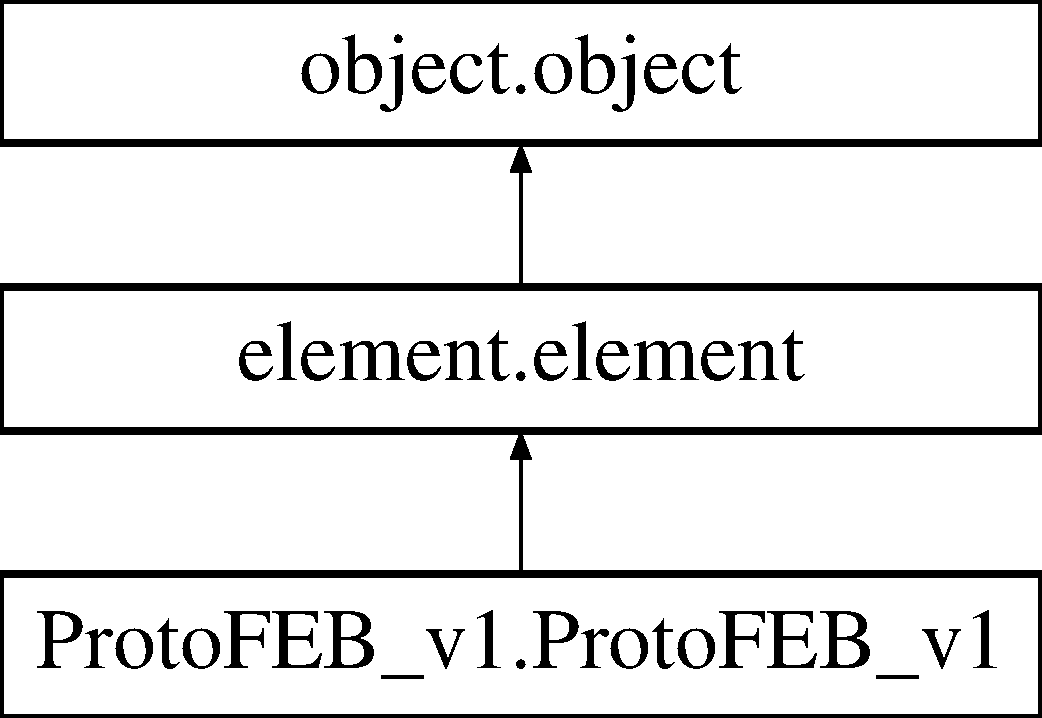
\includegraphics[height=3.000000cm]{classelement_1_1element}
\end{center}
\end{figure}
\subsection*{Public Member Functions}
\begin{DoxyCompactItemize}
\item 
def \hyperlink{classelement_1_1element_a72de0f0e7b950dabca314ed77552cb90}{\+\_\+\+\_\+init\+\_\+\+\_\+} (self, \hyperlink{classobject_1_1object_af114388a80cca208c152ffeca0e89e23}{cat}, \hyperlink{classobject_1_1object_a82b61e7cd7e18b1f9de10fc832e5b75e}{obj}, \hyperlink{classelement_1_1element_a0fce7cee12f437717c882d0965e46235}{panel}, \hyperlink{classobject_1_1object_a2a518f960961d791b0f900a90c3cd287}{path})
\item 
def \hyperlink{classelement_1_1element_a2705e2b608db596bedf2a206bda42d12}{parent} (self)
\item 
def \hyperlink{classelement_1_1element_aa9fadd76b299e1dfddd1da112dfe8245}{loadxrc} (self)
\item 
def \hyperlink{classelement_1_1element_a80c5e09b291c255b740787b87760fca0}{page} (self)
\end{DoxyCompactItemize}
\subsection*{Public Attributes}
\begin{DoxyCompactItemize}
\item 
\hyperlink{classelement_1_1element_a0fce7cee12f437717c882d0965e46235}{panel}
\end{DoxyCompactItemize}


\subsection{Detailed Description}


Definition at line 7 of file element.\+py.



\subsection{Constructor \& Destructor Documentation}
\mbox{\Hypertarget{classelement_1_1element_a72de0f0e7b950dabca314ed77552cb90}\label{classelement_1_1element_a72de0f0e7b950dabca314ed77552cb90}} 
\index{element\+::element@{element\+::element}!\+\_\+\+\_\+init\+\_\+\+\_\+@{\+\_\+\+\_\+init\+\_\+\+\_\+}}
\index{\+\_\+\+\_\+init\+\_\+\+\_\+@{\+\_\+\+\_\+init\+\_\+\+\_\+}!element\+::element@{element\+::element}}
\subsubsection{\texorpdfstring{\+\_\+\+\_\+init\+\_\+\+\_\+()}{\_\_init\_\_()}}
{\footnotesize\ttfamily def element.\+element.\+\_\+\+\_\+init\+\_\+\+\_\+ (\begin{DoxyParamCaption}\item[{}]{self,  }\item[{}]{cat,  }\item[{}]{obj,  }\item[{}]{panel,  }\item[{}]{path }\end{DoxyParamCaption})}



Definition at line 8 of file element.\+py.


\begin{DoxyCode}
8     \textcolor{keyword}{def }\hyperlink{classwrapper_1_1ModuleDictWrapper_a9a7a794150502f51df687831583e13b9}{\_\_init\_\_}(self, cat, obj, panel, path):
9         object.\_\_init\_\_(self,cat, obj, panel, path)
10 
\end{DoxyCode}


\subsection{Member Function Documentation}
\mbox{\Hypertarget{classelement_1_1element_aa9fadd76b299e1dfddd1da112dfe8245}\label{classelement_1_1element_aa9fadd76b299e1dfddd1da112dfe8245}} 
\index{element\+::element@{element\+::element}!loadxrc@{loadxrc}}
\index{loadxrc@{loadxrc}!element\+::element@{element\+::element}}
\subsubsection{\texorpdfstring{loadxrc()}{loadxrc()}}
{\footnotesize\ttfamily def element.\+element.\+loadxrc (\begin{DoxyParamCaption}\item[{}]{self }\end{DoxyParamCaption})}



Definition at line 15 of file element.\+py.



References object.\+object.\+obj, Cfg\+Frame.\+Cfg\+Frame.\+obj, object.\+object.\+path, Log\+Frame.\+Log\+Frame.\+path, Conf\+Frame.\+Conf\+Frame.\+path, Graph\+Frame.\+Graph\+Frame.\+path, Cfg\+Frame.\+Cfg\+Frame.\+path, and App\+Frame.\+App\+Frame.\+path.



Referenced by Croc.\+Croc.\+\_\+\+\_\+init\+\_\+\+\_\+(), Computer.\+Computer.\+\_\+\+\_\+init\+\_\+\+\_\+(), Proto40\+M\+Hz\+\_\+v1.\+Proto40\+M\+Hz\+\_\+v1.\+\_\+\+\_\+init\+\_\+\+\_\+(), Proto\+F\+E\+B\+\_\+v1.\+Proto\+F\+E\+B\+\_\+v1.\+\_\+\+\_\+init\+\_\+\+\_\+(), A3\+P\+E\+\_\+\+Bit\+Flip.\+A3\+P\+E\+\_\+\+Bit\+Flip.\+\_\+\+\_\+init\+\_\+\+\_\+(), Storage\+Fifo\+Acquisition.\+Storage\+Fifo\+Acquisition.\+\_\+\+\_\+init\+\_\+\+\_\+(), Acquisition.\+Acquisition.\+\_\+\+\_\+init\+\_\+\+\_\+(), Emulate\+F\+E.\+Emulate\+F\+E.\+\_\+\+\_\+init\+\_\+\+\_\+(), Storage\+Fifo.\+Storage\+Fifo.\+\_\+\+\_\+init\+\_\+\+\_\+(), Test\+U\+S\+B.\+Test\+U\+S\+B.\+\_\+\+\_\+init\+\_\+\+\_\+(), Test\+I2\+C.\+Test\+I2\+C.\+\_\+\+\_\+init\+\_\+\+\_\+(), Test\+S\+P\+I.\+Test\+S\+P\+I.\+\_\+\+\_\+init\+\_\+\+\_\+(), Usb\+F\+T\+Interface\+Test.\+Usb\+F\+T\+Interface\+Test.\+\_\+\+\_\+init\+\_\+\+\_\+(), Test\+Suite.\+Test\+Suite.\+\_\+\+\_\+init\+\_\+\+\_\+(), A\+D\+C\+Measurement.\+Current\+Measurement.\+\_\+\+\_\+init\+\_\+\+\_\+(), and Current\+Measurement.\+Current\+Measurement.\+\_\+\+\_\+init\+\_\+\+\_\+().


\begin{DoxyCode}
15     \textcolor{keyword}{def }loadxrc(self):
16         path= os.path.join(self.path,\textcolor{stringliteral}{"element"})
17         path= os.path.join(self.path,\textcolor{stringliteral}{"xrc"})
18         path= os.path.join(path,self.obj.type())
19         path= path+\textcolor{stringliteral}{".xrc"}
20         res=xrc.XmlResource(path)
21         self.panel=res.LoadPanel(self.parent(),self.obj.type())
22             
\end{DoxyCode}
\mbox{\Hypertarget{classelement_1_1element_a80c5e09b291c255b740787b87760fca0}\label{classelement_1_1element_a80c5e09b291c255b740787b87760fca0}} 
\index{element\+::element@{element\+::element}!page@{page}}
\index{page@{page}!element\+::element@{element\+::element}}
\subsubsection{\texorpdfstring{page()}{page()}}
{\footnotesize\ttfamily def element.\+element.\+page (\begin{DoxyParamCaption}\item[{}]{self }\end{DoxyParamCaption})}



Definition at line 23 of file element.\+py.



References element.\+element.\+panel, Conf\+Frame.\+Conf\+Frame.\+panel, and App\+Frame.\+App\+Frame.\+panel.


\begin{DoxyCode}
23     \textcolor{keyword}{def }page(self):
24         \textcolor{keywordflow}{return} self.panel
25 \textcolor{comment}{#----------------------------------------------------------------------}
26 
27     
28 \end{DoxyCode}
\mbox{\Hypertarget{classelement_1_1element_a2705e2b608db596bedf2a206bda42d12}\label{classelement_1_1element_a2705e2b608db596bedf2a206bda42d12}} 
\index{element\+::element@{element\+::element}!parent@{parent}}
\index{parent@{parent}!element\+::element@{element\+::element}}
\subsubsection{\texorpdfstring{parent()}{parent()}}
{\footnotesize\ttfamily def element.\+element.\+parent (\begin{DoxyParamCaption}\item[{}]{self }\end{DoxyParamCaption})}



Definition at line 11 of file element.\+py.



References object.\+object.\+get\+Control(), Conf\+Frame.\+Conf\+Frame.\+get\+Control(), Graph\+Frame.\+Graph\+Frame.\+get\+Control(), Cfg\+Frame.\+Cfg\+Frame.\+get\+Control(), and App\+Frame.\+App\+Frame.\+get\+Control().


\begin{DoxyCode}
11     \textcolor{keyword}{def }parent(self):
12 \textcolor{comment}{#        return self.getControl("Element")}
13         \textcolor{keywordflow}{return} self.getControl(\textcolor{stringliteral}{"control"})
14    
\end{DoxyCode}


\subsection{Member Data Documentation}
\mbox{\Hypertarget{classelement_1_1element_a0fce7cee12f437717c882d0965e46235}\label{classelement_1_1element_a0fce7cee12f437717c882d0965e46235}} 
\index{element\+::element@{element\+::element}!panel@{panel}}
\index{panel@{panel}!element\+::element@{element\+::element}}
\subsubsection{\texorpdfstring{panel}{panel}}
{\footnotesize\ttfamily element.\+element.\+panel}



Definition at line 21 of file element.\+py.



Referenced by A3\+P\+E\+\_\+\+Bit\+Flip.\+A3\+P\+E\+\_\+\+Bit\+Flip.\+\_\+\+\_\+init\+\_\+\+\_\+(), Acquisition.\+Acquisition.\+\_\+\+\_\+init\+\_\+\+\_\+(), Emulate\+F\+E.\+Emulate\+F\+E.\+\_\+\+\_\+init\+\_\+\+\_\+(), object.\+object.\+get\+Control(), Proto40\+M\+Hz\+\_\+v1.\+Proto40\+M\+Hz\+\_\+v1.\+get\+File(), Proto\+F\+E\+B\+\_\+v1.\+Proto\+F\+E\+B\+\_\+v1.\+get\+File(), element.\+element.\+page(), and proc.\+proc.\+page().



The documentation for this class was generated from the following file\+:\begin{DoxyCompactItemize}
\item 
/home/eleclhcb/\+L\+H\+Cb/lbcat-\/cmake/\+Cat\+Python/python/\hyperlink{element_8py}{element.\+py}\end{DoxyCompactItemize}

\hypertarget{structElementWrap}{}\section{Element\+Wrap Struct Reference}
\label{structElementWrap}\index{Element\+Wrap@{Element\+Wrap}}
Inheritance diagram for Element\+Wrap\+:\begin{figure}[H]
\begin{center}
\leavevmode
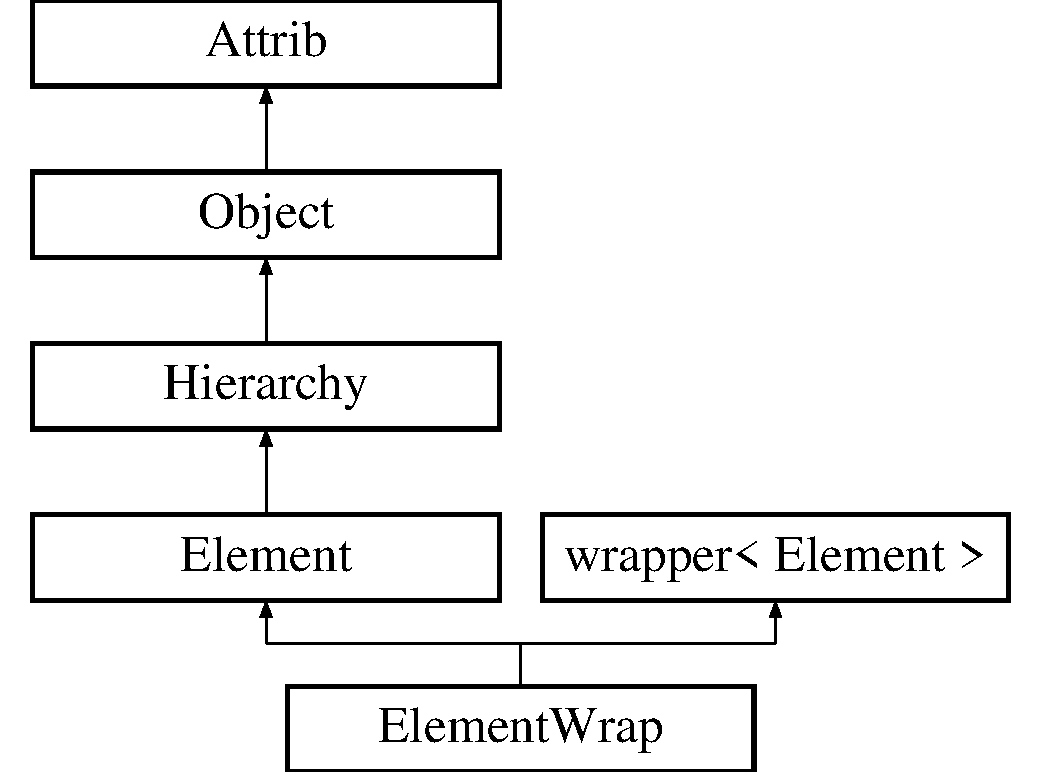
\includegraphics[height=5.000000cm]{structElementWrap}
\end{center}
\end{figure}
\subsection*{Public Types}
\begin{DoxyCompactItemize}
\item 
enum \hyperlink{classAttrib_a69e171d7cc6417835a5a306d3c764235}{Attribut} \{ \newline
\hyperlink{classAttrib_a69e171d7cc6417835a5a306d3c764235a3a8da2ab97dda18aebab196fe4100531}{U\+N\+D\+E\+F\+I\+N\+ED}, 
\hyperlink{classAttrib_a69e171d7cc6417835a5a306d3c764235a2bfb2af57b87031d190a05fe25dd92ed}{P\+A\+S\+S\+I\+VE}, 
\hyperlink{classAttrib_a69e171d7cc6417835a5a306d3c764235a3b1fec929c0370d1436f2f06e298fb0d}{A\+C\+T\+I\+VE}, 
\hyperlink{classAttrib_a69e171d7cc6417835a5a306d3c764235aa27c16b480a369ea4d18b07b2516bbc7}{I\+N\+T\+E\+R\+F\+A\+CE}, 
\newline
\hyperlink{classAttrib_a69e171d7cc6417835a5a306d3c764235a1420a5b8c0540b2af210b6975eded7f9}{IO}, 
\hyperlink{classAttrib_a69e171d7cc6417835a5a306d3c764235a0af3b0d0ac323c1704e6c69cf90add28}{I\+O\+D\+A\+TA}, 
\hyperlink{classAttrib_a69e171d7cc6417835a5a306d3c764235a7788bc5dd333fd8ce18562b269c9dab1}{E\+L\+E\+M\+E\+NT}, 
\hyperlink{classAttrib_a69e171d7cc6417835a5a306d3c764235a61ceb22149f365f1780d18f9d1459423}{H\+A\+R\+D\+W\+A\+RE}, 
\newline
\hyperlink{classAttrib_a69e171d7cc6417835a5a306d3c764235a75250e29692496e73effca2c0330977f}{P\+R\+O\+C\+E\+S\+S\+US}, 
\hyperlink{classAttrib_a69e171d7cc6417835a5a306d3c764235a103a67cd0b8f07ef478fa45d4356e27b}{S\+O\+F\+T\+W\+A\+RE}
 \}
\end{DoxyCompactItemize}
\subsection*{Public Member Functions}
\begin{DoxyCompactItemize}
\item 
void \hyperlink{structElementWrap_ad22ed533c2dad73f8650243d8060b547}{help} ()
\item 
\hyperlink{classStatusCode}{Status\+Code} \hyperlink{structElementWrap_a5e0ca7bd04cfb1f7582fc80c065fd376}{init} ()
\item 
void \hyperlink{structElementWrap_a69a4588be73b8c85ddb92b13f74c3a12}{reset} ()
\item 
void \hyperlink{structElementWrap_a13d2d2771d1dd305abf3457f98482cbe}{update} ()
\item 
void \hyperlink{classElement_a3c0abcb36f8906688bb7e32608df7086}{recursive\+Init\+Element} ()
\item 
void \hyperlink{classElement_a82119ed37dff76508a2746a853ec35ba}{recursive\+Init\+Communications} ()
\item 
\hyperlink{classStatusCode}{Status\+Code} \hyperlink{classElement_ab476b4b1df5954141ceb14f072433b89}{set\+Connection} (\hyperlink{classHierarchy}{Hierarchy} $\ast$)
\item 
\hyperlink{classHierarchy}{Hierarchy} $\ast$ \hyperlink{classElement_af57444353c1ddf9fa0109801e97debf7}{connection} ()
\item 
void \hyperlink{classHierarchy_af4d43b0765b402670eed2d62c73405af}{clear} ()
\item 
void \hyperlink{classHierarchy_a585ad1aeec16077a0e532ab8b4fc557b}{set\+Parent} (\hyperlink{classHierarchy}{Hierarchy} $\ast$\hyperlink{classHierarchy_a1c7bec8257e717f9c1465e06ebf845fc}{parent})
\item 
\hyperlink{classHierarchy}{Hierarchy} $\ast$ \hyperlink{classHierarchy_a1c7bec8257e717f9c1465e06ebf845fc}{parent} ()
\item 
\hyperlink{classHierarchy}{Hierarchy} $\ast$ \hyperlink{classHierarchy_ad550588733bf75ac5c0fcfd7c8fd11a6}{parent} (std\+::string)
\item 
\hyperlink{classHierarchy}{Hierarchy} $\ast$ \hyperlink{classHierarchy_aee461dc930ce3871636ff87f075b1b83}{origin} ()
\item 
virtual void \hyperlink{classHierarchy_ad677774ff38fcb257c04a3a10d471fac}{add\+Child} (\hyperlink{classHierarchy}{Hierarchy} $\ast$element)
\item 
std\+::vector$<$ \hyperlink{classHierarchy}{Hierarchy} $\ast$ $>$ \hyperlink{classHierarchy_aa9a76f69e98e052ee1a6e32cea006288}{children} ()
\item 
\hyperlink{classHierarchy}{Hierarchy} $\ast$ \hyperlink{classHierarchy_a1e207f973c694b538bf90107b4868817}{child} (std\+::string)
\item 
\hyperlink{classHierarchy}{Hierarchy} $\ast$ \hyperlink{classHierarchy_a0c15a5276a3b80b4354d6bd8a01e0708}{child\+Typed} (std\+::string)
\item 
unsigned long \hyperlink{classHierarchy_ab16e84de65fd84e14001a6cf941c8be4}{number\+Of\+Children} ()
\item 
bool \hyperlink{classHierarchy_a255174fe4d316d2a3f430dcb9dab29f1}{has\+Children} ()
\item 
void \hyperlink{classHierarchy_a2b2b359fac003233f65786a616766bde}{del\+Child} (\hyperlink{classHierarchy}{Hierarchy} $\ast$)
\item 
void \hyperlink{classHierarchy_a1928ac7615fe0b5e55cd707f70dc6781}{del\+Child} (std\+::string)
\item 
std\+::string \hyperlink{classHierarchy_aa7990fa7caf132d83e361ce033c6c65a}{path} (std\+::string=std\+::string(\char`\"{}\char`\"{}))
\item 
std\+::string \hyperlink{classHierarchy_a1efd56cd164d328d2002e53a10a19b8c}{path\+Typed} (std\+::string=std\+::string(\char`\"{}\char`\"{}))
\item 
void \hyperlink{classHierarchy_a76e914b9a677a22a82deb74d892bf261}{tree} (std\+::string indent=std\+::string(\char`\"{}\char`\"{}))
\item 
void \hyperlink{classHierarchy_a594c294c5f60c230e106d522ed008212}{tree} ()
\item 
std\+::string \hyperlink{classObject_a300f4c05dd468c7bb8b3c968868443c1}{name} () const
\item 
std\+::string \hyperlink{classObject_a84f99f70f144a83e1582d1d0f84e4e62}{type} ()
\item 
unsigned char \hyperlink{classObject_af99145335cc61ff6e2798ea17db009d2}{id} ()
\item 
std\+::string \hyperlink{classObject_a73a0f1a41828fdd8303dd662446fb6c3}{title} ()
\item 
void \hyperlink{classObject_a3f9d5537ebce0c0f2bf6ae4d92426f3c}{msg\+Svc} (int level, std\+::string \hyperlink{classObject_a58b2d0618c2d08cf2383012611528d97}{msg}, std\+::string \hyperlink{classObject_a300f4c05dd468c7bb8b3c968868443c1}{name})
\item 
void \hyperlink{classObject_a58b2d0618c2d08cf2383012611528d97}{msg} (std\+::string mymsg)
\item 
void \hyperlink{classObject_ac5d59299273cee27aacf7de00d2e7034}{msg} (std\+::string mymsg, std\+::string \hyperlink{classObject_a300f4c05dd468c7bb8b3c968868443c1}{name})
\item 
void \hyperlink{classObject_a83d2db2df682907ea1115ad721c1c4a1}{verbose} (std\+::string mymsg)
\item 
void \hyperlink{classObject_a2d4120195317e2a3c6532e8bb9f3da68}{verbose} (std\+::string mymsg, std\+::string \hyperlink{classObject_a300f4c05dd468c7bb8b3c968868443c1}{name})
\item 
void \hyperlink{classObject_aac010553f022165573714b7014a15f0d}{debug} (std\+::string mymsg)
\item 
void \hyperlink{classObject_a6c9a0397ca804e04d675ed05683f5420}{debug} (std\+::string mymsg, std\+::string \hyperlink{classObject_a300f4c05dd468c7bb8b3c968868443c1}{name})
\item 
void \hyperlink{classObject_a644fd329ea4cb85f54fa6846484b84a8}{info} (std\+::string mymsg)
\item 
void \hyperlink{classObject_a1ca123253dfd30fc28b156f521dcbdae}{info} (std\+::string mymsg, std\+::string \hyperlink{classObject_a300f4c05dd468c7bb8b3c968868443c1}{name})
\item 
void \hyperlink{classObject_a65cd4fda577711660821fd2cd5a3b4c9}{warning} (std\+::string mymsg)
\item 
void \hyperlink{classObject_a11f101db4dd73d9391b0231818881d86}{warning} (std\+::string mymsg, std\+::string \hyperlink{classObject_a300f4c05dd468c7bb8b3c968868443c1}{name})
\item 
void \hyperlink{classObject_a204a95f57818c0f811933917a30eff45}{error} (std\+::string mymsg)
\item 
void \hyperlink{classObject_ad7f6c457733082efa2f9ff5f5c8e119a}{error} (std\+::string mymsg, std\+::string \hyperlink{classObject_a300f4c05dd468c7bb8b3c968868443c1}{name})
\item 
void \hyperlink{classObject_aad5a16aac7516ce65bd5ec02ab07fc80}{fatal} (std\+::string mymsg)
\item 
void \hyperlink{classObject_ae62acd3d09f716220f75f252dc38bc9a}{fatal} (std\+::string mymsg, std\+::string \hyperlink{classObject_a300f4c05dd468c7bb8b3c968868443c1}{name})
\item 
void \hyperlink{classObject_ae30fea75683c2d149b6b6d17c09ecd0c}{set\+Name} (std\+::string \hyperlink{classObject_a300f4c05dd468c7bb8b3c968868443c1}{name})
\item 
void \hyperlink{classObject_aae534cc9d982bcb9b99fd505f2e103a5}{set\+Type} (std\+::string \hyperlink{classObject_a84f99f70f144a83e1582d1d0f84e4e62}{type})
\item 
void \hyperlink{classObject_a398fe08cba594a0ce6891d59fe4f159f}{set\+Id} (unsigned char \hyperlink{classObject_af99145335cc61ff6e2798ea17db009d2}{id})
\item 
void \hyperlink{classObject_a89557dbbad5bcaa02652f5d7fa35d20f}{set\+Title} (std\+::string \hyperlink{classObject_a73a0f1a41828fdd8303dd662446fb6c3}{title})
\item 
void \hyperlink{classObject_a870c5af919958c2136623b2d7816d123}{set\+Dll\+Name} (std\+::string \hyperlink{classObject_a2e3947f2870094c332d7454117f3ec63}{dll\+Name})
\item 
std\+::string \hyperlink{classObject_a2e3947f2870094c332d7454117f3ec63}{dll\+Name} ()
\item 
bool \hyperlink{classAttrib_a704f26af560909ad22065083bb7d4c34}{is} (int attribut)
\item 
void \hyperlink{classAttrib_a235f773af19c900264a190b00a3b4ad7}{add} (int attribut)
\item 
void \hyperlink{classAttrib_a7d4ef7e32d93cb287792b87b857e79f3}{remove} (int attribut)
\item 
std\+::string \hyperlink{classAttrib_aee7bbf16b144887f196e1341b24f8a26}{attributs} ()
\end{DoxyCompactItemize}
\subsection*{Protected Attributes}
\begin{DoxyCompactItemize}
\item 
\hyperlink{classHierarchy}{Hierarchy} $\ast$ \hyperlink{classElement_abe3de7a5dbbc9a6dd2d7e012e5fdb266}{m\+\_\+connection}
\item 
std\+::string \hyperlink{classAttrib_a3414521d7a82476e874b25a5407b5e63}{m\+\_\+attrib\+String} \mbox{[}10\mbox{]}
\end{DoxyCompactItemize}


\subsection{Detailed Description}


Definition at line 19 of file Python\+\_\+\+Obj.\+cpp.



\subsection{Member Enumeration Documentation}
\mbox{\Hypertarget{classAttrib_a69e171d7cc6417835a5a306d3c764235}\label{classAttrib_a69e171d7cc6417835a5a306d3c764235}} 
\index{Element\+Wrap@{Element\+Wrap}!Attribut@{Attribut}}
\index{Attribut@{Attribut}!Element\+Wrap@{Element\+Wrap}}
\subsubsection{\texorpdfstring{Attribut}{Attribut}}
{\footnotesize\ttfamily enum \hyperlink{classAttrib_a69e171d7cc6417835a5a306d3c764235}{Attrib\+::\+Attribut}\hspace{0.3cm}{\ttfamily [inherited]}}

\begin{DoxyEnumFields}{Enumerator}
\raisebox{\heightof{T}}[0pt][0pt]{\index{U\+N\+D\+E\+F\+I\+N\+ED@{U\+N\+D\+E\+F\+I\+N\+ED}!Element\+Wrap@{Element\+Wrap}}\index{Element\+Wrap@{Element\+Wrap}!U\+N\+D\+E\+F\+I\+N\+ED@{U\+N\+D\+E\+F\+I\+N\+ED}}}\mbox{\Hypertarget{classAttrib_a69e171d7cc6417835a5a306d3c764235a3a8da2ab97dda18aebab196fe4100531}\label{classAttrib_a69e171d7cc6417835a5a306d3c764235a3a8da2ab97dda18aebab196fe4100531}} 
U\+N\+D\+E\+F\+I\+N\+ED&\\
\hline

\raisebox{\heightof{T}}[0pt][0pt]{\index{P\+A\+S\+S\+I\+VE@{P\+A\+S\+S\+I\+VE}!Element\+Wrap@{Element\+Wrap}}\index{Element\+Wrap@{Element\+Wrap}!P\+A\+S\+S\+I\+VE@{P\+A\+S\+S\+I\+VE}}}\mbox{\Hypertarget{classAttrib_a69e171d7cc6417835a5a306d3c764235a2bfb2af57b87031d190a05fe25dd92ed}\label{classAttrib_a69e171d7cc6417835a5a306d3c764235a2bfb2af57b87031d190a05fe25dd92ed}} 
P\+A\+S\+S\+I\+VE&\\
\hline

\raisebox{\heightof{T}}[0pt][0pt]{\index{A\+C\+T\+I\+VE@{A\+C\+T\+I\+VE}!Element\+Wrap@{Element\+Wrap}}\index{Element\+Wrap@{Element\+Wrap}!A\+C\+T\+I\+VE@{A\+C\+T\+I\+VE}}}\mbox{\Hypertarget{classAttrib_a69e171d7cc6417835a5a306d3c764235a3b1fec929c0370d1436f2f06e298fb0d}\label{classAttrib_a69e171d7cc6417835a5a306d3c764235a3b1fec929c0370d1436f2f06e298fb0d}} 
A\+C\+T\+I\+VE&\\
\hline

\raisebox{\heightof{T}}[0pt][0pt]{\index{I\+N\+T\+E\+R\+F\+A\+CE@{I\+N\+T\+E\+R\+F\+A\+CE}!Element\+Wrap@{Element\+Wrap}}\index{Element\+Wrap@{Element\+Wrap}!I\+N\+T\+E\+R\+F\+A\+CE@{I\+N\+T\+E\+R\+F\+A\+CE}}}\mbox{\Hypertarget{classAttrib_a69e171d7cc6417835a5a306d3c764235aa27c16b480a369ea4d18b07b2516bbc7}\label{classAttrib_a69e171d7cc6417835a5a306d3c764235aa27c16b480a369ea4d18b07b2516bbc7}} 
I\+N\+T\+E\+R\+F\+A\+CE&\\
\hline

\raisebox{\heightof{T}}[0pt][0pt]{\index{IO@{IO}!Element\+Wrap@{Element\+Wrap}}\index{Element\+Wrap@{Element\+Wrap}!IO@{IO}}}\mbox{\Hypertarget{classAttrib_a69e171d7cc6417835a5a306d3c764235a1420a5b8c0540b2af210b6975eded7f9}\label{classAttrib_a69e171d7cc6417835a5a306d3c764235a1420a5b8c0540b2af210b6975eded7f9}} 
IO&\\
\hline

\raisebox{\heightof{T}}[0pt][0pt]{\index{I\+O\+D\+A\+TA@{I\+O\+D\+A\+TA}!Element\+Wrap@{Element\+Wrap}}\index{Element\+Wrap@{Element\+Wrap}!I\+O\+D\+A\+TA@{I\+O\+D\+A\+TA}}}\mbox{\Hypertarget{classAttrib_a69e171d7cc6417835a5a306d3c764235a0af3b0d0ac323c1704e6c69cf90add28}\label{classAttrib_a69e171d7cc6417835a5a306d3c764235a0af3b0d0ac323c1704e6c69cf90add28}} 
I\+O\+D\+A\+TA&\\
\hline

\raisebox{\heightof{T}}[0pt][0pt]{\index{E\+L\+E\+M\+E\+NT@{E\+L\+E\+M\+E\+NT}!Element\+Wrap@{Element\+Wrap}}\index{Element\+Wrap@{Element\+Wrap}!E\+L\+E\+M\+E\+NT@{E\+L\+E\+M\+E\+NT}}}\mbox{\Hypertarget{classAttrib_a69e171d7cc6417835a5a306d3c764235a7788bc5dd333fd8ce18562b269c9dab1}\label{classAttrib_a69e171d7cc6417835a5a306d3c764235a7788bc5dd333fd8ce18562b269c9dab1}} 
E\+L\+E\+M\+E\+NT&\\
\hline

\raisebox{\heightof{T}}[0pt][0pt]{\index{H\+A\+R\+D\+W\+A\+RE@{H\+A\+R\+D\+W\+A\+RE}!Element\+Wrap@{Element\+Wrap}}\index{Element\+Wrap@{Element\+Wrap}!H\+A\+R\+D\+W\+A\+RE@{H\+A\+R\+D\+W\+A\+RE}}}\mbox{\Hypertarget{classAttrib_a69e171d7cc6417835a5a306d3c764235a61ceb22149f365f1780d18f9d1459423}\label{classAttrib_a69e171d7cc6417835a5a306d3c764235a61ceb22149f365f1780d18f9d1459423}} 
H\+A\+R\+D\+W\+A\+RE&\\
\hline

\raisebox{\heightof{T}}[0pt][0pt]{\index{P\+R\+O\+C\+E\+S\+S\+US@{P\+R\+O\+C\+E\+S\+S\+US}!Element\+Wrap@{Element\+Wrap}}\index{Element\+Wrap@{Element\+Wrap}!P\+R\+O\+C\+E\+S\+S\+US@{P\+R\+O\+C\+E\+S\+S\+US}}}\mbox{\Hypertarget{classAttrib_a69e171d7cc6417835a5a306d3c764235a75250e29692496e73effca2c0330977f}\label{classAttrib_a69e171d7cc6417835a5a306d3c764235a75250e29692496e73effca2c0330977f}} 
P\+R\+O\+C\+E\+S\+S\+US&\\
\hline

\raisebox{\heightof{T}}[0pt][0pt]{\index{S\+O\+F\+T\+W\+A\+RE@{S\+O\+F\+T\+W\+A\+RE}!Element\+Wrap@{Element\+Wrap}}\index{Element\+Wrap@{Element\+Wrap}!S\+O\+F\+T\+W\+A\+RE@{S\+O\+F\+T\+W\+A\+RE}}}\mbox{\Hypertarget{classAttrib_a69e171d7cc6417835a5a306d3c764235a103a67cd0b8f07ef478fa45d4356e27b}\label{classAttrib_a69e171d7cc6417835a5a306d3c764235a103a67cd0b8f07ef478fa45d4356e27b}} 
S\+O\+F\+T\+W\+A\+RE&\\
\hline

\end{DoxyEnumFields}


Definition at line 29 of file Attrib.\+h.


\begin{DoxyCode}
29                 \{
30     \hyperlink{classAttrib_a69e171d7cc6417835a5a306d3c764235a3a8da2ab97dda18aebab196fe4100531}{UNDEFINED},
31     \hyperlink{classAttrib_a69e171d7cc6417835a5a306d3c764235a2bfb2af57b87031d190a05fe25dd92ed}{PASSIVE},
32     \hyperlink{classAttrib_a69e171d7cc6417835a5a306d3c764235a3b1fec929c0370d1436f2f06e298fb0d}{ACTIVE},
33     \hyperlink{classAttrib_a69e171d7cc6417835a5a306d3c764235aa27c16b480a369ea4d18b07b2516bbc7}{INTERFACE},
34     \hyperlink{classAttrib_a69e171d7cc6417835a5a306d3c764235a1420a5b8c0540b2af210b6975eded7f9}{IO},
35     \hyperlink{classAttrib_a69e171d7cc6417835a5a306d3c764235a0af3b0d0ac323c1704e6c69cf90add28}{IODATA},
36     \hyperlink{classAttrib_a69e171d7cc6417835a5a306d3c764235a7788bc5dd333fd8ce18562b269c9dab1}{ELEMENT},
37     \hyperlink{classAttrib_a69e171d7cc6417835a5a306d3c764235a61ceb22149f365f1780d18f9d1459423}{HARDWARE},
38     \hyperlink{classAttrib_a69e171d7cc6417835a5a306d3c764235a75250e29692496e73effca2c0330977f}{PROCESSUS},
39     \hyperlink{classAttrib_a69e171d7cc6417835a5a306d3c764235a103a67cd0b8f07ef478fa45d4356e27b}{SOFTWARE} 
40   \}; \textcolor{comment}{// array m\_attribString must be changed into Attrib::Attrib if this enu is modified. }
\end{DoxyCode}


\subsection{Member Function Documentation}
\mbox{\Hypertarget{classAttrib_a235f773af19c900264a190b00a3b4ad7}\label{classAttrib_a235f773af19c900264a190b00a3b4ad7}} 
\index{Element\+Wrap@{Element\+Wrap}!add@{add}}
\index{add@{add}!Element\+Wrap@{Element\+Wrap}}
\subsubsection{\texorpdfstring{add()}{add()}}
{\footnotesize\ttfamily void Attrib\+::add (\begin{DoxyParamCaption}\item[{int}]{attribut }\end{DoxyParamCaption})\hspace{0.3cm}{\ttfamily [inline]}, {\ttfamily [inherited]}}

Add an attribut 

Definition at line 67 of file Attrib.\+h.



References Attrib\+::m\+\_\+attributs, and Attrib\+::\+U\+N\+D\+E\+F\+I\+N\+ED.



Referenced by A3\+P\+E\+::\+A3\+P\+E(), Attrib\+::\+Attrib(), Specs\+Mezzanine\+::cmdline(), Computer\+::\+Computer(), C\+U\+\_\+v1\+::\+C\+U\+\_\+v1(), export\+\_\+obj(), F\+E\+B\+\_\+v1\+::\+F\+E\+B\+\_\+v1(), Fe\+P\+G\+A\+::\+Fe\+P\+G\+A(), I\+C\+E\+C\+A\+Lv3\+::\+I\+C\+E\+C\+A\+Lv3(), I\+C\+Phaser\+::\+I\+C\+Phaser(), Application\+::initialize(), Interface\+::\+Interface(), I\+Odata\+::\+I\+Odata(), I\+Oobject\+::\+I\+Oobject(), M\+S\+Oxxxx\+::\+M\+S\+Oxxxx(), Phaser\+::\+Phaser(), Processus\+::\+Processus(), Proto40\+M\+Hz\+\_\+v1\+::\+Proto40\+M\+Hz\+\_\+v1(), Attrib\+::remove(), Seq\+P\+G\+A\+::\+Seq\+P\+G\+A(), Test\+S\+P\+I\+::set\+Address(), Test\+I2\+C\+::set\+Address(), Specs\+Slave\+::set\+Address(), Specs\+Master\+::\+Specs\+Master(), and Specs\+Slave\+::\+Specs\+Slave().


\begin{DoxyCode}
67                             \{
68     \textcolor{keywordflow}{if} (attribut!=\hyperlink{classAttrib_a69e171d7cc6417835a5a306d3c764235a3a8da2ab97dda18aebab196fe4100531}{Attrib::UNDEFINED}) \textcolor{keyword}{remove}(\hyperlink{classAttrib_a69e171d7cc6417835a5a306d3c764235a3a8da2ab97dda18aebab196fe4100531}{Attrib::UNDEFINED});
69     \textcolor{keywordtype}{bool} duplicate = false ;
70     std::vector<int>::const\_iterator iter ;
71     \textcolor{keywordflow}{for} ( iter  = \hyperlink{classAttrib_ac4bd58a0cc6b38a3b711d609a3d3aacc}{m\_attributs}.begin() ;
72           iter != \hyperlink{classAttrib_ac4bd58a0cc6b38a3b711d609a3d3aacc}{m\_attributs}.end()   ;
73           ++iter ) \{
74       \textcolor{keywordflow}{if} ( attribut == (*iter) ) \{
75         duplicate = true ;
76       \}
77     \}
78     \textcolor{keywordflow}{if} (!duplicate) \{
79       \hyperlink{classAttrib_ac4bd58a0cc6b38a3b711d609a3d3aacc}{m\_attributs}.push\_back( attribut );
80     \}
81   \}
\end{DoxyCode}
\mbox{\Hypertarget{classHierarchy_ad677774ff38fcb257c04a3a10d471fac}\label{classHierarchy_ad677774ff38fcb257c04a3a10d471fac}} 
\index{Element\+Wrap@{Element\+Wrap}!add\+Child@{add\+Child}}
\index{add\+Child@{add\+Child}!Element\+Wrap@{Element\+Wrap}}
\subsubsection{\texorpdfstring{add\+Child()}{addChild()}}
{\footnotesize\ttfamily void Hierarchy\+::add\+Child (\begin{DoxyParamCaption}\item[{\hyperlink{classHierarchy}{Hierarchy} $\ast$}]{element }\end{DoxyParamCaption})\hspace{0.3cm}{\ttfamily [virtual]}, {\ttfamily [inherited]}}



Definition at line 83 of file Hierarchy.\+cpp.



References Object\+::debug(), Hierarchy\+::m\+\_\+children, Object\+::name(), and Hierarchy\+::set\+Parent().



Referenced by A3\+P\+E\+::\+A3\+P\+E(), Specs\+Mezzanine\+::add\+Bus(), Specs\+Slave\+::add\+I2c(), Application\+::create(), C\+U\+\_\+v1\+::\+C\+U\+\_\+v1(), export\+\_\+obj(), F\+E\+B\+\_\+v1\+::\+F\+E\+B\+\_\+v1(), Fe\+P\+G\+A\+::\+Fe\+P\+G\+A(), I\+C\+E\+C\+A\+Lv3\+::\+I\+C\+E\+C\+A\+Lv3(), I\+C\+Phaser\+::\+I\+C\+Phaser(), Hierarchy\+::origin(), Phaser\+::\+Phaser(), Proto40\+M\+Hz\+\_\+v1\+::\+Proto40\+M\+Hz\+\_\+v1(), Seq\+P\+G\+A\+::\+Seq\+P\+G\+A(), Specs\+Mezzanine\+::\+Specs\+Mezzanine(), Usb\+I2c\+Bus\+::\+Usb\+I2c\+Bus(), and Usb\+Spi\+Bus\+::\+Usb\+Spi\+Bus().


\begin{DoxyCode}
83                                           \{
84   element->\hyperlink{classHierarchy_a585ad1aeec16077a0e532ab8b4fc557b}{setParent}(\textcolor{keyword}{this});
85   \hyperlink{classHierarchy_a038816763941fd4a930504917f60483b}{m\_children}.push\_back(element);
86   \hyperlink{classObject_aac010553f022165573714b7014a15f0d}{debug}(element->\hyperlink{classObject_a300f4c05dd468c7bb8b3c968868443c1}{name}()+\textcolor{stringliteral}{" added to the child tree."},\textcolor{stringliteral}{"Hierarchy::addChild"});
87 \}
\end{DoxyCode}
\mbox{\Hypertarget{classAttrib_aee7bbf16b144887f196e1341b24f8a26}\label{classAttrib_aee7bbf16b144887f196e1341b24f8a26}} 
\index{Element\+Wrap@{Element\+Wrap}!attributs@{attributs}}
\index{attributs@{attributs}!Element\+Wrap@{Element\+Wrap}}
\subsubsection{\texorpdfstring{attributs()}{attributs()}}
{\footnotesize\ttfamily std\+::string Attrib\+::attributs (\begin{DoxyParamCaption}{ }\end{DoxyParamCaption})\hspace{0.3cm}{\ttfamily [inherited]}}

Print the \hyperlink{classAttrib}{Attrib} of an \hyperlink{classObject}{Object} 

Definition at line 54 of file Attrib.\+cpp.



References images\+::index, Attrib\+::m\+\_\+attrib\+String, and Attrib\+::m\+\_\+attributs.



Referenced by export\+\_\+obj(), and Attrib\+::remove().


\begin{DoxyCode}
54                             \{
55   std::string output;
56   std::vector<int>::iterator iter ;
57   \textcolor{keywordflow}{for} ( \textcolor{keywordtype}{unsigned} \textcolor{keywordtype}{int} \hyperlink{namespaceimages_a54407fd574970b3178647ae096321a57}{index} = 0 ; \hyperlink{namespaceimages_a54407fd574970b3178647ae096321a57}{index} < \hyperlink{classAttrib_ac4bd58a0cc6b38a3b711d609a3d3aacc}{m\_attributs}.size() ; ++
      \hyperlink{namespaceimages_a54407fd574970b3178647ae096321a57}{index} ) \{
58     \textcolor{keywordflow}{if} ( \hyperlink{classAttrib_ac4bd58a0cc6b38a3b711d609a3d3aacc}{m\_attributs}.size() - \hyperlink{namespaceimages_a54407fd574970b3178647ae096321a57}{index} > 1 ) \{
59       output.append(\hyperlink{classAttrib_a3414521d7a82476e874b25a5407b5e63}{m\_attribString}[\hyperlink{classAttrib_ac4bd58a0cc6b38a3b711d609a3d3aacc}{m\_attributs}[\hyperlink{namespaceimages_a54407fd574970b3178647ae096321a57}{index}]]);
60       output.append(\textcolor{stringliteral}{":"});
61     \}
62     \textcolor{keywordflow}{else} \{
63       output.append(\hyperlink{classAttrib_a3414521d7a82476e874b25a5407b5e63}{m\_attribString}[\hyperlink{classAttrib_ac4bd58a0cc6b38a3b711d609a3d3aacc}{m\_attributs}[index]]);
64     \}
65   \}
66   \textcolor{keywordflow}{return} output;
67 \}
\end{DoxyCode}
\mbox{\Hypertarget{classHierarchy_a1e207f973c694b538bf90107b4868817}\label{classHierarchy_a1e207f973c694b538bf90107b4868817}} 
\index{Element\+Wrap@{Element\+Wrap}!child@{child}}
\index{child@{child}!Element\+Wrap@{Element\+Wrap}}
\subsubsection{\texorpdfstring{child()}{child()}}
{\footnotesize\ttfamily \hyperlink{classHierarchy}{Hierarchy} $\ast$ Hierarchy\+::child (\begin{DoxyParamCaption}\item[{std\+::string}]{path }\end{DoxyParamCaption})\hspace{0.3cm}{\ttfamily [inherited]}}



Definition at line 133 of file Hierarchy.\+cpp.



References Hierarchy\+::child(), Hierarchy\+::children(), Object\+::name(), Hierarchy\+::origin(), Hierarchy\+::parent(), Hierarchy\+::path(), and Object\+::warning().



Referenced by Application\+::cd(), Hierarchy\+::child(), Hierarchy\+::children(), and export\+\_\+obj().


\begin{DoxyCode}
133                                          \{
134   std::string newpath = \hyperlink{classHierarchy_aa7990fa7caf132d83e361ce033c6c65a}{path};
135   std::string up(\textcolor{stringliteral}{".."});
136   std::string separator(1,\textcolor{charliteral}{'/'});
137 
138   \hyperlink{classHierarchy}{Hierarchy} * newcurrent = 0;
139 
140   \textcolor{comment}{//  info("path="+path,"Hierarchy::child");}
141 
142   \textcolor{keywordflow}{if} (\hyperlink{classHierarchy_aa7990fa7caf132d83e361ce033c6c65a}{path}.compare(\textcolor{stringliteral}{""})==0 || \hyperlink{classHierarchy_aa7990fa7caf132d83e361ce033c6c65a}{path}.compare(\textcolor{stringliteral}{"/"})==0) \{
143     \textcolor{comment}{//    debug("return origin","Hierarchy::child");}
144     \textcolor{keywordflow}{return} \hyperlink{classHierarchy_aee461dc930ce3871636ff87f075b1b83}{origin}();
145   \}
146 
147   \textcolor{keywordflow}{if} (\hyperlink{classHierarchy_aa7990fa7caf132d83e361ce033c6c65a}{path}.compare(\hyperlink{classObject_a300f4c05dd468c7bb8b3c968868443c1}{name}())==0)\{
148     \textcolor{comment}{//    debug("return itself","Hierarchy::child");}
149     \textcolor{keywordflow}{return} \textcolor{keyword}{this};
150   \}
151 
152   \textcolor{keywordflow}{if} (\hyperlink{classHierarchy_aa7990fa7caf132d83e361ce033c6c65a}{path}.compare(\textcolor{stringliteral}{".."})==0)\{
153     \textcolor{keywordflow}{if} (0!=this->\hyperlink{classHierarchy_a1c7bec8257e717f9c1465e06ebf845fc}{parent}()) \textcolor{keywordflow}{return} this->\hyperlink{classHierarchy_a1c7bec8257e717f9c1465e06ebf845fc}{parent}();
154     \textcolor{keywordflow}{else} \textcolor{keywordflow}{return} \textcolor{keyword}{this};
155   \}
156 
157   \textcolor{keywordflow}{if} (\hyperlink{classHierarchy_aa7990fa7caf132d83e361ce033c6c65a}{path}.compare(\textcolor{stringliteral}{"../"})==0)\{
158     \textcolor{keywordflow}{if} (0!=this->\hyperlink{classHierarchy_a1c7bec8257e717f9c1465e06ebf845fc}{parent}()) \textcolor{keywordflow}{return} this->\hyperlink{classHierarchy_a1c7bec8257e717f9c1465e06ebf845fc}{parent}();
159     \textcolor{keywordflow}{else} \textcolor{keywordflow}{return} \textcolor{keyword}{this};
160   \}
161 
162 
163   \textcolor{keywordtype}{int} npos=\hyperlink{classHierarchy_aa7990fa7caf132d83e361ce033c6c65a}{path}.find(separator,0);
164 
165   \textcolor{comment}{//  info("find separator in "+itos(npos)+" of "+path,"Hierarchy::child");}
166 
167   \textcolor{comment}{// remove last separator}
168   \textcolor{keywordflow}{if} ( npos == (\textcolor{keywordtype}{int})(\hyperlink{classHierarchy_aa7990fa7caf132d83e361ce033c6c65a}{path}.size()-1) ) \{
169     newpath = std::string(\hyperlink{classHierarchy_aa7990fa7caf132d83e361ce033c6c65a}{path},0,npos);
170     \hyperlink{classHierarchy_aa7990fa7caf132d83e361ce033c6c65a}{path} = newpath;
171   \}
172 
173   \textcolor{keywordflow}{if} (npos==0)\{
174     \textcolor{comment}{//    debug("Going back to origin and calling child","Hierarchy::child");}
175     newpath=std::string(\hyperlink{classHierarchy_aa7990fa7caf132d83e361ce033c6c65a}{path},1,\hyperlink{classHierarchy_aa7990fa7caf132d83e361ce033c6c65a}{path}.size()-1);
176     \textcolor{keywordflow}{return} \hyperlink{classHierarchy_aee461dc930ce3871636ff87f075b1b83}{origin}()->\hyperlink{classHierarchy_a1e207f973c694b538bf90107b4868817}{child}(newpath);
177   \}
178   \textcolor{keywordflow}{else}\{
179     \textcolor{keywordflow}{if} ( npos== (\textcolor{keywordtype}{int})(std::string::npos) )\{
180       \textcolor{comment}{//      debug("Getting chid "+path+" of "+this->name(),"Hierarchy::child");}
181       std::vector <Hierarchy*> list = \hyperlink{classHierarchy_aa9a76f69e98e052ee1a6e32cea006288}{children}();
182       std::vector<Hierarchy*>::iterator iter;
183       \textcolor{keywordflow}{for} (iter=list.begin();iter!=list.end();iter++)\{
184         \textcolor{keywordflow}{if} ((*iter)->name().compare(\hyperlink{classHierarchy_aa7990fa7caf132d83e361ce033c6c65a}{path})==0)\{
185           \textcolor{keywordflow}{return} *iter;
186         \}
187       \}
188       \hyperlink{classObject_a65cd4fda577711660821fd2cd5a3b4c9}{warning}(this->\hyperlink{classObject_a300f4c05dd468c7bb8b3c968868443c1}{name}()+std::string(\textcolor{stringliteral}{" has no child '"})+\hyperlink{classHierarchy_aa7990fa7caf132d83e361ce033c6c65a}{path}+\textcolor{stringliteral}{"'"},\textcolor{stringliteral}{"Hierarchy::child"});
189       \textcolor{keywordflow}{return} \textcolor{keyword}{this};
190     \}
191     \textcolor{keywordflow}{else}
192     \{
193       \textcolor{keywordtype}{int} ipos=\hyperlink{classHierarchy_aa7990fa7caf132d83e361ce033c6c65a}{path}.find(separator,0);
194       \textcolor{comment}{//      info("default behaviour "+path+" with separator in "+itos(ipos),"Hierarchy::child");}
195 
196       std::string newcurrentname=std::string(\hyperlink{classHierarchy_aa7990fa7caf132d83e361ce033c6c65a}{path},0,ipos);
197       newpath=std::string(\hyperlink{classHierarchy_aa7990fa7caf132d83e361ce033c6c65a}{path},ipos+1,\hyperlink{classHierarchy_aa7990fa7caf132d83e361ce033c6c65a}{path}.size()-1);
198 
199       \textcolor{comment}{//      info("looking now for "+newpath+" from "+newcurrentname,"Hierarchy::child");}
200 
201       \textcolor{keywordflow}{if} (0==newcurrentname.compare(\hyperlink{classHierarchy_aee461dc930ce3871636ff87f075b1b83}{origin}()->\hyperlink{classObject_a300f4c05dd468c7bb8b3c968868443c1}{name}()))\{
202         \textcolor{comment}{//        info("current is computer. Looking for children"+newcurrentname,"Hierarchy::child");}
203         \textcolor{keywordflow}{return} \hyperlink{classHierarchy_aee461dc930ce3871636ff87f075b1b83}{origin}()->\hyperlink{classHierarchy_a1e207f973c694b538bf90107b4868817}{child}(newpath);
204       \}
205 
206       newcurrent = (\hyperlink{classHierarchy}{Hierarchy}*)0;
207 
208       std::vector <Hierarchy*> list = \hyperlink{classHierarchy_aa9a76f69e98e052ee1a6e32cea006288}{children}();
209       std::vector<Hierarchy*>::iterator iter;
210       \textcolor{keywordflow}{for} (iter=list.begin();iter!=list.end();iter++)\{
211         \textcolor{keywordflow}{if} ((*iter)->name().compare(newcurrentname)==0)\{
212           newcurrent = (*iter);
213         \}
214       \}
215 
216 
217       \textcolor{keywordflow}{if} ((\hyperlink{classHierarchy}{Hierarchy}*)0==newcurrent)\{
218         \textcolor{keywordflow}{if} (newcurrentname.compare(\textcolor{stringliteral}{".."})==0 && 0!=\hyperlink{classHierarchy_a1c7bec8257e717f9c1465e06ebf845fc}{parent}())\{
219           newcurrent=this->\hyperlink{classHierarchy_a1c7bec8257e717f9c1465e06ebf845fc}{parent}();
220           \textcolor{comment}{//          debug("newcurrent was .. -> parent="+parent()->name());}
221         \}
222         \textcolor{keywordflow}{else}
223         \{
224           \hyperlink{classObject_a65cd4fda577711660821fd2cd5a3b4c9}{warning}(this->\hyperlink{classObject_a300f4c05dd468c7bb8b3c968868443c1}{name}()+\textcolor{stringliteral}{" has no child '"}+newcurrentname+\textcolor{stringliteral}{"'"},
225               \textcolor{stringliteral}{"Hierarchy::child"});
226           \textcolor{keywordflow}{return} \textcolor{keyword}{this};
227         \}
228       \}
229       \textcolor{comment}{//      debug("recurrence call for "+newpath+" on "+newcurrent->name(),"Hierarchy::child");}
230       \textcolor{keywordflow}{return} newcurrent -> \hyperlink{classHierarchy_a1e207f973c694b538bf90107b4868817}{child} ( newpath );
231     \}
232   \}
233 \}
\end{DoxyCode}
\mbox{\Hypertarget{classHierarchy_aa9a76f69e98e052ee1a6e32cea006288}\label{classHierarchy_aa9a76f69e98e052ee1a6e32cea006288}} 
\index{Element\+Wrap@{Element\+Wrap}!children@{children}}
\index{children@{children}!Element\+Wrap@{Element\+Wrap}}
\subsubsection{\texorpdfstring{children()}{children()}}
{\footnotesize\ttfamily std\+::vector$<$\hyperlink{classHierarchy}{Hierarchy}$\ast$$>$ Hierarchy\+::children (\begin{DoxyParamCaption}{ }\end{DoxyParamCaption})\hspace{0.3cm}{\ttfamily [inline]}, {\ttfamily [inherited]}}



Definition at line 33 of file Hierarchy.\+h.



References Hierarchy\+::child(), Hierarchy\+::child\+Typed(), Hierarchy\+::del\+Child(), Hierarchy\+::has\+Children(), Hierarchy\+::m\+\_\+children, Hierarchy\+::number\+Of\+Children(), Hierarchy\+::path(), Hierarchy\+::path\+Typed(), and Hierarchy\+::tree().



Referenced by Hierarchy\+::child(), Hierarchy\+::child\+Typed(), export\+\_\+obj(), Specs\+Slave\+::recursive\+Init\+Communications(), Element\+::recursive\+Init\+Communications(), Element\+::recursive\+Init\+Element(), Application\+::set\+Config(), and Hierarchy\+::tree().


\begin{DoxyCode}
33 \{ \textcolor{keywordflow}{return} \hyperlink{classHierarchy_a038816763941fd4a930504917f60483b}{m\_children};  \} \textcolor{comment}{//< get list of child(ren)}
\end{DoxyCode}
\mbox{\Hypertarget{classHierarchy_a0c15a5276a3b80b4354d6bd8a01e0708}\label{classHierarchy_a0c15a5276a3b80b4354d6bd8a01e0708}} 
\index{Element\+Wrap@{Element\+Wrap}!child\+Typed@{child\+Typed}}
\index{child\+Typed@{child\+Typed}!Element\+Wrap@{Element\+Wrap}}
\subsubsection{\texorpdfstring{child\+Typed()}{childTyped()}}
{\footnotesize\ttfamily \hyperlink{classHierarchy}{Hierarchy} $\ast$ Hierarchy\+::child\+Typed (\begin{DoxyParamCaption}\item[{std\+::string}]{path }\end{DoxyParamCaption})\hspace{0.3cm}{\ttfamily [inherited]}}



Definition at line 239 of file Hierarchy.\+cpp.



References Hierarchy\+::children(), Hierarchy\+::m\+\_\+origin, Object\+::name(), Hierarchy\+::parent(), Hierarchy\+::path(), and Object\+::warning().



Referenced by Hierarchy\+::children(), and export\+\_\+obj().


\begin{DoxyCode}
239                                               \{
240 
241   std::string newpath = \hyperlink{classHierarchy_aa7990fa7caf132d83e361ce033c6c65a}{path};
242 
243   std::string up(\textcolor{stringliteral}{".."});
244   std::string separator(1,\textcolor{charliteral}{'/'});
245   std::string typeopen(1,\textcolor{charliteral}{'['});
246   std::string typeclose(1,\textcolor{charliteral}{']'});
247 
248   \hyperlink{classHierarchy}{Hierarchy} * newcurrent = 0;
249 
250   \textcolor{keywordtype}{unsigned} \textcolor{keywordtype}{int} npos=\hyperlink{classHierarchy_aa7990fa7caf132d83e361ce033c6c65a}{path}.find(separator,0);
251   \textcolor{keywordtype}{unsigned} \textcolor{keywordtype}{int} opos=\hyperlink{classHierarchy_aa7990fa7caf132d83e361ce033c6c65a}{path}.find(typeopen,0);
252   \textcolor{keywordflow}{if} ( npos==std::string::npos || npos == \hyperlink{classHierarchy_aa7990fa7caf132d83e361ce033c6c65a}{path}.size()-1 )\{
253     \textcolor{keywordflow}{if} ( \hyperlink{classHierarchy_aa7990fa7caf132d83e361ce033c6c65a}{path}.compare(\textcolor{stringliteral}{".."})==0 ) \{
254       \textcolor{keywordflow}{return} \hyperlink{classHierarchy_a1c7bec8257e717f9c1465e06ebf845fc}{parent}();
255     \}
256 
257     \textcolor{keywordflow}{if} ( npos == \hyperlink{classHierarchy_aa7990fa7caf132d83e361ce033c6c65a}{path}.size()-1 ) \{
258       newpath = std::string(\hyperlink{classHierarchy_aa7990fa7caf132d83e361ce033c6c65a}{path},0,opos);
259       \hyperlink{classHierarchy_aa7990fa7caf132d83e361ce033c6c65a}{path} = newpath;
260     \}
261 
262     std::vector < Hierarchy* > list = \hyperlink{classHierarchy_aa9a76f69e98e052ee1a6e32cea006288}{children}();
263     std::vector < Hierarchy* >::iterator iter;
264     \textcolor{keywordflow}{for} (iter=list.begin();iter!=list.end();iter++)\{
265       std::string notypepath = std::string(\hyperlink{classHierarchy_aa7990fa7caf132d83e361ce033c6c65a}{path},0,opos);
266       \textcolor{keywordflow}{if} ((*iter)->name().compare(notypepath)==0)\{
267         \textcolor{keywordflow}{return} *iter;
268       \}
269     \}
270     \hyperlink{classObject_a65cd4fda577711660821fd2cd5a3b4c9}{warning}(this->\hyperlink{classObject_a300f4c05dd468c7bb8b3c968868443c1}{name}()+std::string(\textcolor{stringliteral}{" has no child "}) +\hyperlink{classHierarchy_aa7990fa7caf132d83e361ce033c6c65a}{path},\textcolor{stringliteral}{"Hierarchy::child"});
271     \textcolor{keywordflow}{return} 0;
272   \}
273 
274   \textcolor{keywordflow}{else} \{
275 
276     \textcolor{keywordflow}{if} (std::string(\hyperlink{classHierarchy_aa7990fa7caf132d83e361ce033c6c65a}{path},0,3).compare(std::string(\textcolor{stringliteral}{"../"}))==0) \{
277       newpath=std::string(\hyperlink{classHierarchy_aa7990fa7caf132d83e361ce033c6c65a}{path},3,\hyperlink{classHierarchy_aa7990fa7caf132d83e361ce033c6c65a}{path}.size()-3);
278       newcurrent = \hyperlink{classHierarchy_a1c7bec8257e717f9c1465e06ebf845fc}{parent}();
279     \}
280     \textcolor{keywordflow}{if} (std::string(\hyperlink{classHierarchy_aa7990fa7caf132d83e361ce033c6c65a}{path},0,1).compare(std::string(\textcolor{stringliteral}{"/"}))==0) \{
281       newpath=std::string(\hyperlink{classHierarchy_aa7990fa7caf132d83e361ce033c6c65a}{path},1,\hyperlink{classHierarchy_aa7990fa7caf132d83e361ce033c6c65a}{path}.size()-1);
282       newcurrent = ( \hyperlink{classHierarchy}{Hierarchy}* ) \hyperlink{classHierarchy_a16c73e557d3a7c156ffb5dc4102d148e}{m\_origin};
283     \}
284     \textcolor{keywordflow}{if} ((std::string(\hyperlink{classHierarchy_aa7990fa7caf132d83e361ce033c6c65a}{path},0,3).compare(std::string(\textcolor{stringliteral}{"../"})) !=0 ) &&
285         std::string(\hyperlink{classHierarchy_aa7990fa7caf132d83e361ce033c6c65a}{path},0,1).compare(std::string(\textcolor{stringliteral}{"/"}))!=0 ) \{
286       opos = \hyperlink{classHierarchy_aa7990fa7caf132d83e361ce033c6c65a}{path}.find(typeopen,0);
287       \textcolor{keywordtype}{int} cpos = \hyperlink{classHierarchy_aa7990fa7caf132d83e361ce033c6c65a}{path}.find(typeclose,0);
288       std::string \hyperlink{classObject_a300f4c05dd468c7bb8b3c968868443c1}{name} = std::string (\hyperlink{classHierarchy_aa7990fa7caf132d83e361ce033c6c65a}{path},0,opos);
289       newcurrent = \hyperlink{classHierarchy_a0c15a5276a3b80b4354d6bd8a01e0708}{childTyped}( name );
290       \textcolor{keywordflow}{if} (newcurrent ==0)\{
291         \hyperlink{classObject_a65cd4fda577711660821fd2cd5a3b4c9}{warning}(\hyperlink{classHierarchy_aa7990fa7caf132d83e361ce033c6c65a}{path}+\textcolor{stringliteral}{": no child found with such a name"},\textcolor{stringliteral}{"Hierarchy::child"});
292       \}
293       newpath = std::string (\hyperlink{classHierarchy_aa7990fa7caf132d83e361ce033c6c65a}{path},cpos+2,\hyperlink{classHierarchy_aa7990fa7caf132d83e361ce033c6c65a}{path}.size()-cpos-1);
294     \}
295     \textcolor{keywordflow}{return} newcurrent -> \hyperlink{classHierarchy_a0c15a5276a3b80b4354d6bd8a01e0708}{childTyped} ( newpath );
296   \}
297 \}
\end{DoxyCode}
\mbox{\Hypertarget{classHierarchy_af4d43b0765b402670eed2d62c73405af}\label{classHierarchy_af4d43b0765b402670eed2d62c73405af}} 
\index{Element\+Wrap@{Element\+Wrap}!clear@{clear}}
\index{clear@{clear}!Element\+Wrap@{Element\+Wrap}}
\subsubsection{\texorpdfstring{clear()}{clear()}}
{\footnotesize\ttfamily void Hierarchy\+::clear (\begin{DoxyParamCaption}{ }\end{DoxyParamCaption})\hspace{0.3cm}{\ttfamily [inherited]}}



Definition at line 35 of file Hierarchy.\+cpp.



References Hierarchy\+::del\+Child(), Object\+::info(), Hierarchy\+::m\+\_\+children, and Object\+::name().



Referenced by export\+\_\+obj().


\begin{DoxyCode}
35                      \{
36   std::vector<Hierarchy*> listlocale;
37   std::vector<Hierarchy*>::iterator iter;
38   \hyperlink{classObject_a644fd329ea4cb85f54fa6846484b84a8}{info}(\textcolor{stringliteral}{"loop on "}+\hyperlink{classObject_a300f4c05dd468c7bb8b3c968868443c1}{name}()+\textcolor{stringliteral}{" children."},\textcolor{stringliteral}{"Hierarchy::clear"});
39   \textcolor{keywordflow}{for} (iter=\hyperlink{classHierarchy_a038816763941fd4a930504917f60483b}{m\_children}.begin();iter!=\hyperlink{classHierarchy_a038816763941fd4a930504917f60483b}{m\_children}.end();iter++)\{
40       \hyperlink{classObject_a644fd329ea4cb85f54fa6846484b84a8}{info}(\textcolor{stringliteral}{"processing "}+(*iter)->name()+\textcolor{stringliteral}{"."},\textcolor{stringliteral}{"Hierarchy::clear"});
41 \textcolor{comment}{/*}
42 \textcolor{comment}{      (*iter)->clear();
}
43 \textcolor{comment}{//      this->delChild((*iter));
}
44 \textcolor{comment}{      info("obj "+(*iter)->name()+" being cleared.","Hierarchy::clear");
}
45 \textcolor{comment}{      delete (*iter);
}
46 \textcolor{comment}{      info("Object deleted.","Hierarchy::clear");
}
47 \textcolor{comment}{      m\_children.erase(iter);
}
48 \textcolor{comment}{      info("Object removed from the tree.","Hierarchy::clear");
}
49 \textcolor{comment}{*/}
50     (*iter)->clear();
51     \hyperlink{classObject_a644fd329ea4cb85f54fa6846484b84a8}{info}(\textcolor{stringliteral}{"Adding object "}+(*iter)->name()+\textcolor{stringliteral}{" from the Hierarchy to the list of deleted objects."},\textcolor{stringliteral}{"
      Hierarchy::clear"});
52     listlocale.push\_back((*iter));
53   \}
54 
55   \textcolor{keywordflow}{for} (iter=listlocale.begin();iter!=listlocale.end();iter++)\{
56     \hyperlink{classObject_a644fd329ea4cb85f54fa6846484b84a8}{info}(\textcolor{stringliteral}{"Removing object "}+(*iter)->name()+\textcolor{stringliteral}{"."},\textcolor{stringliteral}{"Hierarchy::clear"});
57     this->\hyperlink{classHierarchy_a2b2b359fac003233f65786a616766bde}{delChild}(*iter);
58 \textcolor{comment}{//    m\_children.erase(iter);}
59     \textcolor{keyword}{delete} (*iter);
60   \}
61   \hyperlink{classObject_a644fd329ea4cb85f54fa6846484b84a8}{info}(\textcolor{stringliteral}{"Getting out of "}+\hyperlink{classObject_a300f4c05dd468c7bb8b3c968868443c1}{name}());
62 \}
\end{DoxyCode}
\mbox{\Hypertarget{classElement_af57444353c1ddf9fa0109801e97debf7}\label{classElement_af57444353c1ddf9fa0109801e97debf7}} 
\index{Element\+Wrap@{Element\+Wrap}!connection@{connection}}
\index{connection@{connection}!Element\+Wrap@{Element\+Wrap}}
\subsubsection{\texorpdfstring{connection()}{connection()}}
{\footnotesize\ttfamily \hyperlink{classHierarchy}{Hierarchy} $\ast$ Element\+::connection (\begin{DoxyParamCaption}{ }\end{DoxyParamCaption})\hspace{0.3cm}{\ttfamily [inherited]}}

Get IO interface 

Definition at line 84 of file Element.\+cpp.



References Element\+::m\+\_\+connection, Object\+::name(), and Object\+::warning().



Referenced by Usb\+Spi\+Bus\+::clock\+Divider(), export\+\_\+obj(), Usb\+I2c\+Bus\+::read(), I\+Oobject\+::read(), Usb\+Spi\+Bus\+::read(), Usb\+Spi\+Bus\+::set\+Clock\+Divider(), Element\+::set\+Connection(), Usb\+I2c\+Bus\+::write(), I\+Oobject\+::write(), and Usb\+Spi\+Bus\+::write().


\begin{DoxyCode}
84                               \{
85   \textcolor{keywordflow}{if} (0==\hyperlink{classElement_abe3de7a5dbbc9a6dd2d7e012e5fdb266}{m\_connection})\{
86     \hyperlink{classObject_a65cd4fda577711660821fd2cd5a3b4c9}{warning}(\textcolor{stringliteral}{"no connection defined for "}+\hyperlink{classObject_a300f4c05dd468c7bb8b3c968868443c1}{name}()+\textcolor{stringliteral}{"."},\textcolor{stringliteral}{"Element::connection"});
87     \textcolor{keywordflow}{return} (\hyperlink{classHierarchy}{Hierarchy}*)0;
88   \}
89   \textcolor{keywordflow}{return} \hyperlink{classElement_abe3de7a5dbbc9a6dd2d7e012e5fdb266}{m\_connection};
90 \}
\end{DoxyCode}
\mbox{\Hypertarget{classObject_aac010553f022165573714b7014a15f0d}\label{classObject_aac010553f022165573714b7014a15f0d}} 
\index{Element\+Wrap@{Element\+Wrap}!debug@{debug}}
\index{debug@{debug}!Element\+Wrap@{Element\+Wrap}}
\subsubsection{\texorpdfstring{debug()}{debug()}\hspace{0.1cm}{\footnotesize\ttfamily [1/2]}}
{\footnotesize\ttfamily void Object\+::debug (\begin{DoxyParamCaption}\item[{std\+::string}]{mymsg }\end{DoxyParamCaption})\hspace{0.3cm}{\ttfamily [inline]}, {\ttfamily [inherited]}}



Definition at line 37 of file Object.\+h.



References Msg\+Svc\+::\+D\+E\+B\+UG, Object\+::m\+\_\+log, Object\+::m\+\_\+name, and Msg\+Svc\+::msg\+Svc().



Referenced by A3\+P\+E\+::\+A3\+P\+E(), A3\+P\+E\+::acquisition(), Specs\+Mezzanine\+::add\+Bus(), Hierarchy\+::add\+Child(), Specs\+Slave\+::add\+I2c(), L\+S\+Delay\+Chip\+V1\+::config\+Reg\+Bulk\+Read(), L\+S\+Delay\+Chip\+V1\+::config\+Reg\+Bulk\+Write(), A3\+P\+E\+::data\+Ready(), D\+C\+U\+::\+D\+C\+U(), Hierarchy\+::del\+Child(), Specs\+Slave\+::detect(), Storage\+Fifo\+Acquisition\+::execute(), Storage\+Fifo\+::execute(), A3\+P\+E\+\_\+\+Bit\+Flip\+::execute(), Acquisition\+::execute(), Emulate\+F\+E\+::execute(), export\+\_\+obj(), Fe\+P\+G\+A\+::\+Fe\+P\+G\+A(), Specs\+Glue\+::i2c\+Clk\+Mode(), Fe\+P\+G\+A\+::i2c\+Read(), Seq\+P\+G\+A\+::i2c\+Read(), Fe\+P\+G\+A\+::i2c\+Write(), Seq\+P\+G\+A\+::i2c\+Write(), I\+C\+E\+C\+A\+Lv3\+::\+I\+C\+E\+C\+A\+Lv3(), I\+C\+Phaser\+::\+I\+C\+Phaser(), Specs\+Slave\+::init(), Specs\+Master\+::init(), Storage\+Fifo\+::initialize(), Storage\+Fifo\+Acquisition\+::initialize(), A3\+P\+E\+\_\+\+Bit\+Flip\+::initialize(), Acquisition\+::initialize(), Emulate\+F\+E\+::initialize(), A3\+P\+E\+::internal\+A\+X\+Sequence(), Specs\+Glue\+::led(), Specs\+Mezzanine\+::led(), M\+S\+Oxxxx\+::\+M\+S\+Oxxxx(), Phaser\+::\+Phaser(), Data\+::purge(), Phaser\+::read(), I\+C\+Phaser\+::read(), F\+E\+B\+\_\+v1\+::read\+Fifo\+Spy\+F\+E(), C\+U\+\_\+v1\+::reset(), F\+E\+B\+\_\+v1\+::reset(), Proto40\+M\+Hz\+\_\+v1\+::reset(), Specs\+Master\+::reset(), Specs\+Slave\+::reset(), F\+E\+B\+\_\+v1\+::reset\+Fifo\+Spy\+F\+E(), F\+E\+B\+\_\+v1\+::reset\+Usb(), Seq\+P\+G\+A\+::\+Seq\+P\+G\+A(), A3\+P\+E\+::set\+Add\+From\+A\+X\+Ram(), A3\+P\+E\+::set\+Add\+To\+A\+X\+Ram(), A3\+P\+E\+::set\+A\+X\+Ram\+Usb(), Element\+::set\+Connection(), Specs\+Glue\+::set\+I2c\+Clk\+Mode(), A3\+P\+E\+::set\+Latency\+A\+X(), Specs\+Glue\+::set\+Led(), Specs\+Mezzanine\+::set\+Led(), A3\+P\+E\+::set\+Length\+A\+X(), A3\+P\+E\+::set\+Read\+To\+A\+X\+Ram\+Usb(), Specs\+Master\+::set\+Speed(), A3\+P\+E\+::set\+Write\+From\+A\+X\+Ram\+Usb(), Specs\+Bus\+::\+Specs\+Bus(), Specs\+I2c\+::\+Specs\+I2c(), Specs\+Master\+::\+Specs\+Master(), Specs\+Mezzanine\+::\+Specs\+Mezzanine(), Specs\+Parallel\+Bus\+::\+Specs\+Parallel\+Bus(), Specs\+Slave\+::\+Specs\+Slave(), L\+S\+Delay\+Chip\+V1\+::spi\+B\+E\+R\+Test(), I\+C\+E\+C\+A\+Lv3\+::spi\+Read(), I\+C\+E\+C\+A\+Lv3\+::spi\+Write(), F\+E\+B\+\_\+v1\+::test\+Duration(), Seq\+P\+G\+A\+::test\+Sequence(), A3\+P\+E\+::trigger(), Server\+::update\+Config(), Server\+::update\+State(), Phaser\+::write(), I\+C\+Phaser\+::write(), and Hierarchy\+::$\sim$\+Hierarchy().


\begin{DoxyCode}
37 \{ \hyperlink{classObject_a0d269813dd7ac1f24bc143031e2963f2}{m\_log}.\hyperlink{classMsgSvc_ad25f18047920cc59a314e5098259711c}{msgSvc} (\hyperlink{classMsgSvc_ae671eb7301996cd049d2da8a65925926a1dbdcc82dce88370ec335883c83b38b0}{MsgSvc::DEBUG}   , mymsg, \hyperlink{classObject_a8b83c95c705d2c3ba0d081fe1710f48d}{m\_name} ); \}
\end{DoxyCode}
\mbox{\Hypertarget{classObject_a6c9a0397ca804e04d675ed05683f5420}\label{classObject_a6c9a0397ca804e04d675ed05683f5420}} 
\index{Element\+Wrap@{Element\+Wrap}!debug@{debug}}
\index{debug@{debug}!Element\+Wrap@{Element\+Wrap}}
\subsubsection{\texorpdfstring{debug()}{debug()}\hspace{0.1cm}{\footnotesize\ttfamily [2/2]}}
{\footnotesize\ttfamily void Object\+::debug (\begin{DoxyParamCaption}\item[{std\+::string}]{mymsg,  }\item[{std\+::string}]{name }\end{DoxyParamCaption})\hspace{0.3cm}{\ttfamily [inline]}, {\ttfamily [inherited]}}



Definition at line 45 of file Object.\+h.



References Msg\+Svc\+::\+D\+E\+B\+UG, Object\+::m\+\_\+log, and Msg\+Svc\+::msg\+Svc().


\begin{DoxyCode}
45 \{ \hyperlink{classObject_a0d269813dd7ac1f24bc143031e2963f2}{m\_log}.\hyperlink{classMsgSvc_ad25f18047920cc59a314e5098259711c}{msgSvc} (\hyperlink{classMsgSvc_ae671eb7301996cd049d2da8a65925926a1dbdcc82dce88370ec335883c83b38b0}{MsgSvc::DEBUG}   , mymsg, \hyperlink{classObject_a300f4c05dd468c7bb8b3c968868443c1}{name} ); \}
\end{DoxyCode}
\mbox{\Hypertarget{classHierarchy_a2b2b359fac003233f65786a616766bde}\label{classHierarchy_a2b2b359fac003233f65786a616766bde}} 
\index{Element\+Wrap@{Element\+Wrap}!del\+Child@{del\+Child}}
\index{del\+Child@{del\+Child}!Element\+Wrap@{Element\+Wrap}}
\subsubsection{\texorpdfstring{del\+Child()}{delChild()}\hspace{0.1cm}{\footnotesize\ttfamily [1/2]}}
{\footnotesize\ttfamily void Hierarchy\+::del\+Child (\begin{DoxyParamCaption}\item[{\hyperlink{classHierarchy}{Hierarchy} $\ast$}]{element }\end{DoxyParamCaption})\hspace{0.3cm}{\ttfamily [inherited]}}



Definition at line 92 of file Hierarchy.\+cpp.



References Object\+::debug(), and Hierarchy\+::m\+\_\+children.



Referenced by Hierarchy\+::children(), Hierarchy\+::clear(), export\+\_\+obj(), and Hierarchy\+::$\sim$\+Hierarchy().


\begin{DoxyCode}
92                                           \{
93   \textcolor{keywordtype}{bool} flag=\textcolor{keyword}{false};
94   std::vector<Hierarchy*>::iterator iter,\textcolor{keyword}{remove};
95   \textcolor{keywordflow}{for} (iter=\hyperlink{classHierarchy_a038816763941fd4a930504917f60483b}{m\_children}.begin();(iter!=\hyperlink{classHierarchy_a038816763941fd4a930504917f60483b}{m\_children}.end());iter++)\{
96     \textcolor{keywordflow}{if} (*iter==element)\{
97       \textcolor{keyword}{remove}=iter;
98       flag=\textcolor{keyword}{true};
99     \}
100   \}
101   \textcolor{keywordflow}{if} (flag)\{
102     \hyperlink{classObject_aac010553f022165573714b7014a15f0d}{debug}(\textcolor{stringliteral}{"removing "}+(*remove)->name()+\textcolor{stringliteral}{" from the tree."},\textcolor{stringliteral}{"Hierarchy::delChild"});
103     \hyperlink{classHierarchy_a038816763941fd4a930504917f60483b}{m\_children}.erase(\textcolor{keyword}{remove});
104   \}
105 \}
\end{DoxyCode}
\mbox{\Hypertarget{classHierarchy_a1928ac7615fe0b5e55cd707f70dc6781}\label{classHierarchy_a1928ac7615fe0b5e55cd707f70dc6781}} 
\index{Element\+Wrap@{Element\+Wrap}!del\+Child@{del\+Child}}
\index{del\+Child@{del\+Child}!Element\+Wrap@{Element\+Wrap}}
\subsubsection{\texorpdfstring{del\+Child()}{delChild()}\hspace{0.1cm}{\footnotesize\ttfamily [2/2]}}
{\footnotesize\ttfamily void Hierarchy\+::del\+Child (\begin{DoxyParamCaption}\item[{std\+::string}]{n }\end{DoxyParamCaption})\hspace{0.3cm}{\ttfamily [inherited]}}



Definition at line 110 of file Hierarchy.\+cpp.



References Object\+::debug(), and Hierarchy\+::m\+\_\+children.


\begin{DoxyCode}
110                                    \{
111   \textcolor{keywordtype}{bool} flag=\textcolor{keyword}{false};
112   std::vector<Hierarchy*>::iterator iter,\textcolor{keyword}{remove};
113   \textcolor{keywordflow}{for} (iter=\hyperlink{classHierarchy_a038816763941fd4a930504917f60483b}{m\_children}.begin();iter!=\hyperlink{classHierarchy_a038816763941fd4a930504917f60483b}{m\_children}.end();iter++)\{
114     \textcolor{keywordflow}{if} ((*iter)->name()==n)\{ \textcolor{keyword}{remove}=iter; flag=\textcolor{keyword}{true};\}
115   \}
116   \textcolor{keywordflow}{if} (flag)\{
117     \hyperlink{classObject_aac010553f022165573714b7014a15f0d}{debug}(\textcolor{stringliteral}{"removing "}+(*remove)->name()+\textcolor{stringliteral}{" from the tree."},\textcolor{stringliteral}{"Hierarchy::delChild"});
118     \hyperlink{classHierarchy_a038816763941fd4a930504917f60483b}{m\_children}.erase(\textcolor{keyword}{remove});
119   \}
120 \}
\end{DoxyCode}
\mbox{\Hypertarget{classObject_a2e3947f2870094c332d7454117f3ec63}\label{classObject_a2e3947f2870094c332d7454117f3ec63}} 
\index{Element\+Wrap@{Element\+Wrap}!dll\+Name@{dll\+Name}}
\index{dll\+Name@{dll\+Name}!Element\+Wrap@{Element\+Wrap}}
\subsubsection{\texorpdfstring{dll\+Name()}{dllName()}}
{\footnotesize\ttfamily std\+::string Object\+::dll\+Name (\begin{DoxyParamCaption}{ }\end{DoxyParamCaption})\hspace{0.3cm}{\ttfamily [inline]}, {\ttfamily [inherited]}}

Get accessor to member m\+\_\+dll\+Name \begin{DoxyReturn}{Returns}
the current value of m\+\_\+dll\+Name 
\end{DoxyReturn}


Definition at line 74 of file Object.\+h.



References Object\+::m\+\_\+dll\+Name.



Referenced by export\+\_\+obj(), and Object\+::set\+Dll\+Name().


\begin{DoxyCode}
74                        \{
75     \textcolor{keywordflow}{return} \hyperlink{classObject_a01afbeacebb8db6831559972ec362eb3}{m\_dllName};
76   \}  
\end{DoxyCode}
\mbox{\Hypertarget{classObject_a204a95f57818c0f811933917a30eff45}\label{classObject_a204a95f57818c0f811933917a30eff45}} 
\index{Element\+Wrap@{Element\+Wrap}!error@{error}}
\index{error@{error}!Element\+Wrap@{Element\+Wrap}}
\subsubsection{\texorpdfstring{error()}{error()}\hspace{0.1cm}{\footnotesize\ttfamily [1/2]}}
{\footnotesize\ttfamily void Object\+::error (\begin{DoxyParamCaption}\item[{std\+::string}]{mymsg }\end{DoxyParamCaption})\hspace{0.3cm}{\ttfamily [inline]}, {\ttfamily [inherited]}}



Definition at line 40 of file Object.\+h.



References Msg\+Svc\+::\+E\+RR, Object\+::m\+\_\+log, Object\+::m\+\_\+name, and Msg\+Svc\+::msg\+Svc().



Referenced by A3\+P\+E\+::clock\+Division(), N\+I6008\+::cmd(), A3\+P\+E\+::enable\+Storage(), A3\+P\+E\+\_\+\+Bit\+Flip\+::execute(), export\+\_\+obj(), A3\+P\+E\+::fifo\+Depth(), A3\+P\+E\+::fifo\+Latency(), F\+E\+B\+\_\+v1\+::gbt\+Status(), Register\+::get\+Bit(), M\+S\+Oxxxx\+::get\+Statistics(), N\+I6008\+::init(), Specs\+Master\+::init(), Usb\+F\+T\+Interface\+::init(), Usb\+F\+T\+M\+L\+Interface\+::init(), A3\+P\+E\+::latency\+A\+X(), A3\+P\+E\+::length\+A\+X(), A3\+P\+E\+::n\+Trigger(), M\+S\+Oxxxx\+::open(), I\+C\+E\+C\+A\+Lv3\+::parse\+Parameter\+List(), A3\+P\+E\+::pipeline(), Usb\+F\+T\+Interface\+::read(), Usb\+F\+T\+M\+L\+Interface\+::read(), M\+S\+Oxxxx\+::recv(), A3\+P\+E\+::reset(), M\+S\+Oxxxx\+::send(), A3\+P\+E\+::set\+Add\+From\+A\+X\+Ram(), A3\+P\+E\+::set\+Add\+To\+A\+X\+Ram(), I\+C\+E\+C\+A\+Lv3\+::set\+Analog\+Ch(), A3\+P\+E\+::set\+A\+X\+Ram\+Usb(), Register\+::set\+Bit(), A3\+P\+E\+::set\+Clock\+Division(), A3\+P\+E\+::set\+Fifo\+Depth(), A3\+P\+E\+::set\+Fifo\+Latency(), A3\+P\+E\+::set\+Latency\+A\+X(), A3\+P\+E\+::set\+Length\+A\+X(), A3\+P\+E\+::set\+N\+Trigger(), A3\+P\+E\+::set\+Pipeline(), A3\+P\+E\+::set\+Read\+Pattern\+Fifo\+Usb(), A3\+P\+E\+::set\+Read\+To\+A\+X\+Ram\+Usb(), A3\+P\+E\+::set\+Read\+Trigger\+Fifo\+Usb(), A3\+P\+E\+::set\+Software\+Trigger(), A3\+P\+E\+::set\+Trigger\+Delay(), A3\+P\+E\+::set\+Trigger\+Rate(), A3\+P\+E\+::set\+Write\+From\+A\+X\+Ram\+Usb(), A3\+P\+E\+::set\+Write\+Storage\+Fifo\+Usb(), I\+C\+E\+C\+A\+Lv3\+::spi\+F\+E\+R\+Test(), I\+C\+E\+C\+A\+Lv3\+::spi\+Write\+Safe(), A3\+P\+E\+::start\+Sequence\+A\+X(), A3\+P\+E\+::trigger\+Delay(), A3\+P\+E\+::trigger\+Rate(), Usb\+F\+T\+M\+L\+Interface\+::usb\+Read(), Usb\+F\+T\+Interface\+::usb\+Read(), Usb\+F\+T\+M\+L\+Interface\+::usb\+Read\+U16(), Usb\+F\+T\+Interface\+::usb\+Read\+U16(), Usb\+F\+T\+M\+L\+Interface\+::usb\+Read\+U32(), Usb\+F\+T\+Interface\+::usb\+Read\+U32(), Usb\+F\+T\+M\+L\+Interface\+::usb\+Read\+U8(), Usb\+F\+T\+Interface\+::usb\+Read\+U8(), Usb\+F\+T\+M\+L\+Interface\+::usb\+Write(), Usb\+F\+T\+Interface\+::usb\+Write(), Usb\+F\+T\+Interface\+::usb\+Write\+Read(), Usb\+F\+T\+M\+L\+Interface\+::usb\+Write\+Read(), Usb\+F\+T\+M\+L\+Interface\+::usb\+Write\+U16(), Usb\+F\+T\+Interface\+::usb\+Write\+U16(), Usb\+F\+T\+M\+L\+Interface\+::usb\+Write\+U32(), Usb\+F\+T\+Interface\+::usb\+Write\+U32(), Usb\+F\+T\+M\+L\+Interface\+::usb\+Write\+U8(), Usb\+F\+T\+Interface\+::usb\+Write\+U8(), Usb\+F\+T\+M\+L\+Interface\+::write(), and Usb\+F\+T\+Interface\+::write().


\begin{DoxyCode}
40 \{ \hyperlink{classObject_a0d269813dd7ac1f24bc143031e2963f2}{m\_log}.\hyperlink{classMsgSvc_ad25f18047920cc59a314e5098259711c}{msgSvc} (\hyperlink{classMsgSvc_ae671eb7301996cd049d2da8a65925926a35a9d7166e9896af4ec8fb33bf5f1772}{MsgSvc::ERR}     , mymsg, \hyperlink{classObject_a8b83c95c705d2c3ba0d081fe1710f48d}{m\_name} ); \}
\end{DoxyCode}
\mbox{\Hypertarget{classObject_ad7f6c457733082efa2f9ff5f5c8e119a}\label{classObject_ad7f6c457733082efa2f9ff5f5c8e119a}} 
\index{Element\+Wrap@{Element\+Wrap}!error@{error}}
\index{error@{error}!Element\+Wrap@{Element\+Wrap}}
\subsubsection{\texorpdfstring{error()}{error()}\hspace{0.1cm}{\footnotesize\ttfamily [2/2]}}
{\footnotesize\ttfamily void Object\+::error (\begin{DoxyParamCaption}\item[{std\+::string}]{mymsg,  }\item[{std\+::string}]{name }\end{DoxyParamCaption})\hspace{0.3cm}{\ttfamily [inline]}, {\ttfamily [inherited]}}



Definition at line 48 of file Object.\+h.



References Msg\+Svc\+::\+E\+RR, Object\+::m\+\_\+log, and Msg\+Svc\+::msg\+Svc().


\begin{DoxyCode}
48 \{ \hyperlink{classObject_a0d269813dd7ac1f24bc143031e2963f2}{m\_log}.\hyperlink{classMsgSvc_ad25f18047920cc59a314e5098259711c}{msgSvc} (\hyperlink{classMsgSvc_ae671eb7301996cd049d2da8a65925926a35a9d7166e9896af4ec8fb33bf5f1772}{MsgSvc::ERR}     , mymsg, \hyperlink{classObject_a300f4c05dd468c7bb8b3c968868443c1}{name} ); \}
\end{DoxyCode}
\mbox{\Hypertarget{classObject_aad5a16aac7516ce65bd5ec02ab07fc80}\label{classObject_aad5a16aac7516ce65bd5ec02ab07fc80}} 
\index{Element\+Wrap@{Element\+Wrap}!fatal@{fatal}}
\index{fatal@{fatal}!Element\+Wrap@{Element\+Wrap}}
\subsubsection{\texorpdfstring{fatal()}{fatal()}\hspace{0.1cm}{\footnotesize\ttfamily [1/2]}}
{\footnotesize\ttfamily void Object\+::fatal (\begin{DoxyParamCaption}\item[{std\+::string}]{mymsg }\end{DoxyParamCaption})\hspace{0.3cm}{\ttfamily [inline]}, {\ttfamily [inherited]}}



Definition at line 41 of file Object.\+h.



References Msg\+Svc\+::\+F\+A\+T\+AL, Object\+::m\+\_\+log, Object\+::m\+\_\+name, and Msg\+Svc\+::msg\+Svc().



Referenced by export\+\_\+obj(), Usb\+M\+L\+I2c\+Bus\+::init(), Usb\+M\+L\+Spi\+Bus\+::init(), Usb\+I2c\+Bus\+::init(), Usb\+Spi\+Bus\+::init(), Specs\+Slave\+::init(), I\+Oobject\+::init(), Usb\+F\+T\+M\+L\+Interface\+::init(), Usb\+F\+T\+Interface\+::init(), and Element\+::set\+Connection().


\begin{DoxyCode}
41 \{ \hyperlink{classObject_a0d269813dd7ac1f24bc143031e2963f2}{m\_log}.\hyperlink{classMsgSvc_ad25f18047920cc59a314e5098259711c}{msgSvc} (\hyperlink{classMsgSvc_ae671eb7301996cd049d2da8a65925926a59c73cb29edfc9cdf35845e2b1301363}{MsgSvc::FATAL}   , mymsg, \hyperlink{classObject_a8b83c95c705d2c3ba0d081fe1710f48d}{m\_name} ); \}
\end{DoxyCode}
\mbox{\Hypertarget{classObject_ae62acd3d09f716220f75f252dc38bc9a}\label{classObject_ae62acd3d09f716220f75f252dc38bc9a}} 
\index{Element\+Wrap@{Element\+Wrap}!fatal@{fatal}}
\index{fatal@{fatal}!Element\+Wrap@{Element\+Wrap}}
\subsubsection{\texorpdfstring{fatal()}{fatal()}\hspace{0.1cm}{\footnotesize\ttfamily [2/2]}}
{\footnotesize\ttfamily void Object\+::fatal (\begin{DoxyParamCaption}\item[{std\+::string}]{mymsg,  }\item[{std\+::string}]{name }\end{DoxyParamCaption})\hspace{0.3cm}{\ttfamily [inline]}, {\ttfamily [inherited]}}



Definition at line 49 of file Object.\+h.



References Msg\+Svc\+::\+F\+A\+T\+AL, Object\+::m\+\_\+log, and Msg\+Svc\+::msg\+Svc().


\begin{DoxyCode}
49 \{ \hyperlink{classObject_a0d269813dd7ac1f24bc143031e2963f2}{m\_log}.\hyperlink{classMsgSvc_ad25f18047920cc59a314e5098259711c}{msgSvc} (\hyperlink{classMsgSvc_ae671eb7301996cd049d2da8a65925926a59c73cb29edfc9cdf35845e2b1301363}{MsgSvc::FATAL}   , mymsg, \hyperlink{classObject_a300f4c05dd468c7bb8b3c968868443c1}{name} ); \}
\end{DoxyCode}
\mbox{\Hypertarget{classHierarchy_a255174fe4d316d2a3f430dcb9dab29f1}\label{classHierarchy_a255174fe4d316d2a3f430dcb9dab29f1}} 
\index{Element\+Wrap@{Element\+Wrap}!has\+Children@{has\+Children}}
\index{has\+Children@{has\+Children}!Element\+Wrap@{Element\+Wrap}}
\subsubsection{\texorpdfstring{has\+Children()}{hasChildren()}}
{\footnotesize\ttfamily bool Hierarchy\+::has\+Children (\begin{DoxyParamCaption}{ }\end{DoxyParamCaption})\hspace{0.3cm}{\ttfamily [inherited]}}



Definition at line 303 of file Hierarchy.\+cpp.



References Hierarchy\+::m\+\_\+children.



Referenced by Hierarchy\+::children(), and export\+\_\+obj().


\begin{DoxyCode}
303                               \{
304   \textcolor{keywordflow}{return} ( \hyperlink{classHierarchy_a038816763941fd4a930504917f60483b}{m\_children}.size()>0 );
305 \}
\end{DoxyCode}
\mbox{\Hypertarget{structElementWrap_ad22ed533c2dad73f8650243d8060b547}\label{structElementWrap_ad22ed533c2dad73f8650243d8060b547}} 
\index{Element\+Wrap@{Element\+Wrap}!help@{help}}
\index{help@{help}!Element\+Wrap@{Element\+Wrap}}
\subsubsection{\texorpdfstring{help()}{help()}}
{\footnotesize\ttfamily void Element\+Wrap\+::help (\begin{DoxyParamCaption}{ }\end{DoxyParamCaption})\hspace{0.3cm}{\ttfamily [inline]}, {\ttfamily [virtual]}}

printout help for the element 

Implements \hyperlink{classElement_a32c0de27acb08e17251cef88c3e9303a}{Element}.



Definition at line 21 of file Python\+\_\+\+Obj.\+cpp.


\begin{DoxyCode}
21 \{this->get\_override(\textcolor{stringliteral}{"help"})();\};
\end{DoxyCode}
\mbox{\Hypertarget{classObject_af99145335cc61ff6e2798ea17db009d2}\label{classObject_af99145335cc61ff6e2798ea17db009d2}} 
\index{Element\+Wrap@{Element\+Wrap}!id@{id}}
\index{id@{id}!Element\+Wrap@{Element\+Wrap}}
\subsubsection{\texorpdfstring{id()}{id()}}
{\footnotesize\ttfamily unsigned char Object\+::id (\begin{DoxyParamCaption}{ }\end{DoxyParamCaption})\hspace{0.3cm}{\ttfamily [inline]}, {\ttfamily [inherited]}}



Definition at line 30 of file Object.\+h.



References Object\+::m\+\_\+id.



Referenced by export\+\_\+obj(), and Object\+::set\+Id().


\begin{DoxyCode}
30 \{ \textcolor{keywordflow}{return} \hyperlink{classObject_aca74b9dbfed7b5556ea2d56c65b6b6b0}{m\_id};         \} \textcolor{comment}{//< Get Object m\_id }
\end{DoxyCode}
\mbox{\Hypertarget{classObject_a644fd329ea4cb85f54fa6846484b84a8}\label{classObject_a644fd329ea4cb85f54fa6846484b84a8}} 
\index{Element\+Wrap@{Element\+Wrap}!info@{info}}
\index{info@{info}!Element\+Wrap@{Element\+Wrap}}
\subsubsection{\texorpdfstring{info()}{info()}\hspace{0.1cm}{\footnotesize\ttfamily [1/2]}}
{\footnotesize\ttfamily void Object\+::info (\begin{DoxyParamCaption}\item[{std\+::string}]{mymsg }\end{DoxyParamCaption})\hspace{0.3cm}{\ttfamily [inline]}, {\ttfamily [inherited]}}



Definition at line 38 of file Object.\+h.



References Msg\+Svc\+::\+I\+N\+FO, Object\+::m\+\_\+log, Object\+::m\+\_\+name, and Msg\+Svc\+::msg\+Svc().



Referenced by N\+I6008\+::add\+Device(), I\+C\+E\+C\+A\+Lv3\+::bxid\+Resynch\+Status(), F\+E\+B\+\_\+v1\+::calib\+Cte(), check\+Cmd(), Hierarchy\+::clear(), F\+E\+B\+\_\+v1\+::clock80\+M\+Hz\+Falling\+Edge(), F\+E\+B\+\_\+v1\+::clock\+Falling\+Edge(), Usb\+F\+T\+Interface\+::close(), Usb\+F\+T\+M\+L\+Interface\+::close(), Processus\+::close\+Root\+File(), Server\+::cmdline(), Specs\+Mezzanine\+::cmdline(), Specs\+Slave\+::detect(), F\+E\+B\+\_\+v1\+::disable\+Subtract(), I\+Odata\+::dump(), A3\+P\+E\+::dump\+From\+A\+X(), A3\+P\+E\+::dump\+Pattern(), A3\+P\+E\+::dump\+Storage(), A3\+P\+E\+::dump\+To\+A\+X(), A3\+P\+E\+::dump\+Trigger(), Processus\+::end\+Processing(), Phaser\+Ramp\+Exec\+::execute(), export\+\_\+obj(), Phaser\+Ramp\+Exec\+::finalize(), F\+E\+B\+\_\+v1\+::gain4(), F\+E\+B\+\_\+v1\+::gbt80\+M\+Hz\+Clk\+Eport(), F\+E\+B\+\_\+v1\+::gbt\+Data\+Path(), F\+E\+B\+\_\+v1\+::gbt\+D\+L\+L\+Eport(), F\+E\+B\+\_\+v1\+::gbt\+D\+L\+L\+Reset(), F\+E\+B\+\_\+v1\+::gbt\+Enable\+Eport(), F\+E\+B\+\_\+v1\+::gbt\+Mode(), F\+E\+B\+\_\+v1\+::gbt\+Status(), F\+E\+B\+\_\+v1\+::gbt\+Term\+Eport(), F\+E\+B\+\_\+v1\+::gbt\+Track\+Mode(), I\+C\+E\+C\+A\+Lv3\+::get\+Analog\+Ch(), I\+C\+E\+C\+A\+Lv3\+::get\+Delay\+Line\+Ch(), I\+C\+E\+C\+A\+Lv3\+::get\+Main\+Reg(), F\+E\+B\+\_\+v1\+::global\+Pseudo\+P\+M\+Enable(), Croc\+::help(), R\+A\+M\+::help(), Specs\+Glue\+::help(), Usb\+M\+L\+I2c\+Bus\+::help(), Usb\+M\+L\+Spi\+Bus\+::help(), C\+U\+\_\+v1\+::help(), Usb\+I2c\+Bus\+::help(), Usb\+Spi\+Bus\+::help(), F\+E\+B\+\_\+v1\+::help(), I\+Oobject\+::help(), Proto40\+M\+Hz\+\_\+v1\+::help(), Specs\+Mezzanine\+::help(), Fe\+P\+G\+A\+::help(), Seq\+P\+G\+A\+::help(), Computer\+::help(), N\+I6008\+::help(), Specs\+Parallel\+Bus\+::help(), Specs\+Master\+::help(), Usb\+F\+T\+M\+L\+Interface\+::help(), Usb\+F\+T\+Interface\+::help(), Phaser\+::help(), I\+C\+Phaser\+::help(), A3\+P\+E\+::help(), M\+S\+Oxxxx\+::id(), Croc\+::init(), Computer\+::init(), N\+I6008\+::init(), Specs\+Parallel\+Bus\+::init(), Specs\+Slave\+::init(), Specs\+Master\+::init(), Usb\+F\+T\+Interface\+::init(), Usb\+F\+T\+M\+L\+Interface\+::init(), Storage\+Fifo\+Acquisition\+::initialize(), Storage\+Fifo\+::initialize(), Acquisition\+::initialize(), A3\+P\+E\+\_\+\+Bit\+Flip\+::initialize(), Emulate\+F\+E\+::initialize(), A\+D\+C\+Measurement\+::initialize(), Current\+Measurement\+::initialize(), Phaser\+Ramp\+Exec\+::initialize(), F\+E\+B\+\_\+v1\+::inject\+Mode\+F\+E(), is\+Int(), F\+E\+B\+\_\+v1\+::latency(), F\+E\+B\+\_\+v1\+::latency\+L\+L\+T(), A3\+P\+E\+::load\+From\+A\+X(), Application\+::load\+History\+File(), A3\+P\+E\+::load\+Pattern(), A3\+P\+E\+::load\+Storage(), A3\+P\+E\+::load\+To\+A\+X(), A3\+P\+E\+::load\+Trigger(), Application\+::loop(), F\+E\+B\+\_\+v1\+::mask\+L\+L\+T(), Application\+::network(), F\+E\+B\+\_\+v1\+::old\+Subtract(), M\+S\+Oxxxx\+::open(), Processus\+::open\+Root\+File(), Data\+::print(), F\+E\+B\+\_\+v1\+::probe\+Enable(), Proc\+Data\+Base\+::\+Proc\+Data\+Base(), F\+E\+B\+\_\+v1\+::pseudo\+A\+D\+C\+Enable(), F\+E\+B\+\_\+v1\+::pseudo\+P\+M\+Enable(), Usb\+Spi\+Bus\+::read(), Usb\+F\+T\+M\+L\+Interface\+::read(), F\+E\+B\+\_\+v1\+::read\+Fifo\+Inject\+F\+E(), F\+E\+B\+\_\+v1\+::read\+Fifo\+L\+L\+T(), F\+E\+B\+\_\+v1\+::read\+Fifo\+L\+L\+T\+F\+E(), F\+E\+B\+\_\+v1\+::read\+Fifo\+Spy\+F\+E(), M\+S\+Oxxxx\+::recv(), Croc\+::reset(), Usb\+M\+L\+I2c\+Bus\+::reset(), Usb\+I2c\+Bus\+::reset(), Usb\+M\+L\+Spi\+Bus\+::reset(), Usb\+Spi\+Bus\+::reset(), Fe\+P\+G\+A\+::reset(), Seq\+P\+G\+A\+::reset(), Computer\+::reset(), Specs\+Parallel\+Bus\+::reset(), Specs\+Master\+::reset(), N\+I6008\+::reset(), Usb\+F\+T\+M\+L\+Interface\+::reset(), Usb\+F\+T\+Interface\+::reset(), A3\+P\+E\+::reset(), A3\+P\+E\+::reset\+Acquisition\+Write\+Counter(), F\+E\+B\+\_\+v1\+::reset\+F\+E(), A3\+P\+E\+::reset\+F\+E(), F\+E\+B\+\_\+v1\+::reset\+Fifo\+Inject\+F\+E(), A3\+P\+E\+::reset\+From\+A\+X\+Ram(), Specs\+Slave\+::reset\+Internal(), A3\+P\+E\+::reset\+Latency\+Counter(), A3\+P\+E\+::reset\+Pattern\+Fifo(), A3\+P\+E\+::reset\+Sequence\+From\+To\+A\+X(), A3\+P\+E\+::reset\+S\+P\+I(), A3\+P\+E\+::reset\+Storage\+Fifo(), A3\+P\+E\+::reset\+To\+A\+X\+Ram(), A3\+P\+E\+::reset\+Trigger\+Fifo(), Seq\+P\+G\+A\+::reset\+Usb(), Fe\+P\+G\+A\+::reset\+Usb(), A3\+P\+E\+::reset\+Usb\+Phasers(), M\+S\+Oxxxx\+::send(), Server\+::\+Server(), Application\+::server(), F\+E\+B\+\_\+v1\+::set\+Calib\+Cte(), F\+E\+B\+\_\+v1\+::set\+Clock80\+M\+Hz\+Falling\+Edge(), A3\+P\+E\+::set\+Clock\+Division(), F\+E\+B\+\_\+v1\+::set\+Clock\+Falling\+Edge(), Usb\+Spi\+Bus\+::set\+Data\+Length(), F\+E\+B\+\_\+v1\+::set\+Disable\+Subtract(), A3\+P\+E\+::set\+Enable\+A\+D\+C(), A3\+P\+E\+::set\+Fifo\+Depth(), A3\+P\+E\+::set\+Fifo\+Latency(), F\+E\+B\+\_\+v1\+::set\+Gain4(), F\+E\+B\+\_\+v1\+::set\+Gbt80\+M\+Hz\+Clk\+Eport(), F\+E\+B\+\_\+v1\+::set\+Gbt\+Clock\+Strength(), F\+E\+B\+\_\+v1\+::set\+Gbt\+Data\+Path(), F\+E\+B\+\_\+v1\+::set\+Gbt\+D\+L\+L\+Eport(), F\+E\+B\+\_\+v1\+::set\+Gbt\+Enable\+Eport(), F\+E\+B\+\_\+v1\+::set\+Gbt\+Mode(), F\+E\+B\+\_\+v1\+::set\+Gbt\+Term\+Eport(), F\+E\+B\+\_\+v1\+::set\+Gbt\+Track\+Mode(), F\+E\+B\+\_\+v1\+::set\+Global\+Pseudo\+P\+M\+Enable(), F\+E\+B\+\_\+v1\+::set\+Inject\+Mode\+F\+E(), A3\+P\+E\+::set\+Internal\+A\+X\+Sequence(), F\+E\+B\+\_\+v1\+::set\+Latency(), A3\+P\+E\+::set\+N\+Trigger(), F\+E\+B\+\_\+v1\+::set\+Old\+Subtract(), F\+E\+B\+\_\+v1\+::set\+Output\+Eport(), Phaser\+::set\+Phase(), I\+C\+Phaser\+::set\+Phase(), A3\+P\+E\+::set\+Pipeline(), F\+E\+B\+\_\+v1\+::set\+Probe\+Enable(), F\+E\+B\+\_\+v1\+::set\+Pseudo\+A\+D\+C\+Enable(), F\+E\+B\+\_\+v1\+::set\+Pseudo\+P\+M\+Enable(), A3\+P\+E\+::set\+Read\+Pattern\+Fifo\+Usb(), A3\+P\+E\+::set\+Read\+Trigger\+Fifo\+Usb(), A3\+P\+E\+::set\+Software\+Trigger(), F\+E\+B\+\_\+v1\+::set\+Spare\+For\+Trig\+Enable(), F\+E\+B\+\_\+v1\+::set\+Spy\+Mode\+F\+E(), Processus\+::set\+State(), F\+E\+B\+\_\+v1\+::set\+Threshold(), A3\+P\+E\+::set\+Trigger\+Delay(), A3\+P\+E\+::set\+Trigger\+Rate(), A3\+P\+E\+::set\+Write\+Storage\+Fifo\+Usb(), L\+S\+Delay\+Chip\+V1\+::show\+Config(), F\+E\+B\+\_\+v1\+::spare\+For\+Trig\+Enable(), Specs\+I2c\+::\+Specs\+I2c(), I\+C\+E\+C\+A\+Lv3\+::spi\+F\+E\+R\+Test(), F\+E\+B\+\_\+v1\+::spy\+Mode\+F\+E(), F\+E\+B\+\_\+v1\+::spy\+Mode\+Seq(), Server\+::start(), Processus\+::start\+Processing(), F\+E\+B\+\_\+v1\+::status\+Register(), F\+E\+B\+\_\+v1\+::stop\+Inj\+Loop(), Application\+::svc\+Running(), Application\+::terminate(), Fe\+P\+G\+A\+::test\+Sequence(), F\+E\+B\+\_\+v1\+::threshold(), Hierarchy\+::tree(), Croc\+::update(), Usb\+I2c\+Bus\+::update(), Usb\+Spi\+Bus\+::update(), Usb\+M\+L\+I2c\+Bus\+::update(), Usb\+M\+L\+Spi\+Bus\+::update(), C\+U\+\_\+v1\+::update(), Proto40\+M\+Hz\+\_\+v1\+::update(), Computer\+::update(), F\+E\+B\+\_\+v1\+::update(), Specs\+Parallel\+Bus\+::update(), N\+I6008\+::update(), Usb\+F\+T\+Interface\+::update(), Usb\+F\+T\+M\+L\+Interface\+::update(), Usb\+F\+T\+Interface\+::\+Usb\+F\+T\+Interface(), Usb\+F\+T\+M\+L\+Interface\+::\+Usb\+F\+T\+M\+L\+Interface(), I\+C\+E\+C\+A\+Lv3\+::version(), Usb\+Spi\+Bus\+::write(), F\+E\+B\+\_\+v1\+::write\+Data\+Fifo\+Inject\+F\+E(), F\+E\+B\+\_\+v1\+::write\+Fifo\+Inject\+F\+E(), and N\+I6008\+::$\sim$\+N\+I6008().


\begin{DoxyCode}
38 \{ \hyperlink{classObject_a0d269813dd7ac1f24bc143031e2963f2}{m\_log}.\hyperlink{classMsgSvc_ad25f18047920cc59a314e5098259711c}{msgSvc} (\hyperlink{classMsgSvc_ae671eb7301996cd049d2da8a65925926ad2fcf3f3e734fc41ee097cc23670ce51}{MsgSvc::INFO}    , mymsg, \hyperlink{classObject_a8b83c95c705d2c3ba0d081fe1710f48d}{m\_name} ); \}
\end{DoxyCode}
\mbox{\Hypertarget{classObject_a1ca123253dfd30fc28b156f521dcbdae}\label{classObject_a1ca123253dfd30fc28b156f521dcbdae}} 
\index{Element\+Wrap@{Element\+Wrap}!info@{info}}
\index{info@{info}!Element\+Wrap@{Element\+Wrap}}
\subsubsection{\texorpdfstring{info()}{info()}\hspace{0.1cm}{\footnotesize\ttfamily [2/2]}}
{\footnotesize\ttfamily void Object\+::info (\begin{DoxyParamCaption}\item[{std\+::string}]{mymsg,  }\item[{std\+::string}]{name }\end{DoxyParamCaption})\hspace{0.3cm}{\ttfamily [inline]}, {\ttfamily [inherited]}}



Definition at line 46 of file Object.\+h.



References Msg\+Svc\+::\+I\+N\+FO, Object\+::m\+\_\+log, and Msg\+Svc\+::msg\+Svc().


\begin{DoxyCode}
46 \{ \hyperlink{classObject_a0d269813dd7ac1f24bc143031e2963f2}{m\_log}.\hyperlink{classMsgSvc_ad25f18047920cc59a314e5098259711c}{msgSvc} (\hyperlink{classMsgSvc_ae671eb7301996cd049d2da8a65925926ad2fcf3f3e734fc41ee097cc23670ce51}{MsgSvc::INFO}    , mymsg, \hyperlink{classObject_a300f4c05dd468c7bb8b3c968868443c1}{name} ); \}
\end{DoxyCode}
\mbox{\Hypertarget{structElementWrap_a5e0ca7bd04cfb1f7582fc80c065fd376}\label{structElementWrap_a5e0ca7bd04cfb1f7582fc80c065fd376}} 
\index{Element\+Wrap@{Element\+Wrap}!init@{init}}
\index{init@{init}!Element\+Wrap@{Element\+Wrap}}
\subsubsection{\texorpdfstring{init()}{init()}}
{\footnotesize\ttfamily \hyperlink{classStatusCode}{Status\+Code} Element\+Wrap\+::init (\begin{DoxyParamCaption}{ }\end{DoxyParamCaption})\hspace{0.3cm}{\ttfamily [inline]}, {\ttfamily [virtual]}}

init the component

\begin{DoxyReturn}{Returns}
void 
\end{DoxyReturn}


Implements \hyperlink{classElement_af42754b5cabc198869222725218d695c}{Element}.



Definition at line 22 of file Python\+\_\+\+Obj.\+cpp.


\begin{DoxyCode}
22 \{\textcolor{keywordflow}{return} this->get\_override(\textcolor{stringliteral}{"init"})();\};
\end{DoxyCode}
\mbox{\Hypertarget{classAttrib_a704f26af560909ad22065083bb7d4c34}\label{classAttrib_a704f26af560909ad22065083bb7d4c34}} 
\index{Element\+Wrap@{Element\+Wrap}!is@{is}}
\index{is@{is}!Element\+Wrap@{Element\+Wrap}}
\subsubsection{\texorpdfstring{is()}{is()}}
{\footnotesize\ttfamily bool Attrib\+::is (\begin{DoxyParamCaption}\item[{int}]{attribut }\end{DoxyParamCaption})\hspace{0.3cm}{\ttfamily [inline]}, {\ttfamily [inherited]}}

Test for an attribut 

Definition at line 50 of file Attrib.\+h.



References Attrib\+::m\+\_\+attributs.



Referenced by export\+\_\+obj(), and Element\+::set\+Connection().


\begin{DoxyCode}
51   \{
52     std::vector<int>::const\_iterator iter ;
53     \textcolor{keywordflow}{for} ( iter  = \hyperlink{classAttrib_ac4bd58a0cc6b38a3b711d609a3d3aacc}{m\_attributs}.begin() ;
54           iter != \hyperlink{classAttrib_ac4bd58a0cc6b38a3b711d609a3d3aacc}{m\_attributs}.end()   ;
55           ++iter ) \{
56       \textcolor{keywordflow}{if} ( attribut == (*iter) ) \{
57         \textcolor{keywordflow}{return} \textcolor{keyword}{true};
58       \}
59     \}
60     \textcolor{keywordflow}{return} \textcolor{keyword}{false};
61   \}
\end{DoxyCode}
\mbox{\Hypertarget{classObject_a58b2d0618c2d08cf2383012611528d97}\label{classObject_a58b2d0618c2d08cf2383012611528d97}} 
\index{Element\+Wrap@{Element\+Wrap}!msg@{msg}}
\index{msg@{msg}!Element\+Wrap@{Element\+Wrap}}
\subsubsection{\texorpdfstring{msg()}{msg()}\hspace{0.1cm}{\footnotesize\ttfamily [1/2]}}
{\footnotesize\ttfamily void Object\+::msg (\begin{DoxyParamCaption}\item[{std\+::string}]{mymsg }\end{DoxyParamCaption})\hspace{0.3cm}{\ttfamily [inline]}, {\ttfamily [inherited]}}



Definition at line 35 of file Object.\+h.



References Object\+::m\+\_\+log, Object\+::m\+\_\+name, Msg\+Svc\+::msg\+Svc(), and Msg\+Svc\+::\+N\+O\+NE.



Referenced by export\+\_\+obj().


\begin{DoxyCode}
35 \{ \hyperlink{classObject_a0d269813dd7ac1f24bc143031e2963f2}{m\_log}.\hyperlink{classMsgSvc_ad25f18047920cc59a314e5098259711c}{msgSvc} (\hyperlink{classMsgSvc_ae671eb7301996cd049d2da8a65925926a9be9ae32fed8e1e6eba4a58692210fbd}{MsgSvc::NONE}    , mymsg, \hyperlink{classObject_a8b83c95c705d2c3ba0d081fe1710f48d}{m\_name} ); \}
\end{DoxyCode}
\mbox{\Hypertarget{classObject_ac5d59299273cee27aacf7de00d2e7034}\label{classObject_ac5d59299273cee27aacf7de00d2e7034}} 
\index{Element\+Wrap@{Element\+Wrap}!msg@{msg}}
\index{msg@{msg}!Element\+Wrap@{Element\+Wrap}}
\subsubsection{\texorpdfstring{msg()}{msg()}\hspace{0.1cm}{\footnotesize\ttfamily [2/2]}}
{\footnotesize\ttfamily void Object\+::msg (\begin{DoxyParamCaption}\item[{std\+::string}]{mymsg,  }\item[{std\+::string}]{name }\end{DoxyParamCaption})\hspace{0.3cm}{\ttfamily [inline]}, {\ttfamily [inherited]}}



Definition at line 43 of file Object.\+h.



References Object\+::m\+\_\+log, Msg\+Svc\+::msg\+Svc(), and Msg\+Svc\+::\+N\+O\+NE.


\begin{DoxyCode}
43 \{ \hyperlink{classObject_a0d269813dd7ac1f24bc143031e2963f2}{m\_log}.\hyperlink{classMsgSvc_ad25f18047920cc59a314e5098259711c}{msgSvc} (\hyperlink{classMsgSvc_ae671eb7301996cd049d2da8a65925926a9be9ae32fed8e1e6eba4a58692210fbd}{MsgSvc::NONE}    , mymsg, \hyperlink{classObject_a300f4c05dd468c7bb8b3c968868443c1}{name} ); \}
\end{DoxyCode}
\mbox{\Hypertarget{classObject_a3f9d5537ebce0c0f2bf6ae4d92426f3c}\label{classObject_a3f9d5537ebce0c0f2bf6ae4d92426f3c}} 
\index{Element\+Wrap@{Element\+Wrap}!msg\+Svc@{msg\+Svc}}
\index{msg\+Svc@{msg\+Svc}!Element\+Wrap@{Element\+Wrap}}
\subsubsection{\texorpdfstring{msg\+Svc()}{msgSvc()}}
{\footnotesize\ttfamily void Object\+::msg\+Svc (\begin{DoxyParamCaption}\item[{int}]{level,  }\item[{std\+::string}]{msg,  }\item[{std\+::string}]{name }\end{DoxyParamCaption})\hspace{0.3cm}{\ttfamily [inline]}, {\ttfamily [inherited]}}



Definition at line 33 of file Object.\+h.



References Object\+::m\+\_\+log, and Msg\+Svc\+::msg\+Svc().



Referenced by Application\+::banner(), export\+\_\+obj(), Specs\+Mezzanine\+::help(), D\+C\+U\+::read\+Mode(), D\+C\+U\+::set\+H\+I\+R(), D\+C\+U\+::set\+L\+I\+R(), Processus\+::set\+State(), and Hierarchy\+::tree().


\begin{DoxyCode}
33 \{ \hyperlink{classObject_a0d269813dd7ac1f24bc143031e2963f2}{m\_log}.\hyperlink{classMsgSvc_ad25f18047920cc59a314e5098259711c}{msgSvc} ( (\hyperlink{classMsgSvc_ae671eb7301996cd049d2da8a65925926}{MsgSvc::MsgLevel})(level), \hyperlink{classObject_a58b2d0618c2d08cf2383012611528d97}{msg}, 
      \hyperlink{classObject_a300f4c05dd468c7bb8b3c968868443c1}{name} ); \}
\end{DoxyCode}
\mbox{\Hypertarget{classObject_a300f4c05dd468c7bb8b3c968868443c1}\label{classObject_a300f4c05dd468c7bb8b3c968868443c1}} 
\index{Element\+Wrap@{Element\+Wrap}!name@{name}}
\index{name@{name}!Element\+Wrap@{Element\+Wrap}}
\subsubsection{\texorpdfstring{name()}{name()}}
{\footnotesize\ttfamily std\+::string Object\+::name (\begin{DoxyParamCaption}{ }\end{DoxyParamCaption}) const\hspace{0.3cm}{\ttfamily [inline]}, {\ttfamily [inherited]}}



Definition at line 28 of file Object.\+h.



References Object\+::m\+\_\+name.



Referenced by Specs\+Mezzanine\+::add\+Bus(), Hierarchy\+::add\+Child(), Specs\+Slave\+::add\+I2c(), Hierarchy\+::child(), Hierarchy\+::child\+Typed(), Hierarchy\+::clear(), A3\+P\+E\+::clock\+Division(), Usb\+F\+T\+M\+L\+Interface\+::close(), Usb\+F\+T\+Interface\+::close(), Element\+::connection(), Specs\+Slave\+::detect(), I\+Odata\+::dump(), A3\+P\+E\+::enable\+Storage(), export\+\_\+obj(), export\+\_\+proc(), A3\+P\+E\+::fifo\+Depth(), A3\+P\+E\+::fifo\+Latency(), Register\+::get\+Bit(), Croc\+::help(), R\+A\+M\+::help(), Usb\+M\+L\+Spi\+Bus\+::help(), Usb\+M\+L\+I2c\+Bus\+::help(), Usb\+I2c\+Bus\+::help(), C\+U\+\_\+v1\+::help(), Usb\+Spi\+Bus\+::help(), I\+Oobject\+::help(), Proto40\+M\+Hz\+\_\+v1\+::help(), F\+E\+B\+\_\+v1\+::help(), Fe\+P\+G\+A\+::help(), Seq\+P\+G\+A\+::help(), Computer\+::help(), N\+I6008\+::help(), Specs\+Parallel\+Bus\+::help(), Usb\+F\+T\+Interface\+::help(), Usb\+F\+T\+M\+L\+Interface\+::help(), Phaser\+::help(), I\+C\+Phaser\+::help(), A3\+P\+E\+::help(), Data\+::hist2d(), Croc\+::init(), Computer\+::init(), N\+I6008\+::init(), Specs\+Parallel\+Bus\+::init(), Specs\+Slave\+::init(), Specs\+Master\+::init(), Usb\+F\+T\+M\+L\+Interface\+::init(), Usb\+F\+T\+Interface\+::init(), Storage\+Fifo\+::initialize(), Storage\+Fifo\+Acquisition\+::initialize(), A3\+P\+E\+\_\+\+Bit\+Flip\+::initialize(), Acquisition\+::initialize(), Emulate\+F\+E\+::initialize(), Current\+Measurement\+::initialize(), A\+D\+C\+Measurement\+::initialize(), Phaser\+Ramp\+Exec\+::initialize(), A3\+P\+E\+::latency\+A\+X(), A3\+P\+E\+::length\+A\+X(), Application\+::network(), A3\+P\+E\+::n\+Trigger(), Processus\+::open\+Root\+File(), Hierarchy\+::path(), Hierarchy\+::path\+Typed(), A3\+P\+E\+::pipeline(), Test\+Suite\+::\+Plot(), Test\+I2\+C\+::\+Plot(), Test\+S\+P\+I\+::\+Plot(), Test\+U\+S\+B\+::\+Plot(), Phaser\+::read(), I\+C\+Phaser\+::read(), Croc\+::reset(), Usb\+M\+L\+I2c\+Bus\+::reset(), Usb\+M\+L\+Spi\+Bus\+::reset(), Usb\+I2c\+Bus\+::reset(), Usb\+Spi\+Bus\+::reset(), C\+U\+\_\+v1\+::reset(), Proto40\+M\+Hz\+\_\+v1\+::reset(), F\+E\+B\+\_\+v1\+::reset(), Computer\+::reset(), Specs\+Parallel\+Bus\+::reset(), Specs\+Master\+::reset(), Specs\+Slave\+::reset(), N\+I6008\+::reset(), Usb\+F\+T\+M\+L\+Interface\+::reset(), Usb\+F\+T\+Interface\+::reset(), A3\+P\+E\+::reset(), Specs\+Slave\+::reset\+Internal(), F\+E\+B\+\_\+v1\+::reset\+Usb(), A3\+P\+E\+::set\+Add\+From\+A\+X\+Ram(), A3\+P\+E\+::set\+Add\+To\+A\+X\+Ram(), Register\+::set\+Bit(), A3\+P\+E\+::set\+Clock\+Division(), Application\+::set\+Config(), Element\+::set\+Connection(), A3\+P\+E\+::set\+Fifo\+Depth(), A3\+P\+E\+::set\+Fifo\+Latency(), A3\+P\+E\+::set\+Latency\+A\+X(), A3\+P\+E\+::set\+Length\+A\+X(), Object\+::set\+Name(), A3\+P\+E\+::set\+N\+Trigger(), A3\+P\+E\+::set\+Pipeline(), Specs\+Master\+::set\+Speed(), Processus\+::set\+State(), A3\+P\+E\+::set\+Trigger\+Delay(), A3\+P\+E\+::set\+Trigger\+Rate(), Specs\+Bus\+::\+Specs\+Bus(), Specs\+I2c\+::\+Specs\+I2c(), Specs\+Parallel\+Bus\+::\+Specs\+Parallel\+Bus(), Server\+::start(), Processus\+::start\+Processing(), Application\+::terminate(), Hierarchy\+::tree(), A3\+P\+E\+::trigger\+Delay(), A3\+P\+E\+::trigger\+Rate(), Croc\+::update(), Usb\+I2c\+Bus\+::update(), Usb\+Spi\+Bus\+::update(), Usb\+M\+L\+Spi\+Bus\+::update(), Usb\+M\+L\+I2c\+Bus\+::update(), C\+U\+\_\+v1\+::update(), Proto40\+M\+Hz\+\_\+v1\+::update(), Computer\+::update(), F\+E\+B\+\_\+v1\+::update(), Specs\+Parallel\+Bus\+::update(), N\+I6008\+::update(), Usb\+F\+T\+Interface\+::update(), Usb\+F\+T\+M\+L\+Interface\+::update(), Usb\+F\+T\+M\+L\+Interface\+::usb\+Read\+U16(), Usb\+F\+T\+Interface\+::usb\+Read\+U16(), Usb\+F\+T\+Interface\+::usb\+Read\+U32(), Usb\+F\+T\+M\+L\+Interface\+::usb\+Read\+U32(), Usb\+F\+T\+Interface\+::usb\+Read\+U8(), Usb\+F\+T\+M\+L\+Interface\+::usb\+Read\+U8(), Usb\+F\+T\+Interface\+::usb\+Write\+Read(), Usb\+F\+T\+M\+L\+Interface\+::usb\+Write\+Read(), Usb\+F\+T\+Interface\+::usb\+Write\+U16(), Usb\+F\+T\+M\+L\+Interface\+::usb\+Write\+U16(), Usb\+F\+T\+M\+L\+Interface\+::usb\+Write\+U32(), Usb\+F\+T\+Interface\+::usb\+Write\+U32(), Usb\+F\+T\+M\+L\+Interface\+::usb\+Write\+U8(), Usb\+F\+T\+Interface\+::usb\+Write\+U8(), Phaser\+::write(), I\+C\+Phaser\+::write(), and Hierarchy\+::$\sim$\+Hierarchy().


\begin{DoxyCode}
28 \{ \textcolor{keywordflow}{return} \hyperlink{classObject_a8b83c95c705d2c3ba0d081fe1710f48d}{m\_name}; \} \textcolor{comment}{//< Get Object m\_name}
\end{DoxyCode}
\mbox{\Hypertarget{classHierarchy_ab16e84de65fd84e14001a6cf941c8be4}\label{classHierarchy_ab16e84de65fd84e14001a6cf941c8be4}} 
\index{Element\+Wrap@{Element\+Wrap}!number\+Of\+Children@{number\+Of\+Children}}
\index{number\+Of\+Children@{number\+Of\+Children}!Element\+Wrap@{Element\+Wrap}}
\subsubsection{\texorpdfstring{number\+Of\+Children()}{numberOfChildren()}}
{\footnotesize\ttfamily unsigned long Hierarchy\+::number\+Of\+Children (\begin{DoxyParamCaption}{ }\end{DoxyParamCaption})\hspace{0.3cm}{\ttfamily [inherited]}}



Definition at line 125 of file Hierarchy.\+cpp.



References Hierarchy\+::m\+\_\+children.



Referenced by Hierarchy\+::children(), and export\+\_\+obj().


\begin{DoxyCode}
125                                            \{
126   \textcolor{keywordflow}{return} \hyperlink{classHierarchy_a038816763941fd4a930504917f60483b}{m\_children}.size();
127 \}
\end{DoxyCode}
\mbox{\Hypertarget{classHierarchy_aee461dc930ce3871636ff87f075b1b83}\label{classHierarchy_aee461dc930ce3871636ff87f075b1b83}} 
\index{Element\+Wrap@{Element\+Wrap}!origin@{origin}}
\index{origin@{origin}!Element\+Wrap@{Element\+Wrap}}
\subsubsection{\texorpdfstring{origin()}{origin()}}
{\footnotesize\ttfamily \hyperlink{classHierarchy}{Hierarchy}$\ast$ Hierarchy\+::origin (\begin{DoxyParamCaption}{ }\end{DoxyParamCaption})\hspace{0.3cm}{\ttfamily [inline]}, {\ttfamily [inherited]}}



Definition at line 30 of file Hierarchy.\+h.



References Hierarchy\+::add\+Child(), and Hierarchy\+::m\+\_\+origin.



Referenced by Hierarchy\+::child(), export\+\_\+obj(), and Hierarchy\+::set\+Parent().


\begin{DoxyCode}
30 \{ \textcolor{keywordflow}{return} \hyperlink{classHierarchy_a16c73e557d3a7c156ffb5dc4102d148e}{m\_origin}; \}  \textcolor{comment}{//< Get the origin of the tree}
\end{DoxyCode}
\mbox{\Hypertarget{classHierarchy_a1c7bec8257e717f9c1465e06ebf845fc}\label{classHierarchy_a1c7bec8257e717f9c1465e06ebf845fc}} 
\index{Element\+Wrap@{Element\+Wrap}!parent@{parent}}
\index{parent@{parent}!Element\+Wrap@{Element\+Wrap}}
\subsubsection{\texorpdfstring{parent()}{parent()}\hspace{0.1cm}{\footnotesize\ttfamily [1/2]}}
{\footnotesize\ttfamily \hyperlink{classHierarchy}{Hierarchy}$\ast$ Hierarchy\+::parent (\begin{DoxyParamCaption}{ }\end{DoxyParamCaption})\hspace{0.3cm}{\ttfamily [inline]}, {\ttfamily [inherited]}}



Definition at line 28 of file Hierarchy.\+h.



References Hierarchy\+::m\+\_\+parent.



Referenced by Hierarchy\+::child(), Hierarchy\+::child\+Typed(), export\+\_\+obj(), Usb\+M\+L\+Spi\+Bus\+::init(), Usb\+M\+L\+I2c\+Bus\+::init(), Usb\+I2c\+Bus\+::init(), Usb\+Spi\+Bus\+::init(), I\+Oobject\+::init(), Hierarchy\+::parent(), Hierarchy\+::path(), Hierarchy\+::path\+Typed(), Element\+::set\+Connection(), Hierarchy\+::set\+Parent(), Specs\+Interface\+::specs\+Master(), Specs\+Interface\+::specs\+Master\+Device(), Specs\+Interface\+::specs\+Slave(), Specs\+Interface\+::specs\+Slave\+Device(), and Hierarchy\+::$\sim$\+Hierarchy().


\begin{DoxyCode}
28 \{ \textcolor{keywordflow}{return} \hyperlink{classHierarchy_a5814bb280d4e8539ab25ab6cbfb9cc4f}{m\_parent}; \}  \textcolor{comment}{//< Get Hierarchy Parent}
\end{DoxyCode}
\mbox{\Hypertarget{classHierarchy_ad550588733bf75ac5c0fcfd7c8fd11a6}\label{classHierarchy_ad550588733bf75ac5c0fcfd7c8fd11a6}} 
\index{Element\+Wrap@{Element\+Wrap}!parent@{parent}}
\index{parent@{parent}!Element\+Wrap@{Element\+Wrap}}
\subsubsection{\texorpdfstring{parent()}{parent()}\hspace{0.1cm}{\footnotesize\ttfamily [2/2]}}
{\footnotesize\ttfamily \hyperlink{classHierarchy}{Hierarchy} $\ast$ Hierarchy\+::parent (\begin{DoxyParamCaption}\item[{std\+::string}]{type }\end{DoxyParamCaption})\hspace{0.3cm}{\ttfamily [inherited]}}



Definition at line 327 of file Hierarchy.\+cpp.



References Hierarchy\+::parent(), and Object\+::type().


\begin{DoxyCode}
327                                             \{
328   \hyperlink{classHierarchy}{Hierarchy} *\hyperlink{classHierarchy_a1c7bec8257e717f9c1465e06ebf845fc}{parent} = this->\hyperlink{classHierarchy_a1c7bec8257e717f9c1465e06ebf845fc}{parent}();
329   \textcolor{keywordflow}{if} ( 0 != parent)\{
330     \textcolor{keywordflow}{if} (parent->\hyperlink{classObject_a84f99f70f144a83e1582d1d0f84e4e62}{type}().compare( \hyperlink{classObject_a84f99f70f144a83e1582d1d0f84e4e62}{type} )==0) \{
331       \textcolor{keywordflow}{return} \hyperlink{classHierarchy_a1c7bec8257e717f9c1465e06ebf845fc}{parent};
332     \}
333     \textcolor{keywordflow}{else}
334       \textcolor{keywordflow}{return} parent->\hyperlink{classHierarchy_a1c7bec8257e717f9c1465e06ebf845fc}{parent}( \hyperlink{classObject_a84f99f70f144a83e1582d1d0f84e4e62}{type} );
335   \}
336   \textcolor{keywordflow}{else} \{
337     \textcolor{keywordflow}{return} (\hyperlink{classHierarchy}{Hierarchy}*)NULL;
338   \}
339 \}
\end{DoxyCode}
\mbox{\Hypertarget{classHierarchy_aa7990fa7caf132d83e361ce033c6c65a}\label{classHierarchy_aa7990fa7caf132d83e361ce033c6c65a}} 
\index{Element\+Wrap@{Element\+Wrap}!path@{path}}
\index{path@{path}!Element\+Wrap@{Element\+Wrap}}
\subsubsection{\texorpdfstring{path()}{path()}}
{\footnotesize\ttfamily std\+::string Hierarchy\+::path (\begin{DoxyParamCaption}\item[{std\+::string}]{str = {\ttfamily std\+:\+:string(\char`\"{}\char`\"{})} }\end{DoxyParamCaption})\hspace{0.3cm}{\ttfamily [inherited]}}



Definition at line 344 of file Hierarchy.\+cpp.



References Hierarchy\+::m\+\_\+parent, Object\+::name(), Hierarchy\+::parent(), and Hierarchy\+::path().



Referenced by Hierarchy\+::child(), Hierarchy\+::children(), Hierarchy\+::child\+Typed(), export\+\_\+obj(), Hierarchy\+::path(), Usb\+F\+T\+M\+L\+Interface\+::usb\+Read\+U16(), Usb\+F\+T\+M\+L\+Interface\+::usb\+Read\+U32(), Usb\+F\+T\+M\+L\+Interface\+::usb\+Read\+U8(), Usb\+F\+T\+M\+L\+Interface\+::usb\+Write\+Read(), Usb\+F\+T\+M\+L\+Interface\+::usb\+Write\+U16(), Usb\+F\+T\+M\+L\+Interface\+::usb\+Write\+U32(), and Usb\+F\+T\+M\+L\+Interface\+::usb\+Write\+U8().


\begin{DoxyCode}
344                                       \{
345   str=\textcolor{stringliteral}{"/"}+\hyperlink{classObject_a300f4c05dd468c7bb8b3c968868443c1}{name}()+str;
346   \hyperlink{classHierarchy}{Hierarchy} *\hyperlink{classHierarchy_a5814bb280d4e8539ab25ab6cbfb9cc4f}{m\_parent}=\hyperlink{classHierarchy_a1c7bec8257e717f9c1465e06ebf845fc}{parent}();
347   \textcolor{keywordflow}{if} (0!=m\_parent)\{
348     \textcolor{keywordflow}{return} m\_parent->\hyperlink{classHierarchy_aa7990fa7caf132d83e361ce033c6c65a}{path}(str);
349   \}
350   \textcolor{keywordflow}{return} str;
351 \}
\end{DoxyCode}
\mbox{\Hypertarget{classHierarchy_a1efd56cd164d328d2002e53a10a19b8c}\label{classHierarchy_a1efd56cd164d328d2002e53a10a19b8c}} 
\index{Element\+Wrap@{Element\+Wrap}!path\+Typed@{path\+Typed}}
\index{path\+Typed@{path\+Typed}!Element\+Wrap@{Element\+Wrap}}
\subsubsection{\texorpdfstring{path\+Typed()}{pathTyped()}}
{\footnotesize\ttfamily std\+::string Hierarchy\+::path\+Typed (\begin{DoxyParamCaption}\item[{std\+::string}]{str = {\ttfamily std\+:\+:string(\char`\"{}\char`\"{})} }\end{DoxyParamCaption})\hspace{0.3cm}{\ttfamily [inherited]}}



Definition at line 356 of file Hierarchy.\+cpp.



References Hierarchy\+::m\+\_\+parent, Object\+::name(), Hierarchy\+::parent(), Hierarchy\+::path\+Typed(), and Object\+::type().



Referenced by Hierarchy\+::children(), export\+\_\+obj(), and Hierarchy\+::path\+Typed().


\begin{DoxyCode}
356                                            \{
357   \hyperlink{classHierarchy}{Hierarchy} *\hyperlink{classHierarchy_a5814bb280d4e8539ab25ab6cbfb9cc4f}{m\_parent}=\hyperlink{classHierarchy_a1c7bec8257e717f9c1465e06ebf845fc}{parent}();
358   \textcolor{keywordflow}{if} (0!=m\_parent)\{
359     str=\textcolor{stringliteral}{"/"}+\hyperlink{classObject_a300f4c05dd468c7bb8b3c968868443c1}{name}()+\textcolor{stringliteral}{"["}+\hyperlink{classObject_a84f99f70f144a83e1582d1d0f84e4e62}{type}()+\textcolor{stringliteral}{"]"}+str;
360     \textcolor{keywordflow}{return} m\_parent->\hyperlink{classHierarchy_a1efd56cd164d328d2002e53a10a19b8c}{pathTyped}(str);
361   \}
362   \textcolor{keywordflow}{return} str;
363 \}
\end{DoxyCode}
\mbox{\Hypertarget{classElement_a82119ed37dff76508a2746a853ec35ba}\label{classElement_a82119ed37dff76508a2746a853ec35ba}} 
\index{Element\+Wrap@{Element\+Wrap}!recursive\+Init\+Communications@{recursive\+Init\+Communications}}
\index{recursive\+Init\+Communications@{recursive\+Init\+Communications}!Element\+Wrap@{Element\+Wrap}}
\subsubsection{\texorpdfstring{recursive\+Init\+Communications()}{recursiveInitCommunications()}}
{\footnotesize\ttfamily void Element\+::recursive\+Init\+Communications (\begin{DoxyParamCaption}{ }\end{DoxyParamCaption})\hspace{0.3cm}{\ttfamily [inherited]}}

Triggers a recursive call to init\+Communications() for the full hierarchy

\begin{DoxyReturn}{Returns}
void 
\end{DoxyReturn}


Definition at line 44 of file Element.\+cpp.



References Hierarchy\+::children().



Referenced by export\+\_\+obj().


\begin{DoxyCode}
44                                          \{
45   std::vector<Hierarchy*> list = \hyperlink{classHierarchy_aa9a76f69e98e052ee1a6e32cea006288}{children}();
46   std::vector<Hierarchy*>::const\_iterator iter;
47   \textcolor{keywordflow}{for} (iter=list.begin();iter!=list.end();iter++)\{
48     \textcolor{keyword}{dynamic\_cast<}\hyperlink{classElement}{Element}*\textcolor{keyword}{>}((*iter))->\hyperlink{classElement_a82119ed37dff76508a2746a853ec35ba}{recursiveInitCommunications}();
49   \}
50 \}
\end{DoxyCode}
\mbox{\Hypertarget{classElement_a3c0abcb36f8906688bb7e32608df7086}\label{classElement_a3c0abcb36f8906688bb7e32608df7086}} 
\index{Element\+Wrap@{Element\+Wrap}!recursive\+Init\+Element@{recursive\+Init\+Element}}
\index{recursive\+Init\+Element@{recursive\+Init\+Element}!Element\+Wrap@{Element\+Wrap}}
\subsubsection{\texorpdfstring{recursive\+Init\+Element()}{recursiveInitElement()}}
{\footnotesize\ttfamily void Element\+::recursive\+Init\+Element (\begin{DoxyParamCaption}{ }\end{DoxyParamCaption})\hspace{0.3cm}{\ttfamily [inherited]}}

Triggers a recursive call to \hyperlink{structElementWrap_a5e0ca7bd04cfb1f7582fc80c065fd376}{init()} for the full hierarchy

\begin{DoxyReturn}{Returns}
void 
\end{DoxyReturn}


Definition at line 32 of file Element.\+cpp.



References Hierarchy\+::children(), and Element\+::init().



Referenced by export\+\_\+obj().


\begin{DoxyCode}
32                                   \{
33   \hyperlink{classElement_af42754b5cabc198869222725218d695c}{init}();
34   std::vector<Hierarchy*> list = \hyperlink{classHierarchy_aa9a76f69e98e052ee1a6e32cea006288}{children}();
35   std::vector<Hierarchy*>::iterator iter;
36   \textcolor{keywordflow}{for} (iter=list.begin() ; iter!=list.end() ; ++iter)\{
37     \textcolor{keyword}{dynamic\_cast<}\hyperlink{classElement}{Element}*\textcolor{keyword}{>}((*iter))->\hyperlink{classElement_a3c0abcb36f8906688bb7e32608df7086}{recursiveInitElement}();
38   \}
39 \}
\end{DoxyCode}
\mbox{\Hypertarget{classAttrib_a7d4ef7e32d93cb287792b87b857e79f3}\label{classAttrib_a7d4ef7e32d93cb287792b87b857e79f3}} 
\index{Element\+Wrap@{Element\+Wrap}!remove@{remove}}
\index{remove@{remove}!Element\+Wrap@{Element\+Wrap}}
\subsubsection{\texorpdfstring{remove()}{remove()}}
{\footnotesize\ttfamily void Attrib\+::remove (\begin{DoxyParamCaption}\item[{int}]{attribut }\end{DoxyParamCaption})\hspace{0.3cm}{\ttfamily [inline]}, {\ttfamily [inherited]}}

Remove an attribut 

Definition at line 86 of file Attrib.\+h.



References Attrib\+::add(), Attrib\+::attributs(), Attrib\+::m\+\_\+attributs, and Attrib\+::\+U\+N\+D\+E\+F\+I\+N\+ED.



Referenced by export\+\_\+obj().


\begin{DoxyCode}
86                                \{
87     std::vector<int>::iterator iter , toremove ;
88     \textcolor{keywordflow}{for} ( iter  = \hyperlink{classAttrib_ac4bd58a0cc6b38a3b711d609a3d3aacc}{m\_attributs}.begin() ;
89           iter != \hyperlink{classAttrib_ac4bd58a0cc6b38a3b711d609a3d3aacc}{m\_attributs}.end()   ;
90           ++iter ) \{
91       \textcolor{keywordflow}{if} ( attribut == (*iter) ) \{
92         toremove = iter;
93       \}
94     \}
95     \hyperlink{classAttrib_ac4bd58a0cc6b38a3b711d609a3d3aacc}{m\_attributs}.erase (toremove);
96     \textcolor{keywordflow}{if}(0==\hyperlink{classAttrib_ac4bd58a0cc6b38a3b711d609a3d3aacc}{m\_attributs}.size()) \hyperlink{classAttrib_a235f773af19c900264a190b00a3b4ad7}{add}(\hyperlink{classAttrib_a69e171d7cc6417835a5a306d3c764235a3a8da2ab97dda18aebab196fe4100531}{Attrib::UNDEFINED});
97   \}
\end{DoxyCode}
\mbox{\Hypertarget{structElementWrap_a69a4588be73b8c85ddb92b13f74c3a12}\label{structElementWrap_a69a4588be73b8c85ddb92b13f74c3a12}} 
\index{Element\+Wrap@{Element\+Wrap}!reset@{reset}}
\index{reset@{reset}!Element\+Wrap@{Element\+Wrap}}
\subsubsection{\texorpdfstring{reset()}{reset()}}
{\footnotesize\ttfamily void Element\+Wrap\+::reset (\begin{DoxyParamCaption}{ }\end{DoxyParamCaption})\hspace{0.3cm}{\ttfamily [inline]}, {\ttfamily [virtual]}}

Resets the \hyperlink{classElement}{Element} so that is is in a standard and safe situation. Different from \hyperlink{classElement_af42754b5cabc198869222725218d695c}{Element\+::init} which configure the \hyperlink{classElement}{Element}. \hyperlink{classElement_a69efffa22f06909d768149715565cb56}{Element\+::reset()} is more an Emergency pull. It is often/usually called by the recursive\+Init\+Element method at the start of the program. 

Implements \hyperlink{classElement_a69efffa22f06909d768149715565cb56}{Element}.



Definition at line 23 of file Python\+\_\+\+Obj.\+cpp.


\begin{DoxyCode}
23 \{this->get\_override(\textcolor{stringliteral}{"reset"})();\};
\end{DoxyCode}
\mbox{\Hypertarget{classElement_ab476b4b1df5954141ceb14f072433b89}\label{classElement_ab476b4b1df5954141ceb14f072433b89}} 
\index{Element\+Wrap@{Element\+Wrap}!set\+Connection@{set\+Connection}}
\index{set\+Connection@{set\+Connection}!Element\+Wrap@{Element\+Wrap}}
\subsubsection{\texorpdfstring{set\+Connection()}{setConnection()}}
{\footnotesize\ttfamily \hyperlink{classStatusCode}{Status\+Code} Element\+::set\+Connection (\begin{DoxyParamCaption}\item[{\hyperlink{classHierarchy}{Hierarchy} $\ast$}]{connection }\end{DoxyParamCaption})\hspace{0.3cm}{\ttfamily [inherited]}}

Define IO interface 

Definition at line 55 of file Element.\+cpp.



References Element\+::connection(), Object\+::debug(), Status\+Code\+::\+F\+A\+I\+L\+U\+RE, Object\+::fatal(), Attrib\+::\+I\+N\+T\+E\+R\+F\+A\+CE, Attrib\+::is(), Element\+::m\+\_\+connection, Object\+::name(), Hierarchy\+::parent(), Status\+Code\+::\+S\+U\+C\+C\+E\+SS, and Object\+::type().



Referenced by export\+\_\+obj(), Usb\+M\+L\+Spi\+Bus\+::init(), Usb\+M\+L\+I2c\+Bus\+::init(), Usb\+I2c\+Bus\+::init(), Usb\+Spi\+Bus\+::init(), and I\+Oobject\+::init().


\begin{DoxyCode}
55                                                       \{
56   \textcolor{keywordflow}{if} (0==connection)\{
57     \hyperlink{classObject_aad5a16aac7516ce65bd5ec02ab07fc80}{fatal}(\textcolor{stringliteral}{"Try to define a connection with a null pointer."},
58         \textcolor{stringliteral}{"Element::setConnection"});
59     \textcolor{keywordflow}{return} \hyperlink{classStatusCode_a6f565cbeadc76d14c72f047e5e85eb4ba3da73d4c469762eb9d3c960368252b26}{StatusCode::FAILURE};
60   \}
61   \textcolor{keywordflow}{if} (connection->\hyperlink{classAttrib_a704f26af560909ad22065083bb7d4c34}{is}(\hyperlink{classAttrib_a69e171d7cc6417835a5a306d3c764235aa27c16b480a369ea4d18b07b2516bbc7}{Attrib::INTERFACE}))\{
62     \hyperlink{classElement_abe3de7a5dbbc9a6dd2d7e012e5fdb266}{m\_connection}=\textcolor{keyword}{dynamic\_cast<}\hyperlink{classHierarchy}{Hierarchy}*\textcolor{keyword}{>}(\hyperlink{classElement_af57444353c1ddf9fa0109801e97debf7}{connection});
63     \textcolor{keywordflow}{return} \hyperlink{classStatusCode_a6f565cbeadc76d14c72f047e5e85eb4badd0da38d3ba0d922efd1f4619bc37ad8}{StatusCode::SUCCESS};
64   \}
65   \textcolor{keywordflow}{else} \{
66     \hyperlink{classObject_aac010553f022165573714b7014a15f0d}{debug}(connection->\hyperlink{classObject_a300f4c05dd468c7bb8b3c968868443c1}{name}()+
67         \textcolor{stringliteral}{" is not a Attrib::INTERFACE hardware. Connection refused."},
68         \textcolor{stringliteral}{"Element::setConnection"});
69     \textcolor{keywordflow}{if} (0!=connection->\hyperlink{classHierarchy_a1c7bec8257e717f9c1465e06ebf845fc}{parent}())\{
70       \textcolor{keywordflow}{return} \hyperlink{classElement_ab476b4b1df5954141ceb14f072433b89}{setConnection}(connection->\hyperlink{classHierarchy_a1c7bec8257e717f9c1465e06ebf845fc}{parent}());
71     \}
72     \textcolor{keywordflow}{else}\{
73       \hyperlink{classObject_aad5a16aac7516ce65bd5ec02ab07fc80}{fatal}(\textcolor{stringliteral}{"Could not find a connection for element "}+
74           \hyperlink{classObject_a300f4c05dd468c7bb8b3c968868443c1}{name}()+\textcolor{stringliteral}{"["}+\hyperlink{classObject_a84f99f70f144a83e1582d1d0f84e4e62}{type}()+\textcolor{stringliteral}{"]."},\textcolor{stringliteral}{"element::setConnection"});
75       \textcolor{keywordflow}{return} \hyperlink{classStatusCode_a6f565cbeadc76d14c72f047e5e85eb4ba3da73d4c469762eb9d3c960368252b26}{StatusCode::FAILURE};
76     \}
77   \}
78 \}
\end{DoxyCode}
\mbox{\Hypertarget{classObject_a870c5af919958c2136623b2d7816d123}\label{classObject_a870c5af919958c2136623b2d7816d123}} 
\index{Element\+Wrap@{Element\+Wrap}!set\+Dll\+Name@{set\+Dll\+Name}}
\index{set\+Dll\+Name@{set\+Dll\+Name}!Element\+Wrap@{Element\+Wrap}}
\subsubsection{\texorpdfstring{set\+Dll\+Name()}{setDllName()}}
{\footnotesize\ttfamily void Object\+::set\+Dll\+Name (\begin{DoxyParamCaption}\item[{std\+::string}]{dll\+Name }\end{DoxyParamCaption})\hspace{0.3cm}{\ttfamily [inline]}, {\ttfamily [inherited]}}

Set accessor to member m\+\_\+dll\+Name 
\begin{DoxyParams}{Parameters}
{\em dll\+Name} & the new value for m\+\_\+dll\+Name \\
\hline
\end{DoxyParams}


Definition at line 66 of file Object.\+h.



References Object\+::dll\+Name(), and Object\+::m\+\_\+dll\+Name.



Referenced by D\+L\+L\+::create\+Element(), D\+L\+L\+::create\+Processus(), and Object\+::\+Object().


\begin{DoxyCode}
66                                       \{
67     \hyperlink{classObject_a01afbeacebb8db6831559972ec362eb3}{m\_dllName} = \hyperlink{classObject_a2e3947f2870094c332d7454117f3ec63}{dllName};
68   \}
\end{DoxyCode}
\mbox{\Hypertarget{classObject_a398fe08cba594a0ce6891d59fe4f159f}\label{classObject_a398fe08cba594a0ce6891d59fe4f159f}} 
\index{Element\+Wrap@{Element\+Wrap}!set\+Id@{set\+Id}}
\index{set\+Id@{set\+Id}!Element\+Wrap@{Element\+Wrap}}
\subsubsection{\texorpdfstring{set\+Id()}{setId()}}
{\footnotesize\ttfamily void Object\+::set\+Id (\begin{DoxyParamCaption}\item[{unsigned char}]{id }\end{DoxyParamCaption})\hspace{0.3cm}{\ttfamily [inline]}, {\ttfamily [inherited]}}



Definition at line 53 of file Object.\+h.



References Object\+::id(), and Object\+::m\+\_\+id.



Referenced by A3\+P\+E\+::\+A3\+P\+E(), D\+C\+U\+::\+D\+C\+U(), export\+\_\+obj(), Fe\+P\+G\+A\+::\+Fe\+P\+G\+A(), I\+C\+E\+C\+A\+Lv3\+::\+I\+C\+E\+C\+A\+Lv3(), I\+C\+Phaser\+::\+I\+C\+Phaser(), M\+S\+Oxxxx\+::\+M\+S\+Oxxxx(), Object\+::\+Object(), Phaser\+::\+Phaser(), Seq\+P\+G\+A\+::\+Seq\+P\+G\+A(), Specs\+Bus\+::\+Specs\+Bus(), Specs\+I2c\+::\+Specs\+I2c(), Specs\+Interface\+::\+Specs\+Interface(), Specs\+Master\+::\+Specs\+Master(), Specs\+Parallel\+Bus\+::\+Specs\+Parallel\+Bus(), and Specs\+Slave\+::\+Specs\+Slave().


\begin{DoxyCode}
53 \{ \hyperlink{classObject_aca74b9dbfed7b5556ea2d56c65b6b6b0}{m\_id}    = \hyperlink{classObject_af99145335cc61ff6e2798ea17db009d2}{id}    ; \} \textcolor{comment}{//< Set Object m\_id}
\end{DoxyCode}
\mbox{\Hypertarget{classObject_ae30fea75683c2d149b6b6d17c09ecd0c}\label{classObject_ae30fea75683c2d149b6b6d17c09ecd0c}} 
\index{Element\+Wrap@{Element\+Wrap}!set\+Name@{set\+Name}}
\index{set\+Name@{set\+Name}!Element\+Wrap@{Element\+Wrap}}
\subsubsection{\texorpdfstring{set\+Name()}{setName()}}
{\footnotesize\ttfamily void Object\+::set\+Name (\begin{DoxyParamCaption}\item[{std\+::string}]{name }\end{DoxyParamCaption})\hspace{0.3cm}{\ttfamily [inline]}, {\ttfamily [inherited]}}



Definition at line 51 of file Object.\+h.



References Object\+::m\+\_\+name, and Object\+::name().



Referenced by A3\+P\+E\+::\+A3\+P\+E(), A3\+P\+E\+\_\+\+Bit\+Flip\+::\+A3\+P\+E\+\_\+\+Bit\+Flip(), Acquisition\+::\+Acquisition(), A\+D\+C\+Measurement\+::\+A\+D\+C\+Measurement(), Computer\+::\+Computer(), Application\+::create(), Croc\+::\+Croc(), C\+U\+\_\+v1\+::\+C\+U\+\_\+v1(), Current\+Measurement\+::\+Current\+Measurement(), Emulate\+F\+E\+::\+Emulate\+F\+E(), export\+\_\+obj(), F\+E\+B\+\_\+v1\+::\+F\+E\+B\+\_\+v1(), Fe\+P\+G\+A\+::\+Fe\+P\+G\+A(), I\+C\+E\+C\+A\+Lv3\+::\+I\+C\+E\+C\+A\+Lv3(), I\+C\+Phaser\+::\+I\+C\+Phaser(), Application\+::initialize(), Interface\+::\+Interface(), I\+Odata\+::\+I\+Odata(), I\+Oobject\+::\+I\+Oobject(), Application\+::network(), N\+I6008\+::\+N\+I6008(), Object\+::\+Object(), Phaser\+Ramp\+Exec\+::\+Phaser\+Ramp\+Exec(), Proto40\+M\+Hz\+\_\+v1\+::\+Proto40\+M\+Hz\+\_\+v1(), R\+A\+M\+::\+R\+A\+M(), Register\+::\+Register(), Register\+Test\+::\+Register\+Test(), Seq\+P\+G\+A\+::\+Seq\+P\+G\+A(), Specs\+Bus\+::\+Specs\+Bus(), Specs\+Glue\+::\+Specs\+Glue(), Specs\+I2c\+::\+Specs\+I2c(), Specs\+Master\+::\+Specs\+Master(), Specs\+Mezzanine\+::\+Specs\+Mezzanine(), Specs\+Parallel\+Bus\+::\+Specs\+Parallel\+Bus(), Storage\+Fifo\+::\+Storage\+Fifo(), Storage\+Fifo\+Acquisition\+::\+Storage\+Fifo\+Acquisition(), Test\+I2\+C\+::\+Test\+I2\+C(), Test\+S\+P\+I\+::\+Test\+S\+P\+I(), Test\+Suite\+::\+Test\+Suite(), Test\+U\+S\+B\+::\+Test\+U\+S\+B(), Usb\+F\+T\+Interface\+::\+Usb\+F\+T\+Interface(), Usb\+F\+T\+Interface\+Test\+::\+Usb\+F\+T\+Interface\+Test(), Usb\+F\+T\+M\+L\+Interface\+::\+Usb\+F\+T\+M\+L\+Interface(), Usb\+I2c\+Bus\+::\+Usb\+I2c\+Bus(), Usb\+M\+L\+I2c\+Bus\+::\+Usb\+M\+L\+I2c\+Bus(), Usb\+M\+L\+Spi\+Bus\+::\+Usb\+M\+L\+Spi\+Bus(), and Usb\+Spi\+Bus\+::\+Usb\+Spi\+Bus().


\begin{DoxyCode}
51 \{ \hyperlink{classObject_a8b83c95c705d2c3ba0d081fe1710f48d}{m\_name}  = \hyperlink{classObject_a300f4c05dd468c7bb8b3c968868443c1}{name}  ; \} \textcolor{comment}{//< Set Object m\_name}
\end{DoxyCode}
\mbox{\Hypertarget{classHierarchy_a585ad1aeec16077a0e532ab8b4fc557b}\label{classHierarchy_a585ad1aeec16077a0e532ab8b4fc557b}} 
\index{Element\+Wrap@{Element\+Wrap}!set\+Parent@{set\+Parent}}
\index{set\+Parent@{set\+Parent}!Element\+Wrap@{Element\+Wrap}}
\subsubsection{\texorpdfstring{set\+Parent()}{setParent()}}
{\footnotesize\ttfamily void Hierarchy\+::set\+Parent (\begin{DoxyParamCaption}\item[{\hyperlink{classHierarchy}{Hierarchy} $\ast$}]{parent }\end{DoxyParamCaption})\hspace{0.3cm}{\ttfamily [inherited]}}



Definition at line 67 of file Hierarchy.\+cpp.



References Hierarchy\+::m\+\_\+origin, Hierarchy\+::m\+\_\+parent, Hierarchy\+::origin(), and Hierarchy\+::parent().



Referenced by Specs\+Mezzanine\+::add\+Bus(), Hierarchy\+::add\+Child(), Specs\+Slave\+::add\+I2c(), Computer\+::\+Computer(), Application\+::create(), export\+\_\+obj(), and Specs\+Mezzanine\+::\+Specs\+Mezzanine().


\begin{DoxyCode}
67                                               \{
68   \hyperlink{classHierarchy_a5814bb280d4e8539ab25ab6cbfb9cc4f}{m\_parent} = \hyperlink{classHierarchy_a1c7bec8257e717f9c1465e06ebf845fc}{parent};
69   \textcolor{keywordflow}{if} ((\hyperlink{classHierarchy}{Hierarchy}*)0==parent) \textcolor{keywordflow}{return};
70 
71   \hyperlink{classHierarchy}{Hierarchy} *curr = \textcolor{keyword}{this};
72   \hyperlink{classHierarchy}{Hierarchy} *prev = \hyperlink{classHierarchy_a1c7bec8257e717f9c1465e06ebf845fc}{parent};
73   \textcolor{keywordflow}{while} ( prev != 0 )\{
74     curr = prev;
75     prev = curr->\hyperlink{classHierarchy_a1c7bec8257e717f9c1465e06ebf845fc}{parent}();
76   \}
77   \textcolor{keywordflow}{if} (parent->\hyperlink{classHierarchy_aee461dc930ce3871636ff87f075b1b83}{origin}()!=0) \hyperlink{classHierarchy_a16c73e557d3a7c156ffb5dc4102d148e}{m\_origin}=parent->\hyperlink{classHierarchy_aee461dc930ce3871636ff87f075b1b83}{origin}();
78 \}
\end{DoxyCode}
\mbox{\Hypertarget{classObject_a89557dbbad5bcaa02652f5d7fa35d20f}\label{classObject_a89557dbbad5bcaa02652f5d7fa35d20f}} 
\index{Element\+Wrap@{Element\+Wrap}!set\+Title@{set\+Title}}
\index{set\+Title@{set\+Title}!Element\+Wrap@{Element\+Wrap}}
\subsubsection{\texorpdfstring{set\+Title()}{setTitle()}}
{\footnotesize\ttfamily void Object\+::set\+Title (\begin{DoxyParamCaption}\item[{std\+::string}]{title }\end{DoxyParamCaption})\hspace{0.3cm}{\ttfamily [inline]}, {\ttfamily [inherited]}}



Definition at line 54 of file Object.\+h.



References Object\+::m\+\_\+title, and Object\+::title().



Referenced by A3\+P\+E\+\_\+\+Bit\+Flip\+::\+A3\+P\+E\+\_\+\+Bit\+Flip(), Acquisition\+::\+Acquisition(), A\+D\+C\+Measurement\+::\+A\+D\+C\+Measurement(), Current\+Measurement\+::\+Current\+Measurement(), Emulate\+F\+E\+::\+Emulate\+F\+E(), export\+\_\+obj(), Histo1\+D\+::\+Histo1\+D(), Histo2\+D\+::\+Histo2\+D(), Object\+::\+Object(), Phaser\+Ramp\+Exec\+::\+Phaser\+Ramp\+Exec(), Register\+Test\+::\+Register\+Test(), Storage\+Fifo\+::\+Storage\+Fifo(), Storage\+Fifo\+Acquisition\+::\+Storage\+Fifo\+Acquisition(), Test\+I2\+C\+::\+Test\+I2\+C(), Test\+S\+P\+I\+::\+Test\+S\+P\+I(), Test\+Suite\+::\+Test\+Suite(), Test\+U\+S\+B\+::\+Test\+U\+S\+B(), and Usb\+F\+T\+Interface\+Test\+::\+Usb\+F\+T\+Interface\+Test().


\begin{DoxyCode}
54 \{ \hyperlink{classObject_affbeea1953eb5163573b92fad8f75727}{m\_title} = \hyperlink{classObject_a73a0f1a41828fdd8303dd662446fb6c3}{title} ; \} \textcolor{comment}{//< Set Object m\_title}
\end{DoxyCode}
\mbox{\Hypertarget{classObject_aae534cc9d982bcb9b99fd505f2e103a5}\label{classObject_aae534cc9d982bcb9b99fd505f2e103a5}} 
\index{Element\+Wrap@{Element\+Wrap}!set\+Type@{set\+Type}}
\index{set\+Type@{set\+Type}!Element\+Wrap@{Element\+Wrap}}
\subsubsection{\texorpdfstring{set\+Type()}{setType()}}
{\footnotesize\ttfamily void Object\+::set\+Type (\begin{DoxyParamCaption}\item[{std\+::string}]{type }\end{DoxyParamCaption})\hspace{0.3cm}{\ttfamily [inline]}, {\ttfamily [inherited]}}



Definition at line 52 of file Object.\+h.



References Object\+::m\+\_\+type, and Object\+::type().



Referenced by A3\+P\+E\+::\+A3\+P\+E(), A3\+P\+E\+\_\+\+Bit\+Flip\+::\+A3\+P\+E\+\_\+\+Bit\+Flip(), Acquisition\+::\+Acquisition(), A\+D\+C\+Measurement\+::\+A\+D\+C\+Measurement(), Computer\+::\+Computer(), Croc\+::\+Croc(), C\+U\+\_\+v1\+::\+C\+U\+\_\+v1(), Current\+Measurement\+::\+Current\+Measurement(), D\+C\+U\+::\+D\+C\+U(), Emulate\+F\+E\+::\+Emulate\+F\+E(), export\+\_\+obj(), F\+E\+B\+\_\+v1\+::\+F\+E\+B\+\_\+v1(), Fe\+P\+G\+A\+::\+Fe\+P\+G\+A(), I\+C\+E\+C\+A\+Lv3\+::\+I\+C\+E\+C\+A\+Lv3(), I\+C\+Phaser\+::\+I\+C\+Phaser(), Application\+::initialize(), Interface\+::\+Interface(), I\+Odata\+::\+I\+Odata(), I\+Oobject\+::\+I\+Oobject(), M\+S\+Oxxxx\+::\+M\+S\+Oxxxx(), N\+I6008\+::\+N\+I6008(), Object\+::\+Object(), Phaser\+::\+Phaser(), Phaser\+Ramp\+Exec\+::\+Phaser\+Ramp\+Exec(), Proto40\+M\+Hz\+\_\+v1\+::\+Proto40\+M\+Hz\+\_\+v1(), R\+A\+M\+::\+R\+A\+M(), Register\+::\+Register(), Register\+Test\+::\+Register\+Test(), Seq\+P\+G\+A\+::\+Seq\+P\+G\+A(), Specs\+Bus\+::\+Specs\+Bus(), Specs\+Glue\+::\+Specs\+Glue(), Specs\+I2c\+::\+Specs\+I2c(), Specs\+Master\+::\+Specs\+Master(), Specs\+Mezzanine\+::\+Specs\+Mezzanine(), Specs\+Parallel\+Bus\+::\+Specs\+Parallel\+Bus(), Specs\+Slave\+::\+Specs\+Slave(), Storage\+Fifo\+::\+Storage\+Fifo(), Storage\+Fifo\+Acquisition\+::\+Storage\+Fifo\+Acquisition(), Test\+I2\+C\+::\+Test\+I2\+C(), Test\+S\+P\+I\+::\+Test\+S\+P\+I(), Test\+Suite\+::\+Test\+Suite(), Test\+U\+S\+B\+::\+Test\+U\+S\+B(), Usb\+F\+T\+Interface\+::\+Usb\+F\+T\+Interface(), Usb\+F\+T\+Interface\+Test\+::\+Usb\+F\+T\+Interface\+Test(), Usb\+F\+T\+M\+L\+Interface\+::\+Usb\+F\+T\+M\+L\+Interface(), Usb\+I2c\+Bus\+::\+Usb\+I2c\+Bus(), Usb\+M\+L\+I2c\+Bus\+::\+Usb\+M\+L\+I2c\+Bus(), Usb\+M\+L\+Spi\+Bus\+::\+Usb\+M\+L\+Spi\+Bus(), and Usb\+Spi\+Bus\+::\+Usb\+Spi\+Bus().


\begin{DoxyCode}
52 \{ \hyperlink{classObject_a457a600fe8c00eb1034374f75110a78c}{m\_type}  = \hyperlink{classObject_a84f99f70f144a83e1582d1d0f84e4e62}{type}  ; \} \textcolor{comment}{//< Set Object m\_type}
\end{DoxyCode}
\mbox{\Hypertarget{classObject_a73a0f1a41828fdd8303dd662446fb6c3}\label{classObject_a73a0f1a41828fdd8303dd662446fb6c3}} 
\index{Element\+Wrap@{Element\+Wrap}!title@{title}}
\index{title@{title}!Element\+Wrap@{Element\+Wrap}}
\subsubsection{\texorpdfstring{title()}{title()}}
{\footnotesize\ttfamily std\+::string Object\+::title (\begin{DoxyParamCaption}{ }\end{DoxyParamCaption})\hspace{0.3cm}{\ttfamily [inline]}, {\ttfamily [inherited]}}



Definition at line 31 of file Object.\+h.



References Object\+::m\+\_\+title.



Referenced by export\+\_\+obj(), export\+\_\+proc(), Data\+::hist2d(), Storage\+Fifo\+Acquisition\+::initialize(), Acquisition\+::initialize(), Current\+Measurement\+::initialize(), A\+D\+C\+Measurement\+::initialize(), A3\+P\+E\+\_\+\+Bit\+Flip\+::\+Plot(), Usb\+F\+T\+Interface\+Test\+::\+Plot(), Test\+Suite\+::\+Plot(), Test\+S\+P\+I\+::\+Plot(), Test\+U\+S\+B\+::\+Plot(), Test\+I2\+C\+::\+Plot(), Object\+::set\+Title(), and Application\+::terminate().


\begin{DoxyCode}
31 \{ \textcolor{keywordflow}{return} \hyperlink{classObject_affbeea1953eb5163573b92fad8f75727}{m\_title};      \} \textcolor{comment}{// < Get Object m\_title}
\end{DoxyCode}
\mbox{\Hypertarget{classHierarchy_a76e914b9a677a22a82deb74d892bf261}\label{classHierarchy_a76e914b9a677a22a82deb74d892bf261}} 
\index{Element\+Wrap@{Element\+Wrap}!tree@{tree}}
\index{tree@{tree}!Element\+Wrap@{Element\+Wrap}}
\subsubsection{\texorpdfstring{tree()}{tree()}\hspace{0.1cm}{\footnotesize\ttfamily [1/2]}}
{\footnotesize\ttfamily void Hierarchy\+::tree (\begin{DoxyParamCaption}\item[{std\+::string}]{indent = {\ttfamily std\+:\+:string(\char`\"{}\char`\"{})} }\end{DoxyParamCaption})\hspace{0.3cm}{\ttfamily [inherited]}}



Definition at line 310 of file Hierarchy.\+cpp.



References Hierarchy\+::children(), Object\+::info(), Object\+::msg\+Svc(), Object\+::name(), Msg\+Svc\+::\+N\+O\+NE, and Object\+::type().


\begin{DoxyCode}
310                                     \{
311   std::string line=indent+\textcolor{stringliteral}{" -> "}+\hyperlink{classObject_a300f4c05dd468c7bb8b3c968868443c1}{name}()+\textcolor{stringliteral}{"["}+\hyperlink{classObject_a84f99f70f144a83e1582d1d0f84e4e62}{type}()+\textcolor{stringliteral}{"] "};
312   \textcolor{keywordflow}{if} (std::string(\textcolor{stringliteral}{""})==indent)\{
313     \hyperlink{classObject_a644fd329ea4cb85f54fa6846484b84a8}{info}(\textcolor{stringliteral}{"Hierarchy for Object "}+\hyperlink{classObject_a300f4c05dd468c7bb8b3c968868443c1}{name}()+\textcolor{stringliteral}{"["}+\hyperlink{classObject_a84f99f70f144a83e1582d1d0f84e4e62}{type}()+\textcolor{stringliteral}{"]"},\textcolor{stringliteral}{"Hierarchy::tree"});
314   \}
315   \hyperlink{classObject_a3f9d5537ebce0c0f2bf6ae4d92426f3c}{msgSvc}(\hyperlink{classMsgSvc_ae671eb7301996cd049d2da8a65925926a9be9ae32fed8e1e6eba4a58692210fbd}{MsgSvc::NONE},line,\textcolor{stringliteral}{""});
316   std::vector<Hierarchy*> list = \hyperlink{classHierarchy_aa9a76f69e98e052ee1a6e32cea006288}{children}();
317   std::vector<Hierarchy*>::iterator iter;
318   \textcolor{keywordflow}{for} (iter=list.begin() ; iter!=list.end() ; ++iter)\{
319     std::string tab=\textcolor{stringliteral}{"  "};
320     (*iter)->tree(indent+tab);
321   \}
322 \}
\end{DoxyCode}
\mbox{\Hypertarget{classHierarchy_a594c294c5f60c230e106d522ed008212}\label{classHierarchy_a594c294c5f60c230e106d522ed008212}} 
\index{Element\+Wrap@{Element\+Wrap}!tree@{tree}}
\index{tree@{tree}!Element\+Wrap@{Element\+Wrap}}
\subsubsection{\texorpdfstring{tree()}{tree()}\hspace{0.1cm}{\footnotesize\ttfamily [2/2]}}
{\footnotesize\ttfamily void Hierarchy\+::tree (\begin{DoxyParamCaption}{ }\end{DoxyParamCaption})\hspace{0.3cm}{\ttfamily [inline]}, {\ttfamily [inherited]}}



Definition at line 46 of file Hierarchy.\+h.



References Hierarchy\+::m\+\_\+parent, and Hierarchy\+::tree().



Referenced by Hierarchy\+::children(), export\+\_\+obj(), and Hierarchy\+::tree().


\begin{DoxyCode}
46 \{ \hyperlink{classHierarchy_a594c294c5f60c230e106d522ed008212}{tree}(\textcolor{stringliteral}{""}); \};                     \textcolor{comment}{// output tree of Hierarchy from object}
\end{DoxyCode}
\mbox{\Hypertarget{classObject_a84f99f70f144a83e1582d1d0f84e4e62}\label{classObject_a84f99f70f144a83e1582d1d0f84e4e62}} 
\index{Element\+Wrap@{Element\+Wrap}!type@{type}}
\index{type@{type}!Element\+Wrap@{Element\+Wrap}}
\subsubsection{\texorpdfstring{type()}{type()}}
{\footnotesize\ttfamily std\+::string Object\+::type (\begin{DoxyParamCaption}{ }\end{DoxyParamCaption})\hspace{0.3cm}{\ttfamily [inline]}, {\ttfamily [inherited]}}



Definition at line 29 of file Object.\+h.



References Object\+::m\+\_\+type.



Referenced by D\+L\+L\+Mgr\+::destroy(), D\+L\+L\+::destroy(), I\+Odata\+::dump(), export\+\_\+obj(), Usb\+M\+L\+I2c\+Bus\+::init(), Usb\+M\+L\+Spi\+Bus\+::init(), Usb\+I2c\+Bus\+::init(), Usb\+Spi\+Bus\+::init(), Storage\+Fifo\+::initialize(), Storage\+Fifo\+Acquisition\+::initialize(), A3\+P\+E\+\_\+\+Bit\+Flip\+::initialize(), Acquisition\+::initialize(), Emulate\+F\+E\+::initialize(), Phaser\+Ramp\+Exec\+::initialize(), Proc\+Data\+Base\+::list(), Hierarchy\+::parent(), Hierarchy\+::path\+Typed(), D\+L\+L\+::print(), Proc\+Data\+Base\+::proc\+List(), Application\+::set\+Config(), Element\+::set\+Connection(), Emulate\+F\+E\+::set\+Generation\+Type(), Object\+::set\+Type(), and Hierarchy\+::tree().


\begin{DoxyCode}
29 \{ \textcolor{keywordflow}{return} \hyperlink{classObject_a457a600fe8c00eb1034374f75110a78c}{m\_type};       \} \textcolor{comment}{//< Get Object m\_type}
\end{DoxyCode}
\mbox{\Hypertarget{structElementWrap_a13d2d2771d1dd305abf3457f98482cbe}\label{structElementWrap_a13d2d2771d1dd305abf3457f98482cbe}} 
\index{Element\+Wrap@{Element\+Wrap}!update@{update}}
\index{update@{update}!Element\+Wrap@{Element\+Wrap}}
\subsubsection{\texorpdfstring{update()}{update()}}
{\footnotesize\ttfamily void Element\+Wrap\+::update (\begin{DoxyParamCaption}{ }\end{DoxyParamCaption})\hspace{0.3cm}{\ttfamily [inline]}, {\ttfamily [virtual]}}

Update the \hyperlink{classElement}{Element} configuration from the actual hardware 

Implements \hyperlink{classElement_a4e6c83efae95616ebddd03c793a26661}{Element}.



Definition at line 24 of file Python\+\_\+\+Obj.\+cpp.



Referenced by App\+Frame.\+App\+Frame\+::delete\+Hardware(), Conf\+Frame.\+Conf\+Frame\+::on\+Change(), Graph\+Frame.\+Graph\+Frame\+::on\+Change(), Cfg\+Frame.\+Cfg\+Frame\+::on\+Change(), Conf\+Frame.\+Conf\+Frame\+::on\+Edit(), App\+Frame.\+App\+Frame\+::on\+Load(), Conf\+Frame.\+Conf\+Frame\+::on\+Re\+Load(), Graph\+Frame.\+Graph\+Frame\+::on\+Re\+Load(), Cfg\+Frame.\+Cfg\+Frame\+::on\+Re\+Load(), and App\+Frame.\+App\+Frame\+::on\+Re\+Load().


\begin{DoxyCode}
24 \{this->get\_override(\textcolor{stringliteral}{"update"})();\};
\end{DoxyCode}
\mbox{\Hypertarget{classObject_a83d2db2df682907ea1115ad721c1c4a1}\label{classObject_a83d2db2df682907ea1115ad721c1c4a1}} 
\index{Element\+Wrap@{Element\+Wrap}!verbose@{verbose}}
\index{verbose@{verbose}!Element\+Wrap@{Element\+Wrap}}
\subsubsection{\texorpdfstring{verbose()}{verbose()}\hspace{0.1cm}{\footnotesize\ttfamily [1/2]}}
{\footnotesize\ttfamily void Object\+::verbose (\begin{DoxyParamCaption}\item[{std\+::string}]{mymsg }\end{DoxyParamCaption})\hspace{0.3cm}{\ttfamily [inline]}, {\ttfamily [inherited]}}



Definition at line 36 of file Object.\+h.



References Object\+::m\+\_\+log, Object\+::m\+\_\+name, Msg\+Svc\+::msg\+Svc(), and Msg\+Svc\+::\+V\+E\+R\+B\+O\+SE.



Referenced by D\+C\+U\+::acquire(), export\+\_\+obj(), D\+C\+U\+::init(), Application\+::prepare(), Usb\+F\+T\+Interface\+::read(), Usb\+F\+T\+M\+L\+Interface\+::read(), D\+C\+U\+::read\+Mode(), D\+C\+U\+::reset(), D\+C\+U\+::set\+H\+I\+R(), D\+C\+U\+::set\+L\+I\+R(), Specs\+Interface\+::specs\+Read\+I2c(), Specs\+Interface\+::specs\+Read\+Parallel(), Specs\+Interface\+::specs\+Read\+Register(), Specs\+Interface\+::specs\+Write\+I2c(), Specs\+Interface\+::specs\+Write\+Parallel(), Specs\+Interface\+::specs\+Write\+Register(), Usb\+F\+T\+Interface\+::usb\+Read(), Usb\+F\+T\+M\+L\+Interface\+::usb\+Read(), Usb\+F\+T\+M\+L\+Interface\+::usb\+Read\+U16(), Usb\+F\+T\+Interface\+::usb\+Read\+U16(), Usb\+F\+T\+M\+L\+Interface\+::usb\+Read\+U32(), Usb\+F\+T\+Interface\+::usb\+Read\+U32(), Usb\+F\+T\+Interface\+::usb\+Read\+U8(), Usb\+F\+T\+M\+L\+Interface\+::usb\+Read\+U8(), Usb\+F\+T\+M\+L\+Interface\+::usb\+Write(), Usb\+F\+T\+Interface\+::usb\+Write(), Usb\+F\+T\+Interface\+::usb\+Write\+Read(), Usb\+F\+T\+M\+L\+Interface\+::usb\+Write\+Read(), Usb\+F\+T\+Interface\+::usb\+Write\+U16(), Usb\+F\+T\+M\+L\+Interface\+::usb\+Write\+U16(), Usb\+F\+T\+Interface\+::usb\+Write\+U32(), Usb\+F\+T\+M\+L\+Interface\+::usb\+Write\+U32(), Usb\+F\+T\+Interface\+::usb\+Write\+U8(), Usb\+F\+T\+M\+L\+Interface\+::usb\+Write\+U8(), wait(), Usb\+F\+T\+M\+L\+Interface\+::write(), and Usb\+F\+T\+Interface\+::write().


\begin{DoxyCode}
36 \{ \hyperlink{classObject_a0d269813dd7ac1f24bc143031e2963f2}{m\_log}.\hyperlink{classMsgSvc_ad25f18047920cc59a314e5098259711c}{msgSvc} (\hyperlink{classMsgSvc_ae671eb7301996cd049d2da8a65925926af655256b06494ade5ba830abe5401ec9}{MsgSvc::VERBOSE} , mymsg, \hyperlink{classObject_a8b83c95c705d2c3ba0d081fe1710f48d}{m\_name} ); \}
\end{DoxyCode}
\mbox{\Hypertarget{classObject_a2d4120195317e2a3c6532e8bb9f3da68}\label{classObject_a2d4120195317e2a3c6532e8bb9f3da68}} 
\index{Element\+Wrap@{Element\+Wrap}!verbose@{verbose}}
\index{verbose@{verbose}!Element\+Wrap@{Element\+Wrap}}
\subsubsection{\texorpdfstring{verbose()}{verbose()}\hspace{0.1cm}{\footnotesize\ttfamily [2/2]}}
{\footnotesize\ttfamily void Object\+::verbose (\begin{DoxyParamCaption}\item[{std\+::string}]{mymsg,  }\item[{std\+::string}]{name }\end{DoxyParamCaption})\hspace{0.3cm}{\ttfamily [inline]}, {\ttfamily [inherited]}}



Definition at line 44 of file Object.\+h.



References Object\+::m\+\_\+log, Msg\+Svc\+::msg\+Svc(), and Msg\+Svc\+::\+V\+E\+R\+B\+O\+SE.


\begin{DoxyCode}
44 \{ \hyperlink{classObject_a0d269813dd7ac1f24bc143031e2963f2}{m\_log}.\hyperlink{classMsgSvc_ad25f18047920cc59a314e5098259711c}{msgSvc} (\hyperlink{classMsgSvc_ae671eb7301996cd049d2da8a65925926af655256b06494ade5ba830abe5401ec9}{MsgSvc::VERBOSE} , mymsg, \hyperlink{classObject_a300f4c05dd468c7bb8b3c968868443c1}{name} ); \}
\end{DoxyCode}
\mbox{\Hypertarget{classObject_a65cd4fda577711660821fd2cd5a3b4c9}\label{classObject_a65cd4fda577711660821fd2cd5a3b4c9}} 
\index{Element\+Wrap@{Element\+Wrap}!warning@{warning}}
\index{warning@{warning}!Element\+Wrap@{Element\+Wrap}}
\subsubsection{\texorpdfstring{warning()}{warning()}\hspace{0.1cm}{\footnotesize\ttfamily [1/2]}}
{\footnotesize\ttfamily void Object\+::warning (\begin{DoxyParamCaption}\item[{std\+::string}]{mymsg }\end{DoxyParamCaption})\hspace{0.3cm}{\ttfamily [inline]}, {\ttfamily [inherited]}}



Definition at line 39 of file Object.\+h.



References Object\+::m\+\_\+log, Object\+::m\+\_\+name, Msg\+Svc\+::msg\+Svc(), and Msg\+Svc\+::\+W\+A\+R\+N\+I\+NG.



Referenced by D\+C\+U\+::acquire(), A3\+P\+E\+::acquisition(), Plot\+::add(), Application\+::bookkeeping(), check\+Cmd(), Hierarchy\+::child(), Hierarchy\+::child\+Typed(), Usb\+Spi\+Bus\+::clock\+Divider(), L\+S\+Delay\+Chip\+V1\+::config\+Reg\+Bulk\+Read(), L\+S\+Delay\+Chip\+V1\+::config\+Reg\+Bulk\+Write(), Element\+::connection(), D\+C\+U\+::convert(), Application\+::create(), Specs\+Glue\+::date(), Specs\+Mezzanine\+::date(), Specs\+Slave\+::detect(), N\+I6008\+::device(), A3\+P\+E\+\_\+\+Bit\+Flip\+::execute(), Acquisition\+::execute(), Usb\+F\+T\+Interface\+Test\+::execute(), export\+\_\+obj(), F\+E\+B\+\_\+v1\+::gbt\+Acknowledge\+Config(), F\+E\+B\+\_\+v1\+::gbt\+Clock\+Strength(), F\+E\+B\+\_\+v1\+::gbt\+D\+L\+L\+Reset(), L\+S\+Delay\+Chip\+V1\+::get\+Config\+Reg(), Specs\+Glue\+::i2c\+Clk\+Mode(), D\+C\+U\+::init(), Specs\+Slave\+::init(), Storage\+Fifo\+::initialize(), Storage\+Fifo\+Acquisition\+::initialize(), A3\+P\+E\+\_\+\+Bit\+Flip\+::initialize(), Acquisition\+::initialize(), Test\+I2\+C\+::initialize(), Emulate\+F\+E\+::initialize(), Test\+S\+P\+I\+::initialize(), Test\+U\+S\+B\+::initialize(), Specs\+Glue\+::led(), Specs\+Mezzanine\+::led(), A3\+P\+E\+::load\+Trigger(), Application\+::loop(), Application\+::make\+Dir(), Data\+::name(), Application\+::prepare(), Usb\+I2c\+Bus\+::read(), Phaser\+::read(), I\+C\+Phaser\+::read(), Usb\+Spi\+Bus\+::read(), D\+C\+U\+::read\+Mode(), D\+C\+U\+::reset(), Specs\+Master\+::reset(), Specs\+Slave\+::reset(), I\+C\+Phaser\+::reset(), Specs\+Slave\+::reset\+Internal(), Server\+::\+Server(), F\+E\+B\+\_\+v1\+::set\+Calib\+Cte(), Storage\+Fifo\+Acquisition\+::set\+Channels(), Acquisition\+::set\+Channels(), Usb\+Spi\+Bus\+::set\+Clock\+Divider(), F\+E\+B\+\_\+v1\+::set\+Clock\+Falling\+Edge(), Application\+::set\+Config(), L\+S\+Delay\+Chip\+V1\+::set\+Config\+Reg(), Storage\+Fifo\+Acquisition\+::set\+Depth(), Acquisition\+::set\+Depth(), A3\+P\+E\+::set\+Enable\+A\+D\+C(), F\+E\+B\+\_\+v1\+::set\+Gain4(), F\+E\+B\+\_\+v1\+::set\+Gbt80\+M\+Hz\+Clk\+Eport(), F\+E\+B\+\_\+v1\+::set\+Gbt\+Clock\+Strength(), F\+E\+B\+\_\+v1\+::set\+Gbt\+Data\+Path(), F\+E\+B\+\_\+v1\+::set\+Gbt\+D\+L\+L\+Eport(), F\+E\+B\+\_\+v1\+::set\+Gbt\+Enable\+Eport(), F\+E\+B\+\_\+v1\+::set\+Gbt\+Mode(), F\+E\+B\+\_\+v1\+::set\+Gbt\+Term\+Eport(), F\+E\+B\+\_\+v1\+::set\+Gbt\+Track\+Mode(), D\+C\+U\+::set\+H\+I\+R(), Specs\+Glue\+::set\+I2c\+Clk\+Mode(), Specs\+Mezzanine\+::set\+Led(), D\+C\+U\+::set\+L\+I\+R(), F\+E\+B\+\_\+v1\+::set\+Output\+Eport(), A3\+P\+E\+::set\+Pipeline(), F\+E\+B\+\_\+v1\+::set\+Pseudo\+A\+D\+C\+Enable(), F\+E\+B\+\_\+v1\+::set\+Pseudo\+P\+M\+Enable(), R\+A\+M\+::set\+Size(), Specs\+Master\+::set\+Speed(), F\+E\+B\+\_\+v1\+::set\+Stop\+Inj\+Loop(), F\+E\+B\+\_\+v1\+::set\+Test\+Duration(), I\+Odata\+::set\+U16(), I\+Odata\+::set\+U32(), I\+Odata\+::set\+U8(), Test\+Suite\+::sigma(), Specs\+Interface\+::specs\+Read\+I2c(), Specs\+Interface\+::specs\+Read\+Parallel(), Specs\+Interface\+::specs\+Read\+Register(), Specs\+Interface\+::specs\+Write\+I2c(), Specs\+Interface\+::specs\+Write\+Parallel(), Specs\+Interface\+::specs\+Write\+Register(), I\+C\+E\+C\+A\+Lv3\+::spi\+Address\+Scan(), L\+S\+Delay\+Chip\+V1\+::spi\+B\+E\+R\+Test(), I\+C\+E\+C\+A\+Lv3\+::spi\+F\+E\+R\+Test(), I\+C\+E\+C\+A\+Lv3\+::spi\+Read(), I\+C\+E\+C\+A\+Lv3\+::spi\+Write(), I\+C\+E\+C\+A\+Lv3\+::spi\+Write\+Safe(), Server\+::start(), I\+C\+Phaser\+::status(), Application\+::svc\+Plot(), Application\+::svc\+Running(), Data\+::title(), Server\+::update\+Config(), Server\+::update\+State(), Data\+::vector\+Ptr(), Usb\+I2c\+Bus\+::write(), Phaser\+::write(), I\+C\+Phaser\+::write(), Usb\+Spi\+Bus\+::write(), F\+E\+B\+\_\+v1\+::write\+Fifo\+Inject\+F\+E(), and F\+E\+B\+\_\+v1\+::write\+Fifo\+L\+L\+T\+F\+E().


\begin{DoxyCode}
39 \{ \hyperlink{classObject_a0d269813dd7ac1f24bc143031e2963f2}{m\_log}.\hyperlink{classMsgSvc_ad25f18047920cc59a314e5098259711c}{msgSvc} (\hyperlink{classMsgSvc_ae671eb7301996cd049d2da8a65925926a7cefae88f2ba26b2b05b676a383c834b}{MsgSvc::WARNING} , mymsg, \hyperlink{classObject_a8b83c95c705d2c3ba0d081fe1710f48d}{m\_name} ); \}
\end{DoxyCode}
\mbox{\Hypertarget{classObject_a11f101db4dd73d9391b0231818881d86}\label{classObject_a11f101db4dd73d9391b0231818881d86}} 
\index{Element\+Wrap@{Element\+Wrap}!warning@{warning}}
\index{warning@{warning}!Element\+Wrap@{Element\+Wrap}}
\subsubsection{\texorpdfstring{warning()}{warning()}\hspace{0.1cm}{\footnotesize\ttfamily [2/2]}}
{\footnotesize\ttfamily void Object\+::warning (\begin{DoxyParamCaption}\item[{std\+::string}]{mymsg,  }\item[{std\+::string}]{name }\end{DoxyParamCaption})\hspace{0.3cm}{\ttfamily [inline]}, {\ttfamily [inherited]}}



Definition at line 47 of file Object.\+h.



References Object\+::m\+\_\+log, Msg\+Svc\+::msg\+Svc(), and Msg\+Svc\+::\+W\+A\+R\+N\+I\+NG.


\begin{DoxyCode}
47 \{ \hyperlink{classObject_a0d269813dd7ac1f24bc143031e2963f2}{m\_log}.\hyperlink{classMsgSvc_ad25f18047920cc59a314e5098259711c}{msgSvc} (\hyperlink{classMsgSvc_ae671eb7301996cd049d2da8a65925926a7cefae88f2ba26b2b05b676a383c834b}{MsgSvc::WARNING} , mymsg, \hyperlink{classObject_a300f4c05dd468c7bb8b3c968868443c1}{name} ); \}
\end{DoxyCode}


\subsection{Member Data Documentation}
\mbox{\Hypertarget{classAttrib_a3414521d7a82476e874b25a5407b5e63}\label{classAttrib_a3414521d7a82476e874b25a5407b5e63}} 
\index{Element\+Wrap@{Element\+Wrap}!m\+\_\+attrib\+String@{m\+\_\+attrib\+String}}
\index{m\+\_\+attrib\+String@{m\+\_\+attrib\+String}!Element\+Wrap@{Element\+Wrap}}
\subsubsection{\texorpdfstring{m\+\_\+attrib\+String}{m\_attribString}}
{\footnotesize\ttfamily std\+::string Attrib\+::m\+\_\+attrib\+String\mbox{[}10\mbox{]}\hspace{0.3cm}{\ttfamily [protected]}, {\ttfamily [inherited]}}



Definition at line 105 of file Attrib.\+h.



Referenced by Attrib\+::\+Attrib(), and Attrib\+::attributs().

\mbox{\Hypertarget{classElement_abe3de7a5dbbc9a6dd2d7e012e5fdb266}\label{classElement_abe3de7a5dbbc9a6dd2d7e012e5fdb266}} 
\index{Element\+Wrap@{Element\+Wrap}!m\+\_\+connection@{m\+\_\+connection}}
\index{m\+\_\+connection@{m\+\_\+connection}!Element\+Wrap@{Element\+Wrap}}
\subsubsection{\texorpdfstring{m\+\_\+connection}{m\_connection}}
{\footnotesize\ttfamily \hyperlink{classHierarchy}{Hierarchy}$\ast$ Element\+::m\+\_\+connection\hspace{0.3cm}{\ttfamily [protected]}, {\ttfamily [inherited]}}



Definition at line 70 of file Element.\+h.



Referenced by Usb\+Spi\+Bus\+::clock\+Divider(), Element\+::connection(), Element\+::\+Element(), Usb\+M\+L\+I2c\+Bus\+::init(), Usb\+M\+L\+Spi\+Bus\+::init(), Usb\+I2c\+Bus\+::init(), Usb\+Spi\+Bus\+::init(), I\+Oobject\+::init(), Usb\+I2c\+Bus\+::read(), Usb\+Spi\+Bus\+::read(), Usb\+Spi\+Bus\+::set\+Clock\+Divider(), Element\+::set\+Connection(), Usb\+I2c\+Bus\+::write(), and Usb\+Spi\+Bus\+::write().



The documentation for this struct was generated from the following file\+:\begin{DoxyCompactItemize}
\item 
/home/eleclhcb/\+L\+H\+Cb/lbcat-\/cmake/\+Cat\+Kernel/src/\hyperlink{Python__Obj_8cpp}{Python\+\_\+\+Obj.\+cpp}\end{DoxyCompactItemize}

\hypertarget{classEmulateFE}{
\section{EmulateFE Class Reference}
\label{classEmulateFE}\index{EmulateFE@{EmulateFE}}
}


{\ttfamily \#include $<$inc/EmulateFE.h$>$}Inheritance diagram for EmulateFE::\begin{figure}[H]
\begin{center}
\leavevmode
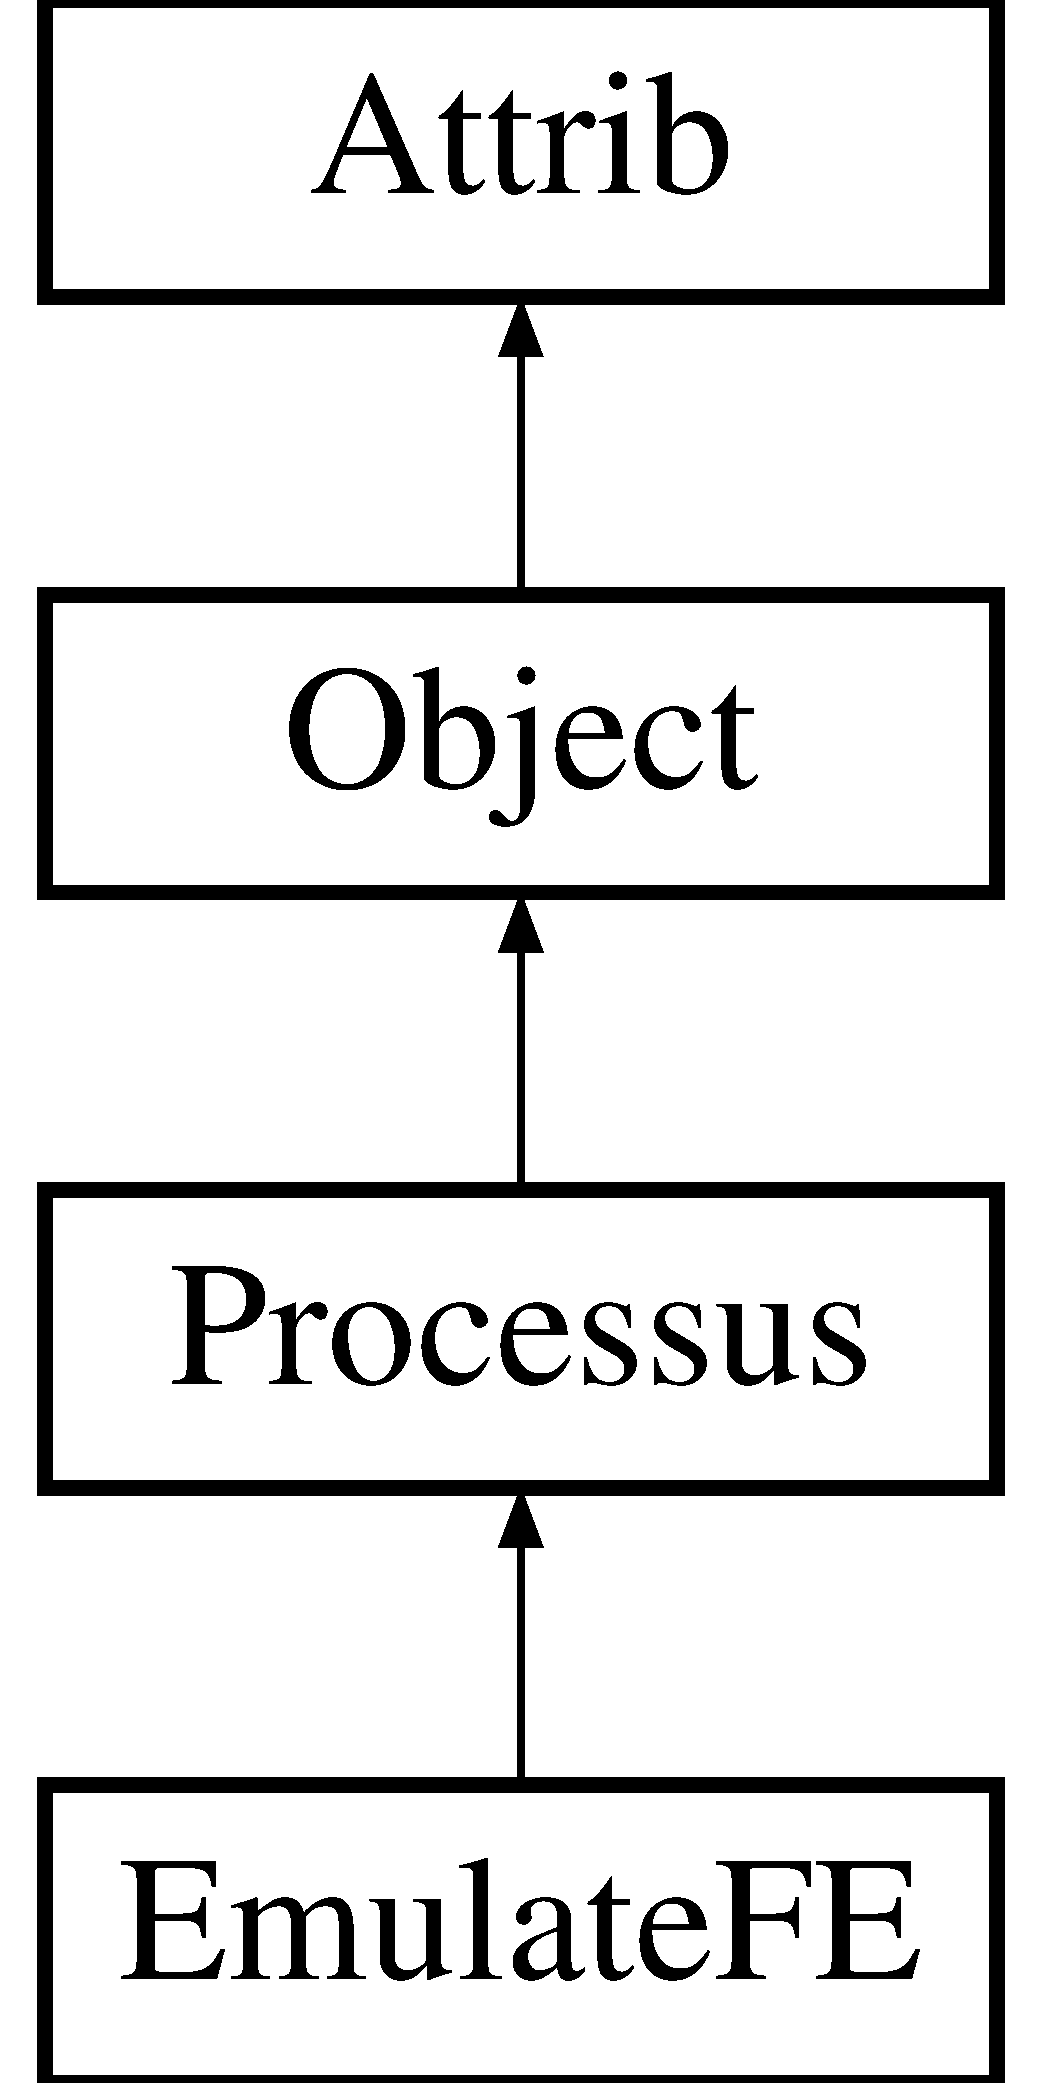
\includegraphics[height=4cm]{classEmulateFE}
\end{center}
\end{figure}
\subsection*{Public Types}
\begin{DoxyCompactItemize}
\item 
typedef unsigned long \hyperlink{classEmulateFE_abc39ad2fcef684d453760193ac4ddd49}{U32}
\item 
typedef unsigned short \hyperlink{classEmulateFE_ae3af71615d90d5e7ee4de109e8a79c5f}{U16}
\item 
typedef unsigned char \hyperlink{classEmulateFE_a8aa884f739fca2855ff8fb6bf3cddcff}{U8}
\item 
enum \hyperlink{classProcessus_a36278773bd98f2d5612fea40c7774821}{states} \{ \hyperlink{classProcessus_a36278773bd98f2d5612fea40c7774821adaf73ad5d0a09f952d0f18dbbe1c7493}{ERR} = -\/1, 
\hyperlink{classProcessus_a36278773bd98f2d5612fea40c7774821a629082f49d6e8df6b6da2b8fbb9d80fb}{NOT\_\-OK}, 
\hyperlink{classProcessus_a36278773bd98f2d5612fea40c7774821af77c64124fa175f28200166fff165ea2}{OK}
 \}
\item 
enum \hyperlink{classAttrib_a69e171d7cc6417835a5a306d3c764235}{Attribut} \{ \par
\hyperlink{classAttrib_a69e171d7cc6417835a5a306d3c764235a3a8da2ab97dda18aebab196fe4100531}{UNDEFINED}, 
\hyperlink{classAttrib_a69e171d7cc6417835a5a306d3c764235a2bfb2af57b87031d190a05fe25dd92ed}{PASSIVE}, 
\hyperlink{classAttrib_a69e171d7cc6417835a5a306d3c764235a3b1fec929c0370d1436f2f06e298fb0d}{ACTIVE}, 
\hyperlink{classAttrib_a69e171d7cc6417835a5a306d3c764235aa27c16b480a369ea4d18b07b2516bbc7}{INTERFACE}, 
\par
\hyperlink{classAttrib_a69e171d7cc6417835a5a306d3c764235a1420a5b8c0540b2af210b6975eded7f9}{IO}, 
\hyperlink{classAttrib_a69e171d7cc6417835a5a306d3c764235a0af3b0d0ac323c1704e6c69cf90add28}{IODATA}, 
\hyperlink{classAttrib_a69e171d7cc6417835a5a306d3c764235a7788bc5dd333fd8ce18562b269c9dab1}{ELEMENT}, 
\hyperlink{classAttrib_a69e171d7cc6417835a5a306d3c764235a61ceb22149f365f1780d18f9d1459423}{HARDWARE}, 
\par
\hyperlink{classAttrib_a69e171d7cc6417835a5a306d3c764235a75250e29692496e73effca2c0330977f}{PROCESSUS}, 
\hyperlink{classAttrib_a69e171d7cc6417835a5a306d3c764235a103a67cd0b8f07ef478fa45d4356e27b}{SOFTWARE}
 \}
\end{DoxyCompactItemize}
\subsection*{Public Member Functions}
\begin{DoxyCompactItemize}
\item 
\hyperlink{classEmulateFE_ac6242fca0d5c30477153d1d33d5f990d}{EmulateFE} ()
\begin{DoxyCompactList}\small\item\em Standard constructor. \item\end{DoxyCompactList}\item 
virtual \hyperlink{classEmulateFE_ab0ae9c65e546ec89bb0d6d318428d578}{$\sim$EmulateFE} ()
\begin{DoxyCompactList}\small\item\em Destructor. \item\end{DoxyCompactList}\item 
virtual \hyperlink{classStatusCode}{StatusCode} \hyperlink{classEmulateFE_aeb689a366ed5e675d02d08ee787d338e}{initialize} ()
\item 
virtual \hyperlink{classStatusCode}{StatusCode} \hyperlink{classEmulateFE_a5133d5b45521fc311db62d61217848b9}{execute} ()
\item 
virtual \hyperlink{classStatusCode}{StatusCode} \hyperlink{classEmulateFE_a7d29ee79a606d0f7d337b1e78ef54a03}{finalize} ()
\item 
\hyperlink{classStatusCode}{StatusCode} \hyperlink{classEmulateFE_a33403f61dc51ffc30c008cf5782636b1}{setFile} (std::string filename)
\item 
std::string \hyperlink{classEmulateFE_a321a82d6ead6f6089693d3165d7893ec}{file} ()
\item 
\hyperlink{classStatusCode}{StatusCode} \hyperlink{classEmulateFE_a3a8b53c47db627e5a70076968d5aab53}{setNTriggers} (int ntriggersMax)
\item 
int \hyperlink{classEmulateFE_ab08924ef9529a766ce80c9c1c9885cca}{nTriggers} ()
\item 
\hyperlink{classStatusCode}{StatusCode} \hyperlink{classEmulateFE_ac4592687749d8a457430911ddf8f5e76}{setGenerationType} (bool type)
\item 
bool \hyperlink{classEmulateFE_ad3aaa46fce2848cc9280e51a7e6fa572}{generationType} ()
\item 
\hyperlink{classStatusCode}{StatusCode} \hyperlink{classEmulateFE_ad785934c216c213e504f3db72b53354f}{setSignalRate} (float signalRate)
\item 
float \hyperlink{classEmulateFE_a98d2e402e4707109ca14ee9f4d95c2fa}{signalRate} ()
\item 
\hyperlink{classStatusCode}{StatusCode} \hyperlink{classEmulateFE_a6328b50231c29fc5a7e6df99a3db3a29}{setPedestal} (float pedestal)
\item 
float \hyperlink{classEmulateFE_a8442db97da7b2a97fe97745e6d8d9161}{pedestal} ()
\item 
\hyperlink{classStatusCode}{StatusCode} \hyperlink{classEmulateFE_a9b1d0d30631d304fc615c064db8231ca}{setNoise} (float noise)
\item 
float \hyperlink{classEmulateFE_a3e1a2e88567bf16a5599a1602d6ba50d}{noise} ()
\item 
\hyperlink{classStatusCode}{StatusCode} \hyperlink{classProcessus_a09319bde9bed93e290f69b4e04585543}{startProcessing} ()
\item 
\hyperlink{classStatusCode}{StatusCode} \hyperlink{classProcessus_a5e4da662989d356b89d490b89c7afbfd}{endProcessing} ()
\item 
void \hyperlink{classProcessus_aaeb17673b98d2b39f3aa780e335e0968}{clean} ()
\item 
void \hyperlink{classProcessus_ad57a29b33f9021eda9f6929136f1784f}{setStorage} (std::string storage)
\item 
\hyperlink{classData}{Data} $\ast$ \hyperlink{classProcessus_a16e45f329fbce935aeef0ff3cb508228}{data} ()
\item 
std::vector$<$ double $>$ \hyperlink{classProcessus_aa7c57483cf4b9ab0b2d0ae2de8316402}{data} (unsigned int row)
\item 
std::vector$<$ double $>$ \hyperlink{classProcessus_abf4d91fb36707e1d50178bab12d21ae9}{data} (std::string name)
\item 
\hyperlink{classHisto1D}{Histo1D} $\ast$ \hyperlink{classProcessus_a409227db936baff03c0462c1bcfe8069}{hist1d} (unsigned int row)
\item 
\hyperlink{classHisto2D}{Histo2D} $\ast$ \hyperlink{classProcessus_a73b5118cb5f2b5eaad33286183b86cfc}{hist2d} (unsigned int row)
\item 
void \hyperlink{classProcessus_a308c8f193802f1d1ab49d4447d0cb281}{addDataStream} (std::string name, std::string title)
\item 
void \hyperlink{classProcessus_ad46e0d4dfdfdcbce001ee6be1746dfa4}{addHisto1d} (TH1D $\ast$h)
\item 
void \hyperlink{classProcessus_ac1ed1aed5edaeabdf18aa56775440471}{addHisto2d} (TH2D $\ast$h)
\item 
\hyperlink{classStatusCode}{StatusCode} \hyperlink{classProcessus_a0d093b48f3218a088ba030e24372f18c}{dataFill} (int i, double val)
\item 
\hyperlink{classStatusCode}{StatusCode} \hyperlink{classProcessus_aa31ab71711f7af6a729441ff573f69c9}{dataFill} (std::string name, double val)
\item 
std::string \hyperlink{classProcessus_a33fa1a0b54a636e5cdd680669fd9ea51}{storage} ()
\item 
void \hyperlink{classProcessus_a8ddef94227d83d9dae2cd49aebc33353}{setElement} (\hyperlink{classElement}{Element} $\ast$element)
\item 
\hyperlink{classElement}{Element} $\ast$ \hyperlink{classProcessus_a6fe155527431a7190b7d44d600b9608d}{element} ()
\item 
void \hyperlink{classProcessus_abe603d0636f76db6aa6c5c60cf34c591}{incNErrors} ()
\item 
void \hyperlink{classProcessus_a831b027b9cf18ab56fa6147b5d3055da}{setNErrors} (unsigned int)
\item 
unsigned int \hyperlink{classProcessus_a82a0487f82f07cc2c2dc2731f98149e7}{nErrors} ()
\item 
TFile $\ast$ \hyperlink{classProcessus_a247e8c362ec08422cf53d08dd23b093c}{rootFile} ()
\item 
void \hyperlink{classProcessus_aacf6812880c1d1a2bf14a4a39458f443}{openRootFile} ()
\item 
void \hyperlink{classProcessus_a2f3c41e99da4c738ea3d8f7b0d20a665}{closeRootFile} ()
\item 
void \hyperlink{classProcessus_a5e4d34b86241fa0756e07375a14ff4b2}{startChrono} ()
\item 
void \hyperlink{classProcessus_a471833f89047aa9a7ff6200a31c17a1d}{setLogMsg} (std::string logMsg)
\item 
std::string \hyperlink{classProcessus_a42fdeb17dc13ba854222666b6aa29b61}{logMsg} ()
\item 
void \hyperlink{classProcessus_ad38cde0f1bcefa00b068e7947b8af927}{setState} (int state)
\item 
double \hyperlink{classProcessus_aecca96218c65bc805c988cd95447df55}{elapsedTime} ()
\item 
double \hyperlink{classProcessus_a06d3815ad56593dfd0d3c1f534f8b146}{elapsedTime} (time\_\-t start)
\item 
std::string \hyperlink{classObject_a975e888d50bfcbffda2c86368332a5cd}{name} () const 
\item 
std::string \hyperlink{classObject_a84f99f70f144a83e1582d1d0f84e4e62}{type} ()
\item 
unsigned char \hyperlink{classObject_af99145335cc61ff6e2798ea17db009d2}{id} ()
\item 
std::string \hyperlink{classObject_a73a0f1a41828fdd8303dd662446fb6c3}{title} ()
\item 
void \hyperlink{classObject_a3f9d5537ebce0c0f2bf6ae4d92426f3c}{msgSvc} (int level, std::string msg, std::string name)
\item 
void \hyperlink{classObject_a58b2d0618c2d08cf2383012611528d97}{msg} (std::string mymsg)
\item 
void \hyperlink{classObject_ac5d59299273cee27aacf7de00d2e7034}{msg} (std::string mymsg, std::string name)
\item 
void \hyperlink{classObject_a83d2db2df682907ea1115ad721c1c4a1}{verbose} (std::string mymsg)
\item 
void \hyperlink{classObject_a2d4120195317e2a3c6532e8bb9f3da68}{verbose} (std::string mymsg, std::string name)
\item 
void \hyperlink{classObject_aac010553f022165573714b7014a15f0d}{debug} (std::string mymsg)
\item 
void \hyperlink{classObject_a6c9a0397ca804e04d675ed05683f5420}{debug} (std::string mymsg, std::string name)
\item 
void \hyperlink{classObject_a644fd329ea4cb85f54fa6846484b84a8}{info} (std::string mymsg)
\item 
void \hyperlink{classObject_a1ca123253dfd30fc28b156f521dcbdae}{info} (std::string mymsg, std::string name)
\item 
void \hyperlink{classObject_a65cd4fda577711660821fd2cd5a3b4c9}{warning} (std::string mymsg)
\item 
void \hyperlink{classObject_a11f101db4dd73d9391b0231818881d86}{warning} (std::string mymsg, std::string name)
\item 
void \hyperlink{classObject_a204a95f57818c0f811933917a30eff45}{error} (std::string mymsg)
\item 
void \hyperlink{classObject_ad7f6c457733082efa2f9ff5f5c8e119a}{error} (std::string mymsg, std::string name)
\item 
void \hyperlink{classObject_aad5a16aac7516ce65bd5ec02ab07fc80}{fatal} (std::string mymsg)
\item 
void \hyperlink{classObject_ae62acd3d09f716220f75f252dc38bc9a}{fatal} (std::string mymsg, std::string name)
\item 
void \hyperlink{classObject_ae30fea75683c2d149b6b6d17c09ecd0c}{setName} (std::string name)
\item 
void \hyperlink{classObject_aae534cc9d982bcb9b99fd505f2e103a5}{setType} (std::string type)
\item 
void \hyperlink{classObject_a398fe08cba594a0ce6891d59fe4f159f}{setId} (unsigned char id)
\item 
void \hyperlink{classObject_a89557dbbad5bcaa02652f5d7fa35d20f}{setTitle} (std::string title)
\item 
void \hyperlink{classObject_a870c5af919958c2136623b2d7816d123}{setDllName} (std::string dllName)
\item 
std::string \hyperlink{classObject_a2e3947f2870094c332d7454117f3ec63}{dllName} ()
\item 
bool \hyperlink{classAttrib_a704f26af560909ad22065083bb7d4c34}{is} (int attribut)
\item 
void \hyperlink{classAttrib_a235f773af19c900264a190b00a3b4ad7}{add} (int attribut)
\item 
void \hyperlink{classAttrib_a7d4ef7e32d93cb287792b87b857e79f3}{remove} (int attribut)
\item 
std::string \hyperlink{classAttrib_aee7bbf16b144887f196e1341b24f8a26}{attributs} ()
\end{DoxyCompactItemize}
\subsection*{Protected Member Functions}
\begin{DoxyCompactItemize}
\item 
\hyperlink{classEmulateFE}{EmulateFE} $\ast$ \hyperlink{classEmulateFE_a9a704d0081a275410d19071a006f1a80}{clone} ()
\item 
\hyperlink{classStatusCode}{StatusCode} \hyperlink{classEmulateFE_ae557d3569b9285a871c502b93ba20494}{generateValues} ()
\item 
\hyperlink{classStatusCode}{StatusCode} \hyperlink{classEmulateFE_ae62bc56b44c4bcdf7f5eab5cbde2cd69}{generateFile} ()
\item 
\hyperlink{classStatusCode}{StatusCode} \hyperlink{classEmulateFE_adf7213a308c8a04f4d7efbb86a13689e}{processingFE} ()
\end{DoxyCompactItemize}
\subsection*{Protected Attributes}
\begin{DoxyCompactItemize}
\item 
\hyperlink{classElement}{Element} $\ast$ \hyperlink{classProcessus_aa9d24d53c3e52f36786cabb5d8e296e7}{m\_\-element}
\item 
std::string \hyperlink{classAttrib_a3414521d7a82476e874b25a5407b5e63}{m\_\-attribString} \mbox{[}10\mbox{]}
\end{DoxyCompactItemize}
\subsection*{Private Attributes}
\begin{DoxyCompactItemize}
\item 
TRandom \hyperlink{classEmulateFE_a7f883bc6fb5bde2c98e464ef74e5c643}{m\_\-random}
\item 
\hyperlink{classFEB__v1}{FEB\_\-v1} $\ast$ \hyperlink{classEmulateFE_a6f3c6a104235b167e4465f4169cf8304}{m\_\-board}
\item 
std::string \hyperlink{classEmulateFE_a103fedea9eb5d3963573f9120cb81a68}{m\_\-filename}
\item 
int \hyperlink{classEmulateFE_a04ed956f5992c36590dd5a6abc19de2c}{m\_\-nFile}
\item 
\hyperlink{classOptions}{Options} $\ast$ \hyperlink{classEmulateFE_a2f2da7d4b2164c47673a6ecc6dcef1ea}{m\_\-options}
\item 
int \hyperlink{classEmulateFE_aa8bd0aa42cc5f3d52930408807b3067c}{m\_\-typeGeneration}
\item 
float \hyperlink{classEmulateFE_a7aeff9e62f850ca6d7ee27dce02a060b}{m\_\-signalRate}
\item 
float \hyperlink{classEmulateFE_a033996ce759c11305395ac865a6c074a}{m\_\-pedestal}
\item 
float \hyperlink{classEmulateFE_a74f8720a1da5806fad3811339ef9b98f}{m\_\-noise}
\item 
int \hyperlink{classEmulateFE_a647be38c790d5c0088e971aa28989589}{m\_\-adcin} \mbox{[}16384\mbox{]}
\item 
int \hyperlink{classEmulateFE_a2d473d12faf30f4870458874d70c7f55}{m\_\-ntriggersMax}
\item 
int \hyperlink{classEmulateFE_a8df57e3d66bde60e9a79cb2ae54a9f4a}{m\_\-ntriggers}
\end{DoxyCompactItemize}


\subsection{Detailed Description}
\begin{DoxyAuthor}{Author}

\end{DoxyAuthor}
\begin{DoxyDate}{Date}
2012-\/07-\/12 
\end{DoxyDate}


Definition at line 18 of file EmulateFE.h.

\subsection{Member Typedef Documentation}
\hypertarget{classEmulateFE_ae3af71615d90d5e7ee4de109e8a79c5f}{
\index{EmulateFE@{EmulateFE}!U16@{U16}}
\index{U16@{U16}!EmulateFE@{EmulateFE}}
\subsubsection[{U16}]{\setlength{\rightskip}{0pt plus 5cm}typedef unsigned short {\bf EmulateFE::U16}}}
\label{classEmulateFE_ae3af71615d90d5e7ee4de109e8a79c5f}


Definition at line 21 of file EmulateFE.h.\hypertarget{classEmulateFE_abc39ad2fcef684d453760193ac4ddd49}{
\index{EmulateFE@{EmulateFE}!U32@{U32}}
\index{U32@{U32}!EmulateFE@{EmulateFE}}
\subsubsection[{U32}]{\setlength{\rightskip}{0pt plus 5cm}typedef unsigned long {\bf EmulateFE::U32}}}
\label{classEmulateFE_abc39ad2fcef684d453760193ac4ddd49}


Definition at line 20 of file EmulateFE.h.\hypertarget{classEmulateFE_a8aa884f739fca2855ff8fb6bf3cddcff}{
\index{EmulateFE@{EmulateFE}!U8@{U8}}
\index{U8@{U8}!EmulateFE@{EmulateFE}}
\subsubsection[{U8}]{\setlength{\rightskip}{0pt plus 5cm}typedef unsigned char {\bf EmulateFE::U8}}}
\label{classEmulateFE_a8aa884f739fca2855ff8fb6bf3cddcff}


Definition at line 22 of file EmulateFE.h.

\subsection{Member Enumeration Documentation}
\hypertarget{classAttrib_a69e171d7cc6417835a5a306d3c764235}{
\index{EmulateFE@{EmulateFE}!Attribut@{Attribut}}
\index{Attribut@{Attribut}!EmulateFE@{EmulateFE}}
\subsubsection[{Attribut}]{\setlength{\rightskip}{0pt plus 5cm}enum {\bf Attrib::Attribut}\hspace{0.3cm}{\ttfamily  \mbox{[}inherited\mbox{]}}}}
\label{classAttrib_a69e171d7cc6417835a5a306d3c764235}
\begin{Desc}
\item[Enumerator: ]\par
\begin{description}
\index{UNDEFINED@{UNDEFINED}!EmulateFE@{EmulateFE}}\index{EmulateFE@{EmulateFE}!UNDEFINED@{UNDEFINED}}\item[{\em 
\hypertarget{classAttrib_a69e171d7cc6417835a5a306d3c764235a3a8da2ab97dda18aebab196fe4100531}{
UNDEFINED}
\label{classAttrib_a69e171d7cc6417835a5a306d3c764235a3a8da2ab97dda18aebab196fe4100531}
}]\index{PASSIVE@{PASSIVE}!EmulateFE@{EmulateFE}}\index{EmulateFE@{EmulateFE}!PASSIVE@{PASSIVE}}\item[{\em 
\hypertarget{classAttrib_a69e171d7cc6417835a5a306d3c764235a2bfb2af57b87031d190a05fe25dd92ed}{
PASSIVE}
\label{classAttrib_a69e171d7cc6417835a5a306d3c764235a2bfb2af57b87031d190a05fe25dd92ed}
}]\index{ACTIVE@{ACTIVE}!EmulateFE@{EmulateFE}}\index{EmulateFE@{EmulateFE}!ACTIVE@{ACTIVE}}\item[{\em 
\hypertarget{classAttrib_a69e171d7cc6417835a5a306d3c764235a3b1fec929c0370d1436f2f06e298fb0d}{
ACTIVE}
\label{classAttrib_a69e171d7cc6417835a5a306d3c764235a3b1fec929c0370d1436f2f06e298fb0d}
}]\index{INTERFACE@{INTERFACE}!EmulateFE@{EmulateFE}}\index{EmulateFE@{EmulateFE}!INTERFACE@{INTERFACE}}\item[{\em 
\hypertarget{classAttrib_a69e171d7cc6417835a5a306d3c764235aa27c16b480a369ea4d18b07b2516bbc7}{
INTERFACE}
\label{classAttrib_a69e171d7cc6417835a5a306d3c764235aa27c16b480a369ea4d18b07b2516bbc7}
}]\index{IO@{IO}!EmulateFE@{EmulateFE}}\index{EmulateFE@{EmulateFE}!IO@{IO}}\item[{\em 
\hypertarget{classAttrib_a69e171d7cc6417835a5a306d3c764235a1420a5b8c0540b2af210b6975eded7f9}{
IO}
\label{classAttrib_a69e171d7cc6417835a5a306d3c764235a1420a5b8c0540b2af210b6975eded7f9}
}]\index{IODATA@{IODATA}!EmulateFE@{EmulateFE}}\index{EmulateFE@{EmulateFE}!IODATA@{IODATA}}\item[{\em 
\hypertarget{classAttrib_a69e171d7cc6417835a5a306d3c764235a0af3b0d0ac323c1704e6c69cf90add28}{
IODATA}
\label{classAttrib_a69e171d7cc6417835a5a306d3c764235a0af3b0d0ac323c1704e6c69cf90add28}
}]\index{ELEMENT@{ELEMENT}!EmulateFE@{EmulateFE}}\index{EmulateFE@{EmulateFE}!ELEMENT@{ELEMENT}}\item[{\em 
\hypertarget{classAttrib_a69e171d7cc6417835a5a306d3c764235a7788bc5dd333fd8ce18562b269c9dab1}{
ELEMENT}
\label{classAttrib_a69e171d7cc6417835a5a306d3c764235a7788bc5dd333fd8ce18562b269c9dab1}
}]\index{HARDWARE@{HARDWARE}!EmulateFE@{EmulateFE}}\index{EmulateFE@{EmulateFE}!HARDWARE@{HARDWARE}}\item[{\em 
\hypertarget{classAttrib_a69e171d7cc6417835a5a306d3c764235a61ceb22149f365f1780d18f9d1459423}{
HARDWARE}
\label{classAttrib_a69e171d7cc6417835a5a306d3c764235a61ceb22149f365f1780d18f9d1459423}
}]\index{PROCESSUS@{PROCESSUS}!EmulateFE@{EmulateFE}}\index{EmulateFE@{EmulateFE}!PROCESSUS@{PROCESSUS}}\item[{\em 
\hypertarget{classAttrib_a69e171d7cc6417835a5a306d3c764235a75250e29692496e73effca2c0330977f}{
PROCESSUS}
\label{classAttrib_a69e171d7cc6417835a5a306d3c764235a75250e29692496e73effca2c0330977f}
}]\index{SOFTWARE@{SOFTWARE}!EmulateFE@{EmulateFE}}\index{EmulateFE@{EmulateFE}!SOFTWARE@{SOFTWARE}}\item[{\em 
\hypertarget{classAttrib_a69e171d7cc6417835a5a306d3c764235a103a67cd0b8f07ef478fa45d4356e27b}{
SOFTWARE}
\label{classAttrib_a69e171d7cc6417835a5a306d3c764235a103a67cd0b8f07ef478fa45d4356e27b}
}]\end{description}
\end{Desc}



Definition at line 29 of file Attrib.h.


\begin{DoxyCode}
29                 {
30     UNDEFINED,
31     PASSIVE,
32     ACTIVE,
33     INTERFACE,
34     IO,
35     IODATA,
36     ELEMENT,
37     HARDWARE,
38     PROCESSUS,
39     SOFTWARE 
40   }; // array m_attribString must be changed into Attrib::Attrib if this enu is m
      odified. 
\end{DoxyCode}
\hypertarget{classProcessus_a36278773bd98f2d5612fea40c7774821}{
\index{EmulateFE@{EmulateFE}!states@{states}}
\index{states@{states}!EmulateFE@{EmulateFE}}
\subsubsection[{states}]{\setlength{\rightskip}{0pt plus 5cm}enum {\bf Processus::states}\hspace{0.3cm}{\ttfamily  \mbox{[}inherited\mbox{]}}}}
\label{classProcessus_a36278773bd98f2d5612fea40c7774821}
\begin{Desc}
\item[Enumerator: ]\par
\begin{description}
\index{ERR@{ERR}!EmulateFE@{EmulateFE}}\index{EmulateFE@{EmulateFE}!ERR@{ERR}}\item[{\em 
\hypertarget{classProcessus_a36278773bd98f2d5612fea40c7774821adaf73ad5d0a09f952d0f18dbbe1c7493}{
ERR}
\label{classProcessus_a36278773bd98f2d5612fea40c7774821adaf73ad5d0a09f952d0f18dbbe1c7493}
}]\index{NOT\_\-OK@{NOT\_\-OK}!EmulateFE@{EmulateFE}}\index{EmulateFE@{EmulateFE}!NOT\_\-OK@{NOT\_\-OK}}\item[{\em 
\hypertarget{classProcessus_a36278773bd98f2d5612fea40c7774821a629082f49d6e8df6b6da2b8fbb9d80fb}{
NOT\_\-OK}
\label{classProcessus_a36278773bd98f2d5612fea40c7774821a629082f49d6e8df6b6da2b8fbb9d80fb}
}]\index{OK@{OK}!EmulateFE@{EmulateFE}}\index{EmulateFE@{EmulateFE}!OK@{OK}}\item[{\em 
\hypertarget{classProcessus_a36278773bd98f2d5612fea40c7774821af77c64124fa175f28200166fff165ea2}{
OK}
\label{classProcessus_a36278773bd98f2d5612fea40c7774821af77c64124fa175f28200166fff165ea2}
}]\end{description}
\end{Desc}



Definition at line 34 of file Processus.h.


\begin{DoxyCode}
34 { ERR=-1 , NOT_OK , OK };
\end{DoxyCode}


\subsection{Constructor \& Destructor Documentation}
\hypertarget{classEmulateFE_ac6242fca0d5c30477153d1d33d5f990d}{
\index{EmulateFE@{EmulateFE}!EmulateFE@{EmulateFE}}
\index{EmulateFE@{EmulateFE}!EmulateFE@{EmulateFE}}
\subsubsection[{EmulateFE}]{\setlength{\rightskip}{0pt plus 5cm}EmulateFE::EmulateFE ()}}
\label{classEmulateFE_ac6242fca0d5c30477153d1d33d5f990d}


Standard constructor. 

Definition at line 25 of file EmulateFE.cpp.

References Object::setName(), Object::setTitle(), and Object::setType().

Referenced by clone().


\begin{DoxyCode}
25                        :
26   m_filename(std::string("")),
27   m_typeGeneration (0),
28   m_signalRate(0.05),
29   m_pedestal(128),
30   m_noise(30),
31   m_ntriggersMax(0),
32   m_ntriggers(0),
33   m_options(application()->options())
34 {
35   setName ( "EmulateFE" );
36   setType ( "FEB_v1" );
37   setTitle( "FEB_v1 EmulateFE processing" );
38 }
//=============================================================================
\end{DoxyCode}
\hypertarget{classEmulateFE_ab0ae9c65e546ec89bb0d6d318428d578}{
\index{EmulateFE@{EmulateFE}!$\sim$EmulateFE@{$\sim$EmulateFE}}
\index{$\sim$EmulateFE@{$\sim$EmulateFE}!EmulateFE@{EmulateFE}}
\subsubsection[{$\sim$EmulateFE}]{\setlength{\rightskip}{0pt plus 5cm}EmulateFE::$\sim$EmulateFE ()\hspace{0.3cm}{\ttfamily  \mbox{[}virtual\mbox{]}}}}
\label{classEmulateFE_ab0ae9c65e546ec89bb0d6d318428d578}


Destructor. 

Definition at line 42 of file EmulateFE.cpp.


\begin{DoxyCode}
42 {}
\end{DoxyCode}


\subsection{Member Function Documentation}
\hypertarget{classAttrib_a235f773af19c900264a190b00a3b4ad7}{
\index{EmulateFE@{EmulateFE}!add@{add}}
\index{add@{add}!EmulateFE@{EmulateFE}}
\subsubsection[{add}]{\setlength{\rightskip}{0pt plus 5cm}void Attrib::add (int {\em attribut})\hspace{0.3cm}{\ttfamily  \mbox{[}inline, inherited\mbox{]}}}}
\label{classAttrib_a235f773af19c900264a190b00a3b4ad7}
Add an attribut 

Definition at line 67 of file Attrib.h.

References Attrib::m\_\-attributs, and Attrib::UNDEFINED.

Referenced by A3PE::A3PE(), Attrib::Attrib(), SpecsMezzanine::cmdline(), Computer::Computer(), CU\_\-v1::CU\_\-v1(), export\_\-obj(), FEB\_\-v1::FEB\_\-v1(), FePGA::FePGA(), ICECALv3::ICECALv3(), ICPhaser::ICPhaser(), Application::initialize(), Interface::Interface(), IOdata::IOdata(), IOobject::IOobject(), LSDelayChipV1::LSDelayChipV1(), MSOxxxx::MSOxxxx(), Phaser::Phaser(), Processus::Processus(), Proto40MHz\_\-v1::Proto40MHz\_\-v1(), Attrib::remove(), SeqPGA::SeqPGA(), SpecsMaster::SpecsMaster(), and SpecsSlave::SpecsSlave().


\begin{DoxyCode}
67                             {
68     if (attribut!=Attrib::UNDEFINED) remove(Attrib::UNDEFINED);
69     bool duplicate = false ;
70     std::vector<int>::const_iterator iter ;
71     for ( iter  = m_attributs.begin() ;
72           iter != m_attributs.end()   ;
73           ++iter ) {
74       if ( attribut == (*iter) ) {
75         duplicate = true ;
76       }
77     }
78     if (!duplicate) {
79       m_attributs.push_back( attribut );
80     }
81   }
\end{DoxyCode}
\hypertarget{classProcessus_a308c8f193802f1d1ab49d4447d0cb281}{
\index{EmulateFE@{EmulateFE}!addDataStream@{addDataStream}}
\index{addDataStream@{addDataStream}!EmulateFE@{EmulateFE}}
\subsubsection[{addDataStream}]{\setlength{\rightskip}{0pt plus 5cm}void Processus::addDataStream (std::string {\em name}, \/  std::string {\em title})\hspace{0.3cm}{\ttfamily  \mbox{[}inline, inherited\mbox{]}}}}
\label{classProcessus_a308c8f193802f1d1ab49d4447d0cb281}


Definition at line 153 of file Processus.h.

References Data::addDataStream(), and Processus::m\_\-data.

Referenced by CurrentMeasurement::initialize(), ADCMeasurement::initialize(), TestSuite::initialize(), TestUSB::initialize(), TestSPI::initialize(), TestI2C::initialize(), UsbFTInterfaceTest::initialize(), and RegisterTest::initialize().


\begin{DoxyCode}
153                                                        {
154     m_data->addDataStream(name, title);
155   }
\end{DoxyCode}
\hypertarget{classProcessus_ad46e0d4dfdfdcbce001ee6be1746dfa4}{
\index{EmulateFE@{EmulateFE}!addHisto1d@{addHisto1d}}
\index{addHisto1d@{addHisto1d}!EmulateFE@{EmulateFE}}
\subsubsection[{addHisto1d}]{\setlength{\rightskip}{0pt plus 5cm}void Processus::addHisto1d (TH1D $\ast$ {\em h})\hspace{0.3cm}{\ttfamily  \mbox{[}inline, inherited\mbox{]}}}}
\label{classProcessus_ad46e0d4dfdfdcbce001ee6be1746dfa4}


Definition at line 160 of file Processus.h.

References Data::addHisto1d(), and Processus::m\_\-data.

Referenced by TestSuite::initialize(), StorageFifoAcquisition::initialize(), StorageFifo::initialize(), Acquisition::initialize(), and A3PE\_\-BitFlip::initialize().


\begin{DoxyCode}
160                            {
161     m_data->addHisto1d(h);
162   }
\end{DoxyCode}
\hypertarget{classProcessus_ac1ed1aed5edaeabdf18aa56775440471}{
\index{EmulateFE@{EmulateFE}!addHisto2d@{addHisto2d}}
\index{addHisto2d@{addHisto2d}!EmulateFE@{EmulateFE}}
\subsubsection[{addHisto2d}]{\setlength{\rightskip}{0pt plus 5cm}void Processus::addHisto2d (TH2D $\ast$ {\em h})\hspace{0.3cm}{\ttfamily  \mbox{[}inline, inherited\mbox{]}}}}
\label{classProcessus_ac1ed1aed5edaeabdf18aa56775440471}


Definition at line 167 of file Processus.h.

References Data::addHisto2d(), and Processus::m\_\-data.

Referenced by TestSuite::initialize().


\begin{DoxyCode}
167                            {
168     m_data->addHisto2d(h);
169   }
\end{DoxyCode}
\hypertarget{classAttrib_aee7bbf16b144887f196e1341b24f8a26}{
\index{EmulateFE@{EmulateFE}!attributs@{attributs}}
\index{attributs@{attributs}!EmulateFE@{EmulateFE}}
\subsubsection[{attributs}]{\setlength{\rightskip}{0pt plus 5cm}std::string Attrib::attributs ()\hspace{0.3cm}{\ttfamily  \mbox{[}inherited\mbox{]}}}}
\label{classAttrib_aee7bbf16b144887f196e1341b24f8a26}
Print the \hyperlink{classAttrib}{Attrib} of an \hyperlink{classObject}{Object} 

Definition at line 54 of file Attrib.cpp.

References images::index, Attrib::m\_\-attribString, and Attrib::m\_\-attributs.

Referenced by export\_\-obj().


\begin{DoxyCode}
54                             {
55   std::string output;
56   std::vector<int>::iterator iter ;
57   for ( unsigned int index = 0 ; index < m_attributs.size() ; ++index ) {
58     if ( m_attributs.size() - index > 1 ) {
59       output.append(m_attribString[m_attributs[index]]);
60       output.append(":");
61     }
62     else {
63       output.append(m_attribString[m_attributs[index]]);
64     }
65   }
66   return output;
67 }
\end{DoxyCode}
\hypertarget{classProcessus_aaeb17673b98d2b39f3aa780e335e0968}{
\index{EmulateFE@{EmulateFE}!clean@{clean}}
\index{clean@{clean}!EmulateFE@{EmulateFE}}
\subsubsection[{clean}]{\setlength{\rightskip}{0pt plus 5cm}void Processus::clean ()\hspace{0.3cm}{\ttfamily  \mbox{[}inline, inherited\mbox{]}}}}
\label{classProcessus_aaeb17673b98d2b39f3aa780e335e0968}


Definition at line 85 of file Processus.h.

References Processus::m\_\-element, Processus::m\_\-state, and Object::warning().

Referenced by Application::prepare().


\begin{DoxyCode}
86   {
87     m_element=0;
88     if (0!=m_state) {
89       delete m_state;
90       m_state=0;
91     }
92 #ifdef _NETWORK_
93     warning("Cleaning state service : should it be done ?","Processus::clean")
94       if (0!=m_stateService)
95       {
96         delete m_stateService;
97       }
98 #endif
99   }
\end{DoxyCode}
\hypertarget{classEmulateFE_a9a704d0081a275410d19071a006f1a80}{
\index{EmulateFE@{EmulateFE}!clone@{clone}}
\index{clone@{clone}!EmulateFE@{EmulateFE}}
\subsubsection[{clone}]{\setlength{\rightskip}{0pt plus 5cm}{\bf EmulateFE}$\ast$ EmulateFE::clone ()\hspace{0.3cm}{\ttfamily  \mbox{[}inline, protected, virtual\mbox{]}}}}
\label{classEmulateFE_a9a704d0081a275410d19071a006f1a80}
processus termination virtual function 

Implements \hyperlink{classProcessus_aca8856f6d6d7b7e1fe941f298dcbb502}{Processus}.

Definition at line 87 of file EmulateFE.h.

References EmulateFE().


\begin{DoxyCode}
87                     {
88     return new EmulateFE (*this);
89   }
\end{DoxyCode}
\hypertarget{classProcessus_a2f3c41e99da4c738ea3d8f7b0d20a665}{
\index{EmulateFE@{EmulateFE}!closeRootFile@{closeRootFile}}
\index{closeRootFile@{closeRootFile}!EmulateFE@{EmulateFE}}
\subsubsection[{closeRootFile}]{\setlength{\rightskip}{0pt plus 5cm}void Processus::closeRootFile ()\hspace{0.3cm}{\ttfamily  \mbox{[}inherited\mbox{]}}}}
\label{classProcessus_a2f3c41e99da4c738ea3d8f7b0d20a665}
Close Root file if already opened and requested 

Definition at line 160 of file Processus.cpp.

References Options::dataFileFullName(), Options::dataStorage(), Object::info(), Processus::m\_\-options, and Processus::m\_\-rootFile.

Referenced by Processus::endProcessing(), UsbFTInterfaceTest::finalize(), RegisterTest::finalize(), and PhaserRampExec::finalize().


\begin{DoxyCode}
160                                 {
161   if ( 0!= m_rootFile && m_options->dataStorage() ){
162     m_rootFile->Write();
163         std::string mess=std::string("Closing root file ");
164         mess.append(m_options->dataFileFullName());
165         info(mess,"closeRootFile");
166     m_rootFile->Delete();
167     m_rootFile = 0;
168   }
169 }
\end{DoxyCode}
\hypertarget{classProcessus_abf4d91fb36707e1d50178bab12d21ae9}{
\index{EmulateFE@{EmulateFE}!data@{data}}
\index{data@{data}!EmulateFE@{EmulateFE}}
\subsubsection[{data}]{\setlength{\rightskip}{0pt plus 5cm}std::vector$<$double$>$ Processus::data (std::string {\em name})\hspace{0.3cm}{\ttfamily  \mbox{[}inline, inherited\mbox{]}}}}
\label{classProcessus_abf4d91fb36707e1d50178bab12d21ae9}
Get accessor to member m\_\-data \begin{DoxyReturn}{Returns}
the current value of m\_\-data 
\end{DoxyReturn}


Definition at line 130 of file Processus.h.

References Processus::m\_\-data, and Data::vector().


\begin{DoxyCode}
130                                         {
131     return m_data->vector(name);
132   }
\end{DoxyCode}
\hypertarget{classProcessus_aa7c57483cf4b9ab0b2d0ae2de8316402}{
\index{EmulateFE@{EmulateFE}!data@{data}}
\index{data@{data}!EmulateFE@{EmulateFE}}
\subsubsection[{data}]{\setlength{\rightskip}{0pt plus 5cm}std::vector$<$double$>$ Processus::data (unsigned int {\em row})\hspace{0.3cm}{\ttfamily  \mbox{[}inline, inherited\mbox{]}}}}
\label{classProcessus_aa7c57483cf4b9ab0b2d0ae2de8316402}
Get accessor to member m\_\-data \begin{DoxyReturn}{Returns}
the current value of m\_\-data 
\end{DoxyReturn}


Definition at line 122 of file Processus.h.

References Processus::m\_\-data, and Data::vector().


\begin{DoxyCode}
122                                           {
123     return m_data->vector(row);
124   }
\end{DoxyCode}
\hypertarget{classProcessus_a16e45f329fbce935aeef0ff3cb508228}{
\index{EmulateFE@{EmulateFE}!data@{data}}
\index{data@{data}!EmulateFE@{EmulateFE}}
\subsubsection[{data}]{\setlength{\rightskip}{0pt plus 5cm}{\bf Data}$\ast$ Processus::data ()\hspace{0.3cm}{\ttfamily  \mbox{[}inline, inherited\mbox{]}}}}
\label{classProcessus_a16e45f329fbce935aeef0ff3cb508228}
Get accessor to member m\_\-data \begin{DoxyReturn}{Returns}
the current value of m\_\-data 
\end{DoxyReturn}


Definition at line 114 of file Processus.h.

References Processus::m\_\-data.

Referenced by StorageFifoAcquisition::execute(), and export\_\-proc().


\begin{DoxyCode}
114               {
115     return m_data;
116   }
\end{DoxyCode}
\hypertarget{classProcessus_aa31ab71711f7af6a729441ff573f69c9}{
\index{EmulateFE@{EmulateFE}!dataFill@{dataFill}}
\index{dataFill@{dataFill}!EmulateFE@{EmulateFE}}
\subsubsection[{dataFill}]{\setlength{\rightskip}{0pt plus 5cm}{\bf StatusCode} Processus::dataFill (std::string {\em name}, \/  double {\em val})\hspace{0.3cm}{\ttfamily  \mbox{[}inline, inherited\mbox{]}}}}
\label{classProcessus_aa31ab71711f7af6a729441ff573f69c9}
Set data stream with value \begin{DoxyReturn}{Returns}
the \hyperlink{classStatusCode}{StatusCode} 
\end{DoxyReturn}


Definition at line 189 of file Processus.h.

References StatusCode::FAILURE, Processus::m\_\-data, Data::rowFromName(), StatusCode::SUCCESS, and Data::vectorPtr().


\begin{DoxyCode}
189                                                  {
190     int row=m_data->rowFromName(name);
191     if (row<0) return StatusCode::FAILURE;
192     if (m_data->vectorPtr(row)!=0){
193       m_data->vectorPtr(row)->push_back(val);
194       return StatusCode::SUCCESS;
195     }
196     else {
197       return StatusCode::FAILURE;
198     }
199   }
\end{DoxyCode}
\hypertarget{classProcessus_a0d093b48f3218a088ba030e24372f18c}{
\index{EmulateFE@{EmulateFE}!dataFill@{dataFill}}
\index{dataFill@{dataFill}!EmulateFE@{EmulateFE}}
\subsubsection[{dataFill}]{\setlength{\rightskip}{0pt plus 5cm}{\bf StatusCode} Processus::dataFill (int {\em i}, \/  double {\em val})\hspace{0.3cm}{\ttfamily  \mbox{[}inline, inherited\mbox{]}}}}
\label{classProcessus_a0d093b48f3218a088ba030e24372f18c}
Set data stream with value \begin{DoxyReturn}{Returns}
the \hyperlink{classStatusCode}{StatusCode} 
\end{DoxyReturn}


Definition at line 175 of file Processus.h.

References StatusCode::FAILURE, Processus::m\_\-data, StatusCode::SUCCESS, and Data::vectorPtr().

Referenced by CurrentMeasurement::execute(), ADCMeasurement::execute(), TestSuite::execute(), TestUSB::execute(), TestSPI::execute(), TestI2C::execute(), and UsbFTInterfaceTest::execute().


\begin{DoxyCode}
175                                         {
176     if (m_data->vectorPtr(i)!=0){
177       m_data->vectorPtr(i)->push_back(val);
178       return StatusCode::SUCCESS;
179     }
180     else {
181       return StatusCode::FAILURE;
182     }
183   }
\end{DoxyCode}
\hypertarget{classObject_a6c9a0397ca804e04d675ed05683f5420}{
\index{EmulateFE@{EmulateFE}!debug@{debug}}
\index{debug@{debug}!EmulateFE@{EmulateFE}}
\subsubsection[{debug}]{\setlength{\rightskip}{0pt plus 5cm}void Object::debug (std::string {\em mymsg}, \/  std::string {\em name})\hspace{0.3cm}{\ttfamily  \mbox{[}inline, inherited\mbox{]}}}}
\label{classObject_a6c9a0397ca804e04d675ed05683f5420}


Definition at line 45 of file Object.h.

References MsgSvc::DEBUG, Object::m\_\-log, and MsgSvc::msgSvc().


\begin{DoxyCode}
45 { m_log.msgSvc (MsgSvc::DEBUG   , mymsg, name ); }
\end{DoxyCode}
\hypertarget{classObject_aac010553f022165573714b7014a15f0d}{
\index{EmulateFE@{EmulateFE}!debug@{debug}}
\index{debug@{debug}!EmulateFE@{EmulateFE}}
\subsubsection[{debug}]{\setlength{\rightskip}{0pt plus 5cm}void Object::debug (std::string {\em mymsg})\hspace{0.3cm}{\ttfamily  \mbox{[}inline, inherited\mbox{]}}}}
\label{classObject_aac010553f022165573714b7014a15f0d}


Definition at line 37 of file Object.h.

References MsgSvc::DEBUG, Object::m\_\-log, Object::m\_\-name, and MsgSvc::msgSvc().

Referenced by A3PE::A3PE(), A3PE::acquisition(), SpecsMezzanine::addBus(), Hierarchy::addChild(), SpecsSlave::addI2c(), LSDelayChipV1::checkConfigAddr(), LSDelayChipV1::checkStatusAddr(), LSDelayChipV1::configRegBulkRead(), LSDelayChipV1::configRegBulkWrite(), A3PE::dataReady(), DCU::DCU(), Hierarchy::delChild(), SpecsSlave::detect(), execute(), StorageFifoAcquisition::execute(), StorageFifo::execute(), Acquisition::execute(), A3PE\_\-BitFlip::execute(), export\_\-obj(), FePGA::FePGA(), SpecsGlue::i2cClkMode(), SeqPGA::i2cRead(), FePGA::i2cRead(), SeqPGA::i2cWrite(), FePGA::i2cWrite(), ICECALv3::ICECALv3(), ICPhaser::ICPhaser(), SpecsSlave::init(), SpecsMaster::init(), initialize(), StorageFifoAcquisition::initialize(), StorageFifo::initialize(), Acquisition::initialize(), A3PE\_\-BitFlip::initialize(), A3PE::internalAXSequence(), SpecsMezzanine::led(), SpecsGlue::led(), LSDelayChipV1::LSDelayChipV1(), MSOxxxx::MSOxxxx(), Phaser::Phaser(), Data::purge(), ICPhaser::read(), Phaser::read(), FEB\_\-v1::readFifoSpyFE(), SpecsSlave::reset(), SpecsMaster::reset(), FEB\_\-v1::reset(), CU\_\-v1::reset(), Proto40MHz\_\-v1::reset(), FEB\_\-v1::resetFifoSpyFE(), SeqPGA::resetSpi(), FEB\_\-v1::resetSpi(), SeqPGA::SeqPGA(), A3PE::setAddFromAXRam(), A3PE::setAddToAXRam(), A3PE::setAXRamUsb(), Element::setConnection(), SpecsGlue::setI2cClkMode(), A3PE::setLatencyAX(), SpecsMezzanine::setLed(), SpecsGlue::setLed(), A3PE::setLengthAX(), A3PE::setReadToAXRamUsb(), SpecsMaster::setSpeed(), A3PE::setWriteFromAXRamUsb(), SpecsBus::SpecsBus(), SpecsI2c::SpecsI2c(), SpecsMaster::SpecsMaster(), SpecsMezzanine::SpecsMezzanine(), SpecsParallelBus::SpecsParallelBus(), SpecsSlave::SpecsSlave(), LSDelayChipV1::spiBERTest(), ICECALv3::spiRead(), ICECALv3::spiWrite(), FEB\_\-v1::testDuration(), SeqPGA::testSequence(), A3PE::trigger(), Server::updateConfig(), Server::updateState(), ICPhaser::write(), Phaser::write(), and Hierarchy::$\sim$Hierarchy().


\begin{DoxyCode}
37 { m_log.msgSvc (MsgSvc::DEBUG   , mymsg, m_name ); }
\end{DoxyCode}
\hypertarget{classObject_a2e3947f2870094c332d7454117f3ec63}{
\index{EmulateFE@{EmulateFE}!dllName@{dllName}}
\index{dllName@{dllName}!EmulateFE@{EmulateFE}}
\subsubsection[{dllName}]{\setlength{\rightskip}{0pt plus 5cm}std::string Object::dllName ()\hspace{0.3cm}{\ttfamily  \mbox{[}inline, inherited\mbox{]}}}}
\label{classObject_a2e3947f2870094c332d7454117f3ec63}
Get accessor to member m\_\-dllName \begin{DoxyReturn}{Returns}
the current value of m\_\-dllName 
\end{DoxyReturn}


Definition at line 74 of file Object.h.

References Object::m\_\-dllName.

Referenced by export\_\-obj().


\begin{DoxyCode}
74                        {
75     return m_dllName;
76   }  
\end{DoxyCode}
\hypertarget{classProcessus_a06d3815ad56593dfd0d3c1f534f8b146}{
\index{EmulateFE@{EmulateFE}!elapsedTime@{elapsedTime}}
\index{elapsedTime@{elapsedTime}!EmulateFE@{EmulateFE}}
\subsubsection[{elapsedTime}]{\setlength{\rightskip}{0pt plus 5cm}double Processus::elapsedTime (time\_\-t {\em start})\hspace{0.3cm}{\ttfamily  \mbox{[}inline, inherited\mbox{]}}}}
\label{classProcessus_a06d3815ad56593dfd0d3c1f534f8b146}


Definition at line 343 of file Processus.h.


\begin{DoxyCode}
343                                    {
344     return ((time(0)-start));
345   }
\end{DoxyCode}
\hypertarget{classProcessus_aecca96218c65bc805c988cd95447df55}{
\index{EmulateFE@{EmulateFE}!elapsedTime@{elapsedTime}}
\index{elapsedTime@{elapsedTime}!EmulateFE@{EmulateFE}}
\subsubsection[{elapsedTime}]{\setlength{\rightskip}{0pt plus 5cm}double Processus::elapsedTime ()\hspace{0.3cm}{\ttfamily  \mbox{[}inline, inherited\mbox{]}}}}
\label{classProcessus_aecca96218c65bc805c988cd95447df55}


Definition at line 340 of file Processus.h.

References Processus::m\_\-start.

Referenced by Processus::endProcessing(), UsbFTInterfaceTest::execute(), PhaserRampExec::finalize(), and Processus::setState().


\begin{DoxyCode}
340                        {
341     return difftime(time(0),m_start);
342   }
\end{DoxyCode}
\hypertarget{classProcessus_a6fe155527431a7190b7d44d600b9608d}{
\index{EmulateFE@{EmulateFE}!element@{element}}
\index{element@{element}!EmulateFE@{EmulateFE}}
\subsubsection[{element}]{\setlength{\rightskip}{0pt plus 5cm}{\bf Element}$\ast$ Processus::element ()\hspace{0.3cm}{\ttfamily  \mbox{[}inline, inherited\mbox{]}}}}
\label{classProcessus_a6fe155527431a7190b7d44d600b9608d}
Get accessor to member m\_\-element \begin{DoxyReturn}{Returns}
the current value of m\_\-element 
\end{DoxyReturn}


Definition at line 231 of file Processus.h.

References Processus::m\_\-element.

Referenced by UsbFTInterfaceTest::execute(), export\_\-proc(), CurrentMeasurement::initialize(), ADCMeasurement::initialize(), TestUSB::initialize(), TestSPI::initialize(), TestI2C::initialize(), initialize(), StorageFifoAcquisition::initialize(), StorageFifo::initialize(), Acquisition::initialize(), A3PE\_\-BitFlip::initialize(), and PhaserRampExec::initialize().


\begin{DoxyCode}
231                       {
232     return m_element;
233   }
\end{DoxyCode}
\hypertarget{classProcessus_a5e4da662989d356b89d490b89c7afbfd}{
\index{EmulateFE@{EmulateFE}!endProcessing@{endProcessing}}
\index{endProcessing@{endProcessing}!EmulateFE@{EmulateFE}}
\subsubsection[{endProcessing}]{\setlength{\rightskip}{0pt plus 5cm}{\bf StatusCode} Processus::endProcessing ()\hspace{0.3cm}{\ttfamily  \mbox{[}inherited\mbox{]}}}}
\label{classProcessus_a5e4da662989d356b89d490b89c7afbfd}
processus standard termination function 

Definition at line 115 of file Processus.cpp.

References Data::buildHistos(), Processus::closeRootFile(), Processus::elapsedTime(), Data::empty(), Processus::finalize(), ftos(), Object::info(), itos(), Processus::m\_\-data, Processus::m\_\-options, Options::nErrors(), Processus::nErrors(), Options::nEvt(), Processus::NOT\_\-OK, Data::print(), Options::runNumber(), and Processus::setState().

Referenced by export\_\-proc(), and Application::terminate().


\begin{DoxyCode}
115                                     {
116   setState( NOT_OK );
117   // 
118   info("-------------------------------------------------------------------------
      -");
119   info("Processed Run Number       : " + itos (m_options->runNumber()) , "finaliz
      e");
120   info("Number of events processed : " + itos (m_options->nEvt())      , "finaliz
      e");
121   info("Number of Errors           : " + itos (nErrors())           , "finalize")
      ;  
122   info("Number of App errors       : " + itos (m_options->nErrors())   , "finaliz
      e");
123   info("Elapsed time               : " + ftos (elapsedTime())       , "finalize")
      ;
124   info("-------------------------------------------------------------------------
      -");
125   if (!m_data->empty()) 
126     m_data->print();
127   else 
128     info("No data Stored.","finalize");
129   info("-------------------------------------------------------------------------
      -");
130 
131 #ifdef _NETWORK_
132   if ( 0 != m_timerService ){
133     m_timerService->setRunning ( false );
134   }
135 #endif
136   StatusCode sc = finalize();
137   m_data->buildHistos();  
138   closeRootFile();
139   return sc;
140 }
\end{DoxyCode}
\hypertarget{classObject_ad7f6c457733082efa2f9ff5f5c8e119a}{
\index{EmulateFE@{EmulateFE}!error@{error}}
\index{error@{error}!EmulateFE@{EmulateFE}}
\subsubsection[{error}]{\setlength{\rightskip}{0pt plus 5cm}void Object::error (std::string {\em mymsg}, \/  std::string {\em name})\hspace{0.3cm}{\ttfamily  \mbox{[}inline, inherited\mbox{]}}}}
\label{classObject_ad7f6c457733082efa2f9ff5f5c8e119a}


Definition at line 48 of file Object.h.

References MsgSvc::ERR, Object::m\_\-log, and MsgSvc::msgSvc().


\begin{DoxyCode}
48 { m_log.msgSvc (MsgSvc::ERR     , mymsg, name ); }
\end{DoxyCode}
\hypertarget{classObject_a204a95f57818c0f811933917a30eff45}{
\index{EmulateFE@{EmulateFE}!error@{error}}
\index{error@{error}!EmulateFE@{EmulateFE}}
\subsubsection[{error}]{\setlength{\rightskip}{0pt plus 5cm}void Object::error (std::string {\em mymsg})\hspace{0.3cm}{\ttfamily  \mbox{[}inline, inherited\mbox{]}}}}
\label{classObject_a204a95f57818c0f811933917a30eff45}


Definition at line 40 of file Object.h.

References MsgSvc::ERR, Object::m\_\-log, Object::m\_\-name, and MsgSvc::msgSvc().

Referenced by ICECALv3::checkChNumber(), A3PE::clockDivision(), NI6008::cmd(), A3PE::enableStorage(), A3PE\_\-BitFlip::execute(), export\_\-obj(), A3PE::fifoDepth(), A3PE::fifoLatency(), FEB\_\-v1::gbtStatus(), Register::getBit(), MSOxxxx::getStatistics(), SpecsMaster::init(), NI6008::init(), UsbFTMLInterface::init(), UsbFTInterface::init(), A3PE::latencyAX(), A3PE::lengthAX(), A3PE::nTrigger(), MSOxxxx::open(), ICECALv3::parseParameterList(), A3PE::pipeline(), UsbFTMLInterface::read(), UsbFTInterface::read(), MSOxxxx::recv(), A3PE::reset(), MSOxxxx::send(), A3PE::setAddFromAXRam(), A3PE::setAddToAXRam(), ICECALv3::setAnalogCh(), A3PE::setAXRamUsb(), Register::setBit(), A3PE::setClockDivision(), A3PE::setFifoDepth(), A3PE::setFifoLatency(), A3PE::setLatencyAX(), A3PE::setLengthAX(), A3PE::setNTrigger(), A3PE::setPipeline(), A3PE::setReadPatternFifoUsb(), A3PE::setReadToAXRamUsb(), A3PE::setReadTriggerFifoUsb(), A3PE::setSoftwareTrigger(), A3PE::setTriggerDelay(), A3PE::setTriggerRate(), A3PE::setWriteFromAXRamUsb(), A3PE::setWriteStorageFifoUsb(), ICECALv3::spiFERTest(), ICECALv3::spiWriteSafe(), A3PE::startSequenceAX(), A3PE::triggerDelay(), A3PE::triggerRate(), UsbFTMLInterface::usbRead(), UsbFTInterface::usbRead(), UsbFTMLInterface::usbReadU16(), UsbFTInterface::usbReadU16(), UsbFTMLInterface::usbReadU32(), UsbFTInterface::usbReadU32(), UsbFTMLInterface::usbReadU8(), UsbFTInterface::usbReadU8(), UsbFTMLInterface::usbWrite(), UsbFTInterface::usbWrite(), UsbFTMLInterface::usbWriteRead(), UsbFTInterface::usbWriteRead(), UsbFTMLInterface::usbWriteU16(), UsbFTInterface::usbWriteU16(), UsbFTMLInterface::usbWriteU32(), UsbFTInterface::usbWriteU32(), UsbFTMLInterface::usbWriteU8(), UsbFTInterface::usbWriteU8(), UsbFTMLInterface::write(), and UsbFTInterface::write().


\begin{DoxyCode}
40 { m_log.msgSvc (MsgSvc::ERR     , mymsg, m_name ); }
\end{DoxyCode}
\hypertarget{classEmulateFE_a5133d5b45521fc311db62d61217848b9}{
\index{EmulateFE@{EmulateFE}!execute@{execute}}
\index{execute@{execute}!EmulateFE@{EmulateFE}}
\subsubsection[{execute}]{\setlength{\rightskip}{0pt plus 5cm}{\bf StatusCode} EmulateFE::execute ()\hspace{0.3cm}{\ttfamily  \mbox{[}virtual\mbox{]}}}}
\label{classEmulateFE_a5133d5b45521fc311db62d61217848b9}
processus execution virtual function 

Implements \hyperlink{classProcessus_a63767a63a1fb0055c5aa45b21a4a5d58}{Processus}.

Definition at line 76 of file EmulateFE.cpp.

References Options::dataStorage(), Object::debug(), generateFile(), generateValues(), m\_\-filename, m\_\-ntriggersMax, m\_\-options, processingFE(), and StatusCode::SUCCESS.


\begin{DoxyCode}
76                                 {
77   debug("EmulateFE" , "execute");
78   generateValues();
79   if (m_filename!=std::string("") & m_options->dataStorage()){
80     generateFile();
81   }
82   if (m_ntriggersMax>0){
83     processingFE();
84   }
85   return StatusCode::SUCCESS;
86 }
\end{DoxyCode}
\hypertarget{classObject_ae62acd3d09f716220f75f252dc38bc9a}{
\index{EmulateFE@{EmulateFE}!fatal@{fatal}}
\index{fatal@{fatal}!EmulateFE@{EmulateFE}}
\subsubsection[{fatal}]{\setlength{\rightskip}{0pt plus 5cm}void Object::fatal (std::string {\em mymsg}, \/  std::string {\em name})\hspace{0.3cm}{\ttfamily  \mbox{[}inline, inherited\mbox{]}}}}
\label{classObject_ae62acd3d09f716220f75f252dc38bc9a}


Definition at line 49 of file Object.h.

References MsgSvc::FATAL, Object::m\_\-log, and MsgSvc::msgSvc().


\begin{DoxyCode}
49 { m_log.msgSvc (MsgSvc::FATAL   , mymsg, name ); }
\end{DoxyCode}
\hypertarget{classObject_aad5a16aac7516ce65bd5ec02ab07fc80}{
\index{EmulateFE@{EmulateFE}!fatal@{fatal}}
\index{fatal@{fatal}!EmulateFE@{EmulateFE}}
\subsubsection[{fatal}]{\setlength{\rightskip}{0pt plus 5cm}void Object::fatal (std::string {\em mymsg})\hspace{0.3cm}{\ttfamily  \mbox{[}inline, inherited\mbox{]}}}}
\label{classObject_aad5a16aac7516ce65bd5ec02ab07fc80}


Definition at line 41 of file Object.h.

References MsgSvc::FATAL, Object::m\_\-log, Object::m\_\-name, and MsgSvc::msgSvc().

Referenced by export\_\-obj(), SpecsSlave::init(), UsbSpiBus::init(), UsbI2cBus::init(), IOobject::init(), UsbMLSpiBus::init(), UsbMLI2cBus::init(), UsbFTMLInterface::init(), UsbFTInterface::init(), and Element::setConnection().


\begin{DoxyCode}
41 { m_log.msgSvc (MsgSvc::FATAL   , mymsg, m_name ); }
\end{DoxyCode}
\hypertarget{classEmulateFE_a321a82d6ead6f6089693d3165d7893ec}{
\index{EmulateFE@{EmulateFE}!file@{file}}
\index{file@{file}!EmulateFE@{EmulateFE}}
\subsubsection[{file}]{\setlength{\rightskip}{0pt plus 5cm}std::string EmulateFE::file ()\hspace{0.3cm}{\ttfamily  \mbox{[}inline\mbox{]}}}}
\label{classEmulateFE_a321a82d6ead6f6089693d3165d7893ec}


Definition at line 36 of file EmulateFE.h.

References m\_\-filename.


\begin{DoxyCode}
36                   {
37     return m_filename;
38   }
\end{DoxyCode}
\hypertarget{classEmulateFE_a7d29ee79a606d0f7d337b1e78ef54a03}{
\index{EmulateFE@{EmulateFE}!finalize@{finalize}}
\index{finalize@{finalize}!EmulateFE@{EmulateFE}}
\subsubsection[{finalize}]{\setlength{\rightskip}{0pt plus 5cm}{\bf StatusCode} EmulateFE::finalize ()\hspace{0.3cm}{\ttfamily  \mbox{[}virtual\mbox{]}}}}
\label{classEmulateFE_a7d29ee79a606d0f7d337b1e78ef54a03}
processus termination virtual function 

Implements \hyperlink{classProcessus_aba93d691f031bdb18ae4b8afb1b2e856}{Processus}.

Definition at line 91 of file EmulateFE.cpp.

References StatusCode::SUCCESS.


\begin{DoxyCode}
91                                  {
92   return StatusCode::SUCCESS;
93 }
\end{DoxyCode}
\hypertarget{classEmulateFE_ae62bc56b44c4bcdf7f5eab5cbde2cd69}{
\index{EmulateFE@{EmulateFE}!generateFile@{generateFile}}
\index{generateFile@{generateFile}!EmulateFE@{EmulateFE}}
\subsubsection[{generateFile}]{\setlength{\rightskip}{0pt plus 5cm}{\bf StatusCode} EmulateFE::generateFile ()\hspace{0.3cm}{\ttfamily  \mbox{[}protected\mbox{]}}}}
\label{classEmulateFE_ae62bc56b44c4bcdf7f5eab5cbde2cd69}


Definition at line 133 of file EmulateFE.cpp.

References itos(), m\_\-adcin, m\_\-filename, m\_\-nFile, m\_\-noise, m\_\-options, m\_\-pedestal, m\_\-signalRate, m\_\-typeGeneration, Options::storageFullPath(), and StatusCode::SUCCESS.

Referenced by execute().


\begin{DoxyCode}
133                                     {
134   std::string filename = m_options->storageFullPath();
135   filename.append("/");
136   filename.append(m_filename);
137   filename.append("_");
138   filename.append(itos(m_nFile));
139   filename.append(".data");
140   std::ofstream inputData;
141   inputData.open( filename.c_str() );
142 
143   time_t rawtime;
144   struct tm * timeinfo;  
145   time ( &rawtime );
146   timeinfo = localtime ( &rawtime );
147   char* timechar =  asctime (timeinfo) ;
148   std::string timing = std::string(timechar,24) + " ";
149 
150   if ( !inputData.fail() ){
151     inputData<<"#################################################"<<std::endl;
152     inputData<<"# Date : "<<timing<<std::endl;
153     inputData<<"# Type of Generation : "<<m_typeGeneration<<std::endl;
154     inputData<<"#      0 : Flat generation "<<std::endl;
155     inputData<<"#      1 : Gaussian noise + Flat signal "<<std::endl;
156     inputData<<"#                 Signal rate : "<<m_signalRate<<std::endl;
157     inputData<<"#                 Pedestal    : "<<m_pedestal<<std::endl;
158     inputData<<"#                 Noise width : "<<m_noise<<std::endl;    
159     inputData<<"#################################################"<<std::endl;
160     for (int i=0; i<4096; ++i){
161       char buffer[50];
162       sprintf (buffer, "%5i %5i %5i %5i \n",m_adcin[4*i], m_adcin[4*i+1], 
      m_adcin[4*i+2], m_adcin[4*i+3]);
163       inputData<<buffer;
164     }
165   }
166   m_nFile++;
167   return StatusCode::SUCCESS;
168 }
\end{DoxyCode}
\hypertarget{classEmulateFE_ae557d3569b9285a871c502b93ba20494}{
\index{EmulateFE@{EmulateFE}!generateValues@{generateValues}}
\index{generateValues@{generateValues}!EmulateFE@{EmulateFE}}
\subsubsection[{generateValues}]{\setlength{\rightskip}{0pt plus 5cm}{\bf StatusCode} EmulateFE::generateValues ()\hspace{0.3cm}{\ttfamily  \mbox{[}protected\mbox{]}}}}
\label{classEmulateFE_ae557d3569b9285a871c502b93ba20494}


Definition at line 98 of file EmulateFE.cpp.

References m\_\-adcin, m\_\-noise, m\_\-pedestal, m\_\-random, m\_\-signalRate, m\_\-typeGeneration, and StatusCode::SUCCESS.

Referenced by execute().


\begin{DoxyCode}
98                                       {
99   if (m_typeGeneration==0){
100     for (int i=0; i<4096; ++i){
101       m_adcin[4*i]   = m_random.Rndm()*4096;
102       m_adcin[4*i+1] = m_random.Rndm()*4096;
103       m_adcin[4*i+2] = m_random.Rndm()*4096;
104       m_adcin[4*i+3] = m_random.Rndm()*4096;
105     }
106   }
107   else {
108     for (int i=0; i<4096; ++i){
109       float noise0 = m_random.Gaus(m_pedestal, m_noise);
110       float noise1 = m_random.Gaus(m_pedestal, m_noise);
111       float noise2 = m_random.Gaus(m_pedestal, m_noise);
112       float noise3 = m_random.Gaus(m_pedestal, m_noise);
113       float sig0   = m_random.Rndm();
114       float sig1   = m_random.Rndm();
115       float sig2   = m_random.Rndm();
116       float sig3   = m_random.Rndm();
117       if (m_random.Rndm()<m_signalRate){ m_adcin[4*i]=noise0+(m_random.Rndm()*(40
      96-noise0)); }
118       else m_adcin[4*i]=noise0;
119       if (m_random.Rndm()<m_signalRate){ m_adcin[4*i+1]=noise1+(m_random.Rndm()*(
      4096-noise1)); }
120       else m_adcin[4*i+1]=noise1;
121       if (m_random.Rndm()<m_signalRate){ m_adcin[4*i+2]=noise2+(m_random.Rndm()*(
      4096-noise2)); }
122       else m_adcin[4*i+2]=noise2;
123       if (m_random.Rndm()<m_signalRate){ m_adcin[4*i+3]=noise3+(m_random.Rndm()*(
      4096-noise3)); }
124       else m_adcin[4*i+3]=noise3;
125     }    
126   }
127   return StatusCode::SUCCESS;
128 }
\end{DoxyCode}
\hypertarget{classEmulateFE_ad3aaa46fce2848cc9280e51a7e6fa572}{
\index{EmulateFE@{EmulateFE}!generationType@{generationType}}
\index{generationType@{generationType}!EmulateFE@{EmulateFE}}
\subsubsection[{generationType}]{\setlength{\rightskip}{0pt plus 5cm}bool EmulateFE::generationType ()\hspace{0.3cm}{\ttfamily  \mbox{[}inline\mbox{]}}}}
\label{classEmulateFE_ad3aaa46fce2848cc9280e51a7e6fa572}


Definition at line 54 of file EmulateFE.h.

References m\_\-typeGeneration.


\begin{DoxyCode}
54                        {
55     return m_typeGeneration;
56   }
\end{DoxyCode}
\hypertarget{classProcessus_a409227db936baff03c0462c1bcfe8069}{
\index{EmulateFE@{EmulateFE}!hist1d@{hist1d}}
\index{hist1d@{hist1d}!EmulateFE@{EmulateFE}}
\subsubsection[{hist1d}]{\setlength{\rightskip}{0pt plus 5cm}{\bf Histo1D}$\ast$ Processus::hist1d (unsigned int {\em row})\hspace{0.3cm}{\ttfamily  \mbox{[}inline, inherited\mbox{]}}}}
\label{classProcessus_a409227db936baff03c0462c1bcfe8069}
Get accessor to member m\_\-data \begin{DoxyReturn}{Returns}
the current value of m\_\-data 
\end{DoxyReturn}


Definition at line 138 of file Processus.h.

References Data::hist1d(), and Processus::m\_\-data.

Referenced by export\_\-proc().


\begin{DoxyCode}
138                                    {
139     return m_data->hist1d(row);
140   }
\end{DoxyCode}
\hypertarget{classProcessus_a73b5118cb5f2b5eaad33286183b86cfc}{
\index{EmulateFE@{EmulateFE}!hist2d@{hist2d}}
\index{hist2d@{hist2d}!EmulateFE@{EmulateFE}}
\subsubsection[{hist2d}]{\setlength{\rightskip}{0pt plus 5cm}{\bf Histo2D}$\ast$ Processus::hist2d (unsigned int {\em row})\hspace{0.3cm}{\ttfamily  \mbox{[}inline, inherited\mbox{]}}}}
\label{classProcessus_a73b5118cb5f2b5eaad33286183b86cfc}
Get accessor to member m\_\-data \begin{DoxyReturn}{Returns}
the current value of m\_\-data 
\end{DoxyReturn}


Definition at line 146 of file Processus.h.

References Data::hist2d(), and Processus::m\_\-data.

Referenced by export\_\-proc().


\begin{DoxyCode}
146                                    {
147     return m_data->hist2d(row);
148   }
\end{DoxyCode}
\hypertarget{classObject_af99145335cc61ff6e2798ea17db009d2}{
\index{EmulateFE@{EmulateFE}!id@{id}}
\index{id@{id}!EmulateFE@{EmulateFE}}
\subsubsection[{id}]{\setlength{\rightskip}{0pt plus 5cm}unsigned char Object::id ()\hspace{0.3cm}{\ttfamily  \mbox{[}inline, inherited\mbox{]}}}}
\label{classObject_af99145335cc61ff6e2798ea17db009d2}


Reimplemented in \hyperlink{classMSOxxxx_a0f14b23d31d8e7647184e99a89600cc3}{MSOxxxx}.

Definition at line 30 of file Object.h.

References Object::m\_\-id.

Referenced by export\_\-obj().


\begin{DoxyCode}
30 { return m_id;         } //< Get Object m_id 
\end{DoxyCode}
\hypertarget{classProcessus_abe603d0636f76db6aa6c5c60cf34c591}{
\index{EmulateFE@{EmulateFE}!incNErrors@{incNErrors}}
\index{incNErrors@{incNErrors}!EmulateFE@{EmulateFE}}
\subsubsection[{incNErrors}]{\setlength{\rightskip}{0pt plus 5cm}void Processus::incNErrors ()\hspace{0.3cm}{\ttfamily  \mbox{[}inherited\mbox{]}}}}
\label{classProcessus_abe603d0636f76db6aa6c5c60cf34c591}
Increment the number of Errors for that process 

Definition at line 72 of file Processus.cpp.

References Processus::m\_\-state, and ProcState::nerrors.


\begin{DoxyCode}
72                            {
73   m_state->nerrors++;
74 }
\end{DoxyCode}
\hypertarget{classObject_a1ca123253dfd30fc28b156f521dcbdae}{
\index{EmulateFE@{EmulateFE}!info@{info}}
\index{info@{info}!EmulateFE@{EmulateFE}}
\subsubsection[{info}]{\setlength{\rightskip}{0pt plus 5cm}void Object::info (std::string {\em mymsg}, \/  std::string {\em name})\hspace{0.3cm}{\ttfamily  \mbox{[}inline, inherited\mbox{]}}}}
\label{classObject_a1ca123253dfd30fc28b156f521dcbdae}


Definition at line 46 of file Object.h.

References MsgSvc::INFO, Object::m\_\-log, and MsgSvc::msgSvc().


\begin{DoxyCode}
46 { m_log.msgSvc (MsgSvc::INFO    , mymsg, name ); }
\end{DoxyCode}
\hypertarget{classObject_a644fd329ea4cb85f54fa6846484b84a8}{
\index{EmulateFE@{EmulateFE}!info@{info}}
\index{info@{info}!EmulateFE@{EmulateFE}}
\subsubsection[{info}]{\setlength{\rightskip}{0pt plus 5cm}void Object::info (std::string {\em mymsg})\hspace{0.3cm}{\ttfamily  \mbox{[}inline, inherited\mbox{]}}}}
\label{classObject_a644fd329ea4cb85f54fa6846484b84a8}


Definition at line 38 of file Object.h.

References MsgSvc::INFO, Object::m\_\-log, Object::m\_\-name, and MsgSvc::msgSvc().

Referenced by NI6008::addDevice(), ICECALv3::bxidResynchStatus(), FEB\_\-v1::calibCte(), checkCmd(), Hierarchy::clear(), FEB\_\-v1::clock80MHzFallingEdge(), FEB\_\-v1::clockFallingEdge(), UsbFTMLInterface::close(), UsbFTInterface::close(), MSOxxxx::closeConnection(), Processus::closeRootFile(), SpecsMezzanine::cmdline(), Server::cmdline(), SpecsSlave::detect(), FEB\_\-v1::disableSubtract(), IOdata::dump(), A3PE::dumpFromAX(), A3PE::dumpPattern(), A3PE::dumpStorage(), A3PE::dumpToAX(), A3PE::dumpTrigger(), Processus::endProcessing(), PhaserRampExec::execute(), export\_\-obj(), PhaserRampExec::finalize(), FEB\_\-v1::gain4(), FEB\_\-v1::gbt80MHzClkEport(), FEB\_\-v1::gbtDataPath(), FEB\_\-v1::gbtDLLEport(), FEB\_\-v1::gbtDLLReset(), FEB\_\-v1::gbtEnableEport(), FEB\_\-v1::gbtMode(), FEB\_\-v1::gbtStatus(), FEB\_\-v1::gbtTermEport(), FEB\_\-v1::gbtTrackMode(), ICECALv3::getAnalogCh(), ICECALv3::getDelayLineCh(), ICECALv3::getMainReg(), FEB\_\-v1::globalPseudoPMEnable(), SpecsMezzanine::help(), SpecsMaster::help(), SpecsGlue::help(), SpecsParallelBus::help(), SpecsInterface::help(), NI6008::help(), Computer::help(), UsbSpiBus::help(), UsbI2cBus::help(), RAM::help(), IOobject::help(), UsbMLSpiBus::help(), UsbMLI2cBus::help(), UsbFTMLInterface::help(), SeqPGA::help(), ICPhaser::help(), FePGA::help(), FEB\_\-v1::help(), CU\_\-v1::help(), UsbFTInterface::help(), Proto40MHz\_\-v1::help(), A3PE::help(), Phaser::help(), Croc::help(), MSOxxxx::help(), LSDelayChipV1::help(), ICECALv3::help(), MSOxxxx::id(), SpecsSlave::init(), SpecsMaster::init(), SpecsParallelBus::init(), SpecsInterface::init(), NI6008::init(), Computer::init(), UsbFTMLInterface::init(), UsbFTInterface::init(), Croc::init(), CurrentMeasurement::initialize(), ADCMeasurement::initialize(), initialize(), StorageFifoAcquisition::initialize(), StorageFifo::initialize(), Acquisition::initialize(), A3PE\_\-BitFlip::initialize(), PhaserRampExec::initialize(), FEB\_\-v1::injectModeFE(), isInt(), FEB\_\-v1::latency(), FEB\_\-v1::latencyLLT(), A3PE::loadFromAX(), Application::loadHistoryFile(), A3PE::loadPattern(), A3PE::loadStorage(), A3PE::loadToAX(), A3PE::loadTrigger(), Application::loop(), FEB\_\-v1::maskLLT(), Application::network(), FEB\_\-v1::oldSubtract(), MSOxxxx::open(), Processus::openRootFile(), Data::print(), FEB\_\-v1::probeEnable(), ProcDataBase::ProcDataBase(), FEB\_\-v1::pseudoADCEnable(), FEB\_\-v1::pseudoPMEnable(), UsbSpiBus::read(), UsbFTMLInterface::read(), FEB\_\-v1::readFifoInjectFE(), FEB\_\-v1::readFifoLLT(), FEB\_\-v1::readFifoLLTFE(), FEB\_\-v1::readFifoSpyFE(), MSOxxxx::recv(), SpecsMaster::reset(), SpecsParallelBus::reset(), SpecsInterface::reset(), NI6008::reset(), Computer::reset(), UsbSpiBus::reset(), UsbI2cBus::reset(), UsbMLSpiBus::reset(), UsbMLI2cBus::reset(), UsbFTMLInterface::reset(), SeqPGA::reset(), FePGA::reset(), UsbFTInterface::reset(), A3PE::reset(), Croc::reset(), A3PE::resetAcquisitionWriteCounter(), FEB\_\-v1::resetFE(), A3PE::resetFE(), FEB\_\-v1::resetFifoInjectFE(), A3PE::resetFromAXRam(), SpecsSlave::resetInternal(), A3PE::resetLatencyCounter(), A3PE::resetPatternFifo(), A3PE::resetSequenceFromToAX(), A3PE::resetSPI(), A3PE::resetStorageFifo(), A3PE::resetToAXRam(), A3PE::resetTriggerFifo(), FePGA::resetUsb(), A3PE::resetUsbPhasers(), MSOxxxx::send(), Server::Server(), Application::server(), FEB\_\-v1::setCalibCte(), FEB\_\-v1::setClock80MHzFallingEdge(), A3PE::setClockDivision(), FEB\_\-v1::setClockFallingEdge(), UsbSpiBus::setDataLength(), FEB\_\-v1::setDisableSubtract(), A3PE::setEnableADC(), A3PE::setFifoDepth(), A3PE::setFifoLatency(), FEB\_\-v1::setGain4(), FEB\_\-v1::setGbt80MHzClkEport(), FEB\_\-v1::setGbtClockStrength(), FEB\_\-v1::setGbtDataPath(), FEB\_\-v1::setGbtDLLEport(), FEB\_\-v1::setGbtEnableEport(), FEB\_\-v1::setGbtMode(), FEB\_\-v1::setGbtTermEport(), FEB\_\-v1::setGbtTrackMode(), FEB\_\-v1::setGlobalPseudoPMEnable(), FEB\_\-v1::setInjectModeFE(), A3PE::setInternalAXSequence(), FEB\_\-v1::setLatency(), A3PE::setNTrigger(), FEB\_\-v1::setOldSubtract(), FEB\_\-v1::setOutputEport(), ICPhaser::setPhase(), Phaser::setPhase(), A3PE::setPipeline(), FEB\_\-v1::setProbeEnable(), FEB\_\-v1::setPseudoADCEnable(), FEB\_\-v1::setPseudoPMEnable(), A3PE::setReadPatternFifoUsb(), A3PE::setReadTriggerFifoUsb(), A3PE::setSoftwareTrigger(), FEB\_\-v1::setSpareForTrigEnable(), FEB\_\-v1::setSpyModeFE(), FEB\_\-v1::setThreshold(), A3PE::setTriggerDelay(), A3PE::setTriggerRate(), A3PE::setWriteStorageFifoUsb(), LSDelayChipV1::showConfig(), FEB\_\-v1::spareForTrigEnable(), SpecsI2c::SpecsI2c(), ICECALv3::spiFERTest(), FEB\_\-v1::spyModeFE(), FEB\_\-v1::spyModeSeq(), Server::start(), Processus::startProcessing(), FEB\_\-v1::statusRegister(), FEB\_\-v1::stopInjLoop(), Application::svcRunning(), Application::terminate(), FePGA::testSequence(), FEB\_\-v1::threshold(), Hierarchy::tree(), SpecsParallelBus::update(), SpecsInterface::update(), NI6008::update(), Computer::update(), UsbSpiBus::update(), UsbI2cBus::update(), UsbMLSpiBus::update(), UsbMLI2cBus::update(), UsbFTMLInterface::update(), FEB\_\-v1::update(), CU\_\-v1::update(), UsbFTInterface::update(), Proto40MHz\_\-v1::update(), Croc::update(), UsbFTInterface::UsbFTInterface(), UsbFTMLInterface::UsbFTMLInterface(), ICECALv3::version(), UsbSpiBus::write(), FEB\_\-v1::writeDataFifoInjectFE(), FEB\_\-v1::writeFifoInjectFE(), and NI6008::$\sim$NI6008().


\begin{DoxyCode}
38 { m_log.msgSvc (MsgSvc::INFO    , mymsg, m_name ); }
\end{DoxyCode}
\hypertarget{classEmulateFE_aeb689a366ed5e675d02d08ee787d338e}{
\index{EmulateFE@{EmulateFE}!initialize@{initialize}}
\index{initialize@{initialize}!EmulateFE@{EmulateFE}}
\subsubsection[{initialize}]{\setlength{\rightskip}{0pt plus 5cm}{\bf StatusCode} EmulateFE::initialize ()\hspace{0.3cm}{\ttfamily  \mbox{[}virtual\mbox{]}}}}
\label{classEmulateFE_aeb689a366ed5e675d02d08ee787d338e}
processus initialisation virtual function 

Implements \hyperlink{classProcessus_aee88ad7b77ae7319cf8b128e9dd2ea11}{Processus}.

Definition at line 49 of file EmulateFE.cpp.

References Options::dataStorage(), Object::debug(), Processus::element(), StatusCode::FAILURE, Object::info(), m\_\-board, m\_\-filename, m\_\-nFile, m\_\-ntriggersMax, m\_\-options, Object::name(), StatusCode::SUCCESS, Object::type(), and Object::warning().


\begin{DoxyCode}
49                                    {
50   debug("EmulateFE" , "initialize");
51 
52   info("" );
53   info("____________________________");
54   info("FE emulation");
55   info(" =>" + element()->path() + " " +
56       element()->name() + " " + element()->type() );
57 
58   if (m_filename==std::string("")){
59     warning("No ADC output data storage.");
60     if (m_ntriggersMax<1){
61       warning("No output file storage and no trigger. There is no processing to p
      erform. Bad configuration.");
62       return StatusCode::FAILURE;
63     }
64   }
65   if ((m_filename!=std::string(""))&(m_options->dataStorage())){
66     info("Input data will be stored in files "+m_filename);
67   }
68   m_nFile = 0;
69   m_board=dynamic_cast<FEB_v1*>( element() );
70   return StatusCode::SUCCESS;
71 }
\end{DoxyCode}
\hypertarget{classAttrib_a704f26af560909ad22065083bb7d4c34}{
\index{EmulateFE@{EmulateFE}!is@{is}}
\index{is@{is}!EmulateFE@{EmulateFE}}
\subsubsection[{is}]{\setlength{\rightskip}{0pt plus 5cm}bool Attrib::is (int {\em attribut})\hspace{0.3cm}{\ttfamily  \mbox{[}inline, inherited\mbox{]}}}}
\label{classAttrib_a704f26af560909ad22065083bb7d4c34}
Test for an attribut 

Definition at line 50 of file Attrib.h.

References Attrib::m\_\-attributs.

Referenced by export\_\-obj(), and Element::setConnection().


\begin{DoxyCode}
51   {
52     std::vector<int>::const_iterator iter ;
53     for ( iter  = m_attributs.begin() ;
54           iter != m_attributs.end()   ;
55           ++iter ) {
56       if ( attribut == (*iter) ) {
57         return true;
58       }
59     }
60     return false;
61   }
\end{DoxyCode}
\hypertarget{classProcessus_a42fdeb17dc13ba854222666b6aa29b61}{
\index{EmulateFE@{EmulateFE}!logMsg@{logMsg}}
\index{logMsg@{logMsg}!EmulateFE@{EmulateFE}}
\subsubsection[{logMsg}]{\setlength{\rightskip}{0pt plus 5cm}std::string Processus::logMsg ()\hspace{0.3cm}{\ttfamily  \mbox{[}inline, inherited\mbox{]}}}}
\label{classProcessus_a42fdeb17dc13ba854222666b6aa29b61}
Get accessor to member m\_\-logMsg \begin{DoxyReturn}{Returns}
the current value of m\_\-logMsg 
\end{DoxyReturn}


Definition at line 291 of file Processus.h.

References Processus::m\_\-logMsg.


\begin{DoxyCode}
291                       {
292     return m_logMsg;
293   }
\end{DoxyCode}
\hypertarget{classObject_ac5d59299273cee27aacf7de00d2e7034}{
\index{EmulateFE@{EmulateFE}!msg@{msg}}
\index{msg@{msg}!EmulateFE@{EmulateFE}}
\subsubsection[{msg}]{\setlength{\rightskip}{0pt plus 5cm}void Object::msg (std::string {\em mymsg}, \/  std::string {\em name})\hspace{0.3cm}{\ttfamily  \mbox{[}inline, inherited\mbox{]}}}}
\label{classObject_ac5d59299273cee27aacf7de00d2e7034}


Definition at line 43 of file Object.h.

References Object::m\_\-log, MsgSvc::msgSvc(), and MsgSvc::NONE.


\begin{DoxyCode}
43 { m_log.msgSvc (MsgSvc::NONE    , mymsg, name ); }
\end{DoxyCode}
\hypertarget{classObject_a58b2d0618c2d08cf2383012611528d97}{
\index{EmulateFE@{EmulateFE}!msg@{msg}}
\index{msg@{msg}!EmulateFE@{EmulateFE}}
\subsubsection[{msg}]{\setlength{\rightskip}{0pt plus 5cm}void Object::msg (std::string {\em mymsg})\hspace{0.3cm}{\ttfamily  \mbox{[}inline, inherited\mbox{]}}}}
\label{classObject_a58b2d0618c2d08cf2383012611528d97}


Definition at line 35 of file Object.h.

References Object::m\_\-log, Object::m\_\-name, MsgSvc::msgSvc(), and MsgSvc::NONE.

Referenced by export\_\-obj().


\begin{DoxyCode}
35 { m_log.msgSvc (MsgSvc::NONE    , mymsg, m_name ); }
\end{DoxyCode}
\hypertarget{classObject_a3f9d5537ebce0c0f2bf6ae4d92426f3c}{
\index{EmulateFE@{EmulateFE}!msgSvc@{msgSvc}}
\index{msgSvc@{msgSvc}!EmulateFE@{EmulateFE}}
\subsubsection[{msgSvc}]{\setlength{\rightskip}{0pt plus 5cm}void Object::msgSvc (int {\em level}, \/  std::string {\em msg}, \/  std::string {\em name})\hspace{0.3cm}{\ttfamily  \mbox{[}inline, inherited\mbox{]}}}}
\label{classObject_a3f9d5537ebce0c0f2bf6ae4d92426f3c}


Definition at line 33 of file Object.h.

References Object::m\_\-log, and MsgSvc::msgSvc().

Referenced by Application::banner(), export\_\-obj(), SpecsMezzanine::help(), DCU::readMode(), DCU::setHIR(), DCU::setLIR(), and Hierarchy::tree().


\begin{DoxyCode}
33 { m_log.msgSvc ( (MsgSvc::MsgLevel)(level), msg, name ); }
\end{DoxyCode}
\hypertarget{classObject_a975e888d50bfcbffda2c86368332a5cd}{
\index{EmulateFE@{EmulateFE}!name@{name}}
\index{name@{name}!EmulateFE@{EmulateFE}}
\subsubsection[{name}]{\setlength{\rightskip}{0pt plus 5cm}std::string Object::name () const\hspace{0.3cm}{\ttfamily  \mbox{[}inline, inherited\mbox{]}}}}
\label{classObject_a975e888d50bfcbffda2c86368332a5cd}


Definition at line 28 of file Object.h.

References Object::m\_\-name.

Referenced by SpecsMezzanine::addBus(), Hierarchy::addChild(), SpecsSlave::addI2c(), Hierarchy::child(), Hierarchy::childTyped(), Hierarchy::clear(), A3PE::clockDivision(), UsbFTMLInterface::close(), UsbFTInterface::close(), Element::connection(), SpecsSlave::detect(), IOdata::dump(), A3PE::enableStorage(), export\_\-obj(), export\_\-proc(), A3PE::fifoDepth(), A3PE::fifoLatency(), Register::getBit(), SpecsParallelBus::help(), SpecsInterface::help(), NI6008::help(), Computer::help(), UsbSpiBus::help(), UsbI2cBus::help(), RAM::help(), IOobject::help(), UsbMLSpiBus::help(), UsbMLI2cBus::help(), UsbFTMLInterface::help(), SeqPGA::help(), ICPhaser::help(), FePGA::help(), FEB\_\-v1::help(), CU\_\-v1::help(), UsbFTInterface::help(), Proto40MHz\_\-v1::help(), A3PE::help(), Phaser::help(), Croc::help(), MSOxxxx::help(), LSDelayChipV1::help(), ICECALv3::help(), SpecsSlave::init(), SpecsMaster::init(), SpecsParallelBus::init(), SpecsInterface::init(), NI6008::init(), Computer::init(), UsbFTMLInterface::init(), UsbFTInterface::init(), Croc::init(), CurrentMeasurement::initialize(), ADCMeasurement::initialize(), initialize(), StorageFifoAcquisition::initialize(), StorageFifo::initialize(), Acquisition::initialize(), A3PE\_\-BitFlip::initialize(), PhaserRampExec::initialize(), A3PE::latencyAX(), A3PE::lengthAX(), Application::network(), A3PE::nTrigger(), Processus::openRootFile(), Hierarchy::path(), Hierarchy::pathTyped(), A3PE::pipeline(), ICPhaser::read(), Phaser::read(), SpecsSlave::reset(), SpecsMaster::reset(), SpecsParallelBus::reset(), SpecsInterface::reset(), NI6008::reset(), Computer::reset(), UsbSpiBus::reset(), UsbI2cBus::reset(), UsbMLSpiBus::reset(), UsbMLI2cBus::reset(), UsbFTMLInterface::reset(), FEB\_\-v1::reset(), CU\_\-v1::reset(), UsbFTInterface::reset(), Proto40MHz\_\-v1::reset(), A3PE::reset(), Croc::reset(), SpecsSlave::resetInternal(), FEB\_\-v1::resetSpi(), A3PE::setAddFromAXRam(), A3PE::setAddToAXRam(), Register::setBit(), A3PE::setClockDivision(), Application::setConfig(), Element::setConnection(), A3PE::setFifoDepth(), A3PE::setFifoLatency(), A3PE::setLatencyAX(), A3PE::setLengthAX(), A3PE::setNTrigger(), A3PE::setPipeline(), SpecsMaster::setSpeed(), A3PE::setTriggerDelay(), A3PE::setTriggerRate(), SpecsBus::SpecsBus(), SpecsI2c::SpecsI2c(), SpecsParallelBus::SpecsParallelBus(), Server::start(), Processus::startProcessing(), Processus::storage(), Application::terminate(), Hierarchy::tree(), A3PE::triggerDelay(), A3PE::triggerRate(), SpecsParallelBus::update(), SpecsInterface::update(), NI6008::update(), Computer::update(), UsbSpiBus::update(), UsbI2cBus::update(), UsbMLSpiBus::update(), UsbMLI2cBus::update(), UsbFTMLInterface::update(), FEB\_\-v1::update(), CU\_\-v1::update(), UsbFTInterface::update(), Proto40MHz\_\-v1::update(), Croc::update(), UsbFTMLInterface::usbReadU16(), UsbFTInterface::usbReadU16(), UsbFTMLInterface::usbReadU32(), UsbFTInterface::usbReadU32(), UsbFTMLInterface::usbReadU8(), UsbFTInterface::usbReadU8(), UsbFTMLInterface::usbWriteRead(), UsbFTInterface::usbWriteRead(), UsbFTMLInterface::usbWriteU16(), UsbFTInterface::usbWriteU16(), UsbFTMLInterface::usbWriteU32(), UsbFTInterface::usbWriteU32(), UsbFTMLInterface::usbWriteU8(), UsbFTInterface::usbWriteU8(), ICPhaser::write(), Phaser::write(), and Hierarchy::$\sim$Hierarchy().


\begin{DoxyCode}
28 { return m_name; } //< Get Object m_name
\end{DoxyCode}
\hypertarget{classProcessus_a82a0487f82f07cc2c2dc2731f98149e7}{
\index{EmulateFE@{EmulateFE}!nErrors@{nErrors}}
\index{nErrors@{nErrors}!EmulateFE@{EmulateFE}}
\subsubsection[{nErrors}]{\setlength{\rightskip}{0pt plus 5cm}unsigned int Processus::nErrors ()\hspace{0.3cm}{\ttfamily  \mbox{[}inherited\mbox{]}}}}
\label{classProcessus_a82a0487f82f07cc2c2dc2731f98149e7}
Get accessor to member m\_\-nErrors \begin{DoxyReturn}{Returns}
the current value of m\_\-nErrors 
\end{DoxyReturn}


Definition at line 86 of file Processus.cpp.

References Processus::m\_\-state, and ProcState::nerrors.

Referenced by Processus::endProcessing().


\begin{DoxyCode}
86                                 {
87   return ( m_state->nerrors++ );
88 }
\end{DoxyCode}
\hypertarget{classEmulateFE_a3e1a2e88567bf16a5599a1602d6ba50d}{
\index{EmulateFE@{EmulateFE}!noise@{noise}}
\index{noise@{noise}!EmulateFE@{EmulateFE}}
\subsubsection[{noise}]{\setlength{\rightskip}{0pt plus 5cm}float EmulateFE::noise ()\hspace{0.3cm}{\ttfamily  \mbox{[}inline\mbox{]}}}}
\label{classEmulateFE_a3e1a2e88567bf16a5599a1602d6ba50d}


Definition at line 81 of file EmulateFE.h.

References m\_\-noise.


\begin{DoxyCode}
81                {
82     return m_noise;
83   }
\end{DoxyCode}
\hypertarget{classEmulateFE_ab08924ef9529a766ce80c9c1c9885cca}{
\index{EmulateFE@{EmulateFE}!nTriggers@{nTriggers}}
\index{nTriggers@{nTriggers}!EmulateFE@{EmulateFE}}
\subsubsection[{nTriggers}]{\setlength{\rightskip}{0pt plus 5cm}int EmulateFE::nTriggers ()\hspace{0.3cm}{\ttfamily  \mbox{[}inline\mbox{]}}}}
\label{classEmulateFE_ab08924ef9529a766ce80c9c1c9885cca}


Definition at line 45 of file EmulateFE.h.

References m\_\-ntriggersMax.


\begin{DoxyCode}
45                  {
46     return m_ntriggersMax;
47   }
\end{DoxyCode}
\hypertarget{classProcessus_aacf6812880c1d1a2bf14a4a39458f443}{
\index{EmulateFE@{EmulateFE}!openRootFile@{openRootFile}}
\index{openRootFile@{openRootFile}!EmulateFE@{EmulateFE}}
\subsubsection[{openRootFile}]{\setlength{\rightskip}{0pt plus 5cm}void Processus::openRootFile ()\hspace{0.3cm}{\ttfamily  \mbox{[}inherited\mbox{]}}}}
\label{classProcessus_aacf6812880c1d1a2bf14a4a39458f443}
Open Root file if needed 

Definition at line 146 of file Processus.cpp.

References Options::dataFileFullName(), Options::dataStorage(), Object::info(), Processus::m\_\-options, Processus::m\_\-rootFile, and Object::name().

Referenced by UsbFTInterfaceTest::initialize(), RegisterTest::initialize(), PhaserRampExec::initialize(), and Processus::startProcessing().


\begin{DoxyCode}
146                                {
147   if ( m_options->dataStorage() ){
148     m_rootFile = new TFile(m_options->dataFileFullName().c_str(),
149                            "RECREATE",name().c_str());
150         std::string mess=std::string("Opening root file ");
151         mess.append(m_options->dataFileFullName());
152         info(mess,"openRootFile");
153   }
154 }
\end{DoxyCode}
\hypertarget{classEmulateFE_a8442db97da7b2a97fe97745e6d8d9161}{
\index{EmulateFE@{EmulateFE}!pedestal@{pedestal}}
\index{pedestal@{pedestal}!EmulateFE@{EmulateFE}}
\subsubsection[{pedestal}]{\setlength{\rightskip}{0pt plus 5cm}float EmulateFE::pedestal ()\hspace{0.3cm}{\ttfamily  \mbox{[}inline\mbox{]}}}}
\label{classEmulateFE_a8442db97da7b2a97fe97745e6d8d9161}


Definition at line 72 of file EmulateFE.h.

References m\_\-pedestal.


\begin{DoxyCode}
72                   {
73     return m_pedestal;
74   }
\end{DoxyCode}
\hypertarget{classEmulateFE_adf7213a308c8a04f4d7efbb86a13689e}{
\index{EmulateFE@{EmulateFE}!processingFE@{processingFE}}
\index{processingFE@{processingFE}!EmulateFE@{EmulateFE}}
\subsubsection[{processingFE}]{\setlength{\rightskip}{0pt plus 5cm}{\bf StatusCode} EmulateFE::processingFE ()\hspace{0.3cm}{\ttfamily  \mbox{[}protected\mbox{]}}}}
\label{classEmulateFE_adf7213a308c8a04f4d7efbb86a13689e}


Definition at line 173 of file EmulateFE.cpp.

References StatusCode::SUCCESS.

Referenced by execute().


\begin{DoxyCode}
173                                     {
174   return StatusCode::SUCCESS;
175 }
\end{DoxyCode}
\hypertarget{classAttrib_a7d4ef7e32d93cb287792b87b857e79f3}{
\index{EmulateFE@{EmulateFE}!remove@{remove}}
\index{remove@{remove}!EmulateFE@{EmulateFE}}
\subsubsection[{remove}]{\setlength{\rightskip}{0pt plus 5cm}void Attrib::remove (int {\em attribut})\hspace{0.3cm}{\ttfamily  \mbox{[}inline, inherited\mbox{]}}}}
\label{classAttrib_a7d4ef7e32d93cb287792b87b857e79f3}
Remove an attribut 

Definition at line 86 of file Attrib.h.

References Attrib::add(), Attrib::m\_\-attributs, and Attrib::UNDEFINED.

Referenced by export\_\-obj().


\begin{DoxyCode}
86                                {
87     std::vector<int>::iterator iter , toremove ;
88     for ( iter  = m_attributs.begin() ;
89           iter != m_attributs.end()   ;
90           ++iter ) {
91       if ( attribut == (*iter) ) {
92         toremove = iter;
93       }
94     }
95     m_attributs.erase (toremove);
96     if(0==m_attributs.size()) add(Attrib::UNDEFINED);
97   }
\end{DoxyCode}
\hypertarget{classProcessus_a247e8c362ec08422cf53d08dd23b093c}{
\index{EmulateFE@{EmulateFE}!rootFile@{rootFile}}
\index{rootFile@{rootFile}!EmulateFE@{EmulateFE}}
\subsubsection[{rootFile}]{\setlength{\rightskip}{0pt plus 5cm}TFile$\ast$ Processus::rootFile ()\hspace{0.3cm}{\ttfamily  \mbox{[}inline, inherited\mbox{]}}}}
\label{classProcessus_a247e8c362ec08422cf53d08dd23b093c}
Get accessor to member m\_\-rootFile \begin{DoxyReturn}{Returns}
the current value of m\_\-rootFile 
\end{DoxyReturn}


Definition at line 258 of file Processus.h.

References Processus::m\_\-rootFile.


\begin{DoxyCode}
258                      {
259     return m_rootFile;
260   }
\end{DoxyCode}
\hypertarget{classObject_a870c5af919958c2136623b2d7816d123}{
\index{EmulateFE@{EmulateFE}!setDllName@{setDllName}}
\index{setDllName@{setDllName}!EmulateFE@{EmulateFE}}
\subsubsection[{setDllName}]{\setlength{\rightskip}{0pt plus 5cm}void Object::setDllName (std::string {\em dllName})\hspace{0.3cm}{\ttfamily  \mbox{[}inline, inherited\mbox{]}}}}
\label{classObject_a870c5af919958c2136623b2d7816d123}
Set accessor to member m\_\-dllName 
\begin{DoxyParams}{Parameters}
\item[{\em dllName}]the new value for m\_\-dllName \end{DoxyParams}


Definition at line 66 of file Object.h.

References Object::m\_\-dllName.

Referenced by DLL::createElement(), DLL::createProcessus(), and Object::Object().


\begin{DoxyCode}
66                                       {
67     m_dllName = dllName;
68   }
\end{DoxyCode}
\hypertarget{classProcessus_a8ddef94227d83d9dae2cd49aebc33353}{
\index{EmulateFE@{EmulateFE}!setElement@{setElement}}
\index{setElement@{setElement}!EmulateFE@{EmulateFE}}
\subsubsection[{setElement}]{\setlength{\rightskip}{0pt plus 5cm}void Processus::setElement ({\bf Element} $\ast$ {\em element})\hspace{0.3cm}{\ttfamily  \mbox{[}inline, inherited\mbox{]}}}}
\label{classProcessus_a8ddef94227d83d9dae2cd49aebc33353}
Set accessor to member m\_\-element 
\begin{DoxyParams}{Parameters}
\item[{\em \hyperlink{namespaceelement}{element}}]the new value for m\_\-element \end{DoxyParams}


Definition at line 217 of file Processus.h.

References Processus::m\_\-element, Processus::m\_\-state, ProcState::nerrors, ProcState::nevent, ProcState::state, and ProcState::time.

Referenced by export\_\-proc(), and Application::prepare().


\begin{DoxyCode}
217                                      {
218     m_state = new ProcState ();
219     m_state->nevent  = 0;
220     m_state->nerrors = 0;
221     m_state->time    = 0;
222     strcpy( m_state->state,"");
223     //  setState( OK );
224     m_element = element;
225   }
\end{DoxyCode}
\hypertarget{classEmulateFE_a33403f61dc51ffc30c008cf5782636b1}{
\index{EmulateFE@{EmulateFE}!setFile@{setFile}}
\index{setFile@{setFile}!EmulateFE@{EmulateFE}}
\subsubsection[{setFile}]{\setlength{\rightskip}{0pt plus 5cm}{\bf StatusCode} EmulateFE::setFile (std::string {\em filename})\hspace{0.3cm}{\ttfamily  \mbox{[}inline\mbox{]}}}}
\label{classEmulateFE_a33403f61dc51ffc30c008cf5782636b1}


Definition at line 31 of file EmulateFE.h.

References m\_\-filename, and StatusCode::SUCCESS.


\begin{DoxyCode}
31                                          {
32     m_filename=filename;
33     return StatusCode::SUCCESS;
34   };
\end{DoxyCode}
\hypertarget{classEmulateFE_ac4592687749d8a457430911ddf8f5e76}{
\index{EmulateFE@{EmulateFE}!setGenerationType@{setGenerationType}}
\index{setGenerationType@{setGenerationType}!EmulateFE@{EmulateFE}}
\subsubsection[{setGenerationType}]{\setlength{\rightskip}{0pt plus 5cm}{\bf StatusCode} EmulateFE::setGenerationType (bool {\em type})\hspace{0.3cm}{\ttfamily  \mbox{[}inline\mbox{]}}}}
\label{classEmulateFE_ac4592687749d8a457430911ddf8f5e76}


Definition at line 49 of file EmulateFE.h.

References m\_\-typeGeneration, and StatusCode::SUCCESS.


\begin{DoxyCode}
49                                           {
50     m_typeGeneration=type;
51     return StatusCode::SUCCESS;
52   };
\end{DoxyCode}
\hypertarget{classObject_a398fe08cba594a0ce6891d59fe4f159f}{
\index{EmulateFE@{EmulateFE}!setId@{setId}}
\index{setId@{setId}!EmulateFE@{EmulateFE}}
\subsubsection[{setId}]{\setlength{\rightskip}{0pt plus 5cm}void Object::setId (unsigned char {\em id})\hspace{0.3cm}{\ttfamily  \mbox{[}inline, inherited\mbox{]}}}}
\label{classObject_a398fe08cba594a0ce6891d59fe4f159f}


Definition at line 53 of file Object.h.

References Object::m\_\-id.

Referenced by A3PE::A3PE(), DCU::DCU(), export\_\-obj(), FePGA::FePGA(), ICECALv3::ICECALv3(), ICPhaser::ICPhaser(), LSDelayChipV1::LSDelayChipV1(), MSOxxxx::MSOxxxx(), Object::Object(), Phaser::Phaser(), SeqPGA::SeqPGA(), SpecsBus::SpecsBus(), SpecsI2c::SpecsI2c(), SpecsInterface::SpecsInterface(), SpecsMaster::SpecsMaster(), SpecsParallelBus::SpecsParallelBus(), and SpecsSlave::SpecsSlave().


\begin{DoxyCode}
53 { m_id    = id    ; } //< Set Object m_id
\end{DoxyCode}
\hypertarget{classProcessus_a471833f89047aa9a7ff6200a31c17a1d}{
\index{EmulateFE@{EmulateFE}!setLogMsg@{setLogMsg}}
\index{setLogMsg@{setLogMsg}!EmulateFE@{EmulateFE}}
\subsubsection[{setLogMsg}]{\setlength{\rightskip}{0pt plus 5cm}void Processus::setLogMsg (std::string {\em logMsg})\hspace{0.3cm}{\ttfamily  \mbox{[}inline, inherited\mbox{]}}}}
\label{classProcessus_a471833f89047aa9a7ff6200a31c17a1d}
Set accessor to member m\_\-logMsg 
\begin{DoxyParams}{Parameters}
\item[{\em logMsg}]the new value for m\_\-logMsg \end{DoxyParams}


Definition at line 283 of file Processus.h.

References Processus::m\_\-logMsg.


\begin{DoxyCode}
283                                     {
284     m_logMsg = logMsg;
285   }
\end{DoxyCode}
\hypertarget{classObject_ae30fea75683c2d149b6b6d17c09ecd0c}{
\index{EmulateFE@{EmulateFE}!setName@{setName}}
\index{setName@{setName}!EmulateFE@{EmulateFE}}
\subsubsection[{setName}]{\setlength{\rightskip}{0pt plus 5cm}void Object::setName (std::string {\em name})\hspace{0.3cm}{\ttfamily  \mbox{[}inline, inherited\mbox{]}}}}
\label{classObject_ae30fea75683c2d149b6b6d17c09ecd0c}


Definition at line 51 of file Object.h.

References Object::m\_\-name.

Referenced by A3PE::A3PE(), A3PE\_\-BitFlip::A3PE\_\-BitFlip(), Acquisition::Acquisition(), ADCMeasurement::ADCMeasurement(), Computer::Computer(), Application::create(), Croc::Croc(), CU\_\-v1::CU\_\-v1(), CurrentMeasurement::CurrentMeasurement(), EmulateFE(), export\_\-obj(), FEB\_\-v1::FEB\_\-v1(), FePGA::FePGA(), ICECALv3::ICECALv3(), ICPhaser::ICPhaser(), Application::initialize(), Interface::Interface(), IOdata::IOdata(), IOobject::IOobject(), LSDelayChipV1::LSDelayChipV1(), FePGA::MakeRAM(), FePGA::MakeRegister(), Application::network(), NI6008::NI6008(), Object::Object(), PhaserRampExec::PhaserRampExec(), Proto40MHz\_\-v1::Proto40MHz\_\-v1(), RAM::RAM(), Register::Register(), RegisterTest::RegisterTest(), SeqPGA::SeqPGA(), SpecsBus::SpecsBus(), SpecsGlue::SpecsGlue(), SpecsI2c::SpecsI2c(), SpecsMaster::SpecsMaster(), SpecsMezzanine::SpecsMezzanine(), SpecsParallelBus::SpecsParallelBus(), StorageFifo::StorageFifo(), StorageFifoAcquisition::StorageFifoAcquisition(), TestI2C::TestI2C(), TestSPI::TestSPI(), TestSuite::TestSuite(), TestUSB::TestUSB(), UsbFTInterface::UsbFTInterface(), UsbFTInterfaceTest::UsbFTInterfaceTest(), UsbFTMLInterface::UsbFTMLInterface(), UsbI2cBus::UsbI2cBus(), UsbMLI2cBus::UsbMLI2cBus(), UsbMLSpiBus::UsbMLSpiBus(), and UsbSpiBus::UsbSpiBus().


\begin{DoxyCode}
51 { m_name  = name  ; } //< Set Object m_name
\end{DoxyCode}
\hypertarget{classProcessus_a831b027b9cf18ab56fa6147b5d3055da}{
\index{EmulateFE@{EmulateFE}!setNErrors@{setNErrors}}
\index{setNErrors@{setNErrors}!EmulateFE@{EmulateFE}}
\subsubsection[{setNErrors}]{\setlength{\rightskip}{0pt plus 5cm}void Processus::setNErrors (unsigned int {\em nerr})\hspace{0.3cm}{\ttfamily  \mbox{[}inherited\mbox{]}}}}
\label{classProcessus_a831b027b9cf18ab56fa6147b5d3055da}
Set accessor to member m\_\-nErrors 
\begin{DoxyParams}{Parameters}
\item[{\em nErrors}]the new value for m\_\-nErrors \end{DoxyParams}


Definition at line 79 of file Processus.cpp.

References Processus::m\_\-state, and ProcState::nerrors.

Referenced by Processus::startProcessing().


\begin{DoxyCode}
79                                              {
80   m_state->nerrors = nerr ;
81 }
\end{DoxyCode}
\hypertarget{classEmulateFE_a9b1d0d30631d304fc615c064db8231ca}{
\index{EmulateFE@{EmulateFE}!setNoise@{setNoise}}
\index{setNoise@{setNoise}!EmulateFE@{EmulateFE}}
\subsubsection[{setNoise}]{\setlength{\rightskip}{0pt plus 5cm}{\bf StatusCode} EmulateFE::setNoise (float {\em noise})\hspace{0.3cm}{\ttfamily  \mbox{[}inline\mbox{]}}}}
\label{classEmulateFE_a9b1d0d30631d304fc615c064db8231ca}


Definition at line 76 of file EmulateFE.h.

References m\_\-noise, and StatusCode::SUCCESS.


\begin{DoxyCode}
76                                    {
77     m_noise=noise;
78     return StatusCode::SUCCESS;
79   };
\end{DoxyCode}
\hypertarget{classEmulateFE_a3a8b53c47db627e5a70076968d5aab53}{
\index{EmulateFE@{EmulateFE}!setNTriggers@{setNTriggers}}
\index{setNTriggers@{setNTriggers}!EmulateFE@{EmulateFE}}
\subsubsection[{setNTriggers}]{\setlength{\rightskip}{0pt plus 5cm}{\bf StatusCode} EmulateFE::setNTriggers (int {\em ntriggersMax})\hspace{0.3cm}{\ttfamily  \mbox{[}inline\mbox{]}}}}
\label{classEmulateFE_a3a8b53c47db627e5a70076968d5aab53}


Definition at line 40 of file EmulateFE.h.

References m\_\-ntriggersMax, and StatusCode::SUCCESS.


\begin{DoxyCode}
40                                             {
41     m_ntriggersMax = ntriggersMax;
42     return StatusCode::SUCCESS;
43   };
\end{DoxyCode}
\hypertarget{classEmulateFE_a6328b50231c29fc5a7e6df99a3db3a29}{
\index{EmulateFE@{EmulateFE}!setPedestal@{setPedestal}}
\index{setPedestal@{setPedestal}!EmulateFE@{EmulateFE}}
\subsubsection[{setPedestal}]{\setlength{\rightskip}{0pt plus 5cm}{\bf StatusCode} EmulateFE::setPedestal (float {\em pedestal})\hspace{0.3cm}{\ttfamily  \mbox{[}inline\mbox{]}}}}
\label{classEmulateFE_a6328b50231c29fc5a7e6df99a3db3a29}


Definition at line 67 of file EmulateFE.h.

References m\_\-pedestal, and StatusCode::SUCCESS.


\begin{DoxyCode}
67                                          {
68     m_pedestal=pedestal;
69     return StatusCode::SUCCESS;
70   };
\end{DoxyCode}
\hypertarget{classEmulateFE_ad785934c216c213e504f3db72b53354f}{
\index{EmulateFE@{EmulateFE}!setSignalRate@{setSignalRate}}
\index{setSignalRate@{setSignalRate}!EmulateFE@{EmulateFE}}
\subsubsection[{setSignalRate}]{\setlength{\rightskip}{0pt plus 5cm}{\bf StatusCode} EmulateFE::setSignalRate (float {\em signalRate})\hspace{0.3cm}{\ttfamily  \mbox{[}inline\mbox{]}}}}
\label{classEmulateFE_ad785934c216c213e504f3db72b53354f}


Definition at line 58 of file EmulateFE.h.

References m\_\-signalRate, and StatusCode::SUCCESS.


\begin{DoxyCode}
58                                              {
59     m_signalRate=signalRate;
60     return StatusCode::SUCCESS;
61   };
\end{DoxyCode}
\hypertarget{classProcessus_ad38cde0f1bcefa00b068e7947b8af927}{
\index{EmulateFE@{EmulateFE}!setState@{setState}}
\index{setState@{setState}!EmulateFE@{EmulateFE}}
\subsubsection[{setState}]{\setlength{\rightskip}{0pt plus 5cm}void Processus::setState (int {\em state})\hspace{0.3cm}{\ttfamily  \mbox{[}inherited\mbox{]}}}}
\label{classProcessus_ad38cde0f1bcefa00b068e7947b8af927}
Set accessor to member m\_\-state.state 
\begin{DoxyParams}{Parameters}
\item[{\em state}]the new value for m\_\-state.state \end{DoxyParams}


Definition at line 174 of file Processus.cpp.

References Processus::elapsedTime(), Processus::ERR, Processus::m\_\-options, Processus::m\_\-state, Options::nErrors(), ProcState::nerrors, ProcState::nevent, Options::nEvt(), Processus::NOT\_\-OK, Processus::OK, ProcState::state, and ProcState::time.

Referenced by Processus::endProcessing().


\begin{DoxyCode}
174                                      {
175   m_state->nevent  = m_options->nEvt();
176   m_state->nerrors = m_options->nErrors();
177   m_state->time    = (float) ( elapsedTime() );
178   switch ( state ){
179   case OK:
180     strcpy(m_state->state,"OK");
181     break;
182   case NOT_OK:
183     strcpy(m_state->state,"NOT_OK");
184     break;
185   case ERR:
186     strcpy(m_state->state,"ERROR");
187   }
188 }
\end{DoxyCode}
\hypertarget{classProcessus_ad57a29b33f9021eda9f6929136f1784f}{
\index{EmulateFE@{EmulateFE}!setStorage@{setStorage}}
\index{setStorage@{setStorage}!EmulateFE@{EmulateFE}}
\subsubsection[{setStorage}]{\setlength{\rightskip}{0pt plus 5cm}void Processus::setStorage (std::string {\em storage})\hspace{0.3cm}{\ttfamily  \mbox{[}inline, inherited\mbox{]}}}}
\label{classProcessus_ad57a29b33f9021eda9f6929136f1784f}
Set accessor to member m\_\-storage 
\begin{DoxyParams}{Parameters}
\item[{\em storage}]the new value for m\_\-storage \end{DoxyParams}


Definition at line 106 of file Processus.h.

References Processus::m\_\-storage.

Referenced by export\_\-proc().


\begin{DoxyCode}
106                                       {
107     m_storage = storage;
108   }
\end{DoxyCode}
\hypertarget{classObject_a89557dbbad5bcaa02652f5d7fa35d20f}{
\index{EmulateFE@{EmulateFE}!setTitle@{setTitle}}
\index{setTitle@{setTitle}!EmulateFE@{EmulateFE}}
\subsubsection[{setTitle}]{\setlength{\rightskip}{0pt plus 5cm}void Object::setTitle (std::string {\em title})\hspace{0.3cm}{\ttfamily  \mbox{[}inline, inherited\mbox{]}}}}
\label{classObject_a89557dbbad5bcaa02652f5d7fa35d20f}


Definition at line 54 of file Object.h.

References Object::m\_\-title.

Referenced by A3PE\_\-BitFlip::A3PE\_\-BitFlip(), Acquisition::Acquisition(), ADCMeasurement::ADCMeasurement(), CurrentMeasurement::CurrentMeasurement(), EmulateFE(), export\_\-obj(), Histo1D::Histo1D(), Histo2D::Histo2D(), Object::Object(), PhaserRampExec::PhaserRampExec(), RegisterTest::RegisterTest(), StorageFifo::StorageFifo(), StorageFifoAcquisition::StorageFifoAcquisition(), TestI2C::TestI2C(), TestSPI::TestSPI(), TestSuite::TestSuite(), TestUSB::TestUSB(), and UsbFTInterfaceTest::UsbFTInterfaceTest().


\begin{DoxyCode}
54 { m_title = title ; } //< Set Object m_title
\end{DoxyCode}
\hypertarget{classObject_aae534cc9d982bcb9b99fd505f2e103a5}{
\index{EmulateFE@{EmulateFE}!setType@{setType}}
\index{setType@{setType}!EmulateFE@{EmulateFE}}
\subsubsection[{setType}]{\setlength{\rightskip}{0pt plus 5cm}void Object::setType (std::string {\em type})\hspace{0.3cm}{\ttfamily  \mbox{[}inline, inherited\mbox{]}}}}
\label{classObject_aae534cc9d982bcb9b99fd505f2e103a5}


Definition at line 52 of file Object.h.

References Object::m\_\-type.

Referenced by A3PE::A3PE(), A3PE\_\-BitFlip::A3PE\_\-BitFlip(), Acquisition::Acquisition(), ADCMeasurement::ADCMeasurement(), Computer::Computer(), Croc::Croc(), CU\_\-v1::CU\_\-v1(), CurrentMeasurement::CurrentMeasurement(), DCU::DCU(), EmulateFE(), export\_\-obj(), FEB\_\-v1::FEB\_\-v1(), FePGA::FePGA(), ICECALv3::ICECALv3(), ICPhaser::ICPhaser(), Application::initialize(), Interface::Interface(), IOdata::IOdata(), IOobject::IOobject(), LSDelayChipV1::LSDelayChipV1(), MSOxxxx::MSOxxxx(), NI6008::NI6008(), Object::Object(), Phaser::Phaser(), PhaserRampExec::PhaserRampExec(), Proto40MHz\_\-v1::Proto40MHz\_\-v1(), RAM::RAM(), Register::Register(), RegisterTest::RegisterTest(), SeqPGA::SeqPGA(), SpecsBus::SpecsBus(), SpecsGlue::SpecsGlue(), SpecsI2c::SpecsI2c(), SpecsMaster::SpecsMaster(), SpecsMezzanine::SpecsMezzanine(), SpecsParallelBus::SpecsParallelBus(), SpecsSlave::SpecsSlave(), StorageFifo::StorageFifo(), StorageFifoAcquisition::StorageFifoAcquisition(), TestI2C::TestI2C(), TestSPI::TestSPI(), TestSuite::TestSuite(), TestUSB::TestUSB(), UsbFTInterface::UsbFTInterface(), UsbFTInterfaceTest::UsbFTInterfaceTest(), UsbFTMLInterface::UsbFTMLInterface(), UsbI2cBus::UsbI2cBus(), UsbMLI2cBus::UsbMLI2cBus(), UsbMLSpiBus::UsbMLSpiBus(), and UsbSpiBus::UsbSpiBus().


\begin{DoxyCode}
52 { m_type  = type  ; } //< Set Object m_type
\end{DoxyCode}
\hypertarget{classEmulateFE_a98d2e402e4707109ca14ee9f4d95c2fa}{
\index{EmulateFE@{EmulateFE}!signalRate@{signalRate}}
\index{signalRate@{signalRate}!EmulateFE@{EmulateFE}}
\subsubsection[{signalRate}]{\setlength{\rightskip}{0pt plus 5cm}float EmulateFE::signalRate ()\hspace{0.3cm}{\ttfamily  \mbox{[}inline\mbox{]}}}}
\label{classEmulateFE_a98d2e402e4707109ca14ee9f4d95c2fa}


Definition at line 63 of file EmulateFE.h.

References m\_\-signalRate.


\begin{DoxyCode}
63                     {
64     return m_signalRate;
65   }
\end{DoxyCode}
\hypertarget{classProcessus_a5e4d34b86241fa0756e07375a14ff4b2}{
\index{EmulateFE@{EmulateFE}!startChrono@{startChrono}}
\index{startChrono@{startChrono}!EmulateFE@{EmulateFE}}
\subsubsection[{startChrono}]{\setlength{\rightskip}{0pt plus 5cm}void Processus::startChrono ()\hspace{0.3cm}{\ttfamily  \mbox{[}inline, inherited\mbox{]}}}}
\label{classProcessus_a5e4d34b86241fa0756e07375a14ff4b2}
Start processus time measurement 

Definition at line 275 of file Processus.h.

References Processus::m\_\-start.

Referenced by PhaserRampExec::initialize(), and Processus::startProcessing().


\begin{DoxyCode}
275                     {
276     m_start = time(0);
277   }
\end{DoxyCode}
\hypertarget{classProcessus_a09319bde9bed93e290f69b4e04585543}{
\index{EmulateFE@{EmulateFE}!startProcessing@{startProcessing}}
\index{startProcessing@{startProcessing}!EmulateFE@{EmulateFE}}
\subsubsection[{startProcessing}]{\setlength{\rightskip}{0pt plus 5cm}{\bf StatusCode} Processus::startProcessing ()\hspace{0.3cm}{\ttfamily  \mbox{[}inherited\mbox{]}}}}
\label{classProcessus_a09319bde9bed93e290f69b4e04585543}
processus cmdline function processus virtual command function processus standard initialize function 

Definition at line 93 of file Processus.cpp.

References Object::info(), Processus::initialize(), Processus::m\_\-data, Processus::m\_\-options, Object::name(), Processus::openRootFile(), Data::purge(), Processus::setNErrors(), Options::setNErrors(), and Processus::startChrono().

Referenced by export\_\-proc(), and Application::prepare().


\begin{DoxyCode}
93                                       {
94   info("=========================================================================
      =");
95   info("   * " + name() + " *" );
96   m_options->setNErrors ( 0 );
97   setNErrors ( 0 );
98   m_data->purge();
99 #ifdef _NETWORK_
100   if ( 0 != m_timerService ){
101     m_timerService->setRunning ( true );
102     m_timerService->timeHandler() ;
103   }
104 #endif
105   // start measuring processus duration
106   
107   startChrono();
108   openRootFile();
109   return initialize();
110 }
\end{DoxyCode}
\hypertarget{classProcessus_a33fa1a0b54a636e5cdd680669fd9ea51}{
\index{EmulateFE@{EmulateFE}!storage@{storage}}
\index{storage@{storage}!EmulateFE@{EmulateFE}}
\subsubsection[{storage}]{\setlength{\rightskip}{0pt plus 5cm}std::string Processus::storage ()\hspace{0.3cm}{\ttfamily  \mbox{[}inline, inherited\mbox{]}}}}
\label{classProcessus_a33fa1a0b54a636e5cdd680669fd9ea51}
Get accessor to member m\_\-storage \begin{DoxyReturn}{Returns}
the current value of m\_\-storage 
\end{DoxyReturn}


Definition at line 205 of file Processus.h.

References Processus::m\_\-storage, and Object::name().

Referenced by export\_\-proc(), and Application::prepare().


\begin{DoxyCode}
205                        {
206     if ( 0 == m_storage.compare("") )
207     {
208       return name();
209     }
210     return m_storage;
211   }
\end{DoxyCode}
\hypertarget{classObject_a73a0f1a41828fdd8303dd662446fb6c3}{
\index{EmulateFE@{EmulateFE}!title@{title}}
\index{title@{title}!EmulateFE@{EmulateFE}}
\subsubsection[{title}]{\setlength{\rightskip}{0pt plus 5cm}std::string Object::title ()\hspace{0.3cm}{\ttfamily  \mbox{[}inline, inherited\mbox{]}}}}
\label{classObject_a73a0f1a41828fdd8303dd662446fb6c3}


Definition at line 31 of file Object.h.

References Object::m\_\-title.

Referenced by export\_\-obj(), export\_\-proc(), CurrentMeasurement::initialize(), ADCMeasurement::initialize(), StorageFifoAcquisition::initialize(), Acquisition::initialize(), and Application::terminate().


\begin{DoxyCode}
31 { return m_title;      } // < Get Object m_title
\end{DoxyCode}
\hypertarget{classObject_a84f99f70f144a83e1582d1d0f84e4e62}{
\index{EmulateFE@{EmulateFE}!type@{type}}
\index{type@{type}!EmulateFE@{EmulateFE}}
\subsubsection[{type}]{\setlength{\rightskip}{0pt plus 5cm}std::string Object::type ()\hspace{0.3cm}{\ttfamily  \mbox{[}inline, inherited\mbox{]}}}}
\label{classObject_a84f99f70f144a83e1582d1d0f84e4e62}


Definition at line 29 of file Object.h.

References Object::m\_\-type.

Referenced by DLLMgr::destroy(), DLL::destroy(), IOdata::dump(), export\_\-obj(), UsbSpiBus::init(), UsbI2cBus::init(), UsbMLSpiBus::init(), UsbMLI2cBus::init(), initialize(), StorageFifoAcquisition::initialize(), StorageFifo::initialize(), Acquisition::initialize(), A3PE\_\-BitFlip::initialize(), PhaserRampExec::initialize(), ProcDataBase::list(), Hierarchy::parent(), Hierarchy::pathTyped(), DLL::print(), ProcDataBase::procList(), Application::setConfig(), Element::setConnection(), and Hierarchy::tree().


\begin{DoxyCode}
29 { return m_type;       } //< Get Object m_type
\end{DoxyCode}
\hypertarget{classObject_a2d4120195317e2a3c6532e8bb9f3da68}{
\index{EmulateFE@{EmulateFE}!verbose@{verbose}}
\index{verbose@{verbose}!EmulateFE@{EmulateFE}}
\subsubsection[{verbose}]{\setlength{\rightskip}{0pt plus 5cm}void Object::verbose (std::string {\em mymsg}, \/  std::string {\em name})\hspace{0.3cm}{\ttfamily  \mbox{[}inline, inherited\mbox{]}}}}
\label{classObject_a2d4120195317e2a3c6532e8bb9f3da68}


Definition at line 44 of file Object.h.

References Object::m\_\-log, MsgSvc::msgSvc(), and MsgSvc::VERBOSE.


\begin{DoxyCode}
44 { m_log.msgSvc (MsgSvc::VERBOSE , mymsg, name ); }
\end{DoxyCode}
\hypertarget{classObject_a83d2db2df682907ea1115ad721c1c4a1}{
\index{EmulateFE@{EmulateFE}!verbose@{verbose}}
\index{verbose@{verbose}!EmulateFE@{EmulateFE}}
\subsubsection[{verbose}]{\setlength{\rightskip}{0pt plus 5cm}void Object::verbose (std::string {\em mymsg})\hspace{0.3cm}{\ttfamily  \mbox{[}inline, inherited\mbox{]}}}}
\label{classObject_a83d2db2df682907ea1115ad721c1c4a1}


Definition at line 36 of file Object.h.

References Object::m\_\-log, Object::m\_\-name, MsgSvc::msgSvc(), and MsgSvc::VERBOSE.

Referenced by DCU::acquire(), export\_\-obj(), DCU::init(), Application::prepare(), UsbFTMLInterface::read(), UsbFTInterface::read(), DCU::readMode(), DCU::reset(), DCU::setHIR(), DCU::setLIR(), SpecsInterface::specsReadI2c(), SpecsInterface::specsReadParallel(), SpecsInterface::specsReadRegister(), SpecsInterface::specsWriteI2c(), SpecsInterface::specsWriteParallel(), SpecsInterface::specsWriteRegister(), UsbFTMLInterface::usbRead(), UsbFTInterface::usbRead(), UsbFTMLInterface::usbReadU16(), UsbFTInterface::usbReadU16(), UsbFTMLInterface::usbReadU32(), UsbFTInterface::usbReadU32(), UsbFTMLInterface::usbReadU8(), UsbFTInterface::usbReadU8(), UsbFTMLInterface::usbWrite(), UsbFTInterface::usbWrite(), UsbFTMLInterface::usbWriteRead(), UsbFTInterface::usbWriteRead(), UsbFTMLInterface::usbWriteU16(), UsbFTInterface::usbWriteU16(), UsbFTMLInterface::usbWriteU32(), UsbFTInterface::usbWriteU32(), UsbFTMLInterface::usbWriteU8(), UsbFTInterface::usbWriteU8(), wait(), UsbFTMLInterface::write(), and UsbFTInterface::write().


\begin{DoxyCode}
36 { m_log.msgSvc (MsgSvc::VERBOSE , mymsg, m_name ); }
\end{DoxyCode}
\hypertarget{classObject_a11f101db4dd73d9391b0231818881d86}{
\index{EmulateFE@{EmulateFE}!warning@{warning}}
\index{warning@{warning}!EmulateFE@{EmulateFE}}
\subsubsection[{warning}]{\setlength{\rightskip}{0pt plus 5cm}void Object::warning (std::string {\em mymsg}, \/  std::string {\em name})\hspace{0.3cm}{\ttfamily  \mbox{[}inline, inherited\mbox{]}}}}
\label{classObject_a11f101db4dd73d9391b0231818881d86}


Definition at line 47 of file Object.h.

References Object::m\_\-log, MsgSvc::msgSvc(), and MsgSvc::WARNING.


\begin{DoxyCode}
47 { m_log.msgSvc (MsgSvc::WARNING , mymsg, name ); }
\end{DoxyCode}
\hypertarget{classObject_a65cd4fda577711660821fd2cd5a3b4c9}{
\index{EmulateFE@{EmulateFE}!warning@{warning}}
\index{warning@{warning}!EmulateFE@{EmulateFE}}
\subsubsection[{warning}]{\setlength{\rightskip}{0pt plus 5cm}void Object::warning (std::string {\em mymsg})\hspace{0.3cm}{\ttfamily  \mbox{[}inline, inherited\mbox{]}}}}
\label{classObject_a65cd4fda577711660821fd2cd5a3b4c9}


Definition at line 39 of file Object.h.

References Object::m\_\-log, Object::m\_\-name, MsgSvc::msgSvc(), and MsgSvc::WARNING.

Referenced by DCU::acquire(), A3PE::acquisition(), Plot::add(), Application::bookkeeping(), checkCmd(), Hierarchy::child(), Hierarchy::childTyped(), Processus::clean(), UsbSpiBus::clockDivider(), LSDelayChipV1::configRegBulkRead(), LSDelayChipV1::configRegBulkWrite(), Element::connection(), DCU::convert(), Application::create(), SpecsMezzanine::date(), SpecsGlue::date(), SpecsSlave::detect(), NI6008::device(), UsbFTInterfaceTest::execute(), Acquisition::execute(), A3PE\_\-BitFlip::execute(), export\_\-obj(), FEB\_\-v1::gbtAcknowledgeConfig(), FEB\_\-v1::gbtClockStrength(), FEB\_\-v1::gbtDLLReset(), LSDelayChipV1::getConfigReg(), SpecsGlue::i2cClkMode(), SpecsSlave::init(), DCU::init(), TestUSB::initialize(), TestSPI::initialize(), TestI2C::initialize(), initialize(), StorageFifoAcquisition::initialize(), StorageFifo::initialize(), Acquisition::initialize(), A3PE\_\-BitFlip::initialize(), SpecsMezzanine::led(), SpecsGlue::led(), A3PE::loadTrigger(), Application::loop(), Application::makeDir(), Data::name(), Application::prepare(), UsbSpiBus::read(), UsbI2cBus::read(), ICPhaser::read(), Phaser::read(), DCU::readMode(), SpecsSlave::reset(), SpecsMaster::reset(), DCU::reset(), ICPhaser::reset(), SpecsSlave::resetInternal(), Server::Server(), FEB\_\-v1::setCalibCte(), StorageFifoAcquisition::setChannels(), Acquisition::setChannels(), UsbSpiBus::setClockDivider(), FEB\_\-v1::setClockFallingEdge(), Application::setConfig(), LSDelayChipV1::setConfigReg(), StorageFifoAcquisition::setDepth(), Acquisition::setDepth(), A3PE::setEnableADC(), FEB\_\-v1::setGain4(), FEB\_\-v1::setGbt80MHzClkEport(), FEB\_\-v1::setGbtClockStrength(), FEB\_\-v1::setGbtDataPath(), FEB\_\-v1::setGbtDLLEport(), FEB\_\-v1::setGbtEnableEport(), FEB\_\-v1::setGbtMode(), FEB\_\-v1::setGbtTermEport(), FEB\_\-v1::setGbtTrackMode(), DCU::setHIR(), SpecsGlue::setI2cClkMode(), SpecsMezzanine::setLed(), DCU::setLIR(), FEB\_\-v1::setOutputEport(), A3PE::setPipeline(), FEB\_\-v1::setPseudoADCEnable(), FEB\_\-v1::setPseudoPMEnable(), RAM::setSize(), SpecsMaster::setSpeed(), FEB\_\-v1::setStopInjLoop(), FEB\_\-v1::setTestDuration(), IOdata::setU16(), IOdata::setU32(), IOdata::setU8(), TestSuite::sigma(), SpecsInterface::specsReadI2c(), SpecsInterface::specsReadParallel(), SpecsInterface::specsReadRegister(), SpecsInterface::specsWriteI2c(), SpecsInterface::specsWriteParallel(), SpecsInterface::specsWriteRegister(), ICECALv3::spiAddressScan(), LSDelayChipV1::spiBERTest(), ICECALv3::spiFERTest(), ICECALv3::spiRead(), ICECALv3::spiWrite(), ICECALv3::spiWriteSafe(), Server::start(), ICPhaser::status(), Application::svcPlot(), Application::svcRunning(), Data::title(), Server::updateConfig(), Server::updateState(), Data::vectorPtr(), UsbSpiBus::write(), UsbI2cBus::write(), ICPhaser::write(), Phaser::write(), FEB\_\-v1::writeFifoInjectFE(), and FEB\_\-v1::writeFifoLLTFE().


\begin{DoxyCode}
39 { m_log.msgSvc (MsgSvc::WARNING , mymsg, m_name ); }
\end{DoxyCode}


\subsection{Member Data Documentation}
\hypertarget{classEmulateFE_a647be38c790d5c0088e971aa28989589}{
\index{EmulateFE@{EmulateFE}!m\_\-adcin@{m\_\-adcin}}
\index{m\_\-adcin@{m\_\-adcin}!EmulateFE@{EmulateFE}}
\subsubsection[{m\_\-adcin}]{\setlength{\rightskip}{0pt plus 5cm}int {\bf EmulateFE::m\_\-adcin}\mbox{[}16384\mbox{]}\hspace{0.3cm}{\ttfamily  \mbox{[}private\mbox{]}}}}
\label{classEmulateFE_a647be38c790d5c0088e971aa28989589}


Definition at line 106 of file EmulateFE.h.

Referenced by generateFile(), and generateValues().\hypertarget{classAttrib_a3414521d7a82476e874b25a5407b5e63}{
\index{EmulateFE@{EmulateFE}!m\_\-attribString@{m\_\-attribString}}
\index{m\_\-attribString@{m\_\-attribString}!EmulateFE@{EmulateFE}}
\subsubsection[{m\_\-attribString}]{\setlength{\rightskip}{0pt plus 5cm}std::string {\bf Attrib::m\_\-attribString}\mbox{[}10\mbox{]}\hspace{0.3cm}{\ttfamily  \mbox{[}protected, inherited\mbox{]}}}}
\label{classAttrib_a3414521d7a82476e874b25a5407b5e63}


Definition at line 105 of file Attrib.h.

Referenced by Attrib::Attrib(), and Attrib::attributs().\hypertarget{classEmulateFE_a6f3c6a104235b167e4465f4169cf8304}{
\index{EmulateFE@{EmulateFE}!m\_\-board@{m\_\-board}}
\index{m\_\-board@{m\_\-board}!EmulateFE@{EmulateFE}}
\subsubsection[{m\_\-board}]{\setlength{\rightskip}{0pt plus 5cm}{\bf FEB\_\-v1}$\ast$ {\bf EmulateFE::m\_\-board}\hspace{0.3cm}{\ttfamily  \mbox{[}private\mbox{]}}}}
\label{classEmulateFE_a6f3c6a104235b167e4465f4169cf8304}


Definition at line 97 of file EmulateFE.h.

Referenced by initialize().\hypertarget{classProcessus_aa9d24d53c3e52f36786cabb5d8e296e7}{
\index{EmulateFE@{EmulateFE}!m\_\-element@{m\_\-element}}
\index{m\_\-element@{m\_\-element}!EmulateFE@{EmulateFE}}
\subsubsection[{m\_\-element}]{\setlength{\rightskip}{0pt plus 5cm}{\bf Element}$\ast$ {\bf Processus::m\_\-element}\hspace{0.3cm}{\ttfamily  \mbox{[}protected, inherited\mbox{]}}}}
\label{classProcessus_aa9d24d53c3e52f36786cabb5d8e296e7}


Definition at line 348 of file Processus.h.

Referenced by Processus::clean(), Processus::element(), Processus::setElement(), and Processus::$\sim$Processus().\hypertarget{classEmulateFE_a103fedea9eb5d3963573f9120cb81a68}{
\index{EmulateFE@{EmulateFE}!m\_\-filename@{m\_\-filename}}
\index{m\_\-filename@{m\_\-filename}!EmulateFE@{EmulateFE}}
\subsubsection[{m\_\-filename}]{\setlength{\rightskip}{0pt plus 5cm}std::string {\bf EmulateFE::m\_\-filename}\hspace{0.3cm}{\ttfamily  \mbox{[}private\mbox{]}}}}
\label{classEmulateFE_a103fedea9eb5d3963573f9120cb81a68}


Definition at line 98 of file EmulateFE.h.

Referenced by execute(), file(), generateFile(), initialize(), and setFile().\hypertarget{classEmulateFE_a04ed956f5992c36590dd5a6abc19de2c}{
\index{EmulateFE@{EmulateFE}!m\_\-nFile@{m\_\-nFile}}
\index{m\_\-nFile@{m\_\-nFile}!EmulateFE@{EmulateFE}}
\subsubsection[{m\_\-nFile}]{\setlength{\rightskip}{0pt plus 5cm}int {\bf EmulateFE::m\_\-nFile}\hspace{0.3cm}{\ttfamily  \mbox{[}private\mbox{]}}}}
\label{classEmulateFE_a04ed956f5992c36590dd5a6abc19de2c}


Definition at line 99 of file EmulateFE.h.

Referenced by generateFile(), and initialize().\hypertarget{classEmulateFE_a74f8720a1da5806fad3811339ef9b98f}{
\index{EmulateFE@{EmulateFE}!m\_\-noise@{m\_\-noise}}
\index{m\_\-noise@{m\_\-noise}!EmulateFE@{EmulateFE}}
\subsubsection[{m\_\-noise}]{\setlength{\rightskip}{0pt plus 5cm}float {\bf EmulateFE::m\_\-noise}\hspace{0.3cm}{\ttfamily  \mbox{[}private\mbox{]}}}}
\label{classEmulateFE_a74f8720a1da5806fad3811339ef9b98f}


Definition at line 105 of file EmulateFE.h.

Referenced by generateFile(), generateValues(), noise(), and setNoise().\hypertarget{classEmulateFE_a8df57e3d66bde60e9a79cb2ae54a9f4a}{
\index{EmulateFE@{EmulateFE}!m\_\-ntriggers@{m\_\-ntriggers}}
\index{m\_\-ntriggers@{m\_\-ntriggers}!EmulateFE@{EmulateFE}}
\subsubsection[{m\_\-ntriggers}]{\setlength{\rightskip}{0pt plus 5cm}int {\bf EmulateFE::m\_\-ntriggers}\hspace{0.3cm}{\ttfamily  \mbox{[}private\mbox{]}}}}
\label{classEmulateFE_a8df57e3d66bde60e9a79cb2ae54a9f4a}


Definition at line 108 of file EmulateFE.h.\hypertarget{classEmulateFE_a2d473d12faf30f4870458874d70c7f55}{
\index{EmulateFE@{EmulateFE}!m\_\-ntriggersMax@{m\_\-ntriggersMax}}
\index{m\_\-ntriggersMax@{m\_\-ntriggersMax}!EmulateFE@{EmulateFE}}
\subsubsection[{m\_\-ntriggersMax}]{\setlength{\rightskip}{0pt plus 5cm}int {\bf EmulateFE::m\_\-ntriggersMax}\hspace{0.3cm}{\ttfamily  \mbox{[}private\mbox{]}}}}
\label{classEmulateFE_a2d473d12faf30f4870458874d70c7f55}


Definition at line 107 of file EmulateFE.h.

Referenced by execute(), initialize(), nTriggers(), and setNTriggers().\hypertarget{classEmulateFE_a2f2da7d4b2164c47673a6ecc6dcef1ea}{
\index{EmulateFE@{EmulateFE}!m\_\-options@{m\_\-options}}
\index{m\_\-options@{m\_\-options}!EmulateFE@{EmulateFE}}
\subsubsection[{m\_\-options}]{\setlength{\rightskip}{0pt plus 5cm}{\bf Options}$\ast$ {\bf EmulateFE::m\_\-options}\hspace{0.3cm}{\ttfamily  \mbox{[}private\mbox{]}}}}
\label{classEmulateFE_a2f2da7d4b2164c47673a6ecc6dcef1ea}


Reimplemented from \hyperlink{classProcessus_a74205f3c1e00c4448f7b3257c2351797}{Processus}.

Definition at line 101 of file EmulateFE.h.

Referenced by execute(), generateFile(), and initialize().\hypertarget{classEmulateFE_a033996ce759c11305395ac865a6c074a}{
\index{EmulateFE@{EmulateFE}!m\_\-pedestal@{m\_\-pedestal}}
\index{m\_\-pedestal@{m\_\-pedestal}!EmulateFE@{EmulateFE}}
\subsubsection[{m\_\-pedestal}]{\setlength{\rightskip}{0pt plus 5cm}float {\bf EmulateFE::m\_\-pedestal}\hspace{0.3cm}{\ttfamily  \mbox{[}private\mbox{]}}}}
\label{classEmulateFE_a033996ce759c11305395ac865a6c074a}


Definition at line 104 of file EmulateFE.h.

Referenced by generateFile(), generateValues(), pedestal(), and setPedestal().\hypertarget{classEmulateFE_a7f883bc6fb5bde2c98e464ef74e5c643}{
\index{EmulateFE@{EmulateFE}!m\_\-random@{m\_\-random}}
\index{m\_\-random@{m\_\-random}!EmulateFE@{EmulateFE}}
\subsubsection[{m\_\-random}]{\setlength{\rightskip}{0pt plus 5cm}TRandom {\bf EmulateFE::m\_\-random}\hspace{0.3cm}{\ttfamily  \mbox{[}private\mbox{]}}}}
\label{classEmulateFE_a7f883bc6fb5bde2c98e464ef74e5c643}


Definition at line 96 of file EmulateFE.h.

Referenced by generateValues().\hypertarget{classEmulateFE_a7aeff9e62f850ca6d7ee27dce02a060b}{
\index{EmulateFE@{EmulateFE}!m\_\-signalRate@{m\_\-signalRate}}
\index{m\_\-signalRate@{m\_\-signalRate}!EmulateFE@{EmulateFE}}
\subsubsection[{m\_\-signalRate}]{\setlength{\rightskip}{0pt plus 5cm}float {\bf EmulateFE::m\_\-signalRate}\hspace{0.3cm}{\ttfamily  \mbox{[}private\mbox{]}}}}
\label{classEmulateFE_a7aeff9e62f850ca6d7ee27dce02a060b}


Definition at line 103 of file EmulateFE.h.

Referenced by generateFile(), generateValues(), setSignalRate(), and signalRate().\hypertarget{classEmulateFE_aa8bd0aa42cc5f3d52930408807b3067c}{
\index{EmulateFE@{EmulateFE}!m\_\-typeGeneration@{m\_\-typeGeneration}}
\index{m\_\-typeGeneration@{m\_\-typeGeneration}!EmulateFE@{EmulateFE}}
\subsubsection[{m\_\-typeGeneration}]{\setlength{\rightskip}{0pt plus 5cm}int {\bf EmulateFE::m\_\-typeGeneration}\hspace{0.3cm}{\ttfamily  \mbox{[}private\mbox{]}}}}
\label{classEmulateFE_aa8bd0aa42cc5f3d52930408807b3067c}


Definition at line 102 of file EmulateFE.h.

Referenced by generateFile(), generateValues(), generationType(), and setGenerationType().

The documentation for this class was generated from the following files:\begin{DoxyCompactItemize}
\item 
/home/eleclhcb/LHCb/lbcat-\/cmake/CatCaloUpgrade/inc/proc/\hyperlink{EmulateFE_8h}{EmulateFE.h}\item 
/home/eleclhcb/LHCb/lbcat-\/cmake/CatCaloUpgrade/src/proc/\hyperlink{EmulateFE_8cpp}{EmulateFE.cpp}\end{DoxyCompactItemize}

\hypertarget{classEmulateFE_1_1EmulateFE}{}\section{Emulate\+F\+E.\+Emulate\+FE Class Reference}
\label{classEmulateFE_1_1EmulateFE}\index{Emulate\+F\+E.\+Emulate\+FE@{Emulate\+F\+E.\+Emulate\+FE}}
Inheritance diagram for Emulate\+F\+E.\+Emulate\+FE\+:\begin{figure}[H]
\begin{center}
\leavevmode
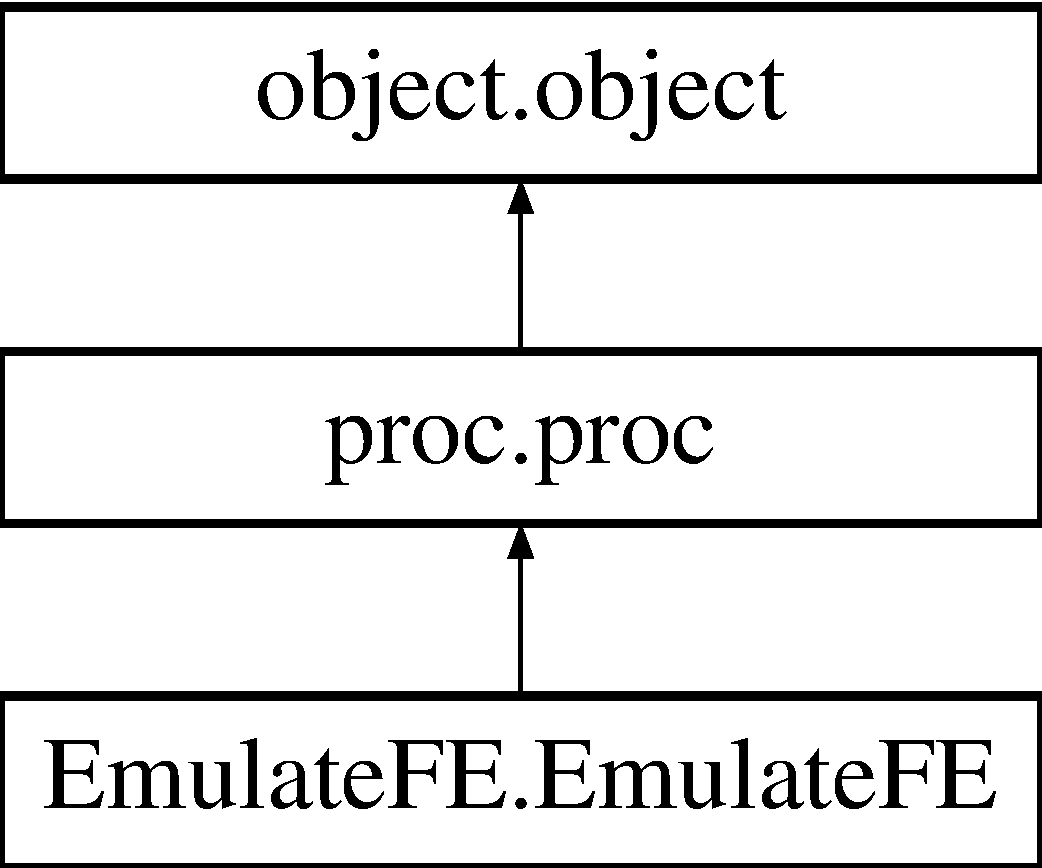
\includegraphics[height=3.000000cm]{classEmulateFE_1_1EmulateFE}
\end{center}
\end{figure}
\subsection*{Public Member Functions}
\begin{DoxyCompactItemize}
\item 
def \hyperlink{classEmulateFE_1_1EmulateFE_aa9871941190d71b8fa8e4b70ee66f9e4}{\+\_\+\+\_\+init\+\_\+\+\_\+} (self, \hyperlink{classobject_1_1object_af114388a80cca208c152ffeca0e89e23}{cat}, \hyperlink{classobject_1_1object_a82b61e7cd7e18b1f9de10fc832e5b75e}{obj}, \hyperlink{classproc_1_1proc_a36068ce6d978f4f4dde164e7bdc2e057}{panel}, \hyperlink{classobject_1_1object_a2a518f960961d791b0f900a90c3cd287}{path})
\item 
def \hyperlink{classEmulateFE_1_1EmulateFE_aefc7339cfc727ad13e3307761ff72795}{update} (self)
\item 
def \hyperlink{classproc_1_1proc_a997ae1c4cc88dfe9e361897bf471ca0f}{parent} (self)
\item 
def \hyperlink{classproc_1_1proc_a7acf16dcc37aaf46cc783a382ae6bd82}{loadxrc} (self)
\item 
def \hyperlink{classproc_1_1proc_a41bdd5dd3af283e3f0053c1a0c7fa7bf}{page} (self)
\item 
def \hyperlink{classobject_1_1object_a54a55487254a96ed2fe367439c41391f}{get\+Control} (self, xmlid, item)
\item 
def \hyperlink{classobject_1_1object_a22a9d1ff67cd6e990cf1b63ed49c50e4}{get\+Control} (self, xmlid)
\end{DoxyCompactItemize}
\subsection*{Public Attributes}
\begin{DoxyCompactItemize}
\item 
\hyperlink{classproc_1_1proc_a36068ce6d978f4f4dde164e7bdc2e057}{panel}
\item 
\hyperlink{classobject_1_1object_af114388a80cca208c152ffeca0e89e23}{cat}
\item 
\hyperlink{classobject_1_1object_a82b61e7cd7e18b1f9de10fc832e5b75e}{obj}
\item 
\hyperlink{classobject_1_1object_a2a518f960961d791b0f900a90c3cd287}{path}
\end{DoxyCompactItemize}


\subsection{Detailed Description}


Definition at line 8 of file Emulate\+F\+E.\+py.



\subsection{Constructor \& Destructor Documentation}
\mbox{\Hypertarget{classEmulateFE_1_1EmulateFE_aa9871941190d71b8fa8e4b70ee66f9e4}\label{classEmulateFE_1_1EmulateFE_aa9871941190d71b8fa8e4b70ee66f9e4}} 
\index{Emulate\+F\+E\+::\+Emulate\+FE@{Emulate\+F\+E\+::\+Emulate\+FE}!\+\_\+\+\_\+init\+\_\+\+\_\+@{\+\_\+\+\_\+init\+\_\+\+\_\+}}
\index{\+\_\+\+\_\+init\+\_\+\+\_\+@{\+\_\+\+\_\+init\+\_\+\+\_\+}!Emulate\+F\+E\+::\+Emulate\+FE@{Emulate\+F\+E\+::\+Emulate\+FE}}
\subsubsection{\texorpdfstring{\+\_\+\+\_\+init\+\_\+\+\_\+()}{\_\_init\_\_()}}
{\footnotesize\ttfamily def Emulate\+F\+E.\+Emulate\+F\+E.\+\_\+\+\_\+init\+\_\+\+\_\+ (\begin{DoxyParamCaption}\item[{}]{self,  }\item[{}]{cat,  }\item[{}]{obj,  }\item[{}]{panel,  }\item[{}]{path }\end{DoxyParamCaption})}



Definition at line 9 of file Emulate\+F\+E.\+py.



References element.\+element.\+loadxrc(), proc.\+proc.\+loadxrc(), Test\+I2\+C.\+Test\+I2\+C.\+on\+Apply(), Test\+S\+P\+I.\+Test\+S\+P\+I.\+on\+Apply(), Test\+U\+S\+B.\+Test\+U\+S\+B.\+on\+Apply(), Storage\+Fifo.\+Storage\+Fifo.\+on\+Apply(), Storage\+Fifo\+Acquisition.\+Storage\+Fifo\+Acquisition.\+on\+Apply(), Test\+Suite.\+Test\+Suite.\+on\+Apply(), Current\+Measurement.\+Current\+Measurement.\+on\+Apply(), A\+D\+C\+Measurement.\+Current\+Measurement.\+on\+Apply(), Usb\+F\+T\+Interface\+Test.\+Usb\+F\+T\+Interface\+Test.\+on\+Apply(), Acquisition.\+Acquisition.\+on\+Apply(), object.\+object.\+panel, element.\+element.\+panel, Log\+Frame.\+Log\+Frame.\+panel, Conf\+Frame.\+Conf\+Frame.\+panel, Graph\+Frame.\+Graph\+Frame.\+panel, App\+Frame.\+App\+Frame.\+panel, Croc.\+Croc.\+update(), Emulate\+F\+E.\+Emulate\+F\+E.\+update(), A3\+P\+E\+\_\+\+Bit\+Flip.\+A3\+P\+E\+\_\+\+Bit\+Flip.\+update(), Croc.\+update(), Proto40\+M\+Hz\+\_\+v1.\+update(), Acquisition.\+Acquisition.\+update(), Proto40\+M\+Hz\+\_\+v1.\+Proto40\+M\+Hz\+\_\+v1.\+update(), Proto\+F\+E\+B\+\_\+v1.\+Proto\+F\+E\+B\+\_\+v1.\+update(), Phaser.\+update(), Usb\+F\+T\+Interface.\+update(), M\+S\+Oxxxx.\+update(), I\+C\+E\+C\+A\+Lv3.\+update(), L\+S\+Delay\+Chip\+V1.\+update(), and A3\+P\+E.\+update().


\begin{DoxyCode}
9     \textcolor{keyword}{def }\hyperlink{classwrapper_1_1ModuleDictWrapper_a9a7a794150502f51df687831583e13b9}{\_\_init\_\_}(self, cat, obj, panel, path):
10         proc.\_\_init\_\_(self,cat,obj,panel,path)
11         self.loadxrc()
12         self.update()
13         self.panel.Bind(wx.EVT\_BUTTON, self.onApply, id=xrc.XRCID(\textcolor{stringliteral}{"Apply"}))
14 
\end{DoxyCode}


\subsection{Member Function Documentation}
\mbox{\Hypertarget{classobject_1_1object_a54a55487254a96ed2fe367439c41391f}\label{classobject_1_1object_a54a55487254a96ed2fe367439c41391f}} 
\index{Emulate\+F\+E\+::\+Emulate\+FE@{Emulate\+F\+E\+::\+Emulate\+FE}!get\+Control@{get\+Control}}
\index{get\+Control@{get\+Control}!Emulate\+F\+E\+::\+Emulate\+FE@{Emulate\+F\+E\+::\+Emulate\+FE}}
\subsubsection{\texorpdfstring{get\+Control()}{getControl()}\hspace{0.1cm}{\footnotesize\ttfamily [1/2]}}
{\footnotesize\ttfamily def object.\+object.\+get\+Control (\begin{DoxyParamCaption}\item[{}]{self,  }\item[{}]{xmlid,  }\item[{}]{item }\end{DoxyParamCaption})\hspace{0.3cm}{\ttfamily [inherited]}}

\begin{DoxyVerb}Retrieves the given control (within a dialog) by its xmlid\end{DoxyVerb}
 

Definition at line 14 of file object.\+py.



Referenced by object.\+object.\+get\+Control(), Proto\+F\+E\+B\+\_\+v1.\+Proto\+F\+E\+B\+\_\+v1.\+is\+Ready(), Proto40\+M\+Hz\+\_\+v1.\+Proto40\+M\+Hz\+\_\+v1.\+is\+Ready(), Acquisition.\+Acquisition.\+on\+Apply(), Proto40\+M\+Hz\+\_\+v1.\+Proto40\+M\+Hz\+\_\+v1.\+onapplyaxlatency(), Proto\+F\+E\+B\+\_\+v1.\+Proto\+F\+E\+B\+\_\+v1.\+onapplyaxlatency(), Proto40\+M\+Hz\+\_\+v1.\+Proto40\+M\+Hz\+\_\+v1.\+onapplyaxlength(), Proto\+F\+E\+B\+\_\+v1.\+Proto\+F\+E\+B\+\_\+v1.\+onapplyaxlength(), Proto\+F\+E\+B\+\_\+v1.\+Proto\+F\+E\+B\+\_\+v1.\+onapply\+Ch(), Proto40\+M\+Hz\+\_\+v1.\+Proto40\+M\+Hz\+\_\+v1.\+onapply\+Ch(), Proto40\+M\+Hz\+\_\+v1.\+Proto40\+M\+Hz\+\_\+v1.\+onapplyclockdiv(), Proto\+F\+E\+B\+\_\+v1.\+Proto\+F\+E\+B\+\_\+v1.\+onapplyclockdiv(), Proto40\+M\+Hz\+\_\+v1.\+Proto40\+M\+Hz\+\_\+v1.\+onapplydelay(), Proto\+F\+E\+B\+\_\+v1.\+Proto\+F\+E\+B\+\_\+v1.\+onapplydelay(), Proto\+F\+E\+B\+\_\+v1.\+Proto\+F\+E\+B\+\_\+v1.\+onapplyfifodepth(), Proto40\+M\+Hz\+\_\+v1.\+Proto40\+M\+Hz\+\_\+v1.\+onapplyfifodepth(), Proto40\+M\+Hz\+\_\+v1.\+Proto40\+M\+Hz\+\_\+v1.\+onapplyfreq(), Proto\+F\+E\+B\+\_\+v1.\+Proto\+F\+E\+B\+\_\+v1.\+onapplyfreq(), Proto40\+M\+Hz\+\_\+v1.\+Proto40\+M\+Hz\+\_\+v1.\+onapplynumber(), Proto\+F\+E\+B\+\_\+v1.\+Proto\+F\+E\+B\+\_\+v1.\+onapplynumber(), Proto\+F\+E\+B\+\_\+v1.\+Proto\+F\+E\+B\+\_\+v1.\+onapplytrig(), Proto40\+M\+Hz\+\_\+v1.\+Proto40\+M\+Hz\+\_\+v1.\+onapplytrig(), Acquisition.\+Acquisition.\+on\+Deadtime(), Acquisition.\+Acquisition.\+on\+Depth(), Proto40\+M\+Hz\+\_\+v1.\+Proto40\+M\+Hz\+\_\+v1.\+onenable\+All(), Proto\+F\+E\+B\+\_\+v1.\+Proto\+F\+E\+B\+\_\+v1.\+onenable\+All(), Acquisition.\+Acquisition.\+on\+Max(), Acquisition.\+Acquisition.\+on\+Min(), Proto40\+M\+Hz\+\_\+v1.\+Proto40\+M\+Hz\+\_\+v1.\+on\+Mode\+A\+X(), Proto\+F\+E\+B\+\_\+v1.\+Proto\+F\+E\+B\+\_\+v1.\+on\+Mode\+A\+X(), Proto40\+M\+Hz\+\_\+v1.\+Proto40\+M\+Hz\+\_\+v1.\+on\+Mode\+Ch(), Proto\+F\+E\+B\+\_\+v1.\+Proto\+F\+E\+B\+\_\+v1.\+on\+Mode\+Ch(), Acquisition.\+Acquisition.\+on\+N\+Bins(), Acquisition.\+Acquisition.\+on\+N\+Sample(), Proto40\+M\+Hz\+\_\+v1.\+Proto40\+M\+Hz\+\_\+v1.\+on\+Pipeline(), Proto\+F\+E\+B\+\_\+v1.\+Proto\+F\+E\+B\+\_\+v1.\+on\+Pipeline(), Acquisition.\+Acquisition.\+on\+Sample(), Acquisition.\+Acquisition.\+on\+Soft\+Trig(), Proto40\+M\+Hz\+\_\+v1.\+Proto40\+M\+Hz\+\_\+v1.\+on\+Soft\+Trig(), Proto\+F\+E\+B\+\_\+v1.\+Proto\+F\+E\+B\+\_\+v1.\+on\+Soft\+Trig(), Acquisition.\+Acquisition.\+on\+Tree(), Acquisition.\+Acquisition.\+on\+Trend(), Proto40\+M\+Hz\+\_\+v1.\+Proto40\+M\+Hz\+\_\+v1.\+onunable\+All(), Proto\+F\+E\+B\+\_\+v1.\+Proto\+F\+E\+B\+\_\+v1.\+onunable\+All(), element.\+element.\+parent(), proc.\+proc.\+parent(), Acquisition.\+Acquisition.\+update(), Proto40\+M\+Hz\+\_\+v1.\+Proto40\+M\+Hz\+\_\+v1.\+update(), and Proto\+F\+E\+B\+\_\+v1.\+Proto\+F\+E\+B\+\_\+v1.\+update().


\begin{DoxyCode}
14     \textcolor{keyword}{def }getControl(self, xmlid , item) :
15         \textcolor{stringliteral}{'''Retrieves the given control (within a dialog) by its xmlid'''}
16         control = item.FindWindowById(xrc.XRCID(xmlid))
17         \textcolor{keyword}{assert} control != \textcolor{keywordtype}{None}, \textcolor{stringliteral}{'Programming error: a control with xml id '} + xmlid + \textcolor{stringliteral}{' was not found.'}
18         \textcolor{keywordflow}{return} control
19 
\end{DoxyCode}
\mbox{\Hypertarget{classobject_1_1object_a22a9d1ff67cd6e990cf1b63ed49c50e4}\label{classobject_1_1object_a22a9d1ff67cd6e990cf1b63ed49c50e4}} 
\index{Emulate\+F\+E\+::\+Emulate\+FE@{Emulate\+F\+E\+::\+Emulate\+FE}!get\+Control@{get\+Control}}
\index{get\+Control@{get\+Control}!Emulate\+F\+E\+::\+Emulate\+FE@{Emulate\+F\+E\+::\+Emulate\+FE}}
\subsubsection{\texorpdfstring{get\+Control()}{getControl()}\hspace{0.1cm}{\footnotesize\ttfamily [2/2]}}
{\footnotesize\ttfamily def object.\+object.\+get\+Control (\begin{DoxyParamCaption}\item[{}]{self,  }\item[{}]{xmlid }\end{DoxyParamCaption})\hspace{0.3cm}{\ttfamily [inherited]}}

\begin{DoxyVerb}Retrieves the given control (within a dialog) by its xmlid\end{DoxyVerb}
 

Definition at line 20 of file object.\+py.



References object.\+object.\+get\+Control(), object.\+object.\+panel, element.\+element.\+panel, Log\+Frame.\+Log\+Frame.\+panel, Conf\+Frame.\+Conf\+Frame.\+panel, Graph\+Frame.\+Graph\+Frame.\+panel, and App\+Frame.\+App\+Frame.\+panel.



Referenced by Proto40\+M\+Hz\+\_\+v1.\+Proto40\+M\+Hz\+\_\+v1.\+is\+Ready(), Acquisition.\+Acquisition.\+on\+Apply(), Proto40\+M\+Hz\+\_\+v1.\+Proto40\+M\+Hz\+\_\+v1.\+onapplyaxlatency(), Proto40\+M\+Hz\+\_\+v1.\+Proto40\+M\+Hz\+\_\+v1.\+onapplyaxlength(), Proto40\+M\+Hz\+\_\+v1.\+Proto40\+M\+Hz\+\_\+v1.\+onapply\+Ch(), Proto40\+M\+Hz\+\_\+v1.\+Proto40\+M\+Hz\+\_\+v1.\+onapplyclockdiv(), Proto40\+M\+Hz\+\_\+v1.\+Proto40\+M\+Hz\+\_\+v1.\+onapplydelay(), Proto40\+M\+Hz\+\_\+v1.\+Proto40\+M\+Hz\+\_\+v1.\+onapplyfifodepth(), Proto40\+M\+Hz\+\_\+v1.\+Proto40\+M\+Hz\+\_\+v1.\+onapplyfreq(), Proto40\+M\+Hz\+\_\+v1.\+Proto40\+M\+Hz\+\_\+v1.\+onapplynumber(), Proto40\+M\+Hz\+\_\+v1.\+Proto40\+M\+Hz\+\_\+v1.\+onapplytrig(), Acquisition.\+Acquisition.\+on\+Deadtime(), Acquisition.\+Acquisition.\+on\+Depth(), Proto40\+M\+Hz\+\_\+v1.\+Proto40\+M\+Hz\+\_\+v1.\+onenable\+All(), Acquisition.\+Acquisition.\+on\+Max(), Acquisition.\+Acquisition.\+on\+Min(), Proto40\+M\+Hz\+\_\+v1.\+Proto40\+M\+Hz\+\_\+v1.\+on\+Mode\+A\+X(), Proto40\+M\+Hz\+\_\+v1.\+Proto40\+M\+Hz\+\_\+v1.\+on\+Mode\+Ch(), Acquisition.\+Acquisition.\+on\+N\+Bins(), Acquisition.\+Acquisition.\+on\+N\+Sample(), Proto40\+M\+Hz\+\_\+v1.\+Proto40\+M\+Hz\+\_\+v1.\+on\+Pipeline(), Acquisition.\+Acquisition.\+on\+Sample(), Acquisition.\+Acquisition.\+on\+Soft\+Trig(), Proto40\+M\+Hz\+\_\+v1.\+Proto40\+M\+Hz\+\_\+v1.\+on\+Soft\+Trig(), Acquisition.\+Acquisition.\+on\+Tree(), Acquisition.\+Acquisition.\+on\+Trend(), Proto40\+M\+Hz\+\_\+v1.\+Proto40\+M\+Hz\+\_\+v1.\+onunable\+All(), Acquisition.\+Acquisition.\+update(), and Proto40\+M\+Hz\+\_\+v1.\+Proto40\+M\+Hz\+\_\+v1.\+update().


\begin{DoxyCode}
20     \textcolor{keyword}{def }getControl(self, xmlid ) :
21         \textcolor{stringliteral}{'''Retrieves the given control (within a dialog) by its xmlid'''}
22         control = self.panel.FindWindowById(xrc.XRCID(xmlid))
23         \textcolor{keyword}{assert} control != \textcolor{keywordtype}{None}, \textcolor{stringliteral}{'Programming error: a control with xml id '} + xmlid + \textcolor{stringliteral}{' was not found.'}
24         \textcolor{keywordflow}{return} control
25 
26                 
27 \textcolor{comment}{#----------------------------------------------------------------------}
28 
29     
30 \end{DoxyCode}
\mbox{\Hypertarget{classproc_1_1proc_a7acf16dcc37aaf46cc783a382ae6bd82}\label{classproc_1_1proc_a7acf16dcc37aaf46cc783a382ae6bd82}} 
\index{Emulate\+F\+E\+::\+Emulate\+FE@{Emulate\+F\+E\+::\+Emulate\+FE}!loadxrc@{loadxrc}}
\index{loadxrc@{loadxrc}!Emulate\+F\+E\+::\+Emulate\+FE@{Emulate\+F\+E\+::\+Emulate\+FE}}
\subsubsection{\texorpdfstring{loadxrc()}{loadxrc()}}
{\footnotesize\ttfamily def proc.\+proc.\+loadxrc (\begin{DoxyParamCaption}\item[{}]{self }\end{DoxyParamCaption})\hspace{0.3cm}{\ttfamily [inherited]}}



Definition at line 16 of file proc.\+py.



References object.\+object.\+obj, Cfg\+Frame.\+Cfg\+Frame.\+obj, object.\+object.\+path, Log\+Frame.\+Log\+Frame.\+path, Conf\+Frame.\+Conf\+Frame.\+path, Graph\+Frame.\+Graph\+Frame.\+path, Cfg\+Frame.\+Cfg\+Frame.\+path, and App\+Frame.\+App\+Frame.\+path.



Referenced by Croc.\+Croc.\+\_\+\+\_\+init\+\_\+\+\_\+(), Computer.\+Computer.\+\_\+\+\_\+init\+\_\+\+\_\+(), Proto40\+M\+Hz\+\_\+v1.\+Proto40\+M\+Hz\+\_\+v1.\+\_\+\+\_\+init\+\_\+\+\_\+(), Acquisition.\+Acquisition.\+\_\+\+\_\+init\+\_\+\+\_\+(), Emulate\+F\+E.\+Emulate\+F\+E.\+\_\+\+\_\+init\+\_\+\+\_\+(), A3\+P\+E\+\_\+\+Bit\+Flip.\+A3\+P\+E\+\_\+\+Bit\+Flip.\+\_\+\+\_\+init\+\_\+\+\_\+(), Storage\+Fifo.\+Storage\+Fifo.\+\_\+\+\_\+init\+\_\+\+\_\+(), Storage\+Fifo\+Acquisition.\+Storage\+Fifo\+Acquisition.\+\_\+\+\_\+init\+\_\+\+\_\+(), Test\+I2\+C.\+Test\+I2\+C.\+\_\+\+\_\+init\+\_\+\+\_\+(), Test\+S\+P\+I.\+Test\+S\+P\+I.\+\_\+\+\_\+init\+\_\+\+\_\+(), Test\+U\+S\+B.\+Test\+U\+S\+B.\+\_\+\+\_\+init\+\_\+\+\_\+(), Test\+Suite.\+Test\+Suite.\+\_\+\+\_\+init\+\_\+\+\_\+(), Usb\+F\+T\+Interface\+Test.\+Usb\+F\+T\+Interface\+Test.\+\_\+\+\_\+init\+\_\+\+\_\+(), A\+D\+C\+Measurement.\+Current\+Measurement.\+\_\+\+\_\+init\+\_\+\+\_\+(), and Current\+Measurement.\+Current\+Measurement.\+\_\+\+\_\+init\+\_\+\+\_\+().


\begin{DoxyCode}
16     \textcolor{keyword}{def }loadxrc(self):
17         path= os.path.join(self.path,\textcolor{stringliteral}{"proc"})
18         path= os.path.join(self.path,\textcolor{stringliteral}{"xrc"})
19         path= os.path.join(path,self.obj.name())
20         path= path+\textcolor{stringliteral}{".xrc"}
21         res=xrc.XmlResource(path)
22         self.panel=res.LoadPanel(self.parent(),self.obj.name())
23         
\end{DoxyCode}
\mbox{\Hypertarget{classproc_1_1proc_a41bdd5dd3af283e3f0053c1a0c7fa7bf}\label{classproc_1_1proc_a41bdd5dd3af283e3f0053c1a0c7fa7bf}} 
\index{Emulate\+F\+E\+::\+Emulate\+FE@{Emulate\+F\+E\+::\+Emulate\+FE}!page@{page}}
\index{page@{page}!Emulate\+F\+E\+::\+Emulate\+FE@{Emulate\+F\+E\+::\+Emulate\+FE}}
\subsubsection{\texorpdfstring{page()}{page()}}
{\footnotesize\ttfamily def proc.\+proc.\+page (\begin{DoxyParamCaption}\item[{}]{self }\end{DoxyParamCaption})\hspace{0.3cm}{\ttfamily [inherited]}}



Definition at line 24 of file proc.\+py.



References object.\+object.\+panel, element.\+element.\+panel, Log\+Frame.\+Log\+Frame.\+panel, Conf\+Frame.\+Conf\+Frame.\+panel, Graph\+Frame.\+Graph\+Frame.\+panel, and App\+Frame.\+App\+Frame.\+panel.


\begin{DoxyCode}
24     \textcolor{keyword}{def }page(self):
25         \textcolor{keywordflow}{return} self.panel
26 \end{DoxyCode}
\mbox{\Hypertarget{classproc_1_1proc_a997ae1c4cc88dfe9e361897bf471ca0f}\label{classproc_1_1proc_a997ae1c4cc88dfe9e361897bf471ca0f}} 
\index{Emulate\+F\+E\+::\+Emulate\+FE@{Emulate\+F\+E\+::\+Emulate\+FE}!parent@{parent}}
\index{parent@{parent}!Emulate\+F\+E\+::\+Emulate\+FE@{Emulate\+F\+E\+::\+Emulate\+FE}}
\subsubsection{\texorpdfstring{parent()}{parent()}}
{\footnotesize\ttfamily def proc.\+proc.\+parent (\begin{DoxyParamCaption}\item[{}]{self }\end{DoxyParamCaption})\hspace{0.3cm}{\ttfamily [inherited]}}



Definition at line 12 of file proc.\+py.



References object.\+object.\+get\+Control(), Conf\+Frame.\+Conf\+Frame.\+get\+Control(), Graph\+Frame.\+Graph\+Frame.\+get\+Control(), Cfg\+Frame.\+Cfg\+Frame.\+get\+Control(), and App\+Frame.\+App\+Frame.\+get\+Control().


\begin{DoxyCode}
12     \textcolor{keyword}{def }parent(self):
13 \textcolor{comment}{#        return self.getControl("Element")   }
14         \textcolor{keywordflow}{return} self.getControl(\textcolor{stringliteral}{"control"})
15 
\end{DoxyCode}
\mbox{\Hypertarget{classEmulateFE_1_1EmulateFE_aefc7339cfc727ad13e3307761ff72795}\label{classEmulateFE_1_1EmulateFE_aefc7339cfc727ad13e3307761ff72795}} 
\index{Emulate\+F\+E\+::\+Emulate\+FE@{Emulate\+F\+E\+::\+Emulate\+FE}!update@{update}}
\index{update@{update}!Emulate\+F\+E\+::\+Emulate\+FE@{Emulate\+F\+E\+::\+Emulate\+FE}}
\subsubsection{\texorpdfstring{update()}{update()}}
{\footnotesize\ttfamily def Emulate\+F\+E.\+Emulate\+F\+E.\+update (\begin{DoxyParamCaption}\item[{}]{self }\end{DoxyParamCaption})}



Definition at line 15 of file Emulate\+F\+E.\+py.



Referenced by Emulate\+F\+E.\+Emulate\+F\+E.\+\_\+\+\_\+init\+\_\+\+\_\+(), App\+Frame.\+App\+Frame.\+delete\+Hardware(), Conf\+Frame.\+Conf\+Frame.\+on\+Change(), Graph\+Frame.\+Graph\+Frame.\+on\+Change(), Cfg\+Frame.\+Cfg\+Frame.\+on\+Change(), Conf\+Frame.\+Conf\+Frame.\+on\+Edit(), App\+Frame.\+App\+Frame.\+on\+Load(), Conf\+Frame.\+Conf\+Frame.\+on\+Re\+Load(), Graph\+Frame.\+Graph\+Frame.\+on\+Re\+Load(), Cfg\+Frame.\+Cfg\+Frame.\+on\+Re\+Load(), and App\+Frame.\+App\+Frame.\+on\+Re\+Load().


\begin{DoxyCode}
15     \textcolor{keyword}{def }update(self):
\end{DoxyCode}


\subsection{Member Data Documentation}
\mbox{\Hypertarget{classobject_1_1object_af114388a80cca208c152ffeca0e89e23}\label{classobject_1_1object_af114388a80cca208c152ffeca0e89e23}} 
\index{Emulate\+F\+E\+::\+Emulate\+FE@{Emulate\+F\+E\+::\+Emulate\+FE}!cat@{cat}}
\index{cat@{cat}!Emulate\+F\+E\+::\+Emulate\+FE@{Emulate\+F\+E\+::\+Emulate\+FE}}
\subsubsection{\texorpdfstring{cat}{cat}}
{\footnotesize\ttfamily object.\+object.\+cat\hspace{0.3cm}{\ttfamily [inherited]}}



Definition at line 8 of file object.\+py.



Referenced by wrapper.\+wrapper.\+Load\+From\+File().

\mbox{\Hypertarget{classobject_1_1object_a82b61e7cd7e18b1f9de10fc832e5b75e}\label{classobject_1_1object_a82b61e7cd7e18b1f9de10fc832e5b75e}} 
\index{Emulate\+F\+E\+::\+Emulate\+FE@{Emulate\+F\+E\+::\+Emulate\+FE}!obj@{obj}}
\index{obj@{obj}!Emulate\+F\+E\+::\+Emulate\+FE@{Emulate\+F\+E\+::\+Emulate\+FE}}
\subsubsection{\texorpdfstring{obj}{obj}}
{\footnotesize\ttfamily object.\+object.\+obj\hspace{0.3cm}{\ttfamily [inherited]}}



Definition at line 9 of file object.\+py.



Referenced by Proto40\+M\+Hz\+\_\+v1.\+Proto40\+M\+Hz\+\_\+v1.\+is\+Ready(), Proto\+F\+E\+B\+\_\+v1.\+Proto\+F\+E\+B\+\_\+v1.\+is\+Ready(), element.\+element.\+loadxrc(), proc.\+proc.\+loadxrc(), Proto40\+M\+Hz\+\_\+v1.\+Proto40\+M\+Hz\+\_\+v1.\+on\+Acquisition(), Proto\+F\+E\+B\+\_\+v1.\+Proto\+F\+E\+B\+\_\+v1.\+on\+Acquisition(), Proto40\+M\+Hz\+\_\+v1.\+Proto40\+M\+Hz\+\_\+v1.\+on\+Acquisition\+Reset(), Proto\+F\+E\+B\+\_\+v1.\+Proto\+F\+E\+B\+\_\+v1.\+on\+Acquisition\+Reset(), Test\+I2\+C.\+Test\+I2\+C.\+on\+Apply(), Test\+S\+P\+I.\+Test\+S\+P\+I.\+on\+Apply(), Test\+U\+S\+B.\+Test\+U\+S\+B.\+on\+Apply(), Storage\+Fifo\+Acquisition.\+Storage\+Fifo\+Acquisition.\+on\+Apply(), Storage\+Fifo.\+Storage\+Fifo.\+on\+Apply(), Test\+Suite.\+Test\+Suite.\+on\+Apply(), Current\+Measurement.\+Current\+Measurement.\+on\+Apply(), A\+D\+C\+Measurement.\+Current\+Measurement.\+on\+Apply(), Usb\+F\+T\+Interface\+Test.\+Usb\+F\+T\+Interface\+Test.\+on\+Apply(), Acquisition.\+Acquisition.\+on\+Apply(), Proto40\+M\+Hz\+\_\+v1.\+Proto40\+M\+Hz\+\_\+v1.\+onapplyaxlatency(), Proto\+F\+E\+B\+\_\+v1.\+Proto\+F\+E\+B\+\_\+v1.\+onapplyaxlatency(), Proto40\+M\+Hz\+\_\+v1.\+Proto40\+M\+Hz\+\_\+v1.\+onapplyaxlength(), Proto\+F\+E\+B\+\_\+v1.\+Proto\+F\+E\+B\+\_\+v1.\+onapplyaxlength(), Proto\+F\+E\+B\+\_\+v1.\+Proto\+F\+E\+B\+\_\+v1.\+onapply\+Ch(), Proto40\+M\+Hz\+\_\+v1.\+Proto40\+M\+Hz\+\_\+v1.\+onapply\+Ch(), Proto\+F\+E\+B\+\_\+v1.\+Proto\+F\+E\+B\+\_\+v1.\+onapplyclockdiv(), Proto40\+M\+Hz\+\_\+v1.\+Proto40\+M\+Hz\+\_\+v1.\+onapplyclockdiv(), Proto40\+M\+Hz\+\_\+v1.\+Proto40\+M\+Hz\+\_\+v1.\+onapplydelay(), Proto\+F\+E\+B\+\_\+v1.\+Proto\+F\+E\+B\+\_\+v1.\+onapplydelay(), Proto40\+M\+Hz\+\_\+v1.\+Proto40\+M\+Hz\+\_\+v1.\+onapplyfifodepth(), Proto\+F\+E\+B\+\_\+v1.\+Proto\+F\+E\+B\+\_\+v1.\+onapplyfifodepth(), Proto\+F\+E\+B\+\_\+v1.\+Proto\+F\+E\+B\+\_\+v1.\+onapplyfreq(), Proto40\+M\+Hz\+\_\+v1.\+Proto40\+M\+Hz\+\_\+v1.\+onapplyfreq(), Proto40\+M\+Hz\+\_\+v1.\+Proto40\+M\+Hz\+\_\+v1.\+onapplynumber(), Proto\+F\+E\+B\+\_\+v1.\+Proto\+F\+E\+B\+\_\+v1.\+onapplynumber(), Proto40\+M\+Hz\+\_\+v1.\+Proto40\+M\+Hz\+\_\+v1.\+onapplytrig(), Proto\+F\+E\+B\+\_\+v1.\+Proto\+F\+E\+B\+\_\+v1.\+onapplytrig(), Acquisition.\+Acquisition.\+on\+Deadtime(), Acquisition.\+Acquisition.\+on\+Depth(), Proto40\+M\+Hz\+\_\+v1.\+Proto40\+M\+Hz\+\_\+v1.\+on\+Enable\+Storage(), Proto\+F\+E\+B\+\_\+v1.\+Proto\+F\+E\+B\+\_\+v1.\+on\+Enable\+Storage(), Proto\+F\+E\+B\+\_\+v1.\+Proto\+F\+E\+B\+\_\+v1.\+on\+Fifo\+R\+A\+Z(), Proto40\+M\+Hz\+\_\+v1.\+Proto40\+M\+Hz\+\_\+v1.\+on\+Fifo\+R\+A\+Z(), Proto40\+M\+Hz\+\_\+v1.\+Proto40\+M\+Hz\+\_\+v1.\+on\+Fifo\+Reset(), Proto\+F\+E\+B\+\_\+v1.\+Proto\+F\+E\+B\+\_\+v1.\+on\+Fifo\+Reset(), Proto\+F\+E\+B\+\_\+v1.\+Proto\+F\+E\+B\+\_\+v1.\+on\+Fifo\+Write(), Proto40\+M\+Hz\+\_\+v1.\+Proto40\+M\+Hz\+\_\+v1.\+on\+Fifo\+Write(), Proto40\+M\+Hz\+\_\+v1.\+Proto40\+M\+Hz\+\_\+v1.\+on\+From\+A\+X\+Ptr\+Raz(), Proto\+F\+E\+B\+\_\+v1.\+Proto\+F\+E\+B\+\_\+v1.\+on\+From\+A\+X\+Ptr\+Raz(), Proto\+F\+E\+B\+\_\+v1.\+Proto\+F\+E\+B\+\_\+v1.\+on\+From\+A\+X\+R\+A\+Z(), Proto40\+M\+Hz\+\_\+v1.\+Proto40\+M\+Hz\+\_\+v1.\+on\+From\+A\+X\+R\+A\+Z(), Proto\+F\+E\+B\+\_\+v1.\+Proto\+F\+E\+B\+\_\+v1.\+on\+From\+A\+X\+Write(), Proto40\+M\+Hz\+\_\+v1.\+Proto40\+M\+Hz\+\_\+v1.\+on\+From\+A\+X\+Write(), Proto40\+M\+Hz\+\_\+v1.\+Proto40\+M\+Hz\+\_\+v1.\+on\+Global\+Reset(), Proto\+F\+E\+B\+\_\+v1.\+Proto\+F\+E\+B\+\_\+v1.\+on\+Global\+Reset(), Proto\+F\+E\+B\+\_\+v1.\+Proto\+F\+E\+B\+\_\+v1.\+on\+Latency\+Reset(), Proto40\+M\+Hz\+\_\+v1.\+Proto40\+M\+Hz\+\_\+v1.\+on\+Latency\+Reset(), Acquisition.\+Acquisition.\+on\+Max(), Acquisition.\+Acquisition.\+on\+Min(), Proto40\+M\+Hz\+\_\+v1.\+Proto40\+M\+Hz\+\_\+v1.\+on\+Mode\+A\+X(), Proto\+F\+E\+B\+\_\+v1.\+Proto\+F\+E\+B\+\_\+v1.\+on\+Mode\+A\+X(), Proto40\+M\+Hz\+\_\+v1.\+Proto40\+M\+Hz\+\_\+v1.\+on\+Mode\+Ch(), Proto\+F\+E\+B\+\_\+v1.\+Proto\+F\+E\+B\+\_\+v1.\+on\+Mode\+Ch(), Acquisition.\+Acquisition.\+on\+N\+Bins(), Acquisition.\+Acquisition.\+on\+N\+Sample(), Proto\+F\+E\+B\+\_\+v1.\+Proto\+F\+E\+B\+\_\+v1.\+on\+Pattern\+R\+A\+Z(), Proto40\+M\+Hz\+\_\+v1.\+Proto40\+M\+Hz\+\_\+v1.\+on\+Pattern\+R\+A\+Z(), Proto\+F\+E\+B\+\_\+v1.\+Proto\+F\+E\+B\+\_\+v1.\+on\+Pattern\+Write(), Proto40\+M\+Hz\+\_\+v1.\+Proto40\+M\+Hz\+\_\+v1.\+on\+Pattern\+Write(), Proto40\+M\+Hz\+\_\+v1.\+Proto40\+M\+Hz\+\_\+v1.\+on\+Phaser0(), Proto\+F\+E\+B\+\_\+v1.\+Proto\+F\+E\+B\+\_\+v1.\+on\+Phaser0(), Proto\+F\+E\+B\+\_\+v1.\+Proto\+F\+E\+B\+\_\+v1.\+on\+Phaser1(), Proto40\+M\+Hz\+\_\+v1.\+Proto40\+M\+Hz\+\_\+v1.\+on\+Phaser1(), Proto40\+M\+Hz\+\_\+v1.\+Proto40\+M\+Hz\+\_\+v1.\+on\+Phaser2(), Proto\+F\+E\+B\+\_\+v1.\+Proto\+F\+E\+B\+\_\+v1.\+on\+Phaser2(), Proto\+F\+E\+B\+\_\+v1.\+Proto\+F\+E\+B\+\_\+v1.\+on\+Pipeline(), Proto40\+M\+Hz\+\_\+v1.\+Proto40\+M\+Hz\+\_\+v1.\+on\+Pipeline(), Proto40\+M\+Hz\+\_\+v1.\+Proto40\+M\+Hz\+\_\+v1.\+on\+Read\+Fifo(), Proto\+F\+E\+B\+\_\+v1.\+Proto\+F\+E\+B\+\_\+v1.\+on\+Read\+Fifo(), Proto40\+M\+Hz\+\_\+v1.\+Proto40\+M\+Hz\+\_\+v1.\+on\+Read\+From\+A\+X(), Proto\+F\+E\+B\+\_\+v1.\+Proto\+F\+E\+B\+\_\+v1.\+on\+Read\+From\+A\+X(), Proto\+F\+E\+B\+\_\+v1.\+Proto\+F\+E\+B\+\_\+v1.\+on\+Read\+Pattern(), Proto40\+M\+Hz\+\_\+v1.\+Proto40\+M\+Hz\+\_\+v1.\+on\+Read\+Pattern(), Proto\+F\+E\+B\+\_\+v1.\+Proto\+F\+E\+B\+\_\+v1.\+on\+Read\+To\+A\+X(), Proto40\+M\+Hz\+\_\+v1.\+Proto40\+M\+Hz\+\_\+v1.\+on\+Read\+To\+A\+X(), Proto40\+M\+Hz\+\_\+v1.\+Proto40\+M\+Hz\+\_\+v1.\+on\+Read\+Trigger(), Proto\+F\+E\+B\+\_\+v1.\+Proto\+F\+E\+B\+\_\+v1.\+on\+Read\+Trigger(), Proto40\+M\+Hz\+\_\+v1.\+Proto40\+M\+Hz\+\_\+v1.\+on\+Reset\+F\+E(), Proto\+F\+E\+B\+\_\+v1.\+Proto\+F\+E\+B\+\_\+v1.\+on\+Reset\+F\+E(), Proto\+F\+E\+B\+\_\+v1.\+Proto\+F\+E\+B\+\_\+v1.\+on\+Reset\+S\+P\+I(), Proto40\+M\+Hz\+\_\+v1.\+Proto40\+M\+Hz\+\_\+v1.\+on\+Reset\+S\+P\+I(), Acquisition.\+Acquisition.\+on\+Sample(), Acquisition.\+Acquisition.\+on\+Soft\+Trig(), Proto\+F\+E\+B\+\_\+v1.\+Proto\+F\+E\+B\+\_\+v1.\+on\+Soft\+Trig(), Proto40\+M\+Hz\+\_\+v1.\+Proto40\+M\+Hz\+\_\+v1.\+on\+Soft\+Trig(), Proto\+F\+E\+B\+\_\+v1.\+Proto\+F\+E\+B\+\_\+v1.\+on\+Start\+Sequence\+A\+X(), Proto40\+M\+Hz\+\_\+v1.\+Proto40\+M\+Hz\+\_\+v1.\+on\+Start\+Sequence\+A\+X(), Proto40\+M\+Hz\+\_\+v1.\+Proto40\+M\+Hz\+\_\+v1.\+on\+To\+A\+X\+Ptr\+Raz(), Proto\+F\+E\+B\+\_\+v1.\+Proto\+F\+E\+B\+\_\+v1.\+on\+To\+A\+X\+Ptr\+Raz(), Proto40\+M\+Hz\+\_\+v1.\+Proto40\+M\+Hz\+\_\+v1.\+on\+To\+A\+X\+R\+A\+Z(), Proto\+F\+E\+B\+\_\+v1.\+Proto\+F\+E\+B\+\_\+v1.\+on\+To\+A\+X\+R\+A\+Z(), Proto\+F\+E\+B\+\_\+v1.\+Proto\+F\+E\+B\+\_\+v1.\+on\+To\+A\+X\+Write(), Proto40\+M\+Hz\+\_\+v1.\+Proto40\+M\+Hz\+\_\+v1.\+on\+To\+A\+X\+Write(), Acquisition.\+Acquisition.\+on\+Tree(), Acquisition.\+Acquisition.\+on\+Trend(), Proto40\+M\+Hz\+\_\+v1.\+Proto40\+M\+Hz\+\_\+v1.\+on\+Trigger(), Proto\+F\+E\+B\+\_\+v1.\+Proto\+F\+E\+B\+\_\+v1.\+on\+Trigger(), Proto40\+M\+Hz\+\_\+v1.\+Proto40\+M\+Hz\+\_\+v1.\+on\+Trigger\+R\+A\+Z(), Proto\+F\+E\+B\+\_\+v1.\+Proto\+F\+E\+B\+\_\+v1.\+on\+Trigger\+R\+A\+Z(), Proto40\+M\+Hz\+\_\+v1.\+Proto40\+M\+Hz\+\_\+v1.\+on\+Trigger\+Write(), Proto\+F\+E\+B\+\_\+v1.\+Proto\+F\+E\+B\+\_\+v1.\+on\+Trigger\+Write(), Proto40\+M\+Hz\+\_\+v1.\+Proto40\+M\+Hz\+\_\+v1.\+on\+Usb\+Phasers\+Reset(), Proto\+F\+E\+B\+\_\+v1.\+Proto\+F\+E\+B\+\_\+v1.\+on\+Usb\+Phasers\+Reset(), Test\+S\+P\+I.\+Test\+S\+P\+I.\+update(), Test\+I2\+C.\+Test\+I2\+C.\+update(), Test\+U\+S\+B.\+Test\+U\+S\+B.\+update(), Test\+Suite.\+Test\+Suite.\+update(), Storage\+Fifo.\+Storage\+Fifo.\+update(), Storage\+Fifo\+Acquisition.\+Storage\+Fifo\+Acquisition.\+update(), Current\+Measurement.\+Current\+Measurement.\+update(), A\+D\+C\+Measurement.\+Current\+Measurement.\+update(), Usb\+F\+T\+Interface\+Test.\+Usb\+F\+T\+Interface\+Test.\+update(), Acquisition.\+Acquisition.\+update(), Proto\+F\+E\+B\+\_\+v1.\+Proto\+F\+E\+B\+\_\+v1.\+update(), and Proto40\+M\+Hz\+\_\+v1.\+Proto40\+M\+Hz\+\_\+v1.\+update().

\mbox{\Hypertarget{classproc_1_1proc_a36068ce6d978f4f4dde164e7bdc2e057}\label{classproc_1_1proc_a36068ce6d978f4f4dde164e7bdc2e057}} 
\index{Emulate\+F\+E\+::\+Emulate\+FE@{Emulate\+F\+E\+::\+Emulate\+FE}!panel@{panel}}
\index{panel@{panel}!Emulate\+F\+E\+::\+Emulate\+FE@{Emulate\+F\+E\+::\+Emulate\+FE}}
\subsubsection{\texorpdfstring{panel}{panel}}
{\footnotesize\ttfamily proc.\+proc.\+panel\hspace{0.3cm}{\ttfamily [inherited]}}



Definition at line 22 of file proc.\+py.



Referenced by A3\+P\+E\+\_\+\+Bit\+Flip.\+A3\+P\+E\+\_\+\+Bit\+Flip.\+\_\+\+\_\+init\+\_\+\+\_\+(), Acquisition.\+Acquisition.\+\_\+\+\_\+init\+\_\+\+\_\+(), and Proto40\+M\+Hz\+\_\+v1.\+Proto40\+M\+Hz\+\_\+v1.\+get\+File().

\mbox{\Hypertarget{classobject_1_1object_a2a518f960961d791b0f900a90c3cd287}\label{classobject_1_1object_a2a518f960961d791b0f900a90c3cd287}} 
\index{Emulate\+F\+E\+::\+Emulate\+FE@{Emulate\+F\+E\+::\+Emulate\+FE}!path@{path}}
\index{path@{path}!Emulate\+F\+E\+::\+Emulate\+FE@{Emulate\+F\+E\+::\+Emulate\+FE}}
\subsubsection{\texorpdfstring{path}{path}}
{\footnotesize\ttfamily object.\+object.\+path\hspace{0.3cm}{\ttfamily [inherited]}}



Definition at line 11 of file object.\+py.



Referenced by element.\+element.\+loadxrc(), and proc.\+proc.\+loadxrc().



The documentation for this class was generated from the following file\+:\begin{DoxyCompactItemize}
\item 
/home/eleclhcb/\+L\+H\+Cb/lbcat-\/cmake/\+Cat\+Calo\+Proto40\+M\+Hz/python/proc/\hyperlink{EmulateFE_8py}{Emulate\+F\+E.\+py}\end{DoxyCompactItemize}

\hypertarget{classEvent}{
\section{Event Class Reference}
\label{classEvent}\index{Event@{Event}}
}


{\ttfamily \#include $<$include/Event.h$>$}\subsection*{Public Member Functions}
\begin{DoxyCompactItemize}
\item 
\hyperlink{classEvent_a5a40dd4708297f7031e29b39e039ae10}{Event} ()
\begin{DoxyCompactList}\small\item\em Standard constructor. \item\end{DoxyCompactList}\item 
virtual \hyperlink{classEvent_a7704ec01ce91e673885792054214b3d2}{$\sim$Event} ()
\begin{DoxyCompactList}\small\item\em Destructor. \item\end{DoxyCompactList}\item 
void \hyperlink{classEvent_a3b8cf87617622d58b29e2400b5aeb481}{setRun} (unsigned long irun)
\item 
void \hyperlink{classEvent_a04c03ff6f9c2470be922bca4da71afe4}{Clear} (Option\_\-t $\ast$option=\char`\"{}\char`\"{})
\item 
void \hyperlink{classEvent_a32bf7bf773b68f07ef29c561e80d404f}{newEvt} ()
\item 
void \hyperlink{classEvent_a5bca3178f77846a68aafd8ebc9fa38d0}{addData} (int, int, int)
\item 
TClonesArray $\ast$ \hyperlink{classEvent_a50e0385cff686a988e779226062d4ba3}{getData} ()
\end{DoxyCompactItemize}
\subsection*{Public Attributes}
\begin{DoxyCompactItemize}
\item 
ClassDef(\hyperlink{classEvent}{Event}, 1) protected unsigned long \hyperlink{classEvent_ae71a25ddbd57cb78f964a98f688e7b01}{nData}
\item 
TClonesArray $\ast$ \hyperlink{classEvent_ac59cc6743d8d652c347dba08ab66c2f6}{raw}
\item 
TRef \hyperlink{classEvent_a969eb9ae4ae0b7342502baaea6844f3b}{fLastData}
\end{DoxyCompactItemize}
\subsection*{Static Public Attributes}
\begin{DoxyCompactItemize}
\item 
static TClonesArray $\ast$ \hyperlink{classEvent_a3584dd1f773c5746f674d63d74f4ec88}{fgData}
\end{DoxyCompactItemize}


\subsection{Detailed Description}
\begin{DoxyAuthor}{Author}
Fr�d�ric Machefert 
\end{DoxyAuthor}
\begin{DoxyDate}{Date}
2004-\/10-\/04 
\end{DoxyDate}


Definition at line 23 of file Event.h.

\subsection{Constructor \& Destructor Documentation}
\hypertarget{classEvent_a5a40dd4708297f7031e29b39e039ae10}{
\index{Event@{Event}!Event@{Event}}
\index{Event@{Event}!Event@{Event}}
\subsubsection[{Event}]{\setlength{\rightskip}{0pt plus 5cm}Event::Event ()}}
\label{classEvent_a5a40dd4708297f7031e29b39e039ae10}


Standard constructor. \hypertarget{classEvent_a7704ec01ce91e673885792054214b3d2}{
\index{Event@{Event}!$\sim$Event@{$\sim$Event}}
\index{$\sim$Event@{$\sim$Event}!Event@{Event}}
\subsubsection[{$\sim$Event}]{\setlength{\rightskip}{0pt plus 5cm}Event::$\sim$Event ()\hspace{0.3cm}{\ttfamily  \mbox{[}virtual\mbox{]}}}}
\label{classEvent_a7704ec01ce91e673885792054214b3d2}


Destructor. 

Definition at line 35 of file Event.cpp.

References Clear().


\begin{DoxyCode}
35               {
36   Clear();
37 }
\end{DoxyCode}


\subsection{Member Function Documentation}
\hypertarget{classEvent_a5bca3178f77846a68aafd8ebc9fa38d0}{
\index{Event@{Event}!addData@{addData}}
\index{addData@{addData}!Event@{Event}}
\subsubsection[{addData}]{\setlength{\rightskip}{0pt plus 5cm}void Event::addData (int {\em evt}, \/  int {\em chl}, \/  int {\em value})}}
\label{classEvent_a5bca3178f77846a68aafd8ebc9fa38d0}


Definition at line 40 of file Event.cpp.

References fLastData, nData, and raw.


\begin{DoxyCode}
40                                                    {
41   TClonesArray &rawdata = *raw;
42    Data *val = new(rawdata[nData++]) Data( evt , chl , value );
43    //Save reference to last Data in the collection of Datas
44    fLastData = val;
45 }
\end{DoxyCode}
\hypertarget{classEvent_a04c03ff6f9c2470be922bca4da71afe4}{
\index{Event@{Event}!Clear@{Clear}}
\index{Clear@{Clear}!Event@{Event}}
\subsubsection[{Clear}]{\setlength{\rightskip}{0pt plus 5cm}void Event::Clear (Option\_\-t $\ast$ {\em option} = {\ttfamily \char`\"{}\char`\"{}})}}
\label{classEvent_a04c03ff6f9c2470be922bca4da71afe4}


Definition at line 48 of file Event.cpp.

References raw.

Referenced by $\sim$Event().


\begin{DoxyCode}
49 {
50   raw->Clear("C"); //will also call Data::Clear
51 }
\end{DoxyCode}
\hypertarget{classEvent_a50e0385cff686a988e779226062d4ba3}{
\index{Event@{Event}!getData@{getData}}
\index{getData@{getData}!Event@{Event}}
\subsubsection[{getData}]{\setlength{\rightskip}{0pt plus 5cm}TClonesArray$\ast$ Event::getData ()\hspace{0.3cm}{\ttfamily  \mbox{[}inline\mbox{]}}}}
\label{classEvent_a50e0385cff686a988e779226062d4ba3}


Definition at line 34 of file Event.h.

References fgData.


\begin{DoxyCode}
34 { return fgData;}
\end{DoxyCode}
\hypertarget{classEvent_a32bf7bf773b68f07ef29c561e80d404f}{
\index{Event@{Event}!newEvt@{newEvt}}
\index{newEvt@{newEvt}!Event@{Event}}
\subsubsection[{newEvt}]{\setlength{\rightskip}{0pt plus 5cm}void Event::newEvt ()}}
\label{classEvent_a32bf7bf773b68f07ef29c561e80d404f}


Definition at line 54 of file Event.cpp.


\begin{DoxyCode}
55 {
56    EvtHdr.newEvt();
57    /*
58    data->Clear("C"); //will also call Data::Clear
59    nData = 0 ;
60   */
61 }
\end{DoxyCode}
\hypertarget{classEvent_a3b8cf87617622d58b29e2400b5aeb481}{
\index{Event@{Event}!setRun@{setRun}}
\index{setRun@{setRun}!Event@{Event}}
\subsubsection[{setRun}]{\setlength{\rightskip}{0pt plus 5cm}void Event::setRun (unsigned long {\em irun})\hspace{0.3cm}{\ttfamily  \mbox{[}inline\mbox{]}}}}
\label{classEvent_a3b8cf87617622d58b29e2400b5aeb481}


Definition at line 28 of file Event.h.


\begin{DoxyCode}
28                                      {
29     EvtHdr.setRun ( irun );
30   }  
\end{DoxyCode}


\subsection{Member Data Documentation}
\hypertarget{classEvent_a3584dd1f773c5746f674d63d74f4ec88}{
\index{Event@{Event}!fgData@{fgData}}
\index{fgData@{fgData}!Event@{Event}}
\subsubsection[{fgData}]{\setlength{\rightskip}{0pt plus 5cm}TClonesArray$\ast$ {\bf Event::fgData}\hspace{0.3cm}{\ttfamily  \mbox{[}static\mbox{]}}}}
\label{classEvent_a3584dd1f773c5746f674d63d74f4ec88}


Definition at line 42 of file Event.h.

Referenced by getData().\hypertarget{classEvent_a969eb9ae4ae0b7342502baaea6844f3b}{
\index{Event@{Event}!fLastData@{fLastData}}
\index{fLastData@{fLastData}!Event@{Event}}
\subsubsection[{fLastData}]{\setlength{\rightskip}{0pt plus 5cm}TRef {\bf Event::fLastData}}}
\label{classEvent_a969eb9ae4ae0b7342502baaea6844f3b}


Definition at line 43 of file Event.h.

Referenced by addData().\hypertarget{classEvent_ae71a25ddbd57cb78f964a98f688e7b01}{
\index{Event@{Event}!nData@{nData}}
\index{nData@{nData}!Event@{Event}}
\subsubsection[{nData}]{\setlength{\rightskip}{0pt plus 5cm}ClassDef ({\bf Event},1) protected unsigned long {\bf Event::nData}}}
\label{classEvent_ae71a25ddbd57cb78f964a98f688e7b01}


Definition at line 35 of file Event.h.

Referenced by addData().\hypertarget{classEvent_ac59cc6743d8d652c347dba08ab66c2f6}{
\index{Event@{Event}!raw@{raw}}
\index{raw@{raw}!Event@{Event}}
\subsubsection[{raw}]{\setlength{\rightskip}{0pt plus 5cm}TClonesArray$\ast$ {\bf Event::raw}}}
\label{classEvent_ac59cc6743d8d652c347dba08ab66c2f6}


Definition at line 41 of file Event.h.

Referenced by addData(), and Clear().

The documentation for this class was generated from the following files:\begin{DoxyCompactItemize}
\item 
/home/eleclhcb/LHCb/lbcat-\/cmake/CatCaloEvent/inc/\hyperlink{Event_8h}{Event.h}\item 
/home/eleclhcb/LHCb/lbcat-\/cmake/CatCaloEvent/src/\hyperlink{Event_8cpp}{Event.cpp}\end{DoxyCompactItemize}

\hypertarget{classEventHeader}{
\section{EventHeader Class Reference}
\label{classEventHeader}\index{EventHeader@{EventHeader}}
}


{\ttfamily \#include $<$include/EventHeader.h$>$}\subsection*{Public Member Functions}
\begin{DoxyCompactItemize}
\item 
\hyperlink{classEventHeader_ae2143206ec5b29d153067b3a1ff0ba19}{EventHeader} ()
\begin{DoxyCompactList}\small\item\em Standard constructor. \item\end{DoxyCompactList}\item 
\hyperlink{classEventHeader_af0e4e6e449537503a3a08a8d58ab4235}{EventHeader} (int, int)
\item 
virtual \hyperlink{classEventHeader_ad6c5966f7d4a6a6f9d76f730de80c50a}{$\sim$EventHeader} ()
\begin{DoxyCompactList}\small\item\em Destructor. \item\end{DoxyCompactList}\item 
unsigned long \hyperlink{classEventHeader_af54e2ad4984187b2aa9ecbda6bf07cd0}{evt} ()
\item 
unsigned long \hyperlink{classEventHeader_a5cf1b80c7e41886ae5d177f1a444b280}{run} ()
\item 
unsigned long \hyperlink{classEventHeader_adbda915747b0bd94a19e2e5d3ec7db97}{date} ()
\item 
void \hyperlink{classEventHeader_a978b95b3b941bfa6ad92e09aaa0ebcc0}{setEvt} (unsigned long ievt)
\item 
void \hyperlink{classEventHeader_a9444a1e959b20387dc8d74c31e5c5aa6}{setRun} (unsigned long irun)
\item 
void \hyperlink{classEventHeader_aade4ba64d15f2b25e09eb4cb16d9fb3c}{newEvt} ()
\end{DoxyCompactItemize}
\subsection*{Public Attributes}
\begin{DoxyCompactItemize}
\item 
ClassDef(\hyperlink{classEventHeader}{EventHeader}, 1) protected unsigned long \hyperlink{classEventHeader_a9763260b9dc642325bacb534188ab0fd}{Run}
\item 
unsigned long \hyperlink{classEventHeader_af8098a8d9d00190c845e7b7df833e0a9}{Date}
\end{DoxyCompactItemize}


\subsection{Detailed Description}
\begin{DoxyAuthor}{Author}
Fr�d�ric Machefert 
\end{DoxyAuthor}
\begin{DoxyDate}{Date}
2004-\/10-\/04 
\end{DoxyDate}


Definition at line 20 of file EventHeader.h.

\subsection{Constructor \& Destructor Documentation}
\hypertarget{classEventHeader_ae2143206ec5b29d153067b3a1ff0ba19}{
\index{EventHeader@{EventHeader}!EventHeader@{EventHeader}}
\index{EventHeader@{EventHeader}!EventHeader@{EventHeader}}
\subsubsection[{EventHeader}]{\setlength{\rightskip}{0pt plus 5cm}EventHeader::EventHeader ()}}
\label{classEventHeader_ae2143206ec5b29d153067b3a1ff0ba19}


Standard constructor. \hypertarget{classEventHeader_af0e4e6e449537503a3a08a8d58ab4235}{
\index{EventHeader@{EventHeader}!EventHeader@{EventHeader}}
\index{EventHeader@{EventHeader}!EventHeader@{EventHeader}}
\subsubsection[{EventHeader}]{\setlength{\rightskip}{0pt plus 5cm}EventHeader::EventHeader (int {\em run}, \/  int {\em evt})}}
\label{classEventHeader_af0e4e6e449537503a3a08a8d58ab4235}


Definition at line 26 of file EventHeader.cpp.

References Date.


\begin{DoxyCode}
26                                            {
27   Run = run;
28   Evt = evt;
29   TDatime today;
30   Date   = today.GetDate();
31 }
\end{DoxyCode}
\hypertarget{classEventHeader_ad6c5966f7d4a6a6f9d76f730de80c50a}{
\index{EventHeader@{EventHeader}!$\sim$EventHeader@{$\sim$EventHeader}}
\index{$\sim$EventHeader@{$\sim$EventHeader}!EventHeader@{EventHeader}}
\subsubsection[{$\sim$EventHeader}]{\setlength{\rightskip}{0pt plus 5cm}EventHeader::$\sim$EventHeader ()\hspace{0.3cm}{\ttfamily  \mbox{[}virtual\mbox{]}}}}
\label{classEventHeader_ad6c5966f7d4a6a6f9d76f730de80c50a}


Destructor. 

Definition at line 36 of file EventHeader.cpp.


\begin{DoxyCode}
36                           {
37 }
\end{DoxyCode}


\subsection{Member Function Documentation}
\hypertarget{classEventHeader_adbda915747b0bd94a19e2e5d3ec7db97}{
\index{EventHeader@{EventHeader}!date@{date}}
\index{date@{date}!EventHeader@{EventHeader}}
\subsubsection[{date}]{\setlength{\rightskip}{0pt plus 5cm}unsigned long EventHeader::date ()\hspace{0.3cm}{\ttfamily  \mbox{[}inline\mbox{]}}}}
\label{classEventHeader_adbda915747b0bd94a19e2e5d3ec7db97}


Definition at line 35 of file EventHeader.h.

References Date.


\begin{DoxyCode}
35                       {
36     return Date;
37   }  
\end{DoxyCode}
\hypertarget{classEventHeader_af54e2ad4984187b2aa9ecbda6bf07cd0}{
\index{EventHeader@{EventHeader}!evt@{evt}}
\index{evt@{evt}!EventHeader@{EventHeader}}
\subsubsection[{evt}]{\setlength{\rightskip}{0pt plus 5cm}unsigned long EventHeader::evt ()\hspace{0.3cm}{\ttfamily  \mbox{[}inline\mbox{]}}}}
\label{classEventHeader_af54e2ad4984187b2aa9ecbda6bf07cd0}


Definition at line 27 of file EventHeader.h.


\begin{DoxyCode}
27                      {
28     return Evt;
29   }
\end{DoxyCode}
\hypertarget{classEventHeader_aade4ba64d15f2b25e09eb4cb16d9fb3c}{
\index{EventHeader@{EventHeader}!newEvt@{newEvt}}
\index{newEvt@{newEvt}!EventHeader@{EventHeader}}
\subsubsection[{newEvt}]{\setlength{\rightskip}{0pt plus 5cm}void EventHeader::newEvt ()}}
\label{classEventHeader_aade4ba64d15f2b25e09eb4cb16d9fb3c}


Definition at line 42 of file EventHeader.cpp.

References Date.


\begin{DoxyCode}
42                         {
43   Evt++;  
44   TDatime today;
45   Date   = today.GetDate();
46 }
\end{DoxyCode}
\hypertarget{classEventHeader_a5cf1b80c7e41886ae5d177f1a444b280}{
\index{EventHeader@{EventHeader}!run@{run}}
\index{run@{run}!EventHeader@{EventHeader}}
\subsubsection[{run}]{\setlength{\rightskip}{0pt plus 5cm}unsigned long EventHeader::run ()\hspace{0.3cm}{\ttfamily  \mbox{[}inline\mbox{]}}}}
\label{classEventHeader_a5cf1b80c7e41886ae5d177f1a444b280}


Definition at line 31 of file EventHeader.h.


\begin{DoxyCode}
31                      {
32     return Run;
33   }
\end{DoxyCode}
\hypertarget{classEventHeader_a978b95b3b941bfa6ad92e09aaa0ebcc0}{
\index{EventHeader@{EventHeader}!setEvt@{setEvt}}
\index{setEvt@{setEvt}!EventHeader@{EventHeader}}
\subsubsection[{setEvt}]{\setlength{\rightskip}{0pt plus 5cm}void EventHeader::setEvt (unsigned long {\em ievt})\hspace{0.3cm}{\ttfamily  \mbox{[}inline\mbox{]}}}}
\label{classEventHeader_a978b95b3b941bfa6ad92e09aaa0ebcc0}


Definition at line 39 of file EventHeader.h.


\begin{DoxyCode}
39                                   {
40     Evt = ievt;
41   }
\end{DoxyCode}
\hypertarget{classEventHeader_a9444a1e959b20387dc8d74c31e5c5aa6}{
\index{EventHeader@{EventHeader}!setRun@{setRun}}
\index{setRun@{setRun}!EventHeader@{EventHeader}}
\subsubsection[{setRun}]{\setlength{\rightskip}{0pt plus 5cm}void EventHeader::setRun (unsigned long {\em irun})\hspace{0.3cm}{\ttfamily  \mbox{[}inline\mbox{]}}}}
\label{classEventHeader_a9444a1e959b20387dc8d74c31e5c5aa6}


Definition at line 43 of file EventHeader.h.


\begin{DoxyCode}
43                                   {
44     Run = irun;
45   }
\end{DoxyCode}


\subsection{Member Data Documentation}
\hypertarget{classEventHeader_af8098a8d9d00190c845e7b7df833e0a9}{
\index{EventHeader@{EventHeader}!Date@{Date}}
\index{Date@{Date}!EventHeader@{EventHeader}}
\subsubsection[{Date}]{\setlength{\rightskip}{0pt plus 5cm}unsigned long {\bf EventHeader::Date}}}
\label{classEventHeader_af8098a8d9d00190c845e7b7df833e0a9}


Definition at line 61 of file EventHeader.h.

Referenced by date(), EventHeader(), and newEvt().\hypertarget{classEventHeader_a9763260b9dc642325bacb534188ab0fd}{
\index{EventHeader@{EventHeader}!Run@{Run}}
\index{Run@{Run}!EventHeader@{EventHeader}}
\subsubsection[{Run}]{\setlength{\rightskip}{0pt plus 5cm}ClassDef ({\bf EventHeader},1) protected unsigned long {\bf EventHeader::Run}}}
\label{classEventHeader_a9763260b9dc642325bacb534188ab0fd}


Definition at line 54 of file EventHeader.h.

The documentation for this class was generated from the following files:\begin{DoxyCompactItemize}
\item 
/home/eleclhcb/LHCb/lbcat-\/cmake/CatCaloEvent/inc/\hyperlink{EventHeader_8h}{EventHeader.h}\item 
/home/eleclhcb/LHCb/lbcat-\/cmake/CatCaloEvent/src/\hyperlink{EventHeader_8cpp}{EventHeader.cpp}\end{DoxyCompactItemize}

\hypertarget{classFactory}{}\section{Factory Class Reference}
\label{classFactory}\index{Factory@{Factory}}


{\ttfamily \#include $<$inc/\+Factory.\+h$>$}

\subsection*{Public Member Functions}
\begin{DoxyCompactItemize}
\item 
\hyperlink{classFactory_ac792bf88cfb7b6804b479529da5308cc}{Factory} ()
\begin{DoxyCompactList}\small\item\em Standard constructor. \end{DoxyCompactList}\item 
virtual \hyperlink{classFactory_abb3d73c23bef3ca95487856ef0d7c476}{$\sim$\+Factory} ()
\begin{DoxyCompactList}\small\item\em Destructor. \end{DoxyCompactList}\item 
void \hyperlink{classFactory_a0f10adde2d57c8a1d07fdb4557f3ac3b}{set\+List\+D\+LL} (std\+::string \hyperlink{classFactory_a21cd37e4b21b06e574cf67faea08782a}{list\+D\+LL})
\item 
std\+::string \hyperlink{classFactory_a21cd37e4b21b06e574cf67faea08782a}{list\+D\+LL} ()
\item 
void \hyperlink{classFactory_a7bc368f81d0228931a44b41b27c39b53}{set\+List\+Element} (std\+::list \hyperlink{classFactory_aca9a1442c4ee2f17ea27db723ce65d90}{list\+Element})
\item 
std\+::list \hyperlink{classFactory_aca9a1442c4ee2f17ea27db723ce65d90}{list\+Element} ()
\item 
void \hyperlink{classFactory_afdec7fe6e79da3e5748d33f740333671}{set\+List\+Proc} (std\+::string \hyperlink{classFactory_afb222fc976d624fa6fdcb30f0aca586c}{list\+Proc})
\item 
std\+::string \hyperlink{classFactory_afb222fc976d624fa6fdcb30f0aca586c}{list\+Proc} ()
\end{DoxyCompactItemize}
\subsection*{Private Attributes}
\begin{DoxyCompactItemize}
\item 
std\+::string \hyperlink{classFactory_a266167ae49fcf4fa9baa5485dea4b062}{m\+\_\+list\+D\+LL}
\item 
std\+::list \hyperlink{classFactory_a83a99d80105fab2371ce03230b90e8a3}{m\+\_\+list\+Element}
\item 
std\+::string \hyperlink{classFactory_aec20c1d0a1ef175f55a82e868edabe88}{m\+\_\+list\+Proc}
\end{DoxyCompactItemize}


\subsection{Detailed Description}
\begin{DoxyAuthor}{Author}

\end{DoxyAuthor}
\begin{DoxyDate}{Date}
2006-\/10-\/23 
\end{DoxyDate}


Definition at line 13 of file Factory.\+h.



\subsection{Constructor \& Destructor Documentation}
\mbox{\Hypertarget{classFactory_ac792bf88cfb7b6804b479529da5308cc}\label{classFactory_ac792bf88cfb7b6804b479529da5308cc}} 
\index{Factory@{Factory}!Factory@{Factory}}
\index{Factory@{Factory}!Factory@{Factory}}
\subsubsection{\texorpdfstring{Factory()}{Factory()}}
{\footnotesize\ttfamily Factory\+::\+Factory (\begin{DoxyParamCaption}{ }\end{DoxyParamCaption})}



Standard constructor. 

\mbox{\Hypertarget{classFactory_abb3d73c23bef3ca95487856ef0d7c476}\label{classFactory_abb3d73c23bef3ca95487856ef0d7c476}} 
\index{Factory@{Factory}!````~Factory@{$\sim$\+Factory}}
\index{````~Factory@{$\sim$\+Factory}!Factory@{Factory}}
\subsubsection{\texorpdfstring{$\sim$\+Factory()}{~Factory()}}
{\footnotesize\ttfamily virtual Factory\+::$\sim$\+Factory (\begin{DoxyParamCaption}{ }\end{DoxyParamCaption})\hspace{0.3cm}{\ttfamily [virtual]}}



Destructor. 



\subsection{Member Function Documentation}
\mbox{\Hypertarget{classFactory_a21cd37e4b21b06e574cf67faea08782a}\label{classFactory_a21cd37e4b21b06e574cf67faea08782a}} 
\index{Factory@{Factory}!list\+D\+LL@{list\+D\+LL}}
\index{list\+D\+LL@{list\+D\+LL}!Factory@{Factory}}
\subsubsection{\texorpdfstring{list\+D\+L\+L()}{listDLL()}}
{\footnotesize\ttfamily std\+::string Factory\+::list\+D\+LL (\begin{DoxyParamCaption}{ }\end{DoxyParamCaption})\hspace{0.3cm}{\ttfamily [inline]}}

Get accessor to member m\+\_\+list\+D\+LL \begin{DoxyReturn}{Returns}
the current value of m\+\_\+list\+D\+LL 
\end{DoxyReturn}


Definition at line 33 of file Factory.\+h.



References m\+\_\+list\+D\+LL.



Referenced by set\+List\+D\+L\+L().


\begin{DoxyCode}
33                        \{
34     \textcolor{keywordflow}{return} \hyperlink{classFactory_a266167ae49fcf4fa9baa5485dea4b062}{m\_listDLL};
35   \}
\end{DoxyCode}
\mbox{\Hypertarget{classFactory_aca9a1442c4ee2f17ea27db723ce65d90}\label{classFactory_aca9a1442c4ee2f17ea27db723ce65d90}} 
\index{Factory@{Factory}!list\+Element@{list\+Element}}
\index{list\+Element@{list\+Element}!Factory@{Factory}}
\subsubsection{\texorpdfstring{list\+Element()}{listElement()}}
{\footnotesize\ttfamily std\+::list Factory\+::list\+Element (\begin{DoxyParamCaption}{ }\end{DoxyParamCaption})\hspace{0.3cm}{\ttfamily [inline]}}

Get accessor to member m\+\_\+list\+Element \begin{DoxyReturn}{Returns}
the current value of m\+\_\+list\+Element 
\end{DoxyReturn}


Definition at line 50 of file Factory.\+h.



References m\+\_\+list\+Element.



Referenced by set\+List\+Element().


\begin{DoxyCode}
50                          \{
51     \textcolor{keywordflow}{return} \hyperlink{classFactory_a83a99d80105fab2371ce03230b90e8a3}{m\_listElement};
52   \}
\end{DoxyCode}
\mbox{\Hypertarget{classFactory_afb222fc976d624fa6fdcb30f0aca586c}\label{classFactory_afb222fc976d624fa6fdcb30f0aca586c}} 
\index{Factory@{Factory}!list\+Proc@{list\+Proc}}
\index{list\+Proc@{list\+Proc}!Factory@{Factory}}
\subsubsection{\texorpdfstring{list\+Proc()}{listProc()}}
{\footnotesize\ttfamily std\+::string Factory\+::list\+Proc (\begin{DoxyParamCaption}{ }\end{DoxyParamCaption})\hspace{0.3cm}{\ttfamily [inline]}}

Get accessor to member m\+\_\+list\+Proc \begin{DoxyReturn}{Returns}
the current value of m\+\_\+list\+Proc 
\end{DoxyReturn}


Definition at line 66 of file Factory.\+h.



References m\+\_\+list\+Proc.



Referenced by set\+List\+Proc().


\begin{DoxyCode}
66                         \{
67     \textcolor{keywordflow}{return} \hyperlink{classFactory_aec20c1d0a1ef175f55a82e868edabe88}{m\_listProc};
68   \}
\end{DoxyCode}
\mbox{\Hypertarget{classFactory_a0f10adde2d57c8a1d07fdb4557f3ac3b}\label{classFactory_a0f10adde2d57c8a1d07fdb4557f3ac3b}} 
\index{Factory@{Factory}!set\+List\+D\+LL@{set\+List\+D\+LL}}
\index{set\+List\+D\+LL@{set\+List\+D\+LL}!Factory@{Factory}}
\subsubsection{\texorpdfstring{set\+List\+D\+L\+L()}{setListDLL()}}
{\footnotesize\ttfamily void Factory\+::set\+List\+D\+LL (\begin{DoxyParamCaption}\item[{std\+::string}]{list\+D\+LL }\end{DoxyParamCaption})\hspace{0.3cm}{\ttfamily [inline]}}

Set accessor to member m\+\_\+list\+D\+LL 
\begin{DoxyParams}{Parameters}
{\em list\+D\+LL} & the new value for m\+\_\+list\+D\+LL \\
\hline
\end{DoxyParams}


Definition at line 25 of file Factory.\+h.



References list\+D\+L\+L(), and m\+\_\+list\+D\+LL.


\begin{DoxyCode}
25                                       \{
26     \hyperlink{classFactory_a266167ae49fcf4fa9baa5485dea4b062}{m\_listDLL} = \hyperlink{classFactory_a21cd37e4b21b06e574cf67faea08782a}{listDLL};
27   \}
\end{DoxyCode}
\mbox{\Hypertarget{classFactory_a7bc368f81d0228931a44b41b27c39b53}\label{classFactory_a7bc368f81d0228931a44b41b27c39b53}} 
\index{Factory@{Factory}!set\+List\+Element@{set\+List\+Element}}
\index{set\+List\+Element@{set\+List\+Element}!Factory@{Factory}}
\subsubsection{\texorpdfstring{set\+List\+Element()}{setListElement()}}
{\footnotesize\ttfamily void Factory\+::set\+List\+Element (\begin{DoxyParamCaption}\item[{std\+::list}]{list\+Element }\end{DoxyParamCaption})\hspace{0.3cm}{\ttfamily [inline]}}

Set accessor to member m\+\_\+list\+Element 
\begin{DoxyParams}{Parameters}
{\em list\+Element} & the new value for m\+\_\+list\+Element \\
\hline
\end{DoxyParams}


Definition at line 42 of file Factory.\+h.



References list\+Element(), and m\+\_\+list\+Element.


\begin{DoxyCode}
42                                             \{
43     \hyperlink{classFactory_a83a99d80105fab2371ce03230b90e8a3}{m\_listElement} = \hyperlink{classFactory_aca9a1442c4ee2f17ea27db723ce65d90}{listElement};
44   \}
\end{DoxyCode}
\mbox{\Hypertarget{classFactory_afdec7fe6e79da3e5748d33f740333671}\label{classFactory_afdec7fe6e79da3e5748d33f740333671}} 
\index{Factory@{Factory}!set\+List\+Proc@{set\+List\+Proc}}
\index{set\+List\+Proc@{set\+List\+Proc}!Factory@{Factory}}
\subsubsection{\texorpdfstring{set\+List\+Proc()}{setListProc()}}
{\footnotesize\ttfamily void Factory\+::set\+List\+Proc (\begin{DoxyParamCaption}\item[{std\+::string}]{list\+Proc }\end{DoxyParamCaption})\hspace{0.3cm}{\ttfamily [inline]}}

Set accessor to member m\+\_\+list\+Proc 
\begin{DoxyParams}{Parameters}
{\em list\+Proc} & the new value for m\+\_\+list\+Proc \\
\hline
\end{DoxyParams}


Definition at line 58 of file Factory.\+h.



References list\+Proc(), and m\+\_\+list\+Proc.


\begin{DoxyCode}
58                                         \{
59     \hyperlink{classFactory_aec20c1d0a1ef175f55a82e868edabe88}{m\_listProc} = \hyperlink{classFactory_afb222fc976d624fa6fdcb30f0aca586c}{listProc};
60   \}
\end{DoxyCode}


\subsection{Member Data Documentation}
\mbox{\Hypertarget{classFactory_a266167ae49fcf4fa9baa5485dea4b062}\label{classFactory_a266167ae49fcf4fa9baa5485dea4b062}} 
\index{Factory@{Factory}!m\+\_\+list\+D\+LL@{m\+\_\+list\+D\+LL}}
\index{m\+\_\+list\+D\+LL@{m\+\_\+list\+D\+LL}!Factory@{Factory}}
\subsubsection{\texorpdfstring{m\+\_\+list\+D\+LL}{m\_listDLL}}
{\footnotesize\ttfamily std\+::string Factory\+::m\+\_\+list\+D\+LL\hspace{0.3cm}{\ttfamily [private]}}



Definition at line 73 of file Factory.\+h.



Referenced by list\+D\+L\+L(), and set\+List\+D\+L\+L().

\mbox{\Hypertarget{classFactory_a83a99d80105fab2371ce03230b90e8a3}\label{classFactory_a83a99d80105fab2371ce03230b90e8a3}} 
\index{Factory@{Factory}!m\+\_\+list\+Element@{m\+\_\+list\+Element}}
\index{m\+\_\+list\+Element@{m\+\_\+list\+Element}!Factory@{Factory}}
\subsubsection{\texorpdfstring{m\+\_\+list\+Element}{m\_listElement}}
{\footnotesize\ttfamily std\+::list Factory\+::m\+\_\+list\+Element\hspace{0.3cm}{\ttfamily [private]}}



Definition at line 74 of file Factory.\+h.



Referenced by list\+Element(), and set\+List\+Element().

\mbox{\Hypertarget{classFactory_aec20c1d0a1ef175f55a82e868edabe88}\label{classFactory_aec20c1d0a1ef175f55a82e868edabe88}} 
\index{Factory@{Factory}!m\+\_\+list\+Proc@{m\+\_\+list\+Proc}}
\index{m\+\_\+list\+Proc@{m\+\_\+list\+Proc}!Factory@{Factory}}
\subsubsection{\texorpdfstring{m\+\_\+list\+Proc}{m\_listProc}}
{\footnotesize\ttfamily std\+::string Factory\+::m\+\_\+list\+Proc\hspace{0.3cm}{\ttfamily [private]}}



Definition at line 75 of file Factory.\+h.



Referenced by list\+Proc(), and set\+List\+Proc().



The documentation for this class was generated from the following file\+:\begin{DoxyCompactItemize}
\item 
/home/eleclhcb/\+L\+H\+Cb/lbcat-\/cmake/\+Cat\+Kernel/inc/\hyperlink{Factory_8h}{Factory.\+h}\end{DoxyCompactItemize}

\hypertarget{classFEB__v1}{}\section{F\+E\+B\+\_\+v1 Class Reference}
\label{classFEB__v1}\index{F\+E\+B\+\_\+v1@{F\+E\+B\+\_\+v1}}


{\ttfamily \#include $<$inc/\+F\+E\+B\+\_\+v1.\+h$>$}

Inheritance diagram for F\+E\+B\+\_\+v1\+:\begin{figure}[H]
\begin{center}
\leavevmode
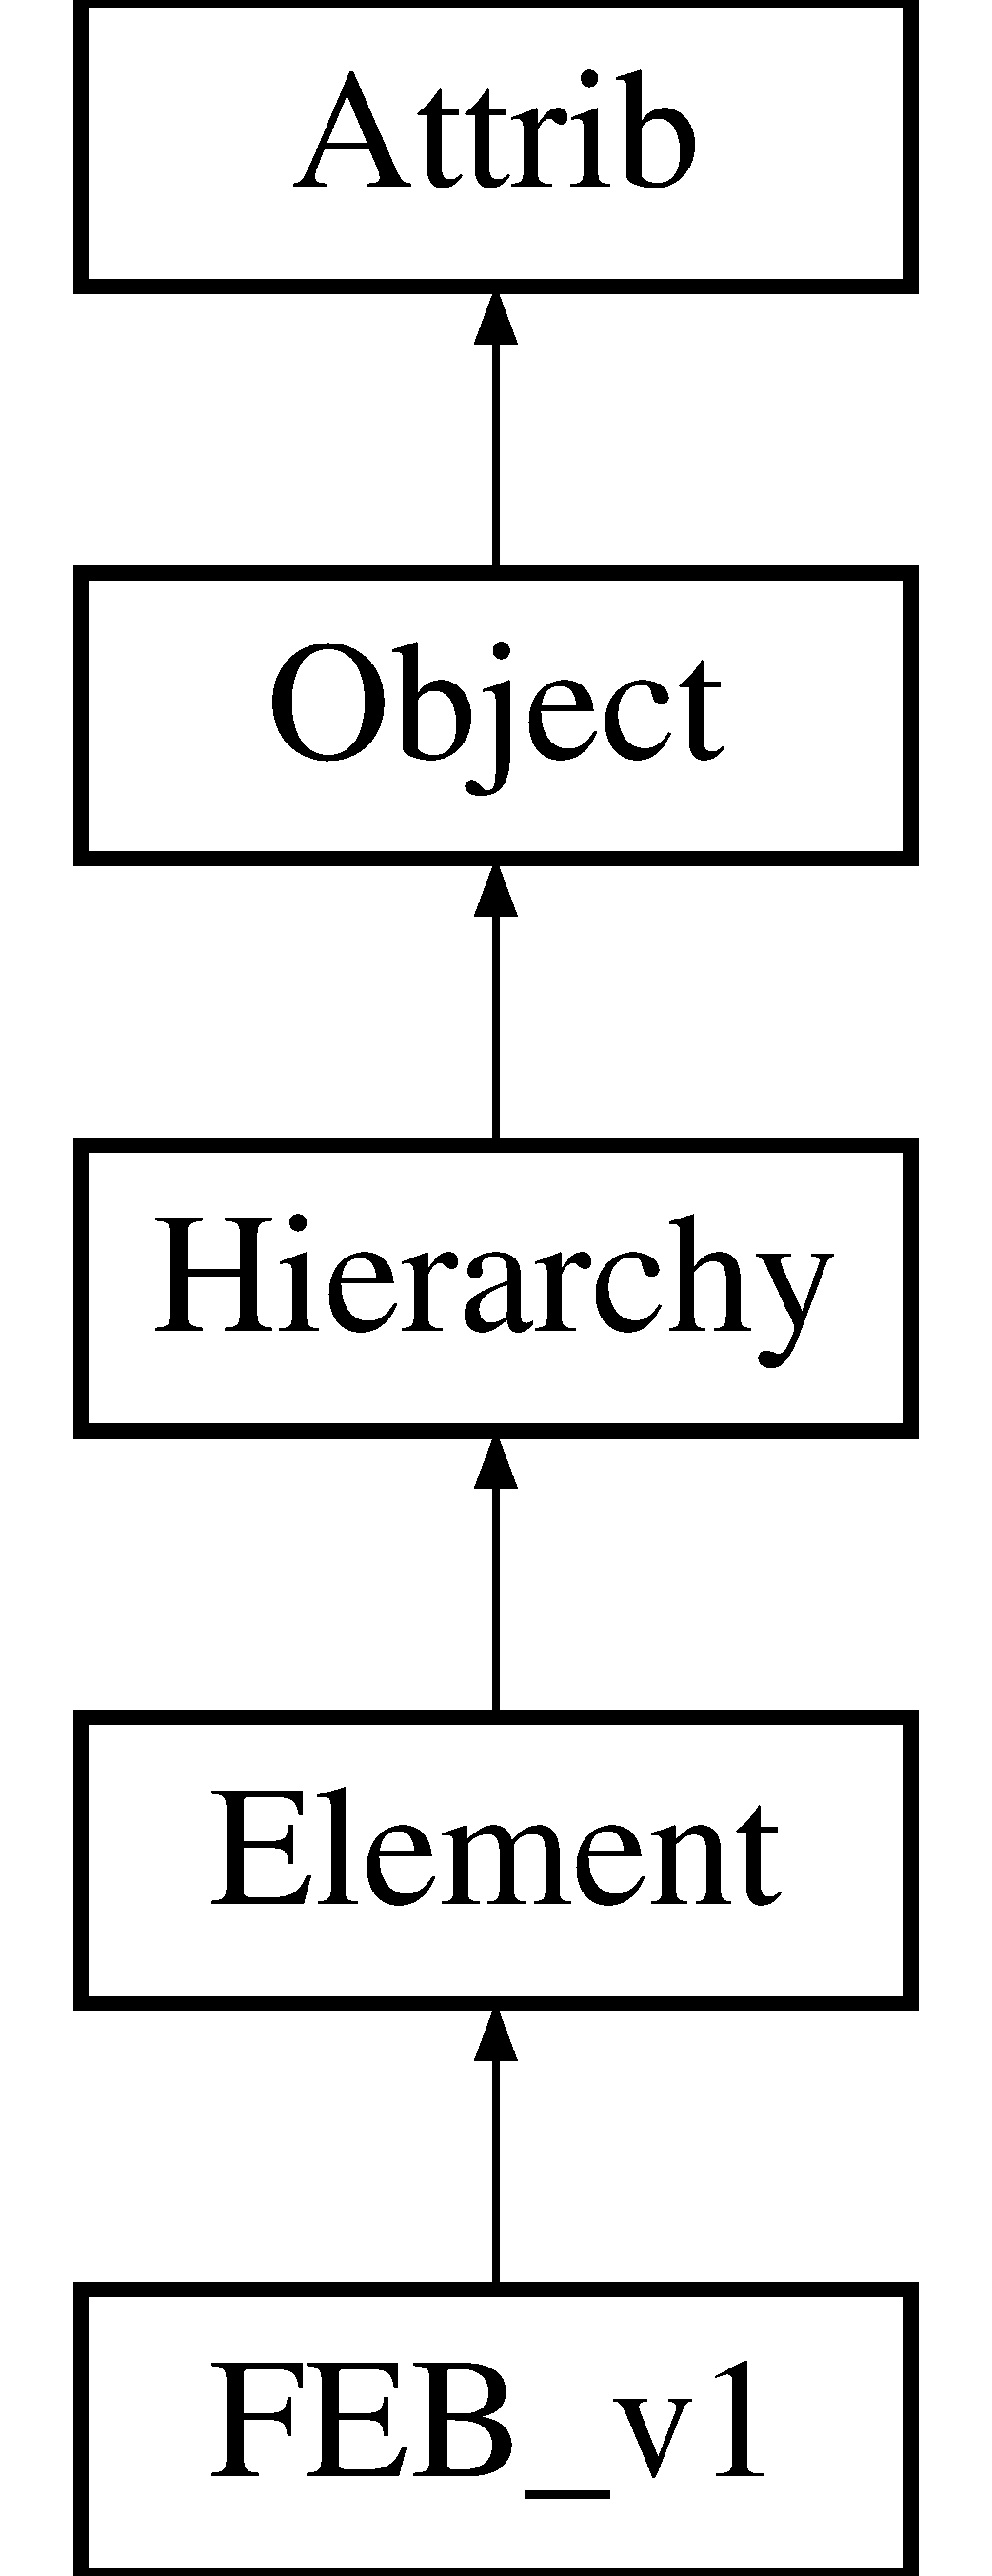
\includegraphics[height=5.000000cm]{classFEB__v1}
\end{center}
\end{figure}
\subsection*{Public Types}
\begin{DoxyCompactItemize}
\item 
enum \hyperlink{classAttrib_a69e171d7cc6417835a5a306d3c764235}{Attribut} \{ \newline
\hyperlink{classAttrib_a69e171d7cc6417835a5a306d3c764235a3a8da2ab97dda18aebab196fe4100531}{U\+N\+D\+E\+F\+I\+N\+ED}, 
\hyperlink{classAttrib_a69e171d7cc6417835a5a306d3c764235a2bfb2af57b87031d190a05fe25dd92ed}{P\+A\+S\+S\+I\+VE}, 
\hyperlink{classAttrib_a69e171d7cc6417835a5a306d3c764235a3b1fec929c0370d1436f2f06e298fb0d}{A\+C\+T\+I\+VE}, 
\hyperlink{classAttrib_a69e171d7cc6417835a5a306d3c764235aa27c16b480a369ea4d18b07b2516bbc7}{I\+N\+T\+E\+R\+F\+A\+CE}, 
\newline
\hyperlink{classAttrib_a69e171d7cc6417835a5a306d3c764235a1420a5b8c0540b2af210b6975eded7f9}{IO}, 
\hyperlink{classAttrib_a69e171d7cc6417835a5a306d3c764235a0af3b0d0ac323c1704e6c69cf90add28}{I\+O\+D\+A\+TA}, 
\hyperlink{classAttrib_a69e171d7cc6417835a5a306d3c764235a7788bc5dd333fd8ce18562b269c9dab1}{E\+L\+E\+M\+E\+NT}, 
\hyperlink{classAttrib_a69e171d7cc6417835a5a306d3c764235a61ceb22149f365f1780d18f9d1459423}{H\+A\+R\+D\+W\+A\+RE}, 
\newline
\hyperlink{classAttrib_a69e171d7cc6417835a5a306d3c764235a75250e29692496e73effca2c0330977f}{P\+R\+O\+C\+E\+S\+S\+US}, 
\hyperlink{classAttrib_a69e171d7cc6417835a5a306d3c764235a103a67cd0b8f07ef478fa45d4356e27b}{S\+O\+F\+T\+W\+A\+RE}
 \}
\end{DoxyCompactItemize}
\subsection*{Public Member Functions}
\begin{DoxyCompactItemize}
\item 
\hyperlink{classFEB__v1_aad65ff3d95f3f60583dad914f9c18a9d}{F\+E\+B\+\_\+v1} ()
\begin{DoxyCompactList}\small\item\em Standard constructor. \end{DoxyCompactList}\item 
virtual \hyperlink{classFEB__v1_a655c6fb31068c4dbb7fde34de77a5a49}{$\sim$\+F\+E\+B\+\_\+v1} ()
\begin{DoxyCompactList}\small\item\em Destructor. \end{DoxyCompactList}\item 
void \hyperlink{classFEB__v1_af93db546ad89ba7c2301fdc2314efd8a}{help} ()
\item 
\hyperlink{classStatusCode}{Status\+Code} \hyperlink{classFEB__v1_a70d7d266c7d05fdfab21d5b0293f1ad8}{init} ()
\item 
void \hyperlink{classFEB__v1_a4e147b894ecbf4b05b92d01270d7ff13}{reset} ()
\item 
void \hyperlink{classFEB__v1_a1a50b5fff8a6e170fe136657f75b8ad4}{reset\+Spi} ()
\item 
void \hyperlink{classFEB__v1_a96ad348b7be37686998c0eaa7fd2e83e}{update} ()
\item 
\hyperlink{classSeqPGA}{Seq\+P\+GA} $\ast$ \hyperlink{classFEB__v1_a8bf655504f9b0c51d5aa5bc6b30da00d}{seq\+Pga} ()
\item 
\hyperlink{classStatusCode}{Status\+Code} \hyperlink{classFEB__v1_a9e13da349fc335ec44032fa0426c40d0}{set\+Spy\+Mode\+Seq} (bool)
\item 
bool \hyperlink{classFEB__v1_a3ec8b74aedfbe5e3d3ce0d4b4eb44330}{spy\+Mode\+Seq} ()
\item 
\hyperlink{classStatusCode}{Status\+Code} \hyperlink{classFEB__v1_ab88d23abb96f746298e0fa1e1cf63e3e}{set\+Spy\+Mode\+FE} (int, bool)
\item 
bool \hyperlink{classFEB__v1_a0b6d25515e575e370552c6b6f715fd76}{spy\+Mode\+FE} (int)
\item 
\hyperlink{classStatusCode}{Status\+Code} \hyperlink{classFEB__v1_a067a0aeae34dbd782547afbcd82fc77f}{set\+Disable\+Subtract} (int, bool)
\item 
bool \hyperlink{classFEB__v1_a3d224acca0807603d14b72cff6359b3f}{disable\+Subtract} (int)
\item 
\hyperlink{classStatusCode}{Status\+Code} \hyperlink{classFEB__v1_aec8198d5c03ddc5dd9151683f9506d00}{set\+Old\+Subtract} (int, bool)
\item 
bool \hyperlink{classFEB__v1_a5b277ace76b9e511c055ad94d241dd61}{old\+Subtract} (int)
\item 
\hyperlink{classStatusCode}{Status\+Code} \hyperlink{classFEB__v1_a02416559cdd68e8aa57f47ce7cf6788c}{set\+Threshold} (int, int)
\item 
int \hyperlink{classFEB__v1_a71e54700c59857844905c879e4b3d4fd}{threshold} (int)
\item 
\hyperlink{classStatusCode}{Status\+Code} \hyperlink{classFEB__v1_ae3252ed2737b5c93395da201b427b871}{set\+Latency} (int, int)
\item 
int \hyperlink{classFEB__v1_a68050d232efd8d6568910b09a2c18f62}{latency} (int)
\item 
\hyperlink{classStatusCode}{Status\+Code} \hyperlink{classFEB__v1_aea3983d847c7b8053485ddd16af65680}{set\+Inject\+Mode\+FE} (int, bool)
\item 
bool \hyperlink{classFEB__v1_adad5a9a1dc8f650a59e6edb310451cab}{inject\+Mode\+FE} (int)
\item 
\hyperlink{classStatusCode}{Status\+Code} \hyperlink{classFEB__v1_abb013a3441c02f57cea07a244554fdd5}{set\+Probe\+Enable} (int, bool)
\item 
void \hyperlink{classFEB__v1_aa9a047f616c6affac88a8d9ec984013f}{probe\+Enable} ()
\item 
\hyperlink{classStatusCode}{Status\+Code} \hyperlink{classFEB__v1_ae8e531b961f91ac974a75c43937acf78}{set\+Spare\+For\+Trig\+Enable} (int, int)
\item 
int \hyperlink{classFEB__v1_a76d86fb9e9be48e704257070675ae1cc}{spare\+For\+Trig\+Enable} (int)
\item 
\hyperlink{classStatusCode}{Status\+Code} \hyperlink{classFEB__v1_a19d3dee6fa47408cf0aa136fb99ebe1c}{set\+Test\+Duration} (int)
\item 
int \hyperlink{classFEB__v1_a7f1db8ca9490172fce7603da9e703dec}{test\+Duration} (int fpga)
\item 
\hyperlink{classStatusCode}{Status\+Code} \hyperlink{classFEB__v1_aaf8386be3d27ea22e389b0a6c7699af7}{set\+Stop\+Inj\+Loop} (bool)
\item 
bool \hyperlink{classFEB__v1_abfd23d8fbcea0415a7e8401110869a78}{stop\+Inj\+Loop} (int)
\item 
\hyperlink{classStatusCode}{Status\+Code} \hyperlink{classFEB__v1_a2ad20ff9db6a0ceef875d874bae214a9}{set\+Enable\+B\+X\+I\+D\+Reset} (bool)
\item 
bool \hyperlink{classFEB__v1_ac8186be2d5fd8122092d6475e77395e9}{enable\+B\+X\+I\+D\+Reset} ()
\item 
\hyperlink{classStatusCode}{Status\+Code} \hyperlink{classFEB__v1_ac30cac86837c86e4f03cb51fff6226cd}{set\+Gain4} (int, int, bool)
\item 
\hyperlink{classStatusCode}{Status\+Code} \hyperlink{classFEB__v1_a244c472d16ea6778cf6ec93943a060a5}{set\+Pseudo\+A\+D\+C\+Enable} (int, int, bool)
\item 
\hyperlink{classStatusCode}{Status\+Code} \hyperlink{classFEB__v1_af422c3cf889440d5d49cce51d98b496e}{set\+Pseudo\+P\+M\+Enable} (int, int, bool)
\item 
\hyperlink{classStatusCode}{Status\+Code} \hyperlink{classFEB__v1_adce2d9c70235f4226ab59aea3dc5953c}{set\+Global\+Pseudo\+P\+M\+Enable} (int, bool)
\item 
\hyperlink{classStatusCode}{Status\+Code} \hyperlink{classFEB__v1_af2bb7bacef6c06d15e2c9e47c373de08}{set\+Clock\+Falling\+Edge} (int, int, bool)
\item 
\hyperlink{classStatusCode}{Status\+Code} \hyperlink{classFEB__v1_a9ccd318b9a80b1cbd554ec6fe461cd82}{set\+Clock80\+M\+Hz\+Falling\+Edge} (bool)
\item 
\hyperlink{classStatusCode}{Status\+Code} \hyperlink{classFEB__v1_acf3c8ad478ce506bb9d9cb3e4d3b6252}{set\+Calib\+Cte} (int, int, int)
\item 
bool \hyperlink{classFEB__v1_a6b05c21a70fbb2e88f8e1f991a117b49}{gain4} (int, int)
\item 
bool \hyperlink{classFEB__v1_aeb6c988faf48d93637ef669c54e25223}{pseudo\+A\+D\+C\+Enable} (int, int)
\item 
bool \hyperlink{classFEB__v1_ab6b076d6e1372bfa8d9fd2916b1b52cd}{pseudo\+P\+M\+Enable} (int, int)
\item 
bool \hyperlink{classFEB__v1_acfaf998ce0166362401e5253502a16d2}{global\+Pseudo\+P\+M\+Enable} (int)
\item 
bool \hyperlink{classFEB__v1_aa9f591714dce594562e3e959b105a580}{clock\+Falling\+Edge} (int, int)
\item 
bool \hyperlink{classFEB__v1_a8518757e40b372f784674da1a2c41091}{clock80\+M\+Hz\+Falling\+Edge} ()
\item 
int \hyperlink{classFEB__v1_ad3893c8062c75d1f9695c196c95703c7}{calib\+Cte} (int, int)
\item 
\hyperlink{classStatusCode}{Status\+Code} \hyperlink{classFEB__v1_a7b948b40f3034ccfb0a696b5cf9c5c6c}{test\+Sequence} ()
\item 
\hyperlink{classStatusCode}{Status\+Code} \hyperlink{classFEB__v1_aea3b1f84ea9be2e5c55a93ae215c8a35}{set\+Ext\+Trig} (bool trig)
\item 
bool \hyperlink{classFEB__v1_a481e089490ae958c7606f11d27c9db9a}{ext\+Trig} ()
\item 
void \hyperlink{classFEB__v1_af945f99a912c5ad076ebdb03dbb6c139}{read\+Fifo} (int, int, unsigned int $\ast$)
\item 
void \hyperlink{classFEB__v1_a86e0ed4fc9946a184d82cefdf5e5a794}{read\+Fifo\+Spy\+FE} (int fe, int dump)
\item 
void \hyperlink{classFEB__v1_a27df6aecacccf3415ff98092b7da5485}{read\+Fifo\+L\+L\+T\+FE} (int fe, int dump)
\item 
void \hyperlink{classFEB__v1_ab370d9f02895e1a44ab19d320255123e}{read\+Fifo\+Inject\+FE} (int fe, int dump)
\item 
void \hyperlink{classFEB__v1_a449a15db7087e4dbe6af0b0f96ec2038}{read\+Fifo\+L\+LT} (int dump)
\item 
void \hyperlink{classFEB__v1_a14807bfa77f92bb82428c39abea5df88}{mask\+L\+LT} ()
\item 
void \hyperlink{classFEB__v1_a42cc3f61fd94d4de68eb605b04fb1e74}{latency\+L\+LT} ()
\item 
\hyperlink{classStatusCode}{Status\+Code} \hyperlink{classFEB__v1_a5a177c98b2be429aacbb3d652f40b247}{set\+Mask\+L\+LT} (int, bool)
\item 
\hyperlink{classStatusCode}{Status\+Code} \hyperlink{classFEB__v1_ad078f7c2086dd78375da9d9d82b78d23}{set\+Mask\+L\+L\+T\+Corner} (bool)
\item 
\hyperlink{classStatusCode}{Status\+Code} \hyperlink{classFEB__v1_a904bff89e5ad45ce78730502dc26a0e3}{set\+Mask\+L\+L\+T\+Up\+Nb} (int, bool)
\item 
\hyperlink{classStatusCode}{Status\+Code} \hyperlink{classFEB__v1_a519a955361c420680af64c7fa9410784}{set\+Mask\+L\+L\+T\+Side\+Nb} (int, bool)
\item 
\hyperlink{classStatusCode}{Status\+Code} \hyperlink{classFEB__v1_abf7b8a0e6842ecf74a2b1889fbb9a722}{set\+Latency\+L\+LT} (int)
\item 
\hyperlink{classStatusCode}{Status\+Code} \hyperlink{classFEB__v1_a935e78031961cff9330e82a70bf91052}{set\+Latency\+L\+L\+T\+Corner} (int)
\item 
\hyperlink{classStatusCode}{Status\+Code} \hyperlink{classFEB__v1_a8a3aafdda0f1028e02c4a5850f987f32}{set\+Latency\+L\+L\+T\+Up\+Nb} (int)
\item 
\hyperlink{classStatusCode}{Status\+Code} \hyperlink{classFEB__v1_a840532b78d0062646116a076e65cf353}{set\+Latency\+L\+L\+T\+Side\+Nb} (int)
\item 
\hyperlink{classStatusCode}{Status\+Code} \hyperlink{classFEB__v1_ae94205e374c3438e910aa39a889ebf5c}{set\+Output\+Eport} (int, int, int)
\item 
int \hyperlink{classFEB__v1_a330c0a895c3c43acda2fd68e1cdb7368}{latency\+Eport} (int)
\item 
int \hyperlink{classFEB__v1_a4a5b20275b96a19eba0c28d694c88ca8}{clock\+Phase\+Eport} (int)
\item 
\hyperlink{classStatusCode}{Status\+Code} \hyperlink{classFEB__v1_ae8ed47630ca1408647e3eb5c1dfa0ec0}{set\+Output\+Eport} (int, int, int, int)
\item 
int \hyperlink{classFEB__v1_a8ab1ff429d357779d682bdf28504bdd2}{latency\+Eport} (int, int)
\item 
int \hyperlink{classFEB__v1_aab32d0b274dfb55f1c2894ff3d08eaba}{clock\+Phase\+Eport} (int, int)
\item 
void \hyperlink{classFEB__v1_a0fd77cbaae9ae853e5c4dfc81b4462a5}{write\+Fifo\+Spy\+FE} (int fe)
\item 
void \hyperlink{classFEB__v1_a9dbedaebc2e3569e8b5fc0be782dbce3}{write\+Fifo\+L\+L\+T\+FE} (int fe)
\item 
void \hyperlink{classFEB__v1_ae212b0e4c9824afaebb4508b688f94bf}{write\+Fifo\+Inject\+FE} (int fe, int pattern)
\item 
void \hyperlink{classFEB__v1_a0afafcfdea15d3268284203a90c67572}{write\+Data\+Fifo\+Inject\+FE} (int, int $\ast$, int $\ast$, int $\ast$, int $\ast$)
\item 
void \hyperlink{classFEB__v1_a0e88b14453100c97b5962e8a6b0f48bf}{write\+Fifo\+L\+LT} ()
\item 
\hyperlink{classStatusCode}{Status\+Code} \hyperlink{classFEB__v1_ab02c292e29e01079bb9b268acbc782b1}{reset\+Fifo\+Spy\+FE} (int)
\item 
\hyperlink{classStatusCode}{Status\+Code} \hyperlink{classFEB__v1_a71d10a772bda2506fd7adb86739fb24d}{reset\+Fifo\+Inject\+FE} (int)
\item 
\hyperlink{classStatusCode}{Status\+Code} \hyperlink{classFEB__v1_ae351e55f3d8e8f936c324ffbda6816bf}{reset\+FE} (int)
\item 
int \hyperlink{classFEB__v1_aa98b8e0bcc4d6d03f4b365de786f5c95}{status\+Register} (int)
\item 
\hyperlink{classData}{Data} $\ast$ \hyperlink{classFEB__v1_a6bca4320bd3bbbc32efc81097f33421a}{data} ()
\item 
\hyperlink{classRAM}{R\+AM} $\ast$ \hyperlink{classFEB__v1_aceff066f476794fefe2712e43bc2d6d2}{ram\+Inj} (int i)
\item 
\hyperlink{classRAM}{R\+AM} $\ast$ \hyperlink{classFEB__v1_ac59216f094007ede67d49bd23287be73}{ram\+Spy} (int i)
\item 
\hyperlink{classStatusCode}{Status\+Code} \hyperlink{classFEB__v1_a849040ff2fa8275b1a47e7be3915ebf4}{set\+Gbt\+Mode} (int, int)
\item 
int \hyperlink{classFEB__v1_aab7166214ef0f99f4835ce9a7416e052}{gbt\+Mode} (int)
\item 
\hyperlink{classStatusCode}{Status\+Code} \hyperlink{classFEB__v1_aabd651b11d1119ce3a19b7fb083cca78}{set\+Gbt\+Data\+Path} (int, int, int, int)
\item 
int \hyperlink{classFEB__v1_adf46e43506d1bd7cd26ca62c685e6c98}{gbt\+Data\+Path} (int)
\item 
\hyperlink{classStatusCode}{Status\+Code} \hyperlink{classFEB__v1_ab65b869df2adc4d3880caad71a4e3074}{set\+Gbt\+Track\+Mode} (int, int)
\item 
int \hyperlink{classFEB__v1_a25eeb132e9058cd421a085878fba9204}{gbt\+Track\+Mode} (int)
\item 
\hyperlink{classStatusCode}{Status\+Code} \hyperlink{classFEB__v1_ab7c261039c872c9f039fb7366a84d271}{set\+Gbt\+Term\+Eport} (int, bool)
\item 
bool \hyperlink{classFEB__v1_a84fa302a012eee663fe21829866fb20e}{gbt\+Term\+Eport} (int)
\item 
\hyperlink{classStatusCode}{Status\+Code} \hyperlink{classFEB__v1_a6efa59ad9f80ae40aad2df0b925b0b14}{set\+Gbt80\+M\+Hz\+Clk\+Eport} (int)
\item 
bool \hyperlink{classFEB__v1_ac22b1ffdc20be66330a66ebd12cd13f1}{gbt80\+M\+Hz\+Clk\+Eport} (int)
\item 
\hyperlink{classStatusCode}{Status\+Code} \hyperlink{classFEB__v1_a66584fe850cdf9e4ccd03fd4b2f4db38}{set\+Gbt\+D\+L\+L\+Eport} (int)
\item 
void \hyperlink{classFEB__v1_add5e12a5351c0c4986d24f433155351b}{gbt\+D\+L\+L\+Eport} (int)
\item 
\hyperlink{classStatusCode}{Status\+Code} \hyperlink{classFEB__v1_a30ce0e679748a4e2bf7f953b2162618f}{set\+Gbt\+Enable\+Eport} (int, bool)
\item 
bool \hyperlink{classFEB__v1_ae11c18013b56bdbb947e9ae147d6d77d}{gbt\+Enable\+Eport} (int)
\item 
int \hyperlink{classFEB__v1_a7b47a1b2c7af459b211eed59f4dbe9a7}{gbt\+Status} (int)
\item 
\hyperlink{classStatusCode}{Status\+Code} \hyperlink{classFEB__v1_a717d56186e6221cb20397cc3e496da50}{set\+Gbt\+Clock\+Strength} (int, int)
\item 
int \hyperlink{classFEB__v1_a6ca15de02d32e38a0fc90ad29302072e}{gbt\+Clock\+Strength} (int)
\item 
\hyperlink{classStatusCode}{Status\+Code} \hyperlink{classFEB__v1_a79b299ce9b36b51916103371aef027df}{gbt\+D\+L\+L\+Reset} (int)
\item 
\hyperlink{classStatusCode}{Status\+Code} \hyperlink{classFEB__v1_af7e7f3cb7269dc811866bc42585cf020}{gbt\+Acknowledge\+Config} (int)
\item 
void \hyperlink{classElement_a3c0abcb36f8906688bb7e32608df7086}{recursive\+Init\+Element} ()
\item 
void \hyperlink{classElement_a82119ed37dff76508a2746a853ec35ba}{recursive\+Init\+Communications} ()
\item 
\hyperlink{classStatusCode}{Status\+Code} \hyperlink{classElement_ab476b4b1df5954141ceb14f072433b89}{set\+Connection} (\hyperlink{classHierarchy}{Hierarchy} $\ast$)
\item 
\hyperlink{classHierarchy}{Hierarchy} $\ast$ \hyperlink{classElement_af57444353c1ddf9fa0109801e97debf7}{connection} ()
\item 
void \hyperlink{classHierarchy_af4d43b0765b402670eed2d62c73405af}{clear} ()
\item 
void \hyperlink{classHierarchy_a585ad1aeec16077a0e532ab8b4fc557b}{set\+Parent} (\hyperlink{classHierarchy}{Hierarchy} $\ast$\hyperlink{classHierarchy_a1c7bec8257e717f9c1465e06ebf845fc}{parent})
\item 
\hyperlink{classHierarchy}{Hierarchy} $\ast$ \hyperlink{classHierarchy_a1c7bec8257e717f9c1465e06ebf845fc}{parent} ()
\item 
\hyperlink{classHierarchy}{Hierarchy} $\ast$ \hyperlink{classHierarchy_ad550588733bf75ac5c0fcfd7c8fd11a6}{parent} (std\+::string)
\item 
\hyperlink{classHierarchy}{Hierarchy} $\ast$ \hyperlink{classHierarchy_aee461dc930ce3871636ff87f075b1b83}{origin} ()
\item 
virtual void \hyperlink{classHierarchy_ad677774ff38fcb257c04a3a10d471fac}{add\+Child} (\hyperlink{classHierarchy}{Hierarchy} $\ast$element)
\item 
std\+::vector$<$ \hyperlink{classHierarchy}{Hierarchy} $\ast$ $>$ \hyperlink{classHierarchy_aa9a76f69e98e052ee1a6e32cea006288}{children} ()
\item 
\hyperlink{classHierarchy}{Hierarchy} $\ast$ \hyperlink{classHierarchy_a1e207f973c694b538bf90107b4868817}{child} (std\+::string)
\item 
\hyperlink{classHierarchy}{Hierarchy} $\ast$ \hyperlink{classHierarchy_a0c15a5276a3b80b4354d6bd8a01e0708}{child\+Typed} (std\+::string)
\item 
unsigned long \hyperlink{classHierarchy_ab16e84de65fd84e14001a6cf941c8be4}{number\+Of\+Children} ()
\item 
bool \hyperlink{classHierarchy_a255174fe4d316d2a3f430dcb9dab29f1}{has\+Children} ()
\item 
void \hyperlink{classHierarchy_a2b2b359fac003233f65786a616766bde}{del\+Child} (\hyperlink{classHierarchy}{Hierarchy} $\ast$)
\item 
void \hyperlink{classHierarchy_a1928ac7615fe0b5e55cd707f70dc6781}{del\+Child} (std\+::string)
\item 
std\+::string \hyperlink{classHierarchy_aa7990fa7caf132d83e361ce033c6c65a}{path} (std\+::string=std\+::string(\char`\"{}\char`\"{}))
\item 
std\+::string \hyperlink{classHierarchy_a1efd56cd164d328d2002e53a10a19b8c}{path\+Typed} (std\+::string=std\+::string(\char`\"{}\char`\"{}))
\item 
void \hyperlink{classHierarchy_a76e914b9a677a22a82deb74d892bf261}{tree} (std\+::string indent=std\+::string(\char`\"{}\char`\"{}))
\item 
void \hyperlink{classHierarchy_a594c294c5f60c230e106d522ed008212}{tree} ()
\item 
std\+::string \hyperlink{classObject_a300f4c05dd468c7bb8b3c968868443c1}{name} () const
\item 
std\+::string \hyperlink{classObject_a84f99f70f144a83e1582d1d0f84e4e62}{type} ()
\item 
unsigned char \hyperlink{classObject_af99145335cc61ff6e2798ea17db009d2}{id} ()
\item 
std\+::string \hyperlink{classObject_a73a0f1a41828fdd8303dd662446fb6c3}{title} ()
\item 
void \hyperlink{classObject_a3f9d5537ebce0c0f2bf6ae4d92426f3c}{msg\+Svc} (int level, std\+::string \hyperlink{classObject_a58b2d0618c2d08cf2383012611528d97}{msg}, std\+::string \hyperlink{classObject_a300f4c05dd468c7bb8b3c968868443c1}{name})
\item 
void \hyperlink{classObject_a58b2d0618c2d08cf2383012611528d97}{msg} (std\+::string mymsg)
\item 
void \hyperlink{classObject_ac5d59299273cee27aacf7de00d2e7034}{msg} (std\+::string mymsg, std\+::string \hyperlink{classObject_a300f4c05dd468c7bb8b3c968868443c1}{name})
\item 
void \hyperlink{classObject_a83d2db2df682907ea1115ad721c1c4a1}{verbose} (std\+::string mymsg)
\item 
void \hyperlink{classObject_a2d4120195317e2a3c6532e8bb9f3da68}{verbose} (std\+::string mymsg, std\+::string \hyperlink{classObject_a300f4c05dd468c7bb8b3c968868443c1}{name})
\item 
void \hyperlink{classObject_aac010553f022165573714b7014a15f0d}{debug} (std\+::string mymsg)
\item 
void \hyperlink{classObject_a6c9a0397ca804e04d675ed05683f5420}{debug} (std\+::string mymsg, std\+::string \hyperlink{classObject_a300f4c05dd468c7bb8b3c968868443c1}{name})
\item 
void \hyperlink{classObject_a644fd329ea4cb85f54fa6846484b84a8}{info} (std\+::string mymsg)
\item 
void \hyperlink{classObject_a1ca123253dfd30fc28b156f521dcbdae}{info} (std\+::string mymsg, std\+::string \hyperlink{classObject_a300f4c05dd468c7bb8b3c968868443c1}{name})
\item 
void \hyperlink{classObject_a65cd4fda577711660821fd2cd5a3b4c9}{warning} (std\+::string mymsg)
\item 
void \hyperlink{classObject_a11f101db4dd73d9391b0231818881d86}{warning} (std\+::string mymsg, std\+::string \hyperlink{classObject_a300f4c05dd468c7bb8b3c968868443c1}{name})
\item 
void \hyperlink{classObject_a204a95f57818c0f811933917a30eff45}{error} (std\+::string mymsg)
\item 
void \hyperlink{classObject_ad7f6c457733082efa2f9ff5f5c8e119a}{error} (std\+::string mymsg, std\+::string \hyperlink{classObject_a300f4c05dd468c7bb8b3c968868443c1}{name})
\item 
void \hyperlink{classObject_aad5a16aac7516ce65bd5ec02ab07fc80}{fatal} (std\+::string mymsg)
\item 
void \hyperlink{classObject_ae62acd3d09f716220f75f252dc38bc9a}{fatal} (std\+::string mymsg, std\+::string \hyperlink{classObject_a300f4c05dd468c7bb8b3c968868443c1}{name})
\item 
void \hyperlink{classObject_ae30fea75683c2d149b6b6d17c09ecd0c}{set\+Name} (std\+::string \hyperlink{classObject_a300f4c05dd468c7bb8b3c968868443c1}{name})
\item 
void \hyperlink{classObject_aae534cc9d982bcb9b99fd505f2e103a5}{set\+Type} (std\+::string \hyperlink{classObject_a84f99f70f144a83e1582d1d0f84e4e62}{type})
\item 
void \hyperlink{classObject_a398fe08cba594a0ce6891d59fe4f159f}{set\+Id} (unsigned char \hyperlink{classObject_af99145335cc61ff6e2798ea17db009d2}{id})
\item 
void \hyperlink{classObject_a89557dbbad5bcaa02652f5d7fa35d20f}{set\+Title} (std\+::string \hyperlink{classObject_a73a0f1a41828fdd8303dd662446fb6c3}{title})
\item 
void \hyperlink{classObject_a870c5af919958c2136623b2d7816d123}{set\+Dll\+Name} (std\+::string \hyperlink{classObject_a2e3947f2870094c332d7454117f3ec63}{dll\+Name})
\item 
std\+::string \hyperlink{classObject_a2e3947f2870094c332d7454117f3ec63}{dll\+Name} ()
\item 
bool \hyperlink{classAttrib_a704f26af560909ad22065083bb7d4c34}{is} (int attribut)
\item 
void \hyperlink{classAttrib_a235f773af19c900264a190b00a3b4ad7}{add} (int attribut)
\item 
void \hyperlink{classAttrib_a7d4ef7e32d93cb287792b87b857e79f3}{remove} (int attribut)
\item 
std\+::string \hyperlink{classAttrib_aee7bbf16b144887f196e1341b24f8a26}{attributs} ()
\end{DoxyCompactItemize}
\subsection*{Protected Attributes}
\begin{DoxyCompactItemize}
\item 
\hyperlink{classHierarchy}{Hierarchy} $\ast$ \hyperlink{classElement_abe3de7a5dbbc9a6dd2d7e012e5fdb266}{m\+\_\+connection}
\item 
std\+::string \hyperlink{classAttrib_a3414521d7a82476e874b25a5407b5e63}{m\+\_\+attrib\+String} \mbox{[}10\mbox{]}
\end{DoxyCompactItemize}
\subsection*{Private Attributes}
\begin{DoxyCompactItemize}
\item 
int \hyperlink{classFEB__v1_a30473bcdd8f018ad5dac728f6779df9c}{m\+\_\+fifo\+Depth}
\item 
int \hyperlink{classFEB__v1_a1c1eb093fd1733b9510fcf8bc5c7ad08}{m\+\_\+seq\+Address}
\item 
int \hyperlink{classFEB__v1_a4e1945c2d5b434125f375e9d0fc6d99f}{m\+\_\+fe\+Address} \mbox{[}8\mbox{]}
\item 
int \hyperlink{classFEB__v1_ac625855df976f16694178f1a4c0eef1e}{m\+\_\+gbt\+Address} \mbox{[}4\mbox{]}
\item 
int \hyperlink{classFEB__v1_adf21041831669e75283dd2a88fbaddf5}{m\+\_\+icecal\+Address} \mbox{[}8\mbox{]}
\item 
int \hyperlink{classFEB__v1_a15b48648ba4534e732376b68bddc5d34}{m\+\_\+fifo\+Spy\+Address} \mbox{[}3\mbox{]}
\item 
int \hyperlink{classFEB__v1_a68be75ba59d1c551163a9596dc1d235a}{m\+\_\+fifo\+L\+L\+T\+Address} \mbox{[}3\mbox{]}
\item 
int \hyperlink{classFEB__v1_afd035f292061e1823ed64471bb0228ef}{m\+\_\+fifo\+Inject\+Address} \mbox{[}3\mbox{]}
\item 
int \hyperlink{classFEB__v1_ad41f8756c4e15815c6d5e35902cf2257}{m\+\_\+fifo\+Trig\+Address} \mbox{[}3\mbox{]}
\item 
\hyperlink{classSeqPGA}{Seq\+P\+GA} $\ast$ \hyperlink{classFEB__v1_a6c7804ac86796f233a8393043adf2e77}{m\+\_\+seq\+Pga}
\item 
unsigned int $\ast$ \hyperlink{classFEB__v1_ae5b770f2f5ffb97324862c93e3153985}{m\+\_\+fifo} \mbox{[}3\mbox{]}
\item 
int $\ast$ \hyperlink{classFEB__v1_a383c35f10769b16c6a719494594899c6}{m\+\_\+ch} \mbox{[}4\mbox{]}
\item 
\hyperlink{classData}{Data} $\ast$ \hyperlink{classFEB__v1_a1c9dbc3660021dba1f58666d0097abb0}{m\+\_\+data}
\item 
int \hyperlink{classFEB__v1_ab49d6a271bdfddd9c7fac9435e4e686d}{m\+\_\+mask0}
\item 
int \hyperlink{classFEB__v1_a1cbadb02155e2defdff6d6c8f70eb945}{m\+\_\+mask1}
\item 
int \hyperlink{classFEB__v1_a25f03f6de00618dd575fc1f77a9af9ee}{m\+\_\+mask2}
\item 
int \hyperlink{classFEB__v1_a23a3d8bfbf96490890140f13b08a02c1}{m\+\_\+latency0}
\item 
int \hyperlink{classFEB__v1_a026d2f4973bf3ddbc404e35264fdef1f}{m\+\_\+latency1}
\item 
int \hyperlink{classFEB__v1_a2c4b18efd76de3bf7089bba57fb6744f}{m\+\_\+latency2}
\item 
int \hyperlink{classFEB__v1_a2f71bdcef05c845177a62610da490bf9}{m\+\_\+latency3}
\item 
\hyperlink{classRAM}{R\+AM} $\ast$ \hyperlink{classFEB__v1_a3a3d06225c94c88d4cc5da7a6bde3867}{m\+\_\+ram\+Inj} \mbox{[}3\mbox{]}
\item 
\hyperlink{classRAM}{R\+AM} $\ast$ \hyperlink{classFEB__v1_ae6d8176c12bd60ad25ed81d535eb8c82}{m\+\_\+ram\+Spy} \mbox{[}3\mbox{]}
\item 
\hyperlink{classRAM}{R\+AM} $\ast$ \hyperlink{classFEB__v1_a5850ce498462009212ad3f313fcf0bd6}{m\+\_\+fifo\+Usb\+Test}
\end{DoxyCompactItemize}


\subsection{Detailed Description}
\begin{DoxyAuthor}{Author}

\end{DoxyAuthor}
\begin{DoxyDate}{Date}
2006-\/10-\/23 
\end{DoxyDate}


Definition at line 21 of file F\+E\+B\+\_\+v1.\+h.



\subsection{Member Enumeration Documentation}
\mbox{\Hypertarget{classAttrib_a69e171d7cc6417835a5a306d3c764235}\label{classAttrib_a69e171d7cc6417835a5a306d3c764235}} 
\index{F\+E\+B\+\_\+v1@{F\+E\+B\+\_\+v1}!Attribut@{Attribut}}
\index{Attribut@{Attribut}!F\+E\+B\+\_\+v1@{F\+E\+B\+\_\+v1}}
\subsubsection{\texorpdfstring{Attribut}{Attribut}}
{\footnotesize\ttfamily enum \hyperlink{classAttrib_a69e171d7cc6417835a5a306d3c764235}{Attrib\+::\+Attribut}\hspace{0.3cm}{\ttfamily [inherited]}}

\begin{DoxyEnumFields}{Enumerator}
\raisebox{\heightof{T}}[0pt][0pt]{\index{U\+N\+D\+E\+F\+I\+N\+ED@{U\+N\+D\+E\+F\+I\+N\+ED}!F\+E\+B\+\_\+v1@{F\+E\+B\+\_\+v1}}\index{F\+E\+B\+\_\+v1@{F\+E\+B\+\_\+v1}!U\+N\+D\+E\+F\+I\+N\+ED@{U\+N\+D\+E\+F\+I\+N\+ED}}}\mbox{\Hypertarget{classAttrib_a69e171d7cc6417835a5a306d3c764235a3a8da2ab97dda18aebab196fe4100531}\label{classAttrib_a69e171d7cc6417835a5a306d3c764235a3a8da2ab97dda18aebab196fe4100531}} 
U\+N\+D\+E\+F\+I\+N\+ED&\\
\hline

\raisebox{\heightof{T}}[0pt][0pt]{\index{P\+A\+S\+S\+I\+VE@{P\+A\+S\+S\+I\+VE}!F\+E\+B\+\_\+v1@{F\+E\+B\+\_\+v1}}\index{F\+E\+B\+\_\+v1@{F\+E\+B\+\_\+v1}!P\+A\+S\+S\+I\+VE@{P\+A\+S\+S\+I\+VE}}}\mbox{\Hypertarget{classAttrib_a69e171d7cc6417835a5a306d3c764235a2bfb2af57b87031d190a05fe25dd92ed}\label{classAttrib_a69e171d7cc6417835a5a306d3c764235a2bfb2af57b87031d190a05fe25dd92ed}} 
P\+A\+S\+S\+I\+VE&\\
\hline

\raisebox{\heightof{T}}[0pt][0pt]{\index{A\+C\+T\+I\+VE@{A\+C\+T\+I\+VE}!F\+E\+B\+\_\+v1@{F\+E\+B\+\_\+v1}}\index{F\+E\+B\+\_\+v1@{F\+E\+B\+\_\+v1}!A\+C\+T\+I\+VE@{A\+C\+T\+I\+VE}}}\mbox{\Hypertarget{classAttrib_a69e171d7cc6417835a5a306d3c764235a3b1fec929c0370d1436f2f06e298fb0d}\label{classAttrib_a69e171d7cc6417835a5a306d3c764235a3b1fec929c0370d1436f2f06e298fb0d}} 
A\+C\+T\+I\+VE&\\
\hline

\raisebox{\heightof{T}}[0pt][0pt]{\index{I\+N\+T\+E\+R\+F\+A\+CE@{I\+N\+T\+E\+R\+F\+A\+CE}!F\+E\+B\+\_\+v1@{F\+E\+B\+\_\+v1}}\index{F\+E\+B\+\_\+v1@{F\+E\+B\+\_\+v1}!I\+N\+T\+E\+R\+F\+A\+CE@{I\+N\+T\+E\+R\+F\+A\+CE}}}\mbox{\Hypertarget{classAttrib_a69e171d7cc6417835a5a306d3c764235aa27c16b480a369ea4d18b07b2516bbc7}\label{classAttrib_a69e171d7cc6417835a5a306d3c764235aa27c16b480a369ea4d18b07b2516bbc7}} 
I\+N\+T\+E\+R\+F\+A\+CE&\\
\hline

\raisebox{\heightof{T}}[0pt][0pt]{\index{IO@{IO}!F\+E\+B\+\_\+v1@{F\+E\+B\+\_\+v1}}\index{F\+E\+B\+\_\+v1@{F\+E\+B\+\_\+v1}!IO@{IO}}}\mbox{\Hypertarget{classAttrib_a69e171d7cc6417835a5a306d3c764235a1420a5b8c0540b2af210b6975eded7f9}\label{classAttrib_a69e171d7cc6417835a5a306d3c764235a1420a5b8c0540b2af210b6975eded7f9}} 
IO&\\
\hline

\raisebox{\heightof{T}}[0pt][0pt]{\index{I\+O\+D\+A\+TA@{I\+O\+D\+A\+TA}!F\+E\+B\+\_\+v1@{F\+E\+B\+\_\+v1}}\index{F\+E\+B\+\_\+v1@{F\+E\+B\+\_\+v1}!I\+O\+D\+A\+TA@{I\+O\+D\+A\+TA}}}\mbox{\Hypertarget{classAttrib_a69e171d7cc6417835a5a306d3c764235a0af3b0d0ac323c1704e6c69cf90add28}\label{classAttrib_a69e171d7cc6417835a5a306d3c764235a0af3b0d0ac323c1704e6c69cf90add28}} 
I\+O\+D\+A\+TA&\\
\hline

\raisebox{\heightof{T}}[0pt][0pt]{\index{E\+L\+E\+M\+E\+NT@{E\+L\+E\+M\+E\+NT}!F\+E\+B\+\_\+v1@{F\+E\+B\+\_\+v1}}\index{F\+E\+B\+\_\+v1@{F\+E\+B\+\_\+v1}!E\+L\+E\+M\+E\+NT@{E\+L\+E\+M\+E\+NT}}}\mbox{\Hypertarget{classAttrib_a69e171d7cc6417835a5a306d3c764235a7788bc5dd333fd8ce18562b269c9dab1}\label{classAttrib_a69e171d7cc6417835a5a306d3c764235a7788bc5dd333fd8ce18562b269c9dab1}} 
E\+L\+E\+M\+E\+NT&\\
\hline

\raisebox{\heightof{T}}[0pt][0pt]{\index{H\+A\+R\+D\+W\+A\+RE@{H\+A\+R\+D\+W\+A\+RE}!F\+E\+B\+\_\+v1@{F\+E\+B\+\_\+v1}}\index{F\+E\+B\+\_\+v1@{F\+E\+B\+\_\+v1}!H\+A\+R\+D\+W\+A\+RE@{H\+A\+R\+D\+W\+A\+RE}}}\mbox{\Hypertarget{classAttrib_a69e171d7cc6417835a5a306d3c764235a61ceb22149f365f1780d18f9d1459423}\label{classAttrib_a69e171d7cc6417835a5a306d3c764235a61ceb22149f365f1780d18f9d1459423}} 
H\+A\+R\+D\+W\+A\+RE&\\
\hline

\raisebox{\heightof{T}}[0pt][0pt]{\index{P\+R\+O\+C\+E\+S\+S\+US@{P\+R\+O\+C\+E\+S\+S\+US}!F\+E\+B\+\_\+v1@{F\+E\+B\+\_\+v1}}\index{F\+E\+B\+\_\+v1@{F\+E\+B\+\_\+v1}!P\+R\+O\+C\+E\+S\+S\+US@{P\+R\+O\+C\+E\+S\+S\+US}}}\mbox{\Hypertarget{classAttrib_a69e171d7cc6417835a5a306d3c764235a75250e29692496e73effca2c0330977f}\label{classAttrib_a69e171d7cc6417835a5a306d3c764235a75250e29692496e73effca2c0330977f}} 
P\+R\+O\+C\+E\+S\+S\+US&\\
\hline

\raisebox{\heightof{T}}[0pt][0pt]{\index{S\+O\+F\+T\+W\+A\+RE@{S\+O\+F\+T\+W\+A\+RE}!F\+E\+B\+\_\+v1@{F\+E\+B\+\_\+v1}}\index{F\+E\+B\+\_\+v1@{F\+E\+B\+\_\+v1}!S\+O\+F\+T\+W\+A\+RE@{S\+O\+F\+T\+W\+A\+RE}}}\mbox{\Hypertarget{classAttrib_a69e171d7cc6417835a5a306d3c764235a103a67cd0b8f07ef478fa45d4356e27b}\label{classAttrib_a69e171d7cc6417835a5a306d3c764235a103a67cd0b8f07ef478fa45d4356e27b}} 
S\+O\+F\+T\+W\+A\+RE&\\
\hline

\end{DoxyEnumFields}


Definition at line 29 of file Attrib.\+h.


\begin{DoxyCode}
29                 \{
30     \hyperlink{classAttrib_a69e171d7cc6417835a5a306d3c764235a3a8da2ab97dda18aebab196fe4100531}{UNDEFINED},
31     \hyperlink{classAttrib_a69e171d7cc6417835a5a306d3c764235a2bfb2af57b87031d190a05fe25dd92ed}{PASSIVE},
32     \hyperlink{classAttrib_a69e171d7cc6417835a5a306d3c764235a3b1fec929c0370d1436f2f06e298fb0d}{ACTIVE},
33     \hyperlink{classAttrib_a69e171d7cc6417835a5a306d3c764235aa27c16b480a369ea4d18b07b2516bbc7}{INTERFACE},
34     \hyperlink{classAttrib_a69e171d7cc6417835a5a306d3c764235a1420a5b8c0540b2af210b6975eded7f9}{IO},
35     \hyperlink{classAttrib_a69e171d7cc6417835a5a306d3c764235a0af3b0d0ac323c1704e6c69cf90add28}{IODATA},
36     \hyperlink{classAttrib_a69e171d7cc6417835a5a306d3c764235a7788bc5dd333fd8ce18562b269c9dab1}{ELEMENT},
37     \hyperlink{classAttrib_a69e171d7cc6417835a5a306d3c764235a61ceb22149f365f1780d18f9d1459423}{HARDWARE},
38     \hyperlink{classAttrib_a69e171d7cc6417835a5a306d3c764235a75250e29692496e73effca2c0330977f}{PROCESSUS},
39     \hyperlink{classAttrib_a69e171d7cc6417835a5a306d3c764235a103a67cd0b8f07ef478fa45d4356e27b}{SOFTWARE} 
40   \}; \textcolor{comment}{// array m\_attribString must be changed into Attrib::Attrib if this enu is modified. }
\end{DoxyCode}


\subsection{Constructor \& Destructor Documentation}
\mbox{\Hypertarget{classFEB__v1_aad65ff3d95f3f60583dad914f9c18a9d}\label{classFEB__v1_aad65ff3d95f3f60583dad914f9c18a9d}} 
\index{F\+E\+B\+\_\+v1@{F\+E\+B\+\_\+v1}!F\+E\+B\+\_\+v1@{F\+E\+B\+\_\+v1}}
\index{F\+E\+B\+\_\+v1@{F\+E\+B\+\_\+v1}!F\+E\+B\+\_\+v1@{F\+E\+B\+\_\+v1}}
\subsubsection{\texorpdfstring{F\+E\+B\+\_\+v1()}{FEB\_v1()}}
{\footnotesize\ttfamily F\+E\+B\+\_\+v1\+::\+F\+E\+B\+\_\+v1 (\begin{DoxyParamCaption}{ }\end{DoxyParamCaption})}



Standard constructor. 



Definition at line 18 of file F\+E\+B\+\_\+v1.\+cpp.



References Attrib\+::add(), Hierarchy\+::add\+Child(), Data\+::add\+Data\+Stream(), Attrib\+::\+E\+L\+E\+M\+E\+NT, Attrib\+::\+H\+A\+R\+D\+W\+A\+RE, itos(), m\+\_\+ch, m\+\_\+data, m\+\_\+fe\+Address, m\+\_\+fifo, m\+\_\+fifo\+Depth, m\+\_\+fifo\+Inject\+Address, m\+\_\+fifo\+L\+L\+T\+Address, m\+\_\+fifo\+Spy\+Address, m\+\_\+fifo\+Trig\+Address, m\+\_\+fifo\+Usb\+Test, m\+\_\+gbt\+Address, m\+\_\+icecal\+Address, m\+\_\+ram\+Inj, m\+\_\+ram\+Spy, m\+\_\+seq\+Address, m\+\_\+seq\+Pga, seq\+Pga(), I\+Oobject\+::set\+Address(), Object\+::set\+Name(), R\+A\+M\+::set\+Size(), Object\+::set\+Type(), and Seq\+P\+G\+A\+::usb().


\begin{DoxyCode}
18                  \{
19   \hyperlink{classObject_ae30fea75683c2d149b6b6d17c09ecd0c}{setName}(\textcolor{stringliteral}{"FEB\_v1"});
20   \hyperlink{classObject_aae534cc9d982bcb9b99fd505f2e103a5}{setType}(\textcolor{stringliteral}{"FEB\_v1"});
21   \hyperlink{classAttrib_a235f773af19c900264a190b00a3b4ad7}{add}(\hyperlink{classAttrib_a69e171d7cc6417835a5a306d3c764235a7788bc5dd333fd8ce18562b269c9dab1}{Attrib::ELEMENT}); \hyperlink{classAttrib_a235f773af19c900264a190b00a3b4ad7}{add} (\hyperlink{classAttrib_a69e171d7cc6417835a5a306d3c764235a61ceb22149f365f1780d18f9d1459423}{Attrib::HARDWARE});
22 
23   \hyperlink{classFEB__v1_a30473bcdd8f018ad5dac728f6779df9c}{m\_fifoDepth} = 1024;
24 
25   \hyperlink{classFEB__v1_a4e1945c2d5b434125f375e9d0fc6d99f}{m\_feAddress}[0] = 1;
26   \hyperlink{classFEB__v1_a4e1945c2d5b434125f375e9d0fc6d99f}{m\_feAddress}[1] = 2;
27   \hyperlink{classFEB__v1_a4e1945c2d5b434125f375e9d0fc6d99f}{m\_feAddress}[2] = 5;
28   \hyperlink{classFEB__v1_a4e1945c2d5b434125f375e9d0fc6d99f}{m\_feAddress}[3] = 6;
29   \hyperlink{classFEB__v1_a4e1945c2d5b434125f375e9d0fc6d99f}{m\_feAddress}[4] = 9;
30   \hyperlink{classFEB__v1_a4e1945c2d5b434125f375e9d0fc6d99f}{m\_feAddress}[5] = 10;
31   \hyperlink{classFEB__v1_a4e1945c2d5b434125f375e9d0fc6d99f}{m\_feAddress}[6] = 13;
32   \hyperlink{classFEB__v1_a4e1945c2d5b434125f375e9d0fc6d99f}{m\_feAddress}[7] = 14;
33 
34   \hyperlink{classFEB__v1_a1c1eb093fd1733b9510fcf8bc5c7ad08}{m\_seqAddress}   = 17 ; 
35 
36   \hyperlink{classFEB__v1_ac625855df976f16694178f1a4c0eef1e}{m\_gbtAddress}[0] = 1;
37   \hyperlink{classFEB__v1_ac625855df976f16694178f1a4c0eef1e}{m\_gbtAddress}[1] = 2;
38   \hyperlink{classFEB__v1_ac625855df976f16694178f1a4c0eef1e}{m\_gbtAddress}[2] = 3;
39   \hyperlink{classFEB__v1_ac625855df976f16694178f1a4c0eef1e}{m\_gbtAddress}[3] = 4;
40     
41   \hyperlink{classFEB__v1_adf21041831669e75283dd2a88fbaddf5}{m\_icecalAddress}[0] = 3;
42   \hyperlink{classFEB__v1_adf21041831669e75283dd2a88fbaddf5}{m\_icecalAddress}[1] = 4;
43   \hyperlink{classFEB__v1_adf21041831669e75283dd2a88fbaddf5}{m\_icecalAddress}[2] = 7;
44   \hyperlink{classFEB__v1_adf21041831669e75283dd2a88fbaddf5}{m\_icecalAddress}[3] = 8;
45   \hyperlink{classFEB__v1_adf21041831669e75283dd2a88fbaddf5}{m\_icecalAddress}[4] = 11;
46   \hyperlink{classFEB__v1_adf21041831669e75283dd2a88fbaddf5}{m\_icecalAddress}[5] = 12;
47   \hyperlink{classFEB__v1_adf21041831669e75283dd2a88fbaddf5}{m\_icecalAddress}[6] = 15;
48   \hyperlink{classFEB__v1_adf21041831669e75283dd2a88fbaddf5}{m\_icecalAddress}[7] = 16;
49     
50   \hyperlink{classFEB__v1_a15b48648ba4534e732376b68bddc5d34}{m\_fifoSpyAddress}[0] = 20;
51   \hyperlink{classFEB__v1_a15b48648ba4534e732376b68bddc5d34}{m\_fifoSpyAddress}[1] = 21;
52   \hyperlink{classFEB__v1_a15b48648ba4534e732376b68bddc5d34}{m\_fifoSpyAddress}[2] = 22;
53 
54   \hyperlink{classFEB__v1_afd035f292061e1823ed64471bb0228ef}{m\_fifoInjectAddress}[0] = 23;
55   \hyperlink{classFEB__v1_afd035f292061e1823ed64471bb0228ef}{m\_fifoInjectAddress}[1] = 24;
56   \hyperlink{classFEB__v1_afd035f292061e1823ed64471bb0228ef}{m\_fifoInjectAddress}[2] = 25;
57 
58   \hyperlink{classFEB__v1_a68be75ba59d1c551163a9596dc1d235a}{m\_fifoLLTAddress}[0] = 26;
59   \hyperlink{classFEB__v1_a68be75ba59d1c551163a9596dc1d235a}{m\_fifoLLTAddress}[1] = 27;
60   \hyperlink{classFEB__v1_a68be75ba59d1c551163a9596dc1d235a}{m\_fifoLLTAddress}[2] = 29;
61 
62   \hyperlink{classFEB__v1_ad41f8756c4e15815c6d5e35902cf2257}{m\_fifoTrigAddress}[0] = 10;
63   \hyperlink{classFEB__v1_ad41f8756c4e15815c6d5e35902cf2257}{m\_fifoTrigAddress}[1] = 11;
64   \hyperlink{classFEB__v1_ad41f8756c4e15815c6d5e35902cf2257}{m\_fifoTrigAddress}[2] = 17;
65 
66   \hyperlink{classFEB__v1_a6c7804ac86796f233a8393043adf2e77}{m\_seqPga} =\textcolor{keyword}{new} \hyperlink{classSeqPGA}{SeqPGA}();
67   \hyperlink{classFEB__v1_a6c7804ac86796f233a8393043adf2e77}{m\_seqPga}->\hyperlink{classObject_ae30fea75683c2d149b6b6d17c09ecd0c}{setName}(\textcolor{stringliteral}{"SeqPGA"});
68   \hyperlink{classHierarchy_ad677774ff38fcb257c04a3a10d471fac}{addChild}(\hyperlink{classFEB__v1_a6c7804ac86796f233a8393043adf2e77}{m\_seqPga});
69 
70   \hyperlink{classFEB__v1_ae5b770f2f5ffb97324862c93e3153985}{m\_fifo}[0] = \textcolor{keyword}{new} \textcolor{keywordtype}{unsigned} \textcolor{keywordtype}{int}[\hyperlink{classFEB__v1_a30473bcdd8f018ad5dac728f6779df9c}{m\_fifoDepth}];
71   \hyperlink{classFEB__v1_ae5b770f2f5ffb97324862c93e3153985}{m\_fifo}[1] = \textcolor{keyword}{new} \textcolor{keywordtype}{unsigned} \textcolor{keywordtype}{int}[\hyperlink{classFEB__v1_a30473bcdd8f018ad5dac728f6779df9c}{m\_fifoDepth}];
72   \hyperlink{classFEB__v1_ae5b770f2f5ffb97324862c93e3153985}{m\_fifo}[2] = \textcolor{keyword}{new} \textcolor{keywordtype}{unsigned} \textcolor{keywordtype}{int}[\hyperlink{classFEB__v1_a30473bcdd8f018ad5dac728f6779df9c}{m\_fifoDepth}];
73 
74   \hyperlink{classFEB__v1_a383c35f10769b16c6a719494594899c6}{m\_ch}[0] = \textcolor{keyword}{new} \textcolor{keywordtype}{int}[\hyperlink{classFEB__v1_a30473bcdd8f018ad5dac728f6779df9c}{m\_fifoDepth}];
75   \hyperlink{classFEB__v1_a383c35f10769b16c6a719494594899c6}{m\_ch}[1] = \textcolor{keyword}{new} \textcolor{keywordtype}{int}[\hyperlink{classFEB__v1_a30473bcdd8f018ad5dac728f6779df9c}{m\_fifoDepth}];
76   \hyperlink{classFEB__v1_a383c35f10769b16c6a719494594899c6}{m\_ch}[2] = \textcolor{keyword}{new} \textcolor{keywordtype}{int}[\hyperlink{classFEB__v1_a30473bcdd8f018ad5dac728f6779df9c}{m\_fifoDepth}];
77   \hyperlink{classFEB__v1_a383c35f10769b16c6a719494594899c6}{m\_ch}[3] = \textcolor{keyword}{new} \textcolor{keywordtype}{int}[\hyperlink{classFEB__v1_a30473bcdd8f018ad5dac728f6779df9c}{m\_fifoDepth}];
78 
79   \textcolor{keywordflow}{for} (\textcolor{keywordtype}{int} i = 0; i<3; ++i)\{
80     \hyperlink{classFEB__v1_a3a3d06225c94c88d4cc5da7a6bde3867}{m\_ramInj}[i] = \textcolor{keyword}{new} \hyperlink{classRAM}{RAM}();
81     \hyperlink{classFEB__v1_ae6d8176c12bd60ad25ed81d535eb8c82}{m\_ramSpy}[i] = \textcolor{keyword}{new} \hyperlink{classRAM}{RAM}();
82     \hyperlink{classFEB__v1_a8bf655504f9b0c51d5aa5bc6b30da00d}{seqPga}()->\hyperlink{classSeqPGA_a10c68ea9de38eb0445d47e4b21b580a1}{usb}()->\hyperlink{classHierarchy_ad677774ff38fcb257c04a3a10d471fac}{addChild}(\hyperlink{classFEB__v1_a3a3d06225c94c88d4cc5da7a6bde3867}{m\_ramInj}[i]);
83     \hyperlink{classFEB__v1_a8bf655504f9b0c51d5aa5bc6b30da00d}{seqPga}()->\hyperlink{classSeqPGA_a10c68ea9de38eb0445d47e4b21b580a1}{usb}()->\hyperlink{classHierarchy_ad677774ff38fcb257c04a3a10d471fac}{addChild}(\hyperlink{classFEB__v1_ae6d8176c12bd60ad25ed81d535eb8c82}{m\_ramSpy}[i]);
84     \hyperlink{classFEB__v1_a3a3d06225c94c88d4cc5da7a6bde3867}{m\_ramInj}[i]->\hyperlink{classIOobject_ae0d372aaeafe3da3c239677118deb2ac}{setAddress}(13); \textcolor{comment}{// for debug}
85     \hyperlink{classFEB__v1_ae6d8176c12bd60ad25ed81d535eb8c82}{m\_ramSpy}[i]->\hyperlink{classIOobject_ae0d372aaeafe3da3c239677118deb2ac}{setAddress}(\hyperlink{classFEB__v1_a15b48648ba4534e732376b68bddc5d34}{m\_fifoSpyAddress}[i]);
86     \hyperlink{classFEB__v1_a3a3d06225c94c88d4cc5da7a6bde3867}{m\_ramInj}[i]->\hyperlink{classRAM_adcf2ebb12f1a3e833ce7d5a33670c29d}{setSize}(16, \hyperlink{classFEB__v1_a30473bcdd8f018ad5dac728f6779df9c}{m\_fifoDepth});
87     \hyperlink{classFEB__v1_ae6d8176c12bd60ad25ed81d535eb8c82}{m\_ramSpy}[i]->\hyperlink{classRAM_adcf2ebb12f1a3e833ce7d5a33670c29d}{setSize}(16, \hyperlink{classFEB__v1_a30473bcdd8f018ad5dac728f6779df9c}{m\_fifoDepth});
88   \}
89 
90   \hyperlink{classFEB__v1_a5850ce498462009212ad3f313fcf0bd6}{m\_fifoUsbTest} = \textcolor{keyword}{new} \hyperlink{classRAM}{RAM}();
91   \hyperlink{classFEB__v1_a5850ce498462009212ad3f313fcf0bd6}{m\_fifoUsbTest}->\hyperlink{classIOobject_ae0d372aaeafe3da3c239677118deb2ac}{setAddress}(3);
92   \hyperlink{classFEB__v1_a5850ce498462009212ad3f313fcf0bd6}{m\_fifoUsbTest}->\hyperlink{classRAM_adcf2ebb12f1a3e833ce7d5a33670c29d}{setSize}(16,256);
93   \hyperlink{classFEB__v1_a5850ce498462009212ad3f313fcf0bd6}{m\_fifoUsbTest}->\hyperlink{classObject_ae30fea75683c2d149b6b6d17c09ecd0c}{setName}(\textcolor{stringliteral}{"FifoUsbTest"});
94   \hyperlink{classFEB__v1_a8bf655504f9b0c51d5aa5bc6b30da00d}{seqPga}()->\hyperlink{classSeqPGA_a10c68ea9de38eb0445d47e4b21b580a1}{usb}()->\hyperlink{classHierarchy_ad677774ff38fcb257c04a3a10d471fac}{addChild}(\hyperlink{classFEB__v1_a5850ce498462009212ad3f313fcf0bd6}{m\_fifoUsbTest});
95 
96   \hyperlink{classFEB__v1_a1c9dbc3660021dba1f58666d0097abb0}{m\_data} = \textcolor{keyword}{new} \hyperlink{classData}{Data}();
97   \textcolor{keywordflow}{for} (\textcolor{keywordtype}{int} ch=0; ch<32; ++ch)\{
98     \hyperlink{classFEB__v1_a1c9dbc3660021dba1f58666d0097abb0}{m\_data}->\hyperlink{classData_a33c31859f6b2771ebd4f0b83fa44739c}{addDataStream}(\textcolor{stringliteral}{"ch"}+\hyperlink{Tools_8h_af330027dbdafb9a30768b3613c553e60}{itos}(ch), \textcolor{stringliteral}{"Channel "}+\hyperlink{Tools_8h_af330027dbdafb9a30768b3613c553e60}{itos}(ch));
99   \}
100   \hyperlink{classFEB__v1_a1c9dbc3660021dba1f58666d0097abb0}{m\_data}->\hyperlink{classData_a33c31859f6b2771ebd4f0b83fa44739c}{addDataStream}(\textcolor{stringliteral}{"llt\_fifo0"}, \textcolor{stringliteral}{"llt\_fifo0"});
101   \hyperlink{classFEB__v1_a1c9dbc3660021dba1f58666d0097abb0}{m\_data}->\hyperlink{classData_a33c31859f6b2771ebd4f0b83fa44739c}{addDataStream}(\textcolor{stringliteral}{"llt\_fifo1"}, \textcolor{stringliteral}{"llt\_fifo1"});
102   
103 \}
\end{DoxyCode}
\mbox{\Hypertarget{classFEB__v1_a655c6fb31068c4dbb7fde34de77a5a49}\label{classFEB__v1_a655c6fb31068c4dbb7fde34de77a5a49}} 
\index{F\+E\+B\+\_\+v1@{F\+E\+B\+\_\+v1}!````~F\+E\+B\+\_\+v1@{$\sim$\+F\+E\+B\+\_\+v1}}
\index{````~F\+E\+B\+\_\+v1@{$\sim$\+F\+E\+B\+\_\+v1}!F\+E\+B\+\_\+v1@{F\+E\+B\+\_\+v1}}
\subsubsection{\texorpdfstring{$\sim$\+F\+E\+B\+\_\+v1()}{~FEB\_v1()}}
{\footnotesize\ttfamily F\+E\+B\+\_\+v1\+::$\sim$\+F\+E\+B\+\_\+v1 (\begin{DoxyParamCaption}{ }\end{DoxyParamCaption})\hspace{0.3cm}{\ttfamily [virtual]}}



Destructor. 



Definition at line 107 of file F\+E\+B\+\_\+v1.\+cpp.


\begin{DoxyCode}
107                 \{
108 \}
\end{DoxyCode}


\subsection{Member Function Documentation}
\mbox{\Hypertarget{classAttrib_a235f773af19c900264a190b00a3b4ad7}\label{classAttrib_a235f773af19c900264a190b00a3b4ad7}} 
\index{F\+E\+B\+\_\+v1@{F\+E\+B\+\_\+v1}!add@{add}}
\index{add@{add}!F\+E\+B\+\_\+v1@{F\+E\+B\+\_\+v1}}
\subsubsection{\texorpdfstring{add()}{add()}}
{\footnotesize\ttfamily void Attrib\+::add (\begin{DoxyParamCaption}\item[{int}]{attribut }\end{DoxyParamCaption})\hspace{0.3cm}{\ttfamily [inline]}, {\ttfamily [inherited]}}

Add an attribut 

Definition at line 67 of file Attrib.\+h.



References Attrib\+::m\+\_\+attributs, and Attrib\+::\+U\+N\+D\+E\+F\+I\+N\+ED.



Referenced by A3\+P\+E\+::\+A3\+P\+E(), Attrib\+::\+Attrib(), Specs\+Mezzanine\+::cmdline(), Computer\+::\+Computer(), C\+U\+\_\+v1\+::\+C\+U\+\_\+v1(), export\+\_\+obj(), F\+E\+B\+\_\+v1(), Fe\+P\+G\+A\+::\+Fe\+P\+G\+A(), I\+C\+E\+C\+A\+Lv3\+::\+I\+C\+E\+C\+A\+Lv3(), I\+C\+Phaser\+::\+I\+C\+Phaser(), Fe\+P\+G\+A\+::init(), Application\+::initialize(), Interface\+::\+Interface(), I\+Odata\+::\+I\+Odata(), I\+Oobject\+::\+I\+Oobject(), M\+S\+Oxxxx\+::\+M\+S\+Oxxxx(), Phaser\+::\+Phaser(), Processus\+::\+Processus(), Proto40\+M\+Hz\+\_\+v1\+::\+Proto40\+M\+Hz\+\_\+v1(), Attrib\+::remove(), Seq\+P\+G\+A\+::\+Seq\+P\+G\+A(), Test\+I2\+C\+::set\+Address(), Test\+S\+P\+I\+::set\+Address(), Specs\+Slave\+::set\+Address(), Specs\+Master\+::\+Specs\+Master(), and Specs\+Slave\+::\+Specs\+Slave().


\begin{DoxyCode}
67                             \{
68     \textcolor{keywordflow}{if} (attribut!=\hyperlink{classAttrib_a69e171d7cc6417835a5a306d3c764235a3a8da2ab97dda18aebab196fe4100531}{Attrib::UNDEFINED}) \textcolor{keyword}{remove}(\hyperlink{classAttrib_a69e171d7cc6417835a5a306d3c764235a3a8da2ab97dda18aebab196fe4100531}{Attrib::UNDEFINED});
69     \textcolor{keywordtype}{bool} duplicate = false ;
70     std::vector<int>::const\_iterator iter ;
71     \textcolor{keywordflow}{for} ( iter  = \hyperlink{classAttrib_ac4bd58a0cc6b38a3b711d609a3d3aacc}{m\_attributs}.begin() ;
72           iter != \hyperlink{classAttrib_ac4bd58a0cc6b38a3b711d609a3d3aacc}{m\_attributs}.end()   ;
73           ++iter ) \{
74       \textcolor{keywordflow}{if} ( attribut == (*iter) ) \{
75         duplicate = true ;
76       \}
77     \}
78     \textcolor{keywordflow}{if} (!duplicate) \{
79       \hyperlink{classAttrib_ac4bd58a0cc6b38a3b711d609a3d3aacc}{m\_attributs}.push\_back( attribut );
80     \}
81   \}
\end{DoxyCode}
\mbox{\Hypertarget{classHierarchy_ad677774ff38fcb257c04a3a10d471fac}\label{classHierarchy_ad677774ff38fcb257c04a3a10d471fac}} 
\index{F\+E\+B\+\_\+v1@{F\+E\+B\+\_\+v1}!add\+Child@{add\+Child}}
\index{add\+Child@{add\+Child}!F\+E\+B\+\_\+v1@{F\+E\+B\+\_\+v1}}
\subsubsection{\texorpdfstring{add\+Child()}{addChild()}}
{\footnotesize\ttfamily void Hierarchy\+::add\+Child (\begin{DoxyParamCaption}\item[{\hyperlink{classHierarchy}{Hierarchy} $\ast$}]{element }\end{DoxyParamCaption})\hspace{0.3cm}{\ttfamily [virtual]}, {\ttfamily [inherited]}}



Definition at line 83 of file Hierarchy.\+cpp.



References Object\+::debug(), Hierarchy\+::m\+\_\+children, Object\+::name(), and Hierarchy\+::set\+Parent().



Referenced by A3\+P\+E\+::\+A3\+P\+E(), Specs\+Mezzanine\+::add\+Bus(), Specs\+Slave\+::add\+I2c(), Application\+::create(), C\+U\+\_\+v1\+::\+C\+U\+\_\+v1(), export\+\_\+obj(), F\+E\+B\+\_\+v1(), Fe\+P\+G\+A\+::\+Fe\+P\+G\+A(), I\+C\+E\+C\+A\+Lv3\+::\+I\+C\+E\+C\+A\+Lv3(), I\+C\+Phaser\+::\+I\+C\+Phaser(), Fe\+P\+G\+A\+::\+Make\+R\+A\+M(), Fe\+P\+G\+A\+::\+Make\+Register(), Hierarchy\+::origin(), Phaser\+::\+Phaser(), Proto40\+M\+Hz\+\_\+v1\+::\+Proto40\+M\+Hz\+\_\+v1(), Seq\+P\+G\+A\+::\+Seq\+P\+G\+A(), Specs\+Mezzanine\+::\+Specs\+Mezzanine(), Usb\+I2c\+Bus\+::\+Usb\+I2c\+Bus(), and Usb\+Spi\+Bus\+::\+Usb\+Spi\+Bus().


\begin{DoxyCode}
83                                           \{
84   element->\hyperlink{classHierarchy_a585ad1aeec16077a0e532ab8b4fc557b}{setParent}(\textcolor{keyword}{this});
85   \hyperlink{classHierarchy_a038816763941fd4a930504917f60483b}{m\_children}.push\_back(element);
86   \hyperlink{classObject_aac010553f022165573714b7014a15f0d}{debug}(element->\hyperlink{classObject_a300f4c05dd468c7bb8b3c968868443c1}{name}()+\textcolor{stringliteral}{" added to the child tree."},\textcolor{stringliteral}{"Hierarchy::addChild"});
87 \}
\end{DoxyCode}
\mbox{\Hypertarget{classAttrib_aee7bbf16b144887f196e1341b24f8a26}\label{classAttrib_aee7bbf16b144887f196e1341b24f8a26}} 
\index{F\+E\+B\+\_\+v1@{F\+E\+B\+\_\+v1}!attributs@{attributs}}
\index{attributs@{attributs}!F\+E\+B\+\_\+v1@{F\+E\+B\+\_\+v1}}
\subsubsection{\texorpdfstring{attributs()}{attributs()}}
{\footnotesize\ttfamily std\+::string Attrib\+::attributs (\begin{DoxyParamCaption}{ }\end{DoxyParamCaption})\hspace{0.3cm}{\ttfamily [inherited]}}

Print the \hyperlink{classAttrib}{Attrib} of an \hyperlink{classObject}{Object} 

Definition at line 54 of file Attrib.\+cpp.



References images\+::index, Attrib\+::m\+\_\+attrib\+String, and Attrib\+::m\+\_\+attributs.



Referenced by export\+\_\+obj(), and Attrib\+::remove().


\begin{DoxyCode}
54                             \{
55   std::string output;
56   std::vector<int>::iterator iter ;
57   \textcolor{keywordflow}{for} ( \textcolor{keywordtype}{unsigned} \textcolor{keywordtype}{int} \hyperlink{namespaceimages_a54407fd574970b3178647ae096321a57}{index} = 0 ; \hyperlink{namespaceimages_a54407fd574970b3178647ae096321a57}{index} < \hyperlink{classAttrib_ac4bd58a0cc6b38a3b711d609a3d3aacc}{m\_attributs}.size() ; ++
      \hyperlink{namespaceimages_a54407fd574970b3178647ae096321a57}{index} ) \{
58     \textcolor{keywordflow}{if} ( \hyperlink{classAttrib_ac4bd58a0cc6b38a3b711d609a3d3aacc}{m\_attributs}.size() - \hyperlink{namespaceimages_a54407fd574970b3178647ae096321a57}{index} > 1 ) \{
59       output.append(\hyperlink{classAttrib_a3414521d7a82476e874b25a5407b5e63}{m\_attribString}[\hyperlink{classAttrib_ac4bd58a0cc6b38a3b711d609a3d3aacc}{m\_attributs}[\hyperlink{namespaceimages_a54407fd574970b3178647ae096321a57}{index}]]);
60       output.append(\textcolor{stringliteral}{":"});
61     \}
62     \textcolor{keywordflow}{else} \{
63       output.append(\hyperlink{classAttrib_a3414521d7a82476e874b25a5407b5e63}{m\_attribString}[\hyperlink{classAttrib_ac4bd58a0cc6b38a3b711d609a3d3aacc}{m\_attributs}[index]]);
64     \}
65   \}
66   \textcolor{keywordflow}{return} output;
67 \}
\end{DoxyCode}
\mbox{\Hypertarget{classFEB__v1_ad3893c8062c75d1f9695c196c95703c7}\label{classFEB__v1_ad3893c8062c75d1f9695c196c95703c7}} 
\index{F\+E\+B\+\_\+v1@{F\+E\+B\+\_\+v1}!calib\+Cte@{calib\+Cte}}
\index{calib\+Cte@{calib\+Cte}!F\+E\+B\+\_\+v1@{F\+E\+B\+\_\+v1}}
\subsubsection{\texorpdfstring{calib\+Cte()}{calibCte()}}
{\footnotesize\ttfamily int F\+E\+B\+\_\+v1\+::calib\+Cte (\begin{DoxyParamCaption}\item[{int}]{fe,  }\item[{int}]{ch }\end{DoxyParamCaption})}



Definition at line 998 of file F\+E\+B\+\_\+v1.\+cpp.



References Object\+::info(), itos(), m\+\_\+fe\+Address, m\+\_\+seq\+Pga, Seq\+P\+G\+A\+::set\+Spi\+Add(), and Seq\+P\+G\+A\+::spi\+Read().



Referenced by B\+O\+O\+S\+T\+\_\+\+P\+Y\+T\+H\+O\+N\+\_\+\+M\+O\+D\+U\+L\+E(), and seq\+Pga().


\begin{DoxyCode}
998                                      \{
999   \hyperlink{classFEB__v1_a6c7804ac86796f233a8393043adf2e77}{m\_seqPga}->\hyperlink{classSeqPGA_ac998ce3a6d9b5f2e88cc8393f8c1df53}{setSpiAdd}(\hyperlink{classFEB__v1_a4e1945c2d5b434125f375e9d0fc6d99f}{m\_feAddress}[fe]);
1000   \textcolor{keywordtype}{int} val = (\hyperlink{classFEB__v1_a6c7804ac86796f233a8393043adf2e77}{m\_seqPga}->\hyperlink{classSeqPGA_ab3d0e5e5d4014bc7a92588a76b8713d4}{spiRead}(4+ch))&0xFF;
1001   \hyperlink{classObject_a644fd329ea4cb85f54fa6846484b84a8}{info}(\textcolor{stringliteral}{"Calib Constante FE "}+\hyperlink{Tools_8h_af330027dbdafb9a30768b3613c553e60}{itos}(fe)+\textcolor{stringliteral}{" - Ch "}+\hyperlink{Tools_8h_af330027dbdafb9a30768b3613c553e60}{itos}(ch)+\textcolor{stringliteral}{" : "}+\hyperlink{Tools_8h_af330027dbdafb9a30768b3613c553e60}{itos}(val),\textcolor{stringliteral}{"FEB\_v1::calibCte"})
      ;
1002   \textcolor{keywordflow}{return} (\textcolor{keywordtype}{bool})(val);
1003 \}
\end{DoxyCode}
\mbox{\Hypertarget{classHierarchy_a1e207f973c694b538bf90107b4868817}\label{classHierarchy_a1e207f973c694b538bf90107b4868817}} 
\index{F\+E\+B\+\_\+v1@{F\+E\+B\+\_\+v1}!child@{child}}
\index{child@{child}!F\+E\+B\+\_\+v1@{F\+E\+B\+\_\+v1}}
\subsubsection{\texorpdfstring{child()}{child()}}
{\footnotesize\ttfamily \hyperlink{classHierarchy}{Hierarchy} $\ast$ Hierarchy\+::child (\begin{DoxyParamCaption}\item[{std\+::string}]{path }\end{DoxyParamCaption})\hspace{0.3cm}{\ttfamily [inherited]}}



Definition at line 133 of file Hierarchy.\+cpp.



References Hierarchy\+::child(), Hierarchy\+::children(), Object\+::name(), Hierarchy\+::origin(), Hierarchy\+::parent(), Hierarchy\+::path(), and Object\+::warning().



Referenced by Application\+::cd(), Hierarchy\+::child(), Hierarchy\+::children(), and export\+\_\+obj().


\begin{DoxyCode}
133                                          \{
134   std::string newpath = \hyperlink{classHierarchy_aa7990fa7caf132d83e361ce033c6c65a}{path};
135   std::string up(\textcolor{stringliteral}{".."});
136   std::string separator(1,\textcolor{charliteral}{'/'});
137 
138   \hyperlink{classHierarchy}{Hierarchy} * newcurrent = 0;
139 
140   \textcolor{comment}{//  info("path="+path,"Hierarchy::child");}
141 
142   \textcolor{keywordflow}{if} (\hyperlink{classHierarchy_aa7990fa7caf132d83e361ce033c6c65a}{path}.compare(\textcolor{stringliteral}{""})==0 || \hyperlink{classHierarchy_aa7990fa7caf132d83e361ce033c6c65a}{path}.compare(\textcolor{stringliteral}{"/"})==0) \{
143     \textcolor{comment}{//    debug("return origin","Hierarchy::child");}
144     \textcolor{keywordflow}{return} \hyperlink{classHierarchy_aee461dc930ce3871636ff87f075b1b83}{origin}();
145   \}
146 
147   \textcolor{keywordflow}{if} (\hyperlink{classHierarchy_aa7990fa7caf132d83e361ce033c6c65a}{path}.compare(\hyperlink{classObject_a300f4c05dd468c7bb8b3c968868443c1}{name}())==0)\{
148     \textcolor{comment}{//    debug("return itself","Hierarchy::child");}
149     \textcolor{keywordflow}{return} \textcolor{keyword}{this};
150   \}
151 
152   \textcolor{keywordflow}{if} (\hyperlink{classHierarchy_aa7990fa7caf132d83e361ce033c6c65a}{path}.compare(\textcolor{stringliteral}{".."})==0)\{
153     \textcolor{keywordflow}{if} (0!=this->\hyperlink{classHierarchy_a1c7bec8257e717f9c1465e06ebf845fc}{parent}()) \textcolor{keywordflow}{return} this->\hyperlink{classHierarchy_a1c7bec8257e717f9c1465e06ebf845fc}{parent}();
154     \textcolor{keywordflow}{else} \textcolor{keywordflow}{return} \textcolor{keyword}{this};
155   \}
156 
157   \textcolor{keywordflow}{if} (\hyperlink{classHierarchy_aa7990fa7caf132d83e361ce033c6c65a}{path}.compare(\textcolor{stringliteral}{"../"})==0)\{
158     \textcolor{keywordflow}{if} (0!=this->\hyperlink{classHierarchy_a1c7bec8257e717f9c1465e06ebf845fc}{parent}()) \textcolor{keywordflow}{return} this->\hyperlink{classHierarchy_a1c7bec8257e717f9c1465e06ebf845fc}{parent}();
159     \textcolor{keywordflow}{else} \textcolor{keywordflow}{return} \textcolor{keyword}{this};
160   \}
161 
162 
163   \textcolor{keywordtype}{int} npos=\hyperlink{classHierarchy_aa7990fa7caf132d83e361ce033c6c65a}{path}.find(separator,0);
164 
165   \textcolor{comment}{//  info("find separator in "+itos(npos)+" of "+path,"Hierarchy::child");}
166 
167   \textcolor{comment}{// remove last separator}
168   \textcolor{keywordflow}{if} ( npos == (\textcolor{keywordtype}{int})(\hyperlink{classHierarchy_aa7990fa7caf132d83e361ce033c6c65a}{path}.size()-1) ) \{
169     newpath = std::string(\hyperlink{classHierarchy_aa7990fa7caf132d83e361ce033c6c65a}{path},0,npos);
170     \hyperlink{classHierarchy_aa7990fa7caf132d83e361ce033c6c65a}{path} = newpath;
171   \}
172 
173   \textcolor{keywordflow}{if} (npos==0)\{
174     \textcolor{comment}{//    debug("Going back to origin and calling child","Hierarchy::child");}
175     newpath=std::string(\hyperlink{classHierarchy_aa7990fa7caf132d83e361ce033c6c65a}{path},1,\hyperlink{classHierarchy_aa7990fa7caf132d83e361ce033c6c65a}{path}.size()-1);
176     \textcolor{keywordflow}{return} \hyperlink{classHierarchy_aee461dc930ce3871636ff87f075b1b83}{origin}()->\hyperlink{classHierarchy_a1e207f973c694b538bf90107b4868817}{child}(newpath);
177   \}
178   \textcolor{keywordflow}{else}\{
179     \textcolor{keywordflow}{if} ( npos== (\textcolor{keywordtype}{int})(std::string::npos) )\{
180       \textcolor{comment}{//      debug("Getting chid "+path+" of "+this->name(),"Hierarchy::child");}
181       std::vector <Hierarchy*> list = \hyperlink{classHierarchy_aa9a76f69e98e052ee1a6e32cea006288}{children}();
182       std::vector<Hierarchy*>::iterator iter;
183       \textcolor{keywordflow}{for} (iter=list.begin();iter!=list.end();iter++)\{
184         \textcolor{keywordflow}{if} ((*iter)->name().compare(\hyperlink{classHierarchy_aa7990fa7caf132d83e361ce033c6c65a}{path})==0)\{
185           \textcolor{keywordflow}{return} *iter;
186         \}
187       \}
188       \hyperlink{classObject_a65cd4fda577711660821fd2cd5a3b4c9}{warning}(this->\hyperlink{classObject_a300f4c05dd468c7bb8b3c968868443c1}{name}()+std::string(\textcolor{stringliteral}{" has no child '"})+\hyperlink{classHierarchy_aa7990fa7caf132d83e361ce033c6c65a}{path}+\textcolor{stringliteral}{"'"},\textcolor{stringliteral}{"Hierarchy::child"});
189       \textcolor{keywordflow}{return} \textcolor{keyword}{this};
190     \}
191     \textcolor{keywordflow}{else}
192     \{
193       \textcolor{keywordtype}{int} ipos=\hyperlink{classHierarchy_aa7990fa7caf132d83e361ce033c6c65a}{path}.find(separator,0);
194       \textcolor{comment}{//      info("default behaviour "+path+" with separator in "+itos(ipos),"Hierarchy::child");}
195 
196       std::string newcurrentname=std::string(\hyperlink{classHierarchy_aa7990fa7caf132d83e361ce033c6c65a}{path},0,ipos);
197       newpath=std::string(\hyperlink{classHierarchy_aa7990fa7caf132d83e361ce033c6c65a}{path},ipos+1,\hyperlink{classHierarchy_aa7990fa7caf132d83e361ce033c6c65a}{path}.size()-1);
198 
199       \textcolor{comment}{//      info("looking now for "+newpath+" from "+newcurrentname,"Hierarchy::child");}
200 
201       \textcolor{keywordflow}{if} (0==newcurrentname.compare(\hyperlink{classHierarchy_aee461dc930ce3871636ff87f075b1b83}{origin}()->\hyperlink{classObject_a300f4c05dd468c7bb8b3c968868443c1}{name}()))\{
202         \textcolor{comment}{//        info("current is computer. Looking for children"+newcurrentname,"Hierarchy::child");}
203         \textcolor{keywordflow}{return} \hyperlink{classHierarchy_aee461dc930ce3871636ff87f075b1b83}{origin}()->\hyperlink{classHierarchy_a1e207f973c694b538bf90107b4868817}{child}(newpath);
204       \}
205 
206       newcurrent = (\hyperlink{classHierarchy}{Hierarchy}*)0;
207 
208       std::vector <Hierarchy*> list = \hyperlink{classHierarchy_aa9a76f69e98e052ee1a6e32cea006288}{children}();
209       std::vector<Hierarchy*>::iterator iter;
210       \textcolor{keywordflow}{for} (iter=list.begin();iter!=list.end();iter++)\{
211         \textcolor{keywordflow}{if} ((*iter)->name().compare(newcurrentname)==0)\{
212           newcurrent = (*iter);
213         \}
214       \}
215 
216 
217       \textcolor{keywordflow}{if} ((\hyperlink{classHierarchy}{Hierarchy}*)0==newcurrent)\{
218         \textcolor{keywordflow}{if} (newcurrentname.compare(\textcolor{stringliteral}{".."})==0 && 0!=\hyperlink{classHierarchy_a1c7bec8257e717f9c1465e06ebf845fc}{parent}())\{
219           newcurrent=this->\hyperlink{classHierarchy_a1c7bec8257e717f9c1465e06ebf845fc}{parent}();
220           \textcolor{comment}{//          debug("newcurrent was .. -> parent="+parent()->name());}
221         \}
222         \textcolor{keywordflow}{else}
223         \{
224           \hyperlink{classObject_a65cd4fda577711660821fd2cd5a3b4c9}{warning}(this->\hyperlink{classObject_a300f4c05dd468c7bb8b3c968868443c1}{name}()+\textcolor{stringliteral}{" has no child '"}+newcurrentname+\textcolor{stringliteral}{"'"},
225               \textcolor{stringliteral}{"Hierarchy::child"});
226           \textcolor{keywordflow}{return} \textcolor{keyword}{this};
227         \}
228       \}
229       \textcolor{comment}{//      debug("recurrence call for "+newpath+" on "+newcurrent->name(),"Hierarchy::child");}
230       \textcolor{keywordflow}{return} newcurrent -> \hyperlink{classHierarchy_a1e207f973c694b538bf90107b4868817}{child} ( newpath );
231     \}
232   \}
233 \}
\end{DoxyCode}
\mbox{\Hypertarget{classHierarchy_aa9a76f69e98e052ee1a6e32cea006288}\label{classHierarchy_aa9a76f69e98e052ee1a6e32cea006288}} 
\index{F\+E\+B\+\_\+v1@{F\+E\+B\+\_\+v1}!children@{children}}
\index{children@{children}!F\+E\+B\+\_\+v1@{F\+E\+B\+\_\+v1}}
\subsubsection{\texorpdfstring{children()}{children()}}
{\footnotesize\ttfamily std\+::vector$<$\hyperlink{classHierarchy}{Hierarchy}$\ast$$>$ Hierarchy\+::children (\begin{DoxyParamCaption}{ }\end{DoxyParamCaption})\hspace{0.3cm}{\ttfamily [inline]}, {\ttfamily [inherited]}}



Definition at line 33 of file Hierarchy.\+h.



References Hierarchy\+::child(), Hierarchy\+::child\+Typed(), Hierarchy\+::del\+Child(), Hierarchy\+::has\+Children(), Hierarchy\+::m\+\_\+children, Hierarchy\+::number\+Of\+Children(), Hierarchy\+::path(), Hierarchy\+::path\+Typed(), and Hierarchy\+::tree().



Referenced by Hierarchy\+::child(), Hierarchy\+::child\+Typed(), export\+\_\+obj(), Specs\+Slave\+::recursive\+Init\+Communications(), Element\+::recursive\+Init\+Communications(), Element\+::recursive\+Init\+Element(), Application\+::set\+Config(), and Hierarchy\+::tree().


\begin{DoxyCode}
33 \{ \textcolor{keywordflow}{return} \hyperlink{classHierarchy_a038816763941fd4a930504917f60483b}{m\_children};  \} \textcolor{comment}{//< get list of child(ren)}
\end{DoxyCode}
\mbox{\Hypertarget{classHierarchy_a0c15a5276a3b80b4354d6bd8a01e0708}\label{classHierarchy_a0c15a5276a3b80b4354d6bd8a01e0708}} 
\index{F\+E\+B\+\_\+v1@{F\+E\+B\+\_\+v1}!child\+Typed@{child\+Typed}}
\index{child\+Typed@{child\+Typed}!F\+E\+B\+\_\+v1@{F\+E\+B\+\_\+v1}}
\subsubsection{\texorpdfstring{child\+Typed()}{childTyped()}}
{\footnotesize\ttfamily \hyperlink{classHierarchy}{Hierarchy} $\ast$ Hierarchy\+::child\+Typed (\begin{DoxyParamCaption}\item[{std\+::string}]{path }\end{DoxyParamCaption})\hspace{0.3cm}{\ttfamily [inherited]}}



Definition at line 239 of file Hierarchy.\+cpp.



References Hierarchy\+::children(), Hierarchy\+::m\+\_\+origin, Object\+::name(), Hierarchy\+::parent(), Hierarchy\+::path(), and Object\+::warning().



Referenced by Hierarchy\+::children(), and export\+\_\+obj().


\begin{DoxyCode}
239                                               \{
240 
241   std::string newpath = \hyperlink{classHierarchy_aa7990fa7caf132d83e361ce033c6c65a}{path};
242 
243   std::string up(\textcolor{stringliteral}{".."});
244   std::string separator(1,\textcolor{charliteral}{'/'});
245   std::string typeopen(1,\textcolor{charliteral}{'['});
246   std::string typeclose(1,\textcolor{charliteral}{']'});
247 
248   \hyperlink{classHierarchy}{Hierarchy} * newcurrent = 0;
249 
250   \textcolor{keywordtype}{unsigned} \textcolor{keywordtype}{int} npos=\hyperlink{classHierarchy_aa7990fa7caf132d83e361ce033c6c65a}{path}.find(separator,0);
251   \textcolor{keywordtype}{unsigned} \textcolor{keywordtype}{int} opos=\hyperlink{classHierarchy_aa7990fa7caf132d83e361ce033c6c65a}{path}.find(typeopen,0);
252   \textcolor{keywordflow}{if} ( npos==std::string::npos || npos == \hyperlink{classHierarchy_aa7990fa7caf132d83e361ce033c6c65a}{path}.size()-1 )\{
253     \textcolor{keywordflow}{if} ( \hyperlink{classHierarchy_aa7990fa7caf132d83e361ce033c6c65a}{path}.compare(\textcolor{stringliteral}{".."})==0 ) \{
254       \textcolor{keywordflow}{return} \hyperlink{classHierarchy_a1c7bec8257e717f9c1465e06ebf845fc}{parent}();
255     \}
256 
257     \textcolor{keywordflow}{if} ( npos == \hyperlink{classHierarchy_aa7990fa7caf132d83e361ce033c6c65a}{path}.size()-1 ) \{
258       newpath = std::string(\hyperlink{classHierarchy_aa7990fa7caf132d83e361ce033c6c65a}{path},0,opos);
259       \hyperlink{classHierarchy_aa7990fa7caf132d83e361ce033c6c65a}{path} = newpath;
260     \}
261 
262     std::vector < Hierarchy* > list = \hyperlink{classHierarchy_aa9a76f69e98e052ee1a6e32cea006288}{children}();
263     std::vector < Hierarchy* >::iterator iter;
264     \textcolor{keywordflow}{for} (iter=list.begin();iter!=list.end();iter++)\{
265       std::string notypepath = std::string(\hyperlink{classHierarchy_aa7990fa7caf132d83e361ce033c6c65a}{path},0,opos);
266       \textcolor{keywordflow}{if} ((*iter)->name().compare(notypepath)==0)\{
267         \textcolor{keywordflow}{return} *iter;
268       \}
269     \}
270     \hyperlink{classObject_a65cd4fda577711660821fd2cd5a3b4c9}{warning}(this->\hyperlink{classObject_a300f4c05dd468c7bb8b3c968868443c1}{name}()+std::string(\textcolor{stringliteral}{" has no child "}) +\hyperlink{classHierarchy_aa7990fa7caf132d83e361ce033c6c65a}{path},\textcolor{stringliteral}{"Hierarchy::child"});
271     \textcolor{keywordflow}{return} 0;
272   \}
273 
274   \textcolor{keywordflow}{else} \{
275 
276     \textcolor{keywordflow}{if} (std::string(\hyperlink{classHierarchy_aa7990fa7caf132d83e361ce033c6c65a}{path},0,3).compare(std::string(\textcolor{stringliteral}{"../"}))==0) \{
277       newpath=std::string(\hyperlink{classHierarchy_aa7990fa7caf132d83e361ce033c6c65a}{path},3,\hyperlink{classHierarchy_aa7990fa7caf132d83e361ce033c6c65a}{path}.size()-3);
278       newcurrent = \hyperlink{classHierarchy_a1c7bec8257e717f9c1465e06ebf845fc}{parent}();
279     \}
280     \textcolor{keywordflow}{if} (std::string(\hyperlink{classHierarchy_aa7990fa7caf132d83e361ce033c6c65a}{path},0,1).compare(std::string(\textcolor{stringliteral}{"/"}))==0) \{
281       newpath=std::string(\hyperlink{classHierarchy_aa7990fa7caf132d83e361ce033c6c65a}{path},1,\hyperlink{classHierarchy_aa7990fa7caf132d83e361ce033c6c65a}{path}.size()-1);
282       newcurrent = ( \hyperlink{classHierarchy}{Hierarchy}* ) \hyperlink{classHierarchy_a16c73e557d3a7c156ffb5dc4102d148e}{m\_origin};
283     \}
284     \textcolor{keywordflow}{if} ((std::string(\hyperlink{classHierarchy_aa7990fa7caf132d83e361ce033c6c65a}{path},0,3).compare(std::string(\textcolor{stringliteral}{"../"})) !=0 ) &&
285         std::string(\hyperlink{classHierarchy_aa7990fa7caf132d83e361ce033c6c65a}{path},0,1).compare(std::string(\textcolor{stringliteral}{"/"}))!=0 ) \{
286       opos = \hyperlink{classHierarchy_aa7990fa7caf132d83e361ce033c6c65a}{path}.find(typeopen,0);
287       \textcolor{keywordtype}{int} cpos = \hyperlink{classHierarchy_aa7990fa7caf132d83e361ce033c6c65a}{path}.find(typeclose,0);
288       std::string \hyperlink{classObject_a300f4c05dd468c7bb8b3c968868443c1}{name} = std::string (\hyperlink{classHierarchy_aa7990fa7caf132d83e361ce033c6c65a}{path},0,opos);
289       newcurrent = \hyperlink{classHierarchy_a0c15a5276a3b80b4354d6bd8a01e0708}{childTyped}( name );
290       \textcolor{keywordflow}{if} (newcurrent ==0)\{
291         \hyperlink{classObject_a65cd4fda577711660821fd2cd5a3b4c9}{warning}(\hyperlink{classHierarchy_aa7990fa7caf132d83e361ce033c6c65a}{path}+\textcolor{stringliteral}{": no child found with such a name"},\textcolor{stringliteral}{"Hierarchy::child"});
292       \}
293       newpath = std::string (\hyperlink{classHierarchy_aa7990fa7caf132d83e361ce033c6c65a}{path},cpos+2,\hyperlink{classHierarchy_aa7990fa7caf132d83e361ce033c6c65a}{path}.size()-cpos-1);
294     \}
295     \textcolor{keywordflow}{return} newcurrent -> \hyperlink{classHierarchy_a0c15a5276a3b80b4354d6bd8a01e0708}{childTyped} ( newpath );
296   \}
297 \}
\end{DoxyCode}
\mbox{\Hypertarget{classHierarchy_af4d43b0765b402670eed2d62c73405af}\label{classHierarchy_af4d43b0765b402670eed2d62c73405af}} 
\index{F\+E\+B\+\_\+v1@{F\+E\+B\+\_\+v1}!clear@{clear}}
\index{clear@{clear}!F\+E\+B\+\_\+v1@{F\+E\+B\+\_\+v1}}
\subsubsection{\texorpdfstring{clear()}{clear()}}
{\footnotesize\ttfamily void Hierarchy\+::clear (\begin{DoxyParamCaption}{ }\end{DoxyParamCaption})\hspace{0.3cm}{\ttfamily [inherited]}}



Definition at line 35 of file Hierarchy.\+cpp.



References Hierarchy\+::del\+Child(), Object\+::info(), Hierarchy\+::m\+\_\+children, and Object\+::name().



Referenced by export\+\_\+obj().


\begin{DoxyCode}
35                      \{
36   std::vector<Hierarchy*> listlocale;
37   std::vector<Hierarchy*>::iterator iter;
38   \hyperlink{classObject_a644fd329ea4cb85f54fa6846484b84a8}{info}(\textcolor{stringliteral}{"loop on "}+\hyperlink{classObject_a300f4c05dd468c7bb8b3c968868443c1}{name}()+\textcolor{stringliteral}{" children."},\textcolor{stringliteral}{"Hierarchy::clear"});
39   \textcolor{keywordflow}{for} (iter=\hyperlink{classHierarchy_a038816763941fd4a930504917f60483b}{m\_children}.begin();iter!=\hyperlink{classHierarchy_a038816763941fd4a930504917f60483b}{m\_children}.end();iter++)\{
40       \hyperlink{classObject_a644fd329ea4cb85f54fa6846484b84a8}{info}(\textcolor{stringliteral}{"processing "}+(*iter)->name()+\textcolor{stringliteral}{"."},\textcolor{stringliteral}{"Hierarchy::clear"});
41 \textcolor{comment}{/*}
42 \textcolor{comment}{      (*iter)->clear();
}
43 \textcolor{comment}{//      this->delChild((*iter));
}
44 \textcolor{comment}{      info("obj "+(*iter)->name()+" being cleared.","Hierarchy::clear");
}
45 \textcolor{comment}{      delete (*iter);
}
46 \textcolor{comment}{      info("Object deleted.","Hierarchy::clear");
}
47 \textcolor{comment}{      m\_children.erase(iter);
}
48 \textcolor{comment}{      info("Object removed from the tree.","Hierarchy::clear");
}
49 \textcolor{comment}{*/}
50     (*iter)->clear();
51     \hyperlink{classObject_a644fd329ea4cb85f54fa6846484b84a8}{info}(\textcolor{stringliteral}{"Adding object "}+(*iter)->name()+\textcolor{stringliteral}{" from the Hierarchy to the list of deleted objects."},\textcolor{stringliteral}{"
      Hierarchy::clear"});
52     listlocale.push\_back((*iter));
53   \}
54 
55   \textcolor{keywordflow}{for} (iter=listlocale.begin();iter!=listlocale.end();iter++)\{
56     \hyperlink{classObject_a644fd329ea4cb85f54fa6846484b84a8}{info}(\textcolor{stringliteral}{"Removing object "}+(*iter)->name()+\textcolor{stringliteral}{"."},\textcolor{stringliteral}{"Hierarchy::clear"});
57     this->\hyperlink{classHierarchy_a2b2b359fac003233f65786a616766bde}{delChild}(*iter);
58 \textcolor{comment}{//    m\_children.erase(iter);}
59     \textcolor{keyword}{delete} (*iter);
60   \}
61   \hyperlink{classObject_a644fd329ea4cb85f54fa6846484b84a8}{info}(\textcolor{stringliteral}{"Getting out of "}+\hyperlink{classObject_a300f4c05dd468c7bb8b3c968868443c1}{name}());
62 \}
\end{DoxyCode}
\mbox{\Hypertarget{classFEB__v1_a8518757e40b372f784674da1a2c41091}\label{classFEB__v1_a8518757e40b372f784674da1a2c41091}} 
\index{F\+E\+B\+\_\+v1@{F\+E\+B\+\_\+v1}!clock80\+M\+Hz\+Falling\+Edge@{clock80\+M\+Hz\+Falling\+Edge}}
\index{clock80\+M\+Hz\+Falling\+Edge@{clock80\+M\+Hz\+Falling\+Edge}!F\+E\+B\+\_\+v1@{F\+E\+B\+\_\+v1}}
\subsubsection{\texorpdfstring{clock80\+M\+Hz\+Falling\+Edge()}{clock80MHzFallingEdge()}}
{\footnotesize\ttfamily bool F\+E\+B\+\_\+v1\+::clock80\+M\+Hz\+Falling\+Edge (\begin{DoxyParamCaption}{ }\end{DoxyParamCaption})}



Definition at line 971 of file F\+E\+B\+\_\+v1.\+cpp.



References Object\+::info(), itos(), m\+\_\+seq\+Address, m\+\_\+seq\+Pga, Seq\+P\+G\+A\+::set\+Spi\+Add(), and Seq\+P\+G\+A\+::spi\+Read().



Referenced by B\+O\+O\+S\+T\+\_\+\+P\+Y\+T\+H\+O\+N\+\_\+\+M\+O\+D\+U\+L\+E(), and seq\+Pga().


\begin{DoxyCode}
971                                   \{
972   \hyperlink{classFEB__v1_a6c7804ac86796f233a8393043adf2e77}{m\_seqPga}->\hyperlink{classSeqPGA_ac998ce3a6d9b5f2e88cc8393f8c1df53}{setSpiAdd}(\hyperlink{classFEB__v1_a1c1eb093fd1733b9510fcf8bc5c7ad08}{m\_seqAddress});
973   \textcolor{keywordtype}{int} val = (\hyperlink{classFEB__v1_a6c7804ac86796f233a8393043adf2e77}{m\_seqPga}->\hyperlink{classSeqPGA_ab3d0e5e5d4014bc7a92588a76b8713d4}{spiRead}(1)>>4)&1;
974   \hyperlink{classObject_a644fd329ea4cb85f54fa6846484b84a8}{info}(\textcolor{stringliteral}{"clock 80MHz Falling Edge : "}+\hyperlink{Tools_8h_af330027dbdafb9a30768b3613c553e60}{itos}(val),\textcolor{stringliteral}{"FEB\_v1::clock80MHzFallingEdge"});
975   \textcolor{keywordflow}{return} (\textcolor{keywordtype}{bool})(val);
976 \}
\end{DoxyCode}
\mbox{\Hypertarget{classFEB__v1_aa9f591714dce594562e3e959b105a580}\label{classFEB__v1_aa9f591714dce594562e3e959b105a580}} 
\index{F\+E\+B\+\_\+v1@{F\+E\+B\+\_\+v1}!clock\+Falling\+Edge@{clock\+Falling\+Edge}}
\index{clock\+Falling\+Edge@{clock\+Falling\+Edge}!F\+E\+B\+\_\+v1@{F\+E\+B\+\_\+v1}}
\subsubsection{\texorpdfstring{clock\+Falling\+Edge()}{clockFallingEdge()}}
{\footnotesize\ttfamily bool F\+E\+B\+\_\+v1\+::clock\+Falling\+Edge (\begin{DoxyParamCaption}\item[{int}]{fe,  }\item[{int}]{ch }\end{DoxyParamCaption})}



Definition at line 949 of file F\+E\+B\+\_\+v1.\+cpp.



References Object\+::info(), itos(), m\+\_\+fe\+Address, m\+\_\+seq\+Pga, Seq\+P\+G\+A\+::set\+Spi\+Add(), and Seq\+P\+G\+A\+::spi\+Read().



Referenced by B\+O\+O\+S\+T\+\_\+\+P\+Y\+T\+H\+O\+N\+\_\+\+M\+O\+D\+U\+L\+E(), and seq\+Pga().


\begin{DoxyCode}
949                                               \{
950   \hyperlink{classFEB__v1_a6c7804ac86796f233a8393043adf2e77}{m\_seqPga}->\hyperlink{classSeqPGA_ac998ce3a6d9b5f2e88cc8393f8c1df53}{setSpiAdd}(\hyperlink{classFEB__v1_a4e1945c2d5b434125f375e9d0fc6d99f}{m\_feAddress}[fe]);
951   \textcolor{keywordtype}{int} val = (\hyperlink{classFEB__v1_a6c7804ac86796f233a8393043adf2e77}{m\_seqPga}->\hyperlink{classSeqPGA_ab3d0e5e5d4014bc7a92588a76b8713d4}{spiRead}(4+ch)>>8)&1;
952   \hyperlink{classObject_a644fd329ea4cb85f54fa6846484b84a8}{info}(\textcolor{stringliteral}{"clock Falling Edge FE "}+\hyperlink{Tools_8h_af330027dbdafb9a30768b3613c553e60}{itos}(fe)+\textcolor{stringliteral}{" - Ch "}+\hyperlink{Tools_8h_af330027dbdafb9a30768b3613c553e60}{itos}(ch)+\textcolor{stringliteral}{" : "}+
      \hyperlink{Tools_8h_af330027dbdafb9a30768b3613c553e60}{itos}(val),\textcolor{stringliteral}{"FEB\_v1::clockFallingEdge"});
953   \textcolor{keywordflow}{return} (\textcolor{keywordtype}{bool})(val);
954 \}
\end{DoxyCode}
\mbox{\Hypertarget{classFEB__v1_a4a5b20275b96a19eba0c28d694c88ca8}\label{classFEB__v1_a4a5b20275b96a19eba0c28d694c88ca8}} 
\index{F\+E\+B\+\_\+v1@{F\+E\+B\+\_\+v1}!clock\+Phase\+Eport@{clock\+Phase\+Eport}}
\index{clock\+Phase\+Eport@{clock\+Phase\+Eport}!F\+E\+B\+\_\+v1@{F\+E\+B\+\_\+v1}}
\subsubsection{\texorpdfstring{clock\+Phase\+Eport()}{clockPhaseEport()}\hspace{0.1cm}{\footnotesize\ttfamily [1/2]}}
{\footnotesize\ttfamily int F\+E\+B\+\_\+v1\+::clock\+Phase\+Eport (\begin{DoxyParamCaption}\item[{int}]{gbt }\end{DoxyParamCaption})}



Definition at line 1575 of file F\+E\+B\+\_\+v1.\+cpp.



References m\+\_\+seq\+Address, m\+\_\+seq\+Pga, Seq\+P\+G\+A\+::set\+Spi\+Add(), and Seq\+P\+G\+A\+::spi\+Read().



Referenced by B\+O\+O\+S\+T\+\_\+\+P\+Y\+T\+H\+O\+N\+\_\+\+M\+O\+D\+U\+L\+E(), and ext\+Trig().


\begin{DoxyCode}
1575                                    \{
1576   \hyperlink{classFEB__v1_a6c7804ac86796f233a8393043adf2e77}{m\_seqPga}->\hyperlink{classSeqPGA_ac998ce3a6d9b5f2e88cc8393f8c1df53}{setSpiAdd}(\hyperlink{classFEB__v1_a1c1eb093fd1733b9510fcf8bc5c7ad08}{m\_seqAddress});
1577   \textcolor{keywordflow}{return} ((\hyperlink{classFEB__v1_a6c7804ac86796f233a8393043adf2e77}{m\_seqPga}->\hyperlink{classSeqPGA_ab3d0e5e5d4014bc7a92588a76b8713d4}{spiRead}(20+gbt)>>8)&0xFF);
1578 \}
\end{DoxyCode}
\mbox{\Hypertarget{classFEB__v1_aab32d0b274dfb55f1c2894ff3d08eaba}\label{classFEB__v1_aab32d0b274dfb55f1c2894ff3d08eaba}} 
\index{F\+E\+B\+\_\+v1@{F\+E\+B\+\_\+v1}!clock\+Phase\+Eport@{clock\+Phase\+Eport}}
\index{clock\+Phase\+Eport@{clock\+Phase\+Eport}!F\+E\+B\+\_\+v1@{F\+E\+B\+\_\+v1}}
\subsubsection{\texorpdfstring{clock\+Phase\+Eport()}{clockPhaseEport()}\hspace{0.1cm}{\footnotesize\ttfamily [2/2]}}
{\footnotesize\ttfamily int F\+E\+B\+\_\+v1\+::clock\+Phase\+Eport (\begin{DoxyParamCaption}\item[{int}]{fe,  }\item[{int}]{ch }\end{DoxyParamCaption})}



Definition at line 1600 of file F\+E\+B\+\_\+v1.\+cpp.



References m\+\_\+fe\+Address, m\+\_\+seq\+Pga, Seq\+P\+G\+A\+::set\+Spi\+Add(), and Seq\+P\+G\+A\+::spi\+Read().


\begin{DoxyCode}
1600                                           \{
1601   \hyperlink{classFEB__v1_a6c7804ac86796f233a8393043adf2e77}{m\_seqPga}->\hyperlink{classSeqPGA_ac998ce3a6d9b5f2e88cc8393f8c1df53}{setSpiAdd}(\hyperlink{classFEB__v1_a4e1945c2d5b434125f375e9d0fc6d99f}{m\_feAddress}[fe]);
1602   \textcolor{keywordflow}{return} ((\hyperlink{classFEB__v1_a6c7804ac86796f233a8393043adf2e77}{m\_seqPga}->\hyperlink{classSeqPGA_ab3d0e5e5d4014bc7a92588a76b8713d4}{spiRead}(14+ch)>>6)&0x3F);
1603 \}
\end{DoxyCode}
\mbox{\Hypertarget{classElement_af57444353c1ddf9fa0109801e97debf7}\label{classElement_af57444353c1ddf9fa0109801e97debf7}} 
\index{F\+E\+B\+\_\+v1@{F\+E\+B\+\_\+v1}!connection@{connection}}
\index{connection@{connection}!F\+E\+B\+\_\+v1@{F\+E\+B\+\_\+v1}}
\subsubsection{\texorpdfstring{connection()}{connection()}}
{\footnotesize\ttfamily \hyperlink{classHierarchy}{Hierarchy} $\ast$ Element\+::connection (\begin{DoxyParamCaption}{ }\end{DoxyParamCaption})\hspace{0.3cm}{\ttfamily [inherited]}}

Get IO interface 

Definition at line 84 of file Element.\+cpp.



References Element\+::m\+\_\+connection, Object\+::name(), and Object\+::warning().



Referenced by Usb\+Spi\+Bus\+::clock\+Divider(), export\+\_\+obj(), Usb\+I2c\+Bus\+::read(), I\+Oobject\+::read(), Usb\+Spi\+Bus\+::read(), Usb\+Spi\+Bus\+::set\+Clock\+Divider(), Element\+::set\+Connection(), Usb\+I2c\+Bus\+::write(), I\+Oobject\+::write(), and Usb\+Spi\+Bus\+::write().


\begin{DoxyCode}
84                               \{
85   \textcolor{keywordflow}{if} (0==\hyperlink{classElement_abe3de7a5dbbc9a6dd2d7e012e5fdb266}{m\_connection})\{
86     \hyperlink{classObject_a65cd4fda577711660821fd2cd5a3b4c9}{warning}(\textcolor{stringliteral}{"no connection defined for "}+\hyperlink{classObject_a300f4c05dd468c7bb8b3c968868443c1}{name}()+\textcolor{stringliteral}{"."},\textcolor{stringliteral}{"Element::connection"});
87     \textcolor{keywordflow}{return} (\hyperlink{classHierarchy}{Hierarchy}*)0;
88   \}
89   \textcolor{keywordflow}{return} \hyperlink{classElement_abe3de7a5dbbc9a6dd2d7e012e5fdb266}{m\_connection};
90 \}
\end{DoxyCode}
\mbox{\Hypertarget{classFEB__v1_a6bca4320bd3bbbc32efc81097f33421a}\label{classFEB__v1_a6bca4320bd3bbbc32efc81097f33421a}} 
\index{F\+E\+B\+\_\+v1@{F\+E\+B\+\_\+v1}!data@{data}}
\index{data@{data}!F\+E\+B\+\_\+v1@{F\+E\+B\+\_\+v1}}
\subsubsection{\texorpdfstring{data()}{data()}}
{\footnotesize\ttfamily \hyperlink{classData}{Data}$\ast$ F\+E\+B\+\_\+v1\+::data (\begin{DoxyParamCaption}{ }\end{DoxyParamCaption})\hspace{0.3cm}{\ttfamily [inline]}}



Definition at line 147 of file F\+E\+B\+\_\+v1.\+h.



References m\+\_\+data.



Referenced by B\+O\+O\+S\+T\+\_\+\+P\+Y\+T\+H\+O\+N\+\_\+\+M\+O\+D\+U\+L\+E(), enable\+B\+X\+I\+D\+Reset(), set\+Calib\+Cte(), set\+Clock80\+M\+Hz\+Falling\+Edge(), set\+Clock\+Falling\+Edge(), set\+Disable\+Subtract(), set\+Enable\+B\+X\+I\+D\+Reset(), set\+Gain4(), set\+Global\+Pseudo\+P\+M\+Enable(), set\+Inject\+Mode\+F\+E(), set\+Latency(), set\+Old\+Subtract(), set\+Output\+Eport(), set\+Pseudo\+A\+D\+C\+Enable(), set\+Pseudo\+P\+M\+Enable(), set\+Spy\+Mode\+F\+E(), set\+Spy\+Mode\+Seq(), set\+Stop\+Inj\+Loop(), set\+Test\+Duration(), and set\+Threshold().


\begin{DoxyCode}
147 \{ \textcolor{keywordflow}{return} \hyperlink{classFEB__v1_a1c9dbc3660021dba1f58666d0097abb0}{m\_data}; \}
\end{DoxyCode}
\mbox{\Hypertarget{classObject_aac010553f022165573714b7014a15f0d}\label{classObject_aac010553f022165573714b7014a15f0d}} 
\index{F\+E\+B\+\_\+v1@{F\+E\+B\+\_\+v1}!debug@{debug}}
\index{debug@{debug}!F\+E\+B\+\_\+v1@{F\+E\+B\+\_\+v1}}
\subsubsection{\texorpdfstring{debug()}{debug()}\hspace{0.1cm}{\footnotesize\ttfamily [1/2]}}
{\footnotesize\ttfamily void Object\+::debug (\begin{DoxyParamCaption}\item[{std\+::string}]{mymsg }\end{DoxyParamCaption})\hspace{0.3cm}{\ttfamily [inline]}, {\ttfamily [inherited]}}



Definition at line 37 of file Object.\+h.



References Msg\+Svc\+::\+D\+E\+B\+UG, Object\+::m\+\_\+log, Object\+::m\+\_\+name, and Msg\+Svc\+::msg\+Svc().



Referenced by A3\+P\+E\+::\+A3\+P\+E(), A3\+P\+E\+::acquisition(), Specs\+Mezzanine\+::add\+Bus(), Hierarchy\+::add\+Child(), Specs\+Slave\+::add\+I2c(), L\+S\+Delay\+Chip\+V1\+::config\+Reg\+Bulk\+Read(), L\+S\+Delay\+Chip\+V1\+::config\+Reg\+Bulk\+Write(), A3\+P\+E\+::data\+Ready(), D\+C\+U\+::\+D\+C\+U(), Hierarchy\+::del\+Child(), Specs\+Slave\+::detect(), Storage\+Fifo\+Acquisition\+::execute(), Storage\+Fifo\+::execute(), A3\+P\+E\+\_\+\+Bit\+Flip\+::execute(), Acquisition\+::execute(), Emulate\+F\+E\+::execute(), export\+\_\+obj(), Fe\+P\+G\+A\+::\+Fe\+P\+G\+A(), Specs\+Glue\+::i2c\+Clk\+Mode(), Fe\+P\+G\+A\+::i2c\+Read(), Seq\+P\+G\+A\+::i2c\+Read(), Fe\+P\+G\+A\+::i2c\+Write(), Seq\+P\+G\+A\+::i2c\+Write(), I\+C\+E\+C\+A\+Lv3\+::\+I\+C\+E\+C\+A\+Lv3(), I\+C\+Phaser\+::\+I\+C\+Phaser(), Specs\+Slave\+::init(), Specs\+Master\+::init(), Storage\+Fifo\+::initialize(), Storage\+Fifo\+Acquisition\+::initialize(), A3\+P\+E\+\_\+\+Bit\+Flip\+::initialize(), Acquisition\+::initialize(), Emulate\+F\+E\+::initialize(), A3\+P\+E\+::internal\+A\+X\+Sequence(), Specs\+Glue\+::led(), Specs\+Mezzanine\+::led(), M\+S\+Oxxxx\+::\+M\+S\+Oxxxx(), Phaser\+::\+Phaser(), Data\+::purge(), Phaser\+::read(), I\+C\+Phaser\+::read(), read\+Fifo\+Spy\+F\+E(), C\+U\+\_\+v1\+::reset(), reset(), Proto40\+M\+Hz\+\_\+v1\+::reset(), Specs\+Slave\+::reset(), Specs\+Master\+::reset(), reset\+Fifo\+Spy\+F\+E(), reset\+Spi(), Seq\+P\+G\+A\+::reset\+Spi(), Seq\+P\+G\+A\+::\+Seq\+P\+G\+A(), A3\+P\+E\+::set\+Add\+From\+A\+X\+Ram(), A3\+P\+E\+::set\+Add\+To\+A\+X\+Ram(), A3\+P\+E\+::set\+A\+X\+Ram\+Usb(), Element\+::set\+Connection(), Specs\+Glue\+::set\+I2c\+Clk\+Mode(), A3\+P\+E\+::set\+Latency\+A\+X(), Specs\+Glue\+::set\+Led(), Specs\+Mezzanine\+::set\+Led(), A3\+P\+E\+::set\+Length\+A\+X(), A3\+P\+E\+::set\+Read\+To\+A\+X\+Ram\+Usb(), Specs\+Master\+::set\+Speed(), A3\+P\+E\+::set\+Write\+From\+A\+X\+Ram\+Usb(), Specs\+Bus\+::\+Specs\+Bus(), Specs\+I2c\+::\+Specs\+I2c(), Specs\+Master\+::\+Specs\+Master(), Specs\+Mezzanine\+::\+Specs\+Mezzanine(), Specs\+Parallel\+Bus\+::\+Specs\+Parallel\+Bus(), Specs\+Slave\+::\+Specs\+Slave(), L\+S\+Delay\+Chip\+V1\+::spi\+B\+E\+R\+Test(), I\+C\+E\+C\+A\+Lv3\+::spi\+Read(), I\+C\+E\+C\+A\+Lv3\+::spi\+Write(), test\+Duration(), Seq\+P\+G\+A\+::test\+Sequence(), A3\+P\+E\+::trigger(), Server\+::update\+Config(), Server\+::update\+State(), Phaser\+::write(), I\+C\+Phaser\+::write(), and Hierarchy\+::$\sim$\+Hierarchy().


\begin{DoxyCode}
37 \{ \hyperlink{classObject_a0d269813dd7ac1f24bc143031e2963f2}{m\_log}.\hyperlink{classMsgSvc_ad25f18047920cc59a314e5098259711c}{msgSvc} (\hyperlink{classMsgSvc_ae671eb7301996cd049d2da8a65925926a1dbdcc82dce88370ec335883c83b38b0}{MsgSvc::DEBUG}   , mymsg, \hyperlink{classObject_a8b83c95c705d2c3ba0d081fe1710f48d}{m\_name} ); \}
\end{DoxyCode}
\mbox{\Hypertarget{classObject_a6c9a0397ca804e04d675ed05683f5420}\label{classObject_a6c9a0397ca804e04d675ed05683f5420}} 
\index{F\+E\+B\+\_\+v1@{F\+E\+B\+\_\+v1}!debug@{debug}}
\index{debug@{debug}!F\+E\+B\+\_\+v1@{F\+E\+B\+\_\+v1}}
\subsubsection{\texorpdfstring{debug()}{debug()}\hspace{0.1cm}{\footnotesize\ttfamily [2/2]}}
{\footnotesize\ttfamily void Object\+::debug (\begin{DoxyParamCaption}\item[{std\+::string}]{mymsg,  }\item[{std\+::string}]{name }\end{DoxyParamCaption})\hspace{0.3cm}{\ttfamily [inline]}, {\ttfamily [inherited]}}



Definition at line 45 of file Object.\+h.



References Msg\+Svc\+::\+D\+E\+B\+UG, Object\+::m\+\_\+log, and Msg\+Svc\+::msg\+Svc().


\begin{DoxyCode}
45 \{ \hyperlink{classObject_a0d269813dd7ac1f24bc143031e2963f2}{m\_log}.\hyperlink{classMsgSvc_ad25f18047920cc59a314e5098259711c}{msgSvc} (\hyperlink{classMsgSvc_ae671eb7301996cd049d2da8a65925926a1dbdcc82dce88370ec335883c83b38b0}{MsgSvc::DEBUG}   , mymsg, \hyperlink{classObject_a300f4c05dd468c7bb8b3c968868443c1}{name} ); \}
\end{DoxyCode}
\mbox{\Hypertarget{classHierarchy_a2b2b359fac003233f65786a616766bde}\label{classHierarchy_a2b2b359fac003233f65786a616766bde}} 
\index{F\+E\+B\+\_\+v1@{F\+E\+B\+\_\+v1}!del\+Child@{del\+Child}}
\index{del\+Child@{del\+Child}!F\+E\+B\+\_\+v1@{F\+E\+B\+\_\+v1}}
\subsubsection{\texorpdfstring{del\+Child()}{delChild()}\hspace{0.1cm}{\footnotesize\ttfamily [1/2]}}
{\footnotesize\ttfamily void Hierarchy\+::del\+Child (\begin{DoxyParamCaption}\item[{\hyperlink{classHierarchy}{Hierarchy} $\ast$}]{element }\end{DoxyParamCaption})\hspace{0.3cm}{\ttfamily [inherited]}}



Definition at line 92 of file Hierarchy.\+cpp.



References Object\+::debug(), and Hierarchy\+::m\+\_\+children.



Referenced by Hierarchy\+::children(), Hierarchy\+::clear(), export\+\_\+obj(), and Hierarchy\+::$\sim$\+Hierarchy().


\begin{DoxyCode}
92                                           \{
93   \textcolor{keywordtype}{bool} flag=\textcolor{keyword}{false};
94   std::vector<Hierarchy*>::iterator iter,\textcolor{keyword}{remove};
95   \textcolor{keywordflow}{for} (iter=\hyperlink{classHierarchy_a038816763941fd4a930504917f60483b}{m\_children}.begin();(iter!=\hyperlink{classHierarchy_a038816763941fd4a930504917f60483b}{m\_children}.end());iter++)\{
96     \textcolor{keywordflow}{if} (*iter==element)\{
97       \textcolor{keyword}{remove}=iter;
98       flag=\textcolor{keyword}{true};
99     \}
100   \}
101   \textcolor{keywordflow}{if} (flag)\{
102     \hyperlink{classObject_aac010553f022165573714b7014a15f0d}{debug}(\textcolor{stringliteral}{"removing "}+(*remove)->name()+\textcolor{stringliteral}{" from the tree."},\textcolor{stringliteral}{"Hierarchy::delChild"});
103     \hyperlink{classHierarchy_a038816763941fd4a930504917f60483b}{m\_children}.erase(\textcolor{keyword}{remove});
104   \}
105 \}
\end{DoxyCode}
\mbox{\Hypertarget{classHierarchy_a1928ac7615fe0b5e55cd707f70dc6781}\label{classHierarchy_a1928ac7615fe0b5e55cd707f70dc6781}} 
\index{F\+E\+B\+\_\+v1@{F\+E\+B\+\_\+v1}!del\+Child@{del\+Child}}
\index{del\+Child@{del\+Child}!F\+E\+B\+\_\+v1@{F\+E\+B\+\_\+v1}}
\subsubsection{\texorpdfstring{del\+Child()}{delChild()}\hspace{0.1cm}{\footnotesize\ttfamily [2/2]}}
{\footnotesize\ttfamily void Hierarchy\+::del\+Child (\begin{DoxyParamCaption}\item[{std\+::string}]{n }\end{DoxyParamCaption})\hspace{0.3cm}{\ttfamily [inherited]}}



Definition at line 110 of file Hierarchy.\+cpp.



References Object\+::debug(), and Hierarchy\+::m\+\_\+children.


\begin{DoxyCode}
110                                    \{
111   \textcolor{keywordtype}{bool} flag=\textcolor{keyword}{false};
112   std::vector<Hierarchy*>::iterator iter,\textcolor{keyword}{remove};
113   \textcolor{keywordflow}{for} (iter=\hyperlink{classHierarchy_a038816763941fd4a930504917f60483b}{m\_children}.begin();iter!=\hyperlink{classHierarchy_a038816763941fd4a930504917f60483b}{m\_children}.end();iter++)\{
114     \textcolor{keywordflow}{if} ((*iter)->name()==n)\{ \textcolor{keyword}{remove}=iter; flag=\textcolor{keyword}{true};\}
115   \}
116   \textcolor{keywordflow}{if} (flag)\{
117     \hyperlink{classObject_aac010553f022165573714b7014a15f0d}{debug}(\textcolor{stringliteral}{"removing "}+(*remove)->name()+\textcolor{stringliteral}{" from the tree."},\textcolor{stringliteral}{"Hierarchy::delChild"});
118     \hyperlink{classHierarchy_a038816763941fd4a930504917f60483b}{m\_children}.erase(\textcolor{keyword}{remove});
119   \}
120 \}
\end{DoxyCode}
\mbox{\Hypertarget{classFEB__v1_a3d224acca0807603d14b72cff6359b3f}\label{classFEB__v1_a3d224acca0807603d14b72cff6359b3f}} 
\index{F\+E\+B\+\_\+v1@{F\+E\+B\+\_\+v1}!disable\+Subtract@{disable\+Subtract}}
\index{disable\+Subtract@{disable\+Subtract}!F\+E\+B\+\_\+v1@{F\+E\+B\+\_\+v1}}
\subsubsection{\texorpdfstring{disable\+Subtract()}{disableSubtract()}}
{\footnotesize\ttfamily bool F\+E\+B\+\_\+v1\+::disable\+Subtract (\begin{DoxyParamCaption}\item[{int}]{fe }\end{DoxyParamCaption})}



Definition at line 754 of file F\+E\+B\+\_\+v1.\+cpp.



References Object\+::info(), itos(), m\+\_\+fe\+Address, m\+\_\+seq\+Pga, Seq\+P\+G\+A\+::set\+Spi\+Add(), and Seq\+P\+G\+A\+::spi\+Read().



Referenced by B\+O\+O\+S\+T\+\_\+\+P\+Y\+T\+H\+O\+N\+\_\+\+M\+O\+D\+U\+L\+E(), and seq\+Pga().


\begin{DoxyCode}
754                                     \{
755   \hyperlink{classFEB__v1_a6c7804ac86796f233a8393043adf2e77}{m\_seqPga}->\hyperlink{classSeqPGA_ac998ce3a6d9b5f2e88cc8393f8c1df53}{setSpiAdd}(\hyperlink{classFEB__v1_a4e1945c2d5b434125f375e9d0fc6d99f}{m\_feAddress}[fe]);
756   \textcolor{keywordtype}{int} val = (\hyperlink{classFEB__v1_a6c7804ac86796f233a8393043adf2e77}{m\_seqPga}->\hyperlink{classSeqPGA_ab3d0e5e5d4014bc7a92588a76b8713d4}{spiRead}(1)>>9)&1;
757   \hyperlink{classObject_a644fd329ea4cb85f54fa6846484b84a8}{info}(\textcolor{stringliteral}{"Disable Subtraction FE "}+\hyperlink{Tools_8h_af330027dbdafb9a30768b3613c553e60}{itos}(fe)+\textcolor{stringliteral}{": "}+\hyperlink{Tools_8h_af330027dbdafb9a30768b3613c553e60}{itos}(val),\textcolor{stringliteral}{"FEB\_v1::disableSubtract"});
758   \textcolor{keywordflow}{return} val;
759 \}
\end{DoxyCode}
\mbox{\Hypertarget{classObject_a2e3947f2870094c332d7454117f3ec63}\label{classObject_a2e3947f2870094c332d7454117f3ec63}} 
\index{F\+E\+B\+\_\+v1@{F\+E\+B\+\_\+v1}!dll\+Name@{dll\+Name}}
\index{dll\+Name@{dll\+Name}!F\+E\+B\+\_\+v1@{F\+E\+B\+\_\+v1}}
\subsubsection{\texorpdfstring{dll\+Name()}{dllName()}}
{\footnotesize\ttfamily std\+::string Object\+::dll\+Name (\begin{DoxyParamCaption}{ }\end{DoxyParamCaption})\hspace{0.3cm}{\ttfamily [inline]}, {\ttfamily [inherited]}}

Get accessor to member m\+\_\+dll\+Name \begin{DoxyReturn}{Returns}
the current value of m\+\_\+dll\+Name 
\end{DoxyReturn}


Definition at line 74 of file Object.\+h.



References Object\+::m\+\_\+dll\+Name.



Referenced by export\+\_\+obj(), and Object\+::set\+Dll\+Name().


\begin{DoxyCode}
74                        \{
75     \textcolor{keywordflow}{return} \hyperlink{classObject_a01afbeacebb8db6831559972ec362eb3}{m\_dllName};
76   \}  
\end{DoxyCode}
\mbox{\Hypertarget{classFEB__v1_ac8186be2d5fd8122092d6475e77395e9}\label{classFEB__v1_ac8186be2d5fd8122092d6475e77395e9}} 
\index{F\+E\+B\+\_\+v1@{F\+E\+B\+\_\+v1}!enable\+B\+X\+I\+D\+Reset@{enable\+B\+X\+I\+D\+Reset}}
\index{enable\+B\+X\+I\+D\+Reset@{enable\+B\+X\+I\+D\+Reset}!F\+E\+B\+\_\+v1@{F\+E\+B\+\_\+v1}}
\subsubsection{\texorpdfstring{enable\+B\+X\+I\+D\+Reset()}{enableBXIDReset()}}
{\footnotesize\ttfamily bool F\+E\+B\+\_\+v1\+::enable\+B\+X\+I\+D\+Reset (\begin{DoxyParamCaption}{ }\end{DoxyParamCaption})}



Definition at line 773 of file F\+E\+B\+\_\+v1.\+cpp.



References data(), m\+\_\+seq\+Address, m\+\_\+seq\+Pga, Seq\+P\+G\+A\+::set\+Spi\+Add(), and Seq\+P\+G\+A\+::spi\+Read().



Referenced by B\+O\+O\+S\+T\+\_\+\+P\+Y\+T\+H\+O\+N\+\_\+\+M\+O\+D\+U\+L\+E(), and seq\+Pga().


\begin{DoxyCode}
773                              \{
774   \hyperlink{classFEB__v1_a6c7804ac86796f233a8393043adf2e77}{m\_seqPga}->\hyperlink{classSeqPGA_ac998ce3a6d9b5f2e88cc8393f8c1df53}{setSpiAdd}(\hyperlink{classFEB__v1_a1c1eb093fd1733b9510fcf8bc5c7ad08}{m\_seqAddress});
775   \textcolor{keywordtype}{int} \hyperlink{classFEB__v1_a6bca4320bd3bbbc32efc81097f33421a}{data}=\hyperlink{classFEB__v1_a6c7804ac86796f233a8393043adf2e77}{m\_seqPga}->\hyperlink{classSeqPGA_ab3d0e5e5d4014bc7a92588a76b8713d4}{spiRead}(1);
776   \textcolor{keywordflow}{return} ( data >>11 ) & 1;
777 \}
\end{DoxyCode}
\mbox{\Hypertarget{classObject_a204a95f57818c0f811933917a30eff45}\label{classObject_a204a95f57818c0f811933917a30eff45}} 
\index{F\+E\+B\+\_\+v1@{F\+E\+B\+\_\+v1}!error@{error}}
\index{error@{error}!F\+E\+B\+\_\+v1@{F\+E\+B\+\_\+v1}}
\subsubsection{\texorpdfstring{error()}{error()}\hspace{0.1cm}{\footnotesize\ttfamily [1/2]}}
{\footnotesize\ttfamily void Object\+::error (\begin{DoxyParamCaption}\item[{std\+::string}]{mymsg }\end{DoxyParamCaption})\hspace{0.3cm}{\ttfamily [inline]}, {\ttfamily [inherited]}}



Definition at line 40 of file Object.\+h.



References Msg\+Svc\+::\+E\+RR, Object\+::m\+\_\+log, Object\+::m\+\_\+name, and Msg\+Svc\+::msg\+Svc().



Referenced by A3\+P\+E\+::clock\+Division(), N\+I6008\+::cmd(), A3\+P\+E\+::enable\+Storage(), A3\+P\+E\+\_\+\+Bit\+Flip\+::execute(), export\+\_\+obj(), A3\+P\+E\+::fifo\+Depth(), A3\+P\+E\+::fifo\+Latency(), gbt\+Status(), Register\+::get\+Bit(), M\+S\+Oxxxx\+::get\+Statistics(), N\+I6008\+::init(), Specs\+Master\+::init(), Usb\+F\+T\+Interface\+::init(), Usb\+F\+T\+M\+L\+Interface\+::init(), A3\+P\+E\+::latency\+A\+X(), A3\+P\+E\+::length\+A\+X(), A3\+P\+E\+::n\+Trigger(), M\+S\+Oxxxx\+::open(), I\+C\+E\+C\+A\+Lv3\+::parse\+Parameter\+List(), A3\+P\+E\+::pipeline(), Usb\+F\+T\+Interface\+::read(), Usb\+F\+T\+M\+L\+Interface\+::read(), M\+S\+Oxxxx\+::recv(), A3\+P\+E\+::reset(), M\+S\+Oxxxx\+::send(), A3\+P\+E\+::set\+Add\+From\+A\+X\+Ram(), A3\+P\+E\+::set\+Add\+To\+A\+X\+Ram(), I\+C\+E\+C\+A\+Lv3\+::set\+Analog\+Ch(), A3\+P\+E\+::set\+A\+X\+Ram\+Usb(), Register\+::set\+Bit(), A3\+P\+E\+::set\+Clock\+Division(), A3\+P\+E\+::set\+Fifo\+Depth(), A3\+P\+E\+::set\+Fifo\+Latency(), A3\+P\+E\+::set\+Latency\+A\+X(), A3\+P\+E\+::set\+Length\+A\+X(), A3\+P\+E\+::set\+N\+Trigger(), A3\+P\+E\+::set\+Pipeline(), A3\+P\+E\+::set\+Read\+Pattern\+Fifo\+Usb(), A3\+P\+E\+::set\+Read\+To\+A\+X\+Ram\+Usb(), A3\+P\+E\+::set\+Read\+Trigger\+Fifo\+Usb(), A3\+P\+E\+::set\+Software\+Trigger(), A3\+P\+E\+::set\+Trigger\+Delay(), A3\+P\+E\+::set\+Trigger\+Rate(), A3\+P\+E\+::set\+Write\+From\+A\+X\+Ram\+Usb(), A3\+P\+E\+::set\+Write\+Storage\+Fifo\+Usb(), I\+C\+E\+C\+A\+Lv3\+::spi\+F\+E\+R\+Test(), I\+C\+E\+C\+A\+Lv3\+::spi\+Write\+Safe(), A3\+P\+E\+::start\+Sequence\+A\+X(), A3\+P\+E\+::trigger\+Delay(), A3\+P\+E\+::trigger\+Rate(), Usb\+F\+T\+M\+L\+Interface\+::usb\+Read(), Usb\+F\+T\+Interface\+::usb\+Read(), Usb\+F\+T\+M\+L\+Interface\+::usb\+Read\+U16(), Usb\+F\+T\+Interface\+::usb\+Read\+U16(), Usb\+F\+T\+M\+L\+Interface\+::usb\+Read\+U32(), Usb\+F\+T\+Interface\+::usb\+Read\+U32(), Usb\+F\+T\+M\+L\+Interface\+::usb\+Read\+U8(), Usb\+F\+T\+Interface\+::usb\+Read\+U8(), Usb\+F\+T\+M\+L\+Interface\+::usb\+Write(), Usb\+F\+T\+Interface\+::usb\+Write(), Usb\+F\+T\+Interface\+::usb\+Write\+Read(), Usb\+F\+T\+M\+L\+Interface\+::usb\+Write\+Read(), Usb\+F\+T\+M\+L\+Interface\+::usb\+Write\+U16(), Usb\+F\+T\+Interface\+::usb\+Write\+U16(), Usb\+F\+T\+M\+L\+Interface\+::usb\+Write\+U32(), Usb\+F\+T\+Interface\+::usb\+Write\+U32(), Usb\+F\+T\+M\+L\+Interface\+::usb\+Write\+U8(), Usb\+F\+T\+Interface\+::usb\+Write\+U8(), Usb\+F\+T\+M\+L\+Interface\+::write(), and Usb\+F\+T\+Interface\+::write().


\begin{DoxyCode}
40 \{ \hyperlink{classObject_a0d269813dd7ac1f24bc143031e2963f2}{m\_log}.\hyperlink{classMsgSvc_ad25f18047920cc59a314e5098259711c}{msgSvc} (\hyperlink{classMsgSvc_ae671eb7301996cd049d2da8a65925926a35a9d7166e9896af4ec8fb33bf5f1772}{MsgSvc::ERR}     , mymsg, \hyperlink{classObject_a8b83c95c705d2c3ba0d081fe1710f48d}{m\_name} ); \}
\end{DoxyCode}
\mbox{\Hypertarget{classObject_ad7f6c457733082efa2f9ff5f5c8e119a}\label{classObject_ad7f6c457733082efa2f9ff5f5c8e119a}} 
\index{F\+E\+B\+\_\+v1@{F\+E\+B\+\_\+v1}!error@{error}}
\index{error@{error}!F\+E\+B\+\_\+v1@{F\+E\+B\+\_\+v1}}
\subsubsection{\texorpdfstring{error()}{error()}\hspace{0.1cm}{\footnotesize\ttfamily [2/2]}}
{\footnotesize\ttfamily void Object\+::error (\begin{DoxyParamCaption}\item[{std\+::string}]{mymsg,  }\item[{std\+::string}]{name }\end{DoxyParamCaption})\hspace{0.3cm}{\ttfamily [inline]}, {\ttfamily [inherited]}}



Definition at line 48 of file Object.\+h.



References Msg\+Svc\+::\+E\+RR, Object\+::m\+\_\+log, and Msg\+Svc\+::msg\+Svc().


\begin{DoxyCode}
48 \{ \hyperlink{classObject_a0d269813dd7ac1f24bc143031e2963f2}{m\_log}.\hyperlink{classMsgSvc_ad25f18047920cc59a314e5098259711c}{msgSvc} (\hyperlink{classMsgSvc_ae671eb7301996cd049d2da8a65925926a35a9d7166e9896af4ec8fb33bf5f1772}{MsgSvc::ERR}     , mymsg, \hyperlink{classObject_a300f4c05dd468c7bb8b3c968868443c1}{name} ); \}
\end{DoxyCode}
\mbox{\Hypertarget{classFEB__v1_a481e089490ae958c7606f11d27c9db9a}\label{classFEB__v1_a481e089490ae958c7606f11d27c9db9a}} 
\index{F\+E\+B\+\_\+v1@{F\+E\+B\+\_\+v1}!ext\+Trig@{ext\+Trig}}
\index{ext\+Trig@{ext\+Trig}!F\+E\+B\+\_\+v1@{F\+E\+B\+\_\+v1}}
\subsubsection{\texorpdfstring{ext\+Trig()}{extTrig()}}
{\footnotesize\ttfamily bool F\+E\+B\+\_\+v1\+::ext\+Trig (\begin{DoxyParamCaption}{ }\end{DoxyParamCaption})\hspace{0.3cm}{\ttfamily [inline]}}



Definition at line 111 of file F\+E\+B\+\_\+v1.\+h.



References clock\+Phase\+Eport(), Seq\+P\+G\+A\+::ext\+Trig(), latency\+Eport(), latency\+L\+L\+T(), m\+\_\+seq\+Pga, mask\+L\+L\+T(), read\+Fifo(), read\+Fifo\+Inject\+F\+E(), read\+Fifo\+L\+L\+T(), read\+Fifo\+L\+L\+T\+F\+E(), read\+Fifo\+Spy\+F\+E(), reset\+F\+E(), reset\+Fifo\+Inject\+F\+E(), reset\+Fifo\+Spy\+F\+E(), set\+Latency\+L\+L\+T(), set\+Latency\+L\+L\+T\+Corner(), set\+Latency\+L\+L\+T\+Side\+Nb(), set\+Latency\+L\+L\+T\+Up\+Nb(), set\+Mask\+L\+L\+T(), set\+Mask\+L\+L\+T\+Corner(), set\+Mask\+L\+L\+T\+Side\+Nb(), set\+Mask\+L\+L\+T\+Up\+Nb(), set\+Output\+Eport(), status\+Register(), write\+Data\+Fifo\+Inject\+F\+E(), write\+Fifo\+Inject\+F\+E(), write\+Fifo\+L\+L\+T(), write\+Fifo\+L\+L\+T\+F\+E(), and write\+Fifo\+Spy\+F\+E().



Referenced by B\+O\+O\+S\+T\+\_\+\+P\+Y\+T\+H\+O\+N\+\_\+\+M\+O\+D\+U\+L\+E().


\begin{DoxyCode}
111 \{ \textcolor{keywordflow}{return} \hyperlink{classFEB__v1_a6c7804ac86796f233a8393043adf2e77}{m\_seqPga}->\hyperlink{classSeqPGA_ae2e0917c379649d106539cc3b8b9ca3c}{extTrig}( ); \}
\end{DoxyCode}
\mbox{\Hypertarget{classObject_aad5a16aac7516ce65bd5ec02ab07fc80}\label{classObject_aad5a16aac7516ce65bd5ec02ab07fc80}} 
\index{F\+E\+B\+\_\+v1@{F\+E\+B\+\_\+v1}!fatal@{fatal}}
\index{fatal@{fatal}!F\+E\+B\+\_\+v1@{F\+E\+B\+\_\+v1}}
\subsubsection{\texorpdfstring{fatal()}{fatal()}\hspace{0.1cm}{\footnotesize\ttfamily [1/2]}}
{\footnotesize\ttfamily void Object\+::fatal (\begin{DoxyParamCaption}\item[{std\+::string}]{mymsg }\end{DoxyParamCaption})\hspace{0.3cm}{\ttfamily [inline]}, {\ttfamily [inherited]}}



Definition at line 41 of file Object.\+h.



References Msg\+Svc\+::\+F\+A\+T\+AL, Object\+::m\+\_\+log, Object\+::m\+\_\+name, and Msg\+Svc\+::msg\+Svc().



Referenced by export\+\_\+obj(), Usb\+M\+L\+I2c\+Bus\+::init(), Usb\+M\+L\+Spi\+Bus\+::init(), Usb\+I2c\+Bus\+::init(), Usb\+Spi\+Bus\+::init(), Specs\+Slave\+::init(), I\+Oobject\+::init(), Usb\+F\+T\+M\+L\+Interface\+::init(), Usb\+F\+T\+Interface\+::init(), and Element\+::set\+Connection().


\begin{DoxyCode}
41 \{ \hyperlink{classObject_a0d269813dd7ac1f24bc143031e2963f2}{m\_log}.\hyperlink{classMsgSvc_ad25f18047920cc59a314e5098259711c}{msgSvc} (\hyperlink{classMsgSvc_ae671eb7301996cd049d2da8a65925926a59c73cb29edfc9cdf35845e2b1301363}{MsgSvc::FATAL}   , mymsg, \hyperlink{classObject_a8b83c95c705d2c3ba0d081fe1710f48d}{m\_name} ); \}
\end{DoxyCode}
\mbox{\Hypertarget{classObject_ae62acd3d09f716220f75f252dc38bc9a}\label{classObject_ae62acd3d09f716220f75f252dc38bc9a}} 
\index{F\+E\+B\+\_\+v1@{F\+E\+B\+\_\+v1}!fatal@{fatal}}
\index{fatal@{fatal}!F\+E\+B\+\_\+v1@{F\+E\+B\+\_\+v1}}
\subsubsection{\texorpdfstring{fatal()}{fatal()}\hspace{0.1cm}{\footnotesize\ttfamily [2/2]}}
{\footnotesize\ttfamily void Object\+::fatal (\begin{DoxyParamCaption}\item[{std\+::string}]{mymsg,  }\item[{std\+::string}]{name }\end{DoxyParamCaption})\hspace{0.3cm}{\ttfamily [inline]}, {\ttfamily [inherited]}}



Definition at line 49 of file Object.\+h.



References Msg\+Svc\+::\+F\+A\+T\+AL, Object\+::m\+\_\+log, and Msg\+Svc\+::msg\+Svc().


\begin{DoxyCode}
49 \{ \hyperlink{classObject_a0d269813dd7ac1f24bc143031e2963f2}{m\_log}.\hyperlink{classMsgSvc_ad25f18047920cc59a314e5098259711c}{msgSvc} (\hyperlink{classMsgSvc_ae671eb7301996cd049d2da8a65925926a59c73cb29edfc9cdf35845e2b1301363}{MsgSvc::FATAL}   , mymsg, \hyperlink{classObject_a300f4c05dd468c7bb8b3c968868443c1}{name} ); \}
\end{DoxyCode}
\mbox{\Hypertarget{classFEB__v1_a6b05c21a70fbb2e88f8e1f991a117b49}\label{classFEB__v1_a6b05c21a70fbb2e88f8e1f991a117b49}} 
\index{F\+E\+B\+\_\+v1@{F\+E\+B\+\_\+v1}!gain4@{gain4}}
\index{gain4@{gain4}!F\+E\+B\+\_\+v1@{F\+E\+B\+\_\+v1}}
\subsubsection{\texorpdfstring{gain4()}{gain4()}}
{\footnotesize\ttfamily bool F\+E\+B\+\_\+v1\+::gain4 (\begin{DoxyParamCaption}\item[{int}]{fe,  }\item[{int}]{ch }\end{DoxyParamCaption})}



Definition at line 845 of file F\+E\+B\+\_\+v1.\+cpp.



References Object\+::info(), itos(), m\+\_\+fe\+Address, m\+\_\+seq\+Pga, Seq\+P\+G\+A\+::set\+Spi\+Add(), and Seq\+P\+G\+A\+::spi\+Read().



Referenced by B\+O\+O\+S\+T\+\_\+\+P\+Y\+T\+H\+O\+N\+\_\+\+M\+O\+D\+U\+L\+E(), and seq\+Pga().


\begin{DoxyCode}
845                                    \{
846   \hyperlink{classFEB__v1_a6c7804ac86796f233a8393043adf2e77}{m\_seqPga}->\hyperlink{classSeqPGA_ac998ce3a6d9b5f2e88cc8393f8c1df53}{setSpiAdd}(\hyperlink{classFEB__v1_a4e1945c2d5b434125f375e9d0fc6d99f}{m\_feAddress}[fe]);
847   \textcolor{keywordtype}{int} val = (\hyperlink{classFEB__v1_a6c7804ac86796f233a8393043adf2e77}{m\_seqPga}->\hyperlink{classSeqPGA_ab3d0e5e5d4014bc7a92588a76b8713d4}{spiRead}(4+ch)>>11)&1;
848   \hyperlink{classObject_a644fd329ea4cb85f54fa6846484b84a8}{info}(\textcolor{stringliteral}{"Gain4 FE "}+\hyperlink{Tools_8h_af330027dbdafb9a30768b3613c553e60}{itos}(fe)+\textcolor{stringliteral}{" - Ch "}+\hyperlink{Tools_8h_af330027dbdafb9a30768b3613c553e60}{itos}(ch)+\textcolor{stringliteral}{" : "}+\hyperlink{Tools_8h_af330027dbdafb9a30768b3613c553e60}{itos}(val),\textcolor{stringliteral}{"FEB\_v1::gain4"});
849   \textcolor{keywordflow}{return} (\textcolor{keywordtype}{bool})(val);
850 \}
\end{DoxyCode}
\mbox{\Hypertarget{classFEB__v1_ac22b1ffdc20be66330a66ebd12cd13f1}\label{classFEB__v1_ac22b1ffdc20be66330a66ebd12cd13f1}} 
\index{F\+E\+B\+\_\+v1@{F\+E\+B\+\_\+v1}!gbt80\+M\+Hz\+Clk\+Eport@{gbt80\+M\+Hz\+Clk\+Eport}}
\index{gbt80\+M\+Hz\+Clk\+Eport@{gbt80\+M\+Hz\+Clk\+Eport}!F\+E\+B\+\_\+v1@{F\+E\+B\+\_\+v1}}
\subsubsection{\texorpdfstring{gbt80\+M\+Hz\+Clk\+Eport()}{gbt80MHzClkEport()}}
{\footnotesize\ttfamily bool F\+E\+B\+\_\+v1\+::gbt80\+M\+Hz\+Clk\+Eport (\begin{DoxyParamCaption}\item[{int}]{gbt }\end{DoxyParamCaption})}



Definition at line 1373 of file F\+E\+B\+\_\+v1.\+cpp.



References Seq\+P\+G\+A\+::i2c\+Read(), Object\+::info(), itos(), m\+\_\+gbt\+Address, m\+\_\+seq\+Pga, and Seq\+P\+G\+A\+::set\+I2c\+Add().



Referenced by B\+O\+O\+S\+T\+\_\+\+P\+Y\+T\+H\+O\+N\+\_\+\+M\+O\+D\+U\+L\+E(), and ram\+Spy().


\begin{DoxyCode}
1373                                       \{
1374   \hyperlink{classFEB__v1_a6c7804ac86796f233a8393043adf2e77}{m\_seqPga}->\hyperlink{classSeqPGA_a4ef334e4d2cb417b49033dce951728cd}{setI2cAdd}(\hyperlink{classFEB__v1_ac625855df976f16694178f1a4c0eef1e}{m\_gbtAddress}[gbt]);
1375   \textcolor{keywordtype}{int} mode = \hyperlink{classFEB__v1_a6c7804ac86796f233a8393043adf2e77}{m\_seqPga}->\hyperlink{classSeqPGA_a7cd344df2be99f3a02b487f80e87b27e}{i2cRead}(63);
1376   \hyperlink{classObject_a644fd329ea4cb85f54fa6846484b84a8}{info}(\textcolor{stringliteral}{"Eport clock for the GBT (63)  "}+\hyperlink{Tools_8h_af330027dbdafb9a30768b3613c553e60}{itos}(gbt)+\textcolor{stringliteral}{" is "}+\hyperlink{Tools_8h_af330027dbdafb9a30768b3613c553e60}{itos}(
      \hyperlink{classFEB__v1_a6c7804ac86796f233a8393043adf2e77}{m\_seqPga}->\hyperlink{classSeqPGA_a7cd344df2be99f3a02b487f80e87b27e}{i2cRead}(63)));
1377   \hyperlink{classObject_a644fd329ea4cb85f54fa6846484b84a8}{info}(\textcolor{stringliteral}{"Eport clock for the GBT (87)  "}+\hyperlink{Tools_8h_af330027dbdafb9a30768b3613c553e60}{itos}(gbt)+\textcolor{stringliteral}{" is "}+\hyperlink{Tools_8h_af330027dbdafb9a30768b3613c553e60}{itos}(
      \hyperlink{classFEB__v1_a6c7804ac86796f233a8393043adf2e77}{m\_seqPga}->\hyperlink{classSeqPGA_a7cd344df2be99f3a02b487f80e87b27e}{i2cRead}(87)));
1378   \hyperlink{classObject_a644fd329ea4cb85f54fa6846484b84a8}{info}(\textcolor{stringliteral}{"Eport clock for the GBT (111) "}+\hyperlink{Tools_8h_af330027dbdafb9a30768b3613c553e60}{itos}(gbt)+\textcolor{stringliteral}{" is "}+\hyperlink{Tools_8h_af330027dbdafb9a30768b3613c553e60}{itos}(
      \hyperlink{classFEB__v1_a6c7804ac86796f233a8393043adf2e77}{m\_seqPga}->\hyperlink{classSeqPGA_a7cd344df2be99f3a02b487f80e87b27e}{i2cRead}(111)));
1379   \hyperlink{classObject_a644fd329ea4cb85f54fa6846484b84a8}{info}(\textcolor{stringliteral}{"Eport clock for the GBT (135) "}+\hyperlink{Tools_8h_af330027dbdafb9a30768b3613c553e60}{itos}(gbt)+\textcolor{stringliteral}{" is "}+\hyperlink{Tools_8h_af330027dbdafb9a30768b3613c553e60}{itos}(
      \hyperlink{classFEB__v1_a6c7804ac86796f233a8393043adf2e77}{m\_seqPga}->\hyperlink{classSeqPGA_a7cd344df2be99f3a02b487f80e87b27e}{i2cRead}(135)));
1380   \hyperlink{classObject_a644fd329ea4cb85f54fa6846484b84a8}{info}(\textcolor{stringliteral}{"Eport clock for the GBT (159) "}+\hyperlink{Tools_8h_af330027dbdafb9a30768b3613c553e60}{itos}(gbt)+\textcolor{stringliteral}{" is "}+\hyperlink{Tools_8h_af330027dbdafb9a30768b3613c553e60}{itos}(
      \hyperlink{classFEB__v1_a6c7804ac86796f233a8393043adf2e77}{m\_seqPga}->\hyperlink{classSeqPGA_a7cd344df2be99f3a02b487f80e87b27e}{i2cRead}(159)));
1381   \hyperlink{classObject_a644fd329ea4cb85f54fa6846484b84a8}{info}(\textcolor{stringliteral}{"Eport clock for the GBT (183) "}+\hyperlink{Tools_8h_af330027dbdafb9a30768b3613c553e60}{itos}(gbt)+\textcolor{stringliteral}{" is "}+\hyperlink{Tools_8h_af330027dbdafb9a30768b3613c553e60}{itos}(
      \hyperlink{classFEB__v1_a6c7804ac86796f233a8393043adf2e77}{m\_seqPga}->\hyperlink{classSeqPGA_a7cd344df2be99f3a02b487f80e87b27e}{i2cRead}(183)));
1382   \hyperlink{classObject_a644fd329ea4cb85f54fa6846484b84a8}{info}(\textcolor{stringliteral}{"Eport clock for the GBT (207) "}+\hyperlink{Tools_8h_af330027dbdafb9a30768b3613c553e60}{itos}(gbt)+\textcolor{stringliteral}{" is "}+\hyperlink{Tools_8h_af330027dbdafb9a30768b3613c553e60}{itos}(
      \hyperlink{classFEB__v1_a6c7804ac86796f233a8393043adf2e77}{m\_seqPga}->\hyperlink{classSeqPGA_a7cd344df2be99f3a02b487f80e87b27e}{i2cRead}(207)));
1383   \textcolor{keywordflow}{return} mode; 
1384 \}
\end{DoxyCode}
\mbox{\Hypertarget{classFEB__v1_af7e7f3cb7269dc811866bc42585cf020}\label{classFEB__v1_af7e7f3cb7269dc811866bc42585cf020}} 
\index{F\+E\+B\+\_\+v1@{F\+E\+B\+\_\+v1}!gbt\+Acknowledge\+Config@{gbt\+Acknowledge\+Config}}
\index{gbt\+Acknowledge\+Config@{gbt\+Acknowledge\+Config}!F\+E\+B\+\_\+v1@{F\+E\+B\+\_\+v1}}
\subsubsection{\texorpdfstring{gbt\+Acknowledge\+Config()}{gbtAcknowledgeConfig()}}
{\footnotesize\ttfamily \hyperlink{classStatusCode}{Status\+Code} F\+E\+B\+\_\+v1\+::gbt\+Acknowledge\+Config (\begin{DoxyParamCaption}\item[{int}]{gbt }\end{DoxyParamCaption})}



Definition at line 1656 of file F\+E\+B\+\_\+v1.\+cpp.



References Status\+Code\+::\+F\+A\+I\+L\+U\+RE, Seq\+P\+G\+A\+::i2c\+Write(), Status\+Code\+::is\+Failure(), itos(), m\+\_\+gbt\+Address, m\+\_\+seq\+Pga, Seq\+P\+G\+A\+::set\+I2c\+Add(), Status\+Code\+::\+S\+U\+C\+C\+E\+SS, and Object\+::warning().



Referenced by B\+O\+O\+S\+T\+\_\+\+P\+Y\+T\+H\+O\+N\+\_\+\+M\+O\+D\+U\+L\+E(), and ram\+Spy().


\begin{DoxyCode}
1656                                               \{
1657   \hyperlink{classFEB__v1_a6c7804ac86796f233a8393043adf2e77}{m\_seqPga}->\hyperlink{classSeqPGA_a4ef334e4d2cb417b49033dce951728cd}{setI2cAdd}(\hyperlink{classFEB__v1_ac625855df976f16694178f1a4c0eef1e}{m\_gbtAddress}[gbt]);
1658   \textcolor{keywordflow}{if} (\hyperlink{classFEB__v1_a6c7804ac86796f233a8393043adf2e77}{m\_seqPga}->\hyperlink{classSeqPGA_a429076ca3a4ece94182bd95c623bb9d0}{i2cWrite}(365, 170).\hyperlink{classStatusCode_a5dd22dc6eb2c52fc4cabc58f6dea2eb7}{isFailure}())\{
1659     \hyperlink{classObject_a65cd4fda577711660821fd2cd5a3b4c9}{warning}(\textcolor{stringliteral}{"Cannot acknowledge configuration of GBT "}+\hyperlink{Tools_8h_af330027dbdafb9a30768b3613c553e60}{itos}(gbt));
1660     \textcolor{keywordflow}{return} \hyperlink{classStatusCode_a6f565cbeadc76d14c72f047e5e85eb4ba3da73d4c469762eb9d3c960368252b26}{StatusCode::FAILURE};
1661   \}
1662   \textcolor{keywordflow}{return} \hyperlink{classStatusCode_a6f565cbeadc76d14c72f047e5e85eb4badd0da38d3ba0d922efd1f4619bc37ad8}{StatusCode::SUCCESS};
1663 \}
\end{DoxyCode}
\mbox{\Hypertarget{classFEB__v1_a6ca15de02d32e38a0fc90ad29302072e}\label{classFEB__v1_a6ca15de02d32e38a0fc90ad29302072e}} 
\index{F\+E\+B\+\_\+v1@{F\+E\+B\+\_\+v1}!gbt\+Clock\+Strength@{gbt\+Clock\+Strength}}
\index{gbt\+Clock\+Strength@{gbt\+Clock\+Strength}!F\+E\+B\+\_\+v1@{F\+E\+B\+\_\+v1}}
\subsubsection{\texorpdfstring{gbt\+Clock\+Strength()}{gbtClockStrength()}}
{\footnotesize\ttfamily int F\+E\+B\+\_\+v1\+::gbt\+Clock\+Strength (\begin{DoxyParamCaption}\item[{int}]{gbt }\end{DoxyParamCaption})}



Definition at line 1542 of file F\+E\+B\+\_\+v1.\+cpp.



References Seq\+P\+G\+A\+::i2c\+Read(), m\+\_\+gbt\+Address, m\+\_\+seq\+Pga, Seq\+P\+G\+A\+::set\+I2c\+Add(), and Object\+::warning().



Referenced by B\+O\+O\+S\+T\+\_\+\+P\+Y\+T\+H\+O\+N\+\_\+\+M\+O\+D\+U\+L\+E(), and ram\+Spy().


\begin{DoxyCode}
1542                                    \{
1543   \textcolor{keywordtype}{int} ports[4]=\{ 269, 270, 271, 272 \};
1544   \hyperlink{classFEB__v1_a6c7804ac86796f233a8393043adf2e77}{m\_seqPga}->\hyperlink{classSeqPGA_a4ef334e4d2cb417b49033dce951728cd}{setI2cAdd}(\hyperlink{classFEB__v1_ac625855df976f16694178f1a4c0eef1e}{m\_gbtAddress}[gbt]);
1545   \textcolor{keywordtype}{int} val0 = \hyperlink{classFEB__v1_a6c7804ac86796f233a8393043adf2e77}{m\_seqPga}->\hyperlink{classSeqPGA_a7cd344df2be99f3a02b487f80e87b27e}{i2cRead}(ports[0])&0xF; 
1546   \textcolor{keywordtype}{int} val1 = \hyperlink{classFEB__v1_a6c7804ac86796f233a8393043adf2e77}{m\_seqPga}->\hyperlink{classSeqPGA_a7cd344df2be99f3a02b487f80e87b27e}{i2cRead}(ports[1])&0xF; 
1547   \textcolor{keywordtype}{int} val2 = \hyperlink{classFEB__v1_a6c7804ac86796f233a8393043adf2e77}{m\_seqPga}->\hyperlink{classSeqPGA_a7cd344df2be99f3a02b487f80e87b27e}{i2cRead}(ports[2])&0xF; 
1548   \textcolor{keywordtype}{int} val3 = \hyperlink{classFEB__v1_a6c7804ac86796f233a8393043adf2e77}{m\_seqPga}->\hyperlink{classSeqPGA_a7cd344df2be99f3a02b487f80e87b27e}{i2cRead}(ports[3])&0xF; 
1549   \textcolor{keywordflow}{if} ( val1 != val0 || val2 != val0 || val3 != val0 )\{
1550       \hyperlink{classObject_a65cd4fda577711660821fd2cd5a3b4c9}{warning}(\textcolor{stringliteral}{"Output clock strength registers are not identical"});
1551       \textcolor{keywordflow}{return} -1;
1552   \}
1553   \textcolor{keywordflow}{if} ( (val0&0xF) != ((val0&0xF0)>>4))\{
1554       \hyperlink{classObject_a65cd4fda577711660821fd2cd5a3b4c9}{warning}(\textcolor{stringliteral}{"Output clock strength registers are not identical"});
1555       \textcolor{keywordflow}{return} -1;
1556     \}
1557   \textcolor{keywordflow}{return} val0&0xF;
1558 \}
\end{DoxyCode}
\mbox{\Hypertarget{classFEB__v1_adf46e43506d1bd7cd26ca62c685e6c98}\label{classFEB__v1_adf46e43506d1bd7cd26ca62c685e6c98}} 
\index{F\+E\+B\+\_\+v1@{F\+E\+B\+\_\+v1}!gbt\+Data\+Path@{gbt\+Data\+Path}}
\index{gbt\+Data\+Path@{gbt\+Data\+Path}!F\+E\+B\+\_\+v1@{F\+E\+B\+\_\+v1}}
\subsubsection{\texorpdfstring{gbt\+Data\+Path()}{gbtDataPath()}}
{\footnotesize\ttfamily int F\+E\+B\+\_\+v1\+::gbt\+Data\+Path (\begin{DoxyParamCaption}\item[{int}]{gbt }\end{DoxyParamCaption})}



Definition at line 1239 of file F\+E\+B\+\_\+v1.\+cpp.



References Seq\+P\+G\+A\+::i2c\+Read(), Object\+::info(), itos(), m\+\_\+gbt\+Address, m\+\_\+seq\+Pga, and Seq\+P\+G\+A\+::set\+I2c\+Add().



Referenced by B\+O\+O\+S\+T\+\_\+\+P\+Y\+T\+H\+O\+N\+\_\+\+M\+O\+D\+U\+L\+E(), and ram\+Spy().


\begin{DoxyCode}
1239                                 \{
1240   \hyperlink{classFEB__v1_a6c7804ac86796f233a8393043adf2e77}{m\_seqPga}->\hyperlink{classSeqPGA_a4ef334e4d2cb417b49033dce951728cd}{setI2cAdd}(\hyperlink{classFEB__v1_ac625855df976f16694178f1a4c0eef1e}{m\_gbtAddress}[gbt]);
1241   \textcolor{keywordtype}{int} mode = \hyperlink{classFEB__v1_a6c7804ac86796f233a8393043adf2e77}{m\_seqPga}->\hyperlink{classSeqPGA_a7cd344df2be99f3a02b487f80e87b27e}{i2cRead}(29);
1242   \hyperlink{classObject_a644fd329ea4cb85f54fa6846484b84a8}{info}(\textcolor{stringliteral}{"Data Path (A) of the GBT "}+\hyperlink{Tools_8h_af330027dbdafb9a30768b3613c553e60}{itos}(gbt)+\textcolor{stringliteral}{" is "}+\hyperlink{Tools_8h_af330027dbdafb9a30768b3613c553e60}{itos}(mode));
1243   \hyperlink{classObject_a644fd329ea4cb85f54fa6846484b84a8}{info}(\textcolor{stringliteral}{"Data Path (B) of the GBT "}+\hyperlink{Tools_8h_af330027dbdafb9a30768b3613c553e60}{itos}(gbt)+\textcolor{stringliteral}{" is "}+\hyperlink{Tools_8h_af330027dbdafb9a30768b3613c553e60}{itos}(\hyperlink{classFEB__v1_a6c7804ac86796f233a8393043adf2e77}{m\_seqPga}->
      \hyperlink{classSeqPGA_a7cd344df2be99f3a02b487f80e87b27e}{i2cRead}(30)));
1244   \hyperlink{classObject_a644fd329ea4cb85f54fa6846484b84a8}{info}(\textcolor{stringliteral}{"Data Path (C) of the GBT "}+\hyperlink{Tools_8h_af330027dbdafb9a30768b3613c553e60}{itos}(gbt)+\textcolor{stringliteral}{" is "}+\hyperlink{Tools_8h_af330027dbdafb9a30768b3613c553e60}{itos}(\hyperlink{classFEB__v1_a6c7804ac86796f233a8393043adf2e77}{m\_seqPga}->
      \hyperlink{classSeqPGA_a7cd344df2be99f3a02b487f80e87b27e}{i2cRead}(31)));
1245   \textcolor{keywordflow}{return} mode; 
1246 \}
\end{DoxyCode}
\mbox{\Hypertarget{classFEB__v1_add5e12a5351c0c4986d24f433155351b}\label{classFEB__v1_add5e12a5351c0c4986d24f433155351b}} 
\index{F\+E\+B\+\_\+v1@{F\+E\+B\+\_\+v1}!gbt\+D\+L\+L\+Eport@{gbt\+D\+L\+L\+Eport}}
\index{gbt\+D\+L\+L\+Eport@{gbt\+D\+L\+L\+Eport}!F\+E\+B\+\_\+v1@{F\+E\+B\+\_\+v1}}
\subsubsection{\texorpdfstring{gbt\+D\+L\+L\+Eport()}{gbtDLLEport()}}
{\footnotesize\ttfamily void F\+E\+B\+\_\+v1\+::gbt\+D\+L\+L\+Eport (\begin{DoxyParamCaption}\item[{int}]{gbt }\end{DoxyParamCaption})}



Definition at line 1467 of file F\+E\+B\+\_\+v1.\+cpp.



References Seq\+P\+G\+A\+::i2c\+Read(), Object\+::info(), itos(), m\+\_\+gbt\+Address, m\+\_\+seq\+Pga, and Seq\+P\+G\+A\+::set\+I2c\+Add().



Referenced by B\+O\+O\+S\+T\+\_\+\+P\+Y\+T\+H\+O\+N\+\_\+\+M\+O\+D\+U\+L\+E(), and ram\+Spy().


\begin{DoxyCode}
1467                                  \{
1468   \hyperlink{classFEB__v1_a6c7804ac86796f233a8393043adf2e77}{m\_seqPga}->\hyperlink{classSeqPGA_a4ef334e4d2cb417b49033dce951728cd}{setI2cAdd}(\hyperlink{classFEB__v1_ac625855df976f16694178f1a4c0eef1e}{m\_gbtAddress}[gbt]);
1469   \hyperlink{classObject_a644fd329ea4cb85f54fa6846484b84a8}{info}(\textcolor{stringliteral}{"Eport DLL Charge pump for the GBT (64)  "}+\hyperlink{Tools_8h_af330027dbdafb9a30768b3613c553e60}{itos}(gbt)+\textcolor{stringliteral}{" is "}+\hyperlink{Tools_8h_af330027dbdafb9a30768b3613c553e60}{itos}(
      \hyperlink{classFEB__v1_a6c7804ac86796f233a8393043adf2e77}{m\_seqPga}->\hyperlink{classSeqPGA_a7cd344df2be99f3a02b487f80e87b27e}{i2cRead}(64)));
1470   \hyperlink{classObject_a644fd329ea4cb85f54fa6846484b84a8}{info}(\textcolor{stringliteral}{"Eport DLL Charge pump for the GBT (65)  "}+\hyperlink{Tools_8h_af330027dbdafb9a30768b3613c553e60}{itos}(gbt)+\textcolor{stringliteral}{" is "}+\hyperlink{Tools_8h_af330027dbdafb9a30768b3613c553e60}{itos}(
      \hyperlink{classFEB__v1_a6c7804ac86796f233a8393043adf2e77}{m\_seqPga}->\hyperlink{classSeqPGA_a7cd344df2be99f3a02b487f80e87b27e}{i2cRead}(65)));
1471   \hyperlink{classObject_a644fd329ea4cb85f54fa6846484b84a8}{info}(\textcolor{stringliteral}{"Eport DLL Charge pump for the GBT (88)  "}+\hyperlink{Tools_8h_af330027dbdafb9a30768b3613c553e60}{itos}(gbt)+\textcolor{stringliteral}{" is "}+\hyperlink{Tools_8h_af330027dbdafb9a30768b3613c553e60}{itos}(
      \hyperlink{classFEB__v1_a6c7804ac86796f233a8393043adf2e77}{m\_seqPga}->\hyperlink{classSeqPGA_a7cd344df2be99f3a02b487f80e87b27e}{i2cRead}(88)));
1472   \hyperlink{classObject_a644fd329ea4cb85f54fa6846484b84a8}{info}(\textcolor{stringliteral}{"Eport DLL Charge pump for the GBT (89)  "}+\hyperlink{Tools_8h_af330027dbdafb9a30768b3613c553e60}{itos}(gbt)+\textcolor{stringliteral}{" is "}+\hyperlink{Tools_8h_af330027dbdafb9a30768b3613c553e60}{itos}(
      \hyperlink{classFEB__v1_a6c7804ac86796f233a8393043adf2e77}{m\_seqPga}->\hyperlink{classSeqPGA_a7cd344df2be99f3a02b487f80e87b27e}{i2cRead}(89)));
1473   \hyperlink{classObject_a644fd329ea4cb85f54fa6846484b84a8}{info}(\textcolor{stringliteral}{"Eport DLL Charge pump for the GBT (112)  "}+\hyperlink{Tools_8h_af330027dbdafb9a30768b3613c553e60}{itos}(gbt)+\textcolor{stringliteral}{" is "}+\hyperlink{Tools_8h_af330027dbdafb9a30768b3613c553e60}{itos}(
      \hyperlink{classFEB__v1_a6c7804ac86796f233a8393043adf2e77}{m\_seqPga}->\hyperlink{classSeqPGA_a7cd344df2be99f3a02b487f80e87b27e}{i2cRead}(112)));
1474   \hyperlink{classObject_a644fd329ea4cb85f54fa6846484b84a8}{info}(\textcolor{stringliteral}{"Eport DLL Charge pump for the GBT (113)  "}+\hyperlink{Tools_8h_af330027dbdafb9a30768b3613c553e60}{itos}(gbt)+\textcolor{stringliteral}{" is "}+\hyperlink{Tools_8h_af330027dbdafb9a30768b3613c553e60}{itos}(
      \hyperlink{classFEB__v1_a6c7804ac86796f233a8393043adf2e77}{m\_seqPga}->\hyperlink{classSeqPGA_a7cd344df2be99f3a02b487f80e87b27e}{i2cRead}(113)));
1475   \hyperlink{classObject_a644fd329ea4cb85f54fa6846484b84a8}{info}(\textcolor{stringliteral}{"Eport DLL Charge pump for the GBT (136)  "}+\hyperlink{Tools_8h_af330027dbdafb9a30768b3613c553e60}{itos}(gbt)+\textcolor{stringliteral}{" is "}+\hyperlink{Tools_8h_af330027dbdafb9a30768b3613c553e60}{itos}(
      \hyperlink{classFEB__v1_a6c7804ac86796f233a8393043adf2e77}{m\_seqPga}->\hyperlink{classSeqPGA_a7cd344df2be99f3a02b487f80e87b27e}{i2cRead}(136)));
1476   \hyperlink{classObject_a644fd329ea4cb85f54fa6846484b84a8}{info}(\textcolor{stringliteral}{"Eport DLL Charge pump for the GBT (137)  "}+\hyperlink{Tools_8h_af330027dbdafb9a30768b3613c553e60}{itos}(gbt)+\textcolor{stringliteral}{" is "}+\hyperlink{Tools_8h_af330027dbdafb9a30768b3613c553e60}{itos}(
      \hyperlink{classFEB__v1_a6c7804ac86796f233a8393043adf2e77}{m\_seqPga}->\hyperlink{classSeqPGA_a7cd344df2be99f3a02b487f80e87b27e}{i2cRead}(137)));
1477   \hyperlink{classObject_a644fd329ea4cb85f54fa6846484b84a8}{info}(\textcolor{stringliteral}{"Eport DLL Charge pump for the GBT (160)  "}+\hyperlink{Tools_8h_af330027dbdafb9a30768b3613c553e60}{itos}(gbt)+\textcolor{stringliteral}{" is "}+\hyperlink{Tools_8h_af330027dbdafb9a30768b3613c553e60}{itos}(
      \hyperlink{classFEB__v1_a6c7804ac86796f233a8393043adf2e77}{m\_seqPga}->\hyperlink{classSeqPGA_a7cd344df2be99f3a02b487f80e87b27e}{i2cRead}(160)));
1478   \hyperlink{classObject_a644fd329ea4cb85f54fa6846484b84a8}{info}(\textcolor{stringliteral}{"Eport DLL Charge pump for the GBT (161)  "}+\hyperlink{Tools_8h_af330027dbdafb9a30768b3613c553e60}{itos}(gbt)+\textcolor{stringliteral}{" is "}+\hyperlink{Tools_8h_af330027dbdafb9a30768b3613c553e60}{itos}(
      \hyperlink{classFEB__v1_a6c7804ac86796f233a8393043adf2e77}{m\_seqPga}->\hyperlink{classSeqPGA_a7cd344df2be99f3a02b487f80e87b27e}{i2cRead}(161)));
1479   \hyperlink{classObject_a644fd329ea4cb85f54fa6846484b84a8}{info}(\textcolor{stringliteral}{"Eport DLL Charge pump for the GBT (184)  "}+\hyperlink{Tools_8h_af330027dbdafb9a30768b3613c553e60}{itos}(gbt)+\textcolor{stringliteral}{" is "}+\hyperlink{Tools_8h_af330027dbdafb9a30768b3613c553e60}{itos}(
      \hyperlink{classFEB__v1_a6c7804ac86796f233a8393043adf2e77}{m\_seqPga}->\hyperlink{classSeqPGA_a7cd344df2be99f3a02b487f80e87b27e}{i2cRead}(184)));
1480   \hyperlink{classObject_a644fd329ea4cb85f54fa6846484b84a8}{info}(\textcolor{stringliteral}{"Eport DLL Charge pump for the GBT (185)  "}+\hyperlink{Tools_8h_af330027dbdafb9a30768b3613c553e60}{itos}(gbt)+\textcolor{stringliteral}{" is "}+\hyperlink{Tools_8h_af330027dbdafb9a30768b3613c553e60}{itos}(
      \hyperlink{classFEB__v1_a6c7804ac86796f233a8393043adf2e77}{m\_seqPga}->\hyperlink{classSeqPGA_a7cd344df2be99f3a02b487f80e87b27e}{i2cRead}(185)));
1481   \hyperlink{classObject_a644fd329ea4cb85f54fa6846484b84a8}{info}(\textcolor{stringliteral}{"Eport DLL Charge pump for the GBT (208)  "}+\hyperlink{Tools_8h_af330027dbdafb9a30768b3613c553e60}{itos}(gbt)+\textcolor{stringliteral}{" is "}+\hyperlink{Tools_8h_af330027dbdafb9a30768b3613c553e60}{itos}(
      \hyperlink{classFEB__v1_a6c7804ac86796f233a8393043adf2e77}{m\_seqPga}->\hyperlink{classSeqPGA_a7cd344df2be99f3a02b487f80e87b27e}{i2cRead}(208)));
1482   \hyperlink{classObject_a644fd329ea4cb85f54fa6846484b84a8}{info}(\textcolor{stringliteral}{"Eport DLL Charge pump for the GBT (209)  "}+\hyperlink{Tools_8h_af330027dbdafb9a30768b3613c553e60}{itos}(gbt)+\textcolor{stringliteral}{" is "}+\hyperlink{Tools_8h_af330027dbdafb9a30768b3613c553e60}{itos}(
      \hyperlink{classFEB__v1_a6c7804ac86796f233a8393043adf2e77}{m\_seqPga}->\hyperlink{classSeqPGA_a7cd344df2be99f3a02b487f80e87b27e}{i2cRead}(209)));
1483   \hyperlink{classObject_a644fd329ea4cb85f54fa6846484b84a8}{info}(\textcolor{stringliteral}{"Eport DLL Charge pump for the GBT (231)  "}+\hyperlink{Tools_8h_af330027dbdafb9a30768b3613c553e60}{itos}(gbt)+\textcolor{stringliteral}{" is "}+\hyperlink{Tools_8h_af330027dbdafb9a30768b3613c553e60}{itos}(
      \hyperlink{classFEB__v1_a6c7804ac86796f233a8393043adf2e77}{m\_seqPga}->\hyperlink{classSeqPGA_a7cd344df2be99f3a02b487f80e87b27e}{i2cRead}(231)));
1484   \hyperlink{classObject_a644fd329ea4cb85f54fa6846484b84a8}{info}(\textcolor{stringliteral}{"Eport DLL Charge pump for the GBT (232)  "}+\hyperlink{Tools_8h_af330027dbdafb9a30768b3613c553e60}{itos}(gbt)+\textcolor{stringliteral}{" is "}+\hyperlink{Tools_8h_af330027dbdafb9a30768b3613c553e60}{itos}(
      \hyperlink{classFEB__v1_a6c7804ac86796f233a8393043adf2e77}{m\_seqPga}->\hyperlink{classSeqPGA_a7cd344df2be99f3a02b487f80e87b27e}{i2cRead}(232)));  
1485 \}
\end{DoxyCode}
\mbox{\Hypertarget{classFEB__v1_a79b299ce9b36b51916103371aef027df}\label{classFEB__v1_a79b299ce9b36b51916103371aef027df}} 
\index{F\+E\+B\+\_\+v1@{F\+E\+B\+\_\+v1}!gbt\+D\+L\+L\+Reset@{gbt\+D\+L\+L\+Reset}}
\index{gbt\+D\+L\+L\+Reset@{gbt\+D\+L\+L\+Reset}!F\+E\+B\+\_\+v1@{F\+E\+B\+\_\+v1}}
\subsubsection{\texorpdfstring{gbt\+D\+L\+L\+Reset()}{gbtDLLReset()}}
{\footnotesize\ttfamily \hyperlink{classStatusCode}{Status\+Code} F\+E\+B\+\_\+v1\+::gbt\+D\+L\+L\+Reset (\begin{DoxyParamCaption}\item[{int}]{gbt }\end{DoxyParamCaption})}



Definition at line 1614 of file F\+E\+B\+\_\+v1.\+cpp.



References Status\+Code\+::\+F\+A\+I\+L\+U\+RE, Seq\+P\+G\+A\+::i2c\+Read(), Seq\+P\+G\+A\+::i2c\+Write(), Object\+::info(), Status\+Code\+::is\+Failure(), itos(), m\+\_\+gbt\+Address, m\+\_\+seq\+Pga, Seq\+P\+G\+A\+::set\+I2c\+Add(), Status\+Code\+::\+S\+U\+C\+C\+E\+SS, and Object\+::warning().



Referenced by B\+O\+O\+S\+T\+\_\+\+P\+Y\+T\+H\+O\+N\+\_\+\+M\+O\+D\+U\+L\+E(), and ram\+Spy().


\begin{DoxyCode}
1614                                      \{
1615   \hyperlink{classFEB__v1_a6c7804ac86796f233a8393043adf2e77}{m\_seqPga}->\hyperlink{classSeqPGA_a4ef334e4d2cb417b49033dce951728cd}{setI2cAdd}(\hyperlink{classFEB__v1_ac625855df976f16694178f1a4c0eef1e}{m\_gbtAddress}[gbt]);
1616   \textcolor{keywordtype}{int} registers[8]=\{
1617     65, 89, 113, 137, 161, 185, 209, 232
1618   \};
1619   \textcolor{keywordtype}{int} zero = 0;
1620   \textcolor{keywordtype}{int} one  = 7;
1621   \textcolor{keywordflow}{for} ( \textcolor{keywordtype}{int} i =0; i<8; ++i)\{
1622     \textcolor{keywordtype}{int} val  = \hyperlink{classFEB__v1_a6c7804ac86796f233a8393043adf2e77}{m\_seqPga}->\hyperlink{classSeqPGA_a7cd344df2be99f3a02b487f80e87b27e}{i2cRead}(registers[i]);
1623     \textcolor{keywordtype}{int} val0 = val & (0b10001111);
1624     \textcolor{keywordtype}{int} val1 = val | (0b1110000);
1625     \hyperlink{classStatusCode}{StatusCode} stat1 = \hyperlink{classFEB__v1_a6c7804ac86796f233a8393043adf2e77}{m\_seqPga}->\hyperlink{classSeqPGA_a429076ca3a4ece94182bd95c623bb9d0}{i2cWrite}(registers[i], val1);
1626     \hyperlink{classStatusCode}{StatusCode} stat0 = \hyperlink{classFEB__v1_a6c7804ac86796f233a8393043adf2e77}{m\_seqPga}->\hyperlink{classSeqPGA_a429076ca3a4ece94182bd95c623bb9d0}{i2cWrite}(registers[i], val0);
1627     \textcolor{keywordflow}{if} (stat0.\hyperlink{classStatusCode_a5dd22dc6eb2c52fc4cabc58f6dea2eb7}{isFailure}() || stat1.\hyperlink{classStatusCode_a5dd22dc6eb2c52fc4cabc58f6dea2eb7}{isFailure}())\{
1628       \hyperlink{classObject_a65cd4fda577711660821fd2cd5a3b4c9}{warning}(\textcolor{stringliteral}{"Could not reset DLL register "}+\hyperlink{Tools_8h_af330027dbdafb9a30768b3613c553e60}{itos}(registers[i])+\textcolor{stringliteral}{" of GBT "}+
      \hyperlink{Tools_8h_af330027dbdafb9a30768b3613c553e60}{itos}(gbt));
1629       \textcolor{keywordflow}{return} \hyperlink{classStatusCode_a6f565cbeadc76d14c72f047e5e85eb4ba3da73d4c469762eb9d3c960368252b26}{StatusCode::FAILURE};
1630     \}
1631   \}
1632   \hyperlink{classObject_a644fd329ea4cb85f54fa6846484b84a8}{info}(\textcolor{stringliteral}{"Reset of the DLL of GBT "}+\hyperlink{Tools_8h_af330027dbdafb9a30768b3613c553e60}{itos}(gbt));
1633   \textcolor{keywordflow}{return} \hyperlink{classStatusCode_a6f565cbeadc76d14c72f047e5e85eb4badd0da38d3ba0d922efd1f4619bc37ad8}{StatusCode::SUCCESS};
1634 \}
\end{DoxyCode}
\mbox{\Hypertarget{classFEB__v1_ae11c18013b56bdbb947e9ae147d6d77d}\label{classFEB__v1_ae11c18013b56bdbb947e9ae147d6d77d}} 
\index{F\+E\+B\+\_\+v1@{F\+E\+B\+\_\+v1}!gbt\+Enable\+Eport@{gbt\+Enable\+Eport}}
\index{gbt\+Enable\+Eport@{gbt\+Enable\+Eport}!F\+E\+B\+\_\+v1@{F\+E\+B\+\_\+v1}}
\subsubsection{\texorpdfstring{gbt\+Enable\+Eport()}{gbtEnableEport()}}
{\footnotesize\ttfamily bool F\+E\+B\+\_\+v1\+::gbt\+Enable\+Eport (\begin{DoxyParamCaption}\item[{int}]{gbt }\end{DoxyParamCaption})}



Definition at line 1515 of file F\+E\+B\+\_\+v1.\+cpp.



References Seq\+P\+G\+A\+::i2c\+Read(), Object\+::info(), itos(), m\+\_\+gbt\+Address, m\+\_\+seq\+Pga, and Seq\+P\+G\+A\+::set\+I2c\+Add().



Referenced by B\+O\+O\+S\+T\+\_\+\+P\+Y\+T\+H\+O\+N\+\_\+\+M\+O\+D\+U\+L\+E(), and ram\+Spy().


\begin{DoxyCode}
1515                                     \{
1516   \textcolor{keywordtype}{int} ports[21]=\{81, 82, 83, 105, 106, 107, 129, 130, 131, 153, 154,
1517          155, 177, 178, 179, 201, 202, 203, 225, 226, 227\};
1518   \hyperlink{classFEB__v1_a6c7804ac86796f233a8393043adf2e77}{m\_seqPga}->\hyperlink{classSeqPGA_a4ef334e4d2cb417b49033dce951728cd}{setI2cAdd}(\hyperlink{classFEB__v1_ac625855df976f16694178f1a4c0eef1e}{m\_gbtAddress}[gbt]);
1519   \textcolor{keywordflow}{for} (\textcolor{keywordtype}{int} i = 0; i<21; ++i)\{
1520     \hyperlink{classObject_a644fd329ea4cb85f54fa6846484b84a8}{info}(\textcolor{stringliteral}{"Eport enable ("}+\hyperlink{Tools_8h_af330027dbdafb9a30768b3613c553e60}{itos}(ports[i])+\textcolor{stringliteral}{") for the GBT "}+\hyperlink{Tools_8h_af330027dbdafb9a30768b3613c553e60}{itos}(gbt)+\textcolor{stringliteral}{" : "}+
      \hyperlink{Tools_8h_af330027dbdafb9a30768b3613c553e60}{itos}(\hyperlink{classFEB__v1_a6c7804ac86796f233a8393043adf2e77}{m\_seqPga}->\hyperlink{classSeqPGA_a7cd344df2be99f3a02b487f80e87b27e}{i2cRead}(ports[i])));
1521   \}
1522   \textcolor{keywordflow}{return} \hyperlink{classFEB__v1_a6c7804ac86796f233a8393043adf2e77}{m\_seqPga}->\hyperlink{classSeqPGA_a7cd344df2be99f3a02b487f80e87b27e}{i2cRead}(ports[0])&1;
1523 \}
\end{DoxyCode}
\mbox{\Hypertarget{classFEB__v1_aab7166214ef0f99f4835ce9a7416e052}\label{classFEB__v1_aab7166214ef0f99f4835ce9a7416e052}} 
\index{F\+E\+B\+\_\+v1@{F\+E\+B\+\_\+v1}!gbt\+Mode@{gbt\+Mode}}
\index{gbt\+Mode@{gbt\+Mode}!F\+E\+B\+\_\+v1@{F\+E\+B\+\_\+v1}}
\subsubsection{\texorpdfstring{gbt\+Mode()}{gbtMode()}}
{\footnotesize\ttfamily int F\+E\+B\+\_\+v1\+::gbt\+Mode (\begin{DoxyParamCaption}\item[{int}]{gbt }\end{DoxyParamCaption})}



Definition at line 1202 of file F\+E\+B\+\_\+v1.\+cpp.



References Seq\+P\+G\+A\+::i2c\+Read(), Object\+::info(), itos(), m\+\_\+gbt\+Address, m\+\_\+seq\+Pga, and Seq\+P\+G\+A\+::set\+I2c\+Add().



Referenced by B\+O\+O\+S\+T\+\_\+\+P\+Y\+T\+H\+O\+N\+\_\+\+M\+O\+D\+U\+L\+E(), and ram\+Spy().


\begin{DoxyCode}
1202                             \{
1203   std::string modes[4] = \{
1204     \textcolor{stringliteral}{"Normal operating mode"},
1205     \textcolor{stringliteral}{"Fixed pattern mode"},
1206     \textcolor{stringliteral}{"30 bit counter"},
1207     \textcolor{stringliteral}{"7 bit shift register"}
1208   \};
1209   \hyperlink{classFEB__v1_a6c7804ac86796f233a8393043adf2e77}{m\_seqPga}->\hyperlink{classSeqPGA_a4ef334e4d2cb417b49033dce951728cd}{setI2cAdd}(\hyperlink{classFEB__v1_ac625855df976f16694178f1a4c0eef1e}{m\_gbtAddress}[gbt]);
1210   \textcolor{keywordtype}{int} mode = \hyperlink{classFEB__v1_a6c7804ac86796f233a8393043adf2e77}{m\_seqPga}->\hyperlink{classSeqPGA_a7cd344df2be99f3a02b487f80e87b27e}{i2cRead}(28);
1211   \hyperlink{classObject_a644fd329ea4cb85f54fa6846484b84a8}{info}(\textcolor{stringliteral}{"Tx mode of the GBT "}+\hyperlink{Tools_8h_af330027dbdafb9a30768b3613c553e60}{itos}(gbt)+
1212        \textcolor{stringliteral}{" is : "}+modes[mode]+\textcolor{stringliteral}{" ["}+\hyperlink{Tools_8h_af330027dbdafb9a30768b3613c553e60}{itos}(mode)+\textcolor{stringliteral}{"]"});
1213   \textcolor{keywordflow}{return} mode; 
1214 \}
\end{DoxyCode}
\mbox{\Hypertarget{classFEB__v1_a7b47a1b2c7af459b211eed59f4dbe9a7}\label{classFEB__v1_a7b47a1b2c7af459b211eed59f4dbe9a7}} 
\index{F\+E\+B\+\_\+v1@{F\+E\+B\+\_\+v1}!gbt\+Status@{gbt\+Status}}
\index{gbt\+Status@{gbt\+Status}!F\+E\+B\+\_\+v1@{F\+E\+B\+\_\+v1}}
\subsubsection{\texorpdfstring{gbt\+Status()}{gbtStatus()}}
{\footnotesize\ttfamily int F\+E\+B\+\_\+v1\+::gbt\+Status (\begin{DoxyParamCaption}\item[{int}]{gbt }\end{DoxyParamCaption})}



Definition at line 1640 of file F\+E\+B\+\_\+v1.\+cpp.



References Object\+::error(), Seq\+P\+G\+A\+::i2c\+Read(), Object\+::info(), itos(), m\+\_\+gbt\+Address, m\+\_\+seq\+Pga, and Seq\+P\+G\+A\+::set\+I2c\+Add().



Referenced by B\+O\+O\+S\+T\+\_\+\+P\+Y\+T\+H\+O\+N\+\_\+\+M\+O\+D\+U\+L\+E(), and ram\+Spy().


\begin{DoxyCode}
1640                             \{
1641   \hyperlink{classFEB__v1_a6c7804ac86796f233a8393043adf2e77}{m\_seqPga}->\hyperlink{classSeqPGA_a4ef334e4d2cb417b49033dce951728cd}{setI2cAdd}(\hyperlink{classFEB__v1_ac625855df976f16694178f1a4c0eef1e}{m\_gbtAddress}[gbt]);
1642   \textcolor{keywordtype}{int} status\_gbt = (\hyperlink{classFEB__v1_a6c7804ac86796f233a8393043adf2e77}{m\_seqPga}->\hyperlink{classSeqPGA_a7cd344df2be99f3a02b487f80e87b27e}{i2cRead}(431) >> 2);
1643   \textcolor{keywordflow}{if} (status\_gbt==24)\{
1644     \hyperlink{classObject_a644fd329ea4cb85f54fa6846484b84a8}{info}(\textcolor{stringliteral}{"GBT status is 0d"}+ \hyperlink{Tools_8h_af330027dbdafb9a30768b3613c553e60}{itos}(status\_gbt),\textcolor{stringliteral}{"GBT Config"});
1645   \}
1646   \textcolor{keywordflow}{else} \{
1647     \hyperlink{classObject_a204a95f57818c0f811933917a30eff45}{error}(\textcolor{stringliteral}{"GBT status is 0d"}+ \hyperlink{Tools_8h_af330027dbdafb9a30768b3613c553e60}{itos}(status\_gbt),\textcolor{stringliteral}{"GBT Config"});
1648   \}
1649   \textcolor{keywordflow}{return} status\_gbt;
1650 \}
\end{DoxyCode}
\mbox{\Hypertarget{classFEB__v1_a84fa302a012eee663fe21829866fb20e}\label{classFEB__v1_a84fa302a012eee663fe21829866fb20e}} 
\index{F\+E\+B\+\_\+v1@{F\+E\+B\+\_\+v1}!gbt\+Term\+Eport@{gbt\+Term\+Eport}}
\index{gbt\+Term\+Eport@{gbt\+Term\+Eport}!F\+E\+B\+\_\+v1@{F\+E\+B\+\_\+v1}}
\subsubsection{\texorpdfstring{gbt\+Term\+Eport()}{gbtTermEport()}}
{\footnotesize\ttfamily bool F\+E\+B\+\_\+v1\+::gbt\+Term\+Eport (\begin{DoxyParamCaption}\item[{int}]{gbt }\end{DoxyParamCaption})}



Definition at line 1322 of file F\+E\+B\+\_\+v1.\+cpp.



References Seq\+P\+G\+A\+::i2c\+Read(), Object\+::info(), itos(), m\+\_\+gbt\+Address, m\+\_\+seq\+Pga, and Seq\+P\+G\+A\+::set\+I2c\+Add().



Referenced by B\+O\+O\+S\+T\+\_\+\+P\+Y\+T\+H\+O\+N\+\_\+\+M\+O\+D\+U\+L\+E(), and ram\+Spy().


\begin{DoxyCode}
1322                                   \{
1323   \hyperlink{classFEB__v1_a6c7804ac86796f233a8393043adf2e77}{m\_seqPga}->\hyperlink{classSeqPGA_a4ef334e4d2cb417b49033dce951728cd}{setI2cAdd}(\hyperlink{classFEB__v1_ac625855df976f16694178f1a4c0eef1e}{m\_gbtAddress}[gbt]);
1324   \hyperlink{classObject_a644fd329ea4cb85f54fa6846484b84a8}{info}(\textcolor{stringliteral}{"Eport termination of the GBT (320) "}+\hyperlink{Tools_8h_af330027dbdafb9a30768b3613c553e60}{itos}(gbt)+\textcolor{stringliteral}{" is "}+\hyperlink{Tools_8h_af330027dbdafb9a30768b3613c553e60}{itos}(
      \hyperlink{classFEB__v1_a6c7804ac86796f233a8393043adf2e77}{m\_seqPga}->\hyperlink{classSeqPGA_a7cd344df2be99f3a02b487f80e87b27e}{i2cRead}(320)&1));
1325   \hyperlink{classObject_a644fd329ea4cb85f54fa6846484b84a8}{info}(\textcolor{stringliteral}{"Eport termination of the GBT (321) "}+\hyperlink{Tools_8h_af330027dbdafb9a30768b3613c553e60}{itos}(gbt)+\textcolor{stringliteral}{" is "}+\hyperlink{Tools_8h_af330027dbdafb9a30768b3613c553e60}{itos}(
      \hyperlink{classFEB__v1_a6c7804ac86796f233a8393043adf2e77}{m\_seqPga}->\hyperlink{classSeqPGA_a7cd344df2be99f3a02b487f80e87b27e}{i2cRead}(321)&1));
1326   \hyperlink{classObject_a644fd329ea4cb85f54fa6846484b84a8}{info}(\textcolor{stringliteral}{"Eport termination of the GBT (322) "}+\hyperlink{Tools_8h_af330027dbdafb9a30768b3613c553e60}{itos}(gbt)+\textcolor{stringliteral}{" is "}+\hyperlink{Tools_8h_af330027dbdafb9a30768b3613c553e60}{itos}(
      \hyperlink{classFEB__v1_a6c7804ac86796f233a8393043adf2e77}{m\_seqPga}->\hyperlink{classSeqPGA_a7cd344df2be99f3a02b487f80e87b27e}{i2cRead}(322)&1));
1327   \hyperlink{classObject_a644fd329ea4cb85f54fa6846484b84a8}{info}(\textcolor{stringliteral}{"Eport termination of the GBT (323) "}+\hyperlink{Tools_8h_af330027dbdafb9a30768b3613c553e60}{itos}(gbt)+\textcolor{stringliteral}{" is "}+\hyperlink{Tools_8h_af330027dbdafb9a30768b3613c553e60}{itos}(
      \hyperlink{classFEB__v1_a6c7804ac86796f233a8393043adf2e77}{m\_seqPga}->\hyperlink{classSeqPGA_a7cd344df2be99f3a02b487f80e87b27e}{i2cRead}(323)&1));
1328   \hyperlink{classObject_a644fd329ea4cb85f54fa6846484b84a8}{info}(\textcolor{stringliteral}{"Eport termination of the GBT (324) "}+\hyperlink{Tools_8h_af330027dbdafb9a30768b3613c553e60}{itos}(gbt)+\textcolor{stringliteral}{" is "}+\hyperlink{Tools_8h_af330027dbdafb9a30768b3613c553e60}{itos}(
      \hyperlink{classFEB__v1_a6c7804ac86796f233a8393043adf2e77}{m\_seqPga}->\hyperlink{classSeqPGA_a7cd344df2be99f3a02b487f80e87b27e}{i2cRead}(324)&1));
1329   \hyperlink{classObject_a644fd329ea4cb85f54fa6846484b84a8}{info}(\textcolor{stringliteral}{"Eport termination of the GBT (325) "}+\hyperlink{Tools_8h_af330027dbdafb9a30768b3613c553e60}{itos}(gbt)+\textcolor{stringliteral}{" is "}+\hyperlink{Tools_8h_af330027dbdafb9a30768b3613c553e60}{itos}(
      \hyperlink{classFEB__v1_a6c7804ac86796f233a8393043adf2e77}{m\_seqPga}->\hyperlink{classSeqPGA_a7cd344df2be99f3a02b487f80e87b27e}{i2cRead}(325)&1));
1330   \hyperlink{classObject_a644fd329ea4cb85f54fa6846484b84a8}{info}(\textcolor{stringliteral}{"Eport termination of the GBT (326) "}+\hyperlink{Tools_8h_af330027dbdafb9a30768b3613c553e60}{itos}(gbt)+\textcolor{stringliteral}{" is "}+\hyperlink{Tools_8h_af330027dbdafb9a30768b3613c553e60}{itos}(
      \hyperlink{classFEB__v1_a6c7804ac86796f233a8393043adf2e77}{m\_seqPga}->\hyperlink{classSeqPGA_a7cd344df2be99f3a02b487f80e87b27e}{i2cRead}(326)&1));
1331   \textcolor{keywordflow}{return} \hyperlink{classFEB__v1_a6c7804ac86796f233a8393043adf2e77}{m\_seqPga}->\hyperlink{classSeqPGA_a7cd344df2be99f3a02b487f80e87b27e}{i2cRead}(320)&1;
1332 \}
\end{DoxyCode}
\mbox{\Hypertarget{classFEB__v1_a25eeb132e9058cd421a085878fba9204}\label{classFEB__v1_a25eeb132e9058cd421a085878fba9204}} 
\index{F\+E\+B\+\_\+v1@{F\+E\+B\+\_\+v1}!gbt\+Track\+Mode@{gbt\+Track\+Mode}}
\index{gbt\+Track\+Mode@{gbt\+Track\+Mode}!F\+E\+B\+\_\+v1@{F\+E\+B\+\_\+v1}}
\subsubsection{\texorpdfstring{gbt\+Track\+Mode()}{gbtTrackMode()}}
{\footnotesize\ttfamily int F\+E\+B\+\_\+v1\+::gbt\+Track\+Mode (\begin{DoxyParamCaption}\item[{int}]{gbt }\end{DoxyParamCaption})}



Definition at line 1268 of file F\+E\+B\+\_\+v1.\+cpp.



References Seq\+P\+G\+A\+::i2c\+Read(), Object\+::info(), itos(), m\+\_\+gbt\+Address, m\+\_\+seq\+Pga, and Seq\+P\+G\+A\+::set\+I2c\+Add().



Referenced by B\+O\+O\+S\+T\+\_\+\+P\+Y\+T\+H\+O\+N\+\_\+\+M\+O\+D\+U\+L\+E(), and ram\+Spy().


\begin{DoxyCode}
1268                                  \{
1269   std::string str\_mode[3]=\{
1270     \textcolor{stringliteral}{"Static phase selection"},
1271     \textcolor{stringliteral}{"Training mode"},
1272     \textcolor{stringliteral}{"Automatic phase tracking"}
1273   \};
1274   \hyperlink{classFEB__v1_a6c7804ac86796f233a8393043adf2e77}{m\_seqPga}->\hyperlink{classSeqPGA_a4ef334e4d2cb417b49033dce951728cd}{setI2cAdd}(\hyperlink{classFEB__v1_ac625855df976f16694178f1a4c0eef1e}{m\_gbtAddress}[gbt]);
1275   \textcolor{keywordtype}{int} mode = \hyperlink{classFEB__v1_a6c7804ac86796f233a8393043adf2e77}{m\_seqPga}->\hyperlink{classSeqPGA_a7cd344df2be99f3a02b487f80e87b27e}{i2cRead}(62);
1276   \hyperlink{classObject_a644fd329ea4cb85f54fa6846484b84a8}{info}(\textcolor{stringliteral}{"Track mode of the GBT "}+\hyperlink{Tools_8h_af330027dbdafb9a30768b3613c553e60}{itos}(gbt)+\textcolor{stringliteral}{" is : "}+\hyperlink{Tools_8h_af330027dbdafb9a30768b3613c553e60}{itos}(mode)+\textcolor{stringliteral}{" -> "}+str\_mode[mode&0b11]); 
1277   \textcolor{keywordflow}{return} mode; 
1278 \}
\end{DoxyCode}
\mbox{\Hypertarget{classFEB__v1_acfaf998ce0166362401e5253502a16d2}\label{classFEB__v1_acfaf998ce0166362401e5253502a16d2}} 
\index{F\+E\+B\+\_\+v1@{F\+E\+B\+\_\+v1}!global\+Pseudo\+P\+M\+Enable@{global\+Pseudo\+P\+M\+Enable}}
\index{global\+Pseudo\+P\+M\+Enable@{global\+Pseudo\+P\+M\+Enable}!F\+E\+B\+\_\+v1@{F\+E\+B\+\_\+v1}}
\subsubsection{\texorpdfstring{global\+Pseudo\+P\+M\+Enable()}{globalPseudoPMEnable()}}
{\footnotesize\ttfamily bool F\+E\+B\+\_\+v1\+::global\+Pseudo\+P\+M\+Enable (\begin{DoxyParamCaption}\item[{int}]{fe }\end{DoxyParamCaption})}



Definition at line 922 of file F\+E\+B\+\_\+v1.\+cpp.



References Object\+::info(), itos(), m\+\_\+fe\+Address, m\+\_\+seq\+Pga, Seq\+P\+G\+A\+::set\+Spi\+Add(), and Seq\+P\+G\+A\+::spi\+Read().



Referenced by B\+O\+O\+S\+T\+\_\+\+P\+Y\+T\+H\+O\+N\+\_\+\+M\+O\+D\+U\+L\+E(), and seq\+Pga().


\begin{DoxyCode}
922                                          \{
923   \hyperlink{classFEB__v1_a6c7804ac86796f233a8393043adf2e77}{m\_seqPga}->\hyperlink{classSeqPGA_ac998ce3a6d9b5f2e88cc8393f8c1df53}{setSpiAdd}(\hyperlink{classFEB__v1_a4e1945c2d5b434125f375e9d0fc6d99f}{m\_feAddress}[fe]);
924   \textcolor{keywordtype}{int} val = (\hyperlink{classFEB__v1_a6c7804ac86796f233a8393043adf2e77}{m\_seqPga}->\hyperlink{classSeqPGA_ab3d0e5e5d4014bc7a92588a76b8713d4}{spiRead}(1)>>10)&1;
925   \hyperlink{classObject_a644fd329ea4cb85f54fa6846484b84a8}{info}(\textcolor{stringliteral}{"Global Pseudo PM Enable FE "}+\hyperlink{Tools_8h_af330027dbdafb9a30768b3613c553e60}{itos}(fe)+\textcolor{stringliteral}{" : "}+\hyperlink{Tools_8h_af330027dbdafb9a30768b3613c553e60}{itos}(val),\textcolor{stringliteral}{"FEB\_v1::globalPseudoPMEnable"});
926   \textcolor{keywordflow}{return} (\textcolor{keywordtype}{bool})(val);
927 \}
\end{DoxyCode}
\mbox{\Hypertarget{classHierarchy_a255174fe4d316d2a3f430dcb9dab29f1}\label{classHierarchy_a255174fe4d316d2a3f430dcb9dab29f1}} 
\index{F\+E\+B\+\_\+v1@{F\+E\+B\+\_\+v1}!has\+Children@{has\+Children}}
\index{has\+Children@{has\+Children}!F\+E\+B\+\_\+v1@{F\+E\+B\+\_\+v1}}
\subsubsection{\texorpdfstring{has\+Children()}{hasChildren()}}
{\footnotesize\ttfamily bool Hierarchy\+::has\+Children (\begin{DoxyParamCaption}{ }\end{DoxyParamCaption})\hspace{0.3cm}{\ttfamily [inherited]}}



Definition at line 303 of file Hierarchy.\+cpp.



References Hierarchy\+::m\+\_\+children.



Referenced by Hierarchy\+::children(), and export\+\_\+obj().


\begin{DoxyCode}
303                               \{
304   \textcolor{keywordflow}{return} ( \hyperlink{classHierarchy_a038816763941fd4a930504917f60483b}{m\_children}.size()>0 );
305 \}
\end{DoxyCode}
\mbox{\Hypertarget{classFEB__v1_af93db546ad89ba7c2301fdc2314efd8a}\label{classFEB__v1_af93db546ad89ba7c2301fdc2314efd8a}} 
\index{F\+E\+B\+\_\+v1@{F\+E\+B\+\_\+v1}!help@{help}}
\index{help@{help}!F\+E\+B\+\_\+v1@{F\+E\+B\+\_\+v1}}
\subsubsection{\texorpdfstring{help()}{help()}}
{\footnotesize\ttfamily void F\+E\+B\+\_\+v1\+::help (\begin{DoxyParamCaption}{ }\end{DoxyParamCaption})\hspace{0.3cm}{\ttfamily [inline]}, {\ttfamily [virtual]}}

printout help for the element 

Implements \hyperlink{classElement_a32c0de27acb08e17251cef88c3e9303a}{Element}.



Definition at line 31 of file F\+E\+B\+\_\+v1.\+h.



References Object\+::info(), and Object\+::name().


\begin{DoxyCode}
31 \{ \hyperlink{classObject_a644fd329ea4cb85f54fa6846484b84a8}{info}(\textcolor{stringliteral}{"FEB\_v1 "}+\hyperlink{classObject_a300f4c05dd468c7bb8b3c968868443c1}{name}()+\textcolor{stringliteral}{". No help."},\textcolor{stringliteral}{"FEB\_v1::help"}); \};
\end{DoxyCode}
\mbox{\Hypertarget{classObject_af99145335cc61ff6e2798ea17db009d2}\label{classObject_af99145335cc61ff6e2798ea17db009d2}} 
\index{F\+E\+B\+\_\+v1@{F\+E\+B\+\_\+v1}!id@{id}}
\index{id@{id}!F\+E\+B\+\_\+v1@{F\+E\+B\+\_\+v1}}
\subsubsection{\texorpdfstring{id()}{id()}}
{\footnotesize\ttfamily unsigned char Object\+::id (\begin{DoxyParamCaption}{ }\end{DoxyParamCaption})\hspace{0.3cm}{\ttfamily [inline]}, {\ttfamily [inherited]}}



Definition at line 30 of file Object.\+h.



References Object\+::m\+\_\+id.



Referenced by export\+\_\+obj(), and Object\+::set\+Id().


\begin{DoxyCode}
30 \{ \textcolor{keywordflow}{return} \hyperlink{classObject_aca74b9dbfed7b5556ea2d56c65b6b6b0}{m\_id};         \} \textcolor{comment}{//< Get Object m\_id }
\end{DoxyCode}
\mbox{\Hypertarget{classObject_a644fd329ea4cb85f54fa6846484b84a8}\label{classObject_a644fd329ea4cb85f54fa6846484b84a8}} 
\index{F\+E\+B\+\_\+v1@{F\+E\+B\+\_\+v1}!info@{info}}
\index{info@{info}!F\+E\+B\+\_\+v1@{F\+E\+B\+\_\+v1}}
\subsubsection{\texorpdfstring{info()}{info()}\hspace{0.1cm}{\footnotesize\ttfamily [1/2]}}
{\footnotesize\ttfamily void Object\+::info (\begin{DoxyParamCaption}\item[{std\+::string}]{mymsg }\end{DoxyParamCaption})\hspace{0.3cm}{\ttfamily [inline]}, {\ttfamily [inherited]}}



Definition at line 38 of file Object.\+h.



References Msg\+Svc\+::\+I\+N\+FO, Object\+::m\+\_\+log, Object\+::m\+\_\+name, and Msg\+Svc\+::msg\+Svc().



Referenced by N\+I6008\+::add\+Device(), I\+C\+E\+C\+A\+Lv3\+::bxid\+Resynch\+Status(), calib\+Cte(), check\+Cmd(), Hierarchy\+::clear(), clock80\+M\+Hz\+Falling\+Edge(), clock\+Falling\+Edge(), Usb\+F\+T\+Interface\+::close(), Usb\+F\+T\+M\+L\+Interface\+::close(), Processus\+::close\+Root\+File(), Server\+::cmdline(), Specs\+Mezzanine\+::cmdline(), Specs\+Slave\+::detect(), disable\+Subtract(), I\+Odata\+::dump(), A3\+P\+E\+::dump\+From\+A\+X(), A3\+P\+E\+::dump\+Pattern(), A3\+P\+E\+::dump\+Storage(), A3\+P\+E\+::dump\+To\+A\+X(), A3\+P\+E\+::dump\+Trigger(), Processus\+::end\+Processing(), Phaser\+Ramp\+Exec\+::execute(), export\+\_\+obj(), Phaser\+Ramp\+Exec\+::finalize(), gain4(), gbt80\+M\+Hz\+Clk\+Eport(), gbt\+Data\+Path(), gbt\+D\+L\+L\+Eport(), gbt\+D\+L\+L\+Reset(), gbt\+Enable\+Eport(), gbt\+Mode(), gbt\+Status(), gbt\+Term\+Eport(), gbt\+Track\+Mode(), I\+C\+E\+C\+A\+Lv3\+::get\+Analog\+Ch(), I\+C\+E\+C\+A\+Lv3\+::get\+Delay\+Line\+Ch(), I\+C\+E\+C\+A\+Lv3\+::get\+Main\+Reg(), global\+Pseudo\+P\+M\+Enable(), Croc\+::help(), R\+A\+M\+::help(), Specs\+Glue\+::help(), Usb\+M\+L\+I2c\+Bus\+::help(), Usb\+M\+L\+Spi\+Bus\+::help(), C\+U\+\_\+v1\+::help(), Usb\+I2c\+Bus\+::help(), Usb\+Spi\+Bus\+::help(), help(), I\+Oobject\+::help(), Proto40\+M\+Hz\+\_\+v1\+::help(), Specs\+Mezzanine\+::help(), Fe\+P\+G\+A\+::help(), Seq\+P\+G\+A\+::help(), Computer\+::help(), N\+I6008\+::help(), Specs\+Parallel\+Bus\+::help(), Specs\+Master\+::help(), Usb\+F\+T\+M\+L\+Interface\+::help(), Usb\+F\+T\+Interface\+::help(), Phaser\+::help(), I\+C\+Phaser\+::help(), A3\+P\+E\+::help(), M\+S\+Oxxxx\+::id(), Croc\+::init(), Computer\+::init(), N\+I6008\+::init(), Specs\+Parallel\+Bus\+::init(), Specs\+Slave\+::init(), Specs\+Master\+::init(), Usb\+F\+T\+Interface\+::init(), Usb\+F\+T\+M\+L\+Interface\+::init(), Storage\+Fifo\+Acquisition\+::initialize(), Storage\+Fifo\+::initialize(), Acquisition\+::initialize(), A3\+P\+E\+\_\+\+Bit\+Flip\+::initialize(), Emulate\+F\+E\+::initialize(), A\+D\+C\+Measurement\+::initialize(), Current\+Measurement\+::initialize(), Phaser\+Ramp\+Exec\+::initialize(), inject\+Mode\+F\+E(), is\+Int(), latency(), latency\+L\+L\+T(), A3\+P\+E\+::load\+From\+A\+X(), Application\+::load\+History\+File(), A3\+P\+E\+::load\+Pattern(), A3\+P\+E\+::load\+Storage(), A3\+P\+E\+::load\+To\+A\+X(), A3\+P\+E\+::load\+Trigger(), Application\+::loop(), mask\+L\+L\+T(), Application\+::network(), old\+Subtract(), M\+S\+Oxxxx\+::open(), Processus\+::open\+Root\+File(), Data\+::print(), probe\+Enable(), Proc\+Data\+Base\+::\+Proc\+Data\+Base(), pseudo\+A\+D\+C\+Enable(), pseudo\+P\+M\+Enable(), Usb\+Spi\+Bus\+::read(), Usb\+F\+T\+M\+L\+Interface\+::read(), read\+Fifo\+Inject\+F\+E(), read\+Fifo\+L\+L\+T(), read\+Fifo\+L\+L\+T\+F\+E(), read\+Fifo\+Spy\+F\+E(), M\+S\+Oxxxx\+::recv(), Croc\+::reset(), Usb\+I2c\+Bus\+::reset(), Usb\+M\+L\+I2c\+Bus\+::reset(), Usb\+M\+L\+Spi\+Bus\+::reset(), Usb\+Spi\+Bus\+::reset(), Seq\+P\+G\+A\+::reset(), Computer\+::reset(), Fe\+P\+G\+A\+::reset(), Specs\+Parallel\+Bus\+::reset(), Specs\+Master\+::reset(), N\+I6008\+::reset(), Usb\+F\+T\+M\+L\+Interface\+::reset(), Usb\+F\+T\+Interface\+::reset(), A3\+P\+E\+::reset(), A3\+P\+E\+::reset\+Acquisition\+Write\+Counter(), reset\+F\+E(), A3\+P\+E\+::reset\+F\+E(), reset\+Fifo\+Inject\+F\+E(), A3\+P\+E\+::reset\+From\+A\+X\+Ram(), Specs\+Slave\+::reset\+Internal(), A3\+P\+E\+::reset\+Latency\+Counter(), A3\+P\+E\+::reset\+Pattern\+Fifo(), A3\+P\+E\+::reset\+Sequence\+From\+To\+A\+X(), A3\+P\+E\+::reset\+S\+P\+I(), A3\+P\+E\+::reset\+Storage\+Fifo(), A3\+P\+E\+::reset\+To\+A\+X\+Ram(), A3\+P\+E\+::reset\+Trigger\+Fifo(), Fe\+P\+G\+A\+::reset\+Usb(), A3\+P\+E\+::reset\+Usb\+Phasers(), M\+S\+Oxxxx\+::send(), Server\+::\+Server(), Application\+::server(), set\+Calib\+Cte(), set\+Clock80\+M\+Hz\+Falling\+Edge(), A3\+P\+E\+::set\+Clock\+Division(), set\+Clock\+Falling\+Edge(), Usb\+Spi\+Bus\+::set\+Data\+Length(), set\+Disable\+Subtract(), A3\+P\+E\+::set\+Enable\+A\+D\+C(), A3\+P\+E\+::set\+Fifo\+Depth(), A3\+P\+E\+::set\+Fifo\+Latency(), set\+Gain4(), set\+Gbt80\+M\+Hz\+Clk\+Eport(), set\+Gbt\+Clock\+Strength(), set\+Gbt\+Data\+Path(), set\+Gbt\+D\+L\+L\+Eport(), set\+Gbt\+Enable\+Eport(), set\+Gbt\+Mode(), set\+Gbt\+Term\+Eport(), set\+Gbt\+Track\+Mode(), set\+Global\+Pseudo\+P\+M\+Enable(), set\+Inject\+Mode\+F\+E(), A3\+P\+E\+::set\+Internal\+A\+X\+Sequence(), set\+Latency(), A3\+P\+E\+::set\+N\+Trigger(), set\+Old\+Subtract(), set\+Output\+Eport(), Phaser\+::set\+Phase(), I\+C\+Phaser\+::set\+Phase(), A3\+P\+E\+::set\+Pipeline(), set\+Probe\+Enable(), set\+Pseudo\+A\+D\+C\+Enable(), set\+Pseudo\+P\+M\+Enable(), A3\+P\+E\+::set\+Read\+Pattern\+Fifo\+Usb(), A3\+P\+E\+::set\+Read\+Trigger\+Fifo\+Usb(), A3\+P\+E\+::set\+Software\+Trigger(), set\+Spare\+For\+Trig\+Enable(), set\+Spy\+Mode\+F\+E(), Processus\+::set\+State(), set\+Threshold(), A3\+P\+E\+::set\+Trigger\+Delay(), A3\+P\+E\+::set\+Trigger\+Rate(), A3\+P\+E\+::set\+Write\+Storage\+Fifo\+Usb(), L\+S\+Delay\+Chip\+V1\+::show\+Config(), spare\+For\+Trig\+Enable(), Specs\+I2c\+::\+Specs\+I2c(), I\+C\+E\+C\+A\+Lv3\+::spi\+F\+E\+R\+Test(), spy\+Mode\+F\+E(), spy\+Mode\+Seq(), Server\+::start(), Processus\+::start\+Processing(), status\+Register(), stop\+Inj\+Loop(), Application\+::svc\+Running(), Application\+::terminate(), Fe\+P\+G\+A\+::test\+Sequence(), threshold(), Hierarchy\+::tree(), Croc\+::update(), Usb\+I2c\+Bus\+::update(), Usb\+Spi\+Bus\+::update(), Usb\+M\+L\+I2c\+Bus\+::update(), Usb\+M\+L\+Spi\+Bus\+::update(), C\+U\+\_\+v1\+::update(), Proto40\+M\+Hz\+\_\+v1\+::update(), Computer\+::update(), update(), Specs\+Parallel\+Bus\+::update(), N\+I6008\+::update(), Usb\+F\+T\+Interface\+::update(), Usb\+F\+T\+M\+L\+Interface\+::update(), Usb\+F\+T\+Interface\+::\+Usb\+F\+T\+Interface(), Usb\+F\+T\+M\+L\+Interface\+::\+Usb\+F\+T\+M\+L\+Interface(), I\+C\+E\+C\+A\+Lv3\+::version(), Usb\+Spi\+Bus\+::write(), write\+Data\+Fifo\+Inject\+F\+E(), write\+Fifo\+Inject\+F\+E(), and N\+I6008\+::$\sim$\+N\+I6008().


\begin{DoxyCode}
38 \{ \hyperlink{classObject_a0d269813dd7ac1f24bc143031e2963f2}{m\_log}.\hyperlink{classMsgSvc_ad25f18047920cc59a314e5098259711c}{msgSvc} (\hyperlink{classMsgSvc_ae671eb7301996cd049d2da8a65925926ad2fcf3f3e734fc41ee097cc23670ce51}{MsgSvc::INFO}    , mymsg, \hyperlink{classObject_a8b83c95c705d2c3ba0d081fe1710f48d}{m\_name} ); \}
\end{DoxyCode}
\mbox{\Hypertarget{classObject_a1ca123253dfd30fc28b156f521dcbdae}\label{classObject_a1ca123253dfd30fc28b156f521dcbdae}} 
\index{F\+E\+B\+\_\+v1@{F\+E\+B\+\_\+v1}!info@{info}}
\index{info@{info}!F\+E\+B\+\_\+v1@{F\+E\+B\+\_\+v1}}
\subsubsection{\texorpdfstring{info()}{info()}\hspace{0.1cm}{\footnotesize\ttfamily [2/2]}}
{\footnotesize\ttfamily void Object\+::info (\begin{DoxyParamCaption}\item[{std\+::string}]{mymsg,  }\item[{std\+::string}]{name }\end{DoxyParamCaption})\hspace{0.3cm}{\ttfamily [inline]}, {\ttfamily [inherited]}}



Definition at line 46 of file Object.\+h.



References Msg\+Svc\+::\+I\+N\+FO, Object\+::m\+\_\+log, and Msg\+Svc\+::msg\+Svc().


\begin{DoxyCode}
46 \{ \hyperlink{classObject_a0d269813dd7ac1f24bc143031e2963f2}{m\_log}.\hyperlink{classMsgSvc_ad25f18047920cc59a314e5098259711c}{msgSvc} (\hyperlink{classMsgSvc_ae671eb7301996cd049d2da8a65925926ad2fcf3f3e734fc41ee097cc23670ce51}{MsgSvc::INFO}    , mymsg, \hyperlink{classObject_a300f4c05dd468c7bb8b3c968868443c1}{name} ); \}
\end{DoxyCode}
\mbox{\Hypertarget{classFEB__v1_a70d7d266c7d05fdfab21d5b0293f1ad8}\label{classFEB__v1_a70d7d266c7d05fdfab21d5b0293f1ad8}} 
\index{F\+E\+B\+\_\+v1@{F\+E\+B\+\_\+v1}!init@{init}}
\index{init@{init}!F\+E\+B\+\_\+v1@{F\+E\+B\+\_\+v1}}
\subsubsection{\texorpdfstring{init()}{init()}}
{\footnotesize\ttfamily \hyperlink{classStatusCode}{Status\+Code} F\+E\+B\+\_\+v1\+::init (\begin{DoxyParamCaption}{ }\end{DoxyParamCaption})\hspace{0.3cm}{\ttfamily [inline]}, {\ttfamily [virtual]}}

init the component

\begin{DoxyReturn}{Returns}
void 
\end{DoxyReturn}


Implements \hyperlink{classElement_af42754b5cabc198869222725218d695c}{Element}.



Definition at line 37 of file F\+E\+B\+\_\+v1.\+h.



References Status\+Code\+::\+S\+U\+C\+C\+E\+SS.


\begin{DoxyCode}
37                     \{
38     \textcolor{keywordflow}{return} \hyperlink{classStatusCode_a6f565cbeadc76d14c72f047e5e85eb4badd0da38d3ba0d922efd1f4619bc37ad8}{StatusCode::SUCCESS};
39   \};
\end{DoxyCode}
\mbox{\Hypertarget{classFEB__v1_adad5a9a1dc8f650a59e6edb310451cab}\label{classFEB__v1_adad5a9a1dc8f650a59e6edb310451cab}} 
\index{F\+E\+B\+\_\+v1@{F\+E\+B\+\_\+v1}!inject\+Mode\+FE@{inject\+Mode\+FE}}
\index{inject\+Mode\+FE@{inject\+Mode\+FE}!F\+E\+B\+\_\+v1@{F\+E\+B\+\_\+v1}}
\subsubsection{\texorpdfstring{inject\+Mode\+F\+E()}{injectModeFE()}}
{\footnotesize\ttfamily bool F\+E\+B\+\_\+v1\+::inject\+Mode\+FE (\begin{DoxyParamCaption}\item[{int}]{fe }\end{DoxyParamCaption})}



Definition at line 818 of file F\+E\+B\+\_\+v1.\+cpp.



References Object\+::info(), itos(), m\+\_\+fe\+Address, m\+\_\+seq\+Pga, Seq\+P\+G\+A\+::set\+Spi\+Add(), and Seq\+P\+G\+A\+::spi\+Read().



Referenced by B\+O\+O\+S\+T\+\_\+\+P\+Y\+T\+H\+O\+N\+\_\+\+M\+O\+D\+U\+L\+E(), and seq\+Pga().


\begin{DoxyCode}
818                                  \{
819   \hyperlink{classFEB__v1_a6c7804ac86796f233a8393043adf2e77}{m\_seqPga}->\hyperlink{classSeqPGA_ac998ce3a6d9b5f2e88cc8393f8c1df53}{setSpiAdd}(\hyperlink{classFEB__v1_a4e1945c2d5b434125f375e9d0fc6d99f}{m\_feAddress}[fe]);
820   \textcolor{keywordtype}{int} val = (\hyperlink{classFEB__v1_a6c7804ac86796f233a8393043adf2e77}{m\_seqPga}->\hyperlink{classSeqPGA_ab3d0e5e5d4014bc7a92588a76b8713d4}{spiRead}(1)>>10)&1;
821   \hyperlink{classObject_a644fd329ea4cb85f54fa6846484b84a8}{info}(\textcolor{stringliteral}{"Inject Mode FE "}+\hyperlink{Tools_8h_af330027dbdafb9a30768b3613c553e60}{itos}(fe)+\textcolor{stringliteral}{": "}+\hyperlink{Tools_8h_af330027dbdafb9a30768b3613c553e60}{itos}(val),\textcolor{stringliteral}{"FEB\_v1::injectModeFE"});
822   \textcolor{keywordflow}{return} (\textcolor{keywordtype}{bool})(val);
823 \}
\end{DoxyCode}
\mbox{\Hypertarget{classAttrib_a704f26af560909ad22065083bb7d4c34}\label{classAttrib_a704f26af560909ad22065083bb7d4c34}} 
\index{F\+E\+B\+\_\+v1@{F\+E\+B\+\_\+v1}!is@{is}}
\index{is@{is}!F\+E\+B\+\_\+v1@{F\+E\+B\+\_\+v1}}
\subsubsection{\texorpdfstring{is()}{is()}}
{\footnotesize\ttfamily bool Attrib\+::is (\begin{DoxyParamCaption}\item[{int}]{attribut }\end{DoxyParamCaption})\hspace{0.3cm}{\ttfamily [inline]}, {\ttfamily [inherited]}}

Test for an attribut 

Definition at line 50 of file Attrib.\+h.



References Attrib\+::m\+\_\+attributs.



Referenced by export\+\_\+obj(), and Element\+::set\+Connection().


\begin{DoxyCode}
51   \{
52     std::vector<int>::const\_iterator iter ;
53     \textcolor{keywordflow}{for} ( iter  = \hyperlink{classAttrib_ac4bd58a0cc6b38a3b711d609a3d3aacc}{m\_attributs}.begin() ;
54           iter != \hyperlink{classAttrib_ac4bd58a0cc6b38a3b711d609a3d3aacc}{m\_attributs}.end()   ;
55           ++iter ) \{
56       \textcolor{keywordflow}{if} ( attribut == (*iter) ) \{
57         \textcolor{keywordflow}{return} \textcolor{keyword}{true};
58       \}
59     \}
60     \textcolor{keywordflow}{return} \textcolor{keyword}{false};
61   \}
\end{DoxyCode}
\mbox{\Hypertarget{classFEB__v1_a68050d232efd8d6568910b09a2c18f62}\label{classFEB__v1_a68050d232efd8d6568910b09a2c18f62}} 
\index{F\+E\+B\+\_\+v1@{F\+E\+B\+\_\+v1}!latency@{latency}}
\index{latency@{latency}!F\+E\+B\+\_\+v1@{F\+E\+B\+\_\+v1}}
\subsubsection{\texorpdfstring{latency()}{latency()}}
{\footnotesize\ttfamily int F\+E\+B\+\_\+v1\+::latency (\begin{DoxyParamCaption}\item[{int}]{fe }\end{DoxyParamCaption})}



Definition at line 731 of file F\+E\+B\+\_\+v1.\+cpp.



References Object\+::info(), itos(), m\+\_\+fe\+Address, m\+\_\+seq\+Pga, Seq\+P\+G\+A\+::set\+Spi\+Add(), and Seq\+P\+G\+A\+::spi\+Read().



Referenced by B\+O\+O\+S\+T\+\_\+\+P\+Y\+T\+H\+O\+N\+\_\+\+M\+O\+D\+U\+L\+E(), latency\+L\+L\+T(), seq\+Pga(), set\+Latency\+L\+L\+T(), set\+Latency\+L\+L\+T\+Corner(), set\+Latency\+L\+L\+T\+Side\+Nb(), and set\+Latency\+L\+L\+T\+Up\+Nb().


\begin{DoxyCode}
731                            \{
732   \hyperlink{classFEB__v1_a6c7804ac86796f233a8393043adf2e77}{m\_seqPga}->\hyperlink{classSeqPGA_ac998ce3a6d9b5f2e88cc8393f8c1df53}{setSpiAdd}(\hyperlink{classFEB__v1_a4e1945c2d5b434125f375e9d0fc6d99f}{m\_feAddress}[fe]);
733   \textcolor{keywordtype}{int} val = (\hyperlink{classFEB__v1_a6c7804ac86796f233a8393043adf2e77}{m\_seqPga}->\hyperlink{classSeqPGA_ab3d0e5e5d4014bc7a92588a76b8713d4}{spiRead}(1))&(0xFF);
734   \hyperlink{classObject_a644fd329ea4cb85f54fa6846484b84a8}{info}(\textcolor{stringliteral}{"latency FE "}+\hyperlink{Tools_8h_af330027dbdafb9a30768b3613c553e60}{itos}(fe)+\textcolor{stringliteral}{": "}+\hyperlink{Tools_8h_af330027dbdafb9a30768b3613c553e60}{itos}(val),\textcolor{stringliteral}{"FEB\_v1::latency"});
735   \textcolor{keywordflow}{return} val;
736 \}
\end{DoxyCode}
\mbox{\Hypertarget{classFEB__v1_a330c0a895c3c43acda2fd68e1cdb7368}\label{classFEB__v1_a330c0a895c3c43acda2fd68e1cdb7368}} 
\index{F\+E\+B\+\_\+v1@{F\+E\+B\+\_\+v1}!latency\+Eport@{latency\+Eport}}
\index{latency\+Eport@{latency\+Eport}!F\+E\+B\+\_\+v1@{F\+E\+B\+\_\+v1}}
\subsubsection{\texorpdfstring{latency\+Eport()}{latencyEport()}\hspace{0.1cm}{\footnotesize\ttfamily [1/2]}}
{\footnotesize\ttfamily int F\+E\+B\+\_\+v1\+::latency\+Eport (\begin{DoxyParamCaption}\item[{int}]{gbt }\end{DoxyParamCaption})}



Definition at line 1580 of file F\+E\+B\+\_\+v1.\+cpp.



References m\+\_\+seq\+Address, m\+\_\+seq\+Pga, Seq\+P\+G\+A\+::set\+Spi\+Add(), and Seq\+P\+G\+A\+::spi\+Read().



Referenced by B\+O\+O\+S\+T\+\_\+\+P\+Y\+T\+H\+O\+N\+\_\+\+M\+O\+D\+U\+L\+E(), and ext\+Trig().


\begin{DoxyCode}
1580                                 \{
1581   \hyperlink{classFEB__v1_a6c7804ac86796f233a8393043adf2e77}{m\_seqPga}->\hyperlink{classSeqPGA_ac998ce3a6d9b5f2e88cc8393f8c1df53}{setSpiAdd}(\hyperlink{classFEB__v1_a1c1eb093fd1733b9510fcf8bc5c7ad08}{m\_seqAddress});
1582   \textcolor{keywordflow}{return} (\hyperlink{classFEB__v1_a6c7804ac86796f233a8393043adf2e77}{m\_seqPga}->\hyperlink{classSeqPGA_ab3d0e5e5d4014bc7a92588a76b8713d4}{spiRead}(20+gbt)&0xFF);
1583 \}
\end{DoxyCode}
\mbox{\Hypertarget{classFEB__v1_a8ab1ff429d357779d682bdf28504bdd2}\label{classFEB__v1_a8ab1ff429d357779d682bdf28504bdd2}} 
\index{F\+E\+B\+\_\+v1@{F\+E\+B\+\_\+v1}!latency\+Eport@{latency\+Eport}}
\index{latency\+Eport@{latency\+Eport}!F\+E\+B\+\_\+v1@{F\+E\+B\+\_\+v1}}
\subsubsection{\texorpdfstring{latency\+Eport()}{latencyEport()}\hspace{0.1cm}{\footnotesize\ttfamily [2/2]}}
{\footnotesize\ttfamily int F\+E\+B\+\_\+v1\+::latency\+Eport (\begin{DoxyParamCaption}\item[{int}]{fe,  }\item[{int}]{ch }\end{DoxyParamCaption})}



Definition at line 1605 of file F\+E\+B\+\_\+v1.\+cpp.



References m\+\_\+fe\+Address, m\+\_\+seq\+Pga, Seq\+P\+G\+A\+::set\+Spi\+Add(), and Seq\+P\+G\+A\+::spi\+Read().


\begin{DoxyCode}
1605                                        \{
1606   \hyperlink{classFEB__v1_a6c7804ac86796f233a8393043adf2e77}{m\_seqPga}->\hyperlink{classSeqPGA_ac998ce3a6d9b5f2e88cc8393f8c1df53}{setSpiAdd}(\hyperlink{classFEB__v1_a4e1945c2d5b434125f375e9d0fc6d99f}{m\_feAddress}[fe]);
1607   \textcolor{keywordflow}{return} (\hyperlink{classFEB__v1_a6c7804ac86796f233a8393043adf2e77}{m\_seqPga}->\hyperlink{classSeqPGA_ab3d0e5e5d4014bc7a92588a76b8713d4}{spiRead}(14+ch)&0x3F);
1608 \}
\end{DoxyCode}
\mbox{\Hypertarget{classFEB__v1_a42cc3f61fd94d4de68eb605b04fb1e74}\label{classFEB__v1_a42cc3f61fd94d4de68eb605b04fb1e74}} 
\index{F\+E\+B\+\_\+v1@{F\+E\+B\+\_\+v1}!latency\+L\+LT@{latency\+L\+LT}}
\index{latency\+L\+LT@{latency\+L\+LT}!F\+E\+B\+\_\+v1@{F\+E\+B\+\_\+v1}}
\subsubsection{\texorpdfstring{latency\+L\+L\+T()}{latencyLLT()}}
{\footnotesize\ttfamily void F\+E\+B\+\_\+v1\+::latency\+L\+LT (\begin{DoxyParamCaption}{ }\end{DoxyParamCaption})}



Definition at line 1009 of file F\+E\+B\+\_\+v1.\+cpp.



References Object\+::info(), itos(), latency(), m\+\_\+latency0, m\+\_\+latency1, m\+\_\+latency2, m\+\_\+latency3, m\+\_\+seq\+Address, m\+\_\+seq\+Pga, Seq\+P\+G\+A\+::set\+Spi\+Add(), and Seq\+P\+G\+A\+::spi\+Read().



Referenced by B\+O\+O\+S\+T\+\_\+\+P\+Y\+T\+H\+O\+N\+\_\+\+M\+O\+D\+U\+L\+E(), and ext\+Trig().


\begin{DoxyCode}
1009                        \{
1010   \hyperlink{classFEB__v1_a6c7804ac86796f233a8393043adf2e77}{m\_seqPga}->\hyperlink{classSeqPGA_ac998ce3a6d9b5f2e88cc8393f8c1df53}{setSpiAdd}(\hyperlink{classFEB__v1_a1c1eb093fd1733b9510fcf8bc5c7ad08}{m\_seqAddress});
1011   \textcolor{keywordtype}{int} \hyperlink{classFEB__v1_a68050d232efd8d6568910b09a2c18f62}{latency} = \hyperlink{classFEB__v1_a6c7804ac86796f233a8393043adf2e77}{m\_seqPga}->\hyperlink{classSeqPGA_ab3d0e5e5d4014bc7a92588a76b8713d4}{spiRead}(3);
1012   \hyperlink{classFEB__v1_a23a3d8bfbf96490890140f13b08a02c1}{m\_latency0}=(latency>>12)&0xF;
1013   \hyperlink{classFEB__v1_a026d2f4973bf3ddbc404e35264fdef1f}{m\_latency1}=(latency>>8)&0xF;
1014   \hyperlink{classFEB__v1_a2c4b18efd76de3bf7089bba57fb6744f}{m\_latency2}=(latency>>4)&0xF;
1015   \hyperlink{classFEB__v1_a2f71bdcef05c845177a62610da490bf9}{m\_latency3}=latency&0xF;
1016   \hyperlink{classObject_a644fd329ea4cb85f54fa6846484b84a8}{info}(\textcolor{stringliteral}{"LLT Channel latency : "}+\hyperlink{Tools_8h_af330027dbdafb9a30768b3613c553e60}{itos}(\hyperlink{classFEB__v1_a23a3d8bfbf96490890140f13b08a02c1}{m\_latency0}));
1017   \hyperlink{classObject_a644fd329ea4cb85f54fa6846484b84a8}{info}(\textcolor{stringliteral}{"LLT Up nb   latency : "}+\hyperlink{Tools_8h_af330027dbdafb9a30768b3613c553e60}{itos}(\hyperlink{classFEB__v1_a026d2f4973bf3ddbc404e35264fdef1f}{m\_latency1}));
1018   \hyperlink{classObject_a644fd329ea4cb85f54fa6846484b84a8}{info}(\textcolor{stringliteral}{"LLT Side nb latency : "}+\hyperlink{Tools_8h_af330027dbdafb9a30768b3613c553e60}{itos}(\hyperlink{classFEB__v1_a2c4b18efd76de3bf7089bba57fb6744f}{m\_latency2}));
1019   \hyperlink{classObject_a644fd329ea4cb85f54fa6846484b84a8}{info}(\textcolor{stringliteral}{"LLT Corner  latency : "}+\hyperlink{Tools_8h_af330027dbdafb9a30768b3613c553e60}{itos}(\hyperlink{classFEB__v1_a2f71bdcef05c845177a62610da490bf9}{m\_latency3}));
1020 \}
\end{DoxyCode}
\mbox{\Hypertarget{classFEB__v1_a14807bfa77f92bb82428c39abea5df88}\label{classFEB__v1_a14807bfa77f92bb82428c39abea5df88}} 
\index{F\+E\+B\+\_\+v1@{F\+E\+B\+\_\+v1}!mask\+L\+LT@{mask\+L\+LT}}
\index{mask\+L\+LT@{mask\+L\+LT}!F\+E\+B\+\_\+v1@{F\+E\+B\+\_\+v1}}
\subsubsection{\texorpdfstring{mask\+L\+L\+T()}{maskLLT()}}
{\footnotesize\ttfamily void F\+E\+B\+\_\+v1\+::mask\+L\+LT (\begin{DoxyParamCaption}{ }\end{DoxyParamCaption})}



Definition at line 1091 of file F\+E\+B\+\_\+v1.\+cpp.



References Object\+::info(), itos(), m\+\_\+mask0, m\+\_\+mask1, m\+\_\+mask2, m\+\_\+seq\+Address, m\+\_\+seq\+Pga, Seq\+P\+G\+A\+::set\+Spi\+Add(), and Seq\+P\+G\+A\+::spi\+Read().



Referenced by B\+O\+O\+S\+T\+\_\+\+P\+Y\+T\+H\+O\+N\+\_\+\+M\+O\+D\+U\+L\+E(), and ext\+Trig().


\begin{DoxyCode}
1091                     \{
1092   \hyperlink{classFEB__v1_a6c7804ac86796f233a8393043adf2e77}{m\_seqPga}->\hyperlink{classSeqPGA_ac998ce3a6d9b5f2e88cc8393f8c1df53}{setSpiAdd}(\hyperlink{classFEB__v1_a1c1eb093fd1733b9510fcf8bc5c7ad08}{m\_seqAddress});
1093   \hyperlink{classFEB__v1_ab49d6a271bdfddd9c7fac9435e4e686d}{m\_mask0}=\hyperlink{classFEB__v1_a6c7804ac86796f233a8393043adf2e77}{m\_seqPga}->\hyperlink{classSeqPGA_ab3d0e5e5d4014bc7a92588a76b8713d4}{spiRead}(4);
1094   \hyperlink{classFEB__v1_a1cbadb02155e2defdff6d6c8f70eb945}{m\_mask1}=\hyperlink{classFEB__v1_a6c7804ac86796f233a8393043adf2e77}{m\_seqPga}->\hyperlink{classSeqPGA_ab3d0e5e5d4014bc7a92588a76b8713d4}{spiRead}(5);
1095   \hyperlink{classFEB__v1_a25f03f6de00618dd575fc1f77a9af9ee}{m\_mask2}=\hyperlink{classFEB__v1_a6c7804ac86796f233a8393043adf2e77}{m\_seqPga}->\hyperlink{classSeqPGA_ab3d0e5e5d4014bc7a92588a76b8713d4}{spiRead}(6);
1096   \textcolor{keywordflow}{for} (\textcolor{keywordtype}{int} i = 0; i<16; ++i)\{
1097     \hyperlink{classObject_a644fd329ea4cb85f54fa6846484b84a8}{info}(\textcolor{stringliteral}{"Channel "}+\hyperlink{Tools_8h_af330027dbdafb9a30768b3613c553e60}{itos}(i)+\textcolor{stringliteral}{" masked status : "}+\hyperlink{Tools_8h_af330027dbdafb9a30768b3613c553e60}{itos}((\hyperlink{classFEB__v1_ab49d6a271bdfddd9c7fac9435e4e686d}{m\_mask0}>>i)&1));
1098   \}
1099   \textcolor{keywordflow}{for} (\textcolor{keywordtype}{int} i = 0; i<16; ++i)\{
1100     \hyperlink{classObject_a644fd329ea4cb85f54fa6846484b84a8}{info}(\textcolor{stringliteral}{"Channel "}+\hyperlink{Tools_8h_af330027dbdafb9a30768b3613c553e60}{itos}(i+16)+\textcolor{stringliteral}{" masked status : "}+\hyperlink{Tools_8h_af330027dbdafb9a30768b3613c553e60}{itos}((\hyperlink{classFEB__v1_a1cbadb02155e2defdff6d6c8f70eb945}{m\_mask1}>>i)&1));
1101   \}  
1102   \textcolor{keywordflow}{for} (\textcolor{keywordtype}{int} i = 0; i<4; ++i)\{
1103     \hyperlink{classObject_a644fd329ea4cb85f54fa6846484b84a8}{info}(\textcolor{stringliteral}{"Up Neig "}+\hyperlink{Tools_8h_af330027dbdafb9a30768b3613c553e60}{itos}(i)+\textcolor{stringliteral}{" masked status : "}+\hyperlink{Tools_8h_af330027dbdafb9a30768b3613c553e60}{itos}((\hyperlink{classFEB__v1_a25f03f6de00618dd575fc1f77a9af9ee}{m\_mask2}>>(i+12))&1));
1104   \}
1105   \textcolor{keywordflow}{for} (\textcolor{keywordtype}{int} i = 0; i<8; ++i)\{
1106     \hyperlink{classObject_a644fd329ea4cb85f54fa6846484b84a8}{info}(\textcolor{stringliteral}{"Sd Neig "}+\hyperlink{Tools_8h_af330027dbdafb9a30768b3613c553e60}{itos}(i)+\textcolor{stringliteral}{" masked status : "}+\hyperlink{Tools_8h_af330027dbdafb9a30768b3613c553e60}{itos}((\hyperlink{classFEB__v1_a25f03f6de00618dd575fc1f77a9af9ee}{m\_mask2}>>(i+4))&1));
1107   \}
1108   \hyperlink{classObject_a644fd329ea4cb85f54fa6846484b84a8}{info}(\textcolor{stringliteral}{"Corner masked status : "}+\hyperlink{Tools_8h_af330027dbdafb9a30768b3613c553e60}{itos}((\hyperlink{classFEB__v1_a25f03f6de00618dd575fc1f77a9af9ee}{m\_mask2}>>3)&1));
1109 \}
\end{DoxyCode}
\mbox{\Hypertarget{classObject_a58b2d0618c2d08cf2383012611528d97}\label{classObject_a58b2d0618c2d08cf2383012611528d97}} 
\index{F\+E\+B\+\_\+v1@{F\+E\+B\+\_\+v1}!msg@{msg}}
\index{msg@{msg}!F\+E\+B\+\_\+v1@{F\+E\+B\+\_\+v1}}
\subsubsection{\texorpdfstring{msg()}{msg()}\hspace{0.1cm}{\footnotesize\ttfamily [1/2]}}
{\footnotesize\ttfamily void Object\+::msg (\begin{DoxyParamCaption}\item[{std\+::string}]{mymsg }\end{DoxyParamCaption})\hspace{0.3cm}{\ttfamily [inline]}, {\ttfamily [inherited]}}



Definition at line 35 of file Object.\+h.



References Object\+::m\+\_\+log, Object\+::m\+\_\+name, Msg\+Svc\+::msg\+Svc(), and Msg\+Svc\+::\+N\+O\+NE.



Referenced by export\+\_\+obj().


\begin{DoxyCode}
35 \{ \hyperlink{classObject_a0d269813dd7ac1f24bc143031e2963f2}{m\_log}.\hyperlink{classMsgSvc_ad25f18047920cc59a314e5098259711c}{msgSvc} (\hyperlink{classMsgSvc_ae671eb7301996cd049d2da8a65925926a9be9ae32fed8e1e6eba4a58692210fbd}{MsgSvc::NONE}    , mymsg, \hyperlink{classObject_a8b83c95c705d2c3ba0d081fe1710f48d}{m\_name} ); \}
\end{DoxyCode}
\mbox{\Hypertarget{classObject_ac5d59299273cee27aacf7de00d2e7034}\label{classObject_ac5d59299273cee27aacf7de00d2e7034}} 
\index{F\+E\+B\+\_\+v1@{F\+E\+B\+\_\+v1}!msg@{msg}}
\index{msg@{msg}!F\+E\+B\+\_\+v1@{F\+E\+B\+\_\+v1}}
\subsubsection{\texorpdfstring{msg()}{msg()}\hspace{0.1cm}{\footnotesize\ttfamily [2/2]}}
{\footnotesize\ttfamily void Object\+::msg (\begin{DoxyParamCaption}\item[{std\+::string}]{mymsg,  }\item[{std\+::string}]{name }\end{DoxyParamCaption})\hspace{0.3cm}{\ttfamily [inline]}, {\ttfamily [inherited]}}



Definition at line 43 of file Object.\+h.



References Object\+::m\+\_\+log, Msg\+Svc\+::msg\+Svc(), and Msg\+Svc\+::\+N\+O\+NE.


\begin{DoxyCode}
43 \{ \hyperlink{classObject_a0d269813dd7ac1f24bc143031e2963f2}{m\_log}.\hyperlink{classMsgSvc_ad25f18047920cc59a314e5098259711c}{msgSvc} (\hyperlink{classMsgSvc_ae671eb7301996cd049d2da8a65925926a9be9ae32fed8e1e6eba4a58692210fbd}{MsgSvc::NONE}    , mymsg, \hyperlink{classObject_a300f4c05dd468c7bb8b3c968868443c1}{name} ); \}
\end{DoxyCode}
\mbox{\Hypertarget{classObject_a3f9d5537ebce0c0f2bf6ae4d92426f3c}\label{classObject_a3f9d5537ebce0c0f2bf6ae4d92426f3c}} 
\index{F\+E\+B\+\_\+v1@{F\+E\+B\+\_\+v1}!msg\+Svc@{msg\+Svc}}
\index{msg\+Svc@{msg\+Svc}!F\+E\+B\+\_\+v1@{F\+E\+B\+\_\+v1}}
\subsubsection{\texorpdfstring{msg\+Svc()}{msgSvc()}}
{\footnotesize\ttfamily void Object\+::msg\+Svc (\begin{DoxyParamCaption}\item[{int}]{level,  }\item[{std\+::string}]{msg,  }\item[{std\+::string}]{name }\end{DoxyParamCaption})\hspace{0.3cm}{\ttfamily [inline]}, {\ttfamily [inherited]}}



Definition at line 33 of file Object.\+h.



References Object\+::m\+\_\+log, and Msg\+Svc\+::msg\+Svc().



Referenced by Application\+::banner(), export\+\_\+obj(), Specs\+Mezzanine\+::help(), D\+C\+U\+::read\+Mode(), D\+C\+U\+::set\+H\+I\+R(), D\+C\+U\+::set\+L\+I\+R(), Processus\+::set\+State(), and Hierarchy\+::tree().


\begin{DoxyCode}
33 \{ \hyperlink{classObject_a0d269813dd7ac1f24bc143031e2963f2}{m\_log}.\hyperlink{classMsgSvc_ad25f18047920cc59a314e5098259711c}{msgSvc} ( (\hyperlink{classMsgSvc_ae671eb7301996cd049d2da8a65925926}{MsgSvc::MsgLevel})(level), \hyperlink{classObject_a58b2d0618c2d08cf2383012611528d97}{msg}, 
      \hyperlink{classObject_a300f4c05dd468c7bb8b3c968868443c1}{name} ); \}
\end{DoxyCode}
\mbox{\Hypertarget{classObject_a300f4c05dd468c7bb8b3c968868443c1}\label{classObject_a300f4c05dd468c7bb8b3c968868443c1}} 
\index{F\+E\+B\+\_\+v1@{F\+E\+B\+\_\+v1}!name@{name}}
\index{name@{name}!F\+E\+B\+\_\+v1@{F\+E\+B\+\_\+v1}}
\subsubsection{\texorpdfstring{name()}{name()}}
{\footnotesize\ttfamily std\+::string Object\+::name (\begin{DoxyParamCaption}{ }\end{DoxyParamCaption}) const\hspace{0.3cm}{\ttfamily [inline]}, {\ttfamily [inherited]}}



Definition at line 28 of file Object.\+h.



References Object\+::m\+\_\+name.



Referenced by Specs\+Mezzanine\+::add\+Bus(), Hierarchy\+::add\+Child(), Specs\+Slave\+::add\+I2c(), Hierarchy\+::child(), Hierarchy\+::child\+Typed(), Hierarchy\+::clear(), A3\+P\+E\+::clock\+Division(), Usb\+F\+T\+M\+L\+Interface\+::close(), Usb\+F\+T\+Interface\+::close(), Element\+::connection(), Specs\+Slave\+::detect(), I\+Odata\+::dump(), A3\+P\+E\+::enable\+Storage(), export\+\_\+obj(), export\+\_\+proc(), A3\+P\+E\+::fifo\+Depth(), A3\+P\+E\+::fifo\+Latency(), Register\+::get\+Bit(), Croc\+::help(), R\+A\+M\+::help(), Usb\+M\+L\+Spi\+Bus\+::help(), Usb\+M\+L\+I2c\+Bus\+::help(), Usb\+I2c\+Bus\+::help(), C\+U\+\_\+v1\+::help(), Usb\+Spi\+Bus\+::help(), I\+Oobject\+::help(), Proto40\+M\+Hz\+\_\+v1\+::help(), help(), Fe\+P\+G\+A\+::help(), Seq\+P\+G\+A\+::help(), Computer\+::help(), N\+I6008\+::help(), Specs\+Parallel\+Bus\+::help(), Usb\+F\+T\+Interface\+::help(), Usb\+F\+T\+M\+L\+Interface\+::help(), Phaser\+::help(), I\+C\+Phaser\+::help(), A3\+P\+E\+::help(), Data\+::hist2d(), Croc\+::init(), Fe\+P\+G\+A\+::init(), Computer\+::init(), N\+I6008\+::init(), Specs\+Parallel\+Bus\+::init(), Specs\+Slave\+::init(), Specs\+Master\+::init(), Usb\+F\+T\+M\+L\+Interface\+::init(), Usb\+F\+T\+Interface\+::init(), Storage\+Fifo\+::initialize(), Storage\+Fifo\+Acquisition\+::initialize(), A3\+P\+E\+\_\+\+Bit\+Flip\+::initialize(), Acquisition\+::initialize(), Emulate\+F\+E\+::initialize(), Current\+Measurement\+::initialize(), A\+D\+C\+Measurement\+::initialize(), Phaser\+Ramp\+Exec\+::initialize(), A3\+P\+E\+::latency\+A\+X(), A3\+P\+E\+::length\+A\+X(), Application\+::network(), A3\+P\+E\+::n\+Trigger(), Processus\+::open\+Root\+File(), Hierarchy\+::path(), Hierarchy\+::path\+Typed(), A3\+P\+E\+::pipeline(), Test\+Suite\+::\+Plot(), Test\+I2\+C\+::\+Plot(), Test\+S\+P\+I\+::\+Plot(), Test\+U\+S\+B\+::\+Plot(), Phaser\+::read(), I\+C\+Phaser\+::read(), Croc\+::reset(), Usb\+M\+L\+Spi\+Bus\+::reset(), Usb\+I2c\+Bus\+::reset(), Usb\+M\+L\+I2c\+Bus\+::reset(), Usb\+Spi\+Bus\+::reset(), C\+U\+\_\+v1\+::reset(), Proto40\+M\+Hz\+\_\+v1\+::reset(), reset(), Computer\+::reset(), Specs\+Parallel\+Bus\+::reset(), Specs\+Master\+::reset(), Specs\+Slave\+::reset(), N\+I6008\+::reset(), Usb\+F\+T\+M\+L\+Interface\+::reset(), Usb\+F\+T\+Interface\+::reset(), A3\+P\+E\+::reset(), Specs\+Slave\+::reset\+Internal(), reset\+Spi(), A3\+P\+E\+::set\+Add\+From\+A\+X\+Ram(), A3\+P\+E\+::set\+Add\+To\+A\+X\+Ram(), Register\+::set\+Bit(), A3\+P\+E\+::set\+Clock\+Division(), Application\+::set\+Config(), Element\+::set\+Connection(), A3\+P\+E\+::set\+Fifo\+Depth(), A3\+P\+E\+::set\+Fifo\+Latency(), A3\+P\+E\+::set\+Latency\+A\+X(), A3\+P\+E\+::set\+Length\+A\+X(), Object\+::set\+Name(), A3\+P\+E\+::set\+N\+Trigger(), A3\+P\+E\+::set\+Pipeline(), Specs\+Master\+::set\+Speed(), Processus\+::set\+State(), A3\+P\+E\+::set\+Trigger\+Delay(), A3\+P\+E\+::set\+Trigger\+Rate(), Specs\+Bus\+::\+Specs\+Bus(), Specs\+I2c\+::\+Specs\+I2c(), Specs\+Parallel\+Bus\+::\+Specs\+Parallel\+Bus(), Server\+::start(), Processus\+::start\+Processing(), Application\+::terminate(), Hierarchy\+::tree(), A3\+P\+E\+::trigger\+Delay(), A3\+P\+E\+::trigger\+Rate(), Croc\+::update(), Usb\+I2c\+Bus\+::update(), Usb\+Spi\+Bus\+::update(), Usb\+M\+L\+I2c\+Bus\+::update(), Usb\+M\+L\+Spi\+Bus\+::update(), C\+U\+\_\+v1\+::update(), Proto40\+M\+Hz\+\_\+v1\+::update(), Computer\+::update(), update(), Specs\+Parallel\+Bus\+::update(), N\+I6008\+::update(), Usb\+F\+T\+M\+L\+Interface\+::update(), Usb\+F\+T\+Interface\+::update(), Usb\+F\+T\+Interface\+::usb\+Read\+U16(), Usb\+F\+T\+M\+L\+Interface\+::usb\+Read\+U16(), Usb\+F\+T\+Interface\+::usb\+Read\+U32(), Usb\+F\+T\+M\+L\+Interface\+::usb\+Read\+U32(), Usb\+F\+T\+M\+L\+Interface\+::usb\+Read\+U8(), Usb\+F\+T\+Interface\+::usb\+Read\+U8(), Usb\+F\+T\+Interface\+::usb\+Write\+Read(), Usb\+F\+T\+M\+L\+Interface\+::usb\+Write\+Read(), Usb\+F\+T\+M\+L\+Interface\+::usb\+Write\+U16(), Usb\+F\+T\+Interface\+::usb\+Write\+U16(), Usb\+F\+T\+Interface\+::usb\+Write\+U32(), Usb\+F\+T\+M\+L\+Interface\+::usb\+Write\+U32(), Usb\+F\+T\+M\+L\+Interface\+::usb\+Write\+U8(), Usb\+F\+T\+Interface\+::usb\+Write\+U8(), Phaser\+::write(), I\+C\+Phaser\+::write(), and Hierarchy\+::$\sim$\+Hierarchy().


\begin{DoxyCode}
28 \{ \textcolor{keywordflow}{return} \hyperlink{classObject_a8b83c95c705d2c3ba0d081fe1710f48d}{m\_name}; \} \textcolor{comment}{//< Get Object m\_name}
\end{DoxyCode}
\mbox{\Hypertarget{classHierarchy_ab16e84de65fd84e14001a6cf941c8be4}\label{classHierarchy_ab16e84de65fd84e14001a6cf941c8be4}} 
\index{F\+E\+B\+\_\+v1@{F\+E\+B\+\_\+v1}!number\+Of\+Children@{number\+Of\+Children}}
\index{number\+Of\+Children@{number\+Of\+Children}!F\+E\+B\+\_\+v1@{F\+E\+B\+\_\+v1}}
\subsubsection{\texorpdfstring{number\+Of\+Children()}{numberOfChildren()}}
{\footnotesize\ttfamily unsigned long Hierarchy\+::number\+Of\+Children (\begin{DoxyParamCaption}{ }\end{DoxyParamCaption})\hspace{0.3cm}{\ttfamily [inherited]}}



Definition at line 125 of file Hierarchy.\+cpp.



References Hierarchy\+::m\+\_\+children.



Referenced by Hierarchy\+::children(), and export\+\_\+obj().


\begin{DoxyCode}
125                                            \{
126   \textcolor{keywordflow}{return} \hyperlink{classHierarchy_a038816763941fd4a930504917f60483b}{m\_children}.size();
127 \}
\end{DoxyCode}
\mbox{\Hypertarget{classFEB__v1_a5b277ace76b9e511c055ad94d241dd61}\label{classFEB__v1_a5b277ace76b9e511c055ad94d241dd61}} 
\index{F\+E\+B\+\_\+v1@{F\+E\+B\+\_\+v1}!old\+Subtract@{old\+Subtract}}
\index{old\+Subtract@{old\+Subtract}!F\+E\+B\+\_\+v1@{F\+E\+B\+\_\+v1}}
\subsubsection{\texorpdfstring{old\+Subtract()}{oldSubtract()}}
{\footnotesize\ttfamily bool F\+E\+B\+\_\+v1\+::old\+Subtract (\begin{DoxyParamCaption}\item[{int}]{fe }\end{DoxyParamCaption})}



Definition at line 795 of file F\+E\+B\+\_\+v1.\+cpp.



References Object\+::info(), itos(), m\+\_\+fe\+Address, m\+\_\+seq\+Pga, Seq\+P\+G\+A\+::set\+Spi\+Add(), and Seq\+P\+G\+A\+::spi\+Read().



Referenced by B\+O\+O\+S\+T\+\_\+\+P\+Y\+T\+H\+O\+N\+\_\+\+M\+O\+D\+U\+L\+E(), and seq\+Pga().


\begin{DoxyCode}
795                                 \{
796   \hyperlink{classFEB__v1_a6c7804ac86796f233a8393043adf2e77}{m\_seqPga}->\hyperlink{classSeqPGA_ac998ce3a6d9b5f2e88cc8393f8c1df53}{setSpiAdd}(\hyperlink{classFEB__v1_a4e1945c2d5b434125f375e9d0fc6d99f}{m\_feAddress}[fe]);
797   \textcolor{keywordtype}{int} val = (\hyperlink{classFEB__v1_a6c7804ac86796f233a8393043adf2e77}{m\_seqPga}->\hyperlink{classSeqPGA_ab3d0e5e5d4014bc7a92588a76b8713d4}{spiRead}(1)>>8)&1;
798   \hyperlink{classObject_a644fd329ea4cb85f54fa6846484b84a8}{info}(\textcolor{stringliteral}{"Old Subtract "}+\hyperlink{Tools_8h_af330027dbdafb9a30768b3613c553e60}{itos}(fe)+\textcolor{stringliteral}{": "}+\hyperlink{Tools_8h_af330027dbdafb9a30768b3613c553e60}{itos}(val),\textcolor{stringliteral}{"FEB\_v1::oldSubtract"});
799   \textcolor{keywordflow}{return} val;
800 \}
\end{DoxyCode}
\mbox{\Hypertarget{classHierarchy_aee461dc930ce3871636ff87f075b1b83}\label{classHierarchy_aee461dc930ce3871636ff87f075b1b83}} 
\index{F\+E\+B\+\_\+v1@{F\+E\+B\+\_\+v1}!origin@{origin}}
\index{origin@{origin}!F\+E\+B\+\_\+v1@{F\+E\+B\+\_\+v1}}
\subsubsection{\texorpdfstring{origin()}{origin()}}
{\footnotesize\ttfamily \hyperlink{classHierarchy}{Hierarchy}$\ast$ Hierarchy\+::origin (\begin{DoxyParamCaption}{ }\end{DoxyParamCaption})\hspace{0.3cm}{\ttfamily [inline]}, {\ttfamily [inherited]}}



Definition at line 30 of file Hierarchy.\+h.



References Hierarchy\+::add\+Child(), and Hierarchy\+::m\+\_\+origin.



Referenced by Hierarchy\+::child(), export\+\_\+obj(), and Hierarchy\+::set\+Parent().


\begin{DoxyCode}
30 \{ \textcolor{keywordflow}{return} \hyperlink{classHierarchy_a16c73e557d3a7c156ffb5dc4102d148e}{m\_origin}; \}  \textcolor{comment}{//< Get the origin of the tree}
\end{DoxyCode}
\mbox{\Hypertarget{classHierarchy_a1c7bec8257e717f9c1465e06ebf845fc}\label{classHierarchy_a1c7bec8257e717f9c1465e06ebf845fc}} 
\index{F\+E\+B\+\_\+v1@{F\+E\+B\+\_\+v1}!parent@{parent}}
\index{parent@{parent}!F\+E\+B\+\_\+v1@{F\+E\+B\+\_\+v1}}
\subsubsection{\texorpdfstring{parent()}{parent()}\hspace{0.1cm}{\footnotesize\ttfamily [1/2]}}
{\footnotesize\ttfamily \hyperlink{classHierarchy}{Hierarchy}$\ast$ Hierarchy\+::parent (\begin{DoxyParamCaption}{ }\end{DoxyParamCaption})\hspace{0.3cm}{\ttfamily [inline]}, {\ttfamily [inherited]}}



Definition at line 28 of file Hierarchy.\+h.



References Hierarchy\+::m\+\_\+parent.



Referenced by Hierarchy\+::child(), Hierarchy\+::child\+Typed(), export\+\_\+obj(), Usb\+M\+L\+Spi\+Bus\+::init(), Usb\+M\+L\+I2c\+Bus\+::init(), Usb\+I2c\+Bus\+::init(), Usb\+Spi\+Bus\+::init(), I\+Oobject\+::init(), Hierarchy\+::parent(), Hierarchy\+::path(), Hierarchy\+::path\+Typed(), Element\+::set\+Connection(), Hierarchy\+::set\+Parent(), Specs\+Interface\+::specs\+Master(), Specs\+Interface\+::specs\+Master\+Device(), Specs\+Interface\+::specs\+Slave(), Specs\+Interface\+::specs\+Slave\+Device(), and Hierarchy\+::$\sim$\+Hierarchy().


\begin{DoxyCode}
28 \{ \textcolor{keywordflow}{return} \hyperlink{classHierarchy_a5814bb280d4e8539ab25ab6cbfb9cc4f}{m\_parent}; \}  \textcolor{comment}{//< Get Hierarchy Parent}
\end{DoxyCode}
\mbox{\Hypertarget{classHierarchy_ad550588733bf75ac5c0fcfd7c8fd11a6}\label{classHierarchy_ad550588733bf75ac5c0fcfd7c8fd11a6}} 
\index{F\+E\+B\+\_\+v1@{F\+E\+B\+\_\+v1}!parent@{parent}}
\index{parent@{parent}!F\+E\+B\+\_\+v1@{F\+E\+B\+\_\+v1}}
\subsubsection{\texorpdfstring{parent()}{parent()}\hspace{0.1cm}{\footnotesize\ttfamily [2/2]}}
{\footnotesize\ttfamily \hyperlink{classHierarchy}{Hierarchy} $\ast$ Hierarchy\+::parent (\begin{DoxyParamCaption}\item[{std\+::string}]{type }\end{DoxyParamCaption})\hspace{0.3cm}{\ttfamily [inherited]}}



Definition at line 327 of file Hierarchy.\+cpp.



References Hierarchy\+::parent(), and Object\+::type().


\begin{DoxyCode}
327                                             \{
328   \hyperlink{classHierarchy}{Hierarchy} *\hyperlink{classHierarchy_a1c7bec8257e717f9c1465e06ebf845fc}{parent} = this->\hyperlink{classHierarchy_a1c7bec8257e717f9c1465e06ebf845fc}{parent}();
329   \textcolor{keywordflow}{if} ( 0 != parent)\{
330     \textcolor{keywordflow}{if} (parent->\hyperlink{classObject_a84f99f70f144a83e1582d1d0f84e4e62}{type}().compare( \hyperlink{classObject_a84f99f70f144a83e1582d1d0f84e4e62}{type} )==0) \{
331       \textcolor{keywordflow}{return} \hyperlink{classHierarchy_a1c7bec8257e717f9c1465e06ebf845fc}{parent};
332     \}
333     \textcolor{keywordflow}{else}
334       \textcolor{keywordflow}{return} parent->\hyperlink{classHierarchy_a1c7bec8257e717f9c1465e06ebf845fc}{parent}( \hyperlink{classObject_a84f99f70f144a83e1582d1d0f84e4e62}{type} );
335   \}
336   \textcolor{keywordflow}{else} \{
337     \textcolor{keywordflow}{return} (\hyperlink{classHierarchy}{Hierarchy}*)NULL;
338   \}
339 \}
\end{DoxyCode}
\mbox{\Hypertarget{classHierarchy_aa7990fa7caf132d83e361ce033c6c65a}\label{classHierarchy_aa7990fa7caf132d83e361ce033c6c65a}} 
\index{F\+E\+B\+\_\+v1@{F\+E\+B\+\_\+v1}!path@{path}}
\index{path@{path}!F\+E\+B\+\_\+v1@{F\+E\+B\+\_\+v1}}
\subsubsection{\texorpdfstring{path()}{path()}}
{\footnotesize\ttfamily std\+::string Hierarchy\+::path (\begin{DoxyParamCaption}\item[{std\+::string}]{str = {\ttfamily std\+:\+:string(\char`\"{}\char`\"{})} }\end{DoxyParamCaption})\hspace{0.3cm}{\ttfamily [inherited]}}



Definition at line 344 of file Hierarchy.\+cpp.



References Hierarchy\+::m\+\_\+parent, Object\+::name(), Hierarchy\+::parent(), and Hierarchy\+::path().



Referenced by Hierarchy\+::child(), Hierarchy\+::children(), Hierarchy\+::child\+Typed(), export\+\_\+obj(), Hierarchy\+::path(), Usb\+F\+T\+M\+L\+Interface\+::usb\+Read\+U16(), Usb\+F\+T\+M\+L\+Interface\+::usb\+Read\+U32(), Usb\+F\+T\+M\+L\+Interface\+::usb\+Read\+U8(), Usb\+F\+T\+M\+L\+Interface\+::usb\+Write\+Read(), Usb\+F\+T\+M\+L\+Interface\+::usb\+Write\+U16(), Usb\+F\+T\+M\+L\+Interface\+::usb\+Write\+U32(), and Usb\+F\+T\+M\+L\+Interface\+::usb\+Write\+U8().


\begin{DoxyCode}
344                                       \{
345   str=\textcolor{stringliteral}{"/"}+\hyperlink{classObject_a300f4c05dd468c7bb8b3c968868443c1}{name}()+str;
346   \hyperlink{classHierarchy}{Hierarchy} *\hyperlink{classHierarchy_a5814bb280d4e8539ab25ab6cbfb9cc4f}{m\_parent}=\hyperlink{classHierarchy_a1c7bec8257e717f9c1465e06ebf845fc}{parent}();
347   \textcolor{keywordflow}{if} (0!=m\_parent)\{
348     \textcolor{keywordflow}{return} m\_parent->\hyperlink{classHierarchy_aa7990fa7caf132d83e361ce033c6c65a}{path}(str);
349   \}
350   \textcolor{keywordflow}{return} str;
351 \}
\end{DoxyCode}
\mbox{\Hypertarget{classHierarchy_a1efd56cd164d328d2002e53a10a19b8c}\label{classHierarchy_a1efd56cd164d328d2002e53a10a19b8c}} 
\index{F\+E\+B\+\_\+v1@{F\+E\+B\+\_\+v1}!path\+Typed@{path\+Typed}}
\index{path\+Typed@{path\+Typed}!F\+E\+B\+\_\+v1@{F\+E\+B\+\_\+v1}}
\subsubsection{\texorpdfstring{path\+Typed()}{pathTyped()}}
{\footnotesize\ttfamily std\+::string Hierarchy\+::path\+Typed (\begin{DoxyParamCaption}\item[{std\+::string}]{str = {\ttfamily std\+:\+:string(\char`\"{}\char`\"{})} }\end{DoxyParamCaption})\hspace{0.3cm}{\ttfamily [inherited]}}



Definition at line 356 of file Hierarchy.\+cpp.



References Hierarchy\+::m\+\_\+parent, Object\+::name(), Hierarchy\+::parent(), Hierarchy\+::path\+Typed(), and Object\+::type().



Referenced by Hierarchy\+::children(), export\+\_\+obj(), and Hierarchy\+::path\+Typed().


\begin{DoxyCode}
356                                            \{
357   \hyperlink{classHierarchy}{Hierarchy} *\hyperlink{classHierarchy_a5814bb280d4e8539ab25ab6cbfb9cc4f}{m\_parent}=\hyperlink{classHierarchy_a1c7bec8257e717f9c1465e06ebf845fc}{parent}();
358   \textcolor{keywordflow}{if} (0!=m\_parent)\{
359     str=\textcolor{stringliteral}{"/"}+\hyperlink{classObject_a300f4c05dd468c7bb8b3c968868443c1}{name}()+\textcolor{stringliteral}{"["}+\hyperlink{classObject_a84f99f70f144a83e1582d1d0f84e4e62}{type}()+\textcolor{stringliteral}{"]"}+str;
360     \textcolor{keywordflow}{return} m\_parent->\hyperlink{classHierarchy_a1efd56cd164d328d2002e53a10a19b8c}{pathTyped}(str);
361   \}
362   \textcolor{keywordflow}{return} str;
363 \}
\end{DoxyCode}
\mbox{\Hypertarget{classFEB__v1_aa9a047f616c6affac88a8d9ec984013f}\label{classFEB__v1_aa9a047f616c6affac88a8d9ec984013f}} 
\index{F\+E\+B\+\_\+v1@{F\+E\+B\+\_\+v1}!probe\+Enable@{probe\+Enable}}
\index{probe\+Enable@{probe\+Enable}!F\+E\+B\+\_\+v1@{F\+E\+B\+\_\+v1}}
\subsubsection{\texorpdfstring{probe\+Enable()}{probeEnable()}}
{\footnotesize\ttfamily void F\+E\+B\+\_\+v1\+::probe\+Enable (\begin{DoxyParamCaption}{ }\end{DoxyParamCaption})}



Definition at line 620 of file F\+E\+B\+\_\+v1.\+cpp.



References Object\+::info(), itos(), m\+\_\+fe\+Address, m\+\_\+seq\+Pga, Seq\+P\+G\+A\+::set\+Spi\+Add(), and Seq\+P\+G\+A\+::spi\+Read().



Referenced by B\+O\+O\+S\+T\+\_\+\+P\+Y\+T\+H\+O\+N\+\_\+\+M\+O\+D\+U\+L\+E(), and seq\+Pga().


\begin{DoxyCode}
620                         \{
621   \textcolor{keywordflow}{for} (\textcolor{keywordtype}{int} fe = 0; fe<8; ++fe)\{
622     \hyperlink{classFEB__v1_a6c7804ac86796f233a8393043adf2e77}{m\_seqPga}->\hyperlink{classSeqPGA_ac998ce3a6d9b5f2e88cc8393f8c1df53}{setSpiAdd}(\hyperlink{classFEB__v1_a4e1945c2d5b434125f375e9d0fc6d99f}{m\_feAddress}[fe]);
623     \textcolor{keywordtype}{int} val = (\hyperlink{classFEB__v1_a6c7804ac86796f233a8393043adf2e77}{m\_seqPga}->\hyperlink{classSeqPGA_ab3d0e5e5d4014bc7a92588a76b8713d4}{spiRead}(2))&0xF;
624     \hyperlink{classObject_a644fd329ea4cb85f54fa6846484b84a8}{info}(\textcolor{stringliteral}{"Probe Enable FE "}+\hyperlink{Tools_8h_af330027dbdafb9a30768b3613c553e60}{itos}(fe)+\textcolor{stringliteral}{": "}+\hyperlink{Tools_8h_af330027dbdafb9a30768b3613c553e60}{itos}(val),\textcolor{stringliteral}{"FEB\_v1::probeEnable"});
625   \}
626 \}
\end{DoxyCode}
\mbox{\Hypertarget{classFEB__v1_aeb6c988faf48d93637ef669c54e25223}\label{classFEB__v1_aeb6c988faf48d93637ef669c54e25223}} 
\index{F\+E\+B\+\_\+v1@{F\+E\+B\+\_\+v1}!pseudo\+A\+D\+C\+Enable@{pseudo\+A\+D\+C\+Enable}}
\index{pseudo\+A\+D\+C\+Enable@{pseudo\+A\+D\+C\+Enable}!F\+E\+B\+\_\+v1@{F\+E\+B\+\_\+v1}}
\subsubsection{\texorpdfstring{pseudo\+A\+D\+C\+Enable()}{pseudoADCEnable()}}
{\footnotesize\ttfamily bool F\+E\+B\+\_\+v1\+::pseudo\+A\+D\+C\+Enable (\begin{DoxyParamCaption}\item[{int}]{fe,  }\item[{int}]{ch }\end{DoxyParamCaption})}



Definition at line 872 of file F\+E\+B\+\_\+v1.\+cpp.



References Object\+::info(), itos(), m\+\_\+fe\+Address, m\+\_\+seq\+Pga, Seq\+P\+G\+A\+::set\+Spi\+Add(), and Seq\+P\+G\+A\+::spi\+Read().



Referenced by B\+O\+O\+S\+T\+\_\+\+P\+Y\+T\+H\+O\+N\+\_\+\+M\+O\+D\+U\+L\+E(), and seq\+Pga().


\begin{DoxyCode}
872                                              \{
873   \hyperlink{classFEB__v1_a6c7804ac86796f233a8393043adf2e77}{m\_seqPga}->\hyperlink{classSeqPGA_ac998ce3a6d9b5f2e88cc8393f8c1df53}{setSpiAdd}(\hyperlink{classFEB__v1_a4e1945c2d5b434125f375e9d0fc6d99f}{m\_feAddress}[fe]);
874   \textcolor{keywordtype}{int} val = (\hyperlink{classFEB__v1_a6c7804ac86796f233a8393043adf2e77}{m\_seqPga}->\hyperlink{classSeqPGA_ab3d0e5e5d4014bc7a92588a76b8713d4}{spiRead}(4+ch)>>10)&1;
875   \hyperlink{classObject_a644fd329ea4cb85f54fa6846484b84a8}{info}(\textcolor{stringliteral}{"Pseudo ADC Enable FE "}+\hyperlink{Tools_8h_af330027dbdafb9a30768b3613c553e60}{itos}(fe)+\textcolor{stringliteral}{" - Ch "}+\hyperlink{Tools_8h_af330027dbdafb9a30768b3613c553e60}{itos}(ch)+\textcolor{stringliteral}{" : "}+\hyperlink{Tools_8h_af330027dbdafb9a30768b3613c553e60}{itos}(val),\textcolor{stringliteral}{"
      FEB\_v1::pseudoADCEnable"});
876   \textcolor{keywordflow}{return} (\textcolor{keywordtype}{bool})(val);
877 \}
\end{DoxyCode}
\mbox{\Hypertarget{classFEB__v1_ab6b076d6e1372bfa8d9fd2916b1b52cd}\label{classFEB__v1_ab6b076d6e1372bfa8d9fd2916b1b52cd}} 
\index{F\+E\+B\+\_\+v1@{F\+E\+B\+\_\+v1}!pseudo\+P\+M\+Enable@{pseudo\+P\+M\+Enable}}
\index{pseudo\+P\+M\+Enable@{pseudo\+P\+M\+Enable}!F\+E\+B\+\_\+v1@{F\+E\+B\+\_\+v1}}
\subsubsection{\texorpdfstring{pseudo\+P\+M\+Enable()}{pseudoPMEnable()}}
{\footnotesize\ttfamily bool F\+E\+B\+\_\+v1\+::pseudo\+P\+M\+Enable (\begin{DoxyParamCaption}\item[{int}]{fe,  }\item[{int}]{ch }\end{DoxyParamCaption})}



Definition at line 899 of file F\+E\+B\+\_\+v1.\+cpp.



References Object\+::info(), itos(), m\+\_\+fe\+Address, m\+\_\+seq\+Pga, Seq\+P\+G\+A\+::set\+Spi\+Add(), and Seq\+P\+G\+A\+::spi\+Read().



Referenced by B\+O\+O\+S\+T\+\_\+\+P\+Y\+T\+H\+O\+N\+\_\+\+M\+O\+D\+U\+L\+E(), and seq\+Pga().


\begin{DoxyCode}
899                                             \{
900   \hyperlink{classFEB__v1_a6c7804ac86796f233a8393043adf2e77}{m\_seqPga}->\hyperlink{classSeqPGA_ac998ce3a6d9b5f2e88cc8393f8c1df53}{setSpiAdd}(\hyperlink{classFEB__v1_a4e1945c2d5b434125f375e9d0fc6d99f}{m\_feAddress}[fe]);
901   \textcolor{keywordtype}{int} val = (\hyperlink{classFEB__v1_a6c7804ac86796f233a8393043adf2e77}{m\_seqPga}->\hyperlink{classSeqPGA_ab3d0e5e5d4014bc7a92588a76b8713d4}{spiRead}(4+ch)>>9)&1;
902   \hyperlink{classObject_a644fd329ea4cb85f54fa6846484b84a8}{info}(\textcolor{stringliteral}{"Pseudo PM Enable FE "}+\hyperlink{Tools_8h_af330027dbdafb9a30768b3613c553e60}{itos}(fe)+\textcolor{stringliteral}{" - Ch "}+\hyperlink{Tools_8h_af330027dbdafb9a30768b3613c553e60}{itos}(ch)+\textcolor{stringliteral}{" : "}+\hyperlink{Tools_8h_af330027dbdafb9a30768b3613c553e60}{itos}(val),\textcolor{stringliteral}{"
      FEB\_v1::pseudoPMEnable"});
903   \textcolor{keywordflow}{return} (\textcolor{keywordtype}{bool})(val);
904 \}
\end{DoxyCode}
\mbox{\Hypertarget{classFEB__v1_aceff066f476794fefe2712e43bc2d6d2}\label{classFEB__v1_aceff066f476794fefe2712e43bc2d6d2}} 
\index{F\+E\+B\+\_\+v1@{F\+E\+B\+\_\+v1}!ram\+Inj@{ram\+Inj}}
\index{ram\+Inj@{ram\+Inj}!F\+E\+B\+\_\+v1@{F\+E\+B\+\_\+v1}}
\subsubsection{\texorpdfstring{ram\+Inj()}{ramInj()}}
{\footnotesize\ttfamily \hyperlink{classRAM}{R\+AM}$\ast$ F\+E\+B\+\_\+v1\+::ram\+Inj (\begin{DoxyParamCaption}\item[{int}]{i }\end{DoxyParamCaption})\hspace{0.3cm}{\ttfamily [inline]}}



Definition at line 148 of file F\+E\+B\+\_\+v1.\+h.



References m\+\_\+ram\+Inj.



Referenced by B\+O\+O\+S\+T\+\_\+\+P\+Y\+T\+H\+O\+N\+\_\+\+M\+O\+D\+U\+L\+E().


\begin{DoxyCode}
148                      \{
149     \textcolor{keywordflow}{return} \hyperlink{classFEB__v1_a3a3d06225c94c88d4cc5da7a6bde3867}{m\_ramInj}[i];
150   \}
\end{DoxyCode}
\mbox{\Hypertarget{classFEB__v1_ac59216f094007ede67d49bd23287be73}\label{classFEB__v1_ac59216f094007ede67d49bd23287be73}} 
\index{F\+E\+B\+\_\+v1@{F\+E\+B\+\_\+v1}!ram\+Spy@{ram\+Spy}}
\index{ram\+Spy@{ram\+Spy}!F\+E\+B\+\_\+v1@{F\+E\+B\+\_\+v1}}
\subsubsection{\texorpdfstring{ram\+Spy()}{ramSpy()}}
{\footnotesize\ttfamily \hyperlink{classRAM}{R\+AM}$\ast$ F\+E\+B\+\_\+v1\+::ram\+Spy (\begin{DoxyParamCaption}\item[{int}]{i }\end{DoxyParamCaption})\hspace{0.3cm}{\ttfamily [inline]}}



Definition at line 151 of file F\+E\+B\+\_\+v1.\+h.



References gbt80\+M\+Hz\+Clk\+Eport(), gbt\+Acknowledge\+Config(), gbt\+Clock\+Strength(), gbt\+Data\+Path(), gbt\+D\+L\+L\+Eport(), gbt\+D\+L\+L\+Reset(), gbt\+Enable\+Eport(), gbt\+Mode(), gbt\+Status(), gbt\+Term\+Eport(), gbt\+Track\+Mode(), m\+\_\+ram\+Spy, set\+Gbt80\+M\+Hz\+Clk\+Eport(), set\+Gbt\+Clock\+Strength(), set\+Gbt\+Data\+Path(), set\+Gbt\+D\+L\+L\+Eport(), set\+Gbt\+Enable\+Eport(), set\+Gbt\+Mode(), set\+Gbt\+Term\+Eport(), and set\+Gbt\+Track\+Mode().



Referenced by B\+O\+O\+S\+T\+\_\+\+P\+Y\+T\+H\+O\+N\+\_\+\+M\+O\+D\+U\+L\+E().


\begin{DoxyCode}
151                      \{
152     \textcolor{keywordflow}{return} \hyperlink{classFEB__v1_ae6d8176c12bd60ad25ed81d535eb8c82}{m\_ramSpy}[i];
153   \}
\end{DoxyCode}
\mbox{\Hypertarget{classFEB__v1_af945f99a912c5ad076ebdb03dbb6c139}\label{classFEB__v1_af945f99a912c5ad076ebdb03dbb6c139}} 
\index{F\+E\+B\+\_\+v1@{F\+E\+B\+\_\+v1}!read\+Fifo@{read\+Fifo}}
\index{read\+Fifo@{read\+Fifo}!F\+E\+B\+\_\+v1@{F\+E\+B\+\_\+v1}}
\subsubsection{\texorpdfstring{read\+Fifo()}{readFifo()}}
{\footnotesize\ttfamily void F\+E\+B\+\_\+v1\+::read\+Fifo (\begin{DoxyParamCaption}\item[{int}]{add,  }\item[{int}]{subadd,  }\item[{unsigned int $\ast$}]{fifo }\end{DoxyParamCaption})}



Definition at line 113 of file F\+E\+B\+\_\+v1.\+cpp.



References m\+\_\+fifo\+Depth, m\+\_\+seq\+Pga, and Seq\+P\+G\+A\+::spi\+Read().



Referenced by ext\+Trig(), read\+Fifo\+Inject\+F\+E(), read\+Fifo\+L\+L\+T(), read\+Fifo\+L\+L\+T\+F\+E(), and read\+Fifo\+Spy\+F\+E().


\begin{DoxyCode}
113                                                               \{
114   \hyperlink{classFEB__v1_a6c7804ac86796f233a8393043adf2e77}{m\_seqPga}->\hyperlink{classSeqPGA_ab3d0e5e5d4014bc7a92588a76b8713d4}{spiRead}(subadd, \hyperlink{classFEB__v1_a30473bcdd8f018ad5dac728f6779df9c}{m\_fifoDepth}, fifo);
115 \}
\end{DoxyCode}
\mbox{\Hypertarget{classFEB__v1_ab370d9f02895e1a44ab19d320255123e}\label{classFEB__v1_ab370d9f02895e1a44ab19d320255123e}} 
\index{F\+E\+B\+\_\+v1@{F\+E\+B\+\_\+v1}!read\+Fifo\+Inject\+FE@{read\+Fifo\+Inject\+FE}}
\index{read\+Fifo\+Inject\+FE@{read\+Fifo\+Inject\+FE}!F\+E\+B\+\_\+v1@{F\+E\+B\+\_\+v1}}
\subsubsection{\texorpdfstring{read\+Fifo\+Inject\+F\+E()}{readFifoInjectFE()}}
{\footnotesize\ttfamily void F\+E\+B\+\_\+v1\+::read\+Fifo\+Inject\+FE (\begin{DoxyParamCaption}\item[{int}]{fe,  }\item[{int}]{dump = {\ttfamily 0} }\end{DoxyParamCaption})}



Definition at line 236 of file F\+E\+B\+\_\+v1.\+cpp.



References Object\+::info(), m\+\_\+ch, m\+\_\+fe\+Address, m\+\_\+fifo, m\+\_\+fifo\+Inject\+Address, m\+\_\+seq\+Pga, read\+Fifo(), set\+Inject\+Mode\+F\+E(), Seq\+P\+G\+A\+::set\+Spi\+G\+B\+T\+S\+C\+A(), and test\+Duration().



Referenced by B\+O\+O\+S\+T\+\_\+\+P\+Y\+T\+H\+O\+N\+\_\+\+M\+O\+D\+U\+L\+E(), and ext\+Trig().


\begin{DoxyCode}
236                                                 \{
237   \hyperlink{classFEB__v1_aea3983d847c7b8053485ddd16af65680}{setInjectModeFE}(fe, \textcolor{keyword}{false});
238   \hyperlink{classFEB__v1_a6c7804ac86796f233a8393043adf2e77}{m\_seqPga}->\hyperlink{classSeqPGA_ae5449d6970bffd8de3670a8a1ce6942d}{setSpiGBTSCA} (\textcolor{keyword}{false});
239   \hyperlink{classObject_a644fd329ea4cb85f54fa6846484b84a8}{info}(\textcolor{stringliteral}{"Reading fifo 0"},\textcolor{stringliteral}{"FEB\_v1::readFifoInjectFE"});
240   \hyperlink{classFEB__v1_af945f99a912c5ad076ebdb03dbb6c139}{readFifo}(\hyperlink{classFEB__v1_a4e1945c2d5b434125f375e9d0fc6d99f}{m\_feAddress}[fe], \hyperlink{classFEB__v1_afd035f292061e1823ed64471bb0228ef}{m\_fifoInjectAddress}[0], 
      \hyperlink{classFEB__v1_ae5b770f2f5ffb97324862c93e3153985}{m\_fifo}[0]);
241   \hyperlink{classObject_a644fd329ea4cb85f54fa6846484b84a8}{info}(\textcolor{stringliteral}{"Reading fifo 1"},\textcolor{stringliteral}{"FEB\_v1::readFifoInjectFE"});
242   \hyperlink{classFEB__v1_af945f99a912c5ad076ebdb03dbb6c139}{readFifo}(\hyperlink{classFEB__v1_a4e1945c2d5b434125f375e9d0fc6d99f}{m\_feAddress}[fe], \hyperlink{classFEB__v1_afd035f292061e1823ed64471bb0228ef}{m\_fifoInjectAddress}[1], 
      \hyperlink{classFEB__v1_ae5b770f2f5ffb97324862c93e3153985}{m\_fifo}[1]);
243   \hyperlink{classObject_a644fd329ea4cb85f54fa6846484b84a8}{info}(\textcolor{stringliteral}{"Reading fifo 2"},\textcolor{stringliteral}{"FEB\_v1::readFifoInjectFE"});
244   \hyperlink{classFEB__v1_af945f99a912c5ad076ebdb03dbb6c139}{readFifo}(\hyperlink{classFEB__v1_a4e1945c2d5b434125f375e9d0fc6d99f}{m\_feAddress}[fe], \hyperlink{classFEB__v1_afd035f292061e1823ed64471bb0228ef}{m\_fifoInjectAddress}[2], 
      \hyperlink{classFEB__v1_ae5b770f2f5ffb97324862c93e3153985}{m\_fifo}[2]);
245   
246   \textcolor{keywordtype}{char} buffer[100];
247   \textcolor{keywordtype}{int} depth = \hyperlink{classFEB__v1_a7f1db8ca9490172fce7603da9e703dec}{testDuration}(fe);
248   \textcolor{keywordflow}{for} (\textcolor{keywordtype}{int} d=0; d<depth; ++d)\{ 
249     \hyperlink{classFEB__v1_a383c35f10769b16c6a719494594899c6}{m\_ch}[0][d]=\hyperlink{classFEB__v1_ae5b770f2f5ffb97324862c93e3153985}{m\_fifo}[0][d]&0x0FFF;
250     \hyperlink{classFEB__v1_a383c35f10769b16c6a719494594899c6}{m\_ch}[1][d]=(((\hyperlink{classFEB__v1_ae5b770f2f5ffb97324862c93e3153985}{m\_fifo}[0][d]&0xF000)>>12)+((\hyperlink{classFEB__v1_ae5b770f2f5ffb97324862c93e3153985}{m\_fifo}[1][d]&0x00FF)<<4))&0xFFF;
251     \hyperlink{classFEB__v1_a383c35f10769b16c6a719494594899c6}{m\_ch}[2][d]=(((\hyperlink{classFEB__v1_ae5b770f2f5ffb97324862c93e3153985}{m\_fifo}[1][d]&0xFF00)>>8)+((\hyperlink{classFEB__v1_ae5b770f2f5ffb97324862c93e3153985}{m\_fifo}[2][d]&0x000F)<<8))&0xFFF;
252     \hyperlink{classFEB__v1_a383c35f10769b16c6a719494594899c6}{m\_ch}[3][d]=((\hyperlink{classFEB__v1_ae5b770f2f5ffb97324862c93e3153985}{m\_fifo}[2][d]&0xFFF0)>>4)&0xFFF;
253     \textcolor{keywordflow}{if} (dump>0) \{
254       sprintf(buffer,\textcolor{stringliteral}{"%5d : %5d %5d %5d %5d  |  %5d %5d %5d"}, d,
255           \hyperlink{classFEB__v1_a383c35f10769b16c6a719494594899c6}{m\_ch}[0][d], \hyperlink{classFEB__v1_a383c35f10769b16c6a719494594899c6}{m\_ch}[1][d], \hyperlink{classFEB__v1_a383c35f10769b16c6a719494594899c6}{m\_ch}[2][d], \hyperlink{classFEB__v1_a383c35f10769b16c6a719494594899c6}{m\_ch}[3][d],
256           \hyperlink{classFEB__v1_ae5b770f2f5ffb97324862c93e3153985}{m\_fifo}[0][d], \hyperlink{classFEB__v1_ae5b770f2f5ffb97324862c93e3153985}{m\_fifo}[1][d], \hyperlink{classFEB__v1_ae5b770f2f5ffb97324862c93e3153985}{m\_fifo}[2][d]);
257       \hyperlink{classObject_a644fd329ea4cb85f54fa6846484b84a8}{info}(buffer,\textcolor{stringliteral}{"FEB\_v1::readFifoInjectFE"});
258     \}
259   \}
260   \hyperlink{classFEB__v1_aea3983d847c7b8053485ddd16af65680}{setInjectModeFE}(fe, \textcolor{keyword}{true});
261 \}
\end{DoxyCode}
\mbox{\Hypertarget{classFEB__v1_a449a15db7087e4dbe6af0b0f96ec2038}\label{classFEB__v1_a449a15db7087e4dbe6af0b0f96ec2038}} 
\index{F\+E\+B\+\_\+v1@{F\+E\+B\+\_\+v1}!read\+Fifo\+L\+LT@{read\+Fifo\+L\+LT}}
\index{read\+Fifo\+L\+LT@{read\+Fifo\+L\+LT}!F\+E\+B\+\_\+v1@{F\+E\+B\+\_\+v1}}
\subsubsection{\texorpdfstring{read\+Fifo\+L\+L\+T()}{readFifoLLT()}}
{\footnotesize\ttfamily void F\+E\+B\+\_\+v1\+::read\+Fifo\+L\+LT (\begin{DoxyParamCaption}\item[{int}]{dump = {\ttfamily 0} }\end{DoxyParamCaption})}



Definition at line 200 of file F\+E\+B\+\_\+v1.\+cpp.



References Data\+::clear(), Data\+::data\+Fill(), Object\+::info(), m\+\_\+data, m\+\_\+fifo, m\+\_\+fifo\+Trig\+Address, m\+\_\+seq\+Address, m\+\_\+seq\+Pga, read\+Fifo(), Seq\+P\+G\+A\+::set\+Spi\+G\+B\+T\+S\+C\+A(), and test\+Duration().



Referenced by B\+O\+O\+S\+T\+\_\+\+P\+Y\+T\+H\+O\+N\+\_\+\+M\+O\+D\+U\+L\+E(), and ext\+Trig().


\begin{DoxyCode}
200                                   \{
201 
202   \hyperlink{classFEB__v1_a6c7804ac86796f233a8393043adf2e77}{m\_seqPga}->\hyperlink{classSeqPGA_ae5449d6970bffd8de3670a8a1ce6942d}{setSpiGBTSCA} (\textcolor{keyword}{false}) ;
203   \hyperlink{classObject_a644fd329ea4cb85f54fa6846484b84a8}{info}(\textcolor{stringliteral}{"Reading fifo 0"},\textcolor{stringliteral}{"FEB\_v1::readFifoLLT"});
204   \hyperlink{classFEB__v1_af945f99a912c5ad076ebdb03dbb6c139}{readFifo}(\hyperlink{classFEB__v1_a1c1eb093fd1733b9510fcf8bc5c7ad08}{m\_seqAddress}, \hyperlink{classFEB__v1_ad41f8756c4e15815c6d5e35902cf2257}{m\_fifoTrigAddress}[0], 
      \hyperlink{classFEB__v1_ae5b770f2f5ffb97324862c93e3153985}{m\_fifo}[0]);
205   \hyperlink{classObject_a644fd329ea4cb85f54fa6846484b84a8}{info}(\textcolor{stringliteral}{"Reading fifo 1"},\textcolor{stringliteral}{"FEB\_v1::readFifoLLT"});
206   \hyperlink{classFEB__v1_af945f99a912c5ad076ebdb03dbb6c139}{readFifo}(\hyperlink{classFEB__v1_a1c1eb093fd1733b9510fcf8bc5c7ad08}{m\_seqAddress}, \hyperlink{classFEB__v1_ad41f8756c4e15815c6d5e35902cf2257}{m\_fifoTrigAddress}[1], 
      \hyperlink{classFEB__v1_ae5b770f2f5ffb97324862c93e3153985}{m\_fifo}[1]);
207   \hyperlink{classObject_a644fd329ea4cb85f54fa6846484b84a8}{info}(\textcolor{stringliteral}{"Reading fifo 2"},\textcolor{stringliteral}{"FEB\_v1::readFifoLLT"});
208   \hyperlink{classFEB__v1_af945f99a912c5ad076ebdb03dbb6c139}{readFifo}(\hyperlink{classFEB__v1_a1c1eb093fd1733b9510fcf8bc5c7ad08}{m\_seqAddress}, \hyperlink{classFEB__v1_ad41f8756c4e15815c6d5e35902cf2257}{m\_fifoTrigAddress}[2], 
      \hyperlink{classFEB__v1_ae5b770f2f5ffb97324862c93e3153985}{m\_fifo}[2]);
209   
210   \textcolor{keywordtype}{char} buffer[100];
211   \textcolor{keywordtype}{int} depth = \hyperlink{classFEB__v1_a7f1db8ca9490172fce7603da9e703dec}{testDuration}(-1);
212 
213   \hyperlink{classFEB__v1_a1c9dbc3660021dba1f58666d0097abb0}{m\_data}->\hyperlink{classData_acdda95480997a3d6245799810334739d}{clear}(32);
214   \hyperlink{classFEB__v1_a1c9dbc3660021dba1f58666d0097abb0}{m\_data}->\hyperlink{classData_acdda95480997a3d6245799810334739d}{clear}(33);
215   
216   \textcolor{keywordflow}{for} (\textcolor{keywordtype}{int} d=0; d<depth; ++d)\{
217     \hyperlink{classFEB__v1_a1c9dbc3660021dba1f58666d0097abb0}{m\_data}->\hyperlink{classData_adb072575d5c15cfbada75f80797c983c}{dataFill}(32, \hyperlink{classFEB__v1_ae5b770f2f5ffb97324862c93e3153985}{m\_fifo}[0][d]);
218     \hyperlink{classFEB__v1_a1c9dbc3660021dba1f58666d0097abb0}{m\_data}->\hyperlink{classData_adb072575d5c15cfbada75f80797c983c}{dataFill}(33, \hyperlink{classFEB__v1_ae5b770f2f5ffb97324862c93e3153985}{m\_fifo}[1][d]);
219     \textcolor{keywordflow}{if} (dump>0) \{
220       sprintf(buffer,
221           \textcolor{stringliteral}{"%5d : ETtot=%4d ETmax=%4d [%2d] Mult=%2d Bx=%4d (%4d) | %5d %5d %5d"},
222           d,
223           (\hyperlink{classFEB__v1_ae5b770f2f5ffb97324862c93e3153985}{m\_fifo}[0][d])&0x7FF, (\hyperlink{classFEB__v1_ae5b770f2f5ffb97324862c93e3153985}{m\_fifo}[1][d])&0x3FF, 
224           (\hyperlink{classFEB__v1_ae5b770f2f5ffb97324862c93e3153985}{m\_fifo}[0][d]>>11)&0x1F,(\hyperlink{classFEB__v1_ae5b770f2f5ffb97324862c93e3153985}{m\_fifo}[1][d]>>10)&0x3F, 
225           (\hyperlink{classFEB__v1_ae5b770f2f5ffb97324862c93e3153985}{m\_fifo}[2][d]>>10)&0x3F,(\hyperlink{classFEB__v1_ae5b770f2f5ffb97324862c93e3153985}{m\_fifo}[2][d])&0x3FF,
226           \hyperlink{classFEB__v1_ae5b770f2f5ffb97324862c93e3153985}{m\_fifo}[0][d], \hyperlink{classFEB__v1_ae5b770f2f5ffb97324862c93e3153985}{m\_fifo}[1][d], \hyperlink{classFEB__v1_ae5b770f2f5ffb97324862c93e3153985}{m\_fifo}[2][d]);
227       \hyperlink{classObject_a644fd329ea4cb85f54fa6846484b84a8}{info}(buffer,\textcolor{stringliteral}{"FEB\_v1::readFifoLLT"});
228     \}
229   \}
230 \}
\end{DoxyCode}
\mbox{\Hypertarget{classFEB__v1_a27df6aecacccf3415ff98092b7da5485}\label{classFEB__v1_a27df6aecacccf3415ff98092b7da5485}} 
\index{F\+E\+B\+\_\+v1@{F\+E\+B\+\_\+v1}!read\+Fifo\+L\+L\+T\+FE@{read\+Fifo\+L\+L\+T\+FE}}
\index{read\+Fifo\+L\+L\+T\+FE@{read\+Fifo\+L\+L\+T\+FE}!F\+E\+B\+\_\+v1@{F\+E\+B\+\_\+v1}}
\subsubsection{\texorpdfstring{read\+Fifo\+L\+L\+T\+F\+E()}{readFifoLLTFE()}}
{\footnotesize\ttfamily void F\+E\+B\+\_\+v1\+::read\+Fifo\+L\+L\+T\+FE (\begin{DoxyParamCaption}\item[{int}]{fe,  }\item[{int}]{dump = {\ttfamily 0} }\end{DoxyParamCaption})}



Definition at line 160 of file F\+E\+B\+\_\+v1.\+cpp.



References Data\+::clear(), Data\+::data\+Fill(), Object\+::info(), m\+\_\+ch, m\+\_\+data, m\+\_\+fe\+Address, m\+\_\+fifo, m\+\_\+fifo\+L\+L\+T\+Address, m\+\_\+seq\+Pga, read\+Fifo(), Seq\+P\+G\+A\+::set\+Spi\+G\+B\+T\+S\+C\+A(), and test\+Duration().



Referenced by B\+O\+O\+S\+T\+\_\+\+P\+Y\+T\+H\+O\+N\+\_\+\+M\+O\+D\+U\+L\+E(), and ext\+Trig().


\begin{DoxyCode}
160                                              \{
161 
162   \hyperlink{classFEB__v1_a6c7804ac86796f233a8393043adf2e77}{m\_seqPga}->\hyperlink{classSeqPGA_ae5449d6970bffd8de3670a8a1ce6942d}{setSpiGBTSCA} (\textcolor{keyword}{false}) ;
163   \hyperlink{classObject_a644fd329ea4cb85f54fa6846484b84a8}{info}(\textcolor{stringliteral}{"Reading fifo 0"},\textcolor{stringliteral}{"FEB\_v1::readFifoLLTFE"});
164   \hyperlink{classFEB__v1_af945f99a912c5ad076ebdb03dbb6c139}{readFifo}(\hyperlink{classFEB__v1_a4e1945c2d5b434125f375e9d0fc6d99f}{m\_feAddress}[fe], \hyperlink{classFEB__v1_a68be75ba59d1c551163a9596dc1d235a}{m\_fifoLLTAddress}[0], 
      \hyperlink{classFEB__v1_ae5b770f2f5ffb97324862c93e3153985}{m\_fifo}[0]);
165   \hyperlink{classObject_a644fd329ea4cb85f54fa6846484b84a8}{info}(\textcolor{stringliteral}{"Reading fifo 1"},\textcolor{stringliteral}{"FEB\_v1::readFifoLLTFE"});
166   \hyperlink{classFEB__v1_af945f99a912c5ad076ebdb03dbb6c139}{readFifo}(\hyperlink{classFEB__v1_a4e1945c2d5b434125f375e9d0fc6d99f}{m\_feAddress}[fe], \hyperlink{classFEB__v1_a68be75ba59d1c551163a9596dc1d235a}{m\_fifoLLTAddress}[1], 
      \hyperlink{classFEB__v1_ae5b770f2f5ffb97324862c93e3153985}{m\_fifo}[1]);
167   \hyperlink{classObject_a644fd329ea4cb85f54fa6846484b84a8}{info}(\textcolor{stringliteral}{"Reading fifo 2"},\textcolor{stringliteral}{"FEB\_v1::readFifoLLTFE"});
168   \hyperlink{classFEB__v1_af945f99a912c5ad076ebdb03dbb6c139}{readFifo}(\hyperlink{classFEB__v1_a4e1945c2d5b434125f375e9d0fc6d99f}{m\_feAddress}[fe], \hyperlink{classFEB__v1_a68be75ba59d1c551163a9596dc1d235a}{m\_fifoLLTAddress}[2], 
      \hyperlink{classFEB__v1_ae5b770f2f5ffb97324862c93e3153985}{m\_fifo}[2]);
169   
170   \textcolor{keywordtype}{char} buffer[100];
171   
172   \textcolor{keywordtype}{int} depth = \hyperlink{classFEB__v1_a7f1db8ca9490172fce7603da9e703dec}{testDuration}(fe);
173 
174   \textcolor{keywordflow}{for} (\textcolor{keywordtype}{int} ch=0; ch<4; ++ch)\{
175     \hyperlink{classFEB__v1_a1c9dbc3660021dba1f58666d0097abb0}{m\_data}->\hyperlink{classData_acdda95480997a3d6245799810334739d}{clear}(4*fe+ch);
176   \}
177   
178   \textcolor{keywordflow}{for} (\textcolor{keywordtype}{int} d=0; d<depth; ++d)\{ 
179     \hyperlink{classFEB__v1_a383c35f10769b16c6a719494594899c6}{m\_ch}[0][d]=\hyperlink{classFEB__v1_ae5b770f2f5ffb97324862c93e3153985}{m\_fifo}[0][d]&0x3FF;
180     \hyperlink{classFEB__v1_a383c35f10769b16c6a719494594899c6}{m\_ch}[1][d]=(((\hyperlink{classFEB__v1_ae5b770f2f5ffb97324862c93e3153985}{m\_fifo}[0][d])>>10)+((\hyperlink{classFEB__v1_ae5b770f2f5ffb97324862c93e3153985}{m\_fifo}[1][d]&0xF)<<6))&0x3FF;
181     \hyperlink{classFEB__v1_a383c35f10769b16c6a719494594899c6}{m\_ch}[2][d]=((\hyperlink{classFEB__v1_ae5b770f2f5ffb97324862c93e3153985}{m\_fifo}[1][d]&0x3FF0)>>4);
182     \hyperlink{classFEB__v1_a383c35f10769b16c6a719494594899c6}{m\_ch}[3][d]=\hyperlink{classFEB__v1_ae5b770f2f5ffb97324862c93e3153985}{m\_fifo}[2][d]&0x3FF;
183     \textcolor{keywordflow}{for} (\textcolor{keywordtype}{int} ch=0; ch<4; ++ch)\{
184       \hyperlink{classFEB__v1_a1c9dbc3660021dba1f58666d0097abb0}{m\_data}->\hyperlink{classData_adb072575d5c15cfbada75f80797c983c}{dataFill}(4*fe+ch , \hyperlink{classFEB__v1_a383c35f10769b16c6a719494594899c6}{m\_ch}[ch][d]);
185     \}
186     \textcolor{keywordflow}{if} (dump>0) \{
187       sprintf(buffer,\textcolor{stringliteral}{"%5d : %5d %5d %5d %5d  |  %5d %5d %5d"}, d,
188           \hyperlink{classFEB__v1_a383c35f10769b16c6a719494594899c6}{m\_ch}[0][d], \hyperlink{classFEB__v1_a383c35f10769b16c6a719494594899c6}{m\_ch}[1][d], \hyperlink{classFEB__v1_a383c35f10769b16c6a719494594899c6}{m\_ch}[2][d], \hyperlink{classFEB__v1_a383c35f10769b16c6a719494594899c6}{m\_ch}[3][d],
189           \hyperlink{classFEB__v1_ae5b770f2f5ffb97324862c93e3153985}{m\_fifo}[0][d], \hyperlink{classFEB__v1_ae5b770f2f5ffb97324862c93e3153985}{m\_fifo}[1][d], \hyperlink{classFEB__v1_ae5b770f2f5ffb97324862c93e3153985}{m\_fifo}[2][d]);
190       \hyperlink{classObject_a644fd329ea4cb85f54fa6846484b84a8}{info}(buffer,\textcolor{stringliteral}{"FEB\_v1::readFifoLLTFE"});
191     \}
192   \}
193 \}
\end{DoxyCode}
\mbox{\Hypertarget{classFEB__v1_a86e0ed4fc9946a184d82cefdf5e5a794}\label{classFEB__v1_a86e0ed4fc9946a184d82cefdf5e5a794}} 
\index{F\+E\+B\+\_\+v1@{F\+E\+B\+\_\+v1}!read\+Fifo\+Spy\+FE@{read\+Fifo\+Spy\+FE}}
\index{read\+Fifo\+Spy\+FE@{read\+Fifo\+Spy\+FE}!F\+E\+B\+\_\+v1@{F\+E\+B\+\_\+v1}}
\subsubsection{\texorpdfstring{read\+Fifo\+Spy\+F\+E()}{readFifoSpyFE()}}
{\footnotesize\ttfamily void F\+E\+B\+\_\+v1\+::read\+Fifo\+Spy\+FE (\begin{DoxyParamCaption}\item[{int}]{fe,  }\item[{int}]{dump = {\ttfamily 0} }\end{DoxyParamCaption})}



Definition at line 121 of file F\+E\+B\+\_\+v1.\+cpp.



References Data\+::clear(), Data\+::data\+Fill(), Object\+::debug(), Object\+::info(), m\+\_\+ch, m\+\_\+data, m\+\_\+fe\+Address, m\+\_\+fifo, m\+\_\+fifo\+Spy\+Address, m\+\_\+seq\+Pga, read\+Fifo(), Seq\+P\+G\+A\+::set\+Spi\+Add(), and test\+Duration().



Referenced by B\+O\+O\+S\+T\+\_\+\+P\+Y\+T\+H\+O\+N\+\_\+\+M\+O\+D\+U\+L\+E(), and ext\+Trig().


\begin{DoxyCode}
121                                              \{
122    
123   \hyperlink{classFEB__v1_a6c7804ac86796f233a8393043adf2e77}{m\_seqPga}->\hyperlink{classSeqPGA_ac998ce3a6d9b5f2e88cc8393f8c1df53}{setSpiAdd}(\hyperlink{classFEB__v1_a4e1945c2d5b434125f375e9d0fc6d99f}{m\_feAddress}[fe]);
124 
125   \hyperlink{classObject_aac010553f022165573714b7014a15f0d}{debug}(\textcolor{stringliteral}{"Reading fifo 0"},\textcolor{stringliteral}{"FEB\_v1::readFifoSpyFE"});
126   \hyperlink{classFEB__v1_af945f99a912c5ad076ebdb03dbb6c139}{readFifo}(\hyperlink{classFEB__v1_a4e1945c2d5b434125f375e9d0fc6d99f}{m\_feAddress}[fe], \hyperlink{classFEB__v1_a15b48648ba4534e732376b68bddc5d34}{m\_fifoSpyAddress}[0], 
      \hyperlink{classFEB__v1_ae5b770f2f5ffb97324862c93e3153985}{m\_fifo}[0]);
127   \hyperlink{classObject_aac010553f022165573714b7014a15f0d}{debug}(\textcolor{stringliteral}{"Reading fifo 1"},\textcolor{stringliteral}{"FEB\_v1::readFifoSpyFE"});
128   \hyperlink{classFEB__v1_af945f99a912c5ad076ebdb03dbb6c139}{readFifo}(\hyperlink{classFEB__v1_a4e1945c2d5b434125f375e9d0fc6d99f}{m\_feAddress}[fe], \hyperlink{classFEB__v1_a15b48648ba4534e732376b68bddc5d34}{m\_fifoSpyAddress}[1], 
      \hyperlink{classFEB__v1_ae5b770f2f5ffb97324862c93e3153985}{m\_fifo}[1]);
129   \hyperlink{classObject_aac010553f022165573714b7014a15f0d}{debug}(\textcolor{stringliteral}{"Reading fifo 2"},\textcolor{stringliteral}{"FEB\_v1::readFifoSpyFE"});
130   \hyperlink{classFEB__v1_af945f99a912c5ad076ebdb03dbb6c139}{readFifo}(\hyperlink{classFEB__v1_a4e1945c2d5b434125f375e9d0fc6d99f}{m\_feAddress}[fe], \hyperlink{classFEB__v1_a15b48648ba4534e732376b68bddc5d34}{m\_fifoSpyAddress}[2], 
      \hyperlink{classFEB__v1_ae5b770f2f5ffb97324862c93e3153985}{m\_fifo}[2]);
131   
132   \textcolor{keywordtype}{char} buffer[100];
133   
134   \textcolor{keywordtype}{int} depth = \hyperlink{classFEB__v1_a7f1db8ca9490172fce7603da9e703dec}{testDuration}(fe);
135   \textcolor{keywordflow}{for} (\textcolor{keywordtype}{int} ch=0; ch<4; ++ch)\{
136     \hyperlink{classFEB__v1_a1c9dbc3660021dba1f58666d0097abb0}{m\_data}->\hyperlink{classData_acdda95480997a3d6245799810334739d}{clear}(4*fe+ch);
137   \}
138   
139   \textcolor{keywordflow}{for} (\textcolor{keywordtype}{int} d=0; d<depth; ++d)\{ 
140     \hyperlink{classFEB__v1_a383c35f10769b16c6a719494594899c6}{m\_ch}[0][d]=\hyperlink{classFEB__v1_ae5b770f2f5ffb97324862c93e3153985}{m\_fifo}[0][d]&0x0FFF;
141     \hyperlink{classFEB__v1_a383c35f10769b16c6a719494594899c6}{m\_ch}[1][d]=(((\hyperlink{classFEB__v1_ae5b770f2f5ffb97324862c93e3153985}{m\_fifo}[0][d]&0xF000)>>12)+((\hyperlink{classFEB__v1_ae5b770f2f5ffb97324862c93e3153985}{m\_fifo}[1][d]&0x00FF)<<4))&0xFFF;
142     \hyperlink{classFEB__v1_a383c35f10769b16c6a719494594899c6}{m\_ch}[2][d]=(((\hyperlink{classFEB__v1_ae5b770f2f5ffb97324862c93e3153985}{m\_fifo}[1][d]&0xFF00)>>8)+((\hyperlink{classFEB__v1_ae5b770f2f5ffb97324862c93e3153985}{m\_fifo}[2][d]&0x000F)<<8))&0xFFF;
143     \hyperlink{classFEB__v1_a383c35f10769b16c6a719494594899c6}{m\_ch}[3][d]=(\hyperlink{classFEB__v1_ae5b770f2f5ffb97324862c93e3153985}{m\_fifo}[2][d]&0xFFF0)>>4;
144     \textcolor{keywordflow}{for} (\textcolor{keywordtype}{int} ch=0; ch<4; ++ch)\{
145       \hyperlink{classFEB__v1_a1c9dbc3660021dba1f58666d0097abb0}{m\_data}->\hyperlink{classData_adb072575d5c15cfbada75f80797c983c}{dataFill}(4*fe+ch , \hyperlink{classFEB__v1_a383c35f10769b16c6a719494594899c6}{m\_ch}[ch][d]);
146     \}
147     \textcolor{keywordflow}{if} (dump>0) \{
148       sprintf(buffer,\textcolor{stringliteral}{"%5d : %5d %5d %5d %5d  |  %5d %5d %5d"}, d,
149           \hyperlink{classFEB__v1_a383c35f10769b16c6a719494594899c6}{m\_ch}[0][d], \hyperlink{classFEB__v1_a383c35f10769b16c6a719494594899c6}{m\_ch}[1][d], \hyperlink{classFEB__v1_a383c35f10769b16c6a719494594899c6}{m\_ch}[2][d], \hyperlink{classFEB__v1_a383c35f10769b16c6a719494594899c6}{m\_ch}[3][d],
150           \hyperlink{classFEB__v1_ae5b770f2f5ffb97324862c93e3153985}{m\_fifo}[0][d], \hyperlink{classFEB__v1_ae5b770f2f5ffb97324862c93e3153985}{m\_fifo}[1][d], \hyperlink{classFEB__v1_ae5b770f2f5ffb97324862c93e3153985}{m\_fifo}[2][d]);
151       \hyperlink{classObject_a644fd329ea4cb85f54fa6846484b84a8}{info}(buffer,\textcolor{stringliteral}{"FEB\_v1::readFifoSpyFE"});
152     \}
153   \}
154 \}
\end{DoxyCode}
\mbox{\Hypertarget{classElement_a82119ed37dff76508a2746a853ec35ba}\label{classElement_a82119ed37dff76508a2746a853ec35ba}} 
\index{F\+E\+B\+\_\+v1@{F\+E\+B\+\_\+v1}!recursive\+Init\+Communications@{recursive\+Init\+Communications}}
\index{recursive\+Init\+Communications@{recursive\+Init\+Communications}!F\+E\+B\+\_\+v1@{F\+E\+B\+\_\+v1}}
\subsubsection{\texorpdfstring{recursive\+Init\+Communications()}{recursiveInitCommunications()}}
{\footnotesize\ttfamily void Element\+::recursive\+Init\+Communications (\begin{DoxyParamCaption}{ }\end{DoxyParamCaption})\hspace{0.3cm}{\ttfamily [inherited]}}

Triggers a recursive call to init\+Communications() for the full hierarchy

\begin{DoxyReturn}{Returns}
void 
\end{DoxyReturn}


Definition at line 44 of file Element.\+cpp.



References Hierarchy\+::children().



Referenced by export\+\_\+obj().


\begin{DoxyCode}
44                                          \{
45   std::vector<Hierarchy*> list = \hyperlink{classHierarchy_aa9a76f69e98e052ee1a6e32cea006288}{children}();
46   std::vector<Hierarchy*>::const\_iterator iter;
47   \textcolor{keywordflow}{for} (iter=list.begin();iter!=list.end();iter++)\{
48     \textcolor{keyword}{dynamic\_cast<}\hyperlink{classElement}{Element}*\textcolor{keyword}{>}((*iter))->\hyperlink{classElement_a82119ed37dff76508a2746a853ec35ba}{recursiveInitCommunications}();
49   \}
50 \}
\end{DoxyCode}
\mbox{\Hypertarget{classElement_a3c0abcb36f8906688bb7e32608df7086}\label{classElement_a3c0abcb36f8906688bb7e32608df7086}} 
\index{F\+E\+B\+\_\+v1@{F\+E\+B\+\_\+v1}!recursive\+Init\+Element@{recursive\+Init\+Element}}
\index{recursive\+Init\+Element@{recursive\+Init\+Element}!F\+E\+B\+\_\+v1@{F\+E\+B\+\_\+v1}}
\subsubsection{\texorpdfstring{recursive\+Init\+Element()}{recursiveInitElement()}}
{\footnotesize\ttfamily void Element\+::recursive\+Init\+Element (\begin{DoxyParamCaption}{ }\end{DoxyParamCaption})\hspace{0.3cm}{\ttfamily [inherited]}}

Triggers a recursive call to \hyperlink{classFEB__v1_a70d7d266c7d05fdfab21d5b0293f1ad8}{init()} for the full hierarchy

\begin{DoxyReturn}{Returns}
void 
\end{DoxyReturn}


Definition at line 32 of file Element.\+cpp.



References Hierarchy\+::children(), and Element\+::init().



Referenced by export\+\_\+obj().


\begin{DoxyCode}
32                                   \{
33   \hyperlink{classElement_af42754b5cabc198869222725218d695c}{init}();
34   std::vector<Hierarchy*> list = \hyperlink{classHierarchy_aa9a76f69e98e052ee1a6e32cea006288}{children}();
35   std::vector<Hierarchy*>::iterator iter;
36   \textcolor{keywordflow}{for} (iter=list.begin() ; iter!=list.end() ; ++iter)\{
37     \textcolor{keyword}{dynamic\_cast<}\hyperlink{classElement}{Element}*\textcolor{keyword}{>}((*iter))->\hyperlink{classElement_a3c0abcb36f8906688bb7e32608df7086}{recursiveInitElement}();
38   \}
39 \}
\end{DoxyCode}
\mbox{\Hypertarget{classAttrib_a7d4ef7e32d93cb287792b87b857e79f3}\label{classAttrib_a7d4ef7e32d93cb287792b87b857e79f3}} 
\index{F\+E\+B\+\_\+v1@{F\+E\+B\+\_\+v1}!remove@{remove}}
\index{remove@{remove}!F\+E\+B\+\_\+v1@{F\+E\+B\+\_\+v1}}
\subsubsection{\texorpdfstring{remove()}{remove()}}
{\footnotesize\ttfamily void Attrib\+::remove (\begin{DoxyParamCaption}\item[{int}]{attribut }\end{DoxyParamCaption})\hspace{0.3cm}{\ttfamily [inline]}, {\ttfamily [inherited]}}

Remove an attribut 

Definition at line 86 of file Attrib.\+h.



References Attrib\+::add(), Attrib\+::attributs(), Attrib\+::m\+\_\+attributs, and Attrib\+::\+U\+N\+D\+E\+F\+I\+N\+ED.



Referenced by export\+\_\+obj().


\begin{DoxyCode}
86                                \{
87     std::vector<int>::iterator iter , toremove ;
88     \textcolor{keywordflow}{for} ( iter  = \hyperlink{classAttrib_ac4bd58a0cc6b38a3b711d609a3d3aacc}{m\_attributs}.begin() ;
89           iter != \hyperlink{classAttrib_ac4bd58a0cc6b38a3b711d609a3d3aacc}{m\_attributs}.end()   ;
90           ++iter ) \{
91       \textcolor{keywordflow}{if} ( attribut == (*iter) ) \{
92         toremove = iter;
93       \}
94     \}
95     \hyperlink{classAttrib_ac4bd58a0cc6b38a3b711d609a3d3aacc}{m\_attributs}.erase (toremove);
96     \textcolor{keywordflow}{if}(0==\hyperlink{classAttrib_ac4bd58a0cc6b38a3b711d609a3d3aacc}{m\_attributs}.size()) \hyperlink{classAttrib_a235f773af19c900264a190b00a3b4ad7}{add}(\hyperlink{classAttrib_a69e171d7cc6417835a5a306d3c764235a3a8da2ab97dda18aebab196fe4100531}{Attrib::UNDEFINED});
97   \}
\end{DoxyCode}
\mbox{\Hypertarget{classFEB__v1_a4e147b894ecbf4b05b92d01270d7ff13}\label{classFEB__v1_a4e147b894ecbf4b05b92d01270d7ff13}} 
\index{F\+E\+B\+\_\+v1@{F\+E\+B\+\_\+v1}!reset@{reset}}
\index{reset@{reset}!F\+E\+B\+\_\+v1@{F\+E\+B\+\_\+v1}}
\subsubsection{\texorpdfstring{reset()}{reset()}}
{\footnotesize\ttfamily void F\+E\+B\+\_\+v1\+::reset (\begin{DoxyParamCaption}{ }\end{DoxyParamCaption})\hspace{0.3cm}{\ttfamily [inline]}, {\ttfamily [virtual]}}

Resets the \hyperlink{classElement}{Element} so that is is in a standard and safe situation. Different from \hyperlink{classElement_af42754b5cabc198869222725218d695c}{Element\+::init} which configure the \hyperlink{classElement}{Element}. \hyperlink{classElement_a69efffa22f06909d768149715565cb56}{Element\+::reset()} is more an Emergency pull. It is often/usually called by the recursive\+Init\+Element method at the start of the program. 

Implements \hyperlink{classElement_a69efffa22f06909d768149715565cb56}{Element}.



Definition at line 48 of file F\+E\+B\+\_\+v1.\+h.



References Object\+::debug(), m\+\_\+seq\+Pga, Object\+::name(), and Seq\+P\+G\+A\+::reset().


\begin{DoxyCode}
48                \{
49     \hyperlink{classFEB__v1_a6c7804ac86796f233a8393043adf2e77}{m\_seqPga}->\hyperlink{classSeqPGA_aaadcbdd7ad7c96d2d69549b820da6809}{reset}();
50     \hyperlink{classObject_aac010553f022165573714b7014a15f0d}{debug}(\textcolor{stringliteral}{"FEB\_v1 "}+\hyperlink{classObject_a300f4c05dd468c7bb8b3c968868443c1}{name}()+\textcolor{stringliteral}{" reset."},\textcolor{stringliteral}{"FEB\_v1::reset"});
51   \};
\end{DoxyCode}
\mbox{\Hypertarget{classFEB__v1_ae351e55f3d8e8f936c324ffbda6816bf}\label{classFEB__v1_ae351e55f3d8e8f936c324ffbda6816bf}} 
\index{F\+E\+B\+\_\+v1@{F\+E\+B\+\_\+v1}!reset\+FE@{reset\+FE}}
\index{reset\+FE@{reset\+FE}!F\+E\+B\+\_\+v1@{F\+E\+B\+\_\+v1}}
\subsubsection{\texorpdfstring{reset\+F\+E()}{resetFE()}}
{\footnotesize\ttfamily \hyperlink{classStatusCode}{Status\+Code} F\+E\+B\+\_\+v1\+::reset\+FE (\begin{DoxyParamCaption}\item[{int}]{fe }\end{DoxyParamCaption})}



Definition at line 491 of file F\+E\+B\+\_\+v1.\+cpp.



References Object\+::info(), itos(), m\+\_\+fe\+Address, m\+\_\+seq\+Pga, Seq\+P\+G\+A\+::set\+Spi\+Add(), and Seq\+P\+G\+A\+::spi\+Write().



Referenced by B\+O\+O\+S\+T\+\_\+\+P\+Y\+T\+H\+O\+N\+\_\+\+M\+O\+D\+U\+L\+E(), and ext\+Trig().


\begin{DoxyCode}
491                                 \{  
492   \hyperlink{classFEB__v1_a6c7804ac86796f233a8393043adf2e77}{m\_seqPga}->\hyperlink{classSeqPGA_ac998ce3a6d9b5f2e88cc8393f8c1df53}{setSpiAdd}(\hyperlink{classFEB__v1_a4e1945c2d5b434125f375e9d0fc6d99f}{m\_feAddress}[fe]);
493   \hyperlink{classStatusCode}{StatusCode} val = (\hyperlink{classFEB__v1_a6c7804ac86796f233a8393043adf2e77}{m\_seqPga}->\hyperlink{classSeqPGA_ad4421841ce4ce8b88ad13f63216f0743}{spiWrite}(11,0));
494   \hyperlink{classObject_a644fd329ea4cb85f54fa6846484b84a8}{info}(\textcolor{stringliteral}{"Reset FE "}+\hyperlink{Tools_8h_af330027dbdafb9a30768b3613c553e60}{itos}(fe),\textcolor{stringliteral}{"FEB\_v1::resetFE"});
495   \textcolor{keywordflow}{return} val;
496 \}
\end{DoxyCode}
\mbox{\Hypertarget{classFEB__v1_a71d10a772bda2506fd7adb86739fb24d}\label{classFEB__v1_a71d10a772bda2506fd7adb86739fb24d}} 
\index{F\+E\+B\+\_\+v1@{F\+E\+B\+\_\+v1}!reset\+Fifo\+Inject\+FE@{reset\+Fifo\+Inject\+FE}}
\index{reset\+Fifo\+Inject\+FE@{reset\+Fifo\+Inject\+FE}!F\+E\+B\+\_\+v1@{F\+E\+B\+\_\+v1}}
\subsubsection{\texorpdfstring{reset\+Fifo\+Inject\+F\+E()}{resetFifoInjectFE()}}
{\footnotesize\ttfamily \hyperlink{classStatusCode}{Status\+Code} F\+E\+B\+\_\+v1\+::reset\+Fifo\+Inject\+FE (\begin{DoxyParamCaption}\item[{int}]{fe }\end{DoxyParamCaption})}



Definition at line 481 of file F\+E\+B\+\_\+v1.\+cpp.



References Object\+::info(), itos(), m\+\_\+fe\+Address, m\+\_\+seq\+Pga, Seq\+P\+G\+A\+::set\+Spi\+Add(), and Seq\+P\+G\+A\+::spi\+Write().



Referenced by B\+O\+O\+S\+T\+\_\+\+P\+Y\+T\+H\+O\+N\+\_\+\+M\+O\+D\+U\+L\+E(), and ext\+Trig().


\begin{DoxyCode}
481                                           \{  
482   \hyperlink{classFEB__v1_a6c7804ac86796f233a8393043adf2e77}{m\_seqPga}->\hyperlink{classSeqPGA_ac998ce3a6d9b5f2e88cc8393f8c1df53}{setSpiAdd}(\hyperlink{classFEB__v1_a4e1945c2d5b434125f375e9d0fc6d99f}{m\_feAddress}[fe]);
483   \hyperlink{classStatusCode}{StatusCode} val = (\hyperlink{classFEB__v1_a6c7804ac86796f233a8393043adf2e77}{m\_seqPga}->\hyperlink{classSeqPGA_ad4421841ce4ce8b88ad13f63216f0743}{spiWrite}(13,0));
484   \hyperlink{classObject_a644fd329ea4cb85f54fa6846484b84a8}{info}(\textcolor{stringliteral}{"Reset FIFO Inject FE "}+\hyperlink{Tools_8h_af330027dbdafb9a30768b3613c553e60}{itos}(fe),\textcolor{stringliteral}{"FEB\_v1::resetFifoInjectFE"});
485   \textcolor{keywordflow}{return} val;
486 \}
\end{DoxyCode}
\mbox{\Hypertarget{classFEB__v1_ab02c292e29e01079bb9b268acbc782b1}\label{classFEB__v1_ab02c292e29e01079bb9b268acbc782b1}} 
\index{F\+E\+B\+\_\+v1@{F\+E\+B\+\_\+v1}!reset\+Fifo\+Spy\+FE@{reset\+Fifo\+Spy\+FE}}
\index{reset\+Fifo\+Spy\+FE@{reset\+Fifo\+Spy\+FE}!F\+E\+B\+\_\+v1@{F\+E\+B\+\_\+v1}}
\subsubsection{\texorpdfstring{reset\+Fifo\+Spy\+F\+E()}{resetFifoSpyFE()}}
{\footnotesize\ttfamily \hyperlink{classStatusCode}{Status\+Code} F\+E\+B\+\_\+v1\+::reset\+Fifo\+Spy\+FE (\begin{DoxyParamCaption}\item[{int}]{fe }\end{DoxyParamCaption})}



Definition at line 471 of file F\+E\+B\+\_\+v1.\+cpp.



References Object\+::debug(), itos(), m\+\_\+fe\+Address, m\+\_\+seq\+Pga, Seq\+P\+G\+A\+::set\+Spi\+Add(), and Seq\+P\+G\+A\+::spi\+Write().



Referenced by B\+O\+O\+S\+T\+\_\+\+P\+Y\+T\+H\+O\+N\+\_\+\+M\+O\+D\+U\+L\+E(), and ext\+Trig().


\begin{DoxyCode}
471                                        \{  
472   \hyperlink{classFEB__v1_a6c7804ac86796f233a8393043adf2e77}{m\_seqPga}->\hyperlink{classSeqPGA_ac998ce3a6d9b5f2e88cc8393f8c1df53}{setSpiAdd}(\hyperlink{classFEB__v1_a4e1945c2d5b434125f375e9d0fc6d99f}{m\_feAddress}[fe]);
473   \hyperlink{classStatusCode}{StatusCode} val = (\hyperlink{classFEB__v1_a6c7804ac86796f233a8393043adf2e77}{m\_seqPga}->\hyperlink{classSeqPGA_ad4421841ce4ce8b88ad13f63216f0743}{spiWrite}(12,0));
474   \hyperlink{classObject_aac010553f022165573714b7014a15f0d}{debug}(\textcolor{stringliteral}{"Reset FIFO Spy FE "}+\hyperlink{Tools_8h_af330027dbdafb9a30768b3613c553e60}{itos}(fe),\textcolor{stringliteral}{"FEB\_v1::resetFifoSpyFE"});
475   \textcolor{keywordflow}{return} val;
476 \}
\end{DoxyCode}
\mbox{\Hypertarget{classFEB__v1_a1a50b5fff8a6e170fe136657f75b8ad4}\label{classFEB__v1_a1a50b5fff8a6e170fe136657f75b8ad4}} 
\index{F\+E\+B\+\_\+v1@{F\+E\+B\+\_\+v1}!reset\+Spi@{reset\+Spi}}
\index{reset\+Spi@{reset\+Spi}!F\+E\+B\+\_\+v1@{F\+E\+B\+\_\+v1}}
\subsubsection{\texorpdfstring{reset\+Spi()}{resetSpi()}}
{\footnotesize\ttfamily void F\+E\+B\+\_\+v1\+::reset\+Spi (\begin{DoxyParamCaption}{ }\end{DoxyParamCaption})\hspace{0.3cm}{\ttfamily [inline]}}



Definition at line 53 of file F\+E\+B\+\_\+v1.\+h.



References Object\+::debug(), m\+\_\+seq\+Pga, Object\+::name(), and Seq\+P\+G\+A\+::reset\+Spi().



Referenced by B\+O\+O\+S\+T\+\_\+\+P\+Y\+T\+H\+O\+N\+\_\+\+M\+O\+D\+U\+L\+E().


\begin{DoxyCode}
53                   \{
54     \hyperlink{classFEB__v1_a6c7804ac86796f233a8393043adf2e77}{m\_seqPga}->\hyperlink{classSeqPGA_a52f122a1767691eb950a4aae5981edfc}{resetSpi}();
55     \hyperlink{classObject_aac010553f022165573714b7014a15f0d}{debug}(\textcolor{stringliteral}{"FEB\_v1 "}+\hyperlink{classObject_a300f4c05dd468c7bb8b3c968868443c1}{name}()+\textcolor{stringliteral}{" reset Spi."},\textcolor{stringliteral}{"FEB\_v1::resetSpi"});
56   \};
\end{DoxyCode}
\mbox{\Hypertarget{classFEB__v1_a8bf655504f9b0c51d5aa5bc6b30da00d}\label{classFEB__v1_a8bf655504f9b0c51d5aa5bc6b30da00d}} 
\index{F\+E\+B\+\_\+v1@{F\+E\+B\+\_\+v1}!seq\+Pga@{seq\+Pga}}
\index{seq\+Pga@{seq\+Pga}!F\+E\+B\+\_\+v1@{F\+E\+B\+\_\+v1}}
\subsubsection{\texorpdfstring{seq\+Pga()}{seqPga()}}
{\footnotesize\ttfamily \hyperlink{classSeqPGA}{Seq\+P\+GA}$\ast$ F\+E\+B\+\_\+v1\+::seq\+Pga (\begin{DoxyParamCaption}{ }\end{DoxyParamCaption})\hspace{0.3cm}{\ttfamily [inline]}}



Definition at line 63 of file F\+E\+B\+\_\+v1.\+h.



References calib\+Cte(), clock80\+M\+Hz\+Falling\+Edge(), clock\+Falling\+Edge(), disable\+Subtract(), enable\+B\+X\+I\+D\+Reset(), gain4(), global\+Pseudo\+P\+M\+Enable(), inject\+Mode\+F\+E(), latency(), m\+\_\+seq\+Pga, old\+Subtract(), probe\+Enable(), pseudo\+A\+D\+C\+Enable(), pseudo\+P\+M\+Enable(), set\+Calib\+Cte(), set\+Clock80\+M\+Hz\+Falling\+Edge(), set\+Clock\+Falling\+Edge(), set\+Disable\+Subtract(), set\+Enable\+B\+X\+I\+D\+Reset(), set\+Gain4(), set\+Global\+Pseudo\+P\+M\+Enable(), set\+Inject\+Mode\+F\+E(), set\+Latency(), set\+Old\+Subtract(), set\+Probe\+Enable(), set\+Pseudo\+A\+D\+C\+Enable(), set\+Pseudo\+P\+M\+Enable(), set\+Spare\+For\+Trig\+Enable(), set\+Spy\+Mode\+F\+E(), set\+Spy\+Mode\+Seq(), set\+Stop\+Inj\+Loop(), set\+Test\+Duration(), set\+Threshold(), spare\+For\+Trig\+Enable(), spy\+Mode\+F\+E(), spy\+Mode\+Seq(), stop\+Inj\+Loop(), test\+Duration(), and threshold().



Referenced by B\+O\+O\+S\+T\+\_\+\+P\+Y\+T\+H\+O\+N\+\_\+\+M\+O\+D\+U\+L\+E(), F\+E\+B\+\_\+v1(), Test\+S\+P\+I\+::initialize(), Test\+I2\+C\+::initialize(), and Test\+U\+S\+B\+::initialize().


\begin{DoxyCode}
63                   \{
64     \textcolor{keywordflow}{return} \hyperlink{classFEB__v1_a6c7804ac86796f233a8393043adf2e77}{m\_seqPga};
65   \}
\end{DoxyCode}
\mbox{\Hypertarget{classFEB__v1_acf3c8ad478ce506bb9d9cb3e4d3b6252}\label{classFEB__v1_acf3c8ad478ce506bb9d9cb3e4d3b6252}} 
\index{F\+E\+B\+\_\+v1@{F\+E\+B\+\_\+v1}!set\+Calib\+Cte@{set\+Calib\+Cte}}
\index{set\+Calib\+Cte@{set\+Calib\+Cte}!F\+E\+B\+\_\+v1@{F\+E\+B\+\_\+v1}}
\subsubsection{\texorpdfstring{set\+Calib\+Cte()}{setCalibCte()}}
{\footnotesize\ttfamily \hyperlink{classStatusCode}{Status\+Code} F\+E\+B\+\_\+v1\+::set\+Calib\+Cte (\begin{DoxyParamCaption}\item[{int}]{fe,  }\item[{int}]{ch,  }\item[{int}]{value }\end{DoxyParamCaption})}



Definition at line 982 of file F\+E\+B\+\_\+v1.\+cpp.



References data(), Status\+Code\+::\+F\+A\+I\+L\+U\+RE, Object\+::info(), Status\+Code\+::is\+Failure(), itos(), m\+\_\+fe\+Address, m\+\_\+seq\+Pga, Seq\+P\+G\+A\+::set\+Spi\+Add(), Seq\+P\+G\+A\+::spi\+Read(), Seq\+P\+G\+A\+::spi\+Write(), Status\+Code\+::\+S\+U\+C\+C\+E\+SS, and Object\+::warning().



Referenced by B\+O\+O\+S\+T\+\_\+\+P\+Y\+T\+H\+O\+N\+\_\+\+M\+O\+D\+U\+L\+E(), and seq\+Pga().


\begin{DoxyCode}
982                                                          \{
983   \textcolor{keywordflow}{if} (ch>3)\{
984     \hyperlink{classObject_a65cd4fda577711660821fd2cd5a3b4c9}{warning}(\textcolor{stringliteral}{"try to configure a channel that does not exist."},\textcolor{stringliteral}{"FEB\_v1::setClockFallingEdge"});
985     \textcolor{keywordflow}{return} \hyperlink{classStatusCode_a6f565cbeadc76d14c72f047e5e85eb4ba3da73d4c469762eb9d3c960368252b26}{StatusCode::FAILURE};
986   \}
987   \hyperlink{classFEB__v1_a6c7804ac86796f233a8393043adf2e77}{m\_seqPga}->\hyperlink{classSeqPGA_ac998ce3a6d9b5f2e88cc8393f8c1df53}{setSpiAdd}(\hyperlink{classFEB__v1_a4e1945c2d5b434125f375e9d0fc6d99f}{m\_feAddress}[fe]);
988   \textcolor{keywordtype}{unsigned} \textcolor{keywordtype}{int} \hyperlink{classFEB__v1_a6bca4320bd3bbbc32efc81097f33421a}{data}=\hyperlink{classFEB__v1_a6c7804ac86796f233a8393043adf2e77}{m\_seqPga}->\hyperlink{classSeqPGA_ab3d0e5e5d4014bc7a92588a76b8713d4}{spiRead}(4+ch);
989   data = data & (0xFF00);
990   data += value;
991   \textcolor{keywordflow}{if} (\hyperlink{classFEB__v1_a6c7804ac86796f233a8393043adf2e77}{m\_seqPga}->\hyperlink{classSeqPGA_ad4421841ce4ce8b88ad13f63216f0743}{spiWrite}(4+ch,data).\hyperlink{classStatusCode_a5dd22dc6eb2c52fc4cabc58f6dea2eb7}{isFailure}())\{
992     \textcolor{keywordflow}{return} \hyperlink{classStatusCode_a6f565cbeadc76d14c72f047e5e85eb4ba3da73d4c469762eb9d3c960368252b26}{StatusCode::FAILURE};
993   \}
994   \hyperlink{classObject_a644fd329ea4cb85f54fa6846484b84a8}{info}(\textcolor{stringliteral}{"set Calibration constant "}+\hyperlink{Tools_8h_af330027dbdafb9a30768b3613c553e60}{itos}(fe)+\textcolor{stringliteral}{" - Ch "}+\hyperlink{Tools_8h_af330027dbdafb9a30768b3613c553e60}{itos}(fe)+\textcolor{stringliteral}{" : "}+
      \hyperlink{Tools_8h_af330027dbdafb9a30768b3613c553e60}{itos}(value),\textcolor{stringliteral}{"FEB\_v1::setCalibCte"});
995   \textcolor{keywordflow}{return} \hyperlink{classStatusCode_a6f565cbeadc76d14c72f047e5e85eb4badd0da38d3ba0d922efd1f4619bc37ad8}{StatusCode::SUCCESS};
996 \}
\end{DoxyCode}
\mbox{\Hypertarget{classFEB__v1_a9ccd318b9a80b1cbd554ec6fe461cd82}\label{classFEB__v1_a9ccd318b9a80b1cbd554ec6fe461cd82}} 
\index{F\+E\+B\+\_\+v1@{F\+E\+B\+\_\+v1}!set\+Clock80\+M\+Hz\+Falling\+Edge@{set\+Clock80\+M\+Hz\+Falling\+Edge}}
\index{set\+Clock80\+M\+Hz\+Falling\+Edge@{set\+Clock80\+M\+Hz\+Falling\+Edge}!F\+E\+B\+\_\+v1@{F\+E\+B\+\_\+v1}}
\subsubsection{\texorpdfstring{set\+Clock80\+M\+Hz\+Falling\+Edge()}{setClock80MHzFallingEdge()}}
{\footnotesize\ttfamily \hyperlink{classStatusCode}{Status\+Code} F\+E\+B\+\_\+v1\+::set\+Clock80\+M\+Hz\+Falling\+Edge (\begin{DoxyParamCaption}\item[{bool}]{value }\end{DoxyParamCaption})}



Definition at line 959 of file F\+E\+B\+\_\+v1.\+cpp.



References data(), Status\+Code\+::\+F\+A\+I\+L\+U\+RE, Object\+::info(), Status\+Code\+::is\+Failure(), itos(), m\+\_\+seq\+Address, m\+\_\+seq\+Pga, Seq\+P\+G\+A\+::set\+Spi\+Add(), Seq\+P\+G\+A\+::spi\+Read(), Seq\+P\+G\+A\+::spi\+Write(), and Status\+Code\+::\+S\+U\+C\+C\+E\+SS.



Referenced by B\+O\+O\+S\+T\+\_\+\+P\+Y\+T\+H\+O\+N\+\_\+\+M\+O\+D\+U\+L\+E(), and seq\+Pga().


\begin{DoxyCode}
959                                                      \{
960   \hyperlink{classFEB__v1_a6c7804ac86796f233a8393043adf2e77}{m\_seqPga}->\hyperlink{classSeqPGA_ac998ce3a6d9b5f2e88cc8393f8c1df53}{setSpiAdd}(\hyperlink{classFEB__v1_a1c1eb093fd1733b9510fcf8bc5c7ad08}{m\_seqAddress});
961   \textcolor{keywordtype}{unsigned} \textcolor{keywordtype}{int} \hyperlink{classFEB__v1_a6bca4320bd3bbbc32efc81097f33421a}{data}=\hyperlink{classFEB__v1_a6c7804ac86796f233a8393043adf2e77}{m\_seqPga}->\hyperlink{classSeqPGA_ab3d0e5e5d4014bc7a92588a76b8713d4}{spiRead}(1);
962   data &= 0xFFEF;
963   data |= (value<<4) & 0x10;
964   \textcolor{keywordflow}{if} (\hyperlink{classFEB__v1_a6c7804ac86796f233a8393043adf2e77}{m\_seqPga}->\hyperlink{classSeqPGA_ad4421841ce4ce8b88ad13f63216f0743}{spiWrite}(1,data).\hyperlink{classStatusCode_a5dd22dc6eb2c52fc4cabc58f6dea2eb7}{isFailure}())\{
965     \textcolor{keywordflow}{return} \hyperlink{classStatusCode_a6f565cbeadc76d14c72f047e5e85eb4ba3da73d4c469762eb9d3c960368252b26}{StatusCode::FAILURE};
966   \}
967   \hyperlink{classObject_a644fd329ea4cb85f54fa6846484b84a8}{info}(\textcolor{stringliteral}{"set Clock 80MHz Falling Edge : "}+\hyperlink{Tools_8h_af330027dbdafb9a30768b3613c553e60}{itos}(value),\textcolor{stringliteral}{"FEB\_v1::setClock80MzFallingEdge"});
968   \textcolor{keywordflow}{return} \hyperlink{classStatusCode_a6f565cbeadc76d14c72f047e5e85eb4badd0da38d3ba0d922efd1f4619bc37ad8}{StatusCode::SUCCESS};
969 \}
\end{DoxyCode}
\mbox{\Hypertarget{classFEB__v1_af2bb7bacef6c06d15e2c9e47c373de08}\label{classFEB__v1_af2bb7bacef6c06d15e2c9e47c373de08}} 
\index{F\+E\+B\+\_\+v1@{F\+E\+B\+\_\+v1}!set\+Clock\+Falling\+Edge@{set\+Clock\+Falling\+Edge}}
\index{set\+Clock\+Falling\+Edge@{set\+Clock\+Falling\+Edge}!F\+E\+B\+\_\+v1@{F\+E\+B\+\_\+v1}}
\subsubsection{\texorpdfstring{set\+Clock\+Falling\+Edge()}{setClockFallingEdge()}}
{\footnotesize\ttfamily \hyperlink{classStatusCode}{Status\+Code} F\+E\+B\+\_\+v1\+::set\+Clock\+Falling\+Edge (\begin{DoxyParamCaption}\item[{int}]{fe,  }\item[{int}]{ch,  }\item[{bool}]{value }\end{DoxyParamCaption})}



Definition at line 933 of file F\+E\+B\+\_\+v1.\+cpp.



References data(), Status\+Code\+::\+F\+A\+I\+L\+U\+RE, Object\+::info(), Status\+Code\+::is\+Failure(), itos(), m\+\_\+fe\+Address, m\+\_\+seq\+Pga, Seq\+P\+G\+A\+::set\+Spi\+Add(), Seq\+P\+G\+A\+::spi\+Read(), Seq\+P\+G\+A\+::spi\+Write(), Status\+Code\+::\+S\+U\+C\+C\+E\+SS, and Object\+::warning().



Referenced by B\+O\+O\+S\+T\+\_\+\+P\+Y\+T\+H\+O\+N\+\_\+\+M\+O\+D\+U\+L\+E(), and seq\+Pga().


\begin{DoxyCode}
933                                                                   \{
934   \textcolor{keywordflow}{if} (ch>3)\{
935     \hyperlink{classObject_a65cd4fda577711660821fd2cd5a3b4c9}{warning}(\textcolor{stringliteral}{"try to configure a channel that does not exist."},\textcolor{stringliteral}{"FEB\_v1::setClockFallingEdge"});
936     \textcolor{keywordflow}{return} \hyperlink{classStatusCode_a6f565cbeadc76d14c72f047e5e85eb4ba3da73d4c469762eb9d3c960368252b26}{StatusCode::FAILURE};
937   \}
938   \hyperlink{classFEB__v1_a6c7804ac86796f233a8393043adf2e77}{m\_seqPga}->\hyperlink{classSeqPGA_ac998ce3a6d9b5f2e88cc8393f8c1df53}{setSpiAdd}(\hyperlink{classFEB__v1_a4e1945c2d5b434125f375e9d0fc6d99f}{m\_feAddress}[fe]);
939   \textcolor{keywordtype}{unsigned} \textcolor{keywordtype}{int} \hyperlink{classFEB__v1_a6bca4320bd3bbbc32efc81097f33421a}{data}=\hyperlink{classFEB__v1_a6c7804ac86796f233a8393043adf2e77}{m\_seqPga}->\hyperlink{classSeqPGA_ab3d0e5e5d4014bc7a92588a76b8713d4}{spiRead}(4+ch);
940   \textcolor{keywordflow}{if} (value)  data |= 1 << 8  ;
941   \textcolor{keywordflow}{else}        data &= ~(1<<8) ;
942   \textcolor{keywordflow}{if} (\hyperlink{classFEB__v1_a6c7804ac86796f233a8393043adf2e77}{m\_seqPga}->\hyperlink{classSeqPGA_ad4421841ce4ce8b88ad13f63216f0743}{spiWrite}(4+ch,data).\hyperlink{classStatusCode_a5dd22dc6eb2c52fc4cabc58f6dea2eb7}{isFailure}())\{
943     \textcolor{keywordflow}{return} \hyperlink{classStatusCode_a6f565cbeadc76d14c72f047e5e85eb4ba3da73d4c469762eb9d3c960368252b26}{StatusCode::FAILURE};
944   \}
945   \hyperlink{classObject_a644fd329ea4cb85f54fa6846484b84a8}{info}(\textcolor{stringliteral}{"set Clock Falling Edge FPGA "}+\hyperlink{Tools_8h_af330027dbdafb9a30768b3613c553e60}{itos}(fe)+\textcolor{stringliteral}{" - Ch "}+\hyperlink{Tools_8h_af330027dbdafb9a30768b3613c553e60}{itos}(ch)+\textcolor{stringliteral}{" : "}+
      \hyperlink{Tools_8h_af330027dbdafb9a30768b3613c553e60}{itos}(value),\textcolor{stringliteral}{"FEB\_v1::setClockFallingEdge"});
946   \textcolor{keywordflow}{return} \hyperlink{classStatusCode_a6f565cbeadc76d14c72f047e5e85eb4badd0da38d3ba0d922efd1f4619bc37ad8}{StatusCode::SUCCESS};
947 \}
\end{DoxyCode}
\mbox{\Hypertarget{classElement_ab476b4b1df5954141ceb14f072433b89}\label{classElement_ab476b4b1df5954141ceb14f072433b89}} 
\index{F\+E\+B\+\_\+v1@{F\+E\+B\+\_\+v1}!set\+Connection@{set\+Connection}}
\index{set\+Connection@{set\+Connection}!F\+E\+B\+\_\+v1@{F\+E\+B\+\_\+v1}}
\subsubsection{\texorpdfstring{set\+Connection()}{setConnection()}}
{\footnotesize\ttfamily \hyperlink{classStatusCode}{Status\+Code} Element\+::set\+Connection (\begin{DoxyParamCaption}\item[{\hyperlink{classHierarchy}{Hierarchy} $\ast$}]{connection }\end{DoxyParamCaption})\hspace{0.3cm}{\ttfamily [inherited]}}

Define IO interface 

Definition at line 55 of file Element.\+cpp.



References Element\+::connection(), Object\+::debug(), Status\+Code\+::\+F\+A\+I\+L\+U\+RE, Object\+::fatal(), Attrib\+::\+I\+N\+T\+E\+R\+F\+A\+CE, Attrib\+::is(), Element\+::m\+\_\+connection, Object\+::name(), Hierarchy\+::parent(), Status\+Code\+::\+S\+U\+C\+C\+E\+SS, and Object\+::type().



Referenced by export\+\_\+obj(), Usb\+M\+L\+Spi\+Bus\+::init(), Usb\+M\+L\+I2c\+Bus\+::init(), Usb\+I2c\+Bus\+::init(), Usb\+Spi\+Bus\+::init(), and I\+Oobject\+::init().


\begin{DoxyCode}
55                                                       \{
56   \textcolor{keywordflow}{if} (0==connection)\{
57     \hyperlink{classObject_aad5a16aac7516ce65bd5ec02ab07fc80}{fatal}(\textcolor{stringliteral}{"Try to define a connection with a null pointer."},
58         \textcolor{stringliteral}{"Element::setConnection"});
59     \textcolor{keywordflow}{return} \hyperlink{classStatusCode_a6f565cbeadc76d14c72f047e5e85eb4ba3da73d4c469762eb9d3c960368252b26}{StatusCode::FAILURE};
60   \}
61   \textcolor{keywordflow}{if} (connection->\hyperlink{classAttrib_a704f26af560909ad22065083bb7d4c34}{is}(\hyperlink{classAttrib_a69e171d7cc6417835a5a306d3c764235aa27c16b480a369ea4d18b07b2516bbc7}{Attrib::INTERFACE}))\{
62     \hyperlink{classElement_abe3de7a5dbbc9a6dd2d7e012e5fdb266}{m\_connection}=\textcolor{keyword}{dynamic\_cast<}\hyperlink{classHierarchy}{Hierarchy}*\textcolor{keyword}{>}(\hyperlink{classElement_af57444353c1ddf9fa0109801e97debf7}{connection});
63     \textcolor{keywordflow}{return} \hyperlink{classStatusCode_a6f565cbeadc76d14c72f047e5e85eb4badd0da38d3ba0d922efd1f4619bc37ad8}{StatusCode::SUCCESS};
64   \}
65   \textcolor{keywordflow}{else} \{
66     \hyperlink{classObject_aac010553f022165573714b7014a15f0d}{debug}(connection->\hyperlink{classObject_a300f4c05dd468c7bb8b3c968868443c1}{name}()+
67         \textcolor{stringliteral}{" is not a Attrib::INTERFACE hardware. Connection refused."},
68         \textcolor{stringliteral}{"Element::setConnection"});
69     \textcolor{keywordflow}{if} (0!=connection->\hyperlink{classHierarchy_a1c7bec8257e717f9c1465e06ebf845fc}{parent}())\{
70       \textcolor{keywordflow}{return} \hyperlink{classElement_ab476b4b1df5954141ceb14f072433b89}{setConnection}(connection->\hyperlink{classHierarchy_a1c7bec8257e717f9c1465e06ebf845fc}{parent}());
71     \}
72     \textcolor{keywordflow}{else}\{
73       \hyperlink{classObject_aad5a16aac7516ce65bd5ec02ab07fc80}{fatal}(\textcolor{stringliteral}{"Could not find a connection for element "}+
74           \hyperlink{classObject_a300f4c05dd468c7bb8b3c968868443c1}{name}()+\textcolor{stringliteral}{"["}+\hyperlink{classObject_a84f99f70f144a83e1582d1d0f84e4e62}{type}()+\textcolor{stringliteral}{"]."},\textcolor{stringliteral}{"element::setConnection"});
75       \textcolor{keywordflow}{return} \hyperlink{classStatusCode_a6f565cbeadc76d14c72f047e5e85eb4ba3da73d4c469762eb9d3c960368252b26}{StatusCode::FAILURE};
76     \}
77   \}
78 \}
\end{DoxyCode}
\mbox{\Hypertarget{classFEB__v1_a067a0aeae34dbd782547afbcd82fc77f}\label{classFEB__v1_a067a0aeae34dbd782547afbcd82fc77f}} 
\index{F\+E\+B\+\_\+v1@{F\+E\+B\+\_\+v1}!set\+Disable\+Subtract@{set\+Disable\+Subtract}}
\index{set\+Disable\+Subtract@{set\+Disable\+Subtract}!F\+E\+B\+\_\+v1@{F\+E\+B\+\_\+v1}}
\subsubsection{\texorpdfstring{set\+Disable\+Subtract()}{setDisableSubtract()}}
{\footnotesize\ttfamily \hyperlink{classStatusCode}{Status\+Code} F\+E\+B\+\_\+v1\+::set\+Disable\+Subtract (\begin{DoxyParamCaption}\item[{int}]{fe,  }\item[{bool}]{value }\end{DoxyParamCaption})}



Definition at line 742 of file F\+E\+B\+\_\+v1.\+cpp.



References data(), Status\+Code\+::\+F\+A\+I\+L\+U\+RE, Object\+::info(), Status\+Code\+::is\+Failure(), itos(), m\+\_\+fe\+Address, m\+\_\+seq\+Pga, Seq\+P\+G\+A\+::set\+Spi\+Add(), Seq\+P\+G\+A\+::spi\+Read(), Seq\+P\+G\+A\+::spi\+Write(), and Status\+Code\+::\+S\+U\+C\+C\+E\+SS.



Referenced by B\+O\+O\+S\+T\+\_\+\+P\+Y\+T\+H\+O\+N\+\_\+\+M\+O\+D\+U\+L\+E(), and seq\+Pga().


\begin{DoxyCode}
742                                                          \{
743   \hyperlink{classFEB__v1_a6c7804ac86796f233a8393043adf2e77}{m\_seqPga}->\hyperlink{classSeqPGA_ac998ce3a6d9b5f2e88cc8393f8c1df53}{setSpiAdd}(\hyperlink{classFEB__v1_a4e1945c2d5b434125f375e9d0fc6d99f}{m\_feAddress}[fe]);
744   \textcolor{keywordtype}{unsigned} \textcolor{keywordtype}{int} \hyperlink{classFEB__v1_a6bca4320bd3bbbc32efc81097f33421a}{data}=\hyperlink{classFEB__v1_a6c7804ac86796f233a8393043adf2e77}{m\_seqPga}->\hyperlink{classSeqPGA_ab3d0e5e5d4014bc7a92588a76b8713d4}{spiRead}(1);
745   data = data & 0xFDFF;
746   data += (value<<9);
747   \textcolor{keywordflow}{if} (\hyperlink{classFEB__v1_a6c7804ac86796f233a8393043adf2e77}{m\_seqPga}->\hyperlink{classSeqPGA_ad4421841ce4ce8b88ad13f63216f0743}{spiWrite}(1,data).\hyperlink{classStatusCode_a5dd22dc6eb2c52fc4cabc58f6dea2eb7}{isFailure}())\{
748     \textcolor{keywordflow}{return} \hyperlink{classStatusCode_a6f565cbeadc76d14c72f047e5e85eb4ba3da73d4c469762eb9d3c960368252b26}{StatusCode::FAILURE};
749   \}
750   \hyperlink{classObject_a644fd329ea4cb85f54fa6846484b84a8}{info}(\textcolor{stringliteral}{"set Disable Subtraction "}+\hyperlink{Tools_8h_af330027dbdafb9a30768b3613c553e60}{itos}(fe)+\textcolor{stringliteral}{": "}+\hyperlink{Tools_8h_af330027dbdafb9a30768b3613c553e60}{itos}(value),\textcolor{stringliteral}{"FEB\_v1::setDisableSubtract"});
751   \textcolor{keywordflow}{return} \hyperlink{classStatusCode_a6f565cbeadc76d14c72f047e5e85eb4badd0da38d3ba0d922efd1f4619bc37ad8}{StatusCode::SUCCESS};
752 \}
\end{DoxyCode}
\mbox{\Hypertarget{classObject_a870c5af919958c2136623b2d7816d123}\label{classObject_a870c5af919958c2136623b2d7816d123}} 
\index{F\+E\+B\+\_\+v1@{F\+E\+B\+\_\+v1}!set\+Dll\+Name@{set\+Dll\+Name}}
\index{set\+Dll\+Name@{set\+Dll\+Name}!F\+E\+B\+\_\+v1@{F\+E\+B\+\_\+v1}}
\subsubsection{\texorpdfstring{set\+Dll\+Name()}{setDllName()}}
{\footnotesize\ttfamily void Object\+::set\+Dll\+Name (\begin{DoxyParamCaption}\item[{std\+::string}]{dll\+Name }\end{DoxyParamCaption})\hspace{0.3cm}{\ttfamily [inline]}, {\ttfamily [inherited]}}

Set accessor to member m\+\_\+dll\+Name 
\begin{DoxyParams}{Parameters}
{\em dll\+Name} & the new value for m\+\_\+dll\+Name \\
\hline
\end{DoxyParams}


Definition at line 66 of file Object.\+h.



References Object\+::dll\+Name(), and Object\+::m\+\_\+dll\+Name.



Referenced by D\+L\+L\+::create\+Element(), D\+L\+L\+::create\+Processus(), and Object\+::\+Object().


\begin{DoxyCode}
66                                       \{
67     \hyperlink{classObject_a01afbeacebb8db6831559972ec362eb3}{m\_dllName} = \hyperlink{classObject_a2e3947f2870094c332d7454117f3ec63}{dllName};
68   \}
\end{DoxyCode}
\mbox{\Hypertarget{classFEB__v1_a2ad20ff9db6a0ceef875d874bae214a9}\label{classFEB__v1_a2ad20ff9db6a0ceef875d874bae214a9}} 
\index{F\+E\+B\+\_\+v1@{F\+E\+B\+\_\+v1}!set\+Enable\+B\+X\+I\+D\+Reset@{set\+Enable\+B\+X\+I\+D\+Reset}}
\index{set\+Enable\+B\+X\+I\+D\+Reset@{set\+Enable\+B\+X\+I\+D\+Reset}!F\+E\+B\+\_\+v1@{F\+E\+B\+\_\+v1}}
\subsubsection{\texorpdfstring{set\+Enable\+B\+X\+I\+D\+Reset()}{setEnableBXIDReset()}}
{\footnotesize\ttfamily \hyperlink{classStatusCode}{Status\+Code} F\+E\+B\+\_\+v1\+::set\+Enable\+B\+X\+I\+D\+Reset (\begin{DoxyParamCaption}\item[{bool}]{value }\end{DoxyParamCaption})}



Definition at line 765 of file F\+E\+B\+\_\+v1.\+cpp.



References data(), m\+\_\+seq\+Address, m\+\_\+seq\+Pga, Seq\+P\+G\+A\+::set\+Spi\+Add(), Seq\+P\+G\+A\+::spi\+Read(), and Seq\+P\+G\+A\+::spi\+Write().



Referenced by B\+O\+O\+S\+T\+\_\+\+P\+Y\+T\+H\+O\+N\+\_\+\+M\+O\+D\+U\+L\+E(), and seq\+Pga().


\begin{DoxyCode}
765                                                  \{
766   \hyperlink{classFEB__v1_a6c7804ac86796f233a8393043adf2e77}{m\_seqPga}->\hyperlink{classSeqPGA_ac998ce3a6d9b5f2e88cc8393f8c1df53}{setSpiAdd}(\hyperlink{classFEB__v1_a1c1eb093fd1733b9510fcf8bc5c7ad08}{m\_seqAddress});
767   \textcolor{keywordtype}{unsigned} \textcolor{keywordtype}{int} \hyperlink{classFEB__v1_a6bca4320bd3bbbc32efc81097f33421a}{data}=\hyperlink{classFEB__v1_a6c7804ac86796f233a8393043adf2e77}{m\_seqPga}->\hyperlink{classSeqPGA_ab3d0e5e5d4014bc7a92588a76b8713d4}{spiRead}(1);
768   \textcolor{keywordflow}{if} (value) data |=  2048 ;
769   \textcolor{keywordflow}{else}       data &= ~2048 ;
770   \textcolor{keywordflow}{return} \hyperlink{classFEB__v1_a6c7804ac86796f233a8393043adf2e77}{m\_seqPga}->\hyperlink{classSeqPGA_ad4421841ce4ce8b88ad13f63216f0743}{spiWrite}(1,data);
771 \}
\end{DoxyCode}
\mbox{\Hypertarget{classFEB__v1_aea3b1f84ea9be2e5c55a93ae215c8a35}\label{classFEB__v1_aea3b1f84ea9be2e5c55a93ae215c8a35}} 
\index{F\+E\+B\+\_\+v1@{F\+E\+B\+\_\+v1}!set\+Ext\+Trig@{set\+Ext\+Trig}}
\index{set\+Ext\+Trig@{set\+Ext\+Trig}!F\+E\+B\+\_\+v1@{F\+E\+B\+\_\+v1}}
\subsubsection{\texorpdfstring{set\+Ext\+Trig()}{setExtTrig()}}
{\footnotesize\ttfamily \hyperlink{classStatusCode}{Status\+Code} F\+E\+B\+\_\+v1\+::set\+Ext\+Trig (\begin{DoxyParamCaption}\item[{bool}]{trig }\end{DoxyParamCaption})\hspace{0.3cm}{\ttfamily [inline]}}



Definition at line 110 of file F\+E\+B\+\_\+v1.\+h.



References m\+\_\+seq\+Pga, and Seq\+P\+G\+A\+::set\+Ext\+Trig().



Referenced by B\+O\+O\+S\+T\+\_\+\+P\+Y\+T\+H\+O\+N\+\_\+\+M\+O\+D\+U\+L\+E().


\begin{DoxyCode}
110 \{ \textcolor{keywordflow}{return} \hyperlink{classFEB__v1_a6c7804ac86796f233a8393043adf2e77}{m\_seqPga}->\hyperlink{classSeqPGA_a9744b6cff04738474556cc2153af19de}{setExtTrig}( trig ); \}
\end{DoxyCode}
\mbox{\Hypertarget{classFEB__v1_ac30cac86837c86e4f03cb51fff6226cd}\label{classFEB__v1_ac30cac86837c86e4f03cb51fff6226cd}} 
\index{F\+E\+B\+\_\+v1@{F\+E\+B\+\_\+v1}!set\+Gain4@{set\+Gain4}}
\index{set\+Gain4@{set\+Gain4}!F\+E\+B\+\_\+v1@{F\+E\+B\+\_\+v1}}
\subsubsection{\texorpdfstring{set\+Gain4()}{setGain4()}}
{\footnotesize\ttfamily \hyperlink{classStatusCode}{Status\+Code} F\+E\+B\+\_\+v1\+::set\+Gain4 (\begin{DoxyParamCaption}\item[{int}]{fe,  }\item[{int}]{ch,  }\item[{bool}]{value }\end{DoxyParamCaption})}



Definition at line 829 of file F\+E\+B\+\_\+v1.\+cpp.



References data(), Status\+Code\+::\+F\+A\+I\+L\+U\+RE, Object\+::info(), Status\+Code\+::is\+Failure(), itos(), m\+\_\+fe\+Address, m\+\_\+seq\+Pga, Seq\+P\+G\+A\+::set\+Spi\+Add(), Seq\+P\+G\+A\+::spi\+Read(), Seq\+P\+G\+A\+::spi\+Write(), Status\+Code\+::\+S\+U\+C\+C\+E\+SS, and Object\+::warning().



Referenced by B\+O\+O\+S\+T\+\_\+\+P\+Y\+T\+H\+O\+N\+\_\+\+M\+O\+D\+U\+L\+E(), and seq\+Pga().


\begin{DoxyCode}
829                                                        \{
830   \textcolor{keywordflow}{if} (ch>3)\{
831     \hyperlink{classObject_a65cd4fda577711660821fd2cd5a3b4c9}{warning}(\textcolor{stringliteral}{"try to configure a channel that does not exist."},\textcolor{stringliteral}{"FEB\_v1::setGain4"});
832     \textcolor{keywordflow}{return} \hyperlink{classStatusCode_a6f565cbeadc76d14c72f047e5e85eb4ba3da73d4c469762eb9d3c960368252b26}{StatusCode::FAILURE};
833   \}
834   \hyperlink{classFEB__v1_a6c7804ac86796f233a8393043adf2e77}{m\_seqPga}->\hyperlink{classSeqPGA_ac998ce3a6d9b5f2e88cc8393f8c1df53}{setSpiAdd}(\hyperlink{classFEB__v1_a4e1945c2d5b434125f375e9d0fc6d99f}{m\_feAddress}[fe]);
835   \textcolor{keywordtype}{unsigned} \textcolor{keywordtype}{int} \hyperlink{classFEB__v1_a6bca4320bd3bbbc32efc81097f33421a}{data}=\hyperlink{classFEB__v1_a6c7804ac86796f233a8393043adf2e77}{m\_seqPga}->\hyperlink{classSeqPGA_ab3d0e5e5d4014bc7a92588a76b8713d4}{spiRead}(4+ch);
836   \textcolor{keywordflow}{if} (value)  data |= 1 << 11 ;
837   \textcolor{keywordflow}{else}        data &= ~(1<<11) ;
838   \textcolor{keywordflow}{if} (\hyperlink{classFEB__v1_a6c7804ac86796f233a8393043adf2e77}{m\_seqPga}->\hyperlink{classSeqPGA_ad4421841ce4ce8b88ad13f63216f0743}{spiWrite}(4+ch,data).\hyperlink{classStatusCode_a5dd22dc6eb2c52fc4cabc58f6dea2eb7}{isFailure}())\{
839     \textcolor{keywordflow}{return} \hyperlink{classStatusCode_a6f565cbeadc76d14c72f047e5e85eb4ba3da73d4c469762eb9d3c960368252b26}{StatusCode::FAILURE};
840   \}
841   \hyperlink{classObject_a644fd329ea4cb85f54fa6846484b84a8}{info}(\textcolor{stringliteral}{"set Gain4 FE "}+\hyperlink{Tools_8h_af330027dbdafb9a30768b3613c553e60}{itos}(fe)+\textcolor{stringliteral}{" - Ch "}+\hyperlink{Tools_8h_af330027dbdafb9a30768b3613c553e60}{itos}(ch)+\textcolor{stringliteral}{" : "}+\hyperlink{Tools_8h_af330027dbdafb9a30768b3613c553e60}{itos}(value),\textcolor{stringliteral}{"FEB\_v1::setGain4"});
842   \textcolor{keywordflow}{return} \hyperlink{classStatusCode_a6f565cbeadc76d14c72f047e5e85eb4badd0da38d3ba0d922efd1f4619bc37ad8}{StatusCode::SUCCESS};
843 \}
\end{DoxyCode}
\mbox{\Hypertarget{classFEB__v1_a6efa59ad9f80ae40aad2df0b925b0b14}\label{classFEB__v1_a6efa59ad9f80ae40aad2df0b925b0b14}} 
\index{F\+E\+B\+\_\+v1@{F\+E\+B\+\_\+v1}!set\+Gbt80\+M\+Hz\+Clk\+Eport@{set\+Gbt80\+M\+Hz\+Clk\+Eport}}
\index{set\+Gbt80\+M\+Hz\+Clk\+Eport@{set\+Gbt80\+M\+Hz\+Clk\+Eport}!F\+E\+B\+\_\+v1@{F\+E\+B\+\_\+v1}}
\subsubsection{\texorpdfstring{set\+Gbt80\+M\+Hz\+Clk\+Eport()}{setGbt80MHzClkEport()}}
{\footnotesize\ttfamily \hyperlink{classStatusCode}{Status\+Code} F\+E\+B\+\_\+v1\+::set\+Gbt80\+M\+Hz\+Clk\+Eport (\begin{DoxyParamCaption}\item[{int}]{gbt }\end{DoxyParamCaption})}



Definition at line 1338 of file F\+E\+B\+\_\+v1.\+cpp.



References Status\+Code\+::\+F\+A\+I\+L\+U\+RE, Seq\+P\+G\+A\+::i2c\+Write(), Object\+::info(), Status\+Code\+::is\+Failure(), itos(), m\+\_\+gbt\+Address, m\+\_\+seq\+Pga, Seq\+P\+G\+A\+::set\+I2c\+Add(), Status\+Code\+::\+S\+U\+C\+C\+E\+SS, and Object\+::warning().



Referenced by B\+O\+O\+S\+T\+\_\+\+P\+Y\+T\+H\+O\+N\+\_\+\+M\+O\+D\+U\+L\+E(), and ram\+Spy().


\begin{DoxyCode}
1338                                              \{
1339   \hyperlink{classFEB__v1_a6c7804ac86796f233a8393043adf2e77}{m\_seqPga}->\hyperlink{classSeqPGA_a4ef334e4d2cb417b49033dce951728cd}{setI2cAdd}(\hyperlink{classFEB__v1_ac625855df976f16694178f1a4c0eef1e}{m\_gbtAddress}[gbt]);
1340   \textcolor{keywordtype}{int} wd = (1<<4)+(1<<2)+1;
1341   \textcolor{keywordflow}{if} (\hyperlink{classFEB__v1_a6c7804ac86796f233a8393043adf2e77}{m\_seqPga}->\hyperlink{classSeqPGA_a429076ca3a4ece94182bd95c623bb9d0}{i2cWrite}(63, wd).\hyperlink{classStatusCode_a5dd22dc6eb2c52fc4cabc58f6dea2eb7}{isFailure}())\{
1342     \hyperlink{classObject_a65cd4fda577711660821fd2cd5a3b4c9}{warning}(\textcolor{stringliteral}{"Cannot set GBT Eport clock at 80MHz for GBT "}+\hyperlink{Tools_8h_af330027dbdafb9a30768b3613c553e60}{itos}(gbt));
1343     \textcolor{keywordflow}{return} \hyperlink{classStatusCode_a6f565cbeadc76d14c72f047e5e85eb4ba3da73d4c469762eb9d3c960368252b26}{StatusCode::FAILURE};
1344   \}
1345   \textcolor{keywordflow}{if} (\hyperlink{classFEB__v1_a6c7804ac86796f233a8393043adf2e77}{m\_seqPga}->\hyperlink{classSeqPGA_a429076ca3a4ece94182bd95c623bb9d0}{i2cWrite}(87, wd).\hyperlink{classStatusCode_a5dd22dc6eb2c52fc4cabc58f6dea2eb7}{isFailure}())\{
1346     \hyperlink{classObject_a65cd4fda577711660821fd2cd5a3b4c9}{warning}(\textcolor{stringliteral}{"Cannot set GBT Eport clock at 80MHz for GBT "}+\hyperlink{Tools_8h_af330027dbdafb9a30768b3613c553e60}{itos}(gbt));
1347     \textcolor{keywordflow}{return} \hyperlink{classStatusCode_a6f565cbeadc76d14c72f047e5e85eb4ba3da73d4c469762eb9d3c960368252b26}{StatusCode::FAILURE};
1348   \}
1349   \textcolor{keywordflow}{if} (\hyperlink{classFEB__v1_a6c7804ac86796f233a8393043adf2e77}{m\_seqPga}->\hyperlink{classSeqPGA_a429076ca3a4ece94182bd95c623bb9d0}{i2cWrite}(111, wd).\hyperlink{classStatusCode_a5dd22dc6eb2c52fc4cabc58f6dea2eb7}{isFailure}())\{
1350     \hyperlink{classObject_a65cd4fda577711660821fd2cd5a3b4c9}{warning}(\textcolor{stringliteral}{"Cannot set GBT Eport clock at 80MHz for GBT "}+\hyperlink{Tools_8h_af330027dbdafb9a30768b3613c553e60}{itos}(gbt));
1351     \textcolor{keywordflow}{return} \hyperlink{classStatusCode_a6f565cbeadc76d14c72f047e5e85eb4ba3da73d4c469762eb9d3c960368252b26}{StatusCode::FAILURE};
1352   \}
1353   \textcolor{keywordflow}{if} (\hyperlink{classFEB__v1_a6c7804ac86796f233a8393043adf2e77}{m\_seqPga}->\hyperlink{classSeqPGA_a429076ca3a4ece94182bd95c623bb9d0}{i2cWrite}(135, wd).\hyperlink{classStatusCode_a5dd22dc6eb2c52fc4cabc58f6dea2eb7}{isFailure}())\{
1354     \hyperlink{classObject_a65cd4fda577711660821fd2cd5a3b4c9}{warning}(\textcolor{stringliteral}{"Cannot set GBT Eport clock at 80MHz for GBT "}+\hyperlink{Tools_8h_af330027dbdafb9a30768b3613c553e60}{itos}(gbt));
1355     \textcolor{keywordflow}{return} \hyperlink{classStatusCode_a6f565cbeadc76d14c72f047e5e85eb4ba3da73d4c469762eb9d3c960368252b26}{StatusCode::FAILURE};
1356   \}
1357   \textcolor{keywordflow}{if} (\hyperlink{classFEB__v1_a6c7804ac86796f233a8393043adf2e77}{m\_seqPga}->\hyperlink{classSeqPGA_a429076ca3a4ece94182bd95c623bb9d0}{i2cWrite}(159, wd).\hyperlink{classStatusCode_a5dd22dc6eb2c52fc4cabc58f6dea2eb7}{isFailure}())\{
1358     \hyperlink{classObject_a65cd4fda577711660821fd2cd5a3b4c9}{warning}(\textcolor{stringliteral}{"Cannot set GBT Eport clock at 80MHz for GBT "}+\hyperlink{Tools_8h_af330027dbdafb9a30768b3613c553e60}{itos}(gbt));
1359     \textcolor{keywordflow}{return} \hyperlink{classStatusCode_a6f565cbeadc76d14c72f047e5e85eb4ba3da73d4c469762eb9d3c960368252b26}{StatusCode::FAILURE};
1360   \}
1361   \textcolor{keywordflow}{if} (\hyperlink{classFEB__v1_a6c7804ac86796f233a8393043adf2e77}{m\_seqPga}->\hyperlink{classSeqPGA_a429076ca3a4ece94182bd95c623bb9d0}{i2cWrite}(183, wd).\hyperlink{classStatusCode_a5dd22dc6eb2c52fc4cabc58f6dea2eb7}{isFailure}())\{
1362     \hyperlink{classObject_a65cd4fda577711660821fd2cd5a3b4c9}{warning}(\textcolor{stringliteral}{"Cannot set GBT Eport clock at 80MHz for GBT "}+\hyperlink{Tools_8h_af330027dbdafb9a30768b3613c553e60}{itos}(gbt));
1363     \textcolor{keywordflow}{return} \hyperlink{classStatusCode_a6f565cbeadc76d14c72f047e5e85eb4ba3da73d4c469762eb9d3c960368252b26}{StatusCode::FAILURE};
1364   \}
1365   \textcolor{keywordflow}{if} (\hyperlink{classFEB__v1_a6c7804ac86796f233a8393043adf2e77}{m\_seqPga}->\hyperlink{classSeqPGA_a429076ca3a4ece94182bd95c623bb9d0}{i2cWrite}(207, wd).\hyperlink{classStatusCode_a5dd22dc6eb2c52fc4cabc58f6dea2eb7}{isFailure}())\{
1366     \hyperlink{classObject_a65cd4fda577711660821fd2cd5a3b4c9}{warning}(\textcolor{stringliteral}{"Cannot set GBT Eport clock at 80MHz for GBT "}+\hyperlink{Tools_8h_af330027dbdafb9a30768b3613c553e60}{itos}(gbt));
1367     \textcolor{keywordflow}{return} \hyperlink{classStatusCode_a6f565cbeadc76d14c72f047e5e85eb4ba3da73d4c469762eb9d3c960368252b26}{StatusCode::FAILURE};
1368   \}
1369   \hyperlink{classObject_a644fd329ea4cb85f54fa6846484b84a8}{info}(\textcolor{stringliteral}{"Setting Eport clock at 80MHz for the GBT "}+\hyperlink{Tools_8h_af330027dbdafb9a30768b3613c553e60}{itos}(gbt));
1370   \textcolor{keywordflow}{return} \hyperlink{classStatusCode_a6f565cbeadc76d14c72f047e5e85eb4badd0da38d3ba0d922efd1f4619bc37ad8}{StatusCode::SUCCESS};
1371 \}
\end{DoxyCode}
\mbox{\Hypertarget{classFEB__v1_a717d56186e6221cb20397cc3e496da50}\label{classFEB__v1_a717d56186e6221cb20397cc3e496da50}} 
\index{F\+E\+B\+\_\+v1@{F\+E\+B\+\_\+v1}!set\+Gbt\+Clock\+Strength@{set\+Gbt\+Clock\+Strength}}
\index{set\+Gbt\+Clock\+Strength@{set\+Gbt\+Clock\+Strength}!F\+E\+B\+\_\+v1@{F\+E\+B\+\_\+v1}}
\subsubsection{\texorpdfstring{set\+Gbt\+Clock\+Strength()}{setGbtClockStrength()}}
{\footnotesize\ttfamily \hyperlink{classStatusCode}{Status\+Code} F\+E\+B\+\_\+v1\+::set\+Gbt\+Clock\+Strength (\begin{DoxyParamCaption}\item[{int}]{gbt,  }\item[{int}]{strength }\end{DoxyParamCaption})}



Definition at line 1528 of file F\+E\+B\+\_\+v1.\+cpp.



References Status\+Code\+::\+F\+A\+I\+L\+U\+RE, Seq\+P\+G\+A\+::i2c\+Write(), Object\+::info(), Status\+Code\+::is\+Failure(), itos(), m\+\_\+gbt\+Address, m\+\_\+seq\+Pga, Seq\+P\+G\+A\+::set\+I2c\+Add(), Status\+Code\+::\+S\+U\+C\+C\+E\+SS, and Object\+::warning().



Referenced by B\+O\+O\+S\+T\+\_\+\+P\+Y\+T\+H\+O\+N\+\_\+\+M\+O\+D\+U\+L\+E(), and ram\+Spy().


\begin{DoxyCode}
1528                                                            \{
1529   \hyperlink{classObject_a644fd329ea4cb85f54fa6846484b84a8}{info}(\textcolor{stringliteral}{"Setting the gbt "}+\hyperlink{Tools_8h_af330027dbdafb9a30768b3613c553e60}{itos}(gbt)+\textcolor{stringliteral}{" output clock strength to "}+\hyperlink{Tools_8h_af330027dbdafb9a30768b3613c553e60}{itos}(strength));
1530   \hyperlink{classFEB__v1_a6c7804ac86796f233a8393043adf2e77}{m\_seqPga}->\hyperlink{classSeqPGA_a4ef334e4d2cb417b49033dce951728cd}{setI2cAdd}(\hyperlink{classFEB__v1_ac625855df976f16694178f1a4c0eef1e}{m\_gbtAddress}[gbt]);
1531   \textcolor{keywordtype}{int} wd = ((strength&0xF)<<4)+(strength&0xF);
1532   \textcolor{keywordtype}{int} ports[4]=\{ 269, 270, 271, 272 \};
1533   \textcolor{keywordflow}{for} (\textcolor{keywordtype}{int} i=0; i<4; ++i)\{
1534     \textcolor{keywordflow}{if} (\hyperlink{classFEB__v1_a6c7804ac86796f233a8393043adf2e77}{m\_seqPga}->\hyperlink{classSeqPGA_a429076ca3a4ece94182bd95c623bb9d0}{i2cWrite}(ports[i], wd).\hyperlink{classStatusCode_a5dd22dc6eb2c52fc4cabc58f6dea2eb7}{isFailure}())\{
1535       \hyperlink{classObject_a65cd4fda577711660821fd2cd5a3b4c9}{warning}(\textcolor{stringliteral}{"Cannot set gbt output clock strength ("}+\hyperlink{Tools_8h_af330027dbdafb9a30768b3613c553e60}{itos}(ports[i])+\textcolor{stringliteral}{") of GBT "}+
      \hyperlink{Tools_8h_af330027dbdafb9a30768b3613c553e60}{itos}(gbt));
1536       \textcolor{keywordflow}{return} \hyperlink{classStatusCode_a6f565cbeadc76d14c72f047e5e85eb4ba3da73d4c469762eb9d3c960368252b26}{StatusCode::FAILURE};
1537     \}
1538   \};
1539   \textcolor{keywordflow}{return} \hyperlink{classStatusCode_a6f565cbeadc76d14c72f047e5e85eb4badd0da38d3ba0d922efd1f4619bc37ad8}{StatusCode::SUCCESS};
1540 \}
\end{DoxyCode}
\mbox{\Hypertarget{classFEB__v1_aabd651b11d1119ce3a19b7fb083cca78}\label{classFEB__v1_aabd651b11d1119ce3a19b7fb083cca78}} 
\index{F\+E\+B\+\_\+v1@{F\+E\+B\+\_\+v1}!set\+Gbt\+Data\+Path@{set\+Gbt\+Data\+Path}}
\index{set\+Gbt\+Data\+Path@{set\+Gbt\+Data\+Path}!F\+E\+B\+\_\+v1@{F\+E\+B\+\_\+v1}}
\subsubsection{\texorpdfstring{set\+Gbt\+Data\+Path()}{setGbtDataPath()}}
{\footnotesize\ttfamily \hyperlink{classStatusCode}{Status\+Code} F\+E\+B\+\_\+v1\+::set\+Gbt\+Data\+Path (\begin{DoxyParamCaption}\item[{int}]{gbt,  }\item[{int}]{tx0,  }\item[{int}]{tx1,  }\item[{int}]{tx2 }\end{DoxyParamCaption})}



Definition at line 1220 of file F\+E\+B\+\_\+v1.\+cpp.



References Status\+Code\+::\+F\+A\+I\+L\+U\+RE, Seq\+P\+G\+A\+::i2c\+Write(), Object\+::info(), Status\+Code\+::is\+Failure(), itos(), m\+\_\+gbt\+Address, m\+\_\+seq\+Pga, Seq\+P\+G\+A\+::set\+I2c\+Add(), Status\+Code\+::\+S\+U\+C\+C\+E\+SS, and Object\+::warning().



Referenced by B\+O\+O\+S\+T\+\_\+\+P\+Y\+T\+H\+O\+N\+\_\+\+M\+O\+D\+U\+L\+E(), and ram\+Spy().


\begin{DoxyCode}
1220                                                                    \{
1221   \hyperlink{classFEB__v1_a6c7804ac86796f233a8393043adf2e77}{m\_seqPga}->\hyperlink{classSeqPGA_a4ef334e4d2cb417b49033dce951728cd}{setI2cAdd}(\hyperlink{classFEB__v1_ac625855df976f16694178f1a4c0eef1e}{m\_gbtAddress}[gbt]);
1222   \textcolor{keywordtype}{int} wd = (tx2<<4)+(tx1<<2)+tx0; 
1223   \textcolor{keywordflow}{if} (\hyperlink{classFEB__v1_a6c7804ac86796f233a8393043adf2e77}{m\_seqPga}->\hyperlink{classSeqPGA_a429076ca3a4ece94182bd95c623bb9d0}{i2cWrite}(29, wd).\hyperlink{classStatusCode_a5dd22dc6eb2c52fc4cabc58f6dea2eb7}{isFailure}())\{
1224     \hyperlink{classObject_a65cd4fda577711660821fd2cd5a3b4c9}{warning}(\textcolor{stringliteral}{"Cannot set data path (A) of the GBT "}+\hyperlink{Tools_8h_af330027dbdafb9a30768b3613c553e60}{itos}(gbt));
1225     \textcolor{keywordflow}{return} \hyperlink{classStatusCode_a6f565cbeadc76d14c72f047e5e85eb4ba3da73d4c469762eb9d3c960368252b26}{StatusCode::FAILURE};
1226   \}
1227   \textcolor{keywordflow}{if} (\hyperlink{classFEB__v1_a6c7804ac86796f233a8393043adf2e77}{m\_seqPga}->\hyperlink{classSeqPGA_a429076ca3a4ece94182bd95c623bb9d0}{i2cWrite}(30, wd).\hyperlink{classStatusCode_a5dd22dc6eb2c52fc4cabc58f6dea2eb7}{isFailure}())\{
1228     \hyperlink{classObject_a65cd4fda577711660821fd2cd5a3b4c9}{warning}(\textcolor{stringliteral}{"Cannot set data path (B) of the GBT "}+\hyperlink{Tools_8h_af330027dbdafb9a30768b3613c553e60}{itos}(gbt));
1229     \textcolor{keywordflow}{return} \hyperlink{classStatusCode_a6f565cbeadc76d14c72f047e5e85eb4ba3da73d4c469762eb9d3c960368252b26}{StatusCode::FAILURE};
1230   \}
1231   \textcolor{keywordflow}{if} (\hyperlink{classFEB__v1_a6c7804ac86796f233a8393043adf2e77}{m\_seqPga}->\hyperlink{classSeqPGA_a429076ca3a4ece94182bd95c623bb9d0}{i2cWrite}(31, wd).\hyperlink{classStatusCode_a5dd22dc6eb2c52fc4cabc58f6dea2eb7}{isFailure}())\{
1232     \hyperlink{classObject_a65cd4fda577711660821fd2cd5a3b4c9}{warning}(\textcolor{stringliteral}{"Cannot set data path (C) of the GBT "}+\hyperlink{Tools_8h_af330027dbdafb9a30768b3613c553e60}{itos}(gbt));
1233     \textcolor{keywordflow}{return} \hyperlink{classStatusCode_a6f565cbeadc76d14c72f047e5e85eb4ba3da73d4c469762eb9d3c960368252b26}{StatusCode::FAILURE};
1234   \}
1235   \hyperlink{classObject_a644fd329ea4cb85f54fa6846484b84a8}{info}(\textcolor{stringliteral}{"Setting data path of the GBT "}+\hyperlink{Tools_8h_af330027dbdafb9a30768b3613c553e60}{itos}(gbt)+\textcolor{stringliteral}{" to "}+\hyperlink{Tools_8h_af330027dbdafb9a30768b3613c553e60}{itos}(wd));
1236   \textcolor{keywordflow}{return} \hyperlink{classStatusCode_a6f565cbeadc76d14c72f047e5e85eb4badd0da38d3ba0d922efd1f4619bc37ad8}{StatusCode::SUCCESS};
1237 \}
\end{DoxyCode}
\mbox{\Hypertarget{classFEB__v1_a66584fe850cdf9e4ccd03fd4b2f4db38}\label{classFEB__v1_a66584fe850cdf9e4ccd03fd4b2f4db38}} 
\index{F\+E\+B\+\_\+v1@{F\+E\+B\+\_\+v1}!set\+Gbt\+D\+L\+L\+Eport@{set\+Gbt\+D\+L\+L\+Eport}}
\index{set\+Gbt\+D\+L\+L\+Eport@{set\+Gbt\+D\+L\+L\+Eport}!F\+E\+B\+\_\+v1@{F\+E\+B\+\_\+v1}}
\subsubsection{\texorpdfstring{set\+Gbt\+D\+L\+L\+Eport()}{setGbtDLLEport()}}
{\footnotesize\ttfamily \hyperlink{classStatusCode}{Status\+Code} F\+E\+B\+\_\+v1\+::set\+Gbt\+D\+L\+L\+Eport (\begin{DoxyParamCaption}\item[{int}]{gbt }\end{DoxyParamCaption})}



Definition at line 1390 of file F\+E\+B\+\_\+v1.\+cpp.



References Status\+Code\+::\+F\+A\+I\+L\+U\+RE, Seq\+P\+G\+A\+::i2c\+Write(), Object\+::info(), Status\+Code\+::is\+Failure(), itos(), m\+\_\+gbt\+Address, m\+\_\+seq\+Pga, Seq\+P\+G\+A\+::set\+I2c\+Add(), Status\+Code\+::\+S\+U\+C\+C\+E\+SS, and Object\+::warning().



Referenced by B\+O\+O\+S\+T\+\_\+\+P\+Y\+T\+H\+O\+N\+\_\+\+M\+O\+D\+U\+L\+E(), and ram\+Spy().


\begin{DoxyCode}
1390                                         \{
1391   \hyperlink{classFEB__v1_a6c7804ac86796f233a8393043adf2e77}{m\_seqPga}->\hyperlink{classSeqPGA_a4ef334e4d2cb417b49033dce951728cd}{setI2cAdd}(\hyperlink{classFEB__v1_ac625855df976f16694178f1a4c0eef1e}{m\_gbtAddress}[gbt]);
1392   \textcolor{keywordtype}{int} wd1 = 0b1011;
1393   \textcolor{keywordtype}{int} wd0 = (wd1<<4)+wd1;
1394   \textcolor{keywordflow}{if} (\hyperlink{classFEB__v1_a6c7804ac86796f233a8393043adf2e77}{m\_seqPga}->\hyperlink{classSeqPGA_a429076ca3a4ece94182bd95c623bb9d0}{i2cWrite}(64, wd0).\hyperlink{classStatusCode_a5dd22dc6eb2c52fc4cabc58f6dea2eb7}{isFailure}())\{
1395     \hyperlink{classObject_a65cd4fda577711660821fd2cd5a3b4c9}{warning}(\textcolor{stringliteral}{"Cannot set DLL charge pump (64) for GBT "}+\hyperlink{Tools_8h_af330027dbdafb9a30768b3613c553e60}{itos}(gbt));
1396     \textcolor{keywordflow}{return} \hyperlink{classStatusCode_a6f565cbeadc76d14c72f047e5e85eb4ba3da73d4c469762eb9d3c960368252b26}{StatusCode::FAILURE};
1397   \}
1398   \textcolor{keywordflow}{if} (\hyperlink{classFEB__v1_a6c7804ac86796f233a8393043adf2e77}{m\_seqPga}->\hyperlink{classSeqPGA_a429076ca3a4ece94182bd95c623bb9d0}{i2cWrite}(65, wd1).\hyperlink{classStatusCode_a5dd22dc6eb2c52fc4cabc58f6dea2eb7}{isFailure}())\{
1399     \hyperlink{classObject_a65cd4fda577711660821fd2cd5a3b4c9}{warning}(\textcolor{stringliteral}{"Cannot set DLL charge pump (65) for GBT "}+\hyperlink{Tools_8h_af330027dbdafb9a30768b3613c553e60}{itos}(gbt));
1400     \textcolor{keywordflow}{return} \hyperlink{classStatusCode_a6f565cbeadc76d14c72f047e5e85eb4ba3da73d4c469762eb9d3c960368252b26}{StatusCode::FAILURE};
1401   \}
1402   \textcolor{keywordflow}{if} (\hyperlink{classFEB__v1_a6c7804ac86796f233a8393043adf2e77}{m\_seqPga}->\hyperlink{classSeqPGA_a429076ca3a4ece94182bd95c623bb9d0}{i2cWrite}(88, wd0).\hyperlink{classStatusCode_a5dd22dc6eb2c52fc4cabc58f6dea2eb7}{isFailure}())\{
1403     \hyperlink{classObject_a65cd4fda577711660821fd2cd5a3b4c9}{warning}(\textcolor{stringliteral}{"Cannot set DLL charge pump (88) for GBT "}+\hyperlink{Tools_8h_af330027dbdafb9a30768b3613c553e60}{itos}(gbt));
1404     \textcolor{keywordflow}{return} \hyperlink{classStatusCode_a6f565cbeadc76d14c72f047e5e85eb4ba3da73d4c469762eb9d3c960368252b26}{StatusCode::FAILURE};
1405   \}
1406   \textcolor{keywordflow}{if} (\hyperlink{classFEB__v1_a6c7804ac86796f233a8393043adf2e77}{m\_seqPga}->\hyperlink{classSeqPGA_a429076ca3a4ece94182bd95c623bb9d0}{i2cWrite}(89, wd1).\hyperlink{classStatusCode_a5dd22dc6eb2c52fc4cabc58f6dea2eb7}{isFailure}())\{
1407     \hyperlink{classObject_a65cd4fda577711660821fd2cd5a3b4c9}{warning}(\textcolor{stringliteral}{"Cannot set DLL charge pump (89) for GBT "}+\hyperlink{Tools_8h_af330027dbdafb9a30768b3613c553e60}{itos}(gbt));
1408     \textcolor{keywordflow}{return} \hyperlink{classStatusCode_a6f565cbeadc76d14c72f047e5e85eb4ba3da73d4c469762eb9d3c960368252b26}{StatusCode::FAILURE};
1409   \}
1410   \textcolor{keywordflow}{if} (\hyperlink{classFEB__v1_a6c7804ac86796f233a8393043adf2e77}{m\_seqPga}->\hyperlink{classSeqPGA_a429076ca3a4ece94182bd95c623bb9d0}{i2cWrite}(112, wd0).\hyperlink{classStatusCode_a5dd22dc6eb2c52fc4cabc58f6dea2eb7}{isFailure}())\{
1411     \hyperlink{classObject_a65cd4fda577711660821fd2cd5a3b4c9}{warning}(\textcolor{stringliteral}{"Cannot set DLL charge pump (112) for GBT "}+\hyperlink{Tools_8h_af330027dbdafb9a30768b3613c553e60}{itos}(gbt));
1412     \textcolor{keywordflow}{return} \hyperlink{classStatusCode_a6f565cbeadc76d14c72f047e5e85eb4ba3da73d4c469762eb9d3c960368252b26}{StatusCode::FAILURE};
1413   \}
1414   \textcolor{keywordflow}{if} (\hyperlink{classFEB__v1_a6c7804ac86796f233a8393043adf2e77}{m\_seqPga}->\hyperlink{classSeqPGA_a429076ca3a4ece94182bd95c623bb9d0}{i2cWrite}(113, wd1).\hyperlink{classStatusCode_a5dd22dc6eb2c52fc4cabc58f6dea2eb7}{isFailure}())\{
1415     \hyperlink{classObject_a65cd4fda577711660821fd2cd5a3b4c9}{warning}(\textcolor{stringliteral}{"Cannot set DLL charge pump (113) for GBT "}+\hyperlink{Tools_8h_af330027dbdafb9a30768b3613c553e60}{itos}(gbt));
1416     \textcolor{keywordflow}{return} \hyperlink{classStatusCode_a6f565cbeadc76d14c72f047e5e85eb4ba3da73d4c469762eb9d3c960368252b26}{StatusCode::FAILURE};
1417   \}
1418   \textcolor{keywordflow}{if} (\hyperlink{classFEB__v1_a6c7804ac86796f233a8393043adf2e77}{m\_seqPga}->\hyperlink{classSeqPGA_a429076ca3a4ece94182bd95c623bb9d0}{i2cWrite}(136, wd0).\hyperlink{classStatusCode_a5dd22dc6eb2c52fc4cabc58f6dea2eb7}{isFailure}())\{
1419     \hyperlink{classObject_a65cd4fda577711660821fd2cd5a3b4c9}{warning}(\textcolor{stringliteral}{"Cannot set DLL charge pump (136) for GBT "}+\hyperlink{Tools_8h_af330027dbdafb9a30768b3613c553e60}{itos}(gbt));
1420     \textcolor{keywordflow}{return} \hyperlink{classStatusCode_a6f565cbeadc76d14c72f047e5e85eb4ba3da73d4c469762eb9d3c960368252b26}{StatusCode::FAILURE};
1421   \}
1422   \textcolor{keywordflow}{if} (\hyperlink{classFEB__v1_a6c7804ac86796f233a8393043adf2e77}{m\_seqPga}->\hyperlink{classSeqPGA_a429076ca3a4ece94182bd95c623bb9d0}{i2cWrite}(137, wd1).\hyperlink{classStatusCode_a5dd22dc6eb2c52fc4cabc58f6dea2eb7}{isFailure}())\{
1423     \hyperlink{classObject_a65cd4fda577711660821fd2cd5a3b4c9}{warning}(\textcolor{stringliteral}{"Cannot set DLL charge pump (137) for GBT "}+\hyperlink{Tools_8h_af330027dbdafb9a30768b3613c553e60}{itos}(gbt));
1424     \textcolor{keywordflow}{return} \hyperlink{classStatusCode_a6f565cbeadc76d14c72f047e5e85eb4ba3da73d4c469762eb9d3c960368252b26}{StatusCode::FAILURE};
1425   \}
1426   \textcolor{keywordflow}{if} (\hyperlink{classFEB__v1_a6c7804ac86796f233a8393043adf2e77}{m\_seqPga}->\hyperlink{classSeqPGA_a429076ca3a4ece94182bd95c623bb9d0}{i2cWrite}(160, wd0).\hyperlink{classStatusCode_a5dd22dc6eb2c52fc4cabc58f6dea2eb7}{isFailure}())\{
1427     \hyperlink{classObject_a65cd4fda577711660821fd2cd5a3b4c9}{warning}(\textcolor{stringliteral}{"Cannot set DLL charge pump (160) for GBT "}+\hyperlink{Tools_8h_af330027dbdafb9a30768b3613c553e60}{itos}(gbt));
1428     \textcolor{keywordflow}{return} \hyperlink{classStatusCode_a6f565cbeadc76d14c72f047e5e85eb4ba3da73d4c469762eb9d3c960368252b26}{StatusCode::FAILURE};
1429   \}
1430   \textcolor{keywordflow}{if} (\hyperlink{classFEB__v1_a6c7804ac86796f233a8393043adf2e77}{m\_seqPga}->\hyperlink{classSeqPGA_a429076ca3a4ece94182bd95c623bb9d0}{i2cWrite}(161, wd1).\hyperlink{classStatusCode_a5dd22dc6eb2c52fc4cabc58f6dea2eb7}{isFailure}())\{
1431     \hyperlink{classObject_a65cd4fda577711660821fd2cd5a3b4c9}{warning}(\textcolor{stringliteral}{"Cannot set DLL charge pump (161) for GBT "}+\hyperlink{Tools_8h_af330027dbdafb9a30768b3613c553e60}{itos}(gbt));
1432     \textcolor{keywordflow}{return} \hyperlink{classStatusCode_a6f565cbeadc76d14c72f047e5e85eb4ba3da73d4c469762eb9d3c960368252b26}{StatusCode::FAILURE};
1433   \}
1434   \textcolor{keywordflow}{if} (\hyperlink{classFEB__v1_a6c7804ac86796f233a8393043adf2e77}{m\_seqPga}->\hyperlink{classSeqPGA_a429076ca3a4ece94182bd95c623bb9d0}{i2cWrite}(184, wd0).\hyperlink{classStatusCode_a5dd22dc6eb2c52fc4cabc58f6dea2eb7}{isFailure}())\{
1435     \hyperlink{classObject_a65cd4fda577711660821fd2cd5a3b4c9}{warning}(\textcolor{stringliteral}{"Cannot set DLL charge pump (184) for GBT "}+\hyperlink{Tools_8h_af330027dbdafb9a30768b3613c553e60}{itos}(gbt));
1436     \textcolor{keywordflow}{return} \hyperlink{classStatusCode_a6f565cbeadc76d14c72f047e5e85eb4ba3da73d4c469762eb9d3c960368252b26}{StatusCode::FAILURE};
1437   \}
1438   \textcolor{keywordflow}{if} (\hyperlink{classFEB__v1_a6c7804ac86796f233a8393043adf2e77}{m\_seqPga}->\hyperlink{classSeqPGA_a429076ca3a4ece94182bd95c623bb9d0}{i2cWrite}(185, wd1).\hyperlink{classStatusCode_a5dd22dc6eb2c52fc4cabc58f6dea2eb7}{isFailure}())\{
1439     \hyperlink{classObject_a65cd4fda577711660821fd2cd5a3b4c9}{warning}(\textcolor{stringliteral}{"Cannot set DLL charge pump (185) for GBT "}+\hyperlink{Tools_8h_af330027dbdafb9a30768b3613c553e60}{itos}(gbt));
1440     \textcolor{keywordflow}{return} \hyperlink{classStatusCode_a6f565cbeadc76d14c72f047e5e85eb4ba3da73d4c469762eb9d3c960368252b26}{StatusCode::FAILURE};
1441   \}
1442   \textcolor{keywordflow}{if} (\hyperlink{classFEB__v1_a6c7804ac86796f233a8393043adf2e77}{m\_seqPga}->\hyperlink{classSeqPGA_a429076ca3a4ece94182bd95c623bb9d0}{i2cWrite}(208, wd0).\hyperlink{classStatusCode_a5dd22dc6eb2c52fc4cabc58f6dea2eb7}{isFailure}())\{
1443     \hyperlink{classObject_a65cd4fda577711660821fd2cd5a3b4c9}{warning}(\textcolor{stringliteral}{"Cannot set DLL charge pump (208) for GBT "}+\hyperlink{Tools_8h_af330027dbdafb9a30768b3613c553e60}{itos}(gbt));
1444     \textcolor{keywordflow}{return} \hyperlink{classStatusCode_a6f565cbeadc76d14c72f047e5e85eb4ba3da73d4c469762eb9d3c960368252b26}{StatusCode::FAILURE};
1445   \}
1446   \textcolor{keywordflow}{if} (\hyperlink{classFEB__v1_a6c7804ac86796f233a8393043adf2e77}{m\_seqPga}->\hyperlink{classSeqPGA_a429076ca3a4ece94182bd95c623bb9d0}{i2cWrite}(209, wd1).\hyperlink{classStatusCode_a5dd22dc6eb2c52fc4cabc58f6dea2eb7}{isFailure}())\{
1447     \hyperlink{classObject_a65cd4fda577711660821fd2cd5a3b4c9}{warning}(\textcolor{stringliteral}{"Cannot set DLL charge pump (209) for GBT "}+\hyperlink{Tools_8h_af330027dbdafb9a30768b3613c553e60}{itos}(gbt));
1448     \textcolor{keywordflow}{return} \hyperlink{classStatusCode_a6f565cbeadc76d14c72f047e5e85eb4ba3da73d4c469762eb9d3c960368252b26}{StatusCode::FAILURE};
1449   \}
1450   \textcolor{keywordflow}{if} (\hyperlink{classFEB__v1_a6c7804ac86796f233a8393043adf2e77}{m\_seqPga}->\hyperlink{classSeqPGA_a429076ca3a4ece94182bd95c623bb9d0}{i2cWrite}(231, wd0).\hyperlink{classStatusCode_a5dd22dc6eb2c52fc4cabc58f6dea2eb7}{isFailure}())\{
1451     \hyperlink{classObject_a65cd4fda577711660821fd2cd5a3b4c9}{warning}(\textcolor{stringliteral}{"Cannot set DLL charge pump (231) for GBT "}+\hyperlink{Tools_8h_af330027dbdafb9a30768b3613c553e60}{itos}(gbt));
1452     \textcolor{keywordflow}{return} \hyperlink{classStatusCode_a6f565cbeadc76d14c72f047e5e85eb4ba3da73d4c469762eb9d3c960368252b26}{StatusCode::FAILURE};
1453   \}
1454   \textcolor{keywordflow}{if} (\hyperlink{classFEB__v1_a6c7804ac86796f233a8393043adf2e77}{m\_seqPga}->\hyperlink{classSeqPGA_a429076ca3a4ece94182bd95c623bb9d0}{i2cWrite}(232, wd1).\hyperlink{classStatusCode_a5dd22dc6eb2c52fc4cabc58f6dea2eb7}{isFailure}())\{
1455     \hyperlink{classObject_a65cd4fda577711660821fd2cd5a3b4c9}{warning}(\textcolor{stringliteral}{"Cannot set DLL charge pump (232) for GBT "}+\hyperlink{Tools_8h_af330027dbdafb9a30768b3613c553e60}{itos}(gbt));
1456     \textcolor{keywordflow}{return} \hyperlink{classStatusCode_a6f565cbeadc76d14c72f047e5e85eb4ba3da73d4c469762eb9d3c960368252b26}{StatusCode::FAILURE};
1457   \}
1458   \textcolor{keywordflow}{if} (\hyperlink{classFEB__v1_a6c7804ac86796f233a8393043adf2e77}{m\_seqPga}->\hyperlink{classSeqPGA_a429076ca3a4ece94182bd95c623bb9d0}{i2cWrite}(233, 7).\hyperlink{classStatusCode_a5dd22dc6eb2c52fc4cabc58f6dea2eb7}{isFailure}())\{
1459     \hyperlink{classObject_a65cd4fda577711660821fd2cd5a3b4c9}{warning}(\textcolor{stringliteral}{"Cannot set DLL charge pump (232) for GBT "}+\hyperlink{Tools_8h_af330027dbdafb9a30768b3613c553e60}{itos}(gbt));
1460     \textcolor{keywordflow}{return} \hyperlink{classStatusCode_a6f565cbeadc76d14c72f047e5e85eb4ba3da73d4c469762eb9d3c960368252b26}{StatusCode::FAILURE};
1461   \}
1462   \hyperlink{classObject_a644fd329ea4cb85f54fa6846484b84a8}{info}(\textcolor{stringliteral}{"Setting DLL Eport for the GBT "}+\hyperlink{Tools_8h_af330027dbdafb9a30768b3613c553e60}{itos}(gbt));
1463   \hyperlink{classObject_a644fd329ea4cb85f54fa6846484b84a8}{info}(\textcolor{stringliteral}{"Setting Phase aligner lock detection mode for GBT "}+\hyperlink{Tools_8h_af330027dbdafb9a30768b3613c553e60}{itos}(gbt));
1464   \textcolor{keywordflow}{return} \hyperlink{classStatusCode_a6f565cbeadc76d14c72f047e5e85eb4badd0da38d3ba0d922efd1f4619bc37ad8}{StatusCode::SUCCESS};
1465 \}
\end{DoxyCode}
\mbox{\Hypertarget{classFEB__v1_a30ce0e679748a4e2bf7f953b2162618f}\label{classFEB__v1_a30ce0e679748a4e2bf7f953b2162618f}} 
\index{F\+E\+B\+\_\+v1@{F\+E\+B\+\_\+v1}!set\+Gbt\+Enable\+Eport@{set\+Gbt\+Enable\+Eport}}
\index{set\+Gbt\+Enable\+Eport@{set\+Gbt\+Enable\+Eport}!F\+E\+B\+\_\+v1@{F\+E\+B\+\_\+v1}}
\subsubsection{\texorpdfstring{set\+Gbt\+Enable\+Eport()}{setGbtEnableEport()}}
{\footnotesize\ttfamily \hyperlink{classStatusCode}{Status\+Code} F\+E\+B\+\_\+v1\+::set\+Gbt\+Enable\+Eport (\begin{DoxyParamCaption}\item[{int}]{gbt,  }\item[{bool}]{enable }\end{DoxyParamCaption})}



Definition at line 1491 of file F\+E\+B\+\_\+v1.\+cpp.



References Status\+Code\+::\+F\+A\+I\+L\+U\+RE, Seq\+P\+G\+A\+::i2c\+Write(), Object\+::info(), Status\+Code\+::is\+Failure(), itos(), m\+\_\+gbt\+Address, m\+\_\+seq\+Pga, Seq\+P\+G\+A\+::set\+I2c\+Add(), Status\+Code\+::\+S\+U\+C\+C\+E\+SS, and Object\+::warning().



Referenced by B\+O\+O\+S\+T\+\_\+\+P\+Y\+T\+H\+O\+N\+\_\+\+M\+O\+D\+U\+L\+E(), and ram\+Spy().


\begin{DoxyCode}
1491                                                         \{
1492   \hyperlink{classFEB__v1_a6c7804ac86796f233a8393043adf2e77}{m\_seqPga}->\hyperlink{classSeqPGA_a4ef334e4d2cb417b49033dce951728cd}{setI2cAdd}(\hyperlink{classFEB__v1_ac625855df976f16694178f1a4c0eef1e}{m\_gbtAddress}[gbt]);
1493   \textcolor{keywordtype}{int} wd = 0xff;
1494   \textcolor{keywordflow}{if} (!enable)\{
1495     wd = 0;
1496   \}
1497   \textcolor{keywordtype}{int} ports[21]=\{81, 82, 83, 105, 106, 107, 129, 130, 131, 153, 154,
1498          155, 177, 178, 179, 201, 202, 203, 225, 226, 227\};
1499   \textcolor{keywordflow}{for} (\textcolor{keywordtype}{int} i=0; i<21; ++i)\{
1500     \textcolor{keywordflow}{if} (\hyperlink{classFEB__v1_a6c7804ac86796f233a8393043adf2e77}{m\_seqPga}->\hyperlink{classSeqPGA_a429076ca3a4ece94182bd95c623bb9d0}{i2cWrite}(ports[i], wd).\hyperlink{classStatusCode_a5dd22dc6eb2c52fc4cabc58f6dea2eb7}{isFailure}())\{
1501       \hyperlink{classObject_a65cd4fda577711660821fd2cd5a3b4c9}{warning}(\textcolor{stringliteral}{"Cannot set (en)able eport ("}+\hyperlink{Tools_8h_af330027dbdafb9a30768b3613c553e60}{itos}(ports[i])+\textcolor{stringliteral}{") of GBT "}+
      \hyperlink{Tools_8h_af330027dbdafb9a30768b3613c553e60}{itos}(gbt));
1502       \textcolor{keywordflow}{return} \hyperlink{classStatusCode_a6f565cbeadc76d14c72f047e5e85eb4ba3da73d4c469762eb9d3c960368252b26}{StatusCode::FAILURE};
1503     \}
1504   \};
1505   \textcolor{keywordflow}{if} (enable)\{
1506     \hyperlink{classObject_a644fd329ea4cb85f54fa6846484b84a8}{info}(\textcolor{stringliteral}{"Enabling Eports for the GBT "}+\hyperlink{Tools_8h_af330027dbdafb9a30768b3613c553e60}{itos}(gbt));
1507   \}
1508   \textcolor{keywordflow}{else}
1509   \{
1510     \hyperlink{classObject_a644fd329ea4cb85f54fa6846484b84a8}{info}(\textcolor{stringliteral}{"Disabling Eports for the GBT "}+\hyperlink{Tools_8h_af330027dbdafb9a30768b3613c553e60}{itos}(gbt));
1511   \}
1512   \textcolor{keywordflow}{return} \hyperlink{classStatusCode_a6f565cbeadc76d14c72f047e5e85eb4badd0da38d3ba0d922efd1f4619bc37ad8}{StatusCode::SUCCESS};
1513 \}
\end{DoxyCode}
\mbox{\Hypertarget{classFEB__v1_a849040ff2fa8275b1a47e7be3915ebf4}\label{classFEB__v1_a849040ff2fa8275b1a47e7be3915ebf4}} 
\index{F\+E\+B\+\_\+v1@{F\+E\+B\+\_\+v1}!set\+Gbt\+Mode@{set\+Gbt\+Mode}}
\index{set\+Gbt\+Mode@{set\+Gbt\+Mode}!F\+E\+B\+\_\+v1@{F\+E\+B\+\_\+v1}}
\subsubsection{\texorpdfstring{set\+Gbt\+Mode()}{setGbtMode()}}
{\footnotesize\ttfamily \hyperlink{classStatusCode}{Status\+Code} F\+E\+B\+\_\+v1\+::set\+Gbt\+Mode (\begin{DoxyParamCaption}\item[{int}]{gbt,  }\item[{int}]{mode }\end{DoxyParamCaption})}



Definition at line 1184 of file F\+E\+B\+\_\+v1.\+cpp.



References Status\+Code\+::\+F\+A\+I\+L\+U\+RE, Seq\+P\+G\+A\+::i2c\+Write(), Object\+::info(), Status\+Code\+::is\+Failure(), itos(), m\+\_\+gbt\+Address, m\+\_\+seq\+Pga, Seq\+P\+G\+A\+::set\+I2c\+Add(), Status\+Code\+::\+S\+U\+C\+C\+E\+SS, and Object\+::warning().



Referenced by B\+O\+O\+S\+T\+\_\+\+P\+Y\+T\+H\+O\+N\+\_\+\+M\+O\+D\+U\+L\+E(), and ram\+Spy().


\begin{DoxyCode}
1184                                                \{
1185   std::string modes[4] = \{
1186     \textcolor{stringliteral}{"Normal operating mode"},
1187     \textcolor{stringliteral}{"Fixed pattern mode"},
1188     \textcolor{stringliteral}{"30 bit counter"},
1189     \textcolor{stringliteral}{"7 bit shift register"}
1190   \};
1191   \hyperlink{classFEB__v1_a6c7804ac86796f233a8393043adf2e77}{m\_seqPga}->\hyperlink{classSeqPGA_a4ef334e4d2cb417b49033dce951728cd}{setI2cAdd}(\hyperlink{classFEB__v1_ac625855df976f16694178f1a4c0eef1e}{m\_gbtAddress}[gbt]);
1192   \textcolor{keywordflow}{if} (\hyperlink{classFEB__v1_a6c7804ac86796f233a8393043adf2e77}{m\_seqPga}->\hyperlink{classSeqPGA_a429076ca3a4ece94182bd95c623bb9d0}{i2cWrite}(28, mode).\hyperlink{classStatusCode_a5dd22dc6eb2c52fc4cabc58f6dea2eb7}{isFailure}())\{
1193     \hyperlink{classObject_a65cd4fda577711660821fd2cd5a3b4c9}{warning}(\textcolor{stringliteral}{"Cannot set Tx mode of the GBT "}+\hyperlink{Tools_8h_af330027dbdafb9a30768b3613c553e60}{itos}(gbt)+
1194      \textcolor{stringliteral}{" to "}+modes[mode]+\textcolor{stringliteral}{" ["}+\hyperlink{Tools_8h_af330027dbdafb9a30768b3613c553e60}{itos}(mode)+\textcolor{stringliteral}{"]"});
1195     \textcolor{keywordflow}{return} \hyperlink{classStatusCode_a6f565cbeadc76d14c72f047e5e85eb4ba3da73d4c469762eb9d3c960368252b26}{StatusCode::FAILURE};
1196   \}
1197   \hyperlink{classObject_a644fd329ea4cb85f54fa6846484b84a8}{info}(\textcolor{stringliteral}{"Setting Tx mode of the GBT "}+\hyperlink{Tools_8h_af330027dbdafb9a30768b3613c553e60}{itos}(gbt)+
1198        \textcolor{stringliteral}{" to "}+modes[mode]+\textcolor{stringliteral}{" ["}+\hyperlink{Tools_8h_af330027dbdafb9a30768b3613c553e60}{itos}(mode)+\textcolor{stringliteral}{"]"});
1199   \textcolor{keywordflow}{return} \hyperlink{classStatusCode_a6f565cbeadc76d14c72f047e5e85eb4badd0da38d3ba0d922efd1f4619bc37ad8}{StatusCode::SUCCESS};  
1200 \}
\end{DoxyCode}
\mbox{\Hypertarget{classFEB__v1_ab7c261039c872c9f039fb7366a84d271}\label{classFEB__v1_ab7c261039c872c9f039fb7366a84d271}} 
\index{F\+E\+B\+\_\+v1@{F\+E\+B\+\_\+v1}!set\+Gbt\+Term\+Eport@{set\+Gbt\+Term\+Eport}}
\index{set\+Gbt\+Term\+Eport@{set\+Gbt\+Term\+Eport}!F\+E\+B\+\_\+v1@{F\+E\+B\+\_\+v1}}
\subsubsection{\texorpdfstring{set\+Gbt\+Term\+Eport()}{setGbtTermEport()}}
{\footnotesize\ttfamily \hyperlink{classStatusCode}{Status\+Code} F\+E\+B\+\_\+v1\+::set\+Gbt\+Term\+Eport (\begin{DoxyParamCaption}\item[{int}]{gbt,  }\item[{bool}]{term }\end{DoxyParamCaption})}



Definition at line 1284 of file F\+E\+B\+\_\+v1.\+cpp.



References Status\+Code\+::\+F\+A\+I\+L\+U\+RE, Seq\+P\+G\+A\+::i2c\+Write(), Object\+::info(), Status\+Code\+::is\+Failure(), itos(), m\+\_\+gbt\+Address, m\+\_\+seq\+Pga, Seq\+P\+G\+A\+::set\+I2c\+Add(), Status\+Code\+::\+S\+U\+C\+C\+E\+SS, and Object\+::warning().



Referenced by B\+O\+O\+S\+T\+\_\+\+P\+Y\+T\+H\+O\+N\+\_\+\+M\+O\+D\+U\+L\+E(), and ram\+Spy().


\begin{DoxyCode}
1284                                                     \{
1285   \hyperlink{classFEB__v1_a6c7804ac86796f233a8393043adf2e77}{m\_seqPga}->\hyperlink{classSeqPGA_a4ef334e4d2cb417b49033dce951728cd}{setI2cAdd}(\hyperlink{classFEB__v1_ac625855df976f16694178f1a4c0eef1e}{m\_gbtAddress}[gbt]);
1286   \textcolor{keywordtype}{int} wd = 0xff;
1287   \textcolor{keywordflow}{if} (!term)\{
1288     wd = 0;
1289   \}
1290   \textcolor{keywordflow}{if} (\hyperlink{classFEB__v1_a6c7804ac86796f233a8393043adf2e77}{m\_seqPga}->\hyperlink{classSeqPGA_a429076ca3a4ece94182bd95c623bb9d0}{i2cWrite}(320, wd).\hyperlink{classStatusCode_a5dd22dc6eb2c52fc4cabc58f6dea2eb7}{isFailure}())\{
1291     \hyperlink{classObject_a65cd4fda577711660821fd2cd5a3b4c9}{warning}(\textcolor{stringliteral}{"Cannot set GBT Term Eport 320 of the GBT "}+\hyperlink{Tools_8h_af330027dbdafb9a30768b3613c553e60}{itos}(gbt));
1292     \textcolor{keywordflow}{return} \hyperlink{classStatusCode_a6f565cbeadc76d14c72f047e5e85eb4ba3da73d4c469762eb9d3c960368252b26}{StatusCode::FAILURE};
1293   \}
1294   \textcolor{keywordflow}{if} (\hyperlink{classFEB__v1_a6c7804ac86796f233a8393043adf2e77}{m\_seqPga}->\hyperlink{classSeqPGA_a429076ca3a4ece94182bd95c623bb9d0}{i2cWrite}(321, wd).\hyperlink{classStatusCode_a5dd22dc6eb2c52fc4cabc58f6dea2eb7}{isFailure}())\{
1295     \hyperlink{classObject_a65cd4fda577711660821fd2cd5a3b4c9}{warning}(\textcolor{stringliteral}{"Cannot set GBT Term Eport 320 of the GBT "}+\hyperlink{Tools_8h_af330027dbdafb9a30768b3613c553e60}{itos}(gbt));
1296     \textcolor{keywordflow}{return} \hyperlink{classStatusCode_a6f565cbeadc76d14c72f047e5e85eb4ba3da73d4c469762eb9d3c960368252b26}{StatusCode::FAILURE};
1297   \}
1298   \textcolor{keywordflow}{if} (\hyperlink{classFEB__v1_a6c7804ac86796f233a8393043adf2e77}{m\_seqPga}->\hyperlink{classSeqPGA_a429076ca3a4ece94182bd95c623bb9d0}{i2cWrite}(322, wd).\hyperlink{classStatusCode_a5dd22dc6eb2c52fc4cabc58f6dea2eb7}{isFailure}())\{
1299     \hyperlink{classObject_a65cd4fda577711660821fd2cd5a3b4c9}{warning}(\textcolor{stringliteral}{"Cannot set GBT Term Eport 320 of the GBT "}+\hyperlink{Tools_8h_af330027dbdafb9a30768b3613c553e60}{itos}(gbt));
1300     \textcolor{keywordflow}{return} \hyperlink{classStatusCode_a6f565cbeadc76d14c72f047e5e85eb4ba3da73d4c469762eb9d3c960368252b26}{StatusCode::FAILURE};
1301   \}
1302   \textcolor{keywordflow}{if} (\hyperlink{classFEB__v1_a6c7804ac86796f233a8393043adf2e77}{m\_seqPga}->\hyperlink{classSeqPGA_a429076ca3a4ece94182bd95c623bb9d0}{i2cWrite}(323, wd).\hyperlink{classStatusCode_a5dd22dc6eb2c52fc4cabc58f6dea2eb7}{isFailure}())\{
1303     \hyperlink{classObject_a65cd4fda577711660821fd2cd5a3b4c9}{warning}(\textcolor{stringliteral}{"Cannot set GBT Term Eport 320 of the GBT "}+\hyperlink{Tools_8h_af330027dbdafb9a30768b3613c553e60}{itos}(gbt));
1304     \textcolor{keywordflow}{return} \hyperlink{classStatusCode_a6f565cbeadc76d14c72f047e5e85eb4ba3da73d4c469762eb9d3c960368252b26}{StatusCode::FAILURE};
1305   \}
1306   \textcolor{keywordflow}{if} (\hyperlink{classFEB__v1_a6c7804ac86796f233a8393043adf2e77}{m\_seqPga}->\hyperlink{classSeqPGA_a429076ca3a4ece94182bd95c623bb9d0}{i2cWrite}(324, wd).\hyperlink{classStatusCode_a5dd22dc6eb2c52fc4cabc58f6dea2eb7}{isFailure}())\{
1307     \hyperlink{classObject_a65cd4fda577711660821fd2cd5a3b4c9}{warning}(\textcolor{stringliteral}{"Cannot set GBT Term Eport 320 of the GBT "}+\hyperlink{Tools_8h_af330027dbdafb9a30768b3613c553e60}{itos}(gbt));
1308     \textcolor{keywordflow}{return} \hyperlink{classStatusCode_a6f565cbeadc76d14c72f047e5e85eb4ba3da73d4c469762eb9d3c960368252b26}{StatusCode::FAILURE};
1309   \}
1310   \textcolor{keywordflow}{if} (\hyperlink{classFEB__v1_a6c7804ac86796f233a8393043adf2e77}{m\_seqPga}->\hyperlink{classSeqPGA_a429076ca3a4ece94182bd95c623bb9d0}{i2cWrite}(325, wd).\hyperlink{classStatusCode_a5dd22dc6eb2c52fc4cabc58f6dea2eb7}{isFailure}())\{
1311     \hyperlink{classObject_a65cd4fda577711660821fd2cd5a3b4c9}{warning}(\textcolor{stringliteral}{"Cannot set GBT Term Eport 320 of the GBT "}+\hyperlink{Tools_8h_af330027dbdafb9a30768b3613c553e60}{itos}(gbt));
1312     \textcolor{keywordflow}{return} \hyperlink{classStatusCode_a6f565cbeadc76d14c72f047e5e85eb4ba3da73d4c469762eb9d3c960368252b26}{StatusCode::FAILURE};
1313   \}
1314   \textcolor{keywordflow}{if} (\hyperlink{classFEB__v1_a6c7804ac86796f233a8393043adf2e77}{m\_seqPga}->\hyperlink{classSeqPGA_a429076ca3a4ece94182bd95c623bb9d0}{i2cWrite}(326, wd).\hyperlink{classStatusCode_a5dd22dc6eb2c52fc4cabc58f6dea2eb7}{isFailure}())\{
1315     \hyperlink{classObject_a65cd4fda577711660821fd2cd5a3b4c9}{warning}(\textcolor{stringliteral}{"Cannot set GBT Term Eport 320 of the GBT "}+\hyperlink{Tools_8h_af330027dbdafb9a30768b3613c553e60}{itos}(gbt));
1316     \textcolor{keywordflow}{return} \hyperlink{classStatusCode_a6f565cbeadc76d14c72f047e5e85eb4ba3da73d4c469762eb9d3c960368252b26}{StatusCode::FAILURE};
1317   \}
1318   \hyperlink{classObject_a644fd329ea4cb85f54fa6846484b84a8}{info}(\textcolor{stringliteral}{"Setting Eport Termination of the GBT "}+\hyperlink{Tools_8h_af330027dbdafb9a30768b3613c553e60}{itos}(gbt)+\textcolor{stringliteral}{" to "}+\hyperlink{Tools_8h_af330027dbdafb9a30768b3613c553e60}{itos}(wd&1));
1319   \textcolor{keywordflow}{return} \hyperlink{classStatusCode_a6f565cbeadc76d14c72f047e5e85eb4badd0da38d3ba0d922efd1f4619bc37ad8}{StatusCode::SUCCESS};
1320 \}
\end{DoxyCode}
\mbox{\Hypertarget{classFEB__v1_ab65b869df2adc4d3880caad71a4e3074}\label{classFEB__v1_ab65b869df2adc4d3880caad71a4e3074}} 
\index{F\+E\+B\+\_\+v1@{F\+E\+B\+\_\+v1}!set\+Gbt\+Track\+Mode@{set\+Gbt\+Track\+Mode}}
\index{set\+Gbt\+Track\+Mode@{set\+Gbt\+Track\+Mode}!F\+E\+B\+\_\+v1@{F\+E\+B\+\_\+v1}}
\subsubsection{\texorpdfstring{set\+Gbt\+Track\+Mode()}{setGbtTrackMode()}}
{\footnotesize\ttfamily \hyperlink{classStatusCode}{Status\+Code} F\+E\+B\+\_\+v1\+::set\+Gbt\+Track\+Mode (\begin{DoxyParamCaption}\item[{int}]{gbt,  }\item[{int}]{mode }\end{DoxyParamCaption})}



Definition at line 1252 of file F\+E\+B\+\_\+v1.\+cpp.



References Status\+Code\+::\+F\+A\+I\+L\+U\+RE, Seq\+P\+G\+A\+::i2c\+Write(), Object\+::info(), Status\+Code\+::is\+Failure(), itos(), m\+\_\+gbt\+Address, m\+\_\+seq\+Pga, Seq\+P\+G\+A\+::set\+I2c\+Add(), Status\+Code\+::\+S\+U\+C\+C\+E\+SS, and Object\+::warning().



Referenced by B\+O\+O\+S\+T\+\_\+\+P\+Y\+T\+H\+O\+N\+\_\+\+M\+O\+D\+U\+L\+E(), and ram\+Spy().


\begin{DoxyCode}
1252                                                    \{
1253   std::string str\_mode[3]=\{
1254     \textcolor{stringliteral}{"Static phase selection"},
1255     \textcolor{stringliteral}{"Training mode"},
1256     \textcolor{stringliteral}{"Automatic phase tracking"}
1257   \};
1258   \hyperlink{classFEB__v1_a6c7804ac86796f233a8393043adf2e77}{m\_seqPga}->\hyperlink{classSeqPGA_a4ef334e4d2cb417b49033dce951728cd}{setI2cAdd}(\hyperlink{classFEB__v1_ac625855df976f16694178f1a4c0eef1e}{m\_gbtAddress}[gbt]);
1259   \textcolor{keywordtype}{int} wd = (mode<<4)+(mode<<2)+mode;
1260   \textcolor{keywordflow}{if} (\hyperlink{classFEB__v1_a6c7804ac86796f233a8393043adf2e77}{m\_seqPga}->\hyperlink{classSeqPGA_a429076ca3a4ece94182bd95c623bb9d0}{i2cWrite}(62, wd).\hyperlink{classStatusCode_a5dd22dc6eb2c52fc4cabc58f6dea2eb7}{isFailure}())\{
1261     \hyperlink{classObject_a65cd4fda577711660821fd2cd5a3b4c9}{warning}(\textcolor{stringliteral}{"Cannot set GBT track mode of the GBT "}+\hyperlink{Tools_8h_af330027dbdafb9a30768b3613c553e60}{itos}(gbt));
1262     \textcolor{keywordflow}{return} \hyperlink{classStatusCode_a6f565cbeadc76d14c72f047e5e85eb4ba3da73d4c469762eb9d3c960368252b26}{StatusCode::FAILURE};
1263   \}
1264   \hyperlink{classObject_a644fd329ea4cb85f54fa6846484b84a8}{info}(\textcolor{stringliteral}{"Setting track mode of the GBT "}+\hyperlink{Tools_8h_af330027dbdafb9a30768b3613c553e60}{itos}(gbt)+\textcolor{stringliteral}{" to "}+\hyperlink{Tools_8h_af330027dbdafb9a30768b3613c553e60}{itos}(wd)+\textcolor{stringliteral}{" -> "}+str\_mode[mode&0b11]);
1265   \textcolor{keywordflow}{return} \hyperlink{classStatusCode_a6f565cbeadc76d14c72f047e5e85eb4badd0da38d3ba0d922efd1f4619bc37ad8}{StatusCode::SUCCESS};
1266 \}
\end{DoxyCode}
\mbox{\Hypertarget{classFEB__v1_adce2d9c70235f4226ab59aea3dc5953c}\label{classFEB__v1_adce2d9c70235f4226ab59aea3dc5953c}} 
\index{F\+E\+B\+\_\+v1@{F\+E\+B\+\_\+v1}!set\+Global\+Pseudo\+P\+M\+Enable@{set\+Global\+Pseudo\+P\+M\+Enable}}
\index{set\+Global\+Pseudo\+P\+M\+Enable@{set\+Global\+Pseudo\+P\+M\+Enable}!F\+E\+B\+\_\+v1@{F\+E\+B\+\_\+v1}}
\subsubsection{\texorpdfstring{set\+Global\+Pseudo\+P\+M\+Enable()}{setGlobalPseudoPMEnable()}}
{\footnotesize\ttfamily \hyperlink{classStatusCode}{Status\+Code} F\+E\+B\+\_\+v1\+::set\+Global\+Pseudo\+P\+M\+Enable (\begin{DoxyParamCaption}\item[{int}]{fe,  }\item[{bool}]{value }\end{DoxyParamCaption})}



Definition at line 910 of file F\+E\+B\+\_\+v1.\+cpp.



References data(), Status\+Code\+::\+F\+A\+I\+L\+U\+RE, Object\+::info(), Status\+Code\+::is\+Failure(), itos(), m\+\_\+fe\+Address, m\+\_\+seq\+Pga, Seq\+P\+G\+A\+::set\+Spi\+Add(), Seq\+P\+G\+A\+::spi\+Read(), Seq\+P\+G\+A\+::spi\+Write(), and Status\+Code\+::\+S\+U\+C\+C\+E\+SS.



Referenced by B\+O\+O\+S\+T\+\_\+\+P\+Y\+T\+H\+O\+N\+\_\+\+M\+O\+D\+U\+L\+E(), and seq\+Pga().


\begin{DoxyCode}
910                                                               \{
911   \hyperlink{classFEB__v1_a6c7804ac86796f233a8393043adf2e77}{m\_seqPga}->\hyperlink{classSeqPGA_ac998ce3a6d9b5f2e88cc8393f8c1df53}{setSpiAdd}(\hyperlink{classFEB__v1_a4e1945c2d5b434125f375e9d0fc6d99f}{m\_feAddress}[fe]);
912   \textcolor{keywordtype}{unsigned} \textcolor{keywordtype}{int} \hyperlink{classFEB__v1_a6bca4320bd3bbbc32efc81097f33421a}{data}=\hyperlink{classFEB__v1_a6c7804ac86796f233a8393043adf2e77}{m\_seqPga}->\hyperlink{classSeqPGA_ab3d0e5e5d4014bc7a92588a76b8713d4}{spiRead}(1);
913   \textcolor{keywordflow}{if} (value)  data |= 1 << 10 ;
914   \textcolor{keywordflow}{else}        data &= ~(1<<10) ;
915   \textcolor{keywordflow}{if} (\hyperlink{classFEB__v1_a6c7804ac86796f233a8393043adf2e77}{m\_seqPga}->\hyperlink{classSeqPGA_ad4421841ce4ce8b88ad13f63216f0743}{spiWrite}(1,data).\hyperlink{classStatusCode_a5dd22dc6eb2c52fc4cabc58f6dea2eb7}{isFailure}())\{
916     \textcolor{keywordflow}{return} \hyperlink{classStatusCode_a6f565cbeadc76d14c72f047e5e85eb4ba3da73d4c469762eb9d3c960368252b26}{StatusCode::FAILURE};
917   \}
918   \hyperlink{classObject_a644fd329ea4cb85f54fa6846484b84a8}{info}(\textcolor{stringliteral}{"set GlobalPseudoPMEnable FE "}+\hyperlink{Tools_8h_af330027dbdafb9a30768b3613c553e60}{itos}(fe)+\textcolor{stringliteral}{" : "}+\hyperlink{Tools_8h_af330027dbdafb9a30768b3613c553e60}{itos}(value),\textcolor{stringliteral}{"
      FEB\_v1::setGlobalPseudoPMEnable"});
919   \textcolor{keywordflow}{return} \hyperlink{classStatusCode_a6f565cbeadc76d14c72f047e5e85eb4badd0da38d3ba0d922efd1f4619bc37ad8}{StatusCode::SUCCESS};
920 \}
\end{DoxyCode}
\mbox{\Hypertarget{classObject_a398fe08cba594a0ce6891d59fe4f159f}\label{classObject_a398fe08cba594a0ce6891d59fe4f159f}} 
\index{F\+E\+B\+\_\+v1@{F\+E\+B\+\_\+v1}!set\+Id@{set\+Id}}
\index{set\+Id@{set\+Id}!F\+E\+B\+\_\+v1@{F\+E\+B\+\_\+v1}}
\subsubsection{\texorpdfstring{set\+Id()}{setId()}}
{\footnotesize\ttfamily void Object\+::set\+Id (\begin{DoxyParamCaption}\item[{unsigned char}]{id }\end{DoxyParamCaption})\hspace{0.3cm}{\ttfamily [inline]}, {\ttfamily [inherited]}}



Definition at line 53 of file Object.\+h.



References Object\+::id(), and Object\+::m\+\_\+id.



Referenced by A3\+P\+E\+::\+A3\+P\+E(), D\+C\+U\+::\+D\+C\+U(), export\+\_\+obj(), Fe\+P\+G\+A\+::\+Fe\+P\+G\+A(), I\+C\+E\+C\+A\+Lv3\+::\+I\+C\+E\+C\+A\+Lv3(), I\+C\+Phaser\+::\+I\+C\+Phaser(), M\+S\+Oxxxx\+::\+M\+S\+Oxxxx(), Object\+::\+Object(), Phaser\+::\+Phaser(), Seq\+P\+G\+A\+::\+Seq\+P\+G\+A(), Specs\+Bus\+::\+Specs\+Bus(), Specs\+I2c\+::\+Specs\+I2c(), Specs\+Interface\+::\+Specs\+Interface(), Specs\+Master\+::\+Specs\+Master(), Specs\+Parallel\+Bus\+::\+Specs\+Parallel\+Bus(), and Specs\+Slave\+::\+Specs\+Slave().


\begin{DoxyCode}
53 \{ \hyperlink{classObject_aca74b9dbfed7b5556ea2d56c65b6b6b0}{m\_id}    = \hyperlink{classObject_af99145335cc61ff6e2798ea17db009d2}{id}    ; \} \textcolor{comment}{//< Set Object m\_id}
\end{DoxyCode}
\mbox{\Hypertarget{classFEB__v1_aea3983d847c7b8053485ddd16af65680}\label{classFEB__v1_aea3983d847c7b8053485ddd16af65680}} 
\index{F\+E\+B\+\_\+v1@{F\+E\+B\+\_\+v1}!set\+Inject\+Mode\+FE@{set\+Inject\+Mode\+FE}}
\index{set\+Inject\+Mode\+FE@{set\+Inject\+Mode\+FE}!F\+E\+B\+\_\+v1@{F\+E\+B\+\_\+v1}}
\subsubsection{\texorpdfstring{set\+Inject\+Mode\+F\+E()}{setInjectModeFE()}}
{\footnotesize\ttfamily \hyperlink{classStatusCode}{Status\+Code} F\+E\+B\+\_\+v1\+::set\+Inject\+Mode\+FE (\begin{DoxyParamCaption}\item[{int}]{fe,  }\item[{bool}]{value }\end{DoxyParamCaption})}



Definition at line 806 of file F\+E\+B\+\_\+v1.\+cpp.



References data(), Status\+Code\+::\+F\+A\+I\+L\+U\+RE, Object\+::info(), Status\+Code\+::is\+Failure(), itos(), m\+\_\+fe\+Address, m\+\_\+seq\+Pga, Seq\+P\+G\+A\+::set\+Spi\+Add(), Seq\+P\+G\+A\+::spi\+Read(), Seq\+P\+G\+A\+::spi\+Write(), and Status\+Code\+::\+S\+U\+C\+C\+E\+SS.



Referenced by B\+O\+O\+S\+T\+\_\+\+P\+Y\+T\+H\+O\+N\+\_\+\+M\+O\+D\+U\+L\+E(), read\+Fifo\+Inject\+F\+E(), and seq\+Pga().


\begin{DoxyCode}
806                                                       \{
807   \hyperlink{classFEB__v1_a6c7804ac86796f233a8393043adf2e77}{m\_seqPga}->\hyperlink{classSeqPGA_ac998ce3a6d9b5f2e88cc8393f8c1df53}{setSpiAdd}(\hyperlink{classFEB__v1_a4e1945c2d5b434125f375e9d0fc6d99f}{m\_feAddress}[fe]);
808   \textcolor{keywordtype}{unsigned} \textcolor{keywordtype}{int} \hyperlink{classFEB__v1_a6bca4320bd3bbbc32efc81097f33421a}{data}=\hyperlink{classFEB__v1_a6c7804ac86796f233a8393043adf2e77}{m\_seqPga}->\hyperlink{classSeqPGA_ab3d0e5e5d4014bc7a92588a76b8713d4}{spiRead}(1);
809   \textcolor{keywordflow}{if} (value)  data |= 1 << 10 ;
810   \textcolor{keywordflow}{else}        data &= ~(1<<10) ;
811   \textcolor{keywordflow}{if} (\hyperlink{classFEB__v1_a6c7804ac86796f233a8393043adf2e77}{m\_seqPga}->\hyperlink{classSeqPGA_ad4421841ce4ce8b88ad13f63216f0743}{spiWrite}(1,data).\hyperlink{classStatusCode_a5dd22dc6eb2c52fc4cabc58f6dea2eb7}{isFailure}())\{
812     \textcolor{keywordflow}{return} \hyperlink{classStatusCode_a6f565cbeadc76d14c72f047e5e85eb4ba3da73d4c469762eb9d3c960368252b26}{StatusCode::FAILURE};
813   \}
814   \hyperlink{classObject_a644fd329ea4cb85f54fa6846484b84a8}{info}(\textcolor{stringliteral}{"set Inject Mode FE "}+\hyperlink{Tools_8h_af330027dbdafb9a30768b3613c553e60}{itos}(fe)+\textcolor{stringliteral}{": "}+\hyperlink{Tools_8h_af330027dbdafb9a30768b3613c553e60}{itos}(value),\textcolor{stringliteral}{"FEB\_v1::injectModeFE"});
815   \textcolor{keywordflow}{return} \hyperlink{classStatusCode_a6f565cbeadc76d14c72f047e5e85eb4badd0da38d3ba0d922efd1f4619bc37ad8}{StatusCode::SUCCESS};
816 \}
\end{DoxyCode}
\mbox{\Hypertarget{classFEB__v1_ae3252ed2737b5c93395da201b427b871}\label{classFEB__v1_ae3252ed2737b5c93395da201b427b871}} 
\index{F\+E\+B\+\_\+v1@{F\+E\+B\+\_\+v1}!set\+Latency@{set\+Latency}}
\index{set\+Latency@{set\+Latency}!F\+E\+B\+\_\+v1@{F\+E\+B\+\_\+v1}}
\subsubsection{\texorpdfstring{set\+Latency()}{setLatency()}}
{\footnotesize\ttfamily \hyperlink{classStatusCode}{Status\+Code} F\+E\+B\+\_\+v1\+::set\+Latency (\begin{DoxyParamCaption}\item[{int}]{fe,  }\item[{int}]{value }\end{DoxyParamCaption})}



Definition at line 719 of file F\+E\+B\+\_\+v1.\+cpp.



References data(), Status\+Code\+::\+F\+A\+I\+L\+U\+RE, Object\+::info(), Status\+Code\+::is\+Failure(), itos(), m\+\_\+fe\+Address, m\+\_\+seq\+Pga, Seq\+P\+G\+A\+::set\+Spi\+Add(), Seq\+P\+G\+A\+::spi\+Read(), Seq\+P\+G\+A\+::spi\+Write(), and Status\+Code\+::\+S\+U\+C\+C\+E\+SS.



Referenced by B\+O\+O\+S\+T\+\_\+\+P\+Y\+T\+H\+O\+N\+\_\+\+M\+O\+D\+U\+L\+E(), and seq\+Pga().


\begin{DoxyCode}
719                                                 \{
720   \hyperlink{classFEB__v1_a6c7804ac86796f233a8393043adf2e77}{m\_seqPga}->\hyperlink{classSeqPGA_ac998ce3a6d9b5f2e88cc8393f8c1df53}{setSpiAdd}(\hyperlink{classFEB__v1_a4e1945c2d5b434125f375e9d0fc6d99f}{m\_feAddress}[fe]);
721   \textcolor{keywordtype}{unsigned} \textcolor{keywordtype}{int} \hyperlink{classFEB__v1_a6bca4320bd3bbbc32efc81097f33421a}{data}=\hyperlink{classFEB__v1_a6c7804ac86796f233a8393043adf2e77}{m\_seqPga}->\hyperlink{classSeqPGA_ab3d0e5e5d4014bc7a92588a76b8713d4}{spiRead}(1);
722   data = data & 0xFF00;
723   data += value&0xFF;
724   \textcolor{keywordflow}{if} (\hyperlink{classFEB__v1_a6c7804ac86796f233a8393043adf2e77}{m\_seqPga}->\hyperlink{classSeqPGA_ad4421841ce4ce8b88ad13f63216f0743}{spiWrite}(1,data).\hyperlink{classStatusCode_a5dd22dc6eb2c52fc4cabc58f6dea2eb7}{isFailure}())\{
725     \textcolor{keywordflow}{return} \hyperlink{classStatusCode_a6f565cbeadc76d14c72f047e5e85eb4ba3da73d4c469762eb9d3c960368252b26}{StatusCode::FAILURE};
726   \}
727   \hyperlink{classObject_a644fd329ea4cb85f54fa6846484b84a8}{info}(\textcolor{stringliteral}{"set Latency "}+\hyperlink{Tools_8h_af330027dbdafb9a30768b3613c553e60}{itos}(fe)+\textcolor{stringliteral}{": "}+\hyperlink{Tools_8h_af330027dbdafb9a30768b3613c553e60}{itos}(value),\textcolor{stringliteral}{"FEB\_v1::setLatency"});
728   \textcolor{keywordflow}{return} \hyperlink{classStatusCode_a6f565cbeadc76d14c72f047e5e85eb4badd0da38d3ba0d922efd1f4619bc37ad8}{StatusCode::SUCCESS};
729 \}
\end{DoxyCode}
\mbox{\Hypertarget{classFEB__v1_abf7b8a0e6842ecf74a2b1889fbb9a722}\label{classFEB__v1_abf7b8a0e6842ecf74a2b1889fbb9a722}} 
\index{F\+E\+B\+\_\+v1@{F\+E\+B\+\_\+v1}!set\+Latency\+L\+LT@{set\+Latency\+L\+LT}}
\index{set\+Latency\+L\+LT@{set\+Latency\+L\+LT}!F\+E\+B\+\_\+v1@{F\+E\+B\+\_\+v1}}
\subsubsection{\texorpdfstring{set\+Latency\+L\+L\+T()}{setLatencyLLT()}}
{\footnotesize\ttfamily \hyperlink{classStatusCode}{Status\+Code} F\+E\+B\+\_\+v1\+::set\+Latency\+L\+LT (\begin{DoxyParamCaption}\item[{int}]{val }\end{DoxyParamCaption})}



Definition at line 1026 of file F\+E\+B\+\_\+v1.\+cpp.



References Status\+Code\+::\+F\+A\+I\+L\+U\+RE, Status\+Code\+::is\+Failure(), latency(), m\+\_\+latency0, m\+\_\+seq\+Address, m\+\_\+seq\+Pga, Seq\+P\+G\+A\+::set\+Spi\+Add(), Seq\+P\+G\+A\+::spi\+Read(), Seq\+P\+G\+A\+::spi\+Write(), and Status\+Code\+::\+S\+U\+C\+C\+E\+SS.



Referenced by B\+O\+O\+S\+T\+\_\+\+P\+Y\+T\+H\+O\+N\+\_\+\+M\+O\+D\+U\+L\+E(), and ext\+Trig().


\begin{DoxyCode}
1026                                        \{
1027   \hyperlink{classFEB__v1_a6c7804ac86796f233a8393043adf2e77}{m\_seqPga}->\hyperlink{classSeqPGA_ac998ce3a6d9b5f2e88cc8393f8c1df53}{setSpiAdd}(\hyperlink{classFEB__v1_a1c1eb093fd1733b9510fcf8bc5c7ad08}{m\_seqAddress});
1028   \textcolor{keywordtype}{int} \hyperlink{classFEB__v1_a68050d232efd8d6568910b09a2c18f62}{latency} = \hyperlink{classFEB__v1_a6c7804ac86796f233a8393043adf2e77}{m\_seqPga}->\hyperlink{classSeqPGA_ab3d0e5e5d4014bc7a92588a76b8713d4}{spiRead}(3);
1029   latency &=0xFFF;
1030   latency |=((val&0xF)<<12);
1031    \textcolor{keywordflow}{if} (\hyperlink{classFEB__v1_a6c7804ac86796f233a8393043adf2e77}{m\_seqPga}->\hyperlink{classSeqPGA_ad4421841ce4ce8b88ad13f63216f0743}{spiWrite}(3,latency).\hyperlink{classStatusCode_a5dd22dc6eb2c52fc4cabc58f6dea2eb7}{isFailure}())\{
1032     \textcolor{keywordflow}{return} \hyperlink{classStatusCode_a6f565cbeadc76d14c72f047e5e85eb4ba3da73d4c469762eb9d3c960368252b26}{StatusCode::FAILURE};
1033   \}
1034    \hyperlink{classFEB__v1_a23a3d8bfbf96490890140f13b08a02c1}{m\_latency0}=val;
1035   \textcolor{keywordflow}{return} \hyperlink{classStatusCode_a6f565cbeadc76d14c72f047e5e85eb4badd0da38d3ba0d922efd1f4619bc37ad8}{StatusCode::SUCCESS};   
1036 \}
\end{DoxyCode}
\mbox{\Hypertarget{classFEB__v1_a935e78031961cff9330e82a70bf91052}\label{classFEB__v1_a935e78031961cff9330e82a70bf91052}} 
\index{F\+E\+B\+\_\+v1@{F\+E\+B\+\_\+v1}!set\+Latency\+L\+L\+T\+Corner@{set\+Latency\+L\+L\+T\+Corner}}
\index{set\+Latency\+L\+L\+T\+Corner@{set\+Latency\+L\+L\+T\+Corner}!F\+E\+B\+\_\+v1@{F\+E\+B\+\_\+v1}}
\subsubsection{\texorpdfstring{set\+Latency\+L\+L\+T\+Corner()}{setLatencyLLTCorner()}}
{\footnotesize\ttfamily \hyperlink{classStatusCode}{Status\+Code} F\+E\+B\+\_\+v1\+::set\+Latency\+L\+L\+T\+Corner (\begin{DoxyParamCaption}\item[{int}]{val }\end{DoxyParamCaption})}



Definition at line 1074 of file F\+E\+B\+\_\+v1.\+cpp.



References Status\+Code\+::\+F\+A\+I\+L\+U\+RE, Status\+Code\+::is\+Failure(), latency(), m\+\_\+latency3, m\+\_\+seq\+Address, m\+\_\+seq\+Pga, Seq\+P\+G\+A\+::set\+Spi\+Add(), Seq\+P\+G\+A\+::spi\+Read(), Seq\+P\+G\+A\+::spi\+Write(), and Status\+Code\+::\+S\+U\+C\+C\+E\+SS.



Referenced by B\+O\+O\+S\+T\+\_\+\+P\+Y\+T\+H\+O\+N\+\_\+\+M\+O\+D\+U\+L\+E(), and ext\+Trig().


\begin{DoxyCode}
1074                                              \{
1075   \hyperlink{classFEB__v1_a6c7804ac86796f233a8393043adf2e77}{m\_seqPga}->\hyperlink{classSeqPGA_ac998ce3a6d9b5f2e88cc8393f8c1df53}{setSpiAdd}(\hyperlink{classFEB__v1_a1c1eb093fd1733b9510fcf8bc5c7ad08}{m\_seqAddress});
1076   \textcolor{keywordtype}{int} \hyperlink{classFEB__v1_a68050d232efd8d6568910b09a2c18f62}{latency} = \hyperlink{classFEB__v1_a6c7804ac86796f233a8393043adf2e77}{m\_seqPga}->\hyperlink{classSeqPGA_ab3d0e5e5d4014bc7a92588a76b8713d4}{spiRead}(3);
1077   latency &=0xFFF0;
1078   latency |=val&0xF;
1079    \textcolor{keywordflow}{if} (\hyperlink{classFEB__v1_a6c7804ac86796f233a8393043adf2e77}{m\_seqPga}->\hyperlink{classSeqPGA_ad4421841ce4ce8b88ad13f63216f0743}{spiWrite}(3,latency).\hyperlink{classStatusCode_a5dd22dc6eb2c52fc4cabc58f6dea2eb7}{isFailure}())\{
1080     \textcolor{keywordflow}{return} \hyperlink{classStatusCode_a6f565cbeadc76d14c72f047e5e85eb4ba3da73d4c469762eb9d3c960368252b26}{StatusCode::FAILURE};
1081   \}
1082    \hyperlink{classFEB__v1_a2f71bdcef05c845177a62610da490bf9}{m\_latency3}=val;
1083   \textcolor{keywordflow}{return} \hyperlink{classStatusCode_a6f565cbeadc76d14c72f047e5e85eb4badd0da38d3ba0d922efd1f4619bc37ad8}{StatusCode::SUCCESS};   
1084 \}
\end{DoxyCode}
\mbox{\Hypertarget{classFEB__v1_a840532b78d0062646116a076e65cf353}\label{classFEB__v1_a840532b78d0062646116a076e65cf353}} 
\index{F\+E\+B\+\_\+v1@{F\+E\+B\+\_\+v1}!set\+Latency\+L\+L\+T\+Side\+Nb@{set\+Latency\+L\+L\+T\+Side\+Nb}}
\index{set\+Latency\+L\+L\+T\+Side\+Nb@{set\+Latency\+L\+L\+T\+Side\+Nb}!F\+E\+B\+\_\+v1@{F\+E\+B\+\_\+v1}}
\subsubsection{\texorpdfstring{set\+Latency\+L\+L\+T\+Side\+Nb()}{setLatencyLLTSideNb()}}
{\footnotesize\ttfamily \hyperlink{classStatusCode}{Status\+Code} F\+E\+B\+\_\+v1\+::set\+Latency\+L\+L\+T\+Side\+Nb (\begin{DoxyParamCaption}\item[{int}]{val }\end{DoxyParamCaption})}



Definition at line 1058 of file F\+E\+B\+\_\+v1.\+cpp.



References Status\+Code\+::\+F\+A\+I\+L\+U\+RE, Status\+Code\+::is\+Failure(), latency(), m\+\_\+latency2, m\+\_\+seq\+Address, m\+\_\+seq\+Pga, Seq\+P\+G\+A\+::set\+Spi\+Add(), Seq\+P\+G\+A\+::spi\+Read(), Seq\+P\+G\+A\+::spi\+Write(), and Status\+Code\+::\+S\+U\+C\+C\+E\+SS.



Referenced by B\+O\+O\+S\+T\+\_\+\+P\+Y\+T\+H\+O\+N\+\_\+\+M\+O\+D\+U\+L\+E(), and ext\+Trig().


\begin{DoxyCode}
1058                                              \{
1059   \hyperlink{classFEB__v1_a6c7804ac86796f233a8393043adf2e77}{m\_seqPga}->\hyperlink{classSeqPGA_ac998ce3a6d9b5f2e88cc8393f8c1df53}{setSpiAdd}(\hyperlink{classFEB__v1_a1c1eb093fd1733b9510fcf8bc5c7ad08}{m\_seqAddress});
1060   \textcolor{keywordtype}{int} \hyperlink{classFEB__v1_a68050d232efd8d6568910b09a2c18f62}{latency} = \hyperlink{classFEB__v1_a6c7804ac86796f233a8393043adf2e77}{m\_seqPga}->\hyperlink{classSeqPGA_ab3d0e5e5d4014bc7a92588a76b8713d4}{spiRead}(3);
1061   latency &=0xFF0F;
1062   latency |=((val&0xF)<<4);
1063    \textcolor{keywordflow}{if} (\hyperlink{classFEB__v1_a6c7804ac86796f233a8393043adf2e77}{m\_seqPga}->\hyperlink{classSeqPGA_ad4421841ce4ce8b88ad13f63216f0743}{spiWrite}(3,latency).\hyperlink{classStatusCode_a5dd22dc6eb2c52fc4cabc58f6dea2eb7}{isFailure}())\{
1064     \textcolor{keywordflow}{return} \hyperlink{classStatusCode_a6f565cbeadc76d14c72f047e5e85eb4ba3da73d4c469762eb9d3c960368252b26}{StatusCode::FAILURE};
1065   \}
1066    \hyperlink{classFEB__v1_a2c4b18efd76de3bf7089bba57fb6744f}{m\_latency2}=val;
1067   \textcolor{keywordflow}{return} \hyperlink{classStatusCode_a6f565cbeadc76d14c72f047e5e85eb4badd0da38d3ba0d922efd1f4619bc37ad8}{StatusCode::SUCCESS};   
1068 \}
\end{DoxyCode}
\mbox{\Hypertarget{classFEB__v1_a8a3aafdda0f1028e02c4a5850f987f32}\label{classFEB__v1_a8a3aafdda0f1028e02c4a5850f987f32}} 
\index{F\+E\+B\+\_\+v1@{F\+E\+B\+\_\+v1}!set\+Latency\+L\+L\+T\+Up\+Nb@{set\+Latency\+L\+L\+T\+Up\+Nb}}
\index{set\+Latency\+L\+L\+T\+Up\+Nb@{set\+Latency\+L\+L\+T\+Up\+Nb}!F\+E\+B\+\_\+v1@{F\+E\+B\+\_\+v1}}
\subsubsection{\texorpdfstring{set\+Latency\+L\+L\+T\+Up\+Nb()}{setLatencyLLTUpNb()}}
{\footnotesize\ttfamily \hyperlink{classStatusCode}{Status\+Code} F\+E\+B\+\_\+v1\+::set\+Latency\+L\+L\+T\+Up\+Nb (\begin{DoxyParamCaption}\item[{int}]{val }\end{DoxyParamCaption})}



Definition at line 1042 of file F\+E\+B\+\_\+v1.\+cpp.



References Status\+Code\+::\+F\+A\+I\+L\+U\+RE, Status\+Code\+::is\+Failure(), latency(), m\+\_\+latency1, m\+\_\+seq\+Address, m\+\_\+seq\+Pga, Seq\+P\+G\+A\+::set\+Spi\+Add(), Seq\+P\+G\+A\+::spi\+Read(), Seq\+P\+G\+A\+::spi\+Write(), and Status\+Code\+::\+S\+U\+C\+C\+E\+SS.



Referenced by B\+O\+O\+S\+T\+\_\+\+P\+Y\+T\+H\+O\+N\+\_\+\+M\+O\+D\+U\+L\+E(), and ext\+Trig().


\begin{DoxyCode}
1042                                            \{
1043   \hyperlink{classFEB__v1_a6c7804ac86796f233a8393043adf2e77}{m\_seqPga}->\hyperlink{classSeqPGA_ac998ce3a6d9b5f2e88cc8393f8c1df53}{setSpiAdd}(\hyperlink{classFEB__v1_a1c1eb093fd1733b9510fcf8bc5c7ad08}{m\_seqAddress});
1044   \textcolor{keywordtype}{int} \hyperlink{classFEB__v1_a68050d232efd8d6568910b09a2c18f62}{latency} = \hyperlink{classFEB__v1_a6c7804ac86796f233a8393043adf2e77}{m\_seqPga}->\hyperlink{classSeqPGA_ab3d0e5e5d4014bc7a92588a76b8713d4}{spiRead}(3);
1045   latency &=0xF0FF;
1046   latency |=((val&0xF)<<8);
1047    \textcolor{keywordflow}{if} (\hyperlink{classFEB__v1_a6c7804ac86796f233a8393043adf2e77}{m\_seqPga}->\hyperlink{classSeqPGA_ad4421841ce4ce8b88ad13f63216f0743}{spiWrite}(3,latency).\hyperlink{classStatusCode_a5dd22dc6eb2c52fc4cabc58f6dea2eb7}{isFailure}())\{
1048     \textcolor{keywordflow}{return} \hyperlink{classStatusCode_a6f565cbeadc76d14c72f047e5e85eb4ba3da73d4c469762eb9d3c960368252b26}{StatusCode::FAILURE};
1049   \}
1050    \hyperlink{classFEB__v1_a026d2f4973bf3ddbc404e35264fdef1f}{m\_latency1}=val;
1051   \textcolor{keywordflow}{return} \hyperlink{classStatusCode_a6f565cbeadc76d14c72f047e5e85eb4badd0da38d3ba0d922efd1f4619bc37ad8}{StatusCode::SUCCESS};   
1052 \}
\end{DoxyCode}
\mbox{\Hypertarget{classFEB__v1_a5a177c98b2be429aacbb3d652f40b247}\label{classFEB__v1_a5a177c98b2be429aacbb3d652f40b247}} 
\index{F\+E\+B\+\_\+v1@{F\+E\+B\+\_\+v1}!set\+Mask\+L\+LT@{set\+Mask\+L\+LT}}
\index{set\+Mask\+L\+LT@{set\+Mask\+L\+LT}!F\+E\+B\+\_\+v1@{F\+E\+B\+\_\+v1}}
\subsubsection{\texorpdfstring{set\+Mask\+L\+L\+T()}{setMaskLLT()}}
{\footnotesize\ttfamily \hyperlink{classStatusCode}{Status\+Code} F\+E\+B\+\_\+v1\+::set\+Mask\+L\+LT (\begin{DoxyParamCaption}\item[{int}]{ch,  }\item[{bool}]{val }\end{DoxyParamCaption})}



Definition at line 1115 of file F\+E\+B\+\_\+v1.\+cpp.



References Status\+Code\+::\+F\+A\+I\+L\+U\+RE, Status\+Code\+::is\+Failure(), m\+\_\+mask0, m\+\_\+mask1, m\+\_\+seq\+Address, m\+\_\+seq\+Pga, Seq\+P\+G\+A\+::set\+Spi\+Add(), Seq\+P\+G\+A\+::spi\+Read(), Seq\+P\+G\+A\+::spi\+Write(), and Status\+Code\+::\+S\+U\+C\+C\+E\+SS.



Referenced by B\+O\+O\+S\+T\+\_\+\+P\+Y\+T\+H\+O\+N\+\_\+\+M\+O\+D\+U\+L\+E(), and ext\+Trig().


\begin{DoxyCode}
1115                                              \{
1116   \hyperlink{classFEB__v1_a6c7804ac86796f233a8393043adf2e77}{m\_seqPga}->\hyperlink{classSeqPGA_ac998ce3a6d9b5f2e88cc8393f8c1df53}{setSpiAdd}(\hyperlink{classFEB__v1_a1c1eb093fd1733b9510fcf8bc5c7ad08}{m\_seqAddress});
1117   \textcolor{keywordflow}{if} (ch<16) \{
1118     \hyperlink{classFEB__v1_ab49d6a271bdfddd9c7fac9435e4e686d}{m\_mask0}=\hyperlink{classFEB__v1_a6c7804ac86796f233a8393043adf2e77}{m\_seqPga}->\hyperlink{classSeqPGA_ab3d0e5e5d4014bc7a92588a76b8713d4}{spiRead}(4);
1119     \textcolor{keywordflow}{if} (val)  \hyperlink{classFEB__v1_ab49d6a271bdfddd9c7fac9435e4e686d}{m\_mask0} |= 1 << ch  ;
1120     \textcolor{keywordflow}{else}      \hyperlink{classFEB__v1_ab49d6a271bdfddd9c7fac9435e4e686d}{m\_mask0} &= ~(1<<ch) ;
1121         \textcolor{keywordflow}{if} (\hyperlink{classFEB__v1_a6c7804ac86796f233a8393043adf2e77}{m\_seqPga}->\hyperlink{classSeqPGA_ad4421841ce4ce8b88ad13f63216f0743}{spiWrite}(4,\hyperlink{classFEB__v1_ab49d6a271bdfddd9c7fac9435e4e686d}{m\_mask0}).\hyperlink{classStatusCode_a5dd22dc6eb2c52fc4cabc58f6dea2eb7}{isFailure}())\{
1122       \textcolor{keywordflow}{return} \hyperlink{classStatusCode_a6f565cbeadc76d14c72f047e5e85eb4ba3da73d4c469762eb9d3c960368252b26}{StatusCode::FAILURE};
1123     \}
1124     \textcolor{keywordflow}{return} \hyperlink{classStatusCode_a6f565cbeadc76d14c72f047e5e85eb4badd0da38d3ba0d922efd1f4619bc37ad8}{StatusCode::SUCCESS};  
1125   \}
1126   \textcolor{keywordflow}{else} \textcolor{keywordflow}{if} (ch<32) \{
1127     \hyperlink{classFEB__v1_a1cbadb02155e2defdff6d6c8f70eb945}{m\_mask1}=\hyperlink{classFEB__v1_a6c7804ac86796f233a8393043adf2e77}{m\_seqPga}->\hyperlink{classSeqPGA_ab3d0e5e5d4014bc7a92588a76b8713d4}{spiRead}(5);
1128     \textcolor{keywordflow}{if} (val)  \hyperlink{classFEB__v1_a1cbadb02155e2defdff6d6c8f70eb945}{m\_mask1} |= 1 << (ch-16)  ;
1129     \textcolor{keywordflow}{else}      \hyperlink{classFEB__v1_a1cbadb02155e2defdff6d6c8f70eb945}{m\_mask1} &= ~(1<<(ch-16)) ;
1130     \textcolor{keywordflow}{if} (\hyperlink{classFEB__v1_a6c7804ac86796f233a8393043adf2e77}{m\_seqPga}->\hyperlink{classSeqPGA_ad4421841ce4ce8b88ad13f63216f0743}{spiWrite}(5,\hyperlink{classFEB__v1_a1cbadb02155e2defdff6d6c8f70eb945}{m\_mask1}).\hyperlink{classStatusCode_a5dd22dc6eb2c52fc4cabc58f6dea2eb7}{isFailure}())\{
1131       \textcolor{keywordflow}{return} \hyperlink{classStatusCode_a6f565cbeadc76d14c72f047e5e85eb4ba3da73d4c469762eb9d3c960368252b26}{StatusCode::FAILURE};
1132     \}
1133     \textcolor{keywordflow}{return} \hyperlink{classStatusCode_a6f565cbeadc76d14c72f047e5e85eb4badd0da38d3ba0d922efd1f4619bc37ad8}{StatusCode::SUCCESS};  
1134   \}
1135   \textcolor{keywordflow}{return} \hyperlink{classStatusCode_a6f565cbeadc76d14c72f047e5e85eb4ba3da73d4c469762eb9d3c960368252b26}{StatusCode::FAILURE};  
1136 \}
\end{DoxyCode}
\mbox{\Hypertarget{classFEB__v1_ad078f7c2086dd78375da9d9d82b78d23}\label{classFEB__v1_ad078f7c2086dd78375da9d9d82b78d23}} 
\index{F\+E\+B\+\_\+v1@{F\+E\+B\+\_\+v1}!set\+Mask\+L\+L\+T\+Corner@{set\+Mask\+L\+L\+T\+Corner}}
\index{set\+Mask\+L\+L\+T\+Corner@{set\+Mask\+L\+L\+T\+Corner}!F\+E\+B\+\_\+v1@{F\+E\+B\+\_\+v1}}
\subsubsection{\texorpdfstring{set\+Mask\+L\+L\+T\+Corner()}{setMaskLLTCorner()}}
{\footnotesize\ttfamily \hyperlink{classStatusCode}{Status\+Code} F\+E\+B\+\_\+v1\+::set\+Mask\+L\+L\+T\+Corner (\begin{DoxyParamCaption}\item[{bool}]{val }\end{DoxyParamCaption})}



Definition at line 1141 of file F\+E\+B\+\_\+v1.\+cpp.



References Status\+Code\+::\+F\+A\+I\+L\+U\+RE, Status\+Code\+::is\+Failure(), m\+\_\+mask2, m\+\_\+seq\+Address, m\+\_\+seq\+Pga, Seq\+P\+G\+A\+::set\+Spi\+Add(), Seq\+P\+G\+A\+::spi\+Read(), Seq\+P\+G\+A\+::spi\+Write(), and Status\+Code\+::\+S\+U\+C\+C\+E\+SS.



Referenced by B\+O\+O\+S\+T\+\_\+\+P\+Y\+T\+H\+O\+N\+\_\+\+M\+O\+D\+U\+L\+E(), and ext\+Trig().


\begin{DoxyCode}
1141                                            \{
1142   \hyperlink{classFEB__v1_a6c7804ac86796f233a8393043adf2e77}{m\_seqPga}->\hyperlink{classSeqPGA_ac998ce3a6d9b5f2e88cc8393f8c1df53}{setSpiAdd}(\hyperlink{classFEB__v1_a1c1eb093fd1733b9510fcf8bc5c7ad08}{m\_seqAddress});
1143   \hyperlink{classFEB__v1_a25f03f6de00618dd575fc1f77a9af9ee}{m\_mask2}=\hyperlink{classFEB__v1_a6c7804ac86796f233a8393043adf2e77}{m\_seqPga}->\hyperlink{classSeqPGA_ab3d0e5e5d4014bc7a92588a76b8713d4}{spiRead}(6);
1144   \textcolor{keywordflow}{if} (val)  \hyperlink{classFEB__v1_a25f03f6de00618dd575fc1f77a9af9ee}{m\_mask2} |= (1 << 3)  ;
1145   \textcolor{keywordflow}{else}      \hyperlink{classFEB__v1_a25f03f6de00618dd575fc1f77a9af9ee}{m\_mask2} &= ~(1<<3) ;
1146   \textcolor{keywordflow}{if} (\hyperlink{classFEB__v1_a6c7804ac86796f233a8393043adf2e77}{m\_seqPga}->\hyperlink{classSeqPGA_ad4421841ce4ce8b88ad13f63216f0743}{spiWrite}(6,\hyperlink{classFEB__v1_a25f03f6de00618dd575fc1f77a9af9ee}{m\_mask2}).\hyperlink{classStatusCode_a5dd22dc6eb2c52fc4cabc58f6dea2eb7}{isFailure}())\{
1147     \textcolor{keywordflow}{return} \hyperlink{classStatusCode_a6f565cbeadc76d14c72f047e5e85eb4ba3da73d4c469762eb9d3c960368252b26}{StatusCode::FAILURE};
1148   \}
1149   \textcolor{keywordflow}{return} \hyperlink{classStatusCode_a6f565cbeadc76d14c72f047e5e85eb4badd0da38d3ba0d922efd1f4619bc37ad8}{StatusCode::SUCCESS};  
1150 \}
\end{DoxyCode}
\mbox{\Hypertarget{classFEB__v1_a519a955361c420680af64c7fa9410784}\label{classFEB__v1_a519a955361c420680af64c7fa9410784}} 
\index{F\+E\+B\+\_\+v1@{F\+E\+B\+\_\+v1}!set\+Mask\+L\+L\+T\+Side\+Nb@{set\+Mask\+L\+L\+T\+Side\+Nb}}
\index{set\+Mask\+L\+L\+T\+Side\+Nb@{set\+Mask\+L\+L\+T\+Side\+Nb}!F\+E\+B\+\_\+v1@{F\+E\+B\+\_\+v1}}
\subsubsection{\texorpdfstring{set\+Mask\+L\+L\+T\+Side\+Nb()}{setMaskLLTSideNb()}}
{\footnotesize\ttfamily \hyperlink{classStatusCode}{Status\+Code} F\+E\+B\+\_\+v1\+::set\+Mask\+L\+L\+T\+Side\+Nb (\begin{DoxyParamCaption}\item[{int}]{ch,  }\item[{bool}]{val }\end{DoxyParamCaption})}



Definition at line 1169 of file F\+E\+B\+\_\+v1.\+cpp.



References Status\+Code\+::\+F\+A\+I\+L\+U\+RE, Status\+Code\+::is\+Failure(), m\+\_\+mask2, m\+\_\+seq\+Address, m\+\_\+seq\+Pga, Seq\+P\+G\+A\+::set\+Spi\+Add(), Seq\+P\+G\+A\+::spi\+Read(), Seq\+P\+G\+A\+::spi\+Write(), and Status\+Code\+::\+S\+U\+C\+C\+E\+SS.



Referenced by B\+O\+O\+S\+T\+\_\+\+P\+Y\+T\+H\+O\+N\+\_\+\+M\+O\+D\+U\+L\+E(), and ext\+Trig().


\begin{DoxyCode}
1169                                                    \{
1170   \hyperlink{classFEB__v1_a6c7804ac86796f233a8393043adf2e77}{m\_seqPga}->\hyperlink{classSeqPGA_ac998ce3a6d9b5f2e88cc8393f8c1df53}{setSpiAdd}(\hyperlink{classFEB__v1_a1c1eb093fd1733b9510fcf8bc5c7ad08}{m\_seqAddress});
1171   \hyperlink{classFEB__v1_a25f03f6de00618dd575fc1f77a9af9ee}{m\_mask2}=\hyperlink{classFEB__v1_a6c7804ac86796f233a8393043adf2e77}{m\_seqPga}->\hyperlink{classSeqPGA_ab3d0e5e5d4014bc7a92588a76b8713d4}{spiRead}(6);
1172   \textcolor{keywordflow}{if} (val)  \hyperlink{classFEB__v1_a25f03f6de00618dd575fc1f77a9af9ee}{m\_mask2} |= (1 << (4+ch))  ;
1173   \textcolor{keywordflow}{else}      \hyperlink{classFEB__v1_a25f03f6de00618dd575fc1f77a9af9ee}{m\_mask2} &= ~(1<< (4+ch)) ;
1174   \textcolor{keywordflow}{if} (\hyperlink{classFEB__v1_a6c7804ac86796f233a8393043adf2e77}{m\_seqPga}->\hyperlink{classSeqPGA_ad4421841ce4ce8b88ad13f63216f0743}{spiWrite}(6,\hyperlink{classFEB__v1_a25f03f6de00618dd575fc1f77a9af9ee}{m\_mask2}).\hyperlink{classStatusCode_a5dd22dc6eb2c52fc4cabc58f6dea2eb7}{isFailure}())\{
1175     \textcolor{keywordflow}{return} \hyperlink{classStatusCode_a6f565cbeadc76d14c72f047e5e85eb4ba3da73d4c469762eb9d3c960368252b26}{StatusCode::FAILURE};
1176   \}
1177   \textcolor{keywordflow}{return} \hyperlink{classStatusCode_a6f565cbeadc76d14c72f047e5e85eb4badd0da38d3ba0d922efd1f4619bc37ad8}{StatusCode::SUCCESS};
1178 \}
\end{DoxyCode}
\mbox{\Hypertarget{classFEB__v1_a904bff89e5ad45ce78730502dc26a0e3}\label{classFEB__v1_a904bff89e5ad45ce78730502dc26a0e3}} 
\index{F\+E\+B\+\_\+v1@{F\+E\+B\+\_\+v1}!set\+Mask\+L\+L\+T\+Up\+Nb@{set\+Mask\+L\+L\+T\+Up\+Nb}}
\index{set\+Mask\+L\+L\+T\+Up\+Nb@{set\+Mask\+L\+L\+T\+Up\+Nb}!F\+E\+B\+\_\+v1@{F\+E\+B\+\_\+v1}}
\subsubsection{\texorpdfstring{set\+Mask\+L\+L\+T\+Up\+Nb()}{setMaskLLTUpNb()}}
{\footnotesize\ttfamily \hyperlink{classStatusCode}{Status\+Code} F\+E\+B\+\_\+v1\+::set\+Mask\+L\+L\+T\+Up\+Nb (\begin{DoxyParamCaption}\item[{int}]{ch,  }\item[{bool}]{val }\end{DoxyParamCaption})}



Definition at line 1155 of file F\+E\+B\+\_\+v1.\+cpp.



References Status\+Code\+::\+F\+A\+I\+L\+U\+RE, Status\+Code\+::is\+Failure(), m\+\_\+mask2, m\+\_\+seq\+Address, m\+\_\+seq\+Pga, Seq\+P\+G\+A\+::set\+Spi\+Add(), Seq\+P\+G\+A\+::spi\+Read(), Seq\+P\+G\+A\+::spi\+Write(), and Status\+Code\+::\+S\+U\+C\+C\+E\+SS.



Referenced by B\+O\+O\+S\+T\+\_\+\+P\+Y\+T\+H\+O\+N\+\_\+\+M\+O\+D\+U\+L\+E(), and ext\+Trig().


\begin{DoxyCode}
1155                                                  \{
1156   \hyperlink{classFEB__v1_a6c7804ac86796f233a8393043adf2e77}{m\_seqPga}->\hyperlink{classSeqPGA_ac998ce3a6d9b5f2e88cc8393f8c1df53}{setSpiAdd}(\hyperlink{classFEB__v1_a1c1eb093fd1733b9510fcf8bc5c7ad08}{m\_seqAddress});
1157   \hyperlink{classFEB__v1_a25f03f6de00618dd575fc1f77a9af9ee}{m\_mask2}=\hyperlink{classFEB__v1_a6c7804ac86796f233a8393043adf2e77}{m\_seqPga}->\hyperlink{classSeqPGA_ab3d0e5e5d4014bc7a92588a76b8713d4}{spiRead}(6);
1158   \textcolor{keywordflow}{if} (val)  \hyperlink{classFEB__v1_a25f03f6de00618dd575fc1f77a9af9ee}{m\_mask2} |= (1 << (12+ch))  ;
1159   \textcolor{keywordflow}{else}      \hyperlink{classFEB__v1_a25f03f6de00618dd575fc1f77a9af9ee}{m\_mask2} &= ~(1<< (12+ch)) ;
1160   \textcolor{keywordflow}{if} (\hyperlink{classFEB__v1_a6c7804ac86796f233a8393043adf2e77}{m\_seqPga}->\hyperlink{classSeqPGA_ad4421841ce4ce8b88ad13f63216f0743}{spiWrite}(6,\hyperlink{classFEB__v1_a25f03f6de00618dd575fc1f77a9af9ee}{m\_mask2}).\hyperlink{classStatusCode_a5dd22dc6eb2c52fc4cabc58f6dea2eb7}{isFailure}())\{
1161     \textcolor{keywordflow}{return} \hyperlink{classStatusCode_a6f565cbeadc76d14c72f047e5e85eb4ba3da73d4c469762eb9d3c960368252b26}{StatusCode::FAILURE};
1162   \}
1163   \textcolor{keywordflow}{return} \hyperlink{classStatusCode_a6f565cbeadc76d14c72f047e5e85eb4badd0da38d3ba0d922efd1f4619bc37ad8}{StatusCode::SUCCESS};  
1164 \}
\end{DoxyCode}
\mbox{\Hypertarget{classObject_ae30fea75683c2d149b6b6d17c09ecd0c}\label{classObject_ae30fea75683c2d149b6b6d17c09ecd0c}} 
\index{F\+E\+B\+\_\+v1@{F\+E\+B\+\_\+v1}!set\+Name@{set\+Name}}
\index{set\+Name@{set\+Name}!F\+E\+B\+\_\+v1@{F\+E\+B\+\_\+v1}}
\subsubsection{\texorpdfstring{set\+Name()}{setName()}}
{\footnotesize\ttfamily void Object\+::set\+Name (\begin{DoxyParamCaption}\item[{std\+::string}]{name }\end{DoxyParamCaption})\hspace{0.3cm}{\ttfamily [inline]}, {\ttfamily [inherited]}}



Definition at line 51 of file Object.\+h.



References Object\+::m\+\_\+name, and Object\+::name().



Referenced by A3\+P\+E\+::\+A3\+P\+E(), A3\+P\+E\+\_\+\+Bit\+Flip\+::\+A3\+P\+E\+\_\+\+Bit\+Flip(), Acquisition\+::\+Acquisition(), A\+D\+C\+Measurement\+::\+A\+D\+C\+Measurement(), Computer\+::\+Computer(), Application\+::create(), Croc\+::\+Croc(), C\+U\+\_\+v1\+::\+C\+U\+\_\+v1(), Current\+Measurement\+::\+Current\+Measurement(), Emulate\+F\+E\+::\+Emulate\+F\+E(), export\+\_\+obj(), F\+E\+B\+\_\+v1(), Fe\+P\+G\+A\+::\+Fe\+P\+G\+A(), I\+C\+E\+C\+A\+Lv3\+::\+I\+C\+E\+C\+A\+Lv3(), I\+C\+Phaser\+::\+I\+C\+Phaser(), Application\+::initialize(), Interface\+::\+Interface(), I\+Odata\+::\+I\+Odata(), I\+Oobject\+::\+I\+Oobject(), Fe\+P\+G\+A\+::\+Make\+R\+A\+M(), Fe\+P\+G\+A\+::\+Make\+Register(), Application\+::network(), N\+I6008\+::\+N\+I6008(), Object\+::\+Object(), Phaser\+Ramp\+Exec\+::\+Phaser\+Ramp\+Exec(), Proto40\+M\+Hz\+\_\+v1\+::\+Proto40\+M\+Hz\+\_\+v1(), R\+A\+M\+::\+R\+A\+M(), Register\+::\+Register(), Register\+Test\+::\+Register\+Test(), Seq\+P\+G\+A\+::\+Seq\+P\+G\+A(), Specs\+Bus\+::\+Specs\+Bus(), Specs\+Glue\+::\+Specs\+Glue(), Specs\+I2c\+::\+Specs\+I2c(), Specs\+Master\+::\+Specs\+Master(), Specs\+Mezzanine\+::\+Specs\+Mezzanine(), Specs\+Parallel\+Bus\+::\+Specs\+Parallel\+Bus(), Storage\+Fifo\+::\+Storage\+Fifo(), Storage\+Fifo\+Acquisition\+::\+Storage\+Fifo\+Acquisition(), Test\+I2\+C\+::\+Test\+I2\+C(), Test\+S\+P\+I\+::\+Test\+S\+P\+I(), Test\+Suite\+::\+Test\+Suite(), Test\+U\+S\+B\+::\+Test\+U\+S\+B(), Usb\+F\+T\+Interface\+::\+Usb\+F\+T\+Interface(), Usb\+F\+T\+Interface\+Test\+::\+Usb\+F\+T\+Interface\+Test(), Usb\+F\+T\+M\+L\+Interface\+::\+Usb\+F\+T\+M\+L\+Interface(), Usb\+I2c\+Bus\+::\+Usb\+I2c\+Bus(), Usb\+M\+L\+I2c\+Bus\+::\+Usb\+M\+L\+I2c\+Bus(), Usb\+M\+L\+Spi\+Bus\+::\+Usb\+M\+L\+Spi\+Bus(), and Usb\+Spi\+Bus\+::\+Usb\+Spi\+Bus().


\begin{DoxyCode}
51 \{ \hyperlink{classObject_a8b83c95c705d2c3ba0d081fe1710f48d}{m\_name}  = \hyperlink{classObject_a300f4c05dd468c7bb8b3c968868443c1}{name}  ; \} \textcolor{comment}{//< Set Object m\_name}
\end{DoxyCode}
\mbox{\Hypertarget{classFEB__v1_aec8198d5c03ddc5dd9151683f9506d00}\label{classFEB__v1_aec8198d5c03ddc5dd9151683f9506d00}} 
\index{F\+E\+B\+\_\+v1@{F\+E\+B\+\_\+v1}!set\+Old\+Subtract@{set\+Old\+Subtract}}
\index{set\+Old\+Subtract@{set\+Old\+Subtract}!F\+E\+B\+\_\+v1@{F\+E\+B\+\_\+v1}}
\subsubsection{\texorpdfstring{set\+Old\+Subtract()}{setOldSubtract()}}
{\footnotesize\ttfamily \hyperlink{classStatusCode}{Status\+Code} F\+E\+B\+\_\+v1\+::set\+Old\+Subtract (\begin{DoxyParamCaption}\item[{int}]{fe,  }\item[{bool}]{value }\end{DoxyParamCaption})}



Definition at line 783 of file F\+E\+B\+\_\+v1.\+cpp.



References data(), Status\+Code\+::\+F\+A\+I\+L\+U\+RE, Object\+::info(), Status\+Code\+::is\+Failure(), itos(), m\+\_\+fe\+Address, m\+\_\+seq\+Pga, Seq\+P\+G\+A\+::set\+Spi\+Add(), Seq\+P\+G\+A\+::spi\+Read(), Seq\+P\+G\+A\+::spi\+Write(), and Status\+Code\+::\+S\+U\+C\+C\+E\+SS.



Referenced by B\+O\+O\+S\+T\+\_\+\+P\+Y\+T\+H\+O\+N\+\_\+\+M\+O\+D\+U\+L\+E(), and seq\+Pga().


\begin{DoxyCode}
783                                                      \{
784   \hyperlink{classFEB__v1_a6c7804ac86796f233a8393043adf2e77}{m\_seqPga}->\hyperlink{classSeqPGA_ac998ce3a6d9b5f2e88cc8393f8c1df53}{setSpiAdd}(\hyperlink{classFEB__v1_a4e1945c2d5b434125f375e9d0fc6d99f}{m\_feAddress}[fe]);
785   \textcolor{keywordtype}{unsigned} \textcolor{keywordtype}{int} \hyperlink{classFEB__v1_a6bca4320bd3bbbc32efc81097f33421a}{data}=\hyperlink{classFEB__v1_a6c7804ac86796f233a8393043adf2e77}{m\_seqPga}->\hyperlink{classSeqPGA_ab3d0e5e5d4014bc7a92588a76b8713d4}{spiRead}(1);
786   data = data & 0xFEFF;
787   data += (value<<8);
788   \textcolor{keywordflow}{if} (\hyperlink{classFEB__v1_a6c7804ac86796f233a8393043adf2e77}{m\_seqPga}->\hyperlink{classSeqPGA_ad4421841ce4ce8b88ad13f63216f0743}{spiWrite}(1,data).\hyperlink{classStatusCode_a5dd22dc6eb2c52fc4cabc58f6dea2eb7}{isFailure}())\{
789     \textcolor{keywordflow}{return} \hyperlink{classStatusCode_a6f565cbeadc76d14c72f047e5e85eb4ba3da73d4c469762eb9d3c960368252b26}{StatusCode::FAILURE};
790   \}
791   \hyperlink{classObject_a644fd329ea4cb85f54fa6846484b84a8}{info}(\textcolor{stringliteral}{"set Old Subtraction mode "}+\hyperlink{Tools_8h_af330027dbdafb9a30768b3613c553e60}{itos}(fe)+\textcolor{stringliteral}{": "}+\hyperlink{Tools_8h_af330027dbdafb9a30768b3613c553e60}{itos}(value),\textcolor{stringliteral}{"FEB\_v1::setOldSubtract"});
792   \textcolor{keywordflow}{return} \hyperlink{classStatusCode_a6f565cbeadc76d14c72f047e5e85eb4badd0da38d3ba0d922efd1f4619bc37ad8}{StatusCode::SUCCESS};
793 \}
\end{DoxyCode}
\mbox{\Hypertarget{classFEB__v1_ae94205e374c3438e910aa39a889ebf5c}\label{classFEB__v1_ae94205e374c3438e910aa39a889ebf5c}} 
\index{F\+E\+B\+\_\+v1@{F\+E\+B\+\_\+v1}!set\+Output\+Eport@{set\+Output\+Eport}}
\index{set\+Output\+Eport@{set\+Output\+Eport}!F\+E\+B\+\_\+v1@{F\+E\+B\+\_\+v1}}
\subsubsection{\texorpdfstring{set\+Output\+Eport()}{setOutputEport()}\hspace{0.1cm}{\footnotesize\ttfamily [1/2]}}
{\footnotesize\ttfamily \hyperlink{classStatusCode}{Status\+Code} F\+E\+B\+\_\+v1\+::set\+Output\+Eport (\begin{DoxyParamCaption}\item[{int}]{gbt,  }\item[{int}]{latency,  }\item[{int}]{clock }\end{DoxyParamCaption})}



Definition at line 1564 of file F\+E\+B\+\_\+v1.\+cpp.



References data(), Status\+Code\+::\+F\+A\+I\+L\+U\+RE, Object\+::info(), Status\+Code\+::is\+Failure(), itos(), m\+\_\+seq\+Address, m\+\_\+seq\+Pga, Seq\+P\+G\+A\+::set\+Spi\+Add(), Seq\+P\+G\+A\+::spi\+Write(), Status\+Code\+::\+S\+U\+C\+C\+E\+SS, and Object\+::warning().



Referenced by B\+O\+O\+S\+T\+\_\+\+P\+Y\+T\+H\+O\+N\+\_\+\+M\+O\+D\+U\+L\+E(), and ext\+Trig().


\begin{DoxyCode}
1564                                                                 \{
1565   \hyperlink{classFEB__v1_a6c7804ac86796f233a8393043adf2e77}{m\_seqPga}->\hyperlink{classSeqPGA_ac998ce3a6d9b5f2e88cc8393f8c1df53}{setSpiAdd}(\hyperlink{classFEB__v1_a1c1eb093fd1733b9510fcf8bc5c7ad08}{m\_seqAddress});
1566   \textcolor{keywordtype}{unsigned} \textcolor{keywordtype}{int} \hyperlink{classFEB__v1_a6bca4320bd3bbbc32efc81097f33421a}{data}=(clock&0xFF)+((\hyperlink{classFEB__v1_a68050d232efd8d6568910b09a2c18f62}{latency}&0xFF)<<8);
1567   \textcolor{keywordflow}{if} (\hyperlink{classFEB__v1_a6c7804ac86796f233a8393043adf2e77}{m\_seqPga}->\hyperlink{classSeqPGA_ad4421841ce4ce8b88ad13f63216f0743}{spiWrite}(20+gbt,data).\hyperlink{classStatusCode_a5dd22dc6eb2c52fc4cabc58f6dea2eb7}{isFailure}())\{
1568     \hyperlink{classObject_a65cd4fda577711660821fd2cd5a3b4c9}{warning}(\textcolor{stringliteral}{"Cannot set Output EPort phase FPGA Seq - GBT "}+\hyperlink{Tools_8h_af330027dbdafb9a30768b3613c553e60}{itos}(gbt)+\textcolor{stringliteral}{" : "}+
      \hyperlink{Tools_8h_af330027dbdafb9a30768b3613c553e60}{itos}(data),\textcolor{stringliteral}{"FEB\_v1::setOutputEPort"});
1569     \textcolor{keywordflow}{return} \hyperlink{classStatusCode_a6f565cbeadc76d14c72f047e5e85eb4ba3da73d4c469762eb9d3c960368252b26}{StatusCode::FAILURE};
1570   \}
1571   \hyperlink{classObject_a644fd329ea4cb85f54fa6846484b84a8}{info}(\textcolor{stringliteral}{"set Output EPort phase FPGA Seq - GBT "}+\hyperlink{Tools_8h_af330027dbdafb9a30768b3613c553e60}{itos}(gbt)+\textcolor{stringliteral}{" : "}+\hyperlink{Tools_8h_af330027dbdafb9a30768b3613c553e60}{itos}(data),\textcolor{stringliteral}{"
      FEB\_v1::setOutputEPort"});
1572   \textcolor{keywordflow}{return} \hyperlink{classStatusCode_a6f565cbeadc76d14c72f047e5e85eb4badd0da38d3ba0d922efd1f4619bc37ad8}{StatusCode::SUCCESS};
1573 \}
\end{DoxyCode}
\mbox{\Hypertarget{classFEB__v1_ae8ed47630ca1408647e3eb5c1dfa0ec0}\label{classFEB__v1_ae8ed47630ca1408647e3eb5c1dfa0ec0}} 
\index{F\+E\+B\+\_\+v1@{F\+E\+B\+\_\+v1}!set\+Output\+Eport@{set\+Output\+Eport}}
\index{set\+Output\+Eport@{set\+Output\+Eport}!F\+E\+B\+\_\+v1@{F\+E\+B\+\_\+v1}}
\subsubsection{\texorpdfstring{set\+Output\+Eport()}{setOutputEport()}\hspace{0.1cm}{\footnotesize\ttfamily [2/2]}}
{\footnotesize\ttfamily \hyperlink{classStatusCode}{Status\+Code} F\+E\+B\+\_\+v1\+::set\+Output\+Eport (\begin{DoxyParamCaption}\item[{int}]{fe,  }\item[{int}]{ch,  }\item[{int}]{latency,  }\item[{int}]{clock }\end{DoxyParamCaption})}



Definition at line 1589 of file F\+E\+B\+\_\+v1.\+cpp.



References data(), Status\+Code\+::\+F\+A\+I\+L\+U\+RE, Object\+::info(), Status\+Code\+::is\+Failure(), itos(), m\+\_\+fe\+Address, m\+\_\+seq\+Pga, Seq\+P\+G\+A\+::set\+Spi\+Add(), Seq\+P\+G\+A\+::spi\+Write(), Status\+Code\+::\+S\+U\+C\+C\+E\+SS, and Object\+::warning().


\begin{DoxyCode}
1589                                                                        \{
1590   \hyperlink{classFEB__v1_a6c7804ac86796f233a8393043adf2e77}{m\_seqPga}->\hyperlink{classSeqPGA_ac998ce3a6d9b5f2e88cc8393f8c1df53}{setSpiAdd}(\hyperlink{classFEB__v1_a4e1945c2d5b434125f375e9d0fc6d99f}{m\_feAddress}[fe]);
1591   \textcolor{keywordtype}{unsigned} \textcolor{keywordtype}{int} \hyperlink{classFEB__v1_a6bca4320bd3bbbc32efc81097f33421a}{data}=(clock&0x3F)+((\hyperlink{classFEB__v1_a68050d232efd8d6568910b09a2c18f62}{latency}&0x3F)<<6);
1592   \textcolor{keywordflow}{if} (\hyperlink{classFEB__v1_a6c7804ac86796f233a8393043adf2e77}{m\_seqPga}->\hyperlink{classSeqPGA_ad4421841ce4ce8b88ad13f63216f0743}{spiWrite}(14+ch,data).\hyperlink{classStatusCode_a5dd22dc6eb2c52fc4cabc58f6dea2eb7}{isFailure}())\{
1593     \hyperlink{classObject_a65cd4fda577711660821fd2cd5a3b4c9}{warning}(\textcolor{stringliteral}{"Cannot set Output EPort phase FPGA"}+\hyperlink{Tools_8h_af330027dbdafb9a30768b3613c553e60}{itos}(fe)+\textcolor{stringliteral}{" - Ch "}+
      \hyperlink{Tools_8h_af330027dbdafb9a30768b3613c553e60}{itos}(ch)+\textcolor{stringliteral}{" : "}+\hyperlink{Tools_8h_af330027dbdafb9a30768b3613c553e60}{itos}(data),\textcolor{stringliteral}{"FEB\_v1::setOutputEPort"});
1594     \textcolor{keywordflow}{return} \hyperlink{classStatusCode_a6f565cbeadc76d14c72f047e5e85eb4ba3da73d4c469762eb9d3c960368252b26}{StatusCode::FAILURE};
1595   \}
1596   \hyperlink{classObject_a644fd329ea4cb85f54fa6846484b84a8}{info}(\textcolor{stringliteral}{"set Output EPort phase FPGA "}+\hyperlink{Tools_8h_af330027dbdafb9a30768b3613c553e60}{itos}(fe)+\textcolor{stringliteral}{" - Ch "}+\hyperlink{Tools_8h_af330027dbdafb9a30768b3613c553e60}{itos}(ch)+\textcolor{stringliteral}{" : "}+
      \hyperlink{Tools_8h_af330027dbdafb9a30768b3613c553e60}{itos}(data),\textcolor{stringliteral}{"FEB\_v1::setOutputEPort"});
1597   \textcolor{keywordflow}{return} \hyperlink{classStatusCode_a6f565cbeadc76d14c72f047e5e85eb4badd0da38d3ba0d922efd1f4619bc37ad8}{StatusCode::SUCCESS};
1598 \}
\end{DoxyCode}
\mbox{\Hypertarget{classHierarchy_a585ad1aeec16077a0e532ab8b4fc557b}\label{classHierarchy_a585ad1aeec16077a0e532ab8b4fc557b}} 
\index{F\+E\+B\+\_\+v1@{F\+E\+B\+\_\+v1}!set\+Parent@{set\+Parent}}
\index{set\+Parent@{set\+Parent}!F\+E\+B\+\_\+v1@{F\+E\+B\+\_\+v1}}
\subsubsection{\texorpdfstring{set\+Parent()}{setParent()}}
{\footnotesize\ttfamily void Hierarchy\+::set\+Parent (\begin{DoxyParamCaption}\item[{\hyperlink{classHierarchy}{Hierarchy} $\ast$}]{parent }\end{DoxyParamCaption})\hspace{0.3cm}{\ttfamily [inherited]}}



Definition at line 67 of file Hierarchy.\+cpp.



References Hierarchy\+::m\+\_\+origin, Hierarchy\+::m\+\_\+parent, Hierarchy\+::origin(), and Hierarchy\+::parent().



Referenced by Specs\+Mezzanine\+::add\+Bus(), Hierarchy\+::add\+Child(), Specs\+Slave\+::add\+I2c(), Computer\+::\+Computer(), Application\+::create(), export\+\_\+obj(), and Specs\+Mezzanine\+::\+Specs\+Mezzanine().


\begin{DoxyCode}
67                                               \{
68   \hyperlink{classHierarchy_a5814bb280d4e8539ab25ab6cbfb9cc4f}{m\_parent} = \hyperlink{classHierarchy_a1c7bec8257e717f9c1465e06ebf845fc}{parent};
69   \textcolor{keywordflow}{if} ((\hyperlink{classHierarchy}{Hierarchy}*)0==parent) \textcolor{keywordflow}{return};
70 
71   \hyperlink{classHierarchy}{Hierarchy} *curr = \textcolor{keyword}{this};
72   \hyperlink{classHierarchy}{Hierarchy} *prev = \hyperlink{classHierarchy_a1c7bec8257e717f9c1465e06ebf845fc}{parent};
73   \textcolor{keywordflow}{while} ( prev != 0 )\{
74     curr = prev;
75     prev = curr->\hyperlink{classHierarchy_a1c7bec8257e717f9c1465e06ebf845fc}{parent}();
76   \}
77   \textcolor{keywordflow}{if} (parent->\hyperlink{classHierarchy_aee461dc930ce3871636ff87f075b1b83}{origin}()!=0) \hyperlink{classHierarchy_a16c73e557d3a7c156ffb5dc4102d148e}{m\_origin}=parent->\hyperlink{classHierarchy_aee461dc930ce3871636ff87f075b1b83}{origin}();
78 \}
\end{DoxyCode}
\mbox{\Hypertarget{classFEB__v1_abb013a3441c02f57cea07a244554fdd5}\label{classFEB__v1_abb013a3441c02f57cea07a244554fdd5}} 
\index{F\+E\+B\+\_\+v1@{F\+E\+B\+\_\+v1}!set\+Probe\+Enable@{set\+Probe\+Enable}}
\index{set\+Probe\+Enable@{set\+Probe\+Enable}!F\+E\+B\+\_\+v1@{F\+E\+B\+\_\+v1}}
\subsubsection{\texorpdfstring{set\+Probe\+Enable()}{setProbeEnable()}}
{\footnotesize\ttfamily \hyperlink{classStatusCode}{Status\+Code} F\+E\+B\+\_\+v1\+::set\+Probe\+Enable (\begin{DoxyParamCaption}\item[{int}]{fe,  }\item[{bool}]{enable }\end{DoxyParamCaption})}



Definition at line 603 of file F\+E\+B\+\_\+v1.\+cpp.



References Object\+::info(), m\+\_\+fe\+Address, m\+\_\+seq\+Pga, Seq\+P\+G\+A\+::set\+Spi\+Add(), Seq\+P\+G\+A\+::spi\+Read(), and Seq\+P\+G\+A\+::spi\+Write().



Referenced by B\+O\+O\+S\+T\+\_\+\+P\+Y\+T\+H\+O\+N\+\_\+\+M\+O\+D\+U\+L\+E(), and seq\+Pga().


\begin{DoxyCode}
603                                                      \{
604   \hyperlink{classFEB__v1_a6c7804ac86796f233a8393043adf2e77}{m\_seqPga}->\hyperlink{classSeqPGA_ac998ce3a6d9b5f2e88cc8393f8c1df53}{setSpiAdd}(\hyperlink{classFEB__v1_a4e1945c2d5b434125f375e9d0fc6d99f}{m\_feAddress}[fe]);
605   \textcolor{keywordtype}{int} val = \hyperlink{classFEB__v1_a6c7804ac86796f233a8393043adf2e77}{m\_seqPga}->\hyperlink{classSeqPGA_ab3d0e5e5d4014bc7a92588a76b8713d4}{spiRead}(2);
606   \textcolor{keywordflow}{if} (enable) \{
607     \hyperlink{classObject_a644fd329ea4cb85f54fa6846484b84a8}{info}(\textcolor{stringliteral}{"Enabling Seq PGA probes"},\textcolor{stringliteral}{"FEB\_v1::setProbeEnable"});
608     val |= 0xF;
609   \}
610   \textcolor{keywordflow}{else} \{
611     \hyperlink{classObject_a644fd329ea4cb85f54fa6846484b84a8}{info}(\textcolor{stringliteral}{"Disabling Seq PGA probes"},\textcolor{stringliteral}{"FEB\_v1::setProbeEnable"});
612     val &=0xFFF0;
613   \}
614   \textcolor{keywordflow}{return} \hyperlink{classFEB__v1_a6c7804ac86796f233a8393043adf2e77}{m\_seqPga}->\hyperlink{classSeqPGA_ad4421841ce4ce8b88ad13f63216f0743}{spiWrite}(2,val);
615 \}
\end{DoxyCode}
\mbox{\Hypertarget{classFEB__v1_a244c472d16ea6778cf6ec93943a060a5}\label{classFEB__v1_a244c472d16ea6778cf6ec93943a060a5}} 
\index{F\+E\+B\+\_\+v1@{F\+E\+B\+\_\+v1}!set\+Pseudo\+A\+D\+C\+Enable@{set\+Pseudo\+A\+D\+C\+Enable}}
\index{set\+Pseudo\+A\+D\+C\+Enable@{set\+Pseudo\+A\+D\+C\+Enable}!F\+E\+B\+\_\+v1@{F\+E\+B\+\_\+v1}}
\subsubsection{\texorpdfstring{set\+Pseudo\+A\+D\+C\+Enable()}{setPseudoADCEnable()}}
{\footnotesize\ttfamily \hyperlink{classStatusCode}{Status\+Code} F\+E\+B\+\_\+v1\+::set\+Pseudo\+A\+D\+C\+Enable (\begin{DoxyParamCaption}\item[{int}]{fe,  }\item[{int}]{ch,  }\item[{bool}]{value }\end{DoxyParamCaption})}



Definition at line 856 of file F\+E\+B\+\_\+v1.\+cpp.



References data(), Status\+Code\+::\+F\+A\+I\+L\+U\+RE, Object\+::info(), Status\+Code\+::is\+Failure(), itos(), m\+\_\+fe\+Address, m\+\_\+seq\+Pga, Seq\+P\+G\+A\+::set\+Spi\+Add(), Seq\+P\+G\+A\+::spi\+Read(), Seq\+P\+G\+A\+::spi\+Write(), Status\+Code\+::\+S\+U\+C\+C\+E\+SS, and Object\+::warning().



Referenced by B\+O\+O\+S\+T\+\_\+\+P\+Y\+T\+H\+O\+N\+\_\+\+M\+O\+D\+U\+L\+E(), and seq\+Pga().


\begin{DoxyCode}
856                                                                  \{
857   \textcolor{keywordflow}{if} (ch>3)\{
858     \hyperlink{classObject_a65cd4fda577711660821fd2cd5a3b4c9}{warning}(\textcolor{stringliteral}{"try to configure a channel that does not exist."},\textcolor{stringliteral}{"FEB\_v1::setPseudoADCEnable"});
859     \textcolor{keywordflow}{return} \hyperlink{classStatusCode_a6f565cbeadc76d14c72f047e5e85eb4ba3da73d4c469762eb9d3c960368252b26}{StatusCode::FAILURE};
860   \}
861   \hyperlink{classFEB__v1_a6c7804ac86796f233a8393043adf2e77}{m\_seqPga}->\hyperlink{classSeqPGA_ac998ce3a6d9b5f2e88cc8393f8c1df53}{setSpiAdd}(\hyperlink{classFEB__v1_a4e1945c2d5b434125f375e9d0fc6d99f}{m\_feAddress}[fe]);
862   \textcolor{keywordtype}{unsigned} \textcolor{keywordtype}{int} \hyperlink{classFEB__v1_a6bca4320bd3bbbc32efc81097f33421a}{data}=\hyperlink{classFEB__v1_a6c7804ac86796f233a8393043adf2e77}{m\_seqPga}->\hyperlink{classSeqPGA_ab3d0e5e5d4014bc7a92588a76b8713d4}{spiRead}(4+ch);
863   \textcolor{keywordflow}{if} (value)  data |= 1 << 10 ;
864   \textcolor{keywordflow}{else}        data &= ~(1<<10) ;
865   \textcolor{keywordflow}{if} (\hyperlink{classFEB__v1_a6c7804ac86796f233a8393043adf2e77}{m\_seqPga}->\hyperlink{classSeqPGA_ad4421841ce4ce8b88ad13f63216f0743}{spiWrite}(4+ch,data).\hyperlink{classStatusCode_a5dd22dc6eb2c52fc4cabc58f6dea2eb7}{isFailure}())\{
866     \textcolor{keywordflow}{return} \hyperlink{classStatusCode_a6f565cbeadc76d14c72f047e5e85eb4ba3da73d4c469762eb9d3c960368252b26}{StatusCode::FAILURE};
867   \}
868   \hyperlink{classObject_a644fd329ea4cb85f54fa6846484b84a8}{info}(\textcolor{stringliteral}{"set PseudoADCEnable "}+\hyperlink{Tools_8h_af330027dbdafb9a30768b3613c553e60}{itos}(fe)+\textcolor{stringliteral}{" - Ch "}+\hyperlink{Tools_8h_af330027dbdafb9a30768b3613c553e60}{itos}(ch)+\textcolor{stringliteral}{" : "}+\hyperlink{Tools_8h_af330027dbdafb9a30768b3613c553e60}{itos}(value),\textcolor{stringliteral}{"
      FEB\_v1::setPseudoADCEnable"});
869   \textcolor{keywordflow}{return} \hyperlink{classStatusCode_a6f565cbeadc76d14c72f047e5e85eb4badd0da38d3ba0d922efd1f4619bc37ad8}{StatusCode::SUCCESS};
870 \}
\end{DoxyCode}
\mbox{\Hypertarget{classFEB__v1_af422c3cf889440d5d49cce51d98b496e}\label{classFEB__v1_af422c3cf889440d5d49cce51d98b496e}} 
\index{F\+E\+B\+\_\+v1@{F\+E\+B\+\_\+v1}!set\+Pseudo\+P\+M\+Enable@{set\+Pseudo\+P\+M\+Enable}}
\index{set\+Pseudo\+P\+M\+Enable@{set\+Pseudo\+P\+M\+Enable}!F\+E\+B\+\_\+v1@{F\+E\+B\+\_\+v1}}
\subsubsection{\texorpdfstring{set\+Pseudo\+P\+M\+Enable()}{setPseudoPMEnable()}}
{\footnotesize\ttfamily \hyperlink{classStatusCode}{Status\+Code} F\+E\+B\+\_\+v1\+::set\+Pseudo\+P\+M\+Enable (\begin{DoxyParamCaption}\item[{int}]{fe,  }\item[{int}]{ch,  }\item[{bool}]{value }\end{DoxyParamCaption})}



Definition at line 883 of file F\+E\+B\+\_\+v1.\+cpp.



References data(), Status\+Code\+::\+F\+A\+I\+L\+U\+RE, Object\+::info(), Status\+Code\+::is\+Failure(), itos(), m\+\_\+fe\+Address, m\+\_\+seq\+Pga, Seq\+P\+G\+A\+::set\+Spi\+Add(), Seq\+P\+G\+A\+::spi\+Read(), Seq\+P\+G\+A\+::spi\+Write(), Status\+Code\+::\+S\+U\+C\+C\+E\+SS, and Object\+::warning().



Referenced by B\+O\+O\+S\+T\+\_\+\+P\+Y\+T\+H\+O\+N\+\_\+\+M\+O\+D\+U\+L\+E(), and seq\+Pga().


\begin{DoxyCode}
883                                                                 \{
884   \textcolor{keywordflow}{if} (ch>3)\{
885     \hyperlink{classObject_a65cd4fda577711660821fd2cd5a3b4c9}{warning}(\textcolor{stringliteral}{"try to configure a channel that does not exist."},\textcolor{stringliteral}{"FEB\_v1::setPseudoPMEnable"});
886     \textcolor{keywordflow}{return} \hyperlink{classStatusCode_a6f565cbeadc76d14c72f047e5e85eb4ba3da73d4c469762eb9d3c960368252b26}{StatusCode::FAILURE};
887   \}
888   \hyperlink{classFEB__v1_a6c7804ac86796f233a8393043adf2e77}{m\_seqPga}->\hyperlink{classSeqPGA_ac998ce3a6d9b5f2e88cc8393f8c1df53}{setSpiAdd}(\hyperlink{classFEB__v1_a4e1945c2d5b434125f375e9d0fc6d99f}{m\_feAddress}[fe]);
889   \textcolor{keywordtype}{unsigned} \textcolor{keywordtype}{int} \hyperlink{classFEB__v1_a6bca4320bd3bbbc32efc81097f33421a}{data}=\hyperlink{classFEB__v1_a6c7804ac86796f233a8393043adf2e77}{m\_seqPga}->\hyperlink{classSeqPGA_ab3d0e5e5d4014bc7a92588a76b8713d4}{spiRead}(4+ch);
890   \textcolor{keywordflow}{if} (value)  data |= 1 << 9 ;
891   \textcolor{keywordflow}{else}        data &= ~(1<<9) ;
892   \textcolor{keywordflow}{if} (\hyperlink{classFEB__v1_a6c7804ac86796f233a8393043adf2e77}{m\_seqPga}->\hyperlink{classSeqPGA_ad4421841ce4ce8b88ad13f63216f0743}{spiWrite}(4+ch,data).\hyperlink{classStatusCode_a5dd22dc6eb2c52fc4cabc58f6dea2eb7}{isFailure}())\{
893     \textcolor{keywordflow}{return} \hyperlink{classStatusCode_a6f565cbeadc76d14c72f047e5e85eb4ba3da73d4c469762eb9d3c960368252b26}{StatusCode::FAILURE};
894   \}
895   \hyperlink{classObject_a644fd329ea4cb85f54fa6846484b84a8}{info}(\textcolor{stringliteral}{"set PseudoPMEnable FE "}+\hyperlink{Tools_8h_af330027dbdafb9a30768b3613c553e60}{itos}(fe)+\textcolor{stringliteral}{" - Ch "}+\hyperlink{Tools_8h_af330027dbdafb9a30768b3613c553e60}{itos}(ch)+\textcolor{stringliteral}{" : "}+
      \hyperlink{Tools_8h_af330027dbdafb9a30768b3613c553e60}{itos}(value),\textcolor{stringliteral}{"FEB\_v1::setPseudoPMEnable"});
896   \textcolor{keywordflow}{return} \hyperlink{classStatusCode_a6f565cbeadc76d14c72f047e5e85eb4badd0da38d3ba0d922efd1f4619bc37ad8}{StatusCode::SUCCESS};
897 \}
\end{DoxyCode}
\mbox{\Hypertarget{classFEB__v1_ae8e531b961f91ac974a75c43937acf78}\label{classFEB__v1_ae8e531b961f91ac974a75c43937acf78}} 
\index{F\+E\+B\+\_\+v1@{F\+E\+B\+\_\+v1}!set\+Spare\+For\+Trig\+Enable@{set\+Spare\+For\+Trig\+Enable}}
\index{set\+Spare\+For\+Trig\+Enable@{set\+Spare\+For\+Trig\+Enable}!F\+E\+B\+\_\+v1@{F\+E\+B\+\_\+v1}}
\subsubsection{\texorpdfstring{set\+Spare\+For\+Trig\+Enable()}{setSpareForTrigEnable()}}
{\footnotesize\ttfamily \hyperlink{classStatusCode}{Status\+Code} F\+E\+B\+\_\+v1\+::set\+Spare\+For\+Trig\+Enable (\begin{DoxyParamCaption}\item[{int}]{fe,  }\item[{int}]{enable }\end{DoxyParamCaption})}



Definition at line 631 of file F\+E\+B\+\_\+v1.\+cpp.



References Object\+::info(), itos(), m\+\_\+fe\+Address, m\+\_\+seq\+Pga, Seq\+P\+G\+A\+::set\+Spi\+Add(), Seq\+P\+G\+A\+::spi\+Read(), and Seq\+P\+G\+A\+::spi\+Write().



Referenced by B\+O\+O\+S\+T\+\_\+\+P\+Y\+T\+H\+O\+N\+\_\+\+M\+O\+D\+U\+L\+E(), and seq\+Pga().


\begin{DoxyCode}
631                                                            \{
632   \hyperlink{classFEB__v1_a6c7804ac86796f233a8393043adf2e77}{m\_seqPga}->\hyperlink{classSeqPGA_ac998ce3a6d9b5f2e88cc8393f8c1df53}{setSpiAdd}(\hyperlink{classFEB__v1_a4e1945c2d5b434125f375e9d0fc6d99f}{m\_feAddress}[fe]);
633   \textcolor{keywordtype}{int} val = \hyperlink{classFEB__v1_a6c7804ac86796f233a8393043adf2e77}{m\_seqPga}->\hyperlink{classSeqPGA_ab3d0e5e5d4014bc7a92588a76b8713d4}{spiRead}(2) & 0xFF0F;
634   \hyperlink{classObject_a644fd329ea4cb85f54fa6846484b84a8}{info}(\textcolor{stringliteral}{"SetSpareForTrig FE "}+\hyperlink{Tools_8h_af330027dbdafb9a30768b3613c553e60}{itos}(fe)+\textcolor{stringliteral}{" : "}+\hyperlink{Tools_8h_af330027dbdafb9a30768b3613c553e60}{itos}(enable),\textcolor{stringliteral}{"FEB\_v1::setSpareForTrigEnable"});
635   val |= (enable<<4)&0xF0;
636   \textcolor{keywordflow}{return} \hyperlink{classFEB__v1_a6c7804ac86796f233a8393043adf2e77}{m\_seqPga}->\hyperlink{classSeqPGA_ad4421841ce4ce8b88ad13f63216f0743}{spiWrite}(2,val);
637 \}
\end{DoxyCode}
\mbox{\Hypertarget{classFEB__v1_ab88d23abb96f746298e0fa1e1cf63e3e}\label{classFEB__v1_ab88d23abb96f746298e0fa1e1cf63e3e}} 
\index{F\+E\+B\+\_\+v1@{F\+E\+B\+\_\+v1}!set\+Spy\+Mode\+FE@{set\+Spy\+Mode\+FE}}
\index{set\+Spy\+Mode\+FE@{set\+Spy\+Mode\+FE}!F\+E\+B\+\_\+v1@{F\+E\+B\+\_\+v1}}
\subsubsection{\texorpdfstring{set\+Spy\+Mode\+F\+E()}{setSpyModeFE()}}
{\footnotesize\ttfamily \hyperlink{classStatusCode}{Status\+Code} F\+E\+B\+\_\+v1\+::set\+Spy\+Mode\+FE (\begin{DoxyParamCaption}\item[{int}]{fe,  }\item[{bool}]{value }\end{DoxyParamCaption})}



Definition at line 672 of file F\+E\+B\+\_\+v1.\+cpp.



References data(), Status\+Code\+::\+F\+A\+I\+L\+U\+RE, Object\+::info(), Status\+Code\+::is\+Failure(), itos(), m\+\_\+fe\+Address, m\+\_\+seq\+Pga, Seq\+P\+G\+A\+::set\+Spi\+Add(), Seq\+P\+G\+A\+::spi\+Read(), Seq\+P\+G\+A\+::spi\+Write(), and Status\+Code\+::\+S\+U\+C\+C\+E\+SS.



Referenced by B\+O\+O\+S\+T\+\_\+\+P\+Y\+T\+H\+O\+N\+\_\+\+M\+O\+D\+U\+L\+E(), seq\+Pga(), and write\+Fifo\+Spy\+F\+E().


\begin{DoxyCode}
672                                                    \{
673   \hyperlink{classFEB__v1_a6c7804ac86796f233a8393043adf2e77}{m\_seqPga}->\hyperlink{classSeqPGA_ac998ce3a6d9b5f2e88cc8393f8c1df53}{setSpiAdd}(\hyperlink{classFEB__v1_a4e1945c2d5b434125f375e9d0fc6d99f}{m\_feAddress}[fe]);
674   \textcolor{keywordtype}{unsigned} \textcolor{keywordtype}{int} \hyperlink{classFEB__v1_a6bca4320bd3bbbc32efc81097f33421a}{data}=\hyperlink{classFEB__v1_a6c7804ac86796f233a8393043adf2e77}{m\_seqPga}->\hyperlink{classSeqPGA_ab3d0e5e5d4014bc7a92588a76b8713d4}{spiRead}(1);
675   \textcolor{keywordflow}{if} (value)  data |= 1 << 14  ;
676   \textcolor{keywordflow}{else}        data &= ~(1<<14) ;
677   \textcolor{keywordflow}{if} (\hyperlink{classFEB__v1_a6c7804ac86796f233a8393043adf2e77}{m\_seqPga}->\hyperlink{classSeqPGA_ad4421841ce4ce8b88ad13f63216f0743}{spiWrite}(1,data).\hyperlink{classStatusCode_a5dd22dc6eb2c52fc4cabc58f6dea2eb7}{isFailure}())\{
678     \textcolor{keywordflow}{return} \hyperlink{classStatusCode_a6f565cbeadc76d14c72f047e5e85eb4ba3da73d4c469762eb9d3c960368252b26}{StatusCode::FAILURE};
679   \}
680   \hyperlink{classObject_a644fd329ea4cb85f54fa6846484b84a8}{info}(\textcolor{stringliteral}{"set Spy Mode FE "}+\hyperlink{Tools_8h_af330027dbdafb9a30768b3613c553e60}{itos}(fe)+\textcolor{stringliteral}{" : "}+\hyperlink{Tools_8h_af330027dbdafb9a30768b3613c553e60}{itos}(value)+\textcolor{stringliteral}{" setup0="}+\hyperlink{Tools_8h_af330027dbdafb9a30768b3613c553e60}{itos}(data),\textcolor{stringliteral}{"
      FEB\_v1::spyModeFE"});
681   \textcolor{keywordflow}{return} \hyperlink{classStatusCode_a6f565cbeadc76d14c72f047e5e85eb4badd0da38d3ba0d922efd1f4619bc37ad8}{StatusCode::SUCCESS};
682 \}
\end{DoxyCode}
\mbox{\Hypertarget{classFEB__v1_a9e13da349fc335ec44032fa0426c40d0}\label{classFEB__v1_a9e13da349fc335ec44032fa0426c40d0}} 
\index{F\+E\+B\+\_\+v1@{F\+E\+B\+\_\+v1}!set\+Spy\+Mode\+Seq@{set\+Spy\+Mode\+Seq}}
\index{set\+Spy\+Mode\+Seq@{set\+Spy\+Mode\+Seq}!F\+E\+B\+\_\+v1@{F\+E\+B\+\_\+v1}}
\subsubsection{\texorpdfstring{set\+Spy\+Mode\+Seq()}{setSpyModeSeq()}}
{\footnotesize\ttfamily \hyperlink{classStatusCode}{Status\+Code} F\+E\+B\+\_\+v1\+::set\+Spy\+Mode\+Seq (\begin{DoxyParamCaption}\item[{bool}]{value }\end{DoxyParamCaption})}



Definition at line 653 of file F\+E\+B\+\_\+v1.\+cpp.



References data(), m\+\_\+seq\+Address, m\+\_\+seq\+Pga, Seq\+P\+G\+A\+::set\+Spi\+Add(), Seq\+P\+G\+A\+::spi\+Read(), and Seq\+P\+G\+A\+::spi\+Write().



Referenced by B\+O\+O\+S\+T\+\_\+\+P\+Y\+T\+H\+O\+N\+\_\+\+M\+O\+D\+U\+L\+E(), and seq\+Pga().


\begin{DoxyCode}
653                                             \{
654   \hyperlink{classFEB__v1_a6c7804ac86796f233a8393043adf2e77}{m\_seqPga}->\hyperlink{classSeqPGA_ac998ce3a6d9b5f2e88cc8393f8c1df53}{setSpiAdd}(\hyperlink{classFEB__v1_a1c1eb093fd1733b9510fcf8bc5c7ad08}{m\_seqAddress});
655   \textcolor{keywordtype}{unsigned} \textcolor{keywordtype}{int} \hyperlink{classFEB__v1_a6bca4320bd3bbbc32efc81097f33421a}{data}=\hyperlink{classFEB__v1_a6c7804ac86796f233a8393043adf2e77}{m\_seqPga}->\hyperlink{classSeqPGA_ab3d0e5e5d4014bc7a92588a76b8713d4}{spiRead}(1);
656   \textcolor{keywordflow}{if} (value)  data |= 32  ;
657   \textcolor{keywordflow}{else}        data &= ~32 ;
658   \textcolor{keywordflow}{return} \hyperlink{classFEB__v1_a6c7804ac86796f233a8393043adf2e77}{m\_seqPga}->\hyperlink{classSeqPGA_ad4421841ce4ce8b88ad13f63216f0743}{spiWrite}(1,data);
659 \}
\end{DoxyCode}
\mbox{\Hypertarget{classFEB__v1_aaf8386be3d27ea22e389b0a6c7699af7}\label{classFEB__v1_aaf8386be3d27ea22e389b0a6c7699af7}} 
\index{F\+E\+B\+\_\+v1@{F\+E\+B\+\_\+v1}!set\+Stop\+Inj\+Loop@{set\+Stop\+Inj\+Loop}}
\index{set\+Stop\+Inj\+Loop@{set\+Stop\+Inj\+Loop}!F\+E\+B\+\_\+v1@{F\+E\+B\+\_\+v1}}
\subsubsection{\texorpdfstring{set\+Stop\+Inj\+Loop()}{setStopInjLoop()}}
{\footnotesize\ttfamily \hyperlink{classStatusCode}{Status\+Code} F\+E\+B\+\_\+v1\+::set\+Stop\+Inj\+Loop (\begin{DoxyParamCaption}\item[{bool}]{stoploop }\end{DoxyParamCaption})}



Definition at line 558 of file F\+E\+B\+\_\+v1.\+cpp.



References data(), Status\+Code\+::\+F\+A\+I\+L\+U\+RE, Status\+Code\+::is\+Failure(), itos(), m\+\_\+fe\+Address, m\+\_\+seq\+Address, m\+\_\+seq\+Pga, Seq\+P\+G\+A\+::set\+Spi\+Add(), Seq\+P\+G\+A\+::spi\+Read(), Seq\+P\+G\+A\+::spi\+Write(), Status\+Code\+::\+S\+U\+C\+C\+E\+SS, and Object\+::warning().



Referenced by B\+O\+O\+S\+T\+\_\+\+P\+Y\+T\+H\+O\+N\+\_\+\+M\+O\+D\+U\+L\+E(), and seq\+Pga().


\begin{DoxyCode}
558                                               \{
559   \hyperlink{classFEB__v1_a6c7804ac86796f233a8393043adf2e77}{m\_seqPga}->\hyperlink{classSeqPGA_ac998ce3a6d9b5f2e88cc8393f8c1df53}{setSpiAdd}(\hyperlink{classFEB__v1_a1c1eb093fd1733b9510fcf8bc5c7ad08}{m\_seqAddress});
560   \textcolor{keywordtype}{int} \hyperlink{classFEB__v1_a6bca4320bd3bbbc32efc81097f33421a}{data} = \hyperlink{classFEB__v1_a6c7804ac86796f233a8393043adf2e77}{m\_seqPga}->\hyperlink{classSeqPGA_ab3d0e5e5d4014bc7a92588a76b8713d4}{spiRead}(12);
561   data &= 0x0FFF;
562   data |= (stoploop<<12);
563   \textcolor{keywordflow}{if} (\hyperlink{classFEB__v1_a6c7804ac86796f233a8393043adf2e77}{m\_seqPga}->\hyperlink{classSeqPGA_ad4421841ce4ce8b88ad13f63216f0743}{spiWrite}(12,data).\hyperlink{classStatusCode_a5dd22dc6eb2c52fc4cabc58f6dea2eb7}{isFailure}())\{
564     \hyperlink{classObject_a65cd4fda577711660821fd2cd5a3b4c9}{warning}(\textcolor{stringliteral}{"Cannot write test sequence loop for Seq pga "},\textcolor{stringliteral}{"FEB\_v1::setStopInjLoop"});
565     \textcolor{keywordflow}{return} \hyperlink{classStatusCode_a6f565cbeadc76d14c72f047e5e85eb4ba3da73d4c469762eb9d3c960368252b26}{StatusCode::FAILURE};
566   \}
567   \textcolor{keywordflow}{for} (\textcolor{keywordtype}{int} fe=0; fe<8; ++fe)\{
568     \hyperlink{classFEB__v1_a6c7804ac86796f233a8393043adf2e77}{m\_seqPga}->\hyperlink{classSeqPGA_ac998ce3a6d9b5f2e88cc8393f8c1df53}{setSpiAdd}(\hyperlink{classFEB__v1_a4e1945c2d5b434125f375e9d0fc6d99f}{m\_feAddress}[fe]);
569     data = \hyperlink{classFEB__v1_a6c7804ac86796f233a8393043adf2e77}{m\_seqPga}->\hyperlink{classSeqPGA_ab3d0e5e5d4014bc7a92588a76b8713d4}{spiRead}(3);
570     data &= 0x0FFF;
571     data |= (stoploop<<12);
572     \textcolor{keywordflow}{if} (\hyperlink{classFEB__v1_a6c7804ac86796f233a8393043adf2e77}{m\_seqPga}->\hyperlink{classSeqPGA_ad4421841ce4ce8b88ad13f63216f0743}{spiWrite}(3,data).\hyperlink{classStatusCode_a5dd22dc6eb2c52fc4cabc58f6dea2eb7}{isFailure}())\{
573       \hyperlink{classObject_a65cd4fda577711660821fd2cd5a3b4c9}{warning}(\textcolor{stringliteral}{"Cannot write test loop for FE pga "}+ \hyperlink{Tools_8h_af330027dbdafb9a30768b3613c553e60}{itos}(fe),
574           \textcolor{stringliteral}{"FEB\_v1::setStopInjLoop"});
575       \textcolor{keywordflow}{return} \hyperlink{classStatusCode_a6f565cbeadc76d14c72f047e5e85eb4ba3da73d4c469762eb9d3c960368252b26}{StatusCode::FAILURE};
576     \}
577   \}
578   \textcolor{keywordflow}{return} \hyperlink{classStatusCode_a6f565cbeadc76d14c72f047e5e85eb4badd0da38d3ba0d922efd1f4619bc37ad8}{StatusCode::SUCCESS};
579 \}
\end{DoxyCode}
\mbox{\Hypertarget{classFEB__v1_a19d3dee6fa47408cf0aa136fb99ebe1c}\label{classFEB__v1_a19d3dee6fa47408cf0aa136fb99ebe1c}} 
\index{F\+E\+B\+\_\+v1@{F\+E\+B\+\_\+v1}!set\+Test\+Duration@{set\+Test\+Duration}}
\index{set\+Test\+Duration@{set\+Test\+Duration}!F\+E\+B\+\_\+v1@{F\+E\+B\+\_\+v1}}
\subsubsection{\texorpdfstring{set\+Test\+Duration()}{setTestDuration()}}
{\footnotesize\ttfamily \hyperlink{classStatusCode}{Status\+Code} F\+E\+B\+\_\+v1\+::set\+Test\+Duration (\begin{DoxyParamCaption}\item[{int}]{duration }\end{DoxyParamCaption})}



Definition at line 511 of file F\+E\+B\+\_\+v1.\+cpp.



References data(), Status\+Code\+::\+F\+A\+I\+L\+U\+RE, Status\+Code\+::is\+Failure(), itos(), m\+\_\+fe\+Address, m\+\_\+seq\+Address, m\+\_\+seq\+Pga, Seq\+P\+G\+A\+::set\+Spi\+Add(), Seq\+P\+G\+A\+::spi\+Read(), Seq\+P\+G\+A\+::spi\+Write(), Status\+Code\+::\+S\+U\+C\+C\+E\+SS, and Object\+::warning().



Referenced by B\+O\+O\+S\+T\+\_\+\+P\+Y\+T\+H\+O\+N\+\_\+\+M\+O\+D\+U\+L\+E(), and seq\+Pga().


\begin{DoxyCode}
511                                               \{
512   \hyperlink{classFEB__v1_a6c7804ac86796f233a8393043adf2e77}{m\_seqPga}->\hyperlink{classSeqPGA_ac998ce3a6d9b5f2e88cc8393f8c1df53}{setSpiAdd}(\hyperlink{classFEB__v1_a1c1eb093fd1733b9510fcf8bc5c7ad08}{m\_seqAddress});
513   \textcolor{keywordtype}{int} \hyperlink{classFEB__v1_a6bca4320bd3bbbc32efc81097f33421a}{data} = \hyperlink{classFEB__v1_a6c7804ac86796f233a8393043adf2e77}{m\_seqPga}->\hyperlink{classSeqPGA_ab3d0e5e5d4014bc7a92588a76b8713d4}{spiRead}(12);
514   data &= 0xFC00;
515   data |= (duration&0x3FF);
516   \textcolor{keywordflow}{if} (\hyperlink{classFEB__v1_a6c7804ac86796f233a8393043adf2e77}{m\_seqPga}->\hyperlink{classSeqPGA_ad4421841ce4ce8b88ad13f63216f0743}{spiWrite}(12,data).\hyperlink{classStatusCode_a5dd22dc6eb2c52fc4cabc58f6dea2eb7}{isFailure}())\{
517     \hyperlink{classObject_a65cd4fda577711660821fd2cd5a3b4c9}{warning}(\textcolor{stringliteral}{"Cannot write test sequence duration for Seq pga "},\textcolor{stringliteral}{"FEB\_v1::setTestDuration"});
518     \textcolor{keywordflow}{return} \hyperlink{classStatusCode_a6f565cbeadc76d14c72f047e5e85eb4ba3da73d4c469762eb9d3c960368252b26}{StatusCode::FAILURE};
519   \}
520   \textcolor{keywordflow}{for} (\textcolor{keywordtype}{int} fe=0; fe<8; ++fe)\{
521     \hyperlink{classFEB__v1_a6c7804ac86796f233a8393043adf2e77}{m\_seqPga}->\hyperlink{classSeqPGA_ac998ce3a6d9b5f2e88cc8393f8c1df53}{setSpiAdd}(\hyperlink{classFEB__v1_a4e1945c2d5b434125f375e9d0fc6d99f}{m\_feAddress}[fe]);
522     data = \hyperlink{classFEB__v1_a6c7804ac86796f233a8393043adf2e77}{m\_seqPga}->\hyperlink{classSeqPGA_ab3d0e5e5d4014bc7a92588a76b8713d4}{spiRead}(3);
523     data &= 0xFC00;
524     data |= (duration&0x3FF);
525     \textcolor{keywordflow}{if} (\hyperlink{classFEB__v1_a6c7804ac86796f233a8393043adf2e77}{m\_seqPga}->\hyperlink{classSeqPGA_ad4421841ce4ce8b88ad13f63216f0743}{spiWrite}(3,data).\hyperlink{classStatusCode_a5dd22dc6eb2c52fc4cabc58f6dea2eb7}{isFailure}())\{
526       \hyperlink{classObject_a65cd4fda577711660821fd2cd5a3b4c9}{warning}(\textcolor{stringliteral}{"Cannot write test sequence duration for FE pga "}+ \hyperlink{Tools_8h_af330027dbdafb9a30768b3613c553e60}{itos}(fe),
527           \textcolor{stringliteral}{"FEB\_v1::setTestDuration"});
528       \textcolor{keywordflow}{return} \hyperlink{classStatusCode_a6f565cbeadc76d14c72f047e5e85eb4ba3da73d4c469762eb9d3c960368252b26}{StatusCode::FAILURE};
529     \}
530   \}
531   \textcolor{keywordflow}{return} \hyperlink{classStatusCode_a6f565cbeadc76d14c72f047e5e85eb4badd0da38d3ba0d922efd1f4619bc37ad8}{StatusCode::SUCCESS};
532 \}
\end{DoxyCode}
\mbox{\Hypertarget{classFEB__v1_a02416559cdd68e8aa57f47ce7cf6788c}\label{classFEB__v1_a02416559cdd68e8aa57f47ce7cf6788c}} 
\index{F\+E\+B\+\_\+v1@{F\+E\+B\+\_\+v1}!set\+Threshold@{set\+Threshold}}
\index{set\+Threshold@{set\+Threshold}!F\+E\+B\+\_\+v1@{F\+E\+B\+\_\+v1}}
\subsubsection{\texorpdfstring{set\+Threshold()}{setThreshold()}}
{\footnotesize\ttfamily \hyperlink{classStatusCode}{Status\+Code} F\+E\+B\+\_\+v1\+::set\+Threshold (\begin{DoxyParamCaption}\item[{int}]{fe,  }\item[{int}]{value }\end{DoxyParamCaption})}



Definition at line 695 of file F\+E\+B\+\_\+v1.\+cpp.



References data(), Status\+Code\+::\+F\+A\+I\+L\+U\+RE, Object\+::info(), Status\+Code\+::is\+Failure(), itos(), m\+\_\+fe\+Address, m\+\_\+seq\+Pga, Seq\+P\+G\+A\+::set\+Spi\+Add(), Seq\+P\+G\+A\+::spi\+Read(), Seq\+P\+G\+A\+::spi\+Write(), and Status\+Code\+::\+S\+U\+C\+C\+E\+SS.



Referenced by B\+O\+O\+S\+T\+\_\+\+P\+Y\+T\+H\+O\+N\+\_\+\+M\+O\+D\+U\+L\+E(), and seq\+Pga().


\begin{DoxyCode}
695                                                   \{
696   \hyperlink{classFEB__v1_a6c7804ac86796f233a8393043adf2e77}{m\_seqPga}->\hyperlink{classSeqPGA_ac998ce3a6d9b5f2e88cc8393f8c1df53}{setSpiAdd}(\hyperlink{classFEB__v1_a4e1945c2d5b434125f375e9d0fc6d99f}{m\_feAddress}[fe]);
697   \textcolor{keywordtype}{unsigned} \textcolor{keywordtype}{int} \hyperlink{classFEB__v1_a6bca4320bd3bbbc32efc81097f33421a}{data}=\hyperlink{classFEB__v1_a6c7804ac86796f233a8393043adf2e77}{m\_seqPga}->\hyperlink{classSeqPGA_ab3d0e5e5d4014bc7a92588a76b8713d4}{spiRead}(1);
698   data = data & 0xc7FF;
699   data += (value<<11);
700   
701   \textcolor{keywordflow}{if} (\hyperlink{classFEB__v1_a6c7804ac86796f233a8393043adf2e77}{m\_seqPga}->\hyperlink{classSeqPGA_ad4421841ce4ce8b88ad13f63216f0743}{spiWrite}(1,data).\hyperlink{classStatusCode_a5dd22dc6eb2c52fc4cabc58f6dea2eb7}{isFailure}())\{
702     \textcolor{keywordflow}{return} \hyperlink{classStatusCode_a6f565cbeadc76d14c72f047e5e85eb4ba3da73d4c469762eb9d3c960368252b26}{StatusCode::FAILURE};
703   \}
704   \hyperlink{classObject_a644fd329ea4cb85f54fa6846484b84a8}{info}(\textcolor{stringliteral}{"set Threshold "}+\hyperlink{Tools_8h_af330027dbdafb9a30768b3613c553e60}{itos}(fe)+\textcolor{stringliteral}{": "}+\hyperlink{Tools_8h_af330027dbdafb9a30768b3613c553e60}{itos}(value),\textcolor{stringliteral}{"FEB\_v1::setThreshold"});
705   \textcolor{keywordflow}{return} \hyperlink{classStatusCode_a6f565cbeadc76d14c72f047e5e85eb4badd0da38d3ba0d922efd1f4619bc37ad8}{StatusCode::SUCCESS};
706 \}
\end{DoxyCode}
\mbox{\Hypertarget{classObject_a89557dbbad5bcaa02652f5d7fa35d20f}\label{classObject_a89557dbbad5bcaa02652f5d7fa35d20f}} 
\index{F\+E\+B\+\_\+v1@{F\+E\+B\+\_\+v1}!set\+Title@{set\+Title}}
\index{set\+Title@{set\+Title}!F\+E\+B\+\_\+v1@{F\+E\+B\+\_\+v1}}
\subsubsection{\texorpdfstring{set\+Title()}{setTitle()}}
{\footnotesize\ttfamily void Object\+::set\+Title (\begin{DoxyParamCaption}\item[{std\+::string}]{title }\end{DoxyParamCaption})\hspace{0.3cm}{\ttfamily [inline]}, {\ttfamily [inherited]}}



Definition at line 54 of file Object.\+h.



References Object\+::m\+\_\+title, and Object\+::title().



Referenced by A3\+P\+E\+\_\+\+Bit\+Flip\+::\+A3\+P\+E\+\_\+\+Bit\+Flip(), Acquisition\+::\+Acquisition(), A\+D\+C\+Measurement\+::\+A\+D\+C\+Measurement(), Current\+Measurement\+::\+Current\+Measurement(), Emulate\+F\+E\+::\+Emulate\+F\+E(), export\+\_\+obj(), Histo1\+D\+::\+Histo1\+D(), Histo2\+D\+::\+Histo2\+D(), Object\+::\+Object(), Phaser\+Ramp\+Exec\+::\+Phaser\+Ramp\+Exec(), Register\+Test\+::\+Register\+Test(), Storage\+Fifo\+::\+Storage\+Fifo(), Storage\+Fifo\+Acquisition\+::\+Storage\+Fifo\+Acquisition(), Test\+I2\+C\+::\+Test\+I2\+C(), Test\+S\+P\+I\+::\+Test\+S\+P\+I(), Test\+Suite\+::\+Test\+Suite(), Test\+U\+S\+B\+::\+Test\+U\+S\+B(), and Usb\+F\+T\+Interface\+Test\+::\+Usb\+F\+T\+Interface\+Test().


\begin{DoxyCode}
54 \{ \hyperlink{classObject_affbeea1953eb5163573b92fad8f75727}{m\_title} = \hyperlink{classObject_a73a0f1a41828fdd8303dd662446fb6c3}{title} ; \} \textcolor{comment}{//< Set Object m\_title}
\end{DoxyCode}
\mbox{\Hypertarget{classObject_aae534cc9d982bcb9b99fd505f2e103a5}\label{classObject_aae534cc9d982bcb9b99fd505f2e103a5}} 
\index{F\+E\+B\+\_\+v1@{F\+E\+B\+\_\+v1}!set\+Type@{set\+Type}}
\index{set\+Type@{set\+Type}!F\+E\+B\+\_\+v1@{F\+E\+B\+\_\+v1}}
\subsubsection{\texorpdfstring{set\+Type()}{setType()}}
{\footnotesize\ttfamily void Object\+::set\+Type (\begin{DoxyParamCaption}\item[{std\+::string}]{type }\end{DoxyParamCaption})\hspace{0.3cm}{\ttfamily [inline]}, {\ttfamily [inherited]}}



Definition at line 52 of file Object.\+h.



References Object\+::m\+\_\+type, and Object\+::type().



Referenced by A3\+P\+E\+::\+A3\+P\+E(), A3\+P\+E\+\_\+\+Bit\+Flip\+::\+A3\+P\+E\+\_\+\+Bit\+Flip(), Acquisition\+::\+Acquisition(), A\+D\+C\+Measurement\+::\+A\+D\+C\+Measurement(), Computer\+::\+Computer(), Croc\+::\+Croc(), C\+U\+\_\+v1\+::\+C\+U\+\_\+v1(), Current\+Measurement\+::\+Current\+Measurement(), D\+C\+U\+::\+D\+C\+U(), Emulate\+F\+E\+::\+Emulate\+F\+E(), export\+\_\+obj(), F\+E\+B\+\_\+v1(), Fe\+P\+G\+A\+::\+Fe\+P\+G\+A(), I\+C\+E\+C\+A\+Lv3\+::\+I\+C\+E\+C\+A\+Lv3(), I\+C\+Phaser\+::\+I\+C\+Phaser(), Application\+::initialize(), Interface\+::\+Interface(), I\+Odata\+::\+I\+Odata(), I\+Oobject\+::\+I\+Oobject(), M\+S\+Oxxxx\+::\+M\+S\+Oxxxx(), N\+I6008\+::\+N\+I6008(), Object\+::\+Object(), Phaser\+::\+Phaser(), Phaser\+Ramp\+Exec\+::\+Phaser\+Ramp\+Exec(), Proto40\+M\+Hz\+\_\+v1\+::\+Proto40\+M\+Hz\+\_\+v1(), R\+A\+M\+::\+R\+A\+M(), Register\+::\+Register(), Register\+Test\+::\+Register\+Test(), Seq\+P\+G\+A\+::\+Seq\+P\+G\+A(), Specs\+Bus\+::\+Specs\+Bus(), Specs\+Glue\+::\+Specs\+Glue(), Specs\+I2c\+::\+Specs\+I2c(), Specs\+Master\+::\+Specs\+Master(), Specs\+Mezzanine\+::\+Specs\+Mezzanine(), Specs\+Parallel\+Bus\+::\+Specs\+Parallel\+Bus(), Specs\+Slave\+::\+Specs\+Slave(), Storage\+Fifo\+::\+Storage\+Fifo(), Storage\+Fifo\+Acquisition\+::\+Storage\+Fifo\+Acquisition(), Test\+I2\+C\+::\+Test\+I2\+C(), Test\+S\+P\+I\+::\+Test\+S\+P\+I(), Test\+Suite\+::\+Test\+Suite(), Test\+U\+S\+B\+::\+Test\+U\+S\+B(), Usb\+F\+T\+Interface\+::\+Usb\+F\+T\+Interface(), Usb\+F\+T\+Interface\+Test\+::\+Usb\+F\+T\+Interface\+Test(), Usb\+F\+T\+M\+L\+Interface\+::\+Usb\+F\+T\+M\+L\+Interface(), Usb\+I2c\+Bus\+::\+Usb\+I2c\+Bus(), Usb\+M\+L\+I2c\+Bus\+::\+Usb\+M\+L\+I2c\+Bus(), Usb\+M\+L\+Spi\+Bus\+::\+Usb\+M\+L\+Spi\+Bus(), and Usb\+Spi\+Bus\+::\+Usb\+Spi\+Bus().


\begin{DoxyCode}
52 \{ \hyperlink{classObject_a457a600fe8c00eb1034374f75110a78c}{m\_type}  = \hyperlink{classObject_a84f99f70f144a83e1582d1d0f84e4e62}{type}  ; \} \textcolor{comment}{//< Set Object m\_type}
\end{DoxyCode}
\mbox{\Hypertarget{classFEB__v1_a76d86fb9e9be48e704257070675ae1cc}\label{classFEB__v1_a76d86fb9e9be48e704257070675ae1cc}} 
\index{F\+E\+B\+\_\+v1@{F\+E\+B\+\_\+v1}!spare\+For\+Trig\+Enable@{spare\+For\+Trig\+Enable}}
\index{spare\+For\+Trig\+Enable@{spare\+For\+Trig\+Enable}!F\+E\+B\+\_\+v1@{F\+E\+B\+\_\+v1}}
\subsubsection{\texorpdfstring{spare\+For\+Trig\+Enable()}{spareForTrigEnable()}}
{\footnotesize\ttfamily int F\+E\+B\+\_\+v1\+::spare\+For\+Trig\+Enable (\begin{DoxyParamCaption}\item[{int}]{fe }\end{DoxyParamCaption})}



Definition at line 642 of file F\+E\+B\+\_\+v1.\+cpp.



References Object\+::info(), itos(), m\+\_\+fe\+Address, m\+\_\+seq\+Pga, Seq\+P\+G\+A\+::set\+Spi\+Add(), and Seq\+P\+G\+A\+::spi\+Read().



Referenced by B\+O\+O\+S\+T\+\_\+\+P\+Y\+T\+H\+O\+N\+\_\+\+M\+O\+D\+U\+L\+E(), and seq\+Pga().


\begin{DoxyCode}
642                                     \{
643   \hyperlink{classFEB__v1_a6c7804ac86796f233a8393043adf2e77}{m\_seqPga}->\hyperlink{classSeqPGA_ac998ce3a6d9b5f2e88cc8393f8c1df53}{setSpiAdd}(\hyperlink{classFEB__v1_a4e1945c2d5b434125f375e9d0fc6d99f}{m\_feAddress}[fe]);
644   \textcolor{keywordtype}{int} val = ((\hyperlink{classFEB__v1_a6c7804ac86796f233a8393043adf2e77}{m\_seqPga}->\hyperlink{classSeqPGA_ab3d0e5e5d4014bc7a92588a76b8713d4}{spiRead}(2))&0xF0)>>4;
645   \hyperlink{classObject_a644fd329ea4cb85f54fa6846484b84a8}{info}(\textcolor{stringliteral}{"spareForTrigEnable for FE "}+\hyperlink{Tools_8h_af330027dbdafb9a30768b3613c553e60}{itos}(fe)+\textcolor{stringliteral}{" : "}+\hyperlink{Tools_8h_af330027dbdafb9a30768b3613c553e60}{itos}(val),\textcolor{stringliteral}{"FEB\_v1::probeEnable"});
646   \textcolor{keywordflow}{return} val;
647 \}
\end{DoxyCode}
\mbox{\Hypertarget{classFEB__v1_a0b6d25515e575e370552c6b6f715fd76}\label{classFEB__v1_a0b6d25515e575e370552c6b6f715fd76}} 
\index{F\+E\+B\+\_\+v1@{F\+E\+B\+\_\+v1}!spy\+Mode\+FE@{spy\+Mode\+FE}}
\index{spy\+Mode\+FE@{spy\+Mode\+FE}!F\+E\+B\+\_\+v1@{F\+E\+B\+\_\+v1}}
\subsubsection{\texorpdfstring{spy\+Mode\+F\+E()}{spyModeFE()}}
{\footnotesize\ttfamily bool F\+E\+B\+\_\+v1\+::spy\+Mode\+FE (\begin{DoxyParamCaption}\item[{int}]{fe }\end{DoxyParamCaption})}



Definition at line 684 of file F\+E\+B\+\_\+v1.\+cpp.



References Object\+::info(), itos(), m\+\_\+fe\+Address, m\+\_\+seq\+Pga, Seq\+P\+G\+A\+::set\+Spi\+Add(), and Seq\+P\+G\+A\+::spi\+Read().



Referenced by B\+O\+O\+S\+T\+\_\+\+P\+Y\+T\+H\+O\+N\+\_\+\+M\+O\+D\+U\+L\+E(), and seq\+Pga().


\begin{DoxyCode}
684                               \{
685   \hyperlink{classFEB__v1_a6c7804ac86796f233a8393043adf2e77}{m\_seqPga}->\hyperlink{classSeqPGA_ac998ce3a6d9b5f2e88cc8393f8c1df53}{setSpiAdd}(\hyperlink{classFEB__v1_a4e1945c2d5b434125f375e9d0fc6d99f}{m\_feAddress}[fe]);
686   \textcolor{keywordtype}{int} val = (\hyperlink{classFEB__v1_a6c7804ac86796f233a8393043adf2e77}{m\_seqPga}->\hyperlink{classSeqPGA_ab3d0e5e5d4014bc7a92588a76b8713d4}{spiRead}(1)>>14)&1;
687   \hyperlink{classObject_a644fd329ea4cb85f54fa6846484b84a8}{info}(\textcolor{stringliteral}{"Spy Mode FE "}+\hyperlink{Tools_8h_af330027dbdafb9a30768b3613c553e60}{itos}(fe)+\textcolor{stringliteral}{": "}+\hyperlink{Tools_8h_af330027dbdafb9a30768b3613c553e60}{itos}(val),\textcolor{stringliteral}{"FEB\_v1::spyModeFE"});
688   \textcolor{keywordflow}{return} val;
689 \}
\end{DoxyCode}
\mbox{\Hypertarget{classFEB__v1_a3ec8b74aedfbe5e3d3ce0d4b4eb44330}\label{classFEB__v1_a3ec8b74aedfbe5e3d3ce0d4b4eb44330}} 
\index{F\+E\+B\+\_\+v1@{F\+E\+B\+\_\+v1}!spy\+Mode\+Seq@{spy\+Mode\+Seq}}
\index{spy\+Mode\+Seq@{spy\+Mode\+Seq}!F\+E\+B\+\_\+v1@{F\+E\+B\+\_\+v1}}
\subsubsection{\texorpdfstring{spy\+Mode\+Seq()}{spyModeSeq()}}
{\footnotesize\ttfamily bool F\+E\+B\+\_\+v1\+::spy\+Mode\+Seq (\begin{DoxyParamCaption}{ }\end{DoxyParamCaption})}



Definition at line 661 of file F\+E\+B\+\_\+v1.\+cpp.



References Object\+::info(), itos(), m\+\_\+seq\+Address, m\+\_\+seq\+Pga, Seq\+P\+G\+A\+::set\+Spi\+Add(), and Seq\+P\+G\+A\+::spi\+Read().



Referenced by B\+O\+O\+S\+T\+\_\+\+P\+Y\+T\+H\+O\+N\+\_\+\+M\+O\+D\+U\+L\+E(), and seq\+Pga().


\begin{DoxyCode}
661                         \{
662   \hyperlink{classFEB__v1_a6c7804ac86796f233a8393043adf2e77}{m\_seqPga}->\hyperlink{classSeqPGA_ac998ce3a6d9b5f2e88cc8393f8c1df53}{setSpiAdd}(\hyperlink{classFEB__v1_a1c1eb093fd1733b9510fcf8bc5c7ad08}{m\_seqAddress});
663   \textcolor{keywordtype}{int} val = \hyperlink{classFEB__v1_a6c7804ac86796f233a8393043adf2e77}{m\_seqPga}->\hyperlink{classSeqPGA_ab3d0e5e5d4014bc7a92588a76b8713d4}{spiRead}(1)&&32 ;
664   \hyperlink{classObject_a644fd329ea4cb85f54fa6846484b84a8}{info}(\textcolor{stringliteral}{"Spy Mode Seq: "}+\hyperlink{Tools_8h_af330027dbdafb9a30768b3613c553e60}{itos}(val),\textcolor{stringliteral}{"FEB\_v1::spyModeSeq"});
665   \textcolor{keywordflow}{return} val;
666 \}
\end{DoxyCode}
\mbox{\Hypertarget{classFEB__v1_aa98b8e0bcc4d6d03f4b365de786f5c95}\label{classFEB__v1_aa98b8e0bcc4d6d03f4b365de786f5c95}} 
\index{F\+E\+B\+\_\+v1@{F\+E\+B\+\_\+v1}!status\+Register@{status\+Register}}
\index{status\+Register@{status\+Register}!F\+E\+B\+\_\+v1@{F\+E\+B\+\_\+v1}}
\subsubsection{\texorpdfstring{status\+Register()}{statusRegister()}}
{\footnotesize\ttfamily int F\+E\+B\+\_\+v1\+::status\+Register (\begin{DoxyParamCaption}\item[{int}]{fe }\end{DoxyParamCaption})}



Definition at line 501 of file F\+E\+B\+\_\+v1.\+cpp.



References Object\+::info(), itos(), m\+\_\+fe\+Address, m\+\_\+seq\+Pga, Seq\+P\+G\+A\+::set\+Spi\+Add(), and Seq\+P\+G\+A\+::spi\+Read().



Referenced by B\+O\+O\+S\+T\+\_\+\+P\+Y\+T\+H\+O\+N\+\_\+\+M\+O\+D\+U\+L\+E(), and ext\+Trig().


\begin{DoxyCode}
501                                 \{  
502   \hyperlink{classFEB__v1_a6c7804ac86796f233a8393043adf2e77}{m\_seqPga}->\hyperlink{classSeqPGA_ac998ce3a6d9b5f2e88cc8393f8c1df53}{setSpiAdd}(\hyperlink{classFEB__v1_a4e1945c2d5b434125f375e9d0fc6d99f}{m\_feAddress}[fe]);
503   \textcolor{keywordtype}{int} val = (\hyperlink{classFEB__v1_a6c7804ac86796f233a8393043adf2e77}{m\_seqPga}->\hyperlink{classSeqPGA_ab3d0e5e5d4014bc7a92588a76b8713d4}{spiRead}(10));
504   \hyperlink{classObject_a644fd329ea4cb85f54fa6846484b84a8}{info}(\textcolor{stringliteral}{"Status register FE "}+\hyperlink{Tools_8h_af330027dbdafb9a30768b3613c553e60}{itos}(fe)+\textcolor{stringliteral}{": "}+\hyperlink{Tools_8h_af330027dbdafb9a30768b3613c553e60}{itos}(val),\textcolor{stringliteral}{"FEB\_v1::statusRegister"});
505   \textcolor{keywordflow}{return} val;
506 \}
\end{DoxyCode}
\mbox{\Hypertarget{classFEB__v1_abfd23d8fbcea0415a7e8401110869a78}\label{classFEB__v1_abfd23d8fbcea0415a7e8401110869a78}} 
\index{F\+E\+B\+\_\+v1@{F\+E\+B\+\_\+v1}!stop\+Inj\+Loop@{stop\+Inj\+Loop}}
\index{stop\+Inj\+Loop@{stop\+Inj\+Loop}!F\+E\+B\+\_\+v1@{F\+E\+B\+\_\+v1}}
\subsubsection{\texorpdfstring{stop\+Inj\+Loop()}{stopInjLoop()}}
{\footnotesize\ttfamily bool F\+E\+B\+\_\+v1\+::stop\+Inj\+Loop (\begin{DoxyParamCaption}\item[{int}]{fpga }\end{DoxyParamCaption})}



Definition at line 584 of file F\+E\+B\+\_\+v1.\+cpp.



References Object\+::info(), itos(), m\+\_\+fe\+Address, m\+\_\+seq\+Address, m\+\_\+seq\+Pga, Seq\+P\+G\+A\+::set\+Spi\+Add(), and Seq\+P\+G\+A\+::spi\+Read().



Referenced by B\+O\+O\+S\+T\+\_\+\+P\+Y\+T\+H\+O\+N\+\_\+\+M\+O\+D\+U\+L\+E(), and seq\+Pga().


\begin{DoxyCode}
584                                 \{
585   \textcolor{keywordtype}{bool} val;
586   \textcolor{keywordflow}{if} (fpga==-1)\{
587     \hyperlink{classFEB__v1_a6c7804ac86796f233a8393043adf2e77}{m\_seqPga}->\hyperlink{classSeqPGA_ac998ce3a6d9b5f2e88cc8393f8c1df53}{setSpiAdd}(\hyperlink{classFEB__v1_a1c1eb093fd1733b9510fcf8bc5c7ad08}{m\_seqAddress});
588     val = (\hyperlink{classFEB__v1_a6c7804ac86796f233a8393043adf2e77}{m\_seqPga}->\hyperlink{classSeqPGA_ab3d0e5e5d4014bc7a92588a76b8713d4}{spiRead}(12)>>12)&0x1;
589     \hyperlink{classObject_a644fd329ea4cb85f54fa6846484b84a8}{info}(\textcolor{stringliteral}{"Test Length Seq stop Loop: "}+\hyperlink{Tools_8h_af330027dbdafb9a30768b3613c553e60}{itos}(val),\textcolor{stringliteral}{"FEB\_v1::stopInjLoop"});
590     \textcolor{keywordflow}{return} val;
591   \}
592   \textcolor{keywordflow}{else} \{
593     \hyperlink{classFEB__v1_a6c7804ac86796f233a8393043adf2e77}{m\_seqPga}->\hyperlink{classSeqPGA_ac998ce3a6d9b5f2e88cc8393f8c1df53}{setSpiAdd}(\hyperlink{classFEB__v1_a4e1945c2d5b434125f375e9d0fc6d99f}{m\_feAddress}[fpga]);
594     val = (\hyperlink{classFEB__v1_a6c7804ac86796f233a8393043adf2e77}{m\_seqPga}->\hyperlink{classSeqPGA_ab3d0e5e5d4014bc7a92588a76b8713d4}{spiRead}(3)>>12)&0x1;
595     \hyperlink{classObject_a644fd329ea4cb85f54fa6846484b84a8}{info}(\textcolor{stringliteral}{"Test Length FE stop Loop : "}+\hyperlink{Tools_8h_af330027dbdafb9a30768b3613c553e60}{itos}(fpga)+\textcolor{stringliteral}{" "}+\hyperlink{Tools_8h_af330027dbdafb9a30768b3613c553e60}{itos}(val),\textcolor{stringliteral}{"FEB\_v1::stopInjLoop"});
596     \textcolor{keywordflow}{return} val;
597   \}
598 \}
\end{DoxyCode}
\mbox{\Hypertarget{classFEB__v1_a7f1db8ca9490172fce7603da9e703dec}\label{classFEB__v1_a7f1db8ca9490172fce7603da9e703dec}} 
\index{F\+E\+B\+\_\+v1@{F\+E\+B\+\_\+v1}!test\+Duration@{test\+Duration}}
\index{test\+Duration@{test\+Duration}!F\+E\+B\+\_\+v1@{F\+E\+B\+\_\+v1}}
\subsubsection{\texorpdfstring{test\+Duration()}{testDuration()}}
{\footnotesize\ttfamily int F\+E\+B\+\_\+v1\+::test\+Duration (\begin{DoxyParamCaption}\item[{int}]{fpga }\end{DoxyParamCaption})}



Definition at line 537 of file F\+E\+B\+\_\+v1.\+cpp.



References Object\+::debug(), itos(), m\+\_\+fe\+Address, m\+\_\+fifo\+Depth, m\+\_\+seq\+Address, m\+\_\+seq\+Pga, Seq\+P\+G\+A\+::set\+Spi\+Add(), and Seq\+P\+G\+A\+::spi\+Read().



Referenced by B\+O\+O\+S\+T\+\_\+\+P\+Y\+T\+H\+O\+N\+\_\+\+M\+O\+D\+U\+L\+E(), read\+Fifo\+Inject\+F\+E(), read\+Fifo\+L\+L\+T(), read\+Fifo\+L\+L\+T\+F\+E(), read\+Fifo\+Spy\+F\+E(), seq\+Pga(), write\+Data\+Fifo\+Inject\+F\+E(), write\+Fifo\+Inject\+F\+E(), write\+Fifo\+L\+L\+T(), write\+Fifo\+L\+L\+T\+F\+E(), and write\+Fifo\+Spy\+F\+E().


\begin{DoxyCode}
537                                 \{
538   \textcolor{keywordtype}{int} val=-1;
539   \textcolor{keywordflow}{if} (fpga==-1)\{
540     \hyperlink{classFEB__v1_a6c7804ac86796f233a8393043adf2e77}{m\_seqPga}->\hyperlink{classSeqPGA_ac998ce3a6d9b5f2e88cc8393f8c1df53}{setSpiAdd}(\hyperlink{classFEB__v1_a1c1eb093fd1733b9510fcf8bc5c7ad08}{m\_seqAddress});
541     val = (\hyperlink{classFEB__v1_a6c7804ac86796f233a8393043adf2e77}{m\_seqPga}->\hyperlink{classSeqPGA_ab3d0e5e5d4014bc7a92588a76b8713d4}{spiRead}(12))&0x3FF;
542     \hyperlink{classObject_aac010553f022165573714b7014a15f0d}{debug}(\textcolor{stringliteral}{"Test Length Seq: "}+\hyperlink{Tools_8h_af330027dbdafb9a30768b3613c553e60}{itos}(val),\textcolor{stringliteral}{"FEB\_v1::testDuration"});
543     \hyperlink{classFEB__v1_a30473bcdd8f018ad5dac728f6779df9c}{m\_fifoDepth} = val;
544     \textcolor{keywordflow}{return} val;
545   \}
546   \textcolor{keywordflow}{else} \{
547     \hyperlink{classFEB__v1_a6c7804ac86796f233a8393043adf2e77}{m\_seqPga}->\hyperlink{classSeqPGA_ac998ce3a6d9b5f2e88cc8393f8c1df53}{setSpiAdd}(\hyperlink{classFEB__v1_a4e1945c2d5b434125f375e9d0fc6d99f}{m\_feAddress}[fpga]);
548     val = (\hyperlink{classFEB__v1_a6c7804ac86796f233a8393043adf2e77}{m\_seqPga}->\hyperlink{classSeqPGA_ab3d0e5e5d4014bc7a92588a76b8713d4}{spiRead}(3))&0x3FF;
549     \hyperlink{classObject_aac010553f022165573714b7014a15f0d}{debug}(\textcolor{stringliteral}{"Test Length FE: "}+\hyperlink{Tools_8h_af330027dbdafb9a30768b3613c553e60}{itos}(fpga)+\textcolor{stringliteral}{" "}+\hyperlink{Tools_8h_af330027dbdafb9a30768b3613c553e60}{itos}(val),\textcolor{stringliteral}{"FEB\_v1::testDuration"});
550     \hyperlink{classFEB__v1_a30473bcdd8f018ad5dac728f6779df9c}{m\_fifoDepth} = val;
551     \textcolor{keywordflow}{return} val;
552   \}
553 \}
\end{DoxyCode}
\mbox{\Hypertarget{classFEB__v1_a7b948b40f3034ccfb0a696b5cf9c5c6c}\label{classFEB__v1_a7b948b40f3034ccfb0a696b5cf9c5c6c}} 
\index{F\+E\+B\+\_\+v1@{F\+E\+B\+\_\+v1}!test\+Sequence@{test\+Sequence}}
\index{test\+Sequence@{test\+Sequence}!F\+E\+B\+\_\+v1@{F\+E\+B\+\_\+v1}}
\subsubsection{\texorpdfstring{test\+Sequence()}{testSequence()}}
{\footnotesize\ttfamily \hyperlink{classStatusCode}{Status\+Code} F\+E\+B\+\_\+v1\+::test\+Sequence (\begin{DoxyParamCaption}{ }\end{DoxyParamCaption})\hspace{0.3cm}{\ttfamily [inline]}}



Definition at line 108 of file F\+E\+B\+\_\+v1.\+h.



References m\+\_\+seq\+Pga, and Seq\+P\+G\+A\+::test\+Sequence().



Referenced by B\+O\+O\+S\+T\+\_\+\+P\+Y\+T\+H\+O\+N\+\_\+\+M\+O\+D\+U\+L\+E().


\begin{DoxyCode}
108 \{ \textcolor{keywordflow}{return} \hyperlink{classFEB__v1_a6c7804ac86796f233a8393043adf2e77}{m\_seqPga}->\hyperlink{classSeqPGA_a299f2826e5edba5636f0f41233683156}{testSequence}(); \}
\end{DoxyCode}
\mbox{\Hypertarget{classFEB__v1_a71e54700c59857844905c879e4b3d4fd}\label{classFEB__v1_a71e54700c59857844905c879e4b3d4fd}} 
\index{F\+E\+B\+\_\+v1@{F\+E\+B\+\_\+v1}!threshold@{threshold}}
\index{threshold@{threshold}!F\+E\+B\+\_\+v1@{F\+E\+B\+\_\+v1}}
\subsubsection{\texorpdfstring{threshold()}{threshold()}}
{\footnotesize\ttfamily int F\+E\+B\+\_\+v1\+::threshold (\begin{DoxyParamCaption}\item[{int}]{fe }\end{DoxyParamCaption})}



Definition at line 708 of file F\+E\+B\+\_\+v1.\+cpp.



References Object\+::info(), itos(), m\+\_\+fe\+Address, m\+\_\+seq\+Pga, Seq\+P\+G\+A\+::set\+Spi\+Add(), and Seq\+P\+G\+A\+::spi\+Read().



Referenced by B\+O\+O\+S\+T\+\_\+\+P\+Y\+T\+H\+O\+N\+\_\+\+M\+O\+D\+U\+L\+E(), and seq\+Pga().


\begin{DoxyCode}
708                              \{
709   \hyperlink{classFEB__v1_a6c7804ac86796f233a8393043adf2e77}{m\_seqPga}->\hyperlink{classSeqPGA_ac998ce3a6d9b5f2e88cc8393f8c1df53}{setSpiAdd}(\hyperlink{classFEB__v1_a4e1945c2d5b434125f375e9d0fc6d99f}{m\_feAddress}[fe]);
710   \textcolor{keywordtype}{int} val = (\hyperlink{classFEB__v1_a6c7804ac86796f233a8393043adf2e77}{m\_seqPga}->\hyperlink{classSeqPGA_ab3d0e5e5d4014bc7a92588a76b8713d4}{spiRead}(1)>>11)&7;
711   \hyperlink{classObject_a644fd329ea4cb85f54fa6846484b84a8}{info}(\textcolor{stringliteral}{"threshold FE"}+\hyperlink{Tools_8h_af330027dbdafb9a30768b3613c553e60}{itos}(fe)+\textcolor{stringliteral}{": "}+\hyperlink{Tools_8h_af330027dbdafb9a30768b3613c553e60}{itos}(val),\textcolor{stringliteral}{"FEB\_v1::threshold"});
712   \textcolor{keywordflow}{return} val;
713 \}
\end{DoxyCode}
\mbox{\Hypertarget{classObject_a73a0f1a41828fdd8303dd662446fb6c3}\label{classObject_a73a0f1a41828fdd8303dd662446fb6c3}} 
\index{F\+E\+B\+\_\+v1@{F\+E\+B\+\_\+v1}!title@{title}}
\index{title@{title}!F\+E\+B\+\_\+v1@{F\+E\+B\+\_\+v1}}
\subsubsection{\texorpdfstring{title()}{title()}}
{\footnotesize\ttfamily std\+::string Object\+::title (\begin{DoxyParamCaption}{ }\end{DoxyParamCaption})\hspace{0.3cm}{\ttfamily [inline]}, {\ttfamily [inherited]}}



Definition at line 31 of file Object.\+h.



References Object\+::m\+\_\+title.



Referenced by export\+\_\+obj(), export\+\_\+proc(), Data\+::hist2d(), Storage\+Fifo\+Acquisition\+::initialize(), Acquisition\+::initialize(), Current\+Measurement\+::initialize(), A\+D\+C\+Measurement\+::initialize(), A3\+P\+E\+\_\+\+Bit\+Flip\+::\+Plot(), Usb\+F\+T\+Interface\+Test\+::\+Plot(), Test\+Suite\+::\+Plot(), Test\+S\+P\+I\+::\+Plot(), Test\+U\+S\+B\+::\+Plot(), Test\+I2\+C\+::\+Plot(), Object\+::set\+Title(), and Application\+::terminate().


\begin{DoxyCode}
31 \{ \textcolor{keywordflow}{return} \hyperlink{classObject_affbeea1953eb5163573b92fad8f75727}{m\_title};      \} \textcolor{comment}{// < Get Object m\_title}
\end{DoxyCode}
\mbox{\Hypertarget{classHierarchy_a76e914b9a677a22a82deb74d892bf261}\label{classHierarchy_a76e914b9a677a22a82deb74d892bf261}} 
\index{F\+E\+B\+\_\+v1@{F\+E\+B\+\_\+v1}!tree@{tree}}
\index{tree@{tree}!F\+E\+B\+\_\+v1@{F\+E\+B\+\_\+v1}}
\subsubsection{\texorpdfstring{tree()}{tree()}\hspace{0.1cm}{\footnotesize\ttfamily [1/2]}}
{\footnotesize\ttfamily void Hierarchy\+::tree (\begin{DoxyParamCaption}\item[{std\+::string}]{indent = {\ttfamily std\+:\+:string(\char`\"{}\char`\"{})} }\end{DoxyParamCaption})\hspace{0.3cm}{\ttfamily [inherited]}}



Definition at line 310 of file Hierarchy.\+cpp.



References Hierarchy\+::children(), Object\+::info(), Object\+::msg\+Svc(), Object\+::name(), Msg\+Svc\+::\+N\+O\+NE, and Object\+::type().


\begin{DoxyCode}
310                                     \{
311   std::string line=indent+\textcolor{stringliteral}{" -> "}+\hyperlink{classObject_a300f4c05dd468c7bb8b3c968868443c1}{name}()+\textcolor{stringliteral}{"["}+\hyperlink{classObject_a84f99f70f144a83e1582d1d0f84e4e62}{type}()+\textcolor{stringliteral}{"] "};
312   \textcolor{keywordflow}{if} (std::string(\textcolor{stringliteral}{""})==indent)\{
313     \hyperlink{classObject_a644fd329ea4cb85f54fa6846484b84a8}{info}(\textcolor{stringliteral}{"Hierarchy for Object "}+\hyperlink{classObject_a300f4c05dd468c7bb8b3c968868443c1}{name}()+\textcolor{stringliteral}{"["}+\hyperlink{classObject_a84f99f70f144a83e1582d1d0f84e4e62}{type}()+\textcolor{stringliteral}{"]"},\textcolor{stringliteral}{"Hierarchy::tree"});
314   \}
315   \hyperlink{classObject_a3f9d5537ebce0c0f2bf6ae4d92426f3c}{msgSvc}(\hyperlink{classMsgSvc_ae671eb7301996cd049d2da8a65925926a9be9ae32fed8e1e6eba4a58692210fbd}{MsgSvc::NONE},line,\textcolor{stringliteral}{""});
316   std::vector<Hierarchy*> list = \hyperlink{classHierarchy_aa9a76f69e98e052ee1a6e32cea006288}{children}();
317   std::vector<Hierarchy*>::iterator iter;
318   \textcolor{keywordflow}{for} (iter=list.begin() ; iter!=list.end() ; ++iter)\{
319     std::string tab=\textcolor{stringliteral}{"  "};
320     (*iter)->tree(indent+tab);
321   \}
322 \}
\end{DoxyCode}
\mbox{\Hypertarget{classHierarchy_a594c294c5f60c230e106d522ed008212}\label{classHierarchy_a594c294c5f60c230e106d522ed008212}} 
\index{F\+E\+B\+\_\+v1@{F\+E\+B\+\_\+v1}!tree@{tree}}
\index{tree@{tree}!F\+E\+B\+\_\+v1@{F\+E\+B\+\_\+v1}}
\subsubsection{\texorpdfstring{tree()}{tree()}\hspace{0.1cm}{\footnotesize\ttfamily [2/2]}}
{\footnotesize\ttfamily void Hierarchy\+::tree (\begin{DoxyParamCaption}{ }\end{DoxyParamCaption})\hspace{0.3cm}{\ttfamily [inline]}, {\ttfamily [inherited]}}



Definition at line 46 of file Hierarchy.\+h.



References Hierarchy\+::m\+\_\+parent, and Hierarchy\+::tree().



Referenced by Hierarchy\+::children(), export\+\_\+obj(), and Hierarchy\+::tree().


\begin{DoxyCode}
46 \{ \hyperlink{classHierarchy_a594c294c5f60c230e106d522ed008212}{tree}(\textcolor{stringliteral}{""}); \};                     \textcolor{comment}{// output tree of Hierarchy from object}
\end{DoxyCode}
\mbox{\Hypertarget{classObject_a84f99f70f144a83e1582d1d0f84e4e62}\label{classObject_a84f99f70f144a83e1582d1d0f84e4e62}} 
\index{F\+E\+B\+\_\+v1@{F\+E\+B\+\_\+v1}!type@{type}}
\index{type@{type}!F\+E\+B\+\_\+v1@{F\+E\+B\+\_\+v1}}
\subsubsection{\texorpdfstring{type()}{type()}}
{\footnotesize\ttfamily std\+::string Object\+::type (\begin{DoxyParamCaption}{ }\end{DoxyParamCaption})\hspace{0.3cm}{\ttfamily [inline]}, {\ttfamily [inherited]}}



Definition at line 29 of file Object.\+h.



References Object\+::m\+\_\+type.



Referenced by D\+L\+L\+Mgr\+::destroy(), D\+L\+L\+::destroy(), I\+Odata\+::dump(), export\+\_\+obj(), Usb\+M\+L\+I2c\+Bus\+::init(), Usb\+M\+L\+Spi\+Bus\+::init(), Usb\+I2c\+Bus\+::init(), Usb\+Spi\+Bus\+::init(), Storage\+Fifo\+::initialize(), Storage\+Fifo\+Acquisition\+::initialize(), A3\+P\+E\+\_\+\+Bit\+Flip\+::initialize(), Acquisition\+::initialize(), Emulate\+F\+E\+::initialize(), Phaser\+Ramp\+Exec\+::initialize(), Proc\+Data\+Base\+::list(), Hierarchy\+::parent(), Hierarchy\+::path\+Typed(), D\+L\+L\+::print(), Proc\+Data\+Base\+::proc\+List(), Application\+::set\+Config(), Element\+::set\+Connection(), Emulate\+F\+E\+::set\+Generation\+Type(), Object\+::set\+Type(), and Hierarchy\+::tree().


\begin{DoxyCode}
29 \{ \textcolor{keywordflow}{return} \hyperlink{classObject_a457a600fe8c00eb1034374f75110a78c}{m\_type};       \} \textcolor{comment}{//< Get Object m\_type}
\end{DoxyCode}
\mbox{\Hypertarget{classFEB__v1_a96ad348b7be37686998c0eaa7fd2e83e}\label{classFEB__v1_a96ad348b7be37686998c0eaa7fd2e83e}} 
\index{F\+E\+B\+\_\+v1@{F\+E\+B\+\_\+v1}!update@{update}}
\index{update@{update}!F\+E\+B\+\_\+v1@{F\+E\+B\+\_\+v1}}
\subsubsection{\texorpdfstring{update()}{update()}}
{\footnotesize\ttfamily void F\+E\+B\+\_\+v1\+::update (\begin{DoxyParamCaption}{ }\end{DoxyParamCaption})\hspace{0.3cm}{\ttfamily [inline]}, {\ttfamily [virtual]}}

Update the \hyperlink{classElement}{Element} configuration from the actual hardware 

Implements \hyperlink{classElement_a4e6c83efae95616ebddd03c793a26661}{Element}.



Definition at line 61 of file F\+E\+B\+\_\+v1.\+h.



References Object\+::info(), and Object\+::name().



Referenced by App\+Frame.\+App\+Frame\+::delete\+Hardware(), Conf\+Frame.\+Conf\+Frame\+::on\+Change(), Graph\+Frame.\+Graph\+Frame\+::on\+Change(), Cfg\+Frame.\+Cfg\+Frame\+::on\+Change(), Conf\+Frame.\+Conf\+Frame\+::on\+Edit(), App\+Frame.\+App\+Frame\+::on\+Load(), Conf\+Frame.\+Conf\+Frame\+::on\+Re\+Load(), Graph\+Frame.\+Graph\+Frame\+::on\+Re\+Load(), Cfg\+Frame.\+Cfg\+Frame\+::on\+Re\+Load(), and App\+Frame.\+App\+Frame\+::on\+Re\+Load().


\begin{DoxyCode}
61 \{\hyperlink{classObject_a644fd329ea4cb85f54fa6846484b84a8}{info}(\textcolor{stringliteral}{"FEB\_v1 "}+\hyperlink{classObject_a300f4c05dd468c7bb8b3c968868443c1}{name}()+\textcolor{stringliteral}{". Nothing to do."},\textcolor{stringliteral}{"FEB\_v1::update"});\};
\end{DoxyCode}
\mbox{\Hypertarget{classObject_a83d2db2df682907ea1115ad721c1c4a1}\label{classObject_a83d2db2df682907ea1115ad721c1c4a1}} 
\index{F\+E\+B\+\_\+v1@{F\+E\+B\+\_\+v1}!verbose@{verbose}}
\index{verbose@{verbose}!F\+E\+B\+\_\+v1@{F\+E\+B\+\_\+v1}}
\subsubsection{\texorpdfstring{verbose()}{verbose()}\hspace{0.1cm}{\footnotesize\ttfamily [1/2]}}
{\footnotesize\ttfamily void Object\+::verbose (\begin{DoxyParamCaption}\item[{std\+::string}]{mymsg }\end{DoxyParamCaption})\hspace{0.3cm}{\ttfamily [inline]}, {\ttfamily [inherited]}}



Definition at line 36 of file Object.\+h.



References Object\+::m\+\_\+log, Object\+::m\+\_\+name, Msg\+Svc\+::msg\+Svc(), and Msg\+Svc\+::\+V\+E\+R\+B\+O\+SE.



Referenced by D\+C\+U\+::acquire(), export\+\_\+obj(), D\+C\+U\+::init(), Application\+::prepare(), Usb\+F\+T\+Interface\+::read(), Usb\+F\+T\+M\+L\+Interface\+::read(), D\+C\+U\+::read\+Mode(), D\+C\+U\+::reset(), D\+C\+U\+::set\+H\+I\+R(), D\+C\+U\+::set\+L\+I\+R(), Specs\+Interface\+::specs\+Read\+I2c(), Specs\+Interface\+::specs\+Read\+Parallel(), Specs\+Interface\+::specs\+Read\+Register(), Specs\+Interface\+::specs\+Write\+I2c(), Specs\+Interface\+::specs\+Write\+Parallel(), Specs\+Interface\+::specs\+Write\+Register(), Usb\+F\+T\+Interface\+::usb\+Read(), Usb\+F\+T\+M\+L\+Interface\+::usb\+Read(), Usb\+F\+T\+M\+L\+Interface\+::usb\+Read\+U16(), Usb\+F\+T\+Interface\+::usb\+Read\+U16(), Usb\+F\+T\+M\+L\+Interface\+::usb\+Read\+U32(), Usb\+F\+T\+Interface\+::usb\+Read\+U32(), Usb\+F\+T\+Interface\+::usb\+Read\+U8(), Usb\+F\+T\+M\+L\+Interface\+::usb\+Read\+U8(), Usb\+F\+T\+M\+L\+Interface\+::usb\+Write(), Usb\+F\+T\+Interface\+::usb\+Write(), Usb\+F\+T\+Interface\+::usb\+Write\+Read(), Usb\+F\+T\+M\+L\+Interface\+::usb\+Write\+Read(), Usb\+F\+T\+Interface\+::usb\+Write\+U16(), Usb\+F\+T\+M\+L\+Interface\+::usb\+Write\+U16(), Usb\+F\+T\+Interface\+::usb\+Write\+U32(), Usb\+F\+T\+M\+L\+Interface\+::usb\+Write\+U32(), Usb\+F\+T\+Interface\+::usb\+Write\+U8(), Usb\+F\+T\+M\+L\+Interface\+::usb\+Write\+U8(), wait(), Usb\+F\+T\+M\+L\+Interface\+::write(), and Usb\+F\+T\+Interface\+::write().


\begin{DoxyCode}
36 \{ \hyperlink{classObject_a0d269813dd7ac1f24bc143031e2963f2}{m\_log}.\hyperlink{classMsgSvc_ad25f18047920cc59a314e5098259711c}{msgSvc} (\hyperlink{classMsgSvc_ae671eb7301996cd049d2da8a65925926af655256b06494ade5ba830abe5401ec9}{MsgSvc::VERBOSE} , mymsg, \hyperlink{classObject_a8b83c95c705d2c3ba0d081fe1710f48d}{m\_name} ); \}
\end{DoxyCode}
\mbox{\Hypertarget{classObject_a2d4120195317e2a3c6532e8bb9f3da68}\label{classObject_a2d4120195317e2a3c6532e8bb9f3da68}} 
\index{F\+E\+B\+\_\+v1@{F\+E\+B\+\_\+v1}!verbose@{verbose}}
\index{verbose@{verbose}!F\+E\+B\+\_\+v1@{F\+E\+B\+\_\+v1}}
\subsubsection{\texorpdfstring{verbose()}{verbose()}\hspace{0.1cm}{\footnotesize\ttfamily [2/2]}}
{\footnotesize\ttfamily void Object\+::verbose (\begin{DoxyParamCaption}\item[{std\+::string}]{mymsg,  }\item[{std\+::string}]{name }\end{DoxyParamCaption})\hspace{0.3cm}{\ttfamily [inline]}, {\ttfamily [inherited]}}



Definition at line 44 of file Object.\+h.



References Object\+::m\+\_\+log, Msg\+Svc\+::msg\+Svc(), and Msg\+Svc\+::\+V\+E\+R\+B\+O\+SE.


\begin{DoxyCode}
44 \{ \hyperlink{classObject_a0d269813dd7ac1f24bc143031e2963f2}{m\_log}.\hyperlink{classMsgSvc_ad25f18047920cc59a314e5098259711c}{msgSvc} (\hyperlink{classMsgSvc_ae671eb7301996cd049d2da8a65925926af655256b06494ade5ba830abe5401ec9}{MsgSvc::VERBOSE} , mymsg, \hyperlink{classObject_a300f4c05dd468c7bb8b3c968868443c1}{name} ); \}
\end{DoxyCode}
\mbox{\Hypertarget{classObject_a65cd4fda577711660821fd2cd5a3b4c9}\label{classObject_a65cd4fda577711660821fd2cd5a3b4c9}} 
\index{F\+E\+B\+\_\+v1@{F\+E\+B\+\_\+v1}!warning@{warning}}
\index{warning@{warning}!F\+E\+B\+\_\+v1@{F\+E\+B\+\_\+v1}}
\subsubsection{\texorpdfstring{warning()}{warning()}\hspace{0.1cm}{\footnotesize\ttfamily [1/2]}}
{\footnotesize\ttfamily void Object\+::warning (\begin{DoxyParamCaption}\item[{std\+::string}]{mymsg }\end{DoxyParamCaption})\hspace{0.3cm}{\ttfamily [inline]}, {\ttfamily [inherited]}}



Definition at line 39 of file Object.\+h.



References Object\+::m\+\_\+log, Object\+::m\+\_\+name, Msg\+Svc\+::msg\+Svc(), and Msg\+Svc\+::\+W\+A\+R\+N\+I\+NG.



Referenced by D\+C\+U\+::acquire(), A3\+P\+E\+::acquisition(), Plot\+::add(), Application\+::bookkeeping(), check\+Cmd(), Hierarchy\+::child(), Hierarchy\+::child\+Typed(), Usb\+Spi\+Bus\+::clock\+Divider(), L\+S\+Delay\+Chip\+V1\+::config\+Reg\+Bulk\+Read(), L\+S\+Delay\+Chip\+V1\+::config\+Reg\+Bulk\+Write(), Element\+::connection(), D\+C\+U\+::convert(), Application\+::create(), Specs\+Glue\+::date(), Specs\+Mezzanine\+::date(), Specs\+Slave\+::detect(), N\+I6008\+::device(), A3\+P\+E\+\_\+\+Bit\+Flip\+::execute(), Acquisition\+::execute(), Usb\+F\+T\+Interface\+Test\+::execute(), export\+\_\+obj(), gbt\+Acknowledge\+Config(), gbt\+Clock\+Strength(), gbt\+D\+L\+L\+Reset(), L\+S\+Delay\+Chip\+V1\+::get\+Config\+Reg(), Specs\+Glue\+::i2c\+Clk\+Mode(), D\+C\+U\+::init(), Specs\+Slave\+::init(), Storage\+Fifo\+::initialize(), Storage\+Fifo\+Acquisition\+::initialize(), A3\+P\+E\+\_\+\+Bit\+Flip\+::initialize(), Acquisition\+::initialize(), Test\+I2\+C\+::initialize(), Emulate\+F\+E\+::initialize(), Test\+S\+P\+I\+::initialize(), Test\+U\+S\+B\+::initialize(), Specs\+Glue\+::led(), Specs\+Mezzanine\+::led(), A3\+P\+E\+::load\+Trigger(), Application\+::loop(), Application\+::make\+Dir(), Data\+::name(), Application\+::prepare(), Usb\+I2c\+Bus\+::read(), Phaser\+::read(), I\+C\+Phaser\+::read(), Usb\+Spi\+Bus\+::read(), D\+C\+U\+::read\+Mode(), D\+C\+U\+::reset(), Specs\+Master\+::reset(), Specs\+Slave\+::reset(), I\+C\+Phaser\+::reset(), Specs\+Slave\+::reset\+Internal(), Server\+::\+Server(), set\+Calib\+Cte(), Storage\+Fifo\+Acquisition\+::set\+Channels(), Acquisition\+::set\+Channels(), Usb\+Spi\+Bus\+::set\+Clock\+Divider(), set\+Clock\+Falling\+Edge(), Application\+::set\+Config(), L\+S\+Delay\+Chip\+V1\+::set\+Config\+Reg(), Storage\+Fifo\+Acquisition\+::set\+Depth(), Acquisition\+::set\+Depth(), A3\+P\+E\+::set\+Enable\+A\+D\+C(), set\+Gain4(), set\+Gbt80\+M\+Hz\+Clk\+Eport(), set\+Gbt\+Clock\+Strength(), set\+Gbt\+Data\+Path(), set\+Gbt\+D\+L\+L\+Eport(), set\+Gbt\+Enable\+Eport(), set\+Gbt\+Mode(), set\+Gbt\+Term\+Eport(), set\+Gbt\+Track\+Mode(), D\+C\+U\+::set\+H\+I\+R(), Specs\+Glue\+::set\+I2c\+Clk\+Mode(), Specs\+Mezzanine\+::set\+Led(), D\+C\+U\+::set\+L\+I\+R(), set\+Output\+Eport(), A3\+P\+E\+::set\+Pipeline(), set\+Pseudo\+A\+D\+C\+Enable(), set\+Pseudo\+P\+M\+Enable(), R\+A\+M\+::set\+Size(), Specs\+Master\+::set\+Speed(), set\+Stop\+Inj\+Loop(), set\+Test\+Duration(), I\+Odata\+::set\+U16(), I\+Odata\+::set\+U32(), I\+Odata\+::set\+U8(), Test\+Suite\+::sigma(), Specs\+Interface\+::specs\+Read\+I2c(), Specs\+Interface\+::specs\+Read\+Parallel(), Specs\+Interface\+::specs\+Read\+Register(), Specs\+Interface\+::specs\+Write\+I2c(), Specs\+Interface\+::specs\+Write\+Parallel(), Specs\+Interface\+::specs\+Write\+Register(), I\+C\+E\+C\+A\+Lv3\+::spi\+Address\+Scan(), L\+S\+Delay\+Chip\+V1\+::spi\+B\+E\+R\+Test(), I\+C\+E\+C\+A\+Lv3\+::spi\+F\+E\+R\+Test(), I\+C\+E\+C\+A\+Lv3\+::spi\+Read(), I\+C\+E\+C\+A\+Lv3\+::spi\+Write(), I\+C\+E\+C\+A\+Lv3\+::spi\+Write\+Safe(), Server\+::start(), I\+C\+Phaser\+::status(), Application\+::svc\+Plot(), Application\+::svc\+Running(), Data\+::title(), Server\+::update\+Config(), Server\+::update\+State(), Data\+::vector\+Ptr(), Usb\+I2c\+Bus\+::write(), Phaser\+::write(), I\+C\+Phaser\+::write(), Usb\+Spi\+Bus\+::write(), write\+Fifo\+Inject\+F\+E(), and write\+Fifo\+L\+L\+T\+F\+E().


\begin{DoxyCode}
39 \{ \hyperlink{classObject_a0d269813dd7ac1f24bc143031e2963f2}{m\_log}.\hyperlink{classMsgSvc_ad25f18047920cc59a314e5098259711c}{msgSvc} (\hyperlink{classMsgSvc_ae671eb7301996cd049d2da8a65925926a7cefae88f2ba26b2b05b676a383c834b}{MsgSvc::WARNING} , mymsg, \hyperlink{classObject_a8b83c95c705d2c3ba0d081fe1710f48d}{m\_name} ); \}
\end{DoxyCode}
\mbox{\Hypertarget{classObject_a11f101db4dd73d9391b0231818881d86}\label{classObject_a11f101db4dd73d9391b0231818881d86}} 
\index{F\+E\+B\+\_\+v1@{F\+E\+B\+\_\+v1}!warning@{warning}}
\index{warning@{warning}!F\+E\+B\+\_\+v1@{F\+E\+B\+\_\+v1}}
\subsubsection{\texorpdfstring{warning()}{warning()}\hspace{0.1cm}{\footnotesize\ttfamily [2/2]}}
{\footnotesize\ttfamily void Object\+::warning (\begin{DoxyParamCaption}\item[{std\+::string}]{mymsg,  }\item[{std\+::string}]{name }\end{DoxyParamCaption})\hspace{0.3cm}{\ttfamily [inline]}, {\ttfamily [inherited]}}



Definition at line 47 of file Object.\+h.



References Object\+::m\+\_\+log, Msg\+Svc\+::msg\+Svc(), and Msg\+Svc\+::\+W\+A\+R\+N\+I\+NG.


\begin{DoxyCode}
47 \{ \hyperlink{classObject_a0d269813dd7ac1f24bc143031e2963f2}{m\_log}.\hyperlink{classMsgSvc_ad25f18047920cc59a314e5098259711c}{msgSvc} (\hyperlink{classMsgSvc_ae671eb7301996cd049d2da8a65925926a7cefae88f2ba26b2b05b676a383c834b}{MsgSvc::WARNING} , mymsg, \hyperlink{classObject_a300f4c05dd468c7bb8b3c968868443c1}{name} ); \}
\end{DoxyCode}
\mbox{\Hypertarget{classFEB__v1_a0afafcfdea15d3268284203a90c67572}\label{classFEB__v1_a0afafcfdea15d3268284203a90c67572}} 
\index{F\+E\+B\+\_\+v1@{F\+E\+B\+\_\+v1}!write\+Data\+Fifo\+Inject\+FE@{write\+Data\+Fifo\+Inject\+FE}}
\index{write\+Data\+Fifo\+Inject\+FE@{write\+Data\+Fifo\+Inject\+FE}!F\+E\+B\+\_\+v1@{F\+E\+B\+\_\+v1}}
\subsubsection{\texorpdfstring{write\+Data\+Fifo\+Inject\+F\+E()}{writeDataFifoInjectFE()}}
{\footnotesize\ttfamily void F\+E\+B\+\_\+v1\+::write\+Data\+Fifo\+Inject\+FE (\begin{DoxyParamCaption}\item[{int}]{fe,  }\item[{int $\ast$}]{ch0,  }\item[{int $\ast$}]{ch1,  }\item[{int $\ast$}]{ch2,  }\item[{int $\ast$}]{ch3 }\end{DoxyParamCaption})}



Definition at line 426 of file F\+E\+B\+\_\+v1.\+cpp.



References Object\+::info(), m\+\_\+fe\+Address, m\+\_\+fifo, m\+\_\+fifo\+Inject\+Address, m\+\_\+seq\+Pga, Seq\+P\+G\+A\+::set\+Spi\+Add(), Seq\+P\+G\+A\+::spi\+Write(), and test\+Duration().



Referenced by B\+O\+O\+S\+T\+\_\+\+P\+Y\+T\+H\+O\+N\+\_\+\+M\+O\+D\+U\+L\+E(), and ext\+Trig().


\begin{DoxyCode}
426                                                                                  \{
427   \hyperlink{classFEB__v1_a6c7804ac86796f233a8393043adf2e77}{m\_seqPga}->\hyperlink{classSeqPGA_ac998ce3a6d9b5f2e88cc8393f8c1df53}{setSpiAdd}(\hyperlink{classFEB__v1_a4e1945c2d5b434125f375e9d0fc6d99f}{m\_feAddress}[fe]);
428   \textcolor{keywordtype}{int} depth = \hyperlink{classFEB__v1_a7f1db8ca9490172fce7603da9e703dec}{testDuration}(fe);
429   
430   \hyperlink{classObject_a644fd329ea4cb85f54fa6846484b84a8}{info}(\textcolor{stringliteral}{"Injection FIFO 0"},\textcolor{stringliteral}{"FEB\_v1::readFifoInjectFE"});        
431   \textcolor{keywordflow}{for} (\textcolor{keywordtype}{int} i=0; i<depth; ++i)\{\hyperlink{classFEB__v1_ae5b770f2f5ffb97324862c93e3153985}{m\_fifo}[0][i]=(ch0[i]&0xFFF)+((ch1[i]<<12)&0xF000);\}
432   \hyperlink{classFEB__v1_a6c7804ac86796f233a8393043adf2e77}{m\_seqPga}->\hyperlink{classSeqPGA_ad4421841ce4ce8b88ad13f63216f0743}{spiWrite}(\hyperlink{classFEB__v1_afd035f292061e1823ed64471bb0228ef}{m\_fifoInjectAddress}[0], depth, 
      \hyperlink{classFEB__v1_ae5b770f2f5ffb97324862c93e3153985}{m\_fifo}[0]);
433   \hyperlink{classObject_a644fd329ea4cb85f54fa6846484b84a8}{info}(\textcolor{stringliteral}{"Injection FIFO 1"},\textcolor{stringliteral}{"FEB\_v1::readFifoInjectFE"});        
434   \textcolor{keywordflow}{for} (\textcolor{keywordtype}{int} i=0; i<depth; ++i)\{\hyperlink{classFEB__v1_ae5b770f2f5ffb97324862c93e3153985}{m\_fifo}[1][i]=((ch1[i]>>4)&0xFF)+((ch2[i]<<8)&0xFF00);\}
435   \hyperlink{classFEB__v1_a6c7804ac86796f233a8393043adf2e77}{m\_seqPga}->\hyperlink{classSeqPGA_ad4421841ce4ce8b88ad13f63216f0743}{spiWrite}(\hyperlink{classFEB__v1_afd035f292061e1823ed64471bb0228ef}{m\_fifoInjectAddress}[1], depth, 
      \hyperlink{classFEB__v1_ae5b770f2f5ffb97324862c93e3153985}{m\_fifo}[1]);
436   \hyperlink{classObject_a644fd329ea4cb85f54fa6846484b84a8}{info}(\textcolor{stringliteral}{"Injection FIFO 2"},\textcolor{stringliteral}{"FEB\_v1::readFifoInjectFE"});        
437   \textcolor{keywordflow}{for} (\textcolor{keywordtype}{int} i=0; i<depth; ++i)\{\hyperlink{classFEB__v1_ae5b770f2f5ffb97324862c93e3153985}{m\_fifo}[2][i]=((ch2[i]>>8)&0xF)+((ch3[i]<<4)&0xFFF0);\}
438   \hyperlink{classFEB__v1_a6c7804ac86796f233a8393043adf2e77}{m\_seqPga}->\hyperlink{classSeqPGA_ad4421841ce4ce8b88ad13f63216f0743}{spiWrite}(\hyperlink{classFEB__v1_afd035f292061e1823ed64471bb0228ef}{m\_fifoInjectAddress}[2], depth, 
      \hyperlink{classFEB__v1_ae5b770f2f5ffb97324862c93e3153985}{m\_fifo}[2]);
439 \}
\end{DoxyCode}
\mbox{\Hypertarget{classFEB__v1_ae212b0e4c9824afaebb4508b688f94bf}\label{classFEB__v1_ae212b0e4c9824afaebb4508b688f94bf}} 
\index{F\+E\+B\+\_\+v1@{F\+E\+B\+\_\+v1}!write\+Fifo\+Inject\+FE@{write\+Fifo\+Inject\+FE}}
\index{write\+Fifo\+Inject\+FE@{write\+Fifo\+Inject\+FE}!F\+E\+B\+\_\+v1@{F\+E\+B\+\_\+v1}}
\subsubsection{\texorpdfstring{write\+Fifo\+Inject\+F\+E()}{writeFifoInjectFE()}}
{\footnotesize\ttfamily void F\+E\+B\+\_\+v1\+::write\+Fifo\+Inject\+FE (\begin{DoxyParamCaption}\item[{int}]{fe,  }\item[{int}]{pattern }\end{DoxyParamCaption})}



Definition at line 298 of file F\+E\+B\+\_\+v1.\+cpp.



References Object\+::info(), m\+\_\+fe\+Address, m\+\_\+fifo\+Inject\+Address, m\+\_\+seq\+Pga, Seq\+P\+G\+A\+::set\+Spi\+Add(), Seq\+P\+G\+A\+::spi\+Write(), test\+Duration(), and Object\+::warning().



Referenced by B\+O\+O\+S\+T\+\_\+\+P\+Y\+T\+H\+O\+N\+\_\+\+M\+O\+D\+U\+L\+E(), and ext\+Trig().


\begin{DoxyCode}
298                                                   \{
299   \hyperlink{classFEB__v1_a6c7804ac86796f233a8393043adf2e77}{m\_seqPga}->\hyperlink{classSeqPGA_ac998ce3a6d9b5f2e88cc8393f8c1df53}{setSpiAdd}(\hyperlink{classFEB__v1_a4e1945c2d5b434125f375e9d0fc6d99f}{m\_feAddress}[fe]);
300   \textcolor{keywordtype}{int} depth = \hyperlink{classFEB__v1_a7f1db8ca9490172fce7603da9e703dec}{testDuration}(fe);
301  
302   \textcolor{keywordtype}{unsigned} \textcolor{keywordtype}{int} buffer[depth];
303   \hyperlink{classObject_a65cd4fda577711660821fd2cd5a3b4c9}{warning}(\textcolor{stringliteral}{"Spi write mode block disabled !!!"},\textcolor{stringliteral}{"FEB\_v1::writeFifoInjectFE"});        
304   \textcolor{keywordflow}{switch}(pattern)\{
305   \textcolor{keywordflow}{default}: \hyperlink{classObject_a644fd329ea4cb85f54fa6846484b84a8}{info} (\textcolor{stringliteral}{"Incremented pattern injection"},\textcolor{stringliteral}{"FEB\_v1::writeFifoInjectFE"}); \textcolor{keywordflow}{break};
306   \textcolor{keywordflow}{case} 1:  \hyperlink{classObject_a644fd329ea4cb85f54fa6846484b84a8}{info} (\textcolor{stringliteral}{"ZERO pattern injection"},\textcolor{stringliteral}{"FEB\_v1::writeFifoInjectFE"}); \textcolor{keywordflow}{break};
307   \textcolor{keywordflow}{case} 2:  \hyperlink{classObject_a644fd329ea4cb85f54fa6846484b84a8}{info} (\textcolor{stringliteral}{"ZERO and ONE pattern injection"},\textcolor{stringliteral}{"FEB\_v1::writeFifoInjectFE"}); \textcolor{keywordflow}{break};
308   \textcolor{keywordflow}{case} 10:  \hyperlink{classObject_a644fd329ea4cb85f54fa6846484b84a8}{info} (\textcolor{stringliteral}{"Channel 0 - Static ONE pattern injection"},\textcolor{stringliteral}{"FEB\_v1::writeFifoInjectFE"}); \textcolor{keywordflow}{break};
309   \textcolor{keywordflow}{case} 11:  \hyperlink{classObject_a644fd329ea4cb85f54fa6846484b84a8}{info} (\textcolor{stringliteral}{"Channel 1 - Static ONE pattern injection"},\textcolor{stringliteral}{"FEB\_v1::writeFifoInjectFE"}); \textcolor{keywordflow}{break};
310   \textcolor{keywordflow}{case} 12:  \hyperlink{classObject_a644fd329ea4cb85f54fa6846484b84a8}{info} (\textcolor{stringliteral}{"Channel 2 - Static ONE pattern injection"},\textcolor{stringliteral}{"FEB\_v1::writeFifoInjectFE"}); \textcolor{keywordflow}{break};
311   \textcolor{keywordflow}{case} 13:  \hyperlink{classObject_a644fd329ea4cb85f54fa6846484b84a8}{info} (\textcolor{stringliteral}{"Channel 3 - Static ONE pattern injection"},\textcolor{stringliteral}{"FEB\_v1::writeFifoInjectFE"}); \textcolor{keywordflow}{break};
312   \textcolor{keywordflow}{case} 20:  \hyperlink{classObject_a644fd329ea4cb85f54fa6846484b84a8}{info} (\textcolor{stringliteral}{"Channel 0 - 1/3 ONE pattern injection"},\textcolor{stringliteral}{"FEB\_v1::writeFifoInjectFE"}); \textcolor{keywordflow}{break};
313   \textcolor{keywordflow}{case} 21:  \hyperlink{classObject_a644fd329ea4cb85f54fa6846484b84a8}{info} (\textcolor{stringliteral}{"Channel 1 - 1/3 ONE pattern injection"},\textcolor{stringliteral}{"FEB\_v1::writeFifoInjectFE"}); \textcolor{keywordflow}{break};
314   \textcolor{keywordflow}{case} 22:  \hyperlink{classObject_a644fd329ea4cb85f54fa6846484b84a8}{info} (\textcolor{stringliteral}{"Channel 2 - 1/3 ONE pattern injection"},\textcolor{stringliteral}{"FEB\_v1::writeFifoInjectFE"}); \textcolor{keywordflow}{break};
315   \textcolor{keywordflow}{case} 23:  \hyperlink{classObject_a644fd329ea4cb85f54fa6846484b84a8}{info} (\textcolor{stringliteral}{"Channel 3 - 1/3 ONE pattern injection"},\textcolor{stringliteral}{"FEB\_v1::writeFifoInjectFE"}); \textcolor{keywordflow}{break};
316   \textcolor{keywordflow}{case} 30:  \hyperlink{classObject_a644fd329ea4cb85f54fa6846484b84a8}{info} (\textcolor{stringliteral}{"Channel 0 - 1/3 0xAAA pattern injection"},\textcolor{stringliteral}{"FEB\_v1::writeFifoInjectFE"}); \textcolor{keywordflow}{break};
317   \textcolor{keywordflow}{case} 31:  \hyperlink{classObject_a644fd329ea4cb85f54fa6846484b84a8}{info} (\textcolor{stringliteral}{"Channel 1 - 1/3 0xAAA pattern injection"},\textcolor{stringliteral}{"FEB\_v1::writeFifoInjectFE"}); \textcolor{keywordflow}{break};
318   \textcolor{keywordflow}{case} 32:  \hyperlink{classObject_a644fd329ea4cb85f54fa6846484b84a8}{info} (\textcolor{stringliteral}{"Channel 2 - 1/3 0xAAA pattern injection"},\textcolor{stringliteral}{"FEB\_v1::writeFifoInjectFE"}); \textcolor{keywordflow}{break};
319   \textcolor{keywordflow}{case} 33:  \hyperlink{classObject_a644fd329ea4cb85f54fa6846484b84a8}{info} (\textcolor{stringliteral}{"Channel 3 - 1/3 0xAAA pattern injection"},\textcolor{stringliteral}{"FEB\_v1::writeFifoInjectFE"}); \textcolor{keywordflow}{break};
320   \textcolor{keywordflow}{case} 40:  \hyperlink{classObject_a644fd329ea4cb85f54fa6846484b84a8}{info} (\textcolor{stringliteral}{"Channel 0 - pow(2,i), i being the word index modulo 12"},\textcolor{stringliteral}{"FEB\_v1::writeFifoInjectFE"})
      ; \textcolor{keywordflow}{break};
321   \textcolor{keywordflow}{case} 41:  \hyperlink{classObject_a644fd329ea4cb85f54fa6846484b84a8}{info} (\textcolor{stringliteral}{"Channel 1 - pow(2,i), i being the word index modulo 12"},\textcolor{stringliteral}{"FEB\_v1::writeFifoInjectFE"})
      ; \textcolor{keywordflow}{break};
322   \textcolor{keywordflow}{case} 42:  \hyperlink{classObject_a644fd329ea4cb85f54fa6846484b84a8}{info} (\textcolor{stringliteral}{"Channel 2 - pow(2,i), i being the word index modulo 12"},\textcolor{stringliteral}{"FEB\_v1::writeFifoInjectFE"})
      ; \textcolor{keywordflow}{break};
323   \textcolor{keywordflow}{case} 43:  \hyperlink{classObject_a644fd329ea4cb85f54fa6846484b84a8}{info} (\textcolor{stringliteral}{"Channel 3 - pow(2,i), i being the word index modulo 12"},\textcolor{stringliteral}{"FEB\_v1::writeFifoInjectFE"})
      ; \textcolor{keywordflow}{break};
324   \textcolor{keywordflow}{case} 100:  \hyperlink{classObject_a644fd329ea4cb85f54fa6846484b84a8}{info} (\textcolor{stringliteral}{"Pulse mode - clock running at 40/16 MHz"},\textcolor{stringliteral}{"FEB\_v1::writeFifoInjectFE"}); \textcolor{keywordflow}{break};
325   \}
326 
327   \hyperlink{classObject_a644fd329ea4cb85f54fa6846484b84a8}{info}(\textcolor{stringliteral}{"Injection FIFO 0"},\textcolor{stringliteral}{"FEB\_v1::writeFifoInjectFE"});        
328   \textcolor{keywordflow}{for} (\textcolor{keywordtype}{int} i=0; i<depth; ++i)\{
329     \textcolor{keywordflow}{switch} (pattern)\{
330     \textcolor{keywordflow}{default}: buffer[i]=(i+((i+1)<<12))&0xFFFF; \textcolor{keywordflow}{break};
331     \textcolor{keywordflow}{case} 1:   buffer[i]=(0)&0xFFFF; \textcolor{keywordflow}{break};
332     \textcolor{keywordflow}{case} 2:   buffer[i]=0xFFFF*(i&1); \textcolor{keywordflow}{break};
333     \textcolor{keywordflow}{case} 10:  buffer[i]=0x0FFF; \textcolor{keywordflow}{break};
334     \textcolor{keywordflow}{case} 11:  buffer[i]=0xF000; \textcolor{keywordflow}{break};
335     \textcolor{keywordflow}{case} 12:  buffer[i]=0; \textcolor{keywordflow}{break};
336     \textcolor{keywordflow}{case} 13:  buffer[i]=0; \textcolor{keywordflow}{break};
337     \textcolor{keywordflow}{case} 20:  i%4==0?buffer[i]=0x0FFF:buffer[i]=0; \textcolor{keywordflow}{break};
338     \textcolor{keywordflow}{case} 21:  i%4==0?buffer[i]=0xF000:buffer[i]=0; \textcolor{keywordflow}{break};
339     \textcolor{keywordflow}{case} 22:  buffer[i]=0; \textcolor{keywordflow}{break};
340     \textcolor{keywordflow}{case} 23:  buffer[i]=0; \textcolor{keywordflow}{break};
341     \textcolor{keywordflow}{case} 30:  i%4==0?buffer[i]=0x0AAA:buffer[i]=0; \textcolor{keywordflow}{break};
342     \textcolor{keywordflow}{case} 31:  i%4==0?buffer[i]=0xA000:buffer[i]=0; \textcolor{keywordflow}{break};
343     \textcolor{keywordflow}{case} 32:  buffer[i]=0; \textcolor{keywordflow}{break};
344     \textcolor{keywordflow}{case} 33:  buffer[i]=0; \textcolor{keywordflow}{break};
345     \textcolor{keywordflow}{case} 40:  buffer[i]=int(pow(2,i%12)); \textcolor{keywordflow}{break};
346     \textcolor{keywordflow}{case} 41:  buffer[i]=(int(pow(2,i%12))<<12)&0xFFFF; \textcolor{keywordflow}{break};
347     \textcolor{keywordflow}{case} 42:  buffer[i]=0; \textcolor{keywordflow}{break};
348     \textcolor{keywordflow}{case} 43:  buffer[i]=0; \textcolor{keywordflow}{break};
349     \textcolor{keywordflow}{case} 50:  buffer[i]=1; \textcolor{keywordflow}{break};
350     \textcolor{keywordflow}{case} 51:  buffer[i]=2; \textcolor{keywordflow}{break};
351     \textcolor{keywordflow}{case} 52:  buffer[i]=2048; \textcolor{keywordflow}{break};
352     \textcolor{keywordflow}{case} 100: ((i>>4)&0x1)==0 ? buffer[i]=1 : buffer[i]=0; \textcolor{keywordflow}{break};
353     \}
354    \}
355   \textcolor{keywordflow}{for} (\textcolor{keywordtype}{int} i=0; i<depth; ++i)\{
356     \hyperlink{classFEB__v1_a6c7804ac86796f233a8393043adf2e77}{m\_seqPga}->\hyperlink{classSeqPGA_ad4421841ce4ce8b88ad13f63216f0743}{spiWrite}( \hyperlink{classFEB__v1_afd035f292061e1823ed64471bb0228ef}{m\_fifoInjectAddress}[0], buffer[i]);
357   \}
358   
359   \hyperlink{classObject_a644fd329ea4cb85f54fa6846484b84a8}{info}(\textcolor{stringliteral}{"Injection FIFO 1"},\textcolor{stringliteral}{"FEB\_v1::writeFifoInjectFE"});        
360   \textcolor{keywordflow}{for} (\textcolor{keywordtype}{int} i=0; i<depth; ++i)\{ 
361     \textcolor{keywordflow}{switch}(pattern)\{
362     \textcolor{keywordflow}{default}:  buffer[i]=((((i+1)>>4)&0xFF)+((i+2)<<8))&0xFFFF; \textcolor{keywordflow}{break};
363     \textcolor{keywordflow}{case} 1:   buffer[i]=(0)&0xFFFF; \textcolor{keywordflow}{break};
364     \textcolor{keywordflow}{case} 2:   buffer[i]=0xFFFF*(i&1); \textcolor{keywordflow}{break};
365     \textcolor{keywordflow}{case} 10:  buffer[i]=0; \textcolor{keywordflow}{break};
366     \textcolor{keywordflow}{case} 11:  buffer[i]=0x00FF; \textcolor{keywordflow}{break};
367     \textcolor{keywordflow}{case} 12:  buffer[i]=0xFF00; \textcolor{keywordflow}{break};
368     \textcolor{keywordflow}{case} 13:  buffer[i]=0; \textcolor{keywordflow}{break};
369     \textcolor{keywordflow}{case} 20:  buffer[i]=0; \textcolor{keywordflow}{break};
370     \textcolor{keywordflow}{case} 21:  i%4==0?buffer[i]=0x00FF:buffer[i]=0; \textcolor{keywordflow}{break};
371     \textcolor{keywordflow}{case} 22:  i%4==0?buffer[i]=0xFF00:buffer[i]=0; \textcolor{keywordflow}{break};
372     \textcolor{keywordflow}{case} 23:  buffer[i]=0; \textcolor{keywordflow}{break};
373     \textcolor{keywordflow}{case} 30:  buffer[i]=0; \textcolor{keywordflow}{break};
374     \textcolor{keywordflow}{case} 31:  i%4==0?buffer[i]=0x00AA:buffer[i]=0; \textcolor{keywordflow}{break};
375     \textcolor{keywordflow}{case} 32:  i%4==0?buffer[i]=0xAA00:buffer[i]=0; \textcolor{keywordflow}{break};
376     \textcolor{keywordflow}{case} 33:  buffer[i]=0; \textcolor{keywordflow}{break};
377     \textcolor{keywordflow}{case} 40:  buffer[i]=0; \textcolor{keywordflow}{break};
378     \textcolor{keywordflow}{case} 41:  buffer[i]=(int(pow(2,i%12))>>4)&0xFF; \textcolor{keywordflow}{break};
379     \textcolor{keywordflow}{case} 42:  buffer[i]=(int(pow(2,i%12))<<8)&0xFFFF; \textcolor{keywordflow}{break};
380     \textcolor{keywordflow}{case} 43:  buffer[i]=0; \textcolor{keywordflow}{break};
381     \textcolor{keywordflow}{case} 50:  buffer[i]=0; \textcolor{keywordflow}{break};
382     \textcolor{keywordflow}{case} 51:  buffer[i]=0; \textcolor{keywordflow}{break};
383     \textcolor{keywordflow}{case} 52:  buffer[i]=0; \textcolor{keywordflow}{break};
384     \textcolor{keywordflow}{case} 100: buffer[i]=0; \textcolor{keywordflow}{break};
385    \}
386    \}
387   \textcolor{keywordflow}{for} (\textcolor{keywordtype}{int} i=0; i<depth; ++i)\{
388     \hyperlink{classFEB__v1_a6c7804ac86796f233a8393043adf2e77}{m\_seqPga}->\hyperlink{classSeqPGA_ad4421841ce4ce8b88ad13f63216f0743}{spiWrite}( \hyperlink{classFEB__v1_afd035f292061e1823ed64471bb0228ef}{m\_fifoInjectAddress}[1], buffer[i]);
389   \}
390   
391   \hyperlink{classObject_a644fd329ea4cb85f54fa6846484b84a8}{info}(\textcolor{stringliteral}{"Injection FIFO 2"},\textcolor{stringliteral}{"FEB\_v1::writeFifoInjectFE"});        
392   \textcolor{keywordflow}{for} (\textcolor{keywordtype}{int} i=0; i<depth; ++i)\{ 
393     \textcolor{keywordflow}{switch}(pattern)\{
394     \textcolor{keywordflow}{default}:  buffer[i]=((((i+2)>>8)&0xF)+((i+3)<<4))&0xFFFF; \textcolor{keywordflow}{break};
395     \textcolor{keywordflow}{case} 1:   buffer[i]=(0)&0xFFFF; \textcolor{keywordflow}{break};
396     \textcolor{keywordflow}{case} 2:   buffer[i]=0xFFFF*(i&1); \textcolor{keywordflow}{break};
397     \textcolor{keywordflow}{case} 10:  buffer[i]=0; \textcolor{keywordflow}{break};
398     \textcolor{keywordflow}{case} 11:  buffer[i]=0; \textcolor{keywordflow}{break};
399     \textcolor{keywordflow}{case} 12:  buffer[i]=0x000F; \textcolor{keywordflow}{break};
400     \textcolor{keywordflow}{case} 13:  buffer[i]=0xFFF0; \textcolor{keywordflow}{break};
401     \textcolor{keywordflow}{case} 20:  buffer[i]=0; \textcolor{keywordflow}{break};
402     \textcolor{keywordflow}{case} 21:  buffer[i]=0; \textcolor{keywordflow}{break};
403     \textcolor{keywordflow}{case} 22:  i%4==0?buffer[i]=0x000F:buffer[i]=0; \textcolor{keywordflow}{break};
404     \textcolor{keywordflow}{case} 23:  i%4==0?buffer[i]=0xFFF0:buffer[i]=0; \textcolor{keywordflow}{break};
405     \textcolor{keywordflow}{case} 30:  buffer[i]=0; \textcolor{keywordflow}{break};
406     \textcolor{keywordflow}{case} 31:  buffer[i]=0; \textcolor{keywordflow}{break};
407     \textcolor{keywordflow}{case} 32:  i%4==0?buffer[i]=0x000A:buffer[i]=0; \textcolor{keywordflow}{break};
408     \textcolor{keywordflow}{case} 33:  i%4==0?buffer[i]=0xAAA0:buffer[i]=0; \textcolor{keywordflow}{break};
409     \textcolor{keywordflow}{case} 40:  buffer[i]=0; \textcolor{keywordflow}{break};
410     \textcolor{keywordflow}{case} 41:  buffer[i]=0; \textcolor{keywordflow}{break};
411     \textcolor{keywordflow}{case} 42:  buffer[i]=(int(pow(2,i%12))>>8)&0xF; \textcolor{keywordflow}{break};
412     \textcolor{keywordflow}{case} 43:  buffer[i]=(int(pow(2,i%12))<<4)&0xFFFF; \textcolor{keywordflow}{break};
413     \textcolor{keywordflow}{case} 50:  buffer[i]=0; \textcolor{keywordflow}{break};
414     \textcolor{keywordflow}{case} 51:  buffer[i]=0; \textcolor{keywordflow}{break};
415     \textcolor{keywordflow}{case} 52:  buffer[i]=0; \textcolor{keywordflow}{break};
416     \textcolor{keywordflow}{case} 100: buffer[i]=0; \textcolor{keywordflow}{break};    
417     \}
418    \}  
419   \textcolor{keywordflow}{for} (\textcolor{keywordtype}{int} i=0; i<depth; ++i)\{
420     \hyperlink{classFEB__v1_a6c7804ac86796f233a8393043adf2e77}{m\_seqPga}->\hyperlink{classSeqPGA_ad4421841ce4ce8b88ad13f63216f0743}{spiWrite}( \hyperlink{classFEB__v1_afd035f292061e1823ed64471bb0228ef}{m\_fifoInjectAddress}[2], buffer[i]);
421   \}
422 \}
\end{DoxyCode}
\mbox{\Hypertarget{classFEB__v1_a0e88b14453100c97b5962e8a6b0f48bf}\label{classFEB__v1_a0e88b14453100c97b5962e8a6b0f48bf}} 
\index{F\+E\+B\+\_\+v1@{F\+E\+B\+\_\+v1}!write\+Fifo\+L\+LT@{write\+Fifo\+L\+LT}}
\index{write\+Fifo\+L\+LT@{write\+Fifo\+L\+LT}!F\+E\+B\+\_\+v1@{F\+E\+B\+\_\+v1}}
\subsubsection{\texorpdfstring{write\+Fifo\+L\+L\+T()}{writeFifoLLT()}}
{\footnotesize\ttfamily void F\+E\+B\+\_\+v1\+::write\+Fifo\+L\+LT (\begin{DoxyParamCaption}{ }\end{DoxyParamCaption})}



Definition at line 283 of file F\+E\+B\+\_\+v1.\+cpp.



References m\+\_\+fifo, m\+\_\+fifo\+Trig\+Address, m\+\_\+seq\+Address, m\+\_\+seq\+Pga, Seq\+P\+G\+A\+::set\+Spi\+Add(), Seq\+P\+G\+A\+::spi\+Write(), and test\+Duration().



Referenced by B\+O\+O\+S\+T\+\_\+\+P\+Y\+T\+H\+O\+N\+\_\+\+M\+O\+D\+U\+L\+E(), and ext\+Trig().


\begin{DoxyCode}
283                          \{
284   \hyperlink{classFEB__v1_a6c7804ac86796f233a8393043adf2e77}{m\_seqPga}->\hyperlink{classSeqPGA_ac998ce3a6d9b5f2e88cc8393f8c1df53}{setSpiAdd}(\hyperlink{classFEB__v1_a1c1eb093fd1733b9510fcf8bc5c7ad08}{m\_seqAddress});
285   \textcolor{keywordtype}{int} depth = \hyperlink{classFEB__v1_a7f1db8ca9490172fce7603da9e703dec}{testDuration}(-1);
286  
287   \textcolor{keywordflow}{for} (\textcolor{keywordtype}{int} d=0; d<depth; ++d)\{
288     \hyperlink{classFEB__v1_ae5b770f2f5ffb97324862c93e3153985}{m\_fifo}[0][d]=d;
289     \hyperlink{classFEB__v1_ae5b770f2f5ffb97324862c93e3153985}{m\_fifo}[1][d]=d;
290   \}
291   \hyperlink{classFEB__v1_a6c7804ac86796f233a8393043adf2e77}{m\_seqPga}->\hyperlink{classSeqPGA_ad4421841ce4ce8b88ad13f63216f0743}{spiWrite}( \hyperlink{classFEB__v1_ad41f8756c4e15815c6d5e35902cf2257}{m\_fifoTrigAddress}[0], depth, 
      \hyperlink{classFEB__v1_ae5b770f2f5ffb97324862c93e3153985}{m\_fifo}[0] );
292   \hyperlink{classFEB__v1_a6c7804ac86796f233a8393043adf2e77}{m\_seqPga}->\hyperlink{classSeqPGA_ad4421841ce4ce8b88ad13f63216f0743}{spiWrite}( \hyperlink{classFEB__v1_ad41f8756c4e15815c6d5e35902cf2257}{m\_fifoTrigAddress}[1], depth, 
      \hyperlink{classFEB__v1_ae5b770f2f5ffb97324862c93e3153985}{m\_fifo}[1] );
293 \}
\end{DoxyCode}
\mbox{\Hypertarget{classFEB__v1_a9dbedaebc2e3569e8b5fc0be782dbce3}\label{classFEB__v1_a9dbedaebc2e3569e8b5fc0be782dbce3}} 
\index{F\+E\+B\+\_\+v1@{F\+E\+B\+\_\+v1}!write\+Fifo\+L\+L\+T\+FE@{write\+Fifo\+L\+L\+T\+FE}}
\index{write\+Fifo\+L\+L\+T\+FE@{write\+Fifo\+L\+L\+T\+FE}!F\+E\+B\+\_\+v1@{F\+E\+B\+\_\+v1}}
\subsubsection{\texorpdfstring{write\+Fifo\+L\+L\+T\+F\+E()}{writeFifoLLTFE()}}
{\footnotesize\ttfamily void F\+E\+B\+\_\+v1\+::write\+Fifo\+L\+L\+T\+FE (\begin{DoxyParamCaption}\item[{int}]{fe }\end{DoxyParamCaption})}



Definition at line 444 of file F\+E\+B\+\_\+v1.\+cpp.



References test\+Duration(), and Object\+::warning().



Referenced by B\+O\+O\+S\+T\+\_\+\+P\+Y\+T\+H\+O\+N\+\_\+\+M\+O\+D\+U\+L\+E(), and ext\+Trig().


\begin{DoxyCode}
444                                   \{
445   \hyperlink{classObject_a65cd4fda577711660821fd2cd5a3b4c9}{warning}(\textcolor{stringliteral}{"This function is commented."});
446   \textcolor{keywordtype}{int} depth = \hyperlink{classFEB__v1_a7f1db8ca9490172fce7603da9e703dec}{testDuration}(fe);
447   \textcolor{comment}{/*}
448 \textcolor{comment}{  m\_seqPga->setSpiAdd( m\_feAddress[fe] );}
449 \textcolor{comment}{  m\_seqPga -> setSpiSubAdd( m\_fifoLLTAddress[0] );  }
450 \textcolor{comment}{  info("LLT FE FIFO 0","FEB\_v1::readFifoLLTFE");        }
451 \textcolor{comment}{  for (int d=0; d<depth; ++d)\{ }
452 \textcolor{comment}{    m\_seqPga -> setSpiDataTx(d);}
453 \textcolor{comment}{    m\_seqPga -> transmitSpi();}
454 \textcolor{comment}{  \}}
455 \textcolor{comment}{  m\_seqPga -> setSpiSubAdd( m\_fifoLLTAddress[1] );}
456 \textcolor{comment}{  for (int d=0; d<depth; ++d)\{ }
457 \textcolor{comment}{    m\_seqPga -> setSpiDataTx(d);}
458 \textcolor{comment}{    m\_seqPga -> transmitSpi();}
459 \textcolor{comment}{  \}}
460 \textcolor{comment}{  m\_seqPga -> setSpiSubAdd( m\_fifoLLTAddress[2] );}
461 \textcolor{comment}{  for (int d=0; d<depth; ++d)\{ }
462 \textcolor{comment}{    m\_seqPga -> setSpiDataTx(d);}
463 \textcolor{comment}{    m\_seqPga -> transmitSpi();}
464 \textcolor{comment}{    \}}
465 \textcolor{comment}{*/}
466 \}
\end{DoxyCode}
\mbox{\Hypertarget{classFEB__v1_a0fd77cbaae9ae853e5c4dfc81b4462a5}\label{classFEB__v1_a0fd77cbaae9ae853e5c4dfc81b4462a5}} 
\index{F\+E\+B\+\_\+v1@{F\+E\+B\+\_\+v1}!write\+Fifo\+Spy\+FE@{write\+Fifo\+Spy\+FE}}
\index{write\+Fifo\+Spy\+FE@{write\+Fifo\+Spy\+FE}!F\+E\+B\+\_\+v1@{F\+E\+B\+\_\+v1}}
\subsubsection{\texorpdfstring{write\+Fifo\+Spy\+F\+E()}{writeFifoSpyFE()}}
{\footnotesize\ttfamily void F\+E\+B\+\_\+v1\+::write\+Fifo\+Spy\+FE (\begin{DoxyParamCaption}\item[{int}]{fe }\end{DoxyParamCaption})}



Definition at line 266 of file F\+E\+B\+\_\+v1.\+cpp.



References m\+\_\+fifo, m\+\_\+fifo\+Spy\+Address, m\+\_\+seq\+Pga, set\+Spy\+Mode\+F\+E(), Seq\+P\+G\+A\+::spi\+Write(), and test\+Duration().



Referenced by B\+O\+O\+S\+T\+\_\+\+P\+Y\+T\+H\+O\+N\+\_\+\+M\+O\+D\+U\+L\+E(), and ext\+Trig().


\begin{DoxyCode}
266                                   \{
267   \hyperlink{classFEB__v1_ab88d23abb96f746298e0fa1e1cf63e3e}{setSpyModeFE}(fe, \textcolor{keyword}{false});
268   \textcolor{keywordtype}{int} depth = \hyperlink{classFEB__v1_a7f1db8ca9490172fce7603da9e703dec}{testDuration}(fe);
269   \textcolor{keywordflow}{for} (\textcolor{keywordtype}{int} d=0; d<depth; ++d)\{
270     \hyperlink{classFEB__v1_ae5b770f2f5ffb97324862c93e3153985}{m\_fifo}[0][d]=d;
271     \hyperlink{classFEB__v1_ae5b770f2f5ffb97324862c93e3153985}{m\_fifo}[1][d]=d;
272     \hyperlink{classFEB__v1_ae5b770f2f5ffb97324862c93e3153985}{m\_fifo}[2][d]=d; 
273   \}
274   \hyperlink{classFEB__v1_a6c7804ac86796f233a8393043adf2e77}{m\_seqPga}->\hyperlink{classSeqPGA_ad4421841ce4ce8b88ad13f63216f0743}{spiWrite}( \hyperlink{classFEB__v1_a15b48648ba4534e732376b68bddc5d34}{m\_fifoSpyAddress}[0], depth, 
      \hyperlink{classFEB__v1_ae5b770f2f5ffb97324862c93e3153985}{m\_fifo}[0] );
275   \hyperlink{classFEB__v1_a6c7804ac86796f233a8393043adf2e77}{m\_seqPga}->\hyperlink{classSeqPGA_ad4421841ce4ce8b88ad13f63216f0743}{spiWrite}( \hyperlink{classFEB__v1_a15b48648ba4534e732376b68bddc5d34}{m\_fifoSpyAddress}[1], depth, 
      \hyperlink{classFEB__v1_ae5b770f2f5ffb97324862c93e3153985}{m\_fifo}[1] );
276   \hyperlink{classFEB__v1_a6c7804ac86796f233a8393043adf2e77}{m\_seqPga}->\hyperlink{classSeqPGA_ad4421841ce4ce8b88ad13f63216f0743}{spiWrite}( \hyperlink{classFEB__v1_a15b48648ba4534e732376b68bddc5d34}{m\_fifoSpyAddress}[2], depth, 
      \hyperlink{classFEB__v1_ae5b770f2f5ffb97324862c93e3153985}{m\_fifo}[2] );
277   \hyperlink{classFEB__v1_ab88d23abb96f746298e0fa1e1cf63e3e}{setSpyModeFE}(fe, \textcolor{keyword}{true});
278 \}
\end{DoxyCode}


\subsection{Member Data Documentation}
\mbox{\Hypertarget{classAttrib_a3414521d7a82476e874b25a5407b5e63}\label{classAttrib_a3414521d7a82476e874b25a5407b5e63}} 
\index{F\+E\+B\+\_\+v1@{F\+E\+B\+\_\+v1}!m\+\_\+attrib\+String@{m\+\_\+attrib\+String}}
\index{m\+\_\+attrib\+String@{m\+\_\+attrib\+String}!F\+E\+B\+\_\+v1@{F\+E\+B\+\_\+v1}}
\subsubsection{\texorpdfstring{m\+\_\+attrib\+String}{m\_attribString}}
{\footnotesize\ttfamily std\+::string Attrib\+::m\+\_\+attrib\+String\mbox{[}10\mbox{]}\hspace{0.3cm}{\ttfamily [protected]}, {\ttfamily [inherited]}}



Definition at line 105 of file Attrib.\+h.



Referenced by Attrib\+::\+Attrib(), and Attrib\+::attributs().

\mbox{\Hypertarget{classFEB__v1_a383c35f10769b16c6a719494594899c6}\label{classFEB__v1_a383c35f10769b16c6a719494594899c6}} 
\index{F\+E\+B\+\_\+v1@{F\+E\+B\+\_\+v1}!m\+\_\+ch@{m\+\_\+ch}}
\index{m\+\_\+ch@{m\+\_\+ch}!F\+E\+B\+\_\+v1@{F\+E\+B\+\_\+v1}}
\subsubsection{\texorpdfstring{m\+\_\+ch}{m\_ch}}
{\footnotesize\ttfamily int$\ast$ F\+E\+B\+\_\+v1\+::m\+\_\+ch\mbox{[}4\mbox{]}\hspace{0.3cm}{\ttfamily [private]}}



Definition at line 190 of file F\+E\+B\+\_\+v1.\+h.



Referenced by F\+E\+B\+\_\+v1(), read\+Fifo\+Inject\+F\+E(), read\+Fifo\+L\+L\+T\+F\+E(), and read\+Fifo\+Spy\+F\+E().

\mbox{\Hypertarget{classElement_abe3de7a5dbbc9a6dd2d7e012e5fdb266}\label{classElement_abe3de7a5dbbc9a6dd2d7e012e5fdb266}} 
\index{F\+E\+B\+\_\+v1@{F\+E\+B\+\_\+v1}!m\+\_\+connection@{m\+\_\+connection}}
\index{m\+\_\+connection@{m\+\_\+connection}!F\+E\+B\+\_\+v1@{F\+E\+B\+\_\+v1}}
\subsubsection{\texorpdfstring{m\+\_\+connection}{m\_connection}}
{\footnotesize\ttfamily \hyperlink{classHierarchy}{Hierarchy}$\ast$ Element\+::m\+\_\+connection\hspace{0.3cm}{\ttfamily [protected]}, {\ttfamily [inherited]}}



Definition at line 70 of file Element.\+h.



Referenced by Usb\+Spi\+Bus\+::clock\+Divider(), Element\+::connection(), Element\+::\+Element(), Usb\+M\+L\+I2c\+Bus\+::init(), Usb\+M\+L\+Spi\+Bus\+::init(), Usb\+I2c\+Bus\+::init(), Usb\+Spi\+Bus\+::init(), I\+Oobject\+::init(), Usb\+I2c\+Bus\+::read(), Usb\+Spi\+Bus\+::read(), Usb\+Spi\+Bus\+::set\+Clock\+Divider(), Element\+::set\+Connection(), Usb\+I2c\+Bus\+::write(), and Usb\+Spi\+Bus\+::write().

\mbox{\Hypertarget{classFEB__v1_a1c9dbc3660021dba1f58666d0097abb0}\label{classFEB__v1_a1c9dbc3660021dba1f58666d0097abb0}} 
\index{F\+E\+B\+\_\+v1@{F\+E\+B\+\_\+v1}!m\+\_\+data@{m\+\_\+data}}
\index{m\+\_\+data@{m\+\_\+data}!F\+E\+B\+\_\+v1@{F\+E\+B\+\_\+v1}}
\subsubsection{\texorpdfstring{m\+\_\+data}{m\_data}}
{\footnotesize\ttfamily \hyperlink{classData}{Data}$\ast$ F\+E\+B\+\_\+v1\+::m\+\_\+data\hspace{0.3cm}{\ttfamily [private]}}



Definition at line 191 of file F\+E\+B\+\_\+v1.\+h.



Referenced by data(), F\+E\+B\+\_\+v1(), read\+Fifo\+L\+L\+T(), read\+Fifo\+L\+L\+T\+F\+E(), and read\+Fifo\+Spy\+F\+E().

\mbox{\Hypertarget{classFEB__v1_a4e1945c2d5b434125f375e9d0fc6d99f}\label{classFEB__v1_a4e1945c2d5b434125f375e9d0fc6d99f}} 
\index{F\+E\+B\+\_\+v1@{F\+E\+B\+\_\+v1}!m\+\_\+fe\+Address@{m\+\_\+fe\+Address}}
\index{m\+\_\+fe\+Address@{m\+\_\+fe\+Address}!F\+E\+B\+\_\+v1@{F\+E\+B\+\_\+v1}}
\subsubsection{\texorpdfstring{m\+\_\+fe\+Address}{m\_feAddress}}
{\footnotesize\ttfamily int F\+E\+B\+\_\+v1\+::m\+\_\+fe\+Address\mbox{[}8\mbox{]}\hspace{0.3cm}{\ttfamily [private]}}



Definition at line 181 of file F\+E\+B\+\_\+v1.\+h.



Referenced by calib\+Cte(), clock\+Falling\+Edge(), clock\+Phase\+Eport(), disable\+Subtract(), F\+E\+B\+\_\+v1(), gain4(), global\+Pseudo\+P\+M\+Enable(), inject\+Mode\+F\+E(), latency(), latency\+Eport(), old\+Subtract(), probe\+Enable(), pseudo\+A\+D\+C\+Enable(), pseudo\+P\+M\+Enable(), read\+Fifo\+Inject\+F\+E(), read\+Fifo\+L\+L\+T\+F\+E(), read\+Fifo\+Spy\+F\+E(), reset\+F\+E(), reset\+Fifo\+Inject\+F\+E(), reset\+Fifo\+Spy\+F\+E(), set\+Calib\+Cte(), set\+Clock\+Falling\+Edge(), set\+Disable\+Subtract(), set\+Gain4(), set\+Global\+Pseudo\+P\+M\+Enable(), set\+Inject\+Mode\+F\+E(), set\+Latency(), set\+Old\+Subtract(), set\+Output\+Eport(), set\+Probe\+Enable(), set\+Pseudo\+A\+D\+C\+Enable(), set\+Pseudo\+P\+M\+Enable(), set\+Spare\+For\+Trig\+Enable(), set\+Spy\+Mode\+F\+E(), set\+Stop\+Inj\+Loop(), set\+Test\+Duration(), set\+Threshold(), spare\+For\+Trig\+Enable(), spy\+Mode\+F\+E(), status\+Register(), stop\+Inj\+Loop(), test\+Duration(), threshold(), write\+Data\+Fifo\+Inject\+F\+E(), and write\+Fifo\+Inject\+F\+E().

\mbox{\Hypertarget{classFEB__v1_ae5b770f2f5ffb97324862c93e3153985}\label{classFEB__v1_ae5b770f2f5ffb97324862c93e3153985}} 
\index{F\+E\+B\+\_\+v1@{F\+E\+B\+\_\+v1}!m\+\_\+fifo@{m\+\_\+fifo}}
\index{m\+\_\+fifo@{m\+\_\+fifo}!F\+E\+B\+\_\+v1@{F\+E\+B\+\_\+v1}}
\subsubsection{\texorpdfstring{m\+\_\+fifo}{m\_fifo}}
{\footnotesize\ttfamily unsigned int$\ast$ F\+E\+B\+\_\+v1\+::m\+\_\+fifo\mbox{[}3\mbox{]}\hspace{0.3cm}{\ttfamily [private]}}



Definition at line 189 of file F\+E\+B\+\_\+v1.\+h.



Referenced by F\+E\+B\+\_\+v1(), read\+Fifo\+Inject\+F\+E(), read\+Fifo\+L\+L\+T(), read\+Fifo\+L\+L\+T\+F\+E(), read\+Fifo\+Spy\+F\+E(), write\+Data\+Fifo\+Inject\+F\+E(), write\+Fifo\+L\+L\+T(), and write\+Fifo\+Spy\+F\+E().

\mbox{\Hypertarget{classFEB__v1_a30473bcdd8f018ad5dac728f6779df9c}\label{classFEB__v1_a30473bcdd8f018ad5dac728f6779df9c}} 
\index{F\+E\+B\+\_\+v1@{F\+E\+B\+\_\+v1}!m\+\_\+fifo\+Depth@{m\+\_\+fifo\+Depth}}
\index{m\+\_\+fifo\+Depth@{m\+\_\+fifo\+Depth}!F\+E\+B\+\_\+v1@{F\+E\+B\+\_\+v1}}
\subsubsection{\texorpdfstring{m\+\_\+fifo\+Depth}{m\_fifoDepth}}
{\footnotesize\ttfamily int F\+E\+B\+\_\+v1\+::m\+\_\+fifo\+Depth\hspace{0.3cm}{\ttfamily [private]}}



Definition at line 179 of file F\+E\+B\+\_\+v1.\+h.



Referenced by F\+E\+B\+\_\+v1(), read\+Fifo(), and test\+Duration().

\mbox{\Hypertarget{classFEB__v1_afd035f292061e1823ed64471bb0228ef}\label{classFEB__v1_afd035f292061e1823ed64471bb0228ef}} 
\index{F\+E\+B\+\_\+v1@{F\+E\+B\+\_\+v1}!m\+\_\+fifo\+Inject\+Address@{m\+\_\+fifo\+Inject\+Address}}
\index{m\+\_\+fifo\+Inject\+Address@{m\+\_\+fifo\+Inject\+Address}!F\+E\+B\+\_\+v1@{F\+E\+B\+\_\+v1}}
\subsubsection{\texorpdfstring{m\+\_\+fifo\+Inject\+Address}{m\_fifoInjectAddress}}
{\footnotesize\ttfamily int F\+E\+B\+\_\+v1\+::m\+\_\+fifo\+Inject\+Address\mbox{[}3\mbox{]}\hspace{0.3cm}{\ttfamily [private]}}



Definition at line 186 of file F\+E\+B\+\_\+v1.\+h.



Referenced by F\+E\+B\+\_\+v1(), read\+Fifo\+Inject\+F\+E(), write\+Data\+Fifo\+Inject\+F\+E(), and write\+Fifo\+Inject\+F\+E().

\mbox{\Hypertarget{classFEB__v1_a68be75ba59d1c551163a9596dc1d235a}\label{classFEB__v1_a68be75ba59d1c551163a9596dc1d235a}} 
\index{F\+E\+B\+\_\+v1@{F\+E\+B\+\_\+v1}!m\+\_\+fifo\+L\+L\+T\+Address@{m\+\_\+fifo\+L\+L\+T\+Address}}
\index{m\+\_\+fifo\+L\+L\+T\+Address@{m\+\_\+fifo\+L\+L\+T\+Address}!F\+E\+B\+\_\+v1@{F\+E\+B\+\_\+v1}}
\subsubsection{\texorpdfstring{m\+\_\+fifo\+L\+L\+T\+Address}{m\_fifoLLTAddress}}
{\footnotesize\ttfamily int F\+E\+B\+\_\+v1\+::m\+\_\+fifo\+L\+L\+T\+Address\mbox{[}3\mbox{]}\hspace{0.3cm}{\ttfamily [private]}}



Definition at line 185 of file F\+E\+B\+\_\+v1.\+h.



Referenced by F\+E\+B\+\_\+v1(), and read\+Fifo\+L\+L\+T\+F\+E().

\mbox{\Hypertarget{classFEB__v1_a15b48648ba4534e732376b68bddc5d34}\label{classFEB__v1_a15b48648ba4534e732376b68bddc5d34}} 
\index{F\+E\+B\+\_\+v1@{F\+E\+B\+\_\+v1}!m\+\_\+fifo\+Spy\+Address@{m\+\_\+fifo\+Spy\+Address}}
\index{m\+\_\+fifo\+Spy\+Address@{m\+\_\+fifo\+Spy\+Address}!F\+E\+B\+\_\+v1@{F\+E\+B\+\_\+v1}}
\subsubsection{\texorpdfstring{m\+\_\+fifo\+Spy\+Address}{m\_fifoSpyAddress}}
{\footnotesize\ttfamily int F\+E\+B\+\_\+v1\+::m\+\_\+fifo\+Spy\+Address\mbox{[}3\mbox{]}\hspace{0.3cm}{\ttfamily [private]}}



Definition at line 184 of file F\+E\+B\+\_\+v1.\+h.



Referenced by F\+E\+B\+\_\+v1(), read\+Fifo\+Spy\+F\+E(), and write\+Fifo\+Spy\+F\+E().

\mbox{\Hypertarget{classFEB__v1_ad41f8756c4e15815c6d5e35902cf2257}\label{classFEB__v1_ad41f8756c4e15815c6d5e35902cf2257}} 
\index{F\+E\+B\+\_\+v1@{F\+E\+B\+\_\+v1}!m\+\_\+fifo\+Trig\+Address@{m\+\_\+fifo\+Trig\+Address}}
\index{m\+\_\+fifo\+Trig\+Address@{m\+\_\+fifo\+Trig\+Address}!F\+E\+B\+\_\+v1@{F\+E\+B\+\_\+v1}}
\subsubsection{\texorpdfstring{m\+\_\+fifo\+Trig\+Address}{m\_fifoTrigAddress}}
{\footnotesize\ttfamily int F\+E\+B\+\_\+v1\+::m\+\_\+fifo\+Trig\+Address\mbox{[}3\mbox{]}\hspace{0.3cm}{\ttfamily [private]}}



Definition at line 187 of file F\+E\+B\+\_\+v1.\+h.



Referenced by F\+E\+B\+\_\+v1(), read\+Fifo\+L\+L\+T(), and write\+Fifo\+L\+L\+T().

\mbox{\Hypertarget{classFEB__v1_a5850ce498462009212ad3f313fcf0bd6}\label{classFEB__v1_a5850ce498462009212ad3f313fcf0bd6}} 
\index{F\+E\+B\+\_\+v1@{F\+E\+B\+\_\+v1}!m\+\_\+fifo\+Usb\+Test@{m\+\_\+fifo\+Usb\+Test}}
\index{m\+\_\+fifo\+Usb\+Test@{m\+\_\+fifo\+Usb\+Test}!F\+E\+B\+\_\+v1@{F\+E\+B\+\_\+v1}}
\subsubsection{\texorpdfstring{m\+\_\+fifo\+Usb\+Test}{m\_fifoUsbTest}}
{\footnotesize\ttfamily \hyperlink{classRAM}{R\+AM}$\ast$ F\+E\+B\+\_\+v1\+::m\+\_\+fifo\+Usb\+Test\hspace{0.3cm}{\ttfamily [private]}}



Definition at line 201 of file F\+E\+B\+\_\+v1.\+h.



Referenced by F\+E\+B\+\_\+v1().

\mbox{\Hypertarget{classFEB__v1_ac625855df976f16694178f1a4c0eef1e}\label{classFEB__v1_ac625855df976f16694178f1a4c0eef1e}} 
\index{F\+E\+B\+\_\+v1@{F\+E\+B\+\_\+v1}!m\+\_\+gbt\+Address@{m\+\_\+gbt\+Address}}
\index{m\+\_\+gbt\+Address@{m\+\_\+gbt\+Address}!F\+E\+B\+\_\+v1@{F\+E\+B\+\_\+v1}}
\subsubsection{\texorpdfstring{m\+\_\+gbt\+Address}{m\_gbtAddress}}
{\footnotesize\ttfamily int F\+E\+B\+\_\+v1\+::m\+\_\+gbt\+Address\mbox{[}4\mbox{]}\hspace{0.3cm}{\ttfamily [private]}}



Definition at line 182 of file F\+E\+B\+\_\+v1.\+h.



Referenced by F\+E\+B\+\_\+v1(), gbt80\+M\+Hz\+Clk\+Eport(), gbt\+Acknowledge\+Config(), gbt\+Clock\+Strength(), gbt\+Data\+Path(), gbt\+D\+L\+L\+Eport(), gbt\+D\+L\+L\+Reset(), gbt\+Enable\+Eport(), gbt\+Mode(), gbt\+Status(), gbt\+Term\+Eport(), gbt\+Track\+Mode(), set\+Gbt80\+M\+Hz\+Clk\+Eport(), set\+Gbt\+Clock\+Strength(), set\+Gbt\+Data\+Path(), set\+Gbt\+D\+L\+L\+Eport(), set\+Gbt\+Enable\+Eport(), set\+Gbt\+Mode(), set\+Gbt\+Term\+Eport(), and set\+Gbt\+Track\+Mode().

\mbox{\Hypertarget{classFEB__v1_adf21041831669e75283dd2a88fbaddf5}\label{classFEB__v1_adf21041831669e75283dd2a88fbaddf5}} 
\index{F\+E\+B\+\_\+v1@{F\+E\+B\+\_\+v1}!m\+\_\+icecal\+Address@{m\+\_\+icecal\+Address}}
\index{m\+\_\+icecal\+Address@{m\+\_\+icecal\+Address}!F\+E\+B\+\_\+v1@{F\+E\+B\+\_\+v1}}
\subsubsection{\texorpdfstring{m\+\_\+icecal\+Address}{m\_icecalAddress}}
{\footnotesize\ttfamily int F\+E\+B\+\_\+v1\+::m\+\_\+icecal\+Address\mbox{[}8\mbox{]}\hspace{0.3cm}{\ttfamily [private]}}



Definition at line 183 of file F\+E\+B\+\_\+v1.\+h.



Referenced by F\+E\+B\+\_\+v1().

\mbox{\Hypertarget{classFEB__v1_a23a3d8bfbf96490890140f13b08a02c1}\label{classFEB__v1_a23a3d8bfbf96490890140f13b08a02c1}} 
\index{F\+E\+B\+\_\+v1@{F\+E\+B\+\_\+v1}!m\+\_\+latency0@{m\+\_\+latency0}}
\index{m\+\_\+latency0@{m\+\_\+latency0}!F\+E\+B\+\_\+v1@{F\+E\+B\+\_\+v1}}
\subsubsection{\texorpdfstring{m\+\_\+latency0}{m\_latency0}}
{\footnotesize\ttfamily int F\+E\+B\+\_\+v1\+::m\+\_\+latency0\hspace{0.3cm}{\ttfamily [private]}}



Definition at line 195 of file F\+E\+B\+\_\+v1.\+h.



Referenced by latency\+L\+L\+T(), and set\+Latency\+L\+L\+T().

\mbox{\Hypertarget{classFEB__v1_a026d2f4973bf3ddbc404e35264fdef1f}\label{classFEB__v1_a026d2f4973bf3ddbc404e35264fdef1f}} 
\index{F\+E\+B\+\_\+v1@{F\+E\+B\+\_\+v1}!m\+\_\+latency1@{m\+\_\+latency1}}
\index{m\+\_\+latency1@{m\+\_\+latency1}!F\+E\+B\+\_\+v1@{F\+E\+B\+\_\+v1}}
\subsubsection{\texorpdfstring{m\+\_\+latency1}{m\_latency1}}
{\footnotesize\ttfamily int F\+E\+B\+\_\+v1\+::m\+\_\+latency1\hspace{0.3cm}{\ttfamily [private]}}



Definition at line 196 of file F\+E\+B\+\_\+v1.\+h.



Referenced by latency\+L\+L\+T(), and set\+Latency\+L\+L\+T\+Up\+Nb().

\mbox{\Hypertarget{classFEB__v1_a2c4b18efd76de3bf7089bba57fb6744f}\label{classFEB__v1_a2c4b18efd76de3bf7089bba57fb6744f}} 
\index{F\+E\+B\+\_\+v1@{F\+E\+B\+\_\+v1}!m\+\_\+latency2@{m\+\_\+latency2}}
\index{m\+\_\+latency2@{m\+\_\+latency2}!F\+E\+B\+\_\+v1@{F\+E\+B\+\_\+v1}}
\subsubsection{\texorpdfstring{m\+\_\+latency2}{m\_latency2}}
{\footnotesize\ttfamily int F\+E\+B\+\_\+v1\+::m\+\_\+latency2\hspace{0.3cm}{\ttfamily [private]}}



Definition at line 197 of file F\+E\+B\+\_\+v1.\+h.



Referenced by latency\+L\+L\+T(), and set\+Latency\+L\+L\+T\+Side\+Nb().

\mbox{\Hypertarget{classFEB__v1_a2f71bdcef05c845177a62610da490bf9}\label{classFEB__v1_a2f71bdcef05c845177a62610da490bf9}} 
\index{F\+E\+B\+\_\+v1@{F\+E\+B\+\_\+v1}!m\+\_\+latency3@{m\+\_\+latency3}}
\index{m\+\_\+latency3@{m\+\_\+latency3}!F\+E\+B\+\_\+v1@{F\+E\+B\+\_\+v1}}
\subsubsection{\texorpdfstring{m\+\_\+latency3}{m\_latency3}}
{\footnotesize\ttfamily int F\+E\+B\+\_\+v1\+::m\+\_\+latency3\hspace{0.3cm}{\ttfamily [private]}}



Definition at line 198 of file F\+E\+B\+\_\+v1.\+h.



Referenced by latency\+L\+L\+T(), and set\+Latency\+L\+L\+T\+Corner().

\mbox{\Hypertarget{classFEB__v1_ab49d6a271bdfddd9c7fac9435e4e686d}\label{classFEB__v1_ab49d6a271bdfddd9c7fac9435e4e686d}} 
\index{F\+E\+B\+\_\+v1@{F\+E\+B\+\_\+v1}!m\+\_\+mask0@{m\+\_\+mask0}}
\index{m\+\_\+mask0@{m\+\_\+mask0}!F\+E\+B\+\_\+v1@{F\+E\+B\+\_\+v1}}
\subsubsection{\texorpdfstring{m\+\_\+mask0}{m\_mask0}}
{\footnotesize\ttfamily int F\+E\+B\+\_\+v1\+::m\+\_\+mask0\hspace{0.3cm}{\ttfamily [private]}}



Definition at line 192 of file F\+E\+B\+\_\+v1.\+h.



Referenced by mask\+L\+L\+T(), and set\+Mask\+L\+L\+T().

\mbox{\Hypertarget{classFEB__v1_a1cbadb02155e2defdff6d6c8f70eb945}\label{classFEB__v1_a1cbadb02155e2defdff6d6c8f70eb945}} 
\index{F\+E\+B\+\_\+v1@{F\+E\+B\+\_\+v1}!m\+\_\+mask1@{m\+\_\+mask1}}
\index{m\+\_\+mask1@{m\+\_\+mask1}!F\+E\+B\+\_\+v1@{F\+E\+B\+\_\+v1}}
\subsubsection{\texorpdfstring{m\+\_\+mask1}{m\_mask1}}
{\footnotesize\ttfamily int F\+E\+B\+\_\+v1\+::m\+\_\+mask1\hspace{0.3cm}{\ttfamily [private]}}



Definition at line 193 of file F\+E\+B\+\_\+v1.\+h.



Referenced by mask\+L\+L\+T(), and set\+Mask\+L\+L\+T().

\mbox{\Hypertarget{classFEB__v1_a25f03f6de00618dd575fc1f77a9af9ee}\label{classFEB__v1_a25f03f6de00618dd575fc1f77a9af9ee}} 
\index{F\+E\+B\+\_\+v1@{F\+E\+B\+\_\+v1}!m\+\_\+mask2@{m\+\_\+mask2}}
\index{m\+\_\+mask2@{m\+\_\+mask2}!F\+E\+B\+\_\+v1@{F\+E\+B\+\_\+v1}}
\subsubsection{\texorpdfstring{m\+\_\+mask2}{m\_mask2}}
{\footnotesize\ttfamily int F\+E\+B\+\_\+v1\+::m\+\_\+mask2\hspace{0.3cm}{\ttfamily [private]}}



Definition at line 194 of file F\+E\+B\+\_\+v1.\+h.



Referenced by mask\+L\+L\+T(), set\+Mask\+L\+L\+T\+Corner(), set\+Mask\+L\+L\+T\+Side\+Nb(), and set\+Mask\+L\+L\+T\+Up\+Nb().

\mbox{\Hypertarget{classFEB__v1_a3a3d06225c94c88d4cc5da7a6bde3867}\label{classFEB__v1_a3a3d06225c94c88d4cc5da7a6bde3867}} 
\index{F\+E\+B\+\_\+v1@{F\+E\+B\+\_\+v1}!m\+\_\+ram\+Inj@{m\+\_\+ram\+Inj}}
\index{m\+\_\+ram\+Inj@{m\+\_\+ram\+Inj}!F\+E\+B\+\_\+v1@{F\+E\+B\+\_\+v1}}
\subsubsection{\texorpdfstring{m\+\_\+ram\+Inj}{m\_ramInj}}
{\footnotesize\ttfamily \hyperlink{classRAM}{R\+AM}$\ast$ F\+E\+B\+\_\+v1\+::m\+\_\+ram\+Inj\mbox{[}3\mbox{]}\hspace{0.3cm}{\ttfamily [private]}}



Definition at line 199 of file F\+E\+B\+\_\+v1.\+h.



Referenced by F\+E\+B\+\_\+v1(), and ram\+Inj().

\mbox{\Hypertarget{classFEB__v1_ae6d8176c12bd60ad25ed81d535eb8c82}\label{classFEB__v1_ae6d8176c12bd60ad25ed81d535eb8c82}} 
\index{F\+E\+B\+\_\+v1@{F\+E\+B\+\_\+v1}!m\+\_\+ram\+Spy@{m\+\_\+ram\+Spy}}
\index{m\+\_\+ram\+Spy@{m\+\_\+ram\+Spy}!F\+E\+B\+\_\+v1@{F\+E\+B\+\_\+v1}}
\subsubsection{\texorpdfstring{m\+\_\+ram\+Spy}{m\_ramSpy}}
{\footnotesize\ttfamily \hyperlink{classRAM}{R\+AM}$\ast$ F\+E\+B\+\_\+v1\+::m\+\_\+ram\+Spy\mbox{[}3\mbox{]}\hspace{0.3cm}{\ttfamily [private]}}



Definition at line 200 of file F\+E\+B\+\_\+v1.\+h.



Referenced by F\+E\+B\+\_\+v1(), and ram\+Spy().

\mbox{\Hypertarget{classFEB__v1_a1c1eb093fd1733b9510fcf8bc5c7ad08}\label{classFEB__v1_a1c1eb093fd1733b9510fcf8bc5c7ad08}} 
\index{F\+E\+B\+\_\+v1@{F\+E\+B\+\_\+v1}!m\+\_\+seq\+Address@{m\+\_\+seq\+Address}}
\index{m\+\_\+seq\+Address@{m\+\_\+seq\+Address}!F\+E\+B\+\_\+v1@{F\+E\+B\+\_\+v1}}
\subsubsection{\texorpdfstring{m\+\_\+seq\+Address}{m\_seqAddress}}
{\footnotesize\ttfamily int F\+E\+B\+\_\+v1\+::m\+\_\+seq\+Address\hspace{0.3cm}{\ttfamily [private]}}



Definition at line 180 of file F\+E\+B\+\_\+v1.\+h.



Referenced by clock80\+M\+Hz\+Falling\+Edge(), clock\+Phase\+Eport(), enable\+B\+X\+I\+D\+Reset(), F\+E\+B\+\_\+v1(), latency\+Eport(), latency\+L\+L\+T(), mask\+L\+L\+T(), read\+Fifo\+L\+L\+T(), set\+Clock80\+M\+Hz\+Falling\+Edge(), set\+Enable\+B\+X\+I\+D\+Reset(), set\+Latency\+L\+L\+T(), set\+Latency\+L\+L\+T\+Corner(), set\+Latency\+L\+L\+T\+Side\+Nb(), set\+Latency\+L\+L\+T\+Up\+Nb(), set\+Mask\+L\+L\+T(), set\+Mask\+L\+L\+T\+Corner(), set\+Mask\+L\+L\+T\+Side\+Nb(), set\+Mask\+L\+L\+T\+Up\+Nb(), set\+Output\+Eport(), set\+Spy\+Mode\+Seq(), set\+Stop\+Inj\+Loop(), set\+Test\+Duration(), spy\+Mode\+Seq(), stop\+Inj\+Loop(), test\+Duration(), and write\+Fifo\+L\+L\+T().

\mbox{\Hypertarget{classFEB__v1_a6c7804ac86796f233a8393043adf2e77}\label{classFEB__v1_a6c7804ac86796f233a8393043adf2e77}} 
\index{F\+E\+B\+\_\+v1@{F\+E\+B\+\_\+v1}!m\+\_\+seq\+Pga@{m\+\_\+seq\+Pga}}
\index{m\+\_\+seq\+Pga@{m\+\_\+seq\+Pga}!F\+E\+B\+\_\+v1@{F\+E\+B\+\_\+v1}}
\subsubsection{\texorpdfstring{m\+\_\+seq\+Pga}{m\_seqPga}}
{\footnotesize\ttfamily \hyperlink{classSeqPGA}{Seq\+P\+GA}$\ast$ F\+E\+B\+\_\+v1\+::m\+\_\+seq\+Pga\hspace{0.3cm}{\ttfamily [private]}}



Definition at line 188 of file F\+E\+B\+\_\+v1.\+h.



Referenced by calib\+Cte(), clock80\+M\+Hz\+Falling\+Edge(), clock\+Falling\+Edge(), clock\+Phase\+Eport(), disable\+Subtract(), enable\+B\+X\+I\+D\+Reset(), ext\+Trig(), F\+E\+B\+\_\+v1(), gain4(), gbt80\+M\+Hz\+Clk\+Eport(), gbt\+Acknowledge\+Config(), gbt\+Clock\+Strength(), gbt\+Data\+Path(), gbt\+D\+L\+L\+Eport(), gbt\+D\+L\+L\+Reset(), gbt\+Enable\+Eport(), gbt\+Mode(), gbt\+Status(), gbt\+Term\+Eport(), gbt\+Track\+Mode(), global\+Pseudo\+P\+M\+Enable(), inject\+Mode\+F\+E(), latency(), latency\+Eport(), latency\+L\+L\+T(), mask\+L\+L\+T(), old\+Subtract(), probe\+Enable(), pseudo\+A\+D\+C\+Enable(), pseudo\+P\+M\+Enable(), read\+Fifo(), read\+Fifo\+Inject\+F\+E(), read\+Fifo\+L\+L\+T(), read\+Fifo\+L\+L\+T\+F\+E(), read\+Fifo\+Spy\+F\+E(), reset(), reset\+F\+E(), reset\+Fifo\+Inject\+F\+E(), reset\+Fifo\+Spy\+F\+E(), reset\+Spi(), seq\+Pga(), set\+Calib\+Cte(), set\+Clock80\+M\+Hz\+Falling\+Edge(), set\+Clock\+Falling\+Edge(), set\+Disable\+Subtract(), set\+Enable\+B\+X\+I\+D\+Reset(), set\+Ext\+Trig(), set\+Gain4(), set\+Gbt80\+M\+Hz\+Clk\+Eport(), set\+Gbt\+Clock\+Strength(), set\+Gbt\+Data\+Path(), set\+Gbt\+D\+L\+L\+Eport(), set\+Gbt\+Enable\+Eport(), set\+Gbt\+Mode(), set\+Gbt\+Term\+Eport(), set\+Gbt\+Track\+Mode(), set\+Global\+Pseudo\+P\+M\+Enable(), set\+Inject\+Mode\+F\+E(), set\+Latency(), set\+Latency\+L\+L\+T(), set\+Latency\+L\+L\+T\+Corner(), set\+Latency\+L\+L\+T\+Side\+Nb(), set\+Latency\+L\+L\+T\+Up\+Nb(), set\+Mask\+L\+L\+T(), set\+Mask\+L\+L\+T\+Corner(), set\+Mask\+L\+L\+T\+Side\+Nb(), set\+Mask\+L\+L\+T\+Up\+Nb(), set\+Old\+Subtract(), set\+Output\+Eport(), set\+Probe\+Enable(), set\+Pseudo\+A\+D\+C\+Enable(), set\+Pseudo\+P\+M\+Enable(), set\+Spare\+For\+Trig\+Enable(), set\+Spy\+Mode\+F\+E(), set\+Spy\+Mode\+Seq(), set\+Stop\+Inj\+Loop(), set\+Test\+Duration(), set\+Threshold(), spare\+For\+Trig\+Enable(), spy\+Mode\+F\+E(), spy\+Mode\+Seq(), status\+Register(), stop\+Inj\+Loop(), test\+Duration(), test\+Sequence(), threshold(), write\+Data\+Fifo\+Inject\+F\+E(), write\+Fifo\+Inject\+F\+E(), write\+Fifo\+L\+L\+T(), and write\+Fifo\+Spy\+F\+E().



The documentation for this class was generated from the following files\+:\begin{DoxyCompactItemize}
\item 
/home/eleclhcb/\+L\+H\+Cb/lbcat-\/cmake/\+Cat\+Calo\+Upgrade/inc/\hyperlink{FEB__v1_8h}{F\+E\+B\+\_\+v1.\+h}\item 
/home/eleclhcb/\+L\+H\+Cb/lbcat-\/cmake/\+Cat\+Calo\+Upgrade/src/\hyperlink{FEB__v1_8cpp}{F\+E\+B\+\_\+v1.\+cpp}\end{DoxyCompactItemize}

\hypertarget{classFePGA}{}\section{Fe\+P\+GA Class Reference}
\label{classFePGA}\index{Fe\+P\+GA@{Fe\+P\+GA}}


{\ttfamily \#include $<$Fe\+P\+G\+A.\+h$>$}

Inheritance diagram for Fe\+P\+GA\+:\begin{figure}[H]
\begin{center}
\leavevmode
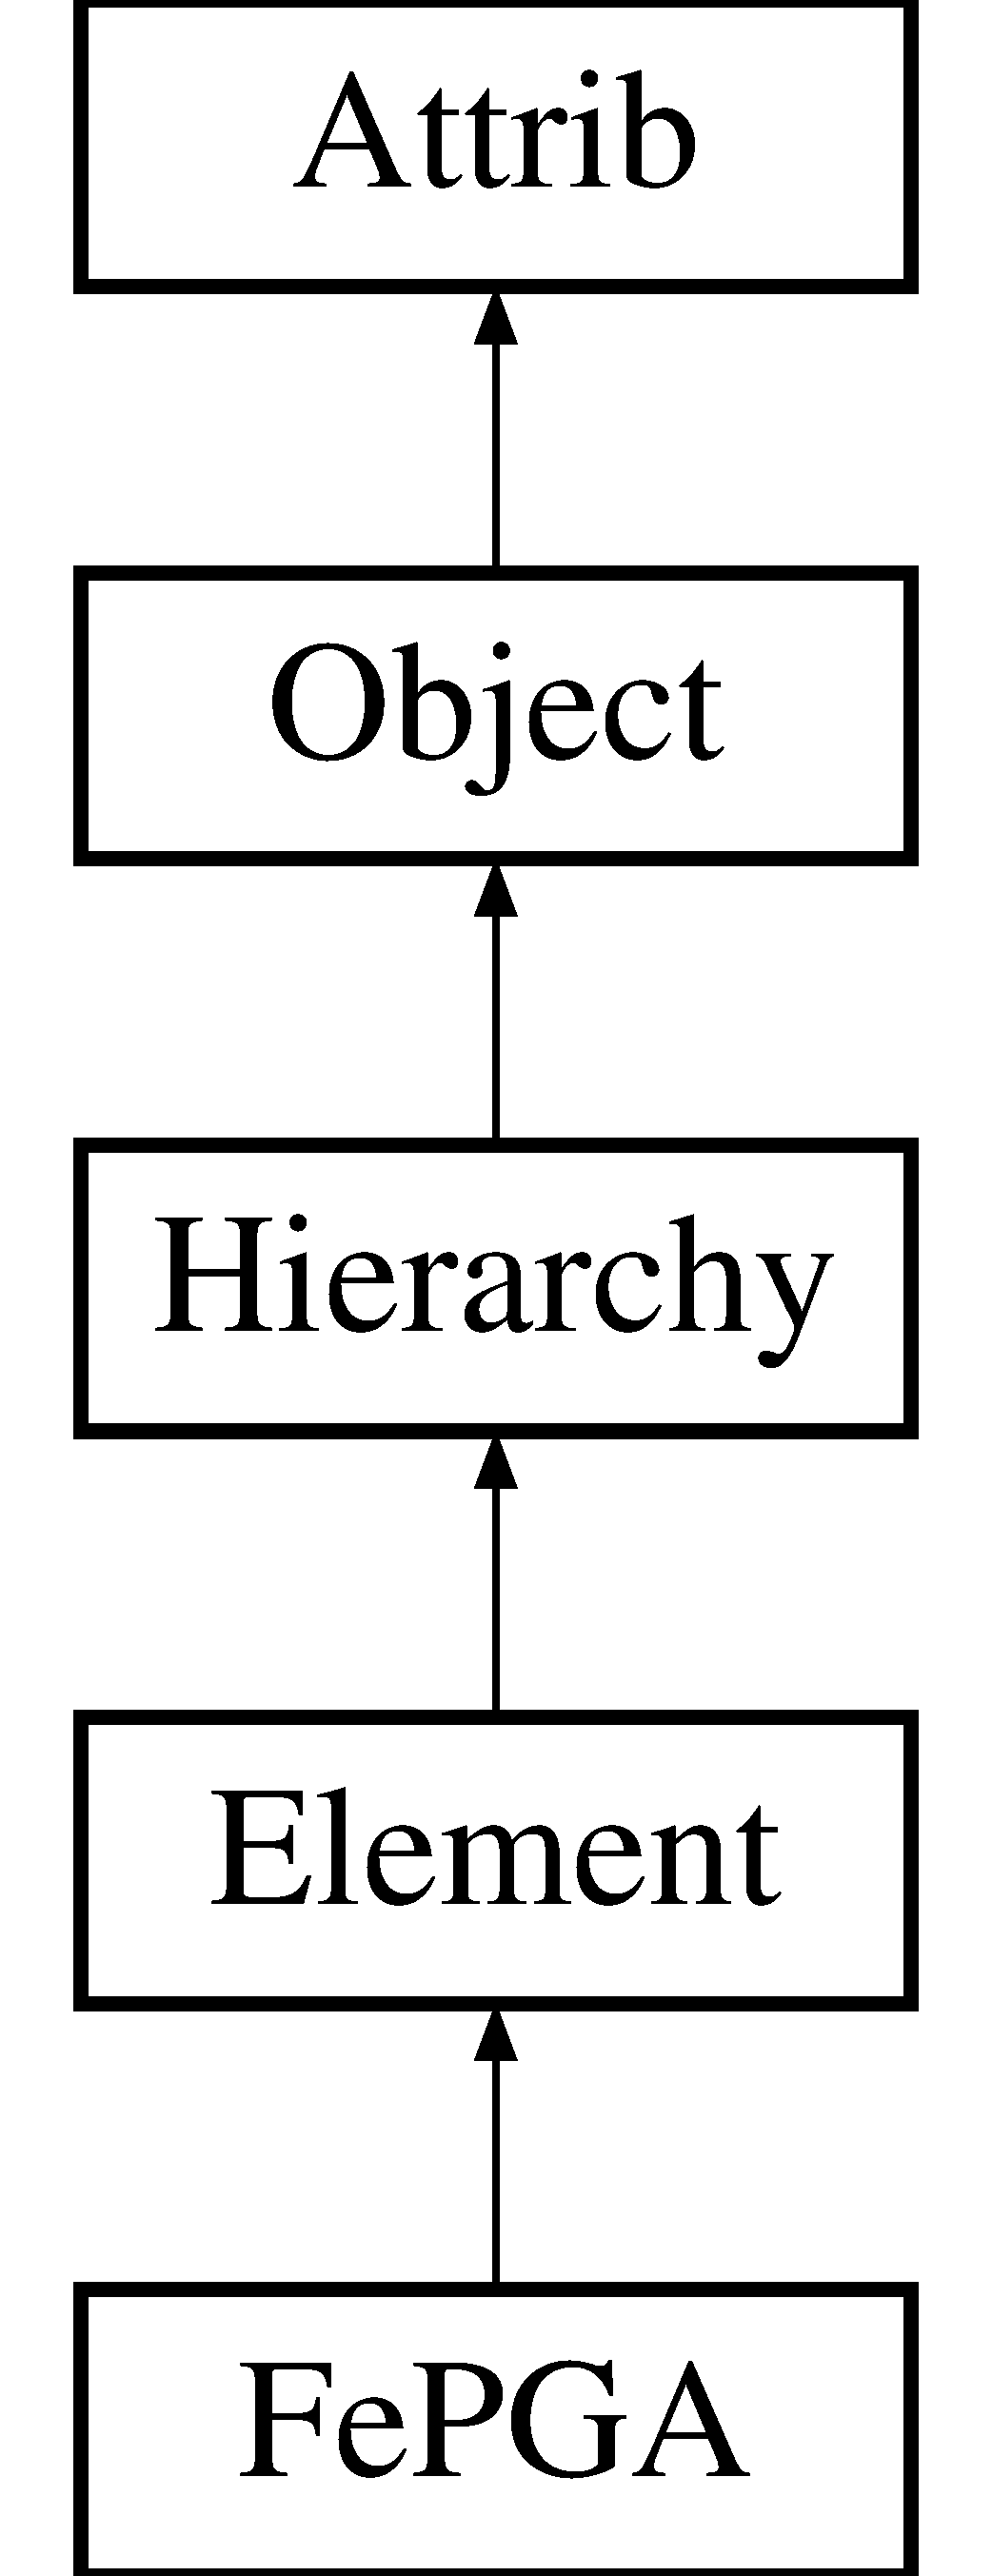
\includegraphics[height=5.000000cm]{classFePGA}
\end{center}
\end{figure}
\subsection*{Public Types}
\begin{DoxyCompactItemize}
\item 
typedef unsigned long \hyperlink{classFePGA_a1d44a0b27d13179bb1dceb5ec6f4cc1f}{U32}
\item 
typedef unsigned short \hyperlink{classFePGA_ac84b20a342a6c963cba061c8bdc37651}{U16}
\item 
typedef unsigned char \hyperlink{classFePGA_ab65d84dbbc4b5711eb4d85d00c5abfa2}{U8}
\item 
enum \hyperlink{classAttrib_a69e171d7cc6417835a5a306d3c764235}{Attribut} \{ \newline
\hyperlink{classAttrib_a69e171d7cc6417835a5a306d3c764235a3a8da2ab97dda18aebab196fe4100531}{U\+N\+D\+E\+F\+I\+N\+ED}, 
\hyperlink{classAttrib_a69e171d7cc6417835a5a306d3c764235a2bfb2af57b87031d190a05fe25dd92ed}{P\+A\+S\+S\+I\+VE}, 
\hyperlink{classAttrib_a69e171d7cc6417835a5a306d3c764235a3b1fec929c0370d1436f2f06e298fb0d}{A\+C\+T\+I\+VE}, 
\hyperlink{classAttrib_a69e171d7cc6417835a5a306d3c764235aa27c16b480a369ea4d18b07b2516bbc7}{I\+N\+T\+E\+R\+F\+A\+CE}, 
\newline
\hyperlink{classAttrib_a69e171d7cc6417835a5a306d3c764235a1420a5b8c0540b2af210b6975eded7f9}{IO}, 
\hyperlink{classAttrib_a69e171d7cc6417835a5a306d3c764235a0af3b0d0ac323c1704e6c69cf90add28}{I\+O\+D\+A\+TA}, 
\hyperlink{classAttrib_a69e171d7cc6417835a5a306d3c764235a7788bc5dd333fd8ce18562b269c9dab1}{E\+L\+E\+M\+E\+NT}, 
\hyperlink{classAttrib_a69e171d7cc6417835a5a306d3c764235a61ceb22149f365f1780d18f9d1459423}{H\+A\+R\+D\+W\+A\+RE}, 
\newline
\hyperlink{classAttrib_a69e171d7cc6417835a5a306d3c764235a75250e29692496e73effca2c0330977f}{P\+R\+O\+C\+E\+S\+S\+US}, 
\hyperlink{classAttrib_a69e171d7cc6417835a5a306d3c764235a103a67cd0b8f07ef478fa45d4356e27b}{S\+O\+F\+T\+W\+A\+RE}
 \}
\end{DoxyCompactItemize}
\subsection*{Public Member Functions}
\begin{DoxyCompactItemize}
\item 
\hyperlink{classFePGA_a377ae8860fbb3162e0c49dd08197a670}{Fe\+P\+GA} ()
\item 
virtual \hyperlink{classFePGA_aa445095a44c521b6b7803feaef6c16ba}{$\sim$\+Fe\+P\+GA} ()
\item 
void \hyperlink{classFePGA_ae6425fbad1a8db57025efaf387a6f41b}{help} ()
\begin{DoxyCompactList}\small\item\em Destructor. \end{DoxyCompactList}\item 
\hyperlink{classStatusCode}{Status\+Code} \hyperlink{classFePGA_a5355858b1b8deedcc12acff80f025804}{init} ()
\item 
void \hyperlink{classFePGA_abdf7a9dd901351a7eafd748d35172a3c}{reset} ()
\item 
void \hyperlink{classFePGA_a79d95b2fccf4d2ea473e6cf6980d6cf6}{reset\+Usb} ()
\item 
\hyperlink{classUsbFTMLInterface}{Usb\+F\+T\+M\+L\+Interface} $\ast$ \hyperlink{classFePGA_a4a7889dc3c2f88f623876ca475e66410}{usb} ()
\item 
\hyperlink{classUsbMLI2cBus}{Usb\+M\+L\+I2c\+Bus} $\ast$ \hyperlink{classFePGA_a1553db5010cce9e3495aa3060baf0b3c}{i2c} ()
\item 
\hyperlink{classUsbMLSpiBus}{Usb\+M\+L\+Spi\+Bus} $\ast$ \hyperlink{classFePGA_ab54f9f61e87f1cced6c4ba19eb38a848}{spi} ()
\item 
\hyperlink{classRegister}{Register} $\ast$ \hyperlink{classFePGA_a7b9b52c0a8b2080ed6a1163f9dfc5553}{reg} ()
\item 
void \hyperlink{classFePGA_ad23605ae261d2aa0562cbb732661b2c4}{update} ()
\item 
\hyperlink{classRegister}{Register} $\ast$ \hyperlink{classFePGA_aa0657c6ef809f3f6b54613f237750cc4}{setup\+Reg} ()
\item 
\hyperlink{classRegister}{Register} $\ast$ \hyperlink{classFePGA_a2bcd2c468fc3e1bcadc9bd8800b325a0}{master\+I2c\+Reg} ()
\item 
\hyperlink{classRegister}{Register} $\ast$ \hyperlink{classFePGA_a64feabdb09e65b1b4b1376a4da713570}{add\+I2c\+Reg} ()
\item 
\hyperlink{classStatusCode}{Status\+Code} \hyperlink{classFePGA_a3d5a3231a960cd451bb37bb9120422e9}{test\+Sequence} ()
\item 
\hyperlink{classStatusCode}{Status\+Code} \hyperlink{classFePGA_a59b840619341df26918a6c26e8b8e72b}{set\+Spi\+G\+B\+T\+S\+CA} (bool)
\item 
bool \hyperlink{classFePGA_ad305543bda4d68fe181cd7fa614b2fe1}{spi\+G\+B\+T\+S\+CA} ()
\item 
\hyperlink{classStatusCode}{Status\+Code} \hyperlink{classFePGA_a2cd235d1971625d6742d4f3107489a07}{set\+Spi\+Add} (unsigned long int)
\item 
unsigned long int \hyperlink{classFePGA_a721de3fa12e207392cd6156027d2c776}{spi\+Add} ()
\item 
\hyperlink{classStatusCode}{Status\+Code} \hyperlink{classFePGA_ad0a662adc6070427f0e1962c20a92de6}{set\+Spi\+Sub\+Add} (unsigned long int)
\item 
unsigned long int \hyperlink{classFePGA_a6637adb1cd981cf398ea9f1c3feafe83}{spi\+Sub\+Add} ()
\item 
\hyperlink{classStatusCode}{Status\+Code} \hyperlink{classFePGA_a637b93fed75b576a54e723acb36cb6a3}{spi\+Read} (unsigned int, unsigned int, unsigned int $\ast$)
\item 
\hyperlink{classStatusCode}{Status\+Code} \hyperlink{classFePGA_ac3e8b10fc267b44fef1e651cab77d2ab}{spi\+Write} (unsigned int, unsigned int, unsigned int $\ast$)
\item 
Py\+Object $\ast$ \hyperlink{classFePGA_a41fb676237f8906ec5a0c1b9084ad33e}{spi\+Read} (unsigned int, unsigned int)
\item 
\hyperlink{classStatusCode}{Status\+Code} \hyperlink{classFePGA_aa6aebdd1ccb236f9009a29243f3c7c2b}{spi\+Write} (unsigned int, unsigned int, Py\+Object $\ast$)
\item 
unsigned int \hyperlink{classFePGA_a165f5b70ad30af106ecf9a3ace71d4eb}{spi\+Read} (unsigned int)
\item 
\hyperlink{classStatusCode}{Status\+Code} \hyperlink{classFePGA_ab41df6b1d6a147fbf5611e54058f902d}{spi\+Write} (unsigned int, unsigned int)
\item 
\hyperlink{classStatusCode}{Status\+Code} \hyperlink{classFePGA_ac9a16de5f01fda901494abe61efb5029}{set\+I2c\+G\+B\+T\+S\+CA} (bool)
\item 
bool \hyperlink{classFePGA_a210cf57766c4f818ea61af671e91cfeb}{i2c\+G\+B\+T\+S\+CA} ()
\item 
\hyperlink{classStatusCode}{Status\+Code} \hyperlink{classFePGA_aaf52ed549f6b79d53f49c3f85c5fbad2}{set\+I2c\+Buffer} (unsigned long int)
\item 
unsigned long int \hyperlink{classFePGA_a5577463c8478cb6d54fc3c75b26cd819}{i2c\+Buffer} ()
\item 
unsigned long int \hyperlink{classFePGA_a9c261a09d323c07ec4b9e925d4dfc353}{i2c\+Data} ()
\item 
\hyperlink{classStatusCode}{Status\+Code} \hyperlink{classFePGA_a2da860f836e04ecc54056d0bf8cc8f98}{set\+I2c\+Add} (unsigned long int)
\item 
unsigned long int \hyperlink{classFePGA_a26b690b730b5f668ab28fb8deab8326b}{i2c\+Add} ()
\item 
\hyperlink{classStatusCode}{Status\+Code} \hyperlink{classFePGA_a37c1ee5bf89667c641f321479697166f}{set\+I2c\+Sub\+Add} (unsigned long int)
\item 
unsigned long int \hyperlink{classFePGA_ab51ac1c71e33f7444212de0e89e1f436}{i2c\+Sub\+Add} ()
\item 
\hyperlink{classStatusCode}{Status\+Code} \hyperlink{classFePGA_a939c5c23077210a2ad851a12694657a4}{i2c\+Read} ()
\item 
\hyperlink{classStatusCode}{Status\+Code} \hyperlink{classFePGA_a27b9c9bb486cea35b1bbcac5da96f527}{i2c\+Write} ()
\item 
unsigned long int \hyperlink{classFePGA_adf1c43786131d0f500b4662a877229c7}{i2c\+Read} (unsigned long int)
\item 
\hyperlink{classStatusCode}{Status\+Code} \hyperlink{classFePGA_a45e1cfdf1f303f3958bf6a83c4e8039b}{i2c\+Write} (unsigned long int, unsigned long int)
\item 
\hyperlink{classStatusCode}{Status\+Code} \hyperlink{classFePGA_ac7698a9f59f7290a6bb648030976597f}{transmit\+Spi} ()
\item 
void \hyperlink{classElement_a3c0abcb36f8906688bb7e32608df7086}{recursive\+Init\+Element} ()
\item 
void \hyperlink{classElement_a82119ed37dff76508a2746a853ec35ba}{recursive\+Init\+Communications} ()
\item 
\hyperlink{classStatusCode}{Status\+Code} \hyperlink{classElement_ab476b4b1df5954141ceb14f072433b89}{set\+Connection} (\hyperlink{classHierarchy}{Hierarchy} $\ast$)
\item 
\hyperlink{classHierarchy}{Hierarchy} $\ast$ \hyperlink{classElement_af57444353c1ddf9fa0109801e97debf7}{connection} ()
\item 
void \hyperlink{classHierarchy_af4d43b0765b402670eed2d62c73405af}{clear} ()
\item 
void \hyperlink{classHierarchy_a585ad1aeec16077a0e532ab8b4fc557b}{set\+Parent} (\hyperlink{classHierarchy}{Hierarchy} $\ast$\hyperlink{classHierarchy_a1c7bec8257e717f9c1465e06ebf845fc}{parent})
\item 
\hyperlink{classHierarchy}{Hierarchy} $\ast$ \hyperlink{classHierarchy_a1c7bec8257e717f9c1465e06ebf845fc}{parent} ()
\item 
\hyperlink{classHierarchy}{Hierarchy} $\ast$ \hyperlink{classHierarchy_ad550588733bf75ac5c0fcfd7c8fd11a6}{parent} (std\+::string)
\item 
\hyperlink{classHierarchy}{Hierarchy} $\ast$ \hyperlink{classHierarchy_aee461dc930ce3871636ff87f075b1b83}{origin} ()
\item 
virtual void \hyperlink{classHierarchy_ad677774ff38fcb257c04a3a10d471fac}{add\+Child} (\hyperlink{classHierarchy}{Hierarchy} $\ast$element)
\item 
std\+::vector$<$ \hyperlink{classHierarchy}{Hierarchy} $\ast$ $>$ \hyperlink{classHierarchy_aa9a76f69e98e052ee1a6e32cea006288}{children} ()
\item 
\hyperlink{classHierarchy}{Hierarchy} $\ast$ \hyperlink{classHierarchy_a1e207f973c694b538bf90107b4868817}{child} (std\+::string)
\item 
\hyperlink{classHierarchy}{Hierarchy} $\ast$ \hyperlink{classHierarchy_a0c15a5276a3b80b4354d6bd8a01e0708}{child\+Typed} (std\+::string)
\item 
unsigned long \hyperlink{classHierarchy_ab16e84de65fd84e14001a6cf941c8be4}{number\+Of\+Children} ()
\item 
bool \hyperlink{classHierarchy_a255174fe4d316d2a3f430dcb9dab29f1}{has\+Children} ()
\item 
void \hyperlink{classHierarchy_a2b2b359fac003233f65786a616766bde}{del\+Child} (\hyperlink{classHierarchy}{Hierarchy} $\ast$)
\item 
void \hyperlink{classHierarchy_a1928ac7615fe0b5e55cd707f70dc6781}{del\+Child} (std\+::string)
\item 
std\+::string \hyperlink{classHierarchy_aa7990fa7caf132d83e361ce033c6c65a}{path} (std\+::string=std\+::string(\char`\"{}\char`\"{}))
\item 
std\+::string \hyperlink{classHierarchy_a1efd56cd164d328d2002e53a10a19b8c}{path\+Typed} (std\+::string=std\+::string(\char`\"{}\char`\"{}))
\item 
void \hyperlink{classHierarchy_a76e914b9a677a22a82deb74d892bf261}{tree} (std\+::string indent=std\+::string(\char`\"{}\char`\"{}))
\item 
void \hyperlink{classHierarchy_a594c294c5f60c230e106d522ed008212}{tree} ()
\item 
std\+::string \hyperlink{classObject_a300f4c05dd468c7bb8b3c968868443c1}{name} () const
\item 
std\+::string \hyperlink{classObject_a84f99f70f144a83e1582d1d0f84e4e62}{type} ()
\item 
unsigned char \hyperlink{classObject_af99145335cc61ff6e2798ea17db009d2}{id} ()
\item 
std\+::string \hyperlink{classObject_a73a0f1a41828fdd8303dd662446fb6c3}{title} ()
\item 
void \hyperlink{classObject_a3f9d5537ebce0c0f2bf6ae4d92426f3c}{msg\+Svc} (int level, std\+::string \hyperlink{classObject_a58b2d0618c2d08cf2383012611528d97}{msg}, std\+::string \hyperlink{classObject_a300f4c05dd468c7bb8b3c968868443c1}{name})
\item 
void \hyperlink{classObject_a58b2d0618c2d08cf2383012611528d97}{msg} (std\+::string mymsg)
\item 
void \hyperlink{classObject_ac5d59299273cee27aacf7de00d2e7034}{msg} (std\+::string mymsg, std\+::string \hyperlink{classObject_a300f4c05dd468c7bb8b3c968868443c1}{name})
\item 
void \hyperlink{classObject_a83d2db2df682907ea1115ad721c1c4a1}{verbose} (std\+::string mymsg)
\item 
void \hyperlink{classObject_a2d4120195317e2a3c6532e8bb9f3da68}{verbose} (std\+::string mymsg, std\+::string \hyperlink{classObject_a300f4c05dd468c7bb8b3c968868443c1}{name})
\item 
void \hyperlink{classObject_aac010553f022165573714b7014a15f0d}{debug} (std\+::string mymsg)
\item 
void \hyperlink{classObject_a6c9a0397ca804e04d675ed05683f5420}{debug} (std\+::string mymsg, std\+::string \hyperlink{classObject_a300f4c05dd468c7bb8b3c968868443c1}{name})
\item 
void \hyperlink{classObject_a644fd329ea4cb85f54fa6846484b84a8}{info} (std\+::string mymsg)
\item 
void \hyperlink{classObject_a1ca123253dfd30fc28b156f521dcbdae}{info} (std\+::string mymsg, std\+::string \hyperlink{classObject_a300f4c05dd468c7bb8b3c968868443c1}{name})
\item 
void \hyperlink{classObject_a65cd4fda577711660821fd2cd5a3b4c9}{warning} (std\+::string mymsg)
\item 
void \hyperlink{classObject_a11f101db4dd73d9391b0231818881d86}{warning} (std\+::string mymsg, std\+::string \hyperlink{classObject_a300f4c05dd468c7bb8b3c968868443c1}{name})
\item 
void \hyperlink{classObject_a204a95f57818c0f811933917a30eff45}{error} (std\+::string mymsg)
\item 
void \hyperlink{classObject_ad7f6c457733082efa2f9ff5f5c8e119a}{error} (std\+::string mymsg, std\+::string \hyperlink{classObject_a300f4c05dd468c7bb8b3c968868443c1}{name})
\item 
void \hyperlink{classObject_aad5a16aac7516ce65bd5ec02ab07fc80}{fatal} (std\+::string mymsg)
\item 
void \hyperlink{classObject_ae62acd3d09f716220f75f252dc38bc9a}{fatal} (std\+::string mymsg, std\+::string \hyperlink{classObject_a300f4c05dd468c7bb8b3c968868443c1}{name})
\item 
void \hyperlink{classObject_ae30fea75683c2d149b6b6d17c09ecd0c}{set\+Name} (std\+::string \hyperlink{classObject_a300f4c05dd468c7bb8b3c968868443c1}{name})
\item 
void \hyperlink{classObject_aae534cc9d982bcb9b99fd505f2e103a5}{set\+Type} (std\+::string \hyperlink{classObject_a84f99f70f144a83e1582d1d0f84e4e62}{type})
\item 
void \hyperlink{classObject_a398fe08cba594a0ce6891d59fe4f159f}{set\+Id} (unsigned char \hyperlink{classObject_af99145335cc61ff6e2798ea17db009d2}{id})
\item 
void \hyperlink{classObject_a89557dbbad5bcaa02652f5d7fa35d20f}{set\+Title} (std\+::string \hyperlink{classObject_a73a0f1a41828fdd8303dd662446fb6c3}{title})
\item 
void \hyperlink{classObject_a870c5af919958c2136623b2d7816d123}{set\+Dll\+Name} (std\+::string \hyperlink{classObject_a2e3947f2870094c332d7454117f3ec63}{dll\+Name})
\item 
std\+::string \hyperlink{classObject_a2e3947f2870094c332d7454117f3ec63}{dll\+Name} ()
\item 
bool \hyperlink{classAttrib_a704f26af560909ad22065083bb7d4c34}{is} (int attribut)
\item 
void \hyperlink{classAttrib_a235f773af19c900264a190b00a3b4ad7}{add} (int attribut)
\item 
void \hyperlink{classAttrib_a7d4ef7e32d93cb287792b87b857e79f3}{remove} (int attribut)
\item 
std\+::string \hyperlink{classAttrib_aee7bbf16b144887f196e1341b24f8a26}{attributs} ()
\end{DoxyCompactItemize}
\subsection*{Protected Attributes}
\begin{DoxyCompactItemize}
\item 
\hyperlink{classHierarchy}{Hierarchy} $\ast$ \hyperlink{classElement_abe3de7a5dbbc9a6dd2d7e012e5fdb266}{m\+\_\+connection}
\item 
std\+::string \hyperlink{classAttrib_a3414521d7a82476e874b25a5407b5e63}{m\+\_\+attrib\+String} \mbox{[}10\mbox{]}
\end{DoxyCompactItemize}
\subsection*{Private Attributes}
\begin{DoxyCompactItemize}
\item 
\hyperlink{classUsbFTMLInterface}{Usb\+F\+T\+M\+L\+Interface} $\ast$ \hyperlink{classFePGA_afb7947e600a66d914ee524acec3d8b1f}{m\+\_\+usb}
\item 
\hyperlink{classUsbMLI2cBus}{Usb\+M\+L\+I2c\+Bus} $\ast$ \hyperlink{classFePGA_a09fdde4002008daa0d15672772dd4483}{m\+\_\+usbi2c}
\item 
\hyperlink{classUsbMLSpiBus}{Usb\+M\+L\+Spi\+Bus} $\ast$ \hyperlink{classFePGA_a922a56250b29c9842cdb8095cae8c976}{m\+\_\+usbspi}
\item 
\hyperlink{classRegister}{Register} $\ast$ \hyperlink{classFePGA_afdbe1ea67182ffdaaf62116d66839ad7}{m\+\_\+reg}
\item 
\hyperlink{classRegister}{Register} $\ast$ \hyperlink{classFePGA_ad8c66e956d4f4163ae4dcb966d3ebeed}{m\+\_\+status\+Reg}
\item 
\hyperlink{classRegister}{Register} $\ast$ \hyperlink{classFePGA_a0255fe229013986b4387c3a75ddf4e97}{m\+\_\+setup\+Reg}
\item 
\hyperlink{classRegister}{Register} $\ast$ \hyperlink{classFePGA_a9a3a8d338e264c0ccb51e01178b48bd1}{m\+\_\+io\+Reg\+\_\+1}
\item 
\hyperlink{classRegister}{Register} $\ast$ \hyperlink{classFePGA_aaf91054fbe6367cd044b6856098c781b}{m\+\_\+io\+Reg\+\_\+2}
\item 
\hyperlink{classRegister}{Register} $\ast$ \hyperlink{classFePGA_a634d74bc7104816d7ef1bbe816bdf366}{m\+\_\+io\+Reg\+\_\+3}
\item 
\hyperlink{classRAM}{R\+AM} $\ast$ \hyperlink{classFePGA_af911fcb4fc76acd553e9a492174f134b}{m\+\_\+fifo\+\_\+test\+\_\+1}
\item 
\hyperlink{classRAM}{R\+AM} $\ast$ \hyperlink{classFePGA_ad42013742385c695067b466c933665c9}{m\+\_\+fifo\+\_\+test\+\_\+2}
\item 
\hyperlink{classRegister}{Register} $\ast$ \hyperlink{classFePGA_aeff1a2370237a06b50e1ae23d933c862}{m\+\_\+reset\+Reg}
\item 
\hyperlink{classRegister}{Register} $\ast$ \hyperlink{classFePGA_a67bc3c8f923b673100974fd86096393e}{m\+\_\+test\+Seq\+Reg}
\item 
\hyperlink{classRAM}{R\+AM} $\ast$ \hyperlink{classFePGA_a5b3e4deb73a882e6f044450d8a733558}{m\+\_\+tx\+Spi\+Fifo}
\item 
\hyperlink{classRAM}{R\+AM} $\ast$ \hyperlink{classFePGA_a3ee7f973bfad39b48bbc1a185e9ffaec}{m\+\_\+rx\+Spi\+Fifo}
\item 
\hyperlink{classRegister}{Register} $\ast$ \hyperlink{classFePGA_a569eb8410924bec1c8279ca80dc37a6a}{m\+\_\+add\+Spi\+Reg}
\item 
\hyperlink{classRegister}{Register} $\ast$ \hyperlink{classFePGA_a8fb76733a688dff6d91892a49a97a21f}{m\+\_\+ctrl\+Spi\+Reg}
\item 
\hyperlink{classRegister}{Register} $\ast$ \hyperlink{classFePGA_a003ee241fb5f32fb3442174db3fe6f49}{m\+\_\+transmit\+Spi\+Reg}
\item 
unsigned int \hyperlink{classFePGA_a4f2f5d175aeb6dcaf497f81d2f075411}{m\+\_\+spi\+Sub\+Add}
\item 
unsigned int \hyperlink{classFePGA_aba8c2c8d8e0d136826b9dd4c2d7c2e90}{m\+\_\+i2c\+Sub\+Add}
\item 
unsigned int \hyperlink{classFePGA_a173664ffd6a73f454ae31f51e689dd16}{m\+\_\+i2c\+Buffer}
\item 
\hyperlink{classRegister}{Register} $\ast$ \hyperlink{classFePGA_adb390ea8de4a6cbce648dc62e4405f32}{m\+\_\+master\+I2c\+Reg}
\item 
\hyperlink{classRegister}{Register} $\ast$ \hyperlink{classFePGA_af3ef3467ba803e6d3b970ea8982d6246}{m\+\_\+add\+I2c\+Reg}
\end{DoxyCompactItemize}


\subsection{Detailed Description}


Definition at line 23 of file Fe\+P\+G\+A.\+h.



\subsection{Member Typedef Documentation}
\mbox{\Hypertarget{classFePGA_ac84b20a342a6c963cba061c8bdc37651}\label{classFePGA_ac84b20a342a6c963cba061c8bdc37651}} 
\index{Fe\+P\+GA@{Fe\+P\+GA}!U16@{U16}}
\index{U16@{U16}!Fe\+P\+GA@{Fe\+P\+GA}}
\subsubsection{\texorpdfstring{U16}{U16}}
{\footnotesize\ttfamily typedef unsigned short \hyperlink{classFePGA_ac84b20a342a6c963cba061c8bdc37651}{Fe\+P\+G\+A\+::\+U16}}



Definition at line 26 of file Fe\+P\+G\+A.\+h.

\mbox{\Hypertarget{classFePGA_a1d44a0b27d13179bb1dceb5ec6f4cc1f}\label{classFePGA_a1d44a0b27d13179bb1dceb5ec6f4cc1f}} 
\index{Fe\+P\+GA@{Fe\+P\+GA}!U32@{U32}}
\index{U32@{U32}!Fe\+P\+GA@{Fe\+P\+GA}}
\subsubsection{\texorpdfstring{U32}{U32}}
{\footnotesize\ttfamily typedef unsigned long \hyperlink{classFePGA_a1d44a0b27d13179bb1dceb5ec6f4cc1f}{Fe\+P\+G\+A\+::\+U32}}



Definition at line 25 of file Fe\+P\+G\+A.\+h.

\mbox{\Hypertarget{classFePGA_ab65d84dbbc4b5711eb4d85d00c5abfa2}\label{classFePGA_ab65d84dbbc4b5711eb4d85d00c5abfa2}} 
\index{Fe\+P\+GA@{Fe\+P\+GA}!U8@{U8}}
\index{U8@{U8}!Fe\+P\+GA@{Fe\+P\+GA}}
\subsubsection{\texorpdfstring{U8}{U8}}
{\footnotesize\ttfamily typedef unsigned char \hyperlink{classFePGA_ab65d84dbbc4b5711eb4d85d00c5abfa2}{Fe\+P\+G\+A\+::\+U8}}



Definition at line 27 of file Fe\+P\+G\+A.\+h.



\subsection{Member Enumeration Documentation}
\mbox{\Hypertarget{classAttrib_a69e171d7cc6417835a5a306d3c764235}\label{classAttrib_a69e171d7cc6417835a5a306d3c764235}} 
\index{Fe\+P\+GA@{Fe\+P\+GA}!Attribut@{Attribut}}
\index{Attribut@{Attribut}!Fe\+P\+GA@{Fe\+P\+GA}}
\subsubsection{\texorpdfstring{Attribut}{Attribut}}
{\footnotesize\ttfamily enum \hyperlink{classAttrib_a69e171d7cc6417835a5a306d3c764235}{Attrib\+::\+Attribut}\hspace{0.3cm}{\ttfamily [inherited]}}

\begin{DoxyEnumFields}{Enumerator}
\raisebox{\heightof{T}}[0pt][0pt]{\index{U\+N\+D\+E\+F\+I\+N\+ED@{U\+N\+D\+E\+F\+I\+N\+ED}!Fe\+P\+GA@{Fe\+P\+GA}}\index{Fe\+P\+GA@{Fe\+P\+GA}!U\+N\+D\+E\+F\+I\+N\+ED@{U\+N\+D\+E\+F\+I\+N\+ED}}}\mbox{\Hypertarget{classAttrib_a69e171d7cc6417835a5a306d3c764235a3a8da2ab97dda18aebab196fe4100531}\label{classAttrib_a69e171d7cc6417835a5a306d3c764235a3a8da2ab97dda18aebab196fe4100531}} 
U\+N\+D\+E\+F\+I\+N\+ED&\\
\hline

\raisebox{\heightof{T}}[0pt][0pt]{\index{P\+A\+S\+S\+I\+VE@{P\+A\+S\+S\+I\+VE}!Fe\+P\+GA@{Fe\+P\+GA}}\index{Fe\+P\+GA@{Fe\+P\+GA}!P\+A\+S\+S\+I\+VE@{P\+A\+S\+S\+I\+VE}}}\mbox{\Hypertarget{classAttrib_a69e171d7cc6417835a5a306d3c764235a2bfb2af57b87031d190a05fe25dd92ed}\label{classAttrib_a69e171d7cc6417835a5a306d3c764235a2bfb2af57b87031d190a05fe25dd92ed}} 
P\+A\+S\+S\+I\+VE&\\
\hline

\raisebox{\heightof{T}}[0pt][0pt]{\index{A\+C\+T\+I\+VE@{A\+C\+T\+I\+VE}!Fe\+P\+GA@{Fe\+P\+GA}}\index{Fe\+P\+GA@{Fe\+P\+GA}!A\+C\+T\+I\+VE@{A\+C\+T\+I\+VE}}}\mbox{\Hypertarget{classAttrib_a69e171d7cc6417835a5a306d3c764235a3b1fec929c0370d1436f2f06e298fb0d}\label{classAttrib_a69e171d7cc6417835a5a306d3c764235a3b1fec929c0370d1436f2f06e298fb0d}} 
A\+C\+T\+I\+VE&\\
\hline

\raisebox{\heightof{T}}[0pt][0pt]{\index{I\+N\+T\+E\+R\+F\+A\+CE@{I\+N\+T\+E\+R\+F\+A\+CE}!Fe\+P\+GA@{Fe\+P\+GA}}\index{Fe\+P\+GA@{Fe\+P\+GA}!I\+N\+T\+E\+R\+F\+A\+CE@{I\+N\+T\+E\+R\+F\+A\+CE}}}\mbox{\Hypertarget{classAttrib_a69e171d7cc6417835a5a306d3c764235aa27c16b480a369ea4d18b07b2516bbc7}\label{classAttrib_a69e171d7cc6417835a5a306d3c764235aa27c16b480a369ea4d18b07b2516bbc7}} 
I\+N\+T\+E\+R\+F\+A\+CE&\\
\hline

\raisebox{\heightof{T}}[0pt][0pt]{\index{IO@{IO}!Fe\+P\+GA@{Fe\+P\+GA}}\index{Fe\+P\+GA@{Fe\+P\+GA}!IO@{IO}}}\mbox{\Hypertarget{classAttrib_a69e171d7cc6417835a5a306d3c764235a1420a5b8c0540b2af210b6975eded7f9}\label{classAttrib_a69e171d7cc6417835a5a306d3c764235a1420a5b8c0540b2af210b6975eded7f9}} 
IO&\\
\hline

\raisebox{\heightof{T}}[0pt][0pt]{\index{I\+O\+D\+A\+TA@{I\+O\+D\+A\+TA}!Fe\+P\+GA@{Fe\+P\+GA}}\index{Fe\+P\+GA@{Fe\+P\+GA}!I\+O\+D\+A\+TA@{I\+O\+D\+A\+TA}}}\mbox{\Hypertarget{classAttrib_a69e171d7cc6417835a5a306d3c764235a0af3b0d0ac323c1704e6c69cf90add28}\label{classAttrib_a69e171d7cc6417835a5a306d3c764235a0af3b0d0ac323c1704e6c69cf90add28}} 
I\+O\+D\+A\+TA&\\
\hline

\raisebox{\heightof{T}}[0pt][0pt]{\index{E\+L\+E\+M\+E\+NT@{E\+L\+E\+M\+E\+NT}!Fe\+P\+GA@{Fe\+P\+GA}}\index{Fe\+P\+GA@{Fe\+P\+GA}!E\+L\+E\+M\+E\+NT@{E\+L\+E\+M\+E\+NT}}}\mbox{\Hypertarget{classAttrib_a69e171d7cc6417835a5a306d3c764235a7788bc5dd333fd8ce18562b269c9dab1}\label{classAttrib_a69e171d7cc6417835a5a306d3c764235a7788bc5dd333fd8ce18562b269c9dab1}} 
E\+L\+E\+M\+E\+NT&\\
\hline

\raisebox{\heightof{T}}[0pt][0pt]{\index{H\+A\+R\+D\+W\+A\+RE@{H\+A\+R\+D\+W\+A\+RE}!Fe\+P\+GA@{Fe\+P\+GA}}\index{Fe\+P\+GA@{Fe\+P\+GA}!H\+A\+R\+D\+W\+A\+RE@{H\+A\+R\+D\+W\+A\+RE}}}\mbox{\Hypertarget{classAttrib_a69e171d7cc6417835a5a306d3c764235a61ceb22149f365f1780d18f9d1459423}\label{classAttrib_a69e171d7cc6417835a5a306d3c764235a61ceb22149f365f1780d18f9d1459423}} 
H\+A\+R\+D\+W\+A\+RE&\\
\hline

\raisebox{\heightof{T}}[0pt][0pt]{\index{P\+R\+O\+C\+E\+S\+S\+US@{P\+R\+O\+C\+E\+S\+S\+US}!Fe\+P\+GA@{Fe\+P\+GA}}\index{Fe\+P\+GA@{Fe\+P\+GA}!P\+R\+O\+C\+E\+S\+S\+US@{P\+R\+O\+C\+E\+S\+S\+US}}}\mbox{\Hypertarget{classAttrib_a69e171d7cc6417835a5a306d3c764235a75250e29692496e73effca2c0330977f}\label{classAttrib_a69e171d7cc6417835a5a306d3c764235a75250e29692496e73effca2c0330977f}} 
P\+R\+O\+C\+E\+S\+S\+US&\\
\hline

\raisebox{\heightof{T}}[0pt][0pt]{\index{S\+O\+F\+T\+W\+A\+RE@{S\+O\+F\+T\+W\+A\+RE}!Fe\+P\+GA@{Fe\+P\+GA}}\index{Fe\+P\+GA@{Fe\+P\+GA}!S\+O\+F\+T\+W\+A\+RE@{S\+O\+F\+T\+W\+A\+RE}}}\mbox{\Hypertarget{classAttrib_a69e171d7cc6417835a5a306d3c764235a103a67cd0b8f07ef478fa45d4356e27b}\label{classAttrib_a69e171d7cc6417835a5a306d3c764235a103a67cd0b8f07ef478fa45d4356e27b}} 
S\+O\+F\+T\+W\+A\+RE&\\
\hline

\end{DoxyEnumFields}


Definition at line 29 of file Attrib.\+h.


\begin{DoxyCode}
29                 \{
30     \hyperlink{classAttrib_a69e171d7cc6417835a5a306d3c764235a3a8da2ab97dda18aebab196fe4100531}{UNDEFINED},
31     \hyperlink{classAttrib_a69e171d7cc6417835a5a306d3c764235a2bfb2af57b87031d190a05fe25dd92ed}{PASSIVE},
32     \hyperlink{classAttrib_a69e171d7cc6417835a5a306d3c764235a3b1fec929c0370d1436f2f06e298fb0d}{ACTIVE},
33     \hyperlink{classAttrib_a69e171d7cc6417835a5a306d3c764235aa27c16b480a369ea4d18b07b2516bbc7}{INTERFACE},
34     \hyperlink{classAttrib_a69e171d7cc6417835a5a306d3c764235a1420a5b8c0540b2af210b6975eded7f9}{IO},
35     \hyperlink{classAttrib_a69e171d7cc6417835a5a306d3c764235a0af3b0d0ac323c1704e6c69cf90add28}{IODATA},
36     \hyperlink{classAttrib_a69e171d7cc6417835a5a306d3c764235a7788bc5dd333fd8ce18562b269c9dab1}{ELEMENT},
37     \hyperlink{classAttrib_a69e171d7cc6417835a5a306d3c764235a61ceb22149f365f1780d18f9d1459423}{HARDWARE},
38     \hyperlink{classAttrib_a69e171d7cc6417835a5a306d3c764235a75250e29692496e73effca2c0330977f}{PROCESSUS},
39     \hyperlink{classAttrib_a69e171d7cc6417835a5a306d3c764235a103a67cd0b8f07ef478fa45d4356e27b}{SOFTWARE} 
40   \}; \textcolor{comment}{// array m\_attribString must be changed into Attrib::Attrib if this enu is modified. }
\end{DoxyCode}


\subsection{Constructor \& Destructor Documentation}
\mbox{\Hypertarget{classFePGA_a377ae8860fbb3162e0c49dd08197a670}\label{classFePGA_a377ae8860fbb3162e0c49dd08197a670}} 
\index{Fe\+P\+GA@{Fe\+P\+GA}!Fe\+P\+GA@{Fe\+P\+GA}}
\index{Fe\+P\+GA@{Fe\+P\+GA}!Fe\+P\+GA@{Fe\+P\+GA}}
\subsubsection{\texorpdfstring{Fe\+P\+G\+A()}{FePGA()}}
{\footnotesize\ttfamily Fe\+P\+G\+A\+::\+Fe\+P\+GA (\begin{DoxyParamCaption}{ }\end{DoxyParamCaption})}



Definition at line 29 of file Fe\+P\+G\+A.\+cpp.



References Attrib\+::add(), Hierarchy\+::add\+Child(), I\+Odata\+::\+Byte, Object\+::debug(), I\+Odata\+::def\+Data\+U8(), Attrib\+::\+E\+L\+E\+M\+E\+NT, Attrib\+::\+H\+A\+R\+D\+W\+A\+RE, I\+Oobject\+::io(), m\+\_\+fifo\+\_\+test\+\_\+1, m\+\_\+fifo\+\_\+test\+\_\+2, m\+\_\+io\+Reg\+\_\+1, m\+\_\+io\+Reg\+\_\+2, m\+\_\+io\+Reg\+\_\+3, m\+\_\+reset\+Reg, m\+\_\+setup\+Reg, m\+\_\+usb, I\+Odata\+::set\+Address(), Object\+::set\+Id(), Object\+::set\+Name(), R\+A\+M\+::set\+Size(), Object\+::set\+Type(), and I\+Odata\+::set\+Word\+Size().


\begin{DoxyCode}
29             \{
30   \hyperlink{classObject_aae534cc9d982bcb9b99fd505f2e103a5}{setType}(\textcolor{stringliteral}{"FePGA"});
31   \hyperlink{classObject_a398fe08cba594a0ce6891d59fe4f159f}{setId}(0);
32   \hyperlink{classAttrib_a235f773af19c900264a190b00a3b4ad7}{add}(\hyperlink{classAttrib_a69e171d7cc6417835a5a306d3c764235a7788bc5dd333fd8ce18562b269c9dab1}{Attrib::ELEMENT}); \hyperlink{classAttrib_a235f773af19c900264a190b00a3b4ad7}{add} (\hyperlink{classAttrib_a69e171d7cc6417835a5a306d3c764235a61ceb22149f365f1780d18f9d1459423}{Attrib::HARDWARE});
33   \hyperlink{classObject_aac010553f022165573714b7014a15f0d}{debug}(\textcolor{stringliteral}{"FePGA built."},\textcolor{stringliteral}{"FePGA::FePGA"});
34 
35 
36   \hyperlink{classFePGA_afb7947e600a66d914ee524acec3d8b1f}{m\_usb} = \textcolor{keyword}{new} \hyperlink{classUsbFTMLInterface}{UsbFTMLInterface}();
37   \hyperlink{classFePGA_afb7947e600a66d914ee524acec3d8b1f}{m\_usb}->\hyperlink{classObject_ae30fea75683c2d149b6b6d17c09ecd0c}{setName}(\textcolor{stringliteral}{"Usb"});
38   \hyperlink{classHierarchy_ad677774ff38fcb257c04a3a10d471fac}{addChild}(\hyperlink{classFePGA_afb7947e600a66d914ee524acec3d8b1f}{m\_usb});
39 
40   
41   \hyperlink{classFePGA_a9a3a8d338e264c0ccb51e01178b48bd1}{m\_ioReg\_1}     = \textcolor{keyword}{new} \hyperlink{classRegister}{Register}();
42   \hyperlink{classFePGA_a9a3a8d338e264c0ccb51e01178b48bd1}{m\_ioReg\_1}     ->\hyperlink{classObject_ae30fea75683c2d149b6b6d17c09ecd0c}{setName}(\textcolor{stringliteral}{"IOReg\_1"});
43   \hyperlink{classFePGA_a9a3a8d338e264c0ccb51e01178b48bd1}{m\_ioReg\_1}     ->\hyperlink{classIOobject_af04fb94137c3d86849f478ac5afab5d1}{io}()->\hyperlink{classIOdata_a80bb230b61062b447db5832e43bf7b44}{defDataU8}(2);
44   \hyperlink{classFePGA_a9a3a8d338e264c0ccb51e01178b48bd1}{m\_ioReg\_1}     ->\hyperlink{classIOobject_af04fb94137c3d86849f478ac5afab5d1}{io}()->\hyperlink{classIOdata_af98cbfbc28346ebb9b64ca0203af1463}{setAddress}(0x01);
45   \hyperlink{classFePGA_a9a3a8d338e264c0ccb51e01178b48bd1}{m\_ioReg\_1}     ->\hyperlink{classIOobject_af04fb94137c3d86849f478ac5afab5d1}{io}()->\hyperlink{classIOdata_a20f30a9f4673713616447b1b5e9817d5}{setWordSize}(\hyperlink{classIOdata_a37c53ebf4bf8d866aac8af572962a84ca00156611f08eeb1b5d361de809dafb8e}{IOdata::Byte});
46   \hyperlink{classFePGA_afb7947e600a66d914ee524acec3d8b1f}{m\_usb}         ->\hyperlink{classHierarchy_ad677774ff38fcb257c04a3a10d471fac}{addChild}(\hyperlink{classFePGA_a9a3a8d338e264c0ccb51e01178b48bd1}{m\_ioReg\_1}); \textcolor{comment}{// create the USB bus}
47 
48 
49 
50   \hyperlink{classFePGA_aaf91054fbe6367cd044b6856098c781b}{m\_ioReg\_2}     = \textcolor{keyword}{new} \hyperlink{classRegister}{Register}();
51   \hyperlink{classFePGA_aaf91054fbe6367cd044b6856098c781b}{m\_ioReg\_2}     ->\hyperlink{classObject_ae30fea75683c2d149b6b6d17c09ecd0c}{setName}(\textcolor{stringliteral}{"IOReg\_2"});
52   \hyperlink{classFePGA_aaf91054fbe6367cd044b6856098c781b}{m\_ioReg\_2}     ->\hyperlink{classIOobject_af04fb94137c3d86849f478ac5afab5d1}{io}()->\hyperlink{classIOdata_a80bb230b61062b447db5832e43bf7b44}{defDataU8}(2);
53   \hyperlink{classFePGA_aaf91054fbe6367cd044b6856098c781b}{m\_ioReg\_2}     ->\hyperlink{classIOobject_af04fb94137c3d86849f478ac5afab5d1}{io}()->\hyperlink{classIOdata_af98cbfbc28346ebb9b64ca0203af1463}{setAddress}(0x02);
54   \hyperlink{classFePGA_aaf91054fbe6367cd044b6856098c781b}{m\_ioReg\_2}     ->\hyperlink{classIOobject_af04fb94137c3d86849f478ac5afab5d1}{io}()->\hyperlink{classIOdata_a20f30a9f4673713616447b1b5e9817d5}{setWordSize}(\hyperlink{classIOdata_a37c53ebf4bf8d866aac8af572962a84ca00156611f08eeb1b5d361de809dafb8e}{IOdata::Byte});
55   \hyperlink{classFePGA_afb7947e600a66d914ee524acec3d8b1f}{m\_usb}         ->\hyperlink{classHierarchy_ad677774ff38fcb257c04a3a10d471fac}{addChild}(\hyperlink{classFePGA_aaf91054fbe6367cd044b6856098c781b}{m\_ioReg\_2}); \textcolor{comment}{// create the USB bus}
56 
57 
58 
59   \hyperlink{classFePGA_a634d74bc7104816d7ef1bbe816bdf366}{m\_ioReg\_3}     = \textcolor{keyword}{new} \hyperlink{classRegister}{Register}();
60   \hyperlink{classFePGA_a634d74bc7104816d7ef1bbe816bdf366}{m\_ioReg\_3}     ->\hyperlink{classObject_ae30fea75683c2d149b6b6d17c09ecd0c}{setName}(\textcolor{stringliteral}{"IOReg\_3"});
61   \hyperlink{classFePGA_a634d74bc7104816d7ef1bbe816bdf366}{m\_ioReg\_3}     ->\hyperlink{classIOobject_af04fb94137c3d86849f478ac5afab5d1}{io}()->\hyperlink{classIOdata_a80bb230b61062b447db5832e43bf7b44}{defDataU8}(2);
62   \hyperlink{classFePGA_a634d74bc7104816d7ef1bbe816bdf366}{m\_ioReg\_3}     ->\hyperlink{classIOobject_af04fb94137c3d86849f478ac5afab5d1}{io}()->\hyperlink{classIOdata_af98cbfbc28346ebb9b64ca0203af1463}{setAddress}(0x03);
63   \hyperlink{classFePGA_a634d74bc7104816d7ef1bbe816bdf366}{m\_ioReg\_3}     ->\hyperlink{classIOobject_af04fb94137c3d86849f478ac5afab5d1}{io}()->\hyperlink{classIOdata_a20f30a9f4673713616447b1b5e9817d5}{setWordSize}(\hyperlink{classIOdata_a37c53ebf4bf8d866aac8af572962a84ca00156611f08eeb1b5d361de809dafb8e}{IOdata::Byte});
64   \hyperlink{classFePGA_afb7947e600a66d914ee524acec3d8b1f}{m\_usb}         ->\hyperlink{classHierarchy_ad677774ff38fcb257c04a3a10d471fac}{addChild}(\hyperlink{classFePGA_a634d74bc7104816d7ef1bbe816bdf366}{m\_ioReg\_3}); \textcolor{comment}{// create the USB bus}
65 
66   
67   \hyperlink{classFePGA_a0255fe229013986b4387c3a75ddf4e97}{m\_setupReg}       = \textcolor{keyword}{new} \hyperlink{classRegister}{Register}();
68   \hyperlink{classFePGA_a0255fe229013986b4387c3a75ddf4e97}{m\_setupReg}       ->\hyperlink{classObject_ae30fea75683c2d149b6b6d17c09ecd0c}{setName}(\textcolor{stringliteral}{"SetupReg"});
69   \hyperlink{classFePGA_a0255fe229013986b4387c3a75ddf4e97}{m\_setupReg}       ->\hyperlink{classIOobject_af04fb94137c3d86849f478ac5afab5d1}{io}()->\hyperlink{classIOdata_a80bb230b61062b447db5832e43bf7b44}{defDataU8}(2);     
70   \hyperlink{classFePGA_a0255fe229013986b4387c3a75ddf4e97}{m\_setupReg}       ->\hyperlink{classIOobject_af04fb94137c3d86849f478ac5afab5d1}{io}()->\hyperlink{classIOdata_af98cbfbc28346ebb9b64ca0203af1463}{setAddress}(0x08); \textcolor{comment}{// from Olivier 08h}
71   \hyperlink{classFePGA_a0255fe229013986b4387c3a75ddf4e97}{m\_setupReg}       ->\hyperlink{classIOobject_af04fb94137c3d86849f478ac5afab5d1}{io}()->\hyperlink{classIOdata_a20f30a9f4673713616447b1b5e9817d5}{setWordSize}(\hyperlink{classIOdata_a37c53ebf4bf8d866aac8af572962a84ca00156611f08eeb1b5d361de809dafb8e}{IOdata::Byte});
72   \hyperlink{classFePGA_afb7947e600a66d914ee524acec3d8b1f}{m\_usb}            ->\hyperlink{classHierarchy_ad677774ff38fcb257c04a3a10d471fac}{addChild}(\hyperlink{classFePGA_a0255fe229013986b4387c3a75ddf4e97}{m\_setupReg});
73 
74 
75   \hyperlink{classFePGA_aeff1a2370237a06b50e1ae23d933c862}{m\_resetReg}       = \textcolor{keyword}{new} \hyperlink{classRegister}{Register}();
76   \hyperlink{classFePGA_aeff1a2370237a06b50e1ae23d933c862}{m\_resetReg}       ->\hyperlink{classObject_ae30fea75683c2d149b6b6d17c09ecd0c}{setName}(\textcolor{stringliteral}{"ResetReg"});
77   \hyperlink{classFePGA_aeff1a2370237a06b50e1ae23d933c862}{m\_resetReg}       ->\hyperlink{classIOobject_af04fb94137c3d86849f478ac5afab5d1}{io}()->\hyperlink{classIOdata_a80bb230b61062b447db5832e43bf7b44}{defDataU8}(2);     
78   \hyperlink{classFePGA_aeff1a2370237a06b50e1ae23d933c862}{m\_resetReg}       ->\hyperlink{classIOobject_af04fb94137c3d86849f478ac5afab5d1}{io}()->\hyperlink{classIOdata_af98cbfbc28346ebb9b64ca0203af1463}{setAddress}(0x0A); \textcolor{comment}{// from Olivier 0Ah}
79   \hyperlink{classFePGA_aeff1a2370237a06b50e1ae23d933c862}{m\_resetReg}       ->\hyperlink{classIOobject_af04fb94137c3d86849f478ac5afab5d1}{io}()->\hyperlink{classIOdata_a20f30a9f4673713616447b1b5e9817d5}{setWordSize}(\hyperlink{classIOdata_a37c53ebf4bf8d866aac8af572962a84ca00156611f08eeb1b5d361de809dafb8e}{IOdata::Byte});
80   \hyperlink{classFePGA_afb7947e600a66d914ee524acec3d8b1f}{m\_usb}            ->\hyperlink{classHierarchy_ad677774ff38fcb257c04a3a10d471fac}{addChild}(\hyperlink{classFePGA_aeff1a2370237a06b50e1ae23d933c862}{m\_resetReg});
81   
82 
83   \hyperlink{classFePGA_af911fcb4fc76acd553e9a492174f134b}{m\_fifo\_test\_1}    = \textcolor{keyword}{new} \hyperlink{classRAM}{RAM}();  
84   \hyperlink{classFePGA_af911fcb4fc76acd553e9a492174f134b}{m\_fifo\_test\_1}    ->\hyperlink{classObject_ae30fea75683c2d149b6b6d17c09ecd0c}{setName}(\textcolor{stringliteral}{"FifoTest\_1"});
85   \hyperlink{classFePGA_af911fcb4fc76acd553e9a492174f134b}{m\_fifo\_test\_1}    ->\hyperlink{classRAM_adcf2ebb12f1a3e833ce7d5a33670c29d}{setSize}(16,1024);        
86   \hyperlink{classFePGA_af911fcb4fc76acd553e9a492174f134b}{m\_fifo\_test\_1}    ->\hyperlink{classIOobject_af04fb94137c3d86849f478ac5afab5d1}{io}()->\hyperlink{classIOdata_af98cbfbc28346ebb9b64ca0203af1463}{setAddress}(0x05); \textcolor{comment}{// from Olivier 05h}
87   \hyperlink{classFePGA_afb7947e600a66d914ee524acec3d8b1f}{m\_usb}            ->\hyperlink{classHierarchy_ad677774ff38fcb257c04a3a10d471fac}{addChild}(\hyperlink{classFePGA_af911fcb4fc76acd553e9a492174f134b}{m\_fifo\_test\_1});  
88 
89   \hyperlink{classFePGA_ad42013742385c695067b466c933665c9}{m\_fifo\_test\_2}    = \textcolor{keyword}{new} \hyperlink{classRAM}{RAM}();  
90   \hyperlink{classFePGA_ad42013742385c695067b466c933665c9}{m\_fifo\_test\_2}    ->\hyperlink{classObject_ae30fea75683c2d149b6b6d17c09ecd0c}{setName}(\textcolor{stringliteral}{"FifoTest\_2"});
91   \hyperlink{classFePGA_ad42013742385c695067b466c933665c9}{m\_fifo\_test\_2}    ->\hyperlink{classRAM_adcf2ebb12f1a3e833ce7d5a33670c29d}{setSize}(16,512);        
92   \hyperlink{classFePGA_ad42013742385c695067b466c933665c9}{m\_fifo\_test\_2}    ->\hyperlink{classIOobject_af04fb94137c3d86849f478ac5afab5d1}{io}()->\hyperlink{classIOdata_af98cbfbc28346ebb9b64ca0203af1463}{setAddress}(0x06); \textcolor{comment}{// from Olivier 06h}
93   \hyperlink{classFePGA_afb7947e600a66d914ee524acec3d8b1f}{m\_usb}            ->\hyperlink{classHierarchy_ad677774ff38fcb257c04a3a10d471fac}{addChild}(\hyperlink{classFePGA_ad42013742385c695067b466c933665c9}{m\_fifo\_test\_2});  
94   
95 
96 
97 \}
\end{DoxyCode}
\mbox{\Hypertarget{classFePGA_aa445095a44c521b6b7803feaef6c16ba}\label{classFePGA_aa445095a44c521b6b7803feaef6c16ba}} 
\index{Fe\+P\+GA@{Fe\+P\+GA}!````~Fe\+P\+GA@{$\sim$\+Fe\+P\+GA}}
\index{````~Fe\+P\+GA@{$\sim$\+Fe\+P\+GA}!Fe\+P\+GA@{Fe\+P\+GA}}
\subsubsection{\texorpdfstring{$\sim$\+Fe\+P\+G\+A()}{~FePGA()}}
{\footnotesize\ttfamily virtual Fe\+P\+G\+A\+::$\sim$\+Fe\+P\+GA (\begin{DoxyParamCaption}{ }\end{DoxyParamCaption})\hspace{0.3cm}{\ttfamily [inline]}, {\ttfamily [virtual]}}



Definition at line 31 of file Fe\+P\+G\+A.\+h.


\begin{DoxyCode}
31 \{\}; 
\end{DoxyCode}


\subsection{Member Function Documentation}
\mbox{\Hypertarget{classAttrib_a235f773af19c900264a190b00a3b4ad7}\label{classAttrib_a235f773af19c900264a190b00a3b4ad7}} 
\index{Fe\+P\+GA@{Fe\+P\+GA}!add@{add}}
\index{add@{add}!Fe\+P\+GA@{Fe\+P\+GA}}
\subsubsection{\texorpdfstring{add()}{add()}}
{\footnotesize\ttfamily void Attrib\+::add (\begin{DoxyParamCaption}\item[{int}]{attribut }\end{DoxyParamCaption})\hspace{0.3cm}{\ttfamily [inline]}, {\ttfamily [inherited]}}

Add an attribut 

Definition at line 67 of file Attrib.\+h.



References Attrib\+::m\+\_\+attributs, and Attrib\+::\+U\+N\+D\+E\+F\+I\+N\+ED.



Referenced by A3\+P\+E\+::\+A3\+P\+E(), Attrib\+::\+Attrib(), Specs\+Mezzanine\+::cmdline(), Computer\+::\+Computer(), C\+U\+\_\+v1\+::\+C\+U\+\_\+v1(), export\+\_\+obj(), F\+E\+B\+\_\+v1\+::\+F\+E\+B\+\_\+v1(), Fe\+P\+G\+A(), I\+C\+E\+C\+A\+Lv3\+::\+I\+C\+E\+C\+A\+Lv3(), I\+C\+Phaser\+::\+I\+C\+Phaser(), Application\+::initialize(), Interface\+::\+Interface(), I\+Odata\+::\+I\+Odata(), I\+Oobject\+::\+I\+Oobject(), M\+S\+Oxxxx\+::\+M\+S\+Oxxxx(), Phaser\+::\+Phaser(), Processus\+::\+Processus(), Proto40\+M\+Hz\+\_\+v1\+::\+Proto40\+M\+Hz\+\_\+v1(), Attrib\+::remove(), Seq\+P\+G\+A\+::\+Seq\+P\+G\+A(), Test\+I2\+C\+::set\+Address(), Test\+S\+P\+I\+::set\+Address(), Specs\+Slave\+::set\+Address(), Specs\+Master\+::\+Specs\+Master(), and Specs\+Slave\+::\+Specs\+Slave().


\begin{DoxyCode}
67                             \{
68     \textcolor{keywordflow}{if} (attribut!=\hyperlink{classAttrib_a69e171d7cc6417835a5a306d3c764235a3a8da2ab97dda18aebab196fe4100531}{Attrib::UNDEFINED}) \textcolor{keyword}{remove}(\hyperlink{classAttrib_a69e171d7cc6417835a5a306d3c764235a3a8da2ab97dda18aebab196fe4100531}{Attrib::UNDEFINED});
69     \textcolor{keywordtype}{bool} duplicate = false ;
70     std::vector<int>::const\_iterator iter ;
71     \textcolor{keywordflow}{for} ( iter  = \hyperlink{classAttrib_ac4bd58a0cc6b38a3b711d609a3d3aacc}{m\_attributs}.begin() ;
72           iter != \hyperlink{classAttrib_ac4bd58a0cc6b38a3b711d609a3d3aacc}{m\_attributs}.end()   ;
73           ++iter ) \{
74       \textcolor{keywordflow}{if} ( attribut == (*iter) ) \{
75         duplicate = true ;
76       \}
77     \}
78     \textcolor{keywordflow}{if} (!duplicate) \{
79       \hyperlink{classAttrib_ac4bd58a0cc6b38a3b711d609a3d3aacc}{m\_attributs}.push\_back( attribut );
80     \}
81   \}
\end{DoxyCode}
\mbox{\Hypertarget{classHierarchy_ad677774ff38fcb257c04a3a10d471fac}\label{classHierarchy_ad677774ff38fcb257c04a3a10d471fac}} 
\index{Fe\+P\+GA@{Fe\+P\+GA}!add\+Child@{add\+Child}}
\index{add\+Child@{add\+Child}!Fe\+P\+GA@{Fe\+P\+GA}}
\subsubsection{\texorpdfstring{add\+Child()}{addChild()}}
{\footnotesize\ttfamily void Hierarchy\+::add\+Child (\begin{DoxyParamCaption}\item[{\hyperlink{classHierarchy}{Hierarchy} $\ast$}]{element }\end{DoxyParamCaption})\hspace{0.3cm}{\ttfamily [virtual]}, {\ttfamily [inherited]}}



Definition at line 83 of file Hierarchy.\+cpp.



References Object\+::debug(), Hierarchy\+::m\+\_\+children, Object\+::name(), and Hierarchy\+::set\+Parent().



Referenced by A3\+P\+E\+::\+A3\+P\+E(), Specs\+Mezzanine\+::add\+Bus(), Specs\+Slave\+::add\+I2c(), Application\+::create(), C\+U\+\_\+v1\+::\+C\+U\+\_\+v1(), export\+\_\+obj(), F\+E\+B\+\_\+v1\+::\+F\+E\+B\+\_\+v1(), Fe\+P\+G\+A(), I\+C\+E\+C\+A\+Lv3\+::\+I\+C\+E\+C\+A\+Lv3(), I\+C\+Phaser\+::\+I\+C\+Phaser(), Hierarchy\+::origin(), Phaser\+::\+Phaser(), Proto40\+M\+Hz\+\_\+v1\+::\+Proto40\+M\+Hz\+\_\+v1(), Seq\+P\+G\+A\+::\+Seq\+P\+G\+A(), Specs\+Mezzanine\+::\+Specs\+Mezzanine(), Usb\+I2c\+Bus\+::\+Usb\+I2c\+Bus(), and Usb\+Spi\+Bus\+::\+Usb\+Spi\+Bus().


\begin{DoxyCode}
83                                           \{
84   element->\hyperlink{classHierarchy_a585ad1aeec16077a0e532ab8b4fc557b}{setParent}(\textcolor{keyword}{this});
85   \hyperlink{classHierarchy_a038816763941fd4a930504917f60483b}{m\_children}.push\_back(element);
86   \hyperlink{classObject_aac010553f022165573714b7014a15f0d}{debug}(element->\hyperlink{classObject_a300f4c05dd468c7bb8b3c968868443c1}{name}()+\textcolor{stringliteral}{" added to the child tree."},\textcolor{stringliteral}{"Hierarchy::addChild"});
87 \}
\end{DoxyCode}
\mbox{\Hypertarget{classFePGA_a64feabdb09e65b1b4b1376a4da713570}\label{classFePGA_a64feabdb09e65b1b4b1376a4da713570}} 
\index{Fe\+P\+GA@{Fe\+P\+GA}!add\+I2c\+Reg@{add\+I2c\+Reg}}
\index{add\+I2c\+Reg@{add\+I2c\+Reg}!Fe\+P\+GA@{Fe\+P\+GA}}
\subsubsection{\texorpdfstring{add\+I2c\+Reg()}{addI2cReg()}}
{\footnotesize\ttfamily \hyperlink{classRegister}{Register}$\ast$ Fe\+P\+G\+A\+::add\+I2c\+Reg (\begin{DoxyParamCaption}{ }\end{DoxyParamCaption})\hspace{0.3cm}{\ttfamily [inline]}}



Definition at line 100 of file Fe\+P\+G\+A.\+h.



References m\+\_\+add\+I2c\+Reg.


\begin{DoxyCode}
100 \{ \textcolor{keywordflow}{return} \hyperlink{classFePGA_af3ef3467ba803e6d3b970ea8982d6246}{m\_addI2cReg};    \}
\end{DoxyCode}
\mbox{\Hypertarget{classAttrib_aee7bbf16b144887f196e1341b24f8a26}\label{classAttrib_aee7bbf16b144887f196e1341b24f8a26}} 
\index{Fe\+P\+GA@{Fe\+P\+GA}!attributs@{attributs}}
\index{attributs@{attributs}!Fe\+P\+GA@{Fe\+P\+GA}}
\subsubsection{\texorpdfstring{attributs()}{attributs()}}
{\footnotesize\ttfamily std\+::string Attrib\+::attributs (\begin{DoxyParamCaption}{ }\end{DoxyParamCaption})\hspace{0.3cm}{\ttfamily [inherited]}}

Print the \hyperlink{classAttrib}{Attrib} of an \hyperlink{classObject}{Object} 

Definition at line 54 of file Attrib.\+cpp.



References images\+::index, Attrib\+::m\+\_\+attrib\+String, and Attrib\+::m\+\_\+attributs.



Referenced by export\+\_\+obj(), and Attrib\+::remove().


\begin{DoxyCode}
54                             \{
55   std::string output;
56   std::vector<int>::iterator iter ;
57   \textcolor{keywordflow}{for} ( \textcolor{keywordtype}{unsigned} \textcolor{keywordtype}{int} \hyperlink{namespaceimages_a54407fd574970b3178647ae096321a57}{index} = 0 ; \hyperlink{namespaceimages_a54407fd574970b3178647ae096321a57}{index} < \hyperlink{classAttrib_ac4bd58a0cc6b38a3b711d609a3d3aacc}{m\_attributs}.size() ; ++
      \hyperlink{namespaceimages_a54407fd574970b3178647ae096321a57}{index} ) \{
58     \textcolor{keywordflow}{if} ( \hyperlink{classAttrib_ac4bd58a0cc6b38a3b711d609a3d3aacc}{m\_attributs}.size() - \hyperlink{namespaceimages_a54407fd574970b3178647ae096321a57}{index} > 1 ) \{
59       output.append(\hyperlink{classAttrib_a3414521d7a82476e874b25a5407b5e63}{m\_attribString}[\hyperlink{classAttrib_ac4bd58a0cc6b38a3b711d609a3d3aacc}{m\_attributs}[\hyperlink{namespaceimages_a54407fd574970b3178647ae096321a57}{index}]]);
60       output.append(\textcolor{stringliteral}{":"});
61     \}
62     \textcolor{keywordflow}{else} \{
63       output.append(\hyperlink{classAttrib_a3414521d7a82476e874b25a5407b5e63}{m\_attribString}[\hyperlink{classAttrib_ac4bd58a0cc6b38a3b711d609a3d3aacc}{m\_attributs}[index]]);
64     \}
65   \}
66   \textcolor{keywordflow}{return} output;
67 \}
\end{DoxyCode}
\mbox{\Hypertarget{classHierarchy_a1e207f973c694b538bf90107b4868817}\label{classHierarchy_a1e207f973c694b538bf90107b4868817}} 
\index{Fe\+P\+GA@{Fe\+P\+GA}!child@{child}}
\index{child@{child}!Fe\+P\+GA@{Fe\+P\+GA}}
\subsubsection{\texorpdfstring{child()}{child()}}
{\footnotesize\ttfamily \hyperlink{classHierarchy}{Hierarchy} $\ast$ Hierarchy\+::child (\begin{DoxyParamCaption}\item[{std\+::string}]{path }\end{DoxyParamCaption})\hspace{0.3cm}{\ttfamily [inherited]}}



Definition at line 133 of file Hierarchy.\+cpp.



References Hierarchy\+::child(), Hierarchy\+::children(), Object\+::name(), Hierarchy\+::origin(), Hierarchy\+::parent(), Hierarchy\+::path(), and Object\+::warning().



Referenced by Application\+::cd(), Hierarchy\+::child(), Hierarchy\+::children(), and export\+\_\+obj().


\begin{DoxyCode}
133                                          \{
134   std::string newpath = \hyperlink{classHierarchy_aa7990fa7caf132d83e361ce033c6c65a}{path};
135   std::string up(\textcolor{stringliteral}{".."});
136   std::string separator(1,\textcolor{charliteral}{'/'});
137 
138   \hyperlink{classHierarchy}{Hierarchy} * newcurrent = 0;
139 
140   \textcolor{comment}{//  info("path="+path,"Hierarchy::child");}
141 
142   \textcolor{keywordflow}{if} (\hyperlink{classHierarchy_aa7990fa7caf132d83e361ce033c6c65a}{path}.compare(\textcolor{stringliteral}{""})==0 || \hyperlink{classHierarchy_aa7990fa7caf132d83e361ce033c6c65a}{path}.compare(\textcolor{stringliteral}{"/"})==0) \{
143     \textcolor{comment}{//    debug("return origin","Hierarchy::child");}
144     \textcolor{keywordflow}{return} \hyperlink{classHierarchy_aee461dc930ce3871636ff87f075b1b83}{origin}();
145   \}
146 
147   \textcolor{keywordflow}{if} (\hyperlink{classHierarchy_aa7990fa7caf132d83e361ce033c6c65a}{path}.compare(\hyperlink{classObject_a300f4c05dd468c7bb8b3c968868443c1}{name}())==0)\{
148     \textcolor{comment}{//    debug("return itself","Hierarchy::child");}
149     \textcolor{keywordflow}{return} \textcolor{keyword}{this};
150   \}
151 
152   \textcolor{keywordflow}{if} (\hyperlink{classHierarchy_aa7990fa7caf132d83e361ce033c6c65a}{path}.compare(\textcolor{stringliteral}{".."})==0)\{
153     \textcolor{keywordflow}{if} (0!=this->\hyperlink{classHierarchy_a1c7bec8257e717f9c1465e06ebf845fc}{parent}()) \textcolor{keywordflow}{return} this->\hyperlink{classHierarchy_a1c7bec8257e717f9c1465e06ebf845fc}{parent}();
154     \textcolor{keywordflow}{else} \textcolor{keywordflow}{return} \textcolor{keyword}{this};
155   \}
156 
157   \textcolor{keywordflow}{if} (\hyperlink{classHierarchy_aa7990fa7caf132d83e361ce033c6c65a}{path}.compare(\textcolor{stringliteral}{"../"})==0)\{
158     \textcolor{keywordflow}{if} (0!=this->\hyperlink{classHierarchy_a1c7bec8257e717f9c1465e06ebf845fc}{parent}()) \textcolor{keywordflow}{return} this->\hyperlink{classHierarchy_a1c7bec8257e717f9c1465e06ebf845fc}{parent}();
159     \textcolor{keywordflow}{else} \textcolor{keywordflow}{return} \textcolor{keyword}{this};
160   \}
161 
162 
163   \textcolor{keywordtype}{int} npos=\hyperlink{classHierarchy_aa7990fa7caf132d83e361ce033c6c65a}{path}.find(separator,0);
164 
165   \textcolor{comment}{//  info("find separator in "+itos(npos)+" of "+path,"Hierarchy::child");}
166 
167   \textcolor{comment}{// remove last separator}
168   \textcolor{keywordflow}{if} ( npos == (\textcolor{keywordtype}{int})(\hyperlink{classHierarchy_aa7990fa7caf132d83e361ce033c6c65a}{path}.size()-1) ) \{
169     newpath = std::string(\hyperlink{classHierarchy_aa7990fa7caf132d83e361ce033c6c65a}{path},0,npos);
170     \hyperlink{classHierarchy_aa7990fa7caf132d83e361ce033c6c65a}{path} = newpath;
171   \}
172 
173   \textcolor{keywordflow}{if} (npos==0)\{
174     \textcolor{comment}{//    debug("Going back to origin and calling child","Hierarchy::child");}
175     newpath=std::string(\hyperlink{classHierarchy_aa7990fa7caf132d83e361ce033c6c65a}{path},1,\hyperlink{classHierarchy_aa7990fa7caf132d83e361ce033c6c65a}{path}.size()-1);
176     \textcolor{keywordflow}{return} \hyperlink{classHierarchy_aee461dc930ce3871636ff87f075b1b83}{origin}()->\hyperlink{classHierarchy_a1e207f973c694b538bf90107b4868817}{child}(newpath);
177   \}
178   \textcolor{keywordflow}{else}\{
179     \textcolor{keywordflow}{if} ( npos== (\textcolor{keywordtype}{int})(std::string::npos) )\{
180       \textcolor{comment}{//      debug("Getting chid "+path+" of "+this->name(),"Hierarchy::child");}
181       std::vector <Hierarchy*> list = \hyperlink{classHierarchy_aa9a76f69e98e052ee1a6e32cea006288}{children}();
182       std::vector<Hierarchy*>::iterator iter;
183       \textcolor{keywordflow}{for} (iter=list.begin();iter!=list.end();iter++)\{
184         \textcolor{keywordflow}{if} ((*iter)->name().compare(\hyperlink{classHierarchy_aa7990fa7caf132d83e361ce033c6c65a}{path})==0)\{
185           \textcolor{keywordflow}{return} *iter;
186         \}
187       \}
188       \hyperlink{classObject_a65cd4fda577711660821fd2cd5a3b4c9}{warning}(this->\hyperlink{classObject_a300f4c05dd468c7bb8b3c968868443c1}{name}()+std::string(\textcolor{stringliteral}{" has no child '"})+\hyperlink{classHierarchy_aa7990fa7caf132d83e361ce033c6c65a}{path}+\textcolor{stringliteral}{"'"},\textcolor{stringliteral}{"Hierarchy::child"});
189       \textcolor{keywordflow}{return} \textcolor{keyword}{this};
190     \}
191     \textcolor{keywordflow}{else}
192     \{
193       \textcolor{keywordtype}{int} ipos=\hyperlink{classHierarchy_aa7990fa7caf132d83e361ce033c6c65a}{path}.find(separator,0);
194       \textcolor{comment}{//      info("default behaviour "+path+" with separator in "+itos(ipos),"Hierarchy::child");}
195 
196       std::string newcurrentname=std::string(\hyperlink{classHierarchy_aa7990fa7caf132d83e361ce033c6c65a}{path},0,ipos);
197       newpath=std::string(\hyperlink{classHierarchy_aa7990fa7caf132d83e361ce033c6c65a}{path},ipos+1,\hyperlink{classHierarchy_aa7990fa7caf132d83e361ce033c6c65a}{path}.size()-1);
198 
199       \textcolor{comment}{//      info("looking now for "+newpath+" from "+newcurrentname,"Hierarchy::child");}
200 
201       \textcolor{keywordflow}{if} (0==newcurrentname.compare(\hyperlink{classHierarchy_aee461dc930ce3871636ff87f075b1b83}{origin}()->\hyperlink{classObject_a300f4c05dd468c7bb8b3c968868443c1}{name}()))\{
202         \textcolor{comment}{//        info("current is computer. Looking for children"+newcurrentname,"Hierarchy::child");}
203         \textcolor{keywordflow}{return} \hyperlink{classHierarchy_aee461dc930ce3871636ff87f075b1b83}{origin}()->\hyperlink{classHierarchy_a1e207f973c694b538bf90107b4868817}{child}(newpath);
204       \}
205 
206       newcurrent = (\hyperlink{classHierarchy}{Hierarchy}*)0;
207 
208       std::vector <Hierarchy*> list = \hyperlink{classHierarchy_aa9a76f69e98e052ee1a6e32cea006288}{children}();
209       std::vector<Hierarchy*>::iterator iter;
210       \textcolor{keywordflow}{for} (iter=list.begin();iter!=list.end();iter++)\{
211         \textcolor{keywordflow}{if} ((*iter)->name().compare(newcurrentname)==0)\{
212           newcurrent = (*iter);
213         \}
214       \}
215 
216 
217       \textcolor{keywordflow}{if} ((\hyperlink{classHierarchy}{Hierarchy}*)0==newcurrent)\{
218         \textcolor{keywordflow}{if} (newcurrentname.compare(\textcolor{stringliteral}{".."})==0 && 0!=\hyperlink{classHierarchy_a1c7bec8257e717f9c1465e06ebf845fc}{parent}())\{
219           newcurrent=this->\hyperlink{classHierarchy_a1c7bec8257e717f9c1465e06ebf845fc}{parent}();
220           \textcolor{comment}{//          debug("newcurrent was .. -> parent="+parent()->name());}
221         \}
222         \textcolor{keywordflow}{else}
223         \{
224           \hyperlink{classObject_a65cd4fda577711660821fd2cd5a3b4c9}{warning}(this->\hyperlink{classObject_a300f4c05dd468c7bb8b3c968868443c1}{name}()+\textcolor{stringliteral}{" has no child '"}+newcurrentname+\textcolor{stringliteral}{"'"},
225               \textcolor{stringliteral}{"Hierarchy::child"});
226           \textcolor{keywordflow}{return} \textcolor{keyword}{this};
227         \}
228       \}
229       \textcolor{comment}{//      debug("recurrence call for "+newpath+" on "+newcurrent->name(),"Hierarchy::child");}
230       \textcolor{keywordflow}{return} newcurrent -> \hyperlink{classHierarchy_a1e207f973c694b538bf90107b4868817}{child} ( newpath );
231     \}
232   \}
233 \}
\end{DoxyCode}
\mbox{\Hypertarget{classHierarchy_aa9a76f69e98e052ee1a6e32cea006288}\label{classHierarchy_aa9a76f69e98e052ee1a6e32cea006288}} 
\index{Fe\+P\+GA@{Fe\+P\+GA}!children@{children}}
\index{children@{children}!Fe\+P\+GA@{Fe\+P\+GA}}
\subsubsection{\texorpdfstring{children()}{children()}}
{\footnotesize\ttfamily std\+::vector$<$\hyperlink{classHierarchy}{Hierarchy}$\ast$$>$ Hierarchy\+::children (\begin{DoxyParamCaption}{ }\end{DoxyParamCaption})\hspace{0.3cm}{\ttfamily [inline]}, {\ttfamily [inherited]}}



Definition at line 33 of file Hierarchy.\+h.



References Hierarchy\+::child(), Hierarchy\+::child\+Typed(), Hierarchy\+::del\+Child(), Hierarchy\+::has\+Children(), Hierarchy\+::m\+\_\+children, Hierarchy\+::number\+Of\+Children(), Hierarchy\+::path(), Hierarchy\+::path\+Typed(), and Hierarchy\+::tree().



Referenced by Hierarchy\+::child(), Hierarchy\+::child\+Typed(), export\+\_\+obj(), Specs\+Slave\+::recursive\+Init\+Communications(), Element\+::recursive\+Init\+Communications(), Element\+::recursive\+Init\+Element(), Application\+::set\+Config(), and Hierarchy\+::tree().


\begin{DoxyCode}
33 \{ \textcolor{keywordflow}{return} \hyperlink{classHierarchy_a038816763941fd4a930504917f60483b}{m\_children};  \} \textcolor{comment}{//< get list of child(ren)}
\end{DoxyCode}
\mbox{\Hypertarget{classHierarchy_a0c15a5276a3b80b4354d6bd8a01e0708}\label{classHierarchy_a0c15a5276a3b80b4354d6bd8a01e0708}} 
\index{Fe\+P\+GA@{Fe\+P\+GA}!child\+Typed@{child\+Typed}}
\index{child\+Typed@{child\+Typed}!Fe\+P\+GA@{Fe\+P\+GA}}
\subsubsection{\texorpdfstring{child\+Typed()}{childTyped()}}
{\footnotesize\ttfamily \hyperlink{classHierarchy}{Hierarchy} $\ast$ Hierarchy\+::child\+Typed (\begin{DoxyParamCaption}\item[{std\+::string}]{path }\end{DoxyParamCaption})\hspace{0.3cm}{\ttfamily [inherited]}}



Definition at line 239 of file Hierarchy.\+cpp.



References Hierarchy\+::children(), Hierarchy\+::m\+\_\+origin, Object\+::name(), Hierarchy\+::parent(), Hierarchy\+::path(), and Object\+::warning().



Referenced by Hierarchy\+::children(), and export\+\_\+obj().


\begin{DoxyCode}
239                                               \{
240 
241   std::string newpath = \hyperlink{classHierarchy_aa7990fa7caf132d83e361ce033c6c65a}{path};
242 
243   std::string up(\textcolor{stringliteral}{".."});
244   std::string separator(1,\textcolor{charliteral}{'/'});
245   std::string typeopen(1,\textcolor{charliteral}{'['});
246   std::string typeclose(1,\textcolor{charliteral}{']'});
247 
248   \hyperlink{classHierarchy}{Hierarchy} * newcurrent = 0;
249 
250   \textcolor{keywordtype}{unsigned} \textcolor{keywordtype}{int} npos=\hyperlink{classHierarchy_aa7990fa7caf132d83e361ce033c6c65a}{path}.find(separator,0);
251   \textcolor{keywordtype}{unsigned} \textcolor{keywordtype}{int} opos=\hyperlink{classHierarchy_aa7990fa7caf132d83e361ce033c6c65a}{path}.find(typeopen,0);
252   \textcolor{keywordflow}{if} ( npos==std::string::npos || npos == \hyperlink{classHierarchy_aa7990fa7caf132d83e361ce033c6c65a}{path}.size()-1 )\{
253     \textcolor{keywordflow}{if} ( \hyperlink{classHierarchy_aa7990fa7caf132d83e361ce033c6c65a}{path}.compare(\textcolor{stringliteral}{".."})==0 ) \{
254       \textcolor{keywordflow}{return} \hyperlink{classHierarchy_a1c7bec8257e717f9c1465e06ebf845fc}{parent}();
255     \}
256 
257     \textcolor{keywordflow}{if} ( npos == \hyperlink{classHierarchy_aa7990fa7caf132d83e361ce033c6c65a}{path}.size()-1 ) \{
258       newpath = std::string(\hyperlink{classHierarchy_aa7990fa7caf132d83e361ce033c6c65a}{path},0,opos);
259       \hyperlink{classHierarchy_aa7990fa7caf132d83e361ce033c6c65a}{path} = newpath;
260     \}
261 
262     std::vector < Hierarchy* > list = \hyperlink{classHierarchy_aa9a76f69e98e052ee1a6e32cea006288}{children}();
263     std::vector < Hierarchy* >::iterator iter;
264     \textcolor{keywordflow}{for} (iter=list.begin();iter!=list.end();iter++)\{
265       std::string notypepath = std::string(\hyperlink{classHierarchy_aa7990fa7caf132d83e361ce033c6c65a}{path},0,opos);
266       \textcolor{keywordflow}{if} ((*iter)->name().compare(notypepath)==0)\{
267         \textcolor{keywordflow}{return} *iter;
268       \}
269     \}
270     \hyperlink{classObject_a65cd4fda577711660821fd2cd5a3b4c9}{warning}(this->\hyperlink{classObject_a300f4c05dd468c7bb8b3c968868443c1}{name}()+std::string(\textcolor{stringliteral}{" has no child "}) +\hyperlink{classHierarchy_aa7990fa7caf132d83e361ce033c6c65a}{path},\textcolor{stringliteral}{"Hierarchy::child"});
271     \textcolor{keywordflow}{return} 0;
272   \}
273 
274   \textcolor{keywordflow}{else} \{
275 
276     \textcolor{keywordflow}{if} (std::string(\hyperlink{classHierarchy_aa7990fa7caf132d83e361ce033c6c65a}{path},0,3).compare(std::string(\textcolor{stringliteral}{"../"}))==0) \{
277       newpath=std::string(\hyperlink{classHierarchy_aa7990fa7caf132d83e361ce033c6c65a}{path},3,\hyperlink{classHierarchy_aa7990fa7caf132d83e361ce033c6c65a}{path}.size()-3);
278       newcurrent = \hyperlink{classHierarchy_a1c7bec8257e717f9c1465e06ebf845fc}{parent}();
279     \}
280     \textcolor{keywordflow}{if} (std::string(\hyperlink{classHierarchy_aa7990fa7caf132d83e361ce033c6c65a}{path},0,1).compare(std::string(\textcolor{stringliteral}{"/"}))==0) \{
281       newpath=std::string(\hyperlink{classHierarchy_aa7990fa7caf132d83e361ce033c6c65a}{path},1,\hyperlink{classHierarchy_aa7990fa7caf132d83e361ce033c6c65a}{path}.size()-1);
282       newcurrent = ( \hyperlink{classHierarchy}{Hierarchy}* ) \hyperlink{classHierarchy_a16c73e557d3a7c156ffb5dc4102d148e}{m\_origin};
283     \}
284     \textcolor{keywordflow}{if} ((std::string(\hyperlink{classHierarchy_aa7990fa7caf132d83e361ce033c6c65a}{path},0,3).compare(std::string(\textcolor{stringliteral}{"../"})) !=0 ) &&
285         std::string(\hyperlink{classHierarchy_aa7990fa7caf132d83e361ce033c6c65a}{path},0,1).compare(std::string(\textcolor{stringliteral}{"/"}))!=0 ) \{
286       opos = \hyperlink{classHierarchy_aa7990fa7caf132d83e361ce033c6c65a}{path}.find(typeopen,0);
287       \textcolor{keywordtype}{int} cpos = \hyperlink{classHierarchy_aa7990fa7caf132d83e361ce033c6c65a}{path}.find(typeclose,0);
288       std::string \hyperlink{classObject_a300f4c05dd468c7bb8b3c968868443c1}{name} = std::string (\hyperlink{classHierarchy_aa7990fa7caf132d83e361ce033c6c65a}{path},0,opos);
289       newcurrent = \hyperlink{classHierarchy_a0c15a5276a3b80b4354d6bd8a01e0708}{childTyped}( name );
290       \textcolor{keywordflow}{if} (newcurrent ==0)\{
291         \hyperlink{classObject_a65cd4fda577711660821fd2cd5a3b4c9}{warning}(\hyperlink{classHierarchy_aa7990fa7caf132d83e361ce033c6c65a}{path}+\textcolor{stringliteral}{": no child found with such a name"},\textcolor{stringliteral}{"Hierarchy::child"});
292       \}
293       newpath = std::string (\hyperlink{classHierarchy_aa7990fa7caf132d83e361ce033c6c65a}{path},cpos+2,\hyperlink{classHierarchy_aa7990fa7caf132d83e361ce033c6c65a}{path}.size()-cpos-1);
294     \}
295     \textcolor{keywordflow}{return} newcurrent -> \hyperlink{classHierarchy_a0c15a5276a3b80b4354d6bd8a01e0708}{childTyped} ( newpath );
296   \}
297 \}
\end{DoxyCode}
\mbox{\Hypertarget{classHierarchy_af4d43b0765b402670eed2d62c73405af}\label{classHierarchy_af4d43b0765b402670eed2d62c73405af}} 
\index{Fe\+P\+GA@{Fe\+P\+GA}!clear@{clear}}
\index{clear@{clear}!Fe\+P\+GA@{Fe\+P\+GA}}
\subsubsection{\texorpdfstring{clear()}{clear()}}
{\footnotesize\ttfamily void Hierarchy\+::clear (\begin{DoxyParamCaption}{ }\end{DoxyParamCaption})\hspace{0.3cm}{\ttfamily [inherited]}}



Definition at line 35 of file Hierarchy.\+cpp.



References Hierarchy\+::del\+Child(), Object\+::info(), Hierarchy\+::m\+\_\+children, and Object\+::name().



Referenced by export\+\_\+obj().


\begin{DoxyCode}
35                      \{
36   std::vector<Hierarchy*> listlocale;
37   std::vector<Hierarchy*>::iterator iter;
38   \hyperlink{classObject_a644fd329ea4cb85f54fa6846484b84a8}{info}(\textcolor{stringliteral}{"loop on "}+\hyperlink{classObject_a300f4c05dd468c7bb8b3c968868443c1}{name}()+\textcolor{stringliteral}{" children."},\textcolor{stringliteral}{"Hierarchy::clear"});
39   \textcolor{keywordflow}{for} (iter=\hyperlink{classHierarchy_a038816763941fd4a930504917f60483b}{m\_children}.begin();iter!=\hyperlink{classHierarchy_a038816763941fd4a930504917f60483b}{m\_children}.end();iter++)\{
40       \hyperlink{classObject_a644fd329ea4cb85f54fa6846484b84a8}{info}(\textcolor{stringliteral}{"processing "}+(*iter)->name()+\textcolor{stringliteral}{"."},\textcolor{stringliteral}{"Hierarchy::clear"});
41 \textcolor{comment}{/*}
42 \textcolor{comment}{      (*iter)->clear();
}
43 \textcolor{comment}{//      this->delChild((*iter));
}
44 \textcolor{comment}{      info("obj "+(*iter)->name()+" being cleared.","Hierarchy::clear");
}
45 \textcolor{comment}{      delete (*iter);
}
46 \textcolor{comment}{      info("Object deleted.","Hierarchy::clear");
}
47 \textcolor{comment}{      m\_children.erase(iter);
}
48 \textcolor{comment}{      info("Object removed from the tree.","Hierarchy::clear");
}
49 \textcolor{comment}{*/}
50     (*iter)->clear();
51     \hyperlink{classObject_a644fd329ea4cb85f54fa6846484b84a8}{info}(\textcolor{stringliteral}{"Adding object "}+(*iter)->name()+\textcolor{stringliteral}{" from the Hierarchy to the list of deleted objects."},\textcolor{stringliteral}{"
      Hierarchy::clear"});
52     listlocale.push\_back((*iter));
53   \}
54 
55   \textcolor{keywordflow}{for} (iter=listlocale.begin();iter!=listlocale.end();iter++)\{
56     \hyperlink{classObject_a644fd329ea4cb85f54fa6846484b84a8}{info}(\textcolor{stringliteral}{"Removing object "}+(*iter)->name()+\textcolor{stringliteral}{"."},\textcolor{stringliteral}{"Hierarchy::clear"});
57     this->\hyperlink{classHierarchy_a2b2b359fac003233f65786a616766bde}{delChild}(*iter);
58 \textcolor{comment}{//    m\_children.erase(iter);}
59     \textcolor{keyword}{delete} (*iter);
60   \}
61   \hyperlink{classObject_a644fd329ea4cb85f54fa6846484b84a8}{info}(\textcolor{stringliteral}{"Getting out of "}+\hyperlink{classObject_a300f4c05dd468c7bb8b3c968868443c1}{name}());
62 \}
\end{DoxyCode}
\mbox{\Hypertarget{classElement_af57444353c1ddf9fa0109801e97debf7}\label{classElement_af57444353c1ddf9fa0109801e97debf7}} 
\index{Fe\+P\+GA@{Fe\+P\+GA}!connection@{connection}}
\index{connection@{connection}!Fe\+P\+GA@{Fe\+P\+GA}}
\subsubsection{\texorpdfstring{connection()}{connection()}}
{\footnotesize\ttfamily \hyperlink{classHierarchy}{Hierarchy} $\ast$ Element\+::connection (\begin{DoxyParamCaption}{ }\end{DoxyParamCaption})\hspace{0.3cm}{\ttfamily [inherited]}}

Get IO interface 

Definition at line 84 of file Element.\+cpp.



References Element\+::m\+\_\+connection, Object\+::name(), and Object\+::warning().



Referenced by Usb\+Spi\+Bus\+::clock\+Divider(), export\+\_\+obj(), Usb\+I2c\+Bus\+::read(), I\+Oobject\+::read(), Usb\+Spi\+Bus\+::read(), Usb\+Spi\+Bus\+::set\+Clock\+Divider(), Element\+::set\+Connection(), Usb\+I2c\+Bus\+::write(), I\+Oobject\+::write(), and Usb\+Spi\+Bus\+::write().


\begin{DoxyCode}
84                               \{
85   \textcolor{keywordflow}{if} (0==\hyperlink{classElement_abe3de7a5dbbc9a6dd2d7e012e5fdb266}{m\_connection})\{
86     \hyperlink{classObject_a65cd4fda577711660821fd2cd5a3b4c9}{warning}(\textcolor{stringliteral}{"no connection defined for "}+\hyperlink{classObject_a300f4c05dd468c7bb8b3c968868443c1}{name}()+\textcolor{stringliteral}{"."},\textcolor{stringliteral}{"Element::connection"});
87     \textcolor{keywordflow}{return} (\hyperlink{classHierarchy}{Hierarchy}*)0;
88   \}
89   \textcolor{keywordflow}{return} \hyperlink{classElement_abe3de7a5dbbc9a6dd2d7e012e5fdb266}{m\_connection};
90 \}
\end{DoxyCode}
\mbox{\Hypertarget{classObject_aac010553f022165573714b7014a15f0d}\label{classObject_aac010553f022165573714b7014a15f0d}} 
\index{Fe\+P\+GA@{Fe\+P\+GA}!debug@{debug}}
\index{debug@{debug}!Fe\+P\+GA@{Fe\+P\+GA}}
\subsubsection{\texorpdfstring{debug()}{debug()}\hspace{0.1cm}{\footnotesize\ttfamily [1/2]}}
{\footnotesize\ttfamily void Object\+::debug (\begin{DoxyParamCaption}\item[{std\+::string}]{mymsg }\end{DoxyParamCaption})\hspace{0.3cm}{\ttfamily [inline]}, {\ttfamily [inherited]}}



Definition at line 37 of file Object.\+h.



References Msg\+Svc\+::\+D\+E\+B\+UG, Object\+::m\+\_\+log, Object\+::m\+\_\+name, and Msg\+Svc\+::msg\+Svc().



Referenced by A3\+P\+E\+::\+A3\+P\+E(), A3\+P\+E\+::acquisition(), Specs\+Mezzanine\+::add\+Bus(), Hierarchy\+::add\+Child(), Specs\+Slave\+::add\+I2c(), L\+S\+Delay\+Chip\+V1\+::config\+Reg\+Bulk\+Read(), L\+S\+Delay\+Chip\+V1\+::config\+Reg\+Bulk\+Write(), A3\+P\+E\+::data\+Ready(), D\+C\+U\+::\+D\+C\+U(), Hierarchy\+::del\+Child(), Specs\+Slave\+::detect(), Storage\+Fifo\+Acquisition\+::execute(), Storage\+Fifo\+::execute(), A3\+P\+E\+\_\+\+Bit\+Flip\+::execute(), Acquisition\+::execute(), Emulate\+F\+E\+::execute(), export\+\_\+obj(), Fe\+P\+G\+A(), Specs\+Glue\+::i2c\+Clk\+Mode(), i2c\+Read(), Seq\+P\+G\+A\+::i2c\+Read(), i2c\+Write(), Seq\+P\+G\+A\+::i2c\+Write(), I\+C\+E\+C\+A\+Lv3\+::\+I\+C\+E\+C\+A\+Lv3(), I\+C\+Phaser\+::\+I\+C\+Phaser(), Specs\+Slave\+::init(), Specs\+Master\+::init(), Storage\+Fifo\+Acquisition\+::initialize(), Storage\+Fifo\+::initialize(), A3\+P\+E\+\_\+\+Bit\+Flip\+::initialize(), Acquisition\+::initialize(), Emulate\+F\+E\+::initialize(), A3\+P\+E\+::internal\+A\+X\+Sequence(), Specs\+Glue\+::led(), Specs\+Mezzanine\+::led(), M\+S\+Oxxxx\+::\+M\+S\+Oxxxx(), Phaser\+::\+Phaser(), Data\+::purge(), Phaser\+::read(), I\+C\+Phaser\+::read(), C\+U\+\_\+v1\+::reset(), Proto40\+M\+Hz\+\_\+v1\+::reset(), F\+E\+B\+\_\+v1\+::reset(), Specs\+Master\+::reset(), Specs\+Slave\+::reset(), F\+E\+B\+\_\+v1\+::reset\+Usb(), Seq\+P\+G\+A\+::\+Seq\+P\+G\+A(), A3\+P\+E\+::set\+Add\+From\+A\+X\+Ram(), A3\+P\+E\+::set\+Add\+To\+A\+X\+Ram(), A3\+P\+E\+::set\+A\+X\+Ram\+Usb(), Element\+::set\+Connection(), Specs\+Glue\+::set\+I2c\+Clk\+Mode(), A3\+P\+E\+::set\+Latency\+A\+X(), Specs\+Glue\+::set\+Led(), Specs\+Mezzanine\+::set\+Led(), A3\+P\+E\+::set\+Length\+A\+X(), A3\+P\+E\+::set\+Read\+To\+A\+X\+Ram\+Usb(), Specs\+Master\+::set\+Speed(), A3\+P\+E\+::set\+Write\+From\+A\+X\+Ram\+Usb(), Specs\+Bus\+::\+Specs\+Bus(), Specs\+I2c\+::\+Specs\+I2c(), Specs\+Master\+::\+Specs\+Master(), Specs\+Mezzanine\+::\+Specs\+Mezzanine(), Specs\+Parallel\+Bus\+::\+Specs\+Parallel\+Bus(), Specs\+Slave\+::\+Specs\+Slave(), L\+S\+Delay\+Chip\+V1\+::spi\+B\+E\+R\+Test(), I\+C\+E\+C\+A\+Lv3\+::spi\+Read(), I\+C\+E\+C\+A\+Lv3\+::spi\+Write(), A3\+P\+E\+::trigger(), Server\+::update\+Config(), Server\+::update\+State(), Phaser\+::write(), I\+C\+Phaser\+::write(), and Hierarchy\+::$\sim$\+Hierarchy().


\begin{DoxyCode}
37 \{ \hyperlink{classObject_a0d269813dd7ac1f24bc143031e2963f2}{m\_log}.\hyperlink{classMsgSvc_ad25f18047920cc59a314e5098259711c}{msgSvc} (\hyperlink{classMsgSvc_ae671eb7301996cd049d2da8a65925926a1dbdcc82dce88370ec335883c83b38b0}{MsgSvc::DEBUG}   , mymsg, \hyperlink{classObject_a8b83c95c705d2c3ba0d081fe1710f48d}{m\_name} ); \}
\end{DoxyCode}
\mbox{\Hypertarget{classObject_a6c9a0397ca804e04d675ed05683f5420}\label{classObject_a6c9a0397ca804e04d675ed05683f5420}} 
\index{Fe\+P\+GA@{Fe\+P\+GA}!debug@{debug}}
\index{debug@{debug}!Fe\+P\+GA@{Fe\+P\+GA}}
\subsubsection{\texorpdfstring{debug()}{debug()}\hspace{0.1cm}{\footnotesize\ttfamily [2/2]}}
{\footnotesize\ttfamily void Object\+::debug (\begin{DoxyParamCaption}\item[{std\+::string}]{mymsg,  }\item[{std\+::string}]{name }\end{DoxyParamCaption})\hspace{0.3cm}{\ttfamily [inline]}, {\ttfamily [inherited]}}



Definition at line 45 of file Object.\+h.



References Msg\+Svc\+::\+D\+E\+B\+UG, Object\+::m\+\_\+log, and Msg\+Svc\+::msg\+Svc().


\begin{DoxyCode}
45 \{ \hyperlink{classObject_a0d269813dd7ac1f24bc143031e2963f2}{m\_log}.\hyperlink{classMsgSvc_ad25f18047920cc59a314e5098259711c}{msgSvc} (\hyperlink{classMsgSvc_ae671eb7301996cd049d2da8a65925926a1dbdcc82dce88370ec335883c83b38b0}{MsgSvc::DEBUG}   , mymsg, \hyperlink{classObject_a300f4c05dd468c7bb8b3c968868443c1}{name} ); \}
\end{DoxyCode}
\mbox{\Hypertarget{classHierarchy_a2b2b359fac003233f65786a616766bde}\label{classHierarchy_a2b2b359fac003233f65786a616766bde}} 
\index{Fe\+P\+GA@{Fe\+P\+GA}!del\+Child@{del\+Child}}
\index{del\+Child@{del\+Child}!Fe\+P\+GA@{Fe\+P\+GA}}
\subsubsection{\texorpdfstring{del\+Child()}{delChild()}\hspace{0.1cm}{\footnotesize\ttfamily [1/2]}}
{\footnotesize\ttfamily void Hierarchy\+::del\+Child (\begin{DoxyParamCaption}\item[{\hyperlink{classHierarchy}{Hierarchy} $\ast$}]{element }\end{DoxyParamCaption})\hspace{0.3cm}{\ttfamily [inherited]}}



Definition at line 92 of file Hierarchy.\+cpp.



References Object\+::debug(), and Hierarchy\+::m\+\_\+children.



Referenced by Hierarchy\+::children(), Hierarchy\+::clear(), export\+\_\+obj(), and Hierarchy\+::$\sim$\+Hierarchy().


\begin{DoxyCode}
92                                           \{
93   \textcolor{keywordtype}{bool} flag=\textcolor{keyword}{false};
94   std::vector<Hierarchy*>::iterator iter,\textcolor{keyword}{remove};
95   \textcolor{keywordflow}{for} (iter=\hyperlink{classHierarchy_a038816763941fd4a930504917f60483b}{m\_children}.begin();(iter!=\hyperlink{classHierarchy_a038816763941fd4a930504917f60483b}{m\_children}.end());iter++)\{
96     \textcolor{keywordflow}{if} (*iter==element)\{
97       \textcolor{keyword}{remove}=iter;
98       flag=\textcolor{keyword}{true};
99     \}
100   \}
101   \textcolor{keywordflow}{if} (flag)\{
102     \hyperlink{classObject_aac010553f022165573714b7014a15f0d}{debug}(\textcolor{stringliteral}{"removing "}+(*remove)->name()+\textcolor{stringliteral}{" from the tree."},\textcolor{stringliteral}{"Hierarchy::delChild"});
103     \hyperlink{classHierarchy_a038816763941fd4a930504917f60483b}{m\_children}.erase(\textcolor{keyword}{remove});
104   \}
105 \}
\end{DoxyCode}
\mbox{\Hypertarget{classHierarchy_a1928ac7615fe0b5e55cd707f70dc6781}\label{classHierarchy_a1928ac7615fe0b5e55cd707f70dc6781}} 
\index{Fe\+P\+GA@{Fe\+P\+GA}!del\+Child@{del\+Child}}
\index{del\+Child@{del\+Child}!Fe\+P\+GA@{Fe\+P\+GA}}
\subsubsection{\texorpdfstring{del\+Child()}{delChild()}\hspace{0.1cm}{\footnotesize\ttfamily [2/2]}}
{\footnotesize\ttfamily void Hierarchy\+::del\+Child (\begin{DoxyParamCaption}\item[{std\+::string}]{n }\end{DoxyParamCaption})\hspace{0.3cm}{\ttfamily [inherited]}}



Definition at line 110 of file Hierarchy.\+cpp.



References Object\+::debug(), and Hierarchy\+::m\+\_\+children.


\begin{DoxyCode}
110                                    \{
111   \textcolor{keywordtype}{bool} flag=\textcolor{keyword}{false};
112   std::vector<Hierarchy*>::iterator iter,\textcolor{keyword}{remove};
113   \textcolor{keywordflow}{for} (iter=\hyperlink{classHierarchy_a038816763941fd4a930504917f60483b}{m\_children}.begin();iter!=\hyperlink{classHierarchy_a038816763941fd4a930504917f60483b}{m\_children}.end();iter++)\{
114     \textcolor{keywordflow}{if} ((*iter)->name()==n)\{ \textcolor{keyword}{remove}=iter; flag=\textcolor{keyword}{true};\}
115   \}
116   \textcolor{keywordflow}{if} (flag)\{
117     \hyperlink{classObject_aac010553f022165573714b7014a15f0d}{debug}(\textcolor{stringliteral}{"removing "}+(*remove)->name()+\textcolor{stringliteral}{" from the tree."},\textcolor{stringliteral}{"Hierarchy::delChild"});
118     \hyperlink{classHierarchy_a038816763941fd4a930504917f60483b}{m\_children}.erase(\textcolor{keyword}{remove});
119   \}
120 \}
\end{DoxyCode}
\mbox{\Hypertarget{classObject_a2e3947f2870094c332d7454117f3ec63}\label{classObject_a2e3947f2870094c332d7454117f3ec63}} 
\index{Fe\+P\+GA@{Fe\+P\+GA}!dll\+Name@{dll\+Name}}
\index{dll\+Name@{dll\+Name}!Fe\+P\+GA@{Fe\+P\+GA}}
\subsubsection{\texorpdfstring{dll\+Name()}{dllName()}}
{\footnotesize\ttfamily std\+::string Object\+::dll\+Name (\begin{DoxyParamCaption}{ }\end{DoxyParamCaption})\hspace{0.3cm}{\ttfamily [inline]}, {\ttfamily [inherited]}}

Get accessor to member m\+\_\+dll\+Name \begin{DoxyReturn}{Returns}
the current value of m\+\_\+dll\+Name 
\end{DoxyReturn}


Definition at line 74 of file Object.\+h.



References Object\+::m\+\_\+dll\+Name.



Referenced by export\+\_\+obj(), and Object\+::set\+Dll\+Name().


\begin{DoxyCode}
74                        \{
75     \textcolor{keywordflow}{return} \hyperlink{classObject_a01afbeacebb8db6831559972ec362eb3}{m\_dllName};
76   \}  
\end{DoxyCode}
\mbox{\Hypertarget{classObject_a204a95f57818c0f811933917a30eff45}\label{classObject_a204a95f57818c0f811933917a30eff45}} 
\index{Fe\+P\+GA@{Fe\+P\+GA}!error@{error}}
\index{error@{error}!Fe\+P\+GA@{Fe\+P\+GA}}
\subsubsection{\texorpdfstring{error()}{error()}\hspace{0.1cm}{\footnotesize\ttfamily [1/2]}}
{\footnotesize\ttfamily void Object\+::error (\begin{DoxyParamCaption}\item[{std\+::string}]{mymsg }\end{DoxyParamCaption})\hspace{0.3cm}{\ttfamily [inline]}, {\ttfamily [inherited]}}



Definition at line 40 of file Object.\+h.



References Msg\+Svc\+::\+E\+RR, Object\+::m\+\_\+log, Object\+::m\+\_\+name, and Msg\+Svc\+::msg\+Svc().



Referenced by A3\+P\+E\+::clock\+Division(), N\+I6008\+::cmd(), A3\+P\+E\+::enable\+Storage(), A3\+P\+E\+\_\+\+Bit\+Flip\+::execute(), export\+\_\+obj(), A3\+P\+E\+::fifo\+Depth(), A3\+P\+E\+::fifo\+Latency(), F\+E\+B\+\_\+v1\+::gbt\+Status(), Register\+::get\+Bit(), M\+S\+Oxxxx\+::get\+Statistics(), N\+I6008\+::init(), Specs\+Master\+::init(), Usb\+F\+T\+Interface\+::init(), Usb\+F\+T\+M\+L\+Interface\+::init(), A3\+P\+E\+::latency\+A\+X(), A3\+P\+E\+::length\+A\+X(), A3\+P\+E\+::n\+Trigger(), M\+S\+Oxxxx\+::open(), I\+C\+E\+C\+A\+Lv3\+::parse\+Parameter\+List(), A3\+P\+E\+::pipeline(), Usb\+F\+T\+Interface\+::read(), Usb\+F\+T\+M\+L\+Interface\+::read(), M\+S\+Oxxxx\+::recv(), A3\+P\+E\+::reset(), M\+S\+Oxxxx\+::send(), A3\+P\+E\+::set\+Add\+From\+A\+X\+Ram(), A3\+P\+E\+::set\+Add\+To\+A\+X\+Ram(), I\+C\+E\+C\+A\+Lv3\+::set\+Analog\+Ch(), A3\+P\+E\+::set\+A\+X\+Ram\+Usb(), Register\+::set\+Bit(), A3\+P\+E\+::set\+Clock\+Division(), A3\+P\+E\+::set\+Fifo\+Depth(), A3\+P\+E\+::set\+Fifo\+Latency(), A3\+P\+E\+::set\+Latency\+A\+X(), A3\+P\+E\+::set\+Length\+A\+X(), A3\+P\+E\+::set\+N\+Trigger(), A3\+P\+E\+::set\+Pipeline(), A3\+P\+E\+::set\+Read\+Pattern\+Fifo\+Usb(), A3\+P\+E\+::set\+Read\+To\+A\+X\+Ram\+Usb(), A3\+P\+E\+::set\+Read\+Trigger\+Fifo\+Usb(), A3\+P\+E\+::set\+Software\+Trigger(), A3\+P\+E\+::set\+Trigger\+Delay(), A3\+P\+E\+::set\+Trigger\+Rate(), A3\+P\+E\+::set\+Write\+From\+A\+X\+Ram\+Usb(), A3\+P\+E\+::set\+Write\+Storage\+Fifo\+Usb(), I\+C\+E\+C\+A\+Lv3\+::spi\+F\+E\+R\+Test(), I\+C\+E\+C\+A\+Lv3\+::spi\+Write\+Safe(), A3\+P\+E\+::start\+Sequence\+A\+X(), A3\+P\+E\+::trigger\+Delay(), A3\+P\+E\+::trigger\+Rate(), Usb\+F\+T\+Interface\+::usb\+Read(), Usb\+F\+T\+M\+L\+Interface\+::usb\+Read(), Usb\+F\+T\+Interface\+::usb\+Read\+U16(), Usb\+F\+T\+M\+L\+Interface\+::usb\+Read\+U16(), Usb\+F\+T\+M\+L\+Interface\+::usb\+Read\+U32(), Usb\+F\+T\+Interface\+::usb\+Read\+U32(), Usb\+F\+T\+M\+L\+Interface\+::usb\+Read\+U8(), Usb\+F\+T\+Interface\+::usb\+Read\+U8(), Usb\+F\+T\+Interface\+::usb\+Write(), Usb\+F\+T\+M\+L\+Interface\+::usb\+Write(), Usb\+F\+T\+Interface\+::usb\+Write\+Read(), Usb\+F\+T\+M\+L\+Interface\+::usb\+Write\+Read(), Usb\+F\+T\+Interface\+::usb\+Write\+U16(), Usb\+F\+T\+M\+L\+Interface\+::usb\+Write\+U16(), Usb\+F\+T\+M\+L\+Interface\+::usb\+Write\+U32(), Usb\+F\+T\+Interface\+::usb\+Write\+U32(), Usb\+F\+T\+M\+L\+Interface\+::usb\+Write\+U8(), Usb\+F\+T\+Interface\+::usb\+Write\+U8(), Usb\+F\+T\+M\+L\+Interface\+::write(), and Usb\+F\+T\+Interface\+::write().


\begin{DoxyCode}
40 \{ \hyperlink{classObject_a0d269813dd7ac1f24bc143031e2963f2}{m\_log}.\hyperlink{classMsgSvc_ad25f18047920cc59a314e5098259711c}{msgSvc} (\hyperlink{classMsgSvc_ae671eb7301996cd049d2da8a65925926a35a9d7166e9896af4ec8fb33bf5f1772}{MsgSvc::ERR}     , mymsg, \hyperlink{classObject_a8b83c95c705d2c3ba0d081fe1710f48d}{m\_name} ); \}
\end{DoxyCode}
\mbox{\Hypertarget{classObject_ad7f6c457733082efa2f9ff5f5c8e119a}\label{classObject_ad7f6c457733082efa2f9ff5f5c8e119a}} 
\index{Fe\+P\+GA@{Fe\+P\+GA}!error@{error}}
\index{error@{error}!Fe\+P\+GA@{Fe\+P\+GA}}
\subsubsection{\texorpdfstring{error()}{error()}\hspace{0.1cm}{\footnotesize\ttfamily [2/2]}}
{\footnotesize\ttfamily void Object\+::error (\begin{DoxyParamCaption}\item[{std\+::string}]{mymsg,  }\item[{std\+::string}]{name }\end{DoxyParamCaption})\hspace{0.3cm}{\ttfamily [inline]}, {\ttfamily [inherited]}}



Definition at line 48 of file Object.\+h.



References Msg\+Svc\+::\+E\+RR, Object\+::m\+\_\+log, and Msg\+Svc\+::msg\+Svc().


\begin{DoxyCode}
48 \{ \hyperlink{classObject_a0d269813dd7ac1f24bc143031e2963f2}{m\_log}.\hyperlink{classMsgSvc_ad25f18047920cc59a314e5098259711c}{msgSvc} (\hyperlink{classMsgSvc_ae671eb7301996cd049d2da8a65925926a35a9d7166e9896af4ec8fb33bf5f1772}{MsgSvc::ERR}     , mymsg, \hyperlink{classObject_a300f4c05dd468c7bb8b3c968868443c1}{name} ); \}
\end{DoxyCode}
\mbox{\Hypertarget{classObject_aad5a16aac7516ce65bd5ec02ab07fc80}\label{classObject_aad5a16aac7516ce65bd5ec02ab07fc80}} 
\index{Fe\+P\+GA@{Fe\+P\+GA}!fatal@{fatal}}
\index{fatal@{fatal}!Fe\+P\+GA@{Fe\+P\+GA}}
\subsubsection{\texorpdfstring{fatal()}{fatal()}\hspace{0.1cm}{\footnotesize\ttfamily [1/2]}}
{\footnotesize\ttfamily void Object\+::fatal (\begin{DoxyParamCaption}\item[{std\+::string}]{mymsg }\end{DoxyParamCaption})\hspace{0.3cm}{\ttfamily [inline]}, {\ttfamily [inherited]}}



Definition at line 41 of file Object.\+h.



References Msg\+Svc\+::\+F\+A\+T\+AL, Object\+::m\+\_\+log, Object\+::m\+\_\+name, and Msg\+Svc\+::msg\+Svc().



Referenced by export\+\_\+obj(), Usb\+M\+L\+I2c\+Bus\+::init(), Usb\+M\+L\+Spi\+Bus\+::init(), Usb\+I2c\+Bus\+::init(), Usb\+Spi\+Bus\+::init(), Specs\+Slave\+::init(), I\+Oobject\+::init(), Usb\+F\+T\+M\+L\+Interface\+::init(), Usb\+F\+T\+Interface\+::init(), and Element\+::set\+Connection().


\begin{DoxyCode}
41 \{ \hyperlink{classObject_a0d269813dd7ac1f24bc143031e2963f2}{m\_log}.\hyperlink{classMsgSvc_ad25f18047920cc59a314e5098259711c}{msgSvc} (\hyperlink{classMsgSvc_ae671eb7301996cd049d2da8a65925926a59c73cb29edfc9cdf35845e2b1301363}{MsgSvc::FATAL}   , mymsg, \hyperlink{classObject_a8b83c95c705d2c3ba0d081fe1710f48d}{m\_name} ); \}
\end{DoxyCode}
\mbox{\Hypertarget{classObject_ae62acd3d09f716220f75f252dc38bc9a}\label{classObject_ae62acd3d09f716220f75f252dc38bc9a}} 
\index{Fe\+P\+GA@{Fe\+P\+GA}!fatal@{fatal}}
\index{fatal@{fatal}!Fe\+P\+GA@{Fe\+P\+GA}}
\subsubsection{\texorpdfstring{fatal()}{fatal()}\hspace{0.1cm}{\footnotesize\ttfamily [2/2]}}
{\footnotesize\ttfamily void Object\+::fatal (\begin{DoxyParamCaption}\item[{std\+::string}]{mymsg,  }\item[{std\+::string}]{name }\end{DoxyParamCaption})\hspace{0.3cm}{\ttfamily [inline]}, {\ttfamily [inherited]}}



Definition at line 49 of file Object.\+h.



References Msg\+Svc\+::\+F\+A\+T\+AL, Object\+::m\+\_\+log, and Msg\+Svc\+::msg\+Svc().


\begin{DoxyCode}
49 \{ \hyperlink{classObject_a0d269813dd7ac1f24bc143031e2963f2}{m\_log}.\hyperlink{classMsgSvc_ad25f18047920cc59a314e5098259711c}{msgSvc} (\hyperlink{classMsgSvc_ae671eb7301996cd049d2da8a65925926a59c73cb29edfc9cdf35845e2b1301363}{MsgSvc::FATAL}   , mymsg, \hyperlink{classObject_a300f4c05dd468c7bb8b3c968868443c1}{name} ); \}
\end{DoxyCode}
\mbox{\Hypertarget{classHierarchy_a255174fe4d316d2a3f430dcb9dab29f1}\label{classHierarchy_a255174fe4d316d2a3f430dcb9dab29f1}} 
\index{Fe\+P\+GA@{Fe\+P\+GA}!has\+Children@{has\+Children}}
\index{has\+Children@{has\+Children}!Fe\+P\+GA@{Fe\+P\+GA}}
\subsubsection{\texorpdfstring{has\+Children()}{hasChildren()}}
{\footnotesize\ttfamily bool Hierarchy\+::has\+Children (\begin{DoxyParamCaption}{ }\end{DoxyParamCaption})\hspace{0.3cm}{\ttfamily [inherited]}}



Definition at line 303 of file Hierarchy.\+cpp.



References Hierarchy\+::m\+\_\+children.



Referenced by Hierarchy\+::children(), and export\+\_\+obj().


\begin{DoxyCode}
303                               \{
304   \textcolor{keywordflow}{return} ( \hyperlink{classHierarchy_a038816763941fd4a930504917f60483b}{m\_children}.size()>0 );
305 \}
\end{DoxyCode}
\mbox{\Hypertarget{classFePGA_ae6425fbad1a8db57025efaf387a6f41b}\label{classFePGA_ae6425fbad1a8db57025efaf387a6f41b}} 
\index{Fe\+P\+GA@{Fe\+P\+GA}!help@{help}}
\index{help@{help}!Fe\+P\+GA@{Fe\+P\+GA}}
\subsubsection{\texorpdfstring{help()}{help()}}
{\footnotesize\ttfamily void Fe\+P\+G\+A\+::help (\begin{DoxyParamCaption}{ }\end{DoxyParamCaption})\hspace{0.3cm}{\ttfamily [inline]}, {\ttfamily [virtual]}}



Destructor. 

printout help for the element 

Implements \hyperlink{classElement_a32c0de27acb08e17251cef88c3e9303a}{Element}.



Definition at line 36 of file Fe\+P\+G\+A.\+h.



References Object\+::info(), and Object\+::name().


\begin{DoxyCode}
36 \{ \hyperlink{classObject_a644fd329ea4cb85f54fa6846484b84a8}{info}(\textcolor{stringliteral}{"FePGA "}+\hyperlink{classObject_a300f4c05dd468c7bb8b3c968868443c1}{name}()+\textcolor{stringliteral}{". No help."},\textcolor{stringliteral}{"FePGA::help"}); \};
\end{DoxyCode}
\mbox{\Hypertarget{classFePGA_a1553db5010cce9e3495aa3060baf0b3c}\label{classFePGA_a1553db5010cce9e3495aa3060baf0b3c}} 
\index{Fe\+P\+GA@{Fe\+P\+GA}!i2c@{i2c}}
\index{i2c@{i2c}!Fe\+P\+GA@{Fe\+P\+GA}}
\subsubsection{\texorpdfstring{i2c()}{i2c()}}
{\footnotesize\ttfamily \hyperlink{classUsbMLI2cBus}{Usb\+M\+L\+I2c\+Bus}$\ast$ Fe\+P\+G\+A\+::i2c (\begin{DoxyParamCaption}{ }\end{DoxyParamCaption})\hspace{0.3cm}{\ttfamily [inline]}}



Definition at line 78 of file Fe\+P\+G\+A.\+h.



References m\+\_\+usbi2c.



Referenced by B\+O\+O\+S\+T\+\_\+\+P\+Y\+T\+H\+O\+N\+\_\+\+M\+O\+D\+U\+L\+E().


\begin{DoxyCode}
78                     \{
79     \textcolor{keywordflow}{return} \hyperlink{classFePGA_a09fdde4002008daa0d15672772dd4483}{m\_usbi2c};
80   \}
\end{DoxyCode}
\mbox{\Hypertarget{classFePGA_a26b690b730b5f668ab28fb8deab8326b}\label{classFePGA_a26b690b730b5f668ab28fb8deab8326b}} 
\index{Fe\+P\+GA@{Fe\+P\+GA}!i2c\+Add@{i2c\+Add}}
\index{i2c\+Add@{i2c\+Add}!Fe\+P\+GA@{Fe\+P\+GA}}
\subsubsection{\texorpdfstring{i2c\+Add()}{i2cAdd()}}
{\footnotesize\ttfamily unsigned long int Fe\+P\+G\+A\+::i2c\+Add (\begin{DoxyParamCaption}{ }\end{DoxyParamCaption})}



Definition at line 427 of file Fe\+P\+G\+A.\+cpp.



References I\+Odata\+::data\+U8(), I\+Oobject\+::io(), m\+\_\+add\+I2c\+Reg, and I\+Oobject\+::read().



Referenced by test\+Sequence().


\begin{DoxyCode}
427                                \{
428   \hyperlink{classFePGA_af3ef3467ba803e6d3b970ea8982d6246}{m\_addI2cReg}->\hyperlink{classIOobject_aa07610c11963b1db6710e3c76ceea456}{read}();
429   \textcolor{keywordflow}{return} ( \hyperlink{classFePGA_af3ef3467ba803e6d3b970ea8982d6246}{m\_addI2cReg}->\hyperlink{classIOobject_af04fb94137c3d86849f478ac5afab5d1}{io}()->\hyperlink{classIOdata_a75e9c318dbac3a39402179070943d4bc}{dataU8}(0) + (\hyperlink{classFePGA_af3ef3467ba803e6d3b970ea8982d6246}{m\_addI2cReg}->
      \hyperlink{classIOobject_af04fb94137c3d86849f478ac5afab5d1}{io}()->\hyperlink{classIOdata_a75e9c318dbac3a39402179070943d4bc}{dataU8}(1)<<8) ) ; \textcolor{comment}{//WARNING !!!! What Values to put here ??}
430 \}
\end{DoxyCode}
\mbox{\Hypertarget{classFePGA_a5577463c8478cb6d54fc3c75b26cd819}\label{classFePGA_a5577463c8478cb6d54fc3c75b26cd819}} 
\index{Fe\+P\+GA@{Fe\+P\+GA}!i2c\+Buffer@{i2c\+Buffer}}
\index{i2c\+Buffer@{i2c\+Buffer}!Fe\+P\+GA@{Fe\+P\+GA}}
\subsubsection{\texorpdfstring{i2c\+Buffer()}{i2cBuffer()}}
{\footnotesize\ttfamily unsigned long int Fe\+P\+G\+A\+::i2c\+Buffer (\begin{DoxyParamCaption}{ }\end{DoxyParamCaption})}



Definition at line 407 of file Fe\+P\+G\+A.\+cpp.



References m\+\_\+i2c\+Buffer.



Referenced by test\+Sequence().


\begin{DoxyCode}
407                                   \{
408   \textcolor{keywordflow}{return} \hyperlink{classFePGA_a173664ffd6a73f454ae31f51e689dd16}{m\_i2cBuffer};
409 \}
\end{DoxyCode}
\mbox{\Hypertarget{classFePGA_a9c261a09d323c07ec4b9e925d4dfc353}\label{classFePGA_a9c261a09d323c07ec4b9e925d4dfc353}} 
\index{Fe\+P\+GA@{Fe\+P\+GA}!i2c\+Data@{i2c\+Data}}
\index{i2c\+Data@{i2c\+Data}!Fe\+P\+GA@{Fe\+P\+GA}}
\subsubsection{\texorpdfstring{i2c\+Data()}{i2cData()}}
{\footnotesize\ttfamily unsigned long int Fe\+P\+G\+A\+::i2c\+Data (\begin{DoxyParamCaption}{ }\end{DoxyParamCaption})}



Definition at line 414 of file Fe\+P\+G\+A.\+cpp.



References I\+Odata\+::data\+U8(), I\+Oobject\+::io(), and m\+\_\+master\+I2c\+Reg.



Referenced by i2c\+Read(), and test\+Sequence().


\begin{DoxyCode}
414                                 \{
415   \textcolor{keywordflow}{return} ( ((\hyperlink{classFePGA_adb390ea8de4a6cbce648dc62e4405f32}{m\_masterI2cReg}->\hyperlink{classIOobject_af04fb94137c3d86849f478ac5afab5d1}{io}()->\hyperlink{classIOdata_a75e9c318dbac3a39402179070943d4bc}{dataU8}(0))&0xFF) ) ; \textcolor{comment}{//WARNING !!!! What Values to
       put here ??}
416 \}
\end{DoxyCode}
\mbox{\Hypertarget{classFePGA_a210cf57766c4f818ea61af671e91cfeb}\label{classFePGA_a210cf57766c4f818ea61af671e91cfeb}} 
\index{Fe\+P\+GA@{Fe\+P\+GA}!i2c\+G\+B\+T\+S\+CA@{i2c\+G\+B\+T\+S\+CA}}
\index{i2c\+G\+B\+T\+S\+CA@{i2c\+G\+B\+T\+S\+CA}!Fe\+P\+GA@{Fe\+P\+GA}}
\subsubsection{\texorpdfstring{i2c\+G\+B\+T\+S\+C\+A()}{i2cGBTSCA()}}
{\footnotesize\ttfamily bool Fe\+P\+G\+A\+::i2c\+G\+B\+T\+S\+CA (\begin{DoxyParamCaption}{ }\end{DoxyParamCaption})}



Definition at line 394 of file Fe\+P\+G\+A.\+cpp.



References I\+Odata\+::data\+U8(), I\+Oobject\+::io(), m\+\_\+setup\+Reg, and I\+Oobject\+::read().



Referenced by test\+Sequence().


\begin{DoxyCode}
394                       \{
395   \hyperlink{classFePGA_a0255fe229013986b4387c3a75ddf4e97}{m\_setupReg}->\hyperlink{classIOobject_aa07610c11963b1db6710e3c76ceea456}{read}();
396   \textcolor{keywordflow}{return} (! ( \hyperlink{classFePGA_a0255fe229013986b4387c3a75ddf4e97}{m\_setupReg}->\hyperlink{classIOobject_af04fb94137c3d86849f478ac5afab5d1}{io}()->\hyperlink{classIOdata_a75e9c318dbac3a39402179070943d4bc}{dataU8}(0) & 1 ) ) ;
397 \}
\end{DoxyCode}
\mbox{\Hypertarget{classFePGA_a939c5c23077210a2ad851a12694657a4}\label{classFePGA_a939c5c23077210a2ad851a12694657a4}} 
\index{Fe\+P\+GA@{Fe\+P\+GA}!i2c\+Read@{i2c\+Read}}
\index{i2c\+Read@{i2c\+Read}!Fe\+P\+GA@{Fe\+P\+GA}}
\subsubsection{\texorpdfstring{i2c\+Read()}{i2cRead()}\hspace{0.1cm}{\footnotesize\ttfamily [1/2]}}
{\footnotesize\ttfamily \hyperlink{classStatusCode}{Status\+Code} Fe\+P\+G\+A\+::i2c\+Read (\begin{DoxyParamCaption}{ }\end{DoxyParamCaption})}



Definition at line 450 of file Fe\+P\+G\+A.\+cpp.



References shell\+::data(), I\+Odata\+::data\+U8(), Object\+::debug(), I\+Odata\+::def\+Data\+U8(), I\+Oobject\+::io(), m\+\_\+i2c\+Sub\+Add, m\+\_\+master\+I2c\+Reg, m\+\_\+setup\+Reg, I\+Oobject\+::read(), I\+Odata\+::set\+U8(), Status\+Code\+::\+S\+U\+C\+C\+E\+SS, and I\+Oobject\+::write().



Referenced by i2c\+Read(), and test\+Sequence().


\begin{DoxyCode}
450                           \{
451   \hyperlink{classObject_aac010553f022165573714b7014a15f0d}{debug}(\textcolor{stringliteral}{"setting position of read i2c protocol"},\textcolor{stringliteral}{"i2c read"});
452   \hyperlink{classFePGA_a0255fe229013986b4387c3a75ddf4e97}{m\_setupReg}->\hyperlink{classIOobject_aa07610c11963b1db6710e3c76ceea456}{read}();
453   \textcolor{keywordtype}{unsigned} \textcolor{keywordtype}{int} \hyperlink{namespaceshell_a5ea2525995cedc3efd69ea8a7f034d1e}{data} = \hyperlink{classFePGA_a0255fe229013986b4387c3a75ddf4e97}{m\_setupReg}->\hyperlink{classIOobject_af04fb94137c3d86849f478ac5afab5d1}{io}()->\hyperlink{classIOdata_a75e9c318dbac3a39402179070943d4bc}{dataU8}()[0];\textcolor{comment}{//WARNING !!!! What Values to put
       here ??}
454   data |= (1 << 2)  ;     
455   \hyperlink{classFePGA_a0255fe229013986b4387c3a75ddf4e97}{m\_setupReg}->\hyperlink{classIOobject_af04fb94137c3d86849f478ac5afab5d1}{io}()->\hyperlink{classIOdata_a6c4fb2f2af01889ada889c2b7aceb24d}{setU8}(0,data);
456   \hyperlink{classFePGA_a0255fe229013986b4387c3a75ddf4e97}{m\_setupReg}->\hyperlink{classIOobject_a9f6984bc9f0fadcf800f1be2523ac744}{write}();
457     
458   \hyperlink{classObject_aac010553f022165573714b7014a15f0d}{debug}(\textcolor{stringliteral}{"setting subadd value in the frame"},\textcolor{stringliteral}{"i2c write"});
459   \hyperlink{classFePGA_adb390ea8de4a6cbce648dc62e4405f32}{m\_masterI2cReg}->\hyperlink{classIOobject_af04fb94137c3d86849f478ac5afab5d1}{io}()->\hyperlink{classIOdata_a80bb230b61062b447db5832e43bf7b44}{defDataU8}(2);
460   \hyperlink{classFePGA_adb390ea8de4a6cbce648dc62e4405f32}{m\_masterI2cReg}->\hyperlink{classIOobject_af04fb94137c3d86849f478ac5afab5d1}{io}()->\hyperlink{classIOdata_a6c4fb2f2af01889ada889c2b7aceb24d}{setU8}(0,\hyperlink{classFePGA_aba8c2c8d8e0d136826b9dd4c2d7c2e90}{m\_i2cSubAdd}&0xFF);\textcolor{comment}{//WARNING !!!! What
       Values to put here ??}
461   \hyperlink{classFePGA_adb390ea8de4a6cbce648dc62e4405f32}{m\_masterI2cReg}->\hyperlink{classIOobject_af04fb94137c3d86849f478ac5afab5d1}{io}()->\hyperlink{classIOdata_a6c4fb2f2af01889ada889c2b7aceb24d}{setU8}(1,(\hyperlink{classFePGA_aba8c2c8d8e0d136826b9dd4c2d7c2e90}{m\_i2cSubAdd}>>8)&0xFF);\textcolor{comment}{//WARNING !!!! What
       Values to put here ??}
462 
463   \hyperlink{classObject_aac010553f022165573714b7014a15f0d}{debug}(\textcolor{stringliteral}{"i2c write of the register"},\textcolor{stringliteral}{"i2c read"});
464   \hyperlink{classFePGA_adb390ea8de4a6cbce648dc62e4405f32}{m\_masterI2cReg}->\hyperlink{classIOobject_a9f6984bc9f0fadcf800f1be2523ac744}{write}();
465 
466   \hyperlink{classObject_aac010553f022165573714b7014a15f0d}{debug}(\textcolor{stringliteral}{"i2c read of the addressed register"},\textcolor{stringliteral}{"i2c read"});
467   \hyperlink{classFePGA_adb390ea8de4a6cbce648dc62e4405f32}{m\_masterI2cReg}->\hyperlink{classIOobject_af04fb94137c3d86849f478ac5afab5d1}{io}()->\hyperlink{classIOdata_a80bb230b61062b447db5832e43bf7b44}{defDataU8}(1);\textcolor{comment}{//WARNING !!!! What Values to put here ??}
468   \hyperlink{classFePGA_adb390ea8de4a6cbce648dc62e4405f32}{m\_masterI2cReg}->\hyperlink{classIOobject_aa07610c11963b1db6710e3c76ceea456}{read}();
469 
470   \textcolor{keywordflow}{return} \hyperlink{classStatusCode_a6f565cbeadc76d14c72f047e5e85eb4badd0da38d3ba0d922efd1f4619bc37ad8}{StatusCode::SUCCESS};
471 \}
\end{DoxyCode}
\mbox{\Hypertarget{classFePGA_adf1c43786131d0f500b4662a877229c7}\label{classFePGA_adf1c43786131d0f500b4662a877229c7}} 
\index{Fe\+P\+GA@{Fe\+P\+GA}!i2c\+Read@{i2c\+Read}}
\index{i2c\+Read@{i2c\+Read}!Fe\+P\+GA@{Fe\+P\+GA}}
\subsubsection{\texorpdfstring{i2c\+Read()}{i2cRead()}\hspace{0.1cm}{\footnotesize\ttfamily [2/2]}}
{\footnotesize\ttfamily unsigned long int Fe\+P\+G\+A\+::i2c\+Read (\begin{DoxyParamCaption}\item[{unsigned long int}]{subadd }\end{DoxyParamCaption})}



Definition at line 495 of file Fe\+P\+G\+A.\+cpp.



References i2c\+Data(), i2c\+Read(), and set\+I2c\+Sub\+Add().


\begin{DoxyCode}
495                                                         \{
496   \hyperlink{classFePGA_a37c1ee5bf89667c641f321479697166f}{setI2cSubAdd}(subadd);
497   \hyperlink{classFePGA_a939c5c23077210a2ad851a12694657a4}{i2cRead}();
498   \textcolor{keywordflow}{return} \hyperlink{classFePGA_a9c261a09d323c07ec4b9e925d4dfc353}{i2cData}();
499 \}
\end{DoxyCode}
\mbox{\Hypertarget{classFePGA_ab51ac1c71e33f7444212de0e89e1f436}\label{classFePGA_ab51ac1c71e33f7444212de0e89e1f436}} 
\index{Fe\+P\+GA@{Fe\+P\+GA}!i2c\+Sub\+Add@{i2c\+Sub\+Add}}
\index{i2c\+Sub\+Add@{i2c\+Sub\+Add}!Fe\+P\+GA@{Fe\+P\+GA}}
\subsubsection{\texorpdfstring{i2c\+Sub\+Add()}{i2cSubAdd()}}
{\footnotesize\ttfamily unsigned long int Fe\+P\+G\+A\+::i2c\+Sub\+Add (\begin{DoxyParamCaption}{ }\end{DoxyParamCaption})}



Definition at line 440 of file Fe\+P\+G\+A.\+cpp.



References m\+\_\+i2c\+Sub\+Add.



Referenced by test\+Sequence().


\begin{DoxyCode}
440                                   \{
441   \textcolor{keywordflow}{return} \hyperlink{classFePGA_aba8c2c8d8e0d136826b9dd4c2d7c2e90}{m\_i2cSubAdd}; 
442 \}
\end{DoxyCode}
\mbox{\Hypertarget{classFePGA_a27b9c9bb486cea35b1bbcac5da96f527}\label{classFePGA_a27b9c9bb486cea35b1bbcac5da96f527}} 
\index{Fe\+P\+GA@{Fe\+P\+GA}!i2c\+Write@{i2c\+Write}}
\index{i2c\+Write@{i2c\+Write}!Fe\+P\+GA@{Fe\+P\+GA}}
\subsubsection{\texorpdfstring{i2c\+Write()}{i2cWrite()}\hspace{0.1cm}{\footnotesize\ttfamily [1/2]}}
{\footnotesize\ttfamily \hyperlink{classStatusCode}{Status\+Code} Fe\+P\+G\+A\+::i2c\+Write (\begin{DoxyParamCaption}{ }\end{DoxyParamCaption})}



Definition at line 474 of file Fe\+P\+G\+A.\+cpp.



References shell\+::data(), I\+Odata\+::data\+U8(), Object\+::debug(), I\+Odata\+::def\+Data\+U8(), I\+Oobject\+::io(), m\+\_\+i2c\+Buffer, m\+\_\+i2c\+Sub\+Add, m\+\_\+master\+I2c\+Reg, m\+\_\+setup\+Reg, I\+Oobject\+::read(), I\+Odata\+::set\+U8(), and I\+Oobject\+::write().



Referenced by i2c\+Write(), and test\+Sequence().


\begin{DoxyCode}
474                           \{
475   \hyperlink{classObject_aac010553f022165573714b7014a15f0d}{debug}(\textcolor{stringliteral}{"setting position of write i2c protocol"},\textcolor{stringliteral}{"i2c write"});
476   \hyperlink{classFePGA_a0255fe229013986b4387c3a75ddf4e97}{m\_setupReg}->\hyperlink{classIOobject_aa07610c11963b1db6710e3c76ceea456}{read}();
477   \textcolor{keywordtype}{unsigned} \textcolor{keywordtype}{int} \hyperlink{namespaceshell_a5ea2525995cedc3efd69ea8a7f034d1e}{data} = \hyperlink{classFePGA_a0255fe229013986b4387c3a75ddf4e97}{m\_setupReg}->\hyperlink{classIOobject_af04fb94137c3d86849f478ac5afab5d1}{io}()->\hyperlink{classIOdata_a75e9c318dbac3a39402179070943d4bc}{dataU8}()[0]; \textcolor{comment}{//WARNING !!!! What Values to
       put here ??}
478   data &= ~(1 << 2)  ; 
479   \hyperlink{classFePGA_a0255fe229013986b4387c3a75ddf4e97}{m\_setupReg}->\hyperlink{classIOobject_af04fb94137c3d86849f478ac5afab5d1}{io}()->\hyperlink{classIOdata_a6c4fb2f2af01889ada889c2b7aceb24d}{setU8}(0,data); \textcolor{comment}{//WARNING !!!! What Values to put here ??}
480   \hyperlink{classFePGA_a0255fe229013986b4387c3a75ddf4e97}{m\_setupReg}->\hyperlink{classIOobject_a9f6984bc9f0fadcf800f1be2523ac744}{write}();
481 
482   \hyperlink{classObject_aac010553f022165573714b7014a15f0d}{debug}(\textcolor{stringliteral}{"setting subadd value in the frame"},\textcolor{stringliteral}{"i2c write"});
483   \hyperlink{classFePGA_adb390ea8de4a6cbce648dc62e4405f32}{m\_masterI2cReg}->\hyperlink{classIOobject_af04fb94137c3d86849f478ac5afab5d1}{io}()->\hyperlink{classIOdata_a80bb230b61062b447db5832e43bf7b44}{defDataU8}(3);
484   \hyperlink{classFePGA_adb390ea8de4a6cbce648dc62e4405f32}{m\_masterI2cReg}->\hyperlink{classIOobject_af04fb94137c3d86849f478ac5afab5d1}{io}()->\hyperlink{classIOdata_a6c4fb2f2af01889ada889c2b7aceb24d}{setU8}(0,\hyperlink{classFePGA_aba8c2c8d8e0d136826b9dd4c2d7c2e90}{m\_i2cSubAdd}&0xFF); \textcolor{comment}{//WARNING !!!! What
       Values to put here ??}
485   \hyperlink{classFePGA_adb390ea8de4a6cbce648dc62e4405f32}{m\_masterI2cReg}->\hyperlink{classIOobject_af04fb94137c3d86849f478ac5afab5d1}{io}()->\hyperlink{classIOdata_a6c4fb2f2af01889ada889c2b7aceb24d}{setU8}(1,(\hyperlink{classFePGA_aba8c2c8d8e0d136826b9dd4c2d7c2e90}{m\_i2cSubAdd}>>8)&0xFF); \textcolor{comment}{//WARNING !!!! What
       Values to put here ??}
486 
487   \hyperlink{classObject_aac010553f022165573714b7014a15f0d}{debug}(\textcolor{stringliteral}{"setting buffer value in the frame"},\textcolor{stringliteral}{"i2c write"});
488   \hyperlink{classFePGA_adb390ea8de4a6cbce648dc62e4405f32}{m\_masterI2cReg}->\hyperlink{classIOobject_af04fb94137c3d86849f478ac5afab5d1}{io}()->\hyperlink{classIOdata_a6c4fb2f2af01889ada889c2b7aceb24d}{setU8}(2,\hyperlink{classFePGA_a173664ffd6a73f454ae31f51e689dd16}{m\_i2cBuffer}&0xFF); \textcolor{comment}{//WARNING !!!! What
       Values to put here ??}
489 
490 
491   \hyperlink{classObject_aac010553f022165573714b7014a15f0d}{debug}(\textcolor{stringliteral}{"i2c write"},\textcolor{stringliteral}{"i2c write"});
492   \textcolor{keywordflow}{return} \hyperlink{classFePGA_adb390ea8de4a6cbce648dc62e4405f32}{m\_masterI2cReg}->\hyperlink{classIOobject_a9f6984bc9f0fadcf800f1be2523ac744}{write}();
493 \}
\end{DoxyCode}
\mbox{\Hypertarget{classFePGA_a45e1cfdf1f303f3958bf6a83c4e8039b}\label{classFePGA_a45e1cfdf1f303f3958bf6a83c4e8039b}} 
\index{Fe\+P\+GA@{Fe\+P\+GA}!i2c\+Write@{i2c\+Write}}
\index{i2c\+Write@{i2c\+Write}!Fe\+P\+GA@{Fe\+P\+GA}}
\subsubsection{\texorpdfstring{i2c\+Write()}{i2cWrite()}\hspace{0.1cm}{\footnotesize\ttfamily [2/2]}}
{\footnotesize\ttfamily \hyperlink{classStatusCode}{Status\+Code} Fe\+P\+G\+A\+::i2c\+Write (\begin{DoxyParamCaption}\item[{unsigned long int}]{subadd,  }\item[{unsigned long int}]{value }\end{DoxyParamCaption})}



Definition at line 502 of file Fe\+P\+G\+A.\+cpp.



References i2c\+Write(), set\+I2c\+Buffer(), and set\+I2c\+Sub\+Add().


\begin{DoxyCode}
502                                                                            \{
503   \hyperlink{classFePGA_a37c1ee5bf89667c641f321479697166f}{setI2cSubAdd}(subadd);
504   \hyperlink{classFePGA_aaf52ed549f6b79d53f49c3f85c5fbad2}{setI2cBuffer}(value);
505   \textcolor{keywordflow}{return} \hyperlink{classFePGA_a27b9c9bb486cea35b1bbcac5da96f527}{i2cWrite}();
506 \}
\end{DoxyCode}
\mbox{\Hypertarget{classObject_af99145335cc61ff6e2798ea17db009d2}\label{classObject_af99145335cc61ff6e2798ea17db009d2}} 
\index{Fe\+P\+GA@{Fe\+P\+GA}!id@{id}}
\index{id@{id}!Fe\+P\+GA@{Fe\+P\+GA}}
\subsubsection{\texorpdfstring{id()}{id()}}
{\footnotesize\ttfamily unsigned char Object\+::id (\begin{DoxyParamCaption}{ }\end{DoxyParamCaption})\hspace{0.3cm}{\ttfamily [inline]}, {\ttfamily [inherited]}}



Definition at line 30 of file Object.\+h.



References Object\+::m\+\_\+id.



Referenced by export\+\_\+obj(), and Object\+::set\+Id().


\begin{DoxyCode}
30 \{ \textcolor{keywordflow}{return} \hyperlink{classObject_aca74b9dbfed7b5556ea2d56c65b6b6b0}{m\_id};         \} \textcolor{comment}{//< Get Object m\_id }
\end{DoxyCode}
\mbox{\Hypertarget{classObject_a644fd329ea4cb85f54fa6846484b84a8}\label{classObject_a644fd329ea4cb85f54fa6846484b84a8}} 
\index{Fe\+P\+GA@{Fe\+P\+GA}!info@{info}}
\index{info@{info}!Fe\+P\+GA@{Fe\+P\+GA}}
\subsubsection{\texorpdfstring{info()}{info()}\hspace{0.1cm}{\footnotesize\ttfamily [1/2]}}
{\footnotesize\ttfamily void Object\+::info (\begin{DoxyParamCaption}\item[{std\+::string}]{mymsg }\end{DoxyParamCaption})\hspace{0.3cm}{\ttfamily [inline]}, {\ttfamily [inherited]}}



Definition at line 38 of file Object.\+h.



References Msg\+Svc\+::\+I\+N\+FO, Object\+::m\+\_\+log, Object\+::m\+\_\+name, and Msg\+Svc\+::msg\+Svc().



Referenced by N\+I6008\+::add\+Device(), F\+E\+B\+\_\+v1\+::calib\+Cte(), check\+Cmd(), Hierarchy\+::clear(), F\+E\+B\+\_\+v1\+::clock80\+M\+Hz\+Falling\+Edge(), F\+E\+B\+\_\+v1\+::clock\+Falling\+Edge(), Usb\+F\+T\+M\+L\+Interface\+::close(), Usb\+F\+T\+Interface\+::close(), Processus\+::close\+Root\+File(), Server\+::cmdline(), Specs\+Mezzanine\+::cmdline(), Specs\+Slave\+::detect(), F\+E\+B\+\_\+v1\+::disable\+Subtract(), I\+Odata\+::dump(), A3\+P\+E\+::dump\+From\+A\+X(), A3\+P\+E\+::dump\+Pattern(), A3\+P\+E\+::dump\+Storage(), A3\+P\+E\+::dump\+To\+A\+X(), A3\+P\+E\+::dump\+Trigger(), Processus\+::end\+Processing(), Phaser\+Ramp\+Exec\+::execute(), export\+\_\+obj(), Phaser\+Ramp\+Exec\+::finalize(), F\+E\+B\+\_\+v1\+::gain4(), F\+E\+B\+\_\+v1\+::gbt80\+M\+Hz\+Clk\+Eport(), F\+E\+B\+\_\+v1\+::gbt\+Data\+Path(), F\+E\+B\+\_\+v1\+::gbt\+D\+L\+L\+Eport(), F\+E\+B\+\_\+v1\+::gbt\+D\+L\+L\+Reset(), F\+E\+B\+\_\+v1\+::gbt\+Enable\+Eport(), F\+E\+B\+\_\+v1\+::gbt\+Mode(), F\+E\+B\+\_\+v1\+::gbt\+Status(), F\+E\+B\+\_\+v1\+::gbt\+Term\+Eport(), F\+E\+B\+\_\+v1\+::gbt\+Track\+Mode(), I\+C\+E\+C\+A\+Lv3\+::get\+Analog\+Ch(), I\+C\+E\+C\+A\+Lv3\+::get\+Delay\+Line\+Ch(), I\+C\+E\+C\+A\+Lv3\+::get\+Main\+Reg(), F\+E\+B\+\_\+v1\+::global\+Pseudo\+P\+M\+Enable(), Croc\+::help(), R\+A\+M\+::help(), Specs\+Glue\+::help(), Usb\+M\+L\+I2c\+Bus\+::help(), Usb\+M\+L\+Spi\+Bus\+::help(), C\+U\+\_\+v1\+::help(), Usb\+I2c\+Bus\+::help(), Usb\+Spi\+Bus\+::help(), F\+E\+B\+\_\+v1\+::help(), I\+Oobject\+::help(), Proto40\+M\+Hz\+\_\+v1\+::help(), Specs\+Mezzanine\+::help(), help(), Seq\+P\+G\+A\+::help(), Computer\+::help(), N\+I6008\+::help(), Specs\+Parallel\+Bus\+::help(), Specs\+Master\+::help(), Usb\+F\+T\+M\+L\+Interface\+::help(), Usb\+F\+T\+Interface\+::help(), Phaser\+::help(), I\+C\+Phaser\+::help(), A3\+P\+E\+::help(), M\+S\+Oxxxx\+::id(), Croc\+::init(), N\+I6008\+::init(), Computer\+::init(), Specs\+Parallel\+Bus\+::init(), Specs\+Slave\+::init(), Specs\+Master\+::init(), Usb\+F\+T\+Interface\+::init(), Usb\+F\+T\+M\+L\+Interface\+::init(), Storage\+Fifo\+Acquisition\+::initialize(), Storage\+Fifo\+::initialize(), A3\+P\+E\+\_\+\+Bit\+Flip\+::initialize(), Acquisition\+::initialize(), Emulate\+F\+E\+::initialize(), Current\+Measurement\+::initialize(), A\+D\+C\+Measurement\+::initialize(), Phaser\+Ramp\+Exec\+::initialize(), F\+E\+B\+\_\+v1\+::inject\+Mode\+F\+E(), is\+Int(), F\+E\+B\+\_\+v1\+::latency(), F\+E\+B\+\_\+v1\+::latency\+L\+L\+T(), A3\+P\+E\+::load\+From\+A\+X(), Application\+::load\+History\+File(), A3\+P\+E\+::load\+Pattern(), A3\+P\+E\+::load\+Storage(), A3\+P\+E\+::load\+To\+A\+X(), A3\+P\+E\+::load\+Trigger(), Application\+::loop(), F\+E\+B\+\_\+v1\+::mask\+L\+L\+T(), Application\+::network(), F\+E\+B\+\_\+v1\+::old\+Subtract(), M\+S\+Oxxxx\+::open(), Processus\+::open\+Root\+File(), Data\+::print(), F\+E\+B\+\_\+v1\+::probe\+Enable(), Proc\+Data\+Base\+::\+Proc\+Data\+Base(), F\+E\+B\+\_\+v1\+::pseudo\+A\+D\+C\+Enable(), F\+E\+B\+\_\+v1\+::pseudo\+P\+M\+Enable(), Usb\+Spi\+Bus\+::read(), Usb\+F\+T\+M\+L\+Interface\+::read(), F\+E\+B\+\_\+v1\+::read\+Fifo\+Inject\+F\+E(), F\+E\+B\+\_\+v1\+::read\+Fifo\+L\+L\+T(), F\+E\+B\+\_\+v1\+::read\+Fifo\+L\+L\+T\+F\+E(), F\+E\+B\+\_\+v1\+::read\+Fifo\+Spy\+F\+E(), M\+S\+Oxxxx\+::recv(), Croc\+::reset(), Usb\+I2c\+Bus\+::reset(), Usb\+M\+L\+I2c\+Bus\+::reset(), Usb\+M\+L\+Spi\+Bus\+::reset(), Usb\+Spi\+Bus\+::reset(), reset(), Seq\+P\+G\+A\+::reset(), Computer\+::reset(), Specs\+Parallel\+Bus\+::reset(), Specs\+Master\+::reset(), N\+I6008\+::reset(), Usb\+F\+T\+M\+L\+Interface\+::reset(), Usb\+F\+T\+Interface\+::reset(), A3\+P\+E\+::reset(), A3\+P\+E\+::reset\+Acquisition\+Write\+Counter(), F\+E\+B\+\_\+v1\+::reset\+F\+E(), A3\+P\+E\+::reset\+F\+E(), F\+E\+B\+\_\+v1\+::reset\+Fifo\+Inject\+F\+E(), F\+E\+B\+\_\+v1\+::reset\+Fifo\+Spy\+F\+E(), A3\+P\+E\+::reset\+From\+A\+X\+Ram(), Specs\+Slave\+::reset\+Internal(), A3\+P\+E\+::reset\+Latency\+Counter(), A3\+P\+E\+::reset\+Pattern\+Fifo(), A3\+P\+E\+::reset\+Sequence\+From\+To\+A\+X(), A3\+P\+E\+::reset\+S\+P\+I(), A3\+P\+E\+::reset\+Storage\+Fifo(), A3\+P\+E\+::reset\+To\+A\+X\+Ram(), A3\+P\+E\+::reset\+Trigger\+Fifo(), Seq\+P\+G\+A\+::reset\+Usb(), reset\+Usb(), A3\+P\+E\+::reset\+Usb\+Phasers(), M\+S\+Oxxxx\+::send(), Server\+::\+Server(), Application\+::server(), F\+E\+B\+\_\+v1\+::set\+Calib\+Cte(), F\+E\+B\+\_\+v1\+::set\+Clock80\+M\+Hz\+Falling\+Edge(), A3\+P\+E\+::set\+Clock\+Division(), F\+E\+B\+\_\+v1\+::set\+Clock\+Falling\+Edge(), Usb\+Spi\+Bus\+::set\+Data\+Length(), F\+E\+B\+\_\+v1\+::set\+Disable\+Subtract(), A3\+P\+E\+::set\+Enable\+A\+D\+C(), A3\+P\+E\+::set\+Fifo\+Depth(), A3\+P\+E\+::set\+Fifo\+Latency(), F\+E\+B\+\_\+v1\+::set\+Gain4(), F\+E\+B\+\_\+v1\+::set\+Gbt80\+M\+Hz\+Clk\+Eport(), F\+E\+B\+\_\+v1\+::set\+Gbt\+Clock\+Strength(), F\+E\+B\+\_\+v1\+::set\+Gbt\+Data\+Path(), F\+E\+B\+\_\+v1\+::set\+Gbt\+D\+L\+L\+Eport(), F\+E\+B\+\_\+v1\+::set\+Gbt\+Enable\+Eport(), F\+E\+B\+\_\+v1\+::set\+Gbt\+Mode(), F\+E\+B\+\_\+v1\+::set\+Gbt\+Term\+Eport(), F\+E\+B\+\_\+v1\+::set\+Gbt\+Track\+Mode(), F\+E\+B\+\_\+v1\+::set\+Global\+Pseudo\+P\+M\+Enable(), F\+E\+B\+\_\+v1\+::set\+Inject\+Mode\+F\+E(), A3\+P\+E\+::set\+Internal\+A\+X\+Sequence(), F\+E\+B\+\_\+v1\+::set\+Latency(), A3\+P\+E\+::set\+N\+Trigger(), F\+E\+B\+\_\+v1\+::set\+Old\+Subtract(), F\+E\+B\+\_\+v1\+::set\+Output\+Eport(), Phaser\+::set\+Phase(), I\+C\+Phaser\+::set\+Phase(), A3\+P\+E\+::set\+Pipeline(), F\+E\+B\+\_\+v1\+::set\+Probe\+Enable(), F\+E\+B\+\_\+v1\+::set\+Pseudo\+A\+D\+C\+Enable(), F\+E\+B\+\_\+v1\+::set\+Pseudo\+P\+M\+Enable(), A3\+P\+E\+::set\+Read\+Pattern\+Fifo\+Usb(), A3\+P\+E\+::set\+Read\+Trigger\+Fifo\+Usb(), A3\+P\+E\+::set\+Software\+Trigger(), F\+E\+B\+\_\+v1\+::set\+Spare\+For\+Trig\+Enable(), F\+E\+B\+\_\+v1\+::set\+Spy\+Mode\+F\+E(), Processus\+::set\+State(), F\+E\+B\+\_\+v1\+::set\+Threshold(), A3\+P\+E\+::set\+Trigger\+Delay(), A3\+P\+E\+::set\+Trigger\+Rate(), A3\+P\+E\+::set\+Write\+Storage\+Fifo\+Usb(), L\+S\+Delay\+Chip\+V1\+::show\+Config(), F\+E\+B\+\_\+v1\+::spare\+For\+Trig\+Enable(), Specs\+I2c\+::\+Specs\+I2c(), I\+C\+E\+C\+A\+Lv3\+::spi\+F\+E\+R\+Test(), F\+E\+B\+\_\+v1\+::spy\+Mode\+F\+E(), F\+E\+B\+\_\+v1\+::spy\+Mode\+Seq(), Server\+::start(), Processus\+::start\+Processing(), F\+E\+B\+\_\+v1\+::status\+Register(), F\+E\+B\+\_\+v1\+::stop\+Inj\+Loop(), Application\+::svc\+Running(), Application\+::terminate(), F\+E\+B\+\_\+v1\+::test\+Duration(), Seq\+P\+G\+A\+::test\+Sequence(), test\+Sequence(), F\+E\+B\+\_\+v1\+::threshold(), Hierarchy\+::tree(), Croc\+::update(), Usb\+I2c\+Bus\+::update(), Usb\+Spi\+Bus\+::update(), Usb\+M\+L\+I2c\+Bus\+::update(), Usb\+M\+L\+Spi\+Bus\+::update(), C\+U\+\_\+v1\+::update(), Proto40\+M\+Hz\+\_\+v1\+::update(), Computer\+::update(), F\+E\+B\+\_\+v1\+::update(), Specs\+Parallel\+Bus\+::update(), N\+I6008\+::update(), Usb\+F\+T\+Interface\+::update(), Usb\+F\+T\+M\+L\+Interface\+::update(), Usb\+F\+T\+Interface\+::\+Usb\+F\+T\+Interface(), Usb\+F\+T\+M\+L\+Interface\+::\+Usb\+F\+T\+M\+L\+Interface(), Usb\+Spi\+Bus\+::write(), F\+E\+B\+\_\+v1\+::write\+Data\+Fifo\+Inject\+F\+E(), F\+E\+B\+\_\+v1\+::write\+Fifo\+Inject\+F\+E(), and N\+I6008\+::$\sim$\+N\+I6008().


\begin{DoxyCode}
38 \{ \hyperlink{classObject_a0d269813dd7ac1f24bc143031e2963f2}{m\_log}.\hyperlink{classMsgSvc_ad25f18047920cc59a314e5098259711c}{msgSvc} (\hyperlink{classMsgSvc_ae671eb7301996cd049d2da8a65925926ad2fcf3f3e734fc41ee097cc23670ce51}{MsgSvc::INFO}    , mymsg, \hyperlink{classObject_a8b83c95c705d2c3ba0d081fe1710f48d}{m\_name} ); \}
\end{DoxyCode}
\mbox{\Hypertarget{classObject_a1ca123253dfd30fc28b156f521dcbdae}\label{classObject_a1ca123253dfd30fc28b156f521dcbdae}} 
\index{Fe\+P\+GA@{Fe\+P\+GA}!info@{info}}
\index{info@{info}!Fe\+P\+GA@{Fe\+P\+GA}}
\subsubsection{\texorpdfstring{info()}{info()}\hspace{0.1cm}{\footnotesize\ttfamily [2/2]}}
{\footnotesize\ttfamily void Object\+::info (\begin{DoxyParamCaption}\item[{std\+::string}]{mymsg,  }\item[{std\+::string}]{name }\end{DoxyParamCaption})\hspace{0.3cm}{\ttfamily [inline]}, {\ttfamily [inherited]}}



Definition at line 46 of file Object.\+h.



References Msg\+Svc\+::\+I\+N\+FO, Object\+::m\+\_\+log, and Msg\+Svc\+::msg\+Svc().


\begin{DoxyCode}
46 \{ \hyperlink{classObject_a0d269813dd7ac1f24bc143031e2963f2}{m\_log}.\hyperlink{classMsgSvc_ad25f18047920cc59a314e5098259711c}{msgSvc} (\hyperlink{classMsgSvc_ae671eb7301996cd049d2da8a65925926ad2fcf3f3e734fc41ee097cc23670ce51}{MsgSvc::INFO}    , mymsg, \hyperlink{classObject_a300f4c05dd468c7bb8b3c968868443c1}{name} ); \}
\end{DoxyCode}
\mbox{\Hypertarget{classFePGA_a5355858b1b8deedcc12acff80f025804}\label{classFePGA_a5355858b1b8deedcc12acff80f025804}} 
\index{Fe\+P\+GA@{Fe\+P\+GA}!init@{init}}
\index{init@{init}!Fe\+P\+GA@{Fe\+P\+GA}}
\subsubsection{\texorpdfstring{init()}{init()}}
{\footnotesize\ttfamily \hyperlink{classStatusCode}{Status\+Code} Fe\+P\+G\+A\+::init (\begin{DoxyParamCaption}{ }\end{DoxyParamCaption})\hspace{0.3cm}{\ttfamily [inline]}, {\ttfamily [virtual]}}

init the component

\begin{DoxyReturn}{Returns}
void 
\end{DoxyReturn}


Implements \hyperlink{classElement_af42754b5cabc198869222725218d695c}{Element}.



Definition at line 42 of file Fe\+P\+G\+A.\+h.



References Status\+Code\+::\+S\+U\+C\+C\+E\+SS.


\begin{DoxyCode}
42                     \{
43     \textcolor{keywordflow}{return} \hyperlink{classStatusCode_a6f565cbeadc76d14c72f047e5e85eb4badd0da38d3ba0d922efd1f4619bc37ad8}{StatusCode::SUCCESS};
44   \};
\end{DoxyCode}
\mbox{\Hypertarget{classAttrib_a704f26af560909ad22065083bb7d4c34}\label{classAttrib_a704f26af560909ad22065083bb7d4c34}} 
\index{Fe\+P\+GA@{Fe\+P\+GA}!is@{is}}
\index{is@{is}!Fe\+P\+GA@{Fe\+P\+GA}}
\subsubsection{\texorpdfstring{is()}{is()}}
{\footnotesize\ttfamily bool Attrib\+::is (\begin{DoxyParamCaption}\item[{int}]{attribut }\end{DoxyParamCaption})\hspace{0.3cm}{\ttfamily [inline]}, {\ttfamily [inherited]}}

Test for an attribut 

Definition at line 50 of file Attrib.\+h.



References Attrib\+::m\+\_\+attributs.



Referenced by export\+\_\+obj(), and Element\+::set\+Connection().


\begin{DoxyCode}
51   \{
52     std::vector<int>::const\_iterator iter ;
53     \textcolor{keywordflow}{for} ( iter  = \hyperlink{classAttrib_ac4bd58a0cc6b38a3b711d609a3d3aacc}{m\_attributs}.begin() ;
54           iter != \hyperlink{classAttrib_ac4bd58a0cc6b38a3b711d609a3d3aacc}{m\_attributs}.end()   ;
55           ++iter ) \{
56       \textcolor{keywordflow}{if} ( attribut == (*iter) ) \{
57         \textcolor{keywordflow}{return} \textcolor{keyword}{true};
58       \}
59     \}
60     \textcolor{keywordflow}{return} \textcolor{keyword}{false};
61   \}
\end{DoxyCode}
\mbox{\Hypertarget{classFePGA_a2bcd2c468fc3e1bcadc9bd8800b325a0}\label{classFePGA_a2bcd2c468fc3e1bcadc9bd8800b325a0}} 
\index{Fe\+P\+GA@{Fe\+P\+GA}!master\+I2c\+Reg@{master\+I2c\+Reg}}
\index{master\+I2c\+Reg@{master\+I2c\+Reg}!Fe\+P\+GA@{Fe\+P\+GA}}
\subsubsection{\texorpdfstring{master\+I2c\+Reg()}{masterI2cReg()}}
{\footnotesize\ttfamily \hyperlink{classRegister}{Register}$\ast$ Fe\+P\+G\+A\+::master\+I2c\+Reg (\begin{DoxyParamCaption}{ }\end{DoxyParamCaption})\hspace{0.3cm}{\ttfamily [inline]}}



Definition at line 99 of file Fe\+P\+G\+A.\+h.



References m\+\_\+master\+I2c\+Reg.


\begin{DoxyCode}
99 \{ \textcolor{keywordflow}{return} \hyperlink{classFePGA_adb390ea8de4a6cbce648dc62e4405f32}{m\_masterI2cReg}; \}
\end{DoxyCode}
\mbox{\Hypertarget{classObject_a58b2d0618c2d08cf2383012611528d97}\label{classObject_a58b2d0618c2d08cf2383012611528d97}} 
\index{Fe\+P\+GA@{Fe\+P\+GA}!msg@{msg}}
\index{msg@{msg}!Fe\+P\+GA@{Fe\+P\+GA}}
\subsubsection{\texorpdfstring{msg()}{msg()}\hspace{0.1cm}{\footnotesize\ttfamily [1/2]}}
{\footnotesize\ttfamily void Object\+::msg (\begin{DoxyParamCaption}\item[{std\+::string}]{mymsg }\end{DoxyParamCaption})\hspace{0.3cm}{\ttfamily [inline]}, {\ttfamily [inherited]}}



Definition at line 35 of file Object.\+h.



References Object\+::m\+\_\+log, Object\+::m\+\_\+name, Msg\+Svc\+::msg\+Svc(), and Msg\+Svc\+::\+N\+O\+NE.



Referenced by export\+\_\+obj().


\begin{DoxyCode}
35 \{ \hyperlink{classObject_a0d269813dd7ac1f24bc143031e2963f2}{m\_log}.\hyperlink{classMsgSvc_ad25f18047920cc59a314e5098259711c}{msgSvc} (\hyperlink{classMsgSvc_ae671eb7301996cd049d2da8a65925926a9be9ae32fed8e1e6eba4a58692210fbd}{MsgSvc::NONE}    , mymsg, \hyperlink{classObject_a8b83c95c705d2c3ba0d081fe1710f48d}{m\_name} ); \}
\end{DoxyCode}
\mbox{\Hypertarget{classObject_ac5d59299273cee27aacf7de00d2e7034}\label{classObject_ac5d59299273cee27aacf7de00d2e7034}} 
\index{Fe\+P\+GA@{Fe\+P\+GA}!msg@{msg}}
\index{msg@{msg}!Fe\+P\+GA@{Fe\+P\+GA}}
\subsubsection{\texorpdfstring{msg()}{msg()}\hspace{0.1cm}{\footnotesize\ttfamily [2/2]}}
{\footnotesize\ttfamily void Object\+::msg (\begin{DoxyParamCaption}\item[{std\+::string}]{mymsg,  }\item[{std\+::string}]{name }\end{DoxyParamCaption})\hspace{0.3cm}{\ttfamily [inline]}, {\ttfamily [inherited]}}



Definition at line 43 of file Object.\+h.



References Object\+::m\+\_\+log, Msg\+Svc\+::msg\+Svc(), and Msg\+Svc\+::\+N\+O\+NE.


\begin{DoxyCode}
43 \{ \hyperlink{classObject_a0d269813dd7ac1f24bc143031e2963f2}{m\_log}.\hyperlink{classMsgSvc_ad25f18047920cc59a314e5098259711c}{msgSvc} (\hyperlink{classMsgSvc_ae671eb7301996cd049d2da8a65925926a9be9ae32fed8e1e6eba4a58692210fbd}{MsgSvc::NONE}    , mymsg, \hyperlink{classObject_a300f4c05dd468c7bb8b3c968868443c1}{name} ); \}
\end{DoxyCode}
\mbox{\Hypertarget{classObject_a3f9d5537ebce0c0f2bf6ae4d92426f3c}\label{classObject_a3f9d5537ebce0c0f2bf6ae4d92426f3c}} 
\index{Fe\+P\+GA@{Fe\+P\+GA}!msg\+Svc@{msg\+Svc}}
\index{msg\+Svc@{msg\+Svc}!Fe\+P\+GA@{Fe\+P\+GA}}
\subsubsection{\texorpdfstring{msg\+Svc()}{msgSvc()}}
{\footnotesize\ttfamily void Object\+::msg\+Svc (\begin{DoxyParamCaption}\item[{int}]{level,  }\item[{std\+::string}]{msg,  }\item[{std\+::string}]{name }\end{DoxyParamCaption})\hspace{0.3cm}{\ttfamily [inline]}, {\ttfamily [inherited]}}



Definition at line 33 of file Object.\+h.



References Object\+::m\+\_\+log, and Msg\+Svc\+::msg\+Svc().



Referenced by Application\+::banner(), export\+\_\+obj(), Specs\+Mezzanine\+::help(), D\+C\+U\+::read\+Mode(), D\+C\+U\+::set\+H\+I\+R(), D\+C\+U\+::set\+L\+I\+R(), Processus\+::set\+State(), and Hierarchy\+::tree().


\begin{DoxyCode}
33 \{ \hyperlink{classObject_a0d269813dd7ac1f24bc143031e2963f2}{m\_log}.\hyperlink{classMsgSvc_ad25f18047920cc59a314e5098259711c}{msgSvc} ( (\hyperlink{classMsgSvc_ae671eb7301996cd049d2da8a65925926}{MsgSvc::MsgLevel})(level), \hyperlink{classObject_a58b2d0618c2d08cf2383012611528d97}{msg}, 
      \hyperlink{classObject_a300f4c05dd468c7bb8b3c968868443c1}{name} ); \}
\end{DoxyCode}
\mbox{\Hypertarget{classObject_a300f4c05dd468c7bb8b3c968868443c1}\label{classObject_a300f4c05dd468c7bb8b3c968868443c1}} 
\index{Fe\+P\+GA@{Fe\+P\+GA}!name@{name}}
\index{name@{name}!Fe\+P\+GA@{Fe\+P\+GA}}
\subsubsection{\texorpdfstring{name()}{name()}}
{\footnotesize\ttfamily std\+::string Object\+::name (\begin{DoxyParamCaption}{ }\end{DoxyParamCaption}) const\hspace{0.3cm}{\ttfamily [inline]}, {\ttfamily [inherited]}}



Definition at line 28 of file Object.\+h.



References Object\+::m\+\_\+name.



Referenced by Specs\+Mezzanine\+::add\+Bus(), Hierarchy\+::add\+Child(), Specs\+Slave\+::add\+I2c(), Hierarchy\+::child(), Hierarchy\+::child\+Typed(), Hierarchy\+::clear(), A3\+P\+E\+::clock\+Division(), Usb\+F\+T\+M\+L\+Interface\+::close(), Usb\+F\+T\+Interface\+::close(), Element\+::connection(), Specs\+Slave\+::detect(), I\+Odata\+::dump(), A3\+P\+E\+::enable\+Storage(), export\+\_\+obj(), export\+\_\+proc(), A3\+P\+E\+::fifo\+Depth(), A3\+P\+E\+::fifo\+Latency(), Register\+::get\+Bit(), Croc\+::help(), R\+A\+M\+::help(), Usb\+M\+L\+Spi\+Bus\+::help(), Usb\+M\+L\+I2c\+Bus\+::help(), Usb\+I2c\+Bus\+::help(), C\+U\+\_\+v1\+::help(), Usb\+Spi\+Bus\+::help(), I\+Oobject\+::help(), Proto40\+M\+Hz\+\_\+v1\+::help(), F\+E\+B\+\_\+v1\+::help(), help(), Seq\+P\+G\+A\+::help(), N\+I6008\+::help(), Computer\+::help(), Specs\+Parallel\+Bus\+::help(), Usb\+F\+T\+Interface\+::help(), Usb\+F\+T\+M\+L\+Interface\+::help(), Phaser\+::help(), I\+C\+Phaser\+::help(), A3\+P\+E\+::help(), Data\+::hist2d(), Croc\+::init(), Computer\+::init(), N\+I6008\+::init(), Specs\+Parallel\+Bus\+::init(), Specs\+Slave\+::init(), Specs\+Master\+::init(), Usb\+F\+T\+M\+L\+Interface\+::init(), Usb\+F\+T\+Interface\+::init(), Storage\+Fifo\+::initialize(), Storage\+Fifo\+Acquisition\+::initialize(), A3\+P\+E\+\_\+\+Bit\+Flip\+::initialize(), Acquisition\+::initialize(), Emulate\+F\+E\+::initialize(), Current\+Measurement\+::initialize(), A\+D\+C\+Measurement\+::initialize(), Phaser\+Ramp\+Exec\+::initialize(), A3\+P\+E\+::latency\+A\+X(), A3\+P\+E\+::length\+A\+X(), Application\+::network(), A3\+P\+E\+::n\+Trigger(), Processus\+::open\+Root\+File(), Hierarchy\+::path(), Hierarchy\+::path\+Typed(), A3\+P\+E\+::pipeline(), Test\+Suite\+::\+Plot(), Test\+I2\+C\+::\+Plot(), Test\+S\+P\+I\+::\+Plot(), Test\+U\+S\+B\+::\+Plot(), Phaser\+::read(), I\+C\+Phaser\+::read(), Croc\+::reset(), Usb\+M\+L\+I2c\+Bus\+::reset(), Usb\+M\+L\+Spi\+Bus\+::reset(), Usb\+I2c\+Bus\+::reset(), C\+U\+\_\+v1\+::reset(), Usb\+Spi\+Bus\+::reset(), Proto40\+M\+Hz\+\_\+v1\+::reset(), F\+E\+B\+\_\+v1\+::reset(), Computer\+::reset(), Specs\+Parallel\+Bus\+::reset(), Specs\+Master\+::reset(), Specs\+Slave\+::reset(), N\+I6008\+::reset(), Usb\+F\+T\+M\+L\+Interface\+::reset(), Usb\+F\+T\+Interface\+::reset(), A3\+P\+E\+::reset(), Specs\+Slave\+::reset\+Internal(), F\+E\+B\+\_\+v1\+::reset\+Usb(), A3\+P\+E\+::set\+Add\+From\+A\+X\+Ram(), A3\+P\+E\+::set\+Add\+To\+A\+X\+Ram(), Register\+::set\+Bit(), A3\+P\+E\+::set\+Clock\+Division(), Application\+::set\+Config(), Element\+::set\+Connection(), A3\+P\+E\+::set\+Fifo\+Depth(), A3\+P\+E\+::set\+Fifo\+Latency(), A3\+P\+E\+::set\+Latency\+A\+X(), A3\+P\+E\+::set\+Length\+A\+X(), Object\+::set\+Name(), A3\+P\+E\+::set\+N\+Trigger(), A3\+P\+E\+::set\+Pipeline(), Specs\+Master\+::set\+Speed(), Processus\+::set\+State(), A3\+P\+E\+::set\+Trigger\+Delay(), A3\+P\+E\+::set\+Trigger\+Rate(), Specs\+Bus\+::\+Specs\+Bus(), Specs\+I2c\+::\+Specs\+I2c(), Specs\+Parallel\+Bus\+::\+Specs\+Parallel\+Bus(), Server\+::start(), Processus\+::start\+Processing(), Application\+::terminate(), Hierarchy\+::tree(), A3\+P\+E\+::trigger\+Delay(), A3\+P\+E\+::trigger\+Rate(), Croc\+::update(), Usb\+I2c\+Bus\+::update(), Usb\+Spi\+Bus\+::update(), Usb\+M\+L\+I2c\+Bus\+::update(), Usb\+M\+L\+Spi\+Bus\+::update(), C\+U\+\_\+v1\+::update(), Proto40\+M\+Hz\+\_\+v1\+::update(), Computer\+::update(), F\+E\+B\+\_\+v1\+::update(), Specs\+Parallel\+Bus\+::update(), N\+I6008\+::update(), Usb\+F\+T\+M\+L\+Interface\+::update(), Usb\+F\+T\+Interface\+::update(), Usb\+F\+T\+Interface\+::usb\+Read\+U16(), Usb\+F\+T\+M\+L\+Interface\+::usb\+Read\+U16(), Usb\+F\+T\+Interface\+::usb\+Read\+U32(), Usb\+F\+T\+M\+L\+Interface\+::usb\+Read\+U32(), Usb\+F\+T\+M\+L\+Interface\+::usb\+Read\+U8(), Usb\+F\+T\+Interface\+::usb\+Read\+U8(), Usb\+F\+T\+M\+L\+Interface\+::usb\+Write\+Read(), Usb\+F\+T\+Interface\+::usb\+Write\+Read(), Usb\+F\+T\+Interface\+::usb\+Write\+U16(), Usb\+F\+T\+M\+L\+Interface\+::usb\+Write\+U16(), Usb\+F\+T\+Interface\+::usb\+Write\+U32(), Usb\+F\+T\+M\+L\+Interface\+::usb\+Write\+U32(), Usb\+F\+T\+M\+L\+Interface\+::usb\+Write\+U8(), Usb\+F\+T\+Interface\+::usb\+Write\+U8(), Phaser\+::write(), I\+C\+Phaser\+::write(), and Hierarchy\+::$\sim$\+Hierarchy().


\begin{DoxyCode}
28 \{ \textcolor{keywordflow}{return} \hyperlink{classObject_a8b83c95c705d2c3ba0d081fe1710f48d}{m\_name}; \} \textcolor{comment}{//< Get Object m\_name}
\end{DoxyCode}
\mbox{\Hypertarget{classHierarchy_ab16e84de65fd84e14001a6cf941c8be4}\label{classHierarchy_ab16e84de65fd84e14001a6cf941c8be4}} 
\index{Fe\+P\+GA@{Fe\+P\+GA}!number\+Of\+Children@{number\+Of\+Children}}
\index{number\+Of\+Children@{number\+Of\+Children}!Fe\+P\+GA@{Fe\+P\+GA}}
\subsubsection{\texorpdfstring{number\+Of\+Children()}{numberOfChildren()}}
{\footnotesize\ttfamily unsigned long Hierarchy\+::number\+Of\+Children (\begin{DoxyParamCaption}{ }\end{DoxyParamCaption})\hspace{0.3cm}{\ttfamily [inherited]}}



Definition at line 125 of file Hierarchy.\+cpp.



References Hierarchy\+::m\+\_\+children.



Referenced by Hierarchy\+::children(), and export\+\_\+obj().


\begin{DoxyCode}
125                                            \{
126   \textcolor{keywordflow}{return} \hyperlink{classHierarchy_a038816763941fd4a930504917f60483b}{m\_children}.size();
127 \}
\end{DoxyCode}
\mbox{\Hypertarget{classHierarchy_aee461dc930ce3871636ff87f075b1b83}\label{classHierarchy_aee461dc930ce3871636ff87f075b1b83}} 
\index{Fe\+P\+GA@{Fe\+P\+GA}!origin@{origin}}
\index{origin@{origin}!Fe\+P\+GA@{Fe\+P\+GA}}
\subsubsection{\texorpdfstring{origin()}{origin()}}
{\footnotesize\ttfamily \hyperlink{classHierarchy}{Hierarchy}$\ast$ Hierarchy\+::origin (\begin{DoxyParamCaption}{ }\end{DoxyParamCaption})\hspace{0.3cm}{\ttfamily [inline]}, {\ttfamily [inherited]}}



Definition at line 30 of file Hierarchy.\+h.



References Hierarchy\+::add\+Child(), and Hierarchy\+::m\+\_\+origin.



Referenced by Hierarchy\+::child(), export\+\_\+obj(), and Hierarchy\+::set\+Parent().


\begin{DoxyCode}
30 \{ \textcolor{keywordflow}{return} \hyperlink{classHierarchy_a16c73e557d3a7c156ffb5dc4102d148e}{m\_origin}; \}  \textcolor{comment}{//< Get the origin of the tree}
\end{DoxyCode}
\mbox{\Hypertarget{classHierarchy_a1c7bec8257e717f9c1465e06ebf845fc}\label{classHierarchy_a1c7bec8257e717f9c1465e06ebf845fc}} 
\index{Fe\+P\+GA@{Fe\+P\+GA}!parent@{parent}}
\index{parent@{parent}!Fe\+P\+GA@{Fe\+P\+GA}}
\subsubsection{\texorpdfstring{parent()}{parent()}\hspace{0.1cm}{\footnotesize\ttfamily [1/2]}}
{\footnotesize\ttfamily \hyperlink{classHierarchy}{Hierarchy}$\ast$ Hierarchy\+::parent (\begin{DoxyParamCaption}{ }\end{DoxyParamCaption})\hspace{0.3cm}{\ttfamily [inline]}, {\ttfamily [inherited]}}



Definition at line 28 of file Hierarchy.\+h.



References Hierarchy\+::m\+\_\+parent.



Referenced by Hierarchy\+::child(), Hierarchy\+::child\+Typed(), export\+\_\+obj(), Usb\+M\+L\+Spi\+Bus\+::init(), Usb\+M\+L\+I2c\+Bus\+::init(), Usb\+I2c\+Bus\+::init(), Usb\+Spi\+Bus\+::init(), I\+Oobject\+::init(), Hierarchy\+::parent(), Hierarchy\+::path(), Hierarchy\+::path\+Typed(), Element\+::set\+Connection(), Hierarchy\+::set\+Parent(), Specs\+Interface\+::specs\+Master(), Specs\+Interface\+::specs\+Master\+Device(), Specs\+Interface\+::specs\+Slave(), Specs\+Interface\+::specs\+Slave\+Device(), and Hierarchy\+::$\sim$\+Hierarchy().


\begin{DoxyCode}
28 \{ \textcolor{keywordflow}{return} \hyperlink{classHierarchy_a5814bb280d4e8539ab25ab6cbfb9cc4f}{m\_parent}; \}  \textcolor{comment}{//< Get Hierarchy Parent}
\end{DoxyCode}
\mbox{\Hypertarget{classHierarchy_ad550588733bf75ac5c0fcfd7c8fd11a6}\label{classHierarchy_ad550588733bf75ac5c0fcfd7c8fd11a6}} 
\index{Fe\+P\+GA@{Fe\+P\+GA}!parent@{parent}}
\index{parent@{parent}!Fe\+P\+GA@{Fe\+P\+GA}}
\subsubsection{\texorpdfstring{parent()}{parent()}\hspace{0.1cm}{\footnotesize\ttfamily [2/2]}}
{\footnotesize\ttfamily \hyperlink{classHierarchy}{Hierarchy} $\ast$ Hierarchy\+::parent (\begin{DoxyParamCaption}\item[{std\+::string}]{type }\end{DoxyParamCaption})\hspace{0.3cm}{\ttfamily [inherited]}}



Definition at line 327 of file Hierarchy.\+cpp.



References Hierarchy\+::parent(), and Object\+::type().


\begin{DoxyCode}
327                                             \{
328   \hyperlink{classHierarchy}{Hierarchy} *\hyperlink{classHierarchy_a1c7bec8257e717f9c1465e06ebf845fc}{parent} = this->\hyperlink{classHierarchy_a1c7bec8257e717f9c1465e06ebf845fc}{parent}();
329   \textcolor{keywordflow}{if} ( 0 != parent)\{
330     \textcolor{keywordflow}{if} (parent->\hyperlink{classObject_a84f99f70f144a83e1582d1d0f84e4e62}{type}().compare( \hyperlink{classObject_a84f99f70f144a83e1582d1d0f84e4e62}{type} )==0) \{
331       \textcolor{keywordflow}{return} \hyperlink{classHierarchy_a1c7bec8257e717f9c1465e06ebf845fc}{parent};
332     \}
333     \textcolor{keywordflow}{else}
334       \textcolor{keywordflow}{return} parent->\hyperlink{classHierarchy_a1c7bec8257e717f9c1465e06ebf845fc}{parent}( \hyperlink{classObject_a84f99f70f144a83e1582d1d0f84e4e62}{type} );
335   \}
336   \textcolor{keywordflow}{else} \{
337     \textcolor{keywordflow}{return} (\hyperlink{classHierarchy}{Hierarchy}*)NULL;
338   \}
339 \}
\end{DoxyCode}
\mbox{\Hypertarget{classHierarchy_aa7990fa7caf132d83e361ce033c6c65a}\label{classHierarchy_aa7990fa7caf132d83e361ce033c6c65a}} 
\index{Fe\+P\+GA@{Fe\+P\+GA}!path@{path}}
\index{path@{path}!Fe\+P\+GA@{Fe\+P\+GA}}
\subsubsection{\texorpdfstring{path()}{path()}}
{\footnotesize\ttfamily std\+::string Hierarchy\+::path (\begin{DoxyParamCaption}\item[{std\+::string}]{str = {\ttfamily std\+:\+:string(\char`\"{}\char`\"{})} }\end{DoxyParamCaption})\hspace{0.3cm}{\ttfamily [inherited]}}



Definition at line 344 of file Hierarchy.\+cpp.



References Hierarchy\+::m\+\_\+parent, Object\+::name(), Hierarchy\+::parent(), and Hierarchy\+::path().



Referenced by Hierarchy\+::child(), Hierarchy\+::children(), Hierarchy\+::child\+Typed(), export\+\_\+obj(), Hierarchy\+::path(), Usb\+F\+T\+M\+L\+Interface\+::usb\+Read\+U16(), Usb\+F\+T\+M\+L\+Interface\+::usb\+Read\+U32(), Usb\+F\+T\+M\+L\+Interface\+::usb\+Read\+U8(), Usb\+F\+T\+M\+L\+Interface\+::usb\+Write\+Read(), Usb\+F\+T\+M\+L\+Interface\+::usb\+Write\+U16(), Usb\+F\+T\+M\+L\+Interface\+::usb\+Write\+U32(), and Usb\+F\+T\+M\+L\+Interface\+::usb\+Write\+U8().


\begin{DoxyCode}
344                                       \{
345   str=\textcolor{stringliteral}{"/"}+\hyperlink{classObject_a300f4c05dd468c7bb8b3c968868443c1}{name}()+str;
346   \hyperlink{classHierarchy}{Hierarchy} *\hyperlink{classHierarchy_a5814bb280d4e8539ab25ab6cbfb9cc4f}{m\_parent}=\hyperlink{classHierarchy_a1c7bec8257e717f9c1465e06ebf845fc}{parent}();
347   \textcolor{keywordflow}{if} (0!=m\_parent)\{
348     \textcolor{keywordflow}{return} m\_parent->\hyperlink{classHierarchy_aa7990fa7caf132d83e361ce033c6c65a}{path}(str);
349   \}
350   \textcolor{keywordflow}{return} str;
351 \}
\end{DoxyCode}
\mbox{\Hypertarget{classHierarchy_a1efd56cd164d328d2002e53a10a19b8c}\label{classHierarchy_a1efd56cd164d328d2002e53a10a19b8c}} 
\index{Fe\+P\+GA@{Fe\+P\+GA}!path\+Typed@{path\+Typed}}
\index{path\+Typed@{path\+Typed}!Fe\+P\+GA@{Fe\+P\+GA}}
\subsubsection{\texorpdfstring{path\+Typed()}{pathTyped()}}
{\footnotesize\ttfamily std\+::string Hierarchy\+::path\+Typed (\begin{DoxyParamCaption}\item[{std\+::string}]{str = {\ttfamily std\+:\+:string(\char`\"{}\char`\"{})} }\end{DoxyParamCaption})\hspace{0.3cm}{\ttfamily [inherited]}}



Definition at line 356 of file Hierarchy.\+cpp.



References Hierarchy\+::m\+\_\+parent, Object\+::name(), Hierarchy\+::parent(), Hierarchy\+::path\+Typed(), and Object\+::type().



Referenced by Hierarchy\+::children(), export\+\_\+obj(), and Hierarchy\+::path\+Typed().


\begin{DoxyCode}
356                                            \{
357   \hyperlink{classHierarchy}{Hierarchy} *\hyperlink{classHierarchy_a5814bb280d4e8539ab25ab6cbfb9cc4f}{m\_parent}=\hyperlink{classHierarchy_a1c7bec8257e717f9c1465e06ebf845fc}{parent}();
358   \textcolor{keywordflow}{if} (0!=m\_parent)\{
359     str=\textcolor{stringliteral}{"/"}+\hyperlink{classObject_a300f4c05dd468c7bb8b3c968868443c1}{name}()+\textcolor{stringliteral}{"["}+\hyperlink{classObject_a84f99f70f144a83e1582d1d0f84e4e62}{type}()+\textcolor{stringliteral}{"]"}+str;
360     \textcolor{keywordflow}{return} m\_parent->\hyperlink{classHierarchy_a1efd56cd164d328d2002e53a10a19b8c}{pathTyped}(str);
361   \}
362   \textcolor{keywordflow}{return} str;
363 \}
\end{DoxyCode}
\mbox{\Hypertarget{classElement_a82119ed37dff76508a2746a853ec35ba}\label{classElement_a82119ed37dff76508a2746a853ec35ba}} 
\index{Fe\+P\+GA@{Fe\+P\+GA}!recursive\+Init\+Communications@{recursive\+Init\+Communications}}
\index{recursive\+Init\+Communications@{recursive\+Init\+Communications}!Fe\+P\+GA@{Fe\+P\+GA}}
\subsubsection{\texorpdfstring{recursive\+Init\+Communications()}{recursiveInitCommunications()}}
{\footnotesize\ttfamily void Element\+::recursive\+Init\+Communications (\begin{DoxyParamCaption}{ }\end{DoxyParamCaption})\hspace{0.3cm}{\ttfamily [inherited]}}

Triggers a recursive call to init\+Communications() for the full hierarchy

\begin{DoxyReturn}{Returns}
void 
\end{DoxyReturn}


Definition at line 44 of file Element.\+cpp.



References Hierarchy\+::children().



Referenced by export\+\_\+obj().


\begin{DoxyCode}
44                                          \{
45   std::vector<Hierarchy*> list = \hyperlink{classHierarchy_aa9a76f69e98e052ee1a6e32cea006288}{children}();
46   std::vector<Hierarchy*>::const\_iterator iter;
47   \textcolor{keywordflow}{for} (iter=list.begin();iter!=list.end();iter++)\{
48     \textcolor{keyword}{dynamic\_cast<}\hyperlink{classElement}{Element}*\textcolor{keyword}{>}((*iter))->\hyperlink{classElement_a82119ed37dff76508a2746a853ec35ba}{recursiveInitCommunications}();
49   \}
50 \}
\end{DoxyCode}
\mbox{\Hypertarget{classElement_a3c0abcb36f8906688bb7e32608df7086}\label{classElement_a3c0abcb36f8906688bb7e32608df7086}} 
\index{Fe\+P\+GA@{Fe\+P\+GA}!recursive\+Init\+Element@{recursive\+Init\+Element}}
\index{recursive\+Init\+Element@{recursive\+Init\+Element}!Fe\+P\+GA@{Fe\+P\+GA}}
\subsubsection{\texorpdfstring{recursive\+Init\+Element()}{recursiveInitElement()}}
{\footnotesize\ttfamily void Element\+::recursive\+Init\+Element (\begin{DoxyParamCaption}{ }\end{DoxyParamCaption})\hspace{0.3cm}{\ttfamily [inherited]}}

Triggers a recursive call to \hyperlink{classFePGA_a5355858b1b8deedcc12acff80f025804}{init()} for the full hierarchy

\begin{DoxyReturn}{Returns}
void 
\end{DoxyReturn}


Definition at line 32 of file Element.\+cpp.



References Hierarchy\+::children(), and Element\+::init().



Referenced by export\+\_\+obj().


\begin{DoxyCode}
32                                   \{
33   \hyperlink{classElement_af42754b5cabc198869222725218d695c}{init}();
34   std::vector<Hierarchy*> list = \hyperlink{classHierarchy_aa9a76f69e98e052ee1a6e32cea006288}{children}();
35   std::vector<Hierarchy*>::iterator iter;
36   \textcolor{keywordflow}{for} (iter=list.begin() ; iter!=list.end() ; ++iter)\{
37     \textcolor{keyword}{dynamic\_cast<}\hyperlink{classElement}{Element}*\textcolor{keyword}{>}((*iter))->\hyperlink{classElement_a3c0abcb36f8906688bb7e32608df7086}{recursiveInitElement}();
38   \}
39 \}
\end{DoxyCode}
\mbox{\Hypertarget{classFePGA_a7b9b52c0a8b2080ed6a1163f9dfc5553}\label{classFePGA_a7b9b52c0a8b2080ed6a1163f9dfc5553}} 
\index{Fe\+P\+GA@{Fe\+P\+GA}!reg@{reg}}
\index{reg@{reg}!Fe\+P\+GA@{Fe\+P\+GA}}
\subsubsection{\texorpdfstring{reg()}{reg()}}
{\footnotesize\ttfamily \hyperlink{classRegister}{Register}$\ast$ Fe\+P\+G\+A\+::reg (\begin{DoxyParamCaption}{ }\end{DoxyParamCaption})\hspace{0.3cm}{\ttfamily [inline]}}



Definition at line 86 of file Fe\+P\+G\+A.\+h.



References m\+\_\+reg.



Referenced by B\+O\+O\+S\+T\+\_\+\+P\+Y\+T\+H\+O\+N\+\_\+\+M\+O\+D\+U\+L\+E().


\begin{DoxyCode}
86                  \{
87     \textcolor{keywordflow}{return} \hyperlink{classFePGA_afdbe1ea67182ffdaaf62116d66839ad7}{m\_reg};
88   \}
\end{DoxyCode}
\mbox{\Hypertarget{classAttrib_a7d4ef7e32d93cb287792b87b857e79f3}\label{classAttrib_a7d4ef7e32d93cb287792b87b857e79f3}} 
\index{Fe\+P\+GA@{Fe\+P\+GA}!remove@{remove}}
\index{remove@{remove}!Fe\+P\+GA@{Fe\+P\+GA}}
\subsubsection{\texorpdfstring{remove()}{remove()}}
{\footnotesize\ttfamily void Attrib\+::remove (\begin{DoxyParamCaption}\item[{int}]{attribut }\end{DoxyParamCaption})\hspace{0.3cm}{\ttfamily [inline]}, {\ttfamily [inherited]}}

Remove an attribut 

Definition at line 86 of file Attrib.\+h.



References Attrib\+::add(), Attrib\+::attributs(), Attrib\+::m\+\_\+attributs, and Attrib\+::\+U\+N\+D\+E\+F\+I\+N\+ED.



Referenced by export\+\_\+obj().


\begin{DoxyCode}
86                                \{
87     std::vector<int>::iterator iter , toremove ;
88     \textcolor{keywordflow}{for} ( iter  = \hyperlink{classAttrib_ac4bd58a0cc6b38a3b711d609a3d3aacc}{m\_attributs}.begin() ;
89           iter != \hyperlink{classAttrib_ac4bd58a0cc6b38a3b711d609a3d3aacc}{m\_attributs}.end()   ;
90           ++iter ) \{
91       \textcolor{keywordflow}{if} ( attribut == (*iter) ) \{
92         toremove = iter;
93       \}
94     \}
95     \hyperlink{classAttrib_ac4bd58a0cc6b38a3b711d609a3d3aacc}{m\_attributs}.erase (toremove);
96     \textcolor{keywordflow}{if}(0==\hyperlink{classAttrib_ac4bd58a0cc6b38a3b711d609a3d3aacc}{m\_attributs}.size()) \hyperlink{classAttrib_a235f773af19c900264a190b00a3b4ad7}{add}(\hyperlink{classAttrib_a69e171d7cc6417835a5a306d3c764235a3a8da2ab97dda18aebab196fe4100531}{Attrib::UNDEFINED});
97   \}
\end{DoxyCode}
\mbox{\Hypertarget{classFePGA_abdf7a9dd901351a7eafd748d35172a3c}\label{classFePGA_abdf7a9dd901351a7eafd748d35172a3c}} 
\index{Fe\+P\+GA@{Fe\+P\+GA}!reset@{reset}}
\index{reset@{reset}!Fe\+P\+GA@{Fe\+P\+GA}}
\subsubsection{\texorpdfstring{reset()}{reset()}}
{\footnotesize\ttfamily void Fe\+P\+G\+A\+::reset (\begin{DoxyParamCaption}{ }\end{DoxyParamCaption})\hspace{0.3cm}{\ttfamily [inline]}, {\ttfamily [virtual]}}

Resets the \hyperlink{classElement}{Element} so that is is in a standard and safe situation. Different from \hyperlink{classElement_af42754b5cabc198869222725218d695c}{Element\+::init} which configure the \hyperlink{classElement}{Element}. \hyperlink{classElement_a69efffa22f06909d768149715565cb56}{Element\+::reset()} is more an Emergency pull. It is often/usually called by the recursive\+Init\+Element method at the start of the program. 

Implements \hyperlink{classElement_a69efffa22f06909d768149715565cb56}{Element}.



Definition at line 54 of file Fe\+P\+G\+A.\+h.



References Object\+::info(), I\+Oobject\+::io(), m\+\_\+reset\+Reg, I\+Odata\+::set\+U8(), and I\+Oobject\+::write().



Referenced by C\+U\+\_\+v1\+::reset().


\begin{DoxyCode}
54                \{
55     \hyperlink{classObject_a644fd329ea4cb85f54fa6846484b84a8}{info}(\textcolor{stringliteral}{"FePGA reset."});
56     \hyperlink{classFePGA_aeff1a2370237a06b50e1ae23d933c862}{m\_resetReg}->\hyperlink{classIOobject_af04fb94137c3d86849f478ac5afab5d1}{io}()->\hyperlink{classIOdata_a6c4fb2f2af01889ada889c2b7aceb24d}{setU8}(0,1);
57     \hyperlink{classFePGA_aeff1a2370237a06b50e1ae23d933c862}{m\_resetReg}->\hyperlink{classIOobject_af04fb94137c3d86849f478ac5afab5d1}{io}()->\hyperlink{classIOdata_a6c4fb2f2af01889ada889c2b7aceb24d}{setU8}(1,0);
58     \hyperlink{classFePGA_aeff1a2370237a06b50e1ae23d933c862}{m\_resetReg}->\hyperlink{classIOobject_a9f6984bc9f0fadcf800f1be2523ac744}{write}();
59   \};
\end{DoxyCode}
\mbox{\Hypertarget{classFePGA_a79d95b2fccf4d2ea473e6cf6980d6cf6}\label{classFePGA_a79d95b2fccf4d2ea473e6cf6980d6cf6}} 
\index{Fe\+P\+GA@{Fe\+P\+GA}!reset\+Usb@{reset\+Usb}}
\index{reset\+Usb@{reset\+Usb}!Fe\+P\+GA@{Fe\+P\+GA}}
\subsubsection{\texorpdfstring{reset\+Usb()}{resetUsb()}}
{\footnotesize\ttfamily void Fe\+P\+G\+A\+::reset\+Usb (\begin{DoxyParamCaption}{ }\end{DoxyParamCaption})\hspace{0.3cm}{\ttfamily [inline]}}



Definition at line 63 of file Fe\+P\+G\+A.\+h.



References I\+Oobject\+::dump(), Object\+::info(), I\+Oobject\+::io(), m\+\_\+reset\+Reg, I\+Odata\+::set\+U8(), and I\+Oobject\+::write().


\begin{DoxyCode}
63                  \{
64     \hyperlink{classObject_a644fd329ea4cb85f54fa6846484b84a8}{info}(\textcolor{stringliteral}{"Usb TxRx reset."});
65     \hyperlink{classFePGA_aeff1a2370237a06b50e1ae23d933c862}{m\_resetReg}->\hyperlink{classIOobject_af04fb94137c3d86849f478ac5afab5d1}{io}()->\hyperlink{classIOdata_a6c4fb2f2af01889ada889c2b7aceb24d}{setU8}(0,2);
66     \hyperlink{classFePGA_aeff1a2370237a06b50e1ae23d933c862}{m\_resetReg}->\hyperlink{classIOobject_af04fb94137c3d86849f478ac5afab5d1}{io}()->\hyperlink{classIOdata_a6c4fb2f2af01889ada889c2b7aceb24d}{setU8}(1,0); 
67     \hyperlink{classFePGA_aeff1a2370237a06b50e1ae23d933c862}{m\_resetReg}->\hyperlink{classIOobject_a1247f08c84c1732a76caf07e987871e9}{dump}();
68     \hyperlink{classFePGA_aeff1a2370237a06b50e1ae23d933c862}{m\_resetReg}->\hyperlink{classIOobject_a9f6984bc9f0fadcf800f1be2523ac744}{write}();
69     
70   \};
\end{DoxyCode}
\mbox{\Hypertarget{classElement_ab476b4b1df5954141ceb14f072433b89}\label{classElement_ab476b4b1df5954141ceb14f072433b89}} 
\index{Fe\+P\+GA@{Fe\+P\+GA}!set\+Connection@{set\+Connection}}
\index{set\+Connection@{set\+Connection}!Fe\+P\+GA@{Fe\+P\+GA}}
\subsubsection{\texorpdfstring{set\+Connection()}{setConnection()}}
{\footnotesize\ttfamily \hyperlink{classStatusCode}{Status\+Code} Element\+::set\+Connection (\begin{DoxyParamCaption}\item[{\hyperlink{classHierarchy}{Hierarchy} $\ast$}]{connection }\end{DoxyParamCaption})\hspace{0.3cm}{\ttfamily [inherited]}}

Define IO interface 

Definition at line 55 of file Element.\+cpp.



References Element\+::connection(), Object\+::debug(), Status\+Code\+::\+F\+A\+I\+L\+U\+RE, Object\+::fatal(), Attrib\+::\+I\+N\+T\+E\+R\+F\+A\+CE, Attrib\+::is(), Element\+::m\+\_\+connection, Object\+::name(), Hierarchy\+::parent(), Status\+Code\+::\+S\+U\+C\+C\+E\+SS, and Object\+::type().



Referenced by export\+\_\+obj(), Usb\+M\+L\+Spi\+Bus\+::init(), Usb\+M\+L\+I2c\+Bus\+::init(), Usb\+I2c\+Bus\+::init(), Usb\+Spi\+Bus\+::init(), and I\+Oobject\+::init().


\begin{DoxyCode}
55                                                       \{
56   \textcolor{keywordflow}{if} (0==connection)\{
57     \hyperlink{classObject_aad5a16aac7516ce65bd5ec02ab07fc80}{fatal}(\textcolor{stringliteral}{"Try to define a connection with a null pointer."},
58         \textcolor{stringliteral}{"Element::setConnection"});
59     \textcolor{keywordflow}{return} \hyperlink{classStatusCode_a6f565cbeadc76d14c72f047e5e85eb4ba3da73d4c469762eb9d3c960368252b26}{StatusCode::FAILURE};
60   \}
61   \textcolor{keywordflow}{if} (connection->\hyperlink{classAttrib_a704f26af560909ad22065083bb7d4c34}{is}(\hyperlink{classAttrib_a69e171d7cc6417835a5a306d3c764235aa27c16b480a369ea4d18b07b2516bbc7}{Attrib::INTERFACE}))\{
62     \hyperlink{classElement_abe3de7a5dbbc9a6dd2d7e012e5fdb266}{m\_connection}=\textcolor{keyword}{dynamic\_cast<}\hyperlink{classHierarchy}{Hierarchy}*\textcolor{keyword}{>}(\hyperlink{classElement_af57444353c1ddf9fa0109801e97debf7}{connection});
63     \textcolor{keywordflow}{return} \hyperlink{classStatusCode_a6f565cbeadc76d14c72f047e5e85eb4badd0da38d3ba0d922efd1f4619bc37ad8}{StatusCode::SUCCESS};
64   \}
65   \textcolor{keywordflow}{else} \{
66     \hyperlink{classObject_aac010553f022165573714b7014a15f0d}{debug}(connection->\hyperlink{classObject_a300f4c05dd468c7bb8b3c968868443c1}{name}()+
67         \textcolor{stringliteral}{" is not a Attrib::INTERFACE hardware. Connection refused."},
68         \textcolor{stringliteral}{"Element::setConnection"});
69     \textcolor{keywordflow}{if} (0!=connection->\hyperlink{classHierarchy_a1c7bec8257e717f9c1465e06ebf845fc}{parent}())\{
70       \textcolor{keywordflow}{return} \hyperlink{classElement_ab476b4b1df5954141ceb14f072433b89}{setConnection}(connection->\hyperlink{classHierarchy_a1c7bec8257e717f9c1465e06ebf845fc}{parent}());
71     \}
72     \textcolor{keywordflow}{else}\{
73       \hyperlink{classObject_aad5a16aac7516ce65bd5ec02ab07fc80}{fatal}(\textcolor{stringliteral}{"Could not find a connection for element "}+
74           \hyperlink{classObject_a300f4c05dd468c7bb8b3c968868443c1}{name}()+\textcolor{stringliteral}{"["}+\hyperlink{classObject_a84f99f70f144a83e1582d1d0f84e4e62}{type}()+\textcolor{stringliteral}{"]."},\textcolor{stringliteral}{"element::setConnection"});
75       \textcolor{keywordflow}{return} \hyperlink{classStatusCode_a6f565cbeadc76d14c72f047e5e85eb4ba3da73d4c469762eb9d3c960368252b26}{StatusCode::FAILURE};
76     \}
77   \}
78 \}
\end{DoxyCode}
\mbox{\Hypertarget{classObject_a870c5af919958c2136623b2d7816d123}\label{classObject_a870c5af919958c2136623b2d7816d123}} 
\index{Fe\+P\+GA@{Fe\+P\+GA}!set\+Dll\+Name@{set\+Dll\+Name}}
\index{set\+Dll\+Name@{set\+Dll\+Name}!Fe\+P\+GA@{Fe\+P\+GA}}
\subsubsection{\texorpdfstring{set\+Dll\+Name()}{setDllName()}}
{\footnotesize\ttfamily void Object\+::set\+Dll\+Name (\begin{DoxyParamCaption}\item[{std\+::string}]{dll\+Name }\end{DoxyParamCaption})\hspace{0.3cm}{\ttfamily [inline]}, {\ttfamily [inherited]}}

Set accessor to member m\+\_\+dll\+Name 
\begin{DoxyParams}{Parameters}
{\em dll\+Name} & the new value for m\+\_\+dll\+Name \\
\hline
\end{DoxyParams}


Definition at line 66 of file Object.\+h.



References Object\+::dll\+Name(), and Object\+::m\+\_\+dll\+Name.



Referenced by D\+L\+L\+::create\+Element(), D\+L\+L\+::create\+Processus(), and Object\+::\+Object().


\begin{DoxyCode}
66                                       \{
67     \hyperlink{classObject_a01afbeacebb8db6831559972ec362eb3}{m\_dllName} = \hyperlink{classObject_a2e3947f2870094c332d7454117f3ec63}{dllName};
68   \}
\end{DoxyCode}
\mbox{\Hypertarget{classFePGA_a2da860f836e04ecc54056d0bf8cc8f98}\label{classFePGA_a2da860f836e04ecc54056d0bf8cc8f98}} 
\index{Fe\+P\+GA@{Fe\+P\+GA}!set\+I2c\+Add@{set\+I2c\+Add}}
\index{set\+I2c\+Add@{set\+I2c\+Add}!Fe\+P\+GA@{Fe\+P\+GA}}
\subsubsection{\texorpdfstring{set\+I2c\+Add()}{setI2cAdd()}}
{\footnotesize\ttfamily \hyperlink{classStatusCode}{Status\+Code} Fe\+P\+G\+A\+::set\+I2c\+Add (\begin{DoxyParamCaption}\item[{unsigned long int}]{value }\end{DoxyParamCaption})}



Definition at line 421 of file Fe\+P\+G\+A.\+cpp.



References I\+Oobject\+::io(), m\+\_\+add\+I2c\+Reg, I\+Odata\+::set\+U8(), and I\+Oobject\+::write().



Referenced by test\+Sequence().


\begin{DoxyCode}
421                                                     \{
422   \hyperlink{classFePGA_af3ef3467ba803e6d3b970ea8982d6246}{m\_addI2cReg}->\hyperlink{classIOobject_af04fb94137c3d86849f478ac5afab5d1}{io}()->\hyperlink{classIOdata_a6c4fb2f2af01889ada889c2b7aceb24d}{setU8}(0,value&0xFF); \textcolor{comment}{//WARNING !!!! What Values to put here ??}
423   \hyperlink{classFePGA_af3ef3467ba803e6d3b970ea8982d6246}{m\_addI2cReg}->\hyperlink{classIOobject_af04fb94137c3d86849f478ac5afab5d1}{io}()->\hyperlink{classIOdata_a6c4fb2f2af01889ada889c2b7aceb24d}{setU8}(1,(value&0xFF00)>>8); \textcolor{comment}{//WARNING !!!! What Values to put here
       ??}
424   \textcolor{keywordflow}{return} \hyperlink{classFePGA_af3ef3467ba803e6d3b970ea8982d6246}{m\_addI2cReg}->\hyperlink{classIOobject_a9f6984bc9f0fadcf800f1be2523ac744}{write}();
425 \}
\end{DoxyCode}
\mbox{\Hypertarget{classFePGA_aaf52ed549f6b79d53f49c3f85c5fbad2}\label{classFePGA_aaf52ed549f6b79d53f49c3f85c5fbad2}} 
\index{Fe\+P\+GA@{Fe\+P\+GA}!set\+I2c\+Buffer@{set\+I2c\+Buffer}}
\index{set\+I2c\+Buffer@{set\+I2c\+Buffer}!Fe\+P\+GA@{Fe\+P\+GA}}
\subsubsection{\texorpdfstring{set\+I2c\+Buffer()}{setI2cBuffer()}}
{\footnotesize\ttfamily \hyperlink{classStatusCode}{Status\+Code} Fe\+P\+G\+A\+::set\+I2c\+Buffer (\begin{DoxyParamCaption}\item[{unsigned long int}]{value }\end{DoxyParamCaption})}



Definition at line 402 of file Fe\+P\+G\+A.\+cpp.



References m\+\_\+i2c\+Buffer, and Status\+Code\+::\+S\+U\+C\+C\+E\+SS.



Referenced by i2c\+Write(), and test\+Sequence().


\begin{DoxyCode}
402                                                        \{
403   \hyperlink{classFePGA_a173664ffd6a73f454ae31f51e689dd16}{m\_i2cBuffer} = value;
404   \textcolor{keywordflow}{return} \hyperlink{classStatusCode_a6f565cbeadc76d14c72f047e5e85eb4badd0da38d3ba0d922efd1f4619bc37ad8}{StatusCode::SUCCESS};
405 \}
\end{DoxyCode}
\mbox{\Hypertarget{classFePGA_ac9a16de5f01fda901494abe61efb5029}\label{classFePGA_ac9a16de5f01fda901494abe61efb5029}} 
\index{Fe\+P\+GA@{Fe\+P\+GA}!set\+I2c\+G\+B\+T\+S\+CA@{set\+I2c\+G\+B\+T\+S\+CA}}
\index{set\+I2c\+G\+B\+T\+S\+CA@{set\+I2c\+G\+B\+T\+S\+CA}!Fe\+P\+GA@{Fe\+P\+GA}}
\subsubsection{\texorpdfstring{set\+I2c\+G\+B\+T\+S\+C\+A()}{setI2cGBTSCA()}}
{\footnotesize\ttfamily \hyperlink{classStatusCode}{Status\+Code} Fe\+P\+G\+A\+::set\+I2c\+G\+B\+T\+S\+CA (\begin{DoxyParamCaption}\item[{bool}]{value }\end{DoxyParamCaption})}



Definition at line 385 of file Fe\+P\+G\+A.\+cpp.



References shell\+::data(), I\+Odata\+::data\+U8(), I\+Oobject\+::io(), m\+\_\+setup\+Reg, I\+Oobject\+::read(), I\+Odata\+::set\+U8(), and I\+Oobject\+::write().



Referenced by test\+Sequence().


\begin{DoxyCode}
385                                           \{
386   \hyperlink{classFePGA_a0255fe229013986b4387c3a75ddf4e97}{m\_setupReg}->\hyperlink{classIOobject_aa07610c11963b1db6710e3c76ceea456}{read}();
387   \textcolor{keywordtype}{unsigned} \textcolor{keywordtype}{int} \hyperlink{namespaceshell_a5ea2525995cedc3efd69ea8a7f034d1e}{data}=\hyperlink{classFePGA_a0255fe229013986b4387c3a75ddf4e97}{m\_setupReg}->\hyperlink{classIOobject_af04fb94137c3d86849f478ac5afab5d1}{io}()->\hyperlink{classIOdata_a75e9c318dbac3a39402179070943d4bc}{dataU8}()[0];
388   \textcolor{keywordflow}{if} (!value) data |= 1  ;
389   \textcolor{keywordflow}{else}        data &= ~1 ;
390   \hyperlink{classFePGA_a0255fe229013986b4387c3a75ddf4e97}{m\_setupReg}->\hyperlink{classIOobject_af04fb94137c3d86849f478ac5afab5d1}{io}()->\hyperlink{classIOdata_a6c4fb2f2af01889ada889c2b7aceb24d}{setU8}(0,data);
391   \textcolor{keywordflow}{return} \hyperlink{classFePGA_a0255fe229013986b4387c3a75ddf4e97}{m\_setupReg}->\hyperlink{classIOobject_a9f6984bc9f0fadcf800f1be2523ac744}{write}();
392 \}
\end{DoxyCode}
\mbox{\Hypertarget{classFePGA_a37c1ee5bf89667c641f321479697166f}\label{classFePGA_a37c1ee5bf89667c641f321479697166f}} 
\index{Fe\+P\+GA@{Fe\+P\+GA}!set\+I2c\+Sub\+Add@{set\+I2c\+Sub\+Add}}
\index{set\+I2c\+Sub\+Add@{set\+I2c\+Sub\+Add}!Fe\+P\+GA@{Fe\+P\+GA}}
\subsubsection{\texorpdfstring{set\+I2c\+Sub\+Add()}{setI2cSubAdd()}}
{\footnotesize\ttfamily \hyperlink{classStatusCode}{Status\+Code} Fe\+P\+G\+A\+::set\+I2c\+Sub\+Add (\begin{DoxyParamCaption}\item[{unsigned long int}]{value }\end{DoxyParamCaption})}



Definition at line 435 of file Fe\+P\+G\+A.\+cpp.



References m\+\_\+i2c\+Sub\+Add, and Status\+Code\+::\+S\+U\+C\+C\+E\+SS.



Referenced by i2c\+Read(), i2c\+Write(), and test\+Sequence().


\begin{DoxyCode}
435                                                        \{
436   \hyperlink{classFePGA_aba8c2c8d8e0d136826b9dd4c2d7c2e90}{m\_i2cSubAdd} = value;
437   \textcolor{keywordflow}{return} \hyperlink{classStatusCode_a6f565cbeadc76d14c72f047e5e85eb4badd0da38d3ba0d922efd1f4619bc37ad8}{StatusCode::SUCCESS};
438 \}
\end{DoxyCode}
\mbox{\Hypertarget{classObject_a398fe08cba594a0ce6891d59fe4f159f}\label{classObject_a398fe08cba594a0ce6891d59fe4f159f}} 
\index{Fe\+P\+GA@{Fe\+P\+GA}!set\+Id@{set\+Id}}
\index{set\+Id@{set\+Id}!Fe\+P\+GA@{Fe\+P\+GA}}
\subsubsection{\texorpdfstring{set\+Id()}{setId()}}
{\footnotesize\ttfamily void Object\+::set\+Id (\begin{DoxyParamCaption}\item[{unsigned char}]{id }\end{DoxyParamCaption})\hspace{0.3cm}{\ttfamily [inline]}, {\ttfamily [inherited]}}



Definition at line 53 of file Object.\+h.



References Object\+::id(), and Object\+::m\+\_\+id.



Referenced by A3\+P\+E\+::\+A3\+P\+E(), D\+C\+U\+::\+D\+C\+U(), export\+\_\+obj(), Fe\+P\+G\+A(), I\+C\+E\+C\+A\+Lv3\+::\+I\+C\+E\+C\+A\+Lv3(), I\+C\+Phaser\+::\+I\+C\+Phaser(), M\+S\+Oxxxx\+::\+M\+S\+Oxxxx(), Object\+::\+Object(), Phaser\+::\+Phaser(), Seq\+P\+G\+A\+::\+Seq\+P\+G\+A(), Specs\+Bus\+::\+Specs\+Bus(), Specs\+I2c\+::\+Specs\+I2c(), Specs\+Interface\+::\+Specs\+Interface(), Specs\+Master\+::\+Specs\+Master(), Specs\+Parallel\+Bus\+::\+Specs\+Parallel\+Bus(), and Specs\+Slave\+::\+Specs\+Slave().


\begin{DoxyCode}
53 \{ \hyperlink{classObject_aca74b9dbfed7b5556ea2d56c65b6b6b0}{m\_id}    = \hyperlink{classObject_af99145335cc61ff6e2798ea17db009d2}{id}    ; \} \textcolor{comment}{//< Set Object m\_id}
\end{DoxyCode}
\mbox{\Hypertarget{classObject_ae30fea75683c2d149b6b6d17c09ecd0c}\label{classObject_ae30fea75683c2d149b6b6d17c09ecd0c}} 
\index{Fe\+P\+GA@{Fe\+P\+GA}!set\+Name@{set\+Name}}
\index{set\+Name@{set\+Name}!Fe\+P\+GA@{Fe\+P\+GA}}
\subsubsection{\texorpdfstring{set\+Name()}{setName()}}
{\footnotesize\ttfamily void Object\+::set\+Name (\begin{DoxyParamCaption}\item[{std\+::string}]{name }\end{DoxyParamCaption})\hspace{0.3cm}{\ttfamily [inline]}, {\ttfamily [inherited]}}



Definition at line 51 of file Object.\+h.



References Object\+::m\+\_\+name, and Object\+::name().



Referenced by A3\+P\+E\+::\+A3\+P\+E(), A3\+P\+E\+\_\+\+Bit\+Flip\+::\+A3\+P\+E\+\_\+\+Bit\+Flip(), Acquisition\+::\+Acquisition(), A\+D\+C\+Measurement\+::\+A\+D\+C\+Measurement(), Computer\+::\+Computer(), Application\+::create(), Croc\+::\+Croc(), C\+U\+\_\+v1\+::\+C\+U\+\_\+v1(), Current\+Measurement\+::\+Current\+Measurement(), Emulate\+F\+E\+::\+Emulate\+F\+E(), export\+\_\+obj(), F\+E\+B\+\_\+v1\+::\+F\+E\+B\+\_\+v1(), Fe\+P\+G\+A(), I\+C\+E\+C\+A\+Lv3\+::\+I\+C\+E\+C\+A\+Lv3(), I\+C\+Phaser\+::\+I\+C\+Phaser(), Application\+::initialize(), Interface\+::\+Interface(), I\+Odata\+::\+I\+Odata(), I\+Oobject\+::\+I\+Oobject(), Application\+::network(), N\+I6008\+::\+N\+I6008(), Object\+::\+Object(), Phaser\+Ramp\+Exec\+::\+Phaser\+Ramp\+Exec(), Proto40\+M\+Hz\+\_\+v1\+::\+Proto40\+M\+Hz\+\_\+v1(), R\+A\+M\+::\+R\+A\+M(), Register\+::\+Register(), Register\+Test\+::\+Register\+Test(), Seq\+P\+G\+A\+::\+Seq\+P\+G\+A(), Specs\+Bus\+::\+Specs\+Bus(), Specs\+Glue\+::\+Specs\+Glue(), Specs\+I2c\+::\+Specs\+I2c(), Specs\+Master\+::\+Specs\+Master(), Specs\+Mezzanine\+::\+Specs\+Mezzanine(), Specs\+Parallel\+Bus\+::\+Specs\+Parallel\+Bus(), Storage\+Fifo\+::\+Storage\+Fifo(), Storage\+Fifo\+Acquisition\+::\+Storage\+Fifo\+Acquisition(), Test\+I2\+C\+::\+Test\+I2\+C(), Test\+S\+P\+I\+::\+Test\+S\+P\+I(), Test\+Suite\+::\+Test\+Suite(), Test\+U\+S\+B\+::\+Test\+U\+S\+B(), Usb\+F\+T\+Interface\+::\+Usb\+F\+T\+Interface(), Usb\+F\+T\+Interface\+Test\+::\+Usb\+F\+T\+Interface\+Test(), Usb\+F\+T\+M\+L\+Interface\+::\+Usb\+F\+T\+M\+L\+Interface(), Usb\+I2c\+Bus\+::\+Usb\+I2c\+Bus(), Usb\+M\+L\+I2c\+Bus\+::\+Usb\+M\+L\+I2c\+Bus(), Usb\+M\+L\+Spi\+Bus\+::\+Usb\+M\+L\+Spi\+Bus(), and Usb\+Spi\+Bus\+::\+Usb\+Spi\+Bus().


\begin{DoxyCode}
51 \{ \hyperlink{classObject_a8b83c95c705d2c3ba0d081fe1710f48d}{m\_name}  = \hyperlink{classObject_a300f4c05dd468c7bb8b3c968868443c1}{name}  ; \} \textcolor{comment}{//< Set Object m\_name}
\end{DoxyCode}
\mbox{\Hypertarget{classHierarchy_a585ad1aeec16077a0e532ab8b4fc557b}\label{classHierarchy_a585ad1aeec16077a0e532ab8b4fc557b}} 
\index{Fe\+P\+GA@{Fe\+P\+GA}!set\+Parent@{set\+Parent}}
\index{set\+Parent@{set\+Parent}!Fe\+P\+GA@{Fe\+P\+GA}}
\subsubsection{\texorpdfstring{set\+Parent()}{setParent()}}
{\footnotesize\ttfamily void Hierarchy\+::set\+Parent (\begin{DoxyParamCaption}\item[{\hyperlink{classHierarchy}{Hierarchy} $\ast$}]{parent }\end{DoxyParamCaption})\hspace{0.3cm}{\ttfamily [inherited]}}



Definition at line 67 of file Hierarchy.\+cpp.



References Hierarchy\+::m\+\_\+origin, Hierarchy\+::m\+\_\+parent, Hierarchy\+::origin(), and Hierarchy\+::parent().



Referenced by Specs\+Mezzanine\+::add\+Bus(), Hierarchy\+::add\+Child(), Specs\+Slave\+::add\+I2c(), Computer\+::\+Computer(), Application\+::create(), export\+\_\+obj(), and Specs\+Mezzanine\+::\+Specs\+Mezzanine().


\begin{DoxyCode}
67                                               \{
68   \hyperlink{classHierarchy_a5814bb280d4e8539ab25ab6cbfb9cc4f}{m\_parent} = \hyperlink{classHierarchy_a1c7bec8257e717f9c1465e06ebf845fc}{parent};
69   \textcolor{keywordflow}{if} ((\hyperlink{classHierarchy}{Hierarchy}*)0==parent) \textcolor{keywordflow}{return};
70 
71   \hyperlink{classHierarchy}{Hierarchy} *curr = \textcolor{keyword}{this};
72   \hyperlink{classHierarchy}{Hierarchy} *prev = \hyperlink{classHierarchy_a1c7bec8257e717f9c1465e06ebf845fc}{parent};
73   \textcolor{keywordflow}{while} ( prev != 0 )\{
74     curr = prev;
75     prev = curr->\hyperlink{classHierarchy_a1c7bec8257e717f9c1465e06ebf845fc}{parent}();
76   \}
77   \textcolor{keywordflow}{if} (parent->\hyperlink{classHierarchy_aee461dc930ce3871636ff87f075b1b83}{origin}()!=0) \hyperlink{classHierarchy_a16c73e557d3a7c156ffb5dc4102d148e}{m\_origin}=parent->\hyperlink{classHierarchy_aee461dc930ce3871636ff87f075b1b83}{origin}();
78 \}
\end{DoxyCode}
\mbox{\Hypertarget{classFePGA_a2cd235d1971625d6742d4f3107489a07}\label{classFePGA_a2cd235d1971625d6742d4f3107489a07}} 
\index{Fe\+P\+GA@{Fe\+P\+GA}!set\+Spi\+Add@{set\+Spi\+Add}}
\index{set\+Spi\+Add@{set\+Spi\+Add}!Fe\+P\+GA@{Fe\+P\+GA}}
\subsubsection{\texorpdfstring{set\+Spi\+Add()}{setSpiAdd()}}
{\footnotesize\ttfamily \hyperlink{classStatusCode}{Status\+Code} Fe\+P\+G\+A\+::set\+Spi\+Add (\begin{DoxyParamCaption}\item[{unsigned long}]{int }\end{DoxyParamCaption})}



Referenced by test\+Sequence().

\mbox{\Hypertarget{classFePGA_a59b840619341df26918a6c26e8b8e72b}\label{classFePGA_a59b840619341df26918a6c26e8b8e72b}} 
\index{Fe\+P\+GA@{Fe\+P\+GA}!set\+Spi\+G\+B\+T\+S\+CA@{set\+Spi\+G\+B\+T\+S\+CA}}
\index{set\+Spi\+G\+B\+T\+S\+CA@{set\+Spi\+G\+B\+T\+S\+CA}!Fe\+P\+GA@{Fe\+P\+GA}}
\subsubsection{\texorpdfstring{set\+Spi\+G\+B\+T\+S\+C\+A()}{setSpiGBTSCA()}}
{\footnotesize\ttfamily \hyperlink{classStatusCode}{Status\+Code} Fe\+P\+G\+A\+::set\+Spi\+G\+B\+T\+S\+CA (\begin{DoxyParamCaption}\item[{bool}]{value }\end{DoxyParamCaption})}



Definition at line 234 of file Fe\+P\+G\+A.\+cpp.



References shell\+::data(), I\+Odata\+::data\+U8(), I\+Oobject\+::io(), m\+\_\+setup\+Reg, I\+Oobject\+::read(), I\+Odata\+::set\+U8(), and I\+Oobject\+::write().



Referenced by test\+Sequence().


\begin{DoxyCode}
234                                           \{
235   \hyperlink{classFePGA_a0255fe229013986b4387c3a75ddf4e97}{m\_setupReg}->\hyperlink{classIOobject_aa07610c11963b1db6710e3c76ceea456}{read}();
236   \textcolor{keywordtype}{unsigned} \textcolor{keywordtype}{int} \hyperlink{namespaceshell_a5ea2525995cedc3efd69ea8a7f034d1e}{data}=\hyperlink{classFePGA_a0255fe229013986b4387c3a75ddf4e97}{m\_setupReg}->\hyperlink{classIOobject_af04fb94137c3d86849f478ac5afab5d1}{io}()->\hyperlink{classIOdata_a75e9c318dbac3a39402179070943d4bc}{dataU8}()[0];
237   \textcolor{keywordflow}{if} (!value) data |=  2 ;
238   \textcolor{keywordflow}{else}        data &= ~2 ;
239   \hyperlink{classFePGA_a0255fe229013986b4387c3a75ddf4e97}{m\_setupReg}->\hyperlink{classIOobject_af04fb94137c3d86849f478ac5afab5d1}{io}()->\hyperlink{classIOdata_a6c4fb2f2af01889ada889c2b7aceb24d}{setU8}(0,data);
240   \textcolor{keywordflow}{return} \hyperlink{classFePGA_a0255fe229013986b4387c3a75ddf4e97}{m\_setupReg}->\hyperlink{classIOobject_a9f6984bc9f0fadcf800f1be2523ac744}{write}();
241 \}
\end{DoxyCode}
\mbox{\Hypertarget{classFePGA_ad0a662adc6070427f0e1962c20a92de6}\label{classFePGA_ad0a662adc6070427f0e1962c20a92de6}} 
\index{Fe\+P\+GA@{Fe\+P\+GA}!set\+Spi\+Sub\+Add@{set\+Spi\+Sub\+Add}}
\index{set\+Spi\+Sub\+Add@{set\+Spi\+Sub\+Add}!Fe\+P\+GA@{Fe\+P\+GA}}
\subsubsection{\texorpdfstring{set\+Spi\+Sub\+Add()}{setSpiSubAdd()}}
{\footnotesize\ttfamily \hyperlink{classStatusCode}{Status\+Code} Fe\+P\+G\+A\+::set\+Spi\+Sub\+Add (\begin{DoxyParamCaption}\item[{unsigned long int}]{value }\end{DoxyParamCaption})}



Definition at line 251 of file Fe\+P\+G\+A.\+cpp.



References m\+\_\+spi\+Sub\+Add.



Referenced by test\+Sequence().


\begin{DoxyCode}
251                                                        \{
252   \hyperlink{classFePGA_a4f2f5d175aeb6dcaf497f81d2f075411}{m\_spiSubAdd} = value & 0x7F;  \textcolor{comment}{//WARNING !!!! What Values to put here ??}
253 \}
\end{DoxyCode}
\mbox{\Hypertarget{classObject_a89557dbbad5bcaa02652f5d7fa35d20f}\label{classObject_a89557dbbad5bcaa02652f5d7fa35d20f}} 
\index{Fe\+P\+GA@{Fe\+P\+GA}!set\+Title@{set\+Title}}
\index{set\+Title@{set\+Title}!Fe\+P\+GA@{Fe\+P\+GA}}
\subsubsection{\texorpdfstring{set\+Title()}{setTitle()}}
{\footnotesize\ttfamily void Object\+::set\+Title (\begin{DoxyParamCaption}\item[{std\+::string}]{title }\end{DoxyParamCaption})\hspace{0.3cm}{\ttfamily [inline]}, {\ttfamily [inherited]}}



Definition at line 54 of file Object.\+h.



References Object\+::m\+\_\+title, and Object\+::title().



Referenced by A3\+P\+E\+\_\+\+Bit\+Flip\+::\+A3\+P\+E\+\_\+\+Bit\+Flip(), Acquisition\+::\+Acquisition(), A\+D\+C\+Measurement\+::\+A\+D\+C\+Measurement(), Current\+Measurement\+::\+Current\+Measurement(), Emulate\+F\+E\+::\+Emulate\+F\+E(), export\+\_\+obj(), Histo1\+D\+::\+Histo1\+D(), Histo2\+D\+::\+Histo2\+D(), Object\+::\+Object(), Phaser\+Ramp\+Exec\+::\+Phaser\+Ramp\+Exec(), Register\+Test\+::\+Register\+Test(), Storage\+Fifo\+::\+Storage\+Fifo(), Storage\+Fifo\+Acquisition\+::\+Storage\+Fifo\+Acquisition(), Test\+I2\+C\+::\+Test\+I2\+C(), Test\+S\+P\+I\+::\+Test\+S\+P\+I(), Test\+Suite\+::\+Test\+Suite(), Test\+U\+S\+B\+::\+Test\+U\+S\+B(), and Usb\+F\+T\+Interface\+Test\+::\+Usb\+F\+T\+Interface\+Test().


\begin{DoxyCode}
54 \{ \hyperlink{classObject_affbeea1953eb5163573b92fad8f75727}{m\_title} = \hyperlink{classObject_a73a0f1a41828fdd8303dd662446fb6c3}{title} ; \} \textcolor{comment}{//< Set Object m\_title}
\end{DoxyCode}
\mbox{\Hypertarget{classObject_aae534cc9d982bcb9b99fd505f2e103a5}\label{classObject_aae534cc9d982bcb9b99fd505f2e103a5}} 
\index{Fe\+P\+GA@{Fe\+P\+GA}!set\+Type@{set\+Type}}
\index{set\+Type@{set\+Type}!Fe\+P\+GA@{Fe\+P\+GA}}
\subsubsection{\texorpdfstring{set\+Type()}{setType()}}
{\footnotesize\ttfamily void Object\+::set\+Type (\begin{DoxyParamCaption}\item[{std\+::string}]{type }\end{DoxyParamCaption})\hspace{0.3cm}{\ttfamily [inline]}, {\ttfamily [inherited]}}



Definition at line 52 of file Object.\+h.



References Object\+::m\+\_\+type, and Object\+::type().



Referenced by A3\+P\+E\+::\+A3\+P\+E(), A3\+P\+E\+\_\+\+Bit\+Flip\+::\+A3\+P\+E\+\_\+\+Bit\+Flip(), Acquisition\+::\+Acquisition(), A\+D\+C\+Measurement\+::\+A\+D\+C\+Measurement(), Computer\+::\+Computer(), Croc\+::\+Croc(), C\+U\+\_\+v1\+::\+C\+U\+\_\+v1(), Current\+Measurement\+::\+Current\+Measurement(), D\+C\+U\+::\+D\+C\+U(), Emulate\+F\+E\+::\+Emulate\+F\+E(), export\+\_\+obj(), F\+E\+B\+\_\+v1\+::\+F\+E\+B\+\_\+v1(), Fe\+P\+G\+A(), I\+C\+E\+C\+A\+Lv3\+::\+I\+C\+E\+C\+A\+Lv3(), I\+C\+Phaser\+::\+I\+C\+Phaser(), Application\+::initialize(), Interface\+::\+Interface(), I\+Odata\+::\+I\+Odata(), I\+Oobject\+::\+I\+Oobject(), M\+S\+Oxxxx\+::\+M\+S\+Oxxxx(), N\+I6008\+::\+N\+I6008(), Object\+::\+Object(), Phaser\+::\+Phaser(), Phaser\+Ramp\+Exec\+::\+Phaser\+Ramp\+Exec(), Proto40\+M\+Hz\+\_\+v1\+::\+Proto40\+M\+Hz\+\_\+v1(), R\+A\+M\+::\+R\+A\+M(), Register\+::\+Register(), Register\+Test\+::\+Register\+Test(), Seq\+P\+G\+A\+::\+Seq\+P\+G\+A(), Specs\+Bus\+::\+Specs\+Bus(), Specs\+Glue\+::\+Specs\+Glue(), Specs\+I2c\+::\+Specs\+I2c(), Specs\+Master\+::\+Specs\+Master(), Specs\+Mezzanine\+::\+Specs\+Mezzanine(), Specs\+Parallel\+Bus\+::\+Specs\+Parallel\+Bus(), Specs\+Slave\+::\+Specs\+Slave(), Storage\+Fifo\+::\+Storage\+Fifo(), Storage\+Fifo\+Acquisition\+::\+Storage\+Fifo\+Acquisition(), Test\+I2\+C\+::\+Test\+I2\+C(), Test\+S\+P\+I\+::\+Test\+S\+P\+I(), Test\+Suite\+::\+Test\+Suite(), Test\+U\+S\+B\+::\+Test\+U\+S\+B(), Usb\+F\+T\+Interface\+::\+Usb\+F\+T\+Interface(), Usb\+F\+T\+Interface\+Test\+::\+Usb\+F\+T\+Interface\+Test(), Usb\+F\+T\+M\+L\+Interface\+::\+Usb\+F\+T\+M\+L\+Interface(), Usb\+I2c\+Bus\+::\+Usb\+I2c\+Bus(), Usb\+M\+L\+I2c\+Bus\+::\+Usb\+M\+L\+I2c\+Bus(), Usb\+M\+L\+Spi\+Bus\+::\+Usb\+M\+L\+Spi\+Bus(), and Usb\+Spi\+Bus\+::\+Usb\+Spi\+Bus().


\begin{DoxyCode}
52 \{ \hyperlink{classObject_a457a600fe8c00eb1034374f75110a78c}{m\_type}  = \hyperlink{classObject_a84f99f70f144a83e1582d1d0f84e4e62}{type}  ; \} \textcolor{comment}{//< Set Object m\_type}
\end{DoxyCode}
\mbox{\Hypertarget{classFePGA_aa0657c6ef809f3f6b54613f237750cc4}\label{classFePGA_aa0657c6ef809f3f6b54613f237750cc4}} 
\index{Fe\+P\+GA@{Fe\+P\+GA}!setup\+Reg@{setup\+Reg}}
\index{setup\+Reg@{setup\+Reg}!Fe\+P\+GA@{Fe\+P\+GA}}
\subsubsection{\texorpdfstring{setup\+Reg()}{setupReg()}}
{\footnotesize\ttfamily \hyperlink{classRegister}{Register}$\ast$ Fe\+P\+G\+A\+::setup\+Reg (\begin{DoxyParamCaption}{ }\end{DoxyParamCaption})\hspace{0.3cm}{\ttfamily [inline]}}



Definition at line 97 of file Fe\+P\+G\+A.\+h.



References m\+\_\+setup\+Reg.



Referenced by B\+O\+O\+S\+T\+\_\+\+P\+Y\+T\+H\+O\+N\+\_\+\+M\+O\+D\+U\+L\+E().


\begin{DoxyCode}
97 \{ \textcolor{keywordflow}{return} \hyperlink{classFePGA_a0255fe229013986b4387c3a75ddf4e97}{m\_setupReg};  \}
\end{DoxyCode}
\mbox{\Hypertarget{classFePGA_ab54f9f61e87f1cced6c4ba19eb38a848}\label{classFePGA_ab54f9f61e87f1cced6c4ba19eb38a848}} 
\index{Fe\+P\+GA@{Fe\+P\+GA}!spi@{spi}}
\index{spi@{spi}!Fe\+P\+GA@{Fe\+P\+GA}}
\subsubsection{\texorpdfstring{spi()}{spi()}}
{\footnotesize\ttfamily \hyperlink{classUsbMLSpiBus}{Usb\+M\+L\+Spi\+Bus}$\ast$ Fe\+P\+G\+A\+::spi (\begin{DoxyParamCaption}{ }\end{DoxyParamCaption})\hspace{0.3cm}{\ttfamily [inline]}}



Definition at line 82 of file Fe\+P\+G\+A.\+h.



References m\+\_\+usbspi.



Referenced by B\+O\+O\+S\+T\+\_\+\+P\+Y\+T\+H\+O\+N\+\_\+\+M\+O\+D\+U\+L\+E().


\begin{DoxyCode}
82                     \{
83     \textcolor{keywordflow}{return} \hyperlink{classFePGA_a922a56250b29c9842cdb8095cae8c976}{m\_usbspi};
84   \}
\end{DoxyCode}
\mbox{\Hypertarget{classFePGA_a721de3fa12e207392cd6156027d2c776}\label{classFePGA_a721de3fa12e207392cd6156027d2c776}} 
\index{Fe\+P\+GA@{Fe\+P\+GA}!spi\+Add@{spi\+Add}}
\index{spi\+Add@{spi\+Add}!Fe\+P\+GA@{Fe\+P\+GA}}
\subsubsection{\texorpdfstring{spi\+Add()}{spiAdd()}}
{\footnotesize\ttfamily unsigned long int Fe\+P\+G\+A\+::spi\+Add (\begin{DoxyParamCaption}{ }\end{DoxyParamCaption})}



Referenced by test\+Sequence().

\mbox{\Hypertarget{classFePGA_ad305543bda4d68fe181cd7fa614b2fe1}\label{classFePGA_ad305543bda4d68fe181cd7fa614b2fe1}} 
\index{Fe\+P\+GA@{Fe\+P\+GA}!spi\+G\+B\+T\+S\+CA@{spi\+G\+B\+T\+S\+CA}}
\index{spi\+G\+B\+T\+S\+CA@{spi\+G\+B\+T\+S\+CA}!Fe\+P\+GA@{Fe\+P\+GA}}
\subsubsection{\texorpdfstring{spi\+G\+B\+T\+S\+C\+A()}{spiGBTSCA()}}
{\footnotesize\ttfamily bool Fe\+P\+G\+A\+::spi\+G\+B\+T\+S\+CA (\begin{DoxyParamCaption}{ }\end{DoxyParamCaption})}



Definition at line 243 of file Fe\+P\+G\+A.\+cpp.



References I\+Odata\+::data\+U8(), I\+Oobject\+::io(), m\+\_\+setup\+Reg, and I\+Oobject\+::read().



Referenced by test\+Sequence().


\begin{DoxyCode}
243                       \{
244   \hyperlink{classFePGA_a0255fe229013986b4387c3a75ddf4e97}{m\_setupReg}->\hyperlink{classIOobject_aa07610c11963b1db6710e3c76ceea456}{read}();
245   \textcolor{keywordflow}{return} (! ( \hyperlink{classFePGA_a0255fe229013986b4387c3a75ddf4e97}{m\_setupReg}->\hyperlink{classIOobject_af04fb94137c3d86849f478ac5afab5d1}{io}()->\hyperlink{classIOdata_a75e9c318dbac3a39402179070943d4bc}{dataU8}(0) & 2 ) ) ;
246 \}
\end{DoxyCode}
\mbox{\Hypertarget{classFePGA_a637b93fed75b576a54e723acb36cb6a3}\label{classFePGA_a637b93fed75b576a54e723acb36cb6a3}} 
\index{Fe\+P\+GA@{Fe\+P\+GA}!spi\+Read@{spi\+Read}}
\index{spi\+Read@{spi\+Read}!Fe\+P\+GA@{Fe\+P\+GA}}
\subsubsection{\texorpdfstring{spi\+Read()}{spiRead()}\hspace{0.1cm}{\footnotesize\ttfamily [1/3]}}
{\footnotesize\ttfamily \hyperlink{classStatusCode}{Status\+Code} Fe\+P\+G\+A\+::spi\+Read (\begin{DoxyParamCaption}\item[{unsigned int}]{subadd,  }\item[{unsigned int}]{nwords,  }\item[{unsigned int $\ast$}]{values }\end{DoxyParamCaption})}



Definition at line 125 of file Fe\+P\+G\+A.\+cpp.



References I\+Odata\+::data\+U8(), I\+Oobject\+::io(), m\+\_\+ctrl\+Spi\+Reg, m\+\_\+rx\+Spi\+Fifo, m\+\_\+transmit\+Spi\+Reg, m\+\_\+tx\+Spi\+Fifo, I\+Oobject\+::read(), R\+A\+M\+::set\+Size(), I\+Odata\+::set\+U8(), and I\+Oobject\+::write().



Referenced by C\+U\+\_\+v1\+::read\+Fifo(), and test\+Sequence().


\begin{DoxyCode}
125                                                                                          \{ 
126   \textcolor{comment}{// mode block pour read les mots dans un vecteur values}
127 
128   \textcolor{keywordtype}{unsigned} \textcolor{keywordtype}{int} val = subadd | 0x80 ; 
129   \hyperlink{classFePGA_a5b3e4deb73a882e6f044450d8a733558}{m\_txSpiFifo}->\hyperlink{classRAM_adcf2ebb12f1a3e833ce7d5a33670c29d}{setSize}(16,1);
130   \hyperlink{classFePGA_a3ee7f973bfad39b48bbc1a185e9ffaec}{m\_rxSpiFifo}->\hyperlink{classRAM_adcf2ebb12f1a3e833ce7d5a33670c29d}{setSize}(16,nwords+1);
131   \hyperlink{classFePGA_a8fb76733a688dff6d91892a49a97a21f}{m\_ctrlSpiReg}->\hyperlink{classIOobject_af04fb94137c3d86849f478ac5afab5d1}{io}()->\hyperlink{classIOdata_a6c4fb2f2af01889ada889c2b7aceb24d}{setU8}(0,(nwords+1)&0xFF);
132   \hyperlink{classFePGA_a8fb76733a688dff6d91892a49a97a21f}{m\_ctrlSpiReg}->\hyperlink{classIOobject_af04fb94137c3d86849f478ac5afab5d1}{io}()->\hyperlink{classIOdata_a6c4fb2f2af01889ada889c2b7aceb24d}{setU8}(1,((nwords+1)>>8)&0xFF);
133   \hyperlink{classFePGA_a8fb76733a688dff6d91892a49a97a21f}{m\_ctrlSpiReg}->\hyperlink{classIOobject_a9f6984bc9f0fadcf800f1be2523ac744}{write}();
134   \hyperlink{classFePGA_a5b3e4deb73a882e6f044450d8a733558}{m\_txSpiFifo}->\hyperlink{classIOobject_af04fb94137c3d86849f478ac5afab5d1}{io}()->\hyperlink{classIOdata_a6c4fb2f2af01889ada889c2b7aceb24d}{setU8}(0,val);
135   \hyperlink{classFePGA_a5b3e4deb73a882e6f044450d8a733558}{m\_txSpiFifo}->\hyperlink{classIOobject_af04fb94137c3d86849f478ac5afab5d1}{io}()->\hyperlink{classIOdata_a6c4fb2f2af01889ada889c2b7aceb24d}{setU8}(1,0);
136   \hyperlink{classFePGA_a5b3e4deb73a882e6f044450d8a733558}{m\_txSpiFifo}->\hyperlink{classIOobject_a9f6984bc9f0fadcf800f1be2523ac744}{write}();
137   \hyperlink{classStatusCode}{StatusCode} status = \hyperlink{classFePGA_a003ee241fb5f32fb3442174db3fe6f49}{m\_transmitSpiReg}->\hyperlink{classIOobject_a9f6984bc9f0fadcf800f1be2523ac744}{write}();  
138   \textcolor{comment}{//  usleep(100000);}
139   \hyperlink{classFePGA_a3ee7f973bfad39b48bbc1a185e9ffaec}{m\_rxSpiFifo}->\hyperlink{classIOobject_aa07610c11963b1db6710e3c76ceea456}{read}();
140   \textcolor{keywordflow}{for} (\textcolor{keywordtype}{int} w=0; w<nwords; ++w) \{
141     values[w]=((\hyperlink{classFePGA_a3ee7f973bfad39b48bbc1a185e9ffaec}{m\_rxSpiFifo}->\hyperlink{classIOobject_af04fb94137c3d86849f478ac5afab5d1}{io}()->\hyperlink{classIOdata_a75e9c318dbac3a39402179070943d4bc}{dataU8}(2*w+2))&0xFF)+
142       (((\hyperlink{classFePGA_a3ee7f973bfad39b48bbc1a185e9ffaec}{m\_rxSpiFifo}->\hyperlink{classIOobject_af04fb94137c3d86849f478ac5afab5d1}{io}()->\hyperlink{classIOdata_a75e9c318dbac3a39402179070943d4bc}{dataU8}(2*w+3))&0xFF)<<8);
143   \}
144   \textcolor{keywordflow}{return} status;
145 \}
\end{DoxyCode}
\mbox{\Hypertarget{classFePGA_a41fb676237f8906ec5a0c1b9084ad33e}\label{classFePGA_a41fb676237f8906ec5a0c1b9084ad33e}} 
\index{Fe\+P\+GA@{Fe\+P\+GA}!spi\+Read@{spi\+Read}}
\index{spi\+Read@{spi\+Read}!Fe\+P\+GA@{Fe\+P\+GA}}
\subsubsection{\texorpdfstring{spi\+Read()}{spiRead()}\hspace{0.1cm}{\footnotesize\ttfamily [2/3]}}
{\footnotesize\ttfamily Py\+Object $\ast$ Fe\+P\+G\+A\+::spi\+Read (\begin{DoxyParamCaption}\item[{unsigned int}]{subadd,  }\item[{unsigned int}]{nwords }\end{DoxyParamCaption})}



Definition at line 167 of file Fe\+P\+G\+A.\+cpp.



References I\+Odata\+::data\+U8(), I\+Oobject\+::io(), m\+\_\+ctrl\+Spi\+Reg, m\+\_\+rx\+Spi\+Fifo, m\+\_\+transmit\+Spi\+Reg, m\+\_\+tx\+Spi\+Fifo, I\+Oobject\+::read(), R\+A\+M\+::set\+Size(), I\+Odata\+::set\+U8(), and I\+Oobject\+::write().


\begin{DoxyCode}
167                                                                   \{ 
168   \textcolor{keywordtype}{unsigned} \textcolor{keywordtype}{int} val = subadd | 0x80 ; 
169   \hyperlink{classFePGA_a5b3e4deb73a882e6f044450d8a733558}{m\_txSpiFifo}->\hyperlink{classRAM_adcf2ebb12f1a3e833ce7d5a33670c29d}{setSize}(16,1);
170   \hyperlink{classFePGA_a3ee7f973bfad39b48bbc1a185e9ffaec}{m\_rxSpiFifo}->\hyperlink{classRAM_adcf2ebb12f1a3e833ce7d5a33670c29d}{setSize}(16,nwords+1);
171   \hyperlink{classFePGA_a8fb76733a688dff6d91892a49a97a21f}{m\_ctrlSpiReg}->\hyperlink{classIOobject_af04fb94137c3d86849f478ac5afab5d1}{io}()->\hyperlink{classIOdata_a6c4fb2f2af01889ada889c2b7aceb24d}{setU8}(0,(nwords+1)&0xFF);
172   \hyperlink{classFePGA_a8fb76733a688dff6d91892a49a97a21f}{m\_ctrlSpiReg}->\hyperlink{classIOobject_af04fb94137c3d86849f478ac5afab5d1}{io}()->\hyperlink{classIOdata_a6c4fb2f2af01889ada889c2b7aceb24d}{setU8}(1,((nwords+1)>>8)&0xFF);
173   \hyperlink{classFePGA_a8fb76733a688dff6d91892a49a97a21f}{m\_ctrlSpiReg}->\hyperlink{classIOobject_a9f6984bc9f0fadcf800f1be2523ac744}{write}();
174   \textcolor{comment}{//  m\_ctrlSpiReg->read();}
175   \textcolor{comment}{//  m\_ctrlSpiReg->dump();}
176   \hyperlink{classFePGA_a5b3e4deb73a882e6f044450d8a733558}{m\_txSpiFifo}->\hyperlink{classIOobject_af04fb94137c3d86849f478ac5afab5d1}{io}()->\hyperlink{classIOdata_a6c4fb2f2af01889ada889c2b7aceb24d}{setU8}(0,val);
177   \hyperlink{classFePGA_a5b3e4deb73a882e6f044450d8a733558}{m\_txSpiFifo}->\hyperlink{classIOobject_af04fb94137c3d86849f478ac5afab5d1}{io}()->\hyperlink{classIOdata_a6c4fb2f2af01889ada889c2b7aceb24d}{setU8}(1,0);
178   \hyperlink{classFePGA_a5b3e4deb73a882e6f044450d8a733558}{m\_txSpiFifo}->\hyperlink{classIOobject_a9f6984bc9f0fadcf800f1be2523ac744}{write}();
179   \hyperlink{classStatusCode}{StatusCode} status = \hyperlink{classFePGA_a003ee241fb5f32fb3442174db3fe6f49}{m\_transmitSpiReg}->\hyperlink{classIOobject_a9f6984bc9f0fadcf800f1be2523ac744}{write}();  
180   \textcolor{comment}{//  usleep(100000);}
181   \hyperlink{classFePGA_a3ee7f973bfad39b48bbc1a185e9ffaec}{m\_rxSpiFifo}->\hyperlink{classIOobject_aa07610c11963b1db6710e3c76ceea456}{read}();
182   PyObject* values = PyList\_New(0);
183   \textcolor{keywordflow}{for} (\textcolor{keywordtype}{int} w=0; w<nwords; ++w) \{
184     \textcolor{comment}{//    m\_rxSpiFifo->dump();}
185    PyList\_Append(values,
186                  PyInt\_FromLong( (\textcolor{keywordtype}{long} \textcolor{keywordtype}{int}) (
187                                              ((\hyperlink{classFePGA_a3ee7f973bfad39b48bbc1a185e9ffaec}{m\_rxSpiFifo}->\hyperlink{classIOobject_af04fb94137c3d86849f478ac5afab5d1}{io}()->
      \hyperlink{classIOdata_a75e9c318dbac3a39402179070943d4bc}{dataU8}(2*w+2))&0xFF) + 
188                                              (((\hyperlink{classFePGA_a3ee7f973bfad39b48bbc1a185e9ffaec}{m\_rxSpiFifo}->\hyperlink{classIOobject_af04fb94137c3d86849f478ac5afab5d1}{io}()->
      \hyperlink{classIOdata_a75e9c318dbac3a39402179070943d4bc}{dataU8}(2*w+3))&0xFF)<<8)
189                                              )));
190   \}
191   \textcolor{keywordflow}{return} values;
192 \} 
\end{DoxyCode}
\mbox{\Hypertarget{classFePGA_a165f5b70ad30af106ecf9a3ace71d4eb}\label{classFePGA_a165f5b70ad30af106ecf9a3ace71d4eb}} 
\index{Fe\+P\+GA@{Fe\+P\+GA}!spi\+Read@{spi\+Read}}
\index{spi\+Read@{spi\+Read}!Fe\+P\+GA@{Fe\+P\+GA}}
\subsubsection{\texorpdfstring{spi\+Read()}{spiRead()}\hspace{0.1cm}{\footnotesize\ttfamily [3/3]}}
{\footnotesize\ttfamily unsigned int Fe\+P\+G\+A\+::spi\+Read (\begin{DoxyParamCaption}\item[{unsigned int}]{subadd }\end{DoxyParamCaption})}



Definition at line 210 of file Fe\+P\+G\+A.\+cpp.



References I\+Odata\+::data\+U8(), I\+Oobject\+::io(), m\+\_\+ctrl\+Spi\+Reg, m\+\_\+rx\+Spi\+Fifo, m\+\_\+transmit\+Spi\+Reg, m\+\_\+tx\+Spi\+Fifo, I\+Oobject\+::read(), R\+A\+M\+::set\+Size(), I\+Odata\+::set\+U8(), and I\+Oobject\+::write().


\begin{DoxyCode}
210                                                \{
211   \textcolor{keywordtype}{unsigned} \textcolor{keywordtype}{int} val = subadd | 0x80 ; 
212   \hyperlink{classFePGA_a5b3e4deb73a882e6f044450d8a733558}{m\_txSpiFifo}->\hyperlink{classRAM_adcf2ebb12f1a3e833ce7d5a33670c29d}{setSize}(16,1);
213   \hyperlink{classFePGA_a3ee7f973bfad39b48bbc1a185e9ffaec}{m\_rxSpiFifo}->\hyperlink{classRAM_adcf2ebb12f1a3e833ce7d5a33670c29d}{setSize}(16,1);
214   \hyperlink{classFePGA_a8fb76733a688dff6d91892a49a97a21f}{m\_ctrlSpiReg}->\hyperlink{classIOobject_af04fb94137c3d86849f478ac5afab5d1}{io}()->\hyperlink{classIOdata_a6c4fb2f2af01889ada889c2b7aceb24d}{setU8}(0,1);
215   \hyperlink{classFePGA_a8fb76733a688dff6d91892a49a97a21f}{m\_ctrlSpiReg}->\hyperlink{classIOobject_af04fb94137c3d86849f478ac5afab5d1}{io}()->\hyperlink{classIOdata_a6c4fb2f2af01889ada889c2b7aceb24d}{setU8}(1,0);
216   \hyperlink{classFePGA_a8fb76733a688dff6d91892a49a97a21f}{m\_ctrlSpiReg}->\hyperlink{classIOobject_a9f6984bc9f0fadcf800f1be2523ac744}{write}();
217   \hyperlink{classFePGA_a5b3e4deb73a882e6f044450d8a733558}{m\_txSpiFifo}->\hyperlink{classIOobject_af04fb94137c3d86849f478ac5afab5d1}{io}()->\hyperlink{classIOdata_a6c4fb2f2af01889ada889c2b7aceb24d}{setU8}(0,val);
218   \hyperlink{classFePGA_a5b3e4deb73a882e6f044450d8a733558}{m\_txSpiFifo}->\hyperlink{classIOobject_af04fb94137c3d86849f478ac5afab5d1}{io}()->\hyperlink{classIOdata_a6c4fb2f2af01889ada889c2b7aceb24d}{setU8}(1,0);
219   \hyperlink{classFePGA_a5b3e4deb73a882e6f044450d8a733558}{m\_txSpiFifo}->\hyperlink{classIOobject_a9f6984bc9f0fadcf800f1be2523ac744}{write}();
220   \textcolor{comment}{//  m\_txSpiFifo->dump();}
221   \hyperlink{classStatusCode}{StatusCode} status = \hyperlink{classFePGA_a003ee241fb5f32fb3442174db3fe6f49}{m\_transmitSpiReg}->\hyperlink{classIOobject_a9f6984bc9f0fadcf800f1be2523ac744}{write}();  
222   \textcolor{comment}{//  usleep(100000);}
223   \hyperlink{classFePGA_a3ee7f973bfad39b48bbc1a185e9ffaec}{m\_rxSpiFifo}->\hyperlink{classIOobject_aa07610c11963b1db6710e3c76ceea456}{read}();
224   \textcolor{comment}{//  m\_rxSpiFifo->dump();}
225   \textcolor{keywordflow}{return}   ((\hyperlink{classFePGA_a3ee7f973bfad39b48bbc1a185e9ffaec}{m\_rxSpiFifo}->\hyperlink{classIOobject_af04fb94137c3d86849f478ac5afab5d1}{io}()->\hyperlink{classIOdata_a75e9c318dbac3a39402179070943d4bc}{dataU8}(0))&0xFF) + (((
      \hyperlink{classFePGA_a3ee7f973bfad39b48bbc1a185e9ffaec}{m\_rxSpiFifo}->\hyperlink{classIOobject_af04fb94137c3d86849f478ac5afab5d1}{io}()->\hyperlink{classIOdata_a75e9c318dbac3a39402179070943d4bc}{dataU8}(1))&0xFF)<<8);
226 \} 
\end{DoxyCode}
\mbox{\Hypertarget{classFePGA_a6637adb1cd981cf398ea9f1c3feafe83}\label{classFePGA_a6637adb1cd981cf398ea9f1c3feafe83}} 
\index{Fe\+P\+GA@{Fe\+P\+GA}!spi\+Sub\+Add@{spi\+Sub\+Add}}
\index{spi\+Sub\+Add@{spi\+Sub\+Add}!Fe\+P\+GA@{Fe\+P\+GA}}
\subsubsection{\texorpdfstring{spi\+Sub\+Add()}{spiSubAdd()}}
{\footnotesize\ttfamily unsigned long int Fe\+P\+G\+A\+::spi\+Sub\+Add (\begin{DoxyParamCaption}{ }\end{DoxyParamCaption})}



Definition at line 255 of file Fe\+P\+G\+A.\+cpp.



References m\+\_\+spi\+Sub\+Add.



Referenced by test\+Sequence().


\begin{DoxyCode}
255                                   \{
256   \textcolor{keywordflow}{return} ( \hyperlink{classFePGA_a4f2f5d175aeb6dcaf497f81d2f075411}{m\_spiSubAdd} ) ;
257 \}
\end{DoxyCode}
\mbox{\Hypertarget{classFePGA_ac3e8b10fc267b44fef1e651cab77d2ab}\label{classFePGA_ac3e8b10fc267b44fef1e651cab77d2ab}} 
\index{Fe\+P\+GA@{Fe\+P\+GA}!spi\+Write@{spi\+Write}}
\index{spi\+Write@{spi\+Write}!Fe\+P\+GA@{Fe\+P\+GA}}
\subsubsection{\texorpdfstring{spi\+Write()}{spiWrite()}\hspace{0.1cm}{\footnotesize\ttfamily [1/3]}}
{\footnotesize\ttfamily \hyperlink{classStatusCode}{Status\+Code} Fe\+P\+G\+A\+::spi\+Write (\begin{DoxyParamCaption}\item[{unsigned int}]{subadd,  }\item[{unsigned int}]{nwords,  }\item[{unsigned int $\ast$}]{values }\end{DoxyParamCaption})}



Definition at line 107 of file Fe\+P\+G\+A.\+cpp.



References I\+Oobject\+::io(), m\+\_\+ctrl\+Spi\+Reg, m\+\_\+transmit\+Spi\+Reg, m\+\_\+tx\+Spi\+Fifo, R\+A\+M\+::set\+Size(), I\+Odata\+::set\+U8(), and I\+Oobject\+::write().



Referenced by test\+Sequence().


\begin{DoxyCode}
107                                                                                         \{
108   \textcolor{comment}{// mode block pour write les mots dans un vecteur values}
109 
110   \textcolor{keywordtype}{unsigned} \textcolor{keywordtype}{int} val = subadd & 0x7F; 
111   \hyperlink{classFePGA_a5b3e4deb73a882e6f044450d8a733558}{m\_txSpiFifo}->\hyperlink{classRAM_adcf2ebb12f1a3e833ce7d5a33670c29d}{setSize}(16,nwords+1);
112   \hyperlink{classFePGA_a8fb76733a688dff6d91892a49a97a21f}{m\_ctrlSpiReg}->\hyperlink{classIOobject_af04fb94137c3d86849f478ac5afab5d1}{io}()->\hyperlink{classIOdata_a6c4fb2f2af01889ada889c2b7aceb24d}{setU8}(0,nwords&0xFF);
113   \hyperlink{classFePGA_a8fb76733a688dff6d91892a49a97a21f}{m\_ctrlSpiReg}->\hyperlink{classIOobject_af04fb94137c3d86849f478ac5afab5d1}{io}()->\hyperlink{classIOdata_a6c4fb2f2af01889ada889c2b7aceb24d}{setU8}(1,(nwords>>8)&0xFF);
114   \hyperlink{classFePGA_a8fb76733a688dff6d91892a49a97a21f}{m\_ctrlSpiReg}->\hyperlink{classIOobject_a9f6984bc9f0fadcf800f1be2523ac744}{write}();
115   \hyperlink{classFePGA_a5b3e4deb73a882e6f044450d8a733558}{m\_txSpiFifo}->\hyperlink{classIOobject_af04fb94137c3d86849f478ac5afab5d1}{io}()->\hyperlink{classIOdata_a6c4fb2f2af01889ada889c2b7aceb24d}{setU8}(0,val);
116   \hyperlink{classFePGA_a5b3e4deb73a882e6f044450d8a733558}{m\_txSpiFifo}->\hyperlink{classIOobject_af04fb94137c3d86849f478ac5afab5d1}{io}()->\hyperlink{classIOdata_a6c4fb2f2af01889ada889c2b7aceb24d}{setU8}(1,0);
117   \textcolor{keywordflow}{for} (\textcolor{keywordtype}{int} w=0; w<nwords; ++w) \{
118     \hyperlink{classFePGA_a5b3e4deb73a882e6f044450d8a733558}{m\_txSpiFifo}->\hyperlink{classIOobject_af04fb94137c3d86849f478ac5afab5d1}{io}()->\hyperlink{classIOdata_a6c4fb2f2af01889ada889c2b7aceb24d}{setU8}(2*w+2,values[w]&0xFF);
119     \hyperlink{classFePGA_a5b3e4deb73a882e6f044450d8a733558}{m\_txSpiFifo}->\hyperlink{classIOobject_af04fb94137c3d86849f478ac5afab5d1}{io}()->\hyperlink{classIOdata_a6c4fb2f2af01889ada889c2b7aceb24d}{setU8}(2*w+3,(values[w]>>8)&0xFF);
120   \}
121   \hyperlink{classFePGA_a5b3e4deb73a882e6f044450d8a733558}{m\_txSpiFifo}->\hyperlink{classIOobject_a9f6984bc9f0fadcf800f1be2523ac744}{write}();
122   \textcolor{keywordflow}{return} \hyperlink{classFePGA_a003ee241fb5f32fb3442174db3fe6f49}{m\_transmitSpiReg}->\hyperlink{classIOobject_a9f6984bc9f0fadcf800f1be2523ac744}{write}();
123 \}
\end{DoxyCode}
\mbox{\Hypertarget{classFePGA_aa6aebdd1ccb236f9009a29243f3c7c2b}\label{classFePGA_aa6aebdd1ccb236f9009a29243f3c7c2b}} 
\index{Fe\+P\+GA@{Fe\+P\+GA}!spi\+Write@{spi\+Write}}
\index{spi\+Write@{spi\+Write}!Fe\+P\+GA@{Fe\+P\+GA}}
\subsubsection{\texorpdfstring{spi\+Write()}{spiWrite()}\hspace{0.1cm}{\footnotesize\ttfamily [2/3]}}
{\footnotesize\ttfamily \hyperlink{classStatusCode}{Status\+Code} Fe\+P\+G\+A\+::spi\+Write (\begin{DoxyParamCaption}\item[{unsigned int}]{subadd,  }\item[{unsigned int}]{nwords,  }\item[{Py\+Object $\ast$}]{value }\end{DoxyParamCaption})}



Definition at line 147 of file Fe\+P\+G\+A.\+cpp.



References I\+Oobject\+::io(), m\+\_\+ctrl\+Spi\+Reg, m\+\_\+transmit\+Spi\+Reg, m\+\_\+tx\+Spi\+Fifo, R\+A\+M\+::set\+Size(), I\+Odata\+::set\+U8(), and I\+Oobject\+::write().


\begin{DoxyCode}
147                                                                                    \{
148   \textcolor{keywordtype}{unsigned} \textcolor{keywordtype}{int} val = subadd & 0x7F; 
149   \hyperlink{classFePGA_a5b3e4deb73a882e6f044450d8a733558}{m\_txSpiFifo}->\hyperlink{classRAM_adcf2ebb12f1a3e833ce7d5a33670c29d}{setSize}(16,nwords+1);
150   \hyperlink{classFePGA_a8fb76733a688dff6d91892a49a97a21f}{m\_ctrlSpiReg}->\hyperlink{classIOobject_af04fb94137c3d86849f478ac5afab5d1}{io}()->\hyperlink{classIOdata_a6c4fb2f2af01889ada889c2b7aceb24d}{setU8}(0,nwords&0xFF);
151   \hyperlink{classFePGA_a8fb76733a688dff6d91892a49a97a21f}{m\_ctrlSpiReg}->\hyperlink{classIOobject_af04fb94137c3d86849f478ac5afab5d1}{io}()->\hyperlink{classIOdata_a6c4fb2f2af01889ada889c2b7aceb24d}{setU8}(1,(nwords>>8)&0xFF);
152   \hyperlink{classFePGA_a8fb76733a688dff6d91892a49a97a21f}{m\_ctrlSpiReg}->\hyperlink{classIOobject_a9f6984bc9f0fadcf800f1be2523ac744}{write}();
153   \textcolor{comment}{//  m\_ctrlSpiReg->read();}
154   \textcolor{comment}{//  m\_ctrlSpiReg->dump();}
155   \hyperlink{classFePGA_a5b3e4deb73a882e6f044450d8a733558}{m\_txSpiFifo}->\hyperlink{classIOobject_af04fb94137c3d86849f478ac5afab5d1}{io}()->\hyperlink{classIOdata_a6c4fb2f2af01889ada889c2b7aceb24d}{setU8}(0,val);
156   \hyperlink{classFePGA_a5b3e4deb73a882e6f044450d8a733558}{m\_txSpiFifo}->\hyperlink{classIOobject_af04fb94137c3d86849f478ac5afab5d1}{io}()->\hyperlink{classIOdata_a6c4fb2f2af01889ada889c2b7aceb24d}{setU8}(1,0);
157   \textcolor{keywordflow}{for} (\textcolor{keywordtype}{int} w=0; w<nwords; ++w) \{
158     val = PyInt\_AsLong(PyList\_GetItem(value,w));
159     \hyperlink{classFePGA_a5b3e4deb73a882e6f044450d8a733558}{m\_txSpiFifo}->\hyperlink{classIOobject_af04fb94137c3d86849f478ac5afab5d1}{io}()->\hyperlink{classIOdata_a6c4fb2f2af01889ada889c2b7aceb24d}{setU8}(2*w+2,val&0xFF);
160     \hyperlink{classFePGA_a5b3e4deb73a882e6f044450d8a733558}{m\_txSpiFifo}->\hyperlink{classIOobject_af04fb94137c3d86849f478ac5afab5d1}{io}()->\hyperlink{classIOdata_a6c4fb2f2af01889ada889c2b7aceb24d}{setU8}(2*w+3,(val>>8)&0xFF);
161   \}
162   \textcolor{comment}{//  m\_txSpiFifo->dump();}
163   \hyperlink{classFePGA_a5b3e4deb73a882e6f044450d8a733558}{m\_txSpiFifo}->\hyperlink{classIOobject_a9f6984bc9f0fadcf800f1be2523ac744}{write}();
164   \textcolor{keywordflow}{return} \hyperlink{classFePGA_a003ee241fb5f32fb3442174db3fe6f49}{m\_transmitSpiReg}->\hyperlink{classIOobject_a9f6984bc9f0fadcf800f1be2523ac744}{write}();
165 \}
\end{DoxyCode}
\mbox{\Hypertarget{classFePGA_ab41df6b1d6a147fbf5611e54058f902d}\label{classFePGA_ab41df6b1d6a147fbf5611e54058f902d}} 
\index{Fe\+P\+GA@{Fe\+P\+GA}!spi\+Write@{spi\+Write}}
\index{spi\+Write@{spi\+Write}!Fe\+P\+GA@{Fe\+P\+GA}}
\subsubsection{\texorpdfstring{spi\+Write()}{spiWrite()}\hspace{0.1cm}{\footnotesize\ttfamily [3/3]}}
{\footnotesize\ttfamily \hyperlink{classStatusCode}{Status\+Code} Fe\+P\+G\+A\+::spi\+Write (\begin{DoxyParamCaption}\item[{unsigned int}]{subadd,  }\item[{unsigned int}]{value }\end{DoxyParamCaption})}



Definition at line 194 of file Fe\+P\+G\+A.\+cpp.



References I\+Oobject\+::io(), m\+\_\+ctrl\+Spi\+Reg, m\+\_\+transmit\+Spi\+Reg, m\+\_\+tx\+Spi\+Fifo, R\+A\+M\+::set\+Size(), I\+Odata\+::set\+U8(), and I\+Oobject\+::write().


\begin{DoxyCode}
194                                                                  \{
195   \textcolor{keywordtype}{unsigned} \textcolor{keywordtype}{int} val = subadd & 0x7F; 
196   \hyperlink{classFePGA_a5b3e4deb73a882e6f044450d8a733558}{m\_txSpiFifo}->\hyperlink{classRAM_adcf2ebb12f1a3e833ce7d5a33670c29d}{setSize}(16,2);
197   \hyperlink{classFePGA_a8fb76733a688dff6d91892a49a97a21f}{m\_ctrlSpiReg}->\hyperlink{classIOobject_af04fb94137c3d86849f478ac5afab5d1}{io}()->\hyperlink{classIOdata_a6c4fb2f2af01889ada889c2b7aceb24d}{setU8}(0,1);
198   \hyperlink{classFePGA_a8fb76733a688dff6d91892a49a97a21f}{m\_ctrlSpiReg}->\hyperlink{classIOobject_af04fb94137c3d86849f478ac5afab5d1}{io}()->\hyperlink{classIOdata_a6c4fb2f2af01889ada889c2b7aceb24d}{setU8}(1,0);
199   \hyperlink{classFePGA_a8fb76733a688dff6d91892a49a97a21f}{m\_ctrlSpiReg}->\hyperlink{classIOobject_a9f6984bc9f0fadcf800f1be2523ac744}{write}();
200   \textcolor{comment}{//  m\_ctrlSpiReg->read();}
201   \hyperlink{classFePGA_a5b3e4deb73a882e6f044450d8a733558}{m\_txSpiFifo}->\hyperlink{classIOobject_af04fb94137c3d86849f478ac5afab5d1}{io}()->\hyperlink{classIOdata_a6c4fb2f2af01889ada889c2b7aceb24d}{setU8}(0,val);
202   \hyperlink{classFePGA_a5b3e4deb73a882e6f044450d8a733558}{m\_txSpiFifo}->\hyperlink{classIOobject_af04fb94137c3d86849f478ac5afab5d1}{io}()->\hyperlink{classIOdata_a6c4fb2f2af01889ada889c2b7aceb24d}{setU8}(1,0);
203   \hyperlink{classFePGA_a5b3e4deb73a882e6f044450d8a733558}{m\_txSpiFifo}->\hyperlink{classIOobject_af04fb94137c3d86849f478ac5afab5d1}{io}()->\hyperlink{classIOdata_a6c4fb2f2af01889ada889c2b7aceb24d}{setU8}(2,value&0xFF);
204   \hyperlink{classFePGA_a5b3e4deb73a882e6f044450d8a733558}{m\_txSpiFifo}->\hyperlink{classIOobject_af04fb94137c3d86849f478ac5afab5d1}{io}()->\hyperlink{classIOdata_a6c4fb2f2af01889ada889c2b7aceb24d}{setU8}(3,(value>>8)&0xFF);
205   \hyperlink{classFePGA_a5b3e4deb73a882e6f044450d8a733558}{m\_txSpiFifo}->\hyperlink{classIOobject_a9f6984bc9f0fadcf800f1be2523ac744}{write}();
206   \textcolor{comment}{//  m\_txSpiFifo->dump();}
207   \textcolor{keywordflow}{return} \hyperlink{classFePGA_a003ee241fb5f32fb3442174db3fe6f49}{m\_transmitSpiReg}->\hyperlink{classIOobject_a9f6984bc9f0fadcf800f1be2523ac744}{write}();
208 \}
\end{DoxyCode}
\mbox{\Hypertarget{classFePGA_a3d5a3231a960cd451bb37bb9120422e9}\label{classFePGA_a3d5a3231a960cd451bb37bb9120422e9}} 
\index{Fe\+P\+GA@{Fe\+P\+GA}!test\+Sequence@{test\+Sequence}}
\index{test\+Sequence@{test\+Sequence}!Fe\+P\+GA@{Fe\+P\+GA}}
\subsubsection{\texorpdfstring{test\+Sequence()}{testSequence()}}
{\footnotesize\ttfamily \hyperlink{classStatusCode}{Status\+Code} Fe\+P\+G\+A\+::test\+Sequence (\begin{DoxyParamCaption}{ }\end{DoxyParamCaption})\hspace{0.3cm}{\ttfamily [inline]}}



Definition at line 102 of file Fe\+P\+G\+A.\+h.



References i2c\+Add(), i2c\+Buffer(), i2c\+Data(), i2c\+G\+B\+T\+S\+C\+A(), i2c\+Read(), i2c\+Sub\+Add(), i2c\+Write(), Object\+::info(), m\+\_\+test\+Seq\+Reg, set\+I2c\+Add(), set\+I2c\+Buffer(), set\+I2c\+G\+B\+T\+S\+C\+A(), set\+I2c\+Sub\+Add(), set\+Spi\+Add(), set\+Spi\+G\+B\+T\+S\+C\+A(), set\+Spi\+Sub\+Add(), spi\+Add(), spi\+G\+B\+T\+S\+C\+A(), spi\+Read(), spi\+Sub\+Add(), spi\+Write(), and I\+Oobject\+::write().


\begin{DoxyCode}
102                             \{
103     \hyperlink{classObject_a644fd329ea4cb85f54fa6846484b84a8}{info}(\textcolor{stringliteral}{"SeqPGA testSequence."});
104     \textcolor{keywordflow}{return} \hyperlink{classFePGA_a67bc3c8f923b673100974fd86096393e}{m\_testSeqReg}->\hyperlink{classIOobject_a9f6984bc9f0fadcf800f1be2523ac744}{write}();
105   \};
\end{DoxyCode}
\mbox{\Hypertarget{classObject_a73a0f1a41828fdd8303dd662446fb6c3}\label{classObject_a73a0f1a41828fdd8303dd662446fb6c3}} 
\index{Fe\+P\+GA@{Fe\+P\+GA}!title@{title}}
\index{title@{title}!Fe\+P\+GA@{Fe\+P\+GA}}
\subsubsection{\texorpdfstring{title()}{title()}}
{\footnotesize\ttfamily std\+::string Object\+::title (\begin{DoxyParamCaption}{ }\end{DoxyParamCaption})\hspace{0.3cm}{\ttfamily [inline]}, {\ttfamily [inherited]}}



Definition at line 31 of file Object.\+h.



References Object\+::m\+\_\+title.



Referenced by export\+\_\+obj(), export\+\_\+proc(), Data\+::hist2d(), Storage\+Fifo\+Acquisition\+::initialize(), Acquisition\+::initialize(), Current\+Measurement\+::initialize(), A\+D\+C\+Measurement\+::initialize(), A3\+P\+E\+\_\+\+Bit\+Flip\+::\+Plot(), Usb\+F\+T\+Interface\+Test\+::\+Plot(), Test\+Suite\+::\+Plot(), Test\+U\+S\+B\+::\+Plot(), Test\+S\+P\+I\+::\+Plot(), Test\+I2\+C\+::\+Plot(), Object\+::set\+Title(), and Application\+::terminate().


\begin{DoxyCode}
31 \{ \textcolor{keywordflow}{return} \hyperlink{classObject_affbeea1953eb5163573b92fad8f75727}{m\_title};      \} \textcolor{comment}{// < Get Object m\_title}
\end{DoxyCode}
\mbox{\Hypertarget{classFePGA_ac7698a9f59f7290a6bb648030976597f}\label{classFePGA_ac7698a9f59f7290a6bb648030976597f}} 
\index{Fe\+P\+GA@{Fe\+P\+GA}!transmit\+Spi@{transmit\+Spi}}
\index{transmit\+Spi@{transmit\+Spi}!Fe\+P\+GA@{Fe\+P\+GA}}
\subsubsection{\texorpdfstring{transmit\+Spi()}{transmitSpi()}}
{\footnotesize\ttfamily \hyperlink{classStatusCode}{Status\+Code} Fe\+P\+G\+A\+::transmit\+Spi (\begin{DoxyParamCaption}{ }\end{DoxyParamCaption})\hspace{0.3cm}{\ttfamily [inline]}}



Definition at line 163 of file Fe\+P\+G\+A.\+h.



References m\+\_\+transmit\+Spi\+Reg, and I\+Oobject\+::write().


\begin{DoxyCode}
163                            \{
164     \textcolor{keywordflow}{return} \hyperlink{classFePGA_a003ee241fb5f32fb3442174db3fe6f49}{m\_transmitSpiReg}->\hyperlink{classIOobject_a9f6984bc9f0fadcf800f1be2523ac744}{write}();
165   \}
\end{DoxyCode}
\mbox{\Hypertarget{classHierarchy_a76e914b9a677a22a82deb74d892bf261}\label{classHierarchy_a76e914b9a677a22a82deb74d892bf261}} 
\index{Fe\+P\+GA@{Fe\+P\+GA}!tree@{tree}}
\index{tree@{tree}!Fe\+P\+GA@{Fe\+P\+GA}}
\subsubsection{\texorpdfstring{tree()}{tree()}\hspace{0.1cm}{\footnotesize\ttfamily [1/2]}}
{\footnotesize\ttfamily void Hierarchy\+::tree (\begin{DoxyParamCaption}\item[{std\+::string}]{indent = {\ttfamily std\+:\+:string(\char`\"{}\char`\"{})} }\end{DoxyParamCaption})\hspace{0.3cm}{\ttfamily [inherited]}}



Definition at line 310 of file Hierarchy.\+cpp.



References Hierarchy\+::children(), Object\+::info(), Object\+::msg\+Svc(), Object\+::name(), Msg\+Svc\+::\+N\+O\+NE, and Object\+::type().


\begin{DoxyCode}
310                                     \{
311   std::string line=indent+\textcolor{stringliteral}{" -> "}+\hyperlink{classObject_a300f4c05dd468c7bb8b3c968868443c1}{name}()+\textcolor{stringliteral}{"["}+\hyperlink{classObject_a84f99f70f144a83e1582d1d0f84e4e62}{type}()+\textcolor{stringliteral}{"] "};
312   \textcolor{keywordflow}{if} (std::string(\textcolor{stringliteral}{""})==indent)\{
313     \hyperlink{classObject_a644fd329ea4cb85f54fa6846484b84a8}{info}(\textcolor{stringliteral}{"Hierarchy for Object "}+\hyperlink{classObject_a300f4c05dd468c7bb8b3c968868443c1}{name}()+\textcolor{stringliteral}{"["}+\hyperlink{classObject_a84f99f70f144a83e1582d1d0f84e4e62}{type}()+\textcolor{stringliteral}{"]"},\textcolor{stringliteral}{"Hierarchy::tree"});
314   \}
315   \hyperlink{classObject_a3f9d5537ebce0c0f2bf6ae4d92426f3c}{msgSvc}(\hyperlink{classMsgSvc_ae671eb7301996cd049d2da8a65925926a9be9ae32fed8e1e6eba4a58692210fbd}{MsgSvc::NONE},line,\textcolor{stringliteral}{""});
316   std::vector<Hierarchy*> list = \hyperlink{classHierarchy_aa9a76f69e98e052ee1a6e32cea006288}{children}();
317   std::vector<Hierarchy*>::iterator iter;
318   \textcolor{keywordflow}{for} (iter=list.begin() ; iter!=list.end() ; ++iter)\{
319     std::string tab=\textcolor{stringliteral}{"  "};
320     (*iter)->tree(indent+tab);
321   \}
322 \}
\end{DoxyCode}
\mbox{\Hypertarget{classHierarchy_a594c294c5f60c230e106d522ed008212}\label{classHierarchy_a594c294c5f60c230e106d522ed008212}} 
\index{Fe\+P\+GA@{Fe\+P\+GA}!tree@{tree}}
\index{tree@{tree}!Fe\+P\+GA@{Fe\+P\+GA}}
\subsubsection{\texorpdfstring{tree()}{tree()}\hspace{0.1cm}{\footnotesize\ttfamily [2/2]}}
{\footnotesize\ttfamily void Hierarchy\+::tree (\begin{DoxyParamCaption}{ }\end{DoxyParamCaption})\hspace{0.3cm}{\ttfamily [inline]}, {\ttfamily [inherited]}}



Definition at line 46 of file Hierarchy.\+h.



References Hierarchy\+::m\+\_\+parent, and Hierarchy\+::tree().



Referenced by Hierarchy\+::children(), export\+\_\+obj(), and Hierarchy\+::tree().


\begin{DoxyCode}
46 \{ \hyperlink{classHierarchy_a594c294c5f60c230e106d522ed008212}{tree}(\textcolor{stringliteral}{""}); \};                     \textcolor{comment}{// output tree of Hierarchy from object}
\end{DoxyCode}
\mbox{\Hypertarget{classObject_a84f99f70f144a83e1582d1d0f84e4e62}\label{classObject_a84f99f70f144a83e1582d1d0f84e4e62}} 
\index{Fe\+P\+GA@{Fe\+P\+GA}!type@{type}}
\index{type@{type}!Fe\+P\+GA@{Fe\+P\+GA}}
\subsubsection{\texorpdfstring{type()}{type()}}
{\footnotesize\ttfamily std\+::string Object\+::type (\begin{DoxyParamCaption}{ }\end{DoxyParamCaption})\hspace{0.3cm}{\ttfamily [inline]}, {\ttfamily [inherited]}}



Definition at line 29 of file Object.\+h.



References Object\+::m\+\_\+type.



Referenced by D\+L\+L\+Mgr\+::destroy(), D\+L\+L\+::destroy(), I\+Odata\+::dump(), export\+\_\+obj(), Usb\+M\+L\+I2c\+Bus\+::init(), Usb\+M\+L\+Spi\+Bus\+::init(), Usb\+I2c\+Bus\+::init(), Usb\+Spi\+Bus\+::init(), Storage\+Fifo\+::initialize(), Storage\+Fifo\+Acquisition\+::initialize(), A3\+P\+E\+\_\+\+Bit\+Flip\+::initialize(), Acquisition\+::initialize(), Emulate\+F\+E\+::initialize(), Phaser\+Ramp\+Exec\+::initialize(), Proc\+Data\+Base\+::list(), Hierarchy\+::parent(), Hierarchy\+::path\+Typed(), D\+L\+L\+::print(), Proc\+Data\+Base\+::proc\+List(), Application\+::set\+Config(), Element\+::set\+Connection(), Emulate\+F\+E\+::set\+Generation\+Type(), Object\+::set\+Type(), and Hierarchy\+::tree().


\begin{DoxyCode}
29 \{ \textcolor{keywordflow}{return} \hyperlink{classObject_a457a600fe8c00eb1034374f75110a78c}{m\_type};       \} \textcolor{comment}{//< Get Object m\_type}
\end{DoxyCode}
\mbox{\Hypertarget{classFePGA_ad23605ae261d2aa0562cbb732661b2c4}\label{classFePGA_ad23605ae261d2aa0562cbb732661b2c4}} 
\index{Fe\+P\+GA@{Fe\+P\+GA}!update@{update}}
\index{update@{update}!Fe\+P\+GA@{Fe\+P\+GA}}
\subsubsection{\texorpdfstring{update()}{update()}}
{\footnotesize\ttfamily void Fe\+P\+G\+A\+::update (\begin{DoxyParamCaption}{ }\end{DoxyParamCaption})\hspace{0.3cm}{\ttfamily [inline]}, {\ttfamily [virtual]}}

Update the \hyperlink{classElement}{Element} configuration from the actual hardware 

Implements \hyperlink{classElement_a4e6c83efae95616ebddd03c793a26661}{Element}.



Definition at line 93 of file Fe\+P\+G\+A.\+h.



Referenced by App\+Frame.\+App\+Frame\+::delete\+Hardware(), Conf\+Frame.\+Conf\+Frame\+::on\+Change(), Graph\+Frame.\+Graph\+Frame\+::on\+Change(), Cfg\+Frame.\+Cfg\+Frame\+::on\+Change(), Conf\+Frame.\+Conf\+Frame\+::on\+Edit(), App\+Frame.\+App\+Frame\+::on\+Load(), Conf\+Frame.\+Conf\+Frame\+::on\+Re\+Load(), Graph\+Frame.\+Graph\+Frame\+::on\+Re\+Load(), Cfg\+Frame.\+Cfg\+Frame\+::on\+Re\+Load(), and App\+Frame.\+App\+Frame\+::on\+Re\+Load().


\begin{DoxyCode}
93                  \{
94   \};
\end{DoxyCode}
\mbox{\Hypertarget{classFePGA_a4a7889dc3c2f88f623876ca475e66410}\label{classFePGA_a4a7889dc3c2f88f623876ca475e66410}} 
\index{Fe\+P\+GA@{Fe\+P\+GA}!usb@{usb}}
\index{usb@{usb}!Fe\+P\+GA@{Fe\+P\+GA}}
\subsubsection{\texorpdfstring{usb()}{usb()}}
{\footnotesize\ttfamily \hyperlink{classUsbFTMLInterface}{Usb\+F\+T\+M\+L\+Interface}$\ast$ Fe\+P\+G\+A\+::usb (\begin{DoxyParamCaption}{ }\end{DoxyParamCaption})\hspace{0.3cm}{\ttfamily [inline]}}



Definition at line 74 of file Fe\+P\+G\+A.\+h.



References m\+\_\+usb.



Referenced by B\+O\+O\+S\+T\+\_\+\+P\+Y\+T\+H\+O\+N\+\_\+\+M\+O\+D\+U\+L\+E().


\begin{DoxyCode}
74                          \{
75     \textcolor{keywordflow}{return} \hyperlink{classFePGA_afb7947e600a66d914ee524acec3d8b1f}{m\_usb};
76   \}
\end{DoxyCode}
\mbox{\Hypertarget{classObject_a83d2db2df682907ea1115ad721c1c4a1}\label{classObject_a83d2db2df682907ea1115ad721c1c4a1}} 
\index{Fe\+P\+GA@{Fe\+P\+GA}!verbose@{verbose}}
\index{verbose@{verbose}!Fe\+P\+GA@{Fe\+P\+GA}}
\subsubsection{\texorpdfstring{verbose()}{verbose()}\hspace{0.1cm}{\footnotesize\ttfamily [1/2]}}
{\footnotesize\ttfamily void Object\+::verbose (\begin{DoxyParamCaption}\item[{std\+::string}]{mymsg }\end{DoxyParamCaption})\hspace{0.3cm}{\ttfamily [inline]}, {\ttfamily [inherited]}}



Definition at line 36 of file Object.\+h.



References Object\+::m\+\_\+log, Object\+::m\+\_\+name, Msg\+Svc\+::msg\+Svc(), and Msg\+Svc\+::\+V\+E\+R\+B\+O\+SE.



Referenced by D\+C\+U\+::acquire(), export\+\_\+obj(), D\+C\+U\+::init(), Application\+::prepare(), Usb\+F\+T\+Interface\+::read(), Usb\+F\+T\+M\+L\+Interface\+::read(), D\+C\+U\+::read\+Mode(), D\+C\+U\+::reset(), D\+C\+U\+::set\+H\+I\+R(), D\+C\+U\+::set\+L\+I\+R(), Specs\+Interface\+::specs\+Read\+I2c(), Specs\+Interface\+::specs\+Read\+Parallel(), Specs\+Interface\+::specs\+Read\+Register(), Specs\+Interface\+::specs\+Write\+I2c(), Specs\+Interface\+::specs\+Write\+Parallel(), Specs\+Interface\+::specs\+Write\+Register(), Usb\+F\+T\+Interface\+::usb\+Read(), Usb\+F\+T\+M\+L\+Interface\+::usb\+Read(), Usb\+F\+T\+M\+L\+Interface\+::usb\+Read\+U16(), Usb\+F\+T\+Interface\+::usb\+Read\+U16(), Usb\+F\+T\+M\+L\+Interface\+::usb\+Read\+U32(), Usb\+F\+T\+Interface\+::usb\+Read\+U32(), Usb\+F\+T\+Interface\+::usb\+Read\+U8(), Usb\+F\+T\+M\+L\+Interface\+::usb\+Read\+U8(), Usb\+F\+T\+M\+L\+Interface\+::usb\+Write(), Usb\+F\+T\+Interface\+::usb\+Write(), Usb\+F\+T\+M\+L\+Interface\+::usb\+Write\+Read(), Usb\+F\+T\+Interface\+::usb\+Write\+Read(), Usb\+F\+T\+Interface\+::usb\+Write\+U16(), Usb\+F\+T\+M\+L\+Interface\+::usb\+Write\+U16(), Usb\+F\+T\+Interface\+::usb\+Write\+U32(), Usb\+F\+T\+M\+L\+Interface\+::usb\+Write\+U32(), Usb\+F\+T\+Interface\+::usb\+Write\+U8(), Usb\+F\+T\+M\+L\+Interface\+::usb\+Write\+U8(), wait(), Usb\+F\+T\+Interface\+::write(), and Usb\+F\+T\+M\+L\+Interface\+::write().


\begin{DoxyCode}
36 \{ \hyperlink{classObject_a0d269813dd7ac1f24bc143031e2963f2}{m\_log}.\hyperlink{classMsgSvc_ad25f18047920cc59a314e5098259711c}{msgSvc} (\hyperlink{classMsgSvc_ae671eb7301996cd049d2da8a65925926af655256b06494ade5ba830abe5401ec9}{MsgSvc::VERBOSE} , mymsg, \hyperlink{classObject_a8b83c95c705d2c3ba0d081fe1710f48d}{m\_name} ); \}
\end{DoxyCode}
\mbox{\Hypertarget{classObject_a2d4120195317e2a3c6532e8bb9f3da68}\label{classObject_a2d4120195317e2a3c6532e8bb9f3da68}} 
\index{Fe\+P\+GA@{Fe\+P\+GA}!verbose@{verbose}}
\index{verbose@{verbose}!Fe\+P\+GA@{Fe\+P\+GA}}
\subsubsection{\texorpdfstring{verbose()}{verbose()}\hspace{0.1cm}{\footnotesize\ttfamily [2/2]}}
{\footnotesize\ttfamily void Object\+::verbose (\begin{DoxyParamCaption}\item[{std\+::string}]{mymsg,  }\item[{std\+::string}]{name }\end{DoxyParamCaption})\hspace{0.3cm}{\ttfamily [inline]}, {\ttfamily [inherited]}}



Definition at line 44 of file Object.\+h.



References Object\+::m\+\_\+log, Msg\+Svc\+::msg\+Svc(), and Msg\+Svc\+::\+V\+E\+R\+B\+O\+SE.


\begin{DoxyCode}
44 \{ \hyperlink{classObject_a0d269813dd7ac1f24bc143031e2963f2}{m\_log}.\hyperlink{classMsgSvc_ad25f18047920cc59a314e5098259711c}{msgSvc} (\hyperlink{classMsgSvc_ae671eb7301996cd049d2da8a65925926af655256b06494ade5ba830abe5401ec9}{MsgSvc::VERBOSE} , mymsg, \hyperlink{classObject_a300f4c05dd468c7bb8b3c968868443c1}{name} ); \}
\end{DoxyCode}
\mbox{\Hypertarget{classObject_a65cd4fda577711660821fd2cd5a3b4c9}\label{classObject_a65cd4fda577711660821fd2cd5a3b4c9}} 
\index{Fe\+P\+GA@{Fe\+P\+GA}!warning@{warning}}
\index{warning@{warning}!Fe\+P\+GA@{Fe\+P\+GA}}
\subsubsection{\texorpdfstring{warning()}{warning()}\hspace{0.1cm}{\footnotesize\ttfamily [1/2]}}
{\footnotesize\ttfamily void Object\+::warning (\begin{DoxyParamCaption}\item[{std\+::string}]{mymsg }\end{DoxyParamCaption})\hspace{0.3cm}{\ttfamily [inline]}, {\ttfamily [inherited]}}



Definition at line 39 of file Object.\+h.



References Object\+::m\+\_\+log, Object\+::m\+\_\+name, Msg\+Svc\+::msg\+Svc(), and Msg\+Svc\+::\+W\+A\+R\+N\+I\+NG.



Referenced by D\+C\+U\+::acquire(), A3\+P\+E\+::acquisition(), Plot\+::add(), Application\+::bookkeeping(), check\+Cmd(), Hierarchy\+::child(), Hierarchy\+::child\+Typed(), Usb\+Spi\+Bus\+::clock\+Divider(), L\+S\+Delay\+Chip\+V1\+::config\+Reg\+Bulk\+Read(), L\+S\+Delay\+Chip\+V1\+::config\+Reg\+Bulk\+Write(), Element\+::connection(), D\+C\+U\+::convert(), Application\+::create(), Specs\+Glue\+::date(), Specs\+Mezzanine\+::date(), Specs\+Slave\+::detect(), N\+I6008\+::device(), A3\+P\+E\+\_\+\+Bit\+Flip\+::execute(), Acquisition\+::execute(), Usb\+F\+T\+Interface\+Test\+::execute(), export\+\_\+obj(), F\+E\+B\+\_\+v1\+::gbt\+Acknowledge\+Config(), F\+E\+B\+\_\+v1\+::gbt\+Clock\+Strength(), F\+E\+B\+\_\+v1\+::gbt\+D\+L\+L\+Reset(), L\+S\+Delay\+Chip\+V1\+::get\+Config\+Reg(), Specs\+Glue\+::i2c\+Clk\+Mode(), D\+C\+U\+::init(), Specs\+Slave\+::init(), Storage\+Fifo\+::initialize(), Storage\+Fifo\+Acquisition\+::initialize(), Acquisition\+::initialize(), A3\+P\+E\+\_\+\+Bit\+Flip\+::initialize(), Emulate\+F\+E\+::initialize(), Test\+I2\+C\+::initialize(), Test\+S\+P\+I\+::initialize(), Test\+U\+S\+B\+::initialize(), Specs\+Glue\+::led(), Specs\+Mezzanine\+::led(), A3\+P\+E\+::load\+Trigger(), Application\+::loop(), Application\+::make\+Dir(), Data\+::name(), Application\+::prepare(), Usb\+I2c\+Bus\+::read(), Phaser\+::read(), I\+C\+Phaser\+::read(), Usb\+Spi\+Bus\+::read(), D\+C\+U\+::read\+Mode(), D\+C\+U\+::reset(), Specs\+Slave\+::reset(), Specs\+Master\+::reset(), I\+C\+Phaser\+::reset(), Specs\+Slave\+::reset\+Internal(), Server\+::\+Server(), F\+E\+B\+\_\+v1\+::set\+Calib\+Cte(), Storage\+Fifo\+Acquisition\+::set\+Channels(), Acquisition\+::set\+Channels(), Usb\+Spi\+Bus\+::set\+Clock\+Divider(), F\+E\+B\+\_\+v1\+::set\+Clock\+Falling\+Edge(), Application\+::set\+Config(), L\+S\+Delay\+Chip\+V1\+::set\+Config\+Reg(), Storage\+Fifo\+Acquisition\+::set\+Depth(), Acquisition\+::set\+Depth(), A3\+P\+E\+::set\+Enable\+A\+D\+C(), F\+E\+B\+\_\+v1\+::set\+Gain4(), F\+E\+B\+\_\+v1\+::set\+Gbt80\+M\+Hz\+Clk\+Eport(), F\+E\+B\+\_\+v1\+::set\+Gbt\+Clock\+Strength(), F\+E\+B\+\_\+v1\+::set\+Gbt\+Data\+Path(), F\+E\+B\+\_\+v1\+::set\+Gbt\+D\+L\+L\+Eport(), F\+E\+B\+\_\+v1\+::set\+Gbt\+Enable\+Eport(), F\+E\+B\+\_\+v1\+::set\+Gbt\+Mode(), F\+E\+B\+\_\+v1\+::set\+Gbt\+Term\+Eport(), F\+E\+B\+\_\+v1\+::set\+Gbt\+Track\+Mode(), D\+C\+U\+::set\+H\+I\+R(), Specs\+Glue\+::set\+I2c\+Clk\+Mode(), Specs\+Mezzanine\+::set\+Led(), D\+C\+U\+::set\+L\+I\+R(), F\+E\+B\+\_\+v1\+::set\+Output\+Eport(), A3\+P\+E\+::set\+Pipeline(), F\+E\+B\+\_\+v1\+::set\+Pseudo\+A\+D\+C\+Enable(), F\+E\+B\+\_\+v1\+::set\+Pseudo\+P\+M\+Enable(), R\+A\+M\+::set\+Size(), Specs\+Master\+::set\+Speed(), F\+E\+B\+\_\+v1\+::set\+Stop\+Inj\+Loop(), F\+E\+B\+\_\+v1\+::set\+Test\+Duration(), I\+Odata\+::set\+U16(), I\+Odata\+::set\+U32(), I\+Odata\+::set\+U8(), Test\+Suite\+::sigma(), Specs\+Interface\+::specs\+Read\+I2c(), Specs\+Interface\+::specs\+Read\+Parallel(), Specs\+Interface\+::specs\+Read\+Register(), Specs\+Interface\+::specs\+Write\+I2c(), Specs\+Interface\+::specs\+Write\+Parallel(), Specs\+Interface\+::specs\+Write\+Register(), L\+S\+Delay\+Chip\+V1\+::spi\+B\+E\+R\+Test(), I\+C\+E\+C\+A\+Lv3\+::spi\+F\+E\+R\+Test(), I\+C\+E\+C\+A\+Lv3\+::spi\+Read(), I\+C\+E\+C\+A\+Lv3\+::spi\+Write(), I\+C\+E\+C\+A\+Lv3\+::spi\+Write\+Safe(), Server\+::start(), I\+C\+Phaser\+::status(), Application\+::svc\+Plot(), Application\+::svc\+Running(), Data\+::title(), Server\+::update\+Config(), Server\+::update\+State(), Data\+::vector\+Ptr(), Usb\+I2c\+Bus\+::write(), Phaser\+::write(), I\+C\+Phaser\+::write(), Usb\+Spi\+Bus\+::write(), F\+E\+B\+\_\+v1\+::write\+Fifo\+Inject\+F\+E(), and F\+E\+B\+\_\+v1\+::write\+Fifo\+L\+L\+T\+F\+E().


\begin{DoxyCode}
39 \{ \hyperlink{classObject_a0d269813dd7ac1f24bc143031e2963f2}{m\_log}.\hyperlink{classMsgSvc_ad25f18047920cc59a314e5098259711c}{msgSvc} (\hyperlink{classMsgSvc_ae671eb7301996cd049d2da8a65925926a7cefae88f2ba26b2b05b676a383c834b}{MsgSvc::WARNING} , mymsg, \hyperlink{classObject_a8b83c95c705d2c3ba0d081fe1710f48d}{m\_name} ); \}
\end{DoxyCode}
\mbox{\Hypertarget{classObject_a11f101db4dd73d9391b0231818881d86}\label{classObject_a11f101db4dd73d9391b0231818881d86}} 
\index{Fe\+P\+GA@{Fe\+P\+GA}!warning@{warning}}
\index{warning@{warning}!Fe\+P\+GA@{Fe\+P\+GA}}
\subsubsection{\texorpdfstring{warning()}{warning()}\hspace{0.1cm}{\footnotesize\ttfamily [2/2]}}
{\footnotesize\ttfamily void Object\+::warning (\begin{DoxyParamCaption}\item[{std\+::string}]{mymsg,  }\item[{std\+::string}]{name }\end{DoxyParamCaption})\hspace{0.3cm}{\ttfamily [inline]}, {\ttfamily [inherited]}}



Definition at line 47 of file Object.\+h.



References Object\+::m\+\_\+log, Msg\+Svc\+::msg\+Svc(), and Msg\+Svc\+::\+W\+A\+R\+N\+I\+NG.


\begin{DoxyCode}
47 \{ \hyperlink{classObject_a0d269813dd7ac1f24bc143031e2963f2}{m\_log}.\hyperlink{classMsgSvc_ad25f18047920cc59a314e5098259711c}{msgSvc} (\hyperlink{classMsgSvc_ae671eb7301996cd049d2da8a65925926a7cefae88f2ba26b2b05b676a383c834b}{MsgSvc::WARNING} , mymsg, \hyperlink{classObject_a300f4c05dd468c7bb8b3c968868443c1}{name} ); \}
\end{DoxyCode}


\subsection{Member Data Documentation}
\mbox{\Hypertarget{classFePGA_af3ef3467ba803e6d3b970ea8982d6246}\label{classFePGA_af3ef3467ba803e6d3b970ea8982d6246}} 
\index{Fe\+P\+GA@{Fe\+P\+GA}!m\+\_\+add\+I2c\+Reg@{m\+\_\+add\+I2c\+Reg}}
\index{m\+\_\+add\+I2c\+Reg@{m\+\_\+add\+I2c\+Reg}!Fe\+P\+GA@{Fe\+P\+GA}}
\subsubsection{\texorpdfstring{m\+\_\+add\+I2c\+Reg}{m\_addI2cReg}}
{\footnotesize\ttfamily \hyperlink{classRegister}{Register}$\ast$ Fe\+P\+G\+A\+::m\+\_\+add\+I2c\+Reg\hspace{0.3cm}{\ttfamily [private]}}



Definition at line 207 of file Fe\+P\+G\+A.\+h.



Referenced by add\+I2c\+Reg(), i2c\+Add(), and set\+I2c\+Add().

\mbox{\Hypertarget{classFePGA_a569eb8410924bec1c8279ca80dc37a6a}\label{classFePGA_a569eb8410924bec1c8279ca80dc37a6a}} 
\index{Fe\+P\+GA@{Fe\+P\+GA}!m\+\_\+add\+Spi\+Reg@{m\+\_\+add\+Spi\+Reg}}
\index{m\+\_\+add\+Spi\+Reg@{m\+\_\+add\+Spi\+Reg}!Fe\+P\+GA@{Fe\+P\+GA}}
\subsubsection{\texorpdfstring{m\+\_\+add\+Spi\+Reg}{m\_addSpiReg}}
{\footnotesize\ttfamily \hyperlink{classRegister}{Register}$\ast$ Fe\+P\+G\+A\+::m\+\_\+add\+Spi\+Reg\hspace{0.3cm}{\ttfamily [private]}}



Definition at line 197 of file Fe\+P\+G\+A.\+h.

\mbox{\Hypertarget{classAttrib_a3414521d7a82476e874b25a5407b5e63}\label{classAttrib_a3414521d7a82476e874b25a5407b5e63}} 
\index{Fe\+P\+GA@{Fe\+P\+GA}!m\+\_\+attrib\+String@{m\+\_\+attrib\+String}}
\index{m\+\_\+attrib\+String@{m\+\_\+attrib\+String}!Fe\+P\+GA@{Fe\+P\+GA}}
\subsubsection{\texorpdfstring{m\+\_\+attrib\+String}{m\_attribString}}
{\footnotesize\ttfamily std\+::string Attrib\+::m\+\_\+attrib\+String\mbox{[}10\mbox{]}\hspace{0.3cm}{\ttfamily [protected]}, {\ttfamily [inherited]}}



Definition at line 105 of file Attrib.\+h.



Referenced by Attrib\+::\+Attrib(), and Attrib\+::attributs().

\mbox{\Hypertarget{classElement_abe3de7a5dbbc9a6dd2d7e012e5fdb266}\label{classElement_abe3de7a5dbbc9a6dd2d7e012e5fdb266}} 
\index{Fe\+P\+GA@{Fe\+P\+GA}!m\+\_\+connection@{m\+\_\+connection}}
\index{m\+\_\+connection@{m\+\_\+connection}!Fe\+P\+GA@{Fe\+P\+GA}}
\subsubsection{\texorpdfstring{m\+\_\+connection}{m\_connection}}
{\footnotesize\ttfamily \hyperlink{classHierarchy}{Hierarchy}$\ast$ Element\+::m\+\_\+connection\hspace{0.3cm}{\ttfamily [protected]}, {\ttfamily [inherited]}}



Definition at line 70 of file Element.\+h.



Referenced by Usb\+Spi\+Bus\+::clock\+Divider(), Element\+::connection(), Element\+::\+Element(), Usb\+M\+L\+I2c\+Bus\+::init(), Usb\+M\+L\+Spi\+Bus\+::init(), Usb\+I2c\+Bus\+::init(), Usb\+Spi\+Bus\+::init(), I\+Oobject\+::init(), Usb\+I2c\+Bus\+::read(), Usb\+Spi\+Bus\+::read(), Usb\+Spi\+Bus\+::set\+Clock\+Divider(), Element\+::set\+Connection(), Usb\+I2c\+Bus\+::write(), and Usb\+Spi\+Bus\+::write().

\mbox{\Hypertarget{classFePGA_a8fb76733a688dff6d91892a49a97a21f}\label{classFePGA_a8fb76733a688dff6d91892a49a97a21f}} 
\index{Fe\+P\+GA@{Fe\+P\+GA}!m\+\_\+ctrl\+Spi\+Reg@{m\+\_\+ctrl\+Spi\+Reg}}
\index{m\+\_\+ctrl\+Spi\+Reg@{m\+\_\+ctrl\+Spi\+Reg}!Fe\+P\+GA@{Fe\+P\+GA}}
\subsubsection{\texorpdfstring{m\+\_\+ctrl\+Spi\+Reg}{m\_ctrlSpiReg}}
{\footnotesize\ttfamily \hyperlink{classRegister}{Register}$\ast$ Fe\+P\+G\+A\+::m\+\_\+ctrl\+Spi\+Reg\hspace{0.3cm}{\ttfamily [private]}}



Definition at line 198 of file Fe\+P\+G\+A.\+h.



Referenced by spi\+Read(), and spi\+Write().

\mbox{\Hypertarget{classFePGA_af911fcb4fc76acd553e9a492174f134b}\label{classFePGA_af911fcb4fc76acd553e9a492174f134b}} 
\index{Fe\+P\+GA@{Fe\+P\+GA}!m\+\_\+fifo\+\_\+test\+\_\+1@{m\+\_\+fifo\+\_\+test\+\_\+1}}
\index{m\+\_\+fifo\+\_\+test\+\_\+1@{m\+\_\+fifo\+\_\+test\+\_\+1}!Fe\+P\+GA@{Fe\+P\+GA}}
\subsubsection{\texorpdfstring{m\+\_\+fifo\+\_\+test\+\_\+1}{m\_fifo\_test\_1}}
{\footnotesize\ttfamily \hyperlink{classRAM}{R\+AM}$\ast$ Fe\+P\+G\+A\+::m\+\_\+fifo\+\_\+test\+\_\+1\hspace{0.3cm}{\ttfamily [private]}}



Definition at line 187 of file Fe\+P\+G\+A.\+h.



Referenced by Fe\+P\+G\+A().

\mbox{\Hypertarget{classFePGA_ad42013742385c695067b466c933665c9}\label{classFePGA_ad42013742385c695067b466c933665c9}} 
\index{Fe\+P\+GA@{Fe\+P\+GA}!m\+\_\+fifo\+\_\+test\+\_\+2@{m\+\_\+fifo\+\_\+test\+\_\+2}}
\index{m\+\_\+fifo\+\_\+test\+\_\+2@{m\+\_\+fifo\+\_\+test\+\_\+2}!Fe\+P\+GA@{Fe\+P\+GA}}
\subsubsection{\texorpdfstring{m\+\_\+fifo\+\_\+test\+\_\+2}{m\_fifo\_test\_2}}
{\footnotesize\ttfamily \hyperlink{classRAM}{R\+AM}$\ast$ Fe\+P\+G\+A\+::m\+\_\+fifo\+\_\+test\+\_\+2\hspace{0.3cm}{\ttfamily [private]}}



Definition at line 188 of file Fe\+P\+G\+A.\+h.



Referenced by Fe\+P\+G\+A().

\mbox{\Hypertarget{classFePGA_a173664ffd6a73f454ae31f51e689dd16}\label{classFePGA_a173664ffd6a73f454ae31f51e689dd16}} 
\index{Fe\+P\+GA@{Fe\+P\+GA}!m\+\_\+i2c\+Buffer@{m\+\_\+i2c\+Buffer}}
\index{m\+\_\+i2c\+Buffer@{m\+\_\+i2c\+Buffer}!Fe\+P\+GA@{Fe\+P\+GA}}
\subsubsection{\texorpdfstring{m\+\_\+i2c\+Buffer}{m\_i2cBuffer}}
{\footnotesize\ttfamily unsigned int Fe\+P\+G\+A\+::m\+\_\+i2c\+Buffer\hspace{0.3cm}{\ttfamily [private]}}



Definition at line 204 of file Fe\+P\+G\+A.\+h.



Referenced by i2c\+Buffer(), i2c\+Write(), and set\+I2c\+Buffer().

\mbox{\Hypertarget{classFePGA_aba8c2c8d8e0d136826b9dd4c2d7c2e90}\label{classFePGA_aba8c2c8d8e0d136826b9dd4c2d7c2e90}} 
\index{Fe\+P\+GA@{Fe\+P\+GA}!m\+\_\+i2c\+Sub\+Add@{m\+\_\+i2c\+Sub\+Add}}
\index{m\+\_\+i2c\+Sub\+Add@{m\+\_\+i2c\+Sub\+Add}!Fe\+P\+GA@{Fe\+P\+GA}}
\subsubsection{\texorpdfstring{m\+\_\+i2c\+Sub\+Add}{m\_i2cSubAdd}}
{\footnotesize\ttfamily unsigned int Fe\+P\+G\+A\+::m\+\_\+i2c\+Sub\+Add\hspace{0.3cm}{\ttfamily [private]}}



Definition at line 203 of file Fe\+P\+G\+A.\+h.



Referenced by i2c\+Read(), i2c\+Sub\+Add(), i2c\+Write(), and set\+I2c\+Sub\+Add().

\mbox{\Hypertarget{classFePGA_a9a3a8d338e264c0ccb51e01178b48bd1}\label{classFePGA_a9a3a8d338e264c0ccb51e01178b48bd1}} 
\index{Fe\+P\+GA@{Fe\+P\+GA}!m\+\_\+io\+Reg\+\_\+1@{m\+\_\+io\+Reg\+\_\+1}}
\index{m\+\_\+io\+Reg\+\_\+1@{m\+\_\+io\+Reg\+\_\+1}!Fe\+P\+GA@{Fe\+P\+GA}}
\subsubsection{\texorpdfstring{m\+\_\+io\+Reg\+\_\+1}{m\_ioReg\_1}}
{\footnotesize\ttfamily \hyperlink{classRegister}{Register}$\ast$ Fe\+P\+G\+A\+::m\+\_\+io\+Reg\+\_\+1\hspace{0.3cm}{\ttfamily [private]}}



Definition at line 183 of file Fe\+P\+G\+A.\+h.



Referenced by Fe\+P\+G\+A().

\mbox{\Hypertarget{classFePGA_aaf91054fbe6367cd044b6856098c781b}\label{classFePGA_aaf91054fbe6367cd044b6856098c781b}} 
\index{Fe\+P\+GA@{Fe\+P\+GA}!m\+\_\+io\+Reg\+\_\+2@{m\+\_\+io\+Reg\+\_\+2}}
\index{m\+\_\+io\+Reg\+\_\+2@{m\+\_\+io\+Reg\+\_\+2}!Fe\+P\+GA@{Fe\+P\+GA}}
\subsubsection{\texorpdfstring{m\+\_\+io\+Reg\+\_\+2}{m\_ioReg\_2}}
{\footnotesize\ttfamily \hyperlink{classRegister}{Register}$\ast$ Fe\+P\+G\+A\+::m\+\_\+io\+Reg\+\_\+2\hspace{0.3cm}{\ttfamily [private]}}



Definition at line 184 of file Fe\+P\+G\+A.\+h.



Referenced by Fe\+P\+G\+A().

\mbox{\Hypertarget{classFePGA_a634d74bc7104816d7ef1bbe816bdf366}\label{classFePGA_a634d74bc7104816d7ef1bbe816bdf366}} 
\index{Fe\+P\+GA@{Fe\+P\+GA}!m\+\_\+io\+Reg\+\_\+3@{m\+\_\+io\+Reg\+\_\+3}}
\index{m\+\_\+io\+Reg\+\_\+3@{m\+\_\+io\+Reg\+\_\+3}!Fe\+P\+GA@{Fe\+P\+GA}}
\subsubsection{\texorpdfstring{m\+\_\+io\+Reg\+\_\+3}{m\_ioReg\_3}}
{\footnotesize\ttfamily \hyperlink{classRegister}{Register}$\ast$ Fe\+P\+G\+A\+::m\+\_\+io\+Reg\+\_\+3\hspace{0.3cm}{\ttfamily [private]}}



Definition at line 185 of file Fe\+P\+G\+A.\+h.



Referenced by Fe\+P\+G\+A().

\mbox{\Hypertarget{classFePGA_adb390ea8de4a6cbce648dc62e4405f32}\label{classFePGA_adb390ea8de4a6cbce648dc62e4405f32}} 
\index{Fe\+P\+GA@{Fe\+P\+GA}!m\+\_\+master\+I2c\+Reg@{m\+\_\+master\+I2c\+Reg}}
\index{m\+\_\+master\+I2c\+Reg@{m\+\_\+master\+I2c\+Reg}!Fe\+P\+GA@{Fe\+P\+GA}}
\subsubsection{\texorpdfstring{m\+\_\+master\+I2c\+Reg}{m\_masterI2cReg}}
{\footnotesize\ttfamily \hyperlink{classRegister}{Register}$\ast$ Fe\+P\+G\+A\+::m\+\_\+master\+I2c\+Reg\hspace{0.3cm}{\ttfamily [private]}}



Definition at line 206 of file Fe\+P\+G\+A.\+h.



Referenced by i2c\+Data(), i2c\+Read(), i2c\+Write(), and master\+I2c\+Reg().

\mbox{\Hypertarget{classFePGA_afdbe1ea67182ffdaaf62116d66839ad7}\label{classFePGA_afdbe1ea67182ffdaaf62116d66839ad7}} 
\index{Fe\+P\+GA@{Fe\+P\+GA}!m\+\_\+reg@{m\+\_\+reg}}
\index{m\+\_\+reg@{m\+\_\+reg}!Fe\+P\+GA@{Fe\+P\+GA}}
\subsubsection{\texorpdfstring{m\+\_\+reg}{m\_reg}}
{\footnotesize\ttfamily \hyperlink{classRegister}{Register}$\ast$ Fe\+P\+G\+A\+::m\+\_\+reg\hspace{0.3cm}{\ttfamily [private]}}



Definition at line 176 of file Fe\+P\+G\+A.\+h.



Referenced by reg().

\mbox{\Hypertarget{classFePGA_aeff1a2370237a06b50e1ae23d933c862}\label{classFePGA_aeff1a2370237a06b50e1ae23d933c862}} 
\index{Fe\+P\+GA@{Fe\+P\+GA}!m\+\_\+reset\+Reg@{m\+\_\+reset\+Reg}}
\index{m\+\_\+reset\+Reg@{m\+\_\+reset\+Reg}!Fe\+P\+GA@{Fe\+P\+GA}}
\subsubsection{\texorpdfstring{m\+\_\+reset\+Reg}{m\_resetReg}}
{\footnotesize\ttfamily \hyperlink{classRegister}{Register}$\ast$ Fe\+P\+G\+A\+::m\+\_\+reset\+Reg\hspace{0.3cm}{\ttfamily [private]}}



Definition at line 192 of file Fe\+P\+G\+A.\+h.



Referenced by Fe\+P\+G\+A(), reset(), and reset\+Usb().

\mbox{\Hypertarget{classFePGA_a3ee7f973bfad39b48bbc1a185e9ffaec}\label{classFePGA_a3ee7f973bfad39b48bbc1a185e9ffaec}} 
\index{Fe\+P\+GA@{Fe\+P\+GA}!m\+\_\+rx\+Spi\+Fifo@{m\+\_\+rx\+Spi\+Fifo}}
\index{m\+\_\+rx\+Spi\+Fifo@{m\+\_\+rx\+Spi\+Fifo}!Fe\+P\+GA@{Fe\+P\+GA}}
\subsubsection{\texorpdfstring{m\+\_\+rx\+Spi\+Fifo}{m\_rxSpiFifo}}
{\footnotesize\ttfamily \hyperlink{classRAM}{R\+AM}$\ast$ Fe\+P\+G\+A\+::m\+\_\+rx\+Spi\+Fifo\hspace{0.3cm}{\ttfamily [private]}}



Definition at line 196 of file Fe\+P\+G\+A.\+h.



Referenced by spi\+Read().

\mbox{\Hypertarget{classFePGA_a0255fe229013986b4387c3a75ddf4e97}\label{classFePGA_a0255fe229013986b4387c3a75ddf4e97}} 
\index{Fe\+P\+GA@{Fe\+P\+GA}!m\+\_\+setup\+Reg@{m\+\_\+setup\+Reg}}
\index{m\+\_\+setup\+Reg@{m\+\_\+setup\+Reg}!Fe\+P\+GA@{Fe\+P\+GA}}
\subsubsection{\texorpdfstring{m\+\_\+setup\+Reg}{m\_setupReg}}
{\footnotesize\ttfamily \hyperlink{classRegister}{Register}$\ast$ Fe\+P\+G\+A\+::m\+\_\+setup\+Reg\hspace{0.3cm}{\ttfamily [private]}}



Definition at line 180 of file Fe\+P\+G\+A.\+h.



Referenced by Fe\+P\+G\+A(), i2c\+G\+B\+T\+S\+C\+A(), i2c\+Read(), i2c\+Write(), set\+I2c\+G\+B\+T\+S\+C\+A(), set\+Spi\+G\+B\+T\+S\+C\+A(), setup\+Reg(), and spi\+G\+B\+T\+S\+C\+A().

\mbox{\Hypertarget{classFePGA_a4f2f5d175aeb6dcaf497f81d2f075411}\label{classFePGA_a4f2f5d175aeb6dcaf497f81d2f075411}} 
\index{Fe\+P\+GA@{Fe\+P\+GA}!m\+\_\+spi\+Sub\+Add@{m\+\_\+spi\+Sub\+Add}}
\index{m\+\_\+spi\+Sub\+Add@{m\+\_\+spi\+Sub\+Add}!Fe\+P\+GA@{Fe\+P\+GA}}
\subsubsection{\texorpdfstring{m\+\_\+spi\+Sub\+Add}{m\_spiSubAdd}}
{\footnotesize\ttfamily unsigned int Fe\+P\+G\+A\+::m\+\_\+spi\+Sub\+Add\hspace{0.3cm}{\ttfamily [private]}}



Definition at line 202 of file Fe\+P\+G\+A.\+h.



Referenced by set\+Spi\+Sub\+Add(), and spi\+Sub\+Add().

\mbox{\Hypertarget{classFePGA_ad8c66e956d4f4163ae4dcb966d3ebeed}\label{classFePGA_ad8c66e956d4f4163ae4dcb966d3ebeed}} 
\index{Fe\+P\+GA@{Fe\+P\+GA}!m\+\_\+status\+Reg@{m\+\_\+status\+Reg}}
\index{m\+\_\+status\+Reg@{m\+\_\+status\+Reg}!Fe\+P\+GA@{Fe\+P\+GA}}
\subsubsection{\texorpdfstring{m\+\_\+status\+Reg}{m\_statusReg}}
{\footnotesize\ttfamily \hyperlink{classRegister}{Register}$\ast$ Fe\+P\+G\+A\+::m\+\_\+status\+Reg\hspace{0.3cm}{\ttfamily [private]}}



Definition at line 179 of file Fe\+P\+G\+A.\+h.

\mbox{\Hypertarget{classFePGA_a67bc3c8f923b673100974fd86096393e}\label{classFePGA_a67bc3c8f923b673100974fd86096393e}} 
\index{Fe\+P\+GA@{Fe\+P\+GA}!m\+\_\+test\+Seq\+Reg@{m\+\_\+test\+Seq\+Reg}}
\index{m\+\_\+test\+Seq\+Reg@{m\+\_\+test\+Seq\+Reg}!Fe\+P\+GA@{Fe\+P\+GA}}
\subsubsection{\texorpdfstring{m\+\_\+test\+Seq\+Reg}{m\_testSeqReg}}
{\footnotesize\ttfamily \hyperlink{classRegister}{Register}$\ast$ Fe\+P\+G\+A\+::m\+\_\+test\+Seq\+Reg\hspace{0.3cm}{\ttfamily [private]}}



Definition at line 193 of file Fe\+P\+G\+A.\+h.



Referenced by test\+Sequence().

\mbox{\Hypertarget{classFePGA_a003ee241fb5f32fb3442174db3fe6f49}\label{classFePGA_a003ee241fb5f32fb3442174db3fe6f49}} 
\index{Fe\+P\+GA@{Fe\+P\+GA}!m\+\_\+transmit\+Spi\+Reg@{m\+\_\+transmit\+Spi\+Reg}}
\index{m\+\_\+transmit\+Spi\+Reg@{m\+\_\+transmit\+Spi\+Reg}!Fe\+P\+GA@{Fe\+P\+GA}}
\subsubsection{\texorpdfstring{m\+\_\+transmit\+Spi\+Reg}{m\_transmitSpiReg}}
{\footnotesize\ttfamily \hyperlink{classRegister}{Register}$\ast$ Fe\+P\+G\+A\+::m\+\_\+transmit\+Spi\+Reg\hspace{0.3cm}{\ttfamily [private]}}



Definition at line 200 of file Fe\+P\+G\+A.\+h.



Referenced by spi\+Read(), spi\+Write(), and transmit\+Spi().

\mbox{\Hypertarget{classFePGA_a5b3e4deb73a882e6f044450d8a733558}\label{classFePGA_a5b3e4deb73a882e6f044450d8a733558}} 
\index{Fe\+P\+GA@{Fe\+P\+GA}!m\+\_\+tx\+Spi\+Fifo@{m\+\_\+tx\+Spi\+Fifo}}
\index{m\+\_\+tx\+Spi\+Fifo@{m\+\_\+tx\+Spi\+Fifo}!Fe\+P\+GA@{Fe\+P\+GA}}
\subsubsection{\texorpdfstring{m\+\_\+tx\+Spi\+Fifo}{m\_txSpiFifo}}
{\footnotesize\ttfamily \hyperlink{classRAM}{R\+AM}$\ast$ Fe\+P\+G\+A\+::m\+\_\+tx\+Spi\+Fifo\hspace{0.3cm}{\ttfamily [private]}}



Definition at line 195 of file Fe\+P\+G\+A.\+h.



Referenced by spi\+Read(), and spi\+Write().

\mbox{\Hypertarget{classFePGA_afb7947e600a66d914ee524acec3d8b1f}\label{classFePGA_afb7947e600a66d914ee524acec3d8b1f}} 
\index{Fe\+P\+GA@{Fe\+P\+GA}!m\+\_\+usb@{m\+\_\+usb}}
\index{m\+\_\+usb@{m\+\_\+usb}!Fe\+P\+GA@{Fe\+P\+GA}}
\subsubsection{\texorpdfstring{m\+\_\+usb}{m\_usb}}
{\footnotesize\ttfamily \hyperlink{classUsbFTMLInterface}{Usb\+F\+T\+M\+L\+Interface}$\ast$ Fe\+P\+G\+A\+::m\+\_\+usb\hspace{0.3cm}{\ttfamily [private]}}



Definition at line 172 of file Fe\+P\+G\+A.\+h.



Referenced by Fe\+P\+G\+A(), and usb().

\mbox{\Hypertarget{classFePGA_a09fdde4002008daa0d15672772dd4483}\label{classFePGA_a09fdde4002008daa0d15672772dd4483}} 
\index{Fe\+P\+GA@{Fe\+P\+GA}!m\+\_\+usbi2c@{m\+\_\+usbi2c}}
\index{m\+\_\+usbi2c@{m\+\_\+usbi2c}!Fe\+P\+GA@{Fe\+P\+GA}}
\subsubsection{\texorpdfstring{m\+\_\+usbi2c}{m\_usbi2c}}
{\footnotesize\ttfamily \hyperlink{classUsbMLI2cBus}{Usb\+M\+L\+I2c\+Bus}$\ast$ Fe\+P\+G\+A\+::m\+\_\+usbi2c\hspace{0.3cm}{\ttfamily [private]}}



Definition at line 173 of file Fe\+P\+G\+A.\+h.



Referenced by i2c().

\mbox{\Hypertarget{classFePGA_a922a56250b29c9842cdb8095cae8c976}\label{classFePGA_a922a56250b29c9842cdb8095cae8c976}} 
\index{Fe\+P\+GA@{Fe\+P\+GA}!m\+\_\+usbspi@{m\+\_\+usbspi}}
\index{m\+\_\+usbspi@{m\+\_\+usbspi}!Fe\+P\+GA@{Fe\+P\+GA}}
\subsubsection{\texorpdfstring{m\+\_\+usbspi}{m\_usbspi}}
{\footnotesize\ttfamily \hyperlink{classUsbMLSpiBus}{Usb\+M\+L\+Spi\+Bus}$\ast$ Fe\+P\+G\+A\+::m\+\_\+usbspi\hspace{0.3cm}{\ttfamily [private]}}



Definition at line 174 of file Fe\+P\+G\+A.\+h.



Referenced by spi().



The documentation for this class was generated from the following files\+:\begin{DoxyCompactItemize}
\item 
/home/eleclhcb/\+L\+H\+Cb/lbcat-\/cmake/\+Cat\+Calo\+Upgrade/inc/\hyperlink{FePGA_8h}{Fe\+P\+G\+A.\+h}\item 
/home/eleclhcb/\+L\+H\+Cb/lbcat-\/cmake/\+Cat\+Calo\+Upgrade/src/\hyperlink{FePGA_8cpp}{Fe\+P\+G\+A.\+cpp}\end{DoxyCompactItemize}

\hypertarget{structft__eeprom__2232}{
\section{ft\_\-eeprom\_\-2232 Struct Reference}
\label{structft__eeprom__2232}\index{ft\_\-eeprom\_\-2232@{ft\_\-eeprom\_\-2232}}
}


{\ttfamily \#include $<$ftd2xx.h$>$}\subsection*{Public Attributes}
\begin{DoxyCompactItemize}
\item 
\hyperlink{structft__eeprom__header}{FT\_\-EEPROM\_\-HEADER} \hyperlink{structft__eeprom__2232_a6b294dc09899eb022f2e949b3d5c4972}{common}
\item 
\hyperlink{LALUsbx64_2include_2WinTypes_8h_a4f4bb67531a9bf6f0b9c6ad76aeba587}{UCHAR} \hyperlink{structft__eeprom__2232_a66f55cd8947dc7015515038a35495ddc}{AIsHighCurrent}
\item 
\hyperlink{LALUsbx64_2include_2WinTypes_8h_a4f4bb67531a9bf6f0b9c6ad76aeba587}{UCHAR} \hyperlink{structft__eeprom__2232_a2d7b4af1ab0e3b0084e13b83f513b5d5}{BIsHighCurrent}
\item 
\hyperlink{LALUsbx64_2include_2WinTypes_8h_a4f4bb67531a9bf6f0b9c6ad76aeba587}{UCHAR} \hyperlink{structft__eeprom__2232_acf4ea789894df80107249291ac055a6f}{AIsFifo}
\item 
\hyperlink{LALUsbx64_2include_2WinTypes_8h_a4f4bb67531a9bf6f0b9c6ad76aeba587}{UCHAR} \hyperlink{structft__eeprom__2232_a6b3aab2f52076295cc32a5a785194b78}{AIsFifoTar}
\item 
\hyperlink{LALUsbx64_2include_2WinTypes_8h_a4f4bb67531a9bf6f0b9c6ad76aeba587}{UCHAR} \hyperlink{structft__eeprom__2232_acbcbf6335afad8a22eac6a575f385785}{AIsFastSer}
\item 
\hyperlink{LALUsbx64_2include_2WinTypes_8h_a4f4bb67531a9bf6f0b9c6ad76aeba587}{UCHAR} \hyperlink{structft__eeprom__2232_a090431f3dee969f1fd88cf30aabffe2f}{BIsFifo}
\item 
\hyperlink{LALUsbx64_2include_2WinTypes_8h_a4f4bb67531a9bf6f0b9c6ad76aeba587}{UCHAR} \hyperlink{structft__eeprom__2232_a576a9319f978ff28d3bb0a042d6196a8}{BIsFifoTar}
\item 
\hyperlink{LALUsbx64_2include_2WinTypes_8h_a4f4bb67531a9bf6f0b9c6ad76aeba587}{UCHAR} \hyperlink{structft__eeprom__2232_a33a65a0fbacf825f9af5903b834b9ab2}{BIsFastSer}
\item 
\hyperlink{LALUsbx64_2include_2WinTypes_8h_a4f4bb67531a9bf6f0b9c6ad76aeba587}{UCHAR} \hyperlink{structft__eeprom__2232_ad86a60a990160e5976e563365b7d05d0}{ADriverType}
\item 
\hyperlink{LALUsbx64_2include_2WinTypes_8h_a4f4bb67531a9bf6f0b9c6ad76aeba587}{UCHAR} \hyperlink{structft__eeprom__2232_a74407077c9097bf480f560b0511daf79}{BDriverType}
\end{DoxyCompactItemize}


\subsection{Detailed Description}


Definition at line 753 of file ftd2xx.h.

\subsection{Member Data Documentation}
\hypertarget{structft__eeprom__2232_ad86a60a990160e5976e563365b7d05d0}{
\index{ft\_\-eeprom\_\-2232@{ft\_\-eeprom\_\-2232}!ADriverType@{ADriverType}}
\index{ADriverType@{ADriverType}!ft_eeprom_2232@{ft\_\-eeprom\_\-2232}}
\subsubsection[{ADriverType}]{\setlength{\rightskip}{0pt plus 5cm}{\bf UCHAR} {\bf ft\_\-eeprom\_\-2232::ADriverType}}}
\label{structft__eeprom__2232_ad86a60a990160e5976e563365b7d05d0}


Definition at line 767 of file ftd2xx.h.\hypertarget{structft__eeprom__2232_acbcbf6335afad8a22eac6a575f385785}{
\index{ft\_\-eeprom\_\-2232@{ft\_\-eeprom\_\-2232}!AIsFastSer@{AIsFastSer}}
\index{AIsFastSer@{AIsFastSer}!ft_eeprom_2232@{ft\_\-eeprom\_\-2232}}
\subsubsection[{AIsFastSer}]{\setlength{\rightskip}{0pt plus 5cm}{\bf UCHAR} {\bf ft\_\-eeprom\_\-2232::AIsFastSer}}}
\label{structft__eeprom__2232_acbcbf6335afad8a22eac6a575f385785}


Definition at line 762 of file ftd2xx.h.\hypertarget{structft__eeprom__2232_acf4ea789894df80107249291ac055a6f}{
\index{ft\_\-eeprom\_\-2232@{ft\_\-eeprom\_\-2232}!AIsFifo@{AIsFifo}}
\index{AIsFifo@{AIsFifo}!ft_eeprom_2232@{ft\_\-eeprom\_\-2232}}
\subsubsection[{AIsFifo}]{\setlength{\rightskip}{0pt plus 5cm}{\bf UCHAR} {\bf ft\_\-eeprom\_\-2232::AIsFifo}}}
\label{structft__eeprom__2232_acf4ea789894df80107249291ac055a6f}


Definition at line 760 of file ftd2xx.h.\hypertarget{structft__eeprom__2232_a6b3aab2f52076295cc32a5a785194b78}{
\index{ft\_\-eeprom\_\-2232@{ft\_\-eeprom\_\-2232}!AIsFifoTar@{AIsFifoTar}}
\index{AIsFifoTar@{AIsFifoTar}!ft_eeprom_2232@{ft\_\-eeprom\_\-2232}}
\subsubsection[{AIsFifoTar}]{\setlength{\rightskip}{0pt plus 5cm}{\bf UCHAR} {\bf ft\_\-eeprom\_\-2232::AIsFifoTar}}}
\label{structft__eeprom__2232_a6b3aab2f52076295cc32a5a785194b78}


Definition at line 761 of file ftd2xx.h.\hypertarget{structft__eeprom__2232_a66f55cd8947dc7015515038a35495ddc}{
\index{ft\_\-eeprom\_\-2232@{ft\_\-eeprom\_\-2232}!AIsHighCurrent@{AIsHighCurrent}}
\index{AIsHighCurrent@{AIsHighCurrent}!ft_eeprom_2232@{ft\_\-eeprom\_\-2232}}
\subsubsection[{AIsHighCurrent}]{\setlength{\rightskip}{0pt plus 5cm}{\bf UCHAR} {\bf ft\_\-eeprom\_\-2232::AIsHighCurrent}}}
\label{structft__eeprom__2232_a66f55cd8947dc7015515038a35495ddc}


Definition at line 757 of file ftd2xx.h.\hypertarget{structft__eeprom__2232_a74407077c9097bf480f560b0511daf79}{
\index{ft\_\-eeprom\_\-2232@{ft\_\-eeprom\_\-2232}!BDriverType@{BDriverType}}
\index{BDriverType@{BDriverType}!ft_eeprom_2232@{ft\_\-eeprom\_\-2232}}
\subsubsection[{BDriverType}]{\setlength{\rightskip}{0pt plus 5cm}{\bf UCHAR} {\bf ft\_\-eeprom\_\-2232::BDriverType}}}
\label{structft__eeprom__2232_a74407077c9097bf480f560b0511daf79}


Definition at line 768 of file ftd2xx.h.\hypertarget{structft__eeprom__2232_a33a65a0fbacf825f9af5903b834b9ab2}{
\index{ft\_\-eeprom\_\-2232@{ft\_\-eeprom\_\-2232}!BIsFastSer@{BIsFastSer}}
\index{BIsFastSer@{BIsFastSer}!ft_eeprom_2232@{ft\_\-eeprom\_\-2232}}
\subsubsection[{BIsFastSer}]{\setlength{\rightskip}{0pt plus 5cm}{\bf UCHAR} {\bf ft\_\-eeprom\_\-2232::BIsFastSer}}}
\label{structft__eeprom__2232_a33a65a0fbacf825f9af5903b834b9ab2}


Definition at line 765 of file ftd2xx.h.\hypertarget{structft__eeprom__2232_a090431f3dee969f1fd88cf30aabffe2f}{
\index{ft\_\-eeprom\_\-2232@{ft\_\-eeprom\_\-2232}!BIsFifo@{BIsFifo}}
\index{BIsFifo@{BIsFifo}!ft_eeprom_2232@{ft\_\-eeprom\_\-2232}}
\subsubsection[{BIsFifo}]{\setlength{\rightskip}{0pt plus 5cm}{\bf UCHAR} {\bf ft\_\-eeprom\_\-2232::BIsFifo}}}
\label{structft__eeprom__2232_a090431f3dee969f1fd88cf30aabffe2f}


Definition at line 763 of file ftd2xx.h.\hypertarget{structft__eeprom__2232_a576a9319f978ff28d3bb0a042d6196a8}{
\index{ft\_\-eeprom\_\-2232@{ft\_\-eeprom\_\-2232}!BIsFifoTar@{BIsFifoTar}}
\index{BIsFifoTar@{BIsFifoTar}!ft_eeprom_2232@{ft\_\-eeprom\_\-2232}}
\subsubsection[{BIsFifoTar}]{\setlength{\rightskip}{0pt plus 5cm}{\bf UCHAR} {\bf ft\_\-eeprom\_\-2232::BIsFifoTar}}}
\label{structft__eeprom__2232_a576a9319f978ff28d3bb0a042d6196a8}


Definition at line 764 of file ftd2xx.h.\hypertarget{structft__eeprom__2232_a2d7b4af1ab0e3b0084e13b83f513b5d5}{
\index{ft\_\-eeprom\_\-2232@{ft\_\-eeprom\_\-2232}!BIsHighCurrent@{BIsHighCurrent}}
\index{BIsHighCurrent@{BIsHighCurrent}!ft_eeprom_2232@{ft\_\-eeprom\_\-2232}}
\subsubsection[{BIsHighCurrent}]{\setlength{\rightskip}{0pt plus 5cm}{\bf UCHAR} {\bf ft\_\-eeprom\_\-2232::BIsHighCurrent}}}
\label{structft__eeprom__2232_a2d7b4af1ab0e3b0084e13b83f513b5d5}


Definition at line 758 of file ftd2xx.h.\hypertarget{structft__eeprom__2232_a6b294dc09899eb022f2e949b3d5c4972}{
\index{ft\_\-eeprom\_\-2232@{ft\_\-eeprom\_\-2232}!common@{common}}
\index{common@{common}!ft_eeprom_2232@{ft\_\-eeprom\_\-2232}}
\subsubsection[{common}]{\setlength{\rightskip}{0pt plus 5cm}{\bf FT\_\-EEPROM\_\-HEADER} {\bf ft\_\-eeprom\_\-2232::common}}}
\label{structft__eeprom__2232_a6b294dc09899eb022f2e949b3d5c4972}


Definition at line 755 of file ftd2xx.h.

The documentation for this struct was generated from the following file:\begin{DoxyCompactItemize}
\item 
/home/eleclhcb/LHCb/lbcat-\/cmake/LALUsbMLx64/include/\hyperlink{LALUsbMLx64_2include_2ftd2xx_8h}{ftd2xx.h}\end{DoxyCompactItemize}

\hypertarget{structft__eeprom__2232h}{}\section{ft\+\_\+eeprom\+\_\+2232h Struct Reference}
\label{structft__eeprom__2232h}\index{ft\+\_\+eeprom\+\_\+2232h@{ft\+\_\+eeprom\+\_\+2232h}}


{\ttfamily \#include $<$ftd2xx.\+h$>$}

\subsection*{Public Attributes}
\begin{DoxyCompactItemize}
\item 
\hyperlink{LALUsbMLx64_2include_2ftd2xx_8h_ad5a6f519cd67a403fd8742756462394e}{F\+T\+\_\+\+E\+E\+P\+R\+O\+M\+\_\+\+H\+E\+A\+D\+ER} \hyperlink{structft__eeprom__2232h_a9b818fef5106306f0fb8456979164d4e}{common}
\item 
\hyperlink{CatCaloProto40MHz_2inc_2WinTypes_8h_a4f4bb67531a9bf6f0b9c6ad76aeba587}{U\+C\+H\+AR} \hyperlink{structft__eeprom__2232h_a202255f5052272a7807e17fd5d580438}{A\+L\+Slow\+Slew}
\item 
\hyperlink{CatCaloProto40MHz_2inc_2WinTypes_8h_a4f4bb67531a9bf6f0b9c6ad76aeba587}{U\+C\+H\+AR} \hyperlink{structft__eeprom__2232h_aabf6af90bb51868803bb93b09f45d6fd}{A\+L\+Schmitt\+Input}
\item 
\hyperlink{CatCaloProto40MHz_2inc_2WinTypes_8h_a4f4bb67531a9bf6f0b9c6ad76aeba587}{U\+C\+H\+AR} \hyperlink{structft__eeprom__2232h_add083043190baacddfb71891e65f0e35}{A\+L\+Drive\+Current}
\item 
\hyperlink{CatCaloProto40MHz_2inc_2WinTypes_8h_a4f4bb67531a9bf6f0b9c6ad76aeba587}{U\+C\+H\+AR} \hyperlink{structft__eeprom__2232h_acfcd2fc032788785109a3f6cf48541a9}{A\+H\+Slow\+Slew}
\item 
\hyperlink{CatCaloProto40MHz_2inc_2WinTypes_8h_a4f4bb67531a9bf6f0b9c6ad76aeba587}{U\+C\+H\+AR} \hyperlink{structft__eeprom__2232h_abeb4cedf9e0a7ff67cba78e20d1c9c53}{A\+H\+Schmitt\+Input}
\item 
\hyperlink{CatCaloProto40MHz_2inc_2WinTypes_8h_a4f4bb67531a9bf6f0b9c6ad76aeba587}{U\+C\+H\+AR} \hyperlink{structft__eeprom__2232h_a66a0e83f79b8ab08e2b7ae6dad6a6ab9}{A\+H\+Drive\+Current}
\item 
\hyperlink{CatCaloProto40MHz_2inc_2WinTypes_8h_a4f4bb67531a9bf6f0b9c6ad76aeba587}{U\+C\+H\+AR} \hyperlink{structft__eeprom__2232h_ac04377c073041676bf56e25152572952}{B\+L\+Slow\+Slew}
\item 
\hyperlink{CatCaloProto40MHz_2inc_2WinTypes_8h_a4f4bb67531a9bf6f0b9c6ad76aeba587}{U\+C\+H\+AR} \hyperlink{structft__eeprom__2232h_a5f44424e437a8f95a08123f35c813e17}{B\+L\+Schmitt\+Input}
\item 
\hyperlink{CatCaloProto40MHz_2inc_2WinTypes_8h_a4f4bb67531a9bf6f0b9c6ad76aeba587}{U\+C\+H\+AR} \hyperlink{structft__eeprom__2232h_a964876406798f7c704764488c04b1530}{B\+L\+Drive\+Current}
\item 
\hyperlink{CatCaloProto40MHz_2inc_2WinTypes_8h_a4f4bb67531a9bf6f0b9c6ad76aeba587}{U\+C\+H\+AR} \hyperlink{structft__eeprom__2232h_ab371dbca25fb1d51359031c74cd6821b}{B\+H\+Slow\+Slew}
\item 
\hyperlink{CatCaloProto40MHz_2inc_2WinTypes_8h_a4f4bb67531a9bf6f0b9c6ad76aeba587}{U\+C\+H\+AR} \hyperlink{structft__eeprom__2232h_a698ed4dae2f5efd99edcb349bc9d26dc}{B\+H\+Schmitt\+Input}
\item 
\hyperlink{CatCaloProto40MHz_2inc_2WinTypes_8h_a4f4bb67531a9bf6f0b9c6ad76aeba587}{U\+C\+H\+AR} \hyperlink{structft__eeprom__2232h_a3a1abb3b2944000c21b54ce123913c5f}{B\+H\+Drive\+Current}
\item 
\hyperlink{CatCaloProto40MHz_2inc_2WinTypes_8h_a4f4bb67531a9bf6f0b9c6ad76aeba587}{U\+C\+H\+AR} \hyperlink{structft__eeprom__2232h_a1f8310b3d7ee2c20328e1bdd812c0fa5}{A\+Is\+Fifo}
\item 
\hyperlink{CatCaloProto40MHz_2inc_2WinTypes_8h_a4f4bb67531a9bf6f0b9c6ad76aeba587}{U\+C\+H\+AR} \hyperlink{structft__eeprom__2232h_a497cfb3ec327a899ea4a8904a355abba}{A\+Is\+Fifo\+Tar}
\item 
\hyperlink{CatCaloProto40MHz_2inc_2WinTypes_8h_a4f4bb67531a9bf6f0b9c6ad76aeba587}{U\+C\+H\+AR} \hyperlink{structft__eeprom__2232h_a0d84c7ea097453ff9d222c12ffc145f8}{A\+Is\+Fast\+Ser}
\item 
\hyperlink{CatCaloProto40MHz_2inc_2WinTypes_8h_a4f4bb67531a9bf6f0b9c6ad76aeba587}{U\+C\+H\+AR} \hyperlink{structft__eeprom__2232h_a967db8f183ffb34000282afa58f5fd0a}{B\+Is\+Fifo}
\item 
\hyperlink{CatCaloProto40MHz_2inc_2WinTypes_8h_a4f4bb67531a9bf6f0b9c6ad76aeba587}{U\+C\+H\+AR} \hyperlink{structft__eeprom__2232h_a88d403ec9e1b8bdb88160fd3b3129191}{B\+Is\+Fifo\+Tar}
\item 
\hyperlink{CatCaloProto40MHz_2inc_2WinTypes_8h_a4f4bb67531a9bf6f0b9c6ad76aeba587}{U\+C\+H\+AR} \hyperlink{structft__eeprom__2232h_a1e713eb322844d1d45e0439087571133}{B\+Is\+Fast\+Ser}
\item 
\hyperlink{CatCaloProto40MHz_2inc_2WinTypes_8h_a4f4bb67531a9bf6f0b9c6ad76aeba587}{U\+C\+H\+AR} \hyperlink{structft__eeprom__2232h_a411dc2831f568c59e7e7eed513254f94}{Power\+Save\+Enable}
\item 
\hyperlink{CatCaloProto40MHz_2inc_2WinTypes_8h_a4f4bb67531a9bf6f0b9c6ad76aeba587}{U\+C\+H\+AR} \hyperlink{structft__eeprom__2232h_af3f3a2c5c9aaa729219e0139cdfb9510}{A\+Driver\+Type}
\item 
\hyperlink{CatCaloProto40MHz_2inc_2WinTypes_8h_a4f4bb67531a9bf6f0b9c6ad76aeba587}{U\+C\+H\+AR} \hyperlink{structft__eeprom__2232h_a9a4775d141f2b01fc4d846cb3cd23368}{B\+Driver\+Type}
\end{DoxyCompactItemize}


\subsection{Detailed Description}


Definition at line 799 of file ftd2xx.\+h.



\subsection{Member Data Documentation}
\mbox{\Hypertarget{structft__eeprom__2232h_af3f3a2c5c9aaa729219e0139cdfb9510}\label{structft__eeprom__2232h_af3f3a2c5c9aaa729219e0139cdfb9510}} 
\index{ft\+\_\+eeprom\+\_\+2232h@{ft\+\_\+eeprom\+\_\+2232h}!A\+Driver\+Type@{A\+Driver\+Type}}
\index{A\+Driver\+Type@{A\+Driver\+Type}!ft\+\_\+eeprom\+\_\+2232h@{ft\+\_\+eeprom\+\_\+2232h}}
\subsubsection{\texorpdfstring{A\+Driver\+Type}{ADriverType}}
{\footnotesize\ttfamily \hyperlink{CatCaloProto40MHz_2inc_2WinTypes_8h_a4f4bb67531a9bf6f0b9c6ad76aeba587}{U\+C\+H\+AR} ft\+\_\+eeprom\+\_\+2232h\+::\+A\+Driver\+Type}



Definition at line 824 of file ftd2xx.\+h.

\mbox{\Hypertarget{structft__eeprom__2232h_a66a0e83f79b8ab08e2b7ae6dad6a6ab9}\label{structft__eeprom__2232h_a66a0e83f79b8ab08e2b7ae6dad6a6ab9}} 
\index{ft\+\_\+eeprom\+\_\+2232h@{ft\+\_\+eeprom\+\_\+2232h}!A\+H\+Drive\+Current@{A\+H\+Drive\+Current}}
\index{A\+H\+Drive\+Current@{A\+H\+Drive\+Current}!ft\+\_\+eeprom\+\_\+2232h@{ft\+\_\+eeprom\+\_\+2232h}}
\subsubsection{\texorpdfstring{A\+H\+Drive\+Current}{AHDriveCurrent}}
{\footnotesize\ttfamily \hyperlink{CatCaloProto40MHz_2inc_2WinTypes_8h_a4f4bb67531a9bf6f0b9c6ad76aeba587}{U\+C\+H\+AR} ft\+\_\+eeprom\+\_\+2232h\+::\+A\+H\+Drive\+Current}



Definition at line 808 of file ftd2xx.\+h.

\mbox{\Hypertarget{structft__eeprom__2232h_abeb4cedf9e0a7ff67cba78e20d1c9c53}\label{structft__eeprom__2232h_abeb4cedf9e0a7ff67cba78e20d1c9c53}} 
\index{ft\+\_\+eeprom\+\_\+2232h@{ft\+\_\+eeprom\+\_\+2232h}!A\+H\+Schmitt\+Input@{A\+H\+Schmitt\+Input}}
\index{A\+H\+Schmitt\+Input@{A\+H\+Schmitt\+Input}!ft\+\_\+eeprom\+\_\+2232h@{ft\+\_\+eeprom\+\_\+2232h}}
\subsubsection{\texorpdfstring{A\+H\+Schmitt\+Input}{AHSchmittInput}}
{\footnotesize\ttfamily \hyperlink{CatCaloProto40MHz_2inc_2WinTypes_8h_a4f4bb67531a9bf6f0b9c6ad76aeba587}{U\+C\+H\+AR} ft\+\_\+eeprom\+\_\+2232h\+::\+A\+H\+Schmitt\+Input}



Definition at line 807 of file ftd2xx.\+h.

\mbox{\Hypertarget{structft__eeprom__2232h_acfcd2fc032788785109a3f6cf48541a9}\label{structft__eeprom__2232h_acfcd2fc032788785109a3f6cf48541a9}} 
\index{ft\+\_\+eeprom\+\_\+2232h@{ft\+\_\+eeprom\+\_\+2232h}!A\+H\+Slow\+Slew@{A\+H\+Slow\+Slew}}
\index{A\+H\+Slow\+Slew@{A\+H\+Slow\+Slew}!ft\+\_\+eeprom\+\_\+2232h@{ft\+\_\+eeprom\+\_\+2232h}}
\subsubsection{\texorpdfstring{A\+H\+Slow\+Slew}{AHSlowSlew}}
{\footnotesize\ttfamily \hyperlink{CatCaloProto40MHz_2inc_2WinTypes_8h_a4f4bb67531a9bf6f0b9c6ad76aeba587}{U\+C\+H\+AR} ft\+\_\+eeprom\+\_\+2232h\+::\+A\+H\+Slow\+Slew}



Definition at line 806 of file ftd2xx.\+h.

\mbox{\Hypertarget{structft__eeprom__2232h_a0d84c7ea097453ff9d222c12ffc145f8}\label{structft__eeprom__2232h_a0d84c7ea097453ff9d222c12ffc145f8}} 
\index{ft\+\_\+eeprom\+\_\+2232h@{ft\+\_\+eeprom\+\_\+2232h}!A\+Is\+Fast\+Ser@{A\+Is\+Fast\+Ser}}
\index{A\+Is\+Fast\+Ser@{A\+Is\+Fast\+Ser}!ft\+\_\+eeprom\+\_\+2232h@{ft\+\_\+eeprom\+\_\+2232h}}
\subsubsection{\texorpdfstring{A\+Is\+Fast\+Ser}{AIsFastSer}}
{\footnotesize\ttfamily \hyperlink{CatCaloProto40MHz_2inc_2WinTypes_8h_a4f4bb67531a9bf6f0b9c6ad76aeba587}{U\+C\+H\+AR} ft\+\_\+eeprom\+\_\+2232h\+::\+A\+Is\+Fast\+Ser}



Definition at line 818 of file ftd2xx.\+h.

\mbox{\Hypertarget{structft__eeprom__2232h_a1f8310b3d7ee2c20328e1bdd812c0fa5}\label{structft__eeprom__2232h_a1f8310b3d7ee2c20328e1bdd812c0fa5}} 
\index{ft\+\_\+eeprom\+\_\+2232h@{ft\+\_\+eeprom\+\_\+2232h}!A\+Is\+Fifo@{A\+Is\+Fifo}}
\index{A\+Is\+Fifo@{A\+Is\+Fifo}!ft\+\_\+eeprom\+\_\+2232h@{ft\+\_\+eeprom\+\_\+2232h}}
\subsubsection{\texorpdfstring{A\+Is\+Fifo}{AIsFifo}}
{\footnotesize\ttfamily \hyperlink{CatCaloProto40MHz_2inc_2WinTypes_8h_a4f4bb67531a9bf6f0b9c6ad76aeba587}{U\+C\+H\+AR} ft\+\_\+eeprom\+\_\+2232h\+::\+A\+Is\+Fifo}



Definition at line 816 of file ftd2xx.\+h.

\mbox{\Hypertarget{structft__eeprom__2232h_a497cfb3ec327a899ea4a8904a355abba}\label{structft__eeprom__2232h_a497cfb3ec327a899ea4a8904a355abba}} 
\index{ft\+\_\+eeprom\+\_\+2232h@{ft\+\_\+eeprom\+\_\+2232h}!A\+Is\+Fifo\+Tar@{A\+Is\+Fifo\+Tar}}
\index{A\+Is\+Fifo\+Tar@{A\+Is\+Fifo\+Tar}!ft\+\_\+eeprom\+\_\+2232h@{ft\+\_\+eeprom\+\_\+2232h}}
\subsubsection{\texorpdfstring{A\+Is\+Fifo\+Tar}{AIsFifoTar}}
{\footnotesize\ttfamily \hyperlink{CatCaloProto40MHz_2inc_2WinTypes_8h_a4f4bb67531a9bf6f0b9c6ad76aeba587}{U\+C\+H\+AR} ft\+\_\+eeprom\+\_\+2232h\+::\+A\+Is\+Fifo\+Tar}



Definition at line 817 of file ftd2xx.\+h.

\mbox{\Hypertarget{structft__eeprom__2232h_add083043190baacddfb71891e65f0e35}\label{structft__eeprom__2232h_add083043190baacddfb71891e65f0e35}} 
\index{ft\+\_\+eeprom\+\_\+2232h@{ft\+\_\+eeprom\+\_\+2232h}!A\+L\+Drive\+Current@{A\+L\+Drive\+Current}}
\index{A\+L\+Drive\+Current@{A\+L\+Drive\+Current}!ft\+\_\+eeprom\+\_\+2232h@{ft\+\_\+eeprom\+\_\+2232h}}
\subsubsection{\texorpdfstring{A\+L\+Drive\+Current}{ALDriveCurrent}}
{\footnotesize\ttfamily \hyperlink{CatCaloProto40MHz_2inc_2WinTypes_8h_a4f4bb67531a9bf6f0b9c6ad76aeba587}{U\+C\+H\+AR} ft\+\_\+eeprom\+\_\+2232h\+::\+A\+L\+Drive\+Current}



Definition at line 805 of file ftd2xx.\+h.

\mbox{\Hypertarget{structft__eeprom__2232h_aabf6af90bb51868803bb93b09f45d6fd}\label{structft__eeprom__2232h_aabf6af90bb51868803bb93b09f45d6fd}} 
\index{ft\+\_\+eeprom\+\_\+2232h@{ft\+\_\+eeprom\+\_\+2232h}!A\+L\+Schmitt\+Input@{A\+L\+Schmitt\+Input}}
\index{A\+L\+Schmitt\+Input@{A\+L\+Schmitt\+Input}!ft\+\_\+eeprom\+\_\+2232h@{ft\+\_\+eeprom\+\_\+2232h}}
\subsubsection{\texorpdfstring{A\+L\+Schmitt\+Input}{ALSchmittInput}}
{\footnotesize\ttfamily \hyperlink{CatCaloProto40MHz_2inc_2WinTypes_8h_a4f4bb67531a9bf6f0b9c6ad76aeba587}{U\+C\+H\+AR} ft\+\_\+eeprom\+\_\+2232h\+::\+A\+L\+Schmitt\+Input}



Definition at line 804 of file ftd2xx.\+h.

\mbox{\Hypertarget{structft__eeprom__2232h_a202255f5052272a7807e17fd5d580438}\label{structft__eeprom__2232h_a202255f5052272a7807e17fd5d580438}} 
\index{ft\+\_\+eeprom\+\_\+2232h@{ft\+\_\+eeprom\+\_\+2232h}!A\+L\+Slow\+Slew@{A\+L\+Slow\+Slew}}
\index{A\+L\+Slow\+Slew@{A\+L\+Slow\+Slew}!ft\+\_\+eeprom\+\_\+2232h@{ft\+\_\+eeprom\+\_\+2232h}}
\subsubsection{\texorpdfstring{A\+L\+Slow\+Slew}{ALSlowSlew}}
{\footnotesize\ttfamily \hyperlink{CatCaloProto40MHz_2inc_2WinTypes_8h_a4f4bb67531a9bf6f0b9c6ad76aeba587}{U\+C\+H\+AR} ft\+\_\+eeprom\+\_\+2232h\+::\+A\+L\+Slow\+Slew}



Definition at line 803 of file ftd2xx.\+h.

\mbox{\Hypertarget{structft__eeprom__2232h_a9a4775d141f2b01fc4d846cb3cd23368}\label{structft__eeprom__2232h_a9a4775d141f2b01fc4d846cb3cd23368}} 
\index{ft\+\_\+eeprom\+\_\+2232h@{ft\+\_\+eeprom\+\_\+2232h}!B\+Driver\+Type@{B\+Driver\+Type}}
\index{B\+Driver\+Type@{B\+Driver\+Type}!ft\+\_\+eeprom\+\_\+2232h@{ft\+\_\+eeprom\+\_\+2232h}}
\subsubsection{\texorpdfstring{B\+Driver\+Type}{BDriverType}}
{\footnotesize\ttfamily \hyperlink{CatCaloProto40MHz_2inc_2WinTypes_8h_a4f4bb67531a9bf6f0b9c6ad76aeba587}{U\+C\+H\+AR} ft\+\_\+eeprom\+\_\+2232h\+::\+B\+Driver\+Type}



Definition at line 825 of file ftd2xx.\+h.

\mbox{\Hypertarget{structft__eeprom__2232h_a3a1abb3b2944000c21b54ce123913c5f}\label{structft__eeprom__2232h_a3a1abb3b2944000c21b54ce123913c5f}} 
\index{ft\+\_\+eeprom\+\_\+2232h@{ft\+\_\+eeprom\+\_\+2232h}!B\+H\+Drive\+Current@{B\+H\+Drive\+Current}}
\index{B\+H\+Drive\+Current@{B\+H\+Drive\+Current}!ft\+\_\+eeprom\+\_\+2232h@{ft\+\_\+eeprom\+\_\+2232h}}
\subsubsection{\texorpdfstring{B\+H\+Drive\+Current}{BHDriveCurrent}}
{\footnotesize\ttfamily \hyperlink{CatCaloProto40MHz_2inc_2WinTypes_8h_a4f4bb67531a9bf6f0b9c6ad76aeba587}{U\+C\+H\+AR} ft\+\_\+eeprom\+\_\+2232h\+::\+B\+H\+Drive\+Current}



Definition at line 814 of file ftd2xx.\+h.

\mbox{\Hypertarget{structft__eeprom__2232h_a698ed4dae2f5efd99edcb349bc9d26dc}\label{structft__eeprom__2232h_a698ed4dae2f5efd99edcb349bc9d26dc}} 
\index{ft\+\_\+eeprom\+\_\+2232h@{ft\+\_\+eeprom\+\_\+2232h}!B\+H\+Schmitt\+Input@{B\+H\+Schmitt\+Input}}
\index{B\+H\+Schmitt\+Input@{B\+H\+Schmitt\+Input}!ft\+\_\+eeprom\+\_\+2232h@{ft\+\_\+eeprom\+\_\+2232h}}
\subsubsection{\texorpdfstring{B\+H\+Schmitt\+Input}{BHSchmittInput}}
{\footnotesize\ttfamily \hyperlink{CatCaloProto40MHz_2inc_2WinTypes_8h_a4f4bb67531a9bf6f0b9c6ad76aeba587}{U\+C\+H\+AR} ft\+\_\+eeprom\+\_\+2232h\+::\+B\+H\+Schmitt\+Input}



Definition at line 813 of file ftd2xx.\+h.

\mbox{\Hypertarget{structft__eeprom__2232h_ab371dbca25fb1d51359031c74cd6821b}\label{structft__eeprom__2232h_ab371dbca25fb1d51359031c74cd6821b}} 
\index{ft\+\_\+eeprom\+\_\+2232h@{ft\+\_\+eeprom\+\_\+2232h}!B\+H\+Slow\+Slew@{B\+H\+Slow\+Slew}}
\index{B\+H\+Slow\+Slew@{B\+H\+Slow\+Slew}!ft\+\_\+eeprom\+\_\+2232h@{ft\+\_\+eeprom\+\_\+2232h}}
\subsubsection{\texorpdfstring{B\+H\+Slow\+Slew}{BHSlowSlew}}
{\footnotesize\ttfamily \hyperlink{CatCaloProto40MHz_2inc_2WinTypes_8h_a4f4bb67531a9bf6f0b9c6ad76aeba587}{U\+C\+H\+AR} ft\+\_\+eeprom\+\_\+2232h\+::\+B\+H\+Slow\+Slew}



Definition at line 812 of file ftd2xx.\+h.

\mbox{\Hypertarget{structft__eeprom__2232h_a1e713eb322844d1d45e0439087571133}\label{structft__eeprom__2232h_a1e713eb322844d1d45e0439087571133}} 
\index{ft\+\_\+eeprom\+\_\+2232h@{ft\+\_\+eeprom\+\_\+2232h}!B\+Is\+Fast\+Ser@{B\+Is\+Fast\+Ser}}
\index{B\+Is\+Fast\+Ser@{B\+Is\+Fast\+Ser}!ft\+\_\+eeprom\+\_\+2232h@{ft\+\_\+eeprom\+\_\+2232h}}
\subsubsection{\texorpdfstring{B\+Is\+Fast\+Ser}{BIsFastSer}}
{\footnotesize\ttfamily \hyperlink{CatCaloProto40MHz_2inc_2WinTypes_8h_a4f4bb67531a9bf6f0b9c6ad76aeba587}{U\+C\+H\+AR} ft\+\_\+eeprom\+\_\+2232h\+::\+B\+Is\+Fast\+Ser}



Definition at line 821 of file ftd2xx.\+h.

\mbox{\Hypertarget{structft__eeprom__2232h_a967db8f183ffb34000282afa58f5fd0a}\label{structft__eeprom__2232h_a967db8f183ffb34000282afa58f5fd0a}} 
\index{ft\+\_\+eeprom\+\_\+2232h@{ft\+\_\+eeprom\+\_\+2232h}!B\+Is\+Fifo@{B\+Is\+Fifo}}
\index{B\+Is\+Fifo@{B\+Is\+Fifo}!ft\+\_\+eeprom\+\_\+2232h@{ft\+\_\+eeprom\+\_\+2232h}}
\subsubsection{\texorpdfstring{B\+Is\+Fifo}{BIsFifo}}
{\footnotesize\ttfamily \hyperlink{CatCaloProto40MHz_2inc_2WinTypes_8h_a4f4bb67531a9bf6f0b9c6ad76aeba587}{U\+C\+H\+AR} ft\+\_\+eeprom\+\_\+2232h\+::\+B\+Is\+Fifo}



Definition at line 819 of file ftd2xx.\+h.

\mbox{\Hypertarget{structft__eeprom__2232h_a88d403ec9e1b8bdb88160fd3b3129191}\label{structft__eeprom__2232h_a88d403ec9e1b8bdb88160fd3b3129191}} 
\index{ft\+\_\+eeprom\+\_\+2232h@{ft\+\_\+eeprom\+\_\+2232h}!B\+Is\+Fifo\+Tar@{B\+Is\+Fifo\+Tar}}
\index{B\+Is\+Fifo\+Tar@{B\+Is\+Fifo\+Tar}!ft\+\_\+eeprom\+\_\+2232h@{ft\+\_\+eeprom\+\_\+2232h}}
\subsubsection{\texorpdfstring{B\+Is\+Fifo\+Tar}{BIsFifoTar}}
{\footnotesize\ttfamily \hyperlink{CatCaloProto40MHz_2inc_2WinTypes_8h_a4f4bb67531a9bf6f0b9c6ad76aeba587}{U\+C\+H\+AR} ft\+\_\+eeprom\+\_\+2232h\+::\+B\+Is\+Fifo\+Tar}



Definition at line 820 of file ftd2xx.\+h.

\mbox{\Hypertarget{structft__eeprom__2232h_a964876406798f7c704764488c04b1530}\label{structft__eeprom__2232h_a964876406798f7c704764488c04b1530}} 
\index{ft\+\_\+eeprom\+\_\+2232h@{ft\+\_\+eeprom\+\_\+2232h}!B\+L\+Drive\+Current@{B\+L\+Drive\+Current}}
\index{B\+L\+Drive\+Current@{B\+L\+Drive\+Current}!ft\+\_\+eeprom\+\_\+2232h@{ft\+\_\+eeprom\+\_\+2232h}}
\subsubsection{\texorpdfstring{B\+L\+Drive\+Current}{BLDriveCurrent}}
{\footnotesize\ttfamily \hyperlink{CatCaloProto40MHz_2inc_2WinTypes_8h_a4f4bb67531a9bf6f0b9c6ad76aeba587}{U\+C\+H\+AR} ft\+\_\+eeprom\+\_\+2232h\+::\+B\+L\+Drive\+Current}



Definition at line 811 of file ftd2xx.\+h.

\mbox{\Hypertarget{structft__eeprom__2232h_a5f44424e437a8f95a08123f35c813e17}\label{structft__eeprom__2232h_a5f44424e437a8f95a08123f35c813e17}} 
\index{ft\+\_\+eeprom\+\_\+2232h@{ft\+\_\+eeprom\+\_\+2232h}!B\+L\+Schmitt\+Input@{B\+L\+Schmitt\+Input}}
\index{B\+L\+Schmitt\+Input@{B\+L\+Schmitt\+Input}!ft\+\_\+eeprom\+\_\+2232h@{ft\+\_\+eeprom\+\_\+2232h}}
\subsubsection{\texorpdfstring{B\+L\+Schmitt\+Input}{BLSchmittInput}}
{\footnotesize\ttfamily \hyperlink{CatCaloProto40MHz_2inc_2WinTypes_8h_a4f4bb67531a9bf6f0b9c6ad76aeba587}{U\+C\+H\+AR} ft\+\_\+eeprom\+\_\+2232h\+::\+B\+L\+Schmitt\+Input}



Definition at line 810 of file ftd2xx.\+h.

\mbox{\Hypertarget{structft__eeprom__2232h_ac04377c073041676bf56e25152572952}\label{structft__eeprom__2232h_ac04377c073041676bf56e25152572952}} 
\index{ft\+\_\+eeprom\+\_\+2232h@{ft\+\_\+eeprom\+\_\+2232h}!B\+L\+Slow\+Slew@{B\+L\+Slow\+Slew}}
\index{B\+L\+Slow\+Slew@{B\+L\+Slow\+Slew}!ft\+\_\+eeprom\+\_\+2232h@{ft\+\_\+eeprom\+\_\+2232h}}
\subsubsection{\texorpdfstring{B\+L\+Slow\+Slew}{BLSlowSlew}}
{\footnotesize\ttfamily \hyperlink{CatCaloProto40MHz_2inc_2WinTypes_8h_a4f4bb67531a9bf6f0b9c6ad76aeba587}{U\+C\+H\+AR} ft\+\_\+eeprom\+\_\+2232h\+::\+B\+L\+Slow\+Slew}



Definition at line 809 of file ftd2xx.\+h.

\mbox{\Hypertarget{structft__eeprom__2232h_a9b818fef5106306f0fb8456979164d4e}\label{structft__eeprom__2232h_a9b818fef5106306f0fb8456979164d4e}} 
\index{ft\+\_\+eeprom\+\_\+2232h@{ft\+\_\+eeprom\+\_\+2232h}!common@{common}}
\index{common@{common}!ft\+\_\+eeprom\+\_\+2232h@{ft\+\_\+eeprom\+\_\+2232h}}
\subsubsection{\texorpdfstring{common}{common}}
{\footnotesize\ttfamily \hyperlink{LALUsbMLx64_2include_2ftd2xx_8h_ad5a6f519cd67a403fd8742756462394e}{F\+T\+\_\+\+E\+E\+P\+R\+O\+M\+\_\+\+H\+E\+A\+D\+ER} ft\+\_\+eeprom\+\_\+2232h\+::common}



Definition at line 801 of file ftd2xx.\+h.

\mbox{\Hypertarget{structft__eeprom__2232h_a411dc2831f568c59e7e7eed513254f94}\label{structft__eeprom__2232h_a411dc2831f568c59e7e7eed513254f94}} 
\index{ft\+\_\+eeprom\+\_\+2232h@{ft\+\_\+eeprom\+\_\+2232h}!Power\+Save\+Enable@{Power\+Save\+Enable}}
\index{Power\+Save\+Enable@{Power\+Save\+Enable}!ft\+\_\+eeprom\+\_\+2232h@{ft\+\_\+eeprom\+\_\+2232h}}
\subsubsection{\texorpdfstring{Power\+Save\+Enable}{PowerSaveEnable}}
{\footnotesize\ttfamily \hyperlink{CatCaloProto40MHz_2inc_2WinTypes_8h_a4f4bb67531a9bf6f0b9c6ad76aeba587}{U\+C\+H\+AR} ft\+\_\+eeprom\+\_\+2232h\+::\+Power\+Save\+Enable}



Definition at line 822 of file ftd2xx.\+h.



The documentation for this struct was generated from the following file\+:\begin{DoxyCompactItemize}
\item 
/home/eleclhcb/\+L\+H\+Cb/lbcat-\/cmake/\+L\+A\+L\+Usb\+M\+Lx64/include/\hyperlink{LALUsbMLx64_2include_2ftd2xx_8h}{ftd2xx.\+h}\end{DoxyCompactItemize}

\hypertarget{structft__eeprom__232b}{
\section{ft\_\-eeprom\_\-232b Struct Reference}
\label{structft__eeprom__232b}\index{ft\_\-eeprom\_\-232b@{ft\_\-eeprom\_\-232b}}
}


{\ttfamily \#include $<$ftd2xx.h$>$}\subsection*{Public Attributes}
\begin{DoxyCompactItemize}
\item 
\hyperlink{structft__eeprom__header}{FT\_\-EEPROM\_\-HEADER} \hyperlink{structft__eeprom__232b_ad20111a2bbd898f3e5e8e0f780e8d7cf}{common}
\end{DoxyCompactItemize}


\subsection{Detailed Description}


Definition at line 746 of file ftd2xx.h.

\subsection{Member Data Documentation}
\hypertarget{structft__eeprom__232b_ad20111a2bbd898f3e5e8e0f780e8d7cf}{
\index{ft\_\-eeprom\_\-232b@{ft\_\-eeprom\_\-232b}!common@{common}}
\index{common@{common}!ft_eeprom_232b@{ft\_\-eeprom\_\-232b}}
\subsubsection[{common}]{\setlength{\rightskip}{0pt plus 5cm}{\bf FT\_\-EEPROM\_\-HEADER} {\bf ft\_\-eeprom\_\-232b::common}}}
\label{structft__eeprom__232b_ad20111a2bbd898f3e5e8e0f780e8d7cf}


Definition at line 748 of file ftd2xx.h.

The documentation for this struct was generated from the following file:\begin{DoxyCompactItemize}
\item 
/home/eleclhcb/LHCb/lbcat-\/cmake/LALUsbMLx64/include/\hyperlink{LALUsbMLx64_2include_2ftd2xx_8h}{ftd2xx.h}\end{DoxyCompactItemize}

\hypertarget{structft__eeprom__232h}{}\section{ft\+\_\+eeprom\+\_\+232h Struct Reference}
\label{structft__eeprom__232h}\index{ft\+\_\+eeprom\+\_\+232h@{ft\+\_\+eeprom\+\_\+232h}}


{\ttfamily \#include $<$ftd2xx.\+h$>$}

\subsection*{Public Attributes}
\begin{DoxyCompactItemize}
\item 
\hyperlink{LALUsbMLx64_2include_2ftd2xx_8h_ad5a6f519cd67a403fd8742756462394e}{F\+T\+\_\+\+E\+E\+P\+R\+O\+M\+\_\+\+H\+E\+A\+D\+ER} \hyperlink{structft__eeprom__232h_a37234d2dd02343759c92fd97e4835ccb}{common}
\item 
\hyperlink{CatCaloProto40MHz_2inc_2WinTypes_8h_a4f4bb67531a9bf6f0b9c6ad76aeba587}{U\+C\+H\+AR} \hyperlink{structft__eeprom__232h_a3cfbbe62de0029839534fb469a9b50c9}{A\+C\+Slow\+Slew}
\item 
\hyperlink{CatCaloProto40MHz_2inc_2WinTypes_8h_a4f4bb67531a9bf6f0b9c6ad76aeba587}{U\+C\+H\+AR} \hyperlink{structft__eeprom__232h_a025e35a0ae019370a4ea968f1cc2df2b}{A\+C\+Schmitt\+Input}
\item 
\hyperlink{CatCaloProto40MHz_2inc_2WinTypes_8h_a4f4bb67531a9bf6f0b9c6ad76aeba587}{U\+C\+H\+AR} \hyperlink{structft__eeprom__232h_a8cb3fbf23ced09e59165178aee3f3c57}{A\+C\+Drive\+Current}
\item 
\hyperlink{CatCaloProto40MHz_2inc_2WinTypes_8h_a4f4bb67531a9bf6f0b9c6ad76aeba587}{U\+C\+H\+AR} \hyperlink{structft__eeprom__232h_a192cf979058aac20dbea8840a35f1bae}{A\+D\+Slow\+Slew}
\item 
\hyperlink{CatCaloProto40MHz_2inc_2WinTypes_8h_a4f4bb67531a9bf6f0b9c6ad76aeba587}{U\+C\+H\+AR} \hyperlink{structft__eeprom__232h_a9d6cc1ae3e56bad64ba55a3db9cd845c}{A\+D\+Schmitt\+Input}
\item 
\hyperlink{CatCaloProto40MHz_2inc_2WinTypes_8h_a4f4bb67531a9bf6f0b9c6ad76aeba587}{U\+C\+H\+AR} \hyperlink{structft__eeprom__232h_a6aa2aea692700ed5e98a958819db3944}{A\+D\+Drive\+Current}
\item 
\hyperlink{CatCaloProto40MHz_2inc_2WinTypes_8h_a4f4bb67531a9bf6f0b9c6ad76aeba587}{U\+C\+H\+AR} \hyperlink{structft__eeprom__232h_aac7c9328aa4b74813b1fbd73a0a6afbd}{Cbus0}
\item 
\hyperlink{CatCaloProto40MHz_2inc_2WinTypes_8h_a4f4bb67531a9bf6f0b9c6ad76aeba587}{U\+C\+H\+AR} \hyperlink{structft__eeprom__232h_ac56f116aab26598caa87cc9ac28376af}{Cbus1}
\item 
\hyperlink{CatCaloProto40MHz_2inc_2WinTypes_8h_a4f4bb67531a9bf6f0b9c6ad76aeba587}{U\+C\+H\+AR} \hyperlink{structft__eeprom__232h_acf4598ab9a02931e8359ab58308151f8}{Cbus2}
\item 
\hyperlink{CatCaloProto40MHz_2inc_2WinTypes_8h_a4f4bb67531a9bf6f0b9c6ad76aeba587}{U\+C\+H\+AR} \hyperlink{structft__eeprom__232h_a5dfdd3f1536dbeab687178ceef867c26}{Cbus3}
\item 
\hyperlink{CatCaloProto40MHz_2inc_2WinTypes_8h_a4f4bb67531a9bf6f0b9c6ad76aeba587}{U\+C\+H\+AR} \hyperlink{structft__eeprom__232h_a8c3453711bbeacd04ce19088a760d521}{Cbus4}
\item 
\hyperlink{CatCaloProto40MHz_2inc_2WinTypes_8h_a4f4bb67531a9bf6f0b9c6ad76aeba587}{U\+C\+H\+AR} \hyperlink{structft__eeprom__232h_ad90423b70af5820736e9da55335c54c2}{Cbus5}
\item 
\hyperlink{CatCaloProto40MHz_2inc_2WinTypes_8h_a4f4bb67531a9bf6f0b9c6ad76aeba587}{U\+C\+H\+AR} \hyperlink{structft__eeprom__232h_aef814f4e06e21a78bddcf36d4ef4eda6}{Cbus6}
\item 
\hyperlink{CatCaloProto40MHz_2inc_2WinTypes_8h_a4f4bb67531a9bf6f0b9c6ad76aeba587}{U\+C\+H\+AR} \hyperlink{structft__eeprom__232h_aadc831e39e9fccc0e6fc96d090a9bd8d}{Cbus7}
\item 
\hyperlink{CatCaloProto40MHz_2inc_2WinTypes_8h_a4f4bb67531a9bf6f0b9c6ad76aeba587}{U\+C\+H\+AR} \hyperlink{structft__eeprom__232h_a4a05e570dda1b72a54e653264463436f}{Cbus8}
\item 
\hyperlink{CatCaloProto40MHz_2inc_2WinTypes_8h_a4f4bb67531a9bf6f0b9c6ad76aeba587}{U\+C\+H\+AR} \hyperlink{structft__eeprom__232h_ad995bc87428214d21c0c962cc4cc4e34}{Cbus9}
\item 
\hyperlink{CatCaloProto40MHz_2inc_2WinTypes_8h_a4f4bb67531a9bf6f0b9c6ad76aeba587}{U\+C\+H\+AR} \hyperlink{structft__eeprom__232h_a372c20cdeebb5c23498d740728ac4eae}{F\+T1248\+Cpol}
\item 
\hyperlink{CatCaloProto40MHz_2inc_2WinTypes_8h_a4f4bb67531a9bf6f0b9c6ad76aeba587}{U\+C\+H\+AR} \hyperlink{structft__eeprom__232h_a8c3cb15f176eaaad39fddedcae8ab10d}{F\+T1248\+Lsb}
\item 
\hyperlink{CatCaloProto40MHz_2inc_2WinTypes_8h_a4f4bb67531a9bf6f0b9c6ad76aeba587}{U\+C\+H\+AR} \hyperlink{structft__eeprom__232h_adc5ff9bac7226be7b3181a64f24450dc}{F\+T1248\+Flow\+Control}
\item 
\hyperlink{CatCaloProto40MHz_2inc_2WinTypes_8h_a4f4bb67531a9bf6f0b9c6ad76aeba587}{U\+C\+H\+AR} \hyperlink{structft__eeprom__232h_a5b6fa725478fe8f58ef4aa232ff4f6c4}{Is\+Fifo}
\item 
\hyperlink{CatCaloProto40MHz_2inc_2WinTypes_8h_a4f4bb67531a9bf6f0b9c6ad76aeba587}{U\+C\+H\+AR} \hyperlink{structft__eeprom__232h_a73d9b80c5b4c07b2085deeb4689b4371}{Is\+Fifo\+Tar}
\item 
\hyperlink{CatCaloProto40MHz_2inc_2WinTypes_8h_a4f4bb67531a9bf6f0b9c6ad76aeba587}{U\+C\+H\+AR} \hyperlink{structft__eeprom__232h_ad214d1fe4bf5bf916c5364777f9dc1a8}{Is\+Fast\+Ser}
\item 
\hyperlink{CatCaloProto40MHz_2inc_2WinTypes_8h_a4f4bb67531a9bf6f0b9c6ad76aeba587}{U\+C\+H\+AR} \hyperlink{structft__eeprom__232h_aa2b426719debc007b4ce6166524ca68f}{Is\+F\+T1248}
\item 
\hyperlink{CatCaloProto40MHz_2inc_2WinTypes_8h_a4f4bb67531a9bf6f0b9c6ad76aeba587}{U\+C\+H\+AR} \hyperlink{structft__eeprom__232h_a60637cdb433234aa02093455605abca9}{Power\+Save\+Enable}
\item 
\hyperlink{CatCaloProto40MHz_2inc_2WinTypes_8h_a4f4bb67531a9bf6f0b9c6ad76aeba587}{U\+C\+H\+AR} \hyperlink{structft__eeprom__232h_a629a028c1c415f2f9104fe7e30154039}{Driver\+Type}
\end{DoxyCompactItemize}


\subsection{Detailed Description}


Definition at line 860 of file ftd2xx.\+h.



\subsection{Member Data Documentation}
\mbox{\Hypertarget{structft__eeprom__232h_a8cb3fbf23ced09e59165178aee3f3c57}\label{structft__eeprom__232h_a8cb3fbf23ced09e59165178aee3f3c57}} 
\index{ft\+\_\+eeprom\+\_\+232h@{ft\+\_\+eeprom\+\_\+232h}!A\+C\+Drive\+Current@{A\+C\+Drive\+Current}}
\index{A\+C\+Drive\+Current@{A\+C\+Drive\+Current}!ft\+\_\+eeprom\+\_\+232h@{ft\+\_\+eeprom\+\_\+232h}}
\subsubsection{\texorpdfstring{A\+C\+Drive\+Current}{ACDriveCurrent}}
{\footnotesize\ttfamily \hyperlink{CatCaloProto40MHz_2inc_2WinTypes_8h_a4f4bb67531a9bf6f0b9c6ad76aeba587}{U\+C\+H\+AR} ft\+\_\+eeprom\+\_\+232h\+::\+A\+C\+Drive\+Current}



Definition at line 866 of file ftd2xx.\+h.

\mbox{\Hypertarget{structft__eeprom__232h_a025e35a0ae019370a4ea968f1cc2df2b}\label{structft__eeprom__232h_a025e35a0ae019370a4ea968f1cc2df2b}} 
\index{ft\+\_\+eeprom\+\_\+232h@{ft\+\_\+eeprom\+\_\+232h}!A\+C\+Schmitt\+Input@{A\+C\+Schmitt\+Input}}
\index{A\+C\+Schmitt\+Input@{A\+C\+Schmitt\+Input}!ft\+\_\+eeprom\+\_\+232h@{ft\+\_\+eeprom\+\_\+232h}}
\subsubsection{\texorpdfstring{A\+C\+Schmitt\+Input}{ACSchmittInput}}
{\footnotesize\ttfamily \hyperlink{CatCaloProto40MHz_2inc_2WinTypes_8h_a4f4bb67531a9bf6f0b9c6ad76aeba587}{U\+C\+H\+AR} ft\+\_\+eeprom\+\_\+232h\+::\+A\+C\+Schmitt\+Input}



Definition at line 865 of file ftd2xx.\+h.

\mbox{\Hypertarget{structft__eeprom__232h_a3cfbbe62de0029839534fb469a9b50c9}\label{structft__eeprom__232h_a3cfbbe62de0029839534fb469a9b50c9}} 
\index{ft\+\_\+eeprom\+\_\+232h@{ft\+\_\+eeprom\+\_\+232h}!A\+C\+Slow\+Slew@{A\+C\+Slow\+Slew}}
\index{A\+C\+Slow\+Slew@{A\+C\+Slow\+Slew}!ft\+\_\+eeprom\+\_\+232h@{ft\+\_\+eeprom\+\_\+232h}}
\subsubsection{\texorpdfstring{A\+C\+Slow\+Slew}{ACSlowSlew}}
{\footnotesize\ttfamily \hyperlink{CatCaloProto40MHz_2inc_2WinTypes_8h_a4f4bb67531a9bf6f0b9c6ad76aeba587}{U\+C\+H\+AR} ft\+\_\+eeprom\+\_\+232h\+::\+A\+C\+Slow\+Slew}



Definition at line 864 of file ftd2xx.\+h.

\mbox{\Hypertarget{structft__eeprom__232h_a6aa2aea692700ed5e98a958819db3944}\label{structft__eeprom__232h_a6aa2aea692700ed5e98a958819db3944}} 
\index{ft\+\_\+eeprom\+\_\+232h@{ft\+\_\+eeprom\+\_\+232h}!A\+D\+Drive\+Current@{A\+D\+Drive\+Current}}
\index{A\+D\+Drive\+Current@{A\+D\+Drive\+Current}!ft\+\_\+eeprom\+\_\+232h@{ft\+\_\+eeprom\+\_\+232h}}
\subsubsection{\texorpdfstring{A\+D\+Drive\+Current}{ADDriveCurrent}}
{\footnotesize\ttfamily \hyperlink{CatCaloProto40MHz_2inc_2WinTypes_8h_a4f4bb67531a9bf6f0b9c6ad76aeba587}{U\+C\+H\+AR} ft\+\_\+eeprom\+\_\+232h\+::\+A\+D\+Drive\+Current}



Definition at line 869 of file ftd2xx.\+h.

\mbox{\Hypertarget{structft__eeprom__232h_a9d6cc1ae3e56bad64ba55a3db9cd845c}\label{structft__eeprom__232h_a9d6cc1ae3e56bad64ba55a3db9cd845c}} 
\index{ft\+\_\+eeprom\+\_\+232h@{ft\+\_\+eeprom\+\_\+232h}!A\+D\+Schmitt\+Input@{A\+D\+Schmitt\+Input}}
\index{A\+D\+Schmitt\+Input@{A\+D\+Schmitt\+Input}!ft\+\_\+eeprom\+\_\+232h@{ft\+\_\+eeprom\+\_\+232h}}
\subsubsection{\texorpdfstring{A\+D\+Schmitt\+Input}{ADSchmittInput}}
{\footnotesize\ttfamily \hyperlink{CatCaloProto40MHz_2inc_2WinTypes_8h_a4f4bb67531a9bf6f0b9c6ad76aeba587}{U\+C\+H\+AR} ft\+\_\+eeprom\+\_\+232h\+::\+A\+D\+Schmitt\+Input}



Definition at line 868 of file ftd2xx.\+h.

\mbox{\Hypertarget{structft__eeprom__232h_a192cf979058aac20dbea8840a35f1bae}\label{structft__eeprom__232h_a192cf979058aac20dbea8840a35f1bae}} 
\index{ft\+\_\+eeprom\+\_\+232h@{ft\+\_\+eeprom\+\_\+232h}!A\+D\+Slow\+Slew@{A\+D\+Slow\+Slew}}
\index{A\+D\+Slow\+Slew@{A\+D\+Slow\+Slew}!ft\+\_\+eeprom\+\_\+232h@{ft\+\_\+eeprom\+\_\+232h}}
\subsubsection{\texorpdfstring{A\+D\+Slow\+Slew}{ADSlowSlew}}
{\footnotesize\ttfamily \hyperlink{CatCaloProto40MHz_2inc_2WinTypes_8h_a4f4bb67531a9bf6f0b9c6ad76aeba587}{U\+C\+H\+AR} ft\+\_\+eeprom\+\_\+232h\+::\+A\+D\+Slow\+Slew}



Definition at line 867 of file ftd2xx.\+h.

\mbox{\Hypertarget{structft__eeprom__232h_aac7c9328aa4b74813b1fbd73a0a6afbd}\label{structft__eeprom__232h_aac7c9328aa4b74813b1fbd73a0a6afbd}} 
\index{ft\+\_\+eeprom\+\_\+232h@{ft\+\_\+eeprom\+\_\+232h}!Cbus0@{Cbus0}}
\index{Cbus0@{Cbus0}!ft\+\_\+eeprom\+\_\+232h@{ft\+\_\+eeprom\+\_\+232h}}
\subsubsection{\texorpdfstring{Cbus0}{Cbus0}}
{\footnotesize\ttfamily \hyperlink{CatCaloProto40MHz_2inc_2WinTypes_8h_a4f4bb67531a9bf6f0b9c6ad76aeba587}{U\+C\+H\+AR} ft\+\_\+eeprom\+\_\+232h\+::\+Cbus0}



Definition at line 871 of file ftd2xx.\+h.

\mbox{\Hypertarget{structft__eeprom__232h_ac56f116aab26598caa87cc9ac28376af}\label{structft__eeprom__232h_ac56f116aab26598caa87cc9ac28376af}} 
\index{ft\+\_\+eeprom\+\_\+232h@{ft\+\_\+eeprom\+\_\+232h}!Cbus1@{Cbus1}}
\index{Cbus1@{Cbus1}!ft\+\_\+eeprom\+\_\+232h@{ft\+\_\+eeprom\+\_\+232h}}
\subsubsection{\texorpdfstring{Cbus1}{Cbus1}}
{\footnotesize\ttfamily \hyperlink{CatCaloProto40MHz_2inc_2WinTypes_8h_a4f4bb67531a9bf6f0b9c6ad76aeba587}{U\+C\+H\+AR} ft\+\_\+eeprom\+\_\+232h\+::\+Cbus1}



Definition at line 872 of file ftd2xx.\+h.

\mbox{\Hypertarget{structft__eeprom__232h_acf4598ab9a02931e8359ab58308151f8}\label{structft__eeprom__232h_acf4598ab9a02931e8359ab58308151f8}} 
\index{ft\+\_\+eeprom\+\_\+232h@{ft\+\_\+eeprom\+\_\+232h}!Cbus2@{Cbus2}}
\index{Cbus2@{Cbus2}!ft\+\_\+eeprom\+\_\+232h@{ft\+\_\+eeprom\+\_\+232h}}
\subsubsection{\texorpdfstring{Cbus2}{Cbus2}}
{\footnotesize\ttfamily \hyperlink{CatCaloProto40MHz_2inc_2WinTypes_8h_a4f4bb67531a9bf6f0b9c6ad76aeba587}{U\+C\+H\+AR} ft\+\_\+eeprom\+\_\+232h\+::\+Cbus2}



Definition at line 873 of file ftd2xx.\+h.

\mbox{\Hypertarget{structft__eeprom__232h_a5dfdd3f1536dbeab687178ceef867c26}\label{structft__eeprom__232h_a5dfdd3f1536dbeab687178ceef867c26}} 
\index{ft\+\_\+eeprom\+\_\+232h@{ft\+\_\+eeprom\+\_\+232h}!Cbus3@{Cbus3}}
\index{Cbus3@{Cbus3}!ft\+\_\+eeprom\+\_\+232h@{ft\+\_\+eeprom\+\_\+232h}}
\subsubsection{\texorpdfstring{Cbus3}{Cbus3}}
{\footnotesize\ttfamily \hyperlink{CatCaloProto40MHz_2inc_2WinTypes_8h_a4f4bb67531a9bf6f0b9c6ad76aeba587}{U\+C\+H\+AR} ft\+\_\+eeprom\+\_\+232h\+::\+Cbus3}



Definition at line 874 of file ftd2xx.\+h.

\mbox{\Hypertarget{structft__eeprom__232h_a8c3453711bbeacd04ce19088a760d521}\label{structft__eeprom__232h_a8c3453711bbeacd04ce19088a760d521}} 
\index{ft\+\_\+eeprom\+\_\+232h@{ft\+\_\+eeprom\+\_\+232h}!Cbus4@{Cbus4}}
\index{Cbus4@{Cbus4}!ft\+\_\+eeprom\+\_\+232h@{ft\+\_\+eeprom\+\_\+232h}}
\subsubsection{\texorpdfstring{Cbus4}{Cbus4}}
{\footnotesize\ttfamily \hyperlink{CatCaloProto40MHz_2inc_2WinTypes_8h_a4f4bb67531a9bf6f0b9c6ad76aeba587}{U\+C\+H\+AR} ft\+\_\+eeprom\+\_\+232h\+::\+Cbus4}



Definition at line 875 of file ftd2xx.\+h.

\mbox{\Hypertarget{structft__eeprom__232h_ad90423b70af5820736e9da55335c54c2}\label{structft__eeprom__232h_ad90423b70af5820736e9da55335c54c2}} 
\index{ft\+\_\+eeprom\+\_\+232h@{ft\+\_\+eeprom\+\_\+232h}!Cbus5@{Cbus5}}
\index{Cbus5@{Cbus5}!ft\+\_\+eeprom\+\_\+232h@{ft\+\_\+eeprom\+\_\+232h}}
\subsubsection{\texorpdfstring{Cbus5}{Cbus5}}
{\footnotesize\ttfamily \hyperlink{CatCaloProto40MHz_2inc_2WinTypes_8h_a4f4bb67531a9bf6f0b9c6ad76aeba587}{U\+C\+H\+AR} ft\+\_\+eeprom\+\_\+232h\+::\+Cbus5}



Definition at line 876 of file ftd2xx.\+h.

\mbox{\Hypertarget{structft__eeprom__232h_aef814f4e06e21a78bddcf36d4ef4eda6}\label{structft__eeprom__232h_aef814f4e06e21a78bddcf36d4ef4eda6}} 
\index{ft\+\_\+eeprom\+\_\+232h@{ft\+\_\+eeprom\+\_\+232h}!Cbus6@{Cbus6}}
\index{Cbus6@{Cbus6}!ft\+\_\+eeprom\+\_\+232h@{ft\+\_\+eeprom\+\_\+232h}}
\subsubsection{\texorpdfstring{Cbus6}{Cbus6}}
{\footnotesize\ttfamily \hyperlink{CatCaloProto40MHz_2inc_2WinTypes_8h_a4f4bb67531a9bf6f0b9c6ad76aeba587}{U\+C\+H\+AR} ft\+\_\+eeprom\+\_\+232h\+::\+Cbus6}



Definition at line 877 of file ftd2xx.\+h.

\mbox{\Hypertarget{structft__eeprom__232h_aadc831e39e9fccc0e6fc96d090a9bd8d}\label{structft__eeprom__232h_aadc831e39e9fccc0e6fc96d090a9bd8d}} 
\index{ft\+\_\+eeprom\+\_\+232h@{ft\+\_\+eeprom\+\_\+232h}!Cbus7@{Cbus7}}
\index{Cbus7@{Cbus7}!ft\+\_\+eeprom\+\_\+232h@{ft\+\_\+eeprom\+\_\+232h}}
\subsubsection{\texorpdfstring{Cbus7}{Cbus7}}
{\footnotesize\ttfamily \hyperlink{CatCaloProto40MHz_2inc_2WinTypes_8h_a4f4bb67531a9bf6f0b9c6ad76aeba587}{U\+C\+H\+AR} ft\+\_\+eeprom\+\_\+232h\+::\+Cbus7}



Definition at line 878 of file ftd2xx.\+h.

\mbox{\Hypertarget{structft__eeprom__232h_a4a05e570dda1b72a54e653264463436f}\label{structft__eeprom__232h_a4a05e570dda1b72a54e653264463436f}} 
\index{ft\+\_\+eeprom\+\_\+232h@{ft\+\_\+eeprom\+\_\+232h}!Cbus8@{Cbus8}}
\index{Cbus8@{Cbus8}!ft\+\_\+eeprom\+\_\+232h@{ft\+\_\+eeprom\+\_\+232h}}
\subsubsection{\texorpdfstring{Cbus8}{Cbus8}}
{\footnotesize\ttfamily \hyperlink{CatCaloProto40MHz_2inc_2WinTypes_8h_a4f4bb67531a9bf6f0b9c6ad76aeba587}{U\+C\+H\+AR} ft\+\_\+eeprom\+\_\+232h\+::\+Cbus8}



Definition at line 879 of file ftd2xx.\+h.

\mbox{\Hypertarget{structft__eeprom__232h_ad995bc87428214d21c0c962cc4cc4e34}\label{structft__eeprom__232h_ad995bc87428214d21c0c962cc4cc4e34}} 
\index{ft\+\_\+eeprom\+\_\+232h@{ft\+\_\+eeprom\+\_\+232h}!Cbus9@{Cbus9}}
\index{Cbus9@{Cbus9}!ft\+\_\+eeprom\+\_\+232h@{ft\+\_\+eeprom\+\_\+232h}}
\subsubsection{\texorpdfstring{Cbus9}{Cbus9}}
{\footnotesize\ttfamily \hyperlink{CatCaloProto40MHz_2inc_2WinTypes_8h_a4f4bb67531a9bf6f0b9c6ad76aeba587}{U\+C\+H\+AR} ft\+\_\+eeprom\+\_\+232h\+::\+Cbus9}



Definition at line 880 of file ftd2xx.\+h.

\mbox{\Hypertarget{structft__eeprom__232h_a37234d2dd02343759c92fd97e4835ccb}\label{structft__eeprom__232h_a37234d2dd02343759c92fd97e4835ccb}} 
\index{ft\+\_\+eeprom\+\_\+232h@{ft\+\_\+eeprom\+\_\+232h}!common@{common}}
\index{common@{common}!ft\+\_\+eeprom\+\_\+232h@{ft\+\_\+eeprom\+\_\+232h}}
\subsubsection{\texorpdfstring{common}{common}}
{\footnotesize\ttfamily \hyperlink{LALUsbMLx64_2include_2ftd2xx_8h_ad5a6f519cd67a403fd8742756462394e}{F\+T\+\_\+\+E\+E\+P\+R\+O\+M\+\_\+\+H\+E\+A\+D\+ER} ft\+\_\+eeprom\+\_\+232h\+::common}



Definition at line 862 of file ftd2xx.\+h.

\mbox{\Hypertarget{structft__eeprom__232h_a629a028c1c415f2f9104fe7e30154039}\label{structft__eeprom__232h_a629a028c1c415f2f9104fe7e30154039}} 
\index{ft\+\_\+eeprom\+\_\+232h@{ft\+\_\+eeprom\+\_\+232h}!Driver\+Type@{Driver\+Type}}
\index{Driver\+Type@{Driver\+Type}!ft\+\_\+eeprom\+\_\+232h@{ft\+\_\+eeprom\+\_\+232h}}
\subsubsection{\texorpdfstring{Driver\+Type}{DriverType}}
{\footnotesize\ttfamily \hyperlink{CatCaloProto40MHz_2inc_2WinTypes_8h_a4f4bb67531a9bf6f0b9c6ad76aeba587}{U\+C\+H\+AR} ft\+\_\+eeprom\+\_\+232h\+::\+Driver\+Type}



Definition at line 892 of file ftd2xx.\+h.

\mbox{\Hypertarget{structft__eeprom__232h_a372c20cdeebb5c23498d740728ac4eae}\label{structft__eeprom__232h_a372c20cdeebb5c23498d740728ac4eae}} 
\index{ft\+\_\+eeprom\+\_\+232h@{ft\+\_\+eeprom\+\_\+232h}!F\+T1248\+Cpol@{F\+T1248\+Cpol}}
\index{F\+T1248\+Cpol@{F\+T1248\+Cpol}!ft\+\_\+eeprom\+\_\+232h@{ft\+\_\+eeprom\+\_\+232h}}
\subsubsection{\texorpdfstring{F\+T1248\+Cpol}{FT1248Cpol}}
{\footnotesize\ttfamily \hyperlink{CatCaloProto40MHz_2inc_2WinTypes_8h_a4f4bb67531a9bf6f0b9c6ad76aeba587}{U\+C\+H\+AR} ft\+\_\+eeprom\+\_\+232h\+::\+F\+T1248\+Cpol}



Definition at line 882 of file ftd2xx.\+h.

\mbox{\Hypertarget{structft__eeprom__232h_adc5ff9bac7226be7b3181a64f24450dc}\label{structft__eeprom__232h_adc5ff9bac7226be7b3181a64f24450dc}} 
\index{ft\+\_\+eeprom\+\_\+232h@{ft\+\_\+eeprom\+\_\+232h}!F\+T1248\+Flow\+Control@{F\+T1248\+Flow\+Control}}
\index{F\+T1248\+Flow\+Control@{F\+T1248\+Flow\+Control}!ft\+\_\+eeprom\+\_\+232h@{ft\+\_\+eeprom\+\_\+232h}}
\subsubsection{\texorpdfstring{F\+T1248\+Flow\+Control}{FT1248FlowControl}}
{\footnotesize\ttfamily \hyperlink{CatCaloProto40MHz_2inc_2WinTypes_8h_a4f4bb67531a9bf6f0b9c6ad76aeba587}{U\+C\+H\+AR} ft\+\_\+eeprom\+\_\+232h\+::\+F\+T1248\+Flow\+Control}



Definition at line 884 of file ftd2xx.\+h.

\mbox{\Hypertarget{structft__eeprom__232h_a8c3cb15f176eaaad39fddedcae8ab10d}\label{structft__eeprom__232h_a8c3cb15f176eaaad39fddedcae8ab10d}} 
\index{ft\+\_\+eeprom\+\_\+232h@{ft\+\_\+eeprom\+\_\+232h}!F\+T1248\+Lsb@{F\+T1248\+Lsb}}
\index{F\+T1248\+Lsb@{F\+T1248\+Lsb}!ft\+\_\+eeprom\+\_\+232h@{ft\+\_\+eeprom\+\_\+232h}}
\subsubsection{\texorpdfstring{F\+T1248\+Lsb}{FT1248Lsb}}
{\footnotesize\ttfamily \hyperlink{CatCaloProto40MHz_2inc_2WinTypes_8h_a4f4bb67531a9bf6f0b9c6ad76aeba587}{U\+C\+H\+AR} ft\+\_\+eeprom\+\_\+232h\+::\+F\+T1248\+Lsb}



Definition at line 883 of file ftd2xx.\+h.

\mbox{\Hypertarget{structft__eeprom__232h_ad214d1fe4bf5bf916c5364777f9dc1a8}\label{structft__eeprom__232h_ad214d1fe4bf5bf916c5364777f9dc1a8}} 
\index{ft\+\_\+eeprom\+\_\+232h@{ft\+\_\+eeprom\+\_\+232h}!Is\+Fast\+Ser@{Is\+Fast\+Ser}}
\index{Is\+Fast\+Ser@{Is\+Fast\+Ser}!ft\+\_\+eeprom\+\_\+232h@{ft\+\_\+eeprom\+\_\+232h}}
\subsubsection{\texorpdfstring{Is\+Fast\+Ser}{IsFastSer}}
{\footnotesize\ttfamily \hyperlink{CatCaloProto40MHz_2inc_2WinTypes_8h_a4f4bb67531a9bf6f0b9c6ad76aeba587}{U\+C\+H\+AR} ft\+\_\+eeprom\+\_\+232h\+::\+Is\+Fast\+Ser}



Definition at line 888 of file ftd2xx.\+h.

\mbox{\Hypertarget{structft__eeprom__232h_a5b6fa725478fe8f58ef4aa232ff4f6c4}\label{structft__eeprom__232h_a5b6fa725478fe8f58ef4aa232ff4f6c4}} 
\index{ft\+\_\+eeprom\+\_\+232h@{ft\+\_\+eeprom\+\_\+232h}!Is\+Fifo@{Is\+Fifo}}
\index{Is\+Fifo@{Is\+Fifo}!ft\+\_\+eeprom\+\_\+232h@{ft\+\_\+eeprom\+\_\+232h}}
\subsubsection{\texorpdfstring{Is\+Fifo}{IsFifo}}
{\footnotesize\ttfamily \hyperlink{CatCaloProto40MHz_2inc_2WinTypes_8h_a4f4bb67531a9bf6f0b9c6ad76aeba587}{U\+C\+H\+AR} ft\+\_\+eeprom\+\_\+232h\+::\+Is\+Fifo}



Definition at line 886 of file ftd2xx.\+h.

\mbox{\Hypertarget{structft__eeprom__232h_a73d9b80c5b4c07b2085deeb4689b4371}\label{structft__eeprom__232h_a73d9b80c5b4c07b2085deeb4689b4371}} 
\index{ft\+\_\+eeprom\+\_\+232h@{ft\+\_\+eeprom\+\_\+232h}!Is\+Fifo\+Tar@{Is\+Fifo\+Tar}}
\index{Is\+Fifo\+Tar@{Is\+Fifo\+Tar}!ft\+\_\+eeprom\+\_\+232h@{ft\+\_\+eeprom\+\_\+232h}}
\subsubsection{\texorpdfstring{Is\+Fifo\+Tar}{IsFifoTar}}
{\footnotesize\ttfamily \hyperlink{CatCaloProto40MHz_2inc_2WinTypes_8h_a4f4bb67531a9bf6f0b9c6ad76aeba587}{U\+C\+H\+AR} ft\+\_\+eeprom\+\_\+232h\+::\+Is\+Fifo\+Tar}



Definition at line 887 of file ftd2xx.\+h.

\mbox{\Hypertarget{structft__eeprom__232h_aa2b426719debc007b4ce6166524ca68f}\label{structft__eeprom__232h_aa2b426719debc007b4ce6166524ca68f}} 
\index{ft\+\_\+eeprom\+\_\+232h@{ft\+\_\+eeprom\+\_\+232h}!Is\+F\+T1248@{Is\+F\+T1248}}
\index{Is\+F\+T1248@{Is\+F\+T1248}!ft\+\_\+eeprom\+\_\+232h@{ft\+\_\+eeprom\+\_\+232h}}
\subsubsection{\texorpdfstring{Is\+F\+T1248}{IsFT1248}}
{\footnotesize\ttfamily \hyperlink{CatCaloProto40MHz_2inc_2WinTypes_8h_a4f4bb67531a9bf6f0b9c6ad76aeba587}{U\+C\+H\+AR} ft\+\_\+eeprom\+\_\+232h\+::\+Is\+F\+T1248}



Definition at line 889 of file ftd2xx.\+h.

\mbox{\Hypertarget{structft__eeprom__232h_a60637cdb433234aa02093455605abca9}\label{structft__eeprom__232h_a60637cdb433234aa02093455605abca9}} 
\index{ft\+\_\+eeprom\+\_\+232h@{ft\+\_\+eeprom\+\_\+232h}!Power\+Save\+Enable@{Power\+Save\+Enable}}
\index{Power\+Save\+Enable@{Power\+Save\+Enable}!ft\+\_\+eeprom\+\_\+232h@{ft\+\_\+eeprom\+\_\+232h}}
\subsubsection{\texorpdfstring{Power\+Save\+Enable}{PowerSaveEnable}}
{\footnotesize\ttfamily \hyperlink{CatCaloProto40MHz_2inc_2WinTypes_8h_a4f4bb67531a9bf6f0b9c6ad76aeba587}{U\+C\+H\+AR} ft\+\_\+eeprom\+\_\+232h\+::\+Power\+Save\+Enable}



Definition at line 890 of file ftd2xx.\+h.



The documentation for this struct was generated from the following file\+:\begin{DoxyCompactItemize}
\item 
/home/eleclhcb/\+L\+H\+Cb/lbcat-\/cmake/\+L\+A\+L\+Usb\+M\+Lx64/include/\hyperlink{LALUsbMLx64_2include_2ftd2xx_8h}{ftd2xx.\+h}\end{DoxyCompactItemize}

\hypertarget{structft__eeprom__232r}{
\section{ft\_\-eeprom\_\-232r Struct Reference}
\label{structft__eeprom__232r}\index{ft\_\-eeprom\_\-232r@{ft\_\-eeprom\_\-232r}}
}


{\ttfamily \#include $<$ftd2xx.h$>$}\subsection*{Public Attributes}
\begin{DoxyCompactItemize}
\item 
\hyperlink{structft__eeprom__header}{FT\_\-EEPROM\_\-HEADER} \hyperlink{structft__eeprom__232r_a04ed9a15b88229df4567d6c9ccd6c99d}{common}
\item 
\hyperlink{LALUsbx64_2include_2WinTypes_8h_a4f4bb67531a9bf6f0b9c6ad76aeba587}{UCHAR} \hyperlink{structft__eeprom__232r_abd8a4afecd3fa431c7654d14886395dd}{IsHighCurrent}
\item 
\hyperlink{LALUsbx64_2include_2WinTypes_8h_a4f4bb67531a9bf6f0b9c6ad76aeba587}{UCHAR} \hyperlink{structft__eeprom__232r_af430c36e3ca675a6860463b70b963369}{UseExtOsc}
\item 
\hyperlink{LALUsbx64_2include_2WinTypes_8h_a4f4bb67531a9bf6f0b9c6ad76aeba587}{UCHAR} \hyperlink{structft__eeprom__232r_ae284d5a2e53c8e77dcbdd7789734b8f0}{InvertTXD}
\item 
\hyperlink{LALUsbx64_2include_2WinTypes_8h_a4f4bb67531a9bf6f0b9c6ad76aeba587}{UCHAR} \hyperlink{structft__eeprom__232r_afbb26654eac5fa6266726e42f26ed317}{InvertRXD}
\item 
\hyperlink{LALUsbx64_2include_2WinTypes_8h_a4f4bb67531a9bf6f0b9c6ad76aeba587}{UCHAR} \hyperlink{structft__eeprom__232r_accb739bb2d2c81f31cb9e7e634d15e7c}{InvertRTS}
\item 
\hyperlink{LALUsbx64_2include_2WinTypes_8h_a4f4bb67531a9bf6f0b9c6ad76aeba587}{UCHAR} \hyperlink{structft__eeprom__232r_a95c9b6e2547151c62c36a981e3d121e6}{InvertCTS}
\item 
\hyperlink{LALUsbx64_2include_2WinTypes_8h_a4f4bb67531a9bf6f0b9c6ad76aeba587}{UCHAR} \hyperlink{structft__eeprom__232r_a782d2b0ecc30bae4b3f967fc349f6808}{InvertDTR}
\item 
\hyperlink{LALUsbx64_2include_2WinTypes_8h_a4f4bb67531a9bf6f0b9c6ad76aeba587}{UCHAR} \hyperlink{structft__eeprom__232r_af9f2706ecbe6182d52bce8d237cc9162}{InvertDSR}
\item 
\hyperlink{LALUsbx64_2include_2WinTypes_8h_a4f4bb67531a9bf6f0b9c6ad76aeba587}{UCHAR} \hyperlink{structft__eeprom__232r_a5ed1bcd1082728d070876c21c167743e}{InvertDCD}
\item 
\hyperlink{LALUsbx64_2include_2WinTypes_8h_a4f4bb67531a9bf6f0b9c6ad76aeba587}{UCHAR} \hyperlink{structft__eeprom__232r_a1f9d1fbebcbc86c8a27d2abf6b9169f7}{InvertRI}
\item 
\hyperlink{LALUsbx64_2include_2WinTypes_8h_a4f4bb67531a9bf6f0b9c6ad76aeba587}{UCHAR} \hyperlink{structft__eeprom__232r_a1d81e0319e53a72bd067a3de6387f4d8}{Cbus0}
\item 
\hyperlink{LALUsbx64_2include_2WinTypes_8h_a4f4bb67531a9bf6f0b9c6ad76aeba587}{UCHAR} \hyperlink{structft__eeprom__232r_aa0ed7fa40a23e6e17359c1fec9dc2677}{Cbus1}
\item 
\hyperlink{LALUsbx64_2include_2WinTypes_8h_a4f4bb67531a9bf6f0b9c6ad76aeba587}{UCHAR} \hyperlink{structft__eeprom__232r_a697c610b8e23ae556274c34703fd0582}{Cbus2}
\item 
\hyperlink{LALUsbx64_2include_2WinTypes_8h_a4f4bb67531a9bf6f0b9c6ad76aeba587}{UCHAR} \hyperlink{structft__eeprom__232r_af6c591aa67f0e9ff287da8af81f7399e}{Cbus3}
\item 
\hyperlink{LALUsbx64_2include_2WinTypes_8h_a4f4bb67531a9bf6f0b9c6ad76aeba587}{UCHAR} \hyperlink{structft__eeprom__232r_a390714a332684ea05618238e7388773f}{Cbus4}
\item 
\hyperlink{LALUsbx64_2include_2WinTypes_8h_a4f4bb67531a9bf6f0b9c6ad76aeba587}{UCHAR} \hyperlink{structft__eeprom__232r_a43812e19d6119e277b91f10e8db8b651}{DriverType}
\end{DoxyCompactItemize}


\subsection{Detailed Description}


Definition at line 773 of file ftd2xx.h.

\subsection{Member Data Documentation}
\hypertarget{structft__eeprom__232r_a1d81e0319e53a72bd067a3de6387f4d8}{
\index{ft\_\-eeprom\_\-232r@{ft\_\-eeprom\_\-232r}!Cbus0@{Cbus0}}
\index{Cbus0@{Cbus0}!ft_eeprom_232r@{ft\_\-eeprom\_\-232r}}
\subsubsection[{Cbus0}]{\setlength{\rightskip}{0pt plus 5cm}{\bf UCHAR} {\bf ft\_\-eeprom\_\-232r::Cbus0}}}
\label{structft__eeprom__232r_a1d81e0319e53a72bd067a3de6387f4d8}


Definition at line 788 of file ftd2xx.h.\hypertarget{structft__eeprom__232r_aa0ed7fa40a23e6e17359c1fec9dc2677}{
\index{ft\_\-eeprom\_\-232r@{ft\_\-eeprom\_\-232r}!Cbus1@{Cbus1}}
\index{Cbus1@{Cbus1}!ft_eeprom_232r@{ft\_\-eeprom\_\-232r}}
\subsubsection[{Cbus1}]{\setlength{\rightskip}{0pt plus 5cm}{\bf UCHAR} {\bf ft\_\-eeprom\_\-232r::Cbus1}}}
\label{structft__eeprom__232r_aa0ed7fa40a23e6e17359c1fec9dc2677}


Definition at line 789 of file ftd2xx.h.\hypertarget{structft__eeprom__232r_a697c610b8e23ae556274c34703fd0582}{
\index{ft\_\-eeprom\_\-232r@{ft\_\-eeprom\_\-232r}!Cbus2@{Cbus2}}
\index{Cbus2@{Cbus2}!ft_eeprom_232r@{ft\_\-eeprom\_\-232r}}
\subsubsection[{Cbus2}]{\setlength{\rightskip}{0pt plus 5cm}{\bf UCHAR} {\bf ft\_\-eeprom\_\-232r::Cbus2}}}
\label{structft__eeprom__232r_a697c610b8e23ae556274c34703fd0582}


Definition at line 790 of file ftd2xx.h.\hypertarget{structft__eeprom__232r_af6c591aa67f0e9ff287da8af81f7399e}{
\index{ft\_\-eeprom\_\-232r@{ft\_\-eeprom\_\-232r}!Cbus3@{Cbus3}}
\index{Cbus3@{Cbus3}!ft_eeprom_232r@{ft\_\-eeprom\_\-232r}}
\subsubsection[{Cbus3}]{\setlength{\rightskip}{0pt plus 5cm}{\bf UCHAR} {\bf ft\_\-eeprom\_\-232r::Cbus3}}}
\label{structft__eeprom__232r_af6c591aa67f0e9ff287da8af81f7399e}


Definition at line 791 of file ftd2xx.h.\hypertarget{structft__eeprom__232r_a390714a332684ea05618238e7388773f}{
\index{ft\_\-eeprom\_\-232r@{ft\_\-eeprom\_\-232r}!Cbus4@{Cbus4}}
\index{Cbus4@{Cbus4}!ft_eeprom_232r@{ft\_\-eeprom\_\-232r}}
\subsubsection[{Cbus4}]{\setlength{\rightskip}{0pt plus 5cm}{\bf UCHAR} {\bf ft\_\-eeprom\_\-232r::Cbus4}}}
\label{structft__eeprom__232r_a390714a332684ea05618238e7388773f}


Definition at line 792 of file ftd2xx.h.\hypertarget{structft__eeprom__232r_a04ed9a15b88229df4567d6c9ccd6c99d}{
\index{ft\_\-eeprom\_\-232r@{ft\_\-eeprom\_\-232r}!common@{common}}
\index{common@{common}!ft_eeprom_232r@{ft\_\-eeprom\_\-232r}}
\subsubsection[{common}]{\setlength{\rightskip}{0pt plus 5cm}{\bf FT\_\-EEPROM\_\-HEADER} {\bf ft\_\-eeprom\_\-232r::common}}}
\label{structft__eeprom__232r_a04ed9a15b88229df4567d6c9ccd6c99d}


Definition at line 775 of file ftd2xx.h.\hypertarget{structft__eeprom__232r_a43812e19d6119e277b91f10e8db8b651}{
\index{ft\_\-eeprom\_\-232r@{ft\_\-eeprom\_\-232r}!DriverType@{DriverType}}
\index{DriverType@{DriverType}!ft_eeprom_232r@{ft\_\-eeprom\_\-232r}}
\subsubsection[{DriverType}]{\setlength{\rightskip}{0pt plus 5cm}{\bf UCHAR} {\bf ft\_\-eeprom\_\-232r::DriverType}}}
\label{structft__eeprom__232r_a43812e19d6119e277b91f10e8db8b651}


Definition at line 794 of file ftd2xx.h.\hypertarget{structft__eeprom__232r_a95c9b6e2547151c62c36a981e3d121e6}{
\index{ft\_\-eeprom\_\-232r@{ft\_\-eeprom\_\-232r}!InvertCTS@{InvertCTS}}
\index{InvertCTS@{InvertCTS}!ft_eeprom_232r@{ft\_\-eeprom\_\-232r}}
\subsubsection[{InvertCTS}]{\setlength{\rightskip}{0pt plus 5cm}{\bf UCHAR} {\bf ft\_\-eeprom\_\-232r::InvertCTS}}}
\label{structft__eeprom__232r_a95c9b6e2547151c62c36a981e3d121e6}


Definition at line 783 of file ftd2xx.h.\hypertarget{structft__eeprom__232r_a5ed1bcd1082728d070876c21c167743e}{
\index{ft\_\-eeprom\_\-232r@{ft\_\-eeprom\_\-232r}!InvertDCD@{InvertDCD}}
\index{InvertDCD@{InvertDCD}!ft_eeprom_232r@{ft\_\-eeprom\_\-232r}}
\subsubsection[{InvertDCD}]{\setlength{\rightskip}{0pt plus 5cm}{\bf UCHAR} {\bf ft\_\-eeprom\_\-232r::InvertDCD}}}
\label{structft__eeprom__232r_a5ed1bcd1082728d070876c21c167743e}


Definition at line 786 of file ftd2xx.h.\hypertarget{structft__eeprom__232r_af9f2706ecbe6182d52bce8d237cc9162}{
\index{ft\_\-eeprom\_\-232r@{ft\_\-eeprom\_\-232r}!InvertDSR@{InvertDSR}}
\index{InvertDSR@{InvertDSR}!ft_eeprom_232r@{ft\_\-eeprom\_\-232r}}
\subsubsection[{InvertDSR}]{\setlength{\rightskip}{0pt plus 5cm}{\bf UCHAR} {\bf ft\_\-eeprom\_\-232r::InvertDSR}}}
\label{structft__eeprom__232r_af9f2706ecbe6182d52bce8d237cc9162}


Definition at line 785 of file ftd2xx.h.\hypertarget{structft__eeprom__232r_a782d2b0ecc30bae4b3f967fc349f6808}{
\index{ft\_\-eeprom\_\-232r@{ft\_\-eeprom\_\-232r}!InvertDTR@{InvertDTR}}
\index{InvertDTR@{InvertDTR}!ft_eeprom_232r@{ft\_\-eeprom\_\-232r}}
\subsubsection[{InvertDTR}]{\setlength{\rightskip}{0pt plus 5cm}{\bf UCHAR} {\bf ft\_\-eeprom\_\-232r::InvertDTR}}}
\label{structft__eeprom__232r_a782d2b0ecc30bae4b3f967fc349f6808}


Definition at line 784 of file ftd2xx.h.\hypertarget{structft__eeprom__232r_a1f9d1fbebcbc86c8a27d2abf6b9169f7}{
\index{ft\_\-eeprom\_\-232r@{ft\_\-eeprom\_\-232r}!InvertRI@{InvertRI}}
\index{InvertRI@{InvertRI}!ft_eeprom_232r@{ft\_\-eeprom\_\-232r}}
\subsubsection[{InvertRI}]{\setlength{\rightskip}{0pt plus 5cm}{\bf UCHAR} {\bf ft\_\-eeprom\_\-232r::InvertRI}}}
\label{structft__eeprom__232r_a1f9d1fbebcbc86c8a27d2abf6b9169f7}


Definition at line 787 of file ftd2xx.h.\hypertarget{structft__eeprom__232r_accb739bb2d2c81f31cb9e7e634d15e7c}{
\index{ft\_\-eeprom\_\-232r@{ft\_\-eeprom\_\-232r}!InvertRTS@{InvertRTS}}
\index{InvertRTS@{InvertRTS}!ft_eeprom_232r@{ft\_\-eeprom\_\-232r}}
\subsubsection[{InvertRTS}]{\setlength{\rightskip}{0pt plus 5cm}{\bf UCHAR} {\bf ft\_\-eeprom\_\-232r::InvertRTS}}}
\label{structft__eeprom__232r_accb739bb2d2c81f31cb9e7e634d15e7c}


Definition at line 782 of file ftd2xx.h.\hypertarget{structft__eeprom__232r_afbb26654eac5fa6266726e42f26ed317}{
\index{ft\_\-eeprom\_\-232r@{ft\_\-eeprom\_\-232r}!InvertRXD@{InvertRXD}}
\index{InvertRXD@{InvertRXD}!ft_eeprom_232r@{ft\_\-eeprom\_\-232r}}
\subsubsection[{InvertRXD}]{\setlength{\rightskip}{0pt plus 5cm}{\bf UCHAR} {\bf ft\_\-eeprom\_\-232r::InvertRXD}}}
\label{structft__eeprom__232r_afbb26654eac5fa6266726e42f26ed317}


Definition at line 781 of file ftd2xx.h.\hypertarget{structft__eeprom__232r_ae284d5a2e53c8e77dcbdd7789734b8f0}{
\index{ft\_\-eeprom\_\-232r@{ft\_\-eeprom\_\-232r}!InvertTXD@{InvertTXD}}
\index{InvertTXD@{InvertTXD}!ft_eeprom_232r@{ft\_\-eeprom\_\-232r}}
\subsubsection[{InvertTXD}]{\setlength{\rightskip}{0pt plus 5cm}{\bf UCHAR} {\bf ft\_\-eeprom\_\-232r::InvertTXD}}}
\label{structft__eeprom__232r_ae284d5a2e53c8e77dcbdd7789734b8f0}


Definition at line 780 of file ftd2xx.h.\hypertarget{structft__eeprom__232r_abd8a4afecd3fa431c7654d14886395dd}{
\index{ft\_\-eeprom\_\-232r@{ft\_\-eeprom\_\-232r}!IsHighCurrent@{IsHighCurrent}}
\index{IsHighCurrent@{IsHighCurrent}!ft_eeprom_232r@{ft\_\-eeprom\_\-232r}}
\subsubsection[{IsHighCurrent}]{\setlength{\rightskip}{0pt plus 5cm}{\bf UCHAR} {\bf ft\_\-eeprom\_\-232r::IsHighCurrent}}}
\label{structft__eeprom__232r_abd8a4afecd3fa431c7654d14886395dd}


Definition at line 777 of file ftd2xx.h.\hypertarget{structft__eeprom__232r_af430c36e3ca675a6860463b70b963369}{
\index{ft\_\-eeprom\_\-232r@{ft\_\-eeprom\_\-232r}!UseExtOsc@{UseExtOsc}}
\index{UseExtOsc@{UseExtOsc}!ft_eeprom_232r@{ft\_\-eeprom\_\-232r}}
\subsubsection[{UseExtOsc}]{\setlength{\rightskip}{0pt plus 5cm}{\bf UCHAR} {\bf ft\_\-eeprom\_\-232r::UseExtOsc}}}
\label{structft__eeprom__232r_af430c36e3ca675a6860463b70b963369}


Definition at line 779 of file ftd2xx.h.

The documentation for this struct was generated from the following file:\begin{DoxyCompactItemize}
\item 
/home/eleclhcb/LHCb/lbcat-\/cmake/LALUsbMLx64/include/\hyperlink{LALUsbMLx64_2include_2ftd2xx_8h}{ftd2xx.h}\end{DoxyCompactItemize}

\hypertarget{structft__eeprom__4232h}{}\section{ft\+\_\+eeprom\+\_\+4232h Struct Reference}
\label{structft__eeprom__4232h}\index{ft\+\_\+eeprom\+\_\+4232h@{ft\+\_\+eeprom\+\_\+4232h}}


{\ttfamily \#include $<$ftd2xx.\+h$>$}

\subsection*{Public Attributes}
\begin{DoxyCompactItemize}
\item 
\hyperlink{LALUsbMLx64_2include_2ftd2xx_8h_ad5a6f519cd67a403fd8742756462394e}{F\+T\+\_\+\+E\+E\+P\+R\+O\+M\+\_\+\+H\+E\+A\+D\+ER} \hyperlink{structft__eeprom__4232h_acfee0a972954d9a20c82fcd18b082194}{common}
\item 
\hyperlink{CatCaloProto40MHz_2inc_2WinTypes_8h_a4f4bb67531a9bf6f0b9c6ad76aeba587}{U\+C\+H\+AR} \hyperlink{structft__eeprom__4232h_a1e66ea6b513734d830d86565441b6318}{A\+Slow\+Slew}
\item 
\hyperlink{CatCaloProto40MHz_2inc_2WinTypes_8h_a4f4bb67531a9bf6f0b9c6ad76aeba587}{U\+C\+H\+AR} \hyperlink{structft__eeprom__4232h_a47fdc0898935fa1d2c60cfcf93685231}{A\+Schmitt\+Input}
\item 
\hyperlink{CatCaloProto40MHz_2inc_2WinTypes_8h_a4f4bb67531a9bf6f0b9c6ad76aeba587}{U\+C\+H\+AR} \hyperlink{structft__eeprom__4232h_a67ec1ef6e8b91116d539dd304c9c6f53}{A\+Drive\+Current}
\item 
\hyperlink{CatCaloProto40MHz_2inc_2WinTypes_8h_a4f4bb67531a9bf6f0b9c6ad76aeba587}{U\+C\+H\+AR} \hyperlink{structft__eeprom__4232h_acd3e611ccee7fc8be7c459e6a436efda}{B\+Slow\+Slew}
\item 
\hyperlink{CatCaloProto40MHz_2inc_2WinTypes_8h_a4f4bb67531a9bf6f0b9c6ad76aeba587}{U\+C\+H\+AR} \hyperlink{structft__eeprom__4232h_a8bb143cc9d051960d4aa6fc9be3230d4}{B\+Schmitt\+Input}
\item 
\hyperlink{CatCaloProto40MHz_2inc_2WinTypes_8h_a4f4bb67531a9bf6f0b9c6ad76aeba587}{U\+C\+H\+AR} \hyperlink{structft__eeprom__4232h_ac42c22b82bdca1458089ac49f0eaefa1}{B\+Drive\+Current}
\item 
\hyperlink{CatCaloProto40MHz_2inc_2WinTypes_8h_a4f4bb67531a9bf6f0b9c6ad76aeba587}{U\+C\+H\+AR} \hyperlink{structft__eeprom__4232h_a6d92eb606cbe5c251751cd2d6fd8bebe}{C\+Slow\+Slew}
\item 
\hyperlink{CatCaloProto40MHz_2inc_2WinTypes_8h_a4f4bb67531a9bf6f0b9c6ad76aeba587}{U\+C\+H\+AR} \hyperlink{structft__eeprom__4232h_a30fb25eb86d7e47668b6a044e6196705}{C\+Schmitt\+Input}
\item 
\hyperlink{CatCaloProto40MHz_2inc_2WinTypes_8h_a4f4bb67531a9bf6f0b9c6ad76aeba587}{U\+C\+H\+AR} \hyperlink{structft__eeprom__4232h_a28fd0e83320d2b18d8e3494f019e8f4c}{C\+Drive\+Current}
\item 
\hyperlink{CatCaloProto40MHz_2inc_2WinTypes_8h_a4f4bb67531a9bf6f0b9c6ad76aeba587}{U\+C\+H\+AR} \hyperlink{structft__eeprom__4232h_ae32b979b9db358e8b6613e41ed201110}{D\+Slow\+Slew}
\item 
\hyperlink{CatCaloProto40MHz_2inc_2WinTypes_8h_a4f4bb67531a9bf6f0b9c6ad76aeba587}{U\+C\+H\+AR} \hyperlink{structft__eeprom__4232h_aba9def054b418e85177c70cae98cb17e}{D\+Schmitt\+Input}
\item 
\hyperlink{CatCaloProto40MHz_2inc_2WinTypes_8h_a4f4bb67531a9bf6f0b9c6ad76aeba587}{U\+C\+H\+AR} \hyperlink{structft__eeprom__4232h_a36cb4f439c051c485013966f16adc5ab}{D\+Drive\+Current}
\item 
\hyperlink{CatCaloProto40MHz_2inc_2WinTypes_8h_a4f4bb67531a9bf6f0b9c6ad76aeba587}{U\+C\+H\+AR} \hyperlink{structft__eeprom__4232h_aa9c900ec8d69e1a792a4b9bac1b4eeb9}{A\+R\+I\+Is\+T\+X\+D\+EN}
\item 
\hyperlink{CatCaloProto40MHz_2inc_2WinTypes_8h_a4f4bb67531a9bf6f0b9c6ad76aeba587}{U\+C\+H\+AR} \hyperlink{structft__eeprom__4232h_aa9e48949d47395e2a805d93d4affa572}{B\+R\+I\+Is\+T\+X\+D\+EN}
\item 
\hyperlink{CatCaloProto40MHz_2inc_2WinTypes_8h_a4f4bb67531a9bf6f0b9c6ad76aeba587}{U\+C\+H\+AR} \hyperlink{structft__eeprom__4232h_a7b4666be110ff5f59976c3a5f67ba13d}{C\+R\+I\+Is\+T\+X\+D\+EN}
\item 
\hyperlink{CatCaloProto40MHz_2inc_2WinTypes_8h_a4f4bb67531a9bf6f0b9c6ad76aeba587}{U\+C\+H\+AR} \hyperlink{structft__eeprom__4232h_aff58f44eb2769cd3d614cdd03357a56c}{D\+R\+I\+Is\+T\+X\+D\+EN}
\item 
\hyperlink{CatCaloProto40MHz_2inc_2WinTypes_8h_a4f4bb67531a9bf6f0b9c6ad76aeba587}{U\+C\+H\+AR} \hyperlink{structft__eeprom__4232h_a6a17d8b26142bd25157ea275e8034f11}{A\+Driver\+Type}
\item 
\hyperlink{CatCaloProto40MHz_2inc_2WinTypes_8h_a4f4bb67531a9bf6f0b9c6ad76aeba587}{U\+C\+H\+AR} \hyperlink{structft__eeprom__4232h_a6a5cbfcb0e59bd89ed6338f44f8c5b5c}{B\+Driver\+Type}
\item 
\hyperlink{CatCaloProto40MHz_2inc_2WinTypes_8h_a4f4bb67531a9bf6f0b9c6ad76aeba587}{U\+C\+H\+AR} \hyperlink{structft__eeprom__4232h_af1da86c7d0ff4bb811627c5d84c5ce79}{C\+Driver\+Type}
\item 
\hyperlink{CatCaloProto40MHz_2inc_2WinTypes_8h_a4f4bb67531a9bf6f0b9c6ad76aeba587}{U\+C\+H\+AR} \hyperlink{structft__eeprom__4232h_a686ad080f8c280b2ca149233f584fb29}{D\+Driver\+Type}
\end{DoxyCompactItemize}


\subsection{Detailed Description}


Definition at line 830 of file ftd2xx.\+h.



\subsection{Member Data Documentation}
\mbox{\Hypertarget{structft__eeprom__4232h_a67ec1ef6e8b91116d539dd304c9c6f53}\label{structft__eeprom__4232h_a67ec1ef6e8b91116d539dd304c9c6f53}} 
\index{ft\+\_\+eeprom\+\_\+4232h@{ft\+\_\+eeprom\+\_\+4232h}!A\+Drive\+Current@{A\+Drive\+Current}}
\index{A\+Drive\+Current@{A\+Drive\+Current}!ft\+\_\+eeprom\+\_\+4232h@{ft\+\_\+eeprom\+\_\+4232h}}
\subsubsection{\texorpdfstring{A\+Drive\+Current}{ADriveCurrent}}
{\footnotesize\ttfamily \hyperlink{CatCaloProto40MHz_2inc_2WinTypes_8h_a4f4bb67531a9bf6f0b9c6ad76aeba587}{U\+C\+H\+AR} ft\+\_\+eeprom\+\_\+4232h\+::\+A\+Drive\+Current}



Definition at line 836 of file ftd2xx.\+h.

\mbox{\Hypertarget{structft__eeprom__4232h_a6a17d8b26142bd25157ea275e8034f11}\label{structft__eeprom__4232h_a6a17d8b26142bd25157ea275e8034f11}} 
\index{ft\+\_\+eeprom\+\_\+4232h@{ft\+\_\+eeprom\+\_\+4232h}!A\+Driver\+Type@{A\+Driver\+Type}}
\index{A\+Driver\+Type@{A\+Driver\+Type}!ft\+\_\+eeprom\+\_\+4232h@{ft\+\_\+eeprom\+\_\+4232h}}
\subsubsection{\texorpdfstring{A\+Driver\+Type}{ADriverType}}
{\footnotesize\ttfamily \hyperlink{CatCaloProto40MHz_2inc_2WinTypes_8h_a4f4bb67531a9bf6f0b9c6ad76aeba587}{U\+C\+H\+AR} ft\+\_\+eeprom\+\_\+4232h\+::\+A\+Driver\+Type}



Definition at line 852 of file ftd2xx.\+h.

\mbox{\Hypertarget{structft__eeprom__4232h_aa9c900ec8d69e1a792a4b9bac1b4eeb9}\label{structft__eeprom__4232h_aa9c900ec8d69e1a792a4b9bac1b4eeb9}} 
\index{ft\+\_\+eeprom\+\_\+4232h@{ft\+\_\+eeprom\+\_\+4232h}!A\+R\+I\+Is\+T\+X\+D\+EN@{A\+R\+I\+Is\+T\+X\+D\+EN}}
\index{A\+R\+I\+Is\+T\+X\+D\+EN@{A\+R\+I\+Is\+T\+X\+D\+EN}!ft\+\_\+eeprom\+\_\+4232h@{ft\+\_\+eeprom\+\_\+4232h}}
\subsubsection{\texorpdfstring{A\+R\+I\+Is\+T\+X\+D\+EN}{ARIIsTXDEN}}
{\footnotesize\ttfamily \hyperlink{CatCaloProto40MHz_2inc_2WinTypes_8h_a4f4bb67531a9bf6f0b9c6ad76aeba587}{U\+C\+H\+AR} ft\+\_\+eeprom\+\_\+4232h\+::\+A\+R\+I\+Is\+T\+X\+D\+EN}



Definition at line 847 of file ftd2xx.\+h.

\mbox{\Hypertarget{structft__eeprom__4232h_a47fdc0898935fa1d2c60cfcf93685231}\label{structft__eeprom__4232h_a47fdc0898935fa1d2c60cfcf93685231}} 
\index{ft\+\_\+eeprom\+\_\+4232h@{ft\+\_\+eeprom\+\_\+4232h}!A\+Schmitt\+Input@{A\+Schmitt\+Input}}
\index{A\+Schmitt\+Input@{A\+Schmitt\+Input}!ft\+\_\+eeprom\+\_\+4232h@{ft\+\_\+eeprom\+\_\+4232h}}
\subsubsection{\texorpdfstring{A\+Schmitt\+Input}{ASchmittInput}}
{\footnotesize\ttfamily \hyperlink{CatCaloProto40MHz_2inc_2WinTypes_8h_a4f4bb67531a9bf6f0b9c6ad76aeba587}{U\+C\+H\+AR} ft\+\_\+eeprom\+\_\+4232h\+::\+A\+Schmitt\+Input}



Definition at line 835 of file ftd2xx.\+h.

\mbox{\Hypertarget{structft__eeprom__4232h_a1e66ea6b513734d830d86565441b6318}\label{structft__eeprom__4232h_a1e66ea6b513734d830d86565441b6318}} 
\index{ft\+\_\+eeprom\+\_\+4232h@{ft\+\_\+eeprom\+\_\+4232h}!A\+Slow\+Slew@{A\+Slow\+Slew}}
\index{A\+Slow\+Slew@{A\+Slow\+Slew}!ft\+\_\+eeprom\+\_\+4232h@{ft\+\_\+eeprom\+\_\+4232h}}
\subsubsection{\texorpdfstring{A\+Slow\+Slew}{ASlowSlew}}
{\footnotesize\ttfamily \hyperlink{CatCaloProto40MHz_2inc_2WinTypes_8h_a4f4bb67531a9bf6f0b9c6ad76aeba587}{U\+C\+H\+AR} ft\+\_\+eeprom\+\_\+4232h\+::\+A\+Slow\+Slew}



Definition at line 834 of file ftd2xx.\+h.

\mbox{\Hypertarget{structft__eeprom__4232h_ac42c22b82bdca1458089ac49f0eaefa1}\label{structft__eeprom__4232h_ac42c22b82bdca1458089ac49f0eaefa1}} 
\index{ft\+\_\+eeprom\+\_\+4232h@{ft\+\_\+eeprom\+\_\+4232h}!B\+Drive\+Current@{B\+Drive\+Current}}
\index{B\+Drive\+Current@{B\+Drive\+Current}!ft\+\_\+eeprom\+\_\+4232h@{ft\+\_\+eeprom\+\_\+4232h}}
\subsubsection{\texorpdfstring{B\+Drive\+Current}{BDriveCurrent}}
{\footnotesize\ttfamily \hyperlink{CatCaloProto40MHz_2inc_2WinTypes_8h_a4f4bb67531a9bf6f0b9c6ad76aeba587}{U\+C\+H\+AR} ft\+\_\+eeprom\+\_\+4232h\+::\+B\+Drive\+Current}



Definition at line 839 of file ftd2xx.\+h.

\mbox{\Hypertarget{structft__eeprom__4232h_a6a5cbfcb0e59bd89ed6338f44f8c5b5c}\label{structft__eeprom__4232h_a6a5cbfcb0e59bd89ed6338f44f8c5b5c}} 
\index{ft\+\_\+eeprom\+\_\+4232h@{ft\+\_\+eeprom\+\_\+4232h}!B\+Driver\+Type@{B\+Driver\+Type}}
\index{B\+Driver\+Type@{B\+Driver\+Type}!ft\+\_\+eeprom\+\_\+4232h@{ft\+\_\+eeprom\+\_\+4232h}}
\subsubsection{\texorpdfstring{B\+Driver\+Type}{BDriverType}}
{\footnotesize\ttfamily \hyperlink{CatCaloProto40MHz_2inc_2WinTypes_8h_a4f4bb67531a9bf6f0b9c6ad76aeba587}{U\+C\+H\+AR} ft\+\_\+eeprom\+\_\+4232h\+::\+B\+Driver\+Type}



Definition at line 853 of file ftd2xx.\+h.

\mbox{\Hypertarget{structft__eeprom__4232h_aa9e48949d47395e2a805d93d4affa572}\label{structft__eeprom__4232h_aa9e48949d47395e2a805d93d4affa572}} 
\index{ft\+\_\+eeprom\+\_\+4232h@{ft\+\_\+eeprom\+\_\+4232h}!B\+R\+I\+Is\+T\+X\+D\+EN@{B\+R\+I\+Is\+T\+X\+D\+EN}}
\index{B\+R\+I\+Is\+T\+X\+D\+EN@{B\+R\+I\+Is\+T\+X\+D\+EN}!ft\+\_\+eeprom\+\_\+4232h@{ft\+\_\+eeprom\+\_\+4232h}}
\subsubsection{\texorpdfstring{B\+R\+I\+Is\+T\+X\+D\+EN}{BRIIsTXDEN}}
{\footnotesize\ttfamily \hyperlink{CatCaloProto40MHz_2inc_2WinTypes_8h_a4f4bb67531a9bf6f0b9c6ad76aeba587}{U\+C\+H\+AR} ft\+\_\+eeprom\+\_\+4232h\+::\+B\+R\+I\+Is\+T\+X\+D\+EN}



Definition at line 848 of file ftd2xx.\+h.

\mbox{\Hypertarget{structft__eeprom__4232h_a8bb143cc9d051960d4aa6fc9be3230d4}\label{structft__eeprom__4232h_a8bb143cc9d051960d4aa6fc9be3230d4}} 
\index{ft\+\_\+eeprom\+\_\+4232h@{ft\+\_\+eeprom\+\_\+4232h}!B\+Schmitt\+Input@{B\+Schmitt\+Input}}
\index{B\+Schmitt\+Input@{B\+Schmitt\+Input}!ft\+\_\+eeprom\+\_\+4232h@{ft\+\_\+eeprom\+\_\+4232h}}
\subsubsection{\texorpdfstring{B\+Schmitt\+Input}{BSchmittInput}}
{\footnotesize\ttfamily \hyperlink{CatCaloProto40MHz_2inc_2WinTypes_8h_a4f4bb67531a9bf6f0b9c6ad76aeba587}{U\+C\+H\+AR} ft\+\_\+eeprom\+\_\+4232h\+::\+B\+Schmitt\+Input}



Definition at line 838 of file ftd2xx.\+h.

\mbox{\Hypertarget{structft__eeprom__4232h_acd3e611ccee7fc8be7c459e6a436efda}\label{structft__eeprom__4232h_acd3e611ccee7fc8be7c459e6a436efda}} 
\index{ft\+\_\+eeprom\+\_\+4232h@{ft\+\_\+eeprom\+\_\+4232h}!B\+Slow\+Slew@{B\+Slow\+Slew}}
\index{B\+Slow\+Slew@{B\+Slow\+Slew}!ft\+\_\+eeprom\+\_\+4232h@{ft\+\_\+eeprom\+\_\+4232h}}
\subsubsection{\texorpdfstring{B\+Slow\+Slew}{BSlowSlew}}
{\footnotesize\ttfamily \hyperlink{CatCaloProto40MHz_2inc_2WinTypes_8h_a4f4bb67531a9bf6f0b9c6ad76aeba587}{U\+C\+H\+AR} ft\+\_\+eeprom\+\_\+4232h\+::\+B\+Slow\+Slew}



Definition at line 837 of file ftd2xx.\+h.

\mbox{\Hypertarget{structft__eeprom__4232h_a28fd0e83320d2b18d8e3494f019e8f4c}\label{structft__eeprom__4232h_a28fd0e83320d2b18d8e3494f019e8f4c}} 
\index{ft\+\_\+eeprom\+\_\+4232h@{ft\+\_\+eeprom\+\_\+4232h}!C\+Drive\+Current@{C\+Drive\+Current}}
\index{C\+Drive\+Current@{C\+Drive\+Current}!ft\+\_\+eeprom\+\_\+4232h@{ft\+\_\+eeprom\+\_\+4232h}}
\subsubsection{\texorpdfstring{C\+Drive\+Current}{CDriveCurrent}}
{\footnotesize\ttfamily \hyperlink{CatCaloProto40MHz_2inc_2WinTypes_8h_a4f4bb67531a9bf6f0b9c6ad76aeba587}{U\+C\+H\+AR} ft\+\_\+eeprom\+\_\+4232h\+::\+C\+Drive\+Current}



Definition at line 842 of file ftd2xx.\+h.

\mbox{\Hypertarget{structft__eeprom__4232h_af1da86c7d0ff4bb811627c5d84c5ce79}\label{structft__eeprom__4232h_af1da86c7d0ff4bb811627c5d84c5ce79}} 
\index{ft\+\_\+eeprom\+\_\+4232h@{ft\+\_\+eeprom\+\_\+4232h}!C\+Driver\+Type@{C\+Driver\+Type}}
\index{C\+Driver\+Type@{C\+Driver\+Type}!ft\+\_\+eeprom\+\_\+4232h@{ft\+\_\+eeprom\+\_\+4232h}}
\subsubsection{\texorpdfstring{C\+Driver\+Type}{CDriverType}}
{\footnotesize\ttfamily \hyperlink{CatCaloProto40MHz_2inc_2WinTypes_8h_a4f4bb67531a9bf6f0b9c6ad76aeba587}{U\+C\+H\+AR} ft\+\_\+eeprom\+\_\+4232h\+::\+C\+Driver\+Type}



Definition at line 854 of file ftd2xx.\+h.

\mbox{\Hypertarget{structft__eeprom__4232h_acfee0a972954d9a20c82fcd18b082194}\label{structft__eeprom__4232h_acfee0a972954d9a20c82fcd18b082194}} 
\index{ft\+\_\+eeprom\+\_\+4232h@{ft\+\_\+eeprom\+\_\+4232h}!common@{common}}
\index{common@{common}!ft\+\_\+eeprom\+\_\+4232h@{ft\+\_\+eeprom\+\_\+4232h}}
\subsubsection{\texorpdfstring{common}{common}}
{\footnotesize\ttfamily \hyperlink{LALUsbMLx64_2include_2ftd2xx_8h_ad5a6f519cd67a403fd8742756462394e}{F\+T\+\_\+\+E\+E\+P\+R\+O\+M\+\_\+\+H\+E\+A\+D\+ER} ft\+\_\+eeprom\+\_\+4232h\+::common}



Definition at line 832 of file ftd2xx.\+h.

\mbox{\Hypertarget{structft__eeprom__4232h_a7b4666be110ff5f59976c3a5f67ba13d}\label{structft__eeprom__4232h_a7b4666be110ff5f59976c3a5f67ba13d}} 
\index{ft\+\_\+eeprom\+\_\+4232h@{ft\+\_\+eeprom\+\_\+4232h}!C\+R\+I\+Is\+T\+X\+D\+EN@{C\+R\+I\+Is\+T\+X\+D\+EN}}
\index{C\+R\+I\+Is\+T\+X\+D\+EN@{C\+R\+I\+Is\+T\+X\+D\+EN}!ft\+\_\+eeprom\+\_\+4232h@{ft\+\_\+eeprom\+\_\+4232h}}
\subsubsection{\texorpdfstring{C\+R\+I\+Is\+T\+X\+D\+EN}{CRIIsTXDEN}}
{\footnotesize\ttfamily \hyperlink{CatCaloProto40MHz_2inc_2WinTypes_8h_a4f4bb67531a9bf6f0b9c6ad76aeba587}{U\+C\+H\+AR} ft\+\_\+eeprom\+\_\+4232h\+::\+C\+R\+I\+Is\+T\+X\+D\+EN}



Definition at line 849 of file ftd2xx.\+h.

\mbox{\Hypertarget{structft__eeprom__4232h_a30fb25eb86d7e47668b6a044e6196705}\label{structft__eeprom__4232h_a30fb25eb86d7e47668b6a044e6196705}} 
\index{ft\+\_\+eeprom\+\_\+4232h@{ft\+\_\+eeprom\+\_\+4232h}!C\+Schmitt\+Input@{C\+Schmitt\+Input}}
\index{C\+Schmitt\+Input@{C\+Schmitt\+Input}!ft\+\_\+eeprom\+\_\+4232h@{ft\+\_\+eeprom\+\_\+4232h}}
\subsubsection{\texorpdfstring{C\+Schmitt\+Input}{CSchmittInput}}
{\footnotesize\ttfamily \hyperlink{CatCaloProto40MHz_2inc_2WinTypes_8h_a4f4bb67531a9bf6f0b9c6ad76aeba587}{U\+C\+H\+AR} ft\+\_\+eeprom\+\_\+4232h\+::\+C\+Schmitt\+Input}



Definition at line 841 of file ftd2xx.\+h.

\mbox{\Hypertarget{structft__eeprom__4232h_a6d92eb606cbe5c251751cd2d6fd8bebe}\label{structft__eeprom__4232h_a6d92eb606cbe5c251751cd2d6fd8bebe}} 
\index{ft\+\_\+eeprom\+\_\+4232h@{ft\+\_\+eeprom\+\_\+4232h}!C\+Slow\+Slew@{C\+Slow\+Slew}}
\index{C\+Slow\+Slew@{C\+Slow\+Slew}!ft\+\_\+eeprom\+\_\+4232h@{ft\+\_\+eeprom\+\_\+4232h}}
\subsubsection{\texorpdfstring{C\+Slow\+Slew}{CSlowSlew}}
{\footnotesize\ttfamily \hyperlink{CatCaloProto40MHz_2inc_2WinTypes_8h_a4f4bb67531a9bf6f0b9c6ad76aeba587}{U\+C\+H\+AR} ft\+\_\+eeprom\+\_\+4232h\+::\+C\+Slow\+Slew}



Definition at line 840 of file ftd2xx.\+h.

\mbox{\Hypertarget{structft__eeprom__4232h_a36cb4f439c051c485013966f16adc5ab}\label{structft__eeprom__4232h_a36cb4f439c051c485013966f16adc5ab}} 
\index{ft\+\_\+eeprom\+\_\+4232h@{ft\+\_\+eeprom\+\_\+4232h}!D\+Drive\+Current@{D\+Drive\+Current}}
\index{D\+Drive\+Current@{D\+Drive\+Current}!ft\+\_\+eeprom\+\_\+4232h@{ft\+\_\+eeprom\+\_\+4232h}}
\subsubsection{\texorpdfstring{D\+Drive\+Current}{DDriveCurrent}}
{\footnotesize\ttfamily \hyperlink{CatCaloProto40MHz_2inc_2WinTypes_8h_a4f4bb67531a9bf6f0b9c6ad76aeba587}{U\+C\+H\+AR} ft\+\_\+eeprom\+\_\+4232h\+::\+D\+Drive\+Current}



Definition at line 845 of file ftd2xx.\+h.

\mbox{\Hypertarget{structft__eeprom__4232h_a686ad080f8c280b2ca149233f584fb29}\label{structft__eeprom__4232h_a686ad080f8c280b2ca149233f584fb29}} 
\index{ft\+\_\+eeprom\+\_\+4232h@{ft\+\_\+eeprom\+\_\+4232h}!D\+Driver\+Type@{D\+Driver\+Type}}
\index{D\+Driver\+Type@{D\+Driver\+Type}!ft\+\_\+eeprom\+\_\+4232h@{ft\+\_\+eeprom\+\_\+4232h}}
\subsubsection{\texorpdfstring{D\+Driver\+Type}{DDriverType}}
{\footnotesize\ttfamily \hyperlink{CatCaloProto40MHz_2inc_2WinTypes_8h_a4f4bb67531a9bf6f0b9c6ad76aeba587}{U\+C\+H\+AR} ft\+\_\+eeprom\+\_\+4232h\+::\+D\+Driver\+Type}



Definition at line 855 of file ftd2xx.\+h.

\mbox{\Hypertarget{structft__eeprom__4232h_aff58f44eb2769cd3d614cdd03357a56c}\label{structft__eeprom__4232h_aff58f44eb2769cd3d614cdd03357a56c}} 
\index{ft\+\_\+eeprom\+\_\+4232h@{ft\+\_\+eeprom\+\_\+4232h}!D\+R\+I\+Is\+T\+X\+D\+EN@{D\+R\+I\+Is\+T\+X\+D\+EN}}
\index{D\+R\+I\+Is\+T\+X\+D\+EN@{D\+R\+I\+Is\+T\+X\+D\+EN}!ft\+\_\+eeprom\+\_\+4232h@{ft\+\_\+eeprom\+\_\+4232h}}
\subsubsection{\texorpdfstring{D\+R\+I\+Is\+T\+X\+D\+EN}{DRIIsTXDEN}}
{\footnotesize\ttfamily \hyperlink{CatCaloProto40MHz_2inc_2WinTypes_8h_a4f4bb67531a9bf6f0b9c6ad76aeba587}{U\+C\+H\+AR} ft\+\_\+eeprom\+\_\+4232h\+::\+D\+R\+I\+Is\+T\+X\+D\+EN}



Definition at line 850 of file ftd2xx.\+h.

\mbox{\Hypertarget{structft__eeprom__4232h_aba9def054b418e85177c70cae98cb17e}\label{structft__eeprom__4232h_aba9def054b418e85177c70cae98cb17e}} 
\index{ft\+\_\+eeprom\+\_\+4232h@{ft\+\_\+eeprom\+\_\+4232h}!D\+Schmitt\+Input@{D\+Schmitt\+Input}}
\index{D\+Schmitt\+Input@{D\+Schmitt\+Input}!ft\+\_\+eeprom\+\_\+4232h@{ft\+\_\+eeprom\+\_\+4232h}}
\subsubsection{\texorpdfstring{D\+Schmitt\+Input}{DSchmittInput}}
{\footnotesize\ttfamily \hyperlink{CatCaloProto40MHz_2inc_2WinTypes_8h_a4f4bb67531a9bf6f0b9c6ad76aeba587}{U\+C\+H\+AR} ft\+\_\+eeprom\+\_\+4232h\+::\+D\+Schmitt\+Input}



Definition at line 844 of file ftd2xx.\+h.

\mbox{\Hypertarget{structft__eeprom__4232h_ae32b979b9db358e8b6613e41ed201110}\label{structft__eeprom__4232h_ae32b979b9db358e8b6613e41ed201110}} 
\index{ft\+\_\+eeprom\+\_\+4232h@{ft\+\_\+eeprom\+\_\+4232h}!D\+Slow\+Slew@{D\+Slow\+Slew}}
\index{D\+Slow\+Slew@{D\+Slow\+Slew}!ft\+\_\+eeprom\+\_\+4232h@{ft\+\_\+eeprom\+\_\+4232h}}
\subsubsection{\texorpdfstring{D\+Slow\+Slew}{DSlowSlew}}
{\footnotesize\ttfamily \hyperlink{CatCaloProto40MHz_2inc_2WinTypes_8h_a4f4bb67531a9bf6f0b9c6ad76aeba587}{U\+C\+H\+AR} ft\+\_\+eeprom\+\_\+4232h\+::\+D\+Slow\+Slew}



Definition at line 843 of file ftd2xx.\+h.



The documentation for this struct was generated from the following file\+:\begin{DoxyCompactItemize}
\item 
/home/eleclhcb/\+L\+H\+Cb/lbcat-\/cmake/\+L\+A\+L\+Usb\+M\+Lx64/include/\hyperlink{LALUsbMLx64_2include_2ftd2xx_8h}{ftd2xx.\+h}\end{DoxyCompactItemize}

\hypertarget{structft__eeprom__header}{}\section{ft\+\_\+eeprom\+\_\+header Struct Reference}
\label{structft__eeprom__header}\index{ft\+\_\+eeprom\+\_\+header@{ft\+\_\+eeprom\+\_\+header}}


{\ttfamily \#include $<$ftd2xx.\+h$>$}

\subsection*{Public Attributes}
\begin{DoxyCompactItemize}
\item 
\hyperlink{LALUsbMLx64_2include_2ftd2xx_8h_a93f97052222c089b780302ff9c175cb6}{F\+T\+\_\+\+D\+E\+V\+I\+CE} \hyperlink{structft__eeprom__header_a3b27d86c243b51e47e6c279f0ef56251}{device\+Type}
\item 
\hyperlink{CatCaloProto40MHz_2inc_2WinTypes_8h_a197942eefa7db30960ae396d68339b97}{W\+O\+RD} \hyperlink{structft__eeprom__header_a63538171dfe221e65f0bd27938239c30}{Vendor\+Id}
\item 
\hyperlink{CatCaloProto40MHz_2inc_2WinTypes_8h_a197942eefa7db30960ae396d68339b97}{W\+O\+RD} \hyperlink{structft__eeprom__header_a342079ae92d0b71e0e71bde526ded445}{Product\+Id}
\item 
\hyperlink{CatCaloProto40MHz_2inc_2WinTypes_8h_a4f4bb67531a9bf6f0b9c6ad76aeba587}{U\+C\+H\+AR} \hyperlink{structft__eeprom__header_a04737398a9c4f758975303df5f0430e6}{Ser\+Num\+Enable}
\item 
\hyperlink{CatCaloProto40MHz_2inc_2WinTypes_8h_a197942eefa7db30960ae396d68339b97}{W\+O\+RD} \hyperlink{structft__eeprom__header_a28ce835ee57a5f21794798f64022d89b}{Max\+Power}
\item 
\hyperlink{CatCaloProto40MHz_2inc_2WinTypes_8h_a4f4bb67531a9bf6f0b9c6ad76aeba587}{U\+C\+H\+AR} \hyperlink{structft__eeprom__header_a98fe9504d952d4d579dd8d047a70d175}{Self\+Powered}
\item 
\hyperlink{CatCaloProto40MHz_2inc_2WinTypes_8h_a4f4bb67531a9bf6f0b9c6ad76aeba587}{U\+C\+H\+AR} \hyperlink{structft__eeprom__header_a923b8578325e21645cc18b54784966f4}{Remote\+Wakeup}
\item 
\hyperlink{CatCaloProto40MHz_2inc_2WinTypes_8h_a4f4bb67531a9bf6f0b9c6ad76aeba587}{U\+C\+H\+AR} \hyperlink{structft__eeprom__header_a3a9b620423c2d0d1f452269c255f4209}{Pull\+Down\+Enable}
\end{DoxyCompactItemize}


\subsection{Detailed Description}


Definition at line 730 of file ftd2xx.\+h.



\subsection{Member Data Documentation}
\mbox{\Hypertarget{structft__eeprom__header_a3b27d86c243b51e47e6c279f0ef56251}\label{structft__eeprom__header_a3b27d86c243b51e47e6c279f0ef56251}} 
\index{ft\+\_\+eeprom\+\_\+header@{ft\+\_\+eeprom\+\_\+header}!device\+Type@{device\+Type}}
\index{device\+Type@{device\+Type}!ft\+\_\+eeprom\+\_\+header@{ft\+\_\+eeprom\+\_\+header}}
\subsubsection{\texorpdfstring{device\+Type}{deviceType}}
{\footnotesize\ttfamily \hyperlink{LALUsbMLx64_2include_2ftd2xx_8h_a93f97052222c089b780302ff9c175cb6}{F\+T\+\_\+\+D\+E\+V\+I\+CE} ft\+\_\+eeprom\+\_\+header\+::device\+Type}



Definition at line 731 of file ftd2xx.\+h.

\mbox{\Hypertarget{structft__eeprom__header_a28ce835ee57a5f21794798f64022d89b}\label{structft__eeprom__header_a28ce835ee57a5f21794798f64022d89b}} 
\index{ft\+\_\+eeprom\+\_\+header@{ft\+\_\+eeprom\+\_\+header}!Max\+Power@{Max\+Power}}
\index{Max\+Power@{Max\+Power}!ft\+\_\+eeprom\+\_\+header@{ft\+\_\+eeprom\+\_\+header}}
\subsubsection{\texorpdfstring{Max\+Power}{MaxPower}}
{\footnotesize\ttfamily \hyperlink{CatCaloProto40MHz_2inc_2WinTypes_8h_a197942eefa7db30960ae396d68339b97}{W\+O\+RD} ft\+\_\+eeprom\+\_\+header\+::\+Max\+Power}



Definition at line 737 of file ftd2xx.\+h.

\mbox{\Hypertarget{structft__eeprom__header_a342079ae92d0b71e0e71bde526ded445}\label{structft__eeprom__header_a342079ae92d0b71e0e71bde526ded445}} 
\index{ft\+\_\+eeprom\+\_\+header@{ft\+\_\+eeprom\+\_\+header}!Product\+Id@{Product\+Id}}
\index{Product\+Id@{Product\+Id}!ft\+\_\+eeprom\+\_\+header@{ft\+\_\+eeprom\+\_\+header}}
\subsubsection{\texorpdfstring{Product\+Id}{ProductId}}
{\footnotesize\ttfamily \hyperlink{CatCaloProto40MHz_2inc_2WinTypes_8h_a197942eefa7db30960ae396d68339b97}{W\+O\+RD} ft\+\_\+eeprom\+\_\+header\+::\+Product\+Id}



Definition at line 734 of file ftd2xx.\+h.

\mbox{\Hypertarget{structft__eeprom__header_a3a9b620423c2d0d1f452269c255f4209}\label{structft__eeprom__header_a3a9b620423c2d0d1f452269c255f4209}} 
\index{ft\+\_\+eeprom\+\_\+header@{ft\+\_\+eeprom\+\_\+header}!Pull\+Down\+Enable@{Pull\+Down\+Enable}}
\index{Pull\+Down\+Enable@{Pull\+Down\+Enable}!ft\+\_\+eeprom\+\_\+header@{ft\+\_\+eeprom\+\_\+header}}
\subsubsection{\texorpdfstring{Pull\+Down\+Enable}{PullDownEnable}}
{\footnotesize\ttfamily \hyperlink{CatCaloProto40MHz_2inc_2WinTypes_8h_a4f4bb67531a9bf6f0b9c6ad76aeba587}{U\+C\+H\+AR} ft\+\_\+eeprom\+\_\+header\+::\+Pull\+Down\+Enable}



Definition at line 741 of file ftd2xx.\+h.

\mbox{\Hypertarget{structft__eeprom__header_a923b8578325e21645cc18b54784966f4}\label{structft__eeprom__header_a923b8578325e21645cc18b54784966f4}} 
\index{ft\+\_\+eeprom\+\_\+header@{ft\+\_\+eeprom\+\_\+header}!Remote\+Wakeup@{Remote\+Wakeup}}
\index{Remote\+Wakeup@{Remote\+Wakeup}!ft\+\_\+eeprom\+\_\+header@{ft\+\_\+eeprom\+\_\+header}}
\subsubsection{\texorpdfstring{Remote\+Wakeup}{RemoteWakeup}}
{\footnotesize\ttfamily \hyperlink{CatCaloProto40MHz_2inc_2WinTypes_8h_a4f4bb67531a9bf6f0b9c6ad76aeba587}{U\+C\+H\+AR} ft\+\_\+eeprom\+\_\+header\+::\+Remote\+Wakeup}



Definition at line 739 of file ftd2xx.\+h.

\mbox{\Hypertarget{structft__eeprom__header_a98fe9504d952d4d579dd8d047a70d175}\label{structft__eeprom__header_a98fe9504d952d4d579dd8d047a70d175}} 
\index{ft\+\_\+eeprom\+\_\+header@{ft\+\_\+eeprom\+\_\+header}!Self\+Powered@{Self\+Powered}}
\index{Self\+Powered@{Self\+Powered}!ft\+\_\+eeprom\+\_\+header@{ft\+\_\+eeprom\+\_\+header}}
\subsubsection{\texorpdfstring{Self\+Powered}{SelfPowered}}
{\footnotesize\ttfamily \hyperlink{CatCaloProto40MHz_2inc_2WinTypes_8h_a4f4bb67531a9bf6f0b9c6ad76aeba587}{U\+C\+H\+AR} ft\+\_\+eeprom\+\_\+header\+::\+Self\+Powered}



Definition at line 738 of file ftd2xx.\+h.

\mbox{\Hypertarget{structft__eeprom__header_a04737398a9c4f758975303df5f0430e6}\label{structft__eeprom__header_a04737398a9c4f758975303df5f0430e6}} 
\index{ft\+\_\+eeprom\+\_\+header@{ft\+\_\+eeprom\+\_\+header}!Ser\+Num\+Enable@{Ser\+Num\+Enable}}
\index{Ser\+Num\+Enable@{Ser\+Num\+Enable}!ft\+\_\+eeprom\+\_\+header@{ft\+\_\+eeprom\+\_\+header}}
\subsubsection{\texorpdfstring{Ser\+Num\+Enable}{SerNumEnable}}
{\footnotesize\ttfamily \hyperlink{CatCaloProto40MHz_2inc_2WinTypes_8h_a4f4bb67531a9bf6f0b9c6ad76aeba587}{U\+C\+H\+AR} ft\+\_\+eeprom\+\_\+header\+::\+Ser\+Num\+Enable}



Definition at line 735 of file ftd2xx.\+h.

\mbox{\Hypertarget{structft__eeprom__header_a63538171dfe221e65f0bd27938239c30}\label{structft__eeprom__header_a63538171dfe221e65f0bd27938239c30}} 
\index{ft\+\_\+eeprom\+\_\+header@{ft\+\_\+eeprom\+\_\+header}!Vendor\+Id@{Vendor\+Id}}
\index{Vendor\+Id@{Vendor\+Id}!ft\+\_\+eeprom\+\_\+header@{ft\+\_\+eeprom\+\_\+header}}
\subsubsection{\texorpdfstring{Vendor\+Id}{VendorId}}
{\footnotesize\ttfamily \hyperlink{CatCaloProto40MHz_2inc_2WinTypes_8h_a197942eefa7db30960ae396d68339b97}{W\+O\+RD} ft\+\_\+eeprom\+\_\+header\+::\+Vendor\+Id}



Definition at line 733 of file ftd2xx.\+h.



The documentation for this struct was generated from the following file\+:\begin{DoxyCompactItemize}
\item 
/home/eleclhcb/\+L\+H\+Cb/lbcat-\/cmake/\+L\+A\+L\+Usb\+M\+Lx64/include/\hyperlink{LALUsbMLx64_2include_2ftd2xx_8h}{ftd2xx.\+h}\end{DoxyCompactItemize}

\hypertarget{structft__eeprom__x__series}{
\section{ft\_\-eeprom\_\-x\_\-series Struct Reference}
\label{structft__eeprom__x__series}\index{ft\_\-eeprom\_\-x\_\-series@{ft\_\-eeprom\_\-x\_\-series}}
}


{\ttfamily \#include $<$ftd2xx.h$>$}\subsection*{Public Attributes}
\begin{DoxyCompactItemize}
\item 
\hyperlink{structft__eeprom__header}{FT\_\-EEPROM\_\-HEADER} \hyperlink{structft__eeprom__x__series_a4d1ac63e7dc2e8e677edcc43b566dc01}{common}
\item 
\hyperlink{LALUsbx64_2include_2WinTypes_8h_a4f4bb67531a9bf6f0b9c6ad76aeba587}{UCHAR} \hyperlink{structft__eeprom__x__series_aa08fe7573f5f822e12a34973055c52e3}{ACSlowSlew}
\item 
\hyperlink{LALUsbx64_2include_2WinTypes_8h_a4f4bb67531a9bf6f0b9c6ad76aeba587}{UCHAR} \hyperlink{structft__eeprom__x__series_af0941a8b6cbcfb69a84c9e9bd9751e4e}{ACSchmittInput}
\item 
\hyperlink{LALUsbx64_2include_2WinTypes_8h_a4f4bb67531a9bf6f0b9c6ad76aeba587}{UCHAR} \hyperlink{structft__eeprom__x__series_a62017256a98fdfbd1ec5a662725f9c84}{ACDriveCurrent}
\item 
\hyperlink{LALUsbx64_2include_2WinTypes_8h_a4f4bb67531a9bf6f0b9c6ad76aeba587}{UCHAR} \hyperlink{structft__eeprom__x__series_a3a1988ab68373c2fdc375cb4c038666f}{ADSlowSlew}
\item 
\hyperlink{LALUsbx64_2include_2WinTypes_8h_a4f4bb67531a9bf6f0b9c6ad76aeba587}{UCHAR} \hyperlink{structft__eeprom__x__series_addfb6cbf3c524edfbde9dbaf37f1f5e0}{ADSchmittInput}
\item 
\hyperlink{LALUsbx64_2include_2WinTypes_8h_a4f4bb67531a9bf6f0b9c6ad76aeba587}{UCHAR} \hyperlink{structft__eeprom__x__series_a22a0cc77e2bf346e29d171194a91bc95}{ADDriveCurrent}
\item 
\hyperlink{LALUsbx64_2include_2WinTypes_8h_a4f4bb67531a9bf6f0b9c6ad76aeba587}{UCHAR} \hyperlink{structft__eeprom__x__series_a8204c3cd3a8d8ea0f1461217fdc7ce83}{Cbus0}
\item 
\hyperlink{LALUsbx64_2include_2WinTypes_8h_a4f4bb67531a9bf6f0b9c6ad76aeba587}{UCHAR} \hyperlink{structft__eeprom__x__series_ac2cfe6ac98141e7f3552a3884304a6b3}{Cbus1}
\item 
\hyperlink{LALUsbx64_2include_2WinTypes_8h_a4f4bb67531a9bf6f0b9c6ad76aeba587}{UCHAR} \hyperlink{structft__eeprom__x__series_a534b7e3869bd969bb2fe23cf3e2ffee5}{Cbus2}
\item 
\hyperlink{LALUsbx64_2include_2WinTypes_8h_a4f4bb67531a9bf6f0b9c6ad76aeba587}{UCHAR} \hyperlink{structft__eeprom__x__series_a3067e895366665eb69c189f388944d4d}{Cbus3}
\item 
\hyperlink{LALUsbx64_2include_2WinTypes_8h_a4f4bb67531a9bf6f0b9c6ad76aeba587}{UCHAR} \hyperlink{structft__eeprom__x__series_aeda7e4f92d1303d6fd0d9b79c055abd7}{Cbus4}
\item 
\hyperlink{LALUsbx64_2include_2WinTypes_8h_a4f4bb67531a9bf6f0b9c6ad76aeba587}{UCHAR} \hyperlink{structft__eeprom__x__series_a229d87354476bde9baf6a4f9973c607b}{Cbus5}
\item 
\hyperlink{LALUsbx64_2include_2WinTypes_8h_a4f4bb67531a9bf6f0b9c6ad76aeba587}{UCHAR} \hyperlink{structft__eeprom__x__series_a464c671013e8ffbcb5cd41775b1871a5}{Cbus6}
\item 
\hyperlink{LALUsbx64_2include_2WinTypes_8h_a4f4bb67531a9bf6f0b9c6ad76aeba587}{UCHAR} \hyperlink{structft__eeprom__x__series_a62798961d771e89afc6d573f83ddfe20}{InvertTXD}
\item 
\hyperlink{LALUsbx64_2include_2WinTypes_8h_a4f4bb67531a9bf6f0b9c6ad76aeba587}{UCHAR} \hyperlink{structft__eeprom__x__series_a01ecab15eacb417a6e5897f8d09fb585}{InvertRXD}
\item 
\hyperlink{LALUsbx64_2include_2WinTypes_8h_a4f4bb67531a9bf6f0b9c6ad76aeba587}{UCHAR} \hyperlink{structft__eeprom__x__series_ad91ce924b72723ca294cc88da678f85d}{InvertRTS}
\item 
\hyperlink{LALUsbx64_2include_2WinTypes_8h_a4f4bb67531a9bf6f0b9c6ad76aeba587}{UCHAR} \hyperlink{structft__eeprom__x__series_a9930d06b5d32e4ca1bf6c9c85e208cea}{InvertCTS}
\item 
\hyperlink{LALUsbx64_2include_2WinTypes_8h_a4f4bb67531a9bf6f0b9c6ad76aeba587}{UCHAR} \hyperlink{structft__eeprom__x__series_a9a25e68b1d2835a499fc4faeae418af8}{InvertDTR}
\item 
\hyperlink{LALUsbx64_2include_2WinTypes_8h_a4f4bb67531a9bf6f0b9c6ad76aeba587}{UCHAR} \hyperlink{structft__eeprom__x__series_a992ed18df69bfcce22ddf7e03bbcb484}{InvertDSR}
\item 
\hyperlink{LALUsbx64_2include_2WinTypes_8h_a4f4bb67531a9bf6f0b9c6ad76aeba587}{UCHAR} \hyperlink{structft__eeprom__x__series_ab65f05c85d65e72b2faf17ebe126f2f0}{InvertDCD}
\item 
\hyperlink{LALUsbx64_2include_2WinTypes_8h_a4f4bb67531a9bf6f0b9c6ad76aeba587}{UCHAR} \hyperlink{structft__eeprom__x__series_ac68d911f8f6fd11b9ffe0d397a6eeca6}{InvertRI}
\item 
\hyperlink{LALUsbx64_2include_2WinTypes_8h_a4f4bb67531a9bf6f0b9c6ad76aeba587}{UCHAR} \hyperlink{structft__eeprom__x__series_a168ac848d6e1e6b9e29b8740d20dbf2b}{BCDEnable}
\item 
\hyperlink{LALUsbx64_2include_2WinTypes_8h_a4f4bb67531a9bf6f0b9c6ad76aeba587}{UCHAR} \hyperlink{structft__eeprom__x__series_ad8b6a67ca67de8dd7c892d2758bd1bba}{BCDForceCbusPWREN}
\item 
\hyperlink{LALUsbx64_2include_2WinTypes_8h_a4f4bb67531a9bf6f0b9c6ad76aeba587}{UCHAR} \hyperlink{structft__eeprom__x__series_ae65d73af8851dffca3c7a3f95af27196}{BCDDisableSleep}
\item 
\hyperlink{LALUsbx64_2include_2WinTypes_8h_a197942eefa7db30960ae396d68339b97}{WORD} \hyperlink{structft__eeprom__x__series_a41567e7ae1c0ee7b87957cade654d872}{I2CSlaveAddress}
\item 
\hyperlink{LALUsbx64_2include_2WinTypes_8h_ad342ac907eb044443153a22f964bf0af}{DWORD} \hyperlink{structft__eeprom__x__series_ab997d186140523a48b9b1186a9ef6f41}{I2CDeviceId}
\item 
\hyperlink{LALUsbx64_2include_2WinTypes_8h_a4f4bb67531a9bf6f0b9c6ad76aeba587}{UCHAR} \hyperlink{structft__eeprom__x__series_a1273bf5d26c7ef2f905ce6a1b3d936b4}{I2CDisableSchmitt}
\item 
\hyperlink{LALUsbx64_2include_2WinTypes_8h_a4f4bb67531a9bf6f0b9c6ad76aeba587}{UCHAR} \hyperlink{structft__eeprom__x__series_aad1d7a7df7f73970d4fcb1d59a22c259}{FT1248Cpol}
\item 
\hyperlink{LALUsbx64_2include_2WinTypes_8h_a4f4bb67531a9bf6f0b9c6ad76aeba587}{UCHAR} \hyperlink{structft__eeprom__x__series_aed8eaabb6019562d67ab10a65d018376}{FT1248Lsb}
\item 
\hyperlink{LALUsbx64_2include_2WinTypes_8h_a4f4bb67531a9bf6f0b9c6ad76aeba587}{UCHAR} \hyperlink{structft__eeprom__x__series_a41a97bfe47b52d3143f6e6a3c833da03}{FT1248FlowControl}
\item 
\hyperlink{LALUsbx64_2include_2WinTypes_8h_a4f4bb67531a9bf6f0b9c6ad76aeba587}{UCHAR} \hyperlink{structft__eeprom__x__series_a1c3a9dc30091091132b7ec653676f589}{RS485EchoSuppress}
\item 
\hyperlink{LALUsbx64_2include_2WinTypes_8h_a4f4bb67531a9bf6f0b9c6ad76aeba587}{UCHAR} \hyperlink{structft__eeprom__x__series_adb0618ee1305d47abec850be8f315ed4}{PowerSaveEnable}
\item 
\hyperlink{LALUsbx64_2include_2WinTypes_8h_a4f4bb67531a9bf6f0b9c6ad76aeba587}{UCHAR} \hyperlink{structft__eeprom__x__series_a9379ff3b9473a839ebd27a753c3c1b60}{DriverType}
\end{DoxyCompactItemize}


\subsection{Detailed Description}


Definition at line 897 of file ftd2xx.h.

\subsection{Member Data Documentation}
\hypertarget{structft__eeprom__x__series_a62017256a98fdfbd1ec5a662725f9c84}{
\index{ft\_\-eeprom\_\-x\_\-series@{ft\_\-eeprom\_\-x\_\-series}!ACDriveCurrent@{ACDriveCurrent}}
\index{ACDriveCurrent@{ACDriveCurrent}!ft_eeprom_x_series@{ft\_\-eeprom\_\-x\_\-series}}
\subsubsection[{ACDriveCurrent}]{\setlength{\rightskip}{0pt plus 5cm}{\bf UCHAR} {\bf ft\_\-eeprom\_\-x\_\-series::ACDriveCurrent}}}
\label{structft__eeprom__x__series_a62017256a98fdfbd1ec5a662725f9c84}


Definition at line 903 of file ftd2xx.h.\hypertarget{structft__eeprom__x__series_af0941a8b6cbcfb69a84c9e9bd9751e4e}{
\index{ft\_\-eeprom\_\-x\_\-series@{ft\_\-eeprom\_\-x\_\-series}!ACSchmittInput@{ACSchmittInput}}
\index{ACSchmittInput@{ACSchmittInput}!ft_eeprom_x_series@{ft\_\-eeprom\_\-x\_\-series}}
\subsubsection[{ACSchmittInput}]{\setlength{\rightskip}{0pt plus 5cm}{\bf UCHAR} {\bf ft\_\-eeprom\_\-x\_\-series::ACSchmittInput}}}
\label{structft__eeprom__x__series_af0941a8b6cbcfb69a84c9e9bd9751e4e}


Definition at line 902 of file ftd2xx.h.\hypertarget{structft__eeprom__x__series_aa08fe7573f5f822e12a34973055c52e3}{
\index{ft\_\-eeprom\_\-x\_\-series@{ft\_\-eeprom\_\-x\_\-series}!ACSlowSlew@{ACSlowSlew}}
\index{ACSlowSlew@{ACSlowSlew}!ft_eeprom_x_series@{ft\_\-eeprom\_\-x\_\-series}}
\subsubsection[{ACSlowSlew}]{\setlength{\rightskip}{0pt plus 5cm}{\bf UCHAR} {\bf ft\_\-eeprom\_\-x\_\-series::ACSlowSlew}}}
\label{structft__eeprom__x__series_aa08fe7573f5f822e12a34973055c52e3}


Definition at line 901 of file ftd2xx.h.\hypertarget{structft__eeprom__x__series_a22a0cc77e2bf346e29d171194a91bc95}{
\index{ft\_\-eeprom\_\-x\_\-series@{ft\_\-eeprom\_\-x\_\-series}!ADDriveCurrent@{ADDriveCurrent}}
\index{ADDriveCurrent@{ADDriveCurrent}!ft_eeprom_x_series@{ft\_\-eeprom\_\-x\_\-series}}
\subsubsection[{ADDriveCurrent}]{\setlength{\rightskip}{0pt plus 5cm}{\bf UCHAR} {\bf ft\_\-eeprom\_\-x\_\-series::ADDriveCurrent}}}
\label{structft__eeprom__x__series_a22a0cc77e2bf346e29d171194a91bc95}


Definition at line 906 of file ftd2xx.h.\hypertarget{structft__eeprom__x__series_addfb6cbf3c524edfbde9dbaf37f1f5e0}{
\index{ft\_\-eeprom\_\-x\_\-series@{ft\_\-eeprom\_\-x\_\-series}!ADSchmittInput@{ADSchmittInput}}
\index{ADSchmittInput@{ADSchmittInput}!ft_eeprom_x_series@{ft\_\-eeprom\_\-x\_\-series}}
\subsubsection[{ADSchmittInput}]{\setlength{\rightskip}{0pt plus 5cm}{\bf UCHAR} {\bf ft\_\-eeprom\_\-x\_\-series::ADSchmittInput}}}
\label{structft__eeprom__x__series_addfb6cbf3c524edfbde9dbaf37f1f5e0}


Definition at line 905 of file ftd2xx.h.\hypertarget{structft__eeprom__x__series_a3a1988ab68373c2fdc375cb4c038666f}{
\index{ft\_\-eeprom\_\-x\_\-series@{ft\_\-eeprom\_\-x\_\-series}!ADSlowSlew@{ADSlowSlew}}
\index{ADSlowSlew@{ADSlowSlew}!ft_eeprom_x_series@{ft\_\-eeprom\_\-x\_\-series}}
\subsubsection[{ADSlowSlew}]{\setlength{\rightskip}{0pt plus 5cm}{\bf UCHAR} {\bf ft\_\-eeprom\_\-x\_\-series::ADSlowSlew}}}
\label{structft__eeprom__x__series_a3a1988ab68373c2fdc375cb4c038666f}


Definition at line 904 of file ftd2xx.h.\hypertarget{structft__eeprom__x__series_ae65d73af8851dffca3c7a3f95af27196}{
\index{ft\_\-eeprom\_\-x\_\-series@{ft\_\-eeprom\_\-x\_\-series}!BCDDisableSleep@{BCDDisableSleep}}
\index{BCDDisableSleep@{BCDDisableSleep}!ft_eeprom_x_series@{ft\_\-eeprom\_\-x\_\-series}}
\subsubsection[{BCDDisableSleep}]{\setlength{\rightskip}{0pt plus 5cm}{\bf UCHAR} {\bf ft\_\-eeprom\_\-x\_\-series::BCDDisableSleep}}}
\label{structft__eeprom__x__series_ae65d73af8851dffca3c7a3f95af27196}


Definition at line 927 of file ftd2xx.h.\hypertarget{structft__eeprom__x__series_a168ac848d6e1e6b9e29b8740d20dbf2b}{
\index{ft\_\-eeprom\_\-x\_\-series@{ft\_\-eeprom\_\-x\_\-series}!BCDEnable@{BCDEnable}}
\index{BCDEnable@{BCDEnable}!ft_eeprom_x_series@{ft\_\-eeprom\_\-x\_\-series}}
\subsubsection[{BCDEnable}]{\setlength{\rightskip}{0pt plus 5cm}{\bf UCHAR} {\bf ft\_\-eeprom\_\-x\_\-series::BCDEnable}}}
\label{structft__eeprom__x__series_a168ac848d6e1e6b9e29b8740d20dbf2b}


Definition at line 925 of file ftd2xx.h.\hypertarget{structft__eeprom__x__series_ad8b6a67ca67de8dd7c892d2758bd1bba}{
\index{ft\_\-eeprom\_\-x\_\-series@{ft\_\-eeprom\_\-x\_\-series}!BCDForceCbusPWREN@{BCDForceCbusPWREN}}
\index{BCDForceCbusPWREN@{BCDForceCbusPWREN}!ft_eeprom_x_series@{ft\_\-eeprom\_\-x\_\-series}}
\subsubsection[{BCDForceCbusPWREN}]{\setlength{\rightskip}{0pt plus 5cm}{\bf UCHAR} {\bf ft\_\-eeprom\_\-x\_\-series::BCDForceCbusPWREN}}}
\label{structft__eeprom__x__series_ad8b6a67ca67de8dd7c892d2758bd1bba}


Definition at line 926 of file ftd2xx.h.\hypertarget{structft__eeprom__x__series_a8204c3cd3a8d8ea0f1461217fdc7ce83}{
\index{ft\_\-eeprom\_\-x\_\-series@{ft\_\-eeprom\_\-x\_\-series}!Cbus0@{Cbus0}}
\index{Cbus0@{Cbus0}!ft_eeprom_x_series@{ft\_\-eeprom\_\-x\_\-series}}
\subsubsection[{Cbus0}]{\setlength{\rightskip}{0pt plus 5cm}{\bf UCHAR} {\bf ft\_\-eeprom\_\-x\_\-series::Cbus0}}}
\label{structft__eeprom__x__series_a8204c3cd3a8d8ea0f1461217fdc7ce83}


Definition at line 908 of file ftd2xx.h.\hypertarget{structft__eeprom__x__series_ac2cfe6ac98141e7f3552a3884304a6b3}{
\index{ft\_\-eeprom\_\-x\_\-series@{ft\_\-eeprom\_\-x\_\-series}!Cbus1@{Cbus1}}
\index{Cbus1@{Cbus1}!ft_eeprom_x_series@{ft\_\-eeprom\_\-x\_\-series}}
\subsubsection[{Cbus1}]{\setlength{\rightskip}{0pt plus 5cm}{\bf UCHAR} {\bf ft\_\-eeprom\_\-x\_\-series::Cbus1}}}
\label{structft__eeprom__x__series_ac2cfe6ac98141e7f3552a3884304a6b3}


Definition at line 909 of file ftd2xx.h.\hypertarget{structft__eeprom__x__series_a534b7e3869bd969bb2fe23cf3e2ffee5}{
\index{ft\_\-eeprom\_\-x\_\-series@{ft\_\-eeprom\_\-x\_\-series}!Cbus2@{Cbus2}}
\index{Cbus2@{Cbus2}!ft_eeprom_x_series@{ft\_\-eeprom\_\-x\_\-series}}
\subsubsection[{Cbus2}]{\setlength{\rightskip}{0pt plus 5cm}{\bf UCHAR} {\bf ft\_\-eeprom\_\-x\_\-series::Cbus2}}}
\label{structft__eeprom__x__series_a534b7e3869bd969bb2fe23cf3e2ffee5}


Definition at line 910 of file ftd2xx.h.\hypertarget{structft__eeprom__x__series_a3067e895366665eb69c189f388944d4d}{
\index{ft\_\-eeprom\_\-x\_\-series@{ft\_\-eeprom\_\-x\_\-series}!Cbus3@{Cbus3}}
\index{Cbus3@{Cbus3}!ft_eeprom_x_series@{ft\_\-eeprom\_\-x\_\-series}}
\subsubsection[{Cbus3}]{\setlength{\rightskip}{0pt plus 5cm}{\bf UCHAR} {\bf ft\_\-eeprom\_\-x\_\-series::Cbus3}}}
\label{structft__eeprom__x__series_a3067e895366665eb69c189f388944d4d}


Definition at line 911 of file ftd2xx.h.\hypertarget{structft__eeprom__x__series_aeda7e4f92d1303d6fd0d9b79c055abd7}{
\index{ft\_\-eeprom\_\-x\_\-series@{ft\_\-eeprom\_\-x\_\-series}!Cbus4@{Cbus4}}
\index{Cbus4@{Cbus4}!ft_eeprom_x_series@{ft\_\-eeprom\_\-x\_\-series}}
\subsubsection[{Cbus4}]{\setlength{\rightskip}{0pt plus 5cm}{\bf UCHAR} {\bf ft\_\-eeprom\_\-x\_\-series::Cbus4}}}
\label{structft__eeprom__x__series_aeda7e4f92d1303d6fd0d9b79c055abd7}


Definition at line 912 of file ftd2xx.h.\hypertarget{structft__eeprom__x__series_a229d87354476bde9baf6a4f9973c607b}{
\index{ft\_\-eeprom\_\-x\_\-series@{ft\_\-eeprom\_\-x\_\-series}!Cbus5@{Cbus5}}
\index{Cbus5@{Cbus5}!ft_eeprom_x_series@{ft\_\-eeprom\_\-x\_\-series}}
\subsubsection[{Cbus5}]{\setlength{\rightskip}{0pt plus 5cm}{\bf UCHAR} {\bf ft\_\-eeprom\_\-x\_\-series::Cbus5}}}
\label{structft__eeprom__x__series_a229d87354476bde9baf6a4f9973c607b}


Definition at line 913 of file ftd2xx.h.\hypertarget{structft__eeprom__x__series_a464c671013e8ffbcb5cd41775b1871a5}{
\index{ft\_\-eeprom\_\-x\_\-series@{ft\_\-eeprom\_\-x\_\-series}!Cbus6@{Cbus6}}
\index{Cbus6@{Cbus6}!ft_eeprom_x_series@{ft\_\-eeprom\_\-x\_\-series}}
\subsubsection[{Cbus6}]{\setlength{\rightskip}{0pt plus 5cm}{\bf UCHAR} {\bf ft\_\-eeprom\_\-x\_\-series::Cbus6}}}
\label{structft__eeprom__x__series_a464c671013e8ffbcb5cd41775b1871a5}


Definition at line 914 of file ftd2xx.h.\hypertarget{structft__eeprom__x__series_a4d1ac63e7dc2e8e677edcc43b566dc01}{
\index{ft\_\-eeprom\_\-x\_\-series@{ft\_\-eeprom\_\-x\_\-series}!common@{common}}
\index{common@{common}!ft_eeprom_x_series@{ft\_\-eeprom\_\-x\_\-series}}
\subsubsection[{common}]{\setlength{\rightskip}{0pt plus 5cm}{\bf FT\_\-EEPROM\_\-HEADER} {\bf ft\_\-eeprom\_\-x\_\-series::common}}}
\label{structft__eeprom__x__series_a4d1ac63e7dc2e8e677edcc43b566dc01}


Definition at line 899 of file ftd2xx.h.\hypertarget{structft__eeprom__x__series_a9379ff3b9473a839ebd27a753c3c1b60}{
\index{ft\_\-eeprom\_\-x\_\-series@{ft\_\-eeprom\_\-x\_\-series}!DriverType@{DriverType}}
\index{DriverType@{DriverType}!ft_eeprom_x_series@{ft\_\-eeprom\_\-x\_\-series}}
\subsubsection[{DriverType}]{\setlength{\rightskip}{0pt plus 5cm}{\bf UCHAR} {\bf ft\_\-eeprom\_\-x\_\-series::DriverType}}}
\label{structft__eeprom__x__series_a9379ff3b9473a839ebd27a753c3c1b60}


Definition at line 940 of file ftd2xx.h.\hypertarget{structft__eeprom__x__series_aad1d7a7df7f73970d4fcb1d59a22c259}{
\index{ft\_\-eeprom\_\-x\_\-series@{ft\_\-eeprom\_\-x\_\-series}!FT1248Cpol@{FT1248Cpol}}
\index{FT1248Cpol@{FT1248Cpol}!ft_eeprom_x_series@{ft\_\-eeprom\_\-x\_\-series}}
\subsubsection[{FT1248Cpol}]{\setlength{\rightskip}{0pt plus 5cm}{\bf UCHAR} {\bf ft\_\-eeprom\_\-x\_\-series::FT1248Cpol}}}
\label{structft__eeprom__x__series_aad1d7a7df7f73970d4fcb1d59a22c259}


Definition at line 933 of file ftd2xx.h.\hypertarget{structft__eeprom__x__series_a41a97bfe47b52d3143f6e6a3c833da03}{
\index{ft\_\-eeprom\_\-x\_\-series@{ft\_\-eeprom\_\-x\_\-series}!FT1248FlowControl@{FT1248FlowControl}}
\index{FT1248FlowControl@{FT1248FlowControl}!ft_eeprom_x_series@{ft\_\-eeprom\_\-x\_\-series}}
\subsubsection[{FT1248FlowControl}]{\setlength{\rightskip}{0pt plus 5cm}{\bf UCHAR} {\bf ft\_\-eeprom\_\-x\_\-series::FT1248FlowControl}}}
\label{structft__eeprom__x__series_a41a97bfe47b52d3143f6e6a3c833da03}


Definition at line 935 of file ftd2xx.h.\hypertarget{structft__eeprom__x__series_aed8eaabb6019562d67ab10a65d018376}{
\index{ft\_\-eeprom\_\-x\_\-series@{ft\_\-eeprom\_\-x\_\-series}!FT1248Lsb@{FT1248Lsb}}
\index{FT1248Lsb@{FT1248Lsb}!ft_eeprom_x_series@{ft\_\-eeprom\_\-x\_\-series}}
\subsubsection[{FT1248Lsb}]{\setlength{\rightskip}{0pt plus 5cm}{\bf UCHAR} {\bf ft\_\-eeprom\_\-x\_\-series::FT1248Lsb}}}
\label{structft__eeprom__x__series_aed8eaabb6019562d67ab10a65d018376}


Definition at line 934 of file ftd2xx.h.\hypertarget{structft__eeprom__x__series_ab997d186140523a48b9b1186a9ef6f41}{
\index{ft\_\-eeprom\_\-x\_\-series@{ft\_\-eeprom\_\-x\_\-series}!I2CDeviceId@{I2CDeviceId}}
\index{I2CDeviceId@{I2CDeviceId}!ft_eeprom_x_series@{ft\_\-eeprom\_\-x\_\-series}}
\subsubsection[{I2CDeviceId}]{\setlength{\rightskip}{0pt plus 5cm}{\bf DWORD} {\bf ft\_\-eeprom\_\-x\_\-series::I2CDeviceId}}}
\label{structft__eeprom__x__series_ab997d186140523a48b9b1186a9ef6f41}


Definition at line 930 of file ftd2xx.h.\hypertarget{structft__eeprom__x__series_a1273bf5d26c7ef2f905ce6a1b3d936b4}{
\index{ft\_\-eeprom\_\-x\_\-series@{ft\_\-eeprom\_\-x\_\-series}!I2CDisableSchmitt@{I2CDisableSchmitt}}
\index{I2CDisableSchmitt@{I2CDisableSchmitt}!ft_eeprom_x_series@{ft\_\-eeprom\_\-x\_\-series}}
\subsubsection[{I2CDisableSchmitt}]{\setlength{\rightskip}{0pt plus 5cm}{\bf UCHAR} {\bf ft\_\-eeprom\_\-x\_\-series::I2CDisableSchmitt}}}
\label{structft__eeprom__x__series_a1273bf5d26c7ef2f905ce6a1b3d936b4}


Definition at line 931 of file ftd2xx.h.\hypertarget{structft__eeprom__x__series_a41567e7ae1c0ee7b87957cade654d872}{
\index{ft\_\-eeprom\_\-x\_\-series@{ft\_\-eeprom\_\-x\_\-series}!I2CSlaveAddress@{I2CSlaveAddress}}
\index{I2CSlaveAddress@{I2CSlaveAddress}!ft_eeprom_x_series@{ft\_\-eeprom\_\-x\_\-series}}
\subsubsection[{I2CSlaveAddress}]{\setlength{\rightskip}{0pt plus 5cm}{\bf WORD} {\bf ft\_\-eeprom\_\-x\_\-series::I2CSlaveAddress}}}
\label{structft__eeprom__x__series_a41567e7ae1c0ee7b87957cade654d872}


Definition at line 929 of file ftd2xx.h.\hypertarget{structft__eeprom__x__series_a9930d06b5d32e4ca1bf6c9c85e208cea}{
\index{ft\_\-eeprom\_\-x\_\-series@{ft\_\-eeprom\_\-x\_\-series}!InvertCTS@{InvertCTS}}
\index{InvertCTS@{InvertCTS}!ft_eeprom_x_series@{ft\_\-eeprom\_\-x\_\-series}}
\subsubsection[{InvertCTS}]{\setlength{\rightskip}{0pt plus 5cm}{\bf UCHAR} {\bf ft\_\-eeprom\_\-x\_\-series::InvertCTS}}}
\label{structft__eeprom__x__series_a9930d06b5d32e4ca1bf6c9c85e208cea}


Definition at line 919 of file ftd2xx.h.\hypertarget{structft__eeprom__x__series_ab65f05c85d65e72b2faf17ebe126f2f0}{
\index{ft\_\-eeprom\_\-x\_\-series@{ft\_\-eeprom\_\-x\_\-series}!InvertDCD@{InvertDCD}}
\index{InvertDCD@{InvertDCD}!ft_eeprom_x_series@{ft\_\-eeprom\_\-x\_\-series}}
\subsubsection[{InvertDCD}]{\setlength{\rightskip}{0pt plus 5cm}{\bf UCHAR} {\bf ft\_\-eeprom\_\-x\_\-series::InvertDCD}}}
\label{structft__eeprom__x__series_ab65f05c85d65e72b2faf17ebe126f2f0}


Definition at line 922 of file ftd2xx.h.\hypertarget{structft__eeprom__x__series_a992ed18df69bfcce22ddf7e03bbcb484}{
\index{ft\_\-eeprom\_\-x\_\-series@{ft\_\-eeprom\_\-x\_\-series}!InvertDSR@{InvertDSR}}
\index{InvertDSR@{InvertDSR}!ft_eeprom_x_series@{ft\_\-eeprom\_\-x\_\-series}}
\subsubsection[{InvertDSR}]{\setlength{\rightskip}{0pt plus 5cm}{\bf UCHAR} {\bf ft\_\-eeprom\_\-x\_\-series::InvertDSR}}}
\label{structft__eeprom__x__series_a992ed18df69bfcce22ddf7e03bbcb484}


Definition at line 921 of file ftd2xx.h.\hypertarget{structft__eeprom__x__series_a9a25e68b1d2835a499fc4faeae418af8}{
\index{ft\_\-eeprom\_\-x\_\-series@{ft\_\-eeprom\_\-x\_\-series}!InvertDTR@{InvertDTR}}
\index{InvertDTR@{InvertDTR}!ft_eeprom_x_series@{ft\_\-eeprom\_\-x\_\-series}}
\subsubsection[{InvertDTR}]{\setlength{\rightskip}{0pt plus 5cm}{\bf UCHAR} {\bf ft\_\-eeprom\_\-x\_\-series::InvertDTR}}}
\label{structft__eeprom__x__series_a9a25e68b1d2835a499fc4faeae418af8}


Definition at line 920 of file ftd2xx.h.\hypertarget{structft__eeprom__x__series_ac68d911f8f6fd11b9ffe0d397a6eeca6}{
\index{ft\_\-eeprom\_\-x\_\-series@{ft\_\-eeprom\_\-x\_\-series}!InvertRI@{InvertRI}}
\index{InvertRI@{InvertRI}!ft_eeprom_x_series@{ft\_\-eeprom\_\-x\_\-series}}
\subsubsection[{InvertRI}]{\setlength{\rightskip}{0pt plus 5cm}{\bf UCHAR} {\bf ft\_\-eeprom\_\-x\_\-series::InvertRI}}}
\label{structft__eeprom__x__series_ac68d911f8f6fd11b9ffe0d397a6eeca6}


Definition at line 923 of file ftd2xx.h.\hypertarget{structft__eeprom__x__series_ad91ce924b72723ca294cc88da678f85d}{
\index{ft\_\-eeprom\_\-x\_\-series@{ft\_\-eeprom\_\-x\_\-series}!InvertRTS@{InvertRTS}}
\index{InvertRTS@{InvertRTS}!ft_eeprom_x_series@{ft\_\-eeprom\_\-x\_\-series}}
\subsubsection[{InvertRTS}]{\setlength{\rightskip}{0pt plus 5cm}{\bf UCHAR} {\bf ft\_\-eeprom\_\-x\_\-series::InvertRTS}}}
\label{structft__eeprom__x__series_ad91ce924b72723ca294cc88da678f85d}


Definition at line 918 of file ftd2xx.h.\hypertarget{structft__eeprom__x__series_a01ecab15eacb417a6e5897f8d09fb585}{
\index{ft\_\-eeprom\_\-x\_\-series@{ft\_\-eeprom\_\-x\_\-series}!InvertRXD@{InvertRXD}}
\index{InvertRXD@{InvertRXD}!ft_eeprom_x_series@{ft\_\-eeprom\_\-x\_\-series}}
\subsubsection[{InvertRXD}]{\setlength{\rightskip}{0pt plus 5cm}{\bf UCHAR} {\bf ft\_\-eeprom\_\-x\_\-series::InvertRXD}}}
\label{structft__eeprom__x__series_a01ecab15eacb417a6e5897f8d09fb585}


Definition at line 917 of file ftd2xx.h.\hypertarget{structft__eeprom__x__series_a62798961d771e89afc6d573f83ddfe20}{
\index{ft\_\-eeprom\_\-x\_\-series@{ft\_\-eeprom\_\-x\_\-series}!InvertTXD@{InvertTXD}}
\index{InvertTXD@{InvertTXD}!ft_eeprom_x_series@{ft\_\-eeprom\_\-x\_\-series}}
\subsubsection[{InvertTXD}]{\setlength{\rightskip}{0pt plus 5cm}{\bf UCHAR} {\bf ft\_\-eeprom\_\-x\_\-series::InvertTXD}}}
\label{structft__eeprom__x__series_a62798961d771e89afc6d573f83ddfe20}


Definition at line 916 of file ftd2xx.h.\hypertarget{structft__eeprom__x__series_adb0618ee1305d47abec850be8f315ed4}{
\index{ft\_\-eeprom\_\-x\_\-series@{ft\_\-eeprom\_\-x\_\-series}!PowerSaveEnable@{PowerSaveEnable}}
\index{PowerSaveEnable@{PowerSaveEnable}!ft_eeprom_x_series@{ft\_\-eeprom\_\-x\_\-series}}
\subsubsection[{PowerSaveEnable}]{\setlength{\rightskip}{0pt plus 5cm}{\bf UCHAR} {\bf ft\_\-eeprom\_\-x\_\-series::PowerSaveEnable}}}
\label{structft__eeprom__x__series_adb0618ee1305d47abec850be8f315ed4}


Definition at line 938 of file ftd2xx.h.\hypertarget{structft__eeprom__x__series_a1c3a9dc30091091132b7ec653676f589}{
\index{ft\_\-eeprom\_\-x\_\-series@{ft\_\-eeprom\_\-x\_\-series}!RS485EchoSuppress@{RS485EchoSuppress}}
\index{RS485EchoSuppress@{RS485EchoSuppress}!ft_eeprom_x_series@{ft\_\-eeprom\_\-x\_\-series}}
\subsubsection[{RS485EchoSuppress}]{\setlength{\rightskip}{0pt plus 5cm}{\bf UCHAR} {\bf ft\_\-eeprom\_\-x\_\-series::RS485EchoSuppress}}}
\label{structft__eeprom__x__series_a1c3a9dc30091091132b7ec653676f589}


Definition at line 937 of file ftd2xx.h.

The documentation for this struct was generated from the following file:\begin{DoxyCompactItemize}
\item 
/home/eleclhcb/LHCb/lbcat-\/cmake/LALUsbMLx64/include/\hyperlink{LALUsbMLx64_2include_2ftd2xx_8h}{ftd2xx.h}\end{DoxyCompactItemize}

\hypertarget{structft__program__data}{
\section{ft\_\-program\_\-data Struct Reference}
\label{structft__program__data}\index{ft\_\-program\_\-data@{ft\_\-program\_\-data}}
}


{\ttfamily \#include $<$ftd2xx.h$>$}\subsection*{Public Attributes}
\begin{DoxyCompactItemize}
\item 
\hyperlink{LALUsbx64_2include_2WinTypes_8h_ad342ac907eb044443153a22f964bf0af}{DWORD} \hyperlink{structft__program__data_a6b26e04c691ec5944d2fffec797c399a}{Signature1}
\item 
\hyperlink{LALUsbx64_2include_2WinTypes_8h_ad342ac907eb044443153a22f964bf0af}{DWORD} \hyperlink{structft__program__data_ab28a0f4509093050f1927f1e946f3d9f}{Signature2}
\item 
\hyperlink{LALUsbx64_2include_2WinTypes_8h_ad342ac907eb044443153a22f964bf0af}{DWORD} \hyperlink{structft__program__data_a9ef2eb59fe9ef1699df92a9d50ac3a81}{Version}
\item 
\hyperlink{LALUsbx64_2include_2WinTypes_8h_a197942eefa7db30960ae396d68339b97}{WORD} \hyperlink{structft__program__data_a4d4e65a934b3a822d90d2b2fc461cb11}{VendorId}
\item 
\hyperlink{LALUsbx64_2include_2WinTypes_8h_a197942eefa7db30960ae396d68339b97}{WORD} \hyperlink{structft__program__data_a623b7980fadab4322ed41da598b45397}{ProductId}
\item 
char $\ast$ \hyperlink{structft__program__data_a803860e98c4c7be38685b9c69e4684a5}{Manufacturer}
\item 
char $\ast$ \hyperlink{structft__program__data_a2e84082e1e7b7c8e117c19a536813da5}{ManufacturerId}
\item 
char $\ast$ \hyperlink{structft__program__data_a254c31fdadcc3ce3748f6682083874a8}{Description}
\item 
char $\ast$ \hyperlink{structft__program__data_a81ddee025aa0fa0b48189fb0ee7c5b46}{SerialNumber}
\item 
\hyperlink{LALUsbx64_2include_2WinTypes_8h_a197942eefa7db30960ae396d68339b97}{WORD} \hyperlink{structft__program__data_a95bf98d9c0b056d68078bc2d2f66b20e}{MaxPower}
\item 
\hyperlink{LALUsbx64_2include_2WinTypes_8h_a197942eefa7db30960ae396d68339b97}{WORD} \hyperlink{structft__program__data_ac7072dcb805fa05b3614f000498a8aed}{PnP}
\item 
\hyperlink{LALUsbx64_2include_2WinTypes_8h_a197942eefa7db30960ae396d68339b97}{WORD} \hyperlink{structft__program__data_ad714af31e3592d4c3be2742ae9612616}{SelfPowered}
\item 
\hyperlink{LALUsbx64_2include_2WinTypes_8h_a197942eefa7db30960ae396d68339b97}{WORD} \hyperlink{structft__program__data_ace6f9b75bffa94d7926296734f5b227f}{RemoteWakeup}
\item 
\hyperlink{LALUsbx64_2include_2WinTypes_8h_a4f4bb67531a9bf6f0b9c6ad76aeba587}{UCHAR} \hyperlink{structft__program__data_aa0dc9b6f09c70bde10b560e3e122e79d}{Rev4}
\item 
\hyperlink{LALUsbx64_2include_2WinTypes_8h_a4f4bb67531a9bf6f0b9c6ad76aeba587}{UCHAR} \hyperlink{structft__program__data_aa471198716a078ba145f1590388f7ccd}{IsoIn}
\item 
\hyperlink{LALUsbx64_2include_2WinTypes_8h_a4f4bb67531a9bf6f0b9c6ad76aeba587}{UCHAR} \hyperlink{structft__program__data_a829cd262ba4cee6a25d652bfe145724f}{IsoOut}
\item 
\hyperlink{LALUsbx64_2include_2WinTypes_8h_a4f4bb67531a9bf6f0b9c6ad76aeba587}{UCHAR} \hyperlink{structft__program__data_a922454432fb9098f4ce4cb6675be85e6}{PullDownEnable}
\item 
\hyperlink{LALUsbx64_2include_2WinTypes_8h_a4f4bb67531a9bf6f0b9c6ad76aeba587}{UCHAR} \hyperlink{structft__program__data_a4b2ef7f478af34cea6af64d0b0506c1e}{SerNumEnable}
\item 
\hyperlink{LALUsbx64_2include_2WinTypes_8h_a4f4bb67531a9bf6f0b9c6ad76aeba587}{UCHAR} \hyperlink{structft__program__data_adf5b7a284900e2dbb3d310225f85737e}{USBVersionEnable}
\item 
\hyperlink{LALUsbx64_2include_2WinTypes_8h_a197942eefa7db30960ae396d68339b97}{WORD} \hyperlink{structft__program__data_a84fc61b75cabaf452a5f5c880d261dc6}{USBVersion}
\item 
\hyperlink{LALUsbx64_2include_2WinTypes_8h_a4f4bb67531a9bf6f0b9c6ad76aeba587}{UCHAR} \hyperlink{structft__program__data_a512aeedfb289bc6cda7aa28da4d5d40e}{Rev5}
\item 
\hyperlink{LALUsbx64_2include_2WinTypes_8h_a4f4bb67531a9bf6f0b9c6ad76aeba587}{UCHAR} \hyperlink{structft__program__data_ab617e7e2235a84c8cf5c62a05f977eeb}{IsoInA}
\item 
\hyperlink{LALUsbx64_2include_2WinTypes_8h_a4f4bb67531a9bf6f0b9c6ad76aeba587}{UCHAR} \hyperlink{structft__program__data_acd261bec5257b91b7a3e371da9f25e47}{IsoInB}
\item 
\hyperlink{LALUsbx64_2include_2WinTypes_8h_a4f4bb67531a9bf6f0b9c6ad76aeba587}{UCHAR} \hyperlink{structft__program__data_ae4f536d9a3ee46681f6f0c9c88268458}{IsoOutA}
\item 
\hyperlink{LALUsbx64_2include_2WinTypes_8h_a4f4bb67531a9bf6f0b9c6ad76aeba587}{UCHAR} \hyperlink{structft__program__data_a07e87e6ceb9f1399884586926139b25c}{IsoOutB}
\item 
\hyperlink{LALUsbx64_2include_2WinTypes_8h_a4f4bb67531a9bf6f0b9c6ad76aeba587}{UCHAR} \hyperlink{structft__program__data_a24f71286b69d74eb238a97a2643e8dba}{PullDownEnable5}
\item 
\hyperlink{LALUsbx64_2include_2WinTypes_8h_a4f4bb67531a9bf6f0b9c6ad76aeba587}{UCHAR} \hyperlink{structft__program__data_a45d2edb9ee08c9d92c3d5d0d0ac79fd7}{SerNumEnable5}
\item 
\hyperlink{LALUsbx64_2include_2WinTypes_8h_a4f4bb67531a9bf6f0b9c6ad76aeba587}{UCHAR} \hyperlink{structft__program__data_add93538aae456427d1d922891d98c97c}{USBVersionEnable5}
\item 
\hyperlink{LALUsbx64_2include_2WinTypes_8h_a197942eefa7db30960ae396d68339b97}{WORD} \hyperlink{structft__program__data_a0cbc74e54699448f0dcd464d057201b0}{USBVersion5}
\item 
\hyperlink{LALUsbx64_2include_2WinTypes_8h_a4f4bb67531a9bf6f0b9c6ad76aeba587}{UCHAR} \hyperlink{structft__program__data_ab068b8260060f66bc10856754d581061}{AIsHighCurrent}
\item 
\hyperlink{LALUsbx64_2include_2WinTypes_8h_a4f4bb67531a9bf6f0b9c6ad76aeba587}{UCHAR} \hyperlink{structft__program__data_afa8a84a2a087e3169f72cdd3c930fc77}{BIsHighCurrent}
\item 
\hyperlink{LALUsbx64_2include_2WinTypes_8h_a4f4bb67531a9bf6f0b9c6ad76aeba587}{UCHAR} \hyperlink{structft__program__data_ac2bc8bf7e54408c73c4010d922cf809d}{IFAIsFifo}
\item 
\hyperlink{LALUsbx64_2include_2WinTypes_8h_a4f4bb67531a9bf6f0b9c6ad76aeba587}{UCHAR} \hyperlink{structft__program__data_a906ada3748a6e9ba1ff4cac63e159e9d}{IFAIsFifoTar}
\item 
\hyperlink{LALUsbx64_2include_2WinTypes_8h_a4f4bb67531a9bf6f0b9c6ad76aeba587}{UCHAR} \hyperlink{structft__program__data_ac183f4ed8ee74ecc9a006962c1ef793c}{IFAIsFastSer}
\item 
\hyperlink{LALUsbx64_2include_2WinTypes_8h_a4f4bb67531a9bf6f0b9c6ad76aeba587}{UCHAR} \hyperlink{structft__program__data_a7b4f9d2dc2727498a52028765f8b3a15}{AIsVCP}
\item 
\hyperlink{LALUsbx64_2include_2WinTypes_8h_a4f4bb67531a9bf6f0b9c6ad76aeba587}{UCHAR} \hyperlink{structft__program__data_ad08f06af0e3a427cb6a826f55cc32ff5}{IFBIsFifo}
\item 
\hyperlink{LALUsbx64_2include_2WinTypes_8h_a4f4bb67531a9bf6f0b9c6ad76aeba587}{UCHAR} \hyperlink{structft__program__data_a1ed18c9dd5cc96d1ae96320ef2115b8b}{IFBIsFifoTar}
\item 
\hyperlink{LALUsbx64_2include_2WinTypes_8h_a4f4bb67531a9bf6f0b9c6ad76aeba587}{UCHAR} \hyperlink{structft__program__data_ad6220f0e81d216037ba11f65ec73bf4e}{IFBIsFastSer}
\item 
\hyperlink{LALUsbx64_2include_2WinTypes_8h_a4f4bb67531a9bf6f0b9c6ad76aeba587}{UCHAR} \hyperlink{structft__program__data_a3ccf7887147a8140e74c9659de64c7aa}{BIsVCP}
\item 
\hyperlink{LALUsbx64_2include_2WinTypes_8h_a4f4bb67531a9bf6f0b9c6ad76aeba587}{UCHAR} \hyperlink{structft__program__data_a93dee33ac5847f65157c3c5e374fa4ea}{UseExtOsc}
\item 
\hyperlink{LALUsbx64_2include_2WinTypes_8h_a4f4bb67531a9bf6f0b9c6ad76aeba587}{UCHAR} \hyperlink{structft__program__data_a0f53600aee9f86d6286ecd0803f71825}{HighDriveIOs}
\item 
\hyperlink{LALUsbx64_2include_2WinTypes_8h_a4f4bb67531a9bf6f0b9c6ad76aeba587}{UCHAR} \hyperlink{structft__program__data_adef6d265cbf1ca51540468b6f39c387a}{EndpointSize}
\item 
\hyperlink{LALUsbx64_2include_2WinTypes_8h_a4f4bb67531a9bf6f0b9c6ad76aeba587}{UCHAR} \hyperlink{structft__program__data_a78a9293c320445bb93f54b166b81305c}{PullDownEnableR}
\item 
\hyperlink{LALUsbx64_2include_2WinTypes_8h_a4f4bb67531a9bf6f0b9c6ad76aeba587}{UCHAR} \hyperlink{structft__program__data_ae793566abd42704cd6bdf04b77c84f73}{SerNumEnableR}
\item 
\hyperlink{LALUsbx64_2include_2WinTypes_8h_a4f4bb67531a9bf6f0b9c6ad76aeba587}{UCHAR} \hyperlink{structft__program__data_a0d2de447606e38c05a02701aada981cf}{InvertTXD}
\item 
\hyperlink{LALUsbx64_2include_2WinTypes_8h_a4f4bb67531a9bf6f0b9c6ad76aeba587}{UCHAR} \hyperlink{structft__program__data_ad39202e4a8f2d3ed219b9853d7cdad19}{InvertRXD}
\item 
\hyperlink{LALUsbx64_2include_2WinTypes_8h_a4f4bb67531a9bf6f0b9c6ad76aeba587}{UCHAR} \hyperlink{structft__program__data_a709debf56fb2654291febd83d6e23161}{InvertRTS}
\item 
\hyperlink{LALUsbx64_2include_2WinTypes_8h_a4f4bb67531a9bf6f0b9c6ad76aeba587}{UCHAR} \hyperlink{structft__program__data_a734bfebe12af33d52e2afe07750be245}{InvertCTS}
\item 
\hyperlink{LALUsbx64_2include_2WinTypes_8h_a4f4bb67531a9bf6f0b9c6ad76aeba587}{UCHAR} \hyperlink{structft__program__data_af1ad28c6b71e397b08a3bda07a2f0329}{InvertDTR}
\item 
\hyperlink{LALUsbx64_2include_2WinTypes_8h_a4f4bb67531a9bf6f0b9c6ad76aeba587}{UCHAR} \hyperlink{structft__program__data_ad7ab73b7989cb83dc2bf31d09d8a7ffa}{InvertDSR}
\item 
\hyperlink{LALUsbx64_2include_2WinTypes_8h_a4f4bb67531a9bf6f0b9c6ad76aeba587}{UCHAR} \hyperlink{structft__program__data_a0c0b909429d5c1d25bbe1acfcda19500}{InvertDCD}
\item 
\hyperlink{LALUsbx64_2include_2WinTypes_8h_a4f4bb67531a9bf6f0b9c6ad76aeba587}{UCHAR} \hyperlink{structft__program__data_a488afb1f4d72b128ea44a1e4d5131172}{InvertRI}
\item 
\hyperlink{LALUsbx64_2include_2WinTypes_8h_a4f4bb67531a9bf6f0b9c6ad76aeba587}{UCHAR} \hyperlink{structft__program__data_a02d61a180eb84a3d1d2689f282edd71b}{Cbus0}
\item 
\hyperlink{LALUsbx64_2include_2WinTypes_8h_a4f4bb67531a9bf6f0b9c6ad76aeba587}{UCHAR} \hyperlink{structft__program__data_a474276aec2c600f0317c0a460db1da71}{Cbus1}
\item 
\hyperlink{LALUsbx64_2include_2WinTypes_8h_a4f4bb67531a9bf6f0b9c6ad76aeba587}{UCHAR} \hyperlink{structft__program__data_aaae755cecc3a5badf8223e12782d37ad}{Cbus2}
\item 
\hyperlink{LALUsbx64_2include_2WinTypes_8h_a4f4bb67531a9bf6f0b9c6ad76aeba587}{UCHAR} \hyperlink{structft__program__data_aba7bece422de482b850ee83df8603f05}{Cbus3}
\item 
\hyperlink{LALUsbx64_2include_2WinTypes_8h_a4f4bb67531a9bf6f0b9c6ad76aeba587}{UCHAR} \hyperlink{structft__program__data_a4f360b07817acf1abd7277d7dff46cc6}{Cbus4}
\item 
\hyperlink{LALUsbx64_2include_2WinTypes_8h_a4f4bb67531a9bf6f0b9c6ad76aeba587}{UCHAR} \hyperlink{structft__program__data_aec99738794a078897df1e4b893117f82}{RIsD2XX}
\item 
\hyperlink{LALUsbx64_2include_2WinTypes_8h_a4f4bb67531a9bf6f0b9c6ad76aeba587}{UCHAR} \hyperlink{structft__program__data_a54302ec0f17b20394a99db0bfdac50fd}{PullDownEnable7}
\item 
\hyperlink{LALUsbx64_2include_2WinTypes_8h_a4f4bb67531a9bf6f0b9c6ad76aeba587}{UCHAR} \hyperlink{structft__program__data_aced3a798466e623045b4c1cc891dcb93}{SerNumEnable7}
\item 
\hyperlink{LALUsbx64_2include_2WinTypes_8h_a4f4bb67531a9bf6f0b9c6ad76aeba587}{UCHAR} \hyperlink{structft__program__data_a1a161ae5da233c198ace0e36bb6c7ffa}{ALSlowSlew}
\item 
\hyperlink{LALUsbx64_2include_2WinTypes_8h_a4f4bb67531a9bf6f0b9c6ad76aeba587}{UCHAR} \hyperlink{structft__program__data_a1c6f11e949ab0c1ac413d8143b28f44b}{ALSchmittInput}
\item 
\hyperlink{LALUsbx64_2include_2WinTypes_8h_a4f4bb67531a9bf6f0b9c6ad76aeba587}{UCHAR} \hyperlink{structft__program__data_a10fd34a60e4eafb547a34c13ac720d40}{ALDriveCurrent}
\item 
\hyperlink{LALUsbx64_2include_2WinTypes_8h_a4f4bb67531a9bf6f0b9c6ad76aeba587}{UCHAR} \hyperlink{structft__program__data_a70b579cf3a9556b651411f760017b8f3}{AHSlowSlew}
\item 
\hyperlink{LALUsbx64_2include_2WinTypes_8h_a4f4bb67531a9bf6f0b9c6ad76aeba587}{UCHAR} \hyperlink{structft__program__data_a6a6ae4b35632934297bc50385b18ddb1}{AHSchmittInput}
\item 
\hyperlink{LALUsbx64_2include_2WinTypes_8h_a4f4bb67531a9bf6f0b9c6ad76aeba587}{UCHAR} \hyperlink{structft__program__data_add4068d542250349defc0ad9f6a51d3b}{AHDriveCurrent}
\item 
\hyperlink{LALUsbx64_2include_2WinTypes_8h_a4f4bb67531a9bf6f0b9c6ad76aeba587}{UCHAR} \hyperlink{structft__program__data_a2ad27a0b136d52c82e97be0596d24f7d}{BLSlowSlew}
\item 
\hyperlink{LALUsbx64_2include_2WinTypes_8h_a4f4bb67531a9bf6f0b9c6ad76aeba587}{UCHAR} \hyperlink{structft__program__data_a426b76846e4db7ecd9e4ce2660a2d680}{BLSchmittInput}
\item 
\hyperlink{LALUsbx64_2include_2WinTypes_8h_a4f4bb67531a9bf6f0b9c6ad76aeba587}{UCHAR} \hyperlink{structft__program__data_a8a55bd4110d2ad36f31260db9c627a5a}{BLDriveCurrent}
\item 
\hyperlink{LALUsbx64_2include_2WinTypes_8h_a4f4bb67531a9bf6f0b9c6ad76aeba587}{UCHAR} \hyperlink{structft__program__data_aa8140bee7add5ffdf7d4354307833137}{BHSlowSlew}
\item 
\hyperlink{LALUsbx64_2include_2WinTypes_8h_a4f4bb67531a9bf6f0b9c6ad76aeba587}{UCHAR} \hyperlink{structft__program__data_ac8225d9a9c8e12cde47c1d7d99c9eb4c}{BHSchmittInput}
\item 
\hyperlink{LALUsbx64_2include_2WinTypes_8h_a4f4bb67531a9bf6f0b9c6ad76aeba587}{UCHAR} \hyperlink{structft__program__data_ab24662f43f4fc1c442baf82feccfe045}{BHDriveCurrent}
\item 
\hyperlink{LALUsbx64_2include_2WinTypes_8h_a4f4bb67531a9bf6f0b9c6ad76aeba587}{UCHAR} \hyperlink{structft__program__data_aada296f4be68214c88608cf1657e14bf}{IFAIsFifo7}
\item 
\hyperlink{LALUsbx64_2include_2WinTypes_8h_a4f4bb67531a9bf6f0b9c6ad76aeba587}{UCHAR} \hyperlink{structft__program__data_ad144fd874019e32cb625bd42d1177a1b}{IFAIsFifoTar7}
\item 
\hyperlink{LALUsbx64_2include_2WinTypes_8h_a4f4bb67531a9bf6f0b9c6ad76aeba587}{UCHAR} \hyperlink{structft__program__data_ac3f9c09e31314252360e6c9a44606487}{IFAIsFastSer7}
\item 
\hyperlink{LALUsbx64_2include_2WinTypes_8h_a4f4bb67531a9bf6f0b9c6ad76aeba587}{UCHAR} \hyperlink{structft__program__data_a292a1fe055651bd97f1719b6b99ced6c}{AIsVCP7}
\item 
\hyperlink{LALUsbx64_2include_2WinTypes_8h_a4f4bb67531a9bf6f0b9c6ad76aeba587}{UCHAR} \hyperlink{structft__program__data_a73fc4f0b76da0dee036714023f45418e}{IFBIsFifo7}
\item 
\hyperlink{LALUsbx64_2include_2WinTypes_8h_a4f4bb67531a9bf6f0b9c6ad76aeba587}{UCHAR} \hyperlink{structft__program__data_a3c52ca4fac055f6710035176b61344a0}{IFBIsFifoTar7}
\item 
\hyperlink{LALUsbx64_2include_2WinTypes_8h_a4f4bb67531a9bf6f0b9c6ad76aeba587}{UCHAR} \hyperlink{structft__program__data_a3515751d6639407ba0cd1097d477fbb5}{IFBIsFastSer7}
\item 
\hyperlink{LALUsbx64_2include_2WinTypes_8h_a4f4bb67531a9bf6f0b9c6ad76aeba587}{UCHAR} \hyperlink{structft__program__data_aabc8856caa07b72c2b9f3db72addb74e}{BIsVCP7}
\item 
\hyperlink{LALUsbx64_2include_2WinTypes_8h_a4f4bb67531a9bf6f0b9c6ad76aeba587}{UCHAR} \hyperlink{structft__program__data_a84911f0b2d5a0b3e722ddeefdd4470cf}{PowerSaveEnable}
\item 
\hyperlink{LALUsbx64_2include_2WinTypes_8h_a4f4bb67531a9bf6f0b9c6ad76aeba587}{UCHAR} \hyperlink{structft__program__data_a54a83cacd2ba6f2963d3b71716c1023e}{PullDownEnable8}
\item 
\hyperlink{LALUsbx64_2include_2WinTypes_8h_a4f4bb67531a9bf6f0b9c6ad76aeba587}{UCHAR} \hyperlink{structft__program__data_ae2a623e2fc32537111ae317b4079fd2f}{SerNumEnable8}
\item 
\hyperlink{LALUsbx64_2include_2WinTypes_8h_a4f4bb67531a9bf6f0b9c6ad76aeba587}{UCHAR} \hyperlink{structft__program__data_ac9bd84862d8950749f28dde07688a2dd}{ASlowSlew}
\item 
\hyperlink{LALUsbx64_2include_2WinTypes_8h_a4f4bb67531a9bf6f0b9c6ad76aeba587}{UCHAR} \hyperlink{structft__program__data_a2cd876ddaa004af5561f546ee142ba5c}{ASchmittInput}
\item 
\hyperlink{LALUsbx64_2include_2WinTypes_8h_a4f4bb67531a9bf6f0b9c6ad76aeba587}{UCHAR} \hyperlink{structft__program__data_a0c568765a812cf9f2e0681ffb6618943}{ADriveCurrent}
\item 
\hyperlink{LALUsbx64_2include_2WinTypes_8h_a4f4bb67531a9bf6f0b9c6ad76aeba587}{UCHAR} \hyperlink{structft__program__data_aed9e9f03c08c0ed471cd8387f4c64769}{BSlowSlew}
\item 
\hyperlink{LALUsbx64_2include_2WinTypes_8h_a4f4bb67531a9bf6f0b9c6ad76aeba587}{UCHAR} \hyperlink{structft__program__data_ae66209d112e6834f94f496de77020605}{BSchmittInput}
\item 
\hyperlink{LALUsbx64_2include_2WinTypes_8h_a4f4bb67531a9bf6f0b9c6ad76aeba587}{UCHAR} \hyperlink{structft__program__data_a09d5d7234d1be0ac5d30a0a215dfd717}{BDriveCurrent}
\item 
\hyperlink{LALUsbx64_2include_2WinTypes_8h_a4f4bb67531a9bf6f0b9c6ad76aeba587}{UCHAR} \hyperlink{structft__program__data_a341949c5fa53d8f43deb3d37cba5a409}{CSlowSlew}
\item 
\hyperlink{LALUsbx64_2include_2WinTypes_8h_a4f4bb67531a9bf6f0b9c6ad76aeba587}{UCHAR} \hyperlink{structft__program__data_a7e78dd68e42bbbcff1000bcbce8a3d0d}{CSchmittInput}
\item 
\hyperlink{LALUsbx64_2include_2WinTypes_8h_a4f4bb67531a9bf6f0b9c6ad76aeba587}{UCHAR} \hyperlink{structft__program__data_a5128f7c002f6dad43f6f76895de512b3}{CDriveCurrent}
\item 
\hyperlink{LALUsbx64_2include_2WinTypes_8h_a4f4bb67531a9bf6f0b9c6ad76aeba587}{UCHAR} \hyperlink{structft__program__data_adfbbf08781239df8c124f00785c8b7cb}{DSlowSlew}
\item 
\hyperlink{LALUsbx64_2include_2WinTypes_8h_a4f4bb67531a9bf6f0b9c6ad76aeba587}{UCHAR} \hyperlink{structft__program__data_a380023a0d791951f3365a804b72d4b63}{DSchmittInput}
\item 
\hyperlink{LALUsbx64_2include_2WinTypes_8h_a4f4bb67531a9bf6f0b9c6ad76aeba587}{UCHAR} \hyperlink{structft__program__data_ae67162da23ce721b3ac18d019c255118}{DDriveCurrent}
\item 
\hyperlink{LALUsbx64_2include_2WinTypes_8h_a4f4bb67531a9bf6f0b9c6ad76aeba587}{UCHAR} \hyperlink{structft__program__data_a0f63cc46538a3e21eba64f404ab4ae25}{ARIIsTXDEN}
\item 
\hyperlink{LALUsbx64_2include_2WinTypes_8h_a4f4bb67531a9bf6f0b9c6ad76aeba587}{UCHAR} \hyperlink{structft__program__data_af35654fab6e4041be1cea5daa8771f07}{BRIIsTXDEN}
\item 
\hyperlink{LALUsbx64_2include_2WinTypes_8h_a4f4bb67531a9bf6f0b9c6ad76aeba587}{UCHAR} \hyperlink{structft__program__data_a5bb9db57af04d2f404272c8e6c2a59f6}{CRIIsTXDEN}
\item 
\hyperlink{LALUsbx64_2include_2WinTypes_8h_a4f4bb67531a9bf6f0b9c6ad76aeba587}{UCHAR} \hyperlink{structft__program__data_a343aa9d26bc40a39661095196fa850b1}{DRIIsTXDEN}
\item 
\hyperlink{LALUsbx64_2include_2WinTypes_8h_a4f4bb67531a9bf6f0b9c6ad76aeba587}{UCHAR} \hyperlink{structft__program__data_a8fe4e6297f8bfe4b8dc7f9173bb35951}{AIsVCP8}
\item 
\hyperlink{LALUsbx64_2include_2WinTypes_8h_a4f4bb67531a9bf6f0b9c6ad76aeba587}{UCHAR} \hyperlink{structft__program__data_a48229231c0aa5465553674ee64784b39}{BIsVCP8}
\item 
\hyperlink{LALUsbx64_2include_2WinTypes_8h_a4f4bb67531a9bf6f0b9c6ad76aeba587}{UCHAR} \hyperlink{structft__program__data_ae07ed81a5c26a3288d28e6a77ed3a76a}{CIsVCP8}
\item 
\hyperlink{LALUsbx64_2include_2WinTypes_8h_a4f4bb67531a9bf6f0b9c6ad76aeba587}{UCHAR} \hyperlink{structft__program__data_a48ca69a0ef38cbae0b5de3adff574bb7}{DIsVCP8}
\item 
\hyperlink{LALUsbx64_2include_2WinTypes_8h_a4f4bb67531a9bf6f0b9c6ad76aeba587}{UCHAR} \hyperlink{structft__program__data_af8a338b21c048bb0e585162bd491761e}{PullDownEnableH}
\item 
\hyperlink{LALUsbx64_2include_2WinTypes_8h_a4f4bb67531a9bf6f0b9c6ad76aeba587}{UCHAR} \hyperlink{structft__program__data_aff965810e81cec5c72164c76dfd9a1fb}{SerNumEnableH}
\item 
\hyperlink{LALUsbx64_2include_2WinTypes_8h_a4f4bb67531a9bf6f0b9c6ad76aeba587}{UCHAR} \hyperlink{structft__program__data_a660e3fbc4b880617a4301f6149d8f658}{ACSlowSlewH}
\item 
\hyperlink{LALUsbx64_2include_2WinTypes_8h_a4f4bb67531a9bf6f0b9c6ad76aeba587}{UCHAR} \hyperlink{structft__program__data_a874c6759f768ab7b0a35262e80846b6b}{ACSchmittInputH}
\item 
\hyperlink{LALUsbx64_2include_2WinTypes_8h_a4f4bb67531a9bf6f0b9c6ad76aeba587}{UCHAR} \hyperlink{structft__program__data_a1c70319de5ae333659097a99256e7aff}{ACDriveCurrentH}
\item 
\hyperlink{LALUsbx64_2include_2WinTypes_8h_a4f4bb67531a9bf6f0b9c6ad76aeba587}{UCHAR} \hyperlink{structft__program__data_a315e8f813bdc38650a43cb1aa2076a58}{ADSlowSlewH}
\item 
\hyperlink{LALUsbx64_2include_2WinTypes_8h_a4f4bb67531a9bf6f0b9c6ad76aeba587}{UCHAR} \hyperlink{structft__program__data_a6e03913656e3e15d33ec5b1620e5df15}{ADSchmittInputH}
\item 
\hyperlink{LALUsbx64_2include_2WinTypes_8h_a4f4bb67531a9bf6f0b9c6ad76aeba587}{UCHAR} \hyperlink{structft__program__data_acbb0755968deda2992031f7d1b99e1a7}{ADDriveCurrentH}
\item 
\hyperlink{LALUsbx64_2include_2WinTypes_8h_a4f4bb67531a9bf6f0b9c6ad76aeba587}{UCHAR} \hyperlink{structft__program__data_a8169983d1360fc06058745cb9cc7277e}{Cbus0H}
\item 
\hyperlink{LALUsbx64_2include_2WinTypes_8h_a4f4bb67531a9bf6f0b9c6ad76aeba587}{UCHAR} \hyperlink{structft__program__data_a6340d69327641cfac50d21459653a8be}{Cbus1H}
\item 
\hyperlink{LALUsbx64_2include_2WinTypes_8h_a4f4bb67531a9bf6f0b9c6ad76aeba587}{UCHAR} \hyperlink{structft__program__data_aeecd2d59d0a6cbf580e417896988046b}{Cbus2H}
\item 
\hyperlink{LALUsbx64_2include_2WinTypes_8h_a4f4bb67531a9bf6f0b9c6ad76aeba587}{UCHAR} \hyperlink{structft__program__data_ae3df803a222da7e55590f14cb68b5a78}{Cbus3H}
\item 
\hyperlink{LALUsbx64_2include_2WinTypes_8h_a4f4bb67531a9bf6f0b9c6ad76aeba587}{UCHAR} \hyperlink{structft__program__data_aec7aedcde8dad0a1b84f5d4a051737e7}{Cbus4H}
\item 
\hyperlink{LALUsbx64_2include_2WinTypes_8h_a4f4bb67531a9bf6f0b9c6ad76aeba587}{UCHAR} \hyperlink{structft__program__data_acb867abd77a6315c97aaa910108713a5}{Cbus5H}
\item 
\hyperlink{LALUsbx64_2include_2WinTypes_8h_a4f4bb67531a9bf6f0b9c6ad76aeba587}{UCHAR} \hyperlink{structft__program__data_a6f2eac8e45bd2aee3dc42d69e5e189ae}{Cbus6H}
\item 
\hyperlink{LALUsbx64_2include_2WinTypes_8h_a4f4bb67531a9bf6f0b9c6ad76aeba587}{UCHAR} \hyperlink{structft__program__data_a0f33d368db8f233303e88c9620fdfcd3}{Cbus7H}
\item 
\hyperlink{LALUsbx64_2include_2WinTypes_8h_a4f4bb67531a9bf6f0b9c6ad76aeba587}{UCHAR} \hyperlink{structft__program__data_aafd97398ad5b8ac453ded17e2b777938}{Cbus8H}
\item 
\hyperlink{LALUsbx64_2include_2WinTypes_8h_a4f4bb67531a9bf6f0b9c6ad76aeba587}{UCHAR} \hyperlink{structft__program__data_a707c521299114d1d4903d6286b6b07e8}{Cbus9H}
\item 
\hyperlink{LALUsbx64_2include_2WinTypes_8h_a4f4bb67531a9bf6f0b9c6ad76aeba587}{UCHAR} \hyperlink{structft__program__data_a38ce59e2b1723db2d14addfceecabecb}{IsFifoH}
\item 
\hyperlink{LALUsbx64_2include_2WinTypes_8h_a4f4bb67531a9bf6f0b9c6ad76aeba587}{UCHAR} \hyperlink{structft__program__data_ab9cf4df075da21102def2162c3d281d1}{IsFifoTarH}
\item 
\hyperlink{LALUsbx64_2include_2WinTypes_8h_a4f4bb67531a9bf6f0b9c6ad76aeba587}{UCHAR} \hyperlink{structft__program__data_a445221508c1c077d30621dfe20316f59}{IsFastSerH}
\item 
\hyperlink{LALUsbx64_2include_2WinTypes_8h_a4f4bb67531a9bf6f0b9c6ad76aeba587}{UCHAR} \hyperlink{structft__program__data_a449c65a49b91d6c34045632b662834ab}{IsFT1248H}
\item 
\hyperlink{LALUsbx64_2include_2WinTypes_8h_a4f4bb67531a9bf6f0b9c6ad76aeba587}{UCHAR} \hyperlink{structft__program__data_a60a9e8a5d36a0e3afcb3236f82a99b1d}{FT1248CpolH}
\item 
\hyperlink{LALUsbx64_2include_2WinTypes_8h_a4f4bb67531a9bf6f0b9c6ad76aeba587}{UCHAR} \hyperlink{structft__program__data_a4088d357bd88bee7c601fa525a9175ea}{FT1248LsbH}
\item 
\hyperlink{LALUsbx64_2include_2WinTypes_8h_a4f4bb67531a9bf6f0b9c6ad76aeba587}{UCHAR} \hyperlink{structft__program__data_accb9f60cb1450ffd7d942e95729188ed}{FT1248FlowControlH}
\item 
\hyperlink{LALUsbx64_2include_2WinTypes_8h_a4f4bb67531a9bf6f0b9c6ad76aeba587}{UCHAR} \hyperlink{structft__program__data_aa92920576a9253a1ea656bb9979bdace}{IsVCPH}
\item 
\hyperlink{LALUsbx64_2include_2WinTypes_8h_a4f4bb67531a9bf6f0b9c6ad76aeba587}{UCHAR} \hyperlink{structft__program__data_a52194d4e0e5d8f880186dcdb507d966a}{PowerSaveEnableH}
\end{DoxyCompactItemize}


\subsection{Detailed Description}


Definition at line 516 of file ftd2xx.h.

\subsection{Member Data Documentation}
\hypertarget{structft__program__data_a1c70319de5ae333659097a99256e7aff}{
\index{ft\_\-program\_\-data@{ft\_\-program\_\-data}!ACDriveCurrentH@{ACDriveCurrentH}}
\index{ACDriveCurrentH@{ACDriveCurrentH}!ft_program_data@{ft\_\-program\_\-data}}
\subsubsection[{ACDriveCurrentH}]{\setlength{\rightskip}{0pt plus 5cm}{\bf UCHAR} {\bf ft\_\-program\_\-data::ACDriveCurrentH}}}
\label{structft__program__data_a1c70319de5ae333659097a99256e7aff}


Definition at line 650 of file ftd2xx.h.\hypertarget{structft__program__data_a874c6759f768ab7b0a35262e80846b6b}{
\index{ft\_\-program\_\-data@{ft\_\-program\_\-data}!ACSchmittInputH@{ACSchmittInputH}}
\index{ACSchmittInputH@{ACSchmittInputH}!ft_program_data@{ft\_\-program\_\-data}}
\subsubsection[{ACSchmittInputH}]{\setlength{\rightskip}{0pt plus 5cm}{\bf UCHAR} {\bf ft\_\-program\_\-data::ACSchmittInputH}}}
\label{structft__program__data_a874c6759f768ab7b0a35262e80846b6b}


Definition at line 649 of file ftd2xx.h.\hypertarget{structft__program__data_a660e3fbc4b880617a4301f6149d8f658}{
\index{ft\_\-program\_\-data@{ft\_\-program\_\-data}!ACSlowSlewH@{ACSlowSlewH}}
\index{ACSlowSlewH@{ACSlowSlewH}!ft_program_data@{ft\_\-program\_\-data}}
\subsubsection[{ACSlowSlewH}]{\setlength{\rightskip}{0pt plus 5cm}{\bf UCHAR} {\bf ft\_\-program\_\-data::ACSlowSlewH}}}
\label{structft__program__data_a660e3fbc4b880617a4301f6149d8f658}


Definition at line 648 of file ftd2xx.h.\hypertarget{structft__program__data_acbb0755968deda2992031f7d1b99e1a7}{
\index{ft\_\-program\_\-data@{ft\_\-program\_\-data}!ADDriveCurrentH@{ADDriveCurrentH}}
\index{ADDriveCurrentH@{ADDriveCurrentH}!ft_program_data@{ft\_\-program\_\-data}}
\subsubsection[{ADDriveCurrentH}]{\setlength{\rightskip}{0pt plus 5cm}{\bf UCHAR} {\bf ft\_\-program\_\-data::ADDriveCurrentH}}}
\label{structft__program__data_acbb0755968deda2992031f7d1b99e1a7}


Definition at line 653 of file ftd2xx.h.\hypertarget{structft__program__data_a0c568765a812cf9f2e0681ffb6618943}{
\index{ft\_\-program\_\-data@{ft\_\-program\_\-data}!ADriveCurrent@{ADriveCurrent}}
\index{ADriveCurrent@{ADriveCurrent}!ft_program_data@{ft\_\-program\_\-data}}
\subsubsection[{ADriveCurrent}]{\setlength{\rightskip}{0pt plus 5cm}{\bf UCHAR} {\bf ft\_\-program\_\-data::ADriveCurrent}}}
\label{structft__program__data_a0c568765a812cf9f2e0681ffb6618943}


Definition at line 625 of file ftd2xx.h.\hypertarget{structft__program__data_a6e03913656e3e15d33ec5b1620e5df15}{
\index{ft\_\-program\_\-data@{ft\_\-program\_\-data}!ADSchmittInputH@{ADSchmittInputH}}
\index{ADSchmittInputH@{ADSchmittInputH}!ft_program_data@{ft\_\-program\_\-data}}
\subsubsection[{ADSchmittInputH}]{\setlength{\rightskip}{0pt plus 5cm}{\bf UCHAR} {\bf ft\_\-program\_\-data::ADSchmittInputH}}}
\label{structft__program__data_a6e03913656e3e15d33ec5b1620e5df15}


Definition at line 652 of file ftd2xx.h.\hypertarget{structft__program__data_a315e8f813bdc38650a43cb1aa2076a58}{
\index{ft\_\-program\_\-data@{ft\_\-program\_\-data}!ADSlowSlewH@{ADSlowSlewH}}
\index{ADSlowSlewH@{ADSlowSlewH}!ft_program_data@{ft\_\-program\_\-data}}
\subsubsection[{ADSlowSlewH}]{\setlength{\rightskip}{0pt plus 5cm}{\bf UCHAR} {\bf ft\_\-program\_\-data::ADSlowSlewH}}}
\label{structft__program__data_a315e8f813bdc38650a43cb1aa2076a58}


Definition at line 651 of file ftd2xx.h.\hypertarget{structft__program__data_add4068d542250349defc0ad9f6a51d3b}{
\index{ft\_\-program\_\-data@{ft\_\-program\_\-data}!AHDriveCurrent@{AHDriveCurrent}}
\index{AHDriveCurrent@{AHDriveCurrent}!ft_program_data@{ft\_\-program\_\-data}}
\subsubsection[{AHDriveCurrent}]{\setlength{\rightskip}{0pt plus 5cm}{\bf UCHAR} {\bf ft\_\-program\_\-data::AHDriveCurrent}}}
\label{structft__program__data_add4068d542250349defc0ad9f6a51d3b}


Definition at line 602 of file ftd2xx.h.\hypertarget{structft__program__data_a6a6ae4b35632934297bc50385b18ddb1}{
\index{ft\_\-program\_\-data@{ft\_\-program\_\-data}!AHSchmittInput@{AHSchmittInput}}
\index{AHSchmittInput@{AHSchmittInput}!ft_program_data@{ft\_\-program\_\-data}}
\subsubsection[{AHSchmittInput}]{\setlength{\rightskip}{0pt plus 5cm}{\bf UCHAR} {\bf ft\_\-program\_\-data::AHSchmittInput}}}
\label{structft__program__data_a6a6ae4b35632934297bc50385b18ddb1}


Definition at line 601 of file ftd2xx.h.\hypertarget{structft__program__data_a70b579cf3a9556b651411f760017b8f3}{
\index{ft\_\-program\_\-data@{ft\_\-program\_\-data}!AHSlowSlew@{AHSlowSlew}}
\index{AHSlowSlew@{AHSlowSlew}!ft_program_data@{ft\_\-program\_\-data}}
\subsubsection[{AHSlowSlew}]{\setlength{\rightskip}{0pt plus 5cm}{\bf UCHAR} {\bf ft\_\-program\_\-data::AHSlowSlew}}}
\label{structft__program__data_a70b579cf3a9556b651411f760017b8f3}


Definition at line 600 of file ftd2xx.h.\hypertarget{structft__program__data_ab068b8260060f66bc10856754d581061}{
\index{ft\_\-program\_\-data@{ft\_\-program\_\-data}!AIsHighCurrent@{AIsHighCurrent}}
\index{AIsHighCurrent@{AIsHighCurrent}!ft_program_data@{ft\_\-program\_\-data}}
\subsubsection[{AIsHighCurrent}]{\setlength{\rightskip}{0pt plus 5cm}{\bf UCHAR} {\bf ft\_\-program\_\-data::AIsHighCurrent}}}
\label{structft__program__data_ab068b8260060f66bc10856754d581061}


Definition at line 560 of file ftd2xx.h.\hypertarget{structft__program__data_a7b4f9d2dc2727498a52028765f8b3a15}{
\index{ft\_\-program\_\-data@{ft\_\-program\_\-data}!AIsVCP@{AIsVCP}}
\index{AIsVCP@{AIsVCP}!ft_program_data@{ft\_\-program\_\-data}}
\subsubsection[{AIsVCP}]{\setlength{\rightskip}{0pt plus 5cm}{\bf UCHAR} {\bf ft\_\-program\_\-data::AIsVCP}}}
\label{structft__program__data_a7b4f9d2dc2727498a52028765f8b3a15}


Definition at line 565 of file ftd2xx.h.\hypertarget{structft__program__data_a292a1fe055651bd97f1719b6b99ced6c}{
\index{ft\_\-program\_\-data@{ft\_\-program\_\-data}!AIsVCP7@{AIsVCP7}}
\index{AIsVCP7@{AIsVCP7}!ft_program_data@{ft\_\-program\_\-data}}
\subsubsection[{AIsVCP7}]{\setlength{\rightskip}{0pt plus 5cm}{\bf UCHAR} {\bf ft\_\-program\_\-data::AIsVCP7}}}
\label{structft__program__data_a292a1fe055651bd97f1719b6b99ced6c}


Definition at line 612 of file ftd2xx.h.\hypertarget{structft__program__data_a8fe4e6297f8bfe4b8dc7f9173bb35951}{
\index{ft\_\-program\_\-data@{ft\_\-program\_\-data}!AIsVCP8@{AIsVCP8}}
\index{AIsVCP8@{AIsVCP8}!ft_program_data@{ft\_\-program\_\-data}}
\subsubsection[{AIsVCP8}]{\setlength{\rightskip}{0pt plus 5cm}{\bf UCHAR} {\bf ft\_\-program\_\-data::AIsVCP8}}}
\label{structft__program__data_a8fe4e6297f8bfe4b8dc7f9173bb35951}


Definition at line 639 of file ftd2xx.h.\hypertarget{structft__program__data_a10fd34a60e4eafb547a34c13ac720d40}{
\index{ft\_\-program\_\-data@{ft\_\-program\_\-data}!ALDriveCurrent@{ALDriveCurrent}}
\index{ALDriveCurrent@{ALDriveCurrent}!ft_program_data@{ft\_\-program\_\-data}}
\subsubsection[{ALDriveCurrent}]{\setlength{\rightskip}{0pt plus 5cm}{\bf UCHAR} {\bf ft\_\-program\_\-data::ALDriveCurrent}}}
\label{structft__program__data_a10fd34a60e4eafb547a34c13ac720d40}


Definition at line 599 of file ftd2xx.h.\hypertarget{structft__program__data_a1c6f11e949ab0c1ac413d8143b28f44b}{
\index{ft\_\-program\_\-data@{ft\_\-program\_\-data}!ALSchmittInput@{ALSchmittInput}}
\index{ALSchmittInput@{ALSchmittInput}!ft_program_data@{ft\_\-program\_\-data}}
\subsubsection[{ALSchmittInput}]{\setlength{\rightskip}{0pt plus 5cm}{\bf UCHAR} {\bf ft\_\-program\_\-data::ALSchmittInput}}}
\label{structft__program__data_a1c6f11e949ab0c1ac413d8143b28f44b}


Definition at line 598 of file ftd2xx.h.\hypertarget{structft__program__data_a1a161ae5da233c198ace0e36bb6c7ffa}{
\index{ft\_\-program\_\-data@{ft\_\-program\_\-data}!ALSlowSlew@{ALSlowSlew}}
\index{ALSlowSlew@{ALSlowSlew}!ft_program_data@{ft\_\-program\_\-data}}
\subsubsection[{ALSlowSlew}]{\setlength{\rightskip}{0pt plus 5cm}{\bf UCHAR} {\bf ft\_\-program\_\-data::ALSlowSlew}}}
\label{structft__program__data_a1a161ae5da233c198ace0e36bb6c7ffa}


Definition at line 597 of file ftd2xx.h.\hypertarget{structft__program__data_a0f63cc46538a3e21eba64f404ab4ae25}{
\index{ft\_\-program\_\-data@{ft\_\-program\_\-data}!ARIIsTXDEN@{ARIIsTXDEN}}
\index{ARIIsTXDEN@{ARIIsTXDEN}!ft_program_data@{ft\_\-program\_\-data}}
\subsubsection[{ARIIsTXDEN}]{\setlength{\rightskip}{0pt plus 5cm}{\bf UCHAR} {\bf ft\_\-program\_\-data::ARIIsTXDEN}}}
\label{structft__program__data_a0f63cc46538a3e21eba64f404ab4ae25}


Definition at line 635 of file ftd2xx.h.\hypertarget{structft__program__data_a2cd876ddaa004af5561f546ee142ba5c}{
\index{ft\_\-program\_\-data@{ft\_\-program\_\-data}!ASchmittInput@{ASchmittInput}}
\index{ASchmittInput@{ASchmittInput}!ft_program_data@{ft\_\-program\_\-data}}
\subsubsection[{ASchmittInput}]{\setlength{\rightskip}{0pt plus 5cm}{\bf UCHAR} {\bf ft\_\-program\_\-data::ASchmittInput}}}
\label{structft__program__data_a2cd876ddaa004af5561f546ee142ba5c}


Definition at line 624 of file ftd2xx.h.\hypertarget{structft__program__data_ac9bd84862d8950749f28dde07688a2dd}{
\index{ft\_\-program\_\-data@{ft\_\-program\_\-data}!ASlowSlew@{ASlowSlew}}
\index{ASlowSlew@{ASlowSlew}!ft_program_data@{ft\_\-program\_\-data}}
\subsubsection[{ASlowSlew}]{\setlength{\rightskip}{0pt plus 5cm}{\bf UCHAR} {\bf ft\_\-program\_\-data::ASlowSlew}}}
\label{structft__program__data_ac9bd84862d8950749f28dde07688a2dd}


Definition at line 623 of file ftd2xx.h.\hypertarget{structft__program__data_a09d5d7234d1be0ac5d30a0a215dfd717}{
\index{ft\_\-program\_\-data@{ft\_\-program\_\-data}!BDriveCurrent@{BDriveCurrent}}
\index{BDriveCurrent@{BDriveCurrent}!ft_program_data@{ft\_\-program\_\-data}}
\subsubsection[{BDriveCurrent}]{\setlength{\rightskip}{0pt plus 5cm}{\bf UCHAR} {\bf ft\_\-program\_\-data::BDriveCurrent}}}
\label{structft__program__data_a09d5d7234d1be0ac5d30a0a215dfd717}


Definition at line 628 of file ftd2xx.h.\hypertarget{structft__program__data_ab24662f43f4fc1c442baf82feccfe045}{
\index{ft\_\-program\_\-data@{ft\_\-program\_\-data}!BHDriveCurrent@{BHDriveCurrent}}
\index{BHDriveCurrent@{BHDriveCurrent}!ft_program_data@{ft\_\-program\_\-data}}
\subsubsection[{BHDriveCurrent}]{\setlength{\rightskip}{0pt plus 5cm}{\bf UCHAR} {\bf ft\_\-program\_\-data::BHDriveCurrent}}}
\label{structft__program__data_ab24662f43f4fc1c442baf82feccfe045}


Definition at line 608 of file ftd2xx.h.\hypertarget{structft__program__data_ac8225d9a9c8e12cde47c1d7d99c9eb4c}{
\index{ft\_\-program\_\-data@{ft\_\-program\_\-data}!BHSchmittInput@{BHSchmittInput}}
\index{BHSchmittInput@{BHSchmittInput}!ft_program_data@{ft\_\-program\_\-data}}
\subsubsection[{BHSchmittInput}]{\setlength{\rightskip}{0pt plus 5cm}{\bf UCHAR} {\bf ft\_\-program\_\-data::BHSchmittInput}}}
\label{structft__program__data_ac8225d9a9c8e12cde47c1d7d99c9eb4c}


Definition at line 607 of file ftd2xx.h.\hypertarget{structft__program__data_aa8140bee7add5ffdf7d4354307833137}{
\index{ft\_\-program\_\-data@{ft\_\-program\_\-data}!BHSlowSlew@{BHSlowSlew}}
\index{BHSlowSlew@{BHSlowSlew}!ft_program_data@{ft\_\-program\_\-data}}
\subsubsection[{BHSlowSlew}]{\setlength{\rightskip}{0pt plus 5cm}{\bf UCHAR} {\bf ft\_\-program\_\-data::BHSlowSlew}}}
\label{structft__program__data_aa8140bee7add5ffdf7d4354307833137}


Definition at line 606 of file ftd2xx.h.\hypertarget{structft__program__data_afa8a84a2a087e3169f72cdd3c930fc77}{
\index{ft\_\-program\_\-data@{ft\_\-program\_\-data}!BIsHighCurrent@{BIsHighCurrent}}
\index{BIsHighCurrent@{BIsHighCurrent}!ft_program_data@{ft\_\-program\_\-data}}
\subsubsection[{BIsHighCurrent}]{\setlength{\rightskip}{0pt plus 5cm}{\bf UCHAR} {\bf ft\_\-program\_\-data::BIsHighCurrent}}}
\label{structft__program__data_afa8a84a2a087e3169f72cdd3c930fc77}


Definition at line 561 of file ftd2xx.h.\hypertarget{structft__program__data_a3ccf7887147a8140e74c9659de64c7aa}{
\index{ft\_\-program\_\-data@{ft\_\-program\_\-data}!BIsVCP@{BIsVCP}}
\index{BIsVCP@{BIsVCP}!ft_program_data@{ft\_\-program\_\-data}}
\subsubsection[{BIsVCP}]{\setlength{\rightskip}{0pt plus 5cm}{\bf UCHAR} {\bf ft\_\-program\_\-data::BIsVCP}}}
\label{structft__program__data_a3ccf7887147a8140e74c9659de64c7aa}


Definition at line 569 of file ftd2xx.h.\hypertarget{structft__program__data_aabc8856caa07b72c2b9f3db72addb74e}{
\index{ft\_\-program\_\-data@{ft\_\-program\_\-data}!BIsVCP7@{BIsVCP7}}
\index{BIsVCP7@{BIsVCP7}!ft_program_data@{ft\_\-program\_\-data}}
\subsubsection[{BIsVCP7}]{\setlength{\rightskip}{0pt plus 5cm}{\bf UCHAR} {\bf ft\_\-program\_\-data::BIsVCP7}}}
\label{structft__program__data_aabc8856caa07b72c2b9f3db72addb74e}


Definition at line 616 of file ftd2xx.h.\hypertarget{structft__program__data_a48229231c0aa5465553674ee64784b39}{
\index{ft\_\-program\_\-data@{ft\_\-program\_\-data}!BIsVCP8@{BIsVCP8}}
\index{BIsVCP8@{BIsVCP8}!ft_program_data@{ft\_\-program\_\-data}}
\subsubsection[{BIsVCP8}]{\setlength{\rightskip}{0pt plus 5cm}{\bf UCHAR} {\bf ft\_\-program\_\-data::BIsVCP8}}}
\label{structft__program__data_a48229231c0aa5465553674ee64784b39}


Definition at line 640 of file ftd2xx.h.\hypertarget{structft__program__data_a8a55bd4110d2ad36f31260db9c627a5a}{
\index{ft\_\-program\_\-data@{ft\_\-program\_\-data}!BLDriveCurrent@{BLDriveCurrent}}
\index{BLDriveCurrent@{BLDriveCurrent}!ft_program_data@{ft\_\-program\_\-data}}
\subsubsection[{BLDriveCurrent}]{\setlength{\rightskip}{0pt plus 5cm}{\bf UCHAR} {\bf ft\_\-program\_\-data::BLDriveCurrent}}}
\label{structft__program__data_a8a55bd4110d2ad36f31260db9c627a5a}


Definition at line 605 of file ftd2xx.h.\hypertarget{structft__program__data_a426b76846e4db7ecd9e4ce2660a2d680}{
\index{ft\_\-program\_\-data@{ft\_\-program\_\-data}!BLSchmittInput@{BLSchmittInput}}
\index{BLSchmittInput@{BLSchmittInput}!ft_program_data@{ft\_\-program\_\-data}}
\subsubsection[{BLSchmittInput}]{\setlength{\rightskip}{0pt plus 5cm}{\bf UCHAR} {\bf ft\_\-program\_\-data::BLSchmittInput}}}
\label{structft__program__data_a426b76846e4db7ecd9e4ce2660a2d680}


Definition at line 604 of file ftd2xx.h.\hypertarget{structft__program__data_a2ad27a0b136d52c82e97be0596d24f7d}{
\index{ft\_\-program\_\-data@{ft\_\-program\_\-data}!BLSlowSlew@{BLSlowSlew}}
\index{BLSlowSlew@{BLSlowSlew}!ft_program_data@{ft\_\-program\_\-data}}
\subsubsection[{BLSlowSlew}]{\setlength{\rightskip}{0pt plus 5cm}{\bf UCHAR} {\bf ft\_\-program\_\-data::BLSlowSlew}}}
\label{structft__program__data_a2ad27a0b136d52c82e97be0596d24f7d}


Definition at line 603 of file ftd2xx.h.\hypertarget{structft__program__data_af35654fab6e4041be1cea5daa8771f07}{
\index{ft\_\-program\_\-data@{ft\_\-program\_\-data}!BRIIsTXDEN@{BRIIsTXDEN}}
\index{BRIIsTXDEN@{BRIIsTXDEN}!ft_program_data@{ft\_\-program\_\-data}}
\subsubsection[{BRIIsTXDEN}]{\setlength{\rightskip}{0pt plus 5cm}{\bf UCHAR} {\bf ft\_\-program\_\-data::BRIIsTXDEN}}}
\label{structft__program__data_af35654fab6e4041be1cea5daa8771f07}


Definition at line 636 of file ftd2xx.h.\hypertarget{structft__program__data_ae66209d112e6834f94f496de77020605}{
\index{ft\_\-program\_\-data@{ft\_\-program\_\-data}!BSchmittInput@{BSchmittInput}}
\index{BSchmittInput@{BSchmittInput}!ft_program_data@{ft\_\-program\_\-data}}
\subsubsection[{BSchmittInput}]{\setlength{\rightskip}{0pt plus 5cm}{\bf UCHAR} {\bf ft\_\-program\_\-data::BSchmittInput}}}
\label{structft__program__data_ae66209d112e6834f94f496de77020605}


Definition at line 627 of file ftd2xx.h.\hypertarget{structft__program__data_aed9e9f03c08c0ed471cd8387f4c64769}{
\index{ft\_\-program\_\-data@{ft\_\-program\_\-data}!BSlowSlew@{BSlowSlew}}
\index{BSlowSlew@{BSlowSlew}!ft_program_data@{ft\_\-program\_\-data}}
\subsubsection[{BSlowSlew}]{\setlength{\rightskip}{0pt plus 5cm}{\bf UCHAR} {\bf ft\_\-program\_\-data::BSlowSlew}}}
\label{structft__program__data_aed9e9f03c08c0ed471cd8387f4c64769}


Definition at line 626 of file ftd2xx.h.\hypertarget{structft__program__data_a02d61a180eb84a3d1d2689f282edd71b}{
\index{ft\_\-program\_\-data@{ft\_\-program\_\-data}!Cbus0@{Cbus0}}
\index{Cbus0@{Cbus0}!ft_program_data@{ft\_\-program\_\-data}}
\subsubsection[{Cbus0}]{\setlength{\rightskip}{0pt plus 5cm}{\bf UCHAR} {\bf ft\_\-program\_\-data::Cbus0}}}
\label{structft__program__data_a02d61a180eb84a3d1d2689f282edd71b}


Definition at line 586 of file ftd2xx.h.\hypertarget{structft__program__data_a8169983d1360fc06058745cb9cc7277e}{
\index{ft\_\-program\_\-data@{ft\_\-program\_\-data}!Cbus0H@{Cbus0H}}
\index{Cbus0H@{Cbus0H}!ft_program_data@{ft\_\-program\_\-data}}
\subsubsection[{Cbus0H}]{\setlength{\rightskip}{0pt plus 5cm}{\bf UCHAR} {\bf ft\_\-program\_\-data::Cbus0H}}}
\label{structft__program__data_a8169983d1360fc06058745cb9cc7277e}


Definition at line 654 of file ftd2xx.h.\hypertarget{structft__program__data_a474276aec2c600f0317c0a460db1da71}{
\index{ft\_\-program\_\-data@{ft\_\-program\_\-data}!Cbus1@{Cbus1}}
\index{Cbus1@{Cbus1}!ft_program_data@{ft\_\-program\_\-data}}
\subsubsection[{Cbus1}]{\setlength{\rightskip}{0pt plus 5cm}{\bf UCHAR} {\bf ft\_\-program\_\-data::Cbus1}}}
\label{structft__program__data_a474276aec2c600f0317c0a460db1da71}


Definition at line 587 of file ftd2xx.h.\hypertarget{structft__program__data_a6340d69327641cfac50d21459653a8be}{
\index{ft\_\-program\_\-data@{ft\_\-program\_\-data}!Cbus1H@{Cbus1H}}
\index{Cbus1H@{Cbus1H}!ft_program_data@{ft\_\-program\_\-data}}
\subsubsection[{Cbus1H}]{\setlength{\rightskip}{0pt plus 5cm}{\bf UCHAR} {\bf ft\_\-program\_\-data::Cbus1H}}}
\label{structft__program__data_a6340d69327641cfac50d21459653a8be}


Definition at line 655 of file ftd2xx.h.\hypertarget{structft__program__data_aaae755cecc3a5badf8223e12782d37ad}{
\index{ft\_\-program\_\-data@{ft\_\-program\_\-data}!Cbus2@{Cbus2}}
\index{Cbus2@{Cbus2}!ft_program_data@{ft\_\-program\_\-data}}
\subsubsection[{Cbus2}]{\setlength{\rightskip}{0pt plus 5cm}{\bf UCHAR} {\bf ft\_\-program\_\-data::Cbus2}}}
\label{structft__program__data_aaae755cecc3a5badf8223e12782d37ad}


Definition at line 588 of file ftd2xx.h.\hypertarget{structft__program__data_aeecd2d59d0a6cbf580e417896988046b}{
\index{ft\_\-program\_\-data@{ft\_\-program\_\-data}!Cbus2H@{Cbus2H}}
\index{Cbus2H@{Cbus2H}!ft_program_data@{ft\_\-program\_\-data}}
\subsubsection[{Cbus2H}]{\setlength{\rightskip}{0pt plus 5cm}{\bf UCHAR} {\bf ft\_\-program\_\-data::Cbus2H}}}
\label{structft__program__data_aeecd2d59d0a6cbf580e417896988046b}


Definition at line 656 of file ftd2xx.h.\hypertarget{structft__program__data_aba7bece422de482b850ee83df8603f05}{
\index{ft\_\-program\_\-data@{ft\_\-program\_\-data}!Cbus3@{Cbus3}}
\index{Cbus3@{Cbus3}!ft_program_data@{ft\_\-program\_\-data}}
\subsubsection[{Cbus3}]{\setlength{\rightskip}{0pt plus 5cm}{\bf UCHAR} {\bf ft\_\-program\_\-data::Cbus3}}}
\label{structft__program__data_aba7bece422de482b850ee83df8603f05}


Definition at line 589 of file ftd2xx.h.\hypertarget{structft__program__data_ae3df803a222da7e55590f14cb68b5a78}{
\index{ft\_\-program\_\-data@{ft\_\-program\_\-data}!Cbus3H@{Cbus3H}}
\index{Cbus3H@{Cbus3H}!ft_program_data@{ft\_\-program\_\-data}}
\subsubsection[{Cbus3H}]{\setlength{\rightskip}{0pt plus 5cm}{\bf UCHAR} {\bf ft\_\-program\_\-data::Cbus3H}}}
\label{structft__program__data_ae3df803a222da7e55590f14cb68b5a78}


Definition at line 657 of file ftd2xx.h.\hypertarget{structft__program__data_a4f360b07817acf1abd7277d7dff46cc6}{
\index{ft\_\-program\_\-data@{ft\_\-program\_\-data}!Cbus4@{Cbus4}}
\index{Cbus4@{Cbus4}!ft_program_data@{ft\_\-program\_\-data}}
\subsubsection[{Cbus4}]{\setlength{\rightskip}{0pt plus 5cm}{\bf UCHAR} {\bf ft\_\-program\_\-data::Cbus4}}}
\label{structft__program__data_a4f360b07817acf1abd7277d7dff46cc6}


Definition at line 590 of file ftd2xx.h.\hypertarget{structft__program__data_aec7aedcde8dad0a1b84f5d4a051737e7}{
\index{ft\_\-program\_\-data@{ft\_\-program\_\-data}!Cbus4H@{Cbus4H}}
\index{Cbus4H@{Cbus4H}!ft_program_data@{ft\_\-program\_\-data}}
\subsubsection[{Cbus4H}]{\setlength{\rightskip}{0pt plus 5cm}{\bf UCHAR} {\bf ft\_\-program\_\-data::Cbus4H}}}
\label{structft__program__data_aec7aedcde8dad0a1b84f5d4a051737e7}


Definition at line 658 of file ftd2xx.h.\hypertarget{structft__program__data_acb867abd77a6315c97aaa910108713a5}{
\index{ft\_\-program\_\-data@{ft\_\-program\_\-data}!Cbus5H@{Cbus5H}}
\index{Cbus5H@{Cbus5H}!ft_program_data@{ft\_\-program\_\-data}}
\subsubsection[{Cbus5H}]{\setlength{\rightskip}{0pt plus 5cm}{\bf UCHAR} {\bf ft\_\-program\_\-data::Cbus5H}}}
\label{structft__program__data_acb867abd77a6315c97aaa910108713a5}


Definition at line 659 of file ftd2xx.h.\hypertarget{structft__program__data_a6f2eac8e45bd2aee3dc42d69e5e189ae}{
\index{ft\_\-program\_\-data@{ft\_\-program\_\-data}!Cbus6H@{Cbus6H}}
\index{Cbus6H@{Cbus6H}!ft_program_data@{ft\_\-program\_\-data}}
\subsubsection[{Cbus6H}]{\setlength{\rightskip}{0pt plus 5cm}{\bf UCHAR} {\bf ft\_\-program\_\-data::Cbus6H}}}
\label{structft__program__data_a6f2eac8e45bd2aee3dc42d69e5e189ae}


Definition at line 660 of file ftd2xx.h.\hypertarget{structft__program__data_a0f33d368db8f233303e88c9620fdfcd3}{
\index{ft\_\-program\_\-data@{ft\_\-program\_\-data}!Cbus7H@{Cbus7H}}
\index{Cbus7H@{Cbus7H}!ft_program_data@{ft\_\-program\_\-data}}
\subsubsection[{Cbus7H}]{\setlength{\rightskip}{0pt plus 5cm}{\bf UCHAR} {\bf ft\_\-program\_\-data::Cbus7H}}}
\label{structft__program__data_a0f33d368db8f233303e88c9620fdfcd3}


Definition at line 661 of file ftd2xx.h.\hypertarget{structft__program__data_aafd97398ad5b8ac453ded17e2b777938}{
\index{ft\_\-program\_\-data@{ft\_\-program\_\-data}!Cbus8H@{Cbus8H}}
\index{Cbus8H@{Cbus8H}!ft_program_data@{ft\_\-program\_\-data}}
\subsubsection[{Cbus8H}]{\setlength{\rightskip}{0pt plus 5cm}{\bf UCHAR} {\bf ft\_\-program\_\-data::Cbus8H}}}
\label{structft__program__data_aafd97398ad5b8ac453ded17e2b777938}


Definition at line 662 of file ftd2xx.h.\hypertarget{structft__program__data_a707c521299114d1d4903d6286b6b07e8}{
\index{ft\_\-program\_\-data@{ft\_\-program\_\-data}!Cbus9H@{Cbus9H}}
\index{Cbus9H@{Cbus9H}!ft_program_data@{ft\_\-program\_\-data}}
\subsubsection[{Cbus9H}]{\setlength{\rightskip}{0pt plus 5cm}{\bf UCHAR} {\bf ft\_\-program\_\-data::Cbus9H}}}
\label{structft__program__data_a707c521299114d1d4903d6286b6b07e8}


Definition at line 663 of file ftd2xx.h.\hypertarget{structft__program__data_a5128f7c002f6dad43f6f76895de512b3}{
\index{ft\_\-program\_\-data@{ft\_\-program\_\-data}!CDriveCurrent@{CDriveCurrent}}
\index{CDriveCurrent@{CDriveCurrent}!ft_program_data@{ft\_\-program\_\-data}}
\subsubsection[{CDriveCurrent}]{\setlength{\rightskip}{0pt plus 5cm}{\bf UCHAR} {\bf ft\_\-program\_\-data::CDriveCurrent}}}
\label{structft__program__data_a5128f7c002f6dad43f6f76895de512b3}


Definition at line 631 of file ftd2xx.h.\hypertarget{structft__program__data_ae07ed81a5c26a3288d28e6a77ed3a76a}{
\index{ft\_\-program\_\-data@{ft\_\-program\_\-data}!CIsVCP8@{CIsVCP8}}
\index{CIsVCP8@{CIsVCP8}!ft_program_data@{ft\_\-program\_\-data}}
\subsubsection[{CIsVCP8}]{\setlength{\rightskip}{0pt plus 5cm}{\bf UCHAR} {\bf ft\_\-program\_\-data::CIsVCP8}}}
\label{structft__program__data_ae07ed81a5c26a3288d28e6a77ed3a76a}


Definition at line 641 of file ftd2xx.h.\hypertarget{structft__program__data_a5bb9db57af04d2f404272c8e6c2a59f6}{
\index{ft\_\-program\_\-data@{ft\_\-program\_\-data}!CRIIsTXDEN@{CRIIsTXDEN}}
\index{CRIIsTXDEN@{CRIIsTXDEN}!ft_program_data@{ft\_\-program\_\-data}}
\subsubsection[{CRIIsTXDEN}]{\setlength{\rightskip}{0pt plus 5cm}{\bf UCHAR} {\bf ft\_\-program\_\-data::CRIIsTXDEN}}}
\label{structft__program__data_a5bb9db57af04d2f404272c8e6c2a59f6}


Definition at line 637 of file ftd2xx.h.\hypertarget{structft__program__data_a7e78dd68e42bbbcff1000bcbce8a3d0d}{
\index{ft\_\-program\_\-data@{ft\_\-program\_\-data}!CSchmittInput@{CSchmittInput}}
\index{CSchmittInput@{CSchmittInput}!ft_program_data@{ft\_\-program\_\-data}}
\subsubsection[{CSchmittInput}]{\setlength{\rightskip}{0pt plus 5cm}{\bf UCHAR} {\bf ft\_\-program\_\-data::CSchmittInput}}}
\label{structft__program__data_a7e78dd68e42bbbcff1000bcbce8a3d0d}


Definition at line 630 of file ftd2xx.h.\hypertarget{structft__program__data_a341949c5fa53d8f43deb3d37cba5a409}{
\index{ft\_\-program\_\-data@{ft\_\-program\_\-data}!CSlowSlew@{CSlowSlew}}
\index{CSlowSlew@{CSlowSlew}!ft_program_data@{ft\_\-program\_\-data}}
\subsubsection[{CSlowSlew}]{\setlength{\rightskip}{0pt plus 5cm}{\bf UCHAR} {\bf ft\_\-program\_\-data::CSlowSlew}}}
\label{structft__program__data_a341949c5fa53d8f43deb3d37cba5a409}


Definition at line 629 of file ftd2xx.h.\hypertarget{structft__program__data_ae67162da23ce721b3ac18d019c255118}{
\index{ft\_\-program\_\-data@{ft\_\-program\_\-data}!DDriveCurrent@{DDriveCurrent}}
\index{DDriveCurrent@{DDriveCurrent}!ft_program_data@{ft\_\-program\_\-data}}
\subsubsection[{DDriveCurrent}]{\setlength{\rightskip}{0pt plus 5cm}{\bf UCHAR} {\bf ft\_\-program\_\-data::DDriveCurrent}}}
\label{structft__program__data_ae67162da23ce721b3ac18d019c255118}


Definition at line 634 of file ftd2xx.h.\hypertarget{structft__program__data_a254c31fdadcc3ce3748f6682083874a8}{
\index{ft\_\-program\_\-data@{ft\_\-program\_\-data}!Description@{Description}}
\index{Description@{Description}!ft_program_data@{ft\_\-program\_\-data}}
\subsubsection[{Description}]{\setlength{\rightskip}{0pt plus 5cm}char $\ast$ {\bf ft\_\-program\_\-data::Description}}}
\label{structft__program__data_a254c31fdadcc3ce3748f6682083874a8}


Definition at line 532 of file ftd2xx.h.\hypertarget{structft__program__data_a48ca69a0ef38cbae0b5de3adff574bb7}{
\index{ft\_\-program\_\-data@{ft\_\-program\_\-data}!DIsVCP8@{DIsVCP8}}
\index{DIsVCP8@{DIsVCP8}!ft_program_data@{ft\_\-program\_\-data}}
\subsubsection[{DIsVCP8}]{\setlength{\rightskip}{0pt plus 5cm}{\bf UCHAR} {\bf ft\_\-program\_\-data::DIsVCP8}}}
\label{structft__program__data_a48ca69a0ef38cbae0b5de3adff574bb7}


Definition at line 642 of file ftd2xx.h.\hypertarget{structft__program__data_a343aa9d26bc40a39661095196fa850b1}{
\index{ft\_\-program\_\-data@{ft\_\-program\_\-data}!DRIIsTXDEN@{DRIIsTXDEN}}
\index{DRIIsTXDEN@{DRIIsTXDEN}!ft_program_data@{ft\_\-program\_\-data}}
\subsubsection[{DRIIsTXDEN}]{\setlength{\rightskip}{0pt plus 5cm}{\bf UCHAR} {\bf ft\_\-program\_\-data::DRIIsTXDEN}}}
\label{structft__program__data_a343aa9d26bc40a39661095196fa850b1}


Definition at line 638 of file ftd2xx.h.\hypertarget{structft__program__data_a380023a0d791951f3365a804b72d4b63}{
\index{ft\_\-program\_\-data@{ft\_\-program\_\-data}!DSchmittInput@{DSchmittInput}}
\index{DSchmittInput@{DSchmittInput}!ft_program_data@{ft\_\-program\_\-data}}
\subsubsection[{DSchmittInput}]{\setlength{\rightskip}{0pt plus 5cm}{\bf UCHAR} {\bf ft\_\-program\_\-data::DSchmittInput}}}
\label{structft__program__data_a380023a0d791951f3365a804b72d4b63}


Definition at line 633 of file ftd2xx.h.\hypertarget{structft__program__data_adfbbf08781239df8c124f00785c8b7cb}{
\index{ft\_\-program\_\-data@{ft\_\-program\_\-data}!DSlowSlew@{DSlowSlew}}
\index{DSlowSlew@{DSlowSlew}!ft_program_data@{ft\_\-program\_\-data}}
\subsubsection[{DSlowSlew}]{\setlength{\rightskip}{0pt plus 5cm}{\bf UCHAR} {\bf ft\_\-program\_\-data::DSlowSlew}}}
\label{structft__program__data_adfbbf08781239df8c124f00785c8b7cb}


Definition at line 632 of file ftd2xx.h.\hypertarget{structft__program__data_adef6d265cbf1ca51540468b6f39c387a}{
\index{ft\_\-program\_\-data@{ft\_\-program\_\-data}!EndpointSize@{EndpointSize}}
\index{EndpointSize@{EndpointSize}!ft_program_data@{ft\_\-program\_\-data}}
\subsubsection[{EndpointSize}]{\setlength{\rightskip}{0pt plus 5cm}{\bf UCHAR} {\bf ft\_\-program\_\-data::EndpointSize}}}
\label{structft__program__data_adef6d265cbf1ca51540468b6f39c387a}


Definition at line 575 of file ftd2xx.h.\hypertarget{structft__program__data_a60a9e8a5d36a0e3afcb3236f82a99b1d}{
\index{ft\_\-program\_\-data@{ft\_\-program\_\-data}!FT1248CpolH@{FT1248CpolH}}
\index{FT1248CpolH@{FT1248CpolH}!ft_program_data@{ft\_\-program\_\-data}}
\subsubsection[{FT1248CpolH}]{\setlength{\rightskip}{0pt plus 5cm}{\bf UCHAR} {\bf ft\_\-program\_\-data::FT1248CpolH}}}
\label{structft__program__data_a60a9e8a5d36a0e3afcb3236f82a99b1d}


Definition at line 668 of file ftd2xx.h.\hypertarget{structft__program__data_accb9f60cb1450ffd7d942e95729188ed}{
\index{ft\_\-program\_\-data@{ft\_\-program\_\-data}!FT1248FlowControlH@{FT1248FlowControlH}}
\index{FT1248FlowControlH@{FT1248FlowControlH}!ft_program_data@{ft\_\-program\_\-data}}
\subsubsection[{FT1248FlowControlH}]{\setlength{\rightskip}{0pt plus 5cm}{\bf UCHAR} {\bf ft\_\-program\_\-data::FT1248FlowControlH}}}
\label{structft__program__data_accb9f60cb1450ffd7d942e95729188ed}


Definition at line 670 of file ftd2xx.h.\hypertarget{structft__program__data_a4088d357bd88bee7c601fa525a9175ea}{
\index{ft\_\-program\_\-data@{ft\_\-program\_\-data}!FT1248LsbH@{FT1248LsbH}}
\index{FT1248LsbH@{FT1248LsbH}!ft_program_data@{ft\_\-program\_\-data}}
\subsubsection[{FT1248LsbH}]{\setlength{\rightskip}{0pt plus 5cm}{\bf UCHAR} {\bf ft\_\-program\_\-data::FT1248LsbH}}}
\label{structft__program__data_a4088d357bd88bee7c601fa525a9175ea}


Definition at line 669 of file ftd2xx.h.\hypertarget{structft__program__data_a0f53600aee9f86d6286ecd0803f71825}{
\index{ft\_\-program\_\-data@{ft\_\-program\_\-data}!HighDriveIOs@{HighDriveIOs}}
\index{HighDriveIOs@{HighDriveIOs}!ft_program_data@{ft\_\-program\_\-data}}
\subsubsection[{HighDriveIOs}]{\setlength{\rightskip}{0pt plus 5cm}{\bf UCHAR} {\bf ft\_\-program\_\-data::HighDriveIOs}}}
\label{structft__program__data_a0f53600aee9f86d6286ecd0803f71825}


Definition at line 574 of file ftd2xx.h.\hypertarget{structft__program__data_ac183f4ed8ee74ecc9a006962c1ef793c}{
\index{ft\_\-program\_\-data@{ft\_\-program\_\-data}!IFAIsFastSer@{IFAIsFastSer}}
\index{IFAIsFastSer@{IFAIsFastSer}!ft_program_data@{ft\_\-program\_\-data}}
\subsubsection[{IFAIsFastSer}]{\setlength{\rightskip}{0pt plus 5cm}{\bf UCHAR} {\bf ft\_\-program\_\-data::IFAIsFastSer}}}
\label{structft__program__data_ac183f4ed8ee74ecc9a006962c1ef793c}


Definition at line 564 of file ftd2xx.h.\hypertarget{structft__program__data_ac3f9c09e31314252360e6c9a44606487}{
\index{ft\_\-program\_\-data@{ft\_\-program\_\-data}!IFAIsFastSer7@{IFAIsFastSer7}}
\index{IFAIsFastSer7@{IFAIsFastSer7}!ft_program_data@{ft\_\-program\_\-data}}
\subsubsection[{IFAIsFastSer7}]{\setlength{\rightskip}{0pt plus 5cm}{\bf UCHAR} {\bf ft\_\-program\_\-data::IFAIsFastSer7}}}
\label{structft__program__data_ac3f9c09e31314252360e6c9a44606487}


Definition at line 611 of file ftd2xx.h.\hypertarget{structft__program__data_ac2bc8bf7e54408c73c4010d922cf809d}{
\index{ft\_\-program\_\-data@{ft\_\-program\_\-data}!IFAIsFifo@{IFAIsFifo}}
\index{IFAIsFifo@{IFAIsFifo}!ft_program_data@{ft\_\-program\_\-data}}
\subsubsection[{IFAIsFifo}]{\setlength{\rightskip}{0pt plus 5cm}{\bf UCHAR} {\bf ft\_\-program\_\-data::IFAIsFifo}}}
\label{structft__program__data_ac2bc8bf7e54408c73c4010d922cf809d}


Definition at line 562 of file ftd2xx.h.\hypertarget{structft__program__data_aada296f4be68214c88608cf1657e14bf}{
\index{ft\_\-program\_\-data@{ft\_\-program\_\-data}!IFAIsFifo7@{IFAIsFifo7}}
\index{IFAIsFifo7@{IFAIsFifo7}!ft_program_data@{ft\_\-program\_\-data}}
\subsubsection[{IFAIsFifo7}]{\setlength{\rightskip}{0pt plus 5cm}{\bf UCHAR} {\bf ft\_\-program\_\-data::IFAIsFifo7}}}
\label{structft__program__data_aada296f4be68214c88608cf1657e14bf}


Definition at line 609 of file ftd2xx.h.\hypertarget{structft__program__data_a906ada3748a6e9ba1ff4cac63e159e9d}{
\index{ft\_\-program\_\-data@{ft\_\-program\_\-data}!IFAIsFifoTar@{IFAIsFifoTar}}
\index{IFAIsFifoTar@{IFAIsFifoTar}!ft_program_data@{ft\_\-program\_\-data}}
\subsubsection[{IFAIsFifoTar}]{\setlength{\rightskip}{0pt plus 5cm}{\bf UCHAR} {\bf ft\_\-program\_\-data::IFAIsFifoTar}}}
\label{structft__program__data_a906ada3748a6e9ba1ff4cac63e159e9d}


Definition at line 563 of file ftd2xx.h.\hypertarget{structft__program__data_ad144fd874019e32cb625bd42d1177a1b}{
\index{ft\_\-program\_\-data@{ft\_\-program\_\-data}!IFAIsFifoTar7@{IFAIsFifoTar7}}
\index{IFAIsFifoTar7@{IFAIsFifoTar7}!ft_program_data@{ft\_\-program\_\-data}}
\subsubsection[{IFAIsFifoTar7}]{\setlength{\rightskip}{0pt plus 5cm}{\bf UCHAR} {\bf ft\_\-program\_\-data::IFAIsFifoTar7}}}
\label{structft__program__data_ad144fd874019e32cb625bd42d1177a1b}


Definition at line 610 of file ftd2xx.h.\hypertarget{structft__program__data_ad6220f0e81d216037ba11f65ec73bf4e}{
\index{ft\_\-program\_\-data@{ft\_\-program\_\-data}!IFBIsFastSer@{IFBIsFastSer}}
\index{IFBIsFastSer@{IFBIsFastSer}!ft_program_data@{ft\_\-program\_\-data}}
\subsubsection[{IFBIsFastSer}]{\setlength{\rightskip}{0pt plus 5cm}{\bf UCHAR} {\bf ft\_\-program\_\-data::IFBIsFastSer}}}
\label{structft__program__data_ad6220f0e81d216037ba11f65ec73bf4e}


Definition at line 568 of file ftd2xx.h.\hypertarget{structft__program__data_a3515751d6639407ba0cd1097d477fbb5}{
\index{ft\_\-program\_\-data@{ft\_\-program\_\-data}!IFBIsFastSer7@{IFBIsFastSer7}}
\index{IFBIsFastSer7@{IFBIsFastSer7}!ft_program_data@{ft\_\-program\_\-data}}
\subsubsection[{IFBIsFastSer7}]{\setlength{\rightskip}{0pt plus 5cm}{\bf UCHAR} {\bf ft\_\-program\_\-data::IFBIsFastSer7}}}
\label{structft__program__data_a3515751d6639407ba0cd1097d477fbb5}


Definition at line 615 of file ftd2xx.h.\hypertarget{structft__program__data_ad08f06af0e3a427cb6a826f55cc32ff5}{
\index{ft\_\-program\_\-data@{ft\_\-program\_\-data}!IFBIsFifo@{IFBIsFifo}}
\index{IFBIsFifo@{IFBIsFifo}!ft_program_data@{ft\_\-program\_\-data}}
\subsubsection[{IFBIsFifo}]{\setlength{\rightskip}{0pt plus 5cm}{\bf UCHAR} {\bf ft\_\-program\_\-data::IFBIsFifo}}}
\label{structft__program__data_ad08f06af0e3a427cb6a826f55cc32ff5}


Definition at line 566 of file ftd2xx.h.\hypertarget{structft__program__data_a73fc4f0b76da0dee036714023f45418e}{
\index{ft\_\-program\_\-data@{ft\_\-program\_\-data}!IFBIsFifo7@{IFBIsFifo7}}
\index{IFBIsFifo7@{IFBIsFifo7}!ft_program_data@{ft\_\-program\_\-data}}
\subsubsection[{IFBIsFifo7}]{\setlength{\rightskip}{0pt plus 5cm}{\bf UCHAR} {\bf ft\_\-program\_\-data::IFBIsFifo7}}}
\label{structft__program__data_a73fc4f0b76da0dee036714023f45418e}


Definition at line 613 of file ftd2xx.h.\hypertarget{structft__program__data_a1ed18c9dd5cc96d1ae96320ef2115b8b}{
\index{ft\_\-program\_\-data@{ft\_\-program\_\-data}!IFBIsFifoTar@{IFBIsFifoTar}}
\index{IFBIsFifoTar@{IFBIsFifoTar}!ft_program_data@{ft\_\-program\_\-data}}
\subsubsection[{IFBIsFifoTar}]{\setlength{\rightskip}{0pt plus 5cm}{\bf UCHAR} {\bf ft\_\-program\_\-data::IFBIsFifoTar}}}
\label{structft__program__data_a1ed18c9dd5cc96d1ae96320ef2115b8b}


Definition at line 567 of file ftd2xx.h.\hypertarget{structft__program__data_a3c52ca4fac055f6710035176b61344a0}{
\index{ft\_\-program\_\-data@{ft\_\-program\_\-data}!IFBIsFifoTar7@{IFBIsFifoTar7}}
\index{IFBIsFifoTar7@{IFBIsFifoTar7}!ft_program_data@{ft\_\-program\_\-data}}
\subsubsection[{IFBIsFifoTar7}]{\setlength{\rightskip}{0pt plus 5cm}{\bf UCHAR} {\bf ft\_\-program\_\-data::IFBIsFifoTar7}}}
\label{structft__program__data_a3c52ca4fac055f6710035176b61344a0}


Definition at line 614 of file ftd2xx.h.\hypertarget{structft__program__data_a734bfebe12af33d52e2afe07750be245}{
\index{ft\_\-program\_\-data@{ft\_\-program\_\-data}!InvertCTS@{InvertCTS}}
\index{InvertCTS@{InvertCTS}!ft_program_data@{ft\_\-program\_\-data}}
\subsubsection[{InvertCTS}]{\setlength{\rightskip}{0pt plus 5cm}{\bf UCHAR} {\bf ft\_\-program\_\-data::InvertCTS}}}
\label{structft__program__data_a734bfebe12af33d52e2afe07750be245}


Definition at line 581 of file ftd2xx.h.\hypertarget{structft__program__data_a0c0b909429d5c1d25bbe1acfcda19500}{
\index{ft\_\-program\_\-data@{ft\_\-program\_\-data}!InvertDCD@{InvertDCD}}
\index{InvertDCD@{InvertDCD}!ft_program_data@{ft\_\-program\_\-data}}
\subsubsection[{InvertDCD}]{\setlength{\rightskip}{0pt plus 5cm}{\bf UCHAR} {\bf ft\_\-program\_\-data::InvertDCD}}}
\label{structft__program__data_a0c0b909429d5c1d25bbe1acfcda19500}


Definition at line 584 of file ftd2xx.h.\hypertarget{structft__program__data_ad7ab73b7989cb83dc2bf31d09d8a7ffa}{
\index{ft\_\-program\_\-data@{ft\_\-program\_\-data}!InvertDSR@{InvertDSR}}
\index{InvertDSR@{InvertDSR}!ft_program_data@{ft\_\-program\_\-data}}
\subsubsection[{InvertDSR}]{\setlength{\rightskip}{0pt plus 5cm}{\bf UCHAR} {\bf ft\_\-program\_\-data::InvertDSR}}}
\label{structft__program__data_ad7ab73b7989cb83dc2bf31d09d8a7ffa}


Definition at line 583 of file ftd2xx.h.\hypertarget{structft__program__data_af1ad28c6b71e397b08a3bda07a2f0329}{
\index{ft\_\-program\_\-data@{ft\_\-program\_\-data}!InvertDTR@{InvertDTR}}
\index{InvertDTR@{InvertDTR}!ft_program_data@{ft\_\-program\_\-data}}
\subsubsection[{InvertDTR}]{\setlength{\rightskip}{0pt plus 5cm}{\bf UCHAR} {\bf ft\_\-program\_\-data::InvertDTR}}}
\label{structft__program__data_af1ad28c6b71e397b08a3bda07a2f0329}


Definition at line 582 of file ftd2xx.h.\hypertarget{structft__program__data_a488afb1f4d72b128ea44a1e4d5131172}{
\index{ft\_\-program\_\-data@{ft\_\-program\_\-data}!InvertRI@{InvertRI}}
\index{InvertRI@{InvertRI}!ft_program_data@{ft\_\-program\_\-data}}
\subsubsection[{InvertRI}]{\setlength{\rightskip}{0pt plus 5cm}{\bf UCHAR} {\bf ft\_\-program\_\-data::InvertRI}}}
\label{structft__program__data_a488afb1f4d72b128ea44a1e4d5131172}


Definition at line 585 of file ftd2xx.h.\hypertarget{structft__program__data_a709debf56fb2654291febd83d6e23161}{
\index{ft\_\-program\_\-data@{ft\_\-program\_\-data}!InvertRTS@{InvertRTS}}
\index{InvertRTS@{InvertRTS}!ft_program_data@{ft\_\-program\_\-data}}
\subsubsection[{InvertRTS}]{\setlength{\rightskip}{0pt plus 5cm}{\bf UCHAR} {\bf ft\_\-program\_\-data::InvertRTS}}}
\label{structft__program__data_a709debf56fb2654291febd83d6e23161}


Definition at line 580 of file ftd2xx.h.\hypertarget{structft__program__data_ad39202e4a8f2d3ed219b9853d7cdad19}{
\index{ft\_\-program\_\-data@{ft\_\-program\_\-data}!InvertRXD@{InvertRXD}}
\index{InvertRXD@{InvertRXD}!ft_program_data@{ft\_\-program\_\-data}}
\subsubsection[{InvertRXD}]{\setlength{\rightskip}{0pt plus 5cm}{\bf UCHAR} {\bf ft\_\-program\_\-data::InvertRXD}}}
\label{structft__program__data_ad39202e4a8f2d3ed219b9853d7cdad19}


Definition at line 579 of file ftd2xx.h.\hypertarget{structft__program__data_a0d2de447606e38c05a02701aada981cf}{
\index{ft\_\-program\_\-data@{ft\_\-program\_\-data}!InvertTXD@{InvertTXD}}
\index{InvertTXD@{InvertTXD}!ft_program_data@{ft\_\-program\_\-data}}
\subsubsection[{InvertTXD}]{\setlength{\rightskip}{0pt plus 5cm}{\bf UCHAR} {\bf ft\_\-program\_\-data::InvertTXD}}}
\label{structft__program__data_a0d2de447606e38c05a02701aada981cf}


Definition at line 578 of file ftd2xx.h.\hypertarget{structft__program__data_a445221508c1c077d30621dfe20316f59}{
\index{ft\_\-program\_\-data@{ft\_\-program\_\-data}!IsFastSerH@{IsFastSerH}}
\index{IsFastSerH@{IsFastSerH}!ft_program_data@{ft\_\-program\_\-data}}
\subsubsection[{IsFastSerH}]{\setlength{\rightskip}{0pt plus 5cm}{\bf UCHAR} {\bf ft\_\-program\_\-data::IsFastSerH}}}
\label{structft__program__data_a445221508c1c077d30621dfe20316f59}


Definition at line 666 of file ftd2xx.h.\hypertarget{structft__program__data_a38ce59e2b1723db2d14addfceecabecb}{
\index{ft\_\-program\_\-data@{ft\_\-program\_\-data}!IsFifoH@{IsFifoH}}
\index{IsFifoH@{IsFifoH}!ft_program_data@{ft\_\-program\_\-data}}
\subsubsection[{IsFifoH}]{\setlength{\rightskip}{0pt plus 5cm}{\bf UCHAR} {\bf ft\_\-program\_\-data::IsFifoH}}}
\label{structft__program__data_a38ce59e2b1723db2d14addfceecabecb}


Definition at line 664 of file ftd2xx.h.\hypertarget{structft__program__data_ab9cf4df075da21102def2162c3d281d1}{
\index{ft\_\-program\_\-data@{ft\_\-program\_\-data}!IsFifoTarH@{IsFifoTarH}}
\index{IsFifoTarH@{IsFifoTarH}!ft_program_data@{ft\_\-program\_\-data}}
\subsubsection[{IsFifoTarH}]{\setlength{\rightskip}{0pt plus 5cm}{\bf UCHAR} {\bf ft\_\-program\_\-data::IsFifoTarH}}}
\label{structft__program__data_ab9cf4df075da21102def2162c3d281d1}


Definition at line 665 of file ftd2xx.h.\hypertarget{structft__program__data_a449c65a49b91d6c34045632b662834ab}{
\index{ft\_\-program\_\-data@{ft\_\-program\_\-data}!IsFT1248H@{IsFT1248H}}
\index{IsFT1248H@{IsFT1248H}!ft_program_data@{ft\_\-program\_\-data}}
\subsubsection[{IsFT1248H}]{\setlength{\rightskip}{0pt plus 5cm}{\bf UCHAR} {\bf ft\_\-program\_\-data::IsFT1248H}}}
\label{structft__program__data_a449c65a49b91d6c34045632b662834ab}


Definition at line 667 of file ftd2xx.h.\hypertarget{structft__program__data_aa471198716a078ba145f1590388f7ccd}{
\index{ft\_\-program\_\-data@{ft\_\-program\_\-data}!IsoIn@{IsoIn}}
\index{IsoIn@{IsoIn}!ft_program_data@{ft\_\-program\_\-data}}
\subsubsection[{IsoIn}]{\setlength{\rightskip}{0pt plus 5cm}{\bf UCHAR} {\bf ft\_\-program\_\-data::IsoIn}}}
\label{structft__program__data_aa471198716a078ba145f1590388f7ccd}


Definition at line 542 of file ftd2xx.h.\hypertarget{structft__program__data_ab617e7e2235a84c8cf5c62a05f977eeb}{
\index{ft\_\-program\_\-data@{ft\_\-program\_\-data}!IsoInA@{IsoInA}}
\index{IsoInA@{IsoInA}!ft_program_data@{ft\_\-program\_\-data}}
\subsubsection[{IsoInA}]{\setlength{\rightskip}{0pt plus 5cm}{\bf UCHAR} {\bf ft\_\-program\_\-data::IsoInA}}}
\label{structft__program__data_ab617e7e2235a84c8cf5c62a05f977eeb}


Definition at line 552 of file ftd2xx.h.\hypertarget{structft__program__data_acd261bec5257b91b7a3e371da9f25e47}{
\index{ft\_\-program\_\-data@{ft\_\-program\_\-data}!IsoInB@{IsoInB}}
\index{IsoInB@{IsoInB}!ft_program_data@{ft\_\-program\_\-data}}
\subsubsection[{IsoInB}]{\setlength{\rightskip}{0pt plus 5cm}{\bf UCHAR} {\bf ft\_\-program\_\-data::IsoInB}}}
\label{structft__program__data_acd261bec5257b91b7a3e371da9f25e47}


Definition at line 553 of file ftd2xx.h.\hypertarget{structft__program__data_a829cd262ba4cee6a25d652bfe145724f}{
\index{ft\_\-program\_\-data@{ft\_\-program\_\-data}!IsoOut@{IsoOut}}
\index{IsoOut@{IsoOut}!ft_program_data@{ft\_\-program\_\-data}}
\subsubsection[{IsoOut}]{\setlength{\rightskip}{0pt plus 5cm}{\bf UCHAR} {\bf ft\_\-program\_\-data::IsoOut}}}
\label{structft__program__data_a829cd262ba4cee6a25d652bfe145724f}


Definition at line 543 of file ftd2xx.h.\hypertarget{structft__program__data_ae4f536d9a3ee46681f6f0c9c88268458}{
\index{ft\_\-program\_\-data@{ft\_\-program\_\-data}!IsoOutA@{IsoOutA}}
\index{IsoOutA@{IsoOutA}!ft_program_data@{ft\_\-program\_\-data}}
\subsubsection[{IsoOutA}]{\setlength{\rightskip}{0pt plus 5cm}{\bf UCHAR} {\bf ft\_\-program\_\-data::IsoOutA}}}
\label{structft__program__data_ae4f536d9a3ee46681f6f0c9c88268458}


Definition at line 554 of file ftd2xx.h.\hypertarget{structft__program__data_a07e87e6ceb9f1399884586926139b25c}{
\index{ft\_\-program\_\-data@{ft\_\-program\_\-data}!IsoOutB@{IsoOutB}}
\index{IsoOutB@{IsoOutB}!ft_program_data@{ft\_\-program\_\-data}}
\subsubsection[{IsoOutB}]{\setlength{\rightskip}{0pt plus 5cm}{\bf UCHAR} {\bf ft\_\-program\_\-data::IsoOutB}}}
\label{structft__program__data_a07e87e6ceb9f1399884586926139b25c}


Definition at line 555 of file ftd2xx.h.\hypertarget{structft__program__data_aa92920576a9253a1ea656bb9979bdace}{
\index{ft\_\-program\_\-data@{ft\_\-program\_\-data}!IsVCPH@{IsVCPH}}
\index{IsVCPH@{IsVCPH}!ft_program_data@{ft\_\-program\_\-data}}
\subsubsection[{IsVCPH}]{\setlength{\rightskip}{0pt plus 5cm}{\bf UCHAR} {\bf ft\_\-program\_\-data::IsVCPH}}}
\label{structft__program__data_aa92920576a9253a1ea656bb9979bdace}


Definition at line 671 of file ftd2xx.h.\hypertarget{structft__program__data_a803860e98c4c7be38685b9c69e4684a5}{
\index{ft\_\-program\_\-data@{ft\_\-program\_\-data}!Manufacturer@{Manufacturer}}
\index{Manufacturer@{Manufacturer}!ft_program_data@{ft\_\-program\_\-data}}
\subsubsection[{Manufacturer}]{\setlength{\rightskip}{0pt plus 5cm}char $\ast$ {\bf ft\_\-program\_\-data::Manufacturer}}}
\label{structft__program__data_a803860e98c4c7be38685b9c69e4684a5}


Definition at line 530 of file ftd2xx.h.\hypertarget{structft__program__data_a2e84082e1e7b7c8e117c19a536813da5}{
\index{ft\_\-program\_\-data@{ft\_\-program\_\-data}!ManufacturerId@{ManufacturerId}}
\index{ManufacturerId@{ManufacturerId}!ft_program_data@{ft\_\-program\_\-data}}
\subsubsection[{ManufacturerId}]{\setlength{\rightskip}{0pt plus 5cm}char $\ast$ {\bf ft\_\-program\_\-data::ManufacturerId}}}
\label{structft__program__data_a2e84082e1e7b7c8e117c19a536813da5}


Definition at line 531 of file ftd2xx.h.\hypertarget{structft__program__data_a95bf98d9c0b056d68078bc2d2f66b20e}{
\index{ft\_\-program\_\-data@{ft\_\-program\_\-data}!MaxPower@{MaxPower}}
\index{MaxPower@{MaxPower}!ft_program_data@{ft\_\-program\_\-data}}
\subsubsection[{MaxPower}]{\setlength{\rightskip}{0pt plus 5cm}{\bf WORD} {\bf ft\_\-program\_\-data::MaxPower}}}
\label{structft__program__data_a95bf98d9c0b056d68078bc2d2f66b20e}


Definition at line 534 of file ftd2xx.h.\hypertarget{structft__program__data_ac7072dcb805fa05b3614f000498a8aed}{
\index{ft\_\-program\_\-data@{ft\_\-program\_\-data}!PnP@{PnP}}
\index{PnP@{PnP}!ft_program_data@{ft\_\-program\_\-data}}
\subsubsection[{PnP}]{\setlength{\rightskip}{0pt plus 5cm}{\bf WORD} {\bf ft\_\-program\_\-data::PnP}}}
\label{structft__program__data_ac7072dcb805fa05b3614f000498a8aed}


Definition at line 535 of file ftd2xx.h.\hypertarget{structft__program__data_a84911f0b2d5a0b3e722ddeefdd4470cf}{
\index{ft\_\-program\_\-data@{ft\_\-program\_\-data}!PowerSaveEnable@{PowerSaveEnable}}
\index{PowerSaveEnable@{PowerSaveEnable}!ft_program_data@{ft\_\-program\_\-data}}
\subsubsection[{PowerSaveEnable}]{\setlength{\rightskip}{0pt plus 5cm}{\bf UCHAR} {\bf ft\_\-program\_\-data::PowerSaveEnable}}}
\label{structft__program__data_a84911f0b2d5a0b3e722ddeefdd4470cf}


Definition at line 617 of file ftd2xx.h.\hypertarget{structft__program__data_a52194d4e0e5d8f880186dcdb507d966a}{
\index{ft\_\-program\_\-data@{ft\_\-program\_\-data}!PowerSaveEnableH@{PowerSaveEnableH}}
\index{PowerSaveEnableH@{PowerSaveEnableH}!ft_program_data@{ft\_\-program\_\-data}}
\subsubsection[{PowerSaveEnableH}]{\setlength{\rightskip}{0pt plus 5cm}{\bf UCHAR} {\bf ft\_\-program\_\-data::PowerSaveEnableH}}}
\label{structft__program__data_a52194d4e0e5d8f880186dcdb507d966a}


Definition at line 672 of file ftd2xx.h.\hypertarget{structft__program__data_a623b7980fadab4322ed41da598b45397}{
\index{ft\_\-program\_\-data@{ft\_\-program\_\-data}!ProductId@{ProductId}}
\index{ProductId@{ProductId}!ft_program_data@{ft\_\-program\_\-data}}
\subsubsection[{ProductId}]{\setlength{\rightskip}{0pt plus 5cm}{\bf WORD} {\bf ft\_\-program\_\-data::ProductId}}}
\label{structft__program__data_a623b7980fadab4322ed41da598b45397}


Definition at line 529 of file ftd2xx.h.\hypertarget{structft__program__data_a922454432fb9098f4ce4cb6675be85e6}{
\index{ft\_\-program\_\-data@{ft\_\-program\_\-data}!PullDownEnable@{PullDownEnable}}
\index{PullDownEnable@{PullDownEnable}!ft_program_data@{ft\_\-program\_\-data}}
\subsubsection[{PullDownEnable}]{\setlength{\rightskip}{0pt plus 5cm}{\bf UCHAR} {\bf ft\_\-program\_\-data::PullDownEnable}}}
\label{structft__program__data_a922454432fb9098f4ce4cb6675be85e6}


Definition at line 544 of file ftd2xx.h.\hypertarget{structft__program__data_a24f71286b69d74eb238a97a2643e8dba}{
\index{ft\_\-program\_\-data@{ft\_\-program\_\-data}!PullDownEnable5@{PullDownEnable5}}
\index{PullDownEnable5@{PullDownEnable5}!ft_program_data@{ft\_\-program\_\-data}}
\subsubsection[{PullDownEnable5}]{\setlength{\rightskip}{0pt plus 5cm}{\bf UCHAR} {\bf ft\_\-program\_\-data::PullDownEnable5}}}
\label{structft__program__data_a24f71286b69d74eb238a97a2643e8dba}


Definition at line 556 of file ftd2xx.h.\hypertarget{structft__program__data_a54302ec0f17b20394a99db0bfdac50fd}{
\index{ft\_\-program\_\-data@{ft\_\-program\_\-data}!PullDownEnable7@{PullDownEnable7}}
\index{PullDownEnable7@{PullDownEnable7}!ft_program_data@{ft\_\-program\_\-data}}
\subsubsection[{PullDownEnable7}]{\setlength{\rightskip}{0pt plus 5cm}{\bf UCHAR} {\bf ft\_\-program\_\-data::PullDownEnable7}}}
\label{structft__program__data_a54302ec0f17b20394a99db0bfdac50fd}


Definition at line 595 of file ftd2xx.h.\hypertarget{structft__program__data_a54a83cacd2ba6f2963d3b71716c1023e}{
\index{ft\_\-program\_\-data@{ft\_\-program\_\-data}!PullDownEnable8@{PullDownEnable8}}
\index{PullDownEnable8@{PullDownEnable8}!ft_program_data@{ft\_\-program\_\-data}}
\subsubsection[{PullDownEnable8}]{\setlength{\rightskip}{0pt plus 5cm}{\bf UCHAR} {\bf ft\_\-program\_\-data::PullDownEnable8}}}
\label{structft__program__data_a54a83cacd2ba6f2963d3b71716c1023e}


Definition at line 621 of file ftd2xx.h.\hypertarget{structft__program__data_af8a338b21c048bb0e585162bd491761e}{
\index{ft\_\-program\_\-data@{ft\_\-program\_\-data}!PullDownEnableH@{PullDownEnableH}}
\index{PullDownEnableH@{PullDownEnableH}!ft_program_data@{ft\_\-program\_\-data}}
\subsubsection[{PullDownEnableH}]{\setlength{\rightskip}{0pt plus 5cm}{\bf UCHAR} {\bf ft\_\-program\_\-data::PullDownEnableH}}}
\label{structft__program__data_af8a338b21c048bb0e585162bd491761e}


Definition at line 646 of file ftd2xx.h.\hypertarget{structft__program__data_a78a9293c320445bb93f54b166b81305c}{
\index{ft\_\-program\_\-data@{ft\_\-program\_\-data}!PullDownEnableR@{PullDownEnableR}}
\index{PullDownEnableR@{PullDownEnableR}!ft_program_data@{ft\_\-program\_\-data}}
\subsubsection[{PullDownEnableR}]{\setlength{\rightskip}{0pt plus 5cm}{\bf UCHAR} {\bf ft\_\-program\_\-data::PullDownEnableR}}}
\label{structft__program__data_a78a9293c320445bb93f54b166b81305c}


Definition at line 576 of file ftd2xx.h.\hypertarget{structft__program__data_ace6f9b75bffa94d7926296734f5b227f}{
\index{ft\_\-program\_\-data@{ft\_\-program\_\-data}!RemoteWakeup@{RemoteWakeup}}
\index{RemoteWakeup@{RemoteWakeup}!ft_program_data@{ft\_\-program\_\-data}}
\subsubsection[{RemoteWakeup}]{\setlength{\rightskip}{0pt plus 5cm}{\bf WORD} {\bf ft\_\-program\_\-data::RemoteWakeup}}}
\label{structft__program__data_ace6f9b75bffa94d7926296734f5b227f}


Definition at line 537 of file ftd2xx.h.\hypertarget{structft__program__data_aa0dc9b6f09c70bde10b560e3e122e79d}{
\index{ft\_\-program\_\-data@{ft\_\-program\_\-data}!Rev4@{Rev4}}
\index{Rev4@{Rev4}!ft_program_data@{ft\_\-program\_\-data}}
\subsubsection[{Rev4}]{\setlength{\rightskip}{0pt plus 5cm}{\bf UCHAR} {\bf ft\_\-program\_\-data::Rev4}}}
\label{structft__program__data_aa0dc9b6f09c70bde10b560e3e122e79d}


Definition at line 541 of file ftd2xx.h.\hypertarget{structft__program__data_a512aeedfb289bc6cda7aa28da4d5d40e}{
\index{ft\_\-program\_\-data@{ft\_\-program\_\-data}!Rev5@{Rev5}}
\index{Rev5@{Rev5}!ft_program_data@{ft\_\-program\_\-data}}
\subsubsection[{Rev5}]{\setlength{\rightskip}{0pt plus 5cm}{\bf UCHAR} {\bf ft\_\-program\_\-data::Rev5}}}
\label{structft__program__data_a512aeedfb289bc6cda7aa28da4d5d40e}


Definition at line 551 of file ftd2xx.h.\hypertarget{structft__program__data_aec99738794a078897df1e4b893117f82}{
\index{ft\_\-program\_\-data@{ft\_\-program\_\-data}!RIsD2XX@{RIsD2XX}}
\index{RIsD2XX@{RIsD2XX}!ft_program_data@{ft\_\-program\_\-data}}
\subsubsection[{RIsD2XX}]{\setlength{\rightskip}{0pt plus 5cm}{\bf UCHAR} {\bf ft\_\-program\_\-data::RIsD2XX}}}
\label{structft__program__data_aec99738794a078897df1e4b893117f82}


Definition at line 591 of file ftd2xx.h.\hypertarget{structft__program__data_ad714af31e3592d4c3be2742ae9612616}{
\index{ft\_\-program\_\-data@{ft\_\-program\_\-data}!SelfPowered@{SelfPowered}}
\index{SelfPowered@{SelfPowered}!ft_program_data@{ft\_\-program\_\-data}}
\subsubsection[{SelfPowered}]{\setlength{\rightskip}{0pt plus 5cm}{\bf WORD} {\bf ft\_\-program\_\-data::SelfPowered}}}
\label{structft__program__data_ad714af31e3592d4c3be2742ae9612616}


Definition at line 536 of file ftd2xx.h.\hypertarget{structft__program__data_a81ddee025aa0fa0b48189fb0ee7c5b46}{
\index{ft\_\-program\_\-data@{ft\_\-program\_\-data}!SerialNumber@{SerialNumber}}
\index{SerialNumber@{SerialNumber}!ft_program_data@{ft\_\-program\_\-data}}
\subsubsection[{SerialNumber}]{\setlength{\rightskip}{0pt plus 5cm}char $\ast$ {\bf ft\_\-program\_\-data::SerialNumber}}}
\label{structft__program__data_a81ddee025aa0fa0b48189fb0ee7c5b46}


Definition at line 533 of file ftd2xx.h.\hypertarget{structft__program__data_a4b2ef7f478af34cea6af64d0b0506c1e}{
\index{ft\_\-program\_\-data@{ft\_\-program\_\-data}!SerNumEnable@{SerNumEnable}}
\index{SerNumEnable@{SerNumEnable}!ft_program_data@{ft\_\-program\_\-data}}
\subsubsection[{SerNumEnable}]{\setlength{\rightskip}{0pt plus 5cm}{\bf UCHAR} {\bf ft\_\-program\_\-data::SerNumEnable}}}
\label{structft__program__data_a4b2ef7f478af34cea6af64d0b0506c1e}


Definition at line 545 of file ftd2xx.h.\hypertarget{structft__program__data_a45d2edb9ee08c9d92c3d5d0d0ac79fd7}{
\index{ft\_\-program\_\-data@{ft\_\-program\_\-data}!SerNumEnable5@{SerNumEnable5}}
\index{SerNumEnable5@{SerNumEnable5}!ft_program_data@{ft\_\-program\_\-data}}
\subsubsection[{SerNumEnable5}]{\setlength{\rightskip}{0pt plus 5cm}{\bf UCHAR} {\bf ft\_\-program\_\-data::SerNumEnable5}}}
\label{structft__program__data_a45d2edb9ee08c9d92c3d5d0d0ac79fd7}


Definition at line 557 of file ftd2xx.h.\hypertarget{structft__program__data_aced3a798466e623045b4c1cc891dcb93}{
\index{ft\_\-program\_\-data@{ft\_\-program\_\-data}!SerNumEnable7@{SerNumEnable7}}
\index{SerNumEnable7@{SerNumEnable7}!ft_program_data@{ft\_\-program\_\-data}}
\subsubsection[{SerNumEnable7}]{\setlength{\rightskip}{0pt plus 5cm}{\bf UCHAR} {\bf ft\_\-program\_\-data::SerNumEnable7}}}
\label{structft__program__data_aced3a798466e623045b4c1cc891dcb93}


Definition at line 596 of file ftd2xx.h.\hypertarget{structft__program__data_ae2a623e2fc32537111ae317b4079fd2f}{
\index{ft\_\-program\_\-data@{ft\_\-program\_\-data}!SerNumEnable8@{SerNumEnable8}}
\index{SerNumEnable8@{SerNumEnable8}!ft_program_data@{ft\_\-program\_\-data}}
\subsubsection[{SerNumEnable8}]{\setlength{\rightskip}{0pt plus 5cm}{\bf UCHAR} {\bf ft\_\-program\_\-data::SerNumEnable8}}}
\label{structft__program__data_ae2a623e2fc32537111ae317b4079fd2f}


Definition at line 622 of file ftd2xx.h.\hypertarget{structft__program__data_aff965810e81cec5c72164c76dfd9a1fb}{
\index{ft\_\-program\_\-data@{ft\_\-program\_\-data}!SerNumEnableH@{SerNumEnableH}}
\index{SerNumEnableH@{SerNumEnableH}!ft_program_data@{ft\_\-program\_\-data}}
\subsubsection[{SerNumEnableH}]{\setlength{\rightskip}{0pt plus 5cm}{\bf UCHAR} {\bf ft\_\-program\_\-data::SerNumEnableH}}}
\label{structft__program__data_aff965810e81cec5c72164c76dfd9a1fb}


Definition at line 647 of file ftd2xx.h.\hypertarget{structft__program__data_ae793566abd42704cd6bdf04b77c84f73}{
\index{ft\_\-program\_\-data@{ft\_\-program\_\-data}!SerNumEnableR@{SerNumEnableR}}
\index{SerNumEnableR@{SerNumEnableR}!ft_program_data@{ft\_\-program\_\-data}}
\subsubsection[{SerNumEnableR}]{\setlength{\rightskip}{0pt plus 5cm}{\bf UCHAR} {\bf ft\_\-program\_\-data::SerNumEnableR}}}
\label{structft__program__data_ae793566abd42704cd6bdf04b77c84f73}


Definition at line 577 of file ftd2xx.h.\hypertarget{structft__program__data_a6b26e04c691ec5944d2fffec797c399a}{
\index{ft\_\-program\_\-data@{ft\_\-program\_\-data}!Signature1@{Signature1}}
\index{Signature1@{Signature1}!ft_program_data@{ft\_\-program\_\-data}}
\subsubsection[{Signature1}]{\setlength{\rightskip}{0pt plus 5cm}{\bf DWORD} {\bf ft\_\-program\_\-data::Signature1}}}
\label{structft__program__data_a6b26e04c691ec5944d2fffec797c399a}


Definition at line 518 of file ftd2xx.h.\hypertarget{structft__program__data_ab28a0f4509093050f1927f1e946f3d9f}{
\index{ft\_\-program\_\-data@{ft\_\-program\_\-data}!Signature2@{Signature2}}
\index{Signature2@{Signature2}!ft_program_data@{ft\_\-program\_\-data}}
\subsubsection[{Signature2}]{\setlength{\rightskip}{0pt plus 5cm}{\bf DWORD} {\bf ft\_\-program\_\-data::Signature2}}}
\label{structft__program__data_ab28a0f4509093050f1927f1e946f3d9f}


Definition at line 519 of file ftd2xx.h.\hypertarget{structft__program__data_a84fc61b75cabaf452a5f5c880d261dc6}{
\index{ft\_\-program\_\-data@{ft\_\-program\_\-data}!USBVersion@{USBVersion}}
\index{USBVersion@{USBVersion}!ft_program_data@{ft\_\-program\_\-data}}
\subsubsection[{USBVersion}]{\setlength{\rightskip}{0pt plus 5cm}{\bf WORD} {\bf ft\_\-program\_\-data::USBVersion}}}
\label{structft__program__data_a84fc61b75cabaf452a5f5c880d261dc6}


Definition at line 547 of file ftd2xx.h.\hypertarget{structft__program__data_a0cbc74e54699448f0dcd464d057201b0}{
\index{ft\_\-program\_\-data@{ft\_\-program\_\-data}!USBVersion5@{USBVersion5}}
\index{USBVersion5@{USBVersion5}!ft_program_data@{ft\_\-program\_\-data}}
\subsubsection[{USBVersion5}]{\setlength{\rightskip}{0pt plus 5cm}{\bf WORD} {\bf ft\_\-program\_\-data::USBVersion5}}}
\label{structft__program__data_a0cbc74e54699448f0dcd464d057201b0}


Definition at line 559 of file ftd2xx.h.\hypertarget{structft__program__data_adf5b7a284900e2dbb3d310225f85737e}{
\index{ft\_\-program\_\-data@{ft\_\-program\_\-data}!USBVersionEnable@{USBVersionEnable}}
\index{USBVersionEnable@{USBVersionEnable}!ft_program_data@{ft\_\-program\_\-data}}
\subsubsection[{USBVersionEnable}]{\setlength{\rightskip}{0pt plus 5cm}{\bf UCHAR} {\bf ft\_\-program\_\-data::USBVersionEnable}}}
\label{structft__program__data_adf5b7a284900e2dbb3d310225f85737e}


Definition at line 546 of file ftd2xx.h.\hypertarget{structft__program__data_add93538aae456427d1d922891d98c97c}{
\index{ft\_\-program\_\-data@{ft\_\-program\_\-data}!USBVersionEnable5@{USBVersionEnable5}}
\index{USBVersionEnable5@{USBVersionEnable5}!ft_program_data@{ft\_\-program\_\-data}}
\subsubsection[{USBVersionEnable5}]{\setlength{\rightskip}{0pt plus 5cm}{\bf UCHAR} {\bf ft\_\-program\_\-data::USBVersionEnable5}}}
\label{structft__program__data_add93538aae456427d1d922891d98c97c}


Definition at line 558 of file ftd2xx.h.\hypertarget{structft__program__data_a93dee33ac5847f65157c3c5e374fa4ea}{
\index{ft\_\-program\_\-data@{ft\_\-program\_\-data}!UseExtOsc@{UseExtOsc}}
\index{UseExtOsc@{UseExtOsc}!ft_program_data@{ft\_\-program\_\-data}}
\subsubsection[{UseExtOsc}]{\setlength{\rightskip}{0pt plus 5cm}{\bf UCHAR} {\bf ft\_\-program\_\-data::UseExtOsc}}}
\label{structft__program__data_a93dee33ac5847f65157c3c5e374fa4ea}


Definition at line 573 of file ftd2xx.h.\hypertarget{structft__program__data_a4d4e65a934b3a822d90d2b2fc461cb11}{
\index{ft\_\-program\_\-data@{ft\_\-program\_\-data}!VendorId@{VendorId}}
\index{VendorId@{VendorId}!ft_program_data@{ft\_\-program\_\-data}}
\subsubsection[{VendorId}]{\setlength{\rightskip}{0pt plus 5cm}{\bf WORD} {\bf ft\_\-program\_\-data::VendorId}}}
\label{structft__program__data_a4d4e65a934b3a822d90d2b2fc461cb11}


Definition at line 528 of file ftd2xx.h.\hypertarget{structft__program__data_a9ef2eb59fe9ef1699df92a9d50ac3a81}{
\index{ft\_\-program\_\-data@{ft\_\-program\_\-data}!Version@{Version}}
\index{Version@{Version}!ft_program_data@{ft\_\-program\_\-data}}
\subsubsection[{Version}]{\setlength{\rightskip}{0pt plus 5cm}{\bf DWORD} {\bf ft\_\-program\_\-data::Version}}}
\label{structft__program__data_a9ef2eb59fe9ef1699df92a9d50ac3a81}


Definition at line 520 of file ftd2xx.h.

The documentation for this struct was generated from the following files:\begin{DoxyCompactItemize}
\item 
/home/eleclhcb/LHCb/lbcat-\/cmake/LALUsbMLx64/include/\hyperlink{LALUsbMLx64_2include_2ftd2xx_8h}{ftd2xx.h}\item 
/home/eleclhcb/LHCb/lbcat-\/cmake/LALUsbx64/include/\hyperlink{LALUsbx64_2include_2ftd2xx_8h}{ftd2xx.h}\end{DoxyCompactItemize}

\hypertarget{classGraphFrame_1_1GraphFrame}{}\section{Graph\+Frame.\+Graph\+Frame Class Reference}
\label{classGraphFrame_1_1GraphFrame}\index{Graph\+Frame.\+Graph\+Frame@{Graph\+Frame.\+Graph\+Frame}}
Inheritance diagram for Graph\+Frame.\+Graph\+Frame\+:\begin{figure}[H]
\begin{center}
\leavevmode
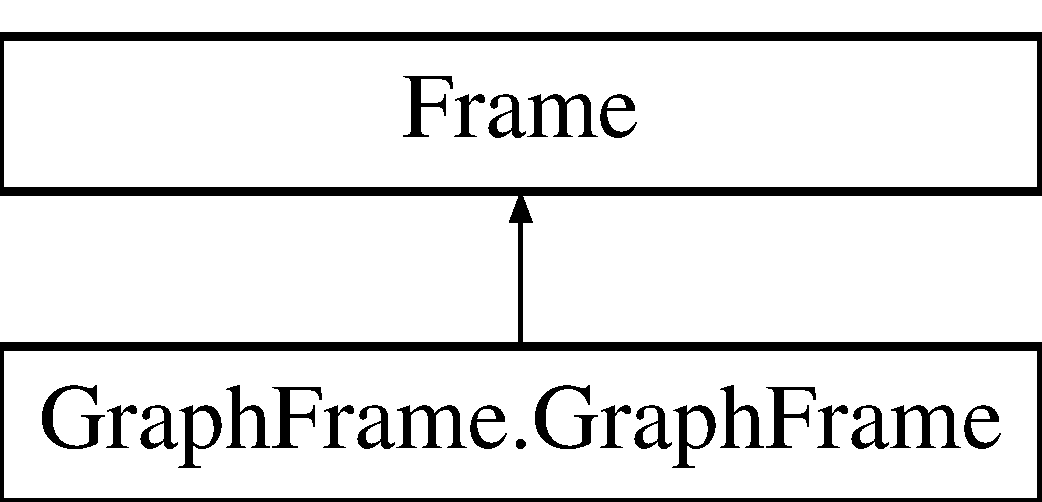
\includegraphics[height=2.000000cm]{classGraphFrame_1_1GraphFrame}
\end{center}
\end{figure}
\subsection*{Public Member Functions}
\begin{DoxyCompactItemize}
\item 
def \hyperlink{classGraphFrame_1_1GraphFrame_ad9dbffb33edafd35f798052e29ace443}{\+\_\+\+\_\+init\+\_\+\+\_\+} (self, \hyperlink{classGraphFrame_1_1GraphFrame_adffc22a75c32a310a9f15d5d9d39c585}{app}, \hyperlink{classGraphFrame_1_1GraphFrame_a2e037073bd21eb4b1ce33d0763c553ac}{parent}, title)
\item 
def \hyperlink{classGraphFrame_1_1GraphFrame_aa7c1ad6c83d55119ad9d14f7fe6b3179}{get\+Control} (self, \hyperlink{classGraphFrame_1_1GraphFrame_af52ab0f13e5117c0cdaa3cade3f04eda}{panel}, xmlid)
\item 
def \hyperlink{classGraphFrame_1_1GraphFrame_a63903bf4616f8d1d7602dfb86c123654}{make\+Tool\+Bar} (self)
\item 
def \hyperlink{classGraphFrame_1_1GraphFrame_aa2baa5d8bd7aed70f505e6a815a3b350}{on\+Idle} (self, event)
\item 
def \hyperlink{classGraphFrame_1_1GraphFrame_a46ef6b8a00bb885e5546bb7e12ef6223}{on\+Change} (self, event)
\item 
def \hyperlink{classGraphFrame_1_1GraphFrame_aae122b48f5b9f830f883192c8dbab6b2}{on\+Iconize} (self, event)
\item 
def \hyperlink{classGraphFrame_1_1GraphFrame_a7b18d46fe532780e2cb335195d245a46}{on\+Re\+Load} (self, event)
\item 
def \hyperlink{classGraphFrame_1_1GraphFrame_a3a50f27df2c9a224ca79506117392a6f}{on\+Print} (self, event)
\item 
def \hyperlink{classGraphFrame_1_1GraphFrame_ac512e14bd8704cb74de330cc75d4b106}{on\+Save} (self, event)
\item 
def \hyperlink{classGraphFrame_1_1GraphFrame_a6c2fa99d2cdb9a5a943daef19dae4e83}{on\+Close} (self, event)
\item 
def \hyperlink{classGraphFrame_1_1GraphFrame_af96c612fe973abb68cd576b3e4637a31}{on\+Close\+All} (self, event)
\item 
def \hyperlink{classGraphFrame_1_1GraphFrame_a2b974345cbf4d2655e6adf1af6f18b16}{on\+Plot} (self, obj)
\item 
def \hyperlink{classGraphFrame_1_1GraphFrame_ad7976cef3c7d76daef8085a3aba26916}{update} (self)
\end{DoxyCompactItemize}
\subsection*{Public Attributes}
\begin{DoxyCompactItemize}
\item 
\hyperlink{classGraphFrame_1_1GraphFrame_a7075285ad02fd2080b89030d8b2b4f1f}{fig\+Id}
\item 
\hyperlink{classGraphFrame_1_1GraphFrame_a2e037073bd21eb4b1ce33d0763c553ac}{parent}
\item 
\hyperlink{classGraphFrame_1_1GraphFrame_adffc22a75c32a310a9f15d5d9d39c585}{app}
\item 
\hyperlink{classGraphFrame_1_1GraphFrame_ae056809f5cf0d296c53738e7b7965fbd}{path}
\item 
\hyperlink{classGraphFrame_1_1GraphFrame_af52ab0f13e5117c0cdaa3cade3f04eda}{panel}
\item 
\hyperlink{classGraphFrame_1_1GraphFrame_afa157e331c533963e6ad5c8e0e808999}{notebook}
\item 
\hyperlink{classGraphFrame_1_1GraphFrame_abe229e95196e9132c31fc47bb1342d39}{panels}
\item 
\hyperlink{classGraphFrame_1_1GraphFrame_a2f83944a4fed433a745817d7bf39550f}{objs}
\item 
\hyperlink{classGraphFrame_1_1GraphFrame_ab8a1a588df91f01631e4af5f72e8a581}{figs}
\item 
\hyperlink{classGraphFrame_1_1GraphFrame_a8adc9094b9ee3ef5bfd446cc6b1b335c}{tool\+Bar}
\end{DoxyCompactItemize}
\subsection*{Static Public Attributes}
\begin{DoxyCompactItemize}
\item 
string \hyperlink{classGraphFrame_1_1GraphFrame_a9abea07b31cb5c6c71077bb51ed5906e}{overview\+Text} = \char`\"{}C\+AT Graphical Window\char`\"{}
\end{DoxyCompactItemize}


\subsection{Detailed Description}


Definition at line 25 of file Graph\+Frame.\+py.



\subsection{Constructor \& Destructor Documentation}
\mbox{\Hypertarget{classGraphFrame_1_1GraphFrame_ad9dbffb33edafd35f798052e29ace443}\label{classGraphFrame_1_1GraphFrame_ad9dbffb33edafd35f798052e29ace443}} 
\index{Graph\+Frame\+::\+Graph\+Frame@{Graph\+Frame\+::\+Graph\+Frame}!\+\_\+\+\_\+init\+\_\+\+\_\+@{\+\_\+\+\_\+init\+\_\+\+\_\+}}
\index{\+\_\+\+\_\+init\+\_\+\+\_\+@{\+\_\+\+\_\+init\+\_\+\+\_\+}!Graph\+Frame\+::\+Graph\+Frame@{Graph\+Frame\+::\+Graph\+Frame}}
\subsubsection{\texorpdfstring{\+\_\+\+\_\+init\+\_\+\+\_\+()}{\_\_init\_\_()}}
{\footnotesize\ttfamily def Graph\+Frame.\+Graph\+Frame.\+\_\+\+\_\+init\+\_\+\+\_\+ (\begin{DoxyParamCaption}\item[{}]{self,  }\item[{}]{app,  }\item[{}]{parent,  }\item[{}]{title }\end{DoxyParamCaption})}



Definition at line 27 of file Graph\+Frame.\+py.


\begin{DoxyCode}
27     \textcolor{keyword}{def }\hyperlink{classwrapper_1_1ModuleDictWrapper_a9a7a794150502f51df687831583e13b9}{\_\_init\_\_}(self,app,parent,title): 
28         wx.Frame.\_\_init\_\_(self, parent, wx.NewId(), title)
29         self.figId=0
30         self.parent=parent
31         self.app=app
32         self.path=os.path.join(os.environ.get(\textcolor{stringliteral}{"CATPATH"}), \textcolor{stringliteral}{"CatPython"}, \textcolor{stringliteral}{"python"})
33         self.makeToolBar()
34         res=xrc.XmlResource(os.path.join(self.path,\textcolor{stringliteral}{"xrc/GraphPanel.xrc"}))
35         self.panel=res.LoadPanel(self, \textcolor{stringliteral}{"GraphPanel"})
36         self.notebook=xrc.XRCCTRL(self, \textcolor{stringliteral}{'notebook'})
37         self.panels=list()
38         self.objs=list()
39         self.figs=list()
40 
41         self.Bind(wx.EVT\_CLOSE, self.onIconize)
42         self.Bind(wx.EVT\_NOTEBOOK\_PAGE\_CHANGED, self.onChange)
43 
\end{DoxyCode}


\subsection{Member Function Documentation}
\mbox{\Hypertarget{classGraphFrame_1_1GraphFrame_aa7c1ad6c83d55119ad9d14f7fe6b3179}\label{classGraphFrame_1_1GraphFrame_aa7c1ad6c83d55119ad9d14f7fe6b3179}} 
\index{Graph\+Frame\+::\+Graph\+Frame@{Graph\+Frame\+::\+Graph\+Frame}!get\+Control@{get\+Control}}
\index{get\+Control@{get\+Control}!Graph\+Frame\+::\+Graph\+Frame@{Graph\+Frame\+::\+Graph\+Frame}}
\subsubsection{\texorpdfstring{get\+Control()}{getControl()}}
{\footnotesize\ttfamily def Graph\+Frame.\+Graph\+Frame.\+get\+Control (\begin{DoxyParamCaption}\item[{}]{self,  }\item[{}]{panel,  }\item[{}]{xmlid }\end{DoxyParamCaption})}

\begin{DoxyVerb}Retrieves the given control (within a dialog) by its xmlid\end{DoxyVerb}
 

Definition at line 44 of file Graph\+Frame.\+py.



Referenced by Proto40\+M\+Hz\+\_\+v1.\+Proto40\+M\+Hz\+\_\+v1.\+is\+Ready(), Proto\+F\+E\+B\+\_\+v1.\+Proto\+F\+E\+B\+\_\+v1.\+is\+Ready(), Acquisition.\+Acquisition.\+on\+Apply(), Proto40\+M\+Hz\+\_\+v1.\+Proto40\+M\+Hz\+\_\+v1.\+onapplyaxlatency(), Proto\+F\+E\+B\+\_\+v1.\+Proto\+F\+E\+B\+\_\+v1.\+onapplyaxlatency(), Proto\+F\+E\+B\+\_\+v1.\+Proto\+F\+E\+B\+\_\+v1.\+onapplyaxlength(), Proto40\+M\+Hz\+\_\+v1.\+Proto40\+M\+Hz\+\_\+v1.\+onapplyaxlength(), Proto\+F\+E\+B\+\_\+v1.\+Proto\+F\+E\+B\+\_\+v1.\+onapply\+Ch(), Proto40\+M\+Hz\+\_\+v1.\+Proto40\+M\+Hz\+\_\+v1.\+onapply\+Ch(), Proto40\+M\+Hz\+\_\+v1.\+Proto40\+M\+Hz\+\_\+v1.\+onapplyclockdiv(), Proto\+F\+E\+B\+\_\+v1.\+Proto\+F\+E\+B\+\_\+v1.\+onapplyclockdiv(), Proto40\+M\+Hz\+\_\+v1.\+Proto40\+M\+Hz\+\_\+v1.\+onapplydelay(), Proto\+F\+E\+B\+\_\+v1.\+Proto\+F\+E\+B\+\_\+v1.\+onapplydelay(), Proto40\+M\+Hz\+\_\+v1.\+Proto40\+M\+Hz\+\_\+v1.\+onapplyfifodepth(), Proto\+F\+E\+B\+\_\+v1.\+Proto\+F\+E\+B\+\_\+v1.\+onapplyfifodepth(), Proto40\+M\+Hz\+\_\+v1.\+Proto40\+M\+Hz\+\_\+v1.\+onapplyfreq(), Proto\+F\+E\+B\+\_\+v1.\+Proto\+F\+E\+B\+\_\+v1.\+onapplyfreq(), Proto40\+M\+Hz\+\_\+v1.\+Proto40\+M\+Hz\+\_\+v1.\+onapplynumber(), Proto\+F\+E\+B\+\_\+v1.\+Proto\+F\+E\+B\+\_\+v1.\+onapplynumber(), Proto\+F\+E\+B\+\_\+v1.\+Proto\+F\+E\+B\+\_\+v1.\+onapplytrig(), Proto40\+M\+Hz\+\_\+v1.\+Proto40\+M\+Hz\+\_\+v1.\+onapplytrig(), Acquisition.\+Acquisition.\+on\+Deadtime(), Acquisition.\+Acquisition.\+on\+Depth(), Proto40\+M\+Hz\+\_\+v1.\+Proto40\+M\+Hz\+\_\+v1.\+onenable\+All(), Proto\+F\+E\+B\+\_\+v1.\+Proto\+F\+E\+B\+\_\+v1.\+onenable\+All(), Acquisition.\+Acquisition.\+on\+Max(), Acquisition.\+Acquisition.\+on\+Min(), Proto40\+M\+Hz\+\_\+v1.\+Proto40\+M\+Hz\+\_\+v1.\+on\+Mode\+A\+X(), Proto\+F\+E\+B\+\_\+v1.\+Proto\+F\+E\+B\+\_\+v1.\+on\+Mode\+A\+X(), Proto\+F\+E\+B\+\_\+v1.\+Proto\+F\+E\+B\+\_\+v1.\+on\+Mode\+Ch(), Proto40\+M\+Hz\+\_\+v1.\+Proto40\+M\+Hz\+\_\+v1.\+on\+Mode\+Ch(), Acquisition.\+Acquisition.\+on\+N\+Bins(), Acquisition.\+Acquisition.\+on\+N\+Sample(), Proto\+F\+E\+B\+\_\+v1.\+Proto\+F\+E\+B\+\_\+v1.\+on\+Pipeline(), Proto40\+M\+Hz\+\_\+v1.\+Proto40\+M\+Hz\+\_\+v1.\+on\+Pipeline(), Acquisition.\+Acquisition.\+on\+Sample(), Acquisition.\+Acquisition.\+on\+Soft\+Trig(), Proto\+F\+E\+B\+\_\+v1.\+Proto\+F\+E\+B\+\_\+v1.\+on\+Soft\+Trig(), Proto40\+M\+Hz\+\_\+v1.\+Proto40\+M\+Hz\+\_\+v1.\+on\+Soft\+Trig(), Acquisition.\+Acquisition.\+on\+Tree(), Acquisition.\+Acquisition.\+on\+Trend(), Proto40\+M\+Hz\+\_\+v1.\+Proto40\+M\+Hz\+\_\+v1.\+onunable\+All(), Proto\+F\+E\+B\+\_\+v1.\+Proto\+F\+E\+B\+\_\+v1.\+onunable\+All(), element.\+element.\+parent(), proc.\+proc.\+parent(), Acquisition.\+Acquisition.\+update(), Proto\+F\+E\+B\+\_\+v1.\+Proto\+F\+E\+B\+\_\+v1.\+update(), and Proto40\+M\+Hz\+\_\+v1.\+Proto40\+M\+Hz\+\_\+v1.\+update().


\begin{DoxyCode}
44     \textcolor{keyword}{def }getControl(self, panel, xmlid):
45         \textcolor{stringliteral}{'''Retrieves the given control (within a dialog) by its xmlid'''}
46         control = panel.FindWindowById(xrc.XRCID(xmlid))
47         \textcolor{keyword}{assert} control != \textcolor{keywordtype}{None}, \textcolor{stringliteral}{'Programming error: a control with xml id '} + xmlid + \textcolor{stringliteral}{' was not found.'}
48         \textcolor{keywordflow}{return} control
49         
\end{DoxyCode}
\mbox{\Hypertarget{classGraphFrame_1_1GraphFrame_a63903bf4616f8d1d7602dfb86c123654}\label{classGraphFrame_1_1GraphFrame_a63903bf4616f8d1d7602dfb86c123654}} 
\index{Graph\+Frame\+::\+Graph\+Frame@{Graph\+Frame\+::\+Graph\+Frame}!make\+Tool\+Bar@{make\+Tool\+Bar}}
\index{make\+Tool\+Bar@{make\+Tool\+Bar}!Graph\+Frame\+::\+Graph\+Frame@{Graph\+Frame\+::\+Graph\+Frame}}
\subsubsection{\texorpdfstring{make\+Tool\+Bar()}{makeToolBar()}}
{\footnotesize\ttfamily def Graph\+Frame.\+Graph\+Frame.\+make\+Tool\+Bar (\begin{DoxyParamCaption}\item[{}]{self }\end{DoxyParamCaption})}



Definition at line 50 of file Graph\+Frame.\+py.


\begin{DoxyCode}
50     \textcolor{keyword}{def }makeToolBar(self):
51         TB\_PRINT=wx.NewId()
52         TB\_SAVE=wx.NewId()
53         TB\_CLOSEALL=wx.NewId()
54         TB\_CLOSE=wx.NewId()
55         \textcolor{comment}{#}
56         self.toolBar = self.CreateToolBar(wx.TB\_DOCKABLE)
57         self.toolBar.AddLabelTool(TB\_CLOSEALL, \textcolor{stringliteral}{''}, wx.Bitmap(os.path.join(self.path,\textcolor{stringliteral}{"xrc/icons/closeall.png
      "})))
58         self.toolBar.AddLabelTool(TB\_CLOSE  , \textcolor{stringliteral}{''}, wx.Bitmap(os.path.join(self.path,\textcolor{stringliteral}{"xrc/icons/close.png"})))
59         self.toolBar.AddSeparator()        
60         self.toolBar.AddLabelTool(TB\_PRINT, \textcolor{stringliteral}{''}, wx.Bitmap(os.path.join(self.path,\textcolor{stringliteral}{"xrc/icons/fileprint.png"})
      ))
61         self.toolBar.AddLabelTool(TB\_SAVE, \textcolor{stringliteral}{''}, wx.Bitmap(os.path.join(self.path,\textcolor{stringliteral}{"xrc/icons/filesave.png"})))
              
62         self.toolBar.Realize()
63 
64         self.Bind(wx.EVT\_TOOL, self.onCloseAll , id=TB\_CLOSEALL)
65         self.Bind(wx.EVT\_TOOL, self.onClose , id=TB\_CLOSE)
66         self.Bind(wx.EVT\_TOOL, self.onPrint , id=TB\_PRINT)
67         self.Bind(wx.EVT\_TOOL, self.onSave  , id=TB\_SAVE)
68                         
\end{DoxyCode}
\mbox{\Hypertarget{classGraphFrame_1_1GraphFrame_a46ef6b8a00bb885e5546bb7e12ef6223}\label{classGraphFrame_1_1GraphFrame_a46ef6b8a00bb885e5546bb7e12ef6223}} 
\index{Graph\+Frame\+::\+Graph\+Frame@{Graph\+Frame\+::\+Graph\+Frame}!on\+Change@{on\+Change}}
\index{on\+Change@{on\+Change}!Graph\+Frame\+::\+Graph\+Frame@{Graph\+Frame\+::\+Graph\+Frame}}
\subsubsection{\texorpdfstring{on\+Change()}{onChange()}}
{\footnotesize\ttfamily def Graph\+Frame.\+Graph\+Frame.\+on\+Change (\begin{DoxyParamCaption}\item[{}]{self,  }\item[{}]{event }\end{DoxyParamCaption})}



Definition at line 74 of file Graph\+Frame.\+py.



References Croc.\+Croc.\+update(), Computer.\+Computer.\+update(), A3\+P\+E\+\_\+\+Bit\+Flip.\+A3\+P\+E\+\_\+\+Bit\+Flip.\+update(), Emulate\+F\+E.\+Emulate\+F\+E.\+update(), Interface\+Wrap.\+update(), Element\+Wrap.\+update(), Proc\+Data\+Base.\+update(), Test\+I2\+C.\+Test\+I2\+C.\+update(), Test\+S\+P\+I.\+Test\+S\+P\+I.\+update(), Test\+U\+S\+B.\+Test\+U\+S\+B.\+update(), Storage\+Fifo\+Acquisition.\+Storage\+Fifo\+Acquisition.\+update(), Test\+Suite.\+Test\+Suite.\+update(), Storage\+Fifo.\+Storage\+Fifo.\+update(), A\+D\+C\+Measurement.\+Current\+Measurement.\+update(), Current\+Measurement.\+Current\+Measurement.\+update(), Usb\+F\+T\+Interface\+Test.\+Usb\+F\+T\+Interface\+Test.\+update(), Interface.\+update(), I\+Oobject.\+update(), Croc.\+update(), Usb\+I2c\+Bus.\+update(), Usb\+Spi\+Bus.\+update(), Usb\+M\+L\+I2c\+Bus.\+update(), Usb\+M\+L\+Spi\+Bus.\+update(), C\+U\+\_\+v1.\+update(), Proto40\+M\+Hz\+\_\+v1.\+update(), Element.\+update(), Computer.\+update(), F\+E\+B\+\_\+v1.\+update(), Seq\+P\+G\+A.\+update(), Acquisition.\+Acquisition.\+update(), N\+I6008.\+update(), Proto40\+M\+Hz\+\_\+v1.\+Proto40\+M\+Hz\+\_\+v1.\+update(), Proto\+F\+E\+B\+\_\+v1.\+Proto\+F\+E\+B\+\_\+v1.\+update(), Fe\+P\+G\+A.\+update(), Phaser.\+update(), Usb\+F\+T\+M\+L\+Interface.\+update(), Usb\+F\+T\+Interface.\+update(), Cfg\+Frame.\+Cfg\+Frame.\+update(), M\+S\+Oxxxx.\+update(), I\+C\+Phaser.\+update(), Graph\+Frame.\+Graph\+Frame.\+update(), I\+C\+E\+C\+A\+Lv3.\+update(), Conf\+Frame.\+Conf\+Frame.\+update(), L\+S\+Delay\+Chip\+V1.\+update(), A3\+P\+E.\+update(), and App\+Frame.\+App\+Frame.\+update().


\begin{DoxyCode}
74     \textcolor{keyword}{def }onChange(self, event):
75         self.update()
76 
\end{DoxyCode}
\mbox{\Hypertarget{classGraphFrame_1_1GraphFrame_a6c2fa99d2cdb9a5a943daef19dae4e83}\label{classGraphFrame_1_1GraphFrame_a6c2fa99d2cdb9a5a943daef19dae4e83}} 
\index{Graph\+Frame\+::\+Graph\+Frame@{Graph\+Frame\+::\+Graph\+Frame}!on\+Close@{on\+Close}}
\index{on\+Close@{on\+Close}!Graph\+Frame\+::\+Graph\+Frame@{Graph\+Frame\+::\+Graph\+Frame}}
\subsubsection{\texorpdfstring{on\+Close()}{onClose()}}
{\footnotesize\ttfamily def Graph\+Frame.\+Graph\+Frame.\+on\+Close (\begin{DoxyParamCaption}\item[{}]{self,  }\item[{}]{event }\end{DoxyParamCaption})}



Definition at line 90 of file Graph\+Frame.\+py.



References Graph\+Frame.\+Graph\+Frame.\+figs, Conf\+Frame.\+Conf\+Frame.\+notebook, Graph\+Frame.\+Graph\+Frame.\+notebook, Conf\+Frame.\+Conf\+Frame.\+objs, Graph\+Frame.\+Graph\+Frame.\+objs, App\+Frame.\+App\+Frame.\+objs, Conf\+Frame.\+Conf\+Frame.\+panels, and Graph\+Frame.\+Graph\+Frame.\+panels.


\begin{DoxyCode}
90     \textcolor{keyword}{def }onClose(self, event):
91         pos=self.notebook.GetSelection()
92         self.notebook.DeletePage(pos)
93 \textcolor{comment}{#        self.panels(pos).killFigure()}
94 \textcolor{comment}{#        self.panels(pos).Destroy()}
95         self.panels.pop(pos)
96         self.objs.pop(pos)
97         self.figs.pop(pos)
98 
\end{DoxyCode}
\mbox{\Hypertarget{classGraphFrame_1_1GraphFrame_af96c612fe973abb68cd576b3e4637a31}\label{classGraphFrame_1_1GraphFrame_af96c612fe973abb68cd576b3e4637a31}} 
\index{Graph\+Frame\+::\+Graph\+Frame@{Graph\+Frame\+::\+Graph\+Frame}!on\+Close\+All@{on\+Close\+All}}
\index{on\+Close\+All@{on\+Close\+All}!Graph\+Frame\+::\+Graph\+Frame@{Graph\+Frame\+::\+Graph\+Frame}}
\subsubsection{\texorpdfstring{on\+Close\+All()}{onCloseAll()}}
{\footnotesize\ttfamily def Graph\+Frame.\+Graph\+Frame.\+on\+Close\+All (\begin{DoxyParamCaption}\item[{}]{self,  }\item[{}]{event }\end{DoxyParamCaption})}



Definition at line 99 of file Graph\+Frame.\+py.



References Graph\+Frame.\+Graph\+Frame.\+figs, Conf\+Frame.\+Conf\+Frame.\+notebook, Graph\+Frame.\+Graph\+Frame.\+notebook, Conf\+Frame.\+Conf\+Frame.\+objs, Graph\+Frame.\+Graph\+Frame.\+objs, App\+Frame.\+App\+Frame.\+objs, Conf\+Frame.\+Conf\+Frame.\+panels, and Graph\+Frame.\+Graph\+Frame.\+panels.


\begin{DoxyCode}
99     \textcolor{keyword}{def }onCloseAll(self, event):
100         self.notebook.DeleteAllPages()
101         self.panels=[]
102         self.objs  =[]
103         self.figs  =[]
104         
\end{DoxyCode}
\mbox{\Hypertarget{classGraphFrame_1_1GraphFrame_aae122b48f5b9f830f883192c8dbab6b2}\label{classGraphFrame_1_1GraphFrame_aae122b48f5b9f830f883192c8dbab6b2}} 
\index{Graph\+Frame\+::\+Graph\+Frame@{Graph\+Frame\+::\+Graph\+Frame}!on\+Iconize@{on\+Iconize}}
\index{on\+Iconize@{on\+Iconize}!Graph\+Frame\+::\+Graph\+Frame@{Graph\+Frame\+::\+Graph\+Frame}}
\subsubsection{\texorpdfstring{on\+Iconize()}{onIconize()}}
{\footnotesize\ttfamily def Graph\+Frame.\+Graph\+Frame.\+on\+Iconize (\begin{DoxyParamCaption}\item[{}]{self,  }\item[{}]{event }\end{DoxyParamCaption})}



Definition at line 77 of file Graph\+Frame.\+py.



References Cfg\+Frame.\+Cfg\+Frame.\+parent, Conf\+Frame.\+Conf\+Frame.\+parent, and Graph\+Frame.\+Graph\+Frame.\+parent.


\begin{DoxyCode}
77     \textcolor{keyword}{def }onIconize(self, event):
78         self.parent.gphFrame.Show(\textcolor{keyword}{False})
79         self.parent.gphState=\textcolor{keyword}{False}
80 
\end{DoxyCode}
\mbox{\Hypertarget{classGraphFrame_1_1GraphFrame_aa2baa5d8bd7aed70f505e6a815a3b350}\label{classGraphFrame_1_1GraphFrame_aa2baa5d8bd7aed70f505e6a815a3b350}} 
\index{Graph\+Frame\+::\+Graph\+Frame@{Graph\+Frame\+::\+Graph\+Frame}!on\+Idle@{on\+Idle}}
\index{on\+Idle@{on\+Idle}!Graph\+Frame\+::\+Graph\+Frame@{Graph\+Frame\+::\+Graph\+Frame}}
\subsubsection{\texorpdfstring{on\+Idle()}{onIdle()}}
{\footnotesize\ttfamily def Graph\+Frame.\+Graph\+Frame.\+on\+Idle (\begin{DoxyParamCaption}\item[{}]{self,  }\item[{}]{event }\end{DoxyParamCaption})}

\begin{DoxyVerb}Responds to idle time in the system\end{DoxyVerb}
 

Definition at line 69 of file Graph\+Frame.\+py.


\begin{DoxyCode}
69     \textcolor{keyword}{def }onIdle(self, event):
70         \textcolor{stringliteral}{'''Responds to idle time in the system'''}
71         \textcolor{comment}{# when the timer says it's time, we do the actual downloading in the main thread (wx doesn't work
       well in secondary threads)}
72         \textcolor{keywordflow}{print} \textcolor{stringliteral}{"hello"}        
73 
\end{DoxyCode}
\mbox{\Hypertarget{classGraphFrame_1_1GraphFrame_a2b974345cbf4d2655e6adf1af6f18b16}\label{classGraphFrame_1_1GraphFrame_a2b974345cbf4d2655e6adf1af6f18b16}} 
\index{Graph\+Frame\+::\+Graph\+Frame@{Graph\+Frame\+::\+Graph\+Frame}!on\+Plot@{on\+Plot}}
\index{on\+Plot@{on\+Plot}!Graph\+Frame\+::\+Graph\+Frame@{Graph\+Frame\+::\+Graph\+Frame}}
\subsubsection{\texorpdfstring{on\+Plot()}{onPlot()}}
{\footnotesize\ttfamily def Graph\+Frame.\+Graph\+Frame.\+on\+Plot (\begin{DoxyParamCaption}\item[{}]{self,  }\item[{}]{obj }\end{DoxyParamCaption})}



Definition at line 105 of file Graph\+Frame.\+py.



References Cfg\+Frame.\+Cfg\+Frame.\+app, Conf\+Frame.\+Conf\+Frame.\+app, Graph\+Frame.\+Graph\+Frame.\+app, Graph\+Frame.\+Graph\+Frame.\+fig\+Id, Graph\+Frame.\+Graph\+Frame.\+figs, Conf\+Frame.\+Conf\+Frame.\+notebook, Graph\+Frame.\+Graph\+Frame.\+notebook, Conf\+Frame.\+Conf\+Frame.\+objs, Graph\+Frame.\+Graph\+Frame.\+objs, App\+Frame.\+App\+Frame.\+objs, Conf\+Frame.\+Conf\+Frame.\+panels, and Graph\+Frame.\+Graph\+Frame.\+panels.


\begin{DoxyCode}
105     \textcolor{keyword}{def }onPlot(self, obj):
106         wrap=\hyperlink{namespacewrapper}{wrapper}(self.app,obj,\textcolor{stringliteral}{"proc"})
107         \textcolor{keywordflow}{if} (wrap.ok):
108             module=wrap.GetActive()
109             panel=module.Plot(self.app,obj,self.notebook,self.figId)
110             \textcolor{keywordflow}{if} panel!=\textcolor{keywordtype}{None} :
111                 self.figId+=1
112                 self.panels.append(panel)
113                 self.objs.append(obj)
114                 self.figs.append(panel)
115                 self.notebook.AddPage(panel,obj.name(),\textcolor{keyword}{True})
116                 
\end{DoxyCode}
\mbox{\Hypertarget{classGraphFrame_1_1GraphFrame_a3a50f27df2c9a224ca79506117392a6f}\label{classGraphFrame_1_1GraphFrame_a3a50f27df2c9a224ca79506117392a6f}} 
\index{Graph\+Frame\+::\+Graph\+Frame@{Graph\+Frame\+::\+Graph\+Frame}!on\+Print@{on\+Print}}
\index{on\+Print@{on\+Print}!Graph\+Frame\+::\+Graph\+Frame@{Graph\+Frame\+::\+Graph\+Frame}}
\subsubsection{\texorpdfstring{on\+Print()}{onPrint()}}
{\footnotesize\ttfamily def Graph\+Frame.\+Graph\+Frame.\+on\+Print (\begin{DoxyParamCaption}\item[{}]{self,  }\item[{}]{event }\end{DoxyParamCaption})}



Definition at line 84 of file Graph\+Frame.\+py.


\begin{DoxyCode}
84     \textcolor{keyword}{def }onPrint(self, event):
85         \textcolor{keywordflow}{print} \textcolor{stringliteral}{"printing..."}
86 
\end{DoxyCode}
\mbox{\Hypertarget{classGraphFrame_1_1GraphFrame_a7b18d46fe532780e2cb335195d245a46}\label{classGraphFrame_1_1GraphFrame_a7b18d46fe532780e2cb335195d245a46}} 
\index{Graph\+Frame\+::\+Graph\+Frame@{Graph\+Frame\+::\+Graph\+Frame}!on\+Re\+Load@{on\+Re\+Load}}
\index{on\+Re\+Load@{on\+Re\+Load}!Graph\+Frame\+::\+Graph\+Frame@{Graph\+Frame\+::\+Graph\+Frame}}
\subsubsection{\texorpdfstring{on\+Re\+Load()}{onReLoad()}}
{\footnotesize\ttfamily def Graph\+Frame.\+Graph\+Frame.\+on\+Re\+Load (\begin{DoxyParamCaption}\item[{}]{self,  }\item[{}]{event }\end{DoxyParamCaption})}



Definition at line 81 of file Graph\+Frame.\+py.



References Conf\+Frame.\+Conf\+Frame.\+notebook, Graph\+Frame.\+Graph\+Frame.\+notebook, Croc.\+Croc.\+update(), Computer.\+Computer.\+update(), A3\+P\+E\+\_\+\+Bit\+Flip.\+A3\+P\+E\+\_\+\+Bit\+Flip.\+update(), Emulate\+F\+E.\+Emulate\+F\+E.\+update(), Interface\+Wrap.\+update(), Element\+Wrap.\+update(), Proc\+Data\+Base.\+update(), Test\+I2\+C.\+Test\+I2\+C.\+update(), Test\+S\+P\+I.\+Test\+S\+P\+I.\+update(), Test\+U\+S\+B.\+Test\+U\+S\+B.\+update(), Storage\+Fifo\+Acquisition.\+Storage\+Fifo\+Acquisition.\+update(), Test\+Suite.\+Test\+Suite.\+update(), Storage\+Fifo.\+Storage\+Fifo.\+update(), Current\+Measurement.\+Current\+Measurement.\+update(), A\+D\+C\+Measurement.\+Current\+Measurement.\+update(), Usb\+F\+T\+Interface\+Test.\+Usb\+F\+T\+Interface\+Test.\+update(), Interface.\+update(), I\+Oobject.\+update(), Croc.\+update(), Usb\+I2c\+Bus.\+update(), Usb\+Spi\+Bus.\+update(), Usb\+M\+L\+I2c\+Bus.\+update(), Usb\+M\+L\+Spi\+Bus.\+update(), C\+U\+\_\+v1.\+update(), Proto40\+M\+Hz\+\_\+v1.\+update(), Element.\+update(), Computer.\+update(), F\+E\+B\+\_\+v1.\+update(), Seq\+P\+G\+A.\+update(), Acquisition.\+Acquisition.\+update(), N\+I6008.\+update(), Proto40\+M\+Hz\+\_\+v1.\+Proto40\+M\+Hz\+\_\+v1.\+update(), Proto\+F\+E\+B\+\_\+v1.\+Proto\+F\+E\+B\+\_\+v1.\+update(), Fe\+P\+G\+A.\+update(), Phaser.\+update(), Usb\+F\+T\+M\+L\+Interface.\+update(), Usb\+F\+T\+Interface.\+update(), Cfg\+Frame.\+Cfg\+Frame.\+update(), M\+S\+Oxxxx.\+update(), I\+C\+Phaser.\+update(), Graph\+Frame.\+Graph\+Frame.\+update(), I\+C\+E\+C\+A\+Lv3.\+update(), Conf\+Frame.\+Conf\+Frame.\+update(), L\+S\+Delay\+Chip\+V1.\+update(), A3\+P\+E.\+update(), and App\+Frame.\+App\+Frame.\+update().


\begin{DoxyCode}
81     \textcolor{keyword}{def }onReLoad(self, event):
82         self.update(self.notebook.GetSelection())
83 
\end{DoxyCode}
\mbox{\Hypertarget{classGraphFrame_1_1GraphFrame_ac512e14bd8704cb74de330cc75d4b106}\label{classGraphFrame_1_1GraphFrame_ac512e14bd8704cb74de330cc75d4b106}} 
\index{Graph\+Frame\+::\+Graph\+Frame@{Graph\+Frame\+::\+Graph\+Frame}!on\+Save@{on\+Save}}
\index{on\+Save@{on\+Save}!Graph\+Frame\+::\+Graph\+Frame@{Graph\+Frame\+::\+Graph\+Frame}}
\subsubsection{\texorpdfstring{on\+Save()}{onSave()}}
{\footnotesize\ttfamily def Graph\+Frame.\+Graph\+Frame.\+on\+Save (\begin{DoxyParamCaption}\item[{}]{self,  }\item[{}]{event }\end{DoxyParamCaption})}



Definition at line 87 of file Graph\+Frame.\+py.


\begin{DoxyCode}
87     \textcolor{keyword}{def }onSave(self, event):
88         \textcolor{keywordflow}{print} \textcolor{stringliteral}{"save..."}
89 
\end{DoxyCode}
\mbox{\Hypertarget{classGraphFrame_1_1GraphFrame_ad7976cef3c7d76daef8085a3aba26916}\label{classGraphFrame_1_1GraphFrame_ad7976cef3c7d76daef8085a3aba26916}} 
\index{Graph\+Frame\+::\+Graph\+Frame@{Graph\+Frame\+::\+Graph\+Frame}!update@{update}}
\index{update@{update}!Graph\+Frame\+::\+Graph\+Frame@{Graph\+Frame\+::\+Graph\+Frame}}
\subsubsection{\texorpdfstring{update()}{update()}}
{\footnotesize\ttfamily def Graph\+Frame.\+Graph\+Frame.\+update (\begin{DoxyParamCaption}\item[{}]{self }\end{DoxyParamCaption})}



Definition at line 117 of file Graph\+Frame.\+py.



References Graph\+Frame.\+Graph\+Frame.\+figs, Conf\+Frame.\+Conf\+Frame.\+notebook, and Graph\+Frame.\+Graph\+Frame.\+notebook.



Referenced by Graph\+Frame.\+Graph\+Frame.\+on\+Change(), and Graph\+Frame.\+Graph\+Frame.\+on\+Re\+Load().


\begin{DoxyCode}
117     \textcolor{keyword}{def }update(self):
118         pos=self.notebook.GetSelection()
119         self.figs[pos].current()
120 
121 \textcolor{comment}{#----------------------------------------------------------------------------}
122 
123 
124 
125 \end{DoxyCode}


\subsection{Member Data Documentation}
\mbox{\Hypertarget{classGraphFrame_1_1GraphFrame_adffc22a75c32a310a9f15d5d9d39c585}\label{classGraphFrame_1_1GraphFrame_adffc22a75c32a310a9f15d5d9d39c585}} 
\index{Graph\+Frame\+::\+Graph\+Frame@{Graph\+Frame\+::\+Graph\+Frame}!app@{app}}
\index{app@{app}!Graph\+Frame\+::\+Graph\+Frame@{Graph\+Frame\+::\+Graph\+Frame}}
\subsubsection{\texorpdfstring{app}{app}}
{\footnotesize\ttfamily Graph\+Frame.\+Graph\+Frame.\+app}



Definition at line 31 of file Graph\+Frame.\+py.



Referenced by Graph\+Frame.\+Graph\+Frame.\+on\+Plot().

\mbox{\Hypertarget{classGraphFrame_1_1GraphFrame_a7075285ad02fd2080b89030d8b2b4f1f}\label{classGraphFrame_1_1GraphFrame_a7075285ad02fd2080b89030d8b2b4f1f}} 
\index{Graph\+Frame\+::\+Graph\+Frame@{Graph\+Frame\+::\+Graph\+Frame}!fig\+Id@{fig\+Id}}
\index{fig\+Id@{fig\+Id}!Graph\+Frame\+::\+Graph\+Frame@{Graph\+Frame\+::\+Graph\+Frame}}
\subsubsection{\texorpdfstring{fig\+Id}{figId}}
{\footnotesize\ttfamily Graph\+Frame.\+Graph\+Frame.\+fig\+Id}



Definition at line 29 of file Graph\+Frame.\+py.



Referenced by Graph\+Frame.\+Graph\+Frame.\+on\+Plot().

\mbox{\Hypertarget{classGraphFrame_1_1GraphFrame_ab8a1a588df91f01631e4af5f72e8a581}\label{classGraphFrame_1_1GraphFrame_ab8a1a588df91f01631e4af5f72e8a581}} 
\index{Graph\+Frame\+::\+Graph\+Frame@{Graph\+Frame\+::\+Graph\+Frame}!figs@{figs}}
\index{figs@{figs}!Graph\+Frame\+::\+Graph\+Frame@{Graph\+Frame\+::\+Graph\+Frame}}
\subsubsection{\texorpdfstring{figs}{figs}}
{\footnotesize\ttfamily Graph\+Frame.\+Graph\+Frame.\+figs}



Definition at line 39 of file Graph\+Frame.\+py.



Referenced by Graph\+Frame.\+Graph\+Frame.\+on\+Close(), Graph\+Frame.\+Graph\+Frame.\+on\+Close\+All(), Graph\+Frame.\+Graph\+Frame.\+on\+Plot(), and Graph\+Frame.\+Graph\+Frame.\+update().

\mbox{\Hypertarget{classGraphFrame_1_1GraphFrame_afa157e331c533963e6ad5c8e0e808999}\label{classGraphFrame_1_1GraphFrame_afa157e331c533963e6ad5c8e0e808999}} 
\index{Graph\+Frame\+::\+Graph\+Frame@{Graph\+Frame\+::\+Graph\+Frame}!notebook@{notebook}}
\index{notebook@{notebook}!Graph\+Frame\+::\+Graph\+Frame@{Graph\+Frame\+::\+Graph\+Frame}}
\subsubsection{\texorpdfstring{notebook}{notebook}}
{\footnotesize\ttfamily Graph\+Frame.\+Graph\+Frame.\+notebook}



Definition at line 36 of file Graph\+Frame.\+py.



Referenced by Graph\+Frame.\+Graph\+Frame.\+on\+Close(), Graph\+Frame.\+Graph\+Frame.\+on\+Close\+All(), Graph\+Frame.\+Graph\+Frame.\+on\+Plot(), Graph\+Frame.\+Graph\+Frame.\+on\+Re\+Load(), and Graph\+Frame.\+Graph\+Frame.\+update().

\mbox{\Hypertarget{classGraphFrame_1_1GraphFrame_a2f83944a4fed433a745817d7bf39550f}\label{classGraphFrame_1_1GraphFrame_a2f83944a4fed433a745817d7bf39550f}} 
\index{Graph\+Frame\+::\+Graph\+Frame@{Graph\+Frame\+::\+Graph\+Frame}!objs@{objs}}
\index{objs@{objs}!Graph\+Frame\+::\+Graph\+Frame@{Graph\+Frame\+::\+Graph\+Frame}}
\subsubsection{\texorpdfstring{objs}{objs}}
{\footnotesize\ttfamily Graph\+Frame.\+Graph\+Frame.\+objs}



Definition at line 38 of file Graph\+Frame.\+py.



Referenced by Graph\+Frame.\+Graph\+Frame.\+on\+Close(), Graph\+Frame.\+Graph\+Frame.\+on\+Close\+All(), and Graph\+Frame.\+Graph\+Frame.\+on\+Plot().

\mbox{\Hypertarget{classGraphFrame_1_1GraphFrame_a9abea07b31cb5c6c71077bb51ed5906e}\label{classGraphFrame_1_1GraphFrame_a9abea07b31cb5c6c71077bb51ed5906e}} 
\index{Graph\+Frame\+::\+Graph\+Frame@{Graph\+Frame\+::\+Graph\+Frame}!overview\+Text@{overview\+Text}}
\index{overview\+Text@{overview\+Text}!Graph\+Frame\+::\+Graph\+Frame@{Graph\+Frame\+::\+Graph\+Frame}}
\subsubsection{\texorpdfstring{overview\+Text}{overviewText}}
{\footnotesize\ttfamily string Graph\+Frame.\+Graph\+Frame.\+overview\+Text = \char`\"{}C\+AT Graphical Window\char`\"{}\hspace{0.3cm}{\ttfamily [static]}}



Definition at line 26 of file Graph\+Frame.\+py.

\mbox{\Hypertarget{classGraphFrame_1_1GraphFrame_af52ab0f13e5117c0cdaa3cade3f04eda}\label{classGraphFrame_1_1GraphFrame_af52ab0f13e5117c0cdaa3cade3f04eda}} 
\index{Graph\+Frame\+::\+Graph\+Frame@{Graph\+Frame\+::\+Graph\+Frame}!panel@{panel}}
\index{panel@{panel}!Graph\+Frame\+::\+Graph\+Frame@{Graph\+Frame\+::\+Graph\+Frame}}
\subsubsection{\texorpdfstring{panel}{panel}}
{\footnotesize\ttfamily Graph\+Frame.\+Graph\+Frame.\+panel}



Definition at line 35 of file Graph\+Frame.\+py.



Referenced by A3\+P\+E\+\_\+\+Bit\+Flip.\+A3\+P\+E\+\_\+\+Bit\+Flip.\+\_\+\+\_\+init\+\_\+\+\_\+(), Emulate\+F\+E.\+Emulate\+F\+E.\+\_\+\+\_\+init\+\_\+\+\_\+(), Acquisition.\+Acquisition.\+\_\+\+\_\+init\+\_\+\+\_\+(), object.\+object.\+get\+Control(), Proto40\+M\+Hz\+\_\+v1.\+Proto40\+M\+Hz\+\_\+v1.\+get\+File(), and proc.\+proc.\+page().

\mbox{\Hypertarget{classGraphFrame_1_1GraphFrame_abe229e95196e9132c31fc47bb1342d39}\label{classGraphFrame_1_1GraphFrame_abe229e95196e9132c31fc47bb1342d39}} 
\index{Graph\+Frame\+::\+Graph\+Frame@{Graph\+Frame\+::\+Graph\+Frame}!panels@{panels}}
\index{panels@{panels}!Graph\+Frame\+::\+Graph\+Frame@{Graph\+Frame\+::\+Graph\+Frame}}
\subsubsection{\texorpdfstring{panels}{panels}}
{\footnotesize\ttfamily Graph\+Frame.\+Graph\+Frame.\+panels}



Definition at line 37 of file Graph\+Frame.\+py.



Referenced by Graph\+Frame.\+Graph\+Frame.\+on\+Close(), Graph\+Frame.\+Graph\+Frame.\+on\+Close\+All(), and Graph\+Frame.\+Graph\+Frame.\+on\+Plot().

\mbox{\Hypertarget{classGraphFrame_1_1GraphFrame_a2e037073bd21eb4b1ce33d0763c553ac}\label{classGraphFrame_1_1GraphFrame_a2e037073bd21eb4b1ce33d0763c553ac}} 
\index{Graph\+Frame\+::\+Graph\+Frame@{Graph\+Frame\+::\+Graph\+Frame}!parent@{parent}}
\index{parent@{parent}!Graph\+Frame\+::\+Graph\+Frame@{Graph\+Frame\+::\+Graph\+Frame}}
\subsubsection{\texorpdfstring{parent}{parent}}
{\footnotesize\ttfamily Graph\+Frame.\+Graph\+Frame.\+parent}



Definition at line 30 of file Graph\+Frame.\+py.



Referenced by Graph\+Frame.\+Graph\+Frame.\+on\+Iconize().

\mbox{\Hypertarget{classGraphFrame_1_1GraphFrame_ae056809f5cf0d296c53738e7b7965fbd}\label{classGraphFrame_1_1GraphFrame_ae056809f5cf0d296c53738e7b7965fbd}} 
\index{Graph\+Frame\+::\+Graph\+Frame@{Graph\+Frame\+::\+Graph\+Frame}!path@{path}}
\index{path@{path}!Graph\+Frame\+::\+Graph\+Frame@{Graph\+Frame\+::\+Graph\+Frame}}
\subsubsection{\texorpdfstring{path}{path}}
{\footnotesize\ttfamily Graph\+Frame.\+Graph\+Frame.\+path}



Definition at line 32 of file Graph\+Frame.\+py.



Referenced by element.\+element.\+loadxrc(), and proc.\+proc.\+loadxrc().

\mbox{\Hypertarget{classGraphFrame_1_1GraphFrame_a8adc9094b9ee3ef5bfd446cc6b1b335c}\label{classGraphFrame_1_1GraphFrame_a8adc9094b9ee3ef5bfd446cc6b1b335c}} 
\index{Graph\+Frame\+::\+Graph\+Frame@{Graph\+Frame\+::\+Graph\+Frame}!tool\+Bar@{tool\+Bar}}
\index{tool\+Bar@{tool\+Bar}!Graph\+Frame\+::\+Graph\+Frame@{Graph\+Frame\+::\+Graph\+Frame}}
\subsubsection{\texorpdfstring{tool\+Bar}{toolBar}}
{\footnotesize\ttfamily Graph\+Frame.\+Graph\+Frame.\+tool\+Bar}



Definition at line 56 of file Graph\+Frame.\+py.



The documentation for this class was generated from the following file\+:\begin{DoxyCompactItemize}
\item 
/home/eleclhcb/\+L\+H\+Cb/lbcat-\/cmake/\+Cat\+Python/python/\hyperlink{GraphFrame_8py}{Graph\+Frame.\+py}\end{DoxyCompactItemize}

\hypertarget{classgui_1_1Gui}{
\section{gui::Gui Class Reference}
\label{classgui_1_1Gui}\index{gui::Gui@{gui::Gui}}
}
\subsection*{Public Member Functions}
\begin{DoxyCompactItemize}
\item 
def \hyperlink{classgui_1_1Gui_a063380e8fa617c69752ce2f071699a07}{OnInit}
\item 
def \hyperlink{classgui_1_1Gui_ae75ecf31b32e2df9c23baf87cf4a7c10}{Start}
\item 
def \hyperlink{classgui_1_1Gui_aa27add666d31a15ac8a5a2937e0bec70}{ShowMain}
\item 
def \hyperlink{classgui_1_1Gui_a530fc2229d33c71374c9c40217bcdda8}{ShowTips}
\end{DoxyCompactItemize}
\subsection*{Public Attributes}
\begin{DoxyCompactItemize}
\item 
\hyperlink{classgui_1_1Gui_a9a969f7b54f7e42900732a01995771ab}{appFrame}
\end{DoxyCompactItemize}


\subsection{Detailed Description}


Definition at line 69 of file gui.py.

\subsection{Member Function Documentation}
\hypertarget{classgui_1_1Gui_a063380e8fa617c69752ce2f071699a07}{
\index{gui::Gui@{gui::Gui}!OnInit@{OnInit}}
\index{OnInit@{OnInit}!gui::Gui@{gui::Gui}}
\subsubsection[{OnInit}]{\setlength{\rightskip}{0pt plus 5cm}def gui::Gui::OnInit ( {\em self}, \/   {\em app} = {\ttfamily None})}}
\label{classgui_1_1Gui_a063380e8fa617c69752ce2f071699a07}
\begin{DoxyVerb}
Create and show the splash screen.
It will then create and show the main frame when it is time to do so.
\end{DoxyVerb}
 

Definition at line 70 of file gui.py.


\begin{DoxyCode}
70                               :
71         """
72         Create and show the splash screen.
73         It will then create and show the main frame when it is time to do so.
74         """
75         self.appFrame=AppFrame(cat, None, "CAT Application")
76         self.SetTopWindow(self.appFrame)
77         return True
    def Start(self):
\end{DoxyCode}
\hypertarget{classgui_1_1Gui_aa27add666d31a15ac8a5a2937e0bec70}{
\index{gui::Gui@{gui::Gui}!ShowMain@{ShowMain}}
\index{ShowMain@{ShowMain}!gui::Gui@{gui::Gui}}
\subsubsection[{ShowMain}]{\setlength{\rightskip}{0pt plus 5cm}def gui::Gui::ShowMain ( {\em self})}}
\label{classgui_1_1Gui_aa27add666d31a15ac8a5a2937e0bec70}


Definition at line 86 of file gui.py.


\begin{DoxyCode}
86                       :
87         self.appFrame.Show()
    def ShowTips(self):
\end{DoxyCode}
\hypertarget{classgui_1_1Gui_a530fc2229d33c71374c9c40217bcdda8}{
\index{gui::Gui@{gui::Gui}!ShowTips@{ShowTips}}
\index{ShowTips@{ShowTips}!gui::Gui@{gui::Gui}}
\subsubsection[{ShowTips}]{\setlength{\rightskip}{0pt plus 5cm}def gui::Gui::ShowTips ( {\em self})}}
\label{classgui_1_1Gui_a530fc2229d33c71374c9c40217bcdda8}


Definition at line 88 of file gui.py.


\begin{DoxyCode}
88                       :
89         wx.CallAfter(self.appFrame.ShowTip)
90 
91 #---------------------------------------------------------------------------
92 # main
def main( argsCat=None ):
\end{DoxyCode}
\hypertarget{classgui_1_1Gui_ae75ecf31b32e2df9c23baf87cf4a7c10}{
\index{gui::Gui@{gui::Gui}!Start@{Start}}
\index{Start@{Start}!gui::Gui@{gui::Gui}}
\subsubsection[{Start}]{\setlength{\rightskip}{0pt plus 5cm}def gui::Gui::Start ( {\em self})}}
\label{classgui_1_1Gui_ae75ecf31b32e2df9c23baf87cf4a7c10}


Definition at line 78 of file gui.py.


\begin{DoxyCode}
78                    :
79         if args.banner:
80             splash = SplashScreen(os.path.join(os.environ.get("CATPYTHONROOT"),
81                                                "python/images/cat.bmp"))
82             splash.Show()
83         else:
84             self.ShowMain()
85             #ShowTip()
    def ShowMain(self):
\end{DoxyCode}


\subsection{Member Data Documentation}
\hypertarget{classgui_1_1Gui_a9a969f7b54f7e42900732a01995771ab}{
\index{gui::Gui@{gui::Gui}!appFrame@{appFrame}}
\index{appFrame@{appFrame}!gui::Gui@{gui::Gui}}
\subsubsection[{appFrame}]{\setlength{\rightskip}{0pt plus 5cm}{\bf gui::Gui::appFrame}}}
\label{classgui_1_1Gui_a9a969f7b54f7e42900732a01995771ab}


Definition at line 75 of file gui.py.

The documentation for this class was generated from the following file:\begin{DoxyCompactItemize}
\item 
/home/eleclhcb/LHCb/lbcat-\/cmake/CatPython/python/\hyperlink{gui_8py}{gui.py}\end{DoxyCompactItemize}

\hypertarget{classHierarchy}{}\section{Hierarchy Class Reference}
\label{classHierarchy}\index{Hierarchy@{Hierarchy}}


{\ttfamily \#include $<$inc/\+Hierarchy.\+h$>$}

Inheritance diagram for Hierarchy\+:\begin{figure}[H]
\begin{center}
\leavevmode
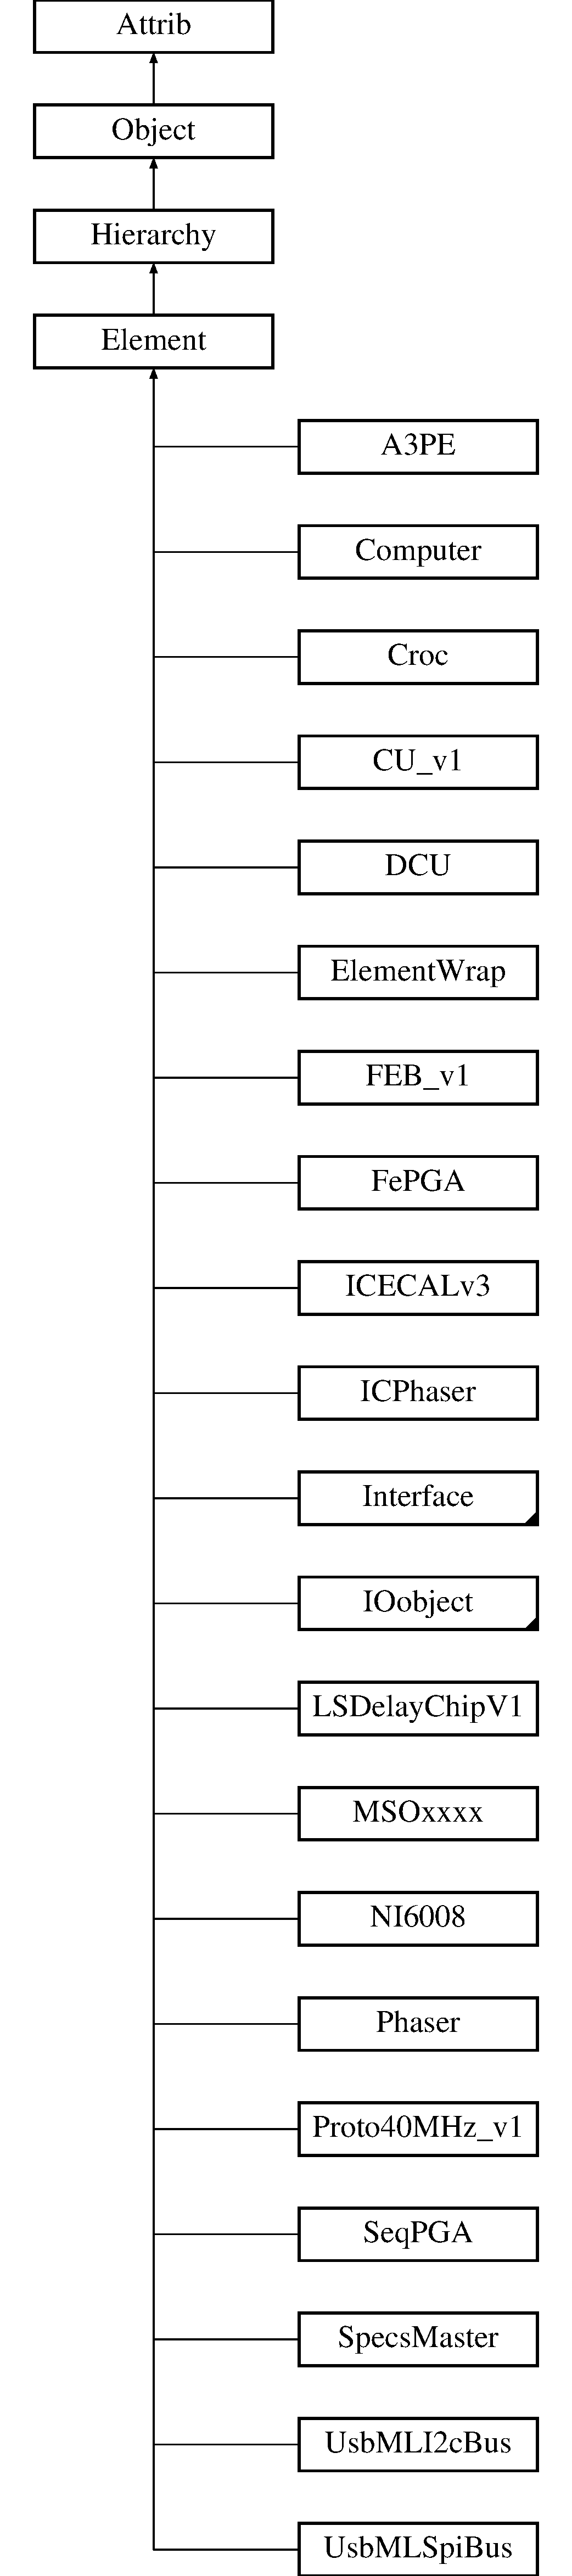
\includegraphics[height=12.000000cm]{classHierarchy}
\end{center}
\end{figure}
\subsection*{Public Member Functions}
\begin{DoxyCompactItemize}
\item 
\hyperlink{classHierarchy_a8288ae6edc7482d6a9f83f94c0ca93db}{Hierarchy} ()
\begin{DoxyCompactList}\small\item\em Standard constructor. \end{DoxyCompactList}\item 
virtual \hyperlink{classHierarchy_a8f29c4c38606352e2472d95b08c503d0}{$\sim$\+Hierarchy} ()
\begin{DoxyCompactList}\small\item\em Destructor. \end{DoxyCompactList}\item 
void \hyperlink{classHierarchy_af4d43b0765b402670eed2d62c73405af}{clear} ()
\item 
void \hyperlink{classHierarchy_a585ad1aeec16077a0e532ab8b4fc557b}{set\+Parent} (\hyperlink{classHierarchy}{Hierarchy} $\ast$\hyperlink{classHierarchy_a1c7bec8257e717f9c1465e06ebf845fc}{parent})
\item 
\hyperlink{classHierarchy}{Hierarchy} $\ast$ \hyperlink{classHierarchy_a1c7bec8257e717f9c1465e06ebf845fc}{parent} ()
\item 
\hyperlink{classHierarchy}{Hierarchy} $\ast$ \hyperlink{classHierarchy_ad550588733bf75ac5c0fcfd7c8fd11a6}{parent} (std\+::string)
\item 
\hyperlink{classHierarchy}{Hierarchy} $\ast$ \hyperlink{classHierarchy_aee461dc930ce3871636ff87f075b1b83}{origin} ()
\item 
virtual void \hyperlink{classHierarchy_ad677774ff38fcb257c04a3a10d471fac}{add\+Child} (\hyperlink{classHierarchy}{Hierarchy} $\ast$element)
\item 
std\+::vector$<$ \hyperlink{classHierarchy}{Hierarchy} $\ast$ $>$ \hyperlink{classHierarchy_aa9a76f69e98e052ee1a6e32cea006288}{children} ()
\item 
\hyperlink{classHierarchy}{Hierarchy} $\ast$ \hyperlink{classHierarchy_a1e207f973c694b538bf90107b4868817}{child} (std\+::string)
\item 
\hyperlink{classHierarchy}{Hierarchy} $\ast$ \hyperlink{classHierarchy_a0c15a5276a3b80b4354d6bd8a01e0708}{child\+Typed} (std\+::string)
\item 
unsigned long \hyperlink{classHierarchy_ab16e84de65fd84e14001a6cf941c8be4}{number\+Of\+Children} ()
\item 
bool \hyperlink{classHierarchy_a255174fe4d316d2a3f430dcb9dab29f1}{has\+Children} ()
\item 
void \hyperlink{classHierarchy_a2b2b359fac003233f65786a616766bde}{del\+Child} (\hyperlink{classHierarchy}{Hierarchy} $\ast$)
\item 
void \hyperlink{classHierarchy_a1928ac7615fe0b5e55cd707f70dc6781}{del\+Child} (std\+::string)
\item 
std\+::string \hyperlink{classHierarchy_aa7990fa7caf132d83e361ce033c6c65a}{path} (std\+::string=std\+::string(\char`\"{}\char`\"{}))
\item 
std\+::string \hyperlink{classHierarchy_a1efd56cd164d328d2002e53a10a19b8c}{path\+Typed} (std\+::string=std\+::string(\char`\"{}\char`\"{}))
\item 
void \hyperlink{classHierarchy_a76e914b9a677a22a82deb74d892bf261}{tree} (std\+::string indent=std\+::string(\char`\"{}\char`\"{}))
\item 
void \hyperlink{classHierarchy_a594c294c5f60c230e106d522ed008212}{tree} ()
\end{DoxyCompactItemize}
\subsection*{Private Attributes}
\begin{DoxyCompactItemize}
\item 
\hyperlink{classHierarchy}{Hierarchy} $\ast$ \hyperlink{classHierarchy_a5814bb280d4e8539ab25ab6cbfb9cc4f}{m\+\_\+parent}
\item 
\hyperlink{classHierarchy}{Hierarchy} $\ast$ \hyperlink{classHierarchy_a16c73e557d3a7c156ffb5dc4102d148e}{m\+\_\+origin}
\item 
std\+::vector$<$ \hyperlink{classHierarchy}{Hierarchy} $\ast$ $>$ \hyperlink{classHierarchy_a038816763941fd4a930504917f60483b}{m\+\_\+children}
\end{DoxyCompactItemize}
\subsection*{Additional Inherited Members}


\subsection{Detailed Description}
Class to define an \hyperlink{classElement}{Element} \hyperlink{classHierarchy}{Hierarchy}

\begin{DoxyAuthor}{Author}

\end{DoxyAuthor}
\begin{DoxyDate}{Date}
2006-\/10-\/26 
\end{DoxyDate}


Definition at line 19 of file Hierarchy.\+h.



\subsection{Constructor \& Destructor Documentation}
\mbox{\Hypertarget{classHierarchy_a8288ae6edc7482d6a9f83f94c0ca93db}\label{classHierarchy_a8288ae6edc7482d6a9f83f94c0ca93db}} 
\index{Hierarchy@{Hierarchy}!Hierarchy@{Hierarchy}}
\index{Hierarchy@{Hierarchy}!Hierarchy@{Hierarchy}}
\subsubsection{\texorpdfstring{Hierarchy()}{Hierarchy()}}
{\footnotesize\ttfamily Hierarchy\+::\+Hierarchy (\begin{DoxyParamCaption}{ }\end{DoxyParamCaption})}



Standard constructor. 



Definition at line 16 of file Hierarchy.\+cpp.



References m\+\_\+origin.


\begin{DoxyCode}
16                        :
17   \hyperlink{classHierarchy_a5814bb280d4e8539ab25ab6cbfb9cc4f}{m\_parent} (0)\{
18   \hyperlink{classHierarchy_a16c73e557d3a7c156ffb5dc4102d148e}{m\_origin}=\textcolor{keyword}{this};
19 \}
\end{DoxyCode}
\mbox{\Hypertarget{classHierarchy_a8f29c4c38606352e2472d95b08c503d0}\label{classHierarchy_a8f29c4c38606352e2472d95b08c503d0}} 
\index{Hierarchy@{Hierarchy}!````~Hierarchy@{$\sim$\+Hierarchy}}
\index{````~Hierarchy@{$\sim$\+Hierarchy}!Hierarchy@{Hierarchy}}
\subsubsection{\texorpdfstring{$\sim$\+Hierarchy()}{~Hierarchy()}}
{\footnotesize\ttfamily Hierarchy\+::$\sim$\+Hierarchy (\begin{DoxyParamCaption}{ }\end{DoxyParamCaption})\hspace{0.3cm}{\ttfamily [virtual]}}



Destructor. 



Definition at line 24 of file Hierarchy.\+cpp.



References Object\+::debug(), del\+Child(), Object\+::name(), and parent().


\begin{DoxyCode}
24                       \{
25   \textcolor{keywordflow}{if} (0!=\hyperlink{classHierarchy_a1c7bec8257e717f9c1465e06ebf845fc}{parent}())\{
26     \hyperlink{classHierarchy_a1c7bec8257e717f9c1465e06ebf845fc}{parent}()->\hyperlink{classHierarchy_a2b2b359fac003233f65786a616766bde}{delChild}(\textcolor{keyword}{this});
27   \}
28   \hyperlink{classObject_aac010553f022165573714b7014a15f0d}{debug}(\textcolor{stringliteral}{"deleting Hierarchy "}+\hyperlink{classObject_a300f4c05dd468c7bb8b3c968868443c1}{name}(),\textcolor{stringliteral}{"Hierarchy::~Hierarchy"});
29 \}
\end{DoxyCode}


\subsection{Member Function Documentation}
\mbox{\Hypertarget{classHierarchy_ad677774ff38fcb257c04a3a10d471fac}\label{classHierarchy_ad677774ff38fcb257c04a3a10d471fac}} 
\index{Hierarchy@{Hierarchy}!add\+Child@{add\+Child}}
\index{add\+Child@{add\+Child}!Hierarchy@{Hierarchy}}
\subsubsection{\texorpdfstring{add\+Child()}{addChild()}}
{\footnotesize\ttfamily void Hierarchy\+::add\+Child (\begin{DoxyParamCaption}\item[{\hyperlink{classHierarchy}{Hierarchy} $\ast$}]{element }\end{DoxyParamCaption})\hspace{0.3cm}{\ttfamily [virtual]}}



Definition at line 83 of file Hierarchy.\+cpp.



References Object\+::debug(), m\+\_\+children, Object\+::name(), and set\+Parent().



Referenced by A3\+P\+E\+::\+A3\+P\+E(), Specs\+Mezzanine\+::add\+Bus(), Specs\+Slave\+::add\+I2c(), Application\+::create(), C\+U\+\_\+v1\+::\+C\+U\+\_\+v1(), export\+\_\+obj(), F\+E\+B\+\_\+v1\+::\+F\+E\+B\+\_\+v1(), Fe\+P\+G\+A\+::\+Fe\+P\+G\+A(), I\+C\+E\+C\+A\+Lv3\+::\+I\+C\+E\+C\+A\+Lv3(), I\+C\+Phaser\+::\+I\+C\+Phaser(), Fe\+P\+G\+A\+::\+Make\+R\+A\+M(), Fe\+P\+G\+A\+::\+Make\+Register(), origin(), Phaser\+::\+Phaser(), Proto40\+M\+Hz\+\_\+v1\+::\+Proto40\+M\+Hz\+\_\+v1(), Seq\+P\+G\+A\+::\+Seq\+P\+G\+A(), Specs\+Mezzanine\+::\+Specs\+Mezzanine(), Usb\+I2c\+Bus\+::\+Usb\+I2c\+Bus(), and Usb\+Spi\+Bus\+::\+Usb\+Spi\+Bus().


\begin{DoxyCode}
83                                           \{
84   element->\hyperlink{classHierarchy_a585ad1aeec16077a0e532ab8b4fc557b}{setParent}(\textcolor{keyword}{this});
85   \hyperlink{classHierarchy_a038816763941fd4a930504917f60483b}{m\_children}.push\_back(element);
86   \hyperlink{classObject_aac010553f022165573714b7014a15f0d}{debug}(element->\hyperlink{classObject_a300f4c05dd468c7bb8b3c968868443c1}{name}()+\textcolor{stringliteral}{" added to the child tree."},\textcolor{stringliteral}{"Hierarchy::addChild"});
87 \}
\end{DoxyCode}
\mbox{\Hypertarget{classHierarchy_a1e207f973c694b538bf90107b4868817}\label{classHierarchy_a1e207f973c694b538bf90107b4868817}} 
\index{Hierarchy@{Hierarchy}!child@{child}}
\index{child@{child}!Hierarchy@{Hierarchy}}
\subsubsection{\texorpdfstring{child()}{child()}}
{\footnotesize\ttfamily \hyperlink{classHierarchy}{Hierarchy} $\ast$ Hierarchy\+::child (\begin{DoxyParamCaption}\item[{std\+::string}]{path }\end{DoxyParamCaption})}



Definition at line 133 of file Hierarchy.\+cpp.



References child(), children(), Object\+::name(), origin(), parent(), path(), and Object\+::warning().



Referenced by Application\+::cd(), child(), children(), and export\+\_\+obj().


\begin{DoxyCode}
133                                          \{
134   std::string newpath = \hyperlink{classHierarchy_aa7990fa7caf132d83e361ce033c6c65a}{path};
135   std::string up(\textcolor{stringliteral}{".."});
136   std::string separator(1,\textcolor{charliteral}{'/'});
137 
138   \hyperlink{classHierarchy}{Hierarchy} * newcurrent = 0;
139 
140   \textcolor{comment}{//  info("path="+path,"Hierarchy::child");}
141 
142   \textcolor{keywordflow}{if} (\hyperlink{classHierarchy_aa7990fa7caf132d83e361ce033c6c65a}{path}.compare(\textcolor{stringliteral}{""})==0 || \hyperlink{classHierarchy_aa7990fa7caf132d83e361ce033c6c65a}{path}.compare(\textcolor{stringliteral}{"/"})==0) \{
143     \textcolor{comment}{//    debug("return origin","Hierarchy::child");}
144     \textcolor{keywordflow}{return} \hyperlink{classHierarchy_aee461dc930ce3871636ff87f075b1b83}{origin}();
145   \}
146 
147   \textcolor{keywordflow}{if} (\hyperlink{classHierarchy_aa7990fa7caf132d83e361ce033c6c65a}{path}.compare(\hyperlink{classObject_a300f4c05dd468c7bb8b3c968868443c1}{name}())==0)\{
148     \textcolor{comment}{//    debug("return itself","Hierarchy::child");}
149     \textcolor{keywordflow}{return} \textcolor{keyword}{this};
150   \}
151 
152   \textcolor{keywordflow}{if} (\hyperlink{classHierarchy_aa7990fa7caf132d83e361ce033c6c65a}{path}.compare(\textcolor{stringliteral}{".."})==0)\{
153     \textcolor{keywordflow}{if} (0!=this->\hyperlink{classHierarchy_a1c7bec8257e717f9c1465e06ebf845fc}{parent}()) \textcolor{keywordflow}{return} this->\hyperlink{classHierarchy_a1c7bec8257e717f9c1465e06ebf845fc}{parent}();
154     \textcolor{keywordflow}{else} \textcolor{keywordflow}{return} \textcolor{keyword}{this};
155   \}
156 
157   \textcolor{keywordflow}{if} (\hyperlink{classHierarchy_aa7990fa7caf132d83e361ce033c6c65a}{path}.compare(\textcolor{stringliteral}{"../"})==0)\{
158     \textcolor{keywordflow}{if} (0!=this->\hyperlink{classHierarchy_a1c7bec8257e717f9c1465e06ebf845fc}{parent}()) \textcolor{keywordflow}{return} this->\hyperlink{classHierarchy_a1c7bec8257e717f9c1465e06ebf845fc}{parent}();
159     \textcolor{keywordflow}{else} \textcolor{keywordflow}{return} \textcolor{keyword}{this};
160   \}
161 
162 
163   \textcolor{keywordtype}{int} npos=\hyperlink{classHierarchy_aa7990fa7caf132d83e361ce033c6c65a}{path}.find(separator,0);
164 
165   \textcolor{comment}{//  info("find separator in "+itos(npos)+" of "+path,"Hierarchy::child");}
166 
167   \textcolor{comment}{// remove last separator}
168   \textcolor{keywordflow}{if} ( npos == (\textcolor{keywordtype}{int})(\hyperlink{classHierarchy_aa7990fa7caf132d83e361ce033c6c65a}{path}.size()-1) ) \{
169     newpath = std::string(\hyperlink{classHierarchy_aa7990fa7caf132d83e361ce033c6c65a}{path},0,npos);
170     \hyperlink{classHierarchy_aa7990fa7caf132d83e361ce033c6c65a}{path} = newpath;
171   \}
172 
173   \textcolor{keywordflow}{if} (npos==0)\{
174     \textcolor{comment}{//    debug("Going back to origin and calling child","Hierarchy::child");}
175     newpath=std::string(\hyperlink{classHierarchy_aa7990fa7caf132d83e361ce033c6c65a}{path},1,\hyperlink{classHierarchy_aa7990fa7caf132d83e361ce033c6c65a}{path}.size()-1);
176     \textcolor{keywordflow}{return} \hyperlink{classHierarchy_aee461dc930ce3871636ff87f075b1b83}{origin}()->\hyperlink{classHierarchy_a1e207f973c694b538bf90107b4868817}{child}(newpath);
177   \}
178   \textcolor{keywordflow}{else}\{
179     \textcolor{keywordflow}{if} ( npos== (\textcolor{keywordtype}{int})(std::string::npos) )\{
180       \textcolor{comment}{//      debug("Getting chid "+path+" of "+this->name(),"Hierarchy::child");}
181       std::vector <Hierarchy*> list = \hyperlink{classHierarchy_aa9a76f69e98e052ee1a6e32cea006288}{children}();
182       std::vector<Hierarchy*>::iterator iter;
183       \textcolor{keywordflow}{for} (iter=list.begin();iter!=list.end();iter++)\{
184         \textcolor{keywordflow}{if} ((*iter)->name().compare(\hyperlink{classHierarchy_aa7990fa7caf132d83e361ce033c6c65a}{path})==0)\{
185           \textcolor{keywordflow}{return} *iter;
186         \}
187       \}
188       \hyperlink{classObject_a65cd4fda577711660821fd2cd5a3b4c9}{warning}(this->\hyperlink{classObject_a300f4c05dd468c7bb8b3c968868443c1}{name}()+std::string(\textcolor{stringliteral}{" has no child '"})+\hyperlink{classHierarchy_aa7990fa7caf132d83e361ce033c6c65a}{path}+\textcolor{stringliteral}{"'"},\textcolor{stringliteral}{"Hierarchy::child"});
189       \textcolor{keywordflow}{return} \textcolor{keyword}{this};
190     \}
191     \textcolor{keywordflow}{else}
192     \{
193       \textcolor{keywordtype}{int} ipos=\hyperlink{classHierarchy_aa7990fa7caf132d83e361ce033c6c65a}{path}.find(separator,0);
194       \textcolor{comment}{//      info("default behaviour "+path+" with separator in "+itos(ipos),"Hierarchy::child");}
195 
196       std::string newcurrentname=std::string(\hyperlink{classHierarchy_aa7990fa7caf132d83e361ce033c6c65a}{path},0,ipos);
197       newpath=std::string(\hyperlink{classHierarchy_aa7990fa7caf132d83e361ce033c6c65a}{path},ipos+1,\hyperlink{classHierarchy_aa7990fa7caf132d83e361ce033c6c65a}{path}.size()-1);
198 
199       \textcolor{comment}{//      info("looking now for "+newpath+" from "+newcurrentname,"Hierarchy::child");}
200 
201       \textcolor{keywordflow}{if} (0==newcurrentname.compare(\hyperlink{classHierarchy_aee461dc930ce3871636ff87f075b1b83}{origin}()->\hyperlink{classObject_a300f4c05dd468c7bb8b3c968868443c1}{name}()))\{
202         \textcolor{comment}{//        info("current is computer. Looking for children"+newcurrentname,"Hierarchy::child");}
203         \textcolor{keywordflow}{return} \hyperlink{classHierarchy_aee461dc930ce3871636ff87f075b1b83}{origin}()->\hyperlink{classHierarchy_a1e207f973c694b538bf90107b4868817}{child}(newpath);
204       \}
205 
206       newcurrent = (\hyperlink{classHierarchy}{Hierarchy}*)0;
207 
208       std::vector <Hierarchy*> list = \hyperlink{classHierarchy_aa9a76f69e98e052ee1a6e32cea006288}{children}();
209       std::vector<Hierarchy*>::iterator iter;
210       \textcolor{keywordflow}{for} (iter=list.begin();iter!=list.end();iter++)\{
211         \textcolor{keywordflow}{if} ((*iter)->name().compare(newcurrentname)==0)\{
212           newcurrent = (*iter);
213         \}
214       \}
215 
216 
217       \textcolor{keywordflow}{if} ((\hyperlink{classHierarchy}{Hierarchy}*)0==newcurrent)\{
218         \textcolor{keywordflow}{if} (newcurrentname.compare(\textcolor{stringliteral}{".."})==0 && 0!=\hyperlink{classHierarchy_a1c7bec8257e717f9c1465e06ebf845fc}{parent}())\{
219           newcurrent=this->\hyperlink{classHierarchy_a1c7bec8257e717f9c1465e06ebf845fc}{parent}();
220           \textcolor{comment}{//          debug("newcurrent was .. -> parent="+parent()->name());}
221         \}
222         \textcolor{keywordflow}{else}
223         \{
224           \hyperlink{classObject_a65cd4fda577711660821fd2cd5a3b4c9}{warning}(this->\hyperlink{classObject_a300f4c05dd468c7bb8b3c968868443c1}{name}()+\textcolor{stringliteral}{" has no child '"}+newcurrentname+\textcolor{stringliteral}{"'"},
225               \textcolor{stringliteral}{"Hierarchy::child"});
226           \textcolor{keywordflow}{return} \textcolor{keyword}{this};
227         \}
228       \}
229       \textcolor{comment}{//      debug("recurrence call for "+newpath+" on "+newcurrent->name(),"Hierarchy::child");}
230       \textcolor{keywordflow}{return} newcurrent -> \hyperlink{classHierarchy_a1e207f973c694b538bf90107b4868817}{child} ( newpath );
231     \}
232   \}
233 \}
\end{DoxyCode}
\mbox{\Hypertarget{classHierarchy_aa9a76f69e98e052ee1a6e32cea006288}\label{classHierarchy_aa9a76f69e98e052ee1a6e32cea006288}} 
\index{Hierarchy@{Hierarchy}!children@{children}}
\index{children@{children}!Hierarchy@{Hierarchy}}
\subsubsection{\texorpdfstring{children()}{children()}}
{\footnotesize\ttfamily std\+::vector$<$\hyperlink{classHierarchy}{Hierarchy}$\ast$$>$ Hierarchy\+::children (\begin{DoxyParamCaption}{ }\end{DoxyParamCaption})\hspace{0.3cm}{\ttfamily [inline]}}



Definition at line 33 of file Hierarchy.\+h.



References child(), child\+Typed(), del\+Child(), has\+Children(), m\+\_\+children, number\+Of\+Children(), path(), path\+Typed(), and tree().



Referenced by child(), child\+Typed(), export\+\_\+obj(), Specs\+Slave\+::recursive\+Init\+Communications(), Element\+::recursive\+Init\+Communications(), Element\+::recursive\+Init\+Element(), Application\+::set\+Config(), and tree().


\begin{DoxyCode}
33 \{ \textcolor{keywordflow}{return} \hyperlink{classHierarchy_a038816763941fd4a930504917f60483b}{m\_children};  \} \textcolor{comment}{//< get list of child(ren)}
\end{DoxyCode}
\mbox{\Hypertarget{classHierarchy_a0c15a5276a3b80b4354d6bd8a01e0708}\label{classHierarchy_a0c15a5276a3b80b4354d6bd8a01e0708}} 
\index{Hierarchy@{Hierarchy}!child\+Typed@{child\+Typed}}
\index{child\+Typed@{child\+Typed}!Hierarchy@{Hierarchy}}
\subsubsection{\texorpdfstring{child\+Typed()}{childTyped()}}
{\footnotesize\ttfamily \hyperlink{classHierarchy}{Hierarchy} $\ast$ Hierarchy\+::child\+Typed (\begin{DoxyParamCaption}\item[{std\+::string}]{path }\end{DoxyParamCaption})}



Definition at line 239 of file Hierarchy.\+cpp.



References children(), m\+\_\+origin, Object\+::name(), parent(), path(), and Object\+::warning().



Referenced by children(), and export\+\_\+obj().


\begin{DoxyCode}
239                                               \{
240 
241   std::string newpath = \hyperlink{classHierarchy_aa7990fa7caf132d83e361ce033c6c65a}{path};
242 
243   std::string up(\textcolor{stringliteral}{".."});
244   std::string separator(1,\textcolor{charliteral}{'/'});
245   std::string typeopen(1,\textcolor{charliteral}{'['});
246   std::string typeclose(1,\textcolor{charliteral}{']'});
247 
248   \hyperlink{classHierarchy}{Hierarchy} * newcurrent = 0;
249 
250   \textcolor{keywordtype}{unsigned} \textcolor{keywordtype}{int} npos=\hyperlink{classHierarchy_aa7990fa7caf132d83e361ce033c6c65a}{path}.find(separator,0);
251   \textcolor{keywordtype}{unsigned} \textcolor{keywordtype}{int} opos=\hyperlink{classHierarchy_aa7990fa7caf132d83e361ce033c6c65a}{path}.find(typeopen,0);
252   \textcolor{keywordflow}{if} ( npos==std::string::npos || npos == \hyperlink{classHierarchy_aa7990fa7caf132d83e361ce033c6c65a}{path}.size()-1 )\{
253     \textcolor{keywordflow}{if} ( \hyperlink{classHierarchy_aa7990fa7caf132d83e361ce033c6c65a}{path}.compare(\textcolor{stringliteral}{".."})==0 ) \{
254       \textcolor{keywordflow}{return} \hyperlink{classHierarchy_a1c7bec8257e717f9c1465e06ebf845fc}{parent}();
255     \}
256 
257     \textcolor{keywordflow}{if} ( npos == \hyperlink{classHierarchy_aa7990fa7caf132d83e361ce033c6c65a}{path}.size()-1 ) \{
258       newpath = std::string(\hyperlink{classHierarchy_aa7990fa7caf132d83e361ce033c6c65a}{path},0,opos);
259       \hyperlink{classHierarchy_aa7990fa7caf132d83e361ce033c6c65a}{path} = newpath;
260     \}
261 
262     std::vector < Hierarchy* > list = \hyperlink{classHierarchy_aa9a76f69e98e052ee1a6e32cea006288}{children}();
263     std::vector < Hierarchy* >::iterator iter;
264     \textcolor{keywordflow}{for} (iter=list.begin();iter!=list.end();iter++)\{
265       std::string notypepath = std::string(\hyperlink{classHierarchy_aa7990fa7caf132d83e361ce033c6c65a}{path},0,opos);
266       \textcolor{keywordflow}{if} ((*iter)->name().compare(notypepath)==0)\{
267         \textcolor{keywordflow}{return} *iter;
268       \}
269     \}
270     \hyperlink{classObject_a65cd4fda577711660821fd2cd5a3b4c9}{warning}(this->\hyperlink{classObject_a300f4c05dd468c7bb8b3c968868443c1}{name}()+std::string(\textcolor{stringliteral}{" has no child "}) +\hyperlink{classHierarchy_aa7990fa7caf132d83e361ce033c6c65a}{path},\textcolor{stringliteral}{"Hierarchy::child"});
271     \textcolor{keywordflow}{return} 0;
272   \}
273 
274   \textcolor{keywordflow}{else} \{
275 
276     \textcolor{keywordflow}{if} (std::string(\hyperlink{classHierarchy_aa7990fa7caf132d83e361ce033c6c65a}{path},0,3).compare(std::string(\textcolor{stringliteral}{"../"}))==0) \{
277       newpath=std::string(\hyperlink{classHierarchy_aa7990fa7caf132d83e361ce033c6c65a}{path},3,\hyperlink{classHierarchy_aa7990fa7caf132d83e361ce033c6c65a}{path}.size()-3);
278       newcurrent = \hyperlink{classHierarchy_a1c7bec8257e717f9c1465e06ebf845fc}{parent}();
279     \}
280     \textcolor{keywordflow}{if} (std::string(\hyperlink{classHierarchy_aa7990fa7caf132d83e361ce033c6c65a}{path},0,1).compare(std::string(\textcolor{stringliteral}{"/"}))==0) \{
281       newpath=std::string(\hyperlink{classHierarchy_aa7990fa7caf132d83e361ce033c6c65a}{path},1,\hyperlink{classHierarchy_aa7990fa7caf132d83e361ce033c6c65a}{path}.size()-1);
282       newcurrent = ( \hyperlink{classHierarchy}{Hierarchy}* ) \hyperlink{classHierarchy_a16c73e557d3a7c156ffb5dc4102d148e}{m\_origin};
283     \}
284     \textcolor{keywordflow}{if} ((std::string(\hyperlink{classHierarchy_aa7990fa7caf132d83e361ce033c6c65a}{path},0,3).compare(std::string(\textcolor{stringliteral}{"../"})) !=0 ) &&
285         std::string(\hyperlink{classHierarchy_aa7990fa7caf132d83e361ce033c6c65a}{path},0,1).compare(std::string(\textcolor{stringliteral}{"/"}))!=0 ) \{
286       opos = \hyperlink{classHierarchy_aa7990fa7caf132d83e361ce033c6c65a}{path}.find(typeopen,0);
287       \textcolor{keywordtype}{int} cpos = \hyperlink{classHierarchy_aa7990fa7caf132d83e361ce033c6c65a}{path}.find(typeclose,0);
288       std::string \hyperlink{classObject_a300f4c05dd468c7bb8b3c968868443c1}{name} = std::string (\hyperlink{classHierarchy_aa7990fa7caf132d83e361ce033c6c65a}{path},0,opos);
289       newcurrent = \hyperlink{classHierarchy_a0c15a5276a3b80b4354d6bd8a01e0708}{childTyped}( name );
290       \textcolor{keywordflow}{if} (newcurrent ==0)\{
291         \hyperlink{classObject_a65cd4fda577711660821fd2cd5a3b4c9}{warning}(\hyperlink{classHierarchy_aa7990fa7caf132d83e361ce033c6c65a}{path}+\textcolor{stringliteral}{": no child found with such a name"},\textcolor{stringliteral}{"Hierarchy::child"});
292       \}
293       newpath = std::string (\hyperlink{classHierarchy_aa7990fa7caf132d83e361ce033c6c65a}{path},cpos+2,\hyperlink{classHierarchy_aa7990fa7caf132d83e361ce033c6c65a}{path}.size()-cpos-1);
294     \}
295     \textcolor{keywordflow}{return} newcurrent -> \hyperlink{classHierarchy_a0c15a5276a3b80b4354d6bd8a01e0708}{childTyped} ( newpath );
296   \}
297 \}
\end{DoxyCode}
\mbox{\Hypertarget{classHierarchy_af4d43b0765b402670eed2d62c73405af}\label{classHierarchy_af4d43b0765b402670eed2d62c73405af}} 
\index{Hierarchy@{Hierarchy}!clear@{clear}}
\index{clear@{clear}!Hierarchy@{Hierarchy}}
\subsubsection{\texorpdfstring{clear()}{clear()}}
{\footnotesize\ttfamily void Hierarchy\+::clear (\begin{DoxyParamCaption}{ }\end{DoxyParamCaption})}



Definition at line 35 of file Hierarchy.\+cpp.



References del\+Child(), Object\+::info(), m\+\_\+children, and Object\+::name().



Referenced by export\+\_\+obj().


\begin{DoxyCode}
35                      \{
36   std::vector<Hierarchy*> listlocale;
37   std::vector<Hierarchy*>::iterator iter;
38   \hyperlink{classObject_a644fd329ea4cb85f54fa6846484b84a8}{info}(\textcolor{stringliteral}{"loop on "}+\hyperlink{classObject_a300f4c05dd468c7bb8b3c968868443c1}{name}()+\textcolor{stringliteral}{" children."},\textcolor{stringliteral}{"Hierarchy::clear"});
39   \textcolor{keywordflow}{for} (iter=\hyperlink{classHierarchy_a038816763941fd4a930504917f60483b}{m\_children}.begin();iter!=\hyperlink{classHierarchy_a038816763941fd4a930504917f60483b}{m\_children}.end();iter++)\{
40       \hyperlink{classObject_a644fd329ea4cb85f54fa6846484b84a8}{info}(\textcolor{stringliteral}{"processing "}+(*iter)->name()+\textcolor{stringliteral}{"."},\textcolor{stringliteral}{"Hierarchy::clear"});
41 \textcolor{comment}{/*}
42 \textcolor{comment}{      (*iter)->clear();
}
43 \textcolor{comment}{//      this->delChild((*iter));
}
44 \textcolor{comment}{      info("obj "+(*iter)->name()+" being cleared.","Hierarchy::clear");
}
45 \textcolor{comment}{      delete (*iter);
}
46 \textcolor{comment}{      info("Object deleted.","Hierarchy::clear");
}
47 \textcolor{comment}{      m\_children.erase(iter);
}
48 \textcolor{comment}{      info("Object removed from the tree.","Hierarchy::clear");
}
49 \textcolor{comment}{*/}
50     (*iter)->clear();
51     \hyperlink{classObject_a644fd329ea4cb85f54fa6846484b84a8}{info}(\textcolor{stringliteral}{"Adding object "}+(*iter)->name()+\textcolor{stringliteral}{" from the Hierarchy to the list of deleted objects."},\textcolor{stringliteral}{"
      Hierarchy::clear"});
52     listlocale.push\_back((*iter));
53   \}
54 
55   \textcolor{keywordflow}{for} (iter=listlocale.begin();iter!=listlocale.end();iter++)\{
56     \hyperlink{classObject_a644fd329ea4cb85f54fa6846484b84a8}{info}(\textcolor{stringliteral}{"Removing object "}+(*iter)->name()+\textcolor{stringliteral}{"."},\textcolor{stringliteral}{"Hierarchy::clear"});
57     this->\hyperlink{classHierarchy_a2b2b359fac003233f65786a616766bde}{delChild}(*iter);
58 \textcolor{comment}{//    m\_children.erase(iter);}
59     \textcolor{keyword}{delete} (*iter);
60   \}
61   \hyperlink{classObject_a644fd329ea4cb85f54fa6846484b84a8}{info}(\textcolor{stringliteral}{"Getting out of "}+\hyperlink{classObject_a300f4c05dd468c7bb8b3c968868443c1}{name}());
62 \}
\end{DoxyCode}
\mbox{\Hypertarget{classHierarchy_a2b2b359fac003233f65786a616766bde}\label{classHierarchy_a2b2b359fac003233f65786a616766bde}} 
\index{Hierarchy@{Hierarchy}!del\+Child@{del\+Child}}
\index{del\+Child@{del\+Child}!Hierarchy@{Hierarchy}}
\subsubsection{\texorpdfstring{del\+Child()}{delChild()}\hspace{0.1cm}{\footnotesize\ttfamily [1/2]}}
{\footnotesize\ttfamily void Hierarchy\+::del\+Child (\begin{DoxyParamCaption}\item[{\hyperlink{classHierarchy}{Hierarchy} $\ast$}]{element }\end{DoxyParamCaption})}



Definition at line 92 of file Hierarchy.\+cpp.



References Object\+::debug(), and m\+\_\+children.



Referenced by children(), clear(), export\+\_\+obj(), and $\sim$\+Hierarchy().


\begin{DoxyCode}
92                                           \{
93   \textcolor{keywordtype}{bool} flag=\textcolor{keyword}{false};
94   std::vector<Hierarchy*>::iterator iter,\textcolor{keyword}{remove};
95   \textcolor{keywordflow}{for} (iter=\hyperlink{classHierarchy_a038816763941fd4a930504917f60483b}{m\_children}.begin();(iter!=\hyperlink{classHierarchy_a038816763941fd4a930504917f60483b}{m\_children}.end());iter++)\{
96     \textcolor{keywordflow}{if} (*iter==element)\{
97       \textcolor{keyword}{remove}=iter;
98       flag=\textcolor{keyword}{true};
99     \}
100   \}
101   \textcolor{keywordflow}{if} (flag)\{
102     \hyperlink{classObject_aac010553f022165573714b7014a15f0d}{debug}(\textcolor{stringliteral}{"removing "}+(*remove)->name()+\textcolor{stringliteral}{" from the tree."},\textcolor{stringliteral}{"Hierarchy::delChild"});
103     \hyperlink{classHierarchy_a038816763941fd4a930504917f60483b}{m\_children}.erase(\textcolor{keyword}{remove});
104   \}
105 \}
\end{DoxyCode}
\mbox{\Hypertarget{classHierarchy_a1928ac7615fe0b5e55cd707f70dc6781}\label{classHierarchy_a1928ac7615fe0b5e55cd707f70dc6781}} 
\index{Hierarchy@{Hierarchy}!del\+Child@{del\+Child}}
\index{del\+Child@{del\+Child}!Hierarchy@{Hierarchy}}
\subsubsection{\texorpdfstring{del\+Child()}{delChild()}\hspace{0.1cm}{\footnotesize\ttfamily [2/2]}}
{\footnotesize\ttfamily void Hierarchy\+::del\+Child (\begin{DoxyParamCaption}\item[{std\+::string}]{n }\end{DoxyParamCaption})}



Definition at line 110 of file Hierarchy.\+cpp.



References Object\+::debug(), and m\+\_\+children.


\begin{DoxyCode}
110                                    \{
111   \textcolor{keywordtype}{bool} flag=\textcolor{keyword}{false};
112   std::vector<Hierarchy*>::iterator iter,\textcolor{keyword}{remove};
113   \textcolor{keywordflow}{for} (iter=\hyperlink{classHierarchy_a038816763941fd4a930504917f60483b}{m\_children}.begin();iter!=\hyperlink{classHierarchy_a038816763941fd4a930504917f60483b}{m\_children}.end();iter++)\{
114     \textcolor{keywordflow}{if} ((*iter)->name()==n)\{ \textcolor{keyword}{remove}=iter; flag=\textcolor{keyword}{true};\}
115   \}
116   \textcolor{keywordflow}{if} (flag)\{
117     \hyperlink{classObject_aac010553f022165573714b7014a15f0d}{debug}(\textcolor{stringliteral}{"removing "}+(*remove)->name()+\textcolor{stringliteral}{" from the tree."},\textcolor{stringliteral}{"Hierarchy::delChild"});
118     \hyperlink{classHierarchy_a038816763941fd4a930504917f60483b}{m\_children}.erase(\textcolor{keyword}{remove});
119   \}
120 \}
\end{DoxyCode}
\mbox{\Hypertarget{classHierarchy_a255174fe4d316d2a3f430dcb9dab29f1}\label{classHierarchy_a255174fe4d316d2a3f430dcb9dab29f1}} 
\index{Hierarchy@{Hierarchy}!has\+Children@{has\+Children}}
\index{has\+Children@{has\+Children}!Hierarchy@{Hierarchy}}
\subsubsection{\texorpdfstring{has\+Children()}{hasChildren()}}
{\footnotesize\ttfamily bool Hierarchy\+::has\+Children (\begin{DoxyParamCaption}{ }\end{DoxyParamCaption})}



Definition at line 303 of file Hierarchy.\+cpp.



References m\+\_\+children.



Referenced by children(), and export\+\_\+obj().


\begin{DoxyCode}
303                               \{
304   \textcolor{keywordflow}{return} ( \hyperlink{classHierarchy_a038816763941fd4a930504917f60483b}{m\_children}.size()>0 );
305 \}
\end{DoxyCode}
\mbox{\Hypertarget{classHierarchy_ab16e84de65fd84e14001a6cf941c8be4}\label{classHierarchy_ab16e84de65fd84e14001a6cf941c8be4}} 
\index{Hierarchy@{Hierarchy}!number\+Of\+Children@{number\+Of\+Children}}
\index{number\+Of\+Children@{number\+Of\+Children}!Hierarchy@{Hierarchy}}
\subsubsection{\texorpdfstring{number\+Of\+Children()}{numberOfChildren()}}
{\footnotesize\ttfamily unsigned long Hierarchy\+::number\+Of\+Children (\begin{DoxyParamCaption}{ }\end{DoxyParamCaption})}



Definition at line 125 of file Hierarchy.\+cpp.



References m\+\_\+children.



Referenced by children(), and export\+\_\+obj().


\begin{DoxyCode}
125                                            \{
126   \textcolor{keywordflow}{return} \hyperlink{classHierarchy_a038816763941fd4a930504917f60483b}{m\_children}.size();
127 \}
\end{DoxyCode}
\mbox{\Hypertarget{classHierarchy_aee461dc930ce3871636ff87f075b1b83}\label{classHierarchy_aee461dc930ce3871636ff87f075b1b83}} 
\index{Hierarchy@{Hierarchy}!origin@{origin}}
\index{origin@{origin}!Hierarchy@{Hierarchy}}
\subsubsection{\texorpdfstring{origin()}{origin()}}
{\footnotesize\ttfamily \hyperlink{classHierarchy}{Hierarchy}$\ast$ Hierarchy\+::origin (\begin{DoxyParamCaption}{ }\end{DoxyParamCaption})\hspace{0.3cm}{\ttfamily [inline]}}



Definition at line 30 of file Hierarchy.\+h.



References add\+Child(), and m\+\_\+origin.



Referenced by child(), export\+\_\+obj(), and set\+Parent().


\begin{DoxyCode}
30 \{ \textcolor{keywordflow}{return} \hyperlink{classHierarchy_a16c73e557d3a7c156ffb5dc4102d148e}{m\_origin}; \}  \textcolor{comment}{//< Get the origin of the tree}
\end{DoxyCode}
\mbox{\Hypertarget{classHierarchy_a1c7bec8257e717f9c1465e06ebf845fc}\label{classHierarchy_a1c7bec8257e717f9c1465e06ebf845fc}} 
\index{Hierarchy@{Hierarchy}!parent@{parent}}
\index{parent@{parent}!Hierarchy@{Hierarchy}}
\subsubsection{\texorpdfstring{parent()}{parent()}\hspace{0.1cm}{\footnotesize\ttfamily [1/2]}}
{\footnotesize\ttfamily \hyperlink{classHierarchy}{Hierarchy}$\ast$ Hierarchy\+::parent (\begin{DoxyParamCaption}{ }\end{DoxyParamCaption})\hspace{0.3cm}{\ttfamily [inline]}}



Definition at line 28 of file Hierarchy.\+h.



References m\+\_\+parent.



Referenced by child(), child\+Typed(), export\+\_\+obj(), Usb\+M\+L\+Spi\+Bus\+::init(), Usb\+M\+L\+I2c\+Bus\+::init(), Usb\+I2c\+Bus\+::init(), Usb\+Spi\+Bus\+::init(), I\+Oobject\+::init(), parent(), path(), path\+Typed(), Element\+::set\+Connection(), set\+Parent(), Specs\+Interface\+::specs\+Master(), Specs\+Interface\+::specs\+Master\+Device(), Specs\+Interface\+::specs\+Slave(), Specs\+Interface\+::specs\+Slave\+Device(), and $\sim$\+Hierarchy().


\begin{DoxyCode}
28 \{ \textcolor{keywordflow}{return} \hyperlink{classHierarchy_a5814bb280d4e8539ab25ab6cbfb9cc4f}{m\_parent}; \}  \textcolor{comment}{//< Get Hierarchy Parent}
\end{DoxyCode}
\mbox{\Hypertarget{classHierarchy_ad550588733bf75ac5c0fcfd7c8fd11a6}\label{classHierarchy_ad550588733bf75ac5c0fcfd7c8fd11a6}} 
\index{Hierarchy@{Hierarchy}!parent@{parent}}
\index{parent@{parent}!Hierarchy@{Hierarchy}}
\subsubsection{\texorpdfstring{parent()}{parent()}\hspace{0.1cm}{\footnotesize\ttfamily [2/2]}}
{\footnotesize\ttfamily \hyperlink{classHierarchy}{Hierarchy} $\ast$ Hierarchy\+::parent (\begin{DoxyParamCaption}\item[{std\+::string}]{type }\end{DoxyParamCaption})}



Definition at line 327 of file Hierarchy.\+cpp.



References parent(), and Object\+::type().


\begin{DoxyCode}
327                                             \{
328   \hyperlink{classHierarchy}{Hierarchy} *\hyperlink{classHierarchy_a1c7bec8257e717f9c1465e06ebf845fc}{parent} = this->\hyperlink{classHierarchy_a1c7bec8257e717f9c1465e06ebf845fc}{parent}();
329   \textcolor{keywordflow}{if} ( 0 != parent)\{
330     \textcolor{keywordflow}{if} (parent->\hyperlink{classObject_a84f99f70f144a83e1582d1d0f84e4e62}{type}().compare( \hyperlink{classObject_a84f99f70f144a83e1582d1d0f84e4e62}{type} )==0) \{
331       \textcolor{keywordflow}{return} \hyperlink{classHierarchy_a1c7bec8257e717f9c1465e06ebf845fc}{parent};
332     \}
333     \textcolor{keywordflow}{else}
334       \textcolor{keywordflow}{return} parent->\hyperlink{classHierarchy_a1c7bec8257e717f9c1465e06ebf845fc}{parent}( \hyperlink{classObject_a84f99f70f144a83e1582d1d0f84e4e62}{type} );
335   \}
336   \textcolor{keywordflow}{else} \{
337     \textcolor{keywordflow}{return} (\hyperlink{classHierarchy}{Hierarchy}*)NULL;
338   \}
339 \}
\end{DoxyCode}
\mbox{\Hypertarget{classHierarchy_aa7990fa7caf132d83e361ce033c6c65a}\label{classHierarchy_aa7990fa7caf132d83e361ce033c6c65a}} 
\index{Hierarchy@{Hierarchy}!path@{path}}
\index{path@{path}!Hierarchy@{Hierarchy}}
\subsubsection{\texorpdfstring{path()}{path()}}
{\footnotesize\ttfamily std\+::string Hierarchy\+::path (\begin{DoxyParamCaption}\item[{std\+::string}]{str = {\ttfamily std\+:\+:string(\char`\"{}\char`\"{})} }\end{DoxyParamCaption})}



Definition at line 344 of file Hierarchy.\+cpp.



References m\+\_\+parent, Object\+::name(), parent(), and path().



Referenced by child(), children(), child\+Typed(), export\+\_\+obj(), path(), Usb\+F\+T\+M\+L\+Interface\+::usb\+Read\+U16(), Usb\+F\+T\+M\+L\+Interface\+::usb\+Read\+U32(), Usb\+F\+T\+M\+L\+Interface\+::usb\+Read\+U8(), Usb\+F\+T\+M\+L\+Interface\+::usb\+Write\+Read(), Usb\+F\+T\+M\+L\+Interface\+::usb\+Write\+U16(), Usb\+F\+T\+M\+L\+Interface\+::usb\+Write\+U32(), and Usb\+F\+T\+M\+L\+Interface\+::usb\+Write\+U8().


\begin{DoxyCode}
344                                       \{
345   str=\textcolor{stringliteral}{"/"}+\hyperlink{classObject_a300f4c05dd468c7bb8b3c968868443c1}{name}()+str;
346   \hyperlink{classHierarchy}{Hierarchy} *\hyperlink{classHierarchy_a5814bb280d4e8539ab25ab6cbfb9cc4f}{m\_parent}=\hyperlink{classHierarchy_a1c7bec8257e717f9c1465e06ebf845fc}{parent}();
347   \textcolor{keywordflow}{if} (0!=m\_parent)\{
348     \textcolor{keywordflow}{return} m\_parent->\hyperlink{classHierarchy_aa7990fa7caf132d83e361ce033c6c65a}{path}(str);
349   \}
350   \textcolor{keywordflow}{return} str;
351 \}
\end{DoxyCode}
\mbox{\Hypertarget{classHierarchy_a1efd56cd164d328d2002e53a10a19b8c}\label{classHierarchy_a1efd56cd164d328d2002e53a10a19b8c}} 
\index{Hierarchy@{Hierarchy}!path\+Typed@{path\+Typed}}
\index{path\+Typed@{path\+Typed}!Hierarchy@{Hierarchy}}
\subsubsection{\texorpdfstring{path\+Typed()}{pathTyped()}}
{\footnotesize\ttfamily std\+::string Hierarchy\+::path\+Typed (\begin{DoxyParamCaption}\item[{std\+::string}]{str = {\ttfamily std\+:\+:string(\char`\"{}\char`\"{})} }\end{DoxyParamCaption})}



Definition at line 356 of file Hierarchy.\+cpp.



References m\+\_\+parent, Object\+::name(), parent(), path\+Typed(), and Object\+::type().



Referenced by children(), export\+\_\+obj(), and path\+Typed().


\begin{DoxyCode}
356                                            \{
357   \hyperlink{classHierarchy}{Hierarchy} *\hyperlink{classHierarchy_a5814bb280d4e8539ab25ab6cbfb9cc4f}{m\_parent}=\hyperlink{classHierarchy_a1c7bec8257e717f9c1465e06ebf845fc}{parent}();
358   \textcolor{keywordflow}{if} (0!=m\_parent)\{
359     str=\textcolor{stringliteral}{"/"}+\hyperlink{classObject_a300f4c05dd468c7bb8b3c968868443c1}{name}()+\textcolor{stringliteral}{"["}+\hyperlink{classObject_a84f99f70f144a83e1582d1d0f84e4e62}{type}()+\textcolor{stringliteral}{"]"}+str;
360     \textcolor{keywordflow}{return} m\_parent->\hyperlink{classHierarchy_a1efd56cd164d328d2002e53a10a19b8c}{pathTyped}(str);
361   \}
362   \textcolor{keywordflow}{return} str;
363 \}
\end{DoxyCode}
\mbox{\Hypertarget{classHierarchy_a585ad1aeec16077a0e532ab8b4fc557b}\label{classHierarchy_a585ad1aeec16077a0e532ab8b4fc557b}} 
\index{Hierarchy@{Hierarchy}!set\+Parent@{set\+Parent}}
\index{set\+Parent@{set\+Parent}!Hierarchy@{Hierarchy}}
\subsubsection{\texorpdfstring{set\+Parent()}{setParent()}}
{\footnotesize\ttfamily void Hierarchy\+::set\+Parent (\begin{DoxyParamCaption}\item[{\hyperlink{classHierarchy}{Hierarchy} $\ast$}]{parent }\end{DoxyParamCaption})}



Definition at line 67 of file Hierarchy.\+cpp.



References m\+\_\+origin, m\+\_\+parent, origin(), and parent().



Referenced by Specs\+Mezzanine\+::add\+Bus(), add\+Child(), Specs\+Slave\+::add\+I2c(), Computer\+::\+Computer(), Application\+::create(), export\+\_\+obj(), and Specs\+Mezzanine\+::\+Specs\+Mezzanine().


\begin{DoxyCode}
67                                               \{
68   \hyperlink{classHierarchy_a5814bb280d4e8539ab25ab6cbfb9cc4f}{m\_parent} = \hyperlink{classHierarchy_a1c7bec8257e717f9c1465e06ebf845fc}{parent};
69   \textcolor{keywordflow}{if} ((\hyperlink{classHierarchy}{Hierarchy}*)0==parent) \textcolor{keywordflow}{return};
70 
71   \hyperlink{classHierarchy}{Hierarchy} *curr = \textcolor{keyword}{this};
72   \hyperlink{classHierarchy}{Hierarchy} *prev = \hyperlink{classHierarchy_a1c7bec8257e717f9c1465e06ebf845fc}{parent};
73   \textcolor{keywordflow}{while} ( prev != 0 )\{
74     curr = prev;
75     prev = curr->\hyperlink{classHierarchy_a1c7bec8257e717f9c1465e06ebf845fc}{parent}();
76   \}
77   \textcolor{keywordflow}{if} (parent->\hyperlink{classHierarchy_aee461dc930ce3871636ff87f075b1b83}{origin}()!=0) \hyperlink{classHierarchy_a16c73e557d3a7c156ffb5dc4102d148e}{m\_origin}=parent->\hyperlink{classHierarchy_aee461dc930ce3871636ff87f075b1b83}{origin}();
78 \}
\end{DoxyCode}
\mbox{\Hypertarget{classHierarchy_a76e914b9a677a22a82deb74d892bf261}\label{classHierarchy_a76e914b9a677a22a82deb74d892bf261}} 
\index{Hierarchy@{Hierarchy}!tree@{tree}}
\index{tree@{tree}!Hierarchy@{Hierarchy}}
\subsubsection{\texorpdfstring{tree()}{tree()}\hspace{0.1cm}{\footnotesize\ttfamily [1/2]}}
{\footnotesize\ttfamily void Hierarchy\+::tree (\begin{DoxyParamCaption}\item[{std\+::string}]{indent = {\ttfamily std\+:\+:string(\char`\"{}\char`\"{})} }\end{DoxyParamCaption})}



Definition at line 310 of file Hierarchy.\+cpp.



References children(), Object\+::info(), Object\+::msg\+Svc(), Object\+::name(), Msg\+Svc\+::\+N\+O\+NE, and Object\+::type().


\begin{DoxyCode}
310                                     \{
311   std::string line=indent+\textcolor{stringliteral}{" -> "}+\hyperlink{classObject_a300f4c05dd468c7bb8b3c968868443c1}{name}()+\textcolor{stringliteral}{"["}+\hyperlink{classObject_a84f99f70f144a83e1582d1d0f84e4e62}{type}()+\textcolor{stringliteral}{"] "};
312   \textcolor{keywordflow}{if} (std::string(\textcolor{stringliteral}{""})==indent)\{
313     \hyperlink{classObject_a644fd329ea4cb85f54fa6846484b84a8}{info}(\textcolor{stringliteral}{"Hierarchy for Object "}+\hyperlink{classObject_a300f4c05dd468c7bb8b3c968868443c1}{name}()+\textcolor{stringliteral}{"["}+\hyperlink{classObject_a84f99f70f144a83e1582d1d0f84e4e62}{type}()+\textcolor{stringliteral}{"]"},\textcolor{stringliteral}{"Hierarchy::tree"});
314   \}
315   \hyperlink{classObject_a3f9d5537ebce0c0f2bf6ae4d92426f3c}{msgSvc}(\hyperlink{classMsgSvc_ae671eb7301996cd049d2da8a65925926a9be9ae32fed8e1e6eba4a58692210fbd}{MsgSvc::NONE},line,\textcolor{stringliteral}{""});
316   std::vector<Hierarchy*> list = \hyperlink{classHierarchy_aa9a76f69e98e052ee1a6e32cea006288}{children}();
317   std::vector<Hierarchy*>::iterator iter;
318   \textcolor{keywordflow}{for} (iter=list.begin() ; iter!=list.end() ; ++iter)\{
319     std::string tab=\textcolor{stringliteral}{"  "};
320     (*iter)->tree(indent+tab);
321   \}
322 \}
\end{DoxyCode}
\mbox{\Hypertarget{classHierarchy_a594c294c5f60c230e106d522ed008212}\label{classHierarchy_a594c294c5f60c230e106d522ed008212}} 
\index{Hierarchy@{Hierarchy}!tree@{tree}}
\index{tree@{tree}!Hierarchy@{Hierarchy}}
\subsubsection{\texorpdfstring{tree()}{tree()}\hspace{0.1cm}{\footnotesize\ttfamily [2/2]}}
{\footnotesize\ttfamily void Hierarchy\+::tree (\begin{DoxyParamCaption}{ }\end{DoxyParamCaption})\hspace{0.3cm}{\ttfamily [inline]}}



Definition at line 46 of file Hierarchy.\+h.



References m\+\_\+parent, and tree().



Referenced by children(), export\+\_\+obj(), and tree().


\begin{DoxyCode}
46 \{ \hyperlink{classHierarchy_a594c294c5f60c230e106d522ed008212}{tree}(\textcolor{stringliteral}{""}); \};                     \textcolor{comment}{// output tree of Hierarchy from object}
\end{DoxyCode}


\subsection{Member Data Documentation}
\mbox{\Hypertarget{classHierarchy_a038816763941fd4a930504917f60483b}\label{classHierarchy_a038816763941fd4a930504917f60483b}} 
\index{Hierarchy@{Hierarchy}!m\+\_\+children@{m\+\_\+children}}
\index{m\+\_\+children@{m\+\_\+children}!Hierarchy@{Hierarchy}}
\subsubsection{\texorpdfstring{m\+\_\+children}{m\_children}}
{\footnotesize\ttfamily std\+::vector$<$\hyperlink{classHierarchy}{Hierarchy}$\ast$$>$ Hierarchy\+::m\+\_\+children\hspace{0.3cm}{\ttfamily [private]}}



Definition at line 53 of file Hierarchy.\+h.



Referenced by add\+Child(), children(), clear(), del\+Child(), has\+Children(), and number\+Of\+Children().

\mbox{\Hypertarget{classHierarchy_a16c73e557d3a7c156ffb5dc4102d148e}\label{classHierarchy_a16c73e557d3a7c156ffb5dc4102d148e}} 
\index{Hierarchy@{Hierarchy}!m\+\_\+origin@{m\+\_\+origin}}
\index{m\+\_\+origin@{m\+\_\+origin}!Hierarchy@{Hierarchy}}
\subsubsection{\texorpdfstring{m\+\_\+origin}{m\_origin}}
{\footnotesize\ttfamily \hyperlink{classHierarchy}{Hierarchy}$\ast$ Hierarchy\+::m\+\_\+origin\hspace{0.3cm}{\ttfamily [private]}}



Definition at line 52 of file Hierarchy.\+h.



Referenced by child\+Typed(), Hierarchy(), origin(), and set\+Parent().

\mbox{\Hypertarget{classHierarchy_a5814bb280d4e8539ab25ab6cbfb9cc4f}\label{classHierarchy_a5814bb280d4e8539ab25ab6cbfb9cc4f}} 
\index{Hierarchy@{Hierarchy}!m\+\_\+parent@{m\+\_\+parent}}
\index{m\+\_\+parent@{m\+\_\+parent}!Hierarchy@{Hierarchy}}
\subsubsection{\texorpdfstring{m\+\_\+parent}{m\_parent}}
{\footnotesize\ttfamily \hyperlink{classHierarchy}{Hierarchy}$\ast$ Hierarchy\+::m\+\_\+parent\hspace{0.3cm}{\ttfamily [private]}}



Definition at line 46 of file Hierarchy.\+h.



Referenced by parent(), path(), path\+Typed(), set\+Parent(), and tree().



The documentation for this class was generated from the following files\+:\begin{DoxyCompactItemize}
\item 
/home/eleclhcb/\+L\+H\+Cb/lbcat-\/cmake/\+Cat\+Kernel/inc/\hyperlink{Hierarchy_8h}{Hierarchy.\+h}\item 
/home/eleclhcb/\+L\+H\+Cb/lbcat-\/cmake/\+Cat\+Kernel/src/\hyperlink{Hierarchy_8cpp}{Hierarchy.\+cpp}\end{DoxyCompactItemize}

\hypertarget{classHisto1D}{}\section{Histo1D Class Reference}
\label{classHisto1D}\index{Histo1D@{Histo1D}}


{\ttfamily \#include $<$Histo1\+D.\+h$>$}

Inheritance diagram for Histo1D\+:\begin{figure}[H]
\begin{center}
\leavevmode
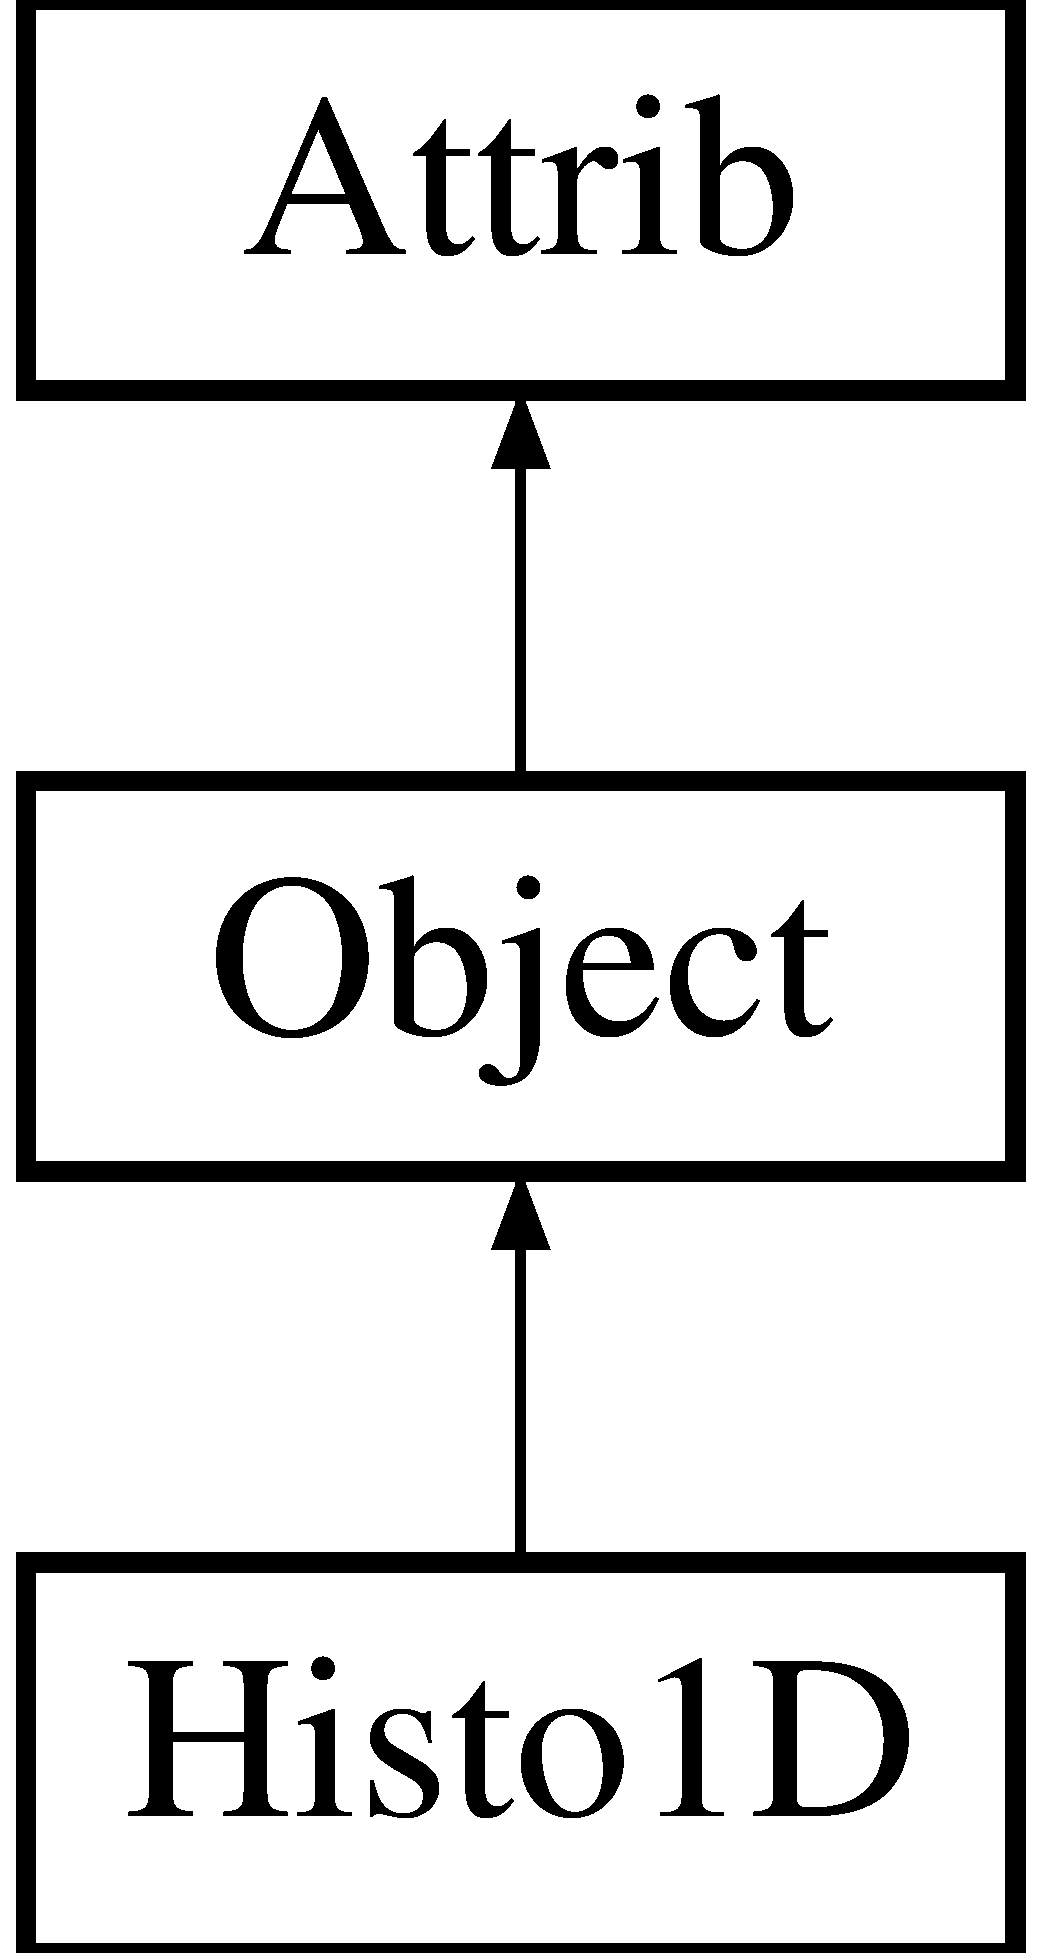
\includegraphics[height=3.000000cm]{classHisto1D}
\end{center}
\end{figure}
\subsection*{Public Types}
\begin{DoxyCompactItemize}
\item 
enum \hyperlink{classAttrib_a69e171d7cc6417835a5a306d3c764235}{Attribut} \{ \newline
\hyperlink{classAttrib_a69e171d7cc6417835a5a306d3c764235a3a8da2ab97dda18aebab196fe4100531}{U\+N\+D\+E\+F\+I\+N\+ED}, 
\hyperlink{classAttrib_a69e171d7cc6417835a5a306d3c764235a2bfb2af57b87031d190a05fe25dd92ed}{P\+A\+S\+S\+I\+VE}, 
\hyperlink{classAttrib_a69e171d7cc6417835a5a306d3c764235a3b1fec929c0370d1436f2f06e298fb0d}{A\+C\+T\+I\+VE}, 
\hyperlink{classAttrib_a69e171d7cc6417835a5a306d3c764235aa27c16b480a369ea4d18b07b2516bbc7}{I\+N\+T\+E\+R\+F\+A\+CE}, 
\newline
\hyperlink{classAttrib_a69e171d7cc6417835a5a306d3c764235a1420a5b8c0540b2af210b6975eded7f9}{IO}, 
\hyperlink{classAttrib_a69e171d7cc6417835a5a306d3c764235a0af3b0d0ac323c1704e6c69cf90add28}{I\+O\+D\+A\+TA}, 
\hyperlink{classAttrib_a69e171d7cc6417835a5a306d3c764235a7788bc5dd333fd8ce18562b269c9dab1}{E\+L\+E\+M\+E\+NT}, 
\hyperlink{classAttrib_a69e171d7cc6417835a5a306d3c764235a61ceb22149f365f1780d18f9d1459423}{H\+A\+R\+D\+W\+A\+RE}, 
\newline
\hyperlink{classAttrib_a69e171d7cc6417835a5a306d3c764235a75250e29692496e73effca2c0330977f}{P\+R\+O\+C\+E\+S\+S\+US}, 
\hyperlink{classAttrib_a69e171d7cc6417835a5a306d3c764235a103a67cd0b8f07ef478fa45d4356e27b}{S\+O\+F\+T\+W\+A\+RE}
 \}
\end{DoxyCompactItemize}
\subsection*{Public Member Functions}
\begin{DoxyCompactItemize}
\item 
\hyperlink{classHisto1D_aecd55af9b972863d5cee5a387746fb96}{Histo1D} (T\+H1D $\ast$histo)
\item 
\hyperlink{classHisto1D_af62825fd9266c1903d403e489501daa9}{$\sim$\+Histo1D} ()
\item 
void \hyperlink{classHisto1D_a22b820e2c706d8e8614c31962f1ac6d0}{def} ()
\item 
void \hyperlink{classHisto1D_a907707c720f8f0d3f582632d186ee7dd}{fill} (double x, double value=1.)
\item 
double \hyperlink{classHisto1D_a122c7071e060672dd2c08ad92212b3a2}{minY} ()
\item 
double \hyperlink{classHisto1D_a60a1095ac5fbab109d20c54c2ee569a3}{maxY} ()
\item 
double \hyperlink{classHisto1D_a54c7464513d1382c7c66fa880bfe568e}{maxX} ()
\item 
double \hyperlink{classHisto1D_abe9bf76799889414686794502e777b67}{minX} ()
\item 
std\+::vector$<$ double $>$ \hyperlink{classHisto1D_aaa8cd492ee25a3ad1b1694349fb1024c}{bins} ()
\item 
std\+::vector$<$ double $>$ \hyperlink{classHisto1D_a07fd41679a3255cdd44d4dcf8865adb7}{centers} ()
\item 
std\+::vector$<$ double $>$ \hyperlink{classHisto1D_a8c74413d35bce2e244defd470b6b4ebf}{edges} ()
\item 
unsigned long \hyperlink{classHisto1D_a7f3cf7364ae6e1eb9ba08b5ffe897d8f}{n\+Bin} ()
\item 
double \hyperlink{classHisto1D_a2a8a7d93c2f10b73b490a6f550e00db4}{bin} (double x)
\item 
double \hyperlink{classHisto1D_aa15ab79f858358e3cafc0617eb668c2e}{bin\+Edge\+Min} (unsigned int)
\item 
double \hyperlink{classHisto1D_a7923d51b02056dbaef353b70c11499d0}{bin\+Edge\+Max} (unsigned int)
\item 
double \hyperlink{classHisto1D_aece5cb8dddafabe0029067dc3e4be878}{bin\+Content} (int i)
\item 
double \hyperlink{classHisto1D_a5d13018047a4ffb15e662f44a0a3f520}{overflow} ()
\item 
double \hyperlink{classHisto1D_a3bac7a207b9ed5f828001119b2f14869}{underflow} ()
\item 
void \hyperlink{classHisto1D_acc0d6f2080b0cfafc85ebc49cf0efc31}{statistics} (double \&, double \&, double \&)
\item 
std\+::string \hyperlink{classObject_a300f4c05dd468c7bb8b3c968868443c1}{name} () const
\item 
std\+::string \hyperlink{classObject_a84f99f70f144a83e1582d1d0f84e4e62}{type} ()
\item 
unsigned char \hyperlink{classObject_af99145335cc61ff6e2798ea17db009d2}{id} ()
\item 
std\+::string \hyperlink{classObject_a73a0f1a41828fdd8303dd662446fb6c3}{title} ()
\item 
void \hyperlink{classObject_a3f9d5537ebce0c0f2bf6ae4d92426f3c}{msg\+Svc} (int level, std\+::string \hyperlink{classObject_a58b2d0618c2d08cf2383012611528d97}{msg}, std\+::string \hyperlink{classObject_a300f4c05dd468c7bb8b3c968868443c1}{name})
\item 
void \hyperlink{classObject_a58b2d0618c2d08cf2383012611528d97}{msg} (std\+::string mymsg)
\item 
void \hyperlink{classObject_ac5d59299273cee27aacf7de00d2e7034}{msg} (std\+::string mymsg, std\+::string \hyperlink{classObject_a300f4c05dd468c7bb8b3c968868443c1}{name})
\item 
void \hyperlink{classObject_a83d2db2df682907ea1115ad721c1c4a1}{verbose} (std\+::string mymsg)
\item 
void \hyperlink{classObject_a2d4120195317e2a3c6532e8bb9f3da68}{verbose} (std\+::string mymsg, std\+::string \hyperlink{classObject_a300f4c05dd468c7bb8b3c968868443c1}{name})
\item 
void \hyperlink{classObject_aac010553f022165573714b7014a15f0d}{debug} (std\+::string mymsg)
\item 
void \hyperlink{classObject_a6c9a0397ca804e04d675ed05683f5420}{debug} (std\+::string mymsg, std\+::string \hyperlink{classObject_a300f4c05dd468c7bb8b3c968868443c1}{name})
\item 
void \hyperlink{classObject_a644fd329ea4cb85f54fa6846484b84a8}{info} (std\+::string mymsg)
\item 
void \hyperlink{classObject_a1ca123253dfd30fc28b156f521dcbdae}{info} (std\+::string mymsg, std\+::string \hyperlink{classObject_a300f4c05dd468c7bb8b3c968868443c1}{name})
\item 
void \hyperlink{classObject_a65cd4fda577711660821fd2cd5a3b4c9}{warning} (std\+::string mymsg)
\item 
void \hyperlink{classObject_a11f101db4dd73d9391b0231818881d86}{warning} (std\+::string mymsg, std\+::string \hyperlink{classObject_a300f4c05dd468c7bb8b3c968868443c1}{name})
\item 
void \hyperlink{classObject_a204a95f57818c0f811933917a30eff45}{error} (std\+::string mymsg)
\item 
void \hyperlink{classObject_ad7f6c457733082efa2f9ff5f5c8e119a}{error} (std\+::string mymsg, std\+::string \hyperlink{classObject_a300f4c05dd468c7bb8b3c968868443c1}{name})
\item 
void \hyperlink{classObject_aad5a16aac7516ce65bd5ec02ab07fc80}{fatal} (std\+::string mymsg)
\item 
void \hyperlink{classObject_ae62acd3d09f716220f75f252dc38bc9a}{fatal} (std\+::string mymsg, std\+::string \hyperlink{classObject_a300f4c05dd468c7bb8b3c968868443c1}{name})
\item 
void \hyperlink{classObject_ae30fea75683c2d149b6b6d17c09ecd0c}{set\+Name} (std\+::string \hyperlink{classObject_a300f4c05dd468c7bb8b3c968868443c1}{name})
\item 
void \hyperlink{classObject_aae534cc9d982bcb9b99fd505f2e103a5}{set\+Type} (std\+::string \hyperlink{classObject_a84f99f70f144a83e1582d1d0f84e4e62}{type})
\item 
void \hyperlink{classObject_a398fe08cba594a0ce6891d59fe4f159f}{set\+Id} (unsigned char \hyperlink{classObject_af99145335cc61ff6e2798ea17db009d2}{id})
\item 
void \hyperlink{classObject_a89557dbbad5bcaa02652f5d7fa35d20f}{set\+Title} (std\+::string \hyperlink{classObject_a73a0f1a41828fdd8303dd662446fb6c3}{title})
\item 
void \hyperlink{classObject_a870c5af919958c2136623b2d7816d123}{set\+Dll\+Name} (std\+::string \hyperlink{classObject_a2e3947f2870094c332d7454117f3ec63}{dll\+Name})
\item 
std\+::string \hyperlink{classObject_a2e3947f2870094c332d7454117f3ec63}{dll\+Name} ()
\item 
bool \hyperlink{classAttrib_a704f26af560909ad22065083bb7d4c34}{is} (int attribut)
\item 
void \hyperlink{classAttrib_a235f773af19c900264a190b00a3b4ad7}{add} (int attribut)
\item 
void \hyperlink{classAttrib_a7d4ef7e32d93cb287792b87b857e79f3}{remove} (int attribut)
\item 
std\+::string \hyperlink{classAttrib_aee7bbf16b144887f196e1341b24f8a26}{attributs} ()
\end{DoxyCompactItemize}
\subsection*{Protected Attributes}
\begin{DoxyCompactItemize}
\item 
std\+::string \hyperlink{classAttrib_a3414521d7a82476e874b25a5407b5e63}{m\+\_\+attrib\+String} \mbox{[}10\mbox{]}
\end{DoxyCompactItemize}
\subsection*{Private Attributes}
\begin{DoxyCompactItemize}
\item 
double \hyperlink{classHisto1D_ac87bd1971cc300ce6fc1e745785cacb9}{m\+\_\+zero}
\item 
double \hyperlink{classHisto1D_a47c1ba33be0574ca167f43a1b27ba1a0}{m\+\_\+infini}
\item 
unsigned long \hyperlink{classHisto1D_a1913aca9a278b4bfd365f35b85e65d8d}{m\+\_\+nbins}
\item 
std\+::vector$<$ double $>$ \hyperlink{classHisto1D_a7a82923d3938739904469f5aa0a517ca}{m\+\_\+bins}
\item 
std\+::vector$<$ double $>$ \hyperlink{classHisto1D_a0e03676ed176aaad2f615fa84b8ffcd3}{m\+\_\+centers}
\item 
std\+::vector$<$ double $>$ \hyperlink{classHisto1D_a4188c6d1b4bfc8f9d8bde7616b4dbf5b}{m\+\_\+edges}
\item 
double \hyperlink{classHisto1D_af5ce58b20e96fa6e4b306109dd88589e}{m\+\_\+minX}
\item 
double \hyperlink{classHisto1D_a6a5007569e096537f9b7b39d2aad865b}{m\+\_\+maxX}
\item 
double \hyperlink{classHisto1D_a3bb6c3ea23a1af14ebb10af807f3810d}{m\+\_\+minY}
\item 
double \hyperlink{classHisto1D_a28a8995424e36088c47643f8c1a7fa7f}{m\+\_\+maxY}
\item 
double \hyperlink{classHisto1D_a993e2e40b89e257e6f86c0742f6f06b3}{m\+\_\+delta}
\item 
double \hyperlink{classHisto1D_ab60b2ec4e435a3094b7ec218404aa16f}{m\+\_\+overflow}
\item 
double \hyperlink{classHisto1D_a7f475b822f4bbb23209e2e523d228380}{m\+\_\+underflow}
\item 
double \hyperlink{classHisto1D_a75f4abeae577e232f4c012cb6b4049d7}{m\+\_\+content}
\item 
double \hyperlink{classHisto1D_a7e49893543fb5d2af37167690bc0b0ff}{m\+\_\+mean}
\item 
double \hyperlink{classHisto1D_a1331c670df40eb18d8a814f5a15ec7da}{m\+\_\+rms}
\end{DoxyCompactItemize}


\subsection{Detailed Description}


Definition at line 28 of file Histo1\+D.\+h.



\subsection{Member Enumeration Documentation}
\mbox{\Hypertarget{classAttrib_a69e171d7cc6417835a5a306d3c764235}\label{classAttrib_a69e171d7cc6417835a5a306d3c764235}} 
\index{Histo1D@{Histo1D}!Attribut@{Attribut}}
\index{Attribut@{Attribut}!Histo1D@{Histo1D}}
\subsubsection{\texorpdfstring{Attribut}{Attribut}}
{\footnotesize\ttfamily enum \hyperlink{classAttrib_a69e171d7cc6417835a5a306d3c764235}{Attrib\+::\+Attribut}\hspace{0.3cm}{\ttfamily [inherited]}}

\begin{DoxyEnumFields}{Enumerator}
\raisebox{\heightof{T}}[0pt][0pt]{\index{U\+N\+D\+E\+F\+I\+N\+ED@{U\+N\+D\+E\+F\+I\+N\+ED}!Histo1D@{Histo1D}}\index{Histo1D@{Histo1D}!U\+N\+D\+E\+F\+I\+N\+ED@{U\+N\+D\+E\+F\+I\+N\+ED}}}\mbox{\Hypertarget{classAttrib_a69e171d7cc6417835a5a306d3c764235a3a8da2ab97dda18aebab196fe4100531}\label{classAttrib_a69e171d7cc6417835a5a306d3c764235a3a8da2ab97dda18aebab196fe4100531}} 
U\+N\+D\+E\+F\+I\+N\+ED&\\
\hline

\raisebox{\heightof{T}}[0pt][0pt]{\index{P\+A\+S\+S\+I\+VE@{P\+A\+S\+S\+I\+VE}!Histo1D@{Histo1D}}\index{Histo1D@{Histo1D}!P\+A\+S\+S\+I\+VE@{P\+A\+S\+S\+I\+VE}}}\mbox{\Hypertarget{classAttrib_a69e171d7cc6417835a5a306d3c764235a2bfb2af57b87031d190a05fe25dd92ed}\label{classAttrib_a69e171d7cc6417835a5a306d3c764235a2bfb2af57b87031d190a05fe25dd92ed}} 
P\+A\+S\+S\+I\+VE&\\
\hline

\raisebox{\heightof{T}}[0pt][0pt]{\index{A\+C\+T\+I\+VE@{A\+C\+T\+I\+VE}!Histo1D@{Histo1D}}\index{Histo1D@{Histo1D}!A\+C\+T\+I\+VE@{A\+C\+T\+I\+VE}}}\mbox{\Hypertarget{classAttrib_a69e171d7cc6417835a5a306d3c764235a3b1fec929c0370d1436f2f06e298fb0d}\label{classAttrib_a69e171d7cc6417835a5a306d3c764235a3b1fec929c0370d1436f2f06e298fb0d}} 
A\+C\+T\+I\+VE&\\
\hline

\raisebox{\heightof{T}}[0pt][0pt]{\index{I\+N\+T\+E\+R\+F\+A\+CE@{I\+N\+T\+E\+R\+F\+A\+CE}!Histo1D@{Histo1D}}\index{Histo1D@{Histo1D}!I\+N\+T\+E\+R\+F\+A\+CE@{I\+N\+T\+E\+R\+F\+A\+CE}}}\mbox{\Hypertarget{classAttrib_a69e171d7cc6417835a5a306d3c764235aa27c16b480a369ea4d18b07b2516bbc7}\label{classAttrib_a69e171d7cc6417835a5a306d3c764235aa27c16b480a369ea4d18b07b2516bbc7}} 
I\+N\+T\+E\+R\+F\+A\+CE&\\
\hline

\raisebox{\heightof{T}}[0pt][0pt]{\index{IO@{IO}!Histo1D@{Histo1D}}\index{Histo1D@{Histo1D}!IO@{IO}}}\mbox{\Hypertarget{classAttrib_a69e171d7cc6417835a5a306d3c764235a1420a5b8c0540b2af210b6975eded7f9}\label{classAttrib_a69e171d7cc6417835a5a306d3c764235a1420a5b8c0540b2af210b6975eded7f9}} 
IO&\\
\hline

\raisebox{\heightof{T}}[0pt][0pt]{\index{I\+O\+D\+A\+TA@{I\+O\+D\+A\+TA}!Histo1D@{Histo1D}}\index{Histo1D@{Histo1D}!I\+O\+D\+A\+TA@{I\+O\+D\+A\+TA}}}\mbox{\Hypertarget{classAttrib_a69e171d7cc6417835a5a306d3c764235a0af3b0d0ac323c1704e6c69cf90add28}\label{classAttrib_a69e171d7cc6417835a5a306d3c764235a0af3b0d0ac323c1704e6c69cf90add28}} 
I\+O\+D\+A\+TA&\\
\hline

\raisebox{\heightof{T}}[0pt][0pt]{\index{E\+L\+E\+M\+E\+NT@{E\+L\+E\+M\+E\+NT}!Histo1D@{Histo1D}}\index{Histo1D@{Histo1D}!E\+L\+E\+M\+E\+NT@{E\+L\+E\+M\+E\+NT}}}\mbox{\Hypertarget{classAttrib_a69e171d7cc6417835a5a306d3c764235a7788bc5dd333fd8ce18562b269c9dab1}\label{classAttrib_a69e171d7cc6417835a5a306d3c764235a7788bc5dd333fd8ce18562b269c9dab1}} 
E\+L\+E\+M\+E\+NT&\\
\hline

\raisebox{\heightof{T}}[0pt][0pt]{\index{H\+A\+R\+D\+W\+A\+RE@{H\+A\+R\+D\+W\+A\+RE}!Histo1D@{Histo1D}}\index{Histo1D@{Histo1D}!H\+A\+R\+D\+W\+A\+RE@{H\+A\+R\+D\+W\+A\+RE}}}\mbox{\Hypertarget{classAttrib_a69e171d7cc6417835a5a306d3c764235a61ceb22149f365f1780d18f9d1459423}\label{classAttrib_a69e171d7cc6417835a5a306d3c764235a61ceb22149f365f1780d18f9d1459423}} 
H\+A\+R\+D\+W\+A\+RE&\\
\hline

\raisebox{\heightof{T}}[0pt][0pt]{\index{P\+R\+O\+C\+E\+S\+S\+US@{P\+R\+O\+C\+E\+S\+S\+US}!Histo1D@{Histo1D}}\index{Histo1D@{Histo1D}!P\+R\+O\+C\+E\+S\+S\+US@{P\+R\+O\+C\+E\+S\+S\+US}}}\mbox{\Hypertarget{classAttrib_a69e171d7cc6417835a5a306d3c764235a75250e29692496e73effca2c0330977f}\label{classAttrib_a69e171d7cc6417835a5a306d3c764235a75250e29692496e73effca2c0330977f}} 
P\+R\+O\+C\+E\+S\+S\+US&\\
\hline

\raisebox{\heightof{T}}[0pt][0pt]{\index{S\+O\+F\+T\+W\+A\+RE@{S\+O\+F\+T\+W\+A\+RE}!Histo1D@{Histo1D}}\index{Histo1D@{Histo1D}!S\+O\+F\+T\+W\+A\+RE@{S\+O\+F\+T\+W\+A\+RE}}}\mbox{\Hypertarget{classAttrib_a69e171d7cc6417835a5a306d3c764235a103a67cd0b8f07ef478fa45d4356e27b}\label{classAttrib_a69e171d7cc6417835a5a306d3c764235a103a67cd0b8f07ef478fa45d4356e27b}} 
S\+O\+F\+T\+W\+A\+RE&\\
\hline

\end{DoxyEnumFields}


Definition at line 29 of file Attrib.\+h.


\begin{DoxyCode}
29                 \{
30     \hyperlink{classAttrib_a69e171d7cc6417835a5a306d3c764235a3a8da2ab97dda18aebab196fe4100531}{UNDEFINED},
31     \hyperlink{classAttrib_a69e171d7cc6417835a5a306d3c764235a2bfb2af57b87031d190a05fe25dd92ed}{PASSIVE},
32     \hyperlink{classAttrib_a69e171d7cc6417835a5a306d3c764235a3b1fec929c0370d1436f2f06e298fb0d}{ACTIVE},
33     \hyperlink{classAttrib_a69e171d7cc6417835a5a306d3c764235aa27c16b480a369ea4d18b07b2516bbc7}{INTERFACE},
34     \hyperlink{classAttrib_a69e171d7cc6417835a5a306d3c764235a1420a5b8c0540b2af210b6975eded7f9}{IO},
35     \hyperlink{classAttrib_a69e171d7cc6417835a5a306d3c764235a0af3b0d0ac323c1704e6c69cf90add28}{IODATA},
36     \hyperlink{classAttrib_a69e171d7cc6417835a5a306d3c764235a7788bc5dd333fd8ce18562b269c9dab1}{ELEMENT},
37     \hyperlink{classAttrib_a69e171d7cc6417835a5a306d3c764235a61ceb22149f365f1780d18f9d1459423}{HARDWARE},
38     \hyperlink{classAttrib_a69e171d7cc6417835a5a306d3c764235a75250e29692496e73effca2c0330977f}{PROCESSUS},
39     \hyperlink{classAttrib_a69e171d7cc6417835a5a306d3c764235a103a67cd0b8f07ef478fa45d4356e27b}{SOFTWARE} 
40   \}; \textcolor{comment}{// array m\_attribString must be changed into Attrib::Attrib if this enu is modified. }
\end{DoxyCode}


\subsection{Constructor \& Destructor Documentation}
\mbox{\Hypertarget{classHisto1D_aecd55af9b972863d5cee5a387746fb96}\label{classHisto1D_aecd55af9b972863d5cee5a387746fb96}} 
\index{Histo1D@{Histo1D}!Histo1D@{Histo1D}}
\index{Histo1D@{Histo1D}!Histo1D@{Histo1D}}
\subsubsection{\texorpdfstring{Histo1\+D()}{Histo1D()}}
{\footnotesize\ttfamily Histo1\+D\+::\+Histo1D (\begin{DoxyParamCaption}\item[{T\+H1D $\ast$}]{histo }\end{DoxyParamCaption})}



Definition at line 22 of file Histo1\+D.\+cpp.



References m\+\_\+bins, m\+\_\+centers, m\+\_\+content, m\+\_\+delta, m\+\_\+edges, m\+\_\+maxX, m\+\_\+maxY, m\+\_\+mean, m\+\_\+minX, m\+\_\+minY, m\+\_\+nbins, m\+\_\+overflow, m\+\_\+rms, m\+\_\+underflow, and Object\+::set\+Title().


\begin{DoxyCode}
22                               : \hyperlink{classHisto1D_ac87bd1971cc300ce6fc1e745785cacb9}{m\_zero} ( 1.e-30 ) , \hyperlink{classHisto1D_a47c1ba33be0574ca167f43a1b27ba1a0}{m\_infini}(1.e30) \{
23   \textcolor{comment}{//m\_histo = histo; }
24   
25   \hyperlink{classHisto1D_a1913aca9a278b4bfd365f35b85e65d8d}{m\_nbins} = histo->GetNbinsX();
26 
27   \hyperlink{classObject_a89557dbbad5bcaa02652f5d7fa35d20f}{setTitle}(std::string(histo -> GetTitle()));
28 
29   \hyperlink{classHisto1D_a7a82923d3938739904469f5aa0a517ca}{m\_bins}.resize (\hyperlink{classHisto1D_a1913aca9a278b4bfd365f35b85e65d8d}{m\_nbins},0.);
30   \hyperlink{classHisto1D_a0e03676ed176aaad2f615fa84b8ffcd3}{m\_centers}.resize (\hyperlink{classHisto1D_a1913aca9a278b4bfd365f35b85e65d8d}{m\_nbins},0.);
31   \hyperlink{classHisto1D_a4188c6d1b4bfc8f9d8bde7616b4dbf5b}{m\_edges}.resize (\hyperlink{classHisto1D_a1913aca9a278b4bfd365f35b85e65d8d}{m\_nbins}+1,0.);
32 
33   \textcolor{keywordtype}{unsigned} \textcolor{keywordtype}{long} nbin=0;
34   \textcolor{keywordflow}{for} (nbin=0;nbin<\hyperlink{classHisto1D_a1913aca9a278b4bfd365f35b85e65d8d}{m\_nbins}; ++nbin)\{
35     \hyperlink{classHisto1D_a7a82923d3938739904469f5aa0a517ca}{m\_bins}[nbin]=histo->GetBinContent(nbin+1);
36     \hyperlink{classHisto1D_a0e03676ed176aaad2f615fa84b8ffcd3}{m\_centers}[nbin]=histo->GetBinCenter(nbin+1);
37   \}
38 
39   \hyperlink{classHisto1D_a993e2e40b89e257e6f86c0742f6f06b3}{m\_delta} = histo->GetBinWidth(0);
40 
41   \textcolor{keywordflow}{for} (nbin=0;nbin<m\_nbins+1; ++nbin)\{
42     \hyperlink{classHisto1D_a4188c6d1b4bfc8f9d8bde7616b4dbf5b}{m\_edges}[nbin]=histo->GetBinLowEdge(1)+nbin*\hyperlink{classHisto1D_a993e2e40b89e257e6f86c0742f6f06b3}{m\_delta};
43   \}
44 
45   \hyperlink{classHisto1D_a7f475b822f4bbb23209e2e523d228380}{m\_underflow} = histo->GetBinContent(0);
46   \hyperlink{classHisto1D_ab60b2ec4e435a3094b7ec218404aa16f}{m\_overflow} = histo->GetBinContent(histo->GetNbinsX()+1);  
47 
48   \hyperlink{classHisto1D_af5ce58b20e96fa6e4b306109dd88589e}{m\_minX} = histo->GetBinLowEdge(1);
49   \hyperlink{classHisto1D_a6a5007569e096537f9b7b39d2aad865b}{m\_maxX} = histo->GetBinLowEdge(histo->GetNbinsX()+1);
50 
51   \hyperlink{classHisto1D_a3bb6c3ea23a1af14ebb10af807f3810d}{m\_minY} = histo->GetMinimum();
52   \hyperlink{classHisto1D_a28a8995424e36088c47643f8c1a7fa7f}{m\_maxY} = histo->GetMaximum();
53 
54   \hyperlink{classHisto1D_a75f4abeae577e232f4c012cb6b4049d7}{m\_content} = histo->GetEntries();
55   \hyperlink{classHisto1D_a7e49893543fb5d2af37167690bc0b0ff}{m\_mean}    = histo->GetMean();
56   \hyperlink{classHisto1D_a1331c670df40eb18d8a814f5a15ec7da}{m\_rms}     = histo->GetRMS();
57 \}
\end{DoxyCode}
\mbox{\Hypertarget{classHisto1D_af62825fd9266c1903d403e489501daa9}\label{classHisto1D_af62825fd9266c1903d403e489501daa9}} 
\index{Histo1D@{Histo1D}!````~Histo1D@{$\sim$\+Histo1D}}
\index{````~Histo1D@{$\sim$\+Histo1D}!Histo1D@{Histo1D}}
\subsubsection{\texorpdfstring{$\sim$\+Histo1\+D()}{~Histo1D()}}
{\footnotesize\ttfamily Histo1\+D\+::$\sim$\+Histo1D (\begin{DoxyParamCaption}{ }\end{DoxyParamCaption})\hspace{0.3cm}{\ttfamily [inline]}}



Definition at line 32 of file Histo1\+D.\+h.



References def(), fill(), max\+Y(), and min\+Y().


\begin{DoxyCode}
32 \{ \}
\end{DoxyCode}


\subsection{Member Function Documentation}
\mbox{\Hypertarget{classAttrib_a235f773af19c900264a190b00a3b4ad7}\label{classAttrib_a235f773af19c900264a190b00a3b4ad7}} 
\index{Histo1D@{Histo1D}!add@{add}}
\index{add@{add}!Histo1D@{Histo1D}}
\subsubsection{\texorpdfstring{add()}{add()}}
{\footnotesize\ttfamily void Attrib\+::add (\begin{DoxyParamCaption}\item[{int}]{attribut }\end{DoxyParamCaption})\hspace{0.3cm}{\ttfamily [inline]}, {\ttfamily [inherited]}}

Add an attribut 

Definition at line 67 of file Attrib.\+h.



References Attrib\+::m\+\_\+attributs, and Attrib\+::\+U\+N\+D\+E\+F\+I\+N\+ED.



Referenced by A3\+P\+E\+::\+A3\+P\+E(), Attrib\+::\+Attrib(), Specs\+Mezzanine\+::cmdline(), Computer\+::\+Computer(), C\+U\+\_\+v1\+::\+C\+U\+\_\+v1(), export\+\_\+obj(), F\+E\+B\+\_\+v1\+::\+F\+E\+B\+\_\+v1(), Fe\+P\+G\+A\+::\+Fe\+P\+G\+A(), I\+C\+E\+C\+A\+Lv3\+::\+I\+C\+E\+C\+A\+Lv3(), I\+C\+Phaser\+::\+I\+C\+Phaser(), Fe\+P\+G\+A\+::init(), Application\+::initialize(), Interface\+::\+Interface(), I\+Odata\+::\+I\+Odata(), I\+Oobject\+::\+I\+Oobject(), M\+S\+Oxxxx\+::\+M\+S\+Oxxxx(), Phaser\+::\+Phaser(), Processus\+::\+Processus(), Proto40\+M\+Hz\+\_\+v1\+::\+Proto40\+M\+Hz\+\_\+v1(), Attrib\+::remove(), Seq\+P\+G\+A\+::\+Seq\+P\+G\+A(), Test\+S\+P\+I\+::set\+Address(), Test\+I2\+C\+::set\+Address(), Specs\+Slave\+::set\+Address(), Specs\+Master\+::\+Specs\+Master(), and Specs\+Slave\+::\+Specs\+Slave().


\begin{DoxyCode}
67                             \{
68     \textcolor{keywordflow}{if} (attribut!=\hyperlink{classAttrib_a69e171d7cc6417835a5a306d3c764235a3a8da2ab97dda18aebab196fe4100531}{Attrib::UNDEFINED}) \textcolor{keyword}{remove}(\hyperlink{classAttrib_a69e171d7cc6417835a5a306d3c764235a3a8da2ab97dda18aebab196fe4100531}{Attrib::UNDEFINED});
69     \textcolor{keywordtype}{bool} duplicate = false ;
70     std::vector<int>::const\_iterator iter ;
71     \textcolor{keywordflow}{for} ( iter  = \hyperlink{classAttrib_ac4bd58a0cc6b38a3b711d609a3d3aacc}{m\_attributs}.begin() ;
72           iter != \hyperlink{classAttrib_ac4bd58a0cc6b38a3b711d609a3d3aacc}{m\_attributs}.end()   ;
73           ++iter ) \{
74       \textcolor{keywordflow}{if} ( attribut == (*iter) ) \{
75         duplicate = true ;
76       \}
77     \}
78     \textcolor{keywordflow}{if} (!duplicate) \{
79       \hyperlink{classAttrib_ac4bd58a0cc6b38a3b711d609a3d3aacc}{m\_attributs}.push\_back( attribut );
80     \}
81   \}
\end{DoxyCode}
\mbox{\Hypertarget{classAttrib_aee7bbf16b144887f196e1341b24f8a26}\label{classAttrib_aee7bbf16b144887f196e1341b24f8a26}} 
\index{Histo1D@{Histo1D}!attributs@{attributs}}
\index{attributs@{attributs}!Histo1D@{Histo1D}}
\subsubsection{\texorpdfstring{attributs()}{attributs()}}
{\footnotesize\ttfamily std\+::string Attrib\+::attributs (\begin{DoxyParamCaption}{ }\end{DoxyParamCaption})\hspace{0.3cm}{\ttfamily [inherited]}}

Print the \hyperlink{classAttrib}{Attrib} of an \hyperlink{classObject}{Object} 

Definition at line 54 of file Attrib.\+cpp.



References images\+::index, Attrib\+::m\+\_\+attrib\+String, and Attrib\+::m\+\_\+attributs.



Referenced by export\+\_\+obj(), and Attrib\+::remove().


\begin{DoxyCode}
54                             \{
55   std::string output;
56   std::vector<int>::iterator iter ;
57   \textcolor{keywordflow}{for} ( \textcolor{keywordtype}{unsigned} \textcolor{keywordtype}{int} \hyperlink{namespaceimages_a54407fd574970b3178647ae096321a57}{index} = 0 ; \hyperlink{namespaceimages_a54407fd574970b3178647ae096321a57}{index} < \hyperlink{classAttrib_ac4bd58a0cc6b38a3b711d609a3d3aacc}{m\_attributs}.size() ; ++
      \hyperlink{namespaceimages_a54407fd574970b3178647ae096321a57}{index} ) \{
58     \textcolor{keywordflow}{if} ( \hyperlink{classAttrib_ac4bd58a0cc6b38a3b711d609a3d3aacc}{m\_attributs}.size() - \hyperlink{namespaceimages_a54407fd574970b3178647ae096321a57}{index} > 1 ) \{
59       output.append(\hyperlink{classAttrib_a3414521d7a82476e874b25a5407b5e63}{m\_attribString}[\hyperlink{classAttrib_ac4bd58a0cc6b38a3b711d609a3d3aacc}{m\_attributs}[\hyperlink{namespaceimages_a54407fd574970b3178647ae096321a57}{index}]]);
60       output.append(\textcolor{stringliteral}{":"});
61     \}
62     \textcolor{keywordflow}{else} \{
63       output.append(\hyperlink{classAttrib_a3414521d7a82476e874b25a5407b5e63}{m\_attribString}[\hyperlink{classAttrib_ac4bd58a0cc6b38a3b711d609a3d3aacc}{m\_attributs}[index]]);
64     \}
65   \}
66   \textcolor{keywordflow}{return} output;
67 \}
\end{DoxyCode}
\mbox{\Hypertarget{classHisto1D_a2a8a7d93c2f10b73b490a6f550e00db4}\label{classHisto1D_a2a8a7d93c2f10b73b490a6f550e00db4}} 
\index{Histo1D@{Histo1D}!bin@{bin}}
\index{bin@{bin}!Histo1D@{Histo1D}}
\subsubsection{\texorpdfstring{bin()}{bin()}}
{\footnotesize\ttfamily double Histo1\+D\+::bin (\begin{DoxyParamCaption}\item[{double}]{x }\end{DoxyParamCaption})}



Definition at line 59 of file Histo1\+D.\+cpp.



References m\+\_\+bins, m\+\_\+delta, m\+\_\+maxX, m\+\_\+minX, m\+\_\+nbins, m\+\_\+overflow, and m\+\_\+underflow.



Referenced by n\+Bin().


\begin{DoxyCode}
59                            \{
60     \textcolor{keywordflow}{if} (x>=\hyperlink{classHisto1D_a6a5007569e096537f9b7b39d2aad865b}{m\_maxX}) \{\textcolor{keywordflow}{return} \hyperlink{classHisto1D_ab60b2ec4e435a3094b7ec218404aa16f}{m\_overflow};\}
61     \textcolor{keywordflow}{else} \textcolor{keywordflow}{if}(x<\hyperlink{classHisto1D_af5ce58b20e96fa6e4b306109dd88589e}{m\_minX}) \{\textcolor{keywordflow}{return} \hyperlink{classHisto1D_a7f475b822f4bbb23209e2e523d228380}{m\_underflow};\}
62     \textcolor{keywordtype}{unsigned} \textcolor{keywordtype}{long} \hyperlink{classHisto1D_a2a8a7d93c2f10b73b490a6f550e00db4}{bin}=(\textcolor{keywordtype}{unsigned} long)(floor(\hyperlink{classHisto1D_a1913aca9a278b4bfd365f35b85e65d8d}{m\_nbins}*(x-\hyperlink{classHisto1D_af5ce58b20e96fa6e4b306109dd88589e}{m\_minX})/
      \hyperlink{classHisto1D_a993e2e40b89e257e6f86c0742f6f06b3}{m\_delta}));
63     \textcolor{keywordflow}{return} \hyperlink{classHisto1D_a7a82923d3938739904469f5aa0a517ca}{m\_bins}[\hyperlink{classHisto1D_a2a8a7d93c2f10b73b490a6f550e00db4}{bin}];
64 \}   
\end{DoxyCode}
\mbox{\Hypertarget{classHisto1D_aece5cb8dddafabe0029067dc3e4be878}\label{classHisto1D_aece5cb8dddafabe0029067dc3e4be878}} 
\index{Histo1D@{Histo1D}!bin\+Content@{bin\+Content}}
\index{bin\+Content@{bin\+Content}!Histo1D@{Histo1D}}
\subsubsection{\texorpdfstring{bin\+Content()}{binContent()}}
{\footnotesize\ttfamily double Histo1\+D\+::bin\+Content (\begin{DoxyParamCaption}\item[{int}]{i }\end{DoxyParamCaption})\hspace{0.3cm}{\ttfamily [inline]}}



Definition at line 71 of file Histo1\+D.\+h.



References m\+\_\+bins.


\begin{DoxyCode}
71                           \{
72     \textcolor{keywordflow}{return} \hyperlink{classHisto1D_a7a82923d3938739904469f5aa0a517ca}{m\_bins}[i];
73   \}
\end{DoxyCode}
\mbox{\Hypertarget{classHisto1D_a7923d51b02056dbaef353b70c11499d0}\label{classHisto1D_a7923d51b02056dbaef353b70c11499d0}} 
\index{Histo1D@{Histo1D}!bin\+Edge\+Max@{bin\+Edge\+Max}}
\index{bin\+Edge\+Max@{bin\+Edge\+Max}!Histo1D@{Histo1D}}
\subsubsection{\texorpdfstring{bin\+Edge\+Max()}{binEdgeMax()}}
{\footnotesize\ttfamily double Histo1\+D\+::bin\+Edge\+Max (\begin{DoxyParamCaption}\item[{unsigned int}]{bin }\end{DoxyParamCaption})}



Definition at line 78 of file Histo1\+D.\+cpp.



References m\+\_\+delta, and m\+\_\+minX.



Referenced by n\+Bin().


\begin{DoxyCode}
78                                              \{
79   \textcolor{keywordflow}{return} \hyperlink{classHisto1D_af5ce58b20e96fa6e4b306109dd88589e}{m\_minX}+(\hyperlink{classHisto1D_a2a8a7d93c2f10b73b490a6f550e00db4}{bin}+1)*(\hyperlink{classHisto1D_a993e2e40b89e257e6f86c0742f6f06b3}{m\_delta});
80 \}
\end{DoxyCode}
\mbox{\Hypertarget{classHisto1D_aa15ab79f858358e3cafc0617eb668c2e}\label{classHisto1D_aa15ab79f858358e3cafc0617eb668c2e}} 
\index{Histo1D@{Histo1D}!bin\+Edge\+Min@{bin\+Edge\+Min}}
\index{bin\+Edge\+Min@{bin\+Edge\+Min}!Histo1D@{Histo1D}}
\subsubsection{\texorpdfstring{bin\+Edge\+Min()}{binEdgeMin()}}
{\footnotesize\ttfamily double Histo1\+D\+::bin\+Edge\+Min (\begin{DoxyParamCaption}\item[{unsigned int}]{bin }\end{DoxyParamCaption})}



Definition at line 74 of file Histo1\+D.\+cpp.



References m\+\_\+delta, and m\+\_\+minX.



Referenced by n\+Bin().


\begin{DoxyCode}
74                                             \{
75   \textcolor{keywordflow}{return} \hyperlink{classHisto1D_af5ce58b20e96fa6e4b306109dd88589e}{m\_minX}+\hyperlink{classHisto1D_a2a8a7d93c2f10b73b490a6f550e00db4}{bin}*(\hyperlink{classHisto1D_a993e2e40b89e257e6f86c0742f6f06b3}{m\_delta});
76 \}
\end{DoxyCode}
\mbox{\Hypertarget{classHisto1D_aaa8cd492ee25a3ad1b1694349fb1024c}\label{classHisto1D_aaa8cd492ee25a3ad1b1694349fb1024c}} 
\index{Histo1D@{Histo1D}!bins@{bins}}
\index{bins@{bins}!Histo1D@{Histo1D}}
\subsubsection{\texorpdfstring{bins()}{bins()}}
{\footnotesize\ttfamily std\+::vector$<$double$>$ Histo1\+D\+::bins (\begin{DoxyParamCaption}{ }\end{DoxyParamCaption})\hspace{0.3cm}{\ttfamily [inline]}}



Definition at line 49 of file Histo1\+D.\+h.



References m\+\_\+bins.



Referenced by export\+\_\+proc().


\begin{DoxyCode}
49                           \{  
50     \textcolor{keywordflow}{return} \hyperlink{classHisto1D_a7a82923d3938739904469f5aa0a517ca}{m\_bins};
51   \}
\end{DoxyCode}
\mbox{\Hypertarget{classHisto1D_a07fd41679a3255cdd44d4dcf8865adb7}\label{classHisto1D_a07fd41679a3255cdd44d4dcf8865adb7}} 
\index{Histo1D@{Histo1D}!centers@{centers}}
\index{centers@{centers}!Histo1D@{Histo1D}}
\subsubsection{\texorpdfstring{centers()}{centers()}}
{\footnotesize\ttfamily std\+::vector$<$double$>$ Histo1\+D\+::centers (\begin{DoxyParamCaption}{ }\end{DoxyParamCaption})\hspace{0.3cm}{\ttfamily [inline]}}



Definition at line 53 of file Histo1\+D.\+h.



References m\+\_\+centers.



Referenced by export\+\_\+proc().


\begin{DoxyCode}
53                              \{  
54     \textcolor{keywordflow}{return} \hyperlink{classHisto1D_a0e03676ed176aaad2f615fa84b8ffcd3}{m\_centers};
55   \}
\end{DoxyCode}
\mbox{\Hypertarget{classObject_aac010553f022165573714b7014a15f0d}\label{classObject_aac010553f022165573714b7014a15f0d}} 
\index{Histo1D@{Histo1D}!debug@{debug}}
\index{debug@{debug}!Histo1D@{Histo1D}}
\subsubsection{\texorpdfstring{debug()}{debug()}\hspace{0.1cm}{\footnotesize\ttfamily [1/2]}}
{\footnotesize\ttfamily void Object\+::debug (\begin{DoxyParamCaption}\item[{std\+::string}]{mymsg }\end{DoxyParamCaption})\hspace{0.3cm}{\ttfamily [inline]}, {\ttfamily [inherited]}}



Definition at line 37 of file Object.\+h.



References Msg\+Svc\+::\+D\+E\+B\+UG, Object\+::m\+\_\+log, Object\+::m\+\_\+name, and Msg\+Svc\+::msg\+Svc().



Referenced by A3\+P\+E\+::\+A3\+P\+E(), A3\+P\+E\+::acquisition(), Specs\+Mezzanine\+::add\+Bus(), Hierarchy\+::add\+Child(), Specs\+Slave\+::add\+I2c(), L\+S\+Delay\+Chip\+V1\+::config\+Reg\+Bulk\+Read(), L\+S\+Delay\+Chip\+V1\+::config\+Reg\+Bulk\+Write(), A3\+P\+E\+::data\+Ready(), D\+C\+U\+::\+D\+C\+U(), Hierarchy\+::del\+Child(), Specs\+Slave\+::detect(), Storage\+Fifo\+Acquisition\+::execute(), Storage\+Fifo\+::execute(), A3\+P\+E\+\_\+\+Bit\+Flip\+::execute(), Acquisition\+::execute(), Emulate\+F\+E\+::execute(), export\+\_\+obj(), Fe\+P\+G\+A\+::\+Fe\+P\+G\+A(), Specs\+Glue\+::i2c\+Clk\+Mode(), Fe\+P\+G\+A\+::i2c\+Read(), Seq\+P\+G\+A\+::i2c\+Read(), Fe\+P\+G\+A\+::i2c\+Write(), Seq\+P\+G\+A\+::i2c\+Write(), I\+C\+E\+C\+A\+Lv3\+::\+I\+C\+E\+C\+A\+Lv3(), I\+C\+Phaser\+::\+I\+C\+Phaser(), Specs\+Slave\+::init(), Specs\+Master\+::init(), Storage\+Fifo\+::initialize(), Storage\+Fifo\+Acquisition\+::initialize(), A3\+P\+E\+\_\+\+Bit\+Flip\+::initialize(), Acquisition\+::initialize(), Emulate\+F\+E\+::initialize(), A3\+P\+E\+::internal\+A\+X\+Sequence(), Specs\+Glue\+::led(), Specs\+Mezzanine\+::led(), M\+S\+Oxxxx\+::\+M\+S\+Oxxxx(), Phaser\+::\+Phaser(), Data\+::purge(), Phaser\+::read(), I\+C\+Phaser\+::read(), F\+E\+B\+\_\+v1\+::read\+Fifo\+Spy\+F\+E(), C\+U\+\_\+v1\+::reset(), F\+E\+B\+\_\+v1\+::reset(), Proto40\+M\+Hz\+\_\+v1\+::reset(), Specs\+Slave\+::reset(), Specs\+Master\+::reset(), F\+E\+B\+\_\+v1\+::reset\+Fifo\+Spy\+F\+E(), F\+E\+B\+\_\+v1\+::reset\+Spi(), Seq\+P\+G\+A\+::reset\+Spi(), Seq\+P\+G\+A\+::\+Seq\+P\+G\+A(), A3\+P\+E\+::set\+Add\+From\+A\+X\+Ram(), A3\+P\+E\+::set\+Add\+To\+A\+X\+Ram(), A3\+P\+E\+::set\+A\+X\+Ram\+Usb(), Element\+::set\+Connection(), Specs\+Glue\+::set\+I2c\+Clk\+Mode(), A3\+P\+E\+::set\+Latency\+A\+X(), Specs\+Glue\+::set\+Led(), Specs\+Mezzanine\+::set\+Led(), A3\+P\+E\+::set\+Length\+A\+X(), A3\+P\+E\+::set\+Read\+To\+A\+X\+Ram\+Usb(), Specs\+Master\+::set\+Speed(), A3\+P\+E\+::set\+Write\+From\+A\+X\+Ram\+Usb(), Specs\+Bus\+::\+Specs\+Bus(), Specs\+I2c\+::\+Specs\+I2c(), Specs\+Master\+::\+Specs\+Master(), Specs\+Mezzanine\+::\+Specs\+Mezzanine(), Specs\+Parallel\+Bus\+::\+Specs\+Parallel\+Bus(), Specs\+Slave\+::\+Specs\+Slave(), L\+S\+Delay\+Chip\+V1\+::spi\+B\+E\+R\+Test(), I\+C\+E\+C\+A\+Lv3\+::spi\+Read(), I\+C\+E\+C\+A\+Lv3\+::spi\+Write(), F\+E\+B\+\_\+v1\+::test\+Duration(), Seq\+P\+G\+A\+::test\+Sequence(), A3\+P\+E\+::trigger(), Server\+::update\+Config(), Server\+::update\+State(), Phaser\+::write(), I\+C\+Phaser\+::write(), and Hierarchy\+::$\sim$\+Hierarchy().


\begin{DoxyCode}
37 \{ \hyperlink{classObject_a0d269813dd7ac1f24bc143031e2963f2}{m\_log}.\hyperlink{classMsgSvc_ad25f18047920cc59a314e5098259711c}{msgSvc} (\hyperlink{classMsgSvc_ae671eb7301996cd049d2da8a65925926a1dbdcc82dce88370ec335883c83b38b0}{MsgSvc::DEBUG}   , mymsg, \hyperlink{classObject_a8b83c95c705d2c3ba0d081fe1710f48d}{m\_name} ); \}
\end{DoxyCode}
\mbox{\Hypertarget{classObject_a6c9a0397ca804e04d675ed05683f5420}\label{classObject_a6c9a0397ca804e04d675ed05683f5420}} 
\index{Histo1D@{Histo1D}!debug@{debug}}
\index{debug@{debug}!Histo1D@{Histo1D}}
\subsubsection{\texorpdfstring{debug()}{debug()}\hspace{0.1cm}{\footnotesize\ttfamily [2/2]}}
{\footnotesize\ttfamily void Object\+::debug (\begin{DoxyParamCaption}\item[{std\+::string}]{mymsg,  }\item[{std\+::string}]{name }\end{DoxyParamCaption})\hspace{0.3cm}{\ttfamily [inline]}, {\ttfamily [inherited]}}



Definition at line 45 of file Object.\+h.



References Msg\+Svc\+::\+D\+E\+B\+UG, Object\+::m\+\_\+log, and Msg\+Svc\+::msg\+Svc().


\begin{DoxyCode}
45 \{ \hyperlink{classObject_a0d269813dd7ac1f24bc143031e2963f2}{m\_log}.\hyperlink{classMsgSvc_ad25f18047920cc59a314e5098259711c}{msgSvc} (\hyperlink{classMsgSvc_ae671eb7301996cd049d2da8a65925926a1dbdcc82dce88370ec335883c83b38b0}{MsgSvc::DEBUG}   , mymsg, \hyperlink{classObject_a300f4c05dd468c7bb8b3c968868443c1}{name} ); \}
\end{DoxyCode}
\mbox{\Hypertarget{classHisto1D_a22b820e2c706d8e8614c31962f1ac6d0}\label{classHisto1D_a22b820e2c706d8e8614c31962f1ac6d0}} 
\index{Histo1D@{Histo1D}!def@{def}}
\index{def@{def}!Histo1D@{Histo1D}}
\subsubsection{\texorpdfstring{def()}{def()}}
{\footnotesize\ttfamily void Histo1\+D\+::def (\begin{DoxyParamCaption}{ }\end{DoxyParamCaption})}



Referenced by $\sim$\+Histo1\+D().

\mbox{\Hypertarget{classObject_a2e3947f2870094c332d7454117f3ec63}\label{classObject_a2e3947f2870094c332d7454117f3ec63}} 
\index{Histo1D@{Histo1D}!dll\+Name@{dll\+Name}}
\index{dll\+Name@{dll\+Name}!Histo1D@{Histo1D}}
\subsubsection{\texorpdfstring{dll\+Name()}{dllName()}}
{\footnotesize\ttfamily std\+::string Object\+::dll\+Name (\begin{DoxyParamCaption}{ }\end{DoxyParamCaption})\hspace{0.3cm}{\ttfamily [inline]}, {\ttfamily [inherited]}}

Get accessor to member m\+\_\+dll\+Name \begin{DoxyReturn}{Returns}
the current value of m\+\_\+dll\+Name 
\end{DoxyReturn}


Definition at line 74 of file Object.\+h.



References Object\+::m\+\_\+dll\+Name.



Referenced by export\+\_\+obj(), and Object\+::set\+Dll\+Name().


\begin{DoxyCode}
74                        \{
75     \textcolor{keywordflow}{return} \hyperlink{classObject_a01afbeacebb8db6831559972ec362eb3}{m\_dllName};
76   \}  
\end{DoxyCode}
\mbox{\Hypertarget{classHisto1D_a8c74413d35bce2e244defd470b6b4ebf}\label{classHisto1D_a8c74413d35bce2e244defd470b6b4ebf}} 
\index{Histo1D@{Histo1D}!edges@{edges}}
\index{edges@{edges}!Histo1D@{Histo1D}}
\subsubsection{\texorpdfstring{edges()}{edges()}}
{\footnotesize\ttfamily std\+::vector$<$double$>$ Histo1\+D\+::edges (\begin{DoxyParamCaption}{ }\end{DoxyParamCaption})\hspace{0.3cm}{\ttfamily [inline]}}



Definition at line 57 of file Histo1\+D.\+h.



References m\+\_\+edges.



Referenced by export\+\_\+proc().


\begin{DoxyCode}
57                            \{  
58     \textcolor{keywordflow}{return} \hyperlink{classHisto1D_a4188c6d1b4bfc8f9d8bde7616b4dbf5b}{m\_edges};
59   \}
\end{DoxyCode}
\mbox{\Hypertarget{classObject_a204a95f57818c0f811933917a30eff45}\label{classObject_a204a95f57818c0f811933917a30eff45}} 
\index{Histo1D@{Histo1D}!error@{error}}
\index{error@{error}!Histo1D@{Histo1D}}
\subsubsection{\texorpdfstring{error()}{error()}\hspace{0.1cm}{\footnotesize\ttfamily [1/2]}}
{\footnotesize\ttfamily void Object\+::error (\begin{DoxyParamCaption}\item[{std\+::string}]{mymsg }\end{DoxyParamCaption})\hspace{0.3cm}{\ttfamily [inline]}, {\ttfamily [inherited]}}



Definition at line 40 of file Object.\+h.



References Msg\+Svc\+::\+E\+RR, Object\+::m\+\_\+log, Object\+::m\+\_\+name, and Msg\+Svc\+::msg\+Svc().



Referenced by A3\+P\+E\+::clock\+Division(), N\+I6008\+::cmd(), A3\+P\+E\+::enable\+Storage(), A3\+P\+E\+\_\+\+Bit\+Flip\+::execute(), export\+\_\+obj(), A3\+P\+E\+::fifo\+Depth(), A3\+P\+E\+::fifo\+Latency(), F\+E\+B\+\_\+v1\+::gbt\+Status(), Register\+::get\+Bit(), M\+S\+Oxxxx\+::get\+Statistics(), N\+I6008\+::init(), Specs\+Master\+::init(), Usb\+F\+T\+Interface\+::init(), Usb\+F\+T\+M\+L\+Interface\+::init(), A3\+P\+E\+::latency\+A\+X(), A3\+P\+E\+::length\+A\+X(), A3\+P\+E\+::n\+Trigger(), M\+S\+Oxxxx\+::open(), I\+C\+E\+C\+A\+Lv3\+::parse\+Parameter\+List(), A3\+P\+E\+::pipeline(), Usb\+F\+T\+Interface\+::read(), Usb\+F\+T\+M\+L\+Interface\+::read(), M\+S\+Oxxxx\+::recv(), A3\+P\+E\+::reset(), M\+S\+Oxxxx\+::send(), A3\+P\+E\+::set\+Add\+From\+A\+X\+Ram(), A3\+P\+E\+::set\+Add\+To\+A\+X\+Ram(), I\+C\+E\+C\+A\+Lv3\+::set\+Analog\+Ch(), A3\+P\+E\+::set\+A\+X\+Ram\+Usb(), Register\+::set\+Bit(), A3\+P\+E\+::set\+Clock\+Division(), A3\+P\+E\+::set\+Fifo\+Depth(), A3\+P\+E\+::set\+Fifo\+Latency(), A3\+P\+E\+::set\+Latency\+A\+X(), A3\+P\+E\+::set\+Length\+A\+X(), A3\+P\+E\+::set\+N\+Trigger(), A3\+P\+E\+::set\+Pipeline(), A3\+P\+E\+::set\+Read\+Pattern\+Fifo\+Usb(), A3\+P\+E\+::set\+Read\+To\+A\+X\+Ram\+Usb(), A3\+P\+E\+::set\+Read\+Trigger\+Fifo\+Usb(), A3\+P\+E\+::set\+Software\+Trigger(), A3\+P\+E\+::set\+Trigger\+Delay(), A3\+P\+E\+::set\+Trigger\+Rate(), A3\+P\+E\+::set\+Write\+From\+A\+X\+Ram\+Usb(), A3\+P\+E\+::set\+Write\+Storage\+Fifo\+Usb(), I\+C\+E\+C\+A\+Lv3\+::spi\+F\+E\+R\+Test(), I\+C\+E\+C\+A\+Lv3\+::spi\+Write\+Safe(), A3\+P\+E\+::start\+Sequence\+A\+X(), A3\+P\+E\+::trigger\+Delay(), A3\+P\+E\+::trigger\+Rate(), Usb\+F\+T\+Interface\+::usb\+Read(), Usb\+F\+T\+M\+L\+Interface\+::usb\+Read(), Usb\+F\+T\+Interface\+::usb\+Read\+U16(), Usb\+F\+T\+M\+L\+Interface\+::usb\+Read\+U16(), Usb\+F\+T\+M\+L\+Interface\+::usb\+Read\+U32(), Usb\+F\+T\+Interface\+::usb\+Read\+U32(), Usb\+F\+T\+M\+L\+Interface\+::usb\+Read\+U8(), Usb\+F\+T\+Interface\+::usb\+Read\+U8(), Usb\+F\+T\+Interface\+::usb\+Write(), Usb\+F\+T\+M\+L\+Interface\+::usb\+Write(), Usb\+F\+T\+Interface\+::usb\+Write\+Read(), Usb\+F\+T\+M\+L\+Interface\+::usb\+Write\+Read(), Usb\+F\+T\+Interface\+::usb\+Write\+U16(), Usb\+F\+T\+M\+L\+Interface\+::usb\+Write\+U16(), Usb\+F\+T\+M\+L\+Interface\+::usb\+Write\+U32(), Usb\+F\+T\+Interface\+::usb\+Write\+U32(), Usb\+F\+T\+M\+L\+Interface\+::usb\+Write\+U8(), Usb\+F\+T\+Interface\+::usb\+Write\+U8(), Usb\+F\+T\+M\+L\+Interface\+::write(), and Usb\+F\+T\+Interface\+::write().


\begin{DoxyCode}
40 \{ \hyperlink{classObject_a0d269813dd7ac1f24bc143031e2963f2}{m\_log}.\hyperlink{classMsgSvc_ad25f18047920cc59a314e5098259711c}{msgSvc} (\hyperlink{classMsgSvc_ae671eb7301996cd049d2da8a65925926a35a9d7166e9896af4ec8fb33bf5f1772}{MsgSvc::ERR}     , mymsg, \hyperlink{classObject_a8b83c95c705d2c3ba0d081fe1710f48d}{m\_name} ); \}
\end{DoxyCode}
\mbox{\Hypertarget{classObject_ad7f6c457733082efa2f9ff5f5c8e119a}\label{classObject_ad7f6c457733082efa2f9ff5f5c8e119a}} 
\index{Histo1D@{Histo1D}!error@{error}}
\index{error@{error}!Histo1D@{Histo1D}}
\subsubsection{\texorpdfstring{error()}{error()}\hspace{0.1cm}{\footnotesize\ttfamily [2/2]}}
{\footnotesize\ttfamily void Object\+::error (\begin{DoxyParamCaption}\item[{std\+::string}]{mymsg,  }\item[{std\+::string}]{name }\end{DoxyParamCaption})\hspace{0.3cm}{\ttfamily [inline]}, {\ttfamily [inherited]}}



Definition at line 48 of file Object.\+h.



References Msg\+Svc\+::\+E\+RR, Object\+::m\+\_\+log, and Msg\+Svc\+::msg\+Svc().


\begin{DoxyCode}
48 \{ \hyperlink{classObject_a0d269813dd7ac1f24bc143031e2963f2}{m\_log}.\hyperlink{classMsgSvc_ad25f18047920cc59a314e5098259711c}{msgSvc} (\hyperlink{classMsgSvc_ae671eb7301996cd049d2da8a65925926a35a9d7166e9896af4ec8fb33bf5f1772}{MsgSvc::ERR}     , mymsg, \hyperlink{classObject_a300f4c05dd468c7bb8b3c968868443c1}{name} ); \}
\end{DoxyCode}
\mbox{\Hypertarget{classObject_aad5a16aac7516ce65bd5ec02ab07fc80}\label{classObject_aad5a16aac7516ce65bd5ec02ab07fc80}} 
\index{Histo1D@{Histo1D}!fatal@{fatal}}
\index{fatal@{fatal}!Histo1D@{Histo1D}}
\subsubsection{\texorpdfstring{fatal()}{fatal()}\hspace{0.1cm}{\footnotesize\ttfamily [1/2]}}
{\footnotesize\ttfamily void Object\+::fatal (\begin{DoxyParamCaption}\item[{std\+::string}]{mymsg }\end{DoxyParamCaption})\hspace{0.3cm}{\ttfamily [inline]}, {\ttfamily [inherited]}}



Definition at line 41 of file Object.\+h.



References Msg\+Svc\+::\+F\+A\+T\+AL, Object\+::m\+\_\+log, Object\+::m\+\_\+name, and Msg\+Svc\+::msg\+Svc().



Referenced by export\+\_\+obj(), Usb\+M\+L\+I2c\+Bus\+::init(), Usb\+M\+L\+Spi\+Bus\+::init(), Usb\+I2c\+Bus\+::init(), Usb\+Spi\+Bus\+::init(), Specs\+Slave\+::init(), I\+Oobject\+::init(), Usb\+F\+T\+M\+L\+Interface\+::init(), Usb\+F\+T\+Interface\+::init(), and Element\+::set\+Connection().


\begin{DoxyCode}
41 \{ \hyperlink{classObject_a0d269813dd7ac1f24bc143031e2963f2}{m\_log}.\hyperlink{classMsgSvc_ad25f18047920cc59a314e5098259711c}{msgSvc} (\hyperlink{classMsgSvc_ae671eb7301996cd049d2da8a65925926a59c73cb29edfc9cdf35845e2b1301363}{MsgSvc::FATAL}   , mymsg, \hyperlink{classObject_a8b83c95c705d2c3ba0d081fe1710f48d}{m\_name} ); \}
\end{DoxyCode}
\mbox{\Hypertarget{classObject_ae62acd3d09f716220f75f252dc38bc9a}\label{classObject_ae62acd3d09f716220f75f252dc38bc9a}} 
\index{Histo1D@{Histo1D}!fatal@{fatal}}
\index{fatal@{fatal}!Histo1D@{Histo1D}}
\subsubsection{\texorpdfstring{fatal()}{fatal()}\hspace{0.1cm}{\footnotesize\ttfamily [2/2]}}
{\footnotesize\ttfamily void Object\+::fatal (\begin{DoxyParamCaption}\item[{std\+::string}]{mymsg,  }\item[{std\+::string}]{name }\end{DoxyParamCaption})\hspace{0.3cm}{\ttfamily [inline]}, {\ttfamily [inherited]}}



Definition at line 49 of file Object.\+h.



References Msg\+Svc\+::\+F\+A\+T\+AL, Object\+::m\+\_\+log, and Msg\+Svc\+::msg\+Svc().


\begin{DoxyCode}
49 \{ \hyperlink{classObject_a0d269813dd7ac1f24bc143031e2963f2}{m\_log}.\hyperlink{classMsgSvc_ad25f18047920cc59a314e5098259711c}{msgSvc} (\hyperlink{classMsgSvc_ae671eb7301996cd049d2da8a65925926a59c73cb29edfc9cdf35845e2b1301363}{MsgSvc::FATAL}   , mymsg, \hyperlink{classObject_a300f4c05dd468c7bb8b3c968868443c1}{name} ); \}
\end{DoxyCode}
\mbox{\Hypertarget{classHisto1D_a907707c720f8f0d3f582632d186ee7dd}\label{classHisto1D_a907707c720f8f0d3f582632d186ee7dd}} 
\index{Histo1D@{Histo1D}!fill@{fill}}
\index{fill@{fill}!Histo1D@{Histo1D}}
\subsubsection{\texorpdfstring{fill()}{fill()}}
{\footnotesize\ttfamily void Histo1\+D\+::fill (\begin{DoxyParamCaption}\item[{double}]{x,  }\item[{double}]{value = {\ttfamily 1.} }\end{DoxyParamCaption})}



Referenced by $\sim$\+Histo1\+D().

\mbox{\Hypertarget{classObject_af99145335cc61ff6e2798ea17db009d2}\label{classObject_af99145335cc61ff6e2798ea17db009d2}} 
\index{Histo1D@{Histo1D}!id@{id}}
\index{id@{id}!Histo1D@{Histo1D}}
\subsubsection{\texorpdfstring{id()}{id()}}
{\footnotesize\ttfamily unsigned char Object\+::id (\begin{DoxyParamCaption}{ }\end{DoxyParamCaption})\hspace{0.3cm}{\ttfamily [inline]}, {\ttfamily [inherited]}}



Definition at line 30 of file Object.\+h.



References Object\+::m\+\_\+id.



Referenced by export\+\_\+obj(), and Object\+::set\+Id().


\begin{DoxyCode}
30 \{ \textcolor{keywordflow}{return} \hyperlink{classObject_aca74b9dbfed7b5556ea2d56c65b6b6b0}{m\_id};         \} \textcolor{comment}{//< Get Object m\_id }
\end{DoxyCode}
\mbox{\Hypertarget{classObject_a644fd329ea4cb85f54fa6846484b84a8}\label{classObject_a644fd329ea4cb85f54fa6846484b84a8}} 
\index{Histo1D@{Histo1D}!info@{info}}
\index{info@{info}!Histo1D@{Histo1D}}
\subsubsection{\texorpdfstring{info()}{info()}\hspace{0.1cm}{\footnotesize\ttfamily [1/2]}}
{\footnotesize\ttfamily void Object\+::info (\begin{DoxyParamCaption}\item[{std\+::string}]{mymsg }\end{DoxyParamCaption})\hspace{0.3cm}{\ttfamily [inline]}, {\ttfamily [inherited]}}



Definition at line 38 of file Object.\+h.



References Msg\+Svc\+::\+I\+N\+FO, Object\+::m\+\_\+log, Object\+::m\+\_\+name, and Msg\+Svc\+::msg\+Svc().



Referenced by N\+I6008\+::add\+Device(), I\+C\+E\+C\+A\+Lv3\+::bxid\+Resynch\+Status(), F\+E\+B\+\_\+v1\+::calib\+Cte(), check\+Cmd(), Hierarchy\+::clear(), F\+E\+B\+\_\+v1\+::clock80\+M\+Hz\+Falling\+Edge(), F\+E\+B\+\_\+v1\+::clock\+Falling\+Edge(), Usb\+F\+T\+Interface\+::close(), Usb\+F\+T\+M\+L\+Interface\+::close(), Processus\+::close\+Root\+File(), Server\+::cmdline(), Specs\+Mezzanine\+::cmdline(), Specs\+Slave\+::detect(), F\+E\+B\+\_\+v1\+::disable\+Subtract(), I\+Odata\+::dump(), A3\+P\+E\+::dump\+From\+A\+X(), A3\+P\+E\+::dump\+Pattern(), A3\+P\+E\+::dump\+Storage(), A3\+P\+E\+::dump\+To\+A\+X(), A3\+P\+E\+::dump\+Trigger(), Processus\+::end\+Processing(), Phaser\+Ramp\+Exec\+::execute(), export\+\_\+obj(), Phaser\+Ramp\+Exec\+::finalize(), F\+E\+B\+\_\+v1\+::gain4(), F\+E\+B\+\_\+v1\+::gbt80\+M\+Hz\+Clk\+Eport(), F\+E\+B\+\_\+v1\+::gbt\+Data\+Path(), F\+E\+B\+\_\+v1\+::gbt\+D\+L\+L\+Eport(), F\+E\+B\+\_\+v1\+::gbt\+D\+L\+L\+Reset(), F\+E\+B\+\_\+v1\+::gbt\+Enable\+Eport(), F\+E\+B\+\_\+v1\+::gbt\+Mode(), F\+E\+B\+\_\+v1\+::gbt\+Status(), F\+E\+B\+\_\+v1\+::gbt\+Term\+Eport(), F\+E\+B\+\_\+v1\+::gbt\+Track\+Mode(), I\+C\+E\+C\+A\+Lv3\+::get\+Analog\+Ch(), I\+C\+E\+C\+A\+Lv3\+::get\+Delay\+Line\+Ch(), I\+C\+E\+C\+A\+Lv3\+::get\+Main\+Reg(), F\+E\+B\+\_\+v1\+::global\+Pseudo\+P\+M\+Enable(), Croc\+::help(), R\+A\+M\+::help(), Specs\+Glue\+::help(), Usb\+M\+L\+I2c\+Bus\+::help(), Usb\+M\+L\+Spi\+Bus\+::help(), C\+U\+\_\+v1\+::help(), Usb\+I2c\+Bus\+::help(), Usb\+Spi\+Bus\+::help(), F\+E\+B\+\_\+v1\+::help(), I\+Oobject\+::help(), Proto40\+M\+Hz\+\_\+v1\+::help(), Specs\+Mezzanine\+::help(), Fe\+P\+G\+A\+::help(), Seq\+P\+G\+A\+::help(), Computer\+::help(), N\+I6008\+::help(), Specs\+Parallel\+Bus\+::help(), Specs\+Master\+::help(), Usb\+F\+T\+M\+L\+Interface\+::help(), Usb\+F\+T\+Interface\+::help(), Phaser\+::help(), I\+C\+Phaser\+::help(), A3\+P\+E\+::help(), M\+S\+Oxxxx\+::id(), Croc\+::init(), Computer\+::init(), N\+I6008\+::init(), Specs\+Parallel\+Bus\+::init(), Specs\+Slave\+::init(), Specs\+Master\+::init(), Usb\+F\+T\+Interface\+::init(), Usb\+F\+T\+M\+L\+Interface\+::init(), Storage\+Fifo\+Acquisition\+::initialize(), Storage\+Fifo\+::initialize(), Acquisition\+::initialize(), A3\+P\+E\+\_\+\+Bit\+Flip\+::initialize(), Emulate\+F\+E\+::initialize(), A\+D\+C\+Measurement\+::initialize(), Current\+Measurement\+::initialize(), Phaser\+Ramp\+Exec\+::initialize(), F\+E\+B\+\_\+v1\+::inject\+Mode\+F\+E(), is\+Int(), F\+E\+B\+\_\+v1\+::latency(), F\+E\+B\+\_\+v1\+::latency\+L\+L\+T(), A3\+P\+E\+::load\+From\+A\+X(), Application\+::load\+History\+File(), A3\+P\+E\+::load\+Pattern(), A3\+P\+E\+::load\+Storage(), A3\+P\+E\+::load\+To\+A\+X(), A3\+P\+E\+::load\+Trigger(), Application\+::loop(), F\+E\+B\+\_\+v1\+::mask\+L\+L\+T(), Application\+::network(), F\+E\+B\+\_\+v1\+::old\+Subtract(), M\+S\+Oxxxx\+::open(), Processus\+::open\+Root\+File(), Data\+::print(), F\+E\+B\+\_\+v1\+::probe\+Enable(), Proc\+Data\+Base\+::\+Proc\+Data\+Base(), F\+E\+B\+\_\+v1\+::pseudo\+A\+D\+C\+Enable(), F\+E\+B\+\_\+v1\+::pseudo\+P\+M\+Enable(), Usb\+Spi\+Bus\+::read(), Usb\+F\+T\+M\+L\+Interface\+::read(), F\+E\+B\+\_\+v1\+::read\+Fifo\+Inject\+F\+E(), F\+E\+B\+\_\+v1\+::read\+Fifo\+L\+L\+T(), F\+E\+B\+\_\+v1\+::read\+Fifo\+L\+L\+T\+F\+E(), F\+E\+B\+\_\+v1\+::read\+Fifo\+Spy\+F\+E(), M\+S\+Oxxxx\+::recv(), Croc\+::reset(), Usb\+I2c\+Bus\+::reset(), Usb\+M\+L\+I2c\+Bus\+::reset(), Usb\+M\+L\+Spi\+Bus\+::reset(), Usb\+Spi\+Bus\+::reset(), Seq\+P\+G\+A\+::reset(), Computer\+::reset(), Fe\+P\+G\+A\+::reset(), Specs\+Parallel\+Bus\+::reset(), Specs\+Master\+::reset(), N\+I6008\+::reset(), Usb\+F\+T\+Interface\+::reset(), Usb\+F\+T\+M\+L\+Interface\+::reset(), A3\+P\+E\+::reset(), A3\+P\+E\+::reset\+Acquisition\+Write\+Counter(), F\+E\+B\+\_\+v1\+::reset\+F\+E(), A3\+P\+E\+::reset\+F\+E(), F\+E\+B\+\_\+v1\+::reset\+Fifo\+Inject\+F\+E(), A3\+P\+E\+::reset\+From\+A\+X\+Ram(), Specs\+Slave\+::reset\+Internal(), A3\+P\+E\+::reset\+Latency\+Counter(), A3\+P\+E\+::reset\+Pattern\+Fifo(), A3\+P\+E\+::reset\+Sequence\+From\+To\+A\+X(), A3\+P\+E\+::reset\+S\+P\+I(), A3\+P\+E\+::reset\+Storage\+Fifo(), A3\+P\+E\+::reset\+To\+A\+X\+Ram(), A3\+P\+E\+::reset\+Trigger\+Fifo(), Fe\+P\+G\+A\+::reset\+Usb(), A3\+P\+E\+::reset\+Usb\+Phasers(), M\+S\+Oxxxx\+::send(), Server\+::\+Server(), Application\+::server(), F\+E\+B\+\_\+v1\+::set\+Calib\+Cte(), F\+E\+B\+\_\+v1\+::set\+Clock80\+M\+Hz\+Falling\+Edge(), A3\+P\+E\+::set\+Clock\+Division(), F\+E\+B\+\_\+v1\+::set\+Clock\+Falling\+Edge(), Usb\+Spi\+Bus\+::set\+Data\+Length(), F\+E\+B\+\_\+v1\+::set\+Disable\+Subtract(), A3\+P\+E\+::set\+Enable\+A\+D\+C(), A3\+P\+E\+::set\+Fifo\+Depth(), A3\+P\+E\+::set\+Fifo\+Latency(), F\+E\+B\+\_\+v1\+::set\+Gain4(), F\+E\+B\+\_\+v1\+::set\+Gbt80\+M\+Hz\+Clk\+Eport(), F\+E\+B\+\_\+v1\+::set\+Gbt\+Clock\+Strength(), F\+E\+B\+\_\+v1\+::set\+Gbt\+Data\+Path(), F\+E\+B\+\_\+v1\+::set\+Gbt\+D\+L\+L\+Eport(), F\+E\+B\+\_\+v1\+::set\+Gbt\+Enable\+Eport(), F\+E\+B\+\_\+v1\+::set\+Gbt\+Mode(), F\+E\+B\+\_\+v1\+::set\+Gbt\+Term\+Eport(), F\+E\+B\+\_\+v1\+::set\+Gbt\+Track\+Mode(), F\+E\+B\+\_\+v1\+::set\+Global\+Pseudo\+P\+M\+Enable(), F\+E\+B\+\_\+v1\+::set\+Inject\+Mode\+F\+E(), A3\+P\+E\+::set\+Internal\+A\+X\+Sequence(), F\+E\+B\+\_\+v1\+::set\+Latency(), A3\+P\+E\+::set\+N\+Trigger(), F\+E\+B\+\_\+v1\+::set\+Old\+Subtract(), F\+E\+B\+\_\+v1\+::set\+Output\+Eport(), Phaser\+::set\+Phase(), I\+C\+Phaser\+::set\+Phase(), A3\+P\+E\+::set\+Pipeline(), F\+E\+B\+\_\+v1\+::set\+Probe\+Enable(), F\+E\+B\+\_\+v1\+::set\+Pseudo\+A\+D\+C\+Enable(), F\+E\+B\+\_\+v1\+::set\+Pseudo\+P\+M\+Enable(), A3\+P\+E\+::set\+Read\+Pattern\+Fifo\+Usb(), A3\+P\+E\+::set\+Read\+Trigger\+Fifo\+Usb(), A3\+P\+E\+::set\+Software\+Trigger(), F\+E\+B\+\_\+v1\+::set\+Spare\+For\+Trig\+Enable(), F\+E\+B\+\_\+v1\+::set\+Spy\+Mode\+F\+E(), Processus\+::set\+State(), F\+E\+B\+\_\+v1\+::set\+Threshold(), A3\+P\+E\+::set\+Trigger\+Delay(), A3\+P\+E\+::set\+Trigger\+Rate(), A3\+P\+E\+::set\+Write\+Storage\+Fifo\+Usb(), L\+S\+Delay\+Chip\+V1\+::show\+Config(), F\+E\+B\+\_\+v1\+::spare\+For\+Trig\+Enable(), Specs\+I2c\+::\+Specs\+I2c(), I\+C\+E\+C\+A\+Lv3\+::spi\+F\+E\+R\+Test(), F\+E\+B\+\_\+v1\+::spy\+Mode\+F\+E(), F\+E\+B\+\_\+v1\+::spy\+Mode\+Seq(), Server\+::start(), Processus\+::start\+Processing(), F\+E\+B\+\_\+v1\+::status\+Register(), F\+E\+B\+\_\+v1\+::stop\+Inj\+Loop(), Application\+::svc\+Running(), Application\+::terminate(), Fe\+P\+G\+A\+::test\+Sequence(), F\+E\+B\+\_\+v1\+::threshold(), Hierarchy\+::tree(), Croc\+::update(), Usb\+I2c\+Bus\+::update(), Usb\+Spi\+Bus\+::update(), Usb\+M\+L\+Spi\+Bus\+::update(), Usb\+M\+L\+I2c\+Bus\+::update(), C\+U\+\_\+v1\+::update(), Proto40\+M\+Hz\+\_\+v1\+::update(), Computer\+::update(), F\+E\+B\+\_\+v1\+::update(), Specs\+Parallel\+Bus\+::update(), N\+I6008\+::update(), Usb\+F\+T\+M\+L\+Interface\+::update(), Usb\+F\+T\+Interface\+::update(), Usb\+F\+T\+Interface\+::\+Usb\+F\+T\+Interface(), Usb\+F\+T\+M\+L\+Interface\+::\+Usb\+F\+T\+M\+L\+Interface(), I\+C\+E\+C\+A\+Lv3\+::version(), Usb\+Spi\+Bus\+::write(), F\+E\+B\+\_\+v1\+::write\+Data\+Fifo\+Inject\+F\+E(), F\+E\+B\+\_\+v1\+::write\+Fifo\+Inject\+F\+E(), and N\+I6008\+::$\sim$\+N\+I6008().


\begin{DoxyCode}
38 \{ \hyperlink{classObject_a0d269813dd7ac1f24bc143031e2963f2}{m\_log}.\hyperlink{classMsgSvc_ad25f18047920cc59a314e5098259711c}{msgSvc} (\hyperlink{classMsgSvc_ae671eb7301996cd049d2da8a65925926ad2fcf3f3e734fc41ee097cc23670ce51}{MsgSvc::INFO}    , mymsg, \hyperlink{classObject_a8b83c95c705d2c3ba0d081fe1710f48d}{m\_name} ); \}
\end{DoxyCode}
\mbox{\Hypertarget{classObject_a1ca123253dfd30fc28b156f521dcbdae}\label{classObject_a1ca123253dfd30fc28b156f521dcbdae}} 
\index{Histo1D@{Histo1D}!info@{info}}
\index{info@{info}!Histo1D@{Histo1D}}
\subsubsection{\texorpdfstring{info()}{info()}\hspace{0.1cm}{\footnotesize\ttfamily [2/2]}}
{\footnotesize\ttfamily void Object\+::info (\begin{DoxyParamCaption}\item[{std\+::string}]{mymsg,  }\item[{std\+::string}]{name }\end{DoxyParamCaption})\hspace{0.3cm}{\ttfamily [inline]}, {\ttfamily [inherited]}}



Definition at line 46 of file Object.\+h.



References Msg\+Svc\+::\+I\+N\+FO, Object\+::m\+\_\+log, and Msg\+Svc\+::msg\+Svc().


\begin{DoxyCode}
46 \{ \hyperlink{classObject_a0d269813dd7ac1f24bc143031e2963f2}{m\_log}.\hyperlink{classMsgSvc_ad25f18047920cc59a314e5098259711c}{msgSvc} (\hyperlink{classMsgSvc_ae671eb7301996cd049d2da8a65925926ad2fcf3f3e734fc41ee097cc23670ce51}{MsgSvc::INFO}    , mymsg, \hyperlink{classObject_a300f4c05dd468c7bb8b3c968868443c1}{name} ); \}
\end{DoxyCode}
\mbox{\Hypertarget{classAttrib_a704f26af560909ad22065083bb7d4c34}\label{classAttrib_a704f26af560909ad22065083bb7d4c34}} 
\index{Histo1D@{Histo1D}!is@{is}}
\index{is@{is}!Histo1D@{Histo1D}}
\subsubsection{\texorpdfstring{is()}{is()}}
{\footnotesize\ttfamily bool Attrib\+::is (\begin{DoxyParamCaption}\item[{int}]{attribut }\end{DoxyParamCaption})\hspace{0.3cm}{\ttfamily [inline]}, {\ttfamily [inherited]}}

Test for an attribut 

Definition at line 50 of file Attrib.\+h.



References Attrib\+::m\+\_\+attributs.



Referenced by export\+\_\+obj(), and Element\+::set\+Connection().


\begin{DoxyCode}
51   \{
52     std::vector<int>::const\_iterator iter ;
53     \textcolor{keywordflow}{for} ( iter  = \hyperlink{classAttrib_ac4bd58a0cc6b38a3b711d609a3d3aacc}{m\_attributs}.begin() ;
54           iter != \hyperlink{classAttrib_ac4bd58a0cc6b38a3b711d609a3d3aacc}{m\_attributs}.end()   ;
55           ++iter ) \{
56       \textcolor{keywordflow}{if} ( attribut == (*iter) ) \{
57         \textcolor{keywordflow}{return} \textcolor{keyword}{true};
58       \}
59     \}
60     \textcolor{keywordflow}{return} \textcolor{keyword}{false};
61   \}
\end{DoxyCode}
\mbox{\Hypertarget{classHisto1D_a54c7464513d1382c7c66fa880bfe568e}\label{classHisto1D_a54c7464513d1382c7c66fa880bfe568e}} 
\index{Histo1D@{Histo1D}!maxX@{maxX}}
\index{maxX@{maxX}!Histo1D@{Histo1D}}
\subsubsection{\texorpdfstring{max\+X()}{maxX()}}
{\footnotesize\ttfamily double Histo1\+D\+::maxX (\begin{DoxyParamCaption}{ }\end{DoxyParamCaption})\hspace{0.3cm}{\ttfamily [inline]}}



Definition at line 42 of file Histo1\+D.\+h.



References m\+\_\+maxX.



Referenced by export\+\_\+proc().


\begin{DoxyCode}
42                \{ 
43     \textcolor{keywordflow}{return} \hyperlink{classHisto1D_a6a5007569e096537f9b7b39d2aad865b}{m\_maxX}; 
44   \}
\end{DoxyCode}
\mbox{\Hypertarget{classHisto1D_a60a1095ac5fbab109d20c54c2ee569a3}\label{classHisto1D_a60a1095ac5fbab109d20c54c2ee569a3}} 
\index{Histo1D@{Histo1D}!maxY@{maxY}}
\index{maxY@{maxY}!Histo1D@{Histo1D}}
\subsubsection{\texorpdfstring{max\+Y()}{maxY()}}
{\footnotesize\ttfamily double Histo1\+D\+::maxY (\begin{DoxyParamCaption}{ }\end{DoxyParamCaption})}



Definition at line 70 of file Histo1\+D.\+cpp.



References m\+\_\+maxY.



Referenced by export\+\_\+proc(), and $\sim$\+Histo1\+D().


\begin{DoxyCode}
70                     \{
71   \textcolor{keywordflow}{return} \hyperlink{classHisto1D_a28a8995424e36088c47643f8c1a7fa7f}{m\_maxY};
72 \}
\end{DoxyCode}
\mbox{\Hypertarget{classHisto1D_abe9bf76799889414686794502e777b67}\label{classHisto1D_abe9bf76799889414686794502e777b67}} 
\index{Histo1D@{Histo1D}!minX@{minX}}
\index{minX@{minX}!Histo1D@{Histo1D}}
\subsubsection{\texorpdfstring{min\+X()}{minX()}}
{\footnotesize\ttfamily double Histo1\+D\+::minX (\begin{DoxyParamCaption}{ }\end{DoxyParamCaption})\hspace{0.3cm}{\ttfamily [inline]}}



Definition at line 45 of file Histo1\+D.\+h.



References m\+\_\+minX.



Referenced by export\+\_\+proc().


\begin{DoxyCode}
45                \{ 
46     \textcolor{keywordflow}{return} \hyperlink{classHisto1D_af5ce58b20e96fa6e4b306109dd88589e}{m\_minX}; 
47   \}
\end{DoxyCode}
\mbox{\Hypertarget{classHisto1D_a122c7071e060672dd2c08ad92212b3a2}\label{classHisto1D_a122c7071e060672dd2c08ad92212b3a2}} 
\index{Histo1D@{Histo1D}!minY@{minY}}
\index{minY@{minY}!Histo1D@{Histo1D}}
\subsubsection{\texorpdfstring{min\+Y()}{minY()}}
{\footnotesize\ttfamily double Histo1\+D\+::minY (\begin{DoxyParamCaption}{ }\end{DoxyParamCaption})}



Definition at line 66 of file Histo1\+D.\+cpp.



References m\+\_\+minY.



Referenced by export\+\_\+proc(), and $\sim$\+Histo1\+D().


\begin{DoxyCode}
66                     \{
67     \textcolor{keywordflow}{return} \hyperlink{classHisto1D_a3bb6c3ea23a1af14ebb10af807f3810d}{m\_minY};
68 \}
\end{DoxyCode}
\mbox{\Hypertarget{classObject_a58b2d0618c2d08cf2383012611528d97}\label{classObject_a58b2d0618c2d08cf2383012611528d97}} 
\index{Histo1D@{Histo1D}!msg@{msg}}
\index{msg@{msg}!Histo1D@{Histo1D}}
\subsubsection{\texorpdfstring{msg()}{msg()}\hspace{0.1cm}{\footnotesize\ttfamily [1/2]}}
{\footnotesize\ttfamily void Object\+::msg (\begin{DoxyParamCaption}\item[{std\+::string}]{mymsg }\end{DoxyParamCaption})\hspace{0.3cm}{\ttfamily [inline]}, {\ttfamily [inherited]}}



Definition at line 35 of file Object.\+h.



References Object\+::m\+\_\+log, Object\+::m\+\_\+name, Msg\+Svc\+::msg\+Svc(), and Msg\+Svc\+::\+N\+O\+NE.



Referenced by export\+\_\+obj().


\begin{DoxyCode}
35 \{ \hyperlink{classObject_a0d269813dd7ac1f24bc143031e2963f2}{m\_log}.\hyperlink{classMsgSvc_ad25f18047920cc59a314e5098259711c}{msgSvc} (\hyperlink{classMsgSvc_ae671eb7301996cd049d2da8a65925926a9be9ae32fed8e1e6eba4a58692210fbd}{MsgSvc::NONE}    , mymsg, \hyperlink{classObject_a8b83c95c705d2c3ba0d081fe1710f48d}{m\_name} ); \}
\end{DoxyCode}
\mbox{\Hypertarget{classObject_ac5d59299273cee27aacf7de00d2e7034}\label{classObject_ac5d59299273cee27aacf7de00d2e7034}} 
\index{Histo1D@{Histo1D}!msg@{msg}}
\index{msg@{msg}!Histo1D@{Histo1D}}
\subsubsection{\texorpdfstring{msg()}{msg()}\hspace{0.1cm}{\footnotesize\ttfamily [2/2]}}
{\footnotesize\ttfamily void Object\+::msg (\begin{DoxyParamCaption}\item[{std\+::string}]{mymsg,  }\item[{std\+::string}]{name }\end{DoxyParamCaption})\hspace{0.3cm}{\ttfamily [inline]}, {\ttfamily [inherited]}}



Definition at line 43 of file Object.\+h.



References Object\+::m\+\_\+log, Msg\+Svc\+::msg\+Svc(), and Msg\+Svc\+::\+N\+O\+NE.


\begin{DoxyCode}
43 \{ \hyperlink{classObject_a0d269813dd7ac1f24bc143031e2963f2}{m\_log}.\hyperlink{classMsgSvc_ad25f18047920cc59a314e5098259711c}{msgSvc} (\hyperlink{classMsgSvc_ae671eb7301996cd049d2da8a65925926a9be9ae32fed8e1e6eba4a58692210fbd}{MsgSvc::NONE}    , mymsg, \hyperlink{classObject_a300f4c05dd468c7bb8b3c968868443c1}{name} ); \}
\end{DoxyCode}
\mbox{\Hypertarget{classObject_a3f9d5537ebce0c0f2bf6ae4d92426f3c}\label{classObject_a3f9d5537ebce0c0f2bf6ae4d92426f3c}} 
\index{Histo1D@{Histo1D}!msg\+Svc@{msg\+Svc}}
\index{msg\+Svc@{msg\+Svc}!Histo1D@{Histo1D}}
\subsubsection{\texorpdfstring{msg\+Svc()}{msgSvc()}}
{\footnotesize\ttfamily void Object\+::msg\+Svc (\begin{DoxyParamCaption}\item[{int}]{level,  }\item[{std\+::string}]{msg,  }\item[{std\+::string}]{name }\end{DoxyParamCaption})\hspace{0.3cm}{\ttfamily [inline]}, {\ttfamily [inherited]}}



Definition at line 33 of file Object.\+h.



References Object\+::m\+\_\+log, and Msg\+Svc\+::msg\+Svc().



Referenced by Application\+::banner(), export\+\_\+obj(), Specs\+Mezzanine\+::help(), D\+C\+U\+::read\+Mode(), D\+C\+U\+::set\+H\+I\+R(), D\+C\+U\+::set\+L\+I\+R(), Processus\+::set\+State(), and Hierarchy\+::tree().


\begin{DoxyCode}
33 \{ \hyperlink{classObject_a0d269813dd7ac1f24bc143031e2963f2}{m\_log}.\hyperlink{classMsgSvc_ad25f18047920cc59a314e5098259711c}{msgSvc} ( (\hyperlink{classMsgSvc_ae671eb7301996cd049d2da8a65925926}{MsgSvc::MsgLevel})(level), \hyperlink{classObject_a58b2d0618c2d08cf2383012611528d97}{msg}, 
      \hyperlink{classObject_a300f4c05dd468c7bb8b3c968868443c1}{name} ); \}
\end{DoxyCode}
\mbox{\Hypertarget{classObject_a300f4c05dd468c7bb8b3c968868443c1}\label{classObject_a300f4c05dd468c7bb8b3c968868443c1}} 
\index{Histo1D@{Histo1D}!name@{name}}
\index{name@{name}!Histo1D@{Histo1D}}
\subsubsection{\texorpdfstring{name()}{name()}}
{\footnotesize\ttfamily std\+::string Object\+::name (\begin{DoxyParamCaption}{ }\end{DoxyParamCaption}) const\hspace{0.3cm}{\ttfamily [inline]}, {\ttfamily [inherited]}}



Definition at line 28 of file Object.\+h.



References Object\+::m\+\_\+name.



Referenced by Specs\+Mezzanine\+::add\+Bus(), Hierarchy\+::add\+Child(), Specs\+Slave\+::add\+I2c(), Hierarchy\+::child(), Hierarchy\+::child\+Typed(), Hierarchy\+::clear(), A3\+P\+E\+::clock\+Division(), Usb\+F\+T\+M\+L\+Interface\+::close(), Usb\+F\+T\+Interface\+::close(), Element\+::connection(), Specs\+Slave\+::detect(), I\+Odata\+::dump(), A3\+P\+E\+::enable\+Storage(), export\+\_\+obj(), export\+\_\+proc(), A3\+P\+E\+::fifo\+Depth(), A3\+P\+E\+::fifo\+Latency(), Register\+::get\+Bit(), Croc\+::help(), R\+A\+M\+::help(), Usb\+M\+L\+Spi\+Bus\+::help(), Usb\+M\+L\+I2c\+Bus\+::help(), Usb\+I2c\+Bus\+::help(), C\+U\+\_\+v1\+::help(), Usb\+Spi\+Bus\+::help(), I\+Oobject\+::help(), Proto40\+M\+Hz\+\_\+v1\+::help(), F\+E\+B\+\_\+v1\+::help(), Fe\+P\+G\+A\+::help(), Seq\+P\+G\+A\+::help(), N\+I6008\+::help(), Computer\+::help(), Specs\+Parallel\+Bus\+::help(), Usb\+F\+T\+Interface\+::help(), Usb\+F\+T\+M\+L\+Interface\+::help(), Phaser\+::help(), I\+C\+Phaser\+::help(), A3\+P\+E\+::help(), Data\+::hist2d(), Croc\+::init(), Fe\+P\+G\+A\+::init(), Computer\+::init(), N\+I6008\+::init(), Specs\+Parallel\+Bus\+::init(), Specs\+Slave\+::init(), Specs\+Master\+::init(), Usb\+F\+T\+M\+L\+Interface\+::init(), Usb\+F\+T\+Interface\+::init(), Storage\+Fifo\+::initialize(), Storage\+Fifo\+Acquisition\+::initialize(), A3\+P\+E\+\_\+\+Bit\+Flip\+::initialize(), Acquisition\+::initialize(), Emulate\+F\+E\+::initialize(), Current\+Measurement\+::initialize(), A\+D\+C\+Measurement\+::initialize(), Phaser\+Ramp\+Exec\+::initialize(), A3\+P\+E\+::latency\+A\+X(), A3\+P\+E\+::length\+A\+X(), Application\+::network(), A3\+P\+E\+::n\+Trigger(), Processus\+::open\+Root\+File(), Hierarchy\+::path(), Hierarchy\+::path\+Typed(), A3\+P\+E\+::pipeline(), Test\+Suite\+::\+Plot(), Test\+I2\+C\+::\+Plot(), Test\+S\+P\+I\+::\+Plot(), Test\+U\+S\+B\+::\+Plot(), Phaser\+::read(), I\+C\+Phaser\+::read(), Croc\+::reset(), Usb\+M\+L\+Spi\+Bus\+::reset(), Usb\+I2c\+Bus\+::reset(), Usb\+M\+L\+I2c\+Bus\+::reset(), Usb\+Spi\+Bus\+::reset(), C\+U\+\_\+v1\+::reset(), Proto40\+M\+Hz\+\_\+v1\+::reset(), F\+E\+B\+\_\+v1\+::reset(), Computer\+::reset(), Specs\+Parallel\+Bus\+::reset(), Specs\+Master\+::reset(), Specs\+Slave\+::reset(), N\+I6008\+::reset(), Usb\+F\+T\+M\+L\+Interface\+::reset(), Usb\+F\+T\+Interface\+::reset(), A3\+P\+E\+::reset(), Specs\+Slave\+::reset\+Internal(), F\+E\+B\+\_\+v1\+::reset\+Spi(), A3\+P\+E\+::set\+Add\+From\+A\+X\+Ram(), A3\+P\+E\+::set\+Add\+To\+A\+X\+Ram(), Register\+::set\+Bit(), A3\+P\+E\+::set\+Clock\+Division(), Application\+::set\+Config(), Element\+::set\+Connection(), A3\+P\+E\+::set\+Fifo\+Depth(), A3\+P\+E\+::set\+Fifo\+Latency(), A3\+P\+E\+::set\+Latency\+A\+X(), A3\+P\+E\+::set\+Length\+A\+X(), Object\+::set\+Name(), A3\+P\+E\+::set\+N\+Trigger(), A3\+P\+E\+::set\+Pipeline(), Specs\+Master\+::set\+Speed(), Processus\+::set\+State(), A3\+P\+E\+::set\+Trigger\+Delay(), A3\+P\+E\+::set\+Trigger\+Rate(), Specs\+Bus\+::\+Specs\+Bus(), Specs\+I2c\+::\+Specs\+I2c(), Specs\+Parallel\+Bus\+::\+Specs\+Parallel\+Bus(), Server\+::start(), Processus\+::start\+Processing(), Application\+::terminate(), Hierarchy\+::tree(), A3\+P\+E\+::trigger\+Delay(), A3\+P\+E\+::trigger\+Rate(), Croc\+::update(), Usb\+I2c\+Bus\+::update(), Usb\+Spi\+Bus\+::update(), Usb\+M\+L\+Spi\+Bus\+::update(), Usb\+M\+L\+I2c\+Bus\+::update(), C\+U\+\_\+v1\+::update(), Proto40\+M\+Hz\+\_\+v1\+::update(), Computer\+::update(), F\+E\+B\+\_\+v1\+::update(), Specs\+Parallel\+Bus\+::update(), N\+I6008\+::update(), Usb\+F\+T\+Interface\+::update(), Usb\+F\+T\+M\+L\+Interface\+::update(), Usb\+F\+T\+Interface\+::usb\+Read\+U16(), Usb\+F\+T\+M\+L\+Interface\+::usb\+Read\+U16(), Usb\+F\+T\+Interface\+::usb\+Read\+U32(), Usb\+F\+T\+M\+L\+Interface\+::usb\+Read\+U32(), Usb\+F\+T\+Interface\+::usb\+Read\+U8(), Usb\+F\+T\+M\+L\+Interface\+::usb\+Read\+U8(), Usb\+F\+T\+Interface\+::usb\+Write\+Read(), Usb\+F\+T\+M\+L\+Interface\+::usb\+Write\+Read(), Usb\+F\+T\+Interface\+::usb\+Write\+U16(), Usb\+F\+T\+M\+L\+Interface\+::usb\+Write\+U16(), Usb\+F\+T\+M\+L\+Interface\+::usb\+Write\+U32(), Usb\+F\+T\+Interface\+::usb\+Write\+U32(), Usb\+F\+T\+Interface\+::usb\+Write\+U8(), Usb\+F\+T\+M\+L\+Interface\+::usb\+Write\+U8(), Phaser\+::write(), I\+C\+Phaser\+::write(), and Hierarchy\+::$\sim$\+Hierarchy().


\begin{DoxyCode}
28 \{ \textcolor{keywordflow}{return} \hyperlink{classObject_a8b83c95c705d2c3ba0d081fe1710f48d}{m\_name}; \} \textcolor{comment}{//< Get Object m\_name}
\end{DoxyCode}
\mbox{\Hypertarget{classHisto1D_a7f3cf7364ae6e1eb9ba08b5ffe897d8f}\label{classHisto1D_a7f3cf7364ae6e1eb9ba08b5ffe897d8f}} 
\index{Histo1D@{Histo1D}!n\+Bin@{n\+Bin}}
\index{n\+Bin@{n\+Bin}!Histo1D@{Histo1D}}
\subsubsection{\texorpdfstring{n\+Bin()}{nBin()}}
{\footnotesize\ttfamily unsigned long Histo1\+D\+::n\+Bin (\begin{DoxyParamCaption}{ }\end{DoxyParamCaption})\hspace{0.3cm}{\ttfamily [inline]}}



Definition at line 61 of file Histo1\+D.\+h.



References bin(), bin\+Edge\+Max(), bin\+Edge\+Min(), and m\+\_\+nbins.



Referenced by export\+\_\+proc().


\begin{DoxyCode}
61                       \{
62     \textcolor{keywordflow}{return} \hyperlink{classHisto1D_a1913aca9a278b4bfd365f35b85e65d8d}{m\_nbins};
63   \}
\end{DoxyCode}
\mbox{\Hypertarget{classHisto1D_a5d13018047a4ffb15e662f44a0a3f520}\label{classHisto1D_a5d13018047a4ffb15e662f44a0a3f520}} 
\index{Histo1D@{Histo1D}!overflow@{overflow}}
\index{overflow@{overflow}!Histo1D@{Histo1D}}
\subsubsection{\texorpdfstring{overflow()}{overflow()}}
{\footnotesize\ttfamily double Histo1\+D\+::overflow (\begin{DoxyParamCaption}{ }\end{DoxyParamCaption})\hspace{0.3cm}{\ttfamily [inline]}}



Definition at line 75 of file Histo1\+D.\+h.



References m\+\_\+overflow.



Referenced by export\+\_\+proc().


\begin{DoxyCode}
75                    \{
76     \textcolor{keywordflow}{return} \hyperlink{classHisto1D_ab60b2ec4e435a3094b7ec218404aa16f}{m\_overflow};
77   \}
\end{DoxyCode}
\mbox{\Hypertarget{classAttrib_a7d4ef7e32d93cb287792b87b857e79f3}\label{classAttrib_a7d4ef7e32d93cb287792b87b857e79f3}} 
\index{Histo1D@{Histo1D}!remove@{remove}}
\index{remove@{remove}!Histo1D@{Histo1D}}
\subsubsection{\texorpdfstring{remove()}{remove()}}
{\footnotesize\ttfamily void Attrib\+::remove (\begin{DoxyParamCaption}\item[{int}]{attribut }\end{DoxyParamCaption})\hspace{0.3cm}{\ttfamily [inline]}, {\ttfamily [inherited]}}

Remove an attribut 

Definition at line 86 of file Attrib.\+h.



References Attrib\+::add(), Attrib\+::attributs(), Attrib\+::m\+\_\+attributs, and Attrib\+::\+U\+N\+D\+E\+F\+I\+N\+ED.



Referenced by export\+\_\+obj().


\begin{DoxyCode}
86                                \{
87     std::vector<int>::iterator iter , toremove ;
88     \textcolor{keywordflow}{for} ( iter  = \hyperlink{classAttrib_ac4bd58a0cc6b38a3b711d609a3d3aacc}{m\_attributs}.begin() ;
89           iter != \hyperlink{classAttrib_ac4bd58a0cc6b38a3b711d609a3d3aacc}{m\_attributs}.end()   ;
90           ++iter ) \{
91       \textcolor{keywordflow}{if} ( attribut == (*iter) ) \{
92         toremove = iter;
93       \}
94     \}
95     \hyperlink{classAttrib_ac4bd58a0cc6b38a3b711d609a3d3aacc}{m\_attributs}.erase (toremove);
96     \textcolor{keywordflow}{if}(0==\hyperlink{classAttrib_ac4bd58a0cc6b38a3b711d609a3d3aacc}{m\_attributs}.size()) \hyperlink{classAttrib_a235f773af19c900264a190b00a3b4ad7}{add}(\hyperlink{classAttrib_a69e171d7cc6417835a5a306d3c764235a3a8da2ab97dda18aebab196fe4100531}{Attrib::UNDEFINED});
97   \}
\end{DoxyCode}
\mbox{\Hypertarget{classObject_a870c5af919958c2136623b2d7816d123}\label{classObject_a870c5af919958c2136623b2d7816d123}} 
\index{Histo1D@{Histo1D}!set\+Dll\+Name@{set\+Dll\+Name}}
\index{set\+Dll\+Name@{set\+Dll\+Name}!Histo1D@{Histo1D}}
\subsubsection{\texorpdfstring{set\+Dll\+Name()}{setDllName()}}
{\footnotesize\ttfamily void Object\+::set\+Dll\+Name (\begin{DoxyParamCaption}\item[{std\+::string}]{dll\+Name }\end{DoxyParamCaption})\hspace{0.3cm}{\ttfamily [inline]}, {\ttfamily [inherited]}}

Set accessor to member m\+\_\+dll\+Name 
\begin{DoxyParams}{Parameters}
{\em dll\+Name} & the new value for m\+\_\+dll\+Name \\
\hline
\end{DoxyParams}


Definition at line 66 of file Object.\+h.



References Object\+::dll\+Name(), and Object\+::m\+\_\+dll\+Name.



Referenced by D\+L\+L\+::create\+Element(), D\+L\+L\+::create\+Processus(), and Object\+::\+Object().


\begin{DoxyCode}
66                                       \{
67     \hyperlink{classObject_a01afbeacebb8db6831559972ec362eb3}{m\_dllName} = \hyperlink{classObject_a2e3947f2870094c332d7454117f3ec63}{dllName};
68   \}
\end{DoxyCode}
\mbox{\Hypertarget{classObject_a398fe08cba594a0ce6891d59fe4f159f}\label{classObject_a398fe08cba594a0ce6891d59fe4f159f}} 
\index{Histo1D@{Histo1D}!set\+Id@{set\+Id}}
\index{set\+Id@{set\+Id}!Histo1D@{Histo1D}}
\subsubsection{\texorpdfstring{set\+Id()}{setId()}}
{\footnotesize\ttfamily void Object\+::set\+Id (\begin{DoxyParamCaption}\item[{unsigned char}]{id }\end{DoxyParamCaption})\hspace{0.3cm}{\ttfamily [inline]}, {\ttfamily [inherited]}}



Definition at line 53 of file Object.\+h.



References Object\+::id(), and Object\+::m\+\_\+id.



Referenced by A3\+P\+E\+::\+A3\+P\+E(), D\+C\+U\+::\+D\+C\+U(), export\+\_\+obj(), Fe\+P\+G\+A\+::\+Fe\+P\+G\+A(), I\+C\+E\+C\+A\+Lv3\+::\+I\+C\+E\+C\+A\+Lv3(), I\+C\+Phaser\+::\+I\+C\+Phaser(), M\+S\+Oxxxx\+::\+M\+S\+Oxxxx(), Object\+::\+Object(), Phaser\+::\+Phaser(), Seq\+P\+G\+A\+::\+Seq\+P\+G\+A(), Specs\+Bus\+::\+Specs\+Bus(), Specs\+I2c\+::\+Specs\+I2c(), Specs\+Interface\+::\+Specs\+Interface(), Specs\+Master\+::\+Specs\+Master(), Specs\+Parallel\+Bus\+::\+Specs\+Parallel\+Bus(), and Specs\+Slave\+::\+Specs\+Slave().


\begin{DoxyCode}
53 \{ \hyperlink{classObject_aca74b9dbfed7b5556ea2d56c65b6b6b0}{m\_id}    = \hyperlink{classObject_af99145335cc61ff6e2798ea17db009d2}{id}    ; \} \textcolor{comment}{//< Set Object m\_id}
\end{DoxyCode}
\mbox{\Hypertarget{classObject_ae30fea75683c2d149b6b6d17c09ecd0c}\label{classObject_ae30fea75683c2d149b6b6d17c09ecd0c}} 
\index{Histo1D@{Histo1D}!set\+Name@{set\+Name}}
\index{set\+Name@{set\+Name}!Histo1D@{Histo1D}}
\subsubsection{\texorpdfstring{set\+Name()}{setName()}}
{\footnotesize\ttfamily void Object\+::set\+Name (\begin{DoxyParamCaption}\item[{std\+::string}]{name }\end{DoxyParamCaption})\hspace{0.3cm}{\ttfamily [inline]}, {\ttfamily [inherited]}}



Definition at line 51 of file Object.\+h.



References Object\+::m\+\_\+name, and Object\+::name().



Referenced by A3\+P\+E\+::\+A3\+P\+E(), A3\+P\+E\+\_\+\+Bit\+Flip\+::\+A3\+P\+E\+\_\+\+Bit\+Flip(), Acquisition\+::\+Acquisition(), A\+D\+C\+Measurement\+::\+A\+D\+C\+Measurement(), Computer\+::\+Computer(), Application\+::create(), Croc\+::\+Croc(), C\+U\+\_\+v1\+::\+C\+U\+\_\+v1(), Current\+Measurement\+::\+Current\+Measurement(), Emulate\+F\+E\+::\+Emulate\+F\+E(), export\+\_\+obj(), F\+E\+B\+\_\+v1\+::\+F\+E\+B\+\_\+v1(), Fe\+P\+G\+A\+::\+Fe\+P\+G\+A(), I\+C\+E\+C\+A\+Lv3\+::\+I\+C\+E\+C\+A\+Lv3(), I\+C\+Phaser\+::\+I\+C\+Phaser(), Application\+::initialize(), Interface\+::\+Interface(), I\+Odata\+::\+I\+Odata(), I\+Oobject\+::\+I\+Oobject(), Fe\+P\+G\+A\+::\+Make\+R\+A\+M(), Fe\+P\+G\+A\+::\+Make\+Register(), Application\+::network(), N\+I6008\+::\+N\+I6008(), Object\+::\+Object(), Phaser\+Ramp\+Exec\+::\+Phaser\+Ramp\+Exec(), Proto40\+M\+Hz\+\_\+v1\+::\+Proto40\+M\+Hz\+\_\+v1(), R\+A\+M\+::\+R\+A\+M(), Register\+::\+Register(), Register\+Test\+::\+Register\+Test(), Seq\+P\+G\+A\+::\+Seq\+P\+G\+A(), Specs\+Bus\+::\+Specs\+Bus(), Specs\+Glue\+::\+Specs\+Glue(), Specs\+I2c\+::\+Specs\+I2c(), Specs\+Master\+::\+Specs\+Master(), Specs\+Mezzanine\+::\+Specs\+Mezzanine(), Specs\+Parallel\+Bus\+::\+Specs\+Parallel\+Bus(), Storage\+Fifo\+::\+Storage\+Fifo(), Storage\+Fifo\+Acquisition\+::\+Storage\+Fifo\+Acquisition(), Test\+I2\+C\+::\+Test\+I2\+C(), Test\+S\+P\+I\+::\+Test\+S\+P\+I(), Test\+Suite\+::\+Test\+Suite(), Test\+U\+S\+B\+::\+Test\+U\+S\+B(), Usb\+F\+T\+Interface\+::\+Usb\+F\+T\+Interface(), Usb\+F\+T\+Interface\+Test\+::\+Usb\+F\+T\+Interface\+Test(), Usb\+F\+T\+M\+L\+Interface\+::\+Usb\+F\+T\+M\+L\+Interface(), Usb\+I2c\+Bus\+::\+Usb\+I2c\+Bus(), Usb\+M\+L\+I2c\+Bus\+::\+Usb\+M\+L\+I2c\+Bus(), Usb\+M\+L\+Spi\+Bus\+::\+Usb\+M\+L\+Spi\+Bus(), and Usb\+Spi\+Bus\+::\+Usb\+Spi\+Bus().


\begin{DoxyCode}
51 \{ \hyperlink{classObject_a8b83c95c705d2c3ba0d081fe1710f48d}{m\_name}  = \hyperlink{classObject_a300f4c05dd468c7bb8b3c968868443c1}{name}  ; \} \textcolor{comment}{//< Set Object m\_name}
\end{DoxyCode}
\mbox{\Hypertarget{classObject_a89557dbbad5bcaa02652f5d7fa35d20f}\label{classObject_a89557dbbad5bcaa02652f5d7fa35d20f}} 
\index{Histo1D@{Histo1D}!set\+Title@{set\+Title}}
\index{set\+Title@{set\+Title}!Histo1D@{Histo1D}}
\subsubsection{\texorpdfstring{set\+Title()}{setTitle()}}
{\footnotesize\ttfamily void Object\+::set\+Title (\begin{DoxyParamCaption}\item[{std\+::string}]{title }\end{DoxyParamCaption})\hspace{0.3cm}{\ttfamily [inline]}, {\ttfamily [inherited]}}



Definition at line 54 of file Object.\+h.



References Object\+::m\+\_\+title, and Object\+::title().



Referenced by A3\+P\+E\+\_\+\+Bit\+Flip\+::\+A3\+P\+E\+\_\+\+Bit\+Flip(), Acquisition\+::\+Acquisition(), A\+D\+C\+Measurement\+::\+A\+D\+C\+Measurement(), Current\+Measurement\+::\+Current\+Measurement(), Emulate\+F\+E\+::\+Emulate\+F\+E(), export\+\_\+obj(), Histo1\+D(), Histo2\+D\+::\+Histo2\+D(), Object\+::\+Object(), Phaser\+Ramp\+Exec\+::\+Phaser\+Ramp\+Exec(), Register\+Test\+::\+Register\+Test(), Storage\+Fifo\+::\+Storage\+Fifo(), Storage\+Fifo\+Acquisition\+::\+Storage\+Fifo\+Acquisition(), Test\+I2\+C\+::\+Test\+I2\+C(), Test\+S\+P\+I\+::\+Test\+S\+P\+I(), Test\+Suite\+::\+Test\+Suite(), Test\+U\+S\+B\+::\+Test\+U\+S\+B(), and Usb\+F\+T\+Interface\+Test\+::\+Usb\+F\+T\+Interface\+Test().


\begin{DoxyCode}
54 \{ \hyperlink{classObject_affbeea1953eb5163573b92fad8f75727}{m\_title} = \hyperlink{classObject_a73a0f1a41828fdd8303dd662446fb6c3}{title} ; \} \textcolor{comment}{//< Set Object m\_title}
\end{DoxyCode}
\mbox{\Hypertarget{classObject_aae534cc9d982bcb9b99fd505f2e103a5}\label{classObject_aae534cc9d982bcb9b99fd505f2e103a5}} 
\index{Histo1D@{Histo1D}!set\+Type@{set\+Type}}
\index{set\+Type@{set\+Type}!Histo1D@{Histo1D}}
\subsubsection{\texorpdfstring{set\+Type()}{setType()}}
{\footnotesize\ttfamily void Object\+::set\+Type (\begin{DoxyParamCaption}\item[{std\+::string}]{type }\end{DoxyParamCaption})\hspace{0.3cm}{\ttfamily [inline]}, {\ttfamily [inherited]}}



Definition at line 52 of file Object.\+h.



References Object\+::m\+\_\+type, and Object\+::type().



Referenced by A3\+P\+E\+::\+A3\+P\+E(), A3\+P\+E\+\_\+\+Bit\+Flip\+::\+A3\+P\+E\+\_\+\+Bit\+Flip(), Acquisition\+::\+Acquisition(), A\+D\+C\+Measurement\+::\+A\+D\+C\+Measurement(), Computer\+::\+Computer(), Croc\+::\+Croc(), C\+U\+\_\+v1\+::\+C\+U\+\_\+v1(), Current\+Measurement\+::\+Current\+Measurement(), D\+C\+U\+::\+D\+C\+U(), Emulate\+F\+E\+::\+Emulate\+F\+E(), export\+\_\+obj(), F\+E\+B\+\_\+v1\+::\+F\+E\+B\+\_\+v1(), Fe\+P\+G\+A\+::\+Fe\+P\+G\+A(), I\+C\+E\+C\+A\+Lv3\+::\+I\+C\+E\+C\+A\+Lv3(), I\+C\+Phaser\+::\+I\+C\+Phaser(), Application\+::initialize(), Interface\+::\+Interface(), I\+Odata\+::\+I\+Odata(), I\+Oobject\+::\+I\+Oobject(), M\+S\+Oxxxx\+::\+M\+S\+Oxxxx(), N\+I6008\+::\+N\+I6008(), Object\+::\+Object(), Phaser\+::\+Phaser(), Phaser\+Ramp\+Exec\+::\+Phaser\+Ramp\+Exec(), Proto40\+M\+Hz\+\_\+v1\+::\+Proto40\+M\+Hz\+\_\+v1(), R\+A\+M\+::\+R\+A\+M(), Register\+::\+Register(), Register\+Test\+::\+Register\+Test(), Seq\+P\+G\+A\+::\+Seq\+P\+G\+A(), Specs\+Bus\+::\+Specs\+Bus(), Specs\+Glue\+::\+Specs\+Glue(), Specs\+I2c\+::\+Specs\+I2c(), Specs\+Master\+::\+Specs\+Master(), Specs\+Mezzanine\+::\+Specs\+Mezzanine(), Specs\+Parallel\+Bus\+::\+Specs\+Parallel\+Bus(), Specs\+Slave\+::\+Specs\+Slave(), Storage\+Fifo\+::\+Storage\+Fifo(), Storage\+Fifo\+Acquisition\+::\+Storage\+Fifo\+Acquisition(), Test\+I2\+C\+::\+Test\+I2\+C(), Test\+S\+P\+I\+::\+Test\+S\+P\+I(), Test\+Suite\+::\+Test\+Suite(), Test\+U\+S\+B\+::\+Test\+U\+S\+B(), Usb\+F\+T\+Interface\+::\+Usb\+F\+T\+Interface(), Usb\+F\+T\+Interface\+Test\+::\+Usb\+F\+T\+Interface\+Test(), Usb\+F\+T\+M\+L\+Interface\+::\+Usb\+F\+T\+M\+L\+Interface(), Usb\+I2c\+Bus\+::\+Usb\+I2c\+Bus(), Usb\+M\+L\+I2c\+Bus\+::\+Usb\+M\+L\+I2c\+Bus(), Usb\+M\+L\+Spi\+Bus\+::\+Usb\+M\+L\+Spi\+Bus(), and Usb\+Spi\+Bus\+::\+Usb\+Spi\+Bus().


\begin{DoxyCode}
52 \{ \hyperlink{classObject_a457a600fe8c00eb1034374f75110a78c}{m\_type}  = \hyperlink{classObject_a84f99f70f144a83e1582d1d0f84e4e62}{type}  ; \} \textcolor{comment}{//< Set Object m\_type}
\end{DoxyCode}
\mbox{\Hypertarget{classHisto1D_acc0d6f2080b0cfafc85ebc49cf0efc31}\label{classHisto1D_acc0d6f2080b0cfafc85ebc49cf0efc31}} 
\index{Histo1D@{Histo1D}!statistics@{statistics}}
\index{statistics@{statistics}!Histo1D@{Histo1D}}
\subsubsection{\texorpdfstring{statistics()}{statistics()}}
{\footnotesize\ttfamily void Histo1\+D\+::statistics (\begin{DoxyParamCaption}\item[{double \&}]{content,  }\item[{double \&}]{mean,  }\item[{double \&}]{rms }\end{DoxyParamCaption})}



Definition at line 82 of file Histo1\+D.\+cpp.



References m\+\_\+content, m\+\_\+mean, and m\+\_\+rms.



Referenced by underflow().


\begin{DoxyCode}
84                                      \{
85   content=\hyperlink{classHisto1D_a75f4abeae577e232f4c012cb6b4049d7}{m\_content};
86   mean   =\hyperlink{classHisto1D_a7e49893543fb5d2af37167690bc0b0ff}{m\_mean};
87   rms    =\hyperlink{classHisto1D_a1331c670df40eb18d8a814f5a15ec7da}{m\_rms};
88 \}
\end{DoxyCode}
\mbox{\Hypertarget{classObject_a73a0f1a41828fdd8303dd662446fb6c3}\label{classObject_a73a0f1a41828fdd8303dd662446fb6c3}} 
\index{Histo1D@{Histo1D}!title@{title}}
\index{title@{title}!Histo1D@{Histo1D}}
\subsubsection{\texorpdfstring{title()}{title()}}
{\footnotesize\ttfamily std\+::string Object\+::title (\begin{DoxyParamCaption}{ }\end{DoxyParamCaption})\hspace{0.3cm}{\ttfamily [inline]}, {\ttfamily [inherited]}}



Definition at line 31 of file Object.\+h.



References Object\+::m\+\_\+title.



Referenced by export\+\_\+obj(), export\+\_\+proc(), Data\+::hist2d(), Storage\+Fifo\+Acquisition\+::initialize(), Acquisition\+::initialize(), Current\+Measurement\+::initialize(), A\+D\+C\+Measurement\+::initialize(), A3\+P\+E\+\_\+\+Bit\+Flip\+::\+Plot(), Usb\+F\+T\+Interface\+Test\+::\+Plot(), Test\+Suite\+::\+Plot(), Test\+U\+S\+B\+::\+Plot(), Test\+S\+P\+I\+::\+Plot(), Test\+I2\+C\+::\+Plot(), Object\+::set\+Title(), and Application\+::terminate().


\begin{DoxyCode}
31 \{ \textcolor{keywordflow}{return} \hyperlink{classObject_affbeea1953eb5163573b92fad8f75727}{m\_title};      \} \textcolor{comment}{// < Get Object m\_title}
\end{DoxyCode}
\mbox{\Hypertarget{classObject_a84f99f70f144a83e1582d1d0f84e4e62}\label{classObject_a84f99f70f144a83e1582d1d0f84e4e62}} 
\index{Histo1D@{Histo1D}!type@{type}}
\index{type@{type}!Histo1D@{Histo1D}}
\subsubsection{\texorpdfstring{type()}{type()}}
{\footnotesize\ttfamily std\+::string Object\+::type (\begin{DoxyParamCaption}{ }\end{DoxyParamCaption})\hspace{0.3cm}{\ttfamily [inline]}, {\ttfamily [inherited]}}



Definition at line 29 of file Object.\+h.



References Object\+::m\+\_\+type.



Referenced by D\+L\+L\+Mgr\+::destroy(), D\+L\+L\+::destroy(), I\+Odata\+::dump(), export\+\_\+obj(), Usb\+M\+L\+I2c\+Bus\+::init(), Usb\+M\+L\+Spi\+Bus\+::init(), Usb\+I2c\+Bus\+::init(), Usb\+Spi\+Bus\+::init(), Storage\+Fifo\+::initialize(), Storage\+Fifo\+Acquisition\+::initialize(), A3\+P\+E\+\_\+\+Bit\+Flip\+::initialize(), Acquisition\+::initialize(), Emulate\+F\+E\+::initialize(), Phaser\+Ramp\+Exec\+::initialize(), Proc\+Data\+Base\+::list(), Hierarchy\+::parent(), Hierarchy\+::path\+Typed(), D\+L\+L\+::print(), Proc\+Data\+Base\+::proc\+List(), Application\+::set\+Config(), Element\+::set\+Connection(), Emulate\+F\+E\+::set\+Generation\+Type(), Object\+::set\+Type(), and Hierarchy\+::tree().


\begin{DoxyCode}
29 \{ \textcolor{keywordflow}{return} \hyperlink{classObject_a457a600fe8c00eb1034374f75110a78c}{m\_type};       \} \textcolor{comment}{//< Get Object m\_type}
\end{DoxyCode}
\mbox{\Hypertarget{classHisto1D_a3bac7a207b9ed5f828001119b2f14869}\label{classHisto1D_a3bac7a207b9ed5f828001119b2f14869}} 
\index{Histo1D@{Histo1D}!underflow@{underflow}}
\index{underflow@{underflow}!Histo1D@{Histo1D}}
\subsubsection{\texorpdfstring{underflow()}{underflow()}}
{\footnotesize\ttfamily double Histo1\+D\+::underflow (\begin{DoxyParamCaption}{ }\end{DoxyParamCaption})\hspace{0.3cm}{\ttfamily [inline]}}



Definition at line 78 of file Histo1\+D.\+h.



References m\+\_\+underflow, and statistics().



Referenced by export\+\_\+proc().


\begin{DoxyCode}
78                     \{
79     \textcolor{keywordflow}{return} \hyperlink{classHisto1D_a7f475b822f4bbb23209e2e523d228380}{m\_underflow};
80   \}  
\end{DoxyCode}
\mbox{\Hypertarget{classObject_a83d2db2df682907ea1115ad721c1c4a1}\label{classObject_a83d2db2df682907ea1115ad721c1c4a1}} 
\index{Histo1D@{Histo1D}!verbose@{verbose}}
\index{verbose@{verbose}!Histo1D@{Histo1D}}
\subsubsection{\texorpdfstring{verbose()}{verbose()}\hspace{0.1cm}{\footnotesize\ttfamily [1/2]}}
{\footnotesize\ttfamily void Object\+::verbose (\begin{DoxyParamCaption}\item[{std\+::string}]{mymsg }\end{DoxyParamCaption})\hspace{0.3cm}{\ttfamily [inline]}, {\ttfamily [inherited]}}



Definition at line 36 of file Object.\+h.



References Object\+::m\+\_\+log, Object\+::m\+\_\+name, Msg\+Svc\+::msg\+Svc(), and Msg\+Svc\+::\+V\+E\+R\+B\+O\+SE.



Referenced by D\+C\+U\+::acquire(), export\+\_\+obj(), D\+C\+U\+::init(), Application\+::prepare(), Usb\+F\+T\+Interface\+::read(), Usb\+F\+T\+M\+L\+Interface\+::read(), D\+C\+U\+::read\+Mode(), D\+C\+U\+::reset(), D\+C\+U\+::set\+H\+I\+R(), D\+C\+U\+::set\+L\+I\+R(), Specs\+Interface\+::specs\+Read\+I2c(), Specs\+Interface\+::specs\+Read\+Parallel(), Specs\+Interface\+::specs\+Read\+Register(), Specs\+Interface\+::specs\+Write\+I2c(), Specs\+Interface\+::specs\+Write\+Parallel(), Specs\+Interface\+::specs\+Write\+Register(), Usb\+F\+T\+Interface\+::usb\+Read(), Usb\+F\+T\+M\+L\+Interface\+::usb\+Read(), Usb\+F\+T\+M\+L\+Interface\+::usb\+Read\+U16(), Usb\+F\+T\+Interface\+::usb\+Read\+U16(), Usb\+F\+T\+M\+L\+Interface\+::usb\+Read\+U32(), Usb\+F\+T\+Interface\+::usb\+Read\+U32(), Usb\+F\+T\+Interface\+::usb\+Read\+U8(), Usb\+F\+T\+M\+L\+Interface\+::usb\+Read\+U8(), Usb\+F\+T\+M\+L\+Interface\+::usb\+Write(), Usb\+F\+T\+Interface\+::usb\+Write(), Usb\+F\+T\+M\+L\+Interface\+::usb\+Write\+Read(), Usb\+F\+T\+Interface\+::usb\+Write\+Read(), Usb\+F\+T\+Interface\+::usb\+Write\+U16(), Usb\+F\+T\+M\+L\+Interface\+::usb\+Write\+U16(), Usb\+F\+T\+Interface\+::usb\+Write\+U32(), Usb\+F\+T\+M\+L\+Interface\+::usb\+Write\+U32(), Usb\+F\+T\+Interface\+::usb\+Write\+U8(), Usb\+F\+T\+M\+L\+Interface\+::usb\+Write\+U8(), wait(), Usb\+F\+T\+Interface\+::write(), and Usb\+F\+T\+M\+L\+Interface\+::write().


\begin{DoxyCode}
36 \{ \hyperlink{classObject_a0d269813dd7ac1f24bc143031e2963f2}{m\_log}.\hyperlink{classMsgSvc_ad25f18047920cc59a314e5098259711c}{msgSvc} (\hyperlink{classMsgSvc_ae671eb7301996cd049d2da8a65925926af655256b06494ade5ba830abe5401ec9}{MsgSvc::VERBOSE} , mymsg, \hyperlink{classObject_a8b83c95c705d2c3ba0d081fe1710f48d}{m\_name} ); \}
\end{DoxyCode}
\mbox{\Hypertarget{classObject_a2d4120195317e2a3c6532e8bb9f3da68}\label{classObject_a2d4120195317e2a3c6532e8bb9f3da68}} 
\index{Histo1D@{Histo1D}!verbose@{verbose}}
\index{verbose@{verbose}!Histo1D@{Histo1D}}
\subsubsection{\texorpdfstring{verbose()}{verbose()}\hspace{0.1cm}{\footnotesize\ttfamily [2/2]}}
{\footnotesize\ttfamily void Object\+::verbose (\begin{DoxyParamCaption}\item[{std\+::string}]{mymsg,  }\item[{std\+::string}]{name }\end{DoxyParamCaption})\hspace{0.3cm}{\ttfamily [inline]}, {\ttfamily [inherited]}}



Definition at line 44 of file Object.\+h.



References Object\+::m\+\_\+log, Msg\+Svc\+::msg\+Svc(), and Msg\+Svc\+::\+V\+E\+R\+B\+O\+SE.


\begin{DoxyCode}
44 \{ \hyperlink{classObject_a0d269813dd7ac1f24bc143031e2963f2}{m\_log}.\hyperlink{classMsgSvc_ad25f18047920cc59a314e5098259711c}{msgSvc} (\hyperlink{classMsgSvc_ae671eb7301996cd049d2da8a65925926af655256b06494ade5ba830abe5401ec9}{MsgSvc::VERBOSE} , mymsg, \hyperlink{classObject_a300f4c05dd468c7bb8b3c968868443c1}{name} ); \}
\end{DoxyCode}
\mbox{\Hypertarget{classObject_a65cd4fda577711660821fd2cd5a3b4c9}\label{classObject_a65cd4fda577711660821fd2cd5a3b4c9}} 
\index{Histo1D@{Histo1D}!warning@{warning}}
\index{warning@{warning}!Histo1D@{Histo1D}}
\subsubsection{\texorpdfstring{warning()}{warning()}\hspace{0.1cm}{\footnotesize\ttfamily [1/2]}}
{\footnotesize\ttfamily void Object\+::warning (\begin{DoxyParamCaption}\item[{std\+::string}]{mymsg }\end{DoxyParamCaption})\hspace{0.3cm}{\ttfamily [inline]}, {\ttfamily [inherited]}}



Definition at line 39 of file Object.\+h.



References Object\+::m\+\_\+log, Object\+::m\+\_\+name, Msg\+Svc\+::msg\+Svc(), and Msg\+Svc\+::\+W\+A\+R\+N\+I\+NG.



Referenced by D\+C\+U\+::acquire(), A3\+P\+E\+::acquisition(), Plot\+::add(), Application\+::bookkeeping(), check\+Cmd(), Hierarchy\+::child(), Hierarchy\+::child\+Typed(), Usb\+Spi\+Bus\+::clock\+Divider(), L\+S\+Delay\+Chip\+V1\+::config\+Reg\+Bulk\+Read(), L\+S\+Delay\+Chip\+V1\+::config\+Reg\+Bulk\+Write(), Element\+::connection(), D\+C\+U\+::convert(), Application\+::create(), Specs\+Glue\+::date(), Specs\+Mezzanine\+::date(), Specs\+Slave\+::detect(), N\+I6008\+::device(), A3\+P\+E\+\_\+\+Bit\+Flip\+::execute(), Acquisition\+::execute(), Usb\+F\+T\+Interface\+Test\+::execute(), export\+\_\+obj(), F\+E\+B\+\_\+v1\+::gbt\+Acknowledge\+Config(), F\+E\+B\+\_\+v1\+::gbt\+Clock\+Strength(), F\+E\+B\+\_\+v1\+::gbt\+D\+L\+L\+Reset(), L\+S\+Delay\+Chip\+V1\+::get\+Config\+Reg(), Specs\+Glue\+::i2c\+Clk\+Mode(), D\+C\+U\+::init(), Specs\+Slave\+::init(), Storage\+Fifo\+::initialize(), Storage\+Fifo\+Acquisition\+::initialize(), Acquisition\+::initialize(), A3\+P\+E\+\_\+\+Bit\+Flip\+::initialize(), Test\+I2\+C\+::initialize(), Emulate\+F\+E\+::initialize(), Test\+S\+P\+I\+::initialize(), Test\+U\+S\+B\+::initialize(), Specs\+Glue\+::led(), Specs\+Mezzanine\+::led(), A3\+P\+E\+::load\+Trigger(), Application\+::loop(), Application\+::make\+Dir(), Data\+::name(), Application\+::prepare(), Usb\+I2c\+Bus\+::read(), Phaser\+::read(), I\+C\+Phaser\+::read(), Usb\+Spi\+Bus\+::read(), D\+C\+U\+::read\+Mode(), D\+C\+U\+::reset(), Specs\+Master\+::reset(), Specs\+Slave\+::reset(), I\+C\+Phaser\+::reset(), Specs\+Slave\+::reset\+Internal(), Server\+::\+Server(), F\+E\+B\+\_\+v1\+::set\+Calib\+Cte(), Storage\+Fifo\+Acquisition\+::set\+Channels(), Acquisition\+::set\+Channels(), Usb\+Spi\+Bus\+::set\+Clock\+Divider(), F\+E\+B\+\_\+v1\+::set\+Clock\+Falling\+Edge(), Application\+::set\+Config(), L\+S\+Delay\+Chip\+V1\+::set\+Config\+Reg(), Storage\+Fifo\+Acquisition\+::set\+Depth(), Acquisition\+::set\+Depth(), A3\+P\+E\+::set\+Enable\+A\+D\+C(), F\+E\+B\+\_\+v1\+::set\+Gain4(), F\+E\+B\+\_\+v1\+::set\+Gbt80\+M\+Hz\+Clk\+Eport(), F\+E\+B\+\_\+v1\+::set\+Gbt\+Clock\+Strength(), F\+E\+B\+\_\+v1\+::set\+Gbt\+Data\+Path(), F\+E\+B\+\_\+v1\+::set\+Gbt\+D\+L\+L\+Eport(), F\+E\+B\+\_\+v1\+::set\+Gbt\+Enable\+Eport(), F\+E\+B\+\_\+v1\+::set\+Gbt\+Mode(), F\+E\+B\+\_\+v1\+::set\+Gbt\+Term\+Eport(), F\+E\+B\+\_\+v1\+::set\+Gbt\+Track\+Mode(), D\+C\+U\+::set\+H\+I\+R(), Specs\+Glue\+::set\+I2c\+Clk\+Mode(), Specs\+Mezzanine\+::set\+Led(), D\+C\+U\+::set\+L\+I\+R(), F\+E\+B\+\_\+v1\+::set\+Output\+Eport(), A3\+P\+E\+::set\+Pipeline(), F\+E\+B\+\_\+v1\+::set\+Pseudo\+A\+D\+C\+Enable(), F\+E\+B\+\_\+v1\+::set\+Pseudo\+P\+M\+Enable(), R\+A\+M\+::set\+Size(), Specs\+Master\+::set\+Speed(), F\+E\+B\+\_\+v1\+::set\+Stop\+Inj\+Loop(), F\+E\+B\+\_\+v1\+::set\+Test\+Duration(), I\+Odata\+::set\+U16(), I\+Odata\+::set\+U32(), I\+Odata\+::set\+U8(), Test\+Suite\+::sigma(), Specs\+Interface\+::specs\+Read\+I2c(), Specs\+Interface\+::specs\+Read\+Parallel(), Specs\+Interface\+::specs\+Read\+Register(), Specs\+Interface\+::specs\+Write\+I2c(), Specs\+Interface\+::specs\+Write\+Parallel(), Specs\+Interface\+::specs\+Write\+Register(), I\+C\+E\+C\+A\+Lv3\+::spi\+Address\+Scan(), L\+S\+Delay\+Chip\+V1\+::spi\+B\+E\+R\+Test(), I\+C\+E\+C\+A\+Lv3\+::spi\+F\+E\+R\+Test(), I\+C\+E\+C\+A\+Lv3\+::spi\+Read(), I\+C\+E\+C\+A\+Lv3\+::spi\+Write(), I\+C\+E\+C\+A\+Lv3\+::spi\+Write\+Safe(), Server\+::start(), I\+C\+Phaser\+::status(), Application\+::svc\+Plot(), Application\+::svc\+Running(), Data\+::title(), Server\+::update\+Config(), Server\+::update\+State(), Data\+::vector\+Ptr(), Usb\+I2c\+Bus\+::write(), Phaser\+::write(), I\+C\+Phaser\+::write(), Usb\+Spi\+Bus\+::write(), F\+E\+B\+\_\+v1\+::write\+Fifo\+Inject\+F\+E(), and F\+E\+B\+\_\+v1\+::write\+Fifo\+L\+L\+T\+F\+E().


\begin{DoxyCode}
39 \{ \hyperlink{classObject_a0d269813dd7ac1f24bc143031e2963f2}{m\_log}.\hyperlink{classMsgSvc_ad25f18047920cc59a314e5098259711c}{msgSvc} (\hyperlink{classMsgSvc_ae671eb7301996cd049d2da8a65925926a7cefae88f2ba26b2b05b676a383c834b}{MsgSvc::WARNING} , mymsg, \hyperlink{classObject_a8b83c95c705d2c3ba0d081fe1710f48d}{m\_name} ); \}
\end{DoxyCode}
\mbox{\Hypertarget{classObject_a11f101db4dd73d9391b0231818881d86}\label{classObject_a11f101db4dd73d9391b0231818881d86}} 
\index{Histo1D@{Histo1D}!warning@{warning}}
\index{warning@{warning}!Histo1D@{Histo1D}}
\subsubsection{\texorpdfstring{warning()}{warning()}\hspace{0.1cm}{\footnotesize\ttfamily [2/2]}}
{\footnotesize\ttfamily void Object\+::warning (\begin{DoxyParamCaption}\item[{std\+::string}]{mymsg,  }\item[{std\+::string}]{name }\end{DoxyParamCaption})\hspace{0.3cm}{\ttfamily [inline]}, {\ttfamily [inherited]}}



Definition at line 47 of file Object.\+h.



References Object\+::m\+\_\+log, Msg\+Svc\+::msg\+Svc(), and Msg\+Svc\+::\+W\+A\+R\+N\+I\+NG.


\begin{DoxyCode}
47 \{ \hyperlink{classObject_a0d269813dd7ac1f24bc143031e2963f2}{m\_log}.\hyperlink{classMsgSvc_ad25f18047920cc59a314e5098259711c}{msgSvc} (\hyperlink{classMsgSvc_ae671eb7301996cd049d2da8a65925926a7cefae88f2ba26b2b05b676a383c834b}{MsgSvc::WARNING} , mymsg, \hyperlink{classObject_a300f4c05dd468c7bb8b3c968868443c1}{name} ); \}
\end{DoxyCode}


\subsection{Member Data Documentation}
\mbox{\Hypertarget{classAttrib_a3414521d7a82476e874b25a5407b5e63}\label{classAttrib_a3414521d7a82476e874b25a5407b5e63}} 
\index{Histo1D@{Histo1D}!m\+\_\+attrib\+String@{m\+\_\+attrib\+String}}
\index{m\+\_\+attrib\+String@{m\+\_\+attrib\+String}!Histo1D@{Histo1D}}
\subsubsection{\texorpdfstring{m\+\_\+attrib\+String}{m\_attribString}}
{\footnotesize\ttfamily std\+::string Attrib\+::m\+\_\+attrib\+String\mbox{[}10\mbox{]}\hspace{0.3cm}{\ttfamily [protected]}, {\ttfamily [inherited]}}



Definition at line 105 of file Attrib.\+h.



Referenced by Attrib\+::\+Attrib(), and Attrib\+::attributs().

\mbox{\Hypertarget{classHisto1D_a7a82923d3938739904469f5aa0a517ca}\label{classHisto1D_a7a82923d3938739904469f5aa0a517ca}} 
\index{Histo1D@{Histo1D}!m\+\_\+bins@{m\+\_\+bins}}
\index{m\+\_\+bins@{m\+\_\+bins}!Histo1D@{Histo1D}}
\subsubsection{\texorpdfstring{m\+\_\+bins}{m\_bins}}
{\footnotesize\ttfamily std\+::vector$<$double$>$ Histo1\+D\+::m\+\_\+bins\hspace{0.3cm}{\ttfamily [private]}}



Definition at line 89 of file Histo1\+D.\+h.



Referenced by bin(), bin\+Content(), bins(), and Histo1\+D().

\mbox{\Hypertarget{classHisto1D_a0e03676ed176aaad2f615fa84b8ffcd3}\label{classHisto1D_a0e03676ed176aaad2f615fa84b8ffcd3}} 
\index{Histo1D@{Histo1D}!m\+\_\+centers@{m\+\_\+centers}}
\index{m\+\_\+centers@{m\+\_\+centers}!Histo1D@{Histo1D}}
\subsubsection{\texorpdfstring{m\+\_\+centers}{m\_centers}}
{\footnotesize\ttfamily std\+::vector$<$double$>$ Histo1\+D\+::m\+\_\+centers\hspace{0.3cm}{\ttfamily [private]}}



Definition at line 90 of file Histo1\+D.\+h.



Referenced by centers(), and Histo1\+D().

\mbox{\Hypertarget{classHisto1D_a75f4abeae577e232f4c012cb6b4049d7}\label{classHisto1D_a75f4abeae577e232f4c012cb6b4049d7}} 
\index{Histo1D@{Histo1D}!m\+\_\+content@{m\+\_\+content}}
\index{m\+\_\+content@{m\+\_\+content}!Histo1D@{Histo1D}}
\subsubsection{\texorpdfstring{m\+\_\+content}{m\_content}}
{\footnotesize\ttfamily double Histo1\+D\+::m\+\_\+content\hspace{0.3cm}{\ttfamily [private]}}



Definition at line 102 of file Histo1\+D.\+h.



Referenced by Histo1\+D(), and statistics().

\mbox{\Hypertarget{classHisto1D_a993e2e40b89e257e6f86c0742f6f06b3}\label{classHisto1D_a993e2e40b89e257e6f86c0742f6f06b3}} 
\index{Histo1D@{Histo1D}!m\+\_\+delta@{m\+\_\+delta}}
\index{m\+\_\+delta@{m\+\_\+delta}!Histo1D@{Histo1D}}
\subsubsection{\texorpdfstring{m\+\_\+delta}{m\_delta}}
{\footnotesize\ttfamily double Histo1\+D\+::m\+\_\+delta\hspace{0.3cm}{\ttfamily [private]}}



Definition at line 97 of file Histo1\+D.\+h.



Referenced by bin(), bin\+Edge\+Max(), bin\+Edge\+Min(), and Histo1\+D().

\mbox{\Hypertarget{classHisto1D_a4188c6d1b4bfc8f9d8bde7616b4dbf5b}\label{classHisto1D_a4188c6d1b4bfc8f9d8bde7616b4dbf5b}} 
\index{Histo1D@{Histo1D}!m\+\_\+edges@{m\+\_\+edges}}
\index{m\+\_\+edges@{m\+\_\+edges}!Histo1D@{Histo1D}}
\subsubsection{\texorpdfstring{m\+\_\+edges}{m\_edges}}
{\footnotesize\ttfamily std\+::vector$<$double$>$ Histo1\+D\+::m\+\_\+edges\hspace{0.3cm}{\ttfamily [private]}}



Definition at line 91 of file Histo1\+D.\+h.



Referenced by edges(), and Histo1\+D().

\mbox{\Hypertarget{classHisto1D_a47c1ba33be0574ca167f43a1b27ba1a0}\label{classHisto1D_a47c1ba33be0574ca167f43a1b27ba1a0}} 
\index{Histo1D@{Histo1D}!m\+\_\+infini@{m\+\_\+infini}}
\index{m\+\_\+infini@{m\+\_\+infini}!Histo1D@{Histo1D}}
\subsubsection{\texorpdfstring{m\+\_\+infini}{m\_infini}}
{\footnotesize\ttfamily double Histo1\+D\+::m\+\_\+infini\hspace{0.3cm}{\ttfamily [private]}}



Definition at line 86 of file Histo1\+D.\+h.

\mbox{\Hypertarget{classHisto1D_a6a5007569e096537f9b7b39d2aad865b}\label{classHisto1D_a6a5007569e096537f9b7b39d2aad865b}} 
\index{Histo1D@{Histo1D}!m\+\_\+maxX@{m\+\_\+maxX}}
\index{m\+\_\+maxX@{m\+\_\+maxX}!Histo1D@{Histo1D}}
\subsubsection{\texorpdfstring{m\+\_\+maxX}{m\_maxX}}
{\footnotesize\ttfamily double Histo1\+D\+::m\+\_\+maxX\hspace{0.3cm}{\ttfamily [private]}}



Definition at line 94 of file Histo1\+D.\+h.



Referenced by bin(), Histo1\+D(), and max\+X().

\mbox{\Hypertarget{classHisto1D_a28a8995424e36088c47643f8c1a7fa7f}\label{classHisto1D_a28a8995424e36088c47643f8c1a7fa7f}} 
\index{Histo1D@{Histo1D}!m\+\_\+maxY@{m\+\_\+maxY}}
\index{m\+\_\+maxY@{m\+\_\+maxY}!Histo1D@{Histo1D}}
\subsubsection{\texorpdfstring{m\+\_\+maxY}{m\_maxY}}
{\footnotesize\ttfamily double Histo1\+D\+::m\+\_\+maxY\hspace{0.3cm}{\ttfamily [private]}}



Definition at line 96 of file Histo1\+D.\+h.



Referenced by Histo1\+D(), and max\+Y().

\mbox{\Hypertarget{classHisto1D_a7e49893543fb5d2af37167690bc0b0ff}\label{classHisto1D_a7e49893543fb5d2af37167690bc0b0ff}} 
\index{Histo1D@{Histo1D}!m\+\_\+mean@{m\+\_\+mean}}
\index{m\+\_\+mean@{m\+\_\+mean}!Histo1D@{Histo1D}}
\subsubsection{\texorpdfstring{m\+\_\+mean}{m\_mean}}
{\footnotesize\ttfamily double Histo1\+D\+::m\+\_\+mean\hspace{0.3cm}{\ttfamily [private]}}



Definition at line 103 of file Histo1\+D.\+h.



Referenced by Histo1\+D(), and statistics().

\mbox{\Hypertarget{classHisto1D_af5ce58b20e96fa6e4b306109dd88589e}\label{classHisto1D_af5ce58b20e96fa6e4b306109dd88589e}} 
\index{Histo1D@{Histo1D}!m\+\_\+minX@{m\+\_\+minX}}
\index{m\+\_\+minX@{m\+\_\+minX}!Histo1D@{Histo1D}}
\subsubsection{\texorpdfstring{m\+\_\+minX}{m\_minX}}
{\footnotesize\ttfamily double Histo1\+D\+::m\+\_\+minX\hspace{0.3cm}{\ttfamily [private]}}



Definition at line 93 of file Histo1\+D.\+h.



Referenced by bin(), bin\+Edge\+Max(), bin\+Edge\+Min(), Histo1\+D(), and min\+X().

\mbox{\Hypertarget{classHisto1D_a3bb6c3ea23a1af14ebb10af807f3810d}\label{classHisto1D_a3bb6c3ea23a1af14ebb10af807f3810d}} 
\index{Histo1D@{Histo1D}!m\+\_\+minY@{m\+\_\+minY}}
\index{m\+\_\+minY@{m\+\_\+minY}!Histo1D@{Histo1D}}
\subsubsection{\texorpdfstring{m\+\_\+minY}{m\_minY}}
{\footnotesize\ttfamily double Histo1\+D\+::m\+\_\+minY\hspace{0.3cm}{\ttfamily [private]}}



Definition at line 95 of file Histo1\+D.\+h.



Referenced by Histo1\+D(), and min\+Y().

\mbox{\Hypertarget{classHisto1D_a1913aca9a278b4bfd365f35b85e65d8d}\label{classHisto1D_a1913aca9a278b4bfd365f35b85e65d8d}} 
\index{Histo1D@{Histo1D}!m\+\_\+nbins@{m\+\_\+nbins}}
\index{m\+\_\+nbins@{m\+\_\+nbins}!Histo1D@{Histo1D}}
\subsubsection{\texorpdfstring{m\+\_\+nbins}{m\_nbins}}
{\footnotesize\ttfamily unsigned long Histo1\+D\+::m\+\_\+nbins\hspace{0.3cm}{\ttfamily [private]}}



Definition at line 88 of file Histo1\+D.\+h.



Referenced by bin(), Histo1\+D(), and n\+Bin().

\mbox{\Hypertarget{classHisto1D_ab60b2ec4e435a3094b7ec218404aa16f}\label{classHisto1D_ab60b2ec4e435a3094b7ec218404aa16f}} 
\index{Histo1D@{Histo1D}!m\+\_\+overflow@{m\+\_\+overflow}}
\index{m\+\_\+overflow@{m\+\_\+overflow}!Histo1D@{Histo1D}}
\subsubsection{\texorpdfstring{m\+\_\+overflow}{m\_overflow}}
{\footnotesize\ttfamily double Histo1\+D\+::m\+\_\+overflow\hspace{0.3cm}{\ttfamily [private]}}



Definition at line 99 of file Histo1\+D.\+h.



Referenced by bin(), Histo1\+D(), and overflow().

\mbox{\Hypertarget{classHisto1D_a1331c670df40eb18d8a814f5a15ec7da}\label{classHisto1D_a1331c670df40eb18d8a814f5a15ec7da}} 
\index{Histo1D@{Histo1D}!m\+\_\+rms@{m\+\_\+rms}}
\index{m\+\_\+rms@{m\+\_\+rms}!Histo1D@{Histo1D}}
\subsubsection{\texorpdfstring{m\+\_\+rms}{m\_rms}}
{\footnotesize\ttfamily double Histo1\+D\+::m\+\_\+rms\hspace{0.3cm}{\ttfamily [private]}}



Definition at line 104 of file Histo1\+D.\+h.



Referenced by Histo1\+D(), and statistics().

\mbox{\Hypertarget{classHisto1D_a7f475b822f4bbb23209e2e523d228380}\label{classHisto1D_a7f475b822f4bbb23209e2e523d228380}} 
\index{Histo1D@{Histo1D}!m\+\_\+underflow@{m\+\_\+underflow}}
\index{m\+\_\+underflow@{m\+\_\+underflow}!Histo1D@{Histo1D}}
\subsubsection{\texorpdfstring{m\+\_\+underflow}{m\_underflow}}
{\footnotesize\ttfamily double Histo1\+D\+::m\+\_\+underflow\hspace{0.3cm}{\ttfamily [private]}}



Definition at line 100 of file Histo1\+D.\+h.



Referenced by bin(), Histo1\+D(), and underflow().

\mbox{\Hypertarget{classHisto1D_ac87bd1971cc300ce6fc1e745785cacb9}\label{classHisto1D_ac87bd1971cc300ce6fc1e745785cacb9}} 
\index{Histo1D@{Histo1D}!m\+\_\+zero@{m\+\_\+zero}}
\index{m\+\_\+zero@{m\+\_\+zero}!Histo1D@{Histo1D}}
\subsubsection{\texorpdfstring{m\+\_\+zero}{m\_zero}}
{\footnotesize\ttfamily double Histo1\+D\+::m\+\_\+zero\hspace{0.3cm}{\ttfamily [private]}}



Definition at line 85 of file Histo1\+D.\+h.



The documentation for this class was generated from the following files\+:\begin{DoxyCompactItemize}
\item 
/home/eleclhcb/\+L\+H\+Cb/lbcat-\/cmake/\+Cat\+Kernel/inc/\hyperlink{Histo1D_8h}{Histo1\+D.\+h}\item 
/home/eleclhcb/\+L\+H\+Cb/lbcat-\/cmake/\+Cat\+Kernel/src/\hyperlink{Histo1D_8cpp}{Histo1\+D.\+cpp}\end{DoxyCompactItemize}

\hypertarget{classHisto2D}{}\section{Histo2D Class Reference}
\label{classHisto2D}\index{Histo2D@{Histo2D}}


{\ttfamily \#include $<$Histo2\+D.\+h$>$}

Inheritance diagram for Histo2D\+:\begin{figure}[H]
\begin{center}
\leavevmode
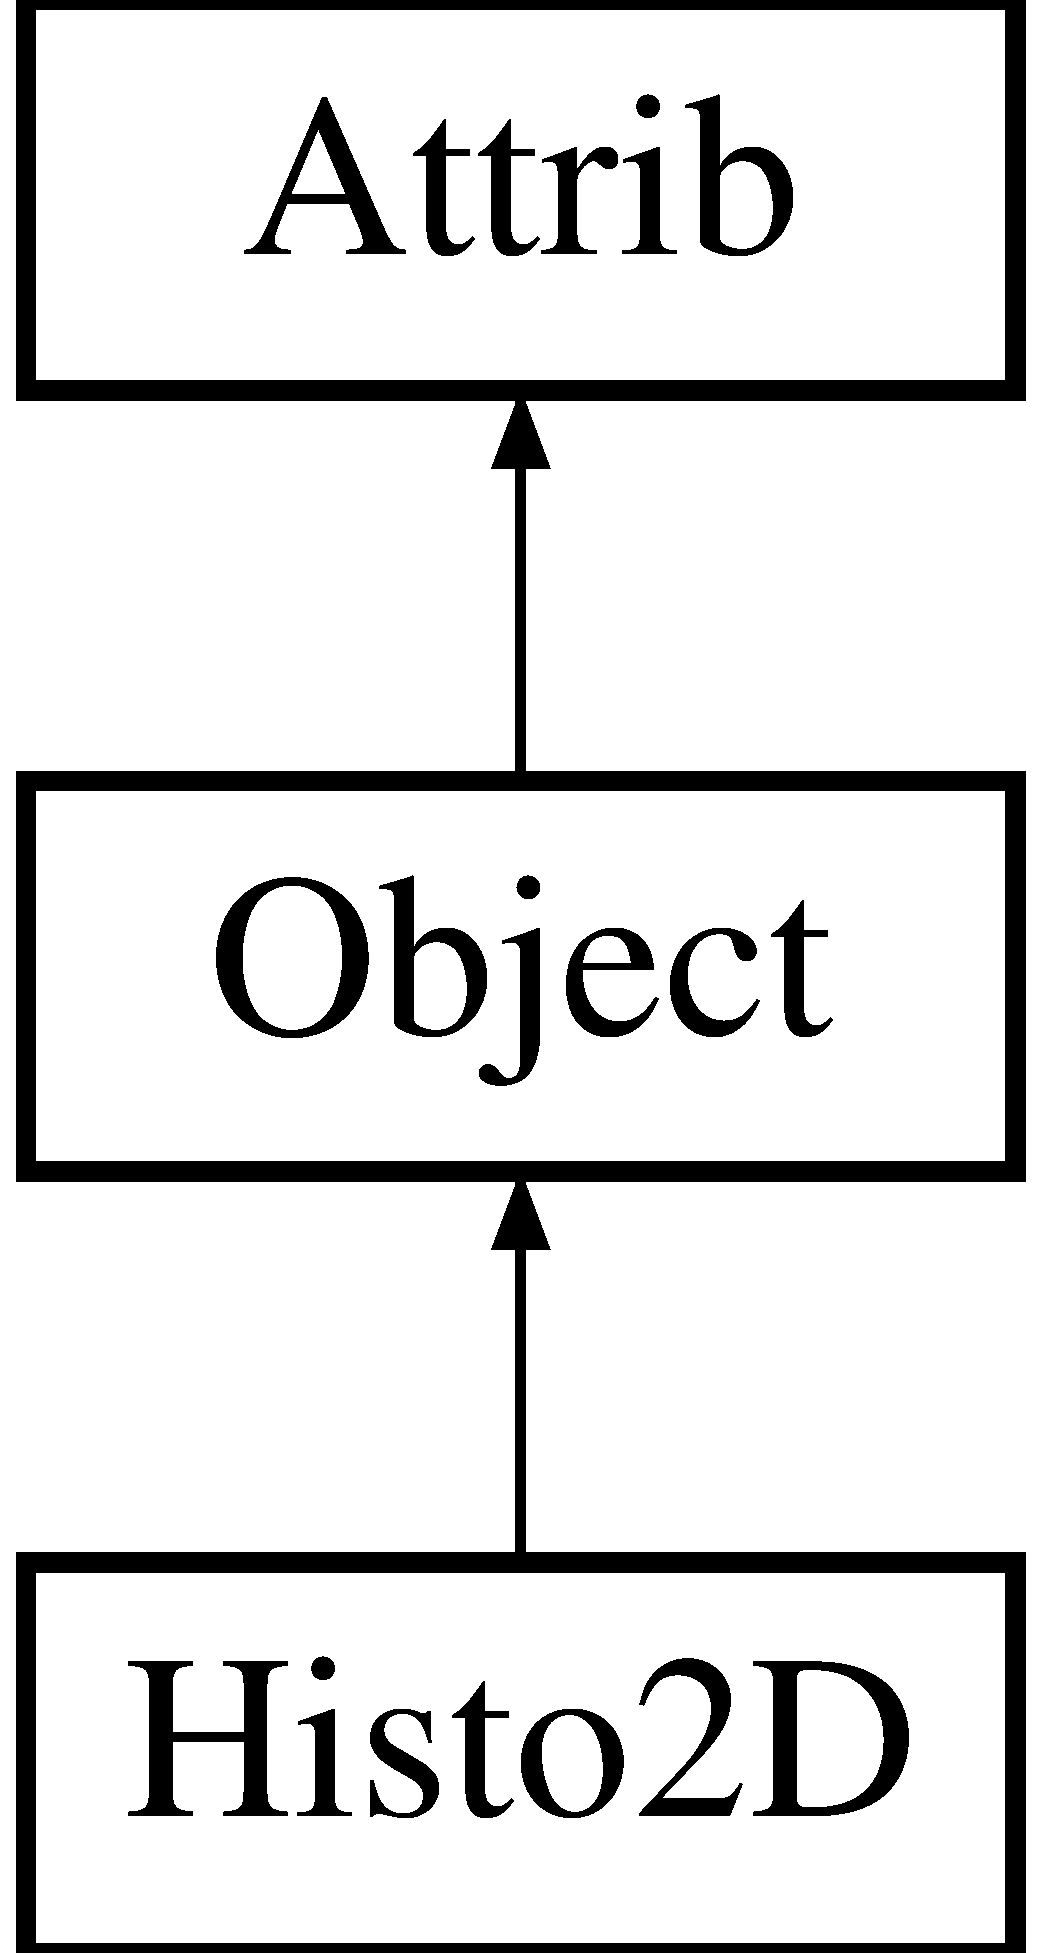
\includegraphics[height=3.000000cm]{classHisto2D}
\end{center}
\end{figure}
\subsection*{Public Member Functions}
\begin{DoxyCompactItemize}
\item 
\hyperlink{classHisto2D_acdeb6b732d7b596dea8a282813cd1c18}{Histo2D} (T\+H2D $\ast$histo)
\item 
\hyperlink{classHisto2D_a4df8112579be6bc1d5652933c73125ae}{$\sim$\+Histo2D} ()
\item 
double \hyperlink{classHisto2D_ae5a3ff63669999c9fda448db61e5bb57}{minX} ()
\item 
double \hyperlink{classHisto2D_aae04c13ac492562532b4d3f82979a0f4}{maxX} ()
\item 
double \hyperlink{classHisto2D_ae946ecc8e7b4efc2e1454cd75c7d8aca}{minY} ()
\item 
double \hyperlink{classHisto2D_a7bfc748b81257716316a38e628c5832f}{maxY} ()
\item 
double \hyperlink{classHisto2D_a68cfc2d92fbc5ce2efa1d6b5781ea621}{minZ} ()
\item 
double \hyperlink{classHisto2D_ad6ccf8ddd4e4b5930f39284059577570}{maxZ} ()
\item 
std\+::vector$<$ double $>$ \hyperlink{classHisto2D_ab3d44a1cb12119a2244065af2b1f7099}{bins} ()
\item 
std\+::vector$<$ double $>$ \hyperlink{classHisto2D_a8f42529a5fba07c339e547bf504dd418}{xbins} ()
\item 
std\+::vector$<$ double $>$ \hyperlink{classHisto2D_a0ae225e33eb9837137b10a159ac1d4f2}{ybins} ()
\item 
unsigned long \hyperlink{classHisto2D_aac422991db96030ce7ca3952e4d277f2}{nxbins} ()
\item 
unsigned long \hyperlink{classHisto2D_a17ee49d9e1c5d62edc887f4f63f68db6}{nybins} ()
\item 
void \hyperlink{classHisto2D_a66875cb46a7e5ff6fa347fe736cbed1b}{statistics} (double \&, double \&, double \&)
\end{DoxyCompactItemize}
\subsection*{Private Attributes}
\begin{DoxyCompactItemize}
\item 
double \hyperlink{classHisto2D_a71dfc840fbaa159ef22091312d1ae5d9}{m\+\_\+zero}
\item 
double \hyperlink{classHisto2D_a3763bdf81d08ba44aa56c0e85de95ff3}{m\+\_\+infini}
\item 
unsigned long \hyperlink{classHisto2D_a39a9d29010bf81c546a1ad1b01f7cb43}{m\+\_\+nxbins}
\item 
unsigned long \hyperlink{classHisto2D_afebeb164369fa9cea59f226d71907e3d}{m\+\_\+nybins}
\item 
std\+::vector$<$ double $>$ \hyperlink{classHisto2D_a84f6c03673499f34b981cdebf69d22aa}{m\+\_\+bins}
\item 
std\+::vector$<$ double $>$ \hyperlink{classHisto2D_aa2e8211f89d086e1c0beaf3b7d18c568}{m\+\_\+xcenters}
\item 
std\+::vector$<$ double $>$ \hyperlink{classHisto2D_a2a431c0f22a038482fc8b3913743f08b}{m\+\_\+ycenters}
\item 
double \hyperlink{classHisto2D_a039d7f45ec8b5b84c1d71f8f87884211}{m\+\_\+minX}
\item 
double \hyperlink{classHisto2D_af428efc9b984006eeba1a216f7d15d6d}{m\+\_\+maxX}
\item 
double \hyperlink{classHisto2D_a5bea9523f4ac077b0cc72cc1b28e0834}{m\+\_\+minY}
\item 
double \hyperlink{classHisto2D_a049044e82d008636040c5c8815cac297}{m\+\_\+maxY}
\item 
double \hyperlink{classHisto2D_a6cfa2290ee0d786b37f7ed08129c60e3}{m\+\_\+minZ}
\item 
double \hyperlink{classHisto2D_a82422535a6aeaf911129c91e0e44e603}{m\+\_\+maxZ}
\item 
double \hyperlink{classHisto2D_a7ab17bc811ce4a5b45ab3779cc8e221a}{m\+\_\+overflow}
\item 
double \hyperlink{classHisto2D_ab21996b2788e5d0e78bb611df3584440}{m\+\_\+underflow}
\item 
double \hyperlink{classHisto2D_ab70be93148e5c9b24e48b60c6b3b5f89}{m\+\_\+content}
\item 
double \hyperlink{classHisto2D_a78286e1d11cc657a5fd1bd1f60c8dff9}{m\+\_\+mean}
\item 
double \hyperlink{classHisto2D_a461938b95bb93a810ae7941a181023cc}{m\+\_\+rms}
\end{DoxyCompactItemize}
\subsection*{Additional Inherited Members}


\subsection{Detailed Description}


Definition at line 28 of file Histo2\+D.\+h.



\subsection{Constructor \& Destructor Documentation}
\mbox{\Hypertarget{classHisto2D_acdeb6b732d7b596dea8a282813cd1c18}\label{classHisto2D_acdeb6b732d7b596dea8a282813cd1c18}} 
\index{Histo2D@{Histo2D}!Histo2D@{Histo2D}}
\index{Histo2D@{Histo2D}!Histo2D@{Histo2D}}
\subsubsection{\texorpdfstring{Histo2\+D()}{Histo2D()}}
{\footnotesize\ttfamily Histo2\+D\+::\+Histo2D (\begin{DoxyParamCaption}\item[{T\+H2D $\ast$}]{histo }\end{DoxyParamCaption})}



Definition at line 22 of file Histo2\+D.\+cpp.



References m\+\_\+bins, m\+\_\+content, m\+\_\+maxX, m\+\_\+maxY, m\+\_\+maxZ, m\+\_\+mean, m\+\_\+minX, m\+\_\+minY, m\+\_\+minZ, m\+\_\+nxbins, m\+\_\+nybins, m\+\_\+rms, m\+\_\+xcenters, m\+\_\+ycenters, and Object\+::set\+Title().


\begin{DoxyCode}
22                               : \hyperlink{classHisto2D_a71dfc840fbaa159ef22091312d1ae5d9}{m\_zero} ( 1.e-30 ) , \hyperlink{classHisto2D_a3763bdf81d08ba44aa56c0e85de95ff3}{m\_infini}(1.e30) \{
23   \textcolor{comment}{//m\_histo = histo; }
24   
25   \hyperlink{classHisto2D_a39a9d29010bf81c546a1ad1b01f7cb43}{m\_nxbins} = histo->GetNbinsX();
26   \hyperlink{classHisto2D_afebeb164369fa9cea59f226d71907e3d}{m\_nybins} = histo->GetNbinsY();
27 
28   \hyperlink{classObject_a89557dbbad5bcaa02652f5d7fa35d20f}{setTitle}(std::string(histo -> GetTitle()));
29   
30   \hyperlink{classHisto2D_a039d7f45ec8b5b84c1d71f8f87884211}{m\_minX} = histo->GetXaxis()->GetXmin();
31   \hyperlink{classHisto2D_af428efc9b984006eeba1a216f7d15d6d}{m\_maxX} = histo->GetXaxis()->GetXmax();
32   \hyperlink{classHisto2D_a5bea9523f4ac077b0cc72cc1b28e0834}{m\_minY} = histo->GetYaxis()->GetXmin();
33   \hyperlink{classHisto2D_a049044e82d008636040c5c8815cac297}{m\_maxY} = histo->GetYaxis()->GetXmax();
34 
35   \hyperlink{classHisto2D_a6cfa2290ee0d786b37f7ed08129c60e3}{m\_minZ} = histo->GetMinimum();
36   \hyperlink{classHisto2D_a82422535a6aeaf911129c91e0e44e603}{m\_maxZ} = histo->GetMaximum();
37 
38   \textcolor{keywordtype}{unsigned} \textcolor{keywordtype}{long} nxbin=0;
39   \textcolor{keywordtype}{unsigned} \textcolor{keywordtype}{long} nybin=0;
40   \textcolor{keywordflow}{for} (nybin=0;nxbin<\hyperlink{classHisto2D_afebeb164369fa9cea59f226d71907e3d}{m\_nybins}; ++nybin)\{
41     \textcolor{comment}{/*}
42 \textcolor{comment}{      std::vector<double> tmpbins;
}
43 \textcolor{comment}{      std::vector<double> tmpxbin;
}
44 \textcolor{comment}{      std::vector<double> tmpybin;
}
45 \textcolor{comment}{    */}
46     \textcolor{keywordflow}{for} (nxbin=0;nxbin<\hyperlink{classHisto2D_a39a9d29010bf81c546a1ad1b01f7cb43}{m\_nxbins}; ++nxbin)\{
47       \hyperlink{classHisto2D_a84f6c03673499f34b981cdebf69d22aa}{m\_bins}.push\_back(histo->GetBinContent(nybin*nxbin+1+2*(nybin-1)));
48       \hyperlink{classHisto2D_aa2e8211f89d086e1c0beaf3b7d18c568}{m\_xcenters}.push\_back(histo->GetXaxis()->GetBinCenter(nxbin+1));
49       \hyperlink{classHisto2D_a2a431c0f22a038482fc8b3913743f08b}{m\_ycenters}.push\_back(histo->GetYaxis()->GetBinCenter(nybin+1));
50     \}
51     \textcolor{comment}{/*}
52 \textcolor{comment}{      m\_bins.push\_back(tmpbins);
}
53 \textcolor{comment}{      m\_xcenters.push\_back(tmpxbin);
}
54 \textcolor{comment}{      m\_ycenters.push\_back(tmpybin);    
}
55 \textcolor{comment}{    */}
56   \}
57   
58   \textcolor{comment}{/*  
}
59 \textcolor{comment}{  m\_underflow = histo->GetBinContent(0);
}
60 \textcolor{comment}{  m\_overflow = histo->GetBinContent(histo->GetNbinsX()+1);  
}
61 \textcolor{comment}{  */}
62 
63   \hyperlink{classHisto2D_ab70be93148e5c9b24e48b60c6b3b5f89}{m\_content} = histo->GetEntries();
64   \hyperlink{classHisto2D_a78286e1d11cc657a5fd1bd1f60c8dff9}{m\_mean}    = histo->GetMean();
65   \hyperlink{classHisto2D_a461938b95bb93a810ae7941a181023cc}{m\_rms}     = histo->GetRMS();
66 \}
\end{DoxyCode}
\mbox{\Hypertarget{classHisto2D_a4df8112579be6bc1d5652933c73125ae}\label{classHisto2D_a4df8112579be6bc1d5652933c73125ae}} 
\index{Histo2D@{Histo2D}!````~Histo2D@{$\sim$\+Histo2D}}
\index{````~Histo2D@{$\sim$\+Histo2D}!Histo2D@{Histo2D}}
\subsubsection{\texorpdfstring{$\sim$\+Histo2\+D()}{~Histo2D()}}
{\footnotesize\ttfamily Histo2\+D\+::$\sim$\+Histo2D (\begin{DoxyParamCaption}{ }\end{DoxyParamCaption})\hspace{0.3cm}{\ttfamily [inline]}}



Definition at line 31 of file Histo2\+D.\+h.


\begin{DoxyCode}
31 \{ \}
\end{DoxyCode}


\subsection{Member Function Documentation}
\mbox{\Hypertarget{classHisto2D_ab3d44a1cb12119a2244065af2b1f7099}\label{classHisto2D_ab3d44a1cb12119a2244065af2b1f7099}} 
\index{Histo2D@{Histo2D}!bins@{bins}}
\index{bins@{bins}!Histo2D@{Histo2D}}
\subsubsection{\texorpdfstring{bins()}{bins()}}
{\footnotesize\ttfamily std\+::vector$<$double$>$ Histo2\+D\+::bins (\begin{DoxyParamCaption}{ }\end{DoxyParamCaption})\hspace{0.3cm}{\ttfamily [inline]}}



Definition at line 72 of file Histo2\+D.\+h.



References m\+\_\+bins.



Referenced by export\+\_\+proc().


\begin{DoxyCode}
72                           \{  
73     \textcolor{keywordflow}{return} \hyperlink{classHisto2D_a84f6c03673499f34b981cdebf69d22aa}{m\_bins};
74   \}
\end{DoxyCode}
\mbox{\Hypertarget{classHisto2D_aae04c13ac492562532b4d3f82979a0f4}\label{classHisto2D_aae04c13ac492562532b4d3f82979a0f4}} 
\index{Histo2D@{Histo2D}!maxX@{maxX}}
\index{maxX@{maxX}!Histo2D@{Histo2D}}
\subsubsection{\texorpdfstring{max\+X()}{maxX()}}
{\footnotesize\ttfamily double Histo2\+D\+::maxX (\begin{DoxyParamCaption}{ }\end{DoxyParamCaption})\hspace{0.3cm}{\ttfamily [inline]}}



Definition at line 39 of file Histo2\+D.\+h.



References m\+\_\+maxX.



Referenced by export\+\_\+proc().


\begin{DoxyCode}
39                \{
40     \textcolor{keywordflow}{return} \hyperlink{classHisto2D_af428efc9b984006eeba1a216f7d15d6d}{m\_maxX};
41   \}
\end{DoxyCode}
\mbox{\Hypertarget{classHisto2D_a7bfc748b81257716316a38e628c5832f}\label{classHisto2D_a7bfc748b81257716316a38e628c5832f}} 
\index{Histo2D@{Histo2D}!maxY@{maxY}}
\index{maxY@{maxY}!Histo2D@{Histo2D}}
\subsubsection{\texorpdfstring{max\+Y()}{maxY()}}
{\footnotesize\ttfamily double Histo2\+D\+::maxY (\begin{DoxyParamCaption}{ }\end{DoxyParamCaption})\hspace{0.3cm}{\ttfamily [inline]}}



Definition at line 47 of file Histo2\+D.\+h.



References m\+\_\+maxY.



Referenced by export\+\_\+proc().


\begin{DoxyCode}
47                \{
48     \textcolor{keywordflow}{return} \hyperlink{classHisto2D_a049044e82d008636040c5c8815cac297}{m\_maxY};
49   \}
\end{DoxyCode}
\mbox{\Hypertarget{classHisto2D_ad6ccf8ddd4e4b5930f39284059577570}\label{classHisto2D_ad6ccf8ddd4e4b5930f39284059577570}} 
\index{Histo2D@{Histo2D}!maxZ@{maxZ}}
\index{maxZ@{maxZ}!Histo2D@{Histo2D}}
\subsubsection{\texorpdfstring{max\+Z()}{maxZ()}}
{\footnotesize\ttfamily double Histo2\+D\+::maxZ (\begin{DoxyParamCaption}{ }\end{DoxyParamCaption})\hspace{0.3cm}{\ttfamily [inline]}}



Definition at line 55 of file Histo2\+D.\+h.



References m\+\_\+maxZ.



Referenced by export\+\_\+proc().


\begin{DoxyCode}
55                \{
56     \textcolor{keywordflow}{return} \hyperlink{classHisto2D_a82422535a6aeaf911129c91e0e44e603}{m\_maxZ};
57   \}
\end{DoxyCode}
\mbox{\Hypertarget{classHisto2D_ae5a3ff63669999c9fda448db61e5bb57}\label{classHisto2D_ae5a3ff63669999c9fda448db61e5bb57}} 
\index{Histo2D@{Histo2D}!minX@{minX}}
\index{minX@{minX}!Histo2D@{Histo2D}}
\subsubsection{\texorpdfstring{min\+X()}{minX()}}
{\footnotesize\ttfamily double Histo2\+D\+::minX (\begin{DoxyParamCaption}{ }\end{DoxyParamCaption})\hspace{0.3cm}{\ttfamily [inline]}}



Definition at line 35 of file Histo2\+D.\+h.



References m\+\_\+minX.



Referenced by export\+\_\+proc().


\begin{DoxyCode}
35                \{
36     \textcolor{keywordflow}{return} \hyperlink{classHisto2D_a039d7f45ec8b5b84c1d71f8f87884211}{m\_minX};
37   \}
\end{DoxyCode}
\mbox{\Hypertarget{classHisto2D_ae946ecc8e7b4efc2e1454cd75c7d8aca}\label{classHisto2D_ae946ecc8e7b4efc2e1454cd75c7d8aca}} 
\index{Histo2D@{Histo2D}!minY@{minY}}
\index{minY@{minY}!Histo2D@{Histo2D}}
\subsubsection{\texorpdfstring{min\+Y()}{minY()}}
{\footnotesize\ttfamily double Histo2\+D\+::minY (\begin{DoxyParamCaption}{ }\end{DoxyParamCaption})\hspace{0.3cm}{\ttfamily [inline]}}



Definition at line 43 of file Histo2\+D.\+h.



References m\+\_\+minY.



Referenced by export\+\_\+proc().


\begin{DoxyCode}
43                \{
44     \textcolor{keywordflow}{return} \hyperlink{classHisto2D_a5bea9523f4ac077b0cc72cc1b28e0834}{m\_minY};
45   \}
\end{DoxyCode}
\mbox{\Hypertarget{classHisto2D_a68cfc2d92fbc5ce2efa1d6b5781ea621}\label{classHisto2D_a68cfc2d92fbc5ce2efa1d6b5781ea621}} 
\index{Histo2D@{Histo2D}!minZ@{minZ}}
\index{minZ@{minZ}!Histo2D@{Histo2D}}
\subsubsection{\texorpdfstring{min\+Z()}{minZ()}}
{\footnotesize\ttfamily double Histo2\+D\+::minZ (\begin{DoxyParamCaption}{ }\end{DoxyParamCaption})\hspace{0.3cm}{\ttfamily [inline]}}



Definition at line 51 of file Histo2\+D.\+h.



References m\+\_\+minZ.



Referenced by export\+\_\+proc().


\begin{DoxyCode}
51                \{
52     \textcolor{keywordflow}{return} \hyperlink{classHisto2D_a6cfa2290ee0d786b37f7ed08129c60e3}{m\_minZ};
53   \}
\end{DoxyCode}
\mbox{\Hypertarget{classHisto2D_aac422991db96030ce7ca3952e4d277f2}\label{classHisto2D_aac422991db96030ce7ca3952e4d277f2}} 
\index{Histo2D@{Histo2D}!nxbins@{nxbins}}
\index{nxbins@{nxbins}!Histo2D@{Histo2D}}
\subsubsection{\texorpdfstring{nxbins()}{nxbins()}}
{\footnotesize\ttfamily unsigned long Histo2\+D\+::nxbins (\begin{DoxyParamCaption}{ }\end{DoxyParamCaption})\hspace{0.3cm}{\ttfamily [inline]}}



Definition at line 84 of file Histo2\+D.\+h.



References m\+\_\+nxbins.



Referenced by export\+\_\+proc().


\begin{DoxyCode}
84                         \{  
85     \textcolor{keywordflow}{return} \hyperlink{classHisto2D_a39a9d29010bf81c546a1ad1b01f7cb43}{m\_nxbins};
86   \}
\end{DoxyCode}
\mbox{\Hypertarget{classHisto2D_a17ee49d9e1c5d62edc887f4f63f68db6}\label{classHisto2D_a17ee49d9e1c5d62edc887f4f63f68db6}} 
\index{Histo2D@{Histo2D}!nybins@{nybins}}
\index{nybins@{nybins}!Histo2D@{Histo2D}}
\subsubsection{\texorpdfstring{nybins()}{nybins()}}
{\footnotesize\ttfamily unsigned long Histo2\+D\+::nybins (\begin{DoxyParamCaption}{ }\end{DoxyParamCaption})\hspace{0.3cm}{\ttfamily [inline]}}



Definition at line 88 of file Histo2\+D.\+h.



References m\+\_\+nybins, and statistics().



Referenced by export\+\_\+proc().


\begin{DoxyCode}
88                         \{  
89     \textcolor{keywordflow}{return} \hyperlink{classHisto2D_afebeb164369fa9cea59f226d71907e3d}{m\_nybins};
90   \}
\end{DoxyCode}
\mbox{\Hypertarget{classHisto2D_a66875cb46a7e5ff6fa347fe736cbed1b}\label{classHisto2D_a66875cb46a7e5ff6fa347fe736cbed1b}} 
\index{Histo2D@{Histo2D}!statistics@{statistics}}
\index{statistics@{statistics}!Histo2D@{Histo2D}}
\subsubsection{\texorpdfstring{statistics()}{statistics()}}
{\footnotesize\ttfamily void Histo2\+D\+::statistics (\begin{DoxyParamCaption}\item[{double \&}]{content,  }\item[{double \&}]{mean,  }\item[{double \&}]{rms }\end{DoxyParamCaption})}



Definition at line 77 of file Histo2\+D.\+cpp.



References m\+\_\+content, m\+\_\+mean, and m\+\_\+rms.



Referenced by nybins().


\begin{DoxyCode}
79                                      \{
80   content=\hyperlink{classHisto2D_ab70be93148e5c9b24e48b60c6b3b5f89}{m\_content};
81   mean   =\hyperlink{classHisto2D_a78286e1d11cc657a5fd1bd1f60c8dff9}{m\_mean};
82   rms    =\hyperlink{classHisto2D_a461938b95bb93a810ae7941a181023cc}{m\_rms};
83 \}
\end{DoxyCode}
\mbox{\Hypertarget{classHisto2D_a8f42529a5fba07c339e547bf504dd418}\label{classHisto2D_a8f42529a5fba07c339e547bf504dd418}} 
\index{Histo2D@{Histo2D}!xbins@{xbins}}
\index{xbins@{xbins}!Histo2D@{Histo2D}}
\subsubsection{\texorpdfstring{xbins()}{xbins()}}
{\footnotesize\ttfamily std\+::vector$<$double$>$ Histo2\+D\+::xbins (\begin{DoxyParamCaption}{ }\end{DoxyParamCaption})\hspace{0.3cm}{\ttfamily [inline]}}



Definition at line 76 of file Histo2\+D.\+h.



References m\+\_\+xcenters.



Referenced by export\+\_\+proc().


\begin{DoxyCode}
76                            \{  
77     \textcolor{keywordflow}{return} \hyperlink{classHisto2D_aa2e8211f89d086e1c0beaf3b7d18c568}{m\_xcenters};
78   \}
\end{DoxyCode}
\mbox{\Hypertarget{classHisto2D_a0ae225e33eb9837137b10a159ac1d4f2}\label{classHisto2D_a0ae225e33eb9837137b10a159ac1d4f2}} 
\index{Histo2D@{Histo2D}!ybins@{ybins}}
\index{ybins@{ybins}!Histo2D@{Histo2D}}
\subsubsection{\texorpdfstring{ybins()}{ybins()}}
{\footnotesize\ttfamily std\+::vector$<$double$>$ Histo2\+D\+::ybins (\begin{DoxyParamCaption}{ }\end{DoxyParamCaption})\hspace{0.3cm}{\ttfamily [inline]}}



Definition at line 80 of file Histo2\+D.\+h.



References m\+\_\+ycenters.



Referenced by export\+\_\+proc().


\begin{DoxyCode}
80                            \{  
81     \textcolor{keywordflow}{return} \hyperlink{classHisto2D_a2a431c0f22a038482fc8b3913743f08b}{m\_ycenters};
82   \}
\end{DoxyCode}


\subsection{Member Data Documentation}
\mbox{\Hypertarget{classHisto2D_a84f6c03673499f34b981cdebf69d22aa}\label{classHisto2D_a84f6c03673499f34b981cdebf69d22aa}} 
\index{Histo2D@{Histo2D}!m\+\_\+bins@{m\+\_\+bins}}
\index{m\+\_\+bins@{m\+\_\+bins}!Histo2D@{Histo2D}}
\subsubsection{\texorpdfstring{m\+\_\+bins}{m\_bins}}
{\footnotesize\ttfamily std\+::vector$<$double$>$ Histo2\+D\+::m\+\_\+bins\hspace{0.3cm}{\ttfamily [private]}}



Definition at line 118 of file Histo2\+D.\+h.



Referenced by bins(), and Histo2\+D().

\mbox{\Hypertarget{classHisto2D_ab70be93148e5c9b24e48b60c6b3b5f89}\label{classHisto2D_ab70be93148e5c9b24e48b60c6b3b5f89}} 
\index{Histo2D@{Histo2D}!m\+\_\+content@{m\+\_\+content}}
\index{m\+\_\+content@{m\+\_\+content}!Histo2D@{Histo2D}}
\subsubsection{\texorpdfstring{m\+\_\+content}{m\_content}}
{\footnotesize\ttfamily double Histo2\+D\+::m\+\_\+content\hspace{0.3cm}{\ttfamily [private]}}



Definition at line 132 of file Histo2\+D.\+h.



Referenced by Histo2\+D(), and statistics().

\mbox{\Hypertarget{classHisto2D_a3763bdf81d08ba44aa56c0e85de95ff3}\label{classHisto2D_a3763bdf81d08ba44aa56c0e85de95ff3}} 
\index{Histo2D@{Histo2D}!m\+\_\+infini@{m\+\_\+infini}}
\index{m\+\_\+infini@{m\+\_\+infini}!Histo2D@{Histo2D}}
\subsubsection{\texorpdfstring{m\+\_\+infini}{m\_infini}}
{\footnotesize\ttfamily double Histo2\+D\+::m\+\_\+infini\hspace{0.3cm}{\ttfamily [private]}}



Definition at line 107 of file Histo2\+D.\+h.

\mbox{\Hypertarget{classHisto2D_af428efc9b984006eeba1a216f7d15d6d}\label{classHisto2D_af428efc9b984006eeba1a216f7d15d6d}} 
\index{Histo2D@{Histo2D}!m\+\_\+maxX@{m\+\_\+maxX}}
\index{m\+\_\+maxX@{m\+\_\+maxX}!Histo2D@{Histo2D}}
\subsubsection{\texorpdfstring{m\+\_\+maxX}{m\_maxX}}
{\footnotesize\ttfamily double Histo2\+D\+::m\+\_\+maxX\hspace{0.3cm}{\ttfamily [private]}}



Definition at line 123 of file Histo2\+D.\+h.



Referenced by Histo2\+D(), and max\+X().

\mbox{\Hypertarget{classHisto2D_a049044e82d008636040c5c8815cac297}\label{classHisto2D_a049044e82d008636040c5c8815cac297}} 
\index{Histo2D@{Histo2D}!m\+\_\+maxY@{m\+\_\+maxY}}
\index{m\+\_\+maxY@{m\+\_\+maxY}!Histo2D@{Histo2D}}
\subsubsection{\texorpdfstring{m\+\_\+maxY}{m\_maxY}}
{\footnotesize\ttfamily double Histo2\+D\+::m\+\_\+maxY\hspace{0.3cm}{\ttfamily [private]}}



Definition at line 125 of file Histo2\+D.\+h.



Referenced by Histo2\+D(), and max\+Y().

\mbox{\Hypertarget{classHisto2D_a82422535a6aeaf911129c91e0e44e603}\label{classHisto2D_a82422535a6aeaf911129c91e0e44e603}} 
\index{Histo2D@{Histo2D}!m\+\_\+maxZ@{m\+\_\+maxZ}}
\index{m\+\_\+maxZ@{m\+\_\+maxZ}!Histo2D@{Histo2D}}
\subsubsection{\texorpdfstring{m\+\_\+maxZ}{m\_maxZ}}
{\footnotesize\ttfamily double Histo2\+D\+::m\+\_\+maxZ\hspace{0.3cm}{\ttfamily [private]}}



Definition at line 127 of file Histo2\+D.\+h.



Referenced by Histo2\+D(), and max\+Z().

\mbox{\Hypertarget{classHisto2D_a78286e1d11cc657a5fd1bd1f60c8dff9}\label{classHisto2D_a78286e1d11cc657a5fd1bd1f60c8dff9}} 
\index{Histo2D@{Histo2D}!m\+\_\+mean@{m\+\_\+mean}}
\index{m\+\_\+mean@{m\+\_\+mean}!Histo2D@{Histo2D}}
\subsubsection{\texorpdfstring{m\+\_\+mean}{m\_mean}}
{\footnotesize\ttfamily double Histo2\+D\+::m\+\_\+mean\hspace{0.3cm}{\ttfamily [private]}}



Definition at line 133 of file Histo2\+D.\+h.



Referenced by Histo2\+D(), and statistics().

\mbox{\Hypertarget{classHisto2D_a039d7f45ec8b5b84c1d71f8f87884211}\label{classHisto2D_a039d7f45ec8b5b84c1d71f8f87884211}} 
\index{Histo2D@{Histo2D}!m\+\_\+minX@{m\+\_\+minX}}
\index{m\+\_\+minX@{m\+\_\+minX}!Histo2D@{Histo2D}}
\subsubsection{\texorpdfstring{m\+\_\+minX}{m\_minX}}
{\footnotesize\ttfamily double Histo2\+D\+::m\+\_\+minX\hspace{0.3cm}{\ttfamily [private]}}



Definition at line 122 of file Histo2\+D.\+h.



Referenced by Histo2\+D(), and min\+X().

\mbox{\Hypertarget{classHisto2D_a5bea9523f4ac077b0cc72cc1b28e0834}\label{classHisto2D_a5bea9523f4ac077b0cc72cc1b28e0834}} 
\index{Histo2D@{Histo2D}!m\+\_\+minY@{m\+\_\+minY}}
\index{m\+\_\+minY@{m\+\_\+minY}!Histo2D@{Histo2D}}
\subsubsection{\texorpdfstring{m\+\_\+minY}{m\_minY}}
{\footnotesize\ttfamily double Histo2\+D\+::m\+\_\+minY\hspace{0.3cm}{\ttfamily [private]}}



Definition at line 124 of file Histo2\+D.\+h.



Referenced by Histo2\+D(), and min\+Y().

\mbox{\Hypertarget{classHisto2D_a6cfa2290ee0d786b37f7ed08129c60e3}\label{classHisto2D_a6cfa2290ee0d786b37f7ed08129c60e3}} 
\index{Histo2D@{Histo2D}!m\+\_\+minZ@{m\+\_\+minZ}}
\index{m\+\_\+minZ@{m\+\_\+minZ}!Histo2D@{Histo2D}}
\subsubsection{\texorpdfstring{m\+\_\+minZ}{m\_minZ}}
{\footnotesize\ttfamily double Histo2\+D\+::m\+\_\+minZ\hspace{0.3cm}{\ttfamily [private]}}



Definition at line 126 of file Histo2\+D.\+h.



Referenced by Histo2\+D(), and min\+Z().

\mbox{\Hypertarget{classHisto2D_a39a9d29010bf81c546a1ad1b01f7cb43}\label{classHisto2D_a39a9d29010bf81c546a1ad1b01f7cb43}} 
\index{Histo2D@{Histo2D}!m\+\_\+nxbins@{m\+\_\+nxbins}}
\index{m\+\_\+nxbins@{m\+\_\+nxbins}!Histo2D@{Histo2D}}
\subsubsection{\texorpdfstring{m\+\_\+nxbins}{m\_nxbins}}
{\footnotesize\ttfamily unsigned long Histo2\+D\+::m\+\_\+nxbins\hspace{0.3cm}{\ttfamily [private]}}



Definition at line 109 of file Histo2\+D.\+h.



Referenced by Histo2\+D(), and nxbins().

\mbox{\Hypertarget{classHisto2D_afebeb164369fa9cea59f226d71907e3d}\label{classHisto2D_afebeb164369fa9cea59f226d71907e3d}} 
\index{Histo2D@{Histo2D}!m\+\_\+nybins@{m\+\_\+nybins}}
\index{m\+\_\+nybins@{m\+\_\+nybins}!Histo2D@{Histo2D}}
\subsubsection{\texorpdfstring{m\+\_\+nybins}{m\_nybins}}
{\footnotesize\ttfamily unsigned long Histo2\+D\+::m\+\_\+nybins\hspace{0.3cm}{\ttfamily [private]}}



Definition at line 110 of file Histo2\+D.\+h.



Referenced by Histo2\+D(), and nybins().

\mbox{\Hypertarget{classHisto2D_a7ab17bc811ce4a5b45ab3779cc8e221a}\label{classHisto2D_a7ab17bc811ce4a5b45ab3779cc8e221a}} 
\index{Histo2D@{Histo2D}!m\+\_\+overflow@{m\+\_\+overflow}}
\index{m\+\_\+overflow@{m\+\_\+overflow}!Histo2D@{Histo2D}}
\subsubsection{\texorpdfstring{m\+\_\+overflow}{m\_overflow}}
{\footnotesize\ttfamily double Histo2\+D\+::m\+\_\+overflow\hspace{0.3cm}{\ttfamily [private]}}



Definition at line 129 of file Histo2\+D.\+h.

\mbox{\Hypertarget{classHisto2D_a461938b95bb93a810ae7941a181023cc}\label{classHisto2D_a461938b95bb93a810ae7941a181023cc}} 
\index{Histo2D@{Histo2D}!m\+\_\+rms@{m\+\_\+rms}}
\index{m\+\_\+rms@{m\+\_\+rms}!Histo2D@{Histo2D}}
\subsubsection{\texorpdfstring{m\+\_\+rms}{m\_rms}}
{\footnotesize\ttfamily double Histo2\+D\+::m\+\_\+rms\hspace{0.3cm}{\ttfamily [private]}}



Definition at line 134 of file Histo2\+D.\+h.



Referenced by Histo2\+D(), and statistics().

\mbox{\Hypertarget{classHisto2D_ab21996b2788e5d0e78bb611df3584440}\label{classHisto2D_ab21996b2788e5d0e78bb611df3584440}} 
\index{Histo2D@{Histo2D}!m\+\_\+underflow@{m\+\_\+underflow}}
\index{m\+\_\+underflow@{m\+\_\+underflow}!Histo2D@{Histo2D}}
\subsubsection{\texorpdfstring{m\+\_\+underflow}{m\_underflow}}
{\footnotesize\ttfamily double Histo2\+D\+::m\+\_\+underflow\hspace{0.3cm}{\ttfamily [private]}}



Definition at line 130 of file Histo2\+D.\+h.

\mbox{\Hypertarget{classHisto2D_aa2e8211f89d086e1c0beaf3b7d18c568}\label{classHisto2D_aa2e8211f89d086e1c0beaf3b7d18c568}} 
\index{Histo2D@{Histo2D}!m\+\_\+xcenters@{m\+\_\+xcenters}}
\index{m\+\_\+xcenters@{m\+\_\+xcenters}!Histo2D@{Histo2D}}
\subsubsection{\texorpdfstring{m\+\_\+xcenters}{m\_xcenters}}
{\footnotesize\ttfamily std\+::vector$<$double$>$ Histo2\+D\+::m\+\_\+xcenters\hspace{0.3cm}{\ttfamily [private]}}



Definition at line 119 of file Histo2\+D.\+h.



Referenced by Histo2\+D(), and xbins().

\mbox{\Hypertarget{classHisto2D_a2a431c0f22a038482fc8b3913743f08b}\label{classHisto2D_a2a431c0f22a038482fc8b3913743f08b}} 
\index{Histo2D@{Histo2D}!m\+\_\+ycenters@{m\+\_\+ycenters}}
\index{m\+\_\+ycenters@{m\+\_\+ycenters}!Histo2D@{Histo2D}}
\subsubsection{\texorpdfstring{m\+\_\+ycenters}{m\_ycenters}}
{\footnotesize\ttfamily std\+::vector$<$double$>$ Histo2\+D\+::m\+\_\+ycenters\hspace{0.3cm}{\ttfamily [private]}}



Definition at line 120 of file Histo2\+D.\+h.



Referenced by Histo2\+D(), and ybins().

\mbox{\Hypertarget{classHisto2D_a71dfc840fbaa159ef22091312d1ae5d9}\label{classHisto2D_a71dfc840fbaa159ef22091312d1ae5d9}} 
\index{Histo2D@{Histo2D}!m\+\_\+zero@{m\+\_\+zero}}
\index{m\+\_\+zero@{m\+\_\+zero}!Histo2D@{Histo2D}}
\subsubsection{\texorpdfstring{m\+\_\+zero}{m\_zero}}
{\footnotesize\ttfamily double Histo2\+D\+::m\+\_\+zero\hspace{0.3cm}{\ttfamily [private]}}



Definition at line 106 of file Histo2\+D.\+h.



The documentation for this class was generated from the following files\+:\begin{DoxyCompactItemize}
\item 
/home/eleclhcb/\+L\+H\+Cb/lbcat-\/cmake/\+Cat\+Kernel/inc/\hyperlink{Histo2D_8h}{Histo2\+D.\+h}\item 
/home/eleclhcb/\+L\+H\+Cb/lbcat-\/cmake/\+Cat\+Kernel/src/\hyperlink{Histo2D_8cpp}{Histo2\+D.\+cpp}\end{DoxyCompactItemize}

\hypertarget{classICECALv3}{}\section{I\+C\+E\+C\+A\+Lv3 Class Reference}
\label{classICECALv3}\index{I\+C\+E\+C\+A\+Lv3@{I\+C\+E\+C\+A\+Lv3}}


{\ttfamily \#include $<$I\+C\+E\+C\+A\+Lv3.\+h$>$}

Inheritance diagram for I\+C\+E\+C\+A\+Lv3\+:\begin{figure}[H]
\begin{center}
\leavevmode
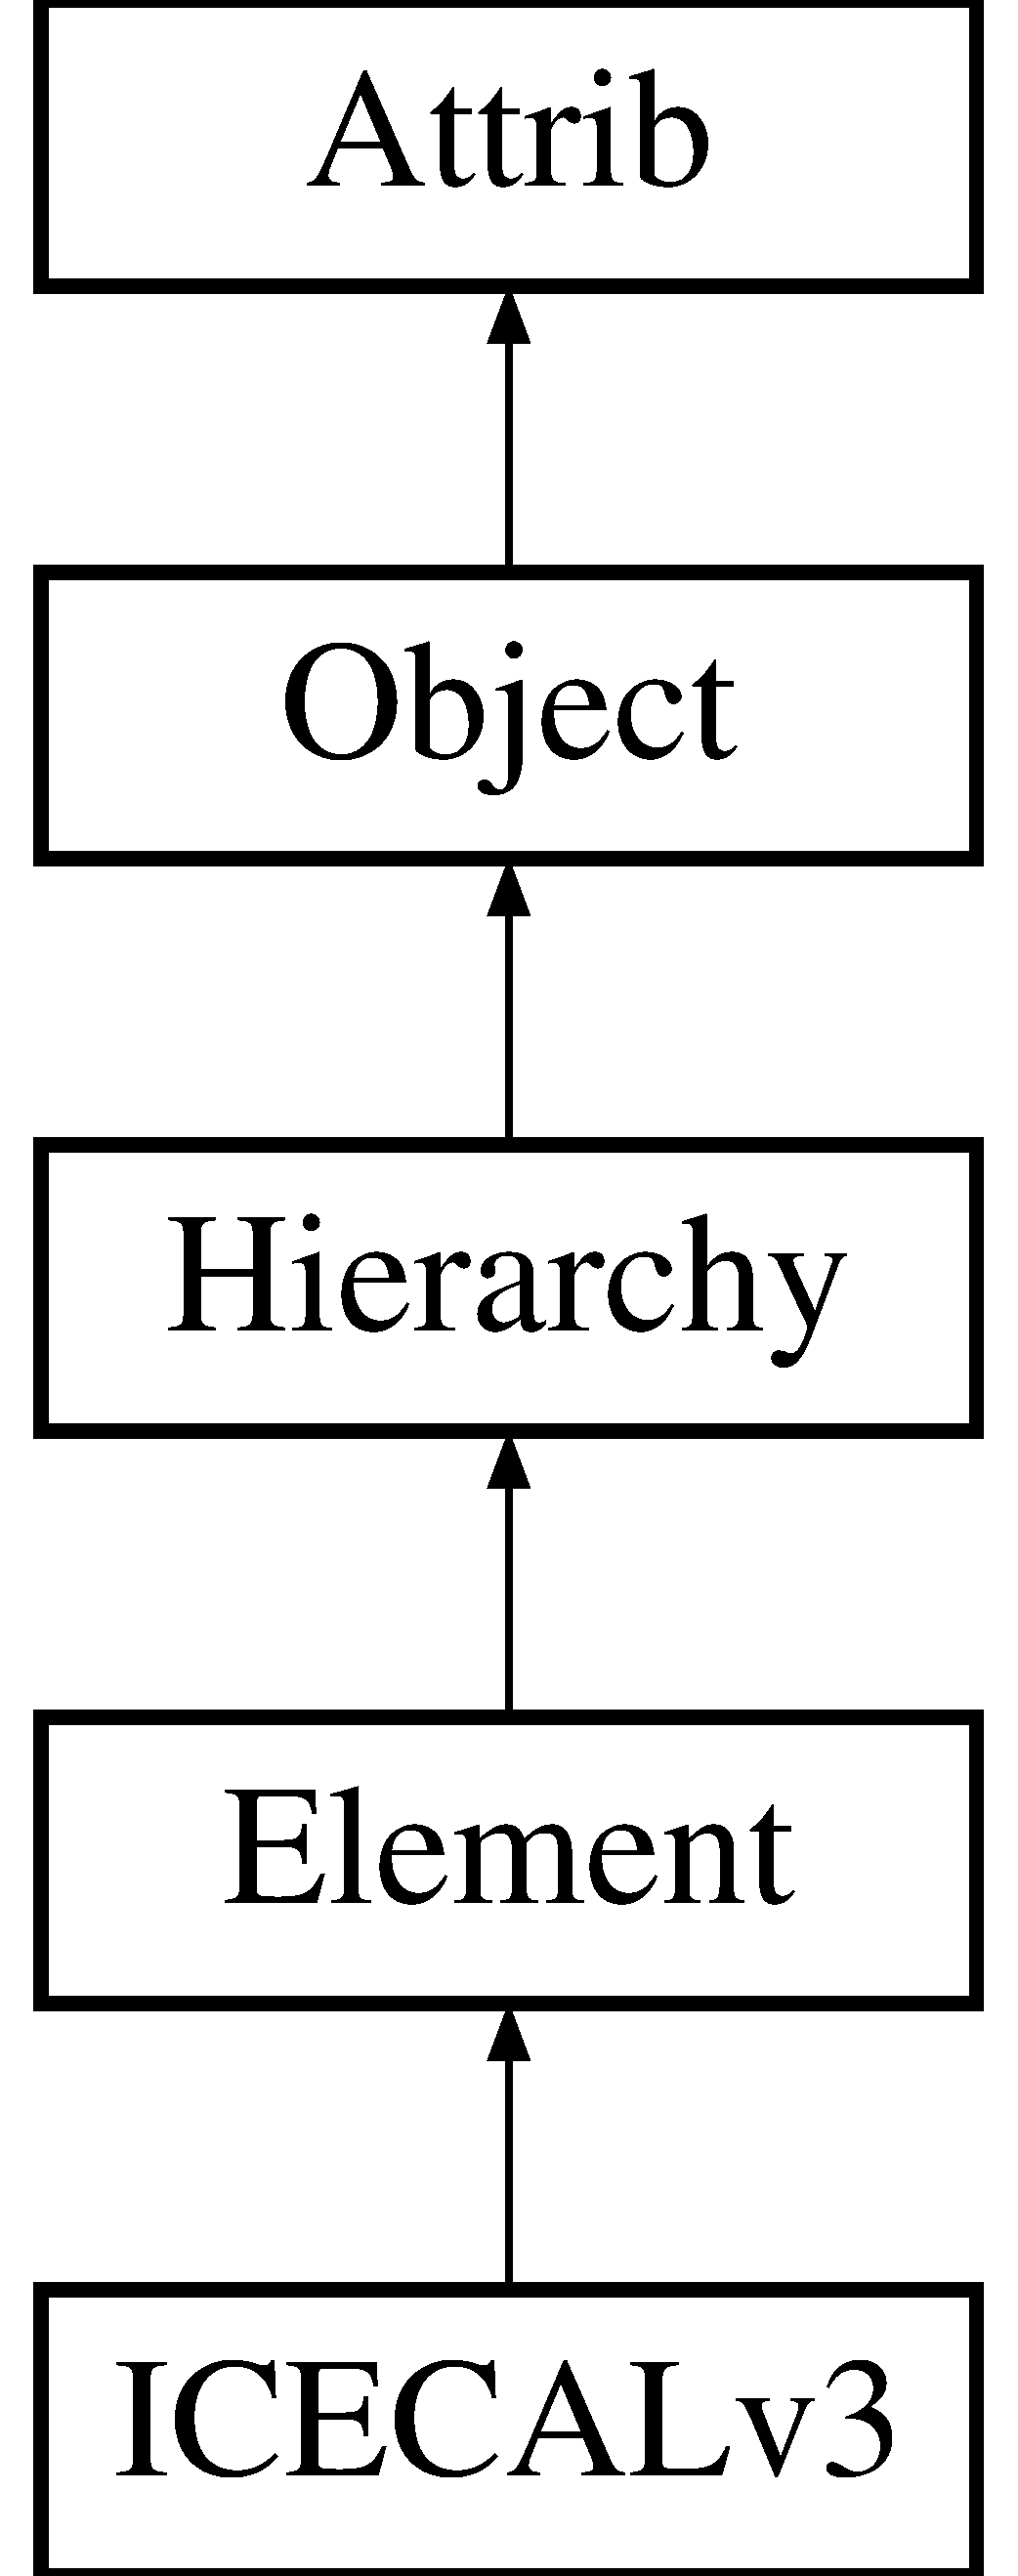
\includegraphics[height=5.000000cm]{classICECALv3}
\end{center}
\end{figure}
\subsection*{Public Types}
\begin{DoxyCompactItemize}
\item 
enum \hyperlink{classAttrib_a69e171d7cc6417835a5a306d3c764235}{Attribut} \{ \newline
\hyperlink{classAttrib_a69e171d7cc6417835a5a306d3c764235a3a8da2ab97dda18aebab196fe4100531}{U\+N\+D\+E\+F\+I\+N\+ED}, 
\hyperlink{classAttrib_a69e171d7cc6417835a5a306d3c764235a2bfb2af57b87031d190a05fe25dd92ed}{P\+A\+S\+S\+I\+VE}, 
\hyperlink{classAttrib_a69e171d7cc6417835a5a306d3c764235a3b1fec929c0370d1436f2f06e298fb0d}{A\+C\+T\+I\+VE}, 
\hyperlink{classAttrib_a69e171d7cc6417835a5a306d3c764235aa27c16b480a369ea4d18b07b2516bbc7}{I\+N\+T\+E\+R\+F\+A\+CE}, 
\newline
\hyperlink{classAttrib_a69e171d7cc6417835a5a306d3c764235a1420a5b8c0540b2af210b6975eded7f9}{IO}, 
\hyperlink{classAttrib_a69e171d7cc6417835a5a306d3c764235a0af3b0d0ac323c1704e6c69cf90add28}{I\+O\+D\+A\+TA}, 
\hyperlink{classAttrib_a69e171d7cc6417835a5a306d3c764235a7788bc5dd333fd8ce18562b269c9dab1}{E\+L\+E\+M\+E\+NT}, 
\hyperlink{classAttrib_a69e171d7cc6417835a5a306d3c764235a61ceb22149f365f1780d18f9d1459423}{H\+A\+R\+D\+W\+A\+RE}, 
\newline
\hyperlink{classAttrib_a69e171d7cc6417835a5a306d3c764235a75250e29692496e73effca2c0330977f}{P\+R\+O\+C\+E\+S\+S\+US}, 
\hyperlink{classAttrib_a69e171d7cc6417835a5a306d3c764235a103a67cd0b8f07ef478fa45d4356e27b}{S\+O\+F\+T\+W\+A\+RE}
 \}
\end{DoxyCompactItemize}
\subsection*{Public Member Functions}
\begin{DoxyCompactItemize}
\item 
\hyperlink{classICECALv3_a0a8b12d2b6bafca9cd820301fc93dff8}{I\+C\+E\+C\+A\+Lv3} ()
\item 
void \hyperlink{classICECALv3_aaf38119f47401a85022ae1b0d05675bd}{set\+Address} (\hyperlink{ICECALv3_8h_a3cb25ca6f51f003950f9625ff05536fc}{U8} address)
\item 
void \hyperlink{classICECALv3_aae0b7539c0bba5311aab99e000d1be6d}{set\+N\+Retries} (int n\+Ret)
\item 
void \hyperlink{classICECALv3_a1b9ca0e09d45634a70da6f19a7257314}{reset\+Pumps} ()
\item 
void \hyperlink{classICECALv3_a5ce36881aa89fedf7c37e03620acca6e}{bypass\+Miso\+Mosi} (\hyperlink{ICECALv3_8h_adf928e51a60dba0df29d615401cc55a8}{U16} write\+Data)
\item 
Py\+Object $\ast$ \hyperlink{classICECALv3_a7a1c1706a455903f42bb9a5257d94a78}{get\+Delay\+Line\+Ch} (int ch)
\item 
\hyperlink{classStatusCode}{Status\+Code} \hyperlink{classICECALv3_a14a7a29c9a3412c062f053cc616b860a}{set\+Delay\+Line\+Ch} (int ch, Py\+Object $\ast$)
\item 
Py\+Object $\ast$ \hyperlink{classICECALv3_a5f1414e6049a82eafdd505a88d7d0c91}{get\+Analog\+Ch} (int ch)
\item 
\hyperlink{classStatusCode}{Status\+Code} \hyperlink{classICECALv3_a9578e4d13c250d8bc417f68c79d6a21d}{set\+Analog\+Ch} (int ch, Py\+Object $\ast$)
\item 
Py\+Object $\ast$ \hyperlink{classICECALv3_a4a414d23c1e199b446dc876161338148}{get\+Main\+Reg} ()
\item 
\hyperlink{classStatusCode}{Status\+Code} \hyperlink{classICECALv3_a479f7e17669da4b785af840049d39cb4}{set\+Main\+Reg} (Py\+Object $\ast$)
\item 
Py\+Object $\ast$ \hyperlink{classICECALv3_a8639cf6a44cba85b53128b5e1dc21e15}{spi\+F\+E\+R\+Test} (long n\+Test)
\item 
\hyperlink{classStatusCode}{Status\+Code} \hyperlink{classICECALv3_ac26be912fb72e615106fceb4626aa548}{dump\+Config} (string config\+File, Py\+Object $\ast$chip\+Id)
\item 
Py\+Object $\ast$ \hyperlink{classICECALv3_a514456dd303e897aa1b55dccf3fa66d0}{load\+Config} (string config\+File)
\item 
double \hyperlink{classICECALv3_a7f3f8012d2e5c45f8e43819befa3f915}{version} ()
\item 
bool \hyperlink{classICECALv3_a545f51b915a6de5c5f450622d0651a85}{bxid\+Resynch\+Status} ()
\item 
void \hyperlink{classICECALv3_acbf1a7a8510d7e02280bacc58badf4f4}{spi\+Address\+Scan} ()
\item 
\hyperlink{classICECALv3_acdadf9483fc38a615192de41548024a1}{$\sim$\+I\+C\+E\+C\+A\+Lv3} ()
\item 
void \hyperlink{classICECALv3_a00e572849b4952e7cf04a39f992df037}{help} ()
\item 
\hyperlink{classStatusCode}{Status\+Code} \hyperlink{classICECALv3_abf7281fad80b80b70c5b13ce66ba3451}{init} ()
\item 
void \hyperlink{classICECALv3_a33afc7c8e0f399336152abd03cbe8d1b}{reset} ()
\item 
void \hyperlink{classICECALv3_ab2a00809e9a4f2ab83ef041a886ca637}{update} ()
\item 
void \hyperlink{classElement_a3c0abcb36f8906688bb7e32608df7086}{recursive\+Init\+Element} ()
\item 
void \hyperlink{classElement_a82119ed37dff76508a2746a853ec35ba}{recursive\+Init\+Communications} ()
\item 
\hyperlink{classStatusCode}{Status\+Code} \hyperlink{classElement_ab476b4b1df5954141ceb14f072433b89}{set\+Connection} (\hyperlink{classHierarchy}{Hierarchy} $\ast$)
\item 
\hyperlink{classHierarchy}{Hierarchy} $\ast$ \hyperlink{classElement_af57444353c1ddf9fa0109801e97debf7}{connection} ()
\item 
void \hyperlink{classHierarchy_af4d43b0765b402670eed2d62c73405af}{clear} ()
\item 
void \hyperlink{classHierarchy_a585ad1aeec16077a0e532ab8b4fc557b}{set\+Parent} (\hyperlink{classHierarchy}{Hierarchy} $\ast$\hyperlink{classHierarchy_a1c7bec8257e717f9c1465e06ebf845fc}{parent})
\item 
\hyperlink{classHierarchy}{Hierarchy} $\ast$ \hyperlink{classHierarchy_a1c7bec8257e717f9c1465e06ebf845fc}{parent} ()
\item 
\hyperlink{classHierarchy}{Hierarchy} $\ast$ \hyperlink{classHierarchy_ad550588733bf75ac5c0fcfd7c8fd11a6}{parent} (std\+::string)
\item 
\hyperlink{classHierarchy}{Hierarchy} $\ast$ \hyperlink{classHierarchy_aee461dc930ce3871636ff87f075b1b83}{origin} ()
\item 
virtual void \hyperlink{classHierarchy_ad677774ff38fcb257c04a3a10d471fac}{add\+Child} (\hyperlink{classHierarchy}{Hierarchy} $\ast$element)
\item 
std\+::vector$<$ \hyperlink{classHierarchy}{Hierarchy} $\ast$ $>$ \hyperlink{classHierarchy_aa9a76f69e98e052ee1a6e32cea006288}{children} ()
\item 
\hyperlink{classHierarchy}{Hierarchy} $\ast$ \hyperlink{classHierarchy_a1e207f973c694b538bf90107b4868817}{child} (std\+::string)
\item 
\hyperlink{classHierarchy}{Hierarchy} $\ast$ \hyperlink{classHierarchy_a0c15a5276a3b80b4354d6bd8a01e0708}{child\+Typed} (std\+::string)
\item 
unsigned long \hyperlink{classHierarchy_ab16e84de65fd84e14001a6cf941c8be4}{number\+Of\+Children} ()
\item 
bool \hyperlink{classHierarchy_a255174fe4d316d2a3f430dcb9dab29f1}{has\+Children} ()
\item 
void \hyperlink{classHierarchy_a2b2b359fac003233f65786a616766bde}{del\+Child} (\hyperlink{classHierarchy}{Hierarchy} $\ast$)
\item 
void \hyperlink{classHierarchy_a1928ac7615fe0b5e55cd707f70dc6781}{del\+Child} (std\+::string)
\item 
std\+::string \hyperlink{classHierarchy_aa7990fa7caf132d83e361ce033c6c65a}{path} (std\+::string=std\+::string(\char`\"{}\char`\"{}))
\item 
std\+::string \hyperlink{classHierarchy_a1efd56cd164d328d2002e53a10a19b8c}{path\+Typed} (std\+::string=std\+::string(\char`\"{}\char`\"{}))
\item 
void \hyperlink{classHierarchy_a76e914b9a677a22a82deb74d892bf261}{tree} (std\+::string indent=std\+::string(\char`\"{}\char`\"{}))
\item 
void \hyperlink{classHierarchy_a594c294c5f60c230e106d522ed008212}{tree} ()
\item 
std\+::string \hyperlink{classObject_a300f4c05dd468c7bb8b3c968868443c1}{name} () const
\item 
std\+::string \hyperlink{classObject_a84f99f70f144a83e1582d1d0f84e4e62}{type} ()
\item 
unsigned char \hyperlink{classObject_af99145335cc61ff6e2798ea17db009d2}{id} ()
\item 
std\+::string \hyperlink{classObject_a73a0f1a41828fdd8303dd662446fb6c3}{title} ()
\item 
void \hyperlink{classObject_a3f9d5537ebce0c0f2bf6ae4d92426f3c}{msg\+Svc} (int level, std\+::string \hyperlink{classObject_a58b2d0618c2d08cf2383012611528d97}{msg}, std\+::string \hyperlink{classObject_a300f4c05dd468c7bb8b3c968868443c1}{name})
\item 
void \hyperlink{classObject_a58b2d0618c2d08cf2383012611528d97}{msg} (std\+::string mymsg)
\item 
void \hyperlink{classObject_ac5d59299273cee27aacf7de00d2e7034}{msg} (std\+::string mymsg, std\+::string \hyperlink{classObject_a300f4c05dd468c7bb8b3c968868443c1}{name})
\item 
void \hyperlink{classObject_a83d2db2df682907ea1115ad721c1c4a1}{verbose} (std\+::string mymsg)
\item 
void \hyperlink{classObject_a2d4120195317e2a3c6532e8bb9f3da68}{verbose} (std\+::string mymsg, std\+::string \hyperlink{classObject_a300f4c05dd468c7bb8b3c968868443c1}{name})
\item 
void \hyperlink{classObject_aac010553f022165573714b7014a15f0d}{debug} (std\+::string mymsg)
\item 
void \hyperlink{classObject_a6c9a0397ca804e04d675ed05683f5420}{debug} (std\+::string mymsg, std\+::string \hyperlink{classObject_a300f4c05dd468c7bb8b3c968868443c1}{name})
\item 
void \hyperlink{classObject_a644fd329ea4cb85f54fa6846484b84a8}{info} (std\+::string mymsg)
\item 
void \hyperlink{classObject_a1ca123253dfd30fc28b156f521dcbdae}{info} (std\+::string mymsg, std\+::string \hyperlink{classObject_a300f4c05dd468c7bb8b3c968868443c1}{name})
\item 
void \hyperlink{classObject_a65cd4fda577711660821fd2cd5a3b4c9}{warning} (std\+::string mymsg)
\item 
void \hyperlink{classObject_a11f101db4dd73d9391b0231818881d86}{warning} (std\+::string mymsg, std\+::string \hyperlink{classObject_a300f4c05dd468c7bb8b3c968868443c1}{name})
\item 
void \hyperlink{classObject_a204a95f57818c0f811933917a30eff45}{error} (std\+::string mymsg)
\item 
void \hyperlink{classObject_ad7f6c457733082efa2f9ff5f5c8e119a}{error} (std\+::string mymsg, std\+::string \hyperlink{classObject_a300f4c05dd468c7bb8b3c968868443c1}{name})
\item 
void \hyperlink{classObject_aad5a16aac7516ce65bd5ec02ab07fc80}{fatal} (std\+::string mymsg)
\item 
void \hyperlink{classObject_ae62acd3d09f716220f75f252dc38bc9a}{fatal} (std\+::string mymsg, std\+::string \hyperlink{classObject_a300f4c05dd468c7bb8b3c968868443c1}{name})
\item 
void \hyperlink{classObject_ae30fea75683c2d149b6b6d17c09ecd0c}{set\+Name} (std\+::string \hyperlink{classObject_a300f4c05dd468c7bb8b3c968868443c1}{name})
\item 
void \hyperlink{classObject_aae534cc9d982bcb9b99fd505f2e103a5}{set\+Type} (std\+::string \hyperlink{classObject_a84f99f70f144a83e1582d1d0f84e4e62}{type})
\item 
void \hyperlink{classObject_a398fe08cba594a0ce6891d59fe4f159f}{set\+Id} (unsigned char \hyperlink{classObject_af99145335cc61ff6e2798ea17db009d2}{id})
\item 
void \hyperlink{classObject_a89557dbbad5bcaa02652f5d7fa35d20f}{set\+Title} (std\+::string \hyperlink{classObject_a73a0f1a41828fdd8303dd662446fb6c3}{title})
\item 
void \hyperlink{classObject_a870c5af919958c2136623b2d7816d123}{set\+Dll\+Name} (std\+::string \hyperlink{classObject_a2e3947f2870094c332d7454117f3ec63}{dll\+Name})
\item 
std\+::string \hyperlink{classObject_a2e3947f2870094c332d7454117f3ec63}{dll\+Name} ()
\item 
bool \hyperlink{classAttrib_a704f26af560909ad22065083bb7d4c34}{is} (int attribut)
\item 
void \hyperlink{classAttrib_a235f773af19c900264a190b00a3b4ad7}{add} (int attribut)
\item 
void \hyperlink{classAttrib_a7d4ef7e32d93cb287792b87b857e79f3}{remove} (int attribut)
\item 
std\+::string \hyperlink{classAttrib_aee7bbf16b144887f196e1341b24f8a26}{attributs} ()
\end{DoxyCompactItemize}
\subsection*{Protected Attributes}
\begin{DoxyCompactItemize}
\item 
\hyperlink{classHierarchy}{Hierarchy} $\ast$ \hyperlink{classElement_abe3de7a5dbbc9a6dd2d7e012e5fdb266}{m\+\_\+connection}
\item 
std\+::string \hyperlink{classAttrib_a3414521d7a82476e874b25a5407b5e63}{m\+\_\+attrib\+String} \mbox{[}10\mbox{]}
\end{DoxyCompactItemize}
\subsection*{Private Member Functions}
\begin{DoxyCompactItemize}
\item 
\hyperlink{ICECALv3_8h_adf928e51a60dba0df29d615401cc55a8}{U16} \hyperlink{classICECALv3_aced41ce20a0853d6248b8df88412e57a}{spi\+Read} (\hyperlink{ICECALv3_8h_a3cb25ca6f51f003950f9625ff05536fc}{U8} conf\+Reg\+Addr, \hyperlink{ICECALv3_8h_a3cb25ca6f51f003950f9625ff05536fc}{U8} offset\+Addr=128)
\item 
void \hyperlink{classICECALv3_aef00f02801dea4bda2093c930501dcdd}{spi\+Write} (\hyperlink{ICECALv3_8h_a3cb25ca6f51f003950f9625ff05536fc}{U8} conf\+Reg\+Addr, \hyperlink{ICECALv3_8h_adf928e51a60dba0df29d615401cc55a8}{U16} \hyperlink{structconfRegData}{conf\+Reg\+Data})
\item 
bool \hyperlink{classICECALv3_aa0b8358ea0be8e47a8aded5e1551787f}{spi\+Write\+Safe} (\hyperlink{ICECALv3_8h_a3cb25ca6f51f003950f9625ff05536fc}{U8} conf\+Reg\+Addr, \hyperlink{ICECALv3_8h_adf928e51a60dba0df29d615401cc55a8}{U16} \hyperlink{structconfRegData}{conf\+Reg\+Data})
\item 
bool \hyperlink{classICECALv3_a9d7c33e6d113e7f721dc848d28ab44d8}{write\+Asic\+Params} (string file\+Name, Py\+Object $\ast$params)
\item 
int \hyperlink{classICECALv3_a313e8166af1ce26b4026f883ad900fb9}{parse\+Parameter\+List} (string config\+File, string param\+Name\mbox{[}64\mbox{]}, int param\+Value\mbox{[}64\mbox{]})
\item 
Py\+Object $\ast$ \hyperlink{classICECALv3_ac006abc42a048308427f6801d783a407}{fill\+Params} (string param\+List\+Ret\mbox{[}$\,$\mbox{]}, int param\+List\+Len, string param\+Name\mbox{[}64\mbox{]}, int param\+Value\mbox{[}64\mbox{]}, int file\+Param\+Len)
\item 
bool \hyperlink{classICECALv3_a8753a74558f988b346a3fe350c5bbad4}{check\+Ch\+Number} (int ch)
\item 
std\+::string \hyperlink{classICECALv3_a04b02e583f191bfce34d05132cd23834}{itohs} (int value)
\end{DoxyCompactItemize}
\subsection*{Private Attributes}
\begin{DoxyCompactItemize}
\item 
\hyperlink{classRegister}{Register} $\ast$ \hyperlink{classICECALv3_a6e8b6c03f5b0f1d8281bf8a0fa46064f}{conf\+Reg}
\item 
int \hyperlink{classICECALv3_ae877ce34b3a4d6c368cc6409ac9614fa}{n\+Retries}
\item 
bool \hyperlink{classICECALv3_ad8989925ee5b3ff322d863ce6aaff0bd}{err}
\end{DoxyCompactItemize}


\subsection{Detailed Description}


Definition at line 58 of file I\+C\+E\+C\+A\+Lv3.\+h.



\subsection{Member Enumeration Documentation}
\mbox{\Hypertarget{classAttrib_a69e171d7cc6417835a5a306d3c764235}\label{classAttrib_a69e171d7cc6417835a5a306d3c764235}} 
\index{I\+C\+E\+C\+A\+Lv3@{I\+C\+E\+C\+A\+Lv3}!Attribut@{Attribut}}
\index{Attribut@{Attribut}!I\+C\+E\+C\+A\+Lv3@{I\+C\+E\+C\+A\+Lv3}}
\subsubsection{\texorpdfstring{Attribut}{Attribut}}
{\footnotesize\ttfamily enum \hyperlink{classAttrib_a69e171d7cc6417835a5a306d3c764235}{Attrib\+::\+Attribut}\hspace{0.3cm}{\ttfamily [inherited]}}

\begin{DoxyEnumFields}{Enumerator}
\raisebox{\heightof{T}}[0pt][0pt]{\index{U\+N\+D\+E\+F\+I\+N\+ED@{U\+N\+D\+E\+F\+I\+N\+ED}!I\+C\+E\+C\+A\+Lv3@{I\+C\+E\+C\+A\+Lv3}}\index{I\+C\+E\+C\+A\+Lv3@{I\+C\+E\+C\+A\+Lv3}!U\+N\+D\+E\+F\+I\+N\+ED@{U\+N\+D\+E\+F\+I\+N\+ED}}}\mbox{\Hypertarget{classAttrib_a69e171d7cc6417835a5a306d3c764235a3a8da2ab97dda18aebab196fe4100531}\label{classAttrib_a69e171d7cc6417835a5a306d3c764235a3a8da2ab97dda18aebab196fe4100531}} 
U\+N\+D\+E\+F\+I\+N\+ED&\\
\hline

\raisebox{\heightof{T}}[0pt][0pt]{\index{P\+A\+S\+S\+I\+VE@{P\+A\+S\+S\+I\+VE}!I\+C\+E\+C\+A\+Lv3@{I\+C\+E\+C\+A\+Lv3}}\index{I\+C\+E\+C\+A\+Lv3@{I\+C\+E\+C\+A\+Lv3}!P\+A\+S\+S\+I\+VE@{P\+A\+S\+S\+I\+VE}}}\mbox{\Hypertarget{classAttrib_a69e171d7cc6417835a5a306d3c764235a2bfb2af57b87031d190a05fe25dd92ed}\label{classAttrib_a69e171d7cc6417835a5a306d3c764235a2bfb2af57b87031d190a05fe25dd92ed}} 
P\+A\+S\+S\+I\+VE&\\
\hline

\raisebox{\heightof{T}}[0pt][0pt]{\index{A\+C\+T\+I\+VE@{A\+C\+T\+I\+VE}!I\+C\+E\+C\+A\+Lv3@{I\+C\+E\+C\+A\+Lv3}}\index{I\+C\+E\+C\+A\+Lv3@{I\+C\+E\+C\+A\+Lv3}!A\+C\+T\+I\+VE@{A\+C\+T\+I\+VE}}}\mbox{\Hypertarget{classAttrib_a69e171d7cc6417835a5a306d3c764235a3b1fec929c0370d1436f2f06e298fb0d}\label{classAttrib_a69e171d7cc6417835a5a306d3c764235a3b1fec929c0370d1436f2f06e298fb0d}} 
A\+C\+T\+I\+VE&\\
\hline

\raisebox{\heightof{T}}[0pt][0pt]{\index{I\+N\+T\+E\+R\+F\+A\+CE@{I\+N\+T\+E\+R\+F\+A\+CE}!I\+C\+E\+C\+A\+Lv3@{I\+C\+E\+C\+A\+Lv3}}\index{I\+C\+E\+C\+A\+Lv3@{I\+C\+E\+C\+A\+Lv3}!I\+N\+T\+E\+R\+F\+A\+CE@{I\+N\+T\+E\+R\+F\+A\+CE}}}\mbox{\Hypertarget{classAttrib_a69e171d7cc6417835a5a306d3c764235aa27c16b480a369ea4d18b07b2516bbc7}\label{classAttrib_a69e171d7cc6417835a5a306d3c764235aa27c16b480a369ea4d18b07b2516bbc7}} 
I\+N\+T\+E\+R\+F\+A\+CE&\\
\hline

\raisebox{\heightof{T}}[0pt][0pt]{\index{IO@{IO}!I\+C\+E\+C\+A\+Lv3@{I\+C\+E\+C\+A\+Lv3}}\index{I\+C\+E\+C\+A\+Lv3@{I\+C\+E\+C\+A\+Lv3}!IO@{IO}}}\mbox{\Hypertarget{classAttrib_a69e171d7cc6417835a5a306d3c764235a1420a5b8c0540b2af210b6975eded7f9}\label{classAttrib_a69e171d7cc6417835a5a306d3c764235a1420a5b8c0540b2af210b6975eded7f9}} 
IO&\\
\hline

\raisebox{\heightof{T}}[0pt][0pt]{\index{I\+O\+D\+A\+TA@{I\+O\+D\+A\+TA}!I\+C\+E\+C\+A\+Lv3@{I\+C\+E\+C\+A\+Lv3}}\index{I\+C\+E\+C\+A\+Lv3@{I\+C\+E\+C\+A\+Lv3}!I\+O\+D\+A\+TA@{I\+O\+D\+A\+TA}}}\mbox{\Hypertarget{classAttrib_a69e171d7cc6417835a5a306d3c764235a0af3b0d0ac323c1704e6c69cf90add28}\label{classAttrib_a69e171d7cc6417835a5a306d3c764235a0af3b0d0ac323c1704e6c69cf90add28}} 
I\+O\+D\+A\+TA&\\
\hline

\raisebox{\heightof{T}}[0pt][0pt]{\index{E\+L\+E\+M\+E\+NT@{E\+L\+E\+M\+E\+NT}!I\+C\+E\+C\+A\+Lv3@{I\+C\+E\+C\+A\+Lv3}}\index{I\+C\+E\+C\+A\+Lv3@{I\+C\+E\+C\+A\+Lv3}!E\+L\+E\+M\+E\+NT@{E\+L\+E\+M\+E\+NT}}}\mbox{\Hypertarget{classAttrib_a69e171d7cc6417835a5a306d3c764235a7788bc5dd333fd8ce18562b269c9dab1}\label{classAttrib_a69e171d7cc6417835a5a306d3c764235a7788bc5dd333fd8ce18562b269c9dab1}} 
E\+L\+E\+M\+E\+NT&\\
\hline

\raisebox{\heightof{T}}[0pt][0pt]{\index{H\+A\+R\+D\+W\+A\+RE@{H\+A\+R\+D\+W\+A\+RE}!I\+C\+E\+C\+A\+Lv3@{I\+C\+E\+C\+A\+Lv3}}\index{I\+C\+E\+C\+A\+Lv3@{I\+C\+E\+C\+A\+Lv3}!H\+A\+R\+D\+W\+A\+RE@{H\+A\+R\+D\+W\+A\+RE}}}\mbox{\Hypertarget{classAttrib_a69e171d7cc6417835a5a306d3c764235a61ceb22149f365f1780d18f9d1459423}\label{classAttrib_a69e171d7cc6417835a5a306d3c764235a61ceb22149f365f1780d18f9d1459423}} 
H\+A\+R\+D\+W\+A\+RE&\\
\hline

\raisebox{\heightof{T}}[0pt][0pt]{\index{P\+R\+O\+C\+E\+S\+S\+US@{P\+R\+O\+C\+E\+S\+S\+US}!I\+C\+E\+C\+A\+Lv3@{I\+C\+E\+C\+A\+Lv3}}\index{I\+C\+E\+C\+A\+Lv3@{I\+C\+E\+C\+A\+Lv3}!P\+R\+O\+C\+E\+S\+S\+US@{P\+R\+O\+C\+E\+S\+S\+US}}}\mbox{\Hypertarget{classAttrib_a69e171d7cc6417835a5a306d3c764235a75250e29692496e73effca2c0330977f}\label{classAttrib_a69e171d7cc6417835a5a306d3c764235a75250e29692496e73effca2c0330977f}} 
P\+R\+O\+C\+E\+S\+S\+US&\\
\hline

\raisebox{\heightof{T}}[0pt][0pt]{\index{S\+O\+F\+T\+W\+A\+RE@{S\+O\+F\+T\+W\+A\+RE}!I\+C\+E\+C\+A\+Lv3@{I\+C\+E\+C\+A\+Lv3}}\index{I\+C\+E\+C\+A\+Lv3@{I\+C\+E\+C\+A\+Lv3}!S\+O\+F\+T\+W\+A\+RE@{S\+O\+F\+T\+W\+A\+RE}}}\mbox{\Hypertarget{classAttrib_a69e171d7cc6417835a5a306d3c764235a103a67cd0b8f07ef478fa45d4356e27b}\label{classAttrib_a69e171d7cc6417835a5a306d3c764235a103a67cd0b8f07ef478fa45d4356e27b}} 
S\+O\+F\+T\+W\+A\+RE&\\
\hline

\end{DoxyEnumFields}


Definition at line 29 of file Attrib.\+h.


\begin{DoxyCode}
29                 \{
30     \hyperlink{classAttrib_a69e171d7cc6417835a5a306d3c764235a3a8da2ab97dda18aebab196fe4100531}{UNDEFINED},
31     \hyperlink{classAttrib_a69e171d7cc6417835a5a306d3c764235a2bfb2af57b87031d190a05fe25dd92ed}{PASSIVE},
32     \hyperlink{classAttrib_a69e171d7cc6417835a5a306d3c764235a3b1fec929c0370d1436f2f06e298fb0d}{ACTIVE},
33     \hyperlink{classAttrib_a69e171d7cc6417835a5a306d3c764235aa27c16b480a369ea4d18b07b2516bbc7}{INTERFACE},
34     \hyperlink{classAttrib_a69e171d7cc6417835a5a306d3c764235a1420a5b8c0540b2af210b6975eded7f9}{IO},
35     \hyperlink{classAttrib_a69e171d7cc6417835a5a306d3c764235a0af3b0d0ac323c1704e6c69cf90add28}{IODATA},
36     \hyperlink{classAttrib_a69e171d7cc6417835a5a306d3c764235a7788bc5dd333fd8ce18562b269c9dab1}{ELEMENT},
37     \hyperlink{classAttrib_a69e171d7cc6417835a5a306d3c764235a61ceb22149f365f1780d18f9d1459423}{HARDWARE},
38     \hyperlink{classAttrib_a69e171d7cc6417835a5a306d3c764235a75250e29692496e73effca2c0330977f}{PROCESSUS},
39     \hyperlink{classAttrib_a69e171d7cc6417835a5a306d3c764235a103a67cd0b8f07ef478fa45d4356e27b}{SOFTWARE} 
40   \}; \textcolor{comment}{// array m\_attribString must be changed into Attrib::Attrib if this enu is modified. }
\end{DoxyCode}


\subsection{Constructor \& Destructor Documentation}
\mbox{\Hypertarget{classICECALv3_a0a8b12d2b6bafca9cd820301fc93dff8}\label{classICECALv3_a0a8b12d2b6bafca9cd820301fc93dff8}} 
\index{I\+C\+E\+C\+A\+Lv3@{I\+C\+E\+C\+A\+Lv3}!I\+C\+E\+C\+A\+Lv3@{I\+C\+E\+C\+A\+Lv3}}
\index{I\+C\+E\+C\+A\+Lv3@{I\+C\+E\+C\+A\+Lv3}!I\+C\+E\+C\+A\+Lv3@{I\+C\+E\+C\+A\+Lv3}}
\subsubsection{\texorpdfstring{I\+C\+E\+C\+A\+Lv3()}{ICECALv3()}}
{\footnotesize\ttfamily I\+C\+E\+C\+A\+Lv3\+::\+I\+C\+E\+C\+A\+Lv3 (\begin{DoxyParamCaption}{ }\end{DoxyParamCaption})}



Definition at line 16 of file I\+C\+E\+C\+A\+Lv3.\+cpp.



References Attrib\+::add(), Hierarchy\+::add\+Child(), I\+Odata\+::\+Byte, conf\+Reg, Object\+::debug(), I\+Odata\+::def\+Data\+U8(), Attrib\+::\+E\+L\+E\+M\+E\+NT, Attrib\+::\+H\+A\+R\+D\+W\+A\+RE, I\+Oobject\+::io(), Object\+::set\+Id(), Object\+::set\+Name(), I\+Odata\+::set\+Sub\+Address(), Object\+::set\+Type(), and I\+Odata\+::set\+Word\+Size().


\begin{DoxyCode}
16                   \{
17     \hyperlink{classObject_aae534cc9d982bcb9b99fd505f2e103a5}{setType}(\textcolor{stringliteral}{"ICECALv3"});
18     \hyperlink{classObject_a398fe08cba594a0ce6891d59fe4f159f}{setId}(0);
19 
20     \hyperlink{classAttrib_a235f773af19c900264a190b00a3b4ad7}{add}(\hyperlink{classAttrib_a69e171d7cc6417835a5a306d3c764235a7788bc5dd333fd8ce18562b269c9dab1}{Attrib::ELEMENT}); \hyperlink{classAttrib_a235f773af19c900264a190b00a3b4ad7}{add} (\hyperlink{classAttrib_a69e171d7cc6417835a5a306d3c764235a61ceb22149f365f1780d18f9d1459423}{Attrib::HARDWARE});
21     \hyperlink{classObject_aac010553f022165573714b7014a15f0d}{debug}(\textcolor{stringliteral}{"ICECALv3 built."},\textcolor{stringliteral}{"ICECALv3::ICECALv3"});
22 
23     \textcolor{comment}{//Configuration register initilization:}
24     \textcolor{comment}{//Sub-address = 9.}
25     \textcolor{comment}{//#bytes = 3 (address + data<1> + data<0>).}
26     \hyperlink{classICECALv3_a6e8b6c03f5b0f1d8281bf8a0fa46064f}{confReg}=\textcolor{keyword}{new} \hyperlink{classRegister}{Register}();
27     \hyperlink{classICECALv3_a6e8b6c03f5b0f1d8281bf8a0fa46064f}{confReg}->\hyperlink{classObject_ae30fea75683c2d149b6b6d17c09ecd0c}{setName}(\textcolor{stringliteral}{"ConfigRegister"});
28     \hyperlink{classICECALv3_a6e8b6c03f5b0f1d8281bf8a0fa46064f}{confReg}->\hyperlink{classIOobject_af04fb94137c3d86849f478ac5afab5d1}{io}()->\hyperlink{classIOdata_aeca09aa9a8c2ccc4c3a728b2ddcf4b2a}{setSubAddress}(9);    
29     \hyperlink{classICECALv3_a6e8b6c03f5b0f1d8281bf8a0fa46064f}{confReg}->\hyperlink{classIOobject_af04fb94137c3d86849f478ac5afab5d1}{io}()->\hyperlink{classIOdata_a80bb230b61062b447db5832e43bf7b44}{defDataU8}(3);    
30     \hyperlink{classICECALv3_a6e8b6c03f5b0f1d8281bf8a0fa46064f}{confReg}->\hyperlink{classIOobject_af04fb94137c3d86849f478ac5afab5d1}{io}()->\hyperlink{classIOdata_a20f30a9f4673713616447b1b5e9817d5}{setWordSize}(\hyperlink{classIOdata_a37c53ebf4bf8d866aac8af572962a84ca00156611f08eeb1b5d361de809dafb8e}{IOdata::Byte});
31 
32     \hyperlink{classHierarchy_ad677774ff38fcb257c04a3a10d471fac}{addChild}(\hyperlink{classICECALv3_a6e8b6c03f5b0f1d8281bf8a0fa46064f}{confReg});   
33 \}
\end{DoxyCode}
\mbox{\Hypertarget{classICECALv3_acdadf9483fc38a615192de41548024a1}\label{classICECALv3_acdadf9483fc38a615192de41548024a1}} 
\index{I\+C\+E\+C\+A\+Lv3@{I\+C\+E\+C\+A\+Lv3}!````~I\+C\+E\+C\+A\+Lv3@{$\sim$\+I\+C\+E\+C\+A\+Lv3}}
\index{````~I\+C\+E\+C\+A\+Lv3@{$\sim$\+I\+C\+E\+C\+A\+Lv3}!I\+C\+E\+C\+A\+Lv3@{I\+C\+E\+C\+A\+Lv3}}
\subsubsection{\texorpdfstring{$\sim$\+I\+C\+E\+C\+A\+Lv3()}{~ICECALv3()}}
{\footnotesize\ttfamily I\+C\+E\+C\+A\+Lv3\+::$\sim$\+I\+C\+E\+C\+A\+Lv3 (\begin{DoxyParamCaption}{ }\end{DoxyParamCaption})\hspace{0.3cm}{\ttfamily [inline]}}



Definition at line 98 of file I\+C\+E\+C\+A\+Lv3.\+h.


\begin{DoxyCode}
98              \{
99   \}
\end{DoxyCode}


\subsection{Member Function Documentation}
\mbox{\Hypertarget{classAttrib_a235f773af19c900264a190b00a3b4ad7}\label{classAttrib_a235f773af19c900264a190b00a3b4ad7}} 
\index{I\+C\+E\+C\+A\+Lv3@{I\+C\+E\+C\+A\+Lv3}!add@{add}}
\index{add@{add}!I\+C\+E\+C\+A\+Lv3@{I\+C\+E\+C\+A\+Lv3}}
\subsubsection{\texorpdfstring{add()}{add()}}
{\footnotesize\ttfamily void Attrib\+::add (\begin{DoxyParamCaption}\item[{int}]{attribut }\end{DoxyParamCaption})\hspace{0.3cm}{\ttfamily [inline]}, {\ttfamily [inherited]}}

Add an attribut 

Definition at line 67 of file Attrib.\+h.



References Attrib\+::m\+\_\+attributs, and Attrib\+::\+U\+N\+D\+E\+F\+I\+N\+ED.



Referenced by A3\+P\+E\+::\+A3\+P\+E(), Attrib\+::\+Attrib(), Specs\+Mezzanine\+::cmdline(), Computer\+::\+Computer(), C\+U\+\_\+v1\+::\+C\+U\+\_\+v1(), export\+\_\+obj(), F\+E\+B\+\_\+v1\+::\+F\+E\+B\+\_\+v1(), Fe\+P\+G\+A\+::\+Fe\+P\+G\+A(), I\+C\+E\+C\+A\+Lv3(), I\+C\+Phaser\+::\+I\+C\+Phaser(), Application\+::initialize(), Interface\+::\+Interface(), I\+Odata\+::\+I\+Odata(), I\+Oobject\+::\+I\+Oobject(), M\+S\+Oxxxx\+::\+M\+S\+Oxxxx(), Phaser\+::\+Phaser(), Processus\+::\+Processus(), Proto40\+M\+Hz\+\_\+v1\+::\+Proto40\+M\+Hz\+\_\+v1(), Attrib\+::remove(), Seq\+P\+G\+A\+::\+Seq\+P\+G\+A(), Test\+I2\+C\+::set\+Address(), Test\+S\+P\+I\+::set\+Address(), Specs\+Slave\+::set\+Address(), Specs\+Master\+::\+Specs\+Master(), and Specs\+Slave\+::\+Specs\+Slave().


\begin{DoxyCode}
67                             \{
68     \textcolor{keywordflow}{if} (attribut!=\hyperlink{classAttrib_a69e171d7cc6417835a5a306d3c764235a3a8da2ab97dda18aebab196fe4100531}{Attrib::UNDEFINED}) \textcolor{keyword}{remove}(\hyperlink{classAttrib_a69e171d7cc6417835a5a306d3c764235a3a8da2ab97dda18aebab196fe4100531}{Attrib::UNDEFINED});
69     \textcolor{keywordtype}{bool} duplicate = false ;
70     std::vector<int>::const\_iterator iter ;
71     \textcolor{keywordflow}{for} ( iter  = \hyperlink{classAttrib_ac4bd58a0cc6b38a3b711d609a3d3aacc}{m\_attributs}.begin() ;
72           iter != \hyperlink{classAttrib_ac4bd58a0cc6b38a3b711d609a3d3aacc}{m\_attributs}.end()   ;
73           ++iter ) \{
74       \textcolor{keywordflow}{if} ( attribut == (*iter) ) \{
75         duplicate = true ;
76       \}
77     \}
78     \textcolor{keywordflow}{if} (!duplicate) \{
79       \hyperlink{classAttrib_ac4bd58a0cc6b38a3b711d609a3d3aacc}{m\_attributs}.push\_back( attribut );
80     \}
81   \}
\end{DoxyCode}
\mbox{\Hypertarget{classHierarchy_ad677774ff38fcb257c04a3a10d471fac}\label{classHierarchy_ad677774ff38fcb257c04a3a10d471fac}} 
\index{I\+C\+E\+C\+A\+Lv3@{I\+C\+E\+C\+A\+Lv3}!add\+Child@{add\+Child}}
\index{add\+Child@{add\+Child}!I\+C\+E\+C\+A\+Lv3@{I\+C\+E\+C\+A\+Lv3}}
\subsubsection{\texorpdfstring{add\+Child()}{addChild()}}
{\footnotesize\ttfamily void Hierarchy\+::add\+Child (\begin{DoxyParamCaption}\item[{\hyperlink{classHierarchy}{Hierarchy} $\ast$}]{element }\end{DoxyParamCaption})\hspace{0.3cm}{\ttfamily [virtual]}, {\ttfamily [inherited]}}



Definition at line 83 of file Hierarchy.\+cpp.



References Object\+::debug(), Hierarchy\+::m\+\_\+children, Object\+::name(), and Hierarchy\+::set\+Parent().



Referenced by A3\+P\+E\+::\+A3\+P\+E(), Specs\+Mezzanine\+::add\+Bus(), Specs\+Slave\+::add\+I2c(), Application\+::create(), C\+U\+\_\+v1\+::\+C\+U\+\_\+v1(), export\+\_\+obj(), F\+E\+B\+\_\+v1\+::\+F\+E\+B\+\_\+v1(), Fe\+P\+G\+A\+::\+Fe\+P\+G\+A(), I\+C\+E\+C\+A\+Lv3(), I\+C\+Phaser\+::\+I\+C\+Phaser(), Hierarchy\+::origin(), Phaser\+::\+Phaser(), Proto40\+M\+Hz\+\_\+v1\+::\+Proto40\+M\+Hz\+\_\+v1(), Seq\+P\+G\+A\+::\+Seq\+P\+G\+A(), Specs\+Mezzanine\+::\+Specs\+Mezzanine(), Usb\+I2c\+Bus\+::\+Usb\+I2c\+Bus(), and Usb\+Spi\+Bus\+::\+Usb\+Spi\+Bus().


\begin{DoxyCode}
83                                           \{
84   element->\hyperlink{classHierarchy_a585ad1aeec16077a0e532ab8b4fc557b}{setParent}(\textcolor{keyword}{this});
85   \hyperlink{classHierarchy_a038816763941fd4a930504917f60483b}{m\_children}.push\_back(element);
86   \hyperlink{classObject_aac010553f022165573714b7014a15f0d}{debug}(element->\hyperlink{classObject_a300f4c05dd468c7bb8b3c968868443c1}{name}()+\textcolor{stringliteral}{" added to the child tree."},\textcolor{stringliteral}{"Hierarchy::addChild"});
87 \}
\end{DoxyCode}
\mbox{\Hypertarget{classAttrib_aee7bbf16b144887f196e1341b24f8a26}\label{classAttrib_aee7bbf16b144887f196e1341b24f8a26}} 
\index{I\+C\+E\+C\+A\+Lv3@{I\+C\+E\+C\+A\+Lv3}!attributs@{attributs}}
\index{attributs@{attributs}!I\+C\+E\+C\+A\+Lv3@{I\+C\+E\+C\+A\+Lv3}}
\subsubsection{\texorpdfstring{attributs()}{attributs()}}
{\footnotesize\ttfamily std\+::string Attrib\+::attributs (\begin{DoxyParamCaption}{ }\end{DoxyParamCaption})\hspace{0.3cm}{\ttfamily [inherited]}}

Print the \hyperlink{classAttrib}{Attrib} of an \hyperlink{classObject}{Object} 

Definition at line 54 of file Attrib.\+cpp.



References images\+::index, Attrib\+::m\+\_\+attrib\+String, and Attrib\+::m\+\_\+attributs.



Referenced by export\+\_\+obj(), and Attrib\+::remove().


\begin{DoxyCode}
54                             \{
55   std::string output;
56   std::vector<int>::iterator iter ;
57   \textcolor{keywordflow}{for} ( \textcolor{keywordtype}{unsigned} \textcolor{keywordtype}{int} \hyperlink{namespaceimages_a54407fd574970b3178647ae096321a57}{index} = 0 ; \hyperlink{namespaceimages_a54407fd574970b3178647ae096321a57}{index} < \hyperlink{classAttrib_ac4bd58a0cc6b38a3b711d609a3d3aacc}{m\_attributs}.size() ; ++
      \hyperlink{namespaceimages_a54407fd574970b3178647ae096321a57}{index} ) \{
58     \textcolor{keywordflow}{if} ( \hyperlink{classAttrib_ac4bd58a0cc6b38a3b711d609a3d3aacc}{m\_attributs}.size() - \hyperlink{namespaceimages_a54407fd574970b3178647ae096321a57}{index} > 1 ) \{
59       output.append(\hyperlink{classAttrib_a3414521d7a82476e874b25a5407b5e63}{m\_attribString}[\hyperlink{classAttrib_ac4bd58a0cc6b38a3b711d609a3d3aacc}{m\_attributs}[\hyperlink{namespaceimages_a54407fd574970b3178647ae096321a57}{index}]]);
60       output.append(\textcolor{stringliteral}{":"});
61     \}
62     \textcolor{keywordflow}{else} \{
63       output.append(\hyperlink{classAttrib_a3414521d7a82476e874b25a5407b5e63}{m\_attribString}[\hyperlink{classAttrib_ac4bd58a0cc6b38a3b711d609a3d3aacc}{m\_attributs}[index]]);
64     \}
65   \}
66   \textcolor{keywordflow}{return} output;
67 \}
\end{DoxyCode}
\mbox{\Hypertarget{classICECALv3_a545f51b915a6de5c5f450622d0651a85}\label{classICECALv3_a545f51b915a6de5c5f450622d0651a85}} 
\index{I\+C\+E\+C\+A\+Lv3@{I\+C\+E\+C\+A\+Lv3}!bxid\+Resynch\+Status@{bxid\+Resynch\+Status}}
\index{bxid\+Resynch\+Status@{bxid\+Resynch\+Status}!I\+C\+E\+C\+A\+Lv3@{I\+C\+E\+C\+A\+Lv3}}
\subsubsection{\texorpdfstring{bxid\+Resynch\+Status()}{bxidResynchStatus()}}
{\footnotesize\ttfamily bool I\+C\+E\+C\+A\+Lv3\+::bxid\+Resynch\+Status (\begin{DoxyParamCaption}{ }\end{DoxyParamCaption})}



Definition at line 677 of file I\+C\+E\+C\+A\+Lv3.\+cpp.



References B\+X\+I\+D\+\_\+\+R\+E\+S\+Y\+N\+C\+H\+\_\+\+A\+D\+DR, Object\+::info(), itohs(), and spi\+Read().



Referenced by B\+O\+O\+S\+T\+\_\+\+P\+Y\+T\+H\+O\+N\+\_\+\+M\+O\+D\+U\+L\+E().


\begin{DoxyCode}
678 \{
679     \hyperlink{ICECALv3_8h_adf928e51a60dba0df29d615401cc55a8}{U16} rxData;
680 
681     rxData = \hyperlink{classICECALv3_aced41ce20a0853d6248b8df88412e57a}{spiRead}(\hyperlink{ICECALv3_8h_a57a201af9e55ffd847b551bff2dc71ce}{BXID\_RESYNCH\_ADDR}, 0x00 );
682 
683     \hyperlink{classObject_a644fd329ea4cb85f54fa6846484b84a8}{info}(\textcolor{stringliteral}{"RX = "} + \hyperlink{classICECALv3_a04b02e583f191bfce34d05132cd23834}{itohs}(rxData),\textcolor{stringliteral}{""});
684     \textcolor{keywordflow}{return}(rxData > 127);
685 
686 \}
\end{DoxyCode}
\mbox{\Hypertarget{classICECALv3_a5ce36881aa89fedf7c37e03620acca6e}\label{classICECALv3_a5ce36881aa89fedf7c37e03620acca6e}} 
\index{I\+C\+E\+C\+A\+Lv3@{I\+C\+E\+C\+A\+Lv3}!bypass\+Miso\+Mosi@{bypass\+Miso\+Mosi}}
\index{bypass\+Miso\+Mosi@{bypass\+Miso\+Mosi}!I\+C\+E\+C\+A\+Lv3@{I\+C\+E\+C\+A\+Lv3}}
\subsubsection{\texorpdfstring{bypass\+Miso\+Mosi()}{bypassMisoMosi()}}
{\footnotesize\ttfamily void I\+C\+E\+C\+A\+Lv3\+::bypass\+Miso\+Mosi (\begin{DoxyParamCaption}\item[{\hyperlink{ICECALv3_8h_adf928e51a60dba0df29d615401cc55a8}{U16}}]{write\+Data }\end{DoxyParamCaption})\hspace{0.3cm}{\ttfamily [inline]}}



Definition at line 70 of file I\+C\+E\+C\+A\+Lv3.\+h.



References S\+C\+\_\+\+M\+O\+S\+I\+\_\+\+M\+I\+S\+O\+\_\+\+B\+Y\+P\+A\+SS.


\begin{DoxyCode}
70 \{       \hyperlink{classICECALv3_aef00f02801dea4bda2093c930501dcdd}{spiWrite}(\hyperlink{ICECALv3_8h_a2870f5a3cad23b2b4e7f16faefe8ef2e}{SC\_MOSI\_MISO\_BYPASS},writeData); \};
\end{DoxyCode}
\mbox{\Hypertarget{classICECALv3_a8753a74558f988b346a3fe350c5bbad4}\label{classICECALv3_a8753a74558f988b346a3fe350c5bbad4}} 
\index{I\+C\+E\+C\+A\+Lv3@{I\+C\+E\+C\+A\+Lv3}!check\+Ch\+Number@{check\+Ch\+Number}}
\index{check\+Ch\+Number@{check\+Ch\+Number}!I\+C\+E\+C\+A\+Lv3@{I\+C\+E\+C\+A\+Lv3}}
\subsubsection{\texorpdfstring{check\+Ch\+Number()}{checkChNumber()}}
{\footnotesize\ttfamily bool I\+C\+E\+C\+A\+Lv3\+::check\+Ch\+Number (\begin{DoxyParamCaption}\item[{int}]{ch }\end{DoxyParamCaption})\hspace{0.3cm}{\ttfamily [inline]}, {\ttfamily [private]}}



Definition at line 155 of file I\+C\+E\+C\+A\+Lv3.\+h.



References itos().


\begin{DoxyCode}
156     \{
157         \textcolor{keywordflow}{if}(ch < 0 || ch > 3) \{
158             \hyperlink{classObject_a204a95f57818c0f811933917a30eff45}{error}(\hyperlink{Tools_8h_af330027dbdafb9a30768b3613c553e60}{itos}(ch)+\textcolor{stringliteral}{" is not a valid ICECAL channel number. Valid numbers [0-3]."},\textcolor{stringliteral}{"
      ICECALv3::checkChNumber"});
159             \textcolor{keywordflow}{return} \textcolor{keyword}{false};
160         \}
161         \textcolor{keywordflow}{else} \textcolor{keywordflow}{return} \textcolor{keyword}{true};
162     \}
\end{DoxyCode}
\mbox{\Hypertarget{classHierarchy_a1e207f973c694b538bf90107b4868817}\label{classHierarchy_a1e207f973c694b538bf90107b4868817}} 
\index{I\+C\+E\+C\+A\+Lv3@{I\+C\+E\+C\+A\+Lv3}!child@{child}}
\index{child@{child}!I\+C\+E\+C\+A\+Lv3@{I\+C\+E\+C\+A\+Lv3}}
\subsubsection{\texorpdfstring{child()}{child()}}
{\footnotesize\ttfamily \hyperlink{classHierarchy}{Hierarchy} $\ast$ Hierarchy\+::child (\begin{DoxyParamCaption}\item[{std\+::string}]{path }\end{DoxyParamCaption})\hspace{0.3cm}{\ttfamily [inherited]}}



Definition at line 133 of file Hierarchy.\+cpp.



References Hierarchy\+::child(), Hierarchy\+::children(), Object\+::name(), Hierarchy\+::origin(), Hierarchy\+::parent(), Hierarchy\+::path(), and Object\+::warning().



Referenced by Application\+::cd(), Hierarchy\+::child(), Hierarchy\+::children(), and export\+\_\+obj().


\begin{DoxyCode}
133                                          \{
134   std::string newpath = \hyperlink{classHierarchy_aa7990fa7caf132d83e361ce033c6c65a}{path};
135   std::string up(\textcolor{stringliteral}{".."});
136   std::string separator(1,\textcolor{charliteral}{'/'});
137 
138   \hyperlink{classHierarchy}{Hierarchy} * newcurrent = 0;
139 
140   \textcolor{comment}{//  info("path="+path,"Hierarchy::child");}
141 
142   \textcolor{keywordflow}{if} (\hyperlink{classHierarchy_aa7990fa7caf132d83e361ce033c6c65a}{path}.compare(\textcolor{stringliteral}{""})==0 || \hyperlink{classHierarchy_aa7990fa7caf132d83e361ce033c6c65a}{path}.compare(\textcolor{stringliteral}{"/"})==0) \{
143     \textcolor{comment}{//    debug("return origin","Hierarchy::child");}
144     \textcolor{keywordflow}{return} \hyperlink{classHierarchy_aee461dc930ce3871636ff87f075b1b83}{origin}();
145   \}
146 
147   \textcolor{keywordflow}{if} (\hyperlink{classHierarchy_aa7990fa7caf132d83e361ce033c6c65a}{path}.compare(\hyperlink{classObject_a300f4c05dd468c7bb8b3c968868443c1}{name}())==0)\{
148     \textcolor{comment}{//    debug("return itself","Hierarchy::child");}
149     \textcolor{keywordflow}{return} \textcolor{keyword}{this};
150   \}
151 
152   \textcolor{keywordflow}{if} (\hyperlink{classHierarchy_aa7990fa7caf132d83e361ce033c6c65a}{path}.compare(\textcolor{stringliteral}{".."})==0)\{
153     \textcolor{keywordflow}{if} (0!=this->\hyperlink{classHierarchy_a1c7bec8257e717f9c1465e06ebf845fc}{parent}()) \textcolor{keywordflow}{return} this->\hyperlink{classHierarchy_a1c7bec8257e717f9c1465e06ebf845fc}{parent}();
154     \textcolor{keywordflow}{else} \textcolor{keywordflow}{return} \textcolor{keyword}{this};
155   \}
156 
157   \textcolor{keywordflow}{if} (\hyperlink{classHierarchy_aa7990fa7caf132d83e361ce033c6c65a}{path}.compare(\textcolor{stringliteral}{"../"})==0)\{
158     \textcolor{keywordflow}{if} (0!=this->\hyperlink{classHierarchy_a1c7bec8257e717f9c1465e06ebf845fc}{parent}()) \textcolor{keywordflow}{return} this->\hyperlink{classHierarchy_a1c7bec8257e717f9c1465e06ebf845fc}{parent}();
159     \textcolor{keywordflow}{else} \textcolor{keywordflow}{return} \textcolor{keyword}{this};
160   \}
161 
162 
163   \textcolor{keywordtype}{int} npos=\hyperlink{classHierarchy_aa7990fa7caf132d83e361ce033c6c65a}{path}.find(separator,0);
164 
165   \textcolor{comment}{//  info("find separator in "+itos(npos)+" of "+path,"Hierarchy::child");}
166 
167   \textcolor{comment}{// remove last separator}
168   \textcolor{keywordflow}{if} ( npos == (\textcolor{keywordtype}{int})(\hyperlink{classHierarchy_aa7990fa7caf132d83e361ce033c6c65a}{path}.size()-1) ) \{
169     newpath = std::string(\hyperlink{classHierarchy_aa7990fa7caf132d83e361ce033c6c65a}{path},0,npos);
170     \hyperlink{classHierarchy_aa7990fa7caf132d83e361ce033c6c65a}{path} = newpath;
171   \}
172 
173   \textcolor{keywordflow}{if} (npos==0)\{
174     \textcolor{comment}{//    debug("Going back to origin and calling child","Hierarchy::child");}
175     newpath=std::string(\hyperlink{classHierarchy_aa7990fa7caf132d83e361ce033c6c65a}{path},1,\hyperlink{classHierarchy_aa7990fa7caf132d83e361ce033c6c65a}{path}.size()-1);
176     \textcolor{keywordflow}{return} \hyperlink{classHierarchy_aee461dc930ce3871636ff87f075b1b83}{origin}()->\hyperlink{classHierarchy_a1e207f973c694b538bf90107b4868817}{child}(newpath);
177   \}
178   \textcolor{keywordflow}{else}\{
179     \textcolor{keywordflow}{if} ( npos== (\textcolor{keywordtype}{int})(std::string::npos) )\{
180       \textcolor{comment}{//      debug("Getting chid "+path+" of "+this->name(),"Hierarchy::child");}
181       std::vector <Hierarchy*> list = \hyperlink{classHierarchy_aa9a76f69e98e052ee1a6e32cea006288}{children}();
182       std::vector<Hierarchy*>::iterator iter;
183       \textcolor{keywordflow}{for} (iter=list.begin();iter!=list.end();iter++)\{
184         \textcolor{keywordflow}{if} ((*iter)->name().compare(\hyperlink{classHierarchy_aa7990fa7caf132d83e361ce033c6c65a}{path})==0)\{
185           \textcolor{keywordflow}{return} *iter;
186         \}
187       \}
188       \hyperlink{classObject_a65cd4fda577711660821fd2cd5a3b4c9}{warning}(this->\hyperlink{classObject_a300f4c05dd468c7bb8b3c968868443c1}{name}()+std::string(\textcolor{stringliteral}{" has no child '"})+\hyperlink{classHierarchy_aa7990fa7caf132d83e361ce033c6c65a}{path}+\textcolor{stringliteral}{"'"},\textcolor{stringliteral}{"Hierarchy::child"});
189       \textcolor{keywordflow}{return} \textcolor{keyword}{this};
190     \}
191     \textcolor{keywordflow}{else}
192     \{
193       \textcolor{keywordtype}{int} ipos=\hyperlink{classHierarchy_aa7990fa7caf132d83e361ce033c6c65a}{path}.find(separator,0);
194       \textcolor{comment}{//      info("default behaviour "+path+" with separator in "+itos(ipos),"Hierarchy::child");}
195 
196       std::string newcurrentname=std::string(\hyperlink{classHierarchy_aa7990fa7caf132d83e361ce033c6c65a}{path},0,ipos);
197       newpath=std::string(\hyperlink{classHierarchy_aa7990fa7caf132d83e361ce033c6c65a}{path},ipos+1,\hyperlink{classHierarchy_aa7990fa7caf132d83e361ce033c6c65a}{path}.size()-1);
198 
199       \textcolor{comment}{//      info("looking now for "+newpath+" from "+newcurrentname,"Hierarchy::child");}
200 
201       \textcolor{keywordflow}{if} (0==newcurrentname.compare(\hyperlink{classHierarchy_aee461dc930ce3871636ff87f075b1b83}{origin}()->\hyperlink{classObject_a300f4c05dd468c7bb8b3c968868443c1}{name}()))\{
202         \textcolor{comment}{//        info("current is computer. Looking for children"+newcurrentname,"Hierarchy::child");}
203         \textcolor{keywordflow}{return} \hyperlink{classHierarchy_aee461dc930ce3871636ff87f075b1b83}{origin}()->\hyperlink{classHierarchy_a1e207f973c694b538bf90107b4868817}{child}(newpath);
204       \}
205 
206       newcurrent = (\hyperlink{classHierarchy}{Hierarchy}*)0;
207 
208       std::vector <Hierarchy*> list = \hyperlink{classHierarchy_aa9a76f69e98e052ee1a6e32cea006288}{children}();
209       std::vector<Hierarchy*>::iterator iter;
210       \textcolor{keywordflow}{for} (iter=list.begin();iter!=list.end();iter++)\{
211         \textcolor{keywordflow}{if} ((*iter)->name().compare(newcurrentname)==0)\{
212           newcurrent = (*iter);
213         \}
214       \}
215 
216 
217       \textcolor{keywordflow}{if} ((\hyperlink{classHierarchy}{Hierarchy}*)0==newcurrent)\{
218         \textcolor{keywordflow}{if} (newcurrentname.compare(\textcolor{stringliteral}{".."})==0 && 0!=\hyperlink{classHierarchy_a1c7bec8257e717f9c1465e06ebf845fc}{parent}())\{
219           newcurrent=this->\hyperlink{classHierarchy_a1c7bec8257e717f9c1465e06ebf845fc}{parent}();
220           \textcolor{comment}{//          debug("newcurrent was .. -> parent="+parent()->name());}
221         \}
222         \textcolor{keywordflow}{else}
223         \{
224           \hyperlink{classObject_a65cd4fda577711660821fd2cd5a3b4c9}{warning}(this->\hyperlink{classObject_a300f4c05dd468c7bb8b3c968868443c1}{name}()+\textcolor{stringliteral}{" has no child '"}+newcurrentname+\textcolor{stringliteral}{"'"},
225               \textcolor{stringliteral}{"Hierarchy::child"});
226           \textcolor{keywordflow}{return} \textcolor{keyword}{this};
227         \}
228       \}
229       \textcolor{comment}{//      debug("recurrence call for "+newpath+" on "+newcurrent->name(),"Hierarchy::child");}
230       \textcolor{keywordflow}{return} newcurrent -> \hyperlink{classHierarchy_a1e207f973c694b538bf90107b4868817}{child} ( newpath );
231     \}
232   \}
233 \}
\end{DoxyCode}
\mbox{\Hypertarget{classHierarchy_aa9a76f69e98e052ee1a6e32cea006288}\label{classHierarchy_aa9a76f69e98e052ee1a6e32cea006288}} 
\index{I\+C\+E\+C\+A\+Lv3@{I\+C\+E\+C\+A\+Lv3}!children@{children}}
\index{children@{children}!I\+C\+E\+C\+A\+Lv3@{I\+C\+E\+C\+A\+Lv3}}
\subsubsection{\texorpdfstring{children()}{children()}}
{\footnotesize\ttfamily std\+::vector$<$\hyperlink{classHierarchy}{Hierarchy}$\ast$$>$ Hierarchy\+::children (\begin{DoxyParamCaption}{ }\end{DoxyParamCaption})\hspace{0.3cm}{\ttfamily [inline]}, {\ttfamily [inherited]}}



Definition at line 33 of file Hierarchy.\+h.



References Hierarchy\+::child(), Hierarchy\+::child\+Typed(), Hierarchy\+::del\+Child(), Hierarchy\+::has\+Children(), Hierarchy\+::m\+\_\+children, Hierarchy\+::number\+Of\+Children(), Hierarchy\+::path(), Hierarchy\+::path\+Typed(), and Hierarchy\+::tree().



Referenced by Hierarchy\+::child(), Hierarchy\+::child\+Typed(), export\+\_\+obj(), Specs\+Slave\+::recursive\+Init\+Communications(), Element\+::recursive\+Init\+Communications(), Element\+::recursive\+Init\+Element(), Application\+::set\+Config(), and Hierarchy\+::tree().


\begin{DoxyCode}
33 \{ \textcolor{keywordflow}{return} \hyperlink{classHierarchy_a038816763941fd4a930504917f60483b}{m\_children};  \} \textcolor{comment}{//< get list of child(ren)}
\end{DoxyCode}
\mbox{\Hypertarget{classHierarchy_a0c15a5276a3b80b4354d6bd8a01e0708}\label{classHierarchy_a0c15a5276a3b80b4354d6bd8a01e0708}} 
\index{I\+C\+E\+C\+A\+Lv3@{I\+C\+E\+C\+A\+Lv3}!child\+Typed@{child\+Typed}}
\index{child\+Typed@{child\+Typed}!I\+C\+E\+C\+A\+Lv3@{I\+C\+E\+C\+A\+Lv3}}
\subsubsection{\texorpdfstring{child\+Typed()}{childTyped()}}
{\footnotesize\ttfamily \hyperlink{classHierarchy}{Hierarchy} $\ast$ Hierarchy\+::child\+Typed (\begin{DoxyParamCaption}\item[{std\+::string}]{path }\end{DoxyParamCaption})\hspace{0.3cm}{\ttfamily [inherited]}}



Definition at line 239 of file Hierarchy.\+cpp.



References Hierarchy\+::children(), Hierarchy\+::m\+\_\+origin, Object\+::name(), Hierarchy\+::parent(), Hierarchy\+::path(), and Object\+::warning().



Referenced by Hierarchy\+::children(), and export\+\_\+obj().


\begin{DoxyCode}
239                                               \{
240 
241   std::string newpath = \hyperlink{classHierarchy_aa7990fa7caf132d83e361ce033c6c65a}{path};
242 
243   std::string up(\textcolor{stringliteral}{".."});
244   std::string separator(1,\textcolor{charliteral}{'/'});
245   std::string typeopen(1,\textcolor{charliteral}{'['});
246   std::string typeclose(1,\textcolor{charliteral}{']'});
247 
248   \hyperlink{classHierarchy}{Hierarchy} * newcurrent = 0;
249 
250   \textcolor{keywordtype}{unsigned} \textcolor{keywordtype}{int} npos=\hyperlink{classHierarchy_aa7990fa7caf132d83e361ce033c6c65a}{path}.find(separator,0);
251   \textcolor{keywordtype}{unsigned} \textcolor{keywordtype}{int} opos=\hyperlink{classHierarchy_aa7990fa7caf132d83e361ce033c6c65a}{path}.find(typeopen,0);
252   \textcolor{keywordflow}{if} ( npos==std::string::npos || npos == \hyperlink{classHierarchy_aa7990fa7caf132d83e361ce033c6c65a}{path}.size()-1 )\{
253     \textcolor{keywordflow}{if} ( \hyperlink{classHierarchy_aa7990fa7caf132d83e361ce033c6c65a}{path}.compare(\textcolor{stringliteral}{".."})==0 ) \{
254       \textcolor{keywordflow}{return} \hyperlink{classHierarchy_a1c7bec8257e717f9c1465e06ebf845fc}{parent}();
255     \}
256 
257     \textcolor{keywordflow}{if} ( npos == \hyperlink{classHierarchy_aa7990fa7caf132d83e361ce033c6c65a}{path}.size()-1 ) \{
258       newpath = std::string(\hyperlink{classHierarchy_aa7990fa7caf132d83e361ce033c6c65a}{path},0,opos);
259       \hyperlink{classHierarchy_aa7990fa7caf132d83e361ce033c6c65a}{path} = newpath;
260     \}
261 
262     std::vector < Hierarchy* > list = \hyperlink{classHierarchy_aa9a76f69e98e052ee1a6e32cea006288}{children}();
263     std::vector < Hierarchy* >::iterator iter;
264     \textcolor{keywordflow}{for} (iter=list.begin();iter!=list.end();iter++)\{
265       std::string notypepath = std::string(\hyperlink{classHierarchy_aa7990fa7caf132d83e361ce033c6c65a}{path},0,opos);
266       \textcolor{keywordflow}{if} ((*iter)->name().compare(notypepath)==0)\{
267         \textcolor{keywordflow}{return} *iter;
268       \}
269     \}
270     \hyperlink{classObject_a65cd4fda577711660821fd2cd5a3b4c9}{warning}(this->\hyperlink{classObject_a300f4c05dd468c7bb8b3c968868443c1}{name}()+std::string(\textcolor{stringliteral}{" has no child "}) +\hyperlink{classHierarchy_aa7990fa7caf132d83e361ce033c6c65a}{path},\textcolor{stringliteral}{"Hierarchy::child"});
271     \textcolor{keywordflow}{return} 0;
272   \}
273 
274   \textcolor{keywordflow}{else} \{
275 
276     \textcolor{keywordflow}{if} (std::string(\hyperlink{classHierarchy_aa7990fa7caf132d83e361ce033c6c65a}{path},0,3).compare(std::string(\textcolor{stringliteral}{"../"}))==0) \{
277       newpath=std::string(\hyperlink{classHierarchy_aa7990fa7caf132d83e361ce033c6c65a}{path},3,\hyperlink{classHierarchy_aa7990fa7caf132d83e361ce033c6c65a}{path}.size()-3);
278       newcurrent = \hyperlink{classHierarchy_a1c7bec8257e717f9c1465e06ebf845fc}{parent}();
279     \}
280     \textcolor{keywordflow}{if} (std::string(\hyperlink{classHierarchy_aa7990fa7caf132d83e361ce033c6c65a}{path},0,1).compare(std::string(\textcolor{stringliteral}{"/"}))==0) \{
281       newpath=std::string(\hyperlink{classHierarchy_aa7990fa7caf132d83e361ce033c6c65a}{path},1,\hyperlink{classHierarchy_aa7990fa7caf132d83e361ce033c6c65a}{path}.size()-1);
282       newcurrent = ( \hyperlink{classHierarchy}{Hierarchy}* ) \hyperlink{classHierarchy_a16c73e557d3a7c156ffb5dc4102d148e}{m\_origin};
283     \}
284     \textcolor{keywordflow}{if} ((std::string(\hyperlink{classHierarchy_aa7990fa7caf132d83e361ce033c6c65a}{path},0,3).compare(std::string(\textcolor{stringliteral}{"../"})) !=0 ) &&
285         std::string(\hyperlink{classHierarchy_aa7990fa7caf132d83e361ce033c6c65a}{path},0,1).compare(std::string(\textcolor{stringliteral}{"/"}))!=0 ) \{
286       opos = \hyperlink{classHierarchy_aa7990fa7caf132d83e361ce033c6c65a}{path}.find(typeopen,0);
287       \textcolor{keywordtype}{int} cpos = \hyperlink{classHierarchy_aa7990fa7caf132d83e361ce033c6c65a}{path}.find(typeclose,0);
288       std::string \hyperlink{classObject_a300f4c05dd468c7bb8b3c968868443c1}{name} = std::string (\hyperlink{classHierarchy_aa7990fa7caf132d83e361ce033c6c65a}{path},0,opos);
289       newcurrent = \hyperlink{classHierarchy_a0c15a5276a3b80b4354d6bd8a01e0708}{childTyped}( name );
290       \textcolor{keywordflow}{if} (newcurrent ==0)\{
291         \hyperlink{classObject_a65cd4fda577711660821fd2cd5a3b4c9}{warning}(\hyperlink{classHierarchy_aa7990fa7caf132d83e361ce033c6c65a}{path}+\textcolor{stringliteral}{": no child found with such a name"},\textcolor{stringliteral}{"Hierarchy::child"});
292       \}
293       newpath = std::string (\hyperlink{classHierarchy_aa7990fa7caf132d83e361ce033c6c65a}{path},cpos+2,\hyperlink{classHierarchy_aa7990fa7caf132d83e361ce033c6c65a}{path}.size()-cpos-1);
294     \}
295     \textcolor{keywordflow}{return} newcurrent -> \hyperlink{classHierarchy_a0c15a5276a3b80b4354d6bd8a01e0708}{childTyped} ( newpath );
296   \}
297 \}
\end{DoxyCode}
\mbox{\Hypertarget{classHierarchy_af4d43b0765b402670eed2d62c73405af}\label{classHierarchy_af4d43b0765b402670eed2d62c73405af}} 
\index{I\+C\+E\+C\+A\+Lv3@{I\+C\+E\+C\+A\+Lv3}!clear@{clear}}
\index{clear@{clear}!I\+C\+E\+C\+A\+Lv3@{I\+C\+E\+C\+A\+Lv3}}
\subsubsection{\texorpdfstring{clear()}{clear()}}
{\footnotesize\ttfamily void Hierarchy\+::clear (\begin{DoxyParamCaption}{ }\end{DoxyParamCaption})\hspace{0.3cm}{\ttfamily [inherited]}}



Definition at line 35 of file Hierarchy.\+cpp.



References Hierarchy\+::del\+Child(), Object\+::info(), Hierarchy\+::m\+\_\+children, and Object\+::name().



Referenced by export\+\_\+obj().


\begin{DoxyCode}
35                      \{
36   std::vector<Hierarchy*> listlocale;
37   std::vector<Hierarchy*>::iterator iter;
38   \hyperlink{classObject_a644fd329ea4cb85f54fa6846484b84a8}{info}(\textcolor{stringliteral}{"loop on "}+\hyperlink{classObject_a300f4c05dd468c7bb8b3c968868443c1}{name}()+\textcolor{stringliteral}{" children."},\textcolor{stringliteral}{"Hierarchy::clear"});
39   \textcolor{keywordflow}{for} (iter=\hyperlink{classHierarchy_a038816763941fd4a930504917f60483b}{m\_children}.begin();iter!=\hyperlink{classHierarchy_a038816763941fd4a930504917f60483b}{m\_children}.end();iter++)\{
40       \hyperlink{classObject_a644fd329ea4cb85f54fa6846484b84a8}{info}(\textcolor{stringliteral}{"processing "}+(*iter)->name()+\textcolor{stringliteral}{"."},\textcolor{stringliteral}{"Hierarchy::clear"});
41 \textcolor{comment}{/*}
42 \textcolor{comment}{      (*iter)->clear();
}
43 \textcolor{comment}{//      this->delChild((*iter));
}
44 \textcolor{comment}{      info("obj "+(*iter)->name()+" being cleared.","Hierarchy::clear");
}
45 \textcolor{comment}{      delete (*iter);
}
46 \textcolor{comment}{      info("Object deleted.","Hierarchy::clear");
}
47 \textcolor{comment}{      m\_children.erase(iter);
}
48 \textcolor{comment}{      info("Object removed from the tree.","Hierarchy::clear");
}
49 \textcolor{comment}{*/}
50     (*iter)->clear();
51     \hyperlink{classObject_a644fd329ea4cb85f54fa6846484b84a8}{info}(\textcolor{stringliteral}{"Adding object "}+(*iter)->name()+\textcolor{stringliteral}{" from the Hierarchy to the list of deleted objects."},\textcolor{stringliteral}{"
      Hierarchy::clear"});
52     listlocale.push\_back((*iter));
53   \}
54 
55   \textcolor{keywordflow}{for} (iter=listlocale.begin();iter!=listlocale.end();iter++)\{
56     \hyperlink{classObject_a644fd329ea4cb85f54fa6846484b84a8}{info}(\textcolor{stringliteral}{"Removing object "}+(*iter)->name()+\textcolor{stringliteral}{"."},\textcolor{stringliteral}{"Hierarchy::clear"});
57     this->\hyperlink{classHierarchy_a2b2b359fac003233f65786a616766bde}{delChild}(*iter);
58 \textcolor{comment}{//    m\_children.erase(iter);}
59     \textcolor{keyword}{delete} (*iter);
60   \}
61   \hyperlink{classObject_a644fd329ea4cb85f54fa6846484b84a8}{info}(\textcolor{stringliteral}{"Getting out of "}+\hyperlink{classObject_a300f4c05dd468c7bb8b3c968868443c1}{name}());
62 \}
\end{DoxyCode}
\mbox{\Hypertarget{classElement_af57444353c1ddf9fa0109801e97debf7}\label{classElement_af57444353c1ddf9fa0109801e97debf7}} 
\index{I\+C\+E\+C\+A\+Lv3@{I\+C\+E\+C\+A\+Lv3}!connection@{connection}}
\index{connection@{connection}!I\+C\+E\+C\+A\+Lv3@{I\+C\+E\+C\+A\+Lv3}}
\subsubsection{\texorpdfstring{connection()}{connection()}}
{\footnotesize\ttfamily \hyperlink{classHierarchy}{Hierarchy} $\ast$ Element\+::connection (\begin{DoxyParamCaption}{ }\end{DoxyParamCaption})\hspace{0.3cm}{\ttfamily [inherited]}}

Get IO interface 

Definition at line 84 of file Element.\+cpp.



References Element\+::m\+\_\+connection, Object\+::name(), and Object\+::warning().



Referenced by Usb\+Spi\+Bus\+::clock\+Divider(), export\+\_\+obj(), Usb\+I2c\+Bus\+::read(), I\+Oobject\+::read(), Usb\+Spi\+Bus\+::read(), Usb\+Spi\+Bus\+::set\+Clock\+Divider(), Element\+::set\+Connection(), Usb\+I2c\+Bus\+::write(), I\+Oobject\+::write(), and Usb\+Spi\+Bus\+::write().


\begin{DoxyCode}
84                               \{
85   \textcolor{keywordflow}{if} (0==\hyperlink{classElement_abe3de7a5dbbc9a6dd2d7e012e5fdb266}{m\_connection})\{
86     \hyperlink{classObject_a65cd4fda577711660821fd2cd5a3b4c9}{warning}(\textcolor{stringliteral}{"no connection defined for "}+\hyperlink{classObject_a300f4c05dd468c7bb8b3c968868443c1}{name}()+\textcolor{stringliteral}{"."},\textcolor{stringliteral}{"Element::connection"});
87     \textcolor{keywordflow}{return} (\hyperlink{classHierarchy}{Hierarchy}*)0;
88   \}
89   \textcolor{keywordflow}{return} \hyperlink{classElement_abe3de7a5dbbc9a6dd2d7e012e5fdb266}{m\_connection};
90 \}
\end{DoxyCode}
\mbox{\Hypertarget{classObject_aac010553f022165573714b7014a15f0d}\label{classObject_aac010553f022165573714b7014a15f0d}} 
\index{I\+C\+E\+C\+A\+Lv3@{I\+C\+E\+C\+A\+Lv3}!debug@{debug}}
\index{debug@{debug}!I\+C\+E\+C\+A\+Lv3@{I\+C\+E\+C\+A\+Lv3}}
\subsubsection{\texorpdfstring{debug()}{debug()}\hspace{0.1cm}{\footnotesize\ttfamily [1/2]}}
{\footnotesize\ttfamily void Object\+::debug (\begin{DoxyParamCaption}\item[{std\+::string}]{mymsg }\end{DoxyParamCaption})\hspace{0.3cm}{\ttfamily [inline]}, {\ttfamily [inherited]}}



Definition at line 37 of file Object.\+h.



References Msg\+Svc\+::\+D\+E\+B\+UG, Object\+::m\+\_\+log, Object\+::m\+\_\+name, and Msg\+Svc\+::msg\+Svc().



Referenced by A3\+P\+E\+::\+A3\+P\+E(), A3\+P\+E\+::acquisition(), Specs\+Mezzanine\+::add\+Bus(), Hierarchy\+::add\+Child(), Specs\+Slave\+::add\+I2c(), L\+S\+Delay\+Chip\+V1\+::config\+Reg\+Bulk\+Read(), L\+S\+Delay\+Chip\+V1\+::config\+Reg\+Bulk\+Write(), A3\+P\+E\+::data\+Ready(), D\+C\+U\+::\+D\+C\+U(), Hierarchy\+::del\+Child(), Specs\+Slave\+::detect(), Storage\+Fifo\+Acquisition\+::execute(), Storage\+Fifo\+::execute(), A3\+P\+E\+\_\+\+Bit\+Flip\+::execute(), Acquisition\+::execute(), Emulate\+F\+E\+::execute(), export\+\_\+obj(), Fe\+P\+G\+A\+::\+Fe\+P\+G\+A(), Specs\+Glue\+::i2c\+Clk\+Mode(), Fe\+P\+G\+A\+::i2c\+Read(), Seq\+P\+G\+A\+::i2c\+Read(), Fe\+P\+G\+A\+::i2c\+Write(), Seq\+P\+G\+A\+::i2c\+Write(), I\+C\+E\+C\+A\+Lv3(), I\+C\+Phaser\+::\+I\+C\+Phaser(), Specs\+Slave\+::init(), Specs\+Master\+::init(), Storage\+Fifo\+::initialize(), Storage\+Fifo\+Acquisition\+::initialize(), A3\+P\+E\+\_\+\+Bit\+Flip\+::initialize(), Acquisition\+::initialize(), Emulate\+F\+E\+::initialize(), A3\+P\+E\+::internal\+A\+X\+Sequence(), Specs\+Glue\+::led(), Specs\+Mezzanine\+::led(), M\+S\+Oxxxx\+::\+M\+S\+Oxxxx(), Phaser\+::\+Phaser(), Data\+::purge(), Phaser\+::read(), I\+C\+Phaser\+::read(), F\+E\+B\+\_\+v1\+::read\+Fifo\+Spy\+F\+E(), C\+U\+\_\+v1\+::reset(), F\+E\+B\+\_\+v1\+::reset(), Proto40\+M\+Hz\+\_\+v1\+::reset(), Specs\+Master\+::reset(), Specs\+Slave\+::reset(), F\+E\+B\+\_\+v1\+::reset\+Fifo\+Spy\+F\+E(), F\+E\+B\+\_\+v1\+::reset\+Usb(), Seq\+P\+G\+A\+::\+Seq\+P\+G\+A(), A3\+P\+E\+::set\+Add\+From\+A\+X\+Ram(), A3\+P\+E\+::set\+Add\+To\+A\+X\+Ram(), A3\+P\+E\+::set\+A\+X\+Ram\+Usb(), Element\+::set\+Connection(), Specs\+Glue\+::set\+I2c\+Clk\+Mode(), A3\+P\+E\+::set\+Latency\+A\+X(), Specs\+Glue\+::set\+Led(), Specs\+Mezzanine\+::set\+Led(), A3\+P\+E\+::set\+Length\+A\+X(), A3\+P\+E\+::set\+Read\+To\+A\+X\+Ram\+Usb(), Specs\+Master\+::set\+Speed(), A3\+P\+E\+::set\+Write\+From\+A\+X\+Ram\+Usb(), Specs\+Bus\+::\+Specs\+Bus(), Specs\+I2c\+::\+Specs\+I2c(), Specs\+Master\+::\+Specs\+Master(), Specs\+Mezzanine\+::\+Specs\+Mezzanine(), Specs\+Parallel\+Bus\+::\+Specs\+Parallel\+Bus(), Specs\+Slave\+::\+Specs\+Slave(), L\+S\+Delay\+Chip\+V1\+::spi\+B\+E\+R\+Test(), spi\+Read(), spi\+Write(), F\+E\+B\+\_\+v1\+::test\+Duration(), Seq\+P\+G\+A\+::test\+Sequence(), A3\+P\+E\+::trigger(), Server\+::update\+Config(), Server\+::update\+State(), Phaser\+::write(), I\+C\+Phaser\+::write(), and Hierarchy\+::$\sim$\+Hierarchy().


\begin{DoxyCode}
37 \{ \hyperlink{classObject_a0d269813dd7ac1f24bc143031e2963f2}{m\_log}.\hyperlink{classMsgSvc_ad25f18047920cc59a314e5098259711c}{msgSvc} (\hyperlink{classMsgSvc_ae671eb7301996cd049d2da8a65925926a1dbdcc82dce88370ec335883c83b38b0}{MsgSvc::DEBUG}   , mymsg, \hyperlink{classObject_a8b83c95c705d2c3ba0d081fe1710f48d}{m\_name} ); \}
\end{DoxyCode}
\mbox{\Hypertarget{classObject_a6c9a0397ca804e04d675ed05683f5420}\label{classObject_a6c9a0397ca804e04d675ed05683f5420}} 
\index{I\+C\+E\+C\+A\+Lv3@{I\+C\+E\+C\+A\+Lv3}!debug@{debug}}
\index{debug@{debug}!I\+C\+E\+C\+A\+Lv3@{I\+C\+E\+C\+A\+Lv3}}
\subsubsection{\texorpdfstring{debug()}{debug()}\hspace{0.1cm}{\footnotesize\ttfamily [2/2]}}
{\footnotesize\ttfamily void Object\+::debug (\begin{DoxyParamCaption}\item[{std\+::string}]{mymsg,  }\item[{std\+::string}]{name }\end{DoxyParamCaption})\hspace{0.3cm}{\ttfamily [inline]}, {\ttfamily [inherited]}}



Definition at line 45 of file Object.\+h.



References Msg\+Svc\+::\+D\+E\+B\+UG, Object\+::m\+\_\+log, and Msg\+Svc\+::msg\+Svc().


\begin{DoxyCode}
45 \{ \hyperlink{classObject_a0d269813dd7ac1f24bc143031e2963f2}{m\_log}.\hyperlink{classMsgSvc_ad25f18047920cc59a314e5098259711c}{msgSvc} (\hyperlink{classMsgSvc_ae671eb7301996cd049d2da8a65925926a1dbdcc82dce88370ec335883c83b38b0}{MsgSvc::DEBUG}   , mymsg, \hyperlink{classObject_a300f4c05dd468c7bb8b3c968868443c1}{name} ); \}
\end{DoxyCode}
\mbox{\Hypertarget{classHierarchy_a2b2b359fac003233f65786a616766bde}\label{classHierarchy_a2b2b359fac003233f65786a616766bde}} 
\index{I\+C\+E\+C\+A\+Lv3@{I\+C\+E\+C\+A\+Lv3}!del\+Child@{del\+Child}}
\index{del\+Child@{del\+Child}!I\+C\+E\+C\+A\+Lv3@{I\+C\+E\+C\+A\+Lv3}}
\subsubsection{\texorpdfstring{del\+Child()}{delChild()}\hspace{0.1cm}{\footnotesize\ttfamily [1/2]}}
{\footnotesize\ttfamily void Hierarchy\+::del\+Child (\begin{DoxyParamCaption}\item[{\hyperlink{classHierarchy}{Hierarchy} $\ast$}]{element }\end{DoxyParamCaption})\hspace{0.3cm}{\ttfamily [inherited]}}



Definition at line 92 of file Hierarchy.\+cpp.



References Object\+::debug(), and Hierarchy\+::m\+\_\+children.



Referenced by Hierarchy\+::children(), Hierarchy\+::clear(), export\+\_\+obj(), and Hierarchy\+::$\sim$\+Hierarchy().


\begin{DoxyCode}
92                                           \{
93   \textcolor{keywordtype}{bool} flag=\textcolor{keyword}{false};
94   std::vector<Hierarchy*>::iterator iter,\textcolor{keyword}{remove};
95   \textcolor{keywordflow}{for} (iter=\hyperlink{classHierarchy_a038816763941fd4a930504917f60483b}{m\_children}.begin();(iter!=\hyperlink{classHierarchy_a038816763941fd4a930504917f60483b}{m\_children}.end());iter++)\{
96     \textcolor{keywordflow}{if} (*iter==element)\{
97       \textcolor{keyword}{remove}=iter;
98       flag=\textcolor{keyword}{true};
99     \}
100   \}
101   \textcolor{keywordflow}{if} (flag)\{
102     \hyperlink{classObject_aac010553f022165573714b7014a15f0d}{debug}(\textcolor{stringliteral}{"removing "}+(*remove)->name()+\textcolor{stringliteral}{" from the tree."},\textcolor{stringliteral}{"Hierarchy::delChild"});
103     \hyperlink{classHierarchy_a038816763941fd4a930504917f60483b}{m\_children}.erase(\textcolor{keyword}{remove});
104   \}
105 \}
\end{DoxyCode}
\mbox{\Hypertarget{classHierarchy_a1928ac7615fe0b5e55cd707f70dc6781}\label{classHierarchy_a1928ac7615fe0b5e55cd707f70dc6781}} 
\index{I\+C\+E\+C\+A\+Lv3@{I\+C\+E\+C\+A\+Lv3}!del\+Child@{del\+Child}}
\index{del\+Child@{del\+Child}!I\+C\+E\+C\+A\+Lv3@{I\+C\+E\+C\+A\+Lv3}}
\subsubsection{\texorpdfstring{del\+Child()}{delChild()}\hspace{0.1cm}{\footnotesize\ttfamily [2/2]}}
{\footnotesize\ttfamily void Hierarchy\+::del\+Child (\begin{DoxyParamCaption}\item[{std\+::string}]{n }\end{DoxyParamCaption})\hspace{0.3cm}{\ttfamily [inherited]}}



Definition at line 110 of file Hierarchy.\+cpp.



References Object\+::debug(), and Hierarchy\+::m\+\_\+children.


\begin{DoxyCode}
110                                    \{
111   \textcolor{keywordtype}{bool} flag=\textcolor{keyword}{false};
112   std::vector<Hierarchy*>::iterator iter,\textcolor{keyword}{remove};
113   \textcolor{keywordflow}{for} (iter=\hyperlink{classHierarchy_a038816763941fd4a930504917f60483b}{m\_children}.begin();iter!=\hyperlink{classHierarchy_a038816763941fd4a930504917f60483b}{m\_children}.end();iter++)\{
114     \textcolor{keywordflow}{if} ((*iter)->name()==n)\{ \textcolor{keyword}{remove}=iter; flag=\textcolor{keyword}{true};\}
115   \}
116   \textcolor{keywordflow}{if} (flag)\{
117     \hyperlink{classObject_aac010553f022165573714b7014a15f0d}{debug}(\textcolor{stringliteral}{"removing "}+(*remove)->name()+\textcolor{stringliteral}{" from the tree."},\textcolor{stringliteral}{"Hierarchy::delChild"});
118     \hyperlink{classHierarchy_a038816763941fd4a930504917f60483b}{m\_children}.erase(\textcolor{keyword}{remove});
119   \}
120 \}
\end{DoxyCode}
\mbox{\Hypertarget{classObject_a2e3947f2870094c332d7454117f3ec63}\label{classObject_a2e3947f2870094c332d7454117f3ec63}} 
\index{I\+C\+E\+C\+A\+Lv3@{I\+C\+E\+C\+A\+Lv3}!dll\+Name@{dll\+Name}}
\index{dll\+Name@{dll\+Name}!I\+C\+E\+C\+A\+Lv3@{I\+C\+E\+C\+A\+Lv3}}
\subsubsection{\texorpdfstring{dll\+Name()}{dllName()}}
{\footnotesize\ttfamily std\+::string Object\+::dll\+Name (\begin{DoxyParamCaption}{ }\end{DoxyParamCaption})\hspace{0.3cm}{\ttfamily [inline]}, {\ttfamily [inherited]}}

Get accessor to member m\+\_\+dll\+Name \begin{DoxyReturn}{Returns}
the current value of m\+\_\+dll\+Name 
\end{DoxyReturn}


Definition at line 74 of file Object.\+h.



References Object\+::m\+\_\+dll\+Name.



Referenced by export\+\_\+obj(), and Object\+::set\+Dll\+Name().


\begin{DoxyCode}
74                        \{
75     \textcolor{keywordflow}{return} \hyperlink{classObject_a01afbeacebb8db6831559972ec362eb3}{m\_dllName};
76   \}  
\end{DoxyCode}
\mbox{\Hypertarget{classICECALv3_ac26be912fb72e615106fceb4626aa548}\label{classICECALv3_ac26be912fb72e615106fceb4626aa548}} 
\index{I\+C\+E\+C\+A\+Lv3@{I\+C\+E\+C\+A\+Lv3}!dump\+Config@{dump\+Config}}
\index{dump\+Config@{dump\+Config}!I\+C\+E\+C\+A\+Lv3@{I\+C\+E\+C\+A\+Lv3}}
\subsubsection{\texorpdfstring{dump\+Config()}{dumpConfig()}}
{\footnotesize\ttfamily \hyperlink{classStatusCode}{Status\+Code} I\+C\+E\+C\+A\+Lv3\+::dump\+Config (\begin{DoxyParamCaption}\item[{string}]{config\+File,  }\item[{Py\+Object $\ast$}]{chip\+Id }\end{DoxyParamCaption})}



Definition at line 132 of file I\+C\+E\+C\+A\+Lv3.\+cpp.



References Status\+Code\+::\+F\+A\+I\+L\+U\+RE, get\+Analog\+Ch(), get\+Delay\+Line\+Ch(), get\+Main\+Reg(), Status\+Code\+::\+S\+U\+C\+C\+E\+SS, and write\+Asic\+Params().



Referenced by B\+O\+O\+S\+T\+\_\+\+P\+Y\+T\+H\+O\+N\+\_\+\+M\+O\+D\+U\+L\+E().


\begin{DoxyCode}
133 \{
134     PyObject* asicParams = PyList\_New(0);
135     \textcolor{keywordtype}{bool} ok;
136 
137     \textcolor{comment}{//The first list item is the Chip Identifier.}
138     PyList\_Append(asicParams, chipId);
139 
140     \textcolor{comment}{//Let's ask for the configuration to our chip.}
141     \textcolor{comment}{//Each function will return the corresponding parameter list}
142     \textcolor{comment}{//of that register.}
143     \textcolor{keywordflow}{for}(\textcolor{keywordtype}{int} i=0;i<4;i++)
144     \{
145         PyList\_Append(asicParams, \hyperlink{classICECALv3_a7a1c1706a455903f42bb9a5257d94a78}{getDelayLineCh}(i) );
146         PyList\_Append(asicParams, \hyperlink{classICECALv3_a5f1414e6049a82eafdd505a88d7d0c91}{getAnalogCh}(i) );
147     \}
148     PyList\_Append(asicParams, \hyperlink{classICECALv3_a4a414d23c1e199b446dc876161338148}{getMainReg}() );
149 
150     ok = \hyperlink{classICECALv3_a9d7c33e6d113e7f721dc848d28ab44d8}{writeAsicParams}(configFile,asicParams);
151 
152     \textcolor{keywordflow}{if}(ok) \textcolor{keywordflow}{return} \hyperlink{classStatusCode_a6f565cbeadc76d14c72f047e5e85eb4badd0da38d3ba0d922efd1f4619bc37ad8}{StatusCode::SUCCESS};
153     \textcolor{keywordflow}{else}   \textcolor{keywordflow}{return} \hyperlink{classStatusCode_a6f565cbeadc76d14c72f047e5e85eb4ba3da73d4c469762eb9d3c960368252b26}{StatusCode::FAILURE};
154 \}
\end{DoxyCode}
\mbox{\Hypertarget{classObject_a204a95f57818c0f811933917a30eff45}\label{classObject_a204a95f57818c0f811933917a30eff45}} 
\index{I\+C\+E\+C\+A\+Lv3@{I\+C\+E\+C\+A\+Lv3}!error@{error}}
\index{error@{error}!I\+C\+E\+C\+A\+Lv3@{I\+C\+E\+C\+A\+Lv3}}
\subsubsection{\texorpdfstring{error()}{error()}\hspace{0.1cm}{\footnotesize\ttfamily [1/2]}}
{\footnotesize\ttfamily void Object\+::error (\begin{DoxyParamCaption}\item[{std\+::string}]{mymsg }\end{DoxyParamCaption})\hspace{0.3cm}{\ttfamily [inline]}, {\ttfamily [inherited]}}



Definition at line 40 of file Object.\+h.



References Msg\+Svc\+::\+E\+RR, Object\+::m\+\_\+log, Object\+::m\+\_\+name, and Msg\+Svc\+::msg\+Svc().



Referenced by A3\+P\+E\+::clock\+Division(), N\+I6008\+::cmd(), A3\+P\+E\+::enable\+Storage(), A3\+P\+E\+\_\+\+Bit\+Flip\+::execute(), export\+\_\+obj(), A3\+P\+E\+::fifo\+Depth(), A3\+P\+E\+::fifo\+Latency(), F\+E\+B\+\_\+v1\+::gbt\+Status(), Register\+::get\+Bit(), M\+S\+Oxxxx\+::get\+Statistics(), N\+I6008\+::init(), Specs\+Master\+::init(), Usb\+F\+T\+Interface\+::init(), Usb\+F\+T\+M\+L\+Interface\+::init(), A3\+P\+E\+::latency\+A\+X(), A3\+P\+E\+::length\+A\+X(), A3\+P\+E\+::n\+Trigger(), M\+S\+Oxxxx\+::open(), parse\+Parameter\+List(), A3\+P\+E\+::pipeline(), Usb\+F\+T\+Interface\+::read(), Usb\+F\+T\+M\+L\+Interface\+::read(), M\+S\+Oxxxx\+::recv(), A3\+P\+E\+::reset(), M\+S\+Oxxxx\+::send(), A3\+P\+E\+::set\+Add\+From\+A\+X\+Ram(), A3\+P\+E\+::set\+Add\+To\+A\+X\+Ram(), set\+Analog\+Ch(), A3\+P\+E\+::set\+A\+X\+Ram\+Usb(), Register\+::set\+Bit(), A3\+P\+E\+::set\+Clock\+Division(), A3\+P\+E\+::set\+Fifo\+Depth(), A3\+P\+E\+::set\+Fifo\+Latency(), A3\+P\+E\+::set\+Latency\+A\+X(), A3\+P\+E\+::set\+Length\+A\+X(), A3\+P\+E\+::set\+N\+Trigger(), A3\+P\+E\+::set\+Pipeline(), A3\+P\+E\+::set\+Read\+Pattern\+Fifo\+Usb(), A3\+P\+E\+::set\+Read\+To\+A\+X\+Ram\+Usb(), A3\+P\+E\+::set\+Read\+Trigger\+Fifo\+Usb(), A3\+P\+E\+::set\+Software\+Trigger(), A3\+P\+E\+::set\+Trigger\+Delay(), A3\+P\+E\+::set\+Trigger\+Rate(), A3\+P\+E\+::set\+Write\+From\+A\+X\+Ram\+Usb(), A3\+P\+E\+::set\+Write\+Storage\+Fifo\+Usb(), spi\+F\+E\+R\+Test(), spi\+Write\+Safe(), A3\+P\+E\+::start\+Sequence\+A\+X(), A3\+P\+E\+::trigger\+Delay(), A3\+P\+E\+::trigger\+Rate(), Usb\+F\+T\+Interface\+::usb\+Read(), Usb\+F\+T\+M\+L\+Interface\+::usb\+Read(), Usb\+F\+T\+Interface\+::usb\+Read\+U16(), Usb\+F\+T\+M\+L\+Interface\+::usb\+Read\+U16(), Usb\+F\+T\+M\+L\+Interface\+::usb\+Read\+U32(), Usb\+F\+T\+Interface\+::usb\+Read\+U32(), Usb\+F\+T\+M\+L\+Interface\+::usb\+Read\+U8(), Usb\+F\+T\+Interface\+::usb\+Read\+U8(), Usb\+F\+T\+Interface\+::usb\+Write(), Usb\+F\+T\+M\+L\+Interface\+::usb\+Write(), Usb\+F\+T\+Interface\+::usb\+Write\+Read(), Usb\+F\+T\+M\+L\+Interface\+::usb\+Write\+Read(), Usb\+F\+T\+Interface\+::usb\+Write\+U16(), Usb\+F\+T\+M\+L\+Interface\+::usb\+Write\+U16(), Usb\+F\+T\+M\+L\+Interface\+::usb\+Write\+U32(), Usb\+F\+T\+Interface\+::usb\+Write\+U32(), Usb\+F\+T\+M\+L\+Interface\+::usb\+Write\+U8(), Usb\+F\+T\+Interface\+::usb\+Write\+U8(), Usb\+F\+T\+M\+L\+Interface\+::write(), and Usb\+F\+T\+Interface\+::write().


\begin{DoxyCode}
40 \{ \hyperlink{classObject_a0d269813dd7ac1f24bc143031e2963f2}{m\_log}.\hyperlink{classMsgSvc_ad25f18047920cc59a314e5098259711c}{msgSvc} (\hyperlink{classMsgSvc_ae671eb7301996cd049d2da8a65925926a35a9d7166e9896af4ec8fb33bf5f1772}{MsgSvc::ERR}     , mymsg, \hyperlink{classObject_a8b83c95c705d2c3ba0d081fe1710f48d}{m\_name} ); \}
\end{DoxyCode}
\mbox{\Hypertarget{classObject_ad7f6c457733082efa2f9ff5f5c8e119a}\label{classObject_ad7f6c457733082efa2f9ff5f5c8e119a}} 
\index{I\+C\+E\+C\+A\+Lv3@{I\+C\+E\+C\+A\+Lv3}!error@{error}}
\index{error@{error}!I\+C\+E\+C\+A\+Lv3@{I\+C\+E\+C\+A\+Lv3}}
\subsubsection{\texorpdfstring{error()}{error()}\hspace{0.1cm}{\footnotesize\ttfamily [2/2]}}
{\footnotesize\ttfamily void Object\+::error (\begin{DoxyParamCaption}\item[{std\+::string}]{mymsg,  }\item[{std\+::string}]{name }\end{DoxyParamCaption})\hspace{0.3cm}{\ttfamily [inline]}, {\ttfamily [inherited]}}



Definition at line 48 of file Object.\+h.



References Msg\+Svc\+::\+E\+RR, Object\+::m\+\_\+log, and Msg\+Svc\+::msg\+Svc().


\begin{DoxyCode}
48 \{ \hyperlink{classObject_a0d269813dd7ac1f24bc143031e2963f2}{m\_log}.\hyperlink{classMsgSvc_ad25f18047920cc59a314e5098259711c}{msgSvc} (\hyperlink{classMsgSvc_ae671eb7301996cd049d2da8a65925926a35a9d7166e9896af4ec8fb33bf5f1772}{MsgSvc::ERR}     , mymsg, \hyperlink{classObject_a300f4c05dd468c7bb8b3c968868443c1}{name} ); \}
\end{DoxyCode}
\mbox{\Hypertarget{classObject_aad5a16aac7516ce65bd5ec02ab07fc80}\label{classObject_aad5a16aac7516ce65bd5ec02ab07fc80}} 
\index{I\+C\+E\+C\+A\+Lv3@{I\+C\+E\+C\+A\+Lv3}!fatal@{fatal}}
\index{fatal@{fatal}!I\+C\+E\+C\+A\+Lv3@{I\+C\+E\+C\+A\+Lv3}}
\subsubsection{\texorpdfstring{fatal()}{fatal()}\hspace{0.1cm}{\footnotesize\ttfamily [1/2]}}
{\footnotesize\ttfamily void Object\+::fatal (\begin{DoxyParamCaption}\item[{std\+::string}]{mymsg }\end{DoxyParamCaption})\hspace{0.3cm}{\ttfamily [inline]}, {\ttfamily [inherited]}}



Definition at line 41 of file Object.\+h.



References Msg\+Svc\+::\+F\+A\+T\+AL, Object\+::m\+\_\+log, Object\+::m\+\_\+name, and Msg\+Svc\+::msg\+Svc().



Referenced by export\+\_\+obj(), Usb\+M\+L\+I2c\+Bus\+::init(), Usb\+M\+L\+Spi\+Bus\+::init(), Usb\+I2c\+Bus\+::init(), Usb\+Spi\+Bus\+::init(), Specs\+Slave\+::init(), I\+Oobject\+::init(), Usb\+F\+T\+M\+L\+Interface\+::init(), Usb\+F\+T\+Interface\+::init(), and Element\+::set\+Connection().


\begin{DoxyCode}
41 \{ \hyperlink{classObject_a0d269813dd7ac1f24bc143031e2963f2}{m\_log}.\hyperlink{classMsgSvc_ad25f18047920cc59a314e5098259711c}{msgSvc} (\hyperlink{classMsgSvc_ae671eb7301996cd049d2da8a65925926a59c73cb29edfc9cdf35845e2b1301363}{MsgSvc::FATAL}   , mymsg, \hyperlink{classObject_a8b83c95c705d2c3ba0d081fe1710f48d}{m\_name} ); \}
\end{DoxyCode}
\mbox{\Hypertarget{classObject_ae62acd3d09f716220f75f252dc38bc9a}\label{classObject_ae62acd3d09f716220f75f252dc38bc9a}} 
\index{I\+C\+E\+C\+A\+Lv3@{I\+C\+E\+C\+A\+Lv3}!fatal@{fatal}}
\index{fatal@{fatal}!I\+C\+E\+C\+A\+Lv3@{I\+C\+E\+C\+A\+Lv3}}
\subsubsection{\texorpdfstring{fatal()}{fatal()}\hspace{0.1cm}{\footnotesize\ttfamily [2/2]}}
{\footnotesize\ttfamily void Object\+::fatal (\begin{DoxyParamCaption}\item[{std\+::string}]{mymsg,  }\item[{std\+::string}]{name }\end{DoxyParamCaption})\hspace{0.3cm}{\ttfamily [inline]}, {\ttfamily [inherited]}}



Definition at line 49 of file Object.\+h.



References Msg\+Svc\+::\+F\+A\+T\+AL, Object\+::m\+\_\+log, and Msg\+Svc\+::msg\+Svc().


\begin{DoxyCode}
49 \{ \hyperlink{classObject_a0d269813dd7ac1f24bc143031e2963f2}{m\_log}.\hyperlink{classMsgSvc_ad25f18047920cc59a314e5098259711c}{msgSvc} (\hyperlink{classMsgSvc_ae671eb7301996cd049d2da8a65925926a59c73cb29edfc9cdf35845e2b1301363}{MsgSvc::FATAL}   , mymsg, \hyperlink{classObject_a300f4c05dd468c7bb8b3c968868443c1}{name} ); \}
\end{DoxyCode}
\mbox{\Hypertarget{classICECALv3_ac006abc42a048308427f6801d783a407}\label{classICECALv3_ac006abc42a048308427f6801d783a407}} 
\index{I\+C\+E\+C\+A\+Lv3@{I\+C\+E\+C\+A\+Lv3}!fill\+Params@{fill\+Params}}
\index{fill\+Params@{fill\+Params}!I\+C\+E\+C\+A\+Lv3@{I\+C\+E\+C\+A\+Lv3}}
\subsubsection{\texorpdfstring{fill\+Params()}{fillParams()}}
{\footnotesize\ttfamily Py\+Object $\ast$ I\+C\+E\+C\+A\+Lv3\+::fill\+Params (\begin{DoxyParamCaption}\item[{string}]{param\+List\+Ret\mbox{[}$\,$\mbox{]},  }\item[{int}]{param\+List\+Len,  }\item[{string}]{param\+Name\mbox{[}64\mbox{]},  }\item[{int}]{param\+Value\mbox{[}64\mbox{]},  }\item[{int}]{file\+Param\+Len }\end{DoxyParamCaption})\hspace{0.3cm}{\ttfamily [private]}}



Definition at line 106 of file I\+C\+E\+C\+A\+Lv3.\+cpp.



Referenced by load\+Config().


\begin{DoxyCode}
107 \{
108     \textcolor{keywordtype}{int} iParamFile;
109     \textcolor{keywordtype}{bool} found;
110     PyObject* asicParams = PyList\_New(0);
111 
112     \textcolor{comment}{//For each of the parameters of the list...}
113     \textcolor{keywordflow}{for}(\textcolor{keywordtype}{int} iList=0 ; iList<paramListLen ; iList++)
114     \{
115         iParamFile=0;
116         found = \textcolor{keyword}{false};
117         \textcolor{comment}{//We look for the parameter name in the C++ dictionary.}
118         \textcolor{keywordflow}{while}(iParamFile < fileParamLen && !found)
119         \{
120             \textcolor{keywordflow}{if}(paramName[iParamFile].find(paramListRet[iList]) != string::npos)
121             \{
122                 PyList\_Append(asicParams, PyInt\_FromLong(paramValue[iParamFile]));
123                 found = \textcolor{keyword}{true};
124             \}
125             iParamFile++;
126         \}
127     \}
128     \textcolor{keywordflow}{return} asicParams;
129 \}
\end{DoxyCode}
\mbox{\Hypertarget{classICECALv3_a5f1414e6049a82eafdd505a88d7d0c91}\label{classICECALv3_a5f1414e6049a82eafdd505a88d7d0c91}} 
\index{I\+C\+E\+C\+A\+Lv3@{I\+C\+E\+C\+A\+Lv3}!get\+Analog\+Ch@{get\+Analog\+Ch}}
\index{get\+Analog\+Ch@{get\+Analog\+Ch}!I\+C\+E\+C\+A\+Lv3@{I\+C\+E\+C\+A\+Lv3}}
\subsubsection{\texorpdfstring{get\+Analog\+Ch()}{getAnalogCh()}}
{\footnotesize\ttfamily Py\+Object $\ast$ I\+C\+E\+C\+A\+Lv3\+::get\+Analog\+Ch (\begin{DoxyParamCaption}\item[{int}]{ch }\end{DoxyParamCaption})}



Definition at line 312 of file I\+C\+E\+C\+A\+Lv3.\+cpp.



References err, icecal\+L\+S\+B\+Addr\+Ch, icecal\+M\+S\+B\+Addr\+Ch, Object\+::info(), itohs(), itos(), and spi\+Read().



Referenced by B\+O\+O\+S\+T\+\_\+\+P\+Y\+T\+H\+O\+N\+\_\+\+M\+O\+D\+U\+L\+E(), and dump\+Config().


\begin{DoxyCode}
313 \{                            
314     \hyperlink{ICECALv3_8h_a3cb25ca6f51f003950f9625ff05536fc}{U8} spiLsbAddr = \hyperlink{ICECALv3_8h_abd124f50fa794b9b0aded801fabf5322}{icecalLSBAddrCh}[ch];           \textcolor{comment}{//The SPI address of the 16 LSBs.}
315     \hyperlink{ICECALv3_8h_a3cb25ca6f51f003950f9625ff05536fc}{U8} spiMsbAddr = \hyperlink{ICECALv3_8h_afba64a649cc9314882fd49b62b99d6e7}{icecalMSBAddrCh}[ch];           \textcolor{comment}{//The SPI address of the 16 MSBs.}
316 
317     \textcolor{keywordtype}{int} cIntMsb, cIntLsb0, cIntLsb1, iOffMsb, cIntSubCh0, cIntSubCh1, iOffLsb0, iOffLsb1, iOffSubCh0, 
      iOffSubCh1, zero, pole, zIn;
318     PyObject* icecalChParams = PyList\_New(0);
319 
320     \textcolor{comment}{//32 bit register from two SPI 16-bit registers.}
321     \hyperlink{ICECALv3_8h_a811024d35b9b8a41095b1f583b649e56}{U32} rxData = (\hyperlink{classICECALv3_aced41ce20a0853d6248b8df88412e57a}{spiRead}(spiMsbAddr) << 16) | \hyperlink{classICECALv3_aced41ce20a0853d6248b8df88412e57a}{spiRead}(spiLsbAddr);
322 
323     \textcolor{keywordflow}{if}(\hyperlink{classICECALv3_ad8989925ee5b3ff322d863ce6aaff0bd}{err}) PyList\_Append(icecalChParams, PyInt\_FromLong(-1));
324     \textcolor{keywordflow}{else}
325     \{
326         cIntMsb     = (rxData >> 30) & 0x03;        \textcolor{comment}{//2 bits.}
327         cIntLsb0    = (rxData >> 27) & 0x07;        \textcolor{comment}{//3 bits.}
328         cIntLsb1    = (rxData >> 24) & 0x07;        \textcolor{comment}{//3 bits.}
329         iOffMsb     = (rxData >> 20) & 0x0F;        \textcolor{comment}{//4 bits.}
330         iOffLsb0    = (rxData >> 18) & 0x03;        \textcolor{comment}{//2 bits.}
331         iOffLsb1    = (rxData >> 16) & 0x03;        \textcolor{comment}{//2 bits.}
332         zero            = (rxData >> 11) & 0x1F;        \textcolor{comment}{//5 bits.}
333         pole            = (rxData >> 5)  & 0x3F;        \textcolor{comment}{//6 bits.}
334         zIn             = (rxData)           & 0x1F;        \textcolor{comment}{//5 bits.}
335 
336         cIntSubCh0 = (cIntMsb << 3) | cIntLsb0;     \textcolor{comment}{//cInt: The 2 MSB are shared between subchannels.}
337         cIntSubCh1 = (cIntMsb << 3) | cIntLsb1;     \textcolor{comment}{//The 3 LSB may differ from subchannels.}
338         iOffSubCh0 = (iOffMsb << 2) | iOffLsb0;     \textcolor{comment}{//iOff: 4 common + 2 different.}
339         iOffSubCh1 = (iOffMsb << 2) | iOffLsb1;
340 
341         PyList\_Append(icecalChParams, PyInt\_FromLong(cIntSubCh0));
342         PyList\_Append(icecalChParams, PyInt\_FromLong(cIntSubCh1));
343         PyList\_Append(icecalChParams, PyInt\_FromLong(iOffSubCh0));
344         PyList\_Append(icecalChParams, PyInt\_FromLong(iOffSubCh1));
345         PyList\_Append(icecalChParams, PyInt\_FromLong(zero));
346         PyList\_Append(icecalChParams, PyInt\_FromLong(pole));
347         PyList\_Append(icecalChParams, PyInt\_FromLong(zIn));
348 
349         \hyperlink{classObject_a644fd329ea4cb85f54fa6846484b84a8}{info}(\textcolor{stringliteral}{"ICECAL Analog Channel <"}+\hyperlink{Tools_8h_af330027dbdafb9a30768b3613c553e60}{itos}(ch)+\textcolor{stringliteral}{"> (MSB @SPI = 0x"}+\hyperlink{classICECALv3_a04b02e583f191bfce34d05132cd23834}{itohs}(spiMsbAddr)+\textcolor{stringliteral}{". LSB
       @SPI = 0x"}+\hyperlink{classICECALv3_a04b02e583f191bfce34d05132cd23834}{itohs}(spiLsbAddr)+\textcolor{stringliteral}{"):"},\textcolor{stringliteral}{"ICECALv3::getIcecal"});
350         \hyperlink{classObject_a644fd329ea4cb85f54fa6846484b84a8}{info}(\textcolor{stringliteral}{"   ·Integrator capacitor SubCh<0> : "}+\hyperlink{Tools_8h_af330027dbdafb9a30768b3613c553e60}{itos}(cIntSubCh0)    ,\textcolor{stringliteral}{"ICECALv3::getAnalogCh"});
351         \hyperlink{classObject_a644fd329ea4cb85f54fa6846484b84a8}{info}(\textcolor{stringliteral}{"   ·Integrator capacitor SubCh<1> : "}+\hyperlink{Tools_8h_af330027dbdafb9a30768b3613c553e60}{itos}(cIntSubCh1)    ,\textcolor{stringliteral}{"ICECALv3::getAnalogCh"});
352         \hyperlink{classObject_a644fd329ea4cb85f54fa6846484b84a8}{info}(\textcolor{stringliteral}{"   ·Offset Current SubCh<0>       : "}+\hyperlink{Tools_8h_af330027dbdafb9a30768b3613c553e60}{itos}(iOffSubCh0)    ,\textcolor{stringliteral}{"ICECALv3::getAnalogCh"});
353         \hyperlink{classObject_a644fd329ea4cb85f54fa6846484b84a8}{info}(\textcolor{stringliteral}{"   ·Offset Current SubCh<1>       : "}+\hyperlink{Tools_8h_af330027dbdafb9a30768b3613c553e60}{itos}(iOffSubCh1)    ,\textcolor{stringliteral}{"ICECALv3::getAnalogCh"});
354         \hyperlink{classObject_a644fd329ea4cb85f54fa6846484b84a8}{info}(\textcolor{stringliteral}{"   ·PZ Zero capacitor             : "}+\hyperlink{Tools_8h_af330027dbdafb9a30768b3613c553e60}{itos}(zero)              ,\textcolor{stringliteral}{"ICECALv3::getAnalogCh
      "});
355         \hyperlink{classObject_a644fd329ea4cb85f54fa6846484b84a8}{info}(\textcolor{stringliteral}{"   ·PZ Pole capacitor             : "}+\hyperlink{Tools_8h_af330027dbdafb9a30768b3613c553e60}{itos}(pole)              ,\textcolor{stringliteral}{"ICECALv3::getAnalogCh
      "});
356         \hyperlink{classObject_a644fd329ea4cb85f54fa6846484b84a8}{info}(\textcolor{stringliteral}{"   ·Input impedance control       : "}+\hyperlink{Tools_8h_af330027dbdafb9a30768b3613c553e60}{itos}(zIn)                   ,\textcolor{stringliteral}{"
      ICECALv3::getAnalogCh"});
357     \}
358     \textcolor{keywordflow}{return} icecalChParams;
359 \}
\end{DoxyCode}
\mbox{\Hypertarget{classICECALv3_a7a1c1706a455903f42bb9a5257d94a78}\label{classICECALv3_a7a1c1706a455903f42bb9a5257d94a78}} 
\index{I\+C\+E\+C\+A\+Lv3@{I\+C\+E\+C\+A\+Lv3}!get\+Delay\+Line\+Ch@{get\+Delay\+Line\+Ch}}
\index{get\+Delay\+Line\+Ch@{get\+Delay\+Line\+Ch}!I\+C\+E\+C\+A\+Lv3@{I\+C\+E\+C\+A\+Lv3}}
\subsubsection{\texorpdfstring{get\+Delay\+Line\+Ch()}{getDelayLineCh()}}
{\footnotesize\ttfamily Py\+Object $\ast$ I\+C\+E\+C\+A\+Lv3\+::get\+Delay\+Line\+Ch (\begin{DoxyParamCaption}\item[{int}]{ch }\end{DoxyParamCaption})}



Definition at line 246 of file I\+C\+E\+C\+A\+Lv3.\+cpp.



References delay\+Line\+Addr\+Ch, err, Object\+::info(), itohs(), itos(), and spi\+Read().



Referenced by B\+O\+O\+S\+T\+\_\+\+P\+Y\+T\+H\+O\+N\+\_\+\+M\+O\+D\+U\+L\+E(), and dump\+Config().


\begin{DoxyCode}
247 \{                            
248     \hyperlink{ICECALv3_8h_a3cb25ca6f51f003950f9625ff05536fc}{U8} spiAddr = \hyperlink{ICECALv3_8h_a848408b773702d268053cb49d205e097}{delayLineAddrCh}[ch];          \textcolor{comment}{//The SPI address of this delay line
       channel.}
249     \hyperlink{ICECALv3_8h_adf928e51a60dba0df29d615401cc55a8}{U16} rxData = \hyperlink{classICECALv3_aced41ce20a0853d6248b8df88412e57a}{spiRead}(spiAddr);                \textcolor{comment}{//rxData contains the 16 bits corresponding to
       the delay line channel.}
250 
251     \textcolor{keywordtype}{int} phaseADC, phaseTH, phaseINT, locSel, lvdsOEn;
252     PyObject* dllParams = PyList\_New(0);
253 
254     \textcolor{keywordflow}{if}(\hyperlink{classICECALv3_ad8989925ee5b3ff322d863ce6aaff0bd}{err}) PyList\_Append(dllParams, PyInt\_FromLong(-1));
255     \textcolor{keywordflow}{else}
256     \{
257         phaseADC = (rxData >> 11) & 0x1F;       \textcolor{comment}{//5 bits.}
258         phaseTH  = (rxData >> 6 ) & 0x1F;       \textcolor{comment}{//5 bits.}
259         phaseINT = (rxData >> 3 ) & 0x07;       \textcolor{comment}{//3 bits.}
260         locSel   = (rxData >> 1 ) & 0x03;       \textcolor{comment}{//2 bits.}
261         lvdsOEn  = (rxData & 0x01);                 \textcolor{comment}{//1 bit.}
262 
263         \textcolor{comment}{//Converts integers to PyInt objects and then appends them to the PyList}
264         PyList\_Append(dllParams, PyInt\_FromLong(phaseADC));
265         PyList\_Append(dllParams, PyInt\_FromLong(phaseTH));
266         PyList\_Append(dllParams, PyInt\_FromLong(phaseINT));
267         PyList\_Append(dllParams, PyInt\_FromLong(locSel));
268         PyList\_Append(dllParams, PyInt\_FromLong(lvdsOEn));
269 
270         \hyperlink{classObject_a644fd329ea4cb85f54fa6846484b84a8}{info}(\textcolor{stringliteral}{"Delay Line Channel <"}+\hyperlink{Tools_8h_af330027dbdafb9a30768b3613c553e60}{itos}(ch)+\textcolor{stringliteral}{"> configuration (@SPI = 0x"}+
      \hyperlink{classICECALv3_a04b02e583f191bfce34d05132cd23834}{itohs}(spiAddr)+\textcolor{stringliteral}{"):"},\textcolor{stringliteral}{"ICECALv3::getDelayLine"});
271         \hyperlink{classObject_a644fd329ea4cb85f54fa6846484b84a8}{info}(\textcolor{stringliteral}{"   ·Phase ADC          : "}+\hyperlink{Tools_8h_af330027dbdafb9a30768b3613c553e60}{itos}(phaseADC),\textcolor{stringliteral}{"ICECALv3::getDelayLine"});
272         \hyperlink{classObject_a644fd329ea4cb85f54fa6846484b84a8}{info}(\textcolor{stringliteral}{"   ·Phase T&H          : "}+\hyperlink{Tools_8h_af330027dbdafb9a30768b3613c553e60}{itos}(phaseTH) ,\textcolor{stringliteral}{"ICECALv3::getDelayLine"});
273         \hyperlink{classObject_a644fd329ea4cb85f54fa6846484b84a8}{info}(\textcolor{stringliteral}{"   ·Phase INT          : "}+\hyperlink{Tools_8h_af330027dbdafb9a30768b3613c553e60}{itos}(phaseINT),\textcolor{stringliteral}{"ICECALv3::getDelayLine"});
274         \hyperlink{classObject_a644fd329ea4cb85f54fa6846484b84a8}{info}(\textcolor{stringliteral}{"   ·LVDS Current Sel   : "}+\hyperlink{Tools_8h_af330027dbdafb9a30768b3613c553e60}{itos}(locSel)  ,\textcolor{stringliteral}{"ICECALv3::getDelayLine"});
275         \hyperlink{classObject_a644fd329ea4cb85f54fa6846484b84a8}{info}(\textcolor{stringliteral}{"   ·LVDS Output enable : "}+\hyperlink{Tools_8h_af330027dbdafb9a30768b3613c553e60}{itos}(lvdsOEn) ,\textcolor{stringliteral}{"ICECALv3::getDelayLine"});
276     \}
277     \textcolor{keywordflow}{return} dllParams;
278 \}
\end{DoxyCode}
\mbox{\Hypertarget{classICECALv3_a4a414d23c1e199b446dc876161338148}\label{classICECALv3_a4a414d23c1e199b446dc876161338148}} 
\index{I\+C\+E\+C\+A\+Lv3@{I\+C\+E\+C\+A\+Lv3}!get\+Main\+Reg@{get\+Main\+Reg}}
\index{get\+Main\+Reg@{get\+Main\+Reg}!I\+C\+E\+C\+A\+Lv3@{I\+C\+E\+C\+A\+Lv3}}
\subsubsection{\texorpdfstring{get\+Main\+Reg()}{getMainReg()}}
{\footnotesize\ttfamily Py\+Object $\ast$ I\+C\+E\+C\+A\+Lv3\+::get\+Main\+Reg (\begin{DoxyParamCaption}{ }\end{DoxyParamCaption})}



Definition at line 415 of file I\+C\+E\+C\+A\+Lv3.\+cpp.



References err, icecal\+Main\+Addr, Object\+::info(), itohs(), itos(), and spi\+Read().



Referenced by B\+O\+O\+S\+T\+\_\+\+P\+Y\+T\+H\+O\+N\+\_\+\+M\+O\+D\+U\+L\+E(), and dump\+Config().


\begin{DoxyCode}
416 \{                            
417     \hyperlink{ICECALv3_8h_adf928e51a60dba0df29d615401cc55a8}{U16} rxD[4];
418 
419     \textcolor{keywordtype}{int} vCtlOE, bxidSynOE, clkRefreshEn, iBiasOB, iBiasCETH, iBiasTH, iBiasINT;
420     \textcolor{keywordtype}{int} iBiasCEINT, iBiasCEPZ, iBias0T, iBiasPZ, iBiasV0T;
421     PyObject* icecalMainParams = PyList\_New(0);
422 
423     \textcolor{keywordflow}{for}(\textcolor{keywordtype}{int} i=0;i<4;i++) rxD[i] = \hyperlink{classICECALv3_aced41ce20a0853d6248b8df88412e57a}{spiRead}(\hyperlink{ICECALv3_8h_a9c22ae782814495416dc2b803df326c1}{icecalMainAddr}[i]);      \textcolor{comment}{//4 registers of 16
       bits.}
424 
425     \textcolor{keywordflow}{if}(\hyperlink{classICECALv3_ad8989925ee5b3ff322d863ce6aaff0bd}{err}) PyList\_Append(icecalMainParams, PyInt\_FromLong(-1));
426     \textcolor{keywordflow}{else}
427     \{
428         \textcolor{comment}{//Delay Line & Slow Control main configuration bits.}
429         vCtlOE              = !((rxD[3] >> 15) & 0x01);     \textcolor{comment}{//1 bit (active low) (d63).}
430         bxidSynOE           = !((rxD[3] >> 14) & 0x01);     \textcolor{comment}{//1 bit (active low) (d62).}
431         clkRefreshEn    = !((rxD[3] >> 13) & 0x01);     \textcolor{comment}{//1 bit (active low) (d61).}
432 
433         \textcolor{comment}{//Bias currents for the analog channels.}
434         iBiasOB             = (rxD[3] >> 6) & 0x3F;     \textcolor{comment}{//6 bits (d59..54).}
435         iBiasCETH           = (rxD[3])          & 0x3F;     \textcolor{comment}{//6 bits (d53..48).}
436         iBiasTH             = (rxD[2] >> 6) & 0x3F;     \textcolor{comment}{//6 bits (d43..38).}
437         iBiasINT            = (rxD[2] )         & 0x3F;     \textcolor{comment}{//6 bits (d37..32).}
438         iBiasCEINT      =((rxD[1] >> 9) & 0x38) | ((rxD[0] >> 12) & 0x7);       \textcolor{comment}{//6 bits (d30..28,
       d14..12).}
439         iBiasCEPZ           = (rxD[1] >> 6) & 0x3F;     \textcolor{comment}{//6 bits (d27..22).}
440         iBias0T             = (rxD[1])          & 0x3F;     \textcolor{comment}{//6 bits (d21..16).}
441         iBiasPZ             = (rxD[0] >> 6) & 0x3F;     \textcolor{comment}{//6 bits (d11..06).}
442         iBiasV0T            = (rxD[0])          & 0x3F;     \textcolor{comment}{//6 bits (d05..00).}
443 
444         PyList\_Append(icecalMainParams, PyInt\_FromLong(vCtlOE));
445         PyList\_Append(icecalMainParams, PyInt\_FromLong(bxidSynOE));
446         PyList\_Append(icecalMainParams, PyInt\_FromLong(clkRefreshEn));
447         PyList\_Append(icecalMainParams, PyInt\_FromLong(iBiasOB));
448         PyList\_Append(icecalMainParams, PyInt\_FromLong(iBiasCETH));
449         PyList\_Append(icecalMainParams, PyInt\_FromLong(iBiasTH));
450         PyList\_Append(icecalMainParams, PyInt\_FromLong(iBiasINT));
451         PyList\_Append(icecalMainParams, PyInt\_FromLong(iBiasCEINT));
452         PyList\_Append(icecalMainParams, PyInt\_FromLong(iBiasCEPZ));
453         PyList\_Append(icecalMainParams, PyInt\_FromLong(iBias0T));
454         PyList\_Append(icecalMainParams, PyInt\_FromLong(iBiasPZ));
455         PyList\_Append(icecalMainParams, PyInt\_FromLong(iBiasV0T));
456 
457         \hyperlink{classObject_a644fd329ea4cb85f54fa6846484b84a8}{info}(\textcolor{stringliteral}{"ICECAL Main Register (@SPI = [0x"}+\hyperlink{classICECALv3_a04b02e583f191bfce34d05132cd23834}{itohs}(\hyperlink{ICECALv3_8h_a9c22ae782814495416dc2b803df326c1}{icecalMainAddr}[3])+\textcolor{stringliteral}{"..0x"}+
      \hyperlink{classICECALv3_a04b02e583f191bfce34d05132cd23834}{itohs}(\hyperlink{ICECALv3_8h_a9c22ae782814495416dc2b803df326c1}{icecalMainAddr}[0])+\textcolor{stringliteral}{"]):"},\textcolor{stringliteral}{"ICECALv3::getIcecalMain"});
458         \hyperlink{classObject_a644fd329ea4cb85f54fa6846484b84a8}{info}(\textcolor{stringliteral}{"   ·DLL Control Voltage Output Enable: "} + \hyperlink{Tools_8h_af330027dbdafb9a30768b3613c553e60}{itos}(vCtlOE)               ,\textcolor{stringliteral}{"
      ICECALv3::getIcecalMain"});
459         \hyperlink{classObject_a644fd329ea4cb85f54fa6846484b84a8}{info}(\textcolor{stringliteral}{"   ·BXID Resynch Output Enable       : "} + \hyperlink{Tools_8h_af330027dbdafb9a30768b3613c553e60}{itos}(bxidSynOE)        ,\textcolor{stringliteral}{"
      ICECALv3::getIcecalMain"});
460         \hyperlink{classObject_a644fd329ea4cb85f54fa6846484b84a8}{info}(\textcolor{stringliteral}{"   ·SPI Clock refresh Enable         : "} + \hyperlink{Tools_8h_af330027dbdafb9a30768b3613c553e60}{itos}(clkRefreshEn) ,\textcolor{stringliteral}{"
      ICECALv3::getIcecalMain"});
461         \hyperlink{classObject_a644fd329ea4cb85f54fa6846484b84a8}{info}(\textcolor{stringliteral}{"   ·Output Buffer bias               : "} + \hyperlink{Tools_8h_af330027dbdafb9a30768b3613c553e60}{itos}(iBiasOB)          ,\textcolor{stringliteral}{"
      ICECALv3::getIcecalMain"});
462         \hyperlink{classObject_a644fd329ea4cb85f54fa6846484b84a8}{info}(\textcolor{stringliteral}{"   ·Track & Hold OpAmp bias (CE)     : "} + \hyperlink{Tools_8h_af330027dbdafb9a30768b3613c553e60}{itos}(iBiasCETH)        ,\textcolor{stringliteral}{"
      ICECALv3::getIcecalMain"});
463         \hyperlink{classObject_a644fd329ea4cb85f54fa6846484b84a8}{info}(\textcolor{stringliteral}{"   ·Track & Hold OpAmp bias          : "} + \hyperlink{Tools_8h_af330027dbdafb9a30768b3613c553e60}{itos}(iBiasTH)          ,\textcolor{stringliteral}{"
      ICECALv3::getIcecalMain"});
464         \hyperlink{classObject_a644fd329ea4cb85f54fa6846484b84a8}{info}(\textcolor{stringliteral}{"   ·Integrator OpAmp bias            : "} + \hyperlink{Tools_8h_af330027dbdafb9a30768b3613c553e60}{itos}(iBiasINT)         ,\textcolor{stringliteral}{"
      ICECALv3::getIcecalMain"});
465         \hyperlink{classObject_a644fd329ea4cb85f54fa6846484b84a8}{info}(\textcolor{stringliteral}{"   ·Integrator OpAmp bias (CE)       : "} + \hyperlink{Tools_8h_af330027dbdafb9a30768b3613c553e60}{itos}(iBiasCEINT)       ,\textcolor{stringliteral}{"
      ICECALv3::getIcecalMain"});
466         \hyperlink{classObject_a644fd329ea4cb85f54fa6846484b84a8}{info}(\textcolor{stringliteral}{"   ·Pole-Zero OpAmp bias (CE)        : "} + \hyperlink{Tools_8h_af330027dbdafb9a30768b3613c553e60}{itos}(iBiasCEPZ)        ,\textcolor{stringliteral}{"
      ICECALv3::getIcecalMain"});
467         \hyperlink{classObject_a644fd329ea4cb85f54fa6846484b84a8}{info}(\textcolor{stringliteral}{"   ·0T bias                    : "} + \hyperlink{Tools_8h_af330027dbdafb9a30768b3613c553e60}{itos}(iBias0T)            ,\textcolor{stringliteral}{"
      ICECALv3::getIcecalMain"});
468         \hyperlink{classObject_a644fd329ea4cb85f54fa6846484b84a8}{info}(\textcolor{stringliteral}{"   ·Pole-Zero OpAmp bias             : "} + \hyperlink{Tools_8h_af330027dbdafb9a30768b3613c553e60}{itos}(iBiasPZ)          ,\textcolor{stringliteral}{"
      ICECALv3::getIcecalMain"});
469         \hyperlink{classObject_a644fd329ea4cb85f54fa6846484b84a8}{info}(\textcolor{stringliteral}{"   ·0T bias (V0T)              : "} + \hyperlink{Tools_8h_af330027dbdafb9a30768b3613c553e60}{itos}(iBiasV0T)           ,\textcolor{stringliteral}{"
      ICECALv3::getIcecalMain"});
470     \}
471     \textcolor{keywordflow}{return} icecalMainParams;
472 \}
\end{DoxyCode}
\mbox{\Hypertarget{classHierarchy_a255174fe4d316d2a3f430dcb9dab29f1}\label{classHierarchy_a255174fe4d316d2a3f430dcb9dab29f1}} 
\index{I\+C\+E\+C\+A\+Lv3@{I\+C\+E\+C\+A\+Lv3}!has\+Children@{has\+Children}}
\index{has\+Children@{has\+Children}!I\+C\+E\+C\+A\+Lv3@{I\+C\+E\+C\+A\+Lv3}}
\subsubsection{\texorpdfstring{has\+Children()}{hasChildren()}}
{\footnotesize\ttfamily bool Hierarchy\+::has\+Children (\begin{DoxyParamCaption}{ }\end{DoxyParamCaption})\hspace{0.3cm}{\ttfamily [inherited]}}



Definition at line 303 of file Hierarchy.\+cpp.



References Hierarchy\+::m\+\_\+children.



Referenced by Hierarchy\+::children(), and export\+\_\+obj().


\begin{DoxyCode}
303                               \{
304   \textcolor{keywordflow}{return} ( \hyperlink{classHierarchy_a038816763941fd4a930504917f60483b}{m\_children}.size()>0 );
305 \}
\end{DoxyCode}
\mbox{\Hypertarget{classICECALv3_a00e572849b4952e7cf04a39f992df037}\label{classICECALv3_a00e572849b4952e7cf04a39f992df037}} 
\index{I\+C\+E\+C\+A\+Lv3@{I\+C\+E\+C\+A\+Lv3}!help@{help}}
\index{help@{help}!I\+C\+E\+C\+A\+Lv3@{I\+C\+E\+C\+A\+Lv3}}
\subsubsection{\texorpdfstring{help()}{help()}}
{\footnotesize\ttfamily void I\+C\+E\+C\+A\+Lv3\+::help (\begin{DoxyParamCaption}{ }\end{DoxyParamCaption})\hspace{0.3cm}{\ttfamily [inline]}, {\ttfamily [virtual]}}

printout help for the element 

Implements \hyperlink{classElement_a32c0de27acb08e17251cef88c3e9303a}{Element}.



Definition at line 104 of file I\+C\+E\+C\+A\+Lv3.\+h.


\begin{DoxyCode}
104 \{ \hyperlink{classObject_a644fd329ea4cb85f54fa6846484b84a8}{info}(\textcolor{stringliteral}{"ICECALv3 "}+\hyperlink{classObject_a300f4c05dd468c7bb8b3c968868443c1}{name}()+\textcolor{stringliteral}{". No help."},\textcolor{stringliteral}{"ICECALv3::help"}); \};
\end{DoxyCode}
\mbox{\Hypertarget{classObject_af99145335cc61ff6e2798ea17db009d2}\label{classObject_af99145335cc61ff6e2798ea17db009d2}} 
\index{I\+C\+E\+C\+A\+Lv3@{I\+C\+E\+C\+A\+Lv3}!id@{id}}
\index{id@{id}!I\+C\+E\+C\+A\+Lv3@{I\+C\+E\+C\+A\+Lv3}}
\subsubsection{\texorpdfstring{id()}{id()}}
{\footnotesize\ttfamily unsigned char Object\+::id (\begin{DoxyParamCaption}{ }\end{DoxyParamCaption})\hspace{0.3cm}{\ttfamily [inline]}, {\ttfamily [inherited]}}



Definition at line 30 of file Object.\+h.



References Object\+::m\+\_\+id.



Referenced by export\+\_\+obj(), and Object\+::set\+Id().


\begin{DoxyCode}
30 \{ \textcolor{keywordflow}{return} \hyperlink{classObject_aca74b9dbfed7b5556ea2d56c65b6b6b0}{m\_id};         \} \textcolor{comment}{//< Get Object m\_id }
\end{DoxyCode}
\mbox{\Hypertarget{classObject_a644fd329ea4cb85f54fa6846484b84a8}\label{classObject_a644fd329ea4cb85f54fa6846484b84a8}} 
\index{I\+C\+E\+C\+A\+Lv3@{I\+C\+E\+C\+A\+Lv3}!info@{info}}
\index{info@{info}!I\+C\+E\+C\+A\+Lv3@{I\+C\+E\+C\+A\+Lv3}}
\subsubsection{\texorpdfstring{info()}{info()}\hspace{0.1cm}{\footnotesize\ttfamily [1/2]}}
{\footnotesize\ttfamily void Object\+::info (\begin{DoxyParamCaption}\item[{std\+::string}]{mymsg }\end{DoxyParamCaption})\hspace{0.3cm}{\ttfamily [inline]}, {\ttfamily [inherited]}}



Definition at line 38 of file Object.\+h.



References Msg\+Svc\+::\+I\+N\+FO, Object\+::m\+\_\+log, Object\+::m\+\_\+name, and Msg\+Svc\+::msg\+Svc().



Referenced by N\+I6008\+::add\+Device(), bxid\+Resynch\+Status(), F\+E\+B\+\_\+v1\+::calib\+Cte(), check\+Cmd(), Hierarchy\+::clear(), F\+E\+B\+\_\+v1\+::clock80\+M\+Hz\+Falling\+Edge(), F\+E\+B\+\_\+v1\+::clock\+Falling\+Edge(), Usb\+F\+T\+Interface\+::close(), Usb\+F\+T\+M\+L\+Interface\+::close(), Processus\+::close\+Root\+File(), Server\+::cmdline(), Specs\+Mezzanine\+::cmdline(), Specs\+Slave\+::detect(), F\+E\+B\+\_\+v1\+::disable\+Subtract(), I\+Odata\+::dump(), A3\+P\+E\+::dump\+From\+A\+X(), A3\+P\+E\+::dump\+Pattern(), A3\+P\+E\+::dump\+Storage(), A3\+P\+E\+::dump\+To\+A\+X(), A3\+P\+E\+::dump\+Trigger(), Processus\+::end\+Processing(), Phaser\+Ramp\+Exec\+::execute(), export\+\_\+obj(), Phaser\+Ramp\+Exec\+::finalize(), F\+E\+B\+\_\+v1\+::gain4(), F\+E\+B\+\_\+v1\+::gbt80\+M\+Hz\+Clk\+Eport(), F\+E\+B\+\_\+v1\+::gbt\+Data\+Path(), F\+E\+B\+\_\+v1\+::gbt\+D\+L\+L\+Eport(), F\+E\+B\+\_\+v1\+::gbt\+D\+L\+L\+Reset(), F\+E\+B\+\_\+v1\+::gbt\+Enable\+Eport(), F\+E\+B\+\_\+v1\+::gbt\+Mode(), F\+E\+B\+\_\+v1\+::gbt\+Status(), F\+E\+B\+\_\+v1\+::gbt\+Term\+Eport(), F\+E\+B\+\_\+v1\+::gbt\+Track\+Mode(), get\+Analog\+Ch(), get\+Delay\+Line\+Ch(), get\+Main\+Reg(), F\+E\+B\+\_\+v1\+::global\+Pseudo\+P\+M\+Enable(), Croc\+::help(), R\+A\+M\+::help(), Specs\+Glue\+::help(), Usb\+M\+L\+I2c\+Bus\+::help(), Usb\+M\+L\+Spi\+Bus\+::help(), C\+U\+\_\+v1\+::help(), Usb\+I2c\+Bus\+::help(), Usb\+Spi\+Bus\+::help(), F\+E\+B\+\_\+v1\+::help(), I\+Oobject\+::help(), Proto40\+M\+Hz\+\_\+v1\+::help(), Specs\+Mezzanine\+::help(), Fe\+P\+G\+A\+::help(), Seq\+P\+G\+A\+::help(), Computer\+::help(), N\+I6008\+::help(), Specs\+Parallel\+Bus\+::help(), Specs\+Master\+::help(), Usb\+F\+T\+M\+L\+Interface\+::help(), Usb\+F\+T\+Interface\+::help(), Phaser\+::help(), I\+C\+Phaser\+::help(), A3\+P\+E\+::help(), M\+S\+Oxxxx\+::id(), Croc\+::init(), Computer\+::init(), N\+I6008\+::init(), Specs\+Parallel\+Bus\+::init(), Specs\+Slave\+::init(), Specs\+Master\+::init(), Usb\+F\+T\+Interface\+::init(), Usb\+F\+T\+M\+L\+Interface\+::init(), Storage\+Fifo\+Acquisition\+::initialize(), Storage\+Fifo\+::initialize(), Acquisition\+::initialize(), A3\+P\+E\+\_\+\+Bit\+Flip\+::initialize(), Emulate\+F\+E\+::initialize(), A\+D\+C\+Measurement\+::initialize(), Current\+Measurement\+::initialize(), Phaser\+Ramp\+Exec\+::initialize(), F\+E\+B\+\_\+v1\+::inject\+Mode\+F\+E(), is\+Int(), F\+E\+B\+\_\+v1\+::latency(), F\+E\+B\+\_\+v1\+::latency\+L\+L\+T(), A3\+P\+E\+::load\+From\+A\+X(), Application\+::load\+History\+File(), A3\+P\+E\+::load\+Pattern(), A3\+P\+E\+::load\+Storage(), A3\+P\+E\+::load\+To\+A\+X(), A3\+P\+E\+::load\+Trigger(), Application\+::loop(), F\+E\+B\+\_\+v1\+::mask\+L\+L\+T(), Application\+::network(), F\+E\+B\+\_\+v1\+::old\+Subtract(), M\+S\+Oxxxx\+::open(), Processus\+::open\+Root\+File(), Data\+::print(), F\+E\+B\+\_\+v1\+::probe\+Enable(), Proc\+Data\+Base\+::\+Proc\+Data\+Base(), F\+E\+B\+\_\+v1\+::pseudo\+A\+D\+C\+Enable(), F\+E\+B\+\_\+v1\+::pseudo\+P\+M\+Enable(), Usb\+Spi\+Bus\+::read(), Usb\+F\+T\+M\+L\+Interface\+::read(), F\+E\+B\+\_\+v1\+::read\+Fifo\+Inject\+F\+E(), F\+E\+B\+\_\+v1\+::read\+Fifo\+L\+L\+T(), F\+E\+B\+\_\+v1\+::read\+Fifo\+L\+L\+T\+F\+E(), F\+E\+B\+\_\+v1\+::read\+Fifo\+Spy\+F\+E(), M\+S\+Oxxxx\+::recv(), Croc\+::reset(), Usb\+M\+L\+I2c\+Bus\+::reset(), Usb\+I2c\+Bus\+::reset(), Usb\+M\+L\+Spi\+Bus\+::reset(), Usb\+Spi\+Bus\+::reset(), Fe\+P\+G\+A\+::reset(), Seq\+P\+G\+A\+::reset(), Computer\+::reset(), Specs\+Parallel\+Bus\+::reset(), Specs\+Master\+::reset(), N\+I6008\+::reset(), Usb\+F\+T\+Interface\+::reset(), Usb\+F\+T\+M\+L\+Interface\+::reset(), A3\+P\+E\+::reset(), A3\+P\+E\+::reset\+Acquisition\+Write\+Counter(), F\+E\+B\+\_\+v1\+::reset\+F\+E(), A3\+P\+E\+::reset\+F\+E(), F\+E\+B\+\_\+v1\+::reset\+Fifo\+Inject\+F\+E(), A3\+P\+E\+::reset\+From\+A\+X\+Ram(), Specs\+Slave\+::reset\+Internal(), A3\+P\+E\+::reset\+Latency\+Counter(), A3\+P\+E\+::reset\+Pattern\+Fifo(), A3\+P\+E\+::reset\+Sequence\+From\+To\+A\+X(), A3\+P\+E\+::reset\+S\+P\+I(), A3\+P\+E\+::reset\+Storage\+Fifo(), A3\+P\+E\+::reset\+To\+A\+X\+Ram(), A3\+P\+E\+::reset\+Trigger\+Fifo(), Seq\+P\+G\+A\+::reset\+Usb(), Fe\+P\+G\+A\+::reset\+Usb(), A3\+P\+E\+::reset\+Usb\+Phasers(), M\+S\+Oxxxx\+::send(), Server\+::\+Server(), Application\+::server(), F\+E\+B\+\_\+v1\+::set\+Calib\+Cte(), F\+E\+B\+\_\+v1\+::set\+Clock80\+M\+Hz\+Falling\+Edge(), A3\+P\+E\+::set\+Clock\+Division(), F\+E\+B\+\_\+v1\+::set\+Clock\+Falling\+Edge(), Usb\+Spi\+Bus\+::set\+Data\+Length(), F\+E\+B\+\_\+v1\+::set\+Disable\+Subtract(), A3\+P\+E\+::set\+Enable\+A\+D\+C(), A3\+P\+E\+::set\+Fifo\+Depth(), A3\+P\+E\+::set\+Fifo\+Latency(), F\+E\+B\+\_\+v1\+::set\+Gain4(), F\+E\+B\+\_\+v1\+::set\+Gbt80\+M\+Hz\+Clk\+Eport(), F\+E\+B\+\_\+v1\+::set\+Gbt\+Clock\+Strength(), F\+E\+B\+\_\+v1\+::set\+Gbt\+Data\+Path(), F\+E\+B\+\_\+v1\+::set\+Gbt\+D\+L\+L\+Eport(), F\+E\+B\+\_\+v1\+::set\+Gbt\+Enable\+Eport(), F\+E\+B\+\_\+v1\+::set\+Gbt\+Mode(), F\+E\+B\+\_\+v1\+::set\+Gbt\+Term\+Eport(), F\+E\+B\+\_\+v1\+::set\+Gbt\+Track\+Mode(), F\+E\+B\+\_\+v1\+::set\+Global\+Pseudo\+P\+M\+Enable(), F\+E\+B\+\_\+v1\+::set\+Inject\+Mode\+F\+E(), A3\+P\+E\+::set\+Internal\+A\+X\+Sequence(), F\+E\+B\+\_\+v1\+::set\+Latency(), A3\+P\+E\+::set\+N\+Trigger(), F\+E\+B\+\_\+v1\+::set\+Old\+Subtract(), F\+E\+B\+\_\+v1\+::set\+Output\+Eport(), Phaser\+::set\+Phase(), I\+C\+Phaser\+::set\+Phase(), A3\+P\+E\+::set\+Pipeline(), F\+E\+B\+\_\+v1\+::set\+Probe\+Enable(), F\+E\+B\+\_\+v1\+::set\+Pseudo\+A\+D\+C\+Enable(), F\+E\+B\+\_\+v1\+::set\+Pseudo\+P\+M\+Enable(), A3\+P\+E\+::set\+Read\+Pattern\+Fifo\+Usb(), A3\+P\+E\+::set\+Read\+Trigger\+Fifo\+Usb(), A3\+P\+E\+::set\+Software\+Trigger(), F\+E\+B\+\_\+v1\+::set\+Spare\+For\+Trig\+Enable(), F\+E\+B\+\_\+v1\+::set\+Spy\+Mode\+F\+E(), Processus\+::set\+State(), F\+E\+B\+\_\+v1\+::set\+Threshold(), A3\+P\+E\+::set\+Trigger\+Delay(), A3\+P\+E\+::set\+Trigger\+Rate(), A3\+P\+E\+::set\+Write\+Storage\+Fifo\+Usb(), L\+S\+Delay\+Chip\+V1\+::show\+Config(), F\+E\+B\+\_\+v1\+::spare\+For\+Trig\+Enable(), Specs\+I2c\+::\+Specs\+I2c(), spi\+F\+E\+R\+Test(), F\+E\+B\+\_\+v1\+::spy\+Mode\+F\+E(), F\+E\+B\+\_\+v1\+::spy\+Mode\+Seq(), Server\+::start(), Processus\+::start\+Processing(), F\+E\+B\+\_\+v1\+::status\+Register(), F\+E\+B\+\_\+v1\+::stop\+Inj\+Loop(), Application\+::svc\+Running(), Application\+::terminate(), Fe\+P\+G\+A\+::test\+Sequence(), F\+E\+B\+\_\+v1\+::threshold(), Hierarchy\+::tree(), Croc\+::update(), Usb\+I2c\+Bus\+::update(), Usb\+Spi\+Bus\+::update(), Usb\+M\+L\+I2c\+Bus\+::update(), Usb\+M\+L\+Spi\+Bus\+::update(), C\+U\+\_\+v1\+::update(), Proto40\+M\+Hz\+\_\+v1\+::update(), Computer\+::update(), F\+E\+B\+\_\+v1\+::update(), Specs\+Parallel\+Bus\+::update(), N\+I6008\+::update(), Usb\+F\+T\+Interface\+::update(), Usb\+F\+T\+M\+L\+Interface\+::update(), Usb\+F\+T\+Interface\+::\+Usb\+F\+T\+Interface(), Usb\+F\+T\+M\+L\+Interface\+::\+Usb\+F\+T\+M\+L\+Interface(), version(), Usb\+Spi\+Bus\+::write(), F\+E\+B\+\_\+v1\+::write\+Data\+Fifo\+Inject\+F\+E(), F\+E\+B\+\_\+v1\+::write\+Fifo\+Inject\+F\+E(), and N\+I6008\+::$\sim$\+N\+I6008().


\begin{DoxyCode}
38 \{ \hyperlink{classObject_a0d269813dd7ac1f24bc143031e2963f2}{m\_log}.\hyperlink{classMsgSvc_ad25f18047920cc59a314e5098259711c}{msgSvc} (\hyperlink{classMsgSvc_ae671eb7301996cd049d2da8a65925926ad2fcf3f3e734fc41ee097cc23670ce51}{MsgSvc::INFO}    , mymsg, \hyperlink{classObject_a8b83c95c705d2c3ba0d081fe1710f48d}{m\_name} ); \}
\end{DoxyCode}
\mbox{\Hypertarget{classObject_a1ca123253dfd30fc28b156f521dcbdae}\label{classObject_a1ca123253dfd30fc28b156f521dcbdae}} 
\index{I\+C\+E\+C\+A\+Lv3@{I\+C\+E\+C\+A\+Lv3}!info@{info}}
\index{info@{info}!I\+C\+E\+C\+A\+Lv3@{I\+C\+E\+C\+A\+Lv3}}
\subsubsection{\texorpdfstring{info()}{info()}\hspace{0.1cm}{\footnotesize\ttfamily [2/2]}}
{\footnotesize\ttfamily void Object\+::info (\begin{DoxyParamCaption}\item[{std\+::string}]{mymsg,  }\item[{std\+::string}]{name }\end{DoxyParamCaption})\hspace{0.3cm}{\ttfamily [inline]}, {\ttfamily [inherited]}}



Definition at line 46 of file Object.\+h.



References Msg\+Svc\+::\+I\+N\+FO, Object\+::m\+\_\+log, and Msg\+Svc\+::msg\+Svc().


\begin{DoxyCode}
46 \{ \hyperlink{classObject_a0d269813dd7ac1f24bc143031e2963f2}{m\_log}.\hyperlink{classMsgSvc_ad25f18047920cc59a314e5098259711c}{msgSvc} (\hyperlink{classMsgSvc_ae671eb7301996cd049d2da8a65925926ad2fcf3f3e734fc41ee097cc23670ce51}{MsgSvc::INFO}    , mymsg, \hyperlink{classObject_a300f4c05dd468c7bb8b3c968868443c1}{name} ); \}
\end{DoxyCode}
\mbox{\Hypertarget{classICECALv3_abf7281fad80b80b70c5b13ce66ba3451}\label{classICECALv3_abf7281fad80b80b70c5b13ce66ba3451}} 
\index{I\+C\+E\+C\+A\+Lv3@{I\+C\+E\+C\+A\+Lv3}!init@{init}}
\index{init@{init}!I\+C\+E\+C\+A\+Lv3@{I\+C\+E\+C\+A\+Lv3}}
\subsubsection{\texorpdfstring{init()}{init()}}
{\footnotesize\ttfamily \hyperlink{classStatusCode}{Status\+Code} I\+C\+E\+C\+A\+Lv3\+::init (\begin{DoxyParamCaption}{ }\end{DoxyParamCaption})\hspace{0.3cm}{\ttfamily [inline]}, {\ttfamily [virtual]}}

init the component

\begin{DoxyReturn}{Returns}
void 
\end{DoxyReturn}


Implements \hyperlink{classElement_af42754b5cabc198869222725218d695c}{Element}.



Definition at line 111 of file I\+C\+E\+C\+A\+Lv3.\+h.



References shell\+::reset(), and Status\+Code\+::\+S\+U\+C\+C\+E\+SS.


\begin{DoxyCode}
111                     \{
112     \textcolor{keywordflow}{return} \hyperlink{classStatusCode_a6f565cbeadc76d14c72f047e5e85eb4badd0da38d3ba0d922efd1f4619bc37ad8}{StatusCode::SUCCESS};
113   \};
\end{DoxyCode}
\mbox{\Hypertarget{classAttrib_a704f26af560909ad22065083bb7d4c34}\label{classAttrib_a704f26af560909ad22065083bb7d4c34}} 
\index{I\+C\+E\+C\+A\+Lv3@{I\+C\+E\+C\+A\+Lv3}!is@{is}}
\index{is@{is}!I\+C\+E\+C\+A\+Lv3@{I\+C\+E\+C\+A\+Lv3}}
\subsubsection{\texorpdfstring{is()}{is()}}
{\footnotesize\ttfamily bool Attrib\+::is (\begin{DoxyParamCaption}\item[{int}]{attribut }\end{DoxyParamCaption})\hspace{0.3cm}{\ttfamily [inline]}, {\ttfamily [inherited]}}

Test for an attribut 

Definition at line 50 of file Attrib.\+h.



References Attrib\+::m\+\_\+attributs.



Referenced by export\+\_\+obj(), and Element\+::set\+Connection().


\begin{DoxyCode}
51   \{
52     std::vector<int>::const\_iterator iter ;
53     \textcolor{keywordflow}{for} ( iter  = \hyperlink{classAttrib_ac4bd58a0cc6b38a3b711d609a3d3aacc}{m\_attributs}.begin() ;
54           iter != \hyperlink{classAttrib_ac4bd58a0cc6b38a3b711d609a3d3aacc}{m\_attributs}.end()   ;
55           ++iter ) \{
56       \textcolor{keywordflow}{if} ( attribut == (*iter) ) \{
57         \textcolor{keywordflow}{return} \textcolor{keyword}{true};
58       \}
59     \}
60     \textcolor{keywordflow}{return} \textcolor{keyword}{false};
61   \}
\end{DoxyCode}
\mbox{\Hypertarget{classICECALv3_a04b02e583f191bfce34d05132cd23834}\label{classICECALv3_a04b02e583f191bfce34d05132cd23834}} 
\index{I\+C\+E\+C\+A\+Lv3@{I\+C\+E\+C\+A\+Lv3}!itohs@{itohs}}
\index{itohs@{itohs}!I\+C\+E\+C\+A\+Lv3@{I\+C\+E\+C\+A\+Lv3}}
\subsubsection{\texorpdfstring{itohs()}{itohs()}}
{\footnotesize\ttfamily std\+::string I\+C\+E\+C\+A\+Lv3\+::itohs (\begin{DoxyParamCaption}\item[{int}]{value }\end{DoxyParamCaption})\hspace{0.3cm}{\ttfamily [inline]}, {\ttfamily [private]}}



Definition at line 164 of file I\+C\+E\+C\+A\+Lv3.\+h.



Referenced by bxid\+Resynch\+Status(), get\+Analog\+Ch(), get\+Delay\+Line\+Ch(), get\+Main\+Reg(), set\+Analog\+Ch(), spi\+Address\+Scan(), spi\+F\+E\+R\+Test(), spi\+Read(), spi\+Write(), and spi\+Write\+Safe().


\begin{DoxyCode}
165     \{
166         \textcolor{keywordtype}{char} buff[32];
167       \textcolor{keywordflow}{if}      (value < 256)   sprintf(buff,\textcolor{stringliteral}{"%02X"},value);
168         \textcolor{keywordflow}{else} \textcolor{keywordflow}{if} (value < 65536) sprintf(buff,\textcolor{stringliteral}{"%04X"},value);
169         \textcolor{keywordflow}{else}                                    sprintf(buff,\textcolor{stringliteral}{"%08X"},value);
170         \textcolor{keywordflow}{return} std::string(buff);
171     \}
\end{DoxyCode}
\mbox{\Hypertarget{classICECALv3_a514456dd303e897aa1b55dccf3fa66d0}\label{classICECALv3_a514456dd303e897aa1b55dccf3fa66d0}} 
\index{I\+C\+E\+C\+A\+Lv3@{I\+C\+E\+C\+A\+Lv3}!load\+Config@{load\+Config}}
\index{load\+Config@{load\+Config}!I\+C\+E\+C\+A\+Lv3@{I\+C\+E\+C\+A\+Lv3}}
\subsubsection{\texorpdfstring{load\+Config()}{loadConfig()}}
{\footnotesize\ttfamily Py\+Object $\ast$ I\+C\+E\+C\+A\+Lv3\+::load\+Config (\begin{DoxyParamCaption}\item[{string}]{config\+File }\end{DoxyParamCaption})}



Definition at line 36 of file I\+C\+E\+C\+A\+Lv3.\+cpp.



References fill\+Params(), parse\+Parameter\+List(), set\+Analog\+Ch(), set\+Delay\+Line\+Ch(), and set\+Main\+Reg().



Referenced by B\+O\+O\+S\+T\+\_\+\+P\+Y\+T\+H\+O\+N\+\_\+\+M\+O\+D\+U\+L\+E().


\begin{DoxyCode}
37 \{
38     \textcolor{keywordtype}{string} paramName[64];
39     \textcolor{keywordtype}{int} paramValue[64], nParams;
40     PyObject* asicParams;
41 
42     PyObject* fullConfiguration = PyList\_New(0);
43     \textcolor{comment}{//These are the names of the parameters that we are looking for in each case.}
44     \textcolor{keywordtype}{string} mainParams[] = \{\textcolor{stringliteral}{"VCONTROL\_OE"},\textcolor{stringliteral}{"BXID\_SYN\_OE"},\textcolor{stringliteral}{"CLK\_REFRESH"},\textcolor{stringliteral}{"IBIAS\_OB"},\textcolor{stringliteral}{"IBIAS\_CE\_TH"},\textcolor{stringliteral}{"IBIAS\_TH"},\textcolor{stringliteral}{"
      IBIAS\_INT"},\textcolor{stringliteral}{"IBIAS\_CE\_IN"},\textcolor{stringliteral}{"IBIAS\_CE\_PZ"},\textcolor{stringliteral}{"IBIAS\_0T"},\textcolor{stringliteral}{"IBIAS\_PZ"},\textcolor{stringliteral}{"IBIAS\_V0T"}\};
45     \textcolor{keywordtype}{string} analogParams[4][7]=      \{ \{\textcolor{stringliteral}{"CINT\_SUBCH0[0]"},\textcolor{stringliteral}{"CINT\_SUBCH1[0]"},\textcolor{stringliteral}{"IOFF\_SUBCH0[0]"},\textcolor{stringliteral}{"IOFF\_SUBCH1[0]"},\textcolor{stringliteral}{
      "ZERO[0]"},\textcolor{stringliteral}{"POLE[0]"},\textcolor{stringliteral}{"ZIN[0]"}\}
46                                                                 , \{\textcolor{stringliteral}{"CINT\_SUBCH0[1]"},\textcolor{stringliteral}{"CINT\_SUBCH1[1]"},\textcolor{stringliteral}{"
      IOFF\_SUBCH0[1]"},\textcolor{stringliteral}{"IOFF\_SUBCH1[1]"},\textcolor{stringliteral}{"ZERO[1]"},\textcolor{stringliteral}{"POLE[1]"},\textcolor{stringliteral}{"ZIN[1]"}\}
47                                                                 , \{\textcolor{stringliteral}{"CINT\_SUBCH0[2]"},\textcolor{stringliteral}{"CINT\_SUBCH1[2]"},\textcolor{stringliteral}{"
      IOFF\_SUBCH0[2]"},\textcolor{stringliteral}{"IOFF\_SUBCH1[2]"},\textcolor{stringliteral}{"ZERO[2]"},\textcolor{stringliteral}{"POLE[2]"},\textcolor{stringliteral}{"ZIN[2]"}\}
48                                                                 , \{\textcolor{stringliteral}{"CINT\_SUBCH0[3]"},\textcolor{stringliteral}{"CINT\_SUBCH1[3]"},\textcolor{stringliteral}{"
      IOFF\_SUBCH0[3]"},\textcolor{stringliteral}{"IOFF\_SUBCH1[3]"},\textcolor{stringliteral}{"ZERO[3]"},\textcolor{stringliteral}{"POLE[3]"},\textcolor{stringliteral}{"ZIN[3]"}\}             \};
49     \textcolor{keywordtype}{string} delayLineParams[4][5]= \{ \{\textcolor{stringliteral}{"PHASE\_ADC[0]"},\textcolor{stringliteral}{"PHASE\_TH[0]"},\textcolor{stringliteral}{"PHASE\_INT[0]"},\textcolor{stringliteral}{"LOC\_SEL[0]"},\textcolor{stringliteral}{"LVDS\_OEN[0]"}
      \}
50                                                                 ,\{\textcolor{stringliteral}{"PHASE\_ADC[1]"},\textcolor{stringliteral}{"PHASE\_TH[1]"},\textcolor{stringliteral}{"
      PHASE\_INT[1]"},\textcolor{stringliteral}{"LOC\_SEL[1]"},\textcolor{stringliteral}{"LVDS\_OEN[1]"}\}
51                                                                 ,\{\textcolor{stringliteral}{"PHASE\_ADC[2]"},\textcolor{stringliteral}{"PHASE\_TH[2]"},\textcolor{stringliteral}{"
      PHASE\_INT[2]"},\textcolor{stringliteral}{"LOC\_SEL[2]"},\textcolor{stringliteral}{"LVDS\_OEN[2]"}\}
52                                                                 ,\{\textcolor{stringliteral}{"PHASE\_ADC[3]"},\textcolor{stringliteral}{"PHASE\_TH[3]"},\textcolor{stringliteral}{"
      PHASE\_INT[3]"},\textcolor{stringliteral}{"LOC\_SEL[3]"},\textcolor{stringliteral}{"LVDS\_OEN[3]"}\}               \};
53 
54     nParams = \hyperlink{classICECALv3_a313e8166af1ce26b4026f883ad900fb9}{parseParameterList}(configFile, paramName, paramValue);
55 
56     \textcolor{keywordflow}{if}(nParams != -1)
57     \{
58         \textcolor{comment}{//At this point we have an array of parameter names (string) and an array of values (int).}
59         \textcolor{comment}{//We obtain the parameter values of the 'mainParams' array by searching on the C++ dictionary.}
60         asicParams = \hyperlink{classICECALv3_ac006abc42a048308427f6801d783a407}{fillParams}(mainParams,12,paramName,paramValue,nParams);
61         \hyperlink{classICECALv3_a479f7e17669da4b785af840049d39cb4}{setMainReg}(asicParams);
62         PyList\_Append(fullConfiguration,asicParams);
63 
64         \textcolor{keywordflow}{for}(\textcolor{keywordtype}{int} iCh=0 ; iCh<4 ; iCh++)
65         \{
66             asicParams = \hyperlink{classICECALv3_ac006abc42a048308427f6801d783a407}{fillParams}(analogParams[iCh],7,paramName,paramValue,nParams);            \textcolor{comment}{
      //Parameters of the analog channel.}
67             \hyperlink{classICECALv3_a9578e4d13c250d8bc417f68c79d6a21d}{setAnalogCh}(iCh,asicParams);
68             PyList\_Append(fullConfiguration,asicParams);
69             asicParams = \hyperlink{classICECALv3_ac006abc42a048308427f6801d783a407}{fillParams}(delayLineParams[iCh],5,paramName,paramValue,nParams);     \textcolor{comment}{//
      Parameters of the delay line channel.}
70             \hyperlink{classICECALv3_a14a7a29c9a3412c062f053cc616b860a}{setDelayLineCh}(iCh,asicParams);       
71             PyList\_Append(fullConfiguration,asicParams);
72         \}
73     \}
74     \textcolor{keywordflow}{return} fullConfiguration;
75 \}
\end{DoxyCode}
\mbox{\Hypertarget{classObject_a58b2d0618c2d08cf2383012611528d97}\label{classObject_a58b2d0618c2d08cf2383012611528d97}} 
\index{I\+C\+E\+C\+A\+Lv3@{I\+C\+E\+C\+A\+Lv3}!msg@{msg}}
\index{msg@{msg}!I\+C\+E\+C\+A\+Lv3@{I\+C\+E\+C\+A\+Lv3}}
\subsubsection{\texorpdfstring{msg()}{msg()}\hspace{0.1cm}{\footnotesize\ttfamily [1/2]}}
{\footnotesize\ttfamily void Object\+::msg (\begin{DoxyParamCaption}\item[{std\+::string}]{mymsg }\end{DoxyParamCaption})\hspace{0.3cm}{\ttfamily [inline]}, {\ttfamily [inherited]}}



Definition at line 35 of file Object.\+h.



References Object\+::m\+\_\+log, Object\+::m\+\_\+name, Msg\+Svc\+::msg\+Svc(), and Msg\+Svc\+::\+N\+O\+NE.



Referenced by export\+\_\+obj().


\begin{DoxyCode}
35 \{ \hyperlink{classObject_a0d269813dd7ac1f24bc143031e2963f2}{m\_log}.\hyperlink{classMsgSvc_ad25f18047920cc59a314e5098259711c}{msgSvc} (\hyperlink{classMsgSvc_ae671eb7301996cd049d2da8a65925926a9be9ae32fed8e1e6eba4a58692210fbd}{MsgSvc::NONE}    , mymsg, \hyperlink{classObject_a8b83c95c705d2c3ba0d081fe1710f48d}{m\_name} ); \}
\end{DoxyCode}
\mbox{\Hypertarget{classObject_ac5d59299273cee27aacf7de00d2e7034}\label{classObject_ac5d59299273cee27aacf7de00d2e7034}} 
\index{I\+C\+E\+C\+A\+Lv3@{I\+C\+E\+C\+A\+Lv3}!msg@{msg}}
\index{msg@{msg}!I\+C\+E\+C\+A\+Lv3@{I\+C\+E\+C\+A\+Lv3}}
\subsubsection{\texorpdfstring{msg()}{msg()}\hspace{0.1cm}{\footnotesize\ttfamily [2/2]}}
{\footnotesize\ttfamily void Object\+::msg (\begin{DoxyParamCaption}\item[{std\+::string}]{mymsg,  }\item[{std\+::string}]{name }\end{DoxyParamCaption})\hspace{0.3cm}{\ttfamily [inline]}, {\ttfamily [inherited]}}



Definition at line 43 of file Object.\+h.



References Object\+::m\+\_\+log, Msg\+Svc\+::msg\+Svc(), and Msg\+Svc\+::\+N\+O\+NE.


\begin{DoxyCode}
43 \{ \hyperlink{classObject_a0d269813dd7ac1f24bc143031e2963f2}{m\_log}.\hyperlink{classMsgSvc_ad25f18047920cc59a314e5098259711c}{msgSvc} (\hyperlink{classMsgSvc_ae671eb7301996cd049d2da8a65925926a9be9ae32fed8e1e6eba4a58692210fbd}{MsgSvc::NONE}    , mymsg, \hyperlink{classObject_a300f4c05dd468c7bb8b3c968868443c1}{name} ); \}
\end{DoxyCode}
\mbox{\Hypertarget{classObject_a3f9d5537ebce0c0f2bf6ae4d92426f3c}\label{classObject_a3f9d5537ebce0c0f2bf6ae4d92426f3c}} 
\index{I\+C\+E\+C\+A\+Lv3@{I\+C\+E\+C\+A\+Lv3}!msg\+Svc@{msg\+Svc}}
\index{msg\+Svc@{msg\+Svc}!I\+C\+E\+C\+A\+Lv3@{I\+C\+E\+C\+A\+Lv3}}
\subsubsection{\texorpdfstring{msg\+Svc()}{msgSvc()}}
{\footnotesize\ttfamily void Object\+::msg\+Svc (\begin{DoxyParamCaption}\item[{int}]{level,  }\item[{std\+::string}]{msg,  }\item[{std\+::string}]{name }\end{DoxyParamCaption})\hspace{0.3cm}{\ttfamily [inline]}, {\ttfamily [inherited]}}



Definition at line 33 of file Object.\+h.



References Object\+::m\+\_\+log, and Msg\+Svc\+::msg\+Svc().



Referenced by Application\+::banner(), export\+\_\+obj(), Specs\+Mezzanine\+::help(), D\+C\+U\+::read\+Mode(), D\+C\+U\+::set\+H\+I\+R(), D\+C\+U\+::set\+L\+I\+R(), Processus\+::set\+State(), and Hierarchy\+::tree().


\begin{DoxyCode}
33 \{ \hyperlink{classObject_a0d269813dd7ac1f24bc143031e2963f2}{m\_log}.\hyperlink{classMsgSvc_ad25f18047920cc59a314e5098259711c}{msgSvc} ( (\hyperlink{classMsgSvc_ae671eb7301996cd049d2da8a65925926}{MsgSvc::MsgLevel})(level), \hyperlink{classObject_a58b2d0618c2d08cf2383012611528d97}{msg}, 
      \hyperlink{classObject_a300f4c05dd468c7bb8b3c968868443c1}{name} ); \}
\end{DoxyCode}
\mbox{\Hypertarget{classObject_a300f4c05dd468c7bb8b3c968868443c1}\label{classObject_a300f4c05dd468c7bb8b3c968868443c1}} 
\index{I\+C\+E\+C\+A\+Lv3@{I\+C\+E\+C\+A\+Lv3}!name@{name}}
\index{name@{name}!I\+C\+E\+C\+A\+Lv3@{I\+C\+E\+C\+A\+Lv3}}
\subsubsection{\texorpdfstring{name()}{name()}}
{\footnotesize\ttfamily std\+::string Object\+::name (\begin{DoxyParamCaption}{ }\end{DoxyParamCaption}) const\hspace{0.3cm}{\ttfamily [inline]}, {\ttfamily [inherited]}}



Definition at line 28 of file Object.\+h.



References Object\+::m\+\_\+name.



Referenced by Specs\+Mezzanine\+::add\+Bus(), Hierarchy\+::add\+Child(), Specs\+Slave\+::add\+I2c(), Hierarchy\+::child(), Hierarchy\+::child\+Typed(), Hierarchy\+::clear(), A3\+P\+E\+::clock\+Division(), Usb\+F\+T\+M\+L\+Interface\+::close(), Usb\+F\+T\+Interface\+::close(), Element\+::connection(), Specs\+Slave\+::detect(), I\+Odata\+::dump(), A3\+P\+E\+::enable\+Storage(), export\+\_\+obj(), export\+\_\+proc(), A3\+P\+E\+::fifo\+Depth(), A3\+P\+E\+::fifo\+Latency(), Register\+::get\+Bit(), Croc\+::help(), R\+A\+M\+::help(), Usb\+M\+L\+Spi\+Bus\+::help(), Usb\+M\+L\+I2c\+Bus\+::help(), Usb\+I2c\+Bus\+::help(), C\+U\+\_\+v1\+::help(), Usb\+Spi\+Bus\+::help(), I\+Oobject\+::help(), Proto40\+M\+Hz\+\_\+v1\+::help(), F\+E\+B\+\_\+v1\+::help(), Fe\+P\+G\+A\+::help(), Seq\+P\+G\+A\+::help(), N\+I6008\+::help(), Computer\+::help(), Specs\+Parallel\+Bus\+::help(), Usb\+F\+T\+Interface\+::help(), Usb\+F\+T\+M\+L\+Interface\+::help(), Phaser\+::help(), I\+C\+Phaser\+::help(), A3\+P\+E\+::help(), Data\+::hist2d(), Croc\+::init(), Computer\+::init(), N\+I6008\+::init(), Specs\+Parallel\+Bus\+::init(), Specs\+Slave\+::init(), Specs\+Master\+::init(), Usb\+F\+T\+M\+L\+Interface\+::init(), Usb\+F\+T\+Interface\+::init(), Storage\+Fifo\+::initialize(), Storage\+Fifo\+Acquisition\+::initialize(), A3\+P\+E\+\_\+\+Bit\+Flip\+::initialize(), Acquisition\+::initialize(), Emulate\+F\+E\+::initialize(), Current\+Measurement\+::initialize(), A\+D\+C\+Measurement\+::initialize(), Phaser\+Ramp\+Exec\+::initialize(), A3\+P\+E\+::latency\+A\+X(), A3\+P\+E\+::length\+A\+X(), Application\+::network(), A3\+P\+E\+::n\+Trigger(), Processus\+::open\+Root\+File(), Hierarchy\+::path(), Hierarchy\+::path\+Typed(), A3\+P\+E\+::pipeline(), Test\+Suite\+::\+Plot(), Test\+I2\+C\+::\+Plot(), Test\+S\+P\+I\+::\+Plot(), Test\+U\+S\+B\+::\+Plot(), Phaser\+::read(), I\+C\+Phaser\+::read(), Croc\+::reset(), Usb\+M\+L\+I2c\+Bus\+::reset(), Usb\+M\+L\+Spi\+Bus\+::reset(), Usb\+I2c\+Bus\+::reset(), C\+U\+\_\+v1\+::reset(), Usb\+Spi\+Bus\+::reset(), Proto40\+M\+Hz\+\_\+v1\+::reset(), F\+E\+B\+\_\+v1\+::reset(), Computer\+::reset(), Specs\+Parallel\+Bus\+::reset(), Specs\+Master\+::reset(), Specs\+Slave\+::reset(), N\+I6008\+::reset(), Usb\+F\+T\+M\+L\+Interface\+::reset(), Usb\+F\+T\+Interface\+::reset(), A3\+P\+E\+::reset(), Specs\+Slave\+::reset\+Internal(), F\+E\+B\+\_\+v1\+::reset\+Usb(), A3\+P\+E\+::set\+Add\+From\+A\+X\+Ram(), A3\+P\+E\+::set\+Add\+To\+A\+X\+Ram(), Register\+::set\+Bit(), A3\+P\+E\+::set\+Clock\+Division(), Application\+::set\+Config(), Element\+::set\+Connection(), A3\+P\+E\+::set\+Fifo\+Depth(), A3\+P\+E\+::set\+Fifo\+Latency(), A3\+P\+E\+::set\+Latency\+A\+X(), A3\+P\+E\+::set\+Length\+A\+X(), Object\+::set\+Name(), A3\+P\+E\+::set\+N\+Trigger(), A3\+P\+E\+::set\+Pipeline(), Specs\+Master\+::set\+Speed(), Processus\+::set\+State(), A3\+P\+E\+::set\+Trigger\+Delay(), A3\+P\+E\+::set\+Trigger\+Rate(), Specs\+Bus\+::\+Specs\+Bus(), Specs\+I2c\+::\+Specs\+I2c(), Specs\+Parallel\+Bus\+::\+Specs\+Parallel\+Bus(), Server\+::start(), Processus\+::start\+Processing(), Application\+::terminate(), Hierarchy\+::tree(), A3\+P\+E\+::trigger\+Delay(), A3\+P\+E\+::trigger\+Rate(), Croc\+::update(), Usb\+I2c\+Bus\+::update(), Usb\+Spi\+Bus\+::update(), Usb\+M\+L\+I2c\+Bus\+::update(), Usb\+M\+L\+Spi\+Bus\+::update(), C\+U\+\_\+v1\+::update(), Proto40\+M\+Hz\+\_\+v1\+::update(), Computer\+::update(), F\+E\+B\+\_\+v1\+::update(), Specs\+Parallel\+Bus\+::update(), N\+I6008\+::update(), Usb\+F\+T\+M\+L\+Interface\+::update(), Usb\+F\+T\+Interface\+::update(), Usb\+F\+T\+Interface\+::usb\+Read\+U16(), Usb\+F\+T\+M\+L\+Interface\+::usb\+Read\+U16(), Usb\+F\+T\+Interface\+::usb\+Read\+U32(), Usb\+F\+T\+M\+L\+Interface\+::usb\+Read\+U32(), Usb\+F\+T\+M\+L\+Interface\+::usb\+Read\+U8(), Usb\+F\+T\+Interface\+::usb\+Read\+U8(), Usb\+F\+T\+M\+L\+Interface\+::usb\+Write\+Read(), Usb\+F\+T\+Interface\+::usb\+Write\+Read(), Usb\+F\+T\+Interface\+::usb\+Write\+U16(), Usb\+F\+T\+M\+L\+Interface\+::usb\+Write\+U16(), Usb\+F\+T\+Interface\+::usb\+Write\+U32(), Usb\+F\+T\+M\+L\+Interface\+::usb\+Write\+U32(), Usb\+F\+T\+M\+L\+Interface\+::usb\+Write\+U8(), Usb\+F\+T\+Interface\+::usb\+Write\+U8(), Phaser\+::write(), I\+C\+Phaser\+::write(), and Hierarchy\+::$\sim$\+Hierarchy().


\begin{DoxyCode}
28 \{ \textcolor{keywordflow}{return} \hyperlink{classObject_a8b83c95c705d2c3ba0d081fe1710f48d}{m\_name}; \} \textcolor{comment}{//< Get Object m\_name}
\end{DoxyCode}
\mbox{\Hypertarget{classHierarchy_ab16e84de65fd84e14001a6cf941c8be4}\label{classHierarchy_ab16e84de65fd84e14001a6cf941c8be4}} 
\index{I\+C\+E\+C\+A\+Lv3@{I\+C\+E\+C\+A\+Lv3}!number\+Of\+Children@{number\+Of\+Children}}
\index{number\+Of\+Children@{number\+Of\+Children}!I\+C\+E\+C\+A\+Lv3@{I\+C\+E\+C\+A\+Lv3}}
\subsubsection{\texorpdfstring{number\+Of\+Children()}{numberOfChildren()}}
{\footnotesize\ttfamily unsigned long Hierarchy\+::number\+Of\+Children (\begin{DoxyParamCaption}{ }\end{DoxyParamCaption})\hspace{0.3cm}{\ttfamily [inherited]}}



Definition at line 125 of file Hierarchy.\+cpp.



References Hierarchy\+::m\+\_\+children.



Referenced by Hierarchy\+::children(), and export\+\_\+obj().


\begin{DoxyCode}
125                                            \{
126   \textcolor{keywordflow}{return} \hyperlink{classHierarchy_a038816763941fd4a930504917f60483b}{m\_children}.size();
127 \}
\end{DoxyCode}
\mbox{\Hypertarget{classHierarchy_aee461dc930ce3871636ff87f075b1b83}\label{classHierarchy_aee461dc930ce3871636ff87f075b1b83}} 
\index{I\+C\+E\+C\+A\+Lv3@{I\+C\+E\+C\+A\+Lv3}!origin@{origin}}
\index{origin@{origin}!I\+C\+E\+C\+A\+Lv3@{I\+C\+E\+C\+A\+Lv3}}
\subsubsection{\texorpdfstring{origin()}{origin()}}
{\footnotesize\ttfamily \hyperlink{classHierarchy}{Hierarchy}$\ast$ Hierarchy\+::origin (\begin{DoxyParamCaption}{ }\end{DoxyParamCaption})\hspace{0.3cm}{\ttfamily [inline]}, {\ttfamily [inherited]}}



Definition at line 30 of file Hierarchy.\+h.



References Hierarchy\+::add\+Child(), and Hierarchy\+::m\+\_\+origin.



Referenced by Hierarchy\+::child(), export\+\_\+obj(), and Hierarchy\+::set\+Parent().


\begin{DoxyCode}
30 \{ \textcolor{keywordflow}{return} \hyperlink{classHierarchy_a16c73e557d3a7c156ffb5dc4102d148e}{m\_origin}; \}  \textcolor{comment}{//< Get the origin of the tree}
\end{DoxyCode}
\mbox{\Hypertarget{classHierarchy_a1c7bec8257e717f9c1465e06ebf845fc}\label{classHierarchy_a1c7bec8257e717f9c1465e06ebf845fc}} 
\index{I\+C\+E\+C\+A\+Lv3@{I\+C\+E\+C\+A\+Lv3}!parent@{parent}}
\index{parent@{parent}!I\+C\+E\+C\+A\+Lv3@{I\+C\+E\+C\+A\+Lv3}}
\subsubsection{\texorpdfstring{parent()}{parent()}\hspace{0.1cm}{\footnotesize\ttfamily [1/2]}}
{\footnotesize\ttfamily \hyperlink{classHierarchy}{Hierarchy}$\ast$ Hierarchy\+::parent (\begin{DoxyParamCaption}{ }\end{DoxyParamCaption})\hspace{0.3cm}{\ttfamily [inline]}, {\ttfamily [inherited]}}



Definition at line 28 of file Hierarchy.\+h.



References Hierarchy\+::m\+\_\+parent.



Referenced by Hierarchy\+::child(), Hierarchy\+::child\+Typed(), export\+\_\+obj(), Usb\+M\+L\+Spi\+Bus\+::init(), Usb\+M\+L\+I2c\+Bus\+::init(), Usb\+I2c\+Bus\+::init(), Usb\+Spi\+Bus\+::init(), I\+Oobject\+::init(), Hierarchy\+::parent(), Hierarchy\+::path(), Hierarchy\+::path\+Typed(), Element\+::set\+Connection(), Hierarchy\+::set\+Parent(), Specs\+Interface\+::specs\+Master(), Specs\+Interface\+::specs\+Master\+Device(), Specs\+Interface\+::specs\+Slave(), Specs\+Interface\+::specs\+Slave\+Device(), and Hierarchy\+::$\sim$\+Hierarchy().


\begin{DoxyCode}
28 \{ \textcolor{keywordflow}{return} \hyperlink{classHierarchy_a5814bb280d4e8539ab25ab6cbfb9cc4f}{m\_parent}; \}  \textcolor{comment}{//< Get Hierarchy Parent}
\end{DoxyCode}
\mbox{\Hypertarget{classHierarchy_ad550588733bf75ac5c0fcfd7c8fd11a6}\label{classHierarchy_ad550588733bf75ac5c0fcfd7c8fd11a6}} 
\index{I\+C\+E\+C\+A\+Lv3@{I\+C\+E\+C\+A\+Lv3}!parent@{parent}}
\index{parent@{parent}!I\+C\+E\+C\+A\+Lv3@{I\+C\+E\+C\+A\+Lv3}}
\subsubsection{\texorpdfstring{parent()}{parent()}\hspace{0.1cm}{\footnotesize\ttfamily [2/2]}}
{\footnotesize\ttfamily \hyperlink{classHierarchy}{Hierarchy} $\ast$ Hierarchy\+::parent (\begin{DoxyParamCaption}\item[{std\+::string}]{type }\end{DoxyParamCaption})\hspace{0.3cm}{\ttfamily [inherited]}}



Definition at line 327 of file Hierarchy.\+cpp.



References Hierarchy\+::parent(), and Object\+::type().


\begin{DoxyCode}
327                                             \{
328   \hyperlink{classHierarchy}{Hierarchy} *\hyperlink{classHierarchy_a1c7bec8257e717f9c1465e06ebf845fc}{parent} = this->\hyperlink{classHierarchy_a1c7bec8257e717f9c1465e06ebf845fc}{parent}();
329   \textcolor{keywordflow}{if} ( 0 != parent)\{
330     \textcolor{keywordflow}{if} (parent->\hyperlink{classObject_a84f99f70f144a83e1582d1d0f84e4e62}{type}().compare( \hyperlink{classObject_a84f99f70f144a83e1582d1d0f84e4e62}{type} )==0) \{
331       \textcolor{keywordflow}{return} \hyperlink{classHierarchy_a1c7bec8257e717f9c1465e06ebf845fc}{parent};
332     \}
333     \textcolor{keywordflow}{else}
334       \textcolor{keywordflow}{return} parent->\hyperlink{classHierarchy_a1c7bec8257e717f9c1465e06ebf845fc}{parent}( \hyperlink{classObject_a84f99f70f144a83e1582d1d0f84e4e62}{type} );
335   \}
336   \textcolor{keywordflow}{else} \{
337     \textcolor{keywordflow}{return} (\hyperlink{classHierarchy}{Hierarchy}*)NULL;
338   \}
339 \}
\end{DoxyCode}
\mbox{\Hypertarget{classICECALv3_a313e8166af1ce26b4026f883ad900fb9}\label{classICECALv3_a313e8166af1ce26b4026f883ad900fb9}} 
\index{I\+C\+E\+C\+A\+Lv3@{I\+C\+E\+C\+A\+Lv3}!parse\+Parameter\+List@{parse\+Parameter\+List}}
\index{parse\+Parameter\+List@{parse\+Parameter\+List}!I\+C\+E\+C\+A\+Lv3@{I\+C\+E\+C\+A\+Lv3}}
\subsubsection{\texorpdfstring{parse\+Parameter\+List()}{parseParameterList()}}
{\footnotesize\ttfamily int I\+C\+E\+C\+A\+Lv3\+::parse\+Parameter\+List (\begin{DoxyParamCaption}\item[{string}]{config\+File,  }\item[{string}]{param\+Name\mbox{[}64\mbox{]},  }\item[{int}]{param\+Value\mbox{[}64\mbox{]} }\end{DoxyParamCaption})\hspace{0.3cm}{\ttfamily [private]}}



Definition at line 77 of file I\+C\+E\+C\+A\+Lv3.\+cpp.



References Object\+::error().



Referenced by load\+Config().


\begin{DoxyCode}
78 \{
79     \textcolor{keywordtype}{int} iParams = 0, eqPos;
80     \textcolor{keywordtype}{string} line;    
81 
82     std::ifstream fd(configFile.c\_str());
83     \textcolor{keywordflow}{if}(!fd)                                 \textcolor{comment}{//File NOT OK.}
84     \{
85         \hyperlink{classObject_a204a95f57818c0f811933917a30eff45}{error}(configFile+\textcolor{stringliteral}{" could not be opened."},\textcolor{stringliteral}{"ICECALv3::loadConfig"});
86         \textcolor{keywordflow}{return} -1;
87   \}
88     \textcolor{keywordflow}{else}                                        \textcolor{comment}{//File OK.}
89     \{
90         \textcolor{keywordflow}{while}(!fd.eof())                                    
91         \{
92             getline(fd,line);
93             eqPos = line.find(\textcolor{stringliteral}{"="});
94             \textcolor{keywordflow}{if}((eqPos != string::npos) && (line[0] != \textcolor{charliteral}{'#'}))     \textcolor{comment}{//If current line contains "=" and DO NOT
       start with "#", is a good parameter.}
95             \{
96                 paramName[iParams]  = line.substr(0,eqPos);                                                         \textcolor{comment}{
      //We store the parameter name}
97                 paramValue[iParams] = atoi(line.substr(eqPos+1,string::npos).c\_str());  \textcolor{comment}{//and the parameter
       value.}
98                 iParams++;
99             \}
100         \}
101         \textcolor{keywordflow}{return} iParams;
102     \}
103 \}
\end{DoxyCode}
\mbox{\Hypertarget{classHierarchy_aa7990fa7caf132d83e361ce033c6c65a}\label{classHierarchy_aa7990fa7caf132d83e361ce033c6c65a}} 
\index{I\+C\+E\+C\+A\+Lv3@{I\+C\+E\+C\+A\+Lv3}!path@{path}}
\index{path@{path}!I\+C\+E\+C\+A\+Lv3@{I\+C\+E\+C\+A\+Lv3}}
\subsubsection{\texorpdfstring{path()}{path()}}
{\footnotesize\ttfamily std\+::string Hierarchy\+::path (\begin{DoxyParamCaption}\item[{std\+::string}]{str = {\ttfamily std\+:\+:string(\char`\"{}\char`\"{})} }\end{DoxyParamCaption})\hspace{0.3cm}{\ttfamily [inherited]}}



Definition at line 344 of file Hierarchy.\+cpp.



References Hierarchy\+::m\+\_\+parent, Object\+::name(), Hierarchy\+::parent(), and Hierarchy\+::path().



Referenced by Hierarchy\+::child(), Hierarchy\+::children(), Hierarchy\+::child\+Typed(), export\+\_\+obj(), Hierarchy\+::path(), Usb\+F\+T\+M\+L\+Interface\+::usb\+Read\+U16(), Usb\+F\+T\+M\+L\+Interface\+::usb\+Read\+U32(), Usb\+F\+T\+M\+L\+Interface\+::usb\+Read\+U8(), Usb\+F\+T\+M\+L\+Interface\+::usb\+Write\+Read(), Usb\+F\+T\+M\+L\+Interface\+::usb\+Write\+U16(), Usb\+F\+T\+M\+L\+Interface\+::usb\+Write\+U32(), and Usb\+F\+T\+M\+L\+Interface\+::usb\+Write\+U8().


\begin{DoxyCode}
344                                       \{
345   str=\textcolor{stringliteral}{"/"}+\hyperlink{classObject_a300f4c05dd468c7bb8b3c968868443c1}{name}()+str;
346   \hyperlink{classHierarchy}{Hierarchy} *\hyperlink{classHierarchy_a5814bb280d4e8539ab25ab6cbfb9cc4f}{m\_parent}=\hyperlink{classHierarchy_a1c7bec8257e717f9c1465e06ebf845fc}{parent}();
347   \textcolor{keywordflow}{if} (0!=m\_parent)\{
348     \textcolor{keywordflow}{return} m\_parent->\hyperlink{classHierarchy_aa7990fa7caf132d83e361ce033c6c65a}{path}(str);
349   \}
350   \textcolor{keywordflow}{return} str;
351 \}
\end{DoxyCode}
\mbox{\Hypertarget{classHierarchy_a1efd56cd164d328d2002e53a10a19b8c}\label{classHierarchy_a1efd56cd164d328d2002e53a10a19b8c}} 
\index{I\+C\+E\+C\+A\+Lv3@{I\+C\+E\+C\+A\+Lv3}!path\+Typed@{path\+Typed}}
\index{path\+Typed@{path\+Typed}!I\+C\+E\+C\+A\+Lv3@{I\+C\+E\+C\+A\+Lv3}}
\subsubsection{\texorpdfstring{path\+Typed()}{pathTyped()}}
{\footnotesize\ttfamily std\+::string Hierarchy\+::path\+Typed (\begin{DoxyParamCaption}\item[{std\+::string}]{str = {\ttfamily std\+:\+:string(\char`\"{}\char`\"{})} }\end{DoxyParamCaption})\hspace{0.3cm}{\ttfamily [inherited]}}



Definition at line 356 of file Hierarchy.\+cpp.



References Hierarchy\+::m\+\_\+parent, Object\+::name(), Hierarchy\+::parent(), Hierarchy\+::path\+Typed(), and Object\+::type().



Referenced by Hierarchy\+::children(), export\+\_\+obj(), and Hierarchy\+::path\+Typed().


\begin{DoxyCode}
356                                            \{
357   \hyperlink{classHierarchy}{Hierarchy} *\hyperlink{classHierarchy_a5814bb280d4e8539ab25ab6cbfb9cc4f}{m\_parent}=\hyperlink{classHierarchy_a1c7bec8257e717f9c1465e06ebf845fc}{parent}();
358   \textcolor{keywordflow}{if} (0!=m\_parent)\{
359     str=\textcolor{stringliteral}{"/"}+\hyperlink{classObject_a300f4c05dd468c7bb8b3c968868443c1}{name}()+\textcolor{stringliteral}{"["}+\hyperlink{classObject_a84f99f70f144a83e1582d1d0f84e4e62}{type}()+\textcolor{stringliteral}{"]"}+str;
360     \textcolor{keywordflow}{return} m\_parent->\hyperlink{classHierarchy_a1efd56cd164d328d2002e53a10a19b8c}{pathTyped}(str);
361   \}
362   \textcolor{keywordflow}{return} str;
363 \}
\end{DoxyCode}
\mbox{\Hypertarget{classElement_a82119ed37dff76508a2746a853ec35ba}\label{classElement_a82119ed37dff76508a2746a853ec35ba}} 
\index{I\+C\+E\+C\+A\+Lv3@{I\+C\+E\+C\+A\+Lv3}!recursive\+Init\+Communications@{recursive\+Init\+Communications}}
\index{recursive\+Init\+Communications@{recursive\+Init\+Communications}!I\+C\+E\+C\+A\+Lv3@{I\+C\+E\+C\+A\+Lv3}}
\subsubsection{\texorpdfstring{recursive\+Init\+Communications()}{recursiveInitCommunications()}}
{\footnotesize\ttfamily void Element\+::recursive\+Init\+Communications (\begin{DoxyParamCaption}{ }\end{DoxyParamCaption})\hspace{0.3cm}{\ttfamily [inherited]}}

Triggers a recursive call to init\+Communications() for the full hierarchy

\begin{DoxyReturn}{Returns}
void 
\end{DoxyReturn}


Definition at line 44 of file Element.\+cpp.



References Hierarchy\+::children().



Referenced by export\+\_\+obj().


\begin{DoxyCode}
44                                          \{
45   std::vector<Hierarchy*> list = \hyperlink{classHierarchy_aa9a76f69e98e052ee1a6e32cea006288}{children}();
46   std::vector<Hierarchy*>::const\_iterator iter;
47   \textcolor{keywordflow}{for} (iter=list.begin();iter!=list.end();iter++)\{
48     \textcolor{keyword}{dynamic\_cast<}\hyperlink{classElement}{Element}*\textcolor{keyword}{>}((*iter))->\hyperlink{classElement_a82119ed37dff76508a2746a853ec35ba}{recursiveInitCommunications}();
49   \}
50 \}
\end{DoxyCode}
\mbox{\Hypertarget{classElement_a3c0abcb36f8906688bb7e32608df7086}\label{classElement_a3c0abcb36f8906688bb7e32608df7086}} 
\index{I\+C\+E\+C\+A\+Lv3@{I\+C\+E\+C\+A\+Lv3}!recursive\+Init\+Element@{recursive\+Init\+Element}}
\index{recursive\+Init\+Element@{recursive\+Init\+Element}!I\+C\+E\+C\+A\+Lv3@{I\+C\+E\+C\+A\+Lv3}}
\subsubsection{\texorpdfstring{recursive\+Init\+Element()}{recursiveInitElement()}}
{\footnotesize\ttfamily void Element\+::recursive\+Init\+Element (\begin{DoxyParamCaption}{ }\end{DoxyParamCaption})\hspace{0.3cm}{\ttfamily [inherited]}}

Triggers a recursive call to \hyperlink{classICECALv3_abf7281fad80b80b70c5b13ce66ba3451}{init()} for the full hierarchy

\begin{DoxyReturn}{Returns}
void 
\end{DoxyReturn}


Definition at line 32 of file Element.\+cpp.



References Hierarchy\+::children(), and Element\+::init().



Referenced by export\+\_\+obj().


\begin{DoxyCode}
32                                   \{
33   \hyperlink{classElement_af42754b5cabc198869222725218d695c}{init}();
34   std::vector<Hierarchy*> list = \hyperlink{classHierarchy_aa9a76f69e98e052ee1a6e32cea006288}{children}();
35   std::vector<Hierarchy*>::iterator iter;
36   \textcolor{keywordflow}{for} (iter=list.begin() ; iter!=list.end() ; ++iter)\{
37     \textcolor{keyword}{dynamic\_cast<}\hyperlink{classElement}{Element}*\textcolor{keyword}{>}((*iter))->\hyperlink{classElement_a3c0abcb36f8906688bb7e32608df7086}{recursiveInitElement}();
38   \}
39 \}
\end{DoxyCode}
\mbox{\Hypertarget{classAttrib_a7d4ef7e32d93cb287792b87b857e79f3}\label{classAttrib_a7d4ef7e32d93cb287792b87b857e79f3}} 
\index{I\+C\+E\+C\+A\+Lv3@{I\+C\+E\+C\+A\+Lv3}!remove@{remove}}
\index{remove@{remove}!I\+C\+E\+C\+A\+Lv3@{I\+C\+E\+C\+A\+Lv3}}
\subsubsection{\texorpdfstring{remove()}{remove()}}
{\footnotesize\ttfamily void Attrib\+::remove (\begin{DoxyParamCaption}\item[{int}]{attribut }\end{DoxyParamCaption})\hspace{0.3cm}{\ttfamily [inline]}, {\ttfamily [inherited]}}

Remove an attribut 

Definition at line 86 of file Attrib.\+h.



References Attrib\+::add(), Attrib\+::attributs(), Attrib\+::m\+\_\+attributs, and Attrib\+::\+U\+N\+D\+E\+F\+I\+N\+ED.



Referenced by export\+\_\+obj().


\begin{DoxyCode}
86                                \{
87     std::vector<int>::iterator iter , toremove ;
88     \textcolor{keywordflow}{for} ( iter  = \hyperlink{classAttrib_ac4bd58a0cc6b38a3b711d609a3d3aacc}{m\_attributs}.begin() ;
89           iter != \hyperlink{classAttrib_ac4bd58a0cc6b38a3b711d609a3d3aacc}{m\_attributs}.end()   ;
90           ++iter ) \{
91       \textcolor{keywordflow}{if} ( attribut == (*iter) ) \{
92         toremove = iter;
93       \}
94     \}
95     \hyperlink{classAttrib_ac4bd58a0cc6b38a3b711d609a3d3aacc}{m\_attributs}.erase (toremove);
96     \textcolor{keywordflow}{if}(0==\hyperlink{classAttrib_ac4bd58a0cc6b38a3b711d609a3d3aacc}{m\_attributs}.size()) \hyperlink{classAttrib_a235f773af19c900264a190b00a3b4ad7}{add}(\hyperlink{classAttrib_a69e171d7cc6417835a5a306d3c764235a3a8da2ab97dda18aebab196fe4100531}{Attrib::UNDEFINED});
97   \}
\end{DoxyCode}
\mbox{\Hypertarget{classICECALv3_a33afc7c8e0f399336152abd03cbe8d1b}\label{classICECALv3_a33afc7c8e0f399336152abd03cbe8d1b}} 
\index{I\+C\+E\+C\+A\+Lv3@{I\+C\+E\+C\+A\+Lv3}!reset@{reset}}
\index{reset@{reset}!I\+C\+E\+C\+A\+Lv3@{I\+C\+E\+C\+A\+Lv3}}
\subsubsection{\texorpdfstring{reset()}{reset()}}
{\footnotesize\ttfamily void I\+C\+E\+C\+A\+Lv3\+::reset (\begin{DoxyParamCaption}{ }\end{DoxyParamCaption})\hspace{0.3cm}{\ttfamily [virtual]}}

Resets the \hyperlink{classElement}{Element} so that is is in a standard and safe situation. Different from \hyperlink{classElement_af42754b5cabc198869222725218d695c}{Element\+::init} which configure the \hyperlink{classElement}{Element}. \hyperlink{classElement_a69efffa22f06909d768149715565cb56}{Element\+::reset()} is more an Emergency pull. It is often/usually called by the recursive\+Init\+Element method at the start of the program. 

Implements \hyperlink{classElement_a69efffa22f06909d768149715565cb56}{Element}.



Definition at line 655 of file I\+C\+E\+C\+A\+Lv3.\+cpp.


\begin{DoxyCode}
655                     \{
656 
657 \}
\end{DoxyCode}
\mbox{\Hypertarget{classICECALv3_a1b9ca0e09d45634a70da6f19a7257314}\label{classICECALv3_a1b9ca0e09d45634a70da6f19a7257314}} 
\index{I\+C\+E\+C\+A\+Lv3@{I\+C\+E\+C\+A\+Lv3}!reset\+Pumps@{reset\+Pumps}}
\index{reset\+Pumps@{reset\+Pumps}!I\+C\+E\+C\+A\+Lv3@{I\+C\+E\+C\+A\+Lv3}}
\subsubsection{\texorpdfstring{reset\+Pumps()}{resetPumps()}}
{\footnotesize\ttfamily void I\+C\+E\+C\+A\+Lv3\+::reset\+Pumps (\begin{DoxyParamCaption}{ }\end{DoxyParamCaption})\hspace{0.3cm}{\ttfamily [inline]}}



Definition at line 69 of file I\+C\+E\+C\+A\+Lv3.\+h.



References S\+C\+\_\+\+S\+O\+F\+T\+\_\+\+R\+ST.


\begin{DoxyCode}
69 \{                                       \hyperlink{classICECALv3_aef00f02801dea4bda2093c930501dcdd}{spiWrite}(\hyperlink{ICECALv3_8h_adfc33152f992de37ef835a719df6c934}{SC\_SOFT\_RST},0);                                 
      \};
\end{DoxyCode}
\mbox{\Hypertarget{classICECALv3_aaf38119f47401a85022ae1b0d05675bd}\label{classICECALv3_aaf38119f47401a85022ae1b0d05675bd}} 
\index{I\+C\+E\+C\+A\+Lv3@{I\+C\+E\+C\+A\+Lv3}!set\+Address@{set\+Address}}
\index{set\+Address@{set\+Address}!I\+C\+E\+C\+A\+Lv3@{I\+C\+E\+C\+A\+Lv3}}
\subsubsection{\texorpdfstring{set\+Address()}{setAddress()}}
{\footnotesize\ttfamily void I\+C\+E\+C\+A\+Lv3\+::set\+Address (\begin{DoxyParamCaption}\item[{\hyperlink{ICECALv3_8h_a3cb25ca6f51f003950f9625ff05536fc}{U8}}]{address }\end{DoxyParamCaption})\hspace{0.3cm}{\ttfamily [inline]}}



Definition at line 65 of file I\+C\+E\+C\+A\+Lv3.\+h.



Referenced by B\+O\+O\+S\+T\+\_\+\+P\+Y\+T\+H\+O\+N\+\_\+\+M\+O\+D\+U\+L\+E().


\begin{DoxyCode}
65 \{   \hyperlink{classICECALv3_a6e8b6c03f5b0f1d8281bf8a0fa46064f}{confReg}->\hyperlink{classIOobject_ae0d372aaeafe3da3c239677118deb2ac}{setAddress}(address);   \}
\end{DoxyCode}
\mbox{\Hypertarget{classICECALv3_a9578e4d13c250d8bc417f68c79d6a21d}\label{classICECALv3_a9578e4d13c250d8bc417f68c79d6a21d}} 
\index{I\+C\+E\+C\+A\+Lv3@{I\+C\+E\+C\+A\+Lv3}!set\+Analog\+Ch@{set\+Analog\+Ch}}
\index{set\+Analog\+Ch@{set\+Analog\+Ch}!I\+C\+E\+C\+A\+Lv3@{I\+C\+E\+C\+A\+Lv3}}
\subsubsection{\texorpdfstring{set\+Analog\+Ch()}{setAnalogCh()}}
{\footnotesize\ttfamily \hyperlink{classStatusCode}{Status\+Code} I\+C\+E\+C\+A\+Lv3\+::set\+Analog\+Ch (\begin{DoxyParamCaption}\item[{int}]{ch,  }\item[{Py\+Object $\ast$}]{icecal\+Ch\+Params }\end{DoxyParamCaption})}



Definition at line 361 of file I\+C\+E\+C\+A\+Lv3.\+cpp.



References err, Object\+::error(), Status\+Code\+::\+F\+A\+I\+L\+U\+RE, icecal\+L\+S\+B\+Addr\+Ch, icecal\+M\+S\+B\+Addr\+Ch, itohs(), spi\+Write\+Safe(), and Status\+Code\+::\+S\+U\+C\+C\+E\+SS.



Referenced by B\+O\+O\+S\+T\+\_\+\+P\+Y\+T\+H\+O\+N\+\_\+\+M\+O\+D\+U\+L\+E(), and load\+Config().


\begin{DoxyCode}
362 \{                            
363     \hyperlink{ICECALv3_8h_adf928e51a60dba0df29d615401cc55a8}{U16} hTx, lTx;
364     \textcolor{keywordtype}{int} cIntMsb, cIntLsb0, cIntLsb1, cIntSubCh0, cIntSubCh1, iOffMsb, iOffLsb0, iOffLsb1;
365     \textcolor{keywordtype}{int} iOffSubCh0, iOffSubCh1, zero, pole, zIn;
366 
367     \hyperlink{ICECALv3_8h_a3cb25ca6f51f003950f9625ff05536fc}{U8} spiLsbAddr = \hyperlink{ICECALv3_8h_abd124f50fa794b9b0aded801fabf5322}{icecalLSBAddrCh}[ch];           \textcolor{comment}{//The SPI address of the 16 LSBs.}
368     \hyperlink{ICECALv3_8h_a3cb25ca6f51f003950f9625ff05536fc}{U8} spiMsbAddr = \hyperlink{ICECALv3_8h_afba64a649cc9314882fd49b62b99d6e7}{icecalMSBAddrCh}[ch];           \textcolor{comment}{//The SPI address of the 16 MSBs.}
369 
370     cIntSubCh0 = PyInt\_AsLong(PyList\_GetItem(icecalChParams,0));
371     cIntSubCh1 = PyInt\_AsLong(PyList\_GetItem(icecalChParams,1));
372     iOffSubCh0 = PyInt\_AsLong(PyList\_GetItem(icecalChParams,2));
373     iOffSubCh1 = PyInt\_AsLong(PyList\_GetItem(icecalChParams,3));
374     zero             = PyInt\_AsLong(PyList\_GetItem(icecalChParams,4));
375     pole             = PyInt\_AsLong(PyList\_GetItem(icecalChParams,5));
376     zIn              = PyInt\_AsLong(PyList\_GetItem(icecalChParams,6));
377 
378     \textcolor{comment}{//Integretor Capacitor and Offset current configuration registers share the MSBs between subchannels.}
379     \textcolor{comment}{//Therefore, these MSBs must be equal. Otherwise registers won't be properly configured. }
380     \textcolor{keywordflow}{if}(((cIntSubCh0 & 0x18) == (cIntSubCh1 & 0x18)) && ((iOffSubCh0 & 0x3C) == (iOffSubCh1 & 0x3C)))
381     \{
382         \textcolor{comment}{//Integretor capacitor: 2 + 3 bits.}
383         cIntMsb  = (cIntSubCh0 >> 3) & 0x3;
384         cIntLsb0 =  cIntSubCh0 & 0x7;
385         cIntLsb1 =  cIntSubCh1 & 0x7;
386         \textcolor{comment}{//Offset current: 4 + 2 bits.}
387         iOffMsb  = (iOffSubCh0 >> 2) & 0xF;
388         iOffLsb0 =  iOffSubCh0 & 0x3;
389         iOffLsb1 =  iOffSubCh1 & 0x3;
390 
391         hTx =  ((cIntMsb & 0x3) << 14) | ((cIntLsb0 & 0x7) << 11) | ((cIntLsb1 & 0x7) << 8) | 
392                      ((iOffMsb & 0xF) << 4)  | ((iOffLsb0 & 0x3) << 2)  | ((iOffLsb1 & 0x3));
393         lTx =    ((zero & 0x1F) << 11)   | ((pole & 0x3F) << 5)     | (zIn & 0x1F);
394 
395                             \hyperlink{classICECALv3_ad8989925ee5b3ff322d863ce6aaff0bd}{err} = \hyperlink{classICECALv3_aa0b8358ea0be8e47a8aded5e1551787f}{spiWriteSafe}(spiMsbAddr,hTx);  
396         \textcolor{keywordflow}{if}(!\hyperlink{classICECALv3_ad8989925ee5b3ff322d863ce6aaff0bd}{err}) \hyperlink{classICECALv3_ad8989925ee5b3ff322d863ce6aaff0bd}{err} = \hyperlink{classICECALv3_aa0b8358ea0be8e47a8aded5e1551787f}{spiWriteSafe}(spiLsbAddr,lTx);
397 
398         \textcolor{keywordflow}{if}(\hyperlink{classICECALv3_ad8989925ee5b3ff322d863ce6aaff0bd}{err}) \textcolor{keywordflow}{return} \hyperlink{classStatusCode_a6f565cbeadc76d14c72f047e5e85eb4ba3da73d4c469762eb9d3c960368252b26}{StatusCode::FAILURE};
399         \textcolor{keywordflow}{else}        \textcolor{keywordflow}{return} \hyperlink{classStatusCode_a6f565cbeadc76d14c72f047e5e85eb4badd0da38d3ba0d922efd1f4619bc37ad8}{StatusCode::SUCCESS};
400     \}
401     \textcolor{keywordflow}{else} 
402     \{
403         \textcolor{keywordflow}{if}((cIntSubCh0 & 0x18) != (cIntSubCh1 & 0x18)) \hyperlink{classObject_a204a95f57818c0f811933917a30eff45}{error}(\textcolor{stringliteral}{"Integrator Cap MSB sub-channel mismatch.
       MSB<0> = "}+\hyperlink{classICECALv3_a04b02e583f191bfce34d05132cd23834}{itohs}(cIntSubCh0)+\textcolor{stringliteral}{", MSB<1> = "}+\hyperlink{classICECALv3_a04b02e583f191bfce34d05132cd23834}{itohs}(cIntSubCh1)+\textcolor{stringliteral}{"."},\textcolor{stringliteral}{"ICECALv3::setAnalogCh"});
404         \textcolor{keywordflow}{if}((iOffSubCh0 & 0x3C) != (iOffSubCh1 & 0x3C)) \hyperlink{classObject_a204a95f57818c0f811933917a30eff45}{error}(\textcolor{stringliteral}{"Offset Current MSB sub-channel mismatch.
       MSB<0> = "}+\hyperlink{classICECALv3_a04b02e583f191bfce34d05132cd23834}{itohs}(iOffSubCh0)+\textcolor{stringliteral}{", MSB<1> = "}+\hyperlink{classICECALv3_a04b02e583f191bfce34d05132cd23834}{itohs}(iOffSubCh1)+\textcolor{stringliteral}{"."},\textcolor{stringliteral}{"ICECALv3::setAnalogCh"});
405         \textcolor{keywordflow}{return} \hyperlink{classStatusCode_a6f565cbeadc76d14c72f047e5e85eb4ba3da73d4c469762eb9d3c960368252b26}{StatusCode::FAILURE};
406     \}
407 \}
\end{DoxyCode}
\mbox{\Hypertarget{classElement_ab476b4b1df5954141ceb14f072433b89}\label{classElement_ab476b4b1df5954141ceb14f072433b89}} 
\index{I\+C\+E\+C\+A\+Lv3@{I\+C\+E\+C\+A\+Lv3}!set\+Connection@{set\+Connection}}
\index{set\+Connection@{set\+Connection}!I\+C\+E\+C\+A\+Lv3@{I\+C\+E\+C\+A\+Lv3}}
\subsubsection{\texorpdfstring{set\+Connection()}{setConnection()}}
{\footnotesize\ttfamily \hyperlink{classStatusCode}{Status\+Code} Element\+::set\+Connection (\begin{DoxyParamCaption}\item[{\hyperlink{classHierarchy}{Hierarchy} $\ast$}]{connection }\end{DoxyParamCaption})\hspace{0.3cm}{\ttfamily [inherited]}}

Define IO interface 

Definition at line 55 of file Element.\+cpp.



References Element\+::connection(), Object\+::debug(), Status\+Code\+::\+F\+A\+I\+L\+U\+RE, Object\+::fatal(), Attrib\+::\+I\+N\+T\+E\+R\+F\+A\+CE, Attrib\+::is(), Element\+::m\+\_\+connection, Object\+::name(), Hierarchy\+::parent(), Status\+Code\+::\+S\+U\+C\+C\+E\+SS, and Object\+::type().



Referenced by export\+\_\+obj(), Usb\+M\+L\+Spi\+Bus\+::init(), Usb\+M\+L\+I2c\+Bus\+::init(), Usb\+I2c\+Bus\+::init(), Usb\+Spi\+Bus\+::init(), and I\+Oobject\+::init().


\begin{DoxyCode}
55                                                       \{
56   \textcolor{keywordflow}{if} (0==connection)\{
57     \hyperlink{classObject_aad5a16aac7516ce65bd5ec02ab07fc80}{fatal}(\textcolor{stringliteral}{"Try to define a connection with a null pointer."},
58         \textcolor{stringliteral}{"Element::setConnection"});
59     \textcolor{keywordflow}{return} \hyperlink{classStatusCode_a6f565cbeadc76d14c72f047e5e85eb4ba3da73d4c469762eb9d3c960368252b26}{StatusCode::FAILURE};
60   \}
61   \textcolor{keywordflow}{if} (connection->\hyperlink{classAttrib_a704f26af560909ad22065083bb7d4c34}{is}(\hyperlink{classAttrib_a69e171d7cc6417835a5a306d3c764235aa27c16b480a369ea4d18b07b2516bbc7}{Attrib::INTERFACE}))\{
62     \hyperlink{classElement_abe3de7a5dbbc9a6dd2d7e012e5fdb266}{m\_connection}=\textcolor{keyword}{dynamic\_cast<}\hyperlink{classHierarchy}{Hierarchy}*\textcolor{keyword}{>}(\hyperlink{classElement_af57444353c1ddf9fa0109801e97debf7}{connection});
63     \textcolor{keywordflow}{return} \hyperlink{classStatusCode_a6f565cbeadc76d14c72f047e5e85eb4badd0da38d3ba0d922efd1f4619bc37ad8}{StatusCode::SUCCESS};
64   \}
65   \textcolor{keywordflow}{else} \{
66     \hyperlink{classObject_aac010553f022165573714b7014a15f0d}{debug}(connection->\hyperlink{classObject_a300f4c05dd468c7bb8b3c968868443c1}{name}()+
67         \textcolor{stringliteral}{" is not a Attrib::INTERFACE hardware. Connection refused."},
68         \textcolor{stringliteral}{"Element::setConnection"});
69     \textcolor{keywordflow}{if} (0!=connection->\hyperlink{classHierarchy_a1c7bec8257e717f9c1465e06ebf845fc}{parent}())\{
70       \textcolor{keywordflow}{return} \hyperlink{classElement_ab476b4b1df5954141ceb14f072433b89}{setConnection}(connection->\hyperlink{classHierarchy_a1c7bec8257e717f9c1465e06ebf845fc}{parent}());
71     \}
72     \textcolor{keywordflow}{else}\{
73       \hyperlink{classObject_aad5a16aac7516ce65bd5ec02ab07fc80}{fatal}(\textcolor{stringliteral}{"Could not find a connection for element "}+
74           \hyperlink{classObject_a300f4c05dd468c7bb8b3c968868443c1}{name}()+\textcolor{stringliteral}{"["}+\hyperlink{classObject_a84f99f70f144a83e1582d1d0f84e4e62}{type}()+\textcolor{stringliteral}{"]."},\textcolor{stringliteral}{"element::setConnection"});
75       \textcolor{keywordflow}{return} \hyperlink{classStatusCode_a6f565cbeadc76d14c72f047e5e85eb4ba3da73d4c469762eb9d3c960368252b26}{StatusCode::FAILURE};
76     \}
77   \}
78 \}
\end{DoxyCode}
\mbox{\Hypertarget{classICECALv3_a14a7a29c9a3412c062f053cc616b860a}\label{classICECALv3_a14a7a29c9a3412c062f053cc616b860a}} 
\index{I\+C\+E\+C\+A\+Lv3@{I\+C\+E\+C\+A\+Lv3}!set\+Delay\+Line\+Ch@{set\+Delay\+Line\+Ch}}
\index{set\+Delay\+Line\+Ch@{set\+Delay\+Line\+Ch}!I\+C\+E\+C\+A\+Lv3@{I\+C\+E\+C\+A\+Lv3}}
\subsubsection{\texorpdfstring{set\+Delay\+Line\+Ch()}{setDelayLineCh()}}
{\footnotesize\ttfamily \hyperlink{classStatusCode}{Status\+Code} I\+C\+E\+C\+A\+Lv3\+::set\+Delay\+Line\+Ch (\begin{DoxyParamCaption}\item[{int}]{ch,  }\item[{Py\+Object $\ast$}]{dll\+Params }\end{DoxyParamCaption})}



Definition at line 281 of file I\+C\+E\+C\+A\+Lv3.\+cpp.



References delay\+Line\+Addr\+Ch, err, Status\+Code\+::\+F\+A\+I\+L\+U\+RE, spi\+Write\+Safe(), and Status\+Code\+::\+S\+U\+C\+C\+E\+SS.



Referenced by B\+O\+O\+S\+T\+\_\+\+P\+Y\+T\+H\+O\+N\+\_\+\+M\+O\+D\+U\+L\+E(), and load\+Config().


\begin{DoxyCode}
282 \{                            
283     \hyperlink{ICECALv3_8h_adf928e51a60dba0df29d615401cc55a8}{U16} txData;
284     \textcolor{keywordtype}{int} phaseADC, phaseTH, phaseINT, locSel, lvdsOEn;
285 
286     \hyperlink{ICECALv3_8h_a3cb25ca6f51f003950f9625ff05536fc}{U8} spiAddr = \hyperlink{ICECALv3_8h_a848408b773702d268053cb49d205e097}{delayLineAddrCh}[ch];          \textcolor{comment}{//The SPI address of this delay line
       channel.}
287 
288     \textcolor{comment}{//Converts the elements of the PyList to integers.}
289     phaseADC = PyInt\_AsLong(PyList\_GetItem(dllParams,0));
290     phaseTH  = PyInt\_AsLong(PyList\_GetItem(dllParams,1));
291     phaseINT = PyInt\_AsLong(PyList\_GetItem(dllParams,2));
292     locSel   = PyInt\_AsLong(PyList\_GetItem(dllParams,3));
293     lvdsOEn  = PyInt\_AsLong(PyList\_GetItem(dllParams,4));
294 
295     \textcolor{comment}{//txData contains the 16 bits corresponding to the delay line channel.}
296     txData =  ((phaseADC & 0x1F) << 11) | ((phaseTH & 0x1F) << 6) | ((phaseINT & 0x1F) << 3) | ((locSel & 
      0x03) << 1) | (lvdsOEn & 0x01);
297 
298     \textcolor{comment}{//Data is sent and checked. If there is a random write/read error, data is written again.}
299     \hyperlink{classICECALv3_ad8989925ee5b3ff322d863ce6aaff0bd}{err} = \hyperlink{classICECALv3_aa0b8358ea0be8e47a8aded5e1551787f}{spiWriteSafe}(spiAddr,txData);  
300 
301     \textcolor{keywordflow}{if}(\hyperlink{classICECALv3_ad8989925ee5b3ff322d863ce6aaff0bd}{err}) \textcolor{keywordflow}{return} \hyperlink{classStatusCode_a6f565cbeadc76d14c72f047e5e85eb4ba3da73d4c469762eb9d3c960368252b26}{StatusCode::FAILURE};
302     \textcolor{keywordflow}{else}        \textcolor{keywordflow}{return} \hyperlink{classStatusCode_a6f565cbeadc76d14c72f047e5e85eb4badd0da38d3ba0d922efd1f4619bc37ad8}{StatusCode::SUCCESS};
303 \}
\end{DoxyCode}
\mbox{\Hypertarget{classObject_a870c5af919958c2136623b2d7816d123}\label{classObject_a870c5af919958c2136623b2d7816d123}} 
\index{I\+C\+E\+C\+A\+Lv3@{I\+C\+E\+C\+A\+Lv3}!set\+Dll\+Name@{set\+Dll\+Name}}
\index{set\+Dll\+Name@{set\+Dll\+Name}!I\+C\+E\+C\+A\+Lv3@{I\+C\+E\+C\+A\+Lv3}}
\subsubsection{\texorpdfstring{set\+Dll\+Name()}{setDllName()}}
{\footnotesize\ttfamily void Object\+::set\+Dll\+Name (\begin{DoxyParamCaption}\item[{std\+::string}]{dll\+Name }\end{DoxyParamCaption})\hspace{0.3cm}{\ttfamily [inline]}, {\ttfamily [inherited]}}

Set accessor to member m\+\_\+dll\+Name 
\begin{DoxyParams}{Parameters}
{\em dll\+Name} & the new value for m\+\_\+dll\+Name \\
\hline
\end{DoxyParams}


Definition at line 66 of file Object.\+h.



References Object\+::dll\+Name(), and Object\+::m\+\_\+dll\+Name.



Referenced by D\+L\+L\+::create\+Element(), D\+L\+L\+::create\+Processus(), and Object\+::\+Object().


\begin{DoxyCode}
66                                       \{
67     \hyperlink{classObject_a01afbeacebb8db6831559972ec362eb3}{m\_dllName} = \hyperlink{classObject_a2e3947f2870094c332d7454117f3ec63}{dllName};
68   \}
\end{DoxyCode}
\mbox{\Hypertarget{classObject_a398fe08cba594a0ce6891d59fe4f159f}\label{classObject_a398fe08cba594a0ce6891d59fe4f159f}} 
\index{I\+C\+E\+C\+A\+Lv3@{I\+C\+E\+C\+A\+Lv3}!set\+Id@{set\+Id}}
\index{set\+Id@{set\+Id}!I\+C\+E\+C\+A\+Lv3@{I\+C\+E\+C\+A\+Lv3}}
\subsubsection{\texorpdfstring{set\+Id()}{setId()}}
{\footnotesize\ttfamily void Object\+::set\+Id (\begin{DoxyParamCaption}\item[{unsigned char}]{id }\end{DoxyParamCaption})\hspace{0.3cm}{\ttfamily [inline]}, {\ttfamily [inherited]}}



Definition at line 53 of file Object.\+h.



References Object\+::id(), and Object\+::m\+\_\+id.



Referenced by A3\+P\+E\+::\+A3\+P\+E(), D\+C\+U\+::\+D\+C\+U(), export\+\_\+obj(), Fe\+P\+G\+A\+::\+Fe\+P\+G\+A(), I\+C\+E\+C\+A\+Lv3(), I\+C\+Phaser\+::\+I\+C\+Phaser(), M\+S\+Oxxxx\+::\+M\+S\+Oxxxx(), Object\+::\+Object(), Phaser\+::\+Phaser(), Seq\+P\+G\+A\+::\+Seq\+P\+G\+A(), Specs\+Bus\+::\+Specs\+Bus(), Specs\+I2c\+::\+Specs\+I2c(), Specs\+Interface\+::\+Specs\+Interface(), Specs\+Master\+::\+Specs\+Master(), Specs\+Parallel\+Bus\+::\+Specs\+Parallel\+Bus(), and Specs\+Slave\+::\+Specs\+Slave().


\begin{DoxyCode}
53 \{ \hyperlink{classObject_aca74b9dbfed7b5556ea2d56c65b6b6b0}{m\_id}    = \hyperlink{classObject_af99145335cc61ff6e2798ea17db009d2}{id}    ; \} \textcolor{comment}{//< Set Object m\_id}
\end{DoxyCode}
\mbox{\Hypertarget{classICECALv3_a479f7e17669da4b785af840049d39cb4}\label{classICECALv3_a479f7e17669da4b785af840049d39cb4}} 
\index{I\+C\+E\+C\+A\+Lv3@{I\+C\+E\+C\+A\+Lv3}!set\+Main\+Reg@{set\+Main\+Reg}}
\index{set\+Main\+Reg@{set\+Main\+Reg}!I\+C\+E\+C\+A\+Lv3@{I\+C\+E\+C\+A\+Lv3}}
\subsubsection{\texorpdfstring{set\+Main\+Reg()}{setMainReg()}}
{\footnotesize\ttfamily \hyperlink{classStatusCode}{Status\+Code} I\+C\+E\+C\+A\+Lv3\+::set\+Main\+Reg (\begin{DoxyParamCaption}\item[{Py\+Object $\ast$}]{icecal\+Main\+Params }\end{DoxyParamCaption})}



Definition at line 474 of file I\+C\+E\+C\+A\+Lv3.\+cpp.



References err, Status\+Code\+::\+F\+A\+I\+L\+U\+RE, icecal\+Main\+Addr, spi\+Write\+Safe(), and Status\+Code\+::\+S\+U\+C\+C\+E\+SS.



Referenced by B\+O\+O\+S\+T\+\_\+\+P\+Y\+T\+H\+O\+N\+\_\+\+M\+O\+D\+U\+L\+E(), and load\+Config().


\begin{DoxyCode}
475 \{                            
476     \hyperlink{ICECALv3_8h_adf928e51a60dba0df29d615401cc55a8}{U16} txD[4];
477 
478     \textcolor{keywordtype}{int} vCtlOE, bxidSynOE, clkRefreshEn, iBiasOB, iBiasCETH, iBiasTH, iBiasINT;
479     \textcolor{keywordtype}{int} iBiasCEINT, iBiasCEPZ, iBias0T, iBiasPZ, iBiasV0T;
480     
481     vCtlOE              = !PyInt\_AsLong(PyList\_GetItem(icecalMainParams,0));    \textcolor{comment}{//Active low.}
482     bxidSynOE       = !PyInt\_AsLong(PyList\_GetItem(icecalMainParams,1));    \textcolor{comment}{//Active low.}
483     clkRefreshEn    = !PyInt\_AsLong(PyList\_GetItem(icecalMainParams,2));    \textcolor{comment}{//Active low.}
484     iBiasOB         = PyInt\_AsLong(PyList\_GetItem(icecalMainParams,3));
485     iBiasCETH           = PyInt\_AsLong(PyList\_GetItem(icecalMainParams,4));
486     iBiasTH             = PyInt\_AsLong(PyList\_GetItem(icecalMainParams,5));
487     iBiasINT            = PyInt\_AsLong(PyList\_GetItem(icecalMainParams,6));
488     iBiasCEINT      = PyInt\_AsLong(PyList\_GetItem(icecalMainParams,7));
489     iBiasCEPZ       = PyInt\_AsLong(PyList\_GetItem(icecalMainParams,8));
490     iBias0T             = PyInt\_AsLong(PyList\_GetItem(icecalMainParams,9));
491     iBiasPZ             = PyInt\_AsLong(PyList\_GetItem(icecalMainParams,10));
492     iBiasV0T        = PyInt\_AsLong(PyList\_GetItem(icecalMainParams,11));
493 
494     txD[3] = ((vCtlOE & 0x1) << 15)         | ((bxidSynOE & 0x1) << 14) | ((clkRefreshEn & 0x1) << 13) | ((
      iBiasOB & 0x3F) << 6) | (iBiasCETH & 0x3F);
495     txD[2] = ((iBiasTH & 0x3F) << 6)        |  (iBiasINT  & 0x3F); 
496     txD[1] = ((iBiasCEINT & 0x38) << 9) | ((iBiasCEPZ & 0x3F) << 6) |  (iBias0T      & 0x3F);
497     txD[0] = ((iBiasCEINT & 0x7) << 12) | ((iBiasPZ   & 0x3F) << 6) |  (iBiasV0T     & 0x3F);
498 
499     \textcolor{comment}{//Four 16-bit registers are written.}
500     \hyperlink{classICECALv3_ad8989925ee5b3ff322d863ce6aaff0bd}{err} = 0;
501     \textcolor{keywordflow}{for}(\textcolor{keywordtype}{int} i=0;i<4;i++) \hyperlink{classICECALv3_ad8989925ee5b3ff322d863ce6aaff0bd}{err} |= \hyperlink{classICECALv3_aa0b8358ea0be8e47a8aded5e1551787f}{spiWriteSafe}(\hyperlink{ICECALv3_8h_a9c22ae782814495416dc2b803df326c1}{icecalMainAddr}[i],txD[i]);
502 
503     \textcolor{keywordflow}{if}(\hyperlink{classICECALv3_ad8989925ee5b3ff322d863ce6aaff0bd}{err}) \textcolor{keywordflow}{return} \hyperlink{classStatusCode_a6f565cbeadc76d14c72f047e5e85eb4ba3da73d4c469762eb9d3c960368252b26}{StatusCode::FAILURE};
504     \textcolor{keywordflow}{else}        \textcolor{keywordflow}{return} \hyperlink{classStatusCode_a6f565cbeadc76d14c72f047e5e85eb4badd0da38d3ba0d922efd1f4619bc37ad8}{StatusCode::SUCCESS};
505 \}
\end{DoxyCode}
\mbox{\Hypertarget{classObject_ae30fea75683c2d149b6b6d17c09ecd0c}\label{classObject_ae30fea75683c2d149b6b6d17c09ecd0c}} 
\index{I\+C\+E\+C\+A\+Lv3@{I\+C\+E\+C\+A\+Lv3}!set\+Name@{set\+Name}}
\index{set\+Name@{set\+Name}!I\+C\+E\+C\+A\+Lv3@{I\+C\+E\+C\+A\+Lv3}}
\subsubsection{\texorpdfstring{set\+Name()}{setName()}}
{\footnotesize\ttfamily void Object\+::set\+Name (\begin{DoxyParamCaption}\item[{std\+::string}]{name }\end{DoxyParamCaption})\hspace{0.3cm}{\ttfamily [inline]}, {\ttfamily [inherited]}}



Definition at line 51 of file Object.\+h.



References Object\+::m\+\_\+name, and Object\+::name().



Referenced by A3\+P\+E\+::\+A3\+P\+E(), A3\+P\+E\+\_\+\+Bit\+Flip\+::\+A3\+P\+E\+\_\+\+Bit\+Flip(), Acquisition\+::\+Acquisition(), A\+D\+C\+Measurement\+::\+A\+D\+C\+Measurement(), Computer\+::\+Computer(), Application\+::create(), Croc\+::\+Croc(), C\+U\+\_\+v1\+::\+C\+U\+\_\+v1(), Current\+Measurement\+::\+Current\+Measurement(), Emulate\+F\+E\+::\+Emulate\+F\+E(), export\+\_\+obj(), F\+E\+B\+\_\+v1\+::\+F\+E\+B\+\_\+v1(), Fe\+P\+G\+A\+::\+Fe\+P\+G\+A(), I\+C\+E\+C\+A\+Lv3(), I\+C\+Phaser\+::\+I\+C\+Phaser(), Application\+::initialize(), Interface\+::\+Interface(), I\+Odata\+::\+I\+Odata(), I\+Oobject\+::\+I\+Oobject(), Application\+::network(), N\+I6008\+::\+N\+I6008(), Object\+::\+Object(), Phaser\+Ramp\+Exec\+::\+Phaser\+Ramp\+Exec(), Proto40\+M\+Hz\+\_\+v1\+::\+Proto40\+M\+Hz\+\_\+v1(), R\+A\+M\+::\+R\+A\+M(), Register\+::\+Register(), Register\+Test\+::\+Register\+Test(), Seq\+P\+G\+A\+::\+Seq\+P\+G\+A(), Specs\+Bus\+::\+Specs\+Bus(), Specs\+Glue\+::\+Specs\+Glue(), Specs\+I2c\+::\+Specs\+I2c(), Specs\+Master\+::\+Specs\+Master(), Specs\+Mezzanine\+::\+Specs\+Mezzanine(), Specs\+Parallel\+Bus\+::\+Specs\+Parallel\+Bus(), Storage\+Fifo\+::\+Storage\+Fifo(), Storage\+Fifo\+Acquisition\+::\+Storage\+Fifo\+Acquisition(), Test\+I2\+C\+::\+Test\+I2\+C(), Test\+S\+P\+I\+::\+Test\+S\+P\+I(), Test\+Suite\+::\+Test\+Suite(), Test\+U\+S\+B\+::\+Test\+U\+S\+B(), Usb\+F\+T\+Interface\+::\+Usb\+F\+T\+Interface(), Usb\+F\+T\+Interface\+Test\+::\+Usb\+F\+T\+Interface\+Test(), Usb\+F\+T\+M\+L\+Interface\+::\+Usb\+F\+T\+M\+L\+Interface(), Usb\+I2c\+Bus\+::\+Usb\+I2c\+Bus(), Usb\+M\+L\+I2c\+Bus\+::\+Usb\+M\+L\+I2c\+Bus(), Usb\+M\+L\+Spi\+Bus\+::\+Usb\+M\+L\+Spi\+Bus(), and Usb\+Spi\+Bus\+::\+Usb\+Spi\+Bus().


\begin{DoxyCode}
51 \{ \hyperlink{classObject_a8b83c95c705d2c3ba0d081fe1710f48d}{m\_name}  = \hyperlink{classObject_a300f4c05dd468c7bb8b3c968868443c1}{name}  ; \} \textcolor{comment}{//< Set Object m\_name}
\end{DoxyCode}
\mbox{\Hypertarget{classICECALv3_aae0b7539c0bba5311aab99e000d1be6d}\label{classICECALv3_aae0b7539c0bba5311aab99e000d1be6d}} 
\index{I\+C\+E\+C\+A\+Lv3@{I\+C\+E\+C\+A\+Lv3}!set\+N\+Retries@{set\+N\+Retries}}
\index{set\+N\+Retries@{set\+N\+Retries}!I\+C\+E\+C\+A\+Lv3@{I\+C\+E\+C\+A\+Lv3}}
\subsubsection{\texorpdfstring{set\+N\+Retries()}{setNRetries()}}
{\footnotesize\ttfamily void I\+C\+E\+C\+A\+Lv3\+::set\+N\+Retries (\begin{DoxyParamCaption}\item[{int}]{n\+Ret }\end{DoxyParamCaption})\hspace{0.3cm}{\ttfamily [inline]}}



Definition at line 66 of file I\+C\+E\+C\+A\+Lv3.\+h.



Referenced by B\+O\+O\+S\+T\+\_\+\+P\+Y\+T\+H\+O\+N\+\_\+\+M\+O\+D\+U\+L\+E().


\begin{DoxyCode}
66 \{   \hyperlink{classICECALv3_ae877ce34b3a4d6c368cc6409ac9614fa}{nRetries} = nRet;                                \}
\end{DoxyCode}
\mbox{\Hypertarget{classHierarchy_a585ad1aeec16077a0e532ab8b4fc557b}\label{classHierarchy_a585ad1aeec16077a0e532ab8b4fc557b}} 
\index{I\+C\+E\+C\+A\+Lv3@{I\+C\+E\+C\+A\+Lv3}!set\+Parent@{set\+Parent}}
\index{set\+Parent@{set\+Parent}!I\+C\+E\+C\+A\+Lv3@{I\+C\+E\+C\+A\+Lv3}}
\subsubsection{\texorpdfstring{set\+Parent()}{setParent()}}
{\footnotesize\ttfamily void Hierarchy\+::set\+Parent (\begin{DoxyParamCaption}\item[{\hyperlink{classHierarchy}{Hierarchy} $\ast$}]{parent }\end{DoxyParamCaption})\hspace{0.3cm}{\ttfamily [inherited]}}



Definition at line 67 of file Hierarchy.\+cpp.



References Hierarchy\+::m\+\_\+origin, Hierarchy\+::m\+\_\+parent, Hierarchy\+::origin(), and Hierarchy\+::parent().



Referenced by Specs\+Mezzanine\+::add\+Bus(), Hierarchy\+::add\+Child(), Specs\+Slave\+::add\+I2c(), Computer\+::\+Computer(), Application\+::create(), export\+\_\+obj(), and Specs\+Mezzanine\+::\+Specs\+Mezzanine().


\begin{DoxyCode}
67                                               \{
68   \hyperlink{classHierarchy_a5814bb280d4e8539ab25ab6cbfb9cc4f}{m\_parent} = \hyperlink{classHierarchy_a1c7bec8257e717f9c1465e06ebf845fc}{parent};
69   \textcolor{keywordflow}{if} ((\hyperlink{classHierarchy}{Hierarchy}*)0==parent) \textcolor{keywordflow}{return};
70 
71   \hyperlink{classHierarchy}{Hierarchy} *curr = \textcolor{keyword}{this};
72   \hyperlink{classHierarchy}{Hierarchy} *prev = \hyperlink{classHierarchy_a1c7bec8257e717f9c1465e06ebf845fc}{parent};
73   \textcolor{keywordflow}{while} ( prev != 0 )\{
74     curr = prev;
75     prev = curr->\hyperlink{classHierarchy_a1c7bec8257e717f9c1465e06ebf845fc}{parent}();
76   \}
77   \textcolor{keywordflow}{if} (parent->\hyperlink{classHierarchy_aee461dc930ce3871636ff87f075b1b83}{origin}()!=0) \hyperlink{classHierarchy_a16c73e557d3a7c156ffb5dc4102d148e}{m\_origin}=parent->\hyperlink{classHierarchy_aee461dc930ce3871636ff87f075b1b83}{origin}();
78 \}
\end{DoxyCode}
\mbox{\Hypertarget{classObject_a89557dbbad5bcaa02652f5d7fa35d20f}\label{classObject_a89557dbbad5bcaa02652f5d7fa35d20f}} 
\index{I\+C\+E\+C\+A\+Lv3@{I\+C\+E\+C\+A\+Lv3}!set\+Title@{set\+Title}}
\index{set\+Title@{set\+Title}!I\+C\+E\+C\+A\+Lv3@{I\+C\+E\+C\+A\+Lv3}}
\subsubsection{\texorpdfstring{set\+Title()}{setTitle()}}
{\footnotesize\ttfamily void Object\+::set\+Title (\begin{DoxyParamCaption}\item[{std\+::string}]{title }\end{DoxyParamCaption})\hspace{0.3cm}{\ttfamily [inline]}, {\ttfamily [inherited]}}



Definition at line 54 of file Object.\+h.



References Object\+::m\+\_\+title, and Object\+::title().



Referenced by A3\+P\+E\+\_\+\+Bit\+Flip\+::\+A3\+P\+E\+\_\+\+Bit\+Flip(), Acquisition\+::\+Acquisition(), A\+D\+C\+Measurement\+::\+A\+D\+C\+Measurement(), Current\+Measurement\+::\+Current\+Measurement(), Emulate\+F\+E\+::\+Emulate\+F\+E(), export\+\_\+obj(), Histo1\+D\+::\+Histo1\+D(), Histo2\+D\+::\+Histo2\+D(), Object\+::\+Object(), Phaser\+Ramp\+Exec\+::\+Phaser\+Ramp\+Exec(), Register\+Test\+::\+Register\+Test(), Storage\+Fifo\+::\+Storage\+Fifo(), Storage\+Fifo\+Acquisition\+::\+Storage\+Fifo\+Acquisition(), Test\+I2\+C\+::\+Test\+I2\+C(), Test\+S\+P\+I\+::\+Test\+S\+P\+I(), Test\+Suite\+::\+Test\+Suite(), Test\+U\+S\+B\+::\+Test\+U\+S\+B(), and Usb\+F\+T\+Interface\+Test\+::\+Usb\+F\+T\+Interface\+Test().


\begin{DoxyCode}
54 \{ \hyperlink{classObject_affbeea1953eb5163573b92fad8f75727}{m\_title} = \hyperlink{classObject_a73a0f1a41828fdd8303dd662446fb6c3}{title} ; \} \textcolor{comment}{//< Set Object m\_title}
\end{DoxyCode}
\mbox{\Hypertarget{classObject_aae534cc9d982bcb9b99fd505f2e103a5}\label{classObject_aae534cc9d982bcb9b99fd505f2e103a5}} 
\index{I\+C\+E\+C\+A\+Lv3@{I\+C\+E\+C\+A\+Lv3}!set\+Type@{set\+Type}}
\index{set\+Type@{set\+Type}!I\+C\+E\+C\+A\+Lv3@{I\+C\+E\+C\+A\+Lv3}}
\subsubsection{\texorpdfstring{set\+Type()}{setType()}}
{\footnotesize\ttfamily void Object\+::set\+Type (\begin{DoxyParamCaption}\item[{std\+::string}]{type }\end{DoxyParamCaption})\hspace{0.3cm}{\ttfamily [inline]}, {\ttfamily [inherited]}}



Definition at line 52 of file Object.\+h.



References Object\+::m\+\_\+type, and Object\+::type().



Referenced by A3\+P\+E\+::\+A3\+P\+E(), A3\+P\+E\+\_\+\+Bit\+Flip\+::\+A3\+P\+E\+\_\+\+Bit\+Flip(), Acquisition\+::\+Acquisition(), A\+D\+C\+Measurement\+::\+A\+D\+C\+Measurement(), Computer\+::\+Computer(), Croc\+::\+Croc(), C\+U\+\_\+v1\+::\+C\+U\+\_\+v1(), Current\+Measurement\+::\+Current\+Measurement(), D\+C\+U\+::\+D\+C\+U(), Emulate\+F\+E\+::\+Emulate\+F\+E(), export\+\_\+obj(), F\+E\+B\+\_\+v1\+::\+F\+E\+B\+\_\+v1(), Fe\+P\+G\+A\+::\+Fe\+P\+G\+A(), I\+C\+E\+C\+A\+Lv3(), I\+C\+Phaser\+::\+I\+C\+Phaser(), Application\+::initialize(), Interface\+::\+Interface(), I\+Odata\+::\+I\+Odata(), I\+Oobject\+::\+I\+Oobject(), M\+S\+Oxxxx\+::\+M\+S\+Oxxxx(), N\+I6008\+::\+N\+I6008(), Object\+::\+Object(), Phaser\+::\+Phaser(), Phaser\+Ramp\+Exec\+::\+Phaser\+Ramp\+Exec(), Proto40\+M\+Hz\+\_\+v1\+::\+Proto40\+M\+Hz\+\_\+v1(), R\+A\+M\+::\+R\+A\+M(), Register\+::\+Register(), Register\+Test\+::\+Register\+Test(), Seq\+P\+G\+A\+::\+Seq\+P\+G\+A(), Specs\+Bus\+::\+Specs\+Bus(), Specs\+Glue\+::\+Specs\+Glue(), Specs\+I2c\+::\+Specs\+I2c(), Specs\+Master\+::\+Specs\+Master(), Specs\+Mezzanine\+::\+Specs\+Mezzanine(), Specs\+Parallel\+Bus\+::\+Specs\+Parallel\+Bus(), Specs\+Slave\+::\+Specs\+Slave(), Storage\+Fifo\+::\+Storage\+Fifo(), Storage\+Fifo\+Acquisition\+::\+Storage\+Fifo\+Acquisition(), Test\+I2\+C\+::\+Test\+I2\+C(), Test\+S\+P\+I\+::\+Test\+S\+P\+I(), Test\+Suite\+::\+Test\+Suite(), Test\+U\+S\+B\+::\+Test\+U\+S\+B(), Usb\+F\+T\+Interface\+::\+Usb\+F\+T\+Interface(), Usb\+F\+T\+Interface\+Test\+::\+Usb\+F\+T\+Interface\+Test(), Usb\+F\+T\+M\+L\+Interface\+::\+Usb\+F\+T\+M\+L\+Interface(), Usb\+I2c\+Bus\+::\+Usb\+I2c\+Bus(), Usb\+M\+L\+I2c\+Bus\+::\+Usb\+M\+L\+I2c\+Bus(), Usb\+M\+L\+Spi\+Bus\+::\+Usb\+M\+L\+Spi\+Bus(), and Usb\+Spi\+Bus\+::\+Usb\+Spi\+Bus().


\begin{DoxyCode}
52 \{ \hyperlink{classObject_a457a600fe8c00eb1034374f75110a78c}{m\_type}  = \hyperlink{classObject_a84f99f70f144a83e1582d1d0f84e4e62}{type}  ; \} \textcolor{comment}{//< Set Object m\_type}
\end{DoxyCode}
\mbox{\Hypertarget{classICECALv3_acbf1a7a8510d7e02280bacc58badf4f4}\label{classICECALv3_acbf1a7a8510d7e02280bacc58badf4f4}} 
\index{I\+C\+E\+C\+A\+Lv3@{I\+C\+E\+C\+A\+Lv3}!spi\+Address\+Scan@{spi\+Address\+Scan}}
\index{spi\+Address\+Scan@{spi\+Address\+Scan}!I\+C\+E\+C\+A\+Lv3@{I\+C\+E\+C\+A\+Lv3}}
\subsubsection{\texorpdfstring{spi\+Address\+Scan()}{spiAddressScan()}}
{\footnotesize\ttfamily void I\+C\+E\+C\+A\+Lv3\+::spi\+Address\+Scan (\begin{DoxyParamCaption}{ }\end{DoxyParamCaption})}



Definition at line 688 of file I\+C\+E\+C\+A\+Lv3.\+cpp.



References itohs(), itos(), spi\+Read(), and Object\+::warning().



Referenced by B\+O\+O\+S\+T\+\_\+\+P\+Y\+T\+H\+O\+N\+\_\+\+M\+O\+D\+U\+L\+E().


\begin{DoxyCode}
689 \{
690     \hyperlink{ICECALv3_8h_adf928e51a60dba0df29d615401cc55a8}{U16} rxData;
691     \textcolor{keywordtype}{unsigned} \textcolor{keywordtype}{int} addr, rw, pumpRst, conf, regSel;
692 
693     \textcolor{keywordflow}{for}(addr=0; addr<256; addr++)
694     \{
695         rw      = (addr>>7);
696         pumpRst = (addr>>6) & 0x01;
697         conf    = (addr>>5) & 0x01;
698         regSel  = addr & 0x1F;
699 
700         rxData = \hyperlink{classICECALv3_aced41ce20a0853d6248b8df88412e57a}{spiRead}( (\hyperlink{ICECALv3_8h_a3cb25ca6f51f003950f9625ff05536fc}{U8}) addr , 0x00 );
701         \hyperlink{classObject_a65cd4fda577711660821fd2cd5a3b4c9}{warning}(\textcolor{stringliteral}{"R/!W="}+\hyperlink{Tools_8h_af330027dbdafb9a30768b3613c553e60}{itos}(rw)+\textcolor{stringliteral}{" PUMPrst="}+\hyperlink{Tools_8h_af330027dbdafb9a30768b3613c553e60}{itos}(pumpRst)+\textcolor{stringliteral}{" !CONF/STAT="}+
      \hyperlink{Tools_8h_af330027dbdafb9a30768b3613c553e60}{itos}(conf)+\textcolor{stringliteral}{" REGsel="}+\hyperlink{Tools_8h_af330027dbdafb9a30768b3613c553e60}{itos}(regSel)+\textcolor{stringliteral}{" ~ SPI(@=0x"}+\hyperlink{classICECALv3_a04b02e583f191bfce34d05132cd23834}{itohs}(addr)+\textcolor{stringliteral}{") = 0x"}+
      \hyperlink{classICECALv3_a04b02e583f191bfce34d05132cd23834}{itohs}(rxData),\textcolor{stringliteral}{"ICECALv3::spiAddressScan"});
702     \}
703 \}
\end{DoxyCode}
\mbox{\Hypertarget{classICECALv3_a8639cf6a44cba85b53128b5e1dc21e15}\label{classICECALv3_a8639cf6a44cba85b53128b5e1dc21e15}} 
\index{I\+C\+E\+C\+A\+Lv3@{I\+C\+E\+C\+A\+Lv3}!spi\+F\+E\+R\+Test@{spi\+F\+E\+R\+Test}}
\index{spi\+F\+E\+R\+Test@{spi\+F\+E\+R\+Test}!I\+C\+E\+C\+A\+Lv3@{I\+C\+E\+C\+A\+Lv3}}
\subsubsection{\texorpdfstring{spi\+F\+E\+R\+Test()}{spiFERTest()}}
{\footnotesize\ttfamily Py\+Object $\ast$ I\+C\+E\+C\+A\+Lv3\+::spi\+F\+E\+R\+Test (\begin{DoxyParamCaption}\item[{long}]{n\+Test }\end{DoxyParamCaption})}



Definition at line 577 of file I\+C\+E\+C\+A\+Lv3.\+cpp.



References delay\+Line\+Addr\+Ch, Object\+::error(), icecal\+L\+S\+B\+Addr\+Ch, icecal\+Main\+Addr, icecal\+M\+S\+B\+Addr\+Ch, Object\+::info(), itohs(), spi\+Read(), spi\+Write(), and Object\+::warning().



Referenced by B\+O\+O\+S\+T\+\_\+\+P\+Y\+T\+H\+O\+N\+\_\+\+M\+O\+D\+U\+L\+E().


\begin{DoxyCode}
578 \{
579     \textcolor{keywordtype}{long} iTest, nBadTx=0, nBadRx=0, nFatal=0, nBad, regErrorHistogram[16];
580     \textcolor{keywordtype}{int} iFrame, iRetry, readOk, writeOk;
581     \textcolor{keywordtype}{double} fer;
582     \hyperlink{ICECALv3_8h_adf928e51a60dba0df29d615401cc55a8}{U16} writeData = 0x0000;
583     \hyperlink{ICECALv3_8h_adf928e51a60dba0df29d615401cc55a8}{U16} readData, retry;
584     PyObject* ferStatistics         = PyList\_New(0); 
585     PyObject* confRegAddresses  = PyList\_New(0);
586     PyObject* confRegHistogram  = PyList\_New(0);
587 
588     \hyperlink{ICECALv3_8h_a3cb25ca6f51f003950f9625ff05536fc}{U8}  addr;
589     \hyperlink{ICECALv3_8h_a3cb25ca6f51f003950f9625ff05536fc}{U8}  confRegList[16] = \{\hyperlink{ICECALv3_8h_a9c22ae782814495416dc2b803df326c1}{icecalMainAddr}[0] , \hyperlink{ICECALv3_8h_a9c22ae782814495416dc2b803df326c1}{icecalMainAddr}[1] , 
      icecalMainAddr[2] , icecalMainAddr[3] , \hyperlink{ICECALv3_8h_a848408b773702d268053cb49d205e097}{delayLineAddrCh}[0] , delayLineAddrCh[1] , delayLineAddrCh[2] , 
      delayLineAddrCh[3] ,
590                                                  \hyperlink{ICECALv3_8h_abd124f50fa794b9b0aded801fabf5322}{icecalLSBAddrCh}[0], icecalLSBAddrCh[1], 
      icecalLSBAddrCh[2], icecalLSBAddrCh[3], \hyperlink{ICECALv3_8h_afba64a649cc9314882fd49b62b99d6e7}{icecalMSBAddrCh}[0] , icecalMSBAddrCh[1] , 
      icecalMSBAddrCh[2] , icecalMSBAddrCh[3]\};
591 
592     \textcolor{comment}{//Error histogram. This will compute the number of error in each register address.}
593     \textcolor{keywordflow}{for}(\textcolor{keywordtype}{int} i=0 ; i<16 ; i++) regErrorHistogram[i] = 0;
594 
595     \hyperlink{classObject_a644fd329ea4cb85f54fa6846484b84a8}{info}(\textcolor{stringliteral}{"Starting SPI FER test..."},\textcolor{stringliteral}{"ICECALv3::spiFERTest"});
596 
597     \textcolor{comment}{//FER Test is performed N Times}
598     \textcolor{keywordflow}{for}(iTest=0 ; iTest<nTest ; iTest++)
599     \{
600         \textcolor{comment}{//For each test we check the 16 RW registers of the chip.}
601         \textcolor{keywordflow}{for}(iFrame=0 ; iFrame<16 ; iFrame++)
602         \{
603             addr = confRegList[iFrame];
604 
605             \textcolor{comment}{//Random data to be sent.}
606             writeData = rand() + rand();
607 
608             \textcolor{comment}{//Write + Read back.    }
609             \hyperlink{classICECALv3_aef00f02801dea4bda2093c930501dcdd}{spiWrite}(addr,writeData);
610             readData = \hyperlink{classICECALv3_aced41ce20a0853d6248b8df88412e57a}{spiRead}(addr);    
611 
612             \textcolor{comment}{//Data mismatch: let's see if it's a read, write or FATAL error;}
613             \textcolor{keywordflow}{if}(writeData != readData)
614             \{
615                 \textcolor{comment}{//The number of coincidences are counted. This loop will break when 5 R/W coincidences are
       found or after 50 retrials.}
616                 iRetry = 0;     readOk = 0;         writeOk = 0;
617                 \textcolor{keywordflow}{do}
618                 \{
619                     retry = \hyperlink{classICECALv3_aced41ce20a0853d6248b8df88412e57a}{spiRead}(addr);
620                     \textcolor{keywordflow}{if}(retry == readData )  readOk++;
621                     \textcolor{keywordflow}{if}(retry == writeData) writeOk++;
622                     iRetry++;
623                 \}
624                 \textcolor{keywordflow}{while}(readOk < 5 && writeOk < 5 && iRetry < 50);
625 
626                 \textcolor{comment}{//Number of total errors according to the source.}
627                 \textcolor{keywordflow}{if}          (iRetry >= 50) \{    \hyperlink{classObject_a204a95f57818c0f811933917a30eff45}{error}(\textcolor{stringliteral}{"Mismatch: the source of the SPI error could not
       be determined"},\textcolor{stringliteral}{"ICECALv3::spiFER"});     nFatal++;   \}
628                 \textcolor{keywordflow}{else} \textcolor{keywordflow}{if} (readOk >= 5)    \{  \hyperlink{classObject_a204a95f57818c0f811933917a30eff45}{error}(\textcolor{stringliteral}{"Mismatch: Write error @SPI = 0x"}+
      \hyperlink{classICECALv3_a04b02e583f191bfce34d05132cd23834}{itohs}(addr)+\textcolor{stringliteral}{". W = 0x"}+\hyperlink{classICECALv3_a04b02e583f191bfce34d05132cd23834}{itohs}(writeData)+\textcolor{stringliteral}{", R = 0x"}+\hyperlink{classICECALv3_a04b02e583f191bfce34d05132cd23834}{itohs}(readData)+\textcolor{stringliteral}{"."},\textcolor{stringliteral}{"ICECALv3::spiFER"});  
      nBadTx++;    \}
629                 \textcolor{keywordflow}{else}                                     \{  \hyperlink{classObject_a204a95f57818c0f811933917a30eff45}{error}(\textcolor{stringliteral}{"Mismatch: Read error @SPI = 0x"}+
      \hyperlink{classICECALv3_a04b02e583f191bfce34d05132cd23834}{itohs}(addr)+\textcolor{stringliteral}{".  W = 0x"}+\hyperlink{classICECALv3_a04b02e583f191bfce34d05132cd23834}{itohs}(writeData)+\textcolor{stringliteral}{", R = 0x"}+\hyperlink{classICECALv3_a04b02e583f191bfce34d05132cd23834}{itohs}(readData)+\textcolor{stringliteral}{"."},\textcolor{stringliteral}{"ICECALv3::spiFER"});     
      nBadRx++;    \}
630 
631                 \textcolor{comment}{//Number of total errors according to the number of SPI register.}
632                 regErrorHistogram[iFrame]++;
633             \}
634         \}
635     \}
636     nBad = nFatal + nBadTx + nBadRx;                            \textcolor{comment}{//Global number of errors.}
637     fer = (double)nBad / ((\textcolor{keywordtype}{double})nTest * 16.0);    \textcolor{comment}{//Frame Rate Error.}
638 
639     \textcolor{keywordflow}{for}(iFrame=0 ; iFrame<16 ; iFrame++) PyList\_Append(confRegAddresses, PyInt\_FromLong(confRegList[iFrame]
      ));              \textcolor{comment}{//A list with the SPI @s.}
640     \textcolor{keywordflow}{for}(iFrame=0 ; iFrame<16 ; iFrame++) PyList\_Append(confRegHistogram, PyInt\_FromLong(regErrorHistogram[
      iFrame]));    \textcolor{comment}{//The number of errors in this SPI @s.}
641 
642     \textcolor{comment}{//FER statistics list:}
643     PyList\_Append(ferStatistics, PyInt\_FromLong(nBad));         \textcolor{comment}{//# Bad frames (global).}
644     PyList\_Append(ferStatistics, PyFloat\_FromDouble(fer));  \textcolor{comment}{//Global FER (0 ~ 1).}
645     PyList\_Append(ferStatistics, PyInt\_FromLong(nFatal));       \textcolor{comment}{//# Fatal frames.}
646     PyList\_Append(ferStatistics, PyInt\_FromLong(nBadTx));       \textcolor{comment}{//# Bad TX frames.}
647     PyList\_Append(ferStatistics, PyInt\_FromLong(nBadRx));       \textcolor{comment}{//# Bad RX frames.}
648     PyList\_Append(ferStatistics, confRegAddresses);                 \textcolor{comment}{//SPI @ list.}
649     PyList\_Append(ferStatistics, confRegHistogram);                 \textcolor{comment}{//SPI error counters list.}
650 
651     \hyperlink{classObject_a65cd4fda577711660821fd2cd5a3b4c9}{warning}(\textcolor{stringliteral}{"SPI BER test finished!!!"});
652     \textcolor{keywordflow}{return} ferStatistics;
653 \}
\end{DoxyCode}
\mbox{\Hypertarget{classICECALv3_aced41ce20a0853d6248b8df88412e57a}\label{classICECALv3_aced41ce20a0853d6248b8df88412e57a}} 
\index{I\+C\+E\+C\+A\+Lv3@{I\+C\+E\+C\+A\+Lv3}!spi\+Read@{spi\+Read}}
\index{spi\+Read@{spi\+Read}!I\+C\+E\+C\+A\+Lv3@{I\+C\+E\+C\+A\+Lv3}}
\subsubsection{\texorpdfstring{spi\+Read()}{spiRead()}}
{\footnotesize\ttfamily \hyperlink{ICECALv3_8h_adf928e51a60dba0df29d615401cc55a8}{U16} I\+C\+E\+C\+A\+Lv3\+::spi\+Read (\begin{DoxyParamCaption}\item[{\hyperlink{ICECALv3_8h_a3cb25ca6f51f003950f9625ff05536fc}{U8}}]{conf\+Reg\+Addr,  }\item[{\hyperlink{ICECALv3_8h_a3cb25ca6f51f003950f9625ff05536fc}{U8}}]{offset\+Addr = {\ttfamily 128} }\end{DoxyParamCaption})\hspace{0.3cm}{\ttfamily [private]}}



Definition at line 537 of file I\+C\+E\+C\+A\+Lv3.\+cpp.



References conf\+Reg, I\+Odata\+::data\+U8(), Object\+::debug(), err, I\+Oobject\+::io(), Status\+Code\+::is\+Failure(), itohs(), I\+Oobject\+::read(), and Object\+::warning().



Referenced by bxid\+Resynch\+Status(), get\+Analog\+Ch(), get\+Delay\+Line\+Ch(), get\+Main\+Reg(), spi\+Address\+Scan(), spi\+F\+E\+R\+Test(), spi\+Write\+Safe(), and version().


\begin{DoxyCode}
538 \{
539     \hyperlink{ICECALv3_8h_adf928e51a60dba0df29d615401cc55a8}{U16} rxData;
540 
541     \hyperlink{ICECALv3_8h_a3cb25ca6f51f003950f9625ff05536fc}{U8}* buffer = \hyperlink{classICECALv3_a6e8b6c03f5b0f1d8281bf8a0fa46064f}{confReg}->\hyperlink{classIOobject_af04fb94137c3d86849f478ac5afab5d1}{io}()->\hyperlink{classIOdata_a75e9c318dbac3a39402179070943d4bc}{dataU8}();
542     buffer[2]  = confRegAddr + offsetAddr;                          \textcolor{comment}{//+128 = read   }
543 
544     \textcolor{keywordflow}{if} (\hyperlink{classICECALv3_a6e8b6c03f5b0f1d8281bf8a0fa46064f}{confReg}->\hyperlink{classIOobject_aa07610c11963b1db6710e3c76ceea456}{read}().\hyperlink{classStatusCode_a5dd22dc6eb2c52fc4cabc58f6dea2eb7}{isFailure}()) 
545     \{
546         \hyperlink{classObject_a65cd4fda577711660821fd2cd5a3b4c9}{warning}(\textcolor{stringliteral}{"ICECALv3 read (@"}+\hyperlink{classICECALv3_a04b02e583f191bfce34d05132cd23834}{itohs}(confRegAddr)+\textcolor{stringliteral}{") error."},\textcolor{stringliteral}{"ICECALv3::spiRead"});
547         \hyperlink{classICECALv3_ad8989925ee5b3ff322d863ce6aaff0bd}{err} = \textcolor{keyword}{true};
548         \textcolor{keywordflow}{return} 0;
549     \}
550     \textcolor{keywordflow}{else}
551     \{
552         \hyperlink{classICECALv3_ad8989925ee5b3ff322d863ce6aaff0bd}{err} = \textcolor{keyword}{false};
553         rxData = ((\hyperlink{ICECALv3_8h_adf928e51a60dba0df29d615401cc55a8}{U16})buffer[1] * 256) + (\hyperlink{ICECALv3_8h_adf928e51a60dba0df29d615401cc55a8}{U16})buffer[0];
554         \hyperlink{classObject_aac010553f022165573714b7014a15f0d}{debug}(\textcolor{stringliteral}{"Register (@"}+ \hyperlink{classICECALv3_a04b02e583f191bfce34d05132cd23834}{itohs}(confRegAddr) + \textcolor{stringliteral}{") = 0x"} + \hyperlink{classICECALv3_a04b02e583f191bfce34d05132cd23834}{itohs}(rxData),\textcolor{stringliteral}{"
      ICECALv3::spiRead"});
555         \textcolor{keywordflow}{return} rxData;
556     \}
557 
558 \}
\end{DoxyCode}
\mbox{\Hypertarget{classICECALv3_aef00f02801dea4bda2093c930501dcdd}\label{classICECALv3_aef00f02801dea4bda2093c930501dcdd}} 
\index{I\+C\+E\+C\+A\+Lv3@{I\+C\+E\+C\+A\+Lv3}!spi\+Write@{spi\+Write}}
\index{spi\+Write@{spi\+Write}!I\+C\+E\+C\+A\+Lv3@{I\+C\+E\+C\+A\+Lv3}}
\subsubsection{\texorpdfstring{spi\+Write()}{spiWrite()}}
{\footnotesize\ttfamily void I\+C\+E\+C\+A\+Lv3\+::spi\+Write (\begin{DoxyParamCaption}\item[{\hyperlink{ICECALv3_8h_a3cb25ca6f51f003950f9625ff05536fc}{U8}}]{conf\+Reg\+Addr,  }\item[{\hyperlink{ICECALv3_8h_adf928e51a60dba0df29d615401cc55a8}{U16}}]{conf\+Reg\+Data }\end{DoxyParamCaption})\hspace{0.3cm}{\ttfamily [private]}}



Definition at line 561 of file I\+C\+E\+C\+A\+Lv3.\+cpp.



References conf\+Reg, I\+Odata\+::data\+U8(), Object\+::debug(), err, I\+Oobject\+::io(), Status\+Code\+::is\+Failure(), itohs(), Object\+::warning(), and I\+Oobject\+::write().



Referenced by spi\+F\+E\+R\+Test(), and spi\+Write\+Safe().


\begin{DoxyCode}
562 \{
563     \hyperlink{ICECALv3_8h_a3cb25ca6f51f003950f9625ff05536fc}{U8}* buffer = \hyperlink{classICECALv3_a6e8b6c03f5b0f1d8281bf8a0fa46064f}{confReg}->\hyperlink{classIOobject_af04fb94137c3d86849f478ac5afab5d1}{io}()->\hyperlink{classIOdata_a75e9c318dbac3a39402179070943d4bc}{dataU8}();
564     buffer[2] = confRegAddr;                                \textcolor{comment}{//Frame = buffer<2>, buffer<1>, buffer<0>}
565     buffer[1] = (\hyperlink{structconfRegData}{confRegData} >> 8) & 0xFF;
566     buffer[0] =  \hyperlink{structconfRegData}{confRegData}       & 0xFF;
567 
568     \hyperlink{classICECALv3_ad8989925ee5b3ff322d863ce6aaff0bd}{err} = \hyperlink{classICECALv3_a6e8b6c03f5b0f1d8281bf8a0fa46064f}{confReg}->\hyperlink{classIOobject_a9f6984bc9f0fadcf800f1be2523ac744}{write}().\hyperlink{classStatusCode_a5dd22dc6eb2c52fc4cabc58f6dea2eb7}{isFailure}();
569 
570     \textcolor{keywordflow}{if}(\hyperlink{classICECALv3_ad8989925ee5b3ff322d863ce6aaff0bd}{err})  \hyperlink{classObject_a65cd4fda577711660821fd2cd5a3b4c9}{warning}(\textcolor{stringliteral}{"ICECALv3 write error."},\textcolor{stringliteral}{"ICECALv3::spiWrite"});
571     \textcolor{keywordflow}{else}      \hyperlink{classObject_aac010553f022165573714b7014a15f0d}{debug}(\textcolor{stringliteral}{"ICECALv3 write (@"}+ \hyperlink{classICECALv3_a04b02e583f191bfce34d05132cd23834}{itohs}(confRegAddr) + \textcolor{stringliteral}{") = 0x"} + 
      \hyperlink{classICECALv3_a04b02e583f191bfce34d05132cd23834}{itohs}(\hyperlink{structconfRegData}{confRegData}),\textcolor{stringliteral}{"ICECALv3::spiWrite"});
572 \}
\end{DoxyCode}
\mbox{\Hypertarget{classICECALv3_aa0b8358ea0be8e47a8aded5e1551787f}\label{classICECALv3_aa0b8358ea0be8e47a8aded5e1551787f}} 
\index{I\+C\+E\+C\+A\+Lv3@{I\+C\+E\+C\+A\+Lv3}!spi\+Write\+Safe@{spi\+Write\+Safe}}
\index{spi\+Write\+Safe@{spi\+Write\+Safe}!I\+C\+E\+C\+A\+Lv3@{I\+C\+E\+C\+A\+Lv3}}
\subsubsection{\texorpdfstring{spi\+Write\+Safe()}{spiWriteSafe()}}
{\footnotesize\ttfamily bool I\+C\+E\+C\+A\+Lv3\+::spi\+Write\+Safe (\begin{DoxyParamCaption}\item[{\hyperlink{ICECALv3_8h_a3cb25ca6f51f003950f9625ff05536fc}{U8}}]{conf\+Reg\+Addr,  }\item[{\hyperlink{ICECALv3_8h_adf928e51a60dba0df29d615401cc55a8}{U16}}]{conf\+Reg\+Data }\end{DoxyParamCaption})\hspace{0.3cm}{\ttfamily [private]}}



Definition at line 513 of file I\+C\+E\+C\+A\+Lv3.\+cpp.



References Object\+::error(), itohs(), n\+Retries, spi\+Read(), spi\+Write(), and Object\+::warning().



Referenced by set\+Analog\+Ch(), set\+Delay\+Line\+Ch(), and set\+Main\+Reg().


\begin{DoxyCode}
514 \{
515     \hyperlink{ICECALv3_8h_adf928e51a60dba0df29d615401cc55a8}{U16} rxRegData;
516     \textcolor{keywordtype}{bool} ok = \textcolor{keyword}{true};
517     \textcolor{keywordtype}{int} iteration = 0;
518 
519     \textcolor{keywordflow}{do}\{
520         \textcolor{comment}{//Data is sent and read back...}
521         \hyperlink{classICECALv3_aef00f02801dea4bda2093c930501dcdd}{spiWrite}(confRegAddr,\hyperlink{structconfRegData}{confRegData});   
522         rxRegData = \hyperlink{classICECALv3_aced41ce20a0853d6248b8df88412e57a}{spiRead}(confRegAddr);
523 
524         \textcolor{comment}{//Exit conditions are computed.}
525         ok = (rxRegData == \hyperlink{structconfRegData}{confRegData});
526         iteration++;
527     
528         \textcolor{keywordflow}{if}(!ok) \hyperlink{classObject_a65cd4fda577711660821fd2cd5a3b4c9}{warning}(\textcolor{stringliteral}{"Mismatch ("}+\hyperlink{classICECALv3_a04b02e583f191bfce34d05132cd23834}{itohs}(iteration)+\textcolor{stringliteral}{") in @SPI = 0x"}+
      \hyperlink{classICECALv3_a04b02e583f191bfce34d05132cd23834}{itohs}(confRegAddr)+\textcolor{stringliteral}{". Read: 0x"}+\hyperlink{classICECALv3_a04b02e583f191bfce34d05132cd23834}{itohs}(rxRegData)+\textcolor{stringliteral}{". Expected: 0x"}+
      \hyperlink{classICECALv3_a04b02e583f191bfce34d05132cd23834}{itohs}(confRegAddr)+\textcolor{stringliteral}{"."},\textcolor{stringliteral}{"ICECALv3::spiWriteSafe"}); 
529 
530     \}\textcolor{keywordflow}{while}(!ok && iteration<= \hyperlink{classICECALv3_ae877ce34b3a4d6c368cc6409ac9614fa}{nRetries});
531 
532     \textcolor{keywordflow}{if}(!ok) \hyperlink{classObject_a204a95f57818c0f811933917a30eff45}{error}(\textcolor{stringliteral}{"Too many errors ("}+\hyperlink{classICECALv3_a04b02e583f191bfce34d05132cd23834}{itohs}(iteration)+\textcolor{stringliteral}{"). Check electronics!"},\textcolor{stringliteral}{"
      ICECALv3::spiWriteSafe"});
533     \textcolor{keywordflow}{return} !ok;
534 \}
\end{DoxyCode}
\mbox{\Hypertarget{classObject_a73a0f1a41828fdd8303dd662446fb6c3}\label{classObject_a73a0f1a41828fdd8303dd662446fb6c3}} 
\index{I\+C\+E\+C\+A\+Lv3@{I\+C\+E\+C\+A\+Lv3}!title@{title}}
\index{title@{title}!I\+C\+E\+C\+A\+Lv3@{I\+C\+E\+C\+A\+Lv3}}
\subsubsection{\texorpdfstring{title()}{title()}}
{\footnotesize\ttfamily std\+::string Object\+::title (\begin{DoxyParamCaption}{ }\end{DoxyParamCaption})\hspace{0.3cm}{\ttfamily [inline]}, {\ttfamily [inherited]}}



Definition at line 31 of file Object.\+h.



References Object\+::m\+\_\+title.



Referenced by export\+\_\+obj(), export\+\_\+proc(), Data\+::hist2d(), Storage\+Fifo\+Acquisition\+::initialize(), Acquisition\+::initialize(), Current\+Measurement\+::initialize(), A\+D\+C\+Measurement\+::initialize(), A3\+P\+E\+\_\+\+Bit\+Flip\+::\+Plot(), Usb\+F\+T\+Interface\+Test\+::\+Plot(), Test\+Suite\+::\+Plot(), Test\+U\+S\+B\+::\+Plot(), Test\+S\+P\+I\+::\+Plot(), Test\+I2\+C\+::\+Plot(), Object\+::set\+Title(), and Application\+::terminate().


\begin{DoxyCode}
31 \{ \textcolor{keywordflow}{return} \hyperlink{classObject_affbeea1953eb5163573b92fad8f75727}{m\_title};      \} \textcolor{comment}{// < Get Object m\_title}
\end{DoxyCode}
\mbox{\Hypertarget{classHierarchy_a76e914b9a677a22a82deb74d892bf261}\label{classHierarchy_a76e914b9a677a22a82deb74d892bf261}} 
\index{I\+C\+E\+C\+A\+Lv3@{I\+C\+E\+C\+A\+Lv3}!tree@{tree}}
\index{tree@{tree}!I\+C\+E\+C\+A\+Lv3@{I\+C\+E\+C\+A\+Lv3}}
\subsubsection{\texorpdfstring{tree()}{tree()}\hspace{0.1cm}{\footnotesize\ttfamily [1/2]}}
{\footnotesize\ttfamily void Hierarchy\+::tree (\begin{DoxyParamCaption}\item[{std\+::string}]{indent = {\ttfamily std\+:\+:string(\char`\"{}\char`\"{})} }\end{DoxyParamCaption})\hspace{0.3cm}{\ttfamily [inherited]}}



Definition at line 310 of file Hierarchy.\+cpp.



References Hierarchy\+::children(), Object\+::info(), Object\+::msg\+Svc(), Object\+::name(), Msg\+Svc\+::\+N\+O\+NE, and Object\+::type().


\begin{DoxyCode}
310                                     \{
311   std::string line=indent+\textcolor{stringliteral}{" -> "}+\hyperlink{classObject_a300f4c05dd468c7bb8b3c968868443c1}{name}()+\textcolor{stringliteral}{"["}+\hyperlink{classObject_a84f99f70f144a83e1582d1d0f84e4e62}{type}()+\textcolor{stringliteral}{"] "};
312   \textcolor{keywordflow}{if} (std::string(\textcolor{stringliteral}{""})==indent)\{
313     \hyperlink{classObject_a644fd329ea4cb85f54fa6846484b84a8}{info}(\textcolor{stringliteral}{"Hierarchy for Object "}+\hyperlink{classObject_a300f4c05dd468c7bb8b3c968868443c1}{name}()+\textcolor{stringliteral}{"["}+\hyperlink{classObject_a84f99f70f144a83e1582d1d0f84e4e62}{type}()+\textcolor{stringliteral}{"]"},\textcolor{stringliteral}{"Hierarchy::tree"});
314   \}
315   \hyperlink{classObject_a3f9d5537ebce0c0f2bf6ae4d92426f3c}{msgSvc}(\hyperlink{classMsgSvc_ae671eb7301996cd049d2da8a65925926a9be9ae32fed8e1e6eba4a58692210fbd}{MsgSvc::NONE},line,\textcolor{stringliteral}{""});
316   std::vector<Hierarchy*> list = \hyperlink{classHierarchy_aa9a76f69e98e052ee1a6e32cea006288}{children}();
317   std::vector<Hierarchy*>::iterator iter;
318   \textcolor{keywordflow}{for} (iter=list.begin() ; iter!=list.end() ; ++iter)\{
319     std::string tab=\textcolor{stringliteral}{"  "};
320     (*iter)->tree(indent+tab);
321   \}
322 \}
\end{DoxyCode}
\mbox{\Hypertarget{classHierarchy_a594c294c5f60c230e106d522ed008212}\label{classHierarchy_a594c294c5f60c230e106d522ed008212}} 
\index{I\+C\+E\+C\+A\+Lv3@{I\+C\+E\+C\+A\+Lv3}!tree@{tree}}
\index{tree@{tree}!I\+C\+E\+C\+A\+Lv3@{I\+C\+E\+C\+A\+Lv3}}
\subsubsection{\texorpdfstring{tree()}{tree()}\hspace{0.1cm}{\footnotesize\ttfamily [2/2]}}
{\footnotesize\ttfamily void Hierarchy\+::tree (\begin{DoxyParamCaption}{ }\end{DoxyParamCaption})\hspace{0.3cm}{\ttfamily [inline]}, {\ttfamily [inherited]}}



Definition at line 46 of file Hierarchy.\+h.



References Hierarchy\+::m\+\_\+parent, and Hierarchy\+::tree().



Referenced by Hierarchy\+::children(), export\+\_\+obj(), and Hierarchy\+::tree().


\begin{DoxyCode}
46 \{ \hyperlink{classHierarchy_a594c294c5f60c230e106d522ed008212}{tree}(\textcolor{stringliteral}{""}); \};                     \textcolor{comment}{// output tree of Hierarchy from object}
\end{DoxyCode}
\mbox{\Hypertarget{classObject_a84f99f70f144a83e1582d1d0f84e4e62}\label{classObject_a84f99f70f144a83e1582d1d0f84e4e62}} 
\index{I\+C\+E\+C\+A\+Lv3@{I\+C\+E\+C\+A\+Lv3}!type@{type}}
\index{type@{type}!I\+C\+E\+C\+A\+Lv3@{I\+C\+E\+C\+A\+Lv3}}
\subsubsection{\texorpdfstring{type()}{type()}}
{\footnotesize\ttfamily std\+::string Object\+::type (\begin{DoxyParamCaption}{ }\end{DoxyParamCaption})\hspace{0.3cm}{\ttfamily [inline]}, {\ttfamily [inherited]}}



Definition at line 29 of file Object.\+h.



References Object\+::m\+\_\+type.



Referenced by D\+L\+L\+Mgr\+::destroy(), D\+L\+L\+::destroy(), I\+Odata\+::dump(), export\+\_\+obj(), Usb\+M\+L\+I2c\+Bus\+::init(), Usb\+M\+L\+Spi\+Bus\+::init(), Usb\+I2c\+Bus\+::init(), Usb\+Spi\+Bus\+::init(), Storage\+Fifo\+::initialize(), Storage\+Fifo\+Acquisition\+::initialize(), A3\+P\+E\+\_\+\+Bit\+Flip\+::initialize(), Acquisition\+::initialize(), Emulate\+F\+E\+::initialize(), Phaser\+Ramp\+Exec\+::initialize(), Proc\+Data\+Base\+::list(), Hierarchy\+::parent(), Hierarchy\+::path\+Typed(), D\+L\+L\+::print(), Proc\+Data\+Base\+::proc\+List(), Application\+::set\+Config(), Element\+::set\+Connection(), Emulate\+F\+E\+::set\+Generation\+Type(), Object\+::set\+Type(), and Hierarchy\+::tree().


\begin{DoxyCode}
29 \{ \textcolor{keywordflow}{return} \hyperlink{classObject_a457a600fe8c00eb1034374f75110a78c}{m\_type};       \} \textcolor{comment}{//< Get Object m\_type}
\end{DoxyCode}
\mbox{\Hypertarget{classICECALv3_ab2a00809e9a4f2ab83ef041a886ca637}\label{classICECALv3_ab2a00809e9a4f2ab83ef041a886ca637}} 
\index{I\+C\+E\+C\+A\+Lv3@{I\+C\+E\+C\+A\+Lv3}!update@{update}}
\index{update@{update}!I\+C\+E\+C\+A\+Lv3@{I\+C\+E\+C\+A\+Lv3}}
\subsubsection{\texorpdfstring{update()}{update()}}
{\footnotesize\ttfamily void I\+C\+E\+C\+A\+Lv3\+::update (\begin{DoxyParamCaption}{ }\end{DoxyParamCaption})\hspace{0.3cm}{\ttfamily [inline]}, {\ttfamily [virtual]}}

Update the \hyperlink{classElement}{Element} configuration from the actual hardware 

Implements \hyperlink{classElement_a4e6c83efae95616ebddd03c793a26661}{Element}.



Definition at line 127 of file I\+C\+E\+C\+A\+Lv3.\+h.



Referenced by A3\+P\+E\+\_\+\+Bit\+Flip.\+A3\+P\+E\+\_\+\+Bit\+Flip\+::\+\_\+\+\_\+init\+\_\+\+\_\+(), Acquisition.\+Acquisition\+::\+\_\+\+\_\+init\+\_\+\+\_\+(), Emulate\+F\+E.\+Emulate\+F\+E\+::\+\_\+\+\_\+init\+\_\+\+\_\+(), App\+Frame.\+App\+Frame\+::delete\+Hardware(), Conf\+Frame.\+Conf\+Frame\+::on\+Change(), Graph\+Frame.\+Graph\+Frame\+::on\+Change(), Cfg\+Frame.\+Cfg\+Frame\+::on\+Change(), Conf\+Frame.\+Conf\+Frame\+::on\+Edit(), App\+Frame.\+App\+Frame\+::on\+Load(), Conf\+Frame.\+Conf\+Frame\+::on\+Re\+Load(), Graph\+Frame.\+Graph\+Frame\+::on\+Re\+Load(), Cfg\+Frame.\+Cfg\+Frame\+::on\+Re\+Load(), and App\+Frame.\+App\+Frame\+::on\+Re\+Load().


\begin{DoxyCode}
127                  \{
128     
129   \};
\end{DoxyCode}
\mbox{\Hypertarget{classObject_a83d2db2df682907ea1115ad721c1c4a1}\label{classObject_a83d2db2df682907ea1115ad721c1c4a1}} 
\index{I\+C\+E\+C\+A\+Lv3@{I\+C\+E\+C\+A\+Lv3}!verbose@{verbose}}
\index{verbose@{verbose}!I\+C\+E\+C\+A\+Lv3@{I\+C\+E\+C\+A\+Lv3}}
\subsubsection{\texorpdfstring{verbose()}{verbose()}\hspace{0.1cm}{\footnotesize\ttfamily [1/2]}}
{\footnotesize\ttfamily void Object\+::verbose (\begin{DoxyParamCaption}\item[{std\+::string}]{mymsg }\end{DoxyParamCaption})\hspace{0.3cm}{\ttfamily [inline]}, {\ttfamily [inherited]}}



Definition at line 36 of file Object.\+h.



References Object\+::m\+\_\+log, Object\+::m\+\_\+name, Msg\+Svc\+::msg\+Svc(), and Msg\+Svc\+::\+V\+E\+R\+B\+O\+SE.



Referenced by D\+C\+U\+::acquire(), export\+\_\+obj(), D\+C\+U\+::init(), Application\+::prepare(), Usb\+F\+T\+Interface\+::read(), Usb\+F\+T\+M\+L\+Interface\+::read(), D\+C\+U\+::read\+Mode(), D\+C\+U\+::reset(), D\+C\+U\+::set\+H\+I\+R(), D\+C\+U\+::set\+L\+I\+R(), Specs\+Interface\+::specs\+Read\+I2c(), Specs\+Interface\+::specs\+Read\+Parallel(), Specs\+Interface\+::specs\+Read\+Register(), Specs\+Interface\+::specs\+Write\+I2c(), Specs\+Interface\+::specs\+Write\+Parallel(), Specs\+Interface\+::specs\+Write\+Register(), Usb\+F\+T\+Interface\+::usb\+Read(), Usb\+F\+T\+M\+L\+Interface\+::usb\+Read(), Usb\+F\+T\+M\+L\+Interface\+::usb\+Read\+U16(), Usb\+F\+T\+Interface\+::usb\+Read\+U16(), Usb\+F\+T\+M\+L\+Interface\+::usb\+Read\+U32(), Usb\+F\+T\+Interface\+::usb\+Read\+U32(), Usb\+F\+T\+Interface\+::usb\+Read\+U8(), Usb\+F\+T\+M\+L\+Interface\+::usb\+Read\+U8(), Usb\+F\+T\+M\+L\+Interface\+::usb\+Write(), Usb\+F\+T\+Interface\+::usb\+Write(), Usb\+F\+T\+M\+L\+Interface\+::usb\+Write\+Read(), Usb\+F\+T\+Interface\+::usb\+Write\+Read(), Usb\+F\+T\+Interface\+::usb\+Write\+U16(), Usb\+F\+T\+M\+L\+Interface\+::usb\+Write\+U16(), Usb\+F\+T\+Interface\+::usb\+Write\+U32(), Usb\+F\+T\+M\+L\+Interface\+::usb\+Write\+U32(), Usb\+F\+T\+Interface\+::usb\+Write\+U8(), Usb\+F\+T\+M\+L\+Interface\+::usb\+Write\+U8(), wait(), Usb\+F\+T\+Interface\+::write(), and Usb\+F\+T\+M\+L\+Interface\+::write().


\begin{DoxyCode}
36 \{ \hyperlink{classObject_a0d269813dd7ac1f24bc143031e2963f2}{m\_log}.\hyperlink{classMsgSvc_ad25f18047920cc59a314e5098259711c}{msgSvc} (\hyperlink{classMsgSvc_ae671eb7301996cd049d2da8a65925926af655256b06494ade5ba830abe5401ec9}{MsgSvc::VERBOSE} , mymsg, \hyperlink{classObject_a8b83c95c705d2c3ba0d081fe1710f48d}{m\_name} ); \}
\end{DoxyCode}
\mbox{\Hypertarget{classObject_a2d4120195317e2a3c6532e8bb9f3da68}\label{classObject_a2d4120195317e2a3c6532e8bb9f3da68}} 
\index{I\+C\+E\+C\+A\+Lv3@{I\+C\+E\+C\+A\+Lv3}!verbose@{verbose}}
\index{verbose@{verbose}!I\+C\+E\+C\+A\+Lv3@{I\+C\+E\+C\+A\+Lv3}}
\subsubsection{\texorpdfstring{verbose()}{verbose()}\hspace{0.1cm}{\footnotesize\ttfamily [2/2]}}
{\footnotesize\ttfamily void Object\+::verbose (\begin{DoxyParamCaption}\item[{std\+::string}]{mymsg,  }\item[{std\+::string}]{name }\end{DoxyParamCaption})\hspace{0.3cm}{\ttfamily [inline]}, {\ttfamily [inherited]}}



Definition at line 44 of file Object.\+h.



References Object\+::m\+\_\+log, Msg\+Svc\+::msg\+Svc(), and Msg\+Svc\+::\+V\+E\+R\+B\+O\+SE.


\begin{DoxyCode}
44 \{ \hyperlink{classObject_a0d269813dd7ac1f24bc143031e2963f2}{m\_log}.\hyperlink{classMsgSvc_ad25f18047920cc59a314e5098259711c}{msgSvc} (\hyperlink{classMsgSvc_ae671eb7301996cd049d2da8a65925926af655256b06494ade5ba830abe5401ec9}{MsgSvc::VERBOSE} , mymsg, \hyperlink{classObject_a300f4c05dd468c7bb8b3c968868443c1}{name} ); \}
\end{DoxyCode}
\mbox{\Hypertarget{classICECALv3_a7f3f8012d2e5c45f8e43819befa3f915}\label{classICECALv3_a7f3f8012d2e5c45f8e43819befa3f915}} 
\index{I\+C\+E\+C\+A\+Lv3@{I\+C\+E\+C\+A\+Lv3}!version@{version}}
\index{version@{version}!I\+C\+E\+C\+A\+Lv3@{I\+C\+E\+C\+A\+Lv3}}
\subsubsection{\texorpdfstring{version()}{version()}}
{\footnotesize\ttfamily double I\+C\+E\+C\+A\+Lv3\+::version (\begin{DoxyParamCaption}{ }\end{DoxyParamCaption})}



Definition at line 660 of file I\+C\+E\+C\+A\+Lv3.\+cpp.



References ftos(), I\+C\+E\+C\+A\+L\+\_\+\+V\+E\+R\+S\+I\+O\+N\+\_\+\+A\+D\+DR, Object\+::info(), itos(), and spi\+Read().



Referenced by B\+O\+O\+S\+T\+\_\+\+P\+Y\+T\+H\+O\+N\+\_\+\+M\+O\+D\+U\+L\+E().


\begin{DoxyCode}
661 \{
662     \hyperlink{ICECALv3_8h_adf928e51a60dba0df29d615401cc55a8}{U16} rxversion;
663     \textcolor{keywordtype}{double} major,minor,\hyperlink{classICECALv3_a7f3f8012d2e5c45f8e43819befa3f915}{version};
664     \textcolor{keywordtype}{string} version\_str;
665 
666     rxversion = \hyperlink{classICECALv3_aced41ce20a0853d6248b8df88412e57a}{spiRead}(\hyperlink{ICECALv3_8h_a46a6446285e0e7808feebc4bc9ef52e1}{ICECAL\_VERSION\_ADDR}, 0x00 );
667 
668     major = (double)((rxversion>>12) & 0x0F); 
669     minor = (double)((rxversion >>8) & 0x0F);
670     version\_str = \hyperlink{Tools_8h_af330027dbdafb9a30768b3613c553e60}{itos}(major) + \textcolor{stringliteral}{"."} + \hyperlink{Tools_8h_af330027dbdafb9a30768b3613c553e60}{itos}(minor);
671     version = atof( version\_str.c\_str() );
672 
673     \hyperlink{classObject_a644fd329ea4cb85f54fa6846484b84a8}{info}(\textcolor{stringliteral}{"ICECAL Version: "} + \hyperlink{Tools_8h_ae78000c70889d75d67813c6cb83010a6}{ftos}(version),\textcolor{stringliteral}{"ICECALv3::version"});
674     \textcolor{keywordflow}{return} \hyperlink{classICECALv3_a7f3f8012d2e5c45f8e43819befa3f915}{version};
675 \}
\end{DoxyCode}
\mbox{\Hypertarget{classObject_a65cd4fda577711660821fd2cd5a3b4c9}\label{classObject_a65cd4fda577711660821fd2cd5a3b4c9}} 
\index{I\+C\+E\+C\+A\+Lv3@{I\+C\+E\+C\+A\+Lv3}!warning@{warning}}
\index{warning@{warning}!I\+C\+E\+C\+A\+Lv3@{I\+C\+E\+C\+A\+Lv3}}
\subsubsection{\texorpdfstring{warning()}{warning()}\hspace{0.1cm}{\footnotesize\ttfamily [1/2]}}
{\footnotesize\ttfamily void Object\+::warning (\begin{DoxyParamCaption}\item[{std\+::string}]{mymsg }\end{DoxyParamCaption})\hspace{0.3cm}{\ttfamily [inline]}, {\ttfamily [inherited]}}



Definition at line 39 of file Object.\+h.



References Object\+::m\+\_\+log, Object\+::m\+\_\+name, Msg\+Svc\+::msg\+Svc(), and Msg\+Svc\+::\+W\+A\+R\+N\+I\+NG.



Referenced by D\+C\+U\+::acquire(), A3\+P\+E\+::acquisition(), Plot\+::add(), Application\+::bookkeeping(), check\+Cmd(), Hierarchy\+::child(), Hierarchy\+::child\+Typed(), Usb\+Spi\+Bus\+::clock\+Divider(), L\+S\+Delay\+Chip\+V1\+::config\+Reg\+Bulk\+Read(), L\+S\+Delay\+Chip\+V1\+::config\+Reg\+Bulk\+Write(), Element\+::connection(), D\+C\+U\+::convert(), Application\+::create(), Specs\+Glue\+::date(), Specs\+Mezzanine\+::date(), Specs\+Slave\+::detect(), N\+I6008\+::device(), A3\+P\+E\+\_\+\+Bit\+Flip\+::execute(), Acquisition\+::execute(), Usb\+F\+T\+Interface\+Test\+::execute(), export\+\_\+obj(), F\+E\+B\+\_\+v1\+::gbt\+Acknowledge\+Config(), F\+E\+B\+\_\+v1\+::gbt\+Clock\+Strength(), F\+E\+B\+\_\+v1\+::gbt\+D\+L\+L\+Reset(), L\+S\+Delay\+Chip\+V1\+::get\+Config\+Reg(), Specs\+Glue\+::i2c\+Clk\+Mode(), D\+C\+U\+::init(), Specs\+Slave\+::init(), Storage\+Fifo\+::initialize(), Storage\+Fifo\+Acquisition\+::initialize(), Acquisition\+::initialize(), A3\+P\+E\+\_\+\+Bit\+Flip\+::initialize(), Test\+I2\+C\+::initialize(), Emulate\+F\+E\+::initialize(), Test\+S\+P\+I\+::initialize(), Test\+U\+S\+B\+::initialize(), Specs\+Glue\+::led(), Specs\+Mezzanine\+::led(), A3\+P\+E\+::load\+Trigger(), Application\+::loop(), Application\+::make\+Dir(), Data\+::name(), Application\+::prepare(), Usb\+I2c\+Bus\+::read(), Phaser\+::read(), I\+C\+Phaser\+::read(), Usb\+Spi\+Bus\+::read(), D\+C\+U\+::read\+Mode(), D\+C\+U\+::reset(), Specs\+Master\+::reset(), Specs\+Slave\+::reset(), I\+C\+Phaser\+::reset(), Specs\+Slave\+::reset\+Internal(), Server\+::\+Server(), F\+E\+B\+\_\+v1\+::set\+Calib\+Cte(), Storage\+Fifo\+Acquisition\+::set\+Channels(), Acquisition\+::set\+Channels(), Usb\+Spi\+Bus\+::set\+Clock\+Divider(), F\+E\+B\+\_\+v1\+::set\+Clock\+Falling\+Edge(), Application\+::set\+Config(), L\+S\+Delay\+Chip\+V1\+::set\+Config\+Reg(), Storage\+Fifo\+Acquisition\+::set\+Depth(), Acquisition\+::set\+Depth(), A3\+P\+E\+::set\+Enable\+A\+D\+C(), F\+E\+B\+\_\+v1\+::set\+Gain4(), F\+E\+B\+\_\+v1\+::set\+Gbt80\+M\+Hz\+Clk\+Eport(), F\+E\+B\+\_\+v1\+::set\+Gbt\+Clock\+Strength(), F\+E\+B\+\_\+v1\+::set\+Gbt\+Data\+Path(), F\+E\+B\+\_\+v1\+::set\+Gbt\+D\+L\+L\+Eport(), F\+E\+B\+\_\+v1\+::set\+Gbt\+Enable\+Eport(), F\+E\+B\+\_\+v1\+::set\+Gbt\+Mode(), F\+E\+B\+\_\+v1\+::set\+Gbt\+Term\+Eport(), F\+E\+B\+\_\+v1\+::set\+Gbt\+Track\+Mode(), D\+C\+U\+::set\+H\+I\+R(), Specs\+Glue\+::set\+I2c\+Clk\+Mode(), Specs\+Mezzanine\+::set\+Led(), D\+C\+U\+::set\+L\+I\+R(), F\+E\+B\+\_\+v1\+::set\+Output\+Eport(), A3\+P\+E\+::set\+Pipeline(), F\+E\+B\+\_\+v1\+::set\+Pseudo\+A\+D\+C\+Enable(), F\+E\+B\+\_\+v1\+::set\+Pseudo\+P\+M\+Enable(), R\+A\+M\+::set\+Size(), Specs\+Master\+::set\+Speed(), F\+E\+B\+\_\+v1\+::set\+Stop\+Inj\+Loop(), F\+E\+B\+\_\+v1\+::set\+Test\+Duration(), I\+Odata\+::set\+U16(), I\+Odata\+::set\+U32(), I\+Odata\+::set\+U8(), Test\+Suite\+::sigma(), Specs\+Interface\+::specs\+Read\+I2c(), Specs\+Interface\+::specs\+Read\+Parallel(), Specs\+Interface\+::specs\+Read\+Register(), Specs\+Interface\+::specs\+Write\+I2c(), Specs\+Interface\+::specs\+Write\+Parallel(), Specs\+Interface\+::specs\+Write\+Register(), spi\+Address\+Scan(), L\+S\+Delay\+Chip\+V1\+::spi\+B\+E\+R\+Test(), spi\+F\+E\+R\+Test(), spi\+Read(), spi\+Write(), spi\+Write\+Safe(), Server\+::start(), I\+C\+Phaser\+::status(), Application\+::svc\+Plot(), Application\+::svc\+Running(), Data\+::title(), Server\+::update\+Config(), Server\+::update\+State(), Data\+::vector\+Ptr(), Usb\+I2c\+Bus\+::write(), Phaser\+::write(), I\+C\+Phaser\+::write(), Usb\+Spi\+Bus\+::write(), F\+E\+B\+\_\+v1\+::write\+Fifo\+Inject\+F\+E(), and F\+E\+B\+\_\+v1\+::write\+Fifo\+L\+L\+T\+F\+E().


\begin{DoxyCode}
39 \{ \hyperlink{classObject_a0d269813dd7ac1f24bc143031e2963f2}{m\_log}.\hyperlink{classMsgSvc_ad25f18047920cc59a314e5098259711c}{msgSvc} (\hyperlink{classMsgSvc_ae671eb7301996cd049d2da8a65925926a7cefae88f2ba26b2b05b676a383c834b}{MsgSvc::WARNING} , mymsg, \hyperlink{classObject_a8b83c95c705d2c3ba0d081fe1710f48d}{m\_name} ); \}
\end{DoxyCode}
\mbox{\Hypertarget{classObject_a11f101db4dd73d9391b0231818881d86}\label{classObject_a11f101db4dd73d9391b0231818881d86}} 
\index{I\+C\+E\+C\+A\+Lv3@{I\+C\+E\+C\+A\+Lv3}!warning@{warning}}
\index{warning@{warning}!I\+C\+E\+C\+A\+Lv3@{I\+C\+E\+C\+A\+Lv3}}
\subsubsection{\texorpdfstring{warning()}{warning()}\hspace{0.1cm}{\footnotesize\ttfamily [2/2]}}
{\footnotesize\ttfamily void Object\+::warning (\begin{DoxyParamCaption}\item[{std\+::string}]{mymsg,  }\item[{std\+::string}]{name }\end{DoxyParamCaption})\hspace{0.3cm}{\ttfamily [inline]}, {\ttfamily [inherited]}}



Definition at line 47 of file Object.\+h.



References Object\+::m\+\_\+log, Msg\+Svc\+::msg\+Svc(), and Msg\+Svc\+::\+W\+A\+R\+N\+I\+NG.


\begin{DoxyCode}
47 \{ \hyperlink{classObject_a0d269813dd7ac1f24bc143031e2963f2}{m\_log}.\hyperlink{classMsgSvc_ad25f18047920cc59a314e5098259711c}{msgSvc} (\hyperlink{classMsgSvc_ae671eb7301996cd049d2da8a65925926a7cefae88f2ba26b2b05b676a383c834b}{MsgSvc::WARNING} , mymsg, \hyperlink{classObject_a300f4c05dd468c7bb8b3c968868443c1}{name} ); \}
\end{DoxyCode}
\mbox{\Hypertarget{classICECALv3_a9d7c33e6d113e7f721dc848d28ab44d8}\label{classICECALv3_a9d7c33e6d113e7f721dc848d28ab44d8}} 
\index{I\+C\+E\+C\+A\+Lv3@{I\+C\+E\+C\+A\+Lv3}!write\+Asic\+Params@{write\+Asic\+Params}}
\index{write\+Asic\+Params@{write\+Asic\+Params}!I\+C\+E\+C\+A\+Lv3@{I\+C\+E\+C\+A\+Lv3}}
\subsubsection{\texorpdfstring{write\+Asic\+Params()}{writeAsicParams()}}
{\footnotesize\ttfamily bool I\+C\+E\+C\+A\+Lv3\+::write\+Asic\+Params (\begin{DoxyParamCaption}\item[{string}]{file\+Name,  }\item[{Py\+Object $\ast$}]{params }\end{DoxyParamCaption})\hspace{0.3cm}{\ttfamily [private]}}



Definition at line 156 of file I\+C\+E\+C\+A\+Lv3.\+cpp.



References C\+A\+L\+I\+B\+R\+A\+T\+I\+O\+N\+\_\+\+F\+I\+L\+E\+\_\+\+V\+ER.



Referenced by dump\+Config().


\begin{DoxyCode}
157 \{
158   time\_t rawtime;
159   \textcolor{keyword}{struct }tm * timeinfo;
160     \textcolor{keywordtype}{char} dStr[64], tStr[64];
161     ofstream fd;
162     PyObject* l;        \textcolor{comment}{//Temporary list to accomodate 'asicParams' main list list objects.}
163 
164     \textcolor{comment}{//'asicParams' output example:}
165     \textcolor{comment}{//['R1403C0000', [19, 24, 0, 0, 1], [2, 3, 6, 0, 0, 0, 19, 48, 0], [19, 24, 0, 0, 1],}
166     \textcolor{comment}{// [2, 3, 6, 0, 0, 0, 19, 48, 0], [19, 24, 0, 0, 1], [2, 3, 6, 0, 0, 0, 19, 48, 0], }
167     \textcolor{comment}{// [19, 24, 0, 0, 1], [2, 3, 6, 0, 0, 0, 19, 48, 0], [0, 0, 0, 56, 0, 56, 0, 9, 56, 0, 56, 0]]}
168 
169   time (&rawtime);
170   timeinfo = localtime (&rawtime);
171     strftime (dStr,64,\textcolor{stringliteral}{"%Y/%m/%d"},timeinfo);
172     strftime (tStr,64,\textcolor{stringliteral}{"%R"},timeinfo);   
173 
174     fd.open (fileName.c\_str(), ios\_base::out);
175     \textcolor{keywordflow}{if}(fd.is\_open())
176     \{
177         fd << \textcolor{stringliteral}{"#########################################################"} << endl;
178         fd << \textcolor{stringliteral}{"#############   ICECAL CALIBRATION FILE   ###############"} << endl;
179         fd << \textcolor{stringliteral}{"#########################################################"} << endl;
180         fd << \textcolor{stringliteral}{""} << endl;
181         fd << \textcolor{stringliteral}{"#File Version     : v"} << \hyperlink{ICECALv3_8h_ab10444bd2aa43310cf654abe4e4a7af6}{CALIBRATION\_FILE\_VER} << endl;
182         fd << \textcolor{stringliteral}{"#Date (YYYY/MM/DD): "} << string(dStr) << endl;
183         fd << \textcolor{stringliteral}{"#Time (HH:MM)     : "} << string(tStr) << endl;
184         fd << \textcolor{stringliteral}{"#ICECAL Chip ID   : "} << PyString\_AsString(PyList\_GetItem(asicParams,0)) << endl;
185         fd << \textcolor{stringliteral}{""} << endl << endl;
186     
187         fd << \textcolor{stringliteral}{"#########################################################"} << endl;
188         fd << \textcolor{stringliteral}{"# ICECAL Main Register Parameters:"} << endl;
189         fd << \textcolor{stringliteral}{"#########################################################"} << endl;
190         fd << \textcolor{stringliteral}{""} << endl;
191 
192         l = PyList\_GetItem(asicParams,9);       \textcolor{comment}{//list item 9. ICECAL Main config reg.}
193         fd <<   \textcolor{stringliteral}{"VCONTROL\_OE = "} << PyInt\_AsLong(PyList\_GetItem(l,0)) << endl;
194         fd <<   \textcolor{stringliteral}{"BXID\_SYN\_OE = "} << PyInt\_AsLong(PyList\_GetItem(l,1)) << endl;
195         fd <<   \textcolor{stringliteral}{"CLK\_REFRESH = "} << PyInt\_AsLong(PyList\_GetItem(l,2)) << endl;
196         fd <<   \textcolor{stringliteral}{"IBIAS\_OB    = "} << PyInt\_AsLong(PyList\_GetItem(l,3)) << endl;
197         fd <<   \textcolor{stringliteral}{"IBIAS\_CE\_TH = "} << PyInt\_AsLong(PyList\_GetItem(l,4)) << endl;
198         fd <<   \textcolor{stringliteral}{"IBIAS\_TH    = "} << PyInt\_AsLong(PyList\_GetItem(l,5)) << endl;
199         fd <<   \textcolor{stringliteral}{"IBIAS\_INT   = "} << PyInt\_AsLong(PyList\_GetItem(l,6)) << endl;
200         fd <<   \textcolor{stringliteral}{"IBIAS\_CE\_IN = "} << PyInt\_AsLong(PyList\_GetItem(l,7)) << endl;
201         fd <<   \textcolor{stringliteral}{"IBIAS\_CE\_PZ = "} << PyInt\_AsLong(PyList\_GetItem(l,8)) << endl;  
202         fd <<   \textcolor{stringliteral}{"IBIAS\_0T    = "} << PyInt\_AsLong(PyList\_GetItem(l,9)) << endl;
203         fd <<   \textcolor{stringliteral}{"IBIAS\_PZ    = "} << PyInt\_AsLong(PyList\_GetItem(l,10)) << endl;
204         fd <<   \textcolor{stringliteral}{"IBIAS\_V0T   = "} << PyInt\_AsLong(PyList\_GetItem(l,11)) << endl;
205         fd << \textcolor{stringliteral}{""} << endl << endl;
206 
207         \textcolor{keywordflow}{for}(\textcolor{keywordtype}{int} i=0;i<4;i++)
208         \{
209             fd << \textcolor{stringliteral}{"#########################################################"} << endl;
210             fd << \textcolor{stringliteral}{"#Channel #"} << i << \textcolor{stringliteral}{" Parameters:"} << endl;
211             fd << \textcolor{stringliteral}{"#########################################################"} << endl;
212             fd << \textcolor{stringliteral}{""} << endl;
213 
214             l = PyList\_GetItem(asicParams,1+2*i);       \textcolor{comment}{//list items 1, 3, 5, 7. Delay line config regs.}
215             fd <<   \textcolor{stringliteral}{"PHASE\_ADC["} << i << \textcolor{stringliteral}{"]   = "} << PyInt\_AsLong(PyList\_GetItem(l,0)) << endl;
216             fd <<   \textcolor{stringliteral}{"PHASE\_TH["} << i << \textcolor{stringliteral}{"]    = "} << PyInt\_AsLong(PyList\_GetItem(l,1)) << endl;
217             fd <<   \textcolor{stringliteral}{"PHASE\_INT["} << i << \textcolor{stringliteral}{"]   = "} << PyInt\_AsLong(PyList\_GetItem(l,2)) << endl;
218             fd <<   \textcolor{stringliteral}{"LOC\_SEL["} << i << \textcolor{stringliteral}{"]     = "} << PyInt\_AsLong(PyList\_GetItem(l,3)) << endl;
219             fd <<   \textcolor{stringliteral}{"LVDS\_OEN["} << i << \textcolor{stringliteral}{"]    = "} << PyInt\_AsLong(PyList\_GetItem(l,4)) << endl;
220 
221             l = PyList\_GetItem(asicParams,2+2*i);       \textcolor{comment}{//list items 2, 4, 6, 8. ICECAL Analog config regs.}
222             fd <<   \textcolor{stringliteral}{"CINT\_SUBCH0["} << i << \textcolor{stringliteral}{"] = "} << PyInt\_AsLong(PyList\_GetItem(l,0)) << endl;
223             fd <<   \textcolor{stringliteral}{"CINT\_SUBCH1["} << i << \textcolor{stringliteral}{"] = "} << PyInt\_AsLong(PyList\_GetItem(l,1)) << endl;
224             fd <<   \textcolor{stringliteral}{"IOFF\_SUBCH0["} << i << \textcolor{stringliteral}{"] = "} << PyInt\_AsLong(PyList\_GetItem(l,2)) << endl;
225             fd <<   \textcolor{stringliteral}{"IOFF\_SUBCH1["} << i << \textcolor{stringliteral}{"] = "} << PyInt\_AsLong(PyList\_GetItem(l,3)) << endl;
226             fd <<   \textcolor{stringliteral}{"ZERO["} << i << \textcolor{stringliteral}{"]        = "} << PyInt\_AsLong(PyList\_GetItem(l,4)) << endl;
227             fd <<   \textcolor{stringliteral}{"POLE["} << i << \textcolor{stringliteral}{"]        = "} << PyInt\_AsLong(PyList\_GetItem(l,5)) << endl;
228             fd <<   \textcolor{stringliteral}{"ZIN["} << i << \textcolor{stringliteral}{"]         = "} << PyInt\_AsLong(PyList\_GetItem(l,6)) << endl; 
229             fd << \textcolor{stringliteral}{""} << endl;
230         \}
231 
232         fd.close();
233         \textcolor{keywordflow}{return} \textcolor{keyword}{true};
234     \}
235     \textcolor{keywordflow}{else} \textcolor{keywordflow}{return} \textcolor{keyword}{false};
236 \}
\end{DoxyCode}


\subsection{Member Data Documentation}
\mbox{\Hypertarget{classICECALv3_a6e8b6c03f5b0f1d8281bf8a0fa46064f}\label{classICECALv3_a6e8b6c03f5b0f1d8281bf8a0fa46064f}} 
\index{I\+C\+E\+C\+A\+Lv3@{I\+C\+E\+C\+A\+Lv3}!conf\+Reg@{conf\+Reg}}
\index{conf\+Reg@{conf\+Reg}!I\+C\+E\+C\+A\+Lv3@{I\+C\+E\+C\+A\+Lv3}}
\subsubsection{\texorpdfstring{conf\+Reg}{confReg}}
{\footnotesize\ttfamily \hyperlink{classRegister}{Register}$\ast$ I\+C\+E\+C\+A\+Lv3\+::conf\+Reg\hspace{0.3cm}{\ttfamily [private]}}



Definition at line 129 of file I\+C\+E\+C\+A\+Lv3.\+h.



Referenced by I\+C\+E\+C\+A\+Lv3(), spi\+Read(), and spi\+Write().

\mbox{\Hypertarget{classICECALv3_ad8989925ee5b3ff322d863ce6aaff0bd}\label{classICECALv3_ad8989925ee5b3ff322d863ce6aaff0bd}} 
\index{I\+C\+E\+C\+A\+Lv3@{I\+C\+E\+C\+A\+Lv3}!err@{err}}
\index{err@{err}!I\+C\+E\+C\+A\+Lv3@{I\+C\+E\+C\+A\+Lv3}}
\subsubsection{\texorpdfstring{err}{err}}
{\footnotesize\ttfamily bool I\+C\+E\+C\+A\+Lv3\+::err\hspace{0.3cm}{\ttfamily [private]}}



Definition at line 139 of file I\+C\+E\+C\+A\+Lv3.\+h.



Referenced by get\+Analog\+Ch(), get\+Delay\+Line\+Ch(), get\+Main\+Reg(), set\+Analog\+Ch(), set\+Delay\+Line\+Ch(), set\+Main\+Reg(), spi\+Read(), and spi\+Write().

\mbox{\Hypertarget{classAttrib_a3414521d7a82476e874b25a5407b5e63}\label{classAttrib_a3414521d7a82476e874b25a5407b5e63}} 
\index{I\+C\+E\+C\+A\+Lv3@{I\+C\+E\+C\+A\+Lv3}!m\+\_\+attrib\+String@{m\+\_\+attrib\+String}}
\index{m\+\_\+attrib\+String@{m\+\_\+attrib\+String}!I\+C\+E\+C\+A\+Lv3@{I\+C\+E\+C\+A\+Lv3}}
\subsubsection{\texorpdfstring{m\+\_\+attrib\+String}{m\_attribString}}
{\footnotesize\ttfamily std\+::string Attrib\+::m\+\_\+attrib\+String\mbox{[}10\mbox{]}\hspace{0.3cm}{\ttfamily [protected]}, {\ttfamily [inherited]}}



Definition at line 105 of file Attrib.\+h.



Referenced by Attrib\+::\+Attrib(), and Attrib\+::attributs().

\mbox{\Hypertarget{classElement_abe3de7a5dbbc9a6dd2d7e012e5fdb266}\label{classElement_abe3de7a5dbbc9a6dd2d7e012e5fdb266}} 
\index{I\+C\+E\+C\+A\+Lv3@{I\+C\+E\+C\+A\+Lv3}!m\+\_\+connection@{m\+\_\+connection}}
\index{m\+\_\+connection@{m\+\_\+connection}!I\+C\+E\+C\+A\+Lv3@{I\+C\+E\+C\+A\+Lv3}}
\subsubsection{\texorpdfstring{m\+\_\+connection}{m\_connection}}
{\footnotesize\ttfamily \hyperlink{classHierarchy}{Hierarchy}$\ast$ Element\+::m\+\_\+connection\hspace{0.3cm}{\ttfamily [protected]}, {\ttfamily [inherited]}}



Definition at line 70 of file Element.\+h.



Referenced by Usb\+Spi\+Bus\+::clock\+Divider(), Element\+::connection(), Element\+::\+Element(), Usb\+M\+L\+I2c\+Bus\+::init(), Usb\+M\+L\+Spi\+Bus\+::init(), Usb\+I2c\+Bus\+::init(), Usb\+Spi\+Bus\+::init(), I\+Oobject\+::init(), Usb\+I2c\+Bus\+::read(), Usb\+Spi\+Bus\+::read(), Usb\+Spi\+Bus\+::set\+Clock\+Divider(), Element\+::set\+Connection(), Usb\+I2c\+Bus\+::write(), and Usb\+Spi\+Bus\+::write().

\mbox{\Hypertarget{classICECALv3_ae877ce34b3a4d6c368cc6409ac9614fa}\label{classICECALv3_ae877ce34b3a4d6c368cc6409ac9614fa}} 
\index{I\+C\+E\+C\+A\+Lv3@{I\+C\+E\+C\+A\+Lv3}!n\+Retries@{n\+Retries}}
\index{n\+Retries@{n\+Retries}!I\+C\+E\+C\+A\+Lv3@{I\+C\+E\+C\+A\+Lv3}}
\subsubsection{\texorpdfstring{n\+Retries}{nRetries}}
{\footnotesize\ttfamily int I\+C\+E\+C\+A\+Lv3\+::n\+Retries\hspace{0.3cm}{\ttfamily [private]}}



Definition at line 137 of file I\+C\+E\+C\+A\+Lv3.\+h.



Referenced by spi\+Write\+Safe().



The documentation for this class was generated from the following files\+:\begin{DoxyCompactItemize}
\item 
/home/eleclhcb/\+L\+H\+Cb/lbcat-\/cmake/\+Cat\+Bcn/inc/\hyperlink{ICECALv3_8h}{I\+C\+E\+C\+A\+Lv3.\+h}\item 
/home/eleclhcb/\+L\+H\+Cb/lbcat-\/cmake/\+Cat\+Bcn/src/\hyperlink{ICECALv3_8cpp}{I\+C\+E\+C\+A\+Lv3.\+cpp}\end{DoxyCompactItemize}

\hypertarget{classICPhaser}{
\section{ICPhaser Class Reference}
\label{classICPhaser}\index{ICPhaser@{ICPhaser}}
}


{\ttfamily \#include $<$ICPhaser.h$>$}Inheritance diagram for ICPhaser::\begin{figure}[H]
\begin{center}
\leavevmode
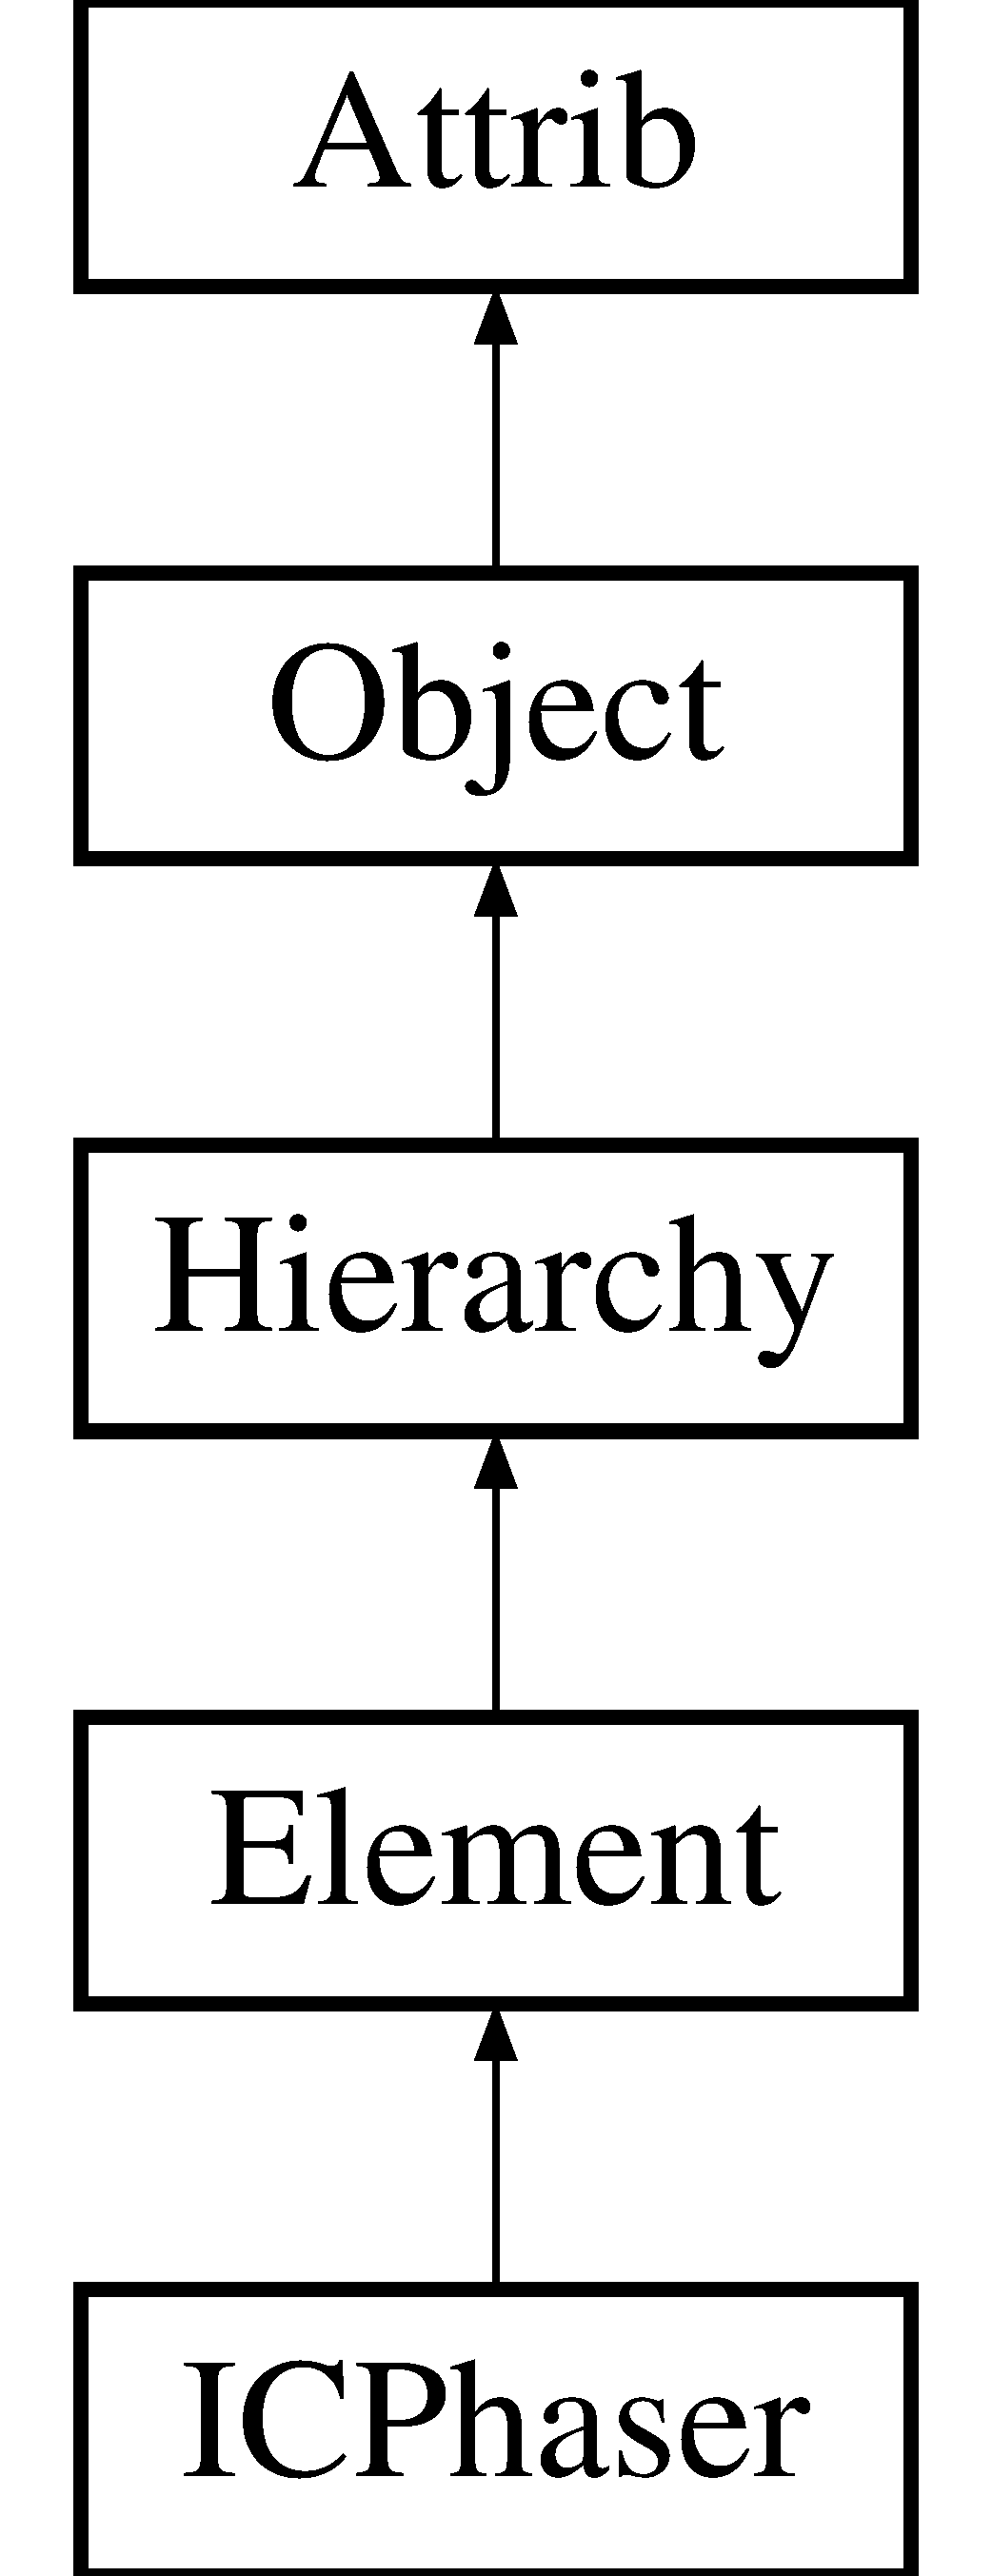
\includegraphics[height=5cm]{classICPhaser}
\end{center}
\end{figure}
\subsection*{Public Types}
\begin{DoxyCompactItemize}
\item 
typedef unsigned long \hyperlink{classICPhaser_ae7a88b0c8e5ce2b7406c0e6bcd6f2a24}{U32}
\item 
typedef unsigned short \hyperlink{classICPhaser_a66a90f8d7b28e695c98dbca784a57c8b}{U16}
\item 
typedef unsigned char \hyperlink{classICPhaser_a4f9b2302efbd7bdd70d7d80b415f1a9d}{U8}
\item 
enum \hyperlink{classAttrib_a69e171d7cc6417835a5a306d3c764235}{Attribut} \{ \par
\hyperlink{classAttrib_a69e171d7cc6417835a5a306d3c764235a3a8da2ab97dda18aebab196fe4100531}{UNDEFINED}, 
\hyperlink{classAttrib_a69e171d7cc6417835a5a306d3c764235a2bfb2af57b87031d190a05fe25dd92ed}{PASSIVE}, 
\hyperlink{classAttrib_a69e171d7cc6417835a5a306d3c764235a3b1fec929c0370d1436f2f06e298fb0d}{ACTIVE}, 
\hyperlink{classAttrib_a69e171d7cc6417835a5a306d3c764235aa27c16b480a369ea4d18b07b2516bbc7}{INTERFACE}, 
\par
\hyperlink{classAttrib_a69e171d7cc6417835a5a306d3c764235a1420a5b8c0540b2af210b6975eded7f9}{IO}, 
\hyperlink{classAttrib_a69e171d7cc6417835a5a306d3c764235a0af3b0d0ac323c1704e6c69cf90add28}{IODATA}, 
\hyperlink{classAttrib_a69e171d7cc6417835a5a306d3c764235a7788bc5dd333fd8ce18562b269c9dab1}{ELEMENT}, 
\hyperlink{classAttrib_a69e171d7cc6417835a5a306d3c764235a61ceb22149f365f1780d18f9d1459423}{HARDWARE}, 
\par
\hyperlink{classAttrib_a69e171d7cc6417835a5a306d3c764235a75250e29692496e73effca2c0330977f}{PROCESSUS}, 
\hyperlink{classAttrib_a69e171d7cc6417835a5a306d3c764235a103a67cd0b8f07ef478fa45d4356e27b}{SOFTWARE}
 \}
\end{DoxyCompactItemize}
\subsection*{Public Member Functions}
\begin{DoxyCompactItemize}
\item 
\hyperlink{classICPhaser_adcbdbce69b6d9e97809f168e3ecbda30}{ICPhaser} ()
\item 
\hyperlink{classICPhaser_a70e439f0c27e1171fef80b774ca83ab6}{$\sim$ICPhaser} ()
\item 
void \hyperlink{classICPhaser_a93d99f9980c4a85d0d5570e56ae5d1bb}{setPhase} (unsigned char channel, unsigned char value)
\item 
void \hyperlink{classICPhaser_a7bb639e8a7bd98c20b29c9fc3b4ffcce}{setPhase} (unsigned char ch0, unsigned char ch1, unsigned char ch2, unsigned char ch3)
\item 
unsigned int \hyperlink{classICPhaser_a1aa92666783d3b77ef73f2c6ef41f419}{phase} (unsigned int ch)
\item 
void \hyperlink{classICPhaser_a79170c0639b8bcedd267a99a1857c9a7}{read} ()
\item 
void \hyperlink{classICPhaser_a160d0f9b959c865fc3458857bb303dd0}{write} ()
\item 
void \hyperlink{classICPhaser_a8169d433a2789fdb1453d01f1c11517f}{status} ()
\item 
void \hyperlink{classICPhaser_a8650cfbe21e6dfa96f3a858507105f3b}{help} ()
\item 
\hyperlink{classStatusCode}{StatusCode} \hyperlink{classICPhaser_a798ede3a88e57efd1545b6594d2d7be5}{init} ()
\item 
void \hyperlink{classICPhaser_aa20b5b71ef76a97b9ff9688cb360293c}{reset} ()
\item 
void \hyperlink{classICPhaser_a69e1f428f33dbdc5b6f00027c022a4e7}{update} ()
\item 
\hyperlink{classRegister}{Register} $\ast$ \hyperlink{classICPhaser_ae22a3e794e85fbcafa154b4ba2d2e8d1}{regConfig} ()
\item 
\hyperlink{classRegister}{Register} $\ast$ \hyperlink{classICPhaser_a075f0f88445142d07a02c21401a0e342}{regStatus} ()
\item 
void \hyperlink{classICPhaser_aacedf2a891a7946818a38afdbb29b52a}{setAddress} (\hyperlink{classICPhaser_a4f9b2302efbd7bdd70d7d80b415f1a9d}{U8} address)
\item 
\hyperlink{classICPhaser_a4f9b2302efbd7bdd70d7d80b415f1a9d}{U8} \hyperlink{classICPhaser_ac5cd0f3cb56324782ae8d360944a94fd}{address} ()
\item 
void \hyperlink{classElement_a3c0abcb36f8906688bb7e32608df7086}{recursiveInitElement} ()
\item 
void \hyperlink{classElement_a82119ed37dff76508a2746a853ec35ba}{recursiveInitCommunications} ()
\item 
\hyperlink{classStatusCode}{StatusCode} \hyperlink{classElement_ab476b4b1df5954141ceb14f072433b89}{setConnection} (\hyperlink{classHierarchy}{Hierarchy} $\ast$)
\item 
\hyperlink{classHierarchy}{Hierarchy} $\ast$ \hyperlink{classElement_af57444353c1ddf9fa0109801e97debf7}{connection} ()
\item 
void \hyperlink{classHierarchy_af4d43b0765b402670eed2d62c73405af}{clear} ()
\item 
void \hyperlink{classHierarchy_a585ad1aeec16077a0e532ab8b4fc557b}{setParent} (\hyperlink{classHierarchy}{Hierarchy} $\ast$parent)
\item 
\hyperlink{classHierarchy}{Hierarchy} $\ast$ \hyperlink{classHierarchy_a1c7bec8257e717f9c1465e06ebf845fc}{parent} ()
\item 
\hyperlink{classHierarchy}{Hierarchy} $\ast$ \hyperlink{classHierarchy_ad550588733bf75ac5c0fcfd7c8fd11a6}{parent} (std::string)
\item 
\hyperlink{classHierarchy}{Hierarchy} $\ast$ \hyperlink{classHierarchy_aee461dc930ce3871636ff87f075b1b83}{origin} ()
\item 
virtual void \hyperlink{classHierarchy_ad677774ff38fcb257c04a3a10d471fac}{addChild} (\hyperlink{classHierarchy}{Hierarchy} $\ast$element)
\item 
std::vector$<$ \hyperlink{classHierarchy}{Hierarchy} $\ast$ $>$ \hyperlink{classHierarchy_aa9a76f69e98e052ee1a6e32cea006288}{children} ()
\item 
\hyperlink{classHierarchy}{Hierarchy} $\ast$ \hyperlink{classHierarchy_a1e207f973c694b538bf90107b4868817}{child} (std::string)
\item 
\hyperlink{classHierarchy}{Hierarchy} $\ast$ \hyperlink{classHierarchy_a0c15a5276a3b80b4354d6bd8a01e0708}{childTyped} (std::string)
\item 
unsigned long \hyperlink{classHierarchy_ab16e84de65fd84e14001a6cf941c8be4}{numberOfChildren} ()
\item 
bool \hyperlink{classHierarchy_a255174fe4d316d2a3f430dcb9dab29f1}{hasChildren} ()
\item 
void \hyperlink{classHierarchy_a2b2b359fac003233f65786a616766bde}{delChild} (\hyperlink{classHierarchy}{Hierarchy} $\ast$)
\item 
void \hyperlink{classHierarchy_a1928ac7615fe0b5e55cd707f70dc6781}{delChild} (std::string)
\item 
std::string \hyperlink{classHierarchy_aa7990fa7caf132d83e361ce033c6c65a}{path} (std::string=std::string(\char`\"{}\char`\"{}))
\item 
std::string \hyperlink{classHierarchy_a1efd56cd164d328d2002e53a10a19b8c}{pathTyped} (std::string=std::string(\char`\"{}\char`\"{}))
\item 
void \hyperlink{classHierarchy_a76e914b9a677a22a82deb74d892bf261}{tree} (std::string indent=std::string(\char`\"{}\char`\"{}))
\item 
void \hyperlink{classHierarchy_a594c294c5f60c230e106d522ed008212}{tree} ()
\item 
std::string \hyperlink{classObject_a975e888d50bfcbffda2c86368332a5cd}{name} () const 
\item 
std::string \hyperlink{classObject_a84f99f70f144a83e1582d1d0f84e4e62}{type} ()
\item 
unsigned char \hyperlink{classObject_af99145335cc61ff6e2798ea17db009d2}{id} ()
\item 
std::string \hyperlink{classObject_a73a0f1a41828fdd8303dd662446fb6c3}{title} ()
\item 
void \hyperlink{classObject_a3f9d5537ebce0c0f2bf6ae4d92426f3c}{msgSvc} (int level, std::string msg, std::string name)
\item 
void \hyperlink{classObject_a58b2d0618c2d08cf2383012611528d97}{msg} (std::string mymsg)
\item 
void \hyperlink{classObject_ac5d59299273cee27aacf7de00d2e7034}{msg} (std::string mymsg, std::string name)
\item 
void \hyperlink{classObject_a83d2db2df682907ea1115ad721c1c4a1}{verbose} (std::string mymsg)
\item 
void \hyperlink{classObject_a2d4120195317e2a3c6532e8bb9f3da68}{verbose} (std::string mymsg, std::string name)
\item 
void \hyperlink{classObject_aac010553f022165573714b7014a15f0d}{debug} (std::string mymsg)
\item 
void \hyperlink{classObject_a6c9a0397ca804e04d675ed05683f5420}{debug} (std::string mymsg, std::string name)
\item 
void \hyperlink{classObject_a644fd329ea4cb85f54fa6846484b84a8}{info} (std::string mymsg)
\item 
void \hyperlink{classObject_a1ca123253dfd30fc28b156f521dcbdae}{info} (std::string mymsg, std::string name)
\item 
void \hyperlink{classObject_a65cd4fda577711660821fd2cd5a3b4c9}{warning} (std::string mymsg)
\item 
void \hyperlink{classObject_a11f101db4dd73d9391b0231818881d86}{warning} (std::string mymsg, std::string name)
\item 
void \hyperlink{classObject_a204a95f57818c0f811933917a30eff45}{error} (std::string mymsg)
\item 
void \hyperlink{classObject_ad7f6c457733082efa2f9ff5f5c8e119a}{error} (std::string mymsg, std::string name)
\item 
void \hyperlink{classObject_aad5a16aac7516ce65bd5ec02ab07fc80}{fatal} (std::string mymsg)
\item 
void \hyperlink{classObject_ae62acd3d09f716220f75f252dc38bc9a}{fatal} (std::string mymsg, std::string name)
\item 
void \hyperlink{classObject_ae30fea75683c2d149b6b6d17c09ecd0c}{setName} (std::string name)
\item 
void \hyperlink{classObject_aae534cc9d982bcb9b99fd505f2e103a5}{setType} (std::string type)
\item 
void \hyperlink{classObject_a398fe08cba594a0ce6891d59fe4f159f}{setId} (unsigned char id)
\item 
void \hyperlink{classObject_a89557dbbad5bcaa02652f5d7fa35d20f}{setTitle} (std::string title)
\item 
void \hyperlink{classObject_a870c5af919958c2136623b2d7816d123}{setDllName} (std::string dllName)
\item 
std::string \hyperlink{classObject_a2e3947f2870094c332d7454117f3ec63}{dllName} ()
\item 
bool \hyperlink{classAttrib_a704f26af560909ad22065083bb7d4c34}{is} (int attribut)
\item 
void \hyperlink{classAttrib_a235f773af19c900264a190b00a3b4ad7}{add} (int attribut)
\item 
void \hyperlink{classAttrib_a7d4ef7e32d93cb287792b87b857e79f3}{remove} (int attribut)
\item 
std::string \hyperlink{classAttrib_aee7bbf16b144887f196e1341b24f8a26}{attributs} ()
\end{DoxyCompactItemize}
\subsection*{Protected Attributes}
\begin{DoxyCompactItemize}
\item 
\hyperlink{classHierarchy}{Hierarchy} $\ast$ \hyperlink{classElement_abe3de7a5dbbc9a6dd2d7e012e5fdb266}{m\_\-connection}
\item 
std::string \hyperlink{classAttrib_a3414521d7a82476e874b25a5407b5e63}{m\_\-attribString} \mbox{[}10\mbox{]}
\end{DoxyCompactItemize}
\subsection*{Private Attributes}
\begin{DoxyCompactItemize}
\item 
\hyperlink{classICPhaser_a4f9b2302efbd7bdd70d7d80b415f1a9d}{U8} \hyperlink{classICPhaser_a2b3bdff684521d2c3d053662134043ca}{m\_\-address}
\item 
unsigned char \hyperlink{classICPhaser_afe2a4527d58d08342d631dfa7c731203}{m\_\-phase} \mbox{[}4\mbox{]}
\item 
\hyperlink{classRegister}{Register} $\ast$ \hyperlink{classICPhaser_af135fe05b7c087639789afe470e88ce4}{m\_\-regConfig}
\item 
\hyperlink{classRegister}{Register} $\ast$ \hyperlink{classICPhaser_adcc37517abf1390407003c387008262d}{m\_\-regStatus}
\end{DoxyCompactItemize}


\subsection{Detailed Description}


Definition at line 19 of file ICPhaser.h.

\subsection{Member Typedef Documentation}
\hypertarget{classICPhaser_a66a90f8d7b28e695c98dbca784a57c8b}{
\index{ICPhaser@{ICPhaser}!U16@{U16}}
\index{U16@{U16}!ICPhaser@{ICPhaser}}
\subsubsection[{U16}]{\setlength{\rightskip}{0pt plus 5cm}typedef unsigned short {\bf ICPhaser::U16}}}
\label{classICPhaser_a66a90f8d7b28e695c98dbca784a57c8b}


Definition at line 22 of file ICPhaser.h.\hypertarget{classICPhaser_ae7a88b0c8e5ce2b7406c0e6bcd6f2a24}{
\index{ICPhaser@{ICPhaser}!U32@{U32}}
\index{U32@{U32}!ICPhaser@{ICPhaser}}
\subsubsection[{U32}]{\setlength{\rightskip}{0pt plus 5cm}typedef unsigned long {\bf ICPhaser::U32}}}
\label{classICPhaser_ae7a88b0c8e5ce2b7406c0e6bcd6f2a24}


Definition at line 21 of file ICPhaser.h.\hypertarget{classICPhaser_a4f9b2302efbd7bdd70d7d80b415f1a9d}{
\index{ICPhaser@{ICPhaser}!U8@{U8}}
\index{U8@{U8}!ICPhaser@{ICPhaser}}
\subsubsection[{U8}]{\setlength{\rightskip}{0pt plus 5cm}typedef unsigned char {\bf ICPhaser::U8}}}
\label{classICPhaser_a4f9b2302efbd7bdd70d7d80b415f1a9d}


Definition at line 23 of file ICPhaser.h.

\subsection{Member Enumeration Documentation}
\hypertarget{classAttrib_a69e171d7cc6417835a5a306d3c764235}{
\index{ICPhaser@{ICPhaser}!Attribut@{Attribut}}
\index{Attribut@{Attribut}!ICPhaser@{ICPhaser}}
\subsubsection[{Attribut}]{\setlength{\rightskip}{0pt plus 5cm}enum {\bf Attrib::Attribut}\hspace{0.3cm}{\ttfamily  \mbox{[}inherited\mbox{]}}}}
\label{classAttrib_a69e171d7cc6417835a5a306d3c764235}
\begin{Desc}
\item[Enumerator: ]\par
\begin{description}
\index{UNDEFINED@{UNDEFINED}!ICPhaser@{ICPhaser}}\index{ICPhaser@{ICPhaser}!UNDEFINED@{UNDEFINED}}\item[{\em 
\hypertarget{classAttrib_a69e171d7cc6417835a5a306d3c764235a3a8da2ab97dda18aebab196fe4100531}{
UNDEFINED}
\label{classAttrib_a69e171d7cc6417835a5a306d3c764235a3a8da2ab97dda18aebab196fe4100531}
}]\index{PASSIVE@{PASSIVE}!ICPhaser@{ICPhaser}}\index{ICPhaser@{ICPhaser}!PASSIVE@{PASSIVE}}\item[{\em 
\hypertarget{classAttrib_a69e171d7cc6417835a5a306d3c764235a2bfb2af57b87031d190a05fe25dd92ed}{
PASSIVE}
\label{classAttrib_a69e171d7cc6417835a5a306d3c764235a2bfb2af57b87031d190a05fe25dd92ed}
}]\index{ACTIVE@{ACTIVE}!ICPhaser@{ICPhaser}}\index{ICPhaser@{ICPhaser}!ACTIVE@{ACTIVE}}\item[{\em 
\hypertarget{classAttrib_a69e171d7cc6417835a5a306d3c764235a3b1fec929c0370d1436f2f06e298fb0d}{
ACTIVE}
\label{classAttrib_a69e171d7cc6417835a5a306d3c764235a3b1fec929c0370d1436f2f06e298fb0d}
}]\index{INTERFACE@{INTERFACE}!ICPhaser@{ICPhaser}}\index{ICPhaser@{ICPhaser}!INTERFACE@{INTERFACE}}\item[{\em 
\hypertarget{classAttrib_a69e171d7cc6417835a5a306d3c764235aa27c16b480a369ea4d18b07b2516bbc7}{
INTERFACE}
\label{classAttrib_a69e171d7cc6417835a5a306d3c764235aa27c16b480a369ea4d18b07b2516bbc7}
}]\index{IO@{IO}!ICPhaser@{ICPhaser}}\index{ICPhaser@{ICPhaser}!IO@{IO}}\item[{\em 
\hypertarget{classAttrib_a69e171d7cc6417835a5a306d3c764235a1420a5b8c0540b2af210b6975eded7f9}{
IO}
\label{classAttrib_a69e171d7cc6417835a5a306d3c764235a1420a5b8c0540b2af210b6975eded7f9}
}]\index{IODATA@{IODATA}!ICPhaser@{ICPhaser}}\index{ICPhaser@{ICPhaser}!IODATA@{IODATA}}\item[{\em 
\hypertarget{classAttrib_a69e171d7cc6417835a5a306d3c764235a0af3b0d0ac323c1704e6c69cf90add28}{
IODATA}
\label{classAttrib_a69e171d7cc6417835a5a306d3c764235a0af3b0d0ac323c1704e6c69cf90add28}
}]\index{ELEMENT@{ELEMENT}!ICPhaser@{ICPhaser}}\index{ICPhaser@{ICPhaser}!ELEMENT@{ELEMENT}}\item[{\em 
\hypertarget{classAttrib_a69e171d7cc6417835a5a306d3c764235a7788bc5dd333fd8ce18562b269c9dab1}{
ELEMENT}
\label{classAttrib_a69e171d7cc6417835a5a306d3c764235a7788bc5dd333fd8ce18562b269c9dab1}
}]\index{HARDWARE@{HARDWARE}!ICPhaser@{ICPhaser}}\index{ICPhaser@{ICPhaser}!HARDWARE@{HARDWARE}}\item[{\em 
\hypertarget{classAttrib_a69e171d7cc6417835a5a306d3c764235a61ceb22149f365f1780d18f9d1459423}{
HARDWARE}
\label{classAttrib_a69e171d7cc6417835a5a306d3c764235a61ceb22149f365f1780d18f9d1459423}
}]\index{PROCESSUS@{PROCESSUS}!ICPhaser@{ICPhaser}}\index{ICPhaser@{ICPhaser}!PROCESSUS@{PROCESSUS}}\item[{\em 
\hypertarget{classAttrib_a69e171d7cc6417835a5a306d3c764235a75250e29692496e73effca2c0330977f}{
PROCESSUS}
\label{classAttrib_a69e171d7cc6417835a5a306d3c764235a75250e29692496e73effca2c0330977f}
}]\index{SOFTWARE@{SOFTWARE}!ICPhaser@{ICPhaser}}\index{ICPhaser@{ICPhaser}!SOFTWARE@{SOFTWARE}}\item[{\em 
\hypertarget{classAttrib_a69e171d7cc6417835a5a306d3c764235a103a67cd0b8f07ef478fa45d4356e27b}{
SOFTWARE}
\label{classAttrib_a69e171d7cc6417835a5a306d3c764235a103a67cd0b8f07ef478fa45d4356e27b}
}]\end{description}
\end{Desc}



Definition at line 29 of file Attrib.h.


\begin{DoxyCode}
29                 {
30     UNDEFINED,
31     PASSIVE,
32     ACTIVE,
33     INTERFACE,
34     IO,
35     IODATA,
36     ELEMENT,
37     HARDWARE,
38     PROCESSUS,
39     SOFTWARE 
40   }; // array m_attribString must be changed into Attrib::Attrib if this enu is m
      odified. 
\end{DoxyCode}


\subsection{Constructor \& Destructor Documentation}
\hypertarget{classICPhaser_adcbdbce69b6d9e97809f168e3ecbda30}{
\index{ICPhaser@{ICPhaser}!ICPhaser@{ICPhaser}}
\index{ICPhaser@{ICPhaser}!ICPhaser@{ICPhaser}}
\subsubsection[{ICPhaser}]{\setlength{\rightskip}{0pt plus 5cm}ICPhaser::ICPhaser ()\hspace{0.3cm}{\ttfamily  \mbox{[}inline\mbox{]}}}}
\label{classICPhaser_adcbdbce69b6d9e97809f168e3ecbda30}


Definition at line 24 of file ICPhaser.h.

References Attrib::add(), Hierarchy::addChild(), IOdata::Byte, Object::debug(), IOdata::defDataU8(), Attrib::ELEMENT, Attrib::HARDWARE, IOobject::io(), m\_\-phase, m\_\-regConfig, m\_\-regStatus, Object::setId(), Object::setName(), IOdata::setSubAddress(), Object::setType(), and IOdata::setWordSize().


\begin{DoxyCode}
24             {
25     setType("ICPhaser");
26     setId(0);
27 
28     add(Attrib::ELEMENT); add (Attrib::HARDWARE);
29     debug("ICPhaser built.","ICPhaser::ICPhaser");
30 
31     m_phase[0]=99;
32     m_phase[1]=99;
33     m_phase[2]=99;
34     m_phase[3]=99;
35 
36     m_regConfig=new Register();
37     m_regStatus=new Register();
38 
39     m_regConfig->setName("ConfigRegister");
40     m_regStatus->setName("StatusRegister");
41 
42     m_regConfig->io()->setSubAddress(9);    
43     m_regStatus->io()->setSubAddress(19);
44 
45     m_regConfig->io()->defDataU8(3);    
46     m_regStatus->io()->defDataU8(2);
47 
48     m_regConfig->io()->setWordSize(IOdata::Byte);
49     m_regStatus->io()->setWordSize(IOdata::Byte);
50 
51     addChild(m_regConfig);
52     addChild(m_regStatus);
53   }
\end{DoxyCode}
\hypertarget{classICPhaser_a70e439f0c27e1171fef80b774ca83ab6}{
\index{ICPhaser@{ICPhaser}!$\sim$ICPhaser@{$\sim$ICPhaser}}
\index{$\sim$ICPhaser@{$\sim$ICPhaser}!ICPhaser@{ICPhaser}}
\subsubsection[{$\sim$ICPhaser}]{\setlength{\rightskip}{0pt plus 5cm}ICPhaser::$\sim$ICPhaser ()\hspace{0.3cm}{\ttfamily  \mbox{[}inline\mbox{]}}}}
\label{classICPhaser_a70e439f0c27e1171fef80b774ca83ab6}


Definition at line 55 of file ICPhaser.h.


\begin{DoxyCode}
55              {
56   }
\end{DoxyCode}


\subsection{Member Function Documentation}
\hypertarget{classAttrib_a235f773af19c900264a190b00a3b4ad7}{
\index{ICPhaser@{ICPhaser}!add@{add}}
\index{add@{add}!ICPhaser@{ICPhaser}}
\subsubsection[{add}]{\setlength{\rightskip}{0pt plus 5cm}void Attrib::add (int {\em attribut})\hspace{0.3cm}{\ttfamily  \mbox{[}inline, inherited\mbox{]}}}}
\label{classAttrib_a235f773af19c900264a190b00a3b4ad7}
Add an attribut 

Definition at line 67 of file Attrib.h.

References Attrib::m\_\-attributs, and Attrib::UNDEFINED.

Referenced by A3PE::A3PE(), Attrib::Attrib(), SpecsMezzanine::cmdline(), Computer::Computer(), CU\_\-v1::CU\_\-v1(), export\_\-obj(), FEB\_\-v1::FEB\_\-v1(), FePGA::FePGA(), ICECALv3::ICECALv3(), ICPhaser(), Application::initialize(), Interface::Interface(), IOdata::IOdata(), IOobject::IOobject(), LSDelayChipV1::LSDelayChipV1(), MSOxxxx::MSOxxxx(), Phaser::Phaser(), Processus::Processus(), Proto40MHz\_\-v1::Proto40MHz\_\-v1(), Attrib::remove(), SeqPGA::SeqPGA(), SpecsMaster::SpecsMaster(), and SpecsSlave::SpecsSlave().


\begin{DoxyCode}
67                             {
68     if (attribut!=Attrib::UNDEFINED) remove(Attrib::UNDEFINED);
69     bool duplicate = false ;
70     std::vector<int>::const_iterator iter ;
71     for ( iter  = m_attributs.begin() ;
72           iter != m_attributs.end()   ;
73           ++iter ) {
74       if ( attribut == (*iter) ) {
75         duplicate = true ;
76       }
77     }
78     if (!duplicate) {
79       m_attributs.push_back( attribut );
80     }
81   }
\end{DoxyCode}
\hypertarget{classHierarchy_ad677774ff38fcb257c04a3a10d471fac}{
\index{ICPhaser@{ICPhaser}!addChild@{addChild}}
\index{addChild@{addChild}!ICPhaser@{ICPhaser}}
\subsubsection[{addChild}]{\setlength{\rightskip}{0pt plus 5cm}void Hierarchy::addChild ({\bf Hierarchy} $\ast$ {\em element})\hspace{0.3cm}{\ttfamily  \mbox{[}virtual, inherited\mbox{]}}}}
\label{classHierarchy_ad677774ff38fcb257c04a3a10d471fac}


Definition at line 83 of file Hierarchy.cpp.

References Object::debug(), Hierarchy::m\_\-children, Object::name(), and Hierarchy::setParent().

Referenced by A3PE::A3PE(), SpecsMezzanine::addBus(), SpecsSlave::addI2c(), Application::create(), CU\_\-v1::CU\_\-v1(), export\_\-obj(), FEB\_\-v1::FEB\_\-v1(), FePGA::FePGA(), ICECALv3::ICECALv3(), ICPhaser(), LSDelayChipV1::LSDelayChipV1(), FePGA::MakeRAM(), FePGA::MakeRegister(), Phaser::Phaser(), Proto40MHz\_\-v1::Proto40MHz\_\-v1(), SeqPGA::SeqPGA(), SpecsMezzanine::SpecsMezzanine(), UsbI2cBus::UsbI2cBus(), and UsbSpiBus::UsbSpiBus().


\begin{DoxyCode}
83                                           {
84   element->setParent(this);
85   m_children.push_back(element);
86   debug(element->name()+" added to the child tree.","Hierarchy::addChild");
87 }
\end{DoxyCode}
\hypertarget{classICPhaser_ac5cd0f3cb56324782ae8d360944a94fd}{
\index{ICPhaser@{ICPhaser}!address@{address}}
\index{address@{address}!ICPhaser@{ICPhaser}}
\subsubsection[{address}]{\setlength{\rightskip}{0pt plus 5cm}{\bf U8} ICPhaser::address ()\hspace{0.3cm}{\ttfamily  \mbox{[}inline\mbox{]}}}}
\label{classICPhaser_ac5cd0f3cb56324782ae8d360944a94fd}


Definition at line 133 of file ICPhaser.h.

References m\_\-address.

Referenced by BOOST\_\-PYTHON\_\-MODULE(), read(), and status().


\begin{DoxyCode}
133               {
134     return m_address;
135   }
\end{DoxyCode}
\hypertarget{classAttrib_aee7bbf16b144887f196e1341b24f8a26}{
\index{ICPhaser@{ICPhaser}!attributs@{attributs}}
\index{attributs@{attributs}!ICPhaser@{ICPhaser}}
\subsubsection[{attributs}]{\setlength{\rightskip}{0pt plus 5cm}std::string Attrib::attributs ()\hspace{0.3cm}{\ttfamily  \mbox{[}inherited\mbox{]}}}}
\label{classAttrib_aee7bbf16b144887f196e1341b24f8a26}
Print the \hyperlink{classAttrib}{Attrib} of an \hyperlink{classObject}{Object} 

Definition at line 54 of file Attrib.cpp.

References images::index, Attrib::m\_\-attribString, and Attrib::m\_\-attributs.

Referenced by export\_\-obj().


\begin{DoxyCode}
54                             {
55   std::string output;
56   std::vector<int>::iterator iter ;
57   for ( unsigned int index = 0 ; index < m_attributs.size() ; ++index ) {
58     if ( m_attributs.size() - index > 1 ) {
59       output.append(m_attribString[m_attributs[index]]);
60       output.append(":");
61     }
62     else {
63       output.append(m_attribString[m_attributs[index]]);
64     }
65   }
66   return output;
67 }
\end{DoxyCode}
\hypertarget{classHierarchy_a1e207f973c694b538bf90107b4868817}{
\index{ICPhaser@{ICPhaser}!child@{child}}
\index{child@{child}!ICPhaser@{ICPhaser}}
\subsubsection[{child}]{\setlength{\rightskip}{0pt plus 5cm}{\bf Hierarchy} $\ast$ Hierarchy::child (std::string {\em path})\hspace{0.3cm}{\ttfamily  \mbox{[}inherited\mbox{]}}}}
\label{classHierarchy_a1e207f973c694b538bf90107b4868817}


Definition at line 133 of file Hierarchy.cpp.

References Hierarchy::child(), Hierarchy::children(), Object::name(), Hierarchy::origin(), Hierarchy::parent(), and Object::warning().

Referenced by Application::cd(), Hierarchy::child(), and export\_\-obj().


\begin{DoxyCode}
133                                          {
134   std::string newpath = path;
135   std::string up("..");
136   std::string separator(1,'/');
137 
138   Hierarchy * newcurrent = 0;
139 
140   //  info("path="+path,"Hierarchy::child");
141 
142   if (path.compare("")==0 || path.compare("/")==0) {
143     //    debug("return origin","Hierarchy::child");
144     return origin();
145   }
146 
147   if (path.compare(name())==0){
148     //    debug("return itself","Hierarchy::child");
149     return this;
150   }
151 
152   if (path.compare("..")==0){
153     if (0!=this->parent()) return this->parent();
154     else return this;
155   }
156 
157   if (path.compare("../")==0){
158     if (0!=this->parent()) return this->parent();
159     else return this;
160   }
161 
162 
163   int npos=path.find(separator,0);
164 
165   //  info("find separator in "+itos(npos)+" of "+path,"Hierarchy::child");
166 
167   // remove last separator
168   if ( npos == (int)(path.size()-1) ) {
169     newpath = std::string(path,0,npos);
170     path = newpath;
171   }
172 
173   if (npos==0){
174     //    debug("Going back to origin and calling child","Hierarchy::child");
175     newpath=std::string(path,1,path.size()-1);
176     return origin()->child(newpath);
177   }
178   else{
179     if ( npos== (int)(std::string::npos) ){
180       //      debug("Getting chid "+path+" of "+this->name(),"Hierarchy::child");
      
181       std::vector <Hierarchy*> list = children();
182       std::vector<Hierarchy*>::iterator iter;
183       for (iter=list.begin();iter!=list.end();iter++){
184         if ((*iter)->name().compare(path)==0){
185           return *iter;
186         }
187       }
188       warning(this->name()+std::string(" has no child '")+path+"'","Hierarchy::ch
      ild");
189       return this;
190     }
191     else
192     {
193       int ipos=path.find(separator,0);
194       //      info("default behaviour "+path+" with separator in "+itos(ipos),"Hi
      erarchy::child");
195 
196       std::string newcurrentname=std::string(path,0,ipos);
197       newpath=std::string(path,ipos+1,path.size()-1);
198 
199       //      info("looking now for "+newpath+" from "+newcurrentname,"Hierarchy:
      :child");
200 
201       if (0==newcurrentname.compare(origin()->name())){
202         //        info("current is computer. Looking for children"+newcurrentname
      ,"Hierarchy::child");
203         return origin()->child(newpath);
204       }
205 
206       newcurrent = (Hierarchy*)0;
207 
208       std::vector <Hierarchy*> list = children();
209       std::vector<Hierarchy*>::iterator iter;
210       for (iter=list.begin();iter!=list.end();iter++){
211         if ((*iter)->name().compare(newcurrentname)==0){
212           newcurrent = (*iter);
213         }
214       }
215 
216 
217       if ((Hierarchy*)0==newcurrent){
218         if (newcurrentname.compare("..")==0 && 0!=parent()){
219           newcurrent=this->parent();
220           //          debug("newcurrent was .. -> parent="+parent()->name());
221         }
222         else
223         {
224           warning(this->name()+" has no child '"+newcurrentname+"'",
225               "Hierarchy::child");
226           return this;
227         }
228       }
229       //      debug("recurrence call for "+newpath+" on "+newcurrent->name(),"Hie
      rarchy::child");
230       return newcurrent -> child ( newpath );
231     }
232   }
233 }
\end{DoxyCode}
\hypertarget{classHierarchy_aa9a76f69e98e052ee1a6e32cea006288}{
\index{ICPhaser@{ICPhaser}!children@{children}}
\index{children@{children}!ICPhaser@{ICPhaser}}
\subsubsection[{children}]{\setlength{\rightskip}{0pt plus 5cm}std::vector$<${\bf Hierarchy}$\ast$$>$ Hierarchy::children ()\hspace{0.3cm}{\ttfamily  \mbox{[}inline, inherited\mbox{]}}}}
\label{classHierarchy_aa9a76f69e98e052ee1a6e32cea006288}


Definition at line 33 of file Hierarchy.h.

References Hierarchy::m\_\-children.

Referenced by Hierarchy::child(), Hierarchy::childTyped(), export\_\-obj(), SpecsSlave::recursiveInitCommunications(), Element::recursiveInitCommunications(), Element::recursiveInitElement(), Application::setConfig(), and Hierarchy::tree().


\begin{DoxyCode}
33 { return m_children;  } //< get list of child(ren)
\end{DoxyCode}
\hypertarget{classHierarchy_a0c15a5276a3b80b4354d6bd8a01e0708}{
\index{ICPhaser@{ICPhaser}!childTyped@{childTyped}}
\index{childTyped@{childTyped}!ICPhaser@{ICPhaser}}
\subsubsection[{childTyped}]{\setlength{\rightskip}{0pt plus 5cm}{\bf Hierarchy} $\ast$ Hierarchy::childTyped (std::string {\em path})\hspace{0.3cm}{\ttfamily  \mbox{[}inherited\mbox{]}}}}
\label{classHierarchy_a0c15a5276a3b80b4354d6bd8a01e0708}


Definition at line 239 of file Hierarchy.cpp.

References Hierarchy::children(), Hierarchy::m\_\-origin, Object::name(), Hierarchy::parent(), and Object::warning().

Referenced by export\_\-obj().


\begin{DoxyCode}
239                                               {
240 
241   std::string newpath = path;
242 
243   std::string up("..");
244   std::string separator(1,'/');
245   std::string typeopen(1,'[');
246   std::string typeclose(1,']');
247 
248   Hierarchy * newcurrent = 0;
249 
250   unsigned int npos=path.find(separator,0);
251   unsigned int opos=path.find(typeopen,0);
252   if ( npos==std::string::npos || npos == path.size()-1 ){
253     if ( path.compare("..")==0 ) {
254       return parent();
255     }
256 
257     if ( npos == path.size()-1 ) {
258       newpath = std::string(path,0,opos);
259       path = newpath;
260     }
261 
262     std::vector < Hierarchy* > list = children();
263     std::vector < Hierarchy* >::iterator iter;
264     for (iter=list.begin();iter!=list.end();iter++){
265       std::string notypepath = std::string(path,0,opos);
266       if ((*iter)->name().compare(notypepath)==0){
267         return *iter;
268       }
269     }
270     warning(this->name()+std::string(" has no child ") +path,"Hierarchy::child");
      
271     return 0;
272   }
273 
274   else {
275 
276     if (std::string(path,0,3).compare(std::string("../"))==0) {
277       newpath=std::string(path,3,path.size()-3);
278       newcurrent = parent();
279     }
280     if (std::string(path,0,1).compare(std::string("/"))==0) {
281       newpath=std::string(path,1,path.size()-1);
282       newcurrent = ( Hierarchy* ) m_origin;
283     }
284     if ((std::string(path,0,3).compare(std::string("../")) !=0 ) &&
285         std::string(path,0,1).compare(std::string("/"))!=0 ) {
286       opos = path.find(typeopen,0);
287       int cpos = path.find(typeclose,0);
288       std::string name = std::string (path,0,opos);
289       newcurrent = childTyped( name );
290       if (newcurrent ==0){
291         warning(path+": no child found with such a name","Hierarchy::child");
292       }
293       newpath = std::string (path,cpos+2,path.size()-cpos-1);
294     }
295     return newcurrent -> childTyped ( newpath );
296   }
297 }
\end{DoxyCode}
\hypertarget{classHierarchy_af4d43b0765b402670eed2d62c73405af}{
\index{ICPhaser@{ICPhaser}!clear@{clear}}
\index{clear@{clear}!ICPhaser@{ICPhaser}}
\subsubsection[{clear}]{\setlength{\rightskip}{0pt plus 5cm}void Hierarchy::clear ()\hspace{0.3cm}{\ttfamily  \mbox{[}inherited\mbox{]}}}}
\label{classHierarchy_af4d43b0765b402670eed2d62c73405af}


Definition at line 35 of file Hierarchy.cpp.

References Hierarchy::delChild(), Object::info(), Hierarchy::m\_\-children, and Object::name().

Referenced by export\_\-obj().


\begin{DoxyCode}
35                      {
36   std::vector<Hierarchy*> listlocale;
37   std::vector<Hierarchy*>::iterator iter;
38   info("loop on "+name()+" children.","Hierarchy::clear");
39   for (iter=m_children.begin();iter!=m_children.end();iter++){
40       info("processing "+(*iter)->name()+".","Hierarchy::clear");
41 /*
42       (*iter)->clear();
43 //      this->delChild((*iter));
44       info("obj "+(*iter)->name()+" being cleared.","Hierarchy::clear");
45       delete (*iter);
46       info("Object deleted.","Hierarchy::clear");
47       m_children.erase(iter);
48       info("Object removed from the tree.","Hierarchy::clear");
49 */
50     (*iter)->clear();
51     info("Adding object "+(*iter)->name()+" from the Hierarchy to the list of del
      eted objects.","Hierarchy::clear");
52     listlocale.push_back((*iter));
53   }
54 
55   for (iter=listlocale.begin();iter!=listlocale.end();iter++){
56     info("Removing object "+(*iter)->name()+".","Hierarchy::clear");
57     this->delChild(*iter);
58 //    m_children.erase(iter);
59     delete (*iter);
60   }
61   info("Getting out of "+name());
62 }
\end{DoxyCode}
\hypertarget{classElement_af57444353c1ddf9fa0109801e97debf7}{
\index{ICPhaser@{ICPhaser}!connection@{connection}}
\index{connection@{connection}!ICPhaser@{ICPhaser}}
\subsubsection[{connection}]{\setlength{\rightskip}{0pt plus 5cm}{\bf Hierarchy} $\ast$ Element::connection ()\hspace{0.3cm}{\ttfamily  \mbox{[}inherited\mbox{]}}}}
\label{classElement_af57444353c1ddf9fa0109801e97debf7}
Get IO interface 

Definition at line 84 of file Element.cpp.

References Element::m\_\-connection, Object::name(), and Object::warning().

Referenced by UsbSpiBus::clockDivider(), export\_\-obj(), UsbSpiBus::read(), UsbI2cBus::read(), IOobject::read(), UsbSpiBus::setClockDivider(), UsbSpiBus::write(), UsbI2cBus::write(), and IOobject::write().


\begin{DoxyCode}
84                               {
85   if (0==m_connection){
86     warning("no connection defined for "+name()+".","Element::connection");
87     return (Hierarchy*)0;
88   }
89   return m_connection;
90 }
\end{DoxyCode}
\hypertarget{classObject_a6c9a0397ca804e04d675ed05683f5420}{
\index{ICPhaser@{ICPhaser}!debug@{debug}}
\index{debug@{debug}!ICPhaser@{ICPhaser}}
\subsubsection[{debug}]{\setlength{\rightskip}{0pt plus 5cm}void Object::debug (std::string {\em mymsg}, \/  std::string {\em name})\hspace{0.3cm}{\ttfamily  \mbox{[}inline, inherited\mbox{]}}}}
\label{classObject_a6c9a0397ca804e04d675ed05683f5420}


Definition at line 45 of file Object.h.

References MsgSvc::DEBUG, Object::m\_\-log, and MsgSvc::msgSvc().


\begin{DoxyCode}
45 { m_log.msgSvc (MsgSvc::DEBUG   , mymsg, name ); }
\end{DoxyCode}
\hypertarget{classObject_aac010553f022165573714b7014a15f0d}{
\index{ICPhaser@{ICPhaser}!debug@{debug}}
\index{debug@{debug}!ICPhaser@{ICPhaser}}
\subsubsection[{debug}]{\setlength{\rightskip}{0pt plus 5cm}void Object::debug (std::string {\em mymsg})\hspace{0.3cm}{\ttfamily  \mbox{[}inline, inherited\mbox{]}}}}
\label{classObject_aac010553f022165573714b7014a15f0d}


Definition at line 37 of file Object.h.

References MsgSvc::DEBUG, Object::m\_\-log, Object::m\_\-name, and MsgSvc::msgSvc().

Referenced by A3PE::A3PE(), A3PE::acquisition(), SpecsMezzanine::addBus(), Hierarchy::addChild(), SpecsSlave::addI2c(), LSDelayChipV1::checkConfigAddr(), LSDelayChipV1::checkStatusAddr(), LSDelayChipV1::configRegBulkRead(), LSDelayChipV1::configRegBulkWrite(), A3PE::dataReady(), DCU::DCU(), Hierarchy::delChild(), SpecsSlave::detect(), EmulateFE::execute(), StorageFifoAcquisition::execute(), StorageFifo::execute(), Acquisition::execute(), A3PE\_\-BitFlip::execute(), export\_\-obj(), FePGA::FePGA(), SpecsGlue::i2cClkMode(), SeqPGA::i2cRead(), FePGA::i2cRead(), SeqPGA::i2cWrite(), FePGA::i2cWrite(), ICECALv3::ICECALv3(), ICPhaser(), SpecsSlave::init(), SpecsMaster::init(), EmulateFE::initialize(), StorageFifoAcquisition::initialize(), StorageFifo::initialize(), Acquisition::initialize(), A3PE\_\-BitFlip::initialize(), A3PE::internalAXSequence(), SpecsMezzanine::led(), SpecsGlue::led(), LSDelayChipV1::LSDelayChipV1(), MSOxxxx::MSOxxxx(), Phaser::Phaser(), Data::purge(), read(), Phaser::read(), FEB\_\-v1::readFifoSpyFE(), SpecsSlave::reset(), SpecsMaster::reset(), FEB\_\-v1::reset(), CU\_\-v1::reset(), Proto40MHz\_\-v1::reset(), FEB\_\-v1::resetFifoSpyFE(), SeqPGA::resetSpi(), FEB\_\-v1::resetSpi(), SeqPGA::SeqPGA(), A3PE::setAddFromAXRam(), A3PE::setAddToAXRam(), A3PE::setAXRamUsb(), Element::setConnection(), SpecsGlue::setI2cClkMode(), A3PE::setLatencyAX(), SpecsMezzanine::setLed(), SpecsGlue::setLed(), A3PE::setLengthAX(), A3PE::setReadToAXRamUsb(), SpecsMaster::setSpeed(), A3PE::setWriteFromAXRamUsb(), SpecsBus::SpecsBus(), SpecsI2c::SpecsI2c(), SpecsMaster::SpecsMaster(), SpecsMezzanine::SpecsMezzanine(), SpecsParallelBus::SpecsParallelBus(), SpecsSlave::SpecsSlave(), LSDelayChipV1::spiBERTest(), ICECALv3::spiRead(), ICECALv3::spiWrite(), FEB\_\-v1::testDuration(), SeqPGA::testSequence(), A3PE::trigger(), Server::updateConfig(), Server::updateState(), write(), Phaser::write(), and Hierarchy::$\sim$Hierarchy().


\begin{DoxyCode}
37 { m_log.msgSvc (MsgSvc::DEBUG   , mymsg, m_name ); }
\end{DoxyCode}
\hypertarget{classHierarchy_a1928ac7615fe0b5e55cd707f70dc6781}{
\index{ICPhaser@{ICPhaser}!delChild@{delChild}}
\index{delChild@{delChild}!ICPhaser@{ICPhaser}}
\subsubsection[{delChild}]{\setlength{\rightskip}{0pt plus 5cm}void Hierarchy::delChild (std::string {\em n})\hspace{0.3cm}{\ttfamily  \mbox{[}inherited\mbox{]}}}}
\label{classHierarchy_a1928ac7615fe0b5e55cd707f70dc6781}


Definition at line 110 of file Hierarchy.cpp.

References Object::debug(), and Hierarchy::m\_\-children.


\begin{DoxyCode}
110                                    {
111   bool flag=false;
112   std::vector<Hierarchy*>::iterator iter,remove;
113   for (iter=m_children.begin();iter!=m_children.end();iter++){
114     if ((*iter)->name()==n){ remove=iter; flag=true;}
115   }
116   if (flag){
117     debug("removing "+(*remove)->name()+" from the tree.","Hierarchy::delChild");
      
118     m_children.erase(remove);
119   }
120 }
\end{DoxyCode}
\hypertarget{classHierarchy_a2b2b359fac003233f65786a616766bde}{
\index{ICPhaser@{ICPhaser}!delChild@{delChild}}
\index{delChild@{delChild}!ICPhaser@{ICPhaser}}
\subsubsection[{delChild}]{\setlength{\rightskip}{0pt plus 5cm}void Hierarchy::delChild ({\bf Hierarchy} $\ast$ {\em element})\hspace{0.3cm}{\ttfamily  \mbox{[}inherited\mbox{]}}}}
\label{classHierarchy_a2b2b359fac003233f65786a616766bde}


Definition at line 92 of file Hierarchy.cpp.

References Object::debug(), and Hierarchy::m\_\-children.

Referenced by Hierarchy::clear(), export\_\-obj(), and Hierarchy::$\sim$Hierarchy().


\begin{DoxyCode}
92                                           {
93   bool flag=false;
94   std::vector<Hierarchy*>::iterator iter,remove;
95   for (iter=m_children.begin();(iter!=m_children.end());iter++){
96     if (*iter==element){
97       remove=iter;
98       flag=true;
99     }
100   }
101   if (flag){
102     debug("removing "+(*remove)->name()+" from the tree.","Hierarchy::delChild");
      
103     m_children.erase(remove);
104   }
105 }
\end{DoxyCode}
\hypertarget{classObject_a2e3947f2870094c332d7454117f3ec63}{
\index{ICPhaser@{ICPhaser}!dllName@{dllName}}
\index{dllName@{dllName}!ICPhaser@{ICPhaser}}
\subsubsection[{dllName}]{\setlength{\rightskip}{0pt plus 5cm}std::string Object::dllName ()\hspace{0.3cm}{\ttfamily  \mbox{[}inline, inherited\mbox{]}}}}
\label{classObject_a2e3947f2870094c332d7454117f3ec63}
Get accessor to member m\_\-dllName \begin{DoxyReturn}{Returns}
the current value of m\_\-dllName 
\end{DoxyReturn}


Definition at line 74 of file Object.h.

References Object::m\_\-dllName.

Referenced by export\_\-obj().


\begin{DoxyCode}
74                        {
75     return m_dllName;
76   }  
\end{DoxyCode}
\hypertarget{classObject_ad7f6c457733082efa2f9ff5f5c8e119a}{
\index{ICPhaser@{ICPhaser}!error@{error}}
\index{error@{error}!ICPhaser@{ICPhaser}}
\subsubsection[{error}]{\setlength{\rightskip}{0pt plus 5cm}void Object::error (std::string {\em mymsg}, \/  std::string {\em name})\hspace{0.3cm}{\ttfamily  \mbox{[}inline, inherited\mbox{]}}}}
\label{classObject_ad7f6c457733082efa2f9ff5f5c8e119a}


Definition at line 48 of file Object.h.

References MsgSvc::ERR, Object::m\_\-log, and MsgSvc::msgSvc().


\begin{DoxyCode}
48 { m_log.msgSvc (MsgSvc::ERR     , mymsg, name ); }
\end{DoxyCode}
\hypertarget{classObject_a204a95f57818c0f811933917a30eff45}{
\index{ICPhaser@{ICPhaser}!error@{error}}
\index{error@{error}!ICPhaser@{ICPhaser}}
\subsubsection[{error}]{\setlength{\rightskip}{0pt plus 5cm}void Object::error (std::string {\em mymsg})\hspace{0.3cm}{\ttfamily  \mbox{[}inline, inherited\mbox{]}}}}
\label{classObject_a204a95f57818c0f811933917a30eff45}


Definition at line 40 of file Object.h.

References MsgSvc::ERR, Object::m\_\-log, Object::m\_\-name, and MsgSvc::msgSvc().

Referenced by ICECALv3::checkChNumber(), A3PE::clockDivision(), NI6008::cmd(), A3PE::enableStorage(), A3PE\_\-BitFlip::execute(), export\_\-obj(), A3PE::fifoDepth(), A3PE::fifoLatency(), FEB\_\-v1::gbtStatus(), Register::getBit(), MSOxxxx::getStatistics(), SpecsMaster::init(), NI6008::init(), UsbFTMLInterface::init(), UsbFTInterface::init(), A3PE::latencyAX(), A3PE::lengthAX(), A3PE::nTrigger(), MSOxxxx::open(), ICECALv3::parseParameterList(), A3PE::pipeline(), UsbFTMLInterface::read(), UsbFTInterface::read(), MSOxxxx::recv(), A3PE::reset(), MSOxxxx::send(), A3PE::setAddFromAXRam(), A3PE::setAddToAXRam(), ICECALv3::setAnalogCh(), A3PE::setAXRamUsb(), Register::setBit(), A3PE::setClockDivision(), A3PE::setFifoDepth(), A3PE::setFifoLatency(), A3PE::setLatencyAX(), A3PE::setLengthAX(), A3PE::setNTrigger(), A3PE::setPipeline(), A3PE::setReadPatternFifoUsb(), A3PE::setReadToAXRamUsb(), A3PE::setReadTriggerFifoUsb(), A3PE::setSoftwareTrigger(), A3PE::setTriggerDelay(), A3PE::setTriggerRate(), A3PE::setWriteFromAXRamUsb(), A3PE::setWriteStorageFifoUsb(), ICECALv3::spiFERTest(), ICECALv3::spiWriteSafe(), A3PE::startSequenceAX(), A3PE::triggerDelay(), A3PE::triggerRate(), UsbFTMLInterface::usbRead(), UsbFTInterface::usbRead(), UsbFTMLInterface::usbReadU16(), UsbFTInterface::usbReadU16(), UsbFTMLInterface::usbReadU32(), UsbFTInterface::usbReadU32(), UsbFTMLInterface::usbReadU8(), UsbFTInterface::usbReadU8(), UsbFTMLInterface::usbWrite(), UsbFTInterface::usbWrite(), UsbFTMLInterface::usbWriteRead(), UsbFTInterface::usbWriteRead(), UsbFTMLInterface::usbWriteU16(), UsbFTInterface::usbWriteU16(), UsbFTMLInterface::usbWriteU32(), UsbFTInterface::usbWriteU32(), UsbFTMLInterface::usbWriteU8(), UsbFTInterface::usbWriteU8(), UsbFTMLInterface::write(), and UsbFTInterface::write().


\begin{DoxyCode}
40 { m_log.msgSvc (MsgSvc::ERR     , mymsg, m_name ); }
\end{DoxyCode}
\hypertarget{classObject_ae62acd3d09f716220f75f252dc38bc9a}{
\index{ICPhaser@{ICPhaser}!fatal@{fatal}}
\index{fatal@{fatal}!ICPhaser@{ICPhaser}}
\subsubsection[{fatal}]{\setlength{\rightskip}{0pt plus 5cm}void Object::fatal (std::string {\em mymsg}, \/  std::string {\em name})\hspace{0.3cm}{\ttfamily  \mbox{[}inline, inherited\mbox{]}}}}
\label{classObject_ae62acd3d09f716220f75f252dc38bc9a}


Definition at line 49 of file Object.h.

References MsgSvc::FATAL, Object::m\_\-log, and MsgSvc::msgSvc().


\begin{DoxyCode}
49 { m_log.msgSvc (MsgSvc::FATAL   , mymsg, name ); }
\end{DoxyCode}
\hypertarget{classObject_aad5a16aac7516ce65bd5ec02ab07fc80}{
\index{ICPhaser@{ICPhaser}!fatal@{fatal}}
\index{fatal@{fatal}!ICPhaser@{ICPhaser}}
\subsubsection[{fatal}]{\setlength{\rightskip}{0pt plus 5cm}void Object::fatal (std::string {\em mymsg})\hspace{0.3cm}{\ttfamily  \mbox{[}inline, inherited\mbox{]}}}}
\label{classObject_aad5a16aac7516ce65bd5ec02ab07fc80}


Definition at line 41 of file Object.h.

References MsgSvc::FATAL, Object::m\_\-log, Object::m\_\-name, and MsgSvc::msgSvc().

Referenced by export\_\-obj(), SpecsSlave::init(), UsbSpiBus::init(), UsbI2cBus::init(), IOobject::init(), UsbMLSpiBus::init(), UsbMLI2cBus::init(), UsbFTMLInterface::init(), UsbFTInterface::init(), and Element::setConnection().


\begin{DoxyCode}
41 { m_log.msgSvc (MsgSvc::FATAL   , mymsg, m_name ); }
\end{DoxyCode}
\hypertarget{classHierarchy_a255174fe4d316d2a3f430dcb9dab29f1}{
\index{ICPhaser@{ICPhaser}!hasChildren@{hasChildren}}
\index{hasChildren@{hasChildren}!ICPhaser@{ICPhaser}}
\subsubsection[{hasChildren}]{\setlength{\rightskip}{0pt plus 5cm}bool Hierarchy::hasChildren ()\hspace{0.3cm}{\ttfamily  \mbox{[}inherited\mbox{]}}}}
\label{classHierarchy_a255174fe4d316d2a3f430dcb9dab29f1}


Definition at line 303 of file Hierarchy.cpp.

References Hierarchy::m\_\-children.

Referenced by export\_\-obj().


\begin{DoxyCode}
303                               {
304   return ( m_children.size()>0 );
305 }
\end{DoxyCode}
\hypertarget{classICPhaser_a8650cfbe21e6dfa96f3a858507105f3b}{
\index{ICPhaser@{ICPhaser}!help@{help}}
\index{help@{help}!ICPhaser@{ICPhaser}}
\subsubsection[{help}]{\setlength{\rightskip}{0pt plus 5cm}void ICPhaser::help ()\hspace{0.3cm}{\ttfamily  \mbox{[}inline, virtual\mbox{]}}}}
\label{classICPhaser_a8650cfbe21e6dfa96f3a858507105f3b}
printout help for the \hyperlink{namespaceelement}{element} 

Implements \hyperlink{classElement_a32c0de27acb08e17251cef88c3e9303a}{Element}.

Definition at line 92 of file ICPhaser.h.

References Object::info(), and Object::name().


\begin{DoxyCode}
92 { info("ICPhaser "+name()+". No help.","ICPhaser::help"); };
\end{DoxyCode}
\hypertarget{classObject_af99145335cc61ff6e2798ea17db009d2}{
\index{ICPhaser@{ICPhaser}!id@{id}}
\index{id@{id}!ICPhaser@{ICPhaser}}
\subsubsection[{id}]{\setlength{\rightskip}{0pt plus 5cm}unsigned char Object::id ()\hspace{0.3cm}{\ttfamily  \mbox{[}inline, inherited\mbox{]}}}}
\label{classObject_af99145335cc61ff6e2798ea17db009d2}


Reimplemented in \hyperlink{classMSOxxxx_a0f14b23d31d8e7647184e99a89600cc3}{MSOxxxx}.

Definition at line 30 of file Object.h.

References Object::m\_\-id.

Referenced by export\_\-obj().


\begin{DoxyCode}
30 { return m_id;         } //< Get Object m_id 
\end{DoxyCode}
\hypertarget{classObject_a1ca123253dfd30fc28b156f521dcbdae}{
\index{ICPhaser@{ICPhaser}!info@{info}}
\index{info@{info}!ICPhaser@{ICPhaser}}
\subsubsection[{info}]{\setlength{\rightskip}{0pt plus 5cm}void Object::info (std::string {\em mymsg}, \/  std::string {\em name})\hspace{0.3cm}{\ttfamily  \mbox{[}inline, inherited\mbox{]}}}}
\label{classObject_a1ca123253dfd30fc28b156f521dcbdae}


Definition at line 46 of file Object.h.

References MsgSvc::INFO, Object::m\_\-log, and MsgSvc::msgSvc().


\begin{DoxyCode}
46 { m_log.msgSvc (MsgSvc::INFO    , mymsg, name ); }
\end{DoxyCode}
\hypertarget{classObject_a644fd329ea4cb85f54fa6846484b84a8}{
\index{ICPhaser@{ICPhaser}!info@{info}}
\index{info@{info}!ICPhaser@{ICPhaser}}
\subsubsection[{info}]{\setlength{\rightskip}{0pt plus 5cm}void Object::info (std::string {\em mymsg})\hspace{0.3cm}{\ttfamily  \mbox{[}inline, inherited\mbox{]}}}}
\label{classObject_a644fd329ea4cb85f54fa6846484b84a8}


Definition at line 38 of file Object.h.

References MsgSvc::INFO, Object::m\_\-log, Object::m\_\-name, and MsgSvc::msgSvc().

Referenced by NI6008::addDevice(), ICECALv3::bxidResynchStatus(), FEB\_\-v1::calibCte(), checkCmd(), Hierarchy::clear(), FEB\_\-v1::clock80MHzFallingEdge(), FEB\_\-v1::clockFallingEdge(), UsbFTMLInterface::close(), UsbFTInterface::close(), MSOxxxx::closeConnection(), Processus::closeRootFile(), SpecsMezzanine::cmdline(), Server::cmdline(), SpecsSlave::detect(), FEB\_\-v1::disableSubtract(), IOdata::dump(), A3PE::dumpFromAX(), A3PE::dumpPattern(), A3PE::dumpStorage(), A3PE::dumpToAX(), A3PE::dumpTrigger(), Processus::endProcessing(), PhaserRampExec::execute(), export\_\-obj(), PhaserRampExec::finalize(), FEB\_\-v1::gain4(), FEB\_\-v1::gbt80MHzClkEport(), FEB\_\-v1::gbtDataPath(), FEB\_\-v1::gbtDLLEport(), FEB\_\-v1::gbtDLLReset(), FEB\_\-v1::gbtEnableEport(), FEB\_\-v1::gbtMode(), FEB\_\-v1::gbtStatus(), FEB\_\-v1::gbtTermEport(), FEB\_\-v1::gbtTrackMode(), ICECALv3::getAnalogCh(), ICECALv3::getDelayLineCh(), ICECALv3::getMainReg(), FEB\_\-v1::globalPseudoPMEnable(), SpecsMezzanine::help(), SpecsMaster::help(), SpecsGlue::help(), SpecsParallelBus::help(), SpecsInterface::help(), NI6008::help(), Computer::help(), UsbSpiBus::help(), UsbI2cBus::help(), RAM::help(), IOobject::help(), UsbMLSpiBus::help(), UsbMLI2cBus::help(), UsbFTMLInterface::help(), SeqPGA::help(), help(), FePGA::help(), FEB\_\-v1::help(), CU\_\-v1::help(), UsbFTInterface::help(), Proto40MHz\_\-v1::help(), A3PE::help(), Phaser::help(), Croc::help(), MSOxxxx::help(), LSDelayChipV1::help(), ICECALv3::help(), MSOxxxx::id(), SpecsSlave::init(), SpecsMaster::init(), SpecsParallelBus::init(), SpecsInterface::init(), NI6008::init(), Computer::init(), UsbFTMLInterface::init(), UsbFTInterface::init(), Croc::init(), CurrentMeasurement::initialize(), ADCMeasurement::initialize(), EmulateFE::initialize(), StorageFifoAcquisition::initialize(), StorageFifo::initialize(), Acquisition::initialize(), A3PE\_\-BitFlip::initialize(), PhaserRampExec::initialize(), FEB\_\-v1::injectModeFE(), isInt(), FEB\_\-v1::latency(), FEB\_\-v1::latencyLLT(), A3PE::loadFromAX(), Application::loadHistoryFile(), A3PE::loadPattern(), A3PE::loadStorage(), A3PE::loadToAX(), A3PE::loadTrigger(), Application::loop(), FEB\_\-v1::maskLLT(), Application::network(), FEB\_\-v1::oldSubtract(), MSOxxxx::open(), Processus::openRootFile(), Data::print(), FEB\_\-v1::probeEnable(), ProcDataBase::ProcDataBase(), FEB\_\-v1::pseudoADCEnable(), FEB\_\-v1::pseudoPMEnable(), UsbSpiBus::read(), UsbFTMLInterface::read(), FEB\_\-v1::readFifoInjectFE(), FEB\_\-v1::readFifoLLT(), FEB\_\-v1::readFifoLLTFE(), FEB\_\-v1::readFifoSpyFE(), MSOxxxx::recv(), SpecsMaster::reset(), SpecsParallelBus::reset(), SpecsInterface::reset(), NI6008::reset(), Computer::reset(), UsbSpiBus::reset(), UsbI2cBus::reset(), UsbMLSpiBus::reset(), UsbMLI2cBus::reset(), UsbFTMLInterface::reset(), SeqPGA::reset(), FePGA::reset(), UsbFTInterface::reset(), A3PE::reset(), Croc::reset(), A3PE::resetAcquisitionWriteCounter(), FEB\_\-v1::resetFE(), A3PE::resetFE(), FEB\_\-v1::resetFifoInjectFE(), A3PE::resetFromAXRam(), SpecsSlave::resetInternal(), A3PE::resetLatencyCounter(), A3PE::resetPatternFifo(), A3PE::resetSequenceFromToAX(), A3PE::resetSPI(), A3PE::resetStorageFifo(), A3PE::resetToAXRam(), A3PE::resetTriggerFifo(), FePGA::resetUsb(), A3PE::resetUsbPhasers(), MSOxxxx::send(), Server::Server(), Application::server(), FEB\_\-v1::setCalibCte(), FEB\_\-v1::setClock80MHzFallingEdge(), A3PE::setClockDivision(), FEB\_\-v1::setClockFallingEdge(), UsbSpiBus::setDataLength(), FEB\_\-v1::setDisableSubtract(), A3PE::setEnableADC(), A3PE::setFifoDepth(), A3PE::setFifoLatency(), FEB\_\-v1::setGain4(), FEB\_\-v1::setGbt80MHzClkEport(), FEB\_\-v1::setGbtClockStrength(), FEB\_\-v1::setGbtDataPath(), FEB\_\-v1::setGbtDLLEport(), FEB\_\-v1::setGbtEnableEport(), FEB\_\-v1::setGbtMode(), FEB\_\-v1::setGbtTermEport(), FEB\_\-v1::setGbtTrackMode(), FEB\_\-v1::setGlobalPseudoPMEnable(), FEB\_\-v1::setInjectModeFE(), A3PE::setInternalAXSequence(), FEB\_\-v1::setLatency(), A3PE::setNTrigger(), FEB\_\-v1::setOldSubtract(), FEB\_\-v1::setOutputEport(), setPhase(), Phaser::setPhase(), A3PE::setPipeline(), FEB\_\-v1::setProbeEnable(), FEB\_\-v1::setPseudoADCEnable(), FEB\_\-v1::setPseudoPMEnable(), A3PE::setReadPatternFifoUsb(), A3PE::setReadTriggerFifoUsb(), A3PE::setSoftwareTrigger(), FEB\_\-v1::setSpareForTrigEnable(), FEB\_\-v1::setSpyModeFE(), FEB\_\-v1::setThreshold(), A3PE::setTriggerDelay(), A3PE::setTriggerRate(), A3PE::setWriteStorageFifoUsb(), LSDelayChipV1::showConfig(), FEB\_\-v1::spareForTrigEnable(), SpecsI2c::SpecsI2c(), ICECALv3::spiFERTest(), FEB\_\-v1::spyModeFE(), FEB\_\-v1::spyModeSeq(), Server::start(), Processus::startProcessing(), FEB\_\-v1::statusRegister(), FEB\_\-v1::stopInjLoop(), Application::svcRunning(), Application::terminate(), FePGA::testSequence(), FEB\_\-v1::threshold(), Hierarchy::tree(), SpecsParallelBus::update(), SpecsInterface::update(), NI6008::update(), Computer::update(), UsbSpiBus::update(), UsbI2cBus::update(), UsbMLSpiBus::update(), UsbMLI2cBus::update(), UsbFTMLInterface::update(), FEB\_\-v1::update(), CU\_\-v1::update(), UsbFTInterface::update(), Proto40MHz\_\-v1::update(), Croc::update(), UsbFTInterface::UsbFTInterface(), UsbFTMLInterface::UsbFTMLInterface(), ICECALv3::version(), UsbSpiBus::write(), FEB\_\-v1::writeDataFifoInjectFE(), FEB\_\-v1::writeFifoInjectFE(), and NI6008::$\sim$NI6008().


\begin{DoxyCode}
38 { m_log.msgSvc (MsgSvc::INFO    , mymsg, m_name ); }
\end{DoxyCode}
\hypertarget{classICPhaser_a798ede3a88e57efd1545b6594d2d7be5}{
\index{ICPhaser@{ICPhaser}!init@{init}}
\index{init@{init}!ICPhaser@{ICPhaser}}
\subsubsection[{init}]{\setlength{\rightskip}{0pt plus 5cm}{\bf StatusCode} ICPhaser::init ()\hspace{0.3cm}{\ttfamily  \mbox{[}inline, virtual\mbox{]}}}}
\label{classICPhaser_a798ede3a88e57efd1545b6594d2d7be5}
init the component

\begin{DoxyReturn}{Returns}
void 
\end{DoxyReturn}


Implements \hyperlink{classElement_af42754b5cabc198869222725218d695c}{Element}.

Definition at line 99 of file ICPhaser.h.

References StatusCode::SUCCESS.


\begin{DoxyCode}
99                     {
100     return StatusCode::SUCCESS;
101   };
\end{DoxyCode}
\hypertarget{classAttrib_a704f26af560909ad22065083bb7d4c34}{
\index{ICPhaser@{ICPhaser}!is@{is}}
\index{is@{is}!ICPhaser@{ICPhaser}}
\subsubsection[{is}]{\setlength{\rightskip}{0pt plus 5cm}bool Attrib::is (int {\em attribut})\hspace{0.3cm}{\ttfamily  \mbox{[}inline, inherited\mbox{]}}}}
\label{classAttrib_a704f26af560909ad22065083bb7d4c34}
Test for an attribut 

Definition at line 50 of file Attrib.h.

References Attrib::m\_\-attributs.

Referenced by export\_\-obj(), and Element::setConnection().


\begin{DoxyCode}
51   {
52     std::vector<int>::const_iterator iter ;
53     for ( iter  = m_attributs.begin() ;
54           iter != m_attributs.end()   ;
55           ++iter ) {
56       if ( attribut == (*iter) ) {
57         return true;
58       }
59     }
60     return false;
61   }
\end{DoxyCode}
\hypertarget{classObject_ac5d59299273cee27aacf7de00d2e7034}{
\index{ICPhaser@{ICPhaser}!msg@{msg}}
\index{msg@{msg}!ICPhaser@{ICPhaser}}
\subsubsection[{msg}]{\setlength{\rightskip}{0pt plus 5cm}void Object::msg (std::string {\em mymsg}, \/  std::string {\em name})\hspace{0.3cm}{\ttfamily  \mbox{[}inline, inherited\mbox{]}}}}
\label{classObject_ac5d59299273cee27aacf7de00d2e7034}


Definition at line 43 of file Object.h.

References Object::m\_\-log, MsgSvc::msgSvc(), and MsgSvc::NONE.


\begin{DoxyCode}
43 { m_log.msgSvc (MsgSvc::NONE    , mymsg, name ); }
\end{DoxyCode}
\hypertarget{classObject_a58b2d0618c2d08cf2383012611528d97}{
\index{ICPhaser@{ICPhaser}!msg@{msg}}
\index{msg@{msg}!ICPhaser@{ICPhaser}}
\subsubsection[{msg}]{\setlength{\rightskip}{0pt plus 5cm}void Object::msg (std::string {\em mymsg})\hspace{0.3cm}{\ttfamily  \mbox{[}inline, inherited\mbox{]}}}}
\label{classObject_a58b2d0618c2d08cf2383012611528d97}


Definition at line 35 of file Object.h.

References Object::m\_\-log, Object::m\_\-name, MsgSvc::msgSvc(), and MsgSvc::NONE.

Referenced by export\_\-obj().


\begin{DoxyCode}
35 { m_log.msgSvc (MsgSvc::NONE    , mymsg, m_name ); }
\end{DoxyCode}
\hypertarget{classObject_a3f9d5537ebce0c0f2bf6ae4d92426f3c}{
\index{ICPhaser@{ICPhaser}!msgSvc@{msgSvc}}
\index{msgSvc@{msgSvc}!ICPhaser@{ICPhaser}}
\subsubsection[{msgSvc}]{\setlength{\rightskip}{0pt plus 5cm}void Object::msgSvc (int {\em level}, \/  std::string {\em msg}, \/  std::string {\em name})\hspace{0.3cm}{\ttfamily  \mbox{[}inline, inherited\mbox{]}}}}
\label{classObject_a3f9d5537ebce0c0f2bf6ae4d92426f3c}


Definition at line 33 of file Object.h.

References Object::m\_\-log, and MsgSvc::msgSvc().

Referenced by Application::banner(), export\_\-obj(), SpecsMezzanine::help(), DCU::readMode(), DCU::setHIR(), DCU::setLIR(), and Hierarchy::tree().


\begin{DoxyCode}
33 { m_log.msgSvc ( (MsgSvc::MsgLevel)(level), msg, name ); }
\end{DoxyCode}
\hypertarget{classObject_a975e888d50bfcbffda2c86368332a5cd}{
\index{ICPhaser@{ICPhaser}!name@{name}}
\index{name@{name}!ICPhaser@{ICPhaser}}
\subsubsection[{name}]{\setlength{\rightskip}{0pt plus 5cm}std::string Object::name () const\hspace{0.3cm}{\ttfamily  \mbox{[}inline, inherited\mbox{]}}}}
\label{classObject_a975e888d50bfcbffda2c86368332a5cd}


Definition at line 28 of file Object.h.

References Object::m\_\-name.

Referenced by SpecsMezzanine::addBus(), Hierarchy::addChild(), SpecsSlave::addI2c(), Hierarchy::child(), Hierarchy::childTyped(), Hierarchy::clear(), A3PE::clockDivision(), UsbFTMLInterface::close(), UsbFTInterface::close(), Element::connection(), SpecsSlave::detect(), IOdata::dump(), A3PE::enableStorage(), export\_\-obj(), export\_\-proc(), A3PE::fifoDepth(), A3PE::fifoLatency(), Register::getBit(), SpecsParallelBus::help(), SpecsInterface::help(), NI6008::help(), Computer::help(), UsbSpiBus::help(), UsbI2cBus::help(), RAM::help(), IOobject::help(), UsbMLSpiBus::help(), UsbMLI2cBus::help(), UsbFTMLInterface::help(), SeqPGA::help(), help(), FePGA::help(), FEB\_\-v1::help(), CU\_\-v1::help(), UsbFTInterface::help(), Proto40MHz\_\-v1::help(), A3PE::help(), Phaser::help(), Croc::help(), MSOxxxx::help(), LSDelayChipV1::help(), ICECALv3::help(), SpecsSlave::init(), SpecsMaster::init(), SpecsParallelBus::init(), SpecsInterface::init(), NI6008::init(), Computer::init(), UsbFTMLInterface::init(), UsbFTInterface::init(), Croc::init(), CurrentMeasurement::initialize(), ADCMeasurement::initialize(), EmulateFE::initialize(), StorageFifoAcquisition::initialize(), StorageFifo::initialize(), Acquisition::initialize(), A3PE\_\-BitFlip::initialize(), PhaserRampExec::initialize(), A3PE::latencyAX(), A3PE::lengthAX(), Application::network(), A3PE::nTrigger(), Processus::openRootFile(), Hierarchy::path(), Hierarchy::pathTyped(), A3PE::pipeline(), read(), Phaser::read(), SpecsSlave::reset(), SpecsMaster::reset(), SpecsParallelBus::reset(), SpecsInterface::reset(), NI6008::reset(), Computer::reset(), UsbSpiBus::reset(), UsbI2cBus::reset(), UsbMLSpiBus::reset(), UsbMLI2cBus::reset(), UsbFTMLInterface::reset(), FEB\_\-v1::reset(), CU\_\-v1::reset(), UsbFTInterface::reset(), Proto40MHz\_\-v1::reset(), A3PE::reset(), Croc::reset(), SpecsSlave::resetInternal(), FEB\_\-v1::resetSpi(), A3PE::setAddFromAXRam(), A3PE::setAddToAXRam(), Register::setBit(), A3PE::setClockDivision(), Application::setConfig(), Element::setConnection(), A3PE::setFifoDepth(), A3PE::setFifoLatency(), A3PE::setLatencyAX(), A3PE::setLengthAX(), A3PE::setNTrigger(), A3PE::setPipeline(), SpecsMaster::setSpeed(), A3PE::setTriggerDelay(), A3PE::setTriggerRate(), SpecsBus::SpecsBus(), SpecsI2c::SpecsI2c(), SpecsParallelBus::SpecsParallelBus(), Server::start(), Processus::startProcessing(), Processus::storage(), Application::terminate(), Hierarchy::tree(), A3PE::triggerDelay(), A3PE::triggerRate(), SpecsParallelBus::update(), SpecsInterface::update(), NI6008::update(), Computer::update(), UsbSpiBus::update(), UsbI2cBus::update(), UsbMLSpiBus::update(), UsbMLI2cBus::update(), UsbFTMLInterface::update(), FEB\_\-v1::update(), CU\_\-v1::update(), UsbFTInterface::update(), Proto40MHz\_\-v1::update(), Croc::update(), UsbFTMLInterface::usbReadU16(), UsbFTInterface::usbReadU16(), UsbFTMLInterface::usbReadU32(), UsbFTInterface::usbReadU32(), UsbFTMLInterface::usbReadU8(), UsbFTInterface::usbReadU8(), UsbFTMLInterface::usbWriteRead(), UsbFTInterface::usbWriteRead(), UsbFTMLInterface::usbWriteU16(), UsbFTInterface::usbWriteU16(), UsbFTMLInterface::usbWriteU32(), UsbFTInterface::usbWriteU32(), UsbFTMLInterface::usbWriteU8(), UsbFTInterface::usbWriteU8(), write(), Phaser::write(), and Hierarchy::$\sim$Hierarchy().


\begin{DoxyCode}
28 { return m_name; } //< Get Object m_name
\end{DoxyCode}
\hypertarget{classHierarchy_ab16e84de65fd84e14001a6cf941c8be4}{
\index{ICPhaser@{ICPhaser}!numberOfChildren@{numberOfChildren}}
\index{numberOfChildren@{numberOfChildren}!ICPhaser@{ICPhaser}}
\subsubsection[{numberOfChildren}]{\setlength{\rightskip}{0pt plus 5cm}unsigned long Hierarchy::numberOfChildren ()\hspace{0.3cm}{\ttfamily  \mbox{[}inherited\mbox{]}}}}
\label{classHierarchy_ab16e84de65fd84e14001a6cf941c8be4}


Definition at line 125 of file Hierarchy.cpp.

References Hierarchy::m\_\-children.

Referenced by export\_\-obj().


\begin{DoxyCode}
125                                            {
126   return m_children.size();
127 }
\end{DoxyCode}
\hypertarget{classHierarchy_aee461dc930ce3871636ff87f075b1b83}{
\index{ICPhaser@{ICPhaser}!origin@{origin}}
\index{origin@{origin}!ICPhaser@{ICPhaser}}
\subsubsection[{origin}]{\setlength{\rightskip}{0pt plus 5cm}{\bf Hierarchy}$\ast$ Hierarchy::origin ()\hspace{0.3cm}{\ttfamily  \mbox{[}inline, inherited\mbox{]}}}}
\label{classHierarchy_aee461dc930ce3871636ff87f075b1b83}


Definition at line 30 of file Hierarchy.h.

References Hierarchy::m\_\-origin.

Referenced by Hierarchy::child(), export\_\-obj(), and Hierarchy::setParent().


\begin{DoxyCode}
30 { return m_origin; }  //< Get the origin of the tree
\end{DoxyCode}
\hypertarget{classHierarchy_ad550588733bf75ac5c0fcfd7c8fd11a6}{
\index{ICPhaser@{ICPhaser}!parent@{parent}}
\index{parent@{parent}!ICPhaser@{ICPhaser}}
\subsubsection[{parent}]{\setlength{\rightskip}{0pt plus 5cm}{\bf Hierarchy} $\ast$ Hierarchy::parent (std::string {\em type})\hspace{0.3cm}{\ttfamily  \mbox{[}inherited\mbox{]}}}}
\label{classHierarchy_ad550588733bf75ac5c0fcfd7c8fd11a6}


Definition at line 327 of file Hierarchy.cpp.

References Hierarchy::parent(), and Object::type().


\begin{DoxyCode}
327                                             {
328   Hierarchy *parent = this->parent();
329   if ( 0 != parent){
330     if (parent->type().compare( type )==0) {
331       return parent;
332     }
333     else
334       return parent->parent( type );
335   }
336   else {
337     return (Hierarchy*)NULL;
338   }
339 }
\end{DoxyCode}
\hypertarget{classHierarchy_a1c7bec8257e717f9c1465e06ebf845fc}{
\index{ICPhaser@{ICPhaser}!parent@{parent}}
\index{parent@{parent}!ICPhaser@{ICPhaser}}
\subsubsection[{parent}]{\setlength{\rightskip}{0pt plus 5cm}{\bf Hierarchy}$\ast$ Hierarchy::parent ()\hspace{0.3cm}{\ttfamily  \mbox{[}inline, inherited\mbox{]}}}}
\label{classHierarchy_a1c7bec8257e717f9c1465e06ebf845fc}


Definition at line 28 of file Hierarchy.h.

References Hierarchy::m\_\-parent.

Referenced by Hierarchy::child(), Hierarchy::childTyped(), export\_\-obj(), UsbSpiBus::init(), UsbI2cBus::init(), IOobject::init(), UsbMLSpiBus::init(), UsbMLI2cBus::init(), Hierarchy::parent(), Hierarchy::path(), Hierarchy::pathTyped(), Element::setConnection(), Hierarchy::setParent(), SpecsInterface::specsMaster(), SpecsInterface::specsMasterDevice(), SpecsInterface::specsSlave(), SpecsInterface::specsSlaveDevice(), and Hierarchy::$\sim$Hierarchy().


\begin{DoxyCode}
28 { return m_parent; }  //< Get Hierarchy Parent
\end{DoxyCode}
\hypertarget{classHierarchy_aa7990fa7caf132d83e361ce033c6c65a}{
\index{ICPhaser@{ICPhaser}!path@{path}}
\index{path@{path}!ICPhaser@{ICPhaser}}
\subsubsection[{path}]{\setlength{\rightskip}{0pt plus 5cm}std::string Hierarchy::path (std::string {\em str} = {\ttfamily std::string(\char`\"{}\char`\"{})})\hspace{0.3cm}{\ttfamily  \mbox{[}inherited\mbox{]}}}}
\label{classHierarchy_aa7990fa7caf132d83e361ce033c6c65a}


Definition at line 344 of file Hierarchy.cpp.

References Hierarchy::m\_\-parent, Object::name(), Hierarchy::parent(), and Hierarchy::path().

Referenced by export\_\-obj(), Hierarchy::path(), UsbFTMLInterface::usbReadU16(), UsbFTMLInterface::usbReadU32(), UsbFTMLInterface::usbReadU8(), UsbFTMLInterface::usbWriteRead(), UsbFTMLInterface::usbWriteU16(), UsbFTMLInterface::usbWriteU32(), and UsbFTMLInterface::usbWriteU8().


\begin{DoxyCode}
344                                       {
345   str="/"+name()+str;
346   Hierarchy *m_parent=parent();
347   if (0!=m_parent){
348     return m_parent->path(str);
349   }
350   return str;
351 }
\end{DoxyCode}
\hypertarget{classHierarchy_a1efd56cd164d328d2002e53a10a19b8c}{
\index{ICPhaser@{ICPhaser}!pathTyped@{pathTyped}}
\index{pathTyped@{pathTyped}!ICPhaser@{ICPhaser}}
\subsubsection[{pathTyped}]{\setlength{\rightskip}{0pt plus 5cm}std::string Hierarchy::pathTyped (std::string {\em str} = {\ttfamily std::string(\char`\"{}\char`\"{})})\hspace{0.3cm}{\ttfamily  \mbox{[}inherited\mbox{]}}}}
\label{classHierarchy_a1efd56cd164d328d2002e53a10a19b8c}


Definition at line 356 of file Hierarchy.cpp.

References Hierarchy::m\_\-parent, Object::name(), Hierarchy::parent(), Hierarchy::pathTyped(), and Object::type().

Referenced by export\_\-obj(), and Hierarchy::pathTyped().


\begin{DoxyCode}
356                                            {
357   Hierarchy *m_parent=parent();
358   if (0!=m_parent){
359     str="/"+name()+"["+type()+"]"+str;
360     return m_parent->pathTyped(str);
361   }
362   return str;
363 }
\end{DoxyCode}
\hypertarget{classICPhaser_a1aa92666783d3b77ef73f2c6ef41f419}{
\index{ICPhaser@{ICPhaser}!phase@{phase}}
\index{phase@{phase}!ICPhaser@{ICPhaser}}
\subsubsection[{phase}]{\setlength{\rightskip}{0pt plus 5cm}unsigned int ICPhaser::phase (unsigned int {\em ch})\hspace{0.3cm}{\ttfamily  \mbox{[}inline\mbox{]}}}}
\label{classICPhaser_a1aa92666783d3b77ef73f2c6ef41f419}


Definition at line 80 of file ICPhaser.h.

References m\_\-phase, and read().


\begin{DoxyCode}
80                                      {
81     read() ;
82     return m_phase[ch];
83   }
\end{DoxyCode}
\hypertarget{classICPhaser_a79170c0639b8bcedd267a99a1857c9a7}{
\index{ICPhaser@{ICPhaser}!read@{read}}
\index{read@{read}!ICPhaser@{ICPhaser}}
\subsubsection[{read}]{\setlength{\rightskip}{0pt plus 5cm}void ICPhaser::read ()}}
\label{classICPhaser_a79170c0639b8bcedd267a99a1857c9a7}


Definition at line 16 of file ICPhaser.cpp.

References address(), IOdata::dataU8(), Object::debug(), IOobject::io(), StatusCode::isFailure(), itos(), m\_\-phase, m\_\-regConfig, Object::name(), IOobject::read(), IOdata::setAddress(), IOdata::subAddress(), and Object::warning().

Referenced by BOOST\_\-PYTHON\_\-MODULE(), phase(), and update().


\begin{DoxyCode}
16                     {
17   m_regConfig->io()->setAddress(address());
18   U8* buffer=m_regConfig->io()->dataU8();
19   buffer[2]=((m_regConfig->io()->subAddress())&0x1F)+(128);
20   buffer[1]=0;
21   buffer[0]=0;
22   if (m_regConfig->read().isFailure()){
23     warning("ICPhaser configuration register read failure.","ICPhaser::read");
24   }
25   else {
26     U8* buffer=m_regConfig->io()->dataU8();
27     m_phase[0] = buffer[0];
28     m_phase[1] = buffer[1];
29     debug("reading "+name()+" phases : "+
30         itos(m_phase[0])+" "+
31         itos(m_phase[1])+" "+
32         itos(m_phase[2])+" "+
33         itos(m_phase[3]),
34         "ICPhaser::read");
35   }
36 }
\end{DoxyCode}
\hypertarget{classElement_a82119ed37dff76508a2746a853ec35ba}{
\index{ICPhaser@{ICPhaser}!recursiveInitCommunications@{recursiveInitCommunications}}
\index{recursiveInitCommunications@{recursiveInitCommunications}!ICPhaser@{ICPhaser}}
\subsubsection[{recursiveInitCommunications}]{\setlength{\rightskip}{0pt plus 5cm}void Element::recursiveInitCommunications ()\hspace{0.3cm}{\ttfamily  \mbox{[}inherited\mbox{]}}}}
\label{classElement_a82119ed37dff76508a2746a853ec35ba}
Triggers a recursive call to initCommunications() for the full hierarchy

\begin{DoxyReturn}{Returns}
void 
\end{DoxyReturn}


Reimplemented in \hyperlink{classSpecsSlave_a347b94c2ba660ccde6927fe72590a1bc}{SpecsSlave}.

Definition at line 44 of file Element.cpp.

References Hierarchy::children().

Referenced by export\_\-obj().


\begin{DoxyCode}
44                                          {
45   std::vector<Hierarchy*> list = children();
46   std::vector<Hierarchy*>::const_iterator iter;
47   for (iter=list.begin();iter!=list.end();iter++){
48     dynamic_cast<Element*>((*iter))->recursiveInitCommunications();
49   }
50 }
\end{DoxyCode}
\hypertarget{classElement_a3c0abcb36f8906688bb7e32608df7086}{
\index{ICPhaser@{ICPhaser}!recursiveInitElement@{recursiveInitElement}}
\index{recursiveInitElement@{recursiveInitElement}!ICPhaser@{ICPhaser}}
\subsubsection[{recursiveInitElement}]{\setlength{\rightskip}{0pt plus 5cm}void Element::recursiveInitElement ()\hspace{0.3cm}{\ttfamily  \mbox{[}inherited\mbox{]}}}}
\label{classElement_a3c0abcb36f8906688bb7e32608df7086}
Triggers a recursive call to \hyperlink{classElement_af42754b5cabc198869222725218d695c}{init()} for the full hierarchy

\begin{DoxyReturn}{Returns}
void 
\end{DoxyReturn}


Definition at line 32 of file Element.cpp.

References Hierarchy::children(), and Element::init().

Referenced by export\_\-obj().


\begin{DoxyCode}
32                                   {
33   init();
34   std::vector<Hierarchy*> list = children();
35   std::vector<Hierarchy*>::iterator iter;
36   for (iter=list.begin() ; iter!=list.end() ; ++iter){
37     dynamic_cast<Element*>((*iter))->recursiveInitElement();
38   }
39 }
\end{DoxyCode}
\hypertarget{classICPhaser_ae22a3e794e85fbcafa154b4ba2d2e8d1}{
\index{ICPhaser@{ICPhaser}!regConfig@{regConfig}}
\index{regConfig@{regConfig}!ICPhaser@{ICPhaser}}
\subsubsection[{regConfig}]{\setlength{\rightskip}{0pt plus 5cm}{\bf Register}$\ast$ ICPhaser::regConfig ()\hspace{0.3cm}{\ttfamily  \mbox{[}inline\mbox{]}}}}
\label{classICPhaser_ae22a3e794e85fbcafa154b4ba2d2e8d1}


Definition at line 119 of file ICPhaser.h.

References m\_\-regConfig.

Referenced by BOOST\_\-PYTHON\_\-MODULE().


\begin{DoxyCode}
119                        {
120     return m_regConfig;
121   }
\end{DoxyCode}
\hypertarget{classICPhaser_a075f0f88445142d07a02c21401a0e342}{
\index{ICPhaser@{ICPhaser}!regStatus@{regStatus}}
\index{regStatus@{regStatus}!ICPhaser@{ICPhaser}}
\subsubsection[{regStatus}]{\setlength{\rightskip}{0pt plus 5cm}{\bf Register}$\ast$ ICPhaser::regStatus ()\hspace{0.3cm}{\ttfamily  \mbox{[}inline\mbox{]}}}}
\label{classICPhaser_a075f0f88445142d07a02c21401a0e342}


Definition at line 123 of file ICPhaser.h.

References m\_\-regStatus.

Referenced by BOOST\_\-PYTHON\_\-MODULE().


\begin{DoxyCode}
123                        {
124     return m_regStatus;
125   }
\end{DoxyCode}
\hypertarget{classAttrib_a7d4ef7e32d93cb287792b87b857e79f3}{
\index{ICPhaser@{ICPhaser}!remove@{remove}}
\index{remove@{remove}!ICPhaser@{ICPhaser}}
\subsubsection[{remove}]{\setlength{\rightskip}{0pt plus 5cm}void Attrib::remove (int {\em attribut})\hspace{0.3cm}{\ttfamily  \mbox{[}inline, inherited\mbox{]}}}}
\label{classAttrib_a7d4ef7e32d93cb287792b87b857e79f3}
Remove an attribut 

Definition at line 86 of file Attrib.h.

References Attrib::add(), Attrib::m\_\-attributs, and Attrib::UNDEFINED.

Referenced by export\_\-obj().


\begin{DoxyCode}
86                                {
87     std::vector<int>::iterator iter , toremove ;
88     for ( iter  = m_attributs.begin() ;
89           iter != m_attributs.end()   ;
90           ++iter ) {
91       if ( attribut == (*iter) ) {
92         toremove = iter;
93       }
94     }
95     m_attributs.erase (toremove);
96     if(0==m_attributs.size()) add(Attrib::UNDEFINED);
97   }
\end{DoxyCode}
\hypertarget{classICPhaser_aa20b5b71ef76a97b9ff9688cb360293c}{
\index{ICPhaser@{ICPhaser}!reset@{reset}}
\index{reset@{reset}!ICPhaser@{ICPhaser}}
\subsubsection[{reset}]{\setlength{\rightskip}{0pt plus 5cm}void ICPhaser::reset ()\hspace{0.3cm}{\ttfamily  \mbox{[}virtual\mbox{]}}}}
\label{classICPhaser_aa20b5b71ef76a97b9ff9688cb360293c}
Resets the \hyperlink{classElement}{Element} so that is is in a standard and safe situation. Different from \hyperlink{classElement_af42754b5cabc198869222725218d695c}{Element::init} which configure the \hyperlink{classElement}{Element}. \hyperlink{classElement_a69efffa22f06909d768149715565cb56}{Element::reset()} is more an Emergency pull. It is often/usually called by the recursiveInitElement method at the start of the program. 

Implements \hyperlink{classElement_a69efffa22f06909d768149715565cb56}{Element}.

Definition at line 49 of file ICPhaser.cpp.

References IOdata::dataU8(), IOobject::io(), StatusCode::isFailure(), m\_\-regConfig, Object::warning(), and IOobject::write().

Referenced by BOOST\_\-PYTHON\_\-MODULE().


\begin{DoxyCode}
49                     {
50   U8* buffer=m_regConfig->io()->dataU8();
51   buffer[2]=64;
52   buffer[1]=0;
53   buffer[0]=0;
54   if (m_regConfig->write().isFailure()){
55     warning("ICPhaser configuration register write failure. Cannot reset ICPhaser
      ",
56         "ICPhaser::write");
57   }
58 }
\end{DoxyCode}
\hypertarget{classICPhaser_aacedf2a891a7946818a38afdbb29b52a}{
\index{ICPhaser@{ICPhaser}!setAddress@{setAddress}}
\index{setAddress@{setAddress}!ICPhaser@{ICPhaser}}
\subsubsection[{setAddress}]{\setlength{\rightskip}{0pt plus 5cm}void ICPhaser::setAddress ({\bf U8} {\em address})\hspace{0.3cm}{\ttfamily  \mbox{[}inline\mbox{]}}}}
\label{classICPhaser_aacedf2a891a7946818a38afdbb29b52a}


Definition at line 127 of file ICPhaser.h.

References m\_\-address, m\_\-regConfig, m\_\-regStatus, and IOobject::setAddress().

Referenced by BOOST\_\-PYTHON\_\-MODULE().


\begin{DoxyCode}
127                              {
128     m_address=address;
129     m_regConfig->setAddress(m_address);
130     m_regStatus->setAddress(m_address);
131   }
\end{DoxyCode}
\hypertarget{classElement_ab476b4b1df5954141ceb14f072433b89}{
\index{ICPhaser@{ICPhaser}!setConnection@{setConnection}}
\index{setConnection@{setConnection}!ICPhaser@{ICPhaser}}
\subsubsection[{setConnection}]{\setlength{\rightskip}{0pt plus 5cm}{\bf StatusCode} Element::setConnection ({\bf Hierarchy} $\ast$ {\em connection})\hspace{0.3cm}{\ttfamily  \mbox{[}inherited\mbox{]}}}}
\label{classElement_ab476b4b1df5954141ceb14f072433b89}
Define IO interface 

Definition at line 55 of file Element.cpp.

References Object::debug(), StatusCode::FAILURE, Object::fatal(), Attrib::INTERFACE, Attrib::is(), Element::m\_\-connection, Object::name(), Hierarchy::parent(), StatusCode::SUCCESS, and Object::type().

Referenced by export\_\-obj(), UsbSpiBus::init(), UsbI2cBus::init(), IOobject::init(), UsbMLSpiBus::init(), and UsbMLI2cBus::init().


\begin{DoxyCode}
55                                                       {
56   if (0==connection){
57     fatal("Try to define a connection with a null pointer.",
58         "Element::setConnection");
59     return StatusCode::FAILURE;
60   }
61   if (connection->is(Attrib::INTERFACE)){
62     m_connection=dynamic_cast<Hierarchy*>(connection);
63     return StatusCode::SUCCESS;
64   }
65   else {
66     debug(connection->name()+
67         " is not a Attrib::INTERFACE hardware. Connection refused.",
68         "Element::setConnection");
69     if (0!=connection->parent()){
70       return setConnection(connection->parent());
71     }
72     else{
73       fatal("Could not find a connection for element "+
74           name()+"["+type()+"].","element::setConnection");
75       return StatusCode::FAILURE;
76     }
77   }
78 }
\end{DoxyCode}
\hypertarget{classObject_a870c5af919958c2136623b2d7816d123}{
\index{ICPhaser@{ICPhaser}!setDllName@{setDllName}}
\index{setDllName@{setDllName}!ICPhaser@{ICPhaser}}
\subsubsection[{setDllName}]{\setlength{\rightskip}{0pt plus 5cm}void Object::setDllName (std::string {\em dllName})\hspace{0.3cm}{\ttfamily  \mbox{[}inline, inherited\mbox{]}}}}
\label{classObject_a870c5af919958c2136623b2d7816d123}
Set accessor to member m\_\-dllName 
\begin{DoxyParams}{Parameters}
\item[{\em dllName}]the new value for m\_\-dllName \end{DoxyParams}


Definition at line 66 of file Object.h.

References Object::m\_\-dllName.

Referenced by DLL::createElement(), DLL::createProcessus(), and Object::Object().


\begin{DoxyCode}
66                                       {
67     m_dllName = dllName;
68   }
\end{DoxyCode}
\hypertarget{classObject_a398fe08cba594a0ce6891d59fe4f159f}{
\index{ICPhaser@{ICPhaser}!setId@{setId}}
\index{setId@{setId}!ICPhaser@{ICPhaser}}
\subsubsection[{setId}]{\setlength{\rightskip}{0pt plus 5cm}void Object::setId (unsigned char {\em id})\hspace{0.3cm}{\ttfamily  \mbox{[}inline, inherited\mbox{]}}}}
\label{classObject_a398fe08cba594a0ce6891d59fe4f159f}


Definition at line 53 of file Object.h.

References Object::m\_\-id.

Referenced by A3PE::A3PE(), DCU::DCU(), export\_\-obj(), FePGA::FePGA(), ICECALv3::ICECALv3(), ICPhaser(), LSDelayChipV1::LSDelayChipV1(), MSOxxxx::MSOxxxx(), Object::Object(), Phaser::Phaser(), SeqPGA::SeqPGA(), SpecsBus::SpecsBus(), SpecsI2c::SpecsI2c(), SpecsInterface::SpecsInterface(), SpecsMaster::SpecsMaster(), SpecsParallelBus::SpecsParallelBus(), and SpecsSlave::SpecsSlave().


\begin{DoxyCode}
53 { m_id    = id    ; } //< Set Object m_id
\end{DoxyCode}
\hypertarget{classObject_ae30fea75683c2d149b6b6d17c09ecd0c}{
\index{ICPhaser@{ICPhaser}!setName@{setName}}
\index{setName@{setName}!ICPhaser@{ICPhaser}}
\subsubsection[{setName}]{\setlength{\rightskip}{0pt plus 5cm}void Object::setName (std::string {\em name})\hspace{0.3cm}{\ttfamily  \mbox{[}inline, inherited\mbox{]}}}}
\label{classObject_ae30fea75683c2d149b6b6d17c09ecd0c}


Definition at line 51 of file Object.h.

References Object::m\_\-name.

Referenced by A3PE::A3PE(), A3PE\_\-BitFlip::A3PE\_\-BitFlip(), Acquisition::Acquisition(), ADCMeasurement::ADCMeasurement(), Computer::Computer(), Application::create(), Croc::Croc(), CU\_\-v1::CU\_\-v1(), CurrentMeasurement::CurrentMeasurement(), EmulateFE::EmulateFE(), export\_\-obj(), FEB\_\-v1::FEB\_\-v1(), FePGA::FePGA(), ICECALv3::ICECALv3(), ICPhaser(), Application::initialize(), Interface::Interface(), IOdata::IOdata(), IOobject::IOobject(), LSDelayChipV1::LSDelayChipV1(), FePGA::MakeRAM(), FePGA::MakeRegister(), Application::network(), NI6008::NI6008(), Object::Object(), PhaserRampExec::PhaserRampExec(), Proto40MHz\_\-v1::Proto40MHz\_\-v1(), RAM::RAM(), Register::Register(), RegisterTest::RegisterTest(), SeqPGA::SeqPGA(), SpecsBus::SpecsBus(), SpecsGlue::SpecsGlue(), SpecsI2c::SpecsI2c(), SpecsMaster::SpecsMaster(), SpecsMezzanine::SpecsMezzanine(), SpecsParallelBus::SpecsParallelBus(), StorageFifo::StorageFifo(), StorageFifoAcquisition::StorageFifoAcquisition(), TestI2C::TestI2C(), TestSPI::TestSPI(), TestSuite::TestSuite(), TestUSB::TestUSB(), UsbFTInterface::UsbFTInterface(), UsbFTInterfaceTest::UsbFTInterfaceTest(), UsbFTMLInterface::UsbFTMLInterface(), UsbI2cBus::UsbI2cBus(), UsbMLI2cBus::UsbMLI2cBus(), UsbMLSpiBus::UsbMLSpiBus(), and UsbSpiBus::UsbSpiBus().


\begin{DoxyCode}
51 { m_name  = name  ; } //< Set Object m_name
\end{DoxyCode}
\hypertarget{classHierarchy_a585ad1aeec16077a0e532ab8b4fc557b}{
\index{ICPhaser@{ICPhaser}!setParent@{setParent}}
\index{setParent@{setParent}!ICPhaser@{ICPhaser}}
\subsubsection[{setParent}]{\setlength{\rightskip}{0pt plus 5cm}void Hierarchy::setParent ({\bf Hierarchy} $\ast$ {\em parent})\hspace{0.3cm}{\ttfamily  \mbox{[}inherited\mbox{]}}}}
\label{classHierarchy_a585ad1aeec16077a0e532ab8b4fc557b}


Definition at line 67 of file Hierarchy.cpp.

References Hierarchy::m\_\-origin, Hierarchy::m\_\-parent, Hierarchy::origin(), and Hierarchy::parent().

Referenced by SpecsMezzanine::addBus(), Hierarchy::addChild(), SpecsSlave::addI2c(), Computer::Computer(), Application::create(), export\_\-obj(), and SpecsMezzanine::SpecsMezzanine().


\begin{DoxyCode}
67                                               {
68   m_parent = parent;
69   if ((Hierarchy*)0==parent) return;
70 
71   Hierarchy *curr = this;
72   Hierarchy *prev = parent;
73   while ( prev != 0 ){
74     curr = prev;
75     prev = curr->parent();
76   }
77   if (parent->origin()!=0) m_origin=parent->origin();
78 }
\end{DoxyCode}
\hypertarget{classICPhaser_a7bb639e8a7bd98c20b29c9fc3b4ffcce}{
\index{ICPhaser@{ICPhaser}!setPhase@{setPhase}}
\index{setPhase@{setPhase}!ICPhaser@{ICPhaser}}
\subsubsection[{setPhase}]{\setlength{\rightskip}{0pt plus 5cm}void ICPhaser::setPhase (unsigned char {\em ch0}, \/  unsigned char {\em ch1}, \/  unsigned char {\em ch2}, \/  unsigned char {\em ch3})\hspace{0.3cm}{\ttfamily  \mbox{[}inline\mbox{]}}}}
\label{classICPhaser_a7bb639e8a7bd98c20b29c9fc3b4ffcce}


Definition at line 65 of file ICPhaser.h.

References Object::info(), itos(), m\_\-phase, and write().


\begin{DoxyCode}
70        {
71     m_phase[0]=ch0;
72     m_phase[1]=ch1;
73     m_phase[2]=ch2;
74     m_phase[3]=ch3;
75     info("Set Phases to "+itos(ch0)+" "+itos(ch1)+" "
76      +itos(ch2)+" "+itos(ch3));
77     write();
78   }
\end{DoxyCode}
\hypertarget{classICPhaser_a93d99f9980c4a85d0d5570e56ae5d1bb}{
\index{ICPhaser@{ICPhaser}!setPhase@{setPhase}}
\index{setPhase@{setPhase}!ICPhaser@{ICPhaser}}
\subsubsection[{setPhase}]{\setlength{\rightskip}{0pt plus 5cm}void ICPhaser::setPhase (unsigned char {\em channel}, \/  unsigned char {\em value})\hspace{0.3cm}{\ttfamily  \mbox{[}inline\mbox{]}}}}
\label{classICPhaser_a93d99f9980c4a85d0d5570e56ae5d1bb}


Definition at line 58 of file ICPhaser.h.

References Object::info(), itos(), m\_\-phase, and write().

Referenced by BOOST\_\-PYTHON\_\-MODULE().


\begin{DoxyCode}
58                                                            {
59     info("Set Phase "+itos(channel)+" to "
60      +itos(value),"ICPhaser::setPhase");
61     m_phase[channel]=value;
62     write();
63   }
\end{DoxyCode}
\hypertarget{classObject_a89557dbbad5bcaa02652f5d7fa35d20f}{
\index{ICPhaser@{ICPhaser}!setTitle@{setTitle}}
\index{setTitle@{setTitle}!ICPhaser@{ICPhaser}}
\subsubsection[{setTitle}]{\setlength{\rightskip}{0pt plus 5cm}void Object::setTitle (std::string {\em title})\hspace{0.3cm}{\ttfamily  \mbox{[}inline, inherited\mbox{]}}}}
\label{classObject_a89557dbbad5bcaa02652f5d7fa35d20f}


Definition at line 54 of file Object.h.

References Object::m\_\-title.

Referenced by A3PE\_\-BitFlip::A3PE\_\-BitFlip(), Acquisition::Acquisition(), ADCMeasurement::ADCMeasurement(), CurrentMeasurement::CurrentMeasurement(), EmulateFE::EmulateFE(), export\_\-obj(), Histo1D::Histo1D(), Histo2D::Histo2D(), Object::Object(), PhaserRampExec::PhaserRampExec(), RegisterTest::RegisterTest(), StorageFifo::StorageFifo(), StorageFifoAcquisition::StorageFifoAcquisition(), TestI2C::TestI2C(), TestSPI::TestSPI(), TestSuite::TestSuite(), TestUSB::TestUSB(), and UsbFTInterfaceTest::UsbFTInterfaceTest().


\begin{DoxyCode}
54 { m_title = title ; } //< Set Object m_title
\end{DoxyCode}
\hypertarget{classObject_aae534cc9d982bcb9b99fd505f2e103a5}{
\index{ICPhaser@{ICPhaser}!setType@{setType}}
\index{setType@{setType}!ICPhaser@{ICPhaser}}
\subsubsection[{setType}]{\setlength{\rightskip}{0pt plus 5cm}void Object::setType (std::string {\em type})\hspace{0.3cm}{\ttfamily  \mbox{[}inline, inherited\mbox{]}}}}
\label{classObject_aae534cc9d982bcb9b99fd505f2e103a5}


Definition at line 52 of file Object.h.

References Object::m\_\-type.

Referenced by A3PE::A3PE(), A3PE\_\-BitFlip::A3PE\_\-BitFlip(), Acquisition::Acquisition(), ADCMeasurement::ADCMeasurement(), Computer::Computer(), Croc::Croc(), CU\_\-v1::CU\_\-v1(), CurrentMeasurement::CurrentMeasurement(), DCU::DCU(), EmulateFE::EmulateFE(), export\_\-obj(), FEB\_\-v1::FEB\_\-v1(), FePGA::FePGA(), ICECALv3::ICECALv3(), ICPhaser(), Application::initialize(), Interface::Interface(), IOdata::IOdata(), IOobject::IOobject(), LSDelayChipV1::LSDelayChipV1(), MSOxxxx::MSOxxxx(), NI6008::NI6008(), Object::Object(), Phaser::Phaser(), PhaserRampExec::PhaserRampExec(), Proto40MHz\_\-v1::Proto40MHz\_\-v1(), RAM::RAM(), Register::Register(), RegisterTest::RegisterTest(), SeqPGA::SeqPGA(), SpecsBus::SpecsBus(), SpecsGlue::SpecsGlue(), SpecsI2c::SpecsI2c(), SpecsMaster::SpecsMaster(), SpecsMezzanine::SpecsMezzanine(), SpecsParallelBus::SpecsParallelBus(), SpecsSlave::SpecsSlave(), StorageFifo::StorageFifo(), StorageFifoAcquisition::StorageFifoAcquisition(), TestI2C::TestI2C(), TestSPI::TestSPI(), TestSuite::TestSuite(), TestUSB::TestUSB(), UsbFTInterface::UsbFTInterface(), UsbFTInterfaceTest::UsbFTInterfaceTest(), UsbFTMLInterface::UsbFTMLInterface(), UsbI2cBus::UsbI2cBus(), UsbMLI2cBus::UsbMLI2cBus(), UsbMLSpiBus::UsbMLSpiBus(), and UsbSpiBus::UsbSpiBus().


\begin{DoxyCode}
52 { m_type  = type  ; } //< Set Object m_type
\end{DoxyCode}
\hypertarget{classICPhaser_a8169d433a2789fdb1453d01f1c11517f}{
\index{ICPhaser@{ICPhaser}!status@{status}}
\index{status@{status}!ICPhaser@{ICPhaser}}
\subsubsection[{status}]{\setlength{\rightskip}{0pt plus 5cm}void ICPhaser::status ()}}
\label{classICPhaser_a8169d433a2789fdb1453d01f1c11517f}


Definition at line 38 of file ICPhaser.cpp.

References address(), IOdata::dataU8(), IOdata::dump(), IOobject::io(), StatusCode::isFailure(), m\_\-regStatus, IOobject::read(), IOdata::setAddress(), IOdata::subAddress(), and Object::warning().

Referenced by BOOST\_\-PYTHON\_\-MODULE().


\begin{DoxyCode}
38                       {
39   m_regStatus->io()->setAddress(address());
40   U8* buffer=m_regStatus->io()->dataU8();
41   buffer[1]=((m_regStatus->io()->subAddress())&0x1F)+(160);
42   buffer[0]=0;
43   if (m_regStatus->read().isFailure()){
44     warning("ICPhaser status register read failure.","ICPhaser::read");
45   }
46   m_regStatus->io()->dump(1);
47 }
\end{DoxyCode}
\hypertarget{classObject_a73a0f1a41828fdd8303dd662446fb6c3}{
\index{ICPhaser@{ICPhaser}!title@{title}}
\index{title@{title}!ICPhaser@{ICPhaser}}
\subsubsection[{title}]{\setlength{\rightskip}{0pt plus 5cm}std::string Object::title ()\hspace{0.3cm}{\ttfamily  \mbox{[}inline, inherited\mbox{]}}}}
\label{classObject_a73a0f1a41828fdd8303dd662446fb6c3}


Definition at line 31 of file Object.h.

References Object::m\_\-title.

Referenced by export\_\-obj(), export\_\-proc(), CurrentMeasurement::initialize(), ADCMeasurement::initialize(), StorageFifoAcquisition::initialize(), Acquisition::initialize(), and Application::terminate().


\begin{DoxyCode}
31 { return m_title;      } // < Get Object m_title
\end{DoxyCode}
\hypertarget{classHierarchy_a594c294c5f60c230e106d522ed008212}{
\index{ICPhaser@{ICPhaser}!tree@{tree}}
\index{tree@{tree}!ICPhaser@{ICPhaser}}
\subsubsection[{tree}]{\setlength{\rightskip}{0pt plus 5cm}void Hierarchy::tree ()\hspace{0.3cm}{\ttfamily  \mbox{[}inline, inherited\mbox{]}}}}
\label{classHierarchy_a594c294c5f60c230e106d522ed008212}


Definition at line 46 of file Hierarchy.h.

References Hierarchy::tree().

Referenced by export\_\-obj(), and Hierarchy::tree().


\begin{DoxyCode}
46 { tree(""); };                     // output tree of Hierarchy from object
\end{DoxyCode}
\hypertarget{classHierarchy_a76e914b9a677a22a82deb74d892bf261}{
\index{ICPhaser@{ICPhaser}!tree@{tree}}
\index{tree@{tree}!ICPhaser@{ICPhaser}}
\subsubsection[{tree}]{\setlength{\rightskip}{0pt plus 5cm}void Hierarchy::tree (std::string {\em indent} = {\ttfamily std::string(\char`\"{}\char`\"{})})\hspace{0.3cm}{\ttfamily  \mbox{[}inherited\mbox{]}}}}
\label{classHierarchy_a76e914b9a677a22a82deb74d892bf261}


Definition at line 310 of file Hierarchy.cpp.

References Hierarchy::children(), Object::info(), Object::msgSvc(), Object::name(), MsgSvc::NONE, and Object::type().


\begin{DoxyCode}
310                                     {
311   std::string line=indent+" -> "+name()+"["+type()+"] ";
312   if (std::string("")==indent){
313     info("Hierarchy for Object "+name()+"["+type()+"]","Hierarchy::tree");
314   }
315   msgSvc(MsgSvc::NONE,line,"");
316   std::vector<Hierarchy*> list = children();
317   std::vector<Hierarchy*>::iterator iter;
318   for (iter=list.begin() ; iter!=list.end() ; ++iter){
319     std::string tab="  ";
320     (*iter)->tree(indent+tab);
321   }
322 }
\end{DoxyCode}
\hypertarget{classObject_a84f99f70f144a83e1582d1d0f84e4e62}{
\index{ICPhaser@{ICPhaser}!type@{type}}
\index{type@{type}!ICPhaser@{ICPhaser}}
\subsubsection[{type}]{\setlength{\rightskip}{0pt plus 5cm}std::string Object::type ()\hspace{0.3cm}{\ttfamily  \mbox{[}inline, inherited\mbox{]}}}}
\label{classObject_a84f99f70f144a83e1582d1d0f84e4e62}


Definition at line 29 of file Object.h.

References Object::m\_\-type.

Referenced by DLLMgr::destroy(), DLL::destroy(), IOdata::dump(), export\_\-obj(), UsbSpiBus::init(), UsbI2cBus::init(), UsbMLSpiBus::init(), UsbMLI2cBus::init(), EmulateFE::initialize(), StorageFifoAcquisition::initialize(), StorageFifo::initialize(), Acquisition::initialize(), A3PE\_\-BitFlip::initialize(), PhaserRampExec::initialize(), ProcDataBase::list(), Hierarchy::parent(), Hierarchy::pathTyped(), DLL::print(), ProcDataBase::procList(), Application::setConfig(), Element::setConnection(), and Hierarchy::tree().


\begin{DoxyCode}
29 { return m_type;       } //< Get Object m_type
\end{DoxyCode}
\hypertarget{classICPhaser_a69e1f428f33dbdc5b6f00027c022a4e7}{
\index{ICPhaser@{ICPhaser}!update@{update}}
\index{update@{update}!ICPhaser@{ICPhaser}}
\subsubsection[{update}]{\setlength{\rightskip}{0pt plus 5cm}void ICPhaser::update ()\hspace{0.3cm}{\ttfamily  \mbox{[}inline, virtual\mbox{]}}}}
\label{classICPhaser_a69e1f428f33dbdc5b6f00027c022a4e7}
Update the \hyperlink{classElement}{Element} configuration from the actual hardware 

Implements \hyperlink{classElement_a4e6c83efae95616ebddd03c793a26661}{Element}.

Definition at line 115 of file ICPhaser.h.

References read().


\begin{DoxyCode}
115                  {
116     read();
117   };
\end{DoxyCode}
\hypertarget{classObject_a2d4120195317e2a3c6532e8bb9f3da68}{
\index{ICPhaser@{ICPhaser}!verbose@{verbose}}
\index{verbose@{verbose}!ICPhaser@{ICPhaser}}
\subsubsection[{verbose}]{\setlength{\rightskip}{0pt plus 5cm}void Object::verbose (std::string {\em mymsg}, \/  std::string {\em name})\hspace{0.3cm}{\ttfamily  \mbox{[}inline, inherited\mbox{]}}}}
\label{classObject_a2d4120195317e2a3c6532e8bb9f3da68}


Definition at line 44 of file Object.h.

References Object::m\_\-log, MsgSvc::msgSvc(), and MsgSvc::VERBOSE.


\begin{DoxyCode}
44 { m_log.msgSvc (MsgSvc::VERBOSE , mymsg, name ); }
\end{DoxyCode}
\hypertarget{classObject_a83d2db2df682907ea1115ad721c1c4a1}{
\index{ICPhaser@{ICPhaser}!verbose@{verbose}}
\index{verbose@{verbose}!ICPhaser@{ICPhaser}}
\subsubsection[{verbose}]{\setlength{\rightskip}{0pt plus 5cm}void Object::verbose (std::string {\em mymsg})\hspace{0.3cm}{\ttfamily  \mbox{[}inline, inherited\mbox{]}}}}
\label{classObject_a83d2db2df682907ea1115ad721c1c4a1}


Definition at line 36 of file Object.h.

References Object::m\_\-log, Object::m\_\-name, MsgSvc::msgSvc(), and MsgSvc::VERBOSE.

Referenced by DCU::acquire(), export\_\-obj(), DCU::init(), Application::prepare(), UsbFTMLInterface::read(), UsbFTInterface::read(), DCU::readMode(), DCU::reset(), DCU::setHIR(), DCU::setLIR(), SpecsInterface::specsReadI2c(), SpecsInterface::specsReadParallel(), SpecsInterface::specsReadRegister(), SpecsInterface::specsWriteI2c(), SpecsInterface::specsWriteParallel(), SpecsInterface::specsWriteRegister(), UsbFTMLInterface::usbRead(), UsbFTInterface::usbRead(), UsbFTMLInterface::usbReadU16(), UsbFTInterface::usbReadU16(), UsbFTMLInterface::usbReadU32(), UsbFTInterface::usbReadU32(), UsbFTMLInterface::usbReadU8(), UsbFTInterface::usbReadU8(), UsbFTMLInterface::usbWrite(), UsbFTInterface::usbWrite(), UsbFTMLInterface::usbWriteRead(), UsbFTInterface::usbWriteRead(), UsbFTMLInterface::usbWriteU16(), UsbFTInterface::usbWriteU16(), UsbFTMLInterface::usbWriteU32(), UsbFTInterface::usbWriteU32(), UsbFTMLInterface::usbWriteU8(), UsbFTInterface::usbWriteU8(), wait(), UsbFTMLInterface::write(), and UsbFTInterface::write().


\begin{DoxyCode}
36 { m_log.msgSvc (MsgSvc::VERBOSE , mymsg, m_name ); }
\end{DoxyCode}
\hypertarget{classObject_a11f101db4dd73d9391b0231818881d86}{
\index{ICPhaser@{ICPhaser}!warning@{warning}}
\index{warning@{warning}!ICPhaser@{ICPhaser}}
\subsubsection[{warning}]{\setlength{\rightskip}{0pt plus 5cm}void Object::warning (std::string {\em mymsg}, \/  std::string {\em name})\hspace{0.3cm}{\ttfamily  \mbox{[}inline, inherited\mbox{]}}}}
\label{classObject_a11f101db4dd73d9391b0231818881d86}


Definition at line 47 of file Object.h.

References Object::m\_\-log, MsgSvc::msgSvc(), and MsgSvc::WARNING.


\begin{DoxyCode}
47 { m_log.msgSvc (MsgSvc::WARNING , mymsg, name ); }
\end{DoxyCode}
\hypertarget{classObject_a65cd4fda577711660821fd2cd5a3b4c9}{
\index{ICPhaser@{ICPhaser}!warning@{warning}}
\index{warning@{warning}!ICPhaser@{ICPhaser}}
\subsubsection[{warning}]{\setlength{\rightskip}{0pt plus 5cm}void Object::warning (std::string {\em mymsg})\hspace{0.3cm}{\ttfamily  \mbox{[}inline, inherited\mbox{]}}}}
\label{classObject_a65cd4fda577711660821fd2cd5a3b4c9}


Definition at line 39 of file Object.h.

References Object::m\_\-log, Object::m\_\-name, MsgSvc::msgSvc(), and MsgSvc::WARNING.

Referenced by DCU::acquire(), A3PE::acquisition(), Plot::add(), Application::bookkeeping(), checkCmd(), Hierarchy::child(), Hierarchy::childTyped(), Processus::clean(), UsbSpiBus::clockDivider(), LSDelayChipV1::configRegBulkRead(), LSDelayChipV1::configRegBulkWrite(), Element::connection(), DCU::convert(), Application::create(), SpecsMezzanine::date(), SpecsGlue::date(), SpecsSlave::detect(), NI6008::device(), UsbFTInterfaceTest::execute(), Acquisition::execute(), A3PE\_\-BitFlip::execute(), export\_\-obj(), FEB\_\-v1::gbtAcknowledgeConfig(), FEB\_\-v1::gbtClockStrength(), FEB\_\-v1::gbtDLLReset(), LSDelayChipV1::getConfigReg(), SpecsGlue::i2cClkMode(), SpecsSlave::init(), DCU::init(), TestUSB::initialize(), TestSPI::initialize(), TestI2C::initialize(), EmulateFE::initialize(), StorageFifoAcquisition::initialize(), StorageFifo::initialize(), Acquisition::initialize(), A3PE\_\-BitFlip::initialize(), SpecsMezzanine::led(), SpecsGlue::led(), A3PE::loadTrigger(), Application::loop(), Application::makeDir(), Data::name(), Application::prepare(), UsbSpiBus::read(), UsbI2cBus::read(), read(), Phaser::read(), DCU::readMode(), SpecsSlave::reset(), SpecsMaster::reset(), DCU::reset(), reset(), SpecsSlave::resetInternal(), Server::Server(), FEB\_\-v1::setCalibCte(), StorageFifoAcquisition::setChannels(), Acquisition::setChannels(), UsbSpiBus::setClockDivider(), FEB\_\-v1::setClockFallingEdge(), Application::setConfig(), LSDelayChipV1::setConfigReg(), StorageFifoAcquisition::setDepth(), Acquisition::setDepth(), A3PE::setEnableADC(), FEB\_\-v1::setGain4(), FEB\_\-v1::setGbt80MHzClkEport(), FEB\_\-v1::setGbtClockStrength(), FEB\_\-v1::setGbtDataPath(), FEB\_\-v1::setGbtDLLEport(), FEB\_\-v1::setGbtEnableEport(), FEB\_\-v1::setGbtMode(), FEB\_\-v1::setGbtTermEport(), FEB\_\-v1::setGbtTrackMode(), DCU::setHIR(), SpecsGlue::setI2cClkMode(), SpecsMezzanine::setLed(), DCU::setLIR(), FEB\_\-v1::setOutputEport(), A3PE::setPipeline(), FEB\_\-v1::setPseudoADCEnable(), FEB\_\-v1::setPseudoPMEnable(), RAM::setSize(), SpecsMaster::setSpeed(), FEB\_\-v1::setStopInjLoop(), FEB\_\-v1::setTestDuration(), IOdata::setU16(), IOdata::setU32(), IOdata::setU8(), TestSuite::sigma(), SpecsInterface::specsReadI2c(), SpecsInterface::specsReadParallel(), SpecsInterface::specsReadRegister(), SpecsInterface::specsWriteI2c(), SpecsInterface::specsWriteParallel(), SpecsInterface::specsWriteRegister(), ICECALv3::spiAddressScan(), LSDelayChipV1::spiBERTest(), ICECALv3::spiFERTest(), ICECALv3::spiRead(), ICECALv3::spiWrite(), ICECALv3::spiWriteSafe(), Server::start(), status(), Application::svcPlot(), Application::svcRunning(), Data::title(), Server::updateConfig(), Server::updateState(), Data::vectorPtr(), UsbSpiBus::write(), UsbI2cBus::write(), write(), Phaser::write(), FEB\_\-v1::writeFifoInjectFE(), and FEB\_\-v1::writeFifoLLTFE().


\begin{DoxyCode}
39 { m_log.msgSvc (MsgSvc::WARNING , mymsg, m_name ); }
\end{DoxyCode}
\hypertarget{classICPhaser_a160d0f9b959c865fc3458857bb303dd0}{
\index{ICPhaser@{ICPhaser}!write@{write}}
\index{write@{write}!ICPhaser@{ICPhaser}}
\subsubsection[{write}]{\setlength{\rightskip}{0pt plus 5cm}void ICPhaser::write ()}}
\label{classICPhaser_a160d0f9b959c865fc3458857bb303dd0}


Definition at line 60 of file ICPhaser.cpp.

References IOdata::dataU8(), Object::debug(), IOdata::dump(), IOobject::io(), StatusCode::isFailure(), itos(), m\_\-phase, m\_\-regConfig, Object::name(), IOdata::subAddress(), Object::warning(), and IOobject::write().

Referenced by BOOST\_\-PYTHON\_\-MODULE(), and setPhase().


\begin{DoxyCode}
60                     {
61   U8* buffer=m_regConfig->io()->dataU8();
62   buffer[2]=(m_regConfig->io()->subAddress())&0x1F;
63   buffer[1]=m_phase[0]&0xff;
64   buffer[0]=m_phase[1]&0xff;
65   // phase[2] and phase[3] not implemented - only for test purpose
66   debug("Setting "+name()+" phases : "+itos(m_phase[0])+" "+
67       itos(m_phase[1])+" "+itos(m_phase[2])+" "+itos(m_phase[3]),
68       "ICPhaser::write");
69   m_regConfig->io()->dump(0);
70   if (m_regConfig->write().isFailure()){
71     warning("ICPhaser configuration register write failure.",
72         "ICPhaser::write");
73   }
74 }
\end{DoxyCode}


\subsection{Member Data Documentation}
\hypertarget{classICPhaser_a2b3bdff684521d2c3d053662134043ca}{
\index{ICPhaser@{ICPhaser}!m\_\-address@{m\_\-address}}
\index{m\_\-address@{m\_\-address}!ICPhaser@{ICPhaser}}
\subsubsection[{m\_\-address}]{\setlength{\rightskip}{0pt plus 5cm}{\bf U8} {\bf ICPhaser::m\_\-address}\hspace{0.3cm}{\ttfamily  \mbox{[}private\mbox{]}}}}
\label{classICPhaser_a2b3bdff684521d2c3d053662134043ca}


Definition at line 138 of file ICPhaser.h.

Referenced by address(), and setAddress().\hypertarget{classAttrib_a3414521d7a82476e874b25a5407b5e63}{
\index{ICPhaser@{ICPhaser}!m\_\-attribString@{m\_\-attribString}}
\index{m\_\-attribString@{m\_\-attribString}!ICPhaser@{ICPhaser}}
\subsubsection[{m\_\-attribString}]{\setlength{\rightskip}{0pt plus 5cm}std::string {\bf Attrib::m\_\-attribString}\mbox{[}10\mbox{]}\hspace{0.3cm}{\ttfamily  \mbox{[}protected, inherited\mbox{]}}}}
\label{classAttrib_a3414521d7a82476e874b25a5407b5e63}


Definition at line 105 of file Attrib.h.

Referenced by Attrib::Attrib(), and Attrib::attributs().\hypertarget{classElement_abe3de7a5dbbc9a6dd2d7e012e5fdb266}{
\index{ICPhaser@{ICPhaser}!m\_\-connection@{m\_\-connection}}
\index{m\_\-connection@{m\_\-connection}!ICPhaser@{ICPhaser}}
\subsubsection[{m\_\-connection}]{\setlength{\rightskip}{0pt plus 5cm}{\bf Hierarchy}$\ast$ {\bf Element::m\_\-connection}\hspace{0.3cm}{\ttfamily  \mbox{[}protected, inherited\mbox{]}}}}
\label{classElement_abe3de7a5dbbc9a6dd2d7e012e5fdb266}


Definition at line 70 of file Element.h.

Referenced by UsbSpiBus::clockDivider(), Element::connection(), Element::Element(), UsbSpiBus::init(), UsbI2cBus::init(), IOobject::init(), UsbMLSpiBus::init(), UsbMLI2cBus::init(), UsbSpiBus::read(), UsbI2cBus::read(), UsbSpiBus::setClockDivider(), Element::setConnection(), UsbSpiBus::write(), and UsbI2cBus::write().\hypertarget{classICPhaser_afe2a4527d58d08342d631dfa7c731203}{
\index{ICPhaser@{ICPhaser}!m\_\-phase@{m\_\-phase}}
\index{m\_\-phase@{m\_\-phase}!ICPhaser@{ICPhaser}}
\subsubsection[{m\_\-phase}]{\setlength{\rightskip}{0pt plus 5cm}unsigned char {\bf ICPhaser::m\_\-phase}\mbox{[}4\mbox{]}\hspace{0.3cm}{\ttfamily  \mbox{[}private\mbox{]}}}}
\label{classICPhaser_afe2a4527d58d08342d631dfa7c731203}


Definition at line 139 of file ICPhaser.h.

Referenced by ICPhaser(), phase(), read(), setPhase(), and write().\hypertarget{classICPhaser_af135fe05b7c087639789afe470e88ce4}{
\index{ICPhaser@{ICPhaser}!m\_\-regConfig@{m\_\-regConfig}}
\index{m\_\-regConfig@{m\_\-regConfig}!ICPhaser@{ICPhaser}}
\subsubsection[{m\_\-regConfig}]{\setlength{\rightskip}{0pt plus 5cm}{\bf Register}$\ast$ {\bf ICPhaser::m\_\-regConfig}\hspace{0.3cm}{\ttfamily  \mbox{[}private\mbox{]}}}}
\label{classICPhaser_af135fe05b7c087639789afe470e88ce4}


Definition at line 140 of file ICPhaser.h.

Referenced by ICPhaser(), read(), regConfig(), reset(), setAddress(), and write().\hypertarget{classICPhaser_adcc37517abf1390407003c387008262d}{
\index{ICPhaser@{ICPhaser}!m\_\-regStatus@{m\_\-regStatus}}
\index{m\_\-regStatus@{m\_\-regStatus}!ICPhaser@{ICPhaser}}
\subsubsection[{m\_\-regStatus}]{\setlength{\rightskip}{0pt plus 5cm}{\bf Register}$\ast$ {\bf ICPhaser::m\_\-regStatus}\hspace{0.3cm}{\ttfamily  \mbox{[}private\mbox{]}}}}
\label{classICPhaser_adcc37517abf1390407003c387008262d}


Definition at line 141 of file ICPhaser.h.

Referenced by ICPhaser(), regStatus(), setAddress(), and status().

The documentation for this class was generated from the following files:\begin{DoxyCompactItemize}
\item 
/home/eleclhcb/LHCb/lbcat-\/cmake/CatCaloUpgrade/inc/\hyperlink{ICPhaser_8h}{ICPhaser.h}\item 
/home/eleclhcb/LHCb/lbcat-\/cmake/CatCaloUpgrade/src/\hyperlink{ICPhaser_8cpp}{ICPhaser.cpp}\end{DoxyCompactItemize}

\hypertarget{classimages_1_1ImageClass}{
\section{images::ImageClass Class Reference}
\label{classimages_1_1ImageClass}\index{images::ImageClass@{images::ImageClass}}
}


\subsection{Detailed Description}


Definition at line 1023 of file images.py.

The documentation for this class was generated from the following file:\begin{DoxyCompactItemize}
\item 
/home/eleclhcb/LHCb/lbcat-\/cmake/CatPython/python/\hyperlink{images_8py}{images.py}\end{DoxyCompactItemize}

\hypertarget{classInterface}{
\section{Interface Class Reference}
\label{classInterface}\index{Interface@{Interface}}
}


{\ttfamily \#include $<$inc/Interface.h$>$}Inheritance diagram for Interface::\begin{figure}[H]
\begin{center}
\leavevmode
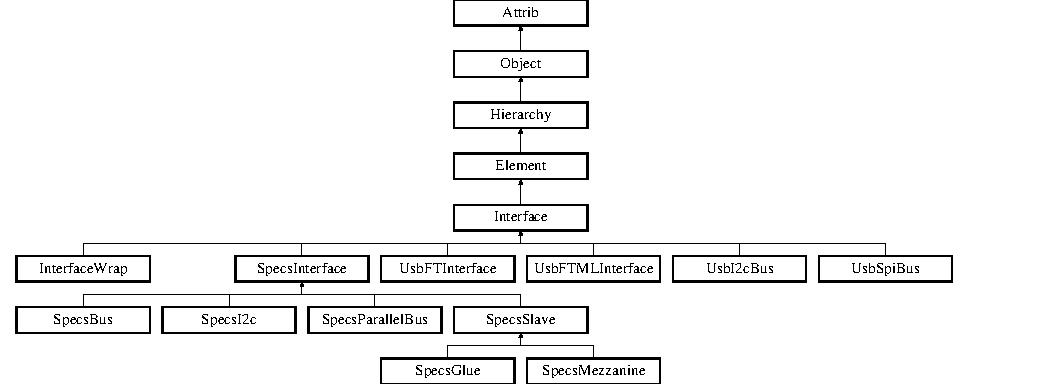
\includegraphics[height=5.16129cm]{classInterface}
\end{center}
\end{figure}
\subsection*{Public Types}
\begin{DoxyCompactItemize}
\item 
enum \hyperlink{classAttrib_a69e171d7cc6417835a5a306d3c764235}{Attribut} \{ \par
\hyperlink{classAttrib_a69e171d7cc6417835a5a306d3c764235a3a8da2ab97dda18aebab196fe4100531}{UNDEFINED}, 
\hyperlink{classAttrib_a69e171d7cc6417835a5a306d3c764235a2bfb2af57b87031d190a05fe25dd92ed}{PASSIVE}, 
\hyperlink{classAttrib_a69e171d7cc6417835a5a306d3c764235a3b1fec929c0370d1436f2f06e298fb0d}{ACTIVE}, 
\hyperlink{classAttrib_a69e171d7cc6417835a5a306d3c764235aa27c16b480a369ea4d18b07b2516bbc7}{INTERFACE}, 
\par
\hyperlink{classAttrib_a69e171d7cc6417835a5a306d3c764235a1420a5b8c0540b2af210b6975eded7f9}{IO}, 
\hyperlink{classAttrib_a69e171d7cc6417835a5a306d3c764235a0af3b0d0ac323c1704e6c69cf90add28}{IODATA}, 
\hyperlink{classAttrib_a69e171d7cc6417835a5a306d3c764235a7788bc5dd333fd8ce18562b269c9dab1}{ELEMENT}, 
\hyperlink{classAttrib_a69e171d7cc6417835a5a306d3c764235a61ceb22149f365f1780d18f9d1459423}{HARDWARE}, 
\par
\hyperlink{classAttrib_a69e171d7cc6417835a5a306d3c764235a75250e29692496e73effca2c0330977f}{PROCESSUS}, 
\hyperlink{classAttrib_a69e171d7cc6417835a5a306d3c764235a103a67cd0b8f07ef478fa45d4356e27b}{SOFTWARE}
 \}
\end{DoxyCompactItemize}
\subsection*{Public Member Functions}
\begin{DoxyCompactItemize}
\item 
\hyperlink{classInterface_a4406d74c75bdfe150bf72be1f1cda8b1}{Interface} ()
\begin{DoxyCompactList}\small\item\em Standard constructor. \item\end{DoxyCompactList}\item 
virtual \hyperlink{classInterface_a19179888f29f18f1be54a3dfe98f68c0}{$\sim$Interface} ()
\begin{DoxyCompactList}\small\item\em Destructor. \item\end{DoxyCompactList}\item 
virtual void \hyperlink{classInterface_aedd3cf1d964c837e7848ccf81dc9c760}{help} ()=0
\item 
virtual \hyperlink{classStatusCode}{StatusCode} \hyperlink{classInterface_a1d095c113b1e89d1f5f68323856fee63}{init} ()=0
\item 
virtual void \hyperlink{classInterface_a4d44329cea9981a9e0392eaaf99efadd}{reset} ()=0
\item 
virtual void \hyperlink{classInterface_a30e71ffbe36091df9f7c0838dd4b60d2}{update} ()=0
\item 
virtual \hyperlink{classStatusCode}{StatusCode} \hyperlink{classInterface_a99136b67c8e6cbcaa0477c36940ac2ef}{read} (\hyperlink{classIOdata}{IOdata} $\ast$)=0
\item 
virtual \hyperlink{classStatusCode}{StatusCode} \hyperlink{classInterface_ad665cacbaf490a26c1c4ba192022e68a}{write} (\hyperlink{classIOdata}{IOdata} $\ast$)=0
\item 
void \hyperlink{classElement_a3c0abcb36f8906688bb7e32608df7086}{recursiveInitElement} ()
\item 
void \hyperlink{classElement_a82119ed37dff76508a2746a853ec35ba}{recursiveInitCommunications} ()
\item 
\hyperlink{classStatusCode}{StatusCode} \hyperlink{classElement_ab476b4b1df5954141ceb14f072433b89}{setConnection} (\hyperlink{classHierarchy}{Hierarchy} $\ast$)
\item 
\hyperlink{classHierarchy}{Hierarchy} $\ast$ \hyperlink{classElement_af57444353c1ddf9fa0109801e97debf7}{connection} ()
\item 
void \hyperlink{classHierarchy_af4d43b0765b402670eed2d62c73405af}{clear} ()
\item 
void \hyperlink{classHierarchy_a585ad1aeec16077a0e532ab8b4fc557b}{setParent} (\hyperlink{classHierarchy}{Hierarchy} $\ast$parent)
\item 
\hyperlink{classHierarchy}{Hierarchy} $\ast$ \hyperlink{classHierarchy_a1c7bec8257e717f9c1465e06ebf845fc}{parent} ()
\item 
\hyperlink{classHierarchy}{Hierarchy} $\ast$ \hyperlink{classHierarchy_ad550588733bf75ac5c0fcfd7c8fd11a6}{parent} (std::string)
\item 
\hyperlink{classHierarchy}{Hierarchy} $\ast$ \hyperlink{classHierarchy_aee461dc930ce3871636ff87f075b1b83}{origin} ()
\item 
virtual void \hyperlink{classHierarchy_ad677774ff38fcb257c04a3a10d471fac}{addChild} (\hyperlink{classHierarchy}{Hierarchy} $\ast$element)
\item 
std::vector$<$ \hyperlink{classHierarchy}{Hierarchy} $\ast$ $>$ \hyperlink{classHierarchy_aa9a76f69e98e052ee1a6e32cea006288}{children} ()
\item 
\hyperlink{classHierarchy}{Hierarchy} $\ast$ \hyperlink{classHierarchy_a1e207f973c694b538bf90107b4868817}{child} (std::string)
\item 
\hyperlink{classHierarchy}{Hierarchy} $\ast$ \hyperlink{classHierarchy_a0c15a5276a3b80b4354d6bd8a01e0708}{childTyped} (std::string)
\item 
unsigned long \hyperlink{classHierarchy_ab16e84de65fd84e14001a6cf941c8be4}{numberOfChildren} ()
\item 
bool \hyperlink{classHierarchy_a255174fe4d316d2a3f430dcb9dab29f1}{hasChildren} ()
\item 
void \hyperlink{classHierarchy_a2b2b359fac003233f65786a616766bde}{delChild} (\hyperlink{classHierarchy}{Hierarchy} $\ast$)
\item 
void \hyperlink{classHierarchy_a1928ac7615fe0b5e55cd707f70dc6781}{delChild} (std::string)
\item 
std::string \hyperlink{classHierarchy_aa7990fa7caf132d83e361ce033c6c65a}{path} (std::string=std::string(\char`\"{}\char`\"{}))
\item 
std::string \hyperlink{classHierarchy_a1efd56cd164d328d2002e53a10a19b8c}{pathTyped} (std::string=std::string(\char`\"{}\char`\"{}))
\item 
void \hyperlink{classHierarchy_a76e914b9a677a22a82deb74d892bf261}{tree} (std::string indent=std::string(\char`\"{}\char`\"{}))
\item 
void \hyperlink{classHierarchy_a594c294c5f60c230e106d522ed008212}{tree} ()
\item 
std::string \hyperlink{classObject_a975e888d50bfcbffda2c86368332a5cd}{name} () const 
\item 
std::string \hyperlink{classObject_a84f99f70f144a83e1582d1d0f84e4e62}{type} ()
\item 
unsigned char \hyperlink{classObject_af99145335cc61ff6e2798ea17db009d2}{id} ()
\item 
std::string \hyperlink{classObject_a73a0f1a41828fdd8303dd662446fb6c3}{title} ()
\item 
void \hyperlink{classObject_a3f9d5537ebce0c0f2bf6ae4d92426f3c}{msgSvc} (int level, std::string msg, std::string name)
\item 
void \hyperlink{classObject_a58b2d0618c2d08cf2383012611528d97}{msg} (std::string mymsg)
\item 
void \hyperlink{classObject_ac5d59299273cee27aacf7de00d2e7034}{msg} (std::string mymsg, std::string name)
\item 
void \hyperlink{classObject_a83d2db2df682907ea1115ad721c1c4a1}{verbose} (std::string mymsg)
\item 
void \hyperlink{classObject_a2d4120195317e2a3c6532e8bb9f3da68}{verbose} (std::string mymsg, std::string name)
\item 
void \hyperlink{classObject_aac010553f022165573714b7014a15f0d}{debug} (std::string mymsg)
\item 
void \hyperlink{classObject_a6c9a0397ca804e04d675ed05683f5420}{debug} (std::string mymsg, std::string name)
\item 
void \hyperlink{classObject_a644fd329ea4cb85f54fa6846484b84a8}{info} (std::string mymsg)
\item 
void \hyperlink{classObject_a1ca123253dfd30fc28b156f521dcbdae}{info} (std::string mymsg, std::string name)
\item 
void \hyperlink{classObject_a65cd4fda577711660821fd2cd5a3b4c9}{warning} (std::string mymsg)
\item 
void \hyperlink{classObject_a11f101db4dd73d9391b0231818881d86}{warning} (std::string mymsg, std::string name)
\item 
void \hyperlink{classObject_a204a95f57818c0f811933917a30eff45}{error} (std::string mymsg)
\item 
void \hyperlink{classObject_ad7f6c457733082efa2f9ff5f5c8e119a}{error} (std::string mymsg, std::string name)
\item 
void \hyperlink{classObject_aad5a16aac7516ce65bd5ec02ab07fc80}{fatal} (std::string mymsg)
\item 
void \hyperlink{classObject_ae62acd3d09f716220f75f252dc38bc9a}{fatal} (std::string mymsg, std::string name)
\item 
void \hyperlink{classObject_ae30fea75683c2d149b6b6d17c09ecd0c}{setName} (std::string name)
\item 
void \hyperlink{classObject_aae534cc9d982bcb9b99fd505f2e103a5}{setType} (std::string type)
\item 
void \hyperlink{classObject_a398fe08cba594a0ce6891d59fe4f159f}{setId} (unsigned char id)
\item 
void \hyperlink{classObject_a89557dbbad5bcaa02652f5d7fa35d20f}{setTitle} (std::string title)
\item 
void \hyperlink{classObject_a870c5af919958c2136623b2d7816d123}{setDllName} (std::string dllName)
\item 
std::string \hyperlink{classObject_a2e3947f2870094c332d7454117f3ec63}{dllName} ()
\item 
bool \hyperlink{classAttrib_a704f26af560909ad22065083bb7d4c34}{is} (int attribut)
\item 
void \hyperlink{classAttrib_a235f773af19c900264a190b00a3b4ad7}{add} (int attribut)
\item 
void \hyperlink{classAttrib_a7d4ef7e32d93cb287792b87b857e79f3}{remove} (int attribut)
\item 
std::string \hyperlink{classAttrib_aee7bbf16b144887f196e1341b24f8a26}{attributs} ()
\end{DoxyCompactItemize}
\subsection*{Protected Attributes}
\begin{DoxyCompactItemize}
\item 
\hyperlink{classHierarchy}{Hierarchy} $\ast$ \hyperlink{classElement_abe3de7a5dbbc9a6dd2d7e012e5fdb266}{m\_\-connection}
\item 
std::string \hyperlink{classAttrib_a3414521d7a82476e874b25a5407b5e63}{m\_\-attribString} \mbox{[}10\mbox{]}
\end{DoxyCompactItemize}


\subsection{Detailed Description}
\begin{DoxyAuthor}{Author}

\end{DoxyAuthor}
\begin{DoxyDate}{Date}
2006-\/10-\/23 
\end{DoxyDate}


Definition at line 16 of file Interface.h.

\subsection{Member Enumeration Documentation}
\hypertarget{classAttrib_a69e171d7cc6417835a5a306d3c764235}{
\index{Interface@{Interface}!Attribut@{Attribut}}
\index{Attribut@{Attribut}!Interface@{Interface}}
\subsubsection[{Attribut}]{\setlength{\rightskip}{0pt plus 5cm}enum {\bf Attrib::Attribut}\hspace{0.3cm}{\ttfamily  \mbox{[}inherited\mbox{]}}}}
\label{classAttrib_a69e171d7cc6417835a5a306d3c764235}
\begin{Desc}
\item[Enumerator: ]\par
\begin{description}
\index{UNDEFINED@{UNDEFINED}!Interface@{Interface}}\index{Interface@{Interface}!UNDEFINED@{UNDEFINED}}\item[{\em 
\hypertarget{classAttrib_a69e171d7cc6417835a5a306d3c764235a3a8da2ab97dda18aebab196fe4100531}{
UNDEFINED}
\label{classAttrib_a69e171d7cc6417835a5a306d3c764235a3a8da2ab97dda18aebab196fe4100531}
}]\index{PASSIVE@{PASSIVE}!Interface@{Interface}}\index{Interface@{Interface}!PASSIVE@{PASSIVE}}\item[{\em 
\hypertarget{classAttrib_a69e171d7cc6417835a5a306d3c764235a2bfb2af57b87031d190a05fe25dd92ed}{
PASSIVE}
\label{classAttrib_a69e171d7cc6417835a5a306d3c764235a2bfb2af57b87031d190a05fe25dd92ed}
}]\index{ACTIVE@{ACTIVE}!Interface@{Interface}}\index{Interface@{Interface}!ACTIVE@{ACTIVE}}\item[{\em 
\hypertarget{classAttrib_a69e171d7cc6417835a5a306d3c764235a3b1fec929c0370d1436f2f06e298fb0d}{
ACTIVE}
\label{classAttrib_a69e171d7cc6417835a5a306d3c764235a3b1fec929c0370d1436f2f06e298fb0d}
}]\index{INTERFACE@{INTERFACE}!Interface@{Interface}}\index{Interface@{Interface}!INTERFACE@{INTERFACE}}\item[{\em 
\hypertarget{classAttrib_a69e171d7cc6417835a5a306d3c764235aa27c16b480a369ea4d18b07b2516bbc7}{
INTERFACE}
\label{classAttrib_a69e171d7cc6417835a5a306d3c764235aa27c16b480a369ea4d18b07b2516bbc7}
}]\index{IO@{IO}!Interface@{Interface}}\index{Interface@{Interface}!IO@{IO}}\item[{\em 
\hypertarget{classAttrib_a69e171d7cc6417835a5a306d3c764235a1420a5b8c0540b2af210b6975eded7f9}{
IO}
\label{classAttrib_a69e171d7cc6417835a5a306d3c764235a1420a5b8c0540b2af210b6975eded7f9}
}]\index{IODATA@{IODATA}!Interface@{Interface}}\index{Interface@{Interface}!IODATA@{IODATA}}\item[{\em 
\hypertarget{classAttrib_a69e171d7cc6417835a5a306d3c764235a0af3b0d0ac323c1704e6c69cf90add28}{
IODATA}
\label{classAttrib_a69e171d7cc6417835a5a306d3c764235a0af3b0d0ac323c1704e6c69cf90add28}
}]\index{ELEMENT@{ELEMENT}!Interface@{Interface}}\index{Interface@{Interface}!ELEMENT@{ELEMENT}}\item[{\em 
\hypertarget{classAttrib_a69e171d7cc6417835a5a306d3c764235a7788bc5dd333fd8ce18562b269c9dab1}{
ELEMENT}
\label{classAttrib_a69e171d7cc6417835a5a306d3c764235a7788bc5dd333fd8ce18562b269c9dab1}
}]\index{HARDWARE@{HARDWARE}!Interface@{Interface}}\index{Interface@{Interface}!HARDWARE@{HARDWARE}}\item[{\em 
\hypertarget{classAttrib_a69e171d7cc6417835a5a306d3c764235a61ceb22149f365f1780d18f9d1459423}{
HARDWARE}
\label{classAttrib_a69e171d7cc6417835a5a306d3c764235a61ceb22149f365f1780d18f9d1459423}
}]\index{PROCESSUS@{PROCESSUS}!Interface@{Interface}}\index{Interface@{Interface}!PROCESSUS@{PROCESSUS}}\item[{\em 
\hypertarget{classAttrib_a69e171d7cc6417835a5a306d3c764235a75250e29692496e73effca2c0330977f}{
PROCESSUS}
\label{classAttrib_a69e171d7cc6417835a5a306d3c764235a75250e29692496e73effca2c0330977f}
}]\index{SOFTWARE@{SOFTWARE}!Interface@{Interface}}\index{Interface@{Interface}!SOFTWARE@{SOFTWARE}}\item[{\em 
\hypertarget{classAttrib_a69e171d7cc6417835a5a306d3c764235a103a67cd0b8f07ef478fa45d4356e27b}{
SOFTWARE}
\label{classAttrib_a69e171d7cc6417835a5a306d3c764235a103a67cd0b8f07ef478fa45d4356e27b}
}]\end{description}
\end{Desc}



Definition at line 29 of file Attrib.h.


\begin{DoxyCode}
29                 {
30     UNDEFINED,
31     PASSIVE,
32     ACTIVE,
33     INTERFACE,
34     IO,
35     IODATA,
36     ELEMENT,
37     HARDWARE,
38     PROCESSUS,
39     SOFTWARE 
40   }; // array m_attribString must be changed into Attrib::Attrib if this enu is m
      odified. 
\end{DoxyCode}


\subsection{Constructor \& Destructor Documentation}
\hypertarget{classInterface_a4406d74c75bdfe150bf72be1f1cda8b1}{
\index{Interface@{Interface}!Interface@{Interface}}
\index{Interface@{Interface}!Interface@{Interface}}
\subsubsection[{Interface}]{\setlength{\rightskip}{0pt plus 5cm}Interface::Interface ()}}
\label{classInterface_a4406d74c75bdfe150bf72be1f1cda8b1}


Standard constructor. 

Definition at line 18 of file Interface.cpp.

References Attrib::add(), Attrib::ELEMENT, Attrib::INTERFACE, Object::setName(), and Object::setType().


\begin{DoxyCode}
18                        {
19   setName("Interface");
20   setType("Interface");
21   add(Attrib::ELEMENT); add(Attrib::INTERFACE);
22 }
\end{DoxyCode}
\hypertarget{classInterface_a19179888f29f18f1be54a3dfe98f68c0}{
\index{Interface@{Interface}!$\sim$Interface@{$\sim$Interface}}
\index{$\sim$Interface@{$\sim$Interface}!Interface@{Interface}}
\subsubsection[{$\sim$Interface}]{\setlength{\rightskip}{0pt plus 5cm}Interface::$\sim$Interface ()\hspace{0.3cm}{\ttfamily  \mbox{[}virtual\mbox{]}}}}
\label{classInterface_a19179888f29f18f1be54a3dfe98f68c0}


Destructor. 

Definition at line 26 of file Interface.cpp.


\begin{DoxyCode}
26 {}
\end{DoxyCode}


\subsection{Member Function Documentation}
\hypertarget{classAttrib_a235f773af19c900264a190b00a3b4ad7}{
\index{Interface@{Interface}!add@{add}}
\index{add@{add}!Interface@{Interface}}
\subsubsection[{add}]{\setlength{\rightskip}{0pt plus 5cm}void Attrib::add (int {\em attribut})\hspace{0.3cm}{\ttfamily  \mbox{[}inline, inherited\mbox{]}}}}
\label{classAttrib_a235f773af19c900264a190b00a3b4ad7}
Add an attribut 

Definition at line 67 of file Attrib.h.

References Attrib::m\_\-attributs, and Attrib::UNDEFINED.

Referenced by A3PE::A3PE(), Attrib::Attrib(), SpecsMezzanine::cmdline(), Computer::Computer(), CU\_\-v1::CU\_\-v1(), export\_\-obj(), FEB\_\-v1::FEB\_\-v1(), FePGA::FePGA(), ICECALv3::ICECALv3(), ICPhaser::ICPhaser(), Application::initialize(), Interface(), IOdata::IOdata(), IOobject::IOobject(), LSDelayChipV1::LSDelayChipV1(), MSOxxxx::MSOxxxx(), Phaser::Phaser(), Processus::Processus(), Proto40MHz\_\-v1::Proto40MHz\_\-v1(), Attrib::remove(), SeqPGA::SeqPGA(), SpecsMaster::SpecsMaster(), and SpecsSlave::SpecsSlave().


\begin{DoxyCode}
67                             {
68     if (attribut!=Attrib::UNDEFINED) remove(Attrib::UNDEFINED);
69     bool duplicate = false ;
70     std::vector<int>::const_iterator iter ;
71     for ( iter  = m_attributs.begin() ;
72           iter != m_attributs.end()   ;
73           ++iter ) {
74       if ( attribut == (*iter) ) {
75         duplicate = true ;
76       }
77     }
78     if (!duplicate) {
79       m_attributs.push_back( attribut );
80     }
81   }
\end{DoxyCode}
\hypertarget{classHierarchy_ad677774ff38fcb257c04a3a10d471fac}{
\index{Interface@{Interface}!addChild@{addChild}}
\index{addChild@{addChild}!Interface@{Interface}}
\subsubsection[{addChild}]{\setlength{\rightskip}{0pt plus 5cm}void Hierarchy::addChild ({\bf Hierarchy} $\ast$ {\em element})\hspace{0.3cm}{\ttfamily  \mbox{[}virtual, inherited\mbox{]}}}}
\label{classHierarchy_ad677774ff38fcb257c04a3a10d471fac}


Definition at line 83 of file Hierarchy.cpp.

References Object::debug(), Hierarchy::m\_\-children, Object::name(), and Hierarchy::setParent().

Referenced by A3PE::A3PE(), SpecsMezzanine::addBus(), SpecsSlave::addI2c(), Application::create(), CU\_\-v1::CU\_\-v1(), export\_\-obj(), FEB\_\-v1::FEB\_\-v1(), FePGA::FePGA(), ICECALv3::ICECALv3(), ICPhaser::ICPhaser(), LSDelayChipV1::LSDelayChipV1(), FePGA::MakeRAM(), FePGA::MakeRegister(), Phaser::Phaser(), Proto40MHz\_\-v1::Proto40MHz\_\-v1(), SeqPGA::SeqPGA(), SpecsMezzanine::SpecsMezzanine(), UsbI2cBus::UsbI2cBus(), and UsbSpiBus::UsbSpiBus().


\begin{DoxyCode}
83                                           {
84   element->setParent(this);
85   m_children.push_back(element);
86   debug(element->name()+" added to the child tree.","Hierarchy::addChild");
87 }
\end{DoxyCode}
\hypertarget{classAttrib_aee7bbf16b144887f196e1341b24f8a26}{
\index{Interface@{Interface}!attributs@{attributs}}
\index{attributs@{attributs}!Interface@{Interface}}
\subsubsection[{attributs}]{\setlength{\rightskip}{0pt plus 5cm}std::string Attrib::attributs ()\hspace{0.3cm}{\ttfamily  \mbox{[}inherited\mbox{]}}}}
\label{classAttrib_aee7bbf16b144887f196e1341b24f8a26}
Print the \hyperlink{classAttrib}{Attrib} of an \hyperlink{classObject}{Object} 

Definition at line 54 of file Attrib.cpp.

References images::index, Attrib::m\_\-attribString, and Attrib::m\_\-attributs.

Referenced by export\_\-obj().


\begin{DoxyCode}
54                             {
55   std::string output;
56   std::vector<int>::iterator iter ;
57   for ( unsigned int index = 0 ; index < m_attributs.size() ; ++index ) {
58     if ( m_attributs.size() - index > 1 ) {
59       output.append(m_attribString[m_attributs[index]]);
60       output.append(":");
61     }
62     else {
63       output.append(m_attribString[m_attributs[index]]);
64     }
65   }
66   return output;
67 }
\end{DoxyCode}
\hypertarget{classHierarchy_a1e207f973c694b538bf90107b4868817}{
\index{Interface@{Interface}!child@{child}}
\index{child@{child}!Interface@{Interface}}
\subsubsection[{child}]{\setlength{\rightskip}{0pt plus 5cm}{\bf Hierarchy} $\ast$ Hierarchy::child (std::string {\em path})\hspace{0.3cm}{\ttfamily  \mbox{[}inherited\mbox{]}}}}
\label{classHierarchy_a1e207f973c694b538bf90107b4868817}


Definition at line 133 of file Hierarchy.cpp.

References Hierarchy::child(), Hierarchy::children(), Object::name(), Hierarchy::origin(), Hierarchy::parent(), and Object::warning().

Referenced by Application::cd(), Hierarchy::child(), and export\_\-obj().


\begin{DoxyCode}
133                                          {
134   std::string newpath = path;
135   std::string up("..");
136   std::string separator(1,'/');
137 
138   Hierarchy * newcurrent = 0;
139 
140   //  info("path="+path,"Hierarchy::child");
141 
142   if (path.compare("")==0 || path.compare("/")==0) {
143     //    debug("return origin","Hierarchy::child");
144     return origin();
145   }
146 
147   if (path.compare(name())==0){
148     //    debug("return itself","Hierarchy::child");
149     return this;
150   }
151 
152   if (path.compare("..")==0){
153     if (0!=this->parent()) return this->parent();
154     else return this;
155   }
156 
157   if (path.compare("../")==0){
158     if (0!=this->parent()) return this->parent();
159     else return this;
160   }
161 
162 
163   int npos=path.find(separator,0);
164 
165   //  info("find separator in "+itos(npos)+" of "+path,"Hierarchy::child");
166 
167   // remove last separator
168   if ( npos == (int)(path.size()-1) ) {
169     newpath = std::string(path,0,npos);
170     path = newpath;
171   }
172 
173   if (npos==0){
174     //    debug("Going back to origin and calling child","Hierarchy::child");
175     newpath=std::string(path,1,path.size()-1);
176     return origin()->child(newpath);
177   }
178   else{
179     if ( npos== (int)(std::string::npos) ){
180       //      debug("Getting chid "+path+" of "+this->name(),"Hierarchy::child");
      
181       std::vector <Hierarchy*> list = children();
182       std::vector<Hierarchy*>::iterator iter;
183       for (iter=list.begin();iter!=list.end();iter++){
184         if ((*iter)->name().compare(path)==0){
185           return *iter;
186         }
187       }
188       warning(this->name()+std::string(" has no child '")+path+"'","Hierarchy::ch
      ild");
189       return this;
190     }
191     else
192     {
193       int ipos=path.find(separator,0);
194       //      info("default behaviour "+path+" with separator in "+itos(ipos),"Hi
      erarchy::child");
195 
196       std::string newcurrentname=std::string(path,0,ipos);
197       newpath=std::string(path,ipos+1,path.size()-1);
198 
199       //      info("looking now for "+newpath+" from "+newcurrentname,"Hierarchy:
      :child");
200 
201       if (0==newcurrentname.compare(origin()->name())){
202         //        info("current is computer. Looking for children"+newcurrentname
      ,"Hierarchy::child");
203         return origin()->child(newpath);
204       }
205 
206       newcurrent = (Hierarchy*)0;
207 
208       std::vector <Hierarchy*> list = children();
209       std::vector<Hierarchy*>::iterator iter;
210       for (iter=list.begin();iter!=list.end();iter++){
211         if ((*iter)->name().compare(newcurrentname)==0){
212           newcurrent = (*iter);
213         }
214       }
215 
216 
217       if ((Hierarchy*)0==newcurrent){
218         if (newcurrentname.compare("..")==0 && 0!=parent()){
219           newcurrent=this->parent();
220           //          debug("newcurrent was .. -> parent="+parent()->name());
221         }
222         else
223         {
224           warning(this->name()+" has no child '"+newcurrentname+"'",
225               "Hierarchy::child");
226           return this;
227         }
228       }
229       //      debug("recurrence call for "+newpath+" on "+newcurrent->name(),"Hie
      rarchy::child");
230       return newcurrent -> child ( newpath );
231     }
232   }
233 }
\end{DoxyCode}
\hypertarget{classHierarchy_aa9a76f69e98e052ee1a6e32cea006288}{
\index{Interface@{Interface}!children@{children}}
\index{children@{children}!Interface@{Interface}}
\subsubsection[{children}]{\setlength{\rightskip}{0pt plus 5cm}std::vector$<${\bf Hierarchy}$\ast$$>$ Hierarchy::children ()\hspace{0.3cm}{\ttfamily  \mbox{[}inline, inherited\mbox{]}}}}
\label{classHierarchy_aa9a76f69e98e052ee1a6e32cea006288}


Definition at line 33 of file Hierarchy.h.

References Hierarchy::m\_\-children.

Referenced by Hierarchy::child(), Hierarchy::childTyped(), export\_\-obj(), SpecsSlave::recursiveInitCommunications(), Element::recursiveInitCommunications(), Element::recursiveInitElement(), Application::setConfig(), and Hierarchy::tree().


\begin{DoxyCode}
33 { return m_children;  } //< get list of child(ren)
\end{DoxyCode}
\hypertarget{classHierarchy_a0c15a5276a3b80b4354d6bd8a01e0708}{
\index{Interface@{Interface}!childTyped@{childTyped}}
\index{childTyped@{childTyped}!Interface@{Interface}}
\subsubsection[{childTyped}]{\setlength{\rightskip}{0pt plus 5cm}{\bf Hierarchy} $\ast$ Hierarchy::childTyped (std::string {\em path})\hspace{0.3cm}{\ttfamily  \mbox{[}inherited\mbox{]}}}}
\label{classHierarchy_a0c15a5276a3b80b4354d6bd8a01e0708}


Definition at line 239 of file Hierarchy.cpp.

References Hierarchy::children(), Hierarchy::m\_\-origin, Object::name(), Hierarchy::parent(), and Object::warning().

Referenced by export\_\-obj().


\begin{DoxyCode}
239                                               {
240 
241   std::string newpath = path;
242 
243   std::string up("..");
244   std::string separator(1,'/');
245   std::string typeopen(1,'[');
246   std::string typeclose(1,']');
247 
248   Hierarchy * newcurrent = 0;
249 
250   unsigned int npos=path.find(separator,0);
251   unsigned int opos=path.find(typeopen,0);
252   if ( npos==std::string::npos || npos == path.size()-1 ){
253     if ( path.compare("..")==0 ) {
254       return parent();
255     }
256 
257     if ( npos == path.size()-1 ) {
258       newpath = std::string(path,0,opos);
259       path = newpath;
260     }
261 
262     std::vector < Hierarchy* > list = children();
263     std::vector < Hierarchy* >::iterator iter;
264     for (iter=list.begin();iter!=list.end();iter++){
265       std::string notypepath = std::string(path,0,opos);
266       if ((*iter)->name().compare(notypepath)==0){
267         return *iter;
268       }
269     }
270     warning(this->name()+std::string(" has no child ") +path,"Hierarchy::child");
      
271     return 0;
272   }
273 
274   else {
275 
276     if (std::string(path,0,3).compare(std::string("../"))==0) {
277       newpath=std::string(path,3,path.size()-3);
278       newcurrent = parent();
279     }
280     if (std::string(path,0,1).compare(std::string("/"))==0) {
281       newpath=std::string(path,1,path.size()-1);
282       newcurrent = ( Hierarchy* ) m_origin;
283     }
284     if ((std::string(path,0,3).compare(std::string("../")) !=0 ) &&
285         std::string(path,0,1).compare(std::string("/"))!=0 ) {
286       opos = path.find(typeopen,0);
287       int cpos = path.find(typeclose,0);
288       std::string name = std::string (path,0,opos);
289       newcurrent = childTyped( name );
290       if (newcurrent ==0){
291         warning(path+": no child found with such a name","Hierarchy::child");
292       }
293       newpath = std::string (path,cpos+2,path.size()-cpos-1);
294     }
295     return newcurrent -> childTyped ( newpath );
296   }
297 }
\end{DoxyCode}
\hypertarget{classHierarchy_af4d43b0765b402670eed2d62c73405af}{
\index{Interface@{Interface}!clear@{clear}}
\index{clear@{clear}!Interface@{Interface}}
\subsubsection[{clear}]{\setlength{\rightskip}{0pt plus 5cm}void Hierarchy::clear ()\hspace{0.3cm}{\ttfamily  \mbox{[}inherited\mbox{]}}}}
\label{classHierarchy_af4d43b0765b402670eed2d62c73405af}


Definition at line 35 of file Hierarchy.cpp.

References Hierarchy::delChild(), Object::info(), Hierarchy::m\_\-children, and Object::name().

Referenced by export\_\-obj().


\begin{DoxyCode}
35                      {
36   std::vector<Hierarchy*> listlocale;
37   std::vector<Hierarchy*>::iterator iter;
38   info("loop on "+name()+" children.","Hierarchy::clear");
39   for (iter=m_children.begin();iter!=m_children.end();iter++){
40       info("processing "+(*iter)->name()+".","Hierarchy::clear");
41 /*
42       (*iter)->clear();
43 //      this->delChild((*iter));
44       info("obj "+(*iter)->name()+" being cleared.","Hierarchy::clear");
45       delete (*iter);
46       info("Object deleted.","Hierarchy::clear");
47       m_children.erase(iter);
48       info("Object removed from the tree.","Hierarchy::clear");
49 */
50     (*iter)->clear();
51     info("Adding object "+(*iter)->name()+" from the Hierarchy to the list of del
      eted objects.","Hierarchy::clear");
52     listlocale.push_back((*iter));
53   }
54 
55   for (iter=listlocale.begin();iter!=listlocale.end();iter++){
56     info("Removing object "+(*iter)->name()+".","Hierarchy::clear");
57     this->delChild(*iter);
58 //    m_children.erase(iter);
59     delete (*iter);
60   }
61   info("Getting out of "+name());
62 }
\end{DoxyCode}
\hypertarget{classElement_af57444353c1ddf9fa0109801e97debf7}{
\index{Interface@{Interface}!connection@{connection}}
\index{connection@{connection}!Interface@{Interface}}
\subsubsection[{connection}]{\setlength{\rightskip}{0pt plus 5cm}{\bf Hierarchy} $\ast$ Element::connection ()\hspace{0.3cm}{\ttfamily  \mbox{[}inherited\mbox{]}}}}
\label{classElement_af57444353c1ddf9fa0109801e97debf7}
Get IO interface 

Definition at line 84 of file Element.cpp.

References Element::m\_\-connection, Object::name(), and Object::warning().

Referenced by UsbSpiBus::clockDivider(), export\_\-obj(), UsbSpiBus::read(), UsbI2cBus::read(), IOobject::read(), UsbSpiBus::setClockDivider(), UsbSpiBus::write(), UsbI2cBus::write(), and IOobject::write().


\begin{DoxyCode}
84                               {
85   if (0==m_connection){
86     warning("no connection defined for "+name()+".","Element::connection");
87     return (Hierarchy*)0;
88   }
89   return m_connection;
90 }
\end{DoxyCode}
\hypertarget{classObject_a6c9a0397ca804e04d675ed05683f5420}{
\index{Interface@{Interface}!debug@{debug}}
\index{debug@{debug}!Interface@{Interface}}
\subsubsection[{debug}]{\setlength{\rightskip}{0pt plus 5cm}void Object::debug (std::string {\em mymsg}, \/  std::string {\em name})\hspace{0.3cm}{\ttfamily  \mbox{[}inline, inherited\mbox{]}}}}
\label{classObject_a6c9a0397ca804e04d675ed05683f5420}


Definition at line 45 of file Object.h.

References MsgSvc::DEBUG, Object::m\_\-log, and MsgSvc::msgSvc().


\begin{DoxyCode}
45 { m_log.msgSvc (MsgSvc::DEBUG   , mymsg, name ); }
\end{DoxyCode}
\hypertarget{classObject_aac010553f022165573714b7014a15f0d}{
\index{Interface@{Interface}!debug@{debug}}
\index{debug@{debug}!Interface@{Interface}}
\subsubsection[{debug}]{\setlength{\rightskip}{0pt plus 5cm}void Object::debug (std::string {\em mymsg})\hspace{0.3cm}{\ttfamily  \mbox{[}inline, inherited\mbox{]}}}}
\label{classObject_aac010553f022165573714b7014a15f0d}


Definition at line 37 of file Object.h.

References MsgSvc::DEBUG, Object::m\_\-log, Object::m\_\-name, and MsgSvc::msgSvc().

Referenced by A3PE::A3PE(), A3PE::acquisition(), SpecsMezzanine::addBus(), Hierarchy::addChild(), SpecsSlave::addI2c(), LSDelayChipV1::checkConfigAddr(), LSDelayChipV1::checkStatusAddr(), LSDelayChipV1::configRegBulkRead(), LSDelayChipV1::configRegBulkWrite(), A3PE::dataReady(), DCU::DCU(), Hierarchy::delChild(), SpecsSlave::detect(), EmulateFE::execute(), StorageFifoAcquisition::execute(), StorageFifo::execute(), Acquisition::execute(), A3PE\_\-BitFlip::execute(), export\_\-obj(), FePGA::FePGA(), SpecsGlue::i2cClkMode(), SeqPGA::i2cRead(), FePGA::i2cRead(), SeqPGA::i2cWrite(), FePGA::i2cWrite(), ICECALv3::ICECALv3(), ICPhaser::ICPhaser(), SpecsSlave::init(), SpecsMaster::init(), EmulateFE::initialize(), StorageFifoAcquisition::initialize(), StorageFifo::initialize(), Acquisition::initialize(), A3PE\_\-BitFlip::initialize(), A3PE::internalAXSequence(), SpecsMezzanine::led(), SpecsGlue::led(), LSDelayChipV1::LSDelayChipV1(), MSOxxxx::MSOxxxx(), Phaser::Phaser(), Data::purge(), ICPhaser::read(), Phaser::read(), FEB\_\-v1::readFifoSpyFE(), SpecsSlave::reset(), SpecsMaster::reset(), FEB\_\-v1::reset(), CU\_\-v1::reset(), Proto40MHz\_\-v1::reset(), FEB\_\-v1::resetFifoSpyFE(), SeqPGA::resetSpi(), FEB\_\-v1::resetSpi(), SeqPGA::SeqPGA(), A3PE::setAddFromAXRam(), A3PE::setAddToAXRam(), A3PE::setAXRamUsb(), Element::setConnection(), SpecsGlue::setI2cClkMode(), A3PE::setLatencyAX(), SpecsMezzanine::setLed(), SpecsGlue::setLed(), A3PE::setLengthAX(), A3PE::setReadToAXRamUsb(), SpecsMaster::setSpeed(), A3PE::setWriteFromAXRamUsb(), SpecsBus::SpecsBus(), SpecsI2c::SpecsI2c(), SpecsMaster::SpecsMaster(), SpecsMezzanine::SpecsMezzanine(), SpecsParallelBus::SpecsParallelBus(), SpecsSlave::SpecsSlave(), LSDelayChipV1::spiBERTest(), ICECALv3::spiRead(), ICECALv3::spiWrite(), FEB\_\-v1::testDuration(), SeqPGA::testSequence(), A3PE::trigger(), Server::updateConfig(), Server::updateState(), ICPhaser::write(), Phaser::write(), and Hierarchy::$\sim$Hierarchy().


\begin{DoxyCode}
37 { m_log.msgSvc (MsgSvc::DEBUG   , mymsg, m_name ); }
\end{DoxyCode}
\hypertarget{classHierarchy_a1928ac7615fe0b5e55cd707f70dc6781}{
\index{Interface@{Interface}!delChild@{delChild}}
\index{delChild@{delChild}!Interface@{Interface}}
\subsubsection[{delChild}]{\setlength{\rightskip}{0pt plus 5cm}void Hierarchy::delChild (std::string {\em n})\hspace{0.3cm}{\ttfamily  \mbox{[}inherited\mbox{]}}}}
\label{classHierarchy_a1928ac7615fe0b5e55cd707f70dc6781}


Definition at line 110 of file Hierarchy.cpp.

References Object::debug(), and Hierarchy::m\_\-children.


\begin{DoxyCode}
110                                    {
111   bool flag=false;
112   std::vector<Hierarchy*>::iterator iter,remove;
113   for (iter=m_children.begin();iter!=m_children.end();iter++){
114     if ((*iter)->name()==n){ remove=iter; flag=true;}
115   }
116   if (flag){
117     debug("removing "+(*remove)->name()+" from the tree.","Hierarchy::delChild");
      
118     m_children.erase(remove);
119   }
120 }
\end{DoxyCode}
\hypertarget{classHierarchy_a2b2b359fac003233f65786a616766bde}{
\index{Interface@{Interface}!delChild@{delChild}}
\index{delChild@{delChild}!Interface@{Interface}}
\subsubsection[{delChild}]{\setlength{\rightskip}{0pt plus 5cm}void Hierarchy::delChild ({\bf Hierarchy} $\ast$ {\em element})\hspace{0.3cm}{\ttfamily  \mbox{[}inherited\mbox{]}}}}
\label{classHierarchy_a2b2b359fac003233f65786a616766bde}


Definition at line 92 of file Hierarchy.cpp.

References Object::debug(), and Hierarchy::m\_\-children.

Referenced by Hierarchy::clear(), export\_\-obj(), and Hierarchy::$\sim$Hierarchy().


\begin{DoxyCode}
92                                           {
93   bool flag=false;
94   std::vector<Hierarchy*>::iterator iter,remove;
95   for (iter=m_children.begin();(iter!=m_children.end());iter++){
96     if (*iter==element){
97       remove=iter;
98       flag=true;
99     }
100   }
101   if (flag){
102     debug("removing "+(*remove)->name()+" from the tree.","Hierarchy::delChild");
      
103     m_children.erase(remove);
104   }
105 }
\end{DoxyCode}
\hypertarget{classObject_a2e3947f2870094c332d7454117f3ec63}{
\index{Interface@{Interface}!dllName@{dllName}}
\index{dllName@{dllName}!Interface@{Interface}}
\subsubsection[{dllName}]{\setlength{\rightskip}{0pt plus 5cm}std::string Object::dllName ()\hspace{0.3cm}{\ttfamily  \mbox{[}inline, inherited\mbox{]}}}}
\label{classObject_a2e3947f2870094c332d7454117f3ec63}
Get accessor to member m\_\-dllName \begin{DoxyReturn}{Returns}
the current value of m\_\-dllName 
\end{DoxyReturn}


Definition at line 74 of file Object.h.

References Object::m\_\-dllName.

Referenced by export\_\-obj().


\begin{DoxyCode}
74                        {
75     return m_dllName;
76   }  
\end{DoxyCode}
\hypertarget{classObject_ad7f6c457733082efa2f9ff5f5c8e119a}{
\index{Interface@{Interface}!error@{error}}
\index{error@{error}!Interface@{Interface}}
\subsubsection[{error}]{\setlength{\rightskip}{0pt plus 5cm}void Object::error (std::string {\em mymsg}, \/  std::string {\em name})\hspace{0.3cm}{\ttfamily  \mbox{[}inline, inherited\mbox{]}}}}
\label{classObject_ad7f6c457733082efa2f9ff5f5c8e119a}


Definition at line 48 of file Object.h.

References MsgSvc::ERR, Object::m\_\-log, and MsgSvc::msgSvc().


\begin{DoxyCode}
48 { m_log.msgSvc (MsgSvc::ERR     , mymsg, name ); }
\end{DoxyCode}
\hypertarget{classObject_a204a95f57818c0f811933917a30eff45}{
\index{Interface@{Interface}!error@{error}}
\index{error@{error}!Interface@{Interface}}
\subsubsection[{error}]{\setlength{\rightskip}{0pt plus 5cm}void Object::error (std::string {\em mymsg})\hspace{0.3cm}{\ttfamily  \mbox{[}inline, inherited\mbox{]}}}}
\label{classObject_a204a95f57818c0f811933917a30eff45}


Definition at line 40 of file Object.h.

References MsgSvc::ERR, Object::m\_\-log, Object::m\_\-name, and MsgSvc::msgSvc().

Referenced by ICECALv3::checkChNumber(), A3PE::clockDivision(), NI6008::cmd(), A3PE::enableStorage(), A3PE\_\-BitFlip::execute(), export\_\-obj(), A3PE::fifoDepth(), A3PE::fifoLatency(), FEB\_\-v1::gbtStatus(), Register::getBit(), MSOxxxx::getStatistics(), SpecsMaster::init(), NI6008::init(), UsbFTMLInterface::init(), UsbFTInterface::init(), A3PE::latencyAX(), A3PE::lengthAX(), A3PE::nTrigger(), MSOxxxx::open(), ICECALv3::parseParameterList(), A3PE::pipeline(), UsbFTMLInterface::read(), UsbFTInterface::read(), MSOxxxx::recv(), A3PE::reset(), MSOxxxx::send(), A3PE::setAddFromAXRam(), A3PE::setAddToAXRam(), ICECALv3::setAnalogCh(), A3PE::setAXRamUsb(), Register::setBit(), A3PE::setClockDivision(), A3PE::setFifoDepth(), A3PE::setFifoLatency(), A3PE::setLatencyAX(), A3PE::setLengthAX(), A3PE::setNTrigger(), A3PE::setPipeline(), A3PE::setReadPatternFifoUsb(), A3PE::setReadToAXRamUsb(), A3PE::setReadTriggerFifoUsb(), A3PE::setSoftwareTrigger(), A3PE::setTriggerDelay(), A3PE::setTriggerRate(), A3PE::setWriteFromAXRamUsb(), A3PE::setWriteStorageFifoUsb(), ICECALv3::spiFERTest(), ICECALv3::spiWriteSafe(), A3PE::startSequenceAX(), A3PE::triggerDelay(), A3PE::triggerRate(), UsbFTMLInterface::usbRead(), UsbFTInterface::usbRead(), UsbFTMLInterface::usbReadU16(), UsbFTInterface::usbReadU16(), UsbFTMLInterface::usbReadU32(), UsbFTInterface::usbReadU32(), UsbFTMLInterface::usbReadU8(), UsbFTInterface::usbReadU8(), UsbFTMLInterface::usbWrite(), UsbFTInterface::usbWrite(), UsbFTMLInterface::usbWriteRead(), UsbFTInterface::usbWriteRead(), UsbFTMLInterface::usbWriteU16(), UsbFTInterface::usbWriteU16(), UsbFTMLInterface::usbWriteU32(), UsbFTInterface::usbWriteU32(), UsbFTMLInterface::usbWriteU8(), UsbFTInterface::usbWriteU8(), UsbFTMLInterface::write(), and UsbFTInterface::write().


\begin{DoxyCode}
40 { m_log.msgSvc (MsgSvc::ERR     , mymsg, m_name ); }
\end{DoxyCode}
\hypertarget{classObject_ae62acd3d09f716220f75f252dc38bc9a}{
\index{Interface@{Interface}!fatal@{fatal}}
\index{fatal@{fatal}!Interface@{Interface}}
\subsubsection[{fatal}]{\setlength{\rightskip}{0pt plus 5cm}void Object::fatal (std::string {\em mymsg}, \/  std::string {\em name})\hspace{0.3cm}{\ttfamily  \mbox{[}inline, inherited\mbox{]}}}}
\label{classObject_ae62acd3d09f716220f75f252dc38bc9a}


Definition at line 49 of file Object.h.

References MsgSvc::FATAL, Object::m\_\-log, and MsgSvc::msgSvc().


\begin{DoxyCode}
49 { m_log.msgSvc (MsgSvc::FATAL   , mymsg, name ); }
\end{DoxyCode}
\hypertarget{classObject_aad5a16aac7516ce65bd5ec02ab07fc80}{
\index{Interface@{Interface}!fatal@{fatal}}
\index{fatal@{fatal}!Interface@{Interface}}
\subsubsection[{fatal}]{\setlength{\rightskip}{0pt plus 5cm}void Object::fatal (std::string {\em mymsg})\hspace{0.3cm}{\ttfamily  \mbox{[}inline, inherited\mbox{]}}}}
\label{classObject_aad5a16aac7516ce65bd5ec02ab07fc80}


Definition at line 41 of file Object.h.

References MsgSvc::FATAL, Object::m\_\-log, Object::m\_\-name, and MsgSvc::msgSvc().

Referenced by export\_\-obj(), SpecsSlave::init(), UsbSpiBus::init(), UsbI2cBus::init(), IOobject::init(), UsbMLSpiBus::init(), UsbMLI2cBus::init(), UsbFTMLInterface::init(), UsbFTInterface::init(), and Element::setConnection().


\begin{DoxyCode}
41 { m_log.msgSvc (MsgSvc::FATAL   , mymsg, m_name ); }
\end{DoxyCode}
\hypertarget{classHierarchy_a255174fe4d316d2a3f430dcb9dab29f1}{
\index{Interface@{Interface}!hasChildren@{hasChildren}}
\index{hasChildren@{hasChildren}!Interface@{Interface}}
\subsubsection[{hasChildren}]{\setlength{\rightskip}{0pt plus 5cm}bool Hierarchy::hasChildren ()\hspace{0.3cm}{\ttfamily  \mbox{[}inherited\mbox{]}}}}
\label{classHierarchy_a255174fe4d316d2a3f430dcb9dab29f1}


Definition at line 303 of file Hierarchy.cpp.

References Hierarchy::m\_\-children.

Referenced by export\_\-obj().


\begin{DoxyCode}
303                               {
304   return ( m_children.size()>0 );
305 }
\end{DoxyCode}
\hypertarget{classInterface_aedd3cf1d964c837e7848ccf81dc9c760}{
\index{Interface@{Interface}!help@{help}}
\index{help@{help}!Interface@{Interface}}
\subsubsection[{help}]{\setlength{\rightskip}{0pt plus 5cm}virtual void Interface::help ()\hspace{0.3cm}{\ttfamily  \mbox{[}pure virtual\mbox{]}}}}
\label{classInterface_aedd3cf1d964c837e7848ccf81dc9c760}
printout help for the \hyperlink{namespaceelement}{element} 

Implements \hyperlink{classElement_a32c0de27acb08e17251cef88c3e9303a}{Element}.

Implemented in \hyperlink{classUsbFTInterface_a91a0046390c76ca8abaa330fa244279c}{UsbFTInterface}, \hyperlink{classUsbFTMLInterface_a1cfe65c58531afc07c21d876e21d8e46}{UsbFTMLInterface}, \hyperlink{classUsbI2cBus_a5c3349f89fff94a8eae3d9752f5fcf6a}{UsbI2cBus}, \hyperlink{classUsbSpiBus_a3543b3bbad0c137fde32fdc554a09a5d}{UsbSpiBus}, \hyperlink{structInterfaceWrap_abcf87065a7b9099a7d05e7c0ddaf2487}{InterfaceWrap}, \hyperlink{classSpecsGlue_a04fd0c122ac6980833fd87af92377791}{SpecsGlue}, \hyperlink{classSpecsInterface_a24bf2b5e2da6c675ba5de3b226481a73}{SpecsInterface}, \hyperlink{classSpecsMezzanine_a9cbb99c91d987194009be1cb81d2ba7c}{SpecsMezzanine}, and \hyperlink{classSpecsParallelBus_a67b05d066de051d33a6afff267f9178e}{SpecsParallelBus}.

Referenced by BOOST\_\-PYTHON\_\-MODULE().\hypertarget{classObject_af99145335cc61ff6e2798ea17db009d2}{
\index{Interface@{Interface}!id@{id}}
\index{id@{id}!Interface@{Interface}}
\subsubsection[{id}]{\setlength{\rightskip}{0pt plus 5cm}unsigned char Object::id ()\hspace{0.3cm}{\ttfamily  \mbox{[}inline, inherited\mbox{]}}}}
\label{classObject_af99145335cc61ff6e2798ea17db009d2}


Reimplemented in \hyperlink{classMSOxxxx_a0f14b23d31d8e7647184e99a89600cc3}{MSOxxxx}.

Definition at line 30 of file Object.h.

References Object::m\_\-id.

Referenced by export\_\-obj().


\begin{DoxyCode}
30 { return m_id;         } //< Get Object m_id 
\end{DoxyCode}
\hypertarget{classObject_a1ca123253dfd30fc28b156f521dcbdae}{
\index{Interface@{Interface}!info@{info}}
\index{info@{info}!Interface@{Interface}}
\subsubsection[{info}]{\setlength{\rightskip}{0pt plus 5cm}void Object::info (std::string {\em mymsg}, \/  std::string {\em name})\hspace{0.3cm}{\ttfamily  \mbox{[}inline, inherited\mbox{]}}}}
\label{classObject_a1ca123253dfd30fc28b156f521dcbdae}


Definition at line 46 of file Object.h.

References MsgSvc::INFO, Object::m\_\-log, and MsgSvc::msgSvc().


\begin{DoxyCode}
46 { m_log.msgSvc (MsgSvc::INFO    , mymsg, name ); }
\end{DoxyCode}
\hypertarget{classObject_a644fd329ea4cb85f54fa6846484b84a8}{
\index{Interface@{Interface}!info@{info}}
\index{info@{info}!Interface@{Interface}}
\subsubsection[{info}]{\setlength{\rightskip}{0pt plus 5cm}void Object::info (std::string {\em mymsg})\hspace{0.3cm}{\ttfamily  \mbox{[}inline, inherited\mbox{]}}}}
\label{classObject_a644fd329ea4cb85f54fa6846484b84a8}


Definition at line 38 of file Object.h.

References MsgSvc::INFO, Object::m\_\-log, Object::m\_\-name, and MsgSvc::msgSvc().

Referenced by NI6008::addDevice(), ICECALv3::bxidResynchStatus(), FEB\_\-v1::calibCte(), checkCmd(), Hierarchy::clear(), FEB\_\-v1::clock80MHzFallingEdge(), FEB\_\-v1::clockFallingEdge(), UsbFTMLInterface::close(), UsbFTInterface::close(), MSOxxxx::closeConnection(), Processus::closeRootFile(), SpecsMezzanine::cmdline(), Server::cmdline(), SpecsSlave::detect(), FEB\_\-v1::disableSubtract(), IOdata::dump(), A3PE::dumpFromAX(), A3PE::dumpPattern(), A3PE::dumpStorage(), A3PE::dumpToAX(), A3PE::dumpTrigger(), Processus::endProcessing(), PhaserRampExec::execute(), export\_\-obj(), PhaserRampExec::finalize(), FEB\_\-v1::gain4(), FEB\_\-v1::gbt80MHzClkEport(), FEB\_\-v1::gbtDataPath(), FEB\_\-v1::gbtDLLEport(), FEB\_\-v1::gbtDLLReset(), FEB\_\-v1::gbtEnableEport(), FEB\_\-v1::gbtMode(), FEB\_\-v1::gbtStatus(), FEB\_\-v1::gbtTermEport(), FEB\_\-v1::gbtTrackMode(), ICECALv3::getAnalogCh(), ICECALv3::getDelayLineCh(), ICECALv3::getMainReg(), FEB\_\-v1::globalPseudoPMEnable(), SpecsMezzanine::help(), SpecsMaster::help(), SpecsGlue::help(), SpecsParallelBus::help(), SpecsInterface::help(), NI6008::help(), Computer::help(), UsbSpiBus::help(), UsbI2cBus::help(), RAM::help(), IOobject::help(), UsbMLSpiBus::help(), UsbMLI2cBus::help(), UsbFTMLInterface::help(), SeqPGA::help(), ICPhaser::help(), FePGA::help(), FEB\_\-v1::help(), CU\_\-v1::help(), UsbFTInterface::help(), Proto40MHz\_\-v1::help(), A3PE::help(), Phaser::help(), Croc::help(), MSOxxxx::help(), LSDelayChipV1::help(), ICECALv3::help(), MSOxxxx::id(), SpecsSlave::init(), SpecsMaster::init(), SpecsParallelBus::init(), SpecsInterface::init(), NI6008::init(), Computer::init(), UsbFTMLInterface::init(), UsbFTInterface::init(), Croc::init(), CurrentMeasurement::initialize(), ADCMeasurement::initialize(), EmulateFE::initialize(), StorageFifoAcquisition::initialize(), StorageFifo::initialize(), Acquisition::initialize(), A3PE\_\-BitFlip::initialize(), PhaserRampExec::initialize(), FEB\_\-v1::injectModeFE(), isInt(), FEB\_\-v1::latency(), FEB\_\-v1::latencyLLT(), A3PE::loadFromAX(), Application::loadHistoryFile(), A3PE::loadPattern(), A3PE::loadStorage(), A3PE::loadToAX(), A3PE::loadTrigger(), Application::loop(), FEB\_\-v1::maskLLT(), Application::network(), FEB\_\-v1::oldSubtract(), MSOxxxx::open(), Processus::openRootFile(), Data::print(), FEB\_\-v1::probeEnable(), ProcDataBase::ProcDataBase(), FEB\_\-v1::pseudoADCEnable(), FEB\_\-v1::pseudoPMEnable(), UsbSpiBus::read(), UsbFTMLInterface::read(), FEB\_\-v1::readFifoInjectFE(), FEB\_\-v1::readFifoLLT(), FEB\_\-v1::readFifoLLTFE(), FEB\_\-v1::readFifoSpyFE(), MSOxxxx::recv(), SpecsMaster::reset(), SpecsParallelBus::reset(), SpecsInterface::reset(), NI6008::reset(), Computer::reset(), UsbSpiBus::reset(), UsbI2cBus::reset(), UsbMLSpiBus::reset(), UsbMLI2cBus::reset(), UsbFTMLInterface::reset(), SeqPGA::reset(), FePGA::reset(), UsbFTInterface::reset(), A3PE::reset(), Croc::reset(), A3PE::resetAcquisitionWriteCounter(), FEB\_\-v1::resetFE(), A3PE::resetFE(), FEB\_\-v1::resetFifoInjectFE(), A3PE::resetFromAXRam(), SpecsSlave::resetInternal(), A3PE::resetLatencyCounter(), A3PE::resetPatternFifo(), A3PE::resetSequenceFromToAX(), A3PE::resetSPI(), A3PE::resetStorageFifo(), A3PE::resetToAXRam(), A3PE::resetTriggerFifo(), FePGA::resetUsb(), A3PE::resetUsbPhasers(), MSOxxxx::send(), Server::Server(), Application::server(), FEB\_\-v1::setCalibCte(), FEB\_\-v1::setClock80MHzFallingEdge(), A3PE::setClockDivision(), FEB\_\-v1::setClockFallingEdge(), UsbSpiBus::setDataLength(), FEB\_\-v1::setDisableSubtract(), A3PE::setEnableADC(), A3PE::setFifoDepth(), A3PE::setFifoLatency(), FEB\_\-v1::setGain4(), FEB\_\-v1::setGbt80MHzClkEport(), FEB\_\-v1::setGbtClockStrength(), FEB\_\-v1::setGbtDataPath(), FEB\_\-v1::setGbtDLLEport(), FEB\_\-v1::setGbtEnableEport(), FEB\_\-v1::setGbtMode(), FEB\_\-v1::setGbtTermEport(), FEB\_\-v1::setGbtTrackMode(), FEB\_\-v1::setGlobalPseudoPMEnable(), FEB\_\-v1::setInjectModeFE(), A3PE::setInternalAXSequence(), FEB\_\-v1::setLatency(), A3PE::setNTrigger(), FEB\_\-v1::setOldSubtract(), FEB\_\-v1::setOutputEport(), ICPhaser::setPhase(), Phaser::setPhase(), A3PE::setPipeline(), FEB\_\-v1::setProbeEnable(), FEB\_\-v1::setPseudoADCEnable(), FEB\_\-v1::setPseudoPMEnable(), A3PE::setReadPatternFifoUsb(), A3PE::setReadTriggerFifoUsb(), A3PE::setSoftwareTrigger(), FEB\_\-v1::setSpareForTrigEnable(), FEB\_\-v1::setSpyModeFE(), FEB\_\-v1::setThreshold(), A3PE::setTriggerDelay(), A3PE::setTriggerRate(), A3PE::setWriteStorageFifoUsb(), LSDelayChipV1::showConfig(), FEB\_\-v1::spareForTrigEnable(), SpecsI2c::SpecsI2c(), ICECALv3::spiFERTest(), FEB\_\-v1::spyModeFE(), FEB\_\-v1::spyModeSeq(), Server::start(), Processus::startProcessing(), FEB\_\-v1::statusRegister(), FEB\_\-v1::stopInjLoop(), Application::svcRunning(), Application::terminate(), FePGA::testSequence(), FEB\_\-v1::threshold(), Hierarchy::tree(), SpecsParallelBus::update(), SpecsInterface::update(), NI6008::update(), Computer::update(), UsbSpiBus::update(), UsbI2cBus::update(), UsbMLSpiBus::update(), UsbMLI2cBus::update(), UsbFTMLInterface::update(), FEB\_\-v1::update(), CU\_\-v1::update(), UsbFTInterface::update(), Proto40MHz\_\-v1::update(), Croc::update(), UsbFTInterface::UsbFTInterface(), UsbFTMLInterface::UsbFTMLInterface(), ICECALv3::version(), UsbSpiBus::write(), FEB\_\-v1::writeDataFifoInjectFE(), FEB\_\-v1::writeFifoInjectFE(), and NI6008::$\sim$NI6008().


\begin{DoxyCode}
38 { m_log.msgSvc (MsgSvc::INFO    , mymsg, m_name ); }
\end{DoxyCode}
\hypertarget{classInterface_a1d095c113b1e89d1f5f68323856fee63}{
\index{Interface@{Interface}!init@{init}}
\index{init@{init}!Interface@{Interface}}
\subsubsection[{init}]{\setlength{\rightskip}{0pt plus 5cm}virtual {\bf StatusCode} Interface::init ()\hspace{0.3cm}{\ttfamily  \mbox{[}pure virtual\mbox{]}}}}
\label{classInterface_a1d095c113b1e89d1f5f68323856fee63}
init the component

\begin{DoxyReturn}{Returns}
void 
\end{DoxyReturn}


Implements \hyperlink{classElement_af42754b5cabc198869222725218d695c}{Element}.

Implemented in \hyperlink{classUsbFTInterface_a5371fe7b447850599eaec81a0ffa2ba0}{UsbFTInterface}, \hyperlink{classUsbFTMLInterface_a7f7c96ece97e607b88425823a2923a43}{UsbFTMLInterface}, \hyperlink{classUsbI2cBus_a595c6e7f618e4f8c6b45e2dcf0fbdabb}{UsbI2cBus}, \hyperlink{classUsbSpiBus_a38203aaf0806b9a1c7cc0686831a7ce9}{UsbSpiBus}, \hyperlink{structInterfaceWrap_a2660ecdfbabd91d99d7b64c83e92f33c}{InterfaceWrap}, \hyperlink{classSpecsInterface_a99ec05cbe0d15892afbec6feaf33c89b}{SpecsInterface}, \hyperlink{classSpecsParallelBus_a43d9435450ba71990004638e42eec1ae}{SpecsParallelBus}, and \hyperlink{classSpecsSlave_ab34b5117373a334027d3a5cf33287bb6}{SpecsSlave}.

Referenced by BOOST\_\-PYTHON\_\-MODULE().\hypertarget{classAttrib_a704f26af560909ad22065083bb7d4c34}{
\index{Interface@{Interface}!is@{is}}
\index{is@{is}!Interface@{Interface}}
\subsubsection[{is}]{\setlength{\rightskip}{0pt plus 5cm}bool Attrib::is (int {\em attribut})\hspace{0.3cm}{\ttfamily  \mbox{[}inline, inherited\mbox{]}}}}
\label{classAttrib_a704f26af560909ad22065083bb7d4c34}
Test for an attribut 

Definition at line 50 of file Attrib.h.

References Attrib::m\_\-attributs.

Referenced by export\_\-obj(), and Element::setConnection().


\begin{DoxyCode}
51   {
52     std::vector<int>::const_iterator iter ;
53     for ( iter  = m_attributs.begin() ;
54           iter != m_attributs.end()   ;
55           ++iter ) {
56       if ( attribut == (*iter) ) {
57         return true;
58       }
59     }
60     return false;
61   }
\end{DoxyCode}
\hypertarget{classObject_ac5d59299273cee27aacf7de00d2e7034}{
\index{Interface@{Interface}!msg@{msg}}
\index{msg@{msg}!Interface@{Interface}}
\subsubsection[{msg}]{\setlength{\rightskip}{0pt plus 5cm}void Object::msg (std::string {\em mymsg}, \/  std::string {\em name})\hspace{0.3cm}{\ttfamily  \mbox{[}inline, inherited\mbox{]}}}}
\label{classObject_ac5d59299273cee27aacf7de00d2e7034}


Definition at line 43 of file Object.h.

References Object::m\_\-log, MsgSvc::msgSvc(), and MsgSvc::NONE.


\begin{DoxyCode}
43 { m_log.msgSvc (MsgSvc::NONE    , mymsg, name ); }
\end{DoxyCode}
\hypertarget{classObject_a58b2d0618c2d08cf2383012611528d97}{
\index{Interface@{Interface}!msg@{msg}}
\index{msg@{msg}!Interface@{Interface}}
\subsubsection[{msg}]{\setlength{\rightskip}{0pt plus 5cm}void Object::msg (std::string {\em mymsg})\hspace{0.3cm}{\ttfamily  \mbox{[}inline, inherited\mbox{]}}}}
\label{classObject_a58b2d0618c2d08cf2383012611528d97}


Definition at line 35 of file Object.h.

References Object::m\_\-log, Object::m\_\-name, MsgSvc::msgSvc(), and MsgSvc::NONE.

Referenced by export\_\-obj().


\begin{DoxyCode}
35 { m_log.msgSvc (MsgSvc::NONE    , mymsg, m_name ); }
\end{DoxyCode}
\hypertarget{classObject_a3f9d5537ebce0c0f2bf6ae4d92426f3c}{
\index{Interface@{Interface}!msgSvc@{msgSvc}}
\index{msgSvc@{msgSvc}!Interface@{Interface}}
\subsubsection[{msgSvc}]{\setlength{\rightskip}{0pt plus 5cm}void Object::msgSvc (int {\em level}, \/  std::string {\em msg}, \/  std::string {\em name})\hspace{0.3cm}{\ttfamily  \mbox{[}inline, inherited\mbox{]}}}}
\label{classObject_a3f9d5537ebce0c0f2bf6ae4d92426f3c}


Definition at line 33 of file Object.h.

References Object::m\_\-log, and MsgSvc::msgSvc().

Referenced by Application::banner(), export\_\-obj(), SpecsMezzanine::help(), DCU::readMode(), DCU::setHIR(), DCU::setLIR(), and Hierarchy::tree().


\begin{DoxyCode}
33 { m_log.msgSvc ( (MsgSvc::MsgLevel)(level), msg, name ); }
\end{DoxyCode}
\hypertarget{classObject_a975e888d50bfcbffda2c86368332a5cd}{
\index{Interface@{Interface}!name@{name}}
\index{name@{name}!Interface@{Interface}}
\subsubsection[{name}]{\setlength{\rightskip}{0pt plus 5cm}std::string Object::name () const\hspace{0.3cm}{\ttfamily  \mbox{[}inline, inherited\mbox{]}}}}
\label{classObject_a975e888d50bfcbffda2c86368332a5cd}


Definition at line 28 of file Object.h.

References Object::m\_\-name.

Referenced by SpecsMezzanine::addBus(), Hierarchy::addChild(), SpecsSlave::addI2c(), Hierarchy::child(), Hierarchy::childTyped(), Hierarchy::clear(), A3PE::clockDivision(), UsbFTMLInterface::close(), UsbFTInterface::close(), Element::connection(), SpecsSlave::detect(), IOdata::dump(), A3PE::enableStorage(), export\_\-obj(), export\_\-proc(), A3PE::fifoDepth(), A3PE::fifoLatency(), Register::getBit(), SpecsParallelBus::help(), SpecsInterface::help(), NI6008::help(), Computer::help(), UsbSpiBus::help(), UsbI2cBus::help(), RAM::help(), IOobject::help(), UsbMLSpiBus::help(), UsbMLI2cBus::help(), UsbFTMLInterface::help(), SeqPGA::help(), ICPhaser::help(), FePGA::help(), FEB\_\-v1::help(), CU\_\-v1::help(), UsbFTInterface::help(), Proto40MHz\_\-v1::help(), A3PE::help(), Phaser::help(), Croc::help(), MSOxxxx::help(), LSDelayChipV1::help(), ICECALv3::help(), SpecsSlave::init(), SpecsMaster::init(), SpecsParallelBus::init(), SpecsInterface::init(), NI6008::init(), Computer::init(), UsbFTMLInterface::init(), UsbFTInterface::init(), Croc::init(), CurrentMeasurement::initialize(), ADCMeasurement::initialize(), EmulateFE::initialize(), StorageFifoAcquisition::initialize(), StorageFifo::initialize(), Acquisition::initialize(), A3PE\_\-BitFlip::initialize(), PhaserRampExec::initialize(), A3PE::latencyAX(), A3PE::lengthAX(), Application::network(), A3PE::nTrigger(), Processus::openRootFile(), Hierarchy::path(), Hierarchy::pathTyped(), A3PE::pipeline(), ICPhaser::read(), Phaser::read(), SpecsSlave::reset(), SpecsMaster::reset(), SpecsParallelBus::reset(), SpecsInterface::reset(), NI6008::reset(), Computer::reset(), UsbSpiBus::reset(), UsbI2cBus::reset(), UsbMLSpiBus::reset(), UsbMLI2cBus::reset(), UsbFTMLInterface::reset(), FEB\_\-v1::reset(), CU\_\-v1::reset(), UsbFTInterface::reset(), Proto40MHz\_\-v1::reset(), A3PE::reset(), Croc::reset(), SpecsSlave::resetInternal(), FEB\_\-v1::resetSpi(), A3PE::setAddFromAXRam(), A3PE::setAddToAXRam(), Register::setBit(), A3PE::setClockDivision(), Application::setConfig(), Element::setConnection(), A3PE::setFifoDepth(), A3PE::setFifoLatency(), A3PE::setLatencyAX(), A3PE::setLengthAX(), A3PE::setNTrigger(), A3PE::setPipeline(), SpecsMaster::setSpeed(), A3PE::setTriggerDelay(), A3PE::setTriggerRate(), SpecsBus::SpecsBus(), SpecsI2c::SpecsI2c(), SpecsParallelBus::SpecsParallelBus(), Server::start(), Processus::startProcessing(), Processus::storage(), Application::terminate(), Hierarchy::tree(), A3PE::triggerDelay(), A3PE::triggerRate(), SpecsParallelBus::update(), SpecsInterface::update(), NI6008::update(), Computer::update(), UsbSpiBus::update(), UsbI2cBus::update(), UsbMLSpiBus::update(), UsbMLI2cBus::update(), UsbFTMLInterface::update(), FEB\_\-v1::update(), CU\_\-v1::update(), UsbFTInterface::update(), Proto40MHz\_\-v1::update(), Croc::update(), UsbFTMLInterface::usbReadU16(), UsbFTInterface::usbReadU16(), UsbFTMLInterface::usbReadU32(), UsbFTInterface::usbReadU32(), UsbFTMLInterface::usbReadU8(), UsbFTInterface::usbReadU8(), UsbFTMLInterface::usbWriteRead(), UsbFTInterface::usbWriteRead(), UsbFTMLInterface::usbWriteU16(), UsbFTInterface::usbWriteU16(), UsbFTMLInterface::usbWriteU32(), UsbFTInterface::usbWriteU32(), UsbFTMLInterface::usbWriteU8(), UsbFTInterface::usbWriteU8(), ICPhaser::write(), Phaser::write(), and Hierarchy::$\sim$Hierarchy().


\begin{DoxyCode}
28 { return m_name; } //< Get Object m_name
\end{DoxyCode}
\hypertarget{classHierarchy_ab16e84de65fd84e14001a6cf941c8be4}{
\index{Interface@{Interface}!numberOfChildren@{numberOfChildren}}
\index{numberOfChildren@{numberOfChildren}!Interface@{Interface}}
\subsubsection[{numberOfChildren}]{\setlength{\rightskip}{0pt plus 5cm}unsigned long Hierarchy::numberOfChildren ()\hspace{0.3cm}{\ttfamily  \mbox{[}inherited\mbox{]}}}}
\label{classHierarchy_ab16e84de65fd84e14001a6cf941c8be4}


Definition at line 125 of file Hierarchy.cpp.

References Hierarchy::m\_\-children.

Referenced by export\_\-obj().


\begin{DoxyCode}
125                                            {
126   return m_children.size();
127 }
\end{DoxyCode}
\hypertarget{classHierarchy_aee461dc930ce3871636ff87f075b1b83}{
\index{Interface@{Interface}!origin@{origin}}
\index{origin@{origin}!Interface@{Interface}}
\subsubsection[{origin}]{\setlength{\rightskip}{0pt plus 5cm}{\bf Hierarchy}$\ast$ Hierarchy::origin ()\hspace{0.3cm}{\ttfamily  \mbox{[}inline, inherited\mbox{]}}}}
\label{classHierarchy_aee461dc930ce3871636ff87f075b1b83}


Definition at line 30 of file Hierarchy.h.

References Hierarchy::m\_\-origin.

Referenced by Hierarchy::child(), export\_\-obj(), and Hierarchy::setParent().


\begin{DoxyCode}
30 { return m_origin; }  //< Get the origin of the tree
\end{DoxyCode}
\hypertarget{classHierarchy_ad550588733bf75ac5c0fcfd7c8fd11a6}{
\index{Interface@{Interface}!parent@{parent}}
\index{parent@{parent}!Interface@{Interface}}
\subsubsection[{parent}]{\setlength{\rightskip}{0pt plus 5cm}{\bf Hierarchy} $\ast$ Hierarchy::parent (std::string {\em type})\hspace{0.3cm}{\ttfamily  \mbox{[}inherited\mbox{]}}}}
\label{classHierarchy_ad550588733bf75ac5c0fcfd7c8fd11a6}


Definition at line 327 of file Hierarchy.cpp.

References Hierarchy::parent(), and Object::type().


\begin{DoxyCode}
327                                             {
328   Hierarchy *parent = this->parent();
329   if ( 0 != parent){
330     if (parent->type().compare( type )==0) {
331       return parent;
332     }
333     else
334       return parent->parent( type );
335   }
336   else {
337     return (Hierarchy*)NULL;
338   }
339 }
\end{DoxyCode}
\hypertarget{classHierarchy_a1c7bec8257e717f9c1465e06ebf845fc}{
\index{Interface@{Interface}!parent@{parent}}
\index{parent@{parent}!Interface@{Interface}}
\subsubsection[{parent}]{\setlength{\rightskip}{0pt plus 5cm}{\bf Hierarchy}$\ast$ Hierarchy::parent ()\hspace{0.3cm}{\ttfamily  \mbox{[}inline, inherited\mbox{]}}}}
\label{classHierarchy_a1c7bec8257e717f9c1465e06ebf845fc}


Definition at line 28 of file Hierarchy.h.

References Hierarchy::m\_\-parent.

Referenced by Hierarchy::child(), Hierarchy::childTyped(), export\_\-obj(), UsbSpiBus::init(), UsbI2cBus::init(), IOobject::init(), UsbMLSpiBus::init(), UsbMLI2cBus::init(), Hierarchy::parent(), Hierarchy::path(), Hierarchy::pathTyped(), Element::setConnection(), Hierarchy::setParent(), SpecsInterface::specsMaster(), SpecsInterface::specsMasterDevice(), SpecsInterface::specsSlave(), SpecsInterface::specsSlaveDevice(), and Hierarchy::$\sim$Hierarchy().


\begin{DoxyCode}
28 { return m_parent; }  //< Get Hierarchy Parent
\end{DoxyCode}
\hypertarget{classHierarchy_aa7990fa7caf132d83e361ce033c6c65a}{
\index{Interface@{Interface}!path@{path}}
\index{path@{path}!Interface@{Interface}}
\subsubsection[{path}]{\setlength{\rightskip}{0pt plus 5cm}std::string Hierarchy::path (std::string {\em str} = {\ttfamily std::string(\char`\"{}\char`\"{})})\hspace{0.3cm}{\ttfamily  \mbox{[}inherited\mbox{]}}}}
\label{classHierarchy_aa7990fa7caf132d83e361ce033c6c65a}


Definition at line 344 of file Hierarchy.cpp.

References Hierarchy::m\_\-parent, Object::name(), Hierarchy::parent(), and Hierarchy::path().

Referenced by export\_\-obj(), Hierarchy::path(), UsbFTMLInterface::usbReadU16(), UsbFTMLInterface::usbReadU32(), UsbFTMLInterface::usbReadU8(), UsbFTMLInterface::usbWriteRead(), UsbFTMLInterface::usbWriteU16(), UsbFTMLInterface::usbWriteU32(), and UsbFTMLInterface::usbWriteU8().


\begin{DoxyCode}
344                                       {
345   str="/"+name()+str;
346   Hierarchy *m_parent=parent();
347   if (0!=m_parent){
348     return m_parent->path(str);
349   }
350   return str;
351 }
\end{DoxyCode}
\hypertarget{classHierarchy_a1efd56cd164d328d2002e53a10a19b8c}{
\index{Interface@{Interface}!pathTyped@{pathTyped}}
\index{pathTyped@{pathTyped}!Interface@{Interface}}
\subsubsection[{pathTyped}]{\setlength{\rightskip}{0pt plus 5cm}std::string Hierarchy::pathTyped (std::string {\em str} = {\ttfamily std::string(\char`\"{}\char`\"{})})\hspace{0.3cm}{\ttfamily  \mbox{[}inherited\mbox{]}}}}
\label{classHierarchy_a1efd56cd164d328d2002e53a10a19b8c}


Definition at line 356 of file Hierarchy.cpp.

References Hierarchy::m\_\-parent, Object::name(), Hierarchy::parent(), Hierarchy::pathTyped(), and Object::type().

Referenced by export\_\-obj(), and Hierarchy::pathTyped().


\begin{DoxyCode}
356                                            {
357   Hierarchy *m_parent=parent();
358   if (0!=m_parent){
359     str="/"+name()+"["+type()+"]"+str;
360     return m_parent->pathTyped(str);
361   }
362   return str;
363 }
\end{DoxyCode}
\hypertarget{classInterface_a99136b67c8e6cbcaa0477c36940ac2ef}{
\index{Interface@{Interface}!read@{read}}
\index{read@{read}!Interface@{Interface}}
\subsubsection[{read}]{\setlength{\rightskip}{0pt plus 5cm}virtual {\bf StatusCode} Interface::read ({\bf IOdata} $\ast$)\hspace{0.3cm}{\ttfamily  \mbox{[}pure virtual\mbox{]}}}}
\label{classInterface_a99136b67c8e6cbcaa0477c36940ac2ef}


Implemented in \hyperlink{classUsbFTInterface_ab9daafce1d7878b95ba0655a570922e2}{UsbFTInterface}, \hyperlink{classUsbFTMLInterface_a9999929c6169c8b4ebe57b687b2dac28}{UsbFTMLInterface}, \hyperlink{classUsbI2cBus_a142e9ab303f5e36f5ac4b4dd46d9b375}{UsbI2cBus}, \hyperlink{classUsbSpiBus_a6c08e2e9a50e4c540c1eda6d7d2967a5}{UsbSpiBus}, \hyperlink{structInterfaceWrap_a4dd40213e6d37c73521450aa0c7a8f4d}{InterfaceWrap}, and \hyperlink{classSpecsInterface_a6f1c8ca420f08c8fca9347ca743087c5}{SpecsInterface}.

Referenced by BOOST\_\-PYTHON\_\-MODULE(), UsbSpiBus::clockDivider(), UsbSpiBus::read(), and UsbI2cBus::read().\hypertarget{classElement_a82119ed37dff76508a2746a853ec35ba}{
\index{Interface@{Interface}!recursiveInitCommunications@{recursiveInitCommunications}}
\index{recursiveInitCommunications@{recursiveInitCommunications}!Interface@{Interface}}
\subsubsection[{recursiveInitCommunications}]{\setlength{\rightskip}{0pt plus 5cm}void Element::recursiveInitCommunications ()\hspace{0.3cm}{\ttfamily  \mbox{[}inherited\mbox{]}}}}
\label{classElement_a82119ed37dff76508a2746a853ec35ba}
Triggers a recursive call to initCommunications() for the full hierarchy

\begin{DoxyReturn}{Returns}
void 
\end{DoxyReturn}


Reimplemented in \hyperlink{classSpecsSlave_a347b94c2ba660ccde6927fe72590a1bc}{SpecsSlave}.

Definition at line 44 of file Element.cpp.

References Hierarchy::children().

Referenced by export\_\-obj().


\begin{DoxyCode}
44                                          {
45   std::vector<Hierarchy*> list = children();
46   std::vector<Hierarchy*>::const_iterator iter;
47   for (iter=list.begin();iter!=list.end();iter++){
48     dynamic_cast<Element*>((*iter))->recursiveInitCommunications();
49   }
50 }
\end{DoxyCode}
\hypertarget{classElement_a3c0abcb36f8906688bb7e32608df7086}{
\index{Interface@{Interface}!recursiveInitElement@{recursiveInitElement}}
\index{recursiveInitElement@{recursiveInitElement}!Interface@{Interface}}
\subsubsection[{recursiveInitElement}]{\setlength{\rightskip}{0pt plus 5cm}void Element::recursiveInitElement ()\hspace{0.3cm}{\ttfamily  \mbox{[}inherited\mbox{]}}}}
\label{classElement_a3c0abcb36f8906688bb7e32608df7086}
Triggers a recursive call to \hyperlink{classElement_af42754b5cabc198869222725218d695c}{init()} for the full hierarchy

\begin{DoxyReturn}{Returns}
void 
\end{DoxyReturn}


Definition at line 32 of file Element.cpp.

References Hierarchy::children(), and Element::init().

Referenced by export\_\-obj().


\begin{DoxyCode}
32                                   {
33   init();
34   std::vector<Hierarchy*> list = children();
35   std::vector<Hierarchy*>::iterator iter;
36   for (iter=list.begin() ; iter!=list.end() ; ++iter){
37     dynamic_cast<Element*>((*iter))->recursiveInitElement();
38   }
39 }
\end{DoxyCode}
\hypertarget{classAttrib_a7d4ef7e32d93cb287792b87b857e79f3}{
\index{Interface@{Interface}!remove@{remove}}
\index{remove@{remove}!Interface@{Interface}}
\subsubsection[{remove}]{\setlength{\rightskip}{0pt plus 5cm}void Attrib::remove (int {\em attribut})\hspace{0.3cm}{\ttfamily  \mbox{[}inline, inherited\mbox{]}}}}
\label{classAttrib_a7d4ef7e32d93cb287792b87b857e79f3}
Remove an attribut 

Definition at line 86 of file Attrib.h.

References Attrib::add(), Attrib::m\_\-attributs, and Attrib::UNDEFINED.

Referenced by export\_\-obj().


\begin{DoxyCode}
86                                {
87     std::vector<int>::iterator iter , toremove ;
88     for ( iter  = m_attributs.begin() ;
89           iter != m_attributs.end()   ;
90           ++iter ) {
91       if ( attribut == (*iter) ) {
92         toremove = iter;
93       }
94     }
95     m_attributs.erase (toremove);
96     if(0==m_attributs.size()) add(Attrib::UNDEFINED);
97   }
\end{DoxyCode}
\hypertarget{classInterface_a4d44329cea9981a9e0392eaaf99efadd}{
\index{Interface@{Interface}!reset@{reset}}
\index{reset@{reset}!Interface@{Interface}}
\subsubsection[{reset}]{\setlength{\rightskip}{0pt plus 5cm}virtual void Interface::reset ()\hspace{0.3cm}{\ttfamily  \mbox{[}pure virtual\mbox{]}}}}
\label{classInterface_a4d44329cea9981a9e0392eaaf99efadd}
Resets the \hyperlink{classElement}{Element} so that is is in a standard and safe situation. Different from \hyperlink{classElement_af42754b5cabc198869222725218d695c}{Element::init} which configure the \hyperlink{classElement}{Element}. \hyperlink{classElement_a69efffa22f06909d768149715565cb56}{Element::reset()} is more an Emergency pull. It is often/usually called by the recursiveInitElement method at the start of the program. 

Implements \hyperlink{classElement_a69efffa22f06909d768149715565cb56}{Element}.

Implemented in \hyperlink{classUsbFTInterface_a7bd95c22da69daeaad7f752f560740f4}{UsbFTInterface}, \hyperlink{classUsbFTMLInterface_a1e53e5a0453e9aa731d1ec07aacbc8ab}{UsbFTMLInterface}, \hyperlink{classUsbI2cBus_a4063433fd349fff112f4e2ceb3d35072}{UsbI2cBus}, \hyperlink{classUsbSpiBus_aa795a27f7429f0c0285056964659d433}{UsbSpiBus}, \hyperlink{structInterfaceWrap_a6c350b2f44c579187e6e4269cae29bae}{InterfaceWrap}, \hyperlink{classSpecsInterface_ade474eeef32f10c72926c9ba7d23f9a8}{SpecsInterface}, \hyperlink{classSpecsParallelBus_af8e41f6efecc8d65cf7d7a884a33d4ee}{SpecsParallelBus}, and \hyperlink{classSpecsSlave_a6c69baff5941cabed2947f547041bbeb}{SpecsSlave}.

Referenced by BOOST\_\-PYTHON\_\-MODULE().\hypertarget{classElement_ab476b4b1df5954141ceb14f072433b89}{
\index{Interface@{Interface}!setConnection@{setConnection}}
\index{setConnection@{setConnection}!Interface@{Interface}}
\subsubsection[{setConnection}]{\setlength{\rightskip}{0pt plus 5cm}{\bf StatusCode} Element::setConnection ({\bf Hierarchy} $\ast$ {\em connection})\hspace{0.3cm}{\ttfamily  \mbox{[}inherited\mbox{]}}}}
\label{classElement_ab476b4b1df5954141ceb14f072433b89}
Define IO interface 

Definition at line 55 of file Element.cpp.

References Object::debug(), StatusCode::FAILURE, Object::fatal(), Attrib::INTERFACE, Attrib::is(), Element::m\_\-connection, Object::name(), Hierarchy::parent(), StatusCode::SUCCESS, and Object::type().

Referenced by export\_\-obj(), UsbSpiBus::init(), UsbI2cBus::init(), IOobject::init(), UsbMLSpiBus::init(), and UsbMLI2cBus::init().


\begin{DoxyCode}
55                                                       {
56   if (0==connection){
57     fatal("Try to define a connection with a null pointer.",
58         "Element::setConnection");
59     return StatusCode::FAILURE;
60   }
61   if (connection->is(Attrib::INTERFACE)){
62     m_connection=dynamic_cast<Hierarchy*>(connection);
63     return StatusCode::SUCCESS;
64   }
65   else {
66     debug(connection->name()+
67         " is not a Attrib::INTERFACE hardware. Connection refused.",
68         "Element::setConnection");
69     if (0!=connection->parent()){
70       return setConnection(connection->parent());
71     }
72     else{
73       fatal("Could not find a connection for element "+
74           name()+"["+type()+"].","element::setConnection");
75       return StatusCode::FAILURE;
76     }
77   }
78 }
\end{DoxyCode}
\hypertarget{classObject_a870c5af919958c2136623b2d7816d123}{
\index{Interface@{Interface}!setDllName@{setDllName}}
\index{setDllName@{setDllName}!Interface@{Interface}}
\subsubsection[{setDllName}]{\setlength{\rightskip}{0pt plus 5cm}void Object::setDllName (std::string {\em dllName})\hspace{0.3cm}{\ttfamily  \mbox{[}inline, inherited\mbox{]}}}}
\label{classObject_a870c5af919958c2136623b2d7816d123}
Set accessor to member m\_\-dllName 
\begin{DoxyParams}{Parameters}
\item[{\em dllName}]the new value for m\_\-dllName \end{DoxyParams}


Definition at line 66 of file Object.h.

References Object::m\_\-dllName.

Referenced by DLL::createElement(), DLL::createProcessus(), and Object::Object().


\begin{DoxyCode}
66                                       {
67     m_dllName = dllName;
68   }
\end{DoxyCode}
\hypertarget{classObject_a398fe08cba594a0ce6891d59fe4f159f}{
\index{Interface@{Interface}!setId@{setId}}
\index{setId@{setId}!Interface@{Interface}}
\subsubsection[{setId}]{\setlength{\rightskip}{0pt plus 5cm}void Object::setId (unsigned char {\em id})\hspace{0.3cm}{\ttfamily  \mbox{[}inline, inherited\mbox{]}}}}
\label{classObject_a398fe08cba594a0ce6891d59fe4f159f}


Definition at line 53 of file Object.h.

References Object::m\_\-id.

Referenced by A3PE::A3PE(), DCU::DCU(), export\_\-obj(), FePGA::FePGA(), ICECALv3::ICECALv3(), ICPhaser::ICPhaser(), LSDelayChipV1::LSDelayChipV1(), MSOxxxx::MSOxxxx(), Object::Object(), Phaser::Phaser(), SeqPGA::SeqPGA(), SpecsBus::SpecsBus(), SpecsI2c::SpecsI2c(), SpecsInterface::SpecsInterface(), SpecsMaster::SpecsMaster(), SpecsParallelBus::SpecsParallelBus(), and SpecsSlave::SpecsSlave().


\begin{DoxyCode}
53 { m_id    = id    ; } //< Set Object m_id
\end{DoxyCode}
\hypertarget{classObject_ae30fea75683c2d149b6b6d17c09ecd0c}{
\index{Interface@{Interface}!setName@{setName}}
\index{setName@{setName}!Interface@{Interface}}
\subsubsection[{setName}]{\setlength{\rightskip}{0pt plus 5cm}void Object::setName (std::string {\em name})\hspace{0.3cm}{\ttfamily  \mbox{[}inline, inherited\mbox{]}}}}
\label{classObject_ae30fea75683c2d149b6b6d17c09ecd0c}


Definition at line 51 of file Object.h.

References Object::m\_\-name.

Referenced by A3PE::A3PE(), A3PE\_\-BitFlip::A3PE\_\-BitFlip(), Acquisition::Acquisition(), ADCMeasurement::ADCMeasurement(), Computer::Computer(), Application::create(), Croc::Croc(), CU\_\-v1::CU\_\-v1(), CurrentMeasurement::CurrentMeasurement(), EmulateFE::EmulateFE(), export\_\-obj(), FEB\_\-v1::FEB\_\-v1(), FePGA::FePGA(), ICECALv3::ICECALv3(), ICPhaser::ICPhaser(), Application::initialize(), Interface(), IOdata::IOdata(), IOobject::IOobject(), LSDelayChipV1::LSDelayChipV1(), FePGA::MakeRAM(), FePGA::MakeRegister(), Application::network(), NI6008::NI6008(), Object::Object(), PhaserRampExec::PhaserRampExec(), Proto40MHz\_\-v1::Proto40MHz\_\-v1(), RAM::RAM(), Register::Register(), RegisterTest::RegisterTest(), SeqPGA::SeqPGA(), SpecsBus::SpecsBus(), SpecsGlue::SpecsGlue(), SpecsI2c::SpecsI2c(), SpecsMaster::SpecsMaster(), SpecsMezzanine::SpecsMezzanine(), SpecsParallelBus::SpecsParallelBus(), StorageFifo::StorageFifo(), StorageFifoAcquisition::StorageFifoAcquisition(), TestI2C::TestI2C(), TestSPI::TestSPI(), TestSuite::TestSuite(), TestUSB::TestUSB(), UsbFTInterface::UsbFTInterface(), UsbFTInterfaceTest::UsbFTInterfaceTest(), UsbFTMLInterface::UsbFTMLInterface(), UsbI2cBus::UsbI2cBus(), UsbMLI2cBus::UsbMLI2cBus(), UsbMLSpiBus::UsbMLSpiBus(), and UsbSpiBus::UsbSpiBus().


\begin{DoxyCode}
51 { m_name  = name  ; } //< Set Object m_name
\end{DoxyCode}
\hypertarget{classHierarchy_a585ad1aeec16077a0e532ab8b4fc557b}{
\index{Interface@{Interface}!setParent@{setParent}}
\index{setParent@{setParent}!Interface@{Interface}}
\subsubsection[{setParent}]{\setlength{\rightskip}{0pt plus 5cm}void Hierarchy::setParent ({\bf Hierarchy} $\ast$ {\em parent})\hspace{0.3cm}{\ttfamily  \mbox{[}inherited\mbox{]}}}}
\label{classHierarchy_a585ad1aeec16077a0e532ab8b4fc557b}


Definition at line 67 of file Hierarchy.cpp.

References Hierarchy::m\_\-origin, Hierarchy::m\_\-parent, Hierarchy::origin(), and Hierarchy::parent().

Referenced by SpecsMezzanine::addBus(), Hierarchy::addChild(), SpecsSlave::addI2c(), Computer::Computer(), Application::create(), export\_\-obj(), and SpecsMezzanine::SpecsMezzanine().


\begin{DoxyCode}
67                                               {
68   m_parent = parent;
69   if ((Hierarchy*)0==parent) return;
70 
71   Hierarchy *curr = this;
72   Hierarchy *prev = parent;
73   while ( prev != 0 ){
74     curr = prev;
75     prev = curr->parent();
76   }
77   if (parent->origin()!=0) m_origin=parent->origin();
78 }
\end{DoxyCode}
\hypertarget{classObject_a89557dbbad5bcaa02652f5d7fa35d20f}{
\index{Interface@{Interface}!setTitle@{setTitle}}
\index{setTitle@{setTitle}!Interface@{Interface}}
\subsubsection[{setTitle}]{\setlength{\rightskip}{0pt plus 5cm}void Object::setTitle (std::string {\em title})\hspace{0.3cm}{\ttfamily  \mbox{[}inline, inherited\mbox{]}}}}
\label{classObject_a89557dbbad5bcaa02652f5d7fa35d20f}


Definition at line 54 of file Object.h.

References Object::m\_\-title.

Referenced by A3PE\_\-BitFlip::A3PE\_\-BitFlip(), Acquisition::Acquisition(), ADCMeasurement::ADCMeasurement(), CurrentMeasurement::CurrentMeasurement(), EmulateFE::EmulateFE(), export\_\-obj(), Histo1D::Histo1D(), Histo2D::Histo2D(), Object::Object(), PhaserRampExec::PhaserRampExec(), RegisterTest::RegisterTest(), StorageFifo::StorageFifo(), StorageFifoAcquisition::StorageFifoAcquisition(), TestI2C::TestI2C(), TestSPI::TestSPI(), TestSuite::TestSuite(), TestUSB::TestUSB(), and UsbFTInterfaceTest::UsbFTInterfaceTest().


\begin{DoxyCode}
54 { m_title = title ; } //< Set Object m_title
\end{DoxyCode}
\hypertarget{classObject_aae534cc9d982bcb9b99fd505f2e103a5}{
\index{Interface@{Interface}!setType@{setType}}
\index{setType@{setType}!Interface@{Interface}}
\subsubsection[{setType}]{\setlength{\rightskip}{0pt plus 5cm}void Object::setType (std::string {\em type})\hspace{0.3cm}{\ttfamily  \mbox{[}inline, inherited\mbox{]}}}}
\label{classObject_aae534cc9d982bcb9b99fd505f2e103a5}


Definition at line 52 of file Object.h.

References Object::m\_\-type.

Referenced by A3PE::A3PE(), A3PE\_\-BitFlip::A3PE\_\-BitFlip(), Acquisition::Acquisition(), ADCMeasurement::ADCMeasurement(), Computer::Computer(), Croc::Croc(), CU\_\-v1::CU\_\-v1(), CurrentMeasurement::CurrentMeasurement(), DCU::DCU(), EmulateFE::EmulateFE(), export\_\-obj(), FEB\_\-v1::FEB\_\-v1(), FePGA::FePGA(), ICECALv3::ICECALv3(), ICPhaser::ICPhaser(), Application::initialize(), Interface(), IOdata::IOdata(), IOobject::IOobject(), LSDelayChipV1::LSDelayChipV1(), MSOxxxx::MSOxxxx(), NI6008::NI6008(), Object::Object(), Phaser::Phaser(), PhaserRampExec::PhaserRampExec(), Proto40MHz\_\-v1::Proto40MHz\_\-v1(), RAM::RAM(), Register::Register(), RegisterTest::RegisterTest(), SeqPGA::SeqPGA(), SpecsBus::SpecsBus(), SpecsGlue::SpecsGlue(), SpecsI2c::SpecsI2c(), SpecsMaster::SpecsMaster(), SpecsMezzanine::SpecsMezzanine(), SpecsParallelBus::SpecsParallelBus(), SpecsSlave::SpecsSlave(), StorageFifo::StorageFifo(), StorageFifoAcquisition::StorageFifoAcquisition(), TestI2C::TestI2C(), TestSPI::TestSPI(), TestSuite::TestSuite(), TestUSB::TestUSB(), UsbFTInterface::UsbFTInterface(), UsbFTInterfaceTest::UsbFTInterfaceTest(), UsbFTMLInterface::UsbFTMLInterface(), UsbI2cBus::UsbI2cBus(), UsbMLI2cBus::UsbMLI2cBus(), UsbMLSpiBus::UsbMLSpiBus(), and UsbSpiBus::UsbSpiBus().


\begin{DoxyCode}
52 { m_type  = type  ; } //< Set Object m_type
\end{DoxyCode}
\hypertarget{classObject_a73a0f1a41828fdd8303dd662446fb6c3}{
\index{Interface@{Interface}!title@{title}}
\index{title@{title}!Interface@{Interface}}
\subsubsection[{title}]{\setlength{\rightskip}{0pt plus 5cm}std::string Object::title ()\hspace{0.3cm}{\ttfamily  \mbox{[}inline, inherited\mbox{]}}}}
\label{classObject_a73a0f1a41828fdd8303dd662446fb6c3}


Definition at line 31 of file Object.h.

References Object::m\_\-title.

Referenced by export\_\-obj(), export\_\-proc(), CurrentMeasurement::initialize(), ADCMeasurement::initialize(), StorageFifoAcquisition::initialize(), Acquisition::initialize(), and Application::terminate().


\begin{DoxyCode}
31 { return m_title;      } // < Get Object m_title
\end{DoxyCode}
\hypertarget{classHierarchy_a594c294c5f60c230e106d522ed008212}{
\index{Interface@{Interface}!tree@{tree}}
\index{tree@{tree}!Interface@{Interface}}
\subsubsection[{tree}]{\setlength{\rightskip}{0pt plus 5cm}void Hierarchy::tree ()\hspace{0.3cm}{\ttfamily  \mbox{[}inline, inherited\mbox{]}}}}
\label{classHierarchy_a594c294c5f60c230e106d522ed008212}


Definition at line 46 of file Hierarchy.h.

References Hierarchy::tree().

Referenced by export\_\-obj(), and Hierarchy::tree().


\begin{DoxyCode}
46 { tree(""); };                     // output tree of Hierarchy from object
\end{DoxyCode}
\hypertarget{classHierarchy_a76e914b9a677a22a82deb74d892bf261}{
\index{Interface@{Interface}!tree@{tree}}
\index{tree@{tree}!Interface@{Interface}}
\subsubsection[{tree}]{\setlength{\rightskip}{0pt plus 5cm}void Hierarchy::tree (std::string {\em indent} = {\ttfamily std::string(\char`\"{}\char`\"{})})\hspace{0.3cm}{\ttfamily  \mbox{[}inherited\mbox{]}}}}
\label{classHierarchy_a76e914b9a677a22a82deb74d892bf261}


Definition at line 310 of file Hierarchy.cpp.

References Hierarchy::children(), Object::info(), Object::msgSvc(), Object::name(), MsgSvc::NONE, and Object::type().


\begin{DoxyCode}
310                                     {
311   std::string line=indent+" -> "+name()+"["+type()+"] ";
312   if (std::string("")==indent){
313     info("Hierarchy for Object "+name()+"["+type()+"]","Hierarchy::tree");
314   }
315   msgSvc(MsgSvc::NONE,line,"");
316   std::vector<Hierarchy*> list = children();
317   std::vector<Hierarchy*>::iterator iter;
318   for (iter=list.begin() ; iter!=list.end() ; ++iter){
319     std::string tab="  ";
320     (*iter)->tree(indent+tab);
321   }
322 }
\end{DoxyCode}
\hypertarget{classObject_a84f99f70f144a83e1582d1d0f84e4e62}{
\index{Interface@{Interface}!type@{type}}
\index{type@{type}!Interface@{Interface}}
\subsubsection[{type}]{\setlength{\rightskip}{0pt plus 5cm}std::string Object::type ()\hspace{0.3cm}{\ttfamily  \mbox{[}inline, inherited\mbox{]}}}}
\label{classObject_a84f99f70f144a83e1582d1d0f84e4e62}


Definition at line 29 of file Object.h.

References Object::m\_\-type.

Referenced by DLLMgr::destroy(), DLL::destroy(), IOdata::dump(), export\_\-obj(), UsbSpiBus::init(), UsbI2cBus::init(), UsbMLSpiBus::init(), UsbMLI2cBus::init(), EmulateFE::initialize(), StorageFifoAcquisition::initialize(), StorageFifo::initialize(), Acquisition::initialize(), A3PE\_\-BitFlip::initialize(), PhaserRampExec::initialize(), ProcDataBase::list(), Hierarchy::parent(), Hierarchy::pathTyped(), DLL::print(), ProcDataBase::procList(), Application::setConfig(), Element::setConnection(), and Hierarchy::tree().


\begin{DoxyCode}
29 { return m_type;       } //< Get Object m_type
\end{DoxyCode}
\hypertarget{classInterface_a30e71ffbe36091df9f7c0838dd4b60d2}{
\index{Interface@{Interface}!update@{update}}
\index{update@{update}!Interface@{Interface}}
\subsubsection[{update}]{\setlength{\rightskip}{0pt plus 5cm}virtual void Interface::update ()\hspace{0.3cm}{\ttfamily  \mbox{[}pure virtual\mbox{]}}}}
\label{classInterface_a30e71ffbe36091df9f7c0838dd4b60d2}
Update the \hyperlink{classElement}{Element} configuration from the actual hardware 

Implements \hyperlink{classElement_a4e6c83efae95616ebddd03c793a26661}{Element}.

Implemented in \hyperlink{classUsbFTInterface_a6adc58a50696c9b3268e84c291901ce7}{UsbFTInterface}, \hyperlink{classUsbFTMLInterface_a941ba5a5c0f398e5d26c97bb4111510d}{UsbFTMLInterface}, \hyperlink{classUsbI2cBus_a40bd44e6fe19f3e9c52bd4b4e14b80a9}{UsbI2cBus}, \hyperlink{classUsbSpiBus_a3e26195827351bf88db56dafd1e7de26}{UsbSpiBus}, \hyperlink{structInterfaceWrap_aee2f0407da52a1de8659b1d83af62238}{InterfaceWrap}, \hyperlink{classSpecsInterface_af17ca5c8d48bea81f84e503b2994f5da}{SpecsInterface}, and \hyperlink{classSpecsParallelBus_ab07e067b62824162d7dc86bfbf4ef096}{SpecsParallelBus}.

Referenced by BOOST\_\-PYTHON\_\-MODULE().\hypertarget{classObject_a2d4120195317e2a3c6532e8bb9f3da68}{
\index{Interface@{Interface}!verbose@{verbose}}
\index{verbose@{verbose}!Interface@{Interface}}
\subsubsection[{verbose}]{\setlength{\rightskip}{0pt plus 5cm}void Object::verbose (std::string {\em mymsg}, \/  std::string {\em name})\hspace{0.3cm}{\ttfamily  \mbox{[}inline, inherited\mbox{]}}}}
\label{classObject_a2d4120195317e2a3c6532e8bb9f3da68}


Definition at line 44 of file Object.h.

References Object::m\_\-log, MsgSvc::msgSvc(), and MsgSvc::VERBOSE.


\begin{DoxyCode}
44 { m_log.msgSvc (MsgSvc::VERBOSE , mymsg, name ); }
\end{DoxyCode}
\hypertarget{classObject_a83d2db2df682907ea1115ad721c1c4a1}{
\index{Interface@{Interface}!verbose@{verbose}}
\index{verbose@{verbose}!Interface@{Interface}}
\subsubsection[{verbose}]{\setlength{\rightskip}{0pt plus 5cm}void Object::verbose (std::string {\em mymsg})\hspace{0.3cm}{\ttfamily  \mbox{[}inline, inherited\mbox{]}}}}
\label{classObject_a83d2db2df682907ea1115ad721c1c4a1}


Definition at line 36 of file Object.h.

References Object::m\_\-log, Object::m\_\-name, MsgSvc::msgSvc(), and MsgSvc::VERBOSE.

Referenced by DCU::acquire(), export\_\-obj(), DCU::init(), Application::prepare(), UsbFTMLInterface::read(), UsbFTInterface::read(), DCU::readMode(), DCU::reset(), DCU::setHIR(), DCU::setLIR(), SpecsInterface::specsReadI2c(), SpecsInterface::specsReadParallel(), SpecsInterface::specsReadRegister(), SpecsInterface::specsWriteI2c(), SpecsInterface::specsWriteParallel(), SpecsInterface::specsWriteRegister(), UsbFTMLInterface::usbRead(), UsbFTInterface::usbRead(), UsbFTMLInterface::usbReadU16(), UsbFTInterface::usbReadU16(), UsbFTMLInterface::usbReadU32(), UsbFTInterface::usbReadU32(), UsbFTMLInterface::usbReadU8(), UsbFTInterface::usbReadU8(), UsbFTMLInterface::usbWrite(), UsbFTInterface::usbWrite(), UsbFTMLInterface::usbWriteRead(), UsbFTInterface::usbWriteRead(), UsbFTMLInterface::usbWriteU16(), UsbFTInterface::usbWriteU16(), UsbFTMLInterface::usbWriteU32(), UsbFTInterface::usbWriteU32(), UsbFTMLInterface::usbWriteU8(), UsbFTInterface::usbWriteU8(), wait(), UsbFTMLInterface::write(), and UsbFTInterface::write().


\begin{DoxyCode}
36 { m_log.msgSvc (MsgSvc::VERBOSE , mymsg, m_name ); }
\end{DoxyCode}
\hypertarget{classObject_a11f101db4dd73d9391b0231818881d86}{
\index{Interface@{Interface}!warning@{warning}}
\index{warning@{warning}!Interface@{Interface}}
\subsubsection[{warning}]{\setlength{\rightskip}{0pt plus 5cm}void Object::warning (std::string {\em mymsg}, \/  std::string {\em name})\hspace{0.3cm}{\ttfamily  \mbox{[}inline, inherited\mbox{]}}}}
\label{classObject_a11f101db4dd73d9391b0231818881d86}


Definition at line 47 of file Object.h.

References Object::m\_\-log, MsgSvc::msgSvc(), and MsgSvc::WARNING.


\begin{DoxyCode}
47 { m_log.msgSvc (MsgSvc::WARNING , mymsg, name ); }
\end{DoxyCode}
\hypertarget{classObject_a65cd4fda577711660821fd2cd5a3b4c9}{
\index{Interface@{Interface}!warning@{warning}}
\index{warning@{warning}!Interface@{Interface}}
\subsubsection[{warning}]{\setlength{\rightskip}{0pt plus 5cm}void Object::warning (std::string {\em mymsg})\hspace{0.3cm}{\ttfamily  \mbox{[}inline, inherited\mbox{]}}}}
\label{classObject_a65cd4fda577711660821fd2cd5a3b4c9}


Definition at line 39 of file Object.h.

References Object::m\_\-log, Object::m\_\-name, MsgSvc::msgSvc(), and MsgSvc::WARNING.

Referenced by DCU::acquire(), A3PE::acquisition(), Plot::add(), Application::bookkeeping(), checkCmd(), Hierarchy::child(), Hierarchy::childTyped(), Processus::clean(), UsbSpiBus::clockDivider(), LSDelayChipV1::configRegBulkRead(), LSDelayChipV1::configRegBulkWrite(), Element::connection(), DCU::convert(), Application::create(), SpecsMezzanine::date(), SpecsGlue::date(), SpecsSlave::detect(), NI6008::device(), UsbFTInterfaceTest::execute(), Acquisition::execute(), A3PE\_\-BitFlip::execute(), export\_\-obj(), FEB\_\-v1::gbtAcknowledgeConfig(), FEB\_\-v1::gbtClockStrength(), FEB\_\-v1::gbtDLLReset(), LSDelayChipV1::getConfigReg(), SpecsGlue::i2cClkMode(), SpecsSlave::init(), DCU::init(), TestUSB::initialize(), TestSPI::initialize(), TestI2C::initialize(), EmulateFE::initialize(), StorageFifoAcquisition::initialize(), StorageFifo::initialize(), Acquisition::initialize(), A3PE\_\-BitFlip::initialize(), SpecsMezzanine::led(), SpecsGlue::led(), A3PE::loadTrigger(), Application::loop(), Application::makeDir(), Data::name(), Application::prepare(), UsbSpiBus::read(), UsbI2cBus::read(), ICPhaser::read(), Phaser::read(), DCU::readMode(), SpecsSlave::reset(), SpecsMaster::reset(), DCU::reset(), ICPhaser::reset(), SpecsSlave::resetInternal(), Server::Server(), FEB\_\-v1::setCalibCte(), StorageFifoAcquisition::setChannels(), Acquisition::setChannels(), UsbSpiBus::setClockDivider(), FEB\_\-v1::setClockFallingEdge(), Application::setConfig(), LSDelayChipV1::setConfigReg(), StorageFifoAcquisition::setDepth(), Acquisition::setDepth(), A3PE::setEnableADC(), FEB\_\-v1::setGain4(), FEB\_\-v1::setGbt80MHzClkEport(), FEB\_\-v1::setGbtClockStrength(), FEB\_\-v1::setGbtDataPath(), FEB\_\-v1::setGbtDLLEport(), FEB\_\-v1::setGbtEnableEport(), FEB\_\-v1::setGbtMode(), FEB\_\-v1::setGbtTermEport(), FEB\_\-v1::setGbtTrackMode(), DCU::setHIR(), SpecsGlue::setI2cClkMode(), SpecsMezzanine::setLed(), DCU::setLIR(), FEB\_\-v1::setOutputEport(), A3PE::setPipeline(), FEB\_\-v1::setPseudoADCEnable(), FEB\_\-v1::setPseudoPMEnable(), RAM::setSize(), SpecsMaster::setSpeed(), FEB\_\-v1::setStopInjLoop(), FEB\_\-v1::setTestDuration(), IOdata::setU16(), IOdata::setU32(), IOdata::setU8(), TestSuite::sigma(), SpecsInterface::specsReadI2c(), SpecsInterface::specsReadParallel(), SpecsInterface::specsReadRegister(), SpecsInterface::specsWriteI2c(), SpecsInterface::specsWriteParallel(), SpecsInterface::specsWriteRegister(), ICECALv3::spiAddressScan(), LSDelayChipV1::spiBERTest(), ICECALv3::spiFERTest(), ICECALv3::spiRead(), ICECALv3::spiWrite(), ICECALv3::spiWriteSafe(), Server::start(), ICPhaser::status(), Application::svcPlot(), Application::svcRunning(), Data::title(), Server::updateConfig(), Server::updateState(), Data::vectorPtr(), UsbSpiBus::write(), UsbI2cBus::write(), ICPhaser::write(), Phaser::write(), FEB\_\-v1::writeFifoInjectFE(), and FEB\_\-v1::writeFifoLLTFE().


\begin{DoxyCode}
39 { m_log.msgSvc (MsgSvc::WARNING , mymsg, m_name ); }
\end{DoxyCode}
\hypertarget{classInterface_ad665cacbaf490a26c1c4ba192022e68a}{
\index{Interface@{Interface}!write@{write}}
\index{write@{write}!Interface@{Interface}}
\subsubsection[{write}]{\setlength{\rightskip}{0pt plus 5cm}virtual {\bf StatusCode} Interface::write ({\bf IOdata} $\ast$)\hspace{0.3cm}{\ttfamily  \mbox{[}pure virtual\mbox{]}}}}
\label{classInterface_ad665cacbaf490a26c1c4ba192022e68a}


Implemented in \hyperlink{classUsbFTInterface_a059296c0d7e5118f975f1dfa2e1f3fbb}{UsbFTInterface}, \hyperlink{classUsbFTMLInterface_aa801e8875661d73b2afe25cb1fb94a94}{UsbFTMLInterface}, \hyperlink{classUsbI2cBus_a3f94dd5ab9594a1f69be7869c41c8bc8}{UsbI2cBus}, \hyperlink{classUsbSpiBus_a3ac9d6f5053ddb8b2f8336f2aa88934e}{UsbSpiBus}, \hyperlink{structInterfaceWrap_afbf6658c8be109e72f38d61438ec94d3}{InterfaceWrap}, and \hyperlink{classSpecsInterface_a33c7224b61bbb8d1ef20680f570ba4bd}{SpecsInterface}.

Referenced by BOOST\_\-PYTHON\_\-MODULE(), UsbSpiBus::read(), UsbI2cBus::read(), UsbSpiBus::setClockDivider(), UsbSpiBus::write(), and UsbI2cBus::write().

\subsection{Member Data Documentation}
\hypertarget{classAttrib_a3414521d7a82476e874b25a5407b5e63}{
\index{Interface@{Interface}!m\_\-attribString@{m\_\-attribString}}
\index{m\_\-attribString@{m\_\-attribString}!Interface@{Interface}}
\subsubsection[{m\_\-attribString}]{\setlength{\rightskip}{0pt plus 5cm}std::string {\bf Attrib::m\_\-attribString}\mbox{[}10\mbox{]}\hspace{0.3cm}{\ttfamily  \mbox{[}protected, inherited\mbox{]}}}}
\label{classAttrib_a3414521d7a82476e874b25a5407b5e63}


Definition at line 105 of file Attrib.h.

Referenced by Attrib::Attrib(), and Attrib::attributs().\hypertarget{classElement_abe3de7a5dbbc9a6dd2d7e012e5fdb266}{
\index{Interface@{Interface}!m\_\-connection@{m\_\-connection}}
\index{m\_\-connection@{m\_\-connection}!Interface@{Interface}}
\subsubsection[{m\_\-connection}]{\setlength{\rightskip}{0pt plus 5cm}{\bf Hierarchy}$\ast$ {\bf Element::m\_\-connection}\hspace{0.3cm}{\ttfamily  \mbox{[}protected, inherited\mbox{]}}}}
\label{classElement_abe3de7a5dbbc9a6dd2d7e012e5fdb266}


Definition at line 70 of file Element.h.

Referenced by UsbSpiBus::clockDivider(), Element::connection(), Element::Element(), UsbSpiBus::init(), UsbI2cBus::init(), IOobject::init(), UsbMLSpiBus::init(), UsbMLI2cBus::init(), UsbSpiBus::read(), UsbI2cBus::read(), UsbSpiBus::setClockDivider(), Element::setConnection(), UsbSpiBus::write(), and UsbI2cBus::write().

The documentation for this class was generated from the following files:\begin{DoxyCompactItemize}
\item 
/home/eleclhcb/LHCb/lbcat-\/cmake/CatCore/inc/\hyperlink{Interface_8h}{Interface.h}\item 
/home/eleclhcb/LHCb/lbcat-\/cmake/CatCore/src/\hyperlink{Interface_8cpp}{Interface.cpp}\end{DoxyCompactItemize}

\hypertarget{structInterfaceWrap}{}\section{Interface\+Wrap Struct Reference}
\label{structInterfaceWrap}\index{Interface\+Wrap@{Interface\+Wrap}}
Inheritance diagram for Interface\+Wrap\+:\begin{figure}[H]
\begin{center}
\leavevmode
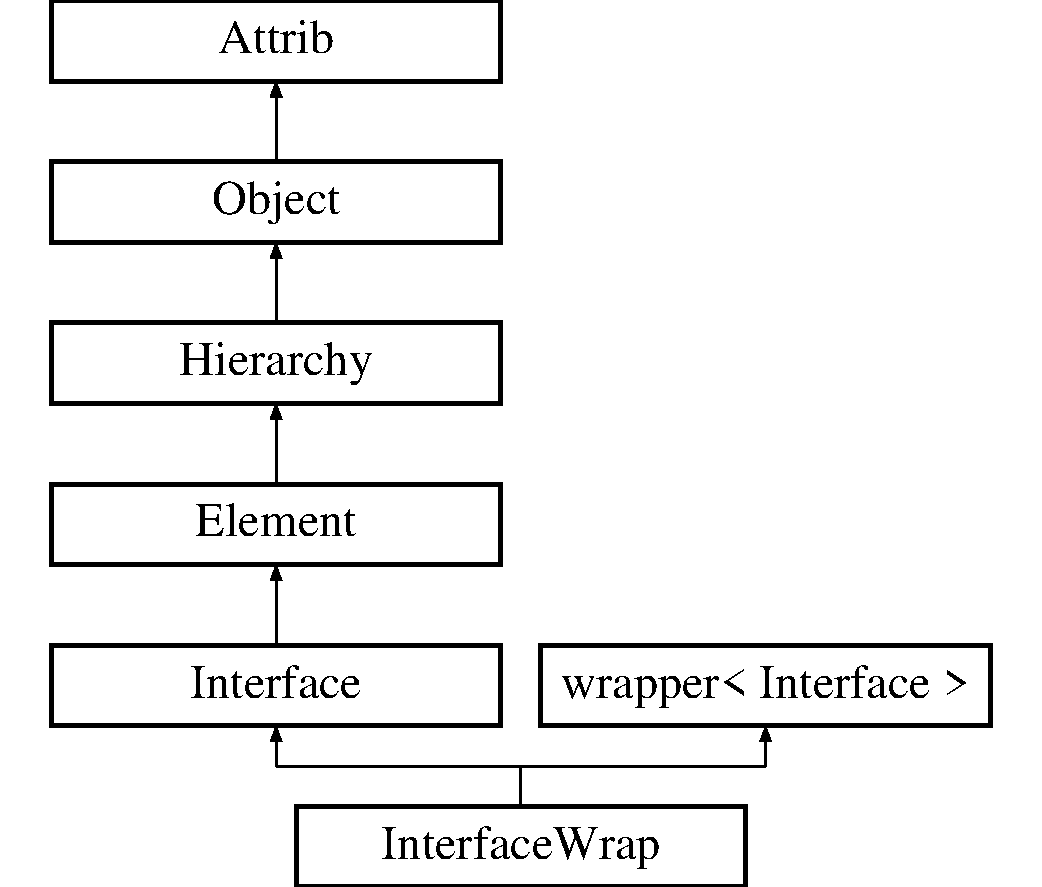
\includegraphics[height=6.000000cm]{structInterfaceWrap}
\end{center}
\end{figure}
\subsection*{Public Types}
\begin{DoxyCompactItemize}
\item 
enum \hyperlink{classAttrib_a69e171d7cc6417835a5a306d3c764235}{Attribut} \{ \newline
\hyperlink{classAttrib_a69e171d7cc6417835a5a306d3c764235a3a8da2ab97dda18aebab196fe4100531}{U\+N\+D\+E\+F\+I\+N\+ED}, 
\hyperlink{classAttrib_a69e171d7cc6417835a5a306d3c764235a2bfb2af57b87031d190a05fe25dd92ed}{P\+A\+S\+S\+I\+VE}, 
\hyperlink{classAttrib_a69e171d7cc6417835a5a306d3c764235a3b1fec929c0370d1436f2f06e298fb0d}{A\+C\+T\+I\+VE}, 
\hyperlink{classAttrib_a69e171d7cc6417835a5a306d3c764235aa27c16b480a369ea4d18b07b2516bbc7}{I\+N\+T\+E\+R\+F\+A\+CE}, 
\newline
\hyperlink{classAttrib_a69e171d7cc6417835a5a306d3c764235a1420a5b8c0540b2af210b6975eded7f9}{IO}, 
\hyperlink{classAttrib_a69e171d7cc6417835a5a306d3c764235a0af3b0d0ac323c1704e6c69cf90add28}{I\+O\+D\+A\+TA}, 
\hyperlink{classAttrib_a69e171d7cc6417835a5a306d3c764235a7788bc5dd333fd8ce18562b269c9dab1}{E\+L\+E\+M\+E\+NT}, 
\hyperlink{classAttrib_a69e171d7cc6417835a5a306d3c764235a61ceb22149f365f1780d18f9d1459423}{H\+A\+R\+D\+W\+A\+RE}, 
\newline
\hyperlink{classAttrib_a69e171d7cc6417835a5a306d3c764235a75250e29692496e73effca2c0330977f}{P\+R\+O\+C\+E\+S\+S\+US}, 
\hyperlink{classAttrib_a69e171d7cc6417835a5a306d3c764235a103a67cd0b8f07ef478fa45d4356e27b}{S\+O\+F\+T\+W\+A\+RE}
 \}
\end{DoxyCompactItemize}
\subsection*{Public Member Functions}
\begin{DoxyCompactItemize}
\item 
void \hyperlink{structInterfaceWrap_abcf87065a7b9099a7d05e7c0ddaf2487}{help} ()
\item 
\hyperlink{classStatusCode}{Status\+Code} \hyperlink{structInterfaceWrap_a2660ecdfbabd91d99d7b64c83e92f33c}{init} ()
\item 
void \hyperlink{structInterfaceWrap_a6c350b2f44c579187e6e4269cae29bae}{reset} ()
\item 
void \hyperlink{structInterfaceWrap_aee2f0407da52a1de8659b1d83af62238}{update} ()
\item 
\hyperlink{classStatusCode}{Status\+Code} \hyperlink{structInterfaceWrap_a4dd40213e6d37c73521450aa0c7a8f4d}{read} (\hyperlink{classIOdata}{I\+Odata} $\ast$)
\item 
\hyperlink{classStatusCode}{Status\+Code} \hyperlink{structInterfaceWrap_afbf6658c8be109e72f38d61438ec94d3}{write} (\hyperlink{classIOdata}{I\+Odata} $\ast$)
\item 
void \hyperlink{classElement_a3c0abcb36f8906688bb7e32608df7086}{recursive\+Init\+Element} ()
\item 
void \hyperlink{classElement_a82119ed37dff76508a2746a853ec35ba}{recursive\+Init\+Communications} ()
\item 
\hyperlink{classStatusCode}{Status\+Code} \hyperlink{classElement_ab476b4b1df5954141ceb14f072433b89}{set\+Connection} (\hyperlink{classHierarchy}{Hierarchy} $\ast$)
\item 
\hyperlink{classHierarchy}{Hierarchy} $\ast$ \hyperlink{classElement_af57444353c1ddf9fa0109801e97debf7}{connection} ()
\item 
void \hyperlink{classHierarchy_af4d43b0765b402670eed2d62c73405af}{clear} ()
\item 
void \hyperlink{classHierarchy_a585ad1aeec16077a0e532ab8b4fc557b}{set\+Parent} (\hyperlink{classHierarchy}{Hierarchy} $\ast$\hyperlink{classHierarchy_a1c7bec8257e717f9c1465e06ebf845fc}{parent})
\item 
\hyperlink{classHierarchy}{Hierarchy} $\ast$ \hyperlink{classHierarchy_a1c7bec8257e717f9c1465e06ebf845fc}{parent} ()
\item 
\hyperlink{classHierarchy}{Hierarchy} $\ast$ \hyperlink{classHierarchy_ad550588733bf75ac5c0fcfd7c8fd11a6}{parent} (std\+::string)
\item 
\hyperlink{classHierarchy}{Hierarchy} $\ast$ \hyperlink{classHierarchy_aee461dc930ce3871636ff87f075b1b83}{origin} ()
\item 
virtual void \hyperlink{classHierarchy_ad677774ff38fcb257c04a3a10d471fac}{add\+Child} (\hyperlink{classHierarchy}{Hierarchy} $\ast$element)
\item 
std\+::vector$<$ \hyperlink{classHierarchy}{Hierarchy} $\ast$ $>$ \hyperlink{classHierarchy_aa9a76f69e98e052ee1a6e32cea006288}{children} ()
\item 
\hyperlink{classHierarchy}{Hierarchy} $\ast$ \hyperlink{classHierarchy_a1e207f973c694b538bf90107b4868817}{child} (std\+::string)
\item 
\hyperlink{classHierarchy}{Hierarchy} $\ast$ \hyperlink{classHierarchy_a0c15a5276a3b80b4354d6bd8a01e0708}{child\+Typed} (std\+::string)
\item 
unsigned long \hyperlink{classHierarchy_ab16e84de65fd84e14001a6cf941c8be4}{number\+Of\+Children} ()
\item 
bool \hyperlink{classHierarchy_a255174fe4d316d2a3f430dcb9dab29f1}{has\+Children} ()
\item 
void \hyperlink{classHierarchy_a2b2b359fac003233f65786a616766bde}{del\+Child} (\hyperlink{classHierarchy}{Hierarchy} $\ast$)
\item 
void \hyperlink{classHierarchy_a1928ac7615fe0b5e55cd707f70dc6781}{del\+Child} (std\+::string)
\item 
std\+::string \hyperlink{classHierarchy_aa7990fa7caf132d83e361ce033c6c65a}{path} (std\+::string=std\+::string(\char`\"{}\char`\"{}))
\item 
std\+::string \hyperlink{classHierarchy_a1efd56cd164d328d2002e53a10a19b8c}{path\+Typed} (std\+::string=std\+::string(\char`\"{}\char`\"{}))
\item 
void \hyperlink{classHierarchy_a76e914b9a677a22a82deb74d892bf261}{tree} (std\+::string indent=std\+::string(\char`\"{}\char`\"{}))
\item 
void \hyperlink{classHierarchy_a594c294c5f60c230e106d522ed008212}{tree} ()
\item 
std\+::string \hyperlink{classObject_a300f4c05dd468c7bb8b3c968868443c1}{name} () const
\item 
std\+::string \hyperlink{classObject_a84f99f70f144a83e1582d1d0f84e4e62}{type} ()
\item 
unsigned char \hyperlink{classObject_af99145335cc61ff6e2798ea17db009d2}{id} ()
\item 
std\+::string \hyperlink{classObject_a73a0f1a41828fdd8303dd662446fb6c3}{title} ()
\item 
void \hyperlink{classObject_a3f9d5537ebce0c0f2bf6ae4d92426f3c}{msg\+Svc} (int level, std\+::string \hyperlink{classObject_a58b2d0618c2d08cf2383012611528d97}{msg}, std\+::string \hyperlink{classObject_a300f4c05dd468c7bb8b3c968868443c1}{name})
\item 
void \hyperlink{classObject_a58b2d0618c2d08cf2383012611528d97}{msg} (std\+::string mymsg)
\item 
void \hyperlink{classObject_ac5d59299273cee27aacf7de00d2e7034}{msg} (std\+::string mymsg, std\+::string \hyperlink{classObject_a300f4c05dd468c7bb8b3c968868443c1}{name})
\item 
void \hyperlink{classObject_a83d2db2df682907ea1115ad721c1c4a1}{verbose} (std\+::string mymsg)
\item 
void \hyperlink{classObject_a2d4120195317e2a3c6532e8bb9f3da68}{verbose} (std\+::string mymsg, std\+::string \hyperlink{classObject_a300f4c05dd468c7bb8b3c968868443c1}{name})
\item 
void \hyperlink{classObject_aac010553f022165573714b7014a15f0d}{debug} (std\+::string mymsg)
\item 
void \hyperlink{classObject_a6c9a0397ca804e04d675ed05683f5420}{debug} (std\+::string mymsg, std\+::string \hyperlink{classObject_a300f4c05dd468c7bb8b3c968868443c1}{name})
\item 
void \hyperlink{classObject_a644fd329ea4cb85f54fa6846484b84a8}{info} (std\+::string mymsg)
\item 
void \hyperlink{classObject_a1ca123253dfd30fc28b156f521dcbdae}{info} (std\+::string mymsg, std\+::string \hyperlink{classObject_a300f4c05dd468c7bb8b3c968868443c1}{name})
\item 
void \hyperlink{classObject_a65cd4fda577711660821fd2cd5a3b4c9}{warning} (std\+::string mymsg)
\item 
void \hyperlink{classObject_a11f101db4dd73d9391b0231818881d86}{warning} (std\+::string mymsg, std\+::string \hyperlink{classObject_a300f4c05dd468c7bb8b3c968868443c1}{name})
\item 
void \hyperlink{classObject_a204a95f57818c0f811933917a30eff45}{error} (std\+::string mymsg)
\item 
void \hyperlink{classObject_ad7f6c457733082efa2f9ff5f5c8e119a}{error} (std\+::string mymsg, std\+::string \hyperlink{classObject_a300f4c05dd468c7bb8b3c968868443c1}{name})
\item 
void \hyperlink{classObject_aad5a16aac7516ce65bd5ec02ab07fc80}{fatal} (std\+::string mymsg)
\item 
void \hyperlink{classObject_ae62acd3d09f716220f75f252dc38bc9a}{fatal} (std\+::string mymsg, std\+::string \hyperlink{classObject_a300f4c05dd468c7bb8b3c968868443c1}{name})
\item 
void \hyperlink{classObject_ae30fea75683c2d149b6b6d17c09ecd0c}{set\+Name} (std\+::string \hyperlink{classObject_a300f4c05dd468c7bb8b3c968868443c1}{name})
\item 
void \hyperlink{classObject_aae534cc9d982bcb9b99fd505f2e103a5}{set\+Type} (std\+::string \hyperlink{classObject_a84f99f70f144a83e1582d1d0f84e4e62}{type})
\item 
void \hyperlink{classObject_a398fe08cba594a0ce6891d59fe4f159f}{set\+Id} (unsigned char \hyperlink{classObject_af99145335cc61ff6e2798ea17db009d2}{id})
\item 
void \hyperlink{classObject_a89557dbbad5bcaa02652f5d7fa35d20f}{set\+Title} (std\+::string \hyperlink{classObject_a73a0f1a41828fdd8303dd662446fb6c3}{title})
\item 
void \hyperlink{classObject_a870c5af919958c2136623b2d7816d123}{set\+Dll\+Name} (std\+::string \hyperlink{classObject_a2e3947f2870094c332d7454117f3ec63}{dll\+Name})
\item 
std\+::string \hyperlink{classObject_a2e3947f2870094c332d7454117f3ec63}{dll\+Name} ()
\item 
bool \hyperlink{classAttrib_a704f26af560909ad22065083bb7d4c34}{is} (int attribut)
\item 
void \hyperlink{classAttrib_a235f773af19c900264a190b00a3b4ad7}{add} (int attribut)
\item 
void \hyperlink{classAttrib_a7d4ef7e32d93cb287792b87b857e79f3}{remove} (int attribut)
\item 
std\+::string \hyperlink{classAttrib_aee7bbf16b144887f196e1341b24f8a26}{attributs} ()
\end{DoxyCompactItemize}
\subsection*{Protected Attributes}
\begin{DoxyCompactItemize}
\item 
\hyperlink{classHierarchy}{Hierarchy} $\ast$ \hyperlink{classElement_abe3de7a5dbbc9a6dd2d7e012e5fdb266}{m\+\_\+connection}
\item 
std\+::string \hyperlink{classAttrib_a3414521d7a82476e874b25a5407b5e63}{m\+\_\+attrib\+String} \mbox{[}10\mbox{]}
\end{DoxyCompactItemize}


\subsection{Detailed Description}


Definition at line 17 of file Python.\+cpp.



\subsection{Member Enumeration Documentation}
\mbox{\Hypertarget{classAttrib_a69e171d7cc6417835a5a306d3c764235}\label{classAttrib_a69e171d7cc6417835a5a306d3c764235}} 
\index{Interface\+Wrap@{Interface\+Wrap}!Attribut@{Attribut}}
\index{Attribut@{Attribut}!Interface\+Wrap@{Interface\+Wrap}}
\subsubsection{\texorpdfstring{Attribut}{Attribut}}
{\footnotesize\ttfamily enum \hyperlink{classAttrib_a69e171d7cc6417835a5a306d3c764235}{Attrib\+::\+Attribut}\hspace{0.3cm}{\ttfamily [inherited]}}

\begin{DoxyEnumFields}{Enumerator}
\raisebox{\heightof{T}}[0pt][0pt]{\index{U\+N\+D\+E\+F\+I\+N\+ED@{U\+N\+D\+E\+F\+I\+N\+ED}!Interface\+Wrap@{Interface\+Wrap}}\index{Interface\+Wrap@{Interface\+Wrap}!U\+N\+D\+E\+F\+I\+N\+ED@{U\+N\+D\+E\+F\+I\+N\+ED}}}\mbox{\Hypertarget{classAttrib_a69e171d7cc6417835a5a306d3c764235a3a8da2ab97dda18aebab196fe4100531}\label{classAttrib_a69e171d7cc6417835a5a306d3c764235a3a8da2ab97dda18aebab196fe4100531}} 
U\+N\+D\+E\+F\+I\+N\+ED&\\
\hline

\raisebox{\heightof{T}}[0pt][0pt]{\index{P\+A\+S\+S\+I\+VE@{P\+A\+S\+S\+I\+VE}!Interface\+Wrap@{Interface\+Wrap}}\index{Interface\+Wrap@{Interface\+Wrap}!P\+A\+S\+S\+I\+VE@{P\+A\+S\+S\+I\+VE}}}\mbox{\Hypertarget{classAttrib_a69e171d7cc6417835a5a306d3c764235a2bfb2af57b87031d190a05fe25dd92ed}\label{classAttrib_a69e171d7cc6417835a5a306d3c764235a2bfb2af57b87031d190a05fe25dd92ed}} 
P\+A\+S\+S\+I\+VE&\\
\hline

\raisebox{\heightof{T}}[0pt][0pt]{\index{A\+C\+T\+I\+VE@{A\+C\+T\+I\+VE}!Interface\+Wrap@{Interface\+Wrap}}\index{Interface\+Wrap@{Interface\+Wrap}!A\+C\+T\+I\+VE@{A\+C\+T\+I\+VE}}}\mbox{\Hypertarget{classAttrib_a69e171d7cc6417835a5a306d3c764235a3b1fec929c0370d1436f2f06e298fb0d}\label{classAttrib_a69e171d7cc6417835a5a306d3c764235a3b1fec929c0370d1436f2f06e298fb0d}} 
A\+C\+T\+I\+VE&\\
\hline

\raisebox{\heightof{T}}[0pt][0pt]{\index{I\+N\+T\+E\+R\+F\+A\+CE@{I\+N\+T\+E\+R\+F\+A\+CE}!Interface\+Wrap@{Interface\+Wrap}}\index{Interface\+Wrap@{Interface\+Wrap}!I\+N\+T\+E\+R\+F\+A\+CE@{I\+N\+T\+E\+R\+F\+A\+CE}}}\mbox{\Hypertarget{classAttrib_a69e171d7cc6417835a5a306d3c764235aa27c16b480a369ea4d18b07b2516bbc7}\label{classAttrib_a69e171d7cc6417835a5a306d3c764235aa27c16b480a369ea4d18b07b2516bbc7}} 
I\+N\+T\+E\+R\+F\+A\+CE&\\
\hline

\raisebox{\heightof{T}}[0pt][0pt]{\index{IO@{IO}!Interface\+Wrap@{Interface\+Wrap}}\index{Interface\+Wrap@{Interface\+Wrap}!IO@{IO}}}\mbox{\Hypertarget{classAttrib_a69e171d7cc6417835a5a306d3c764235a1420a5b8c0540b2af210b6975eded7f9}\label{classAttrib_a69e171d7cc6417835a5a306d3c764235a1420a5b8c0540b2af210b6975eded7f9}} 
IO&\\
\hline

\raisebox{\heightof{T}}[0pt][0pt]{\index{I\+O\+D\+A\+TA@{I\+O\+D\+A\+TA}!Interface\+Wrap@{Interface\+Wrap}}\index{Interface\+Wrap@{Interface\+Wrap}!I\+O\+D\+A\+TA@{I\+O\+D\+A\+TA}}}\mbox{\Hypertarget{classAttrib_a69e171d7cc6417835a5a306d3c764235a0af3b0d0ac323c1704e6c69cf90add28}\label{classAttrib_a69e171d7cc6417835a5a306d3c764235a0af3b0d0ac323c1704e6c69cf90add28}} 
I\+O\+D\+A\+TA&\\
\hline

\raisebox{\heightof{T}}[0pt][0pt]{\index{E\+L\+E\+M\+E\+NT@{E\+L\+E\+M\+E\+NT}!Interface\+Wrap@{Interface\+Wrap}}\index{Interface\+Wrap@{Interface\+Wrap}!E\+L\+E\+M\+E\+NT@{E\+L\+E\+M\+E\+NT}}}\mbox{\Hypertarget{classAttrib_a69e171d7cc6417835a5a306d3c764235a7788bc5dd333fd8ce18562b269c9dab1}\label{classAttrib_a69e171d7cc6417835a5a306d3c764235a7788bc5dd333fd8ce18562b269c9dab1}} 
E\+L\+E\+M\+E\+NT&\\
\hline

\raisebox{\heightof{T}}[0pt][0pt]{\index{H\+A\+R\+D\+W\+A\+RE@{H\+A\+R\+D\+W\+A\+RE}!Interface\+Wrap@{Interface\+Wrap}}\index{Interface\+Wrap@{Interface\+Wrap}!H\+A\+R\+D\+W\+A\+RE@{H\+A\+R\+D\+W\+A\+RE}}}\mbox{\Hypertarget{classAttrib_a69e171d7cc6417835a5a306d3c764235a61ceb22149f365f1780d18f9d1459423}\label{classAttrib_a69e171d7cc6417835a5a306d3c764235a61ceb22149f365f1780d18f9d1459423}} 
H\+A\+R\+D\+W\+A\+RE&\\
\hline

\raisebox{\heightof{T}}[0pt][0pt]{\index{P\+R\+O\+C\+E\+S\+S\+US@{P\+R\+O\+C\+E\+S\+S\+US}!Interface\+Wrap@{Interface\+Wrap}}\index{Interface\+Wrap@{Interface\+Wrap}!P\+R\+O\+C\+E\+S\+S\+US@{P\+R\+O\+C\+E\+S\+S\+US}}}\mbox{\Hypertarget{classAttrib_a69e171d7cc6417835a5a306d3c764235a75250e29692496e73effca2c0330977f}\label{classAttrib_a69e171d7cc6417835a5a306d3c764235a75250e29692496e73effca2c0330977f}} 
P\+R\+O\+C\+E\+S\+S\+US&\\
\hline

\raisebox{\heightof{T}}[0pt][0pt]{\index{S\+O\+F\+T\+W\+A\+RE@{S\+O\+F\+T\+W\+A\+RE}!Interface\+Wrap@{Interface\+Wrap}}\index{Interface\+Wrap@{Interface\+Wrap}!S\+O\+F\+T\+W\+A\+RE@{S\+O\+F\+T\+W\+A\+RE}}}\mbox{\Hypertarget{classAttrib_a69e171d7cc6417835a5a306d3c764235a103a67cd0b8f07ef478fa45d4356e27b}\label{classAttrib_a69e171d7cc6417835a5a306d3c764235a103a67cd0b8f07ef478fa45d4356e27b}} 
S\+O\+F\+T\+W\+A\+RE&\\
\hline

\end{DoxyEnumFields}


Definition at line 29 of file Attrib.\+h.


\begin{DoxyCode}
29                 \{
30     \hyperlink{classAttrib_a69e171d7cc6417835a5a306d3c764235a3a8da2ab97dda18aebab196fe4100531}{UNDEFINED},
31     \hyperlink{classAttrib_a69e171d7cc6417835a5a306d3c764235a2bfb2af57b87031d190a05fe25dd92ed}{PASSIVE},
32     \hyperlink{classAttrib_a69e171d7cc6417835a5a306d3c764235a3b1fec929c0370d1436f2f06e298fb0d}{ACTIVE},
33     \hyperlink{classAttrib_a69e171d7cc6417835a5a306d3c764235aa27c16b480a369ea4d18b07b2516bbc7}{INTERFACE},
34     \hyperlink{classAttrib_a69e171d7cc6417835a5a306d3c764235a1420a5b8c0540b2af210b6975eded7f9}{IO},
35     \hyperlink{classAttrib_a69e171d7cc6417835a5a306d3c764235a0af3b0d0ac323c1704e6c69cf90add28}{IODATA},
36     \hyperlink{classAttrib_a69e171d7cc6417835a5a306d3c764235a7788bc5dd333fd8ce18562b269c9dab1}{ELEMENT},
37     \hyperlink{classAttrib_a69e171d7cc6417835a5a306d3c764235a61ceb22149f365f1780d18f9d1459423}{HARDWARE},
38     \hyperlink{classAttrib_a69e171d7cc6417835a5a306d3c764235a75250e29692496e73effca2c0330977f}{PROCESSUS},
39     \hyperlink{classAttrib_a69e171d7cc6417835a5a306d3c764235a103a67cd0b8f07ef478fa45d4356e27b}{SOFTWARE} 
40   \}; \textcolor{comment}{// array m\_attribString must be changed into Attrib::Attrib if this enu is modified. }
\end{DoxyCode}


\subsection{Member Function Documentation}
\mbox{\Hypertarget{classAttrib_a235f773af19c900264a190b00a3b4ad7}\label{classAttrib_a235f773af19c900264a190b00a3b4ad7}} 
\index{Interface\+Wrap@{Interface\+Wrap}!add@{add}}
\index{add@{add}!Interface\+Wrap@{Interface\+Wrap}}
\subsubsection{\texorpdfstring{add()}{add()}}
{\footnotesize\ttfamily void Attrib\+::add (\begin{DoxyParamCaption}\item[{int}]{attribut }\end{DoxyParamCaption})\hspace{0.3cm}{\ttfamily [inline]}, {\ttfamily [inherited]}}

Add an attribut 

Definition at line 67 of file Attrib.\+h.



References Attrib\+::m\+\_\+attributs, and Attrib\+::\+U\+N\+D\+E\+F\+I\+N\+ED.



Referenced by A3\+P\+E\+::\+A3\+P\+E(), Attrib\+::\+Attrib(), Specs\+Mezzanine\+::cmdline(), Computer\+::\+Computer(), C\+U\+\_\+v1\+::\+C\+U\+\_\+v1(), export\+\_\+obj(), F\+E\+B\+\_\+v1\+::\+F\+E\+B\+\_\+v1(), Fe\+P\+G\+A\+::\+Fe\+P\+G\+A(), I\+C\+E\+C\+A\+Lv3\+::\+I\+C\+E\+C\+A\+Lv3(), I\+C\+Phaser\+::\+I\+C\+Phaser(), Fe\+P\+G\+A\+::init(), Application\+::initialize(), Interface\+::\+Interface(), I\+Odata\+::\+I\+Odata(), I\+Oobject\+::\+I\+Oobject(), M\+S\+Oxxxx\+::\+M\+S\+Oxxxx(), Phaser\+::\+Phaser(), Processus\+::\+Processus(), Proto40\+M\+Hz\+\_\+v1\+::\+Proto40\+M\+Hz\+\_\+v1(), Attrib\+::remove(), Seq\+P\+G\+A\+::\+Seq\+P\+G\+A(), Test\+I2\+C\+::set\+Address(), Test\+S\+P\+I\+::set\+Address(), Specs\+Slave\+::set\+Address(), Specs\+Master\+::\+Specs\+Master(), and Specs\+Slave\+::\+Specs\+Slave().


\begin{DoxyCode}
67                             \{
68     \textcolor{keywordflow}{if} (attribut!=\hyperlink{classAttrib_a69e171d7cc6417835a5a306d3c764235a3a8da2ab97dda18aebab196fe4100531}{Attrib::UNDEFINED}) \textcolor{keyword}{remove}(\hyperlink{classAttrib_a69e171d7cc6417835a5a306d3c764235a3a8da2ab97dda18aebab196fe4100531}{Attrib::UNDEFINED});
69     \textcolor{keywordtype}{bool} duplicate = false ;
70     std::vector<int>::const\_iterator iter ;
71     \textcolor{keywordflow}{for} ( iter  = \hyperlink{classAttrib_ac4bd58a0cc6b38a3b711d609a3d3aacc}{m\_attributs}.begin() ;
72           iter != \hyperlink{classAttrib_ac4bd58a0cc6b38a3b711d609a3d3aacc}{m\_attributs}.end()   ;
73           ++iter ) \{
74       \textcolor{keywordflow}{if} ( attribut == (*iter) ) \{
75         duplicate = true ;
76       \}
77     \}
78     \textcolor{keywordflow}{if} (!duplicate) \{
79       \hyperlink{classAttrib_ac4bd58a0cc6b38a3b711d609a3d3aacc}{m\_attributs}.push\_back( attribut );
80     \}
81   \}
\end{DoxyCode}
\mbox{\Hypertarget{classHierarchy_ad677774ff38fcb257c04a3a10d471fac}\label{classHierarchy_ad677774ff38fcb257c04a3a10d471fac}} 
\index{Interface\+Wrap@{Interface\+Wrap}!add\+Child@{add\+Child}}
\index{add\+Child@{add\+Child}!Interface\+Wrap@{Interface\+Wrap}}
\subsubsection{\texorpdfstring{add\+Child()}{addChild()}}
{\footnotesize\ttfamily void Hierarchy\+::add\+Child (\begin{DoxyParamCaption}\item[{\hyperlink{classHierarchy}{Hierarchy} $\ast$}]{element }\end{DoxyParamCaption})\hspace{0.3cm}{\ttfamily [virtual]}, {\ttfamily [inherited]}}



Definition at line 83 of file Hierarchy.\+cpp.



References Object\+::debug(), Hierarchy\+::m\+\_\+children, Object\+::name(), and Hierarchy\+::set\+Parent().



Referenced by A3\+P\+E\+::\+A3\+P\+E(), Specs\+Mezzanine\+::add\+Bus(), Specs\+Slave\+::add\+I2c(), Application\+::create(), C\+U\+\_\+v1\+::\+C\+U\+\_\+v1(), export\+\_\+obj(), F\+E\+B\+\_\+v1\+::\+F\+E\+B\+\_\+v1(), Fe\+P\+G\+A\+::\+Fe\+P\+G\+A(), I\+C\+E\+C\+A\+Lv3\+::\+I\+C\+E\+C\+A\+Lv3(), I\+C\+Phaser\+::\+I\+C\+Phaser(), Fe\+P\+G\+A\+::\+Make\+R\+A\+M(), Fe\+P\+G\+A\+::\+Make\+Register(), Hierarchy\+::origin(), Phaser\+::\+Phaser(), Proto40\+M\+Hz\+\_\+v1\+::\+Proto40\+M\+Hz\+\_\+v1(), Seq\+P\+G\+A\+::\+Seq\+P\+G\+A(), Specs\+Mezzanine\+::\+Specs\+Mezzanine(), Usb\+I2c\+Bus\+::\+Usb\+I2c\+Bus(), and Usb\+Spi\+Bus\+::\+Usb\+Spi\+Bus().


\begin{DoxyCode}
83                                           \{
84   element->\hyperlink{classHierarchy_a585ad1aeec16077a0e532ab8b4fc557b}{setParent}(\textcolor{keyword}{this});
85   \hyperlink{classHierarchy_a038816763941fd4a930504917f60483b}{m\_children}.push\_back(element);
86   \hyperlink{classObject_aac010553f022165573714b7014a15f0d}{debug}(element->\hyperlink{classObject_a300f4c05dd468c7bb8b3c968868443c1}{name}()+\textcolor{stringliteral}{" added to the child tree."},\textcolor{stringliteral}{"Hierarchy::addChild"});
87 \}
\end{DoxyCode}
\mbox{\Hypertarget{classAttrib_aee7bbf16b144887f196e1341b24f8a26}\label{classAttrib_aee7bbf16b144887f196e1341b24f8a26}} 
\index{Interface\+Wrap@{Interface\+Wrap}!attributs@{attributs}}
\index{attributs@{attributs}!Interface\+Wrap@{Interface\+Wrap}}
\subsubsection{\texorpdfstring{attributs()}{attributs()}}
{\footnotesize\ttfamily std\+::string Attrib\+::attributs (\begin{DoxyParamCaption}{ }\end{DoxyParamCaption})\hspace{0.3cm}{\ttfamily [inherited]}}

Print the \hyperlink{classAttrib}{Attrib} of an \hyperlink{classObject}{Object} 

Definition at line 54 of file Attrib.\+cpp.



References images\+::index, Attrib\+::m\+\_\+attrib\+String, and Attrib\+::m\+\_\+attributs.



Referenced by export\+\_\+obj(), and Attrib\+::remove().


\begin{DoxyCode}
54                             \{
55   std::string output;
56   std::vector<int>::iterator iter ;
57   \textcolor{keywordflow}{for} ( \textcolor{keywordtype}{unsigned} \textcolor{keywordtype}{int} \hyperlink{namespaceimages_a54407fd574970b3178647ae096321a57}{index} = 0 ; \hyperlink{namespaceimages_a54407fd574970b3178647ae096321a57}{index} < \hyperlink{classAttrib_ac4bd58a0cc6b38a3b711d609a3d3aacc}{m\_attributs}.size() ; ++
      \hyperlink{namespaceimages_a54407fd574970b3178647ae096321a57}{index} ) \{
58     \textcolor{keywordflow}{if} ( \hyperlink{classAttrib_ac4bd58a0cc6b38a3b711d609a3d3aacc}{m\_attributs}.size() - \hyperlink{namespaceimages_a54407fd574970b3178647ae096321a57}{index} > 1 ) \{
59       output.append(\hyperlink{classAttrib_a3414521d7a82476e874b25a5407b5e63}{m\_attribString}[\hyperlink{classAttrib_ac4bd58a0cc6b38a3b711d609a3d3aacc}{m\_attributs}[\hyperlink{namespaceimages_a54407fd574970b3178647ae096321a57}{index}]]);
60       output.append(\textcolor{stringliteral}{":"});
61     \}
62     \textcolor{keywordflow}{else} \{
63       output.append(\hyperlink{classAttrib_a3414521d7a82476e874b25a5407b5e63}{m\_attribString}[\hyperlink{classAttrib_ac4bd58a0cc6b38a3b711d609a3d3aacc}{m\_attributs}[index]]);
64     \}
65   \}
66   \textcolor{keywordflow}{return} output;
67 \}
\end{DoxyCode}
\mbox{\Hypertarget{classHierarchy_a1e207f973c694b538bf90107b4868817}\label{classHierarchy_a1e207f973c694b538bf90107b4868817}} 
\index{Interface\+Wrap@{Interface\+Wrap}!child@{child}}
\index{child@{child}!Interface\+Wrap@{Interface\+Wrap}}
\subsubsection{\texorpdfstring{child()}{child()}}
{\footnotesize\ttfamily \hyperlink{classHierarchy}{Hierarchy} $\ast$ Hierarchy\+::child (\begin{DoxyParamCaption}\item[{std\+::string}]{path }\end{DoxyParamCaption})\hspace{0.3cm}{\ttfamily [inherited]}}



Definition at line 133 of file Hierarchy.\+cpp.



References Hierarchy\+::child(), Hierarchy\+::children(), Object\+::name(), Hierarchy\+::origin(), Hierarchy\+::parent(), Hierarchy\+::path(), and Object\+::warning().



Referenced by Application\+::cd(), Hierarchy\+::child(), Hierarchy\+::children(), and export\+\_\+obj().


\begin{DoxyCode}
133                                          \{
134   std::string newpath = \hyperlink{classHierarchy_aa7990fa7caf132d83e361ce033c6c65a}{path};
135   std::string up(\textcolor{stringliteral}{".."});
136   std::string separator(1,\textcolor{charliteral}{'/'});
137 
138   \hyperlink{classHierarchy}{Hierarchy} * newcurrent = 0;
139 
140   \textcolor{comment}{//  info("path="+path,"Hierarchy::child");}
141 
142   \textcolor{keywordflow}{if} (\hyperlink{classHierarchy_aa7990fa7caf132d83e361ce033c6c65a}{path}.compare(\textcolor{stringliteral}{""})==0 || \hyperlink{classHierarchy_aa7990fa7caf132d83e361ce033c6c65a}{path}.compare(\textcolor{stringliteral}{"/"})==0) \{
143     \textcolor{comment}{//    debug("return origin","Hierarchy::child");}
144     \textcolor{keywordflow}{return} \hyperlink{classHierarchy_aee461dc930ce3871636ff87f075b1b83}{origin}();
145   \}
146 
147   \textcolor{keywordflow}{if} (\hyperlink{classHierarchy_aa7990fa7caf132d83e361ce033c6c65a}{path}.compare(\hyperlink{classObject_a300f4c05dd468c7bb8b3c968868443c1}{name}())==0)\{
148     \textcolor{comment}{//    debug("return itself","Hierarchy::child");}
149     \textcolor{keywordflow}{return} \textcolor{keyword}{this};
150   \}
151 
152   \textcolor{keywordflow}{if} (\hyperlink{classHierarchy_aa7990fa7caf132d83e361ce033c6c65a}{path}.compare(\textcolor{stringliteral}{".."})==0)\{
153     \textcolor{keywordflow}{if} (0!=this->\hyperlink{classHierarchy_a1c7bec8257e717f9c1465e06ebf845fc}{parent}()) \textcolor{keywordflow}{return} this->\hyperlink{classHierarchy_a1c7bec8257e717f9c1465e06ebf845fc}{parent}();
154     \textcolor{keywordflow}{else} \textcolor{keywordflow}{return} \textcolor{keyword}{this};
155   \}
156 
157   \textcolor{keywordflow}{if} (\hyperlink{classHierarchy_aa7990fa7caf132d83e361ce033c6c65a}{path}.compare(\textcolor{stringliteral}{"../"})==0)\{
158     \textcolor{keywordflow}{if} (0!=this->\hyperlink{classHierarchy_a1c7bec8257e717f9c1465e06ebf845fc}{parent}()) \textcolor{keywordflow}{return} this->\hyperlink{classHierarchy_a1c7bec8257e717f9c1465e06ebf845fc}{parent}();
159     \textcolor{keywordflow}{else} \textcolor{keywordflow}{return} \textcolor{keyword}{this};
160   \}
161 
162 
163   \textcolor{keywordtype}{int} npos=\hyperlink{classHierarchy_aa7990fa7caf132d83e361ce033c6c65a}{path}.find(separator,0);
164 
165   \textcolor{comment}{//  info("find separator in "+itos(npos)+" of "+path,"Hierarchy::child");}
166 
167   \textcolor{comment}{// remove last separator}
168   \textcolor{keywordflow}{if} ( npos == (\textcolor{keywordtype}{int})(\hyperlink{classHierarchy_aa7990fa7caf132d83e361ce033c6c65a}{path}.size()-1) ) \{
169     newpath = std::string(\hyperlink{classHierarchy_aa7990fa7caf132d83e361ce033c6c65a}{path},0,npos);
170     \hyperlink{classHierarchy_aa7990fa7caf132d83e361ce033c6c65a}{path} = newpath;
171   \}
172 
173   \textcolor{keywordflow}{if} (npos==0)\{
174     \textcolor{comment}{//    debug("Going back to origin and calling child","Hierarchy::child");}
175     newpath=std::string(\hyperlink{classHierarchy_aa7990fa7caf132d83e361ce033c6c65a}{path},1,\hyperlink{classHierarchy_aa7990fa7caf132d83e361ce033c6c65a}{path}.size()-1);
176     \textcolor{keywordflow}{return} \hyperlink{classHierarchy_aee461dc930ce3871636ff87f075b1b83}{origin}()->\hyperlink{classHierarchy_a1e207f973c694b538bf90107b4868817}{child}(newpath);
177   \}
178   \textcolor{keywordflow}{else}\{
179     \textcolor{keywordflow}{if} ( npos== (\textcolor{keywordtype}{int})(std::string::npos) )\{
180       \textcolor{comment}{//      debug("Getting chid "+path+" of "+this->name(),"Hierarchy::child");}
181       std::vector <Hierarchy*> list = \hyperlink{classHierarchy_aa9a76f69e98e052ee1a6e32cea006288}{children}();
182       std::vector<Hierarchy*>::iterator iter;
183       \textcolor{keywordflow}{for} (iter=list.begin();iter!=list.end();iter++)\{
184         \textcolor{keywordflow}{if} ((*iter)->name().compare(\hyperlink{classHierarchy_aa7990fa7caf132d83e361ce033c6c65a}{path})==0)\{
185           \textcolor{keywordflow}{return} *iter;
186         \}
187       \}
188       \hyperlink{classObject_a65cd4fda577711660821fd2cd5a3b4c9}{warning}(this->\hyperlink{classObject_a300f4c05dd468c7bb8b3c968868443c1}{name}()+std::string(\textcolor{stringliteral}{" has no child '"})+\hyperlink{classHierarchy_aa7990fa7caf132d83e361ce033c6c65a}{path}+\textcolor{stringliteral}{"'"},\textcolor{stringliteral}{"Hierarchy::child"});
189       \textcolor{keywordflow}{return} \textcolor{keyword}{this};
190     \}
191     \textcolor{keywordflow}{else}
192     \{
193       \textcolor{keywordtype}{int} ipos=\hyperlink{classHierarchy_aa7990fa7caf132d83e361ce033c6c65a}{path}.find(separator,0);
194       \textcolor{comment}{//      info("default behaviour "+path+" with separator in "+itos(ipos),"Hierarchy::child");}
195 
196       std::string newcurrentname=std::string(\hyperlink{classHierarchy_aa7990fa7caf132d83e361ce033c6c65a}{path},0,ipos);
197       newpath=std::string(\hyperlink{classHierarchy_aa7990fa7caf132d83e361ce033c6c65a}{path},ipos+1,\hyperlink{classHierarchy_aa7990fa7caf132d83e361ce033c6c65a}{path}.size()-1);
198 
199       \textcolor{comment}{//      info("looking now for "+newpath+" from "+newcurrentname,"Hierarchy::child");}
200 
201       \textcolor{keywordflow}{if} (0==newcurrentname.compare(\hyperlink{classHierarchy_aee461dc930ce3871636ff87f075b1b83}{origin}()->\hyperlink{classObject_a300f4c05dd468c7bb8b3c968868443c1}{name}()))\{
202         \textcolor{comment}{//        info("current is computer. Looking for children"+newcurrentname,"Hierarchy::child");}
203         \textcolor{keywordflow}{return} \hyperlink{classHierarchy_aee461dc930ce3871636ff87f075b1b83}{origin}()->\hyperlink{classHierarchy_a1e207f973c694b538bf90107b4868817}{child}(newpath);
204       \}
205 
206       newcurrent = (\hyperlink{classHierarchy}{Hierarchy}*)0;
207 
208       std::vector <Hierarchy*> list = \hyperlink{classHierarchy_aa9a76f69e98e052ee1a6e32cea006288}{children}();
209       std::vector<Hierarchy*>::iterator iter;
210       \textcolor{keywordflow}{for} (iter=list.begin();iter!=list.end();iter++)\{
211         \textcolor{keywordflow}{if} ((*iter)->name().compare(newcurrentname)==0)\{
212           newcurrent = (*iter);
213         \}
214       \}
215 
216 
217       \textcolor{keywordflow}{if} ((\hyperlink{classHierarchy}{Hierarchy}*)0==newcurrent)\{
218         \textcolor{keywordflow}{if} (newcurrentname.compare(\textcolor{stringliteral}{".."})==0 && 0!=\hyperlink{classHierarchy_a1c7bec8257e717f9c1465e06ebf845fc}{parent}())\{
219           newcurrent=this->\hyperlink{classHierarchy_a1c7bec8257e717f9c1465e06ebf845fc}{parent}();
220           \textcolor{comment}{//          debug("newcurrent was .. -> parent="+parent()->name());}
221         \}
222         \textcolor{keywordflow}{else}
223         \{
224           \hyperlink{classObject_a65cd4fda577711660821fd2cd5a3b4c9}{warning}(this->\hyperlink{classObject_a300f4c05dd468c7bb8b3c968868443c1}{name}()+\textcolor{stringliteral}{" has no child '"}+newcurrentname+\textcolor{stringliteral}{"'"},
225               \textcolor{stringliteral}{"Hierarchy::child"});
226           \textcolor{keywordflow}{return} \textcolor{keyword}{this};
227         \}
228       \}
229       \textcolor{comment}{//      debug("recurrence call for "+newpath+" on "+newcurrent->name(),"Hierarchy::child");}
230       \textcolor{keywordflow}{return} newcurrent -> \hyperlink{classHierarchy_a1e207f973c694b538bf90107b4868817}{child} ( newpath );
231     \}
232   \}
233 \}
\end{DoxyCode}
\mbox{\Hypertarget{classHierarchy_aa9a76f69e98e052ee1a6e32cea006288}\label{classHierarchy_aa9a76f69e98e052ee1a6e32cea006288}} 
\index{Interface\+Wrap@{Interface\+Wrap}!children@{children}}
\index{children@{children}!Interface\+Wrap@{Interface\+Wrap}}
\subsubsection{\texorpdfstring{children()}{children()}}
{\footnotesize\ttfamily std\+::vector$<$\hyperlink{classHierarchy}{Hierarchy}$\ast$$>$ Hierarchy\+::children (\begin{DoxyParamCaption}{ }\end{DoxyParamCaption})\hspace{0.3cm}{\ttfamily [inline]}, {\ttfamily [inherited]}}



Definition at line 33 of file Hierarchy.\+h.



References Hierarchy\+::child(), Hierarchy\+::child\+Typed(), Hierarchy\+::del\+Child(), Hierarchy\+::has\+Children(), Hierarchy\+::m\+\_\+children, Hierarchy\+::number\+Of\+Children(), Hierarchy\+::path(), Hierarchy\+::path\+Typed(), and Hierarchy\+::tree().



Referenced by Hierarchy\+::child(), Hierarchy\+::child\+Typed(), export\+\_\+obj(), Specs\+Slave\+::recursive\+Init\+Communications(), Element\+::recursive\+Init\+Communications(), Element\+::recursive\+Init\+Element(), Application\+::set\+Config(), and Hierarchy\+::tree().


\begin{DoxyCode}
33 \{ \textcolor{keywordflow}{return} \hyperlink{classHierarchy_a038816763941fd4a930504917f60483b}{m\_children};  \} \textcolor{comment}{//< get list of child(ren)}
\end{DoxyCode}
\mbox{\Hypertarget{classHierarchy_a0c15a5276a3b80b4354d6bd8a01e0708}\label{classHierarchy_a0c15a5276a3b80b4354d6bd8a01e0708}} 
\index{Interface\+Wrap@{Interface\+Wrap}!child\+Typed@{child\+Typed}}
\index{child\+Typed@{child\+Typed}!Interface\+Wrap@{Interface\+Wrap}}
\subsubsection{\texorpdfstring{child\+Typed()}{childTyped()}}
{\footnotesize\ttfamily \hyperlink{classHierarchy}{Hierarchy} $\ast$ Hierarchy\+::child\+Typed (\begin{DoxyParamCaption}\item[{std\+::string}]{path }\end{DoxyParamCaption})\hspace{0.3cm}{\ttfamily [inherited]}}



Definition at line 239 of file Hierarchy.\+cpp.



References Hierarchy\+::children(), Hierarchy\+::m\+\_\+origin, Object\+::name(), Hierarchy\+::parent(), Hierarchy\+::path(), and Object\+::warning().



Referenced by Hierarchy\+::children(), and export\+\_\+obj().


\begin{DoxyCode}
239                                               \{
240 
241   std::string newpath = \hyperlink{classHierarchy_aa7990fa7caf132d83e361ce033c6c65a}{path};
242 
243   std::string up(\textcolor{stringliteral}{".."});
244   std::string separator(1,\textcolor{charliteral}{'/'});
245   std::string typeopen(1,\textcolor{charliteral}{'['});
246   std::string typeclose(1,\textcolor{charliteral}{']'});
247 
248   \hyperlink{classHierarchy}{Hierarchy} * newcurrent = 0;
249 
250   \textcolor{keywordtype}{unsigned} \textcolor{keywordtype}{int} npos=\hyperlink{classHierarchy_aa7990fa7caf132d83e361ce033c6c65a}{path}.find(separator,0);
251   \textcolor{keywordtype}{unsigned} \textcolor{keywordtype}{int} opos=\hyperlink{classHierarchy_aa7990fa7caf132d83e361ce033c6c65a}{path}.find(typeopen,0);
252   \textcolor{keywordflow}{if} ( npos==std::string::npos || npos == \hyperlink{classHierarchy_aa7990fa7caf132d83e361ce033c6c65a}{path}.size()-1 )\{
253     \textcolor{keywordflow}{if} ( \hyperlink{classHierarchy_aa7990fa7caf132d83e361ce033c6c65a}{path}.compare(\textcolor{stringliteral}{".."})==0 ) \{
254       \textcolor{keywordflow}{return} \hyperlink{classHierarchy_a1c7bec8257e717f9c1465e06ebf845fc}{parent}();
255     \}
256 
257     \textcolor{keywordflow}{if} ( npos == \hyperlink{classHierarchy_aa7990fa7caf132d83e361ce033c6c65a}{path}.size()-1 ) \{
258       newpath = std::string(\hyperlink{classHierarchy_aa7990fa7caf132d83e361ce033c6c65a}{path},0,opos);
259       \hyperlink{classHierarchy_aa7990fa7caf132d83e361ce033c6c65a}{path} = newpath;
260     \}
261 
262     std::vector < Hierarchy* > list = \hyperlink{classHierarchy_aa9a76f69e98e052ee1a6e32cea006288}{children}();
263     std::vector < Hierarchy* >::iterator iter;
264     \textcolor{keywordflow}{for} (iter=list.begin();iter!=list.end();iter++)\{
265       std::string notypepath = std::string(\hyperlink{classHierarchy_aa7990fa7caf132d83e361ce033c6c65a}{path},0,opos);
266       \textcolor{keywordflow}{if} ((*iter)->name().compare(notypepath)==0)\{
267         \textcolor{keywordflow}{return} *iter;
268       \}
269     \}
270     \hyperlink{classObject_a65cd4fda577711660821fd2cd5a3b4c9}{warning}(this->\hyperlink{classObject_a300f4c05dd468c7bb8b3c968868443c1}{name}()+std::string(\textcolor{stringliteral}{" has no child "}) +\hyperlink{classHierarchy_aa7990fa7caf132d83e361ce033c6c65a}{path},\textcolor{stringliteral}{"Hierarchy::child"});
271     \textcolor{keywordflow}{return} 0;
272   \}
273 
274   \textcolor{keywordflow}{else} \{
275 
276     \textcolor{keywordflow}{if} (std::string(\hyperlink{classHierarchy_aa7990fa7caf132d83e361ce033c6c65a}{path},0,3).compare(std::string(\textcolor{stringliteral}{"../"}))==0) \{
277       newpath=std::string(\hyperlink{classHierarchy_aa7990fa7caf132d83e361ce033c6c65a}{path},3,\hyperlink{classHierarchy_aa7990fa7caf132d83e361ce033c6c65a}{path}.size()-3);
278       newcurrent = \hyperlink{classHierarchy_a1c7bec8257e717f9c1465e06ebf845fc}{parent}();
279     \}
280     \textcolor{keywordflow}{if} (std::string(\hyperlink{classHierarchy_aa7990fa7caf132d83e361ce033c6c65a}{path},0,1).compare(std::string(\textcolor{stringliteral}{"/"}))==0) \{
281       newpath=std::string(\hyperlink{classHierarchy_aa7990fa7caf132d83e361ce033c6c65a}{path},1,\hyperlink{classHierarchy_aa7990fa7caf132d83e361ce033c6c65a}{path}.size()-1);
282       newcurrent = ( \hyperlink{classHierarchy}{Hierarchy}* ) \hyperlink{classHierarchy_a16c73e557d3a7c156ffb5dc4102d148e}{m\_origin};
283     \}
284     \textcolor{keywordflow}{if} ((std::string(\hyperlink{classHierarchy_aa7990fa7caf132d83e361ce033c6c65a}{path},0,3).compare(std::string(\textcolor{stringliteral}{"../"})) !=0 ) &&
285         std::string(\hyperlink{classHierarchy_aa7990fa7caf132d83e361ce033c6c65a}{path},0,1).compare(std::string(\textcolor{stringliteral}{"/"}))!=0 ) \{
286       opos = \hyperlink{classHierarchy_aa7990fa7caf132d83e361ce033c6c65a}{path}.find(typeopen,0);
287       \textcolor{keywordtype}{int} cpos = \hyperlink{classHierarchy_aa7990fa7caf132d83e361ce033c6c65a}{path}.find(typeclose,0);
288       std::string \hyperlink{classObject_a300f4c05dd468c7bb8b3c968868443c1}{name} = std::string (\hyperlink{classHierarchy_aa7990fa7caf132d83e361ce033c6c65a}{path},0,opos);
289       newcurrent = \hyperlink{classHierarchy_a0c15a5276a3b80b4354d6bd8a01e0708}{childTyped}( name );
290       \textcolor{keywordflow}{if} (newcurrent ==0)\{
291         \hyperlink{classObject_a65cd4fda577711660821fd2cd5a3b4c9}{warning}(\hyperlink{classHierarchy_aa7990fa7caf132d83e361ce033c6c65a}{path}+\textcolor{stringliteral}{": no child found with such a name"},\textcolor{stringliteral}{"Hierarchy::child"});
292       \}
293       newpath = std::string (\hyperlink{classHierarchy_aa7990fa7caf132d83e361ce033c6c65a}{path},cpos+2,\hyperlink{classHierarchy_aa7990fa7caf132d83e361ce033c6c65a}{path}.size()-cpos-1);
294     \}
295     \textcolor{keywordflow}{return} newcurrent -> \hyperlink{classHierarchy_a0c15a5276a3b80b4354d6bd8a01e0708}{childTyped} ( newpath );
296   \}
297 \}
\end{DoxyCode}
\mbox{\Hypertarget{classHierarchy_af4d43b0765b402670eed2d62c73405af}\label{classHierarchy_af4d43b0765b402670eed2d62c73405af}} 
\index{Interface\+Wrap@{Interface\+Wrap}!clear@{clear}}
\index{clear@{clear}!Interface\+Wrap@{Interface\+Wrap}}
\subsubsection{\texorpdfstring{clear()}{clear()}}
{\footnotesize\ttfamily void Hierarchy\+::clear (\begin{DoxyParamCaption}{ }\end{DoxyParamCaption})\hspace{0.3cm}{\ttfamily [inherited]}}



Definition at line 35 of file Hierarchy.\+cpp.



References Hierarchy\+::del\+Child(), Object\+::info(), Hierarchy\+::m\+\_\+children, and Object\+::name().



Referenced by export\+\_\+obj().


\begin{DoxyCode}
35                      \{
36   std::vector<Hierarchy*> listlocale;
37   std::vector<Hierarchy*>::iterator iter;
38   \hyperlink{classObject_a644fd329ea4cb85f54fa6846484b84a8}{info}(\textcolor{stringliteral}{"loop on "}+\hyperlink{classObject_a300f4c05dd468c7bb8b3c968868443c1}{name}()+\textcolor{stringliteral}{" children."},\textcolor{stringliteral}{"Hierarchy::clear"});
39   \textcolor{keywordflow}{for} (iter=\hyperlink{classHierarchy_a038816763941fd4a930504917f60483b}{m\_children}.begin();iter!=\hyperlink{classHierarchy_a038816763941fd4a930504917f60483b}{m\_children}.end();iter++)\{
40       \hyperlink{classObject_a644fd329ea4cb85f54fa6846484b84a8}{info}(\textcolor{stringliteral}{"processing "}+(*iter)->name()+\textcolor{stringliteral}{"."},\textcolor{stringliteral}{"Hierarchy::clear"});
41 \textcolor{comment}{/*}
42 \textcolor{comment}{      (*iter)->clear();
}
43 \textcolor{comment}{//      this->delChild((*iter));
}
44 \textcolor{comment}{      info("obj "+(*iter)->name()+" being cleared.","Hierarchy::clear");
}
45 \textcolor{comment}{      delete (*iter);
}
46 \textcolor{comment}{      info("Object deleted.","Hierarchy::clear");
}
47 \textcolor{comment}{      m\_children.erase(iter);
}
48 \textcolor{comment}{      info("Object removed from the tree.","Hierarchy::clear");
}
49 \textcolor{comment}{*/}
50     (*iter)->clear();
51     \hyperlink{classObject_a644fd329ea4cb85f54fa6846484b84a8}{info}(\textcolor{stringliteral}{"Adding object "}+(*iter)->name()+\textcolor{stringliteral}{" from the Hierarchy to the list of deleted objects."},\textcolor{stringliteral}{"
      Hierarchy::clear"});
52     listlocale.push\_back((*iter));
53   \}
54 
55   \textcolor{keywordflow}{for} (iter=listlocale.begin();iter!=listlocale.end();iter++)\{
56     \hyperlink{classObject_a644fd329ea4cb85f54fa6846484b84a8}{info}(\textcolor{stringliteral}{"Removing object "}+(*iter)->name()+\textcolor{stringliteral}{"."},\textcolor{stringliteral}{"Hierarchy::clear"});
57     this->\hyperlink{classHierarchy_a2b2b359fac003233f65786a616766bde}{delChild}(*iter);
58 \textcolor{comment}{//    m\_children.erase(iter);}
59     \textcolor{keyword}{delete} (*iter);
60   \}
61   \hyperlink{classObject_a644fd329ea4cb85f54fa6846484b84a8}{info}(\textcolor{stringliteral}{"Getting out of "}+\hyperlink{classObject_a300f4c05dd468c7bb8b3c968868443c1}{name}());
62 \}
\end{DoxyCode}
\mbox{\Hypertarget{classElement_af57444353c1ddf9fa0109801e97debf7}\label{classElement_af57444353c1ddf9fa0109801e97debf7}} 
\index{Interface\+Wrap@{Interface\+Wrap}!connection@{connection}}
\index{connection@{connection}!Interface\+Wrap@{Interface\+Wrap}}
\subsubsection{\texorpdfstring{connection()}{connection()}}
{\footnotesize\ttfamily \hyperlink{classHierarchy}{Hierarchy} $\ast$ Element\+::connection (\begin{DoxyParamCaption}{ }\end{DoxyParamCaption})\hspace{0.3cm}{\ttfamily [inherited]}}

Get IO interface 

Definition at line 84 of file Element.\+cpp.



References Element\+::m\+\_\+connection, Object\+::name(), and Object\+::warning().



Referenced by Usb\+Spi\+Bus\+::clock\+Divider(), export\+\_\+obj(), Usb\+I2c\+Bus\+::read(), I\+Oobject\+::read(), Usb\+Spi\+Bus\+::read(), Usb\+Spi\+Bus\+::set\+Clock\+Divider(), Element\+::set\+Connection(), Usb\+I2c\+Bus\+::write(), I\+Oobject\+::write(), and Usb\+Spi\+Bus\+::write().


\begin{DoxyCode}
84                               \{
85   \textcolor{keywordflow}{if} (0==\hyperlink{classElement_abe3de7a5dbbc9a6dd2d7e012e5fdb266}{m\_connection})\{
86     \hyperlink{classObject_a65cd4fda577711660821fd2cd5a3b4c9}{warning}(\textcolor{stringliteral}{"no connection defined for "}+\hyperlink{classObject_a300f4c05dd468c7bb8b3c968868443c1}{name}()+\textcolor{stringliteral}{"."},\textcolor{stringliteral}{"Element::connection"});
87     \textcolor{keywordflow}{return} (\hyperlink{classHierarchy}{Hierarchy}*)0;
88   \}
89   \textcolor{keywordflow}{return} \hyperlink{classElement_abe3de7a5dbbc9a6dd2d7e012e5fdb266}{m\_connection};
90 \}
\end{DoxyCode}
\mbox{\Hypertarget{classObject_aac010553f022165573714b7014a15f0d}\label{classObject_aac010553f022165573714b7014a15f0d}} 
\index{Interface\+Wrap@{Interface\+Wrap}!debug@{debug}}
\index{debug@{debug}!Interface\+Wrap@{Interface\+Wrap}}
\subsubsection{\texorpdfstring{debug()}{debug()}\hspace{0.1cm}{\footnotesize\ttfamily [1/2]}}
{\footnotesize\ttfamily void Object\+::debug (\begin{DoxyParamCaption}\item[{std\+::string}]{mymsg }\end{DoxyParamCaption})\hspace{0.3cm}{\ttfamily [inline]}, {\ttfamily [inherited]}}



Definition at line 37 of file Object.\+h.



References Msg\+Svc\+::\+D\+E\+B\+UG, Object\+::m\+\_\+log, Object\+::m\+\_\+name, and Msg\+Svc\+::msg\+Svc().



Referenced by A3\+P\+E\+::\+A3\+P\+E(), A3\+P\+E\+::acquisition(), Specs\+Mezzanine\+::add\+Bus(), Hierarchy\+::add\+Child(), Specs\+Slave\+::add\+I2c(), L\+S\+Delay\+Chip\+V1\+::config\+Reg\+Bulk\+Read(), L\+S\+Delay\+Chip\+V1\+::config\+Reg\+Bulk\+Write(), A3\+P\+E\+::data\+Ready(), D\+C\+U\+::\+D\+C\+U(), Hierarchy\+::del\+Child(), Specs\+Slave\+::detect(), Storage\+Fifo\+Acquisition\+::execute(), Storage\+Fifo\+::execute(), A3\+P\+E\+\_\+\+Bit\+Flip\+::execute(), Acquisition\+::execute(), Emulate\+F\+E\+::execute(), export\+\_\+obj(), Fe\+P\+G\+A\+::\+Fe\+P\+G\+A(), Specs\+Glue\+::i2c\+Clk\+Mode(), Fe\+P\+G\+A\+::i2c\+Read(), Seq\+P\+G\+A\+::i2c\+Read(), Fe\+P\+G\+A\+::i2c\+Write(), Seq\+P\+G\+A\+::i2c\+Write(), I\+C\+E\+C\+A\+Lv3\+::\+I\+C\+E\+C\+A\+Lv3(), I\+C\+Phaser\+::\+I\+C\+Phaser(), Specs\+Slave\+::init(), Specs\+Master\+::init(), Storage\+Fifo\+::initialize(), Storage\+Fifo\+Acquisition\+::initialize(), A3\+P\+E\+\_\+\+Bit\+Flip\+::initialize(), Acquisition\+::initialize(), Emulate\+F\+E\+::initialize(), A3\+P\+E\+::internal\+A\+X\+Sequence(), Specs\+Glue\+::led(), Specs\+Mezzanine\+::led(), M\+S\+Oxxxx\+::\+M\+S\+Oxxxx(), Phaser\+::\+Phaser(), Data\+::purge(), Phaser\+::read(), I\+C\+Phaser\+::read(), F\+E\+B\+\_\+v1\+::read\+Fifo\+Spy\+F\+E(), C\+U\+\_\+v1\+::reset(), F\+E\+B\+\_\+v1\+::reset(), Proto40\+M\+Hz\+\_\+v1\+::reset(), Specs\+Slave\+::reset(), Specs\+Master\+::reset(), F\+E\+B\+\_\+v1\+::reset\+Fifo\+Spy\+F\+E(), F\+E\+B\+\_\+v1\+::reset\+Spi(), Seq\+P\+G\+A\+::reset\+Spi(), Seq\+P\+G\+A\+::\+Seq\+P\+G\+A(), A3\+P\+E\+::set\+Add\+From\+A\+X\+Ram(), A3\+P\+E\+::set\+Add\+To\+A\+X\+Ram(), A3\+P\+E\+::set\+A\+X\+Ram\+Usb(), Element\+::set\+Connection(), Specs\+Glue\+::set\+I2c\+Clk\+Mode(), A3\+P\+E\+::set\+Latency\+A\+X(), Specs\+Glue\+::set\+Led(), Specs\+Mezzanine\+::set\+Led(), A3\+P\+E\+::set\+Length\+A\+X(), A3\+P\+E\+::set\+Read\+To\+A\+X\+Ram\+Usb(), Specs\+Master\+::set\+Speed(), A3\+P\+E\+::set\+Write\+From\+A\+X\+Ram\+Usb(), Specs\+Bus\+::\+Specs\+Bus(), Specs\+I2c\+::\+Specs\+I2c(), Specs\+Master\+::\+Specs\+Master(), Specs\+Mezzanine\+::\+Specs\+Mezzanine(), Specs\+Parallel\+Bus\+::\+Specs\+Parallel\+Bus(), Specs\+Slave\+::\+Specs\+Slave(), L\+S\+Delay\+Chip\+V1\+::spi\+B\+E\+R\+Test(), I\+C\+E\+C\+A\+Lv3\+::spi\+Read(), I\+C\+E\+C\+A\+Lv3\+::spi\+Write(), F\+E\+B\+\_\+v1\+::test\+Duration(), Seq\+P\+G\+A\+::test\+Sequence(), A3\+P\+E\+::trigger(), Server\+::update\+Config(), Server\+::update\+State(), Phaser\+::write(), I\+C\+Phaser\+::write(), and Hierarchy\+::$\sim$\+Hierarchy().


\begin{DoxyCode}
37 \{ \hyperlink{classObject_a0d269813dd7ac1f24bc143031e2963f2}{m\_log}.\hyperlink{classMsgSvc_ad25f18047920cc59a314e5098259711c}{msgSvc} (\hyperlink{classMsgSvc_ae671eb7301996cd049d2da8a65925926a1dbdcc82dce88370ec335883c83b38b0}{MsgSvc::DEBUG}   , mymsg, \hyperlink{classObject_a8b83c95c705d2c3ba0d081fe1710f48d}{m\_name} ); \}
\end{DoxyCode}
\mbox{\Hypertarget{classObject_a6c9a0397ca804e04d675ed05683f5420}\label{classObject_a6c9a0397ca804e04d675ed05683f5420}} 
\index{Interface\+Wrap@{Interface\+Wrap}!debug@{debug}}
\index{debug@{debug}!Interface\+Wrap@{Interface\+Wrap}}
\subsubsection{\texorpdfstring{debug()}{debug()}\hspace{0.1cm}{\footnotesize\ttfamily [2/2]}}
{\footnotesize\ttfamily void Object\+::debug (\begin{DoxyParamCaption}\item[{std\+::string}]{mymsg,  }\item[{std\+::string}]{name }\end{DoxyParamCaption})\hspace{0.3cm}{\ttfamily [inline]}, {\ttfamily [inherited]}}



Definition at line 45 of file Object.\+h.



References Msg\+Svc\+::\+D\+E\+B\+UG, Object\+::m\+\_\+log, and Msg\+Svc\+::msg\+Svc().


\begin{DoxyCode}
45 \{ \hyperlink{classObject_a0d269813dd7ac1f24bc143031e2963f2}{m\_log}.\hyperlink{classMsgSvc_ad25f18047920cc59a314e5098259711c}{msgSvc} (\hyperlink{classMsgSvc_ae671eb7301996cd049d2da8a65925926a1dbdcc82dce88370ec335883c83b38b0}{MsgSvc::DEBUG}   , mymsg, \hyperlink{classObject_a300f4c05dd468c7bb8b3c968868443c1}{name} ); \}
\end{DoxyCode}
\mbox{\Hypertarget{classHierarchy_a2b2b359fac003233f65786a616766bde}\label{classHierarchy_a2b2b359fac003233f65786a616766bde}} 
\index{Interface\+Wrap@{Interface\+Wrap}!del\+Child@{del\+Child}}
\index{del\+Child@{del\+Child}!Interface\+Wrap@{Interface\+Wrap}}
\subsubsection{\texorpdfstring{del\+Child()}{delChild()}\hspace{0.1cm}{\footnotesize\ttfamily [1/2]}}
{\footnotesize\ttfamily void Hierarchy\+::del\+Child (\begin{DoxyParamCaption}\item[{\hyperlink{classHierarchy}{Hierarchy} $\ast$}]{element }\end{DoxyParamCaption})\hspace{0.3cm}{\ttfamily [inherited]}}



Definition at line 92 of file Hierarchy.\+cpp.



References Object\+::debug(), and Hierarchy\+::m\+\_\+children.



Referenced by Hierarchy\+::children(), Hierarchy\+::clear(), export\+\_\+obj(), and Hierarchy\+::$\sim$\+Hierarchy().


\begin{DoxyCode}
92                                           \{
93   \textcolor{keywordtype}{bool} flag=\textcolor{keyword}{false};
94   std::vector<Hierarchy*>::iterator iter,\textcolor{keyword}{remove};
95   \textcolor{keywordflow}{for} (iter=\hyperlink{classHierarchy_a038816763941fd4a930504917f60483b}{m\_children}.begin();(iter!=\hyperlink{classHierarchy_a038816763941fd4a930504917f60483b}{m\_children}.end());iter++)\{
96     \textcolor{keywordflow}{if} (*iter==element)\{
97       \textcolor{keyword}{remove}=iter;
98       flag=\textcolor{keyword}{true};
99     \}
100   \}
101   \textcolor{keywordflow}{if} (flag)\{
102     \hyperlink{classObject_aac010553f022165573714b7014a15f0d}{debug}(\textcolor{stringliteral}{"removing "}+(*remove)->name()+\textcolor{stringliteral}{" from the tree."},\textcolor{stringliteral}{"Hierarchy::delChild"});
103     \hyperlink{classHierarchy_a038816763941fd4a930504917f60483b}{m\_children}.erase(\textcolor{keyword}{remove});
104   \}
105 \}
\end{DoxyCode}
\mbox{\Hypertarget{classHierarchy_a1928ac7615fe0b5e55cd707f70dc6781}\label{classHierarchy_a1928ac7615fe0b5e55cd707f70dc6781}} 
\index{Interface\+Wrap@{Interface\+Wrap}!del\+Child@{del\+Child}}
\index{del\+Child@{del\+Child}!Interface\+Wrap@{Interface\+Wrap}}
\subsubsection{\texorpdfstring{del\+Child()}{delChild()}\hspace{0.1cm}{\footnotesize\ttfamily [2/2]}}
{\footnotesize\ttfamily void Hierarchy\+::del\+Child (\begin{DoxyParamCaption}\item[{std\+::string}]{n }\end{DoxyParamCaption})\hspace{0.3cm}{\ttfamily [inherited]}}



Definition at line 110 of file Hierarchy.\+cpp.



References Object\+::debug(), and Hierarchy\+::m\+\_\+children.


\begin{DoxyCode}
110                                    \{
111   \textcolor{keywordtype}{bool} flag=\textcolor{keyword}{false};
112   std::vector<Hierarchy*>::iterator iter,\textcolor{keyword}{remove};
113   \textcolor{keywordflow}{for} (iter=\hyperlink{classHierarchy_a038816763941fd4a930504917f60483b}{m\_children}.begin();iter!=\hyperlink{classHierarchy_a038816763941fd4a930504917f60483b}{m\_children}.end();iter++)\{
114     \textcolor{keywordflow}{if} ((*iter)->name()==n)\{ \textcolor{keyword}{remove}=iter; flag=\textcolor{keyword}{true};\}
115   \}
116   \textcolor{keywordflow}{if} (flag)\{
117     \hyperlink{classObject_aac010553f022165573714b7014a15f0d}{debug}(\textcolor{stringliteral}{"removing "}+(*remove)->name()+\textcolor{stringliteral}{" from the tree."},\textcolor{stringliteral}{"Hierarchy::delChild"});
118     \hyperlink{classHierarchy_a038816763941fd4a930504917f60483b}{m\_children}.erase(\textcolor{keyword}{remove});
119   \}
120 \}
\end{DoxyCode}
\mbox{\Hypertarget{classObject_a2e3947f2870094c332d7454117f3ec63}\label{classObject_a2e3947f2870094c332d7454117f3ec63}} 
\index{Interface\+Wrap@{Interface\+Wrap}!dll\+Name@{dll\+Name}}
\index{dll\+Name@{dll\+Name}!Interface\+Wrap@{Interface\+Wrap}}
\subsubsection{\texorpdfstring{dll\+Name()}{dllName()}}
{\footnotesize\ttfamily std\+::string Object\+::dll\+Name (\begin{DoxyParamCaption}{ }\end{DoxyParamCaption})\hspace{0.3cm}{\ttfamily [inline]}, {\ttfamily [inherited]}}

Get accessor to member m\+\_\+dll\+Name \begin{DoxyReturn}{Returns}
the current value of m\+\_\+dll\+Name 
\end{DoxyReturn}


Definition at line 74 of file Object.\+h.



References Object\+::m\+\_\+dll\+Name.



Referenced by export\+\_\+obj(), and Object\+::set\+Dll\+Name().


\begin{DoxyCode}
74                        \{
75     \textcolor{keywordflow}{return} \hyperlink{classObject_a01afbeacebb8db6831559972ec362eb3}{m\_dllName};
76   \}  
\end{DoxyCode}
\mbox{\Hypertarget{classObject_a204a95f57818c0f811933917a30eff45}\label{classObject_a204a95f57818c0f811933917a30eff45}} 
\index{Interface\+Wrap@{Interface\+Wrap}!error@{error}}
\index{error@{error}!Interface\+Wrap@{Interface\+Wrap}}
\subsubsection{\texorpdfstring{error()}{error()}\hspace{0.1cm}{\footnotesize\ttfamily [1/2]}}
{\footnotesize\ttfamily void Object\+::error (\begin{DoxyParamCaption}\item[{std\+::string}]{mymsg }\end{DoxyParamCaption})\hspace{0.3cm}{\ttfamily [inline]}, {\ttfamily [inherited]}}



Definition at line 40 of file Object.\+h.



References Msg\+Svc\+::\+E\+RR, Object\+::m\+\_\+log, Object\+::m\+\_\+name, and Msg\+Svc\+::msg\+Svc().



Referenced by A3\+P\+E\+::clock\+Division(), N\+I6008\+::cmd(), A3\+P\+E\+::enable\+Storage(), A3\+P\+E\+\_\+\+Bit\+Flip\+::execute(), export\+\_\+obj(), A3\+P\+E\+::fifo\+Depth(), A3\+P\+E\+::fifo\+Latency(), F\+E\+B\+\_\+v1\+::gbt\+Status(), Register\+::get\+Bit(), M\+S\+Oxxxx\+::get\+Statistics(), N\+I6008\+::init(), Specs\+Master\+::init(), Usb\+F\+T\+Interface\+::init(), Usb\+F\+T\+M\+L\+Interface\+::init(), A3\+P\+E\+::latency\+A\+X(), A3\+P\+E\+::length\+A\+X(), A3\+P\+E\+::n\+Trigger(), M\+S\+Oxxxx\+::open(), I\+C\+E\+C\+A\+Lv3\+::parse\+Parameter\+List(), A3\+P\+E\+::pipeline(), Usb\+F\+T\+Interface\+::read(), Usb\+F\+T\+M\+L\+Interface\+::read(), M\+S\+Oxxxx\+::recv(), A3\+P\+E\+::reset(), M\+S\+Oxxxx\+::send(), A3\+P\+E\+::set\+Add\+From\+A\+X\+Ram(), A3\+P\+E\+::set\+Add\+To\+A\+X\+Ram(), I\+C\+E\+C\+A\+Lv3\+::set\+Analog\+Ch(), A3\+P\+E\+::set\+A\+X\+Ram\+Usb(), Register\+::set\+Bit(), A3\+P\+E\+::set\+Clock\+Division(), A3\+P\+E\+::set\+Fifo\+Depth(), A3\+P\+E\+::set\+Fifo\+Latency(), A3\+P\+E\+::set\+Latency\+A\+X(), A3\+P\+E\+::set\+Length\+A\+X(), A3\+P\+E\+::set\+N\+Trigger(), A3\+P\+E\+::set\+Pipeline(), A3\+P\+E\+::set\+Read\+Pattern\+Fifo\+Usb(), A3\+P\+E\+::set\+Read\+To\+A\+X\+Ram\+Usb(), A3\+P\+E\+::set\+Read\+Trigger\+Fifo\+Usb(), A3\+P\+E\+::set\+Software\+Trigger(), A3\+P\+E\+::set\+Trigger\+Delay(), A3\+P\+E\+::set\+Trigger\+Rate(), A3\+P\+E\+::set\+Write\+From\+A\+X\+Ram\+Usb(), A3\+P\+E\+::set\+Write\+Storage\+Fifo\+Usb(), I\+C\+E\+C\+A\+Lv3\+::spi\+F\+E\+R\+Test(), I\+C\+E\+C\+A\+Lv3\+::spi\+Write\+Safe(), A3\+P\+E\+::start\+Sequence\+A\+X(), A3\+P\+E\+::trigger\+Delay(), A3\+P\+E\+::trigger\+Rate(), Usb\+F\+T\+M\+L\+Interface\+::usb\+Read(), Usb\+F\+T\+Interface\+::usb\+Read(), Usb\+F\+T\+M\+L\+Interface\+::usb\+Read\+U16(), Usb\+F\+T\+Interface\+::usb\+Read\+U16(), Usb\+F\+T\+M\+L\+Interface\+::usb\+Read\+U32(), Usb\+F\+T\+Interface\+::usb\+Read\+U32(), Usb\+F\+T\+M\+L\+Interface\+::usb\+Read\+U8(), Usb\+F\+T\+Interface\+::usb\+Read\+U8(), Usb\+F\+T\+M\+L\+Interface\+::usb\+Write(), Usb\+F\+T\+Interface\+::usb\+Write(), Usb\+F\+T\+Interface\+::usb\+Write\+Read(), Usb\+F\+T\+M\+L\+Interface\+::usb\+Write\+Read(), Usb\+F\+T\+M\+L\+Interface\+::usb\+Write\+U16(), Usb\+F\+T\+Interface\+::usb\+Write\+U16(), Usb\+F\+T\+M\+L\+Interface\+::usb\+Write\+U32(), Usb\+F\+T\+Interface\+::usb\+Write\+U32(), Usb\+F\+T\+M\+L\+Interface\+::usb\+Write\+U8(), Usb\+F\+T\+Interface\+::usb\+Write\+U8(), Usb\+F\+T\+M\+L\+Interface\+::write(), and Usb\+F\+T\+Interface\+::write().


\begin{DoxyCode}
40 \{ \hyperlink{classObject_a0d269813dd7ac1f24bc143031e2963f2}{m\_log}.\hyperlink{classMsgSvc_ad25f18047920cc59a314e5098259711c}{msgSvc} (\hyperlink{classMsgSvc_ae671eb7301996cd049d2da8a65925926a35a9d7166e9896af4ec8fb33bf5f1772}{MsgSvc::ERR}     , mymsg, \hyperlink{classObject_a8b83c95c705d2c3ba0d081fe1710f48d}{m\_name} ); \}
\end{DoxyCode}
\mbox{\Hypertarget{classObject_ad7f6c457733082efa2f9ff5f5c8e119a}\label{classObject_ad7f6c457733082efa2f9ff5f5c8e119a}} 
\index{Interface\+Wrap@{Interface\+Wrap}!error@{error}}
\index{error@{error}!Interface\+Wrap@{Interface\+Wrap}}
\subsubsection{\texorpdfstring{error()}{error()}\hspace{0.1cm}{\footnotesize\ttfamily [2/2]}}
{\footnotesize\ttfamily void Object\+::error (\begin{DoxyParamCaption}\item[{std\+::string}]{mymsg,  }\item[{std\+::string}]{name }\end{DoxyParamCaption})\hspace{0.3cm}{\ttfamily [inline]}, {\ttfamily [inherited]}}



Definition at line 48 of file Object.\+h.



References Msg\+Svc\+::\+E\+RR, Object\+::m\+\_\+log, and Msg\+Svc\+::msg\+Svc().


\begin{DoxyCode}
48 \{ \hyperlink{classObject_a0d269813dd7ac1f24bc143031e2963f2}{m\_log}.\hyperlink{classMsgSvc_ad25f18047920cc59a314e5098259711c}{msgSvc} (\hyperlink{classMsgSvc_ae671eb7301996cd049d2da8a65925926a35a9d7166e9896af4ec8fb33bf5f1772}{MsgSvc::ERR}     , mymsg, \hyperlink{classObject_a300f4c05dd468c7bb8b3c968868443c1}{name} ); \}
\end{DoxyCode}
\mbox{\Hypertarget{classObject_aad5a16aac7516ce65bd5ec02ab07fc80}\label{classObject_aad5a16aac7516ce65bd5ec02ab07fc80}} 
\index{Interface\+Wrap@{Interface\+Wrap}!fatal@{fatal}}
\index{fatal@{fatal}!Interface\+Wrap@{Interface\+Wrap}}
\subsubsection{\texorpdfstring{fatal()}{fatal()}\hspace{0.1cm}{\footnotesize\ttfamily [1/2]}}
{\footnotesize\ttfamily void Object\+::fatal (\begin{DoxyParamCaption}\item[{std\+::string}]{mymsg }\end{DoxyParamCaption})\hspace{0.3cm}{\ttfamily [inline]}, {\ttfamily [inherited]}}



Definition at line 41 of file Object.\+h.



References Msg\+Svc\+::\+F\+A\+T\+AL, Object\+::m\+\_\+log, Object\+::m\+\_\+name, and Msg\+Svc\+::msg\+Svc().



Referenced by export\+\_\+obj(), Usb\+M\+L\+I2c\+Bus\+::init(), Usb\+M\+L\+Spi\+Bus\+::init(), Usb\+I2c\+Bus\+::init(), Usb\+Spi\+Bus\+::init(), Specs\+Slave\+::init(), I\+Oobject\+::init(), Usb\+F\+T\+M\+L\+Interface\+::init(), Usb\+F\+T\+Interface\+::init(), and Element\+::set\+Connection().


\begin{DoxyCode}
41 \{ \hyperlink{classObject_a0d269813dd7ac1f24bc143031e2963f2}{m\_log}.\hyperlink{classMsgSvc_ad25f18047920cc59a314e5098259711c}{msgSvc} (\hyperlink{classMsgSvc_ae671eb7301996cd049d2da8a65925926a59c73cb29edfc9cdf35845e2b1301363}{MsgSvc::FATAL}   , mymsg, \hyperlink{classObject_a8b83c95c705d2c3ba0d081fe1710f48d}{m\_name} ); \}
\end{DoxyCode}
\mbox{\Hypertarget{classObject_ae62acd3d09f716220f75f252dc38bc9a}\label{classObject_ae62acd3d09f716220f75f252dc38bc9a}} 
\index{Interface\+Wrap@{Interface\+Wrap}!fatal@{fatal}}
\index{fatal@{fatal}!Interface\+Wrap@{Interface\+Wrap}}
\subsubsection{\texorpdfstring{fatal()}{fatal()}\hspace{0.1cm}{\footnotesize\ttfamily [2/2]}}
{\footnotesize\ttfamily void Object\+::fatal (\begin{DoxyParamCaption}\item[{std\+::string}]{mymsg,  }\item[{std\+::string}]{name }\end{DoxyParamCaption})\hspace{0.3cm}{\ttfamily [inline]}, {\ttfamily [inherited]}}



Definition at line 49 of file Object.\+h.



References Msg\+Svc\+::\+F\+A\+T\+AL, Object\+::m\+\_\+log, and Msg\+Svc\+::msg\+Svc().


\begin{DoxyCode}
49 \{ \hyperlink{classObject_a0d269813dd7ac1f24bc143031e2963f2}{m\_log}.\hyperlink{classMsgSvc_ad25f18047920cc59a314e5098259711c}{msgSvc} (\hyperlink{classMsgSvc_ae671eb7301996cd049d2da8a65925926a59c73cb29edfc9cdf35845e2b1301363}{MsgSvc::FATAL}   , mymsg, \hyperlink{classObject_a300f4c05dd468c7bb8b3c968868443c1}{name} ); \}
\end{DoxyCode}
\mbox{\Hypertarget{classHierarchy_a255174fe4d316d2a3f430dcb9dab29f1}\label{classHierarchy_a255174fe4d316d2a3f430dcb9dab29f1}} 
\index{Interface\+Wrap@{Interface\+Wrap}!has\+Children@{has\+Children}}
\index{has\+Children@{has\+Children}!Interface\+Wrap@{Interface\+Wrap}}
\subsubsection{\texorpdfstring{has\+Children()}{hasChildren()}}
{\footnotesize\ttfamily bool Hierarchy\+::has\+Children (\begin{DoxyParamCaption}{ }\end{DoxyParamCaption})\hspace{0.3cm}{\ttfamily [inherited]}}



Definition at line 303 of file Hierarchy.\+cpp.



References Hierarchy\+::m\+\_\+children.



Referenced by Hierarchy\+::children(), and export\+\_\+obj().


\begin{DoxyCode}
303                               \{
304   \textcolor{keywordflow}{return} ( \hyperlink{classHierarchy_a038816763941fd4a930504917f60483b}{m\_children}.size()>0 );
305 \}
\end{DoxyCode}
\mbox{\Hypertarget{structInterfaceWrap_abcf87065a7b9099a7d05e7c0ddaf2487}\label{structInterfaceWrap_abcf87065a7b9099a7d05e7c0ddaf2487}} 
\index{Interface\+Wrap@{Interface\+Wrap}!help@{help}}
\index{help@{help}!Interface\+Wrap@{Interface\+Wrap}}
\subsubsection{\texorpdfstring{help()}{help()}}
{\footnotesize\ttfamily void Interface\+Wrap\+::help (\begin{DoxyParamCaption}{ }\end{DoxyParamCaption})\hspace{0.3cm}{\ttfamily [inline]}, {\ttfamily [virtual]}}

printout help for the element 

Implements \hyperlink{classInterface_aedd3cf1d964c837e7848ccf81dc9c760}{Interface}.



Definition at line 19 of file Python.\+cpp.


\begin{DoxyCode}
19 \{this->get\_override(\textcolor{stringliteral}{"help"})();\};
\end{DoxyCode}
\mbox{\Hypertarget{classObject_af99145335cc61ff6e2798ea17db009d2}\label{classObject_af99145335cc61ff6e2798ea17db009d2}} 
\index{Interface\+Wrap@{Interface\+Wrap}!id@{id}}
\index{id@{id}!Interface\+Wrap@{Interface\+Wrap}}
\subsubsection{\texorpdfstring{id()}{id()}}
{\footnotesize\ttfamily unsigned char Object\+::id (\begin{DoxyParamCaption}{ }\end{DoxyParamCaption})\hspace{0.3cm}{\ttfamily [inline]}, {\ttfamily [inherited]}}



Definition at line 30 of file Object.\+h.



References Object\+::m\+\_\+id.



Referenced by export\+\_\+obj(), and Object\+::set\+Id().


\begin{DoxyCode}
30 \{ \textcolor{keywordflow}{return} \hyperlink{classObject_aca74b9dbfed7b5556ea2d56c65b6b6b0}{m\_id};         \} \textcolor{comment}{//< Get Object m\_id }
\end{DoxyCode}
\mbox{\Hypertarget{classObject_a644fd329ea4cb85f54fa6846484b84a8}\label{classObject_a644fd329ea4cb85f54fa6846484b84a8}} 
\index{Interface\+Wrap@{Interface\+Wrap}!info@{info}}
\index{info@{info}!Interface\+Wrap@{Interface\+Wrap}}
\subsubsection{\texorpdfstring{info()}{info()}\hspace{0.1cm}{\footnotesize\ttfamily [1/2]}}
{\footnotesize\ttfamily void Object\+::info (\begin{DoxyParamCaption}\item[{std\+::string}]{mymsg }\end{DoxyParamCaption})\hspace{0.3cm}{\ttfamily [inline]}, {\ttfamily [inherited]}}



Definition at line 38 of file Object.\+h.



References Msg\+Svc\+::\+I\+N\+FO, Object\+::m\+\_\+log, Object\+::m\+\_\+name, and Msg\+Svc\+::msg\+Svc().



Referenced by N\+I6008\+::add\+Device(), I\+C\+E\+C\+A\+Lv3\+::bxid\+Resynch\+Status(), F\+E\+B\+\_\+v1\+::calib\+Cte(), check\+Cmd(), Hierarchy\+::clear(), F\+E\+B\+\_\+v1\+::clock80\+M\+Hz\+Falling\+Edge(), F\+E\+B\+\_\+v1\+::clock\+Falling\+Edge(), Usb\+F\+T\+Interface\+::close(), Usb\+F\+T\+M\+L\+Interface\+::close(), Processus\+::close\+Root\+File(), Server\+::cmdline(), Specs\+Mezzanine\+::cmdline(), Specs\+Slave\+::detect(), F\+E\+B\+\_\+v1\+::disable\+Subtract(), I\+Odata\+::dump(), A3\+P\+E\+::dump\+From\+A\+X(), A3\+P\+E\+::dump\+Pattern(), A3\+P\+E\+::dump\+Storage(), A3\+P\+E\+::dump\+To\+A\+X(), A3\+P\+E\+::dump\+Trigger(), Processus\+::end\+Processing(), Phaser\+Ramp\+Exec\+::execute(), export\+\_\+obj(), Phaser\+Ramp\+Exec\+::finalize(), F\+E\+B\+\_\+v1\+::gain4(), F\+E\+B\+\_\+v1\+::gbt80\+M\+Hz\+Clk\+Eport(), F\+E\+B\+\_\+v1\+::gbt\+Data\+Path(), F\+E\+B\+\_\+v1\+::gbt\+D\+L\+L\+Eport(), F\+E\+B\+\_\+v1\+::gbt\+D\+L\+L\+Reset(), F\+E\+B\+\_\+v1\+::gbt\+Enable\+Eport(), F\+E\+B\+\_\+v1\+::gbt\+Mode(), F\+E\+B\+\_\+v1\+::gbt\+Status(), F\+E\+B\+\_\+v1\+::gbt\+Term\+Eport(), F\+E\+B\+\_\+v1\+::gbt\+Track\+Mode(), I\+C\+E\+C\+A\+Lv3\+::get\+Analog\+Ch(), I\+C\+E\+C\+A\+Lv3\+::get\+Delay\+Line\+Ch(), I\+C\+E\+C\+A\+Lv3\+::get\+Main\+Reg(), F\+E\+B\+\_\+v1\+::global\+Pseudo\+P\+M\+Enable(), Croc\+::help(), R\+A\+M\+::help(), Specs\+Glue\+::help(), Usb\+M\+L\+I2c\+Bus\+::help(), Usb\+M\+L\+Spi\+Bus\+::help(), C\+U\+\_\+v1\+::help(), Usb\+I2c\+Bus\+::help(), Usb\+Spi\+Bus\+::help(), F\+E\+B\+\_\+v1\+::help(), I\+Oobject\+::help(), Proto40\+M\+Hz\+\_\+v1\+::help(), Specs\+Mezzanine\+::help(), Fe\+P\+G\+A\+::help(), Seq\+P\+G\+A\+::help(), Computer\+::help(), N\+I6008\+::help(), Specs\+Parallel\+Bus\+::help(), Specs\+Master\+::help(), Usb\+F\+T\+M\+L\+Interface\+::help(), Usb\+F\+T\+Interface\+::help(), Phaser\+::help(), I\+C\+Phaser\+::help(), A3\+P\+E\+::help(), M\+S\+Oxxxx\+::id(), Croc\+::init(), Computer\+::init(), N\+I6008\+::init(), Specs\+Parallel\+Bus\+::init(), Specs\+Slave\+::init(), Specs\+Master\+::init(), Usb\+F\+T\+Interface\+::init(), Usb\+F\+T\+M\+L\+Interface\+::init(), Storage\+Fifo\+Acquisition\+::initialize(), Storage\+Fifo\+::initialize(), Acquisition\+::initialize(), A3\+P\+E\+\_\+\+Bit\+Flip\+::initialize(), Emulate\+F\+E\+::initialize(), A\+D\+C\+Measurement\+::initialize(), Current\+Measurement\+::initialize(), Phaser\+Ramp\+Exec\+::initialize(), F\+E\+B\+\_\+v1\+::inject\+Mode\+F\+E(), is\+Int(), F\+E\+B\+\_\+v1\+::latency(), F\+E\+B\+\_\+v1\+::latency\+L\+L\+T(), A3\+P\+E\+::load\+From\+A\+X(), Application\+::load\+History\+File(), A3\+P\+E\+::load\+Pattern(), A3\+P\+E\+::load\+Storage(), A3\+P\+E\+::load\+To\+A\+X(), A3\+P\+E\+::load\+Trigger(), Application\+::loop(), F\+E\+B\+\_\+v1\+::mask\+L\+L\+T(), Application\+::network(), F\+E\+B\+\_\+v1\+::old\+Subtract(), M\+S\+Oxxxx\+::open(), Processus\+::open\+Root\+File(), Data\+::print(), F\+E\+B\+\_\+v1\+::probe\+Enable(), Proc\+Data\+Base\+::\+Proc\+Data\+Base(), F\+E\+B\+\_\+v1\+::pseudo\+A\+D\+C\+Enable(), F\+E\+B\+\_\+v1\+::pseudo\+P\+M\+Enable(), Usb\+Spi\+Bus\+::read(), Usb\+F\+T\+M\+L\+Interface\+::read(), F\+E\+B\+\_\+v1\+::read\+Fifo\+Inject\+F\+E(), F\+E\+B\+\_\+v1\+::read\+Fifo\+L\+L\+T(), F\+E\+B\+\_\+v1\+::read\+Fifo\+L\+L\+T\+F\+E(), F\+E\+B\+\_\+v1\+::read\+Fifo\+Spy\+F\+E(), M\+S\+Oxxxx\+::recv(), Croc\+::reset(), Usb\+I2c\+Bus\+::reset(), Usb\+M\+L\+I2c\+Bus\+::reset(), Usb\+M\+L\+Spi\+Bus\+::reset(), Usb\+Spi\+Bus\+::reset(), Seq\+P\+G\+A\+::reset(), Computer\+::reset(), Fe\+P\+G\+A\+::reset(), Specs\+Parallel\+Bus\+::reset(), Specs\+Master\+::reset(), N\+I6008\+::reset(), Usb\+F\+T\+M\+L\+Interface\+::reset(), Usb\+F\+T\+Interface\+::reset(), A3\+P\+E\+::reset(), A3\+P\+E\+::reset\+Acquisition\+Write\+Counter(), F\+E\+B\+\_\+v1\+::reset\+F\+E(), A3\+P\+E\+::reset\+F\+E(), F\+E\+B\+\_\+v1\+::reset\+Fifo\+Inject\+F\+E(), A3\+P\+E\+::reset\+From\+A\+X\+Ram(), Specs\+Slave\+::reset\+Internal(), A3\+P\+E\+::reset\+Latency\+Counter(), A3\+P\+E\+::reset\+Pattern\+Fifo(), A3\+P\+E\+::reset\+Sequence\+From\+To\+A\+X(), A3\+P\+E\+::reset\+S\+P\+I(), A3\+P\+E\+::reset\+Storage\+Fifo(), A3\+P\+E\+::reset\+To\+A\+X\+Ram(), A3\+P\+E\+::reset\+Trigger\+Fifo(), Fe\+P\+G\+A\+::reset\+Usb(), A3\+P\+E\+::reset\+Usb\+Phasers(), M\+S\+Oxxxx\+::send(), Server\+::\+Server(), Application\+::server(), F\+E\+B\+\_\+v1\+::set\+Calib\+Cte(), F\+E\+B\+\_\+v1\+::set\+Clock80\+M\+Hz\+Falling\+Edge(), A3\+P\+E\+::set\+Clock\+Division(), F\+E\+B\+\_\+v1\+::set\+Clock\+Falling\+Edge(), Usb\+Spi\+Bus\+::set\+Data\+Length(), F\+E\+B\+\_\+v1\+::set\+Disable\+Subtract(), A3\+P\+E\+::set\+Enable\+A\+D\+C(), A3\+P\+E\+::set\+Fifo\+Depth(), A3\+P\+E\+::set\+Fifo\+Latency(), F\+E\+B\+\_\+v1\+::set\+Gain4(), F\+E\+B\+\_\+v1\+::set\+Gbt80\+M\+Hz\+Clk\+Eport(), F\+E\+B\+\_\+v1\+::set\+Gbt\+Clock\+Strength(), F\+E\+B\+\_\+v1\+::set\+Gbt\+Data\+Path(), F\+E\+B\+\_\+v1\+::set\+Gbt\+D\+L\+L\+Eport(), F\+E\+B\+\_\+v1\+::set\+Gbt\+Enable\+Eport(), F\+E\+B\+\_\+v1\+::set\+Gbt\+Mode(), F\+E\+B\+\_\+v1\+::set\+Gbt\+Term\+Eport(), F\+E\+B\+\_\+v1\+::set\+Gbt\+Track\+Mode(), F\+E\+B\+\_\+v1\+::set\+Global\+Pseudo\+P\+M\+Enable(), F\+E\+B\+\_\+v1\+::set\+Inject\+Mode\+F\+E(), A3\+P\+E\+::set\+Internal\+A\+X\+Sequence(), F\+E\+B\+\_\+v1\+::set\+Latency(), A3\+P\+E\+::set\+N\+Trigger(), F\+E\+B\+\_\+v1\+::set\+Old\+Subtract(), F\+E\+B\+\_\+v1\+::set\+Output\+Eport(), Phaser\+::set\+Phase(), I\+C\+Phaser\+::set\+Phase(), A3\+P\+E\+::set\+Pipeline(), F\+E\+B\+\_\+v1\+::set\+Probe\+Enable(), F\+E\+B\+\_\+v1\+::set\+Pseudo\+A\+D\+C\+Enable(), F\+E\+B\+\_\+v1\+::set\+Pseudo\+P\+M\+Enable(), A3\+P\+E\+::set\+Read\+Pattern\+Fifo\+Usb(), A3\+P\+E\+::set\+Read\+Trigger\+Fifo\+Usb(), A3\+P\+E\+::set\+Software\+Trigger(), F\+E\+B\+\_\+v1\+::set\+Spare\+For\+Trig\+Enable(), F\+E\+B\+\_\+v1\+::set\+Spy\+Mode\+F\+E(), Processus\+::set\+State(), F\+E\+B\+\_\+v1\+::set\+Threshold(), A3\+P\+E\+::set\+Trigger\+Delay(), A3\+P\+E\+::set\+Trigger\+Rate(), A3\+P\+E\+::set\+Write\+Storage\+Fifo\+Usb(), L\+S\+Delay\+Chip\+V1\+::show\+Config(), F\+E\+B\+\_\+v1\+::spare\+For\+Trig\+Enable(), Specs\+I2c\+::\+Specs\+I2c(), I\+C\+E\+C\+A\+Lv3\+::spi\+F\+E\+R\+Test(), F\+E\+B\+\_\+v1\+::spy\+Mode\+F\+E(), F\+E\+B\+\_\+v1\+::spy\+Mode\+Seq(), Server\+::start(), Processus\+::start\+Processing(), F\+E\+B\+\_\+v1\+::status\+Register(), F\+E\+B\+\_\+v1\+::stop\+Inj\+Loop(), Application\+::svc\+Running(), Application\+::terminate(), Fe\+P\+G\+A\+::test\+Sequence(), F\+E\+B\+\_\+v1\+::threshold(), Hierarchy\+::tree(), Croc\+::update(), Usb\+I2c\+Bus\+::update(), Usb\+Spi\+Bus\+::update(), Usb\+M\+L\+I2c\+Bus\+::update(), Usb\+M\+L\+Spi\+Bus\+::update(), C\+U\+\_\+v1\+::update(), Proto40\+M\+Hz\+\_\+v1\+::update(), Computer\+::update(), F\+E\+B\+\_\+v1\+::update(), Specs\+Parallel\+Bus\+::update(), N\+I6008\+::update(), Usb\+F\+T\+Interface\+::update(), Usb\+F\+T\+M\+L\+Interface\+::update(), Usb\+F\+T\+Interface\+::\+Usb\+F\+T\+Interface(), Usb\+F\+T\+M\+L\+Interface\+::\+Usb\+F\+T\+M\+L\+Interface(), I\+C\+E\+C\+A\+Lv3\+::version(), Usb\+Spi\+Bus\+::write(), F\+E\+B\+\_\+v1\+::write\+Data\+Fifo\+Inject\+F\+E(), F\+E\+B\+\_\+v1\+::write\+Fifo\+Inject\+F\+E(), and N\+I6008\+::$\sim$\+N\+I6008().


\begin{DoxyCode}
38 \{ \hyperlink{classObject_a0d269813dd7ac1f24bc143031e2963f2}{m\_log}.\hyperlink{classMsgSvc_ad25f18047920cc59a314e5098259711c}{msgSvc} (\hyperlink{classMsgSvc_ae671eb7301996cd049d2da8a65925926ad2fcf3f3e734fc41ee097cc23670ce51}{MsgSvc::INFO}    , mymsg, \hyperlink{classObject_a8b83c95c705d2c3ba0d081fe1710f48d}{m\_name} ); \}
\end{DoxyCode}
\mbox{\Hypertarget{classObject_a1ca123253dfd30fc28b156f521dcbdae}\label{classObject_a1ca123253dfd30fc28b156f521dcbdae}} 
\index{Interface\+Wrap@{Interface\+Wrap}!info@{info}}
\index{info@{info}!Interface\+Wrap@{Interface\+Wrap}}
\subsubsection{\texorpdfstring{info()}{info()}\hspace{0.1cm}{\footnotesize\ttfamily [2/2]}}
{\footnotesize\ttfamily void Object\+::info (\begin{DoxyParamCaption}\item[{std\+::string}]{mymsg,  }\item[{std\+::string}]{name }\end{DoxyParamCaption})\hspace{0.3cm}{\ttfamily [inline]}, {\ttfamily [inherited]}}



Definition at line 46 of file Object.\+h.



References Msg\+Svc\+::\+I\+N\+FO, Object\+::m\+\_\+log, and Msg\+Svc\+::msg\+Svc().


\begin{DoxyCode}
46 \{ \hyperlink{classObject_a0d269813dd7ac1f24bc143031e2963f2}{m\_log}.\hyperlink{classMsgSvc_ad25f18047920cc59a314e5098259711c}{msgSvc} (\hyperlink{classMsgSvc_ae671eb7301996cd049d2da8a65925926ad2fcf3f3e734fc41ee097cc23670ce51}{MsgSvc::INFO}    , mymsg, \hyperlink{classObject_a300f4c05dd468c7bb8b3c968868443c1}{name} ); \}
\end{DoxyCode}
\mbox{\Hypertarget{structInterfaceWrap_a2660ecdfbabd91d99d7b64c83e92f33c}\label{structInterfaceWrap_a2660ecdfbabd91d99d7b64c83e92f33c}} 
\index{Interface\+Wrap@{Interface\+Wrap}!init@{init}}
\index{init@{init}!Interface\+Wrap@{Interface\+Wrap}}
\subsubsection{\texorpdfstring{init()}{init()}}
{\footnotesize\ttfamily \hyperlink{classStatusCode}{Status\+Code} Interface\+Wrap\+::init (\begin{DoxyParamCaption}{ }\end{DoxyParamCaption})\hspace{0.3cm}{\ttfamily [inline]}, {\ttfamily [virtual]}}

init the component

\begin{DoxyReturn}{Returns}
void 
\end{DoxyReturn}


Implements \hyperlink{classInterface_a1d095c113b1e89d1f5f68323856fee63}{Interface}.



Definition at line 20 of file Python.\+cpp.


\begin{DoxyCode}
20 \{\textcolor{keywordflow}{return} this->get\_override(\textcolor{stringliteral}{"init"})();\};
\end{DoxyCode}
\mbox{\Hypertarget{classAttrib_a704f26af560909ad22065083bb7d4c34}\label{classAttrib_a704f26af560909ad22065083bb7d4c34}} 
\index{Interface\+Wrap@{Interface\+Wrap}!is@{is}}
\index{is@{is}!Interface\+Wrap@{Interface\+Wrap}}
\subsubsection{\texorpdfstring{is()}{is()}}
{\footnotesize\ttfamily bool Attrib\+::is (\begin{DoxyParamCaption}\item[{int}]{attribut }\end{DoxyParamCaption})\hspace{0.3cm}{\ttfamily [inline]}, {\ttfamily [inherited]}}

Test for an attribut 

Definition at line 50 of file Attrib.\+h.



References Attrib\+::m\+\_\+attributs.



Referenced by export\+\_\+obj(), and Element\+::set\+Connection().


\begin{DoxyCode}
51   \{
52     std::vector<int>::const\_iterator iter ;
53     \textcolor{keywordflow}{for} ( iter  = \hyperlink{classAttrib_ac4bd58a0cc6b38a3b711d609a3d3aacc}{m\_attributs}.begin() ;
54           iter != \hyperlink{classAttrib_ac4bd58a0cc6b38a3b711d609a3d3aacc}{m\_attributs}.end()   ;
55           ++iter ) \{
56       \textcolor{keywordflow}{if} ( attribut == (*iter) ) \{
57         \textcolor{keywordflow}{return} \textcolor{keyword}{true};
58       \}
59     \}
60     \textcolor{keywordflow}{return} \textcolor{keyword}{false};
61   \}
\end{DoxyCode}
\mbox{\Hypertarget{classObject_a58b2d0618c2d08cf2383012611528d97}\label{classObject_a58b2d0618c2d08cf2383012611528d97}} 
\index{Interface\+Wrap@{Interface\+Wrap}!msg@{msg}}
\index{msg@{msg}!Interface\+Wrap@{Interface\+Wrap}}
\subsubsection{\texorpdfstring{msg()}{msg()}\hspace{0.1cm}{\footnotesize\ttfamily [1/2]}}
{\footnotesize\ttfamily void Object\+::msg (\begin{DoxyParamCaption}\item[{std\+::string}]{mymsg }\end{DoxyParamCaption})\hspace{0.3cm}{\ttfamily [inline]}, {\ttfamily [inherited]}}



Definition at line 35 of file Object.\+h.



References Object\+::m\+\_\+log, Object\+::m\+\_\+name, Msg\+Svc\+::msg\+Svc(), and Msg\+Svc\+::\+N\+O\+NE.



Referenced by export\+\_\+obj().


\begin{DoxyCode}
35 \{ \hyperlink{classObject_a0d269813dd7ac1f24bc143031e2963f2}{m\_log}.\hyperlink{classMsgSvc_ad25f18047920cc59a314e5098259711c}{msgSvc} (\hyperlink{classMsgSvc_ae671eb7301996cd049d2da8a65925926a9be9ae32fed8e1e6eba4a58692210fbd}{MsgSvc::NONE}    , mymsg, \hyperlink{classObject_a8b83c95c705d2c3ba0d081fe1710f48d}{m\_name} ); \}
\end{DoxyCode}
\mbox{\Hypertarget{classObject_ac5d59299273cee27aacf7de00d2e7034}\label{classObject_ac5d59299273cee27aacf7de00d2e7034}} 
\index{Interface\+Wrap@{Interface\+Wrap}!msg@{msg}}
\index{msg@{msg}!Interface\+Wrap@{Interface\+Wrap}}
\subsubsection{\texorpdfstring{msg()}{msg()}\hspace{0.1cm}{\footnotesize\ttfamily [2/2]}}
{\footnotesize\ttfamily void Object\+::msg (\begin{DoxyParamCaption}\item[{std\+::string}]{mymsg,  }\item[{std\+::string}]{name }\end{DoxyParamCaption})\hspace{0.3cm}{\ttfamily [inline]}, {\ttfamily [inherited]}}



Definition at line 43 of file Object.\+h.



References Object\+::m\+\_\+log, Msg\+Svc\+::msg\+Svc(), and Msg\+Svc\+::\+N\+O\+NE.


\begin{DoxyCode}
43 \{ \hyperlink{classObject_a0d269813dd7ac1f24bc143031e2963f2}{m\_log}.\hyperlink{classMsgSvc_ad25f18047920cc59a314e5098259711c}{msgSvc} (\hyperlink{classMsgSvc_ae671eb7301996cd049d2da8a65925926a9be9ae32fed8e1e6eba4a58692210fbd}{MsgSvc::NONE}    , mymsg, \hyperlink{classObject_a300f4c05dd468c7bb8b3c968868443c1}{name} ); \}
\end{DoxyCode}
\mbox{\Hypertarget{classObject_a3f9d5537ebce0c0f2bf6ae4d92426f3c}\label{classObject_a3f9d5537ebce0c0f2bf6ae4d92426f3c}} 
\index{Interface\+Wrap@{Interface\+Wrap}!msg\+Svc@{msg\+Svc}}
\index{msg\+Svc@{msg\+Svc}!Interface\+Wrap@{Interface\+Wrap}}
\subsubsection{\texorpdfstring{msg\+Svc()}{msgSvc()}}
{\footnotesize\ttfamily void Object\+::msg\+Svc (\begin{DoxyParamCaption}\item[{int}]{level,  }\item[{std\+::string}]{msg,  }\item[{std\+::string}]{name }\end{DoxyParamCaption})\hspace{0.3cm}{\ttfamily [inline]}, {\ttfamily [inherited]}}



Definition at line 33 of file Object.\+h.



References Object\+::m\+\_\+log, and Msg\+Svc\+::msg\+Svc().



Referenced by Application\+::banner(), export\+\_\+obj(), Specs\+Mezzanine\+::help(), D\+C\+U\+::read\+Mode(), D\+C\+U\+::set\+H\+I\+R(), D\+C\+U\+::set\+L\+I\+R(), Processus\+::set\+State(), and Hierarchy\+::tree().


\begin{DoxyCode}
33 \{ \hyperlink{classObject_a0d269813dd7ac1f24bc143031e2963f2}{m\_log}.\hyperlink{classMsgSvc_ad25f18047920cc59a314e5098259711c}{msgSvc} ( (\hyperlink{classMsgSvc_ae671eb7301996cd049d2da8a65925926}{MsgSvc::MsgLevel})(level), \hyperlink{classObject_a58b2d0618c2d08cf2383012611528d97}{msg}, 
      \hyperlink{classObject_a300f4c05dd468c7bb8b3c968868443c1}{name} ); \}
\end{DoxyCode}
\mbox{\Hypertarget{classObject_a300f4c05dd468c7bb8b3c968868443c1}\label{classObject_a300f4c05dd468c7bb8b3c968868443c1}} 
\index{Interface\+Wrap@{Interface\+Wrap}!name@{name}}
\index{name@{name}!Interface\+Wrap@{Interface\+Wrap}}
\subsubsection{\texorpdfstring{name()}{name()}}
{\footnotesize\ttfamily std\+::string Object\+::name (\begin{DoxyParamCaption}{ }\end{DoxyParamCaption}) const\hspace{0.3cm}{\ttfamily [inline]}, {\ttfamily [inherited]}}



Definition at line 28 of file Object.\+h.



References Object\+::m\+\_\+name.



Referenced by Specs\+Mezzanine\+::add\+Bus(), Hierarchy\+::add\+Child(), Specs\+Slave\+::add\+I2c(), Hierarchy\+::child(), Hierarchy\+::child\+Typed(), Hierarchy\+::clear(), A3\+P\+E\+::clock\+Division(), Usb\+F\+T\+M\+L\+Interface\+::close(), Usb\+F\+T\+Interface\+::close(), Element\+::connection(), Specs\+Slave\+::detect(), I\+Odata\+::dump(), A3\+P\+E\+::enable\+Storage(), export\+\_\+obj(), export\+\_\+proc(), A3\+P\+E\+::fifo\+Depth(), A3\+P\+E\+::fifo\+Latency(), Register\+::get\+Bit(), Croc\+::help(), R\+A\+M\+::help(), Usb\+M\+L\+Spi\+Bus\+::help(), Usb\+M\+L\+I2c\+Bus\+::help(), Usb\+I2c\+Bus\+::help(), C\+U\+\_\+v1\+::help(), Usb\+Spi\+Bus\+::help(), I\+Oobject\+::help(), Proto40\+M\+Hz\+\_\+v1\+::help(), F\+E\+B\+\_\+v1\+::help(), Fe\+P\+G\+A\+::help(), Seq\+P\+G\+A\+::help(), Computer\+::help(), N\+I6008\+::help(), Specs\+Parallel\+Bus\+::help(), Usb\+F\+T\+Interface\+::help(), Usb\+F\+T\+M\+L\+Interface\+::help(), Phaser\+::help(), I\+C\+Phaser\+::help(), A3\+P\+E\+::help(), Data\+::hist2d(), Croc\+::init(), Fe\+P\+G\+A\+::init(), Computer\+::init(), N\+I6008\+::init(), Specs\+Parallel\+Bus\+::init(), Specs\+Slave\+::init(), Specs\+Master\+::init(), Usb\+F\+T\+M\+L\+Interface\+::init(), Usb\+F\+T\+Interface\+::init(), Storage\+Fifo\+::initialize(), Storage\+Fifo\+Acquisition\+::initialize(), A3\+P\+E\+\_\+\+Bit\+Flip\+::initialize(), Acquisition\+::initialize(), Emulate\+F\+E\+::initialize(), Current\+Measurement\+::initialize(), A\+D\+C\+Measurement\+::initialize(), Phaser\+Ramp\+Exec\+::initialize(), A3\+P\+E\+::latency\+A\+X(), A3\+P\+E\+::length\+A\+X(), Application\+::network(), A3\+P\+E\+::n\+Trigger(), Processus\+::open\+Root\+File(), Hierarchy\+::path(), Hierarchy\+::path\+Typed(), A3\+P\+E\+::pipeline(), Test\+Suite\+::\+Plot(), Test\+I2\+C\+::\+Plot(), Test\+S\+P\+I\+::\+Plot(), Test\+U\+S\+B\+::\+Plot(), Phaser\+::read(), I\+C\+Phaser\+::read(), Croc\+::reset(), Usb\+M\+L\+Spi\+Bus\+::reset(), Usb\+I2c\+Bus\+::reset(), Usb\+M\+L\+I2c\+Bus\+::reset(), Usb\+Spi\+Bus\+::reset(), C\+U\+\_\+v1\+::reset(), Proto40\+M\+Hz\+\_\+v1\+::reset(), F\+E\+B\+\_\+v1\+::reset(), Computer\+::reset(), Specs\+Parallel\+Bus\+::reset(), Specs\+Master\+::reset(), Specs\+Slave\+::reset(), N\+I6008\+::reset(), Usb\+F\+T\+M\+L\+Interface\+::reset(), Usb\+F\+T\+Interface\+::reset(), A3\+P\+E\+::reset(), Specs\+Slave\+::reset\+Internal(), F\+E\+B\+\_\+v1\+::reset\+Spi(), A3\+P\+E\+::set\+Add\+From\+A\+X\+Ram(), A3\+P\+E\+::set\+Add\+To\+A\+X\+Ram(), Register\+::set\+Bit(), A3\+P\+E\+::set\+Clock\+Division(), Application\+::set\+Config(), Element\+::set\+Connection(), A3\+P\+E\+::set\+Fifo\+Depth(), A3\+P\+E\+::set\+Fifo\+Latency(), A3\+P\+E\+::set\+Latency\+A\+X(), A3\+P\+E\+::set\+Length\+A\+X(), Object\+::set\+Name(), A3\+P\+E\+::set\+N\+Trigger(), A3\+P\+E\+::set\+Pipeline(), Specs\+Master\+::set\+Speed(), Processus\+::set\+State(), A3\+P\+E\+::set\+Trigger\+Delay(), A3\+P\+E\+::set\+Trigger\+Rate(), Specs\+Bus\+::\+Specs\+Bus(), Specs\+I2c\+::\+Specs\+I2c(), Specs\+Parallel\+Bus\+::\+Specs\+Parallel\+Bus(), Server\+::start(), Processus\+::start\+Processing(), Application\+::terminate(), Hierarchy\+::tree(), A3\+P\+E\+::trigger\+Delay(), A3\+P\+E\+::trigger\+Rate(), Croc\+::update(), Usb\+I2c\+Bus\+::update(), Usb\+Spi\+Bus\+::update(), Usb\+M\+L\+I2c\+Bus\+::update(), Usb\+M\+L\+Spi\+Bus\+::update(), C\+U\+\_\+v1\+::update(), Proto40\+M\+Hz\+\_\+v1\+::update(), Computer\+::update(), F\+E\+B\+\_\+v1\+::update(), Specs\+Parallel\+Bus\+::update(), N\+I6008\+::update(), Usb\+F\+T\+M\+L\+Interface\+::update(), Usb\+F\+T\+Interface\+::update(), Usb\+F\+T\+Interface\+::usb\+Read\+U16(), Usb\+F\+T\+M\+L\+Interface\+::usb\+Read\+U16(), Usb\+F\+T\+Interface\+::usb\+Read\+U32(), Usb\+F\+T\+M\+L\+Interface\+::usb\+Read\+U32(), Usb\+F\+T\+M\+L\+Interface\+::usb\+Read\+U8(), Usb\+F\+T\+Interface\+::usb\+Read\+U8(), Usb\+F\+T\+Interface\+::usb\+Write\+Read(), Usb\+F\+T\+M\+L\+Interface\+::usb\+Write\+Read(), Usb\+F\+T\+M\+L\+Interface\+::usb\+Write\+U16(), Usb\+F\+T\+Interface\+::usb\+Write\+U16(), Usb\+F\+T\+Interface\+::usb\+Write\+U32(), Usb\+F\+T\+M\+L\+Interface\+::usb\+Write\+U32(), Usb\+F\+T\+M\+L\+Interface\+::usb\+Write\+U8(), Usb\+F\+T\+Interface\+::usb\+Write\+U8(), Phaser\+::write(), I\+C\+Phaser\+::write(), and Hierarchy\+::$\sim$\+Hierarchy().


\begin{DoxyCode}
28 \{ \textcolor{keywordflow}{return} \hyperlink{classObject_a8b83c95c705d2c3ba0d081fe1710f48d}{m\_name}; \} \textcolor{comment}{//< Get Object m\_name}
\end{DoxyCode}
\mbox{\Hypertarget{classHierarchy_ab16e84de65fd84e14001a6cf941c8be4}\label{classHierarchy_ab16e84de65fd84e14001a6cf941c8be4}} 
\index{Interface\+Wrap@{Interface\+Wrap}!number\+Of\+Children@{number\+Of\+Children}}
\index{number\+Of\+Children@{number\+Of\+Children}!Interface\+Wrap@{Interface\+Wrap}}
\subsubsection{\texorpdfstring{number\+Of\+Children()}{numberOfChildren()}}
{\footnotesize\ttfamily unsigned long Hierarchy\+::number\+Of\+Children (\begin{DoxyParamCaption}{ }\end{DoxyParamCaption})\hspace{0.3cm}{\ttfamily [inherited]}}



Definition at line 125 of file Hierarchy.\+cpp.



References Hierarchy\+::m\+\_\+children.



Referenced by Hierarchy\+::children(), and export\+\_\+obj().


\begin{DoxyCode}
125                                            \{
126   \textcolor{keywordflow}{return} \hyperlink{classHierarchy_a038816763941fd4a930504917f60483b}{m\_children}.size();
127 \}
\end{DoxyCode}
\mbox{\Hypertarget{classHierarchy_aee461dc930ce3871636ff87f075b1b83}\label{classHierarchy_aee461dc930ce3871636ff87f075b1b83}} 
\index{Interface\+Wrap@{Interface\+Wrap}!origin@{origin}}
\index{origin@{origin}!Interface\+Wrap@{Interface\+Wrap}}
\subsubsection{\texorpdfstring{origin()}{origin()}}
{\footnotesize\ttfamily \hyperlink{classHierarchy}{Hierarchy}$\ast$ Hierarchy\+::origin (\begin{DoxyParamCaption}{ }\end{DoxyParamCaption})\hspace{0.3cm}{\ttfamily [inline]}, {\ttfamily [inherited]}}



Definition at line 30 of file Hierarchy.\+h.



References Hierarchy\+::add\+Child(), and Hierarchy\+::m\+\_\+origin.



Referenced by Hierarchy\+::child(), export\+\_\+obj(), and Hierarchy\+::set\+Parent().


\begin{DoxyCode}
30 \{ \textcolor{keywordflow}{return} \hyperlink{classHierarchy_a16c73e557d3a7c156ffb5dc4102d148e}{m\_origin}; \}  \textcolor{comment}{//< Get the origin of the tree}
\end{DoxyCode}
\mbox{\Hypertarget{classHierarchy_a1c7bec8257e717f9c1465e06ebf845fc}\label{classHierarchy_a1c7bec8257e717f9c1465e06ebf845fc}} 
\index{Interface\+Wrap@{Interface\+Wrap}!parent@{parent}}
\index{parent@{parent}!Interface\+Wrap@{Interface\+Wrap}}
\subsubsection{\texorpdfstring{parent()}{parent()}\hspace{0.1cm}{\footnotesize\ttfamily [1/2]}}
{\footnotesize\ttfamily \hyperlink{classHierarchy}{Hierarchy}$\ast$ Hierarchy\+::parent (\begin{DoxyParamCaption}{ }\end{DoxyParamCaption})\hspace{0.3cm}{\ttfamily [inline]}, {\ttfamily [inherited]}}



Definition at line 28 of file Hierarchy.\+h.



References Hierarchy\+::m\+\_\+parent.



Referenced by Hierarchy\+::child(), Hierarchy\+::child\+Typed(), export\+\_\+obj(), Usb\+M\+L\+Spi\+Bus\+::init(), Usb\+M\+L\+I2c\+Bus\+::init(), Usb\+I2c\+Bus\+::init(), Usb\+Spi\+Bus\+::init(), I\+Oobject\+::init(), Hierarchy\+::parent(), Hierarchy\+::path(), Hierarchy\+::path\+Typed(), Element\+::set\+Connection(), Hierarchy\+::set\+Parent(), Specs\+Interface\+::specs\+Master(), Specs\+Interface\+::specs\+Master\+Device(), Specs\+Interface\+::specs\+Slave(), Specs\+Interface\+::specs\+Slave\+Device(), and Hierarchy\+::$\sim$\+Hierarchy().


\begin{DoxyCode}
28 \{ \textcolor{keywordflow}{return} \hyperlink{classHierarchy_a5814bb280d4e8539ab25ab6cbfb9cc4f}{m\_parent}; \}  \textcolor{comment}{//< Get Hierarchy Parent}
\end{DoxyCode}
\mbox{\Hypertarget{classHierarchy_ad550588733bf75ac5c0fcfd7c8fd11a6}\label{classHierarchy_ad550588733bf75ac5c0fcfd7c8fd11a6}} 
\index{Interface\+Wrap@{Interface\+Wrap}!parent@{parent}}
\index{parent@{parent}!Interface\+Wrap@{Interface\+Wrap}}
\subsubsection{\texorpdfstring{parent()}{parent()}\hspace{0.1cm}{\footnotesize\ttfamily [2/2]}}
{\footnotesize\ttfamily \hyperlink{classHierarchy}{Hierarchy} $\ast$ Hierarchy\+::parent (\begin{DoxyParamCaption}\item[{std\+::string}]{type }\end{DoxyParamCaption})\hspace{0.3cm}{\ttfamily [inherited]}}



Definition at line 327 of file Hierarchy.\+cpp.



References Hierarchy\+::parent(), and Object\+::type().


\begin{DoxyCode}
327                                             \{
328   \hyperlink{classHierarchy}{Hierarchy} *\hyperlink{classHierarchy_a1c7bec8257e717f9c1465e06ebf845fc}{parent} = this->\hyperlink{classHierarchy_a1c7bec8257e717f9c1465e06ebf845fc}{parent}();
329   \textcolor{keywordflow}{if} ( 0 != parent)\{
330     \textcolor{keywordflow}{if} (parent->\hyperlink{classObject_a84f99f70f144a83e1582d1d0f84e4e62}{type}().compare( \hyperlink{classObject_a84f99f70f144a83e1582d1d0f84e4e62}{type} )==0) \{
331       \textcolor{keywordflow}{return} \hyperlink{classHierarchy_a1c7bec8257e717f9c1465e06ebf845fc}{parent};
332     \}
333     \textcolor{keywordflow}{else}
334       \textcolor{keywordflow}{return} parent->\hyperlink{classHierarchy_a1c7bec8257e717f9c1465e06ebf845fc}{parent}( \hyperlink{classObject_a84f99f70f144a83e1582d1d0f84e4e62}{type} );
335   \}
336   \textcolor{keywordflow}{else} \{
337     \textcolor{keywordflow}{return} (\hyperlink{classHierarchy}{Hierarchy}*)NULL;
338   \}
339 \}
\end{DoxyCode}
\mbox{\Hypertarget{classHierarchy_aa7990fa7caf132d83e361ce033c6c65a}\label{classHierarchy_aa7990fa7caf132d83e361ce033c6c65a}} 
\index{Interface\+Wrap@{Interface\+Wrap}!path@{path}}
\index{path@{path}!Interface\+Wrap@{Interface\+Wrap}}
\subsubsection{\texorpdfstring{path()}{path()}}
{\footnotesize\ttfamily std\+::string Hierarchy\+::path (\begin{DoxyParamCaption}\item[{std\+::string}]{str = {\ttfamily std\+:\+:string(\char`\"{}\char`\"{})} }\end{DoxyParamCaption})\hspace{0.3cm}{\ttfamily [inherited]}}



Definition at line 344 of file Hierarchy.\+cpp.



References Hierarchy\+::m\+\_\+parent, Object\+::name(), Hierarchy\+::parent(), and Hierarchy\+::path().



Referenced by Hierarchy\+::child(), Hierarchy\+::children(), Hierarchy\+::child\+Typed(), export\+\_\+obj(), Hierarchy\+::path(), Usb\+F\+T\+M\+L\+Interface\+::usb\+Read\+U16(), Usb\+F\+T\+M\+L\+Interface\+::usb\+Read\+U32(), Usb\+F\+T\+M\+L\+Interface\+::usb\+Read\+U8(), Usb\+F\+T\+M\+L\+Interface\+::usb\+Write\+Read(), Usb\+F\+T\+M\+L\+Interface\+::usb\+Write\+U16(), Usb\+F\+T\+M\+L\+Interface\+::usb\+Write\+U32(), and Usb\+F\+T\+M\+L\+Interface\+::usb\+Write\+U8().


\begin{DoxyCode}
344                                       \{
345   str=\textcolor{stringliteral}{"/"}+\hyperlink{classObject_a300f4c05dd468c7bb8b3c968868443c1}{name}()+str;
346   \hyperlink{classHierarchy}{Hierarchy} *\hyperlink{classHierarchy_a5814bb280d4e8539ab25ab6cbfb9cc4f}{m\_parent}=\hyperlink{classHierarchy_a1c7bec8257e717f9c1465e06ebf845fc}{parent}();
347   \textcolor{keywordflow}{if} (0!=m\_parent)\{
348     \textcolor{keywordflow}{return} m\_parent->\hyperlink{classHierarchy_aa7990fa7caf132d83e361ce033c6c65a}{path}(str);
349   \}
350   \textcolor{keywordflow}{return} str;
351 \}
\end{DoxyCode}
\mbox{\Hypertarget{classHierarchy_a1efd56cd164d328d2002e53a10a19b8c}\label{classHierarchy_a1efd56cd164d328d2002e53a10a19b8c}} 
\index{Interface\+Wrap@{Interface\+Wrap}!path\+Typed@{path\+Typed}}
\index{path\+Typed@{path\+Typed}!Interface\+Wrap@{Interface\+Wrap}}
\subsubsection{\texorpdfstring{path\+Typed()}{pathTyped()}}
{\footnotesize\ttfamily std\+::string Hierarchy\+::path\+Typed (\begin{DoxyParamCaption}\item[{std\+::string}]{str = {\ttfamily std\+:\+:string(\char`\"{}\char`\"{})} }\end{DoxyParamCaption})\hspace{0.3cm}{\ttfamily [inherited]}}



Definition at line 356 of file Hierarchy.\+cpp.



References Hierarchy\+::m\+\_\+parent, Object\+::name(), Hierarchy\+::parent(), Hierarchy\+::path\+Typed(), and Object\+::type().



Referenced by Hierarchy\+::children(), export\+\_\+obj(), and Hierarchy\+::path\+Typed().


\begin{DoxyCode}
356                                            \{
357   \hyperlink{classHierarchy}{Hierarchy} *\hyperlink{classHierarchy_a5814bb280d4e8539ab25ab6cbfb9cc4f}{m\_parent}=\hyperlink{classHierarchy_a1c7bec8257e717f9c1465e06ebf845fc}{parent}();
358   \textcolor{keywordflow}{if} (0!=m\_parent)\{
359     str=\textcolor{stringliteral}{"/"}+\hyperlink{classObject_a300f4c05dd468c7bb8b3c968868443c1}{name}()+\textcolor{stringliteral}{"["}+\hyperlink{classObject_a84f99f70f144a83e1582d1d0f84e4e62}{type}()+\textcolor{stringliteral}{"]"}+str;
360     \textcolor{keywordflow}{return} m\_parent->\hyperlink{classHierarchy_a1efd56cd164d328d2002e53a10a19b8c}{pathTyped}(str);
361   \}
362   \textcolor{keywordflow}{return} str;
363 \}
\end{DoxyCode}
\mbox{\Hypertarget{structInterfaceWrap_a4dd40213e6d37c73521450aa0c7a8f4d}\label{structInterfaceWrap_a4dd40213e6d37c73521450aa0c7a8f4d}} 
\index{Interface\+Wrap@{Interface\+Wrap}!read@{read}}
\index{read@{read}!Interface\+Wrap@{Interface\+Wrap}}
\subsubsection{\texorpdfstring{read()}{read()}}
{\footnotesize\ttfamily \hyperlink{classStatusCode}{Status\+Code} Interface\+Wrap\+::read (\begin{DoxyParamCaption}\item[{\hyperlink{classIOdata}{I\+Odata} $\ast$}]{ }\end{DoxyParamCaption})\hspace{0.3cm}{\ttfamily [inline]}, {\ttfamily [virtual]}}



Implements \hyperlink{classInterface_a99136b67c8e6cbcaa0477c36940ac2ef}{Interface}.



Definition at line 23 of file Python.\+cpp.


\begin{DoxyCode}
23 \{\textcolor{keywordflow}{return} this->get\_override(\textcolor{stringliteral}{"read"})();\};
\end{DoxyCode}
\mbox{\Hypertarget{classElement_a82119ed37dff76508a2746a853ec35ba}\label{classElement_a82119ed37dff76508a2746a853ec35ba}} 
\index{Interface\+Wrap@{Interface\+Wrap}!recursive\+Init\+Communications@{recursive\+Init\+Communications}}
\index{recursive\+Init\+Communications@{recursive\+Init\+Communications}!Interface\+Wrap@{Interface\+Wrap}}
\subsubsection{\texorpdfstring{recursive\+Init\+Communications()}{recursiveInitCommunications()}}
{\footnotesize\ttfamily void Element\+::recursive\+Init\+Communications (\begin{DoxyParamCaption}{ }\end{DoxyParamCaption})\hspace{0.3cm}{\ttfamily [inherited]}}

Triggers a recursive call to init\+Communications() for the full hierarchy

\begin{DoxyReturn}{Returns}
void 
\end{DoxyReturn}


Definition at line 44 of file Element.\+cpp.



References Hierarchy\+::children().



Referenced by export\+\_\+obj().


\begin{DoxyCode}
44                                          \{
45   std::vector<Hierarchy*> list = \hyperlink{classHierarchy_aa9a76f69e98e052ee1a6e32cea006288}{children}();
46   std::vector<Hierarchy*>::const\_iterator iter;
47   \textcolor{keywordflow}{for} (iter=list.begin();iter!=list.end();iter++)\{
48     \textcolor{keyword}{dynamic\_cast<}\hyperlink{classElement}{Element}*\textcolor{keyword}{>}((*iter))->\hyperlink{classElement_a82119ed37dff76508a2746a853ec35ba}{recursiveInitCommunications}();
49   \}
50 \}
\end{DoxyCode}
\mbox{\Hypertarget{classElement_a3c0abcb36f8906688bb7e32608df7086}\label{classElement_a3c0abcb36f8906688bb7e32608df7086}} 
\index{Interface\+Wrap@{Interface\+Wrap}!recursive\+Init\+Element@{recursive\+Init\+Element}}
\index{recursive\+Init\+Element@{recursive\+Init\+Element}!Interface\+Wrap@{Interface\+Wrap}}
\subsubsection{\texorpdfstring{recursive\+Init\+Element()}{recursiveInitElement()}}
{\footnotesize\ttfamily void Element\+::recursive\+Init\+Element (\begin{DoxyParamCaption}{ }\end{DoxyParamCaption})\hspace{0.3cm}{\ttfamily [inherited]}}

Triggers a recursive call to \hyperlink{structInterfaceWrap_a2660ecdfbabd91d99d7b64c83e92f33c}{init()} for the full hierarchy

\begin{DoxyReturn}{Returns}
void 
\end{DoxyReturn}


Definition at line 32 of file Element.\+cpp.



References Hierarchy\+::children(), and Element\+::init().



Referenced by export\+\_\+obj().


\begin{DoxyCode}
32                                   \{
33   \hyperlink{classElement_af42754b5cabc198869222725218d695c}{init}();
34   std::vector<Hierarchy*> list = \hyperlink{classHierarchy_aa9a76f69e98e052ee1a6e32cea006288}{children}();
35   std::vector<Hierarchy*>::iterator iter;
36   \textcolor{keywordflow}{for} (iter=list.begin() ; iter!=list.end() ; ++iter)\{
37     \textcolor{keyword}{dynamic\_cast<}\hyperlink{classElement}{Element}*\textcolor{keyword}{>}((*iter))->\hyperlink{classElement_a3c0abcb36f8906688bb7e32608df7086}{recursiveInitElement}();
38   \}
39 \}
\end{DoxyCode}
\mbox{\Hypertarget{classAttrib_a7d4ef7e32d93cb287792b87b857e79f3}\label{classAttrib_a7d4ef7e32d93cb287792b87b857e79f3}} 
\index{Interface\+Wrap@{Interface\+Wrap}!remove@{remove}}
\index{remove@{remove}!Interface\+Wrap@{Interface\+Wrap}}
\subsubsection{\texorpdfstring{remove()}{remove()}}
{\footnotesize\ttfamily void Attrib\+::remove (\begin{DoxyParamCaption}\item[{int}]{attribut }\end{DoxyParamCaption})\hspace{0.3cm}{\ttfamily [inline]}, {\ttfamily [inherited]}}

Remove an attribut 

Definition at line 86 of file Attrib.\+h.



References Attrib\+::add(), Attrib\+::attributs(), Attrib\+::m\+\_\+attributs, and Attrib\+::\+U\+N\+D\+E\+F\+I\+N\+ED.



Referenced by export\+\_\+obj().


\begin{DoxyCode}
86                                \{
87     std::vector<int>::iterator iter , toremove ;
88     \textcolor{keywordflow}{for} ( iter  = \hyperlink{classAttrib_ac4bd58a0cc6b38a3b711d609a3d3aacc}{m\_attributs}.begin() ;
89           iter != \hyperlink{classAttrib_ac4bd58a0cc6b38a3b711d609a3d3aacc}{m\_attributs}.end()   ;
90           ++iter ) \{
91       \textcolor{keywordflow}{if} ( attribut == (*iter) ) \{
92         toremove = iter;
93       \}
94     \}
95     \hyperlink{classAttrib_ac4bd58a0cc6b38a3b711d609a3d3aacc}{m\_attributs}.erase (toremove);
96     \textcolor{keywordflow}{if}(0==\hyperlink{classAttrib_ac4bd58a0cc6b38a3b711d609a3d3aacc}{m\_attributs}.size()) \hyperlink{classAttrib_a235f773af19c900264a190b00a3b4ad7}{add}(\hyperlink{classAttrib_a69e171d7cc6417835a5a306d3c764235a3a8da2ab97dda18aebab196fe4100531}{Attrib::UNDEFINED});
97   \}
\end{DoxyCode}
\mbox{\Hypertarget{structInterfaceWrap_a6c350b2f44c579187e6e4269cae29bae}\label{structInterfaceWrap_a6c350b2f44c579187e6e4269cae29bae}} 
\index{Interface\+Wrap@{Interface\+Wrap}!reset@{reset}}
\index{reset@{reset}!Interface\+Wrap@{Interface\+Wrap}}
\subsubsection{\texorpdfstring{reset()}{reset()}}
{\footnotesize\ttfamily void Interface\+Wrap\+::reset (\begin{DoxyParamCaption}{ }\end{DoxyParamCaption})\hspace{0.3cm}{\ttfamily [inline]}, {\ttfamily [virtual]}}

Resets the \hyperlink{classElement}{Element} so that is is in a standard and safe situation. Different from \hyperlink{classElement_af42754b5cabc198869222725218d695c}{Element\+::init} which configure the \hyperlink{classElement}{Element}. \hyperlink{classElement_a69efffa22f06909d768149715565cb56}{Element\+::reset()} is more an Emergency pull. It is often/usually called by the recursive\+Init\+Element method at the start of the program. 

Implements \hyperlink{classInterface_a4d44329cea9981a9e0392eaaf99efadd}{Interface}.



Definition at line 21 of file Python.\+cpp.


\begin{DoxyCode}
21 \{this->get\_override(\textcolor{stringliteral}{"reset"})();\};
\end{DoxyCode}
\mbox{\Hypertarget{classElement_ab476b4b1df5954141ceb14f072433b89}\label{classElement_ab476b4b1df5954141ceb14f072433b89}} 
\index{Interface\+Wrap@{Interface\+Wrap}!set\+Connection@{set\+Connection}}
\index{set\+Connection@{set\+Connection}!Interface\+Wrap@{Interface\+Wrap}}
\subsubsection{\texorpdfstring{set\+Connection()}{setConnection()}}
{\footnotesize\ttfamily \hyperlink{classStatusCode}{Status\+Code} Element\+::set\+Connection (\begin{DoxyParamCaption}\item[{\hyperlink{classHierarchy}{Hierarchy} $\ast$}]{connection }\end{DoxyParamCaption})\hspace{0.3cm}{\ttfamily [inherited]}}

Define IO interface 

Definition at line 55 of file Element.\+cpp.



References Element\+::connection(), Object\+::debug(), Status\+Code\+::\+F\+A\+I\+L\+U\+RE, Object\+::fatal(), Attrib\+::\+I\+N\+T\+E\+R\+F\+A\+CE, Attrib\+::is(), Element\+::m\+\_\+connection, Object\+::name(), Hierarchy\+::parent(), Status\+Code\+::\+S\+U\+C\+C\+E\+SS, and Object\+::type().



Referenced by export\+\_\+obj(), Usb\+M\+L\+Spi\+Bus\+::init(), Usb\+M\+L\+I2c\+Bus\+::init(), Usb\+I2c\+Bus\+::init(), Usb\+Spi\+Bus\+::init(), and I\+Oobject\+::init().


\begin{DoxyCode}
55                                                       \{
56   \textcolor{keywordflow}{if} (0==connection)\{
57     \hyperlink{classObject_aad5a16aac7516ce65bd5ec02ab07fc80}{fatal}(\textcolor{stringliteral}{"Try to define a connection with a null pointer."},
58         \textcolor{stringliteral}{"Element::setConnection"});
59     \textcolor{keywordflow}{return} \hyperlink{classStatusCode_a6f565cbeadc76d14c72f047e5e85eb4ba3da73d4c469762eb9d3c960368252b26}{StatusCode::FAILURE};
60   \}
61   \textcolor{keywordflow}{if} (connection->\hyperlink{classAttrib_a704f26af560909ad22065083bb7d4c34}{is}(\hyperlink{classAttrib_a69e171d7cc6417835a5a306d3c764235aa27c16b480a369ea4d18b07b2516bbc7}{Attrib::INTERFACE}))\{
62     \hyperlink{classElement_abe3de7a5dbbc9a6dd2d7e012e5fdb266}{m\_connection}=\textcolor{keyword}{dynamic\_cast<}\hyperlink{classHierarchy}{Hierarchy}*\textcolor{keyword}{>}(\hyperlink{classElement_af57444353c1ddf9fa0109801e97debf7}{connection});
63     \textcolor{keywordflow}{return} \hyperlink{classStatusCode_a6f565cbeadc76d14c72f047e5e85eb4badd0da38d3ba0d922efd1f4619bc37ad8}{StatusCode::SUCCESS};
64   \}
65   \textcolor{keywordflow}{else} \{
66     \hyperlink{classObject_aac010553f022165573714b7014a15f0d}{debug}(connection->\hyperlink{classObject_a300f4c05dd468c7bb8b3c968868443c1}{name}()+
67         \textcolor{stringliteral}{" is not a Attrib::INTERFACE hardware. Connection refused."},
68         \textcolor{stringliteral}{"Element::setConnection"});
69     \textcolor{keywordflow}{if} (0!=connection->\hyperlink{classHierarchy_a1c7bec8257e717f9c1465e06ebf845fc}{parent}())\{
70       \textcolor{keywordflow}{return} \hyperlink{classElement_ab476b4b1df5954141ceb14f072433b89}{setConnection}(connection->\hyperlink{classHierarchy_a1c7bec8257e717f9c1465e06ebf845fc}{parent}());
71     \}
72     \textcolor{keywordflow}{else}\{
73       \hyperlink{classObject_aad5a16aac7516ce65bd5ec02ab07fc80}{fatal}(\textcolor{stringliteral}{"Could not find a connection for element "}+
74           \hyperlink{classObject_a300f4c05dd468c7bb8b3c968868443c1}{name}()+\textcolor{stringliteral}{"["}+\hyperlink{classObject_a84f99f70f144a83e1582d1d0f84e4e62}{type}()+\textcolor{stringliteral}{"]."},\textcolor{stringliteral}{"element::setConnection"});
75       \textcolor{keywordflow}{return} \hyperlink{classStatusCode_a6f565cbeadc76d14c72f047e5e85eb4ba3da73d4c469762eb9d3c960368252b26}{StatusCode::FAILURE};
76     \}
77   \}
78 \}
\end{DoxyCode}
\mbox{\Hypertarget{classObject_a870c5af919958c2136623b2d7816d123}\label{classObject_a870c5af919958c2136623b2d7816d123}} 
\index{Interface\+Wrap@{Interface\+Wrap}!set\+Dll\+Name@{set\+Dll\+Name}}
\index{set\+Dll\+Name@{set\+Dll\+Name}!Interface\+Wrap@{Interface\+Wrap}}
\subsubsection{\texorpdfstring{set\+Dll\+Name()}{setDllName()}}
{\footnotesize\ttfamily void Object\+::set\+Dll\+Name (\begin{DoxyParamCaption}\item[{std\+::string}]{dll\+Name }\end{DoxyParamCaption})\hspace{0.3cm}{\ttfamily [inline]}, {\ttfamily [inherited]}}

Set accessor to member m\+\_\+dll\+Name 
\begin{DoxyParams}{Parameters}
{\em dll\+Name} & the new value for m\+\_\+dll\+Name \\
\hline
\end{DoxyParams}


Definition at line 66 of file Object.\+h.



References Object\+::dll\+Name(), and Object\+::m\+\_\+dll\+Name.



Referenced by D\+L\+L\+::create\+Element(), D\+L\+L\+::create\+Processus(), and Object\+::\+Object().


\begin{DoxyCode}
66                                       \{
67     \hyperlink{classObject_a01afbeacebb8db6831559972ec362eb3}{m\_dllName} = \hyperlink{classObject_a2e3947f2870094c332d7454117f3ec63}{dllName};
68   \}
\end{DoxyCode}
\mbox{\Hypertarget{classObject_a398fe08cba594a0ce6891d59fe4f159f}\label{classObject_a398fe08cba594a0ce6891d59fe4f159f}} 
\index{Interface\+Wrap@{Interface\+Wrap}!set\+Id@{set\+Id}}
\index{set\+Id@{set\+Id}!Interface\+Wrap@{Interface\+Wrap}}
\subsubsection{\texorpdfstring{set\+Id()}{setId()}}
{\footnotesize\ttfamily void Object\+::set\+Id (\begin{DoxyParamCaption}\item[{unsigned char}]{id }\end{DoxyParamCaption})\hspace{0.3cm}{\ttfamily [inline]}, {\ttfamily [inherited]}}



Definition at line 53 of file Object.\+h.



References Object\+::id(), and Object\+::m\+\_\+id.



Referenced by A3\+P\+E\+::\+A3\+P\+E(), D\+C\+U\+::\+D\+C\+U(), export\+\_\+obj(), Fe\+P\+G\+A\+::\+Fe\+P\+G\+A(), I\+C\+E\+C\+A\+Lv3\+::\+I\+C\+E\+C\+A\+Lv3(), I\+C\+Phaser\+::\+I\+C\+Phaser(), M\+S\+Oxxxx\+::\+M\+S\+Oxxxx(), Object\+::\+Object(), Phaser\+::\+Phaser(), Seq\+P\+G\+A\+::\+Seq\+P\+G\+A(), Specs\+Bus\+::\+Specs\+Bus(), Specs\+I2c\+::\+Specs\+I2c(), Specs\+Interface\+::\+Specs\+Interface(), Specs\+Master\+::\+Specs\+Master(), Specs\+Parallel\+Bus\+::\+Specs\+Parallel\+Bus(), and Specs\+Slave\+::\+Specs\+Slave().


\begin{DoxyCode}
53 \{ \hyperlink{classObject_aca74b9dbfed7b5556ea2d56c65b6b6b0}{m\_id}    = \hyperlink{classObject_af99145335cc61ff6e2798ea17db009d2}{id}    ; \} \textcolor{comment}{//< Set Object m\_id}
\end{DoxyCode}
\mbox{\Hypertarget{classObject_ae30fea75683c2d149b6b6d17c09ecd0c}\label{classObject_ae30fea75683c2d149b6b6d17c09ecd0c}} 
\index{Interface\+Wrap@{Interface\+Wrap}!set\+Name@{set\+Name}}
\index{set\+Name@{set\+Name}!Interface\+Wrap@{Interface\+Wrap}}
\subsubsection{\texorpdfstring{set\+Name()}{setName()}}
{\footnotesize\ttfamily void Object\+::set\+Name (\begin{DoxyParamCaption}\item[{std\+::string}]{name }\end{DoxyParamCaption})\hspace{0.3cm}{\ttfamily [inline]}, {\ttfamily [inherited]}}



Definition at line 51 of file Object.\+h.



References Object\+::m\+\_\+name, and Object\+::name().



Referenced by A3\+P\+E\+::\+A3\+P\+E(), A3\+P\+E\+\_\+\+Bit\+Flip\+::\+A3\+P\+E\+\_\+\+Bit\+Flip(), Acquisition\+::\+Acquisition(), A\+D\+C\+Measurement\+::\+A\+D\+C\+Measurement(), Computer\+::\+Computer(), Application\+::create(), Croc\+::\+Croc(), C\+U\+\_\+v1\+::\+C\+U\+\_\+v1(), Current\+Measurement\+::\+Current\+Measurement(), Emulate\+F\+E\+::\+Emulate\+F\+E(), export\+\_\+obj(), F\+E\+B\+\_\+v1\+::\+F\+E\+B\+\_\+v1(), Fe\+P\+G\+A\+::\+Fe\+P\+G\+A(), I\+C\+E\+C\+A\+Lv3\+::\+I\+C\+E\+C\+A\+Lv3(), I\+C\+Phaser\+::\+I\+C\+Phaser(), Application\+::initialize(), Interface\+::\+Interface(), I\+Odata\+::\+I\+Odata(), I\+Oobject\+::\+I\+Oobject(), Fe\+P\+G\+A\+::\+Make\+R\+A\+M(), Fe\+P\+G\+A\+::\+Make\+Register(), Application\+::network(), N\+I6008\+::\+N\+I6008(), Object\+::\+Object(), Phaser\+Ramp\+Exec\+::\+Phaser\+Ramp\+Exec(), Proto40\+M\+Hz\+\_\+v1\+::\+Proto40\+M\+Hz\+\_\+v1(), R\+A\+M\+::\+R\+A\+M(), Register\+::\+Register(), Register\+Test\+::\+Register\+Test(), Seq\+P\+G\+A\+::\+Seq\+P\+G\+A(), Specs\+Bus\+::\+Specs\+Bus(), Specs\+Glue\+::\+Specs\+Glue(), Specs\+I2c\+::\+Specs\+I2c(), Specs\+Master\+::\+Specs\+Master(), Specs\+Mezzanine\+::\+Specs\+Mezzanine(), Specs\+Parallel\+Bus\+::\+Specs\+Parallel\+Bus(), Storage\+Fifo\+::\+Storage\+Fifo(), Storage\+Fifo\+Acquisition\+::\+Storage\+Fifo\+Acquisition(), Test\+I2\+C\+::\+Test\+I2\+C(), Test\+S\+P\+I\+::\+Test\+S\+P\+I(), Test\+Suite\+::\+Test\+Suite(), Test\+U\+S\+B\+::\+Test\+U\+S\+B(), Usb\+F\+T\+Interface\+::\+Usb\+F\+T\+Interface(), Usb\+F\+T\+Interface\+Test\+::\+Usb\+F\+T\+Interface\+Test(), Usb\+F\+T\+M\+L\+Interface\+::\+Usb\+F\+T\+M\+L\+Interface(), Usb\+I2c\+Bus\+::\+Usb\+I2c\+Bus(), Usb\+M\+L\+I2c\+Bus\+::\+Usb\+M\+L\+I2c\+Bus(), Usb\+M\+L\+Spi\+Bus\+::\+Usb\+M\+L\+Spi\+Bus(), and Usb\+Spi\+Bus\+::\+Usb\+Spi\+Bus().


\begin{DoxyCode}
51 \{ \hyperlink{classObject_a8b83c95c705d2c3ba0d081fe1710f48d}{m\_name}  = \hyperlink{classObject_a300f4c05dd468c7bb8b3c968868443c1}{name}  ; \} \textcolor{comment}{//< Set Object m\_name}
\end{DoxyCode}
\mbox{\Hypertarget{classHierarchy_a585ad1aeec16077a0e532ab8b4fc557b}\label{classHierarchy_a585ad1aeec16077a0e532ab8b4fc557b}} 
\index{Interface\+Wrap@{Interface\+Wrap}!set\+Parent@{set\+Parent}}
\index{set\+Parent@{set\+Parent}!Interface\+Wrap@{Interface\+Wrap}}
\subsubsection{\texorpdfstring{set\+Parent()}{setParent()}}
{\footnotesize\ttfamily void Hierarchy\+::set\+Parent (\begin{DoxyParamCaption}\item[{\hyperlink{classHierarchy}{Hierarchy} $\ast$}]{parent }\end{DoxyParamCaption})\hspace{0.3cm}{\ttfamily [inherited]}}



Definition at line 67 of file Hierarchy.\+cpp.



References Hierarchy\+::m\+\_\+origin, Hierarchy\+::m\+\_\+parent, Hierarchy\+::origin(), and Hierarchy\+::parent().



Referenced by Specs\+Mezzanine\+::add\+Bus(), Hierarchy\+::add\+Child(), Specs\+Slave\+::add\+I2c(), Computer\+::\+Computer(), Application\+::create(), export\+\_\+obj(), and Specs\+Mezzanine\+::\+Specs\+Mezzanine().


\begin{DoxyCode}
67                                               \{
68   \hyperlink{classHierarchy_a5814bb280d4e8539ab25ab6cbfb9cc4f}{m\_parent} = \hyperlink{classHierarchy_a1c7bec8257e717f9c1465e06ebf845fc}{parent};
69   \textcolor{keywordflow}{if} ((\hyperlink{classHierarchy}{Hierarchy}*)0==parent) \textcolor{keywordflow}{return};
70 
71   \hyperlink{classHierarchy}{Hierarchy} *curr = \textcolor{keyword}{this};
72   \hyperlink{classHierarchy}{Hierarchy} *prev = \hyperlink{classHierarchy_a1c7bec8257e717f9c1465e06ebf845fc}{parent};
73   \textcolor{keywordflow}{while} ( prev != 0 )\{
74     curr = prev;
75     prev = curr->\hyperlink{classHierarchy_a1c7bec8257e717f9c1465e06ebf845fc}{parent}();
76   \}
77   \textcolor{keywordflow}{if} (parent->\hyperlink{classHierarchy_aee461dc930ce3871636ff87f075b1b83}{origin}()!=0) \hyperlink{classHierarchy_a16c73e557d3a7c156ffb5dc4102d148e}{m\_origin}=parent->\hyperlink{classHierarchy_aee461dc930ce3871636ff87f075b1b83}{origin}();
78 \}
\end{DoxyCode}
\mbox{\Hypertarget{classObject_a89557dbbad5bcaa02652f5d7fa35d20f}\label{classObject_a89557dbbad5bcaa02652f5d7fa35d20f}} 
\index{Interface\+Wrap@{Interface\+Wrap}!set\+Title@{set\+Title}}
\index{set\+Title@{set\+Title}!Interface\+Wrap@{Interface\+Wrap}}
\subsubsection{\texorpdfstring{set\+Title()}{setTitle()}}
{\footnotesize\ttfamily void Object\+::set\+Title (\begin{DoxyParamCaption}\item[{std\+::string}]{title }\end{DoxyParamCaption})\hspace{0.3cm}{\ttfamily [inline]}, {\ttfamily [inherited]}}



Definition at line 54 of file Object.\+h.



References Object\+::m\+\_\+title, and Object\+::title().



Referenced by A3\+P\+E\+\_\+\+Bit\+Flip\+::\+A3\+P\+E\+\_\+\+Bit\+Flip(), Acquisition\+::\+Acquisition(), A\+D\+C\+Measurement\+::\+A\+D\+C\+Measurement(), Current\+Measurement\+::\+Current\+Measurement(), Emulate\+F\+E\+::\+Emulate\+F\+E(), export\+\_\+obj(), Histo1\+D\+::\+Histo1\+D(), Histo2\+D\+::\+Histo2\+D(), Object\+::\+Object(), Phaser\+Ramp\+Exec\+::\+Phaser\+Ramp\+Exec(), Register\+Test\+::\+Register\+Test(), Storage\+Fifo\+::\+Storage\+Fifo(), Storage\+Fifo\+Acquisition\+::\+Storage\+Fifo\+Acquisition(), Test\+I2\+C\+::\+Test\+I2\+C(), Test\+S\+P\+I\+::\+Test\+S\+P\+I(), Test\+Suite\+::\+Test\+Suite(), Test\+U\+S\+B\+::\+Test\+U\+S\+B(), and Usb\+F\+T\+Interface\+Test\+::\+Usb\+F\+T\+Interface\+Test().


\begin{DoxyCode}
54 \{ \hyperlink{classObject_affbeea1953eb5163573b92fad8f75727}{m\_title} = \hyperlink{classObject_a73a0f1a41828fdd8303dd662446fb6c3}{title} ; \} \textcolor{comment}{//< Set Object m\_title}
\end{DoxyCode}
\mbox{\Hypertarget{classObject_aae534cc9d982bcb9b99fd505f2e103a5}\label{classObject_aae534cc9d982bcb9b99fd505f2e103a5}} 
\index{Interface\+Wrap@{Interface\+Wrap}!set\+Type@{set\+Type}}
\index{set\+Type@{set\+Type}!Interface\+Wrap@{Interface\+Wrap}}
\subsubsection{\texorpdfstring{set\+Type()}{setType()}}
{\footnotesize\ttfamily void Object\+::set\+Type (\begin{DoxyParamCaption}\item[{std\+::string}]{type }\end{DoxyParamCaption})\hspace{0.3cm}{\ttfamily [inline]}, {\ttfamily [inherited]}}



Definition at line 52 of file Object.\+h.



References Object\+::m\+\_\+type, and Object\+::type().



Referenced by A3\+P\+E\+::\+A3\+P\+E(), A3\+P\+E\+\_\+\+Bit\+Flip\+::\+A3\+P\+E\+\_\+\+Bit\+Flip(), Acquisition\+::\+Acquisition(), A\+D\+C\+Measurement\+::\+A\+D\+C\+Measurement(), Computer\+::\+Computer(), Croc\+::\+Croc(), C\+U\+\_\+v1\+::\+C\+U\+\_\+v1(), Current\+Measurement\+::\+Current\+Measurement(), D\+C\+U\+::\+D\+C\+U(), Emulate\+F\+E\+::\+Emulate\+F\+E(), export\+\_\+obj(), F\+E\+B\+\_\+v1\+::\+F\+E\+B\+\_\+v1(), Fe\+P\+G\+A\+::\+Fe\+P\+G\+A(), I\+C\+E\+C\+A\+Lv3\+::\+I\+C\+E\+C\+A\+Lv3(), I\+C\+Phaser\+::\+I\+C\+Phaser(), Application\+::initialize(), Interface\+::\+Interface(), I\+Odata\+::\+I\+Odata(), I\+Oobject\+::\+I\+Oobject(), M\+S\+Oxxxx\+::\+M\+S\+Oxxxx(), N\+I6008\+::\+N\+I6008(), Object\+::\+Object(), Phaser\+::\+Phaser(), Phaser\+Ramp\+Exec\+::\+Phaser\+Ramp\+Exec(), Proto40\+M\+Hz\+\_\+v1\+::\+Proto40\+M\+Hz\+\_\+v1(), R\+A\+M\+::\+R\+A\+M(), Register\+::\+Register(), Register\+Test\+::\+Register\+Test(), Seq\+P\+G\+A\+::\+Seq\+P\+G\+A(), Specs\+Bus\+::\+Specs\+Bus(), Specs\+Glue\+::\+Specs\+Glue(), Specs\+I2c\+::\+Specs\+I2c(), Specs\+Master\+::\+Specs\+Master(), Specs\+Mezzanine\+::\+Specs\+Mezzanine(), Specs\+Parallel\+Bus\+::\+Specs\+Parallel\+Bus(), Specs\+Slave\+::\+Specs\+Slave(), Storage\+Fifo\+::\+Storage\+Fifo(), Storage\+Fifo\+Acquisition\+::\+Storage\+Fifo\+Acquisition(), Test\+I2\+C\+::\+Test\+I2\+C(), Test\+S\+P\+I\+::\+Test\+S\+P\+I(), Test\+Suite\+::\+Test\+Suite(), Test\+U\+S\+B\+::\+Test\+U\+S\+B(), Usb\+F\+T\+Interface\+::\+Usb\+F\+T\+Interface(), Usb\+F\+T\+Interface\+Test\+::\+Usb\+F\+T\+Interface\+Test(), Usb\+F\+T\+M\+L\+Interface\+::\+Usb\+F\+T\+M\+L\+Interface(), Usb\+I2c\+Bus\+::\+Usb\+I2c\+Bus(), Usb\+M\+L\+I2c\+Bus\+::\+Usb\+M\+L\+I2c\+Bus(), Usb\+M\+L\+Spi\+Bus\+::\+Usb\+M\+L\+Spi\+Bus(), and Usb\+Spi\+Bus\+::\+Usb\+Spi\+Bus().


\begin{DoxyCode}
52 \{ \hyperlink{classObject_a457a600fe8c00eb1034374f75110a78c}{m\_type}  = \hyperlink{classObject_a84f99f70f144a83e1582d1d0f84e4e62}{type}  ; \} \textcolor{comment}{//< Set Object m\_type}
\end{DoxyCode}
\mbox{\Hypertarget{classObject_a73a0f1a41828fdd8303dd662446fb6c3}\label{classObject_a73a0f1a41828fdd8303dd662446fb6c3}} 
\index{Interface\+Wrap@{Interface\+Wrap}!title@{title}}
\index{title@{title}!Interface\+Wrap@{Interface\+Wrap}}
\subsubsection{\texorpdfstring{title()}{title()}}
{\footnotesize\ttfamily std\+::string Object\+::title (\begin{DoxyParamCaption}{ }\end{DoxyParamCaption})\hspace{0.3cm}{\ttfamily [inline]}, {\ttfamily [inherited]}}



Definition at line 31 of file Object.\+h.



References Object\+::m\+\_\+title.



Referenced by export\+\_\+obj(), export\+\_\+proc(), Data\+::hist2d(), Storage\+Fifo\+Acquisition\+::initialize(), Acquisition\+::initialize(), Current\+Measurement\+::initialize(), A\+D\+C\+Measurement\+::initialize(), A3\+P\+E\+\_\+\+Bit\+Flip\+::\+Plot(), Usb\+F\+T\+Interface\+Test\+::\+Plot(), Test\+Suite\+::\+Plot(), Test\+S\+P\+I\+::\+Plot(), Test\+U\+S\+B\+::\+Plot(), Test\+I2\+C\+::\+Plot(), Object\+::set\+Title(), and Application\+::terminate().


\begin{DoxyCode}
31 \{ \textcolor{keywordflow}{return} \hyperlink{classObject_affbeea1953eb5163573b92fad8f75727}{m\_title};      \} \textcolor{comment}{// < Get Object m\_title}
\end{DoxyCode}
\mbox{\Hypertarget{classHierarchy_a76e914b9a677a22a82deb74d892bf261}\label{classHierarchy_a76e914b9a677a22a82deb74d892bf261}} 
\index{Interface\+Wrap@{Interface\+Wrap}!tree@{tree}}
\index{tree@{tree}!Interface\+Wrap@{Interface\+Wrap}}
\subsubsection{\texorpdfstring{tree()}{tree()}\hspace{0.1cm}{\footnotesize\ttfamily [1/2]}}
{\footnotesize\ttfamily void Hierarchy\+::tree (\begin{DoxyParamCaption}\item[{std\+::string}]{indent = {\ttfamily std\+:\+:string(\char`\"{}\char`\"{})} }\end{DoxyParamCaption})\hspace{0.3cm}{\ttfamily [inherited]}}



Definition at line 310 of file Hierarchy.\+cpp.



References Hierarchy\+::children(), Object\+::info(), Object\+::msg\+Svc(), Object\+::name(), Msg\+Svc\+::\+N\+O\+NE, and Object\+::type().


\begin{DoxyCode}
310                                     \{
311   std::string line=indent+\textcolor{stringliteral}{" -> "}+\hyperlink{classObject_a300f4c05dd468c7bb8b3c968868443c1}{name}()+\textcolor{stringliteral}{"["}+\hyperlink{classObject_a84f99f70f144a83e1582d1d0f84e4e62}{type}()+\textcolor{stringliteral}{"] "};
312   \textcolor{keywordflow}{if} (std::string(\textcolor{stringliteral}{""})==indent)\{
313     \hyperlink{classObject_a644fd329ea4cb85f54fa6846484b84a8}{info}(\textcolor{stringliteral}{"Hierarchy for Object "}+\hyperlink{classObject_a300f4c05dd468c7bb8b3c968868443c1}{name}()+\textcolor{stringliteral}{"["}+\hyperlink{classObject_a84f99f70f144a83e1582d1d0f84e4e62}{type}()+\textcolor{stringliteral}{"]"},\textcolor{stringliteral}{"Hierarchy::tree"});
314   \}
315   \hyperlink{classObject_a3f9d5537ebce0c0f2bf6ae4d92426f3c}{msgSvc}(\hyperlink{classMsgSvc_ae671eb7301996cd049d2da8a65925926a9be9ae32fed8e1e6eba4a58692210fbd}{MsgSvc::NONE},line,\textcolor{stringliteral}{""});
316   std::vector<Hierarchy*> list = \hyperlink{classHierarchy_aa9a76f69e98e052ee1a6e32cea006288}{children}();
317   std::vector<Hierarchy*>::iterator iter;
318   \textcolor{keywordflow}{for} (iter=list.begin() ; iter!=list.end() ; ++iter)\{
319     std::string tab=\textcolor{stringliteral}{"  "};
320     (*iter)->tree(indent+tab);
321   \}
322 \}
\end{DoxyCode}
\mbox{\Hypertarget{classHierarchy_a594c294c5f60c230e106d522ed008212}\label{classHierarchy_a594c294c5f60c230e106d522ed008212}} 
\index{Interface\+Wrap@{Interface\+Wrap}!tree@{tree}}
\index{tree@{tree}!Interface\+Wrap@{Interface\+Wrap}}
\subsubsection{\texorpdfstring{tree()}{tree()}\hspace{0.1cm}{\footnotesize\ttfamily [2/2]}}
{\footnotesize\ttfamily void Hierarchy\+::tree (\begin{DoxyParamCaption}{ }\end{DoxyParamCaption})\hspace{0.3cm}{\ttfamily [inline]}, {\ttfamily [inherited]}}



Definition at line 46 of file Hierarchy.\+h.



References Hierarchy\+::m\+\_\+parent, and Hierarchy\+::tree().



Referenced by Hierarchy\+::children(), export\+\_\+obj(), and Hierarchy\+::tree().


\begin{DoxyCode}
46 \{ \hyperlink{classHierarchy_a594c294c5f60c230e106d522ed008212}{tree}(\textcolor{stringliteral}{""}); \};                     \textcolor{comment}{// output tree of Hierarchy from object}
\end{DoxyCode}
\mbox{\Hypertarget{classObject_a84f99f70f144a83e1582d1d0f84e4e62}\label{classObject_a84f99f70f144a83e1582d1d0f84e4e62}} 
\index{Interface\+Wrap@{Interface\+Wrap}!type@{type}}
\index{type@{type}!Interface\+Wrap@{Interface\+Wrap}}
\subsubsection{\texorpdfstring{type()}{type()}}
{\footnotesize\ttfamily std\+::string Object\+::type (\begin{DoxyParamCaption}{ }\end{DoxyParamCaption})\hspace{0.3cm}{\ttfamily [inline]}, {\ttfamily [inherited]}}



Definition at line 29 of file Object.\+h.



References Object\+::m\+\_\+type.



Referenced by D\+L\+L\+Mgr\+::destroy(), D\+L\+L\+::destroy(), I\+Odata\+::dump(), export\+\_\+obj(), Usb\+M\+L\+I2c\+Bus\+::init(), Usb\+M\+L\+Spi\+Bus\+::init(), Usb\+I2c\+Bus\+::init(), Usb\+Spi\+Bus\+::init(), Storage\+Fifo\+::initialize(), Storage\+Fifo\+Acquisition\+::initialize(), A3\+P\+E\+\_\+\+Bit\+Flip\+::initialize(), Acquisition\+::initialize(), Emulate\+F\+E\+::initialize(), Phaser\+Ramp\+Exec\+::initialize(), Proc\+Data\+Base\+::list(), Hierarchy\+::parent(), Hierarchy\+::path\+Typed(), D\+L\+L\+::print(), Proc\+Data\+Base\+::proc\+List(), Application\+::set\+Config(), Element\+::set\+Connection(), Emulate\+F\+E\+::set\+Generation\+Type(), Object\+::set\+Type(), and Hierarchy\+::tree().


\begin{DoxyCode}
29 \{ \textcolor{keywordflow}{return} \hyperlink{classObject_a457a600fe8c00eb1034374f75110a78c}{m\_type};       \} \textcolor{comment}{//< Get Object m\_type}
\end{DoxyCode}
\mbox{\Hypertarget{structInterfaceWrap_aee2f0407da52a1de8659b1d83af62238}\label{structInterfaceWrap_aee2f0407da52a1de8659b1d83af62238}} 
\index{Interface\+Wrap@{Interface\+Wrap}!update@{update}}
\index{update@{update}!Interface\+Wrap@{Interface\+Wrap}}
\subsubsection{\texorpdfstring{update()}{update()}}
{\footnotesize\ttfamily void Interface\+Wrap\+::update (\begin{DoxyParamCaption}{ }\end{DoxyParamCaption})\hspace{0.3cm}{\ttfamily [inline]}, {\ttfamily [virtual]}}

Update the \hyperlink{classElement}{Element} configuration from the actual hardware 

Implements \hyperlink{classInterface_a30e71ffbe36091df9f7c0838dd4b60d2}{Interface}.



Definition at line 22 of file Python.\+cpp.



Referenced by App\+Frame.\+App\+Frame\+::delete\+Hardware(), Conf\+Frame.\+Conf\+Frame\+::on\+Change(), Graph\+Frame.\+Graph\+Frame\+::on\+Change(), Cfg\+Frame.\+Cfg\+Frame\+::on\+Change(), Conf\+Frame.\+Conf\+Frame\+::on\+Edit(), App\+Frame.\+App\+Frame\+::on\+Load(), Conf\+Frame.\+Conf\+Frame\+::on\+Re\+Load(), Graph\+Frame.\+Graph\+Frame\+::on\+Re\+Load(), Cfg\+Frame.\+Cfg\+Frame\+::on\+Re\+Load(), and App\+Frame.\+App\+Frame\+::on\+Re\+Load().


\begin{DoxyCode}
22 \{this->get\_override(\textcolor{stringliteral}{"update"})();\};
\end{DoxyCode}
\mbox{\Hypertarget{classObject_a83d2db2df682907ea1115ad721c1c4a1}\label{classObject_a83d2db2df682907ea1115ad721c1c4a1}} 
\index{Interface\+Wrap@{Interface\+Wrap}!verbose@{verbose}}
\index{verbose@{verbose}!Interface\+Wrap@{Interface\+Wrap}}
\subsubsection{\texorpdfstring{verbose()}{verbose()}\hspace{0.1cm}{\footnotesize\ttfamily [1/2]}}
{\footnotesize\ttfamily void Object\+::verbose (\begin{DoxyParamCaption}\item[{std\+::string}]{mymsg }\end{DoxyParamCaption})\hspace{0.3cm}{\ttfamily [inline]}, {\ttfamily [inherited]}}



Definition at line 36 of file Object.\+h.



References Object\+::m\+\_\+log, Object\+::m\+\_\+name, Msg\+Svc\+::msg\+Svc(), and Msg\+Svc\+::\+V\+E\+R\+B\+O\+SE.



Referenced by D\+C\+U\+::acquire(), export\+\_\+obj(), D\+C\+U\+::init(), Application\+::prepare(), Usb\+F\+T\+Interface\+::read(), Usb\+F\+T\+M\+L\+Interface\+::read(), D\+C\+U\+::read\+Mode(), D\+C\+U\+::reset(), D\+C\+U\+::set\+H\+I\+R(), D\+C\+U\+::set\+L\+I\+R(), Specs\+Interface\+::specs\+Read\+I2c(), Specs\+Interface\+::specs\+Read\+Parallel(), Specs\+Interface\+::specs\+Read\+Register(), Specs\+Interface\+::specs\+Write\+I2c(), Specs\+Interface\+::specs\+Write\+Parallel(), Specs\+Interface\+::specs\+Write\+Register(), Usb\+F\+T\+Interface\+::usb\+Read(), Usb\+F\+T\+M\+L\+Interface\+::usb\+Read(), Usb\+F\+T\+M\+L\+Interface\+::usb\+Read\+U16(), Usb\+F\+T\+Interface\+::usb\+Read\+U16(), Usb\+F\+T\+M\+L\+Interface\+::usb\+Read\+U32(), Usb\+F\+T\+Interface\+::usb\+Read\+U32(), Usb\+F\+T\+Interface\+::usb\+Read\+U8(), Usb\+F\+T\+M\+L\+Interface\+::usb\+Read\+U8(), Usb\+F\+T\+M\+L\+Interface\+::usb\+Write(), Usb\+F\+T\+Interface\+::usb\+Write(), Usb\+F\+T\+Interface\+::usb\+Write\+Read(), Usb\+F\+T\+M\+L\+Interface\+::usb\+Write\+Read(), Usb\+F\+T\+Interface\+::usb\+Write\+U16(), Usb\+F\+T\+M\+L\+Interface\+::usb\+Write\+U16(), Usb\+F\+T\+Interface\+::usb\+Write\+U32(), Usb\+F\+T\+M\+L\+Interface\+::usb\+Write\+U32(), Usb\+F\+T\+Interface\+::usb\+Write\+U8(), Usb\+F\+T\+M\+L\+Interface\+::usb\+Write\+U8(), wait(), Usb\+F\+T\+M\+L\+Interface\+::write(), and Usb\+F\+T\+Interface\+::write().


\begin{DoxyCode}
36 \{ \hyperlink{classObject_a0d269813dd7ac1f24bc143031e2963f2}{m\_log}.\hyperlink{classMsgSvc_ad25f18047920cc59a314e5098259711c}{msgSvc} (\hyperlink{classMsgSvc_ae671eb7301996cd049d2da8a65925926af655256b06494ade5ba830abe5401ec9}{MsgSvc::VERBOSE} , mymsg, \hyperlink{classObject_a8b83c95c705d2c3ba0d081fe1710f48d}{m\_name} ); \}
\end{DoxyCode}
\mbox{\Hypertarget{classObject_a2d4120195317e2a3c6532e8bb9f3da68}\label{classObject_a2d4120195317e2a3c6532e8bb9f3da68}} 
\index{Interface\+Wrap@{Interface\+Wrap}!verbose@{verbose}}
\index{verbose@{verbose}!Interface\+Wrap@{Interface\+Wrap}}
\subsubsection{\texorpdfstring{verbose()}{verbose()}\hspace{0.1cm}{\footnotesize\ttfamily [2/2]}}
{\footnotesize\ttfamily void Object\+::verbose (\begin{DoxyParamCaption}\item[{std\+::string}]{mymsg,  }\item[{std\+::string}]{name }\end{DoxyParamCaption})\hspace{0.3cm}{\ttfamily [inline]}, {\ttfamily [inherited]}}



Definition at line 44 of file Object.\+h.



References Object\+::m\+\_\+log, Msg\+Svc\+::msg\+Svc(), and Msg\+Svc\+::\+V\+E\+R\+B\+O\+SE.


\begin{DoxyCode}
44 \{ \hyperlink{classObject_a0d269813dd7ac1f24bc143031e2963f2}{m\_log}.\hyperlink{classMsgSvc_ad25f18047920cc59a314e5098259711c}{msgSvc} (\hyperlink{classMsgSvc_ae671eb7301996cd049d2da8a65925926af655256b06494ade5ba830abe5401ec9}{MsgSvc::VERBOSE} , mymsg, \hyperlink{classObject_a300f4c05dd468c7bb8b3c968868443c1}{name} ); \}
\end{DoxyCode}
\mbox{\Hypertarget{classObject_a65cd4fda577711660821fd2cd5a3b4c9}\label{classObject_a65cd4fda577711660821fd2cd5a3b4c9}} 
\index{Interface\+Wrap@{Interface\+Wrap}!warning@{warning}}
\index{warning@{warning}!Interface\+Wrap@{Interface\+Wrap}}
\subsubsection{\texorpdfstring{warning()}{warning()}\hspace{0.1cm}{\footnotesize\ttfamily [1/2]}}
{\footnotesize\ttfamily void Object\+::warning (\begin{DoxyParamCaption}\item[{std\+::string}]{mymsg }\end{DoxyParamCaption})\hspace{0.3cm}{\ttfamily [inline]}, {\ttfamily [inherited]}}



Definition at line 39 of file Object.\+h.



References Object\+::m\+\_\+log, Object\+::m\+\_\+name, Msg\+Svc\+::msg\+Svc(), and Msg\+Svc\+::\+W\+A\+R\+N\+I\+NG.



Referenced by D\+C\+U\+::acquire(), A3\+P\+E\+::acquisition(), Plot\+::add(), Application\+::bookkeeping(), check\+Cmd(), Hierarchy\+::child(), Hierarchy\+::child\+Typed(), Usb\+Spi\+Bus\+::clock\+Divider(), L\+S\+Delay\+Chip\+V1\+::config\+Reg\+Bulk\+Read(), L\+S\+Delay\+Chip\+V1\+::config\+Reg\+Bulk\+Write(), Element\+::connection(), D\+C\+U\+::convert(), Application\+::create(), Specs\+Glue\+::date(), Specs\+Mezzanine\+::date(), Specs\+Slave\+::detect(), N\+I6008\+::device(), A3\+P\+E\+\_\+\+Bit\+Flip\+::execute(), Acquisition\+::execute(), Usb\+F\+T\+Interface\+Test\+::execute(), export\+\_\+obj(), F\+E\+B\+\_\+v1\+::gbt\+Acknowledge\+Config(), F\+E\+B\+\_\+v1\+::gbt\+Clock\+Strength(), F\+E\+B\+\_\+v1\+::gbt\+D\+L\+L\+Reset(), L\+S\+Delay\+Chip\+V1\+::get\+Config\+Reg(), Specs\+Glue\+::i2c\+Clk\+Mode(), D\+C\+U\+::init(), Specs\+Slave\+::init(), Storage\+Fifo\+::initialize(), Storage\+Fifo\+Acquisition\+::initialize(), A3\+P\+E\+\_\+\+Bit\+Flip\+::initialize(), Acquisition\+::initialize(), Test\+I2\+C\+::initialize(), Emulate\+F\+E\+::initialize(), Test\+S\+P\+I\+::initialize(), Test\+U\+S\+B\+::initialize(), Specs\+Glue\+::led(), Specs\+Mezzanine\+::led(), A3\+P\+E\+::load\+Trigger(), Application\+::loop(), Application\+::make\+Dir(), Data\+::name(), Application\+::prepare(), Usb\+I2c\+Bus\+::read(), Phaser\+::read(), I\+C\+Phaser\+::read(), Usb\+Spi\+Bus\+::read(), D\+C\+U\+::read\+Mode(), D\+C\+U\+::reset(), Specs\+Master\+::reset(), Specs\+Slave\+::reset(), I\+C\+Phaser\+::reset(), Specs\+Slave\+::reset\+Internal(), Server\+::\+Server(), F\+E\+B\+\_\+v1\+::set\+Calib\+Cte(), Storage\+Fifo\+Acquisition\+::set\+Channels(), Acquisition\+::set\+Channels(), Usb\+Spi\+Bus\+::set\+Clock\+Divider(), F\+E\+B\+\_\+v1\+::set\+Clock\+Falling\+Edge(), Application\+::set\+Config(), L\+S\+Delay\+Chip\+V1\+::set\+Config\+Reg(), Storage\+Fifo\+Acquisition\+::set\+Depth(), Acquisition\+::set\+Depth(), A3\+P\+E\+::set\+Enable\+A\+D\+C(), F\+E\+B\+\_\+v1\+::set\+Gain4(), F\+E\+B\+\_\+v1\+::set\+Gbt80\+M\+Hz\+Clk\+Eport(), F\+E\+B\+\_\+v1\+::set\+Gbt\+Clock\+Strength(), F\+E\+B\+\_\+v1\+::set\+Gbt\+Data\+Path(), F\+E\+B\+\_\+v1\+::set\+Gbt\+D\+L\+L\+Eport(), F\+E\+B\+\_\+v1\+::set\+Gbt\+Enable\+Eport(), F\+E\+B\+\_\+v1\+::set\+Gbt\+Mode(), F\+E\+B\+\_\+v1\+::set\+Gbt\+Term\+Eport(), F\+E\+B\+\_\+v1\+::set\+Gbt\+Track\+Mode(), D\+C\+U\+::set\+H\+I\+R(), Specs\+Glue\+::set\+I2c\+Clk\+Mode(), Specs\+Mezzanine\+::set\+Led(), D\+C\+U\+::set\+L\+I\+R(), F\+E\+B\+\_\+v1\+::set\+Output\+Eport(), A3\+P\+E\+::set\+Pipeline(), F\+E\+B\+\_\+v1\+::set\+Pseudo\+A\+D\+C\+Enable(), F\+E\+B\+\_\+v1\+::set\+Pseudo\+P\+M\+Enable(), R\+A\+M\+::set\+Size(), Specs\+Master\+::set\+Speed(), F\+E\+B\+\_\+v1\+::set\+Stop\+Inj\+Loop(), F\+E\+B\+\_\+v1\+::set\+Test\+Duration(), I\+Odata\+::set\+U16(), I\+Odata\+::set\+U32(), I\+Odata\+::set\+U8(), Test\+Suite\+::sigma(), Specs\+Interface\+::specs\+Read\+I2c(), Specs\+Interface\+::specs\+Read\+Parallel(), Specs\+Interface\+::specs\+Read\+Register(), Specs\+Interface\+::specs\+Write\+I2c(), Specs\+Interface\+::specs\+Write\+Parallel(), Specs\+Interface\+::specs\+Write\+Register(), I\+C\+E\+C\+A\+Lv3\+::spi\+Address\+Scan(), L\+S\+Delay\+Chip\+V1\+::spi\+B\+E\+R\+Test(), I\+C\+E\+C\+A\+Lv3\+::spi\+F\+E\+R\+Test(), I\+C\+E\+C\+A\+Lv3\+::spi\+Read(), I\+C\+E\+C\+A\+Lv3\+::spi\+Write(), I\+C\+E\+C\+A\+Lv3\+::spi\+Write\+Safe(), Server\+::start(), I\+C\+Phaser\+::status(), Application\+::svc\+Plot(), Application\+::svc\+Running(), Data\+::title(), Server\+::update\+Config(), Server\+::update\+State(), Data\+::vector\+Ptr(), Usb\+I2c\+Bus\+::write(), Phaser\+::write(), I\+C\+Phaser\+::write(), Usb\+Spi\+Bus\+::write(), F\+E\+B\+\_\+v1\+::write\+Fifo\+Inject\+F\+E(), and F\+E\+B\+\_\+v1\+::write\+Fifo\+L\+L\+T\+F\+E().


\begin{DoxyCode}
39 \{ \hyperlink{classObject_a0d269813dd7ac1f24bc143031e2963f2}{m\_log}.\hyperlink{classMsgSvc_ad25f18047920cc59a314e5098259711c}{msgSvc} (\hyperlink{classMsgSvc_ae671eb7301996cd049d2da8a65925926a7cefae88f2ba26b2b05b676a383c834b}{MsgSvc::WARNING} , mymsg, \hyperlink{classObject_a8b83c95c705d2c3ba0d081fe1710f48d}{m\_name} ); \}
\end{DoxyCode}
\mbox{\Hypertarget{classObject_a11f101db4dd73d9391b0231818881d86}\label{classObject_a11f101db4dd73d9391b0231818881d86}} 
\index{Interface\+Wrap@{Interface\+Wrap}!warning@{warning}}
\index{warning@{warning}!Interface\+Wrap@{Interface\+Wrap}}
\subsubsection{\texorpdfstring{warning()}{warning()}\hspace{0.1cm}{\footnotesize\ttfamily [2/2]}}
{\footnotesize\ttfamily void Object\+::warning (\begin{DoxyParamCaption}\item[{std\+::string}]{mymsg,  }\item[{std\+::string}]{name }\end{DoxyParamCaption})\hspace{0.3cm}{\ttfamily [inline]}, {\ttfamily [inherited]}}



Definition at line 47 of file Object.\+h.



References Object\+::m\+\_\+log, Msg\+Svc\+::msg\+Svc(), and Msg\+Svc\+::\+W\+A\+R\+N\+I\+NG.


\begin{DoxyCode}
47 \{ \hyperlink{classObject_a0d269813dd7ac1f24bc143031e2963f2}{m\_log}.\hyperlink{classMsgSvc_ad25f18047920cc59a314e5098259711c}{msgSvc} (\hyperlink{classMsgSvc_ae671eb7301996cd049d2da8a65925926a7cefae88f2ba26b2b05b676a383c834b}{MsgSvc::WARNING} , mymsg, \hyperlink{classObject_a300f4c05dd468c7bb8b3c968868443c1}{name} ); \}
\end{DoxyCode}
\mbox{\Hypertarget{structInterfaceWrap_afbf6658c8be109e72f38d61438ec94d3}\label{structInterfaceWrap_afbf6658c8be109e72f38d61438ec94d3}} 
\index{Interface\+Wrap@{Interface\+Wrap}!write@{write}}
\index{write@{write}!Interface\+Wrap@{Interface\+Wrap}}
\subsubsection{\texorpdfstring{write()}{write()}}
{\footnotesize\ttfamily \hyperlink{classStatusCode}{Status\+Code} Interface\+Wrap\+::write (\begin{DoxyParamCaption}\item[{\hyperlink{classIOdata}{I\+Odata} $\ast$}]{ }\end{DoxyParamCaption})\hspace{0.3cm}{\ttfamily [inline]}, {\ttfamily [virtual]}}



Implements \hyperlink{classInterface_ad665cacbaf490a26c1c4ba192022e68a}{Interface}.



Definition at line 24 of file Python.\+cpp.


\begin{DoxyCode}
24 \{\textcolor{keywordflow}{return} this->get\_override(\textcolor{stringliteral}{"write"})();\};
\end{DoxyCode}


\subsection{Member Data Documentation}
\mbox{\Hypertarget{classAttrib_a3414521d7a82476e874b25a5407b5e63}\label{classAttrib_a3414521d7a82476e874b25a5407b5e63}} 
\index{Interface\+Wrap@{Interface\+Wrap}!m\+\_\+attrib\+String@{m\+\_\+attrib\+String}}
\index{m\+\_\+attrib\+String@{m\+\_\+attrib\+String}!Interface\+Wrap@{Interface\+Wrap}}
\subsubsection{\texorpdfstring{m\+\_\+attrib\+String}{m\_attribString}}
{\footnotesize\ttfamily std\+::string Attrib\+::m\+\_\+attrib\+String\mbox{[}10\mbox{]}\hspace{0.3cm}{\ttfamily [protected]}, {\ttfamily [inherited]}}



Definition at line 105 of file Attrib.\+h.



Referenced by Attrib\+::\+Attrib(), and Attrib\+::attributs().

\mbox{\Hypertarget{classElement_abe3de7a5dbbc9a6dd2d7e012e5fdb266}\label{classElement_abe3de7a5dbbc9a6dd2d7e012e5fdb266}} 
\index{Interface\+Wrap@{Interface\+Wrap}!m\+\_\+connection@{m\+\_\+connection}}
\index{m\+\_\+connection@{m\+\_\+connection}!Interface\+Wrap@{Interface\+Wrap}}
\subsubsection{\texorpdfstring{m\+\_\+connection}{m\_connection}}
{\footnotesize\ttfamily \hyperlink{classHierarchy}{Hierarchy}$\ast$ Element\+::m\+\_\+connection\hspace{0.3cm}{\ttfamily [protected]}, {\ttfamily [inherited]}}



Definition at line 70 of file Element.\+h.



Referenced by Usb\+Spi\+Bus\+::clock\+Divider(), Element\+::connection(), Element\+::\+Element(), Usb\+M\+L\+I2c\+Bus\+::init(), Usb\+M\+L\+Spi\+Bus\+::init(), Usb\+I2c\+Bus\+::init(), Usb\+Spi\+Bus\+::init(), I\+Oobject\+::init(), Usb\+I2c\+Bus\+::read(), Usb\+Spi\+Bus\+::read(), Usb\+Spi\+Bus\+::set\+Clock\+Divider(), Element\+::set\+Connection(), Usb\+I2c\+Bus\+::write(), and Usb\+Spi\+Bus\+::write().



The documentation for this struct was generated from the following file\+:\begin{DoxyCompactItemize}
\item 
/home/eleclhcb/\+L\+H\+Cb/lbcat-\/cmake/\+Cat\+Core/src/\hyperlink{CatCore_2src_2Python_8cpp}{Python.\+cpp}\end{DoxyCompactItemize}

\hypertarget{classIOdata}{}\section{I\+Odata Class Reference}
\label{classIOdata}\index{I\+Odata@{I\+Odata}}


{\ttfamily \#include $<$inc/\+I\+Odata.\+h$>$}

Inheritance diagram for I\+Odata\+:\begin{figure}[H]
\begin{center}
\leavevmode
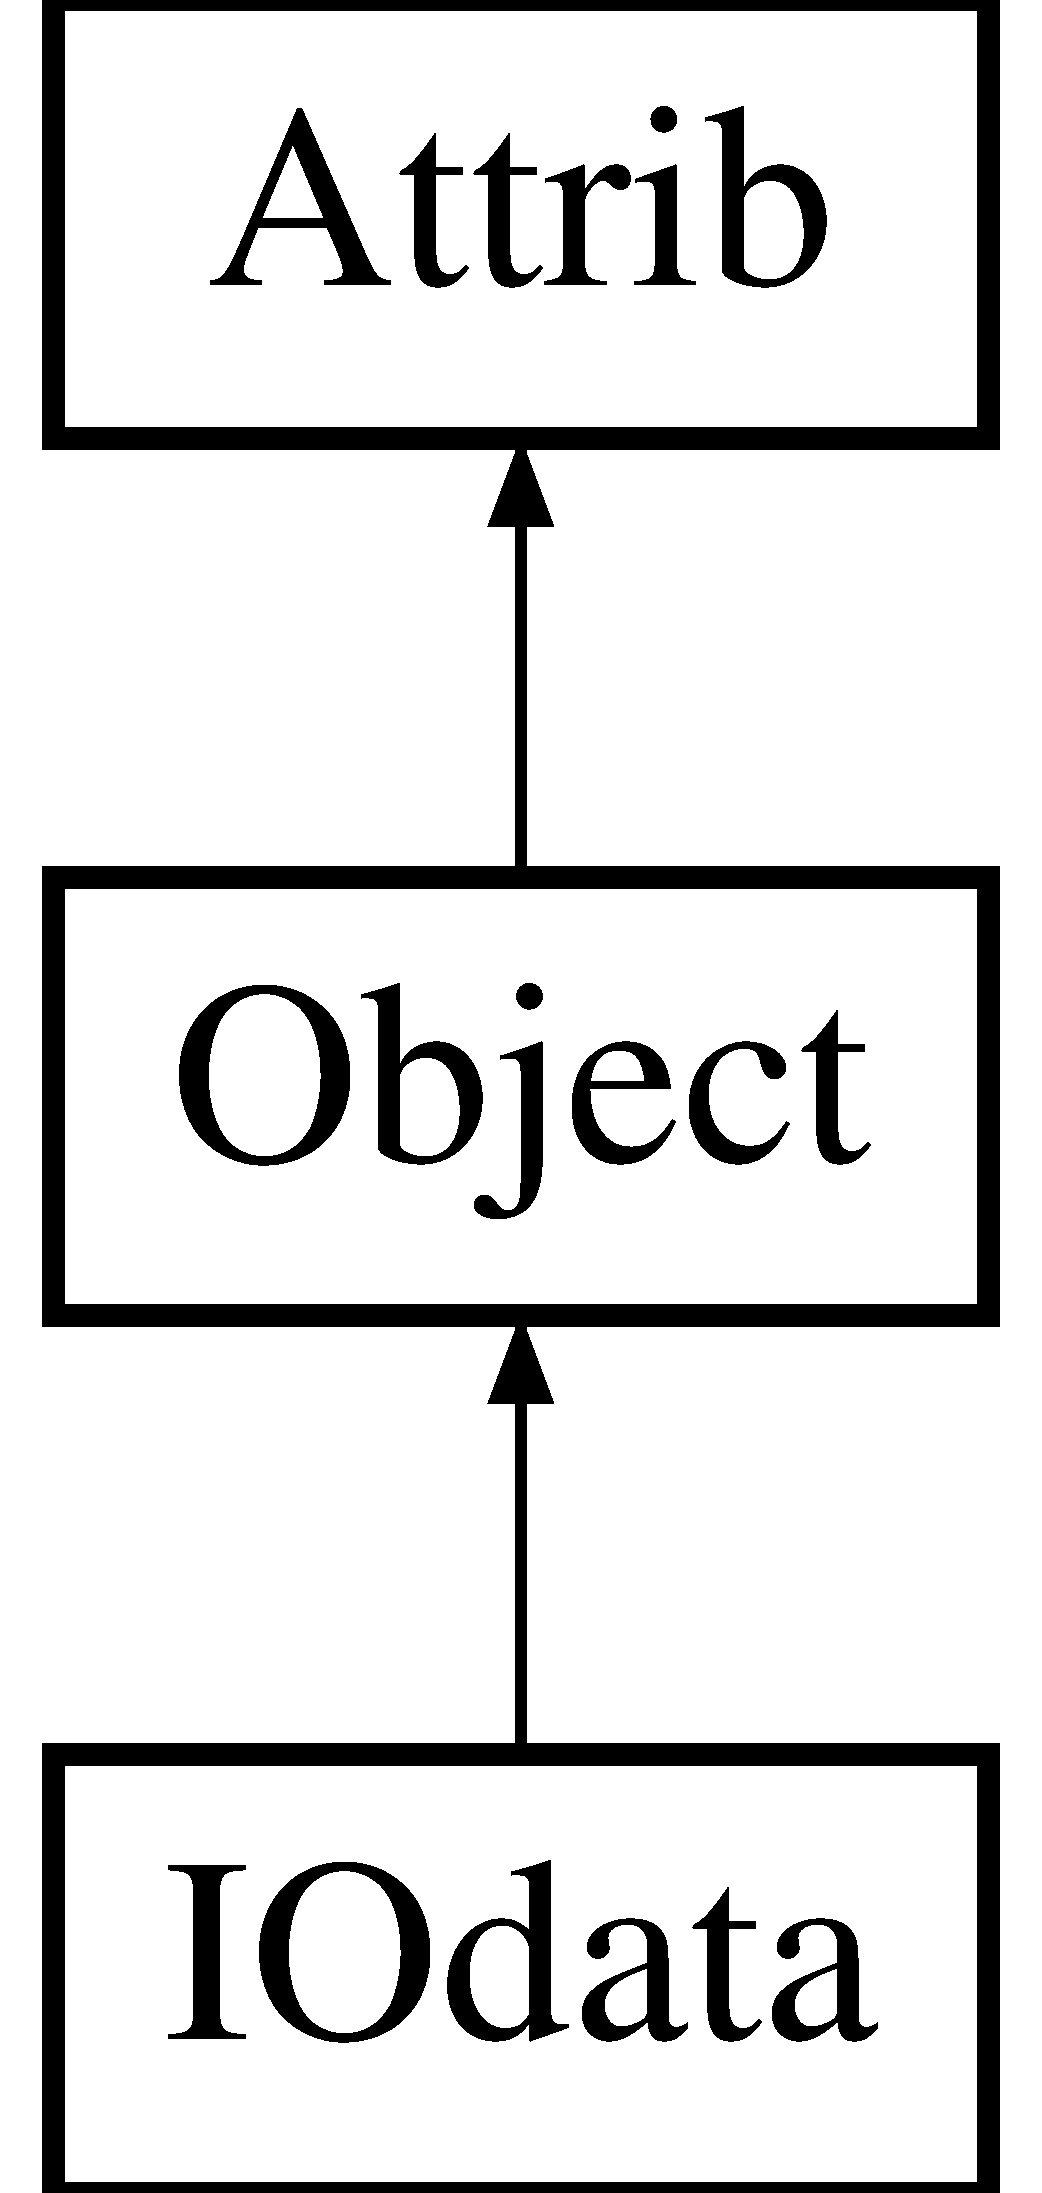
\includegraphics[height=3.000000cm]{classIOdata}
\end{center}
\end{figure}
\subsection*{Public Types}
\begin{DoxyCompactItemize}
\item 
enum \hyperlink{classIOdata_a044e9a4a0c6d25a43ebfe29c4fa4f1e5}{Mode} \{ \hyperlink{classIOdata_a044e9a4a0c6d25a43ebfe29c4fa4f1e5a9ac1bef9c44dd3f63df0b64646129e97}{Rd}, 
\hyperlink{classIOdata_a044e9a4a0c6d25a43ebfe29c4fa4f1e5a019388bd87f0ec039a78e7ac5cb60a81}{Wr}, 
\hyperlink{classIOdata_a044e9a4a0c6d25a43ebfe29c4fa4f1e5ae0f5414225eec903b44306912160c754}{Rd\+Wr}
 \}
\item 
enum \hyperlink{classIOdata_a37c53ebf4bf8d866aac8af572962a84c}{Word\+Size} \{ \hyperlink{classIOdata_a37c53ebf4bf8d866aac8af572962a84ca00156611f08eeb1b5d361de809dafb8e}{Byte}, 
\hyperlink{classIOdata_a37c53ebf4bf8d866aac8af572962a84ca7d603e9c9a55e3c8dffa4bd8e3dca491}{Word}, 
\hyperlink{classIOdata_a37c53ebf4bf8d866aac8af572962a84ca458da82d97e3ea9715c34b558c34f734}{D\+Word}
 \}
\item 
enum \hyperlink{classIOdata_a99aa7bed39364c4359ab8a7596bc013c}{Bus} \{ \newline
\hyperlink{classIOdata_a99aa7bed39364c4359ab8a7596bc013cabd27b3ded09d67a97f98b5004101856f}{U\+SB}, 
\hyperlink{classIOdata_a99aa7bed39364c4359ab8a7596bc013caf9005892b62633a3e9f3456ef11c8991}{S\+P\+E\+CS}, 
\hyperlink{classIOdata_a99aa7bed39364c4359ab8a7596bc013ca68cf1532718ac977427bacd1a7e0bc32}{I2C}, 
\hyperlink{classIOdata_a99aa7bed39364c4359ab8a7596bc013caf68d3c4cdd5e3c21501655358370b460}{P\+A\+R\+A\+L\+L\+EL}, 
\newline
\hyperlink{classIOdata_a99aa7bed39364c4359ab8a7596bc013ca185cc1d64a0173fc7da76513e2fb5642}{J\+T\+AG}
 \}
\item 
typedef unsigned long \hyperlink{classIOdata_a96fb57f5fcd87b708743abd3c86a5198}{U32}
\item 
typedef unsigned short \hyperlink{classIOdata_a1eb45b348534a7c19a4a99b746e693ff}{U16}
\item 
typedef unsigned char \hyperlink{classIOdata_a18d1354b7cdaf0f8a8001fdbb3ced418}{U8}
\end{DoxyCompactItemize}
\subsection*{Public Member Functions}
\begin{DoxyCompactItemize}
\item 
\hyperlink{classIOdata_af558c1fc49af58f50c9600423dd5acd7}{I\+Odata} ()
\begin{DoxyCompactList}\small\item\em Standard constructor. \end{DoxyCompactList}\item 
virtual \hyperlink{classIOdata_a3d7cf860040702b00a925703da7c0648}{$\sim$\+I\+Odata} ()
\begin{DoxyCompactList}\small\item\em Destructor. \end{DoxyCompactList}\item 
\hyperlink{classStatusCode}{Status\+Code} \hyperlink{classIOdata_af98cbfbc28346ebb9b64ca0203af1463}{set\+Address} (\hyperlink{classIOdata_a96fb57f5fcd87b708743abd3c86a5198}{U32} \hyperlink{classIOdata_afe410c86881b8c2082a08e5ce9843306}{address})
\item 
\hyperlink{classIOdata_a96fb57f5fcd87b708743abd3c86a5198}{U32} \hyperlink{classIOdata_afe410c86881b8c2082a08e5ce9843306}{address} ()
\item 
\hyperlink{classStatusCode}{Status\+Code} \hyperlink{classIOdata_a9a850f401542d416adf061e30f7dfdd5}{set\+Header} (\hyperlink{classIOdata_a96fb57f5fcd87b708743abd3c86a5198}{U32} \hyperlink{classIOdata_a503396d8deb6e098c15f963e4201e01b}{header})
\item 
\hyperlink{classIOdata_a96fb57f5fcd87b708743abd3c86a5198}{U32} \hyperlink{classIOdata_a503396d8deb6e098c15f963e4201e01b}{header} ()
\item 
\hyperlink{classStatusCode}{Status\+Code} \hyperlink{classIOdata_aeca09aa9a8c2ccc4c3a728b2ddcf4b2a}{set\+Sub\+Address} (\hyperlink{classIOdata_a96fb57f5fcd87b708743abd3c86a5198}{U32} \hyperlink{classIOdata_a25df48b84364a468373260f823ed9c5f}{sub\+Address})
\item 
\hyperlink{classIOdata_a96fb57f5fcd87b708743abd3c86a5198}{U32} \hyperlink{classIOdata_a25df48b84364a468373260f823ed9c5f}{sub\+Address} ()
\item 
\hyperlink{classStatusCode}{Status\+Code} \hyperlink{classIOdata_a09675d3efa14ba00cc22f8ff8d463389}{set\+Output\+Select} (\hyperlink{classIOdata_a96fb57f5fcd87b708743abd3c86a5198}{U32} \hyperlink{classIOdata_aaa410b57a4607857d45ac6a7cd013307}{output\+Select})
\item 
\hyperlink{classIOdata_a96fb57f5fcd87b708743abd3c86a5198}{U32} \hyperlink{classIOdata_aaa410b57a4607857d45ac6a7cd013307}{output\+Select} ()
\item 
\hyperlink{classStatusCode}{Status\+Code} \hyperlink{classIOdata_ad81e9fd3f2cd9dcaffd9eabddf8f867e}{set\+Mode} (\hyperlink{classIOdata_a044e9a4a0c6d25a43ebfe29c4fa4f1e5}{I\+Odata\+::\+Mode} \hyperlink{classIOdata_aae2073c3bc6bc9f620dc0fca7fccc9a7}{mode})
\item 
\hyperlink{classIOdata_a044e9a4a0c6d25a43ebfe29c4fa4f1e5}{I\+Odata\+::\+Mode} \hyperlink{classIOdata_aae2073c3bc6bc9f620dc0fca7fccc9a7}{mode} ()
\item 
\hyperlink{classStatusCode}{Status\+Code} \hyperlink{classIOdata_a20f30a9f4673713616447b1b5e9817d5}{set\+Word\+Size} (\hyperlink{classIOdata_a37c53ebf4bf8d866aac8af572962a84c}{I\+Odata\+::\+Word\+Size} \hyperlink{classIOdata_a91f9e8b4095ca8365a824e43be36b143}{word\+Size})
\item 
\hyperlink{classIOdata_a37c53ebf4bf8d866aac8af572962a84c}{I\+Odata\+::\+Word\+Size} \hyperlink{classIOdata_a91f9e8b4095ca8365a824e43be36b143}{word\+Size} ()
\item 
\hyperlink{classStatusCode}{Status\+Code} \hyperlink{classIOdata_aca154b90e490608b5b5c0ead58e1fafc}{set\+Bus} (\hyperlink{classIOdata_a99aa7bed39364c4359ab8a7596bc013c}{I\+Odata\+::\+Bus} \hyperlink{classIOdata_ab904bcca0e8e3bebc3299e47ca93a8a1}{bus})
\item 
\hyperlink{classIOdata_a99aa7bed39364c4359ab8a7596bc013c}{I\+Odata\+::\+Bus} \hyperlink{classIOdata_ab904bcca0e8e3bebc3299e47ca93a8a1}{bus} ()
\item 
\hyperlink{classStatusCode}{Status\+Code} \hyperlink{classIOdata_affaf98e7f9e596263e914b055f8f93c2}{set\+Length} (\hyperlink{classIOdata_a96fb57f5fcd87b708743abd3c86a5198}{U32} \hyperlink{classIOdata_abb40e71ce0290832a24857b4a1e7b1a3}{length})
\item 
\hyperlink{classIOdata_a96fb57f5fcd87b708743abd3c86a5198}{U32} \hyperlink{classIOdata_aeda27840c9a9b7b3b86efc71c56cd868}{block} ()
\item 
\hyperlink{classStatusCode}{Status\+Code} \hyperlink{classIOdata_a334f07d85e3dc8069551dcd8ab942e9c}{set\+Block} (\hyperlink{classIOdata_a96fb57f5fcd87b708743abd3c86a5198}{U32} \hyperlink{classIOdata_aeda27840c9a9b7b3b86efc71c56cd868}{block})
\item 
\hyperlink{classIOdata_a96fb57f5fcd87b708743abd3c86a5198}{U32} \hyperlink{classIOdata_abb40e71ce0290832a24857b4a1e7b1a3}{length} ()
\item 
void \hyperlink{classIOdata_a80bb230b61062b447db5832e43bf7b44}{def\+Data\+U8} (unsigned long size)
\item 
void \hyperlink{classIOdata_a9e37c736d6dfb5223ed45786fad403da}{def\+Data\+U16} (unsigned long size)
\item 
void \hyperlink{classIOdata_a78e50aa4a6c967cba195e77fe911a8c3}{def\+Data\+U32} (unsigned long size)
\item 
void \hyperlink{classIOdata_a9bc3ea0458ea6d13bd751ac4c80a4be6}{clear\+Data\+U8} ()
\item 
void \hyperlink{classIOdata_a13016f489aba6e80cd7be53224c3e8ab}{clear\+Data\+U16} ()
\item 
void \hyperlink{classIOdata_a848de1b6e7b7207dbb53c102a4d911a9}{clear\+Data\+U32} ()
\item 
\hyperlink{classIOdata_a18d1354b7cdaf0f8a8001fdbb3ced418}{U8} $\ast$ \hyperlink{classIOdata_a75e9c318dbac3a39402179070943d4bc}{data\+U8} ()
\item 
\hyperlink{classIOdata_a1eb45b348534a7c19a4a99b746e693ff}{U16} $\ast$ \hyperlink{classIOdata_a8d8528b731c6cf117f8c5b9b2473390c}{data\+U16} ()
\item 
\hyperlink{classIOdata_a96fb57f5fcd87b708743abd3c86a5198}{U32} $\ast$ \hyperlink{classIOdata_ab0e3cd09f46c1c3712f797116f6da074}{data\+U32} ()
\item 
unsigned long int \hyperlink{classIOdata_a9c7cc68c435e1b22dcdac7c17d186e63}{data\+U8} (unsigned long int i)
\item 
unsigned long int \hyperlink{classIOdata_a32e3bb958cb6babcb928d403fea9f171}{data\+U16} (unsigned long int i)
\item 
unsigned long int \hyperlink{classIOdata_a4ce3bcd54206b1a2149e67cb45dee922}{data\+U32} (unsigned long int i)
\item 
void \hyperlink{classIOdata_afece89b7035f6eec001cd397f07c062d}{set\+Data\+U8} (\hyperlink{classIOdata_a18d1354b7cdaf0f8a8001fdbb3ced418}{U8} $\ast$data, \hyperlink{classIOdata_a96fb57f5fcd87b708743abd3c86a5198}{U32} \hyperlink{classIOdata_abb40e71ce0290832a24857b4a1e7b1a3}{length})
\item 
void \hyperlink{classIOdata_a1796a65cbd8c4326e80d662034ee5e39}{set\+Data\+U16} (\hyperlink{classIOdata_a1eb45b348534a7c19a4a99b746e693ff}{U16} $\ast$data, \hyperlink{classIOdata_a96fb57f5fcd87b708743abd3c86a5198}{U32} \hyperlink{classIOdata_abb40e71ce0290832a24857b4a1e7b1a3}{length})
\item 
void \hyperlink{classIOdata_a408b62ac645630c645ae670691f6459f}{set\+Data\+U32} (\hyperlink{classIOdata_a96fb57f5fcd87b708743abd3c86a5198}{U32} $\ast$data, \hyperlink{classIOdata_a96fb57f5fcd87b708743abd3c86a5198}{U32} \hyperlink{classIOdata_abb40e71ce0290832a24857b4a1e7b1a3}{length})
\item 
\hyperlink{classStatusCode}{Status\+Code} \hyperlink{classIOdata_a6c4fb2f2af01889ada889c2b7aceb24d}{set\+U8} (unsigned long int, \hyperlink{classIOdata_a18d1354b7cdaf0f8a8001fdbb3ced418}{U8})
\item 
\hyperlink{classStatusCode}{Status\+Code} \hyperlink{classIOdata_aa9ade5ce3944c8e2b831533b6f876caf}{set\+U16} (unsigned long int, \hyperlink{classIOdata_a1eb45b348534a7c19a4a99b746e693ff}{U16})
\item 
\hyperlink{classStatusCode}{Status\+Code} \hyperlink{classIOdata_abbed9a057203bc763f97b85fb385f36b}{set\+U32} (unsigned long int, \hyperlink{classIOdata_a96fb57f5fcd87b708743abd3c86a5198}{U32})
\item 
void \hyperlink{classIOdata_a208e24222bf2044a4ff8bbb1a6bdc13b}{dump} (unsigned int printout=0)
\end{DoxyCompactItemize}
\subsection*{Private Attributes}
\begin{DoxyCompactItemize}
\item 
unsigned long \hyperlink{classIOdata_a965810e1888b904c575277f50cea734a}{m\+\_\+address}
\item 
unsigned long \hyperlink{classIOdata_a46ec7dbfa257c02be1d39c4799f157d3}{m\+\_\+header}
\item 
unsigned long \hyperlink{classIOdata_a562f84e5cace1e392f1b0fca553fff78}{m\+\_\+sub\+Address}
\item 
unsigned long \hyperlink{classIOdata_acc46d71243b542e68277e242effa7f1b}{m\+\_\+output\+Select}
\item 
\hyperlink{classIOdata_a044e9a4a0c6d25a43ebfe29c4fa4f1e5}{I\+Odata\+::\+Mode} \hyperlink{classIOdata_a0782e31763fa855f1ecbd377dce538e6}{m\+\_\+mode}
\item 
\hyperlink{classIOdata_a37c53ebf4bf8d866aac8af572962a84c}{I\+Odata\+::\+Word\+Size} \hyperlink{classIOdata_a719b0ce607ada4fa91b12d6ecfa1b4c9}{m\+\_\+word\+Size}
\item 
\hyperlink{classIOdata_a99aa7bed39364c4359ab8a7596bc013c}{I\+Odata\+::\+Bus} \hyperlink{classIOdata_a42c07a9b3f43ec35dd18d13a67d294cc}{m\+\_\+bus}
\item 
unsigned long \hyperlink{classIOdata_afabe57441da019eb614d277799106aac}{m\+\_\+length}
\item 
unsigned long \hyperlink{classIOdata_a6d1ce9f88db6b97ce61098a3693e253f}{m\+\_\+block}
\item 
\hyperlink{classIOdata_a18d1354b7cdaf0f8a8001fdbb3ced418}{U8} $\ast$ \hyperlink{classIOdata_a9c4c0dc5104f7f3b170e30ab78fe61e7}{m\+\_\+data\+U8}
\item 
\hyperlink{classIOdata_a1eb45b348534a7c19a4a99b746e693ff}{U16} $\ast$ \hyperlink{classIOdata_a8d698e077b7898009691b9086a3e6453}{m\+\_\+data\+U16}
\item 
\hyperlink{classIOdata_a96fb57f5fcd87b708743abd3c86a5198}{U32} $\ast$ \hyperlink{classIOdata_a247cdaefd87084e3cad1d530d592d99a}{m\+\_\+data\+U32}
\end{DoxyCompactItemize}
\subsection*{Additional Inherited Members}


\subsection{Detailed Description}
\begin{DoxyAuthor}{Author}
\hyperlink{classIOdata}{I\+Odata} 
\end{DoxyAuthor}
\begin{DoxyDate}{Date}
2006-\/10-\/23 
\end{DoxyDate}


Definition at line 17 of file I\+Odata.\+h.



\subsection{Member Typedef Documentation}
\mbox{\Hypertarget{classIOdata_a1eb45b348534a7c19a4a99b746e693ff}\label{classIOdata_a1eb45b348534a7c19a4a99b746e693ff}} 
\index{I\+Odata@{I\+Odata}!U16@{U16}}
\index{U16@{U16}!I\+Odata@{I\+Odata}}
\subsubsection{\texorpdfstring{U16}{U16}}
{\footnotesize\ttfamily typedef unsigned short \hyperlink{classIOdata_a1eb45b348534a7c19a4a99b746e693ff}{I\+Odata\+::\+U16}}



Definition at line 20 of file I\+Odata.\+h.

\mbox{\Hypertarget{classIOdata_a96fb57f5fcd87b708743abd3c86a5198}\label{classIOdata_a96fb57f5fcd87b708743abd3c86a5198}} 
\index{I\+Odata@{I\+Odata}!U32@{U32}}
\index{U32@{U32}!I\+Odata@{I\+Odata}}
\subsubsection{\texorpdfstring{U32}{U32}}
{\footnotesize\ttfamily typedef unsigned long \hyperlink{classIOdata_a96fb57f5fcd87b708743abd3c86a5198}{I\+Odata\+::\+U32}}



Definition at line 19 of file I\+Odata.\+h.

\mbox{\Hypertarget{classIOdata_a18d1354b7cdaf0f8a8001fdbb3ced418}\label{classIOdata_a18d1354b7cdaf0f8a8001fdbb3ced418}} 
\index{I\+Odata@{I\+Odata}!U8@{U8}}
\index{U8@{U8}!I\+Odata@{I\+Odata}}
\subsubsection{\texorpdfstring{U8}{U8}}
{\footnotesize\ttfamily typedef unsigned char \hyperlink{classIOdata_a18d1354b7cdaf0f8a8001fdbb3ced418}{I\+Odata\+::\+U8}}



Definition at line 21 of file I\+Odata.\+h.



\subsection{Member Enumeration Documentation}
\mbox{\Hypertarget{classIOdata_a99aa7bed39364c4359ab8a7596bc013c}\label{classIOdata_a99aa7bed39364c4359ab8a7596bc013c}} 
\index{I\+Odata@{I\+Odata}!Bus@{Bus}}
\index{Bus@{Bus}!I\+Odata@{I\+Odata}}
\subsubsection{\texorpdfstring{Bus}{Bus}}
{\footnotesize\ttfamily enum \hyperlink{classIOdata_a99aa7bed39364c4359ab8a7596bc013c}{I\+Odata\+::\+Bus}}

\begin{DoxyEnumFields}{Enumerator}
\raisebox{\heightof{T}}[0pt][0pt]{\index{U\+SB@{U\+SB}!I\+Odata@{I\+Odata}}\index{I\+Odata@{I\+Odata}!U\+SB@{U\+SB}}}\mbox{\Hypertarget{classIOdata_a99aa7bed39364c4359ab8a7596bc013cabd27b3ded09d67a97f98b5004101856f}\label{classIOdata_a99aa7bed39364c4359ab8a7596bc013cabd27b3ded09d67a97f98b5004101856f}} 
U\+SB&\\
\hline

\raisebox{\heightof{T}}[0pt][0pt]{\index{S\+P\+E\+CS@{S\+P\+E\+CS}!I\+Odata@{I\+Odata}}\index{I\+Odata@{I\+Odata}!S\+P\+E\+CS@{S\+P\+E\+CS}}}\mbox{\Hypertarget{classIOdata_a99aa7bed39364c4359ab8a7596bc013caf9005892b62633a3e9f3456ef11c8991}\label{classIOdata_a99aa7bed39364c4359ab8a7596bc013caf9005892b62633a3e9f3456ef11c8991}} 
S\+P\+E\+CS&\\
\hline

\raisebox{\heightof{T}}[0pt][0pt]{\index{I2C@{I2C}!I\+Odata@{I\+Odata}}\index{I\+Odata@{I\+Odata}!I2C@{I2C}}}\mbox{\Hypertarget{classIOdata_a99aa7bed39364c4359ab8a7596bc013ca68cf1532718ac977427bacd1a7e0bc32}\label{classIOdata_a99aa7bed39364c4359ab8a7596bc013ca68cf1532718ac977427bacd1a7e0bc32}} 
I2C&\\
\hline

\raisebox{\heightof{T}}[0pt][0pt]{\index{P\+A\+R\+A\+L\+L\+EL@{P\+A\+R\+A\+L\+L\+EL}!I\+Odata@{I\+Odata}}\index{I\+Odata@{I\+Odata}!P\+A\+R\+A\+L\+L\+EL@{P\+A\+R\+A\+L\+L\+EL}}}\mbox{\Hypertarget{classIOdata_a99aa7bed39364c4359ab8a7596bc013caf68d3c4cdd5e3c21501655358370b460}\label{classIOdata_a99aa7bed39364c4359ab8a7596bc013caf68d3c4cdd5e3c21501655358370b460}} 
P\+A\+R\+A\+L\+L\+EL&\\
\hline

\raisebox{\heightof{T}}[0pt][0pt]{\index{J\+T\+AG@{J\+T\+AG}!I\+Odata@{I\+Odata}}\index{I\+Odata@{I\+Odata}!J\+T\+AG@{J\+T\+AG}}}\mbox{\Hypertarget{classIOdata_a99aa7bed39364c4359ab8a7596bc013ca185cc1d64a0173fc7da76513e2fb5642}\label{classIOdata_a99aa7bed39364c4359ab8a7596bc013ca185cc1d64a0173fc7da76513e2fb5642}} 
J\+T\+AG&\\
\hline

\end{DoxyEnumFields}


Definition at line 35 of file I\+Odata.\+h.


\begin{DoxyCode}
35           \{
36     \hyperlink{classIOdata_a99aa7bed39364c4359ab8a7596bc013cabd27b3ded09d67a97f98b5004101856f}{USB},
37     \hyperlink{classIOdata_a99aa7bed39364c4359ab8a7596bc013caf9005892b62633a3e9f3456ef11c8991}{SPECS},
38     \hyperlink{classIOdata_a99aa7bed39364c4359ab8a7596bc013ca68cf1532718ac977427bacd1a7e0bc32}{I2C},
39     \hyperlink{classIOdata_a99aa7bed39364c4359ab8a7596bc013caf68d3c4cdd5e3c21501655358370b460}{PARALLEL},
40     \hyperlink{classIOdata_a99aa7bed39364c4359ab8a7596bc013ca185cc1d64a0173fc7da76513e2fb5642}{JTAG}
41   \};
\end{DoxyCode}
\mbox{\Hypertarget{classIOdata_a044e9a4a0c6d25a43ebfe29c4fa4f1e5}\label{classIOdata_a044e9a4a0c6d25a43ebfe29c4fa4f1e5}} 
\index{I\+Odata@{I\+Odata}!Mode@{Mode}}
\index{Mode@{Mode}!I\+Odata@{I\+Odata}}
\subsubsection{\texorpdfstring{Mode}{Mode}}
{\footnotesize\ttfamily enum \hyperlink{classIOdata_a044e9a4a0c6d25a43ebfe29c4fa4f1e5}{I\+Odata\+::\+Mode}}

\begin{DoxyEnumFields}{Enumerator}
\raisebox{\heightof{T}}[0pt][0pt]{\index{Rd@{Rd}!I\+Odata@{I\+Odata}}\index{I\+Odata@{I\+Odata}!Rd@{Rd}}}\mbox{\Hypertarget{classIOdata_a044e9a4a0c6d25a43ebfe29c4fa4f1e5a9ac1bef9c44dd3f63df0b64646129e97}\label{classIOdata_a044e9a4a0c6d25a43ebfe29c4fa4f1e5a9ac1bef9c44dd3f63df0b64646129e97}} 
Rd&\\
\hline

\raisebox{\heightof{T}}[0pt][0pt]{\index{Wr@{Wr}!I\+Odata@{I\+Odata}}\index{I\+Odata@{I\+Odata}!Wr@{Wr}}}\mbox{\Hypertarget{classIOdata_a044e9a4a0c6d25a43ebfe29c4fa4f1e5a019388bd87f0ec039a78e7ac5cb60a81}\label{classIOdata_a044e9a4a0c6d25a43ebfe29c4fa4f1e5a019388bd87f0ec039a78e7ac5cb60a81}} 
Wr&\\
\hline

\raisebox{\heightof{T}}[0pt][0pt]{\index{Rd\+Wr@{Rd\+Wr}!I\+Odata@{I\+Odata}}\index{I\+Odata@{I\+Odata}!Rd\+Wr@{Rd\+Wr}}}\mbox{\Hypertarget{classIOdata_a044e9a4a0c6d25a43ebfe29c4fa4f1e5ae0f5414225eec903b44306912160c754}\label{classIOdata_a044e9a4a0c6d25a43ebfe29c4fa4f1e5ae0f5414225eec903b44306912160c754}} 
Rd\+Wr&\\
\hline

\end{DoxyEnumFields}


Definition at line 23 of file I\+Odata.\+h.


\begin{DoxyCode}
23             \{
24     \hyperlink{classIOdata_a044e9a4a0c6d25a43ebfe29c4fa4f1e5a9ac1bef9c44dd3f63df0b64646129e97}{Rd},
25     \hyperlink{classIOdata_a044e9a4a0c6d25a43ebfe29c4fa4f1e5a019388bd87f0ec039a78e7ac5cb60a81}{Wr},
26     \hyperlink{classIOdata_a044e9a4a0c6d25a43ebfe29c4fa4f1e5ae0f5414225eec903b44306912160c754}{RdWr}
27   \};
\end{DoxyCode}
\mbox{\Hypertarget{classIOdata_a37c53ebf4bf8d866aac8af572962a84c}\label{classIOdata_a37c53ebf4bf8d866aac8af572962a84c}} 
\index{I\+Odata@{I\+Odata}!Word\+Size@{Word\+Size}}
\index{Word\+Size@{Word\+Size}!I\+Odata@{I\+Odata}}
\subsubsection{\texorpdfstring{Word\+Size}{WordSize}}
{\footnotesize\ttfamily enum \hyperlink{classIOdata_a37c53ebf4bf8d866aac8af572962a84c}{I\+Odata\+::\+Word\+Size}}

\begin{DoxyEnumFields}{Enumerator}
\raisebox{\heightof{T}}[0pt][0pt]{\index{Byte@{Byte}!I\+Odata@{I\+Odata}}\index{I\+Odata@{I\+Odata}!Byte@{Byte}}}\mbox{\Hypertarget{classIOdata_a37c53ebf4bf8d866aac8af572962a84ca00156611f08eeb1b5d361de809dafb8e}\label{classIOdata_a37c53ebf4bf8d866aac8af572962a84ca00156611f08eeb1b5d361de809dafb8e}} 
Byte&\\
\hline

\raisebox{\heightof{T}}[0pt][0pt]{\index{Word@{Word}!I\+Odata@{I\+Odata}}\index{I\+Odata@{I\+Odata}!Word@{Word}}}\mbox{\Hypertarget{classIOdata_a37c53ebf4bf8d866aac8af572962a84ca7d603e9c9a55e3c8dffa4bd8e3dca491}\label{classIOdata_a37c53ebf4bf8d866aac8af572962a84ca7d603e9c9a55e3c8dffa4bd8e3dca491}} 
Word&\\
\hline

\raisebox{\heightof{T}}[0pt][0pt]{\index{D\+Word@{D\+Word}!I\+Odata@{I\+Odata}}\index{I\+Odata@{I\+Odata}!D\+Word@{D\+Word}}}\mbox{\Hypertarget{classIOdata_a37c53ebf4bf8d866aac8af572962a84ca458da82d97e3ea9715c34b558c34f734}\label{classIOdata_a37c53ebf4bf8d866aac8af572962a84ca458da82d97e3ea9715c34b558c34f734}} 
D\+Word&\\
\hline

\end{DoxyEnumFields}


Definition at line 29 of file I\+Odata.\+h.


\begin{DoxyCode}
29                \{
30     \hyperlink{classIOdata_a37c53ebf4bf8d866aac8af572962a84ca00156611f08eeb1b5d361de809dafb8e}{Byte},
31     \hyperlink{classIOdata_a37c53ebf4bf8d866aac8af572962a84ca7d603e9c9a55e3c8dffa4bd8e3dca491}{Word},
32     \hyperlink{classIOdata_a37c53ebf4bf8d866aac8af572962a84ca458da82d97e3ea9715c34b558c34f734}{DWord}
33   \};
\end{DoxyCode}


\subsection{Constructor \& Destructor Documentation}
\mbox{\Hypertarget{classIOdata_af558c1fc49af58f50c9600423dd5acd7}\label{classIOdata_af558c1fc49af58f50c9600423dd5acd7}} 
\index{I\+Odata@{I\+Odata}!I\+Odata@{I\+Odata}}
\index{I\+Odata@{I\+Odata}!I\+Odata@{I\+Odata}}
\subsubsection{\texorpdfstring{I\+Odata()}{IOdata()}}
{\footnotesize\ttfamily I\+Odata\+::\+I\+Odata (\begin{DoxyParamCaption}{ }\end{DoxyParamCaption})}



Standard constructor. 



Definition at line 17 of file I\+Odata.\+cpp.



References Attrib\+::add(), Byte, Attrib\+::\+I\+O\+D\+A\+TA, m\+\_\+address, m\+\_\+block, m\+\_\+data\+U16, m\+\_\+data\+U32, m\+\_\+data\+U8, m\+\_\+header, m\+\_\+length, m\+\_\+sub\+Address, m\+\_\+word\+Size, Object\+::set\+Name(), and Object\+::set\+Type().


\begin{DoxyCode}
17                  \{
18   \hyperlink{classObject_ae30fea75683c2d149b6b6d17c09ecd0c}{setName}(\textcolor{stringliteral}{"IO"});
19   \hyperlink{classObject_aae534cc9d982bcb9b99fd505f2e103a5}{setType}(\textcolor{stringliteral}{"IOdata"});
20   \hyperlink{classAttrib_a235f773af19c900264a190b00a3b4ad7}{add}(\hyperlink{classAttrib_a69e171d7cc6417835a5a306d3c764235a0af3b0d0ac323c1704e6c69cf90add28}{Attrib::IODATA});
21   \hyperlink{classIOdata_a9c4c0dc5104f7f3b170e30ab78fe61e7}{m\_dataU8}=0;
22   \hyperlink{classIOdata_a8d698e077b7898009691b9086a3e6453}{m\_dataU16}=0;
23   \hyperlink{classIOdata_a247cdaefd87084e3cad1d530d592d99a}{m\_dataU32}=0;
24   \hyperlink{classIOdata_a965810e1888b904c575277f50cea734a}{m\_address}=0;
25   \hyperlink{classIOdata_a46ec7dbfa257c02be1d39c4799f157d3}{m\_header}=0;
26   \hyperlink{classIOdata_a562f84e5cace1e392f1b0fca553fff78}{m\_subAddress}=0;
27   \hyperlink{classIOdata_afabe57441da019eb614d277799106aac}{m\_length} =0;
28   \hyperlink{classIOdata_a6d1ce9f88db6b97ce61098a3693e253f}{m\_block}  =1;
29   \hyperlink{classIOdata_a719b0ce607ada4fa91b12d6ecfa1b4c9}{m\_wordSize}=\hyperlink{classIOdata_a37c53ebf4bf8d866aac8af572962a84ca00156611f08eeb1b5d361de809dafb8e}{IOdata::Byte};
30 \}
\end{DoxyCode}
\mbox{\Hypertarget{classIOdata_a3d7cf860040702b00a925703da7c0648}\label{classIOdata_a3d7cf860040702b00a925703da7c0648}} 
\index{I\+Odata@{I\+Odata}!````~I\+Odata@{$\sim$\+I\+Odata}}
\index{````~I\+Odata@{$\sim$\+I\+Odata}!I\+Odata@{I\+Odata}}
\subsubsection{\texorpdfstring{$\sim$\+I\+Odata()}{~IOdata()}}
{\footnotesize\ttfamily I\+Odata\+::$\sim$\+I\+Odata (\begin{DoxyParamCaption}{ }\end{DoxyParamCaption})\hspace{0.3cm}{\ttfamily [virtual]}}



Destructor. 



Definition at line 34 of file I\+Odata.\+cpp.



References clear\+Data\+U16(), clear\+Data\+U32(), and clear\+Data\+U8().


\begin{DoxyCode}
34                 \{
35   \hyperlink{classIOdata_a9bc3ea0458ea6d13bd751ac4c80a4be6}{clearDataU8}();
36   \hyperlink{classIOdata_a13016f489aba6e80cd7be53224c3e8ab}{clearDataU16}();
37   \hyperlink{classIOdata_a848de1b6e7b7207dbb53c102a4d911a9}{clearDataU32}();
38 \}
\end{DoxyCode}


\subsection{Member Function Documentation}
\mbox{\Hypertarget{classIOdata_afe410c86881b8c2082a08e5ce9843306}\label{classIOdata_afe410c86881b8c2082a08e5ce9843306}} 
\index{I\+Odata@{I\+Odata}!address@{address}}
\index{address@{address}!I\+Odata@{I\+Odata}}
\subsubsection{\texorpdfstring{address()}{address()}}
{\footnotesize\ttfamily \hyperlink{classIOdata_a96fb57f5fcd87b708743abd3c86a5198}{U32} I\+Odata\+::address (\begin{DoxyParamCaption}{ }\end{DoxyParamCaption})\hspace{0.3cm}{\ttfamily [inline]}}

Get \hyperlink{classIOdata}{I\+Odata} address 

Definition at line 59 of file I\+Odata.\+h.



References m\+\_\+address.



Referenced by I\+Oobject\+::address(), B\+O\+O\+S\+T\+\_\+\+P\+Y\+T\+H\+O\+N\+\_\+\+M\+O\+D\+U\+L\+E(), Usb\+I2c\+Bus\+::read(), Usb\+Spi\+Bus\+::read(), Usb\+F\+T\+Interface\+::read(), Usb\+F\+T\+M\+L\+Interface\+::read(), set\+Address(), Usb\+I2c\+Bus\+::write(), Usb\+Spi\+Bus\+::write(), Usb\+F\+T\+Interface\+::write(), and Usb\+F\+T\+M\+L\+Interface\+::write().


\begin{DoxyCode}
59                \{
60     \textcolor{keywordflow}{return} \hyperlink{classIOdata_a965810e1888b904c575277f50cea734a}{m\_address};
61   \}
\end{DoxyCode}
\mbox{\Hypertarget{classIOdata_aeda27840c9a9b7b3b86efc71c56cd868}\label{classIOdata_aeda27840c9a9b7b3b86efc71c56cd868}} 
\index{I\+Odata@{I\+Odata}!block@{block}}
\index{block@{block}!I\+Odata@{I\+Odata}}
\subsubsection{\texorpdfstring{block()}{block()}}
{\footnotesize\ttfamily \hyperlink{classIOdata_a96fb57f5fcd87b708743abd3c86a5198}{U32} I\+Odata\+::block (\begin{DoxyParamCaption}{ }\end{DoxyParamCaption})\hspace{0.3cm}{\ttfamily [inline]}}

Get \hyperlink{classIOdata}{I\+Odata} length 

Definition at line 162 of file I\+Odata.\+h.



References m\+\_\+block.



Referenced by B\+O\+O\+S\+T\+\_\+\+P\+Y\+T\+H\+O\+N\+\_\+\+M\+O\+D\+U\+L\+E(), and set\+Block().


\begin{DoxyCode}
162              \{
163     \textcolor{keywordflow}{return} \hyperlink{classIOdata_a6d1ce9f88db6b97ce61098a3693e253f}{m\_block};
164   \}
\end{DoxyCode}
\mbox{\Hypertarget{classIOdata_ab904bcca0e8e3bebc3299e47ca93a8a1}\label{classIOdata_ab904bcca0e8e3bebc3299e47ca93a8a1}} 
\index{I\+Odata@{I\+Odata}!bus@{bus}}
\index{bus@{bus}!I\+Odata@{I\+Odata}}
\subsubsection{\texorpdfstring{bus()}{bus()}}
{\footnotesize\ttfamily \hyperlink{classIOdata_a99aa7bed39364c4359ab8a7596bc013c}{I\+Odata\+::\+Bus} I\+Odata\+::bus (\begin{DoxyParamCaption}{ }\end{DoxyParamCaption})\hspace{0.3cm}{\ttfamily [inline]}}

Get \hyperlink{classIOdata}{I\+Odata} bus 

Definition at line 147 of file I\+Odata.\+h.



References m\+\_\+bus.



Referenced by B\+O\+O\+S\+T\+\_\+\+P\+Y\+T\+H\+O\+N\+\_\+\+M\+O\+D\+U\+L\+E(), and set\+Bus().


\begin{DoxyCode}
147                  \{
148     \textcolor{keywordflow}{return} \hyperlink{classIOdata_a42c07a9b3f43ec35dd18d13a67d294cc}{m\_bus};
149   \}
\end{DoxyCode}
\mbox{\Hypertarget{classIOdata_a13016f489aba6e80cd7be53224c3e8ab}\label{classIOdata_a13016f489aba6e80cd7be53224c3e8ab}} 
\index{I\+Odata@{I\+Odata}!clear\+Data\+U16@{clear\+Data\+U16}}
\index{clear\+Data\+U16@{clear\+Data\+U16}!I\+Odata@{I\+Odata}}
\subsubsection{\texorpdfstring{clear\+Data\+U16()}{clearDataU16()}}
{\footnotesize\ttfamily void I\+Odata\+::clear\+Data\+U16 (\begin{DoxyParamCaption}{ }\end{DoxyParamCaption})\hspace{0.3cm}{\ttfamily [inline]}}



Definition at line 205 of file I\+Odata.\+h.



References m\+\_\+data\+U16.



Referenced by def\+Data\+U16(), and $\sim$\+I\+Odata().


\begin{DoxyCode}
205                      \{
206     \textcolor{keywordflow}{if} (0!=\hyperlink{classIOdata_a8d698e077b7898009691b9086a3e6453}{m\_dataU16}) \textcolor{keyword}{delete} [] \hyperlink{classIOdata_a8d698e077b7898009691b9086a3e6453}{m\_dataU16};
207     \hyperlink{classIOdata_a8d698e077b7898009691b9086a3e6453}{m\_dataU16}=0;
208   \}
\end{DoxyCode}
\mbox{\Hypertarget{classIOdata_a848de1b6e7b7207dbb53c102a4d911a9}\label{classIOdata_a848de1b6e7b7207dbb53c102a4d911a9}} 
\index{I\+Odata@{I\+Odata}!clear\+Data\+U32@{clear\+Data\+U32}}
\index{clear\+Data\+U32@{clear\+Data\+U32}!I\+Odata@{I\+Odata}}
\subsubsection{\texorpdfstring{clear\+Data\+U32()}{clearDataU32()}}
{\footnotesize\ttfamily void I\+Odata\+::clear\+Data\+U32 (\begin{DoxyParamCaption}{ }\end{DoxyParamCaption})\hspace{0.3cm}{\ttfamily [inline]}}



Definition at line 209 of file I\+Odata.\+h.



References m\+\_\+data\+U32.



Referenced by def\+Data\+U32(), and $\sim$\+I\+Odata().


\begin{DoxyCode}
209                      \{
210     \textcolor{keywordflow}{if} (0!=\hyperlink{classIOdata_a247cdaefd87084e3cad1d530d592d99a}{m\_dataU32}) \textcolor{keyword}{delete} [] \hyperlink{classIOdata_a247cdaefd87084e3cad1d530d592d99a}{m\_dataU32};
211     \hyperlink{classIOdata_a247cdaefd87084e3cad1d530d592d99a}{m\_dataU32}=0;
212   \}
\end{DoxyCode}
\mbox{\Hypertarget{classIOdata_a9bc3ea0458ea6d13bd751ac4c80a4be6}\label{classIOdata_a9bc3ea0458ea6d13bd751ac4c80a4be6}} 
\index{I\+Odata@{I\+Odata}!clear\+Data\+U8@{clear\+Data\+U8}}
\index{clear\+Data\+U8@{clear\+Data\+U8}!I\+Odata@{I\+Odata}}
\subsubsection{\texorpdfstring{clear\+Data\+U8()}{clearDataU8()}}
{\footnotesize\ttfamily void I\+Odata\+::clear\+Data\+U8 (\begin{DoxyParamCaption}{ }\end{DoxyParamCaption})\hspace{0.3cm}{\ttfamily [inline]}}



Definition at line 200 of file I\+Odata.\+h.



References m\+\_\+data\+U8.



Referenced by def\+Data\+U8(), and $\sim$\+I\+Odata().


\begin{DoxyCode}
200                     \{
201     \textcolor{keywordflow}{if} (0!=\hyperlink{classIOdata_a9c4c0dc5104f7f3b170e30ab78fe61e7}{m\_dataU8}) \textcolor{keyword}{delete} [] \hyperlink{classIOdata_a9c4c0dc5104f7f3b170e30ab78fe61e7}{m\_dataU8};
202     \hyperlink{classIOdata_a9c4c0dc5104f7f3b170e30ab78fe61e7}{m\_dataU8}=0;
203   \}
\end{DoxyCode}
\mbox{\Hypertarget{classIOdata_a8d8528b731c6cf117f8c5b9b2473390c}\label{classIOdata_a8d8528b731c6cf117f8c5b9b2473390c}} 
\index{I\+Odata@{I\+Odata}!data\+U16@{data\+U16}}
\index{data\+U16@{data\+U16}!I\+Odata@{I\+Odata}}
\subsubsection{\texorpdfstring{data\+U16()}{dataU16()}\hspace{0.1cm}{\footnotesize\ttfamily [1/2]}}
{\footnotesize\ttfamily \hyperlink{classIOdata_a1eb45b348534a7c19a4a99b746e693ff}{U16}$\ast$ I\+Odata\+::data\+U16 (\begin{DoxyParamCaption}{ }\end{DoxyParamCaption})\hspace{0.3cm}{\ttfamily [inline]}}



Definition at line 218 of file I\+Odata.\+h.



References m\+\_\+data\+U16.



Referenced by B\+O\+O\+S\+T\+\_\+\+P\+Y\+T\+H\+O\+N\+\_\+\+M\+O\+D\+U\+L\+E(), A3\+P\+E\+::enable\+Storage(), A3\+P\+E\+::fifo\+Depth(), A3\+P\+E\+::fifo\+Latency(), Register\+::get\+Bit(), A3\+P\+E\+::length\+A\+X(), A3\+P\+E\+::pipeline(), Usb\+F\+T\+Interface\+::read(), Usb\+F\+T\+M\+L\+Interface\+::read(), Register\+::set\+Bit(), A3\+P\+E\+::set\+Fifo\+Depth(), A3\+P\+E\+::set\+Fifo\+Latency(), A3\+P\+E\+::set\+Pipeline(), Usb\+F\+T\+Interface\+::write(), and Usb\+F\+T\+M\+L\+Interface\+::write().


\begin{DoxyCode}
218                 \{
219     \textcolor{keywordflow}{return} \hyperlink{classIOdata_a8d698e077b7898009691b9086a3e6453}{m\_dataU16};
220   \}
\end{DoxyCode}
\mbox{\Hypertarget{classIOdata_a32e3bb958cb6babcb928d403fea9f171}\label{classIOdata_a32e3bb958cb6babcb928d403fea9f171}} 
\index{I\+Odata@{I\+Odata}!data\+U16@{data\+U16}}
\index{data\+U16@{data\+U16}!I\+Odata@{I\+Odata}}
\subsubsection{\texorpdfstring{data\+U16()}{dataU16()}\hspace{0.1cm}{\footnotesize\ttfamily [2/2]}}
{\footnotesize\ttfamily unsigned long int I\+Odata\+::data\+U16 (\begin{DoxyParamCaption}\item[{unsigned long int}]{i }\end{DoxyParamCaption})\hspace{0.3cm}{\ttfamily [inline]}}



Definition at line 231 of file I\+Odata.\+h.



References m\+\_\+data\+U16.


\begin{DoxyCode}
231                                                 \{
232     \textcolor{keywordflow}{return} \hyperlink{classIOdata_a8d698e077b7898009691b9086a3e6453}{m\_dataU16}[i];
233   \}
\end{DoxyCode}
\mbox{\Hypertarget{classIOdata_ab0e3cd09f46c1c3712f797116f6da074}\label{classIOdata_ab0e3cd09f46c1c3712f797116f6da074}} 
\index{I\+Odata@{I\+Odata}!data\+U32@{data\+U32}}
\index{data\+U32@{data\+U32}!I\+Odata@{I\+Odata}}
\subsubsection{\texorpdfstring{data\+U32()}{dataU32()}\hspace{0.1cm}{\footnotesize\ttfamily [1/2]}}
{\footnotesize\ttfamily \hyperlink{classIOdata_a96fb57f5fcd87b708743abd3c86a5198}{U32}$\ast$ I\+Odata\+::data\+U32 (\begin{DoxyParamCaption}{ }\end{DoxyParamCaption})\hspace{0.3cm}{\ttfamily [inline]}}



Definition at line 222 of file I\+Odata.\+h.



References m\+\_\+data\+U32.



Referenced by B\+O\+O\+S\+T\+\_\+\+P\+Y\+T\+H\+O\+N\+\_\+\+M\+O\+D\+U\+L\+E(), A3\+P\+E\+::clock\+Division(), Register\+::get\+Bit(), A3\+P\+E\+::latency\+A\+X(), A3\+P\+E\+::n\+Trigger(), Usb\+F\+T\+Interface\+::read(), Usb\+F\+T\+M\+L\+Interface\+::read(), Register\+::set\+Bit(), A3\+P\+E\+::set\+Clock\+Division(), A3\+P\+E\+::set\+N\+Trigger(), A3\+P\+E\+::set\+Trigger\+Delay(), A3\+P\+E\+::set\+Trigger\+Rate(), A3\+P\+E\+::trigger\+Delay(), A3\+P\+E\+::trigger\+Rate(), Usb\+F\+T\+Interface\+::write(), and Usb\+F\+T\+M\+L\+Interface\+::write().


\begin{DoxyCode}
222                 \{
223     \textcolor{keywordflow}{return} \hyperlink{classIOdata_a247cdaefd87084e3cad1d530d592d99a}{m\_dataU32};
224   \}
\end{DoxyCode}
\mbox{\Hypertarget{classIOdata_a4ce3bcd54206b1a2149e67cb45dee922}\label{classIOdata_a4ce3bcd54206b1a2149e67cb45dee922}} 
\index{I\+Odata@{I\+Odata}!data\+U32@{data\+U32}}
\index{data\+U32@{data\+U32}!I\+Odata@{I\+Odata}}
\subsubsection{\texorpdfstring{data\+U32()}{dataU32()}\hspace{0.1cm}{\footnotesize\ttfamily [2/2]}}
{\footnotesize\ttfamily unsigned long int I\+Odata\+::data\+U32 (\begin{DoxyParamCaption}\item[{unsigned long int}]{i }\end{DoxyParamCaption})\hspace{0.3cm}{\ttfamily [inline]}}



Definition at line 235 of file I\+Odata.\+h.



References m\+\_\+data\+U32.


\begin{DoxyCode}
235                                                 \{
236     \textcolor{keywordflow}{return} \hyperlink{classIOdata_a247cdaefd87084e3cad1d530d592d99a}{m\_dataU32}[i];
237   \}
\end{DoxyCode}
\mbox{\Hypertarget{classIOdata_a75e9c318dbac3a39402179070943d4bc}\label{classIOdata_a75e9c318dbac3a39402179070943d4bc}} 
\index{I\+Odata@{I\+Odata}!data\+U8@{data\+U8}}
\index{data\+U8@{data\+U8}!I\+Odata@{I\+Odata}}
\subsubsection{\texorpdfstring{data\+U8()}{dataU8()}\hspace{0.1cm}{\footnotesize\ttfamily [1/2]}}
{\footnotesize\ttfamily \hyperlink{classIOdata_a18d1354b7cdaf0f8a8001fdbb3ced418}{U8}$\ast$ I\+Odata\+::data\+U8 (\begin{DoxyParamCaption}{ }\end{DoxyParamCaption})\hspace{0.3cm}{\ttfamily [inline]}}



Definition at line 214 of file I\+Odata.\+h.



References m\+\_\+data\+U8.



Referenced by B\+O\+O\+S\+T\+\_\+\+P\+Y\+T\+H\+O\+N\+\_\+\+M\+O\+D\+U\+L\+E(), Usb\+Spi\+Bus\+::clock\+Divider(), L\+S\+Delay\+Chip\+V1\+::config\+Reg\+Bulk\+Read(), L\+S\+Delay\+Chip\+V1\+::config\+Reg\+Bulk\+Write(), Usb\+Spi\+Bus\+::ctrl\+Wd(), Acquisition\+::decode\+Format(), A3\+P\+E\+::dump\+From\+A\+X(), A3\+P\+E\+::dump\+Pattern(), A3\+P\+E\+::dump\+Storage(), A3\+P\+E\+::dump\+To\+A\+X(), A3\+P\+E\+::dump\+Trigger(), Storage\+Fifo\+::execute(), Storage\+Fifo\+Acquisition\+::execute(), Test\+U\+S\+B\+::execute(), Seq\+P\+G\+A\+::ext\+Trig(), Register\+::get\+Bit(), Fe\+P\+G\+A\+::i2c\+Add(), Seq\+P\+G\+A\+::i2c\+Add(), Fe\+P\+G\+A\+::i2c\+Data(), Seq\+P\+G\+A\+::i2c\+Data(), Fe\+P\+G\+A\+::i2c\+G\+B\+T\+S\+C\+A(), Seq\+P\+G\+A\+::i2c\+G\+B\+T\+S\+C\+A(), Fe\+P\+G\+A\+::i2c\+Read(), Seq\+P\+G\+A\+::i2c\+Read(), Fe\+P\+G\+A\+::i2c\+Write(), Seq\+P\+G\+A\+::i2c\+Write(), A3\+P\+E\+\_\+\+Bit\+Flip\+::initialize(), Seq\+P\+G\+A\+::led\+Enable(), A3\+P\+E\+::load\+From\+A\+X(), A3\+P\+E\+::load\+Pattern(), A3\+P\+E\+::load\+Storage(), A3\+P\+E\+::load\+To\+A\+X(), A3\+P\+E\+::load\+Trigger(), R\+A\+M\+::raz(), Usb\+I2c\+Bus\+::read(), Phaser\+::read(), I\+C\+Phaser\+::read(), Usb\+Spi\+Bus\+::read(), Usb\+F\+T\+Interface\+::read(), Usb\+F\+T\+M\+L\+Interface\+::read(), I\+C\+Phaser\+::reset(), Register\+::set\+Bit(), Usb\+Spi\+Bus\+::set\+Clock\+Divider(), Seq\+P\+G\+A\+::set\+Ext\+Trig(), Fe\+P\+G\+A\+::set\+I2c\+G\+B\+T\+S\+C\+A(), Seq\+P\+G\+A\+::set\+I2c\+G\+B\+T\+S\+C\+A(), Seq\+P\+G\+A\+::set\+Led\+Enable(), Seq\+P\+G\+A\+::set\+Spi\+Enable(), Seq\+P\+G\+A\+::set\+Spi\+G\+B\+T\+S\+C\+A(), Fe\+P\+G\+A\+::set\+Spi\+G\+B\+T\+S\+C\+A(), Seq\+P\+G\+A\+::spi\+Add(), Seq\+P\+G\+A\+::spi\+Enable(), Seq\+P\+G\+A\+::spi\+G\+B\+T\+S\+C\+A(), Fe\+P\+G\+A\+::spi\+G\+B\+T\+S\+C\+A(), Fe\+P\+G\+A\+::spi\+Read(), I\+C\+E\+C\+A\+Lv3\+::spi\+Read(), Seq\+P\+G\+A\+::spi\+Read(), I\+C\+E\+C\+A\+Lv3\+::spi\+Write(), I\+C\+Phaser\+::status(), Usb\+I2c\+Bus\+::write(), Phaser\+::write(), I\+C\+Phaser\+::write(), Usb\+Spi\+Bus\+::write(), Usb\+F\+T\+M\+L\+Interface\+::write(), and Usb\+F\+T\+Interface\+::write().


\begin{DoxyCode}
214               \{
215     \textcolor{keywordflow}{return} \hyperlink{classIOdata_a9c4c0dc5104f7f3b170e30ab78fe61e7}{m\_dataU8};
216   \}
\end{DoxyCode}
\mbox{\Hypertarget{classIOdata_a9c7cc68c435e1b22dcdac7c17d186e63}\label{classIOdata_a9c7cc68c435e1b22dcdac7c17d186e63}} 
\index{I\+Odata@{I\+Odata}!data\+U8@{data\+U8}}
\index{data\+U8@{data\+U8}!I\+Odata@{I\+Odata}}
\subsubsection{\texorpdfstring{data\+U8()}{dataU8()}\hspace{0.1cm}{\footnotesize\ttfamily [2/2]}}
{\footnotesize\ttfamily unsigned long int I\+Odata\+::data\+U8 (\begin{DoxyParamCaption}\item[{unsigned long int}]{i }\end{DoxyParamCaption})\hspace{0.3cm}{\ttfamily [inline]}}



Definition at line 227 of file I\+Odata.\+h.



References m\+\_\+data\+U8.


\begin{DoxyCode}
227                                                \{
228     \textcolor{keywordflow}{return} \hyperlink{classIOdata_a9c4c0dc5104f7f3b170e30ab78fe61e7}{m\_dataU8}[i];
229   \}
\end{DoxyCode}
\mbox{\Hypertarget{classIOdata_a9e37c736d6dfb5223ed45786fad403da}\label{classIOdata_a9e37c736d6dfb5223ed45786fad403da}} 
\index{I\+Odata@{I\+Odata}!def\+Data\+U16@{def\+Data\+U16}}
\index{def\+Data\+U16@{def\+Data\+U16}!I\+Odata@{I\+Odata}}
\subsubsection{\texorpdfstring{def\+Data\+U16()}{defDataU16()}}
{\footnotesize\ttfamily void I\+Odata\+::def\+Data\+U16 (\begin{DoxyParamCaption}\item[{unsigned long}]{size }\end{DoxyParamCaption})\hspace{0.3cm}{\ttfamily [inline]}}



Definition at line 186 of file I\+Odata.\+h.



References clear\+Data\+U16(), m\+\_\+data\+U16, m\+\_\+length, m\+\_\+word\+Size, cat\+::size, and Word.



Referenced by A3\+P\+E\+::\+A3\+P\+E(), and B\+O\+O\+S\+T\+\_\+\+P\+Y\+T\+H\+O\+N\+\_\+\+M\+O\+D\+U\+L\+E().


\begin{DoxyCode}
186                                      \{
187     \hyperlink{classIOdata_afabe57441da019eb614d277799106aac}{m\_length}=\hyperlink{namespacecat_a3eae50bb86a614752045105e00365a46}{size};
188     \hyperlink{classIOdata_a13016f489aba6e80cd7be53224c3e8ab}{clearDataU16}();
189     \hyperlink{classIOdata_a8d698e077b7898009691b9086a3e6453}{m\_dataU16}=\textcolor{keyword}{new} \hyperlink{ICECALv3_8h_adf928e51a60dba0df29d615401cc55a8}{U16}[\hyperlink{namespacecat_a3eae50bb86a614752045105e00365a46}{size}];
190     \hyperlink{classIOdata_a719b0ce607ada4fa91b12d6ecfa1b4c9}{m\_wordSize}=\hyperlink{classIOdata_a37c53ebf4bf8d866aac8af572962a84ca7d603e9c9a55e3c8dffa4bd8e3dca491}{IOdata::Word};
191   \}
\end{DoxyCode}
\mbox{\Hypertarget{classIOdata_a78e50aa4a6c967cba195e77fe911a8c3}\label{classIOdata_a78e50aa4a6c967cba195e77fe911a8c3}} 
\index{I\+Odata@{I\+Odata}!def\+Data\+U32@{def\+Data\+U32}}
\index{def\+Data\+U32@{def\+Data\+U32}!I\+Odata@{I\+Odata}}
\subsubsection{\texorpdfstring{def\+Data\+U32()}{defDataU32()}}
{\footnotesize\ttfamily void I\+Odata\+::def\+Data\+U32 (\begin{DoxyParamCaption}\item[{unsigned long}]{size }\end{DoxyParamCaption})\hspace{0.3cm}{\ttfamily [inline]}}



Definition at line 193 of file I\+Odata.\+h.



References clear\+Data\+U32(), D\+Word, m\+\_\+data\+U32, m\+\_\+length, m\+\_\+word\+Size, and cat\+::size.



Referenced by A3\+P\+E\+::\+A3\+P\+E(), and B\+O\+O\+S\+T\+\_\+\+P\+Y\+T\+H\+O\+N\+\_\+\+M\+O\+D\+U\+L\+E().


\begin{DoxyCode}
193                                      \{
194     \hyperlink{classIOdata_afabe57441da019eb614d277799106aac}{m\_length}=\hyperlink{namespacecat_a3eae50bb86a614752045105e00365a46}{size};
195     \hyperlink{classIOdata_a848de1b6e7b7207dbb53c102a4d911a9}{clearDataU32}();
196     \hyperlink{classIOdata_a247cdaefd87084e3cad1d530d592d99a}{m\_dataU32}=\textcolor{keyword}{new} \hyperlink{ICECALv3_8h_a811024d35b9b8a41095b1f583b649e56}{U32}[\hyperlink{namespacecat_a3eae50bb86a614752045105e00365a46}{size}];
197     \hyperlink{classIOdata_a719b0ce607ada4fa91b12d6ecfa1b4c9}{m\_wordSize}=\hyperlink{classIOdata_a37c53ebf4bf8d866aac8af572962a84ca458da82d97e3ea9715c34b558c34f734}{IOdata::DWord};
198   \}
\end{DoxyCode}
\mbox{\Hypertarget{classIOdata_a80bb230b61062b447db5832e43bf7b44}\label{classIOdata_a80bb230b61062b447db5832e43bf7b44}} 
\index{I\+Odata@{I\+Odata}!def\+Data\+U8@{def\+Data\+U8}}
\index{def\+Data\+U8@{def\+Data\+U8}!I\+Odata@{I\+Odata}}
\subsubsection{\texorpdfstring{def\+Data\+U8()}{defDataU8()}}
{\footnotesize\ttfamily void I\+Odata\+::def\+Data\+U8 (\begin{DoxyParamCaption}\item[{unsigned long}]{size }\end{DoxyParamCaption})\hspace{0.3cm}{\ttfamily [inline]}}



Definition at line 179 of file I\+Odata.\+h.



References Byte, clear\+Data\+U8(), m\+\_\+data\+U8, m\+\_\+length, m\+\_\+word\+Size, and cat\+::size.



Referenced by B\+O\+O\+S\+T\+\_\+\+P\+Y\+T\+H\+O\+N\+\_\+\+M\+O\+D\+U\+L\+E(), Fe\+P\+G\+A\+::i2c\+Read(), Seq\+P\+G\+A\+::i2c\+Read(), Fe\+P\+G\+A\+::i2c\+Write(), Seq\+P\+G\+A\+::i2c\+Write(), I\+C\+E\+C\+A\+Lv3\+::\+I\+C\+E\+C\+A\+Lv3(), I\+C\+Phaser\+::\+I\+C\+Phaser(), Fe\+P\+G\+A\+::\+Make\+Register(), Phaser\+::\+Phaser(), Proto40\+M\+Hz\+\_\+v1\+::\+Proto40\+M\+Hz\+\_\+v1(), Seq\+P\+G\+A\+::\+Seq\+P\+G\+A(), R\+A\+M\+::set\+Size(), Usb\+I2c\+Bus\+::\+Usb\+I2c\+Bus(), and Usb\+Spi\+Bus\+::\+Usb\+Spi\+Bus().


\begin{DoxyCode}
179                                     \{
180     \hyperlink{classIOdata_afabe57441da019eb614d277799106aac}{m\_length}=\hyperlink{namespacecat_a3eae50bb86a614752045105e00365a46}{size};
181     \hyperlink{classIOdata_a9bc3ea0458ea6d13bd751ac4c80a4be6}{clearDataU8}();
182     \hyperlink{classIOdata_a9c4c0dc5104f7f3b170e30ab78fe61e7}{m\_dataU8}=\textcolor{keyword}{new} \hyperlink{ICECALv3_8h_a3cb25ca6f51f003950f9625ff05536fc}{U8}[\hyperlink{namespacecat_a3eae50bb86a614752045105e00365a46}{size}];
183     \hyperlink{classIOdata_a719b0ce607ada4fa91b12d6ecfa1b4c9}{m\_wordSize}=\hyperlink{classIOdata_a37c53ebf4bf8d866aac8af572962a84ca00156611f08eeb1b5d361de809dafb8e}{IOdata::Byte};
184   \}
\end{DoxyCode}
\mbox{\Hypertarget{classIOdata_a208e24222bf2044a4ff8bbb1a6bdc13b}\label{classIOdata_a208e24222bf2044a4ff8bbb1a6bdc13b}} 
\index{I\+Odata@{I\+Odata}!dump@{dump}}
\index{dump@{dump}!I\+Odata@{I\+Odata}}
\subsubsection{\texorpdfstring{dump()}{dump()}}
{\footnotesize\ttfamily void I\+Odata\+::dump (\begin{DoxyParamCaption}\item[{unsigned int}]{printout = {\ttfamily 0} }\end{DoxyParamCaption})}



Definition at line 94 of file I\+Odata.\+cpp.



References btos(), Byte, D\+Word, Object\+::info(), itob(), itos(), m\+\_\+address, m\+\_\+data\+U16, m\+\_\+data\+U32, m\+\_\+data\+U8, m\+\_\+length, m\+\_\+sub\+Address, m\+\_\+word\+Size, Object\+::name(), Object\+::type(), and Word.



Referenced by B\+O\+O\+S\+T\+\_\+\+P\+Y\+T\+H\+O\+N\+\_\+\+M\+O\+D\+U\+L\+E(), I\+Oobject\+::dump(), Usb\+Spi\+Bus\+::read(), set\+Data\+U32(), I\+C\+Phaser\+::status(), I\+C\+Phaser\+::write(), and Usb\+Spi\+Bus\+::write().


\begin{DoxyCode}
94                                       \{
95   \textcolor{keywordflow}{if} (printout==0||printout>\hyperlink{classIOdata_afabe57441da019eb614d277799106aac}{m\_length}) printout=\hyperlink{classIOdata_afabe57441da019eb614d277799106aac}{m\_length};
96   \hyperlink{classObject_a644fd329ea4cb85f54fa6846484b84a8}{info}(\textcolor{stringliteral}{"IO: "}+\hyperlink{classObject_a300f4c05dd468c7bb8b3c968868443c1}{name}()+\textcolor{stringliteral}{" ["}+\hyperlink{classObject_a84f99f70f144a83e1582d1d0f84e4e62}{type}()+\textcolor{stringliteral}{"]"},\textcolor{stringliteral}{"IOdata::dump"});
97   \hyperlink{classObject_a644fd329ea4cb85f54fa6846484b84a8}{info}(\textcolor{stringliteral}{" Address:"}+\hyperlink{Tools_8h_af330027dbdafb9a30768b3613c553e60}{itos}(\hyperlink{classIOdata_a965810e1888b904c575277f50cea734a}{m\_address})+
98        \textcolor{stringliteral}{" SubAddress:"}+\hyperlink{Tools_8h_af330027dbdafb9a30768b3613c553e60}{itos}(\hyperlink{classIOdata_a562f84e5cace1e392f1b0fca553fff78}{m\_subAddress}),
99        \textcolor{stringliteral}{"IOdata::dump"});
100   \textcolor{keywordflow}{if} (\hyperlink{classIOdata_a37c53ebf4bf8d866aac8af572962a84ca00156611f08eeb1b5d361de809dafb8e}{IOdata::Byte}==\hyperlink{classIOdata_a719b0ce607ada4fa91b12d6ecfa1b4c9}{m\_wordSize}&&0!=\hyperlink{classIOdata_a9c4c0dc5104f7f3b170e30ab78fe61e7}{m\_dataU8})\{
101     \hyperlink{classObject_a644fd329ea4cb85f54fa6846484b84a8}{info}(\textcolor{stringliteral}{" Wordsize: Byte  Length: "}+\hyperlink{Tools_8h_af330027dbdafb9a30768b3613c553e60}{itos}(\hyperlink{classIOdata_afabe57441da019eb614d277799106aac}{m\_length}),\textcolor{stringliteral}{"IOdata::dump"});
102     \textcolor{keywordflow}{for} (\textcolor{keywordtype}{int} i=0; i<printout; ++i)\{
103       \hyperlink{classObject_a644fd329ea4cb85f54fa6846484b84a8}{info}(\hyperlink{Tools_8h_af330027dbdafb9a30768b3613c553e60}{itos}(i)+\textcolor{stringliteral}{": "}+\hyperlink{Tools_8h_adc37030be213033de444249d1eabcb5f}{btos}(\hyperlink{Tools_8h_a3697e4f3058ec4db63300f2eb247f24b}{itob}(\hyperlink{classIOdata_a9c4c0dc5104f7f3b170e30ab78fe61e7}{m\_dataU8}[i],8))+\textcolor{stringliteral}{" -> "}+
104           \hyperlink{Tools_8h_af330027dbdafb9a30768b3613c553e60}{itos}(\hyperlink{classIOdata_a9c4c0dc5104f7f3b170e30ab78fe61e7}{m\_dataU8}[i]),\textcolor{stringliteral}{"IOdata::dump"});
105     \}
106   \}
107   \textcolor{keywordflow}{if} (\hyperlink{classIOdata_a37c53ebf4bf8d866aac8af572962a84ca7d603e9c9a55e3c8dffa4bd8e3dca491}{IOdata::Word}==\hyperlink{classIOdata_a719b0ce607ada4fa91b12d6ecfa1b4c9}{m\_wordSize}&&0!=\hyperlink{classIOdata_a8d698e077b7898009691b9086a3e6453}{m\_dataU16})\{
108     \hyperlink{classObject_a644fd329ea4cb85f54fa6846484b84a8}{info}(\textcolor{stringliteral}{" Wordsize: Word  Length: "}+\hyperlink{Tools_8h_af330027dbdafb9a30768b3613c553e60}{itos}(\hyperlink{classIOdata_afabe57441da019eb614d277799106aac}{m\_length}),\textcolor{stringliteral}{"IOdata::dump"});
109     \textcolor{keywordflow}{for} (\textcolor{keywordtype}{int} i=0; i<printout; ++i)\{
110       \hyperlink{classObject_a644fd329ea4cb85f54fa6846484b84a8}{info}(\hyperlink{Tools_8h_af330027dbdafb9a30768b3613c553e60}{itos}(i)+\textcolor{stringliteral}{": "}+\hyperlink{Tools_8h_adc37030be213033de444249d1eabcb5f}{btos}(\hyperlink{Tools_8h_a3697e4f3058ec4db63300f2eb247f24b}{itob}(\hyperlink{classIOdata_a8d698e077b7898009691b9086a3e6453}{m\_dataU16}[i],16))+\textcolor{stringliteral}{" -> "}+
111           \hyperlink{Tools_8h_af330027dbdafb9a30768b3613c553e60}{itos}(\hyperlink{classIOdata_a8d698e077b7898009691b9086a3e6453}{m\_dataU16}[i]),\textcolor{stringliteral}{"IOdata::dump"});
112     \}
113   \}
114   \textcolor{keywordflow}{if} (\hyperlink{classIOdata_a37c53ebf4bf8d866aac8af572962a84ca458da82d97e3ea9715c34b558c34f734}{IOdata::DWord}==\hyperlink{classIOdata_a719b0ce607ada4fa91b12d6ecfa1b4c9}{m\_wordSize}&&0!=\hyperlink{classIOdata_a247cdaefd87084e3cad1d530d592d99a}{m\_dataU32})\{
115     \hyperlink{classObject_a644fd329ea4cb85f54fa6846484b84a8}{info}(\textcolor{stringliteral}{" Wordsize: DWord Length: "}+\hyperlink{Tools_8h_af330027dbdafb9a30768b3613c553e60}{itos}(\hyperlink{classIOdata_afabe57441da019eb614d277799106aac}{m\_length}),\textcolor{stringliteral}{"IOdata::dump"});
116     \textcolor{keywordflow}{for} (\textcolor{keywordtype}{int} i=0; i<printout; ++i)\{
117       \hyperlink{classObject_a644fd329ea4cb85f54fa6846484b84a8}{info}(\hyperlink{Tools_8h_af330027dbdafb9a30768b3613c553e60}{itos}(i)+\textcolor{stringliteral}{": "}+\hyperlink{Tools_8h_adc37030be213033de444249d1eabcb5f}{btos}(\hyperlink{Tools_8h_a3697e4f3058ec4db63300f2eb247f24b}{itob}(\hyperlink{classIOdata_a247cdaefd87084e3cad1d530d592d99a}{m\_dataU32}[i],32))+\textcolor{stringliteral}{" -> "}+
118           \hyperlink{Tools_8h_af330027dbdafb9a30768b3613c553e60}{itos}(\hyperlink{classIOdata_a247cdaefd87084e3cad1d530d592d99a}{m\_dataU32}[i]),\textcolor{stringliteral}{"IOdata::dump"});
119     \}
120   \}
121 \}
\end{DoxyCode}
\mbox{\Hypertarget{classIOdata_a503396d8deb6e098c15f963e4201e01b}\label{classIOdata_a503396d8deb6e098c15f963e4201e01b}} 
\index{I\+Odata@{I\+Odata}!header@{header}}
\index{header@{header}!I\+Odata@{I\+Odata}}
\subsubsection{\texorpdfstring{header()}{header()}}
{\footnotesize\ttfamily \hyperlink{classIOdata_a96fb57f5fcd87b708743abd3c86a5198}{U32} I\+Odata\+::header (\begin{DoxyParamCaption}{ }\end{DoxyParamCaption})\hspace{0.3cm}{\ttfamily [inline]}}

Get \hyperlink{classIOdata}{I\+Odata} header 

Definition at line 74 of file I\+Odata.\+h.



References m\+\_\+header.



Referenced by B\+O\+O\+S\+T\+\_\+\+P\+Y\+T\+H\+O\+N\+\_\+\+M\+O\+D\+U\+L\+E(), and set\+Header().


\begin{DoxyCode}
74               \{
75     \textcolor{keywordflow}{return} \hyperlink{classIOdata_a46ec7dbfa257c02be1d39c4799f157d3}{m\_header};
76   \}
\end{DoxyCode}
\mbox{\Hypertarget{classIOdata_abb40e71ce0290832a24857b4a1e7b1a3}\label{classIOdata_abb40e71ce0290832a24857b4a1e7b1a3}} 
\index{I\+Odata@{I\+Odata}!length@{length}}
\index{length@{length}!I\+Odata@{I\+Odata}}
\subsubsection{\texorpdfstring{length()}{length()}}
{\footnotesize\ttfamily \hyperlink{classIOdata_a96fb57f5fcd87b708743abd3c86a5198}{U32} I\+Odata\+::length (\begin{DoxyParamCaption}{ }\end{DoxyParamCaption})\hspace{0.3cm}{\ttfamily [inline]}}

Get \hyperlink{classIOdata}{I\+Odata} length 

Definition at line 175 of file I\+Odata.\+h.



References m\+\_\+length.



Referenced by B\+O\+O\+S\+T\+\_\+\+P\+Y\+T\+H\+O\+N\+\_\+\+M\+O\+D\+U\+L\+E(), Usb\+I2c\+Bus\+::read(), Usb\+Spi\+Bus\+::read(), Usb\+F\+T\+M\+L\+Interface\+::read(), Usb\+F\+T\+Interface\+::read(), set\+Data\+U16(), set\+Data\+U32(), set\+Data\+U8(), set\+Length(), Usb\+I2c\+Bus\+::write(), Usb\+Spi\+Bus\+::write(), Usb\+F\+T\+Interface\+::write(), and Usb\+F\+T\+M\+L\+Interface\+::write().


\begin{DoxyCode}
175               \{
176     \textcolor{keywordflow}{return} \hyperlink{classIOdata_afabe57441da019eb614d277799106aac}{m\_length};
177   \}
\end{DoxyCode}
\mbox{\Hypertarget{classIOdata_aae2073c3bc6bc9f620dc0fca7fccc9a7}\label{classIOdata_aae2073c3bc6bc9f620dc0fca7fccc9a7}} 
\index{I\+Odata@{I\+Odata}!mode@{mode}}
\index{mode@{mode}!I\+Odata@{I\+Odata}}
\subsubsection{\texorpdfstring{mode()}{mode()}}
{\footnotesize\ttfamily \hyperlink{classIOdata_a044e9a4a0c6d25a43ebfe29c4fa4f1e5}{I\+Odata\+::\+Mode} I\+Odata\+::mode (\begin{DoxyParamCaption}{ }\end{DoxyParamCaption})\hspace{0.3cm}{\ttfamily [inline]}}

Get \hyperlink{classIOdata}{I\+Odata} mode 

Definition at line 119 of file I\+Odata.\+h.



References m\+\_\+mode.



Referenced by B\+O\+O\+S\+T\+\_\+\+P\+Y\+T\+H\+O\+N\+\_\+\+M\+O\+D\+U\+L\+E(), and set\+Mode().


\begin{DoxyCode}
119                    \{
120     \textcolor{keywordflow}{return} \hyperlink{classIOdata_a0782e31763fa855f1ecbd377dce538e6}{m\_mode};
121   \}
\end{DoxyCode}
\mbox{\Hypertarget{classIOdata_aaa410b57a4607857d45ac6a7cd013307}\label{classIOdata_aaa410b57a4607857d45ac6a7cd013307}} 
\index{I\+Odata@{I\+Odata}!output\+Select@{output\+Select}}
\index{output\+Select@{output\+Select}!I\+Odata@{I\+Odata}}
\subsubsection{\texorpdfstring{output\+Select()}{outputSelect()}}
{\footnotesize\ttfamily \hyperlink{classIOdata_a96fb57f5fcd87b708743abd3c86a5198}{U32} I\+Odata\+::output\+Select (\begin{DoxyParamCaption}{ }\end{DoxyParamCaption})\hspace{0.3cm}{\ttfamily [inline]}}

Get \hyperlink{classIOdata}{I\+Odata} output select 

Definition at line 104 of file I\+Odata.\+h.



References m\+\_\+output\+Select.



Referenced by B\+O\+O\+S\+T\+\_\+\+P\+Y\+T\+H\+O\+N\+\_\+\+M\+O\+D\+U\+L\+E(), and set\+Output\+Select().


\begin{DoxyCode}
104                     \{
105     \textcolor{keywordflow}{return} \hyperlink{classIOdata_acc46d71243b542e68277e242effa7f1b}{m\_outputSelect};
106   \}
\end{DoxyCode}
\mbox{\Hypertarget{classIOdata_af98cbfbc28346ebb9b64ca0203af1463}\label{classIOdata_af98cbfbc28346ebb9b64ca0203af1463}} 
\index{I\+Odata@{I\+Odata}!set\+Address@{set\+Address}}
\index{set\+Address@{set\+Address}!I\+Odata@{I\+Odata}}
\subsubsection{\texorpdfstring{set\+Address()}{setAddress()}}
{\footnotesize\ttfamily \hyperlink{classStatusCode}{Status\+Code} I\+Odata\+::set\+Address (\begin{DoxyParamCaption}\item[{\hyperlink{classIOdata_a96fb57f5fcd87b708743abd3c86a5198}{U32}}]{address }\end{DoxyParamCaption})\hspace{0.3cm}{\ttfamily [inline]}}

Define \hyperlink{classIOdata}{I\+Odata} address 

Definition at line 51 of file I\+Odata.\+h.



References address(), m\+\_\+address, and Status\+Code\+::\+S\+U\+C\+C\+E\+SS.



Referenced by B\+O\+O\+S\+T\+\_\+\+P\+Y\+T\+H\+O\+N\+\_\+\+M\+O\+D\+U\+L\+E(), Fe\+P\+G\+A\+::\+Make\+R\+A\+M(), Fe\+P\+G\+A\+::\+Make\+Register(), I\+C\+Phaser\+::read(), Seq\+P\+G\+A\+::\+Seq\+P\+G\+A(), I\+Oobject\+::set\+Address(), I\+C\+Phaser\+::status(), Usb\+I2c\+Bus\+::\+Usb\+I2c\+Bus(), and Usb\+Spi\+Bus\+::\+Usb\+Spi\+Bus().


\begin{DoxyCode}
51                                     \{
52     \hyperlink{classIOdata_a965810e1888b904c575277f50cea734a}{m\_address}=\hyperlink{classIOdata_afe410c86881b8c2082a08e5ce9843306}{address};
53     \textcolor{keywordflow}{return} \hyperlink{classStatusCode_a6f565cbeadc76d14c72f047e5e85eb4badd0da38d3ba0d922efd1f4619bc37ad8}{StatusCode::SUCCESS};
54   \}
\end{DoxyCode}
\mbox{\Hypertarget{classIOdata_a334f07d85e3dc8069551dcd8ab942e9c}\label{classIOdata_a334f07d85e3dc8069551dcd8ab942e9c}} 
\index{I\+Odata@{I\+Odata}!set\+Block@{set\+Block}}
\index{set\+Block@{set\+Block}!I\+Odata@{I\+Odata}}
\subsubsection{\texorpdfstring{set\+Block()}{setBlock()}}
{\footnotesize\ttfamily \hyperlink{classStatusCode}{Status\+Code} I\+Odata\+::set\+Block (\begin{DoxyParamCaption}\item[{\hyperlink{classIOdata_a96fb57f5fcd87b708743abd3c86a5198}{U32}}]{block }\end{DoxyParamCaption})\hspace{0.3cm}{\ttfamily [inline]}}

Define \hyperlink{classIOdata}{I\+Odata} block 

Definition at line 168 of file I\+Odata.\+h.



References block(), m\+\_\+block, and Status\+Code\+::\+S\+U\+C\+C\+E\+SS.



Referenced by B\+O\+O\+S\+T\+\_\+\+P\+Y\+T\+H\+O\+N\+\_\+\+M\+O\+D\+U\+L\+E().


\begin{DoxyCode}
168                                 \{
169     \hyperlink{classIOdata_a6d1ce9f88db6b97ce61098a3693e253f}{m\_block}=\hyperlink{classIOdata_aeda27840c9a9b7b3b86efc71c56cd868}{block};
170     \textcolor{keywordflow}{return} \hyperlink{classStatusCode_a6f565cbeadc76d14c72f047e5e85eb4badd0da38d3ba0d922efd1f4619bc37ad8}{StatusCode::SUCCESS};
171   \}
\end{DoxyCode}
\mbox{\Hypertarget{classIOdata_aca154b90e490608b5b5c0ead58e1fafc}\label{classIOdata_aca154b90e490608b5b5c0ead58e1fafc}} 
\index{I\+Odata@{I\+Odata}!set\+Bus@{set\+Bus}}
\index{set\+Bus@{set\+Bus}!I\+Odata@{I\+Odata}}
\subsubsection{\texorpdfstring{set\+Bus()}{setBus()}}
{\footnotesize\ttfamily \hyperlink{classStatusCode}{Status\+Code} I\+Odata\+::set\+Bus (\begin{DoxyParamCaption}\item[{\hyperlink{classIOdata_a99aa7bed39364c4359ab8a7596bc013c}{I\+Odata\+::\+Bus}}]{bus }\end{DoxyParamCaption})\hspace{0.3cm}{\ttfamily [inline]}}

Define \hyperlink{classIOdata}{I\+Odata} bus 

Definition at line 140 of file I\+Odata.\+h.



References bus(), m\+\_\+bus, and Status\+Code\+::\+S\+U\+C\+C\+E\+SS.



Referenced by B\+O\+O\+S\+T\+\_\+\+P\+Y\+T\+H\+O\+N\+\_\+\+M\+O\+D\+U\+L\+E().


\begin{DoxyCode}
140                                   \{
141     \hyperlink{classIOdata_a42c07a9b3f43ec35dd18d13a67d294cc}{m\_bus}=\hyperlink{classIOdata_ab904bcca0e8e3bebc3299e47ca93a8a1}{bus};
142     \textcolor{keywordflow}{return} \hyperlink{classStatusCode_a6f565cbeadc76d14c72f047e5e85eb4badd0da38d3ba0d922efd1f4619bc37ad8}{StatusCode::SUCCESS};
143   \}
\end{DoxyCode}
\mbox{\Hypertarget{classIOdata_a1796a65cbd8c4326e80d662034ee5e39}\label{classIOdata_a1796a65cbd8c4326e80d662034ee5e39}} 
\index{I\+Odata@{I\+Odata}!set\+Data\+U16@{set\+Data\+U16}}
\index{set\+Data\+U16@{set\+Data\+U16}!I\+Odata@{I\+Odata}}
\subsubsection{\texorpdfstring{set\+Data\+U16()}{setDataU16()}}
{\footnotesize\ttfamily void I\+Odata\+::set\+Data\+U16 (\begin{DoxyParamCaption}\item[{\hyperlink{classIOdata_a1eb45b348534a7c19a4a99b746e693ff}{U16} $\ast$}]{data,  }\item[{\hyperlink{classIOdata_a96fb57f5fcd87b708743abd3c86a5198}{U32}}]{length }\end{DoxyParamCaption})\hspace{0.3cm}{\ttfamily [inline]}}



Definition at line 246 of file I\+Odata.\+h.



References shell\+::data(), length(), m\+\_\+data\+U16, m\+\_\+length, m\+\_\+word\+Size, and Word.


\begin{DoxyCode}
246                                         \{
247 \textcolor{comment}{//    clearDataU16();}
248     \hyperlink{classIOdata_a8d698e077b7898009691b9086a3e6453}{m\_dataU16}=\hyperlink{namespaceshell_a5ea2525995cedc3efd69ea8a7f034d1e}{data};
249     \hyperlink{classIOdata_afabe57441da019eb614d277799106aac}{m\_length}=\hyperlink{classIOdata_abb40e71ce0290832a24857b4a1e7b1a3}{length};
250     \hyperlink{classIOdata_a719b0ce607ada4fa91b12d6ecfa1b4c9}{m\_wordSize}=\hyperlink{classIOdata_a37c53ebf4bf8d866aac8af572962a84ca7d603e9c9a55e3c8dffa4bd8e3dca491}{IOdata::Word};
251   \}
\end{DoxyCode}
\mbox{\Hypertarget{classIOdata_a408b62ac645630c645ae670691f6459f}\label{classIOdata_a408b62ac645630c645ae670691f6459f}} 
\index{I\+Odata@{I\+Odata}!set\+Data\+U32@{set\+Data\+U32}}
\index{set\+Data\+U32@{set\+Data\+U32}!I\+Odata@{I\+Odata}}
\subsubsection{\texorpdfstring{set\+Data\+U32()}{setDataU32()}}
{\footnotesize\ttfamily void I\+Odata\+::set\+Data\+U32 (\begin{DoxyParamCaption}\item[{\hyperlink{classIOdata_a96fb57f5fcd87b708743abd3c86a5198}{U32} $\ast$}]{data,  }\item[{\hyperlink{classIOdata_a96fb57f5fcd87b708743abd3c86a5198}{U32}}]{length }\end{DoxyParamCaption})\hspace{0.3cm}{\ttfamily [inline]}}



Definition at line 253 of file I\+Odata.\+h.



References shell\+::data(), dump(), D\+Word, length(), m\+\_\+data\+U32, m\+\_\+length, m\+\_\+word\+Size, set\+U16(), set\+U32(), and set\+U8().


\begin{DoxyCode}
253                                         \{
254 \textcolor{comment}{//    clearDataU32();}
255     \hyperlink{classIOdata_a247cdaefd87084e3cad1d530d592d99a}{m\_dataU32}=\hyperlink{namespaceshell_a5ea2525995cedc3efd69ea8a7f034d1e}{data};
256     \hyperlink{classIOdata_afabe57441da019eb614d277799106aac}{m\_length}=\hyperlink{classIOdata_abb40e71ce0290832a24857b4a1e7b1a3}{length};
257     \hyperlink{classIOdata_a719b0ce607ada4fa91b12d6ecfa1b4c9}{m\_wordSize}=\hyperlink{classIOdata_a37c53ebf4bf8d866aac8af572962a84ca458da82d97e3ea9715c34b558c34f734}{IOdata::DWord};
258   \}
\end{DoxyCode}
\mbox{\Hypertarget{classIOdata_afece89b7035f6eec001cd397f07c062d}\label{classIOdata_afece89b7035f6eec001cd397f07c062d}} 
\index{I\+Odata@{I\+Odata}!set\+Data\+U8@{set\+Data\+U8}}
\index{set\+Data\+U8@{set\+Data\+U8}!I\+Odata@{I\+Odata}}
\subsubsection{\texorpdfstring{set\+Data\+U8()}{setDataU8()}}
{\footnotesize\ttfamily void I\+Odata\+::set\+Data\+U8 (\begin{DoxyParamCaption}\item[{\hyperlink{classIOdata_a18d1354b7cdaf0f8a8001fdbb3ced418}{U8} $\ast$}]{data,  }\item[{\hyperlink{classIOdata_a96fb57f5fcd87b708743abd3c86a5198}{U32}}]{length }\end{DoxyParamCaption})\hspace{0.3cm}{\ttfamily [inline]}}



Definition at line 239 of file I\+Odata.\+h.



References Byte, shell\+::data(), length(), m\+\_\+data\+U8, m\+\_\+length, and m\+\_\+word\+Size.



Referenced by Usb\+I2c\+Bus\+::read(), and Usb\+I2c\+Bus\+::write().


\begin{DoxyCode}
239                                       \{
240 \textcolor{comment}{//    clearDataU8();}
241     \hyperlink{classIOdata_a9c4c0dc5104f7f3b170e30ab78fe61e7}{m\_dataU8}=\hyperlink{namespaceshell_a5ea2525995cedc3efd69ea8a7f034d1e}{data};
242     \hyperlink{classIOdata_afabe57441da019eb614d277799106aac}{m\_length}=\hyperlink{classIOdata_abb40e71ce0290832a24857b4a1e7b1a3}{length};
243     \hyperlink{classIOdata_a719b0ce607ada4fa91b12d6ecfa1b4c9}{m\_wordSize}=\hyperlink{classIOdata_a37c53ebf4bf8d866aac8af572962a84ca00156611f08eeb1b5d361de809dafb8e}{IOdata::Byte};
244   \}
\end{DoxyCode}
\mbox{\Hypertarget{classIOdata_a9a850f401542d416adf061e30f7dfdd5}\label{classIOdata_a9a850f401542d416adf061e30f7dfdd5}} 
\index{I\+Odata@{I\+Odata}!set\+Header@{set\+Header}}
\index{set\+Header@{set\+Header}!I\+Odata@{I\+Odata}}
\subsubsection{\texorpdfstring{set\+Header()}{setHeader()}}
{\footnotesize\ttfamily \hyperlink{classStatusCode}{Status\+Code} I\+Odata\+::set\+Header (\begin{DoxyParamCaption}\item[{\hyperlink{classIOdata_a96fb57f5fcd87b708743abd3c86a5198}{U32}}]{header }\end{DoxyParamCaption})\hspace{0.3cm}{\ttfamily [inline]}}

Define \hyperlink{classIOdata}{I\+Odata} header 

Definition at line 66 of file I\+Odata.\+h.



References header(), m\+\_\+header, and Status\+Code\+::\+S\+U\+C\+C\+E\+SS.



Referenced by B\+O\+O\+S\+T\+\_\+\+P\+Y\+T\+H\+O\+N\+\_\+\+M\+O\+D\+U\+L\+E().


\begin{DoxyCode}
66                                   \{
67     \hyperlink{classIOdata_a46ec7dbfa257c02be1d39c4799f157d3}{m\_header}=\hyperlink{classIOdata_a503396d8deb6e098c15f963e4201e01b}{header};
68     \textcolor{keywordflow}{return} \hyperlink{classStatusCode_a6f565cbeadc76d14c72f047e5e85eb4badd0da38d3ba0d922efd1f4619bc37ad8}{StatusCode::SUCCESS};
69   \}
\end{DoxyCode}
\mbox{\Hypertarget{classIOdata_affaf98e7f9e596263e914b055f8f93c2}\label{classIOdata_affaf98e7f9e596263e914b055f8f93c2}} 
\index{I\+Odata@{I\+Odata}!set\+Length@{set\+Length}}
\index{set\+Length@{set\+Length}!I\+Odata@{I\+Odata}}
\subsubsection{\texorpdfstring{set\+Length()}{setLength()}}
{\footnotesize\ttfamily \hyperlink{classStatusCode}{Status\+Code} I\+Odata\+::set\+Length (\begin{DoxyParamCaption}\item[{\hyperlink{classIOdata_a96fb57f5fcd87b708743abd3c86a5198}{U32}}]{length }\end{DoxyParamCaption})\hspace{0.3cm}{\ttfamily [inline]}}

Define \hyperlink{classIOdata}{I\+Odata} length 

Definition at line 154 of file I\+Odata.\+h.



References length(), m\+\_\+length, and Status\+Code\+::\+S\+U\+C\+C\+E\+SS.



Referenced by B\+O\+O\+S\+T\+\_\+\+P\+Y\+T\+H\+O\+N\+\_\+\+M\+O\+D\+U\+L\+E().


\begin{DoxyCode}
154                                   \{
155     \hyperlink{classIOdata_afabe57441da019eb614d277799106aac}{m\_length}=\hyperlink{classIOdata_abb40e71ce0290832a24857b4a1e7b1a3}{length};
156     \textcolor{keywordflow}{return} \hyperlink{classStatusCode_a6f565cbeadc76d14c72f047e5e85eb4badd0da38d3ba0d922efd1f4619bc37ad8}{StatusCode::SUCCESS};
157   \}
\end{DoxyCode}
\mbox{\Hypertarget{classIOdata_ad81e9fd3f2cd9dcaffd9eabddf8f867e}\label{classIOdata_ad81e9fd3f2cd9dcaffd9eabddf8f867e}} 
\index{I\+Odata@{I\+Odata}!set\+Mode@{set\+Mode}}
\index{set\+Mode@{set\+Mode}!I\+Odata@{I\+Odata}}
\subsubsection{\texorpdfstring{set\+Mode()}{setMode()}}
{\footnotesize\ttfamily \hyperlink{classStatusCode}{Status\+Code} I\+Odata\+::set\+Mode (\begin{DoxyParamCaption}\item[{\hyperlink{classIOdata_a044e9a4a0c6d25a43ebfe29c4fa4f1e5}{I\+Odata\+::\+Mode}}]{mode }\end{DoxyParamCaption})\hspace{0.3cm}{\ttfamily [inline]}}

Define \hyperlink{classIOdata}{I\+Odata} mode 

Definition at line 111 of file I\+Odata.\+h.



References m\+\_\+mode, mode(), and Status\+Code\+::\+S\+U\+C\+C\+E\+SS.



Referenced by B\+O\+O\+S\+T\+\_\+\+P\+Y\+T\+H\+O\+N\+\_\+\+M\+O\+D\+U\+L\+E().


\begin{DoxyCode}
111                                      \{
112     \hyperlink{classIOdata_a0782e31763fa855f1ecbd377dce538e6}{m\_mode}=\hyperlink{classIOdata_aae2073c3bc6bc9f620dc0fca7fccc9a7}{mode};
113     \textcolor{keywordflow}{return} \hyperlink{classStatusCode_a6f565cbeadc76d14c72f047e5e85eb4badd0da38d3ba0d922efd1f4619bc37ad8}{StatusCode::SUCCESS};
114   \}
\end{DoxyCode}
\mbox{\Hypertarget{classIOdata_a09675d3efa14ba00cc22f8ff8d463389}\label{classIOdata_a09675d3efa14ba00cc22f8ff8d463389}} 
\index{I\+Odata@{I\+Odata}!set\+Output\+Select@{set\+Output\+Select}}
\index{set\+Output\+Select@{set\+Output\+Select}!I\+Odata@{I\+Odata}}
\subsubsection{\texorpdfstring{set\+Output\+Select()}{setOutputSelect()}}
{\footnotesize\ttfamily \hyperlink{classStatusCode}{Status\+Code} I\+Odata\+::set\+Output\+Select (\begin{DoxyParamCaption}\item[{\hyperlink{classIOdata_a96fb57f5fcd87b708743abd3c86a5198}{U32}}]{output\+Select }\end{DoxyParamCaption})\hspace{0.3cm}{\ttfamily [inline]}}

Define \hyperlink{classIOdata}{I\+Odata} output select 

Definition at line 96 of file I\+Odata.\+h.



References m\+\_\+output\+Select, output\+Select(), and Status\+Code\+::\+S\+U\+C\+C\+E\+SS.



Referenced by B\+O\+O\+S\+T\+\_\+\+P\+Y\+T\+H\+O\+N\+\_\+\+M\+O\+D\+U\+L\+E().


\begin{DoxyCode}
96                                               \{
97     \hyperlink{classIOdata_acc46d71243b542e68277e242effa7f1b}{m\_outputSelect}=\hyperlink{classIOdata_aaa410b57a4607857d45ac6a7cd013307}{outputSelect};
98     \textcolor{keywordflow}{return} \hyperlink{classStatusCode_a6f565cbeadc76d14c72f047e5e85eb4badd0da38d3ba0d922efd1f4619bc37ad8}{StatusCode::SUCCESS};
99   \}
\end{DoxyCode}
\mbox{\Hypertarget{classIOdata_aeca09aa9a8c2ccc4c3a728b2ddcf4b2a}\label{classIOdata_aeca09aa9a8c2ccc4c3a728b2ddcf4b2a}} 
\index{I\+Odata@{I\+Odata}!set\+Sub\+Address@{set\+Sub\+Address}}
\index{set\+Sub\+Address@{set\+Sub\+Address}!I\+Odata@{I\+Odata}}
\subsubsection{\texorpdfstring{set\+Sub\+Address()}{setSubAddress()}}
{\footnotesize\ttfamily \hyperlink{classStatusCode}{Status\+Code} I\+Odata\+::set\+Sub\+Address (\begin{DoxyParamCaption}\item[{\hyperlink{classIOdata_a96fb57f5fcd87b708743abd3c86a5198}{U32}}]{sub\+Address }\end{DoxyParamCaption})\hspace{0.3cm}{\ttfamily [inline]}}

Define \hyperlink{classIOdata}{I\+Odata} subaddress 

Definition at line 81 of file I\+Odata.\+h.



References m\+\_\+sub\+Address, sub\+Address(), and Status\+Code\+::\+S\+U\+C\+C\+E\+SS.



Referenced by B\+O\+O\+S\+T\+\_\+\+P\+Y\+T\+H\+O\+N\+\_\+\+M\+O\+D\+U\+L\+E(), I\+C\+E\+C\+A\+Lv3\+::\+I\+C\+E\+C\+A\+Lv3(), and I\+C\+Phaser\+::\+I\+C\+Phaser().


\begin{DoxyCode}
81                                           \{
82     \hyperlink{classIOdata_a562f84e5cace1e392f1b0fca553fff78}{m\_subAddress}=\hyperlink{classIOdata_a25df48b84364a468373260f823ed9c5f}{subAddress};
83     \textcolor{keywordflow}{return} \hyperlink{classStatusCode_a6f565cbeadc76d14c72f047e5e85eb4badd0da38d3ba0d922efd1f4619bc37ad8}{StatusCode::SUCCESS};
84   \}
\end{DoxyCode}
\mbox{\Hypertarget{classIOdata_aa9ade5ce3944c8e2b831533b6f876caf}\label{classIOdata_aa9ade5ce3944c8e2b831533b6f876caf}} 
\index{I\+Odata@{I\+Odata}!set\+U16@{set\+U16}}
\index{set\+U16@{set\+U16}!I\+Odata@{I\+Odata}}
\subsubsection{\texorpdfstring{set\+U16()}{setU16()}}
{\footnotesize\ttfamily \hyperlink{classStatusCode}{Status\+Code} I\+Odata\+::set\+U16 (\begin{DoxyParamCaption}\item[{unsigned long int}]{position,  }\item[{\hyperlink{classIOdata_a1eb45b348534a7c19a4a99b746e693ff}{U16}}]{value }\end{DoxyParamCaption})}



Definition at line 60 of file I\+Odata.\+cpp.



References Status\+Code\+::\+F\+A\+I\+L\+U\+RE, itos(), m\+\_\+data\+U16, m\+\_\+length, Status\+Code\+::\+S\+U\+C\+C\+E\+SS, and Object\+::warning().



Referenced by B\+O\+O\+S\+T\+\_\+\+P\+Y\+T\+H\+O\+N\+\_\+\+M\+O\+D\+U\+L\+E(), A3\+P\+E\+::enable\+Storage(), A3\+P\+E\+::reset(), A3\+P\+E\+::set\+Add\+From\+A\+X\+Ram(), A3\+P\+E\+::set\+Add\+To\+A\+X\+Ram(), Register\+::set\+Bit(), set\+Data\+U32(), A3\+P\+E\+::set\+Fifo\+Depth(), A3\+P\+E\+::set\+Fifo\+Latency(), A3\+P\+E\+::set\+Length\+A\+X(), and A3\+P\+E\+::set\+Pipeline().


\begin{DoxyCode}
60                                                               \{
61   \textcolor{keywordflow}{if} (position>\hyperlink{classIOdata_afabe57441da019eb614d277799106aac}{m\_length}-1)\{
62     \hyperlink{classObject_a65cd4fda577711660821fd2cd5a3b4c9}{warning}(\textcolor{stringliteral}{"You cannot write at position "}+\hyperlink{Tools_8h_af330027dbdafb9a30768b3613c553e60}{itos}(position)+\textcolor{stringliteral}{"."},
63         \textcolor{stringliteral}{"IOdata::setU16"});
64     \textcolor{keywordflow}{return} \hyperlink{classStatusCode_a6f565cbeadc76d14c72f047e5e85eb4ba3da73d4c469762eb9d3c960368252b26}{StatusCode::FAILURE};
65   \}
66   \textcolor{keywordflow}{if} (0==\hyperlink{classIOdata_a8d698e077b7898009691b9086a3e6453}{m\_dataU16})\{
67     \hyperlink{classObject_a65cd4fda577711660821fd2cd5a3b4c9}{warning}(\textcolor{stringliteral}{"Data buffer not allocated. Data not stored."},\textcolor{stringliteral}{"IOdata::setU16"});
68     \textcolor{keywordflow}{return} \hyperlink{classStatusCode_a6f565cbeadc76d14c72f047e5e85eb4ba3da73d4c469762eb9d3c960368252b26}{StatusCode::FAILURE};
69   \}
70   \hyperlink{classIOdata_a8d698e077b7898009691b9086a3e6453}{m\_dataU16}[position]=value;
71   \textcolor{keywordflow}{return} \hyperlink{classStatusCode_a6f565cbeadc76d14c72f047e5e85eb4badd0da38d3ba0d922efd1f4619bc37ad8}{StatusCode::SUCCESS};
72 \}
\end{DoxyCode}
\mbox{\Hypertarget{classIOdata_abbed9a057203bc763f97b85fb385f36b}\label{classIOdata_abbed9a057203bc763f97b85fb385f36b}} 
\index{I\+Odata@{I\+Odata}!set\+U32@{set\+U32}}
\index{set\+U32@{set\+U32}!I\+Odata@{I\+Odata}}
\subsubsection{\texorpdfstring{set\+U32()}{setU32()}}
{\footnotesize\ttfamily \hyperlink{classStatusCode}{Status\+Code} I\+Odata\+::set\+U32 (\begin{DoxyParamCaption}\item[{unsigned long int}]{position,  }\item[{\hyperlink{classIOdata_a96fb57f5fcd87b708743abd3c86a5198}{U32}}]{value }\end{DoxyParamCaption})}



Definition at line 77 of file I\+Odata.\+cpp.



References Status\+Code\+::\+F\+A\+I\+L\+U\+RE, itos(), m\+\_\+data\+U32, m\+\_\+length, Status\+Code\+::\+S\+U\+C\+C\+E\+SS, and Object\+::warning().



Referenced by B\+O\+O\+S\+T\+\_\+\+P\+Y\+T\+H\+O\+N\+\_\+\+M\+O\+D\+U\+L\+E(), Register\+::set\+Bit(), A3\+P\+E\+::set\+Clock\+Division(), set\+Data\+U32(), A3\+P\+E\+::set\+Latency\+A\+X(), A3\+P\+E\+::set\+N\+Trigger(), A3\+P\+E\+::set\+Trigger\+Delay(), and A3\+P\+E\+::set\+Trigger\+Rate().


\begin{DoxyCode}
77                                                               \{
78   \textcolor{keywordflow}{if} (position>\hyperlink{classIOdata_afabe57441da019eb614d277799106aac}{m\_length}-1)\{
79     \hyperlink{classObject_a65cd4fda577711660821fd2cd5a3b4c9}{warning}(\textcolor{stringliteral}{"You cannot write at position "}+\hyperlink{Tools_8h_af330027dbdafb9a30768b3613c553e60}{itos}(position)+\textcolor{stringliteral}{"."},
80         \textcolor{stringliteral}{"IOdata::setU32"});
81     \textcolor{keywordflow}{return} \hyperlink{classStatusCode_a6f565cbeadc76d14c72f047e5e85eb4ba3da73d4c469762eb9d3c960368252b26}{StatusCode::FAILURE};
82   \}
83   \textcolor{keywordflow}{if} (0==\hyperlink{classIOdata_a247cdaefd87084e3cad1d530d592d99a}{m\_dataU32})\{
84     \hyperlink{classObject_a65cd4fda577711660821fd2cd5a3b4c9}{warning}(\textcolor{stringliteral}{"Data buffer not allocated. Data not stored."},\textcolor{stringliteral}{"IOdata::setU32"});
85     \textcolor{keywordflow}{return} \hyperlink{classStatusCode_a6f565cbeadc76d14c72f047e5e85eb4ba3da73d4c469762eb9d3c960368252b26}{StatusCode::FAILURE};
86   \}
87   \hyperlink{classIOdata_a247cdaefd87084e3cad1d530d592d99a}{m\_dataU32}[position]=value;
88   \textcolor{keywordflow}{return} \hyperlink{classStatusCode_a6f565cbeadc76d14c72f047e5e85eb4badd0da38d3ba0d922efd1f4619bc37ad8}{StatusCode::SUCCESS};
89 \}
\end{DoxyCode}
\mbox{\Hypertarget{classIOdata_a6c4fb2f2af01889ada889c2b7aceb24d}\label{classIOdata_a6c4fb2f2af01889ada889c2b7aceb24d}} 
\index{I\+Odata@{I\+Odata}!set\+U8@{set\+U8}}
\index{set\+U8@{set\+U8}!I\+Odata@{I\+Odata}}
\subsubsection{\texorpdfstring{set\+U8()}{setU8()}}
{\footnotesize\ttfamily \hyperlink{classStatusCode}{Status\+Code} I\+Odata\+::set\+U8 (\begin{DoxyParamCaption}\item[{unsigned long int}]{position,  }\item[{\hyperlink{classIOdata_a18d1354b7cdaf0f8a8001fdbb3ced418}{U8}}]{value }\end{DoxyParamCaption})}



Definition at line 43 of file I\+Odata.\+cpp.



References Status\+Code\+::\+F\+A\+I\+L\+U\+RE, itos(), m\+\_\+data\+U8, m\+\_\+length, Status\+Code\+::\+S\+U\+C\+C\+E\+SS, and Object\+::warning().



Referenced by B\+O\+O\+S\+T\+\_\+\+P\+Y\+T\+H\+O\+N\+\_\+\+M\+O\+D\+U\+L\+E(), Test\+U\+S\+B\+::execute(), Fe\+P\+G\+A\+::i2c\+Read(), Seq\+P\+G\+A\+::i2c\+Read(), Fe\+P\+G\+A\+::i2c\+Write(), Seq\+P\+G\+A\+::i2c\+Write(), Fe\+P\+G\+A\+::reset(), Seq\+P\+G\+A\+::reset(), Seq\+P\+G\+A\+::reset\+Spi(), Fe\+P\+G\+A\+::reset\+Usb(), Register\+::set\+Bit(), set\+Data\+U32(), Seq\+P\+G\+A\+::set\+Ext\+Trig(), Fe\+P\+G\+A\+::set\+I2c\+Add(), Seq\+P\+G\+A\+::set\+I2c\+Add(), Fe\+P\+G\+A\+::set\+I2c\+G\+B\+T\+S\+C\+A(), Seq\+P\+G\+A\+::set\+I2c\+G\+B\+T\+S\+C\+A(), Seq\+P\+G\+A\+::set\+Led\+Enable(), Fe\+P\+G\+A\+::set\+Spi\+Add(), Seq\+P\+G\+A\+::set\+Spi\+Add(), Seq\+P\+G\+A\+::set\+Spi\+Enable(), Seq\+P\+G\+A\+::set\+Spi\+G\+B\+T\+S\+C\+A(), Fe\+P\+G\+A\+::set\+Spi\+G\+B\+T\+S\+C\+A(), Fe\+P\+G\+A\+::spi\+Read(), Seq\+P\+G\+A\+::spi\+Read(), Fe\+P\+G\+A\+::spi\+Write(), and Seq\+P\+G\+A\+::spi\+Write().


\begin{DoxyCode}
43                                                             \{
44   \textcolor{keywordflow}{if} (position>\hyperlink{classIOdata_afabe57441da019eb614d277799106aac}{m\_length}-1)\{
45     \hyperlink{classObject_a65cd4fda577711660821fd2cd5a3b4c9}{warning}(\textcolor{stringliteral}{"You cannot write at position "}+\hyperlink{Tools_8h_af330027dbdafb9a30768b3613c553e60}{itos}(position)+\textcolor{stringliteral}{"."},
46         \textcolor{stringliteral}{"IOdata::setU8"});
47     \textcolor{keywordflow}{return} \hyperlink{classStatusCode_a6f565cbeadc76d14c72f047e5e85eb4ba3da73d4c469762eb9d3c960368252b26}{StatusCode::FAILURE};
48   \}
49   \textcolor{keywordflow}{if} (0==\hyperlink{classIOdata_a9c4c0dc5104f7f3b170e30ab78fe61e7}{m\_dataU8})\{
50     \hyperlink{classObject_a65cd4fda577711660821fd2cd5a3b4c9}{warning}(\textcolor{stringliteral}{"Data buffer not allocated. Data not stored."},\textcolor{stringliteral}{"IOdata::setU8"});
51     \textcolor{keywordflow}{return} \hyperlink{classStatusCode_a6f565cbeadc76d14c72f047e5e85eb4ba3da73d4c469762eb9d3c960368252b26}{StatusCode::FAILURE};
52   \}
53   \hyperlink{classIOdata_a9c4c0dc5104f7f3b170e30ab78fe61e7}{m\_dataU8}[position]=value;
54   \textcolor{keywordflow}{return} \hyperlink{classStatusCode_a6f565cbeadc76d14c72f047e5e85eb4badd0da38d3ba0d922efd1f4619bc37ad8}{StatusCode::SUCCESS};
55 \}
\end{DoxyCode}
\mbox{\Hypertarget{classIOdata_a20f30a9f4673713616447b1b5e9817d5}\label{classIOdata_a20f30a9f4673713616447b1b5e9817d5}} 
\index{I\+Odata@{I\+Odata}!set\+Word\+Size@{set\+Word\+Size}}
\index{set\+Word\+Size@{set\+Word\+Size}!I\+Odata@{I\+Odata}}
\subsubsection{\texorpdfstring{set\+Word\+Size()}{setWordSize()}}
{\footnotesize\ttfamily \hyperlink{classStatusCode}{Status\+Code} I\+Odata\+::set\+Word\+Size (\begin{DoxyParamCaption}\item[{\hyperlink{classIOdata_a37c53ebf4bf8d866aac8af572962a84c}{I\+Odata\+::\+Word\+Size}}]{word\+Size }\end{DoxyParamCaption})\hspace{0.3cm}{\ttfamily [inline]}}

Define \hyperlink{classIOdata}{I\+Odata} word size 

Definition at line 126 of file I\+Odata.\+h.



References m\+\_\+word\+Size, Status\+Code\+::\+S\+U\+C\+C\+E\+SS, and word\+Size().



Referenced by B\+O\+O\+S\+T\+\_\+\+P\+Y\+T\+H\+O\+N\+\_\+\+M\+O\+D\+U\+L\+E(), I\+C\+E\+C\+A\+Lv3\+::\+I\+C\+E\+C\+A\+Lv3(), I\+C\+Phaser\+::\+I\+C\+Phaser(), Fe\+P\+G\+A\+::\+Make\+Register(), Seq\+P\+G\+A\+::\+Seq\+P\+G\+A(), Usb\+I2c\+Bus\+::\+Usb\+I2c\+Bus(), and Usb\+Spi\+Bus\+::\+Usb\+Spi\+Bus().


\begin{DoxyCode}
126                                                  \{
127     \hyperlink{classIOdata_a719b0ce607ada4fa91b12d6ecfa1b4c9}{m\_wordSize}=\hyperlink{classIOdata_a91f9e8b4095ca8365a824e43be36b143}{wordSize};
128     \textcolor{keywordflow}{return} \hyperlink{classStatusCode_a6f565cbeadc76d14c72f047e5e85eb4badd0da38d3ba0d922efd1f4619bc37ad8}{StatusCode::SUCCESS};
129   \}
\end{DoxyCode}
\mbox{\Hypertarget{classIOdata_a25df48b84364a468373260f823ed9c5f}\label{classIOdata_a25df48b84364a468373260f823ed9c5f}} 
\index{I\+Odata@{I\+Odata}!sub\+Address@{sub\+Address}}
\index{sub\+Address@{sub\+Address}!I\+Odata@{I\+Odata}}
\subsubsection{\texorpdfstring{sub\+Address()}{subAddress()}}
{\footnotesize\ttfamily \hyperlink{classIOdata_a96fb57f5fcd87b708743abd3c86a5198}{U32} I\+Odata\+::sub\+Address (\begin{DoxyParamCaption}{ }\end{DoxyParamCaption})\hspace{0.3cm}{\ttfamily [inline]}}

Get \hyperlink{classIOdata}{I\+Odata} subaddress 

Definition at line 89 of file I\+Odata.\+h.



References m\+\_\+sub\+Address.



Referenced by B\+O\+O\+S\+T\+\_\+\+P\+Y\+T\+H\+O\+N\+\_\+\+M\+O\+D\+U\+L\+E(), I\+C\+Phaser\+::read(), set\+Sub\+Address(), I\+C\+Phaser\+::status(), and I\+C\+Phaser\+::write().


\begin{DoxyCode}
89                   \{
90     \textcolor{keywordflow}{return} \hyperlink{classIOdata_a562f84e5cace1e392f1b0fca553fff78}{m\_subAddress};
91   \}
\end{DoxyCode}
\mbox{\Hypertarget{classIOdata_a91f9e8b4095ca8365a824e43be36b143}\label{classIOdata_a91f9e8b4095ca8365a824e43be36b143}} 
\index{I\+Odata@{I\+Odata}!word\+Size@{word\+Size}}
\index{word\+Size@{word\+Size}!I\+Odata@{I\+Odata}}
\subsubsection{\texorpdfstring{word\+Size()}{wordSize()}}
{\footnotesize\ttfamily \hyperlink{classIOdata_a37c53ebf4bf8d866aac8af572962a84c}{I\+Odata\+::\+Word\+Size} I\+Odata\+::word\+Size (\begin{DoxyParamCaption}{ }\end{DoxyParamCaption})\hspace{0.3cm}{\ttfamily [inline]}}

Get \hyperlink{classIOdata}{I\+Odata} word size 

Definition at line 133 of file I\+Odata.\+h.



References m\+\_\+word\+Size.



Referenced by B\+O\+O\+S\+T\+\_\+\+P\+Y\+T\+H\+O\+N\+\_\+\+M\+O\+D\+U\+L\+E(), Usb\+F\+T\+Interface\+::read(), Usb\+F\+T\+M\+L\+Interface\+::read(), set\+Word\+Size(), Usb\+F\+T\+Interface\+::write(), and Usb\+F\+T\+M\+L\+Interface\+::write().


\begin{DoxyCode}
133                            \{
134     \textcolor{keywordflow}{return} \hyperlink{classIOdata_a719b0ce607ada4fa91b12d6ecfa1b4c9}{m\_wordSize};
135   \}
\end{DoxyCode}


\subsection{Member Data Documentation}
\mbox{\Hypertarget{classIOdata_a965810e1888b904c575277f50cea734a}\label{classIOdata_a965810e1888b904c575277f50cea734a}} 
\index{I\+Odata@{I\+Odata}!m\+\_\+address@{m\+\_\+address}}
\index{m\+\_\+address@{m\+\_\+address}!I\+Odata@{I\+Odata}}
\subsubsection{\texorpdfstring{m\+\_\+address}{m\_address}}
{\footnotesize\ttfamily unsigned long I\+Odata\+::m\+\_\+address\hspace{0.3cm}{\ttfamily [private]}}



Definition at line 271 of file I\+Odata.\+h.



Referenced by address(), dump(), I\+Odata(), and set\+Address().

\mbox{\Hypertarget{classIOdata_a6d1ce9f88db6b97ce61098a3693e253f}\label{classIOdata_a6d1ce9f88db6b97ce61098a3693e253f}} 
\index{I\+Odata@{I\+Odata}!m\+\_\+block@{m\+\_\+block}}
\index{m\+\_\+block@{m\+\_\+block}!I\+Odata@{I\+Odata}}
\subsubsection{\texorpdfstring{m\+\_\+block}{m\_block}}
{\footnotesize\ttfamily unsigned long I\+Odata\+::m\+\_\+block\hspace{0.3cm}{\ttfamily [private]}}



Definition at line 279 of file I\+Odata.\+h.



Referenced by block(), I\+Odata(), and set\+Block().

\mbox{\Hypertarget{classIOdata_a42c07a9b3f43ec35dd18d13a67d294cc}\label{classIOdata_a42c07a9b3f43ec35dd18d13a67d294cc}} 
\index{I\+Odata@{I\+Odata}!m\+\_\+bus@{m\+\_\+bus}}
\index{m\+\_\+bus@{m\+\_\+bus}!I\+Odata@{I\+Odata}}
\subsubsection{\texorpdfstring{m\+\_\+bus}{m\_bus}}
{\footnotesize\ttfamily \hyperlink{classIOdata_a99aa7bed39364c4359ab8a7596bc013c}{I\+Odata\+::\+Bus} I\+Odata\+::m\+\_\+bus\hspace{0.3cm}{\ttfamily [private]}}



Definition at line 277 of file I\+Odata.\+h.



Referenced by bus(), and set\+Bus().

\mbox{\Hypertarget{classIOdata_a8d698e077b7898009691b9086a3e6453}\label{classIOdata_a8d698e077b7898009691b9086a3e6453}} 
\index{I\+Odata@{I\+Odata}!m\+\_\+data\+U16@{m\+\_\+data\+U16}}
\index{m\+\_\+data\+U16@{m\+\_\+data\+U16}!I\+Odata@{I\+Odata}}
\subsubsection{\texorpdfstring{m\+\_\+data\+U16}{m\_dataU16}}
{\footnotesize\ttfamily \hyperlink{classIOdata_a1eb45b348534a7c19a4a99b746e693ff}{U16}$\ast$ I\+Odata\+::m\+\_\+data\+U16\hspace{0.3cm}{\ttfamily [private]}}



Definition at line 281 of file I\+Odata.\+h.



Referenced by clear\+Data\+U16(), data\+U16(), def\+Data\+U16(), dump(), I\+Odata(), set\+Data\+U16(), and set\+U16().

\mbox{\Hypertarget{classIOdata_a247cdaefd87084e3cad1d530d592d99a}\label{classIOdata_a247cdaefd87084e3cad1d530d592d99a}} 
\index{I\+Odata@{I\+Odata}!m\+\_\+data\+U32@{m\+\_\+data\+U32}}
\index{m\+\_\+data\+U32@{m\+\_\+data\+U32}!I\+Odata@{I\+Odata}}
\subsubsection{\texorpdfstring{m\+\_\+data\+U32}{m\_dataU32}}
{\footnotesize\ttfamily \hyperlink{classIOdata_a96fb57f5fcd87b708743abd3c86a5198}{U32}$\ast$ I\+Odata\+::m\+\_\+data\+U32\hspace{0.3cm}{\ttfamily [private]}}



Definition at line 282 of file I\+Odata.\+h.



Referenced by clear\+Data\+U32(), data\+U32(), def\+Data\+U32(), dump(), I\+Odata(), set\+Data\+U32(), and set\+U32().

\mbox{\Hypertarget{classIOdata_a9c4c0dc5104f7f3b170e30ab78fe61e7}\label{classIOdata_a9c4c0dc5104f7f3b170e30ab78fe61e7}} 
\index{I\+Odata@{I\+Odata}!m\+\_\+data\+U8@{m\+\_\+data\+U8}}
\index{m\+\_\+data\+U8@{m\+\_\+data\+U8}!I\+Odata@{I\+Odata}}
\subsubsection{\texorpdfstring{m\+\_\+data\+U8}{m\_dataU8}}
{\footnotesize\ttfamily \hyperlink{classIOdata_a18d1354b7cdaf0f8a8001fdbb3ced418}{U8}$\ast$ I\+Odata\+::m\+\_\+data\+U8\hspace{0.3cm}{\ttfamily [private]}}



Definition at line 280 of file I\+Odata.\+h.



Referenced by clear\+Data\+U8(), data\+U8(), def\+Data\+U8(), dump(), I\+Odata(), set\+Data\+U8(), and set\+U8().

\mbox{\Hypertarget{classIOdata_a46ec7dbfa257c02be1d39c4799f157d3}\label{classIOdata_a46ec7dbfa257c02be1d39c4799f157d3}} 
\index{I\+Odata@{I\+Odata}!m\+\_\+header@{m\+\_\+header}}
\index{m\+\_\+header@{m\+\_\+header}!I\+Odata@{I\+Odata}}
\subsubsection{\texorpdfstring{m\+\_\+header}{m\_header}}
{\footnotesize\ttfamily unsigned long I\+Odata\+::m\+\_\+header\hspace{0.3cm}{\ttfamily [private]}}



Definition at line 272 of file I\+Odata.\+h.



Referenced by header(), I\+Odata(), and set\+Header().

\mbox{\Hypertarget{classIOdata_afabe57441da019eb614d277799106aac}\label{classIOdata_afabe57441da019eb614d277799106aac}} 
\index{I\+Odata@{I\+Odata}!m\+\_\+length@{m\+\_\+length}}
\index{m\+\_\+length@{m\+\_\+length}!I\+Odata@{I\+Odata}}
\subsubsection{\texorpdfstring{m\+\_\+length}{m\_length}}
{\footnotesize\ttfamily unsigned long I\+Odata\+::m\+\_\+length\hspace{0.3cm}{\ttfamily [private]}}



Definition at line 278 of file I\+Odata.\+h.



Referenced by def\+Data\+U16(), def\+Data\+U32(), def\+Data\+U8(), dump(), I\+Odata(), length(), set\+Data\+U16(), set\+Data\+U32(), set\+Data\+U8(), set\+Length(), set\+U16(), set\+U32(), and set\+U8().

\mbox{\Hypertarget{classIOdata_a0782e31763fa855f1ecbd377dce538e6}\label{classIOdata_a0782e31763fa855f1ecbd377dce538e6}} 
\index{I\+Odata@{I\+Odata}!m\+\_\+mode@{m\+\_\+mode}}
\index{m\+\_\+mode@{m\+\_\+mode}!I\+Odata@{I\+Odata}}
\subsubsection{\texorpdfstring{m\+\_\+mode}{m\_mode}}
{\footnotesize\ttfamily \hyperlink{classIOdata_a044e9a4a0c6d25a43ebfe29c4fa4f1e5}{I\+Odata\+::\+Mode} I\+Odata\+::m\+\_\+mode\hspace{0.3cm}{\ttfamily [private]}}



Definition at line 275 of file I\+Odata.\+h.



Referenced by mode(), and set\+Mode().

\mbox{\Hypertarget{classIOdata_acc46d71243b542e68277e242effa7f1b}\label{classIOdata_acc46d71243b542e68277e242effa7f1b}} 
\index{I\+Odata@{I\+Odata}!m\+\_\+output\+Select@{m\+\_\+output\+Select}}
\index{m\+\_\+output\+Select@{m\+\_\+output\+Select}!I\+Odata@{I\+Odata}}
\subsubsection{\texorpdfstring{m\+\_\+output\+Select}{m\_outputSelect}}
{\footnotesize\ttfamily unsigned long I\+Odata\+::m\+\_\+output\+Select\hspace{0.3cm}{\ttfamily [private]}}



Definition at line 274 of file I\+Odata.\+h.



Referenced by output\+Select(), and set\+Output\+Select().

\mbox{\Hypertarget{classIOdata_a562f84e5cace1e392f1b0fca553fff78}\label{classIOdata_a562f84e5cace1e392f1b0fca553fff78}} 
\index{I\+Odata@{I\+Odata}!m\+\_\+sub\+Address@{m\+\_\+sub\+Address}}
\index{m\+\_\+sub\+Address@{m\+\_\+sub\+Address}!I\+Odata@{I\+Odata}}
\subsubsection{\texorpdfstring{m\+\_\+sub\+Address}{m\_subAddress}}
{\footnotesize\ttfamily unsigned long I\+Odata\+::m\+\_\+sub\+Address\hspace{0.3cm}{\ttfamily [private]}}



Definition at line 273 of file I\+Odata.\+h.



Referenced by dump(), I\+Odata(), set\+Sub\+Address(), and sub\+Address().

\mbox{\Hypertarget{classIOdata_a719b0ce607ada4fa91b12d6ecfa1b4c9}\label{classIOdata_a719b0ce607ada4fa91b12d6ecfa1b4c9}} 
\index{I\+Odata@{I\+Odata}!m\+\_\+word\+Size@{m\+\_\+word\+Size}}
\index{m\+\_\+word\+Size@{m\+\_\+word\+Size}!I\+Odata@{I\+Odata}}
\subsubsection{\texorpdfstring{m\+\_\+word\+Size}{m\_wordSize}}
{\footnotesize\ttfamily \hyperlink{classIOdata_a37c53ebf4bf8d866aac8af572962a84c}{I\+Odata\+::\+Word\+Size} I\+Odata\+::m\+\_\+word\+Size\hspace{0.3cm}{\ttfamily [private]}}



Definition at line 276 of file I\+Odata.\+h.



Referenced by def\+Data\+U16(), def\+Data\+U32(), def\+Data\+U8(), dump(), I\+Odata(), set\+Data\+U16(), set\+Data\+U32(), set\+Data\+U8(), set\+Word\+Size(), and word\+Size().



The documentation for this class was generated from the following files\+:\begin{DoxyCompactItemize}
\item 
/home/eleclhcb/\+L\+H\+Cb/lbcat-\/cmake/\+Cat\+Core/inc/\hyperlink{IOdata_8h}{I\+Odata.\+h}\item 
/home/eleclhcb/\+L\+H\+Cb/lbcat-\/cmake/\+Cat\+Core/src/\hyperlink{IOdata_8cpp}{I\+Odata.\+cpp}\end{DoxyCompactItemize}

\hypertarget{classIOobject}{}\section{I\+Oobject Class Reference}
\label{classIOobject}\index{I\+Oobject@{I\+Oobject}}


{\ttfamily \#include $<$inc/\+I\+Oobject.\+h$>$}

Inheritance diagram for I\+Oobject\+:\begin{figure}[H]
\begin{center}
\leavevmode
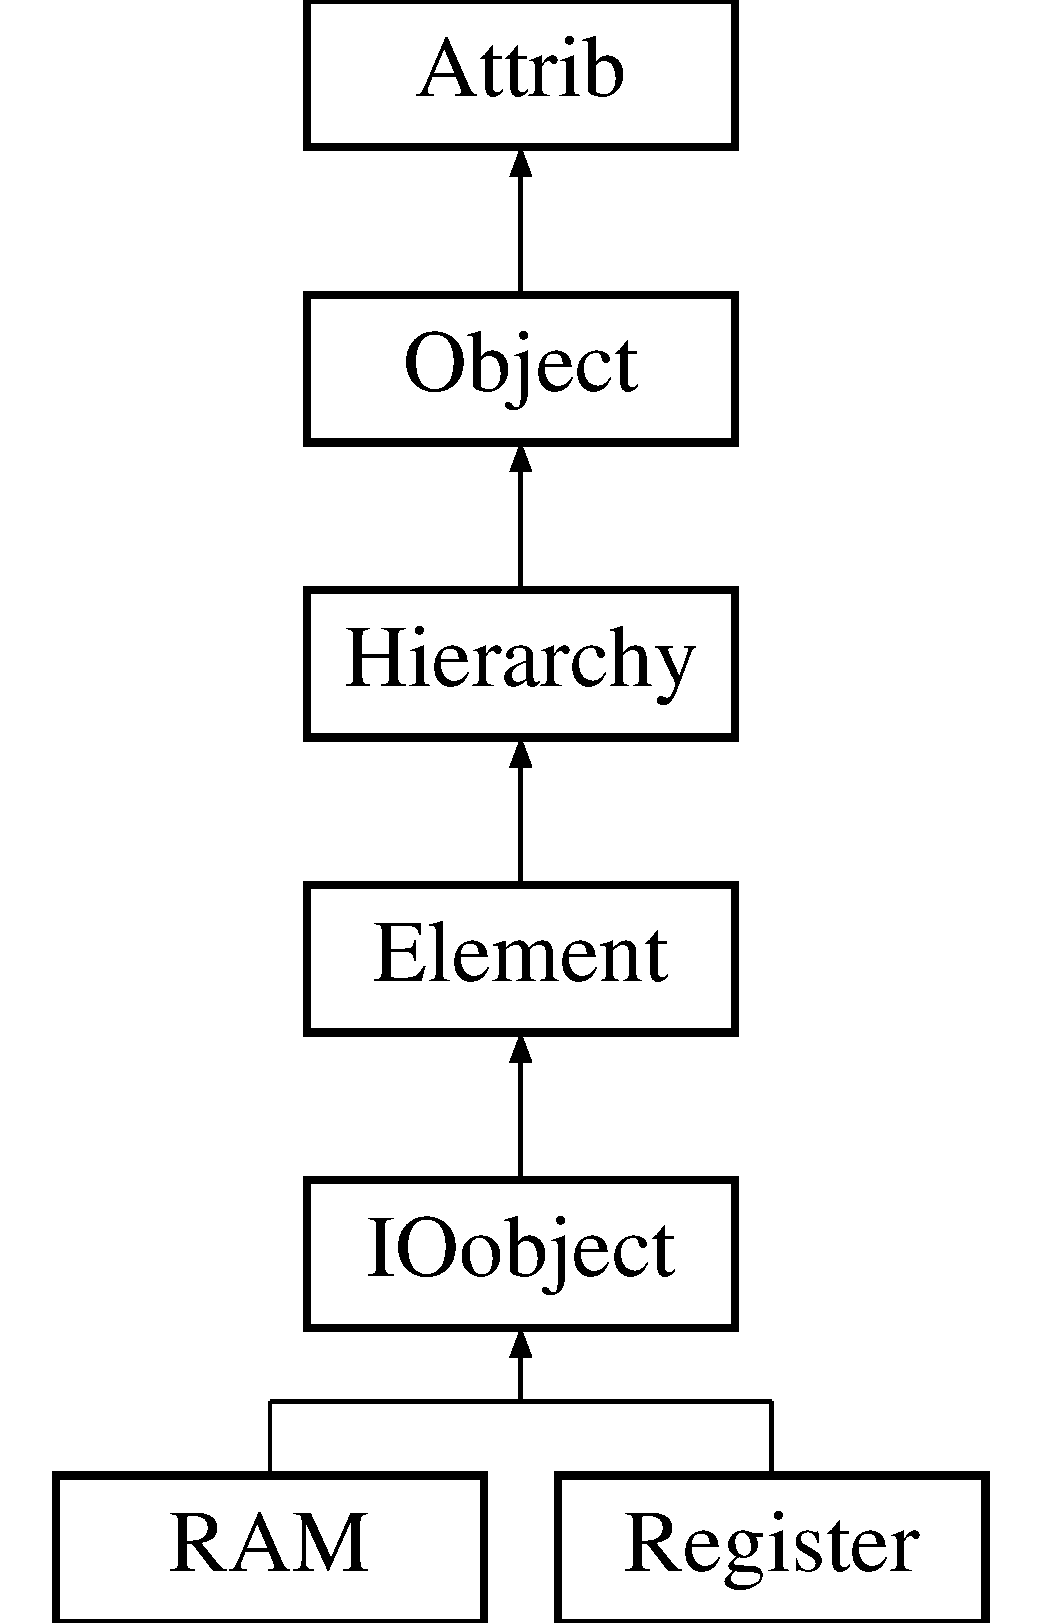
\includegraphics[height=6.000000cm]{classIOobject}
\end{center}
\end{figure}
\subsection*{Public Types}
\begin{DoxyCompactItemize}
\item 
typedef unsigned long \hyperlink{classIOobject_ad5bc21e44080074fe1068dc83861a090}{U32}
\item 
typedef unsigned short \hyperlink{classIOobject_a260583f7e496b1979cb75adc9bbb7fc4}{U16}
\item 
typedef unsigned char \hyperlink{classIOobject_a14ca3894cb3b023d2a0b2d088fddfc90}{U8}
\item 
enum \hyperlink{classAttrib_a69e171d7cc6417835a5a306d3c764235}{Attribut} \{ \newline
\hyperlink{classAttrib_a69e171d7cc6417835a5a306d3c764235a3a8da2ab97dda18aebab196fe4100531}{U\+N\+D\+E\+F\+I\+N\+ED}, 
\hyperlink{classAttrib_a69e171d7cc6417835a5a306d3c764235a2bfb2af57b87031d190a05fe25dd92ed}{P\+A\+S\+S\+I\+VE}, 
\hyperlink{classAttrib_a69e171d7cc6417835a5a306d3c764235a3b1fec929c0370d1436f2f06e298fb0d}{A\+C\+T\+I\+VE}, 
\hyperlink{classAttrib_a69e171d7cc6417835a5a306d3c764235aa27c16b480a369ea4d18b07b2516bbc7}{I\+N\+T\+E\+R\+F\+A\+CE}, 
\newline
\hyperlink{classAttrib_a69e171d7cc6417835a5a306d3c764235a1420a5b8c0540b2af210b6975eded7f9}{IO}, 
\hyperlink{classAttrib_a69e171d7cc6417835a5a306d3c764235a0af3b0d0ac323c1704e6c69cf90add28}{I\+O\+D\+A\+TA}, 
\hyperlink{classAttrib_a69e171d7cc6417835a5a306d3c764235a7788bc5dd333fd8ce18562b269c9dab1}{E\+L\+E\+M\+E\+NT}, 
\hyperlink{classAttrib_a69e171d7cc6417835a5a306d3c764235a61ceb22149f365f1780d18f9d1459423}{H\+A\+R\+D\+W\+A\+RE}, 
\newline
\hyperlink{classAttrib_a69e171d7cc6417835a5a306d3c764235a75250e29692496e73effca2c0330977f}{P\+R\+O\+C\+E\+S\+S\+US}, 
\hyperlink{classAttrib_a69e171d7cc6417835a5a306d3c764235a103a67cd0b8f07ef478fa45d4356e27b}{S\+O\+F\+T\+W\+A\+RE}
 \}
\end{DoxyCompactItemize}
\subsection*{Public Member Functions}
\begin{DoxyCompactItemize}
\item 
\hyperlink{classIOobject_a0c3f5a9fcc09892e99a4c977f4318a0b}{I\+Oobject} ()
\begin{DoxyCompactList}\small\item\em Standard constructor. \end{DoxyCompactList}\item 
virtual \hyperlink{classIOobject_a1db3f3f5d07a00a0b4cd47b2a0222f84}{$\sim$\+I\+Oobject} ()
\begin{DoxyCompactList}\small\item\em Destructor. \end{DoxyCompactList}\item 
void \hyperlink{classIOobject_a0520d82a9773c764fbaede59fe6f8a17}{help} ()
\item 
void \hyperlink{classIOobject_abccbc7a65366ec1257ff41a8e3245af8}{reset} ()
\item 
void \hyperlink{classIOobject_a0100b4ddcfe8f0b551a3f0dc5201988d}{update} ()
\item 
virtual \hyperlink{classStatusCode}{Status\+Code} \hyperlink{classIOobject_ab989e175734dd73797343e63cec6b174}{init} ()
\item 
\hyperlink{classIOdata}{I\+Odata} $\ast$ \hyperlink{classIOobject_af04fb94137c3d86849f478ac5afab5d1}{io} ()
\item 
virtual \hyperlink{classStatusCode}{Status\+Code} \hyperlink{classIOobject_aa07610c11963b1db6710e3c76ceea456}{read} ()
\item 
virtual \hyperlink{classStatusCode}{Status\+Code} \hyperlink{classIOobject_a9f6984bc9f0fadcf800f1be2523ac744}{write} ()
\item 
void \hyperlink{classIOobject_ae0d372aaeafe3da3c239677118deb2ac}{set\+Address} (\hyperlink{classIOobject_ad5bc21e44080074fe1068dc83861a090}{U32} \hyperlink{classIOobject_a95f0d3f092ea1ae3037ac60f0674d095}{address})
\item 
\hyperlink{classIOobject_ad5bc21e44080074fe1068dc83861a090}{U32} \hyperlink{classIOobject_a95f0d3f092ea1ae3037ac60f0674d095}{address} ()
\item 
void \hyperlink{classIOobject_a1247f08c84c1732a76caf07e987871e9}{dump} ()
\item 
void \hyperlink{classElement_a3c0abcb36f8906688bb7e32608df7086}{recursive\+Init\+Element} ()
\item 
void \hyperlink{classElement_a82119ed37dff76508a2746a853ec35ba}{recursive\+Init\+Communications} ()
\item 
\hyperlink{classStatusCode}{Status\+Code} \hyperlink{classElement_ab476b4b1df5954141ceb14f072433b89}{set\+Connection} (\hyperlink{classHierarchy}{Hierarchy} $\ast$)
\item 
\hyperlink{classHierarchy}{Hierarchy} $\ast$ \hyperlink{classElement_af57444353c1ddf9fa0109801e97debf7}{connection} ()
\item 
void \hyperlink{classHierarchy_af4d43b0765b402670eed2d62c73405af}{clear} ()
\item 
void \hyperlink{classHierarchy_a585ad1aeec16077a0e532ab8b4fc557b}{set\+Parent} (\hyperlink{classHierarchy}{Hierarchy} $\ast$\hyperlink{classHierarchy_a1c7bec8257e717f9c1465e06ebf845fc}{parent})
\item 
\hyperlink{classHierarchy}{Hierarchy} $\ast$ \hyperlink{classHierarchy_a1c7bec8257e717f9c1465e06ebf845fc}{parent} ()
\item 
\hyperlink{classHierarchy}{Hierarchy} $\ast$ \hyperlink{classHierarchy_ad550588733bf75ac5c0fcfd7c8fd11a6}{parent} (std\+::string)
\item 
\hyperlink{classHierarchy}{Hierarchy} $\ast$ \hyperlink{classHierarchy_aee461dc930ce3871636ff87f075b1b83}{origin} ()
\item 
virtual void \hyperlink{classHierarchy_ad677774ff38fcb257c04a3a10d471fac}{add\+Child} (\hyperlink{classHierarchy}{Hierarchy} $\ast$element)
\item 
std\+::vector$<$ \hyperlink{classHierarchy}{Hierarchy} $\ast$ $>$ \hyperlink{classHierarchy_aa9a76f69e98e052ee1a6e32cea006288}{children} ()
\item 
\hyperlink{classHierarchy}{Hierarchy} $\ast$ \hyperlink{classHierarchy_a1e207f973c694b538bf90107b4868817}{child} (std\+::string)
\item 
\hyperlink{classHierarchy}{Hierarchy} $\ast$ \hyperlink{classHierarchy_a0c15a5276a3b80b4354d6bd8a01e0708}{child\+Typed} (std\+::string)
\item 
unsigned long \hyperlink{classHierarchy_ab16e84de65fd84e14001a6cf941c8be4}{number\+Of\+Children} ()
\item 
bool \hyperlink{classHierarchy_a255174fe4d316d2a3f430dcb9dab29f1}{has\+Children} ()
\item 
void \hyperlink{classHierarchy_a2b2b359fac003233f65786a616766bde}{del\+Child} (\hyperlink{classHierarchy}{Hierarchy} $\ast$)
\item 
void \hyperlink{classHierarchy_a1928ac7615fe0b5e55cd707f70dc6781}{del\+Child} (std\+::string)
\item 
std\+::string \hyperlink{classHierarchy_aa7990fa7caf132d83e361ce033c6c65a}{path} (std\+::string=std\+::string(\char`\"{}\char`\"{}))
\item 
std\+::string \hyperlink{classHierarchy_a1efd56cd164d328d2002e53a10a19b8c}{path\+Typed} (std\+::string=std\+::string(\char`\"{}\char`\"{}))
\item 
void \hyperlink{classHierarchy_a76e914b9a677a22a82deb74d892bf261}{tree} (std\+::string indent=std\+::string(\char`\"{}\char`\"{}))
\item 
void \hyperlink{classHierarchy_a594c294c5f60c230e106d522ed008212}{tree} ()
\item 
std\+::string \hyperlink{classObject_a300f4c05dd468c7bb8b3c968868443c1}{name} () const
\item 
std\+::string \hyperlink{classObject_a84f99f70f144a83e1582d1d0f84e4e62}{type} ()
\item 
unsigned char \hyperlink{classObject_af99145335cc61ff6e2798ea17db009d2}{id} ()
\item 
std\+::string \hyperlink{classObject_a73a0f1a41828fdd8303dd662446fb6c3}{title} ()
\item 
void \hyperlink{classObject_a3f9d5537ebce0c0f2bf6ae4d92426f3c}{msg\+Svc} (int level, std\+::string \hyperlink{classObject_a58b2d0618c2d08cf2383012611528d97}{msg}, std\+::string \hyperlink{classObject_a300f4c05dd468c7bb8b3c968868443c1}{name})
\item 
void \hyperlink{classObject_a58b2d0618c2d08cf2383012611528d97}{msg} (std\+::string mymsg)
\item 
void \hyperlink{classObject_ac5d59299273cee27aacf7de00d2e7034}{msg} (std\+::string mymsg, std\+::string \hyperlink{classObject_a300f4c05dd468c7bb8b3c968868443c1}{name})
\item 
void \hyperlink{classObject_a83d2db2df682907ea1115ad721c1c4a1}{verbose} (std\+::string mymsg)
\item 
void \hyperlink{classObject_a2d4120195317e2a3c6532e8bb9f3da68}{verbose} (std\+::string mymsg, std\+::string \hyperlink{classObject_a300f4c05dd468c7bb8b3c968868443c1}{name})
\item 
void \hyperlink{classObject_aac010553f022165573714b7014a15f0d}{debug} (std\+::string mymsg)
\item 
void \hyperlink{classObject_a6c9a0397ca804e04d675ed05683f5420}{debug} (std\+::string mymsg, std\+::string \hyperlink{classObject_a300f4c05dd468c7bb8b3c968868443c1}{name})
\item 
void \hyperlink{classObject_a644fd329ea4cb85f54fa6846484b84a8}{info} (std\+::string mymsg)
\item 
void \hyperlink{classObject_a1ca123253dfd30fc28b156f521dcbdae}{info} (std\+::string mymsg, std\+::string \hyperlink{classObject_a300f4c05dd468c7bb8b3c968868443c1}{name})
\item 
void \hyperlink{classObject_a65cd4fda577711660821fd2cd5a3b4c9}{warning} (std\+::string mymsg)
\item 
void \hyperlink{classObject_a11f101db4dd73d9391b0231818881d86}{warning} (std\+::string mymsg, std\+::string \hyperlink{classObject_a300f4c05dd468c7bb8b3c968868443c1}{name})
\item 
void \hyperlink{classObject_a204a95f57818c0f811933917a30eff45}{error} (std\+::string mymsg)
\item 
void \hyperlink{classObject_ad7f6c457733082efa2f9ff5f5c8e119a}{error} (std\+::string mymsg, std\+::string \hyperlink{classObject_a300f4c05dd468c7bb8b3c968868443c1}{name})
\item 
void \hyperlink{classObject_aad5a16aac7516ce65bd5ec02ab07fc80}{fatal} (std\+::string mymsg)
\item 
void \hyperlink{classObject_ae62acd3d09f716220f75f252dc38bc9a}{fatal} (std\+::string mymsg, std\+::string \hyperlink{classObject_a300f4c05dd468c7bb8b3c968868443c1}{name})
\item 
void \hyperlink{classObject_ae30fea75683c2d149b6b6d17c09ecd0c}{set\+Name} (std\+::string \hyperlink{classObject_a300f4c05dd468c7bb8b3c968868443c1}{name})
\item 
void \hyperlink{classObject_aae534cc9d982bcb9b99fd505f2e103a5}{set\+Type} (std\+::string \hyperlink{classObject_a84f99f70f144a83e1582d1d0f84e4e62}{type})
\item 
void \hyperlink{classObject_a398fe08cba594a0ce6891d59fe4f159f}{set\+Id} (unsigned char \hyperlink{classObject_af99145335cc61ff6e2798ea17db009d2}{id})
\item 
void \hyperlink{classObject_a89557dbbad5bcaa02652f5d7fa35d20f}{set\+Title} (std\+::string \hyperlink{classObject_a73a0f1a41828fdd8303dd662446fb6c3}{title})
\item 
void \hyperlink{classObject_a870c5af919958c2136623b2d7816d123}{set\+Dll\+Name} (std\+::string \hyperlink{classObject_a2e3947f2870094c332d7454117f3ec63}{dll\+Name})
\item 
std\+::string \hyperlink{classObject_a2e3947f2870094c332d7454117f3ec63}{dll\+Name} ()
\item 
bool \hyperlink{classAttrib_a704f26af560909ad22065083bb7d4c34}{is} (int attribut)
\item 
void \hyperlink{classAttrib_a235f773af19c900264a190b00a3b4ad7}{add} (int attribut)
\item 
void \hyperlink{classAttrib_a7d4ef7e32d93cb287792b87b857e79f3}{remove} (int attribut)
\item 
std\+::string \hyperlink{classAttrib_aee7bbf16b144887f196e1341b24f8a26}{attributs} ()
\end{DoxyCompactItemize}
\subsection*{Protected Attributes}
\begin{DoxyCompactItemize}
\item 
\hyperlink{classHierarchy}{Hierarchy} $\ast$ \hyperlink{classElement_abe3de7a5dbbc9a6dd2d7e012e5fdb266}{m\+\_\+connection}
\item 
std\+::string \hyperlink{classAttrib_a3414521d7a82476e874b25a5407b5e63}{m\+\_\+attrib\+String} \mbox{[}10\mbox{]}
\end{DoxyCompactItemize}
\subsection*{Private Attributes}
\begin{DoxyCompactItemize}
\item 
\hyperlink{classIOdata}{I\+Odata} $\ast$ \hyperlink{classIOobject_aa648e4128c3c37d8291d6bb26b57c504}{m\+\_\+io}
\end{DoxyCompactItemize}


\subsection{Detailed Description}
\begin{DoxyAuthor}{Author}

\end{DoxyAuthor}
\begin{DoxyDate}{Date}
2006-\/10-\/23 
\end{DoxyDate}


Definition at line 17 of file I\+Oobject.\+h.



\subsection{Member Typedef Documentation}
\mbox{\Hypertarget{classIOobject_a260583f7e496b1979cb75adc9bbb7fc4}\label{classIOobject_a260583f7e496b1979cb75adc9bbb7fc4}} 
\index{I\+Oobject@{I\+Oobject}!U16@{U16}}
\index{U16@{U16}!I\+Oobject@{I\+Oobject}}
\subsubsection{\texorpdfstring{U16}{U16}}
{\footnotesize\ttfamily typedef unsigned short \hyperlink{classIOobject_a260583f7e496b1979cb75adc9bbb7fc4}{I\+Oobject\+::\+U16}}



Definition at line 20 of file I\+Oobject.\+h.

\mbox{\Hypertarget{classIOobject_ad5bc21e44080074fe1068dc83861a090}\label{classIOobject_ad5bc21e44080074fe1068dc83861a090}} 
\index{I\+Oobject@{I\+Oobject}!U32@{U32}}
\index{U32@{U32}!I\+Oobject@{I\+Oobject}}
\subsubsection{\texorpdfstring{U32}{U32}}
{\footnotesize\ttfamily typedef unsigned long \hyperlink{classIOobject_ad5bc21e44080074fe1068dc83861a090}{I\+Oobject\+::\+U32}}



Definition at line 19 of file I\+Oobject.\+h.

\mbox{\Hypertarget{classIOobject_a14ca3894cb3b023d2a0b2d088fddfc90}\label{classIOobject_a14ca3894cb3b023d2a0b2d088fddfc90}} 
\index{I\+Oobject@{I\+Oobject}!U8@{U8}}
\index{U8@{U8}!I\+Oobject@{I\+Oobject}}
\subsubsection{\texorpdfstring{U8}{U8}}
{\footnotesize\ttfamily typedef unsigned char \hyperlink{classIOobject_a14ca3894cb3b023d2a0b2d088fddfc90}{I\+Oobject\+::\+U8}}



Definition at line 21 of file I\+Oobject.\+h.



\subsection{Member Enumeration Documentation}
\mbox{\Hypertarget{classAttrib_a69e171d7cc6417835a5a306d3c764235}\label{classAttrib_a69e171d7cc6417835a5a306d3c764235}} 
\index{I\+Oobject@{I\+Oobject}!Attribut@{Attribut}}
\index{Attribut@{Attribut}!I\+Oobject@{I\+Oobject}}
\subsubsection{\texorpdfstring{Attribut}{Attribut}}
{\footnotesize\ttfamily enum \hyperlink{classAttrib_a69e171d7cc6417835a5a306d3c764235}{Attrib\+::\+Attribut}\hspace{0.3cm}{\ttfamily [inherited]}}

\begin{DoxyEnumFields}{Enumerator}
\raisebox{\heightof{T}}[0pt][0pt]{\index{U\+N\+D\+E\+F\+I\+N\+ED@{U\+N\+D\+E\+F\+I\+N\+ED}!I\+Oobject@{I\+Oobject}}\index{I\+Oobject@{I\+Oobject}!U\+N\+D\+E\+F\+I\+N\+ED@{U\+N\+D\+E\+F\+I\+N\+ED}}}\mbox{\Hypertarget{classAttrib_a69e171d7cc6417835a5a306d3c764235a3a8da2ab97dda18aebab196fe4100531}\label{classAttrib_a69e171d7cc6417835a5a306d3c764235a3a8da2ab97dda18aebab196fe4100531}} 
U\+N\+D\+E\+F\+I\+N\+ED&\\
\hline

\raisebox{\heightof{T}}[0pt][0pt]{\index{P\+A\+S\+S\+I\+VE@{P\+A\+S\+S\+I\+VE}!I\+Oobject@{I\+Oobject}}\index{I\+Oobject@{I\+Oobject}!P\+A\+S\+S\+I\+VE@{P\+A\+S\+S\+I\+VE}}}\mbox{\Hypertarget{classAttrib_a69e171d7cc6417835a5a306d3c764235a2bfb2af57b87031d190a05fe25dd92ed}\label{classAttrib_a69e171d7cc6417835a5a306d3c764235a2bfb2af57b87031d190a05fe25dd92ed}} 
P\+A\+S\+S\+I\+VE&\\
\hline

\raisebox{\heightof{T}}[0pt][0pt]{\index{A\+C\+T\+I\+VE@{A\+C\+T\+I\+VE}!I\+Oobject@{I\+Oobject}}\index{I\+Oobject@{I\+Oobject}!A\+C\+T\+I\+VE@{A\+C\+T\+I\+VE}}}\mbox{\Hypertarget{classAttrib_a69e171d7cc6417835a5a306d3c764235a3b1fec929c0370d1436f2f06e298fb0d}\label{classAttrib_a69e171d7cc6417835a5a306d3c764235a3b1fec929c0370d1436f2f06e298fb0d}} 
A\+C\+T\+I\+VE&\\
\hline

\raisebox{\heightof{T}}[0pt][0pt]{\index{I\+N\+T\+E\+R\+F\+A\+CE@{I\+N\+T\+E\+R\+F\+A\+CE}!I\+Oobject@{I\+Oobject}}\index{I\+Oobject@{I\+Oobject}!I\+N\+T\+E\+R\+F\+A\+CE@{I\+N\+T\+E\+R\+F\+A\+CE}}}\mbox{\Hypertarget{classAttrib_a69e171d7cc6417835a5a306d3c764235aa27c16b480a369ea4d18b07b2516bbc7}\label{classAttrib_a69e171d7cc6417835a5a306d3c764235aa27c16b480a369ea4d18b07b2516bbc7}} 
I\+N\+T\+E\+R\+F\+A\+CE&\\
\hline

\raisebox{\heightof{T}}[0pt][0pt]{\index{IO@{IO}!I\+Oobject@{I\+Oobject}}\index{I\+Oobject@{I\+Oobject}!IO@{IO}}}\mbox{\Hypertarget{classAttrib_a69e171d7cc6417835a5a306d3c764235a1420a5b8c0540b2af210b6975eded7f9}\label{classAttrib_a69e171d7cc6417835a5a306d3c764235a1420a5b8c0540b2af210b6975eded7f9}} 
IO&\\
\hline

\raisebox{\heightof{T}}[0pt][0pt]{\index{I\+O\+D\+A\+TA@{I\+O\+D\+A\+TA}!I\+Oobject@{I\+Oobject}}\index{I\+Oobject@{I\+Oobject}!I\+O\+D\+A\+TA@{I\+O\+D\+A\+TA}}}\mbox{\Hypertarget{classAttrib_a69e171d7cc6417835a5a306d3c764235a0af3b0d0ac323c1704e6c69cf90add28}\label{classAttrib_a69e171d7cc6417835a5a306d3c764235a0af3b0d0ac323c1704e6c69cf90add28}} 
I\+O\+D\+A\+TA&\\
\hline

\raisebox{\heightof{T}}[0pt][0pt]{\index{E\+L\+E\+M\+E\+NT@{E\+L\+E\+M\+E\+NT}!I\+Oobject@{I\+Oobject}}\index{I\+Oobject@{I\+Oobject}!E\+L\+E\+M\+E\+NT@{E\+L\+E\+M\+E\+NT}}}\mbox{\Hypertarget{classAttrib_a69e171d7cc6417835a5a306d3c764235a7788bc5dd333fd8ce18562b269c9dab1}\label{classAttrib_a69e171d7cc6417835a5a306d3c764235a7788bc5dd333fd8ce18562b269c9dab1}} 
E\+L\+E\+M\+E\+NT&\\
\hline

\raisebox{\heightof{T}}[0pt][0pt]{\index{H\+A\+R\+D\+W\+A\+RE@{H\+A\+R\+D\+W\+A\+RE}!I\+Oobject@{I\+Oobject}}\index{I\+Oobject@{I\+Oobject}!H\+A\+R\+D\+W\+A\+RE@{H\+A\+R\+D\+W\+A\+RE}}}\mbox{\Hypertarget{classAttrib_a69e171d7cc6417835a5a306d3c764235a61ceb22149f365f1780d18f9d1459423}\label{classAttrib_a69e171d7cc6417835a5a306d3c764235a61ceb22149f365f1780d18f9d1459423}} 
H\+A\+R\+D\+W\+A\+RE&\\
\hline

\raisebox{\heightof{T}}[0pt][0pt]{\index{P\+R\+O\+C\+E\+S\+S\+US@{P\+R\+O\+C\+E\+S\+S\+US}!I\+Oobject@{I\+Oobject}}\index{I\+Oobject@{I\+Oobject}!P\+R\+O\+C\+E\+S\+S\+US@{P\+R\+O\+C\+E\+S\+S\+US}}}\mbox{\Hypertarget{classAttrib_a69e171d7cc6417835a5a306d3c764235a75250e29692496e73effca2c0330977f}\label{classAttrib_a69e171d7cc6417835a5a306d3c764235a75250e29692496e73effca2c0330977f}} 
P\+R\+O\+C\+E\+S\+S\+US&\\
\hline

\raisebox{\heightof{T}}[0pt][0pt]{\index{S\+O\+F\+T\+W\+A\+RE@{S\+O\+F\+T\+W\+A\+RE}!I\+Oobject@{I\+Oobject}}\index{I\+Oobject@{I\+Oobject}!S\+O\+F\+T\+W\+A\+RE@{S\+O\+F\+T\+W\+A\+RE}}}\mbox{\Hypertarget{classAttrib_a69e171d7cc6417835a5a306d3c764235a103a67cd0b8f07ef478fa45d4356e27b}\label{classAttrib_a69e171d7cc6417835a5a306d3c764235a103a67cd0b8f07ef478fa45d4356e27b}} 
S\+O\+F\+T\+W\+A\+RE&\\
\hline

\end{DoxyEnumFields}


Definition at line 29 of file Attrib.\+h.


\begin{DoxyCode}
29                 \{
30     \hyperlink{classAttrib_a69e171d7cc6417835a5a306d3c764235a3a8da2ab97dda18aebab196fe4100531}{UNDEFINED},
31     \hyperlink{classAttrib_a69e171d7cc6417835a5a306d3c764235a2bfb2af57b87031d190a05fe25dd92ed}{PASSIVE},
32     \hyperlink{classAttrib_a69e171d7cc6417835a5a306d3c764235a3b1fec929c0370d1436f2f06e298fb0d}{ACTIVE},
33     \hyperlink{classAttrib_a69e171d7cc6417835a5a306d3c764235aa27c16b480a369ea4d18b07b2516bbc7}{INTERFACE},
34     \hyperlink{classAttrib_a69e171d7cc6417835a5a306d3c764235a1420a5b8c0540b2af210b6975eded7f9}{IO},
35     \hyperlink{classAttrib_a69e171d7cc6417835a5a306d3c764235a0af3b0d0ac323c1704e6c69cf90add28}{IODATA},
36     \hyperlink{classAttrib_a69e171d7cc6417835a5a306d3c764235a7788bc5dd333fd8ce18562b269c9dab1}{ELEMENT},
37     \hyperlink{classAttrib_a69e171d7cc6417835a5a306d3c764235a61ceb22149f365f1780d18f9d1459423}{HARDWARE},
38     \hyperlink{classAttrib_a69e171d7cc6417835a5a306d3c764235a75250e29692496e73effca2c0330977f}{PROCESSUS},
39     \hyperlink{classAttrib_a69e171d7cc6417835a5a306d3c764235a103a67cd0b8f07ef478fa45d4356e27b}{SOFTWARE} 
40   \}; \textcolor{comment}{// array m\_attribString must be changed into Attrib::Attrib if this enu is modified. }
\end{DoxyCode}


\subsection{Constructor \& Destructor Documentation}
\mbox{\Hypertarget{classIOobject_a0c3f5a9fcc09892e99a4c977f4318a0b}\label{classIOobject_a0c3f5a9fcc09892e99a4c977f4318a0b}} 
\index{I\+Oobject@{I\+Oobject}!I\+Oobject@{I\+Oobject}}
\index{I\+Oobject@{I\+Oobject}!I\+Oobject@{I\+Oobject}}
\subsubsection{\texorpdfstring{I\+Oobject()}{IOobject()}}
{\footnotesize\ttfamily I\+Oobject\+::\+I\+Oobject (\begin{DoxyParamCaption}{ }\end{DoxyParamCaption})}



Standard constructor. 



Definition at line 17 of file I\+Oobject.\+cpp.



References Attrib\+::add(), Attrib\+::\+E\+L\+E\+M\+E\+NT, Attrib\+::\+IO, m\+\_\+io, Object\+::set\+Name(), and Object\+::set\+Type().


\begin{DoxyCode}
17                      \{
18   \hyperlink{classObject_ae30fea75683c2d149b6b6d17c09ecd0c}{setName}(\textcolor{stringliteral}{"IOobject"});
19   \hyperlink{classObject_aae534cc9d982bcb9b99fd505f2e103a5}{setType}(\textcolor{stringliteral}{"IOobject"});
20   \hyperlink{classAttrib_a235f773af19c900264a190b00a3b4ad7}{add}(\hyperlink{classAttrib_a69e171d7cc6417835a5a306d3c764235a7788bc5dd333fd8ce18562b269c9dab1}{Attrib::ELEMENT});  \hyperlink{classAttrib_a235f773af19c900264a190b00a3b4ad7}{add}(\hyperlink{classAttrib_a69e171d7cc6417835a5a306d3c764235a1420a5b8c0540b2af210b6975eded7f9}{Attrib::IO});
21   \hyperlink{classIOobject_aa648e4128c3c37d8291d6bb26b57c504}{m\_io}=\textcolor{keyword}{new} \hyperlink{classIOdata}{IOdata}();
22 \}
\end{DoxyCode}
\mbox{\Hypertarget{classIOobject_a1db3f3f5d07a00a0b4cd47b2a0222f84}\label{classIOobject_a1db3f3f5d07a00a0b4cd47b2a0222f84}} 
\index{I\+Oobject@{I\+Oobject}!````~I\+Oobject@{$\sim$\+I\+Oobject}}
\index{````~I\+Oobject@{$\sim$\+I\+Oobject}!I\+Oobject@{I\+Oobject}}
\subsubsection{\texorpdfstring{$\sim$\+I\+Oobject()}{~IOobject()}}
{\footnotesize\ttfamily I\+Oobject\+::$\sim$\+I\+Oobject (\begin{DoxyParamCaption}{ }\end{DoxyParamCaption})\hspace{0.3cm}{\ttfamily [virtual]}}



Destructor. 



Definition at line 26 of file I\+Oobject.\+cpp.



References m\+\_\+io.


\begin{DoxyCode}
26                     \{
27   \textcolor{keyword}{delete} \hyperlink{classIOobject_aa648e4128c3c37d8291d6bb26b57c504}{m\_io};
28 \}
\end{DoxyCode}


\subsection{Member Function Documentation}
\mbox{\Hypertarget{classAttrib_a235f773af19c900264a190b00a3b4ad7}\label{classAttrib_a235f773af19c900264a190b00a3b4ad7}} 
\index{I\+Oobject@{I\+Oobject}!add@{add}}
\index{add@{add}!I\+Oobject@{I\+Oobject}}
\subsubsection{\texorpdfstring{add()}{add()}}
{\footnotesize\ttfamily void Attrib\+::add (\begin{DoxyParamCaption}\item[{int}]{attribut }\end{DoxyParamCaption})\hspace{0.3cm}{\ttfamily [inline]}, {\ttfamily [inherited]}}

Add an attribut 

Definition at line 67 of file Attrib.\+h.



References Attrib\+::m\+\_\+attributs, and Attrib\+::\+U\+N\+D\+E\+F\+I\+N\+ED.



Referenced by A3\+P\+E\+::\+A3\+P\+E(), Attrib\+::\+Attrib(), Specs\+Mezzanine\+::cmdline(), Computer\+::\+Computer(), C\+U\+\_\+v1\+::\+C\+U\+\_\+v1(), export\+\_\+obj(), F\+E\+B\+\_\+v1\+::\+F\+E\+B\+\_\+v1(), Fe\+P\+G\+A\+::\+Fe\+P\+G\+A(), I\+C\+E\+C\+A\+Lv3\+::\+I\+C\+E\+C\+A\+Lv3(), I\+C\+Phaser\+::\+I\+C\+Phaser(), Fe\+P\+G\+A\+::init(), Application\+::initialize(), Interface\+::\+Interface(), I\+Odata\+::\+I\+Odata(), I\+Oobject(), M\+S\+Oxxxx\+::\+M\+S\+Oxxxx(), Phaser\+::\+Phaser(), Processus\+::\+Processus(), Proto40\+M\+Hz\+\_\+v1\+::\+Proto40\+M\+Hz\+\_\+v1(), Attrib\+::remove(), Seq\+P\+G\+A\+::\+Seq\+P\+G\+A(), Test\+I2\+C\+::set\+Address(), Test\+S\+P\+I\+::set\+Address(), Specs\+Slave\+::set\+Address(), Specs\+Master\+::\+Specs\+Master(), and Specs\+Slave\+::\+Specs\+Slave().


\begin{DoxyCode}
67                             \{
68     \textcolor{keywordflow}{if} (attribut!=\hyperlink{classAttrib_a69e171d7cc6417835a5a306d3c764235a3a8da2ab97dda18aebab196fe4100531}{Attrib::UNDEFINED}) \textcolor{keyword}{remove}(\hyperlink{classAttrib_a69e171d7cc6417835a5a306d3c764235a3a8da2ab97dda18aebab196fe4100531}{Attrib::UNDEFINED});
69     \textcolor{keywordtype}{bool} duplicate = false ;
70     std::vector<int>::const\_iterator iter ;
71     \textcolor{keywordflow}{for} ( iter  = \hyperlink{classAttrib_ac4bd58a0cc6b38a3b711d609a3d3aacc}{m\_attributs}.begin() ;
72           iter != \hyperlink{classAttrib_ac4bd58a0cc6b38a3b711d609a3d3aacc}{m\_attributs}.end()   ;
73           ++iter ) \{
74       \textcolor{keywordflow}{if} ( attribut == (*iter) ) \{
75         duplicate = true ;
76       \}
77     \}
78     \textcolor{keywordflow}{if} (!duplicate) \{
79       \hyperlink{classAttrib_ac4bd58a0cc6b38a3b711d609a3d3aacc}{m\_attributs}.push\_back( attribut );
80     \}
81   \}
\end{DoxyCode}
\mbox{\Hypertarget{classHierarchy_ad677774ff38fcb257c04a3a10d471fac}\label{classHierarchy_ad677774ff38fcb257c04a3a10d471fac}} 
\index{I\+Oobject@{I\+Oobject}!add\+Child@{add\+Child}}
\index{add\+Child@{add\+Child}!I\+Oobject@{I\+Oobject}}
\subsubsection{\texorpdfstring{add\+Child()}{addChild()}}
{\footnotesize\ttfamily void Hierarchy\+::add\+Child (\begin{DoxyParamCaption}\item[{\hyperlink{classHierarchy}{Hierarchy} $\ast$}]{element }\end{DoxyParamCaption})\hspace{0.3cm}{\ttfamily [virtual]}, {\ttfamily [inherited]}}



Definition at line 83 of file Hierarchy.\+cpp.



References Object\+::debug(), Hierarchy\+::m\+\_\+children, Object\+::name(), and Hierarchy\+::set\+Parent().



Referenced by A3\+P\+E\+::\+A3\+P\+E(), Specs\+Mezzanine\+::add\+Bus(), Specs\+Slave\+::add\+I2c(), Application\+::create(), C\+U\+\_\+v1\+::\+C\+U\+\_\+v1(), export\+\_\+obj(), F\+E\+B\+\_\+v1\+::\+F\+E\+B\+\_\+v1(), Fe\+P\+G\+A\+::\+Fe\+P\+G\+A(), I\+C\+E\+C\+A\+Lv3\+::\+I\+C\+E\+C\+A\+Lv3(), I\+C\+Phaser\+::\+I\+C\+Phaser(), Fe\+P\+G\+A\+::\+Make\+R\+A\+M(), Fe\+P\+G\+A\+::\+Make\+Register(), Hierarchy\+::origin(), Phaser\+::\+Phaser(), Proto40\+M\+Hz\+\_\+v1\+::\+Proto40\+M\+Hz\+\_\+v1(), Seq\+P\+G\+A\+::\+Seq\+P\+G\+A(), Specs\+Mezzanine\+::\+Specs\+Mezzanine(), Usb\+I2c\+Bus\+::\+Usb\+I2c\+Bus(), and Usb\+Spi\+Bus\+::\+Usb\+Spi\+Bus().


\begin{DoxyCode}
83                                           \{
84   element->\hyperlink{classHierarchy_a585ad1aeec16077a0e532ab8b4fc557b}{setParent}(\textcolor{keyword}{this});
85   \hyperlink{classHierarchy_a038816763941fd4a930504917f60483b}{m\_children}.push\_back(element);
86   \hyperlink{classObject_aac010553f022165573714b7014a15f0d}{debug}(element->\hyperlink{classObject_a300f4c05dd468c7bb8b3c968868443c1}{name}()+\textcolor{stringliteral}{" added to the child tree."},\textcolor{stringliteral}{"Hierarchy::addChild"});
87 \}
\end{DoxyCode}
\mbox{\Hypertarget{classIOobject_a95f0d3f092ea1ae3037ac60f0674d095}\label{classIOobject_a95f0d3f092ea1ae3037ac60f0674d095}} 
\index{I\+Oobject@{I\+Oobject}!address@{address}}
\index{address@{address}!I\+Oobject@{I\+Oobject}}
\subsubsection{\texorpdfstring{address()}{address()}}
{\footnotesize\ttfamily \hyperlink{classIOobject_ad5bc21e44080074fe1068dc83861a090}{U32} I\+Oobject\+::address (\begin{DoxyParamCaption}{ }\end{DoxyParamCaption})\hspace{0.3cm}{\ttfamily [inline]}}



Definition at line 88 of file I\+Oobject.\+h.



References I\+Odata\+::address(), and m\+\_\+io.



Referenced by B\+O\+O\+S\+T\+\_\+\+P\+Y\+T\+H\+O\+N\+\_\+\+M\+O\+D\+U\+L\+E().


\begin{DoxyCode}
88                \{
89     \textcolor{keywordflow}{return} \hyperlink{classIOobject_aa648e4128c3c37d8291d6bb26b57c504}{m\_io}->\hyperlink{classIOdata_afe410c86881b8c2082a08e5ce9843306}{address}();
90   \}
\end{DoxyCode}
\mbox{\Hypertarget{classAttrib_aee7bbf16b144887f196e1341b24f8a26}\label{classAttrib_aee7bbf16b144887f196e1341b24f8a26}} 
\index{I\+Oobject@{I\+Oobject}!attributs@{attributs}}
\index{attributs@{attributs}!I\+Oobject@{I\+Oobject}}
\subsubsection{\texorpdfstring{attributs()}{attributs()}}
{\footnotesize\ttfamily std\+::string Attrib\+::attributs (\begin{DoxyParamCaption}{ }\end{DoxyParamCaption})\hspace{0.3cm}{\ttfamily [inherited]}}

Print the \hyperlink{classAttrib}{Attrib} of an \hyperlink{classObject}{Object} 

Definition at line 54 of file Attrib.\+cpp.



References images\+::index, Attrib\+::m\+\_\+attrib\+String, and Attrib\+::m\+\_\+attributs.



Referenced by export\+\_\+obj(), and Attrib\+::remove().


\begin{DoxyCode}
54                             \{
55   std::string output;
56   std::vector<int>::iterator iter ;
57   \textcolor{keywordflow}{for} ( \textcolor{keywordtype}{unsigned} \textcolor{keywordtype}{int} \hyperlink{namespaceimages_a54407fd574970b3178647ae096321a57}{index} = 0 ; \hyperlink{namespaceimages_a54407fd574970b3178647ae096321a57}{index} < \hyperlink{classAttrib_ac4bd58a0cc6b38a3b711d609a3d3aacc}{m\_attributs}.size() ; ++
      \hyperlink{namespaceimages_a54407fd574970b3178647ae096321a57}{index} ) \{
58     \textcolor{keywordflow}{if} ( \hyperlink{classAttrib_ac4bd58a0cc6b38a3b711d609a3d3aacc}{m\_attributs}.size() - \hyperlink{namespaceimages_a54407fd574970b3178647ae096321a57}{index} > 1 ) \{
59       output.append(\hyperlink{classAttrib_a3414521d7a82476e874b25a5407b5e63}{m\_attribString}[\hyperlink{classAttrib_ac4bd58a0cc6b38a3b711d609a3d3aacc}{m\_attributs}[\hyperlink{namespaceimages_a54407fd574970b3178647ae096321a57}{index}]]);
60       output.append(\textcolor{stringliteral}{":"});
61     \}
62     \textcolor{keywordflow}{else} \{
63       output.append(\hyperlink{classAttrib_a3414521d7a82476e874b25a5407b5e63}{m\_attribString}[\hyperlink{classAttrib_ac4bd58a0cc6b38a3b711d609a3d3aacc}{m\_attributs}[index]]);
64     \}
65   \}
66   \textcolor{keywordflow}{return} output;
67 \}
\end{DoxyCode}
\mbox{\Hypertarget{classHierarchy_a1e207f973c694b538bf90107b4868817}\label{classHierarchy_a1e207f973c694b538bf90107b4868817}} 
\index{I\+Oobject@{I\+Oobject}!child@{child}}
\index{child@{child}!I\+Oobject@{I\+Oobject}}
\subsubsection{\texorpdfstring{child()}{child()}}
{\footnotesize\ttfamily \hyperlink{classHierarchy}{Hierarchy} $\ast$ Hierarchy\+::child (\begin{DoxyParamCaption}\item[{std\+::string}]{path }\end{DoxyParamCaption})\hspace{0.3cm}{\ttfamily [inherited]}}



Definition at line 133 of file Hierarchy.\+cpp.



References Hierarchy\+::child(), Hierarchy\+::children(), Object\+::name(), Hierarchy\+::origin(), Hierarchy\+::parent(), Hierarchy\+::path(), and Object\+::warning().



Referenced by Application\+::cd(), Hierarchy\+::child(), Hierarchy\+::children(), and export\+\_\+obj().


\begin{DoxyCode}
133                                          \{
134   std::string newpath = \hyperlink{classHierarchy_aa7990fa7caf132d83e361ce033c6c65a}{path};
135   std::string up(\textcolor{stringliteral}{".."});
136   std::string separator(1,\textcolor{charliteral}{'/'});
137 
138   \hyperlink{classHierarchy}{Hierarchy} * newcurrent = 0;
139 
140   \textcolor{comment}{//  info("path="+path,"Hierarchy::child");}
141 
142   \textcolor{keywordflow}{if} (\hyperlink{classHierarchy_aa7990fa7caf132d83e361ce033c6c65a}{path}.compare(\textcolor{stringliteral}{""})==0 || \hyperlink{classHierarchy_aa7990fa7caf132d83e361ce033c6c65a}{path}.compare(\textcolor{stringliteral}{"/"})==0) \{
143     \textcolor{comment}{//    debug("return origin","Hierarchy::child");}
144     \textcolor{keywordflow}{return} \hyperlink{classHierarchy_aee461dc930ce3871636ff87f075b1b83}{origin}();
145   \}
146 
147   \textcolor{keywordflow}{if} (\hyperlink{classHierarchy_aa7990fa7caf132d83e361ce033c6c65a}{path}.compare(\hyperlink{classObject_a300f4c05dd468c7bb8b3c968868443c1}{name}())==0)\{
148     \textcolor{comment}{//    debug("return itself","Hierarchy::child");}
149     \textcolor{keywordflow}{return} \textcolor{keyword}{this};
150   \}
151 
152   \textcolor{keywordflow}{if} (\hyperlink{classHierarchy_aa7990fa7caf132d83e361ce033c6c65a}{path}.compare(\textcolor{stringliteral}{".."})==0)\{
153     \textcolor{keywordflow}{if} (0!=this->\hyperlink{classHierarchy_a1c7bec8257e717f9c1465e06ebf845fc}{parent}()) \textcolor{keywordflow}{return} this->\hyperlink{classHierarchy_a1c7bec8257e717f9c1465e06ebf845fc}{parent}();
154     \textcolor{keywordflow}{else} \textcolor{keywordflow}{return} \textcolor{keyword}{this};
155   \}
156 
157   \textcolor{keywordflow}{if} (\hyperlink{classHierarchy_aa7990fa7caf132d83e361ce033c6c65a}{path}.compare(\textcolor{stringliteral}{"../"})==0)\{
158     \textcolor{keywordflow}{if} (0!=this->\hyperlink{classHierarchy_a1c7bec8257e717f9c1465e06ebf845fc}{parent}()) \textcolor{keywordflow}{return} this->\hyperlink{classHierarchy_a1c7bec8257e717f9c1465e06ebf845fc}{parent}();
159     \textcolor{keywordflow}{else} \textcolor{keywordflow}{return} \textcolor{keyword}{this};
160   \}
161 
162 
163   \textcolor{keywordtype}{int} npos=\hyperlink{classHierarchy_aa7990fa7caf132d83e361ce033c6c65a}{path}.find(separator,0);
164 
165   \textcolor{comment}{//  info("find separator in "+itos(npos)+" of "+path,"Hierarchy::child");}
166 
167   \textcolor{comment}{// remove last separator}
168   \textcolor{keywordflow}{if} ( npos == (\textcolor{keywordtype}{int})(\hyperlink{classHierarchy_aa7990fa7caf132d83e361ce033c6c65a}{path}.size()-1) ) \{
169     newpath = std::string(\hyperlink{classHierarchy_aa7990fa7caf132d83e361ce033c6c65a}{path},0,npos);
170     \hyperlink{classHierarchy_aa7990fa7caf132d83e361ce033c6c65a}{path} = newpath;
171   \}
172 
173   \textcolor{keywordflow}{if} (npos==0)\{
174     \textcolor{comment}{//    debug("Going back to origin and calling child","Hierarchy::child");}
175     newpath=std::string(\hyperlink{classHierarchy_aa7990fa7caf132d83e361ce033c6c65a}{path},1,\hyperlink{classHierarchy_aa7990fa7caf132d83e361ce033c6c65a}{path}.size()-1);
176     \textcolor{keywordflow}{return} \hyperlink{classHierarchy_aee461dc930ce3871636ff87f075b1b83}{origin}()->\hyperlink{classHierarchy_a1e207f973c694b538bf90107b4868817}{child}(newpath);
177   \}
178   \textcolor{keywordflow}{else}\{
179     \textcolor{keywordflow}{if} ( npos== (\textcolor{keywordtype}{int})(std::string::npos) )\{
180       \textcolor{comment}{//      debug("Getting chid "+path+" of "+this->name(),"Hierarchy::child");}
181       std::vector <Hierarchy*> list = \hyperlink{classHierarchy_aa9a76f69e98e052ee1a6e32cea006288}{children}();
182       std::vector<Hierarchy*>::iterator iter;
183       \textcolor{keywordflow}{for} (iter=list.begin();iter!=list.end();iter++)\{
184         \textcolor{keywordflow}{if} ((*iter)->name().compare(\hyperlink{classHierarchy_aa7990fa7caf132d83e361ce033c6c65a}{path})==0)\{
185           \textcolor{keywordflow}{return} *iter;
186         \}
187       \}
188       \hyperlink{classObject_a65cd4fda577711660821fd2cd5a3b4c9}{warning}(this->\hyperlink{classObject_a300f4c05dd468c7bb8b3c968868443c1}{name}()+std::string(\textcolor{stringliteral}{" has no child '"})+\hyperlink{classHierarchy_aa7990fa7caf132d83e361ce033c6c65a}{path}+\textcolor{stringliteral}{"'"},\textcolor{stringliteral}{"Hierarchy::child"});
189       \textcolor{keywordflow}{return} \textcolor{keyword}{this};
190     \}
191     \textcolor{keywordflow}{else}
192     \{
193       \textcolor{keywordtype}{int} ipos=\hyperlink{classHierarchy_aa7990fa7caf132d83e361ce033c6c65a}{path}.find(separator,0);
194       \textcolor{comment}{//      info("default behaviour "+path+" with separator in "+itos(ipos),"Hierarchy::child");}
195 
196       std::string newcurrentname=std::string(\hyperlink{classHierarchy_aa7990fa7caf132d83e361ce033c6c65a}{path},0,ipos);
197       newpath=std::string(\hyperlink{classHierarchy_aa7990fa7caf132d83e361ce033c6c65a}{path},ipos+1,\hyperlink{classHierarchy_aa7990fa7caf132d83e361ce033c6c65a}{path}.size()-1);
198 
199       \textcolor{comment}{//      info("looking now for "+newpath+" from "+newcurrentname,"Hierarchy::child");}
200 
201       \textcolor{keywordflow}{if} (0==newcurrentname.compare(\hyperlink{classHierarchy_aee461dc930ce3871636ff87f075b1b83}{origin}()->\hyperlink{classObject_a300f4c05dd468c7bb8b3c968868443c1}{name}()))\{
202         \textcolor{comment}{//        info("current is computer. Looking for children"+newcurrentname,"Hierarchy::child");}
203         \textcolor{keywordflow}{return} \hyperlink{classHierarchy_aee461dc930ce3871636ff87f075b1b83}{origin}()->\hyperlink{classHierarchy_a1e207f973c694b538bf90107b4868817}{child}(newpath);
204       \}
205 
206       newcurrent = (\hyperlink{classHierarchy}{Hierarchy}*)0;
207 
208       std::vector <Hierarchy*> list = \hyperlink{classHierarchy_aa9a76f69e98e052ee1a6e32cea006288}{children}();
209       std::vector<Hierarchy*>::iterator iter;
210       \textcolor{keywordflow}{for} (iter=list.begin();iter!=list.end();iter++)\{
211         \textcolor{keywordflow}{if} ((*iter)->name().compare(newcurrentname)==0)\{
212           newcurrent = (*iter);
213         \}
214       \}
215 
216 
217       \textcolor{keywordflow}{if} ((\hyperlink{classHierarchy}{Hierarchy}*)0==newcurrent)\{
218         \textcolor{keywordflow}{if} (newcurrentname.compare(\textcolor{stringliteral}{".."})==0 && 0!=\hyperlink{classHierarchy_a1c7bec8257e717f9c1465e06ebf845fc}{parent}())\{
219           newcurrent=this->\hyperlink{classHierarchy_a1c7bec8257e717f9c1465e06ebf845fc}{parent}();
220           \textcolor{comment}{//          debug("newcurrent was .. -> parent="+parent()->name());}
221         \}
222         \textcolor{keywordflow}{else}
223         \{
224           \hyperlink{classObject_a65cd4fda577711660821fd2cd5a3b4c9}{warning}(this->\hyperlink{classObject_a300f4c05dd468c7bb8b3c968868443c1}{name}()+\textcolor{stringliteral}{" has no child '"}+newcurrentname+\textcolor{stringliteral}{"'"},
225               \textcolor{stringliteral}{"Hierarchy::child"});
226           \textcolor{keywordflow}{return} \textcolor{keyword}{this};
227         \}
228       \}
229       \textcolor{comment}{//      debug("recurrence call for "+newpath+" on "+newcurrent->name(),"Hierarchy::child");}
230       \textcolor{keywordflow}{return} newcurrent -> \hyperlink{classHierarchy_a1e207f973c694b538bf90107b4868817}{child} ( newpath );
231     \}
232   \}
233 \}
\end{DoxyCode}
\mbox{\Hypertarget{classHierarchy_aa9a76f69e98e052ee1a6e32cea006288}\label{classHierarchy_aa9a76f69e98e052ee1a6e32cea006288}} 
\index{I\+Oobject@{I\+Oobject}!children@{children}}
\index{children@{children}!I\+Oobject@{I\+Oobject}}
\subsubsection{\texorpdfstring{children()}{children()}}
{\footnotesize\ttfamily std\+::vector$<$\hyperlink{classHierarchy}{Hierarchy}$\ast$$>$ Hierarchy\+::children (\begin{DoxyParamCaption}{ }\end{DoxyParamCaption})\hspace{0.3cm}{\ttfamily [inline]}, {\ttfamily [inherited]}}



Definition at line 33 of file Hierarchy.\+h.



References Hierarchy\+::child(), Hierarchy\+::child\+Typed(), Hierarchy\+::del\+Child(), Hierarchy\+::has\+Children(), Hierarchy\+::m\+\_\+children, Hierarchy\+::number\+Of\+Children(), Hierarchy\+::path(), Hierarchy\+::path\+Typed(), and Hierarchy\+::tree().



Referenced by Hierarchy\+::child(), Hierarchy\+::child\+Typed(), export\+\_\+obj(), Specs\+Slave\+::recursive\+Init\+Communications(), Element\+::recursive\+Init\+Communications(), Element\+::recursive\+Init\+Element(), Application\+::set\+Config(), and Hierarchy\+::tree().


\begin{DoxyCode}
33 \{ \textcolor{keywordflow}{return} \hyperlink{classHierarchy_a038816763941fd4a930504917f60483b}{m\_children};  \} \textcolor{comment}{//< get list of child(ren)}
\end{DoxyCode}
\mbox{\Hypertarget{classHierarchy_a0c15a5276a3b80b4354d6bd8a01e0708}\label{classHierarchy_a0c15a5276a3b80b4354d6bd8a01e0708}} 
\index{I\+Oobject@{I\+Oobject}!child\+Typed@{child\+Typed}}
\index{child\+Typed@{child\+Typed}!I\+Oobject@{I\+Oobject}}
\subsubsection{\texorpdfstring{child\+Typed()}{childTyped()}}
{\footnotesize\ttfamily \hyperlink{classHierarchy}{Hierarchy} $\ast$ Hierarchy\+::child\+Typed (\begin{DoxyParamCaption}\item[{std\+::string}]{path }\end{DoxyParamCaption})\hspace{0.3cm}{\ttfamily [inherited]}}



Definition at line 239 of file Hierarchy.\+cpp.



References Hierarchy\+::children(), Hierarchy\+::m\+\_\+origin, Object\+::name(), Hierarchy\+::parent(), Hierarchy\+::path(), and Object\+::warning().



Referenced by Hierarchy\+::children(), and export\+\_\+obj().


\begin{DoxyCode}
239                                               \{
240 
241   std::string newpath = \hyperlink{classHierarchy_aa7990fa7caf132d83e361ce033c6c65a}{path};
242 
243   std::string up(\textcolor{stringliteral}{".."});
244   std::string separator(1,\textcolor{charliteral}{'/'});
245   std::string typeopen(1,\textcolor{charliteral}{'['});
246   std::string typeclose(1,\textcolor{charliteral}{']'});
247 
248   \hyperlink{classHierarchy}{Hierarchy} * newcurrent = 0;
249 
250   \textcolor{keywordtype}{unsigned} \textcolor{keywordtype}{int} npos=\hyperlink{classHierarchy_aa7990fa7caf132d83e361ce033c6c65a}{path}.find(separator,0);
251   \textcolor{keywordtype}{unsigned} \textcolor{keywordtype}{int} opos=\hyperlink{classHierarchy_aa7990fa7caf132d83e361ce033c6c65a}{path}.find(typeopen,0);
252   \textcolor{keywordflow}{if} ( npos==std::string::npos || npos == \hyperlink{classHierarchy_aa7990fa7caf132d83e361ce033c6c65a}{path}.size()-1 )\{
253     \textcolor{keywordflow}{if} ( \hyperlink{classHierarchy_aa7990fa7caf132d83e361ce033c6c65a}{path}.compare(\textcolor{stringliteral}{".."})==0 ) \{
254       \textcolor{keywordflow}{return} \hyperlink{classHierarchy_a1c7bec8257e717f9c1465e06ebf845fc}{parent}();
255     \}
256 
257     \textcolor{keywordflow}{if} ( npos == \hyperlink{classHierarchy_aa7990fa7caf132d83e361ce033c6c65a}{path}.size()-1 ) \{
258       newpath = std::string(\hyperlink{classHierarchy_aa7990fa7caf132d83e361ce033c6c65a}{path},0,opos);
259       \hyperlink{classHierarchy_aa7990fa7caf132d83e361ce033c6c65a}{path} = newpath;
260     \}
261 
262     std::vector < Hierarchy* > list = \hyperlink{classHierarchy_aa9a76f69e98e052ee1a6e32cea006288}{children}();
263     std::vector < Hierarchy* >::iterator iter;
264     \textcolor{keywordflow}{for} (iter=list.begin();iter!=list.end();iter++)\{
265       std::string notypepath = std::string(\hyperlink{classHierarchy_aa7990fa7caf132d83e361ce033c6c65a}{path},0,opos);
266       \textcolor{keywordflow}{if} ((*iter)->name().compare(notypepath)==0)\{
267         \textcolor{keywordflow}{return} *iter;
268       \}
269     \}
270     \hyperlink{classObject_a65cd4fda577711660821fd2cd5a3b4c9}{warning}(this->\hyperlink{classObject_a300f4c05dd468c7bb8b3c968868443c1}{name}()+std::string(\textcolor{stringliteral}{" has no child "}) +\hyperlink{classHierarchy_aa7990fa7caf132d83e361ce033c6c65a}{path},\textcolor{stringliteral}{"Hierarchy::child"});
271     \textcolor{keywordflow}{return} 0;
272   \}
273 
274   \textcolor{keywordflow}{else} \{
275 
276     \textcolor{keywordflow}{if} (std::string(\hyperlink{classHierarchy_aa7990fa7caf132d83e361ce033c6c65a}{path},0,3).compare(std::string(\textcolor{stringliteral}{"../"}))==0) \{
277       newpath=std::string(\hyperlink{classHierarchy_aa7990fa7caf132d83e361ce033c6c65a}{path},3,\hyperlink{classHierarchy_aa7990fa7caf132d83e361ce033c6c65a}{path}.size()-3);
278       newcurrent = \hyperlink{classHierarchy_a1c7bec8257e717f9c1465e06ebf845fc}{parent}();
279     \}
280     \textcolor{keywordflow}{if} (std::string(\hyperlink{classHierarchy_aa7990fa7caf132d83e361ce033c6c65a}{path},0,1).compare(std::string(\textcolor{stringliteral}{"/"}))==0) \{
281       newpath=std::string(\hyperlink{classHierarchy_aa7990fa7caf132d83e361ce033c6c65a}{path},1,\hyperlink{classHierarchy_aa7990fa7caf132d83e361ce033c6c65a}{path}.size()-1);
282       newcurrent = ( \hyperlink{classHierarchy}{Hierarchy}* ) \hyperlink{classHierarchy_a16c73e557d3a7c156ffb5dc4102d148e}{m\_origin};
283     \}
284     \textcolor{keywordflow}{if} ((std::string(\hyperlink{classHierarchy_aa7990fa7caf132d83e361ce033c6c65a}{path},0,3).compare(std::string(\textcolor{stringliteral}{"../"})) !=0 ) &&
285         std::string(\hyperlink{classHierarchy_aa7990fa7caf132d83e361ce033c6c65a}{path},0,1).compare(std::string(\textcolor{stringliteral}{"/"}))!=0 ) \{
286       opos = \hyperlink{classHierarchy_aa7990fa7caf132d83e361ce033c6c65a}{path}.find(typeopen,0);
287       \textcolor{keywordtype}{int} cpos = \hyperlink{classHierarchy_aa7990fa7caf132d83e361ce033c6c65a}{path}.find(typeclose,0);
288       std::string \hyperlink{classObject_a300f4c05dd468c7bb8b3c968868443c1}{name} = std::string (\hyperlink{classHierarchy_aa7990fa7caf132d83e361ce033c6c65a}{path},0,opos);
289       newcurrent = \hyperlink{classHierarchy_a0c15a5276a3b80b4354d6bd8a01e0708}{childTyped}( name );
290       \textcolor{keywordflow}{if} (newcurrent ==0)\{
291         \hyperlink{classObject_a65cd4fda577711660821fd2cd5a3b4c9}{warning}(\hyperlink{classHierarchy_aa7990fa7caf132d83e361ce033c6c65a}{path}+\textcolor{stringliteral}{": no child found with such a name"},\textcolor{stringliteral}{"Hierarchy::child"});
292       \}
293       newpath = std::string (\hyperlink{classHierarchy_aa7990fa7caf132d83e361ce033c6c65a}{path},cpos+2,\hyperlink{classHierarchy_aa7990fa7caf132d83e361ce033c6c65a}{path}.size()-cpos-1);
294     \}
295     \textcolor{keywordflow}{return} newcurrent -> \hyperlink{classHierarchy_a0c15a5276a3b80b4354d6bd8a01e0708}{childTyped} ( newpath );
296   \}
297 \}
\end{DoxyCode}
\mbox{\Hypertarget{classHierarchy_af4d43b0765b402670eed2d62c73405af}\label{classHierarchy_af4d43b0765b402670eed2d62c73405af}} 
\index{I\+Oobject@{I\+Oobject}!clear@{clear}}
\index{clear@{clear}!I\+Oobject@{I\+Oobject}}
\subsubsection{\texorpdfstring{clear()}{clear()}}
{\footnotesize\ttfamily void Hierarchy\+::clear (\begin{DoxyParamCaption}{ }\end{DoxyParamCaption})\hspace{0.3cm}{\ttfamily [inherited]}}



Definition at line 35 of file Hierarchy.\+cpp.



References Hierarchy\+::del\+Child(), Object\+::info(), Hierarchy\+::m\+\_\+children, and Object\+::name().



Referenced by export\+\_\+obj().


\begin{DoxyCode}
35                      \{
36   std::vector<Hierarchy*> listlocale;
37   std::vector<Hierarchy*>::iterator iter;
38   \hyperlink{classObject_a644fd329ea4cb85f54fa6846484b84a8}{info}(\textcolor{stringliteral}{"loop on "}+\hyperlink{classObject_a300f4c05dd468c7bb8b3c968868443c1}{name}()+\textcolor{stringliteral}{" children."},\textcolor{stringliteral}{"Hierarchy::clear"});
39   \textcolor{keywordflow}{for} (iter=\hyperlink{classHierarchy_a038816763941fd4a930504917f60483b}{m\_children}.begin();iter!=\hyperlink{classHierarchy_a038816763941fd4a930504917f60483b}{m\_children}.end();iter++)\{
40       \hyperlink{classObject_a644fd329ea4cb85f54fa6846484b84a8}{info}(\textcolor{stringliteral}{"processing "}+(*iter)->name()+\textcolor{stringliteral}{"."},\textcolor{stringliteral}{"Hierarchy::clear"});
41 \textcolor{comment}{/*}
42 \textcolor{comment}{      (*iter)->clear();
}
43 \textcolor{comment}{//      this->delChild((*iter));
}
44 \textcolor{comment}{      info("obj "+(*iter)->name()+" being cleared.","Hierarchy::clear");
}
45 \textcolor{comment}{      delete (*iter);
}
46 \textcolor{comment}{      info("Object deleted.","Hierarchy::clear");
}
47 \textcolor{comment}{      m\_children.erase(iter);
}
48 \textcolor{comment}{      info("Object removed from the tree.","Hierarchy::clear");
}
49 \textcolor{comment}{*/}
50     (*iter)->clear();
51     \hyperlink{classObject_a644fd329ea4cb85f54fa6846484b84a8}{info}(\textcolor{stringliteral}{"Adding object "}+(*iter)->name()+\textcolor{stringliteral}{" from the Hierarchy to the list of deleted objects."},\textcolor{stringliteral}{"
      Hierarchy::clear"});
52     listlocale.push\_back((*iter));
53   \}
54 
55   \textcolor{keywordflow}{for} (iter=listlocale.begin();iter!=listlocale.end();iter++)\{
56     \hyperlink{classObject_a644fd329ea4cb85f54fa6846484b84a8}{info}(\textcolor{stringliteral}{"Removing object "}+(*iter)->name()+\textcolor{stringliteral}{"."},\textcolor{stringliteral}{"Hierarchy::clear"});
57     this->\hyperlink{classHierarchy_a2b2b359fac003233f65786a616766bde}{delChild}(*iter);
58 \textcolor{comment}{//    m\_children.erase(iter);}
59     \textcolor{keyword}{delete} (*iter);
60   \}
61   \hyperlink{classObject_a644fd329ea4cb85f54fa6846484b84a8}{info}(\textcolor{stringliteral}{"Getting out of "}+\hyperlink{classObject_a300f4c05dd468c7bb8b3c968868443c1}{name}());
62 \}
\end{DoxyCode}
\mbox{\Hypertarget{classElement_af57444353c1ddf9fa0109801e97debf7}\label{classElement_af57444353c1ddf9fa0109801e97debf7}} 
\index{I\+Oobject@{I\+Oobject}!connection@{connection}}
\index{connection@{connection}!I\+Oobject@{I\+Oobject}}
\subsubsection{\texorpdfstring{connection()}{connection()}}
{\footnotesize\ttfamily \hyperlink{classHierarchy}{Hierarchy} $\ast$ Element\+::connection (\begin{DoxyParamCaption}{ }\end{DoxyParamCaption})\hspace{0.3cm}{\ttfamily [inherited]}}

Get IO interface 

Definition at line 84 of file Element.\+cpp.



References Element\+::m\+\_\+connection, Object\+::name(), and Object\+::warning().



Referenced by Usb\+Spi\+Bus\+::clock\+Divider(), export\+\_\+obj(), Usb\+I2c\+Bus\+::read(), read(), Usb\+Spi\+Bus\+::read(), Usb\+Spi\+Bus\+::set\+Clock\+Divider(), Element\+::set\+Connection(), Usb\+I2c\+Bus\+::write(), write(), and Usb\+Spi\+Bus\+::write().


\begin{DoxyCode}
84                               \{
85   \textcolor{keywordflow}{if} (0==\hyperlink{classElement_abe3de7a5dbbc9a6dd2d7e012e5fdb266}{m\_connection})\{
86     \hyperlink{classObject_a65cd4fda577711660821fd2cd5a3b4c9}{warning}(\textcolor{stringliteral}{"no connection defined for "}+\hyperlink{classObject_a300f4c05dd468c7bb8b3c968868443c1}{name}()+\textcolor{stringliteral}{"."},\textcolor{stringliteral}{"Element::connection"});
87     \textcolor{keywordflow}{return} (\hyperlink{classHierarchy}{Hierarchy}*)0;
88   \}
89   \textcolor{keywordflow}{return} \hyperlink{classElement_abe3de7a5dbbc9a6dd2d7e012e5fdb266}{m\_connection};
90 \}
\end{DoxyCode}
\mbox{\Hypertarget{classObject_aac010553f022165573714b7014a15f0d}\label{classObject_aac010553f022165573714b7014a15f0d}} 
\index{I\+Oobject@{I\+Oobject}!debug@{debug}}
\index{debug@{debug}!I\+Oobject@{I\+Oobject}}
\subsubsection{\texorpdfstring{debug()}{debug()}\hspace{0.1cm}{\footnotesize\ttfamily [1/2]}}
{\footnotesize\ttfamily void Object\+::debug (\begin{DoxyParamCaption}\item[{std\+::string}]{mymsg }\end{DoxyParamCaption})\hspace{0.3cm}{\ttfamily [inline]}, {\ttfamily [inherited]}}



Definition at line 37 of file Object.\+h.



References Msg\+Svc\+::\+D\+E\+B\+UG, Object\+::m\+\_\+log, Object\+::m\+\_\+name, and Msg\+Svc\+::msg\+Svc().



Referenced by A3\+P\+E\+::\+A3\+P\+E(), A3\+P\+E\+::acquisition(), Specs\+Mezzanine\+::add\+Bus(), Hierarchy\+::add\+Child(), Specs\+Slave\+::add\+I2c(), L\+S\+Delay\+Chip\+V1\+::config\+Reg\+Bulk\+Read(), L\+S\+Delay\+Chip\+V1\+::config\+Reg\+Bulk\+Write(), A3\+P\+E\+::data\+Ready(), D\+C\+U\+::\+D\+C\+U(), Hierarchy\+::del\+Child(), Specs\+Slave\+::detect(), Storage\+Fifo\+Acquisition\+::execute(), Storage\+Fifo\+::execute(), A3\+P\+E\+\_\+\+Bit\+Flip\+::execute(), Acquisition\+::execute(), Emulate\+F\+E\+::execute(), export\+\_\+obj(), Fe\+P\+G\+A\+::\+Fe\+P\+G\+A(), Specs\+Glue\+::i2c\+Clk\+Mode(), Fe\+P\+G\+A\+::i2c\+Read(), Seq\+P\+G\+A\+::i2c\+Read(), Fe\+P\+G\+A\+::i2c\+Write(), Seq\+P\+G\+A\+::i2c\+Write(), I\+C\+E\+C\+A\+Lv3\+::\+I\+C\+E\+C\+A\+Lv3(), I\+C\+Phaser\+::\+I\+C\+Phaser(), Specs\+Slave\+::init(), Specs\+Master\+::init(), Storage\+Fifo\+::initialize(), Storage\+Fifo\+Acquisition\+::initialize(), A3\+P\+E\+\_\+\+Bit\+Flip\+::initialize(), Acquisition\+::initialize(), Emulate\+F\+E\+::initialize(), A3\+P\+E\+::internal\+A\+X\+Sequence(), Specs\+Glue\+::led(), Specs\+Mezzanine\+::led(), M\+S\+Oxxxx\+::\+M\+S\+Oxxxx(), Phaser\+::\+Phaser(), Data\+::purge(), Phaser\+::read(), I\+C\+Phaser\+::read(), F\+E\+B\+\_\+v1\+::read\+Fifo\+Spy\+F\+E(), C\+U\+\_\+v1\+::reset(), F\+E\+B\+\_\+v1\+::reset(), Proto40\+M\+Hz\+\_\+v1\+::reset(), Specs\+Slave\+::reset(), Specs\+Master\+::reset(), F\+E\+B\+\_\+v1\+::reset\+Fifo\+Spy\+F\+E(), F\+E\+B\+\_\+v1\+::reset\+Spi(), Seq\+P\+G\+A\+::reset\+Spi(), Seq\+P\+G\+A\+::\+Seq\+P\+G\+A(), A3\+P\+E\+::set\+Add\+From\+A\+X\+Ram(), A3\+P\+E\+::set\+Add\+To\+A\+X\+Ram(), A3\+P\+E\+::set\+A\+X\+Ram\+Usb(), Element\+::set\+Connection(), Specs\+Glue\+::set\+I2c\+Clk\+Mode(), A3\+P\+E\+::set\+Latency\+A\+X(), Specs\+Glue\+::set\+Led(), Specs\+Mezzanine\+::set\+Led(), A3\+P\+E\+::set\+Length\+A\+X(), A3\+P\+E\+::set\+Read\+To\+A\+X\+Ram\+Usb(), Specs\+Master\+::set\+Speed(), A3\+P\+E\+::set\+Write\+From\+A\+X\+Ram\+Usb(), Specs\+Bus\+::\+Specs\+Bus(), Specs\+I2c\+::\+Specs\+I2c(), Specs\+Master\+::\+Specs\+Master(), Specs\+Mezzanine\+::\+Specs\+Mezzanine(), Specs\+Parallel\+Bus\+::\+Specs\+Parallel\+Bus(), Specs\+Slave\+::\+Specs\+Slave(), L\+S\+Delay\+Chip\+V1\+::spi\+B\+E\+R\+Test(), I\+C\+E\+C\+A\+Lv3\+::spi\+Read(), I\+C\+E\+C\+A\+Lv3\+::spi\+Write(), F\+E\+B\+\_\+v1\+::test\+Duration(), Seq\+P\+G\+A\+::test\+Sequence(), A3\+P\+E\+::trigger(), Server\+::update\+Config(), Server\+::update\+State(), Phaser\+::write(), I\+C\+Phaser\+::write(), and Hierarchy\+::$\sim$\+Hierarchy().


\begin{DoxyCode}
37 \{ \hyperlink{classObject_a0d269813dd7ac1f24bc143031e2963f2}{m\_log}.\hyperlink{classMsgSvc_ad25f18047920cc59a314e5098259711c}{msgSvc} (\hyperlink{classMsgSvc_ae671eb7301996cd049d2da8a65925926a1dbdcc82dce88370ec335883c83b38b0}{MsgSvc::DEBUG}   , mymsg, \hyperlink{classObject_a8b83c95c705d2c3ba0d081fe1710f48d}{m\_name} ); \}
\end{DoxyCode}
\mbox{\Hypertarget{classObject_a6c9a0397ca804e04d675ed05683f5420}\label{classObject_a6c9a0397ca804e04d675ed05683f5420}} 
\index{I\+Oobject@{I\+Oobject}!debug@{debug}}
\index{debug@{debug}!I\+Oobject@{I\+Oobject}}
\subsubsection{\texorpdfstring{debug()}{debug()}\hspace{0.1cm}{\footnotesize\ttfamily [2/2]}}
{\footnotesize\ttfamily void Object\+::debug (\begin{DoxyParamCaption}\item[{std\+::string}]{mymsg,  }\item[{std\+::string}]{name }\end{DoxyParamCaption})\hspace{0.3cm}{\ttfamily [inline]}, {\ttfamily [inherited]}}



Definition at line 45 of file Object.\+h.



References Msg\+Svc\+::\+D\+E\+B\+UG, Object\+::m\+\_\+log, and Msg\+Svc\+::msg\+Svc().


\begin{DoxyCode}
45 \{ \hyperlink{classObject_a0d269813dd7ac1f24bc143031e2963f2}{m\_log}.\hyperlink{classMsgSvc_ad25f18047920cc59a314e5098259711c}{msgSvc} (\hyperlink{classMsgSvc_ae671eb7301996cd049d2da8a65925926a1dbdcc82dce88370ec335883c83b38b0}{MsgSvc::DEBUG}   , mymsg, \hyperlink{classObject_a300f4c05dd468c7bb8b3c968868443c1}{name} ); \}
\end{DoxyCode}
\mbox{\Hypertarget{classHierarchy_a2b2b359fac003233f65786a616766bde}\label{classHierarchy_a2b2b359fac003233f65786a616766bde}} 
\index{I\+Oobject@{I\+Oobject}!del\+Child@{del\+Child}}
\index{del\+Child@{del\+Child}!I\+Oobject@{I\+Oobject}}
\subsubsection{\texorpdfstring{del\+Child()}{delChild()}\hspace{0.1cm}{\footnotesize\ttfamily [1/2]}}
{\footnotesize\ttfamily void Hierarchy\+::del\+Child (\begin{DoxyParamCaption}\item[{\hyperlink{classHierarchy}{Hierarchy} $\ast$}]{element }\end{DoxyParamCaption})\hspace{0.3cm}{\ttfamily [inherited]}}



Definition at line 92 of file Hierarchy.\+cpp.



References Object\+::debug(), and Hierarchy\+::m\+\_\+children.



Referenced by Hierarchy\+::children(), Hierarchy\+::clear(), export\+\_\+obj(), and Hierarchy\+::$\sim$\+Hierarchy().


\begin{DoxyCode}
92                                           \{
93   \textcolor{keywordtype}{bool} flag=\textcolor{keyword}{false};
94   std::vector<Hierarchy*>::iterator iter,\textcolor{keyword}{remove};
95   \textcolor{keywordflow}{for} (iter=\hyperlink{classHierarchy_a038816763941fd4a930504917f60483b}{m\_children}.begin();(iter!=\hyperlink{classHierarchy_a038816763941fd4a930504917f60483b}{m\_children}.end());iter++)\{
96     \textcolor{keywordflow}{if} (*iter==element)\{
97       \textcolor{keyword}{remove}=iter;
98       flag=\textcolor{keyword}{true};
99     \}
100   \}
101   \textcolor{keywordflow}{if} (flag)\{
102     \hyperlink{classObject_aac010553f022165573714b7014a15f0d}{debug}(\textcolor{stringliteral}{"removing "}+(*remove)->name()+\textcolor{stringliteral}{" from the tree."},\textcolor{stringliteral}{"Hierarchy::delChild"});
103     \hyperlink{classHierarchy_a038816763941fd4a930504917f60483b}{m\_children}.erase(\textcolor{keyword}{remove});
104   \}
105 \}
\end{DoxyCode}
\mbox{\Hypertarget{classHierarchy_a1928ac7615fe0b5e55cd707f70dc6781}\label{classHierarchy_a1928ac7615fe0b5e55cd707f70dc6781}} 
\index{I\+Oobject@{I\+Oobject}!del\+Child@{del\+Child}}
\index{del\+Child@{del\+Child}!I\+Oobject@{I\+Oobject}}
\subsubsection{\texorpdfstring{del\+Child()}{delChild()}\hspace{0.1cm}{\footnotesize\ttfamily [2/2]}}
{\footnotesize\ttfamily void Hierarchy\+::del\+Child (\begin{DoxyParamCaption}\item[{std\+::string}]{n }\end{DoxyParamCaption})\hspace{0.3cm}{\ttfamily [inherited]}}



Definition at line 110 of file Hierarchy.\+cpp.



References Object\+::debug(), and Hierarchy\+::m\+\_\+children.


\begin{DoxyCode}
110                                    \{
111   \textcolor{keywordtype}{bool} flag=\textcolor{keyword}{false};
112   std::vector<Hierarchy*>::iterator iter,\textcolor{keyword}{remove};
113   \textcolor{keywordflow}{for} (iter=\hyperlink{classHierarchy_a038816763941fd4a930504917f60483b}{m\_children}.begin();iter!=\hyperlink{classHierarchy_a038816763941fd4a930504917f60483b}{m\_children}.end();iter++)\{
114     \textcolor{keywordflow}{if} ((*iter)->name()==n)\{ \textcolor{keyword}{remove}=iter; flag=\textcolor{keyword}{true};\}
115   \}
116   \textcolor{keywordflow}{if} (flag)\{
117     \hyperlink{classObject_aac010553f022165573714b7014a15f0d}{debug}(\textcolor{stringliteral}{"removing "}+(*remove)->name()+\textcolor{stringliteral}{" from the tree."},\textcolor{stringliteral}{"Hierarchy::delChild"});
118     \hyperlink{classHierarchy_a038816763941fd4a930504917f60483b}{m\_children}.erase(\textcolor{keyword}{remove});
119   \}
120 \}
\end{DoxyCode}
\mbox{\Hypertarget{classObject_a2e3947f2870094c332d7454117f3ec63}\label{classObject_a2e3947f2870094c332d7454117f3ec63}} 
\index{I\+Oobject@{I\+Oobject}!dll\+Name@{dll\+Name}}
\index{dll\+Name@{dll\+Name}!I\+Oobject@{I\+Oobject}}
\subsubsection{\texorpdfstring{dll\+Name()}{dllName()}}
{\footnotesize\ttfamily std\+::string Object\+::dll\+Name (\begin{DoxyParamCaption}{ }\end{DoxyParamCaption})\hspace{0.3cm}{\ttfamily [inline]}, {\ttfamily [inherited]}}

Get accessor to member m\+\_\+dll\+Name \begin{DoxyReturn}{Returns}
the current value of m\+\_\+dll\+Name 
\end{DoxyReturn}


Definition at line 74 of file Object.\+h.



References Object\+::m\+\_\+dll\+Name.



Referenced by export\+\_\+obj(), and Object\+::set\+Dll\+Name().


\begin{DoxyCode}
74                        \{
75     \textcolor{keywordflow}{return} \hyperlink{classObject_a01afbeacebb8db6831559972ec362eb3}{m\_dllName};
76   \}  
\end{DoxyCode}
\mbox{\Hypertarget{classIOobject_a1247f08c84c1732a76caf07e987871e9}\label{classIOobject_a1247f08c84c1732a76caf07e987871e9}} 
\index{I\+Oobject@{I\+Oobject}!dump@{dump}}
\index{dump@{dump}!I\+Oobject@{I\+Oobject}}
\subsubsection{\texorpdfstring{dump()}{dump()}}
{\footnotesize\ttfamily void I\+Oobject\+::dump (\begin{DoxyParamCaption}{ }\end{DoxyParamCaption})\hspace{0.3cm}{\ttfamily [inline]}}



Definition at line 92 of file I\+Oobject.\+h.



References I\+Odata\+::dump(), and m\+\_\+io.



Referenced by B\+O\+O\+S\+T\+\_\+\+P\+Y\+T\+H\+O\+N\+\_\+\+M\+O\+D\+U\+L\+E(), and Fe\+P\+G\+A\+::reset\+Usb().


\begin{DoxyCode}
92              \{
93     \hyperlink{classIOobject_aa648e4128c3c37d8291d6bb26b57c504}{m\_io}->\hyperlink{classIOdata_a208e24222bf2044a4ff8bbb1a6bdc13b}{dump}(0);
94   \}
\end{DoxyCode}
\mbox{\Hypertarget{classObject_a204a95f57818c0f811933917a30eff45}\label{classObject_a204a95f57818c0f811933917a30eff45}} 
\index{I\+Oobject@{I\+Oobject}!error@{error}}
\index{error@{error}!I\+Oobject@{I\+Oobject}}
\subsubsection{\texorpdfstring{error()}{error()}\hspace{0.1cm}{\footnotesize\ttfamily [1/2]}}
{\footnotesize\ttfamily void Object\+::error (\begin{DoxyParamCaption}\item[{std\+::string}]{mymsg }\end{DoxyParamCaption})\hspace{0.3cm}{\ttfamily [inline]}, {\ttfamily [inherited]}}



Definition at line 40 of file Object.\+h.



References Msg\+Svc\+::\+E\+RR, Object\+::m\+\_\+log, Object\+::m\+\_\+name, and Msg\+Svc\+::msg\+Svc().



Referenced by A3\+P\+E\+::clock\+Division(), N\+I6008\+::cmd(), A3\+P\+E\+::enable\+Storage(), A3\+P\+E\+\_\+\+Bit\+Flip\+::execute(), export\+\_\+obj(), A3\+P\+E\+::fifo\+Depth(), A3\+P\+E\+::fifo\+Latency(), F\+E\+B\+\_\+v1\+::gbt\+Status(), Register\+::get\+Bit(), M\+S\+Oxxxx\+::get\+Statistics(), N\+I6008\+::init(), Specs\+Master\+::init(), Usb\+F\+T\+Interface\+::init(), Usb\+F\+T\+M\+L\+Interface\+::init(), A3\+P\+E\+::latency\+A\+X(), A3\+P\+E\+::length\+A\+X(), A3\+P\+E\+::n\+Trigger(), M\+S\+Oxxxx\+::open(), I\+C\+E\+C\+A\+Lv3\+::parse\+Parameter\+List(), A3\+P\+E\+::pipeline(), Usb\+F\+T\+Interface\+::read(), Usb\+F\+T\+M\+L\+Interface\+::read(), M\+S\+Oxxxx\+::recv(), A3\+P\+E\+::reset(), M\+S\+Oxxxx\+::send(), A3\+P\+E\+::set\+Add\+From\+A\+X\+Ram(), A3\+P\+E\+::set\+Add\+To\+A\+X\+Ram(), I\+C\+E\+C\+A\+Lv3\+::set\+Analog\+Ch(), A3\+P\+E\+::set\+A\+X\+Ram\+Usb(), Register\+::set\+Bit(), A3\+P\+E\+::set\+Clock\+Division(), A3\+P\+E\+::set\+Fifo\+Depth(), A3\+P\+E\+::set\+Fifo\+Latency(), A3\+P\+E\+::set\+Latency\+A\+X(), A3\+P\+E\+::set\+Length\+A\+X(), A3\+P\+E\+::set\+N\+Trigger(), A3\+P\+E\+::set\+Pipeline(), A3\+P\+E\+::set\+Read\+Pattern\+Fifo\+Usb(), A3\+P\+E\+::set\+Read\+To\+A\+X\+Ram\+Usb(), A3\+P\+E\+::set\+Read\+Trigger\+Fifo\+Usb(), A3\+P\+E\+::set\+Software\+Trigger(), A3\+P\+E\+::set\+Trigger\+Delay(), A3\+P\+E\+::set\+Trigger\+Rate(), A3\+P\+E\+::set\+Write\+From\+A\+X\+Ram\+Usb(), A3\+P\+E\+::set\+Write\+Storage\+Fifo\+Usb(), I\+C\+E\+C\+A\+Lv3\+::spi\+F\+E\+R\+Test(), I\+C\+E\+C\+A\+Lv3\+::spi\+Write\+Safe(), A3\+P\+E\+::start\+Sequence\+A\+X(), A3\+P\+E\+::trigger\+Delay(), A3\+P\+E\+::trigger\+Rate(), Usb\+F\+T\+M\+L\+Interface\+::usb\+Read(), Usb\+F\+T\+Interface\+::usb\+Read(), Usb\+F\+T\+M\+L\+Interface\+::usb\+Read\+U16(), Usb\+F\+T\+Interface\+::usb\+Read\+U16(), Usb\+F\+T\+M\+L\+Interface\+::usb\+Read\+U32(), Usb\+F\+T\+Interface\+::usb\+Read\+U32(), Usb\+F\+T\+M\+L\+Interface\+::usb\+Read\+U8(), Usb\+F\+T\+Interface\+::usb\+Read\+U8(), Usb\+F\+T\+M\+L\+Interface\+::usb\+Write(), Usb\+F\+T\+Interface\+::usb\+Write(), Usb\+F\+T\+Interface\+::usb\+Write\+Read(), Usb\+F\+T\+M\+L\+Interface\+::usb\+Write\+Read(), Usb\+F\+T\+M\+L\+Interface\+::usb\+Write\+U16(), Usb\+F\+T\+Interface\+::usb\+Write\+U16(), Usb\+F\+T\+M\+L\+Interface\+::usb\+Write\+U32(), Usb\+F\+T\+Interface\+::usb\+Write\+U32(), Usb\+F\+T\+M\+L\+Interface\+::usb\+Write\+U8(), Usb\+F\+T\+Interface\+::usb\+Write\+U8(), Usb\+F\+T\+M\+L\+Interface\+::write(), and Usb\+F\+T\+Interface\+::write().


\begin{DoxyCode}
40 \{ \hyperlink{classObject_a0d269813dd7ac1f24bc143031e2963f2}{m\_log}.\hyperlink{classMsgSvc_ad25f18047920cc59a314e5098259711c}{msgSvc} (\hyperlink{classMsgSvc_ae671eb7301996cd049d2da8a65925926a35a9d7166e9896af4ec8fb33bf5f1772}{MsgSvc::ERR}     , mymsg, \hyperlink{classObject_a8b83c95c705d2c3ba0d081fe1710f48d}{m\_name} ); \}
\end{DoxyCode}
\mbox{\Hypertarget{classObject_ad7f6c457733082efa2f9ff5f5c8e119a}\label{classObject_ad7f6c457733082efa2f9ff5f5c8e119a}} 
\index{I\+Oobject@{I\+Oobject}!error@{error}}
\index{error@{error}!I\+Oobject@{I\+Oobject}}
\subsubsection{\texorpdfstring{error()}{error()}\hspace{0.1cm}{\footnotesize\ttfamily [2/2]}}
{\footnotesize\ttfamily void Object\+::error (\begin{DoxyParamCaption}\item[{std\+::string}]{mymsg,  }\item[{std\+::string}]{name }\end{DoxyParamCaption})\hspace{0.3cm}{\ttfamily [inline]}, {\ttfamily [inherited]}}



Definition at line 48 of file Object.\+h.



References Msg\+Svc\+::\+E\+RR, Object\+::m\+\_\+log, and Msg\+Svc\+::msg\+Svc().


\begin{DoxyCode}
48 \{ \hyperlink{classObject_a0d269813dd7ac1f24bc143031e2963f2}{m\_log}.\hyperlink{classMsgSvc_ad25f18047920cc59a314e5098259711c}{msgSvc} (\hyperlink{classMsgSvc_ae671eb7301996cd049d2da8a65925926a35a9d7166e9896af4ec8fb33bf5f1772}{MsgSvc::ERR}     , mymsg, \hyperlink{classObject_a300f4c05dd468c7bb8b3c968868443c1}{name} ); \}
\end{DoxyCode}
\mbox{\Hypertarget{classObject_aad5a16aac7516ce65bd5ec02ab07fc80}\label{classObject_aad5a16aac7516ce65bd5ec02ab07fc80}} 
\index{I\+Oobject@{I\+Oobject}!fatal@{fatal}}
\index{fatal@{fatal}!I\+Oobject@{I\+Oobject}}
\subsubsection{\texorpdfstring{fatal()}{fatal()}\hspace{0.1cm}{\footnotesize\ttfamily [1/2]}}
{\footnotesize\ttfamily void Object\+::fatal (\begin{DoxyParamCaption}\item[{std\+::string}]{mymsg }\end{DoxyParamCaption})\hspace{0.3cm}{\ttfamily [inline]}, {\ttfamily [inherited]}}



Definition at line 41 of file Object.\+h.



References Msg\+Svc\+::\+F\+A\+T\+AL, Object\+::m\+\_\+log, Object\+::m\+\_\+name, and Msg\+Svc\+::msg\+Svc().



Referenced by export\+\_\+obj(), Usb\+M\+L\+I2c\+Bus\+::init(), Usb\+M\+L\+Spi\+Bus\+::init(), Usb\+I2c\+Bus\+::init(), Usb\+Spi\+Bus\+::init(), Specs\+Slave\+::init(), init(), Usb\+F\+T\+M\+L\+Interface\+::init(), Usb\+F\+T\+Interface\+::init(), and Element\+::set\+Connection().


\begin{DoxyCode}
41 \{ \hyperlink{classObject_a0d269813dd7ac1f24bc143031e2963f2}{m\_log}.\hyperlink{classMsgSvc_ad25f18047920cc59a314e5098259711c}{msgSvc} (\hyperlink{classMsgSvc_ae671eb7301996cd049d2da8a65925926a59c73cb29edfc9cdf35845e2b1301363}{MsgSvc::FATAL}   , mymsg, \hyperlink{classObject_a8b83c95c705d2c3ba0d081fe1710f48d}{m\_name} ); \}
\end{DoxyCode}
\mbox{\Hypertarget{classObject_ae62acd3d09f716220f75f252dc38bc9a}\label{classObject_ae62acd3d09f716220f75f252dc38bc9a}} 
\index{I\+Oobject@{I\+Oobject}!fatal@{fatal}}
\index{fatal@{fatal}!I\+Oobject@{I\+Oobject}}
\subsubsection{\texorpdfstring{fatal()}{fatal()}\hspace{0.1cm}{\footnotesize\ttfamily [2/2]}}
{\footnotesize\ttfamily void Object\+::fatal (\begin{DoxyParamCaption}\item[{std\+::string}]{mymsg,  }\item[{std\+::string}]{name }\end{DoxyParamCaption})\hspace{0.3cm}{\ttfamily [inline]}, {\ttfamily [inherited]}}



Definition at line 49 of file Object.\+h.



References Msg\+Svc\+::\+F\+A\+T\+AL, Object\+::m\+\_\+log, and Msg\+Svc\+::msg\+Svc().


\begin{DoxyCode}
49 \{ \hyperlink{classObject_a0d269813dd7ac1f24bc143031e2963f2}{m\_log}.\hyperlink{classMsgSvc_ad25f18047920cc59a314e5098259711c}{msgSvc} (\hyperlink{classMsgSvc_ae671eb7301996cd049d2da8a65925926a59c73cb29edfc9cdf35845e2b1301363}{MsgSvc::FATAL}   , mymsg, \hyperlink{classObject_a300f4c05dd468c7bb8b3c968868443c1}{name} ); \}
\end{DoxyCode}
\mbox{\Hypertarget{classHierarchy_a255174fe4d316d2a3f430dcb9dab29f1}\label{classHierarchy_a255174fe4d316d2a3f430dcb9dab29f1}} 
\index{I\+Oobject@{I\+Oobject}!has\+Children@{has\+Children}}
\index{has\+Children@{has\+Children}!I\+Oobject@{I\+Oobject}}
\subsubsection{\texorpdfstring{has\+Children()}{hasChildren()}}
{\footnotesize\ttfamily bool Hierarchy\+::has\+Children (\begin{DoxyParamCaption}{ }\end{DoxyParamCaption})\hspace{0.3cm}{\ttfamily [inherited]}}



Definition at line 303 of file Hierarchy.\+cpp.



References Hierarchy\+::m\+\_\+children.



Referenced by Hierarchy\+::children(), and export\+\_\+obj().


\begin{DoxyCode}
303                               \{
304   \textcolor{keywordflow}{return} ( \hyperlink{classHierarchy_a038816763941fd4a930504917f60483b}{m\_children}.size()>0 );
305 \}
\end{DoxyCode}
\mbox{\Hypertarget{classIOobject_a0520d82a9773c764fbaede59fe6f8a17}\label{classIOobject_a0520d82a9773c764fbaede59fe6f8a17}} 
\index{I\+Oobject@{I\+Oobject}!help@{help}}
\index{help@{help}!I\+Oobject@{I\+Oobject}}
\subsubsection{\texorpdfstring{help()}{help()}}
{\footnotesize\ttfamily void I\+Oobject\+::help (\begin{DoxyParamCaption}{ }\end{DoxyParamCaption})\hspace{0.3cm}{\ttfamily [inline]}, {\ttfamily [virtual]}}

printout help for the element 

Implements \hyperlink{classElement_a32c0de27acb08e17251cef88c3e9303a}{Element}.



Reimplemented in \hyperlink{classRAM_ac1e78007fabee045f00f342a907fa25c}{R\+AM}.



Definition at line 31 of file I\+Oobject.\+h.



References Object\+::info(), and Object\+::name().



Referenced by B\+O\+O\+S\+T\+\_\+\+P\+Y\+T\+H\+O\+N\+\_\+\+M\+O\+D\+U\+L\+E().


\begin{DoxyCode}
31 \{ \hyperlink{classObject_a644fd329ea4cb85f54fa6846484b84a8}{info}(\textcolor{stringliteral}{"IOobject "}+\hyperlink{classObject_a300f4c05dd468c7bb8b3c968868443c1}{name}()+\textcolor{stringliteral}{". No help."},\textcolor{stringliteral}{"IOobject::help"}); \};
\end{DoxyCode}
\mbox{\Hypertarget{classObject_af99145335cc61ff6e2798ea17db009d2}\label{classObject_af99145335cc61ff6e2798ea17db009d2}} 
\index{I\+Oobject@{I\+Oobject}!id@{id}}
\index{id@{id}!I\+Oobject@{I\+Oobject}}
\subsubsection{\texorpdfstring{id()}{id()}}
{\footnotesize\ttfamily unsigned char Object\+::id (\begin{DoxyParamCaption}{ }\end{DoxyParamCaption})\hspace{0.3cm}{\ttfamily [inline]}, {\ttfamily [inherited]}}



Definition at line 30 of file Object.\+h.



References Object\+::m\+\_\+id.



Referenced by export\+\_\+obj(), and Object\+::set\+Id().


\begin{DoxyCode}
30 \{ \textcolor{keywordflow}{return} \hyperlink{classObject_aca74b9dbfed7b5556ea2d56c65b6b6b0}{m\_id};         \} \textcolor{comment}{//< Get Object m\_id }
\end{DoxyCode}
\mbox{\Hypertarget{classObject_a644fd329ea4cb85f54fa6846484b84a8}\label{classObject_a644fd329ea4cb85f54fa6846484b84a8}} 
\index{I\+Oobject@{I\+Oobject}!info@{info}}
\index{info@{info}!I\+Oobject@{I\+Oobject}}
\subsubsection{\texorpdfstring{info()}{info()}\hspace{0.1cm}{\footnotesize\ttfamily [1/2]}}
{\footnotesize\ttfamily void Object\+::info (\begin{DoxyParamCaption}\item[{std\+::string}]{mymsg }\end{DoxyParamCaption})\hspace{0.3cm}{\ttfamily [inline]}, {\ttfamily [inherited]}}



Definition at line 38 of file Object.\+h.



References Msg\+Svc\+::\+I\+N\+FO, Object\+::m\+\_\+log, Object\+::m\+\_\+name, and Msg\+Svc\+::msg\+Svc().



Referenced by N\+I6008\+::add\+Device(), I\+C\+E\+C\+A\+Lv3\+::bxid\+Resynch\+Status(), F\+E\+B\+\_\+v1\+::calib\+Cte(), check\+Cmd(), Hierarchy\+::clear(), F\+E\+B\+\_\+v1\+::clock80\+M\+Hz\+Falling\+Edge(), F\+E\+B\+\_\+v1\+::clock\+Falling\+Edge(), Usb\+F\+T\+Interface\+::close(), Usb\+F\+T\+M\+L\+Interface\+::close(), Processus\+::close\+Root\+File(), Server\+::cmdline(), Specs\+Mezzanine\+::cmdline(), Specs\+Slave\+::detect(), F\+E\+B\+\_\+v1\+::disable\+Subtract(), I\+Odata\+::dump(), A3\+P\+E\+::dump\+From\+A\+X(), A3\+P\+E\+::dump\+Pattern(), A3\+P\+E\+::dump\+Storage(), A3\+P\+E\+::dump\+To\+A\+X(), A3\+P\+E\+::dump\+Trigger(), Processus\+::end\+Processing(), Phaser\+Ramp\+Exec\+::execute(), export\+\_\+obj(), Phaser\+Ramp\+Exec\+::finalize(), F\+E\+B\+\_\+v1\+::gain4(), F\+E\+B\+\_\+v1\+::gbt80\+M\+Hz\+Clk\+Eport(), F\+E\+B\+\_\+v1\+::gbt\+Data\+Path(), F\+E\+B\+\_\+v1\+::gbt\+D\+L\+L\+Eport(), F\+E\+B\+\_\+v1\+::gbt\+D\+L\+L\+Reset(), F\+E\+B\+\_\+v1\+::gbt\+Enable\+Eport(), F\+E\+B\+\_\+v1\+::gbt\+Mode(), F\+E\+B\+\_\+v1\+::gbt\+Status(), F\+E\+B\+\_\+v1\+::gbt\+Term\+Eport(), F\+E\+B\+\_\+v1\+::gbt\+Track\+Mode(), I\+C\+E\+C\+A\+Lv3\+::get\+Analog\+Ch(), I\+C\+E\+C\+A\+Lv3\+::get\+Delay\+Line\+Ch(), I\+C\+E\+C\+A\+Lv3\+::get\+Main\+Reg(), F\+E\+B\+\_\+v1\+::global\+Pseudo\+P\+M\+Enable(), Croc\+::help(), R\+A\+M\+::help(), Specs\+Glue\+::help(), Usb\+M\+L\+I2c\+Bus\+::help(), Usb\+M\+L\+Spi\+Bus\+::help(), C\+U\+\_\+v1\+::help(), Usb\+I2c\+Bus\+::help(), Usb\+Spi\+Bus\+::help(), F\+E\+B\+\_\+v1\+::help(), help(), Proto40\+M\+Hz\+\_\+v1\+::help(), Specs\+Mezzanine\+::help(), Fe\+P\+G\+A\+::help(), Seq\+P\+G\+A\+::help(), Computer\+::help(), N\+I6008\+::help(), Specs\+Parallel\+Bus\+::help(), Specs\+Master\+::help(), Usb\+F\+T\+M\+L\+Interface\+::help(), Usb\+F\+T\+Interface\+::help(), Phaser\+::help(), I\+C\+Phaser\+::help(), A3\+P\+E\+::help(), M\+S\+Oxxxx\+::id(), Croc\+::init(), Computer\+::init(), N\+I6008\+::init(), Specs\+Parallel\+Bus\+::init(), Specs\+Slave\+::init(), Specs\+Master\+::init(), Usb\+F\+T\+Interface\+::init(), Usb\+F\+T\+M\+L\+Interface\+::init(), Storage\+Fifo\+Acquisition\+::initialize(), Storage\+Fifo\+::initialize(), Acquisition\+::initialize(), A3\+P\+E\+\_\+\+Bit\+Flip\+::initialize(), Emulate\+F\+E\+::initialize(), A\+D\+C\+Measurement\+::initialize(), Current\+Measurement\+::initialize(), Phaser\+Ramp\+Exec\+::initialize(), F\+E\+B\+\_\+v1\+::inject\+Mode\+F\+E(), is\+Int(), F\+E\+B\+\_\+v1\+::latency(), F\+E\+B\+\_\+v1\+::latency\+L\+L\+T(), A3\+P\+E\+::load\+From\+A\+X(), Application\+::load\+History\+File(), A3\+P\+E\+::load\+Pattern(), A3\+P\+E\+::load\+Storage(), A3\+P\+E\+::load\+To\+A\+X(), A3\+P\+E\+::load\+Trigger(), Application\+::loop(), F\+E\+B\+\_\+v1\+::mask\+L\+L\+T(), Application\+::network(), F\+E\+B\+\_\+v1\+::old\+Subtract(), M\+S\+Oxxxx\+::open(), Processus\+::open\+Root\+File(), Data\+::print(), F\+E\+B\+\_\+v1\+::probe\+Enable(), Proc\+Data\+Base\+::\+Proc\+Data\+Base(), F\+E\+B\+\_\+v1\+::pseudo\+A\+D\+C\+Enable(), F\+E\+B\+\_\+v1\+::pseudo\+P\+M\+Enable(), Usb\+Spi\+Bus\+::read(), Usb\+F\+T\+M\+L\+Interface\+::read(), F\+E\+B\+\_\+v1\+::read\+Fifo\+Inject\+F\+E(), F\+E\+B\+\_\+v1\+::read\+Fifo\+L\+L\+T(), F\+E\+B\+\_\+v1\+::read\+Fifo\+L\+L\+T\+F\+E(), F\+E\+B\+\_\+v1\+::read\+Fifo\+Spy\+F\+E(), M\+S\+Oxxxx\+::recv(), Croc\+::reset(), Usb\+I2c\+Bus\+::reset(), Usb\+M\+L\+I2c\+Bus\+::reset(), Usb\+M\+L\+Spi\+Bus\+::reset(), Usb\+Spi\+Bus\+::reset(), Seq\+P\+G\+A\+::reset(), Computer\+::reset(), Fe\+P\+G\+A\+::reset(), Specs\+Parallel\+Bus\+::reset(), Specs\+Master\+::reset(), N\+I6008\+::reset(), Usb\+F\+T\+M\+L\+Interface\+::reset(), Usb\+F\+T\+Interface\+::reset(), A3\+P\+E\+::reset(), A3\+P\+E\+::reset\+Acquisition\+Write\+Counter(), F\+E\+B\+\_\+v1\+::reset\+F\+E(), A3\+P\+E\+::reset\+F\+E(), F\+E\+B\+\_\+v1\+::reset\+Fifo\+Inject\+F\+E(), A3\+P\+E\+::reset\+From\+A\+X\+Ram(), Specs\+Slave\+::reset\+Internal(), A3\+P\+E\+::reset\+Latency\+Counter(), A3\+P\+E\+::reset\+Pattern\+Fifo(), A3\+P\+E\+::reset\+Sequence\+From\+To\+A\+X(), A3\+P\+E\+::reset\+S\+P\+I(), A3\+P\+E\+::reset\+Storage\+Fifo(), A3\+P\+E\+::reset\+To\+A\+X\+Ram(), A3\+P\+E\+::reset\+Trigger\+Fifo(), Fe\+P\+G\+A\+::reset\+Usb(), A3\+P\+E\+::reset\+Usb\+Phasers(), M\+S\+Oxxxx\+::send(), Server\+::\+Server(), Application\+::server(), F\+E\+B\+\_\+v1\+::set\+Calib\+Cte(), F\+E\+B\+\_\+v1\+::set\+Clock80\+M\+Hz\+Falling\+Edge(), A3\+P\+E\+::set\+Clock\+Division(), F\+E\+B\+\_\+v1\+::set\+Clock\+Falling\+Edge(), Usb\+Spi\+Bus\+::set\+Data\+Length(), F\+E\+B\+\_\+v1\+::set\+Disable\+Subtract(), A3\+P\+E\+::set\+Enable\+A\+D\+C(), A3\+P\+E\+::set\+Fifo\+Depth(), A3\+P\+E\+::set\+Fifo\+Latency(), F\+E\+B\+\_\+v1\+::set\+Gain4(), F\+E\+B\+\_\+v1\+::set\+Gbt80\+M\+Hz\+Clk\+Eport(), F\+E\+B\+\_\+v1\+::set\+Gbt\+Clock\+Strength(), F\+E\+B\+\_\+v1\+::set\+Gbt\+Data\+Path(), F\+E\+B\+\_\+v1\+::set\+Gbt\+D\+L\+L\+Eport(), F\+E\+B\+\_\+v1\+::set\+Gbt\+Enable\+Eport(), F\+E\+B\+\_\+v1\+::set\+Gbt\+Mode(), F\+E\+B\+\_\+v1\+::set\+Gbt\+Term\+Eport(), F\+E\+B\+\_\+v1\+::set\+Gbt\+Track\+Mode(), F\+E\+B\+\_\+v1\+::set\+Global\+Pseudo\+P\+M\+Enable(), F\+E\+B\+\_\+v1\+::set\+Inject\+Mode\+F\+E(), A3\+P\+E\+::set\+Internal\+A\+X\+Sequence(), F\+E\+B\+\_\+v1\+::set\+Latency(), A3\+P\+E\+::set\+N\+Trigger(), F\+E\+B\+\_\+v1\+::set\+Old\+Subtract(), F\+E\+B\+\_\+v1\+::set\+Output\+Eport(), Phaser\+::set\+Phase(), I\+C\+Phaser\+::set\+Phase(), A3\+P\+E\+::set\+Pipeline(), F\+E\+B\+\_\+v1\+::set\+Probe\+Enable(), F\+E\+B\+\_\+v1\+::set\+Pseudo\+A\+D\+C\+Enable(), F\+E\+B\+\_\+v1\+::set\+Pseudo\+P\+M\+Enable(), A3\+P\+E\+::set\+Read\+Pattern\+Fifo\+Usb(), A3\+P\+E\+::set\+Read\+Trigger\+Fifo\+Usb(), A3\+P\+E\+::set\+Software\+Trigger(), F\+E\+B\+\_\+v1\+::set\+Spare\+For\+Trig\+Enable(), F\+E\+B\+\_\+v1\+::set\+Spy\+Mode\+F\+E(), Processus\+::set\+State(), F\+E\+B\+\_\+v1\+::set\+Threshold(), A3\+P\+E\+::set\+Trigger\+Delay(), A3\+P\+E\+::set\+Trigger\+Rate(), A3\+P\+E\+::set\+Write\+Storage\+Fifo\+Usb(), L\+S\+Delay\+Chip\+V1\+::show\+Config(), F\+E\+B\+\_\+v1\+::spare\+For\+Trig\+Enable(), Specs\+I2c\+::\+Specs\+I2c(), I\+C\+E\+C\+A\+Lv3\+::spi\+F\+E\+R\+Test(), F\+E\+B\+\_\+v1\+::spy\+Mode\+F\+E(), F\+E\+B\+\_\+v1\+::spy\+Mode\+Seq(), Server\+::start(), Processus\+::start\+Processing(), F\+E\+B\+\_\+v1\+::status\+Register(), F\+E\+B\+\_\+v1\+::stop\+Inj\+Loop(), Application\+::svc\+Running(), Application\+::terminate(), Fe\+P\+G\+A\+::test\+Sequence(), F\+E\+B\+\_\+v1\+::threshold(), Hierarchy\+::tree(), Croc\+::update(), Usb\+I2c\+Bus\+::update(), Usb\+Spi\+Bus\+::update(), Usb\+M\+L\+I2c\+Bus\+::update(), Usb\+M\+L\+Spi\+Bus\+::update(), C\+U\+\_\+v1\+::update(), Proto40\+M\+Hz\+\_\+v1\+::update(), Computer\+::update(), F\+E\+B\+\_\+v1\+::update(), Specs\+Parallel\+Bus\+::update(), N\+I6008\+::update(), Usb\+F\+T\+Interface\+::update(), Usb\+F\+T\+M\+L\+Interface\+::update(), Usb\+F\+T\+Interface\+::\+Usb\+F\+T\+Interface(), Usb\+F\+T\+M\+L\+Interface\+::\+Usb\+F\+T\+M\+L\+Interface(), I\+C\+E\+C\+A\+Lv3\+::version(), Usb\+Spi\+Bus\+::write(), F\+E\+B\+\_\+v1\+::write\+Data\+Fifo\+Inject\+F\+E(), F\+E\+B\+\_\+v1\+::write\+Fifo\+Inject\+F\+E(), and N\+I6008\+::$\sim$\+N\+I6008().


\begin{DoxyCode}
38 \{ \hyperlink{classObject_a0d269813dd7ac1f24bc143031e2963f2}{m\_log}.\hyperlink{classMsgSvc_ad25f18047920cc59a314e5098259711c}{msgSvc} (\hyperlink{classMsgSvc_ae671eb7301996cd049d2da8a65925926ad2fcf3f3e734fc41ee097cc23670ce51}{MsgSvc::INFO}    , mymsg, \hyperlink{classObject_a8b83c95c705d2c3ba0d081fe1710f48d}{m\_name} ); \}
\end{DoxyCode}
\mbox{\Hypertarget{classObject_a1ca123253dfd30fc28b156f521dcbdae}\label{classObject_a1ca123253dfd30fc28b156f521dcbdae}} 
\index{I\+Oobject@{I\+Oobject}!info@{info}}
\index{info@{info}!I\+Oobject@{I\+Oobject}}
\subsubsection{\texorpdfstring{info()}{info()}\hspace{0.1cm}{\footnotesize\ttfamily [2/2]}}
{\footnotesize\ttfamily void Object\+::info (\begin{DoxyParamCaption}\item[{std\+::string}]{mymsg,  }\item[{std\+::string}]{name }\end{DoxyParamCaption})\hspace{0.3cm}{\ttfamily [inline]}, {\ttfamily [inherited]}}



Definition at line 46 of file Object.\+h.



References Msg\+Svc\+::\+I\+N\+FO, Object\+::m\+\_\+log, and Msg\+Svc\+::msg\+Svc().


\begin{DoxyCode}
46 \{ \hyperlink{classObject_a0d269813dd7ac1f24bc143031e2963f2}{m\_log}.\hyperlink{classMsgSvc_ad25f18047920cc59a314e5098259711c}{msgSvc} (\hyperlink{classMsgSvc_ae671eb7301996cd049d2da8a65925926ad2fcf3f3e734fc41ee097cc23670ce51}{MsgSvc::INFO}    , mymsg, \hyperlink{classObject_a300f4c05dd468c7bb8b3c968868443c1}{name} ); \}
\end{DoxyCode}
\mbox{\Hypertarget{classIOobject_ab989e175734dd73797343e63cec6b174}\label{classIOobject_ab989e175734dd73797343e63cec6b174}} 
\index{I\+Oobject@{I\+Oobject}!init@{init}}
\index{init@{init}!I\+Oobject@{I\+Oobject}}
\subsubsection{\texorpdfstring{init()}{init()}}
{\footnotesize\ttfamily virtual \hyperlink{classStatusCode}{Status\+Code} I\+Oobject\+::init (\begin{DoxyParamCaption}{ }\end{DoxyParamCaption})\hspace{0.3cm}{\ttfamily [inline]}, {\ttfamily [virtual]}}

init the component

\begin{DoxyReturn}{Returns}
void 
\end{DoxyReturn}


Implements \hyperlink{classElement_af42754b5cabc198869222725218d695c}{Element}.



Definition at line 54 of file I\+Oobject.\+h.



References Status\+Code\+::\+F\+A\+I\+L\+U\+RE, Object\+::fatal(), Element\+::m\+\_\+connection, Hierarchy\+::parent(), Element\+::set\+Connection(), and Status\+Code\+::\+S\+U\+C\+C\+E\+SS.



Referenced by B\+O\+O\+S\+T\+\_\+\+P\+Y\+T\+H\+O\+N\+\_\+\+M\+O\+D\+U\+L\+E().


\begin{DoxyCode}
54                             \{
55     \textcolor{keywordflow}{if} (0==\hyperlink{classElement_abe3de7a5dbbc9a6dd2d7e012e5fdb266}{m\_connection})\{
56       \textcolor{keywordflow}{if} (0==this->\hyperlink{classHierarchy_a1c7bec8257e717f9c1465e06ebf845fc}{parent}())\{
57         \hyperlink{classObject_aad5a16aac7516ce65bd5ec02ab07fc80}{fatal}(\textcolor{stringliteral}{"Cannot define connection for IOobject. No parent found."},
58             \textcolor{stringliteral}{"IOobject::init"});
59           \textcolor{keywordflow}{return} \hyperlink{classStatusCode_a6f565cbeadc76d14c72f047e5e85eb4ba3da73d4c469762eb9d3c960368252b26}{StatusCode::FAILURE};
60       \}
61       \textcolor{keywordflow}{return} \hyperlink{classElement_ab476b4b1df5954141ceb14f072433b89}{setConnection}(this->\hyperlink{classHierarchy_a1c7bec8257e717f9c1465e06ebf845fc}{parent}());
62     \}
63     \textcolor{keywordflow}{else} \textcolor{keywordflow}{return} \hyperlink{classStatusCode_a6f565cbeadc76d14c72f047e5e85eb4badd0da38d3ba0d922efd1f4619bc37ad8}{StatusCode::SUCCESS};
64   \};
\end{DoxyCode}
\mbox{\Hypertarget{classIOobject_af04fb94137c3d86849f478ac5afab5d1}\label{classIOobject_af04fb94137c3d86849f478ac5afab5d1}} 
\index{I\+Oobject@{I\+Oobject}!io@{io}}
\index{io@{io}!I\+Oobject@{I\+Oobject}}
\subsubsection{\texorpdfstring{io()}{io()}}
{\footnotesize\ttfamily \hyperlink{classIOdata}{I\+Odata}$\ast$ I\+Oobject\+::io (\begin{DoxyParamCaption}{ }\end{DoxyParamCaption})\hspace{0.3cm}{\ttfamily [inline]}}



Definition at line 66 of file I\+Oobject.\+h.



References m\+\_\+io.



Referenced by A3\+P\+E\+::\+A3\+P\+E(), B\+O\+O\+S\+T\+\_\+\+P\+Y\+T\+H\+O\+N\+\_\+\+M\+O\+D\+U\+L\+E(), Usb\+Spi\+Bus\+::clock\+Divider(), A3\+P\+E\+::clock\+Division(), L\+S\+Delay\+Chip\+V1\+::config\+Reg\+Bulk\+Read(), L\+S\+Delay\+Chip\+V1\+::config\+Reg\+Bulk\+Write(), Usb\+Spi\+Bus\+::ctrl\+Wd(), Acquisition\+::decode\+Format(), A3\+P\+E\+::dump\+From\+A\+X(), A3\+P\+E\+::dump\+Pattern(), A3\+P\+E\+::dump\+Storage(), A3\+P\+E\+::dump\+To\+A\+X(), A3\+P\+E\+::dump\+Trigger(), A3\+P\+E\+::enable\+Storage(), Storage\+Fifo\+::execute(), Storage\+Fifo\+Acquisition\+::execute(), Test\+U\+S\+B\+::execute(), Seq\+P\+G\+A\+::ext\+Trig(), A3\+P\+E\+::fifo\+Depth(), A3\+P\+E\+::fifo\+Latency(), Register\+::get\+Bit(), Fe\+P\+G\+A\+::i2c\+Add(), Seq\+P\+G\+A\+::i2c\+Add(), Fe\+P\+G\+A\+::i2c\+Data(), Seq\+P\+G\+A\+::i2c\+Data(), Fe\+P\+G\+A\+::i2c\+G\+B\+T\+S\+C\+A(), Seq\+P\+G\+A\+::i2c\+G\+B\+T\+S\+C\+A(), Fe\+P\+G\+A\+::i2c\+Read(), Seq\+P\+G\+A\+::i2c\+Read(), Fe\+P\+G\+A\+::i2c\+Write(), Seq\+P\+G\+A\+::i2c\+Write(), I\+C\+E\+C\+A\+Lv3\+::\+I\+C\+E\+C\+A\+Lv3(), I\+C\+Phaser\+::\+I\+C\+Phaser(), A3\+P\+E\+\_\+\+Bit\+Flip\+::initialize(), A3\+P\+E\+::latency\+A\+X(), Seq\+P\+G\+A\+::led\+Enable(), A3\+P\+E\+::length\+A\+X(), A3\+P\+E\+::load\+From\+A\+X(), A3\+P\+E\+::load\+Pattern(), A3\+P\+E\+::load\+Storage(), A3\+P\+E\+::load\+To\+A\+X(), A3\+P\+E\+::load\+Trigger(), Fe\+P\+G\+A\+::\+Make\+R\+A\+M(), Fe\+P\+G\+A\+::\+Make\+Register(), A3\+P\+E\+::n\+Trigger(), Phaser\+::\+Phaser(), A3\+P\+E\+::pipeline(), Proto40\+M\+Hz\+\_\+v1\+::\+Proto40\+M\+Hz\+\_\+v1(), R\+A\+M\+::raz(), Usb\+I2c\+Bus\+::read(), Phaser\+::read(), I\+C\+Phaser\+::read(), Usb\+Spi\+Bus\+::read(), Seq\+P\+G\+A\+::reset(), Fe\+P\+G\+A\+::reset(), I\+C\+Phaser\+::reset(), A3\+P\+E\+::reset(), Seq\+P\+G\+A\+::reset\+Spi(), Fe\+P\+G\+A\+::reset\+Usb(), Seq\+P\+G\+A\+::\+Seq\+P\+G\+A(), A3\+P\+E\+::set\+Add\+From\+A\+X\+Ram(), A3\+P\+E\+::set\+Add\+To\+A\+X\+Ram(), Register\+::set\+Bit(), Usb\+Spi\+Bus\+::set\+Clock\+Divider(), A3\+P\+E\+::set\+Clock\+Division(), Seq\+P\+G\+A\+::set\+Ext\+Trig(), A3\+P\+E\+::set\+Fifo\+Depth(), A3\+P\+E\+::set\+Fifo\+Latency(), Fe\+P\+G\+A\+::set\+I2c\+Add(), Seq\+P\+G\+A\+::set\+I2c\+Add(), Fe\+P\+G\+A\+::set\+I2c\+G\+B\+T\+S\+C\+A(), Seq\+P\+G\+A\+::set\+I2c\+G\+B\+T\+S\+C\+A(), A3\+P\+E\+::set\+Latency\+A\+X(), Seq\+P\+G\+A\+::set\+Led\+Enable(), A3\+P\+E\+::set\+Length\+A\+X(), A3\+P\+E\+::set\+N\+Trigger(), A3\+P\+E\+::set\+Pipeline(), R\+A\+M\+::set\+Size(), Fe\+P\+G\+A\+::set\+Spi\+Add(), Seq\+P\+G\+A\+::set\+Spi\+Add(), Seq\+P\+G\+A\+::set\+Spi\+Enable(), Seq\+P\+G\+A\+::set\+Spi\+G\+B\+T\+S\+C\+A(), Fe\+P\+G\+A\+::set\+Spi\+G\+B\+T\+S\+C\+A(), A3\+P\+E\+::set\+Trigger\+Delay(), A3\+P\+E\+::set\+Trigger\+Rate(), Seq\+P\+G\+A\+::spi\+Add(), Seq\+P\+G\+A\+::spi\+Enable(), Seq\+P\+G\+A\+::spi\+G\+B\+T\+S\+C\+A(), Fe\+P\+G\+A\+::spi\+G\+B\+T\+S\+C\+A(), Fe\+P\+G\+A\+::spi\+Read(), I\+C\+E\+C\+A\+Lv3\+::spi\+Read(), Seq\+P\+G\+A\+::spi\+Read(), Fe\+P\+G\+A\+::spi\+Write(), I\+C\+E\+C\+A\+Lv3\+::spi\+Write(), Seq\+P\+G\+A\+::spi\+Write(), I\+C\+Phaser\+::status(), A3\+P\+E\+::trigger\+Delay(), A3\+P\+E\+::trigger\+Rate(), Usb\+I2c\+Bus\+::\+Usb\+I2c\+Bus(), Usb\+Spi\+Bus\+::\+Usb\+Spi\+Bus(), Usb\+I2c\+Bus\+::write(), Phaser\+::write(), I\+C\+Phaser\+::write(), and Usb\+Spi\+Bus\+::write().


\begin{DoxyCode}
66               \{
67     \textcolor{keywordflow}{return} \hyperlink{classIOobject_aa648e4128c3c37d8291d6bb26b57c504}{m\_io};
68   \}
\end{DoxyCode}
\mbox{\Hypertarget{classAttrib_a704f26af560909ad22065083bb7d4c34}\label{classAttrib_a704f26af560909ad22065083bb7d4c34}} 
\index{I\+Oobject@{I\+Oobject}!is@{is}}
\index{is@{is}!I\+Oobject@{I\+Oobject}}
\subsubsection{\texorpdfstring{is()}{is()}}
{\footnotesize\ttfamily bool Attrib\+::is (\begin{DoxyParamCaption}\item[{int}]{attribut }\end{DoxyParamCaption})\hspace{0.3cm}{\ttfamily [inline]}, {\ttfamily [inherited]}}

Test for an attribut 

Definition at line 50 of file Attrib.\+h.



References Attrib\+::m\+\_\+attributs.



Referenced by export\+\_\+obj(), and Element\+::set\+Connection().


\begin{DoxyCode}
51   \{
52     std::vector<int>::const\_iterator iter ;
53     \textcolor{keywordflow}{for} ( iter  = \hyperlink{classAttrib_ac4bd58a0cc6b38a3b711d609a3d3aacc}{m\_attributs}.begin() ;
54           iter != \hyperlink{classAttrib_ac4bd58a0cc6b38a3b711d609a3d3aacc}{m\_attributs}.end()   ;
55           ++iter ) \{
56       \textcolor{keywordflow}{if} ( attribut == (*iter) ) \{
57         \textcolor{keywordflow}{return} \textcolor{keyword}{true};
58       \}
59     \}
60     \textcolor{keywordflow}{return} \textcolor{keyword}{false};
61   \}
\end{DoxyCode}
\mbox{\Hypertarget{classObject_a58b2d0618c2d08cf2383012611528d97}\label{classObject_a58b2d0618c2d08cf2383012611528d97}} 
\index{I\+Oobject@{I\+Oobject}!msg@{msg}}
\index{msg@{msg}!I\+Oobject@{I\+Oobject}}
\subsubsection{\texorpdfstring{msg()}{msg()}\hspace{0.1cm}{\footnotesize\ttfamily [1/2]}}
{\footnotesize\ttfamily void Object\+::msg (\begin{DoxyParamCaption}\item[{std\+::string}]{mymsg }\end{DoxyParamCaption})\hspace{0.3cm}{\ttfamily [inline]}, {\ttfamily [inherited]}}



Definition at line 35 of file Object.\+h.



References Object\+::m\+\_\+log, Object\+::m\+\_\+name, Msg\+Svc\+::msg\+Svc(), and Msg\+Svc\+::\+N\+O\+NE.



Referenced by export\+\_\+obj().


\begin{DoxyCode}
35 \{ \hyperlink{classObject_a0d269813dd7ac1f24bc143031e2963f2}{m\_log}.\hyperlink{classMsgSvc_ad25f18047920cc59a314e5098259711c}{msgSvc} (\hyperlink{classMsgSvc_ae671eb7301996cd049d2da8a65925926a9be9ae32fed8e1e6eba4a58692210fbd}{MsgSvc::NONE}    , mymsg, \hyperlink{classObject_a8b83c95c705d2c3ba0d081fe1710f48d}{m\_name} ); \}
\end{DoxyCode}
\mbox{\Hypertarget{classObject_ac5d59299273cee27aacf7de00d2e7034}\label{classObject_ac5d59299273cee27aacf7de00d2e7034}} 
\index{I\+Oobject@{I\+Oobject}!msg@{msg}}
\index{msg@{msg}!I\+Oobject@{I\+Oobject}}
\subsubsection{\texorpdfstring{msg()}{msg()}\hspace{0.1cm}{\footnotesize\ttfamily [2/2]}}
{\footnotesize\ttfamily void Object\+::msg (\begin{DoxyParamCaption}\item[{std\+::string}]{mymsg,  }\item[{std\+::string}]{name }\end{DoxyParamCaption})\hspace{0.3cm}{\ttfamily [inline]}, {\ttfamily [inherited]}}



Definition at line 43 of file Object.\+h.



References Object\+::m\+\_\+log, Msg\+Svc\+::msg\+Svc(), and Msg\+Svc\+::\+N\+O\+NE.


\begin{DoxyCode}
43 \{ \hyperlink{classObject_a0d269813dd7ac1f24bc143031e2963f2}{m\_log}.\hyperlink{classMsgSvc_ad25f18047920cc59a314e5098259711c}{msgSvc} (\hyperlink{classMsgSvc_ae671eb7301996cd049d2da8a65925926a9be9ae32fed8e1e6eba4a58692210fbd}{MsgSvc::NONE}    , mymsg, \hyperlink{classObject_a300f4c05dd468c7bb8b3c968868443c1}{name} ); \}
\end{DoxyCode}
\mbox{\Hypertarget{classObject_a3f9d5537ebce0c0f2bf6ae4d92426f3c}\label{classObject_a3f9d5537ebce0c0f2bf6ae4d92426f3c}} 
\index{I\+Oobject@{I\+Oobject}!msg\+Svc@{msg\+Svc}}
\index{msg\+Svc@{msg\+Svc}!I\+Oobject@{I\+Oobject}}
\subsubsection{\texorpdfstring{msg\+Svc()}{msgSvc()}}
{\footnotesize\ttfamily void Object\+::msg\+Svc (\begin{DoxyParamCaption}\item[{int}]{level,  }\item[{std\+::string}]{msg,  }\item[{std\+::string}]{name }\end{DoxyParamCaption})\hspace{0.3cm}{\ttfamily [inline]}, {\ttfamily [inherited]}}



Definition at line 33 of file Object.\+h.



References Object\+::m\+\_\+log, and Msg\+Svc\+::msg\+Svc().



Referenced by Application\+::banner(), export\+\_\+obj(), Specs\+Mezzanine\+::help(), D\+C\+U\+::read\+Mode(), D\+C\+U\+::set\+H\+I\+R(), D\+C\+U\+::set\+L\+I\+R(), Processus\+::set\+State(), and Hierarchy\+::tree().


\begin{DoxyCode}
33 \{ \hyperlink{classObject_a0d269813dd7ac1f24bc143031e2963f2}{m\_log}.\hyperlink{classMsgSvc_ad25f18047920cc59a314e5098259711c}{msgSvc} ( (\hyperlink{classMsgSvc_ae671eb7301996cd049d2da8a65925926}{MsgSvc::MsgLevel})(level), \hyperlink{classObject_a58b2d0618c2d08cf2383012611528d97}{msg}, 
      \hyperlink{classObject_a300f4c05dd468c7bb8b3c968868443c1}{name} ); \}
\end{DoxyCode}
\mbox{\Hypertarget{classObject_a300f4c05dd468c7bb8b3c968868443c1}\label{classObject_a300f4c05dd468c7bb8b3c968868443c1}} 
\index{I\+Oobject@{I\+Oobject}!name@{name}}
\index{name@{name}!I\+Oobject@{I\+Oobject}}
\subsubsection{\texorpdfstring{name()}{name()}}
{\footnotesize\ttfamily std\+::string Object\+::name (\begin{DoxyParamCaption}{ }\end{DoxyParamCaption}) const\hspace{0.3cm}{\ttfamily [inline]}, {\ttfamily [inherited]}}



Definition at line 28 of file Object.\+h.



References Object\+::m\+\_\+name.



Referenced by Specs\+Mezzanine\+::add\+Bus(), Hierarchy\+::add\+Child(), Specs\+Slave\+::add\+I2c(), Hierarchy\+::child(), Hierarchy\+::child\+Typed(), Hierarchy\+::clear(), A3\+P\+E\+::clock\+Division(), Usb\+F\+T\+M\+L\+Interface\+::close(), Usb\+F\+T\+Interface\+::close(), Element\+::connection(), Specs\+Slave\+::detect(), I\+Odata\+::dump(), A3\+P\+E\+::enable\+Storage(), export\+\_\+obj(), export\+\_\+proc(), A3\+P\+E\+::fifo\+Depth(), A3\+P\+E\+::fifo\+Latency(), Register\+::get\+Bit(), Croc\+::help(), R\+A\+M\+::help(), Usb\+M\+L\+Spi\+Bus\+::help(), Usb\+M\+L\+I2c\+Bus\+::help(), Usb\+I2c\+Bus\+::help(), C\+U\+\_\+v1\+::help(), Usb\+Spi\+Bus\+::help(), help(), Proto40\+M\+Hz\+\_\+v1\+::help(), F\+E\+B\+\_\+v1\+::help(), Fe\+P\+G\+A\+::help(), Seq\+P\+G\+A\+::help(), Computer\+::help(), N\+I6008\+::help(), Specs\+Parallel\+Bus\+::help(), Usb\+F\+T\+Interface\+::help(), Usb\+F\+T\+M\+L\+Interface\+::help(), Phaser\+::help(), I\+C\+Phaser\+::help(), A3\+P\+E\+::help(), Data\+::hist2d(), Croc\+::init(), Fe\+P\+G\+A\+::init(), Computer\+::init(), N\+I6008\+::init(), Specs\+Parallel\+Bus\+::init(), Specs\+Slave\+::init(), Specs\+Master\+::init(), Usb\+F\+T\+M\+L\+Interface\+::init(), Usb\+F\+T\+Interface\+::init(), Storage\+Fifo\+::initialize(), Storage\+Fifo\+Acquisition\+::initialize(), A3\+P\+E\+\_\+\+Bit\+Flip\+::initialize(), Acquisition\+::initialize(), Emulate\+F\+E\+::initialize(), Current\+Measurement\+::initialize(), A\+D\+C\+Measurement\+::initialize(), Phaser\+Ramp\+Exec\+::initialize(), A3\+P\+E\+::latency\+A\+X(), A3\+P\+E\+::length\+A\+X(), Application\+::network(), A3\+P\+E\+::n\+Trigger(), Processus\+::open\+Root\+File(), Hierarchy\+::path(), Hierarchy\+::path\+Typed(), A3\+P\+E\+::pipeline(), Test\+Suite\+::\+Plot(), Test\+I2\+C\+::\+Plot(), Test\+S\+P\+I\+::\+Plot(), Test\+U\+S\+B\+::\+Plot(), Phaser\+::read(), I\+C\+Phaser\+::read(), Croc\+::reset(), Usb\+M\+L\+Spi\+Bus\+::reset(), Usb\+I2c\+Bus\+::reset(), Usb\+M\+L\+I2c\+Bus\+::reset(), Usb\+Spi\+Bus\+::reset(), C\+U\+\_\+v1\+::reset(), Proto40\+M\+Hz\+\_\+v1\+::reset(), F\+E\+B\+\_\+v1\+::reset(), Computer\+::reset(), Specs\+Parallel\+Bus\+::reset(), Specs\+Master\+::reset(), Specs\+Slave\+::reset(), N\+I6008\+::reset(), Usb\+F\+T\+M\+L\+Interface\+::reset(), Usb\+F\+T\+Interface\+::reset(), A3\+P\+E\+::reset(), Specs\+Slave\+::reset\+Internal(), F\+E\+B\+\_\+v1\+::reset\+Spi(), A3\+P\+E\+::set\+Add\+From\+A\+X\+Ram(), A3\+P\+E\+::set\+Add\+To\+A\+X\+Ram(), Register\+::set\+Bit(), A3\+P\+E\+::set\+Clock\+Division(), Application\+::set\+Config(), Element\+::set\+Connection(), A3\+P\+E\+::set\+Fifo\+Depth(), A3\+P\+E\+::set\+Fifo\+Latency(), A3\+P\+E\+::set\+Latency\+A\+X(), A3\+P\+E\+::set\+Length\+A\+X(), Object\+::set\+Name(), A3\+P\+E\+::set\+N\+Trigger(), A3\+P\+E\+::set\+Pipeline(), Specs\+Master\+::set\+Speed(), Processus\+::set\+State(), A3\+P\+E\+::set\+Trigger\+Delay(), A3\+P\+E\+::set\+Trigger\+Rate(), Specs\+Bus\+::\+Specs\+Bus(), Specs\+I2c\+::\+Specs\+I2c(), Specs\+Parallel\+Bus\+::\+Specs\+Parallel\+Bus(), Server\+::start(), Processus\+::start\+Processing(), Application\+::terminate(), Hierarchy\+::tree(), A3\+P\+E\+::trigger\+Delay(), A3\+P\+E\+::trigger\+Rate(), Croc\+::update(), Usb\+I2c\+Bus\+::update(), Usb\+Spi\+Bus\+::update(), Usb\+M\+L\+I2c\+Bus\+::update(), Usb\+M\+L\+Spi\+Bus\+::update(), C\+U\+\_\+v1\+::update(), Proto40\+M\+Hz\+\_\+v1\+::update(), Computer\+::update(), F\+E\+B\+\_\+v1\+::update(), Specs\+Parallel\+Bus\+::update(), N\+I6008\+::update(), Usb\+F\+T\+M\+L\+Interface\+::update(), Usb\+F\+T\+Interface\+::update(), Usb\+F\+T\+Interface\+::usb\+Read\+U16(), Usb\+F\+T\+M\+L\+Interface\+::usb\+Read\+U16(), Usb\+F\+T\+Interface\+::usb\+Read\+U32(), Usb\+F\+T\+M\+L\+Interface\+::usb\+Read\+U32(), Usb\+F\+T\+M\+L\+Interface\+::usb\+Read\+U8(), Usb\+F\+T\+Interface\+::usb\+Read\+U8(), Usb\+F\+T\+Interface\+::usb\+Write\+Read(), Usb\+F\+T\+M\+L\+Interface\+::usb\+Write\+Read(), Usb\+F\+T\+M\+L\+Interface\+::usb\+Write\+U16(), Usb\+F\+T\+Interface\+::usb\+Write\+U16(), Usb\+F\+T\+Interface\+::usb\+Write\+U32(), Usb\+F\+T\+M\+L\+Interface\+::usb\+Write\+U32(), Usb\+F\+T\+M\+L\+Interface\+::usb\+Write\+U8(), Usb\+F\+T\+Interface\+::usb\+Write\+U8(), Phaser\+::write(), I\+C\+Phaser\+::write(), and Hierarchy\+::$\sim$\+Hierarchy().


\begin{DoxyCode}
28 \{ \textcolor{keywordflow}{return} \hyperlink{classObject_a8b83c95c705d2c3ba0d081fe1710f48d}{m\_name}; \} \textcolor{comment}{//< Get Object m\_name}
\end{DoxyCode}
\mbox{\Hypertarget{classHierarchy_ab16e84de65fd84e14001a6cf941c8be4}\label{classHierarchy_ab16e84de65fd84e14001a6cf941c8be4}} 
\index{I\+Oobject@{I\+Oobject}!number\+Of\+Children@{number\+Of\+Children}}
\index{number\+Of\+Children@{number\+Of\+Children}!I\+Oobject@{I\+Oobject}}
\subsubsection{\texorpdfstring{number\+Of\+Children()}{numberOfChildren()}}
{\footnotesize\ttfamily unsigned long Hierarchy\+::number\+Of\+Children (\begin{DoxyParamCaption}{ }\end{DoxyParamCaption})\hspace{0.3cm}{\ttfamily [inherited]}}



Definition at line 125 of file Hierarchy.\+cpp.



References Hierarchy\+::m\+\_\+children.



Referenced by Hierarchy\+::children(), and export\+\_\+obj().


\begin{DoxyCode}
125                                            \{
126   \textcolor{keywordflow}{return} \hyperlink{classHierarchy_a038816763941fd4a930504917f60483b}{m\_children}.size();
127 \}
\end{DoxyCode}
\mbox{\Hypertarget{classHierarchy_aee461dc930ce3871636ff87f075b1b83}\label{classHierarchy_aee461dc930ce3871636ff87f075b1b83}} 
\index{I\+Oobject@{I\+Oobject}!origin@{origin}}
\index{origin@{origin}!I\+Oobject@{I\+Oobject}}
\subsubsection{\texorpdfstring{origin()}{origin()}}
{\footnotesize\ttfamily \hyperlink{classHierarchy}{Hierarchy}$\ast$ Hierarchy\+::origin (\begin{DoxyParamCaption}{ }\end{DoxyParamCaption})\hspace{0.3cm}{\ttfamily [inline]}, {\ttfamily [inherited]}}



Definition at line 30 of file Hierarchy.\+h.



References Hierarchy\+::add\+Child(), and Hierarchy\+::m\+\_\+origin.



Referenced by Hierarchy\+::child(), export\+\_\+obj(), and Hierarchy\+::set\+Parent().


\begin{DoxyCode}
30 \{ \textcolor{keywordflow}{return} \hyperlink{classHierarchy_a16c73e557d3a7c156ffb5dc4102d148e}{m\_origin}; \}  \textcolor{comment}{//< Get the origin of the tree}
\end{DoxyCode}
\mbox{\Hypertarget{classHierarchy_a1c7bec8257e717f9c1465e06ebf845fc}\label{classHierarchy_a1c7bec8257e717f9c1465e06ebf845fc}} 
\index{I\+Oobject@{I\+Oobject}!parent@{parent}}
\index{parent@{parent}!I\+Oobject@{I\+Oobject}}
\subsubsection{\texorpdfstring{parent()}{parent()}\hspace{0.1cm}{\footnotesize\ttfamily [1/2]}}
{\footnotesize\ttfamily \hyperlink{classHierarchy}{Hierarchy}$\ast$ Hierarchy\+::parent (\begin{DoxyParamCaption}{ }\end{DoxyParamCaption})\hspace{0.3cm}{\ttfamily [inline]}, {\ttfamily [inherited]}}



Definition at line 28 of file Hierarchy.\+h.



References Hierarchy\+::m\+\_\+parent.



Referenced by Hierarchy\+::child(), Hierarchy\+::child\+Typed(), export\+\_\+obj(), Usb\+M\+L\+Spi\+Bus\+::init(), Usb\+M\+L\+I2c\+Bus\+::init(), Usb\+I2c\+Bus\+::init(), Usb\+Spi\+Bus\+::init(), init(), Hierarchy\+::parent(), Hierarchy\+::path(), Hierarchy\+::path\+Typed(), Element\+::set\+Connection(), Hierarchy\+::set\+Parent(), Specs\+Interface\+::specs\+Master(), Specs\+Interface\+::specs\+Master\+Device(), Specs\+Interface\+::specs\+Slave(), Specs\+Interface\+::specs\+Slave\+Device(), and Hierarchy\+::$\sim$\+Hierarchy().


\begin{DoxyCode}
28 \{ \textcolor{keywordflow}{return} \hyperlink{classHierarchy_a5814bb280d4e8539ab25ab6cbfb9cc4f}{m\_parent}; \}  \textcolor{comment}{//< Get Hierarchy Parent}
\end{DoxyCode}
\mbox{\Hypertarget{classHierarchy_ad550588733bf75ac5c0fcfd7c8fd11a6}\label{classHierarchy_ad550588733bf75ac5c0fcfd7c8fd11a6}} 
\index{I\+Oobject@{I\+Oobject}!parent@{parent}}
\index{parent@{parent}!I\+Oobject@{I\+Oobject}}
\subsubsection{\texorpdfstring{parent()}{parent()}\hspace{0.1cm}{\footnotesize\ttfamily [2/2]}}
{\footnotesize\ttfamily \hyperlink{classHierarchy}{Hierarchy} $\ast$ Hierarchy\+::parent (\begin{DoxyParamCaption}\item[{std\+::string}]{type }\end{DoxyParamCaption})\hspace{0.3cm}{\ttfamily [inherited]}}



Definition at line 327 of file Hierarchy.\+cpp.



References Hierarchy\+::parent(), and Object\+::type().


\begin{DoxyCode}
327                                             \{
328   \hyperlink{classHierarchy}{Hierarchy} *\hyperlink{classHierarchy_a1c7bec8257e717f9c1465e06ebf845fc}{parent} = this->\hyperlink{classHierarchy_a1c7bec8257e717f9c1465e06ebf845fc}{parent}();
329   \textcolor{keywordflow}{if} ( 0 != parent)\{
330     \textcolor{keywordflow}{if} (parent->\hyperlink{classObject_a84f99f70f144a83e1582d1d0f84e4e62}{type}().compare( \hyperlink{classObject_a84f99f70f144a83e1582d1d0f84e4e62}{type} )==0) \{
331       \textcolor{keywordflow}{return} \hyperlink{classHierarchy_a1c7bec8257e717f9c1465e06ebf845fc}{parent};
332     \}
333     \textcolor{keywordflow}{else}
334       \textcolor{keywordflow}{return} parent->\hyperlink{classHierarchy_a1c7bec8257e717f9c1465e06ebf845fc}{parent}( \hyperlink{classObject_a84f99f70f144a83e1582d1d0f84e4e62}{type} );
335   \}
336   \textcolor{keywordflow}{else} \{
337     \textcolor{keywordflow}{return} (\hyperlink{classHierarchy}{Hierarchy}*)NULL;
338   \}
339 \}
\end{DoxyCode}
\mbox{\Hypertarget{classHierarchy_aa7990fa7caf132d83e361ce033c6c65a}\label{classHierarchy_aa7990fa7caf132d83e361ce033c6c65a}} 
\index{I\+Oobject@{I\+Oobject}!path@{path}}
\index{path@{path}!I\+Oobject@{I\+Oobject}}
\subsubsection{\texorpdfstring{path()}{path()}}
{\footnotesize\ttfamily std\+::string Hierarchy\+::path (\begin{DoxyParamCaption}\item[{std\+::string}]{str = {\ttfamily std\+:\+:string(\char`\"{}\char`\"{})} }\end{DoxyParamCaption})\hspace{0.3cm}{\ttfamily [inherited]}}



Definition at line 344 of file Hierarchy.\+cpp.



References Hierarchy\+::m\+\_\+parent, Object\+::name(), Hierarchy\+::parent(), and Hierarchy\+::path().



Referenced by Hierarchy\+::child(), Hierarchy\+::children(), Hierarchy\+::child\+Typed(), export\+\_\+obj(), Hierarchy\+::path(), Usb\+F\+T\+M\+L\+Interface\+::usb\+Read\+U16(), Usb\+F\+T\+M\+L\+Interface\+::usb\+Read\+U32(), Usb\+F\+T\+M\+L\+Interface\+::usb\+Read\+U8(), Usb\+F\+T\+M\+L\+Interface\+::usb\+Write\+Read(), Usb\+F\+T\+M\+L\+Interface\+::usb\+Write\+U16(), Usb\+F\+T\+M\+L\+Interface\+::usb\+Write\+U32(), and Usb\+F\+T\+M\+L\+Interface\+::usb\+Write\+U8().


\begin{DoxyCode}
344                                       \{
345   str=\textcolor{stringliteral}{"/"}+\hyperlink{classObject_a300f4c05dd468c7bb8b3c968868443c1}{name}()+str;
346   \hyperlink{classHierarchy}{Hierarchy} *\hyperlink{classHierarchy_a5814bb280d4e8539ab25ab6cbfb9cc4f}{m\_parent}=\hyperlink{classHierarchy_a1c7bec8257e717f9c1465e06ebf845fc}{parent}();
347   \textcolor{keywordflow}{if} (0!=m\_parent)\{
348     \textcolor{keywordflow}{return} m\_parent->\hyperlink{classHierarchy_aa7990fa7caf132d83e361ce033c6c65a}{path}(str);
349   \}
350   \textcolor{keywordflow}{return} str;
351 \}
\end{DoxyCode}
\mbox{\Hypertarget{classHierarchy_a1efd56cd164d328d2002e53a10a19b8c}\label{classHierarchy_a1efd56cd164d328d2002e53a10a19b8c}} 
\index{I\+Oobject@{I\+Oobject}!path\+Typed@{path\+Typed}}
\index{path\+Typed@{path\+Typed}!I\+Oobject@{I\+Oobject}}
\subsubsection{\texorpdfstring{path\+Typed()}{pathTyped()}}
{\footnotesize\ttfamily std\+::string Hierarchy\+::path\+Typed (\begin{DoxyParamCaption}\item[{std\+::string}]{str = {\ttfamily std\+:\+:string(\char`\"{}\char`\"{})} }\end{DoxyParamCaption})\hspace{0.3cm}{\ttfamily [inherited]}}



Definition at line 356 of file Hierarchy.\+cpp.



References Hierarchy\+::m\+\_\+parent, Object\+::name(), Hierarchy\+::parent(), Hierarchy\+::path\+Typed(), and Object\+::type().



Referenced by Hierarchy\+::children(), export\+\_\+obj(), and Hierarchy\+::path\+Typed().


\begin{DoxyCode}
356                                            \{
357   \hyperlink{classHierarchy}{Hierarchy} *\hyperlink{classHierarchy_a5814bb280d4e8539ab25ab6cbfb9cc4f}{m\_parent}=\hyperlink{classHierarchy_a1c7bec8257e717f9c1465e06ebf845fc}{parent}();
358   \textcolor{keywordflow}{if} (0!=m\_parent)\{
359     str=\textcolor{stringliteral}{"/"}+\hyperlink{classObject_a300f4c05dd468c7bb8b3c968868443c1}{name}()+\textcolor{stringliteral}{"["}+\hyperlink{classObject_a84f99f70f144a83e1582d1d0f84e4e62}{type}()+\textcolor{stringliteral}{"]"}+str;
360     \textcolor{keywordflow}{return} m\_parent->\hyperlink{classHierarchy_a1efd56cd164d328d2002e53a10a19b8c}{pathTyped}(str);
361   \}
362   \textcolor{keywordflow}{return} str;
363 \}
\end{DoxyCode}
\mbox{\Hypertarget{classIOobject_aa07610c11963b1db6710e3c76ceea456}\label{classIOobject_aa07610c11963b1db6710e3c76ceea456}} 
\index{I\+Oobject@{I\+Oobject}!read@{read}}
\index{read@{read}!I\+Oobject@{I\+Oobject}}
\subsubsection{\texorpdfstring{read()}{read()}}
{\footnotesize\ttfamily virtual \hyperlink{classStatusCode}{Status\+Code} I\+Oobject\+::read (\begin{DoxyParamCaption}{ }\end{DoxyParamCaption})\hspace{0.3cm}{\ttfamily [inline]}, {\ttfamily [virtual]}}

Read the \hyperlink{classIOobject}{I\+Oobject} 

Definition at line 73 of file I\+Oobject.\+h.



References Element\+::connection(), and m\+\_\+io.



Referenced by B\+O\+O\+S\+T\+\_\+\+P\+Y\+T\+H\+O\+N\+\_\+\+M\+O\+D\+U\+L\+E(), A3\+P\+E\+::clock\+Division(), L\+S\+Delay\+Chip\+V1\+::config\+Reg\+Bulk\+Read(), A3\+P\+E\+::dump\+From\+A\+X(), A3\+P\+E\+::dump\+Pattern(), A3\+P\+E\+::dump\+Storage(), A3\+P\+E\+::dump\+To\+A\+X(), A3\+P\+E\+::dump\+Trigger(), A3\+P\+E\+::enable\+Storage(), Storage\+Fifo\+::execute(), Storage\+Fifo\+Acquisition\+::execute(), A3\+P\+E\+\_\+\+Bit\+Flip\+::execute(), Acquisition\+::execute(), Test\+U\+S\+B\+::execute(), Seq\+P\+G\+A\+::ext\+Trig(), A3\+P\+E\+::fifo\+Depth(), A3\+P\+E\+::fifo\+Latency(), Register\+::get\+Bit(), Fe\+P\+G\+A\+::i2c\+Add(), Seq\+P\+G\+A\+::i2c\+Add(), Fe\+P\+G\+A\+::i2c\+G\+B\+T\+S\+C\+A(), Seq\+P\+G\+A\+::i2c\+G\+B\+T\+S\+C\+A(), Fe\+P\+G\+A\+::i2c\+Read(), Seq\+P\+G\+A\+::i2c\+Read(), Fe\+P\+G\+A\+::i2c\+Write(), Seq\+P\+G\+A\+::i2c\+Write(), A3\+P\+E\+::latency\+A\+X(), Seq\+P\+G\+A\+::led\+Enable(), A3\+P\+E\+::length\+A\+X(), A3\+P\+E\+::n\+Trigger(), A3\+P\+E\+::pipeline(), Phaser\+::read(), I\+C\+Phaser\+::read(), Register\+::set\+Bit(), A3\+P\+E\+::set\+Clock\+Division(), Seq\+P\+G\+A\+::set\+Ext\+Trig(), A3\+P\+E\+::set\+Fifo\+Depth(), A3\+P\+E\+::set\+Fifo\+Latency(), Fe\+P\+G\+A\+::set\+I2c\+G\+B\+T\+S\+C\+A(), Seq\+P\+G\+A\+::set\+I2c\+G\+B\+T\+S\+C\+A(), Seq\+P\+G\+A\+::set\+Led\+Enable(), A3\+P\+E\+::set\+N\+Trigger(), A3\+P\+E\+::set\+Pipeline(), Seq\+P\+G\+A\+::set\+Spi\+Enable(), Seq\+P\+G\+A\+::set\+Spi\+G\+B\+T\+S\+C\+A(), Fe\+P\+G\+A\+::set\+Spi\+G\+B\+T\+S\+C\+A(), A3\+P\+E\+::set\+Trigger\+Delay(), A3\+P\+E\+::set\+Trigger\+Rate(), Seq\+P\+G\+A\+::spi\+Add(), Seq\+P\+G\+A\+::spi\+Enable(), Seq\+P\+G\+A\+::spi\+G\+B\+T\+S\+C\+A(), Fe\+P\+G\+A\+::spi\+G\+B\+T\+S\+C\+A(), Fe\+P\+G\+A\+::spi\+Read(), I\+C\+E\+C\+A\+Lv3\+::spi\+Read(), Seq\+P\+G\+A\+::spi\+Read(), I\+C\+Phaser\+::status(), A3\+P\+E\+::trigger\+Delay(), and A3\+P\+E\+::trigger\+Rate().


\begin{DoxyCode}
73                            \{
74     \textcolor{keywordflow}{return} (dynamic\_cast<Interface*>(\hyperlink{classElement_af57444353c1ddf9fa0109801e97debf7}{connection}()))->read(\hyperlink{classIOobject_aa648e4128c3c37d8291d6bb26b57c504}{m\_io});
75   \}
\end{DoxyCode}
\mbox{\Hypertarget{classElement_a82119ed37dff76508a2746a853ec35ba}\label{classElement_a82119ed37dff76508a2746a853ec35ba}} 
\index{I\+Oobject@{I\+Oobject}!recursive\+Init\+Communications@{recursive\+Init\+Communications}}
\index{recursive\+Init\+Communications@{recursive\+Init\+Communications}!I\+Oobject@{I\+Oobject}}
\subsubsection{\texorpdfstring{recursive\+Init\+Communications()}{recursiveInitCommunications()}}
{\footnotesize\ttfamily void Element\+::recursive\+Init\+Communications (\begin{DoxyParamCaption}{ }\end{DoxyParamCaption})\hspace{0.3cm}{\ttfamily [inherited]}}

Triggers a recursive call to init\+Communications() for the full hierarchy

\begin{DoxyReturn}{Returns}
void 
\end{DoxyReturn}


Definition at line 44 of file Element.\+cpp.



References Hierarchy\+::children().



Referenced by export\+\_\+obj().


\begin{DoxyCode}
44                                          \{
45   std::vector<Hierarchy*> list = \hyperlink{classHierarchy_aa9a76f69e98e052ee1a6e32cea006288}{children}();
46   std::vector<Hierarchy*>::const\_iterator iter;
47   \textcolor{keywordflow}{for} (iter=list.begin();iter!=list.end();iter++)\{
48     \textcolor{keyword}{dynamic\_cast<}\hyperlink{classElement}{Element}*\textcolor{keyword}{>}((*iter))->\hyperlink{classElement_a82119ed37dff76508a2746a853ec35ba}{recursiveInitCommunications}();
49   \}
50 \}
\end{DoxyCode}
\mbox{\Hypertarget{classElement_a3c0abcb36f8906688bb7e32608df7086}\label{classElement_a3c0abcb36f8906688bb7e32608df7086}} 
\index{I\+Oobject@{I\+Oobject}!recursive\+Init\+Element@{recursive\+Init\+Element}}
\index{recursive\+Init\+Element@{recursive\+Init\+Element}!I\+Oobject@{I\+Oobject}}
\subsubsection{\texorpdfstring{recursive\+Init\+Element()}{recursiveInitElement()}}
{\footnotesize\ttfamily void Element\+::recursive\+Init\+Element (\begin{DoxyParamCaption}{ }\end{DoxyParamCaption})\hspace{0.3cm}{\ttfamily [inherited]}}

Triggers a recursive call to \hyperlink{classIOobject_ab989e175734dd73797343e63cec6b174}{init()} for the full hierarchy

\begin{DoxyReturn}{Returns}
void 
\end{DoxyReturn}


Definition at line 32 of file Element.\+cpp.



References Hierarchy\+::children(), and Element\+::init().



Referenced by export\+\_\+obj().


\begin{DoxyCode}
32                                   \{
33   \hyperlink{classElement_af42754b5cabc198869222725218d695c}{init}();
34   std::vector<Hierarchy*> list = \hyperlink{classHierarchy_aa9a76f69e98e052ee1a6e32cea006288}{children}();
35   std::vector<Hierarchy*>::iterator iter;
36   \textcolor{keywordflow}{for} (iter=list.begin() ; iter!=list.end() ; ++iter)\{
37     \textcolor{keyword}{dynamic\_cast<}\hyperlink{classElement}{Element}*\textcolor{keyword}{>}((*iter))->\hyperlink{classElement_a3c0abcb36f8906688bb7e32608df7086}{recursiveInitElement}();
38   \}
39 \}
\end{DoxyCode}
\mbox{\Hypertarget{classAttrib_a7d4ef7e32d93cb287792b87b857e79f3}\label{classAttrib_a7d4ef7e32d93cb287792b87b857e79f3}} 
\index{I\+Oobject@{I\+Oobject}!remove@{remove}}
\index{remove@{remove}!I\+Oobject@{I\+Oobject}}
\subsubsection{\texorpdfstring{remove()}{remove()}}
{\footnotesize\ttfamily void Attrib\+::remove (\begin{DoxyParamCaption}\item[{int}]{attribut }\end{DoxyParamCaption})\hspace{0.3cm}{\ttfamily [inline]}, {\ttfamily [inherited]}}

Remove an attribut 

Definition at line 86 of file Attrib.\+h.



References Attrib\+::add(), Attrib\+::attributs(), Attrib\+::m\+\_\+attributs, and Attrib\+::\+U\+N\+D\+E\+F\+I\+N\+ED.



Referenced by export\+\_\+obj().


\begin{DoxyCode}
86                                \{
87     std::vector<int>::iterator iter , toremove ;
88     \textcolor{keywordflow}{for} ( iter  = \hyperlink{classAttrib_ac4bd58a0cc6b38a3b711d609a3d3aacc}{m\_attributs}.begin() ;
89           iter != \hyperlink{classAttrib_ac4bd58a0cc6b38a3b711d609a3d3aacc}{m\_attributs}.end()   ;
90           ++iter ) \{
91       \textcolor{keywordflow}{if} ( attribut == (*iter) ) \{
92         toremove = iter;
93       \}
94     \}
95     \hyperlink{classAttrib_ac4bd58a0cc6b38a3b711d609a3d3aacc}{m\_attributs}.erase (toremove);
96     \textcolor{keywordflow}{if}(0==\hyperlink{classAttrib_ac4bd58a0cc6b38a3b711d609a3d3aacc}{m\_attributs}.size()) \hyperlink{classAttrib_a235f773af19c900264a190b00a3b4ad7}{add}(\hyperlink{classAttrib_a69e171d7cc6417835a5a306d3c764235a3a8da2ab97dda18aebab196fe4100531}{Attrib::UNDEFINED});
97   \}
\end{DoxyCode}
\mbox{\Hypertarget{classIOobject_abccbc7a65366ec1257ff41a8e3245af8}\label{classIOobject_abccbc7a65366ec1257ff41a8e3245af8}} 
\index{I\+Oobject@{I\+Oobject}!reset@{reset}}
\index{reset@{reset}!I\+Oobject@{I\+Oobject}}
\subsubsection{\texorpdfstring{reset()}{reset()}}
{\footnotesize\ttfamily void I\+Oobject\+::reset (\begin{DoxyParamCaption}{ }\end{DoxyParamCaption})\hspace{0.3cm}{\ttfamily [inline]}, {\ttfamily [virtual]}}

Resets the \hyperlink{classElement}{Element} so that is is in a standard and safe situation. Different from \hyperlink{classElement_af42754b5cabc198869222725218d695c}{Element\+::init} which configure the \hyperlink{classElement}{Element}. \hyperlink{classElement_a69efffa22f06909d768149715565cb56}{Element\+::reset()} is more an Emergency pull. It is often/usually called by the recursive\+Init\+Element method at the start of the program. 

Implements \hyperlink{classElement_a69efffa22f06909d768149715565cb56}{Element}.



Definition at line 41 of file I\+Oobject.\+h.



Referenced by B\+O\+O\+S\+T\+\_\+\+P\+Y\+T\+H\+O\+N\+\_\+\+M\+O\+D\+U\+L\+E().


\begin{DoxyCode}
41                \{
42   \};
\end{DoxyCode}
\mbox{\Hypertarget{classIOobject_ae0d372aaeafe3da3c239677118deb2ac}\label{classIOobject_ae0d372aaeafe3da3c239677118deb2ac}} 
\index{I\+Oobject@{I\+Oobject}!set\+Address@{set\+Address}}
\index{set\+Address@{set\+Address}!I\+Oobject@{I\+Oobject}}
\subsubsection{\texorpdfstring{set\+Address()}{setAddress()}}
{\footnotesize\ttfamily void I\+Oobject\+::set\+Address (\begin{DoxyParamCaption}\item[{\hyperlink{classIOobject_ad5bc21e44080074fe1068dc83861a090}{U32}}]{address }\end{DoxyParamCaption})\hspace{0.3cm}{\ttfamily [inline]}}



Definition at line 84 of file I\+Oobject.\+h.



References m\+\_\+io, and I\+Odata\+::set\+Address().



Referenced by A3\+P\+E\+::\+A3\+P\+E(), B\+O\+O\+S\+T\+\_\+\+P\+Y\+T\+H\+O\+N\+\_\+\+M\+O\+D\+U\+L\+E(), F\+E\+B\+\_\+v1\+::\+F\+E\+B\+\_\+v1(), Proto40\+M\+Hz\+\_\+v1\+::\+Proto40\+M\+Hz\+\_\+v1(), Seq\+P\+G\+A\+::\+Seq\+P\+G\+A(), and I\+C\+Phaser\+::set\+Address().


\begin{DoxyCode}
84                               \{
85     \hyperlink{classIOobject_aa648e4128c3c37d8291d6bb26b57c504}{m\_io}->\hyperlink{classIOdata_af98cbfbc28346ebb9b64ca0203af1463}{setAddress}(\hyperlink{classIOobject_a95f0d3f092ea1ae3037ac60f0674d095}{address});
86   \}
\end{DoxyCode}
\mbox{\Hypertarget{classElement_ab476b4b1df5954141ceb14f072433b89}\label{classElement_ab476b4b1df5954141ceb14f072433b89}} 
\index{I\+Oobject@{I\+Oobject}!set\+Connection@{set\+Connection}}
\index{set\+Connection@{set\+Connection}!I\+Oobject@{I\+Oobject}}
\subsubsection{\texorpdfstring{set\+Connection()}{setConnection()}}
{\footnotesize\ttfamily \hyperlink{classStatusCode}{Status\+Code} Element\+::set\+Connection (\begin{DoxyParamCaption}\item[{\hyperlink{classHierarchy}{Hierarchy} $\ast$}]{connection }\end{DoxyParamCaption})\hspace{0.3cm}{\ttfamily [inherited]}}

Define IO interface 

Definition at line 55 of file Element.\+cpp.



References Element\+::connection(), Object\+::debug(), Status\+Code\+::\+F\+A\+I\+L\+U\+RE, Object\+::fatal(), Attrib\+::\+I\+N\+T\+E\+R\+F\+A\+CE, Attrib\+::is(), Element\+::m\+\_\+connection, Object\+::name(), Hierarchy\+::parent(), Status\+Code\+::\+S\+U\+C\+C\+E\+SS, and Object\+::type().



Referenced by export\+\_\+obj(), Usb\+M\+L\+Spi\+Bus\+::init(), Usb\+M\+L\+I2c\+Bus\+::init(), Usb\+I2c\+Bus\+::init(), Usb\+Spi\+Bus\+::init(), and init().


\begin{DoxyCode}
55                                                       \{
56   \textcolor{keywordflow}{if} (0==connection)\{
57     \hyperlink{classObject_aad5a16aac7516ce65bd5ec02ab07fc80}{fatal}(\textcolor{stringliteral}{"Try to define a connection with a null pointer."},
58         \textcolor{stringliteral}{"Element::setConnection"});
59     \textcolor{keywordflow}{return} \hyperlink{classStatusCode_a6f565cbeadc76d14c72f047e5e85eb4ba3da73d4c469762eb9d3c960368252b26}{StatusCode::FAILURE};
60   \}
61   \textcolor{keywordflow}{if} (connection->\hyperlink{classAttrib_a704f26af560909ad22065083bb7d4c34}{is}(\hyperlink{classAttrib_a69e171d7cc6417835a5a306d3c764235aa27c16b480a369ea4d18b07b2516bbc7}{Attrib::INTERFACE}))\{
62     \hyperlink{classElement_abe3de7a5dbbc9a6dd2d7e012e5fdb266}{m\_connection}=\textcolor{keyword}{dynamic\_cast<}\hyperlink{classHierarchy}{Hierarchy}*\textcolor{keyword}{>}(\hyperlink{classElement_af57444353c1ddf9fa0109801e97debf7}{connection});
63     \textcolor{keywordflow}{return} \hyperlink{classStatusCode_a6f565cbeadc76d14c72f047e5e85eb4badd0da38d3ba0d922efd1f4619bc37ad8}{StatusCode::SUCCESS};
64   \}
65   \textcolor{keywordflow}{else} \{
66     \hyperlink{classObject_aac010553f022165573714b7014a15f0d}{debug}(connection->\hyperlink{classObject_a300f4c05dd468c7bb8b3c968868443c1}{name}()+
67         \textcolor{stringliteral}{" is not a Attrib::INTERFACE hardware. Connection refused."},
68         \textcolor{stringliteral}{"Element::setConnection"});
69     \textcolor{keywordflow}{if} (0!=connection->\hyperlink{classHierarchy_a1c7bec8257e717f9c1465e06ebf845fc}{parent}())\{
70       \textcolor{keywordflow}{return} \hyperlink{classElement_ab476b4b1df5954141ceb14f072433b89}{setConnection}(connection->\hyperlink{classHierarchy_a1c7bec8257e717f9c1465e06ebf845fc}{parent}());
71     \}
72     \textcolor{keywordflow}{else}\{
73       \hyperlink{classObject_aad5a16aac7516ce65bd5ec02ab07fc80}{fatal}(\textcolor{stringliteral}{"Could not find a connection for element "}+
74           \hyperlink{classObject_a300f4c05dd468c7bb8b3c968868443c1}{name}()+\textcolor{stringliteral}{"["}+\hyperlink{classObject_a84f99f70f144a83e1582d1d0f84e4e62}{type}()+\textcolor{stringliteral}{"]."},\textcolor{stringliteral}{"element::setConnection"});
75       \textcolor{keywordflow}{return} \hyperlink{classStatusCode_a6f565cbeadc76d14c72f047e5e85eb4ba3da73d4c469762eb9d3c960368252b26}{StatusCode::FAILURE};
76     \}
77   \}
78 \}
\end{DoxyCode}
\mbox{\Hypertarget{classObject_a870c5af919958c2136623b2d7816d123}\label{classObject_a870c5af919958c2136623b2d7816d123}} 
\index{I\+Oobject@{I\+Oobject}!set\+Dll\+Name@{set\+Dll\+Name}}
\index{set\+Dll\+Name@{set\+Dll\+Name}!I\+Oobject@{I\+Oobject}}
\subsubsection{\texorpdfstring{set\+Dll\+Name()}{setDllName()}}
{\footnotesize\ttfamily void Object\+::set\+Dll\+Name (\begin{DoxyParamCaption}\item[{std\+::string}]{dll\+Name }\end{DoxyParamCaption})\hspace{0.3cm}{\ttfamily [inline]}, {\ttfamily [inherited]}}

Set accessor to member m\+\_\+dll\+Name 
\begin{DoxyParams}{Parameters}
{\em dll\+Name} & the new value for m\+\_\+dll\+Name \\
\hline
\end{DoxyParams}


Definition at line 66 of file Object.\+h.



References Object\+::dll\+Name(), and Object\+::m\+\_\+dll\+Name.



Referenced by D\+L\+L\+::create\+Element(), D\+L\+L\+::create\+Processus(), and Object\+::\+Object().


\begin{DoxyCode}
66                                       \{
67     \hyperlink{classObject_a01afbeacebb8db6831559972ec362eb3}{m\_dllName} = \hyperlink{classObject_a2e3947f2870094c332d7454117f3ec63}{dllName};
68   \}
\end{DoxyCode}
\mbox{\Hypertarget{classObject_a398fe08cba594a0ce6891d59fe4f159f}\label{classObject_a398fe08cba594a0ce6891d59fe4f159f}} 
\index{I\+Oobject@{I\+Oobject}!set\+Id@{set\+Id}}
\index{set\+Id@{set\+Id}!I\+Oobject@{I\+Oobject}}
\subsubsection{\texorpdfstring{set\+Id()}{setId()}}
{\footnotesize\ttfamily void Object\+::set\+Id (\begin{DoxyParamCaption}\item[{unsigned char}]{id }\end{DoxyParamCaption})\hspace{0.3cm}{\ttfamily [inline]}, {\ttfamily [inherited]}}



Definition at line 53 of file Object.\+h.



References Object\+::id(), and Object\+::m\+\_\+id.



Referenced by A3\+P\+E\+::\+A3\+P\+E(), D\+C\+U\+::\+D\+C\+U(), export\+\_\+obj(), Fe\+P\+G\+A\+::\+Fe\+P\+G\+A(), I\+C\+E\+C\+A\+Lv3\+::\+I\+C\+E\+C\+A\+Lv3(), I\+C\+Phaser\+::\+I\+C\+Phaser(), M\+S\+Oxxxx\+::\+M\+S\+Oxxxx(), Object\+::\+Object(), Phaser\+::\+Phaser(), Seq\+P\+G\+A\+::\+Seq\+P\+G\+A(), Specs\+Bus\+::\+Specs\+Bus(), Specs\+I2c\+::\+Specs\+I2c(), Specs\+Interface\+::\+Specs\+Interface(), Specs\+Master\+::\+Specs\+Master(), Specs\+Parallel\+Bus\+::\+Specs\+Parallel\+Bus(), and Specs\+Slave\+::\+Specs\+Slave().


\begin{DoxyCode}
53 \{ \hyperlink{classObject_aca74b9dbfed7b5556ea2d56c65b6b6b0}{m\_id}    = \hyperlink{classObject_af99145335cc61ff6e2798ea17db009d2}{id}    ; \} \textcolor{comment}{//< Set Object m\_id}
\end{DoxyCode}
\mbox{\Hypertarget{classObject_ae30fea75683c2d149b6b6d17c09ecd0c}\label{classObject_ae30fea75683c2d149b6b6d17c09ecd0c}} 
\index{I\+Oobject@{I\+Oobject}!set\+Name@{set\+Name}}
\index{set\+Name@{set\+Name}!I\+Oobject@{I\+Oobject}}
\subsubsection{\texorpdfstring{set\+Name()}{setName()}}
{\footnotesize\ttfamily void Object\+::set\+Name (\begin{DoxyParamCaption}\item[{std\+::string}]{name }\end{DoxyParamCaption})\hspace{0.3cm}{\ttfamily [inline]}, {\ttfamily [inherited]}}



Definition at line 51 of file Object.\+h.



References Object\+::m\+\_\+name, and Object\+::name().



Referenced by A3\+P\+E\+::\+A3\+P\+E(), A3\+P\+E\+\_\+\+Bit\+Flip\+::\+A3\+P\+E\+\_\+\+Bit\+Flip(), Acquisition\+::\+Acquisition(), A\+D\+C\+Measurement\+::\+A\+D\+C\+Measurement(), Computer\+::\+Computer(), Application\+::create(), Croc\+::\+Croc(), C\+U\+\_\+v1\+::\+C\+U\+\_\+v1(), Current\+Measurement\+::\+Current\+Measurement(), Emulate\+F\+E\+::\+Emulate\+F\+E(), export\+\_\+obj(), F\+E\+B\+\_\+v1\+::\+F\+E\+B\+\_\+v1(), Fe\+P\+G\+A\+::\+Fe\+P\+G\+A(), I\+C\+E\+C\+A\+Lv3\+::\+I\+C\+E\+C\+A\+Lv3(), I\+C\+Phaser\+::\+I\+C\+Phaser(), Application\+::initialize(), Interface\+::\+Interface(), I\+Odata\+::\+I\+Odata(), I\+Oobject(), Fe\+P\+G\+A\+::\+Make\+R\+A\+M(), Fe\+P\+G\+A\+::\+Make\+Register(), Application\+::network(), N\+I6008\+::\+N\+I6008(), Object\+::\+Object(), Phaser\+Ramp\+Exec\+::\+Phaser\+Ramp\+Exec(), Proto40\+M\+Hz\+\_\+v1\+::\+Proto40\+M\+Hz\+\_\+v1(), R\+A\+M\+::\+R\+A\+M(), Register\+::\+Register(), Register\+Test\+::\+Register\+Test(), Seq\+P\+G\+A\+::\+Seq\+P\+G\+A(), Specs\+Bus\+::\+Specs\+Bus(), Specs\+Glue\+::\+Specs\+Glue(), Specs\+I2c\+::\+Specs\+I2c(), Specs\+Master\+::\+Specs\+Master(), Specs\+Mezzanine\+::\+Specs\+Mezzanine(), Specs\+Parallel\+Bus\+::\+Specs\+Parallel\+Bus(), Storage\+Fifo\+::\+Storage\+Fifo(), Storage\+Fifo\+Acquisition\+::\+Storage\+Fifo\+Acquisition(), Test\+I2\+C\+::\+Test\+I2\+C(), Test\+S\+P\+I\+::\+Test\+S\+P\+I(), Test\+Suite\+::\+Test\+Suite(), Test\+U\+S\+B\+::\+Test\+U\+S\+B(), Usb\+F\+T\+Interface\+::\+Usb\+F\+T\+Interface(), Usb\+F\+T\+Interface\+Test\+::\+Usb\+F\+T\+Interface\+Test(), Usb\+F\+T\+M\+L\+Interface\+::\+Usb\+F\+T\+M\+L\+Interface(), Usb\+I2c\+Bus\+::\+Usb\+I2c\+Bus(), Usb\+M\+L\+I2c\+Bus\+::\+Usb\+M\+L\+I2c\+Bus(), Usb\+M\+L\+Spi\+Bus\+::\+Usb\+M\+L\+Spi\+Bus(), and Usb\+Spi\+Bus\+::\+Usb\+Spi\+Bus().


\begin{DoxyCode}
51 \{ \hyperlink{classObject_a8b83c95c705d2c3ba0d081fe1710f48d}{m\_name}  = \hyperlink{classObject_a300f4c05dd468c7bb8b3c968868443c1}{name}  ; \} \textcolor{comment}{//< Set Object m\_name}
\end{DoxyCode}
\mbox{\Hypertarget{classHierarchy_a585ad1aeec16077a0e532ab8b4fc557b}\label{classHierarchy_a585ad1aeec16077a0e532ab8b4fc557b}} 
\index{I\+Oobject@{I\+Oobject}!set\+Parent@{set\+Parent}}
\index{set\+Parent@{set\+Parent}!I\+Oobject@{I\+Oobject}}
\subsubsection{\texorpdfstring{set\+Parent()}{setParent()}}
{\footnotesize\ttfamily void Hierarchy\+::set\+Parent (\begin{DoxyParamCaption}\item[{\hyperlink{classHierarchy}{Hierarchy} $\ast$}]{parent }\end{DoxyParamCaption})\hspace{0.3cm}{\ttfamily [inherited]}}



Definition at line 67 of file Hierarchy.\+cpp.



References Hierarchy\+::m\+\_\+origin, Hierarchy\+::m\+\_\+parent, Hierarchy\+::origin(), and Hierarchy\+::parent().



Referenced by Specs\+Mezzanine\+::add\+Bus(), Hierarchy\+::add\+Child(), Specs\+Slave\+::add\+I2c(), Computer\+::\+Computer(), Application\+::create(), export\+\_\+obj(), and Specs\+Mezzanine\+::\+Specs\+Mezzanine().


\begin{DoxyCode}
67                                               \{
68   \hyperlink{classHierarchy_a5814bb280d4e8539ab25ab6cbfb9cc4f}{m\_parent} = \hyperlink{classHierarchy_a1c7bec8257e717f9c1465e06ebf845fc}{parent};
69   \textcolor{keywordflow}{if} ((\hyperlink{classHierarchy}{Hierarchy}*)0==parent) \textcolor{keywordflow}{return};
70 
71   \hyperlink{classHierarchy}{Hierarchy} *curr = \textcolor{keyword}{this};
72   \hyperlink{classHierarchy}{Hierarchy} *prev = \hyperlink{classHierarchy_a1c7bec8257e717f9c1465e06ebf845fc}{parent};
73   \textcolor{keywordflow}{while} ( prev != 0 )\{
74     curr = prev;
75     prev = curr->\hyperlink{classHierarchy_a1c7bec8257e717f9c1465e06ebf845fc}{parent}();
76   \}
77   \textcolor{keywordflow}{if} (parent->\hyperlink{classHierarchy_aee461dc930ce3871636ff87f075b1b83}{origin}()!=0) \hyperlink{classHierarchy_a16c73e557d3a7c156ffb5dc4102d148e}{m\_origin}=parent->\hyperlink{classHierarchy_aee461dc930ce3871636ff87f075b1b83}{origin}();
78 \}
\end{DoxyCode}
\mbox{\Hypertarget{classObject_a89557dbbad5bcaa02652f5d7fa35d20f}\label{classObject_a89557dbbad5bcaa02652f5d7fa35d20f}} 
\index{I\+Oobject@{I\+Oobject}!set\+Title@{set\+Title}}
\index{set\+Title@{set\+Title}!I\+Oobject@{I\+Oobject}}
\subsubsection{\texorpdfstring{set\+Title()}{setTitle()}}
{\footnotesize\ttfamily void Object\+::set\+Title (\begin{DoxyParamCaption}\item[{std\+::string}]{title }\end{DoxyParamCaption})\hspace{0.3cm}{\ttfamily [inline]}, {\ttfamily [inherited]}}



Definition at line 54 of file Object.\+h.



References Object\+::m\+\_\+title, and Object\+::title().



Referenced by A3\+P\+E\+\_\+\+Bit\+Flip\+::\+A3\+P\+E\+\_\+\+Bit\+Flip(), Acquisition\+::\+Acquisition(), A\+D\+C\+Measurement\+::\+A\+D\+C\+Measurement(), Current\+Measurement\+::\+Current\+Measurement(), Emulate\+F\+E\+::\+Emulate\+F\+E(), export\+\_\+obj(), Histo1\+D\+::\+Histo1\+D(), Histo2\+D\+::\+Histo2\+D(), Object\+::\+Object(), Phaser\+Ramp\+Exec\+::\+Phaser\+Ramp\+Exec(), Register\+Test\+::\+Register\+Test(), Storage\+Fifo\+::\+Storage\+Fifo(), Storage\+Fifo\+Acquisition\+::\+Storage\+Fifo\+Acquisition(), Test\+I2\+C\+::\+Test\+I2\+C(), Test\+S\+P\+I\+::\+Test\+S\+P\+I(), Test\+Suite\+::\+Test\+Suite(), Test\+U\+S\+B\+::\+Test\+U\+S\+B(), and Usb\+F\+T\+Interface\+Test\+::\+Usb\+F\+T\+Interface\+Test().


\begin{DoxyCode}
54 \{ \hyperlink{classObject_affbeea1953eb5163573b92fad8f75727}{m\_title} = \hyperlink{classObject_a73a0f1a41828fdd8303dd662446fb6c3}{title} ; \} \textcolor{comment}{//< Set Object m\_title}
\end{DoxyCode}
\mbox{\Hypertarget{classObject_aae534cc9d982bcb9b99fd505f2e103a5}\label{classObject_aae534cc9d982bcb9b99fd505f2e103a5}} 
\index{I\+Oobject@{I\+Oobject}!set\+Type@{set\+Type}}
\index{set\+Type@{set\+Type}!I\+Oobject@{I\+Oobject}}
\subsubsection{\texorpdfstring{set\+Type()}{setType()}}
{\footnotesize\ttfamily void Object\+::set\+Type (\begin{DoxyParamCaption}\item[{std\+::string}]{type }\end{DoxyParamCaption})\hspace{0.3cm}{\ttfamily [inline]}, {\ttfamily [inherited]}}



Definition at line 52 of file Object.\+h.



References Object\+::m\+\_\+type, and Object\+::type().



Referenced by A3\+P\+E\+::\+A3\+P\+E(), A3\+P\+E\+\_\+\+Bit\+Flip\+::\+A3\+P\+E\+\_\+\+Bit\+Flip(), Acquisition\+::\+Acquisition(), A\+D\+C\+Measurement\+::\+A\+D\+C\+Measurement(), Computer\+::\+Computer(), Croc\+::\+Croc(), C\+U\+\_\+v1\+::\+C\+U\+\_\+v1(), Current\+Measurement\+::\+Current\+Measurement(), D\+C\+U\+::\+D\+C\+U(), Emulate\+F\+E\+::\+Emulate\+F\+E(), export\+\_\+obj(), F\+E\+B\+\_\+v1\+::\+F\+E\+B\+\_\+v1(), Fe\+P\+G\+A\+::\+Fe\+P\+G\+A(), I\+C\+E\+C\+A\+Lv3\+::\+I\+C\+E\+C\+A\+Lv3(), I\+C\+Phaser\+::\+I\+C\+Phaser(), Application\+::initialize(), Interface\+::\+Interface(), I\+Odata\+::\+I\+Odata(), I\+Oobject(), M\+S\+Oxxxx\+::\+M\+S\+Oxxxx(), N\+I6008\+::\+N\+I6008(), Object\+::\+Object(), Phaser\+::\+Phaser(), Phaser\+Ramp\+Exec\+::\+Phaser\+Ramp\+Exec(), Proto40\+M\+Hz\+\_\+v1\+::\+Proto40\+M\+Hz\+\_\+v1(), R\+A\+M\+::\+R\+A\+M(), Register\+::\+Register(), Register\+Test\+::\+Register\+Test(), Seq\+P\+G\+A\+::\+Seq\+P\+G\+A(), Specs\+Bus\+::\+Specs\+Bus(), Specs\+Glue\+::\+Specs\+Glue(), Specs\+I2c\+::\+Specs\+I2c(), Specs\+Master\+::\+Specs\+Master(), Specs\+Mezzanine\+::\+Specs\+Mezzanine(), Specs\+Parallel\+Bus\+::\+Specs\+Parallel\+Bus(), Specs\+Slave\+::\+Specs\+Slave(), Storage\+Fifo\+::\+Storage\+Fifo(), Storage\+Fifo\+Acquisition\+::\+Storage\+Fifo\+Acquisition(), Test\+I2\+C\+::\+Test\+I2\+C(), Test\+S\+P\+I\+::\+Test\+S\+P\+I(), Test\+Suite\+::\+Test\+Suite(), Test\+U\+S\+B\+::\+Test\+U\+S\+B(), Usb\+F\+T\+Interface\+::\+Usb\+F\+T\+Interface(), Usb\+F\+T\+Interface\+Test\+::\+Usb\+F\+T\+Interface\+Test(), Usb\+F\+T\+M\+L\+Interface\+::\+Usb\+F\+T\+M\+L\+Interface(), Usb\+I2c\+Bus\+::\+Usb\+I2c\+Bus(), Usb\+M\+L\+I2c\+Bus\+::\+Usb\+M\+L\+I2c\+Bus(), Usb\+M\+L\+Spi\+Bus\+::\+Usb\+M\+L\+Spi\+Bus(), and Usb\+Spi\+Bus\+::\+Usb\+Spi\+Bus().


\begin{DoxyCode}
52 \{ \hyperlink{classObject_a457a600fe8c00eb1034374f75110a78c}{m\_type}  = \hyperlink{classObject_a84f99f70f144a83e1582d1d0f84e4e62}{type}  ; \} \textcolor{comment}{//< Set Object m\_type}
\end{DoxyCode}
\mbox{\Hypertarget{classObject_a73a0f1a41828fdd8303dd662446fb6c3}\label{classObject_a73a0f1a41828fdd8303dd662446fb6c3}} 
\index{I\+Oobject@{I\+Oobject}!title@{title}}
\index{title@{title}!I\+Oobject@{I\+Oobject}}
\subsubsection{\texorpdfstring{title()}{title()}}
{\footnotesize\ttfamily std\+::string Object\+::title (\begin{DoxyParamCaption}{ }\end{DoxyParamCaption})\hspace{0.3cm}{\ttfamily [inline]}, {\ttfamily [inherited]}}



Definition at line 31 of file Object.\+h.



References Object\+::m\+\_\+title.



Referenced by export\+\_\+obj(), export\+\_\+proc(), Data\+::hist2d(), Storage\+Fifo\+Acquisition\+::initialize(), Acquisition\+::initialize(), Current\+Measurement\+::initialize(), A\+D\+C\+Measurement\+::initialize(), A3\+P\+E\+\_\+\+Bit\+Flip\+::\+Plot(), Usb\+F\+T\+Interface\+Test\+::\+Plot(), Test\+Suite\+::\+Plot(), Test\+S\+P\+I\+::\+Plot(), Test\+U\+S\+B\+::\+Plot(), Test\+I2\+C\+::\+Plot(), Object\+::set\+Title(), and Application\+::terminate().


\begin{DoxyCode}
31 \{ \textcolor{keywordflow}{return} \hyperlink{classObject_affbeea1953eb5163573b92fad8f75727}{m\_title};      \} \textcolor{comment}{// < Get Object m\_title}
\end{DoxyCode}
\mbox{\Hypertarget{classHierarchy_a76e914b9a677a22a82deb74d892bf261}\label{classHierarchy_a76e914b9a677a22a82deb74d892bf261}} 
\index{I\+Oobject@{I\+Oobject}!tree@{tree}}
\index{tree@{tree}!I\+Oobject@{I\+Oobject}}
\subsubsection{\texorpdfstring{tree()}{tree()}\hspace{0.1cm}{\footnotesize\ttfamily [1/2]}}
{\footnotesize\ttfamily void Hierarchy\+::tree (\begin{DoxyParamCaption}\item[{std\+::string}]{indent = {\ttfamily std\+:\+:string(\char`\"{}\char`\"{})} }\end{DoxyParamCaption})\hspace{0.3cm}{\ttfamily [inherited]}}



Definition at line 310 of file Hierarchy.\+cpp.



References Hierarchy\+::children(), Object\+::info(), Object\+::msg\+Svc(), Object\+::name(), Msg\+Svc\+::\+N\+O\+NE, and Object\+::type().


\begin{DoxyCode}
310                                     \{
311   std::string line=indent+\textcolor{stringliteral}{" -> "}+\hyperlink{classObject_a300f4c05dd468c7bb8b3c968868443c1}{name}()+\textcolor{stringliteral}{"["}+\hyperlink{classObject_a84f99f70f144a83e1582d1d0f84e4e62}{type}()+\textcolor{stringliteral}{"] "};
312   \textcolor{keywordflow}{if} (std::string(\textcolor{stringliteral}{""})==indent)\{
313     \hyperlink{classObject_a644fd329ea4cb85f54fa6846484b84a8}{info}(\textcolor{stringliteral}{"Hierarchy for Object "}+\hyperlink{classObject_a300f4c05dd468c7bb8b3c968868443c1}{name}()+\textcolor{stringliteral}{"["}+\hyperlink{classObject_a84f99f70f144a83e1582d1d0f84e4e62}{type}()+\textcolor{stringliteral}{"]"},\textcolor{stringliteral}{"Hierarchy::tree"});
314   \}
315   \hyperlink{classObject_a3f9d5537ebce0c0f2bf6ae4d92426f3c}{msgSvc}(\hyperlink{classMsgSvc_ae671eb7301996cd049d2da8a65925926a9be9ae32fed8e1e6eba4a58692210fbd}{MsgSvc::NONE},line,\textcolor{stringliteral}{""});
316   std::vector<Hierarchy*> list = \hyperlink{classHierarchy_aa9a76f69e98e052ee1a6e32cea006288}{children}();
317   std::vector<Hierarchy*>::iterator iter;
318   \textcolor{keywordflow}{for} (iter=list.begin() ; iter!=list.end() ; ++iter)\{
319     std::string tab=\textcolor{stringliteral}{"  "};
320     (*iter)->tree(indent+tab);
321   \}
322 \}
\end{DoxyCode}
\mbox{\Hypertarget{classHierarchy_a594c294c5f60c230e106d522ed008212}\label{classHierarchy_a594c294c5f60c230e106d522ed008212}} 
\index{I\+Oobject@{I\+Oobject}!tree@{tree}}
\index{tree@{tree}!I\+Oobject@{I\+Oobject}}
\subsubsection{\texorpdfstring{tree()}{tree()}\hspace{0.1cm}{\footnotesize\ttfamily [2/2]}}
{\footnotesize\ttfamily void Hierarchy\+::tree (\begin{DoxyParamCaption}{ }\end{DoxyParamCaption})\hspace{0.3cm}{\ttfamily [inline]}, {\ttfamily [inherited]}}



Definition at line 46 of file Hierarchy.\+h.



References Hierarchy\+::m\+\_\+parent, and Hierarchy\+::tree().



Referenced by Hierarchy\+::children(), export\+\_\+obj(), and Hierarchy\+::tree().


\begin{DoxyCode}
46 \{ \hyperlink{classHierarchy_a594c294c5f60c230e106d522ed008212}{tree}(\textcolor{stringliteral}{""}); \};                     \textcolor{comment}{// output tree of Hierarchy from object}
\end{DoxyCode}
\mbox{\Hypertarget{classObject_a84f99f70f144a83e1582d1d0f84e4e62}\label{classObject_a84f99f70f144a83e1582d1d0f84e4e62}} 
\index{I\+Oobject@{I\+Oobject}!type@{type}}
\index{type@{type}!I\+Oobject@{I\+Oobject}}
\subsubsection{\texorpdfstring{type()}{type()}}
{\footnotesize\ttfamily std\+::string Object\+::type (\begin{DoxyParamCaption}{ }\end{DoxyParamCaption})\hspace{0.3cm}{\ttfamily [inline]}, {\ttfamily [inherited]}}



Definition at line 29 of file Object.\+h.



References Object\+::m\+\_\+type.



Referenced by D\+L\+L\+Mgr\+::destroy(), D\+L\+L\+::destroy(), I\+Odata\+::dump(), export\+\_\+obj(), Usb\+M\+L\+I2c\+Bus\+::init(), Usb\+M\+L\+Spi\+Bus\+::init(), Usb\+I2c\+Bus\+::init(), Usb\+Spi\+Bus\+::init(), Storage\+Fifo\+::initialize(), Storage\+Fifo\+Acquisition\+::initialize(), A3\+P\+E\+\_\+\+Bit\+Flip\+::initialize(), Acquisition\+::initialize(), Emulate\+F\+E\+::initialize(), Phaser\+Ramp\+Exec\+::initialize(), Proc\+Data\+Base\+::list(), Hierarchy\+::parent(), Hierarchy\+::path\+Typed(), D\+L\+L\+::print(), Proc\+Data\+Base\+::proc\+List(), Application\+::set\+Config(), Element\+::set\+Connection(), Emulate\+F\+E\+::set\+Generation\+Type(), Object\+::set\+Type(), and Hierarchy\+::tree().


\begin{DoxyCode}
29 \{ \textcolor{keywordflow}{return} \hyperlink{classObject_a457a600fe8c00eb1034374f75110a78c}{m\_type};       \} \textcolor{comment}{//< Get Object m\_type}
\end{DoxyCode}
\mbox{\Hypertarget{classIOobject_a0100b4ddcfe8f0b551a3f0dc5201988d}\label{classIOobject_a0100b4ddcfe8f0b551a3f0dc5201988d}} 
\index{I\+Oobject@{I\+Oobject}!update@{update}}
\index{update@{update}!I\+Oobject@{I\+Oobject}}
\subsubsection{\texorpdfstring{update()}{update()}}
{\footnotesize\ttfamily void I\+Oobject\+::update (\begin{DoxyParamCaption}{ }\end{DoxyParamCaption})\hspace{0.3cm}{\ttfamily [inline]}, {\ttfamily [virtual]}}

Update the \hyperlink{classElement}{Element} configuration from the actual hardware 

Implements \hyperlink{classElement_a4e6c83efae95616ebddd03c793a26661}{Element}.



Definition at line 47 of file I\+Oobject.\+h.



Referenced by B\+O\+O\+S\+T\+\_\+\+P\+Y\+T\+H\+O\+N\+\_\+\+M\+O\+D\+U\+L\+E(), App\+Frame.\+App\+Frame\+::delete\+Hardware(), Conf\+Frame.\+Conf\+Frame\+::on\+Change(), Graph\+Frame.\+Graph\+Frame\+::on\+Change(), Cfg\+Frame.\+Cfg\+Frame\+::on\+Change(), Conf\+Frame.\+Conf\+Frame\+::on\+Edit(), App\+Frame.\+App\+Frame\+::on\+Load(), Conf\+Frame.\+Conf\+Frame\+::on\+Re\+Load(), Graph\+Frame.\+Graph\+Frame\+::on\+Re\+Load(), Cfg\+Frame.\+Cfg\+Frame\+::on\+Re\+Load(), and App\+Frame.\+App\+Frame\+::on\+Re\+Load().


\begin{DoxyCode}
47                 \{
48   \};
\end{DoxyCode}
\mbox{\Hypertarget{classObject_a83d2db2df682907ea1115ad721c1c4a1}\label{classObject_a83d2db2df682907ea1115ad721c1c4a1}} 
\index{I\+Oobject@{I\+Oobject}!verbose@{verbose}}
\index{verbose@{verbose}!I\+Oobject@{I\+Oobject}}
\subsubsection{\texorpdfstring{verbose()}{verbose()}\hspace{0.1cm}{\footnotesize\ttfamily [1/2]}}
{\footnotesize\ttfamily void Object\+::verbose (\begin{DoxyParamCaption}\item[{std\+::string}]{mymsg }\end{DoxyParamCaption})\hspace{0.3cm}{\ttfamily [inline]}, {\ttfamily [inherited]}}



Definition at line 36 of file Object.\+h.



References Object\+::m\+\_\+log, Object\+::m\+\_\+name, Msg\+Svc\+::msg\+Svc(), and Msg\+Svc\+::\+V\+E\+R\+B\+O\+SE.



Referenced by D\+C\+U\+::acquire(), export\+\_\+obj(), D\+C\+U\+::init(), Application\+::prepare(), Usb\+F\+T\+Interface\+::read(), Usb\+F\+T\+M\+L\+Interface\+::read(), D\+C\+U\+::read\+Mode(), D\+C\+U\+::reset(), D\+C\+U\+::set\+H\+I\+R(), D\+C\+U\+::set\+L\+I\+R(), Specs\+Interface\+::specs\+Read\+I2c(), Specs\+Interface\+::specs\+Read\+Parallel(), Specs\+Interface\+::specs\+Read\+Register(), Specs\+Interface\+::specs\+Write\+I2c(), Specs\+Interface\+::specs\+Write\+Parallel(), Specs\+Interface\+::specs\+Write\+Register(), Usb\+F\+T\+Interface\+::usb\+Read(), Usb\+F\+T\+M\+L\+Interface\+::usb\+Read(), Usb\+F\+T\+M\+L\+Interface\+::usb\+Read\+U16(), Usb\+F\+T\+Interface\+::usb\+Read\+U16(), Usb\+F\+T\+M\+L\+Interface\+::usb\+Read\+U32(), Usb\+F\+T\+Interface\+::usb\+Read\+U32(), Usb\+F\+T\+Interface\+::usb\+Read\+U8(), Usb\+F\+T\+M\+L\+Interface\+::usb\+Read\+U8(), Usb\+F\+T\+M\+L\+Interface\+::usb\+Write(), Usb\+F\+T\+Interface\+::usb\+Write(), Usb\+F\+T\+Interface\+::usb\+Write\+Read(), Usb\+F\+T\+M\+L\+Interface\+::usb\+Write\+Read(), Usb\+F\+T\+Interface\+::usb\+Write\+U16(), Usb\+F\+T\+M\+L\+Interface\+::usb\+Write\+U16(), Usb\+F\+T\+Interface\+::usb\+Write\+U32(), Usb\+F\+T\+M\+L\+Interface\+::usb\+Write\+U32(), Usb\+F\+T\+Interface\+::usb\+Write\+U8(), Usb\+F\+T\+M\+L\+Interface\+::usb\+Write\+U8(), wait(), Usb\+F\+T\+M\+L\+Interface\+::write(), and Usb\+F\+T\+Interface\+::write().


\begin{DoxyCode}
36 \{ \hyperlink{classObject_a0d269813dd7ac1f24bc143031e2963f2}{m\_log}.\hyperlink{classMsgSvc_ad25f18047920cc59a314e5098259711c}{msgSvc} (\hyperlink{classMsgSvc_ae671eb7301996cd049d2da8a65925926af655256b06494ade5ba830abe5401ec9}{MsgSvc::VERBOSE} , mymsg, \hyperlink{classObject_a8b83c95c705d2c3ba0d081fe1710f48d}{m\_name} ); \}
\end{DoxyCode}
\mbox{\Hypertarget{classObject_a2d4120195317e2a3c6532e8bb9f3da68}\label{classObject_a2d4120195317e2a3c6532e8bb9f3da68}} 
\index{I\+Oobject@{I\+Oobject}!verbose@{verbose}}
\index{verbose@{verbose}!I\+Oobject@{I\+Oobject}}
\subsubsection{\texorpdfstring{verbose()}{verbose()}\hspace{0.1cm}{\footnotesize\ttfamily [2/2]}}
{\footnotesize\ttfamily void Object\+::verbose (\begin{DoxyParamCaption}\item[{std\+::string}]{mymsg,  }\item[{std\+::string}]{name }\end{DoxyParamCaption})\hspace{0.3cm}{\ttfamily [inline]}, {\ttfamily [inherited]}}



Definition at line 44 of file Object.\+h.



References Object\+::m\+\_\+log, Msg\+Svc\+::msg\+Svc(), and Msg\+Svc\+::\+V\+E\+R\+B\+O\+SE.


\begin{DoxyCode}
44 \{ \hyperlink{classObject_a0d269813dd7ac1f24bc143031e2963f2}{m\_log}.\hyperlink{classMsgSvc_ad25f18047920cc59a314e5098259711c}{msgSvc} (\hyperlink{classMsgSvc_ae671eb7301996cd049d2da8a65925926af655256b06494ade5ba830abe5401ec9}{MsgSvc::VERBOSE} , mymsg, \hyperlink{classObject_a300f4c05dd468c7bb8b3c968868443c1}{name} ); \}
\end{DoxyCode}
\mbox{\Hypertarget{classObject_a65cd4fda577711660821fd2cd5a3b4c9}\label{classObject_a65cd4fda577711660821fd2cd5a3b4c9}} 
\index{I\+Oobject@{I\+Oobject}!warning@{warning}}
\index{warning@{warning}!I\+Oobject@{I\+Oobject}}
\subsubsection{\texorpdfstring{warning()}{warning()}\hspace{0.1cm}{\footnotesize\ttfamily [1/2]}}
{\footnotesize\ttfamily void Object\+::warning (\begin{DoxyParamCaption}\item[{std\+::string}]{mymsg }\end{DoxyParamCaption})\hspace{0.3cm}{\ttfamily [inline]}, {\ttfamily [inherited]}}



Definition at line 39 of file Object.\+h.



References Object\+::m\+\_\+log, Object\+::m\+\_\+name, Msg\+Svc\+::msg\+Svc(), and Msg\+Svc\+::\+W\+A\+R\+N\+I\+NG.



Referenced by D\+C\+U\+::acquire(), A3\+P\+E\+::acquisition(), Plot\+::add(), Application\+::bookkeeping(), check\+Cmd(), Hierarchy\+::child(), Hierarchy\+::child\+Typed(), Usb\+Spi\+Bus\+::clock\+Divider(), L\+S\+Delay\+Chip\+V1\+::config\+Reg\+Bulk\+Read(), L\+S\+Delay\+Chip\+V1\+::config\+Reg\+Bulk\+Write(), Element\+::connection(), D\+C\+U\+::convert(), Application\+::create(), Specs\+Glue\+::date(), Specs\+Mezzanine\+::date(), Specs\+Slave\+::detect(), N\+I6008\+::device(), A3\+P\+E\+\_\+\+Bit\+Flip\+::execute(), Acquisition\+::execute(), Usb\+F\+T\+Interface\+Test\+::execute(), export\+\_\+obj(), F\+E\+B\+\_\+v1\+::gbt\+Acknowledge\+Config(), F\+E\+B\+\_\+v1\+::gbt\+Clock\+Strength(), F\+E\+B\+\_\+v1\+::gbt\+D\+L\+L\+Reset(), L\+S\+Delay\+Chip\+V1\+::get\+Config\+Reg(), Specs\+Glue\+::i2c\+Clk\+Mode(), D\+C\+U\+::init(), Specs\+Slave\+::init(), Storage\+Fifo\+::initialize(), Storage\+Fifo\+Acquisition\+::initialize(), A3\+P\+E\+\_\+\+Bit\+Flip\+::initialize(), Acquisition\+::initialize(), Test\+I2\+C\+::initialize(), Emulate\+F\+E\+::initialize(), Test\+S\+P\+I\+::initialize(), Test\+U\+S\+B\+::initialize(), Specs\+Glue\+::led(), Specs\+Mezzanine\+::led(), A3\+P\+E\+::load\+Trigger(), Application\+::loop(), Application\+::make\+Dir(), Data\+::name(), Application\+::prepare(), Usb\+I2c\+Bus\+::read(), Phaser\+::read(), I\+C\+Phaser\+::read(), Usb\+Spi\+Bus\+::read(), D\+C\+U\+::read\+Mode(), D\+C\+U\+::reset(), Specs\+Master\+::reset(), Specs\+Slave\+::reset(), I\+C\+Phaser\+::reset(), Specs\+Slave\+::reset\+Internal(), Server\+::\+Server(), F\+E\+B\+\_\+v1\+::set\+Calib\+Cte(), Storage\+Fifo\+Acquisition\+::set\+Channels(), Acquisition\+::set\+Channels(), Usb\+Spi\+Bus\+::set\+Clock\+Divider(), F\+E\+B\+\_\+v1\+::set\+Clock\+Falling\+Edge(), Application\+::set\+Config(), L\+S\+Delay\+Chip\+V1\+::set\+Config\+Reg(), Storage\+Fifo\+Acquisition\+::set\+Depth(), Acquisition\+::set\+Depth(), A3\+P\+E\+::set\+Enable\+A\+D\+C(), F\+E\+B\+\_\+v1\+::set\+Gain4(), F\+E\+B\+\_\+v1\+::set\+Gbt80\+M\+Hz\+Clk\+Eport(), F\+E\+B\+\_\+v1\+::set\+Gbt\+Clock\+Strength(), F\+E\+B\+\_\+v1\+::set\+Gbt\+Data\+Path(), F\+E\+B\+\_\+v1\+::set\+Gbt\+D\+L\+L\+Eport(), F\+E\+B\+\_\+v1\+::set\+Gbt\+Enable\+Eport(), F\+E\+B\+\_\+v1\+::set\+Gbt\+Mode(), F\+E\+B\+\_\+v1\+::set\+Gbt\+Term\+Eport(), F\+E\+B\+\_\+v1\+::set\+Gbt\+Track\+Mode(), D\+C\+U\+::set\+H\+I\+R(), Specs\+Glue\+::set\+I2c\+Clk\+Mode(), Specs\+Mezzanine\+::set\+Led(), D\+C\+U\+::set\+L\+I\+R(), F\+E\+B\+\_\+v1\+::set\+Output\+Eport(), A3\+P\+E\+::set\+Pipeline(), F\+E\+B\+\_\+v1\+::set\+Pseudo\+A\+D\+C\+Enable(), F\+E\+B\+\_\+v1\+::set\+Pseudo\+P\+M\+Enable(), R\+A\+M\+::set\+Size(), Specs\+Master\+::set\+Speed(), F\+E\+B\+\_\+v1\+::set\+Stop\+Inj\+Loop(), F\+E\+B\+\_\+v1\+::set\+Test\+Duration(), I\+Odata\+::set\+U16(), I\+Odata\+::set\+U32(), I\+Odata\+::set\+U8(), Test\+Suite\+::sigma(), Specs\+Interface\+::specs\+Read\+I2c(), Specs\+Interface\+::specs\+Read\+Parallel(), Specs\+Interface\+::specs\+Read\+Register(), Specs\+Interface\+::specs\+Write\+I2c(), Specs\+Interface\+::specs\+Write\+Parallel(), Specs\+Interface\+::specs\+Write\+Register(), I\+C\+E\+C\+A\+Lv3\+::spi\+Address\+Scan(), L\+S\+Delay\+Chip\+V1\+::spi\+B\+E\+R\+Test(), I\+C\+E\+C\+A\+Lv3\+::spi\+F\+E\+R\+Test(), I\+C\+E\+C\+A\+Lv3\+::spi\+Read(), I\+C\+E\+C\+A\+Lv3\+::spi\+Write(), I\+C\+E\+C\+A\+Lv3\+::spi\+Write\+Safe(), Server\+::start(), I\+C\+Phaser\+::status(), Application\+::svc\+Plot(), Application\+::svc\+Running(), Data\+::title(), Server\+::update\+Config(), Server\+::update\+State(), Data\+::vector\+Ptr(), Usb\+I2c\+Bus\+::write(), Phaser\+::write(), I\+C\+Phaser\+::write(), Usb\+Spi\+Bus\+::write(), F\+E\+B\+\_\+v1\+::write\+Fifo\+Inject\+F\+E(), and F\+E\+B\+\_\+v1\+::write\+Fifo\+L\+L\+T\+F\+E().


\begin{DoxyCode}
39 \{ \hyperlink{classObject_a0d269813dd7ac1f24bc143031e2963f2}{m\_log}.\hyperlink{classMsgSvc_ad25f18047920cc59a314e5098259711c}{msgSvc} (\hyperlink{classMsgSvc_ae671eb7301996cd049d2da8a65925926a7cefae88f2ba26b2b05b676a383c834b}{MsgSvc::WARNING} , mymsg, \hyperlink{classObject_a8b83c95c705d2c3ba0d081fe1710f48d}{m\_name} ); \}
\end{DoxyCode}
\mbox{\Hypertarget{classObject_a11f101db4dd73d9391b0231818881d86}\label{classObject_a11f101db4dd73d9391b0231818881d86}} 
\index{I\+Oobject@{I\+Oobject}!warning@{warning}}
\index{warning@{warning}!I\+Oobject@{I\+Oobject}}
\subsubsection{\texorpdfstring{warning()}{warning()}\hspace{0.1cm}{\footnotesize\ttfamily [2/2]}}
{\footnotesize\ttfamily void Object\+::warning (\begin{DoxyParamCaption}\item[{std\+::string}]{mymsg,  }\item[{std\+::string}]{name }\end{DoxyParamCaption})\hspace{0.3cm}{\ttfamily [inline]}, {\ttfamily [inherited]}}



Definition at line 47 of file Object.\+h.



References Object\+::m\+\_\+log, Msg\+Svc\+::msg\+Svc(), and Msg\+Svc\+::\+W\+A\+R\+N\+I\+NG.


\begin{DoxyCode}
47 \{ \hyperlink{classObject_a0d269813dd7ac1f24bc143031e2963f2}{m\_log}.\hyperlink{classMsgSvc_ad25f18047920cc59a314e5098259711c}{msgSvc} (\hyperlink{classMsgSvc_ae671eb7301996cd049d2da8a65925926a7cefae88f2ba26b2b05b676a383c834b}{MsgSvc::WARNING} , mymsg, \hyperlink{classObject_a300f4c05dd468c7bb8b3c968868443c1}{name} ); \}
\end{DoxyCode}
\mbox{\Hypertarget{classIOobject_a9f6984bc9f0fadcf800f1be2523ac744}\label{classIOobject_a9f6984bc9f0fadcf800f1be2523ac744}} 
\index{I\+Oobject@{I\+Oobject}!write@{write}}
\index{write@{write}!I\+Oobject@{I\+Oobject}}
\subsubsection{\texorpdfstring{write()}{write()}}
{\footnotesize\ttfamily virtual \hyperlink{classStatusCode}{Status\+Code} I\+Oobject\+::write (\begin{DoxyParamCaption}{ }\end{DoxyParamCaption})\hspace{0.3cm}{\ttfamily [inline]}, {\ttfamily [virtual]}}

Write the \hyperlink{classIOobject}{I\+Oobject} 

Definition at line 80 of file I\+Oobject.\+h.



References Element\+::connection(), and m\+\_\+io.



Referenced by B\+O\+O\+S\+T\+\_\+\+P\+Y\+T\+H\+O\+N\+\_\+\+M\+O\+D\+U\+L\+E(), L\+S\+Delay\+Chip\+V1\+::config\+Reg\+Bulk\+Write(), A3\+P\+E\+::enable\+Storage(), Test\+U\+S\+B\+::execute(), Register\+::get\+Bit(), Fe\+P\+G\+A\+::i2c\+Read(), Seq\+P\+G\+A\+::i2c\+Read(), Fe\+P\+G\+A\+::i2c\+Write(), Seq\+P\+G\+A\+::i2c\+Write(), A3\+P\+E\+::load\+From\+A\+X(), A3\+P\+E\+::load\+Pattern(), A3\+P\+E\+::load\+Storage(), A3\+P\+E\+::load\+To\+A\+X(), A3\+P\+E\+::load\+Trigger(), A3\+P\+E\+\_\+\+Bit\+Flip\+::random\+Values(), R\+A\+M\+::raz(), Seq\+P\+G\+A\+::reset(), Fe\+P\+G\+A\+::reset(), I\+C\+Phaser\+::reset(), A3\+P\+E\+::reset(), Seq\+P\+G\+A\+::reset\+Spi(), Fe\+P\+G\+A\+::reset\+Usb(), A3\+P\+E\+::set\+Add\+From\+A\+X\+Ram(), A3\+P\+E\+::set\+Add\+To\+A\+X\+Ram(), Register\+::set\+Bit(), A3\+P\+E\+::set\+Clock\+Division(), Seq\+P\+G\+A\+::set\+Ext\+Trig(), A3\+P\+E\+::set\+Fifo\+Depth(), A3\+P\+E\+::set\+Fifo\+Latency(), Fe\+P\+G\+A\+::set\+I2c\+Add(), Seq\+P\+G\+A\+::set\+I2c\+Add(), Fe\+P\+G\+A\+::set\+I2c\+G\+B\+T\+S\+C\+A(), Seq\+P\+G\+A\+::set\+I2c\+G\+B\+T\+S\+C\+A(), A3\+P\+E\+::set\+Latency\+A\+X(), Seq\+P\+G\+A\+::set\+Led\+Enable(), A3\+P\+E\+::set\+Length\+A\+X(), A3\+P\+E\+::set\+N\+Trigger(), A3\+P\+E\+::set\+Pipeline(), Fe\+P\+G\+A\+::set\+Spi\+Add(), Seq\+P\+G\+A\+::set\+Spi\+Add(), Seq\+P\+G\+A\+::set\+Spi\+Enable(), Seq\+P\+G\+A\+::set\+Spi\+G\+B\+T\+S\+C\+A(), Fe\+P\+G\+A\+::set\+Spi\+G\+B\+T\+S\+C\+A(), A3\+P\+E\+::set\+Trigger\+Delay(), A3\+P\+E\+::set\+Trigger\+Rate(), Fe\+P\+G\+A\+::spi\+Read(), Seq\+P\+G\+A\+::spi\+Read(), Fe\+P\+G\+A\+::spi\+Write(), I\+C\+E\+C\+A\+Lv3\+::spi\+Write(), Seq\+P\+G\+A\+::spi\+Write(), Seq\+P\+G\+A\+::test\+Sequence(), Fe\+P\+G\+A\+::test\+Sequence(), Fe\+P\+G\+A\+::transmit\+Spi(), Seq\+P\+G\+A\+::transmit\+Spi(), Phaser\+::write(), and I\+C\+Phaser\+::write().


\begin{DoxyCode}
80                              \{
81     \textcolor{keywordflow}{return} (dynamic\_cast<Interface*>(\hyperlink{classElement_af57444353c1ddf9fa0109801e97debf7}{connection}()))->write(\hyperlink{classIOobject_aa648e4128c3c37d8291d6bb26b57c504}{m\_io});
82   \};
\end{DoxyCode}


\subsection{Member Data Documentation}
\mbox{\Hypertarget{classAttrib_a3414521d7a82476e874b25a5407b5e63}\label{classAttrib_a3414521d7a82476e874b25a5407b5e63}} 
\index{I\+Oobject@{I\+Oobject}!m\+\_\+attrib\+String@{m\+\_\+attrib\+String}}
\index{m\+\_\+attrib\+String@{m\+\_\+attrib\+String}!I\+Oobject@{I\+Oobject}}
\subsubsection{\texorpdfstring{m\+\_\+attrib\+String}{m\_attribString}}
{\footnotesize\ttfamily std\+::string Attrib\+::m\+\_\+attrib\+String\mbox{[}10\mbox{]}\hspace{0.3cm}{\ttfamily [protected]}, {\ttfamily [inherited]}}



Definition at line 105 of file Attrib.\+h.



Referenced by Attrib\+::\+Attrib(), and Attrib\+::attributs().

\mbox{\Hypertarget{classElement_abe3de7a5dbbc9a6dd2d7e012e5fdb266}\label{classElement_abe3de7a5dbbc9a6dd2d7e012e5fdb266}} 
\index{I\+Oobject@{I\+Oobject}!m\+\_\+connection@{m\+\_\+connection}}
\index{m\+\_\+connection@{m\+\_\+connection}!I\+Oobject@{I\+Oobject}}
\subsubsection{\texorpdfstring{m\+\_\+connection}{m\_connection}}
{\footnotesize\ttfamily \hyperlink{classHierarchy}{Hierarchy}$\ast$ Element\+::m\+\_\+connection\hspace{0.3cm}{\ttfamily [protected]}, {\ttfamily [inherited]}}



Definition at line 70 of file Element.\+h.



Referenced by Usb\+Spi\+Bus\+::clock\+Divider(), Element\+::connection(), Element\+::\+Element(), Usb\+M\+L\+I2c\+Bus\+::init(), Usb\+M\+L\+Spi\+Bus\+::init(), Usb\+I2c\+Bus\+::init(), Usb\+Spi\+Bus\+::init(), init(), Usb\+I2c\+Bus\+::read(), Usb\+Spi\+Bus\+::read(), Usb\+Spi\+Bus\+::set\+Clock\+Divider(), Element\+::set\+Connection(), Usb\+I2c\+Bus\+::write(), and Usb\+Spi\+Bus\+::write().

\mbox{\Hypertarget{classIOobject_aa648e4128c3c37d8291d6bb26b57c504}\label{classIOobject_aa648e4128c3c37d8291d6bb26b57c504}} 
\index{I\+Oobject@{I\+Oobject}!m\+\_\+io@{m\+\_\+io}}
\index{m\+\_\+io@{m\+\_\+io}!I\+Oobject@{I\+Oobject}}
\subsubsection{\texorpdfstring{m\+\_\+io}{m\_io}}
{\footnotesize\ttfamily \hyperlink{classIOdata}{I\+Odata}$\ast$ I\+Oobject\+::m\+\_\+io\hspace{0.3cm}{\ttfamily [private]}}



Definition at line 99 of file I\+Oobject.\+h.



Referenced by address(), dump(), io(), I\+Oobject(), read(), set\+Address(), write(), and $\sim$\+I\+Oobject().



The documentation for this class was generated from the following files\+:\begin{DoxyCompactItemize}
\item 
/home/eleclhcb/\+L\+H\+Cb/lbcat-\/cmake/\+Cat\+Core/inc/\hyperlink{IOobject_8h}{I\+Oobject.\+h}\item 
/home/eleclhcb/\+L\+H\+Cb/lbcat-\/cmake/\+Cat\+Core/src/\hyperlink{IOobject_8cpp}{I\+Oobject.\+cpp}\end{DoxyCompactItemize}

\hypertarget{classLogFrame_1_1LogFrame}{}\section{Log\+Frame.\+Log\+Frame Class Reference}
\label{classLogFrame_1_1LogFrame}\index{Log\+Frame.\+Log\+Frame@{Log\+Frame.\+Log\+Frame}}
Inheritance diagram for Log\+Frame.\+Log\+Frame\+:\begin{figure}[H]
\begin{center}
\leavevmode
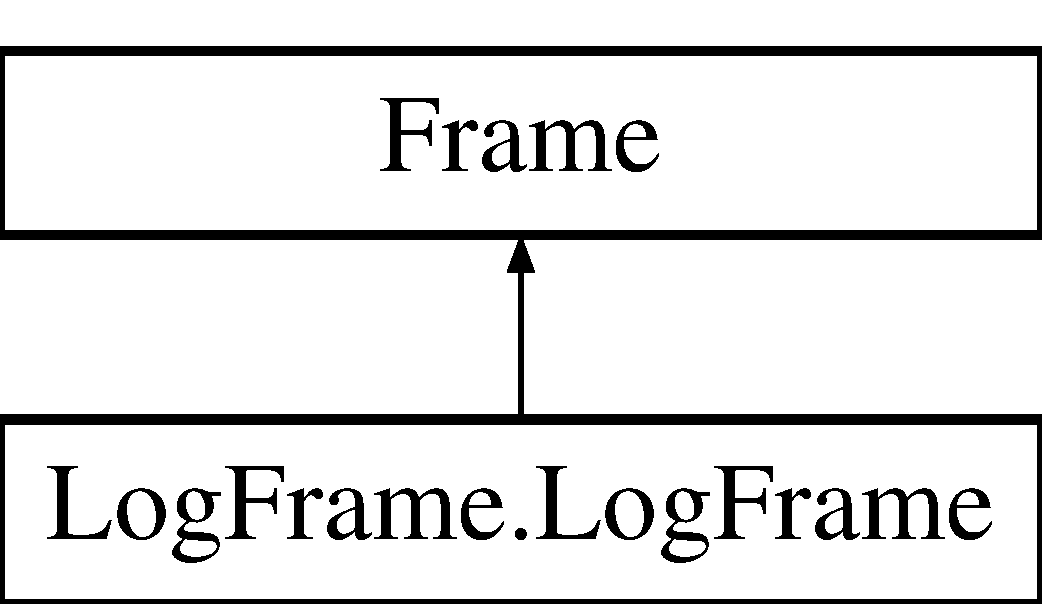
\includegraphics[height=2.000000cm]{classLogFrame_1_1LogFrame}
\end{center}
\end{figure}
\subsection*{Public Member Functions}
\begin{DoxyCompactItemize}
\item 
def \hyperlink{classLogFrame_1_1LogFrame_a756d5bc714b55aa93a21301a9986f8b1}{\+\_\+\+\_\+init\+\_\+\+\_\+} (self, app, parent, title)
\item 
def \hyperlink{classLogFrame_1_1LogFrame_af3d0abc16c93855ab9d760ff7b4c7d3e}{on\+Idle} (self, event)
\item 
def \hyperlink{classLogFrame_1_1LogFrame_a79ee5eea72f19f0a14aa047123125e1e}{on\+Close\+Confirm} (self, event)
\item 
def \hyperlink{classLogFrame_1_1LogFrame_afa3d32e2694b9e5a50279cbaf31cddba}{on\+Close} (self, event)
\item 
def \hyperlink{classLogFrame_1_1LogFrame_a53ce12d6947a1e35da471e5cb9d6011b}{on\+Exit} (self, event)
\end{DoxyCompactItemize}
\subsection*{Public Attributes}
\begin{DoxyCompactItemize}
\item 
\hyperlink{classLogFrame_1_1LogFrame_a851670425cc5380695a0790467740716}{path}
\item 
\hyperlink{classLogFrame_1_1LogFrame_af2f7bf9b22dcc769064bfdc91296977e}{panel}
\end{DoxyCompactItemize}
\subsection*{Static Public Attributes}
\begin{DoxyCompactItemize}
\item 
string \hyperlink{classLogFrame_1_1LogFrame_a59c2a62bec07d62ee3db2615338443ae}{overview\+Text} = \char`\"{}C\+AT Configuration Window\char`\"{}
\end{DoxyCompactItemize}


\subsection{Detailed Description}


Definition at line 22 of file Log\+Frame.\+py.



\subsection{Constructor \& Destructor Documentation}
\mbox{\Hypertarget{classLogFrame_1_1LogFrame_a756d5bc714b55aa93a21301a9986f8b1}\label{classLogFrame_1_1LogFrame_a756d5bc714b55aa93a21301a9986f8b1}} 
\index{Log\+Frame\+::\+Log\+Frame@{Log\+Frame\+::\+Log\+Frame}!\+\_\+\+\_\+init\+\_\+\+\_\+@{\+\_\+\+\_\+init\+\_\+\+\_\+}}
\index{\+\_\+\+\_\+init\+\_\+\+\_\+@{\+\_\+\+\_\+init\+\_\+\+\_\+}!Log\+Frame\+::\+Log\+Frame@{Log\+Frame\+::\+Log\+Frame}}
\subsubsection{\texorpdfstring{\+\_\+\+\_\+init\+\_\+\+\_\+()}{\_\_init\_\_()}}
{\footnotesize\ttfamily def Log\+Frame.\+Log\+Frame.\+\_\+\+\_\+init\+\_\+\+\_\+ (\begin{DoxyParamCaption}\item[{}]{self,  }\item[{}]{app,  }\item[{}]{parent,  }\item[{}]{title }\end{DoxyParamCaption})}



Definition at line 24 of file Log\+Frame.\+py.


\begin{DoxyCode}
24     \textcolor{keyword}{def }\hyperlink{classwrapper_1_1ModuleDictWrapper_a9a7a794150502f51df687831583e13b9}{\_\_init\_\_}(self,app,parent,title): 
25         wx.Frame.\_\_init\_\_(self, parent, wx.NewId(), title)
26         self.path=os.path.join(os.environ.get(\textcolor{stringliteral}{"CATLAL"}), \textcolor{stringliteral}{"CatPython"}, \textcolor{stringliteral}{"python"})
27         res=xrc.XmlResource(os.path.join(self.path,\textcolor{stringliteral}{"xrc/ConfPanel.xrc"}))
28         self.panel=res.LoadPanel(self, \textcolor{stringliteral}{"ConfPanel"})
29 
\end{DoxyCode}


\subsection{Member Function Documentation}
\mbox{\Hypertarget{classLogFrame_1_1LogFrame_afa3d32e2694b9e5a50279cbaf31cddba}\label{classLogFrame_1_1LogFrame_afa3d32e2694b9e5a50279cbaf31cddba}} 
\index{Log\+Frame\+::\+Log\+Frame@{Log\+Frame\+::\+Log\+Frame}!on\+Close@{on\+Close}}
\index{on\+Close@{on\+Close}!Log\+Frame\+::\+Log\+Frame@{Log\+Frame\+::\+Log\+Frame}}
\subsubsection{\texorpdfstring{on\+Close()}{onClose()}}
{\footnotesize\ttfamily def Log\+Frame.\+Log\+Frame.\+on\+Close (\begin{DoxyParamCaption}\item[{}]{self,  }\item[{}]{event }\end{DoxyParamCaption})}

\begin{DoxyVerb}Closes the application\end{DoxyVerb}
 

Definition at line 42 of file Log\+Frame.\+py.


\begin{DoxyCode}
42     \textcolor{keyword}{def }onClose(self, event):
43         \textcolor{stringliteral}{'''Closes the application'''}
44         self.Destroy()
45 
\end{DoxyCode}
\mbox{\Hypertarget{classLogFrame_1_1LogFrame_a79ee5eea72f19f0a14aa047123125e1e}\label{classLogFrame_1_1LogFrame_a79ee5eea72f19f0a14aa047123125e1e}} 
\index{Log\+Frame\+::\+Log\+Frame@{Log\+Frame\+::\+Log\+Frame}!on\+Close\+Confirm@{on\+Close\+Confirm}}
\index{on\+Close\+Confirm@{on\+Close\+Confirm}!Log\+Frame\+::\+Log\+Frame@{Log\+Frame\+::\+Log\+Frame}}
\subsubsection{\texorpdfstring{on\+Close\+Confirm()}{onCloseConfirm()}}
{\footnotesize\ttfamily def Log\+Frame.\+Log\+Frame.\+on\+Close\+Confirm (\begin{DoxyParamCaption}\item[{}]{self,  }\item[{}]{event }\end{DoxyParamCaption})}

\begin{DoxyVerb}Closes the application\end{DoxyVerb}
 

Definition at line 35 of file Log\+Frame.\+py.


\begin{DoxyCode}
35     \textcolor{keyword}{def }onCloseConfirm(self, event):
36         \textcolor{stringliteral}{'''Closes the application'''}
37         dlg = wx.MessageDialog(self, \textcolor{stringliteral}{"Exit the program?"}, \textcolor{stringliteral}{"Exit"}, wx.YES\_NO | wx.ICON\_QUESTION)
38         \textcolor{keywordflow}{if} dlg.ShowModal() == wx.ID\_YES:
39             dlg.Destroy()  \textcolor{comment}{# frame}
40         self.Destroy()
41 
\end{DoxyCode}
\mbox{\Hypertarget{classLogFrame_1_1LogFrame_a53ce12d6947a1e35da471e5cb9d6011b}\label{classLogFrame_1_1LogFrame_a53ce12d6947a1e35da471e5cb9d6011b}} 
\index{Log\+Frame\+::\+Log\+Frame@{Log\+Frame\+::\+Log\+Frame}!on\+Exit@{on\+Exit}}
\index{on\+Exit@{on\+Exit}!Log\+Frame\+::\+Log\+Frame@{Log\+Frame\+::\+Log\+Frame}}
\subsubsection{\texorpdfstring{on\+Exit()}{onExit()}}
{\footnotesize\ttfamily def Log\+Frame.\+Log\+Frame.\+on\+Exit (\begin{DoxyParamCaption}\item[{}]{self,  }\item[{}]{event }\end{DoxyParamCaption})}

\begin{DoxyVerb}Exit the app\end{DoxyVerb}
 

Definition at line 46 of file Log\+Frame.\+py.


\begin{DoxyCode}
46     \textcolor{keyword}{def }onExit(self, event):
47         \textcolor{stringliteral}{'''Exit the app'''}
48         self.Close(\textcolor{keyword}{True})
49 \textcolor{comment}{#        exit(2)}
50 
51 
52 
53 \textcolor{comment}{#----------------------------------------------------------------------------}
54 
55 
56 
57 \end{DoxyCode}
\mbox{\Hypertarget{classLogFrame_1_1LogFrame_af3d0abc16c93855ab9d760ff7b4c7d3e}\label{classLogFrame_1_1LogFrame_af3d0abc16c93855ab9d760ff7b4c7d3e}} 
\index{Log\+Frame\+::\+Log\+Frame@{Log\+Frame\+::\+Log\+Frame}!on\+Idle@{on\+Idle}}
\index{on\+Idle@{on\+Idle}!Log\+Frame\+::\+Log\+Frame@{Log\+Frame\+::\+Log\+Frame}}
\subsubsection{\texorpdfstring{on\+Idle()}{onIdle()}}
{\footnotesize\ttfamily def Log\+Frame.\+Log\+Frame.\+on\+Idle (\begin{DoxyParamCaption}\item[{}]{self,  }\item[{}]{event }\end{DoxyParamCaption})}

\begin{DoxyVerb}Responds to idle time in the system\end{DoxyVerb}
 

Definition at line 30 of file Log\+Frame.\+py.


\begin{DoxyCode}
30     \textcolor{keyword}{def }onIdle(self, event):
31         \textcolor{stringliteral}{'''Responds to idle time in the system'''}
32         \textcolor{comment}{# when the timer says it's time, we do the actual downloading in the main thread (wx doesn't work
       well in secondary threads)}
33         \textcolor{keywordflow}{print} \textcolor{stringliteral}{"hello"}
34         
\end{DoxyCode}


\subsection{Member Data Documentation}
\mbox{\Hypertarget{classLogFrame_1_1LogFrame_a59c2a62bec07d62ee3db2615338443ae}\label{classLogFrame_1_1LogFrame_a59c2a62bec07d62ee3db2615338443ae}} 
\index{Log\+Frame\+::\+Log\+Frame@{Log\+Frame\+::\+Log\+Frame}!overview\+Text@{overview\+Text}}
\index{overview\+Text@{overview\+Text}!Log\+Frame\+::\+Log\+Frame@{Log\+Frame\+::\+Log\+Frame}}
\subsubsection{\texorpdfstring{overview\+Text}{overviewText}}
{\footnotesize\ttfamily string Log\+Frame.\+Log\+Frame.\+overview\+Text = \char`\"{}C\+AT Configuration Window\char`\"{}\hspace{0.3cm}{\ttfamily [static]}}



Definition at line 23 of file Log\+Frame.\+py.

\mbox{\Hypertarget{classLogFrame_1_1LogFrame_af2f7bf9b22dcc769064bfdc91296977e}\label{classLogFrame_1_1LogFrame_af2f7bf9b22dcc769064bfdc91296977e}} 
\index{Log\+Frame\+::\+Log\+Frame@{Log\+Frame\+::\+Log\+Frame}!panel@{panel}}
\index{panel@{panel}!Log\+Frame\+::\+Log\+Frame@{Log\+Frame\+::\+Log\+Frame}}
\subsubsection{\texorpdfstring{panel}{panel}}
{\footnotesize\ttfamily Log\+Frame.\+Log\+Frame.\+panel}



Definition at line 28 of file Log\+Frame.\+py.



Referenced by A3\+P\+E\+\_\+\+Bit\+Flip.\+A3\+P\+E\+\_\+\+Bit\+Flip.\+\_\+\+\_\+init\+\_\+\+\_\+(), Emulate\+F\+E.\+Emulate\+F\+E.\+\_\+\+\_\+init\+\_\+\+\_\+(), Acquisition.\+Acquisition.\+\_\+\+\_\+init\+\_\+\+\_\+(), object.\+object.\+get\+Control(), Proto40\+M\+Hz\+\_\+v1.\+Proto40\+M\+Hz\+\_\+v1.\+get\+File(), and proc.\+proc.\+page().

\mbox{\Hypertarget{classLogFrame_1_1LogFrame_a851670425cc5380695a0790467740716}\label{classLogFrame_1_1LogFrame_a851670425cc5380695a0790467740716}} 
\index{Log\+Frame\+::\+Log\+Frame@{Log\+Frame\+::\+Log\+Frame}!path@{path}}
\index{path@{path}!Log\+Frame\+::\+Log\+Frame@{Log\+Frame\+::\+Log\+Frame}}
\subsubsection{\texorpdfstring{path}{path}}
{\footnotesize\ttfamily Log\+Frame.\+Log\+Frame.\+path}



Definition at line 26 of file Log\+Frame.\+py.



Referenced by element.\+element.\+loadxrc(), and proc.\+proc.\+loadxrc().



The documentation for this class was generated from the following file\+:\begin{DoxyCompactItemize}
\item 
/home/eleclhcb/\+L\+H\+Cb/lbcat-\/cmake/\+Cat\+Python/python/\hyperlink{LogFrame_8py}{Log\+Frame.\+py}\end{DoxyCompactItemize}

\hypertarget{classLSDelayChipV1}{}\section{L\+S\+Delay\+Chip\+V1 Class Reference}
\label{classLSDelayChipV1}\index{L\+S\+Delay\+Chip\+V1@{L\+S\+Delay\+Chip\+V1}}


{\ttfamily \#include $<$L\+S\+Delay\+Chip\+V1.\+h$>$}

Inheritance diagram for L\+S\+Delay\+Chip\+V1\+:\begin{figure}[H]
\begin{center}
\leavevmode
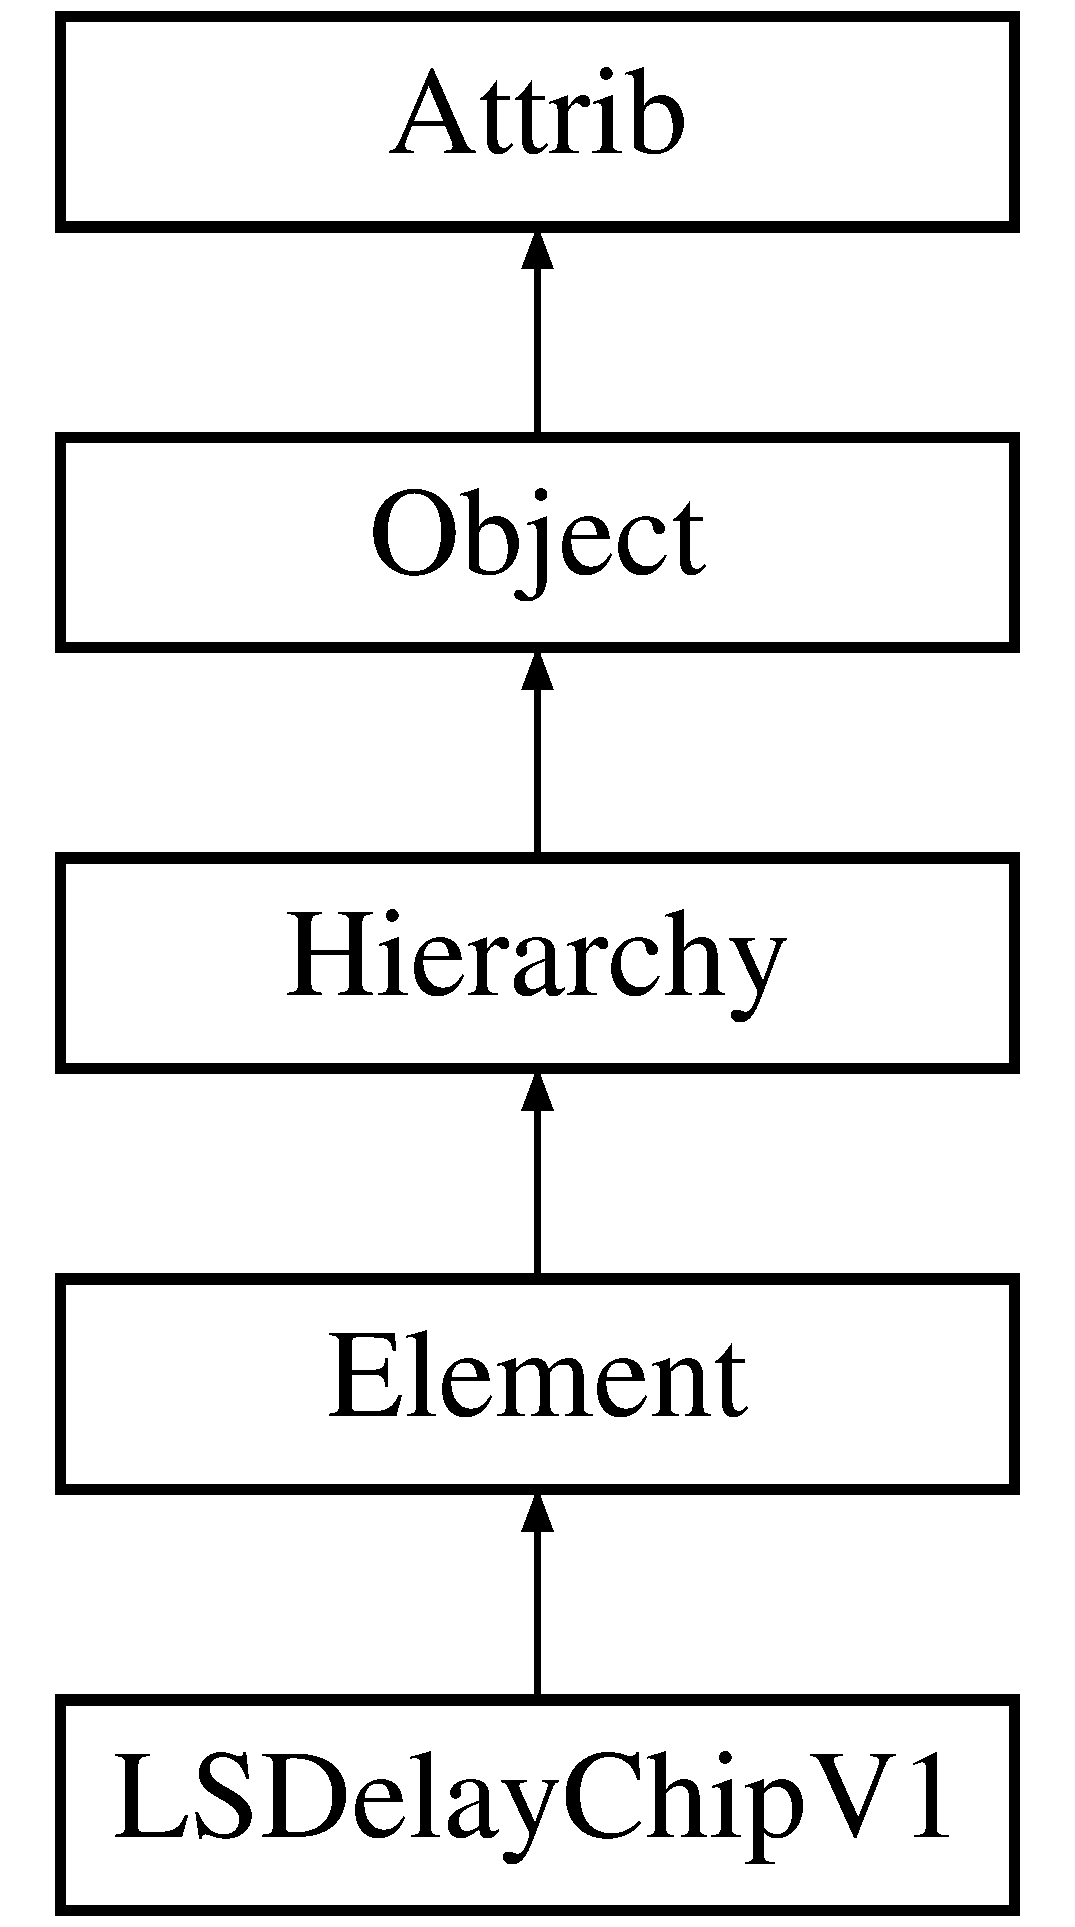
\includegraphics[height=5.000000cm]{classLSDelayChipV1}
\end{center}
\end{figure}
\subsection*{Public Types}
\begin{DoxyCompactItemize}
\item 
enum \hyperlink{classAttrib_a69e171d7cc6417835a5a306d3c764235}{Attribut} \{ \newline
\hyperlink{classAttrib_a69e171d7cc6417835a5a306d3c764235a3a8da2ab97dda18aebab196fe4100531}{U\+N\+D\+E\+F\+I\+N\+ED}, 
\hyperlink{classAttrib_a69e171d7cc6417835a5a306d3c764235a2bfb2af57b87031d190a05fe25dd92ed}{P\+A\+S\+S\+I\+VE}, 
\hyperlink{classAttrib_a69e171d7cc6417835a5a306d3c764235a3b1fec929c0370d1436f2f06e298fb0d}{A\+C\+T\+I\+VE}, 
\hyperlink{classAttrib_a69e171d7cc6417835a5a306d3c764235aa27c16b480a369ea4d18b07b2516bbc7}{I\+N\+T\+E\+R\+F\+A\+CE}, 
\newline
\hyperlink{classAttrib_a69e171d7cc6417835a5a306d3c764235a1420a5b8c0540b2af210b6975eded7f9}{IO}, 
\hyperlink{classAttrib_a69e171d7cc6417835a5a306d3c764235a0af3b0d0ac323c1704e6c69cf90add28}{I\+O\+D\+A\+TA}, 
\hyperlink{classAttrib_a69e171d7cc6417835a5a306d3c764235a7788bc5dd333fd8ce18562b269c9dab1}{E\+L\+E\+M\+E\+NT}, 
\hyperlink{classAttrib_a69e171d7cc6417835a5a306d3c764235a61ceb22149f365f1780d18f9d1459423}{H\+A\+R\+D\+W\+A\+RE}, 
\newline
\hyperlink{classAttrib_a69e171d7cc6417835a5a306d3c764235a75250e29692496e73effca2c0330977f}{P\+R\+O\+C\+E\+S\+S\+US}, 
\hyperlink{classAttrib_a69e171d7cc6417835a5a306d3c764235a103a67cd0b8f07ef478fa45d4356e27b}{S\+O\+F\+T\+W\+A\+RE}
 \}
\end{DoxyCompactItemize}
\subsection*{Public Member Functions}
\begin{DoxyCompactItemize}
\item 
\hyperlink{classLSDelayChipV1_a4dbc01a273a6e044b6f163e12e136134}{L\+S\+Delay\+Chip\+V1} ()
\item 
void \hyperlink{classLSDelayChipV1_a97a50092ce40f6322db946fc580f7230}{config\+Reg\+Bulk\+Read} (\hyperlink{ICECALv3_8h_a3cb25ca6f51f003950f9625ff05536fc}{U8} conf\+Reg\+Addr)
\item 
void \hyperlink{classLSDelayChipV1_afa626b5d52f8723bcaa3205d1cc7a0f8}{config\+Reg\+Bulk\+Write} (\hyperlink{ICECALv3_8h_a3cb25ca6f51f003950f9625ff05536fc}{U8} conf\+Reg\+Addr, \hyperlink{ICECALv3_8h_adf928e51a60dba0df29d615401cc55a8}{U16} \hyperlink{structconfRegData}{conf\+Reg\+Data})
\item 
void \hyperlink{classLSDelayChipV1_a4f338071d49df7eae55020a5f5fa8474}{get\+Config\+Reg} (\hyperlink{ICECALv3_8h_a3cb25ca6f51f003950f9625ff05536fc}{U8} conf\+Reg\+Addr)
\item 
void \hyperlink{classLSDelayChipV1_a11fa2ebfa37c5cf0544ddb68c7d43e94}{set\+Config\+Reg} (\hyperlink{ICECALv3_8h_a3cb25ca6f51f003950f9625ff05536fc}{U8} conf\+Reg\+Addr, \hyperlink{structconfRegData}{conf\+Reg\+Data} d)
\item 
void \hyperlink{classLSDelayChipV1_ad83fb046d3576cdccdb4b4fe59f7ff71}{set\+Config\+Reg\+Phase\+A\+DC} (\hyperlink{ICECALv3_8h_a3cb25ca6f51f003950f9625ff05536fc}{U8} conf\+Reg\+Addr, \hyperlink{ICECALv3_8h_a3cb25ca6f51f003950f9625ff05536fc}{U8} phase\+A\+DC)
\item 
void \hyperlink{classLSDelayChipV1_aa1364ef56bf75884756a8d589cee4328}{set\+Config\+Reg\+Phase\+TH} (\hyperlink{ICECALv3_8h_a3cb25ca6f51f003950f9625ff05536fc}{U8} conf\+Reg\+Addr, \hyperlink{ICECALv3_8h_a3cb25ca6f51f003950f9625ff05536fc}{U8} phase\+TH)
\item 
void \hyperlink{classLSDelayChipV1_a317f739744d1093385306530fe5b312a}{set\+Config\+Reg\+Phase\+I\+NT} (\hyperlink{ICECALv3_8h_a3cb25ca6f51f003950f9625ff05536fc}{U8} conf\+Reg\+Addr, \hyperlink{ICECALv3_8h_a3cb25ca6f51f003950f9625ff05536fc}{U8} phase\+I\+NT)
\item 
void \hyperlink{classLSDelayChipV1_a46a7aee8c7373c6858af9ecd29e9b116}{set\+Config\+Reg\+L\+V\+D\+S\+Out\+En} (\hyperlink{ICECALv3_8h_a3cb25ca6f51f003950f9625ff05536fc}{U8} conf\+Reg\+Addr, bool en)
\item 
void \hyperlink{classLSDelayChipV1_a813eca3585445d504d60a93ec55817f4}{set\+Config\+Reg\+Debug\+Mode} (\hyperlink{ICECALv3_8h_a3cb25ca6f51f003950f9625ff05536fc}{U8} conf\+Reg\+Addr, bool en)
\item 
void \hyperlink{classLSDelayChipV1_afd8a57dda2cd6a62607cbfc9808c3220}{set\+Config\+Reg\+V\+Control\+Out\+En} (\hyperlink{ICECALv3_8h_a3cb25ca6f51f003950f9625ff05536fc}{U8} conf\+Reg\+Addr, bool en)
\item 
void \hyperlink{classLSDelayChipV1_a2a1eebeacb7ed2b0fc5584f3630d0aa0}{set\+Config\+Reg\+L\+O\+C\+US} (\hyperlink{ICECALv3_8h_a3cb25ca6f51f003950f9625ff05536fc}{U8} conf\+Reg\+Addr, \hyperlink{ICECALv3_8h_a3cb25ca6f51f003950f9625ff05536fc}{U8} locus)
\item 
void \hyperlink{classLSDelayChipV1_a5b2c2e527b044b128306695828e9fd19}{reset\+Pumps} ()
\item 
void \hyperlink{classLSDelayChipV1_a9e04b654e8d6d63efe23fc3b31e15ce6}{bypass\+Miso\+Mosi} (\hyperlink{ICECALv3_8h_adf928e51a60dba0df29d615401cc55a8}{U16} write\+Data)
\item 
void \hyperlink{classLSDelayChipV1_ad0ed8d0797c985d7595fbe56f0da1996}{spi\+B\+E\+R\+Test} (\hyperlink{ICECALv3_8h_a3cb25ca6f51f003950f9625ff05536fc}{U8} conf\+Reg\+Addr, long n\+Frames)
\item 
void \hyperlink{classLSDelayChipV1_a01c1e85ae0d0e031164fe2d47b4f4824}{show\+Config} ()
\item 
\hyperlink{classLSDelayChipV1_a86c96f60b9be6f35745536df46919817}{$\sim$\+L\+S\+Delay\+Chip\+V1} ()
\item 
void \hyperlink{classLSDelayChipV1_a3d57457a70f7d42687197704321b0c8e}{help} ()
\item 
\hyperlink{classStatusCode}{Status\+Code} \hyperlink{classLSDelayChipV1_af8bc9c84a1b65cbc2176fdbc349e829c}{init} ()
\item 
void \hyperlink{classLSDelayChipV1_a6b772084a850e96b2f9bb5600c29259c}{reset} ()
\item 
void \hyperlink{classLSDelayChipV1_a7d4eb6fb7ca527286d36f30123bfd60a}{update} ()
\item 
void \hyperlink{classLSDelayChipV1_a04ec44c79258fd22f7d2d5ea27a67648}{set\+Address} (\hyperlink{ICECALv3_8h_a3cb25ca6f51f003950f9625ff05536fc}{U8} address)
\item 
void \hyperlink{classElement_a3c0abcb36f8906688bb7e32608df7086}{recursive\+Init\+Element} ()
\item 
void \hyperlink{classElement_a82119ed37dff76508a2746a853ec35ba}{recursive\+Init\+Communications} ()
\item 
\hyperlink{classStatusCode}{Status\+Code} \hyperlink{classElement_ab476b4b1df5954141ceb14f072433b89}{set\+Connection} (\hyperlink{classHierarchy}{Hierarchy} $\ast$)
\item 
\hyperlink{classHierarchy}{Hierarchy} $\ast$ \hyperlink{classElement_af57444353c1ddf9fa0109801e97debf7}{connection} ()
\item 
void \hyperlink{classHierarchy_af4d43b0765b402670eed2d62c73405af}{clear} ()
\item 
void \hyperlink{classHierarchy_a585ad1aeec16077a0e532ab8b4fc557b}{set\+Parent} (\hyperlink{classHierarchy}{Hierarchy} $\ast$\hyperlink{classHierarchy_a1c7bec8257e717f9c1465e06ebf845fc}{parent})
\item 
\hyperlink{classHierarchy}{Hierarchy} $\ast$ \hyperlink{classHierarchy_a1c7bec8257e717f9c1465e06ebf845fc}{parent} ()
\item 
\hyperlink{classHierarchy}{Hierarchy} $\ast$ \hyperlink{classHierarchy_ad550588733bf75ac5c0fcfd7c8fd11a6}{parent} (std\+::string)
\item 
\hyperlink{classHierarchy}{Hierarchy} $\ast$ \hyperlink{classHierarchy_aee461dc930ce3871636ff87f075b1b83}{origin} ()
\item 
virtual void \hyperlink{classHierarchy_ad677774ff38fcb257c04a3a10d471fac}{add\+Child} (\hyperlink{classHierarchy}{Hierarchy} $\ast$element)
\item 
std\+::vector$<$ \hyperlink{classHierarchy}{Hierarchy} $\ast$ $>$ \hyperlink{classHierarchy_aa9a76f69e98e052ee1a6e32cea006288}{children} ()
\item 
\hyperlink{classHierarchy}{Hierarchy} $\ast$ \hyperlink{classHierarchy_a1e207f973c694b538bf90107b4868817}{child} (std\+::string)
\item 
\hyperlink{classHierarchy}{Hierarchy} $\ast$ \hyperlink{classHierarchy_a0c15a5276a3b80b4354d6bd8a01e0708}{child\+Typed} (std\+::string)
\item 
unsigned long \hyperlink{classHierarchy_ab16e84de65fd84e14001a6cf941c8be4}{number\+Of\+Children} ()
\item 
bool \hyperlink{classHierarchy_a255174fe4d316d2a3f430dcb9dab29f1}{has\+Children} ()
\item 
void \hyperlink{classHierarchy_a2b2b359fac003233f65786a616766bde}{del\+Child} (\hyperlink{classHierarchy}{Hierarchy} $\ast$)
\item 
void \hyperlink{classHierarchy_a1928ac7615fe0b5e55cd707f70dc6781}{del\+Child} (std\+::string)
\item 
std\+::string \hyperlink{classHierarchy_aa7990fa7caf132d83e361ce033c6c65a}{path} (std\+::string=std\+::string(\char`\"{}\char`\"{}))
\item 
std\+::string \hyperlink{classHierarchy_a1efd56cd164d328d2002e53a10a19b8c}{path\+Typed} (std\+::string=std\+::string(\char`\"{}\char`\"{}))
\item 
void \hyperlink{classHierarchy_a76e914b9a677a22a82deb74d892bf261}{tree} (std\+::string indent=std\+::string(\char`\"{}\char`\"{}))
\item 
void \hyperlink{classHierarchy_a594c294c5f60c230e106d522ed008212}{tree} ()
\item 
std\+::string \hyperlink{classObject_a300f4c05dd468c7bb8b3c968868443c1}{name} () const
\item 
std\+::string \hyperlink{classObject_a84f99f70f144a83e1582d1d0f84e4e62}{type} ()
\item 
unsigned char \hyperlink{classObject_af99145335cc61ff6e2798ea17db009d2}{id} ()
\item 
std\+::string \hyperlink{classObject_a73a0f1a41828fdd8303dd662446fb6c3}{title} ()
\item 
void \hyperlink{classObject_a3f9d5537ebce0c0f2bf6ae4d92426f3c}{msg\+Svc} (int level, std\+::string \hyperlink{classObject_a58b2d0618c2d08cf2383012611528d97}{msg}, std\+::string \hyperlink{classObject_a300f4c05dd468c7bb8b3c968868443c1}{name})
\item 
void \hyperlink{classObject_a58b2d0618c2d08cf2383012611528d97}{msg} (std\+::string mymsg)
\item 
void \hyperlink{classObject_ac5d59299273cee27aacf7de00d2e7034}{msg} (std\+::string mymsg, std\+::string \hyperlink{classObject_a300f4c05dd468c7bb8b3c968868443c1}{name})
\item 
void \hyperlink{classObject_a83d2db2df682907ea1115ad721c1c4a1}{verbose} (std\+::string mymsg)
\item 
void \hyperlink{classObject_a2d4120195317e2a3c6532e8bb9f3da68}{verbose} (std\+::string mymsg, std\+::string \hyperlink{classObject_a300f4c05dd468c7bb8b3c968868443c1}{name})
\item 
void \hyperlink{classObject_aac010553f022165573714b7014a15f0d}{debug} (std\+::string mymsg)
\item 
void \hyperlink{classObject_a6c9a0397ca804e04d675ed05683f5420}{debug} (std\+::string mymsg, std\+::string \hyperlink{classObject_a300f4c05dd468c7bb8b3c968868443c1}{name})
\item 
void \hyperlink{classObject_a644fd329ea4cb85f54fa6846484b84a8}{info} (std\+::string mymsg)
\item 
void \hyperlink{classObject_a1ca123253dfd30fc28b156f521dcbdae}{info} (std\+::string mymsg, std\+::string \hyperlink{classObject_a300f4c05dd468c7bb8b3c968868443c1}{name})
\item 
void \hyperlink{classObject_a65cd4fda577711660821fd2cd5a3b4c9}{warning} (std\+::string mymsg)
\item 
void \hyperlink{classObject_a11f101db4dd73d9391b0231818881d86}{warning} (std\+::string mymsg, std\+::string \hyperlink{classObject_a300f4c05dd468c7bb8b3c968868443c1}{name})
\item 
void \hyperlink{classObject_a204a95f57818c0f811933917a30eff45}{error} (std\+::string mymsg)
\item 
void \hyperlink{classObject_ad7f6c457733082efa2f9ff5f5c8e119a}{error} (std\+::string mymsg, std\+::string \hyperlink{classObject_a300f4c05dd468c7bb8b3c968868443c1}{name})
\item 
void \hyperlink{classObject_aad5a16aac7516ce65bd5ec02ab07fc80}{fatal} (std\+::string mymsg)
\item 
void \hyperlink{classObject_ae62acd3d09f716220f75f252dc38bc9a}{fatal} (std\+::string mymsg, std\+::string \hyperlink{classObject_a300f4c05dd468c7bb8b3c968868443c1}{name})
\item 
void \hyperlink{classObject_ae30fea75683c2d149b6b6d17c09ecd0c}{set\+Name} (std\+::string \hyperlink{classObject_a300f4c05dd468c7bb8b3c968868443c1}{name})
\item 
void \hyperlink{classObject_aae534cc9d982bcb9b99fd505f2e103a5}{set\+Type} (std\+::string \hyperlink{classObject_a84f99f70f144a83e1582d1d0f84e4e62}{type})
\item 
void \hyperlink{classObject_a398fe08cba594a0ce6891d59fe4f159f}{set\+Id} (unsigned char \hyperlink{classObject_af99145335cc61ff6e2798ea17db009d2}{id})
\item 
void \hyperlink{classObject_a89557dbbad5bcaa02652f5d7fa35d20f}{set\+Title} (std\+::string \hyperlink{classObject_a73a0f1a41828fdd8303dd662446fb6c3}{title})
\item 
void \hyperlink{classObject_a870c5af919958c2136623b2d7816d123}{set\+Dll\+Name} (std\+::string \hyperlink{classObject_a2e3947f2870094c332d7454117f3ec63}{dll\+Name})
\item 
std\+::string \hyperlink{classObject_a2e3947f2870094c332d7454117f3ec63}{dll\+Name} ()
\item 
bool \hyperlink{classAttrib_a704f26af560909ad22065083bb7d4c34}{is} (int attribut)
\item 
void \hyperlink{classAttrib_a235f773af19c900264a190b00a3b4ad7}{add} (int attribut)
\item 
void \hyperlink{classAttrib_a7d4ef7e32d93cb287792b87b857e79f3}{remove} (int attribut)
\item 
std\+::string \hyperlink{classAttrib_aee7bbf16b144887f196e1341b24f8a26}{attributs} ()
\end{DoxyCompactItemize}
\subsection*{Protected Attributes}
\begin{DoxyCompactItemize}
\item 
\hyperlink{classHierarchy}{Hierarchy} $\ast$ \hyperlink{classElement_abe3de7a5dbbc9a6dd2d7e012e5fdb266}{m\+\_\+connection}
\item 
std\+::string \hyperlink{classAttrib_a3414521d7a82476e874b25a5407b5e63}{m\+\_\+attrib\+String} \mbox{[}10\mbox{]}
\end{DoxyCompactItemize}
\subsection*{Private Member Functions}
\begin{DoxyCompactItemize}
\item 
bool \hyperlink{classLSDelayChipV1_aa8118972150a9e1e95e9006e003c0206}{check\+Config\+Addr} (\hyperlink{ICECALv3_8h_a3cb25ca6f51f003950f9625ff05536fc}{U8} addr)
\item 
bool \hyperlink{classLSDelayChipV1_a5083f29a93d38258d9de00dd5a89af99}{check\+Status\+Addr} (\hyperlink{ICECALv3_8h_a3cb25ca6f51f003950f9625ff05536fc}{U8} addr)
\item 
std\+::string \hyperlink{classLSDelayChipV1_af7f4d72fb404b6b3d7b41fd01876ed0a}{itohs} (\hyperlink{ICECALv3_8h_adf928e51a60dba0df29d615401cc55a8}{U16} value)
\end{DoxyCompactItemize}
\subsection*{Private Attributes}
\begin{DoxyCompactItemize}
\item 
\hyperlink{classRegister}{Register} $\ast$ \hyperlink{classLSDelayChipV1_afd1cfdcb114549dc1466c77f07d39fe0}{m\+\_\+reg\+Config}
\item 
\hyperlink{classRegister}{Register} $\ast$ \hyperlink{classLSDelayChipV1_aaf118f103e89a35d2c449e8e3ffe8c20}{m\+\_\+reg\+Status}
\item 
\hyperlink{ICECALv3_8h_a3cb25ca6f51f003950f9625ff05536fc}{U8} \hyperlink{classLSDelayChipV1_a6fba278fd2ac602c796b5e5cebf2d2de}{m\+\_\+address}
\item 
\hyperlink{ICECALv3_8h_adf928e51a60dba0df29d615401cc55a8}{U16} \hyperlink{classLSDelayChipV1_ae049797212539b231b9722ae69a0491d}{m\+\_\+rx\+Config\+Bits}
\item 
\hyperlink{structconfRegData}{conf\+Reg\+Data} \hyperlink{classLSDelayChipV1_a4818ac5c0d7ccf2845a01226234bdb67}{m\+\_\+rx\+Config}
\item 
\hyperlink{ICECALv3_8h_a3cb25ca6f51f003950f9625ff05536fc}{U8} \hyperlink{classLSDelayChipV1_ab49ac38bf9e7a41ccb89c6725cfcac3a}{m\+\_\+config\+Addr}
\item 
long \hyperlink{classLSDelayChipV1_a425c69ef8f3d64d93cb1c86b83bbceec}{m\+\_\+n\+Bad}
\item 
double \hyperlink{classLSDelayChipV1_a38d35de6a25fb1394ede2f39a4f25a08}{m\+\_\+fer}
\end{DoxyCompactItemize}


\subsection{Detailed Description}


Definition at line 68 of file L\+S\+Delay\+Chip\+V1.\+h.



\subsection{Member Enumeration Documentation}
\mbox{\Hypertarget{classAttrib_a69e171d7cc6417835a5a306d3c764235}\label{classAttrib_a69e171d7cc6417835a5a306d3c764235}} 
\index{L\+S\+Delay\+Chip\+V1@{L\+S\+Delay\+Chip\+V1}!Attribut@{Attribut}}
\index{Attribut@{Attribut}!L\+S\+Delay\+Chip\+V1@{L\+S\+Delay\+Chip\+V1}}
\subsubsection{\texorpdfstring{Attribut}{Attribut}}
{\footnotesize\ttfamily enum \hyperlink{classAttrib_a69e171d7cc6417835a5a306d3c764235}{Attrib\+::\+Attribut}\hspace{0.3cm}{\ttfamily [inherited]}}

\begin{DoxyEnumFields}{Enumerator}
\raisebox{\heightof{T}}[0pt][0pt]{\index{U\+N\+D\+E\+F\+I\+N\+ED@{U\+N\+D\+E\+F\+I\+N\+ED}!L\+S\+Delay\+Chip\+V1@{L\+S\+Delay\+Chip\+V1}}\index{L\+S\+Delay\+Chip\+V1@{L\+S\+Delay\+Chip\+V1}!U\+N\+D\+E\+F\+I\+N\+ED@{U\+N\+D\+E\+F\+I\+N\+ED}}}\mbox{\Hypertarget{classAttrib_a69e171d7cc6417835a5a306d3c764235a3a8da2ab97dda18aebab196fe4100531}\label{classAttrib_a69e171d7cc6417835a5a306d3c764235a3a8da2ab97dda18aebab196fe4100531}} 
U\+N\+D\+E\+F\+I\+N\+ED&\\
\hline

\raisebox{\heightof{T}}[0pt][0pt]{\index{P\+A\+S\+S\+I\+VE@{P\+A\+S\+S\+I\+VE}!L\+S\+Delay\+Chip\+V1@{L\+S\+Delay\+Chip\+V1}}\index{L\+S\+Delay\+Chip\+V1@{L\+S\+Delay\+Chip\+V1}!P\+A\+S\+S\+I\+VE@{P\+A\+S\+S\+I\+VE}}}\mbox{\Hypertarget{classAttrib_a69e171d7cc6417835a5a306d3c764235a2bfb2af57b87031d190a05fe25dd92ed}\label{classAttrib_a69e171d7cc6417835a5a306d3c764235a2bfb2af57b87031d190a05fe25dd92ed}} 
P\+A\+S\+S\+I\+VE&\\
\hline

\raisebox{\heightof{T}}[0pt][0pt]{\index{A\+C\+T\+I\+VE@{A\+C\+T\+I\+VE}!L\+S\+Delay\+Chip\+V1@{L\+S\+Delay\+Chip\+V1}}\index{L\+S\+Delay\+Chip\+V1@{L\+S\+Delay\+Chip\+V1}!A\+C\+T\+I\+VE@{A\+C\+T\+I\+VE}}}\mbox{\Hypertarget{classAttrib_a69e171d7cc6417835a5a306d3c764235a3b1fec929c0370d1436f2f06e298fb0d}\label{classAttrib_a69e171d7cc6417835a5a306d3c764235a3b1fec929c0370d1436f2f06e298fb0d}} 
A\+C\+T\+I\+VE&\\
\hline

\raisebox{\heightof{T}}[0pt][0pt]{\index{I\+N\+T\+E\+R\+F\+A\+CE@{I\+N\+T\+E\+R\+F\+A\+CE}!L\+S\+Delay\+Chip\+V1@{L\+S\+Delay\+Chip\+V1}}\index{L\+S\+Delay\+Chip\+V1@{L\+S\+Delay\+Chip\+V1}!I\+N\+T\+E\+R\+F\+A\+CE@{I\+N\+T\+E\+R\+F\+A\+CE}}}\mbox{\Hypertarget{classAttrib_a69e171d7cc6417835a5a306d3c764235aa27c16b480a369ea4d18b07b2516bbc7}\label{classAttrib_a69e171d7cc6417835a5a306d3c764235aa27c16b480a369ea4d18b07b2516bbc7}} 
I\+N\+T\+E\+R\+F\+A\+CE&\\
\hline

\raisebox{\heightof{T}}[0pt][0pt]{\index{IO@{IO}!L\+S\+Delay\+Chip\+V1@{L\+S\+Delay\+Chip\+V1}}\index{L\+S\+Delay\+Chip\+V1@{L\+S\+Delay\+Chip\+V1}!IO@{IO}}}\mbox{\Hypertarget{classAttrib_a69e171d7cc6417835a5a306d3c764235a1420a5b8c0540b2af210b6975eded7f9}\label{classAttrib_a69e171d7cc6417835a5a306d3c764235a1420a5b8c0540b2af210b6975eded7f9}} 
IO&\\
\hline

\raisebox{\heightof{T}}[0pt][0pt]{\index{I\+O\+D\+A\+TA@{I\+O\+D\+A\+TA}!L\+S\+Delay\+Chip\+V1@{L\+S\+Delay\+Chip\+V1}}\index{L\+S\+Delay\+Chip\+V1@{L\+S\+Delay\+Chip\+V1}!I\+O\+D\+A\+TA@{I\+O\+D\+A\+TA}}}\mbox{\Hypertarget{classAttrib_a69e171d7cc6417835a5a306d3c764235a0af3b0d0ac323c1704e6c69cf90add28}\label{classAttrib_a69e171d7cc6417835a5a306d3c764235a0af3b0d0ac323c1704e6c69cf90add28}} 
I\+O\+D\+A\+TA&\\
\hline

\raisebox{\heightof{T}}[0pt][0pt]{\index{E\+L\+E\+M\+E\+NT@{E\+L\+E\+M\+E\+NT}!L\+S\+Delay\+Chip\+V1@{L\+S\+Delay\+Chip\+V1}}\index{L\+S\+Delay\+Chip\+V1@{L\+S\+Delay\+Chip\+V1}!E\+L\+E\+M\+E\+NT@{E\+L\+E\+M\+E\+NT}}}\mbox{\Hypertarget{classAttrib_a69e171d7cc6417835a5a306d3c764235a7788bc5dd333fd8ce18562b269c9dab1}\label{classAttrib_a69e171d7cc6417835a5a306d3c764235a7788bc5dd333fd8ce18562b269c9dab1}} 
E\+L\+E\+M\+E\+NT&\\
\hline

\raisebox{\heightof{T}}[0pt][0pt]{\index{H\+A\+R\+D\+W\+A\+RE@{H\+A\+R\+D\+W\+A\+RE}!L\+S\+Delay\+Chip\+V1@{L\+S\+Delay\+Chip\+V1}}\index{L\+S\+Delay\+Chip\+V1@{L\+S\+Delay\+Chip\+V1}!H\+A\+R\+D\+W\+A\+RE@{H\+A\+R\+D\+W\+A\+RE}}}\mbox{\Hypertarget{classAttrib_a69e171d7cc6417835a5a306d3c764235a61ceb22149f365f1780d18f9d1459423}\label{classAttrib_a69e171d7cc6417835a5a306d3c764235a61ceb22149f365f1780d18f9d1459423}} 
H\+A\+R\+D\+W\+A\+RE&\\
\hline

\raisebox{\heightof{T}}[0pt][0pt]{\index{P\+R\+O\+C\+E\+S\+S\+US@{P\+R\+O\+C\+E\+S\+S\+US}!L\+S\+Delay\+Chip\+V1@{L\+S\+Delay\+Chip\+V1}}\index{L\+S\+Delay\+Chip\+V1@{L\+S\+Delay\+Chip\+V1}!P\+R\+O\+C\+E\+S\+S\+US@{P\+R\+O\+C\+E\+S\+S\+US}}}\mbox{\Hypertarget{classAttrib_a69e171d7cc6417835a5a306d3c764235a75250e29692496e73effca2c0330977f}\label{classAttrib_a69e171d7cc6417835a5a306d3c764235a75250e29692496e73effca2c0330977f}} 
P\+R\+O\+C\+E\+S\+S\+US&\\
\hline

\raisebox{\heightof{T}}[0pt][0pt]{\index{S\+O\+F\+T\+W\+A\+RE@{S\+O\+F\+T\+W\+A\+RE}!L\+S\+Delay\+Chip\+V1@{L\+S\+Delay\+Chip\+V1}}\index{L\+S\+Delay\+Chip\+V1@{L\+S\+Delay\+Chip\+V1}!S\+O\+F\+T\+W\+A\+RE@{S\+O\+F\+T\+W\+A\+RE}}}\mbox{\Hypertarget{classAttrib_a69e171d7cc6417835a5a306d3c764235a103a67cd0b8f07ef478fa45d4356e27b}\label{classAttrib_a69e171d7cc6417835a5a306d3c764235a103a67cd0b8f07ef478fa45d4356e27b}} 
S\+O\+F\+T\+W\+A\+RE&\\
\hline

\end{DoxyEnumFields}


Definition at line 29 of file Attrib.\+h.


\begin{DoxyCode}
29                 \{
30     \hyperlink{classAttrib_a69e171d7cc6417835a5a306d3c764235a3a8da2ab97dda18aebab196fe4100531}{UNDEFINED},
31     \hyperlink{classAttrib_a69e171d7cc6417835a5a306d3c764235a2bfb2af57b87031d190a05fe25dd92ed}{PASSIVE},
32     \hyperlink{classAttrib_a69e171d7cc6417835a5a306d3c764235a3b1fec929c0370d1436f2f06e298fb0d}{ACTIVE},
33     \hyperlink{classAttrib_a69e171d7cc6417835a5a306d3c764235aa27c16b480a369ea4d18b07b2516bbc7}{INTERFACE},
34     \hyperlink{classAttrib_a69e171d7cc6417835a5a306d3c764235a1420a5b8c0540b2af210b6975eded7f9}{IO},
35     \hyperlink{classAttrib_a69e171d7cc6417835a5a306d3c764235a0af3b0d0ac323c1704e6c69cf90add28}{IODATA},
36     \hyperlink{classAttrib_a69e171d7cc6417835a5a306d3c764235a7788bc5dd333fd8ce18562b269c9dab1}{ELEMENT},
37     \hyperlink{classAttrib_a69e171d7cc6417835a5a306d3c764235a61ceb22149f365f1780d18f9d1459423}{HARDWARE},
38     \hyperlink{classAttrib_a69e171d7cc6417835a5a306d3c764235a75250e29692496e73effca2c0330977f}{PROCESSUS},
39     \hyperlink{classAttrib_a69e171d7cc6417835a5a306d3c764235a103a67cd0b8f07ef478fa45d4356e27b}{SOFTWARE} 
40   \}; \textcolor{comment}{// array m\_attribString must be changed into Attrib::Attrib if this enu is modified. }
\end{DoxyCode}


\subsection{Constructor \& Destructor Documentation}
\mbox{\Hypertarget{classLSDelayChipV1_a4dbc01a273a6e044b6f163e12e136134}\label{classLSDelayChipV1_a4dbc01a273a6e044b6f163e12e136134}} 
\index{L\+S\+Delay\+Chip\+V1@{L\+S\+Delay\+Chip\+V1}!L\+S\+Delay\+Chip\+V1@{L\+S\+Delay\+Chip\+V1}}
\index{L\+S\+Delay\+Chip\+V1@{L\+S\+Delay\+Chip\+V1}!L\+S\+Delay\+Chip\+V1@{L\+S\+Delay\+Chip\+V1}}
\subsubsection{\texorpdfstring{L\+S\+Delay\+Chip\+V1()}{LSDelayChipV1()}}
{\footnotesize\ttfamily L\+S\+Delay\+Chip\+V1\+::\+L\+S\+Delay\+Chip\+V1 (\begin{DoxyParamCaption}{ }\end{DoxyParamCaption})\hspace{0.3cm}{\ttfamily [inline]}}



Definition at line 71 of file L\+S\+Delay\+Chip\+V1.\+h.



References I\+Odata\+::\+Byte, Attrib\+::\+E\+L\+E\+M\+E\+NT, Attrib\+::\+H\+A\+R\+D\+W\+A\+RE, and conf\+Reg\+Data\+::locus.


\begin{DoxyCode}
71                    \{
72         \hyperlink{classObject_aae534cc9d982bcb9b99fd505f2e103a5}{setType}(\textcolor{stringliteral}{"LSDelayChipV1"});
73         \hyperlink{classObject_a398fe08cba594a0ce6891d59fe4f159f}{setId}(0);
74 
75         \hyperlink{classAttrib_a235f773af19c900264a190b00a3b4ad7}{add}(\hyperlink{classAttrib_a69e171d7cc6417835a5a306d3c764235a7788bc5dd333fd8ce18562b269c9dab1}{Attrib::ELEMENT}); \hyperlink{classAttrib_a235f773af19c900264a190b00a3b4ad7}{add} (\hyperlink{classAttrib_a69e171d7cc6417835a5a306d3c764235a61ceb22149f365f1780d18f9d1459423}{Attrib::HARDWARE});
76         \hyperlink{classObject_aac010553f022165573714b7014a15f0d}{debug}(\textcolor{stringliteral}{"LSDelayChipV1 built."},\textcolor{stringliteral}{"LSDelayChipV1::LSDelayChipV1"});
77 
78         \hyperlink{classLSDelayChipV1_afd1cfdcb114549dc1466c77f07d39fe0}{m\_regConfig}=\textcolor{keyword}{new} \hyperlink{classRegister}{Register}();
79         \hyperlink{classLSDelayChipV1_aaf118f103e89a35d2c449e8e3ffe8c20}{m\_regStatus}=\textcolor{keyword}{new} \hyperlink{classRegister}{Register}();
80 
81         \hyperlink{classLSDelayChipV1_afd1cfdcb114549dc1466c77f07d39fe0}{m\_regConfig}->\hyperlink{classObject_ae30fea75683c2d149b6b6d17c09ecd0c}{setName}(\textcolor{stringliteral}{"ConfigRegister"});
82         \hyperlink{classLSDelayChipV1_aaf118f103e89a35d2c449e8e3ffe8c20}{m\_regStatus}->\hyperlink{classObject_ae30fea75683c2d149b6b6d17c09ecd0c}{setName}(\textcolor{stringliteral}{"StatusRegister"});
83 
84         \hyperlink{classLSDelayChipV1_afd1cfdcb114549dc1466c77f07d39fe0}{m\_regConfig}->\hyperlink{classIOobject_af04fb94137c3d86849f478ac5afab5d1}{io}()->\hyperlink{classIOdata_aeca09aa9a8c2ccc4c3a728b2ddcf4b2a}{setSubAddress}(9);    
85         \hyperlink{classLSDelayChipV1_aaf118f103e89a35d2c449e8e3ffe8c20}{m\_regStatus}->\hyperlink{classIOobject_af04fb94137c3d86849f478ac5afab5d1}{io}()->\hyperlink{classIOdata_aeca09aa9a8c2ccc4c3a728b2ddcf4b2a}{setSubAddress}(19);
86 
87         \hyperlink{classLSDelayChipV1_afd1cfdcb114549dc1466c77f07d39fe0}{m\_regConfig}->\hyperlink{classIOobject_af04fb94137c3d86849f478ac5afab5d1}{io}()->\hyperlink{classIOdata_a80bb230b61062b447db5832e43bf7b44}{defDataU8}(3);    
88         \hyperlink{classLSDelayChipV1_aaf118f103e89a35d2c449e8e3ffe8c20}{m\_regStatus}->\hyperlink{classIOobject_af04fb94137c3d86849f478ac5afab5d1}{io}()->\hyperlink{classIOdata_a80bb230b61062b447db5832e43bf7b44}{defDataU8}(2);
89 
90         \hyperlink{classLSDelayChipV1_afd1cfdcb114549dc1466c77f07d39fe0}{m\_regConfig}->\hyperlink{classIOobject_af04fb94137c3d86849f478ac5afab5d1}{io}()->\hyperlink{classIOdata_a20f30a9f4673713616447b1b5e9817d5}{setWordSize}(\hyperlink{classIOdata_a37c53ebf4bf8d866aac8af572962a84ca00156611f08eeb1b5d361de809dafb8e}{IOdata::Byte});
91         \hyperlink{classLSDelayChipV1_aaf118f103e89a35d2c449e8e3ffe8c20}{m\_regStatus}->\hyperlink{classIOobject_af04fb94137c3d86849f478ac5afab5d1}{io}()->\hyperlink{classIOdata_a20f30a9f4673713616447b1b5e9817d5}{setWordSize}(\hyperlink{classIOdata_a37c53ebf4bf8d866aac8af572962a84ca00156611f08eeb1b5d361de809dafb8e}{IOdata::Byte});
92 
93         \hyperlink{classHierarchy_ad677774ff38fcb257c04a3a10d471fac}{addChild}(\hyperlink{classLSDelayChipV1_afd1cfdcb114549dc1466c77f07d39fe0}{m\_regConfig});
94         \hyperlink{classHierarchy_ad677774ff38fcb257c04a3a10d471fac}{addChild}(\hyperlink{classLSDelayChipV1_aaf118f103e89a35d2c449e8e3ffe8c20}{m\_regStatus});
95         \hyperlink{classLSDelayChipV1_ab49ac38bf9e7a41ccb89c6725cfcac3a}{m\_configAddr} = 0xEE;
96     \}
\end{DoxyCode}
\mbox{\Hypertarget{classLSDelayChipV1_a86c96f60b9be6f35745536df46919817}\label{classLSDelayChipV1_a86c96f60b9be6f35745536df46919817}} 
\index{L\+S\+Delay\+Chip\+V1@{L\+S\+Delay\+Chip\+V1}!````~L\+S\+Delay\+Chip\+V1@{$\sim$\+L\+S\+Delay\+Chip\+V1}}
\index{````~L\+S\+Delay\+Chip\+V1@{$\sim$\+L\+S\+Delay\+Chip\+V1}!L\+S\+Delay\+Chip\+V1@{L\+S\+Delay\+Chip\+V1}}
\subsubsection{\texorpdfstring{$\sim$\+L\+S\+Delay\+Chip\+V1()}{~LSDelayChipV1()}}
{\footnotesize\ttfamily L\+S\+Delay\+Chip\+V1\+::$\sim$\+L\+S\+Delay\+Chip\+V1 (\begin{DoxyParamCaption}{ }\end{DoxyParamCaption})\hspace{0.3cm}{\ttfamily [inline]}}



Definition at line 125 of file L\+S\+Delay\+Chip\+V1.\+h.


\begin{DoxyCode}
125                   \{
126   \}
\end{DoxyCode}


\subsection{Member Function Documentation}
\mbox{\Hypertarget{classAttrib_a235f773af19c900264a190b00a3b4ad7}\label{classAttrib_a235f773af19c900264a190b00a3b4ad7}} 
\index{L\+S\+Delay\+Chip\+V1@{L\+S\+Delay\+Chip\+V1}!add@{add}}
\index{add@{add}!L\+S\+Delay\+Chip\+V1@{L\+S\+Delay\+Chip\+V1}}
\subsubsection{\texorpdfstring{add()}{add()}}
{\footnotesize\ttfamily void Attrib\+::add (\begin{DoxyParamCaption}\item[{int}]{attribut }\end{DoxyParamCaption})\hspace{0.3cm}{\ttfamily [inline]}, {\ttfamily [inherited]}}

Add an attribut 

Definition at line 67 of file Attrib.\+h.



References Attrib\+::m\+\_\+attributs, and Attrib\+::\+U\+N\+D\+E\+F\+I\+N\+ED.



Referenced by A3\+P\+E\+::\+A3\+P\+E(), Attrib\+::\+Attrib(), Specs\+Mezzanine\+::cmdline(), Computer\+::\+Computer(), C\+U\+\_\+v1\+::\+C\+U\+\_\+v1(), export\+\_\+obj(), F\+E\+B\+\_\+v1\+::\+F\+E\+B\+\_\+v1(), Fe\+P\+G\+A\+::\+Fe\+P\+G\+A(), I\+C\+E\+C\+A\+Lv3\+::\+I\+C\+E\+C\+A\+Lv3(), I\+C\+Phaser\+::\+I\+C\+Phaser(), Fe\+P\+G\+A\+::init(), Application\+::initialize(), Interface\+::\+Interface(), I\+Odata\+::\+I\+Odata(), I\+Oobject\+::\+I\+Oobject(), M\+S\+Oxxxx\+::\+M\+S\+Oxxxx(), Phaser\+::\+Phaser(), Processus\+::\+Processus(), Proto40\+M\+Hz\+\_\+v1\+::\+Proto40\+M\+Hz\+\_\+v1(), Attrib\+::remove(), Seq\+P\+G\+A\+::\+Seq\+P\+G\+A(), Test\+S\+P\+I\+::set\+Address(), Test\+I2\+C\+::set\+Address(), Specs\+Slave\+::set\+Address(), Specs\+Master\+::\+Specs\+Master(), and Specs\+Slave\+::\+Specs\+Slave().


\begin{DoxyCode}
67                             \{
68     \textcolor{keywordflow}{if} (attribut!=\hyperlink{classAttrib_a69e171d7cc6417835a5a306d3c764235a3a8da2ab97dda18aebab196fe4100531}{Attrib::UNDEFINED}) \textcolor{keyword}{remove}(\hyperlink{classAttrib_a69e171d7cc6417835a5a306d3c764235a3a8da2ab97dda18aebab196fe4100531}{Attrib::UNDEFINED});
69     \textcolor{keywordtype}{bool} duplicate = false ;
70     std::vector<int>::const\_iterator iter ;
71     \textcolor{keywordflow}{for} ( iter  = \hyperlink{classAttrib_ac4bd58a0cc6b38a3b711d609a3d3aacc}{m\_attributs}.begin() ;
72           iter != \hyperlink{classAttrib_ac4bd58a0cc6b38a3b711d609a3d3aacc}{m\_attributs}.end()   ;
73           ++iter ) \{
74       \textcolor{keywordflow}{if} ( attribut == (*iter) ) \{
75         duplicate = true ;
76       \}
77     \}
78     \textcolor{keywordflow}{if} (!duplicate) \{
79       \hyperlink{classAttrib_ac4bd58a0cc6b38a3b711d609a3d3aacc}{m\_attributs}.push\_back( attribut );
80     \}
81   \}
\end{DoxyCode}
\mbox{\Hypertarget{classHierarchy_ad677774ff38fcb257c04a3a10d471fac}\label{classHierarchy_ad677774ff38fcb257c04a3a10d471fac}} 
\index{L\+S\+Delay\+Chip\+V1@{L\+S\+Delay\+Chip\+V1}!add\+Child@{add\+Child}}
\index{add\+Child@{add\+Child}!L\+S\+Delay\+Chip\+V1@{L\+S\+Delay\+Chip\+V1}}
\subsubsection{\texorpdfstring{add\+Child()}{addChild()}}
{\footnotesize\ttfamily void Hierarchy\+::add\+Child (\begin{DoxyParamCaption}\item[{\hyperlink{classHierarchy}{Hierarchy} $\ast$}]{element }\end{DoxyParamCaption})\hspace{0.3cm}{\ttfamily [virtual]}, {\ttfamily [inherited]}}



Definition at line 83 of file Hierarchy.\+cpp.



References Object\+::debug(), Hierarchy\+::m\+\_\+children, Object\+::name(), and Hierarchy\+::set\+Parent().



Referenced by A3\+P\+E\+::\+A3\+P\+E(), Specs\+Mezzanine\+::add\+Bus(), Specs\+Slave\+::add\+I2c(), Application\+::create(), C\+U\+\_\+v1\+::\+C\+U\+\_\+v1(), export\+\_\+obj(), F\+E\+B\+\_\+v1\+::\+F\+E\+B\+\_\+v1(), Fe\+P\+G\+A\+::\+Fe\+P\+G\+A(), I\+C\+E\+C\+A\+Lv3\+::\+I\+C\+E\+C\+A\+Lv3(), I\+C\+Phaser\+::\+I\+C\+Phaser(), Fe\+P\+G\+A\+::\+Make\+R\+A\+M(), Fe\+P\+G\+A\+::\+Make\+Register(), Hierarchy\+::origin(), Phaser\+::\+Phaser(), Proto40\+M\+Hz\+\_\+v1\+::\+Proto40\+M\+Hz\+\_\+v1(), Seq\+P\+G\+A\+::\+Seq\+P\+G\+A(), Specs\+Mezzanine\+::\+Specs\+Mezzanine(), Usb\+I2c\+Bus\+::\+Usb\+I2c\+Bus(), and Usb\+Spi\+Bus\+::\+Usb\+Spi\+Bus().


\begin{DoxyCode}
83                                           \{
84   element->\hyperlink{classHierarchy_a585ad1aeec16077a0e532ab8b4fc557b}{setParent}(\textcolor{keyword}{this});
85   \hyperlink{classHierarchy_a038816763941fd4a930504917f60483b}{m\_children}.push\_back(element);
86   \hyperlink{classObject_aac010553f022165573714b7014a15f0d}{debug}(element->\hyperlink{classObject_a300f4c05dd468c7bb8b3c968868443c1}{name}()+\textcolor{stringliteral}{" added to the child tree."},\textcolor{stringliteral}{"Hierarchy::addChild"});
87 \}
\end{DoxyCode}
\mbox{\Hypertarget{classAttrib_aee7bbf16b144887f196e1341b24f8a26}\label{classAttrib_aee7bbf16b144887f196e1341b24f8a26}} 
\index{L\+S\+Delay\+Chip\+V1@{L\+S\+Delay\+Chip\+V1}!attributs@{attributs}}
\index{attributs@{attributs}!L\+S\+Delay\+Chip\+V1@{L\+S\+Delay\+Chip\+V1}}
\subsubsection{\texorpdfstring{attributs()}{attributs()}}
{\footnotesize\ttfamily std\+::string Attrib\+::attributs (\begin{DoxyParamCaption}{ }\end{DoxyParamCaption})\hspace{0.3cm}{\ttfamily [inherited]}}

Print the \hyperlink{classAttrib}{Attrib} of an \hyperlink{classObject}{Object} 

Definition at line 54 of file Attrib.\+cpp.



References images\+::index, Attrib\+::m\+\_\+attrib\+String, and Attrib\+::m\+\_\+attributs.



Referenced by export\+\_\+obj(), and Attrib\+::remove().


\begin{DoxyCode}
54                             \{
55   std::string output;
56   std::vector<int>::iterator iter ;
57   \textcolor{keywordflow}{for} ( \textcolor{keywordtype}{unsigned} \textcolor{keywordtype}{int} \hyperlink{namespaceimages_a54407fd574970b3178647ae096321a57}{index} = 0 ; \hyperlink{namespaceimages_a54407fd574970b3178647ae096321a57}{index} < \hyperlink{classAttrib_ac4bd58a0cc6b38a3b711d609a3d3aacc}{m\_attributs}.size() ; ++
      \hyperlink{namespaceimages_a54407fd574970b3178647ae096321a57}{index} ) \{
58     \textcolor{keywordflow}{if} ( \hyperlink{classAttrib_ac4bd58a0cc6b38a3b711d609a3d3aacc}{m\_attributs}.size() - \hyperlink{namespaceimages_a54407fd574970b3178647ae096321a57}{index} > 1 ) \{
59       output.append(\hyperlink{classAttrib_a3414521d7a82476e874b25a5407b5e63}{m\_attribString}[\hyperlink{classAttrib_ac4bd58a0cc6b38a3b711d609a3d3aacc}{m\_attributs}[\hyperlink{namespaceimages_a54407fd574970b3178647ae096321a57}{index}]]);
60       output.append(\textcolor{stringliteral}{":"});
61     \}
62     \textcolor{keywordflow}{else} \{
63       output.append(\hyperlink{classAttrib_a3414521d7a82476e874b25a5407b5e63}{m\_attribString}[\hyperlink{classAttrib_ac4bd58a0cc6b38a3b711d609a3d3aacc}{m\_attributs}[index]]);
64     \}
65   \}
66   \textcolor{keywordflow}{return} output;
67 \}
\end{DoxyCode}
\mbox{\Hypertarget{classLSDelayChipV1_a9e04b654e8d6d63efe23fc3b31e15ce6}\label{classLSDelayChipV1_a9e04b654e8d6d63efe23fc3b31e15ce6}} 
\index{L\+S\+Delay\+Chip\+V1@{L\+S\+Delay\+Chip\+V1}!bypass\+Miso\+Mosi@{bypass\+Miso\+Mosi}}
\index{bypass\+Miso\+Mosi@{bypass\+Miso\+Mosi}!L\+S\+Delay\+Chip\+V1@{L\+S\+Delay\+Chip\+V1}}
\subsubsection{\texorpdfstring{bypass\+Miso\+Mosi()}{bypassMisoMosi()}}
{\footnotesize\ttfamily void L\+S\+Delay\+Chip\+V1\+::bypass\+Miso\+Mosi (\begin{DoxyParamCaption}\item[{\hyperlink{ICECALv3_8h_adf928e51a60dba0df29d615401cc55a8}{U16}}]{write\+Data }\end{DoxyParamCaption})}



Definition at line 144 of file L\+S\+Delay\+Chip\+V1.\+cpp.



References config\+Reg\+Bulk\+Write(), and S\+C\+\_\+\+M\+O\+S\+I\+\_\+\+M\+I\+S\+O\+\_\+\+B\+Y\+P\+A\+SS.



Referenced by B\+O\+O\+S\+T\+\_\+\+P\+Y\+T\+H\+O\+N\+\_\+\+M\+O\+D\+U\+L\+E().


\begin{DoxyCode}
145 \{
146     \hyperlink{classLSDelayChipV1_afa626b5d52f8723bcaa3205d1cc7a0f8}{configRegBulkWrite}(\hyperlink{ICECALv3_8h_a2870f5a3cad23b2b4e7f16faefe8ef2e}{SC\_MOSI\_MISO\_BYPASS},writeData);
147 \}
\end{DoxyCode}
\mbox{\Hypertarget{classLSDelayChipV1_aa8118972150a9e1e95e9006e003c0206}\label{classLSDelayChipV1_aa8118972150a9e1e95e9006e003c0206}} 
\index{L\+S\+Delay\+Chip\+V1@{L\+S\+Delay\+Chip\+V1}!check\+Config\+Addr@{check\+Config\+Addr}}
\index{check\+Config\+Addr@{check\+Config\+Addr}!L\+S\+Delay\+Chip\+V1@{L\+S\+Delay\+Chip\+V1}}
\subsubsection{\texorpdfstring{check\+Config\+Addr()}{checkConfigAddr()}}
{\footnotesize\ttfamily bool L\+S\+Delay\+Chip\+V1\+::check\+Config\+Addr (\begin{DoxyParamCaption}\item[{\hyperlink{ICECALv3_8h_a3cb25ca6f51f003950f9625ff05536fc}{U8}}]{addr }\end{DoxyParamCaption})\hspace{0.3cm}{\ttfamily [inline]}, {\ttfamily [private]}}



Definition at line 177 of file L\+S\+Delay\+Chip\+V1.\+h.



References A\+D\+C\+\_\+0\+\_\+\+C\+O\+N\+F\+R\+E\+G\+\_\+\+A\+D\+DR, A\+D\+C\+\_\+1\+\_\+\+C\+O\+N\+F\+R\+E\+G\+\_\+\+A\+D\+DR, A\+D\+C\+\_\+2\+\_\+\+C\+O\+N\+F\+R\+E\+G\+\_\+\+A\+D\+DR, A\+D\+C\+\_\+3\+\_\+\+C\+O\+N\+F\+R\+E\+G\+\_\+\+A\+D\+DR, I\+N\+T\+\_\+\+T\+H\+\_\+0\+\_\+\+C\+O\+N\+F\+R\+E\+G\+\_\+\+A\+D\+DR, I\+N\+T\+\_\+\+T\+H\+\_\+1\+\_\+\+C\+O\+N\+F\+R\+E\+G\+\_\+\+A\+D\+DR, I\+N\+T\+\_\+\+T\+H\+\_\+2\+\_\+\+C\+O\+N\+F\+R\+E\+G\+\_\+\+A\+D\+DR, I\+N\+T\+\_\+\+T\+H\+\_\+3\+\_\+\+C\+O\+N\+F\+R\+E\+G\+\_\+\+A\+D\+DR, and itos().



Referenced by get\+Config\+Reg(), and set\+Config\+Reg().


\begin{DoxyCode}
178     \{
179          \textcolor{keywordtype}{bool} ok = \textcolor{keyword}{false};
180          ok |= (addr == \hyperlink{LSDelayChipV1_8h_a27e55e95b788d2cc312a439198c26971}{INT\_TH\_0\_CONFREG\_ADDR}); 
181          ok |= (addr == \hyperlink{LSDelayChipV1_8h_a771c79d3381641a3bc709f4a69efcc28}{INT\_TH\_1\_CONFREG\_ADDR});
182          ok |= (addr == \hyperlink{LSDelayChipV1_8h_a0a4946654da8e2065cc0b461f99d9bc8}{INT\_TH\_2\_CONFREG\_ADDR});
183          ok |= (addr == \hyperlink{LSDelayChipV1_8h_af8cc01f53a4a2d46901b9f32372ab6ea}{INT\_TH\_3\_CONFREG\_ADDR});     
184          ok |= (addr == \hyperlink{LSDelayChipV1_8h_ad1c6f1ce476a54a95469cd130dffa074}{ADC\_0\_CONFREG\_ADDR}); 
185          ok |= (addr == \hyperlink{LSDelayChipV1_8h_a83aa641dd89900461bdc2ed428f2bce9}{ADC\_1\_CONFREG\_ADDR});
186          ok |= (addr == \hyperlink{LSDelayChipV1_8h_abd577ee5c75174c74fc6886c1eaad80a}{ADC\_2\_CONFREG\_ADDR});
187          ok |= (addr == \hyperlink{LSDelayChipV1_8h_a19e4f86f88864d8c249bd537ef628f92}{ADC\_3\_CONFREG\_ADDR});
188          \textcolor{keywordflow}{if}(ok) \hyperlink{classObject_aac010553f022165573714b7014a15f0d}{debug}(\textcolor{stringliteral}{"The address @"} + \hyperlink{Tools_8h_af330027dbdafb9a30768b3613c553e60}{itos}(addr) + \textcolor{stringliteral}{" is valid."});
189          \textcolor{keywordflow}{else}   \hyperlink{classObject_aac010553f022165573714b7014a15f0d}{debug}(\textcolor{stringliteral}{"The address @"} + \hyperlink{Tools_8h_af330027dbdafb9a30768b3613c553e60}{itos}(addr) + \textcolor{stringliteral}{" is not valid."});
190          \textcolor{keywordflow}{return} ok;           
191     \}
\end{DoxyCode}
\mbox{\Hypertarget{classLSDelayChipV1_a5083f29a93d38258d9de00dd5a89af99}\label{classLSDelayChipV1_a5083f29a93d38258d9de00dd5a89af99}} 
\index{L\+S\+Delay\+Chip\+V1@{L\+S\+Delay\+Chip\+V1}!check\+Status\+Addr@{check\+Status\+Addr}}
\index{check\+Status\+Addr@{check\+Status\+Addr}!L\+S\+Delay\+Chip\+V1@{L\+S\+Delay\+Chip\+V1}}
\subsubsection{\texorpdfstring{check\+Status\+Addr()}{checkStatusAddr()}}
{\footnotesize\ttfamily bool L\+S\+Delay\+Chip\+V1\+::check\+Status\+Addr (\begin{DoxyParamCaption}\item[{\hyperlink{ICECALv3_8h_a3cb25ca6f51f003950f9625ff05536fc}{U8}}]{addr }\end{DoxyParamCaption})\hspace{0.3cm}{\ttfamily [inline]}, {\ttfamily [private]}}



Definition at line 193 of file L\+S\+Delay\+Chip\+V1.\+h.



References D\+L\+L\+\_\+0\+\_\+\+S\+T\+A\+T\+R\+E\+G\+\_\+\+A\+D\+DR, D\+L\+L\+\_\+1\+\_\+\+S\+T\+A\+T\+R\+E\+G\+\_\+\+A\+D\+DR, D\+L\+L\+\_\+2\+\_\+\+S\+T\+A\+T\+R\+E\+G\+\_\+\+A\+D\+DR, D\+L\+L\+\_\+3\+\_\+\+S\+T\+A\+T\+R\+E\+G\+\_\+\+A\+D\+DR, and itos().


\begin{DoxyCode}
194     \{
195          \textcolor{keywordtype}{bool} ok = \textcolor{keyword}{false};  
196          ok |= (addr == \hyperlink{LSDelayChipV1_8h_adca5cc0cd52b4fe9328f3471b0b9c613}{DLL\_0\_STATREG\_ADDR}); 
197          ok |= (addr == \hyperlink{LSDelayChipV1_8h_a39e2f4a0151fcdf29a28e917154fa039}{DLL\_1\_STATREG\_ADDR});
198          ok |= (addr == \hyperlink{LSDelayChipV1_8h_a11ad4f0e8a466fc2da33308f351b9054}{DLL\_2\_STATREG\_ADDR});
199          ok |= (addr == \hyperlink{LSDelayChipV1_8h_ad23a65fd56cf8a5ba711228025ab5e48}{DLL\_3\_STATREG\_ADDR});  
200          \textcolor{keywordflow}{if}(ok) \hyperlink{classObject_aac010553f022165573714b7014a15f0d}{debug}(\textcolor{stringliteral}{"The address @"} + \hyperlink{Tools_8h_af330027dbdafb9a30768b3613c553e60}{itos}(addr) + \textcolor{stringliteral}{" is valid."});
201          \textcolor{keywordflow}{else}   \hyperlink{classObject_aac010553f022165573714b7014a15f0d}{debug}(\textcolor{stringliteral}{"The address @"} + \hyperlink{Tools_8h_af330027dbdafb9a30768b3613c553e60}{itos}(addr) + \textcolor{stringliteral}{" is not valid."});         
202          \textcolor{keywordflow}{return} ok;           
203     \}
\end{DoxyCode}
\mbox{\Hypertarget{classHierarchy_a1e207f973c694b538bf90107b4868817}\label{classHierarchy_a1e207f973c694b538bf90107b4868817}} 
\index{L\+S\+Delay\+Chip\+V1@{L\+S\+Delay\+Chip\+V1}!child@{child}}
\index{child@{child}!L\+S\+Delay\+Chip\+V1@{L\+S\+Delay\+Chip\+V1}}
\subsubsection{\texorpdfstring{child()}{child()}}
{\footnotesize\ttfamily \hyperlink{classHierarchy}{Hierarchy} $\ast$ Hierarchy\+::child (\begin{DoxyParamCaption}\item[{std\+::string}]{path }\end{DoxyParamCaption})\hspace{0.3cm}{\ttfamily [inherited]}}



Definition at line 133 of file Hierarchy.\+cpp.



References Hierarchy\+::child(), Hierarchy\+::children(), Object\+::name(), Hierarchy\+::origin(), Hierarchy\+::parent(), Hierarchy\+::path(), and Object\+::warning().



Referenced by Application\+::cd(), Hierarchy\+::child(), Hierarchy\+::children(), and export\+\_\+obj().


\begin{DoxyCode}
133                                          \{
134   std::string newpath = \hyperlink{classHierarchy_aa7990fa7caf132d83e361ce033c6c65a}{path};
135   std::string up(\textcolor{stringliteral}{".."});
136   std::string separator(1,\textcolor{charliteral}{'/'});
137 
138   \hyperlink{classHierarchy}{Hierarchy} * newcurrent = 0;
139 
140   \textcolor{comment}{//  info("path="+path,"Hierarchy::child");}
141 
142   \textcolor{keywordflow}{if} (\hyperlink{classHierarchy_aa7990fa7caf132d83e361ce033c6c65a}{path}.compare(\textcolor{stringliteral}{""})==0 || \hyperlink{classHierarchy_aa7990fa7caf132d83e361ce033c6c65a}{path}.compare(\textcolor{stringliteral}{"/"})==0) \{
143     \textcolor{comment}{//    debug("return origin","Hierarchy::child");}
144     \textcolor{keywordflow}{return} \hyperlink{classHierarchy_aee461dc930ce3871636ff87f075b1b83}{origin}();
145   \}
146 
147   \textcolor{keywordflow}{if} (\hyperlink{classHierarchy_aa7990fa7caf132d83e361ce033c6c65a}{path}.compare(\hyperlink{classObject_a300f4c05dd468c7bb8b3c968868443c1}{name}())==0)\{
148     \textcolor{comment}{//    debug("return itself","Hierarchy::child");}
149     \textcolor{keywordflow}{return} \textcolor{keyword}{this};
150   \}
151 
152   \textcolor{keywordflow}{if} (\hyperlink{classHierarchy_aa7990fa7caf132d83e361ce033c6c65a}{path}.compare(\textcolor{stringliteral}{".."})==0)\{
153     \textcolor{keywordflow}{if} (0!=this->\hyperlink{classHierarchy_a1c7bec8257e717f9c1465e06ebf845fc}{parent}()) \textcolor{keywordflow}{return} this->\hyperlink{classHierarchy_a1c7bec8257e717f9c1465e06ebf845fc}{parent}();
154     \textcolor{keywordflow}{else} \textcolor{keywordflow}{return} \textcolor{keyword}{this};
155   \}
156 
157   \textcolor{keywordflow}{if} (\hyperlink{classHierarchy_aa7990fa7caf132d83e361ce033c6c65a}{path}.compare(\textcolor{stringliteral}{"../"})==0)\{
158     \textcolor{keywordflow}{if} (0!=this->\hyperlink{classHierarchy_a1c7bec8257e717f9c1465e06ebf845fc}{parent}()) \textcolor{keywordflow}{return} this->\hyperlink{classHierarchy_a1c7bec8257e717f9c1465e06ebf845fc}{parent}();
159     \textcolor{keywordflow}{else} \textcolor{keywordflow}{return} \textcolor{keyword}{this};
160   \}
161 
162 
163   \textcolor{keywordtype}{int} npos=\hyperlink{classHierarchy_aa7990fa7caf132d83e361ce033c6c65a}{path}.find(separator,0);
164 
165   \textcolor{comment}{//  info("find separator in "+itos(npos)+" of "+path,"Hierarchy::child");}
166 
167   \textcolor{comment}{// remove last separator}
168   \textcolor{keywordflow}{if} ( npos == (\textcolor{keywordtype}{int})(\hyperlink{classHierarchy_aa7990fa7caf132d83e361ce033c6c65a}{path}.size()-1) ) \{
169     newpath = std::string(\hyperlink{classHierarchy_aa7990fa7caf132d83e361ce033c6c65a}{path},0,npos);
170     \hyperlink{classHierarchy_aa7990fa7caf132d83e361ce033c6c65a}{path} = newpath;
171   \}
172 
173   \textcolor{keywordflow}{if} (npos==0)\{
174     \textcolor{comment}{//    debug("Going back to origin and calling child","Hierarchy::child");}
175     newpath=std::string(\hyperlink{classHierarchy_aa7990fa7caf132d83e361ce033c6c65a}{path},1,\hyperlink{classHierarchy_aa7990fa7caf132d83e361ce033c6c65a}{path}.size()-1);
176     \textcolor{keywordflow}{return} \hyperlink{classHierarchy_aee461dc930ce3871636ff87f075b1b83}{origin}()->\hyperlink{classHierarchy_a1e207f973c694b538bf90107b4868817}{child}(newpath);
177   \}
178   \textcolor{keywordflow}{else}\{
179     \textcolor{keywordflow}{if} ( npos== (\textcolor{keywordtype}{int})(std::string::npos) )\{
180       \textcolor{comment}{//      debug("Getting chid "+path+" of "+this->name(),"Hierarchy::child");}
181       std::vector <Hierarchy*> list = \hyperlink{classHierarchy_aa9a76f69e98e052ee1a6e32cea006288}{children}();
182       std::vector<Hierarchy*>::iterator iter;
183       \textcolor{keywordflow}{for} (iter=list.begin();iter!=list.end();iter++)\{
184         \textcolor{keywordflow}{if} ((*iter)->name().compare(\hyperlink{classHierarchy_aa7990fa7caf132d83e361ce033c6c65a}{path})==0)\{
185           \textcolor{keywordflow}{return} *iter;
186         \}
187       \}
188       \hyperlink{classObject_a65cd4fda577711660821fd2cd5a3b4c9}{warning}(this->\hyperlink{classObject_a300f4c05dd468c7bb8b3c968868443c1}{name}()+std::string(\textcolor{stringliteral}{" has no child '"})+\hyperlink{classHierarchy_aa7990fa7caf132d83e361ce033c6c65a}{path}+\textcolor{stringliteral}{"'"},\textcolor{stringliteral}{"Hierarchy::child"});
189       \textcolor{keywordflow}{return} \textcolor{keyword}{this};
190     \}
191     \textcolor{keywordflow}{else}
192     \{
193       \textcolor{keywordtype}{int} ipos=\hyperlink{classHierarchy_aa7990fa7caf132d83e361ce033c6c65a}{path}.find(separator,0);
194       \textcolor{comment}{//      info("default behaviour "+path+" with separator in "+itos(ipos),"Hierarchy::child");}
195 
196       std::string newcurrentname=std::string(\hyperlink{classHierarchy_aa7990fa7caf132d83e361ce033c6c65a}{path},0,ipos);
197       newpath=std::string(\hyperlink{classHierarchy_aa7990fa7caf132d83e361ce033c6c65a}{path},ipos+1,\hyperlink{classHierarchy_aa7990fa7caf132d83e361ce033c6c65a}{path}.size()-1);
198 
199       \textcolor{comment}{//      info("looking now for "+newpath+" from "+newcurrentname,"Hierarchy::child");}
200 
201       \textcolor{keywordflow}{if} (0==newcurrentname.compare(\hyperlink{classHierarchy_aee461dc930ce3871636ff87f075b1b83}{origin}()->\hyperlink{classObject_a300f4c05dd468c7bb8b3c968868443c1}{name}()))\{
202         \textcolor{comment}{//        info("current is computer. Looking for children"+newcurrentname,"Hierarchy::child");}
203         \textcolor{keywordflow}{return} \hyperlink{classHierarchy_aee461dc930ce3871636ff87f075b1b83}{origin}()->\hyperlink{classHierarchy_a1e207f973c694b538bf90107b4868817}{child}(newpath);
204       \}
205 
206       newcurrent = (\hyperlink{classHierarchy}{Hierarchy}*)0;
207 
208       std::vector <Hierarchy*> list = \hyperlink{classHierarchy_aa9a76f69e98e052ee1a6e32cea006288}{children}();
209       std::vector<Hierarchy*>::iterator iter;
210       \textcolor{keywordflow}{for} (iter=list.begin();iter!=list.end();iter++)\{
211         \textcolor{keywordflow}{if} ((*iter)->name().compare(newcurrentname)==0)\{
212           newcurrent = (*iter);
213         \}
214       \}
215 
216 
217       \textcolor{keywordflow}{if} ((\hyperlink{classHierarchy}{Hierarchy}*)0==newcurrent)\{
218         \textcolor{keywordflow}{if} (newcurrentname.compare(\textcolor{stringliteral}{".."})==0 && 0!=\hyperlink{classHierarchy_a1c7bec8257e717f9c1465e06ebf845fc}{parent}())\{
219           newcurrent=this->\hyperlink{classHierarchy_a1c7bec8257e717f9c1465e06ebf845fc}{parent}();
220           \textcolor{comment}{//          debug("newcurrent was .. -> parent="+parent()->name());}
221         \}
222         \textcolor{keywordflow}{else}
223         \{
224           \hyperlink{classObject_a65cd4fda577711660821fd2cd5a3b4c9}{warning}(this->\hyperlink{classObject_a300f4c05dd468c7bb8b3c968868443c1}{name}()+\textcolor{stringliteral}{" has no child '"}+newcurrentname+\textcolor{stringliteral}{"'"},
225               \textcolor{stringliteral}{"Hierarchy::child"});
226           \textcolor{keywordflow}{return} \textcolor{keyword}{this};
227         \}
228       \}
229       \textcolor{comment}{//      debug("recurrence call for "+newpath+" on "+newcurrent->name(),"Hierarchy::child");}
230       \textcolor{keywordflow}{return} newcurrent -> \hyperlink{classHierarchy_a1e207f973c694b538bf90107b4868817}{child} ( newpath );
231     \}
232   \}
233 \}
\end{DoxyCode}
\mbox{\Hypertarget{classHierarchy_aa9a76f69e98e052ee1a6e32cea006288}\label{classHierarchy_aa9a76f69e98e052ee1a6e32cea006288}} 
\index{L\+S\+Delay\+Chip\+V1@{L\+S\+Delay\+Chip\+V1}!children@{children}}
\index{children@{children}!L\+S\+Delay\+Chip\+V1@{L\+S\+Delay\+Chip\+V1}}
\subsubsection{\texorpdfstring{children()}{children()}}
{\footnotesize\ttfamily std\+::vector$<$\hyperlink{classHierarchy}{Hierarchy}$\ast$$>$ Hierarchy\+::children (\begin{DoxyParamCaption}{ }\end{DoxyParamCaption})\hspace{0.3cm}{\ttfamily [inline]}, {\ttfamily [inherited]}}



Definition at line 33 of file Hierarchy.\+h.



References Hierarchy\+::child(), Hierarchy\+::child\+Typed(), Hierarchy\+::del\+Child(), Hierarchy\+::has\+Children(), Hierarchy\+::m\+\_\+children, Hierarchy\+::number\+Of\+Children(), Hierarchy\+::path(), Hierarchy\+::path\+Typed(), and Hierarchy\+::tree().



Referenced by Hierarchy\+::child(), Hierarchy\+::child\+Typed(), export\+\_\+obj(), Specs\+Slave\+::recursive\+Init\+Communications(), Element\+::recursive\+Init\+Communications(), Element\+::recursive\+Init\+Element(), Application\+::set\+Config(), and Hierarchy\+::tree().


\begin{DoxyCode}
33 \{ \textcolor{keywordflow}{return} \hyperlink{classHierarchy_a038816763941fd4a930504917f60483b}{m\_children};  \} \textcolor{comment}{//< get list of child(ren)}
\end{DoxyCode}
\mbox{\Hypertarget{classHierarchy_a0c15a5276a3b80b4354d6bd8a01e0708}\label{classHierarchy_a0c15a5276a3b80b4354d6bd8a01e0708}} 
\index{L\+S\+Delay\+Chip\+V1@{L\+S\+Delay\+Chip\+V1}!child\+Typed@{child\+Typed}}
\index{child\+Typed@{child\+Typed}!L\+S\+Delay\+Chip\+V1@{L\+S\+Delay\+Chip\+V1}}
\subsubsection{\texorpdfstring{child\+Typed()}{childTyped()}}
{\footnotesize\ttfamily \hyperlink{classHierarchy}{Hierarchy} $\ast$ Hierarchy\+::child\+Typed (\begin{DoxyParamCaption}\item[{std\+::string}]{path }\end{DoxyParamCaption})\hspace{0.3cm}{\ttfamily [inherited]}}



Definition at line 239 of file Hierarchy.\+cpp.



References Hierarchy\+::children(), Hierarchy\+::m\+\_\+origin, Object\+::name(), Hierarchy\+::parent(), Hierarchy\+::path(), and Object\+::warning().



Referenced by Hierarchy\+::children(), and export\+\_\+obj().


\begin{DoxyCode}
239                                               \{
240 
241   std::string newpath = \hyperlink{classHierarchy_aa7990fa7caf132d83e361ce033c6c65a}{path};
242 
243   std::string up(\textcolor{stringliteral}{".."});
244   std::string separator(1,\textcolor{charliteral}{'/'});
245   std::string typeopen(1,\textcolor{charliteral}{'['});
246   std::string typeclose(1,\textcolor{charliteral}{']'});
247 
248   \hyperlink{classHierarchy}{Hierarchy} * newcurrent = 0;
249 
250   \textcolor{keywordtype}{unsigned} \textcolor{keywordtype}{int} npos=\hyperlink{classHierarchy_aa7990fa7caf132d83e361ce033c6c65a}{path}.find(separator,0);
251   \textcolor{keywordtype}{unsigned} \textcolor{keywordtype}{int} opos=\hyperlink{classHierarchy_aa7990fa7caf132d83e361ce033c6c65a}{path}.find(typeopen,0);
252   \textcolor{keywordflow}{if} ( npos==std::string::npos || npos == \hyperlink{classHierarchy_aa7990fa7caf132d83e361ce033c6c65a}{path}.size()-1 )\{
253     \textcolor{keywordflow}{if} ( \hyperlink{classHierarchy_aa7990fa7caf132d83e361ce033c6c65a}{path}.compare(\textcolor{stringliteral}{".."})==0 ) \{
254       \textcolor{keywordflow}{return} \hyperlink{classHierarchy_a1c7bec8257e717f9c1465e06ebf845fc}{parent}();
255     \}
256 
257     \textcolor{keywordflow}{if} ( npos == \hyperlink{classHierarchy_aa7990fa7caf132d83e361ce033c6c65a}{path}.size()-1 ) \{
258       newpath = std::string(\hyperlink{classHierarchy_aa7990fa7caf132d83e361ce033c6c65a}{path},0,opos);
259       \hyperlink{classHierarchy_aa7990fa7caf132d83e361ce033c6c65a}{path} = newpath;
260     \}
261 
262     std::vector < Hierarchy* > list = \hyperlink{classHierarchy_aa9a76f69e98e052ee1a6e32cea006288}{children}();
263     std::vector < Hierarchy* >::iterator iter;
264     \textcolor{keywordflow}{for} (iter=list.begin();iter!=list.end();iter++)\{
265       std::string notypepath = std::string(\hyperlink{classHierarchy_aa7990fa7caf132d83e361ce033c6c65a}{path},0,opos);
266       \textcolor{keywordflow}{if} ((*iter)->name().compare(notypepath)==0)\{
267         \textcolor{keywordflow}{return} *iter;
268       \}
269     \}
270     \hyperlink{classObject_a65cd4fda577711660821fd2cd5a3b4c9}{warning}(this->\hyperlink{classObject_a300f4c05dd468c7bb8b3c968868443c1}{name}()+std::string(\textcolor{stringliteral}{" has no child "}) +\hyperlink{classHierarchy_aa7990fa7caf132d83e361ce033c6c65a}{path},\textcolor{stringliteral}{"Hierarchy::child"});
271     \textcolor{keywordflow}{return} 0;
272   \}
273 
274   \textcolor{keywordflow}{else} \{
275 
276     \textcolor{keywordflow}{if} (std::string(\hyperlink{classHierarchy_aa7990fa7caf132d83e361ce033c6c65a}{path},0,3).compare(std::string(\textcolor{stringliteral}{"../"}))==0) \{
277       newpath=std::string(\hyperlink{classHierarchy_aa7990fa7caf132d83e361ce033c6c65a}{path},3,\hyperlink{classHierarchy_aa7990fa7caf132d83e361ce033c6c65a}{path}.size()-3);
278       newcurrent = \hyperlink{classHierarchy_a1c7bec8257e717f9c1465e06ebf845fc}{parent}();
279     \}
280     \textcolor{keywordflow}{if} (std::string(\hyperlink{classHierarchy_aa7990fa7caf132d83e361ce033c6c65a}{path},0,1).compare(std::string(\textcolor{stringliteral}{"/"}))==0) \{
281       newpath=std::string(\hyperlink{classHierarchy_aa7990fa7caf132d83e361ce033c6c65a}{path},1,\hyperlink{classHierarchy_aa7990fa7caf132d83e361ce033c6c65a}{path}.size()-1);
282       newcurrent = ( \hyperlink{classHierarchy}{Hierarchy}* ) \hyperlink{classHierarchy_a16c73e557d3a7c156ffb5dc4102d148e}{m\_origin};
283     \}
284     \textcolor{keywordflow}{if} ((std::string(\hyperlink{classHierarchy_aa7990fa7caf132d83e361ce033c6c65a}{path},0,3).compare(std::string(\textcolor{stringliteral}{"../"})) !=0 ) &&
285         std::string(\hyperlink{classHierarchy_aa7990fa7caf132d83e361ce033c6c65a}{path},0,1).compare(std::string(\textcolor{stringliteral}{"/"}))!=0 ) \{
286       opos = \hyperlink{classHierarchy_aa7990fa7caf132d83e361ce033c6c65a}{path}.find(typeopen,0);
287       \textcolor{keywordtype}{int} cpos = \hyperlink{classHierarchy_aa7990fa7caf132d83e361ce033c6c65a}{path}.find(typeclose,0);
288       std::string \hyperlink{classObject_a300f4c05dd468c7bb8b3c968868443c1}{name} = std::string (\hyperlink{classHierarchy_aa7990fa7caf132d83e361ce033c6c65a}{path},0,opos);
289       newcurrent = \hyperlink{classHierarchy_a0c15a5276a3b80b4354d6bd8a01e0708}{childTyped}( name );
290       \textcolor{keywordflow}{if} (newcurrent ==0)\{
291         \hyperlink{classObject_a65cd4fda577711660821fd2cd5a3b4c9}{warning}(\hyperlink{classHierarchy_aa7990fa7caf132d83e361ce033c6c65a}{path}+\textcolor{stringliteral}{": no child found with such a name"},\textcolor{stringliteral}{"Hierarchy::child"});
292       \}
293       newpath = std::string (\hyperlink{classHierarchy_aa7990fa7caf132d83e361ce033c6c65a}{path},cpos+2,\hyperlink{classHierarchy_aa7990fa7caf132d83e361ce033c6c65a}{path}.size()-cpos-1);
294     \}
295     \textcolor{keywordflow}{return} newcurrent -> \hyperlink{classHierarchy_a0c15a5276a3b80b4354d6bd8a01e0708}{childTyped} ( newpath );
296   \}
297 \}
\end{DoxyCode}
\mbox{\Hypertarget{classHierarchy_af4d43b0765b402670eed2d62c73405af}\label{classHierarchy_af4d43b0765b402670eed2d62c73405af}} 
\index{L\+S\+Delay\+Chip\+V1@{L\+S\+Delay\+Chip\+V1}!clear@{clear}}
\index{clear@{clear}!L\+S\+Delay\+Chip\+V1@{L\+S\+Delay\+Chip\+V1}}
\subsubsection{\texorpdfstring{clear()}{clear()}}
{\footnotesize\ttfamily void Hierarchy\+::clear (\begin{DoxyParamCaption}{ }\end{DoxyParamCaption})\hspace{0.3cm}{\ttfamily [inherited]}}



Definition at line 35 of file Hierarchy.\+cpp.



References Hierarchy\+::del\+Child(), Object\+::info(), Hierarchy\+::m\+\_\+children, and Object\+::name().



Referenced by export\+\_\+obj().


\begin{DoxyCode}
35                      \{
36   std::vector<Hierarchy*> listlocale;
37   std::vector<Hierarchy*>::iterator iter;
38   \hyperlink{classObject_a644fd329ea4cb85f54fa6846484b84a8}{info}(\textcolor{stringliteral}{"loop on "}+\hyperlink{classObject_a300f4c05dd468c7bb8b3c968868443c1}{name}()+\textcolor{stringliteral}{" children."},\textcolor{stringliteral}{"Hierarchy::clear"});
39   \textcolor{keywordflow}{for} (iter=\hyperlink{classHierarchy_a038816763941fd4a930504917f60483b}{m\_children}.begin();iter!=\hyperlink{classHierarchy_a038816763941fd4a930504917f60483b}{m\_children}.end();iter++)\{
40       \hyperlink{classObject_a644fd329ea4cb85f54fa6846484b84a8}{info}(\textcolor{stringliteral}{"processing "}+(*iter)->name()+\textcolor{stringliteral}{"."},\textcolor{stringliteral}{"Hierarchy::clear"});
41 \textcolor{comment}{/*}
42 \textcolor{comment}{      (*iter)->clear();
}
43 \textcolor{comment}{//      this->delChild((*iter));
}
44 \textcolor{comment}{      info("obj "+(*iter)->name()+" being cleared.","Hierarchy::clear");
}
45 \textcolor{comment}{      delete (*iter);
}
46 \textcolor{comment}{      info("Object deleted.","Hierarchy::clear");
}
47 \textcolor{comment}{      m\_children.erase(iter);
}
48 \textcolor{comment}{      info("Object removed from the tree.","Hierarchy::clear");
}
49 \textcolor{comment}{*/}
50     (*iter)->clear();
51     \hyperlink{classObject_a644fd329ea4cb85f54fa6846484b84a8}{info}(\textcolor{stringliteral}{"Adding object "}+(*iter)->name()+\textcolor{stringliteral}{" from the Hierarchy to the list of deleted objects."},\textcolor{stringliteral}{"
      Hierarchy::clear"});
52     listlocale.push\_back((*iter));
53   \}
54 
55   \textcolor{keywordflow}{for} (iter=listlocale.begin();iter!=listlocale.end();iter++)\{
56     \hyperlink{classObject_a644fd329ea4cb85f54fa6846484b84a8}{info}(\textcolor{stringliteral}{"Removing object "}+(*iter)->name()+\textcolor{stringliteral}{"."},\textcolor{stringliteral}{"Hierarchy::clear"});
57     this->\hyperlink{classHierarchy_a2b2b359fac003233f65786a616766bde}{delChild}(*iter);
58 \textcolor{comment}{//    m\_children.erase(iter);}
59     \textcolor{keyword}{delete} (*iter);
60   \}
61   \hyperlink{classObject_a644fd329ea4cb85f54fa6846484b84a8}{info}(\textcolor{stringliteral}{"Getting out of "}+\hyperlink{classObject_a300f4c05dd468c7bb8b3c968868443c1}{name}());
62 \}
\end{DoxyCode}
\mbox{\Hypertarget{classLSDelayChipV1_a97a50092ce40f6322db946fc580f7230}\label{classLSDelayChipV1_a97a50092ce40f6322db946fc580f7230}} 
\index{L\+S\+Delay\+Chip\+V1@{L\+S\+Delay\+Chip\+V1}!config\+Reg\+Bulk\+Read@{config\+Reg\+Bulk\+Read}}
\index{config\+Reg\+Bulk\+Read@{config\+Reg\+Bulk\+Read}!L\+S\+Delay\+Chip\+V1@{L\+S\+Delay\+Chip\+V1}}
\subsubsection{\texorpdfstring{config\+Reg\+Bulk\+Read()}{configRegBulkRead()}}
{\footnotesize\ttfamily void L\+S\+Delay\+Chip\+V1\+::config\+Reg\+Bulk\+Read (\begin{DoxyParamCaption}\item[{\hyperlink{ICECALv3_8h_a3cb25ca6f51f003950f9625ff05536fc}{U8}}]{conf\+Reg\+Addr }\end{DoxyParamCaption})}



Definition at line 17 of file L\+S\+Delay\+Chip\+V1.\+cpp.



References I\+Odata\+::data\+U8(), Object\+::debug(), I\+Oobject\+::io(), Status\+Code\+::is\+Failure(), itohs(), m\+\_\+reg\+Config, m\+\_\+rx\+Config\+Bits, I\+Oobject\+::read(), and Object\+::warning().



Referenced by B\+O\+O\+S\+T\+\_\+\+P\+Y\+T\+H\+O\+N\+\_\+\+M\+O\+D\+U\+L\+E(), get\+Config\+Reg(), and spi\+B\+E\+R\+Test().


\begin{DoxyCode}
18 \{
19     \textcolor{comment}{//m\_regConfig->io()->setAddress(confRegAddr + 128);     //+128 = read   }
20     \hyperlink{ICECALv3_8h_a3cb25ca6f51f003950f9625ff05536fc}{U8}* buffer = \hyperlink{classLSDelayChipV1_afd1cfdcb114549dc1466c77f07d39fe0}{m\_regConfig}->\hyperlink{classIOobject_af04fb94137c3d86849f478ac5afab5d1}{io}()->\hyperlink{classIOdata_a75e9c318dbac3a39402179070943d4bc}{dataU8}();
21     buffer[2] = confRegAddr + 128;
22     \textcolor{keywordflow}{if} (\hyperlink{classLSDelayChipV1_afd1cfdcb114549dc1466c77f07d39fe0}{m\_regConfig}->\hyperlink{classIOobject_aa07610c11963b1db6710e3c76ceea456}{read}().\hyperlink{classStatusCode_a5dd22dc6eb2c52fc4cabc58f6dea2eb7}{isFailure}())  \hyperlink{classObject_a65cd4fda577711660821fd2cd5a3b4c9}{warning}(\textcolor{stringliteral}{"LSDelayChipV1
       configuration register read failure."});
23     \textcolor{keywordflow}{else}
24     \{
25         \hyperlink{classLSDelayChipV1_ae049797212539b231b9722ae69a0491d}{m\_rxConfigBits} = ((\hyperlink{ICECALv3_8h_adf928e51a60dba0df29d615401cc55a8}{U16})buffer[1] * 256) + (\hyperlink{ICECALv3_8h_adf928e51a60dba0df29d615401cc55a8}{U16})buffer[0];
26         \hyperlink{classObject_aac010553f022165573714b7014a15f0d}{debug}(\textcolor{stringliteral}{"Config. Register phase (@"}+ \hyperlink{classLSDelayChipV1_af7f4d72fb404b6b3d7b41fd01876ed0a}{itohs}(confRegAddr) + \textcolor{stringliteral}{") = 0x"} + 
      \hyperlink{classLSDelayChipV1_af7f4d72fb404b6b3d7b41fd01876ed0a}{itohs}(\hyperlink{classLSDelayChipV1_ae049797212539b231b9722ae69a0491d}{m\_rxConfigBits}),\textcolor{stringliteral}{"LSDCv1::configRegBulkRead"});
27     \}
28          
29     \textcolor{comment}{//return m\_rxConfigBits; }
30 \}
\end{DoxyCode}
\mbox{\Hypertarget{classLSDelayChipV1_afa626b5d52f8723bcaa3205d1cc7a0f8}\label{classLSDelayChipV1_afa626b5d52f8723bcaa3205d1cc7a0f8}} 
\index{L\+S\+Delay\+Chip\+V1@{L\+S\+Delay\+Chip\+V1}!config\+Reg\+Bulk\+Write@{config\+Reg\+Bulk\+Write}}
\index{config\+Reg\+Bulk\+Write@{config\+Reg\+Bulk\+Write}!L\+S\+Delay\+Chip\+V1@{L\+S\+Delay\+Chip\+V1}}
\subsubsection{\texorpdfstring{config\+Reg\+Bulk\+Write()}{configRegBulkWrite()}}
{\footnotesize\ttfamily void L\+S\+Delay\+Chip\+V1\+::config\+Reg\+Bulk\+Write (\begin{DoxyParamCaption}\item[{\hyperlink{ICECALv3_8h_a3cb25ca6f51f003950f9625ff05536fc}{U8}}]{conf\+Reg\+Addr,  }\item[{\hyperlink{ICECALv3_8h_adf928e51a60dba0df29d615401cc55a8}{U16}}]{conf\+Reg\+Data }\end{DoxyParamCaption})}



Definition at line 57 of file L\+S\+Delay\+Chip\+V1.\+cpp.



References I\+Odata\+::data\+U8(), Object\+::debug(), I\+Oobject\+::io(), Status\+Code\+::is\+Failure(), itohs(), m\+\_\+reg\+Config, Object\+::warning(), and I\+Oobject\+::write().



Referenced by B\+O\+O\+S\+T\+\_\+\+P\+Y\+T\+H\+O\+N\+\_\+\+M\+O\+D\+U\+L\+E(), bypass\+Miso\+Mosi(), reset\+Pumps(), set\+Config\+Reg(), and spi\+B\+E\+R\+Test().


\begin{DoxyCode}
58 \{
59     \hyperlink{ICECALv3_8h_a3cb25ca6f51f003950f9625ff05536fc}{U8}* buffer = \hyperlink{classLSDelayChipV1_afd1cfdcb114549dc1466c77f07d39fe0}{m\_regConfig}->\hyperlink{classIOobject_af04fb94137c3d86849f478ac5afab5d1}{io}()->\hyperlink{classIOdata_a75e9c318dbac3a39402179070943d4bc}{dataU8}();
60     buffer[2] = confRegAddr;
61     buffer[1] = (\hyperlink{structconfRegData}{confRegData} >> 8) & 0xFF;
62     buffer[0] =  \hyperlink{structconfRegData}{confRegData}       & 0xFF;
63     \textcolor{keywordflow}{if}(\hyperlink{classLSDelayChipV1_afd1cfdcb114549dc1466c77f07d39fe0}{m\_regConfig}->\hyperlink{classIOobject_a9f6984bc9f0fadcf800f1be2523ac744}{write}().\hyperlink{classStatusCode_a5dd22dc6eb2c52fc4cabc58f6dea2eb7}{isFailure}())   \hyperlink{classObject_a65cd4fda577711660821fd2cd5a3b4c9}{warning}(\textcolor{stringliteral}{"LSDelayChipV1
       configuration register write failure."});
64     \textcolor{keywordflow}{else}                                    \hyperlink{classObject_aac010553f022165573714b7014a15f0d}{debug}(\textcolor{stringliteral}{"Config. Register phase (@"}+ 
      \hyperlink{classLSDelayChipV1_af7f4d72fb404b6b3d7b41fd01876ed0a}{itohs}(confRegAddr) + \textcolor{stringliteral}{") = 0x"} + \hyperlink{classLSDelayChipV1_af7f4d72fb404b6b3d7b41fd01876ed0a}{itohs}(\hyperlink{structconfRegData}{confRegData}),\textcolor{stringliteral}{"LSDCv1::configRegBulkWrite"});
65 \}
\end{DoxyCode}
\mbox{\Hypertarget{classElement_af57444353c1ddf9fa0109801e97debf7}\label{classElement_af57444353c1ddf9fa0109801e97debf7}} 
\index{L\+S\+Delay\+Chip\+V1@{L\+S\+Delay\+Chip\+V1}!connection@{connection}}
\index{connection@{connection}!L\+S\+Delay\+Chip\+V1@{L\+S\+Delay\+Chip\+V1}}
\subsubsection{\texorpdfstring{connection()}{connection()}}
{\footnotesize\ttfamily \hyperlink{classHierarchy}{Hierarchy} $\ast$ Element\+::connection (\begin{DoxyParamCaption}{ }\end{DoxyParamCaption})\hspace{0.3cm}{\ttfamily [inherited]}}

Get IO interface 

Definition at line 84 of file Element.\+cpp.



References Element\+::m\+\_\+connection, Object\+::name(), and Object\+::warning().



Referenced by Usb\+Spi\+Bus\+::clock\+Divider(), export\+\_\+obj(), Usb\+I2c\+Bus\+::read(), I\+Oobject\+::read(), Usb\+Spi\+Bus\+::read(), Usb\+Spi\+Bus\+::set\+Clock\+Divider(), Element\+::set\+Connection(), Usb\+I2c\+Bus\+::write(), I\+Oobject\+::write(), and Usb\+Spi\+Bus\+::write().


\begin{DoxyCode}
84                               \{
85   \textcolor{keywordflow}{if} (0==\hyperlink{classElement_abe3de7a5dbbc9a6dd2d7e012e5fdb266}{m\_connection})\{
86     \hyperlink{classObject_a65cd4fda577711660821fd2cd5a3b4c9}{warning}(\textcolor{stringliteral}{"no connection defined for "}+\hyperlink{classObject_a300f4c05dd468c7bb8b3c968868443c1}{name}()+\textcolor{stringliteral}{"."},\textcolor{stringliteral}{"Element::connection"});
87     \textcolor{keywordflow}{return} (\hyperlink{classHierarchy}{Hierarchy}*)0;
88   \}
89   \textcolor{keywordflow}{return} \hyperlink{classElement_abe3de7a5dbbc9a6dd2d7e012e5fdb266}{m\_connection};
90 \}
\end{DoxyCode}
\mbox{\Hypertarget{classObject_aac010553f022165573714b7014a15f0d}\label{classObject_aac010553f022165573714b7014a15f0d}} 
\index{L\+S\+Delay\+Chip\+V1@{L\+S\+Delay\+Chip\+V1}!debug@{debug}}
\index{debug@{debug}!L\+S\+Delay\+Chip\+V1@{L\+S\+Delay\+Chip\+V1}}
\subsubsection{\texorpdfstring{debug()}{debug()}\hspace{0.1cm}{\footnotesize\ttfamily [1/2]}}
{\footnotesize\ttfamily void Object\+::debug (\begin{DoxyParamCaption}\item[{std\+::string}]{mymsg }\end{DoxyParamCaption})\hspace{0.3cm}{\ttfamily [inline]}, {\ttfamily [inherited]}}



Definition at line 37 of file Object.\+h.



References Msg\+Svc\+::\+D\+E\+B\+UG, Object\+::m\+\_\+log, Object\+::m\+\_\+name, and Msg\+Svc\+::msg\+Svc().



Referenced by A3\+P\+E\+::\+A3\+P\+E(), A3\+P\+E\+::acquisition(), Specs\+Mezzanine\+::add\+Bus(), Hierarchy\+::add\+Child(), Specs\+Slave\+::add\+I2c(), config\+Reg\+Bulk\+Read(), config\+Reg\+Bulk\+Write(), A3\+P\+E\+::data\+Ready(), D\+C\+U\+::\+D\+C\+U(), Hierarchy\+::del\+Child(), Specs\+Slave\+::detect(), Storage\+Fifo\+Acquisition\+::execute(), Storage\+Fifo\+::execute(), A3\+P\+E\+\_\+\+Bit\+Flip\+::execute(), Acquisition\+::execute(), Emulate\+F\+E\+::execute(), export\+\_\+obj(), Fe\+P\+G\+A\+::\+Fe\+P\+G\+A(), Specs\+Glue\+::i2c\+Clk\+Mode(), Fe\+P\+G\+A\+::i2c\+Read(), Seq\+P\+G\+A\+::i2c\+Read(), Fe\+P\+G\+A\+::i2c\+Write(), Seq\+P\+G\+A\+::i2c\+Write(), I\+C\+E\+C\+A\+Lv3\+::\+I\+C\+E\+C\+A\+Lv3(), I\+C\+Phaser\+::\+I\+C\+Phaser(), Specs\+Slave\+::init(), Specs\+Master\+::init(), Storage\+Fifo\+::initialize(), Storage\+Fifo\+Acquisition\+::initialize(), A3\+P\+E\+\_\+\+Bit\+Flip\+::initialize(), Acquisition\+::initialize(), Emulate\+F\+E\+::initialize(), A3\+P\+E\+::internal\+A\+X\+Sequence(), Specs\+Glue\+::led(), Specs\+Mezzanine\+::led(), M\+S\+Oxxxx\+::\+M\+S\+Oxxxx(), Phaser\+::\+Phaser(), Data\+::purge(), Phaser\+::read(), I\+C\+Phaser\+::read(), F\+E\+B\+\_\+v1\+::read\+Fifo\+Spy\+F\+E(), C\+U\+\_\+v1\+::reset(), F\+E\+B\+\_\+v1\+::reset(), Proto40\+M\+Hz\+\_\+v1\+::reset(), Specs\+Slave\+::reset(), Specs\+Master\+::reset(), F\+E\+B\+\_\+v1\+::reset\+Fifo\+Spy\+F\+E(), F\+E\+B\+\_\+v1\+::reset\+Spi(), Seq\+P\+G\+A\+::reset\+Spi(), Seq\+P\+G\+A\+::\+Seq\+P\+G\+A(), A3\+P\+E\+::set\+Add\+From\+A\+X\+Ram(), A3\+P\+E\+::set\+Add\+To\+A\+X\+Ram(), A3\+P\+E\+::set\+A\+X\+Ram\+Usb(), Element\+::set\+Connection(), Specs\+Glue\+::set\+I2c\+Clk\+Mode(), A3\+P\+E\+::set\+Latency\+A\+X(), Specs\+Glue\+::set\+Led(), Specs\+Mezzanine\+::set\+Led(), A3\+P\+E\+::set\+Length\+A\+X(), A3\+P\+E\+::set\+Read\+To\+A\+X\+Ram\+Usb(), Specs\+Master\+::set\+Speed(), A3\+P\+E\+::set\+Write\+From\+A\+X\+Ram\+Usb(), Specs\+Bus\+::\+Specs\+Bus(), Specs\+I2c\+::\+Specs\+I2c(), Specs\+Master\+::\+Specs\+Master(), Specs\+Mezzanine\+::\+Specs\+Mezzanine(), Specs\+Parallel\+Bus\+::\+Specs\+Parallel\+Bus(), Specs\+Slave\+::\+Specs\+Slave(), spi\+B\+E\+R\+Test(), I\+C\+E\+C\+A\+Lv3\+::spi\+Read(), I\+C\+E\+C\+A\+Lv3\+::spi\+Write(), F\+E\+B\+\_\+v1\+::test\+Duration(), Seq\+P\+G\+A\+::test\+Sequence(), A3\+P\+E\+::trigger(), Server\+::update\+Config(), Server\+::update\+State(), Phaser\+::write(), I\+C\+Phaser\+::write(), and Hierarchy\+::$\sim$\+Hierarchy().


\begin{DoxyCode}
37 \{ \hyperlink{classObject_a0d269813dd7ac1f24bc143031e2963f2}{m\_log}.\hyperlink{classMsgSvc_ad25f18047920cc59a314e5098259711c}{msgSvc} (\hyperlink{classMsgSvc_ae671eb7301996cd049d2da8a65925926a1dbdcc82dce88370ec335883c83b38b0}{MsgSvc::DEBUG}   , mymsg, \hyperlink{classObject_a8b83c95c705d2c3ba0d081fe1710f48d}{m\_name} ); \}
\end{DoxyCode}
\mbox{\Hypertarget{classObject_a6c9a0397ca804e04d675ed05683f5420}\label{classObject_a6c9a0397ca804e04d675ed05683f5420}} 
\index{L\+S\+Delay\+Chip\+V1@{L\+S\+Delay\+Chip\+V1}!debug@{debug}}
\index{debug@{debug}!L\+S\+Delay\+Chip\+V1@{L\+S\+Delay\+Chip\+V1}}
\subsubsection{\texorpdfstring{debug()}{debug()}\hspace{0.1cm}{\footnotesize\ttfamily [2/2]}}
{\footnotesize\ttfamily void Object\+::debug (\begin{DoxyParamCaption}\item[{std\+::string}]{mymsg,  }\item[{std\+::string}]{name }\end{DoxyParamCaption})\hspace{0.3cm}{\ttfamily [inline]}, {\ttfamily [inherited]}}



Definition at line 45 of file Object.\+h.



References Msg\+Svc\+::\+D\+E\+B\+UG, Object\+::m\+\_\+log, and Msg\+Svc\+::msg\+Svc().


\begin{DoxyCode}
45 \{ \hyperlink{classObject_a0d269813dd7ac1f24bc143031e2963f2}{m\_log}.\hyperlink{classMsgSvc_ad25f18047920cc59a314e5098259711c}{msgSvc} (\hyperlink{classMsgSvc_ae671eb7301996cd049d2da8a65925926a1dbdcc82dce88370ec335883c83b38b0}{MsgSvc::DEBUG}   , mymsg, \hyperlink{classObject_a300f4c05dd468c7bb8b3c968868443c1}{name} ); \}
\end{DoxyCode}
\mbox{\Hypertarget{classHierarchy_a2b2b359fac003233f65786a616766bde}\label{classHierarchy_a2b2b359fac003233f65786a616766bde}} 
\index{L\+S\+Delay\+Chip\+V1@{L\+S\+Delay\+Chip\+V1}!del\+Child@{del\+Child}}
\index{del\+Child@{del\+Child}!L\+S\+Delay\+Chip\+V1@{L\+S\+Delay\+Chip\+V1}}
\subsubsection{\texorpdfstring{del\+Child()}{delChild()}\hspace{0.1cm}{\footnotesize\ttfamily [1/2]}}
{\footnotesize\ttfamily void Hierarchy\+::del\+Child (\begin{DoxyParamCaption}\item[{\hyperlink{classHierarchy}{Hierarchy} $\ast$}]{element }\end{DoxyParamCaption})\hspace{0.3cm}{\ttfamily [inherited]}}



Definition at line 92 of file Hierarchy.\+cpp.



References Object\+::debug(), and Hierarchy\+::m\+\_\+children.



Referenced by Hierarchy\+::children(), Hierarchy\+::clear(), export\+\_\+obj(), and Hierarchy\+::$\sim$\+Hierarchy().


\begin{DoxyCode}
92                                           \{
93   \textcolor{keywordtype}{bool} flag=\textcolor{keyword}{false};
94   std::vector<Hierarchy*>::iterator iter,\textcolor{keyword}{remove};
95   \textcolor{keywordflow}{for} (iter=\hyperlink{classHierarchy_a038816763941fd4a930504917f60483b}{m\_children}.begin();(iter!=\hyperlink{classHierarchy_a038816763941fd4a930504917f60483b}{m\_children}.end());iter++)\{
96     \textcolor{keywordflow}{if} (*iter==element)\{
97       \textcolor{keyword}{remove}=iter;
98       flag=\textcolor{keyword}{true};
99     \}
100   \}
101   \textcolor{keywordflow}{if} (flag)\{
102     \hyperlink{classObject_aac010553f022165573714b7014a15f0d}{debug}(\textcolor{stringliteral}{"removing "}+(*remove)->name()+\textcolor{stringliteral}{" from the tree."},\textcolor{stringliteral}{"Hierarchy::delChild"});
103     \hyperlink{classHierarchy_a038816763941fd4a930504917f60483b}{m\_children}.erase(\textcolor{keyword}{remove});
104   \}
105 \}
\end{DoxyCode}
\mbox{\Hypertarget{classHierarchy_a1928ac7615fe0b5e55cd707f70dc6781}\label{classHierarchy_a1928ac7615fe0b5e55cd707f70dc6781}} 
\index{L\+S\+Delay\+Chip\+V1@{L\+S\+Delay\+Chip\+V1}!del\+Child@{del\+Child}}
\index{del\+Child@{del\+Child}!L\+S\+Delay\+Chip\+V1@{L\+S\+Delay\+Chip\+V1}}
\subsubsection{\texorpdfstring{del\+Child()}{delChild()}\hspace{0.1cm}{\footnotesize\ttfamily [2/2]}}
{\footnotesize\ttfamily void Hierarchy\+::del\+Child (\begin{DoxyParamCaption}\item[{std\+::string}]{n }\end{DoxyParamCaption})\hspace{0.3cm}{\ttfamily [inherited]}}



Definition at line 110 of file Hierarchy.\+cpp.



References Object\+::debug(), and Hierarchy\+::m\+\_\+children.


\begin{DoxyCode}
110                                    \{
111   \textcolor{keywordtype}{bool} flag=\textcolor{keyword}{false};
112   std::vector<Hierarchy*>::iterator iter,\textcolor{keyword}{remove};
113   \textcolor{keywordflow}{for} (iter=\hyperlink{classHierarchy_a038816763941fd4a930504917f60483b}{m\_children}.begin();iter!=\hyperlink{classHierarchy_a038816763941fd4a930504917f60483b}{m\_children}.end();iter++)\{
114     \textcolor{keywordflow}{if} ((*iter)->name()==n)\{ \textcolor{keyword}{remove}=iter; flag=\textcolor{keyword}{true};\}
115   \}
116   \textcolor{keywordflow}{if} (flag)\{
117     \hyperlink{classObject_aac010553f022165573714b7014a15f0d}{debug}(\textcolor{stringliteral}{"removing "}+(*remove)->name()+\textcolor{stringliteral}{" from the tree."},\textcolor{stringliteral}{"Hierarchy::delChild"});
118     \hyperlink{classHierarchy_a038816763941fd4a930504917f60483b}{m\_children}.erase(\textcolor{keyword}{remove});
119   \}
120 \}
\end{DoxyCode}
\mbox{\Hypertarget{classObject_a2e3947f2870094c332d7454117f3ec63}\label{classObject_a2e3947f2870094c332d7454117f3ec63}} 
\index{L\+S\+Delay\+Chip\+V1@{L\+S\+Delay\+Chip\+V1}!dll\+Name@{dll\+Name}}
\index{dll\+Name@{dll\+Name}!L\+S\+Delay\+Chip\+V1@{L\+S\+Delay\+Chip\+V1}}
\subsubsection{\texorpdfstring{dll\+Name()}{dllName()}}
{\footnotesize\ttfamily std\+::string Object\+::dll\+Name (\begin{DoxyParamCaption}{ }\end{DoxyParamCaption})\hspace{0.3cm}{\ttfamily [inline]}, {\ttfamily [inherited]}}

Get accessor to member m\+\_\+dll\+Name \begin{DoxyReturn}{Returns}
the current value of m\+\_\+dll\+Name 
\end{DoxyReturn}


Definition at line 74 of file Object.\+h.



References Object\+::m\+\_\+dll\+Name.



Referenced by export\+\_\+obj(), and Object\+::set\+Dll\+Name().


\begin{DoxyCode}
74                        \{
75     \textcolor{keywordflow}{return} \hyperlink{classObject_a01afbeacebb8db6831559972ec362eb3}{m\_dllName};
76   \}  
\end{DoxyCode}
\mbox{\Hypertarget{classObject_a204a95f57818c0f811933917a30eff45}\label{classObject_a204a95f57818c0f811933917a30eff45}} 
\index{L\+S\+Delay\+Chip\+V1@{L\+S\+Delay\+Chip\+V1}!error@{error}}
\index{error@{error}!L\+S\+Delay\+Chip\+V1@{L\+S\+Delay\+Chip\+V1}}
\subsubsection{\texorpdfstring{error()}{error()}\hspace{0.1cm}{\footnotesize\ttfamily [1/2]}}
{\footnotesize\ttfamily void Object\+::error (\begin{DoxyParamCaption}\item[{std\+::string}]{mymsg }\end{DoxyParamCaption})\hspace{0.3cm}{\ttfamily [inline]}, {\ttfamily [inherited]}}



Definition at line 40 of file Object.\+h.



References Msg\+Svc\+::\+E\+RR, Object\+::m\+\_\+log, Object\+::m\+\_\+name, and Msg\+Svc\+::msg\+Svc().



Referenced by A3\+P\+E\+::clock\+Division(), N\+I6008\+::cmd(), A3\+P\+E\+::enable\+Storage(), A3\+P\+E\+\_\+\+Bit\+Flip\+::execute(), export\+\_\+obj(), A3\+P\+E\+::fifo\+Depth(), A3\+P\+E\+::fifo\+Latency(), F\+E\+B\+\_\+v1\+::gbt\+Status(), Register\+::get\+Bit(), M\+S\+Oxxxx\+::get\+Statistics(), N\+I6008\+::init(), Specs\+Master\+::init(), Usb\+F\+T\+Interface\+::init(), Usb\+F\+T\+M\+L\+Interface\+::init(), A3\+P\+E\+::latency\+A\+X(), A3\+P\+E\+::length\+A\+X(), A3\+P\+E\+::n\+Trigger(), M\+S\+Oxxxx\+::open(), I\+C\+E\+C\+A\+Lv3\+::parse\+Parameter\+List(), A3\+P\+E\+::pipeline(), Usb\+F\+T\+Interface\+::read(), Usb\+F\+T\+M\+L\+Interface\+::read(), M\+S\+Oxxxx\+::recv(), A3\+P\+E\+::reset(), M\+S\+Oxxxx\+::send(), A3\+P\+E\+::set\+Add\+From\+A\+X\+Ram(), A3\+P\+E\+::set\+Add\+To\+A\+X\+Ram(), I\+C\+E\+C\+A\+Lv3\+::set\+Analog\+Ch(), A3\+P\+E\+::set\+A\+X\+Ram\+Usb(), Register\+::set\+Bit(), A3\+P\+E\+::set\+Clock\+Division(), A3\+P\+E\+::set\+Fifo\+Depth(), A3\+P\+E\+::set\+Fifo\+Latency(), A3\+P\+E\+::set\+Latency\+A\+X(), A3\+P\+E\+::set\+Length\+A\+X(), A3\+P\+E\+::set\+N\+Trigger(), A3\+P\+E\+::set\+Pipeline(), A3\+P\+E\+::set\+Read\+Pattern\+Fifo\+Usb(), A3\+P\+E\+::set\+Read\+To\+A\+X\+Ram\+Usb(), A3\+P\+E\+::set\+Read\+Trigger\+Fifo\+Usb(), A3\+P\+E\+::set\+Software\+Trigger(), A3\+P\+E\+::set\+Trigger\+Delay(), A3\+P\+E\+::set\+Trigger\+Rate(), A3\+P\+E\+::set\+Write\+From\+A\+X\+Ram\+Usb(), A3\+P\+E\+::set\+Write\+Storage\+Fifo\+Usb(), I\+C\+E\+C\+A\+Lv3\+::spi\+F\+E\+R\+Test(), I\+C\+E\+C\+A\+Lv3\+::spi\+Write\+Safe(), A3\+P\+E\+::start\+Sequence\+A\+X(), A3\+P\+E\+::trigger\+Delay(), A3\+P\+E\+::trigger\+Rate(), Usb\+F\+T\+Interface\+::usb\+Read(), Usb\+F\+T\+M\+L\+Interface\+::usb\+Read(), Usb\+F\+T\+Interface\+::usb\+Read\+U16(), Usb\+F\+T\+M\+L\+Interface\+::usb\+Read\+U16(), Usb\+F\+T\+M\+L\+Interface\+::usb\+Read\+U32(), Usb\+F\+T\+Interface\+::usb\+Read\+U32(), Usb\+F\+T\+M\+L\+Interface\+::usb\+Read\+U8(), Usb\+F\+T\+Interface\+::usb\+Read\+U8(), Usb\+F\+T\+Interface\+::usb\+Write(), Usb\+F\+T\+M\+L\+Interface\+::usb\+Write(), Usb\+F\+T\+Interface\+::usb\+Write\+Read(), Usb\+F\+T\+M\+L\+Interface\+::usb\+Write\+Read(), Usb\+F\+T\+Interface\+::usb\+Write\+U16(), Usb\+F\+T\+M\+L\+Interface\+::usb\+Write\+U16(), Usb\+F\+T\+M\+L\+Interface\+::usb\+Write\+U32(), Usb\+F\+T\+Interface\+::usb\+Write\+U32(), Usb\+F\+T\+M\+L\+Interface\+::usb\+Write\+U8(), Usb\+F\+T\+Interface\+::usb\+Write\+U8(), Usb\+F\+T\+M\+L\+Interface\+::write(), and Usb\+F\+T\+Interface\+::write().


\begin{DoxyCode}
40 \{ \hyperlink{classObject_a0d269813dd7ac1f24bc143031e2963f2}{m\_log}.\hyperlink{classMsgSvc_ad25f18047920cc59a314e5098259711c}{msgSvc} (\hyperlink{classMsgSvc_ae671eb7301996cd049d2da8a65925926a35a9d7166e9896af4ec8fb33bf5f1772}{MsgSvc::ERR}     , mymsg, \hyperlink{classObject_a8b83c95c705d2c3ba0d081fe1710f48d}{m\_name} ); \}
\end{DoxyCode}
\mbox{\Hypertarget{classObject_ad7f6c457733082efa2f9ff5f5c8e119a}\label{classObject_ad7f6c457733082efa2f9ff5f5c8e119a}} 
\index{L\+S\+Delay\+Chip\+V1@{L\+S\+Delay\+Chip\+V1}!error@{error}}
\index{error@{error}!L\+S\+Delay\+Chip\+V1@{L\+S\+Delay\+Chip\+V1}}
\subsubsection{\texorpdfstring{error()}{error()}\hspace{0.1cm}{\footnotesize\ttfamily [2/2]}}
{\footnotesize\ttfamily void Object\+::error (\begin{DoxyParamCaption}\item[{std\+::string}]{mymsg,  }\item[{std\+::string}]{name }\end{DoxyParamCaption})\hspace{0.3cm}{\ttfamily [inline]}, {\ttfamily [inherited]}}



Definition at line 48 of file Object.\+h.



References Msg\+Svc\+::\+E\+RR, Object\+::m\+\_\+log, and Msg\+Svc\+::msg\+Svc().


\begin{DoxyCode}
48 \{ \hyperlink{classObject_a0d269813dd7ac1f24bc143031e2963f2}{m\_log}.\hyperlink{classMsgSvc_ad25f18047920cc59a314e5098259711c}{msgSvc} (\hyperlink{classMsgSvc_ae671eb7301996cd049d2da8a65925926a35a9d7166e9896af4ec8fb33bf5f1772}{MsgSvc::ERR}     , mymsg, \hyperlink{classObject_a300f4c05dd468c7bb8b3c968868443c1}{name} ); \}
\end{DoxyCode}
\mbox{\Hypertarget{classObject_aad5a16aac7516ce65bd5ec02ab07fc80}\label{classObject_aad5a16aac7516ce65bd5ec02ab07fc80}} 
\index{L\+S\+Delay\+Chip\+V1@{L\+S\+Delay\+Chip\+V1}!fatal@{fatal}}
\index{fatal@{fatal}!L\+S\+Delay\+Chip\+V1@{L\+S\+Delay\+Chip\+V1}}
\subsubsection{\texorpdfstring{fatal()}{fatal()}\hspace{0.1cm}{\footnotesize\ttfamily [1/2]}}
{\footnotesize\ttfamily void Object\+::fatal (\begin{DoxyParamCaption}\item[{std\+::string}]{mymsg }\end{DoxyParamCaption})\hspace{0.3cm}{\ttfamily [inline]}, {\ttfamily [inherited]}}



Definition at line 41 of file Object.\+h.



References Msg\+Svc\+::\+F\+A\+T\+AL, Object\+::m\+\_\+log, Object\+::m\+\_\+name, and Msg\+Svc\+::msg\+Svc().



Referenced by export\+\_\+obj(), Usb\+M\+L\+I2c\+Bus\+::init(), Usb\+M\+L\+Spi\+Bus\+::init(), Usb\+I2c\+Bus\+::init(), Usb\+Spi\+Bus\+::init(), Specs\+Slave\+::init(), I\+Oobject\+::init(), Usb\+F\+T\+M\+L\+Interface\+::init(), Usb\+F\+T\+Interface\+::init(), and Element\+::set\+Connection().


\begin{DoxyCode}
41 \{ \hyperlink{classObject_a0d269813dd7ac1f24bc143031e2963f2}{m\_log}.\hyperlink{classMsgSvc_ad25f18047920cc59a314e5098259711c}{msgSvc} (\hyperlink{classMsgSvc_ae671eb7301996cd049d2da8a65925926a59c73cb29edfc9cdf35845e2b1301363}{MsgSvc::FATAL}   , mymsg, \hyperlink{classObject_a8b83c95c705d2c3ba0d081fe1710f48d}{m\_name} ); \}
\end{DoxyCode}
\mbox{\Hypertarget{classObject_ae62acd3d09f716220f75f252dc38bc9a}\label{classObject_ae62acd3d09f716220f75f252dc38bc9a}} 
\index{L\+S\+Delay\+Chip\+V1@{L\+S\+Delay\+Chip\+V1}!fatal@{fatal}}
\index{fatal@{fatal}!L\+S\+Delay\+Chip\+V1@{L\+S\+Delay\+Chip\+V1}}
\subsubsection{\texorpdfstring{fatal()}{fatal()}\hspace{0.1cm}{\footnotesize\ttfamily [2/2]}}
{\footnotesize\ttfamily void Object\+::fatal (\begin{DoxyParamCaption}\item[{std\+::string}]{mymsg,  }\item[{std\+::string}]{name }\end{DoxyParamCaption})\hspace{0.3cm}{\ttfamily [inline]}, {\ttfamily [inherited]}}



Definition at line 49 of file Object.\+h.



References Msg\+Svc\+::\+F\+A\+T\+AL, Object\+::m\+\_\+log, and Msg\+Svc\+::msg\+Svc().


\begin{DoxyCode}
49 \{ \hyperlink{classObject_a0d269813dd7ac1f24bc143031e2963f2}{m\_log}.\hyperlink{classMsgSvc_ad25f18047920cc59a314e5098259711c}{msgSvc} (\hyperlink{classMsgSvc_ae671eb7301996cd049d2da8a65925926a59c73cb29edfc9cdf35845e2b1301363}{MsgSvc::FATAL}   , mymsg, \hyperlink{classObject_a300f4c05dd468c7bb8b3c968868443c1}{name} ); \}
\end{DoxyCode}
\mbox{\Hypertarget{classLSDelayChipV1_a4f338071d49df7eae55020a5f5fa8474}\label{classLSDelayChipV1_a4f338071d49df7eae55020a5f5fa8474}} 
\index{L\+S\+Delay\+Chip\+V1@{L\+S\+Delay\+Chip\+V1}!get\+Config\+Reg@{get\+Config\+Reg}}
\index{get\+Config\+Reg@{get\+Config\+Reg}!L\+S\+Delay\+Chip\+V1@{L\+S\+Delay\+Chip\+V1}}
\subsubsection{\texorpdfstring{get\+Config\+Reg()}{getConfigReg()}}
{\footnotesize\ttfamily void L\+S\+Delay\+Chip\+V1\+::get\+Config\+Reg (\begin{DoxyParamCaption}\item[{\hyperlink{ICECALv3_8h_a3cb25ca6f51f003950f9625ff05536fc}{U8}}]{conf\+Reg\+Addr }\end{DoxyParamCaption})}



Definition at line 35 of file L\+S\+Delay\+Chip\+V1.\+cpp.



References check\+Config\+Addr(), config\+Reg\+Bulk\+Read(), itos(), conf\+Reg\+Data\+::locus, conf\+Reg\+Data\+::lvds\+Out\+En, m\+\_\+config\+Addr, m\+\_\+rx\+Config, m\+\_\+rx\+Config\+Bits, conf\+Reg\+Data\+::n\+V\+Control\+En, conf\+Reg\+Data\+::pad\+Debug, conf\+Reg\+Data\+::phase\+Int, conf\+Reg\+Data\+::phase\+Ta\+H\+Adc, and Object\+::warning().



Referenced by B\+O\+O\+S\+T\+\_\+\+P\+Y\+T\+H\+O\+N\+\_\+\+M\+O\+D\+U\+L\+E(), set\+Config\+Reg\+Debug\+Mode(), set\+Config\+Reg\+L\+O\+C\+U\+S(), set\+Config\+Reg\+L\+V\+D\+S\+Out\+En(), set\+Config\+Reg\+Phase\+A\+D\+C(), set\+Config\+Reg\+Phase\+I\+N\+T(), set\+Config\+Reg\+Phase\+T\+H(), and set\+Config\+Reg\+V\+Control\+Out\+En().


\begin{DoxyCode}
36 \{
37     \textcolor{keywordtype}{bool} ok = \hyperlink{classLSDelayChipV1_aa8118972150a9e1e95e9006e003c0206}{checkConfigAddr}(confRegAddr);
38     \textcolor{keywordflow}{if}(ok)
39     \{
40         \hyperlink{classLSDelayChipV1_a97a50092ce40f6322db946fc580f7230}{configRegBulkRead}(confRegAddr);
41         \hyperlink{classLSDelayChipV1_a4818ac5c0d7ccf2845a01226234bdb67}{m\_rxConfig}.\hyperlink{structconfRegData_a709d8d691ef0c8ea5c4c03aac3d851f1}{lvdsOutEn}     = (\hyperlink{classLSDelayChipV1_ae049797212539b231b9722ae69a0491d}{m\_rxConfigBits} >> 15) & 0x01;
42         \hyperlink{classLSDelayChipV1_a4818ac5c0d7ccf2845a01226234bdb67}{m\_rxConfig}.\hyperlink{structconfRegData_a2e471f30b32e57270cb2edb0e420cf1b}{phaseTaHAdc}     = (\hyperlink{classLSDelayChipV1_ae049797212539b231b9722ae69a0491d}{m\_rxConfigBits} >> 9)  & 0x1F;
43         \hyperlink{classLSDelayChipV1_a4818ac5c0d7ccf2845a01226234bdb67}{m\_rxConfig}.\hyperlink{structconfRegData_aee4fd08aceaaf19fcb8edfe8aa50f5ab}{phaseInt}       = (\hyperlink{classLSDelayChipV1_ae049797212539b231b9722ae69a0491d}{m\_rxConfigBits} >> 4)  & 0x1F;
44         \hyperlink{classLSDelayChipV1_a4818ac5c0d7ccf2845a01226234bdb67}{m\_rxConfig}.\hyperlink{structconfRegData_a62f72429bde3ede255f6d8dfe1401c37}{nVControlEn} = (\hyperlink{classLSDelayChipV1_ae049797212539b231b9722ae69a0491d}{m\_rxConfigBits} >> 3)  & 0x01;
45         \hyperlink{classLSDelayChipV1_a4818ac5c0d7ccf2845a01226234bdb67}{m\_rxConfig}.\hyperlink{structconfRegData_a4e98d082c44e34995224bd242da493d0}{padDebug}       = (\hyperlink{classLSDelayChipV1_ae049797212539b231b9722ae69a0491d}{m\_rxConfigBits} >> 2)  & 0x01;
46         \hyperlink{classLSDelayChipV1_a4818ac5c0d7ccf2845a01226234bdb67}{m\_rxConfig}.\hyperlink{structconfRegData_a0ed9976dd55237ee70ba3621b0f4f58c}{locus}        =  \hyperlink{classLSDelayChipV1_ae049797212539b231b9722ae69a0491d}{m\_rxConfigBits}        & 0x03;
47         \hyperlink{classLSDelayChipV1_ab49ac38bf9e7a41ccb89c6725cfcac3a}{m\_configAddr}            =  confRegAddr;
48 \hyperlink{structconfRegData}{confRegData} tmp = \hyperlink{classLSDelayChipV1_a4818ac5c0d7ccf2845a01226234bdb67}{m\_rxConfig};      
49 \hyperlink{classLSDelayChipV1_a97a50092ce40f6322db946fc580f7230}{configRegBulkRead}(confRegAddr);
50 \hyperlink{classLSDelayChipV1_a4818ac5c0d7ccf2845a01226234bdb67}{m\_rxConfig} = tmp;     
51      \}
52      \textcolor{keywordflow}{else}
53          \hyperlink{classObject_a65cd4fda577711660821fd2cd5a3b4c9}{warning}(\textcolor{stringliteral}{"@"} + \hyperlink{Tools_8h_af330027dbdafb9a30768b3613c553e60}{itos}(confRegAddr) + \textcolor{stringliteral}{" is not a valid Configuration Register address."},\textcolor{stringliteral}{"
      LSDCv1::getConfigReg"});    
54 \}
\end{DoxyCode}
\mbox{\Hypertarget{classHierarchy_a255174fe4d316d2a3f430dcb9dab29f1}\label{classHierarchy_a255174fe4d316d2a3f430dcb9dab29f1}} 
\index{L\+S\+Delay\+Chip\+V1@{L\+S\+Delay\+Chip\+V1}!has\+Children@{has\+Children}}
\index{has\+Children@{has\+Children}!L\+S\+Delay\+Chip\+V1@{L\+S\+Delay\+Chip\+V1}}
\subsubsection{\texorpdfstring{has\+Children()}{hasChildren()}}
{\footnotesize\ttfamily bool Hierarchy\+::has\+Children (\begin{DoxyParamCaption}{ }\end{DoxyParamCaption})\hspace{0.3cm}{\ttfamily [inherited]}}



Definition at line 303 of file Hierarchy.\+cpp.



References Hierarchy\+::m\+\_\+children.



Referenced by Hierarchy\+::children(), and export\+\_\+obj().


\begin{DoxyCode}
303                               \{
304   \textcolor{keywordflow}{return} ( \hyperlink{classHierarchy_a038816763941fd4a930504917f60483b}{m\_children}.size()>0 );
305 \}
\end{DoxyCode}
\mbox{\Hypertarget{classLSDelayChipV1_a3d57457a70f7d42687197704321b0c8e}\label{classLSDelayChipV1_a3d57457a70f7d42687197704321b0c8e}} 
\index{L\+S\+Delay\+Chip\+V1@{L\+S\+Delay\+Chip\+V1}!help@{help}}
\index{help@{help}!L\+S\+Delay\+Chip\+V1@{L\+S\+Delay\+Chip\+V1}}
\subsubsection{\texorpdfstring{help()}{help()}}
{\footnotesize\ttfamily void L\+S\+Delay\+Chip\+V1\+::help (\begin{DoxyParamCaption}{ }\end{DoxyParamCaption})\hspace{0.3cm}{\ttfamily [inline]}, {\ttfamily [virtual]}}

printout help for the element 

Implements \hyperlink{classElement_a32c0de27acb08e17251cef88c3e9303a}{Element}.



Definition at line 131 of file L\+S\+Delay\+Chip\+V1.\+h.


\begin{DoxyCode}
131 \{ \hyperlink{classObject_a644fd329ea4cb85f54fa6846484b84a8}{info}(\textcolor{stringliteral}{"LSDelayChipV1 "}+\hyperlink{classObject_a300f4c05dd468c7bb8b3c968868443c1}{name}()+\textcolor{stringliteral}{". No help."},\textcolor{stringliteral}{"LSDelayChipV1::help"}); \};
\end{DoxyCode}
\mbox{\Hypertarget{classObject_af99145335cc61ff6e2798ea17db009d2}\label{classObject_af99145335cc61ff6e2798ea17db009d2}} 
\index{L\+S\+Delay\+Chip\+V1@{L\+S\+Delay\+Chip\+V1}!id@{id}}
\index{id@{id}!L\+S\+Delay\+Chip\+V1@{L\+S\+Delay\+Chip\+V1}}
\subsubsection{\texorpdfstring{id()}{id()}}
{\footnotesize\ttfamily unsigned char Object\+::id (\begin{DoxyParamCaption}{ }\end{DoxyParamCaption})\hspace{0.3cm}{\ttfamily [inline]}, {\ttfamily [inherited]}}



Definition at line 30 of file Object.\+h.



References Object\+::m\+\_\+id.



Referenced by export\+\_\+obj(), and Object\+::set\+Id().


\begin{DoxyCode}
30 \{ \textcolor{keywordflow}{return} \hyperlink{classObject_aca74b9dbfed7b5556ea2d56c65b6b6b0}{m\_id};         \} \textcolor{comment}{//< Get Object m\_id }
\end{DoxyCode}
\mbox{\Hypertarget{classObject_a644fd329ea4cb85f54fa6846484b84a8}\label{classObject_a644fd329ea4cb85f54fa6846484b84a8}} 
\index{L\+S\+Delay\+Chip\+V1@{L\+S\+Delay\+Chip\+V1}!info@{info}}
\index{info@{info}!L\+S\+Delay\+Chip\+V1@{L\+S\+Delay\+Chip\+V1}}
\subsubsection{\texorpdfstring{info()}{info()}\hspace{0.1cm}{\footnotesize\ttfamily [1/2]}}
{\footnotesize\ttfamily void Object\+::info (\begin{DoxyParamCaption}\item[{std\+::string}]{mymsg }\end{DoxyParamCaption})\hspace{0.3cm}{\ttfamily [inline]}, {\ttfamily [inherited]}}



Definition at line 38 of file Object.\+h.



References Msg\+Svc\+::\+I\+N\+FO, Object\+::m\+\_\+log, Object\+::m\+\_\+name, and Msg\+Svc\+::msg\+Svc().



Referenced by N\+I6008\+::add\+Device(), I\+C\+E\+C\+A\+Lv3\+::bxid\+Resynch\+Status(), F\+E\+B\+\_\+v1\+::calib\+Cte(), check\+Cmd(), Hierarchy\+::clear(), F\+E\+B\+\_\+v1\+::clock80\+M\+Hz\+Falling\+Edge(), F\+E\+B\+\_\+v1\+::clock\+Falling\+Edge(), Usb\+F\+T\+Interface\+::close(), Usb\+F\+T\+M\+L\+Interface\+::close(), Processus\+::close\+Root\+File(), Server\+::cmdline(), Specs\+Mezzanine\+::cmdline(), Specs\+Slave\+::detect(), F\+E\+B\+\_\+v1\+::disable\+Subtract(), I\+Odata\+::dump(), A3\+P\+E\+::dump\+From\+A\+X(), A3\+P\+E\+::dump\+Pattern(), A3\+P\+E\+::dump\+Storage(), A3\+P\+E\+::dump\+To\+A\+X(), A3\+P\+E\+::dump\+Trigger(), Processus\+::end\+Processing(), Phaser\+Ramp\+Exec\+::execute(), export\+\_\+obj(), Phaser\+Ramp\+Exec\+::finalize(), F\+E\+B\+\_\+v1\+::gain4(), F\+E\+B\+\_\+v1\+::gbt80\+M\+Hz\+Clk\+Eport(), F\+E\+B\+\_\+v1\+::gbt\+Data\+Path(), F\+E\+B\+\_\+v1\+::gbt\+D\+L\+L\+Eport(), F\+E\+B\+\_\+v1\+::gbt\+D\+L\+L\+Reset(), F\+E\+B\+\_\+v1\+::gbt\+Enable\+Eport(), F\+E\+B\+\_\+v1\+::gbt\+Mode(), F\+E\+B\+\_\+v1\+::gbt\+Status(), F\+E\+B\+\_\+v1\+::gbt\+Term\+Eport(), F\+E\+B\+\_\+v1\+::gbt\+Track\+Mode(), I\+C\+E\+C\+A\+Lv3\+::get\+Analog\+Ch(), I\+C\+E\+C\+A\+Lv3\+::get\+Delay\+Line\+Ch(), I\+C\+E\+C\+A\+Lv3\+::get\+Main\+Reg(), F\+E\+B\+\_\+v1\+::global\+Pseudo\+P\+M\+Enable(), Croc\+::help(), R\+A\+M\+::help(), Specs\+Glue\+::help(), Usb\+M\+L\+I2c\+Bus\+::help(), Usb\+M\+L\+Spi\+Bus\+::help(), C\+U\+\_\+v1\+::help(), Usb\+I2c\+Bus\+::help(), Usb\+Spi\+Bus\+::help(), F\+E\+B\+\_\+v1\+::help(), I\+Oobject\+::help(), Proto40\+M\+Hz\+\_\+v1\+::help(), Specs\+Mezzanine\+::help(), Fe\+P\+G\+A\+::help(), Seq\+P\+G\+A\+::help(), Computer\+::help(), N\+I6008\+::help(), Specs\+Parallel\+Bus\+::help(), Specs\+Master\+::help(), Usb\+F\+T\+M\+L\+Interface\+::help(), Usb\+F\+T\+Interface\+::help(), Phaser\+::help(), I\+C\+Phaser\+::help(), A3\+P\+E\+::help(), M\+S\+Oxxxx\+::id(), Croc\+::init(), Computer\+::init(), N\+I6008\+::init(), Specs\+Parallel\+Bus\+::init(), Specs\+Slave\+::init(), Specs\+Master\+::init(), Usb\+F\+T\+Interface\+::init(), Usb\+F\+T\+M\+L\+Interface\+::init(), Storage\+Fifo\+Acquisition\+::initialize(), Storage\+Fifo\+::initialize(), Acquisition\+::initialize(), A3\+P\+E\+\_\+\+Bit\+Flip\+::initialize(), Emulate\+F\+E\+::initialize(), A\+D\+C\+Measurement\+::initialize(), Current\+Measurement\+::initialize(), Phaser\+Ramp\+Exec\+::initialize(), F\+E\+B\+\_\+v1\+::inject\+Mode\+F\+E(), is\+Int(), F\+E\+B\+\_\+v1\+::latency(), F\+E\+B\+\_\+v1\+::latency\+L\+L\+T(), A3\+P\+E\+::load\+From\+A\+X(), Application\+::load\+History\+File(), A3\+P\+E\+::load\+Pattern(), A3\+P\+E\+::load\+Storage(), A3\+P\+E\+::load\+To\+A\+X(), A3\+P\+E\+::load\+Trigger(), Application\+::loop(), F\+E\+B\+\_\+v1\+::mask\+L\+L\+T(), Application\+::network(), F\+E\+B\+\_\+v1\+::old\+Subtract(), M\+S\+Oxxxx\+::open(), Processus\+::open\+Root\+File(), Data\+::print(), F\+E\+B\+\_\+v1\+::probe\+Enable(), Proc\+Data\+Base\+::\+Proc\+Data\+Base(), F\+E\+B\+\_\+v1\+::pseudo\+A\+D\+C\+Enable(), F\+E\+B\+\_\+v1\+::pseudo\+P\+M\+Enable(), Usb\+Spi\+Bus\+::read(), Usb\+F\+T\+M\+L\+Interface\+::read(), F\+E\+B\+\_\+v1\+::read\+Fifo\+Inject\+F\+E(), F\+E\+B\+\_\+v1\+::read\+Fifo\+L\+L\+T(), F\+E\+B\+\_\+v1\+::read\+Fifo\+L\+L\+T\+F\+E(), F\+E\+B\+\_\+v1\+::read\+Fifo\+Spy\+F\+E(), M\+S\+Oxxxx\+::recv(), Croc\+::reset(), Usb\+I2c\+Bus\+::reset(), Usb\+M\+L\+I2c\+Bus\+::reset(), Usb\+M\+L\+Spi\+Bus\+::reset(), Usb\+Spi\+Bus\+::reset(), Seq\+P\+G\+A\+::reset(), Computer\+::reset(), Fe\+P\+G\+A\+::reset(), Specs\+Parallel\+Bus\+::reset(), Specs\+Master\+::reset(), N\+I6008\+::reset(), Usb\+F\+T\+Interface\+::reset(), Usb\+F\+T\+M\+L\+Interface\+::reset(), A3\+P\+E\+::reset(), A3\+P\+E\+::reset\+Acquisition\+Write\+Counter(), F\+E\+B\+\_\+v1\+::reset\+F\+E(), A3\+P\+E\+::reset\+F\+E(), F\+E\+B\+\_\+v1\+::reset\+Fifo\+Inject\+F\+E(), A3\+P\+E\+::reset\+From\+A\+X\+Ram(), Specs\+Slave\+::reset\+Internal(), A3\+P\+E\+::reset\+Latency\+Counter(), A3\+P\+E\+::reset\+Pattern\+Fifo(), A3\+P\+E\+::reset\+Sequence\+From\+To\+A\+X(), A3\+P\+E\+::reset\+S\+P\+I(), A3\+P\+E\+::reset\+Storage\+Fifo(), A3\+P\+E\+::reset\+To\+A\+X\+Ram(), A3\+P\+E\+::reset\+Trigger\+Fifo(), Fe\+P\+G\+A\+::reset\+Usb(), A3\+P\+E\+::reset\+Usb\+Phasers(), M\+S\+Oxxxx\+::send(), Server\+::\+Server(), Application\+::server(), F\+E\+B\+\_\+v1\+::set\+Calib\+Cte(), F\+E\+B\+\_\+v1\+::set\+Clock80\+M\+Hz\+Falling\+Edge(), A3\+P\+E\+::set\+Clock\+Division(), F\+E\+B\+\_\+v1\+::set\+Clock\+Falling\+Edge(), Usb\+Spi\+Bus\+::set\+Data\+Length(), F\+E\+B\+\_\+v1\+::set\+Disable\+Subtract(), A3\+P\+E\+::set\+Enable\+A\+D\+C(), A3\+P\+E\+::set\+Fifo\+Depth(), A3\+P\+E\+::set\+Fifo\+Latency(), F\+E\+B\+\_\+v1\+::set\+Gain4(), F\+E\+B\+\_\+v1\+::set\+Gbt80\+M\+Hz\+Clk\+Eport(), F\+E\+B\+\_\+v1\+::set\+Gbt\+Clock\+Strength(), F\+E\+B\+\_\+v1\+::set\+Gbt\+Data\+Path(), F\+E\+B\+\_\+v1\+::set\+Gbt\+D\+L\+L\+Eport(), F\+E\+B\+\_\+v1\+::set\+Gbt\+Enable\+Eport(), F\+E\+B\+\_\+v1\+::set\+Gbt\+Mode(), F\+E\+B\+\_\+v1\+::set\+Gbt\+Term\+Eport(), F\+E\+B\+\_\+v1\+::set\+Gbt\+Track\+Mode(), F\+E\+B\+\_\+v1\+::set\+Global\+Pseudo\+P\+M\+Enable(), F\+E\+B\+\_\+v1\+::set\+Inject\+Mode\+F\+E(), A3\+P\+E\+::set\+Internal\+A\+X\+Sequence(), F\+E\+B\+\_\+v1\+::set\+Latency(), A3\+P\+E\+::set\+N\+Trigger(), F\+E\+B\+\_\+v1\+::set\+Old\+Subtract(), F\+E\+B\+\_\+v1\+::set\+Output\+Eport(), Phaser\+::set\+Phase(), I\+C\+Phaser\+::set\+Phase(), A3\+P\+E\+::set\+Pipeline(), F\+E\+B\+\_\+v1\+::set\+Probe\+Enable(), F\+E\+B\+\_\+v1\+::set\+Pseudo\+A\+D\+C\+Enable(), F\+E\+B\+\_\+v1\+::set\+Pseudo\+P\+M\+Enable(), A3\+P\+E\+::set\+Read\+Pattern\+Fifo\+Usb(), A3\+P\+E\+::set\+Read\+Trigger\+Fifo\+Usb(), A3\+P\+E\+::set\+Software\+Trigger(), F\+E\+B\+\_\+v1\+::set\+Spare\+For\+Trig\+Enable(), F\+E\+B\+\_\+v1\+::set\+Spy\+Mode\+F\+E(), Processus\+::set\+State(), F\+E\+B\+\_\+v1\+::set\+Threshold(), A3\+P\+E\+::set\+Trigger\+Delay(), A3\+P\+E\+::set\+Trigger\+Rate(), A3\+P\+E\+::set\+Write\+Storage\+Fifo\+Usb(), show\+Config(), F\+E\+B\+\_\+v1\+::spare\+For\+Trig\+Enable(), Specs\+I2c\+::\+Specs\+I2c(), I\+C\+E\+C\+A\+Lv3\+::spi\+F\+E\+R\+Test(), F\+E\+B\+\_\+v1\+::spy\+Mode\+F\+E(), F\+E\+B\+\_\+v1\+::spy\+Mode\+Seq(), Server\+::start(), Processus\+::start\+Processing(), F\+E\+B\+\_\+v1\+::status\+Register(), F\+E\+B\+\_\+v1\+::stop\+Inj\+Loop(), Application\+::svc\+Running(), Application\+::terminate(), Fe\+P\+G\+A\+::test\+Sequence(), F\+E\+B\+\_\+v1\+::threshold(), Hierarchy\+::tree(), Croc\+::update(), Usb\+I2c\+Bus\+::update(), Usb\+Spi\+Bus\+::update(), Usb\+M\+L\+Spi\+Bus\+::update(), Usb\+M\+L\+I2c\+Bus\+::update(), C\+U\+\_\+v1\+::update(), Proto40\+M\+Hz\+\_\+v1\+::update(), Computer\+::update(), F\+E\+B\+\_\+v1\+::update(), Specs\+Parallel\+Bus\+::update(), N\+I6008\+::update(), Usb\+F\+T\+M\+L\+Interface\+::update(), Usb\+F\+T\+Interface\+::update(), Usb\+F\+T\+Interface\+::\+Usb\+F\+T\+Interface(), Usb\+F\+T\+M\+L\+Interface\+::\+Usb\+F\+T\+M\+L\+Interface(), I\+C\+E\+C\+A\+Lv3\+::version(), Usb\+Spi\+Bus\+::write(), F\+E\+B\+\_\+v1\+::write\+Data\+Fifo\+Inject\+F\+E(), F\+E\+B\+\_\+v1\+::write\+Fifo\+Inject\+F\+E(), and N\+I6008\+::$\sim$\+N\+I6008().


\begin{DoxyCode}
38 \{ \hyperlink{classObject_a0d269813dd7ac1f24bc143031e2963f2}{m\_log}.\hyperlink{classMsgSvc_ad25f18047920cc59a314e5098259711c}{msgSvc} (\hyperlink{classMsgSvc_ae671eb7301996cd049d2da8a65925926ad2fcf3f3e734fc41ee097cc23670ce51}{MsgSvc::INFO}    , mymsg, \hyperlink{classObject_a8b83c95c705d2c3ba0d081fe1710f48d}{m\_name} ); \}
\end{DoxyCode}
\mbox{\Hypertarget{classObject_a1ca123253dfd30fc28b156f521dcbdae}\label{classObject_a1ca123253dfd30fc28b156f521dcbdae}} 
\index{L\+S\+Delay\+Chip\+V1@{L\+S\+Delay\+Chip\+V1}!info@{info}}
\index{info@{info}!L\+S\+Delay\+Chip\+V1@{L\+S\+Delay\+Chip\+V1}}
\subsubsection{\texorpdfstring{info()}{info()}\hspace{0.1cm}{\footnotesize\ttfamily [2/2]}}
{\footnotesize\ttfamily void Object\+::info (\begin{DoxyParamCaption}\item[{std\+::string}]{mymsg,  }\item[{std\+::string}]{name }\end{DoxyParamCaption})\hspace{0.3cm}{\ttfamily [inline]}, {\ttfamily [inherited]}}



Definition at line 46 of file Object.\+h.



References Msg\+Svc\+::\+I\+N\+FO, Object\+::m\+\_\+log, and Msg\+Svc\+::msg\+Svc().


\begin{DoxyCode}
46 \{ \hyperlink{classObject_a0d269813dd7ac1f24bc143031e2963f2}{m\_log}.\hyperlink{classMsgSvc_ad25f18047920cc59a314e5098259711c}{msgSvc} (\hyperlink{classMsgSvc_ae671eb7301996cd049d2da8a65925926ad2fcf3f3e734fc41ee097cc23670ce51}{MsgSvc::INFO}    , mymsg, \hyperlink{classObject_a300f4c05dd468c7bb8b3c968868443c1}{name} ); \}
\end{DoxyCode}
\mbox{\Hypertarget{classLSDelayChipV1_af8bc9c84a1b65cbc2176fdbc349e829c}\label{classLSDelayChipV1_af8bc9c84a1b65cbc2176fdbc349e829c}} 
\index{L\+S\+Delay\+Chip\+V1@{L\+S\+Delay\+Chip\+V1}!init@{init}}
\index{init@{init}!L\+S\+Delay\+Chip\+V1@{L\+S\+Delay\+Chip\+V1}}
\subsubsection{\texorpdfstring{init()}{init()}}
{\footnotesize\ttfamily \hyperlink{classStatusCode}{Status\+Code} L\+S\+Delay\+Chip\+V1\+::init (\begin{DoxyParamCaption}{ }\end{DoxyParamCaption})\hspace{0.3cm}{\ttfamily [inline]}, {\ttfamily [virtual]}}

init the component

\begin{DoxyReturn}{Returns}
void 
\end{DoxyReturn}


Implements \hyperlink{classElement_af42754b5cabc198869222725218d695c}{Element}.



Definition at line 138 of file L\+S\+Delay\+Chip\+V1.\+h.



References shell\+::reset(), and Status\+Code\+::\+S\+U\+C\+C\+E\+SS.


\begin{DoxyCode}
138                     \{
139     \textcolor{keywordflow}{return} \hyperlink{classStatusCode_a6f565cbeadc76d14c72f047e5e85eb4badd0da38d3ba0d922efd1f4619bc37ad8}{StatusCode::SUCCESS};
140   \};
\end{DoxyCode}
\mbox{\Hypertarget{classAttrib_a704f26af560909ad22065083bb7d4c34}\label{classAttrib_a704f26af560909ad22065083bb7d4c34}} 
\index{L\+S\+Delay\+Chip\+V1@{L\+S\+Delay\+Chip\+V1}!is@{is}}
\index{is@{is}!L\+S\+Delay\+Chip\+V1@{L\+S\+Delay\+Chip\+V1}}
\subsubsection{\texorpdfstring{is()}{is()}}
{\footnotesize\ttfamily bool Attrib\+::is (\begin{DoxyParamCaption}\item[{int}]{attribut }\end{DoxyParamCaption})\hspace{0.3cm}{\ttfamily [inline]}, {\ttfamily [inherited]}}

Test for an attribut 

Definition at line 50 of file Attrib.\+h.



References Attrib\+::m\+\_\+attributs.



Referenced by export\+\_\+obj(), and Element\+::set\+Connection().


\begin{DoxyCode}
51   \{
52     std::vector<int>::const\_iterator iter ;
53     \textcolor{keywordflow}{for} ( iter  = \hyperlink{classAttrib_ac4bd58a0cc6b38a3b711d609a3d3aacc}{m\_attributs}.begin() ;
54           iter != \hyperlink{classAttrib_ac4bd58a0cc6b38a3b711d609a3d3aacc}{m\_attributs}.end()   ;
55           ++iter ) \{
56       \textcolor{keywordflow}{if} ( attribut == (*iter) ) \{
57         \textcolor{keywordflow}{return} \textcolor{keyword}{true};
58       \}
59     \}
60     \textcolor{keywordflow}{return} \textcolor{keyword}{false};
61   \}
\end{DoxyCode}
\mbox{\Hypertarget{classLSDelayChipV1_af7f4d72fb404b6b3d7b41fd01876ed0a}\label{classLSDelayChipV1_af7f4d72fb404b6b3d7b41fd01876ed0a}} 
\index{L\+S\+Delay\+Chip\+V1@{L\+S\+Delay\+Chip\+V1}!itohs@{itohs}}
\index{itohs@{itohs}!L\+S\+Delay\+Chip\+V1@{L\+S\+Delay\+Chip\+V1}}
\subsubsection{\texorpdfstring{itohs()}{itohs()}}
{\footnotesize\ttfamily std\+::string L\+S\+Delay\+Chip\+V1\+::itohs (\begin{DoxyParamCaption}\item[{\hyperlink{ICECALv3_8h_adf928e51a60dba0df29d615401cc55a8}{U16}}]{value }\end{DoxyParamCaption})\hspace{0.3cm}{\ttfamily [inline]}, {\ttfamily [private]}}



Definition at line 205 of file L\+S\+Delay\+Chip\+V1.\+h.



Referenced by config\+Reg\+Bulk\+Read(), config\+Reg\+Bulk\+Write(), show\+Config(), and spi\+B\+E\+R\+Test().


\begin{DoxyCode}
206     \{
207         \textcolor{keywordtype}{char} buff[32];
208         sprintf(buff,\textcolor{stringliteral}{"%04X"},value);
209         \textcolor{keywordflow}{return} std::string(buff);
210     \}
\end{DoxyCode}
\mbox{\Hypertarget{classObject_a58b2d0618c2d08cf2383012611528d97}\label{classObject_a58b2d0618c2d08cf2383012611528d97}} 
\index{L\+S\+Delay\+Chip\+V1@{L\+S\+Delay\+Chip\+V1}!msg@{msg}}
\index{msg@{msg}!L\+S\+Delay\+Chip\+V1@{L\+S\+Delay\+Chip\+V1}}
\subsubsection{\texorpdfstring{msg()}{msg()}\hspace{0.1cm}{\footnotesize\ttfamily [1/2]}}
{\footnotesize\ttfamily void Object\+::msg (\begin{DoxyParamCaption}\item[{std\+::string}]{mymsg }\end{DoxyParamCaption})\hspace{0.3cm}{\ttfamily [inline]}, {\ttfamily [inherited]}}



Definition at line 35 of file Object.\+h.



References Object\+::m\+\_\+log, Object\+::m\+\_\+name, Msg\+Svc\+::msg\+Svc(), and Msg\+Svc\+::\+N\+O\+NE.



Referenced by export\+\_\+obj().


\begin{DoxyCode}
35 \{ \hyperlink{classObject_a0d269813dd7ac1f24bc143031e2963f2}{m\_log}.\hyperlink{classMsgSvc_ad25f18047920cc59a314e5098259711c}{msgSvc} (\hyperlink{classMsgSvc_ae671eb7301996cd049d2da8a65925926a9be9ae32fed8e1e6eba4a58692210fbd}{MsgSvc::NONE}    , mymsg, \hyperlink{classObject_a8b83c95c705d2c3ba0d081fe1710f48d}{m\_name} ); \}
\end{DoxyCode}
\mbox{\Hypertarget{classObject_ac5d59299273cee27aacf7de00d2e7034}\label{classObject_ac5d59299273cee27aacf7de00d2e7034}} 
\index{L\+S\+Delay\+Chip\+V1@{L\+S\+Delay\+Chip\+V1}!msg@{msg}}
\index{msg@{msg}!L\+S\+Delay\+Chip\+V1@{L\+S\+Delay\+Chip\+V1}}
\subsubsection{\texorpdfstring{msg()}{msg()}\hspace{0.1cm}{\footnotesize\ttfamily [2/2]}}
{\footnotesize\ttfamily void Object\+::msg (\begin{DoxyParamCaption}\item[{std\+::string}]{mymsg,  }\item[{std\+::string}]{name }\end{DoxyParamCaption})\hspace{0.3cm}{\ttfamily [inline]}, {\ttfamily [inherited]}}



Definition at line 43 of file Object.\+h.



References Object\+::m\+\_\+log, Msg\+Svc\+::msg\+Svc(), and Msg\+Svc\+::\+N\+O\+NE.


\begin{DoxyCode}
43 \{ \hyperlink{classObject_a0d269813dd7ac1f24bc143031e2963f2}{m\_log}.\hyperlink{classMsgSvc_ad25f18047920cc59a314e5098259711c}{msgSvc} (\hyperlink{classMsgSvc_ae671eb7301996cd049d2da8a65925926a9be9ae32fed8e1e6eba4a58692210fbd}{MsgSvc::NONE}    , mymsg, \hyperlink{classObject_a300f4c05dd468c7bb8b3c968868443c1}{name} ); \}
\end{DoxyCode}
\mbox{\Hypertarget{classObject_a3f9d5537ebce0c0f2bf6ae4d92426f3c}\label{classObject_a3f9d5537ebce0c0f2bf6ae4d92426f3c}} 
\index{L\+S\+Delay\+Chip\+V1@{L\+S\+Delay\+Chip\+V1}!msg\+Svc@{msg\+Svc}}
\index{msg\+Svc@{msg\+Svc}!L\+S\+Delay\+Chip\+V1@{L\+S\+Delay\+Chip\+V1}}
\subsubsection{\texorpdfstring{msg\+Svc()}{msgSvc()}}
{\footnotesize\ttfamily void Object\+::msg\+Svc (\begin{DoxyParamCaption}\item[{int}]{level,  }\item[{std\+::string}]{msg,  }\item[{std\+::string}]{name }\end{DoxyParamCaption})\hspace{0.3cm}{\ttfamily [inline]}, {\ttfamily [inherited]}}



Definition at line 33 of file Object.\+h.



References Object\+::m\+\_\+log, and Msg\+Svc\+::msg\+Svc().



Referenced by Application\+::banner(), export\+\_\+obj(), Specs\+Mezzanine\+::help(), D\+C\+U\+::read\+Mode(), D\+C\+U\+::set\+H\+I\+R(), D\+C\+U\+::set\+L\+I\+R(), Processus\+::set\+State(), and Hierarchy\+::tree().


\begin{DoxyCode}
33 \{ \hyperlink{classObject_a0d269813dd7ac1f24bc143031e2963f2}{m\_log}.\hyperlink{classMsgSvc_ad25f18047920cc59a314e5098259711c}{msgSvc} ( (\hyperlink{classMsgSvc_ae671eb7301996cd049d2da8a65925926}{MsgSvc::MsgLevel})(level), \hyperlink{classObject_a58b2d0618c2d08cf2383012611528d97}{msg}, 
      \hyperlink{classObject_a300f4c05dd468c7bb8b3c968868443c1}{name} ); \}
\end{DoxyCode}
\mbox{\Hypertarget{classObject_a300f4c05dd468c7bb8b3c968868443c1}\label{classObject_a300f4c05dd468c7bb8b3c968868443c1}} 
\index{L\+S\+Delay\+Chip\+V1@{L\+S\+Delay\+Chip\+V1}!name@{name}}
\index{name@{name}!L\+S\+Delay\+Chip\+V1@{L\+S\+Delay\+Chip\+V1}}
\subsubsection{\texorpdfstring{name()}{name()}}
{\footnotesize\ttfamily std\+::string Object\+::name (\begin{DoxyParamCaption}{ }\end{DoxyParamCaption}) const\hspace{0.3cm}{\ttfamily [inline]}, {\ttfamily [inherited]}}



Definition at line 28 of file Object.\+h.



References Object\+::m\+\_\+name.



Referenced by Specs\+Mezzanine\+::add\+Bus(), Hierarchy\+::add\+Child(), Specs\+Slave\+::add\+I2c(), Hierarchy\+::child(), Hierarchy\+::child\+Typed(), Hierarchy\+::clear(), A3\+P\+E\+::clock\+Division(), Usb\+F\+T\+M\+L\+Interface\+::close(), Usb\+F\+T\+Interface\+::close(), Element\+::connection(), Specs\+Slave\+::detect(), I\+Odata\+::dump(), A3\+P\+E\+::enable\+Storage(), export\+\_\+obj(), export\+\_\+proc(), A3\+P\+E\+::fifo\+Depth(), A3\+P\+E\+::fifo\+Latency(), Register\+::get\+Bit(), Croc\+::help(), R\+A\+M\+::help(), Usb\+M\+L\+Spi\+Bus\+::help(), Usb\+M\+L\+I2c\+Bus\+::help(), Usb\+I2c\+Bus\+::help(), C\+U\+\_\+v1\+::help(), Usb\+Spi\+Bus\+::help(), I\+Oobject\+::help(), Proto40\+M\+Hz\+\_\+v1\+::help(), F\+E\+B\+\_\+v1\+::help(), Fe\+P\+G\+A\+::help(), Seq\+P\+G\+A\+::help(), N\+I6008\+::help(), Computer\+::help(), Specs\+Parallel\+Bus\+::help(), Usb\+F\+T\+Interface\+::help(), Usb\+F\+T\+M\+L\+Interface\+::help(), Phaser\+::help(), I\+C\+Phaser\+::help(), A3\+P\+E\+::help(), Data\+::hist2d(), Croc\+::init(), Fe\+P\+G\+A\+::init(), Computer\+::init(), N\+I6008\+::init(), Specs\+Parallel\+Bus\+::init(), Specs\+Slave\+::init(), Specs\+Master\+::init(), Usb\+F\+T\+M\+L\+Interface\+::init(), Usb\+F\+T\+Interface\+::init(), Storage\+Fifo\+::initialize(), Storage\+Fifo\+Acquisition\+::initialize(), A3\+P\+E\+\_\+\+Bit\+Flip\+::initialize(), Acquisition\+::initialize(), Emulate\+F\+E\+::initialize(), Current\+Measurement\+::initialize(), A\+D\+C\+Measurement\+::initialize(), Phaser\+Ramp\+Exec\+::initialize(), A3\+P\+E\+::latency\+A\+X(), A3\+P\+E\+::length\+A\+X(), Application\+::network(), A3\+P\+E\+::n\+Trigger(), Processus\+::open\+Root\+File(), Hierarchy\+::path(), Hierarchy\+::path\+Typed(), A3\+P\+E\+::pipeline(), Test\+Suite\+::\+Plot(), Test\+I2\+C\+::\+Plot(), Test\+S\+P\+I\+::\+Plot(), Test\+U\+S\+B\+::\+Plot(), Phaser\+::read(), I\+C\+Phaser\+::read(), Croc\+::reset(), Usb\+M\+L\+Spi\+Bus\+::reset(), Usb\+I2c\+Bus\+::reset(), Usb\+M\+L\+I2c\+Bus\+::reset(), Usb\+Spi\+Bus\+::reset(), C\+U\+\_\+v1\+::reset(), Proto40\+M\+Hz\+\_\+v1\+::reset(), F\+E\+B\+\_\+v1\+::reset(), Computer\+::reset(), Specs\+Parallel\+Bus\+::reset(), Specs\+Master\+::reset(), Specs\+Slave\+::reset(), N\+I6008\+::reset(), Usb\+F\+T\+M\+L\+Interface\+::reset(), Usb\+F\+T\+Interface\+::reset(), A3\+P\+E\+::reset(), Specs\+Slave\+::reset\+Internal(), F\+E\+B\+\_\+v1\+::reset\+Spi(), A3\+P\+E\+::set\+Add\+From\+A\+X\+Ram(), A3\+P\+E\+::set\+Add\+To\+A\+X\+Ram(), Register\+::set\+Bit(), A3\+P\+E\+::set\+Clock\+Division(), Application\+::set\+Config(), Element\+::set\+Connection(), A3\+P\+E\+::set\+Fifo\+Depth(), A3\+P\+E\+::set\+Fifo\+Latency(), A3\+P\+E\+::set\+Latency\+A\+X(), A3\+P\+E\+::set\+Length\+A\+X(), Object\+::set\+Name(), A3\+P\+E\+::set\+N\+Trigger(), A3\+P\+E\+::set\+Pipeline(), Specs\+Master\+::set\+Speed(), Processus\+::set\+State(), A3\+P\+E\+::set\+Trigger\+Delay(), A3\+P\+E\+::set\+Trigger\+Rate(), Specs\+Bus\+::\+Specs\+Bus(), Specs\+I2c\+::\+Specs\+I2c(), Specs\+Parallel\+Bus\+::\+Specs\+Parallel\+Bus(), Server\+::start(), Processus\+::start\+Processing(), Application\+::terminate(), Hierarchy\+::tree(), A3\+P\+E\+::trigger\+Delay(), A3\+P\+E\+::trigger\+Rate(), Croc\+::update(), Usb\+I2c\+Bus\+::update(), Usb\+Spi\+Bus\+::update(), Usb\+M\+L\+Spi\+Bus\+::update(), Usb\+M\+L\+I2c\+Bus\+::update(), C\+U\+\_\+v1\+::update(), Proto40\+M\+Hz\+\_\+v1\+::update(), Computer\+::update(), F\+E\+B\+\_\+v1\+::update(), Specs\+Parallel\+Bus\+::update(), N\+I6008\+::update(), Usb\+F\+T\+Interface\+::update(), Usb\+F\+T\+M\+L\+Interface\+::update(), Usb\+F\+T\+Interface\+::usb\+Read\+U16(), Usb\+F\+T\+M\+L\+Interface\+::usb\+Read\+U16(), Usb\+F\+T\+Interface\+::usb\+Read\+U32(), Usb\+F\+T\+M\+L\+Interface\+::usb\+Read\+U32(), Usb\+F\+T\+Interface\+::usb\+Read\+U8(), Usb\+F\+T\+M\+L\+Interface\+::usb\+Read\+U8(), Usb\+F\+T\+Interface\+::usb\+Write\+Read(), Usb\+F\+T\+M\+L\+Interface\+::usb\+Write\+Read(), Usb\+F\+T\+Interface\+::usb\+Write\+U16(), Usb\+F\+T\+M\+L\+Interface\+::usb\+Write\+U16(), Usb\+F\+T\+M\+L\+Interface\+::usb\+Write\+U32(), Usb\+F\+T\+Interface\+::usb\+Write\+U32(), Usb\+F\+T\+Interface\+::usb\+Write\+U8(), Usb\+F\+T\+M\+L\+Interface\+::usb\+Write\+U8(), Phaser\+::write(), I\+C\+Phaser\+::write(), and Hierarchy\+::$\sim$\+Hierarchy().


\begin{DoxyCode}
28 \{ \textcolor{keywordflow}{return} \hyperlink{classObject_a8b83c95c705d2c3ba0d081fe1710f48d}{m\_name}; \} \textcolor{comment}{//< Get Object m\_name}
\end{DoxyCode}
\mbox{\Hypertarget{classHierarchy_ab16e84de65fd84e14001a6cf941c8be4}\label{classHierarchy_ab16e84de65fd84e14001a6cf941c8be4}} 
\index{L\+S\+Delay\+Chip\+V1@{L\+S\+Delay\+Chip\+V1}!number\+Of\+Children@{number\+Of\+Children}}
\index{number\+Of\+Children@{number\+Of\+Children}!L\+S\+Delay\+Chip\+V1@{L\+S\+Delay\+Chip\+V1}}
\subsubsection{\texorpdfstring{number\+Of\+Children()}{numberOfChildren()}}
{\footnotesize\ttfamily unsigned long Hierarchy\+::number\+Of\+Children (\begin{DoxyParamCaption}{ }\end{DoxyParamCaption})\hspace{0.3cm}{\ttfamily [inherited]}}



Definition at line 125 of file Hierarchy.\+cpp.



References Hierarchy\+::m\+\_\+children.



Referenced by Hierarchy\+::children(), and export\+\_\+obj().


\begin{DoxyCode}
125                                            \{
126   \textcolor{keywordflow}{return} \hyperlink{classHierarchy_a038816763941fd4a930504917f60483b}{m\_children}.size();
127 \}
\end{DoxyCode}
\mbox{\Hypertarget{classHierarchy_aee461dc930ce3871636ff87f075b1b83}\label{classHierarchy_aee461dc930ce3871636ff87f075b1b83}} 
\index{L\+S\+Delay\+Chip\+V1@{L\+S\+Delay\+Chip\+V1}!origin@{origin}}
\index{origin@{origin}!L\+S\+Delay\+Chip\+V1@{L\+S\+Delay\+Chip\+V1}}
\subsubsection{\texorpdfstring{origin()}{origin()}}
{\footnotesize\ttfamily \hyperlink{classHierarchy}{Hierarchy}$\ast$ Hierarchy\+::origin (\begin{DoxyParamCaption}{ }\end{DoxyParamCaption})\hspace{0.3cm}{\ttfamily [inline]}, {\ttfamily [inherited]}}



Definition at line 30 of file Hierarchy.\+h.



References Hierarchy\+::add\+Child(), and Hierarchy\+::m\+\_\+origin.



Referenced by Hierarchy\+::child(), export\+\_\+obj(), and Hierarchy\+::set\+Parent().


\begin{DoxyCode}
30 \{ \textcolor{keywordflow}{return} \hyperlink{classHierarchy_a16c73e557d3a7c156ffb5dc4102d148e}{m\_origin}; \}  \textcolor{comment}{//< Get the origin of the tree}
\end{DoxyCode}
\mbox{\Hypertarget{classHierarchy_a1c7bec8257e717f9c1465e06ebf845fc}\label{classHierarchy_a1c7bec8257e717f9c1465e06ebf845fc}} 
\index{L\+S\+Delay\+Chip\+V1@{L\+S\+Delay\+Chip\+V1}!parent@{parent}}
\index{parent@{parent}!L\+S\+Delay\+Chip\+V1@{L\+S\+Delay\+Chip\+V1}}
\subsubsection{\texorpdfstring{parent()}{parent()}\hspace{0.1cm}{\footnotesize\ttfamily [1/2]}}
{\footnotesize\ttfamily \hyperlink{classHierarchy}{Hierarchy}$\ast$ Hierarchy\+::parent (\begin{DoxyParamCaption}{ }\end{DoxyParamCaption})\hspace{0.3cm}{\ttfamily [inline]}, {\ttfamily [inherited]}}



Definition at line 28 of file Hierarchy.\+h.



References Hierarchy\+::m\+\_\+parent.



Referenced by Hierarchy\+::child(), Hierarchy\+::child\+Typed(), export\+\_\+obj(), Usb\+M\+L\+Spi\+Bus\+::init(), Usb\+M\+L\+I2c\+Bus\+::init(), Usb\+I2c\+Bus\+::init(), Usb\+Spi\+Bus\+::init(), I\+Oobject\+::init(), Hierarchy\+::parent(), Hierarchy\+::path(), Hierarchy\+::path\+Typed(), Element\+::set\+Connection(), Hierarchy\+::set\+Parent(), Specs\+Interface\+::specs\+Master(), Specs\+Interface\+::specs\+Master\+Device(), Specs\+Interface\+::specs\+Slave(), Specs\+Interface\+::specs\+Slave\+Device(), and Hierarchy\+::$\sim$\+Hierarchy().


\begin{DoxyCode}
28 \{ \textcolor{keywordflow}{return} \hyperlink{classHierarchy_a5814bb280d4e8539ab25ab6cbfb9cc4f}{m\_parent}; \}  \textcolor{comment}{//< Get Hierarchy Parent}
\end{DoxyCode}
\mbox{\Hypertarget{classHierarchy_ad550588733bf75ac5c0fcfd7c8fd11a6}\label{classHierarchy_ad550588733bf75ac5c0fcfd7c8fd11a6}} 
\index{L\+S\+Delay\+Chip\+V1@{L\+S\+Delay\+Chip\+V1}!parent@{parent}}
\index{parent@{parent}!L\+S\+Delay\+Chip\+V1@{L\+S\+Delay\+Chip\+V1}}
\subsubsection{\texorpdfstring{parent()}{parent()}\hspace{0.1cm}{\footnotesize\ttfamily [2/2]}}
{\footnotesize\ttfamily \hyperlink{classHierarchy}{Hierarchy} $\ast$ Hierarchy\+::parent (\begin{DoxyParamCaption}\item[{std\+::string}]{type }\end{DoxyParamCaption})\hspace{0.3cm}{\ttfamily [inherited]}}



Definition at line 327 of file Hierarchy.\+cpp.



References Hierarchy\+::parent(), and Object\+::type().


\begin{DoxyCode}
327                                             \{
328   \hyperlink{classHierarchy}{Hierarchy} *\hyperlink{classHierarchy_a1c7bec8257e717f9c1465e06ebf845fc}{parent} = this->\hyperlink{classHierarchy_a1c7bec8257e717f9c1465e06ebf845fc}{parent}();
329   \textcolor{keywordflow}{if} ( 0 != parent)\{
330     \textcolor{keywordflow}{if} (parent->\hyperlink{classObject_a84f99f70f144a83e1582d1d0f84e4e62}{type}().compare( \hyperlink{classObject_a84f99f70f144a83e1582d1d0f84e4e62}{type} )==0) \{
331       \textcolor{keywordflow}{return} \hyperlink{classHierarchy_a1c7bec8257e717f9c1465e06ebf845fc}{parent};
332     \}
333     \textcolor{keywordflow}{else}
334       \textcolor{keywordflow}{return} parent->\hyperlink{classHierarchy_a1c7bec8257e717f9c1465e06ebf845fc}{parent}( \hyperlink{classObject_a84f99f70f144a83e1582d1d0f84e4e62}{type} );
335   \}
336   \textcolor{keywordflow}{else} \{
337     \textcolor{keywordflow}{return} (\hyperlink{classHierarchy}{Hierarchy}*)NULL;
338   \}
339 \}
\end{DoxyCode}
\mbox{\Hypertarget{classHierarchy_aa7990fa7caf132d83e361ce033c6c65a}\label{classHierarchy_aa7990fa7caf132d83e361ce033c6c65a}} 
\index{L\+S\+Delay\+Chip\+V1@{L\+S\+Delay\+Chip\+V1}!path@{path}}
\index{path@{path}!L\+S\+Delay\+Chip\+V1@{L\+S\+Delay\+Chip\+V1}}
\subsubsection{\texorpdfstring{path()}{path()}}
{\footnotesize\ttfamily std\+::string Hierarchy\+::path (\begin{DoxyParamCaption}\item[{std\+::string}]{str = {\ttfamily std\+:\+:string(\char`\"{}\char`\"{})} }\end{DoxyParamCaption})\hspace{0.3cm}{\ttfamily [inherited]}}



Definition at line 344 of file Hierarchy.\+cpp.



References Hierarchy\+::m\+\_\+parent, Object\+::name(), Hierarchy\+::parent(), and Hierarchy\+::path().



Referenced by Hierarchy\+::child(), Hierarchy\+::children(), Hierarchy\+::child\+Typed(), export\+\_\+obj(), Hierarchy\+::path(), Usb\+F\+T\+M\+L\+Interface\+::usb\+Read\+U16(), Usb\+F\+T\+M\+L\+Interface\+::usb\+Read\+U32(), Usb\+F\+T\+M\+L\+Interface\+::usb\+Read\+U8(), Usb\+F\+T\+M\+L\+Interface\+::usb\+Write\+Read(), Usb\+F\+T\+M\+L\+Interface\+::usb\+Write\+U16(), Usb\+F\+T\+M\+L\+Interface\+::usb\+Write\+U32(), and Usb\+F\+T\+M\+L\+Interface\+::usb\+Write\+U8().


\begin{DoxyCode}
344                                       \{
345   str=\textcolor{stringliteral}{"/"}+\hyperlink{classObject_a300f4c05dd468c7bb8b3c968868443c1}{name}()+str;
346   \hyperlink{classHierarchy}{Hierarchy} *\hyperlink{classHierarchy_a5814bb280d4e8539ab25ab6cbfb9cc4f}{m\_parent}=\hyperlink{classHierarchy_a1c7bec8257e717f9c1465e06ebf845fc}{parent}();
347   \textcolor{keywordflow}{if} (0!=m\_parent)\{
348     \textcolor{keywordflow}{return} m\_parent->\hyperlink{classHierarchy_aa7990fa7caf132d83e361ce033c6c65a}{path}(str);
349   \}
350   \textcolor{keywordflow}{return} str;
351 \}
\end{DoxyCode}
\mbox{\Hypertarget{classHierarchy_a1efd56cd164d328d2002e53a10a19b8c}\label{classHierarchy_a1efd56cd164d328d2002e53a10a19b8c}} 
\index{L\+S\+Delay\+Chip\+V1@{L\+S\+Delay\+Chip\+V1}!path\+Typed@{path\+Typed}}
\index{path\+Typed@{path\+Typed}!L\+S\+Delay\+Chip\+V1@{L\+S\+Delay\+Chip\+V1}}
\subsubsection{\texorpdfstring{path\+Typed()}{pathTyped()}}
{\footnotesize\ttfamily std\+::string Hierarchy\+::path\+Typed (\begin{DoxyParamCaption}\item[{std\+::string}]{str = {\ttfamily std\+:\+:string(\char`\"{}\char`\"{})} }\end{DoxyParamCaption})\hspace{0.3cm}{\ttfamily [inherited]}}



Definition at line 356 of file Hierarchy.\+cpp.



References Hierarchy\+::m\+\_\+parent, Object\+::name(), Hierarchy\+::parent(), Hierarchy\+::path\+Typed(), and Object\+::type().



Referenced by Hierarchy\+::children(), export\+\_\+obj(), and Hierarchy\+::path\+Typed().


\begin{DoxyCode}
356                                            \{
357   \hyperlink{classHierarchy}{Hierarchy} *\hyperlink{classHierarchy_a5814bb280d4e8539ab25ab6cbfb9cc4f}{m\_parent}=\hyperlink{classHierarchy_a1c7bec8257e717f9c1465e06ebf845fc}{parent}();
358   \textcolor{keywordflow}{if} (0!=m\_parent)\{
359     str=\textcolor{stringliteral}{"/"}+\hyperlink{classObject_a300f4c05dd468c7bb8b3c968868443c1}{name}()+\textcolor{stringliteral}{"["}+\hyperlink{classObject_a84f99f70f144a83e1582d1d0f84e4e62}{type}()+\textcolor{stringliteral}{"]"}+str;
360     \textcolor{keywordflow}{return} m\_parent->\hyperlink{classHierarchy_a1efd56cd164d328d2002e53a10a19b8c}{pathTyped}(str);
361   \}
362   \textcolor{keywordflow}{return} str;
363 \}
\end{DoxyCode}
\mbox{\Hypertarget{classElement_a82119ed37dff76508a2746a853ec35ba}\label{classElement_a82119ed37dff76508a2746a853ec35ba}} 
\index{L\+S\+Delay\+Chip\+V1@{L\+S\+Delay\+Chip\+V1}!recursive\+Init\+Communications@{recursive\+Init\+Communications}}
\index{recursive\+Init\+Communications@{recursive\+Init\+Communications}!L\+S\+Delay\+Chip\+V1@{L\+S\+Delay\+Chip\+V1}}
\subsubsection{\texorpdfstring{recursive\+Init\+Communications()}{recursiveInitCommunications()}}
{\footnotesize\ttfamily void Element\+::recursive\+Init\+Communications (\begin{DoxyParamCaption}{ }\end{DoxyParamCaption})\hspace{0.3cm}{\ttfamily [inherited]}}

Triggers a recursive call to init\+Communications() for the full hierarchy

\begin{DoxyReturn}{Returns}
void 
\end{DoxyReturn}


Definition at line 44 of file Element.\+cpp.



References Hierarchy\+::children().



Referenced by export\+\_\+obj().


\begin{DoxyCode}
44                                          \{
45   std::vector<Hierarchy*> list = \hyperlink{classHierarchy_aa9a76f69e98e052ee1a6e32cea006288}{children}();
46   std::vector<Hierarchy*>::const\_iterator iter;
47   \textcolor{keywordflow}{for} (iter=list.begin();iter!=list.end();iter++)\{
48     \textcolor{keyword}{dynamic\_cast<}\hyperlink{classElement}{Element}*\textcolor{keyword}{>}((*iter))->\hyperlink{classElement_a82119ed37dff76508a2746a853ec35ba}{recursiveInitCommunications}();
49   \}
50 \}
\end{DoxyCode}
\mbox{\Hypertarget{classElement_a3c0abcb36f8906688bb7e32608df7086}\label{classElement_a3c0abcb36f8906688bb7e32608df7086}} 
\index{L\+S\+Delay\+Chip\+V1@{L\+S\+Delay\+Chip\+V1}!recursive\+Init\+Element@{recursive\+Init\+Element}}
\index{recursive\+Init\+Element@{recursive\+Init\+Element}!L\+S\+Delay\+Chip\+V1@{L\+S\+Delay\+Chip\+V1}}
\subsubsection{\texorpdfstring{recursive\+Init\+Element()}{recursiveInitElement()}}
{\footnotesize\ttfamily void Element\+::recursive\+Init\+Element (\begin{DoxyParamCaption}{ }\end{DoxyParamCaption})\hspace{0.3cm}{\ttfamily [inherited]}}

Triggers a recursive call to \hyperlink{classLSDelayChipV1_af8bc9c84a1b65cbc2176fdbc349e829c}{init()} for the full hierarchy

\begin{DoxyReturn}{Returns}
void 
\end{DoxyReturn}


Definition at line 32 of file Element.\+cpp.



References Hierarchy\+::children(), and Element\+::init().



Referenced by export\+\_\+obj().


\begin{DoxyCode}
32                                   \{
33   \hyperlink{classElement_af42754b5cabc198869222725218d695c}{init}();
34   std::vector<Hierarchy*> list = \hyperlink{classHierarchy_aa9a76f69e98e052ee1a6e32cea006288}{children}();
35   std::vector<Hierarchy*>::iterator iter;
36   \textcolor{keywordflow}{for} (iter=list.begin() ; iter!=list.end() ; ++iter)\{
37     \textcolor{keyword}{dynamic\_cast<}\hyperlink{classElement}{Element}*\textcolor{keyword}{>}((*iter))->\hyperlink{classElement_a3c0abcb36f8906688bb7e32608df7086}{recursiveInitElement}();
38   \}
39 \}
\end{DoxyCode}
\mbox{\Hypertarget{classAttrib_a7d4ef7e32d93cb287792b87b857e79f3}\label{classAttrib_a7d4ef7e32d93cb287792b87b857e79f3}} 
\index{L\+S\+Delay\+Chip\+V1@{L\+S\+Delay\+Chip\+V1}!remove@{remove}}
\index{remove@{remove}!L\+S\+Delay\+Chip\+V1@{L\+S\+Delay\+Chip\+V1}}
\subsubsection{\texorpdfstring{remove()}{remove()}}
{\footnotesize\ttfamily void Attrib\+::remove (\begin{DoxyParamCaption}\item[{int}]{attribut }\end{DoxyParamCaption})\hspace{0.3cm}{\ttfamily [inline]}, {\ttfamily [inherited]}}

Remove an attribut 

Definition at line 86 of file Attrib.\+h.



References Attrib\+::add(), Attrib\+::attributs(), Attrib\+::m\+\_\+attributs, and Attrib\+::\+U\+N\+D\+E\+F\+I\+N\+ED.



Referenced by export\+\_\+obj().


\begin{DoxyCode}
86                                \{
87     std::vector<int>::iterator iter , toremove ;
88     \textcolor{keywordflow}{for} ( iter  = \hyperlink{classAttrib_ac4bd58a0cc6b38a3b711d609a3d3aacc}{m\_attributs}.begin() ;
89           iter != \hyperlink{classAttrib_ac4bd58a0cc6b38a3b711d609a3d3aacc}{m\_attributs}.end()   ;
90           ++iter ) \{
91       \textcolor{keywordflow}{if} ( attribut == (*iter) ) \{
92         toremove = iter;
93       \}
94     \}
95     \hyperlink{classAttrib_ac4bd58a0cc6b38a3b711d609a3d3aacc}{m\_attributs}.erase (toremove);
96     \textcolor{keywordflow}{if}(0==\hyperlink{classAttrib_ac4bd58a0cc6b38a3b711d609a3d3aacc}{m\_attributs}.size()) \hyperlink{classAttrib_a235f773af19c900264a190b00a3b4ad7}{add}(\hyperlink{classAttrib_a69e171d7cc6417835a5a306d3c764235a3a8da2ab97dda18aebab196fe4100531}{Attrib::UNDEFINED});
97   \}
\end{DoxyCode}
\mbox{\Hypertarget{classLSDelayChipV1_a6b772084a850e96b2f9bb5600c29259c}\label{classLSDelayChipV1_a6b772084a850e96b2f9bb5600c29259c}} 
\index{L\+S\+Delay\+Chip\+V1@{L\+S\+Delay\+Chip\+V1}!reset@{reset}}
\index{reset@{reset}!L\+S\+Delay\+Chip\+V1@{L\+S\+Delay\+Chip\+V1}}
\subsubsection{\texorpdfstring{reset()}{reset()}}
{\footnotesize\ttfamily void L\+S\+Delay\+Chip\+V1\+::reset (\begin{DoxyParamCaption}{ }\end{DoxyParamCaption})\hspace{0.3cm}{\ttfamily [virtual]}}

Resets the \hyperlink{classElement}{Element} so that is is in a standard and safe situation. Different from \hyperlink{classElement_af42754b5cabc198869222725218d695c}{Element\+::init} which configure the \hyperlink{classElement}{Element}. \hyperlink{classElement_a69efffa22f06909d768149715565cb56}{Element\+::reset()} is more an Emergency pull. It is often/usually called by the recursive\+Init\+Element method at the start of the program. 

Implements \hyperlink{classElement_a69efffa22f06909d768149715565cb56}{Element}.



Definition at line 220 of file L\+S\+Delay\+Chip\+V1.\+cpp.



Referenced by B\+O\+O\+S\+T\+\_\+\+P\+Y\+T\+H\+O\+N\+\_\+\+M\+O\+D\+U\+L\+E().


\begin{DoxyCode}
220                          \{
221 \textcolor{comment}{/*}
222 \textcolor{comment}{  U8* buffer=m\_regConfig->io()->dataU8();
}
223 \textcolor{comment}{  buffer[2]=64;
}
224 \textcolor{comment}{  buffer[1]=0;
}
225 \textcolor{comment}{  buffer[0]=0;
}
226 \textcolor{comment}{  if (m\_regConfig->write().isFailure())\{
}
227 \textcolor{comment}{    warning("LSDelayChipV1 configuration register write failure. Cannot reset LSDelayChipV1",
}
228 \textcolor{comment}{        "LSDCv1::write");
}
229 \textcolor{comment}{  \}
}
230 \textcolor{comment}{  */}
231 \}
\end{DoxyCode}
\mbox{\Hypertarget{classLSDelayChipV1_a5b2c2e527b044b128306695828e9fd19}\label{classLSDelayChipV1_a5b2c2e527b044b128306695828e9fd19}} 
\index{L\+S\+Delay\+Chip\+V1@{L\+S\+Delay\+Chip\+V1}!reset\+Pumps@{reset\+Pumps}}
\index{reset\+Pumps@{reset\+Pumps}!L\+S\+Delay\+Chip\+V1@{L\+S\+Delay\+Chip\+V1}}
\subsubsection{\texorpdfstring{reset\+Pumps()}{resetPumps()}}
{\footnotesize\ttfamily void L\+S\+Delay\+Chip\+V1\+::reset\+Pumps (\begin{DoxyParamCaption}{ }\end{DoxyParamCaption})}



Definition at line 139 of file L\+S\+Delay\+Chip\+V1.\+cpp.



References C\+H\+A\+R\+G\+E\+P\+U\+M\+P\+\_\+\+S\+O\+F\+T\+\_\+\+R\+ST, and config\+Reg\+Bulk\+Write().


\begin{DoxyCode}
140 \{
141     \hyperlink{classLSDelayChipV1_afa626b5d52f8723bcaa3205d1cc7a0f8}{configRegBulkWrite}(\hyperlink{LSDelayChipV1_8h_a08aff1d45994f410f4f4a6e7e9a13db9}{CHARGEPUMP\_SOFT\_RST},0);
142 \}
\end{DoxyCode}
\mbox{\Hypertarget{classLSDelayChipV1_a04ec44c79258fd22f7d2d5ea27a67648}\label{classLSDelayChipV1_a04ec44c79258fd22f7d2d5ea27a67648}} 
\index{L\+S\+Delay\+Chip\+V1@{L\+S\+Delay\+Chip\+V1}!set\+Address@{set\+Address}}
\index{set\+Address@{set\+Address}!L\+S\+Delay\+Chip\+V1@{L\+S\+Delay\+Chip\+V1}}
\subsubsection{\texorpdfstring{set\+Address()}{setAddress()}}
{\footnotesize\ttfamily void L\+S\+Delay\+Chip\+V1\+::set\+Address (\begin{DoxyParamCaption}\item[{\hyperlink{ICECALv3_8h_a3cb25ca6f51f003950f9625ff05536fc}{U8}}]{address }\end{DoxyParamCaption})\hspace{0.3cm}{\ttfamily [inline]}}



Definition at line 158 of file L\+S\+Delay\+Chip\+V1.\+h.



Referenced by B\+O\+O\+S\+T\+\_\+\+P\+Y\+T\+H\+O\+N\+\_\+\+M\+O\+D\+U\+L\+E().


\begin{DoxyCode}
158                              \{
159     \hyperlink{classLSDelayChipV1_a6fba278fd2ac602c796b5e5cebf2d2de}{m\_address}=address;
160     \hyperlink{classLSDelayChipV1_afd1cfdcb114549dc1466c77f07d39fe0}{m\_regConfig}->\hyperlink{classIOobject_ae0d372aaeafe3da3c239677118deb2ac}{setAddress}(\hyperlink{classLSDelayChipV1_a6fba278fd2ac602c796b5e5cebf2d2de}{m\_address});
161     \hyperlink{classLSDelayChipV1_aaf118f103e89a35d2c449e8e3ffe8c20}{m\_regStatus}->\hyperlink{classIOobject_ae0d372aaeafe3da3c239677118deb2ac}{setAddress}(\hyperlink{classLSDelayChipV1_a6fba278fd2ac602c796b5e5cebf2d2de}{m\_address});
162   \}
\end{DoxyCode}
\mbox{\Hypertarget{classLSDelayChipV1_a11fa2ebfa37c5cf0544ddb68c7d43e94}\label{classLSDelayChipV1_a11fa2ebfa37c5cf0544ddb68c7d43e94}} 
\index{L\+S\+Delay\+Chip\+V1@{L\+S\+Delay\+Chip\+V1}!set\+Config\+Reg@{set\+Config\+Reg}}
\index{set\+Config\+Reg@{set\+Config\+Reg}!L\+S\+Delay\+Chip\+V1@{L\+S\+Delay\+Chip\+V1}}
\subsubsection{\texorpdfstring{set\+Config\+Reg()}{setConfigReg()}}
{\footnotesize\ttfamily void L\+S\+Delay\+Chip\+V1\+::set\+Config\+Reg (\begin{DoxyParamCaption}\item[{\hyperlink{ICECALv3_8h_a3cb25ca6f51f003950f9625ff05536fc}{U8}}]{conf\+Reg\+Addr,  }\item[{\hyperlink{structconfRegData}{conf\+Reg\+Data}}]{d }\end{DoxyParamCaption})}



Definition at line 70 of file L\+S\+Delay\+Chip\+V1.\+cpp.



References check\+Config\+Addr(), config\+Reg\+Bulk\+Write(), shell\+::data(), itos(), conf\+Reg\+Data\+::locus, conf\+Reg\+Data\+::lvds\+Out\+En, conf\+Reg\+Data\+::n\+V\+Control\+En, conf\+Reg\+Data\+::pad\+Debug, conf\+Reg\+Data\+::phase\+Int, conf\+Reg\+Data\+::phase\+Ta\+H\+Adc, and Object\+::warning().



Referenced by B\+O\+O\+S\+T\+\_\+\+P\+Y\+T\+H\+O\+N\+\_\+\+M\+O\+D\+U\+L\+E(), set\+Config\+Reg\+Debug\+Mode(), set\+Config\+Reg\+L\+O\+C\+U\+S(), set\+Config\+Reg\+L\+V\+D\+S\+Out\+En(), set\+Config\+Reg\+Phase\+A\+D\+C(), set\+Config\+Reg\+Phase\+I\+N\+T(), set\+Config\+Reg\+Phase\+T\+H(), and set\+Config\+Reg\+V\+Control\+Out\+En().


\begin{DoxyCode}
71 \{
72     \hyperlink{ICECALv3_8h_adf928e51a60dba0df29d615401cc55a8}{U16} \hyperlink{namespaceshell_a5ea2525995cedc3efd69ea8a7f034d1e}{data};
73     \textcolor{keywordtype}{bool} ok = \hyperlink{classLSDelayChipV1_aa8118972150a9e1e95e9006e003c0206}{checkConfigAddr}(confRegAddr);
74     \textcolor{keywordflow}{if}(ok)
75     \{
76         data = ((d.\hyperlink{structconfRegData_a709d8d691ef0c8ea5c4c03aac3d851f1}{lvdsOutEn} & 0x01) << 15) | ((d.\hyperlink{structconfRegData_a2e471f30b32e57270cb2edb0e420cf1b}{phaseTaHAdc} & 0x1F) << 9) | ((d.
      \hyperlink{structconfRegData_aee4fd08aceaaf19fcb8edfe8aa50f5ab}{phaseInt} & 0x1F) << 4) | ((d.\hyperlink{structconfRegData_a62f72429bde3ede255f6d8dfe1401c37}{nVControlEn} & 0x01) << 3) | ((d.
      \hyperlink{structconfRegData_a4e98d082c44e34995224bd242da493d0}{padDebug} & 0x01) << 2) | (d.\hyperlink{structconfRegData_a0ed9976dd55237ee70ba3621b0f4f58c}{locus} & 0x03);
77         \hyperlink{classLSDelayChipV1_afa626b5d52f8723bcaa3205d1cc7a0f8}{configRegBulkWrite}(confRegAddr,data);
78 \hyperlink{classLSDelayChipV1_afa626b5d52f8723bcaa3205d1cc7a0f8}{configRegBulkWrite}(confRegAddr,data); 
79     \}
80     \textcolor{keywordflow}{else}
81          \hyperlink{classObject_a65cd4fda577711660821fd2cd5a3b4c9}{warning}(\textcolor{stringliteral}{"@"} + \hyperlink{Tools_8h_af330027dbdafb9a30768b3613c553e60}{itos}(confRegAddr) + \textcolor{stringliteral}{" is not a valid Configuration Register address."},\textcolor{stringliteral}{"
      LSDCv1::setConfigReg"});    
82 \}
\end{DoxyCode}
\mbox{\Hypertarget{classLSDelayChipV1_a813eca3585445d504d60a93ec55817f4}\label{classLSDelayChipV1_a813eca3585445d504d60a93ec55817f4}} 
\index{L\+S\+Delay\+Chip\+V1@{L\+S\+Delay\+Chip\+V1}!set\+Config\+Reg\+Debug\+Mode@{set\+Config\+Reg\+Debug\+Mode}}
\index{set\+Config\+Reg\+Debug\+Mode@{set\+Config\+Reg\+Debug\+Mode}!L\+S\+Delay\+Chip\+V1@{L\+S\+Delay\+Chip\+V1}}
\subsubsection{\texorpdfstring{set\+Config\+Reg\+Debug\+Mode()}{setConfigRegDebugMode()}}
{\footnotesize\ttfamily void L\+S\+Delay\+Chip\+V1\+::set\+Config\+Reg\+Debug\+Mode (\begin{DoxyParamCaption}\item[{\hyperlink{ICECALv3_8h_a3cb25ca6f51f003950f9625ff05536fc}{U8}}]{conf\+Reg\+Addr,  }\item[{bool}]{en }\end{DoxyParamCaption})}



Definition at line 115 of file L\+S\+Delay\+Chip\+V1.\+cpp.



References get\+Config\+Reg(), m\+\_\+rx\+Config, conf\+Reg\+Data\+::pad\+Debug, and set\+Config\+Reg().



Referenced by B\+O\+O\+S\+T\+\_\+\+P\+Y\+T\+H\+O\+N\+\_\+\+M\+O\+D\+U\+L\+E().


\begin{DoxyCode}
116 \{
117     \hyperlink{classLSDelayChipV1_a4f338071d49df7eae55020a5f5fa8474}{getConfigReg}(confRegAddr);
118     \hyperlink{classLSDelayChipV1_a4818ac5c0d7ccf2845a01226234bdb67}{m\_rxConfig}.\hyperlink{structconfRegData_a4e98d082c44e34995224bd242da493d0}{padDebug} = en;
119     \hyperlink{classLSDelayChipV1_a11fa2ebfa37c5cf0544ddb68c7d43e94}{setConfigReg}(confRegAddr,\hyperlink{classLSDelayChipV1_a4818ac5c0d7ccf2845a01226234bdb67}{m\_rxConfig});
120 \}
\end{DoxyCode}
\mbox{\Hypertarget{classLSDelayChipV1_a2a1eebeacb7ed2b0fc5584f3630d0aa0}\label{classLSDelayChipV1_a2a1eebeacb7ed2b0fc5584f3630d0aa0}} 
\index{L\+S\+Delay\+Chip\+V1@{L\+S\+Delay\+Chip\+V1}!set\+Config\+Reg\+L\+O\+C\+US@{set\+Config\+Reg\+L\+O\+C\+US}}
\index{set\+Config\+Reg\+L\+O\+C\+US@{set\+Config\+Reg\+L\+O\+C\+US}!L\+S\+Delay\+Chip\+V1@{L\+S\+Delay\+Chip\+V1}}
\subsubsection{\texorpdfstring{set\+Config\+Reg\+L\+O\+C\+U\+S()}{setConfigRegLOCUS()}}
{\footnotesize\ttfamily void L\+S\+Delay\+Chip\+V1\+::set\+Config\+Reg\+L\+O\+C\+US (\begin{DoxyParamCaption}\item[{\hyperlink{ICECALv3_8h_a3cb25ca6f51f003950f9625ff05536fc}{U8}}]{conf\+Reg\+Addr,  }\item[{\hyperlink{ICECALv3_8h_a3cb25ca6f51f003950f9625ff05536fc}{U8}}]{locus }\end{DoxyParamCaption})}



Definition at line 129 of file L\+S\+Delay\+Chip\+V1.\+cpp.



References get\+Config\+Reg(), conf\+Reg\+Data\+::locus, m\+\_\+rx\+Config, and set\+Config\+Reg().



Referenced by B\+O\+O\+S\+T\+\_\+\+P\+Y\+T\+H\+O\+N\+\_\+\+M\+O\+D\+U\+L\+E().


\begin{DoxyCode}
130 \{
131     \hyperlink{classLSDelayChipV1_a4f338071d49df7eae55020a5f5fa8474}{getConfigReg}(confRegAddr);
132     \hyperlink{classLSDelayChipV1_a4818ac5c0d7ccf2845a01226234bdb67}{m\_rxConfig}.\hyperlink{structconfRegData_a0ed9976dd55237ee70ba3621b0f4f58c}{locus} = locus;
133     \hyperlink{classLSDelayChipV1_a11fa2ebfa37c5cf0544ddb68c7d43e94}{setConfigReg}(confRegAddr,\hyperlink{classLSDelayChipV1_a4818ac5c0d7ccf2845a01226234bdb67}{m\_rxConfig});
134 \}
\end{DoxyCode}
\mbox{\Hypertarget{classLSDelayChipV1_a46a7aee8c7373c6858af9ecd29e9b116}\label{classLSDelayChipV1_a46a7aee8c7373c6858af9ecd29e9b116}} 
\index{L\+S\+Delay\+Chip\+V1@{L\+S\+Delay\+Chip\+V1}!set\+Config\+Reg\+L\+V\+D\+S\+Out\+En@{set\+Config\+Reg\+L\+V\+D\+S\+Out\+En}}
\index{set\+Config\+Reg\+L\+V\+D\+S\+Out\+En@{set\+Config\+Reg\+L\+V\+D\+S\+Out\+En}!L\+S\+Delay\+Chip\+V1@{L\+S\+Delay\+Chip\+V1}}
\subsubsection{\texorpdfstring{set\+Config\+Reg\+L\+V\+D\+S\+Out\+En()}{setConfigRegLVDSOutEn()}}
{\footnotesize\ttfamily void L\+S\+Delay\+Chip\+V1\+::set\+Config\+Reg\+L\+V\+D\+S\+Out\+En (\begin{DoxyParamCaption}\item[{\hyperlink{ICECALv3_8h_a3cb25ca6f51f003950f9625ff05536fc}{U8}}]{conf\+Reg\+Addr,  }\item[{bool}]{en }\end{DoxyParamCaption})}



Definition at line 108 of file L\+S\+Delay\+Chip\+V1.\+cpp.



References get\+Config\+Reg(), conf\+Reg\+Data\+::lvds\+Out\+En, m\+\_\+rx\+Config, and set\+Config\+Reg().



Referenced by B\+O\+O\+S\+T\+\_\+\+P\+Y\+T\+H\+O\+N\+\_\+\+M\+O\+D\+U\+L\+E().


\begin{DoxyCode}
109 \{
110     \hyperlink{classLSDelayChipV1_a4f338071d49df7eae55020a5f5fa8474}{getConfigReg}(confRegAddr);
111     \hyperlink{classLSDelayChipV1_a4818ac5c0d7ccf2845a01226234bdb67}{m\_rxConfig}.\hyperlink{structconfRegData_a709d8d691ef0c8ea5c4c03aac3d851f1}{lvdsOutEn} = en;
112     \hyperlink{classLSDelayChipV1_a11fa2ebfa37c5cf0544ddb68c7d43e94}{setConfigReg}(confRegAddr,\hyperlink{classLSDelayChipV1_a4818ac5c0d7ccf2845a01226234bdb67}{m\_rxConfig});
113 \}
\end{DoxyCode}
\mbox{\Hypertarget{classLSDelayChipV1_ad83fb046d3576cdccdb4b4fe59f7ff71}\label{classLSDelayChipV1_ad83fb046d3576cdccdb4b4fe59f7ff71}} 
\index{L\+S\+Delay\+Chip\+V1@{L\+S\+Delay\+Chip\+V1}!set\+Config\+Reg\+Phase\+A\+DC@{set\+Config\+Reg\+Phase\+A\+DC}}
\index{set\+Config\+Reg\+Phase\+A\+DC@{set\+Config\+Reg\+Phase\+A\+DC}!L\+S\+Delay\+Chip\+V1@{L\+S\+Delay\+Chip\+V1}}
\subsubsection{\texorpdfstring{set\+Config\+Reg\+Phase\+A\+D\+C()}{setConfigRegPhaseADC()}}
{\footnotesize\ttfamily void L\+S\+Delay\+Chip\+V1\+::set\+Config\+Reg\+Phase\+A\+DC (\begin{DoxyParamCaption}\item[{\hyperlink{ICECALv3_8h_a3cb25ca6f51f003950f9625ff05536fc}{U8}}]{conf\+Reg\+Addr,  }\item[{\hyperlink{ICECALv3_8h_a3cb25ca6f51f003950f9625ff05536fc}{U8}}]{phase\+A\+DC }\end{DoxyParamCaption})}



Definition at line 87 of file L\+S\+Delay\+Chip\+V1.\+cpp.



References get\+Config\+Reg(), m\+\_\+rx\+Config, conf\+Reg\+Data\+::phase\+Ta\+H\+Adc, and set\+Config\+Reg().



Referenced by B\+O\+O\+S\+T\+\_\+\+P\+Y\+T\+H\+O\+N\+\_\+\+M\+O\+D\+U\+L\+E().


\begin{DoxyCode}
88 \{
89     \hyperlink{classLSDelayChipV1_a4f338071d49df7eae55020a5f5fa8474}{getConfigReg}(confRegAddr);
90     \hyperlink{classLSDelayChipV1_a4818ac5c0d7ccf2845a01226234bdb67}{m\_rxConfig}.\hyperlink{structconfRegData_a2e471f30b32e57270cb2edb0e420cf1b}{phaseTaHAdc} = phaseADC;
91     \hyperlink{classLSDelayChipV1_a11fa2ebfa37c5cf0544ddb68c7d43e94}{setConfigReg}(confRegAddr,\hyperlink{classLSDelayChipV1_a4818ac5c0d7ccf2845a01226234bdb67}{m\_rxConfig});
92 \}
\end{DoxyCode}
\mbox{\Hypertarget{classLSDelayChipV1_a317f739744d1093385306530fe5b312a}\label{classLSDelayChipV1_a317f739744d1093385306530fe5b312a}} 
\index{L\+S\+Delay\+Chip\+V1@{L\+S\+Delay\+Chip\+V1}!set\+Config\+Reg\+Phase\+I\+NT@{set\+Config\+Reg\+Phase\+I\+NT}}
\index{set\+Config\+Reg\+Phase\+I\+NT@{set\+Config\+Reg\+Phase\+I\+NT}!L\+S\+Delay\+Chip\+V1@{L\+S\+Delay\+Chip\+V1}}
\subsubsection{\texorpdfstring{set\+Config\+Reg\+Phase\+I\+N\+T()}{setConfigRegPhaseINT()}}
{\footnotesize\ttfamily void L\+S\+Delay\+Chip\+V1\+::set\+Config\+Reg\+Phase\+I\+NT (\begin{DoxyParamCaption}\item[{\hyperlink{ICECALv3_8h_a3cb25ca6f51f003950f9625ff05536fc}{U8}}]{conf\+Reg\+Addr,  }\item[{\hyperlink{ICECALv3_8h_a3cb25ca6f51f003950f9625ff05536fc}{U8}}]{phase\+I\+NT }\end{DoxyParamCaption})}



Definition at line 101 of file L\+S\+Delay\+Chip\+V1.\+cpp.



References get\+Config\+Reg(), m\+\_\+rx\+Config, conf\+Reg\+Data\+::phase\+Int, and set\+Config\+Reg().



Referenced by B\+O\+O\+S\+T\+\_\+\+P\+Y\+T\+H\+O\+N\+\_\+\+M\+O\+D\+U\+L\+E().


\begin{DoxyCode}
102 \{
103     \hyperlink{classLSDelayChipV1_a4f338071d49df7eae55020a5f5fa8474}{getConfigReg}(confRegAddr);
104     \hyperlink{classLSDelayChipV1_a4818ac5c0d7ccf2845a01226234bdb67}{m\_rxConfig}.\hyperlink{structconfRegData_aee4fd08aceaaf19fcb8edfe8aa50f5ab}{phaseInt} = phaseINT;
105     \hyperlink{classLSDelayChipV1_a11fa2ebfa37c5cf0544ddb68c7d43e94}{setConfigReg}(confRegAddr,\hyperlink{classLSDelayChipV1_a4818ac5c0d7ccf2845a01226234bdb67}{m\_rxConfig});
106 \}
\end{DoxyCode}
\mbox{\Hypertarget{classLSDelayChipV1_aa1364ef56bf75884756a8d589cee4328}\label{classLSDelayChipV1_aa1364ef56bf75884756a8d589cee4328}} 
\index{L\+S\+Delay\+Chip\+V1@{L\+S\+Delay\+Chip\+V1}!set\+Config\+Reg\+Phase\+TH@{set\+Config\+Reg\+Phase\+TH}}
\index{set\+Config\+Reg\+Phase\+TH@{set\+Config\+Reg\+Phase\+TH}!L\+S\+Delay\+Chip\+V1@{L\+S\+Delay\+Chip\+V1}}
\subsubsection{\texorpdfstring{set\+Config\+Reg\+Phase\+T\+H()}{setConfigRegPhaseTH()}}
{\footnotesize\ttfamily void L\+S\+Delay\+Chip\+V1\+::set\+Config\+Reg\+Phase\+TH (\begin{DoxyParamCaption}\item[{\hyperlink{ICECALv3_8h_a3cb25ca6f51f003950f9625ff05536fc}{U8}}]{conf\+Reg\+Addr,  }\item[{\hyperlink{ICECALv3_8h_a3cb25ca6f51f003950f9625ff05536fc}{U8}}]{phase\+TH }\end{DoxyParamCaption})}



Definition at line 94 of file L\+S\+Delay\+Chip\+V1.\+cpp.



References get\+Config\+Reg(), m\+\_\+rx\+Config, conf\+Reg\+Data\+::phase\+Ta\+H\+Adc, and set\+Config\+Reg().



Referenced by B\+O\+O\+S\+T\+\_\+\+P\+Y\+T\+H\+O\+N\+\_\+\+M\+O\+D\+U\+L\+E().


\begin{DoxyCode}
95 \{
96     \hyperlink{classLSDelayChipV1_a4f338071d49df7eae55020a5f5fa8474}{getConfigReg}(confRegAddr);
97     \hyperlink{classLSDelayChipV1_a4818ac5c0d7ccf2845a01226234bdb67}{m\_rxConfig}.\hyperlink{structconfRegData_a2e471f30b32e57270cb2edb0e420cf1b}{phaseTaHAdc} = phaseTH;
98     \hyperlink{classLSDelayChipV1_a11fa2ebfa37c5cf0544ddb68c7d43e94}{setConfigReg}(confRegAddr,\hyperlink{classLSDelayChipV1_a4818ac5c0d7ccf2845a01226234bdb67}{m\_rxConfig});
99 \}
\end{DoxyCode}
\mbox{\Hypertarget{classLSDelayChipV1_afd8a57dda2cd6a62607cbfc9808c3220}\label{classLSDelayChipV1_afd8a57dda2cd6a62607cbfc9808c3220}} 
\index{L\+S\+Delay\+Chip\+V1@{L\+S\+Delay\+Chip\+V1}!set\+Config\+Reg\+V\+Control\+Out\+En@{set\+Config\+Reg\+V\+Control\+Out\+En}}
\index{set\+Config\+Reg\+V\+Control\+Out\+En@{set\+Config\+Reg\+V\+Control\+Out\+En}!L\+S\+Delay\+Chip\+V1@{L\+S\+Delay\+Chip\+V1}}
\subsubsection{\texorpdfstring{set\+Config\+Reg\+V\+Control\+Out\+En()}{setConfigRegVControlOutEn()}}
{\footnotesize\ttfamily void L\+S\+Delay\+Chip\+V1\+::set\+Config\+Reg\+V\+Control\+Out\+En (\begin{DoxyParamCaption}\item[{\hyperlink{ICECALv3_8h_a3cb25ca6f51f003950f9625ff05536fc}{U8}}]{conf\+Reg\+Addr,  }\item[{bool}]{en }\end{DoxyParamCaption})}



Definition at line 122 of file L\+S\+Delay\+Chip\+V1.\+cpp.



References get\+Config\+Reg(), m\+\_\+rx\+Config, conf\+Reg\+Data\+::n\+V\+Control\+En, and set\+Config\+Reg().



Referenced by B\+O\+O\+S\+T\+\_\+\+P\+Y\+T\+H\+O\+N\+\_\+\+M\+O\+D\+U\+L\+E().


\begin{DoxyCode}
123 \{
124     \hyperlink{classLSDelayChipV1_a4f338071d49df7eae55020a5f5fa8474}{getConfigReg}(confRegAddr);
125     \hyperlink{classLSDelayChipV1_a4818ac5c0d7ccf2845a01226234bdb67}{m\_rxConfig}.\hyperlink{structconfRegData_a62f72429bde3ede255f6d8dfe1401c37}{nVControlEn} = !en;
126     \hyperlink{classLSDelayChipV1_a11fa2ebfa37c5cf0544ddb68c7d43e94}{setConfigReg}(confRegAddr,\hyperlink{classLSDelayChipV1_a4818ac5c0d7ccf2845a01226234bdb67}{m\_rxConfig});
127 \}
\end{DoxyCode}
\mbox{\Hypertarget{classElement_ab476b4b1df5954141ceb14f072433b89}\label{classElement_ab476b4b1df5954141ceb14f072433b89}} 
\index{L\+S\+Delay\+Chip\+V1@{L\+S\+Delay\+Chip\+V1}!set\+Connection@{set\+Connection}}
\index{set\+Connection@{set\+Connection}!L\+S\+Delay\+Chip\+V1@{L\+S\+Delay\+Chip\+V1}}
\subsubsection{\texorpdfstring{set\+Connection()}{setConnection()}}
{\footnotesize\ttfamily \hyperlink{classStatusCode}{Status\+Code} Element\+::set\+Connection (\begin{DoxyParamCaption}\item[{\hyperlink{classHierarchy}{Hierarchy} $\ast$}]{connection }\end{DoxyParamCaption})\hspace{0.3cm}{\ttfamily [inherited]}}

Define IO interface 

Definition at line 55 of file Element.\+cpp.



References Element\+::connection(), Object\+::debug(), Status\+Code\+::\+F\+A\+I\+L\+U\+RE, Object\+::fatal(), Attrib\+::\+I\+N\+T\+E\+R\+F\+A\+CE, Attrib\+::is(), Element\+::m\+\_\+connection, Object\+::name(), Hierarchy\+::parent(), Status\+Code\+::\+S\+U\+C\+C\+E\+SS, and Object\+::type().



Referenced by export\+\_\+obj(), Usb\+M\+L\+Spi\+Bus\+::init(), Usb\+M\+L\+I2c\+Bus\+::init(), Usb\+I2c\+Bus\+::init(), Usb\+Spi\+Bus\+::init(), and I\+Oobject\+::init().


\begin{DoxyCode}
55                                                       \{
56   \textcolor{keywordflow}{if} (0==connection)\{
57     \hyperlink{classObject_aad5a16aac7516ce65bd5ec02ab07fc80}{fatal}(\textcolor{stringliteral}{"Try to define a connection with a null pointer."},
58         \textcolor{stringliteral}{"Element::setConnection"});
59     \textcolor{keywordflow}{return} \hyperlink{classStatusCode_a6f565cbeadc76d14c72f047e5e85eb4ba3da73d4c469762eb9d3c960368252b26}{StatusCode::FAILURE};
60   \}
61   \textcolor{keywordflow}{if} (connection->\hyperlink{classAttrib_a704f26af560909ad22065083bb7d4c34}{is}(\hyperlink{classAttrib_a69e171d7cc6417835a5a306d3c764235aa27c16b480a369ea4d18b07b2516bbc7}{Attrib::INTERFACE}))\{
62     \hyperlink{classElement_abe3de7a5dbbc9a6dd2d7e012e5fdb266}{m\_connection}=\textcolor{keyword}{dynamic\_cast<}\hyperlink{classHierarchy}{Hierarchy}*\textcolor{keyword}{>}(\hyperlink{classElement_af57444353c1ddf9fa0109801e97debf7}{connection});
63     \textcolor{keywordflow}{return} \hyperlink{classStatusCode_a6f565cbeadc76d14c72f047e5e85eb4badd0da38d3ba0d922efd1f4619bc37ad8}{StatusCode::SUCCESS};
64   \}
65   \textcolor{keywordflow}{else} \{
66     \hyperlink{classObject_aac010553f022165573714b7014a15f0d}{debug}(connection->\hyperlink{classObject_a300f4c05dd468c7bb8b3c968868443c1}{name}()+
67         \textcolor{stringliteral}{" is not a Attrib::INTERFACE hardware. Connection refused."},
68         \textcolor{stringliteral}{"Element::setConnection"});
69     \textcolor{keywordflow}{if} (0!=connection->\hyperlink{classHierarchy_a1c7bec8257e717f9c1465e06ebf845fc}{parent}())\{
70       \textcolor{keywordflow}{return} \hyperlink{classElement_ab476b4b1df5954141ceb14f072433b89}{setConnection}(connection->\hyperlink{classHierarchy_a1c7bec8257e717f9c1465e06ebf845fc}{parent}());
71     \}
72     \textcolor{keywordflow}{else}\{
73       \hyperlink{classObject_aad5a16aac7516ce65bd5ec02ab07fc80}{fatal}(\textcolor{stringliteral}{"Could not find a connection for element "}+
74           \hyperlink{classObject_a300f4c05dd468c7bb8b3c968868443c1}{name}()+\textcolor{stringliteral}{"["}+\hyperlink{classObject_a84f99f70f144a83e1582d1d0f84e4e62}{type}()+\textcolor{stringliteral}{"]."},\textcolor{stringliteral}{"element::setConnection"});
75       \textcolor{keywordflow}{return} \hyperlink{classStatusCode_a6f565cbeadc76d14c72f047e5e85eb4ba3da73d4c469762eb9d3c960368252b26}{StatusCode::FAILURE};
76     \}
77   \}
78 \}
\end{DoxyCode}
\mbox{\Hypertarget{classObject_a870c5af919958c2136623b2d7816d123}\label{classObject_a870c5af919958c2136623b2d7816d123}} 
\index{L\+S\+Delay\+Chip\+V1@{L\+S\+Delay\+Chip\+V1}!set\+Dll\+Name@{set\+Dll\+Name}}
\index{set\+Dll\+Name@{set\+Dll\+Name}!L\+S\+Delay\+Chip\+V1@{L\+S\+Delay\+Chip\+V1}}
\subsubsection{\texorpdfstring{set\+Dll\+Name()}{setDllName()}}
{\footnotesize\ttfamily void Object\+::set\+Dll\+Name (\begin{DoxyParamCaption}\item[{std\+::string}]{dll\+Name }\end{DoxyParamCaption})\hspace{0.3cm}{\ttfamily [inline]}, {\ttfamily [inherited]}}

Set accessor to member m\+\_\+dll\+Name 
\begin{DoxyParams}{Parameters}
{\em dll\+Name} & the new value for m\+\_\+dll\+Name \\
\hline
\end{DoxyParams}


Definition at line 66 of file Object.\+h.



References Object\+::dll\+Name(), and Object\+::m\+\_\+dll\+Name.



Referenced by D\+L\+L\+::create\+Element(), D\+L\+L\+::create\+Processus(), and Object\+::\+Object().


\begin{DoxyCode}
66                                       \{
67     \hyperlink{classObject_a01afbeacebb8db6831559972ec362eb3}{m\_dllName} = \hyperlink{classObject_a2e3947f2870094c332d7454117f3ec63}{dllName};
68   \}
\end{DoxyCode}
\mbox{\Hypertarget{classObject_a398fe08cba594a0ce6891d59fe4f159f}\label{classObject_a398fe08cba594a0ce6891d59fe4f159f}} 
\index{L\+S\+Delay\+Chip\+V1@{L\+S\+Delay\+Chip\+V1}!set\+Id@{set\+Id}}
\index{set\+Id@{set\+Id}!L\+S\+Delay\+Chip\+V1@{L\+S\+Delay\+Chip\+V1}}
\subsubsection{\texorpdfstring{set\+Id()}{setId()}}
{\footnotesize\ttfamily void Object\+::set\+Id (\begin{DoxyParamCaption}\item[{unsigned char}]{id }\end{DoxyParamCaption})\hspace{0.3cm}{\ttfamily [inline]}, {\ttfamily [inherited]}}



Definition at line 53 of file Object.\+h.



References Object\+::id(), and Object\+::m\+\_\+id.



Referenced by A3\+P\+E\+::\+A3\+P\+E(), D\+C\+U\+::\+D\+C\+U(), export\+\_\+obj(), Fe\+P\+G\+A\+::\+Fe\+P\+G\+A(), I\+C\+E\+C\+A\+Lv3\+::\+I\+C\+E\+C\+A\+Lv3(), I\+C\+Phaser\+::\+I\+C\+Phaser(), M\+S\+Oxxxx\+::\+M\+S\+Oxxxx(), Object\+::\+Object(), Phaser\+::\+Phaser(), Seq\+P\+G\+A\+::\+Seq\+P\+G\+A(), Specs\+Bus\+::\+Specs\+Bus(), Specs\+I2c\+::\+Specs\+I2c(), Specs\+Interface\+::\+Specs\+Interface(), Specs\+Master\+::\+Specs\+Master(), Specs\+Parallel\+Bus\+::\+Specs\+Parallel\+Bus(), and Specs\+Slave\+::\+Specs\+Slave().


\begin{DoxyCode}
53 \{ \hyperlink{classObject_aca74b9dbfed7b5556ea2d56c65b6b6b0}{m\_id}    = \hyperlink{classObject_af99145335cc61ff6e2798ea17db009d2}{id}    ; \} \textcolor{comment}{//< Set Object m\_id}
\end{DoxyCode}
\mbox{\Hypertarget{classObject_ae30fea75683c2d149b6b6d17c09ecd0c}\label{classObject_ae30fea75683c2d149b6b6d17c09ecd0c}} 
\index{L\+S\+Delay\+Chip\+V1@{L\+S\+Delay\+Chip\+V1}!set\+Name@{set\+Name}}
\index{set\+Name@{set\+Name}!L\+S\+Delay\+Chip\+V1@{L\+S\+Delay\+Chip\+V1}}
\subsubsection{\texorpdfstring{set\+Name()}{setName()}}
{\footnotesize\ttfamily void Object\+::set\+Name (\begin{DoxyParamCaption}\item[{std\+::string}]{name }\end{DoxyParamCaption})\hspace{0.3cm}{\ttfamily [inline]}, {\ttfamily [inherited]}}



Definition at line 51 of file Object.\+h.



References Object\+::m\+\_\+name, and Object\+::name().



Referenced by A3\+P\+E\+::\+A3\+P\+E(), A3\+P\+E\+\_\+\+Bit\+Flip\+::\+A3\+P\+E\+\_\+\+Bit\+Flip(), Acquisition\+::\+Acquisition(), A\+D\+C\+Measurement\+::\+A\+D\+C\+Measurement(), Computer\+::\+Computer(), Application\+::create(), Croc\+::\+Croc(), C\+U\+\_\+v1\+::\+C\+U\+\_\+v1(), Current\+Measurement\+::\+Current\+Measurement(), Emulate\+F\+E\+::\+Emulate\+F\+E(), export\+\_\+obj(), F\+E\+B\+\_\+v1\+::\+F\+E\+B\+\_\+v1(), Fe\+P\+G\+A\+::\+Fe\+P\+G\+A(), I\+C\+E\+C\+A\+Lv3\+::\+I\+C\+E\+C\+A\+Lv3(), I\+C\+Phaser\+::\+I\+C\+Phaser(), Application\+::initialize(), Interface\+::\+Interface(), I\+Odata\+::\+I\+Odata(), I\+Oobject\+::\+I\+Oobject(), Fe\+P\+G\+A\+::\+Make\+R\+A\+M(), Fe\+P\+G\+A\+::\+Make\+Register(), Application\+::network(), N\+I6008\+::\+N\+I6008(), Object\+::\+Object(), Phaser\+Ramp\+Exec\+::\+Phaser\+Ramp\+Exec(), Proto40\+M\+Hz\+\_\+v1\+::\+Proto40\+M\+Hz\+\_\+v1(), R\+A\+M\+::\+R\+A\+M(), Register\+::\+Register(), Register\+Test\+::\+Register\+Test(), Seq\+P\+G\+A\+::\+Seq\+P\+G\+A(), Specs\+Bus\+::\+Specs\+Bus(), Specs\+Glue\+::\+Specs\+Glue(), Specs\+I2c\+::\+Specs\+I2c(), Specs\+Master\+::\+Specs\+Master(), Specs\+Mezzanine\+::\+Specs\+Mezzanine(), Specs\+Parallel\+Bus\+::\+Specs\+Parallel\+Bus(), Storage\+Fifo\+::\+Storage\+Fifo(), Storage\+Fifo\+Acquisition\+::\+Storage\+Fifo\+Acquisition(), Test\+I2\+C\+::\+Test\+I2\+C(), Test\+S\+P\+I\+::\+Test\+S\+P\+I(), Test\+Suite\+::\+Test\+Suite(), Test\+U\+S\+B\+::\+Test\+U\+S\+B(), Usb\+F\+T\+Interface\+::\+Usb\+F\+T\+Interface(), Usb\+F\+T\+Interface\+Test\+::\+Usb\+F\+T\+Interface\+Test(), Usb\+F\+T\+M\+L\+Interface\+::\+Usb\+F\+T\+M\+L\+Interface(), Usb\+I2c\+Bus\+::\+Usb\+I2c\+Bus(), Usb\+M\+L\+I2c\+Bus\+::\+Usb\+M\+L\+I2c\+Bus(), Usb\+M\+L\+Spi\+Bus\+::\+Usb\+M\+L\+Spi\+Bus(), and Usb\+Spi\+Bus\+::\+Usb\+Spi\+Bus().


\begin{DoxyCode}
51 \{ \hyperlink{classObject_a8b83c95c705d2c3ba0d081fe1710f48d}{m\_name}  = \hyperlink{classObject_a300f4c05dd468c7bb8b3c968868443c1}{name}  ; \} \textcolor{comment}{//< Set Object m\_name}
\end{DoxyCode}
\mbox{\Hypertarget{classHierarchy_a585ad1aeec16077a0e532ab8b4fc557b}\label{classHierarchy_a585ad1aeec16077a0e532ab8b4fc557b}} 
\index{L\+S\+Delay\+Chip\+V1@{L\+S\+Delay\+Chip\+V1}!set\+Parent@{set\+Parent}}
\index{set\+Parent@{set\+Parent}!L\+S\+Delay\+Chip\+V1@{L\+S\+Delay\+Chip\+V1}}
\subsubsection{\texorpdfstring{set\+Parent()}{setParent()}}
{\footnotesize\ttfamily void Hierarchy\+::set\+Parent (\begin{DoxyParamCaption}\item[{\hyperlink{classHierarchy}{Hierarchy} $\ast$}]{parent }\end{DoxyParamCaption})\hspace{0.3cm}{\ttfamily [inherited]}}



Definition at line 67 of file Hierarchy.\+cpp.



References Hierarchy\+::m\+\_\+origin, Hierarchy\+::m\+\_\+parent, Hierarchy\+::origin(), and Hierarchy\+::parent().



Referenced by Specs\+Mezzanine\+::add\+Bus(), Hierarchy\+::add\+Child(), Specs\+Slave\+::add\+I2c(), Computer\+::\+Computer(), Application\+::create(), export\+\_\+obj(), and Specs\+Mezzanine\+::\+Specs\+Mezzanine().


\begin{DoxyCode}
67                                               \{
68   \hyperlink{classHierarchy_a5814bb280d4e8539ab25ab6cbfb9cc4f}{m\_parent} = \hyperlink{classHierarchy_a1c7bec8257e717f9c1465e06ebf845fc}{parent};
69   \textcolor{keywordflow}{if} ((\hyperlink{classHierarchy}{Hierarchy}*)0==parent) \textcolor{keywordflow}{return};
70 
71   \hyperlink{classHierarchy}{Hierarchy} *curr = \textcolor{keyword}{this};
72   \hyperlink{classHierarchy}{Hierarchy} *prev = \hyperlink{classHierarchy_a1c7bec8257e717f9c1465e06ebf845fc}{parent};
73   \textcolor{keywordflow}{while} ( prev != 0 )\{
74     curr = prev;
75     prev = curr->\hyperlink{classHierarchy_a1c7bec8257e717f9c1465e06ebf845fc}{parent}();
76   \}
77   \textcolor{keywordflow}{if} (parent->\hyperlink{classHierarchy_aee461dc930ce3871636ff87f075b1b83}{origin}()!=0) \hyperlink{classHierarchy_a16c73e557d3a7c156ffb5dc4102d148e}{m\_origin}=parent->\hyperlink{classHierarchy_aee461dc930ce3871636ff87f075b1b83}{origin}();
78 \}
\end{DoxyCode}
\mbox{\Hypertarget{classObject_a89557dbbad5bcaa02652f5d7fa35d20f}\label{classObject_a89557dbbad5bcaa02652f5d7fa35d20f}} 
\index{L\+S\+Delay\+Chip\+V1@{L\+S\+Delay\+Chip\+V1}!set\+Title@{set\+Title}}
\index{set\+Title@{set\+Title}!L\+S\+Delay\+Chip\+V1@{L\+S\+Delay\+Chip\+V1}}
\subsubsection{\texorpdfstring{set\+Title()}{setTitle()}}
{\footnotesize\ttfamily void Object\+::set\+Title (\begin{DoxyParamCaption}\item[{std\+::string}]{title }\end{DoxyParamCaption})\hspace{0.3cm}{\ttfamily [inline]}, {\ttfamily [inherited]}}



Definition at line 54 of file Object.\+h.



References Object\+::m\+\_\+title, and Object\+::title().



Referenced by A3\+P\+E\+\_\+\+Bit\+Flip\+::\+A3\+P\+E\+\_\+\+Bit\+Flip(), Acquisition\+::\+Acquisition(), A\+D\+C\+Measurement\+::\+A\+D\+C\+Measurement(), Current\+Measurement\+::\+Current\+Measurement(), Emulate\+F\+E\+::\+Emulate\+F\+E(), export\+\_\+obj(), Histo1\+D\+::\+Histo1\+D(), Histo2\+D\+::\+Histo2\+D(), Object\+::\+Object(), Phaser\+Ramp\+Exec\+::\+Phaser\+Ramp\+Exec(), Register\+Test\+::\+Register\+Test(), Storage\+Fifo\+::\+Storage\+Fifo(), Storage\+Fifo\+Acquisition\+::\+Storage\+Fifo\+Acquisition(), Test\+I2\+C\+::\+Test\+I2\+C(), Test\+S\+P\+I\+::\+Test\+S\+P\+I(), Test\+Suite\+::\+Test\+Suite(), Test\+U\+S\+B\+::\+Test\+U\+S\+B(), and Usb\+F\+T\+Interface\+Test\+::\+Usb\+F\+T\+Interface\+Test().


\begin{DoxyCode}
54 \{ \hyperlink{classObject_affbeea1953eb5163573b92fad8f75727}{m\_title} = \hyperlink{classObject_a73a0f1a41828fdd8303dd662446fb6c3}{title} ; \} \textcolor{comment}{//< Set Object m\_title}
\end{DoxyCode}
\mbox{\Hypertarget{classObject_aae534cc9d982bcb9b99fd505f2e103a5}\label{classObject_aae534cc9d982bcb9b99fd505f2e103a5}} 
\index{L\+S\+Delay\+Chip\+V1@{L\+S\+Delay\+Chip\+V1}!set\+Type@{set\+Type}}
\index{set\+Type@{set\+Type}!L\+S\+Delay\+Chip\+V1@{L\+S\+Delay\+Chip\+V1}}
\subsubsection{\texorpdfstring{set\+Type()}{setType()}}
{\footnotesize\ttfamily void Object\+::set\+Type (\begin{DoxyParamCaption}\item[{std\+::string}]{type }\end{DoxyParamCaption})\hspace{0.3cm}{\ttfamily [inline]}, {\ttfamily [inherited]}}



Definition at line 52 of file Object.\+h.



References Object\+::m\+\_\+type, and Object\+::type().



Referenced by A3\+P\+E\+::\+A3\+P\+E(), A3\+P\+E\+\_\+\+Bit\+Flip\+::\+A3\+P\+E\+\_\+\+Bit\+Flip(), Acquisition\+::\+Acquisition(), A\+D\+C\+Measurement\+::\+A\+D\+C\+Measurement(), Computer\+::\+Computer(), Croc\+::\+Croc(), C\+U\+\_\+v1\+::\+C\+U\+\_\+v1(), Current\+Measurement\+::\+Current\+Measurement(), D\+C\+U\+::\+D\+C\+U(), Emulate\+F\+E\+::\+Emulate\+F\+E(), export\+\_\+obj(), F\+E\+B\+\_\+v1\+::\+F\+E\+B\+\_\+v1(), Fe\+P\+G\+A\+::\+Fe\+P\+G\+A(), I\+C\+E\+C\+A\+Lv3\+::\+I\+C\+E\+C\+A\+Lv3(), I\+C\+Phaser\+::\+I\+C\+Phaser(), Application\+::initialize(), Interface\+::\+Interface(), I\+Odata\+::\+I\+Odata(), I\+Oobject\+::\+I\+Oobject(), M\+S\+Oxxxx\+::\+M\+S\+Oxxxx(), N\+I6008\+::\+N\+I6008(), Object\+::\+Object(), Phaser\+::\+Phaser(), Phaser\+Ramp\+Exec\+::\+Phaser\+Ramp\+Exec(), Proto40\+M\+Hz\+\_\+v1\+::\+Proto40\+M\+Hz\+\_\+v1(), R\+A\+M\+::\+R\+A\+M(), Register\+::\+Register(), Register\+Test\+::\+Register\+Test(), Seq\+P\+G\+A\+::\+Seq\+P\+G\+A(), Specs\+Bus\+::\+Specs\+Bus(), Specs\+Glue\+::\+Specs\+Glue(), Specs\+I2c\+::\+Specs\+I2c(), Specs\+Master\+::\+Specs\+Master(), Specs\+Mezzanine\+::\+Specs\+Mezzanine(), Specs\+Parallel\+Bus\+::\+Specs\+Parallel\+Bus(), Specs\+Slave\+::\+Specs\+Slave(), Storage\+Fifo\+::\+Storage\+Fifo(), Storage\+Fifo\+Acquisition\+::\+Storage\+Fifo\+Acquisition(), Test\+I2\+C\+::\+Test\+I2\+C(), Test\+S\+P\+I\+::\+Test\+S\+P\+I(), Test\+Suite\+::\+Test\+Suite(), Test\+U\+S\+B\+::\+Test\+U\+S\+B(), Usb\+F\+T\+Interface\+::\+Usb\+F\+T\+Interface(), Usb\+F\+T\+Interface\+Test\+::\+Usb\+F\+T\+Interface\+Test(), Usb\+F\+T\+M\+L\+Interface\+::\+Usb\+F\+T\+M\+L\+Interface(), Usb\+I2c\+Bus\+::\+Usb\+I2c\+Bus(), Usb\+M\+L\+I2c\+Bus\+::\+Usb\+M\+L\+I2c\+Bus(), Usb\+M\+L\+Spi\+Bus\+::\+Usb\+M\+L\+Spi\+Bus(), and Usb\+Spi\+Bus\+::\+Usb\+Spi\+Bus().


\begin{DoxyCode}
52 \{ \hyperlink{classObject_a457a600fe8c00eb1034374f75110a78c}{m\_type}  = \hyperlink{classObject_a84f99f70f144a83e1582d1d0f84e4e62}{type}  ; \} \textcolor{comment}{//< Set Object m\_type}
\end{DoxyCode}
\mbox{\Hypertarget{classLSDelayChipV1_a01c1e85ae0d0e031164fe2d47b4f4824}\label{classLSDelayChipV1_a01c1e85ae0d0e031164fe2d47b4f4824}} 
\index{L\+S\+Delay\+Chip\+V1@{L\+S\+Delay\+Chip\+V1}!show\+Config@{show\+Config}}
\index{show\+Config@{show\+Config}!L\+S\+Delay\+Chip\+V1@{L\+S\+Delay\+Chip\+V1}}
\subsubsection{\texorpdfstring{show\+Config()}{showConfig()}}
{\footnotesize\ttfamily void L\+S\+Delay\+Chip\+V1\+::show\+Config (\begin{DoxyParamCaption}{ }\end{DoxyParamCaption})}



Definition at line 150 of file L\+S\+Delay\+Chip\+V1.\+cpp.



References Object\+::info(), itohs(), itos(), conf\+Reg\+Data\+::locus, L\+O\+C\+U\+S\+\_\+0350\+\_\+\+UA, L\+O\+C\+U\+S\+\_\+1400\+\_\+\+UA, L\+O\+C\+U\+S\+\_\+2300\+\_\+\+UA, L\+O\+C\+U\+S\+\_\+3000\+\_\+\+UA, conf\+Reg\+Data\+::lvds\+Out\+En, m\+\_\+config\+Addr, m\+\_\+rx\+Config, conf\+Reg\+Data\+::n\+V\+Control\+En, conf\+Reg\+Data\+::pad\+Debug, conf\+Reg\+Data\+::phase\+Int, and conf\+Reg\+Data\+::phase\+Ta\+H\+Adc.



Referenced by B\+O\+O\+S\+T\+\_\+\+P\+Y\+T\+H\+O\+N\+\_\+\+M\+O\+D\+U\+L\+E().


\begin{DoxyCode}
151 \{
152     std::string lvdsCurrent;    
153     \textcolor{keywordflow}{if}(\hyperlink{classLSDelayChipV1_a4818ac5c0d7ccf2845a01226234bdb67}{m\_rxConfig}.\hyperlink{structconfRegData_a709d8d691ef0c8ea5c4c03aac3d851f1}{lvdsOutEn})
154     \{
155         \textcolor{keywordflow}{if}(\hyperlink{classLSDelayChipV1_a4818ac5c0d7ccf2845a01226234bdb67}{m\_rxConfig}.\hyperlink{structconfRegData_a0ed9976dd55237ee70ba3621b0f4f58c}{locus} == \hyperlink{LSDelayChipV1_8h_a9dbbe19d91a9e4d61f7291c5aeabce63a259de7b287dcc219dd6cda577c9ebc4c}{LOCUS\_3000\_UA}) lvdsCurrent = \textcolor{stringliteral}{"3.00"};
156         \textcolor{keywordflow}{if}(\hyperlink{classLSDelayChipV1_a4818ac5c0d7ccf2845a01226234bdb67}{m\_rxConfig}.\hyperlink{structconfRegData_a0ed9976dd55237ee70ba3621b0f4f58c}{locus} == \hyperlink{LSDelayChipV1_8h_a9dbbe19d91a9e4d61f7291c5aeabce63a06d3e527062b8ffd220520be69e0d4e6}{LOCUS\_2300\_UA}) lvdsCurrent = \textcolor{stringliteral}{"2.30"};
157         \textcolor{keywordflow}{if}(\hyperlink{classLSDelayChipV1_a4818ac5c0d7ccf2845a01226234bdb67}{m\_rxConfig}.\hyperlink{structconfRegData_a0ed9976dd55237ee70ba3621b0f4f58c}{locus} == \hyperlink{LSDelayChipV1_8h_a9dbbe19d91a9e4d61f7291c5aeabce63aaf5de18b5633f00e781bb74b6c3850d3}{LOCUS\_1400\_UA}) lvdsCurrent = \textcolor{stringliteral}{"1.40"};
158         \textcolor{keywordflow}{if}(\hyperlink{classLSDelayChipV1_a4818ac5c0d7ccf2845a01226234bdb67}{m\_rxConfig}.\hyperlink{structconfRegData_a0ed9976dd55237ee70ba3621b0f4f58c}{locus} == \hyperlink{LSDelayChipV1_8h_a9dbbe19d91a9e4d61f7291c5aeabce63abcd44318e3bbcab80cb33b8ac0638fa0}{LOCUS\_0350\_UA}) lvdsCurrent = \textcolor{stringliteral}{"0.35"};     
159     \}
160     \textcolor{keywordflow}{else} lvdsCurrent = \textcolor{stringliteral}{"0.00"};
161     
162     \hyperlink{classObject_a644fd329ea4cb85f54fa6846484b84a8}{info}(\textcolor{stringliteral}{"Configuration register @SPI = 0x"} + \hyperlink{classLSDelayChipV1_af7f4d72fb404b6b3d7b41fd01876ed0a}{itohs}(\hyperlink{classLSDelayChipV1_ab49ac38bf9e7a41ccb89c6725cfcac3a}{m\_configAddr})             ,\textcolor{stringliteral}{"
      LSDCv1::showConfig"});
163     \hyperlink{classObject_a644fd329ea4cb85f54fa6846484b84a8}{info}(\textcolor{stringliteral}{"Integrator clock phase (ns) = "} + \hyperlink{Tools_8h_af330027dbdafb9a30768b3613c553e60}{itos}(\hyperlink{classLSDelayChipV1_a4818ac5c0d7ccf2845a01226234bdb67}{m\_rxConfig}.
      \hyperlink{structconfRegData_aee4fd08aceaaf19fcb8edfe8aa50f5ab}{phaseInt})          ,\textcolor{stringliteral}{"LSDCv1::showConfig"});
164     \hyperlink{classObject_a644fd329ea4cb85f54fa6846484b84a8}{info}(\textcolor{stringliteral}{"T&H // ADC clock phase (ns) = "} + \hyperlink{Tools_8h_af330027dbdafb9a30768b3613c553e60}{itos}(\hyperlink{classLSDelayChipV1_a4818ac5c0d7ccf2845a01226234bdb67}{m\_rxConfig}.
      \hyperlink{structconfRegData_a2e471f30b32e57270cb2edb0e420cf1b}{phaseTaHAdc})       ,\textcolor{stringliteral}{"LSDCv1::showConfig"});   
165     \hyperlink{classObject_a644fd329ea4cb85f54fa6846484b84a8}{info}(\textcolor{stringliteral}{"LVDS Clock Output enable    = "} + \hyperlink{Tools_8h_af330027dbdafb9a30768b3613c553e60}{itos}((\textcolor{keywordtype}{int})\hyperlink{classLSDelayChipV1_a4818ac5c0d7ccf2845a01226234bdb67}{m\_rxConfig}.
      \hyperlink{structconfRegData_a709d8d691ef0c8ea5c4c03aac3d851f1}{lvdsOutEn})    ,\textcolor{stringliteral}{"LSDCv1::showConfig"});
166     \hyperlink{classObject_a644fd329ea4cb85f54fa6846484b84a8}{info}(\textcolor{stringliteral}{"LVDS Output Current (mA)    = "} + lvdsCurrent                        ,\textcolor{stringliteral}{"LSDCv1::showConfig"});
167     \hyperlink{classObject_a644fd329ea4cb85f54fa6846484b84a8}{info}(\textcolor{stringliteral}{"VControl Output enable      = "} + \hyperlink{Tools_8h_af330027dbdafb9a30768b3613c553e60}{itos}((\textcolor{keywordtype}{int})!\hyperlink{classLSDelayChipV1_a4818ac5c0d7ccf2845a01226234bdb67}{m\_rxConfig}.
      \hyperlink{structconfRegData_a62f72429bde3ede255f6d8dfe1401c37}{nVControlEn}) ,\textcolor{stringliteral}{"LSDCv1::showConfig"});
168     \hyperlink{classObject_a644fd329ea4cb85f54fa6846484b84a8}{info}(\textcolor{stringliteral}{"CMOS Pads debug             = "} + \hyperlink{Tools_8h_af330027dbdafb9a30768b3613c553e60}{itos}((\textcolor{keywordtype}{int})\hyperlink{classLSDelayChipV1_a4818ac5c0d7ccf2845a01226234bdb67}{m\_rxConfig}.
      \hyperlink{structconfRegData_a4e98d082c44e34995224bd242da493d0}{padDebug})     ,\textcolor{stringliteral}{"LSDCv1::showConfig"});
169 \}
\end{DoxyCode}
\mbox{\Hypertarget{classLSDelayChipV1_ad0ed8d0797c985d7595fbe56f0da1996}\label{classLSDelayChipV1_ad0ed8d0797c985d7595fbe56f0da1996}} 
\index{L\+S\+Delay\+Chip\+V1@{L\+S\+Delay\+Chip\+V1}!spi\+B\+E\+R\+Test@{spi\+B\+E\+R\+Test}}
\index{spi\+B\+E\+R\+Test@{spi\+B\+E\+R\+Test}!L\+S\+Delay\+Chip\+V1@{L\+S\+Delay\+Chip\+V1}}
\subsubsection{\texorpdfstring{spi\+B\+E\+R\+Test()}{spiBERTest()}}
{\footnotesize\ttfamily void L\+S\+Delay\+Chip\+V1\+::spi\+B\+E\+R\+Test (\begin{DoxyParamCaption}\item[{\hyperlink{ICECALv3_8h_a3cb25ca6f51f003950f9625ff05536fc}{U8}}]{conf\+Reg\+Addr,  }\item[{long}]{n\+Frames }\end{DoxyParamCaption})}



Definition at line 175 of file L\+S\+Delay\+Chip\+V1.\+cpp.



References config\+Reg\+Bulk\+Read(), config\+Reg\+Bulk\+Write(), Object\+::debug(), itohs(), itos(), m\+\_\+fer, m\+\_\+n\+Bad, m\+\_\+rx\+Config\+Bits, and Object\+::warning().



Referenced by B\+O\+O\+S\+T\+\_\+\+P\+Y\+T\+H\+O\+N\+\_\+\+M\+O\+D\+U\+L\+E().


\begin{DoxyCode}
176 \{
177     \textcolor{keywordtype}{int} i;
178     \hyperlink{ICECALv3_8h_adf928e51a60dba0df29d615401cc55a8}{U16} writeData = 0x0000;
179     \hyperlink{ICECALv3_8h_adf928e51a60dba0df29d615401cc55a8}{U16} readData, retry1, retry2, retry3;
180 
181     \hyperlink{classObject_a65cd4fda577711660821fd2cd5a3b4c9}{warning}(\textcolor{stringliteral}{"Starting SPI BER test..."});
182     \hyperlink{classLSDelayChipV1_a425c69ef8f3d64d93cb1c86b83bbceec}{m\_nBad} = 0;
183     \textcolor{keywordflow}{for}(i=0;i<nFrames;i++)
184     \{
185         \textcolor{comment}{//I read and write the same register and I check if read data is OK.}
186         writeData = rand() + rand();    
187         \hyperlink{classLSDelayChipV1_afa626b5d52f8723bcaa3205d1cc7a0f8}{configRegBulkWrite}(confRegAddr,writeData);
188 \hyperlink{classLSDelayChipV1_afa626b5d52f8723bcaa3205d1cc7a0f8}{configRegBulkWrite}(255,writeData);
189         \hyperlink{classLSDelayChipV1_a97a50092ce40f6322db946fc580f7230}{configRegBulkRead}(confRegAddr);    
190 \hyperlink{classLSDelayChipV1_afa626b5d52f8723bcaa3205d1cc7a0f8}{configRegBulkWrite}(255,writeData);
191         readData = \hyperlink{classLSDelayChipV1_ae049797212539b231b9722ae69a0491d}{m\_rxConfigBits};
192         \textcolor{keywordflow}{if}(writeData != readData)
193         \{
194             \textcolor{comment}{//If data is not OK I check how many bits are wrong.}
195             \hyperlink{classLSDelayChipV1_a425c69ef8f3d64d93cb1c86b83bbceec}{m\_nBad}++;
196             \hyperlink{classObject_a65cd4fda577711660821fd2cd5a3b4c9}{warning}(\textcolor{stringliteral}{"Mismatch: W = 0x"} + \hyperlink{classLSDelayChipV1_af7f4d72fb404b6b3d7b41fd01876ed0a}{itohs}(writeData) + \textcolor{stringliteral}{", R = 0x"} + 
      \hyperlink{classLSDelayChipV1_af7f4d72fb404b6b3d7b41fd01876ed0a}{itohs}(readData) + \textcolor{stringliteral}{"."},\textcolor{stringliteral}{"LSDCv1::spiBERTest"});
197             \hyperlink{classObject_aac010553f022165573714b7014a15f0d}{debug}(\textcolor{stringliteral}{"Retry..."},\textcolor{stringliteral}{"LSDCv1::spiBERTest"});
198             \hyperlink{classLSDelayChipV1_a97a50092ce40f6322db946fc580f7230}{configRegBulkRead}(confRegAddr);
199 \hyperlink{classLSDelayChipV1_afa626b5d52f8723bcaa3205d1cc7a0f8}{configRegBulkWrite}(255,writeData);            
200             retry1 = \hyperlink{classLSDelayChipV1_ae049797212539b231b9722ae69a0491d}{m\_rxConfigBits};
201             \hyperlink{classLSDelayChipV1_a97a50092ce40f6322db946fc580f7230}{configRegBulkRead}(confRegAddr);
202 \hyperlink{classLSDelayChipV1_afa626b5d52f8723bcaa3205d1cc7a0f8}{configRegBulkWrite}(255,writeData);            
203             retry2 = \hyperlink{classLSDelayChipV1_ae049797212539b231b9722ae69a0491d}{m\_rxConfigBits};
204             \hyperlink{classLSDelayChipV1_a97a50092ce40f6322db946fc580f7230}{configRegBulkRead}(confRegAddr);
205 \hyperlink{classLSDelayChipV1_afa626b5d52f8723bcaa3205d1cc7a0f8}{configRegBulkWrite}(255,writeData);            
206             retry3 = \hyperlink{classLSDelayChipV1_ae049797212539b231b9722ae69a0491d}{m\_rxConfigBits};          
207             \textcolor{keywordflow}{if}(retry1 == retry2 && retry1 == retry3 && retry2 == retry3)
208             \{
209                 \textcolor{keywordflow}{if}(retry1 == readData)  \hyperlink{classObject_a65cd4fda577711660821fd2cd5a3b4c9}{warning}(\textcolor{stringliteral}{"It was a Write error!"},\textcolor{stringliteral}{"LSDCv1::spiBERTest"});      
          
210                 \textcolor{keywordflow}{if}(retry1 == writeData) \hyperlink{classObject_a65cd4fda577711660821fd2cd5a3b4c9}{warning}(\textcolor{stringliteral}{"It was a Read error!"},\textcolor{stringliteral}{"LSDCv1::spiBERTest"});       
         
211             \} 
212         \}
213     \}
214     \hyperlink{classLSDelayChipV1_a38d35de6a25fb1394ede2f39a4f25a08}{m\_fer} = (double) \hyperlink{classLSDelayChipV1_a425c69ef8f3d64d93cb1c86b83bbceec}{m\_nBad} / nFrames;
215     \hyperlink{classObject_a65cd4fda577711660821fd2cd5a3b4c9}{warning}(\textcolor{stringliteral}{"SPI BER test finished!!!"});
216     \hyperlink{classObject_a65cd4fda577711660821fd2cd5a3b4c9}{warning}(\textcolor{stringliteral}{"Bad frames = "} + \hyperlink{Tools_8h_af330027dbdafb9a30768b3613c553e60}{itos}(\hyperlink{classLSDelayChipV1_a425c69ef8f3d64d93cb1c86b83bbceec}{m\_nBad}) + \textcolor{stringliteral}{"/"} + \hyperlink{Tools_8h_af330027dbdafb9a30768b3613c553e60}{itos}(nFrames) + \textcolor{stringliteral}{"."});
217 \}
\end{DoxyCode}
\mbox{\Hypertarget{classObject_a73a0f1a41828fdd8303dd662446fb6c3}\label{classObject_a73a0f1a41828fdd8303dd662446fb6c3}} 
\index{L\+S\+Delay\+Chip\+V1@{L\+S\+Delay\+Chip\+V1}!title@{title}}
\index{title@{title}!L\+S\+Delay\+Chip\+V1@{L\+S\+Delay\+Chip\+V1}}
\subsubsection{\texorpdfstring{title()}{title()}}
{\footnotesize\ttfamily std\+::string Object\+::title (\begin{DoxyParamCaption}{ }\end{DoxyParamCaption})\hspace{0.3cm}{\ttfamily [inline]}, {\ttfamily [inherited]}}



Definition at line 31 of file Object.\+h.



References Object\+::m\+\_\+title.



Referenced by export\+\_\+obj(), export\+\_\+proc(), Data\+::hist2d(), Storage\+Fifo\+Acquisition\+::initialize(), Acquisition\+::initialize(), Current\+Measurement\+::initialize(), A\+D\+C\+Measurement\+::initialize(), A3\+P\+E\+\_\+\+Bit\+Flip\+::\+Plot(), Usb\+F\+T\+Interface\+Test\+::\+Plot(), Test\+Suite\+::\+Plot(), Test\+U\+S\+B\+::\+Plot(), Test\+S\+P\+I\+::\+Plot(), Test\+I2\+C\+::\+Plot(), Object\+::set\+Title(), and Application\+::terminate().


\begin{DoxyCode}
31 \{ \textcolor{keywordflow}{return} \hyperlink{classObject_affbeea1953eb5163573b92fad8f75727}{m\_title};      \} \textcolor{comment}{// < Get Object m\_title}
\end{DoxyCode}
\mbox{\Hypertarget{classHierarchy_a76e914b9a677a22a82deb74d892bf261}\label{classHierarchy_a76e914b9a677a22a82deb74d892bf261}} 
\index{L\+S\+Delay\+Chip\+V1@{L\+S\+Delay\+Chip\+V1}!tree@{tree}}
\index{tree@{tree}!L\+S\+Delay\+Chip\+V1@{L\+S\+Delay\+Chip\+V1}}
\subsubsection{\texorpdfstring{tree()}{tree()}\hspace{0.1cm}{\footnotesize\ttfamily [1/2]}}
{\footnotesize\ttfamily void Hierarchy\+::tree (\begin{DoxyParamCaption}\item[{std\+::string}]{indent = {\ttfamily std\+:\+:string(\char`\"{}\char`\"{})} }\end{DoxyParamCaption})\hspace{0.3cm}{\ttfamily [inherited]}}



Definition at line 310 of file Hierarchy.\+cpp.



References Hierarchy\+::children(), Object\+::info(), Object\+::msg\+Svc(), Object\+::name(), Msg\+Svc\+::\+N\+O\+NE, and Object\+::type().


\begin{DoxyCode}
310                                     \{
311   std::string line=indent+\textcolor{stringliteral}{" -> "}+\hyperlink{classObject_a300f4c05dd468c7bb8b3c968868443c1}{name}()+\textcolor{stringliteral}{"["}+\hyperlink{classObject_a84f99f70f144a83e1582d1d0f84e4e62}{type}()+\textcolor{stringliteral}{"] "};
312   \textcolor{keywordflow}{if} (std::string(\textcolor{stringliteral}{""})==indent)\{
313     \hyperlink{classObject_a644fd329ea4cb85f54fa6846484b84a8}{info}(\textcolor{stringliteral}{"Hierarchy for Object "}+\hyperlink{classObject_a300f4c05dd468c7bb8b3c968868443c1}{name}()+\textcolor{stringliteral}{"["}+\hyperlink{classObject_a84f99f70f144a83e1582d1d0f84e4e62}{type}()+\textcolor{stringliteral}{"]"},\textcolor{stringliteral}{"Hierarchy::tree"});
314   \}
315   \hyperlink{classObject_a3f9d5537ebce0c0f2bf6ae4d92426f3c}{msgSvc}(\hyperlink{classMsgSvc_ae671eb7301996cd049d2da8a65925926a9be9ae32fed8e1e6eba4a58692210fbd}{MsgSvc::NONE},line,\textcolor{stringliteral}{""});
316   std::vector<Hierarchy*> list = \hyperlink{classHierarchy_aa9a76f69e98e052ee1a6e32cea006288}{children}();
317   std::vector<Hierarchy*>::iterator iter;
318   \textcolor{keywordflow}{for} (iter=list.begin() ; iter!=list.end() ; ++iter)\{
319     std::string tab=\textcolor{stringliteral}{"  "};
320     (*iter)->tree(indent+tab);
321   \}
322 \}
\end{DoxyCode}
\mbox{\Hypertarget{classHierarchy_a594c294c5f60c230e106d522ed008212}\label{classHierarchy_a594c294c5f60c230e106d522ed008212}} 
\index{L\+S\+Delay\+Chip\+V1@{L\+S\+Delay\+Chip\+V1}!tree@{tree}}
\index{tree@{tree}!L\+S\+Delay\+Chip\+V1@{L\+S\+Delay\+Chip\+V1}}
\subsubsection{\texorpdfstring{tree()}{tree()}\hspace{0.1cm}{\footnotesize\ttfamily [2/2]}}
{\footnotesize\ttfamily void Hierarchy\+::tree (\begin{DoxyParamCaption}{ }\end{DoxyParamCaption})\hspace{0.3cm}{\ttfamily [inline]}, {\ttfamily [inherited]}}



Definition at line 46 of file Hierarchy.\+h.



References Hierarchy\+::m\+\_\+parent, and Hierarchy\+::tree().



Referenced by Hierarchy\+::children(), export\+\_\+obj(), and Hierarchy\+::tree().


\begin{DoxyCode}
46 \{ \hyperlink{classHierarchy_a594c294c5f60c230e106d522ed008212}{tree}(\textcolor{stringliteral}{""}); \};                     \textcolor{comment}{// output tree of Hierarchy from object}
\end{DoxyCode}
\mbox{\Hypertarget{classObject_a84f99f70f144a83e1582d1d0f84e4e62}\label{classObject_a84f99f70f144a83e1582d1d0f84e4e62}} 
\index{L\+S\+Delay\+Chip\+V1@{L\+S\+Delay\+Chip\+V1}!type@{type}}
\index{type@{type}!L\+S\+Delay\+Chip\+V1@{L\+S\+Delay\+Chip\+V1}}
\subsubsection{\texorpdfstring{type()}{type()}}
{\footnotesize\ttfamily std\+::string Object\+::type (\begin{DoxyParamCaption}{ }\end{DoxyParamCaption})\hspace{0.3cm}{\ttfamily [inline]}, {\ttfamily [inherited]}}



Definition at line 29 of file Object.\+h.



References Object\+::m\+\_\+type.



Referenced by D\+L\+L\+Mgr\+::destroy(), D\+L\+L\+::destroy(), I\+Odata\+::dump(), export\+\_\+obj(), Usb\+M\+L\+I2c\+Bus\+::init(), Usb\+M\+L\+Spi\+Bus\+::init(), Usb\+I2c\+Bus\+::init(), Usb\+Spi\+Bus\+::init(), Storage\+Fifo\+::initialize(), Storage\+Fifo\+Acquisition\+::initialize(), A3\+P\+E\+\_\+\+Bit\+Flip\+::initialize(), Acquisition\+::initialize(), Emulate\+F\+E\+::initialize(), Phaser\+Ramp\+Exec\+::initialize(), Proc\+Data\+Base\+::list(), Hierarchy\+::parent(), Hierarchy\+::path\+Typed(), D\+L\+L\+::print(), Proc\+Data\+Base\+::proc\+List(), Application\+::set\+Config(), Element\+::set\+Connection(), Emulate\+F\+E\+::set\+Generation\+Type(), Object\+::set\+Type(), and Hierarchy\+::tree().


\begin{DoxyCode}
29 \{ \textcolor{keywordflow}{return} \hyperlink{classObject_a457a600fe8c00eb1034374f75110a78c}{m\_type};       \} \textcolor{comment}{//< Get Object m\_type}
\end{DoxyCode}
\mbox{\Hypertarget{classLSDelayChipV1_a7d4eb6fb7ca527286d36f30123bfd60a}\label{classLSDelayChipV1_a7d4eb6fb7ca527286d36f30123bfd60a}} 
\index{L\+S\+Delay\+Chip\+V1@{L\+S\+Delay\+Chip\+V1}!update@{update}}
\index{update@{update}!L\+S\+Delay\+Chip\+V1@{L\+S\+Delay\+Chip\+V1}}
\subsubsection{\texorpdfstring{update()}{update()}}
{\footnotesize\ttfamily void L\+S\+Delay\+Chip\+V1\+::update (\begin{DoxyParamCaption}{ }\end{DoxyParamCaption})\hspace{0.3cm}{\ttfamily [inline]}, {\ttfamily [virtual]}}

Update the \hyperlink{classElement}{Element} configuration from the actual hardware 

Implements \hyperlink{classElement_a4e6c83efae95616ebddd03c793a26661}{Element}.



Definition at line 154 of file L\+S\+Delay\+Chip\+V1.\+h.



Referenced by A3\+P\+E\+\_\+\+Bit\+Flip.\+A3\+P\+E\+\_\+\+Bit\+Flip\+::\+\_\+\+\_\+init\+\_\+\+\_\+(), Acquisition.\+Acquisition\+::\+\_\+\+\_\+init\+\_\+\+\_\+(), Emulate\+F\+E.\+Emulate\+F\+E\+::\+\_\+\+\_\+init\+\_\+\+\_\+(), App\+Frame.\+App\+Frame\+::delete\+Hardware(), Conf\+Frame.\+Conf\+Frame\+::on\+Change(), Graph\+Frame.\+Graph\+Frame\+::on\+Change(), Cfg\+Frame.\+Cfg\+Frame\+::on\+Change(), Conf\+Frame.\+Conf\+Frame\+::on\+Edit(), App\+Frame.\+App\+Frame\+::on\+Load(), Conf\+Frame.\+Conf\+Frame\+::on\+Re\+Load(), Graph\+Frame.\+Graph\+Frame\+::on\+Re\+Load(), Cfg\+Frame.\+Cfg\+Frame\+::on\+Re\+Load(), and App\+Frame.\+App\+Frame\+::on\+Re\+Load().


\begin{DoxyCode}
154                  \{
155     
156   \};
\end{DoxyCode}
\mbox{\Hypertarget{classObject_a83d2db2df682907ea1115ad721c1c4a1}\label{classObject_a83d2db2df682907ea1115ad721c1c4a1}} 
\index{L\+S\+Delay\+Chip\+V1@{L\+S\+Delay\+Chip\+V1}!verbose@{verbose}}
\index{verbose@{verbose}!L\+S\+Delay\+Chip\+V1@{L\+S\+Delay\+Chip\+V1}}
\subsubsection{\texorpdfstring{verbose()}{verbose()}\hspace{0.1cm}{\footnotesize\ttfamily [1/2]}}
{\footnotesize\ttfamily void Object\+::verbose (\begin{DoxyParamCaption}\item[{std\+::string}]{mymsg }\end{DoxyParamCaption})\hspace{0.3cm}{\ttfamily [inline]}, {\ttfamily [inherited]}}



Definition at line 36 of file Object.\+h.



References Object\+::m\+\_\+log, Object\+::m\+\_\+name, Msg\+Svc\+::msg\+Svc(), and Msg\+Svc\+::\+V\+E\+R\+B\+O\+SE.



Referenced by D\+C\+U\+::acquire(), export\+\_\+obj(), D\+C\+U\+::init(), Application\+::prepare(), Usb\+F\+T\+Interface\+::read(), Usb\+F\+T\+M\+L\+Interface\+::read(), D\+C\+U\+::read\+Mode(), D\+C\+U\+::reset(), D\+C\+U\+::set\+H\+I\+R(), D\+C\+U\+::set\+L\+I\+R(), Specs\+Interface\+::specs\+Read\+I2c(), Specs\+Interface\+::specs\+Read\+Parallel(), Specs\+Interface\+::specs\+Read\+Register(), Specs\+Interface\+::specs\+Write\+I2c(), Specs\+Interface\+::specs\+Write\+Parallel(), Specs\+Interface\+::specs\+Write\+Register(), Usb\+F\+T\+Interface\+::usb\+Read(), Usb\+F\+T\+M\+L\+Interface\+::usb\+Read(), Usb\+F\+T\+M\+L\+Interface\+::usb\+Read\+U16(), Usb\+F\+T\+Interface\+::usb\+Read\+U16(), Usb\+F\+T\+M\+L\+Interface\+::usb\+Read\+U32(), Usb\+F\+T\+Interface\+::usb\+Read\+U32(), Usb\+F\+T\+Interface\+::usb\+Read\+U8(), Usb\+F\+T\+M\+L\+Interface\+::usb\+Read\+U8(), Usb\+F\+T\+M\+L\+Interface\+::usb\+Write(), Usb\+F\+T\+Interface\+::usb\+Write(), Usb\+F\+T\+M\+L\+Interface\+::usb\+Write\+Read(), Usb\+F\+T\+Interface\+::usb\+Write\+Read(), Usb\+F\+T\+Interface\+::usb\+Write\+U16(), Usb\+F\+T\+M\+L\+Interface\+::usb\+Write\+U16(), Usb\+F\+T\+Interface\+::usb\+Write\+U32(), Usb\+F\+T\+M\+L\+Interface\+::usb\+Write\+U32(), Usb\+F\+T\+Interface\+::usb\+Write\+U8(), Usb\+F\+T\+M\+L\+Interface\+::usb\+Write\+U8(), wait(), Usb\+F\+T\+Interface\+::write(), and Usb\+F\+T\+M\+L\+Interface\+::write().


\begin{DoxyCode}
36 \{ \hyperlink{classObject_a0d269813dd7ac1f24bc143031e2963f2}{m\_log}.\hyperlink{classMsgSvc_ad25f18047920cc59a314e5098259711c}{msgSvc} (\hyperlink{classMsgSvc_ae671eb7301996cd049d2da8a65925926af655256b06494ade5ba830abe5401ec9}{MsgSvc::VERBOSE} , mymsg, \hyperlink{classObject_a8b83c95c705d2c3ba0d081fe1710f48d}{m\_name} ); \}
\end{DoxyCode}
\mbox{\Hypertarget{classObject_a2d4120195317e2a3c6532e8bb9f3da68}\label{classObject_a2d4120195317e2a3c6532e8bb9f3da68}} 
\index{L\+S\+Delay\+Chip\+V1@{L\+S\+Delay\+Chip\+V1}!verbose@{verbose}}
\index{verbose@{verbose}!L\+S\+Delay\+Chip\+V1@{L\+S\+Delay\+Chip\+V1}}
\subsubsection{\texorpdfstring{verbose()}{verbose()}\hspace{0.1cm}{\footnotesize\ttfamily [2/2]}}
{\footnotesize\ttfamily void Object\+::verbose (\begin{DoxyParamCaption}\item[{std\+::string}]{mymsg,  }\item[{std\+::string}]{name }\end{DoxyParamCaption})\hspace{0.3cm}{\ttfamily [inline]}, {\ttfamily [inherited]}}



Definition at line 44 of file Object.\+h.



References Object\+::m\+\_\+log, Msg\+Svc\+::msg\+Svc(), and Msg\+Svc\+::\+V\+E\+R\+B\+O\+SE.


\begin{DoxyCode}
44 \{ \hyperlink{classObject_a0d269813dd7ac1f24bc143031e2963f2}{m\_log}.\hyperlink{classMsgSvc_ad25f18047920cc59a314e5098259711c}{msgSvc} (\hyperlink{classMsgSvc_ae671eb7301996cd049d2da8a65925926af655256b06494ade5ba830abe5401ec9}{MsgSvc::VERBOSE} , mymsg, \hyperlink{classObject_a300f4c05dd468c7bb8b3c968868443c1}{name} ); \}
\end{DoxyCode}
\mbox{\Hypertarget{classObject_a65cd4fda577711660821fd2cd5a3b4c9}\label{classObject_a65cd4fda577711660821fd2cd5a3b4c9}} 
\index{L\+S\+Delay\+Chip\+V1@{L\+S\+Delay\+Chip\+V1}!warning@{warning}}
\index{warning@{warning}!L\+S\+Delay\+Chip\+V1@{L\+S\+Delay\+Chip\+V1}}
\subsubsection{\texorpdfstring{warning()}{warning()}\hspace{0.1cm}{\footnotesize\ttfamily [1/2]}}
{\footnotesize\ttfamily void Object\+::warning (\begin{DoxyParamCaption}\item[{std\+::string}]{mymsg }\end{DoxyParamCaption})\hspace{0.3cm}{\ttfamily [inline]}, {\ttfamily [inherited]}}



Definition at line 39 of file Object.\+h.



References Object\+::m\+\_\+log, Object\+::m\+\_\+name, Msg\+Svc\+::msg\+Svc(), and Msg\+Svc\+::\+W\+A\+R\+N\+I\+NG.



Referenced by D\+C\+U\+::acquire(), A3\+P\+E\+::acquisition(), Plot\+::add(), Application\+::bookkeeping(), check\+Cmd(), Hierarchy\+::child(), Hierarchy\+::child\+Typed(), Usb\+Spi\+Bus\+::clock\+Divider(), config\+Reg\+Bulk\+Read(), config\+Reg\+Bulk\+Write(), Element\+::connection(), D\+C\+U\+::convert(), Application\+::create(), Specs\+Glue\+::date(), Specs\+Mezzanine\+::date(), Specs\+Slave\+::detect(), N\+I6008\+::device(), A3\+P\+E\+\_\+\+Bit\+Flip\+::execute(), Acquisition\+::execute(), Usb\+F\+T\+Interface\+Test\+::execute(), export\+\_\+obj(), F\+E\+B\+\_\+v1\+::gbt\+Acknowledge\+Config(), F\+E\+B\+\_\+v1\+::gbt\+Clock\+Strength(), F\+E\+B\+\_\+v1\+::gbt\+D\+L\+L\+Reset(), get\+Config\+Reg(), Specs\+Glue\+::i2c\+Clk\+Mode(), D\+C\+U\+::init(), Specs\+Slave\+::init(), Storage\+Fifo\+::initialize(), Storage\+Fifo\+Acquisition\+::initialize(), Acquisition\+::initialize(), A3\+P\+E\+\_\+\+Bit\+Flip\+::initialize(), Test\+I2\+C\+::initialize(), Emulate\+F\+E\+::initialize(), Test\+S\+P\+I\+::initialize(), Test\+U\+S\+B\+::initialize(), Specs\+Glue\+::led(), Specs\+Mezzanine\+::led(), A3\+P\+E\+::load\+Trigger(), Application\+::loop(), Application\+::make\+Dir(), Data\+::name(), Application\+::prepare(), Usb\+I2c\+Bus\+::read(), Phaser\+::read(), I\+C\+Phaser\+::read(), Usb\+Spi\+Bus\+::read(), D\+C\+U\+::read\+Mode(), D\+C\+U\+::reset(), Specs\+Master\+::reset(), Specs\+Slave\+::reset(), I\+C\+Phaser\+::reset(), Specs\+Slave\+::reset\+Internal(), Server\+::\+Server(), F\+E\+B\+\_\+v1\+::set\+Calib\+Cte(), Storage\+Fifo\+Acquisition\+::set\+Channels(), Acquisition\+::set\+Channels(), Usb\+Spi\+Bus\+::set\+Clock\+Divider(), F\+E\+B\+\_\+v1\+::set\+Clock\+Falling\+Edge(), Application\+::set\+Config(), set\+Config\+Reg(), Storage\+Fifo\+Acquisition\+::set\+Depth(), Acquisition\+::set\+Depth(), A3\+P\+E\+::set\+Enable\+A\+D\+C(), F\+E\+B\+\_\+v1\+::set\+Gain4(), F\+E\+B\+\_\+v1\+::set\+Gbt80\+M\+Hz\+Clk\+Eport(), F\+E\+B\+\_\+v1\+::set\+Gbt\+Clock\+Strength(), F\+E\+B\+\_\+v1\+::set\+Gbt\+Data\+Path(), F\+E\+B\+\_\+v1\+::set\+Gbt\+D\+L\+L\+Eport(), F\+E\+B\+\_\+v1\+::set\+Gbt\+Enable\+Eport(), F\+E\+B\+\_\+v1\+::set\+Gbt\+Mode(), F\+E\+B\+\_\+v1\+::set\+Gbt\+Term\+Eport(), F\+E\+B\+\_\+v1\+::set\+Gbt\+Track\+Mode(), D\+C\+U\+::set\+H\+I\+R(), Specs\+Glue\+::set\+I2c\+Clk\+Mode(), Specs\+Mezzanine\+::set\+Led(), D\+C\+U\+::set\+L\+I\+R(), F\+E\+B\+\_\+v1\+::set\+Output\+Eport(), A3\+P\+E\+::set\+Pipeline(), F\+E\+B\+\_\+v1\+::set\+Pseudo\+A\+D\+C\+Enable(), F\+E\+B\+\_\+v1\+::set\+Pseudo\+P\+M\+Enable(), R\+A\+M\+::set\+Size(), Specs\+Master\+::set\+Speed(), F\+E\+B\+\_\+v1\+::set\+Stop\+Inj\+Loop(), F\+E\+B\+\_\+v1\+::set\+Test\+Duration(), I\+Odata\+::set\+U16(), I\+Odata\+::set\+U32(), I\+Odata\+::set\+U8(), Test\+Suite\+::sigma(), Specs\+Interface\+::specs\+Read\+I2c(), Specs\+Interface\+::specs\+Read\+Parallel(), Specs\+Interface\+::specs\+Read\+Register(), Specs\+Interface\+::specs\+Write\+I2c(), Specs\+Interface\+::specs\+Write\+Parallel(), Specs\+Interface\+::specs\+Write\+Register(), I\+C\+E\+C\+A\+Lv3\+::spi\+Address\+Scan(), spi\+B\+E\+R\+Test(), I\+C\+E\+C\+A\+Lv3\+::spi\+F\+E\+R\+Test(), I\+C\+E\+C\+A\+Lv3\+::spi\+Read(), I\+C\+E\+C\+A\+Lv3\+::spi\+Write(), I\+C\+E\+C\+A\+Lv3\+::spi\+Write\+Safe(), Server\+::start(), I\+C\+Phaser\+::status(), Application\+::svc\+Plot(), Application\+::svc\+Running(), Data\+::title(), Server\+::update\+Config(), Server\+::update\+State(), Data\+::vector\+Ptr(), Usb\+I2c\+Bus\+::write(), Phaser\+::write(), I\+C\+Phaser\+::write(), Usb\+Spi\+Bus\+::write(), F\+E\+B\+\_\+v1\+::write\+Fifo\+Inject\+F\+E(), and F\+E\+B\+\_\+v1\+::write\+Fifo\+L\+L\+T\+F\+E().


\begin{DoxyCode}
39 \{ \hyperlink{classObject_a0d269813dd7ac1f24bc143031e2963f2}{m\_log}.\hyperlink{classMsgSvc_ad25f18047920cc59a314e5098259711c}{msgSvc} (\hyperlink{classMsgSvc_ae671eb7301996cd049d2da8a65925926a7cefae88f2ba26b2b05b676a383c834b}{MsgSvc::WARNING} , mymsg, \hyperlink{classObject_a8b83c95c705d2c3ba0d081fe1710f48d}{m\_name} ); \}
\end{DoxyCode}
\mbox{\Hypertarget{classObject_a11f101db4dd73d9391b0231818881d86}\label{classObject_a11f101db4dd73d9391b0231818881d86}} 
\index{L\+S\+Delay\+Chip\+V1@{L\+S\+Delay\+Chip\+V1}!warning@{warning}}
\index{warning@{warning}!L\+S\+Delay\+Chip\+V1@{L\+S\+Delay\+Chip\+V1}}
\subsubsection{\texorpdfstring{warning()}{warning()}\hspace{0.1cm}{\footnotesize\ttfamily [2/2]}}
{\footnotesize\ttfamily void Object\+::warning (\begin{DoxyParamCaption}\item[{std\+::string}]{mymsg,  }\item[{std\+::string}]{name }\end{DoxyParamCaption})\hspace{0.3cm}{\ttfamily [inline]}, {\ttfamily [inherited]}}



Definition at line 47 of file Object.\+h.



References Object\+::m\+\_\+log, Msg\+Svc\+::msg\+Svc(), and Msg\+Svc\+::\+W\+A\+R\+N\+I\+NG.


\begin{DoxyCode}
47 \{ \hyperlink{classObject_a0d269813dd7ac1f24bc143031e2963f2}{m\_log}.\hyperlink{classMsgSvc_ad25f18047920cc59a314e5098259711c}{msgSvc} (\hyperlink{classMsgSvc_ae671eb7301996cd049d2da8a65925926a7cefae88f2ba26b2b05b676a383c834b}{MsgSvc::WARNING} , mymsg, \hyperlink{classObject_a300f4c05dd468c7bb8b3c968868443c1}{name} ); \}
\end{DoxyCode}


\subsection{Member Data Documentation}
\mbox{\Hypertarget{classLSDelayChipV1_a6fba278fd2ac602c796b5e5cebf2d2de}\label{classLSDelayChipV1_a6fba278fd2ac602c796b5e5cebf2d2de}} 
\index{L\+S\+Delay\+Chip\+V1@{L\+S\+Delay\+Chip\+V1}!m\+\_\+address@{m\+\_\+address}}
\index{m\+\_\+address@{m\+\_\+address}!L\+S\+Delay\+Chip\+V1@{L\+S\+Delay\+Chip\+V1}}
\subsubsection{\texorpdfstring{m\+\_\+address}{m\_address}}
{\footnotesize\ttfamily \hyperlink{ICECALv3_8h_a3cb25ca6f51f003950f9625ff05536fc}{U8} L\+S\+Delay\+Chip\+V1\+::m\+\_\+address\hspace{0.3cm}{\ttfamily [private]}}



Definition at line 168 of file L\+S\+Delay\+Chip\+V1.\+h.

\mbox{\Hypertarget{classAttrib_a3414521d7a82476e874b25a5407b5e63}\label{classAttrib_a3414521d7a82476e874b25a5407b5e63}} 
\index{L\+S\+Delay\+Chip\+V1@{L\+S\+Delay\+Chip\+V1}!m\+\_\+attrib\+String@{m\+\_\+attrib\+String}}
\index{m\+\_\+attrib\+String@{m\+\_\+attrib\+String}!L\+S\+Delay\+Chip\+V1@{L\+S\+Delay\+Chip\+V1}}
\subsubsection{\texorpdfstring{m\+\_\+attrib\+String}{m\_attribString}}
{\footnotesize\ttfamily std\+::string Attrib\+::m\+\_\+attrib\+String\mbox{[}10\mbox{]}\hspace{0.3cm}{\ttfamily [protected]}, {\ttfamily [inherited]}}



Definition at line 105 of file Attrib.\+h.



Referenced by Attrib\+::\+Attrib(), and Attrib\+::attributs().

\mbox{\Hypertarget{classLSDelayChipV1_ab49ac38bf9e7a41ccb89c6725cfcac3a}\label{classLSDelayChipV1_ab49ac38bf9e7a41ccb89c6725cfcac3a}} 
\index{L\+S\+Delay\+Chip\+V1@{L\+S\+Delay\+Chip\+V1}!m\+\_\+config\+Addr@{m\+\_\+config\+Addr}}
\index{m\+\_\+config\+Addr@{m\+\_\+config\+Addr}!L\+S\+Delay\+Chip\+V1@{L\+S\+Delay\+Chip\+V1}}
\subsubsection{\texorpdfstring{m\+\_\+config\+Addr}{m\_configAddr}}
{\footnotesize\ttfamily \hyperlink{ICECALv3_8h_a3cb25ca6f51f003950f9625ff05536fc}{U8} L\+S\+Delay\+Chip\+V1\+::m\+\_\+config\+Addr\hspace{0.3cm}{\ttfamily [private]}}



Definition at line 172 of file L\+S\+Delay\+Chip\+V1.\+h.



Referenced by get\+Config\+Reg(), and show\+Config().

\mbox{\Hypertarget{classElement_abe3de7a5dbbc9a6dd2d7e012e5fdb266}\label{classElement_abe3de7a5dbbc9a6dd2d7e012e5fdb266}} 
\index{L\+S\+Delay\+Chip\+V1@{L\+S\+Delay\+Chip\+V1}!m\+\_\+connection@{m\+\_\+connection}}
\index{m\+\_\+connection@{m\+\_\+connection}!L\+S\+Delay\+Chip\+V1@{L\+S\+Delay\+Chip\+V1}}
\subsubsection{\texorpdfstring{m\+\_\+connection}{m\_connection}}
{\footnotesize\ttfamily \hyperlink{classHierarchy}{Hierarchy}$\ast$ Element\+::m\+\_\+connection\hspace{0.3cm}{\ttfamily [protected]}, {\ttfamily [inherited]}}



Definition at line 70 of file Element.\+h.



Referenced by Usb\+Spi\+Bus\+::clock\+Divider(), Element\+::connection(), Element\+::\+Element(), Usb\+M\+L\+I2c\+Bus\+::init(), Usb\+M\+L\+Spi\+Bus\+::init(), Usb\+I2c\+Bus\+::init(), Usb\+Spi\+Bus\+::init(), I\+Oobject\+::init(), Usb\+I2c\+Bus\+::read(), Usb\+Spi\+Bus\+::read(), Usb\+Spi\+Bus\+::set\+Clock\+Divider(), Element\+::set\+Connection(), Usb\+I2c\+Bus\+::write(), and Usb\+Spi\+Bus\+::write().

\mbox{\Hypertarget{classLSDelayChipV1_a38d35de6a25fb1394ede2f39a4f25a08}\label{classLSDelayChipV1_a38d35de6a25fb1394ede2f39a4f25a08}} 
\index{L\+S\+Delay\+Chip\+V1@{L\+S\+Delay\+Chip\+V1}!m\+\_\+fer@{m\+\_\+fer}}
\index{m\+\_\+fer@{m\+\_\+fer}!L\+S\+Delay\+Chip\+V1@{L\+S\+Delay\+Chip\+V1}}
\subsubsection{\texorpdfstring{m\+\_\+fer}{m\_fer}}
{\footnotesize\ttfamily double L\+S\+Delay\+Chip\+V1\+::m\+\_\+fer\hspace{0.3cm}{\ttfamily [private]}}



Definition at line 175 of file L\+S\+Delay\+Chip\+V1.\+h.



Referenced by spi\+B\+E\+R\+Test().

\mbox{\Hypertarget{classLSDelayChipV1_a425c69ef8f3d64d93cb1c86b83bbceec}\label{classLSDelayChipV1_a425c69ef8f3d64d93cb1c86b83bbceec}} 
\index{L\+S\+Delay\+Chip\+V1@{L\+S\+Delay\+Chip\+V1}!m\+\_\+n\+Bad@{m\+\_\+n\+Bad}}
\index{m\+\_\+n\+Bad@{m\+\_\+n\+Bad}!L\+S\+Delay\+Chip\+V1@{L\+S\+Delay\+Chip\+V1}}
\subsubsection{\texorpdfstring{m\+\_\+n\+Bad}{m\_nBad}}
{\footnotesize\ttfamily long L\+S\+Delay\+Chip\+V1\+::m\+\_\+n\+Bad\hspace{0.3cm}{\ttfamily [private]}}



Definition at line 174 of file L\+S\+Delay\+Chip\+V1.\+h.



Referenced by spi\+B\+E\+R\+Test().

\mbox{\Hypertarget{classLSDelayChipV1_afd1cfdcb114549dc1466c77f07d39fe0}\label{classLSDelayChipV1_afd1cfdcb114549dc1466c77f07d39fe0}} 
\index{L\+S\+Delay\+Chip\+V1@{L\+S\+Delay\+Chip\+V1}!m\+\_\+reg\+Config@{m\+\_\+reg\+Config}}
\index{m\+\_\+reg\+Config@{m\+\_\+reg\+Config}!L\+S\+Delay\+Chip\+V1@{L\+S\+Delay\+Chip\+V1}}
\subsubsection{\texorpdfstring{m\+\_\+reg\+Config}{m\_regConfig}}
{\footnotesize\ttfamily \hyperlink{classRegister}{Register}$\ast$ L\+S\+Delay\+Chip\+V1\+::m\+\_\+reg\+Config\hspace{0.3cm}{\ttfamily [private]}}



Definition at line 166 of file L\+S\+Delay\+Chip\+V1.\+h.



Referenced by config\+Reg\+Bulk\+Read(), and config\+Reg\+Bulk\+Write().

\mbox{\Hypertarget{classLSDelayChipV1_aaf118f103e89a35d2c449e8e3ffe8c20}\label{classLSDelayChipV1_aaf118f103e89a35d2c449e8e3ffe8c20}} 
\index{L\+S\+Delay\+Chip\+V1@{L\+S\+Delay\+Chip\+V1}!m\+\_\+reg\+Status@{m\+\_\+reg\+Status}}
\index{m\+\_\+reg\+Status@{m\+\_\+reg\+Status}!L\+S\+Delay\+Chip\+V1@{L\+S\+Delay\+Chip\+V1}}
\subsubsection{\texorpdfstring{m\+\_\+reg\+Status}{m\_regStatus}}
{\footnotesize\ttfamily \hyperlink{classRegister}{Register}$\ast$ L\+S\+Delay\+Chip\+V1\+::m\+\_\+reg\+Status\hspace{0.3cm}{\ttfamily [private]}}



Definition at line 167 of file L\+S\+Delay\+Chip\+V1.\+h.

\mbox{\Hypertarget{classLSDelayChipV1_a4818ac5c0d7ccf2845a01226234bdb67}\label{classLSDelayChipV1_a4818ac5c0d7ccf2845a01226234bdb67}} 
\index{L\+S\+Delay\+Chip\+V1@{L\+S\+Delay\+Chip\+V1}!m\+\_\+rx\+Config@{m\+\_\+rx\+Config}}
\index{m\+\_\+rx\+Config@{m\+\_\+rx\+Config}!L\+S\+Delay\+Chip\+V1@{L\+S\+Delay\+Chip\+V1}}
\subsubsection{\texorpdfstring{m\+\_\+rx\+Config}{m\_rxConfig}}
{\footnotesize\ttfamily \hyperlink{structconfRegData}{conf\+Reg\+Data} L\+S\+Delay\+Chip\+V1\+::m\+\_\+rx\+Config\hspace{0.3cm}{\ttfamily [private]}}



Definition at line 171 of file L\+S\+Delay\+Chip\+V1.\+h.



Referenced by get\+Config\+Reg(), set\+Config\+Reg\+Debug\+Mode(), set\+Config\+Reg\+L\+O\+C\+U\+S(), set\+Config\+Reg\+L\+V\+D\+S\+Out\+En(), set\+Config\+Reg\+Phase\+A\+D\+C(), set\+Config\+Reg\+Phase\+I\+N\+T(), set\+Config\+Reg\+Phase\+T\+H(), set\+Config\+Reg\+V\+Control\+Out\+En(), and show\+Config().

\mbox{\Hypertarget{classLSDelayChipV1_ae049797212539b231b9722ae69a0491d}\label{classLSDelayChipV1_ae049797212539b231b9722ae69a0491d}} 
\index{L\+S\+Delay\+Chip\+V1@{L\+S\+Delay\+Chip\+V1}!m\+\_\+rx\+Config\+Bits@{m\+\_\+rx\+Config\+Bits}}
\index{m\+\_\+rx\+Config\+Bits@{m\+\_\+rx\+Config\+Bits}!L\+S\+Delay\+Chip\+V1@{L\+S\+Delay\+Chip\+V1}}
\subsubsection{\texorpdfstring{m\+\_\+rx\+Config\+Bits}{m\_rxConfigBits}}
{\footnotesize\ttfamily \hyperlink{ICECALv3_8h_adf928e51a60dba0df29d615401cc55a8}{U16} L\+S\+Delay\+Chip\+V1\+::m\+\_\+rx\+Config\+Bits\hspace{0.3cm}{\ttfamily [private]}}



Definition at line 170 of file L\+S\+Delay\+Chip\+V1.\+h.



Referenced by config\+Reg\+Bulk\+Read(), get\+Config\+Reg(), and spi\+B\+E\+R\+Test().



The documentation for this class was generated from the following files\+:\begin{DoxyCompactItemize}
\item 
/home/eleclhcb/\+L\+H\+Cb/lbcat-\/cmake/\+Cat\+Bcn/inc/\hyperlink{LSDelayChipV1_8h}{L\+S\+Delay\+Chip\+V1.\+h}\item 
/home/eleclhcb/\+L\+H\+Cb/lbcat-\/cmake/\+Cat\+Bcn/src/\hyperlink{LSDelayChipV1_8cpp}{L\+S\+Delay\+Chip\+V1.\+cpp}\end{DoxyCompactItemize}

\hypertarget{classwrapper_1_1ModuleDictWrapper}{
\section{wrapper::ModuleDictWrapper Class Reference}
\label{classwrapper_1_1ModuleDictWrapper}\index{wrapper::ModuleDictWrapper@{wrapper::ModuleDictWrapper}}
}
\subsection*{Public Member Functions}
\begin{DoxyCompactItemize}
\item 
def \hyperlink{classwrapper_1_1ModuleDictWrapper_ab9c57cee66be3af210552d4e94f165c4}{\_\-\_\-init\_\-\_\-}
\item 
def \hyperlink{classwrapper_1_1ModuleDictWrapper_a4b164359452bb21d8f8dfc8c3e570c64}{\_\-\_\-getattr\_\-\_\-}
\end{DoxyCompactItemize}
\subsection*{Public Attributes}
\begin{DoxyCompactItemize}
\item 
\hyperlink{classwrapper_1_1ModuleDictWrapper_afc64f92e1307c8668944903e0691313e}{dict}
\end{DoxyCompactItemize}


\subsection{Detailed Description}
\begin{DoxyVerb}Emulates a module with a dynamically compiled __dict__\end{DoxyVerb}
 

Definition at line 54 of file wrapper.py.

\subsection{Member Function Documentation}
\hypertarget{classwrapper_1_1ModuleDictWrapper_a4b164359452bb21d8f8dfc8c3e570c64}{
\index{wrapper::ModuleDictWrapper@{wrapper::ModuleDictWrapper}!\_\-\_\-getattr\_\-\_\-@{\_\-\_\-getattr\_\-\_\-}}
\index{\_\-\_\-getattr\_\-\_\-@{\_\-\_\-getattr\_\-\_\-}!wrapper::ModuleDictWrapper@{wrapper::ModuleDictWrapper}}
\subsubsection[{\_\-\_\-getattr\_\-\_\-}]{\setlength{\rightskip}{0pt plus 5cm}def wrapper::ModuleDictWrapper::\_\-\_\-getattr\_\-\_\- ( {\em self}, \/   {\em name})}}
\label{classwrapper_1_1ModuleDictWrapper_a4b164359452bb21d8f8dfc8c3e570c64}


Definition at line 59 of file wrapper.py.


\begin{DoxyCode}
59                                :
60         if name in self.dict:
61             return self.dict[name]
62         else:
63             raise AttributeError
64 
65 #----------------------------------------------------------------------
66 
67 

\end{DoxyCode}
\hypertarget{classwrapper_1_1ModuleDictWrapper_ab9c57cee66be3af210552d4e94f165c4}{
\index{wrapper::ModuleDictWrapper@{wrapper::ModuleDictWrapper}!\_\-\_\-init\_\-\_\-@{\_\-\_\-init\_\-\_\-}}
\index{\_\-\_\-init\_\-\_\-@{\_\-\_\-init\_\-\_\-}!wrapper::ModuleDictWrapper@{wrapper::ModuleDictWrapper}}
\subsubsection[{\_\-\_\-init\_\-\_\-}]{\setlength{\rightskip}{0pt plus 5cm}def wrapper::ModuleDictWrapper::\_\-\_\-init\_\-\_\- ( {\em self}, \/   {\em dict})}}
\label{classwrapper_1_1ModuleDictWrapper_ab9c57cee66be3af210552d4e94f165c4}


Definition at line 56 of file wrapper.py.


\begin{DoxyCode}
56                             :
57         self.dict = dict
58 
    def __getattr__(self, name):
\end{DoxyCode}


\subsection{Member Data Documentation}
\hypertarget{classwrapper_1_1ModuleDictWrapper_afc64f92e1307c8668944903e0691313e}{
\index{wrapper::ModuleDictWrapper@{wrapper::ModuleDictWrapper}!dict@{dict}}
\index{dict@{dict}!wrapper::ModuleDictWrapper@{wrapper::ModuleDictWrapper}}
\subsubsection[{dict}]{\setlength{\rightskip}{0pt plus 5cm}{\bf wrapper::ModuleDictWrapper::dict}}}
\label{classwrapper_1_1ModuleDictWrapper_afc64f92e1307c8668944903e0691313e}


Definition at line 57 of file wrapper.py.

The documentation for this class was generated from the following file:\begin{DoxyCompactItemize}
\item 
/home/eleclhcb/LHCb/lbcat-\/cmake/CatPython/python/\hyperlink{wrapper_8py}{wrapper.py}\end{DoxyCompactItemize}

\hypertarget{classMsgSvc}{
\section{MsgSvc Class Reference}
\label{classMsgSvc}\index{MsgSvc@{MsgSvc}}
}


{\ttfamily \#include $<$inc/MsgSvc.h$>$}\subsection*{Public Types}
\begin{DoxyCompactItemize}
\item 
enum \hyperlink{classMsgSvc_ae671eb7301996cd049d2da8a65925926}{MsgLevel} \{ \par
\hyperlink{classMsgSvc_ae671eb7301996cd049d2da8a65925926af655256b06494ade5ba830abe5401ec9}{VERBOSE} = -\/6, 
\hyperlink{classMsgSvc_ae671eb7301996cd049d2da8a65925926a1dbdcc82dce88370ec335883c83b38b0}{DEBUG}, 
\hyperlink{classMsgSvc_ae671eb7301996cd049d2da8a65925926ad2fcf3f3e734fc41ee097cc23670ce51}{INFO}, 
\hyperlink{classMsgSvc_ae671eb7301996cd049d2da8a65925926a7cefae88f2ba26b2b05b676a383c834b}{WARNING}, 
\par
\hyperlink{classMsgSvc_ae671eb7301996cd049d2da8a65925926a35a9d7166e9896af4ec8fb33bf5f1772}{ERR}, 
\hyperlink{classMsgSvc_ae671eb7301996cd049d2da8a65925926a59c73cb29edfc9cdf35845e2b1301363}{FATAL}, 
\hyperlink{classMsgSvc_ae671eb7301996cd049d2da8a65925926a9be9ae32fed8e1e6eba4a58692210fbd}{NONE}
 \}
\item 
enum \hyperlink{classMsgSvc_af95de99b5b2e7b6754b6d94ec5526d2c}{MsgColor} \{ \par
\hyperlink{classMsgSvc_af95de99b5b2e7b6754b6d94ec5526d2ca1dcf5030a7b8beb983fd3dc8308eb066}{BLUE}, 
\hyperlink{classMsgSvc_af95de99b5b2e7b6754b6d94ec5526d2ca0b06352b93e105a1b59d246e3ab1473f}{GREEN}, 
\hyperlink{classMsgSvc_af95de99b5b2e7b6754b6d94ec5526d2ca7eb16ade63c14f1eca4a79c0d3316b1e}{WHITE}, 
\hyperlink{classMsgSvc_af95de99b5b2e7b6754b6d94ec5526d2cab9a69d49c8dcce5f9df100509d2b0bf0}{MAGENTA}, 
\par
\hyperlink{classMsgSvc_af95de99b5b2e7b6754b6d94ec5526d2cafc5827dd1cc81b88110254bfbdf1add2}{YELLOW}, 
\hyperlink{classMsgSvc_af95de99b5b2e7b6754b6d94ec5526d2ca5c5593ef0eafd0335e37f9060a0cc097}{RED}, 
\hyperlink{classMsgSvc_af95de99b5b2e7b6754b6d94ec5526d2ca75e9a07cb216444b43234f5092559caf}{CYAN}
 \}
\end{DoxyCompactItemize}
\subsection*{Public Member Functions}
\begin{DoxyCompactItemize}
\item 
\hyperlink{classMsgSvc_a67dd82487821da06312e20c1fc68b85a}{MsgSvc} ()
\begin{DoxyCompactList}\small\item\em Standard constructor. \item\end{DoxyCompactList}\item 
virtual \hyperlink{classMsgSvc_a07f15da0052e8703a89b2fc66382fe0e}{$\sim$MsgSvc} ()
\begin{DoxyCompactList}\small\item\em Destructor. \item\end{DoxyCompactList}\item 
void \hyperlink{classMsgSvc_ad25f18047920cc59a314e5098259711c}{msgSvc} (\hyperlink{classMsgSvc_ae671eb7301996cd049d2da8a65925926}{MsgSvc::MsgLevel}, std::string, std::string call=std::string(\char`\"{}\char`\"{}))
\item 
void \hyperlink{classMsgSvc_ab741c391e80fcbf13eb2e60e48dc7536}{setLineLength} (int linelength)
\item 
void \hyperlink{classMsgSvc_a50854fb6f9df98bc170f690941747b61}{setCallSize} (int callSize)
\end{DoxyCompactItemize}
\subsection*{Protected Member Functions}
\begin{DoxyCompactItemize}
\item 
void \hyperlink{classMsgSvc_ad16d082e1bed97d14344d4942664d370}{log} (\hyperlink{classMsgSvc_ae671eb7301996cd049d2da8a65925926}{MsgSvc::MsgLevel}, std::string, std::string)
\end{DoxyCompactItemize}
\subsection*{Private Member Functions}
\begin{DoxyCompactItemize}
\item 
std::string \hyperlink{classMsgSvc_a74b20f11493ffbe27801bc1857fd079e}{logtime} ()
\end{DoxyCompactItemize}
\subsection*{Private Attributes}
\begin{DoxyCompactItemize}
\item 
std::vector$<$ std::string $>$ \hyperlink{classMsgSvc_abcd0a0eab83f97f7638bbcca4f69e950}{colors}
\item 
int \hyperlink{classMsgSvc_ab22aa5d8130cbb94246c4192440d41fb}{m\_\-callSize}
\item 
int \hyperlink{classMsgSvc_a63c500a8e8573e6e68e0c2966920ddaa}{m\_\-lineLength}
\item 
std::string \hyperlink{classMsgSvc_a2bf08fec17ae56486896dc6934528442}{m\_\-origin}
\end{DoxyCompactItemize}


\subsection{Detailed Description}
\begin{DoxyAuthor}{Author}
Frederic Machefert 
\end{DoxyAuthor}
\begin{DoxyDate}{Date}
2009-\/12-\/30 
\end{DoxyDate}


Definition at line 21 of file MsgSvc.h.

\subsection{Member Enumeration Documentation}
\hypertarget{classMsgSvc_af95de99b5b2e7b6754b6d94ec5526d2c}{
\index{MsgSvc@{MsgSvc}!MsgColor@{MsgColor}}
\index{MsgColor@{MsgColor}!MsgSvc@{MsgSvc}}
\subsubsection[{MsgColor}]{\setlength{\rightskip}{0pt plus 5cm}enum {\bf MsgSvc::MsgColor}}}
\label{classMsgSvc_af95de99b5b2e7b6754b6d94ec5526d2c}
\begin{Desc}
\item[Enumerator: ]\par
\begin{description}
\index{BLUE@{BLUE}!MsgSvc@{MsgSvc}}\index{MsgSvc@{MsgSvc}!BLUE@{BLUE}}\item[{\em 
\hypertarget{classMsgSvc_af95de99b5b2e7b6754b6d94ec5526d2ca1dcf5030a7b8beb983fd3dc8308eb066}{
BLUE}
\label{classMsgSvc_af95de99b5b2e7b6754b6d94ec5526d2ca1dcf5030a7b8beb983fd3dc8308eb066}
}]\index{GREEN@{GREEN}!MsgSvc@{MsgSvc}}\index{MsgSvc@{MsgSvc}!GREEN@{GREEN}}\item[{\em 
\hypertarget{classMsgSvc_af95de99b5b2e7b6754b6d94ec5526d2ca0b06352b93e105a1b59d246e3ab1473f}{
GREEN}
\label{classMsgSvc_af95de99b5b2e7b6754b6d94ec5526d2ca0b06352b93e105a1b59d246e3ab1473f}
}]\index{WHITE@{WHITE}!MsgSvc@{MsgSvc}}\index{MsgSvc@{MsgSvc}!WHITE@{WHITE}}\item[{\em 
\hypertarget{classMsgSvc_af95de99b5b2e7b6754b6d94ec5526d2ca7eb16ade63c14f1eca4a79c0d3316b1e}{
WHITE}
\label{classMsgSvc_af95de99b5b2e7b6754b6d94ec5526d2ca7eb16ade63c14f1eca4a79c0d3316b1e}
}]\index{MAGENTA@{MAGENTA}!MsgSvc@{MsgSvc}}\index{MsgSvc@{MsgSvc}!MAGENTA@{MAGENTA}}\item[{\em 
\hypertarget{classMsgSvc_af95de99b5b2e7b6754b6d94ec5526d2cab9a69d49c8dcce5f9df100509d2b0bf0}{
MAGENTA}
\label{classMsgSvc_af95de99b5b2e7b6754b6d94ec5526d2cab9a69d49c8dcce5f9df100509d2b0bf0}
}]\index{YELLOW@{YELLOW}!MsgSvc@{MsgSvc}}\index{MsgSvc@{MsgSvc}!YELLOW@{YELLOW}}\item[{\em 
\hypertarget{classMsgSvc_af95de99b5b2e7b6754b6d94ec5526d2cafc5827dd1cc81b88110254bfbdf1add2}{
YELLOW}
\label{classMsgSvc_af95de99b5b2e7b6754b6d94ec5526d2cafc5827dd1cc81b88110254bfbdf1add2}
}]\index{RED@{RED}!MsgSvc@{MsgSvc}}\index{MsgSvc@{MsgSvc}!RED@{RED}}\item[{\em 
\hypertarget{classMsgSvc_af95de99b5b2e7b6754b6d94ec5526d2ca5c5593ef0eafd0335e37f9060a0cc097}{
RED}
\label{classMsgSvc_af95de99b5b2e7b6754b6d94ec5526d2ca5c5593ef0eafd0335e37f9060a0cc097}
}]\index{CYAN@{CYAN}!MsgSvc@{MsgSvc}}\index{MsgSvc@{MsgSvc}!CYAN@{CYAN}}\item[{\em 
\hypertarget{classMsgSvc_af95de99b5b2e7b6754b6d94ec5526d2ca75e9a07cb216444b43234f5092559caf}{
CYAN}
\label{classMsgSvc_af95de99b5b2e7b6754b6d94ec5526d2ca75e9a07cb216444b43234f5092559caf}
}]\end{description}
\end{Desc}



Definition at line 25 of file MsgSvc.h.


\begin{DoxyCode}
25 {BLUE, GREEN,  WHITE, MAGENTA, YELLOW, RED, CYAN};
\end{DoxyCode}
\hypertarget{classMsgSvc_ae671eb7301996cd049d2da8a65925926}{
\index{MsgSvc@{MsgSvc}!MsgLevel@{MsgLevel}}
\index{MsgLevel@{MsgLevel}!MsgSvc@{MsgSvc}}
\subsubsection[{MsgLevel}]{\setlength{\rightskip}{0pt plus 5cm}enum {\bf MsgSvc::MsgLevel}}}
\label{classMsgSvc_ae671eb7301996cd049d2da8a65925926}
\begin{Desc}
\item[Enumerator: ]\par
\begin{description}
\index{VERBOSE@{VERBOSE}!MsgSvc@{MsgSvc}}\index{MsgSvc@{MsgSvc}!VERBOSE@{VERBOSE}}\item[{\em 
\hypertarget{classMsgSvc_ae671eb7301996cd049d2da8a65925926af655256b06494ade5ba830abe5401ec9}{
VERBOSE}
\label{classMsgSvc_ae671eb7301996cd049d2da8a65925926af655256b06494ade5ba830abe5401ec9}
}]\index{DEBUG@{DEBUG}!MsgSvc@{MsgSvc}}\index{MsgSvc@{MsgSvc}!DEBUG@{DEBUG}}\item[{\em 
\hypertarget{classMsgSvc_ae671eb7301996cd049d2da8a65925926a1dbdcc82dce88370ec335883c83b38b0}{
DEBUG}
\label{classMsgSvc_ae671eb7301996cd049d2da8a65925926a1dbdcc82dce88370ec335883c83b38b0}
}]\index{INFO@{INFO}!MsgSvc@{MsgSvc}}\index{MsgSvc@{MsgSvc}!INFO@{INFO}}\item[{\em 
\hypertarget{classMsgSvc_ae671eb7301996cd049d2da8a65925926ad2fcf3f3e734fc41ee097cc23670ce51}{
INFO}
\label{classMsgSvc_ae671eb7301996cd049d2da8a65925926ad2fcf3f3e734fc41ee097cc23670ce51}
}]\index{WARNING@{WARNING}!MsgSvc@{MsgSvc}}\index{MsgSvc@{MsgSvc}!WARNING@{WARNING}}\item[{\em 
\hypertarget{classMsgSvc_ae671eb7301996cd049d2da8a65925926a7cefae88f2ba26b2b05b676a383c834b}{
WARNING}
\label{classMsgSvc_ae671eb7301996cd049d2da8a65925926a7cefae88f2ba26b2b05b676a383c834b}
}]\index{ERR@{ERR}!MsgSvc@{MsgSvc}}\index{MsgSvc@{MsgSvc}!ERR@{ERR}}\item[{\em 
\hypertarget{classMsgSvc_ae671eb7301996cd049d2da8a65925926a35a9d7166e9896af4ec8fb33bf5f1772}{
ERR}
\label{classMsgSvc_ae671eb7301996cd049d2da8a65925926a35a9d7166e9896af4ec8fb33bf5f1772}
}]\index{FATAL@{FATAL}!MsgSvc@{MsgSvc}}\index{MsgSvc@{MsgSvc}!FATAL@{FATAL}}\item[{\em 
\hypertarget{classMsgSvc_ae671eb7301996cd049d2da8a65925926a59c73cb29edfc9cdf35845e2b1301363}{
FATAL}
\label{classMsgSvc_ae671eb7301996cd049d2da8a65925926a59c73cb29edfc9cdf35845e2b1301363}
}]\index{NONE@{NONE}!MsgSvc@{MsgSvc}}\index{MsgSvc@{MsgSvc}!NONE@{NONE}}\item[{\em 
\hypertarget{classMsgSvc_ae671eb7301996cd049d2da8a65925926a9be9ae32fed8e1e6eba4a58692210fbd}{
NONE}
\label{classMsgSvc_ae671eb7301996cd049d2da8a65925926a9be9ae32fed8e1e6eba4a58692210fbd}
}]\end{description}
\end{Desc}



Definition at line 24 of file MsgSvc.h.


\begin{DoxyCode}
24 {VERBOSE=-6, DEBUG, INFO, WARNING, ERR, FATAL, NONE};
\end{DoxyCode}


\subsection{Constructor \& Destructor Documentation}
\hypertarget{classMsgSvc_a67dd82487821da06312e20c1fc68b85a}{
\index{MsgSvc@{MsgSvc}!MsgSvc@{MsgSvc}}
\index{MsgSvc@{MsgSvc}!MsgSvc@{MsgSvc}}
\subsubsection[{MsgSvc}]{\setlength{\rightskip}{0pt plus 5cm}MsgSvc::MsgSvc ()}}
\label{classMsgSvc_a67dd82487821da06312e20c1fc68b85a}


Standard constructor. 

Definition at line 19 of file MsgSvc.cpp.

References colors.


\begin{DoxyCode}
19                  : 
20   m_callSize   (18),
21   m_lineLength (200){
22   colors.push_back(std::string("\033[94m"));
23   colors.push_back(std::string("\033[92m"));
24   colors.push_back(std::string("\033[93m"));
25   colors.push_back(std::string("\033[95m"));
26 //  colors.push_back(std::string("\033[47m \033[7m \033[45m"));
27   colors.push_back(std::string("\033[33m"));
28   colors.push_back(std::string("\033[91m"));
29 //  colors.push_back(std::string("\033[41m"));
30   colors.push_back(std::string("\033[0m"));
31 }
\end{DoxyCode}
\hypertarget{classMsgSvc_a07f15da0052e8703a89b2fc66382fe0e}{
\index{MsgSvc@{MsgSvc}!$\sim$MsgSvc@{$\sim$MsgSvc}}
\index{$\sim$MsgSvc@{$\sim$MsgSvc}!MsgSvc@{MsgSvc}}
\subsubsection[{$\sim$MsgSvc}]{\setlength{\rightskip}{0pt plus 5cm}MsgSvc::$\sim$MsgSvc ()\hspace{0.3cm}{\ttfamily  \mbox{[}virtual\mbox{]}}}}
\label{classMsgSvc_a07f15da0052e8703a89b2fc66382fe0e}


Destructor. 

Definition at line 36 of file MsgSvc.cpp.


\begin{DoxyCode}
36                 {
37 } 
\end{DoxyCode}


\subsection{Member Function Documentation}
\hypertarget{classMsgSvc_ad16d082e1bed97d14344d4942664d370}{
\index{MsgSvc@{MsgSvc}!log@{log}}
\index{log@{log}!MsgSvc@{MsgSvc}}
\subsubsection[{log}]{\setlength{\rightskip}{0pt plus 5cm}void MsgSvc::log ({\bf MsgSvc::MsgLevel} {\em level}, \/  std::string {\em msg}, \/  std::string {\em call})\hspace{0.3cm}{\ttfamily  \mbox{[}protected\mbox{]}}}}
\label{classMsgSvc_ad16d082e1bed97d14344d4942664d370}


Definition at line 69 of file MsgSvc.cpp.

References application(), BLUE, colors, CYAN, DEBUG, ERR, FATAL, GREEN, INFO, logtime(), m\_\-callSize, MAGENTA, RED, VERBOSE, WARNING, WHITE, and YELLOW.

Referenced by msgSvc().


\begin{DoxyCode}
71                                   {
72 
73   bool isFatal=false;   
74   
75   //#ifndef WIN32
76   std::string output(colors[BLUE]);
77   output+=std::string(call,0,m_callSize);
78   //#else
79   //  std::string output=std::string(call,0,m_callSize);
80   //#endif
81 
82 
83 
84   int clen=call.length();
85 
86   if (clen>0)
87   {
88     if (clen>m_callSize) output.replace(m_callSize+5-3,3,"...");
89     if (clen<m_callSize) output.insert (clen+5,m_callSize-clen,' ');
90   }
91   
92   std::string color;
93   
94   switch(level) {       
95   case VERBOSE:
96 #ifndef WIN32
97     color=colors[BLUE];
98     output+=color;
99 #endif
100     output+=" VERBOSE ";
101     break;
102   case DEBUG:
103 #ifndef WIN32
104     color=colors[BLUE];
105     output+=color;
106 #endif
107     output+=" DEBUG   ";
108     break;
109   case INFO:
110 #ifndef WIN32
111     color=colors[GREEN];
112     output+=color;
113 #endif
114     output+=" INFO    ";
115     break;
116   case WARNING:
117 #ifndef WIN32
118     color=colors[YELLOW];    
119     output+=color;
120 #endif
121     output+=" WARNING ";
122     break;
123   case ERR:
124 #ifndef WIN32
125     color=colors[MAGENTA];    
126     output+=color;
127 #endif
128     output+=" ERROR   ";
129     break;
130   case FATAL:
131 #ifndef WIN32
132     color=colors[RED];
133     output+=color;
134 #endif
135     output+=" FATAL   ";
136     isFatal=true;
137     break;
138   default:
139 #ifndef WIN32
140     color  = colors[CYAN];
141     output+=color;
142 #endif
143     output = call;
144     break;
145   }
146 #ifndef WIN32
147   output+=colors[WHITE];
148 #endif
149   output+=logtime();
150 #ifndef WIN32
151   output+=color;
152 #endif
153   output+=msg;
154 #ifndef WIN32
155   output+=colors[WHITE];
156 #endif
157   /*
158     int linereturn=output.length();
159 
160     while (linereturn>m_lineLength){
161     output.insert(m_lineLength,"\n");
162     output.insert(m_lineLength+1,9+m_callSize,' ');
163     linereturn-=m_lineLength;   
164     }
165   */
166   
167   std::cout << output << std::endl;
168   (*application() -> options() -> stream ()) << output << std::endl; ;
169 
170   if (isFatal) {exit(0);}
171 }
\end{DoxyCode}
\hypertarget{classMsgSvc_a74b20f11493ffbe27801bc1857fd079e}{
\index{MsgSvc@{MsgSvc}!logtime@{logtime}}
\index{logtime@{logtime}!MsgSvc@{MsgSvc}}
\subsubsection[{logtime}]{\setlength{\rightskip}{0pt plus 5cm}std::string MsgSvc::logtime ()\hspace{0.3cm}{\ttfamily  \mbox{[}private\mbox{]}}}}
\label{classMsgSvc_a74b20f11493ffbe27801bc1857fd079e}


Definition at line 54 of file MsgSvc.cpp.

Referenced by log().


\begin{DoxyCode}
54                          {
55   time_t rawtime;
56   struct tm * timeinfo;
57   
58   time ( &rawtime );
59   timeinfo = localtime ( &rawtime );
60   char* timechar =  asctime (timeinfo) ;
61   std::string timing = std::string(timechar,24) + " ";
62 
63   return timing;
64 }
\end{DoxyCode}
\hypertarget{classMsgSvc_ad25f18047920cc59a314e5098259711c}{
\index{MsgSvc@{MsgSvc}!msgSvc@{msgSvc}}
\index{msgSvc@{msgSvc}!MsgSvc@{MsgSvc}}
\subsubsection[{msgSvc}]{\setlength{\rightskip}{0pt plus 5cm}void MsgSvc::msgSvc ({\bf MsgSvc::MsgLevel} {\em level}, \/  std::string {\em msg}, \/  std::string {\em call} = {\ttfamily std::string(\char`\"{}\char`\"{})})}}
\label{classMsgSvc_ad25f18047920cc59a314e5098259711c}


Definition at line 42 of file MsgSvc.cpp.

References application(), log(), and Application::options().

Referenced by var::debug(), Object::debug(), DLLMgr::debug(), DLL::debug(), Object::error(), export\_\-base(), var::fatal(), Object::fatal(), DLLMgr::fatal(), DLL::fatal(), var::info(), Object::info(), DLLMgr::info(), DLL::info(), Object::msg(), DLL::msg(), Object::msgSvc(), Options::print(), var::verbose(), Object::verbose(), DLLMgr::verbose(), DLL::verbose(), var::warning(), Object::warning(), DLLMgr::warning(), and DLL::warning().


\begin{DoxyCode}
44                                      {
45   Options *opt = application() ->options() ;
46   const int OUTLEVEL = opt -> logOutputLevel(); 
47   if (level<OUTLEVEL) return;
48   log ( level, msg, call);  
49 } 
\end{DoxyCode}
\hypertarget{classMsgSvc_a50854fb6f9df98bc170f690941747b61}{
\index{MsgSvc@{MsgSvc}!setCallSize@{setCallSize}}
\index{setCallSize@{setCallSize}!MsgSvc@{MsgSvc}}
\subsubsection[{setCallSize}]{\setlength{\rightskip}{0pt plus 5cm}void MsgSvc::setCallSize (int {\em callSize})\hspace{0.3cm}{\ttfamily  \mbox{[}inline\mbox{]}}}}
\label{classMsgSvc_a50854fb6f9df98bc170f690941747b61}


Definition at line 33 of file MsgSvc.h.

References m\_\-callSize.

Referenced by export\_\-base().


\begin{DoxyCode}
33 { m_callSize   = callSize  ; } //< Set Msg call field size
\end{DoxyCode}
\hypertarget{classMsgSvc_ab741c391e80fcbf13eb2e60e48dc7536}{
\index{MsgSvc@{MsgSvc}!setLineLength@{setLineLength}}
\index{setLineLength@{setLineLength}!MsgSvc@{MsgSvc}}
\subsubsection[{setLineLength}]{\setlength{\rightskip}{0pt plus 5cm}void MsgSvc::setLineLength (int {\em linelength})\hspace{0.3cm}{\ttfamily  \mbox{[}inline\mbox{]}}}}
\label{classMsgSvc_ab741c391e80fcbf13eb2e60e48dc7536}


Definition at line 32 of file MsgSvc.h.

References m\_\-lineLength.

Referenced by export\_\-base().


\begin{DoxyCode}
32 { m_lineLength = linelength ; } //< Set Msg line length
\end{DoxyCode}


\subsection{Member Data Documentation}
\hypertarget{classMsgSvc_abcd0a0eab83f97f7638bbcca4f69e950}{
\index{MsgSvc@{MsgSvc}!colors@{colors}}
\index{colors@{colors}!MsgSvc@{MsgSvc}}
\subsubsection[{colors}]{\setlength{\rightskip}{0pt plus 5cm}std::vector$<$std::string$>$ {\bf MsgSvc::colors}\hspace{0.3cm}{\ttfamily  \mbox{[}private\mbox{]}}}}
\label{classMsgSvc_abcd0a0eab83f97f7638bbcca4f69e950}


Definition at line 40 of file MsgSvc.h.

Referenced by log(), and MsgSvc().\hypertarget{classMsgSvc_ab22aa5d8130cbb94246c4192440d41fb}{
\index{MsgSvc@{MsgSvc}!m\_\-callSize@{m\_\-callSize}}
\index{m\_\-callSize@{m\_\-callSize}!MsgSvc@{MsgSvc}}
\subsubsection[{m\_\-callSize}]{\setlength{\rightskip}{0pt plus 5cm}int {\bf MsgSvc::m\_\-callSize}\hspace{0.3cm}{\ttfamily  \mbox{[}private\mbox{]}}}}
\label{classMsgSvc_ab22aa5d8130cbb94246c4192440d41fb}


Definition at line 41 of file MsgSvc.h.

Referenced by log(), and setCallSize().\hypertarget{classMsgSvc_a63c500a8e8573e6e68e0c2966920ddaa}{
\index{MsgSvc@{MsgSvc}!m\_\-lineLength@{m\_\-lineLength}}
\index{m\_\-lineLength@{m\_\-lineLength}!MsgSvc@{MsgSvc}}
\subsubsection[{m\_\-lineLength}]{\setlength{\rightskip}{0pt plus 5cm}int {\bf MsgSvc::m\_\-lineLength}\hspace{0.3cm}{\ttfamily  \mbox{[}private\mbox{]}}}}
\label{classMsgSvc_a63c500a8e8573e6e68e0c2966920ddaa}


Definition at line 42 of file MsgSvc.h.

Referenced by setLineLength().\hypertarget{classMsgSvc_a2bf08fec17ae56486896dc6934528442}{
\index{MsgSvc@{MsgSvc}!m\_\-origin@{m\_\-origin}}
\index{m\_\-origin@{m\_\-origin}!MsgSvc@{MsgSvc}}
\subsubsection[{m\_\-origin}]{\setlength{\rightskip}{0pt plus 5cm}std::string {\bf MsgSvc::m\_\-origin}\hspace{0.3cm}{\ttfamily  \mbox{[}private\mbox{]}}}}
\label{classMsgSvc_a2bf08fec17ae56486896dc6934528442}


Definition at line 45 of file MsgSvc.h.

The documentation for this class was generated from the following files:\begin{DoxyCompactItemize}
\item 
/home/eleclhcb/LHCb/lbcat-\/cmake/CatKernel/inc/\hyperlink{MsgSvc_8h}{MsgSvc.h}\item 
/home/eleclhcb/LHCb/lbcat-\/cmake/CatKernel/src/\hyperlink{MsgSvc_8cpp}{MsgSvc.cpp}\end{DoxyCompactItemize}

\hypertarget{classMSOxxxx}{
\section{MSOxxxx Class Reference}
\label{classMSOxxxx}\index{MSOxxxx@{MSOxxxx}}
}


{\ttfamily \#include $<$MSOxxxx.h$>$}Inheritance diagram for MSOxxxx::\begin{figure}[H]
\begin{center}
\leavevmode
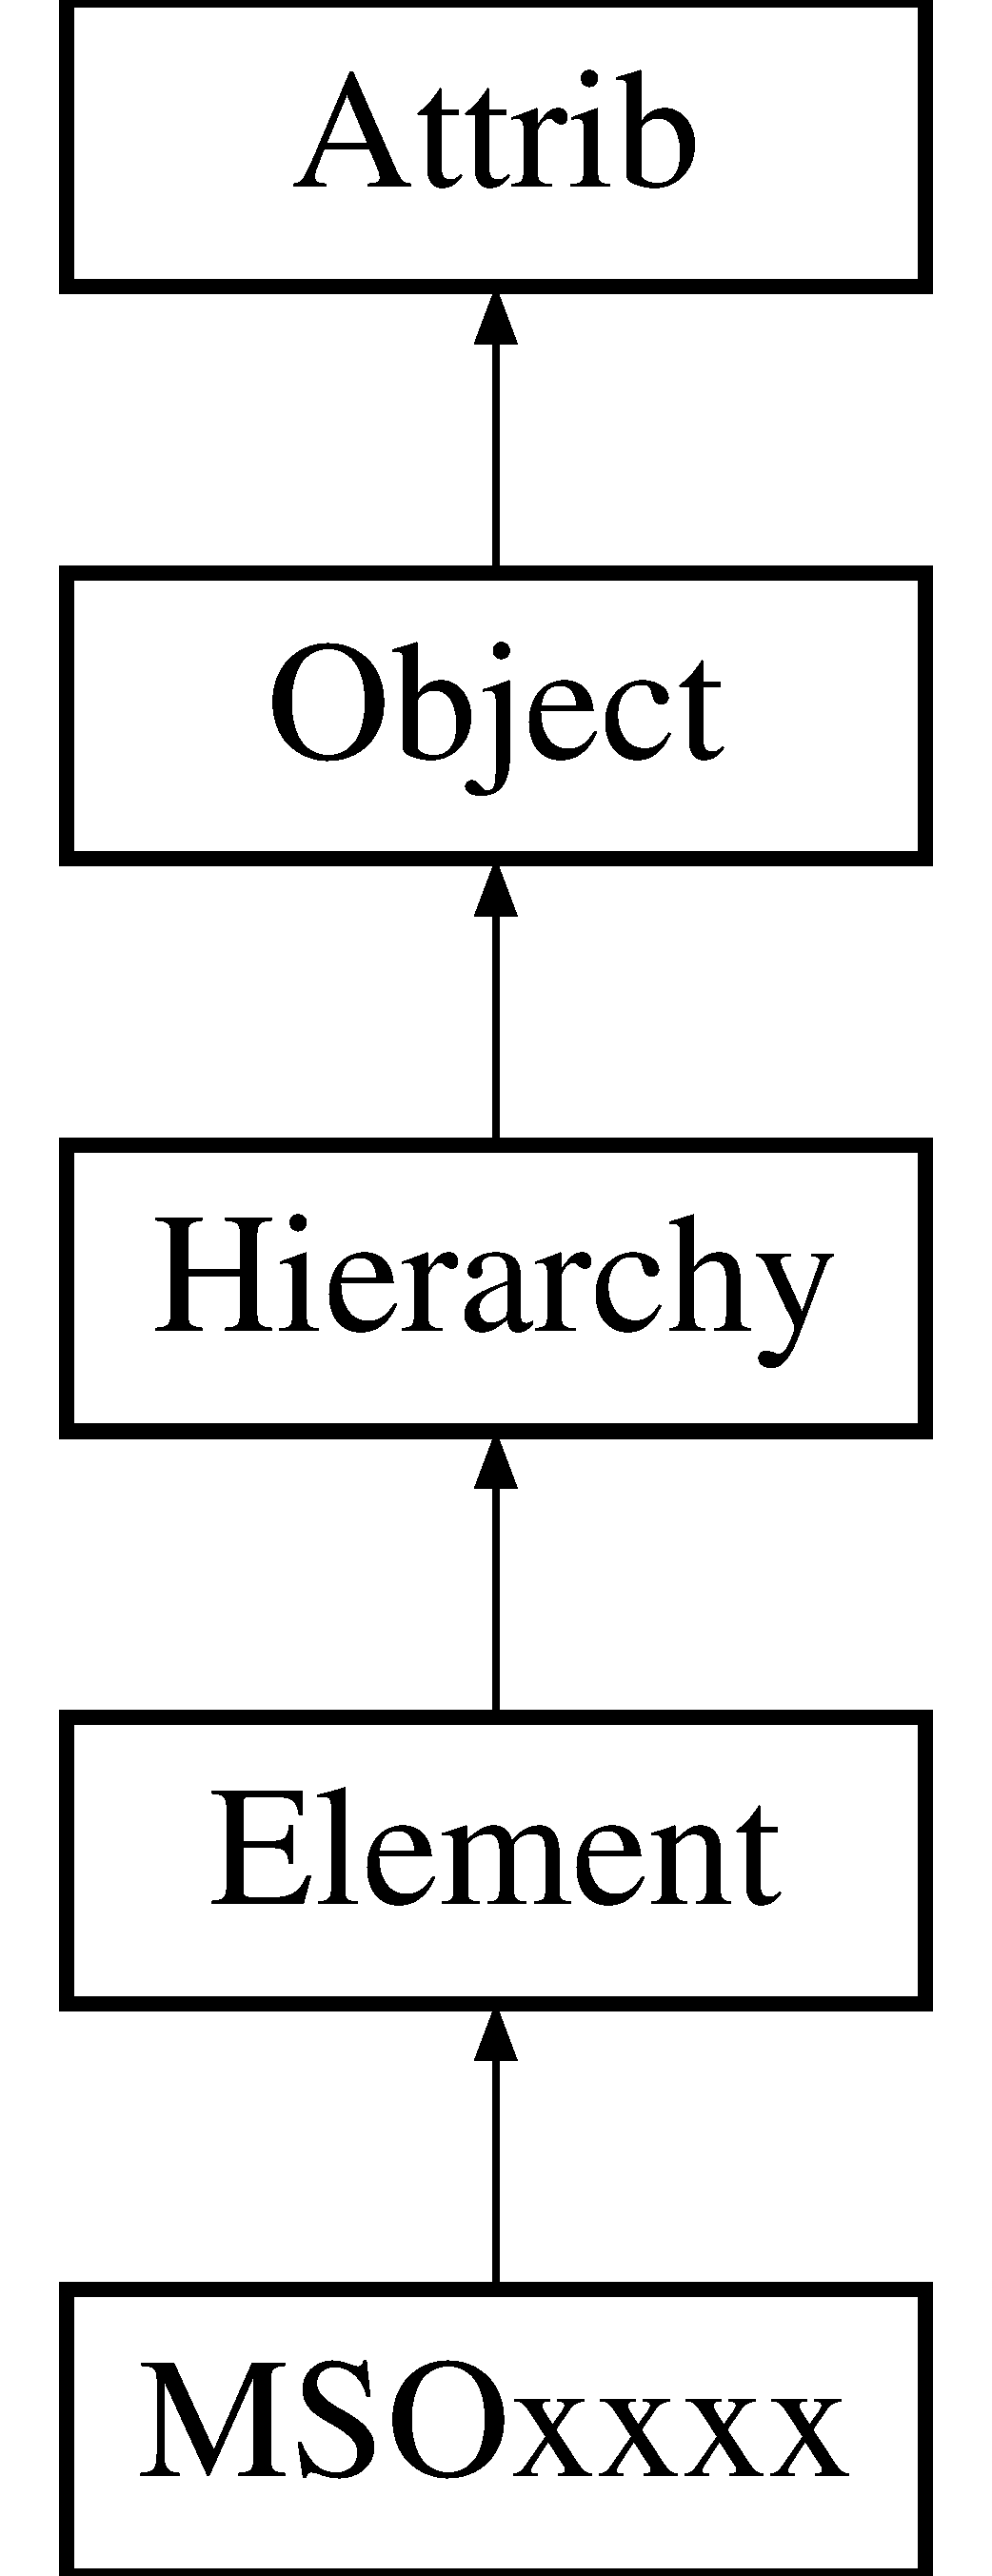
\includegraphics[height=5cm]{classMSOxxxx}
\end{center}
\end{figure}
\subsection*{Public Types}
\begin{DoxyCompactItemize}
\item 
enum \hyperlink{classAttrib_a69e171d7cc6417835a5a306d3c764235}{Attribut} \{ \par
\hyperlink{classAttrib_a69e171d7cc6417835a5a306d3c764235a3a8da2ab97dda18aebab196fe4100531}{UNDEFINED}, 
\hyperlink{classAttrib_a69e171d7cc6417835a5a306d3c764235a2bfb2af57b87031d190a05fe25dd92ed}{PASSIVE}, 
\hyperlink{classAttrib_a69e171d7cc6417835a5a306d3c764235a3b1fec929c0370d1436f2f06e298fb0d}{ACTIVE}, 
\hyperlink{classAttrib_a69e171d7cc6417835a5a306d3c764235aa27c16b480a369ea4d18b07b2516bbc7}{INTERFACE}, 
\par
\hyperlink{classAttrib_a69e171d7cc6417835a5a306d3c764235a1420a5b8c0540b2af210b6975eded7f9}{IO}, 
\hyperlink{classAttrib_a69e171d7cc6417835a5a306d3c764235a0af3b0d0ac323c1704e6c69cf90add28}{IODATA}, 
\hyperlink{classAttrib_a69e171d7cc6417835a5a306d3c764235a7788bc5dd333fd8ce18562b269c9dab1}{ELEMENT}, 
\hyperlink{classAttrib_a69e171d7cc6417835a5a306d3c764235a61ceb22149f365f1780d18f9d1459423}{HARDWARE}, 
\par
\hyperlink{classAttrib_a69e171d7cc6417835a5a306d3c764235a75250e29692496e73effca2c0330977f}{PROCESSUS}, 
\hyperlink{classAttrib_a69e171d7cc6417835a5a306d3c764235a103a67cd0b8f07ef478fa45d4356e27b}{SOFTWARE}
 \}
\end{DoxyCompactItemize}
\subsection*{Public Member Functions}
\begin{DoxyCompactItemize}
\item 
\hyperlink{classMSOxxxx_afa2d5e8dcabe88d8c4ef54238a4e7bc7}{MSOxxxx} ()
\item 
void \hyperlink{classMSOxxxx_a3fc4e785c764c2abb0c0c2da4d71108a}{configTCPIP} (string ip, int port)
\item 
\hyperlink{classStatusCode}{StatusCode} \hyperlink{classMSOxxxx_a4acff38c6f55795533c4d6b4cef6106b}{open} ()
\item 
void \hyperlink{classMSOxxxx_a65fd9540df836c24a044807f12071c92}{closeConnection} ()
\item 
void \hyperlink{classMSOxxxx_a59a1d5e5f537086590b60a93d5c4c8a1}{setDebugMode} (bool debug)
\item 
\hyperlink{classStatusCode}{StatusCode} \hyperlink{classMSOxxxx_ae08131dd88d4d7f95e870b69b2f5e0e6}{channelScale} (int ch, double value)
\item 
\hyperlink{classStatusCode}{StatusCode} \hyperlink{classMSOxxxx_ab77c05543d9478b140466b7505651ab8}{channelOffset} (int ch, double value)
\item 
\hyperlink{classStatusCode}{StatusCode} \hyperlink{classMSOxxxx_a4cb8e745f172b7a30953ec87923c8c76}{channelDisplay} (int ch, bool display)
\item 
\hyperlink{classStatusCode}{StatusCode} \hyperlink{classMSOxxxx_af9851b9ce16b0e88e8691c8174ba54f0}{channelDisplayName} (int ch, string name)
\item 
\hyperlink{classStatusCode}{StatusCode} \hyperlink{classMSOxxxx_a0327f511fdb8920ddabf1dbbd54f9e9f}{timeBaseScale} (double secsPerDiv)
\item 
\hyperlink{classStatusCode}{StatusCode} \hyperlink{classMSOxxxx_ac23ca74ef0e746fe1830bcf26952c42d}{timeBaseOffset} (double seconds)
\item 
\hyperlink{classStatusCode}{StatusCode} \hyperlink{classMSOxxxx_a44238c713464e76d4c3c2005413bdf76}{triggerAuto} ()
\item 
\hyperlink{classStatusCode}{StatusCode} \hyperlink{classMSOxxxx_a9019b632465638a13c409d8243fe83b4}{triggerConfig} (bool slope, int ch, double level)
\item 
\hyperlink{classStatusCode}{StatusCode} \hyperlink{classMSOxxxx_a829d87b0aa03840ebfe0a44e560c7f63}{setupJitter} (int ch)
\item 
\hyperlink{classStatusCode}{StatusCode} \hyperlink{classMSOxxxx_af1524bb099b5e559931704d13a1f1126}{setupAvgVoltage} (int ch)
\item 
\hyperlink{classStatusCode}{StatusCode} \hyperlink{classMSOxxxx_abbbebb3e4649c866bcdd853627f12b5d}{setupDeltaTime} (int chA, int chB, int edge)
\item 
PyObject $\ast$ \hyperlink{classMSOxxxx_a38f15b6ad8bc3cdc1836d784b3e96c59}{getStatistics} (int nMinMeas)
\item 
\hyperlink{classStatusCode}{StatusCode} \hyperlink{classMSOxxxx_ade4192f09f150be8b9c7c081ce1a1870}{labelDisplay} (bool display)
\item 
PyObject $\ast$ \hyperlink{classMSOxxxx_aed78c680bcec9e14a88eedf7b291518c}{waveformCapture} (int ch)
\item 
PyObject $\ast$ \hyperlink{classMSOxxxx_a0f14b23d31d8e7647184e99a89600cc3}{id} ()
\item 
\hyperlink{classStatusCode}{StatusCode} \hyperlink{classMSOxxxx_a96ca34744e5a6b611aaf9ae7910f00cd}{run} ()
\item 
\hyperlink{classStatusCode}{StatusCode} \hyperlink{classMSOxxxx_a4ec991c3850a652fbe9a1709cab7001b}{stop} ()
\item 
\hyperlink{classMSOxxxx_a567c156d78fbeab9d61bf8ec9acac851}{$\sim$MSOxxxx} ()
\item 
void \hyperlink{classMSOxxxx_a8c22ff23297ada963eaf12b6e0b62017}{help} ()
\item 
\hyperlink{classStatusCode}{StatusCode} \hyperlink{classMSOxxxx_ac14ed16b221798423e7c3b5e285006b5}{init} ()
\item 
void \hyperlink{classMSOxxxx_a26f03d21da556529155898dc115c301c}{reset} ()
\item 
void \hyperlink{classMSOxxxx_a09452d6e75cd9adfaec93606fbb998dc}{update} ()
\item 
void \hyperlink{classElement_a3c0abcb36f8906688bb7e32608df7086}{recursiveInitElement} ()
\item 
void \hyperlink{classElement_a82119ed37dff76508a2746a853ec35ba}{recursiveInitCommunications} ()
\item 
\hyperlink{classStatusCode}{StatusCode} \hyperlink{classElement_ab476b4b1df5954141ceb14f072433b89}{setConnection} (\hyperlink{classHierarchy}{Hierarchy} $\ast$)
\item 
\hyperlink{classHierarchy}{Hierarchy} $\ast$ \hyperlink{classElement_af57444353c1ddf9fa0109801e97debf7}{connection} ()
\item 
void \hyperlink{classHierarchy_af4d43b0765b402670eed2d62c73405af}{clear} ()
\item 
void \hyperlink{classHierarchy_a585ad1aeec16077a0e532ab8b4fc557b}{setParent} (\hyperlink{classHierarchy}{Hierarchy} $\ast$parent)
\item 
\hyperlink{classHierarchy}{Hierarchy} $\ast$ \hyperlink{classHierarchy_a1c7bec8257e717f9c1465e06ebf845fc}{parent} ()
\item 
\hyperlink{classHierarchy}{Hierarchy} $\ast$ \hyperlink{classHierarchy_ad550588733bf75ac5c0fcfd7c8fd11a6}{parent} (std::string)
\item 
\hyperlink{classHierarchy}{Hierarchy} $\ast$ \hyperlink{classHierarchy_aee461dc930ce3871636ff87f075b1b83}{origin} ()
\item 
virtual void \hyperlink{classHierarchy_ad677774ff38fcb257c04a3a10d471fac}{addChild} (\hyperlink{classHierarchy}{Hierarchy} $\ast$element)
\item 
std::vector$<$ \hyperlink{classHierarchy}{Hierarchy} $\ast$ $>$ \hyperlink{classHierarchy_aa9a76f69e98e052ee1a6e32cea006288}{children} ()
\item 
\hyperlink{classHierarchy}{Hierarchy} $\ast$ \hyperlink{classHierarchy_a1e207f973c694b538bf90107b4868817}{child} (std::string)
\item 
\hyperlink{classHierarchy}{Hierarchy} $\ast$ \hyperlink{classHierarchy_a0c15a5276a3b80b4354d6bd8a01e0708}{childTyped} (std::string)
\item 
unsigned long \hyperlink{classHierarchy_ab16e84de65fd84e14001a6cf941c8be4}{numberOfChildren} ()
\item 
bool \hyperlink{classHierarchy_a255174fe4d316d2a3f430dcb9dab29f1}{hasChildren} ()
\item 
void \hyperlink{classHierarchy_a2b2b359fac003233f65786a616766bde}{delChild} (\hyperlink{classHierarchy}{Hierarchy} $\ast$)
\item 
void \hyperlink{classHierarchy_a1928ac7615fe0b5e55cd707f70dc6781}{delChild} (std::string)
\item 
std::string \hyperlink{classHierarchy_aa7990fa7caf132d83e361ce033c6c65a}{path} (std::string=std::string(\char`\"{}\char`\"{}))
\item 
std::string \hyperlink{classHierarchy_a1efd56cd164d328d2002e53a10a19b8c}{pathTyped} (std::string=std::string(\char`\"{}\char`\"{}))
\item 
void \hyperlink{classHierarchy_a76e914b9a677a22a82deb74d892bf261}{tree} (std::string indent=std::string(\char`\"{}\char`\"{}))
\item 
void \hyperlink{classHierarchy_a594c294c5f60c230e106d522ed008212}{tree} ()
\item 
std::string \hyperlink{classObject_a975e888d50bfcbffda2c86368332a5cd}{name} () const 
\item 
std::string \hyperlink{classObject_a84f99f70f144a83e1582d1d0f84e4e62}{type} ()
\item 
std::string \hyperlink{classObject_a73a0f1a41828fdd8303dd662446fb6c3}{title} ()
\item 
void \hyperlink{classObject_a3f9d5537ebce0c0f2bf6ae4d92426f3c}{msgSvc} (int level, std::string msg, std::string name)
\item 
void \hyperlink{classObject_a58b2d0618c2d08cf2383012611528d97}{msg} (std::string mymsg)
\item 
void \hyperlink{classObject_ac5d59299273cee27aacf7de00d2e7034}{msg} (std::string mymsg, std::string name)
\item 
void \hyperlink{classObject_a83d2db2df682907ea1115ad721c1c4a1}{verbose} (std::string mymsg)
\item 
void \hyperlink{classObject_a2d4120195317e2a3c6532e8bb9f3da68}{verbose} (std::string mymsg, std::string name)
\item 
void \hyperlink{classObject_aac010553f022165573714b7014a15f0d}{debug} (std::string mymsg)
\item 
void \hyperlink{classObject_a6c9a0397ca804e04d675ed05683f5420}{debug} (std::string mymsg, std::string name)
\item 
void \hyperlink{classObject_a644fd329ea4cb85f54fa6846484b84a8}{info} (std::string mymsg)
\item 
void \hyperlink{classObject_a1ca123253dfd30fc28b156f521dcbdae}{info} (std::string mymsg, std::string name)
\item 
void \hyperlink{classObject_a65cd4fda577711660821fd2cd5a3b4c9}{warning} (std::string mymsg)
\item 
void \hyperlink{classObject_a11f101db4dd73d9391b0231818881d86}{warning} (std::string mymsg, std::string name)
\item 
void \hyperlink{classObject_a204a95f57818c0f811933917a30eff45}{error} (std::string mymsg)
\item 
void \hyperlink{classObject_ad7f6c457733082efa2f9ff5f5c8e119a}{error} (std::string mymsg, std::string name)
\item 
void \hyperlink{classObject_aad5a16aac7516ce65bd5ec02ab07fc80}{fatal} (std::string mymsg)
\item 
void \hyperlink{classObject_ae62acd3d09f716220f75f252dc38bc9a}{fatal} (std::string mymsg, std::string name)
\item 
void \hyperlink{classObject_ae30fea75683c2d149b6b6d17c09ecd0c}{setName} (std::string name)
\item 
void \hyperlink{classObject_aae534cc9d982bcb9b99fd505f2e103a5}{setType} (std::string type)
\item 
void \hyperlink{classObject_a398fe08cba594a0ce6891d59fe4f159f}{setId} (unsigned char id)
\item 
void \hyperlink{classObject_a89557dbbad5bcaa02652f5d7fa35d20f}{setTitle} (std::string title)
\item 
void \hyperlink{classObject_a870c5af919958c2136623b2d7816d123}{setDllName} (std::string dllName)
\item 
std::string \hyperlink{classObject_a2e3947f2870094c332d7454117f3ec63}{dllName} ()
\item 
bool \hyperlink{classAttrib_a704f26af560909ad22065083bb7d4c34}{is} (int attribut)
\item 
void \hyperlink{classAttrib_a235f773af19c900264a190b00a3b4ad7}{add} (int attribut)
\item 
void \hyperlink{classAttrib_a7d4ef7e32d93cb287792b87b857e79f3}{remove} (int attribut)
\item 
std::string \hyperlink{classAttrib_aee7bbf16b144887f196e1341b24f8a26}{attributs} ()
\end{DoxyCompactItemize}
\subsection*{Protected Attributes}
\begin{DoxyCompactItemize}
\item 
\hyperlink{classHierarchy}{Hierarchy} $\ast$ \hyperlink{classElement_abe3de7a5dbbc9a6dd2d7e012e5fdb266}{m\_\-connection}
\item 
std::string \hyperlink{classAttrib_a3414521d7a82476e874b25a5407b5e63}{m\_\-attribString} \mbox{[}10\mbox{]}
\end{DoxyCompactItemize}
\subsection*{Private Member Functions}
\begin{DoxyCompactItemize}
\item 
bool \hyperlink{classMSOxxxx_a9723e9234403d5eb74bde628fd78d56c}{getTimeBase} (double $\ast$xInc, double $\ast$xOrg)
\item 
bool \hyperlink{classMSOxxxx_ae77668a1ae4ccb74e0ed5f2485dfdebf}{send} (string msg)
\item 
int \hyperlink{classMSOxxxx_aa02e46a61e287ef1f5377e9e42399faf}{recv} (string $\ast$\hyperlink{classMSOxxxx_a847cae37181e9ec5f481edcc3fb19b1a}{rxItems}, string spacer)
\item 
int \hyperlink{classMSOxxxx_a46726c6d181a758bb4f598c66f336236}{split} (string str, string $\ast$splitStr, string delimiter)
\item 
string \hyperlink{classMSOxxxx_ab9c897c3dc0a52cbe5a5da67fc520ed7}{ftos} (double)
\end{DoxyCompactItemize}
\subsection*{Private Attributes}
\begin{DoxyCompactItemize}
\item 
string \hyperlink{classMSOxxxx_aa55bdb0feb799b195628fe6ef0222b62}{ipAddress}
\item 
int \hyperlink{classMSOxxxx_a242bcf72c701cd20d86d25315fc6180f}{portNumber}
\item 
int \hyperlink{classMSOxxxx_acf030a8f1ddd78d632816c856f50455c}{sockfd}
\item 
char \hyperlink{classMSOxxxx_a1a50770759caada18087ca8ffb96f357}{rxBuffer} \mbox{[}10485760\mbox{]}
\item 
string \hyperlink{classMSOxxxx_a847cae37181e9ec5f481edcc3fb19b1a}{rxItems} \mbox{[}65536\mbox{]}
\item 
bool \hyperlink{classMSOxxxx_a826ba82e93bbe5780169107a31dbfd29}{debugMode}
\item 
bool \hyperlink{classMSOxxxx_af0af7ac8123ee93917d0e92ec947acaa}{err}
\end{DoxyCompactItemize}


\subsection{Detailed Description}


Definition at line 39 of file MSOxxxx.h.

\subsection{Member Enumeration Documentation}
\hypertarget{classAttrib_a69e171d7cc6417835a5a306d3c764235}{
\index{MSOxxxx@{MSOxxxx}!Attribut@{Attribut}}
\index{Attribut@{Attribut}!MSOxxxx@{MSOxxxx}}
\subsubsection[{Attribut}]{\setlength{\rightskip}{0pt plus 5cm}enum {\bf Attrib::Attribut}\hspace{0.3cm}{\ttfamily  \mbox{[}inherited\mbox{]}}}}
\label{classAttrib_a69e171d7cc6417835a5a306d3c764235}
\begin{Desc}
\item[Enumerator: ]\par
\begin{description}
\index{UNDEFINED@{UNDEFINED}!MSOxxxx@{MSOxxxx}}\index{MSOxxxx@{MSOxxxx}!UNDEFINED@{UNDEFINED}}\item[{\em 
\hypertarget{classAttrib_a69e171d7cc6417835a5a306d3c764235a3a8da2ab97dda18aebab196fe4100531}{
UNDEFINED}
\label{classAttrib_a69e171d7cc6417835a5a306d3c764235a3a8da2ab97dda18aebab196fe4100531}
}]\index{PASSIVE@{PASSIVE}!MSOxxxx@{MSOxxxx}}\index{MSOxxxx@{MSOxxxx}!PASSIVE@{PASSIVE}}\item[{\em 
\hypertarget{classAttrib_a69e171d7cc6417835a5a306d3c764235a2bfb2af57b87031d190a05fe25dd92ed}{
PASSIVE}
\label{classAttrib_a69e171d7cc6417835a5a306d3c764235a2bfb2af57b87031d190a05fe25dd92ed}
}]\index{ACTIVE@{ACTIVE}!MSOxxxx@{MSOxxxx}}\index{MSOxxxx@{MSOxxxx}!ACTIVE@{ACTIVE}}\item[{\em 
\hypertarget{classAttrib_a69e171d7cc6417835a5a306d3c764235a3b1fec929c0370d1436f2f06e298fb0d}{
ACTIVE}
\label{classAttrib_a69e171d7cc6417835a5a306d3c764235a3b1fec929c0370d1436f2f06e298fb0d}
}]\index{INTERFACE@{INTERFACE}!MSOxxxx@{MSOxxxx}}\index{MSOxxxx@{MSOxxxx}!INTERFACE@{INTERFACE}}\item[{\em 
\hypertarget{classAttrib_a69e171d7cc6417835a5a306d3c764235aa27c16b480a369ea4d18b07b2516bbc7}{
INTERFACE}
\label{classAttrib_a69e171d7cc6417835a5a306d3c764235aa27c16b480a369ea4d18b07b2516bbc7}
}]\index{IO@{IO}!MSOxxxx@{MSOxxxx}}\index{MSOxxxx@{MSOxxxx}!IO@{IO}}\item[{\em 
\hypertarget{classAttrib_a69e171d7cc6417835a5a306d3c764235a1420a5b8c0540b2af210b6975eded7f9}{
IO}
\label{classAttrib_a69e171d7cc6417835a5a306d3c764235a1420a5b8c0540b2af210b6975eded7f9}
}]\index{IODATA@{IODATA}!MSOxxxx@{MSOxxxx}}\index{MSOxxxx@{MSOxxxx}!IODATA@{IODATA}}\item[{\em 
\hypertarget{classAttrib_a69e171d7cc6417835a5a306d3c764235a0af3b0d0ac323c1704e6c69cf90add28}{
IODATA}
\label{classAttrib_a69e171d7cc6417835a5a306d3c764235a0af3b0d0ac323c1704e6c69cf90add28}
}]\index{ELEMENT@{ELEMENT}!MSOxxxx@{MSOxxxx}}\index{MSOxxxx@{MSOxxxx}!ELEMENT@{ELEMENT}}\item[{\em 
\hypertarget{classAttrib_a69e171d7cc6417835a5a306d3c764235a7788bc5dd333fd8ce18562b269c9dab1}{
ELEMENT}
\label{classAttrib_a69e171d7cc6417835a5a306d3c764235a7788bc5dd333fd8ce18562b269c9dab1}
}]\index{HARDWARE@{HARDWARE}!MSOxxxx@{MSOxxxx}}\index{MSOxxxx@{MSOxxxx}!HARDWARE@{HARDWARE}}\item[{\em 
\hypertarget{classAttrib_a69e171d7cc6417835a5a306d3c764235a61ceb22149f365f1780d18f9d1459423}{
HARDWARE}
\label{classAttrib_a69e171d7cc6417835a5a306d3c764235a61ceb22149f365f1780d18f9d1459423}
}]\index{PROCESSUS@{PROCESSUS}!MSOxxxx@{MSOxxxx}}\index{MSOxxxx@{MSOxxxx}!PROCESSUS@{PROCESSUS}}\item[{\em 
\hypertarget{classAttrib_a69e171d7cc6417835a5a306d3c764235a75250e29692496e73effca2c0330977f}{
PROCESSUS}
\label{classAttrib_a69e171d7cc6417835a5a306d3c764235a75250e29692496e73effca2c0330977f}
}]\index{SOFTWARE@{SOFTWARE}!MSOxxxx@{MSOxxxx}}\index{MSOxxxx@{MSOxxxx}!SOFTWARE@{SOFTWARE}}\item[{\em 
\hypertarget{classAttrib_a69e171d7cc6417835a5a306d3c764235a103a67cd0b8f07ef478fa45d4356e27b}{
SOFTWARE}
\label{classAttrib_a69e171d7cc6417835a5a306d3c764235a103a67cd0b8f07ef478fa45d4356e27b}
}]\end{description}
\end{Desc}



Definition at line 29 of file Attrib.h.


\begin{DoxyCode}
29                 {
30     UNDEFINED,
31     PASSIVE,
32     ACTIVE,
33     INTERFACE,
34     IO,
35     IODATA,
36     ELEMENT,
37     HARDWARE,
38     PROCESSUS,
39     SOFTWARE 
40   }; // array m_attribString must be changed into Attrib::Attrib if this enu is m
      odified. 
\end{DoxyCode}


\subsection{Constructor \& Destructor Documentation}
\hypertarget{classMSOxxxx_afa2d5e8dcabe88d8c4ef54238a4e7bc7}{
\index{MSOxxxx@{MSOxxxx}!MSOxxxx@{MSOxxxx}}
\index{MSOxxxx@{MSOxxxx}!MSOxxxx@{MSOxxxx}}
\subsubsection[{MSOxxxx}]{\setlength{\rightskip}{0pt plus 5cm}MSOxxxx::MSOxxxx ()}}
\label{classMSOxxxx_afa2d5e8dcabe88d8c4ef54238a4e7bc7}


Definition at line 16 of file MSOxxxx.cpp.

References Attrib::add(), Object::debug(), DEBUG\_\-MODE, debugMode, DEFAULT\_\-IP\_\-ADDRESS, DEFAULT\_\-PORT, Attrib::ELEMENT, Attrib::HARDWARE, ipAddress, portNumber, Object::setId(), and Object::setType().


\begin{DoxyCode}
17 {
18     setType("MSOxxxx");
19     setId(0);
20 
21     add(Attrib::ELEMENT); add (Attrib::HARDWARE);
22     debug("MSOxxxx built.","MSOxxxx::MSOxxxx");
23 
24     ipAddress   = DEFAULT_IP_ADDRESS;                                   //We conf
      igure a default IP here. User can change it afterwards.
25     portNumber  =   DEFAULT_PORT;
26     debugMode       = DEBUG_MODE;
27 
28 }
\end{DoxyCode}
\hypertarget{classMSOxxxx_a567c156d78fbeab9d61bf8ec9acac851}{
\index{MSOxxxx@{MSOxxxx}!$\sim$MSOxxxx@{$\sim$MSOxxxx}}
\index{$\sim$MSOxxxx@{$\sim$MSOxxxx}!MSOxxxx@{MSOxxxx}}
\subsubsection[{$\sim$MSOxxxx}]{\setlength{\rightskip}{0pt plus 5cm}MSOxxxx::$\sim$MSOxxxx ()\hspace{0.3cm}{\ttfamily  \mbox{[}inline\mbox{]}}}}
\label{classMSOxxxx_a567c156d78fbeab9d61bf8ec9acac851}


Definition at line 84 of file MSOxxxx.h.


\begin{DoxyCode}
84             {
85   }
\end{DoxyCode}


\subsection{Member Function Documentation}
\hypertarget{classAttrib_a235f773af19c900264a190b00a3b4ad7}{
\index{MSOxxxx@{MSOxxxx}!add@{add}}
\index{add@{add}!MSOxxxx@{MSOxxxx}}
\subsubsection[{add}]{\setlength{\rightskip}{0pt plus 5cm}void Attrib::add (int {\em attribut})\hspace{0.3cm}{\ttfamily  \mbox{[}inline, inherited\mbox{]}}}}
\label{classAttrib_a235f773af19c900264a190b00a3b4ad7}
Add an attribut 

Definition at line 67 of file Attrib.h.

References Attrib::m\_\-attributs, and Attrib::UNDEFINED.

Referenced by A3PE::A3PE(), Attrib::Attrib(), SpecsMezzanine::cmdline(), Computer::Computer(), CU\_\-v1::CU\_\-v1(), export\_\-obj(), FEB\_\-v1::FEB\_\-v1(), FePGA::FePGA(), ICECALv3::ICECALv3(), ICPhaser::ICPhaser(), Application::initialize(), Interface::Interface(), IOdata::IOdata(), IOobject::IOobject(), LSDelayChipV1::LSDelayChipV1(), MSOxxxx(), Phaser::Phaser(), Processus::Processus(), Proto40MHz\_\-v1::Proto40MHz\_\-v1(), Attrib::remove(), SeqPGA::SeqPGA(), SpecsMaster::SpecsMaster(), and SpecsSlave::SpecsSlave().


\begin{DoxyCode}
67                             {
68     if (attribut!=Attrib::UNDEFINED) remove(Attrib::UNDEFINED);
69     bool duplicate = false ;
70     std::vector<int>::const_iterator iter ;
71     for ( iter  = m_attributs.begin() ;
72           iter != m_attributs.end()   ;
73           ++iter ) {
74       if ( attribut == (*iter) ) {
75         duplicate = true ;
76       }
77     }
78     if (!duplicate) {
79       m_attributs.push_back( attribut );
80     }
81   }
\end{DoxyCode}
\hypertarget{classHierarchy_ad677774ff38fcb257c04a3a10d471fac}{
\index{MSOxxxx@{MSOxxxx}!addChild@{addChild}}
\index{addChild@{addChild}!MSOxxxx@{MSOxxxx}}
\subsubsection[{addChild}]{\setlength{\rightskip}{0pt plus 5cm}void Hierarchy::addChild ({\bf Hierarchy} $\ast$ {\em element})\hspace{0.3cm}{\ttfamily  \mbox{[}virtual, inherited\mbox{]}}}}
\label{classHierarchy_ad677774ff38fcb257c04a3a10d471fac}


Definition at line 83 of file Hierarchy.cpp.

References Object::debug(), Hierarchy::m\_\-children, Object::name(), and Hierarchy::setParent().

Referenced by A3PE::A3PE(), SpecsMezzanine::addBus(), SpecsSlave::addI2c(), Application::create(), CU\_\-v1::CU\_\-v1(), export\_\-obj(), FEB\_\-v1::FEB\_\-v1(), FePGA::FePGA(), ICECALv3::ICECALv3(), ICPhaser::ICPhaser(), LSDelayChipV1::LSDelayChipV1(), FePGA::MakeRAM(), FePGA::MakeRegister(), Phaser::Phaser(), Proto40MHz\_\-v1::Proto40MHz\_\-v1(), SeqPGA::SeqPGA(), SpecsMezzanine::SpecsMezzanine(), UsbI2cBus::UsbI2cBus(), and UsbSpiBus::UsbSpiBus().


\begin{DoxyCode}
83                                           {
84   element->setParent(this);
85   m_children.push_back(element);
86   debug(element->name()+" added to the child tree.","Hierarchy::addChild");
87 }
\end{DoxyCode}
\hypertarget{classAttrib_aee7bbf16b144887f196e1341b24f8a26}{
\index{MSOxxxx@{MSOxxxx}!attributs@{attributs}}
\index{attributs@{attributs}!MSOxxxx@{MSOxxxx}}
\subsubsection[{attributs}]{\setlength{\rightskip}{0pt plus 5cm}std::string Attrib::attributs ()\hspace{0.3cm}{\ttfamily  \mbox{[}inherited\mbox{]}}}}
\label{classAttrib_aee7bbf16b144887f196e1341b24f8a26}
Print the \hyperlink{classAttrib}{Attrib} of an \hyperlink{classObject}{Object} 

Definition at line 54 of file Attrib.cpp.

References images::index, Attrib::m\_\-attribString, and Attrib::m\_\-attributs.

Referenced by export\_\-obj().


\begin{DoxyCode}
54                             {
55   std::string output;
56   std::vector<int>::iterator iter ;
57   for ( unsigned int index = 0 ; index < m_attributs.size() ; ++index ) {
58     if ( m_attributs.size() - index > 1 ) {
59       output.append(m_attribString[m_attributs[index]]);
60       output.append(":");
61     }
62     else {
63       output.append(m_attribString[m_attributs[index]]);
64     }
65   }
66   return output;
67 }
\end{DoxyCode}
\hypertarget{classMSOxxxx_a4cb8e745f172b7a30953ec87923c8c76}{
\index{MSOxxxx@{MSOxxxx}!channelDisplay@{channelDisplay}}
\index{channelDisplay@{channelDisplay}!MSOxxxx@{MSOxxxx}}
\subsubsection[{channelDisplay}]{\setlength{\rightskip}{0pt plus 5cm}{\bf StatusCode} MSOxxxx::channelDisplay (int {\em ch}, \/  bool {\em display})}}
\label{classMSOxxxx_a4cb8e745f172b7a30953ec87923c8c76}


Definition at line 151 of file MSOxxxx.cpp.

References StatusCode::FAILURE, itos(), send(), and StatusCode::SUCCESS.

Referenced by BOOST\_\-PYTHON\_\-MODULE().


\begin{DoxyCode}
152 {
153     bool ok;
154     if(display)     
155         ok = send(":CHANNEL" + itos(ch) + ":DISPLAY ON \n");
156     else
157         ok = send(":CHANNEL" + itos(ch) + ":DISPLAY OFF \n");
158     if(ok)  return StatusCode::SUCCESS;
159     else        return StatusCode::FAILURE; 
160 }
\end{DoxyCode}
\hypertarget{classMSOxxxx_af9851b9ce16b0e88e8691c8174ba54f0}{
\index{MSOxxxx@{MSOxxxx}!channelDisplayName@{channelDisplayName}}
\index{channelDisplayName@{channelDisplayName}!MSOxxxx@{MSOxxxx}}
\subsubsection[{channelDisplayName}]{\setlength{\rightskip}{0pt plus 5cm}{\bf StatusCode} MSOxxxx::channelDisplayName (int {\em ch}, \/  string {\em name})}}
\label{classMSOxxxx_af9851b9ce16b0e88e8691c8174ba54f0}


Definition at line 162 of file MSOxxxx.cpp.

References StatusCode::FAILURE, itos(), send(), and StatusCode::SUCCESS.

Referenced by BOOST\_\-PYTHON\_\-MODULE().


\begin{DoxyCode}
163 {
164     bool ok = send(":CHANNEL" + itos(ch) + ":LABEL \"" + name + "\" \n");
165     if(ok)  return StatusCode::SUCCESS;
166     else        return StatusCode::FAILURE; 
167 }
\end{DoxyCode}
\hypertarget{classMSOxxxx_ab77c05543d9478b140466b7505651ab8}{
\index{MSOxxxx@{MSOxxxx}!channelOffset@{channelOffset}}
\index{channelOffset@{channelOffset}!MSOxxxx@{MSOxxxx}}
\subsubsection[{channelOffset}]{\setlength{\rightskip}{0pt plus 5cm}{\bf StatusCode} MSOxxxx::channelOffset (int {\em ch}, \/  double {\em value})}}
\label{classMSOxxxx_ab77c05543d9478b140466b7505651ab8}


Definition at line 144 of file MSOxxxx.cpp.

References StatusCode::FAILURE, ftos(), itos(), send(), and StatusCode::SUCCESS.

Referenced by BOOST\_\-PYTHON\_\-MODULE().


\begin{DoxyCode}
145 {
146     bool ok = send(":CHANNEL" + itos(ch) + ":OFFSET " + ftos(value) + "\n");
147     if(ok)  return StatusCode::SUCCESS;
148     else        return StatusCode::FAILURE;
149 }
\end{DoxyCode}
\hypertarget{classMSOxxxx_ae08131dd88d4d7f95e870b69b2f5e0e6}{
\index{MSOxxxx@{MSOxxxx}!channelScale@{channelScale}}
\index{channelScale@{channelScale}!MSOxxxx@{MSOxxxx}}
\subsubsection[{channelScale}]{\setlength{\rightskip}{0pt plus 5cm}{\bf StatusCode} MSOxxxx::channelScale (int {\em ch}, \/  double {\em value})}}
\label{classMSOxxxx_ae08131dd88d4d7f95e870b69b2f5e0e6}


Definition at line 137 of file MSOxxxx.cpp.

References StatusCode::FAILURE, ftos(), itos(), send(), and StatusCode::SUCCESS.

Referenced by BOOST\_\-PYTHON\_\-MODULE().


\begin{DoxyCode}
138 {
139     bool ok = send(":CHANNEL" + itos(ch) + ":SCALE " + ftos(value) + "\n");
140     if(ok)  return StatusCode::SUCCESS;
141     else        return StatusCode::FAILURE;
142 }
\end{DoxyCode}
\hypertarget{classHierarchy_a1e207f973c694b538bf90107b4868817}{
\index{MSOxxxx@{MSOxxxx}!child@{child}}
\index{child@{child}!MSOxxxx@{MSOxxxx}}
\subsubsection[{child}]{\setlength{\rightskip}{0pt plus 5cm}{\bf Hierarchy} $\ast$ Hierarchy::child (std::string {\em path})\hspace{0.3cm}{\ttfamily  \mbox{[}inherited\mbox{]}}}}
\label{classHierarchy_a1e207f973c694b538bf90107b4868817}


Definition at line 133 of file Hierarchy.cpp.

References Hierarchy::child(), Hierarchy::children(), Object::name(), Hierarchy::origin(), Hierarchy::parent(), and Object::warning().

Referenced by Application::cd(), Hierarchy::child(), and export\_\-obj().


\begin{DoxyCode}
133                                          {
134   std::string newpath = path;
135   std::string up("..");
136   std::string separator(1,'/');
137 
138   Hierarchy * newcurrent = 0;
139 
140   //  info("path="+path,"Hierarchy::child");
141 
142   if (path.compare("")==0 || path.compare("/")==0) {
143     //    debug("return origin","Hierarchy::child");
144     return origin();
145   }
146 
147   if (path.compare(name())==0){
148     //    debug("return itself","Hierarchy::child");
149     return this;
150   }
151 
152   if (path.compare("..")==0){
153     if (0!=this->parent()) return this->parent();
154     else return this;
155   }
156 
157   if (path.compare("../")==0){
158     if (0!=this->parent()) return this->parent();
159     else return this;
160   }
161 
162 
163   int npos=path.find(separator,0);
164 
165   //  info("find separator in "+itos(npos)+" of "+path,"Hierarchy::child");
166 
167   // remove last separator
168   if ( npos == (int)(path.size()-1) ) {
169     newpath = std::string(path,0,npos);
170     path = newpath;
171   }
172 
173   if (npos==0){
174     //    debug("Going back to origin and calling child","Hierarchy::child");
175     newpath=std::string(path,1,path.size()-1);
176     return origin()->child(newpath);
177   }
178   else{
179     if ( npos== (int)(std::string::npos) ){
180       //      debug("Getting chid "+path+" of "+this->name(),"Hierarchy::child");
      
181       std::vector <Hierarchy*> list = children();
182       std::vector<Hierarchy*>::iterator iter;
183       for (iter=list.begin();iter!=list.end();iter++){
184         if ((*iter)->name().compare(path)==0){
185           return *iter;
186         }
187       }
188       warning(this->name()+std::string(" has no child '")+path+"'","Hierarchy::ch
      ild");
189       return this;
190     }
191     else
192     {
193       int ipos=path.find(separator,0);
194       //      info("default behaviour "+path+" with separator in "+itos(ipos),"Hi
      erarchy::child");
195 
196       std::string newcurrentname=std::string(path,0,ipos);
197       newpath=std::string(path,ipos+1,path.size()-1);
198 
199       //      info("looking now for "+newpath+" from "+newcurrentname,"Hierarchy:
      :child");
200 
201       if (0==newcurrentname.compare(origin()->name())){
202         //        info("current is computer. Looking for children"+newcurrentname
      ,"Hierarchy::child");
203         return origin()->child(newpath);
204       }
205 
206       newcurrent = (Hierarchy*)0;
207 
208       std::vector <Hierarchy*> list = children();
209       std::vector<Hierarchy*>::iterator iter;
210       for (iter=list.begin();iter!=list.end();iter++){
211         if ((*iter)->name().compare(newcurrentname)==0){
212           newcurrent = (*iter);
213         }
214       }
215 
216 
217       if ((Hierarchy*)0==newcurrent){
218         if (newcurrentname.compare("..")==0 && 0!=parent()){
219           newcurrent=this->parent();
220           //          debug("newcurrent was .. -> parent="+parent()->name());
221         }
222         else
223         {
224           warning(this->name()+" has no child '"+newcurrentname+"'",
225               "Hierarchy::child");
226           return this;
227         }
228       }
229       //      debug("recurrence call for "+newpath+" on "+newcurrent->name(),"Hie
      rarchy::child");
230       return newcurrent -> child ( newpath );
231     }
232   }
233 }
\end{DoxyCode}
\hypertarget{classHierarchy_aa9a76f69e98e052ee1a6e32cea006288}{
\index{MSOxxxx@{MSOxxxx}!children@{children}}
\index{children@{children}!MSOxxxx@{MSOxxxx}}
\subsubsection[{children}]{\setlength{\rightskip}{0pt plus 5cm}std::vector$<${\bf Hierarchy}$\ast$$>$ Hierarchy::children ()\hspace{0.3cm}{\ttfamily  \mbox{[}inline, inherited\mbox{]}}}}
\label{classHierarchy_aa9a76f69e98e052ee1a6e32cea006288}


Definition at line 33 of file Hierarchy.h.

References Hierarchy::m\_\-children.

Referenced by Hierarchy::child(), Hierarchy::childTyped(), export\_\-obj(), SpecsSlave::recursiveInitCommunications(), Element::recursiveInitCommunications(), Element::recursiveInitElement(), Application::setConfig(), and Hierarchy::tree().


\begin{DoxyCode}
33 { return m_children;  } //< get list of child(ren)
\end{DoxyCode}
\hypertarget{classHierarchy_a0c15a5276a3b80b4354d6bd8a01e0708}{
\index{MSOxxxx@{MSOxxxx}!childTyped@{childTyped}}
\index{childTyped@{childTyped}!MSOxxxx@{MSOxxxx}}
\subsubsection[{childTyped}]{\setlength{\rightskip}{0pt plus 5cm}{\bf Hierarchy} $\ast$ Hierarchy::childTyped (std::string {\em path})\hspace{0.3cm}{\ttfamily  \mbox{[}inherited\mbox{]}}}}
\label{classHierarchy_a0c15a5276a3b80b4354d6bd8a01e0708}


Definition at line 239 of file Hierarchy.cpp.

References Hierarchy::children(), Hierarchy::m\_\-origin, Object::name(), Hierarchy::parent(), and Object::warning().

Referenced by export\_\-obj().


\begin{DoxyCode}
239                                               {
240 
241   std::string newpath = path;
242 
243   std::string up("..");
244   std::string separator(1,'/');
245   std::string typeopen(1,'[');
246   std::string typeclose(1,']');
247 
248   Hierarchy * newcurrent = 0;
249 
250   unsigned int npos=path.find(separator,0);
251   unsigned int opos=path.find(typeopen,0);
252   if ( npos==std::string::npos || npos == path.size()-1 ){
253     if ( path.compare("..")==0 ) {
254       return parent();
255     }
256 
257     if ( npos == path.size()-1 ) {
258       newpath = std::string(path,0,opos);
259       path = newpath;
260     }
261 
262     std::vector < Hierarchy* > list = children();
263     std::vector < Hierarchy* >::iterator iter;
264     for (iter=list.begin();iter!=list.end();iter++){
265       std::string notypepath = std::string(path,0,opos);
266       if ((*iter)->name().compare(notypepath)==0){
267         return *iter;
268       }
269     }
270     warning(this->name()+std::string(" has no child ") +path,"Hierarchy::child");
      
271     return 0;
272   }
273 
274   else {
275 
276     if (std::string(path,0,3).compare(std::string("../"))==0) {
277       newpath=std::string(path,3,path.size()-3);
278       newcurrent = parent();
279     }
280     if (std::string(path,0,1).compare(std::string("/"))==0) {
281       newpath=std::string(path,1,path.size()-1);
282       newcurrent = ( Hierarchy* ) m_origin;
283     }
284     if ((std::string(path,0,3).compare(std::string("../")) !=0 ) &&
285         std::string(path,0,1).compare(std::string("/"))!=0 ) {
286       opos = path.find(typeopen,0);
287       int cpos = path.find(typeclose,0);
288       std::string name = std::string (path,0,opos);
289       newcurrent = childTyped( name );
290       if (newcurrent ==0){
291         warning(path+": no child found with such a name","Hierarchy::child");
292       }
293       newpath = std::string (path,cpos+2,path.size()-cpos-1);
294     }
295     return newcurrent -> childTyped ( newpath );
296   }
297 }
\end{DoxyCode}
\hypertarget{classHierarchy_af4d43b0765b402670eed2d62c73405af}{
\index{MSOxxxx@{MSOxxxx}!clear@{clear}}
\index{clear@{clear}!MSOxxxx@{MSOxxxx}}
\subsubsection[{clear}]{\setlength{\rightskip}{0pt plus 5cm}void Hierarchy::clear ()\hspace{0.3cm}{\ttfamily  \mbox{[}inherited\mbox{]}}}}
\label{classHierarchy_af4d43b0765b402670eed2d62c73405af}


Definition at line 35 of file Hierarchy.cpp.

References Hierarchy::delChild(), Object::info(), Hierarchy::m\_\-children, and Object::name().

Referenced by export\_\-obj().


\begin{DoxyCode}
35                      {
36   std::vector<Hierarchy*> listlocale;
37   std::vector<Hierarchy*>::iterator iter;
38   info("loop on "+name()+" children.","Hierarchy::clear");
39   for (iter=m_children.begin();iter!=m_children.end();iter++){
40       info("processing "+(*iter)->name()+".","Hierarchy::clear");
41 /*
42       (*iter)->clear();
43 //      this->delChild((*iter));
44       info("obj "+(*iter)->name()+" being cleared.","Hierarchy::clear");
45       delete (*iter);
46       info("Object deleted.","Hierarchy::clear");
47       m_children.erase(iter);
48       info("Object removed from the tree.","Hierarchy::clear");
49 */
50     (*iter)->clear();
51     info("Adding object "+(*iter)->name()+" from the Hierarchy to the list of del
      eted objects.","Hierarchy::clear");
52     listlocale.push_back((*iter));
53   }
54 
55   for (iter=listlocale.begin();iter!=listlocale.end();iter++){
56     info("Removing object "+(*iter)->name()+".","Hierarchy::clear");
57     this->delChild(*iter);
58 //    m_children.erase(iter);
59     delete (*iter);
60   }
61   info("Getting out of "+name());
62 }
\end{DoxyCode}
\hypertarget{classMSOxxxx_a65fd9540df836c24a044807f12071c92}{
\index{MSOxxxx@{MSOxxxx}!closeConnection@{closeConnection}}
\index{closeConnection@{closeConnection}!MSOxxxx@{MSOxxxx}}
\subsubsection[{closeConnection}]{\setlength{\rightskip}{0pt plus 5cm}void MSOxxxx::closeConnection ()\hspace{0.3cm}{\ttfamily  \mbox{[}inline\mbox{]}}}}
\label{classMSOxxxx_a65fd9540df836c24a044807f12071c92}


Definition at line 48 of file MSOxxxx.h.

References Object::info(), and sockfd.

Referenced by BOOST\_\-PYTHON\_\-MODULE().


\begin{DoxyCode}
48 {   close(sockfd);  info("Connection closed.","MSOxxxx::close");    }
\end{DoxyCode}
\hypertarget{classMSOxxxx_a3fc4e785c764c2abb0c0c2da4d71108a}{
\index{MSOxxxx@{MSOxxxx}!configTCPIP@{configTCPIP}}
\index{configTCPIP@{configTCPIP}!MSOxxxx@{MSOxxxx}}
\subsubsection[{configTCPIP}]{\setlength{\rightskip}{0pt plus 5cm}void MSOxxxx::configTCPIP (string {\em ip}, \/  int {\em port})}}
\label{classMSOxxxx_a3fc4e785c764c2abb0c0c2da4d71108a}


Definition at line 34 of file MSOxxxx.cpp.

References ipAddress, and portNumber.

Referenced by BOOST\_\-PYTHON\_\-MODULE().


\begin{DoxyCode}
35 {
36     if(ip!= "DEFAULT")                                                              /
      /IP is only changed when the input string is different to "DEFAULT".
37         ipAddress = ip;  
38     if(port > 0)                                                                            /
      /Port is only changed when the input value is greater than 0.
39         portNumber = port;
40 }
\end{DoxyCode}
\hypertarget{classElement_af57444353c1ddf9fa0109801e97debf7}{
\index{MSOxxxx@{MSOxxxx}!connection@{connection}}
\index{connection@{connection}!MSOxxxx@{MSOxxxx}}
\subsubsection[{connection}]{\setlength{\rightskip}{0pt plus 5cm}{\bf Hierarchy} $\ast$ Element::connection ()\hspace{0.3cm}{\ttfamily  \mbox{[}inherited\mbox{]}}}}
\label{classElement_af57444353c1ddf9fa0109801e97debf7}
Get IO interface 

Definition at line 84 of file Element.cpp.

References Element::m\_\-connection, Object::name(), and Object::warning().

Referenced by UsbSpiBus::clockDivider(), export\_\-obj(), UsbSpiBus::read(), UsbI2cBus::read(), IOobject::read(), UsbSpiBus::setClockDivider(), UsbSpiBus::write(), UsbI2cBus::write(), and IOobject::write().


\begin{DoxyCode}
84                               {
85   if (0==m_connection){
86     warning("no connection defined for "+name()+".","Element::connection");
87     return (Hierarchy*)0;
88   }
89   return m_connection;
90 }
\end{DoxyCode}
\hypertarget{classObject_a6c9a0397ca804e04d675ed05683f5420}{
\index{MSOxxxx@{MSOxxxx}!debug@{debug}}
\index{debug@{debug}!MSOxxxx@{MSOxxxx}}
\subsubsection[{debug}]{\setlength{\rightskip}{0pt plus 5cm}void Object::debug (std::string {\em mymsg}, \/  std::string {\em name})\hspace{0.3cm}{\ttfamily  \mbox{[}inline, inherited\mbox{]}}}}
\label{classObject_a6c9a0397ca804e04d675ed05683f5420}


Definition at line 45 of file Object.h.

References MsgSvc::DEBUG, Object::m\_\-log, and MsgSvc::msgSvc().


\begin{DoxyCode}
45 { m_log.msgSvc (MsgSvc::DEBUG   , mymsg, name ); }
\end{DoxyCode}
\hypertarget{classObject_aac010553f022165573714b7014a15f0d}{
\index{MSOxxxx@{MSOxxxx}!debug@{debug}}
\index{debug@{debug}!MSOxxxx@{MSOxxxx}}
\subsubsection[{debug}]{\setlength{\rightskip}{0pt plus 5cm}void Object::debug (std::string {\em mymsg})\hspace{0.3cm}{\ttfamily  \mbox{[}inline, inherited\mbox{]}}}}
\label{classObject_aac010553f022165573714b7014a15f0d}


Definition at line 37 of file Object.h.

References MsgSvc::DEBUG, Object::m\_\-log, Object::m\_\-name, and MsgSvc::msgSvc().

Referenced by A3PE::A3PE(), A3PE::acquisition(), SpecsMezzanine::addBus(), Hierarchy::addChild(), SpecsSlave::addI2c(), LSDelayChipV1::checkConfigAddr(), LSDelayChipV1::checkStatusAddr(), LSDelayChipV1::configRegBulkRead(), LSDelayChipV1::configRegBulkWrite(), A3PE::dataReady(), DCU::DCU(), Hierarchy::delChild(), SpecsSlave::detect(), EmulateFE::execute(), StorageFifoAcquisition::execute(), StorageFifo::execute(), Acquisition::execute(), A3PE\_\-BitFlip::execute(), export\_\-obj(), FePGA::FePGA(), SpecsGlue::i2cClkMode(), SeqPGA::i2cRead(), FePGA::i2cRead(), SeqPGA::i2cWrite(), FePGA::i2cWrite(), ICECALv3::ICECALv3(), ICPhaser::ICPhaser(), SpecsSlave::init(), SpecsMaster::init(), EmulateFE::initialize(), StorageFifoAcquisition::initialize(), StorageFifo::initialize(), Acquisition::initialize(), A3PE\_\-BitFlip::initialize(), A3PE::internalAXSequence(), SpecsMezzanine::led(), SpecsGlue::led(), LSDelayChipV1::LSDelayChipV1(), MSOxxxx(), Phaser::Phaser(), Data::purge(), ICPhaser::read(), Phaser::read(), FEB\_\-v1::readFifoSpyFE(), SpecsSlave::reset(), SpecsMaster::reset(), FEB\_\-v1::reset(), CU\_\-v1::reset(), Proto40MHz\_\-v1::reset(), FEB\_\-v1::resetFifoSpyFE(), SeqPGA::resetSpi(), FEB\_\-v1::resetSpi(), SeqPGA::SeqPGA(), A3PE::setAddFromAXRam(), A3PE::setAddToAXRam(), A3PE::setAXRamUsb(), Element::setConnection(), SpecsGlue::setI2cClkMode(), A3PE::setLatencyAX(), SpecsMezzanine::setLed(), SpecsGlue::setLed(), A3PE::setLengthAX(), A3PE::setReadToAXRamUsb(), SpecsMaster::setSpeed(), A3PE::setWriteFromAXRamUsb(), SpecsBus::SpecsBus(), SpecsI2c::SpecsI2c(), SpecsMaster::SpecsMaster(), SpecsMezzanine::SpecsMezzanine(), SpecsParallelBus::SpecsParallelBus(), SpecsSlave::SpecsSlave(), LSDelayChipV1::spiBERTest(), ICECALv3::spiRead(), ICECALv3::spiWrite(), FEB\_\-v1::testDuration(), SeqPGA::testSequence(), A3PE::trigger(), Server::updateConfig(), Server::updateState(), ICPhaser::write(), Phaser::write(), and Hierarchy::$\sim$Hierarchy().


\begin{DoxyCode}
37 { m_log.msgSvc (MsgSvc::DEBUG   , mymsg, m_name ); }
\end{DoxyCode}
\hypertarget{classHierarchy_a1928ac7615fe0b5e55cd707f70dc6781}{
\index{MSOxxxx@{MSOxxxx}!delChild@{delChild}}
\index{delChild@{delChild}!MSOxxxx@{MSOxxxx}}
\subsubsection[{delChild}]{\setlength{\rightskip}{0pt plus 5cm}void Hierarchy::delChild (std::string {\em n})\hspace{0.3cm}{\ttfamily  \mbox{[}inherited\mbox{]}}}}
\label{classHierarchy_a1928ac7615fe0b5e55cd707f70dc6781}


Definition at line 110 of file Hierarchy.cpp.

References Object::debug(), and Hierarchy::m\_\-children.


\begin{DoxyCode}
110                                    {
111   bool flag=false;
112   std::vector<Hierarchy*>::iterator iter,remove;
113   for (iter=m_children.begin();iter!=m_children.end();iter++){
114     if ((*iter)->name()==n){ remove=iter; flag=true;}
115   }
116   if (flag){
117     debug("removing "+(*remove)->name()+" from the tree.","Hierarchy::delChild");
      
118     m_children.erase(remove);
119   }
120 }
\end{DoxyCode}
\hypertarget{classHierarchy_a2b2b359fac003233f65786a616766bde}{
\index{MSOxxxx@{MSOxxxx}!delChild@{delChild}}
\index{delChild@{delChild}!MSOxxxx@{MSOxxxx}}
\subsubsection[{delChild}]{\setlength{\rightskip}{0pt plus 5cm}void Hierarchy::delChild ({\bf Hierarchy} $\ast$ {\em element})\hspace{0.3cm}{\ttfamily  \mbox{[}inherited\mbox{]}}}}
\label{classHierarchy_a2b2b359fac003233f65786a616766bde}


Definition at line 92 of file Hierarchy.cpp.

References Object::debug(), and Hierarchy::m\_\-children.

Referenced by Hierarchy::clear(), export\_\-obj(), and Hierarchy::$\sim$Hierarchy().


\begin{DoxyCode}
92                                           {
93   bool flag=false;
94   std::vector<Hierarchy*>::iterator iter,remove;
95   for (iter=m_children.begin();(iter!=m_children.end());iter++){
96     if (*iter==element){
97       remove=iter;
98       flag=true;
99     }
100   }
101   if (flag){
102     debug("removing "+(*remove)->name()+" from the tree.","Hierarchy::delChild");
      
103     m_children.erase(remove);
104   }
105 }
\end{DoxyCode}
\hypertarget{classObject_a2e3947f2870094c332d7454117f3ec63}{
\index{MSOxxxx@{MSOxxxx}!dllName@{dllName}}
\index{dllName@{dllName}!MSOxxxx@{MSOxxxx}}
\subsubsection[{dllName}]{\setlength{\rightskip}{0pt plus 5cm}std::string Object::dllName ()\hspace{0.3cm}{\ttfamily  \mbox{[}inline, inherited\mbox{]}}}}
\label{classObject_a2e3947f2870094c332d7454117f3ec63}
Get accessor to member m\_\-dllName \begin{DoxyReturn}{Returns}
the current value of m\_\-dllName 
\end{DoxyReturn}


Definition at line 74 of file Object.h.

References Object::m\_\-dllName.

Referenced by export\_\-obj().


\begin{DoxyCode}
74                        {
75     return m_dllName;
76   }  
\end{DoxyCode}
\hypertarget{classObject_ad7f6c457733082efa2f9ff5f5c8e119a}{
\index{MSOxxxx@{MSOxxxx}!error@{error}}
\index{error@{error}!MSOxxxx@{MSOxxxx}}
\subsubsection[{error}]{\setlength{\rightskip}{0pt plus 5cm}void Object::error (std::string {\em mymsg}, \/  std::string {\em name})\hspace{0.3cm}{\ttfamily  \mbox{[}inline, inherited\mbox{]}}}}
\label{classObject_ad7f6c457733082efa2f9ff5f5c8e119a}


Definition at line 48 of file Object.h.

References MsgSvc::ERR, Object::m\_\-log, and MsgSvc::msgSvc().


\begin{DoxyCode}
48 { m_log.msgSvc (MsgSvc::ERR     , mymsg, name ); }
\end{DoxyCode}
\hypertarget{classObject_a204a95f57818c0f811933917a30eff45}{
\index{MSOxxxx@{MSOxxxx}!error@{error}}
\index{error@{error}!MSOxxxx@{MSOxxxx}}
\subsubsection[{error}]{\setlength{\rightskip}{0pt plus 5cm}void Object::error (std::string {\em mymsg})\hspace{0.3cm}{\ttfamily  \mbox{[}inline, inherited\mbox{]}}}}
\label{classObject_a204a95f57818c0f811933917a30eff45}


Definition at line 40 of file Object.h.

References MsgSvc::ERR, Object::m\_\-log, Object::m\_\-name, and MsgSvc::msgSvc().

Referenced by ICECALv3::checkChNumber(), A3PE::clockDivision(), NI6008::cmd(), A3PE::enableStorage(), A3PE\_\-BitFlip::execute(), export\_\-obj(), A3PE::fifoDepth(), A3PE::fifoLatency(), FEB\_\-v1::gbtStatus(), Register::getBit(), getStatistics(), SpecsMaster::init(), NI6008::init(), UsbFTMLInterface::init(), UsbFTInterface::init(), A3PE::latencyAX(), A3PE::lengthAX(), A3PE::nTrigger(), open(), ICECALv3::parseParameterList(), A3PE::pipeline(), UsbFTMLInterface::read(), UsbFTInterface::read(), recv(), A3PE::reset(), send(), A3PE::setAddFromAXRam(), A3PE::setAddToAXRam(), ICECALv3::setAnalogCh(), A3PE::setAXRamUsb(), Register::setBit(), A3PE::setClockDivision(), A3PE::setFifoDepth(), A3PE::setFifoLatency(), A3PE::setLatencyAX(), A3PE::setLengthAX(), A3PE::setNTrigger(), A3PE::setPipeline(), A3PE::setReadPatternFifoUsb(), A3PE::setReadToAXRamUsb(), A3PE::setReadTriggerFifoUsb(), A3PE::setSoftwareTrigger(), A3PE::setTriggerDelay(), A3PE::setTriggerRate(), A3PE::setWriteFromAXRamUsb(), A3PE::setWriteStorageFifoUsb(), ICECALv3::spiFERTest(), ICECALv3::spiWriteSafe(), A3PE::startSequenceAX(), A3PE::triggerDelay(), A3PE::triggerRate(), UsbFTMLInterface::usbRead(), UsbFTInterface::usbRead(), UsbFTMLInterface::usbReadU16(), UsbFTInterface::usbReadU16(), UsbFTMLInterface::usbReadU32(), UsbFTInterface::usbReadU32(), UsbFTMLInterface::usbReadU8(), UsbFTInterface::usbReadU8(), UsbFTMLInterface::usbWrite(), UsbFTInterface::usbWrite(), UsbFTMLInterface::usbWriteRead(), UsbFTInterface::usbWriteRead(), UsbFTMLInterface::usbWriteU16(), UsbFTInterface::usbWriteU16(), UsbFTMLInterface::usbWriteU32(), UsbFTInterface::usbWriteU32(), UsbFTMLInterface::usbWriteU8(), UsbFTInterface::usbWriteU8(), UsbFTMLInterface::write(), and UsbFTInterface::write().


\begin{DoxyCode}
40 { m_log.msgSvc (MsgSvc::ERR     , mymsg, m_name ); }
\end{DoxyCode}
\hypertarget{classObject_ae62acd3d09f716220f75f252dc38bc9a}{
\index{MSOxxxx@{MSOxxxx}!fatal@{fatal}}
\index{fatal@{fatal}!MSOxxxx@{MSOxxxx}}
\subsubsection[{fatal}]{\setlength{\rightskip}{0pt plus 5cm}void Object::fatal (std::string {\em mymsg}, \/  std::string {\em name})\hspace{0.3cm}{\ttfamily  \mbox{[}inline, inherited\mbox{]}}}}
\label{classObject_ae62acd3d09f716220f75f252dc38bc9a}


Definition at line 49 of file Object.h.

References MsgSvc::FATAL, Object::m\_\-log, and MsgSvc::msgSvc().


\begin{DoxyCode}
49 { m_log.msgSvc (MsgSvc::FATAL   , mymsg, name ); }
\end{DoxyCode}
\hypertarget{classObject_aad5a16aac7516ce65bd5ec02ab07fc80}{
\index{MSOxxxx@{MSOxxxx}!fatal@{fatal}}
\index{fatal@{fatal}!MSOxxxx@{MSOxxxx}}
\subsubsection[{fatal}]{\setlength{\rightskip}{0pt plus 5cm}void Object::fatal (std::string {\em mymsg})\hspace{0.3cm}{\ttfamily  \mbox{[}inline, inherited\mbox{]}}}}
\label{classObject_aad5a16aac7516ce65bd5ec02ab07fc80}


Definition at line 41 of file Object.h.

References MsgSvc::FATAL, Object::m\_\-log, Object::m\_\-name, and MsgSvc::msgSvc().

Referenced by export\_\-obj(), SpecsSlave::init(), UsbSpiBus::init(), UsbI2cBus::init(), IOobject::init(), UsbMLSpiBus::init(), UsbMLI2cBus::init(), UsbFTMLInterface::init(), UsbFTInterface::init(), and Element::setConnection().


\begin{DoxyCode}
41 { m_log.msgSvc (MsgSvc::FATAL   , mymsg, m_name ); }
\end{DoxyCode}
\hypertarget{classMSOxxxx_ab9c897c3dc0a52cbe5a5da67fc520ed7}{
\index{MSOxxxx@{MSOxxxx}!ftos@{ftos}}
\index{ftos@{ftos}!MSOxxxx@{MSOxxxx}}
\subsubsection[{ftos}]{\setlength{\rightskip}{0pt plus 5cm}string MSOxxxx::ftos (double {\em f})\hspace{0.3cm}{\ttfamily  \mbox{[}private\mbox{]}}}}
\label{classMSOxxxx_ab9c897c3dc0a52cbe5a5da67fc520ed7}


Definition at line 420 of file MSOxxxx.cpp.

Referenced by channelOffset(), channelScale(), timeBaseOffset(), timeBaseScale(), and triggerConfig().


\begin{DoxyCode}
421 {
422     std::ostringstream buffer;
423     buffer << std::setprecision(7) << std::scientific << f;
424     return buffer.str();
425 }
\end{DoxyCode}
\hypertarget{classMSOxxxx_a38f15b6ad8bc3cdc1836d784b3e96c59}{
\index{MSOxxxx@{MSOxxxx}!getStatistics@{getStatistics}}
\index{getStatistics@{getStatistics}!MSOxxxx@{MSOxxxx}}
\subsubsection[{getStatistics}]{\setlength{\rightskip}{0pt plus 5cm}PyObject $\ast$ MSOxxxx::getStatistics (int {\em nMinMeas})}}
\label{classMSOxxxx_a38f15b6ad8bc3cdc1836d784b3e96c59}


Definition at line 311 of file MSOxxxx.cpp.

References Object::error(), recv(), rxItems, and send().

Referenced by BOOST\_\-PYTHON\_\-MODULE().


\begin{DoxyCode}
312 {   
313     bool            ok = true;
314     int             nRxItems=7, nMeas=0;
315     PyObject* statistics = PyList_New(0);
316 
317     //We do that until we have enough statistics and everything is ok.
318     while(ok && nRxItems == 7 && nMeas < nMinMeas)
319     {
320         sleep(1);                                                                   /
      /Wait 1 second...
321         ok |= send(":MEASure:Results?\n");              //Ask for the statistics.
      
322         nRxItems = recv(rxItems);                                   //Statistics 
      are received.
323         nMeas = (int) atof(rxItems[6].c_str());     //The last item contains #Mea
      surements.
324     }
325     if(!ok || nRxItems != 7)                                        //The number 
      of Rx params is incorrect or read error.
326     {
327         error("Malformed packet. Try it again!","MSOxxxx::getJitter");
328     }
329     else            //At this point everything is ok. Let's return a Python list 
      with all the statistics.
330     {
331         PyList_Append(statistics, PyFloat_FromDouble(atof(rxItems[2].c_str())));        /
      /Min
332         PyList_Append(statistics, PyFloat_FromDouble(atof(rxItems[3].c_str())));        /
      /Max
333         PyList_Append(statistics, PyFloat_FromDouble(atof(rxItems[4].c_str())));        /
      /Mean
334         PyList_Append(statistics, PyFloat_FromDouble(atof(rxItems[5].c_str())));        /
      /Stdev
335     }
336     return statistics;
337 }
\end{DoxyCode}
\hypertarget{classMSOxxxx_a9723e9234403d5eb74bde628fd78d56c}{
\index{MSOxxxx@{MSOxxxx}!getTimeBase@{getTimeBase}}
\index{getTimeBase@{getTimeBase}!MSOxxxx@{MSOxxxx}}
\subsubsection[{getTimeBase}]{\setlength{\rightskip}{0pt plus 5cm}bool MSOxxxx::getTimeBase (double $\ast$ {\em xInc}, \/  double $\ast$ {\em xOrg})\hspace{0.3cm}{\ttfamily  \mbox{[}private\mbox{]}}}}
\label{classMSOxxxx_a9723e9234403d5eb74bde628fd78d56c}


Definition at line 187 of file MSOxxxx.cpp.

References recv(), rxItems, and send().

Referenced by waveformCapture().


\begin{DoxyCode}
188 {
189     bool ok;
190     int nRxItems;
191 
192     ok = send(":WAVeform:XINCrement?\n");
193     nRxItems = recv(rxItems);
194     if(ok && nRxItems > 0)
195     {
196         *xInc = atof(rxItems[0].c_str());
197         send(":WAVeform:XORigin?\n");       
198         nRxItems = recv(rxItems);
199 
200         if(ok && nRxItems > 0)
201         {
202             *xOrg = atof(rxItems[0].c_str());
203             return true;
204         }
205         else return false;
206     }
207     else return false;
208 }
\end{DoxyCode}
\hypertarget{classHierarchy_a255174fe4d316d2a3f430dcb9dab29f1}{
\index{MSOxxxx@{MSOxxxx}!hasChildren@{hasChildren}}
\index{hasChildren@{hasChildren}!MSOxxxx@{MSOxxxx}}
\subsubsection[{hasChildren}]{\setlength{\rightskip}{0pt plus 5cm}bool Hierarchy::hasChildren ()\hspace{0.3cm}{\ttfamily  \mbox{[}inherited\mbox{]}}}}
\label{classHierarchy_a255174fe4d316d2a3f430dcb9dab29f1}


Definition at line 303 of file Hierarchy.cpp.

References Hierarchy::m\_\-children.

Referenced by export\_\-obj().


\begin{DoxyCode}
303                               {
304   return ( m_children.size()>0 );
305 }
\end{DoxyCode}
\hypertarget{classMSOxxxx_a8c22ff23297ada963eaf12b6e0b62017}{
\index{MSOxxxx@{MSOxxxx}!help@{help}}
\index{help@{help}!MSOxxxx@{MSOxxxx}}
\subsubsection[{help}]{\setlength{\rightskip}{0pt plus 5cm}void MSOxxxx::help ()\hspace{0.3cm}{\ttfamily  \mbox{[}inline, virtual\mbox{]}}}}
\label{classMSOxxxx_a8c22ff23297ada963eaf12b6e0b62017}
printout help for the \hyperlink{namespaceelement}{element} 

Implements \hyperlink{classElement_a32c0de27acb08e17251cef88c3e9303a}{Element}.

Definition at line 90 of file MSOxxxx.h.

References Object::info(), and Object::name().


\begin{DoxyCode}
90 { info("MSOxxxx "+name()+". No help.","MSOxxxx::help"); };
\end{DoxyCode}
\hypertarget{classMSOxxxx_a0f14b23d31d8e7647184e99a89600cc3}{
\index{MSOxxxx@{MSOxxxx}!id@{id}}
\index{id@{id}!MSOxxxx@{MSOxxxx}}
\subsubsection[{id}]{\setlength{\rightskip}{0pt plus 5cm}PyObject $\ast$ MSOxxxx::id ()}}
\label{classMSOxxxx_a0f14b23d31d8e7647184e99a89600cc3}


Reimplemented from \hyperlink{classObject_af99145335cc61ff6e2798ea17db009d2}{Object}.

Definition at line 370 of file MSOxxxx.cpp.

References Object::info(), recv(), rxItems, and send().

Referenced by BOOST\_\-PYTHON\_\-MODULE().


\begin{DoxyCode}
371 {   
372     bool ok;
373     int nRxItems;
374     PyObject* idList = PyList_New(0);
375     
376     ok = send("*IDN? \n");
377     if(ok)  nRxItems = recv(rxItems);
378     if(ok && nRxItems == 4)
379     {
380         info("Oscilloscope : " + rxItems[0],"MSOxxxx::id");
381         info("Model        : " + rxItems[1],"MSOxxxx::id");
382         info("Serial Number: " + rxItems[2],"MSOxxxx::id");
383         info("SW Version   : " + rxItems[3],"MSOxxxx::id");
384         for(int i=0; i<4; i++)
385             PyList_Append(idList, PyString_FromString(rxItems[i].c_str()));
386     }
387     return idList;
388 }
\end{DoxyCode}
\hypertarget{classObject_a1ca123253dfd30fc28b156f521dcbdae}{
\index{MSOxxxx@{MSOxxxx}!info@{info}}
\index{info@{info}!MSOxxxx@{MSOxxxx}}
\subsubsection[{info}]{\setlength{\rightskip}{0pt plus 5cm}void Object::info (std::string {\em mymsg}, \/  std::string {\em name})\hspace{0.3cm}{\ttfamily  \mbox{[}inline, inherited\mbox{]}}}}
\label{classObject_a1ca123253dfd30fc28b156f521dcbdae}


Definition at line 46 of file Object.h.

References MsgSvc::INFO, Object::m\_\-log, and MsgSvc::msgSvc().


\begin{DoxyCode}
46 { m_log.msgSvc (MsgSvc::INFO    , mymsg, name ); }
\end{DoxyCode}
\hypertarget{classObject_a644fd329ea4cb85f54fa6846484b84a8}{
\index{MSOxxxx@{MSOxxxx}!info@{info}}
\index{info@{info}!MSOxxxx@{MSOxxxx}}
\subsubsection[{info}]{\setlength{\rightskip}{0pt plus 5cm}void Object::info (std::string {\em mymsg})\hspace{0.3cm}{\ttfamily  \mbox{[}inline, inherited\mbox{]}}}}
\label{classObject_a644fd329ea4cb85f54fa6846484b84a8}


Definition at line 38 of file Object.h.

References MsgSvc::INFO, Object::m\_\-log, Object::m\_\-name, and MsgSvc::msgSvc().

Referenced by NI6008::addDevice(), ICECALv3::bxidResynchStatus(), FEB\_\-v1::calibCte(), checkCmd(), Hierarchy::clear(), FEB\_\-v1::clock80MHzFallingEdge(), FEB\_\-v1::clockFallingEdge(), UsbFTMLInterface::close(), UsbFTInterface::close(), closeConnection(), Processus::closeRootFile(), SpecsMezzanine::cmdline(), Server::cmdline(), SpecsSlave::detect(), FEB\_\-v1::disableSubtract(), IOdata::dump(), A3PE::dumpFromAX(), A3PE::dumpPattern(), A3PE::dumpStorage(), A3PE::dumpToAX(), A3PE::dumpTrigger(), Processus::endProcessing(), PhaserRampExec::execute(), export\_\-obj(), PhaserRampExec::finalize(), FEB\_\-v1::gain4(), FEB\_\-v1::gbt80MHzClkEport(), FEB\_\-v1::gbtDataPath(), FEB\_\-v1::gbtDLLEport(), FEB\_\-v1::gbtDLLReset(), FEB\_\-v1::gbtEnableEport(), FEB\_\-v1::gbtMode(), FEB\_\-v1::gbtStatus(), FEB\_\-v1::gbtTermEport(), FEB\_\-v1::gbtTrackMode(), ICECALv3::getAnalogCh(), ICECALv3::getDelayLineCh(), ICECALv3::getMainReg(), FEB\_\-v1::globalPseudoPMEnable(), SpecsMezzanine::help(), SpecsMaster::help(), SpecsGlue::help(), SpecsParallelBus::help(), SpecsInterface::help(), NI6008::help(), Computer::help(), UsbSpiBus::help(), UsbI2cBus::help(), RAM::help(), IOobject::help(), UsbMLSpiBus::help(), UsbMLI2cBus::help(), UsbFTMLInterface::help(), SeqPGA::help(), ICPhaser::help(), FePGA::help(), FEB\_\-v1::help(), CU\_\-v1::help(), UsbFTInterface::help(), Proto40MHz\_\-v1::help(), A3PE::help(), Phaser::help(), Croc::help(), help(), LSDelayChipV1::help(), ICECALv3::help(), id(), SpecsSlave::init(), SpecsMaster::init(), SpecsParallelBus::init(), SpecsInterface::init(), NI6008::init(), Computer::init(), UsbFTMLInterface::init(), UsbFTInterface::init(), Croc::init(), CurrentMeasurement::initialize(), ADCMeasurement::initialize(), EmulateFE::initialize(), StorageFifoAcquisition::initialize(), StorageFifo::initialize(), Acquisition::initialize(), A3PE\_\-BitFlip::initialize(), PhaserRampExec::initialize(), FEB\_\-v1::injectModeFE(), isInt(), FEB\_\-v1::latency(), FEB\_\-v1::latencyLLT(), A3PE::loadFromAX(), Application::loadHistoryFile(), A3PE::loadPattern(), A3PE::loadStorage(), A3PE::loadToAX(), A3PE::loadTrigger(), Application::loop(), FEB\_\-v1::maskLLT(), Application::network(), FEB\_\-v1::oldSubtract(), open(), Processus::openRootFile(), Data::print(), FEB\_\-v1::probeEnable(), ProcDataBase::ProcDataBase(), FEB\_\-v1::pseudoADCEnable(), FEB\_\-v1::pseudoPMEnable(), UsbSpiBus::read(), UsbFTMLInterface::read(), FEB\_\-v1::readFifoInjectFE(), FEB\_\-v1::readFifoLLT(), FEB\_\-v1::readFifoLLTFE(), FEB\_\-v1::readFifoSpyFE(), recv(), SpecsMaster::reset(), SpecsParallelBus::reset(), SpecsInterface::reset(), NI6008::reset(), Computer::reset(), UsbSpiBus::reset(), UsbI2cBus::reset(), UsbMLSpiBus::reset(), UsbMLI2cBus::reset(), UsbFTMLInterface::reset(), SeqPGA::reset(), FePGA::reset(), UsbFTInterface::reset(), A3PE::reset(), Croc::reset(), A3PE::resetAcquisitionWriteCounter(), FEB\_\-v1::resetFE(), A3PE::resetFE(), FEB\_\-v1::resetFifoInjectFE(), A3PE::resetFromAXRam(), SpecsSlave::resetInternal(), A3PE::resetLatencyCounter(), A3PE::resetPatternFifo(), A3PE::resetSequenceFromToAX(), A3PE::resetSPI(), A3PE::resetStorageFifo(), A3PE::resetToAXRam(), A3PE::resetTriggerFifo(), FePGA::resetUsb(), A3PE::resetUsbPhasers(), send(), Server::Server(), Application::server(), FEB\_\-v1::setCalibCte(), FEB\_\-v1::setClock80MHzFallingEdge(), A3PE::setClockDivision(), FEB\_\-v1::setClockFallingEdge(), UsbSpiBus::setDataLength(), FEB\_\-v1::setDisableSubtract(), A3PE::setEnableADC(), A3PE::setFifoDepth(), A3PE::setFifoLatency(), FEB\_\-v1::setGain4(), FEB\_\-v1::setGbt80MHzClkEport(), FEB\_\-v1::setGbtClockStrength(), FEB\_\-v1::setGbtDataPath(), FEB\_\-v1::setGbtDLLEport(), FEB\_\-v1::setGbtEnableEport(), FEB\_\-v1::setGbtMode(), FEB\_\-v1::setGbtTermEport(), FEB\_\-v1::setGbtTrackMode(), FEB\_\-v1::setGlobalPseudoPMEnable(), FEB\_\-v1::setInjectModeFE(), A3PE::setInternalAXSequence(), FEB\_\-v1::setLatency(), A3PE::setNTrigger(), FEB\_\-v1::setOldSubtract(), FEB\_\-v1::setOutputEport(), ICPhaser::setPhase(), Phaser::setPhase(), A3PE::setPipeline(), FEB\_\-v1::setProbeEnable(), FEB\_\-v1::setPseudoADCEnable(), FEB\_\-v1::setPseudoPMEnable(), A3PE::setReadPatternFifoUsb(), A3PE::setReadTriggerFifoUsb(), A3PE::setSoftwareTrigger(), FEB\_\-v1::setSpareForTrigEnable(), FEB\_\-v1::setSpyModeFE(), FEB\_\-v1::setThreshold(), A3PE::setTriggerDelay(), A3PE::setTriggerRate(), A3PE::setWriteStorageFifoUsb(), LSDelayChipV1::showConfig(), FEB\_\-v1::spareForTrigEnable(), SpecsI2c::SpecsI2c(), ICECALv3::spiFERTest(), FEB\_\-v1::spyModeFE(), FEB\_\-v1::spyModeSeq(), Server::start(), Processus::startProcessing(), FEB\_\-v1::statusRegister(), FEB\_\-v1::stopInjLoop(), Application::svcRunning(), Application::terminate(), FePGA::testSequence(), FEB\_\-v1::threshold(), Hierarchy::tree(), SpecsParallelBus::update(), SpecsInterface::update(), NI6008::update(), Computer::update(), UsbSpiBus::update(), UsbI2cBus::update(), UsbMLSpiBus::update(), UsbMLI2cBus::update(), UsbFTMLInterface::update(), FEB\_\-v1::update(), CU\_\-v1::update(), UsbFTInterface::update(), Proto40MHz\_\-v1::update(), Croc::update(), UsbFTInterface::UsbFTInterface(), UsbFTMLInterface::UsbFTMLInterface(), ICECALv3::version(), UsbSpiBus::write(), FEB\_\-v1::writeDataFifoInjectFE(), FEB\_\-v1::writeFifoInjectFE(), and NI6008::$\sim$NI6008().


\begin{DoxyCode}
38 { m_log.msgSvc (MsgSvc::INFO    , mymsg, m_name ); }
\end{DoxyCode}
\hypertarget{classMSOxxxx_ac14ed16b221798423e7c3b5e285006b5}{
\index{MSOxxxx@{MSOxxxx}!init@{init}}
\index{init@{init}!MSOxxxx@{MSOxxxx}}
\subsubsection[{init}]{\setlength{\rightskip}{0pt plus 5cm}{\bf StatusCode} MSOxxxx::init ()\hspace{0.3cm}{\ttfamily  \mbox{[}inline, virtual\mbox{]}}}}
\label{classMSOxxxx_ac14ed16b221798423e7c3b5e285006b5}
init the component

\begin{DoxyReturn}{Returns}
void 
\end{DoxyReturn}


Implements \hyperlink{classElement_af42754b5cabc198869222725218d695c}{Element}.

Definition at line 97 of file MSOxxxx.h.

References StatusCode::SUCCESS.


\begin{DoxyCode}
97                     {
98     return StatusCode::SUCCESS;
99   };
\end{DoxyCode}
\hypertarget{classAttrib_a704f26af560909ad22065083bb7d4c34}{
\index{MSOxxxx@{MSOxxxx}!is@{is}}
\index{is@{is}!MSOxxxx@{MSOxxxx}}
\subsubsection[{is}]{\setlength{\rightskip}{0pt plus 5cm}bool Attrib::is (int {\em attribut})\hspace{0.3cm}{\ttfamily  \mbox{[}inline, inherited\mbox{]}}}}
\label{classAttrib_a704f26af560909ad22065083bb7d4c34}
Test for an attribut 

Definition at line 50 of file Attrib.h.

References Attrib::m\_\-attributs.

Referenced by export\_\-obj(), and Element::setConnection().


\begin{DoxyCode}
51   {
52     std::vector<int>::const_iterator iter ;
53     for ( iter  = m_attributs.begin() ;
54           iter != m_attributs.end()   ;
55           ++iter ) {
56       if ( attribut == (*iter) ) {
57         return true;
58       }
59     }
60     return false;
61   }
\end{DoxyCode}
\hypertarget{classMSOxxxx_ade4192f09f150be8b9c7c081ce1a1870}{
\index{MSOxxxx@{MSOxxxx}!labelDisplay@{labelDisplay}}
\index{labelDisplay@{labelDisplay}!MSOxxxx@{MSOxxxx}}
\subsubsection[{labelDisplay}]{\setlength{\rightskip}{0pt plus 5cm}{\bf StatusCode} MSOxxxx::labelDisplay (bool {\em display})}}
\label{classMSOxxxx_ade4192f09f150be8b9c7c081ce1a1870}


Definition at line 355 of file MSOxxxx.cpp.

References StatusCode::FAILURE, send(), and StatusCode::SUCCESS.

Referenced by BOOST\_\-PYTHON\_\-MODULE().


\begin{DoxyCode}
356 {
357     bool ok;
358     if(display)     
359         ok = send(":DISPLAY:LABEL ON \n");
360     else
361         ok = send(":DISPLAY:LABEL OFF \n");
362     if(ok)  return StatusCode::SUCCESS;
363     else        return StatusCode::FAILURE; 
364 }
\end{DoxyCode}
\hypertarget{classObject_ac5d59299273cee27aacf7de00d2e7034}{
\index{MSOxxxx@{MSOxxxx}!msg@{msg}}
\index{msg@{msg}!MSOxxxx@{MSOxxxx}}
\subsubsection[{msg}]{\setlength{\rightskip}{0pt plus 5cm}void Object::msg (std::string {\em mymsg}, \/  std::string {\em name})\hspace{0.3cm}{\ttfamily  \mbox{[}inline, inherited\mbox{]}}}}
\label{classObject_ac5d59299273cee27aacf7de00d2e7034}


Definition at line 43 of file Object.h.

References Object::m\_\-log, MsgSvc::msgSvc(), and MsgSvc::NONE.


\begin{DoxyCode}
43 { m_log.msgSvc (MsgSvc::NONE    , mymsg, name ); }
\end{DoxyCode}
\hypertarget{classObject_a58b2d0618c2d08cf2383012611528d97}{
\index{MSOxxxx@{MSOxxxx}!msg@{msg}}
\index{msg@{msg}!MSOxxxx@{MSOxxxx}}
\subsubsection[{msg}]{\setlength{\rightskip}{0pt plus 5cm}void Object::msg (std::string {\em mymsg})\hspace{0.3cm}{\ttfamily  \mbox{[}inline, inherited\mbox{]}}}}
\label{classObject_a58b2d0618c2d08cf2383012611528d97}


Definition at line 35 of file Object.h.

References Object::m\_\-log, Object::m\_\-name, MsgSvc::msgSvc(), and MsgSvc::NONE.

Referenced by export\_\-obj().


\begin{DoxyCode}
35 { m_log.msgSvc (MsgSvc::NONE    , mymsg, m_name ); }
\end{DoxyCode}
\hypertarget{classObject_a3f9d5537ebce0c0f2bf6ae4d92426f3c}{
\index{MSOxxxx@{MSOxxxx}!msgSvc@{msgSvc}}
\index{msgSvc@{msgSvc}!MSOxxxx@{MSOxxxx}}
\subsubsection[{msgSvc}]{\setlength{\rightskip}{0pt plus 5cm}void Object::msgSvc (int {\em level}, \/  std::string {\em msg}, \/  std::string {\em name})\hspace{0.3cm}{\ttfamily  \mbox{[}inline, inherited\mbox{]}}}}
\label{classObject_a3f9d5537ebce0c0f2bf6ae4d92426f3c}


Definition at line 33 of file Object.h.

References Object::m\_\-log, and MsgSvc::msgSvc().

Referenced by Application::banner(), export\_\-obj(), SpecsMezzanine::help(), DCU::readMode(), DCU::setHIR(), DCU::setLIR(), and Hierarchy::tree().


\begin{DoxyCode}
33 { m_log.msgSvc ( (MsgSvc::MsgLevel)(level), msg, name ); }
\end{DoxyCode}
\hypertarget{classObject_a975e888d50bfcbffda2c86368332a5cd}{
\index{MSOxxxx@{MSOxxxx}!name@{name}}
\index{name@{name}!MSOxxxx@{MSOxxxx}}
\subsubsection[{name}]{\setlength{\rightskip}{0pt plus 5cm}std::string Object::name () const\hspace{0.3cm}{\ttfamily  \mbox{[}inline, inherited\mbox{]}}}}
\label{classObject_a975e888d50bfcbffda2c86368332a5cd}


Definition at line 28 of file Object.h.

References Object::m\_\-name.

Referenced by SpecsMezzanine::addBus(), Hierarchy::addChild(), SpecsSlave::addI2c(), Hierarchy::child(), Hierarchy::childTyped(), Hierarchy::clear(), A3PE::clockDivision(), UsbFTMLInterface::close(), UsbFTInterface::close(), Element::connection(), SpecsSlave::detect(), IOdata::dump(), A3PE::enableStorage(), export\_\-obj(), export\_\-proc(), A3PE::fifoDepth(), A3PE::fifoLatency(), Register::getBit(), SpecsParallelBus::help(), SpecsInterface::help(), NI6008::help(), Computer::help(), UsbSpiBus::help(), UsbI2cBus::help(), RAM::help(), IOobject::help(), UsbMLSpiBus::help(), UsbMLI2cBus::help(), UsbFTMLInterface::help(), SeqPGA::help(), ICPhaser::help(), FePGA::help(), FEB\_\-v1::help(), CU\_\-v1::help(), UsbFTInterface::help(), Proto40MHz\_\-v1::help(), A3PE::help(), Phaser::help(), Croc::help(), help(), LSDelayChipV1::help(), ICECALv3::help(), SpecsSlave::init(), SpecsMaster::init(), SpecsParallelBus::init(), SpecsInterface::init(), NI6008::init(), Computer::init(), UsbFTMLInterface::init(), UsbFTInterface::init(), Croc::init(), CurrentMeasurement::initialize(), ADCMeasurement::initialize(), EmulateFE::initialize(), StorageFifoAcquisition::initialize(), StorageFifo::initialize(), Acquisition::initialize(), A3PE\_\-BitFlip::initialize(), PhaserRampExec::initialize(), A3PE::latencyAX(), A3PE::lengthAX(), Application::network(), A3PE::nTrigger(), Processus::openRootFile(), Hierarchy::path(), Hierarchy::pathTyped(), A3PE::pipeline(), ICPhaser::read(), Phaser::read(), SpecsSlave::reset(), SpecsMaster::reset(), SpecsParallelBus::reset(), SpecsInterface::reset(), NI6008::reset(), Computer::reset(), UsbSpiBus::reset(), UsbI2cBus::reset(), UsbMLSpiBus::reset(), UsbMLI2cBus::reset(), UsbFTMLInterface::reset(), FEB\_\-v1::reset(), CU\_\-v1::reset(), UsbFTInterface::reset(), Proto40MHz\_\-v1::reset(), A3PE::reset(), Croc::reset(), SpecsSlave::resetInternal(), FEB\_\-v1::resetSpi(), A3PE::setAddFromAXRam(), A3PE::setAddToAXRam(), Register::setBit(), A3PE::setClockDivision(), Application::setConfig(), Element::setConnection(), A3PE::setFifoDepth(), A3PE::setFifoLatency(), A3PE::setLatencyAX(), A3PE::setLengthAX(), A3PE::setNTrigger(), A3PE::setPipeline(), SpecsMaster::setSpeed(), A3PE::setTriggerDelay(), A3PE::setTriggerRate(), SpecsBus::SpecsBus(), SpecsI2c::SpecsI2c(), SpecsParallelBus::SpecsParallelBus(), Server::start(), Processus::startProcessing(), Processus::storage(), Application::terminate(), Hierarchy::tree(), A3PE::triggerDelay(), A3PE::triggerRate(), SpecsParallelBus::update(), SpecsInterface::update(), NI6008::update(), Computer::update(), UsbSpiBus::update(), UsbI2cBus::update(), UsbMLSpiBus::update(), UsbMLI2cBus::update(), UsbFTMLInterface::update(), FEB\_\-v1::update(), CU\_\-v1::update(), UsbFTInterface::update(), Proto40MHz\_\-v1::update(), Croc::update(), UsbFTMLInterface::usbReadU16(), UsbFTInterface::usbReadU16(), UsbFTMLInterface::usbReadU32(), UsbFTInterface::usbReadU32(), UsbFTMLInterface::usbReadU8(), UsbFTInterface::usbReadU8(), UsbFTMLInterface::usbWriteRead(), UsbFTInterface::usbWriteRead(), UsbFTMLInterface::usbWriteU16(), UsbFTInterface::usbWriteU16(), UsbFTMLInterface::usbWriteU32(), UsbFTInterface::usbWriteU32(), UsbFTMLInterface::usbWriteU8(), UsbFTInterface::usbWriteU8(), ICPhaser::write(), Phaser::write(), and Hierarchy::$\sim$Hierarchy().


\begin{DoxyCode}
28 { return m_name; } //< Get Object m_name
\end{DoxyCode}
\hypertarget{classHierarchy_ab16e84de65fd84e14001a6cf941c8be4}{
\index{MSOxxxx@{MSOxxxx}!numberOfChildren@{numberOfChildren}}
\index{numberOfChildren@{numberOfChildren}!MSOxxxx@{MSOxxxx}}
\subsubsection[{numberOfChildren}]{\setlength{\rightskip}{0pt plus 5cm}unsigned long Hierarchy::numberOfChildren ()\hspace{0.3cm}{\ttfamily  \mbox{[}inherited\mbox{]}}}}
\label{classHierarchy_ab16e84de65fd84e14001a6cf941c8be4}


Definition at line 125 of file Hierarchy.cpp.

References Hierarchy::m\_\-children.

Referenced by export\_\-obj().


\begin{DoxyCode}
125                                            {
126   return m_children.size();
127 }
\end{DoxyCode}
\hypertarget{classMSOxxxx_a4acff38c6f55795533c4d6b4cef6106b}{
\index{MSOxxxx@{MSOxxxx}!open@{open}}
\index{open@{open}!MSOxxxx@{MSOxxxx}}
\subsubsection[{open}]{\setlength{\rightskip}{0pt plus 5cm}{\bf StatusCode} MSOxxxx::open ()}}
\label{classMSOxxxx_a4acff38c6f55795533c4d6b4cef6106b}


Definition at line 42 of file MSOxxxx.cpp.

References Object::error(), StatusCode::FAILURE, Object::info(), ipAddress, itos(), portNumber, sockfd, and StatusCode::SUCCESS.

Referenced by BOOST\_\-PYTHON\_\-MODULE().


\begin{DoxyCode}
43 {
44     struct hostent *server;
45     struct sockaddr_in servAddr;
46 
47     info("IP address / TCP Port: " + ipAddress + " / " + itos(portNumber),"MSOxxx
      x::open");
48 
49     sockfd = socket(AF_INET, SOCK_STREAM, 0);
50     if (sockfd < 0) 
51     {
52         error("ERROR opening socket","MSOxxxx::open");
53         return StatusCode::FAILURE;
54     }
55     else
56     {
57         server = gethostbyname(ipAddress.c_str());
58         if (server == NULL)
59         {
60             error("No such host.","MSOxxxx::open");
61             return StatusCode::FAILURE;
62         }
63         else
64         {
65             bzero((char *) &servAddr, sizeof(servAddr));
66             servAddr.sin_family = AF_INET;
67             bcopy((char *)server->h_addr, (char *)&servAddr.sin_addr.s_addr, serv
      er->h_length);
68             servAddr.sin_port = htons(portNumber);
69 
70             if (connect(sockfd,(struct sockaddr *) &servAddr,sizeof(servAddr)) < 
      0) //Socket is opened here.
71             {
72                 error("Connection could not be established.","MSOxxxx::open");
73                 return StatusCode::FAILURE;
74             }
75             else 
76                 info("Connection established.","MSOxxxx::open");
77                 return StatusCode::SUCCESS;
78         }
79     }
80 }
\end{DoxyCode}
\hypertarget{classHierarchy_aee461dc930ce3871636ff87f075b1b83}{
\index{MSOxxxx@{MSOxxxx}!origin@{origin}}
\index{origin@{origin}!MSOxxxx@{MSOxxxx}}
\subsubsection[{origin}]{\setlength{\rightskip}{0pt plus 5cm}{\bf Hierarchy}$\ast$ Hierarchy::origin ()\hspace{0.3cm}{\ttfamily  \mbox{[}inline, inherited\mbox{]}}}}
\label{classHierarchy_aee461dc930ce3871636ff87f075b1b83}


Definition at line 30 of file Hierarchy.h.

References Hierarchy::m\_\-origin.

Referenced by Hierarchy::child(), export\_\-obj(), and Hierarchy::setParent().


\begin{DoxyCode}
30 { return m_origin; }  //< Get the origin of the tree
\end{DoxyCode}
\hypertarget{classHierarchy_ad550588733bf75ac5c0fcfd7c8fd11a6}{
\index{MSOxxxx@{MSOxxxx}!parent@{parent}}
\index{parent@{parent}!MSOxxxx@{MSOxxxx}}
\subsubsection[{parent}]{\setlength{\rightskip}{0pt plus 5cm}{\bf Hierarchy} $\ast$ Hierarchy::parent (std::string {\em type})\hspace{0.3cm}{\ttfamily  \mbox{[}inherited\mbox{]}}}}
\label{classHierarchy_ad550588733bf75ac5c0fcfd7c8fd11a6}


Definition at line 327 of file Hierarchy.cpp.

References Hierarchy::parent(), and Object::type().


\begin{DoxyCode}
327                                             {
328   Hierarchy *parent = this->parent();
329   if ( 0 != parent){
330     if (parent->type().compare( type )==0) {
331       return parent;
332     }
333     else
334       return parent->parent( type );
335   }
336   else {
337     return (Hierarchy*)NULL;
338   }
339 }
\end{DoxyCode}
\hypertarget{classHierarchy_a1c7bec8257e717f9c1465e06ebf845fc}{
\index{MSOxxxx@{MSOxxxx}!parent@{parent}}
\index{parent@{parent}!MSOxxxx@{MSOxxxx}}
\subsubsection[{parent}]{\setlength{\rightskip}{0pt plus 5cm}{\bf Hierarchy}$\ast$ Hierarchy::parent ()\hspace{0.3cm}{\ttfamily  \mbox{[}inline, inherited\mbox{]}}}}
\label{classHierarchy_a1c7bec8257e717f9c1465e06ebf845fc}


Definition at line 28 of file Hierarchy.h.

References Hierarchy::m\_\-parent.

Referenced by Hierarchy::child(), Hierarchy::childTyped(), export\_\-obj(), UsbSpiBus::init(), UsbI2cBus::init(), IOobject::init(), UsbMLSpiBus::init(), UsbMLI2cBus::init(), Hierarchy::parent(), Hierarchy::path(), Hierarchy::pathTyped(), Element::setConnection(), Hierarchy::setParent(), SpecsInterface::specsMaster(), SpecsInterface::specsMasterDevice(), SpecsInterface::specsSlave(), SpecsInterface::specsSlaveDevice(), and Hierarchy::$\sim$Hierarchy().


\begin{DoxyCode}
28 { return m_parent; }  //< Get Hierarchy Parent
\end{DoxyCode}
\hypertarget{classHierarchy_aa7990fa7caf132d83e361ce033c6c65a}{
\index{MSOxxxx@{MSOxxxx}!path@{path}}
\index{path@{path}!MSOxxxx@{MSOxxxx}}
\subsubsection[{path}]{\setlength{\rightskip}{0pt plus 5cm}std::string Hierarchy::path (std::string {\em str} = {\ttfamily std::string(\char`\"{}\char`\"{})})\hspace{0.3cm}{\ttfamily  \mbox{[}inherited\mbox{]}}}}
\label{classHierarchy_aa7990fa7caf132d83e361ce033c6c65a}


Definition at line 344 of file Hierarchy.cpp.

References Hierarchy::m\_\-parent, Object::name(), Hierarchy::parent(), and Hierarchy::path().

Referenced by export\_\-obj(), Hierarchy::path(), UsbFTMLInterface::usbReadU16(), UsbFTMLInterface::usbReadU32(), UsbFTMLInterface::usbReadU8(), UsbFTMLInterface::usbWriteRead(), UsbFTMLInterface::usbWriteU16(), UsbFTMLInterface::usbWriteU32(), and UsbFTMLInterface::usbWriteU8().


\begin{DoxyCode}
344                                       {
345   str="/"+name()+str;
346   Hierarchy *m_parent=parent();
347   if (0!=m_parent){
348     return m_parent->path(str);
349   }
350   return str;
351 }
\end{DoxyCode}
\hypertarget{classHierarchy_a1efd56cd164d328d2002e53a10a19b8c}{
\index{MSOxxxx@{MSOxxxx}!pathTyped@{pathTyped}}
\index{pathTyped@{pathTyped}!MSOxxxx@{MSOxxxx}}
\subsubsection[{pathTyped}]{\setlength{\rightskip}{0pt plus 5cm}std::string Hierarchy::pathTyped (std::string {\em str} = {\ttfamily std::string(\char`\"{}\char`\"{})})\hspace{0.3cm}{\ttfamily  \mbox{[}inherited\mbox{]}}}}
\label{classHierarchy_a1efd56cd164d328d2002e53a10a19b8c}


Definition at line 356 of file Hierarchy.cpp.

References Hierarchy::m\_\-parent, Object::name(), Hierarchy::parent(), Hierarchy::pathTyped(), and Object::type().

Referenced by export\_\-obj(), and Hierarchy::pathTyped().


\begin{DoxyCode}
356                                            {
357   Hierarchy *m_parent=parent();
358   if (0!=m_parent){
359     str="/"+name()+"["+type()+"]"+str;
360     return m_parent->pathTyped(str);
361   }
362   return str;
363 }
\end{DoxyCode}
\hypertarget{classElement_a82119ed37dff76508a2746a853ec35ba}{
\index{MSOxxxx@{MSOxxxx}!recursiveInitCommunications@{recursiveInitCommunications}}
\index{recursiveInitCommunications@{recursiveInitCommunications}!MSOxxxx@{MSOxxxx}}
\subsubsection[{recursiveInitCommunications}]{\setlength{\rightskip}{0pt plus 5cm}void Element::recursiveInitCommunications ()\hspace{0.3cm}{\ttfamily  \mbox{[}inherited\mbox{]}}}}
\label{classElement_a82119ed37dff76508a2746a853ec35ba}
Triggers a recursive call to initCommunications() for the full hierarchy

\begin{DoxyReturn}{Returns}
void 
\end{DoxyReturn}


Reimplemented in \hyperlink{classSpecsSlave_a347b94c2ba660ccde6927fe72590a1bc}{SpecsSlave}.

Definition at line 44 of file Element.cpp.

References Hierarchy::children().

Referenced by export\_\-obj().


\begin{DoxyCode}
44                                          {
45   std::vector<Hierarchy*> list = children();
46   std::vector<Hierarchy*>::const_iterator iter;
47   for (iter=list.begin();iter!=list.end();iter++){
48     dynamic_cast<Element*>((*iter))->recursiveInitCommunications();
49   }
50 }
\end{DoxyCode}
\hypertarget{classElement_a3c0abcb36f8906688bb7e32608df7086}{
\index{MSOxxxx@{MSOxxxx}!recursiveInitElement@{recursiveInitElement}}
\index{recursiveInitElement@{recursiveInitElement}!MSOxxxx@{MSOxxxx}}
\subsubsection[{recursiveInitElement}]{\setlength{\rightskip}{0pt plus 5cm}void Element::recursiveInitElement ()\hspace{0.3cm}{\ttfamily  \mbox{[}inherited\mbox{]}}}}
\label{classElement_a3c0abcb36f8906688bb7e32608df7086}
Triggers a recursive call to \hyperlink{classElement_af42754b5cabc198869222725218d695c}{init()} for the full hierarchy

\begin{DoxyReturn}{Returns}
void 
\end{DoxyReturn}


Definition at line 32 of file Element.cpp.

References Hierarchy::children(), and Element::init().

Referenced by export\_\-obj().


\begin{DoxyCode}
32                                   {
33   init();
34   std::vector<Hierarchy*> list = children();
35   std::vector<Hierarchy*>::iterator iter;
36   for (iter=list.begin() ; iter!=list.end() ; ++iter){
37     dynamic_cast<Element*>((*iter))->recursiveInitElement();
38   }
39 }
\end{DoxyCode}
\hypertarget{classMSOxxxx_aa02e46a61e287ef1f5377e9e42399faf}{
\index{MSOxxxx@{MSOxxxx}!recv@{recv}}
\index{recv@{recv}!MSOxxxx@{MSOxxxx}}
\subsubsection[{recv}]{\setlength{\rightskip}{0pt plus 5cm}int MSOxxxx::recv (string $\ast$ {\em rxItems}, \/  string {\em spacer} = {\ttfamily \char`\"{},\char`\"{}})\hspace{0.3cm}{\ttfamily  \mbox{[}private\mbox{]}}}}
\label{classMSOxxxx_aa02e46a61e287ef1f5377e9e42399faf}


Definition at line 97 of file MSOxxxx.cpp.

References debugMode, Object::error(), Object::info(), MAX\_\-LEN, rxBuffer, sockfd, and split().

Referenced by getStatistics(), getTimeBase(), id(), and waveformCapture().


\begin{DoxyCode}
98 {
99     string rxMsg;
100     int nRead, nItems, buffPos=0;
101     bool endData=false;
102 
103     do          //Data is stored in 'rxBuffer', a 1-MByte private char*.
104     {
105         nRead = read(sockfd,rxBuffer+buffPos,MAX_LEN);  //Data is appended to 'rx
      Buffer'
106         buffPos += nRead;
107         if(nRead > 0)                                                                       /
      /until '\n' is found, or error.
108         {
109             if(rxBuffer[buffPos-1] == '\n') endData = true;
110         }
111         else endData = true;
112     }
113     while(!endData); 
114 
115     if(nRead == -1)                                                                     /
      /Error handling.
116     {
117         error("Socket read error.","MSOxxxx::recv");
118         return -1;
119     }
120     else                                                                                    /
      /The char* is converted to an array of strings.
121     {
122         rxBuffer[buffPos-1] = '\0';                                 //IMPORTANT!!
      ! char* delimiter!!!
123         rxMsg = string(rxBuffer);                                       //To stri
      ng.
124         nItems = split(rxMsg,msgItems,spacer);          //To an array of strings.
      
125 
126         if(debugMode)
127             info(rxMsg,"MSOxxxx::recv");
128 
129         return nItems;
130     }
131 }
\end{DoxyCode}
\hypertarget{classAttrib_a7d4ef7e32d93cb287792b87b857e79f3}{
\index{MSOxxxx@{MSOxxxx}!remove@{remove}}
\index{remove@{remove}!MSOxxxx@{MSOxxxx}}
\subsubsection[{remove}]{\setlength{\rightskip}{0pt plus 5cm}void Attrib::remove (int {\em attribut})\hspace{0.3cm}{\ttfamily  \mbox{[}inline, inherited\mbox{]}}}}
\label{classAttrib_a7d4ef7e32d93cb287792b87b857e79f3}
Remove an attribut 

Definition at line 86 of file Attrib.h.

References Attrib::add(), Attrib::m\_\-attributs, and Attrib::UNDEFINED.

Referenced by export\_\-obj().


\begin{DoxyCode}
86                                {
87     std::vector<int>::iterator iter , toremove ;
88     for ( iter  = m_attributs.begin() ;
89           iter != m_attributs.end()   ;
90           ++iter ) {
91       if ( attribut == (*iter) ) {
92         toremove = iter;
93       }
94     }
95     m_attributs.erase (toremove);
96     if(0==m_attributs.size()) add(Attrib::UNDEFINED);
97   }
\end{DoxyCode}
\hypertarget{classMSOxxxx_a26f03d21da556529155898dc115c301c}{
\index{MSOxxxx@{MSOxxxx}!reset@{reset}}
\index{reset@{reset}!MSOxxxx@{MSOxxxx}}
\subsubsection[{reset}]{\setlength{\rightskip}{0pt plus 5cm}void MSOxxxx::reset ()\hspace{0.3cm}{\ttfamily  \mbox{[}virtual\mbox{]}}}}
\label{classMSOxxxx_a26f03d21da556529155898dc115c301c}
Resets the \hyperlink{classElement}{Element} so that is is in a standard and safe situation. Different from \hyperlink{classElement_af42754b5cabc198869222725218d695c}{Element::init} which configure the \hyperlink{classElement}{Element}. \hyperlink{classElement_a69efffa22f06909d768149715565cb56}{Element::reset()} is more an Emergency pull. It is often/usually called by the recursiveInitElement method at the start of the program. 

Implements \hyperlink{classElement_a69efffa22f06909d768149715565cb56}{Element}.

Definition at line 427 of file MSOxxxx.cpp.


\begin{DoxyCode}
428 {
429 
430 }
\end{DoxyCode}
\hypertarget{classMSOxxxx_a96ca34744e5a6b611aaf9ae7910f00cd}{
\index{MSOxxxx@{MSOxxxx}!run@{run}}
\index{run@{run}!MSOxxxx@{MSOxxxx}}
\subsubsection[{run}]{\setlength{\rightskip}{0pt plus 5cm}{\bf StatusCode} MSOxxxx::run ()}}
\label{classMSOxxxx_a96ca34744e5a6b611aaf9ae7910f00cd}


Definition at line 390 of file MSOxxxx.cpp.

References StatusCode::FAILURE, send(), and StatusCode::SUCCESS.

Referenced by BOOST\_\-PYTHON\_\-MODULE().


\begin{DoxyCode}
391 {
392     bool ok = send(":RUN \n");
393     if(ok)  return StatusCode::SUCCESS;
394     else        return StatusCode::FAILURE;
395 }
\end{DoxyCode}
\hypertarget{classMSOxxxx_ae77668a1ae4ccb74e0ed5f2485dfdebf}{
\index{MSOxxxx@{MSOxxxx}!send@{send}}
\index{send@{send}!MSOxxxx@{MSOxxxx}}
\subsubsection[{send}]{\setlength{\rightskip}{0pt plus 5cm}bool MSOxxxx::send (string {\em msg})\hspace{0.3cm}{\ttfamily  \mbox{[}private\mbox{]}}}}
\label{classMSOxxxx_ae77668a1ae4ccb74e0ed5f2485dfdebf}


Definition at line 83 of file MSOxxxx.cpp.

References debugMode, Object::error(), Object::info(), and sockfd.

Referenced by channelDisplay(), channelDisplayName(), channelOffset(), channelScale(), getStatistics(), getTimeBase(), id(), labelDisplay(), run(), setupAvgVoltage(), setupDeltaTime(), setupJitter(), stop(), timeBaseOffset(), timeBaseScale(), triggerAuto(), triggerConfig(), and waveformCapture().


\begin{DoxyCode}
84 {
85     if(debugMode)
86         info(msg,"MSOxxxx::send");
87 
88     int n = write(sockfd,msg.c_str(),msg.length());
89     if (n < 0)
90     {
91         error("Socket write error.","MSOxxxx::send");
92         return false;
93     }
94     else return true;
95 }
\end{DoxyCode}
\hypertarget{classElement_ab476b4b1df5954141ceb14f072433b89}{
\index{MSOxxxx@{MSOxxxx}!setConnection@{setConnection}}
\index{setConnection@{setConnection}!MSOxxxx@{MSOxxxx}}
\subsubsection[{setConnection}]{\setlength{\rightskip}{0pt plus 5cm}{\bf StatusCode} Element::setConnection ({\bf Hierarchy} $\ast$ {\em connection})\hspace{0.3cm}{\ttfamily  \mbox{[}inherited\mbox{]}}}}
\label{classElement_ab476b4b1df5954141ceb14f072433b89}
Define IO interface 

Definition at line 55 of file Element.cpp.

References Object::debug(), StatusCode::FAILURE, Object::fatal(), Attrib::INTERFACE, Attrib::is(), Element::m\_\-connection, Object::name(), Hierarchy::parent(), StatusCode::SUCCESS, and Object::type().

Referenced by export\_\-obj(), UsbSpiBus::init(), UsbI2cBus::init(), IOobject::init(), UsbMLSpiBus::init(), and UsbMLI2cBus::init().


\begin{DoxyCode}
55                                                       {
56   if (0==connection){
57     fatal("Try to define a connection with a null pointer.",
58         "Element::setConnection");
59     return StatusCode::FAILURE;
60   }
61   if (connection->is(Attrib::INTERFACE)){
62     m_connection=dynamic_cast<Hierarchy*>(connection);
63     return StatusCode::SUCCESS;
64   }
65   else {
66     debug(connection->name()+
67         " is not a Attrib::INTERFACE hardware. Connection refused.",
68         "Element::setConnection");
69     if (0!=connection->parent()){
70       return setConnection(connection->parent());
71     }
72     else{
73       fatal("Could not find a connection for element "+
74           name()+"["+type()+"].","element::setConnection");
75       return StatusCode::FAILURE;
76     }
77   }
78 }
\end{DoxyCode}
\hypertarget{classMSOxxxx_a59a1d5e5f537086590b60a93d5c4c8a1}{
\index{MSOxxxx@{MSOxxxx}!setDebugMode@{setDebugMode}}
\index{setDebugMode@{setDebugMode}!MSOxxxx@{MSOxxxx}}
\subsubsection[{setDebugMode}]{\setlength{\rightskip}{0pt plus 5cm}void MSOxxxx::setDebugMode (bool {\em debug})\hspace{0.3cm}{\ttfamily  \mbox{[}inline\mbox{]}}}}
\label{classMSOxxxx_a59a1d5e5f537086590b60a93d5c4c8a1}


Definition at line 51 of file MSOxxxx.h.

References debugMode.

Referenced by BOOST\_\-PYTHON\_\-MODULE().


\begin{DoxyCode}
51 {       debugMode = debug;      }
\end{DoxyCode}
\hypertarget{classObject_a870c5af919958c2136623b2d7816d123}{
\index{MSOxxxx@{MSOxxxx}!setDllName@{setDllName}}
\index{setDllName@{setDllName}!MSOxxxx@{MSOxxxx}}
\subsubsection[{setDllName}]{\setlength{\rightskip}{0pt plus 5cm}void Object::setDllName (std::string {\em dllName})\hspace{0.3cm}{\ttfamily  \mbox{[}inline, inherited\mbox{]}}}}
\label{classObject_a870c5af919958c2136623b2d7816d123}
Set accessor to member m\_\-dllName 
\begin{DoxyParams}{Parameters}
\item[{\em dllName}]the new value for m\_\-dllName \end{DoxyParams}


Definition at line 66 of file Object.h.

References Object::m\_\-dllName.

Referenced by DLL::createElement(), DLL::createProcessus(), and Object::Object().


\begin{DoxyCode}
66                                       {
67     m_dllName = dllName;
68   }
\end{DoxyCode}
\hypertarget{classObject_a398fe08cba594a0ce6891d59fe4f159f}{
\index{MSOxxxx@{MSOxxxx}!setId@{setId}}
\index{setId@{setId}!MSOxxxx@{MSOxxxx}}
\subsubsection[{setId}]{\setlength{\rightskip}{0pt plus 5cm}void Object::setId (unsigned char {\em id})\hspace{0.3cm}{\ttfamily  \mbox{[}inline, inherited\mbox{]}}}}
\label{classObject_a398fe08cba594a0ce6891d59fe4f159f}


Definition at line 53 of file Object.h.

References Object::m\_\-id.

Referenced by A3PE::A3PE(), DCU::DCU(), export\_\-obj(), FePGA::FePGA(), ICECALv3::ICECALv3(), ICPhaser::ICPhaser(), LSDelayChipV1::LSDelayChipV1(), MSOxxxx(), Object::Object(), Phaser::Phaser(), SeqPGA::SeqPGA(), SpecsBus::SpecsBus(), SpecsI2c::SpecsI2c(), SpecsInterface::SpecsInterface(), SpecsMaster::SpecsMaster(), SpecsParallelBus::SpecsParallelBus(), and SpecsSlave::SpecsSlave().


\begin{DoxyCode}
53 { m_id    = id    ; } //< Set Object m_id
\end{DoxyCode}
\hypertarget{classObject_ae30fea75683c2d149b6b6d17c09ecd0c}{
\index{MSOxxxx@{MSOxxxx}!setName@{setName}}
\index{setName@{setName}!MSOxxxx@{MSOxxxx}}
\subsubsection[{setName}]{\setlength{\rightskip}{0pt plus 5cm}void Object::setName (std::string {\em name})\hspace{0.3cm}{\ttfamily  \mbox{[}inline, inherited\mbox{]}}}}
\label{classObject_ae30fea75683c2d149b6b6d17c09ecd0c}


Definition at line 51 of file Object.h.

References Object::m\_\-name.

Referenced by A3PE::A3PE(), A3PE\_\-BitFlip::A3PE\_\-BitFlip(), Acquisition::Acquisition(), ADCMeasurement::ADCMeasurement(), Computer::Computer(), Application::create(), Croc::Croc(), CU\_\-v1::CU\_\-v1(), CurrentMeasurement::CurrentMeasurement(), EmulateFE::EmulateFE(), export\_\-obj(), FEB\_\-v1::FEB\_\-v1(), FePGA::FePGA(), ICECALv3::ICECALv3(), ICPhaser::ICPhaser(), Application::initialize(), Interface::Interface(), IOdata::IOdata(), IOobject::IOobject(), LSDelayChipV1::LSDelayChipV1(), FePGA::MakeRAM(), FePGA::MakeRegister(), Application::network(), NI6008::NI6008(), Object::Object(), PhaserRampExec::PhaserRampExec(), Proto40MHz\_\-v1::Proto40MHz\_\-v1(), RAM::RAM(), Register::Register(), RegisterTest::RegisterTest(), SeqPGA::SeqPGA(), SpecsBus::SpecsBus(), SpecsGlue::SpecsGlue(), SpecsI2c::SpecsI2c(), SpecsMaster::SpecsMaster(), SpecsMezzanine::SpecsMezzanine(), SpecsParallelBus::SpecsParallelBus(), StorageFifo::StorageFifo(), StorageFifoAcquisition::StorageFifoAcquisition(), TestI2C::TestI2C(), TestSPI::TestSPI(), TestSuite::TestSuite(), TestUSB::TestUSB(), UsbFTInterface::UsbFTInterface(), UsbFTInterfaceTest::UsbFTInterfaceTest(), UsbFTMLInterface::UsbFTMLInterface(), UsbI2cBus::UsbI2cBus(), UsbMLI2cBus::UsbMLI2cBus(), UsbMLSpiBus::UsbMLSpiBus(), and UsbSpiBus::UsbSpiBus().


\begin{DoxyCode}
51 { m_name  = name  ; } //< Set Object m_name
\end{DoxyCode}
\hypertarget{classHierarchy_a585ad1aeec16077a0e532ab8b4fc557b}{
\index{MSOxxxx@{MSOxxxx}!setParent@{setParent}}
\index{setParent@{setParent}!MSOxxxx@{MSOxxxx}}
\subsubsection[{setParent}]{\setlength{\rightskip}{0pt plus 5cm}void Hierarchy::setParent ({\bf Hierarchy} $\ast$ {\em parent})\hspace{0.3cm}{\ttfamily  \mbox{[}inherited\mbox{]}}}}
\label{classHierarchy_a585ad1aeec16077a0e532ab8b4fc557b}


Definition at line 67 of file Hierarchy.cpp.

References Hierarchy::m\_\-origin, Hierarchy::m\_\-parent, Hierarchy::origin(), and Hierarchy::parent().

Referenced by SpecsMezzanine::addBus(), Hierarchy::addChild(), SpecsSlave::addI2c(), Computer::Computer(), Application::create(), export\_\-obj(), and SpecsMezzanine::SpecsMezzanine().


\begin{DoxyCode}
67                                               {
68   m_parent = parent;
69   if ((Hierarchy*)0==parent) return;
70 
71   Hierarchy *curr = this;
72   Hierarchy *prev = parent;
73   while ( prev != 0 ){
74     curr = prev;
75     prev = curr->parent();
76   }
77   if (parent->origin()!=0) m_origin=parent->origin();
78 }
\end{DoxyCode}
\hypertarget{classObject_a89557dbbad5bcaa02652f5d7fa35d20f}{
\index{MSOxxxx@{MSOxxxx}!setTitle@{setTitle}}
\index{setTitle@{setTitle}!MSOxxxx@{MSOxxxx}}
\subsubsection[{setTitle}]{\setlength{\rightskip}{0pt plus 5cm}void Object::setTitle (std::string {\em title})\hspace{0.3cm}{\ttfamily  \mbox{[}inline, inherited\mbox{]}}}}
\label{classObject_a89557dbbad5bcaa02652f5d7fa35d20f}


Definition at line 54 of file Object.h.

References Object::m\_\-title.

Referenced by A3PE\_\-BitFlip::A3PE\_\-BitFlip(), Acquisition::Acquisition(), ADCMeasurement::ADCMeasurement(), CurrentMeasurement::CurrentMeasurement(), EmulateFE::EmulateFE(), export\_\-obj(), Histo1D::Histo1D(), Histo2D::Histo2D(), Object::Object(), PhaserRampExec::PhaserRampExec(), RegisterTest::RegisterTest(), StorageFifo::StorageFifo(), StorageFifoAcquisition::StorageFifoAcquisition(), TestI2C::TestI2C(), TestSPI::TestSPI(), TestSuite::TestSuite(), TestUSB::TestUSB(), and UsbFTInterfaceTest::UsbFTInterfaceTest().


\begin{DoxyCode}
54 { m_title = title ; } //< Set Object m_title
\end{DoxyCode}
\hypertarget{classObject_aae534cc9d982bcb9b99fd505f2e103a5}{
\index{MSOxxxx@{MSOxxxx}!setType@{setType}}
\index{setType@{setType}!MSOxxxx@{MSOxxxx}}
\subsubsection[{setType}]{\setlength{\rightskip}{0pt plus 5cm}void Object::setType (std::string {\em type})\hspace{0.3cm}{\ttfamily  \mbox{[}inline, inherited\mbox{]}}}}
\label{classObject_aae534cc9d982bcb9b99fd505f2e103a5}


Definition at line 52 of file Object.h.

References Object::m\_\-type.

Referenced by A3PE::A3PE(), A3PE\_\-BitFlip::A3PE\_\-BitFlip(), Acquisition::Acquisition(), ADCMeasurement::ADCMeasurement(), Computer::Computer(), Croc::Croc(), CU\_\-v1::CU\_\-v1(), CurrentMeasurement::CurrentMeasurement(), DCU::DCU(), EmulateFE::EmulateFE(), export\_\-obj(), FEB\_\-v1::FEB\_\-v1(), FePGA::FePGA(), ICECALv3::ICECALv3(), ICPhaser::ICPhaser(), Application::initialize(), Interface::Interface(), IOdata::IOdata(), IOobject::IOobject(), LSDelayChipV1::LSDelayChipV1(), MSOxxxx(), NI6008::NI6008(), Object::Object(), Phaser::Phaser(), PhaserRampExec::PhaserRampExec(), Proto40MHz\_\-v1::Proto40MHz\_\-v1(), RAM::RAM(), Register::Register(), RegisterTest::RegisterTest(), SeqPGA::SeqPGA(), SpecsBus::SpecsBus(), SpecsGlue::SpecsGlue(), SpecsI2c::SpecsI2c(), SpecsMaster::SpecsMaster(), SpecsMezzanine::SpecsMezzanine(), SpecsParallelBus::SpecsParallelBus(), SpecsSlave::SpecsSlave(), StorageFifo::StorageFifo(), StorageFifoAcquisition::StorageFifoAcquisition(), TestI2C::TestI2C(), TestSPI::TestSPI(), TestSuite::TestSuite(), TestUSB::TestUSB(), UsbFTInterface::UsbFTInterface(), UsbFTInterfaceTest::UsbFTInterfaceTest(), UsbFTMLInterface::UsbFTMLInterface(), UsbI2cBus::UsbI2cBus(), UsbMLI2cBus::UsbMLI2cBus(), UsbMLSpiBus::UsbMLSpiBus(), and UsbSpiBus::UsbSpiBus().


\begin{DoxyCode}
52 { m_type  = type  ; } //< Set Object m_type
\end{DoxyCode}
\hypertarget{classMSOxxxx_af1524bb099b5e559931704d13a1f1126}{
\index{MSOxxxx@{MSOxxxx}!setupAvgVoltage@{setupAvgVoltage}}
\index{setupAvgVoltage@{setupAvgVoltage}!MSOxxxx@{MSOxxxx}}
\subsubsection[{setupAvgVoltage}]{\setlength{\rightskip}{0pt plus 5cm}{\bf StatusCode} MSOxxxx::setupAvgVoltage (int {\em ch})}}
\label{classMSOxxxx_af1524bb099b5e559931704d13a1f1126}


Definition at line 265 of file MSOxxxx.cpp.

References StatusCode::FAILURE, itos(), send(), and StatusCode::SUCCESS.

Referenced by BOOST\_\-PYTHON\_\-MODULE().


\begin{DoxyCode}
266 {
267     bool ok;
268     ok  = send(":MEASure:CLEar\n");
269     ok |=   send(":SYSTem:HEADer OFF\n");    
270     ok |=   send(":MEASure:STATistics ON\n");
271     ok |=   send(":MEASURE:VAVERAGE DISPLAY,CHANNEL"+itos(ch)+"\n");
272 
273     if(ok)  return StatusCode::SUCCESS;
274     else        return StatusCode::FAILURE; 
275 }
\end{DoxyCode}
\hypertarget{classMSOxxxx_abbbebb3e4649c866bcdd853627f12b5d}{
\index{MSOxxxx@{MSOxxxx}!setupDeltaTime@{setupDeltaTime}}
\index{setupDeltaTime@{setupDeltaTime}!MSOxxxx@{MSOxxxx}}
\subsubsection[{setupDeltaTime}]{\setlength{\rightskip}{0pt plus 5cm}{\bf StatusCode} MSOxxxx::setupDeltaTime (int {\em chA}, \/  int {\em chB}, \/  int {\em edge})}}
\label{classMSOxxxx_abbbebb3e4649c866bcdd853627f12b5d}


Definition at line 252 of file MSOxxxx.cpp.

References StatusCode::FAILURE, itos(), send(), and StatusCode::SUCCESS.

Referenced by BOOST\_\-PYTHON\_\-MODULE().


\begin{DoxyCode}
253 { 
254     bool ok;
255     ok  = send(":MEASure:CLEar\n");
256     ok |=   send(":MEASure:DELTatime:DEFine RISing,1,MIDDle,RISing,"+itos(edge)+"
      ,MIDDle\n");
257     ok |= send(":MEASure:STATistics ON\n");
258     ok |= send(":MEASure:DELTatime CHANNel"+itos(chA)+",CHANNel"+itos(chB)+"\n");
      
259 
260     if(ok)  return StatusCode::SUCCESS;
261     else        return StatusCode::FAILURE; 
262 }
\end{DoxyCode}
\hypertarget{classMSOxxxx_a829d87b0aa03840ebfe0a44e560c7f63}{
\index{MSOxxxx@{MSOxxxx}!setupJitter@{setupJitter}}
\index{setupJitter@{setupJitter}!MSOxxxx@{MSOxxxx}}
\subsubsection[{setupJitter}]{\setlength{\rightskip}{0pt plus 5cm}{\bf StatusCode} MSOxxxx::setupJitter (int {\em ch})}}
\label{classMSOxxxx_a829d87b0aa03840ebfe0a44e560c7f63}


Definition at line 238 of file MSOxxxx.cpp.

References StatusCode::FAILURE, itos(), send(), and StatusCode::SUCCESS.

Referenced by BOOST\_\-PYTHON\_\-MODULE().


\begin{DoxyCode}
239 {   
240     bool ok;
241     //Previous measures are cleared, and period measurement in statistics mode is
       configured.
242     ok  = send(":MEASure:CLEar\n");
243     ok |= send(":SYSTem:HEADer OFF\n");    
244     ok |= send(":MEASure:STATistics ON\n");
245     ok |= send(":MEASure:PERiod CHAnnel"+itos(ch)+"\n");
246 
247     if(ok)  return StatusCode::SUCCESS;
248     else        return StatusCode::FAILURE; 
249 }
\end{DoxyCode}
\hypertarget{classMSOxxxx_a46726c6d181a758bb4f598c66f336236}{
\index{MSOxxxx@{MSOxxxx}!split@{split}}
\index{split@{split}!MSOxxxx@{MSOxxxx}}
\subsubsection[{split}]{\setlength{\rightskip}{0pt plus 5cm}int MSOxxxx::split (string {\em str}, \/  string $\ast$ {\em splitStr}, \/  string {\em delimiter})\hspace{0.3cm}{\ttfamily  \mbox{[}private\mbox{]}}}}
\label{classMSOxxxx_a46726c6d181a758bb4f598c66f336236}


Definition at line 405 of file MSOxxxx.cpp.

Referenced by recv().


\begin{DoxyCode}
406 {
407     unsigned int delimPos = str.find(delimiter);
408     int nStrings = 0;
409 
410     while(delimPos != string::npos)     //While there is a "," , "." , " " or wha
      tever...
411     {
412         splitStr[nStrings++] = str.substr(0,delimPos);      //We put the previous
       characters to the delimiter to a string array.
413         str = str.substr(delimPos+1,string::npos);              //We remove that 
      characters and the delimiter.
414         delimPos = str.find(delimiter);                                     //The
       new position of the delimiter in the string.
415     }
416     splitStr[nStrings++] = str;         //The last string (with no more delimitte
      rs) are put to the last string array.
417     return nStrings;
418 }
\end{DoxyCode}
\hypertarget{classMSOxxxx_a4ec991c3850a652fbe9a1709cab7001b}{
\index{MSOxxxx@{MSOxxxx}!stop@{stop}}
\index{stop@{stop}!MSOxxxx@{MSOxxxx}}
\subsubsection[{stop}]{\setlength{\rightskip}{0pt plus 5cm}{\bf StatusCode} MSOxxxx::stop ()}}
\label{classMSOxxxx_a4ec991c3850a652fbe9a1709cab7001b}


Definition at line 397 of file MSOxxxx.cpp.

References StatusCode::FAILURE, send(), and StatusCode::SUCCESS.

Referenced by BOOST\_\-PYTHON\_\-MODULE().


\begin{DoxyCode}
398 {
399     bool ok = send(":STOP \n");
400     if(ok)  return StatusCode::SUCCESS;
401     else        return StatusCode::FAILURE;
402 }
\end{DoxyCode}
\hypertarget{classMSOxxxx_ac23ca74ef0e746fe1830bcf26952c42d}{
\index{MSOxxxx@{MSOxxxx}!timeBaseOffset@{timeBaseOffset}}
\index{timeBaseOffset@{timeBaseOffset}!MSOxxxx@{MSOxxxx}}
\subsubsection[{timeBaseOffset}]{\setlength{\rightskip}{0pt plus 5cm}{\bf StatusCode} MSOxxxx::timeBaseOffset (double {\em seconds})}}
\label{classMSOxxxx_ac23ca74ef0e746fe1830bcf26952c42d}


Definition at line 180 of file MSOxxxx.cpp.

References StatusCode::FAILURE, ftos(), send(), and StatusCode::SUCCESS.

Referenced by BOOST\_\-PYTHON\_\-MODULE().


\begin{DoxyCode}
181 {
182     bool ok = send(":TIMEBASE:POSITION " + ftos(seconds) + " \n");  
183     if(ok)  return StatusCode::SUCCESS;
184     else        return StatusCode::FAILURE; 
185 }
\end{DoxyCode}
\hypertarget{classMSOxxxx_a0327f511fdb8920ddabf1dbbd54f9e9f}{
\index{MSOxxxx@{MSOxxxx}!timeBaseScale@{timeBaseScale}}
\index{timeBaseScale@{timeBaseScale}!MSOxxxx@{MSOxxxx}}
\subsubsection[{timeBaseScale}]{\setlength{\rightskip}{0pt plus 5cm}{\bf StatusCode} MSOxxxx::timeBaseScale (double {\em secsPerDiv})}}
\label{classMSOxxxx_a0327f511fdb8920ddabf1dbbd54f9e9f}


Definition at line 173 of file MSOxxxx.cpp.

References StatusCode::FAILURE, ftos(), send(), and StatusCode::SUCCESS.

Referenced by BOOST\_\-PYTHON\_\-MODULE().


\begin{DoxyCode}
174 {
175     bool ok = send(":TIMEBASE:SCALE " + ftos(secsPerDiv) + " \n");
176     if(ok)  return StatusCode::SUCCESS;
177     else        return StatusCode::FAILURE; 
178 }
\end{DoxyCode}
\hypertarget{classObject_a73a0f1a41828fdd8303dd662446fb6c3}{
\index{MSOxxxx@{MSOxxxx}!title@{title}}
\index{title@{title}!MSOxxxx@{MSOxxxx}}
\subsubsection[{title}]{\setlength{\rightskip}{0pt plus 5cm}std::string Object::title ()\hspace{0.3cm}{\ttfamily  \mbox{[}inline, inherited\mbox{]}}}}
\label{classObject_a73a0f1a41828fdd8303dd662446fb6c3}


Definition at line 31 of file Object.h.

References Object::m\_\-title.

Referenced by export\_\-obj(), export\_\-proc(), CurrentMeasurement::initialize(), ADCMeasurement::initialize(), StorageFifoAcquisition::initialize(), Acquisition::initialize(), and Application::terminate().


\begin{DoxyCode}
31 { return m_title;      } // < Get Object m_title
\end{DoxyCode}
\hypertarget{classHierarchy_a594c294c5f60c230e106d522ed008212}{
\index{MSOxxxx@{MSOxxxx}!tree@{tree}}
\index{tree@{tree}!MSOxxxx@{MSOxxxx}}
\subsubsection[{tree}]{\setlength{\rightskip}{0pt plus 5cm}void Hierarchy::tree ()\hspace{0.3cm}{\ttfamily  \mbox{[}inline, inherited\mbox{]}}}}
\label{classHierarchy_a594c294c5f60c230e106d522ed008212}


Definition at line 46 of file Hierarchy.h.

References Hierarchy::tree().

Referenced by export\_\-obj(), and Hierarchy::tree().


\begin{DoxyCode}
46 { tree(""); };                     // output tree of Hierarchy from object
\end{DoxyCode}
\hypertarget{classHierarchy_a76e914b9a677a22a82deb74d892bf261}{
\index{MSOxxxx@{MSOxxxx}!tree@{tree}}
\index{tree@{tree}!MSOxxxx@{MSOxxxx}}
\subsubsection[{tree}]{\setlength{\rightskip}{0pt plus 5cm}void Hierarchy::tree (std::string {\em indent} = {\ttfamily std::string(\char`\"{}\char`\"{})})\hspace{0.3cm}{\ttfamily  \mbox{[}inherited\mbox{]}}}}
\label{classHierarchy_a76e914b9a677a22a82deb74d892bf261}


Definition at line 310 of file Hierarchy.cpp.

References Hierarchy::children(), Object::info(), Object::msgSvc(), Object::name(), MsgSvc::NONE, and Object::type().


\begin{DoxyCode}
310                                     {
311   std::string line=indent+" -> "+name()+"["+type()+"] ";
312   if (std::string("")==indent){
313     info("Hierarchy for Object "+name()+"["+type()+"]","Hierarchy::tree");
314   }
315   msgSvc(MsgSvc::NONE,line,"");
316   std::vector<Hierarchy*> list = children();
317   std::vector<Hierarchy*>::iterator iter;
318   for (iter=list.begin() ; iter!=list.end() ; ++iter){
319     std::string tab="  ";
320     (*iter)->tree(indent+tab);
321   }
322 }
\end{DoxyCode}
\hypertarget{classMSOxxxx_a44238c713464e76d4c3c2005413bdf76}{
\index{MSOxxxx@{MSOxxxx}!triggerAuto@{triggerAuto}}
\index{triggerAuto@{triggerAuto}!MSOxxxx@{MSOxxxx}}
\subsubsection[{triggerAuto}]{\setlength{\rightskip}{0pt plus 5cm}{\bf StatusCode} MSOxxxx::triggerAuto ()}}
\label{classMSOxxxx_a44238c713464e76d4c3c2005413bdf76}


Definition at line 214 of file MSOxxxx.cpp.

References StatusCode::FAILURE, send(), and StatusCode::SUCCESS.

Referenced by BOOST\_\-PYTHON\_\-MODULE().


\begin{DoxyCode}
215 {
216     bool ok = send(":TRIGger:SWEep AUTO\n");
217     if(ok)  return StatusCode::SUCCESS;
218     else        return StatusCode::FAILURE; 
219 }
\end{DoxyCode}
\hypertarget{classMSOxxxx_a9019b632465638a13c409d8243fe83b4}{
\index{MSOxxxx@{MSOxxxx}!triggerConfig@{triggerConfig}}
\index{triggerConfig@{triggerConfig}!MSOxxxx@{MSOxxxx}}
\subsubsection[{triggerConfig}]{\setlength{\rightskip}{0pt plus 5cm}{\bf StatusCode} MSOxxxx::triggerConfig (bool {\em slope}, \/  int {\em ch}, \/  double {\em level})}}
\label{classMSOxxxx_a9019b632465638a13c409d8243fe83b4}


Definition at line 221 of file MSOxxxx.cpp.

References StatusCode::FAILURE, ftos(), itos(), send(), and StatusCode::SUCCESS.

Referenced by BOOST\_\-PYTHON\_\-MODULE().


\begin{DoxyCode}
222 {
223     bool ok;
224 
225     if(slope) ok  = send(":TRIGger:EDGE:SLOpe POSitive\n");
226     else            ok  = send(":TRIGger:EDGE:SLOpe NEGative\n");
227                         ok |= send(":TRIGger:EDGE:SOURce CHANnel" + itos(ch) + " 
      \n");
228                         ok |= send(":TRIGger:LEVel CHANnel" + itos(ch) + "," + 
      ftos(level) + " \n");
229     if(ok)  return StatusCode::SUCCESS;
230     else        return StatusCode::FAILURE; 
231 }
\end{DoxyCode}
\hypertarget{classObject_a84f99f70f144a83e1582d1d0f84e4e62}{
\index{MSOxxxx@{MSOxxxx}!type@{type}}
\index{type@{type}!MSOxxxx@{MSOxxxx}}
\subsubsection[{type}]{\setlength{\rightskip}{0pt plus 5cm}std::string Object::type ()\hspace{0.3cm}{\ttfamily  \mbox{[}inline, inherited\mbox{]}}}}
\label{classObject_a84f99f70f144a83e1582d1d0f84e4e62}


Definition at line 29 of file Object.h.

References Object::m\_\-type.

Referenced by DLLMgr::destroy(), DLL::destroy(), IOdata::dump(), export\_\-obj(), UsbSpiBus::init(), UsbI2cBus::init(), UsbMLSpiBus::init(), UsbMLI2cBus::init(), EmulateFE::initialize(), StorageFifoAcquisition::initialize(), StorageFifo::initialize(), Acquisition::initialize(), A3PE\_\-BitFlip::initialize(), PhaserRampExec::initialize(), ProcDataBase::list(), Hierarchy::parent(), Hierarchy::pathTyped(), DLL::print(), ProcDataBase::procList(), Application::setConfig(), Element::setConnection(), and Hierarchy::tree().


\begin{DoxyCode}
29 { return m_type;       } //< Get Object m_type
\end{DoxyCode}
\hypertarget{classMSOxxxx_a09452d6e75cd9adfaec93606fbb998dc}{
\index{MSOxxxx@{MSOxxxx}!update@{update}}
\index{update@{update}!MSOxxxx@{MSOxxxx}}
\subsubsection[{update}]{\setlength{\rightskip}{0pt plus 5cm}void MSOxxxx::update ()\hspace{0.3cm}{\ttfamily  \mbox{[}inline, virtual\mbox{]}}}}
\label{classMSOxxxx_a09452d6e75cd9adfaec93606fbb998dc}
Update the \hyperlink{classElement}{Element} configuration from the actual hardware 

Implements \hyperlink{classElement_a4e6c83efae95616ebddd03c793a26661}{Element}.

Definition at line 113 of file MSOxxxx.h.


\begin{DoxyCode}
113                  {
114     
115   };
\end{DoxyCode}
\hypertarget{classObject_a2d4120195317e2a3c6532e8bb9f3da68}{
\index{MSOxxxx@{MSOxxxx}!verbose@{verbose}}
\index{verbose@{verbose}!MSOxxxx@{MSOxxxx}}
\subsubsection[{verbose}]{\setlength{\rightskip}{0pt plus 5cm}void Object::verbose (std::string {\em mymsg}, \/  std::string {\em name})\hspace{0.3cm}{\ttfamily  \mbox{[}inline, inherited\mbox{]}}}}
\label{classObject_a2d4120195317e2a3c6532e8bb9f3da68}


Definition at line 44 of file Object.h.

References Object::m\_\-log, MsgSvc::msgSvc(), and MsgSvc::VERBOSE.


\begin{DoxyCode}
44 { m_log.msgSvc (MsgSvc::VERBOSE , mymsg, name ); }
\end{DoxyCode}
\hypertarget{classObject_a83d2db2df682907ea1115ad721c1c4a1}{
\index{MSOxxxx@{MSOxxxx}!verbose@{verbose}}
\index{verbose@{verbose}!MSOxxxx@{MSOxxxx}}
\subsubsection[{verbose}]{\setlength{\rightskip}{0pt plus 5cm}void Object::verbose (std::string {\em mymsg})\hspace{0.3cm}{\ttfamily  \mbox{[}inline, inherited\mbox{]}}}}
\label{classObject_a83d2db2df682907ea1115ad721c1c4a1}


Definition at line 36 of file Object.h.

References Object::m\_\-log, Object::m\_\-name, MsgSvc::msgSvc(), and MsgSvc::VERBOSE.

Referenced by DCU::acquire(), export\_\-obj(), DCU::init(), Application::prepare(), UsbFTMLInterface::read(), UsbFTInterface::read(), DCU::readMode(), DCU::reset(), DCU::setHIR(), DCU::setLIR(), SpecsInterface::specsReadI2c(), SpecsInterface::specsReadParallel(), SpecsInterface::specsReadRegister(), SpecsInterface::specsWriteI2c(), SpecsInterface::specsWriteParallel(), SpecsInterface::specsWriteRegister(), UsbFTMLInterface::usbRead(), UsbFTInterface::usbRead(), UsbFTMLInterface::usbReadU16(), UsbFTInterface::usbReadU16(), UsbFTMLInterface::usbReadU32(), UsbFTInterface::usbReadU32(), UsbFTMLInterface::usbReadU8(), UsbFTInterface::usbReadU8(), UsbFTMLInterface::usbWrite(), UsbFTInterface::usbWrite(), UsbFTMLInterface::usbWriteRead(), UsbFTInterface::usbWriteRead(), UsbFTMLInterface::usbWriteU16(), UsbFTInterface::usbWriteU16(), UsbFTMLInterface::usbWriteU32(), UsbFTInterface::usbWriteU32(), UsbFTMLInterface::usbWriteU8(), UsbFTInterface::usbWriteU8(), wait(), UsbFTMLInterface::write(), and UsbFTInterface::write().


\begin{DoxyCode}
36 { m_log.msgSvc (MsgSvc::VERBOSE , mymsg, m_name ); }
\end{DoxyCode}
\hypertarget{classObject_a11f101db4dd73d9391b0231818881d86}{
\index{MSOxxxx@{MSOxxxx}!warning@{warning}}
\index{warning@{warning}!MSOxxxx@{MSOxxxx}}
\subsubsection[{warning}]{\setlength{\rightskip}{0pt plus 5cm}void Object::warning (std::string {\em mymsg}, \/  std::string {\em name})\hspace{0.3cm}{\ttfamily  \mbox{[}inline, inherited\mbox{]}}}}
\label{classObject_a11f101db4dd73d9391b0231818881d86}


Definition at line 47 of file Object.h.

References Object::m\_\-log, MsgSvc::msgSvc(), and MsgSvc::WARNING.


\begin{DoxyCode}
47 { m_log.msgSvc (MsgSvc::WARNING , mymsg, name ); }
\end{DoxyCode}
\hypertarget{classObject_a65cd4fda577711660821fd2cd5a3b4c9}{
\index{MSOxxxx@{MSOxxxx}!warning@{warning}}
\index{warning@{warning}!MSOxxxx@{MSOxxxx}}
\subsubsection[{warning}]{\setlength{\rightskip}{0pt plus 5cm}void Object::warning (std::string {\em mymsg})\hspace{0.3cm}{\ttfamily  \mbox{[}inline, inherited\mbox{]}}}}
\label{classObject_a65cd4fda577711660821fd2cd5a3b4c9}


Definition at line 39 of file Object.h.

References Object::m\_\-log, Object::m\_\-name, MsgSvc::msgSvc(), and MsgSvc::WARNING.

Referenced by DCU::acquire(), A3PE::acquisition(), Plot::add(), Application::bookkeeping(), checkCmd(), Hierarchy::child(), Hierarchy::childTyped(), Processus::clean(), UsbSpiBus::clockDivider(), LSDelayChipV1::configRegBulkRead(), LSDelayChipV1::configRegBulkWrite(), Element::connection(), DCU::convert(), Application::create(), SpecsMezzanine::date(), SpecsGlue::date(), SpecsSlave::detect(), NI6008::device(), UsbFTInterfaceTest::execute(), Acquisition::execute(), A3PE\_\-BitFlip::execute(), export\_\-obj(), FEB\_\-v1::gbtAcknowledgeConfig(), FEB\_\-v1::gbtClockStrength(), FEB\_\-v1::gbtDLLReset(), LSDelayChipV1::getConfigReg(), SpecsGlue::i2cClkMode(), SpecsSlave::init(), DCU::init(), TestUSB::initialize(), TestSPI::initialize(), TestI2C::initialize(), EmulateFE::initialize(), StorageFifoAcquisition::initialize(), StorageFifo::initialize(), Acquisition::initialize(), A3PE\_\-BitFlip::initialize(), SpecsMezzanine::led(), SpecsGlue::led(), A3PE::loadTrigger(), Application::loop(), Application::makeDir(), Data::name(), Application::prepare(), UsbSpiBus::read(), UsbI2cBus::read(), ICPhaser::read(), Phaser::read(), DCU::readMode(), SpecsSlave::reset(), SpecsMaster::reset(), DCU::reset(), ICPhaser::reset(), SpecsSlave::resetInternal(), Server::Server(), FEB\_\-v1::setCalibCte(), StorageFifoAcquisition::setChannels(), Acquisition::setChannels(), UsbSpiBus::setClockDivider(), FEB\_\-v1::setClockFallingEdge(), Application::setConfig(), LSDelayChipV1::setConfigReg(), StorageFifoAcquisition::setDepth(), Acquisition::setDepth(), A3PE::setEnableADC(), FEB\_\-v1::setGain4(), FEB\_\-v1::setGbt80MHzClkEport(), FEB\_\-v1::setGbtClockStrength(), FEB\_\-v1::setGbtDataPath(), FEB\_\-v1::setGbtDLLEport(), FEB\_\-v1::setGbtEnableEport(), FEB\_\-v1::setGbtMode(), FEB\_\-v1::setGbtTermEport(), FEB\_\-v1::setGbtTrackMode(), DCU::setHIR(), SpecsGlue::setI2cClkMode(), SpecsMezzanine::setLed(), DCU::setLIR(), FEB\_\-v1::setOutputEport(), A3PE::setPipeline(), FEB\_\-v1::setPseudoADCEnable(), FEB\_\-v1::setPseudoPMEnable(), RAM::setSize(), SpecsMaster::setSpeed(), FEB\_\-v1::setStopInjLoop(), FEB\_\-v1::setTestDuration(), IOdata::setU16(), IOdata::setU32(), IOdata::setU8(), TestSuite::sigma(), SpecsInterface::specsReadI2c(), SpecsInterface::specsReadParallel(), SpecsInterface::specsReadRegister(), SpecsInterface::specsWriteI2c(), SpecsInterface::specsWriteParallel(), SpecsInterface::specsWriteRegister(), ICECALv3::spiAddressScan(), LSDelayChipV1::spiBERTest(), ICECALv3::spiFERTest(), ICECALv3::spiRead(), ICECALv3::spiWrite(), ICECALv3::spiWriteSafe(), Server::start(), ICPhaser::status(), Application::svcPlot(), Application::svcRunning(), Data::title(), Server::updateConfig(), Server::updateState(), Data::vectorPtr(), UsbSpiBus::write(), UsbI2cBus::write(), ICPhaser::write(), Phaser::write(), FEB\_\-v1::writeFifoInjectFE(), and FEB\_\-v1::writeFifoLLTFE().


\begin{DoxyCode}
39 { m_log.msgSvc (MsgSvc::WARNING , mymsg, m_name ); }
\end{DoxyCode}
\hypertarget{classMSOxxxx_aed78c680bcec9e14a88eedf7b291518c}{
\index{MSOxxxx@{MSOxxxx}!waveformCapture@{waveformCapture}}
\index{waveformCapture@{waveformCapture}!MSOxxxx@{MSOxxxx}}
\subsubsection[{waveformCapture}]{\setlength{\rightskip}{0pt plus 5cm}PyObject $\ast$ MSOxxxx::waveformCapture (int {\em ch})}}
\label{classMSOxxxx_aed78c680bcec9e14a88eedf7b291518c}


Definition at line 277 of file MSOxxxx.cpp.

References getTimeBase(), itos(), recv(), rxItems, and send().

Referenced by BOOST\_\-PYTHON\_\-MODULE().


\begin{DoxyCode}
278 {
279     PyObject* waveform = PyList_New(0);
280     double xOrigin, xIncrement;
281     int nRxItems, iItems;
282     bool ok;
283 
284     ok  = getTimeBase(&xIncrement, &xOrigin);
285     ok |= send(":RUN \n");                                                                  /
      /We get sure that oscilloscope is in RUN mode.
286     ok |= send(":DIGitize CHANnel"+itos(ch)+"\n");                  //Select chan
      nel
287     ok |= send(":CHANnel"+itos(ch)+":DISPlay ON\n");                //Enable disp
      lay of channel
288     ok |= send(":WAVeform:FORMat ASCii\n");                                 //Set
      up transfer format
289     ok |= send(":WAVeform:BYTeorder LSBFirst\n");
290     ok |= send(":WAVeform:SOURce CHANnel"+itos(ch)+"\n");   //Waveform data sourc
      e channel
291     ok |= send(":WAVeform:STReaming 1\n");                                  //Tur
      n on waveform streaming of data
292     ok |= send(":WAVeform:DATA?\n");                                                /
      /Retrieves data.
293 
294     nRxItems = recv(rxItems);                                                               /
      /Data is received here.
295     ok |= send(":RUN \n");                                                                  /
      /Once done, let's push 'run' button again.
296 
297     if(ok)
298     {
299         for(iItems=0 ; iItems<nRxItems-1 ; iItems++)
300         {
301             //Pair list items are timestamps.
302             //Odd  list items are amplitude values.
303             PyList_Append(waveform, PyFloat_FromDouble(((double)iItems * xIncreme
      nt) + xOrigin));
304             PyList_Append(waveform, PyFloat_FromDouble(atof(rxItems[iItems].c_str
      ())));
305         }
306     }
307     return waveform;
308 }
\end{DoxyCode}


\subsection{Member Data Documentation}
\hypertarget{classMSOxxxx_a826ba82e93bbe5780169107a31dbfd29}{
\index{MSOxxxx@{MSOxxxx}!debugMode@{debugMode}}
\index{debugMode@{debugMode}!MSOxxxx@{MSOxxxx}}
\subsubsection[{debugMode}]{\setlength{\rightskip}{0pt plus 5cm}bool {\bf MSOxxxx::debugMode}\hspace{0.3cm}{\ttfamily  \mbox{[}private\mbox{]}}}}
\label{classMSOxxxx_a826ba82e93bbe5780169107a31dbfd29}


Definition at line 126 of file MSOxxxx.h.

Referenced by MSOxxxx(), recv(), send(), and setDebugMode().\hypertarget{classMSOxxxx_af0af7ac8123ee93917d0e92ec947acaa}{
\index{MSOxxxx@{MSOxxxx}!err@{err}}
\index{err@{err}!MSOxxxx@{MSOxxxx}}
\subsubsection[{err}]{\setlength{\rightskip}{0pt plus 5cm}bool {\bf MSOxxxx::err}\hspace{0.3cm}{\ttfamily  \mbox{[}private\mbox{]}}}}
\label{classMSOxxxx_af0af7ac8123ee93917d0e92ec947acaa}


Definition at line 127 of file MSOxxxx.h.\hypertarget{classMSOxxxx_aa55bdb0feb799b195628fe6ef0222b62}{
\index{MSOxxxx@{MSOxxxx}!ipAddress@{ipAddress}}
\index{ipAddress@{ipAddress}!MSOxxxx@{MSOxxxx}}
\subsubsection[{ipAddress}]{\setlength{\rightskip}{0pt plus 5cm}string {\bf MSOxxxx::ipAddress}\hspace{0.3cm}{\ttfamily  \mbox{[}private\mbox{]}}}}
\label{classMSOxxxx_aa55bdb0feb799b195628fe6ef0222b62}


Definition at line 115 of file MSOxxxx.h.

Referenced by configTCPIP(), MSOxxxx(), and open().\hypertarget{classAttrib_a3414521d7a82476e874b25a5407b5e63}{
\index{MSOxxxx@{MSOxxxx}!m\_\-attribString@{m\_\-attribString}}
\index{m\_\-attribString@{m\_\-attribString}!MSOxxxx@{MSOxxxx}}
\subsubsection[{m\_\-attribString}]{\setlength{\rightskip}{0pt plus 5cm}std::string {\bf Attrib::m\_\-attribString}\mbox{[}10\mbox{]}\hspace{0.3cm}{\ttfamily  \mbox{[}protected, inherited\mbox{]}}}}
\label{classAttrib_a3414521d7a82476e874b25a5407b5e63}


Definition at line 105 of file Attrib.h.

Referenced by Attrib::Attrib(), and Attrib::attributs().\hypertarget{classElement_abe3de7a5dbbc9a6dd2d7e012e5fdb266}{
\index{MSOxxxx@{MSOxxxx}!m\_\-connection@{m\_\-connection}}
\index{m\_\-connection@{m\_\-connection}!MSOxxxx@{MSOxxxx}}
\subsubsection[{m\_\-connection}]{\setlength{\rightskip}{0pt plus 5cm}{\bf Hierarchy}$\ast$ {\bf Element::m\_\-connection}\hspace{0.3cm}{\ttfamily  \mbox{[}protected, inherited\mbox{]}}}}
\label{classElement_abe3de7a5dbbc9a6dd2d7e012e5fdb266}


Definition at line 70 of file Element.h.

Referenced by UsbSpiBus::clockDivider(), Element::connection(), Element::Element(), UsbSpiBus::init(), UsbI2cBus::init(), IOobject::init(), UsbMLSpiBus::init(), UsbMLI2cBus::init(), UsbSpiBus::read(), UsbI2cBus::read(), UsbSpiBus::setClockDivider(), Element::setConnection(), UsbSpiBus::write(), and UsbI2cBus::write().\hypertarget{classMSOxxxx_a242bcf72c701cd20d86d25315fc6180f}{
\index{MSOxxxx@{MSOxxxx}!portNumber@{portNumber}}
\index{portNumber@{portNumber}!MSOxxxx@{MSOxxxx}}
\subsubsection[{portNumber}]{\setlength{\rightskip}{0pt plus 5cm}int {\bf MSOxxxx::portNumber}\hspace{0.3cm}{\ttfamily  \mbox{[}private\mbox{]}}}}
\label{classMSOxxxx_a242bcf72c701cd20d86d25315fc6180f}


Definition at line 120 of file MSOxxxx.h.

Referenced by configTCPIP(), MSOxxxx(), and open().\hypertarget{classMSOxxxx_a1a50770759caada18087ca8ffb96f357}{
\index{MSOxxxx@{MSOxxxx}!rxBuffer@{rxBuffer}}
\index{rxBuffer@{rxBuffer}!MSOxxxx@{MSOxxxx}}
\subsubsection[{rxBuffer}]{\setlength{\rightskip}{0pt plus 5cm}char {\bf MSOxxxx::rxBuffer}\mbox{[}10485760\mbox{]}\hspace{0.3cm}{\ttfamily  \mbox{[}private\mbox{]}}}}
\label{classMSOxxxx_a1a50770759caada18087ca8ffb96f357}


Definition at line 123 of file MSOxxxx.h.

Referenced by recv().\hypertarget{classMSOxxxx_a847cae37181e9ec5f481edcc3fb19b1a}{
\index{MSOxxxx@{MSOxxxx}!rxItems@{rxItems}}
\index{rxItems@{rxItems}!MSOxxxx@{MSOxxxx}}
\subsubsection[{rxItems}]{\setlength{\rightskip}{0pt plus 5cm}string {\bf MSOxxxx::rxItems}\mbox{[}65536\mbox{]}\hspace{0.3cm}{\ttfamily  \mbox{[}private\mbox{]}}}}
\label{classMSOxxxx_a847cae37181e9ec5f481edcc3fb19b1a}


Definition at line 124 of file MSOxxxx.h.

Referenced by getStatistics(), getTimeBase(), id(), and waveformCapture().\hypertarget{classMSOxxxx_acf030a8f1ddd78d632816c856f50455c}{
\index{MSOxxxx@{MSOxxxx}!sockfd@{sockfd}}
\index{sockfd@{sockfd}!MSOxxxx@{MSOxxxx}}
\subsubsection[{sockfd}]{\setlength{\rightskip}{0pt plus 5cm}int {\bf MSOxxxx::sockfd}\hspace{0.3cm}{\ttfamily  \mbox{[}private\mbox{]}}}}
\label{classMSOxxxx_acf030a8f1ddd78d632816c856f50455c}


Definition at line 121 of file MSOxxxx.h.

Referenced by closeConnection(), open(), recv(), and send().

The documentation for this class was generated from the following files:\begin{DoxyCompactItemize}
\item 
/home/eleclhcb/LHCb/lbcat-\/cmake/CatBcn/inc/\hyperlink{MSOxxxx_8h}{MSOxxxx.h}\item 
/home/eleclhcb/LHCb/lbcat-\/cmake/CatBcn/src/\hyperlink{MSOxxxx_8cpp}{MSOxxxx.cpp}\end{DoxyCompactItemize}

\hypertarget{classtree_1_1MyTreeCtrl}{}\section{tree.\+My\+Tree\+Ctrl Class Reference}
\label{classtree_1_1MyTreeCtrl}\index{tree.\+My\+Tree\+Ctrl@{tree.\+My\+Tree\+Ctrl}}
Inheritance diagram for tree.\+My\+Tree\+Ctrl\+:\begin{figure}[H]
\begin{center}
\leavevmode
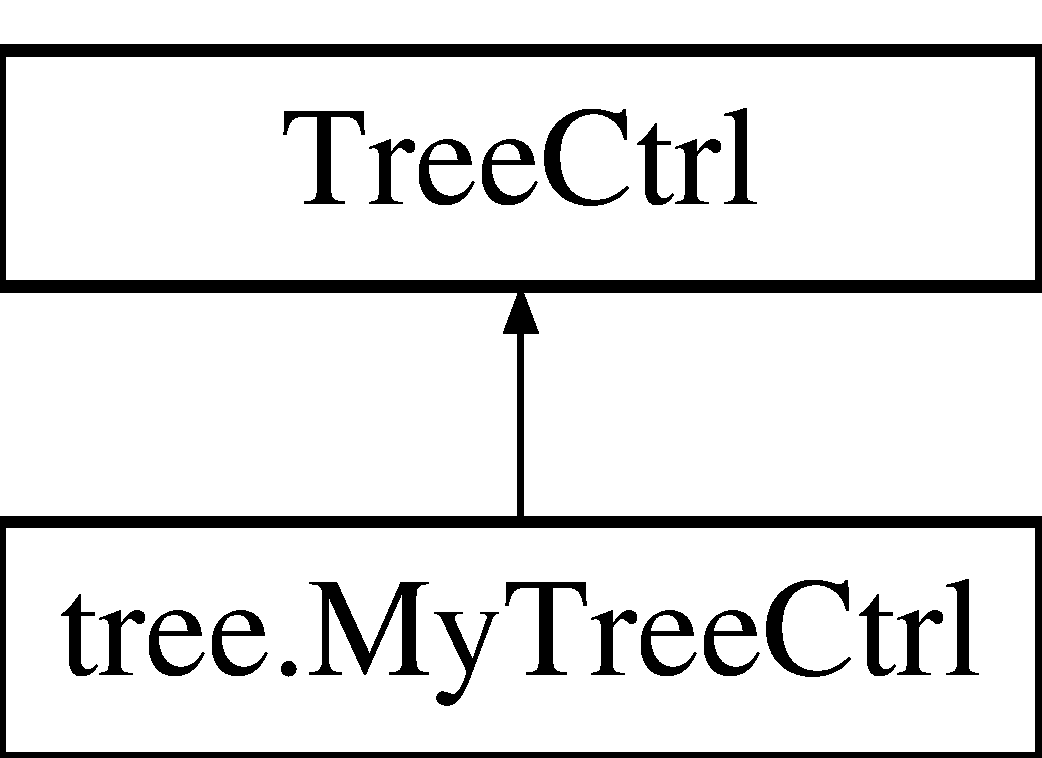
\includegraphics[height=2.000000cm]{classtree_1_1MyTreeCtrl}
\end{center}
\end{figure}
\subsection*{Public Member Functions}
\begin{DoxyCompactItemize}
\item 
def \hyperlink{classtree_1_1MyTreeCtrl_a72b5dacce1e55adbb3bcde63cd4dcf2d}{\+\_\+\+\_\+init\+\_\+\+\_\+} (self, parent, id, pos, size, style)
\item 
def \hyperlink{classtree_1_1MyTreeCtrl_a8073a87006e33820096e0b2ea305af5c}{On\+Compare\+Items} (self, item1, item2)
\end{DoxyCompactItemize}


\subsection{Detailed Description}


Definition at line 8 of file tree.\+py.



\subsection{Constructor \& Destructor Documentation}
\mbox{\Hypertarget{classtree_1_1MyTreeCtrl_a72b5dacce1e55adbb3bcde63cd4dcf2d}\label{classtree_1_1MyTreeCtrl_a72b5dacce1e55adbb3bcde63cd4dcf2d}} 
\index{tree\+::\+My\+Tree\+Ctrl@{tree\+::\+My\+Tree\+Ctrl}!\+\_\+\+\_\+init\+\_\+\+\_\+@{\+\_\+\+\_\+init\+\_\+\+\_\+}}
\index{\+\_\+\+\_\+init\+\_\+\+\_\+@{\+\_\+\+\_\+init\+\_\+\+\_\+}!tree\+::\+My\+Tree\+Ctrl@{tree\+::\+My\+Tree\+Ctrl}}
\subsubsection{\texorpdfstring{\+\_\+\+\_\+init\+\_\+\+\_\+()}{\_\_init\_\_()}}
{\footnotesize\ttfamily def tree.\+My\+Tree\+Ctrl.\+\_\+\+\_\+init\+\_\+\+\_\+ (\begin{DoxyParamCaption}\item[{}]{self,  }\item[{}]{parent,  }\item[{}]{id,  }\item[{}]{pos,  }\item[{}]{size,  }\item[{}]{style }\end{DoxyParamCaption})}



Definition at line 9 of file tree.\+py.


\begin{DoxyCode}
9     \textcolor{keyword}{def }\hyperlink{classwrapper_1_1ModuleDictWrapper_a9a7a794150502f51df687831583e13b9}{\_\_init\_\_}(self, parent, id, pos, size, style):
\end{DoxyCode}


\subsection{Member Function Documentation}
\mbox{\Hypertarget{classtree_1_1MyTreeCtrl_a8073a87006e33820096e0b2ea305af5c}\label{classtree_1_1MyTreeCtrl_a8073a87006e33820096e0b2ea305af5c}} 
\index{tree\+::\+My\+Tree\+Ctrl@{tree\+::\+My\+Tree\+Ctrl}!On\+Compare\+Items@{On\+Compare\+Items}}
\index{On\+Compare\+Items@{On\+Compare\+Items}!tree\+::\+My\+Tree\+Ctrl@{tree\+::\+My\+Tree\+Ctrl}}
\subsubsection{\texorpdfstring{On\+Compare\+Items()}{OnCompareItems()}}
{\footnotesize\ttfamily def tree.\+My\+Tree\+Ctrl.\+On\+Compare\+Items (\begin{DoxyParamCaption}\item[{}]{self,  }\item[{}]{item1,  }\item[{}]{item2 }\end{DoxyParamCaption})}



Definition at line 14 of file tree.\+py.


\begin{DoxyCode}
14     \textcolor{keyword}{def }OnCompareItems(self, item1, item2):
15         t1 = self.GetItemText(item1)
16         t2 = self.GetItemText(item2)
17 \textcolor{comment}{#        self.log.WriteText('compare: ' + t1 + ' <> ' + t2 + '\(\backslash\)n')}
18         \textcolor{keywordflow}{if} t1 < t2: \textcolor{keywordflow}{return} -1
19         \textcolor{keywordflow}{if} t1 == t2: \textcolor{keywordflow}{return} 0
20         \textcolor{keywordflow}{return} 1
21 
22 \textcolor{comment}{#---------------------------------------------------------------------------}
23 
\end{DoxyCode}


The documentation for this class was generated from the following file\+:\begin{DoxyCompactItemize}
\item 
/home/eleclhcb/\+L\+H\+Cb/lbcat-\/cmake/\+Cat\+Python/python/\hyperlink{tree_8py}{tree.\+py}\end{DoxyCompactItemize}

\hypertarget{classNI6008}{}\section{N\+I6008 Class Reference}
\label{classNI6008}\index{N\+I6008@{N\+I6008}}


{\ttfamily \#include $<$inc/\+N\+I6008.\+h$>$}

Inheritance diagram for N\+I6008\+:\begin{figure}[H]
\begin{center}
\leavevmode
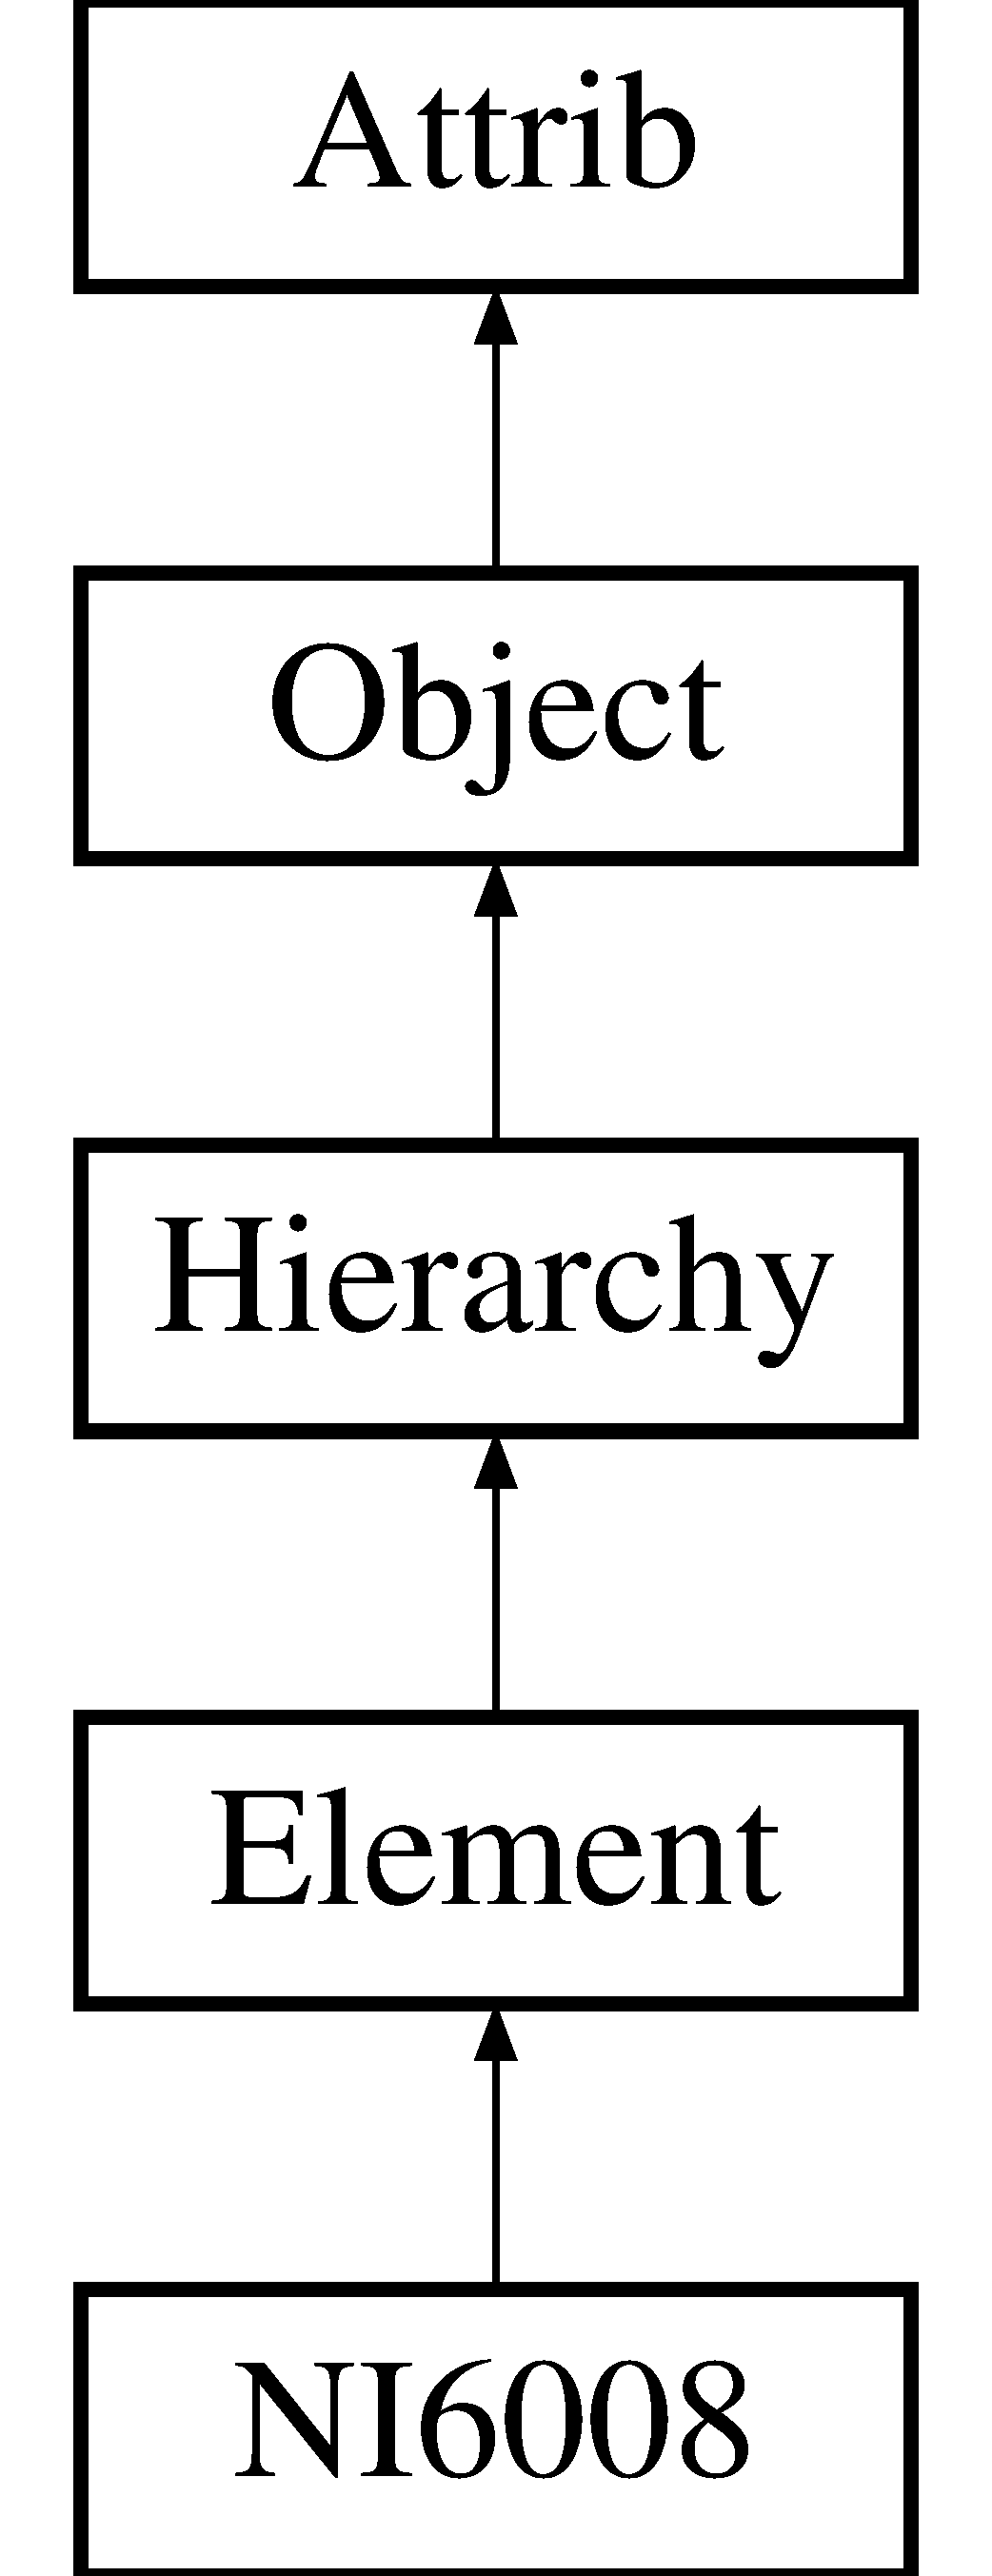
\includegraphics[height=5.000000cm]{classNI6008}
\end{center}
\end{figure}
\subsection*{Public Types}
\begin{DoxyCompactItemize}
\item 
enum \hyperlink{classAttrib_a69e171d7cc6417835a5a306d3c764235}{Attribut} \{ \newline
\hyperlink{classAttrib_a69e171d7cc6417835a5a306d3c764235a3a8da2ab97dda18aebab196fe4100531}{U\+N\+D\+E\+F\+I\+N\+ED}, 
\hyperlink{classAttrib_a69e171d7cc6417835a5a306d3c764235a2bfb2af57b87031d190a05fe25dd92ed}{P\+A\+S\+S\+I\+VE}, 
\hyperlink{classAttrib_a69e171d7cc6417835a5a306d3c764235a3b1fec929c0370d1436f2f06e298fb0d}{A\+C\+T\+I\+VE}, 
\hyperlink{classAttrib_a69e171d7cc6417835a5a306d3c764235aa27c16b480a369ea4d18b07b2516bbc7}{I\+N\+T\+E\+R\+F\+A\+CE}, 
\newline
\hyperlink{classAttrib_a69e171d7cc6417835a5a306d3c764235a1420a5b8c0540b2af210b6975eded7f9}{IO}, 
\hyperlink{classAttrib_a69e171d7cc6417835a5a306d3c764235a0af3b0d0ac323c1704e6c69cf90add28}{I\+O\+D\+A\+TA}, 
\hyperlink{classAttrib_a69e171d7cc6417835a5a306d3c764235a7788bc5dd333fd8ce18562b269c9dab1}{E\+L\+E\+M\+E\+NT}, 
\hyperlink{classAttrib_a69e171d7cc6417835a5a306d3c764235a61ceb22149f365f1780d18f9d1459423}{H\+A\+R\+D\+W\+A\+RE}, 
\newline
\hyperlink{classAttrib_a69e171d7cc6417835a5a306d3c764235a75250e29692496e73effca2c0330977f}{P\+R\+O\+C\+E\+S\+S\+US}, 
\hyperlink{classAttrib_a69e171d7cc6417835a5a306d3c764235a103a67cd0b8f07ef478fa45d4356e27b}{S\+O\+F\+T\+W\+A\+RE}
 \}
\end{DoxyCompactItemize}
\subsection*{Public Member Functions}
\begin{DoxyCompactItemize}
\item 
\hyperlink{classNI6008_a7bcb7ee18fa9f17f3582bc3940de8eaa}{N\+I6008} ()
\begin{DoxyCompactList}\small\item\em Standard constructor. \end{DoxyCompactList}\item 
virtual \hyperlink{classNI6008_a31832f3501f4741fdf8616a44a2f4fc8}{$\sim$\+N\+I6008} ()
\begin{DoxyCompactList}\small\item\em Destructor. \end{DoxyCompactList}\item 
void \hyperlink{classNI6008_ab58d458dbd895b97f7aa51c52b5cd714}{help} ()
\item 
\hyperlink{classStatusCode}{Status\+Code} \hyperlink{classNI6008_ab6a993713c9562e78c634fb30f31b130}{init} ()
\item 
void \hyperlink{classNI6008_a8fd2303c006beba3ceeeac3beb6aaa5e}{reset} ()
\item 
void \hyperlink{classNI6008_a7e04c07277c7bc2b36c197a93edbc278}{update} ()
\item 
std\+::string \hyperlink{classNI6008_a0d7584a656abca03fd59c555cb66822c}{cmd} (std\+::string, std\+::string)
\item 
int \hyperlink{classNI6008_a76df6d88710b15448145498cebe65228}{port} ()
\item 
void \hyperlink{classNI6008_a6bad72fc5a2edb4e3ac0ff8db3a458fd}{set\+Port} (int portno)
\item 
std\+::string \hyperlink{classNI6008_a124e9f3daa92c396b6f66fb1c29a686d}{hostname} ()
\item 
void \hyperlink{classNI6008_a509a804fa21b9f9f5f959b85d5abf5ba}{set\+Hostname} (std\+::string host)
\item 
std\+::vector$<$ double $>$ \hyperlink{classNI6008_a0a4ea75184069707de9f0e76f370582e}{ai} ()
\item 
int \hyperlink{classNI6008_a570edfad9c7a246a8ade767092c5fcbc}{di} ()
\item 
\hyperlink{classStatusCode}{Status\+Code} \hyperlink{classNI6008_aa1964d9926c122e67a6c8dc570b249ff}{add\+Device} (std\+::string \hyperlink{classHierarchy_aa7990fa7caf132d83e361ce033c6c65a}{path})
\item 
std\+::string \hyperlink{classNI6008_a6535ca8405fae42942e7011684113774}{device} (unsigned int dev)
\item 
\hyperlink{classStatusCode}{Status\+Code} \hyperlink{classNI6008_a0cdfc8c62074d5bbc212e1825ac10e99}{clear\+Device} ()
\item 
unsigned int \hyperlink{classNI6008_a293fbf44b101e82a57404d1c76f07a87}{number\+Of\+Devices} ()
\item 
void \hyperlink{classElement_a3c0abcb36f8906688bb7e32608df7086}{recursive\+Init\+Element} ()
\item 
void \hyperlink{classElement_a82119ed37dff76508a2746a853ec35ba}{recursive\+Init\+Communications} ()
\item 
\hyperlink{classStatusCode}{Status\+Code} \hyperlink{classElement_ab476b4b1df5954141ceb14f072433b89}{set\+Connection} (\hyperlink{classHierarchy}{Hierarchy} $\ast$)
\item 
\hyperlink{classHierarchy}{Hierarchy} $\ast$ \hyperlink{classElement_af57444353c1ddf9fa0109801e97debf7}{connection} ()
\item 
void \hyperlink{classHierarchy_af4d43b0765b402670eed2d62c73405af}{clear} ()
\item 
void \hyperlink{classHierarchy_a585ad1aeec16077a0e532ab8b4fc557b}{set\+Parent} (\hyperlink{classHierarchy}{Hierarchy} $\ast$\hyperlink{classHierarchy_a1c7bec8257e717f9c1465e06ebf845fc}{parent})
\item 
\hyperlink{classHierarchy}{Hierarchy} $\ast$ \hyperlink{classHierarchy_a1c7bec8257e717f9c1465e06ebf845fc}{parent} ()
\item 
\hyperlink{classHierarchy}{Hierarchy} $\ast$ \hyperlink{classHierarchy_ad550588733bf75ac5c0fcfd7c8fd11a6}{parent} (std\+::string)
\item 
\hyperlink{classHierarchy}{Hierarchy} $\ast$ \hyperlink{classHierarchy_aee461dc930ce3871636ff87f075b1b83}{origin} ()
\item 
virtual void \hyperlink{classHierarchy_ad677774ff38fcb257c04a3a10d471fac}{add\+Child} (\hyperlink{classHierarchy}{Hierarchy} $\ast$element)
\item 
std\+::vector$<$ \hyperlink{classHierarchy}{Hierarchy} $\ast$ $>$ \hyperlink{classHierarchy_aa9a76f69e98e052ee1a6e32cea006288}{children} ()
\item 
\hyperlink{classHierarchy}{Hierarchy} $\ast$ \hyperlink{classHierarchy_a1e207f973c694b538bf90107b4868817}{child} (std\+::string)
\item 
\hyperlink{classHierarchy}{Hierarchy} $\ast$ \hyperlink{classHierarchy_a0c15a5276a3b80b4354d6bd8a01e0708}{child\+Typed} (std\+::string)
\item 
unsigned long \hyperlink{classHierarchy_ab16e84de65fd84e14001a6cf941c8be4}{number\+Of\+Children} ()
\item 
bool \hyperlink{classHierarchy_a255174fe4d316d2a3f430dcb9dab29f1}{has\+Children} ()
\item 
void \hyperlink{classHierarchy_a2b2b359fac003233f65786a616766bde}{del\+Child} (\hyperlink{classHierarchy}{Hierarchy} $\ast$)
\item 
void \hyperlink{classHierarchy_a1928ac7615fe0b5e55cd707f70dc6781}{del\+Child} (std\+::string)
\item 
std\+::string \hyperlink{classHierarchy_aa7990fa7caf132d83e361ce033c6c65a}{path} (std\+::string=std\+::string(\char`\"{}\char`\"{}))
\item 
std\+::string \hyperlink{classHierarchy_a1efd56cd164d328d2002e53a10a19b8c}{path\+Typed} (std\+::string=std\+::string(\char`\"{}\char`\"{}))
\item 
void \hyperlink{classHierarchy_a76e914b9a677a22a82deb74d892bf261}{tree} (std\+::string indent=std\+::string(\char`\"{}\char`\"{}))
\item 
void \hyperlink{classHierarchy_a594c294c5f60c230e106d522ed008212}{tree} ()
\item 
std\+::string \hyperlink{classObject_a300f4c05dd468c7bb8b3c968868443c1}{name} () const
\item 
std\+::string \hyperlink{classObject_a84f99f70f144a83e1582d1d0f84e4e62}{type} ()
\item 
unsigned char \hyperlink{classObject_af99145335cc61ff6e2798ea17db009d2}{id} ()
\item 
std\+::string \hyperlink{classObject_a73a0f1a41828fdd8303dd662446fb6c3}{title} ()
\item 
void \hyperlink{classObject_a3f9d5537ebce0c0f2bf6ae4d92426f3c}{msg\+Svc} (int level, std\+::string \hyperlink{classObject_a58b2d0618c2d08cf2383012611528d97}{msg}, std\+::string \hyperlink{classObject_a300f4c05dd468c7bb8b3c968868443c1}{name})
\item 
void \hyperlink{classObject_a58b2d0618c2d08cf2383012611528d97}{msg} (std\+::string mymsg)
\item 
void \hyperlink{classObject_ac5d59299273cee27aacf7de00d2e7034}{msg} (std\+::string mymsg, std\+::string \hyperlink{classObject_a300f4c05dd468c7bb8b3c968868443c1}{name})
\item 
void \hyperlink{classObject_a83d2db2df682907ea1115ad721c1c4a1}{verbose} (std\+::string mymsg)
\item 
void \hyperlink{classObject_a2d4120195317e2a3c6532e8bb9f3da68}{verbose} (std\+::string mymsg, std\+::string \hyperlink{classObject_a300f4c05dd468c7bb8b3c968868443c1}{name})
\item 
void \hyperlink{classObject_aac010553f022165573714b7014a15f0d}{debug} (std\+::string mymsg)
\item 
void \hyperlink{classObject_a6c9a0397ca804e04d675ed05683f5420}{debug} (std\+::string mymsg, std\+::string \hyperlink{classObject_a300f4c05dd468c7bb8b3c968868443c1}{name})
\item 
void \hyperlink{classObject_a644fd329ea4cb85f54fa6846484b84a8}{info} (std\+::string mymsg)
\item 
void \hyperlink{classObject_a1ca123253dfd30fc28b156f521dcbdae}{info} (std\+::string mymsg, std\+::string \hyperlink{classObject_a300f4c05dd468c7bb8b3c968868443c1}{name})
\item 
void \hyperlink{classObject_a65cd4fda577711660821fd2cd5a3b4c9}{warning} (std\+::string mymsg)
\item 
void \hyperlink{classObject_a11f101db4dd73d9391b0231818881d86}{warning} (std\+::string mymsg, std\+::string \hyperlink{classObject_a300f4c05dd468c7bb8b3c968868443c1}{name})
\item 
void \hyperlink{classObject_a204a95f57818c0f811933917a30eff45}{error} (std\+::string mymsg)
\item 
void \hyperlink{classObject_ad7f6c457733082efa2f9ff5f5c8e119a}{error} (std\+::string mymsg, std\+::string \hyperlink{classObject_a300f4c05dd468c7bb8b3c968868443c1}{name})
\item 
void \hyperlink{classObject_aad5a16aac7516ce65bd5ec02ab07fc80}{fatal} (std\+::string mymsg)
\item 
void \hyperlink{classObject_ae62acd3d09f716220f75f252dc38bc9a}{fatal} (std\+::string mymsg, std\+::string \hyperlink{classObject_a300f4c05dd468c7bb8b3c968868443c1}{name})
\item 
void \hyperlink{classObject_ae30fea75683c2d149b6b6d17c09ecd0c}{set\+Name} (std\+::string \hyperlink{classObject_a300f4c05dd468c7bb8b3c968868443c1}{name})
\item 
void \hyperlink{classObject_aae534cc9d982bcb9b99fd505f2e103a5}{set\+Type} (std\+::string \hyperlink{classObject_a84f99f70f144a83e1582d1d0f84e4e62}{type})
\item 
void \hyperlink{classObject_a398fe08cba594a0ce6891d59fe4f159f}{set\+Id} (unsigned char \hyperlink{classObject_af99145335cc61ff6e2798ea17db009d2}{id})
\item 
void \hyperlink{classObject_a89557dbbad5bcaa02652f5d7fa35d20f}{set\+Title} (std\+::string \hyperlink{classObject_a73a0f1a41828fdd8303dd662446fb6c3}{title})
\item 
void \hyperlink{classObject_a870c5af919958c2136623b2d7816d123}{set\+Dll\+Name} (std\+::string \hyperlink{classObject_a2e3947f2870094c332d7454117f3ec63}{dll\+Name})
\item 
std\+::string \hyperlink{classObject_a2e3947f2870094c332d7454117f3ec63}{dll\+Name} ()
\item 
bool \hyperlink{classAttrib_a704f26af560909ad22065083bb7d4c34}{is} (int attribut)
\item 
void \hyperlink{classAttrib_a235f773af19c900264a190b00a3b4ad7}{add} (int attribut)
\item 
void \hyperlink{classAttrib_a7d4ef7e32d93cb287792b87b857e79f3}{remove} (int attribut)
\item 
std\+::string \hyperlink{classAttrib_aee7bbf16b144887f196e1341b24f8a26}{attributs} ()
\end{DoxyCompactItemize}
\subsection*{Protected Attributes}
\begin{DoxyCompactItemize}
\item 
int \hyperlink{classNI6008_aabb914d00c938a12e99c1078f40fb104}{m\+\_\+portno}
\item 
std\+::string \hyperlink{classNI6008_ab8b247caa89b1dc9b9c78b0c1b08ed5d}{m\+\_\+host}
\item 
std\+::vector$<$ std\+::string $>$ \hyperlink{classNI6008_ac7225d517d42b1b7553dc75dccb29b58}{m\+\_\+device}
\item 
int \hyperlink{classNI6008_aa1ca2ab973aaceac58d9d17e482682b5}{m\+\_\+sockfd}
\item 
struct sockaddr\+\_\+in \hyperlink{classNI6008_a5bc7b74f001b1d5a3934d58eadb0b3fa}{m\+\_\+serv\+\_\+addr}
\item 
struct hostent $\ast$ \hyperlink{classNI6008_a789147ad3c7b66da3548a10a109f8cab}{m\+\_\+server}
\item 
char \hyperlink{classNI6008_afd7bb102ac107f43a8f02581e1d3abfc}{buffer} \mbox{[}256\mbox{]}
\item 
\hyperlink{classHierarchy}{Hierarchy} $\ast$ \hyperlink{classElement_abe3de7a5dbbc9a6dd2d7e012e5fdb266}{m\+\_\+connection}
\item 
std\+::string \hyperlink{classAttrib_a3414521d7a82476e874b25a5407b5e63}{m\+\_\+attrib\+String} \mbox{[}10\mbox{]}
\end{DoxyCompactItemize}


\subsection{Detailed Description}
\begin{DoxyAuthor}{Author}
\hyperlink{classNI6008}{N\+I6008} 
\end{DoxyAuthor}
\begin{DoxyDate}{Date}
2006-\/10-\/23 
\end{DoxyDate}


Definition at line 26 of file N\+I6008.\+h.



\subsection{Member Enumeration Documentation}
\mbox{\Hypertarget{classAttrib_a69e171d7cc6417835a5a306d3c764235}\label{classAttrib_a69e171d7cc6417835a5a306d3c764235}} 
\index{N\+I6008@{N\+I6008}!Attribut@{Attribut}}
\index{Attribut@{Attribut}!N\+I6008@{N\+I6008}}
\subsubsection{\texorpdfstring{Attribut}{Attribut}}
{\footnotesize\ttfamily enum \hyperlink{classAttrib_a69e171d7cc6417835a5a306d3c764235}{Attrib\+::\+Attribut}\hspace{0.3cm}{\ttfamily [inherited]}}

\begin{DoxyEnumFields}{Enumerator}
\raisebox{\heightof{T}}[0pt][0pt]{\index{U\+N\+D\+E\+F\+I\+N\+ED@{U\+N\+D\+E\+F\+I\+N\+ED}!N\+I6008@{N\+I6008}}\index{N\+I6008@{N\+I6008}!U\+N\+D\+E\+F\+I\+N\+ED@{U\+N\+D\+E\+F\+I\+N\+ED}}}\mbox{\Hypertarget{classAttrib_a69e171d7cc6417835a5a306d3c764235a3a8da2ab97dda18aebab196fe4100531}\label{classAttrib_a69e171d7cc6417835a5a306d3c764235a3a8da2ab97dda18aebab196fe4100531}} 
U\+N\+D\+E\+F\+I\+N\+ED&\\
\hline

\raisebox{\heightof{T}}[0pt][0pt]{\index{P\+A\+S\+S\+I\+VE@{P\+A\+S\+S\+I\+VE}!N\+I6008@{N\+I6008}}\index{N\+I6008@{N\+I6008}!P\+A\+S\+S\+I\+VE@{P\+A\+S\+S\+I\+VE}}}\mbox{\Hypertarget{classAttrib_a69e171d7cc6417835a5a306d3c764235a2bfb2af57b87031d190a05fe25dd92ed}\label{classAttrib_a69e171d7cc6417835a5a306d3c764235a2bfb2af57b87031d190a05fe25dd92ed}} 
P\+A\+S\+S\+I\+VE&\\
\hline

\raisebox{\heightof{T}}[0pt][0pt]{\index{A\+C\+T\+I\+VE@{A\+C\+T\+I\+VE}!N\+I6008@{N\+I6008}}\index{N\+I6008@{N\+I6008}!A\+C\+T\+I\+VE@{A\+C\+T\+I\+VE}}}\mbox{\Hypertarget{classAttrib_a69e171d7cc6417835a5a306d3c764235a3b1fec929c0370d1436f2f06e298fb0d}\label{classAttrib_a69e171d7cc6417835a5a306d3c764235a3b1fec929c0370d1436f2f06e298fb0d}} 
A\+C\+T\+I\+VE&\\
\hline

\raisebox{\heightof{T}}[0pt][0pt]{\index{I\+N\+T\+E\+R\+F\+A\+CE@{I\+N\+T\+E\+R\+F\+A\+CE}!N\+I6008@{N\+I6008}}\index{N\+I6008@{N\+I6008}!I\+N\+T\+E\+R\+F\+A\+CE@{I\+N\+T\+E\+R\+F\+A\+CE}}}\mbox{\Hypertarget{classAttrib_a69e171d7cc6417835a5a306d3c764235aa27c16b480a369ea4d18b07b2516bbc7}\label{classAttrib_a69e171d7cc6417835a5a306d3c764235aa27c16b480a369ea4d18b07b2516bbc7}} 
I\+N\+T\+E\+R\+F\+A\+CE&\\
\hline

\raisebox{\heightof{T}}[0pt][0pt]{\index{IO@{IO}!N\+I6008@{N\+I6008}}\index{N\+I6008@{N\+I6008}!IO@{IO}}}\mbox{\Hypertarget{classAttrib_a69e171d7cc6417835a5a306d3c764235a1420a5b8c0540b2af210b6975eded7f9}\label{classAttrib_a69e171d7cc6417835a5a306d3c764235a1420a5b8c0540b2af210b6975eded7f9}} 
IO&\\
\hline

\raisebox{\heightof{T}}[0pt][0pt]{\index{I\+O\+D\+A\+TA@{I\+O\+D\+A\+TA}!N\+I6008@{N\+I6008}}\index{N\+I6008@{N\+I6008}!I\+O\+D\+A\+TA@{I\+O\+D\+A\+TA}}}\mbox{\Hypertarget{classAttrib_a69e171d7cc6417835a5a306d3c764235a0af3b0d0ac323c1704e6c69cf90add28}\label{classAttrib_a69e171d7cc6417835a5a306d3c764235a0af3b0d0ac323c1704e6c69cf90add28}} 
I\+O\+D\+A\+TA&\\
\hline

\raisebox{\heightof{T}}[0pt][0pt]{\index{E\+L\+E\+M\+E\+NT@{E\+L\+E\+M\+E\+NT}!N\+I6008@{N\+I6008}}\index{N\+I6008@{N\+I6008}!E\+L\+E\+M\+E\+NT@{E\+L\+E\+M\+E\+NT}}}\mbox{\Hypertarget{classAttrib_a69e171d7cc6417835a5a306d3c764235a7788bc5dd333fd8ce18562b269c9dab1}\label{classAttrib_a69e171d7cc6417835a5a306d3c764235a7788bc5dd333fd8ce18562b269c9dab1}} 
E\+L\+E\+M\+E\+NT&\\
\hline

\raisebox{\heightof{T}}[0pt][0pt]{\index{H\+A\+R\+D\+W\+A\+RE@{H\+A\+R\+D\+W\+A\+RE}!N\+I6008@{N\+I6008}}\index{N\+I6008@{N\+I6008}!H\+A\+R\+D\+W\+A\+RE@{H\+A\+R\+D\+W\+A\+RE}}}\mbox{\Hypertarget{classAttrib_a69e171d7cc6417835a5a306d3c764235a61ceb22149f365f1780d18f9d1459423}\label{classAttrib_a69e171d7cc6417835a5a306d3c764235a61ceb22149f365f1780d18f9d1459423}} 
H\+A\+R\+D\+W\+A\+RE&\\
\hline

\raisebox{\heightof{T}}[0pt][0pt]{\index{P\+R\+O\+C\+E\+S\+S\+US@{P\+R\+O\+C\+E\+S\+S\+US}!N\+I6008@{N\+I6008}}\index{N\+I6008@{N\+I6008}!P\+R\+O\+C\+E\+S\+S\+US@{P\+R\+O\+C\+E\+S\+S\+US}}}\mbox{\Hypertarget{classAttrib_a69e171d7cc6417835a5a306d3c764235a75250e29692496e73effca2c0330977f}\label{classAttrib_a69e171d7cc6417835a5a306d3c764235a75250e29692496e73effca2c0330977f}} 
P\+R\+O\+C\+E\+S\+S\+US&\\
\hline

\raisebox{\heightof{T}}[0pt][0pt]{\index{S\+O\+F\+T\+W\+A\+RE@{S\+O\+F\+T\+W\+A\+RE}!N\+I6008@{N\+I6008}}\index{N\+I6008@{N\+I6008}!S\+O\+F\+T\+W\+A\+RE@{S\+O\+F\+T\+W\+A\+RE}}}\mbox{\Hypertarget{classAttrib_a69e171d7cc6417835a5a306d3c764235a103a67cd0b8f07ef478fa45d4356e27b}\label{classAttrib_a69e171d7cc6417835a5a306d3c764235a103a67cd0b8f07ef478fa45d4356e27b}} 
S\+O\+F\+T\+W\+A\+RE&\\
\hline

\end{DoxyEnumFields}


Definition at line 29 of file Attrib.\+h.


\begin{DoxyCode}
29                 \{
30     \hyperlink{classAttrib_a69e171d7cc6417835a5a306d3c764235a3a8da2ab97dda18aebab196fe4100531}{UNDEFINED},
31     \hyperlink{classAttrib_a69e171d7cc6417835a5a306d3c764235a2bfb2af57b87031d190a05fe25dd92ed}{PASSIVE},
32     \hyperlink{classAttrib_a69e171d7cc6417835a5a306d3c764235a3b1fec929c0370d1436f2f06e298fb0d}{ACTIVE},
33     \hyperlink{classAttrib_a69e171d7cc6417835a5a306d3c764235aa27c16b480a369ea4d18b07b2516bbc7}{INTERFACE},
34     \hyperlink{classAttrib_a69e171d7cc6417835a5a306d3c764235a1420a5b8c0540b2af210b6975eded7f9}{IO},
35     \hyperlink{classAttrib_a69e171d7cc6417835a5a306d3c764235a0af3b0d0ac323c1704e6c69cf90add28}{IODATA},
36     \hyperlink{classAttrib_a69e171d7cc6417835a5a306d3c764235a7788bc5dd333fd8ce18562b269c9dab1}{ELEMENT},
37     \hyperlink{classAttrib_a69e171d7cc6417835a5a306d3c764235a61ceb22149f365f1780d18f9d1459423}{HARDWARE},
38     \hyperlink{classAttrib_a69e171d7cc6417835a5a306d3c764235a75250e29692496e73effca2c0330977f}{PROCESSUS},
39     \hyperlink{classAttrib_a69e171d7cc6417835a5a306d3c764235a103a67cd0b8f07ef478fa45d4356e27b}{SOFTWARE} 
40   \}; \textcolor{comment}{// array m\_attribString must be changed into Attrib::Attrib if this enu is modified. }
\end{DoxyCode}


\subsection{Constructor \& Destructor Documentation}
\mbox{\Hypertarget{classNI6008_a7bcb7ee18fa9f17f3582bc3940de8eaa}\label{classNI6008_a7bcb7ee18fa9f17f3582bc3940de8eaa}} 
\index{N\+I6008@{N\+I6008}!N\+I6008@{N\+I6008}}
\index{N\+I6008@{N\+I6008}!N\+I6008@{N\+I6008}}
\subsubsection{\texorpdfstring{N\+I6008()}{NI6008()}}
{\footnotesize\ttfamily N\+I6008\+::\+N\+I6008 (\begin{DoxyParamCaption}{ }\end{DoxyParamCaption})}



Standard constructor. 



Definition at line 22 of file N\+I6008.\+cpp.



References application(), Application\+::hostname(), m\+\_\+host, Object\+::set\+Name(), and Object\+::set\+Type().


\begin{DoxyCode}
22                  \{
23   \hyperlink{classObject_ae30fea75683c2d149b6b6d17c09ecd0c}{setName}(\textcolor{stringliteral}{"NI6008"});
24   \hyperlink{classObject_aae534cc9d982bcb9b99fd505f2e103a5}{setType}(\textcolor{stringliteral}{"NI6008"});
25   \hyperlink{classNI6008_ab8b247caa89b1dc9b9c78b0c1b08ed5d}{m\_host} = \hyperlink{Tools_8h_a27885a3c35afe79029fb830f32f66458}{application}()->\hyperlink{classApplication_a095248805e26b553466b7fafc6517d8f}{hostname}();
26 \}
\end{DoxyCode}
\mbox{\Hypertarget{classNI6008_a31832f3501f4741fdf8616a44a2f4fc8}\label{classNI6008_a31832f3501f4741fdf8616a44a2f4fc8}} 
\index{N\+I6008@{N\+I6008}!````~N\+I6008@{$\sim$\+N\+I6008}}
\index{````~N\+I6008@{$\sim$\+N\+I6008}!N\+I6008@{N\+I6008}}
\subsubsection{\texorpdfstring{$\sim$\+N\+I6008()}{~NI6008()}}
{\footnotesize\ttfamily N\+I6008\+::$\sim$\+N\+I6008 (\begin{DoxyParamCaption}{ }\end{DoxyParamCaption})\hspace{0.3cm}{\ttfamily [virtual]}}



Destructor. 



Definition at line 30 of file N\+I6008.\+cpp.



References Object\+::info(), and m\+\_\+sockfd.


\begin{DoxyCode}
30                 \{
31   \hyperlink{classObject_a644fd329ea4cb85f54fa6846484b84a8}{info}(\textcolor{stringliteral}{"Closing the NI6008 socket."});
32   close(\hyperlink{classNI6008_aa1ca2ab973aaceac58d9d17e482682b5}{m\_sockfd});
33 \}
\end{DoxyCode}


\subsection{Member Function Documentation}
\mbox{\Hypertarget{classAttrib_a235f773af19c900264a190b00a3b4ad7}\label{classAttrib_a235f773af19c900264a190b00a3b4ad7}} 
\index{N\+I6008@{N\+I6008}!add@{add}}
\index{add@{add}!N\+I6008@{N\+I6008}}
\subsubsection{\texorpdfstring{add()}{add()}}
{\footnotesize\ttfamily void Attrib\+::add (\begin{DoxyParamCaption}\item[{int}]{attribut }\end{DoxyParamCaption})\hspace{0.3cm}{\ttfamily [inline]}, {\ttfamily [inherited]}}

Add an attribut 

Definition at line 67 of file Attrib.\+h.



References Attrib\+::m\+\_\+attributs, and Attrib\+::\+U\+N\+D\+E\+F\+I\+N\+ED.



Referenced by A3\+P\+E\+::\+A3\+P\+E(), Attrib\+::\+Attrib(), Specs\+Mezzanine\+::cmdline(), Computer\+::\+Computer(), C\+U\+\_\+v1\+::\+C\+U\+\_\+v1(), export\+\_\+obj(), F\+E\+B\+\_\+v1\+::\+F\+E\+B\+\_\+v1(), Fe\+P\+G\+A\+::\+Fe\+P\+G\+A(), I\+C\+E\+C\+A\+Lv3\+::\+I\+C\+E\+C\+A\+Lv3(), I\+C\+Phaser\+::\+I\+C\+Phaser(), Application\+::initialize(), Interface\+::\+Interface(), I\+Odata\+::\+I\+Odata(), I\+Oobject\+::\+I\+Oobject(), M\+S\+Oxxxx\+::\+M\+S\+Oxxxx(), Phaser\+::\+Phaser(), Processus\+::\+Processus(), Proto40\+M\+Hz\+\_\+v1\+::\+Proto40\+M\+Hz\+\_\+v1(), Attrib\+::remove(), Seq\+P\+G\+A\+::\+Seq\+P\+G\+A(), Test\+I2\+C\+::set\+Address(), Test\+S\+P\+I\+::set\+Address(), Specs\+Slave\+::set\+Address(), Specs\+Master\+::\+Specs\+Master(), and Specs\+Slave\+::\+Specs\+Slave().


\begin{DoxyCode}
67                             \{
68     \textcolor{keywordflow}{if} (attribut!=\hyperlink{classAttrib_a69e171d7cc6417835a5a306d3c764235a3a8da2ab97dda18aebab196fe4100531}{Attrib::UNDEFINED}) \textcolor{keyword}{remove}(\hyperlink{classAttrib_a69e171d7cc6417835a5a306d3c764235a3a8da2ab97dda18aebab196fe4100531}{Attrib::UNDEFINED});
69     \textcolor{keywordtype}{bool} duplicate = false ;
70     std::vector<int>::const\_iterator iter ;
71     \textcolor{keywordflow}{for} ( iter  = \hyperlink{classAttrib_ac4bd58a0cc6b38a3b711d609a3d3aacc}{m\_attributs}.begin() ;
72           iter != \hyperlink{classAttrib_ac4bd58a0cc6b38a3b711d609a3d3aacc}{m\_attributs}.end()   ;
73           ++iter ) \{
74       \textcolor{keywordflow}{if} ( attribut == (*iter) ) \{
75         duplicate = true ;
76       \}
77     \}
78     \textcolor{keywordflow}{if} (!duplicate) \{
79       \hyperlink{classAttrib_ac4bd58a0cc6b38a3b711d609a3d3aacc}{m\_attributs}.push\_back( attribut );
80     \}
81   \}
\end{DoxyCode}
\mbox{\Hypertarget{classHierarchy_ad677774ff38fcb257c04a3a10d471fac}\label{classHierarchy_ad677774ff38fcb257c04a3a10d471fac}} 
\index{N\+I6008@{N\+I6008}!add\+Child@{add\+Child}}
\index{add\+Child@{add\+Child}!N\+I6008@{N\+I6008}}
\subsubsection{\texorpdfstring{add\+Child()}{addChild()}}
{\footnotesize\ttfamily void Hierarchy\+::add\+Child (\begin{DoxyParamCaption}\item[{\hyperlink{classHierarchy}{Hierarchy} $\ast$}]{element }\end{DoxyParamCaption})\hspace{0.3cm}{\ttfamily [virtual]}, {\ttfamily [inherited]}}



Definition at line 83 of file Hierarchy.\+cpp.



References Object\+::debug(), Hierarchy\+::m\+\_\+children, Object\+::name(), and Hierarchy\+::set\+Parent().



Referenced by A3\+P\+E\+::\+A3\+P\+E(), Specs\+Mezzanine\+::add\+Bus(), Specs\+Slave\+::add\+I2c(), Application\+::create(), C\+U\+\_\+v1\+::\+C\+U\+\_\+v1(), export\+\_\+obj(), F\+E\+B\+\_\+v1\+::\+F\+E\+B\+\_\+v1(), Fe\+P\+G\+A\+::\+Fe\+P\+G\+A(), I\+C\+E\+C\+A\+Lv3\+::\+I\+C\+E\+C\+A\+Lv3(), I\+C\+Phaser\+::\+I\+C\+Phaser(), Hierarchy\+::origin(), Phaser\+::\+Phaser(), Proto40\+M\+Hz\+\_\+v1\+::\+Proto40\+M\+Hz\+\_\+v1(), Seq\+P\+G\+A\+::\+Seq\+P\+G\+A(), Specs\+Mezzanine\+::\+Specs\+Mezzanine(), Usb\+I2c\+Bus\+::\+Usb\+I2c\+Bus(), and Usb\+Spi\+Bus\+::\+Usb\+Spi\+Bus().


\begin{DoxyCode}
83                                           \{
84   element->\hyperlink{classHierarchy_a585ad1aeec16077a0e532ab8b4fc557b}{setParent}(\textcolor{keyword}{this});
85   \hyperlink{classHierarchy_a038816763941fd4a930504917f60483b}{m\_children}.push\_back(element);
86   \hyperlink{classObject_aac010553f022165573714b7014a15f0d}{debug}(element->\hyperlink{classObject_a300f4c05dd468c7bb8b3c968868443c1}{name}()+\textcolor{stringliteral}{" added to the child tree."},\textcolor{stringliteral}{"Hierarchy::addChild"});
87 \}
\end{DoxyCode}
\mbox{\Hypertarget{classNI6008_aa1964d9926c122e67a6c8dc570b249ff}\label{classNI6008_aa1964d9926c122e67a6c8dc570b249ff}} 
\index{N\+I6008@{N\+I6008}!add\+Device@{add\+Device}}
\index{add\+Device@{add\+Device}!N\+I6008@{N\+I6008}}
\subsubsection{\texorpdfstring{add\+Device()}{addDevice()}}
{\footnotesize\ttfamily \hyperlink{classStatusCode}{Status\+Code} N\+I6008\+::add\+Device (\begin{DoxyParamCaption}\item[{std\+::string}]{path }\end{DoxyParamCaption})\hspace{0.3cm}{\ttfamily [inline]}}



Definition at line 114 of file N\+I6008.\+h.



References Object\+::info(), m\+\_\+device, and Status\+Code\+::\+S\+U\+C\+C\+E\+SS.



Referenced by B\+O\+O\+S\+T\+\_\+\+P\+Y\+T\+H\+O\+N\+\_\+\+M\+O\+D\+U\+L\+E().


\begin{DoxyCode}
114                                        \{
115     \hyperlink{classNI6008_ac7225d517d42b1b7553dc75dccb29b58}{m\_device}.push\_back( \hyperlink{classHierarchy_aa7990fa7caf132d83e361ce033c6c65a}{path} );
116     \hyperlink{classObject_a644fd329ea4cb85f54fa6846484b84a8}{info}(\textcolor{stringliteral}{"Device associated."});
117     \textcolor{keywordflow}{return} \hyperlink{classStatusCode_a6f565cbeadc76d14c72f047e5e85eb4badd0da38d3ba0d922efd1f4619bc37ad8}{StatusCode::SUCCESS};
118   \};
\end{DoxyCode}
\mbox{\Hypertarget{classNI6008_a0a4ea75184069707de9f0e76f370582e}\label{classNI6008_a0a4ea75184069707de9f0e76f370582e}} 
\index{N\+I6008@{N\+I6008}!ai@{ai}}
\index{ai@{ai}!N\+I6008@{N\+I6008}}
\subsubsection{\texorpdfstring{ai()}{ai()}}
{\footnotesize\ttfamily std\+::vector$<$double$>$ N\+I6008\+::ai (\begin{DoxyParamCaption}{ }\end{DoxyParamCaption})}



Referenced by set\+Hostname().

\mbox{\Hypertarget{classAttrib_aee7bbf16b144887f196e1341b24f8a26}\label{classAttrib_aee7bbf16b144887f196e1341b24f8a26}} 
\index{N\+I6008@{N\+I6008}!attributs@{attributs}}
\index{attributs@{attributs}!N\+I6008@{N\+I6008}}
\subsubsection{\texorpdfstring{attributs()}{attributs()}}
{\footnotesize\ttfamily std\+::string Attrib\+::attributs (\begin{DoxyParamCaption}{ }\end{DoxyParamCaption})\hspace{0.3cm}{\ttfamily [inherited]}}

Print the \hyperlink{classAttrib}{Attrib} of an \hyperlink{classObject}{Object} 

Definition at line 54 of file Attrib.\+cpp.



References images\+::index, Attrib\+::m\+\_\+attrib\+String, and Attrib\+::m\+\_\+attributs.



Referenced by export\+\_\+obj(), and Attrib\+::remove().


\begin{DoxyCode}
54                             \{
55   std::string output;
56   std::vector<int>::iterator iter ;
57   \textcolor{keywordflow}{for} ( \textcolor{keywordtype}{unsigned} \textcolor{keywordtype}{int} \hyperlink{namespaceimages_a54407fd574970b3178647ae096321a57}{index} = 0 ; \hyperlink{namespaceimages_a54407fd574970b3178647ae096321a57}{index} < \hyperlink{classAttrib_ac4bd58a0cc6b38a3b711d609a3d3aacc}{m\_attributs}.size() ; ++
      \hyperlink{namespaceimages_a54407fd574970b3178647ae096321a57}{index} ) \{
58     \textcolor{keywordflow}{if} ( \hyperlink{classAttrib_ac4bd58a0cc6b38a3b711d609a3d3aacc}{m\_attributs}.size() - \hyperlink{namespaceimages_a54407fd574970b3178647ae096321a57}{index} > 1 ) \{
59       output.append(\hyperlink{classAttrib_a3414521d7a82476e874b25a5407b5e63}{m\_attribString}[\hyperlink{classAttrib_ac4bd58a0cc6b38a3b711d609a3d3aacc}{m\_attributs}[\hyperlink{namespaceimages_a54407fd574970b3178647ae096321a57}{index}]]);
60       output.append(\textcolor{stringliteral}{":"});
61     \}
62     \textcolor{keywordflow}{else} \{
63       output.append(\hyperlink{classAttrib_a3414521d7a82476e874b25a5407b5e63}{m\_attribString}[\hyperlink{classAttrib_ac4bd58a0cc6b38a3b711d609a3d3aacc}{m\_attributs}[index]]);
64     \}
65   \}
66   \textcolor{keywordflow}{return} output;
67 \}
\end{DoxyCode}
\mbox{\Hypertarget{classHierarchy_a1e207f973c694b538bf90107b4868817}\label{classHierarchy_a1e207f973c694b538bf90107b4868817}} 
\index{N\+I6008@{N\+I6008}!child@{child}}
\index{child@{child}!N\+I6008@{N\+I6008}}
\subsubsection{\texorpdfstring{child()}{child()}}
{\footnotesize\ttfamily \hyperlink{classHierarchy}{Hierarchy} $\ast$ Hierarchy\+::child (\begin{DoxyParamCaption}\item[{std\+::string}]{path }\end{DoxyParamCaption})\hspace{0.3cm}{\ttfamily [inherited]}}



Definition at line 133 of file Hierarchy.\+cpp.



References Hierarchy\+::child(), Hierarchy\+::children(), Object\+::name(), Hierarchy\+::origin(), Hierarchy\+::parent(), Hierarchy\+::path(), and Object\+::warning().



Referenced by Application\+::cd(), Hierarchy\+::child(), Hierarchy\+::children(), and export\+\_\+obj().


\begin{DoxyCode}
133                                          \{
134   std::string newpath = \hyperlink{classHierarchy_aa7990fa7caf132d83e361ce033c6c65a}{path};
135   std::string up(\textcolor{stringliteral}{".."});
136   std::string separator(1,\textcolor{charliteral}{'/'});
137 
138   \hyperlink{classHierarchy}{Hierarchy} * newcurrent = 0;
139 
140   \textcolor{comment}{//  info("path="+path,"Hierarchy::child");}
141 
142   \textcolor{keywordflow}{if} (\hyperlink{classHierarchy_aa7990fa7caf132d83e361ce033c6c65a}{path}.compare(\textcolor{stringliteral}{""})==0 || \hyperlink{classHierarchy_aa7990fa7caf132d83e361ce033c6c65a}{path}.compare(\textcolor{stringliteral}{"/"})==0) \{
143     \textcolor{comment}{//    debug("return origin","Hierarchy::child");}
144     \textcolor{keywordflow}{return} \hyperlink{classHierarchy_aee461dc930ce3871636ff87f075b1b83}{origin}();
145   \}
146 
147   \textcolor{keywordflow}{if} (\hyperlink{classHierarchy_aa7990fa7caf132d83e361ce033c6c65a}{path}.compare(\hyperlink{classObject_a300f4c05dd468c7bb8b3c968868443c1}{name}())==0)\{
148     \textcolor{comment}{//    debug("return itself","Hierarchy::child");}
149     \textcolor{keywordflow}{return} \textcolor{keyword}{this};
150   \}
151 
152   \textcolor{keywordflow}{if} (\hyperlink{classHierarchy_aa7990fa7caf132d83e361ce033c6c65a}{path}.compare(\textcolor{stringliteral}{".."})==0)\{
153     \textcolor{keywordflow}{if} (0!=this->\hyperlink{classHierarchy_a1c7bec8257e717f9c1465e06ebf845fc}{parent}()) \textcolor{keywordflow}{return} this->\hyperlink{classHierarchy_a1c7bec8257e717f9c1465e06ebf845fc}{parent}();
154     \textcolor{keywordflow}{else} \textcolor{keywordflow}{return} \textcolor{keyword}{this};
155   \}
156 
157   \textcolor{keywordflow}{if} (\hyperlink{classHierarchy_aa7990fa7caf132d83e361ce033c6c65a}{path}.compare(\textcolor{stringliteral}{"../"})==0)\{
158     \textcolor{keywordflow}{if} (0!=this->\hyperlink{classHierarchy_a1c7bec8257e717f9c1465e06ebf845fc}{parent}()) \textcolor{keywordflow}{return} this->\hyperlink{classHierarchy_a1c7bec8257e717f9c1465e06ebf845fc}{parent}();
159     \textcolor{keywordflow}{else} \textcolor{keywordflow}{return} \textcolor{keyword}{this};
160   \}
161 
162 
163   \textcolor{keywordtype}{int} npos=\hyperlink{classHierarchy_aa7990fa7caf132d83e361ce033c6c65a}{path}.find(separator,0);
164 
165   \textcolor{comment}{//  info("find separator in "+itos(npos)+" of "+path,"Hierarchy::child");}
166 
167   \textcolor{comment}{// remove last separator}
168   \textcolor{keywordflow}{if} ( npos == (\textcolor{keywordtype}{int})(\hyperlink{classHierarchy_aa7990fa7caf132d83e361ce033c6c65a}{path}.size()-1) ) \{
169     newpath = std::string(\hyperlink{classHierarchy_aa7990fa7caf132d83e361ce033c6c65a}{path},0,npos);
170     \hyperlink{classHierarchy_aa7990fa7caf132d83e361ce033c6c65a}{path} = newpath;
171   \}
172 
173   \textcolor{keywordflow}{if} (npos==0)\{
174     \textcolor{comment}{//    debug("Going back to origin and calling child","Hierarchy::child");}
175     newpath=std::string(\hyperlink{classHierarchy_aa7990fa7caf132d83e361ce033c6c65a}{path},1,\hyperlink{classHierarchy_aa7990fa7caf132d83e361ce033c6c65a}{path}.size()-1);
176     \textcolor{keywordflow}{return} \hyperlink{classHierarchy_aee461dc930ce3871636ff87f075b1b83}{origin}()->\hyperlink{classHierarchy_a1e207f973c694b538bf90107b4868817}{child}(newpath);
177   \}
178   \textcolor{keywordflow}{else}\{
179     \textcolor{keywordflow}{if} ( npos== (\textcolor{keywordtype}{int})(std::string::npos) )\{
180       \textcolor{comment}{//      debug("Getting chid "+path+" of "+this->name(),"Hierarchy::child");}
181       std::vector <Hierarchy*> list = \hyperlink{classHierarchy_aa9a76f69e98e052ee1a6e32cea006288}{children}();
182       std::vector<Hierarchy*>::iterator iter;
183       \textcolor{keywordflow}{for} (iter=list.begin();iter!=list.end();iter++)\{
184         \textcolor{keywordflow}{if} ((*iter)->name().compare(\hyperlink{classHierarchy_aa7990fa7caf132d83e361ce033c6c65a}{path})==0)\{
185           \textcolor{keywordflow}{return} *iter;
186         \}
187       \}
188       \hyperlink{classObject_a65cd4fda577711660821fd2cd5a3b4c9}{warning}(this->\hyperlink{classObject_a300f4c05dd468c7bb8b3c968868443c1}{name}()+std::string(\textcolor{stringliteral}{" has no child '"})+\hyperlink{classHierarchy_aa7990fa7caf132d83e361ce033c6c65a}{path}+\textcolor{stringliteral}{"'"},\textcolor{stringliteral}{"Hierarchy::child"});
189       \textcolor{keywordflow}{return} \textcolor{keyword}{this};
190     \}
191     \textcolor{keywordflow}{else}
192     \{
193       \textcolor{keywordtype}{int} ipos=\hyperlink{classHierarchy_aa7990fa7caf132d83e361ce033c6c65a}{path}.find(separator,0);
194       \textcolor{comment}{//      info("default behaviour "+path+" with separator in "+itos(ipos),"Hierarchy::child");}
195 
196       std::string newcurrentname=std::string(\hyperlink{classHierarchy_aa7990fa7caf132d83e361ce033c6c65a}{path},0,ipos);
197       newpath=std::string(\hyperlink{classHierarchy_aa7990fa7caf132d83e361ce033c6c65a}{path},ipos+1,\hyperlink{classHierarchy_aa7990fa7caf132d83e361ce033c6c65a}{path}.size()-1);
198 
199       \textcolor{comment}{//      info("looking now for "+newpath+" from "+newcurrentname,"Hierarchy::child");}
200 
201       \textcolor{keywordflow}{if} (0==newcurrentname.compare(\hyperlink{classHierarchy_aee461dc930ce3871636ff87f075b1b83}{origin}()->\hyperlink{classObject_a300f4c05dd468c7bb8b3c968868443c1}{name}()))\{
202         \textcolor{comment}{//        info("current is computer. Looking for children"+newcurrentname,"Hierarchy::child");}
203         \textcolor{keywordflow}{return} \hyperlink{classHierarchy_aee461dc930ce3871636ff87f075b1b83}{origin}()->\hyperlink{classHierarchy_a1e207f973c694b538bf90107b4868817}{child}(newpath);
204       \}
205 
206       newcurrent = (\hyperlink{classHierarchy}{Hierarchy}*)0;
207 
208       std::vector <Hierarchy*> list = \hyperlink{classHierarchy_aa9a76f69e98e052ee1a6e32cea006288}{children}();
209       std::vector<Hierarchy*>::iterator iter;
210       \textcolor{keywordflow}{for} (iter=list.begin();iter!=list.end();iter++)\{
211         \textcolor{keywordflow}{if} ((*iter)->name().compare(newcurrentname)==0)\{
212           newcurrent = (*iter);
213         \}
214       \}
215 
216 
217       \textcolor{keywordflow}{if} ((\hyperlink{classHierarchy}{Hierarchy}*)0==newcurrent)\{
218         \textcolor{keywordflow}{if} (newcurrentname.compare(\textcolor{stringliteral}{".."})==0 && 0!=\hyperlink{classHierarchy_a1c7bec8257e717f9c1465e06ebf845fc}{parent}())\{
219           newcurrent=this->\hyperlink{classHierarchy_a1c7bec8257e717f9c1465e06ebf845fc}{parent}();
220           \textcolor{comment}{//          debug("newcurrent was .. -> parent="+parent()->name());}
221         \}
222         \textcolor{keywordflow}{else}
223         \{
224           \hyperlink{classObject_a65cd4fda577711660821fd2cd5a3b4c9}{warning}(this->\hyperlink{classObject_a300f4c05dd468c7bb8b3c968868443c1}{name}()+\textcolor{stringliteral}{" has no child '"}+newcurrentname+\textcolor{stringliteral}{"'"},
225               \textcolor{stringliteral}{"Hierarchy::child"});
226           \textcolor{keywordflow}{return} \textcolor{keyword}{this};
227         \}
228       \}
229       \textcolor{comment}{//      debug("recurrence call for "+newpath+" on "+newcurrent->name(),"Hierarchy::child");}
230       \textcolor{keywordflow}{return} newcurrent -> \hyperlink{classHierarchy_a1e207f973c694b538bf90107b4868817}{child} ( newpath );
231     \}
232   \}
233 \}
\end{DoxyCode}
\mbox{\Hypertarget{classHierarchy_aa9a76f69e98e052ee1a6e32cea006288}\label{classHierarchy_aa9a76f69e98e052ee1a6e32cea006288}} 
\index{N\+I6008@{N\+I6008}!children@{children}}
\index{children@{children}!N\+I6008@{N\+I6008}}
\subsubsection{\texorpdfstring{children()}{children()}}
{\footnotesize\ttfamily std\+::vector$<$\hyperlink{classHierarchy}{Hierarchy}$\ast$$>$ Hierarchy\+::children (\begin{DoxyParamCaption}{ }\end{DoxyParamCaption})\hspace{0.3cm}{\ttfamily [inline]}, {\ttfamily [inherited]}}



Definition at line 33 of file Hierarchy.\+h.



References Hierarchy\+::child(), Hierarchy\+::child\+Typed(), Hierarchy\+::del\+Child(), Hierarchy\+::has\+Children(), Hierarchy\+::m\+\_\+children, Hierarchy\+::number\+Of\+Children(), Hierarchy\+::path(), Hierarchy\+::path\+Typed(), and Hierarchy\+::tree().



Referenced by Hierarchy\+::child(), Hierarchy\+::child\+Typed(), export\+\_\+obj(), Specs\+Slave\+::recursive\+Init\+Communications(), Element\+::recursive\+Init\+Communications(), Element\+::recursive\+Init\+Element(), Application\+::set\+Config(), and Hierarchy\+::tree().


\begin{DoxyCode}
33 \{ \textcolor{keywordflow}{return} \hyperlink{classHierarchy_a038816763941fd4a930504917f60483b}{m\_children};  \} \textcolor{comment}{//< get list of child(ren)}
\end{DoxyCode}
\mbox{\Hypertarget{classHierarchy_a0c15a5276a3b80b4354d6bd8a01e0708}\label{classHierarchy_a0c15a5276a3b80b4354d6bd8a01e0708}} 
\index{N\+I6008@{N\+I6008}!child\+Typed@{child\+Typed}}
\index{child\+Typed@{child\+Typed}!N\+I6008@{N\+I6008}}
\subsubsection{\texorpdfstring{child\+Typed()}{childTyped()}}
{\footnotesize\ttfamily \hyperlink{classHierarchy}{Hierarchy} $\ast$ Hierarchy\+::child\+Typed (\begin{DoxyParamCaption}\item[{std\+::string}]{path }\end{DoxyParamCaption})\hspace{0.3cm}{\ttfamily [inherited]}}



Definition at line 239 of file Hierarchy.\+cpp.



References Hierarchy\+::children(), Hierarchy\+::m\+\_\+origin, Object\+::name(), Hierarchy\+::parent(), Hierarchy\+::path(), and Object\+::warning().



Referenced by Hierarchy\+::children(), and export\+\_\+obj().


\begin{DoxyCode}
239                                               \{
240 
241   std::string newpath = \hyperlink{classHierarchy_aa7990fa7caf132d83e361ce033c6c65a}{path};
242 
243   std::string up(\textcolor{stringliteral}{".."});
244   std::string separator(1,\textcolor{charliteral}{'/'});
245   std::string typeopen(1,\textcolor{charliteral}{'['});
246   std::string typeclose(1,\textcolor{charliteral}{']'});
247 
248   \hyperlink{classHierarchy}{Hierarchy} * newcurrent = 0;
249 
250   \textcolor{keywordtype}{unsigned} \textcolor{keywordtype}{int} npos=\hyperlink{classHierarchy_aa7990fa7caf132d83e361ce033c6c65a}{path}.find(separator,0);
251   \textcolor{keywordtype}{unsigned} \textcolor{keywordtype}{int} opos=\hyperlink{classHierarchy_aa7990fa7caf132d83e361ce033c6c65a}{path}.find(typeopen,0);
252   \textcolor{keywordflow}{if} ( npos==std::string::npos || npos == \hyperlink{classHierarchy_aa7990fa7caf132d83e361ce033c6c65a}{path}.size()-1 )\{
253     \textcolor{keywordflow}{if} ( \hyperlink{classHierarchy_aa7990fa7caf132d83e361ce033c6c65a}{path}.compare(\textcolor{stringliteral}{".."})==0 ) \{
254       \textcolor{keywordflow}{return} \hyperlink{classHierarchy_a1c7bec8257e717f9c1465e06ebf845fc}{parent}();
255     \}
256 
257     \textcolor{keywordflow}{if} ( npos == \hyperlink{classHierarchy_aa7990fa7caf132d83e361ce033c6c65a}{path}.size()-1 ) \{
258       newpath = std::string(\hyperlink{classHierarchy_aa7990fa7caf132d83e361ce033c6c65a}{path},0,opos);
259       \hyperlink{classHierarchy_aa7990fa7caf132d83e361ce033c6c65a}{path} = newpath;
260     \}
261 
262     std::vector < Hierarchy* > list = \hyperlink{classHierarchy_aa9a76f69e98e052ee1a6e32cea006288}{children}();
263     std::vector < Hierarchy* >::iterator iter;
264     \textcolor{keywordflow}{for} (iter=list.begin();iter!=list.end();iter++)\{
265       std::string notypepath = std::string(\hyperlink{classHierarchy_aa7990fa7caf132d83e361ce033c6c65a}{path},0,opos);
266       \textcolor{keywordflow}{if} ((*iter)->name().compare(notypepath)==0)\{
267         \textcolor{keywordflow}{return} *iter;
268       \}
269     \}
270     \hyperlink{classObject_a65cd4fda577711660821fd2cd5a3b4c9}{warning}(this->\hyperlink{classObject_a300f4c05dd468c7bb8b3c968868443c1}{name}()+std::string(\textcolor{stringliteral}{" has no child "}) +\hyperlink{classHierarchy_aa7990fa7caf132d83e361ce033c6c65a}{path},\textcolor{stringliteral}{"Hierarchy::child"});
271     \textcolor{keywordflow}{return} 0;
272   \}
273 
274   \textcolor{keywordflow}{else} \{
275 
276     \textcolor{keywordflow}{if} (std::string(\hyperlink{classHierarchy_aa7990fa7caf132d83e361ce033c6c65a}{path},0,3).compare(std::string(\textcolor{stringliteral}{"../"}))==0) \{
277       newpath=std::string(\hyperlink{classHierarchy_aa7990fa7caf132d83e361ce033c6c65a}{path},3,\hyperlink{classHierarchy_aa7990fa7caf132d83e361ce033c6c65a}{path}.size()-3);
278       newcurrent = \hyperlink{classHierarchy_a1c7bec8257e717f9c1465e06ebf845fc}{parent}();
279     \}
280     \textcolor{keywordflow}{if} (std::string(\hyperlink{classHierarchy_aa7990fa7caf132d83e361ce033c6c65a}{path},0,1).compare(std::string(\textcolor{stringliteral}{"/"}))==0) \{
281       newpath=std::string(\hyperlink{classHierarchy_aa7990fa7caf132d83e361ce033c6c65a}{path},1,\hyperlink{classHierarchy_aa7990fa7caf132d83e361ce033c6c65a}{path}.size()-1);
282       newcurrent = ( \hyperlink{classHierarchy}{Hierarchy}* ) \hyperlink{classHierarchy_a16c73e557d3a7c156ffb5dc4102d148e}{m\_origin};
283     \}
284     \textcolor{keywordflow}{if} ((std::string(\hyperlink{classHierarchy_aa7990fa7caf132d83e361ce033c6c65a}{path},0,3).compare(std::string(\textcolor{stringliteral}{"../"})) !=0 ) &&
285         std::string(\hyperlink{classHierarchy_aa7990fa7caf132d83e361ce033c6c65a}{path},0,1).compare(std::string(\textcolor{stringliteral}{"/"}))!=0 ) \{
286       opos = \hyperlink{classHierarchy_aa7990fa7caf132d83e361ce033c6c65a}{path}.find(typeopen,0);
287       \textcolor{keywordtype}{int} cpos = \hyperlink{classHierarchy_aa7990fa7caf132d83e361ce033c6c65a}{path}.find(typeclose,0);
288       std::string \hyperlink{classObject_a300f4c05dd468c7bb8b3c968868443c1}{name} = std::string (\hyperlink{classHierarchy_aa7990fa7caf132d83e361ce033c6c65a}{path},0,opos);
289       newcurrent = \hyperlink{classHierarchy_a0c15a5276a3b80b4354d6bd8a01e0708}{childTyped}( name );
290       \textcolor{keywordflow}{if} (newcurrent ==0)\{
291         \hyperlink{classObject_a65cd4fda577711660821fd2cd5a3b4c9}{warning}(\hyperlink{classHierarchy_aa7990fa7caf132d83e361ce033c6c65a}{path}+\textcolor{stringliteral}{": no child found with such a name"},\textcolor{stringliteral}{"Hierarchy::child"});
292       \}
293       newpath = std::string (\hyperlink{classHierarchy_aa7990fa7caf132d83e361ce033c6c65a}{path},cpos+2,\hyperlink{classHierarchy_aa7990fa7caf132d83e361ce033c6c65a}{path}.size()-cpos-1);
294     \}
295     \textcolor{keywordflow}{return} newcurrent -> \hyperlink{classHierarchy_a0c15a5276a3b80b4354d6bd8a01e0708}{childTyped} ( newpath );
296   \}
297 \}
\end{DoxyCode}
\mbox{\Hypertarget{classHierarchy_af4d43b0765b402670eed2d62c73405af}\label{classHierarchy_af4d43b0765b402670eed2d62c73405af}} 
\index{N\+I6008@{N\+I6008}!clear@{clear}}
\index{clear@{clear}!N\+I6008@{N\+I6008}}
\subsubsection{\texorpdfstring{clear()}{clear()}}
{\footnotesize\ttfamily void Hierarchy\+::clear (\begin{DoxyParamCaption}{ }\end{DoxyParamCaption})\hspace{0.3cm}{\ttfamily [inherited]}}



Definition at line 35 of file Hierarchy.\+cpp.



References Hierarchy\+::del\+Child(), Object\+::info(), Hierarchy\+::m\+\_\+children, and Object\+::name().



Referenced by export\+\_\+obj().


\begin{DoxyCode}
35                      \{
36   std::vector<Hierarchy*> listlocale;
37   std::vector<Hierarchy*>::iterator iter;
38   \hyperlink{classObject_a644fd329ea4cb85f54fa6846484b84a8}{info}(\textcolor{stringliteral}{"loop on "}+\hyperlink{classObject_a300f4c05dd468c7bb8b3c968868443c1}{name}()+\textcolor{stringliteral}{" children."},\textcolor{stringliteral}{"Hierarchy::clear"});
39   \textcolor{keywordflow}{for} (iter=\hyperlink{classHierarchy_a038816763941fd4a930504917f60483b}{m\_children}.begin();iter!=\hyperlink{classHierarchy_a038816763941fd4a930504917f60483b}{m\_children}.end();iter++)\{
40       \hyperlink{classObject_a644fd329ea4cb85f54fa6846484b84a8}{info}(\textcolor{stringliteral}{"processing "}+(*iter)->name()+\textcolor{stringliteral}{"."},\textcolor{stringliteral}{"Hierarchy::clear"});
41 \textcolor{comment}{/*}
42 \textcolor{comment}{      (*iter)->clear();
}
43 \textcolor{comment}{//      this->delChild((*iter));
}
44 \textcolor{comment}{      info("obj "+(*iter)->name()+" being cleared.","Hierarchy::clear");
}
45 \textcolor{comment}{      delete (*iter);
}
46 \textcolor{comment}{      info("Object deleted.","Hierarchy::clear");
}
47 \textcolor{comment}{      m\_children.erase(iter);
}
48 \textcolor{comment}{      info("Object removed from the tree.","Hierarchy::clear");
}
49 \textcolor{comment}{*/}
50     (*iter)->clear();
51     \hyperlink{classObject_a644fd329ea4cb85f54fa6846484b84a8}{info}(\textcolor{stringliteral}{"Adding object "}+(*iter)->name()+\textcolor{stringliteral}{" from the Hierarchy to the list of deleted objects."},\textcolor{stringliteral}{"
      Hierarchy::clear"});
52     listlocale.push\_back((*iter));
53   \}
54 
55   \textcolor{keywordflow}{for} (iter=listlocale.begin();iter!=listlocale.end();iter++)\{
56     \hyperlink{classObject_a644fd329ea4cb85f54fa6846484b84a8}{info}(\textcolor{stringliteral}{"Removing object "}+(*iter)->name()+\textcolor{stringliteral}{"."},\textcolor{stringliteral}{"Hierarchy::clear"});
57     this->\hyperlink{classHierarchy_a2b2b359fac003233f65786a616766bde}{delChild}(*iter);
58 \textcolor{comment}{//    m\_children.erase(iter);}
59     \textcolor{keyword}{delete} (*iter);
60   \}
61   \hyperlink{classObject_a644fd329ea4cb85f54fa6846484b84a8}{info}(\textcolor{stringliteral}{"Getting out of "}+\hyperlink{classObject_a300f4c05dd468c7bb8b3c968868443c1}{name}());
62 \}
\end{DoxyCode}
\mbox{\Hypertarget{classNI6008_a0cdfc8c62074d5bbc212e1825ac10e99}\label{classNI6008_a0cdfc8c62074d5bbc212e1825ac10e99}} 
\index{N\+I6008@{N\+I6008}!clear\+Device@{clear\+Device}}
\index{clear\+Device@{clear\+Device}!N\+I6008@{N\+I6008}}
\subsubsection{\texorpdfstring{clear\+Device()}{clearDevice()}}
{\footnotesize\ttfamily \hyperlink{classStatusCode}{Status\+Code} N\+I6008\+::clear\+Device (\begin{DoxyParamCaption}{ }\end{DoxyParamCaption})\hspace{0.3cm}{\ttfamily [inline]}}



Definition at line 128 of file N\+I6008.\+h.



References m\+\_\+device, and Status\+Code\+::\+S\+U\+C\+C\+E\+SS.



Referenced by B\+O\+O\+S\+T\+\_\+\+P\+Y\+T\+H\+O\+N\+\_\+\+M\+O\+D\+U\+L\+E().


\begin{DoxyCode}
128                           \{
129     \hyperlink{classNI6008_ac7225d517d42b1b7553dc75dccb29b58}{m\_device}.clear();
130     \textcolor{keywordflow}{return} \hyperlink{classStatusCode_a6f565cbeadc76d14c72f047e5e85eb4badd0da38d3ba0d922efd1f4619bc37ad8}{StatusCode::SUCCESS};
131   \}
\end{DoxyCode}
\mbox{\Hypertarget{classNI6008_a0d7584a656abca03fd59c555cb66822c}\label{classNI6008_a0d7584a656abca03fd59c555cb66822c}} 
\index{N\+I6008@{N\+I6008}!cmd@{cmd}}
\index{cmd@{cmd}!N\+I6008@{N\+I6008}}
\subsubsection{\texorpdfstring{cmd()}{cmd()}}
{\footnotesize\ttfamily std\+::string N\+I6008\+::cmd (\begin{DoxyParamCaption}\item[{std\+::string}]{dev,  }\item[{std\+::string}]{mess }\end{DoxyParamCaption})}



Definition at line 38 of file N\+I6008.\+cpp.



References buffer, Object\+::error(), and m\+\_\+sockfd.



Referenced by B\+O\+O\+S\+T\+\_\+\+P\+Y\+T\+H\+O\+N\+\_\+\+M\+O\+D\+U\+L\+E(), Current\+Measurement\+::execute(), A\+D\+C\+Measurement\+::execute(), and update().


\begin{DoxyCode}
38                                                   \{
39   \textcolor{keywordtype}{int} n; 
40   std::string \hyperlink{classNI6008_a0d7584a656abca03fd59c555cb66822c}{cmd} = dev + std::string(\textcolor{stringliteral}{" "}) + mess; 
41   std::copy(cmd.begin(), cmd.end(), \hyperlink{classNI6008_afd7bb102ac107f43a8f02581e1d3abfc}{buffer});
42   \textcolor{comment}{//  strcat(buffer, " ");}
43   \textcolor{comment}{//  strcat(buffer, mess.c\_str());}
44   \hyperlink{classNI6008_afd7bb102ac107f43a8f02581e1d3abfc}{buffer}[cmd.size()] = \textcolor{charliteral}{'\(\backslash\)0'};
45   \textcolor{comment}{//  std::cout<<"sending:"<<buffer<<" length="<<strlen(buffer)<<std::endl;}
46   n = write(\hyperlink{classNI6008_aa1ca2ab973aaceac58d9d17e482682b5}{m\_sockfd},buffer,strlen(buffer));
47   \textcolor{keywordflow}{if} (n < 0) \hyperlink{classObject_a204a95f57818c0f811933917a30eff45}{error}(\textcolor{stringliteral}{"ERROR writing to socket"});
48   bzero(buffer,256);
49   n = read(\hyperlink{classNI6008_aa1ca2ab973aaceac58d9d17e482682b5}{m\_sockfd},buffer,255);
50   \textcolor{keywordflow}{if} (n < 0) \hyperlink{classObject_a204a95f57818c0f811933917a30eff45}{error}(\textcolor{stringliteral}{"ERROR reading from socket"});
51   \textcolor{comment}{//  printf("%s\(\backslash\)n",buffer);}
52   \textcolor{keywordflow}{return} std::string(buffer);
53 \}
\end{DoxyCode}
\mbox{\Hypertarget{classElement_af57444353c1ddf9fa0109801e97debf7}\label{classElement_af57444353c1ddf9fa0109801e97debf7}} 
\index{N\+I6008@{N\+I6008}!connection@{connection}}
\index{connection@{connection}!N\+I6008@{N\+I6008}}
\subsubsection{\texorpdfstring{connection()}{connection()}}
{\footnotesize\ttfamily \hyperlink{classHierarchy}{Hierarchy} $\ast$ Element\+::connection (\begin{DoxyParamCaption}{ }\end{DoxyParamCaption})\hspace{0.3cm}{\ttfamily [inherited]}}

Get IO interface 

Definition at line 84 of file Element.\+cpp.



References Element\+::m\+\_\+connection, Object\+::name(), and Object\+::warning().



Referenced by Usb\+Spi\+Bus\+::clock\+Divider(), export\+\_\+obj(), Usb\+I2c\+Bus\+::read(), I\+Oobject\+::read(), Usb\+Spi\+Bus\+::read(), Usb\+Spi\+Bus\+::set\+Clock\+Divider(), Element\+::set\+Connection(), Usb\+I2c\+Bus\+::write(), I\+Oobject\+::write(), and Usb\+Spi\+Bus\+::write().


\begin{DoxyCode}
84                               \{
85   \textcolor{keywordflow}{if} (0==\hyperlink{classElement_abe3de7a5dbbc9a6dd2d7e012e5fdb266}{m\_connection})\{
86     \hyperlink{classObject_a65cd4fda577711660821fd2cd5a3b4c9}{warning}(\textcolor{stringliteral}{"no connection defined for "}+\hyperlink{classObject_a300f4c05dd468c7bb8b3c968868443c1}{name}()+\textcolor{stringliteral}{"."},\textcolor{stringliteral}{"Element::connection"});
87     \textcolor{keywordflow}{return} (\hyperlink{classHierarchy}{Hierarchy}*)0;
88   \}
89   \textcolor{keywordflow}{return} \hyperlink{classElement_abe3de7a5dbbc9a6dd2d7e012e5fdb266}{m\_connection};
90 \}
\end{DoxyCode}
\mbox{\Hypertarget{classObject_aac010553f022165573714b7014a15f0d}\label{classObject_aac010553f022165573714b7014a15f0d}} 
\index{N\+I6008@{N\+I6008}!debug@{debug}}
\index{debug@{debug}!N\+I6008@{N\+I6008}}
\subsubsection{\texorpdfstring{debug()}{debug()}\hspace{0.1cm}{\footnotesize\ttfamily [1/2]}}
{\footnotesize\ttfamily void Object\+::debug (\begin{DoxyParamCaption}\item[{std\+::string}]{mymsg }\end{DoxyParamCaption})\hspace{0.3cm}{\ttfamily [inline]}, {\ttfamily [inherited]}}



Definition at line 37 of file Object.\+h.



References Msg\+Svc\+::\+D\+E\+B\+UG, Object\+::m\+\_\+log, Object\+::m\+\_\+name, and Msg\+Svc\+::msg\+Svc().



Referenced by A3\+P\+E\+::\+A3\+P\+E(), A3\+P\+E\+::acquisition(), Specs\+Mezzanine\+::add\+Bus(), Hierarchy\+::add\+Child(), Specs\+Slave\+::add\+I2c(), L\+S\+Delay\+Chip\+V1\+::config\+Reg\+Bulk\+Read(), L\+S\+Delay\+Chip\+V1\+::config\+Reg\+Bulk\+Write(), A3\+P\+E\+::data\+Ready(), D\+C\+U\+::\+D\+C\+U(), Hierarchy\+::del\+Child(), Specs\+Slave\+::detect(), Storage\+Fifo\+Acquisition\+::execute(), Storage\+Fifo\+::execute(), A3\+P\+E\+\_\+\+Bit\+Flip\+::execute(), Acquisition\+::execute(), Emulate\+F\+E\+::execute(), export\+\_\+obj(), Fe\+P\+G\+A\+::\+Fe\+P\+G\+A(), Specs\+Glue\+::i2c\+Clk\+Mode(), Fe\+P\+G\+A\+::i2c\+Read(), Seq\+P\+G\+A\+::i2c\+Read(), Fe\+P\+G\+A\+::i2c\+Write(), Seq\+P\+G\+A\+::i2c\+Write(), I\+C\+E\+C\+A\+Lv3\+::\+I\+C\+E\+C\+A\+Lv3(), I\+C\+Phaser\+::\+I\+C\+Phaser(), Specs\+Slave\+::init(), Specs\+Master\+::init(), Storage\+Fifo\+::initialize(), Storage\+Fifo\+Acquisition\+::initialize(), A3\+P\+E\+\_\+\+Bit\+Flip\+::initialize(), Acquisition\+::initialize(), Emulate\+F\+E\+::initialize(), A3\+P\+E\+::internal\+A\+X\+Sequence(), Specs\+Glue\+::led(), Specs\+Mezzanine\+::led(), M\+S\+Oxxxx\+::\+M\+S\+Oxxxx(), Phaser\+::\+Phaser(), Data\+::purge(), Phaser\+::read(), I\+C\+Phaser\+::read(), F\+E\+B\+\_\+v1\+::read\+Fifo\+Spy\+F\+E(), C\+U\+\_\+v1\+::reset(), F\+E\+B\+\_\+v1\+::reset(), Proto40\+M\+Hz\+\_\+v1\+::reset(), Specs\+Master\+::reset(), Specs\+Slave\+::reset(), F\+E\+B\+\_\+v1\+::reset\+Fifo\+Spy\+F\+E(), F\+E\+B\+\_\+v1\+::reset\+Usb(), Seq\+P\+G\+A\+::\+Seq\+P\+G\+A(), A3\+P\+E\+::set\+Add\+From\+A\+X\+Ram(), A3\+P\+E\+::set\+Add\+To\+A\+X\+Ram(), A3\+P\+E\+::set\+A\+X\+Ram\+Usb(), Element\+::set\+Connection(), Specs\+Glue\+::set\+I2c\+Clk\+Mode(), A3\+P\+E\+::set\+Latency\+A\+X(), Specs\+Glue\+::set\+Led(), Specs\+Mezzanine\+::set\+Led(), A3\+P\+E\+::set\+Length\+A\+X(), A3\+P\+E\+::set\+Read\+To\+A\+X\+Ram\+Usb(), Specs\+Master\+::set\+Speed(), A3\+P\+E\+::set\+Write\+From\+A\+X\+Ram\+Usb(), Specs\+Bus\+::\+Specs\+Bus(), Specs\+I2c\+::\+Specs\+I2c(), Specs\+Master\+::\+Specs\+Master(), Specs\+Mezzanine\+::\+Specs\+Mezzanine(), Specs\+Parallel\+Bus\+::\+Specs\+Parallel\+Bus(), Specs\+Slave\+::\+Specs\+Slave(), L\+S\+Delay\+Chip\+V1\+::spi\+B\+E\+R\+Test(), I\+C\+E\+C\+A\+Lv3\+::spi\+Read(), I\+C\+E\+C\+A\+Lv3\+::spi\+Write(), F\+E\+B\+\_\+v1\+::test\+Duration(), Seq\+P\+G\+A\+::test\+Sequence(), A3\+P\+E\+::trigger(), Server\+::update\+Config(), Server\+::update\+State(), Phaser\+::write(), I\+C\+Phaser\+::write(), and Hierarchy\+::$\sim$\+Hierarchy().


\begin{DoxyCode}
37 \{ \hyperlink{classObject_a0d269813dd7ac1f24bc143031e2963f2}{m\_log}.\hyperlink{classMsgSvc_ad25f18047920cc59a314e5098259711c}{msgSvc} (\hyperlink{classMsgSvc_ae671eb7301996cd049d2da8a65925926a1dbdcc82dce88370ec335883c83b38b0}{MsgSvc::DEBUG}   , mymsg, \hyperlink{classObject_a8b83c95c705d2c3ba0d081fe1710f48d}{m\_name} ); \}
\end{DoxyCode}
\mbox{\Hypertarget{classObject_a6c9a0397ca804e04d675ed05683f5420}\label{classObject_a6c9a0397ca804e04d675ed05683f5420}} 
\index{N\+I6008@{N\+I6008}!debug@{debug}}
\index{debug@{debug}!N\+I6008@{N\+I6008}}
\subsubsection{\texorpdfstring{debug()}{debug()}\hspace{0.1cm}{\footnotesize\ttfamily [2/2]}}
{\footnotesize\ttfamily void Object\+::debug (\begin{DoxyParamCaption}\item[{std\+::string}]{mymsg,  }\item[{std\+::string}]{name }\end{DoxyParamCaption})\hspace{0.3cm}{\ttfamily [inline]}, {\ttfamily [inherited]}}



Definition at line 45 of file Object.\+h.



References Msg\+Svc\+::\+D\+E\+B\+UG, Object\+::m\+\_\+log, and Msg\+Svc\+::msg\+Svc().


\begin{DoxyCode}
45 \{ \hyperlink{classObject_a0d269813dd7ac1f24bc143031e2963f2}{m\_log}.\hyperlink{classMsgSvc_ad25f18047920cc59a314e5098259711c}{msgSvc} (\hyperlink{classMsgSvc_ae671eb7301996cd049d2da8a65925926a1dbdcc82dce88370ec335883c83b38b0}{MsgSvc::DEBUG}   , mymsg, \hyperlink{classObject_a300f4c05dd468c7bb8b3c968868443c1}{name} ); \}
\end{DoxyCode}
\mbox{\Hypertarget{classHierarchy_a2b2b359fac003233f65786a616766bde}\label{classHierarchy_a2b2b359fac003233f65786a616766bde}} 
\index{N\+I6008@{N\+I6008}!del\+Child@{del\+Child}}
\index{del\+Child@{del\+Child}!N\+I6008@{N\+I6008}}
\subsubsection{\texorpdfstring{del\+Child()}{delChild()}\hspace{0.1cm}{\footnotesize\ttfamily [1/2]}}
{\footnotesize\ttfamily void Hierarchy\+::del\+Child (\begin{DoxyParamCaption}\item[{\hyperlink{classHierarchy}{Hierarchy} $\ast$}]{element }\end{DoxyParamCaption})\hspace{0.3cm}{\ttfamily [inherited]}}



Definition at line 92 of file Hierarchy.\+cpp.



References Object\+::debug(), and Hierarchy\+::m\+\_\+children.



Referenced by Hierarchy\+::children(), Hierarchy\+::clear(), export\+\_\+obj(), and Hierarchy\+::$\sim$\+Hierarchy().


\begin{DoxyCode}
92                                           \{
93   \textcolor{keywordtype}{bool} flag=\textcolor{keyword}{false};
94   std::vector<Hierarchy*>::iterator iter,\textcolor{keyword}{remove};
95   \textcolor{keywordflow}{for} (iter=\hyperlink{classHierarchy_a038816763941fd4a930504917f60483b}{m\_children}.begin();(iter!=\hyperlink{classHierarchy_a038816763941fd4a930504917f60483b}{m\_children}.end());iter++)\{
96     \textcolor{keywordflow}{if} (*iter==element)\{
97       \textcolor{keyword}{remove}=iter;
98       flag=\textcolor{keyword}{true};
99     \}
100   \}
101   \textcolor{keywordflow}{if} (flag)\{
102     \hyperlink{classObject_aac010553f022165573714b7014a15f0d}{debug}(\textcolor{stringliteral}{"removing "}+(*remove)->name()+\textcolor{stringliteral}{" from the tree."},\textcolor{stringliteral}{"Hierarchy::delChild"});
103     \hyperlink{classHierarchy_a038816763941fd4a930504917f60483b}{m\_children}.erase(\textcolor{keyword}{remove});
104   \}
105 \}
\end{DoxyCode}
\mbox{\Hypertarget{classHierarchy_a1928ac7615fe0b5e55cd707f70dc6781}\label{classHierarchy_a1928ac7615fe0b5e55cd707f70dc6781}} 
\index{N\+I6008@{N\+I6008}!del\+Child@{del\+Child}}
\index{del\+Child@{del\+Child}!N\+I6008@{N\+I6008}}
\subsubsection{\texorpdfstring{del\+Child()}{delChild()}\hspace{0.1cm}{\footnotesize\ttfamily [2/2]}}
{\footnotesize\ttfamily void Hierarchy\+::del\+Child (\begin{DoxyParamCaption}\item[{std\+::string}]{n }\end{DoxyParamCaption})\hspace{0.3cm}{\ttfamily [inherited]}}



Definition at line 110 of file Hierarchy.\+cpp.



References Object\+::debug(), and Hierarchy\+::m\+\_\+children.


\begin{DoxyCode}
110                                    \{
111   \textcolor{keywordtype}{bool} flag=\textcolor{keyword}{false};
112   std::vector<Hierarchy*>::iterator iter,\textcolor{keyword}{remove};
113   \textcolor{keywordflow}{for} (iter=\hyperlink{classHierarchy_a038816763941fd4a930504917f60483b}{m\_children}.begin();iter!=\hyperlink{classHierarchy_a038816763941fd4a930504917f60483b}{m\_children}.end();iter++)\{
114     \textcolor{keywordflow}{if} ((*iter)->name()==n)\{ \textcolor{keyword}{remove}=iter; flag=\textcolor{keyword}{true};\}
115   \}
116   \textcolor{keywordflow}{if} (flag)\{
117     \hyperlink{classObject_aac010553f022165573714b7014a15f0d}{debug}(\textcolor{stringliteral}{"removing "}+(*remove)->name()+\textcolor{stringliteral}{" from the tree."},\textcolor{stringliteral}{"Hierarchy::delChild"});
118     \hyperlink{classHierarchy_a038816763941fd4a930504917f60483b}{m\_children}.erase(\textcolor{keyword}{remove});
119   \}
120 \}
\end{DoxyCode}
\mbox{\Hypertarget{classNI6008_a6535ca8405fae42942e7011684113774}\label{classNI6008_a6535ca8405fae42942e7011684113774}} 
\index{N\+I6008@{N\+I6008}!device@{device}}
\index{device@{device}!N\+I6008@{N\+I6008}}
\subsubsection{\texorpdfstring{device()}{device()}}
{\footnotesize\ttfamily std\+::string N\+I6008\+::device (\begin{DoxyParamCaption}\item[{unsigned int}]{dev }\end{DoxyParamCaption})\hspace{0.3cm}{\ttfamily [inline]}}



Definition at line 120 of file N\+I6008.\+h.



References m\+\_\+device, and Object\+::warning().



Referenced by B\+O\+O\+S\+T\+\_\+\+P\+Y\+T\+H\+O\+N\+\_\+\+M\+O\+D\+U\+L\+E(), Current\+Measurement\+::execute(), and Current\+Measurement\+::initialize().


\begin{DoxyCode}
120                                         \{
121     \textcolor{keywordflow}{if} (dev>\hyperlink{classNI6008_ac7225d517d42b1b7553dc75dccb29b58}{m\_device}.size()-1)\{
122       \hyperlink{classObject_a65cd4fda577711660821fd2cd5a3b4c9}{warning}(\textcolor{stringliteral}{"Device not defined."});
123       \textcolor{keywordflow}{return} NULL;
124     \}
125     \textcolor{keywordflow}{return} \hyperlink{classNI6008_ac7225d517d42b1b7553dc75dccb29b58}{m\_device}[dev];
126   \}
\end{DoxyCode}
\mbox{\Hypertarget{classNI6008_a570edfad9c7a246a8ade767092c5fcbc}\label{classNI6008_a570edfad9c7a246a8ade767092c5fcbc}} 
\index{N\+I6008@{N\+I6008}!di@{di}}
\index{di@{di}!N\+I6008@{N\+I6008}}
\subsubsection{\texorpdfstring{di()}{di()}}
{\footnotesize\ttfamily int N\+I6008\+::di (\begin{DoxyParamCaption}{ }\end{DoxyParamCaption})}



Referenced by set\+Hostname().

\mbox{\Hypertarget{classObject_a2e3947f2870094c332d7454117f3ec63}\label{classObject_a2e3947f2870094c332d7454117f3ec63}} 
\index{N\+I6008@{N\+I6008}!dll\+Name@{dll\+Name}}
\index{dll\+Name@{dll\+Name}!N\+I6008@{N\+I6008}}
\subsubsection{\texorpdfstring{dll\+Name()}{dllName()}}
{\footnotesize\ttfamily std\+::string Object\+::dll\+Name (\begin{DoxyParamCaption}{ }\end{DoxyParamCaption})\hspace{0.3cm}{\ttfamily [inline]}, {\ttfamily [inherited]}}

Get accessor to member m\+\_\+dll\+Name \begin{DoxyReturn}{Returns}
the current value of m\+\_\+dll\+Name 
\end{DoxyReturn}


Definition at line 74 of file Object.\+h.



References Object\+::m\+\_\+dll\+Name.



Referenced by export\+\_\+obj(), and Object\+::set\+Dll\+Name().


\begin{DoxyCode}
74                        \{
75     \textcolor{keywordflow}{return} \hyperlink{classObject_a01afbeacebb8db6831559972ec362eb3}{m\_dllName};
76   \}  
\end{DoxyCode}
\mbox{\Hypertarget{classObject_a204a95f57818c0f811933917a30eff45}\label{classObject_a204a95f57818c0f811933917a30eff45}} 
\index{N\+I6008@{N\+I6008}!error@{error}}
\index{error@{error}!N\+I6008@{N\+I6008}}
\subsubsection{\texorpdfstring{error()}{error()}\hspace{0.1cm}{\footnotesize\ttfamily [1/2]}}
{\footnotesize\ttfamily void Object\+::error (\begin{DoxyParamCaption}\item[{std\+::string}]{mymsg }\end{DoxyParamCaption})\hspace{0.3cm}{\ttfamily [inline]}, {\ttfamily [inherited]}}



Definition at line 40 of file Object.\+h.



References Msg\+Svc\+::\+E\+RR, Object\+::m\+\_\+log, Object\+::m\+\_\+name, and Msg\+Svc\+::msg\+Svc().



Referenced by A3\+P\+E\+::clock\+Division(), cmd(), A3\+P\+E\+::enable\+Storage(), A3\+P\+E\+\_\+\+Bit\+Flip\+::execute(), export\+\_\+obj(), A3\+P\+E\+::fifo\+Depth(), A3\+P\+E\+::fifo\+Latency(), F\+E\+B\+\_\+v1\+::gbt\+Status(), Register\+::get\+Bit(), M\+S\+Oxxxx\+::get\+Statistics(), init(), Specs\+Master\+::init(), Usb\+F\+T\+Interface\+::init(), Usb\+F\+T\+M\+L\+Interface\+::init(), A3\+P\+E\+::latency\+A\+X(), A3\+P\+E\+::length\+A\+X(), A3\+P\+E\+::n\+Trigger(), M\+S\+Oxxxx\+::open(), I\+C\+E\+C\+A\+Lv3\+::parse\+Parameter\+List(), A3\+P\+E\+::pipeline(), Usb\+F\+T\+Interface\+::read(), Usb\+F\+T\+M\+L\+Interface\+::read(), M\+S\+Oxxxx\+::recv(), A3\+P\+E\+::reset(), M\+S\+Oxxxx\+::send(), A3\+P\+E\+::set\+Add\+From\+A\+X\+Ram(), A3\+P\+E\+::set\+Add\+To\+A\+X\+Ram(), I\+C\+E\+C\+A\+Lv3\+::set\+Analog\+Ch(), A3\+P\+E\+::set\+A\+X\+Ram\+Usb(), Register\+::set\+Bit(), A3\+P\+E\+::set\+Clock\+Division(), A3\+P\+E\+::set\+Fifo\+Depth(), A3\+P\+E\+::set\+Fifo\+Latency(), A3\+P\+E\+::set\+Latency\+A\+X(), A3\+P\+E\+::set\+Length\+A\+X(), A3\+P\+E\+::set\+N\+Trigger(), A3\+P\+E\+::set\+Pipeline(), A3\+P\+E\+::set\+Read\+Pattern\+Fifo\+Usb(), A3\+P\+E\+::set\+Read\+To\+A\+X\+Ram\+Usb(), A3\+P\+E\+::set\+Read\+Trigger\+Fifo\+Usb(), A3\+P\+E\+::set\+Software\+Trigger(), A3\+P\+E\+::set\+Trigger\+Delay(), A3\+P\+E\+::set\+Trigger\+Rate(), A3\+P\+E\+::set\+Write\+From\+A\+X\+Ram\+Usb(), A3\+P\+E\+::set\+Write\+Storage\+Fifo\+Usb(), I\+C\+E\+C\+A\+Lv3\+::spi\+F\+E\+R\+Test(), I\+C\+E\+C\+A\+Lv3\+::spi\+Write\+Safe(), A3\+P\+E\+::start\+Sequence\+A\+X(), A3\+P\+E\+::trigger\+Delay(), A3\+P\+E\+::trigger\+Rate(), Usb\+F\+T\+Interface\+::usb\+Read(), Usb\+F\+T\+M\+L\+Interface\+::usb\+Read(), Usb\+F\+T\+Interface\+::usb\+Read\+U16(), Usb\+F\+T\+M\+L\+Interface\+::usb\+Read\+U16(), Usb\+F\+T\+M\+L\+Interface\+::usb\+Read\+U32(), Usb\+F\+T\+Interface\+::usb\+Read\+U32(), Usb\+F\+T\+M\+L\+Interface\+::usb\+Read\+U8(), Usb\+F\+T\+Interface\+::usb\+Read\+U8(), Usb\+F\+T\+Interface\+::usb\+Write(), Usb\+F\+T\+M\+L\+Interface\+::usb\+Write(), Usb\+F\+T\+Interface\+::usb\+Write\+Read(), Usb\+F\+T\+M\+L\+Interface\+::usb\+Write\+Read(), Usb\+F\+T\+Interface\+::usb\+Write\+U16(), Usb\+F\+T\+M\+L\+Interface\+::usb\+Write\+U16(), Usb\+F\+T\+M\+L\+Interface\+::usb\+Write\+U32(), Usb\+F\+T\+Interface\+::usb\+Write\+U32(), Usb\+F\+T\+M\+L\+Interface\+::usb\+Write\+U8(), Usb\+F\+T\+Interface\+::usb\+Write\+U8(), Usb\+F\+T\+M\+L\+Interface\+::write(), and Usb\+F\+T\+Interface\+::write().


\begin{DoxyCode}
40 \{ \hyperlink{classObject_a0d269813dd7ac1f24bc143031e2963f2}{m\_log}.\hyperlink{classMsgSvc_ad25f18047920cc59a314e5098259711c}{msgSvc} (\hyperlink{classMsgSvc_ae671eb7301996cd049d2da8a65925926a35a9d7166e9896af4ec8fb33bf5f1772}{MsgSvc::ERR}     , mymsg, \hyperlink{classObject_a8b83c95c705d2c3ba0d081fe1710f48d}{m\_name} ); \}
\end{DoxyCode}
\mbox{\Hypertarget{classObject_ad7f6c457733082efa2f9ff5f5c8e119a}\label{classObject_ad7f6c457733082efa2f9ff5f5c8e119a}} 
\index{N\+I6008@{N\+I6008}!error@{error}}
\index{error@{error}!N\+I6008@{N\+I6008}}
\subsubsection{\texorpdfstring{error()}{error()}\hspace{0.1cm}{\footnotesize\ttfamily [2/2]}}
{\footnotesize\ttfamily void Object\+::error (\begin{DoxyParamCaption}\item[{std\+::string}]{mymsg,  }\item[{std\+::string}]{name }\end{DoxyParamCaption})\hspace{0.3cm}{\ttfamily [inline]}, {\ttfamily [inherited]}}



Definition at line 48 of file Object.\+h.



References Msg\+Svc\+::\+E\+RR, Object\+::m\+\_\+log, and Msg\+Svc\+::msg\+Svc().


\begin{DoxyCode}
48 \{ \hyperlink{classObject_a0d269813dd7ac1f24bc143031e2963f2}{m\_log}.\hyperlink{classMsgSvc_ad25f18047920cc59a314e5098259711c}{msgSvc} (\hyperlink{classMsgSvc_ae671eb7301996cd049d2da8a65925926a35a9d7166e9896af4ec8fb33bf5f1772}{MsgSvc::ERR}     , mymsg, \hyperlink{classObject_a300f4c05dd468c7bb8b3c968868443c1}{name} ); \}
\end{DoxyCode}
\mbox{\Hypertarget{classObject_aad5a16aac7516ce65bd5ec02ab07fc80}\label{classObject_aad5a16aac7516ce65bd5ec02ab07fc80}} 
\index{N\+I6008@{N\+I6008}!fatal@{fatal}}
\index{fatal@{fatal}!N\+I6008@{N\+I6008}}
\subsubsection{\texorpdfstring{fatal()}{fatal()}\hspace{0.1cm}{\footnotesize\ttfamily [1/2]}}
{\footnotesize\ttfamily void Object\+::fatal (\begin{DoxyParamCaption}\item[{std\+::string}]{mymsg }\end{DoxyParamCaption})\hspace{0.3cm}{\ttfamily [inline]}, {\ttfamily [inherited]}}



Definition at line 41 of file Object.\+h.



References Msg\+Svc\+::\+F\+A\+T\+AL, Object\+::m\+\_\+log, Object\+::m\+\_\+name, and Msg\+Svc\+::msg\+Svc().



Referenced by export\+\_\+obj(), Usb\+M\+L\+I2c\+Bus\+::init(), Usb\+M\+L\+Spi\+Bus\+::init(), Usb\+I2c\+Bus\+::init(), Usb\+Spi\+Bus\+::init(), Specs\+Slave\+::init(), I\+Oobject\+::init(), Usb\+F\+T\+M\+L\+Interface\+::init(), Usb\+F\+T\+Interface\+::init(), and Element\+::set\+Connection().


\begin{DoxyCode}
41 \{ \hyperlink{classObject_a0d269813dd7ac1f24bc143031e2963f2}{m\_log}.\hyperlink{classMsgSvc_ad25f18047920cc59a314e5098259711c}{msgSvc} (\hyperlink{classMsgSvc_ae671eb7301996cd049d2da8a65925926a59c73cb29edfc9cdf35845e2b1301363}{MsgSvc::FATAL}   , mymsg, \hyperlink{classObject_a8b83c95c705d2c3ba0d081fe1710f48d}{m\_name} ); \}
\end{DoxyCode}
\mbox{\Hypertarget{classObject_ae62acd3d09f716220f75f252dc38bc9a}\label{classObject_ae62acd3d09f716220f75f252dc38bc9a}} 
\index{N\+I6008@{N\+I6008}!fatal@{fatal}}
\index{fatal@{fatal}!N\+I6008@{N\+I6008}}
\subsubsection{\texorpdfstring{fatal()}{fatal()}\hspace{0.1cm}{\footnotesize\ttfamily [2/2]}}
{\footnotesize\ttfamily void Object\+::fatal (\begin{DoxyParamCaption}\item[{std\+::string}]{mymsg,  }\item[{std\+::string}]{name }\end{DoxyParamCaption})\hspace{0.3cm}{\ttfamily [inline]}, {\ttfamily [inherited]}}



Definition at line 49 of file Object.\+h.



References Msg\+Svc\+::\+F\+A\+T\+AL, Object\+::m\+\_\+log, and Msg\+Svc\+::msg\+Svc().


\begin{DoxyCode}
49 \{ \hyperlink{classObject_a0d269813dd7ac1f24bc143031e2963f2}{m\_log}.\hyperlink{classMsgSvc_ad25f18047920cc59a314e5098259711c}{msgSvc} (\hyperlink{classMsgSvc_ae671eb7301996cd049d2da8a65925926a59c73cb29edfc9cdf35845e2b1301363}{MsgSvc::FATAL}   , mymsg, \hyperlink{classObject_a300f4c05dd468c7bb8b3c968868443c1}{name} ); \}
\end{DoxyCode}
\mbox{\Hypertarget{classHierarchy_a255174fe4d316d2a3f430dcb9dab29f1}\label{classHierarchy_a255174fe4d316d2a3f430dcb9dab29f1}} 
\index{N\+I6008@{N\+I6008}!has\+Children@{has\+Children}}
\index{has\+Children@{has\+Children}!N\+I6008@{N\+I6008}}
\subsubsection{\texorpdfstring{has\+Children()}{hasChildren()}}
{\footnotesize\ttfamily bool Hierarchy\+::has\+Children (\begin{DoxyParamCaption}{ }\end{DoxyParamCaption})\hspace{0.3cm}{\ttfamily [inherited]}}



Definition at line 303 of file Hierarchy.\+cpp.



References Hierarchy\+::m\+\_\+children.



Referenced by Hierarchy\+::children(), and export\+\_\+obj().


\begin{DoxyCode}
303                               \{
304   \textcolor{keywordflow}{return} ( \hyperlink{classHierarchy_a038816763941fd4a930504917f60483b}{m\_children}.size()>0 );
305 \}
\end{DoxyCode}
\mbox{\Hypertarget{classNI6008_ab58d458dbd895b97f7aa51c52b5cd714}\label{classNI6008_ab58d458dbd895b97f7aa51c52b5cd714}} 
\index{N\+I6008@{N\+I6008}!help@{help}}
\index{help@{help}!N\+I6008@{N\+I6008}}
\subsubsection{\texorpdfstring{help()}{help()}}
{\footnotesize\ttfamily void N\+I6008\+::help (\begin{DoxyParamCaption}{ }\end{DoxyParamCaption})\hspace{0.3cm}{\ttfamily [inline]}, {\ttfamily [virtual]}}

printout help for the element 

Implements \hyperlink{classElement_a32c0de27acb08e17251cef88c3e9303a}{Element}.



Definition at line 37 of file N\+I6008.\+h.



References Object\+::info(), and Object\+::name().



Referenced by B\+O\+O\+S\+T\+\_\+\+P\+Y\+T\+H\+O\+N\+\_\+\+M\+O\+D\+U\+L\+E().


\begin{DoxyCode}
37 \{ \hyperlink{classObject_a644fd329ea4cb85f54fa6846484b84a8}{info}(\textcolor{stringliteral}{"NI6008 "}+\hyperlink{classObject_a300f4c05dd468c7bb8b3c968868443c1}{name}()+\textcolor{stringliteral}{". No help."},\textcolor{stringliteral}{"NI6008::help"}); \};
\end{DoxyCode}
\mbox{\Hypertarget{classNI6008_a124e9f3daa92c396b6f66fb1c29a686d}\label{classNI6008_a124e9f3daa92c396b6f66fb1c29a686d}} 
\index{N\+I6008@{N\+I6008}!hostname@{hostname}}
\index{hostname@{hostname}!N\+I6008@{N\+I6008}}
\subsubsection{\texorpdfstring{hostname()}{hostname()}}
{\footnotesize\ttfamily std\+::string N\+I6008\+::hostname (\begin{DoxyParamCaption}{ }\end{DoxyParamCaption})\hspace{0.3cm}{\ttfamily [inline]}}

Define/get device Define/get server hostname 

Definition at line 108 of file N\+I6008.\+h.



References m\+\_\+host.



Referenced by B\+O\+O\+S\+T\+\_\+\+P\+Y\+T\+H\+O\+N\+\_\+\+M\+O\+D\+U\+L\+E().


\begin{DoxyCode}
108 \{ \textcolor{keywordflow}{return} \hyperlink{classNI6008_ab8b247caa89b1dc9b9c78b0c1b08ed5d}{m\_host}; \} 
\end{DoxyCode}
\mbox{\Hypertarget{classObject_af99145335cc61ff6e2798ea17db009d2}\label{classObject_af99145335cc61ff6e2798ea17db009d2}} 
\index{N\+I6008@{N\+I6008}!id@{id}}
\index{id@{id}!N\+I6008@{N\+I6008}}
\subsubsection{\texorpdfstring{id()}{id()}}
{\footnotesize\ttfamily unsigned char Object\+::id (\begin{DoxyParamCaption}{ }\end{DoxyParamCaption})\hspace{0.3cm}{\ttfamily [inline]}, {\ttfamily [inherited]}}



Definition at line 30 of file Object.\+h.



References Object\+::m\+\_\+id.



Referenced by export\+\_\+obj(), and Object\+::set\+Id().


\begin{DoxyCode}
30 \{ \textcolor{keywordflow}{return} \hyperlink{classObject_aca74b9dbfed7b5556ea2d56c65b6b6b0}{m\_id};         \} \textcolor{comment}{//< Get Object m\_id }
\end{DoxyCode}
\mbox{\Hypertarget{classObject_a644fd329ea4cb85f54fa6846484b84a8}\label{classObject_a644fd329ea4cb85f54fa6846484b84a8}} 
\index{N\+I6008@{N\+I6008}!info@{info}}
\index{info@{info}!N\+I6008@{N\+I6008}}
\subsubsection{\texorpdfstring{info()}{info()}\hspace{0.1cm}{\footnotesize\ttfamily [1/2]}}
{\footnotesize\ttfamily void Object\+::info (\begin{DoxyParamCaption}\item[{std\+::string}]{mymsg }\end{DoxyParamCaption})\hspace{0.3cm}{\ttfamily [inline]}, {\ttfamily [inherited]}}



Definition at line 38 of file Object.\+h.



References Msg\+Svc\+::\+I\+N\+FO, Object\+::m\+\_\+log, Object\+::m\+\_\+name, and Msg\+Svc\+::msg\+Svc().



Referenced by add\+Device(), I\+C\+E\+C\+A\+Lv3\+::bxid\+Resynch\+Status(), F\+E\+B\+\_\+v1\+::calib\+Cte(), check\+Cmd(), Hierarchy\+::clear(), F\+E\+B\+\_\+v1\+::clock80\+M\+Hz\+Falling\+Edge(), F\+E\+B\+\_\+v1\+::clock\+Falling\+Edge(), Usb\+F\+T\+Interface\+::close(), Usb\+F\+T\+M\+L\+Interface\+::close(), Processus\+::close\+Root\+File(), Server\+::cmdline(), Specs\+Mezzanine\+::cmdline(), Specs\+Slave\+::detect(), F\+E\+B\+\_\+v1\+::disable\+Subtract(), I\+Odata\+::dump(), A3\+P\+E\+::dump\+From\+A\+X(), A3\+P\+E\+::dump\+Pattern(), A3\+P\+E\+::dump\+Storage(), A3\+P\+E\+::dump\+To\+A\+X(), A3\+P\+E\+::dump\+Trigger(), Processus\+::end\+Processing(), Phaser\+Ramp\+Exec\+::execute(), export\+\_\+obj(), Phaser\+Ramp\+Exec\+::finalize(), F\+E\+B\+\_\+v1\+::gain4(), F\+E\+B\+\_\+v1\+::gbt80\+M\+Hz\+Clk\+Eport(), F\+E\+B\+\_\+v1\+::gbt\+Data\+Path(), F\+E\+B\+\_\+v1\+::gbt\+D\+L\+L\+Eport(), F\+E\+B\+\_\+v1\+::gbt\+D\+L\+L\+Reset(), F\+E\+B\+\_\+v1\+::gbt\+Enable\+Eport(), F\+E\+B\+\_\+v1\+::gbt\+Mode(), F\+E\+B\+\_\+v1\+::gbt\+Status(), F\+E\+B\+\_\+v1\+::gbt\+Term\+Eport(), F\+E\+B\+\_\+v1\+::gbt\+Track\+Mode(), I\+C\+E\+C\+A\+Lv3\+::get\+Analog\+Ch(), I\+C\+E\+C\+A\+Lv3\+::get\+Delay\+Line\+Ch(), I\+C\+E\+C\+A\+Lv3\+::get\+Main\+Reg(), F\+E\+B\+\_\+v1\+::global\+Pseudo\+P\+M\+Enable(), Croc\+::help(), R\+A\+M\+::help(), Specs\+Glue\+::help(), Usb\+M\+L\+I2c\+Bus\+::help(), Usb\+M\+L\+Spi\+Bus\+::help(), C\+U\+\_\+v1\+::help(), Usb\+I2c\+Bus\+::help(), Usb\+Spi\+Bus\+::help(), F\+E\+B\+\_\+v1\+::help(), I\+Oobject\+::help(), Proto40\+M\+Hz\+\_\+v1\+::help(), Specs\+Mezzanine\+::help(), Fe\+P\+G\+A\+::help(), Seq\+P\+G\+A\+::help(), Computer\+::help(), help(), Specs\+Parallel\+Bus\+::help(), Specs\+Master\+::help(), Usb\+F\+T\+M\+L\+Interface\+::help(), Usb\+F\+T\+Interface\+::help(), Phaser\+::help(), I\+C\+Phaser\+::help(), A3\+P\+E\+::help(), M\+S\+Oxxxx\+::id(), Croc\+::init(), Computer\+::init(), init(), Specs\+Parallel\+Bus\+::init(), Specs\+Slave\+::init(), Specs\+Master\+::init(), Usb\+F\+T\+Interface\+::init(), Usb\+F\+T\+M\+L\+Interface\+::init(), Storage\+Fifo\+Acquisition\+::initialize(), Storage\+Fifo\+::initialize(), Acquisition\+::initialize(), A3\+P\+E\+\_\+\+Bit\+Flip\+::initialize(), Emulate\+F\+E\+::initialize(), A\+D\+C\+Measurement\+::initialize(), Current\+Measurement\+::initialize(), Phaser\+Ramp\+Exec\+::initialize(), F\+E\+B\+\_\+v1\+::inject\+Mode\+F\+E(), is\+Int(), F\+E\+B\+\_\+v1\+::latency(), F\+E\+B\+\_\+v1\+::latency\+L\+L\+T(), A3\+P\+E\+::load\+From\+A\+X(), Application\+::load\+History\+File(), A3\+P\+E\+::load\+Pattern(), A3\+P\+E\+::load\+Storage(), A3\+P\+E\+::load\+To\+A\+X(), A3\+P\+E\+::load\+Trigger(), Application\+::loop(), F\+E\+B\+\_\+v1\+::mask\+L\+L\+T(), Application\+::network(), F\+E\+B\+\_\+v1\+::old\+Subtract(), M\+S\+Oxxxx\+::open(), Processus\+::open\+Root\+File(), Data\+::print(), F\+E\+B\+\_\+v1\+::probe\+Enable(), Proc\+Data\+Base\+::\+Proc\+Data\+Base(), F\+E\+B\+\_\+v1\+::pseudo\+A\+D\+C\+Enable(), F\+E\+B\+\_\+v1\+::pseudo\+P\+M\+Enable(), Usb\+Spi\+Bus\+::read(), Usb\+F\+T\+M\+L\+Interface\+::read(), F\+E\+B\+\_\+v1\+::read\+Fifo\+Inject\+F\+E(), F\+E\+B\+\_\+v1\+::read\+Fifo\+L\+L\+T(), F\+E\+B\+\_\+v1\+::read\+Fifo\+L\+L\+T\+F\+E(), F\+E\+B\+\_\+v1\+::read\+Fifo\+Spy\+F\+E(), M\+S\+Oxxxx\+::recv(), Croc\+::reset(), Usb\+M\+L\+I2c\+Bus\+::reset(), Usb\+I2c\+Bus\+::reset(), Usb\+M\+L\+Spi\+Bus\+::reset(), Usb\+Spi\+Bus\+::reset(), Fe\+P\+G\+A\+::reset(), Seq\+P\+G\+A\+::reset(), Computer\+::reset(), Specs\+Parallel\+Bus\+::reset(), Specs\+Master\+::reset(), reset(), Usb\+F\+T\+Interface\+::reset(), Usb\+F\+T\+M\+L\+Interface\+::reset(), A3\+P\+E\+::reset(), A3\+P\+E\+::reset\+Acquisition\+Write\+Counter(), F\+E\+B\+\_\+v1\+::reset\+F\+E(), A3\+P\+E\+::reset\+F\+E(), F\+E\+B\+\_\+v1\+::reset\+Fifo\+Inject\+F\+E(), A3\+P\+E\+::reset\+From\+A\+X\+Ram(), Specs\+Slave\+::reset\+Internal(), A3\+P\+E\+::reset\+Latency\+Counter(), A3\+P\+E\+::reset\+Pattern\+Fifo(), A3\+P\+E\+::reset\+Sequence\+From\+To\+A\+X(), A3\+P\+E\+::reset\+S\+P\+I(), A3\+P\+E\+::reset\+Storage\+Fifo(), A3\+P\+E\+::reset\+To\+A\+X\+Ram(), A3\+P\+E\+::reset\+Trigger\+Fifo(), Seq\+P\+G\+A\+::reset\+Usb(), Fe\+P\+G\+A\+::reset\+Usb(), A3\+P\+E\+::reset\+Usb\+Phasers(), M\+S\+Oxxxx\+::send(), Server\+::\+Server(), Application\+::server(), F\+E\+B\+\_\+v1\+::set\+Calib\+Cte(), F\+E\+B\+\_\+v1\+::set\+Clock80\+M\+Hz\+Falling\+Edge(), A3\+P\+E\+::set\+Clock\+Division(), F\+E\+B\+\_\+v1\+::set\+Clock\+Falling\+Edge(), Usb\+Spi\+Bus\+::set\+Data\+Length(), F\+E\+B\+\_\+v1\+::set\+Disable\+Subtract(), A3\+P\+E\+::set\+Enable\+A\+D\+C(), A3\+P\+E\+::set\+Fifo\+Depth(), A3\+P\+E\+::set\+Fifo\+Latency(), F\+E\+B\+\_\+v1\+::set\+Gain4(), F\+E\+B\+\_\+v1\+::set\+Gbt80\+M\+Hz\+Clk\+Eport(), F\+E\+B\+\_\+v1\+::set\+Gbt\+Clock\+Strength(), F\+E\+B\+\_\+v1\+::set\+Gbt\+Data\+Path(), F\+E\+B\+\_\+v1\+::set\+Gbt\+D\+L\+L\+Eport(), F\+E\+B\+\_\+v1\+::set\+Gbt\+Enable\+Eport(), F\+E\+B\+\_\+v1\+::set\+Gbt\+Mode(), F\+E\+B\+\_\+v1\+::set\+Gbt\+Term\+Eport(), F\+E\+B\+\_\+v1\+::set\+Gbt\+Track\+Mode(), F\+E\+B\+\_\+v1\+::set\+Global\+Pseudo\+P\+M\+Enable(), F\+E\+B\+\_\+v1\+::set\+Inject\+Mode\+F\+E(), A3\+P\+E\+::set\+Internal\+A\+X\+Sequence(), F\+E\+B\+\_\+v1\+::set\+Latency(), A3\+P\+E\+::set\+N\+Trigger(), F\+E\+B\+\_\+v1\+::set\+Old\+Subtract(), F\+E\+B\+\_\+v1\+::set\+Output\+Eport(), Phaser\+::set\+Phase(), I\+C\+Phaser\+::set\+Phase(), A3\+P\+E\+::set\+Pipeline(), F\+E\+B\+\_\+v1\+::set\+Probe\+Enable(), F\+E\+B\+\_\+v1\+::set\+Pseudo\+A\+D\+C\+Enable(), F\+E\+B\+\_\+v1\+::set\+Pseudo\+P\+M\+Enable(), A3\+P\+E\+::set\+Read\+Pattern\+Fifo\+Usb(), A3\+P\+E\+::set\+Read\+Trigger\+Fifo\+Usb(), A3\+P\+E\+::set\+Software\+Trigger(), F\+E\+B\+\_\+v1\+::set\+Spare\+For\+Trig\+Enable(), F\+E\+B\+\_\+v1\+::set\+Spy\+Mode\+F\+E(), Processus\+::set\+State(), F\+E\+B\+\_\+v1\+::set\+Threshold(), A3\+P\+E\+::set\+Trigger\+Delay(), A3\+P\+E\+::set\+Trigger\+Rate(), A3\+P\+E\+::set\+Write\+Storage\+Fifo\+Usb(), L\+S\+Delay\+Chip\+V1\+::show\+Config(), F\+E\+B\+\_\+v1\+::spare\+For\+Trig\+Enable(), Specs\+I2c\+::\+Specs\+I2c(), I\+C\+E\+C\+A\+Lv3\+::spi\+F\+E\+R\+Test(), F\+E\+B\+\_\+v1\+::spy\+Mode\+F\+E(), F\+E\+B\+\_\+v1\+::spy\+Mode\+Seq(), Server\+::start(), Processus\+::start\+Processing(), F\+E\+B\+\_\+v1\+::status\+Register(), F\+E\+B\+\_\+v1\+::stop\+Inj\+Loop(), Application\+::svc\+Running(), Application\+::terminate(), Fe\+P\+G\+A\+::test\+Sequence(), F\+E\+B\+\_\+v1\+::threshold(), Hierarchy\+::tree(), Croc\+::update(), Usb\+I2c\+Bus\+::update(), Usb\+Spi\+Bus\+::update(), Usb\+M\+L\+I2c\+Bus\+::update(), Usb\+M\+L\+Spi\+Bus\+::update(), C\+U\+\_\+v1\+::update(), Proto40\+M\+Hz\+\_\+v1\+::update(), Computer\+::update(), F\+E\+B\+\_\+v1\+::update(), Specs\+Parallel\+Bus\+::update(), update(), Usb\+F\+T\+Interface\+::update(), Usb\+F\+T\+M\+L\+Interface\+::update(), Usb\+F\+T\+Interface\+::\+Usb\+F\+T\+Interface(), Usb\+F\+T\+M\+L\+Interface\+::\+Usb\+F\+T\+M\+L\+Interface(), I\+C\+E\+C\+A\+Lv3\+::version(), Usb\+Spi\+Bus\+::write(), F\+E\+B\+\_\+v1\+::write\+Data\+Fifo\+Inject\+F\+E(), F\+E\+B\+\_\+v1\+::write\+Fifo\+Inject\+F\+E(), and $\sim$\+N\+I6008().


\begin{DoxyCode}
38 \{ \hyperlink{classObject_a0d269813dd7ac1f24bc143031e2963f2}{m\_log}.\hyperlink{classMsgSvc_ad25f18047920cc59a314e5098259711c}{msgSvc} (\hyperlink{classMsgSvc_ae671eb7301996cd049d2da8a65925926ad2fcf3f3e734fc41ee097cc23670ce51}{MsgSvc::INFO}    , mymsg, \hyperlink{classObject_a8b83c95c705d2c3ba0d081fe1710f48d}{m\_name} ); \}
\end{DoxyCode}
\mbox{\Hypertarget{classObject_a1ca123253dfd30fc28b156f521dcbdae}\label{classObject_a1ca123253dfd30fc28b156f521dcbdae}} 
\index{N\+I6008@{N\+I6008}!info@{info}}
\index{info@{info}!N\+I6008@{N\+I6008}}
\subsubsection{\texorpdfstring{info()}{info()}\hspace{0.1cm}{\footnotesize\ttfamily [2/2]}}
{\footnotesize\ttfamily void Object\+::info (\begin{DoxyParamCaption}\item[{std\+::string}]{mymsg,  }\item[{std\+::string}]{name }\end{DoxyParamCaption})\hspace{0.3cm}{\ttfamily [inline]}, {\ttfamily [inherited]}}



Definition at line 46 of file Object.\+h.



References Msg\+Svc\+::\+I\+N\+FO, Object\+::m\+\_\+log, and Msg\+Svc\+::msg\+Svc().


\begin{DoxyCode}
46 \{ \hyperlink{classObject_a0d269813dd7ac1f24bc143031e2963f2}{m\_log}.\hyperlink{classMsgSvc_ad25f18047920cc59a314e5098259711c}{msgSvc} (\hyperlink{classMsgSvc_ae671eb7301996cd049d2da8a65925926ad2fcf3f3e734fc41ee097cc23670ce51}{MsgSvc::INFO}    , mymsg, \hyperlink{classObject_a300f4c05dd468c7bb8b3c968868443c1}{name} ); \}
\end{DoxyCode}
\mbox{\Hypertarget{classNI6008_ab6a993713c9562e78c634fb30f31b130}\label{classNI6008_ab6a993713c9562e78c634fb30f31b130}} 
\index{N\+I6008@{N\+I6008}!init@{init}}
\index{init@{init}!N\+I6008@{N\+I6008}}
\subsubsection{\texorpdfstring{init()}{init()}}
{\footnotesize\ttfamily \hyperlink{classStatusCode}{Status\+Code} N\+I6008\+::init (\begin{DoxyParamCaption}{ }\end{DoxyParamCaption})\hspace{0.3cm}{\ttfamily [inline]}, {\ttfamily [virtual]}}

init the component

\begin{DoxyReturn}{Returns}
void 
\end{DoxyReturn}


Implements \hyperlink{classElement_af42754b5cabc198869222725218d695c}{Element}.



Definition at line 43 of file N\+I6008.\+h.



References Object\+::error(), Status\+Code\+::\+F\+A\+I\+L\+U\+RE, Object\+::info(), itos(), m\+\_\+host, m\+\_\+portno, m\+\_\+serv\+\_\+addr, m\+\_\+server, m\+\_\+sockfd, Object\+::name(), and Status\+Code\+::\+S\+U\+C\+C\+E\+SS.



Referenced by B\+O\+O\+S\+T\+\_\+\+P\+Y\+T\+H\+O\+N\+\_\+\+M\+O\+D\+U\+L\+E().


\begin{DoxyCode}
43                     \{
44     \hyperlink{classObject_a644fd329ea4cb85f54fa6846484b84a8}{info}(\textcolor{stringliteral}{"NI6008 "}+\hyperlink{classObject_a300f4c05dd468c7bb8b3c968868443c1}{name}()+\textcolor{stringliteral}{" initialization."},\textcolor{stringliteral}{"NI6008:init"});    
45 
46     \textcolor{comment}{/* if (m\_device==std::string(""))\{ */}
47     \textcolor{comment}{/*   error("Device has not been device before opening the server connection. Interrupt."); */}
48     \textcolor{comment}{/* \} */}
49 
50     \hyperlink{classNI6008_aa1ca2ab973aaceac58d9d17e482682b5}{m\_sockfd} = socket(AF\_INET, SOCK\_STREAM, 0);
51     \textcolor{keywordflow}{if} (\hyperlink{classNI6008_aa1ca2ab973aaceac58d9d17e482682b5}{m\_sockfd} < 0) \{
52       \hyperlink{classObject_a204a95f57818c0f811933917a30eff45}{error}(\textcolor{stringliteral}{"ERROR opening socket"});
53       \textcolor{keywordflow}{return} \hyperlink{classStatusCode_a6f565cbeadc76d14c72f047e5e85eb4ba3da73d4c469762eb9d3c960368252b26}{StatusCode::FAILURE};
54     \}
55     \hyperlink{classNI6008_a789147ad3c7b66da3548a10a109f8cab}{m\_server} = gethostbyname(\hyperlink{classNI6008_ab8b247caa89b1dc9b9c78b0c1b08ed5d}{m\_host}.c\_str());
56     \textcolor{keywordflow}{if} (\hyperlink{classNI6008_a789147ad3c7b66da3548a10a109f8cab}{m\_server} == NULL) \{
57       \hyperlink{classObject_a204a95f57818c0f811933917a30eff45}{error}(\textcolor{stringliteral}{"ERROR connecting to host "}+\hyperlink{classNI6008_ab8b247caa89b1dc9b9c78b0c1b08ed5d}{m\_host}+\textcolor{stringliteral}{"."});
58       \textcolor{keywordflow}{return} \hyperlink{classStatusCode_a6f565cbeadc76d14c72f047e5e85eb4ba3da73d4c469762eb9d3c960368252b26}{StatusCode::FAILURE};
59     \}
60     bzero((\textcolor{keywordtype}{char} *) &\hyperlink{classNI6008_a5bc7b74f001b1d5a3934d58eadb0b3fa}{m\_serv\_addr}, \textcolor{keyword}{sizeof}(m\_serv\_addr));
61     m\_serv\_addr.sin\_family = AF\_INET;
62     bcopy((\textcolor{keywordtype}{char} *)\hyperlink{classNI6008_a789147ad3c7b66da3548a10a109f8cab}{m\_server}->h\_addr, 
63           (\textcolor{keywordtype}{char} *)&m\_serv\_addr.sin\_addr.s\_addr,
64           \hyperlink{classNI6008_a789147ad3c7b66da3548a10a109f8cab}{m\_server}->h\_length);
65     m\_serv\_addr.sin\_port = htons(\hyperlink{classNI6008_aabb914d00c938a12e99c1078f40fb104}{m\_portno});
66     \textcolor{keywordflow}{if} (connect(\hyperlink{classNI6008_aa1ca2ab973aaceac58d9d17e482682b5}{m\_sockfd},(\textcolor{keyword}{struct} sockaddr *) &m\_serv\_addr,\textcolor{keyword}{sizeof}(m\_serv\_addr)) < 0) \{
67       \hyperlink{classObject_a204a95f57818c0f811933917a30eff45}{error}(\textcolor{stringliteral}{"ERROR connecting to the socket."});
68       \textcolor{keywordflow}{return} \hyperlink{classStatusCode_a6f565cbeadc76d14c72f047e5e85eb4ba3da73d4c469762eb9d3c960368252b26}{StatusCode::FAILURE};
69     \}
70     \hyperlink{classObject_a644fd329ea4cb85f54fa6846484b84a8}{info}(\textcolor{stringliteral}{"Starting client, connecting to host "}+\hyperlink{classNI6008_ab8b247caa89b1dc9b9c78b0c1b08ed5d}{m\_host}+\textcolor{stringliteral}{" on port "}+
      \hyperlink{Tools_8h_af330027dbdafb9a30768b3613c553e60}{itos}(\hyperlink{classNI6008_aabb914d00c938a12e99c1078f40fb104}{m\_portno}));
71     \textcolor{keywordflow}{return} \hyperlink{classStatusCode_a6f565cbeadc76d14c72f047e5e85eb4badd0da38d3ba0d922efd1f4619bc37ad8}{StatusCode::SUCCESS};
72   \}
\end{DoxyCode}
\mbox{\Hypertarget{classAttrib_a704f26af560909ad22065083bb7d4c34}\label{classAttrib_a704f26af560909ad22065083bb7d4c34}} 
\index{N\+I6008@{N\+I6008}!is@{is}}
\index{is@{is}!N\+I6008@{N\+I6008}}
\subsubsection{\texorpdfstring{is()}{is()}}
{\footnotesize\ttfamily bool Attrib\+::is (\begin{DoxyParamCaption}\item[{int}]{attribut }\end{DoxyParamCaption})\hspace{0.3cm}{\ttfamily [inline]}, {\ttfamily [inherited]}}

Test for an attribut 

Definition at line 50 of file Attrib.\+h.



References Attrib\+::m\+\_\+attributs.



Referenced by export\+\_\+obj(), and Element\+::set\+Connection().


\begin{DoxyCode}
51   \{
52     std::vector<int>::const\_iterator iter ;
53     \textcolor{keywordflow}{for} ( iter  = \hyperlink{classAttrib_ac4bd58a0cc6b38a3b711d609a3d3aacc}{m\_attributs}.begin() ;
54           iter != \hyperlink{classAttrib_ac4bd58a0cc6b38a3b711d609a3d3aacc}{m\_attributs}.end()   ;
55           ++iter ) \{
56       \textcolor{keywordflow}{if} ( attribut == (*iter) ) \{
57         \textcolor{keywordflow}{return} \textcolor{keyword}{true};
58       \}
59     \}
60     \textcolor{keywordflow}{return} \textcolor{keyword}{false};
61   \}
\end{DoxyCode}
\mbox{\Hypertarget{classObject_a58b2d0618c2d08cf2383012611528d97}\label{classObject_a58b2d0618c2d08cf2383012611528d97}} 
\index{N\+I6008@{N\+I6008}!msg@{msg}}
\index{msg@{msg}!N\+I6008@{N\+I6008}}
\subsubsection{\texorpdfstring{msg()}{msg()}\hspace{0.1cm}{\footnotesize\ttfamily [1/2]}}
{\footnotesize\ttfamily void Object\+::msg (\begin{DoxyParamCaption}\item[{std\+::string}]{mymsg }\end{DoxyParamCaption})\hspace{0.3cm}{\ttfamily [inline]}, {\ttfamily [inherited]}}



Definition at line 35 of file Object.\+h.



References Object\+::m\+\_\+log, Object\+::m\+\_\+name, Msg\+Svc\+::msg\+Svc(), and Msg\+Svc\+::\+N\+O\+NE.



Referenced by export\+\_\+obj().


\begin{DoxyCode}
35 \{ \hyperlink{classObject_a0d269813dd7ac1f24bc143031e2963f2}{m\_log}.\hyperlink{classMsgSvc_ad25f18047920cc59a314e5098259711c}{msgSvc} (\hyperlink{classMsgSvc_ae671eb7301996cd049d2da8a65925926a9be9ae32fed8e1e6eba4a58692210fbd}{MsgSvc::NONE}    , mymsg, \hyperlink{classObject_a8b83c95c705d2c3ba0d081fe1710f48d}{m\_name} ); \}
\end{DoxyCode}
\mbox{\Hypertarget{classObject_ac5d59299273cee27aacf7de00d2e7034}\label{classObject_ac5d59299273cee27aacf7de00d2e7034}} 
\index{N\+I6008@{N\+I6008}!msg@{msg}}
\index{msg@{msg}!N\+I6008@{N\+I6008}}
\subsubsection{\texorpdfstring{msg()}{msg()}\hspace{0.1cm}{\footnotesize\ttfamily [2/2]}}
{\footnotesize\ttfamily void Object\+::msg (\begin{DoxyParamCaption}\item[{std\+::string}]{mymsg,  }\item[{std\+::string}]{name }\end{DoxyParamCaption})\hspace{0.3cm}{\ttfamily [inline]}, {\ttfamily [inherited]}}



Definition at line 43 of file Object.\+h.



References Object\+::m\+\_\+log, Msg\+Svc\+::msg\+Svc(), and Msg\+Svc\+::\+N\+O\+NE.


\begin{DoxyCode}
43 \{ \hyperlink{classObject_a0d269813dd7ac1f24bc143031e2963f2}{m\_log}.\hyperlink{classMsgSvc_ad25f18047920cc59a314e5098259711c}{msgSvc} (\hyperlink{classMsgSvc_ae671eb7301996cd049d2da8a65925926a9be9ae32fed8e1e6eba4a58692210fbd}{MsgSvc::NONE}    , mymsg, \hyperlink{classObject_a300f4c05dd468c7bb8b3c968868443c1}{name} ); \}
\end{DoxyCode}
\mbox{\Hypertarget{classObject_a3f9d5537ebce0c0f2bf6ae4d92426f3c}\label{classObject_a3f9d5537ebce0c0f2bf6ae4d92426f3c}} 
\index{N\+I6008@{N\+I6008}!msg\+Svc@{msg\+Svc}}
\index{msg\+Svc@{msg\+Svc}!N\+I6008@{N\+I6008}}
\subsubsection{\texorpdfstring{msg\+Svc()}{msgSvc()}}
{\footnotesize\ttfamily void Object\+::msg\+Svc (\begin{DoxyParamCaption}\item[{int}]{level,  }\item[{std\+::string}]{msg,  }\item[{std\+::string}]{name }\end{DoxyParamCaption})\hspace{0.3cm}{\ttfamily [inline]}, {\ttfamily [inherited]}}



Definition at line 33 of file Object.\+h.



References Object\+::m\+\_\+log, and Msg\+Svc\+::msg\+Svc().



Referenced by Application\+::banner(), export\+\_\+obj(), Specs\+Mezzanine\+::help(), D\+C\+U\+::read\+Mode(), D\+C\+U\+::set\+H\+I\+R(), D\+C\+U\+::set\+L\+I\+R(), Processus\+::set\+State(), and Hierarchy\+::tree().


\begin{DoxyCode}
33 \{ \hyperlink{classObject_a0d269813dd7ac1f24bc143031e2963f2}{m\_log}.\hyperlink{classMsgSvc_ad25f18047920cc59a314e5098259711c}{msgSvc} ( (\hyperlink{classMsgSvc_ae671eb7301996cd049d2da8a65925926}{MsgSvc::MsgLevel})(level), \hyperlink{classObject_a58b2d0618c2d08cf2383012611528d97}{msg}, 
      \hyperlink{classObject_a300f4c05dd468c7bb8b3c968868443c1}{name} ); \}
\end{DoxyCode}
\mbox{\Hypertarget{classObject_a300f4c05dd468c7bb8b3c968868443c1}\label{classObject_a300f4c05dd468c7bb8b3c968868443c1}} 
\index{N\+I6008@{N\+I6008}!name@{name}}
\index{name@{name}!N\+I6008@{N\+I6008}}
\subsubsection{\texorpdfstring{name()}{name()}}
{\footnotesize\ttfamily std\+::string Object\+::name (\begin{DoxyParamCaption}{ }\end{DoxyParamCaption}) const\hspace{0.3cm}{\ttfamily [inline]}, {\ttfamily [inherited]}}



Definition at line 28 of file Object.\+h.



References Object\+::m\+\_\+name.



Referenced by Specs\+Mezzanine\+::add\+Bus(), Hierarchy\+::add\+Child(), Specs\+Slave\+::add\+I2c(), Hierarchy\+::child(), Hierarchy\+::child\+Typed(), Hierarchy\+::clear(), A3\+P\+E\+::clock\+Division(), Usb\+F\+T\+M\+L\+Interface\+::close(), Usb\+F\+T\+Interface\+::close(), Element\+::connection(), Specs\+Slave\+::detect(), I\+Odata\+::dump(), A3\+P\+E\+::enable\+Storage(), export\+\_\+obj(), export\+\_\+proc(), A3\+P\+E\+::fifo\+Depth(), A3\+P\+E\+::fifo\+Latency(), Register\+::get\+Bit(), Croc\+::help(), R\+A\+M\+::help(), Usb\+M\+L\+Spi\+Bus\+::help(), Usb\+M\+L\+I2c\+Bus\+::help(), Usb\+I2c\+Bus\+::help(), C\+U\+\_\+v1\+::help(), Usb\+Spi\+Bus\+::help(), I\+Oobject\+::help(), Proto40\+M\+Hz\+\_\+v1\+::help(), F\+E\+B\+\_\+v1\+::help(), Fe\+P\+G\+A\+::help(), Seq\+P\+G\+A\+::help(), help(), Computer\+::help(), Specs\+Parallel\+Bus\+::help(), Usb\+F\+T\+Interface\+::help(), Usb\+F\+T\+M\+L\+Interface\+::help(), Phaser\+::help(), I\+C\+Phaser\+::help(), A3\+P\+E\+::help(), Data\+::hist2d(), Croc\+::init(), Computer\+::init(), init(), Specs\+Parallel\+Bus\+::init(), Specs\+Slave\+::init(), Specs\+Master\+::init(), Usb\+F\+T\+M\+L\+Interface\+::init(), Usb\+F\+T\+Interface\+::init(), Storage\+Fifo\+::initialize(), Storage\+Fifo\+Acquisition\+::initialize(), A3\+P\+E\+\_\+\+Bit\+Flip\+::initialize(), Acquisition\+::initialize(), Emulate\+F\+E\+::initialize(), Current\+Measurement\+::initialize(), A\+D\+C\+Measurement\+::initialize(), Phaser\+Ramp\+Exec\+::initialize(), A3\+P\+E\+::latency\+A\+X(), A3\+P\+E\+::length\+A\+X(), Application\+::network(), A3\+P\+E\+::n\+Trigger(), Processus\+::open\+Root\+File(), Hierarchy\+::path(), Hierarchy\+::path\+Typed(), A3\+P\+E\+::pipeline(), Test\+Suite\+::\+Plot(), Test\+I2\+C\+::\+Plot(), Test\+S\+P\+I\+::\+Plot(), Test\+U\+S\+B\+::\+Plot(), Phaser\+::read(), I\+C\+Phaser\+::read(), Croc\+::reset(), Usb\+M\+L\+I2c\+Bus\+::reset(), Usb\+M\+L\+Spi\+Bus\+::reset(), Usb\+I2c\+Bus\+::reset(), C\+U\+\_\+v1\+::reset(), Usb\+Spi\+Bus\+::reset(), Proto40\+M\+Hz\+\_\+v1\+::reset(), F\+E\+B\+\_\+v1\+::reset(), Computer\+::reset(), Specs\+Parallel\+Bus\+::reset(), Specs\+Master\+::reset(), Specs\+Slave\+::reset(), reset(), Usb\+F\+T\+M\+L\+Interface\+::reset(), Usb\+F\+T\+Interface\+::reset(), A3\+P\+E\+::reset(), Specs\+Slave\+::reset\+Internal(), F\+E\+B\+\_\+v1\+::reset\+Usb(), A3\+P\+E\+::set\+Add\+From\+A\+X\+Ram(), A3\+P\+E\+::set\+Add\+To\+A\+X\+Ram(), Register\+::set\+Bit(), A3\+P\+E\+::set\+Clock\+Division(), Application\+::set\+Config(), Element\+::set\+Connection(), A3\+P\+E\+::set\+Fifo\+Depth(), A3\+P\+E\+::set\+Fifo\+Latency(), A3\+P\+E\+::set\+Latency\+A\+X(), A3\+P\+E\+::set\+Length\+A\+X(), Object\+::set\+Name(), A3\+P\+E\+::set\+N\+Trigger(), A3\+P\+E\+::set\+Pipeline(), Specs\+Master\+::set\+Speed(), Processus\+::set\+State(), A3\+P\+E\+::set\+Trigger\+Delay(), A3\+P\+E\+::set\+Trigger\+Rate(), Specs\+Bus\+::\+Specs\+Bus(), Specs\+I2c\+::\+Specs\+I2c(), Specs\+Parallel\+Bus\+::\+Specs\+Parallel\+Bus(), Server\+::start(), Processus\+::start\+Processing(), Application\+::terminate(), Hierarchy\+::tree(), A3\+P\+E\+::trigger\+Delay(), A3\+P\+E\+::trigger\+Rate(), Croc\+::update(), Usb\+I2c\+Bus\+::update(), Usb\+Spi\+Bus\+::update(), Usb\+M\+L\+I2c\+Bus\+::update(), Usb\+M\+L\+Spi\+Bus\+::update(), C\+U\+\_\+v1\+::update(), Proto40\+M\+Hz\+\_\+v1\+::update(), Computer\+::update(), F\+E\+B\+\_\+v1\+::update(), Specs\+Parallel\+Bus\+::update(), update(), Usb\+F\+T\+M\+L\+Interface\+::update(), Usb\+F\+T\+Interface\+::update(), Usb\+F\+T\+Interface\+::usb\+Read\+U16(), Usb\+F\+T\+M\+L\+Interface\+::usb\+Read\+U16(), Usb\+F\+T\+Interface\+::usb\+Read\+U32(), Usb\+F\+T\+M\+L\+Interface\+::usb\+Read\+U32(), Usb\+F\+T\+M\+L\+Interface\+::usb\+Read\+U8(), Usb\+F\+T\+Interface\+::usb\+Read\+U8(), Usb\+F\+T\+M\+L\+Interface\+::usb\+Write\+Read(), Usb\+F\+T\+Interface\+::usb\+Write\+Read(), Usb\+F\+T\+Interface\+::usb\+Write\+U16(), Usb\+F\+T\+M\+L\+Interface\+::usb\+Write\+U16(), Usb\+F\+T\+Interface\+::usb\+Write\+U32(), Usb\+F\+T\+M\+L\+Interface\+::usb\+Write\+U32(), Usb\+F\+T\+M\+L\+Interface\+::usb\+Write\+U8(), Usb\+F\+T\+Interface\+::usb\+Write\+U8(), Phaser\+::write(), I\+C\+Phaser\+::write(), and Hierarchy\+::$\sim$\+Hierarchy().


\begin{DoxyCode}
28 \{ \textcolor{keywordflow}{return} \hyperlink{classObject_a8b83c95c705d2c3ba0d081fe1710f48d}{m\_name}; \} \textcolor{comment}{//< Get Object m\_name}
\end{DoxyCode}
\mbox{\Hypertarget{classHierarchy_ab16e84de65fd84e14001a6cf941c8be4}\label{classHierarchy_ab16e84de65fd84e14001a6cf941c8be4}} 
\index{N\+I6008@{N\+I6008}!number\+Of\+Children@{number\+Of\+Children}}
\index{number\+Of\+Children@{number\+Of\+Children}!N\+I6008@{N\+I6008}}
\subsubsection{\texorpdfstring{number\+Of\+Children()}{numberOfChildren()}}
{\footnotesize\ttfamily unsigned long Hierarchy\+::number\+Of\+Children (\begin{DoxyParamCaption}{ }\end{DoxyParamCaption})\hspace{0.3cm}{\ttfamily [inherited]}}



Definition at line 125 of file Hierarchy.\+cpp.



References Hierarchy\+::m\+\_\+children.



Referenced by Hierarchy\+::children(), and export\+\_\+obj().


\begin{DoxyCode}
125                                            \{
126   \textcolor{keywordflow}{return} \hyperlink{classHierarchy_a038816763941fd4a930504917f60483b}{m\_children}.size();
127 \}
\end{DoxyCode}
\mbox{\Hypertarget{classNI6008_a293fbf44b101e82a57404d1c76f07a87}\label{classNI6008_a293fbf44b101e82a57404d1c76f07a87}} 
\index{N\+I6008@{N\+I6008}!number\+Of\+Devices@{number\+Of\+Devices}}
\index{number\+Of\+Devices@{number\+Of\+Devices}!N\+I6008@{N\+I6008}}
\subsubsection{\texorpdfstring{number\+Of\+Devices()}{numberOfDevices()}}
{\footnotesize\ttfamily unsigned int N\+I6008\+::number\+Of\+Devices (\begin{DoxyParamCaption}{ }\end{DoxyParamCaption})\hspace{0.3cm}{\ttfamily [inline]}}



Definition at line 133 of file N\+I6008.\+h.



References m\+\_\+device.



Referenced by B\+O\+O\+S\+T\+\_\+\+P\+Y\+T\+H\+O\+N\+\_\+\+M\+O\+D\+U\+L\+E(), Current\+Measurement\+::execute(), Current\+Measurement\+::initialize(), and A\+D\+C\+Measurement\+::number\+Of\+Devices().


\begin{DoxyCode}
133                                 \{
134     \textcolor{keywordflow}{return} \hyperlink{classNI6008_ac7225d517d42b1b7553dc75dccb29b58}{m\_device}.size();
135   \}
\end{DoxyCode}
\mbox{\Hypertarget{classHierarchy_aee461dc930ce3871636ff87f075b1b83}\label{classHierarchy_aee461dc930ce3871636ff87f075b1b83}} 
\index{N\+I6008@{N\+I6008}!origin@{origin}}
\index{origin@{origin}!N\+I6008@{N\+I6008}}
\subsubsection{\texorpdfstring{origin()}{origin()}}
{\footnotesize\ttfamily \hyperlink{classHierarchy}{Hierarchy}$\ast$ Hierarchy\+::origin (\begin{DoxyParamCaption}{ }\end{DoxyParamCaption})\hspace{0.3cm}{\ttfamily [inline]}, {\ttfamily [inherited]}}



Definition at line 30 of file Hierarchy.\+h.



References Hierarchy\+::add\+Child(), and Hierarchy\+::m\+\_\+origin.



Referenced by Hierarchy\+::child(), export\+\_\+obj(), and Hierarchy\+::set\+Parent().


\begin{DoxyCode}
30 \{ \textcolor{keywordflow}{return} \hyperlink{classHierarchy_a16c73e557d3a7c156ffb5dc4102d148e}{m\_origin}; \}  \textcolor{comment}{//< Get the origin of the tree}
\end{DoxyCode}
\mbox{\Hypertarget{classHierarchy_a1c7bec8257e717f9c1465e06ebf845fc}\label{classHierarchy_a1c7bec8257e717f9c1465e06ebf845fc}} 
\index{N\+I6008@{N\+I6008}!parent@{parent}}
\index{parent@{parent}!N\+I6008@{N\+I6008}}
\subsubsection{\texorpdfstring{parent()}{parent()}\hspace{0.1cm}{\footnotesize\ttfamily [1/2]}}
{\footnotesize\ttfamily \hyperlink{classHierarchy}{Hierarchy}$\ast$ Hierarchy\+::parent (\begin{DoxyParamCaption}{ }\end{DoxyParamCaption})\hspace{0.3cm}{\ttfamily [inline]}, {\ttfamily [inherited]}}



Definition at line 28 of file Hierarchy.\+h.



References Hierarchy\+::m\+\_\+parent.



Referenced by Hierarchy\+::child(), Hierarchy\+::child\+Typed(), export\+\_\+obj(), Usb\+M\+L\+Spi\+Bus\+::init(), Usb\+M\+L\+I2c\+Bus\+::init(), Usb\+I2c\+Bus\+::init(), Usb\+Spi\+Bus\+::init(), I\+Oobject\+::init(), Hierarchy\+::parent(), Hierarchy\+::path(), Hierarchy\+::path\+Typed(), Element\+::set\+Connection(), Hierarchy\+::set\+Parent(), Specs\+Interface\+::specs\+Master(), Specs\+Interface\+::specs\+Master\+Device(), Specs\+Interface\+::specs\+Slave(), Specs\+Interface\+::specs\+Slave\+Device(), and Hierarchy\+::$\sim$\+Hierarchy().


\begin{DoxyCode}
28 \{ \textcolor{keywordflow}{return} \hyperlink{classHierarchy_a5814bb280d4e8539ab25ab6cbfb9cc4f}{m\_parent}; \}  \textcolor{comment}{//< Get Hierarchy Parent}
\end{DoxyCode}
\mbox{\Hypertarget{classHierarchy_ad550588733bf75ac5c0fcfd7c8fd11a6}\label{classHierarchy_ad550588733bf75ac5c0fcfd7c8fd11a6}} 
\index{N\+I6008@{N\+I6008}!parent@{parent}}
\index{parent@{parent}!N\+I6008@{N\+I6008}}
\subsubsection{\texorpdfstring{parent()}{parent()}\hspace{0.1cm}{\footnotesize\ttfamily [2/2]}}
{\footnotesize\ttfamily \hyperlink{classHierarchy}{Hierarchy} $\ast$ Hierarchy\+::parent (\begin{DoxyParamCaption}\item[{std\+::string}]{type }\end{DoxyParamCaption})\hspace{0.3cm}{\ttfamily [inherited]}}



Definition at line 327 of file Hierarchy.\+cpp.



References Hierarchy\+::parent(), and Object\+::type().


\begin{DoxyCode}
327                                             \{
328   \hyperlink{classHierarchy}{Hierarchy} *\hyperlink{classHierarchy_a1c7bec8257e717f9c1465e06ebf845fc}{parent} = this->\hyperlink{classHierarchy_a1c7bec8257e717f9c1465e06ebf845fc}{parent}();
329   \textcolor{keywordflow}{if} ( 0 != parent)\{
330     \textcolor{keywordflow}{if} (parent->\hyperlink{classObject_a84f99f70f144a83e1582d1d0f84e4e62}{type}().compare( \hyperlink{classObject_a84f99f70f144a83e1582d1d0f84e4e62}{type} )==0) \{
331       \textcolor{keywordflow}{return} \hyperlink{classHierarchy_a1c7bec8257e717f9c1465e06ebf845fc}{parent};
332     \}
333     \textcolor{keywordflow}{else}
334       \textcolor{keywordflow}{return} parent->\hyperlink{classHierarchy_a1c7bec8257e717f9c1465e06ebf845fc}{parent}( \hyperlink{classObject_a84f99f70f144a83e1582d1d0f84e4e62}{type} );
335   \}
336   \textcolor{keywordflow}{else} \{
337     \textcolor{keywordflow}{return} (\hyperlink{classHierarchy}{Hierarchy}*)NULL;
338   \}
339 \}
\end{DoxyCode}
\mbox{\Hypertarget{classHierarchy_aa7990fa7caf132d83e361ce033c6c65a}\label{classHierarchy_aa7990fa7caf132d83e361ce033c6c65a}} 
\index{N\+I6008@{N\+I6008}!path@{path}}
\index{path@{path}!N\+I6008@{N\+I6008}}
\subsubsection{\texorpdfstring{path()}{path()}}
{\footnotesize\ttfamily std\+::string Hierarchy\+::path (\begin{DoxyParamCaption}\item[{std\+::string}]{str = {\ttfamily std\+:\+:string(\char`\"{}\char`\"{})} }\end{DoxyParamCaption})\hspace{0.3cm}{\ttfamily [inherited]}}



Definition at line 344 of file Hierarchy.\+cpp.



References Hierarchy\+::m\+\_\+parent, Object\+::name(), Hierarchy\+::parent(), and Hierarchy\+::path().



Referenced by Hierarchy\+::child(), Hierarchy\+::children(), Hierarchy\+::child\+Typed(), export\+\_\+obj(), Hierarchy\+::path(), Usb\+F\+T\+M\+L\+Interface\+::usb\+Read\+U16(), Usb\+F\+T\+M\+L\+Interface\+::usb\+Read\+U32(), Usb\+F\+T\+M\+L\+Interface\+::usb\+Read\+U8(), Usb\+F\+T\+M\+L\+Interface\+::usb\+Write\+Read(), Usb\+F\+T\+M\+L\+Interface\+::usb\+Write\+U16(), Usb\+F\+T\+M\+L\+Interface\+::usb\+Write\+U32(), and Usb\+F\+T\+M\+L\+Interface\+::usb\+Write\+U8().


\begin{DoxyCode}
344                                       \{
345   str=\textcolor{stringliteral}{"/"}+\hyperlink{classObject_a300f4c05dd468c7bb8b3c968868443c1}{name}()+str;
346   \hyperlink{classHierarchy}{Hierarchy} *\hyperlink{classHierarchy_a5814bb280d4e8539ab25ab6cbfb9cc4f}{m\_parent}=\hyperlink{classHierarchy_a1c7bec8257e717f9c1465e06ebf845fc}{parent}();
347   \textcolor{keywordflow}{if} (0!=m\_parent)\{
348     \textcolor{keywordflow}{return} m\_parent->\hyperlink{classHierarchy_aa7990fa7caf132d83e361ce033c6c65a}{path}(str);
349   \}
350   \textcolor{keywordflow}{return} str;
351 \}
\end{DoxyCode}
\mbox{\Hypertarget{classHierarchy_a1efd56cd164d328d2002e53a10a19b8c}\label{classHierarchy_a1efd56cd164d328d2002e53a10a19b8c}} 
\index{N\+I6008@{N\+I6008}!path\+Typed@{path\+Typed}}
\index{path\+Typed@{path\+Typed}!N\+I6008@{N\+I6008}}
\subsubsection{\texorpdfstring{path\+Typed()}{pathTyped()}}
{\footnotesize\ttfamily std\+::string Hierarchy\+::path\+Typed (\begin{DoxyParamCaption}\item[{std\+::string}]{str = {\ttfamily std\+:\+:string(\char`\"{}\char`\"{})} }\end{DoxyParamCaption})\hspace{0.3cm}{\ttfamily [inherited]}}



Definition at line 356 of file Hierarchy.\+cpp.



References Hierarchy\+::m\+\_\+parent, Object\+::name(), Hierarchy\+::parent(), Hierarchy\+::path\+Typed(), and Object\+::type().



Referenced by Hierarchy\+::children(), export\+\_\+obj(), and Hierarchy\+::path\+Typed().


\begin{DoxyCode}
356                                            \{
357   \hyperlink{classHierarchy}{Hierarchy} *\hyperlink{classHierarchy_a5814bb280d4e8539ab25ab6cbfb9cc4f}{m\_parent}=\hyperlink{classHierarchy_a1c7bec8257e717f9c1465e06ebf845fc}{parent}();
358   \textcolor{keywordflow}{if} (0!=m\_parent)\{
359     str=\textcolor{stringliteral}{"/"}+\hyperlink{classObject_a300f4c05dd468c7bb8b3c968868443c1}{name}()+\textcolor{stringliteral}{"["}+\hyperlink{classObject_a84f99f70f144a83e1582d1d0f84e4e62}{type}()+\textcolor{stringliteral}{"]"}+str;
360     \textcolor{keywordflow}{return} m\_parent->\hyperlink{classHierarchy_a1efd56cd164d328d2002e53a10a19b8c}{pathTyped}(str);
361   \}
362   \textcolor{keywordflow}{return} str;
363 \}
\end{DoxyCode}
\mbox{\Hypertarget{classNI6008_a76df6d88710b15448145498cebe65228}\label{classNI6008_a76df6d88710b15448145498cebe65228}} 
\index{N\+I6008@{N\+I6008}!port@{port}}
\index{port@{port}!N\+I6008@{N\+I6008}}
\subsubsection{\texorpdfstring{port()}{port()}}
{\footnotesize\ttfamily int N\+I6008\+::port (\begin{DoxyParamCaption}{ }\end{DoxyParamCaption})\hspace{0.3cm}{\ttfamily [inline]}}

Define/get server port number 

Definition at line 96 of file N\+I6008.\+h.



References m\+\_\+portno.



Referenced by B\+O\+O\+S\+T\+\_\+\+P\+Y\+T\+H\+O\+N\+\_\+\+M\+O\+D\+U\+L\+E().


\begin{DoxyCode}
96 \{ \textcolor{keywordflow}{return} \hyperlink{classNI6008_aabb914d00c938a12e99c1078f40fb104}{m\_portno}; \} 
\end{DoxyCode}
\mbox{\Hypertarget{classElement_a82119ed37dff76508a2746a853ec35ba}\label{classElement_a82119ed37dff76508a2746a853ec35ba}} 
\index{N\+I6008@{N\+I6008}!recursive\+Init\+Communications@{recursive\+Init\+Communications}}
\index{recursive\+Init\+Communications@{recursive\+Init\+Communications}!N\+I6008@{N\+I6008}}
\subsubsection{\texorpdfstring{recursive\+Init\+Communications()}{recursiveInitCommunications()}}
{\footnotesize\ttfamily void Element\+::recursive\+Init\+Communications (\begin{DoxyParamCaption}{ }\end{DoxyParamCaption})\hspace{0.3cm}{\ttfamily [inherited]}}

Triggers a recursive call to init\+Communications() for the full hierarchy

\begin{DoxyReturn}{Returns}
void 
\end{DoxyReturn}


Definition at line 44 of file Element.\+cpp.



References Hierarchy\+::children().



Referenced by export\+\_\+obj().


\begin{DoxyCode}
44                                          \{
45   std::vector<Hierarchy*> list = \hyperlink{classHierarchy_aa9a76f69e98e052ee1a6e32cea006288}{children}();
46   std::vector<Hierarchy*>::const\_iterator iter;
47   \textcolor{keywordflow}{for} (iter=list.begin();iter!=list.end();iter++)\{
48     \textcolor{keyword}{dynamic\_cast<}\hyperlink{classElement}{Element}*\textcolor{keyword}{>}((*iter))->\hyperlink{classElement_a82119ed37dff76508a2746a853ec35ba}{recursiveInitCommunications}();
49   \}
50 \}
\end{DoxyCode}
\mbox{\Hypertarget{classElement_a3c0abcb36f8906688bb7e32608df7086}\label{classElement_a3c0abcb36f8906688bb7e32608df7086}} 
\index{N\+I6008@{N\+I6008}!recursive\+Init\+Element@{recursive\+Init\+Element}}
\index{recursive\+Init\+Element@{recursive\+Init\+Element}!N\+I6008@{N\+I6008}}
\subsubsection{\texorpdfstring{recursive\+Init\+Element()}{recursiveInitElement()}}
{\footnotesize\ttfamily void Element\+::recursive\+Init\+Element (\begin{DoxyParamCaption}{ }\end{DoxyParamCaption})\hspace{0.3cm}{\ttfamily [inherited]}}

Triggers a recursive call to \hyperlink{classNI6008_ab6a993713c9562e78c634fb30f31b130}{init()} for the full hierarchy

\begin{DoxyReturn}{Returns}
void 
\end{DoxyReturn}


Definition at line 32 of file Element.\+cpp.



References Hierarchy\+::children(), and Element\+::init().



Referenced by export\+\_\+obj().


\begin{DoxyCode}
32                                   \{
33   \hyperlink{classElement_af42754b5cabc198869222725218d695c}{init}();
34   std::vector<Hierarchy*> list = \hyperlink{classHierarchy_aa9a76f69e98e052ee1a6e32cea006288}{children}();
35   std::vector<Hierarchy*>::iterator iter;
36   \textcolor{keywordflow}{for} (iter=list.begin() ; iter!=list.end() ; ++iter)\{
37     \textcolor{keyword}{dynamic\_cast<}\hyperlink{classElement}{Element}*\textcolor{keyword}{>}((*iter))->\hyperlink{classElement_a3c0abcb36f8906688bb7e32608df7086}{recursiveInitElement}();
38   \}
39 \}
\end{DoxyCode}
\mbox{\Hypertarget{classAttrib_a7d4ef7e32d93cb287792b87b857e79f3}\label{classAttrib_a7d4ef7e32d93cb287792b87b857e79f3}} 
\index{N\+I6008@{N\+I6008}!remove@{remove}}
\index{remove@{remove}!N\+I6008@{N\+I6008}}
\subsubsection{\texorpdfstring{remove()}{remove()}}
{\footnotesize\ttfamily void Attrib\+::remove (\begin{DoxyParamCaption}\item[{int}]{attribut }\end{DoxyParamCaption})\hspace{0.3cm}{\ttfamily [inline]}, {\ttfamily [inherited]}}

Remove an attribut 

Definition at line 86 of file Attrib.\+h.



References Attrib\+::add(), Attrib\+::attributs(), Attrib\+::m\+\_\+attributs, and Attrib\+::\+U\+N\+D\+E\+F\+I\+N\+ED.



Referenced by export\+\_\+obj().


\begin{DoxyCode}
86                                \{
87     std::vector<int>::iterator iter , toremove ;
88     \textcolor{keywordflow}{for} ( iter  = \hyperlink{classAttrib_ac4bd58a0cc6b38a3b711d609a3d3aacc}{m\_attributs}.begin() ;
89           iter != \hyperlink{classAttrib_ac4bd58a0cc6b38a3b711d609a3d3aacc}{m\_attributs}.end()   ;
90           ++iter ) \{
91       \textcolor{keywordflow}{if} ( attribut == (*iter) ) \{
92         toremove = iter;
93       \}
94     \}
95     \hyperlink{classAttrib_ac4bd58a0cc6b38a3b711d609a3d3aacc}{m\_attributs}.erase (toremove);
96     \textcolor{keywordflow}{if}(0==\hyperlink{classAttrib_ac4bd58a0cc6b38a3b711d609a3d3aacc}{m\_attributs}.size()) \hyperlink{classAttrib_a235f773af19c900264a190b00a3b4ad7}{add}(\hyperlink{classAttrib_a69e171d7cc6417835a5a306d3c764235a3a8da2ab97dda18aebab196fe4100531}{Attrib::UNDEFINED});
97   \}
\end{DoxyCode}
\mbox{\Hypertarget{classNI6008_a8fd2303c006beba3ceeeac3beb6aaa5e}\label{classNI6008_a8fd2303c006beba3ceeeac3beb6aaa5e}} 
\index{N\+I6008@{N\+I6008}!reset@{reset}}
\index{reset@{reset}!N\+I6008@{N\+I6008}}
\subsubsection{\texorpdfstring{reset()}{reset()}}
{\footnotesize\ttfamily void N\+I6008\+::reset (\begin{DoxyParamCaption}{ }\end{DoxyParamCaption})\hspace{0.3cm}{\ttfamily [inline]}, {\ttfamily [virtual]}}

Resets the \hyperlink{classElement}{Element} so that is is in a standard and safe situation. Different from \hyperlink{classElement_af42754b5cabc198869222725218d695c}{Element\+::init} which configure the \hyperlink{classElement}{Element}. \hyperlink{classElement_a69efffa22f06909d768149715565cb56}{Element\+::reset()} is more an Emergency pull. It is often/usually called by the recursive\+Init\+Element method at the start of the program. 

Implements \hyperlink{classElement_a69efffa22f06909d768149715565cb56}{Element}.



Definition at line 81 of file N\+I6008.\+h.



References Object\+::info(), and Object\+::name().



Referenced by B\+O\+O\+S\+T\+\_\+\+P\+Y\+T\+H\+O\+N\+\_\+\+M\+O\+D\+U\+L\+E().


\begin{DoxyCode}
81 \{ \hyperlink{classObject_a644fd329ea4cb85f54fa6846484b84a8}{info}(\textcolor{stringliteral}{"NI6008 "}+\hyperlink{classObject_a300f4c05dd468c7bb8b3c968868443c1}{name}()+\textcolor{stringliteral}{" reset."},\textcolor{stringliteral}{"NI6008::reset"});\};
\end{DoxyCode}
\mbox{\Hypertarget{classElement_ab476b4b1df5954141ceb14f072433b89}\label{classElement_ab476b4b1df5954141ceb14f072433b89}} 
\index{N\+I6008@{N\+I6008}!set\+Connection@{set\+Connection}}
\index{set\+Connection@{set\+Connection}!N\+I6008@{N\+I6008}}
\subsubsection{\texorpdfstring{set\+Connection()}{setConnection()}}
{\footnotesize\ttfamily \hyperlink{classStatusCode}{Status\+Code} Element\+::set\+Connection (\begin{DoxyParamCaption}\item[{\hyperlink{classHierarchy}{Hierarchy} $\ast$}]{connection }\end{DoxyParamCaption})\hspace{0.3cm}{\ttfamily [inherited]}}

Define IO interface 

Definition at line 55 of file Element.\+cpp.



References Element\+::connection(), Object\+::debug(), Status\+Code\+::\+F\+A\+I\+L\+U\+RE, Object\+::fatal(), Attrib\+::\+I\+N\+T\+E\+R\+F\+A\+CE, Attrib\+::is(), Element\+::m\+\_\+connection, Object\+::name(), Hierarchy\+::parent(), Status\+Code\+::\+S\+U\+C\+C\+E\+SS, and Object\+::type().



Referenced by export\+\_\+obj(), Usb\+M\+L\+Spi\+Bus\+::init(), Usb\+M\+L\+I2c\+Bus\+::init(), Usb\+I2c\+Bus\+::init(), Usb\+Spi\+Bus\+::init(), and I\+Oobject\+::init().


\begin{DoxyCode}
55                                                       \{
56   \textcolor{keywordflow}{if} (0==connection)\{
57     \hyperlink{classObject_aad5a16aac7516ce65bd5ec02ab07fc80}{fatal}(\textcolor{stringliteral}{"Try to define a connection with a null pointer."},
58         \textcolor{stringliteral}{"Element::setConnection"});
59     \textcolor{keywordflow}{return} \hyperlink{classStatusCode_a6f565cbeadc76d14c72f047e5e85eb4ba3da73d4c469762eb9d3c960368252b26}{StatusCode::FAILURE};
60   \}
61   \textcolor{keywordflow}{if} (connection->\hyperlink{classAttrib_a704f26af560909ad22065083bb7d4c34}{is}(\hyperlink{classAttrib_a69e171d7cc6417835a5a306d3c764235aa27c16b480a369ea4d18b07b2516bbc7}{Attrib::INTERFACE}))\{
62     \hyperlink{classElement_abe3de7a5dbbc9a6dd2d7e012e5fdb266}{m\_connection}=\textcolor{keyword}{dynamic\_cast<}\hyperlink{classHierarchy}{Hierarchy}*\textcolor{keyword}{>}(\hyperlink{classElement_af57444353c1ddf9fa0109801e97debf7}{connection});
63     \textcolor{keywordflow}{return} \hyperlink{classStatusCode_a6f565cbeadc76d14c72f047e5e85eb4badd0da38d3ba0d922efd1f4619bc37ad8}{StatusCode::SUCCESS};
64   \}
65   \textcolor{keywordflow}{else} \{
66     \hyperlink{classObject_aac010553f022165573714b7014a15f0d}{debug}(connection->\hyperlink{classObject_a300f4c05dd468c7bb8b3c968868443c1}{name}()+
67         \textcolor{stringliteral}{" is not a Attrib::INTERFACE hardware. Connection refused."},
68         \textcolor{stringliteral}{"Element::setConnection"});
69     \textcolor{keywordflow}{if} (0!=connection->\hyperlink{classHierarchy_a1c7bec8257e717f9c1465e06ebf845fc}{parent}())\{
70       \textcolor{keywordflow}{return} \hyperlink{classElement_ab476b4b1df5954141ceb14f072433b89}{setConnection}(connection->\hyperlink{classHierarchy_a1c7bec8257e717f9c1465e06ebf845fc}{parent}());
71     \}
72     \textcolor{keywordflow}{else}\{
73       \hyperlink{classObject_aad5a16aac7516ce65bd5ec02ab07fc80}{fatal}(\textcolor{stringliteral}{"Could not find a connection for element "}+
74           \hyperlink{classObject_a300f4c05dd468c7bb8b3c968868443c1}{name}()+\textcolor{stringliteral}{"["}+\hyperlink{classObject_a84f99f70f144a83e1582d1d0f84e4e62}{type}()+\textcolor{stringliteral}{"]."},\textcolor{stringliteral}{"element::setConnection"});
75       \textcolor{keywordflow}{return} \hyperlink{classStatusCode_a6f565cbeadc76d14c72f047e5e85eb4ba3da73d4c469762eb9d3c960368252b26}{StatusCode::FAILURE};
76     \}
77   \}
78 \}
\end{DoxyCode}
\mbox{\Hypertarget{classObject_a870c5af919958c2136623b2d7816d123}\label{classObject_a870c5af919958c2136623b2d7816d123}} 
\index{N\+I6008@{N\+I6008}!set\+Dll\+Name@{set\+Dll\+Name}}
\index{set\+Dll\+Name@{set\+Dll\+Name}!N\+I6008@{N\+I6008}}
\subsubsection{\texorpdfstring{set\+Dll\+Name()}{setDllName()}}
{\footnotesize\ttfamily void Object\+::set\+Dll\+Name (\begin{DoxyParamCaption}\item[{std\+::string}]{dll\+Name }\end{DoxyParamCaption})\hspace{0.3cm}{\ttfamily [inline]}, {\ttfamily [inherited]}}

Set accessor to member m\+\_\+dll\+Name 
\begin{DoxyParams}{Parameters}
{\em dll\+Name} & the new value for m\+\_\+dll\+Name \\
\hline
\end{DoxyParams}


Definition at line 66 of file Object.\+h.



References Object\+::dll\+Name(), and Object\+::m\+\_\+dll\+Name.



Referenced by D\+L\+L\+::create\+Element(), D\+L\+L\+::create\+Processus(), and Object\+::\+Object().


\begin{DoxyCode}
66                                       \{
67     \hyperlink{classObject_a01afbeacebb8db6831559972ec362eb3}{m\_dllName} = \hyperlink{classObject_a2e3947f2870094c332d7454117f3ec63}{dllName};
68   \}
\end{DoxyCode}
\mbox{\Hypertarget{classNI6008_a509a804fa21b9f9f5f959b85d5abf5ba}\label{classNI6008_a509a804fa21b9f9f5f959b85d5abf5ba}} 
\index{N\+I6008@{N\+I6008}!set\+Hostname@{set\+Hostname}}
\index{set\+Hostname@{set\+Hostname}!N\+I6008@{N\+I6008}}
\subsubsection{\texorpdfstring{set\+Hostname()}{setHostname()}}
{\footnotesize\ttfamily void N\+I6008\+::set\+Hostname (\begin{DoxyParamCaption}\item[{std\+::string}]{host }\end{DoxyParamCaption})\hspace{0.3cm}{\ttfamily [inline]}}



Definition at line 109 of file N\+I6008.\+h.



References ai(), di(), and m\+\_\+host.



Referenced by B\+O\+O\+S\+T\+\_\+\+P\+Y\+T\+H\+O\+N\+\_\+\+M\+O\+D\+U\+L\+E().


\begin{DoxyCode}
109 \{ \hyperlink{classNI6008_ab8b247caa89b1dc9b9c78b0c1b08ed5d}{m\_host} = host; \}
\end{DoxyCode}
\mbox{\Hypertarget{classObject_a398fe08cba594a0ce6891d59fe4f159f}\label{classObject_a398fe08cba594a0ce6891d59fe4f159f}} 
\index{N\+I6008@{N\+I6008}!set\+Id@{set\+Id}}
\index{set\+Id@{set\+Id}!N\+I6008@{N\+I6008}}
\subsubsection{\texorpdfstring{set\+Id()}{setId()}}
{\footnotesize\ttfamily void Object\+::set\+Id (\begin{DoxyParamCaption}\item[{unsigned char}]{id }\end{DoxyParamCaption})\hspace{0.3cm}{\ttfamily [inline]}, {\ttfamily [inherited]}}



Definition at line 53 of file Object.\+h.



References Object\+::id(), and Object\+::m\+\_\+id.



Referenced by A3\+P\+E\+::\+A3\+P\+E(), D\+C\+U\+::\+D\+C\+U(), export\+\_\+obj(), Fe\+P\+G\+A\+::\+Fe\+P\+G\+A(), I\+C\+E\+C\+A\+Lv3\+::\+I\+C\+E\+C\+A\+Lv3(), I\+C\+Phaser\+::\+I\+C\+Phaser(), M\+S\+Oxxxx\+::\+M\+S\+Oxxxx(), Object\+::\+Object(), Phaser\+::\+Phaser(), Seq\+P\+G\+A\+::\+Seq\+P\+G\+A(), Specs\+Bus\+::\+Specs\+Bus(), Specs\+I2c\+::\+Specs\+I2c(), Specs\+Interface\+::\+Specs\+Interface(), Specs\+Master\+::\+Specs\+Master(), Specs\+Parallel\+Bus\+::\+Specs\+Parallel\+Bus(), and Specs\+Slave\+::\+Specs\+Slave().


\begin{DoxyCode}
53 \{ \hyperlink{classObject_aca74b9dbfed7b5556ea2d56c65b6b6b0}{m\_id}    = \hyperlink{classObject_af99145335cc61ff6e2798ea17db009d2}{id}    ; \} \textcolor{comment}{//< Set Object m\_id}
\end{DoxyCode}
\mbox{\Hypertarget{classObject_ae30fea75683c2d149b6b6d17c09ecd0c}\label{classObject_ae30fea75683c2d149b6b6d17c09ecd0c}} 
\index{N\+I6008@{N\+I6008}!set\+Name@{set\+Name}}
\index{set\+Name@{set\+Name}!N\+I6008@{N\+I6008}}
\subsubsection{\texorpdfstring{set\+Name()}{setName()}}
{\footnotesize\ttfamily void Object\+::set\+Name (\begin{DoxyParamCaption}\item[{std\+::string}]{name }\end{DoxyParamCaption})\hspace{0.3cm}{\ttfamily [inline]}, {\ttfamily [inherited]}}



Definition at line 51 of file Object.\+h.



References Object\+::m\+\_\+name, and Object\+::name().



Referenced by A3\+P\+E\+::\+A3\+P\+E(), A3\+P\+E\+\_\+\+Bit\+Flip\+::\+A3\+P\+E\+\_\+\+Bit\+Flip(), Acquisition\+::\+Acquisition(), A\+D\+C\+Measurement\+::\+A\+D\+C\+Measurement(), Computer\+::\+Computer(), Application\+::create(), Croc\+::\+Croc(), C\+U\+\_\+v1\+::\+C\+U\+\_\+v1(), Current\+Measurement\+::\+Current\+Measurement(), Emulate\+F\+E\+::\+Emulate\+F\+E(), export\+\_\+obj(), F\+E\+B\+\_\+v1\+::\+F\+E\+B\+\_\+v1(), Fe\+P\+G\+A\+::\+Fe\+P\+G\+A(), I\+C\+E\+C\+A\+Lv3\+::\+I\+C\+E\+C\+A\+Lv3(), I\+C\+Phaser\+::\+I\+C\+Phaser(), Application\+::initialize(), Interface\+::\+Interface(), I\+Odata\+::\+I\+Odata(), I\+Oobject\+::\+I\+Oobject(), Application\+::network(), N\+I6008(), Object\+::\+Object(), Phaser\+Ramp\+Exec\+::\+Phaser\+Ramp\+Exec(), Proto40\+M\+Hz\+\_\+v1\+::\+Proto40\+M\+Hz\+\_\+v1(), R\+A\+M\+::\+R\+A\+M(), Register\+::\+Register(), Register\+Test\+::\+Register\+Test(), Seq\+P\+G\+A\+::\+Seq\+P\+G\+A(), Specs\+Bus\+::\+Specs\+Bus(), Specs\+Glue\+::\+Specs\+Glue(), Specs\+I2c\+::\+Specs\+I2c(), Specs\+Master\+::\+Specs\+Master(), Specs\+Mezzanine\+::\+Specs\+Mezzanine(), Specs\+Parallel\+Bus\+::\+Specs\+Parallel\+Bus(), Storage\+Fifo\+::\+Storage\+Fifo(), Storage\+Fifo\+Acquisition\+::\+Storage\+Fifo\+Acquisition(), Test\+I2\+C\+::\+Test\+I2\+C(), Test\+S\+P\+I\+::\+Test\+S\+P\+I(), Test\+Suite\+::\+Test\+Suite(), Test\+U\+S\+B\+::\+Test\+U\+S\+B(), Usb\+F\+T\+Interface\+::\+Usb\+F\+T\+Interface(), Usb\+F\+T\+Interface\+Test\+::\+Usb\+F\+T\+Interface\+Test(), Usb\+F\+T\+M\+L\+Interface\+::\+Usb\+F\+T\+M\+L\+Interface(), Usb\+I2c\+Bus\+::\+Usb\+I2c\+Bus(), Usb\+M\+L\+I2c\+Bus\+::\+Usb\+M\+L\+I2c\+Bus(), Usb\+M\+L\+Spi\+Bus\+::\+Usb\+M\+L\+Spi\+Bus(), and Usb\+Spi\+Bus\+::\+Usb\+Spi\+Bus().


\begin{DoxyCode}
51 \{ \hyperlink{classObject_a8b83c95c705d2c3ba0d081fe1710f48d}{m\_name}  = \hyperlink{classObject_a300f4c05dd468c7bb8b3c968868443c1}{name}  ; \} \textcolor{comment}{//< Set Object m\_name}
\end{DoxyCode}
\mbox{\Hypertarget{classHierarchy_a585ad1aeec16077a0e532ab8b4fc557b}\label{classHierarchy_a585ad1aeec16077a0e532ab8b4fc557b}} 
\index{N\+I6008@{N\+I6008}!set\+Parent@{set\+Parent}}
\index{set\+Parent@{set\+Parent}!N\+I6008@{N\+I6008}}
\subsubsection{\texorpdfstring{set\+Parent()}{setParent()}}
{\footnotesize\ttfamily void Hierarchy\+::set\+Parent (\begin{DoxyParamCaption}\item[{\hyperlink{classHierarchy}{Hierarchy} $\ast$}]{parent }\end{DoxyParamCaption})\hspace{0.3cm}{\ttfamily [inherited]}}



Definition at line 67 of file Hierarchy.\+cpp.



References Hierarchy\+::m\+\_\+origin, Hierarchy\+::m\+\_\+parent, Hierarchy\+::origin(), and Hierarchy\+::parent().



Referenced by Specs\+Mezzanine\+::add\+Bus(), Hierarchy\+::add\+Child(), Specs\+Slave\+::add\+I2c(), Computer\+::\+Computer(), Application\+::create(), export\+\_\+obj(), and Specs\+Mezzanine\+::\+Specs\+Mezzanine().


\begin{DoxyCode}
67                                               \{
68   \hyperlink{classHierarchy_a5814bb280d4e8539ab25ab6cbfb9cc4f}{m\_parent} = \hyperlink{classHierarchy_a1c7bec8257e717f9c1465e06ebf845fc}{parent};
69   \textcolor{keywordflow}{if} ((\hyperlink{classHierarchy}{Hierarchy}*)0==parent) \textcolor{keywordflow}{return};
70 
71   \hyperlink{classHierarchy}{Hierarchy} *curr = \textcolor{keyword}{this};
72   \hyperlink{classHierarchy}{Hierarchy} *prev = \hyperlink{classHierarchy_a1c7bec8257e717f9c1465e06ebf845fc}{parent};
73   \textcolor{keywordflow}{while} ( prev != 0 )\{
74     curr = prev;
75     prev = curr->\hyperlink{classHierarchy_a1c7bec8257e717f9c1465e06ebf845fc}{parent}();
76   \}
77   \textcolor{keywordflow}{if} (parent->\hyperlink{classHierarchy_aee461dc930ce3871636ff87f075b1b83}{origin}()!=0) \hyperlink{classHierarchy_a16c73e557d3a7c156ffb5dc4102d148e}{m\_origin}=parent->\hyperlink{classHierarchy_aee461dc930ce3871636ff87f075b1b83}{origin}();
78 \}
\end{DoxyCode}
\mbox{\Hypertarget{classNI6008_a6bad72fc5a2edb4e3ac0ff8db3a458fd}\label{classNI6008_a6bad72fc5a2edb4e3ac0ff8db3a458fd}} 
\index{N\+I6008@{N\+I6008}!set\+Port@{set\+Port}}
\index{set\+Port@{set\+Port}!N\+I6008@{N\+I6008}}
\subsubsection{\texorpdfstring{set\+Port()}{setPort()}}
{\footnotesize\ttfamily void N\+I6008\+::set\+Port (\begin{DoxyParamCaption}\item[{int}]{portno }\end{DoxyParamCaption})\hspace{0.3cm}{\ttfamily [inline]}}



Definition at line 97 of file N\+I6008.\+h.



References m\+\_\+portno.



Referenced by B\+O\+O\+S\+T\+\_\+\+P\+Y\+T\+H\+O\+N\+\_\+\+M\+O\+D\+U\+L\+E().


\begin{DoxyCode}
97 \{ \hyperlink{classNI6008_aabb914d00c938a12e99c1078f40fb104}{m\_portno} = portno; \}
\end{DoxyCode}
\mbox{\Hypertarget{classObject_a89557dbbad5bcaa02652f5d7fa35d20f}\label{classObject_a89557dbbad5bcaa02652f5d7fa35d20f}} 
\index{N\+I6008@{N\+I6008}!set\+Title@{set\+Title}}
\index{set\+Title@{set\+Title}!N\+I6008@{N\+I6008}}
\subsubsection{\texorpdfstring{set\+Title()}{setTitle()}}
{\footnotesize\ttfamily void Object\+::set\+Title (\begin{DoxyParamCaption}\item[{std\+::string}]{title }\end{DoxyParamCaption})\hspace{0.3cm}{\ttfamily [inline]}, {\ttfamily [inherited]}}



Definition at line 54 of file Object.\+h.



References Object\+::m\+\_\+title, and Object\+::title().



Referenced by A3\+P\+E\+\_\+\+Bit\+Flip\+::\+A3\+P\+E\+\_\+\+Bit\+Flip(), Acquisition\+::\+Acquisition(), A\+D\+C\+Measurement\+::\+A\+D\+C\+Measurement(), Current\+Measurement\+::\+Current\+Measurement(), Emulate\+F\+E\+::\+Emulate\+F\+E(), export\+\_\+obj(), Histo1\+D\+::\+Histo1\+D(), Histo2\+D\+::\+Histo2\+D(), Object\+::\+Object(), Phaser\+Ramp\+Exec\+::\+Phaser\+Ramp\+Exec(), Register\+Test\+::\+Register\+Test(), Storage\+Fifo\+::\+Storage\+Fifo(), Storage\+Fifo\+Acquisition\+::\+Storage\+Fifo\+Acquisition(), Test\+I2\+C\+::\+Test\+I2\+C(), Test\+S\+P\+I\+::\+Test\+S\+P\+I(), Test\+Suite\+::\+Test\+Suite(), Test\+U\+S\+B\+::\+Test\+U\+S\+B(), and Usb\+F\+T\+Interface\+Test\+::\+Usb\+F\+T\+Interface\+Test().


\begin{DoxyCode}
54 \{ \hyperlink{classObject_affbeea1953eb5163573b92fad8f75727}{m\_title} = \hyperlink{classObject_a73a0f1a41828fdd8303dd662446fb6c3}{title} ; \} \textcolor{comment}{//< Set Object m\_title}
\end{DoxyCode}
\mbox{\Hypertarget{classObject_aae534cc9d982bcb9b99fd505f2e103a5}\label{classObject_aae534cc9d982bcb9b99fd505f2e103a5}} 
\index{N\+I6008@{N\+I6008}!set\+Type@{set\+Type}}
\index{set\+Type@{set\+Type}!N\+I6008@{N\+I6008}}
\subsubsection{\texorpdfstring{set\+Type()}{setType()}}
{\footnotesize\ttfamily void Object\+::set\+Type (\begin{DoxyParamCaption}\item[{std\+::string}]{type }\end{DoxyParamCaption})\hspace{0.3cm}{\ttfamily [inline]}, {\ttfamily [inherited]}}



Definition at line 52 of file Object.\+h.



References Object\+::m\+\_\+type, and Object\+::type().



Referenced by A3\+P\+E\+::\+A3\+P\+E(), A3\+P\+E\+\_\+\+Bit\+Flip\+::\+A3\+P\+E\+\_\+\+Bit\+Flip(), Acquisition\+::\+Acquisition(), A\+D\+C\+Measurement\+::\+A\+D\+C\+Measurement(), Computer\+::\+Computer(), Croc\+::\+Croc(), C\+U\+\_\+v1\+::\+C\+U\+\_\+v1(), Current\+Measurement\+::\+Current\+Measurement(), D\+C\+U\+::\+D\+C\+U(), Emulate\+F\+E\+::\+Emulate\+F\+E(), export\+\_\+obj(), F\+E\+B\+\_\+v1\+::\+F\+E\+B\+\_\+v1(), Fe\+P\+G\+A\+::\+Fe\+P\+G\+A(), I\+C\+E\+C\+A\+Lv3\+::\+I\+C\+E\+C\+A\+Lv3(), I\+C\+Phaser\+::\+I\+C\+Phaser(), Application\+::initialize(), Interface\+::\+Interface(), I\+Odata\+::\+I\+Odata(), I\+Oobject\+::\+I\+Oobject(), M\+S\+Oxxxx\+::\+M\+S\+Oxxxx(), N\+I6008(), Object\+::\+Object(), Phaser\+::\+Phaser(), Phaser\+Ramp\+Exec\+::\+Phaser\+Ramp\+Exec(), Proto40\+M\+Hz\+\_\+v1\+::\+Proto40\+M\+Hz\+\_\+v1(), R\+A\+M\+::\+R\+A\+M(), Register\+::\+Register(), Register\+Test\+::\+Register\+Test(), Seq\+P\+G\+A\+::\+Seq\+P\+G\+A(), Specs\+Bus\+::\+Specs\+Bus(), Specs\+Glue\+::\+Specs\+Glue(), Specs\+I2c\+::\+Specs\+I2c(), Specs\+Master\+::\+Specs\+Master(), Specs\+Mezzanine\+::\+Specs\+Mezzanine(), Specs\+Parallel\+Bus\+::\+Specs\+Parallel\+Bus(), Specs\+Slave\+::\+Specs\+Slave(), Storage\+Fifo\+::\+Storage\+Fifo(), Storage\+Fifo\+Acquisition\+::\+Storage\+Fifo\+Acquisition(), Test\+I2\+C\+::\+Test\+I2\+C(), Test\+S\+P\+I\+::\+Test\+S\+P\+I(), Test\+Suite\+::\+Test\+Suite(), Test\+U\+S\+B\+::\+Test\+U\+S\+B(), Usb\+F\+T\+Interface\+::\+Usb\+F\+T\+Interface(), Usb\+F\+T\+Interface\+Test\+::\+Usb\+F\+T\+Interface\+Test(), Usb\+F\+T\+M\+L\+Interface\+::\+Usb\+F\+T\+M\+L\+Interface(), Usb\+I2c\+Bus\+::\+Usb\+I2c\+Bus(), Usb\+M\+L\+I2c\+Bus\+::\+Usb\+M\+L\+I2c\+Bus(), Usb\+M\+L\+Spi\+Bus\+::\+Usb\+M\+L\+Spi\+Bus(), and Usb\+Spi\+Bus\+::\+Usb\+Spi\+Bus().


\begin{DoxyCode}
52 \{ \hyperlink{classObject_a457a600fe8c00eb1034374f75110a78c}{m\_type}  = \hyperlink{classObject_a84f99f70f144a83e1582d1d0f84e4e62}{type}  ; \} \textcolor{comment}{//< Set Object m\_type}
\end{DoxyCode}
\mbox{\Hypertarget{classObject_a73a0f1a41828fdd8303dd662446fb6c3}\label{classObject_a73a0f1a41828fdd8303dd662446fb6c3}} 
\index{N\+I6008@{N\+I6008}!title@{title}}
\index{title@{title}!N\+I6008@{N\+I6008}}
\subsubsection{\texorpdfstring{title()}{title()}}
{\footnotesize\ttfamily std\+::string Object\+::title (\begin{DoxyParamCaption}{ }\end{DoxyParamCaption})\hspace{0.3cm}{\ttfamily [inline]}, {\ttfamily [inherited]}}



Definition at line 31 of file Object.\+h.



References Object\+::m\+\_\+title.



Referenced by export\+\_\+obj(), export\+\_\+proc(), Data\+::hist2d(), Storage\+Fifo\+Acquisition\+::initialize(), Acquisition\+::initialize(), Current\+Measurement\+::initialize(), A\+D\+C\+Measurement\+::initialize(), A3\+P\+E\+\_\+\+Bit\+Flip\+::\+Plot(), Usb\+F\+T\+Interface\+Test\+::\+Plot(), Test\+Suite\+::\+Plot(), Test\+U\+S\+B\+::\+Plot(), Test\+S\+P\+I\+::\+Plot(), Test\+I2\+C\+::\+Plot(), Object\+::set\+Title(), and Application\+::terminate().


\begin{DoxyCode}
31 \{ \textcolor{keywordflow}{return} \hyperlink{classObject_affbeea1953eb5163573b92fad8f75727}{m\_title};      \} \textcolor{comment}{// < Get Object m\_title}
\end{DoxyCode}
\mbox{\Hypertarget{classHierarchy_a76e914b9a677a22a82deb74d892bf261}\label{classHierarchy_a76e914b9a677a22a82deb74d892bf261}} 
\index{N\+I6008@{N\+I6008}!tree@{tree}}
\index{tree@{tree}!N\+I6008@{N\+I6008}}
\subsubsection{\texorpdfstring{tree()}{tree()}\hspace{0.1cm}{\footnotesize\ttfamily [1/2]}}
{\footnotesize\ttfamily void Hierarchy\+::tree (\begin{DoxyParamCaption}\item[{std\+::string}]{indent = {\ttfamily std\+:\+:string(\char`\"{}\char`\"{})} }\end{DoxyParamCaption})\hspace{0.3cm}{\ttfamily [inherited]}}



Definition at line 310 of file Hierarchy.\+cpp.



References Hierarchy\+::children(), Object\+::info(), Object\+::msg\+Svc(), Object\+::name(), Msg\+Svc\+::\+N\+O\+NE, and Object\+::type().


\begin{DoxyCode}
310                                     \{
311   std::string line=indent+\textcolor{stringliteral}{" -> "}+\hyperlink{classObject_a300f4c05dd468c7bb8b3c968868443c1}{name}()+\textcolor{stringliteral}{"["}+\hyperlink{classObject_a84f99f70f144a83e1582d1d0f84e4e62}{type}()+\textcolor{stringliteral}{"] "};
312   \textcolor{keywordflow}{if} (std::string(\textcolor{stringliteral}{""})==indent)\{
313     \hyperlink{classObject_a644fd329ea4cb85f54fa6846484b84a8}{info}(\textcolor{stringliteral}{"Hierarchy for Object "}+\hyperlink{classObject_a300f4c05dd468c7bb8b3c968868443c1}{name}()+\textcolor{stringliteral}{"["}+\hyperlink{classObject_a84f99f70f144a83e1582d1d0f84e4e62}{type}()+\textcolor{stringliteral}{"]"},\textcolor{stringliteral}{"Hierarchy::tree"});
314   \}
315   \hyperlink{classObject_a3f9d5537ebce0c0f2bf6ae4d92426f3c}{msgSvc}(\hyperlink{classMsgSvc_ae671eb7301996cd049d2da8a65925926a9be9ae32fed8e1e6eba4a58692210fbd}{MsgSvc::NONE},line,\textcolor{stringliteral}{""});
316   std::vector<Hierarchy*> list = \hyperlink{classHierarchy_aa9a76f69e98e052ee1a6e32cea006288}{children}();
317   std::vector<Hierarchy*>::iterator iter;
318   \textcolor{keywordflow}{for} (iter=list.begin() ; iter!=list.end() ; ++iter)\{
319     std::string tab=\textcolor{stringliteral}{"  "};
320     (*iter)->tree(indent+tab);
321   \}
322 \}
\end{DoxyCode}
\mbox{\Hypertarget{classHierarchy_a594c294c5f60c230e106d522ed008212}\label{classHierarchy_a594c294c5f60c230e106d522ed008212}} 
\index{N\+I6008@{N\+I6008}!tree@{tree}}
\index{tree@{tree}!N\+I6008@{N\+I6008}}
\subsubsection{\texorpdfstring{tree()}{tree()}\hspace{0.1cm}{\footnotesize\ttfamily [2/2]}}
{\footnotesize\ttfamily void Hierarchy\+::tree (\begin{DoxyParamCaption}{ }\end{DoxyParamCaption})\hspace{0.3cm}{\ttfamily [inline]}, {\ttfamily [inherited]}}



Definition at line 46 of file Hierarchy.\+h.



References Hierarchy\+::m\+\_\+parent, and Hierarchy\+::tree().



Referenced by Hierarchy\+::children(), export\+\_\+obj(), and Hierarchy\+::tree().


\begin{DoxyCode}
46 \{ \hyperlink{classHierarchy_a594c294c5f60c230e106d522ed008212}{tree}(\textcolor{stringliteral}{""}); \};                     \textcolor{comment}{// output tree of Hierarchy from object}
\end{DoxyCode}
\mbox{\Hypertarget{classObject_a84f99f70f144a83e1582d1d0f84e4e62}\label{classObject_a84f99f70f144a83e1582d1d0f84e4e62}} 
\index{N\+I6008@{N\+I6008}!type@{type}}
\index{type@{type}!N\+I6008@{N\+I6008}}
\subsubsection{\texorpdfstring{type()}{type()}}
{\footnotesize\ttfamily std\+::string Object\+::type (\begin{DoxyParamCaption}{ }\end{DoxyParamCaption})\hspace{0.3cm}{\ttfamily [inline]}, {\ttfamily [inherited]}}



Definition at line 29 of file Object.\+h.



References Object\+::m\+\_\+type.



Referenced by D\+L\+L\+Mgr\+::destroy(), D\+L\+L\+::destroy(), I\+Odata\+::dump(), export\+\_\+obj(), Usb\+M\+L\+I2c\+Bus\+::init(), Usb\+M\+L\+Spi\+Bus\+::init(), Usb\+I2c\+Bus\+::init(), Usb\+Spi\+Bus\+::init(), Storage\+Fifo\+::initialize(), Storage\+Fifo\+Acquisition\+::initialize(), A3\+P\+E\+\_\+\+Bit\+Flip\+::initialize(), Acquisition\+::initialize(), Emulate\+F\+E\+::initialize(), Phaser\+Ramp\+Exec\+::initialize(), Proc\+Data\+Base\+::list(), Hierarchy\+::parent(), Hierarchy\+::path\+Typed(), D\+L\+L\+::print(), Proc\+Data\+Base\+::proc\+List(), Application\+::set\+Config(), Element\+::set\+Connection(), Emulate\+F\+E\+::set\+Generation\+Type(), Object\+::set\+Type(), and Hierarchy\+::tree().


\begin{DoxyCode}
29 \{ \textcolor{keywordflow}{return} \hyperlink{classObject_a457a600fe8c00eb1034374f75110a78c}{m\_type};       \} \textcolor{comment}{//< Get Object m\_type}
\end{DoxyCode}
\mbox{\Hypertarget{classNI6008_a7e04c07277c7bc2b36c197a93edbc278}\label{classNI6008_a7e04c07277c7bc2b36c197a93edbc278}} 
\index{N\+I6008@{N\+I6008}!update@{update}}
\index{update@{update}!N\+I6008@{N\+I6008}}
\subsubsection{\texorpdfstring{update()}{update()}}
{\footnotesize\ttfamily void N\+I6008\+::update (\begin{DoxyParamCaption}{ }\end{DoxyParamCaption})\hspace{0.3cm}{\ttfamily [inline]}, {\ttfamily [virtual]}}

Update the \hyperlink{classElement}{Element} configuration from the actual hardware 

Implements \hyperlink{classElement_a4e6c83efae95616ebddd03c793a26661}{Element}.



Definition at line 86 of file N\+I6008.\+h.



References cmd(), Object\+::info(), and Object\+::name().



Referenced by B\+O\+O\+S\+T\+\_\+\+P\+Y\+T\+H\+O\+N\+\_\+\+M\+O\+D\+U\+L\+E(), App\+Frame.\+App\+Frame\+::delete\+Hardware(), Conf\+Frame.\+Conf\+Frame\+::on\+Change(), Graph\+Frame.\+Graph\+Frame\+::on\+Change(), Cfg\+Frame.\+Cfg\+Frame\+::on\+Change(), Conf\+Frame.\+Conf\+Frame\+::on\+Edit(), App\+Frame.\+App\+Frame\+::on\+Load(), Conf\+Frame.\+Conf\+Frame\+::on\+Re\+Load(), Graph\+Frame.\+Graph\+Frame\+::on\+Re\+Load(), Cfg\+Frame.\+Cfg\+Frame\+::on\+Re\+Load(), and App\+Frame.\+App\+Frame\+::on\+Re\+Load().


\begin{DoxyCode}
86 \{\hyperlink{classObject_a644fd329ea4cb85f54fa6846484b84a8}{info}(\textcolor{stringliteral}{"NI6008 "}+\hyperlink{classObject_a300f4c05dd468c7bb8b3c968868443c1}{name}()+\textcolor{stringliteral}{". Nothing to do."},\textcolor{stringliteral}{"NI6008::update"});\};
\end{DoxyCode}
\mbox{\Hypertarget{classObject_a83d2db2df682907ea1115ad721c1c4a1}\label{classObject_a83d2db2df682907ea1115ad721c1c4a1}} 
\index{N\+I6008@{N\+I6008}!verbose@{verbose}}
\index{verbose@{verbose}!N\+I6008@{N\+I6008}}
\subsubsection{\texorpdfstring{verbose()}{verbose()}\hspace{0.1cm}{\footnotesize\ttfamily [1/2]}}
{\footnotesize\ttfamily void Object\+::verbose (\begin{DoxyParamCaption}\item[{std\+::string}]{mymsg }\end{DoxyParamCaption})\hspace{0.3cm}{\ttfamily [inline]}, {\ttfamily [inherited]}}



Definition at line 36 of file Object.\+h.



References Object\+::m\+\_\+log, Object\+::m\+\_\+name, Msg\+Svc\+::msg\+Svc(), and Msg\+Svc\+::\+V\+E\+R\+B\+O\+SE.



Referenced by D\+C\+U\+::acquire(), export\+\_\+obj(), D\+C\+U\+::init(), Application\+::prepare(), Usb\+F\+T\+Interface\+::read(), Usb\+F\+T\+M\+L\+Interface\+::read(), D\+C\+U\+::read\+Mode(), D\+C\+U\+::reset(), D\+C\+U\+::set\+H\+I\+R(), D\+C\+U\+::set\+L\+I\+R(), Specs\+Interface\+::specs\+Read\+I2c(), Specs\+Interface\+::specs\+Read\+Parallel(), Specs\+Interface\+::specs\+Read\+Register(), Specs\+Interface\+::specs\+Write\+I2c(), Specs\+Interface\+::specs\+Write\+Parallel(), Specs\+Interface\+::specs\+Write\+Register(), Usb\+F\+T\+Interface\+::usb\+Read(), Usb\+F\+T\+M\+L\+Interface\+::usb\+Read(), Usb\+F\+T\+M\+L\+Interface\+::usb\+Read\+U16(), Usb\+F\+T\+Interface\+::usb\+Read\+U16(), Usb\+F\+T\+M\+L\+Interface\+::usb\+Read\+U32(), Usb\+F\+T\+Interface\+::usb\+Read\+U32(), Usb\+F\+T\+Interface\+::usb\+Read\+U8(), Usb\+F\+T\+M\+L\+Interface\+::usb\+Read\+U8(), Usb\+F\+T\+M\+L\+Interface\+::usb\+Write(), Usb\+F\+T\+Interface\+::usb\+Write(), Usb\+F\+T\+M\+L\+Interface\+::usb\+Write\+Read(), Usb\+F\+T\+Interface\+::usb\+Write\+Read(), Usb\+F\+T\+Interface\+::usb\+Write\+U16(), Usb\+F\+T\+M\+L\+Interface\+::usb\+Write\+U16(), Usb\+F\+T\+Interface\+::usb\+Write\+U32(), Usb\+F\+T\+M\+L\+Interface\+::usb\+Write\+U32(), Usb\+F\+T\+Interface\+::usb\+Write\+U8(), Usb\+F\+T\+M\+L\+Interface\+::usb\+Write\+U8(), wait(), Usb\+F\+T\+Interface\+::write(), and Usb\+F\+T\+M\+L\+Interface\+::write().


\begin{DoxyCode}
36 \{ \hyperlink{classObject_a0d269813dd7ac1f24bc143031e2963f2}{m\_log}.\hyperlink{classMsgSvc_ad25f18047920cc59a314e5098259711c}{msgSvc} (\hyperlink{classMsgSvc_ae671eb7301996cd049d2da8a65925926af655256b06494ade5ba830abe5401ec9}{MsgSvc::VERBOSE} , mymsg, \hyperlink{classObject_a8b83c95c705d2c3ba0d081fe1710f48d}{m\_name} ); \}
\end{DoxyCode}
\mbox{\Hypertarget{classObject_a2d4120195317e2a3c6532e8bb9f3da68}\label{classObject_a2d4120195317e2a3c6532e8bb9f3da68}} 
\index{N\+I6008@{N\+I6008}!verbose@{verbose}}
\index{verbose@{verbose}!N\+I6008@{N\+I6008}}
\subsubsection{\texorpdfstring{verbose()}{verbose()}\hspace{0.1cm}{\footnotesize\ttfamily [2/2]}}
{\footnotesize\ttfamily void Object\+::verbose (\begin{DoxyParamCaption}\item[{std\+::string}]{mymsg,  }\item[{std\+::string}]{name }\end{DoxyParamCaption})\hspace{0.3cm}{\ttfamily [inline]}, {\ttfamily [inherited]}}



Definition at line 44 of file Object.\+h.



References Object\+::m\+\_\+log, Msg\+Svc\+::msg\+Svc(), and Msg\+Svc\+::\+V\+E\+R\+B\+O\+SE.


\begin{DoxyCode}
44 \{ \hyperlink{classObject_a0d269813dd7ac1f24bc143031e2963f2}{m\_log}.\hyperlink{classMsgSvc_ad25f18047920cc59a314e5098259711c}{msgSvc} (\hyperlink{classMsgSvc_ae671eb7301996cd049d2da8a65925926af655256b06494ade5ba830abe5401ec9}{MsgSvc::VERBOSE} , mymsg, \hyperlink{classObject_a300f4c05dd468c7bb8b3c968868443c1}{name} ); \}
\end{DoxyCode}
\mbox{\Hypertarget{classObject_a65cd4fda577711660821fd2cd5a3b4c9}\label{classObject_a65cd4fda577711660821fd2cd5a3b4c9}} 
\index{N\+I6008@{N\+I6008}!warning@{warning}}
\index{warning@{warning}!N\+I6008@{N\+I6008}}
\subsubsection{\texorpdfstring{warning()}{warning()}\hspace{0.1cm}{\footnotesize\ttfamily [1/2]}}
{\footnotesize\ttfamily void Object\+::warning (\begin{DoxyParamCaption}\item[{std\+::string}]{mymsg }\end{DoxyParamCaption})\hspace{0.3cm}{\ttfamily [inline]}, {\ttfamily [inherited]}}



Definition at line 39 of file Object.\+h.



References Object\+::m\+\_\+log, Object\+::m\+\_\+name, Msg\+Svc\+::msg\+Svc(), and Msg\+Svc\+::\+W\+A\+R\+N\+I\+NG.



Referenced by D\+C\+U\+::acquire(), A3\+P\+E\+::acquisition(), Plot\+::add(), Application\+::bookkeeping(), check\+Cmd(), Hierarchy\+::child(), Hierarchy\+::child\+Typed(), Usb\+Spi\+Bus\+::clock\+Divider(), L\+S\+Delay\+Chip\+V1\+::config\+Reg\+Bulk\+Read(), L\+S\+Delay\+Chip\+V1\+::config\+Reg\+Bulk\+Write(), Element\+::connection(), D\+C\+U\+::convert(), Application\+::create(), Specs\+Glue\+::date(), Specs\+Mezzanine\+::date(), Specs\+Slave\+::detect(), device(), A3\+P\+E\+\_\+\+Bit\+Flip\+::execute(), Acquisition\+::execute(), Usb\+F\+T\+Interface\+Test\+::execute(), export\+\_\+obj(), F\+E\+B\+\_\+v1\+::gbt\+Acknowledge\+Config(), F\+E\+B\+\_\+v1\+::gbt\+Clock\+Strength(), F\+E\+B\+\_\+v1\+::gbt\+D\+L\+L\+Reset(), L\+S\+Delay\+Chip\+V1\+::get\+Config\+Reg(), Specs\+Glue\+::i2c\+Clk\+Mode(), D\+C\+U\+::init(), Specs\+Slave\+::init(), Storage\+Fifo\+::initialize(), Storage\+Fifo\+Acquisition\+::initialize(), Acquisition\+::initialize(), A3\+P\+E\+\_\+\+Bit\+Flip\+::initialize(), Test\+I2\+C\+::initialize(), Emulate\+F\+E\+::initialize(), Test\+S\+P\+I\+::initialize(), Test\+U\+S\+B\+::initialize(), Specs\+Glue\+::led(), Specs\+Mezzanine\+::led(), A3\+P\+E\+::load\+Trigger(), Application\+::loop(), Application\+::make\+Dir(), Data\+::name(), Application\+::prepare(), Usb\+I2c\+Bus\+::read(), Phaser\+::read(), I\+C\+Phaser\+::read(), Usb\+Spi\+Bus\+::read(), D\+C\+U\+::read\+Mode(), D\+C\+U\+::reset(), Specs\+Master\+::reset(), Specs\+Slave\+::reset(), I\+C\+Phaser\+::reset(), Specs\+Slave\+::reset\+Internal(), Server\+::\+Server(), F\+E\+B\+\_\+v1\+::set\+Calib\+Cte(), Storage\+Fifo\+Acquisition\+::set\+Channels(), Acquisition\+::set\+Channels(), Usb\+Spi\+Bus\+::set\+Clock\+Divider(), F\+E\+B\+\_\+v1\+::set\+Clock\+Falling\+Edge(), Application\+::set\+Config(), L\+S\+Delay\+Chip\+V1\+::set\+Config\+Reg(), Storage\+Fifo\+Acquisition\+::set\+Depth(), Acquisition\+::set\+Depth(), A3\+P\+E\+::set\+Enable\+A\+D\+C(), F\+E\+B\+\_\+v1\+::set\+Gain4(), F\+E\+B\+\_\+v1\+::set\+Gbt80\+M\+Hz\+Clk\+Eport(), F\+E\+B\+\_\+v1\+::set\+Gbt\+Clock\+Strength(), F\+E\+B\+\_\+v1\+::set\+Gbt\+Data\+Path(), F\+E\+B\+\_\+v1\+::set\+Gbt\+D\+L\+L\+Eport(), F\+E\+B\+\_\+v1\+::set\+Gbt\+Enable\+Eport(), F\+E\+B\+\_\+v1\+::set\+Gbt\+Mode(), F\+E\+B\+\_\+v1\+::set\+Gbt\+Term\+Eport(), F\+E\+B\+\_\+v1\+::set\+Gbt\+Track\+Mode(), D\+C\+U\+::set\+H\+I\+R(), Specs\+Glue\+::set\+I2c\+Clk\+Mode(), Specs\+Mezzanine\+::set\+Led(), D\+C\+U\+::set\+L\+I\+R(), F\+E\+B\+\_\+v1\+::set\+Output\+Eport(), A3\+P\+E\+::set\+Pipeline(), F\+E\+B\+\_\+v1\+::set\+Pseudo\+A\+D\+C\+Enable(), F\+E\+B\+\_\+v1\+::set\+Pseudo\+P\+M\+Enable(), R\+A\+M\+::set\+Size(), Specs\+Master\+::set\+Speed(), F\+E\+B\+\_\+v1\+::set\+Stop\+Inj\+Loop(), F\+E\+B\+\_\+v1\+::set\+Test\+Duration(), I\+Odata\+::set\+U16(), I\+Odata\+::set\+U32(), I\+Odata\+::set\+U8(), Test\+Suite\+::sigma(), Specs\+Interface\+::specs\+Read\+I2c(), Specs\+Interface\+::specs\+Read\+Parallel(), Specs\+Interface\+::specs\+Read\+Register(), Specs\+Interface\+::specs\+Write\+I2c(), Specs\+Interface\+::specs\+Write\+Parallel(), Specs\+Interface\+::specs\+Write\+Register(), I\+C\+E\+C\+A\+Lv3\+::spi\+Address\+Scan(), L\+S\+Delay\+Chip\+V1\+::spi\+B\+E\+R\+Test(), I\+C\+E\+C\+A\+Lv3\+::spi\+F\+E\+R\+Test(), I\+C\+E\+C\+A\+Lv3\+::spi\+Read(), I\+C\+E\+C\+A\+Lv3\+::spi\+Write(), I\+C\+E\+C\+A\+Lv3\+::spi\+Write\+Safe(), Server\+::start(), I\+C\+Phaser\+::status(), Application\+::svc\+Plot(), Application\+::svc\+Running(), Data\+::title(), Server\+::update\+Config(), Server\+::update\+State(), Data\+::vector\+Ptr(), Usb\+I2c\+Bus\+::write(), Phaser\+::write(), I\+C\+Phaser\+::write(), Usb\+Spi\+Bus\+::write(), F\+E\+B\+\_\+v1\+::write\+Fifo\+Inject\+F\+E(), and F\+E\+B\+\_\+v1\+::write\+Fifo\+L\+L\+T\+F\+E().


\begin{DoxyCode}
39 \{ \hyperlink{classObject_a0d269813dd7ac1f24bc143031e2963f2}{m\_log}.\hyperlink{classMsgSvc_ad25f18047920cc59a314e5098259711c}{msgSvc} (\hyperlink{classMsgSvc_ae671eb7301996cd049d2da8a65925926a7cefae88f2ba26b2b05b676a383c834b}{MsgSvc::WARNING} , mymsg, \hyperlink{classObject_a8b83c95c705d2c3ba0d081fe1710f48d}{m\_name} ); \}
\end{DoxyCode}
\mbox{\Hypertarget{classObject_a11f101db4dd73d9391b0231818881d86}\label{classObject_a11f101db4dd73d9391b0231818881d86}} 
\index{N\+I6008@{N\+I6008}!warning@{warning}}
\index{warning@{warning}!N\+I6008@{N\+I6008}}
\subsubsection{\texorpdfstring{warning()}{warning()}\hspace{0.1cm}{\footnotesize\ttfamily [2/2]}}
{\footnotesize\ttfamily void Object\+::warning (\begin{DoxyParamCaption}\item[{std\+::string}]{mymsg,  }\item[{std\+::string}]{name }\end{DoxyParamCaption})\hspace{0.3cm}{\ttfamily [inline]}, {\ttfamily [inherited]}}



Definition at line 47 of file Object.\+h.



References Object\+::m\+\_\+log, Msg\+Svc\+::msg\+Svc(), and Msg\+Svc\+::\+W\+A\+R\+N\+I\+NG.


\begin{DoxyCode}
47 \{ \hyperlink{classObject_a0d269813dd7ac1f24bc143031e2963f2}{m\_log}.\hyperlink{classMsgSvc_ad25f18047920cc59a314e5098259711c}{msgSvc} (\hyperlink{classMsgSvc_ae671eb7301996cd049d2da8a65925926a7cefae88f2ba26b2b05b676a383c834b}{MsgSvc::WARNING} , mymsg, \hyperlink{classObject_a300f4c05dd468c7bb8b3c968868443c1}{name} ); \}
\end{DoxyCode}


\subsection{Member Data Documentation}
\mbox{\Hypertarget{classNI6008_afd7bb102ac107f43a8f02581e1d3abfc}\label{classNI6008_afd7bb102ac107f43a8f02581e1d3abfc}} 
\index{N\+I6008@{N\+I6008}!buffer@{buffer}}
\index{buffer@{buffer}!N\+I6008@{N\+I6008}}
\subsubsection{\texorpdfstring{buffer}{buffer}}
{\footnotesize\ttfamily char N\+I6008\+::buffer\mbox{[}256\mbox{]}\hspace{0.3cm}{\ttfamily [protected]}}



Definition at line 144 of file N\+I6008.\+h.



Referenced by cmd().

\mbox{\Hypertarget{classAttrib_a3414521d7a82476e874b25a5407b5e63}\label{classAttrib_a3414521d7a82476e874b25a5407b5e63}} 
\index{N\+I6008@{N\+I6008}!m\+\_\+attrib\+String@{m\+\_\+attrib\+String}}
\index{m\+\_\+attrib\+String@{m\+\_\+attrib\+String}!N\+I6008@{N\+I6008}}
\subsubsection{\texorpdfstring{m\+\_\+attrib\+String}{m\_attribString}}
{\footnotesize\ttfamily std\+::string Attrib\+::m\+\_\+attrib\+String\mbox{[}10\mbox{]}\hspace{0.3cm}{\ttfamily [protected]}, {\ttfamily [inherited]}}



Definition at line 105 of file Attrib.\+h.



Referenced by Attrib\+::\+Attrib(), and Attrib\+::attributs().

\mbox{\Hypertarget{classElement_abe3de7a5dbbc9a6dd2d7e012e5fdb266}\label{classElement_abe3de7a5dbbc9a6dd2d7e012e5fdb266}} 
\index{N\+I6008@{N\+I6008}!m\+\_\+connection@{m\+\_\+connection}}
\index{m\+\_\+connection@{m\+\_\+connection}!N\+I6008@{N\+I6008}}
\subsubsection{\texorpdfstring{m\+\_\+connection}{m\_connection}}
{\footnotesize\ttfamily \hyperlink{classHierarchy}{Hierarchy}$\ast$ Element\+::m\+\_\+connection\hspace{0.3cm}{\ttfamily [protected]}, {\ttfamily [inherited]}}



Definition at line 70 of file Element.\+h.



Referenced by Usb\+Spi\+Bus\+::clock\+Divider(), Element\+::connection(), Element\+::\+Element(), Usb\+M\+L\+I2c\+Bus\+::init(), Usb\+M\+L\+Spi\+Bus\+::init(), Usb\+I2c\+Bus\+::init(), Usb\+Spi\+Bus\+::init(), I\+Oobject\+::init(), Usb\+I2c\+Bus\+::read(), Usb\+Spi\+Bus\+::read(), Usb\+Spi\+Bus\+::set\+Clock\+Divider(), Element\+::set\+Connection(), Usb\+I2c\+Bus\+::write(), and Usb\+Spi\+Bus\+::write().

\mbox{\Hypertarget{classNI6008_ac7225d517d42b1b7553dc75dccb29b58}\label{classNI6008_ac7225d517d42b1b7553dc75dccb29b58}} 
\index{N\+I6008@{N\+I6008}!m\+\_\+device@{m\+\_\+device}}
\index{m\+\_\+device@{m\+\_\+device}!N\+I6008@{N\+I6008}}
\subsubsection{\texorpdfstring{m\+\_\+device}{m\_device}}
{\footnotesize\ttfamily std\+::vector$<$std\+::string$>$ N\+I6008\+::m\+\_\+device\hspace{0.3cm}{\ttfamily [protected]}}



Definition at line 140 of file N\+I6008.\+h.



Referenced by add\+Device(), clear\+Device(), device(), and number\+Of\+Devices().

\mbox{\Hypertarget{classNI6008_ab8b247caa89b1dc9b9c78b0c1b08ed5d}\label{classNI6008_ab8b247caa89b1dc9b9c78b0c1b08ed5d}} 
\index{N\+I6008@{N\+I6008}!m\+\_\+host@{m\+\_\+host}}
\index{m\+\_\+host@{m\+\_\+host}!N\+I6008@{N\+I6008}}
\subsubsection{\texorpdfstring{m\+\_\+host}{m\_host}}
{\footnotesize\ttfamily std\+::string N\+I6008\+::m\+\_\+host\hspace{0.3cm}{\ttfamily [protected]}}



Definition at line 139 of file N\+I6008.\+h.



Referenced by hostname(), init(), N\+I6008(), and set\+Hostname().

\mbox{\Hypertarget{classNI6008_aabb914d00c938a12e99c1078f40fb104}\label{classNI6008_aabb914d00c938a12e99c1078f40fb104}} 
\index{N\+I6008@{N\+I6008}!m\+\_\+portno@{m\+\_\+portno}}
\index{m\+\_\+portno@{m\+\_\+portno}!N\+I6008@{N\+I6008}}
\subsubsection{\texorpdfstring{m\+\_\+portno}{m\_portno}}
{\footnotesize\ttfamily int N\+I6008\+::m\+\_\+portno\hspace{0.3cm}{\ttfamily [protected]}}



Definition at line 138 of file N\+I6008.\+h.



Referenced by init(), port(), and set\+Port().

\mbox{\Hypertarget{classNI6008_a5bc7b74f001b1d5a3934d58eadb0b3fa}\label{classNI6008_a5bc7b74f001b1d5a3934d58eadb0b3fa}} 
\index{N\+I6008@{N\+I6008}!m\+\_\+serv\+\_\+addr@{m\+\_\+serv\+\_\+addr}}
\index{m\+\_\+serv\+\_\+addr@{m\+\_\+serv\+\_\+addr}!N\+I6008@{N\+I6008}}
\subsubsection{\texorpdfstring{m\+\_\+serv\+\_\+addr}{m\_serv\_addr}}
{\footnotesize\ttfamily struct sockaddr\+\_\+in N\+I6008\+::m\+\_\+serv\+\_\+addr\hspace{0.3cm}{\ttfamily [protected]}}



Definition at line 142 of file N\+I6008.\+h.



Referenced by init().

\mbox{\Hypertarget{classNI6008_a789147ad3c7b66da3548a10a109f8cab}\label{classNI6008_a789147ad3c7b66da3548a10a109f8cab}} 
\index{N\+I6008@{N\+I6008}!m\+\_\+server@{m\+\_\+server}}
\index{m\+\_\+server@{m\+\_\+server}!N\+I6008@{N\+I6008}}
\subsubsection{\texorpdfstring{m\+\_\+server}{m\_server}}
{\footnotesize\ttfamily struct hostent$\ast$ N\+I6008\+::m\+\_\+server\hspace{0.3cm}{\ttfamily [protected]}}



Definition at line 143 of file N\+I6008.\+h.



Referenced by init().

\mbox{\Hypertarget{classNI6008_aa1ca2ab973aaceac58d9d17e482682b5}\label{classNI6008_aa1ca2ab973aaceac58d9d17e482682b5}} 
\index{N\+I6008@{N\+I6008}!m\+\_\+sockfd@{m\+\_\+sockfd}}
\index{m\+\_\+sockfd@{m\+\_\+sockfd}!N\+I6008@{N\+I6008}}
\subsubsection{\texorpdfstring{m\+\_\+sockfd}{m\_sockfd}}
{\footnotesize\ttfamily int N\+I6008\+::m\+\_\+sockfd\hspace{0.3cm}{\ttfamily [protected]}}



Definition at line 141 of file N\+I6008.\+h.



Referenced by cmd(), init(), and $\sim$\+N\+I6008().



The documentation for this class was generated from the following files\+:\begin{DoxyCompactItemize}
\item 
/home/eleclhcb/\+L\+H\+Cb/lbcat-\/cmake/\+Cat\+N\+I/inc/\hyperlink{NI6008_8h}{N\+I6008.\+h}\item 
/home/eleclhcb/\+L\+H\+Cb/lbcat-\/cmake/\+Cat\+N\+I/src/\hyperlink{NI6008_8cpp}{N\+I6008.\+cpp}\end{DoxyCompactItemize}

\hypertarget{classObject}{}\section{Object Class Reference}
\label{classObject}\index{Object@{Object}}


{\ttfamily \#include $<$inc/\+Object.\+h$>$}

Inheritance diagram for Object\+:\begin{figure}[H]
\begin{center}
\leavevmode
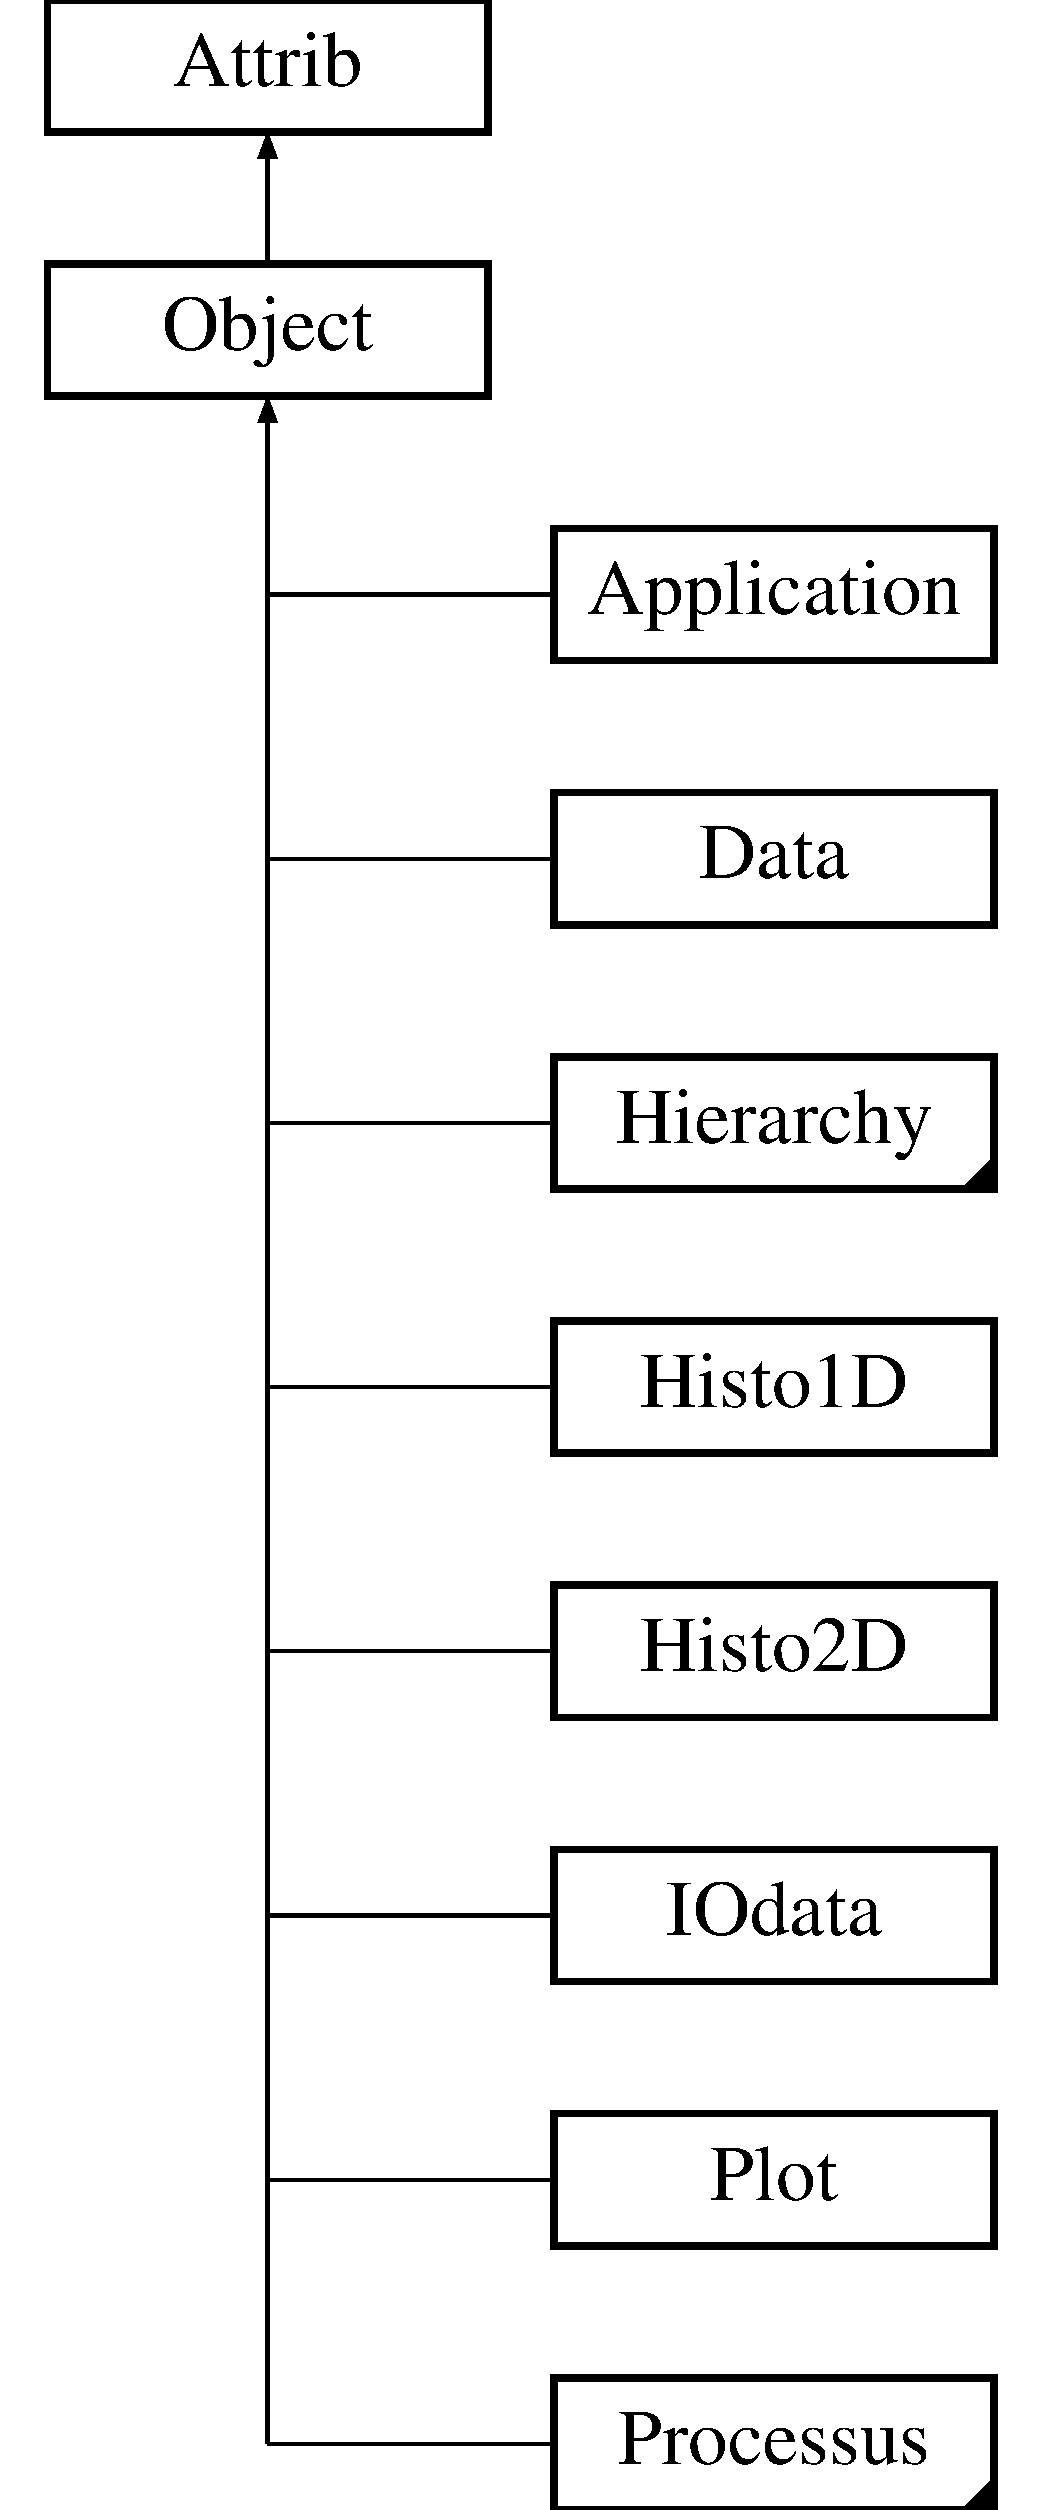
\includegraphics[height=10.000000cm]{classObject}
\end{center}
\end{figure}
\subsection*{Public Member Functions}
\begin{DoxyCompactItemize}
\item 
\hyperlink{classObject_a40860402e64d8008fb42329df7097cdb}{Object} ()
\begin{DoxyCompactList}\small\item\em Standard constructor. \end{DoxyCompactList}\item 
virtual \hyperlink{classObject_ae8f5483f459e46687bd01e6f9977afd3}{$\sim$\+Object} ()
\begin{DoxyCompactList}\small\item\em Destructor. \end{DoxyCompactList}\item 
std\+::string \hyperlink{classObject_a300f4c05dd468c7bb8b3c968868443c1}{name} () const
\item 
std\+::string \hyperlink{classObject_a84f99f70f144a83e1582d1d0f84e4e62}{type} ()
\item 
unsigned char \hyperlink{classObject_af99145335cc61ff6e2798ea17db009d2}{id} ()
\item 
std\+::string \hyperlink{classObject_a73a0f1a41828fdd8303dd662446fb6c3}{title} ()
\item 
void \hyperlink{classObject_a3f9d5537ebce0c0f2bf6ae4d92426f3c}{msg\+Svc} (int level, std\+::string \hyperlink{classObject_a58b2d0618c2d08cf2383012611528d97}{msg}, std\+::string \hyperlink{classObject_a300f4c05dd468c7bb8b3c968868443c1}{name})
\item 
void \hyperlink{classObject_a58b2d0618c2d08cf2383012611528d97}{msg} (std\+::string mymsg)
\item 
void \hyperlink{classObject_a83d2db2df682907ea1115ad721c1c4a1}{verbose} (std\+::string mymsg)
\item 
void \hyperlink{classObject_aac010553f022165573714b7014a15f0d}{debug} (std\+::string mymsg)
\item 
void \hyperlink{classObject_a644fd329ea4cb85f54fa6846484b84a8}{info} (std\+::string mymsg)
\item 
void \hyperlink{classObject_a65cd4fda577711660821fd2cd5a3b4c9}{warning} (std\+::string mymsg)
\item 
void \hyperlink{classObject_a204a95f57818c0f811933917a30eff45}{error} (std\+::string mymsg)
\item 
void \hyperlink{classObject_aad5a16aac7516ce65bd5ec02ab07fc80}{fatal} (std\+::string mymsg)
\item 
void \hyperlink{classObject_ac5d59299273cee27aacf7de00d2e7034}{msg} (std\+::string mymsg, std\+::string \hyperlink{classObject_a300f4c05dd468c7bb8b3c968868443c1}{name})
\item 
void \hyperlink{classObject_a2d4120195317e2a3c6532e8bb9f3da68}{verbose} (std\+::string mymsg, std\+::string \hyperlink{classObject_a300f4c05dd468c7bb8b3c968868443c1}{name})
\item 
void \hyperlink{classObject_a6c9a0397ca804e04d675ed05683f5420}{debug} (std\+::string mymsg, std\+::string \hyperlink{classObject_a300f4c05dd468c7bb8b3c968868443c1}{name})
\item 
void \hyperlink{classObject_a1ca123253dfd30fc28b156f521dcbdae}{info} (std\+::string mymsg, std\+::string \hyperlink{classObject_a300f4c05dd468c7bb8b3c968868443c1}{name})
\item 
void \hyperlink{classObject_a11f101db4dd73d9391b0231818881d86}{warning} (std\+::string mymsg, std\+::string \hyperlink{classObject_a300f4c05dd468c7bb8b3c968868443c1}{name})
\item 
void \hyperlink{classObject_ad7f6c457733082efa2f9ff5f5c8e119a}{error} (std\+::string mymsg, std\+::string \hyperlink{classObject_a300f4c05dd468c7bb8b3c968868443c1}{name})
\item 
void \hyperlink{classObject_ae62acd3d09f716220f75f252dc38bc9a}{fatal} (std\+::string mymsg, std\+::string \hyperlink{classObject_a300f4c05dd468c7bb8b3c968868443c1}{name})
\item 
void \hyperlink{classObject_ae30fea75683c2d149b6b6d17c09ecd0c}{set\+Name} (std\+::string \hyperlink{classObject_a300f4c05dd468c7bb8b3c968868443c1}{name})
\item 
void \hyperlink{classObject_aae534cc9d982bcb9b99fd505f2e103a5}{set\+Type} (std\+::string \hyperlink{classObject_a84f99f70f144a83e1582d1d0f84e4e62}{type})
\item 
void \hyperlink{classObject_a398fe08cba594a0ce6891d59fe4f159f}{set\+Id} (unsigned char \hyperlink{classObject_af99145335cc61ff6e2798ea17db009d2}{id})
\item 
void \hyperlink{classObject_a89557dbbad5bcaa02652f5d7fa35d20f}{set\+Title} (std\+::string \hyperlink{classObject_a73a0f1a41828fdd8303dd662446fb6c3}{title})
\item 
void \hyperlink{classObject_a870c5af919958c2136623b2d7816d123}{set\+Dll\+Name} (std\+::string \hyperlink{classObject_a2e3947f2870094c332d7454117f3ec63}{dll\+Name})
\item 
std\+::string \hyperlink{classObject_a2e3947f2870094c332d7454117f3ec63}{dll\+Name} ()
\end{DoxyCompactItemize}
\subsection*{Private Attributes}
\begin{DoxyCompactItemize}
\item 
\hyperlink{classMsgSvc}{Msg\+Svc} \hyperlink{classObject_a0d269813dd7ac1f24bc143031e2963f2}{m\+\_\+log}
\item 
std\+::string \hyperlink{classObject_a8b83c95c705d2c3ba0d081fe1710f48d}{m\+\_\+name}
\item 
std\+::string \hyperlink{classObject_a457a600fe8c00eb1034374f75110a78c}{m\+\_\+type}
\item 
unsigned char \hyperlink{classObject_aca74b9dbfed7b5556ea2d56c65b6b6b0}{m\+\_\+id}
\item 
std\+::string \hyperlink{classObject_affbeea1953eb5163573b92fad8f75727}{m\+\_\+title}
\item 
std\+::string \hyperlink{classObject_a01afbeacebb8db6831559972ec362eb3}{m\+\_\+dll\+Name}
\end{DoxyCompactItemize}
\subsection*{Additional Inherited Members}


\subsection{Detailed Description}
\begin{DoxyAuthor}{Author}

\end{DoxyAuthor}
\begin{DoxyDate}{Date}
2006-\/10-\/26 
\end{DoxyDate}


Definition at line 21 of file Object.\+h.



\subsection{Constructor \& Destructor Documentation}
\mbox{\Hypertarget{classObject_a40860402e64d8008fb42329df7097cdb}\label{classObject_a40860402e64d8008fb42329df7097cdb}} 
\index{Object@{Object}!Object@{Object}}
\index{Object@{Object}!Object@{Object}}
\subsubsection{\texorpdfstring{Object()}{Object()}}
{\footnotesize\ttfamily Object\+::\+Object (\begin{DoxyParamCaption}{ }\end{DoxyParamCaption})}



Standard constructor. 



Definition at line 16 of file Object.\+cpp.



References set\+Dll\+Name(), set\+Id(), set\+Name(), set\+Title(), and set\+Type().


\begin{DoxyCode}
16                  \{
17   \hyperlink{classObject_ae30fea75683c2d149b6b6d17c09ecd0c}{setName} (\textcolor{stringliteral}{"UNKNOWN"});
18   \hyperlink{classObject_aae534cc9d982bcb9b99fd505f2e103a5}{setType} (\textcolor{stringliteral}{"UNKNOWN"});
19   \hyperlink{classObject_a89557dbbad5bcaa02652f5d7fa35d20f}{setTitle}(\textcolor{stringliteral}{"CAT Application"});
20   \hyperlink{classObject_a398fe08cba594a0ce6891d59fe4f159f}{setId}   (0);
21   \hyperlink{classObject_a870c5af919958c2136623b2d7816d123}{setDllName}  ( std::string(\textcolor{stringliteral}{"CatKernel"}) );
22 \}
\end{DoxyCode}
\mbox{\Hypertarget{classObject_ae8f5483f459e46687bd01e6f9977afd3}\label{classObject_ae8f5483f459e46687bd01e6f9977afd3}} 
\index{Object@{Object}!````~Object@{$\sim$\+Object}}
\index{````~Object@{$\sim$\+Object}!Object@{Object}}
\subsubsection{\texorpdfstring{$\sim$\+Object()}{~Object()}}
{\footnotesize\ttfamily Object\+::$\sim$\+Object (\begin{DoxyParamCaption}{ }\end{DoxyParamCaption})\hspace{0.3cm}{\ttfamily [virtual]}}



Destructor. 



Definition at line 27 of file Object.\+cpp.


\begin{DoxyCode}
27                 \{
28 \} 
\end{DoxyCode}


\subsection{Member Function Documentation}
\mbox{\Hypertarget{classObject_aac010553f022165573714b7014a15f0d}\label{classObject_aac010553f022165573714b7014a15f0d}} 
\index{Object@{Object}!debug@{debug}}
\index{debug@{debug}!Object@{Object}}
\subsubsection{\texorpdfstring{debug()}{debug()}\hspace{0.1cm}{\footnotesize\ttfamily [1/2]}}
{\footnotesize\ttfamily void Object\+::debug (\begin{DoxyParamCaption}\item[{std\+::string}]{mymsg }\end{DoxyParamCaption})\hspace{0.3cm}{\ttfamily [inline]}}



Definition at line 37 of file Object.\+h.



References Msg\+Svc\+::\+D\+E\+B\+UG, m\+\_\+log, m\+\_\+name, and Msg\+Svc\+::msg\+Svc().



Referenced by A3\+P\+E\+::\+A3\+P\+E(), A3\+P\+E\+::acquisition(), Specs\+Mezzanine\+::add\+Bus(), Hierarchy\+::add\+Child(), Specs\+Slave\+::add\+I2c(), L\+S\+Delay\+Chip\+V1\+::config\+Reg\+Bulk\+Read(), L\+S\+Delay\+Chip\+V1\+::config\+Reg\+Bulk\+Write(), A3\+P\+E\+::data\+Ready(), D\+C\+U\+::\+D\+C\+U(), Hierarchy\+::del\+Child(), Specs\+Slave\+::detect(), Storage\+Fifo\+Acquisition\+::execute(), Storage\+Fifo\+::execute(), A3\+P\+E\+\_\+\+Bit\+Flip\+::execute(), Acquisition\+::execute(), Emulate\+F\+E\+::execute(), export\+\_\+obj(), Fe\+P\+G\+A\+::\+Fe\+P\+G\+A(), Specs\+Glue\+::i2c\+Clk\+Mode(), Fe\+P\+G\+A\+::i2c\+Read(), Seq\+P\+G\+A\+::i2c\+Read(), Fe\+P\+G\+A\+::i2c\+Write(), Seq\+P\+G\+A\+::i2c\+Write(), I\+C\+E\+C\+A\+Lv3\+::\+I\+C\+E\+C\+A\+Lv3(), I\+C\+Phaser\+::\+I\+C\+Phaser(), Specs\+Slave\+::init(), Specs\+Master\+::init(), Storage\+Fifo\+::initialize(), Storage\+Fifo\+Acquisition\+::initialize(), A3\+P\+E\+\_\+\+Bit\+Flip\+::initialize(), Acquisition\+::initialize(), Emulate\+F\+E\+::initialize(), A3\+P\+E\+::internal\+A\+X\+Sequence(), Specs\+Glue\+::led(), Specs\+Mezzanine\+::led(), M\+S\+Oxxxx\+::\+M\+S\+Oxxxx(), Phaser\+::\+Phaser(), Data\+::purge(), Phaser\+::read(), I\+C\+Phaser\+::read(), F\+E\+B\+\_\+v1\+::read\+Fifo\+Spy\+F\+E(), C\+U\+\_\+v1\+::reset(), F\+E\+B\+\_\+v1\+::reset(), Proto40\+M\+Hz\+\_\+v1\+::reset(), Specs\+Slave\+::reset(), Specs\+Master\+::reset(), F\+E\+B\+\_\+v1\+::reset\+Fifo\+Spy\+F\+E(), F\+E\+B\+\_\+v1\+::reset\+Spi(), Seq\+P\+G\+A\+::reset\+Spi(), Seq\+P\+G\+A\+::\+Seq\+P\+G\+A(), A3\+P\+E\+::set\+Add\+From\+A\+X\+Ram(), A3\+P\+E\+::set\+Add\+To\+A\+X\+Ram(), A3\+P\+E\+::set\+A\+X\+Ram\+Usb(), Element\+::set\+Connection(), Specs\+Glue\+::set\+I2c\+Clk\+Mode(), A3\+P\+E\+::set\+Latency\+A\+X(), Specs\+Glue\+::set\+Led(), Specs\+Mezzanine\+::set\+Led(), A3\+P\+E\+::set\+Length\+A\+X(), A3\+P\+E\+::set\+Read\+To\+A\+X\+Ram\+Usb(), Specs\+Master\+::set\+Speed(), A3\+P\+E\+::set\+Write\+From\+A\+X\+Ram\+Usb(), Specs\+Bus\+::\+Specs\+Bus(), Specs\+I2c\+::\+Specs\+I2c(), Specs\+Master\+::\+Specs\+Master(), Specs\+Mezzanine\+::\+Specs\+Mezzanine(), Specs\+Parallel\+Bus\+::\+Specs\+Parallel\+Bus(), Specs\+Slave\+::\+Specs\+Slave(), L\+S\+Delay\+Chip\+V1\+::spi\+B\+E\+R\+Test(), I\+C\+E\+C\+A\+Lv3\+::spi\+Read(), I\+C\+E\+C\+A\+Lv3\+::spi\+Write(), F\+E\+B\+\_\+v1\+::test\+Duration(), Seq\+P\+G\+A\+::test\+Sequence(), A3\+P\+E\+::trigger(), Server\+::update\+Config(), Server\+::update\+State(), Phaser\+::write(), I\+C\+Phaser\+::write(), and Hierarchy\+::$\sim$\+Hierarchy().


\begin{DoxyCode}
37 \{ \hyperlink{classObject_a0d269813dd7ac1f24bc143031e2963f2}{m\_log}.\hyperlink{classMsgSvc_ad25f18047920cc59a314e5098259711c}{msgSvc} (\hyperlink{classMsgSvc_ae671eb7301996cd049d2da8a65925926a1dbdcc82dce88370ec335883c83b38b0}{MsgSvc::DEBUG}   , mymsg, \hyperlink{classObject_a8b83c95c705d2c3ba0d081fe1710f48d}{m\_name} ); \}
\end{DoxyCode}
\mbox{\Hypertarget{classObject_a6c9a0397ca804e04d675ed05683f5420}\label{classObject_a6c9a0397ca804e04d675ed05683f5420}} 
\index{Object@{Object}!debug@{debug}}
\index{debug@{debug}!Object@{Object}}
\subsubsection{\texorpdfstring{debug()}{debug()}\hspace{0.1cm}{\footnotesize\ttfamily [2/2]}}
{\footnotesize\ttfamily void Object\+::debug (\begin{DoxyParamCaption}\item[{std\+::string}]{mymsg,  }\item[{std\+::string}]{name }\end{DoxyParamCaption})\hspace{0.3cm}{\ttfamily [inline]}}



Definition at line 45 of file Object.\+h.



References Msg\+Svc\+::\+D\+E\+B\+UG, m\+\_\+log, and Msg\+Svc\+::msg\+Svc().


\begin{DoxyCode}
45 \{ \hyperlink{classObject_a0d269813dd7ac1f24bc143031e2963f2}{m\_log}.\hyperlink{classMsgSvc_ad25f18047920cc59a314e5098259711c}{msgSvc} (\hyperlink{classMsgSvc_ae671eb7301996cd049d2da8a65925926a1dbdcc82dce88370ec335883c83b38b0}{MsgSvc::DEBUG}   , mymsg, \hyperlink{classObject_a300f4c05dd468c7bb8b3c968868443c1}{name} ); \}
\end{DoxyCode}
\mbox{\Hypertarget{classObject_a2e3947f2870094c332d7454117f3ec63}\label{classObject_a2e3947f2870094c332d7454117f3ec63}} 
\index{Object@{Object}!dll\+Name@{dll\+Name}}
\index{dll\+Name@{dll\+Name}!Object@{Object}}
\subsubsection{\texorpdfstring{dll\+Name()}{dllName()}}
{\footnotesize\ttfamily std\+::string Object\+::dll\+Name (\begin{DoxyParamCaption}{ }\end{DoxyParamCaption})\hspace{0.3cm}{\ttfamily [inline]}}

Get accessor to member m\+\_\+dll\+Name \begin{DoxyReturn}{Returns}
the current value of m\+\_\+dll\+Name 
\end{DoxyReturn}


Definition at line 74 of file Object.\+h.



References m\+\_\+dll\+Name.



Referenced by export\+\_\+obj(), and set\+Dll\+Name().


\begin{DoxyCode}
74                        \{
75     \textcolor{keywordflow}{return} \hyperlink{classObject_a01afbeacebb8db6831559972ec362eb3}{m\_dllName};
76   \}  
\end{DoxyCode}
\mbox{\Hypertarget{classObject_a204a95f57818c0f811933917a30eff45}\label{classObject_a204a95f57818c0f811933917a30eff45}} 
\index{Object@{Object}!error@{error}}
\index{error@{error}!Object@{Object}}
\subsubsection{\texorpdfstring{error()}{error()}\hspace{0.1cm}{\footnotesize\ttfamily [1/2]}}
{\footnotesize\ttfamily void Object\+::error (\begin{DoxyParamCaption}\item[{std\+::string}]{mymsg }\end{DoxyParamCaption})\hspace{0.3cm}{\ttfamily [inline]}}



Definition at line 40 of file Object.\+h.



References Msg\+Svc\+::\+E\+RR, m\+\_\+log, m\+\_\+name, and Msg\+Svc\+::msg\+Svc().



Referenced by A3\+P\+E\+::clock\+Division(), N\+I6008\+::cmd(), A3\+P\+E\+::enable\+Storage(), A3\+P\+E\+\_\+\+Bit\+Flip\+::execute(), export\+\_\+obj(), A3\+P\+E\+::fifo\+Depth(), A3\+P\+E\+::fifo\+Latency(), F\+E\+B\+\_\+v1\+::gbt\+Status(), Register\+::get\+Bit(), M\+S\+Oxxxx\+::get\+Statistics(), N\+I6008\+::init(), Specs\+Master\+::init(), Usb\+F\+T\+Interface\+::init(), Usb\+F\+T\+M\+L\+Interface\+::init(), A3\+P\+E\+::latency\+A\+X(), A3\+P\+E\+::length\+A\+X(), A3\+P\+E\+::n\+Trigger(), M\+S\+Oxxxx\+::open(), I\+C\+E\+C\+A\+Lv3\+::parse\+Parameter\+List(), A3\+P\+E\+::pipeline(), Usb\+F\+T\+Interface\+::read(), Usb\+F\+T\+M\+L\+Interface\+::read(), M\+S\+Oxxxx\+::recv(), A3\+P\+E\+::reset(), M\+S\+Oxxxx\+::send(), A3\+P\+E\+::set\+Add\+From\+A\+X\+Ram(), A3\+P\+E\+::set\+Add\+To\+A\+X\+Ram(), I\+C\+E\+C\+A\+Lv3\+::set\+Analog\+Ch(), A3\+P\+E\+::set\+A\+X\+Ram\+Usb(), Register\+::set\+Bit(), A3\+P\+E\+::set\+Clock\+Division(), A3\+P\+E\+::set\+Fifo\+Depth(), A3\+P\+E\+::set\+Fifo\+Latency(), A3\+P\+E\+::set\+Latency\+A\+X(), A3\+P\+E\+::set\+Length\+A\+X(), A3\+P\+E\+::set\+N\+Trigger(), A3\+P\+E\+::set\+Pipeline(), A3\+P\+E\+::set\+Read\+Pattern\+Fifo\+Usb(), A3\+P\+E\+::set\+Read\+To\+A\+X\+Ram\+Usb(), A3\+P\+E\+::set\+Read\+Trigger\+Fifo\+Usb(), A3\+P\+E\+::set\+Software\+Trigger(), A3\+P\+E\+::set\+Trigger\+Delay(), A3\+P\+E\+::set\+Trigger\+Rate(), A3\+P\+E\+::set\+Write\+From\+A\+X\+Ram\+Usb(), A3\+P\+E\+::set\+Write\+Storage\+Fifo\+Usb(), I\+C\+E\+C\+A\+Lv3\+::spi\+F\+E\+R\+Test(), I\+C\+E\+C\+A\+Lv3\+::spi\+Write\+Safe(), A3\+P\+E\+::start\+Sequence\+A\+X(), A3\+P\+E\+::trigger\+Delay(), A3\+P\+E\+::trigger\+Rate(), Usb\+F\+T\+M\+L\+Interface\+::usb\+Read(), Usb\+F\+T\+Interface\+::usb\+Read(), Usb\+F\+T\+M\+L\+Interface\+::usb\+Read\+U16(), Usb\+F\+T\+Interface\+::usb\+Read\+U16(), Usb\+F\+T\+M\+L\+Interface\+::usb\+Read\+U32(), Usb\+F\+T\+Interface\+::usb\+Read\+U32(), Usb\+F\+T\+M\+L\+Interface\+::usb\+Read\+U8(), Usb\+F\+T\+Interface\+::usb\+Read\+U8(), Usb\+F\+T\+M\+L\+Interface\+::usb\+Write(), Usb\+F\+T\+Interface\+::usb\+Write(), Usb\+F\+T\+Interface\+::usb\+Write\+Read(), Usb\+F\+T\+M\+L\+Interface\+::usb\+Write\+Read(), Usb\+F\+T\+M\+L\+Interface\+::usb\+Write\+U16(), Usb\+F\+T\+Interface\+::usb\+Write\+U16(), Usb\+F\+T\+M\+L\+Interface\+::usb\+Write\+U32(), Usb\+F\+T\+Interface\+::usb\+Write\+U32(), Usb\+F\+T\+M\+L\+Interface\+::usb\+Write\+U8(), Usb\+F\+T\+Interface\+::usb\+Write\+U8(), Usb\+F\+T\+M\+L\+Interface\+::write(), and Usb\+F\+T\+Interface\+::write().


\begin{DoxyCode}
40 \{ \hyperlink{classObject_a0d269813dd7ac1f24bc143031e2963f2}{m\_log}.\hyperlink{classMsgSvc_ad25f18047920cc59a314e5098259711c}{msgSvc} (\hyperlink{classMsgSvc_ae671eb7301996cd049d2da8a65925926a35a9d7166e9896af4ec8fb33bf5f1772}{MsgSvc::ERR}     , mymsg, \hyperlink{classObject_a8b83c95c705d2c3ba0d081fe1710f48d}{m\_name} ); \}
\end{DoxyCode}
\mbox{\Hypertarget{classObject_ad7f6c457733082efa2f9ff5f5c8e119a}\label{classObject_ad7f6c457733082efa2f9ff5f5c8e119a}} 
\index{Object@{Object}!error@{error}}
\index{error@{error}!Object@{Object}}
\subsubsection{\texorpdfstring{error()}{error()}\hspace{0.1cm}{\footnotesize\ttfamily [2/2]}}
{\footnotesize\ttfamily void Object\+::error (\begin{DoxyParamCaption}\item[{std\+::string}]{mymsg,  }\item[{std\+::string}]{name }\end{DoxyParamCaption})\hspace{0.3cm}{\ttfamily [inline]}}



Definition at line 48 of file Object.\+h.



References Msg\+Svc\+::\+E\+RR, m\+\_\+log, and Msg\+Svc\+::msg\+Svc().


\begin{DoxyCode}
48 \{ \hyperlink{classObject_a0d269813dd7ac1f24bc143031e2963f2}{m\_log}.\hyperlink{classMsgSvc_ad25f18047920cc59a314e5098259711c}{msgSvc} (\hyperlink{classMsgSvc_ae671eb7301996cd049d2da8a65925926a35a9d7166e9896af4ec8fb33bf5f1772}{MsgSvc::ERR}     , mymsg, \hyperlink{classObject_a300f4c05dd468c7bb8b3c968868443c1}{name} ); \}
\end{DoxyCode}
\mbox{\Hypertarget{classObject_aad5a16aac7516ce65bd5ec02ab07fc80}\label{classObject_aad5a16aac7516ce65bd5ec02ab07fc80}} 
\index{Object@{Object}!fatal@{fatal}}
\index{fatal@{fatal}!Object@{Object}}
\subsubsection{\texorpdfstring{fatal()}{fatal()}\hspace{0.1cm}{\footnotesize\ttfamily [1/2]}}
{\footnotesize\ttfamily void Object\+::fatal (\begin{DoxyParamCaption}\item[{std\+::string}]{mymsg }\end{DoxyParamCaption})\hspace{0.3cm}{\ttfamily [inline]}}



Definition at line 41 of file Object.\+h.



References Msg\+Svc\+::\+F\+A\+T\+AL, m\+\_\+log, m\+\_\+name, and Msg\+Svc\+::msg\+Svc().



Referenced by export\+\_\+obj(), Usb\+M\+L\+I2c\+Bus\+::init(), Usb\+M\+L\+Spi\+Bus\+::init(), Usb\+I2c\+Bus\+::init(), Usb\+Spi\+Bus\+::init(), Specs\+Slave\+::init(), I\+Oobject\+::init(), Usb\+F\+T\+M\+L\+Interface\+::init(), Usb\+F\+T\+Interface\+::init(), and Element\+::set\+Connection().


\begin{DoxyCode}
41 \{ \hyperlink{classObject_a0d269813dd7ac1f24bc143031e2963f2}{m\_log}.\hyperlink{classMsgSvc_ad25f18047920cc59a314e5098259711c}{msgSvc} (\hyperlink{classMsgSvc_ae671eb7301996cd049d2da8a65925926a59c73cb29edfc9cdf35845e2b1301363}{MsgSvc::FATAL}   , mymsg, \hyperlink{classObject_a8b83c95c705d2c3ba0d081fe1710f48d}{m\_name} ); \}
\end{DoxyCode}
\mbox{\Hypertarget{classObject_ae62acd3d09f716220f75f252dc38bc9a}\label{classObject_ae62acd3d09f716220f75f252dc38bc9a}} 
\index{Object@{Object}!fatal@{fatal}}
\index{fatal@{fatal}!Object@{Object}}
\subsubsection{\texorpdfstring{fatal()}{fatal()}\hspace{0.1cm}{\footnotesize\ttfamily [2/2]}}
{\footnotesize\ttfamily void Object\+::fatal (\begin{DoxyParamCaption}\item[{std\+::string}]{mymsg,  }\item[{std\+::string}]{name }\end{DoxyParamCaption})\hspace{0.3cm}{\ttfamily [inline]}}



Definition at line 49 of file Object.\+h.



References Msg\+Svc\+::\+F\+A\+T\+AL, m\+\_\+log, and Msg\+Svc\+::msg\+Svc().


\begin{DoxyCode}
49 \{ \hyperlink{classObject_a0d269813dd7ac1f24bc143031e2963f2}{m\_log}.\hyperlink{classMsgSvc_ad25f18047920cc59a314e5098259711c}{msgSvc} (\hyperlink{classMsgSvc_ae671eb7301996cd049d2da8a65925926a59c73cb29edfc9cdf35845e2b1301363}{MsgSvc::FATAL}   , mymsg, \hyperlink{classObject_a300f4c05dd468c7bb8b3c968868443c1}{name} ); \}
\end{DoxyCode}
\mbox{\Hypertarget{classObject_af99145335cc61ff6e2798ea17db009d2}\label{classObject_af99145335cc61ff6e2798ea17db009d2}} 
\index{Object@{Object}!id@{id}}
\index{id@{id}!Object@{Object}}
\subsubsection{\texorpdfstring{id()}{id()}}
{\footnotesize\ttfamily unsigned char Object\+::id (\begin{DoxyParamCaption}{ }\end{DoxyParamCaption})\hspace{0.3cm}{\ttfamily [inline]}}



Definition at line 30 of file Object.\+h.



References m\+\_\+id.



Referenced by export\+\_\+obj(), and set\+Id().


\begin{DoxyCode}
30 \{ \textcolor{keywordflow}{return} \hyperlink{classObject_aca74b9dbfed7b5556ea2d56c65b6b6b0}{m\_id};         \} \textcolor{comment}{//< Get Object m\_id }
\end{DoxyCode}
\mbox{\Hypertarget{classObject_a644fd329ea4cb85f54fa6846484b84a8}\label{classObject_a644fd329ea4cb85f54fa6846484b84a8}} 
\index{Object@{Object}!info@{info}}
\index{info@{info}!Object@{Object}}
\subsubsection{\texorpdfstring{info()}{info()}\hspace{0.1cm}{\footnotesize\ttfamily [1/2]}}
{\footnotesize\ttfamily void Object\+::info (\begin{DoxyParamCaption}\item[{std\+::string}]{mymsg }\end{DoxyParamCaption})\hspace{0.3cm}{\ttfamily [inline]}}



Definition at line 38 of file Object.\+h.



References Msg\+Svc\+::\+I\+N\+FO, m\+\_\+log, m\+\_\+name, and Msg\+Svc\+::msg\+Svc().



Referenced by N\+I6008\+::add\+Device(), I\+C\+E\+C\+A\+Lv3\+::bxid\+Resynch\+Status(), F\+E\+B\+\_\+v1\+::calib\+Cte(), check\+Cmd(), Hierarchy\+::clear(), F\+E\+B\+\_\+v1\+::clock80\+M\+Hz\+Falling\+Edge(), F\+E\+B\+\_\+v1\+::clock\+Falling\+Edge(), Usb\+F\+T\+Interface\+::close(), Usb\+F\+T\+M\+L\+Interface\+::close(), Processus\+::close\+Root\+File(), Server\+::cmdline(), Specs\+Mezzanine\+::cmdline(), Specs\+Slave\+::detect(), F\+E\+B\+\_\+v1\+::disable\+Subtract(), I\+Odata\+::dump(), A3\+P\+E\+::dump\+From\+A\+X(), A3\+P\+E\+::dump\+Pattern(), A3\+P\+E\+::dump\+Storage(), A3\+P\+E\+::dump\+To\+A\+X(), A3\+P\+E\+::dump\+Trigger(), Processus\+::end\+Processing(), Phaser\+Ramp\+Exec\+::execute(), export\+\_\+obj(), Phaser\+Ramp\+Exec\+::finalize(), F\+E\+B\+\_\+v1\+::gain4(), F\+E\+B\+\_\+v1\+::gbt80\+M\+Hz\+Clk\+Eport(), F\+E\+B\+\_\+v1\+::gbt\+Data\+Path(), F\+E\+B\+\_\+v1\+::gbt\+D\+L\+L\+Eport(), F\+E\+B\+\_\+v1\+::gbt\+D\+L\+L\+Reset(), F\+E\+B\+\_\+v1\+::gbt\+Enable\+Eport(), F\+E\+B\+\_\+v1\+::gbt\+Mode(), F\+E\+B\+\_\+v1\+::gbt\+Status(), F\+E\+B\+\_\+v1\+::gbt\+Term\+Eport(), F\+E\+B\+\_\+v1\+::gbt\+Track\+Mode(), I\+C\+E\+C\+A\+Lv3\+::get\+Analog\+Ch(), I\+C\+E\+C\+A\+Lv3\+::get\+Delay\+Line\+Ch(), I\+C\+E\+C\+A\+Lv3\+::get\+Main\+Reg(), F\+E\+B\+\_\+v1\+::global\+Pseudo\+P\+M\+Enable(), Croc\+::help(), R\+A\+M\+::help(), Specs\+Glue\+::help(), Usb\+M\+L\+I2c\+Bus\+::help(), Usb\+M\+L\+Spi\+Bus\+::help(), C\+U\+\_\+v1\+::help(), Usb\+I2c\+Bus\+::help(), Usb\+Spi\+Bus\+::help(), F\+E\+B\+\_\+v1\+::help(), I\+Oobject\+::help(), Proto40\+M\+Hz\+\_\+v1\+::help(), Specs\+Mezzanine\+::help(), Fe\+P\+G\+A\+::help(), Seq\+P\+G\+A\+::help(), Computer\+::help(), N\+I6008\+::help(), Specs\+Parallel\+Bus\+::help(), Specs\+Master\+::help(), Usb\+F\+T\+M\+L\+Interface\+::help(), Usb\+F\+T\+Interface\+::help(), Phaser\+::help(), I\+C\+Phaser\+::help(), A3\+P\+E\+::help(), M\+S\+Oxxxx\+::id(), Croc\+::init(), Computer\+::init(), N\+I6008\+::init(), Specs\+Parallel\+Bus\+::init(), Specs\+Slave\+::init(), Specs\+Master\+::init(), Usb\+F\+T\+Interface\+::init(), Usb\+F\+T\+M\+L\+Interface\+::init(), Storage\+Fifo\+Acquisition\+::initialize(), Storage\+Fifo\+::initialize(), Acquisition\+::initialize(), A3\+P\+E\+\_\+\+Bit\+Flip\+::initialize(), Emulate\+F\+E\+::initialize(), A\+D\+C\+Measurement\+::initialize(), Current\+Measurement\+::initialize(), Phaser\+Ramp\+Exec\+::initialize(), F\+E\+B\+\_\+v1\+::inject\+Mode\+F\+E(), is\+Int(), F\+E\+B\+\_\+v1\+::latency(), F\+E\+B\+\_\+v1\+::latency\+L\+L\+T(), A3\+P\+E\+::load\+From\+A\+X(), Application\+::load\+History\+File(), A3\+P\+E\+::load\+Pattern(), A3\+P\+E\+::load\+Storage(), A3\+P\+E\+::load\+To\+A\+X(), A3\+P\+E\+::load\+Trigger(), Application\+::loop(), F\+E\+B\+\_\+v1\+::mask\+L\+L\+T(), Application\+::network(), F\+E\+B\+\_\+v1\+::old\+Subtract(), M\+S\+Oxxxx\+::open(), Processus\+::open\+Root\+File(), Data\+::print(), F\+E\+B\+\_\+v1\+::probe\+Enable(), Proc\+Data\+Base\+::\+Proc\+Data\+Base(), F\+E\+B\+\_\+v1\+::pseudo\+A\+D\+C\+Enable(), F\+E\+B\+\_\+v1\+::pseudo\+P\+M\+Enable(), Usb\+Spi\+Bus\+::read(), Usb\+F\+T\+M\+L\+Interface\+::read(), F\+E\+B\+\_\+v1\+::read\+Fifo\+Inject\+F\+E(), F\+E\+B\+\_\+v1\+::read\+Fifo\+L\+L\+T(), F\+E\+B\+\_\+v1\+::read\+Fifo\+L\+L\+T\+F\+E(), F\+E\+B\+\_\+v1\+::read\+Fifo\+Spy\+F\+E(), M\+S\+Oxxxx\+::recv(), Croc\+::reset(), Usb\+I2c\+Bus\+::reset(), Usb\+M\+L\+I2c\+Bus\+::reset(), Usb\+M\+L\+Spi\+Bus\+::reset(), Usb\+Spi\+Bus\+::reset(), Fe\+P\+G\+A\+::reset(), Seq\+P\+G\+A\+::reset(), Computer\+::reset(), Specs\+Parallel\+Bus\+::reset(), Specs\+Master\+::reset(), N\+I6008\+::reset(), Usb\+F\+T\+M\+L\+Interface\+::reset(), Usb\+F\+T\+Interface\+::reset(), A3\+P\+E\+::reset(), A3\+P\+E\+::reset\+Acquisition\+Write\+Counter(), F\+E\+B\+\_\+v1\+::reset\+F\+E(), A3\+P\+E\+::reset\+F\+E(), F\+E\+B\+\_\+v1\+::reset\+Fifo\+Inject\+F\+E(), A3\+P\+E\+::reset\+From\+A\+X\+Ram(), Specs\+Slave\+::reset\+Internal(), A3\+P\+E\+::reset\+Latency\+Counter(), A3\+P\+E\+::reset\+Pattern\+Fifo(), A3\+P\+E\+::reset\+Sequence\+From\+To\+A\+X(), A3\+P\+E\+::reset\+S\+P\+I(), A3\+P\+E\+::reset\+Storage\+Fifo(), A3\+P\+E\+::reset\+To\+A\+X\+Ram(), A3\+P\+E\+::reset\+Trigger\+Fifo(), Fe\+P\+G\+A\+::reset\+Usb(), A3\+P\+E\+::reset\+Usb\+Phasers(), M\+S\+Oxxxx\+::send(), Server\+::\+Server(), Application\+::server(), F\+E\+B\+\_\+v1\+::set\+Calib\+Cte(), F\+E\+B\+\_\+v1\+::set\+Clock80\+M\+Hz\+Falling\+Edge(), A3\+P\+E\+::set\+Clock\+Division(), F\+E\+B\+\_\+v1\+::set\+Clock\+Falling\+Edge(), Usb\+Spi\+Bus\+::set\+Data\+Length(), F\+E\+B\+\_\+v1\+::set\+Disable\+Subtract(), A3\+P\+E\+::set\+Enable\+A\+D\+C(), A3\+P\+E\+::set\+Fifo\+Depth(), A3\+P\+E\+::set\+Fifo\+Latency(), F\+E\+B\+\_\+v1\+::set\+Gain4(), F\+E\+B\+\_\+v1\+::set\+Gbt80\+M\+Hz\+Clk\+Eport(), F\+E\+B\+\_\+v1\+::set\+Gbt\+Clock\+Strength(), F\+E\+B\+\_\+v1\+::set\+Gbt\+Data\+Path(), F\+E\+B\+\_\+v1\+::set\+Gbt\+D\+L\+L\+Eport(), F\+E\+B\+\_\+v1\+::set\+Gbt\+Enable\+Eport(), F\+E\+B\+\_\+v1\+::set\+Gbt\+Mode(), F\+E\+B\+\_\+v1\+::set\+Gbt\+Term\+Eport(), F\+E\+B\+\_\+v1\+::set\+Gbt\+Track\+Mode(), F\+E\+B\+\_\+v1\+::set\+Global\+Pseudo\+P\+M\+Enable(), F\+E\+B\+\_\+v1\+::set\+Inject\+Mode\+F\+E(), A3\+P\+E\+::set\+Internal\+A\+X\+Sequence(), F\+E\+B\+\_\+v1\+::set\+Latency(), A3\+P\+E\+::set\+N\+Trigger(), F\+E\+B\+\_\+v1\+::set\+Old\+Subtract(), F\+E\+B\+\_\+v1\+::set\+Output\+Eport(), Phaser\+::set\+Phase(), I\+C\+Phaser\+::set\+Phase(), A3\+P\+E\+::set\+Pipeline(), F\+E\+B\+\_\+v1\+::set\+Probe\+Enable(), F\+E\+B\+\_\+v1\+::set\+Pseudo\+A\+D\+C\+Enable(), F\+E\+B\+\_\+v1\+::set\+Pseudo\+P\+M\+Enable(), A3\+P\+E\+::set\+Read\+Pattern\+Fifo\+Usb(), A3\+P\+E\+::set\+Read\+Trigger\+Fifo\+Usb(), A3\+P\+E\+::set\+Software\+Trigger(), F\+E\+B\+\_\+v1\+::set\+Spare\+For\+Trig\+Enable(), F\+E\+B\+\_\+v1\+::set\+Spy\+Mode\+F\+E(), Processus\+::set\+State(), F\+E\+B\+\_\+v1\+::set\+Threshold(), A3\+P\+E\+::set\+Trigger\+Delay(), A3\+P\+E\+::set\+Trigger\+Rate(), A3\+P\+E\+::set\+Write\+Storage\+Fifo\+Usb(), L\+S\+Delay\+Chip\+V1\+::show\+Config(), F\+E\+B\+\_\+v1\+::spare\+For\+Trig\+Enable(), Specs\+I2c\+::\+Specs\+I2c(), I\+C\+E\+C\+A\+Lv3\+::spi\+F\+E\+R\+Test(), F\+E\+B\+\_\+v1\+::spy\+Mode\+F\+E(), F\+E\+B\+\_\+v1\+::spy\+Mode\+Seq(), Server\+::start(), Processus\+::start\+Processing(), F\+E\+B\+\_\+v1\+::status\+Register(), F\+E\+B\+\_\+v1\+::stop\+Inj\+Loop(), Application\+::svc\+Running(), Application\+::terminate(), Fe\+P\+G\+A\+::test\+Sequence(), F\+E\+B\+\_\+v1\+::threshold(), Hierarchy\+::tree(), Croc\+::update(), Usb\+I2c\+Bus\+::update(), Usb\+Spi\+Bus\+::update(), Usb\+M\+L\+I2c\+Bus\+::update(), Usb\+M\+L\+Spi\+Bus\+::update(), C\+U\+\_\+v1\+::update(), Proto40\+M\+Hz\+\_\+v1\+::update(), Computer\+::update(), F\+E\+B\+\_\+v1\+::update(), Specs\+Parallel\+Bus\+::update(), N\+I6008\+::update(), Usb\+F\+T\+M\+L\+Interface\+::update(), Usb\+F\+T\+Interface\+::update(), Usb\+F\+T\+Interface\+::\+Usb\+F\+T\+Interface(), Usb\+F\+T\+M\+L\+Interface\+::\+Usb\+F\+T\+M\+L\+Interface(), I\+C\+E\+C\+A\+Lv3\+::version(), Usb\+Spi\+Bus\+::write(), F\+E\+B\+\_\+v1\+::write\+Data\+Fifo\+Inject\+F\+E(), F\+E\+B\+\_\+v1\+::write\+Fifo\+Inject\+F\+E(), and N\+I6008\+::$\sim$\+N\+I6008().


\begin{DoxyCode}
38 \{ \hyperlink{classObject_a0d269813dd7ac1f24bc143031e2963f2}{m\_log}.\hyperlink{classMsgSvc_ad25f18047920cc59a314e5098259711c}{msgSvc} (\hyperlink{classMsgSvc_ae671eb7301996cd049d2da8a65925926ad2fcf3f3e734fc41ee097cc23670ce51}{MsgSvc::INFO}    , mymsg, \hyperlink{classObject_a8b83c95c705d2c3ba0d081fe1710f48d}{m\_name} ); \}
\end{DoxyCode}
\mbox{\Hypertarget{classObject_a1ca123253dfd30fc28b156f521dcbdae}\label{classObject_a1ca123253dfd30fc28b156f521dcbdae}} 
\index{Object@{Object}!info@{info}}
\index{info@{info}!Object@{Object}}
\subsubsection{\texorpdfstring{info()}{info()}\hspace{0.1cm}{\footnotesize\ttfamily [2/2]}}
{\footnotesize\ttfamily void Object\+::info (\begin{DoxyParamCaption}\item[{std\+::string}]{mymsg,  }\item[{std\+::string}]{name }\end{DoxyParamCaption})\hspace{0.3cm}{\ttfamily [inline]}}



Definition at line 46 of file Object.\+h.



References Msg\+Svc\+::\+I\+N\+FO, m\+\_\+log, and Msg\+Svc\+::msg\+Svc().


\begin{DoxyCode}
46 \{ \hyperlink{classObject_a0d269813dd7ac1f24bc143031e2963f2}{m\_log}.\hyperlink{classMsgSvc_ad25f18047920cc59a314e5098259711c}{msgSvc} (\hyperlink{classMsgSvc_ae671eb7301996cd049d2da8a65925926ad2fcf3f3e734fc41ee097cc23670ce51}{MsgSvc::INFO}    , mymsg, \hyperlink{classObject_a300f4c05dd468c7bb8b3c968868443c1}{name} ); \}
\end{DoxyCode}
\mbox{\Hypertarget{classObject_a58b2d0618c2d08cf2383012611528d97}\label{classObject_a58b2d0618c2d08cf2383012611528d97}} 
\index{Object@{Object}!msg@{msg}}
\index{msg@{msg}!Object@{Object}}
\subsubsection{\texorpdfstring{msg()}{msg()}\hspace{0.1cm}{\footnotesize\ttfamily [1/2]}}
{\footnotesize\ttfamily void Object\+::msg (\begin{DoxyParamCaption}\item[{std\+::string}]{mymsg }\end{DoxyParamCaption})\hspace{0.3cm}{\ttfamily [inline]}}



Definition at line 35 of file Object.\+h.



References m\+\_\+log, m\+\_\+name, Msg\+Svc\+::msg\+Svc(), and Msg\+Svc\+::\+N\+O\+NE.



Referenced by export\+\_\+obj().


\begin{DoxyCode}
35 \{ \hyperlink{classObject_a0d269813dd7ac1f24bc143031e2963f2}{m\_log}.\hyperlink{classMsgSvc_ad25f18047920cc59a314e5098259711c}{msgSvc} (\hyperlink{classMsgSvc_ae671eb7301996cd049d2da8a65925926a9be9ae32fed8e1e6eba4a58692210fbd}{MsgSvc::NONE}    , mymsg, \hyperlink{classObject_a8b83c95c705d2c3ba0d081fe1710f48d}{m\_name} ); \}
\end{DoxyCode}
\mbox{\Hypertarget{classObject_ac5d59299273cee27aacf7de00d2e7034}\label{classObject_ac5d59299273cee27aacf7de00d2e7034}} 
\index{Object@{Object}!msg@{msg}}
\index{msg@{msg}!Object@{Object}}
\subsubsection{\texorpdfstring{msg()}{msg()}\hspace{0.1cm}{\footnotesize\ttfamily [2/2]}}
{\footnotesize\ttfamily void Object\+::msg (\begin{DoxyParamCaption}\item[{std\+::string}]{mymsg,  }\item[{std\+::string}]{name }\end{DoxyParamCaption})\hspace{0.3cm}{\ttfamily [inline]}}



Definition at line 43 of file Object.\+h.



References m\+\_\+log, Msg\+Svc\+::msg\+Svc(), and Msg\+Svc\+::\+N\+O\+NE.


\begin{DoxyCode}
43 \{ \hyperlink{classObject_a0d269813dd7ac1f24bc143031e2963f2}{m\_log}.\hyperlink{classMsgSvc_ad25f18047920cc59a314e5098259711c}{msgSvc} (\hyperlink{classMsgSvc_ae671eb7301996cd049d2da8a65925926a9be9ae32fed8e1e6eba4a58692210fbd}{MsgSvc::NONE}    , mymsg, \hyperlink{classObject_a300f4c05dd468c7bb8b3c968868443c1}{name} ); \}
\end{DoxyCode}
\mbox{\Hypertarget{classObject_a3f9d5537ebce0c0f2bf6ae4d92426f3c}\label{classObject_a3f9d5537ebce0c0f2bf6ae4d92426f3c}} 
\index{Object@{Object}!msg\+Svc@{msg\+Svc}}
\index{msg\+Svc@{msg\+Svc}!Object@{Object}}
\subsubsection{\texorpdfstring{msg\+Svc()}{msgSvc()}}
{\footnotesize\ttfamily void Object\+::msg\+Svc (\begin{DoxyParamCaption}\item[{int}]{level,  }\item[{std\+::string}]{msg,  }\item[{std\+::string}]{name }\end{DoxyParamCaption})\hspace{0.3cm}{\ttfamily [inline]}}



Definition at line 33 of file Object.\+h.



References m\+\_\+log, and Msg\+Svc\+::msg\+Svc().



Referenced by Application\+::banner(), export\+\_\+obj(), Specs\+Mezzanine\+::help(), D\+C\+U\+::read\+Mode(), D\+C\+U\+::set\+H\+I\+R(), D\+C\+U\+::set\+L\+I\+R(), Processus\+::set\+State(), and Hierarchy\+::tree().


\begin{DoxyCode}
33 \{ \hyperlink{classObject_a0d269813dd7ac1f24bc143031e2963f2}{m\_log}.\hyperlink{classMsgSvc_ad25f18047920cc59a314e5098259711c}{msgSvc} ( (\hyperlink{classMsgSvc_ae671eb7301996cd049d2da8a65925926}{MsgSvc::MsgLevel})(level), \hyperlink{classObject_a58b2d0618c2d08cf2383012611528d97}{msg}, 
      \hyperlink{classObject_a300f4c05dd468c7bb8b3c968868443c1}{name} ); \}
\end{DoxyCode}
\mbox{\Hypertarget{classObject_a300f4c05dd468c7bb8b3c968868443c1}\label{classObject_a300f4c05dd468c7bb8b3c968868443c1}} 
\index{Object@{Object}!name@{name}}
\index{name@{name}!Object@{Object}}
\subsubsection{\texorpdfstring{name()}{name()}}
{\footnotesize\ttfamily std\+::string Object\+::name (\begin{DoxyParamCaption}{ }\end{DoxyParamCaption}) const\hspace{0.3cm}{\ttfamily [inline]}}



Definition at line 28 of file Object.\+h.



References m\+\_\+name.



Referenced by Specs\+Mezzanine\+::add\+Bus(), Hierarchy\+::add\+Child(), Specs\+Slave\+::add\+I2c(), Hierarchy\+::child(), Hierarchy\+::child\+Typed(), Hierarchy\+::clear(), A3\+P\+E\+::clock\+Division(), Usb\+F\+T\+M\+L\+Interface\+::close(), Usb\+F\+T\+Interface\+::close(), Element\+::connection(), Specs\+Slave\+::detect(), I\+Odata\+::dump(), A3\+P\+E\+::enable\+Storage(), export\+\_\+obj(), export\+\_\+proc(), A3\+P\+E\+::fifo\+Depth(), A3\+P\+E\+::fifo\+Latency(), Register\+::get\+Bit(), Croc\+::help(), R\+A\+M\+::help(), Usb\+M\+L\+Spi\+Bus\+::help(), Usb\+M\+L\+I2c\+Bus\+::help(), Usb\+I2c\+Bus\+::help(), C\+U\+\_\+v1\+::help(), Usb\+Spi\+Bus\+::help(), I\+Oobject\+::help(), Proto40\+M\+Hz\+\_\+v1\+::help(), F\+E\+B\+\_\+v1\+::help(), Fe\+P\+G\+A\+::help(), Seq\+P\+G\+A\+::help(), Computer\+::help(), N\+I6008\+::help(), Specs\+Parallel\+Bus\+::help(), Usb\+F\+T\+Interface\+::help(), Usb\+F\+T\+M\+L\+Interface\+::help(), Phaser\+::help(), I\+C\+Phaser\+::help(), A3\+P\+E\+::help(), Data\+::hist2d(), Croc\+::init(), Computer\+::init(), N\+I6008\+::init(), Specs\+Parallel\+Bus\+::init(), Specs\+Slave\+::init(), Specs\+Master\+::init(), Usb\+F\+T\+M\+L\+Interface\+::init(), Usb\+F\+T\+Interface\+::init(), Storage\+Fifo\+::initialize(), Storage\+Fifo\+Acquisition\+::initialize(), A3\+P\+E\+\_\+\+Bit\+Flip\+::initialize(), Acquisition\+::initialize(), Emulate\+F\+E\+::initialize(), Current\+Measurement\+::initialize(), A\+D\+C\+Measurement\+::initialize(), Phaser\+Ramp\+Exec\+::initialize(), A3\+P\+E\+::latency\+A\+X(), A3\+P\+E\+::length\+A\+X(), Application\+::network(), A3\+P\+E\+::n\+Trigger(), Processus\+::open\+Root\+File(), Hierarchy\+::path(), Hierarchy\+::path\+Typed(), A3\+P\+E\+::pipeline(), Test\+Suite\+::\+Plot(), Test\+I2\+C\+::\+Plot(), Test\+S\+P\+I\+::\+Plot(), Test\+U\+S\+B\+::\+Plot(), Phaser\+::read(), I\+C\+Phaser\+::read(), Croc\+::reset(), Usb\+I2c\+Bus\+::reset(), Usb\+M\+L\+Spi\+Bus\+::reset(), Usb\+M\+L\+I2c\+Bus\+::reset(), Usb\+Spi\+Bus\+::reset(), C\+U\+\_\+v1\+::reset(), Proto40\+M\+Hz\+\_\+v1\+::reset(), F\+E\+B\+\_\+v1\+::reset(), Computer\+::reset(), Specs\+Parallel\+Bus\+::reset(), Specs\+Master\+::reset(), Specs\+Slave\+::reset(), N\+I6008\+::reset(), Usb\+F\+T\+M\+L\+Interface\+::reset(), Usb\+F\+T\+Interface\+::reset(), A3\+P\+E\+::reset(), Specs\+Slave\+::reset\+Internal(), F\+E\+B\+\_\+v1\+::reset\+Spi(), A3\+P\+E\+::set\+Add\+From\+A\+X\+Ram(), A3\+P\+E\+::set\+Add\+To\+A\+X\+Ram(), Register\+::set\+Bit(), A3\+P\+E\+::set\+Clock\+Division(), Application\+::set\+Config(), Element\+::set\+Connection(), A3\+P\+E\+::set\+Fifo\+Depth(), A3\+P\+E\+::set\+Fifo\+Latency(), A3\+P\+E\+::set\+Latency\+A\+X(), A3\+P\+E\+::set\+Length\+A\+X(), set\+Name(), A3\+P\+E\+::set\+N\+Trigger(), A3\+P\+E\+::set\+Pipeline(), Specs\+Master\+::set\+Speed(), Processus\+::set\+State(), A3\+P\+E\+::set\+Trigger\+Delay(), A3\+P\+E\+::set\+Trigger\+Rate(), Specs\+Bus\+::\+Specs\+Bus(), Specs\+I2c\+::\+Specs\+I2c(), Specs\+Parallel\+Bus\+::\+Specs\+Parallel\+Bus(), Server\+::start(), Processus\+::start\+Processing(), Application\+::terminate(), Fe\+P\+G\+A\+::transmit\+Spi(), Hierarchy\+::tree(), A3\+P\+E\+::trigger\+Delay(), A3\+P\+E\+::trigger\+Rate(), Croc\+::update(), Usb\+I2c\+Bus\+::update(), Usb\+Spi\+Bus\+::update(), Usb\+M\+L\+I2c\+Bus\+::update(), Usb\+M\+L\+Spi\+Bus\+::update(), C\+U\+\_\+v1\+::update(), Proto40\+M\+Hz\+\_\+v1\+::update(), Computer\+::update(), F\+E\+B\+\_\+v1\+::update(), Specs\+Parallel\+Bus\+::update(), N\+I6008\+::update(), Usb\+F\+T\+Interface\+::update(), Usb\+F\+T\+M\+L\+Interface\+::update(), Usb\+F\+T\+Interface\+::usb\+Read\+U16(), Usb\+F\+T\+M\+L\+Interface\+::usb\+Read\+U16(), Usb\+F\+T\+Interface\+::usb\+Read\+U32(), Usb\+F\+T\+M\+L\+Interface\+::usb\+Read\+U32(), Usb\+F\+T\+Interface\+::usb\+Read\+U8(), Usb\+F\+T\+M\+L\+Interface\+::usb\+Read\+U8(), Usb\+F\+T\+Interface\+::usb\+Write\+Read(), Usb\+F\+T\+M\+L\+Interface\+::usb\+Write\+Read(), Usb\+F\+T\+M\+L\+Interface\+::usb\+Write\+U16(), Usb\+F\+T\+Interface\+::usb\+Write\+U16(), Usb\+F\+T\+M\+L\+Interface\+::usb\+Write\+U32(), Usb\+F\+T\+Interface\+::usb\+Write\+U32(), Usb\+F\+T\+M\+L\+Interface\+::usb\+Write\+U8(), Usb\+F\+T\+Interface\+::usb\+Write\+U8(), Phaser\+::write(), I\+C\+Phaser\+::write(), and Hierarchy\+::$\sim$\+Hierarchy().


\begin{DoxyCode}
28 \{ \textcolor{keywordflow}{return} \hyperlink{classObject_a8b83c95c705d2c3ba0d081fe1710f48d}{m\_name}; \} \textcolor{comment}{//< Get Object m\_name}
\end{DoxyCode}
\mbox{\Hypertarget{classObject_a870c5af919958c2136623b2d7816d123}\label{classObject_a870c5af919958c2136623b2d7816d123}} 
\index{Object@{Object}!set\+Dll\+Name@{set\+Dll\+Name}}
\index{set\+Dll\+Name@{set\+Dll\+Name}!Object@{Object}}
\subsubsection{\texorpdfstring{set\+Dll\+Name()}{setDllName()}}
{\footnotesize\ttfamily void Object\+::set\+Dll\+Name (\begin{DoxyParamCaption}\item[{std\+::string}]{dll\+Name }\end{DoxyParamCaption})\hspace{0.3cm}{\ttfamily [inline]}}

Set accessor to member m\+\_\+dll\+Name 
\begin{DoxyParams}{Parameters}
{\em dll\+Name} & the new value for m\+\_\+dll\+Name \\
\hline
\end{DoxyParams}


Definition at line 66 of file Object.\+h.



References dll\+Name(), and m\+\_\+dll\+Name.



Referenced by D\+L\+L\+::create\+Element(), D\+L\+L\+::create\+Processus(), and Object().


\begin{DoxyCode}
66                                       \{
67     \hyperlink{classObject_a01afbeacebb8db6831559972ec362eb3}{m\_dllName} = \hyperlink{classObject_a2e3947f2870094c332d7454117f3ec63}{dllName};
68   \}
\end{DoxyCode}
\mbox{\Hypertarget{classObject_a398fe08cba594a0ce6891d59fe4f159f}\label{classObject_a398fe08cba594a0ce6891d59fe4f159f}} 
\index{Object@{Object}!set\+Id@{set\+Id}}
\index{set\+Id@{set\+Id}!Object@{Object}}
\subsubsection{\texorpdfstring{set\+Id()}{setId()}}
{\footnotesize\ttfamily void Object\+::set\+Id (\begin{DoxyParamCaption}\item[{unsigned char}]{id }\end{DoxyParamCaption})\hspace{0.3cm}{\ttfamily [inline]}}



Definition at line 53 of file Object.\+h.



References id(), and m\+\_\+id.



Referenced by A3\+P\+E\+::\+A3\+P\+E(), D\+C\+U\+::\+D\+C\+U(), export\+\_\+obj(), Fe\+P\+G\+A\+::\+Fe\+P\+G\+A(), I\+C\+E\+C\+A\+Lv3\+::\+I\+C\+E\+C\+A\+Lv3(), I\+C\+Phaser\+::\+I\+C\+Phaser(), M\+S\+Oxxxx\+::\+M\+S\+Oxxxx(), Object(), Phaser\+::\+Phaser(), Seq\+P\+G\+A\+::\+Seq\+P\+G\+A(), Specs\+Bus\+::\+Specs\+Bus(), Specs\+I2c\+::\+Specs\+I2c(), Specs\+Interface\+::\+Specs\+Interface(), Specs\+Master\+::\+Specs\+Master(), Specs\+Parallel\+Bus\+::\+Specs\+Parallel\+Bus(), and Specs\+Slave\+::\+Specs\+Slave().


\begin{DoxyCode}
53 \{ \hyperlink{classObject_aca74b9dbfed7b5556ea2d56c65b6b6b0}{m\_id}    = \hyperlink{classObject_af99145335cc61ff6e2798ea17db009d2}{id}    ; \} \textcolor{comment}{//< Set Object m\_id}
\end{DoxyCode}
\mbox{\Hypertarget{classObject_ae30fea75683c2d149b6b6d17c09ecd0c}\label{classObject_ae30fea75683c2d149b6b6d17c09ecd0c}} 
\index{Object@{Object}!set\+Name@{set\+Name}}
\index{set\+Name@{set\+Name}!Object@{Object}}
\subsubsection{\texorpdfstring{set\+Name()}{setName()}}
{\footnotesize\ttfamily void Object\+::set\+Name (\begin{DoxyParamCaption}\item[{std\+::string}]{name }\end{DoxyParamCaption})\hspace{0.3cm}{\ttfamily [inline]}}



Definition at line 51 of file Object.\+h.



References m\+\_\+name, and name().



Referenced by A3\+P\+E\+::\+A3\+P\+E(), A3\+P\+E\+\_\+\+Bit\+Flip\+::\+A3\+P\+E\+\_\+\+Bit\+Flip(), Acquisition\+::\+Acquisition(), A\+D\+C\+Measurement\+::\+A\+D\+C\+Measurement(), Computer\+::\+Computer(), Application\+::create(), Croc\+::\+Croc(), C\+U\+\_\+v1\+::\+C\+U\+\_\+v1(), Current\+Measurement\+::\+Current\+Measurement(), Emulate\+F\+E\+::\+Emulate\+F\+E(), export\+\_\+obj(), F\+E\+B\+\_\+v1\+::\+F\+E\+B\+\_\+v1(), Fe\+P\+G\+A\+::\+Fe\+P\+G\+A(), I\+C\+E\+C\+A\+Lv3\+::\+I\+C\+E\+C\+A\+Lv3(), I\+C\+Phaser\+::\+I\+C\+Phaser(), Application\+::initialize(), Interface\+::\+Interface(), I\+Odata\+::\+I\+Odata(), I\+Oobject\+::\+I\+Oobject(), Fe\+P\+G\+A\+::\+Make\+R\+A\+M(), Fe\+P\+G\+A\+::\+Make\+Register(), Application\+::network(), N\+I6008\+::\+N\+I6008(), Object(), Phaser\+Ramp\+Exec\+::\+Phaser\+Ramp\+Exec(), Proto40\+M\+Hz\+\_\+v1\+::\+Proto40\+M\+Hz\+\_\+v1(), R\+A\+M\+::\+R\+A\+M(), Register\+::\+Register(), Register\+Test\+::\+Register\+Test(), Seq\+P\+G\+A\+::\+Seq\+P\+G\+A(), Specs\+Bus\+::\+Specs\+Bus(), Specs\+Glue\+::\+Specs\+Glue(), Specs\+I2c\+::\+Specs\+I2c(), Specs\+Master\+::\+Specs\+Master(), Specs\+Mezzanine\+::\+Specs\+Mezzanine(), Specs\+Parallel\+Bus\+::\+Specs\+Parallel\+Bus(), Storage\+Fifo\+::\+Storage\+Fifo(), Storage\+Fifo\+Acquisition\+::\+Storage\+Fifo\+Acquisition(), Test\+I2\+C\+::\+Test\+I2\+C(), Test\+S\+P\+I\+::\+Test\+S\+P\+I(), Test\+Suite\+::\+Test\+Suite(), Test\+U\+S\+B\+::\+Test\+U\+S\+B(), Usb\+F\+T\+Interface\+::\+Usb\+F\+T\+Interface(), Usb\+F\+T\+Interface\+Test\+::\+Usb\+F\+T\+Interface\+Test(), Usb\+F\+T\+M\+L\+Interface\+::\+Usb\+F\+T\+M\+L\+Interface(), Usb\+I2c\+Bus\+::\+Usb\+I2c\+Bus(), Usb\+M\+L\+I2c\+Bus\+::\+Usb\+M\+L\+I2c\+Bus(), Usb\+M\+L\+Spi\+Bus\+::\+Usb\+M\+L\+Spi\+Bus(), and Usb\+Spi\+Bus\+::\+Usb\+Spi\+Bus().


\begin{DoxyCode}
51 \{ \hyperlink{classObject_a8b83c95c705d2c3ba0d081fe1710f48d}{m\_name}  = \hyperlink{classObject_a300f4c05dd468c7bb8b3c968868443c1}{name}  ; \} \textcolor{comment}{//< Set Object m\_name}
\end{DoxyCode}
\mbox{\Hypertarget{classObject_a89557dbbad5bcaa02652f5d7fa35d20f}\label{classObject_a89557dbbad5bcaa02652f5d7fa35d20f}} 
\index{Object@{Object}!set\+Title@{set\+Title}}
\index{set\+Title@{set\+Title}!Object@{Object}}
\subsubsection{\texorpdfstring{set\+Title()}{setTitle()}}
{\footnotesize\ttfamily void Object\+::set\+Title (\begin{DoxyParamCaption}\item[{std\+::string}]{title }\end{DoxyParamCaption})\hspace{0.3cm}{\ttfamily [inline]}}



Definition at line 54 of file Object.\+h.



References m\+\_\+title, and title().



Referenced by A3\+P\+E\+\_\+\+Bit\+Flip\+::\+A3\+P\+E\+\_\+\+Bit\+Flip(), Acquisition\+::\+Acquisition(), A\+D\+C\+Measurement\+::\+A\+D\+C\+Measurement(), Current\+Measurement\+::\+Current\+Measurement(), Emulate\+F\+E\+::\+Emulate\+F\+E(), export\+\_\+obj(), Histo1\+D\+::\+Histo1\+D(), Histo2\+D\+::\+Histo2\+D(), Object(), Phaser\+Ramp\+Exec\+::\+Phaser\+Ramp\+Exec(), Register\+Test\+::\+Register\+Test(), Storage\+Fifo\+::\+Storage\+Fifo(), Storage\+Fifo\+Acquisition\+::\+Storage\+Fifo\+Acquisition(), Test\+I2\+C\+::\+Test\+I2\+C(), Test\+S\+P\+I\+::\+Test\+S\+P\+I(), Test\+Suite\+::\+Test\+Suite(), Test\+U\+S\+B\+::\+Test\+U\+S\+B(), and Usb\+F\+T\+Interface\+Test\+::\+Usb\+F\+T\+Interface\+Test().


\begin{DoxyCode}
54 \{ \hyperlink{classObject_affbeea1953eb5163573b92fad8f75727}{m\_title} = \hyperlink{classObject_a73a0f1a41828fdd8303dd662446fb6c3}{title} ; \} \textcolor{comment}{//< Set Object m\_title}
\end{DoxyCode}
\mbox{\Hypertarget{classObject_aae534cc9d982bcb9b99fd505f2e103a5}\label{classObject_aae534cc9d982bcb9b99fd505f2e103a5}} 
\index{Object@{Object}!set\+Type@{set\+Type}}
\index{set\+Type@{set\+Type}!Object@{Object}}
\subsubsection{\texorpdfstring{set\+Type()}{setType()}}
{\footnotesize\ttfamily void Object\+::set\+Type (\begin{DoxyParamCaption}\item[{std\+::string}]{type }\end{DoxyParamCaption})\hspace{0.3cm}{\ttfamily [inline]}}



Definition at line 52 of file Object.\+h.



References m\+\_\+type, and type().



Referenced by A3\+P\+E\+::\+A3\+P\+E(), A3\+P\+E\+\_\+\+Bit\+Flip\+::\+A3\+P\+E\+\_\+\+Bit\+Flip(), Acquisition\+::\+Acquisition(), A\+D\+C\+Measurement\+::\+A\+D\+C\+Measurement(), Computer\+::\+Computer(), Croc\+::\+Croc(), C\+U\+\_\+v1\+::\+C\+U\+\_\+v1(), Current\+Measurement\+::\+Current\+Measurement(), D\+C\+U\+::\+D\+C\+U(), Emulate\+F\+E\+::\+Emulate\+F\+E(), export\+\_\+obj(), F\+E\+B\+\_\+v1\+::\+F\+E\+B\+\_\+v1(), Fe\+P\+G\+A\+::\+Fe\+P\+G\+A(), I\+C\+E\+C\+A\+Lv3\+::\+I\+C\+E\+C\+A\+Lv3(), I\+C\+Phaser\+::\+I\+C\+Phaser(), Application\+::initialize(), Interface\+::\+Interface(), I\+Odata\+::\+I\+Odata(), I\+Oobject\+::\+I\+Oobject(), M\+S\+Oxxxx\+::\+M\+S\+Oxxxx(), N\+I6008\+::\+N\+I6008(), Object(), Phaser\+::\+Phaser(), Phaser\+Ramp\+Exec\+::\+Phaser\+Ramp\+Exec(), Proto40\+M\+Hz\+\_\+v1\+::\+Proto40\+M\+Hz\+\_\+v1(), R\+A\+M\+::\+R\+A\+M(), Register\+::\+Register(), Register\+Test\+::\+Register\+Test(), Seq\+P\+G\+A\+::\+Seq\+P\+G\+A(), Specs\+Bus\+::\+Specs\+Bus(), Specs\+Glue\+::\+Specs\+Glue(), Specs\+I2c\+::\+Specs\+I2c(), Specs\+Master\+::\+Specs\+Master(), Specs\+Mezzanine\+::\+Specs\+Mezzanine(), Specs\+Parallel\+Bus\+::\+Specs\+Parallel\+Bus(), Specs\+Slave\+::\+Specs\+Slave(), Storage\+Fifo\+::\+Storage\+Fifo(), Storage\+Fifo\+Acquisition\+::\+Storage\+Fifo\+Acquisition(), Test\+I2\+C\+::\+Test\+I2\+C(), Test\+S\+P\+I\+::\+Test\+S\+P\+I(), Test\+Suite\+::\+Test\+Suite(), Test\+U\+S\+B\+::\+Test\+U\+S\+B(), Usb\+F\+T\+Interface\+::\+Usb\+F\+T\+Interface(), Usb\+F\+T\+Interface\+Test\+::\+Usb\+F\+T\+Interface\+Test(), Usb\+F\+T\+M\+L\+Interface\+::\+Usb\+F\+T\+M\+L\+Interface(), Usb\+I2c\+Bus\+::\+Usb\+I2c\+Bus(), Usb\+M\+L\+I2c\+Bus\+::\+Usb\+M\+L\+I2c\+Bus(), Usb\+M\+L\+Spi\+Bus\+::\+Usb\+M\+L\+Spi\+Bus(), and Usb\+Spi\+Bus\+::\+Usb\+Spi\+Bus().


\begin{DoxyCode}
52 \{ \hyperlink{classObject_a457a600fe8c00eb1034374f75110a78c}{m\_type}  = \hyperlink{classObject_a84f99f70f144a83e1582d1d0f84e4e62}{type}  ; \} \textcolor{comment}{//< Set Object m\_type}
\end{DoxyCode}
\mbox{\Hypertarget{classObject_a73a0f1a41828fdd8303dd662446fb6c3}\label{classObject_a73a0f1a41828fdd8303dd662446fb6c3}} 
\index{Object@{Object}!title@{title}}
\index{title@{title}!Object@{Object}}
\subsubsection{\texorpdfstring{title()}{title()}}
{\footnotesize\ttfamily std\+::string Object\+::title (\begin{DoxyParamCaption}{ }\end{DoxyParamCaption})\hspace{0.3cm}{\ttfamily [inline]}}



Definition at line 31 of file Object.\+h.



References m\+\_\+title.



Referenced by export\+\_\+obj(), export\+\_\+proc(), Data\+::hist2d(), Storage\+Fifo\+Acquisition\+::initialize(), Acquisition\+::initialize(), Current\+Measurement\+::initialize(), A\+D\+C\+Measurement\+::initialize(), A3\+P\+E\+\_\+\+Bit\+Flip\+::\+Plot(), Usb\+F\+T\+Interface\+Test\+::\+Plot(), Test\+Suite\+::\+Plot(), Test\+S\+P\+I\+::\+Plot(), Test\+U\+S\+B\+::\+Plot(), Test\+I2\+C\+::\+Plot(), set\+Title(), and Application\+::terminate().


\begin{DoxyCode}
31 \{ \textcolor{keywordflow}{return} \hyperlink{classObject_affbeea1953eb5163573b92fad8f75727}{m\_title};      \} \textcolor{comment}{// < Get Object m\_title}
\end{DoxyCode}
\mbox{\Hypertarget{classObject_a84f99f70f144a83e1582d1d0f84e4e62}\label{classObject_a84f99f70f144a83e1582d1d0f84e4e62}} 
\index{Object@{Object}!type@{type}}
\index{type@{type}!Object@{Object}}
\subsubsection{\texorpdfstring{type()}{type()}}
{\footnotesize\ttfamily std\+::string Object\+::type (\begin{DoxyParamCaption}{ }\end{DoxyParamCaption})\hspace{0.3cm}{\ttfamily [inline]}}



Definition at line 29 of file Object.\+h.



References m\+\_\+type.



Referenced by D\+L\+L\+Mgr\+::destroy(), D\+L\+L\+::destroy(), I\+Odata\+::dump(), export\+\_\+obj(), Usb\+M\+L\+I2c\+Bus\+::init(), Usb\+M\+L\+Spi\+Bus\+::init(), Usb\+I2c\+Bus\+::init(), Usb\+Spi\+Bus\+::init(), Storage\+Fifo\+::initialize(), Storage\+Fifo\+Acquisition\+::initialize(), A3\+P\+E\+\_\+\+Bit\+Flip\+::initialize(), Acquisition\+::initialize(), Emulate\+F\+E\+::initialize(), Phaser\+Ramp\+Exec\+::initialize(), Proc\+Data\+Base\+::list(), Hierarchy\+::parent(), Hierarchy\+::path\+Typed(), D\+L\+L\+::print(), Proc\+Data\+Base\+::proc\+List(), Application\+::set\+Config(), Element\+::set\+Connection(), Emulate\+F\+E\+::set\+Generation\+Type(), set\+Type(), and Hierarchy\+::tree().


\begin{DoxyCode}
29 \{ \textcolor{keywordflow}{return} \hyperlink{classObject_a457a600fe8c00eb1034374f75110a78c}{m\_type};       \} \textcolor{comment}{//< Get Object m\_type}
\end{DoxyCode}
\mbox{\Hypertarget{classObject_a83d2db2df682907ea1115ad721c1c4a1}\label{classObject_a83d2db2df682907ea1115ad721c1c4a1}} 
\index{Object@{Object}!verbose@{verbose}}
\index{verbose@{verbose}!Object@{Object}}
\subsubsection{\texorpdfstring{verbose()}{verbose()}\hspace{0.1cm}{\footnotesize\ttfamily [1/2]}}
{\footnotesize\ttfamily void Object\+::verbose (\begin{DoxyParamCaption}\item[{std\+::string}]{mymsg }\end{DoxyParamCaption})\hspace{0.3cm}{\ttfamily [inline]}}



Definition at line 36 of file Object.\+h.



References m\+\_\+log, m\+\_\+name, Msg\+Svc\+::msg\+Svc(), and Msg\+Svc\+::\+V\+E\+R\+B\+O\+SE.



Referenced by D\+C\+U\+::acquire(), export\+\_\+obj(), D\+C\+U\+::init(), Application\+::prepare(), Usb\+F\+T\+Interface\+::read(), Usb\+F\+T\+M\+L\+Interface\+::read(), D\+C\+U\+::read\+Mode(), D\+C\+U\+::reset(), D\+C\+U\+::set\+H\+I\+R(), D\+C\+U\+::set\+L\+I\+R(), Specs\+Interface\+::specs\+Read\+I2c(), Specs\+Interface\+::specs\+Read\+Parallel(), Specs\+Interface\+::specs\+Read\+Register(), Specs\+Interface\+::specs\+Write\+I2c(), Specs\+Interface\+::specs\+Write\+Parallel(), Specs\+Interface\+::specs\+Write\+Register(), Usb\+F\+T\+Interface\+::usb\+Read(), Usb\+F\+T\+M\+L\+Interface\+::usb\+Read(), Usb\+F\+T\+M\+L\+Interface\+::usb\+Read\+U16(), Usb\+F\+T\+Interface\+::usb\+Read\+U16(), Usb\+F\+T\+M\+L\+Interface\+::usb\+Read\+U32(), Usb\+F\+T\+Interface\+::usb\+Read\+U32(), Usb\+F\+T\+Interface\+::usb\+Read\+U8(), Usb\+F\+T\+M\+L\+Interface\+::usb\+Read\+U8(), Usb\+F\+T\+M\+L\+Interface\+::usb\+Write(), Usb\+F\+T\+Interface\+::usb\+Write(), Usb\+F\+T\+Interface\+::usb\+Write\+Read(), Usb\+F\+T\+M\+L\+Interface\+::usb\+Write\+Read(), Usb\+F\+T\+Interface\+::usb\+Write\+U16(), Usb\+F\+T\+M\+L\+Interface\+::usb\+Write\+U16(), Usb\+F\+T\+Interface\+::usb\+Write\+U32(), Usb\+F\+T\+M\+L\+Interface\+::usb\+Write\+U32(), Usb\+F\+T\+Interface\+::usb\+Write\+U8(), Usb\+F\+T\+M\+L\+Interface\+::usb\+Write\+U8(), wait(), Usb\+F\+T\+M\+L\+Interface\+::write(), and Usb\+F\+T\+Interface\+::write().


\begin{DoxyCode}
36 \{ \hyperlink{classObject_a0d269813dd7ac1f24bc143031e2963f2}{m\_log}.\hyperlink{classMsgSvc_ad25f18047920cc59a314e5098259711c}{msgSvc} (\hyperlink{classMsgSvc_ae671eb7301996cd049d2da8a65925926af655256b06494ade5ba830abe5401ec9}{MsgSvc::VERBOSE} , mymsg, \hyperlink{classObject_a8b83c95c705d2c3ba0d081fe1710f48d}{m\_name} ); \}
\end{DoxyCode}
\mbox{\Hypertarget{classObject_a2d4120195317e2a3c6532e8bb9f3da68}\label{classObject_a2d4120195317e2a3c6532e8bb9f3da68}} 
\index{Object@{Object}!verbose@{verbose}}
\index{verbose@{verbose}!Object@{Object}}
\subsubsection{\texorpdfstring{verbose()}{verbose()}\hspace{0.1cm}{\footnotesize\ttfamily [2/2]}}
{\footnotesize\ttfamily void Object\+::verbose (\begin{DoxyParamCaption}\item[{std\+::string}]{mymsg,  }\item[{std\+::string}]{name }\end{DoxyParamCaption})\hspace{0.3cm}{\ttfamily [inline]}}



Definition at line 44 of file Object.\+h.



References m\+\_\+log, Msg\+Svc\+::msg\+Svc(), and Msg\+Svc\+::\+V\+E\+R\+B\+O\+SE.


\begin{DoxyCode}
44 \{ \hyperlink{classObject_a0d269813dd7ac1f24bc143031e2963f2}{m\_log}.\hyperlink{classMsgSvc_ad25f18047920cc59a314e5098259711c}{msgSvc} (\hyperlink{classMsgSvc_ae671eb7301996cd049d2da8a65925926af655256b06494ade5ba830abe5401ec9}{MsgSvc::VERBOSE} , mymsg, \hyperlink{classObject_a300f4c05dd468c7bb8b3c968868443c1}{name} ); \}
\end{DoxyCode}
\mbox{\Hypertarget{classObject_a65cd4fda577711660821fd2cd5a3b4c9}\label{classObject_a65cd4fda577711660821fd2cd5a3b4c9}} 
\index{Object@{Object}!warning@{warning}}
\index{warning@{warning}!Object@{Object}}
\subsubsection{\texorpdfstring{warning()}{warning()}\hspace{0.1cm}{\footnotesize\ttfamily [1/2]}}
{\footnotesize\ttfamily void Object\+::warning (\begin{DoxyParamCaption}\item[{std\+::string}]{mymsg }\end{DoxyParamCaption})\hspace{0.3cm}{\ttfamily [inline]}}



Definition at line 39 of file Object.\+h.



References m\+\_\+log, m\+\_\+name, Msg\+Svc\+::msg\+Svc(), and Msg\+Svc\+::\+W\+A\+R\+N\+I\+NG.



Referenced by D\+C\+U\+::acquire(), A3\+P\+E\+::acquisition(), Plot\+::add(), Application\+::bookkeeping(), check\+Cmd(), Hierarchy\+::child(), Hierarchy\+::child\+Typed(), Usb\+Spi\+Bus\+::clock\+Divider(), L\+S\+Delay\+Chip\+V1\+::config\+Reg\+Bulk\+Read(), L\+S\+Delay\+Chip\+V1\+::config\+Reg\+Bulk\+Write(), Element\+::connection(), D\+C\+U\+::convert(), Application\+::create(), Specs\+Glue\+::date(), Specs\+Mezzanine\+::date(), Specs\+Slave\+::detect(), N\+I6008\+::device(), A3\+P\+E\+\_\+\+Bit\+Flip\+::execute(), Acquisition\+::execute(), Usb\+F\+T\+Interface\+Test\+::execute(), export\+\_\+obj(), F\+E\+B\+\_\+v1\+::gbt\+Acknowledge\+Config(), F\+E\+B\+\_\+v1\+::gbt\+Clock\+Strength(), F\+E\+B\+\_\+v1\+::gbt\+D\+L\+L\+Reset(), L\+S\+Delay\+Chip\+V1\+::get\+Config\+Reg(), Specs\+Glue\+::i2c\+Clk\+Mode(), D\+C\+U\+::init(), Specs\+Slave\+::init(), Storage\+Fifo\+::initialize(), Storage\+Fifo\+Acquisition\+::initialize(), A3\+P\+E\+\_\+\+Bit\+Flip\+::initialize(), Acquisition\+::initialize(), Test\+I2\+C\+::initialize(), Emulate\+F\+E\+::initialize(), Test\+S\+P\+I\+::initialize(), Test\+U\+S\+B\+::initialize(), Specs\+Glue\+::led(), Specs\+Mezzanine\+::led(), A3\+P\+E\+::load\+Trigger(), Application\+::loop(), Application\+::make\+Dir(), Data\+::name(), Application\+::prepare(), Usb\+I2c\+Bus\+::read(), Phaser\+::read(), I\+C\+Phaser\+::read(), Usb\+Spi\+Bus\+::read(), D\+C\+U\+::read\+Mode(), D\+C\+U\+::reset(), Specs\+Master\+::reset(), Specs\+Slave\+::reset(), I\+C\+Phaser\+::reset(), Specs\+Slave\+::reset\+Internal(), Server\+::\+Server(), F\+E\+B\+\_\+v1\+::set\+Calib\+Cte(), Storage\+Fifo\+Acquisition\+::set\+Channels(), Acquisition\+::set\+Channels(), Usb\+Spi\+Bus\+::set\+Clock\+Divider(), F\+E\+B\+\_\+v1\+::set\+Clock\+Falling\+Edge(), Application\+::set\+Config(), L\+S\+Delay\+Chip\+V1\+::set\+Config\+Reg(), Storage\+Fifo\+Acquisition\+::set\+Depth(), Acquisition\+::set\+Depth(), A3\+P\+E\+::set\+Enable\+A\+D\+C(), F\+E\+B\+\_\+v1\+::set\+Gain4(), F\+E\+B\+\_\+v1\+::set\+Gbt80\+M\+Hz\+Clk\+Eport(), F\+E\+B\+\_\+v1\+::set\+Gbt\+Clock\+Strength(), F\+E\+B\+\_\+v1\+::set\+Gbt\+Data\+Path(), F\+E\+B\+\_\+v1\+::set\+Gbt\+D\+L\+L\+Eport(), F\+E\+B\+\_\+v1\+::set\+Gbt\+Enable\+Eport(), F\+E\+B\+\_\+v1\+::set\+Gbt\+Mode(), F\+E\+B\+\_\+v1\+::set\+Gbt\+Term\+Eport(), F\+E\+B\+\_\+v1\+::set\+Gbt\+Track\+Mode(), D\+C\+U\+::set\+H\+I\+R(), Specs\+Glue\+::set\+I2c\+Clk\+Mode(), Specs\+Mezzanine\+::set\+Led(), D\+C\+U\+::set\+L\+I\+R(), F\+E\+B\+\_\+v1\+::set\+Output\+Eport(), A3\+P\+E\+::set\+Pipeline(), F\+E\+B\+\_\+v1\+::set\+Pseudo\+A\+D\+C\+Enable(), F\+E\+B\+\_\+v1\+::set\+Pseudo\+P\+M\+Enable(), R\+A\+M\+::set\+Size(), Specs\+Master\+::set\+Speed(), F\+E\+B\+\_\+v1\+::set\+Stop\+Inj\+Loop(), F\+E\+B\+\_\+v1\+::set\+Test\+Duration(), I\+Odata\+::set\+U16(), I\+Odata\+::set\+U32(), I\+Odata\+::set\+U8(), Test\+Suite\+::sigma(), Specs\+Interface\+::specs\+Read\+I2c(), Specs\+Interface\+::specs\+Read\+Parallel(), Specs\+Interface\+::specs\+Read\+Register(), Specs\+Interface\+::specs\+Write\+I2c(), Specs\+Interface\+::specs\+Write\+Parallel(), Specs\+Interface\+::specs\+Write\+Register(), I\+C\+E\+C\+A\+Lv3\+::spi\+Address\+Scan(), L\+S\+Delay\+Chip\+V1\+::spi\+B\+E\+R\+Test(), I\+C\+E\+C\+A\+Lv3\+::spi\+F\+E\+R\+Test(), I\+C\+E\+C\+A\+Lv3\+::spi\+Read(), I\+C\+E\+C\+A\+Lv3\+::spi\+Write(), I\+C\+E\+C\+A\+Lv3\+::spi\+Write\+Safe(), Server\+::start(), I\+C\+Phaser\+::status(), Application\+::svc\+Plot(), Application\+::svc\+Running(), Data\+::title(), Server\+::update\+Config(), Server\+::update\+State(), Data\+::vector\+Ptr(), Usb\+I2c\+Bus\+::write(), Phaser\+::write(), I\+C\+Phaser\+::write(), Usb\+Spi\+Bus\+::write(), F\+E\+B\+\_\+v1\+::write\+Fifo\+Inject\+F\+E(), and F\+E\+B\+\_\+v1\+::write\+Fifo\+L\+L\+T\+F\+E().


\begin{DoxyCode}
39 \{ \hyperlink{classObject_a0d269813dd7ac1f24bc143031e2963f2}{m\_log}.\hyperlink{classMsgSvc_ad25f18047920cc59a314e5098259711c}{msgSvc} (\hyperlink{classMsgSvc_ae671eb7301996cd049d2da8a65925926a7cefae88f2ba26b2b05b676a383c834b}{MsgSvc::WARNING} , mymsg, \hyperlink{classObject_a8b83c95c705d2c3ba0d081fe1710f48d}{m\_name} ); \}
\end{DoxyCode}
\mbox{\Hypertarget{classObject_a11f101db4dd73d9391b0231818881d86}\label{classObject_a11f101db4dd73d9391b0231818881d86}} 
\index{Object@{Object}!warning@{warning}}
\index{warning@{warning}!Object@{Object}}
\subsubsection{\texorpdfstring{warning()}{warning()}\hspace{0.1cm}{\footnotesize\ttfamily [2/2]}}
{\footnotesize\ttfamily void Object\+::warning (\begin{DoxyParamCaption}\item[{std\+::string}]{mymsg,  }\item[{std\+::string}]{name }\end{DoxyParamCaption})\hspace{0.3cm}{\ttfamily [inline]}}



Definition at line 47 of file Object.\+h.



References m\+\_\+log, Msg\+Svc\+::msg\+Svc(), and Msg\+Svc\+::\+W\+A\+R\+N\+I\+NG.


\begin{DoxyCode}
47 \{ \hyperlink{classObject_a0d269813dd7ac1f24bc143031e2963f2}{m\_log}.\hyperlink{classMsgSvc_ad25f18047920cc59a314e5098259711c}{msgSvc} (\hyperlink{classMsgSvc_ae671eb7301996cd049d2da8a65925926a7cefae88f2ba26b2b05b676a383c834b}{MsgSvc::WARNING} , mymsg, \hyperlink{classObject_a300f4c05dd468c7bb8b3c968868443c1}{name} ); \}
\end{DoxyCode}


\subsection{Member Data Documentation}
\mbox{\Hypertarget{classObject_a01afbeacebb8db6831559972ec362eb3}\label{classObject_a01afbeacebb8db6831559972ec362eb3}} 
\index{Object@{Object}!m\+\_\+dll\+Name@{m\+\_\+dll\+Name}}
\index{m\+\_\+dll\+Name@{m\+\_\+dll\+Name}!Object@{Object}}
\subsubsection{\texorpdfstring{m\+\_\+dll\+Name}{m\_dllName}}
{\footnotesize\ttfamily std\+::string Object\+::m\+\_\+dll\+Name\hspace{0.3cm}{\ttfamily [private]}}



Definition at line 86 of file Object.\+h.



Referenced by dll\+Name(), and set\+Dll\+Name().

\mbox{\Hypertarget{classObject_aca74b9dbfed7b5556ea2d56c65b6b6b0}\label{classObject_aca74b9dbfed7b5556ea2d56c65b6b6b0}} 
\index{Object@{Object}!m\+\_\+id@{m\+\_\+id}}
\index{m\+\_\+id@{m\+\_\+id}!Object@{Object}}
\subsubsection{\texorpdfstring{m\+\_\+id}{m\_id}}
{\footnotesize\ttfamily unsigned char Object\+::m\+\_\+id\hspace{0.3cm}{\ttfamily [private]}}



Definition at line 84 of file Object.\+h.



Referenced by id(), and set\+Id().

\mbox{\Hypertarget{classObject_a0d269813dd7ac1f24bc143031e2963f2}\label{classObject_a0d269813dd7ac1f24bc143031e2963f2}} 
\index{Object@{Object}!m\+\_\+log@{m\+\_\+log}}
\index{m\+\_\+log@{m\+\_\+log}!Object@{Object}}
\subsubsection{\texorpdfstring{m\+\_\+log}{m\_log}}
{\footnotesize\ttfamily \hyperlink{classMsgSvc}{Msg\+Svc} Object\+::m\+\_\+log\hspace{0.3cm}{\ttfamily [private]}}



Definition at line 81 of file Object.\+h.



Referenced by debug(), error(), fatal(), info(), msg(), msg\+Svc(), verbose(), and warning().

\mbox{\Hypertarget{classObject_a8b83c95c705d2c3ba0d081fe1710f48d}\label{classObject_a8b83c95c705d2c3ba0d081fe1710f48d}} 
\index{Object@{Object}!m\+\_\+name@{m\+\_\+name}}
\index{m\+\_\+name@{m\+\_\+name}!Object@{Object}}
\subsubsection{\texorpdfstring{m\+\_\+name}{m\_name}}
{\footnotesize\ttfamily std\+::string Object\+::m\+\_\+name\hspace{0.3cm}{\ttfamily [private]}}



Definition at line 82 of file Object.\+h.



Referenced by debug(), error(), fatal(), info(), msg(), name(), set\+Name(), verbose(), and warning().

\mbox{\Hypertarget{classObject_affbeea1953eb5163573b92fad8f75727}\label{classObject_affbeea1953eb5163573b92fad8f75727}} 
\index{Object@{Object}!m\+\_\+title@{m\+\_\+title}}
\index{m\+\_\+title@{m\+\_\+title}!Object@{Object}}
\subsubsection{\texorpdfstring{m\+\_\+title}{m\_title}}
{\footnotesize\ttfamily std\+::string Object\+::m\+\_\+title\hspace{0.3cm}{\ttfamily [private]}}



Definition at line 85 of file Object.\+h.



Referenced by set\+Title(), and title().

\mbox{\Hypertarget{classObject_a457a600fe8c00eb1034374f75110a78c}\label{classObject_a457a600fe8c00eb1034374f75110a78c}} 
\index{Object@{Object}!m\+\_\+type@{m\+\_\+type}}
\index{m\+\_\+type@{m\+\_\+type}!Object@{Object}}
\subsubsection{\texorpdfstring{m\+\_\+type}{m\_type}}
{\footnotesize\ttfamily std\+::string Object\+::m\+\_\+type\hspace{0.3cm}{\ttfamily [private]}}



Definition at line 83 of file Object.\+h.



Referenced by set\+Type(), and type().



The documentation for this class was generated from the following files\+:\begin{DoxyCompactItemize}
\item 
/home/eleclhcb/\+L\+H\+Cb/lbcat-\/cmake/\+Cat\+Kernel/inc/\hyperlink{Object_8h}{Object.\+h}\item 
/home/eleclhcb/\+L\+H\+Cb/lbcat-\/cmake/\+Cat\+Kernel/src/\hyperlink{Object_8cpp}{Object.\+cpp}\end{DoxyCompactItemize}

\hypertarget{classobject_1_1object}{}\section{object.\+object Class Reference}
\label{classobject_1_1object}\index{object.\+object@{object.\+object}}
Inheritance diagram for object.\+object\+:\begin{figure}[H]
\begin{center}
\leavevmode
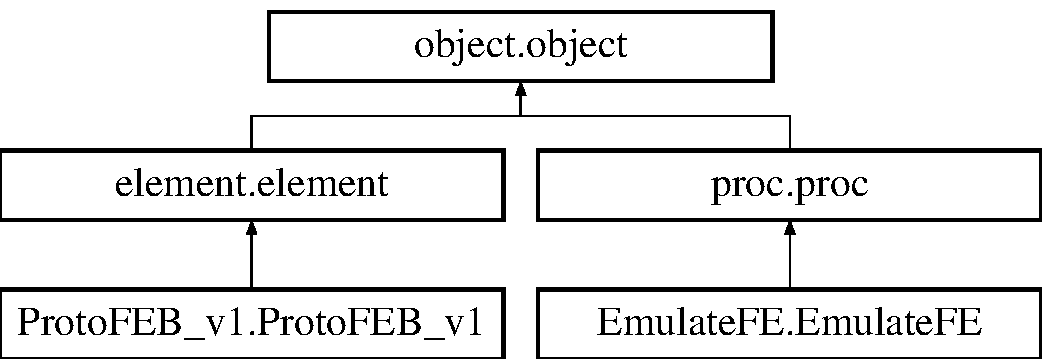
\includegraphics[height=3.000000cm]{classobject_1_1object}
\end{center}
\end{figure}
\subsection*{Public Member Functions}
\begin{DoxyCompactItemize}
\item 
def \hyperlink{classobject_1_1object_aa3f4049602209943ac20eb5c307acb4b}{\+\_\+\+\_\+init\+\_\+\+\_\+} (self, \hyperlink{classobject_1_1object_af114388a80cca208c152ffeca0e89e23}{cat}, \hyperlink{classobject_1_1object_a82b61e7cd7e18b1f9de10fc832e5b75e}{obj}, \hyperlink{classobject_1_1object_af27de160eb6fbb9c6b3723bc4ebc8fb5}{panel}, \hyperlink{classobject_1_1object_a2a518f960961d791b0f900a90c3cd287}{path})
\item 
def \hyperlink{classobject_1_1object_a54a55487254a96ed2fe367439c41391f}{get\+Control} (self, xmlid, item)
\item 
def \hyperlink{classobject_1_1object_a22a9d1ff67cd6e990cf1b63ed49c50e4}{get\+Control} (self, xmlid)
\end{DoxyCompactItemize}
\subsection*{Public Attributes}
\begin{DoxyCompactItemize}
\item 
\hyperlink{classobject_1_1object_af114388a80cca208c152ffeca0e89e23}{cat}
\item 
\hyperlink{classobject_1_1object_a82b61e7cd7e18b1f9de10fc832e5b75e}{obj}
\item 
\hyperlink{classobject_1_1object_af27de160eb6fbb9c6b3723bc4ebc8fb5}{panel}
\item 
\hyperlink{classobject_1_1object_a2a518f960961d791b0f900a90c3cd287}{path}
\end{DoxyCompactItemize}


\subsection{Detailed Description}


Definition at line 6 of file object.\+py.



\subsection{Constructor \& Destructor Documentation}
\mbox{\Hypertarget{classobject_1_1object_aa3f4049602209943ac20eb5c307acb4b}\label{classobject_1_1object_aa3f4049602209943ac20eb5c307acb4b}} 
\index{object\+::object@{object\+::object}!\+\_\+\+\_\+init\+\_\+\+\_\+@{\+\_\+\+\_\+init\+\_\+\+\_\+}}
\index{\+\_\+\+\_\+init\+\_\+\+\_\+@{\+\_\+\+\_\+init\+\_\+\+\_\+}!object\+::object@{object\+::object}}
\subsubsection{\texorpdfstring{\+\_\+\+\_\+init\+\_\+\+\_\+()}{\_\_init\_\_()}}
{\footnotesize\ttfamily def object.\+object.\+\_\+\+\_\+init\+\_\+\+\_\+ (\begin{DoxyParamCaption}\item[{}]{self,  }\item[{}]{cat,  }\item[{}]{obj,  }\item[{}]{panel,  }\item[{}]{path }\end{DoxyParamCaption})}



Definition at line 7 of file object.\+py.


\begin{DoxyCode}
7     \textcolor{keyword}{def }\hyperlink{classwrapper_1_1ModuleDictWrapper_a9a7a794150502f51df687831583e13b9}{\_\_init\_\_}(self, cat, obj, panel, path):
8         self.cat   = cat
9         self.obj   = obj
10         self.panel = panel
11         self.path  = path
12 \textcolor{comment}{#        self.type  = objtype}
13         
\end{DoxyCode}


\subsection{Member Function Documentation}
\mbox{\Hypertarget{classobject_1_1object_a54a55487254a96ed2fe367439c41391f}\label{classobject_1_1object_a54a55487254a96ed2fe367439c41391f}} 
\index{object\+::object@{object\+::object}!get\+Control@{get\+Control}}
\index{get\+Control@{get\+Control}!object\+::object@{object\+::object}}
\subsubsection{\texorpdfstring{get\+Control()}{getControl()}\hspace{0.1cm}{\footnotesize\ttfamily [1/2]}}
{\footnotesize\ttfamily def object.\+object.\+get\+Control (\begin{DoxyParamCaption}\item[{}]{self,  }\item[{}]{xmlid,  }\item[{}]{item }\end{DoxyParamCaption})}

\begin{DoxyVerb}Retrieves the given control (within a dialog) by its xmlid\end{DoxyVerb}
 

Definition at line 14 of file object.\+py.



Referenced by object.\+object.\+get\+Control(), Proto\+F\+E\+B\+\_\+v1.\+Proto\+F\+E\+B\+\_\+v1.\+is\+Ready(), Proto40\+M\+Hz\+\_\+v1.\+Proto40\+M\+Hz\+\_\+v1.\+is\+Ready(), Acquisition.\+Acquisition.\+on\+Apply(), Proto40\+M\+Hz\+\_\+v1.\+Proto40\+M\+Hz\+\_\+v1.\+onapplyaxlatency(), Proto\+F\+E\+B\+\_\+v1.\+Proto\+F\+E\+B\+\_\+v1.\+onapplyaxlatency(), Proto\+F\+E\+B\+\_\+v1.\+Proto\+F\+E\+B\+\_\+v1.\+onapplyaxlength(), Proto40\+M\+Hz\+\_\+v1.\+Proto40\+M\+Hz\+\_\+v1.\+onapplyaxlength(), Proto\+F\+E\+B\+\_\+v1.\+Proto\+F\+E\+B\+\_\+v1.\+onapply\+Ch(), Proto40\+M\+Hz\+\_\+v1.\+Proto40\+M\+Hz\+\_\+v1.\+onapply\+Ch(), Proto40\+M\+Hz\+\_\+v1.\+Proto40\+M\+Hz\+\_\+v1.\+onapplyclockdiv(), Proto\+F\+E\+B\+\_\+v1.\+Proto\+F\+E\+B\+\_\+v1.\+onapplyclockdiv(), Proto40\+M\+Hz\+\_\+v1.\+Proto40\+M\+Hz\+\_\+v1.\+onapplydelay(), Proto\+F\+E\+B\+\_\+v1.\+Proto\+F\+E\+B\+\_\+v1.\+onapplydelay(), Proto40\+M\+Hz\+\_\+v1.\+Proto40\+M\+Hz\+\_\+v1.\+onapplyfifodepth(), Proto\+F\+E\+B\+\_\+v1.\+Proto\+F\+E\+B\+\_\+v1.\+onapplyfifodepth(), Proto40\+M\+Hz\+\_\+v1.\+Proto40\+M\+Hz\+\_\+v1.\+onapplyfreq(), Proto\+F\+E\+B\+\_\+v1.\+Proto\+F\+E\+B\+\_\+v1.\+onapplyfreq(), Proto40\+M\+Hz\+\_\+v1.\+Proto40\+M\+Hz\+\_\+v1.\+onapplynumber(), Proto\+F\+E\+B\+\_\+v1.\+Proto\+F\+E\+B\+\_\+v1.\+onapplynumber(), Proto\+F\+E\+B\+\_\+v1.\+Proto\+F\+E\+B\+\_\+v1.\+onapplytrig(), Proto40\+M\+Hz\+\_\+v1.\+Proto40\+M\+Hz\+\_\+v1.\+onapplytrig(), Acquisition.\+Acquisition.\+on\+Deadtime(), Acquisition.\+Acquisition.\+on\+Depth(), Proto40\+M\+Hz\+\_\+v1.\+Proto40\+M\+Hz\+\_\+v1.\+onenable\+All(), Proto\+F\+E\+B\+\_\+v1.\+Proto\+F\+E\+B\+\_\+v1.\+onenable\+All(), Acquisition.\+Acquisition.\+on\+Max(), Acquisition.\+Acquisition.\+on\+Min(), Proto40\+M\+Hz\+\_\+v1.\+Proto40\+M\+Hz\+\_\+v1.\+on\+Mode\+A\+X(), Proto\+F\+E\+B\+\_\+v1.\+Proto\+F\+E\+B\+\_\+v1.\+on\+Mode\+A\+X(), Proto\+F\+E\+B\+\_\+v1.\+Proto\+F\+E\+B\+\_\+v1.\+on\+Mode\+Ch(), Proto40\+M\+Hz\+\_\+v1.\+Proto40\+M\+Hz\+\_\+v1.\+on\+Mode\+Ch(), Acquisition.\+Acquisition.\+on\+N\+Bins(), Acquisition.\+Acquisition.\+on\+N\+Sample(), Proto\+F\+E\+B\+\_\+v1.\+Proto\+F\+E\+B\+\_\+v1.\+on\+Pipeline(), Proto40\+M\+Hz\+\_\+v1.\+Proto40\+M\+Hz\+\_\+v1.\+on\+Pipeline(), Acquisition.\+Acquisition.\+on\+Sample(), Acquisition.\+Acquisition.\+on\+Soft\+Trig(), Proto\+F\+E\+B\+\_\+v1.\+Proto\+F\+E\+B\+\_\+v1.\+on\+Soft\+Trig(), Proto40\+M\+Hz\+\_\+v1.\+Proto40\+M\+Hz\+\_\+v1.\+on\+Soft\+Trig(), Acquisition.\+Acquisition.\+on\+Tree(), Acquisition.\+Acquisition.\+on\+Trend(), Proto40\+M\+Hz\+\_\+v1.\+Proto40\+M\+Hz\+\_\+v1.\+onunable\+All(), Proto\+F\+E\+B\+\_\+v1.\+Proto\+F\+E\+B\+\_\+v1.\+onunable\+All(), element.\+element.\+parent(), proc.\+proc.\+parent(), Acquisition.\+Acquisition.\+update(), Proto\+F\+E\+B\+\_\+v1.\+Proto\+F\+E\+B\+\_\+v1.\+update(), and Proto40\+M\+Hz\+\_\+v1.\+Proto40\+M\+Hz\+\_\+v1.\+update().


\begin{DoxyCode}
14     \textcolor{keyword}{def }getControl(self, xmlid , item) :
15         \textcolor{stringliteral}{'''Retrieves the given control (within a dialog) by its xmlid'''}
16         control = item.FindWindowById(xrc.XRCID(xmlid))
17         \textcolor{keyword}{assert} control != \textcolor{keywordtype}{None}, \textcolor{stringliteral}{'Programming error: a control with xml id '} + xmlid + \textcolor{stringliteral}{' was not found.'}
18         \textcolor{keywordflow}{return} control
19 
\end{DoxyCode}
\mbox{\Hypertarget{classobject_1_1object_a22a9d1ff67cd6e990cf1b63ed49c50e4}\label{classobject_1_1object_a22a9d1ff67cd6e990cf1b63ed49c50e4}} 
\index{object\+::object@{object\+::object}!get\+Control@{get\+Control}}
\index{get\+Control@{get\+Control}!object\+::object@{object\+::object}}
\subsubsection{\texorpdfstring{get\+Control()}{getControl()}\hspace{0.1cm}{\footnotesize\ttfamily [2/2]}}
{\footnotesize\ttfamily def object.\+object.\+get\+Control (\begin{DoxyParamCaption}\item[{}]{self,  }\item[{}]{xmlid }\end{DoxyParamCaption})}

\begin{DoxyVerb}Retrieves the given control (within a dialog) by its xmlid\end{DoxyVerb}
 

Definition at line 20 of file object.\+py.



References object.\+object.\+get\+Control(), object.\+object.\+panel, element.\+element.\+panel, Log\+Frame.\+Log\+Frame.\+panel, Conf\+Frame.\+Conf\+Frame.\+panel, Graph\+Frame.\+Graph\+Frame.\+panel, and App\+Frame.\+App\+Frame.\+panel.



Referenced by Proto40\+M\+Hz\+\_\+v1.\+Proto40\+M\+Hz\+\_\+v1.\+is\+Ready(), Acquisition.\+Acquisition.\+on\+Apply(), Proto40\+M\+Hz\+\_\+v1.\+Proto40\+M\+Hz\+\_\+v1.\+onapplyaxlatency(), Proto40\+M\+Hz\+\_\+v1.\+Proto40\+M\+Hz\+\_\+v1.\+onapplyaxlength(), Proto40\+M\+Hz\+\_\+v1.\+Proto40\+M\+Hz\+\_\+v1.\+onapply\+Ch(), Proto40\+M\+Hz\+\_\+v1.\+Proto40\+M\+Hz\+\_\+v1.\+onapplyclockdiv(), Proto40\+M\+Hz\+\_\+v1.\+Proto40\+M\+Hz\+\_\+v1.\+onapplydelay(), Proto40\+M\+Hz\+\_\+v1.\+Proto40\+M\+Hz\+\_\+v1.\+onapplyfifodepth(), Proto40\+M\+Hz\+\_\+v1.\+Proto40\+M\+Hz\+\_\+v1.\+onapplyfreq(), Proto40\+M\+Hz\+\_\+v1.\+Proto40\+M\+Hz\+\_\+v1.\+onapplynumber(), Proto40\+M\+Hz\+\_\+v1.\+Proto40\+M\+Hz\+\_\+v1.\+onapplytrig(), Acquisition.\+Acquisition.\+on\+Deadtime(), Acquisition.\+Acquisition.\+on\+Depth(), Proto40\+M\+Hz\+\_\+v1.\+Proto40\+M\+Hz\+\_\+v1.\+onenable\+All(), Acquisition.\+Acquisition.\+on\+Max(), Acquisition.\+Acquisition.\+on\+Min(), Proto40\+M\+Hz\+\_\+v1.\+Proto40\+M\+Hz\+\_\+v1.\+on\+Mode\+A\+X(), Proto40\+M\+Hz\+\_\+v1.\+Proto40\+M\+Hz\+\_\+v1.\+on\+Mode\+Ch(), Acquisition.\+Acquisition.\+on\+N\+Bins(), Acquisition.\+Acquisition.\+on\+N\+Sample(), Proto40\+M\+Hz\+\_\+v1.\+Proto40\+M\+Hz\+\_\+v1.\+on\+Pipeline(), Acquisition.\+Acquisition.\+on\+Sample(), Acquisition.\+Acquisition.\+on\+Soft\+Trig(), Proto40\+M\+Hz\+\_\+v1.\+Proto40\+M\+Hz\+\_\+v1.\+on\+Soft\+Trig(), Acquisition.\+Acquisition.\+on\+Tree(), Acquisition.\+Acquisition.\+on\+Trend(), Proto40\+M\+Hz\+\_\+v1.\+Proto40\+M\+Hz\+\_\+v1.\+onunable\+All(), Acquisition.\+Acquisition.\+update(), and Proto40\+M\+Hz\+\_\+v1.\+Proto40\+M\+Hz\+\_\+v1.\+update().


\begin{DoxyCode}
20     \textcolor{keyword}{def }getControl(self, xmlid ) :
21         \textcolor{stringliteral}{'''Retrieves the given control (within a dialog) by its xmlid'''}
22         control = self.panel.FindWindowById(xrc.XRCID(xmlid))
23         \textcolor{keyword}{assert} control != \textcolor{keywordtype}{None}, \textcolor{stringliteral}{'Programming error: a control with xml id '} + xmlid + \textcolor{stringliteral}{' was not found.'}
24         \textcolor{keywordflow}{return} control
25 
26                 
27 \textcolor{comment}{#----------------------------------------------------------------------}
28 
29     
30 \end{DoxyCode}


\subsection{Member Data Documentation}
\mbox{\Hypertarget{classobject_1_1object_af114388a80cca208c152ffeca0e89e23}\label{classobject_1_1object_af114388a80cca208c152ffeca0e89e23}} 
\index{object\+::object@{object\+::object}!cat@{cat}}
\index{cat@{cat}!object\+::object@{object\+::object}}
\subsubsection{\texorpdfstring{cat}{cat}}
{\footnotesize\ttfamily object.\+object.\+cat}



Definition at line 8 of file object.\+py.



Referenced by wrapper.\+wrapper.\+Load\+From\+File().

\mbox{\Hypertarget{classobject_1_1object_a82b61e7cd7e18b1f9de10fc832e5b75e}\label{classobject_1_1object_a82b61e7cd7e18b1f9de10fc832e5b75e}} 
\index{object\+::object@{object\+::object}!obj@{obj}}
\index{obj@{obj}!object\+::object@{object\+::object}}
\subsubsection{\texorpdfstring{obj}{obj}}
{\footnotesize\ttfamily object.\+object.\+obj}



Definition at line 9 of file object.\+py.



Referenced by Proto40\+M\+Hz\+\_\+v1.\+Proto40\+M\+Hz\+\_\+v1.\+is\+Ready(), Proto\+F\+E\+B\+\_\+v1.\+Proto\+F\+E\+B\+\_\+v1.\+is\+Ready(), element.\+element.\+loadxrc(), proc.\+proc.\+loadxrc(), Proto40\+M\+Hz\+\_\+v1.\+Proto40\+M\+Hz\+\_\+v1.\+on\+Acquisition(), Proto\+F\+E\+B\+\_\+v1.\+Proto\+F\+E\+B\+\_\+v1.\+on\+Acquisition(), Proto\+F\+E\+B\+\_\+v1.\+Proto\+F\+E\+B\+\_\+v1.\+on\+Acquisition\+Reset(), Proto40\+M\+Hz\+\_\+v1.\+Proto40\+M\+Hz\+\_\+v1.\+on\+Acquisition\+Reset(), Test\+I2\+C.\+Test\+I2\+C.\+on\+Apply(), Test\+S\+P\+I.\+Test\+S\+P\+I.\+on\+Apply(), Test\+U\+S\+B.\+Test\+U\+S\+B.\+on\+Apply(), Storage\+Fifo\+Acquisition.\+Storage\+Fifo\+Acquisition.\+on\+Apply(), Storage\+Fifo.\+Storage\+Fifo.\+on\+Apply(), Test\+Suite.\+Test\+Suite.\+on\+Apply(), A\+D\+C\+Measurement.\+Current\+Measurement.\+on\+Apply(), Current\+Measurement.\+Current\+Measurement.\+on\+Apply(), Usb\+F\+T\+Interface\+Test.\+Usb\+F\+T\+Interface\+Test.\+on\+Apply(), Acquisition.\+Acquisition.\+on\+Apply(), Proto40\+M\+Hz\+\_\+v1.\+Proto40\+M\+Hz\+\_\+v1.\+onapplyaxlatency(), Proto\+F\+E\+B\+\_\+v1.\+Proto\+F\+E\+B\+\_\+v1.\+onapplyaxlatency(), Proto40\+M\+Hz\+\_\+v1.\+Proto40\+M\+Hz\+\_\+v1.\+onapplyaxlength(), Proto\+F\+E\+B\+\_\+v1.\+Proto\+F\+E\+B\+\_\+v1.\+onapplyaxlength(), Proto\+F\+E\+B\+\_\+v1.\+Proto\+F\+E\+B\+\_\+v1.\+onapply\+Ch(), Proto40\+M\+Hz\+\_\+v1.\+Proto40\+M\+Hz\+\_\+v1.\+onapply\+Ch(), Proto\+F\+E\+B\+\_\+v1.\+Proto\+F\+E\+B\+\_\+v1.\+onapplyclockdiv(), Proto40\+M\+Hz\+\_\+v1.\+Proto40\+M\+Hz\+\_\+v1.\+onapplyclockdiv(), Proto40\+M\+Hz\+\_\+v1.\+Proto40\+M\+Hz\+\_\+v1.\+onapplydelay(), Proto\+F\+E\+B\+\_\+v1.\+Proto\+F\+E\+B\+\_\+v1.\+onapplydelay(), Proto40\+M\+Hz\+\_\+v1.\+Proto40\+M\+Hz\+\_\+v1.\+onapplyfifodepth(), Proto\+F\+E\+B\+\_\+v1.\+Proto\+F\+E\+B\+\_\+v1.\+onapplyfifodepth(), Proto40\+M\+Hz\+\_\+v1.\+Proto40\+M\+Hz\+\_\+v1.\+onapplyfreq(), Proto\+F\+E\+B\+\_\+v1.\+Proto\+F\+E\+B\+\_\+v1.\+onapplyfreq(), Proto40\+M\+Hz\+\_\+v1.\+Proto40\+M\+Hz\+\_\+v1.\+onapplynumber(), Proto\+F\+E\+B\+\_\+v1.\+Proto\+F\+E\+B\+\_\+v1.\+onapplynumber(), Proto40\+M\+Hz\+\_\+v1.\+Proto40\+M\+Hz\+\_\+v1.\+onapplytrig(), Proto\+F\+E\+B\+\_\+v1.\+Proto\+F\+E\+B\+\_\+v1.\+onapplytrig(), Acquisition.\+Acquisition.\+on\+Deadtime(), Acquisition.\+Acquisition.\+on\+Depth(), Proto40\+M\+Hz\+\_\+v1.\+Proto40\+M\+Hz\+\_\+v1.\+on\+Enable\+Storage(), Proto\+F\+E\+B\+\_\+v1.\+Proto\+F\+E\+B\+\_\+v1.\+on\+Enable\+Storage(), Proto\+F\+E\+B\+\_\+v1.\+Proto\+F\+E\+B\+\_\+v1.\+on\+Fifo\+R\+A\+Z(), Proto40\+M\+Hz\+\_\+v1.\+Proto40\+M\+Hz\+\_\+v1.\+on\+Fifo\+R\+A\+Z(), Proto40\+M\+Hz\+\_\+v1.\+Proto40\+M\+Hz\+\_\+v1.\+on\+Fifo\+Reset(), Proto\+F\+E\+B\+\_\+v1.\+Proto\+F\+E\+B\+\_\+v1.\+on\+Fifo\+Reset(), Proto\+F\+E\+B\+\_\+v1.\+Proto\+F\+E\+B\+\_\+v1.\+on\+Fifo\+Write(), Proto40\+M\+Hz\+\_\+v1.\+Proto40\+M\+Hz\+\_\+v1.\+on\+Fifo\+Write(), Proto40\+M\+Hz\+\_\+v1.\+Proto40\+M\+Hz\+\_\+v1.\+on\+From\+A\+X\+Ptr\+Raz(), Proto\+F\+E\+B\+\_\+v1.\+Proto\+F\+E\+B\+\_\+v1.\+on\+From\+A\+X\+Ptr\+Raz(), Proto\+F\+E\+B\+\_\+v1.\+Proto\+F\+E\+B\+\_\+v1.\+on\+From\+A\+X\+R\+A\+Z(), Proto40\+M\+Hz\+\_\+v1.\+Proto40\+M\+Hz\+\_\+v1.\+on\+From\+A\+X\+R\+A\+Z(), Proto\+F\+E\+B\+\_\+v1.\+Proto\+F\+E\+B\+\_\+v1.\+on\+From\+A\+X\+Write(), Proto40\+M\+Hz\+\_\+v1.\+Proto40\+M\+Hz\+\_\+v1.\+on\+From\+A\+X\+Write(), Proto40\+M\+Hz\+\_\+v1.\+Proto40\+M\+Hz\+\_\+v1.\+on\+Global\+Reset(), Proto\+F\+E\+B\+\_\+v1.\+Proto\+F\+E\+B\+\_\+v1.\+on\+Global\+Reset(), Proto\+F\+E\+B\+\_\+v1.\+Proto\+F\+E\+B\+\_\+v1.\+on\+Latency\+Reset(), Proto40\+M\+Hz\+\_\+v1.\+Proto40\+M\+Hz\+\_\+v1.\+on\+Latency\+Reset(), Acquisition.\+Acquisition.\+on\+Max(), Acquisition.\+Acquisition.\+on\+Min(), Proto40\+M\+Hz\+\_\+v1.\+Proto40\+M\+Hz\+\_\+v1.\+on\+Mode\+A\+X(), Proto\+F\+E\+B\+\_\+v1.\+Proto\+F\+E\+B\+\_\+v1.\+on\+Mode\+A\+X(), Proto40\+M\+Hz\+\_\+v1.\+Proto40\+M\+Hz\+\_\+v1.\+on\+Mode\+Ch(), Proto\+F\+E\+B\+\_\+v1.\+Proto\+F\+E\+B\+\_\+v1.\+on\+Mode\+Ch(), Acquisition.\+Acquisition.\+on\+N\+Bins(), Acquisition.\+Acquisition.\+on\+N\+Sample(), Proto\+F\+E\+B\+\_\+v1.\+Proto\+F\+E\+B\+\_\+v1.\+on\+Pattern\+R\+A\+Z(), Proto40\+M\+Hz\+\_\+v1.\+Proto40\+M\+Hz\+\_\+v1.\+on\+Pattern\+R\+A\+Z(), Proto\+F\+E\+B\+\_\+v1.\+Proto\+F\+E\+B\+\_\+v1.\+on\+Pattern\+Write(), Proto40\+M\+Hz\+\_\+v1.\+Proto40\+M\+Hz\+\_\+v1.\+on\+Pattern\+Write(), Proto40\+M\+Hz\+\_\+v1.\+Proto40\+M\+Hz\+\_\+v1.\+on\+Phaser0(), Proto\+F\+E\+B\+\_\+v1.\+Proto\+F\+E\+B\+\_\+v1.\+on\+Phaser0(), Proto40\+M\+Hz\+\_\+v1.\+Proto40\+M\+Hz\+\_\+v1.\+on\+Phaser1(), Proto\+F\+E\+B\+\_\+v1.\+Proto\+F\+E\+B\+\_\+v1.\+on\+Phaser1(), Proto40\+M\+Hz\+\_\+v1.\+Proto40\+M\+Hz\+\_\+v1.\+on\+Phaser2(), Proto\+F\+E\+B\+\_\+v1.\+Proto\+F\+E\+B\+\_\+v1.\+on\+Phaser2(), Proto40\+M\+Hz\+\_\+v1.\+Proto40\+M\+Hz\+\_\+v1.\+on\+Pipeline(), Proto\+F\+E\+B\+\_\+v1.\+Proto\+F\+E\+B\+\_\+v1.\+on\+Pipeline(), Proto40\+M\+Hz\+\_\+v1.\+Proto40\+M\+Hz\+\_\+v1.\+on\+Read\+Fifo(), Proto\+F\+E\+B\+\_\+v1.\+Proto\+F\+E\+B\+\_\+v1.\+on\+Read\+Fifo(), Proto40\+M\+Hz\+\_\+v1.\+Proto40\+M\+Hz\+\_\+v1.\+on\+Read\+From\+A\+X(), Proto\+F\+E\+B\+\_\+v1.\+Proto\+F\+E\+B\+\_\+v1.\+on\+Read\+From\+A\+X(), Proto\+F\+E\+B\+\_\+v1.\+Proto\+F\+E\+B\+\_\+v1.\+on\+Read\+Pattern(), Proto40\+M\+Hz\+\_\+v1.\+Proto40\+M\+Hz\+\_\+v1.\+on\+Read\+Pattern(), Proto40\+M\+Hz\+\_\+v1.\+Proto40\+M\+Hz\+\_\+v1.\+on\+Read\+To\+A\+X(), Proto\+F\+E\+B\+\_\+v1.\+Proto\+F\+E\+B\+\_\+v1.\+on\+Read\+To\+A\+X(), Proto40\+M\+Hz\+\_\+v1.\+Proto40\+M\+Hz\+\_\+v1.\+on\+Read\+Trigger(), Proto\+F\+E\+B\+\_\+v1.\+Proto\+F\+E\+B\+\_\+v1.\+on\+Read\+Trigger(), Proto40\+M\+Hz\+\_\+v1.\+Proto40\+M\+Hz\+\_\+v1.\+on\+Reset\+F\+E(), Proto\+F\+E\+B\+\_\+v1.\+Proto\+F\+E\+B\+\_\+v1.\+on\+Reset\+F\+E(), Proto\+F\+E\+B\+\_\+v1.\+Proto\+F\+E\+B\+\_\+v1.\+on\+Reset\+S\+P\+I(), Proto40\+M\+Hz\+\_\+v1.\+Proto40\+M\+Hz\+\_\+v1.\+on\+Reset\+S\+P\+I(), Acquisition.\+Acquisition.\+on\+Sample(), Acquisition.\+Acquisition.\+on\+Soft\+Trig(), Proto\+F\+E\+B\+\_\+v1.\+Proto\+F\+E\+B\+\_\+v1.\+on\+Soft\+Trig(), Proto40\+M\+Hz\+\_\+v1.\+Proto40\+M\+Hz\+\_\+v1.\+on\+Soft\+Trig(), Proto40\+M\+Hz\+\_\+v1.\+Proto40\+M\+Hz\+\_\+v1.\+on\+Start\+Sequence\+A\+X(), Proto\+F\+E\+B\+\_\+v1.\+Proto\+F\+E\+B\+\_\+v1.\+on\+Start\+Sequence\+A\+X(), Proto\+F\+E\+B\+\_\+v1.\+Proto\+F\+E\+B\+\_\+v1.\+on\+To\+A\+X\+Ptr\+Raz(), Proto40\+M\+Hz\+\_\+v1.\+Proto40\+M\+Hz\+\_\+v1.\+on\+To\+A\+X\+Ptr\+Raz(), Proto\+F\+E\+B\+\_\+v1.\+Proto\+F\+E\+B\+\_\+v1.\+on\+To\+A\+X\+R\+A\+Z(), Proto40\+M\+Hz\+\_\+v1.\+Proto40\+M\+Hz\+\_\+v1.\+on\+To\+A\+X\+R\+A\+Z(), Proto\+F\+E\+B\+\_\+v1.\+Proto\+F\+E\+B\+\_\+v1.\+on\+To\+A\+X\+Write(), Proto40\+M\+Hz\+\_\+v1.\+Proto40\+M\+Hz\+\_\+v1.\+on\+To\+A\+X\+Write(), Acquisition.\+Acquisition.\+on\+Tree(), Acquisition.\+Acquisition.\+on\+Trend(), Proto\+F\+E\+B\+\_\+v1.\+Proto\+F\+E\+B\+\_\+v1.\+on\+Trigger(), Proto40\+M\+Hz\+\_\+v1.\+Proto40\+M\+Hz\+\_\+v1.\+on\+Trigger(), Proto40\+M\+Hz\+\_\+v1.\+Proto40\+M\+Hz\+\_\+v1.\+on\+Trigger\+R\+A\+Z(), Proto\+F\+E\+B\+\_\+v1.\+Proto\+F\+E\+B\+\_\+v1.\+on\+Trigger\+R\+A\+Z(), Proto\+F\+E\+B\+\_\+v1.\+Proto\+F\+E\+B\+\_\+v1.\+on\+Trigger\+Write(), Proto40\+M\+Hz\+\_\+v1.\+Proto40\+M\+Hz\+\_\+v1.\+on\+Trigger\+Write(), Proto40\+M\+Hz\+\_\+v1.\+Proto40\+M\+Hz\+\_\+v1.\+on\+Usb\+Phasers\+Reset(), Proto\+F\+E\+B\+\_\+v1.\+Proto\+F\+E\+B\+\_\+v1.\+on\+Usb\+Phasers\+Reset(), Test\+U\+S\+B.\+Test\+U\+S\+B.\+update(), Test\+S\+P\+I.\+Test\+S\+P\+I.\+update(), Test\+I2\+C.\+Test\+I2\+C.\+update(), Storage\+Fifo.\+Storage\+Fifo.\+update(), Test\+Suite.\+Test\+Suite.\+update(), Storage\+Fifo\+Acquisition.\+Storage\+Fifo\+Acquisition.\+update(), A\+D\+C\+Measurement.\+Current\+Measurement.\+update(), Current\+Measurement.\+Current\+Measurement.\+update(), Usb\+F\+T\+Interface\+Test.\+Usb\+F\+T\+Interface\+Test.\+update(), Acquisition.\+Acquisition.\+update(), Proto\+F\+E\+B\+\_\+v1.\+Proto\+F\+E\+B\+\_\+v1.\+update(), and Proto40\+M\+Hz\+\_\+v1.\+Proto40\+M\+Hz\+\_\+v1.\+update().

\mbox{\Hypertarget{classobject_1_1object_af27de160eb6fbb9c6b3723bc4ebc8fb5}\label{classobject_1_1object_af27de160eb6fbb9c6b3723bc4ebc8fb5}} 
\index{object\+::object@{object\+::object}!panel@{panel}}
\index{panel@{panel}!object\+::object@{object\+::object}}
\subsubsection{\texorpdfstring{panel}{panel}}
{\footnotesize\ttfamily object.\+object.\+panel}



Definition at line 10 of file object.\+py.



Referenced by A3\+P\+E\+\_\+\+Bit\+Flip.\+A3\+P\+E\+\_\+\+Bit\+Flip.\+\_\+\+\_\+init\+\_\+\+\_\+(), Emulate\+F\+E.\+Emulate\+F\+E.\+\_\+\+\_\+init\+\_\+\+\_\+(), Acquisition.\+Acquisition.\+\_\+\+\_\+init\+\_\+\+\_\+(), object.\+object.\+get\+Control(), Proto40\+M\+Hz\+\_\+v1.\+Proto40\+M\+Hz\+\_\+v1.\+get\+File(), and proc.\+proc.\+page().

\mbox{\Hypertarget{classobject_1_1object_a2a518f960961d791b0f900a90c3cd287}\label{classobject_1_1object_a2a518f960961d791b0f900a90c3cd287}} 
\index{object\+::object@{object\+::object}!path@{path}}
\index{path@{path}!object\+::object@{object\+::object}}
\subsubsection{\texorpdfstring{path}{path}}
{\footnotesize\ttfamily object.\+object.\+path}



Definition at line 11 of file object.\+py.



Referenced by element.\+element.\+loadxrc(), and proc.\+proc.\+loadxrc().



The documentation for this class was generated from the following file\+:\begin{DoxyCompactItemize}
\item 
/home/eleclhcb/\+L\+H\+Cb/lbcat-\/cmake/\+Cat\+Python/python/\hyperlink{object_8py}{object.\+py}\end{DoxyCompactItemize}

\hypertarget{classOptions}{}\section{Options Class Reference}
\label{classOptions}\index{Options@{Options}}


{\ttfamily \#include $<$Options.\+h$>$}

\subsection*{Public Member Functions}
\begin{DoxyCompactItemize}
\item 
\hyperlink{classOptions_ab72fb640172a6109e34c8a5366563753}{Options} ()
\item 
\hyperlink{classOptions_a86ddb85b183f8b58af5481f30a42fa92}{$\sim$\+Options} ()
\item 
void \hyperlink{classOptions_a5d8ab053c941a944a53c0bfe871058a1}{set\+Log\+Output\+Level} (\hyperlink{classMsgSvc_ae671eb7301996cd049d2da8a65925926}{Msg\+Svc\+::\+Msg\+Level} \hyperlink{classOptions_a2d11716f34070dd7991648a26eb5d244}{log\+Output\+Level})
\item 
\hyperlink{classMsgSvc_ae671eb7301996cd049d2da8a65925926}{Msg\+Svc\+::\+Msg\+Level} \hyperlink{classOptions_a2d11716f34070dd7991648a26eb5d244}{log\+Output\+Level} ()
\item 
void \hyperlink{classOptions_adac15a8dbae0183ae7cecc09ebba6887}{set\+Print\+Freq} (unsigned long \hyperlink{classOptions_a67021ffef9f666bba4696f89807b2a70}{print\+Freq})
\item 
unsigned long \hyperlink{classOptions_a67021ffef9f666bba4696f89807b2a70}{print\+Freq} ()
\item 
void \hyperlink{classOptions_a7df298047f1506fa2244cf096da96409}{set\+Plot\+Freq} (unsigned long \hyperlink{classOptions_a1e20abb20c1a2187f9455b39cd9d26ae}{plot\+Freq})
\item 
unsigned long \hyperlink{classOptions_a1e20abb20c1a2187f9455b39cd9d26ae}{plot\+Freq} ()
\item 
void \hyperlink{classOptions_a0d362af154c7d2e30a7bf340eb061fa5}{set\+Stop\+On\+Error} (bool \hyperlink{classOptions_afcd7b27fdf474050d912571e09525efe}{stop\+On\+Error})
\item 
bool \hyperlink{classOptions_afcd7b27fdf474050d912571e09525efe}{stop\+On\+Error} ()
\item 
void \hyperlink{classOptions_aed19a55eb2c418f333bc97615cf4a3a8}{set\+Run\+Number} (unsigned long \hyperlink{classOptions_a2d9447919fe90f9ce8df5530526cbb27}{run\+Number})
\item 
unsigned long \hyperlink{classOptions_a2d9447919fe90f9ce8df5530526cbb27}{run\+Number} ()
\item 
void \hyperlink{classOptions_a7bf3fb2833021f8900eb105b0a9c02c5}{set\+Run\+Number\+Management} (bool \hyperlink{classOptions_a7654a2c3d67baae08f61edc18bec367e}{run\+Number\+Management})
\item 
bool \hyperlink{classOptions_a7654a2c3d67baae08f61edc18bec367e}{run\+Number\+Management} ()
\item 
void \hyperlink{classOptions_a3cebd8308183414ef2e0de0e7922c87a}{set\+Current\+Path} (std\+::string \hyperlink{classOptions_ab9cf7442a712fe8593f6cf5cfff36a5d}{current\+Path})
\item 
std\+::string \hyperlink{classOptions_ab9cf7442a712fe8593f6cf5cfff36a5d}{current\+Path} ()
\item 
void \hyperlink{classOptions_a8c32e222956c77ed2ec5387318f91394}{set\+Storage\+Path} (std\+::string \hyperlink{classOptions_a3992b9247441a3e60e55c8c5fe32b394}{storage\+Path})
\item 
std\+::string \hyperlink{classOptions_a3992b9247441a3e60e55c8c5fe32b394}{storage\+Path} ()
\item 
std\+::string \hyperlink{classOptions_aa5fe6b85088f3012226869480790a383}{storage\+Full\+Path} ()
\item 
void \hyperlink{classOptions_aed5e6919526bcfa5cf4961230bd20e37}{set\+Storage\+Dir} (std\+::string filename)
\item 
std\+::string \hyperlink{classOptions_a5e8026ed2674f8f5db444b52fea27fda}{storage\+Dir} ()
\item 
void \hyperlink{classOptions_ac163281337998af5ca3b7a9617337fef}{set\+Storage\+File} (std\+::string filename=std\+::string(\char`\"{}\char`\"{}))
\item 
std\+::string \hyperlink{classOptions_a6661fe4edd501f7e97527b8f9354ef84}{storage\+File} ()
\item 
std\+::string \hyperlink{classOptions_a68c501133588cd4b1c80219adb926e8d}{storage\+File\+Full\+Name} ()
\item 
std\+::string \hyperlink{classOptions_ab1cd9f237e9c18fd72323c74565453f8}{data\+File\+Full\+Name} ()
\item 
std\+::string \hyperlink{classOptions_a166984c16a957bf2e8e0f0a1ce39eb73}{data\+File} ()
\item 
std\+::string \hyperlink{classOptions_a739a9b788fc937ad55d10d6b47ff1e8c}{log\+File} ()
\item 
void \hyperlink{classOptions_ae6f39f4b0b4bd260fbb5a2f0b5f4786e}{set\+Data\+Storage} (bool \hyperlink{classOptions_aed7799d10139fa542055b982cb820192}{data\+Storage})
\item 
bool \hyperlink{classOptions_aed7799d10139fa542055b982cb820192}{data\+Storage} ()
\item 
void \hyperlink{classOptions_a96f0288f5317cf371589f4db07e913b0}{set\+Log\+Storage} (bool \hyperlink{classOptions_a33735fffe17485937ab7579d8716b7ee}{log\+Storage})
\item 
bool \hyperlink{classOptions_a33735fffe17485937ab7579d8716b7ee}{log\+Storage} ()
\item 
void \hyperlink{classOptions_a52e2995912a71f51c230dd6bf28b6a94}{set\+Log\+Def\+File} (std\+::string \hyperlink{classOptions_aca5ce5262ca717eaad5ff9db92ad1948}{def\+File})
\item 
std\+::string \hyperlink{classOptions_a5d362ec7f7969bd72c3c94b8e3d5ba97}{log\+Def\+File} ()
\item 
void \hyperlink{classOptions_a3c8bed9867ac5805489d78061e55bd1a}{set\+Def\+File} (std\+::string def)
\item 
std\+::string \hyperlink{classOptions_aca5ce5262ca717eaad5ff9db92ad1948}{def\+File} ()
\item 
void \hyperlink{classOptions_ae6a0fdaa736948f5040deb3eb6889268}{set\+N\+Evt} (unsigned long \hyperlink{classOptions_ad769b256263a4ac24dd6f989ae724ab7}{n\+Evt})
\item 
unsigned long \hyperlink{classOptions_ad769b256263a4ac24dd6f989ae724ab7}{n\+Evt} ()
\item 
void \hyperlink{classOptions_a6d732c0591188469287581bac8a4e3cd}{set\+N\+Evt\+Max} (int \hyperlink{classOptions_ad1f3b03d734c806a2feca418b26bcc9b}{n\+Evt\+Max})
\item 
int \hyperlink{classOptions_ad1f3b03d734c806a2feca418b26bcc9b}{n\+Evt\+Max} ()
\item 
void \hyperlink{classOptions_aaa921f68319ea83b5c5a13e37a831c7a}{set\+Time\+Max} (unsigned long \hyperlink{classOptions_a4569b8790af48109c8639bec7b626fa6}{time\+Max})
\item 
unsigned long \hyperlink{classOptions_a4569b8790af48109c8639bec7b626fa6}{time\+Max} ()
\item 
void \hyperlink{classOptions_a45368b495036869c67fe0e6bf9abc4e6}{set\+N\+Errors} (unsigned long \hyperlink{classOptions_acc6474323f0bbe17fa844e9a086b90b8}{n\+Errors})
\item 
unsigned long \hyperlink{classOptions_acc6474323f0bbe17fa844e9a086b90b8}{n\+Errors} ()
\item 
void \hyperlink{classOptions_a0bf512fc9126cd76acabaa4c3b65d7fb}{inc\+Run\+Number} ()
\item 
void \hyperlink{classOptions_aa950f9861182c76c4005668e0b7f012a}{inc\+N\+Evt} ()
\item 
void \hyperlink{classOptions_ae5d12fb2571255033ef6b35300921b39}{inc\+N\+Errors} ()
\item 
std\+::ofstream $\ast$ \hyperlink{classOptions_acfc9aa4c7dc41691571f2b37d3fe86af}{stream} ()
\item 
void \hyperlink{classOptions_af7df7a64e597f0bed79ca979f8144daa}{set\+Stream} (std\+::string file=std\+::string(\char`\"{}\char`\"{}))
\item 
void \hyperlink{classOptions_a3f4593f64bc8c8afc3ade9237adb83e1}{print} ()
\end{DoxyCompactItemize}
\subsection*{Private Attributes}
\begin{DoxyCompactItemize}
\item 
\hyperlink{classMsgSvc}{Msg\+Svc} \hyperlink{classOptions_a80d2caed71dd935c104f0133504251e9}{m\+\_\+log}
\item 
\hyperlink{classMsgSvc_ae671eb7301996cd049d2da8a65925926}{Msg\+Svc\+::\+Msg\+Level} \hyperlink{classOptions_a9ecfefe6bf44ff519369f38eb5c8147a}{m\+\_\+log\+Output\+Level}
\item 
std\+::string \hyperlink{classOptions_a9d82ad17fc1fd2315fc8a9e8d0d34f33}{m\+\_\+current\+Path}
\item 
bool \hyperlink{classOptions_a244898bb30c9f716bdc335b4d85d1dfb}{m\+\_\+data\+Storage}
\item 
bool \hyperlink{classOptions_ab7ffad5110df714233470725ef98be6e}{m\+\_\+log\+Storage}
\item 
std\+::string \hyperlink{classOptions_a88d9ed92fceb1c91e4df59bc1f81ab3b}{m\+\_\+storage\+Dir}
\item 
std\+::string \hyperlink{classOptions_a4d952db4e93d3aae6db86d89faa3677a}{m\+\_\+storage\+File}
\item 
std\+::string \hyperlink{classOptions_ab077e872fd03f7bf64f3a354d0c4a2f5}{m\+\_\+storage\+Default}
\item 
std\+::string \hyperlink{classOptions_ad125e827cb30bc9b63875ec45b31ef5e}{m\+\_\+storage\+Path}
\item 
std\+::string \hyperlink{classOptions_a59ff5f2cab2490fb529367de13a2321a}{m\+\_\+def\+File}
\item 
bool \hyperlink{classOptions_a879c2741a290595adb3f74633f3a3987}{m\+\_\+stop\+On\+Error}
\item 
unsigned long \hyperlink{classOptions_a5e3bb1f2dfc4bf10cab08a33253cc4db}{m\+\_\+n\+Evt}
\item 
unsigned long \hyperlink{classOptions_ae6460776ac3433103d88729a6811fc56}{m\+\_\+n\+Errors}
\item 
unsigned long \hyperlink{classOptions_acf8f96cbc3245ec4b3b47bd3bfa0d742}{m\+\_\+print\+Freq}
\item 
unsigned long \hyperlink{classOptions_aa7f7161bc67732b310937afb137657a0}{m\+\_\+plot\+Freq}
\item 
int \hyperlink{classOptions_a825a47258257937a8caa902f5fff7e8a}{m\+\_\+n\+Evt\+Max}
\item 
int \hyperlink{classOptions_a2584abb6745a082f73e2917732cd00e1}{m\+\_\+time\+Max}
\item 
unsigned long \hyperlink{classOptions_a1762c644c5f87feabe12f84f17a1a351}{m\+\_\+run\+Number}
\item 
bool \hyperlink{classOptions_a2ad2d67b98fc5fbea4cbbd781ccb6183}{m\+\_\+run\+Number\+Management}
\item 
bool \hyperlink{classOptions_ae4461f1dd3357c0478098fc32e809405}{m\+\_\+batch}
\item 
std\+::ofstream $\ast$ \hyperlink{classOptions_a8c5485cd614fa90de6b1aa85a7d2191b}{m\+\_\+stream}
\item 
std\+::ofstream $\ast$ \hyperlink{classOptions_a65c3a025880fb38373b599b87d600eef}{m\+\_\+log\+Stream}
\item 
std\+::ofstream $\ast$ \hyperlink{classOptions_aebb2db3fb07ea1f73b27bde841be69d8}{m\+\_\+log\+Def\+Stream}
\item 
std\+::string \hyperlink{classOptions_abaef6cdcc8422b199084510d173edbe6}{m\+\_\+log\+Def\+File}
\end{DoxyCompactItemize}


\subsection{Detailed Description}


Definition at line 25 of file Options.\+h.



\subsection{Constructor \& Destructor Documentation}
\mbox{\Hypertarget{classOptions_ab72fb640172a6109e34c8a5366563753}\label{classOptions_ab72fb640172a6109e34c8a5366563753}} 
\index{Options@{Options}!Options@{Options}}
\index{Options@{Options}!Options@{Options}}
\subsubsection{\texorpdfstring{Options()}{Options()}}
{\footnotesize\ttfamily Options\+::\+Options (\begin{DoxyParamCaption}{ }\end{DoxyParamCaption})}



Definition at line 19 of file Options.\+cpp.



References Msg\+Svc\+::\+I\+N\+FO, m\+\_\+log\+Def\+Stream, m\+\_\+log\+Stream, m\+\_\+storage\+Default, m\+\_\+stream, set\+Current\+Path(), set\+Data\+Storage(), set\+Log\+Def\+File(), set\+Log\+Output\+Level(), set\+Log\+Storage(), set\+N\+Errors(), set\+N\+Evt(), set\+N\+Evt\+Max(), set\+Plot\+Freq(), set\+Print\+Freq(), set\+Run\+Number(), set\+Run\+Number\+Management(), set\+Storage\+Dir(), set\+Storage\+File(), set\+Storage\+Path(), set\+Stream(), and set\+Time\+Max().


\begin{DoxyCode}
19                    \{
20   \hyperlink{classOptions_a65c3a025880fb38373b599b87d600eef}{m\_logStream}    = 0;
21   \hyperlink{classOptions_aebb2db3fb07ea1f73b27bde841be69d8}{m\_logDefStream} = 0;
22   \hyperlink{classOptions_a8c5485cd614fa90de6b1aa85a7d2191b}{m\_stream}       = 0;
23 
24   \hyperlink{classOptions_a52e2995912a71f51c230dd6bf28b6a94}{setLogDefFile}(\textcolor{stringliteral}{"session.log"});
25   \hyperlink{classOptions_af7df7a64e597f0bed79ca979f8144daa}{setStream}();
26 
27   \hyperlink{classOptions_a5d8ab053c941a944a53c0bfe871058a1}{setLogOutputLevel}( \hyperlink{classMsgSvc_ae671eb7301996cd049d2da8a65925926ad2fcf3f3e734fc41ee097cc23670ce51}{MsgSvc::INFO} );
28 
29   \hyperlink{classOptions_a6d732c0591188469287581bac8a4e3cd}{setNEvtMax}   ( 100  );
30   \hyperlink{classOptions_aaa921f68319ea83b5c5a13e37a831c7a}{setTimeMax}   ( 100  );
31   \hyperlink{classOptions_ae6a0fdaa736948f5040deb3eb6889268}{setNEvt}      ( 0    );
32   \hyperlink{classOptions_a45368b495036869c67fe0e6bf9abc4e6}{setNErrors}   ( 0    );
33   \hyperlink{classOptions_aed19a55eb2c418f333bc97615cf4a3a8}{setRunNumber} ( 0    );
34   \hyperlink{classOptions_adac15a8dbae0183ae7cecc09ebba6887}{setPrintFreq} ( 0    );
35   \hyperlink{classOptions_a7df298047f1506fa2244cf096da96409}{setPlotFreq} ( 0    );
36 
37   \hyperlink{classOptions_a7bf3fb2833021f8900eb105b0a9c02c5}{setRunNumberManagement}(\textcolor{keyword}{true});
38 
39   \hyperlink{classOptions_aed5e6919526bcfa5cf4961230bd20e37}{setStorageDir}(\textcolor{stringliteral}{"Run"});
40 
41   \hyperlink{classOptions_ab077e872fd03f7bf64f3a354d0c4a2f5}{m\_storageDefault}=std::string(\textcolor{stringliteral}{"run"});
42   \hyperlink{classOptions_ac163281337998af5ca3b7a9617337fef}{setStorageFile}();
43   \hyperlink{classOptions_ae6f39f4b0b4bd260fbb5a2f0b5f4786e}{setDataStorage} ( \textcolor{keyword}{false} );
44   \hyperlink{classOptions_a96f0288f5317cf371589f4db07e913b0}{setLogStorage}  ( \textcolor{keyword}{false} );
45 
46 \textcolor{preprocessor}{#ifdef WIN32
}
47   \textcolor{keywordtype}{char} buffer[\_MAX\_PATH];
48   getcwd(buffer,\_MAX\_PATH);
49   \hyperlink{classOptions_a8c32e222956c77ed2ec5387318f91394}{setStoragePath}( std::string(buffer) );
50 \textcolor{preprocessor}{#else
}
51   \textcolor{keywordtype}{char} buffer[256];
52   getcwd(buffer,256);
53   \hyperlink{classOptions_a8c32e222956c77ed2ec5387318f91394}{setStoragePath}( std::string(buffer)+std::string(\textcolor{stringliteral}{"/data"}) );
54 \textcolor{preprocessor}{#endif
}
55 
56   \hyperlink{classOptions_a3cebd8308183414ef2e0de0e7922c87a}{setCurrentPath}( std::string(buffer) );
57 
58 \}
\end{DoxyCode}
\mbox{\Hypertarget{classOptions_a86ddb85b183f8b58af5481f30a42fa92}\label{classOptions_a86ddb85b183f8b58af5481f30a42fa92}} 
\index{Options@{Options}!````~Options@{$\sim$\+Options}}
\index{````~Options@{$\sim$\+Options}!Options@{Options}}
\subsubsection{\texorpdfstring{$\sim$\+Options()}{~Options()}}
{\footnotesize\ttfamily Options\+::$\sim$\+Options (\begin{DoxyParamCaption}{ }\end{DoxyParamCaption})}



Definition at line 63 of file Options.\+cpp.



References m\+\_\+log\+Def\+Stream.


\begin{DoxyCode}
63                   \{
64   \textcolor{keywordflow}{if} ( 0!=\hyperlink{classOptions_aebb2db3fb07ea1f73b27bde841be69d8}{m\_logDefStream})\{
65     \hyperlink{classOptions_aebb2db3fb07ea1f73b27bde841be69d8}{m\_logDefStream}->close();
66     \textcolor{keyword}{delete} \hyperlink{classOptions_aebb2db3fb07ea1f73b27bde841be69d8}{m\_logDefStream};
67     \hyperlink{classOptions_aebb2db3fb07ea1f73b27bde841be69d8}{m\_logDefStream}=0;
68   \}
69 \}
\end{DoxyCode}


\subsection{Member Function Documentation}
\mbox{\Hypertarget{classOptions_ab9cf7442a712fe8593f6cf5cfff36a5d}\label{classOptions_ab9cf7442a712fe8593f6cf5cfff36a5d}} 
\index{Options@{Options}!current\+Path@{current\+Path}}
\index{current\+Path@{current\+Path}!Options@{Options}}
\subsubsection{\texorpdfstring{current\+Path()}{currentPath()}}
{\footnotesize\ttfamily std\+::string Options\+::current\+Path (\begin{DoxyParamCaption}{ }\end{DoxyParamCaption})\hspace{0.3cm}{\ttfamily [inline]}}

Get accessor to member m\+\_\+current\+Path \begin{DoxyReturn}{Returns}
the current value of m\+\_\+current\+Path 
\end{DoxyReturn}


Definition at line 135 of file Options.\+h.



References m\+\_\+current\+Path.



Referenced by export\+\_\+base(), and set\+Current\+Path().


\begin{DoxyCode}
135                                  \{
136                 \textcolor{keywordflow}{return} \hyperlink{classOptions_a9d82ad17fc1fd2315fc8a9e8d0d34f33}{m\_currentPath};
137         \}
\end{DoxyCode}
\mbox{\Hypertarget{classOptions_a166984c16a957bf2e8e0f0a1ce39eb73}\label{classOptions_a166984c16a957bf2e8e0f0a1ce39eb73}} 
\index{Options@{Options}!data\+File@{data\+File}}
\index{data\+File@{data\+File}!Options@{Options}}
\subsubsection{\texorpdfstring{data\+File()}{dataFile()}}
{\footnotesize\ttfamily std\+::string Options\+::data\+File (\begin{DoxyParamCaption}{ }\end{DoxyParamCaption})}

Get accessor to member m\+\_\+data\+File \begin{DoxyReturn}{Returns}
the current value of m\+\_\+data\+File 
\end{DoxyReturn}


Definition at line 83 of file Options.\+cpp.



References m\+\_\+storage\+File.



Referenced by data\+File\+Full\+Name(), and export\+\_\+base().


\begin{DoxyCode}
83                              \{
84   std::string id;
85   \textcolor{keywordtype}{id}.append(std::string(\textcolor{stringliteral}{".root"}));
86   std::string file = \hyperlink{classOptions_a4d952db4e93d3aae6db86d89faa3677a}{m\_storageFile}+id;
87   \textcolor{keywordflow}{return} file;
88 \}
\end{DoxyCode}
\mbox{\Hypertarget{classOptions_ab1cd9f237e9c18fd72323c74565453f8}\label{classOptions_ab1cd9f237e9c18fd72323c74565453f8}} 
\index{Options@{Options}!data\+File\+Full\+Name@{data\+File\+Full\+Name}}
\index{data\+File\+Full\+Name@{data\+File\+Full\+Name}!Options@{Options}}
\subsubsection{\texorpdfstring{data\+File\+Full\+Name()}{dataFileFullName()}}
{\footnotesize\ttfamily std\+::string Options\+::data\+File\+Full\+Name (\begin{DoxyParamCaption}{ }\end{DoxyParamCaption})\hspace{0.3cm}{\ttfamily [inline]}}

Get accessor to member m\+\_\+storage\+File \begin{DoxyReturn}{Returns}
the current value of m\+\_\+storage\+File 
\end{DoxyReturn}


Definition at line 219 of file Options.\+h.



References data\+File(), log\+File(), m\+\_\+storage\+File, and storage\+Full\+Path().



Referenced by Processus\+::close\+Root\+File(), export\+\_\+base(), and Processus\+::open\+Root\+File().


\begin{DoxyCode}
219                                      \{
220                 std::string file = \hyperlink{classOptions_aa5fe6b85088f3012226869480790a383}{storageFullPath}();
221                 file.append(\textcolor{stringliteral}{"/"});
222                 file.append(\hyperlink{classOptions_a4d952db4e93d3aae6db86d89faa3677a}{m\_storageFile});
223                 file.append(\textcolor{stringliteral}{".root"});
224                 \textcolor{comment}{//    std::cout << " OPTIONS ->" << file << " " << storageFullPath()<< " " << m\_storageFile
        << std::endl;}
225                 \textcolor{keywordflow}{return} file;
226         \}
\end{DoxyCode}
\mbox{\Hypertarget{classOptions_aed7799d10139fa542055b982cb820192}\label{classOptions_aed7799d10139fa542055b982cb820192}} 
\index{Options@{Options}!data\+Storage@{data\+Storage}}
\index{data\+Storage@{data\+Storage}!Options@{Options}}
\subsubsection{\texorpdfstring{data\+Storage()}{dataStorage()}}
{\footnotesize\ttfamily bool Options\+::data\+Storage (\begin{DoxyParamCaption}{ }\end{DoxyParamCaption})\hspace{0.3cm}{\ttfamily [inline]}}

Get accessor to member m\+\_\+data\+Storage \begin{DoxyReturn}{Returns}
the current value of m\+\_\+data\+Storage 
\end{DoxyReturn}


Definition at line 252 of file Options.\+h.



References m\+\_\+data\+Storage.



Referenced by Processus\+::close\+Root\+File(), Emulate\+F\+E\+::execute(), export\+\_\+base(), Emulate\+F\+E\+::initialize(), A\+D\+C\+Measurement\+::initialize(), Processus\+::open\+Root\+File(), Application\+::prepare(), and set\+Data\+Storage().


\begin{DoxyCode}
252                             \{
253                 \textcolor{keywordflow}{return} \hyperlink{classOptions_a244898bb30c9f716bdc335b4d85d1dfb}{m\_dataStorage};
254         \}
\end{DoxyCode}
\mbox{\Hypertarget{classOptions_aca5ce5262ca717eaad5ff9db92ad1948}\label{classOptions_aca5ce5262ca717eaad5ff9db92ad1948}} 
\index{Options@{Options}!def\+File@{def\+File}}
\index{def\+File@{def\+File}!Options@{Options}}
\subsubsection{\texorpdfstring{def\+File()}{defFile()}}
{\footnotesize\ttfamily std\+::string Options\+::def\+File (\begin{DoxyParamCaption}{ }\end{DoxyParamCaption})\hspace{0.3cm}{\ttfamily [inline]}}

Get accessor to member m\+\_\+def\+File \begin{DoxyReturn}{Returns}
the current value of m\+\_\+def\+File 
\end{DoxyReturn}


Definition at line 301 of file Options.\+h.



References m\+\_\+def\+File.



Referenced by export\+\_\+base(), and set\+Log\+Def\+File().


\begin{DoxyCode}
301                              \{
302                 \textcolor{keywordflow}{return} \hyperlink{classOptions_a59ff5f2cab2490fb529367de13a2321a}{m\_defFile};
303         \}
\end{DoxyCode}
\mbox{\Hypertarget{classOptions_ae5d12fb2571255033ef6b35300921b39}\label{classOptions_ae5d12fb2571255033ef6b35300921b39}} 
\index{Options@{Options}!inc\+N\+Errors@{inc\+N\+Errors}}
\index{inc\+N\+Errors@{inc\+N\+Errors}!Options@{Options}}
\subsubsection{\texorpdfstring{inc\+N\+Errors()}{incNErrors()}}
{\footnotesize\ttfamily void Options\+::inc\+N\+Errors (\begin{DoxyParamCaption}{ }\end{DoxyParamCaption})\hspace{0.3cm}{\ttfamily [inline]}}

Incrementation of the current number of errors 

Definition at line 384 of file Options.\+h.



References n\+Errors(), and set\+N\+Errors().



Referenced by export\+\_\+base(), and Application\+::loop().


\begin{DoxyCode}
384                           \{
385                 \hyperlink{classOptions_a45368b495036869c67fe0e6bf9abc4e6}{setNErrors} ( \hyperlink{classOptions_acc6474323f0bbe17fa844e9a086b90b8}{nErrors}() + 1 );
386         \}
\end{DoxyCode}
\mbox{\Hypertarget{classOptions_aa950f9861182c76c4005668e0b7f012a}\label{classOptions_aa950f9861182c76c4005668e0b7f012a}} 
\index{Options@{Options}!inc\+N\+Evt@{inc\+N\+Evt}}
\index{inc\+N\+Evt@{inc\+N\+Evt}!Options@{Options}}
\subsubsection{\texorpdfstring{inc\+N\+Evt()}{incNEvt()}}
{\footnotesize\ttfamily void Options\+::inc\+N\+Evt (\begin{DoxyParamCaption}{ }\end{DoxyParamCaption})\hspace{0.3cm}{\ttfamily [inline]}}

Incrementation of the current evt number 

Definition at line 377 of file Options.\+h.



References n\+Evt(), and set\+N\+Evt().



Referenced by export\+\_\+base(), and Application\+::loop().


\begin{DoxyCode}
377                        \{
378                 \hyperlink{classOptions_ae6a0fdaa736948f5040deb3eb6889268}{setNEvt} ( \hyperlink{classOptions_ad769b256263a4ac24dd6f989ae724ab7}{nEvt}() + 1 );
379         \}
\end{DoxyCode}
\mbox{\Hypertarget{classOptions_a0bf512fc9126cd76acabaa4c3b65d7fb}\label{classOptions_a0bf512fc9126cd76acabaa4c3b65d7fb}} 
\index{Options@{Options}!inc\+Run\+Number@{inc\+Run\+Number}}
\index{inc\+Run\+Number@{inc\+Run\+Number}!Options@{Options}}
\subsubsection{\texorpdfstring{inc\+Run\+Number()}{incRunNumber()}}
{\footnotesize\ttfamily void Options\+::inc\+Run\+Number (\begin{DoxyParamCaption}{ }\end{DoxyParamCaption})}

Incrementation of the current \hyperlink{classRun}{Run} number 

Definition at line 74 of file Options.\+cpp.



References run\+Number(), and set\+Run\+Number().



Referenced by export\+\_\+base(), n\+Errors(), and Application\+::terminate().


\begin{DoxyCode}
74                              \{
75   \hyperlink{classOptions_aed19a55eb2c418f333bc97615cf4a3a8}{setRunNumber}( \hyperlink{classOptions_a2d9447919fe90f9ce8df5530526cbb27}{runNumber}()+1 );
76 \}
\end{DoxyCode}
\mbox{\Hypertarget{classOptions_a5d362ec7f7969bd72c3c94b8e3d5ba97}\label{classOptions_a5d362ec7f7969bd72c3c94b8e3d5ba97}} 
\index{Options@{Options}!log\+Def\+File@{log\+Def\+File}}
\index{log\+Def\+File@{log\+Def\+File}!Options@{Options}}
\subsubsection{\texorpdfstring{log\+Def\+File()}{logDefFile()}}
{\footnotesize\ttfamily std\+::string Options\+::log\+Def\+File (\begin{DoxyParamCaption}{ }\end{DoxyParamCaption})\hspace{0.3cm}{\ttfamily [inline]}}

Get accessor to member m\+\_\+log\+Def\+Storage \begin{DoxyReturn}{Returns}
the current value of m\+\_\+log\+Def\+Storage 
\end{DoxyReturn}


Definition at line 285 of file Options.\+h.



References m\+\_\+log\+Def\+File.



Referenced by export\+\_\+base().


\begin{DoxyCode}
285                                 \{
286                 \textcolor{keywordflow}{return} \hyperlink{classOptions_abaef6cdcc8422b199084510d173edbe6}{m\_logDefFile};
287         \}
\end{DoxyCode}
\mbox{\Hypertarget{classOptions_a739a9b788fc937ad55d10d6b47ff1e8c}\label{classOptions_a739a9b788fc937ad55d10d6b47ff1e8c}} 
\index{Options@{Options}!log\+File@{log\+File}}
\index{log\+File@{log\+File}!Options@{Options}}
\subsubsection{\texorpdfstring{log\+File()}{logFile()}}
{\footnotesize\ttfamily std\+::string Options\+::log\+File (\begin{DoxyParamCaption}{ }\end{DoxyParamCaption})}

Get accessor to member m\+\_\+log\+File \begin{DoxyReturn}{Returns}
the current value of m\+\_\+log\+File 
\end{DoxyReturn}


Definition at line 95 of file Options.\+cpp.



References m\+\_\+storage\+File.



Referenced by data\+File\+Full\+Name(), and export\+\_\+base().


\begin{DoxyCode}
95                             \{
96   std::string id;
97   \textcolor{keywordtype}{id}.append(std::string(\textcolor{stringliteral}{".log"}));
98   std::string file = \hyperlink{classOptions_a4d952db4e93d3aae6db86d89faa3677a}{m\_storageFile}+id;
99   \textcolor{keywordflow}{return} file;
100 \}
\end{DoxyCode}
\mbox{\Hypertarget{classOptions_a2d11716f34070dd7991648a26eb5d244}\label{classOptions_a2d11716f34070dd7991648a26eb5d244}} 
\index{Options@{Options}!log\+Output\+Level@{log\+Output\+Level}}
\index{log\+Output\+Level@{log\+Output\+Level}!Options@{Options}}
\subsubsection{\texorpdfstring{log\+Output\+Level()}{logOutputLevel()}}
{\footnotesize\ttfamily \hyperlink{classMsgSvc_ae671eb7301996cd049d2da8a65925926}{Msg\+Svc\+::\+Msg\+Level} Options\+::log\+Output\+Level (\begin{DoxyParamCaption}{ }\end{DoxyParamCaption})\hspace{0.3cm}{\ttfamily [inline]}}

Get accessor to member m\+\_\+log\+Output\+Level \begin{DoxyReturn}{Returns}
the current value of m\+\_\+log\+Output\+Level 
\end{DoxyReturn}


Definition at line 42 of file Options.\+h.



References m\+\_\+log\+Output\+Level.



Referenced by export\+\_\+base(), and set\+Log\+Output\+Level().


\begin{DoxyCode}
42                                          \{
43                 \textcolor{keywordflow}{return} \hyperlink{classOptions_a9ecfefe6bf44ff519369f38eb5c8147a}{m\_logOutputLevel};
44         \}
\end{DoxyCode}
\mbox{\Hypertarget{classOptions_a33735fffe17485937ab7579d8716b7ee}\label{classOptions_a33735fffe17485937ab7579d8716b7ee}} 
\index{Options@{Options}!log\+Storage@{log\+Storage}}
\index{log\+Storage@{log\+Storage}!Options@{Options}}
\subsubsection{\texorpdfstring{log\+Storage()}{logStorage()}}
{\footnotesize\ttfamily bool Options\+::log\+Storage (\begin{DoxyParamCaption}{ }\end{DoxyParamCaption})\hspace{0.3cm}{\ttfamily [inline]}}

Get accessor to member m\+\_\+log\+Storage \begin{DoxyReturn}{Returns}
the current value of m\+\_\+log\+Storage 
\end{DoxyReturn}


Definition at line 268 of file Options.\+h.



References m\+\_\+log\+Storage.



Referenced by export\+\_\+base(), Application\+::prepare(), set\+Log\+Storage(), set\+Stream(), and Application\+::terminate().


\begin{DoxyCode}
268                            \{
269                 \textcolor{keywordflow}{return} \hyperlink{classOptions_ab7ffad5110df714233470725ef98be6e}{m\_logStorage};
270         \}
\end{DoxyCode}
\mbox{\Hypertarget{classOptions_acc6474323f0bbe17fa844e9a086b90b8}\label{classOptions_acc6474323f0bbe17fa844e9a086b90b8}} 
\index{Options@{Options}!n\+Errors@{n\+Errors}}
\index{n\+Errors@{n\+Errors}!Options@{Options}}
\subsubsection{\texorpdfstring{n\+Errors()}{nErrors()}}
{\footnotesize\ttfamily unsigned long Options\+::n\+Errors (\begin{DoxyParamCaption}{ }\end{DoxyParamCaption})\hspace{0.3cm}{\ttfamily [inline]}}

Get accessor to member m\+\_\+n\+Errors \begin{DoxyReturn}{Returns}
the current value of m\+\_\+n\+Errors 
\end{DoxyReturn}


Definition at line 365 of file Options.\+h.



References inc\+Run\+Number(), and m\+\_\+n\+Errors.



Referenced by Processus\+::end\+Processing(), export\+\_\+base(), inc\+N\+Errors(), Application\+::loop(), set\+N\+Errors(), Application\+::set\+State(), and Processus\+::set\+State().


\begin{DoxyCode}
365                                  \{
366                 \textcolor{keywordflow}{return} \hyperlink{classOptions_ae6460776ac3433103d88729a6811fc56}{m\_nErrors};
367         \}
\end{DoxyCode}
\mbox{\Hypertarget{classOptions_ad769b256263a4ac24dd6f989ae724ab7}\label{classOptions_ad769b256263a4ac24dd6f989ae724ab7}} 
\index{Options@{Options}!n\+Evt@{n\+Evt}}
\index{n\+Evt@{n\+Evt}!Options@{Options}}
\subsubsection{\texorpdfstring{n\+Evt()}{nEvt()}}
{\footnotesize\ttfamily unsigned long Options\+::n\+Evt (\begin{DoxyParamCaption}{ }\end{DoxyParamCaption})\hspace{0.3cm}{\ttfamily [inline]}}

Get accessor to member m\+\_\+n\+Evt \begin{DoxyReturn}{Returns}
the current value of m\+\_\+n\+Evt 
\end{DoxyReturn}


Definition at line 317 of file Options.\+h.



References m\+\_\+n\+Evt.



Referenced by Processus\+::end\+Processing(), Acquisition\+::execute(), A\+D\+C\+Measurement\+::execute(), Current\+Measurement\+::execute(), export\+\_\+base(), inc\+N\+Evt(), Application\+::loop(), set\+N\+Evt(), Application\+::set\+State(), Processus\+::set\+State(), Application\+::svc\+Running(), and Application\+::terminate().


\begin{DoxyCode}
317                               \{
318                 \textcolor{keywordflow}{return} \hyperlink{classOptions_a5e3bb1f2dfc4bf10cab08a33253cc4db}{m\_nEvt};
319         \}
\end{DoxyCode}
\mbox{\Hypertarget{classOptions_ad1f3b03d734c806a2feca418b26bcc9b}\label{classOptions_ad1f3b03d734c806a2feca418b26bcc9b}} 
\index{Options@{Options}!n\+Evt\+Max@{n\+Evt\+Max}}
\index{n\+Evt\+Max@{n\+Evt\+Max}!Options@{Options}}
\subsubsection{\texorpdfstring{n\+Evt\+Max()}{nEvtMax()}}
{\footnotesize\ttfamily int Options\+::n\+Evt\+Max (\begin{DoxyParamCaption}{ }\end{DoxyParamCaption})\hspace{0.3cm}{\ttfamily [inline]}}

Get accessor to member m\+\_\+n\+Evt\+Max \begin{DoxyReturn}{Returns}
the current value of m\+\_\+n\+Evt\+Max 
\end{DoxyReturn}


Definition at line 333 of file Options.\+h.



References m\+\_\+n\+Evt\+Max.



Referenced by export\+\_\+base(), set\+N\+Evt\+Max(), Application\+::set\+State(), and Application\+::svc\+Running().


\begin{DoxyCode}
333                        \{
334                 \textcolor{keywordflow}{return} \hyperlink{classOptions_a825a47258257937a8caa902f5fff7e8a}{m\_nEvtMax};
335         \}
\end{DoxyCode}
\mbox{\Hypertarget{classOptions_a1e20abb20c1a2187f9455b39cd9d26ae}\label{classOptions_a1e20abb20c1a2187f9455b39cd9d26ae}} 
\index{Options@{Options}!plot\+Freq@{plot\+Freq}}
\index{plot\+Freq@{plot\+Freq}!Options@{Options}}
\subsubsection{\texorpdfstring{plot\+Freq()}{plotFreq()}}
{\footnotesize\ttfamily unsigned long Options\+::plot\+Freq (\begin{DoxyParamCaption}{ }\end{DoxyParamCaption})\hspace{0.3cm}{\ttfamily [inline]}}

Get accessor to member m\+\_\+plot\+Freq \begin{DoxyReturn}{Returns}
the current value of m\+\_\+plot\+Freq 
\end{DoxyReturn}


Definition at line 74 of file Options.\+h.



References m\+\_\+plot\+Freq.



Referenced by export\+\_\+base(), and set\+Plot\+Freq().


\begin{DoxyCode}
74                                   \{
75                 \textcolor{keywordflow}{return} \hyperlink{classOptions_aa7f7161bc67732b310937afb137657a0}{m\_plotFreq};
76         \}
\end{DoxyCode}
\mbox{\Hypertarget{classOptions_a3f4593f64bc8c8afc3ade9237adb83e1}\label{classOptions_a3f4593f64bc8c8afc3ade9237adb83e1}} 
\index{Options@{Options}!print@{print}}
\index{print@{print}!Options@{Options}}
\subsubsection{\texorpdfstring{print()}{print()}}
{\footnotesize\ttfamily void Options\+::print (\begin{DoxyParamCaption}{ }\end{DoxyParamCaption})}



Definition at line 107 of file Options.\+cpp.



References Msg\+Svc\+::\+I\+N\+FO, m\+\_\+batch, m\+\_\+current\+Path, m\+\_\+data\+Storage, m\+\_\+def\+File, m\+\_\+log, m\+\_\+log\+Def\+File, m\+\_\+log\+Storage, m\+\_\+n\+Errors, m\+\_\+n\+Evt, m\+\_\+n\+Evt\+Max, m\+\_\+plot\+Freq, m\+\_\+print\+Freq, m\+\_\+run\+Number, m\+\_\+run\+Number\+Management, m\+\_\+stop\+On\+Error, m\+\_\+storage\+Default, m\+\_\+storage\+Dir, m\+\_\+storage\+File, m\+\_\+storage\+Path, and Msg\+Svc\+::msg\+Svc().



Referenced by export\+\_\+base(), and set\+Stream().


\begin{DoxyCode}
107                    \{
108   \textcolor{keywordtype}{char} output[250];
109   sprintf(output,\textcolor{stringliteral}{"Events to process           : %ld"},\hyperlink{classOptions_a825a47258257937a8caa902f5fff7e8a}{m\_nEvtMax});               
      \hyperlink{classOptions_a80d2caed71dd935c104f0133504251e9}{m\_log}.\hyperlink{classMsgSvc_ad25f18047920cc59a314e5098259711c}{msgSvc}(\hyperlink{classMsgSvc_ae671eb7301996cd049d2da8a65925926ad2fcf3f3e734fc41ee097cc23670ce51}{MsgSvc::INFO},output,\textcolor{stringliteral}{"Options::help"});\textcolor{comment}{//< number of events to process}
110   sprintf(output,\textcolor{stringliteral}{"Current run number          : %ld"},\hyperlink{classOptions_a1762c644c5f87feabe12f84f17a1a351}{m\_runNumber});             
      \hyperlink{classOptions_a80d2caed71dd935c104f0133504251e9}{m\_log}.\hyperlink{classMsgSvc_ad25f18047920cc59a314e5098259711c}{msgSvc}(\hyperlink{classMsgSvc_ae671eb7301996cd049d2da8a65925926ad2fcf3f3e734fc41ee097cc23670ce51}{MsgSvc::INFO},output,\textcolor{stringliteral}{"Options::help"});\textcolor{comment}{//< Current Run Number}
111   sprintf(output,\textcolor{stringliteral}{"Events processed            : %ld"},\hyperlink{classOptions_a5e3bb1f2dfc4bf10cab08a33253cc4db}{m\_nEvt});                  
      \hyperlink{classOptions_a80d2caed71dd935c104f0133504251e9}{m\_log}.\hyperlink{classMsgSvc_ad25f18047920cc59a314e5098259711c}{msgSvc}(\hyperlink{classMsgSvc_ae671eb7301996cd049d2da8a65925926ad2fcf3f3e734fc41ee097cc23670ce51}{MsgSvc::INFO},output,\textcolor{stringliteral}{"Options::help"});\textcolor{comment}{//< number of events processed}
112   sprintf(output,\textcolor{stringliteral}{"Number of errors            : %ld"},\hyperlink{classOptions_ae6460776ac3433103d88729a6811fc56}{m\_nErrors});               
      \hyperlink{classOptions_a80d2caed71dd935c104f0133504251e9}{m\_log}.\hyperlink{classMsgSvc_ad25f18047920cc59a314e5098259711c}{msgSvc}(\hyperlink{classMsgSvc_ae671eb7301996cd049d2da8a65925926ad2fcf3f3e734fc41ee097cc23670ce51}{MsgSvc::INFO},output,\textcolor{stringliteral}{"Options::help"});\textcolor{comment}{//< number of errors in present
       process}
113   sprintf(output,\textcolor{stringliteral}{"Stop on error flag          : %i"},\hyperlink{classOptions_a879c2741a290595adb3f74633f3a3987}{m\_stopOnError});            
      \hyperlink{classOptions_a80d2caed71dd935c104f0133504251e9}{m\_log}.\hyperlink{classMsgSvc_ad25f18047920cc59a314e5098259711c}{msgSvc}(\hyperlink{classMsgSvc_ae671eb7301996cd049d2da8a65925926ad2fcf3f3e734fc41ee097cc23670ce51}{MsgSvc::INFO},output,\textcolor{stringliteral}{"Options::help"});
114   sprintf(output,\textcolor{stringliteral}{"Printout frequency          : %ld"},\hyperlink{classOptions_acf8f96cbc3245ec4b3b47bd3bfa0d742}{m\_printFreq});             
      \hyperlink{classOptions_a80d2caed71dd935c104f0133504251e9}{m\_log}.\hyperlink{classMsgSvc_ad25f18047920cc59a314e5098259711c}{msgSvc}(\hyperlink{classMsgSvc_ae671eb7301996cd049d2da8a65925926ad2fcf3f3e734fc41ee097cc23670ce51}{MsgSvc::INFO},output,\textcolor{stringliteral}{"Options::help"});\textcolor{comment}{//< Evt Number Output Frequency}
115   sprintf(output,\textcolor{stringliteral}{"Plot update frequency       : %ld"},\hyperlink{classOptions_aa7f7161bc67732b310937afb137657a0}{m\_plotFreq});             
      \hyperlink{classOptions_a80d2caed71dd935c104f0133504251e9}{m\_log}.\hyperlink{classMsgSvc_ad25f18047920cc59a314e5098259711c}{msgSvc}(\hyperlink{classMsgSvc_ae671eb7301996cd049d2da8a65925926ad2fcf3f3e734fc41ee097cc23670ce51}{MsgSvc::INFO},output,\textcolor{stringliteral}{"Options::help"});\textcolor{comment}{//< Evt Number plot Frequency}
116   sprintf(output,\textcolor{stringliteral}{"Automatic run number flag   : %i"},\hyperlink{classOptions_a2ad2d67b98fc5fbea4cbbd781ccb6183}{m\_runNumberManagement});    
      \hyperlink{classOptions_a80d2caed71dd935c104f0133504251e9}{m\_log}.\hyperlink{classMsgSvc_ad25f18047920cc59a314e5098259711c}{msgSvc}(\hyperlink{classMsgSvc_ae671eb7301996cd049d2da8a65925926ad2fcf3f3e734fc41ee097cc23670ce51}{MsgSvc::INFO},output,\textcolor{stringliteral}{"Options::help"});\textcolor{comment}{//< Run Number Automatically
       Managed}
117   sprintf(output,\textcolor{stringliteral}{"Storage flag                : %i"},\hyperlink{classOptions_a244898bb30c9f716bdc335b4d85d1dfb}{m\_dataStorage});            
      \hyperlink{classOptions_a80d2caed71dd935c104f0133504251e9}{m\_log}.\hyperlink{classMsgSvc_ad25f18047920cc59a314e5098259711c}{msgSvc}(\hyperlink{classMsgSvc_ae671eb7301996cd049d2da8a65925926ad2fcf3f3e734fc41ee097cc23670ce51}{MsgSvc::INFO},output,\textcolor{stringliteral}{"Options::help"});
118   sprintf(output,\textcolor{stringliteral}{"Storage filename            : %s"},\hyperlink{classOptions_a4d952db4e93d3aae6db86d89faa3677a}{m\_storageFile}.c\_str());    
      \hyperlink{classOptions_a80d2caed71dd935c104f0133504251e9}{m\_log}.\hyperlink{classMsgSvc_ad25f18047920cc59a314e5098259711c}{msgSvc}(\hyperlink{classMsgSvc_ae671eb7301996cd049d2da8a65925926ad2fcf3f3e734fc41ee097cc23670ce51}{MsgSvc::INFO},output,\textcolor{stringliteral}{"Options::help"});\textcolor{comment}{//< data & log file name for
       storage}
119   sprintf(output,\textcolor{stringliteral}{"Storage directory           : %s"},\hyperlink{classOptions_a88d9ed92fceb1c91e4df59bc1f81ab3b}{m\_storageDir}.c\_str());     
      \hyperlink{classOptions_a80d2caed71dd935c104f0133504251e9}{m\_log}.\hyperlink{classMsgSvc_ad25f18047920cc59a314e5098259711c}{msgSvc}(\hyperlink{classMsgSvc_ae671eb7301996cd049d2da8a65925926ad2fcf3f3e734fc41ee097cc23670ce51}{MsgSvc::INFO},output,\textcolor{stringliteral}{"Options::help"});\textcolor{comment}{//< data & log directory name for
       storage}
120   sprintf(output,\textcolor{stringliteral}{"Storage default filename    : %s"},\hyperlink{classOptions_ab077e872fd03f7bf64f3a354d0c4a2f5}{m\_storageDefault}.c\_str()); 
      \hyperlink{classOptions_a80d2caed71dd935c104f0133504251e9}{m\_log}.\hyperlink{classMsgSvc_ad25f18047920cc59a314e5098259711c}{msgSvc}(\hyperlink{classMsgSvc_ae671eb7301996cd049d2da8a65925926ad2fcf3f3e734fc41ee097cc23670ce51}{MsgSvc::INFO},output,\textcolor{stringliteral}{"Options::help"});\textcolor{comment}{//< data & log default file name
       for storage}
121   sprintf(output,\textcolor{stringliteral}{"Storage path                : %s"},\hyperlink{classOptions_ad125e827cb30bc9b63875ec45b31ef5e}{m\_storagePath}.c\_str());    
      \hyperlink{classOptions_a80d2caed71dd935c104f0133504251e9}{m\_log}.\hyperlink{classMsgSvc_ad25f18047920cc59a314e5098259711c}{msgSvc}(\hyperlink{classMsgSvc_ae671eb7301996cd049d2da8a65925926ad2fcf3f3e734fc41ee097cc23670ce51}{MsgSvc::INFO},output,\textcolor{stringliteral}{"Options::help"});\textcolor{comment}{//< data & log file path for
       storage}
122   sprintf(output,\textcolor{stringliteral}{"Log Storage flag            : %i"},\hyperlink{classOptions_ab7ffad5110df714233470725ef98be6e}{m\_logStorage});             
      \hyperlink{classOptions_a80d2caed71dd935c104f0133504251e9}{m\_log}.\hyperlink{classMsgSvc_ad25f18047920cc59a314e5098259711c}{msgSvc}(\hyperlink{classMsgSvc_ae671eb7301996cd049d2da8a65925926ad2fcf3f3e734fc41ee097cc23670ce51}{MsgSvc::INFO},output,\textcolor{stringliteral}{"Options::help"});\textcolor{comment}{//< Log Storage boolean}
123   sprintf(output,\textcolor{stringliteral}{"Log default filename        : %s"},\hyperlink{classOptions_abaef6cdcc8422b199084510d173edbe6}{m\_logDefFile}.c\_str());     
      \hyperlink{classOptions_a80d2caed71dd935c104f0133504251e9}{m\_log}.\hyperlink{classMsgSvc_ad25f18047920cc59a314e5098259711c}{msgSvc}(\hyperlink{classMsgSvc_ae671eb7301996cd049d2da8a65925926ad2fcf3f3e734fc41ee097cc23670ce51}{MsgSvc::INFO},output,\textcolor{stringliteral}{"Options::help"});\textcolor{comment}{//< default log file name for
       storage}
124   sprintf(output,\textcolor{stringliteral}{"Application current path    : %s"},\hyperlink{classOptions_a9d82ad17fc1fd2315fc8a9e8d0d34f33}{m\_currentPath}.c\_str());    
      \hyperlink{classOptions_a80d2caed71dd935c104f0133504251e9}{m\_log}.\hyperlink{classMsgSvc_ad25f18047920cc59a314e5098259711c}{msgSvc}(\hyperlink{classMsgSvc_ae671eb7301996cd049d2da8a65925926ad2fcf3f3e734fc41ee097cc23670ce51}{MsgSvc::INFO},output,\textcolor{stringliteral}{"Options::help"});
125   sprintf(output,\textcolor{stringliteral}{"Current definition filename : %s"},\hyperlink{classOptions_a59ff5f2cab2490fb529367de13a2321a}{m\_defFile}.c\_str());        
      \hyperlink{classOptions_a80d2caed71dd935c104f0133504251e9}{m\_log}.\hyperlink{classMsgSvc_ad25f18047920cc59a314e5098259711c}{msgSvc}(\hyperlink{classMsgSvc_ae671eb7301996cd049d2da8a65925926ad2fcf3f3e734fc41ee097cc23670ce51}{MsgSvc::INFO},output,\textcolor{stringliteral}{"Options::help"});\textcolor{comment}{//< Definition file}
126   sprintf(output,\textcolor{stringliteral}{"Batch run flag              : %i"},\hyperlink{classOptions_ae4461f1dd3357c0478098fc32e809405}{m\_batch});                  
      \hyperlink{classOptions_a80d2caed71dd935c104f0133504251e9}{m\_log}.\hyperlink{classMsgSvc_ad25f18047920cc59a314e5098259711c}{msgSvc}(\hyperlink{classMsgSvc_ae671eb7301996cd049d2da8a65925926ad2fcf3f3e734fc41ee097cc23670ce51}{MsgSvc::INFO},output,\textcolor{stringliteral}{"Options::help"});\textcolor{comment}{//< batch mode}
127 \}
\end{DoxyCode}
\mbox{\Hypertarget{classOptions_a67021ffef9f666bba4696f89807b2a70}\label{classOptions_a67021ffef9f666bba4696f89807b2a70}} 
\index{Options@{Options}!print\+Freq@{print\+Freq}}
\index{print\+Freq@{print\+Freq}!Options@{Options}}
\subsubsection{\texorpdfstring{print\+Freq()}{printFreq()}}
{\footnotesize\ttfamily unsigned long Options\+::print\+Freq (\begin{DoxyParamCaption}{ }\end{DoxyParamCaption})\hspace{0.3cm}{\ttfamily [inline]}}

Get accessor to member m\+\_\+print\+Freq \begin{DoxyReturn}{Returns}
the current value of m\+\_\+print\+Freq 
\end{DoxyReturn}


Definition at line 58 of file Options.\+h.



References m\+\_\+print\+Freq.



Referenced by export\+\_\+base(), Application\+::loop(), and set\+Print\+Freq().


\begin{DoxyCode}
58                                    \{
59                 \textcolor{keywordflow}{return} \hyperlink{classOptions_acf8f96cbc3245ec4b3b47bd3bfa0d742}{m\_printFreq};
60         \}
\end{DoxyCode}
\mbox{\Hypertarget{classOptions_a2d9447919fe90f9ce8df5530526cbb27}\label{classOptions_a2d9447919fe90f9ce8df5530526cbb27}} 
\index{Options@{Options}!run\+Number@{run\+Number}}
\index{run\+Number@{run\+Number}!Options@{Options}}
\subsubsection{\texorpdfstring{run\+Number()}{runNumber()}}
{\footnotesize\ttfamily unsigned long Options\+::run\+Number (\begin{DoxyParamCaption}{ }\end{DoxyParamCaption})\hspace{0.3cm}{\ttfamily [inline]}}

Get accessor to member m\+\_\+run\+Number \begin{DoxyReturn}{Returns}
the current value of m\+\_\+run\+Number 
\end{DoxyReturn}


Definition at line 107 of file Options.\+h.



References m\+\_\+run\+Number.



Referenced by Application\+::bookkeeping(), Processus\+::end\+Processing(), export\+\_\+base(), inc\+Run\+Number(), Acquisition\+::initialize(), Current\+Measurement\+::initialize(), A\+D\+C\+Measurement\+::initialize(), set\+Run\+Number(), and Application\+::set\+State().


\begin{DoxyCode}
107                                    \{
108                 \textcolor{keywordflow}{return} \hyperlink{classOptions_a1762c644c5f87feabe12f84f17a1a351}{m\_runNumber};
109         \}
\end{DoxyCode}
\mbox{\Hypertarget{classOptions_a7654a2c3d67baae08f61edc18bec367e}\label{classOptions_a7654a2c3d67baae08f61edc18bec367e}} 
\index{Options@{Options}!run\+Number\+Management@{run\+Number\+Management}}
\index{run\+Number\+Management@{run\+Number\+Management}!Options@{Options}}
\subsubsection{\texorpdfstring{run\+Number\+Management()}{runNumberManagement()}}
{\footnotesize\ttfamily bool Options\+::run\+Number\+Management (\begin{DoxyParamCaption}{ }\end{DoxyParamCaption})\hspace{0.3cm}{\ttfamily [inline]}}

Get accessor to member m\+\_\+run\+Number\+Management \begin{DoxyReturn}{Returns}
the current value of m\+\_\+run\+Number\+Management 
\end{DoxyReturn}


Definition at line 123 of file Options.\+h.



References m\+\_\+run\+Number\+Management.



Referenced by export\+\_\+base(), set\+Run\+Number\+Management(), and Application\+::terminate().


\begin{DoxyCode}
123                                     \{
124                 \textcolor{keywordflow}{return} \hyperlink{classOptions_a2ad2d67b98fc5fbea4cbbd781ccb6183}{m\_runNumberManagement};
125         \}
\end{DoxyCode}
\mbox{\Hypertarget{classOptions_a3cebd8308183414ef2e0de0e7922c87a}\label{classOptions_a3cebd8308183414ef2e0de0e7922c87a}} 
\index{Options@{Options}!set\+Current\+Path@{set\+Current\+Path}}
\index{set\+Current\+Path@{set\+Current\+Path}!Options@{Options}}
\subsubsection{\texorpdfstring{set\+Current\+Path()}{setCurrentPath()}}
{\footnotesize\ttfamily void Options\+::set\+Current\+Path (\begin{DoxyParamCaption}\item[{std\+::string}]{current\+Path }\end{DoxyParamCaption})\hspace{0.3cm}{\ttfamily [inline]}}



Definition at line 127 of file Options.\+h.



References current\+Path(), and m\+\_\+current\+Path.



Referenced by export\+\_\+base(), and Options().


\begin{DoxyCode}
127                                                     \{
128                 \hyperlink{classOptions_a9d82ad17fc1fd2315fc8a9e8d0d34f33}{m\_currentPath} = \hyperlink{classOptions_ab9cf7442a712fe8593f6cf5cfff36a5d}{currentPath};
129         \}
\end{DoxyCode}
\mbox{\Hypertarget{classOptions_ae6f39f4b0b4bd260fbb5a2f0b5f4786e}\label{classOptions_ae6f39f4b0b4bd260fbb5a2f0b5f4786e}} 
\index{Options@{Options}!set\+Data\+Storage@{set\+Data\+Storage}}
\index{set\+Data\+Storage@{set\+Data\+Storage}!Options@{Options}}
\subsubsection{\texorpdfstring{set\+Data\+Storage()}{setDataStorage()}}
{\footnotesize\ttfamily void Options\+::set\+Data\+Storage (\begin{DoxyParamCaption}\item[{bool}]{data\+Storage }\end{DoxyParamCaption})\hspace{0.3cm}{\ttfamily [inline]}}

Set accessor to member m\+\_\+data\+Storage 
\begin{DoxyParams}{Parameters}
{\em data\+Storage} & the new value for m\+\_\+data\+Storage \\
\hline
\end{DoxyParams}


Definition at line 244 of file Options.\+h.



References data\+Storage(), and m\+\_\+data\+Storage.



Referenced by export\+\_\+base(), and Options().


\begin{DoxyCode}
244                                                \{
245                 \hyperlink{classOptions_a244898bb30c9f716bdc335b4d85d1dfb}{m\_dataStorage} = \hyperlink{classOptions_aed7799d10139fa542055b982cb820192}{dataStorage};
246         \}
\end{DoxyCode}
\mbox{\Hypertarget{classOptions_a3c8bed9867ac5805489d78061e55bd1a}\label{classOptions_a3c8bed9867ac5805489d78061e55bd1a}} 
\index{Options@{Options}!set\+Def\+File@{set\+Def\+File}}
\index{set\+Def\+File@{set\+Def\+File}!Options@{Options}}
\subsubsection{\texorpdfstring{set\+Def\+File()}{setDefFile()}}
{\footnotesize\ttfamily void Options\+::set\+Def\+File (\begin{DoxyParamCaption}\item[{std\+::string}]{def }\end{DoxyParamCaption})\hspace{0.3cm}{\ttfamily [inline]}}

Set accessor to member m\+\_\+def\+File 
\begin{DoxyParams}{Parameters}
{\em def\+File} & the new value for m\+\_\+def\+File \\
\hline
\end{DoxyParams}


Definition at line 293 of file Options.\+h.



References m\+\_\+def\+File.



Referenced by export\+\_\+base().


\begin{DoxyCode}
293                                         \{
294                 \hyperlink{classOptions_a59ff5f2cab2490fb529367de13a2321a}{m\_defFile} = def;
295         \}
\end{DoxyCode}
\mbox{\Hypertarget{classOptions_a52e2995912a71f51c230dd6bf28b6a94}\label{classOptions_a52e2995912a71f51c230dd6bf28b6a94}} 
\index{Options@{Options}!set\+Log\+Def\+File@{set\+Log\+Def\+File}}
\index{set\+Log\+Def\+File@{set\+Log\+Def\+File}!Options@{Options}}
\subsubsection{\texorpdfstring{set\+Log\+Def\+File()}{setLogDefFile()}}
{\footnotesize\ttfamily void Options\+::set\+Log\+Def\+File (\begin{DoxyParamCaption}\item[{std\+::string}]{def\+File }\end{DoxyParamCaption})\hspace{0.3cm}{\ttfamily [inline]}}

Set accessor to member m\+\_\+log\+Def\+File 
\begin{DoxyParams}{Parameters}
{\em log\+Def\+Storage} & the new value for m\+\_\+log\+Def\+File \\
\hline
\end{DoxyParams}


Definition at line 276 of file Options.\+h.



References def\+File(), m\+\_\+log\+Def\+File, and m\+\_\+log\+Def\+Stream.



Referenced by export\+\_\+base(), and Options().


\begin{DoxyCode}
276                                                \{
277                 \hyperlink{classOptions_abaef6cdcc8422b199084510d173edbe6}{m\_logDefFile} = \hyperlink{classOptions_aca5ce5262ca717eaad5ff9db92ad1948}{defFile};
278                 \hyperlink{classOptions_aebb2db3fb07ea1f73b27bde841be69d8}{m\_logDefStream} = \textcolor{keyword}{new} std::ofstream( \hyperlink{classOptions_aca5ce5262ca717eaad5ff9db92ad1948}{defFile}.c\_str() );
279         \}
\end{DoxyCode}
\mbox{\Hypertarget{classOptions_a5d8ab053c941a944a53c0bfe871058a1}\label{classOptions_a5d8ab053c941a944a53c0bfe871058a1}} 
\index{Options@{Options}!set\+Log\+Output\+Level@{set\+Log\+Output\+Level}}
\index{set\+Log\+Output\+Level@{set\+Log\+Output\+Level}!Options@{Options}}
\subsubsection{\texorpdfstring{set\+Log\+Output\+Level()}{setLogOutputLevel()}}
{\footnotesize\ttfamily void Options\+::set\+Log\+Output\+Level (\begin{DoxyParamCaption}\item[{\hyperlink{classMsgSvc_ae671eb7301996cd049d2da8a65925926}{Msg\+Svc\+::\+Msg\+Level}}]{log\+Output\+Level }\end{DoxyParamCaption})\hspace{0.3cm}{\ttfamily [inline]}}

Set accessor to member m\+\_\+log\+Output\+Level 
\begin{DoxyParams}{Parameters}
{\em log\+Output\+Level} & the new value for m\+\_\+log\+Output\+Level \\
\hline
\end{DoxyParams}


Definition at line 34 of file Options.\+h.



References log\+Output\+Level(), and m\+\_\+log\+Output\+Level.



Referenced by export\+\_\+base(), and Options().


\begin{DoxyCode}
34                                                                \{
35                 \hyperlink{classOptions_a9ecfefe6bf44ff519369f38eb5c8147a}{m\_logOutputLevel} = \hyperlink{classOptions_a2d11716f34070dd7991648a26eb5d244}{logOutputLevel};
36         \}
\end{DoxyCode}
\mbox{\Hypertarget{classOptions_a96f0288f5317cf371589f4db07e913b0}\label{classOptions_a96f0288f5317cf371589f4db07e913b0}} 
\index{Options@{Options}!set\+Log\+Storage@{set\+Log\+Storage}}
\index{set\+Log\+Storage@{set\+Log\+Storage}!Options@{Options}}
\subsubsection{\texorpdfstring{set\+Log\+Storage()}{setLogStorage()}}
{\footnotesize\ttfamily void Options\+::set\+Log\+Storage (\begin{DoxyParamCaption}\item[{bool}]{log\+Storage }\end{DoxyParamCaption})\hspace{0.3cm}{\ttfamily [inline]}}

Set accessor to member m\+\_\+log\+Storage 
\begin{DoxyParams}{Parameters}
{\em log\+Storage} & the new value for m\+\_\+log\+Storage \\
\hline
\end{DoxyParams}


Definition at line 260 of file Options.\+h.



References log\+Storage(), and m\+\_\+log\+Storage.



Referenced by export\+\_\+base(), and Options().


\begin{DoxyCode}
260                                              \{
261                 \hyperlink{classOptions_ab7ffad5110df714233470725ef98be6e}{m\_logStorage} = \hyperlink{classOptions_a33735fffe17485937ab7579d8716b7ee}{logStorage};
262         \}
\end{DoxyCode}
\mbox{\Hypertarget{classOptions_a45368b495036869c67fe0e6bf9abc4e6}\label{classOptions_a45368b495036869c67fe0e6bf9abc4e6}} 
\index{Options@{Options}!set\+N\+Errors@{set\+N\+Errors}}
\index{set\+N\+Errors@{set\+N\+Errors}!Options@{Options}}
\subsubsection{\texorpdfstring{set\+N\+Errors()}{setNErrors()}}
{\footnotesize\ttfamily void Options\+::set\+N\+Errors (\begin{DoxyParamCaption}\item[{unsigned long}]{n\+Errors }\end{DoxyParamCaption})\hspace{0.3cm}{\ttfamily [inline]}}

Set accessor to member m\+\_\+n\+Errors 
\begin{DoxyParams}{Parameters}
{\em n\+Errors} & the new value for m\+\_\+n\+Errors \\
\hline
\end{DoxyParams}


Definition at line 357 of file Options.\+h.



References m\+\_\+n\+Errors, and n\+Errors().



Referenced by export\+\_\+base(), inc\+N\+Errors(), Options(), Application\+::prepare(), and Processus\+::start\+Processing().


\begin{DoxyCode}
357                                                 \{
358                 \hyperlink{classOptions_ae6460776ac3433103d88729a6811fc56}{m\_nErrors} = \hyperlink{classOptions_acc6474323f0bbe17fa844e9a086b90b8}{nErrors};
359         \}
\end{DoxyCode}
\mbox{\Hypertarget{classOptions_ae6a0fdaa736948f5040deb3eb6889268}\label{classOptions_ae6a0fdaa736948f5040deb3eb6889268}} 
\index{Options@{Options}!set\+N\+Evt@{set\+N\+Evt}}
\index{set\+N\+Evt@{set\+N\+Evt}!Options@{Options}}
\subsubsection{\texorpdfstring{set\+N\+Evt()}{setNEvt()}}
{\footnotesize\ttfamily void Options\+::set\+N\+Evt (\begin{DoxyParamCaption}\item[{unsigned long}]{n\+Evt }\end{DoxyParamCaption})\hspace{0.3cm}{\ttfamily [inline]}}

Set accessor to member m\+\_\+n\+Evt 
\begin{DoxyParams}{Parameters}
{\em n\+Evt} & the new value for m\+\_\+n\+Evt \\
\hline
\end{DoxyParams}


Definition at line 309 of file Options.\+h.



References m\+\_\+n\+Evt, and n\+Evt().



Referenced by export\+\_\+base(), inc\+N\+Evt(), Options(), Application\+::prepare(), and Application\+::terminate().


\begin{DoxyCode}
309                                           \{
310                 \hyperlink{classOptions_a5e3bb1f2dfc4bf10cab08a33253cc4db}{m\_nEvt} = \hyperlink{classOptions_ad769b256263a4ac24dd6f989ae724ab7}{nEvt};
311         \}
\end{DoxyCode}
\mbox{\Hypertarget{classOptions_a6d732c0591188469287581bac8a4e3cd}\label{classOptions_a6d732c0591188469287581bac8a4e3cd}} 
\index{Options@{Options}!set\+N\+Evt\+Max@{set\+N\+Evt\+Max}}
\index{set\+N\+Evt\+Max@{set\+N\+Evt\+Max}!Options@{Options}}
\subsubsection{\texorpdfstring{set\+N\+Evt\+Max()}{setNEvtMax()}}
{\footnotesize\ttfamily void Options\+::set\+N\+Evt\+Max (\begin{DoxyParamCaption}\item[{int}]{n\+Evt\+Max }\end{DoxyParamCaption})\hspace{0.3cm}{\ttfamily [inline]}}

Set accessor to member m\+\_\+n\+Evt\+Max 
\begin{DoxyParams}{Parameters}
{\em n\+Evt\+Max} & the new value for m\+\_\+n\+Evt\+Max \\
\hline
\end{DoxyParams}


Definition at line 325 of file Options.\+h.



References m\+\_\+n\+Evt\+Max, and n\+Evt\+Max().



Referenced by export\+\_\+base(), Options(), and Application\+::prepare().


\begin{DoxyCode}
325                                       \{
326                 \hyperlink{classOptions_a825a47258257937a8caa902f5fff7e8a}{m\_nEvtMax} = \hyperlink{classOptions_ad1f3b03d734c806a2feca418b26bcc9b}{nEvtMax};
327         \}
\end{DoxyCode}
\mbox{\Hypertarget{classOptions_a7df298047f1506fa2244cf096da96409}\label{classOptions_a7df298047f1506fa2244cf096da96409}} 
\index{Options@{Options}!set\+Plot\+Freq@{set\+Plot\+Freq}}
\index{set\+Plot\+Freq@{set\+Plot\+Freq}!Options@{Options}}
\subsubsection{\texorpdfstring{set\+Plot\+Freq()}{setPlotFreq()}}
{\footnotesize\ttfamily void Options\+::set\+Plot\+Freq (\begin{DoxyParamCaption}\item[{unsigned long}]{plot\+Freq }\end{DoxyParamCaption})\hspace{0.3cm}{\ttfamily [inline]}}

Set accessor to member m\+\_\+plot\+Freq 
\begin{DoxyParams}{Parameters}
{\em plot\+Freq} & the new value for m\+\_\+plot\+Freq \\
\hline
\end{DoxyParams}


Definition at line 66 of file Options.\+h.



References m\+\_\+plot\+Freq, and plot\+Freq().



Referenced by export\+\_\+base(), and Options().


\begin{DoxyCode}
66                                                   \{
67                 \hyperlink{classOptions_aa7f7161bc67732b310937afb137657a0}{m\_plotFreq} = \hyperlink{classOptions_a1e20abb20c1a2187f9455b39cd9d26ae}{plotFreq};
68         \}
\end{DoxyCode}
\mbox{\Hypertarget{classOptions_adac15a8dbae0183ae7cecc09ebba6887}\label{classOptions_adac15a8dbae0183ae7cecc09ebba6887}} 
\index{Options@{Options}!set\+Print\+Freq@{set\+Print\+Freq}}
\index{set\+Print\+Freq@{set\+Print\+Freq}!Options@{Options}}
\subsubsection{\texorpdfstring{set\+Print\+Freq()}{setPrintFreq()}}
{\footnotesize\ttfamily void Options\+::set\+Print\+Freq (\begin{DoxyParamCaption}\item[{unsigned long}]{print\+Freq }\end{DoxyParamCaption})\hspace{0.3cm}{\ttfamily [inline]}}

Set accessor to member m\+\_\+print\+Freq 
\begin{DoxyParams}{Parameters}
{\em Print\+Freq} & the new value for m\+\_\+\+Print\+Freq \\
\hline
\end{DoxyParams}


Definition at line 50 of file Options.\+h.



References m\+\_\+print\+Freq, and print\+Freq().



Referenced by export\+\_\+base(), and Options().


\begin{DoxyCode}
50                                                     \{
51                 \hyperlink{classOptions_acf8f96cbc3245ec4b3b47bd3bfa0d742}{m\_printFreq} = \hyperlink{classOptions_a67021ffef9f666bba4696f89807b2a70}{printFreq};
52         \}
\end{DoxyCode}
\mbox{\Hypertarget{classOptions_aed19a55eb2c418f333bc97615cf4a3a8}\label{classOptions_aed19a55eb2c418f333bc97615cf4a3a8}} 
\index{Options@{Options}!set\+Run\+Number@{set\+Run\+Number}}
\index{set\+Run\+Number@{set\+Run\+Number}!Options@{Options}}
\subsubsection{\texorpdfstring{set\+Run\+Number()}{setRunNumber()}}
{\footnotesize\ttfamily void Options\+::set\+Run\+Number (\begin{DoxyParamCaption}\item[{unsigned long}]{run\+Number }\end{DoxyParamCaption})\hspace{0.3cm}{\ttfamily [inline]}}

Set accessor to member m\+\_\+run\+Number 
\begin{DoxyParams}{Parameters}
{\em run\+Number} & the new value for m\+\_\+run\+Number \\
\hline
\end{DoxyParams}


Definition at line 99 of file Options.\+h.



References m\+\_\+run\+Number, and run\+Number().



Referenced by export\+\_\+base(), inc\+Run\+Number(), Application\+::load\+History\+File(), and Options().


\begin{DoxyCode}
99                                                     \{
100                 \hyperlink{classOptions_a1762c644c5f87feabe12f84f17a1a351}{m\_runNumber} = \hyperlink{classOptions_a2d9447919fe90f9ce8df5530526cbb27}{runNumber};
101         \}
\end{DoxyCode}
\mbox{\Hypertarget{classOptions_a7bf3fb2833021f8900eb105b0a9c02c5}\label{classOptions_a7bf3fb2833021f8900eb105b0a9c02c5}} 
\index{Options@{Options}!set\+Run\+Number\+Management@{set\+Run\+Number\+Management}}
\index{set\+Run\+Number\+Management@{set\+Run\+Number\+Management}!Options@{Options}}
\subsubsection{\texorpdfstring{set\+Run\+Number\+Management()}{setRunNumberManagement()}}
{\footnotesize\ttfamily void Options\+::set\+Run\+Number\+Management (\begin{DoxyParamCaption}\item[{bool}]{run\+Number\+Management }\end{DoxyParamCaption})\hspace{0.3cm}{\ttfamily [inline]}}

Set accessor to member m\+\_\+run\+Number\+Management 
\begin{DoxyParams}{Parameters}
{\em run\+Number\+Management} & the new value for m\+\_\+run\+Number\+Management \\
\hline
\end{DoxyParams}


Definition at line 115 of file Options.\+h.



References m\+\_\+run\+Number\+Management, and run\+Number\+Management().



Referenced by export\+\_\+base(), and Options().


\begin{DoxyCode}
115                                                                \{
116                 \hyperlink{classOptions_a2ad2d67b98fc5fbea4cbbd781ccb6183}{m\_runNumberManagement} = \hyperlink{classOptions_a7654a2c3d67baae08f61edc18bec367e}{runNumberManagement};
117         \}
\end{DoxyCode}
\mbox{\Hypertarget{classOptions_a0d362af154c7d2e30a7bf340eb061fa5}\label{classOptions_a0d362af154c7d2e30a7bf340eb061fa5}} 
\index{Options@{Options}!set\+Stop\+On\+Error@{set\+Stop\+On\+Error}}
\index{set\+Stop\+On\+Error@{set\+Stop\+On\+Error}!Options@{Options}}
\subsubsection{\texorpdfstring{set\+Stop\+On\+Error()}{setStopOnError()}}
{\footnotesize\ttfamily void Options\+::set\+Stop\+On\+Error (\begin{DoxyParamCaption}\item[{bool}]{stop\+On\+Error }\end{DoxyParamCaption})\hspace{0.3cm}{\ttfamily [inline]}}

Set accessor to member m\+\_\+stop\+On\+Error 
\begin{DoxyParams}{Parameters}
{\em stop\+On\+Error} & the new value for m\+\_\+stop\+On\+Error \\
\hline
\end{DoxyParams}


Definition at line 83 of file Options.\+h.



References m\+\_\+stop\+On\+Error, and stop\+On\+Error().



Referenced by export\+\_\+base().


\begin{DoxyCode}
83                                                \{
84                 \hyperlink{classOptions_a879c2741a290595adb3f74633f3a3987}{m\_stopOnError} = \hyperlink{classOptions_afcd7b27fdf474050d912571e09525efe}{stopOnError};
85         \}
\end{DoxyCode}
\mbox{\Hypertarget{classOptions_aed5e6919526bcfa5cf4961230bd20e37}\label{classOptions_aed5e6919526bcfa5cf4961230bd20e37}} 
\index{Options@{Options}!set\+Storage\+Dir@{set\+Storage\+Dir}}
\index{set\+Storage\+Dir@{set\+Storage\+Dir}!Options@{Options}}
\subsubsection{\texorpdfstring{set\+Storage\+Dir()}{setStorageDir()}}
{\footnotesize\ttfamily void Options\+::set\+Storage\+Dir (\begin{DoxyParamCaption}\item[{std\+::string}]{filename }\end{DoxyParamCaption})\hspace{0.3cm}{\ttfamily [inline]}}

Set accessor to member m\+\_\+storage\+Dir 
\begin{DoxyParams}{Parameters}
{\em Storage\+Dir} & the new value for m\+\_\+storage\+Dir \\
\hline
\end{DoxyParams}


Definition at line 172 of file Options.\+h.



References m\+\_\+storage\+Dir.



Referenced by export\+\_\+base(), and Options().


\begin{DoxyCode}
172                                                \{
173                 \hyperlink{classOptions_a88d9ed92fceb1c91e4df59bc1f81ab3b}{m\_storageDir} = filename;
174         \}
\end{DoxyCode}
\mbox{\Hypertarget{classOptions_ac163281337998af5ca3b7a9617337fef}\label{classOptions_ac163281337998af5ca3b7a9617337fef}} 
\index{Options@{Options}!set\+Storage\+File@{set\+Storage\+File}}
\index{set\+Storage\+File@{set\+Storage\+File}!Options@{Options}}
\subsubsection{\texorpdfstring{set\+Storage\+File()}{setStorageFile()}}
{\footnotesize\ttfamily void Options\+::set\+Storage\+File (\begin{DoxyParamCaption}\item[{std\+::string}]{filename = {\ttfamily std\+:\+:string(\char`\"{}\char`\"{})} }\end{DoxyParamCaption})\hspace{0.3cm}{\ttfamily [inline]}}

Set accessor to member m\+\_\+\+Storage\+File 
\begin{DoxyParams}{Parameters}
{\em Storage\+File} & the new value for m\+\_\+\+Storage\+File \\
\hline
\end{DoxyParams}


Definition at line 188 of file Options.\+h.



References m\+\_\+storage\+Default, and m\+\_\+storage\+File.



Referenced by export\+\_\+base(), Options(), Application\+::prepare(), and set\+Stream().


\begin{DoxyCode}
188                                                               \{
189                 \textcolor{keywordflow}{if} (std::string(\textcolor{stringliteral}{""})==filename) \{
190                         \hyperlink{classOptions_a4d952db4e93d3aae6db86d89faa3677a}{m\_storageFile} = \hyperlink{classOptions_ab077e872fd03f7bf64f3a354d0c4a2f5}{m\_storageDefault};
191                         \textcolor{keywordflow}{return};
192                 \}
193                 \hyperlink{classOptions_a4d952db4e93d3aae6db86d89faa3677a}{m\_storageFile} = filename;
194         \}
\end{DoxyCode}
\mbox{\Hypertarget{classOptions_a8c32e222956c77ed2ec5387318f91394}\label{classOptions_a8c32e222956c77ed2ec5387318f91394}} 
\index{Options@{Options}!set\+Storage\+Path@{set\+Storage\+Path}}
\index{set\+Storage\+Path@{set\+Storage\+Path}!Options@{Options}}
\subsubsection{\texorpdfstring{set\+Storage\+Path()}{setStoragePath()}}
{\footnotesize\ttfamily void Options\+::set\+Storage\+Path (\begin{DoxyParamCaption}\item[{std\+::string}]{storage\+Path }\end{DoxyParamCaption})\hspace{0.3cm}{\ttfamily [inline]}}

Set accessor to member m\+\_\+storage\+Path 
\begin{DoxyParams}{Parameters}
{\em storage\+Path} & the new value for m\+\_\+storage\+Path \\
\hline
\end{DoxyParams}


Definition at line 143 of file Options.\+h.



References m\+\_\+storage\+Path, and storage\+Path().



Referenced by export\+\_\+base(), and Options().


\begin{DoxyCode}
143                                                     \{
144                 \hyperlink{classOptions_ad125e827cb30bc9b63875ec45b31ef5e}{m\_storagePath} = \hyperlink{classOptions_a3992b9247441a3e60e55c8c5fe32b394}{storagePath};
145         \}
\end{DoxyCode}
\mbox{\Hypertarget{classOptions_af7df7a64e597f0bed79ca979f8144daa}\label{classOptions_af7df7a64e597f0bed79ca979f8144daa}} 
\index{Options@{Options}!set\+Stream@{set\+Stream}}
\index{set\+Stream@{set\+Stream}!Options@{Options}}
\subsubsection{\texorpdfstring{set\+Stream()}{setStream()}}
{\footnotesize\ttfamily void Options\+::set\+Stream (\begin{DoxyParamCaption}\item[{std\+::string}]{file = {\ttfamily std\+:\+:string(\char`\"{}\char`\"{})} }\end{DoxyParamCaption})\hspace{0.3cm}{\ttfamily [inline]}}

Set accessor to member m\+\_\+n\+Evt 
\begin{DoxyParams}{Parameters}
{\em n\+Evt} & the new value for m\+\_\+n\+Evt \\
\hline
\end{DoxyParams}


Definition at line 400 of file Options.\+h.



References log\+Storage(), m\+\_\+log\+Def\+Stream, m\+\_\+log\+Stream, m\+\_\+stream, print(), set\+Storage\+File(), and storage\+File\+Full\+Name().



Referenced by export\+\_\+base(), Options(), Application\+::prepare(), and Application\+::terminate().


\begin{DoxyCode}
400                                                         \{
401                 \textcolor{keywordflow}{if} (file.compare(\textcolor{stringliteral}{""})==0 ) \{
402                         \textcolor{keywordflow}{if} (\hyperlink{classOptions_a8c5485cd614fa90de6b1aa85a7d2191b}{m\_stream} == \hyperlink{classOptions_a65c3a025880fb38373b599b87d600eef}{m\_logStream} && 0!=
      \hyperlink{classOptions_a65c3a025880fb38373b599b87d600eef}{m\_logStream} ) \{
403                                 \hyperlink{classOptions_a65c3a025880fb38373b599b87d600eef}{m\_logStream}->close();
404                                 \textcolor{keyword}{delete} \hyperlink{classOptions_a65c3a025880fb38373b599b87d600eef}{m\_logStream};
405                                 \hyperlink{classOptions_a65c3a025880fb38373b599b87d600eef}{m\_logStream} = 0;
406                         \}
407                         \hyperlink{classOptions_a8c5485cd614fa90de6b1aa85a7d2191b}{m\_stream}=\hyperlink{classOptions_aebb2db3fb07ea1f73b27bde841be69d8}{m\_logDefStream};
408                 \}
409                 \textcolor{keywordflow}{else} \{
410                         \textcolor{keywordflow}{if} ( !\hyperlink{classOptions_a33735fffe17485937ab7579d8716b7ee}{logStorage} () ) \{
411                                 \hyperlink{classOptions_ac163281337998af5ca3b7a9617337fef}{setStorageFile} ( file );
412                         \}
413                         \textcolor{keywordflow}{else} \{
414                                 \textcolor{keywordflow}{if} ( 0!=\hyperlink{classOptions_a65c3a025880fb38373b599b87d600eef}{m\_logStream}) \{
415                                         \hyperlink{classOptions_a65c3a025880fb38373b599b87d600eef}{m\_logStream}->close();
416                                         \textcolor{keyword}{delete} \hyperlink{classOptions_a65c3a025880fb38373b599b87d600eef}{m\_logStream};
417                                         \hyperlink{classOptions_a65c3a025880fb38373b599b87d600eef}{m\_logStream}=0;
418                                 \}
419                                 \hyperlink{classOptions_ac163281337998af5ca3b7a9617337fef}{setStorageFile}(file);
420                                 std::string name = \hyperlink{classOptions_a68c501133588cd4b1c80219adb926e8d}{storageFileFullName}();
421                                 name.append(\textcolor{stringliteral}{".log"});
422                                 \hyperlink{classOptions_a65c3a025880fb38373b599b87d600eef}{m\_logStream} = \textcolor{keyword}{new} std::ofstream( name.c\_str() );
423                                 \hyperlink{classOptions_a8c5485cd614fa90de6b1aa85a7d2191b}{m\_stream}=\hyperlink{classOptions_a65c3a025880fb38373b599b87d600eef}{m\_logStream};
424                         \}
425                 \}
426         \}
\end{DoxyCode}
\mbox{\Hypertarget{classOptions_aaa921f68319ea83b5c5a13e37a831c7a}\label{classOptions_aaa921f68319ea83b5c5a13e37a831c7a}} 
\index{Options@{Options}!set\+Time\+Max@{set\+Time\+Max}}
\index{set\+Time\+Max@{set\+Time\+Max}!Options@{Options}}
\subsubsection{\texorpdfstring{set\+Time\+Max()}{setTimeMax()}}
{\footnotesize\ttfamily void Options\+::set\+Time\+Max (\begin{DoxyParamCaption}\item[{unsigned long}]{time\+Max }\end{DoxyParamCaption})\hspace{0.3cm}{\ttfamily [inline]}}

Set accessor to member m\+\_\+time\+Max 
\begin{DoxyParams}{Parameters}
{\em time\+Max} & the new value for m\+\_\+time\+Max \\
\hline
\end{DoxyParams}


Definition at line 341 of file Options.\+h.



References m\+\_\+time\+Max, and time\+Max().



Referenced by Options(), and Application\+::prepare().


\begin{DoxyCode}
341                                                 \{
342                 \hyperlink{classOptions_a2584abb6745a082f73e2917732cd00e1}{m\_timeMax} = \hyperlink{classOptions_a4569b8790af48109c8639bec7b626fa6}{timeMax};
343         \}
\end{DoxyCode}
\mbox{\Hypertarget{classOptions_afcd7b27fdf474050d912571e09525efe}\label{classOptions_afcd7b27fdf474050d912571e09525efe}} 
\index{Options@{Options}!stop\+On\+Error@{stop\+On\+Error}}
\index{stop\+On\+Error@{stop\+On\+Error}!Options@{Options}}
\subsubsection{\texorpdfstring{stop\+On\+Error()}{stopOnError()}}
{\footnotesize\ttfamily bool Options\+::stop\+On\+Error (\begin{DoxyParamCaption}{ }\end{DoxyParamCaption})\hspace{0.3cm}{\ttfamily [inline]}}

Get accessor to member m\+\_\+stop\+On\+Error \begin{DoxyReturn}{Returns}
the current value of m\+\_\+stop\+On\+Error 
\end{DoxyReturn}


Definition at line 91 of file Options.\+h.



References m\+\_\+stop\+On\+Error.



Referenced by export\+\_\+base(), Application\+::loop(), and set\+Stop\+On\+Error().


\begin{DoxyCode}
91                             \{
92                 \textcolor{keywordflow}{return} \hyperlink{classOptions_a879c2741a290595adb3f74633f3a3987}{m\_stopOnError};
93         \}
\end{DoxyCode}
\mbox{\Hypertarget{classOptions_a5e8026ed2674f8f5db444b52fea27fda}\label{classOptions_a5e8026ed2674f8f5db444b52fea27fda}} 
\index{Options@{Options}!storage\+Dir@{storage\+Dir}}
\index{storage\+Dir@{storage\+Dir}!Options@{Options}}
\subsubsection{\texorpdfstring{storage\+Dir()}{storageDir()}}
{\footnotesize\ttfamily std\+::string Options\+::storage\+Dir (\begin{DoxyParamCaption}{ }\end{DoxyParamCaption})\hspace{0.3cm}{\ttfamily [inline]}}

Get accessor to member m\+\_\+storage\+Dir \begin{DoxyReturn}{Returns}
the current value of m\+\_\+storage\+Dir 
\end{DoxyReturn}


Definition at line 180 of file Options.\+h.



References m\+\_\+storage\+Dir.



Referenced by export\+\_\+base().


\begin{DoxyCode}
180                                \{
181                 \textcolor{keywordflow}{return} \hyperlink{classOptions_a88d9ed92fceb1c91e4df59bc1f81ab3b}{m\_storageDir};
182         \}
\end{DoxyCode}
\mbox{\Hypertarget{classOptions_a6661fe4edd501f7e97527b8f9354ef84}\label{classOptions_a6661fe4edd501f7e97527b8f9354ef84}} 
\index{Options@{Options}!storage\+File@{storage\+File}}
\index{storage\+File@{storage\+File}!Options@{Options}}
\subsubsection{\texorpdfstring{storage\+File()}{storageFile()}}
{\footnotesize\ttfamily std\+::string Options\+::storage\+File (\begin{DoxyParamCaption}{ }\end{DoxyParamCaption})\hspace{0.3cm}{\ttfamily [inline]}}

Get accessor to member m\+\_\+storage\+File \begin{DoxyReturn}{Returns}
the current value of m\+\_\+storage\+File 
\end{DoxyReturn}


Definition at line 200 of file Options.\+h.



References m\+\_\+storage\+File.



Referenced by export\+\_\+base(), and Application\+::prepare().


\begin{DoxyCode}
200                                 \{
201                 \textcolor{keywordflow}{return} \hyperlink{classOptions_a4d952db4e93d3aae6db86d89faa3677a}{m\_storageFile};
202         \}
\end{DoxyCode}
\mbox{\Hypertarget{classOptions_a68c501133588cd4b1c80219adb926e8d}\label{classOptions_a68c501133588cd4b1c80219adb926e8d}} 
\index{Options@{Options}!storage\+File\+Full\+Name@{storage\+File\+Full\+Name}}
\index{storage\+File\+Full\+Name@{storage\+File\+Full\+Name}!Options@{Options}}
\subsubsection{\texorpdfstring{storage\+File\+Full\+Name()}{storageFileFullName()}}
{\footnotesize\ttfamily std\+::string Options\+::storage\+File\+Full\+Name (\begin{DoxyParamCaption}{ }\end{DoxyParamCaption})\hspace{0.3cm}{\ttfamily [inline]}}

Get accessor to member m\+\_\+storage\+File \begin{DoxyReturn}{Returns}
the current value of m\+\_\+storage\+File 
\end{DoxyReturn}


Definition at line 208 of file Options.\+h.



References m\+\_\+storage\+File, and storage\+Full\+Path().



Referenced by export\+\_\+base(), and set\+Stream().


\begin{DoxyCode}
208                                         \{
209                 std::string file = \hyperlink{classOptions_aa5fe6b85088f3012226869480790a383}{storageFullPath}();
210                 file.append(\textcolor{stringliteral}{"/"});
211                 file.append(\hyperlink{classOptions_a4d952db4e93d3aae6db86d89faa3677a}{m\_storageFile});
212                 \textcolor{keywordflow}{return} file;
213         \}
\end{DoxyCode}
\mbox{\Hypertarget{classOptions_aa5fe6b85088f3012226869480790a383}\label{classOptions_aa5fe6b85088f3012226869480790a383}} 
\index{Options@{Options}!storage\+Full\+Path@{storage\+Full\+Path}}
\index{storage\+Full\+Path@{storage\+Full\+Path}!Options@{Options}}
\subsubsection{\texorpdfstring{storage\+Full\+Path()}{storageFullPath()}}
{\footnotesize\ttfamily std\+::string Options\+::storage\+Full\+Path (\begin{DoxyParamCaption}{ }\end{DoxyParamCaption})\hspace{0.3cm}{\ttfamily [inline]}}

Get accessor to member m\+\_\+storage\+Path \begin{DoxyReturn}{Returns}
the current value of m\+\_\+storage\+Path 
\end{DoxyReturn}


Definition at line 159 of file Options.\+h.



References itos(), m\+\_\+run\+Number, m\+\_\+storage\+Dir, and m\+\_\+storage\+Path.



Referenced by data\+File\+Full\+Name(), export\+\_\+base(), Emulate\+F\+E\+::generate\+File(), Application\+::prepare(), and storage\+File\+Full\+Name().


\begin{DoxyCode}
159                                      \{
160                 std::string path = \hyperlink{classOptions_ad125e827cb30bc9b63875ec45b31ef5e}{m\_storagePath};
161                 path.append(\textcolor{stringliteral}{"/"});
162                 path.append(\hyperlink{classOptions_a88d9ed92fceb1c91e4df59bc1f81ab3b}{m\_storageDir});
163                 path.append(\textcolor{stringliteral}{"\_"});
164                 path.append(\hyperlink{Tools_8h_af330027dbdafb9a30768b3613c553e60}{itos}(\hyperlink{classOptions_a1762c644c5f87feabe12f84f17a1a351}{m\_runNumber}));
165                 \textcolor{keywordflow}{return} path;
166         \}
\end{DoxyCode}
\mbox{\Hypertarget{classOptions_a3992b9247441a3e60e55c8c5fe32b394}\label{classOptions_a3992b9247441a3e60e55c8c5fe32b394}} 
\index{Options@{Options}!storage\+Path@{storage\+Path}}
\index{storage\+Path@{storage\+Path}!Options@{Options}}
\subsubsection{\texorpdfstring{storage\+Path()}{storagePath()}}
{\footnotesize\ttfamily std\+::string Options\+::storage\+Path (\begin{DoxyParamCaption}{ }\end{DoxyParamCaption})\hspace{0.3cm}{\ttfamily [inline]}}

Get accessor to member m\+\_\+storage\+Path \begin{DoxyReturn}{Returns}
the current value of m\+\_\+storage\+Path 
\end{DoxyReturn}


Definition at line 151 of file Options.\+h.



References m\+\_\+storage\+Path.



Referenced by export\+\_\+base(), and set\+Storage\+Path().


\begin{DoxyCode}
151                                  \{
152                 \textcolor{keywordflow}{return} \hyperlink{classOptions_ad125e827cb30bc9b63875ec45b31ef5e}{m\_storagePath};
153         \}
\end{DoxyCode}
\mbox{\Hypertarget{classOptions_acfc9aa4c7dc41691571f2b37d3fe86af}\label{classOptions_acfc9aa4c7dc41691571f2b37d3fe86af}} 
\index{Options@{Options}!stream@{stream}}
\index{stream@{stream}!Options@{Options}}
\subsubsection{\texorpdfstring{stream()}{stream()}}
{\footnotesize\ttfamily std\+::ofstream$\ast$ Options\+::stream (\begin{DoxyParamCaption}{ }\end{DoxyParamCaption})\hspace{0.3cm}{\ttfamily [inline]}}

Get accessor to member m\+\_\+log\+Stream \begin{DoxyReturn}{Returns}
the current value of m\+\_\+log\+Stream 
\end{DoxyReturn}


Definition at line 392 of file Options.\+h.



References m\+\_\+stream.


\begin{DoxyCode}
392                                \{
393                 \textcolor{keywordflow}{return} \hyperlink{classOptions_a8c5485cd614fa90de6b1aa85a7d2191b}{m\_stream};
394         \}
\end{DoxyCode}
\mbox{\Hypertarget{classOptions_a4569b8790af48109c8639bec7b626fa6}\label{classOptions_a4569b8790af48109c8639bec7b626fa6}} 
\index{Options@{Options}!time\+Max@{time\+Max}}
\index{time\+Max@{time\+Max}!Options@{Options}}
\subsubsection{\texorpdfstring{time\+Max()}{timeMax()}}
{\footnotesize\ttfamily unsigned long Options\+::time\+Max (\begin{DoxyParamCaption}{ }\end{DoxyParamCaption})\hspace{0.3cm}{\ttfamily [inline]}}

Get accessor to member m\+\_\+time\+Max \begin{DoxyReturn}{Returns}
the current value of m\+\_\+time\+Max 
\end{DoxyReturn}


Definition at line 349 of file Options.\+h.



References m\+\_\+time\+Max.



Referenced by set\+Time\+Max().


\begin{DoxyCode}
349                                  \{
350                 \textcolor{keywordflow}{return} \hyperlink{classOptions_a2584abb6745a082f73e2917732cd00e1}{m\_timeMax};
351         \}
\end{DoxyCode}


\subsection{Member Data Documentation}
\mbox{\Hypertarget{classOptions_ae4461f1dd3357c0478098fc32e809405}\label{classOptions_ae4461f1dd3357c0478098fc32e809405}} 
\index{Options@{Options}!m\+\_\+batch@{m\+\_\+batch}}
\index{m\+\_\+batch@{m\+\_\+batch}!Options@{Options}}
\subsubsection{\texorpdfstring{m\+\_\+batch}{m\_batch}}
{\footnotesize\ttfamily bool Options\+::m\+\_\+batch\hspace{0.3cm}{\ttfamily [private]}}



Definition at line 456 of file Options.\+h.



Referenced by print().

\mbox{\Hypertarget{classOptions_a9d82ad17fc1fd2315fc8a9e8d0d34f33}\label{classOptions_a9d82ad17fc1fd2315fc8a9e8d0d34f33}} 
\index{Options@{Options}!m\+\_\+current\+Path@{m\+\_\+current\+Path}}
\index{m\+\_\+current\+Path@{m\+\_\+current\+Path}!Options@{Options}}
\subsubsection{\texorpdfstring{m\+\_\+current\+Path}{m\_currentPath}}
{\footnotesize\ttfamily std\+::string Options\+::m\+\_\+current\+Path\hspace{0.3cm}{\ttfamily [private]}}



Definition at line 438 of file Options.\+h.



Referenced by current\+Path(), print(), and set\+Current\+Path().

\mbox{\Hypertarget{classOptions_a244898bb30c9f716bdc335b4d85d1dfb}\label{classOptions_a244898bb30c9f716bdc335b4d85d1dfb}} 
\index{Options@{Options}!m\+\_\+data\+Storage@{m\+\_\+data\+Storage}}
\index{m\+\_\+data\+Storage@{m\+\_\+data\+Storage}!Options@{Options}}
\subsubsection{\texorpdfstring{m\+\_\+data\+Storage}{m\_dataStorage}}
{\footnotesize\ttfamily bool Options\+::m\+\_\+data\+Storage\hspace{0.3cm}{\ttfamily [private]}}



Definition at line 439 of file Options.\+h.



Referenced by data\+Storage(), print(), and set\+Data\+Storage().

\mbox{\Hypertarget{classOptions_a59ff5f2cab2490fb529367de13a2321a}\label{classOptions_a59ff5f2cab2490fb529367de13a2321a}} 
\index{Options@{Options}!m\+\_\+def\+File@{m\+\_\+def\+File}}
\index{m\+\_\+def\+File@{m\+\_\+def\+File}!Options@{Options}}
\subsubsection{\texorpdfstring{m\+\_\+def\+File}{m\_defFile}}
{\footnotesize\ttfamily std\+::string Options\+::m\+\_\+def\+File\hspace{0.3cm}{\ttfamily [private]}}



Definition at line 445 of file Options.\+h.



Referenced by def\+File(), print(), and set\+Def\+File().

\mbox{\Hypertarget{classOptions_a80d2caed71dd935c104f0133504251e9}\label{classOptions_a80d2caed71dd935c104f0133504251e9}} 
\index{Options@{Options}!m\+\_\+log@{m\+\_\+log}}
\index{m\+\_\+log@{m\+\_\+log}!Options@{Options}}
\subsubsection{\texorpdfstring{m\+\_\+log}{m\_log}}
{\footnotesize\ttfamily \hyperlink{classMsgSvc}{Msg\+Svc} Options\+::m\+\_\+log\hspace{0.3cm}{\ttfamily [private]}}



Definition at line 435 of file Options.\+h.



Referenced by print().

\mbox{\Hypertarget{classOptions_abaef6cdcc8422b199084510d173edbe6}\label{classOptions_abaef6cdcc8422b199084510d173edbe6}} 
\index{Options@{Options}!m\+\_\+log\+Def\+File@{m\+\_\+log\+Def\+File}}
\index{m\+\_\+log\+Def\+File@{m\+\_\+log\+Def\+File}!Options@{Options}}
\subsubsection{\texorpdfstring{m\+\_\+log\+Def\+File}{m\_logDefFile}}
{\footnotesize\ttfamily std\+::string Options\+::m\+\_\+log\+Def\+File\hspace{0.3cm}{\ttfamily [private]}}



Definition at line 461 of file Options.\+h.



Referenced by log\+Def\+File(), print(), and set\+Log\+Def\+File().

\mbox{\Hypertarget{classOptions_aebb2db3fb07ea1f73b27bde841be69d8}\label{classOptions_aebb2db3fb07ea1f73b27bde841be69d8}} 
\index{Options@{Options}!m\+\_\+log\+Def\+Stream@{m\+\_\+log\+Def\+Stream}}
\index{m\+\_\+log\+Def\+Stream@{m\+\_\+log\+Def\+Stream}!Options@{Options}}
\subsubsection{\texorpdfstring{m\+\_\+log\+Def\+Stream}{m\_logDefStream}}
{\footnotesize\ttfamily std\+::ofstream$\ast$ Options\+::m\+\_\+log\+Def\+Stream\hspace{0.3cm}{\ttfamily [private]}}



Definition at line 460 of file Options.\+h.



Referenced by Options(), set\+Log\+Def\+File(), set\+Stream(), and $\sim$\+Options().

\mbox{\Hypertarget{classOptions_a9ecfefe6bf44ff519369f38eb5c8147a}\label{classOptions_a9ecfefe6bf44ff519369f38eb5c8147a}} 
\index{Options@{Options}!m\+\_\+log\+Output\+Level@{m\+\_\+log\+Output\+Level}}
\index{m\+\_\+log\+Output\+Level@{m\+\_\+log\+Output\+Level}!Options@{Options}}
\subsubsection{\texorpdfstring{m\+\_\+log\+Output\+Level}{m\_logOutputLevel}}
{\footnotesize\ttfamily \hyperlink{classMsgSvc_ae671eb7301996cd049d2da8a65925926}{Msg\+Svc\+::\+Msg\+Level} Options\+::m\+\_\+log\+Output\+Level\hspace{0.3cm}{\ttfamily [private]}}



Definition at line 436 of file Options.\+h.



Referenced by log\+Output\+Level(), and set\+Log\+Output\+Level().

\mbox{\Hypertarget{classOptions_ab7ffad5110df714233470725ef98be6e}\label{classOptions_ab7ffad5110df714233470725ef98be6e}} 
\index{Options@{Options}!m\+\_\+log\+Storage@{m\+\_\+log\+Storage}}
\index{m\+\_\+log\+Storage@{m\+\_\+log\+Storage}!Options@{Options}}
\subsubsection{\texorpdfstring{m\+\_\+log\+Storage}{m\_logStorage}}
{\footnotesize\ttfamily bool Options\+::m\+\_\+log\+Storage\hspace{0.3cm}{\ttfamily [private]}}



Definition at line 440 of file Options.\+h.



Referenced by log\+Storage(), print(), and set\+Log\+Storage().

\mbox{\Hypertarget{classOptions_a65c3a025880fb38373b599b87d600eef}\label{classOptions_a65c3a025880fb38373b599b87d600eef}} 
\index{Options@{Options}!m\+\_\+log\+Stream@{m\+\_\+log\+Stream}}
\index{m\+\_\+log\+Stream@{m\+\_\+log\+Stream}!Options@{Options}}
\subsubsection{\texorpdfstring{m\+\_\+log\+Stream}{m\_logStream}}
{\footnotesize\ttfamily std\+::ofstream$\ast$ Options\+::m\+\_\+log\+Stream\hspace{0.3cm}{\ttfamily [private]}}



Definition at line 459 of file Options.\+h.



Referenced by Options(), and set\+Stream().

\mbox{\Hypertarget{classOptions_ae6460776ac3433103d88729a6811fc56}\label{classOptions_ae6460776ac3433103d88729a6811fc56}} 
\index{Options@{Options}!m\+\_\+n\+Errors@{m\+\_\+n\+Errors}}
\index{m\+\_\+n\+Errors@{m\+\_\+n\+Errors}!Options@{Options}}
\subsubsection{\texorpdfstring{m\+\_\+n\+Errors}{m\_nErrors}}
{\footnotesize\ttfamily unsigned long Options\+::m\+\_\+n\+Errors\hspace{0.3cm}{\ttfamily [private]}}



Definition at line 448 of file Options.\+h.



Referenced by n\+Errors(), print(), and set\+N\+Errors().

\mbox{\Hypertarget{classOptions_a5e3bb1f2dfc4bf10cab08a33253cc4db}\label{classOptions_a5e3bb1f2dfc4bf10cab08a33253cc4db}} 
\index{Options@{Options}!m\+\_\+n\+Evt@{m\+\_\+n\+Evt}}
\index{m\+\_\+n\+Evt@{m\+\_\+n\+Evt}!Options@{Options}}
\subsubsection{\texorpdfstring{m\+\_\+n\+Evt}{m\_nEvt}}
{\footnotesize\ttfamily unsigned long Options\+::m\+\_\+n\+Evt\hspace{0.3cm}{\ttfamily [private]}}



Definition at line 447 of file Options.\+h.



Referenced by n\+Evt(), print(), and set\+N\+Evt().

\mbox{\Hypertarget{classOptions_a825a47258257937a8caa902f5fff7e8a}\label{classOptions_a825a47258257937a8caa902f5fff7e8a}} 
\index{Options@{Options}!m\+\_\+n\+Evt\+Max@{m\+\_\+n\+Evt\+Max}}
\index{m\+\_\+n\+Evt\+Max@{m\+\_\+n\+Evt\+Max}!Options@{Options}}
\subsubsection{\texorpdfstring{m\+\_\+n\+Evt\+Max}{m\_nEvtMax}}
{\footnotesize\ttfamily int Options\+::m\+\_\+n\+Evt\+Max\hspace{0.3cm}{\ttfamily [private]}}



Definition at line 451 of file Options.\+h.



Referenced by n\+Evt\+Max(), print(), and set\+N\+Evt\+Max().

\mbox{\Hypertarget{classOptions_aa7f7161bc67732b310937afb137657a0}\label{classOptions_aa7f7161bc67732b310937afb137657a0}} 
\index{Options@{Options}!m\+\_\+plot\+Freq@{m\+\_\+plot\+Freq}}
\index{m\+\_\+plot\+Freq@{m\+\_\+plot\+Freq}!Options@{Options}}
\subsubsection{\texorpdfstring{m\+\_\+plot\+Freq}{m\_plotFreq}}
{\footnotesize\ttfamily unsigned long Options\+::m\+\_\+plot\+Freq\hspace{0.3cm}{\ttfamily [private]}}



Definition at line 450 of file Options.\+h.



Referenced by plot\+Freq(), print(), and set\+Plot\+Freq().

\mbox{\Hypertarget{classOptions_acf8f96cbc3245ec4b3b47bd3bfa0d742}\label{classOptions_acf8f96cbc3245ec4b3b47bd3bfa0d742}} 
\index{Options@{Options}!m\+\_\+print\+Freq@{m\+\_\+print\+Freq}}
\index{m\+\_\+print\+Freq@{m\+\_\+print\+Freq}!Options@{Options}}
\subsubsection{\texorpdfstring{m\+\_\+print\+Freq}{m\_printFreq}}
{\footnotesize\ttfamily unsigned long Options\+::m\+\_\+print\+Freq\hspace{0.3cm}{\ttfamily [private]}}



Definition at line 449 of file Options.\+h.



Referenced by print(), print\+Freq(), and set\+Print\+Freq().

\mbox{\Hypertarget{classOptions_a1762c644c5f87feabe12f84f17a1a351}\label{classOptions_a1762c644c5f87feabe12f84f17a1a351}} 
\index{Options@{Options}!m\+\_\+run\+Number@{m\+\_\+run\+Number}}
\index{m\+\_\+run\+Number@{m\+\_\+run\+Number}!Options@{Options}}
\subsubsection{\texorpdfstring{m\+\_\+run\+Number}{m\_runNumber}}
{\footnotesize\ttfamily unsigned long Options\+::m\+\_\+run\+Number\hspace{0.3cm}{\ttfamily [private]}}



Definition at line 453 of file Options.\+h.



Referenced by print(), run\+Number(), set\+Run\+Number(), and storage\+Full\+Path().

\mbox{\Hypertarget{classOptions_a2ad2d67b98fc5fbea4cbbd781ccb6183}\label{classOptions_a2ad2d67b98fc5fbea4cbbd781ccb6183}} 
\index{Options@{Options}!m\+\_\+run\+Number\+Management@{m\+\_\+run\+Number\+Management}}
\index{m\+\_\+run\+Number\+Management@{m\+\_\+run\+Number\+Management}!Options@{Options}}
\subsubsection{\texorpdfstring{m\+\_\+run\+Number\+Management}{m\_runNumberManagement}}
{\footnotesize\ttfamily bool Options\+::m\+\_\+run\+Number\+Management\hspace{0.3cm}{\ttfamily [private]}}



Definition at line 455 of file Options.\+h.



Referenced by print(), run\+Number\+Management(), and set\+Run\+Number\+Management().

\mbox{\Hypertarget{classOptions_a879c2741a290595adb3f74633f3a3987}\label{classOptions_a879c2741a290595adb3f74633f3a3987}} 
\index{Options@{Options}!m\+\_\+stop\+On\+Error@{m\+\_\+stop\+On\+Error}}
\index{m\+\_\+stop\+On\+Error@{m\+\_\+stop\+On\+Error}!Options@{Options}}
\subsubsection{\texorpdfstring{m\+\_\+stop\+On\+Error}{m\_stopOnError}}
{\footnotesize\ttfamily bool Options\+::m\+\_\+stop\+On\+Error\hspace{0.3cm}{\ttfamily [private]}}



Definition at line 446 of file Options.\+h.



Referenced by print(), set\+Stop\+On\+Error(), and stop\+On\+Error().

\mbox{\Hypertarget{classOptions_ab077e872fd03f7bf64f3a354d0c4a2f5}\label{classOptions_ab077e872fd03f7bf64f3a354d0c4a2f5}} 
\index{Options@{Options}!m\+\_\+storage\+Default@{m\+\_\+storage\+Default}}
\index{m\+\_\+storage\+Default@{m\+\_\+storage\+Default}!Options@{Options}}
\subsubsection{\texorpdfstring{m\+\_\+storage\+Default}{m\_storageDefault}}
{\footnotesize\ttfamily std\+::string Options\+::m\+\_\+storage\+Default\hspace{0.3cm}{\ttfamily [private]}}



Definition at line 443 of file Options.\+h.



Referenced by Options(), print(), and set\+Storage\+File().

\mbox{\Hypertarget{classOptions_a88d9ed92fceb1c91e4df59bc1f81ab3b}\label{classOptions_a88d9ed92fceb1c91e4df59bc1f81ab3b}} 
\index{Options@{Options}!m\+\_\+storage\+Dir@{m\+\_\+storage\+Dir}}
\index{m\+\_\+storage\+Dir@{m\+\_\+storage\+Dir}!Options@{Options}}
\subsubsection{\texorpdfstring{m\+\_\+storage\+Dir}{m\_storageDir}}
{\footnotesize\ttfamily std\+::string Options\+::m\+\_\+storage\+Dir\hspace{0.3cm}{\ttfamily [private]}}



Definition at line 441 of file Options.\+h.



Referenced by print(), set\+Storage\+Dir(), storage\+Dir(), and storage\+Full\+Path().

\mbox{\Hypertarget{classOptions_a4d952db4e93d3aae6db86d89faa3677a}\label{classOptions_a4d952db4e93d3aae6db86d89faa3677a}} 
\index{Options@{Options}!m\+\_\+storage\+File@{m\+\_\+storage\+File}}
\index{m\+\_\+storage\+File@{m\+\_\+storage\+File}!Options@{Options}}
\subsubsection{\texorpdfstring{m\+\_\+storage\+File}{m\_storageFile}}
{\footnotesize\ttfamily std\+::string Options\+::m\+\_\+storage\+File\hspace{0.3cm}{\ttfamily [private]}}



Definition at line 442 of file Options.\+h.



Referenced by data\+File(), data\+File\+Full\+Name(), log\+File(), print(), set\+Storage\+File(), storage\+File(), and storage\+File\+Full\+Name().

\mbox{\Hypertarget{classOptions_ad125e827cb30bc9b63875ec45b31ef5e}\label{classOptions_ad125e827cb30bc9b63875ec45b31ef5e}} 
\index{Options@{Options}!m\+\_\+storage\+Path@{m\+\_\+storage\+Path}}
\index{m\+\_\+storage\+Path@{m\+\_\+storage\+Path}!Options@{Options}}
\subsubsection{\texorpdfstring{m\+\_\+storage\+Path}{m\_storagePath}}
{\footnotesize\ttfamily std\+::string Options\+::m\+\_\+storage\+Path\hspace{0.3cm}{\ttfamily [private]}}



Definition at line 444 of file Options.\+h.



Referenced by print(), set\+Storage\+Path(), storage\+Full\+Path(), and storage\+Path().

\mbox{\Hypertarget{classOptions_a8c5485cd614fa90de6b1aa85a7d2191b}\label{classOptions_a8c5485cd614fa90de6b1aa85a7d2191b}} 
\index{Options@{Options}!m\+\_\+stream@{m\+\_\+stream}}
\index{m\+\_\+stream@{m\+\_\+stream}!Options@{Options}}
\subsubsection{\texorpdfstring{m\+\_\+stream}{m\_stream}}
{\footnotesize\ttfamily std\+::ofstream$\ast$ Options\+::m\+\_\+stream\hspace{0.3cm}{\ttfamily [private]}}



Definition at line 458 of file Options.\+h.



Referenced by Options(), set\+Stream(), and stream().

\mbox{\Hypertarget{classOptions_a2584abb6745a082f73e2917732cd00e1}\label{classOptions_a2584abb6745a082f73e2917732cd00e1}} 
\index{Options@{Options}!m\+\_\+time\+Max@{m\+\_\+time\+Max}}
\index{m\+\_\+time\+Max@{m\+\_\+time\+Max}!Options@{Options}}
\subsubsection{\texorpdfstring{m\+\_\+time\+Max}{m\_timeMax}}
{\footnotesize\ttfamily int Options\+::m\+\_\+time\+Max\hspace{0.3cm}{\ttfamily [private]}}



Definition at line 452 of file Options.\+h.



Referenced by set\+Time\+Max(), and time\+Max().



The documentation for this class was generated from the following files\+:\begin{DoxyCompactItemize}
\item 
/home/eleclhcb/\+L\+H\+Cb/lbcat-\/cmake/\+Cat\+Kernel/inc/\hyperlink{Options_8h}{Options.\+h}\item 
/home/eleclhcb/\+L\+H\+Cb/lbcat-\/cmake/\+Cat\+Kernel/src/\hyperlink{Options_8cpp}{Options.\+cpp}\end{DoxyCompactItemize}

\hypertarget{classPhaser}{
\section{Phaser Class Reference}
\label{classPhaser}\index{Phaser@{Phaser}}
}


{\ttfamily \#include $<$Phaser.h$>$}Inheritance diagram for Phaser::\begin{figure}[H]
\begin{center}
\leavevmode
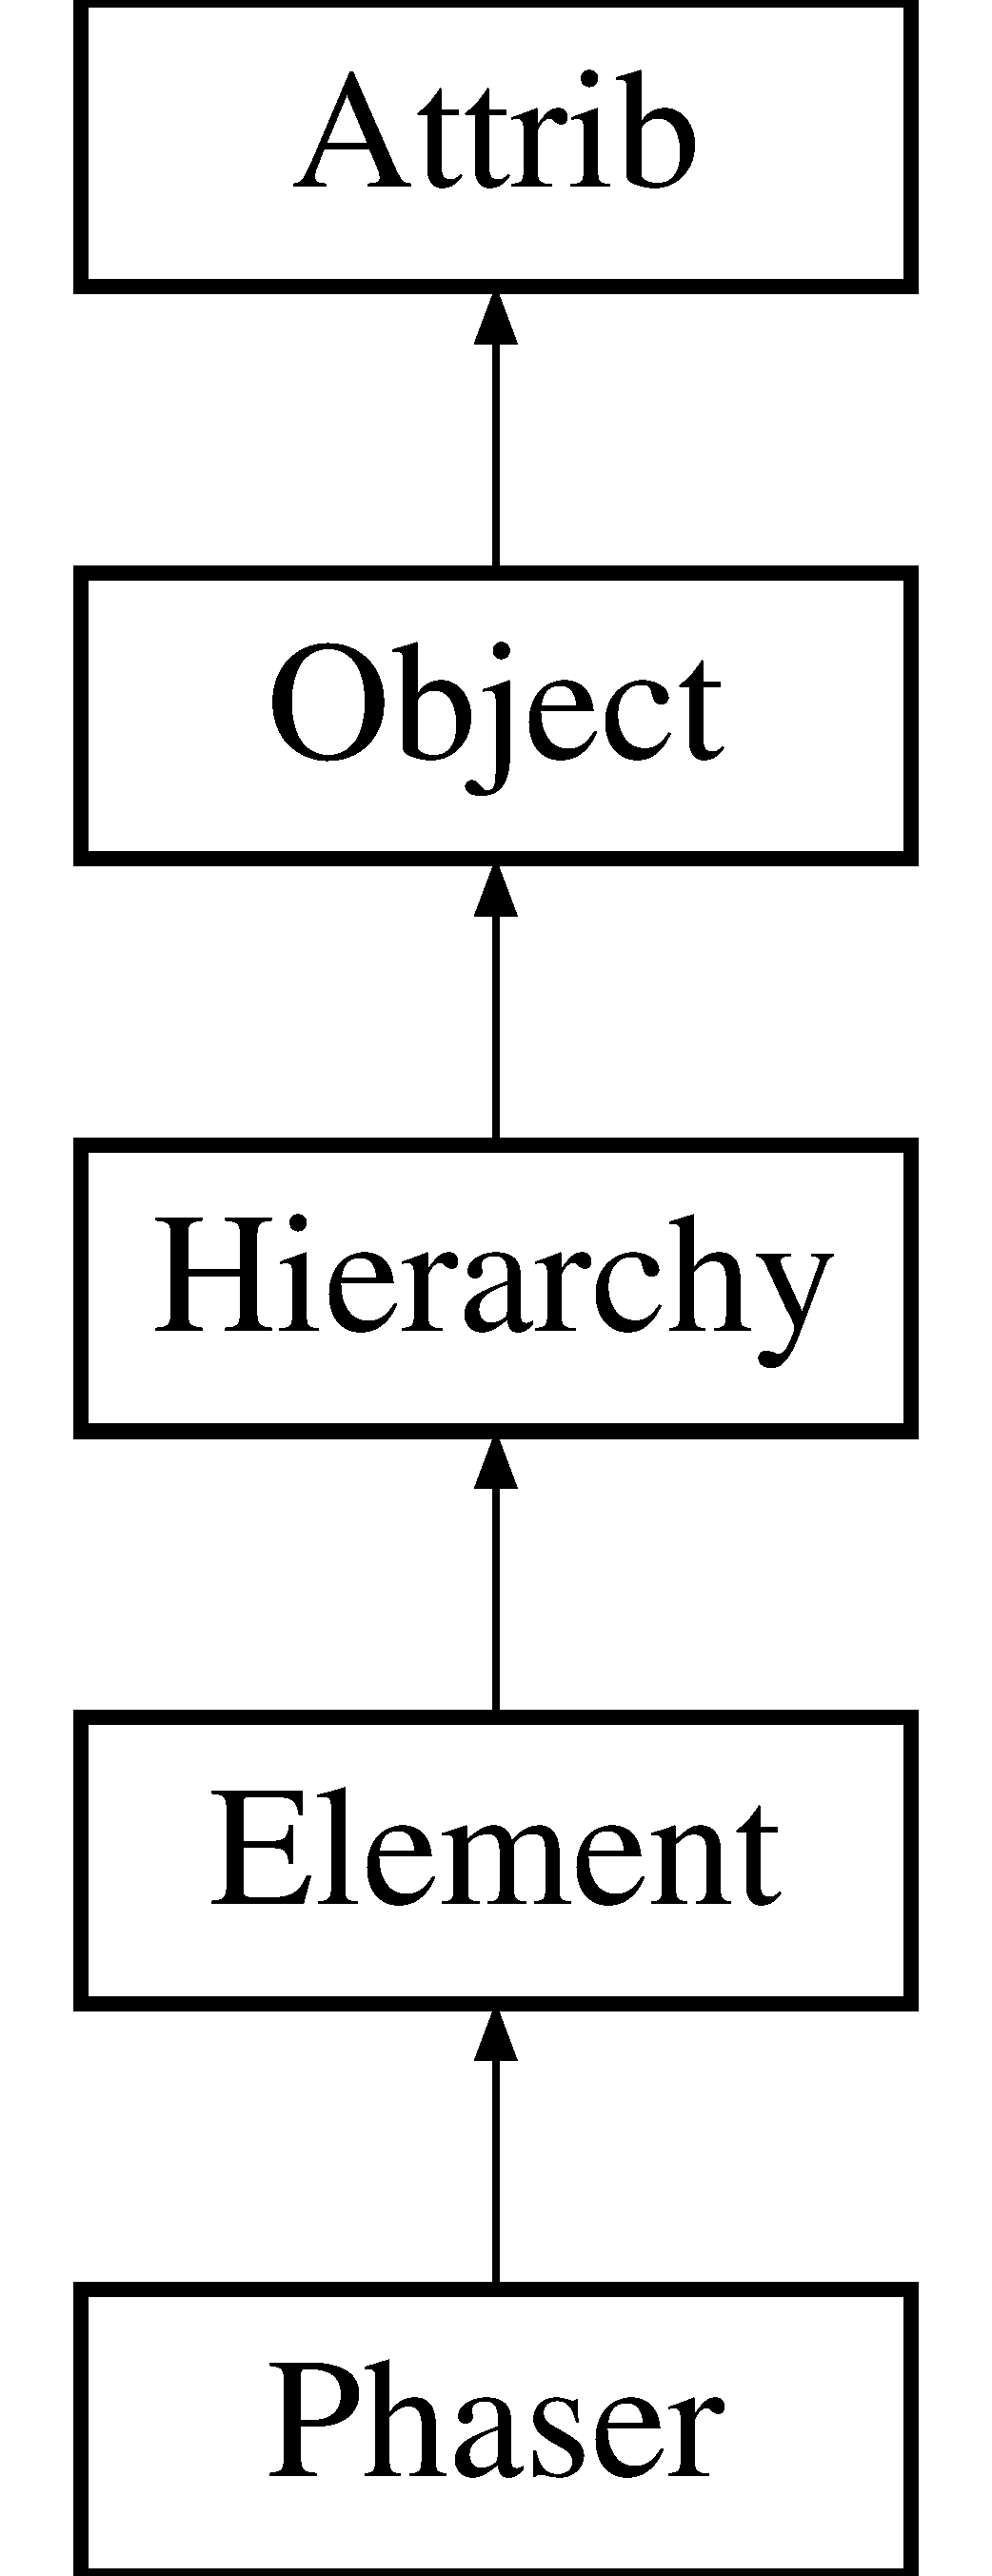
\includegraphics[height=5cm]{classPhaser}
\end{center}
\end{figure}
\subsection*{Public Types}
\begin{DoxyCompactItemize}
\item 
typedef unsigned long \hyperlink{classPhaser_a733b5d40a397fc633db055248c76a23f}{U32}
\item 
typedef unsigned short \hyperlink{classPhaser_acadd65d66e8b38a16ad37a23834ee513}{U16}
\item 
typedef unsigned char \hyperlink{classPhaser_a09f745e43da83ab27286e69179755361}{U8}
\item 
enum \hyperlink{classAttrib_a69e171d7cc6417835a5a306d3c764235}{Attribut} \{ \par
\hyperlink{classAttrib_a69e171d7cc6417835a5a306d3c764235a3a8da2ab97dda18aebab196fe4100531}{UNDEFINED}, 
\hyperlink{classAttrib_a69e171d7cc6417835a5a306d3c764235a2bfb2af57b87031d190a05fe25dd92ed}{PASSIVE}, 
\hyperlink{classAttrib_a69e171d7cc6417835a5a306d3c764235a3b1fec929c0370d1436f2f06e298fb0d}{ACTIVE}, 
\hyperlink{classAttrib_a69e171d7cc6417835a5a306d3c764235aa27c16b480a369ea4d18b07b2516bbc7}{INTERFACE}, 
\par
\hyperlink{classAttrib_a69e171d7cc6417835a5a306d3c764235a1420a5b8c0540b2af210b6975eded7f9}{IO}, 
\hyperlink{classAttrib_a69e171d7cc6417835a5a306d3c764235a0af3b0d0ac323c1704e6c69cf90add28}{IODATA}, 
\hyperlink{classAttrib_a69e171d7cc6417835a5a306d3c764235a7788bc5dd333fd8ce18562b269c9dab1}{ELEMENT}, 
\hyperlink{classAttrib_a69e171d7cc6417835a5a306d3c764235a61ceb22149f365f1780d18f9d1459423}{HARDWARE}, 
\par
\hyperlink{classAttrib_a69e171d7cc6417835a5a306d3c764235a75250e29692496e73effca2c0330977f}{PROCESSUS}, 
\hyperlink{classAttrib_a69e171d7cc6417835a5a306d3c764235a103a67cd0b8f07ef478fa45d4356e27b}{SOFTWARE}
 \}
\end{DoxyCompactItemize}
\subsection*{Public Member Functions}
\begin{DoxyCompactItemize}
\item 
\hyperlink{classPhaser_a849a7f7cd7d1491c490e4ba8e9906af0}{Phaser} ()
\item 
\hyperlink{classPhaser_a1facd3a2776130beb38792025fd8be20}{$\sim$Phaser} ()
\item 
void \hyperlink{classPhaser_a35c0add55885b3c0a7551ff48e322632}{setPhase} (unsigned char channel, unsigned char value)
\item 
void \hyperlink{classPhaser_a658be408ea31d55067e283723fa144f1}{setPhase} (unsigned char ch0, unsigned char ch1, unsigned char ch2, unsigned char ch3)
\item 
unsigned int \hyperlink{classPhaser_a3928ba4f1421c83b2f7783da87727ff2}{phase} (unsigned int ch)
\item 
void \hyperlink{classPhaser_a6ce0713403e961495192ffa0590c29e4}{read} ()
\item 
void \hyperlink{classPhaser_a7a94d4129a5f743c482fa97f3c5df68f}{write} ()
\item 
void \hyperlink{classPhaser_a0f122559297d076500420a7ceb21d70d}{help} ()
\item 
\hyperlink{classStatusCode}{StatusCode} \hyperlink{classPhaser_a4691b8963a099f8a75475eb9be47a309}{init} ()
\item 
void \hyperlink{classPhaser_a0d15908b0d50f60f4ce6c6d013f75611}{reset} ()
\item 
void \hyperlink{classPhaser_ae1d1d3be2eed3973d269eab78834c594}{update} ()
\item 
\hyperlink{classRegister}{Register} $\ast$ \hyperlink{classPhaser_a3a4b64dc36e5f74292d9bec55da077a7}{reg} ()
\item 
void \hyperlink{classElement_a3c0abcb36f8906688bb7e32608df7086}{recursiveInitElement} ()
\item 
void \hyperlink{classElement_a82119ed37dff76508a2746a853ec35ba}{recursiveInitCommunications} ()
\item 
\hyperlink{classStatusCode}{StatusCode} \hyperlink{classElement_ab476b4b1df5954141ceb14f072433b89}{setConnection} (\hyperlink{classHierarchy}{Hierarchy} $\ast$)
\item 
\hyperlink{classHierarchy}{Hierarchy} $\ast$ \hyperlink{classElement_af57444353c1ddf9fa0109801e97debf7}{connection} ()
\item 
void \hyperlink{classHierarchy_af4d43b0765b402670eed2d62c73405af}{clear} ()
\item 
void \hyperlink{classHierarchy_a585ad1aeec16077a0e532ab8b4fc557b}{setParent} (\hyperlink{classHierarchy}{Hierarchy} $\ast$parent)
\item 
\hyperlink{classHierarchy}{Hierarchy} $\ast$ \hyperlink{classHierarchy_a1c7bec8257e717f9c1465e06ebf845fc}{parent} ()
\item 
\hyperlink{classHierarchy}{Hierarchy} $\ast$ \hyperlink{classHierarchy_ad550588733bf75ac5c0fcfd7c8fd11a6}{parent} (std::string)
\item 
\hyperlink{classHierarchy}{Hierarchy} $\ast$ \hyperlink{classHierarchy_aee461dc930ce3871636ff87f075b1b83}{origin} ()
\item 
virtual void \hyperlink{classHierarchy_ad677774ff38fcb257c04a3a10d471fac}{addChild} (\hyperlink{classHierarchy}{Hierarchy} $\ast$element)
\item 
std::vector$<$ \hyperlink{classHierarchy}{Hierarchy} $\ast$ $>$ \hyperlink{classHierarchy_aa9a76f69e98e052ee1a6e32cea006288}{children} ()
\item 
\hyperlink{classHierarchy}{Hierarchy} $\ast$ \hyperlink{classHierarchy_a1e207f973c694b538bf90107b4868817}{child} (std::string)
\item 
\hyperlink{classHierarchy}{Hierarchy} $\ast$ \hyperlink{classHierarchy_a0c15a5276a3b80b4354d6bd8a01e0708}{childTyped} (std::string)
\item 
unsigned long \hyperlink{classHierarchy_ab16e84de65fd84e14001a6cf941c8be4}{numberOfChildren} ()
\item 
bool \hyperlink{classHierarchy_a255174fe4d316d2a3f430dcb9dab29f1}{hasChildren} ()
\item 
void \hyperlink{classHierarchy_a2b2b359fac003233f65786a616766bde}{delChild} (\hyperlink{classHierarchy}{Hierarchy} $\ast$)
\item 
void \hyperlink{classHierarchy_a1928ac7615fe0b5e55cd707f70dc6781}{delChild} (std::string)
\item 
std::string \hyperlink{classHierarchy_aa7990fa7caf132d83e361ce033c6c65a}{path} (std::string=std::string(\char`\"{}\char`\"{}))
\item 
std::string \hyperlink{classHierarchy_a1efd56cd164d328d2002e53a10a19b8c}{pathTyped} (std::string=std::string(\char`\"{}\char`\"{}))
\item 
void \hyperlink{classHierarchy_a76e914b9a677a22a82deb74d892bf261}{tree} (std::string indent=std::string(\char`\"{}\char`\"{}))
\item 
void \hyperlink{classHierarchy_a594c294c5f60c230e106d522ed008212}{tree} ()
\item 
std::string \hyperlink{classObject_a975e888d50bfcbffda2c86368332a5cd}{name} () const 
\item 
std::string \hyperlink{classObject_a84f99f70f144a83e1582d1d0f84e4e62}{type} ()
\item 
unsigned char \hyperlink{classObject_af99145335cc61ff6e2798ea17db009d2}{id} ()
\item 
std::string \hyperlink{classObject_a73a0f1a41828fdd8303dd662446fb6c3}{title} ()
\item 
void \hyperlink{classObject_a3f9d5537ebce0c0f2bf6ae4d92426f3c}{msgSvc} (int level, std::string msg, std::string name)
\item 
void \hyperlink{classObject_a58b2d0618c2d08cf2383012611528d97}{msg} (std::string mymsg)
\item 
void \hyperlink{classObject_ac5d59299273cee27aacf7de00d2e7034}{msg} (std::string mymsg, std::string name)
\item 
void \hyperlink{classObject_a83d2db2df682907ea1115ad721c1c4a1}{verbose} (std::string mymsg)
\item 
void \hyperlink{classObject_a2d4120195317e2a3c6532e8bb9f3da68}{verbose} (std::string mymsg, std::string name)
\item 
void \hyperlink{classObject_aac010553f022165573714b7014a15f0d}{debug} (std::string mymsg)
\item 
void \hyperlink{classObject_a6c9a0397ca804e04d675ed05683f5420}{debug} (std::string mymsg, std::string name)
\item 
void \hyperlink{classObject_a644fd329ea4cb85f54fa6846484b84a8}{info} (std::string mymsg)
\item 
void \hyperlink{classObject_a1ca123253dfd30fc28b156f521dcbdae}{info} (std::string mymsg, std::string name)
\item 
void \hyperlink{classObject_a65cd4fda577711660821fd2cd5a3b4c9}{warning} (std::string mymsg)
\item 
void \hyperlink{classObject_a11f101db4dd73d9391b0231818881d86}{warning} (std::string mymsg, std::string name)
\item 
void \hyperlink{classObject_a204a95f57818c0f811933917a30eff45}{error} (std::string mymsg)
\item 
void \hyperlink{classObject_ad7f6c457733082efa2f9ff5f5c8e119a}{error} (std::string mymsg, std::string name)
\item 
void \hyperlink{classObject_aad5a16aac7516ce65bd5ec02ab07fc80}{fatal} (std::string mymsg)
\item 
void \hyperlink{classObject_ae62acd3d09f716220f75f252dc38bc9a}{fatal} (std::string mymsg, std::string name)
\item 
void \hyperlink{classObject_ae30fea75683c2d149b6b6d17c09ecd0c}{setName} (std::string name)
\item 
void \hyperlink{classObject_aae534cc9d982bcb9b99fd505f2e103a5}{setType} (std::string type)
\item 
void \hyperlink{classObject_a398fe08cba594a0ce6891d59fe4f159f}{setId} (unsigned char id)
\item 
void \hyperlink{classObject_a89557dbbad5bcaa02652f5d7fa35d20f}{setTitle} (std::string title)
\item 
void \hyperlink{classObject_a870c5af919958c2136623b2d7816d123}{setDllName} (std::string dllName)
\item 
std::string \hyperlink{classObject_a2e3947f2870094c332d7454117f3ec63}{dllName} ()
\item 
bool \hyperlink{classAttrib_a704f26af560909ad22065083bb7d4c34}{is} (int attribut)
\item 
void \hyperlink{classAttrib_a235f773af19c900264a190b00a3b4ad7}{add} (int attribut)
\item 
void \hyperlink{classAttrib_a7d4ef7e32d93cb287792b87b857e79f3}{remove} (int attribut)
\item 
std::string \hyperlink{classAttrib_aee7bbf16b144887f196e1341b24f8a26}{attributs} ()
\end{DoxyCompactItemize}
\subsection*{Protected Attributes}
\begin{DoxyCompactItemize}
\item 
\hyperlink{classHierarchy}{Hierarchy} $\ast$ \hyperlink{classElement_abe3de7a5dbbc9a6dd2d7e012e5fdb266}{m\_\-connection}
\item 
std::string \hyperlink{classAttrib_a3414521d7a82476e874b25a5407b5e63}{m\_\-attribString} \mbox{[}10\mbox{]}
\end{DoxyCompactItemize}
\subsection*{Private Attributes}
\begin{DoxyCompactItemize}
\item 
unsigned char \hyperlink{classPhaser_a8395e4279ce87dc816e02dd684a9fa3a}{m\_\-address}
\item 
unsigned char \hyperlink{classPhaser_a04df9ce4afe7a36ccaba5e5e727d504e}{m\_\-phase} \mbox{[}4\mbox{]}
\item 
\hyperlink{classRegister}{Register} $\ast$ \hyperlink{classPhaser_ab6d751d77cb1e39723a6ac85d4cfec0c}{m\_\-reg}
\end{DoxyCompactItemize}


\subsection{Detailed Description}


Definition at line 19 of file Phaser.h.

\subsection{Member Typedef Documentation}
\hypertarget{classPhaser_acadd65d66e8b38a16ad37a23834ee513}{
\index{Phaser@{Phaser}!U16@{U16}}
\index{U16@{U16}!Phaser@{Phaser}}
\subsubsection[{U16}]{\setlength{\rightskip}{0pt plus 5cm}typedef unsigned short {\bf Phaser::U16}}}
\label{classPhaser_acadd65d66e8b38a16ad37a23834ee513}


Definition at line 22 of file Phaser.h.\hypertarget{classPhaser_a733b5d40a397fc633db055248c76a23f}{
\index{Phaser@{Phaser}!U32@{U32}}
\index{U32@{U32}!Phaser@{Phaser}}
\subsubsection[{U32}]{\setlength{\rightskip}{0pt plus 5cm}typedef unsigned long {\bf Phaser::U32}}}
\label{classPhaser_a733b5d40a397fc633db055248c76a23f}


Definition at line 21 of file Phaser.h.\hypertarget{classPhaser_a09f745e43da83ab27286e69179755361}{
\index{Phaser@{Phaser}!U8@{U8}}
\index{U8@{U8}!Phaser@{Phaser}}
\subsubsection[{U8}]{\setlength{\rightskip}{0pt plus 5cm}typedef unsigned char {\bf Phaser::U8}}}
\label{classPhaser_a09f745e43da83ab27286e69179755361}


Definition at line 23 of file Phaser.h.

\subsection{Member Enumeration Documentation}
\hypertarget{classAttrib_a69e171d7cc6417835a5a306d3c764235}{
\index{Phaser@{Phaser}!Attribut@{Attribut}}
\index{Attribut@{Attribut}!Phaser@{Phaser}}
\subsubsection[{Attribut}]{\setlength{\rightskip}{0pt plus 5cm}enum {\bf Attrib::Attribut}\hspace{0.3cm}{\ttfamily  \mbox{[}inherited\mbox{]}}}}
\label{classAttrib_a69e171d7cc6417835a5a306d3c764235}
\begin{Desc}
\item[Enumerator: ]\par
\begin{description}
\index{UNDEFINED@{UNDEFINED}!Phaser@{Phaser}}\index{Phaser@{Phaser}!UNDEFINED@{UNDEFINED}}\item[{\em 
\hypertarget{classAttrib_a69e171d7cc6417835a5a306d3c764235a3a8da2ab97dda18aebab196fe4100531}{
UNDEFINED}
\label{classAttrib_a69e171d7cc6417835a5a306d3c764235a3a8da2ab97dda18aebab196fe4100531}
}]\index{PASSIVE@{PASSIVE}!Phaser@{Phaser}}\index{Phaser@{Phaser}!PASSIVE@{PASSIVE}}\item[{\em 
\hypertarget{classAttrib_a69e171d7cc6417835a5a306d3c764235a2bfb2af57b87031d190a05fe25dd92ed}{
PASSIVE}
\label{classAttrib_a69e171d7cc6417835a5a306d3c764235a2bfb2af57b87031d190a05fe25dd92ed}
}]\index{ACTIVE@{ACTIVE}!Phaser@{Phaser}}\index{Phaser@{Phaser}!ACTIVE@{ACTIVE}}\item[{\em 
\hypertarget{classAttrib_a69e171d7cc6417835a5a306d3c764235a3b1fec929c0370d1436f2f06e298fb0d}{
ACTIVE}
\label{classAttrib_a69e171d7cc6417835a5a306d3c764235a3b1fec929c0370d1436f2f06e298fb0d}
}]\index{INTERFACE@{INTERFACE}!Phaser@{Phaser}}\index{Phaser@{Phaser}!INTERFACE@{INTERFACE}}\item[{\em 
\hypertarget{classAttrib_a69e171d7cc6417835a5a306d3c764235aa27c16b480a369ea4d18b07b2516bbc7}{
INTERFACE}
\label{classAttrib_a69e171d7cc6417835a5a306d3c764235aa27c16b480a369ea4d18b07b2516bbc7}
}]\index{IO@{IO}!Phaser@{Phaser}}\index{Phaser@{Phaser}!IO@{IO}}\item[{\em 
\hypertarget{classAttrib_a69e171d7cc6417835a5a306d3c764235a1420a5b8c0540b2af210b6975eded7f9}{
IO}
\label{classAttrib_a69e171d7cc6417835a5a306d3c764235a1420a5b8c0540b2af210b6975eded7f9}
}]\index{IODATA@{IODATA}!Phaser@{Phaser}}\index{Phaser@{Phaser}!IODATA@{IODATA}}\item[{\em 
\hypertarget{classAttrib_a69e171d7cc6417835a5a306d3c764235a0af3b0d0ac323c1704e6c69cf90add28}{
IODATA}
\label{classAttrib_a69e171d7cc6417835a5a306d3c764235a0af3b0d0ac323c1704e6c69cf90add28}
}]\index{ELEMENT@{ELEMENT}!Phaser@{Phaser}}\index{Phaser@{Phaser}!ELEMENT@{ELEMENT}}\item[{\em 
\hypertarget{classAttrib_a69e171d7cc6417835a5a306d3c764235a7788bc5dd333fd8ce18562b269c9dab1}{
ELEMENT}
\label{classAttrib_a69e171d7cc6417835a5a306d3c764235a7788bc5dd333fd8ce18562b269c9dab1}
}]\index{HARDWARE@{HARDWARE}!Phaser@{Phaser}}\index{Phaser@{Phaser}!HARDWARE@{HARDWARE}}\item[{\em 
\hypertarget{classAttrib_a69e171d7cc6417835a5a306d3c764235a61ceb22149f365f1780d18f9d1459423}{
HARDWARE}
\label{classAttrib_a69e171d7cc6417835a5a306d3c764235a61ceb22149f365f1780d18f9d1459423}
}]\index{PROCESSUS@{PROCESSUS}!Phaser@{Phaser}}\index{Phaser@{Phaser}!PROCESSUS@{PROCESSUS}}\item[{\em 
\hypertarget{classAttrib_a69e171d7cc6417835a5a306d3c764235a75250e29692496e73effca2c0330977f}{
PROCESSUS}
\label{classAttrib_a69e171d7cc6417835a5a306d3c764235a75250e29692496e73effca2c0330977f}
}]\index{SOFTWARE@{SOFTWARE}!Phaser@{Phaser}}\index{Phaser@{Phaser}!SOFTWARE@{SOFTWARE}}\item[{\em 
\hypertarget{classAttrib_a69e171d7cc6417835a5a306d3c764235a103a67cd0b8f07ef478fa45d4356e27b}{
SOFTWARE}
\label{classAttrib_a69e171d7cc6417835a5a306d3c764235a103a67cd0b8f07ef478fa45d4356e27b}
}]\end{description}
\end{Desc}



Definition at line 29 of file Attrib.h.


\begin{DoxyCode}
29                 {
30     UNDEFINED,
31     PASSIVE,
32     ACTIVE,
33     INTERFACE,
34     IO,
35     IODATA,
36     ELEMENT,
37     HARDWARE,
38     PROCESSUS,
39     SOFTWARE 
40   }; // array m_attribString must be changed into Attrib::Attrib if this enu is m
      odified. 
\end{DoxyCode}


\subsection{Constructor \& Destructor Documentation}
\hypertarget{classPhaser_a849a7f7cd7d1491c490e4ba8e9906af0}{
\index{Phaser@{Phaser}!Phaser@{Phaser}}
\index{Phaser@{Phaser}!Phaser@{Phaser}}
\subsubsection[{Phaser}]{\setlength{\rightskip}{0pt plus 5cm}Phaser::Phaser ()\hspace{0.3cm}{\ttfamily  \mbox{[}inline\mbox{]}}}}
\label{classPhaser_a849a7f7cd7d1491c490e4ba8e9906af0}


Definition at line 24 of file Phaser.h.

References Attrib::add(), Hierarchy::addChild(), Object::debug(), IOdata::defDataU8(), Attrib::ELEMENT, Attrib::HARDWARE, IOobject::io(), m\_\-phase, m\_\-reg, Object::setId(), and Object::setType().


\begin{DoxyCode}
24           {
25     setType("Phaser");
26     setId(0);
27     add(Attrib::ELEMENT); add (Attrib::HARDWARE);
28     debug("Phaser built.","Phaser::Phaser");
29     m_phase[0]=99;
30     m_phase[1]=99;
31     m_phase[2]=99;
32     m_phase[3]=99;
33     m_reg=new Register();
34     m_reg->io()->defDataU8(3);
35     addChild(m_reg);
36   }
\end{DoxyCode}
\hypertarget{classPhaser_a1facd3a2776130beb38792025fd8be20}{
\index{Phaser@{Phaser}!$\sim$Phaser@{$\sim$Phaser}}
\index{$\sim$Phaser@{$\sim$Phaser}!Phaser@{Phaser}}
\subsubsection[{$\sim$Phaser}]{\setlength{\rightskip}{0pt plus 5cm}Phaser::$\sim$Phaser ()\hspace{0.3cm}{\ttfamily  \mbox{[}inline\mbox{]}}}}
\label{classPhaser_a1facd3a2776130beb38792025fd8be20}


Definition at line 38 of file Phaser.h.


\begin{DoxyCode}
38            {
39 //    delete m_reg;
40   }
\end{DoxyCode}


\subsection{Member Function Documentation}
\hypertarget{classAttrib_a235f773af19c900264a190b00a3b4ad7}{
\index{Phaser@{Phaser}!add@{add}}
\index{add@{add}!Phaser@{Phaser}}
\subsubsection[{add}]{\setlength{\rightskip}{0pt plus 5cm}void Attrib::add (int {\em attribut})\hspace{0.3cm}{\ttfamily  \mbox{[}inline, inherited\mbox{]}}}}
\label{classAttrib_a235f773af19c900264a190b00a3b4ad7}
Add an attribut 

Definition at line 67 of file Attrib.h.

References Attrib::m\_\-attributs, and Attrib::UNDEFINED.

Referenced by A3PE::A3PE(), Attrib::Attrib(), SpecsMezzanine::cmdline(), Computer::Computer(), CU\_\-v1::CU\_\-v1(), export\_\-obj(), FEB\_\-v1::FEB\_\-v1(), FePGA::FePGA(), ICECALv3::ICECALv3(), ICPhaser::ICPhaser(), Application::initialize(), Interface::Interface(), IOdata::IOdata(), IOobject::IOobject(), LSDelayChipV1::LSDelayChipV1(), MSOxxxx::MSOxxxx(), Phaser(), Processus::Processus(), Proto40MHz\_\-v1::Proto40MHz\_\-v1(), Attrib::remove(), SeqPGA::SeqPGA(), SpecsMaster::SpecsMaster(), and SpecsSlave::SpecsSlave().


\begin{DoxyCode}
67                             {
68     if (attribut!=Attrib::UNDEFINED) remove(Attrib::UNDEFINED);
69     bool duplicate = false ;
70     std::vector<int>::const_iterator iter ;
71     for ( iter  = m_attributs.begin() ;
72           iter != m_attributs.end()   ;
73           ++iter ) {
74       if ( attribut == (*iter) ) {
75         duplicate = true ;
76       }
77     }
78     if (!duplicate) {
79       m_attributs.push_back( attribut );
80     }
81   }
\end{DoxyCode}
\hypertarget{classHierarchy_ad677774ff38fcb257c04a3a10d471fac}{
\index{Phaser@{Phaser}!addChild@{addChild}}
\index{addChild@{addChild}!Phaser@{Phaser}}
\subsubsection[{addChild}]{\setlength{\rightskip}{0pt plus 5cm}void Hierarchy::addChild ({\bf Hierarchy} $\ast$ {\em element})\hspace{0.3cm}{\ttfamily  \mbox{[}virtual, inherited\mbox{]}}}}
\label{classHierarchy_ad677774ff38fcb257c04a3a10d471fac}


Definition at line 83 of file Hierarchy.cpp.

References Object::debug(), Hierarchy::m\_\-children, Object::name(), and Hierarchy::setParent().

Referenced by A3PE::A3PE(), SpecsMezzanine::addBus(), SpecsSlave::addI2c(), Application::create(), CU\_\-v1::CU\_\-v1(), export\_\-obj(), FEB\_\-v1::FEB\_\-v1(), FePGA::FePGA(), ICECALv3::ICECALv3(), ICPhaser::ICPhaser(), LSDelayChipV1::LSDelayChipV1(), FePGA::MakeRAM(), FePGA::MakeRegister(), Phaser(), Proto40MHz\_\-v1::Proto40MHz\_\-v1(), SeqPGA::SeqPGA(), SpecsMezzanine::SpecsMezzanine(), UsbI2cBus::UsbI2cBus(), and UsbSpiBus::UsbSpiBus().


\begin{DoxyCode}
83                                           {
84   element->setParent(this);
85   m_children.push_back(element);
86   debug(element->name()+" added to the child tree.","Hierarchy::addChild");
87 }
\end{DoxyCode}
\hypertarget{classAttrib_aee7bbf16b144887f196e1341b24f8a26}{
\index{Phaser@{Phaser}!attributs@{attributs}}
\index{attributs@{attributs}!Phaser@{Phaser}}
\subsubsection[{attributs}]{\setlength{\rightskip}{0pt plus 5cm}std::string Attrib::attributs ()\hspace{0.3cm}{\ttfamily  \mbox{[}inherited\mbox{]}}}}
\label{classAttrib_aee7bbf16b144887f196e1341b24f8a26}
Print the \hyperlink{classAttrib}{Attrib} of an \hyperlink{classObject}{Object} 

Definition at line 54 of file Attrib.cpp.

References images::index, Attrib::m\_\-attribString, and Attrib::m\_\-attributs.

Referenced by export\_\-obj().


\begin{DoxyCode}
54                             {
55   std::string output;
56   std::vector<int>::iterator iter ;
57   for ( unsigned int index = 0 ; index < m_attributs.size() ; ++index ) {
58     if ( m_attributs.size() - index > 1 ) {
59       output.append(m_attribString[m_attributs[index]]);
60       output.append(":");
61     }
62     else {
63       output.append(m_attribString[m_attributs[index]]);
64     }
65   }
66   return output;
67 }
\end{DoxyCode}
\hypertarget{classHierarchy_a1e207f973c694b538bf90107b4868817}{
\index{Phaser@{Phaser}!child@{child}}
\index{child@{child}!Phaser@{Phaser}}
\subsubsection[{child}]{\setlength{\rightskip}{0pt plus 5cm}{\bf Hierarchy} $\ast$ Hierarchy::child (std::string {\em path})\hspace{0.3cm}{\ttfamily  \mbox{[}inherited\mbox{]}}}}
\label{classHierarchy_a1e207f973c694b538bf90107b4868817}


Definition at line 133 of file Hierarchy.cpp.

References Hierarchy::child(), Hierarchy::children(), Object::name(), Hierarchy::origin(), Hierarchy::parent(), and Object::warning().

Referenced by Application::cd(), Hierarchy::child(), and export\_\-obj().


\begin{DoxyCode}
133                                          {
134   std::string newpath = path;
135   std::string up("..");
136   std::string separator(1,'/');
137 
138   Hierarchy * newcurrent = 0;
139 
140   //  info("path="+path,"Hierarchy::child");
141 
142   if (path.compare("")==0 || path.compare("/")==0) {
143     //    debug("return origin","Hierarchy::child");
144     return origin();
145   }
146 
147   if (path.compare(name())==0){
148     //    debug("return itself","Hierarchy::child");
149     return this;
150   }
151 
152   if (path.compare("..")==0){
153     if (0!=this->parent()) return this->parent();
154     else return this;
155   }
156 
157   if (path.compare("../")==0){
158     if (0!=this->parent()) return this->parent();
159     else return this;
160   }
161 
162 
163   int npos=path.find(separator,0);
164 
165   //  info("find separator in "+itos(npos)+" of "+path,"Hierarchy::child");
166 
167   // remove last separator
168   if ( npos == (int)(path.size()-1) ) {
169     newpath = std::string(path,0,npos);
170     path = newpath;
171   }
172 
173   if (npos==0){
174     //    debug("Going back to origin and calling child","Hierarchy::child");
175     newpath=std::string(path,1,path.size()-1);
176     return origin()->child(newpath);
177   }
178   else{
179     if ( npos== (int)(std::string::npos) ){
180       //      debug("Getting chid "+path+" of "+this->name(),"Hierarchy::child");
      
181       std::vector <Hierarchy*> list = children();
182       std::vector<Hierarchy*>::iterator iter;
183       for (iter=list.begin();iter!=list.end();iter++){
184         if ((*iter)->name().compare(path)==0){
185           return *iter;
186         }
187       }
188       warning(this->name()+std::string(" has no child '")+path+"'","Hierarchy::ch
      ild");
189       return this;
190     }
191     else
192     {
193       int ipos=path.find(separator,0);
194       //      info("default behaviour "+path+" with separator in "+itos(ipos),"Hi
      erarchy::child");
195 
196       std::string newcurrentname=std::string(path,0,ipos);
197       newpath=std::string(path,ipos+1,path.size()-1);
198 
199       //      info("looking now for "+newpath+" from "+newcurrentname,"Hierarchy:
      :child");
200 
201       if (0==newcurrentname.compare(origin()->name())){
202         //        info("current is computer. Looking for children"+newcurrentname
      ,"Hierarchy::child");
203         return origin()->child(newpath);
204       }
205 
206       newcurrent = (Hierarchy*)0;
207 
208       std::vector <Hierarchy*> list = children();
209       std::vector<Hierarchy*>::iterator iter;
210       for (iter=list.begin();iter!=list.end();iter++){
211         if ((*iter)->name().compare(newcurrentname)==0){
212           newcurrent = (*iter);
213         }
214       }
215 
216 
217       if ((Hierarchy*)0==newcurrent){
218         if (newcurrentname.compare("..")==0 && 0!=parent()){
219           newcurrent=this->parent();
220           //          debug("newcurrent was .. -> parent="+parent()->name());
221         }
222         else
223         {
224           warning(this->name()+" has no child '"+newcurrentname+"'",
225               "Hierarchy::child");
226           return this;
227         }
228       }
229       //      debug("recurrence call for "+newpath+" on "+newcurrent->name(),"Hie
      rarchy::child");
230       return newcurrent -> child ( newpath );
231     }
232   }
233 }
\end{DoxyCode}
\hypertarget{classHierarchy_aa9a76f69e98e052ee1a6e32cea006288}{
\index{Phaser@{Phaser}!children@{children}}
\index{children@{children}!Phaser@{Phaser}}
\subsubsection[{children}]{\setlength{\rightskip}{0pt plus 5cm}std::vector$<${\bf Hierarchy}$\ast$$>$ Hierarchy::children ()\hspace{0.3cm}{\ttfamily  \mbox{[}inline, inherited\mbox{]}}}}
\label{classHierarchy_aa9a76f69e98e052ee1a6e32cea006288}


Definition at line 33 of file Hierarchy.h.

References Hierarchy::m\_\-children.

Referenced by Hierarchy::child(), Hierarchy::childTyped(), export\_\-obj(), SpecsSlave::recursiveInitCommunications(), Element::recursiveInitCommunications(), Element::recursiveInitElement(), Application::setConfig(), and Hierarchy::tree().


\begin{DoxyCode}
33 { return m_children;  } //< get list of child(ren)
\end{DoxyCode}
\hypertarget{classHierarchy_a0c15a5276a3b80b4354d6bd8a01e0708}{
\index{Phaser@{Phaser}!childTyped@{childTyped}}
\index{childTyped@{childTyped}!Phaser@{Phaser}}
\subsubsection[{childTyped}]{\setlength{\rightskip}{0pt plus 5cm}{\bf Hierarchy} $\ast$ Hierarchy::childTyped (std::string {\em path})\hspace{0.3cm}{\ttfamily  \mbox{[}inherited\mbox{]}}}}
\label{classHierarchy_a0c15a5276a3b80b4354d6bd8a01e0708}


Definition at line 239 of file Hierarchy.cpp.

References Hierarchy::children(), Hierarchy::m\_\-origin, Object::name(), Hierarchy::parent(), and Object::warning().

Referenced by export\_\-obj().


\begin{DoxyCode}
239                                               {
240 
241   std::string newpath = path;
242 
243   std::string up("..");
244   std::string separator(1,'/');
245   std::string typeopen(1,'[');
246   std::string typeclose(1,']');
247 
248   Hierarchy * newcurrent = 0;
249 
250   unsigned int npos=path.find(separator,0);
251   unsigned int opos=path.find(typeopen,0);
252   if ( npos==std::string::npos || npos == path.size()-1 ){
253     if ( path.compare("..")==0 ) {
254       return parent();
255     }
256 
257     if ( npos == path.size()-1 ) {
258       newpath = std::string(path,0,opos);
259       path = newpath;
260     }
261 
262     std::vector < Hierarchy* > list = children();
263     std::vector < Hierarchy* >::iterator iter;
264     for (iter=list.begin();iter!=list.end();iter++){
265       std::string notypepath = std::string(path,0,opos);
266       if ((*iter)->name().compare(notypepath)==0){
267         return *iter;
268       }
269     }
270     warning(this->name()+std::string(" has no child ") +path,"Hierarchy::child");
      
271     return 0;
272   }
273 
274   else {
275 
276     if (std::string(path,0,3).compare(std::string("../"))==0) {
277       newpath=std::string(path,3,path.size()-3);
278       newcurrent = parent();
279     }
280     if (std::string(path,0,1).compare(std::string("/"))==0) {
281       newpath=std::string(path,1,path.size()-1);
282       newcurrent = ( Hierarchy* ) m_origin;
283     }
284     if ((std::string(path,0,3).compare(std::string("../")) !=0 ) &&
285         std::string(path,0,1).compare(std::string("/"))!=0 ) {
286       opos = path.find(typeopen,0);
287       int cpos = path.find(typeclose,0);
288       std::string name = std::string (path,0,opos);
289       newcurrent = childTyped( name );
290       if (newcurrent ==0){
291         warning(path+": no child found with such a name","Hierarchy::child");
292       }
293       newpath = std::string (path,cpos+2,path.size()-cpos-1);
294     }
295     return newcurrent -> childTyped ( newpath );
296   }
297 }
\end{DoxyCode}
\hypertarget{classHierarchy_af4d43b0765b402670eed2d62c73405af}{
\index{Phaser@{Phaser}!clear@{clear}}
\index{clear@{clear}!Phaser@{Phaser}}
\subsubsection[{clear}]{\setlength{\rightskip}{0pt plus 5cm}void Hierarchy::clear ()\hspace{0.3cm}{\ttfamily  \mbox{[}inherited\mbox{]}}}}
\label{classHierarchy_af4d43b0765b402670eed2d62c73405af}


Definition at line 35 of file Hierarchy.cpp.

References Hierarchy::delChild(), Object::info(), Hierarchy::m\_\-children, and Object::name().

Referenced by export\_\-obj().


\begin{DoxyCode}
35                      {
36   std::vector<Hierarchy*> listlocale;
37   std::vector<Hierarchy*>::iterator iter;
38   info("loop on "+name()+" children.","Hierarchy::clear");
39   for (iter=m_children.begin();iter!=m_children.end();iter++){
40       info("processing "+(*iter)->name()+".","Hierarchy::clear");
41 /*
42       (*iter)->clear();
43 //      this->delChild((*iter));
44       info("obj "+(*iter)->name()+" being cleared.","Hierarchy::clear");
45       delete (*iter);
46       info("Object deleted.","Hierarchy::clear");
47       m_children.erase(iter);
48       info("Object removed from the tree.","Hierarchy::clear");
49 */
50     (*iter)->clear();
51     info("Adding object "+(*iter)->name()+" from the Hierarchy to the list of del
      eted objects.","Hierarchy::clear");
52     listlocale.push_back((*iter));
53   }
54 
55   for (iter=listlocale.begin();iter!=listlocale.end();iter++){
56     info("Removing object "+(*iter)->name()+".","Hierarchy::clear");
57     this->delChild(*iter);
58 //    m_children.erase(iter);
59     delete (*iter);
60   }
61   info("Getting out of "+name());
62 }
\end{DoxyCode}
\hypertarget{classElement_af57444353c1ddf9fa0109801e97debf7}{
\index{Phaser@{Phaser}!connection@{connection}}
\index{connection@{connection}!Phaser@{Phaser}}
\subsubsection[{connection}]{\setlength{\rightskip}{0pt plus 5cm}{\bf Hierarchy} $\ast$ Element::connection ()\hspace{0.3cm}{\ttfamily  \mbox{[}inherited\mbox{]}}}}
\label{classElement_af57444353c1ddf9fa0109801e97debf7}
Get IO interface 

Definition at line 84 of file Element.cpp.

References Element::m\_\-connection, Object::name(), and Object::warning().

Referenced by UsbSpiBus::clockDivider(), export\_\-obj(), UsbSpiBus::read(), UsbI2cBus::read(), IOobject::read(), UsbSpiBus::setClockDivider(), UsbSpiBus::write(), UsbI2cBus::write(), and IOobject::write().


\begin{DoxyCode}
84                               {
85   if (0==m_connection){
86     warning("no connection defined for "+name()+".","Element::connection");
87     return (Hierarchy*)0;
88   }
89   return m_connection;
90 }
\end{DoxyCode}
\hypertarget{classObject_a6c9a0397ca804e04d675ed05683f5420}{
\index{Phaser@{Phaser}!debug@{debug}}
\index{debug@{debug}!Phaser@{Phaser}}
\subsubsection[{debug}]{\setlength{\rightskip}{0pt plus 5cm}void Object::debug (std::string {\em mymsg}, \/  std::string {\em name})\hspace{0.3cm}{\ttfamily  \mbox{[}inline, inherited\mbox{]}}}}
\label{classObject_a6c9a0397ca804e04d675ed05683f5420}


Definition at line 45 of file Object.h.

References MsgSvc::DEBUG, Object::m\_\-log, and MsgSvc::msgSvc().


\begin{DoxyCode}
45 { m_log.msgSvc (MsgSvc::DEBUG   , mymsg, name ); }
\end{DoxyCode}
\hypertarget{classObject_aac010553f022165573714b7014a15f0d}{
\index{Phaser@{Phaser}!debug@{debug}}
\index{debug@{debug}!Phaser@{Phaser}}
\subsubsection[{debug}]{\setlength{\rightskip}{0pt plus 5cm}void Object::debug (std::string {\em mymsg})\hspace{0.3cm}{\ttfamily  \mbox{[}inline, inherited\mbox{]}}}}
\label{classObject_aac010553f022165573714b7014a15f0d}


Definition at line 37 of file Object.h.

References MsgSvc::DEBUG, Object::m\_\-log, Object::m\_\-name, and MsgSvc::msgSvc().

Referenced by A3PE::A3PE(), A3PE::acquisition(), SpecsMezzanine::addBus(), Hierarchy::addChild(), SpecsSlave::addI2c(), LSDelayChipV1::checkConfigAddr(), LSDelayChipV1::checkStatusAddr(), LSDelayChipV1::configRegBulkRead(), LSDelayChipV1::configRegBulkWrite(), A3PE::dataReady(), DCU::DCU(), Hierarchy::delChild(), SpecsSlave::detect(), EmulateFE::execute(), StorageFifoAcquisition::execute(), StorageFifo::execute(), Acquisition::execute(), A3PE\_\-BitFlip::execute(), export\_\-obj(), FePGA::FePGA(), SpecsGlue::i2cClkMode(), SeqPGA::i2cRead(), FePGA::i2cRead(), SeqPGA::i2cWrite(), FePGA::i2cWrite(), ICECALv3::ICECALv3(), ICPhaser::ICPhaser(), SpecsSlave::init(), SpecsMaster::init(), EmulateFE::initialize(), StorageFifoAcquisition::initialize(), StorageFifo::initialize(), Acquisition::initialize(), A3PE\_\-BitFlip::initialize(), A3PE::internalAXSequence(), SpecsMezzanine::led(), SpecsGlue::led(), LSDelayChipV1::LSDelayChipV1(), MSOxxxx::MSOxxxx(), Phaser(), Data::purge(), ICPhaser::read(), read(), FEB\_\-v1::readFifoSpyFE(), SpecsSlave::reset(), SpecsMaster::reset(), FEB\_\-v1::reset(), CU\_\-v1::reset(), Proto40MHz\_\-v1::reset(), FEB\_\-v1::resetFifoSpyFE(), SeqPGA::resetSpi(), FEB\_\-v1::resetSpi(), SeqPGA::SeqPGA(), A3PE::setAddFromAXRam(), A3PE::setAddToAXRam(), A3PE::setAXRamUsb(), Element::setConnection(), SpecsGlue::setI2cClkMode(), A3PE::setLatencyAX(), SpecsMezzanine::setLed(), SpecsGlue::setLed(), A3PE::setLengthAX(), A3PE::setReadToAXRamUsb(), SpecsMaster::setSpeed(), A3PE::setWriteFromAXRamUsb(), SpecsBus::SpecsBus(), SpecsI2c::SpecsI2c(), SpecsMaster::SpecsMaster(), SpecsMezzanine::SpecsMezzanine(), SpecsParallelBus::SpecsParallelBus(), SpecsSlave::SpecsSlave(), LSDelayChipV1::spiBERTest(), ICECALv3::spiRead(), ICECALv3::spiWrite(), FEB\_\-v1::testDuration(), SeqPGA::testSequence(), A3PE::trigger(), Server::updateConfig(), Server::updateState(), ICPhaser::write(), write(), and Hierarchy::$\sim$Hierarchy().


\begin{DoxyCode}
37 { m_log.msgSvc (MsgSvc::DEBUG   , mymsg, m_name ); }
\end{DoxyCode}
\hypertarget{classHierarchy_a1928ac7615fe0b5e55cd707f70dc6781}{
\index{Phaser@{Phaser}!delChild@{delChild}}
\index{delChild@{delChild}!Phaser@{Phaser}}
\subsubsection[{delChild}]{\setlength{\rightskip}{0pt plus 5cm}void Hierarchy::delChild (std::string {\em n})\hspace{0.3cm}{\ttfamily  \mbox{[}inherited\mbox{]}}}}
\label{classHierarchy_a1928ac7615fe0b5e55cd707f70dc6781}


Definition at line 110 of file Hierarchy.cpp.

References Object::debug(), and Hierarchy::m\_\-children.


\begin{DoxyCode}
110                                    {
111   bool flag=false;
112   std::vector<Hierarchy*>::iterator iter,remove;
113   for (iter=m_children.begin();iter!=m_children.end();iter++){
114     if ((*iter)->name()==n){ remove=iter; flag=true;}
115   }
116   if (flag){
117     debug("removing "+(*remove)->name()+" from the tree.","Hierarchy::delChild");
      
118     m_children.erase(remove);
119   }
120 }
\end{DoxyCode}
\hypertarget{classHierarchy_a2b2b359fac003233f65786a616766bde}{
\index{Phaser@{Phaser}!delChild@{delChild}}
\index{delChild@{delChild}!Phaser@{Phaser}}
\subsubsection[{delChild}]{\setlength{\rightskip}{0pt plus 5cm}void Hierarchy::delChild ({\bf Hierarchy} $\ast$ {\em element})\hspace{0.3cm}{\ttfamily  \mbox{[}inherited\mbox{]}}}}
\label{classHierarchy_a2b2b359fac003233f65786a616766bde}


Definition at line 92 of file Hierarchy.cpp.

References Object::debug(), and Hierarchy::m\_\-children.

Referenced by Hierarchy::clear(), export\_\-obj(), and Hierarchy::$\sim$Hierarchy().


\begin{DoxyCode}
92                                           {
93   bool flag=false;
94   std::vector<Hierarchy*>::iterator iter,remove;
95   for (iter=m_children.begin();(iter!=m_children.end());iter++){
96     if (*iter==element){
97       remove=iter;
98       flag=true;
99     }
100   }
101   if (flag){
102     debug("removing "+(*remove)->name()+" from the tree.","Hierarchy::delChild");
      
103     m_children.erase(remove);
104   }
105 }
\end{DoxyCode}
\hypertarget{classObject_a2e3947f2870094c332d7454117f3ec63}{
\index{Phaser@{Phaser}!dllName@{dllName}}
\index{dllName@{dllName}!Phaser@{Phaser}}
\subsubsection[{dllName}]{\setlength{\rightskip}{0pt plus 5cm}std::string Object::dllName ()\hspace{0.3cm}{\ttfamily  \mbox{[}inline, inherited\mbox{]}}}}
\label{classObject_a2e3947f2870094c332d7454117f3ec63}
Get accessor to member m\_\-dllName \begin{DoxyReturn}{Returns}
the current value of m\_\-dllName 
\end{DoxyReturn}


Definition at line 74 of file Object.h.

References Object::m\_\-dllName.

Referenced by export\_\-obj().


\begin{DoxyCode}
74                        {
75     return m_dllName;
76   }  
\end{DoxyCode}
\hypertarget{classObject_ad7f6c457733082efa2f9ff5f5c8e119a}{
\index{Phaser@{Phaser}!error@{error}}
\index{error@{error}!Phaser@{Phaser}}
\subsubsection[{error}]{\setlength{\rightskip}{0pt plus 5cm}void Object::error (std::string {\em mymsg}, \/  std::string {\em name})\hspace{0.3cm}{\ttfamily  \mbox{[}inline, inherited\mbox{]}}}}
\label{classObject_ad7f6c457733082efa2f9ff5f5c8e119a}


Definition at line 48 of file Object.h.

References MsgSvc::ERR, Object::m\_\-log, and MsgSvc::msgSvc().


\begin{DoxyCode}
48 { m_log.msgSvc (MsgSvc::ERR     , mymsg, name ); }
\end{DoxyCode}
\hypertarget{classObject_a204a95f57818c0f811933917a30eff45}{
\index{Phaser@{Phaser}!error@{error}}
\index{error@{error}!Phaser@{Phaser}}
\subsubsection[{error}]{\setlength{\rightskip}{0pt plus 5cm}void Object::error (std::string {\em mymsg})\hspace{0.3cm}{\ttfamily  \mbox{[}inline, inherited\mbox{]}}}}
\label{classObject_a204a95f57818c0f811933917a30eff45}


Definition at line 40 of file Object.h.

References MsgSvc::ERR, Object::m\_\-log, Object::m\_\-name, and MsgSvc::msgSvc().

Referenced by ICECALv3::checkChNumber(), A3PE::clockDivision(), NI6008::cmd(), A3PE::enableStorage(), A3PE\_\-BitFlip::execute(), export\_\-obj(), A3PE::fifoDepth(), A3PE::fifoLatency(), FEB\_\-v1::gbtStatus(), Register::getBit(), MSOxxxx::getStatistics(), SpecsMaster::init(), NI6008::init(), UsbFTMLInterface::init(), UsbFTInterface::init(), A3PE::latencyAX(), A3PE::lengthAX(), A3PE::nTrigger(), MSOxxxx::open(), ICECALv3::parseParameterList(), A3PE::pipeline(), UsbFTMLInterface::read(), UsbFTInterface::read(), MSOxxxx::recv(), A3PE::reset(), MSOxxxx::send(), A3PE::setAddFromAXRam(), A3PE::setAddToAXRam(), ICECALv3::setAnalogCh(), A3PE::setAXRamUsb(), Register::setBit(), A3PE::setClockDivision(), A3PE::setFifoDepth(), A3PE::setFifoLatency(), A3PE::setLatencyAX(), A3PE::setLengthAX(), A3PE::setNTrigger(), A3PE::setPipeline(), A3PE::setReadPatternFifoUsb(), A3PE::setReadToAXRamUsb(), A3PE::setReadTriggerFifoUsb(), A3PE::setSoftwareTrigger(), A3PE::setTriggerDelay(), A3PE::setTriggerRate(), A3PE::setWriteFromAXRamUsb(), A3PE::setWriteStorageFifoUsb(), ICECALv3::spiFERTest(), ICECALv3::spiWriteSafe(), A3PE::startSequenceAX(), A3PE::triggerDelay(), A3PE::triggerRate(), UsbFTMLInterface::usbRead(), UsbFTInterface::usbRead(), UsbFTMLInterface::usbReadU16(), UsbFTInterface::usbReadU16(), UsbFTMLInterface::usbReadU32(), UsbFTInterface::usbReadU32(), UsbFTMLInterface::usbReadU8(), UsbFTInterface::usbReadU8(), UsbFTMLInterface::usbWrite(), UsbFTInterface::usbWrite(), UsbFTMLInterface::usbWriteRead(), UsbFTInterface::usbWriteRead(), UsbFTMLInterface::usbWriteU16(), UsbFTInterface::usbWriteU16(), UsbFTMLInterface::usbWriteU32(), UsbFTInterface::usbWriteU32(), UsbFTMLInterface::usbWriteU8(), UsbFTInterface::usbWriteU8(), UsbFTMLInterface::write(), and UsbFTInterface::write().


\begin{DoxyCode}
40 { m_log.msgSvc (MsgSvc::ERR     , mymsg, m_name ); }
\end{DoxyCode}
\hypertarget{classObject_ae62acd3d09f716220f75f252dc38bc9a}{
\index{Phaser@{Phaser}!fatal@{fatal}}
\index{fatal@{fatal}!Phaser@{Phaser}}
\subsubsection[{fatal}]{\setlength{\rightskip}{0pt plus 5cm}void Object::fatal (std::string {\em mymsg}, \/  std::string {\em name})\hspace{0.3cm}{\ttfamily  \mbox{[}inline, inherited\mbox{]}}}}
\label{classObject_ae62acd3d09f716220f75f252dc38bc9a}


Definition at line 49 of file Object.h.

References MsgSvc::FATAL, Object::m\_\-log, and MsgSvc::msgSvc().


\begin{DoxyCode}
49 { m_log.msgSvc (MsgSvc::FATAL   , mymsg, name ); }
\end{DoxyCode}
\hypertarget{classObject_aad5a16aac7516ce65bd5ec02ab07fc80}{
\index{Phaser@{Phaser}!fatal@{fatal}}
\index{fatal@{fatal}!Phaser@{Phaser}}
\subsubsection[{fatal}]{\setlength{\rightskip}{0pt plus 5cm}void Object::fatal (std::string {\em mymsg})\hspace{0.3cm}{\ttfamily  \mbox{[}inline, inherited\mbox{]}}}}
\label{classObject_aad5a16aac7516ce65bd5ec02ab07fc80}


Definition at line 41 of file Object.h.

References MsgSvc::FATAL, Object::m\_\-log, Object::m\_\-name, and MsgSvc::msgSvc().

Referenced by export\_\-obj(), SpecsSlave::init(), UsbSpiBus::init(), UsbI2cBus::init(), IOobject::init(), UsbMLSpiBus::init(), UsbMLI2cBus::init(), UsbFTMLInterface::init(), UsbFTInterface::init(), and Element::setConnection().


\begin{DoxyCode}
41 { m_log.msgSvc (MsgSvc::FATAL   , mymsg, m_name ); }
\end{DoxyCode}
\hypertarget{classHierarchy_a255174fe4d316d2a3f430dcb9dab29f1}{
\index{Phaser@{Phaser}!hasChildren@{hasChildren}}
\index{hasChildren@{hasChildren}!Phaser@{Phaser}}
\subsubsection[{hasChildren}]{\setlength{\rightskip}{0pt plus 5cm}bool Hierarchy::hasChildren ()\hspace{0.3cm}{\ttfamily  \mbox{[}inherited\mbox{]}}}}
\label{classHierarchy_a255174fe4d316d2a3f430dcb9dab29f1}


Definition at line 303 of file Hierarchy.cpp.

References Hierarchy::m\_\-children.

Referenced by export\_\-obj().


\begin{DoxyCode}
303                               {
304   return ( m_children.size()>0 );
305 }
\end{DoxyCode}
\hypertarget{classPhaser_a0f122559297d076500420a7ceb21d70d}{
\index{Phaser@{Phaser}!help@{help}}
\index{help@{help}!Phaser@{Phaser}}
\subsubsection[{help}]{\setlength{\rightskip}{0pt plus 5cm}void Phaser::help ()\hspace{0.3cm}{\ttfamily  \mbox{[}inline, virtual\mbox{]}}}}
\label{classPhaser_a0f122559297d076500420a7ceb21d70d}
printout help for the \hyperlink{namespaceelement}{element} 

Implements \hyperlink{classElement_a32c0de27acb08e17251cef88c3e9303a}{Element}.

Definition at line 74 of file Phaser.h.

References Object::info(), and Object::name().


\begin{DoxyCode}
74 { info("Phaser "+name()+". No help.","Phaser::help"); };
\end{DoxyCode}
\hypertarget{classObject_af99145335cc61ff6e2798ea17db009d2}{
\index{Phaser@{Phaser}!id@{id}}
\index{id@{id}!Phaser@{Phaser}}
\subsubsection[{id}]{\setlength{\rightskip}{0pt plus 5cm}unsigned char Object::id ()\hspace{0.3cm}{\ttfamily  \mbox{[}inline, inherited\mbox{]}}}}
\label{classObject_af99145335cc61ff6e2798ea17db009d2}


Reimplemented in \hyperlink{classMSOxxxx_a0f14b23d31d8e7647184e99a89600cc3}{MSOxxxx}.

Definition at line 30 of file Object.h.

References Object::m\_\-id.

Referenced by export\_\-obj().


\begin{DoxyCode}
30 { return m_id;         } //< Get Object m_id 
\end{DoxyCode}
\hypertarget{classObject_a1ca123253dfd30fc28b156f521dcbdae}{
\index{Phaser@{Phaser}!info@{info}}
\index{info@{info}!Phaser@{Phaser}}
\subsubsection[{info}]{\setlength{\rightskip}{0pt plus 5cm}void Object::info (std::string {\em mymsg}, \/  std::string {\em name})\hspace{0.3cm}{\ttfamily  \mbox{[}inline, inherited\mbox{]}}}}
\label{classObject_a1ca123253dfd30fc28b156f521dcbdae}


Definition at line 46 of file Object.h.

References MsgSvc::INFO, Object::m\_\-log, and MsgSvc::msgSvc().


\begin{DoxyCode}
46 { m_log.msgSvc (MsgSvc::INFO    , mymsg, name ); }
\end{DoxyCode}
\hypertarget{classObject_a644fd329ea4cb85f54fa6846484b84a8}{
\index{Phaser@{Phaser}!info@{info}}
\index{info@{info}!Phaser@{Phaser}}
\subsubsection[{info}]{\setlength{\rightskip}{0pt plus 5cm}void Object::info (std::string {\em mymsg})\hspace{0.3cm}{\ttfamily  \mbox{[}inline, inherited\mbox{]}}}}
\label{classObject_a644fd329ea4cb85f54fa6846484b84a8}


Definition at line 38 of file Object.h.

References MsgSvc::INFO, Object::m\_\-log, Object::m\_\-name, and MsgSvc::msgSvc().

Referenced by NI6008::addDevice(), ICECALv3::bxidResynchStatus(), FEB\_\-v1::calibCte(), checkCmd(), Hierarchy::clear(), FEB\_\-v1::clock80MHzFallingEdge(), FEB\_\-v1::clockFallingEdge(), UsbFTMLInterface::close(), UsbFTInterface::close(), MSOxxxx::closeConnection(), Processus::closeRootFile(), SpecsMezzanine::cmdline(), Server::cmdline(), SpecsSlave::detect(), FEB\_\-v1::disableSubtract(), IOdata::dump(), A3PE::dumpFromAX(), A3PE::dumpPattern(), A3PE::dumpStorage(), A3PE::dumpToAX(), A3PE::dumpTrigger(), Processus::endProcessing(), PhaserRampExec::execute(), export\_\-obj(), PhaserRampExec::finalize(), FEB\_\-v1::gain4(), FEB\_\-v1::gbt80MHzClkEport(), FEB\_\-v1::gbtDataPath(), FEB\_\-v1::gbtDLLEport(), FEB\_\-v1::gbtDLLReset(), FEB\_\-v1::gbtEnableEport(), FEB\_\-v1::gbtMode(), FEB\_\-v1::gbtStatus(), FEB\_\-v1::gbtTermEport(), FEB\_\-v1::gbtTrackMode(), ICECALv3::getAnalogCh(), ICECALv3::getDelayLineCh(), ICECALv3::getMainReg(), FEB\_\-v1::globalPseudoPMEnable(), SpecsMezzanine::help(), SpecsMaster::help(), SpecsGlue::help(), SpecsParallelBus::help(), SpecsInterface::help(), NI6008::help(), Computer::help(), UsbSpiBus::help(), UsbI2cBus::help(), RAM::help(), IOobject::help(), UsbMLSpiBus::help(), UsbMLI2cBus::help(), UsbFTMLInterface::help(), SeqPGA::help(), ICPhaser::help(), FePGA::help(), FEB\_\-v1::help(), CU\_\-v1::help(), UsbFTInterface::help(), Proto40MHz\_\-v1::help(), A3PE::help(), help(), Croc::help(), MSOxxxx::help(), LSDelayChipV1::help(), ICECALv3::help(), MSOxxxx::id(), SpecsSlave::init(), SpecsMaster::init(), SpecsParallelBus::init(), SpecsInterface::init(), NI6008::init(), Computer::init(), UsbFTMLInterface::init(), UsbFTInterface::init(), Croc::init(), CurrentMeasurement::initialize(), ADCMeasurement::initialize(), EmulateFE::initialize(), StorageFifoAcquisition::initialize(), StorageFifo::initialize(), Acquisition::initialize(), A3PE\_\-BitFlip::initialize(), PhaserRampExec::initialize(), FEB\_\-v1::injectModeFE(), isInt(), FEB\_\-v1::latency(), FEB\_\-v1::latencyLLT(), A3PE::loadFromAX(), Application::loadHistoryFile(), A3PE::loadPattern(), A3PE::loadStorage(), A3PE::loadToAX(), A3PE::loadTrigger(), Application::loop(), FEB\_\-v1::maskLLT(), Application::network(), FEB\_\-v1::oldSubtract(), MSOxxxx::open(), Processus::openRootFile(), Data::print(), FEB\_\-v1::probeEnable(), ProcDataBase::ProcDataBase(), FEB\_\-v1::pseudoADCEnable(), FEB\_\-v1::pseudoPMEnable(), UsbSpiBus::read(), UsbFTMLInterface::read(), FEB\_\-v1::readFifoInjectFE(), FEB\_\-v1::readFifoLLT(), FEB\_\-v1::readFifoLLTFE(), FEB\_\-v1::readFifoSpyFE(), MSOxxxx::recv(), SpecsMaster::reset(), SpecsParallelBus::reset(), SpecsInterface::reset(), NI6008::reset(), Computer::reset(), UsbSpiBus::reset(), UsbI2cBus::reset(), UsbMLSpiBus::reset(), UsbMLI2cBus::reset(), UsbFTMLInterface::reset(), SeqPGA::reset(), FePGA::reset(), UsbFTInterface::reset(), A3PE::reset(), Croc::reset(), A3PE::resetAcquisitionWriteCounter(), FEB\_\-v1::resetFE(), A3PE::resetFE(), FEB\_\-v1::resetFifoInjectFE(), A3PE::resetFromAXRam(), SpecsSlave::resetInternal(), A3PE::resetLatencyCounter(), A3PE::resetPatternFifo(), A3PE::resetSequenceFromToAX(), A3PE::resetSPI(), A3PE::resetStorageFifo(), A3PE::resetToAXRam(), A3PE::resetTriggerFifo(), FePGA::resetUsb(), A3PE::resetUsbPhasers(), MSOxxxx::send(), Server::Server(), Application::server(), FEB\_\-v1::setCalibCte(), FEB\_\-v1::setClock80MHzFallingEdge(), A3PE::setClockDivision(), FEB\_\-v1::setClockFallingEdge(), UsbSpiBus::setDataLength(), FEB\_\-v1::setDisableSubtract(), A3PE::setEnableADC(), A3PE::setFifoDepth(), A3PE::setFifoLatency(), FEB\_\-v1::setGain4(), FEB\_\-v1::setGbt80MHzClkEport(), FEB\_\-v1::setGbtClockStrength(), FEB\_\-v1::setGbtDataPath(), FEB\_\-v1::setGbtDLLEport(), FEB\_\-v1::setGbtEnableEport(), FEB\_\-v1::setGbtMode(), FEB\_\-v1::setGbtTermEport(), FEB\_\-v1::setGbtTrackMode(), FEB\_\-v1::setGlobalPseudoPMEnable(), FEB\_\-v1::setInjectModeFE(), A3PE::setInternalAXSequence(), FEB\_\-v1::setLatency(), A3PE::setNTrigger(), FEB\_\-v1::setOldSubtract(), FEB\_\-v1::setOutputEport(), ICPhaser::setPhase(), setPhase(), A3PE::setPipeline(), FEB\_\-v1::setProbeEnable(), FEB\_\-v1::setPseudoADCEnable(), FEB\_\-v1::setPseudoPMEnable(), A3PE::setReadPatternFifoUsb(), A3PE::setReadTriggerFifoUsb(), A3PE::setSoftwareTrigger(), FEB\_\-v1::setSpareForTrigEnable(), FEB\_\-v1::setSpyModeFE(), FEB\_\-v1::setThreshold(), A3PE::setTriggerDelay(), A3PE::setTriggerRate(), A3PE::setWriteStorageFifoUsb(), LSDelayChipV1::showConfig(), FEB\_\-v1::spareForTrigEnable(), SpecsI2c::SpecsI2c(), ICECALv3::spiFERTest(), FEB\_\-v1::spyModeFE(), FEB\_\-v1::spyModeSeq(), Server::start(), Processus::startProcessing(), FEB\_\-v1::statusRegister(), FEB\_\-v1::stopInjLoop(), Application::svcRunning(), Application::terminate(), FePGA::testSequence(), FEB\_\-v1::threshold(), Hierarchy::tree(), SpecsParallelBus::update(), SpecsInterface::update(), NI6008::update(), Computer::update(), UsbSpiBus::update(), UsbI2cBus::update(), UsbMLSpiBus::update(), UsbMLI2cBus::update(), UsbFTMLInterface::update(), FEB\_\-v1::update(), CU\_\-v1::update(), UsbFTInterface::update(), Proto40MHz\_\-v1::update(), Croc::update(), UsbFTInterface::UsbFTInterface(), UsbFTMLInterface::UsbFTMLInterface(), ICECALv3::version(), UsbSpiBus::write(), FEB\_\-v1::writeDataFifoInjectFE(), FEB\_\-v1::writeFifoInjectFE(), and NI6008::$\sim$NI6008().


\begin{DoxyCode}
38 { m_log.msgSvc (MsgSvc::INFO    , mymsg, m_name ); }
\end{DoxyCode}
\hypertarget{classPhaser_a4691b8963a099f8a75475eb9be47a309}{
\index{Phaser@{Phaser}!init@{init}}
\index{init@{init}!Phaser@{Phaser}}
\subsubsection[{init}]{\setlength{\rightskip}{0pt plus 5cm}{\bf StatusCode} Phaser::init ()\hspace{0.3cm}{\ttfamily  \mbox{[}inline, virtual\mbox{]}}}}
\label{classPhaser_a4691b8963a099f8a75475eb9be47a309}
init the component

\begin{DoxyReturn}{Returns}
void 
\end{DoxyReturn}


Implements \hyperlink{classElement_af42754b5cabc198869222725218d695c}{Element}.

Definition at line 80 of file Phaser.h.

References StatusCode::SUCCESS.


\begin{DoxyCode}
80                     {
81     return StatusCode::SUCCESS;
82   };
\end{DoxyCode}
\hypertarget{classAttrib_a704f26af560909ad22065083bb7d4c34}{
\index{Phaser@{Phaser}!is@{is}}
\index{is@{is}!Phaser@{Phaser}}
\subsubsection[{is}]{\setlength{\rightskip}{0pt plus 5cm}bool Attrib::is (int {\em attribut})\hspace{0.3cm}{\ttfamily  \mbox{[}inline, inherited\mbox{]}}}}
\label{classAttrib_a704f26af560909ad22065083bb7d4c34}
Test for an attribut 

Definition at line 50 of file Attrib.h.

References Attrib::m\_\-attributs.

Referenced by export\_\-obj(), and Element::setConnection().


\begin{DoxyCode}
51   {
52     std::vector<int>::const_iterator iter ;
53     for ( iter  = m_attributs.begin() ;
54           iter != m_attributs.end()   ;
55           ++iter ) {
56       if ( attribut == (*iter) ) {
57         return true;
58       }
59     }
60     return false;
61   }
\end{DoxyCode}
\hypertarget{classObject_ac5d59299273cee27aacf7de00d2e7034}{
\index{Phaser@{Phaser}!msg@{msg}}
\index{msg@{msg}!Phaser@{Phaser}}
\subsubsection[{msg}]{\setlength{\rightskip}{0pt plus 5cm}void Object::msg (std::string {\em mymsg}, \/  std::string {\em name})\hspace{0.3cm}{\ttfamily  \mbox{[}inline, inherited\mbox{]}}}}
\label{classObject_ac5d59299273cee27aacf7de00d2e7034}


Definition at line 43 of file Object.h.

References Object::m\_\-log, MsgSvc::msgSvc(), and MsgSvc::NONE.


\begin{DoxyCode}
43 { m_log.msgSvc (MsgSvc::NONE    , mymsg, name ); }
\end{DoxyCode}
\hypertarget{classObject_a58b2d0618c2d08cf2383012611528d97}{
\index{Phaser@{Phaser}!msg@{msg}}
\index{msg@{msg}!Phaser@{Phaser}}
\subsubsection[{msg}]{\setlength{\rightskip}{0pt plus 5cm}void Object::msg (std::string {\em mymsg})\hspace{0.3cm}{\ttfamily  \mbox{[}inline, inherited\mbox{]}}}}
\label{classObject_a58b2d0618c2d08cf2383012611528d97}


Definition at line 35 of file Object.h.

References Object::m\_\-log, Object::m\_\-name, MsgSvc::msgSvc(), and MsgSvc::NONE.

Referenced by export\_\-obj().


\begin{DoxyCode}
35 { m_log.msgSvc (MsgSvc::NONE    , mymsg, m_name ); }
\end{DoxyCode}
\hypertarget{classObject_a3f9d5537ebce0c0f2bf6ae4d92426f3c}{
\index{Phaser@{Phaser}!msgSvc@{msgSvc}}
\index{msgSvc@{msgSvc}!Phaser@{Phaser}}
\subsubsection[{msgSvc}]{\setlength{\rightskip}{0pt plus 5cm}void Object::msgSvc (int {\em level}, \/  std::string {\em msg}, \/  std::string {\em name})\hspace{0.3cm}{\ttfamily  \mbox{[}inline, inherited\mbox{]}}}}
\label{classObject_a3f9d5537ebce0c0f2bf6ae4d92426f3c}


Definition at line 33 of file Object.h.

References Object::m\_\-log, and MsgSvc::msgSvc().

Referenced by Application::banner(), export\_\-obj(), SpecsMezzanine::help(), DCU::readMode(), DCU::setHIR(), DCU::setLIR(), and Hierarchy::tree().


\begin{DoxyCode}
33 { m_log.msgSvc ( (MsgSvc::MsgLevel)(level), msg, name ); }
\end{DoxyCode}
\hypertarget{classObject_a975e888d50bfcbffda2c86368332a5cd}{
\index{Phaser@{Phaser}!name@{name}}
\index{name@{name}!Phaser@{Phaser}}
\subsubsection[{name}]{\setlength{\rightskip}{0pt plus 5cm}std::string Object::name () const\hspace{0.3cm}{\ttfamily  \mbox{[}inline, inherited\mbox{]}}}}
\label{classObject_a975e888d50bfcbffda2c86368332a5cd}


Definition at line 28 of file Object.h.

References Object::m\_\-name.

Referenced by SpecsMezzanine::addBus(), Hierarchy::addChild(), SpecsSlave::addI2c(), Hierarchy::child(), Hierarchy::childTyped(), Hierarchy::clear(), A3PE::clockDivision(), UsbFTMLInterface::close(), UsbFTInterface::close(), Element::connection(), SpecsSlave::detect(), IOdata::dump(), A3PE::enableStorage(), export\_\-obj(), export\_\-proc(), A3PE::fifoDepth(), A3PE::fifoLatency(), Register::getBit(), SpecsParallelBus::help(), SpecsInterface::help(), NI6008::help(), Computer::help(), UsbSpiBus::help(), UsbI2cBus::help(), RAM::help(), IOobject::help(), UsbMLSpiBus::help(), UsbMLI2cBus::help(), UsbFTMLInterface::help(), SeqPGA::help(), ICPhaser::help(), FePGA::help(), FEB\_\-v1::help(), CU\_\-v1::help(), UsbFTInterface::help(), Proto40MHz\_\-v1::help(), A3PE::help(), help(), Croc::help(), MSOxxxx::help(), LSDelayChipV1::help(), ICECALv3::help(), SpecsSlave::init(), SpecsMaster::init(), SpecsParallelBus::init(), SpecsInterface::init(), NI6008::init(), Computer::init(), UsbFTMLInterface::init(), UsbFTInterface::init(), Croc::init(), CurrentMeasurement::initialize(), ADCMeasurement::initialize(), EmulateFE::initialize(), StorageFifoAcquisition::initialize(), StorageFifo::initialize(), Acquisition::initialize(), A3PE\_\-BitFlip::initialize(), PhaserRampExec::initialize(), A3PE::latencyAX(), A3PE::lengthAX(), Application::network(), A3PE::nTrigger(), Processus::openRootFile(), Hierarchy::path(), Hierarchy::pathTyped(), A3PE::pipeline(), ICPhaser::read(), read(), SpecsSlave::reset(), SpecsMaster::reset(), SpecsParallelBus::reset(), SpecsInterface::reset(), NI6008::reset(), Computer::reset(), UsbSpiBus::reset(), UsbI2cBus::reset(), UsbMLSpiBus::reset(), UsbMLI2cBus::reset(), UsbFTMLInterface::reset(), FEB\_\-v1::reset(), CU\_\-v1::reset(), UsbFTInterface::reset(), Proto40MHz\_\-v1::reset(), A3PE::reset(), Croc::reset(), SpecsSlave::resetInternal(), FEB\_\-v1::resetSpi(), A3PE::setAddFromAXRam(), A3PE::setAddToAXRam(), Register::setBit(), A3PE::setClockDivision(), Application::setConfig(), Element::setConnection(), A3PE::setFifoDepth(), A3PE::setFifoLatency(), A3PE::setLatencyAX(), A3PE::setLengthAX(), A3PE::setNTrigger(), A3PE::setPipeline(), SpecsMaster::setSpeed(), A3PE::setTriggerDelay(), A3PE::setTriggerRate(), SpecsBus::SpecsBus(), SpecsI2c::SpecsI2c(), SpecsParallelBus::SpecsParallelBus(), Server::start(), Processus::startProcessing(), Processus::storage(), Application::terminate(), Hierarchy::tree(), A3PE::triggerDelay(), A3PE::triggerRate(), SpecsParallelBus::update(), SpecsInterface::update(), NI6008::update(), Computer::update(), UsbSpiBus::update(), UsbI2cBus::update(), UsbMLSpiBus::update(), UsbMLI2cBus::update(), UsbFTMLInterface::update(), FEB\_\-v1::update(), CU\_\-v1::update(), UsbFTInterface::update(), Proto40MHz\_\-v1::update(), Croc::update(), UsbFTMLInterface::usbReadU16(), UsbFTInterface::usbReadU16(), UsbFTMLInterface::usbReadU32(), UsbFTInterface::usbReadU32(), UsbFTMLInterface::usbReadU8(), UsbFTInterface::usbReadU8(), UsbFTMLInterface::usbWriteRead(), UsbFTInterface::usbWriteRead(), UsbFTMLInterface::usbWriteU16(), UsbFTInterface::usbWriteU16(), UsbFTMLInterface::usbWriteU32(), UsbFTInterface::usbWriteU32(), UsbFTMLInterface::usbWriteU8(), UsbFTInterface::usbWriteU8(), ICPhaser::write(), write(), and Hierarchy::$\sim$Hierarchy().


\begin{DoxyCode}
28 { return m_name; } //< Get Object m_name
\end{DoxyCode}
\hypertarget{classHierarchy_ab16e84de65fd84e14001a6cf941c8be4}{
\index{Phaser@{Phaser}!numberOfChildren@{numberOfChildren}}
\index{numberOfChildren@{numberOfChildren}!Phaser@{Phaser}}
\subsubsection[{numberOfChildren}]{\setlength{\rightskip}{0pt plus 5cm}unsigned long Hierarchy::numberOfChildren ()\hspace{0.3cm}{\ttfamily  \mbox{[}inherited\mbox{]}}}}
\label{classHierarchy_ab16e84de65fd84e14001a6cf941c8be4}


Definition at line 125 of file Hierarchy.cpp.

References Hierarchy::m\_\-children.

Referenced by export\_\-obj().


\begin{DoxyCode}
125                                            {
126   return m_children.size();
127 }
\end{DoxyCode}
\hypertarget{classHierarchy_aee461dc930ce3871636ff87f075b1b83}{
\index{Phaser@{Phaser}!origin@{origin}}
\index{origin@{origin}!Phaser@{Phaser}}
\subsubsection[{origin}]{\setlength{\rightskip}{0pt plus 5cm}{\bf Hierarchy}$\ast$ Hierarchy::origin ()\hspace{0.3cm}{\ttfamily  \mbox{[}inline, inherited\mbox{]}}}}
\label{classHierarchy_aee461dc930ce3871636ff87f075b1b83}


Definition at line 30 of file Hierarchy.h.

References Hierarchy::m\_\-origin.

Referenced by Hierarchy::child(), export\_\-obj(), and Hierarchy::setParent().


\begin{DoxyCode}
30 { return m_origin; }  //< Get the origin of the tree
\end{DoxyCode}
\hypertarget{classHierarchy_ad550588733bf75ac5c0fcfd7c8fd11a6}{
\index{Phaser@{Phaser}!parent@{parent}}
\index{parent@{parent}!Phaser@{Phaser}}
\subsubsection[{parent}]{\setlength{\rightskip}{0pt plus 5cm}{\bf Hierarchy} $\ast$ Hierarchy::parent (std::string {\em type})\hspace{0.3cm}{\ttfamily  \mbox{[}inherited\mbox{]}}}}
\label{classHierarchy_ad550588733bf75ac5c0fcfd7c8fd11a6}


Definition at line 327 of file Hierarchy.cpp.

References Hierarchy::parent(), and Object::type().


\begin{DoxyCode}
327                                             {
328   Hierarchy *parent = this->parent();
329   if ( 0 != parent){
330     if (parent->type().compare( type )==0) {
331       return parent;
332     }
333     else
334       return parent->parent( type );
335   }
336   else {
337     return (Hierarchy*)NULL;
338   }
339 }
\end{DoxyCode}
\hypertarget{classHierarchy_a1c7bec8257e717f9c1465e06ebf845fc}{
\index{Phaser@{Phaser}!parent@{parent}}
\index{parent@{parent}!Phaser@{Phaser}}
\subsubsection[{parent}]{\setlength{\rightskip}{0pt plus 5cm}{\bf Hierarchy}$\ast$ Hierarchy::parent ()\hspace{0.3cm}{\ttfamily  \mbox{[}inline, inherited\mbox{]}}}}
\label{classHierarchy_a1c7bec8257e717f9c1465e06ebf845fc}


Definition at line 28 of file Hierarchy.h.

References Hierarchy::m\_\-parent.

Referenced by Hierarchy::child(), Hierarchy::childTyped(), export\_\-obj(), UsbSpiBus::init(), UsbI2cBus::init(), IOobject::init(), UsbMLSpiBus::init(), UsbMLI2cBus::init(), Hierarchy::parent(), Hierarchy::path(), Hierarchy::pathTyped(), Element::setConnection(), Hierarchy::setParent(), SpecsInterface::specsMaster(), SpecsInterface::specsMasterDevice(), SpecsInterface::specsSlave(), SpecsInterface::specsSlaveDevice(), and Hierarchy::$\sim$Hierarchy().


\begin{DoxyCode}
28 { return m_parent; }  //< Get Hierarchy Parent
\end{DoxyCode}
\hypertarget{classHierarchy_aa7990fa7caf132d83e361ce033c6c65a}{
\index{Phaser@{Phaser}!path@{path}}
\index{path@{path}!Phaser@{Phaser}}
\subsubsection[{path}]{\setlength{\rightskip}{0pt plus 5cm}std::string Hierarchy::path (std::string {\em str} = {\ttfamily std::string(\char`\"{}\char`\"{})})\hspace{0.3cm}{\ttfamily  \mbox{[}inherited\mbox{]}}}}
\label{classHierarchy_aa7990fa7caf132d83e361ce033c6c65a}


Definition at line 344 of file Hierarchy.cpp.

References Hierarchy::m\_\-parent, Object::name(), Hierarchy::parent(), and Hierarchy::path().

Referenced by export\_\-obj(), Hierarchy::path(), UsbFTMLInterface::usbReadU16(), UsbFTMLInterface::usbReadU32(), UsbFTMLInterface::usbReadU8(), UsbFTMLInterface::usbWriteRead(), UsbFTMLInterface::usbWriteU16(), UsbFTMLInterface::usbWriteU32(), and UsbFTMLInterface::usbWriteU8().


\begin{DoxyCode}
344                                       {
345   str="/"+name()+str;
346   Hierarchy *m_parent=parent();
347   if (0!=m_parent){
348     return m_parent->path(str);
349   }
350   return str;
351 }
\end{DoxyCode}
\hypertarget{classHierarchy_a1efd56cd164d328d2002e53a10a19b8c}{
\index{Phaser@{Phaser}!pathTyped@{pathTyped}}
\index{pathTyped@{pathTyped}!Phaser@{Phaser}}
\subsubsection[{pathTyped}]{\setlength{\rightskip}{0pt plus 5cm}std::string Hierarchy::pathTyped (std::string {\em str} = {\ttfamily std::string(\char`\"{}\char`\"{})})\hspace{0.3cm}{\ttfamily  \mbox{[}inherited\mbox{]}}}}
\label{classHierarchy_a1efd56cd164d328d2002e53a10a19b8c}


Definition at line 356 of file Hierarchy.cpp.

References Hierarchy::m\_\-parent, Object::name(), Hierarchy::parent(), Hierarchy::pathTyped(), and Object::type().

Referenced by export\_\-obj(), and Hierarchy::pathTyped().


\begin{DoxyCode}
356                                            {
357   Hierarchy *m_parent=parent();
358   if (0!=m_parent){
359     str="/"+name()+"["+type()+"]"+str;
360     return m_parent->pathTyped(str);
361   }
362   return str;
363 }
\end{DoxyCode}
\hypertarget{classPhaser_a3928ba4f1421c83b2f7783da87727ff2}{
\index{Phaser@{Phaser}!phase@{phase}}
\index{phase@{phase}!Phaser@{Phaser}}
\subsubsection[{phase}]{\setlength{\rightskip}{0pt plus 5cm}unsigned int Phaser::phase (unsigned int {\em ch})\hspace{0.3cm}{\ttfamily  \mbox{[}inline\mbox{]}}}}
\label{classPhaser_a3928ba4f1421c83b2f7783da87727ff2}


Definition at line 63 of file Phaser.h.

References m\_\-phase, and read().

Referenced by BOOST\_\-PYTHON\_\-MODULE(), PhaserRampExec::execute(), and PhaserRampExec::initialize().


\begin{DoxyCode}
63                                      {
64     read() ;
65     return m_phase[ch];
66   }
\end{DoxyCode}
\hypertarget{classPhaser_a6ce0713403e961495192ffa0590c29e4}{
\index{Phaser@{Phaser}!read@{read}}
\index{read@{read}!Phaser@{Phaser}}
\subsubsection[{read}]{\setlength{\rightskip}{0pt plus 5cm}void Phaser::read ()}}
\label{classPhaser_a6ce0713403e961495192ffa0590c29e4}


Definition at line 23 of file Phaser.cpp.

References IOdata::dataU8(), Object::debug(), IOobject::io(), StatusCode::isFailure(), itos(), m\_\-phase, m\_\-reg, Object::name(), IOobject::read(), and Object::warning().

Referenced by BOOST\_\-PYTHON\_\-MODULE(), PhaserRampExec::execute(), PhaserRampExec::initialize(), phase(), and update().


\begin{DoxyCode}
23                   {
24   if (m_reg->read().isFailure()){
25     warning("Phaser register read failure.","Phaser::read");
26   }
27   else {
28     U8* buffer=m_reg->io()->dataU8();
29     unsigned int d0 = (  buffer[0] & 0x1F );
30     unsigned int d1 = (( buffer[0] & 0xE0 ) >> 5 ) | (( buffer[1] & 0x3 ) << 3 );
      
31     unsigned int d2 = (( buffer[1] >> 2 ) & 0x1F );
32     unsigned int d3 = (( buffer[1] >> 7 ) & 0x1 )  | ((buffer[2] & 0xF) << 1);
33     debug("reading "+name()+" phases : "+
34         itos(d0)+" "+
35         itos(d1)+" "+
36         itos(d2)+" "+
37         itos(d3),
38         "Phaser::read");
39     m_phase[0]=d0;
40     m_phase[1]=d1;
41     m_phase[2]=d2;
42     m_phase[3]=d3;
43   }
44 }
\end{DoxyCode}
\hypertarget{classElement_a82119ed37dff76508a2746a853ec35ba}{
\index{Phaser@{Phaser}!recursiveInitCommunications@{recursiveInitCommunications}}
\index{recursiveInitCommunications@{recursiveInitCommunications}!Phaser@{Phaser}}
\subsubsection[{recursiveInitCommunications}]{\setlength{\rightskip}{0pt plus 5cm}void Element::recursiveInitCommunications ()\hspace{0.3cm}{\ttfamily  \mbox{[}inherited\mbox{]}}}}
\label{classElement_a82119ed37dff76508a2746a853ec35ba}
Triggers a recursive call to initCommunications() for the full hierarchy

\begin{DoxyReturn}{Returns}
void 
\end{DoxyReturn}


Reimplemented in \hyperlink{classSpecsSlave_a347b94c2ba660ccde6927fe72590a1bc}{SpecsSlave}.

Definition at line 44 of file Element.cpp.

References Hierarchy::children().

Referenced by export\_\-obj().


\begin{DoxyCode}
44                                          {
45   std::vector<Hierarchy*> list = children();
46   std::vector<Hierarchy*>::const_iterator iter;
47   for (iter=list.begin();iter!=list.end();iter++){
48     dynamic_cast<Element*>((*iter))->recursiveInitCommunications();
49   }
50 }
\end{DoxyCode}
\hypertarget{classElement_a3c0abcb36f8906688bb7e32608df7086}{
\index{Phaser@{Phaser}!recursiveInitElement@{recursiveInitElement}}
\index{recursiveInitElement@{recursiveInitElement}!Phaser@{Phaser}}
\subsubsection[{recursiveInitElement}]{\setlength{\rightskip}{0pt plus 5cm}void Element::recursiveInitElement ()\hspace{0.3cm}{\ttfamily  \mbox{[}inherited\mbox{]}}}}
\label{classElement_a3c0abcb36f8906688bb7e32608df7086}
Triggers a recursive call to \hyperlink{classElement_af42754b5cabc198869222725218d695c}{init()} for the full hierarchy

\begin{DoxyReturn}{Returns}
void 
\end{DoxyReturn}


Definition at line 32 of file Element.cpp.

References Hierarchy::children(), and Element::init().

Referenced by export\_\-obj().


\begin{DoxyCode}
32                                   {
33   init();
34   std::vector<Hierarchy*> list = children();
35   std::vector<Hierarchy*>::iterator iter;
36   for (iter=list.begin() ; iter!=list.end() ; ++iter){
37     dynamic_cast<Element*>((*iter))->recursiveInitElement();
38   }
39 }
\end{DoxyCode}
\hypertarget{classPhaser_a3a4b64dc36e5f74292d9bec55da077a7}{
\index{Phaser@{Phaser}!reg@{reg}}
\index{reg@{reg}!Phaser@{Phaser}}
\subsubsection[{reg}]{\setlength{\rightskip}{0pt plus 5cm}{\bf Register}$\ast$ Phaser::reg ()\hspace{0.3cm}{\ttfamily  \mbox{[}inline\mbox{]}}}}
\label{classPhaser_a3a4b64dc36e5f74292d9bec55da077a7}


Definition at line 101 of file Phaser.h.

References m\_\-reg.

Referenced by BOOST\_\-PYTHON\_\-MODULE(), and Proto40MHz\_\-v1::Proto40MHz\_\-v1().


\begin{DoxyCode}
101                  {
102     return m_reg;
103   }
\end{DoxyCode}
\hypertarget{classAttrib_a7d4ef7e32d93cb287792b87b857e79f3}{
\index{Phaser@{Phaser}!remove@{remove}}
\index{remove@{remove}!Phaser@{Phaser}}
\subsubsection[{remove}]{\setlength{\rightskip}{0pt plus 5cm}void Attrib::remove (int {\em attribut})\hspace{0.3cm}{\ttfamily  \mbox{[}inline, inherited\mbox{]}}}}
\label{classAttrib_a7d4ef7e32d93cb287792b87b857e79f3}
Remove an attribut 

Definition at line 86 of file Attrib.h.

References Attrib::add(), Attrib::m\_\-attributs, and Attrib::UNDEFINED.

Referenced by export\_\-obj().


\begin{DoxyCode}
86                                {
87     std::vector<int>::iterator iter , toremove ;
88     for ( iter  = m_attributs.begin() ;
89           iter != m_attributs.end()   ;
90           ++iter ) {
91       if ( attribut == (*iter) ) {
92         toremove = iter;
93       }
94     }
95     m_attributs.erase (toremove);
96     if(0==m_attributs.size()) add(Attrib::UNDEFINED);
97   }
\end{DoxyCode}
\hypertarget{classPhaser_a0d15908b0d50f60f4ce6c6d013f75611}{
\index{Phaser@{Phaser}!reset@{reset}}
\index{reset@{reset}!Phaser@{Phaser}}
\subsubsection[{reset}]{\setlength{\rightskip}{0pt plus 5cm}void Phaser::reset ()\hspace{0.3cm}{\ttfamily  \mbox{[}inline, virtual\mbox{]}}}}
\label{classPhaser_a0d15908b0d50f60f4ce6c6d013f75611}
Resets the \hyperlink{classElement}{Element} so that is is in a standard and safe situation. Different from \hyperlink{classElement_af42754b5cabc198869222725218d695c}{Element::init} which configure the \hyperlink{classElement}{Element}. \hyperlink{classElement_a69efffa22f06909d768149715565cb56}{Element::reset()} is more an Emergency pull. It is often/usually called by the recursiveInitElement method at the start of the program. 

Implements \hyperlink{classElement_a69efffa22f06909d768149715565cb56}{Element}.

Definition at line 91 of file Phaser.h.


\begin{DoxyCode}
91                {
92   };
\end{DoxyCode}
\hypertarget{classElement_ab476b4b1df5954141ceb14f072433b89}{
\index{Phaser@{Phaser}!setConnection@{setConnection}}
\index{setConnection@{setConnection}!Phaser@{Phaser}}
\subsubsection[{setConnection}]{\setlength{\rightskip}{0pt plus 5cm}{\bf StatusCode} Element::setConnection ({\bf Hierarchy} $\ast$ {\em connection})\hspace{0.3cm}{\ttfamily  \mbox{[}inherited\mbox{]}}}}
\label{classElement_ab476b4b1df5954141ceb14f072433b89}
Define IO interface 

Definition at line 55 of file Element.cpp.

References Object::debug(), StatusCode::FAILURE, Object::fatal(), Attrib::INTERFACE, Attrib::is(), Element::m\_\-connection, Object::name(), Hierarchy::parent(), StatusCode::SUCCESS, and Object::type().

Referenced by export\_\-obj(), UsbSpiBus::init(), UsbI2cBus::init(), IOobject::init(), UsbMLSpiBus::init(), and UsbMLI2cBus::init().


\begin{DoxyCode}
55                                                       {
56   if (0==connection){
57     fatal("Try to define a connection with a null pointer.",
58         "Element::setConnection");
59     return StatusCode::FAILURE;
60   }
61   if (connection->is(Attrib::INTERFACE)){
62     m_connection=dynamic_cast<Hierarchy*>(connection);
63     return StatusCode::SUCCESS;
64   }
65   else {
66     debug(connection->name()+
67         " is not a Attrib::INTERFACE hardware. Connection refused.",
68         "Element::setConnection");
69     if (0!=connection->parent()){
70       return setConnection(connection->parent());
71     }
72     else{
73       fatal("Could not find a connection for element "+
74           name()+"["+type()+"].","element::setConnection");
75       return StatusCode::FAILURE;
76     }
77   }
78 }
\end{DoxyCode}
\hypertarget{classObject_a870c5af919958c2136623b2d7816d123}{
\index{Phaser@{Phaser}!setDllName@{setDllName}}
\index{setDllName@{setDllName}!Phaser@{Phaser}}
\subsubsection[{setDllName}]{\setlength{\rightskip}{0pt plus 5cm}void Object::setDllName (std::string {\em dllName})\hspace{0.3cm}{\ttfamily  \mbox{[}inline, inherited\mbox{]}}}}
\label{classObject_a870c5af919958c2136623b2d7816d123}
Set accessor to member m\_\-dllName 
\begin{DoxyParams}{Parameters}
\item[{\em dllName}]the new value for m\_\-dllName \end{DoxyParams}


Definition at line 66 of file Object.h.

References Object::m\_\-dllName.

Referenced by DLL::createElement(), DLL::createProcessus(), and Object::Object().


\begin{DoxyCode}
66                                       {
67     m_dllName = dllName;
68   }
\end{DoxyCode}
\hypertarget{classObject_a398fe08cba594a0ce6891d59fe4f159f}{
\index{Phaser@{Phaser}!setId@{setId}}
\index{setId@{setId}!Phaser@{Phaser}}
\subsubsection[{setId}]{\setlength{\rightskip}{0pt plus 5cm}void Object::setId (unsigned char {\em id})\hspace{0.3cm}{\ttfamily  \mbox{[}inline, inherited\mbox{]}}}}
\label{classObject_a398fe08cba594a0ce6891d59fe4f159f}


Definition at line 53 of file Object.h.

References Object::m\_\-id.

Referenced by A3PE::A3PE(), DCU::DCU(), export\_\-obj(), FePGA::FePGA(), ICECALv3::ICECALv3(), ICPhaser::ICPhaser(), LSDelayChipV1::LSDelayChipV1(), MSOxxxx::MSOxxxx(), Object::Object(), Phaser(), SeqPGA::SeqPGA(), SpecsBus::SpecsBus(), SpecsI2c::SpecsI2c(), SpecsInterface::SpecsInterface(), SpecsMaster::SpecsMaster(), SpecsParallelBus::SpecsParallelBus(), and SpecsSlave::SpecsSlave().


\begin{DoxyCode}
53 { m_id    = id    ; } //< Set Object m_id
\end{DoxyCode}
\hypertarget{classObject_ae30fea75683c2d149b6b6d17c09ecd0c}{
\index{Phaser@{Phaser}!setName@{setName}}
\index{setName@{setName}!Phaser@{Phaser}}
\subsubsection[{setName}]{\setlength{\rightskip}{0pt plus 5cm}void Object::setName (std::string {\em name})\hspace{0.3cm}{\ttfamily  \mbox{[}inline, inherited\mbox{]}}}}
\label{classObject_ae30fea75683c2d149b6b6d17c09ecd0c}


Definition at line 51 of file Object.h.

References Object::m\_\-name.

Referenced by A3PE::A3PE(), A3PE\_\-BitFlip::A3PE\_\-BitFlip(), Acquisition::Acquisition(), ADCMeasurement::ADCMeasurement(), Computer::Computer(), Application::create(), Croc::Croc(), CU\_\-v1::CU\_\-v1(), CurrentMeasurement::CurrentMeasurement(), EmulateFE::EmulateFE(), export\_\-obj(), FEB\_\-v1::FEB\_\-v1(), FePGA::FePGA(), ICECALv3::ICECALv3(), ICPhaser::ICPhaser(), Application::initialize(), Interface::Interface(), IOdata::IOdata(), IOobject::IOobject(), LSDelayChipV1::LSDelayChipV1(), FePGA::MakeRAM(), FePGA::MakeRegister(), Application::network(), NI6008::NI6008(), Object::Object(), PhaserRampExec::PhaserRampExec(), Proto40MHz\_\-v1::Proto40MHz\_\-v1(), RAM::RAM(), Register::Register(), RegisterTest::RegisterTest(), SeqPGA::SeqPGA(), SpecsBus::SpecsBus(), SpecsGlue::SpecsGlue(), SpecsI2c::SpecsI2c(), SpecsMaster::SpecsMaster(), SpecsMezzanine::SpecsMezzanine(), SpecsParallelBus::SpecsParallelBus(), StorageFifo::StorageFifo(), StorageFifoAcquisition::StorageFifoAcquisition(), TestI2C::TestI2C(), TestSPI::TestSPI(), TestSuite::TestSuite(), TestUSB::TestUSB(), UsbFTInterface::UsbFTInterface(), UsbFTInterfaceTest::UsbFTInterfaceTest(), UsbFTMLInterface::UsbFTMLInterface(), UsbI2cBus::UsbI2cBus(), UsbMLI2cBus::UsbMLI2cBus(), UsbMLSpiBus::UsbMLSpiBus(), and UsbSpiBus::UsbSpiBus().


\begin{DoxyCode}
51 { m_name  = name  ; } //< Set Object m_name
\end{DoxyCode}
\hypertarget{classHierarchy_a585ad1aeec16077a0e532ab8b4fc557b}{
\index{Phaser@{Phaser}!setParent@{setParent}}
\index{setParent@{setParent}!Phaser@{Phaser}}
\subsubsection[{setParent}]{\setlength{\rightskip}{0pt plus 5cm}void Hierarchy::setParent ({\bf Hierarchy} $\ast$ {\em parent})\hspace{0.3cm}{\ttfamily  \mbox{[}inherited\mbox{]}}}}
\label{classHierarchy_a585ad1aeec16077a0e532ab8b4fc557b}


Definition at line 67 of file Hierarchy.cpp.

References Hierarchy::m\_\-origin, Hierarchy::m\_\-parent, Hierarchy::origin(), and Hierarchy::parent().

Referenced by SpecsMezzanine::addBus(), Hierarchy::addChild(), SpecsSlave::addI2c(), Computer::Computer(), Application::create(), export\_\-obj(), and SpecsMezzanine::SpecsMezzanine().


\begin{DoxyCode}
67                                               {
68   m_parent = parent;
69   if ((Hierarchy*)0==parent) return;
70 
71   Hierarchy *curr = this;
72   Hierarchy *prev = parent;
73   while ( prev != 0 ){
74     curr = prev;
75     prev = curr->parent();
76   }
77   if (parent->origin()!=0) m_origin=parent->origin();
78 }
\end{DoxyCode}
\hypertarget{classPhaser_a658be408ea31d55067e283723fa144f1}{
\index{Phaser@{Phaser}!setPhase@{setPhase}}
\index{setPhase@{setPhase}!Phaser@{Phaser}}
\subsubsection[{setPhase}]{\setlength{\rightskip}{0pt plus 5cm}void Phaser::setPhase (unsigned char {\em ch0}, \/  unsigned char {\em ch1}, \/  unsigned char {\em ch2}, \/  unsigned char {\em ch3})\hspace{0.3cm}{\ttfamily  \mbox{[}inline\mbox{]}}}}
\label{classPhaser_a658be408ea31d55067e283723fa144f1}


Definition at line 48 of file Phaser.h.

References Object::info(), itos(), m\_\-phase, and write().


\begin{DoxyCode}
53        {
54     m_phase[0]=ch0;
55     m_phase[1]=ch1;
56     m_phase[2]=ch2;
57     m_phase[3]=ch3;
58     info("Set Phases to "+itos(ch0)+" "+itos(ch1)+" "
59         +itos(ch2)+" "+itos(ch3));
60     write();
61   }
\end{DoxyCode}
\hypertarget{classPhaser_a35c0add55885b3c0a7551ff48e322632}{
\index{Phaser@{Phaser}!setPhase@{setPhase}}
\index{setPhase@{setPhase}!Phaser@{Phaser}}
\subsubsection[{setPhase}]{\setlength{\rightskip}{0pt plus 5cm}void Phaser::setPhase (unsigned char {\em channel}, \/  unsigned char {\em value})\hspace{0.3cm}{\ttfamily  \mbox{[}inline\mbox{]}}}}
\label{classPhaser_a35c0add55885b3c0a7551ff48e322632}


Definition at line 42 of file Phaser.h.

References Object::info(), itos(), m\_\-phase, and write().

Referenced by BOOST\_\-PYTHON\_\-MODULE(), PhaserRampExec::execute(), and PhaserRampExec::finalize().


\begin{DoxyCode}
42                                                            {
43     info("Set Phase "+itos(channel)+" to "+itos(value),"Phaser::setPhase");
44     m_phase[channel]=value;
45     write();
46   }
\end{DoxyCode}
\hypertarget{classObject_a89557dbbad5bcaa02652f5d7fa35d20f}{
\index{Phaser@{Phaser}!setTitle@{setTitle}}
\index{setTitle@{setTitle}!Phaser@{Phaser}}
\subsubsection[{setTitle}]{\setlength{\rightskip}{0pt plus 5cm}void Object::setTitle (std::string {\em title})\hspace{0.3cm}{\ttfamily  \mbox{[}inline, inherited\mbox{]}}}}
\label{classObject_a89557dbbad5bcaa02652f5d7fa35d20f}


Definition at line 54 of file Object.h.

References Object::m\_\-title.

Referenced by A3PE\_\-BitFlip::A3PE\_\-BitFlip(), Acquisition::Acquisition(), ADCMeasurement::ADCMeasurement(), CurrentMeasurement::CurrentMeasurement(), EmulateFE::EmulateFE(), export\_\-obj(), Histo1D::Histo1D(), Histo2D::Histo2D(), Object::Object(), PhaserRampExec::PhaserRampExec(), RegisterTest::RegisterTest(), StorageFifo::StorageFifo(), StorageFifoAcquisition::StorageFifoAcquisition(), TestI2C::TestI2C(), TestSPI::TestSPI(), TestSuite::TestSuite(), TestUSB::TestUSB(), and UsbFTInterfaceTest::UsbFTInterfaceTest().


\begin{DoxyCode}
54 { m_title = title ; } //< Set Object m_title
\end{DoxyCode}
\hypertarget{classObject_aae534cc9d982bcb9b99fd505f2e103a5}{
\index{Phaser@{Phaser}!setType@{setType}}
\index{setType@{setType}!Phaser@{Phaser}}
\subsubsection[{setType}]{\setlength{\rightskip}{0pt plus 5cm}void Object::setType (std::string {\em type})\hspace{0.3cm}{\ttfamily  \mbox{[}inline, inherited\mbox{]}}}}
\label{classObject_aae534cc9d982bcb9b99fd505f2e103a5}


Definition at line 52 of file Object.h.

References Object::m\_\-type.

Referenced by A3PE::A3PE(), A3PE\_\-BitFlip::A3PE\_\-BitFlip(), Acquisition::Acquisition(), ADCMeasurement::ADCMeasurement(), Computer::Computer(), Croc::Croc(), CU\_\-v1::CU\_\-v1(), CurrentMeasurement::CurrentMeasurement(), DCU::DCU(), EmulateFE::EmulateFE(), export\_\-obj(), FEB\_\-v1::FEB\_\-v1(), FePGA::FePGA(), ICECALv3::ICECALv3(), ICPhaser::ICPhaser(), Application::initialize(), Interface::Interface(), IOdata::IOdata(), IOobject::IOobject(), LSDelayChipV1::LSDelayChipV1(), MSOxxxx::MSOxxxx(), NI6008::NI6008(), Object::Object(), Phaser(), PhaserRampExec::PhaserRampExec(), Proto40MHz\_\-v1::Proto40MHz\_\-v1(), RAM::RAM(), Register::Register(), RegisterTest::RegisterTest(), SeqPGA::SeqPGA(), SpecsBus::SpecsBus(), SpecsGlue::SpecsGlue(), SpecsI2c::SpecsI2c(), SpecsMaster::SpecsMaster(), SpecsMezzanine::SpecsMezzanine(), SpecsParallelBus::SpecsParallelBus(), SpecsSlave::SpecsSlave(), StorageFifo::StorageFifo(), StorageFifoAcquisition::StorageFifoAcquisition(), TestI2C::TestI2C(), TestSPI::TestSPI(), TestSuite::TestSuite(), TestUSB::TestUSB(), UsbFTInterface::UsbFTInterface(), UsbFTInterfaceTest::UsbFTInterfaceTest(), UsbFTMLInterface::UsbFTMLInterface(), UsbI2cBus::UsbI2cBus(), UsbMLI2cBus::UsbMLI2cBus(), UsbMLSpiBus::UsbMLSpiBus(), and UsbSpiBus::UsbSpiBus().


\begin{DoxyCode}
52 { m_type  = type  ; } //< Set Object m_type
\end{DoxyCode}
\hypertarget{classObject_a73a0f1a41828fdd8303dd662446fb6c3}{
\index{Phaser@{Phaser}!title@{title}}
\index{title@{title}!Phaser@{Phaser}}
\subsubsection[{title}]{\setlength{\rightskip}{0pt plus 5cm}std::string Object::title ()\hspace{0.3cm}{\ttfamily  \mbox{[}inline, inherited\mbox{]}}}}
\label{classObject_a73a0f1a41828fdd8303dd662446fb6c3}


Definition at line 31 of file Object.h.

References Object::m\_\-title.

Referenced by export\_\-obj(), export\_\-proc(), CurrentMeasurement::initialize(), ADCMeasurement::initialize(), StorageFifoAcquisition::initialize(), Acquisition::initialize(), and Application::terminate().


\begin{DoxyCode}
31 { return m_title;      } // < Get Object m_title
\end{DoxyCode}
\hypertarget{classHierarchy_a594c294c5f60c230e106d522ed008212}{
\index{Phaser@{Phaser}!tree@{tree}}
\index{tree@{tree}!Phaser@{Phaser}}
\subsubsection[{tree}]{\setlength{\rightskip}{0pt plus 5cm}void Hierarchy::tree ()\hspace{0.3cm}{\ttfamily  \mbox{[}inline, inherited\mbox{]}}}}
\label{classHierarchy_a594c294c5f60c230e106d522ed008212}


Definition at line 46 of file Hierarchy.h.

References Hierarchy::tree().

Referenced by export\_\-obj(), and Hierarchy::tree().


\begin{DoxyCode}
46 { tree(""); };                     // output tree of Hierarchy from object
\end{DoxyCode}
\hypertarget{classHierarchy_a76e914b9a677a22a82deb74d892bf261}{
\index{Phaser@{Phaser}!tree@{tree}}
\index{tree@{tree}!Phaser@{Phaser}}
\subsubsection[{tree}]{\setlength{\rightskip}{0pt plus 5cm}void Hierarchy::tree (std::string {\em indent} = {\ttfamily std::string(\char`\"{}\char`\"{})})\hspace{0.3cm}{\ttfamily  \mbox{[}inherited\mbox{]}}}}
\label{classHierarchy_a76e914b9a677a22a82deb74d892bf261}


Definition at line 310 of file Hierarchy.cpp.

References Hierarchy::children(), Object::info(), Object::msgSvc(), Object::name(), MsgSvc::NONE, and Object::type().


\begin{DoxyCode}
310                                     {
311   std::string line=indent+" -> "+name()+"["+type()+"] ";
312   if (std::string("")==indent){
313     info("Hierarchy for Object "+name()+"["+type()+"]","Hierarchy::tree");
314   }
315   msgSvc(MsgSvc::NONE,line,"");
316   std::vector<Hierarchy*> list = children();
317   std::vector<Hierarchy*>::iterator iter;
318   for (iter=list.begin() ; iter!=list.end() ; ++iter){
319     std::string tab="  ";
320     (*iter)->tree(indent+tab);
321   }
322 }
\end{DoxyCode}
\hypertarget{classObject_a84f99f70f144a83e1582d1d0f84e4e62}{
\index{Phaser@{Phaser}!type@{type}}
\index{type@{type}!Phaser@{Phaser}}
\subsubsection[{type}]{\setlength{\rightskip}{0pt plus 5cm}std::string Object::type ()\hspace{0.3cm}{\ttfamily  \mbox{[}inline, inherited\mbox{]}}}}
\label{classObject_a84f99f70f144a83e1582d1d0f84e4e62}


Definition at line 29 of file Object.h.

References Object::m\_\-type.

Referenced by DLLMgr::destroy(), DLL::destroy(), IOdata::dump(), export\_\-obj(), UsbSpiBus::init(), UsbI2cBus::init(), UsbMLSpiBus::init(), UsbMLI2cBus::init(), EmulateFE::initialize(), StorageFifoAcquisition::initialize(), StorageFifo::initialize(), Acquisition::initialize(), A3PE\_\-BitFlip::initialize(), PhaserRampExec::initialize(), ProcDataBase::list(), Hierarchy::parent(), Hierarchy::pathTyped(), DLL::print(), ProcDataBase::procList(), Application::setConfig(), Element::setConnection(), and Hierarchy::tree().


\begin{DoxyCode}
29 { return m_type;       } //< Get Object m_type
\end{DoxyCode}
\hypertarget{classPhaser_ae1d1d3be2eed3973d269eab78834c594}{
\index{Phaser@{Phaser}!update@{update}}
\index{update@{update}!Phaser@{Phaser}}
\subsubsection[{update}]{\setlength{\rightskip}{0pt plus 5cm}void Phaser::update ()\hspace{0.3cm}{\ttfamily  \mbox{[}inline, virtual\mbox{]}}}}
\label{classPhaser_ae1d1d3be2eed3973d269eab78834c594}
Update the \hyperlink{classElement}{Element} configuration from the actual hardware 

Implements \hyperlink{classElement_a4e6c83efae95616ebddd03c793a26661}{Element}.

Definition at line 97 of file Phaser.h.

References read().


\begin{DoxyCode}
97                  {
98     read();
99   };
\end{DoxyCode}
\hypertarget{classObject_a2d4120195317e2a3c6532e8bb9f3da68}{
\index{Phaser@{Phaser}!verbose@{verbose}}
\index{verbose@{verbose}!Phaser@{Phaser}}
\subsubsection[{verbose}]{\setlength{\rightskip}{0pt plus 5cm}void Object::verbose (std::string {\em mymsg}, \/  std::string {\em name})\hspace{0.3cm}{\ttfamily  \mbox{[}inline, inherited\mbox{]}}}}
\label{classObject_a2d4120195317e2a3c6532e8bb9f3da68}


Definition at line 44 of file Object.h.

References Object::m\_\-log, MsgSvc::msgSvc(), and MsgSvc::VERBOSE.


\begin{DoxyCode}
44 { m_log.msgSvc (MsgSvc::VERBOSE , mymsg, name ); }
\end{DoxyCode}
\hypertarget{classObject_a83d2db2df682907ea1115ad721c1c4a1}{
\index{Phaser@{Phaser}!verbose@{verbose}}
\index{verbose@{verbose}!Phaser@{Phaser}}
\subsubsection[{verbose}]{\setlength{\rightskip}{0pt plus 5cm}void Object::verbose (std::string {\em mymsg})\hspace{0.3cm}{\ttfamily  \mbox{[}inline, inherited\mbox{]}}}}
\label{classObject_a83d2db2df682907ea1115ad721c1c4a1}


Definition at line 36 of file Object.h.

References Object::m\_\-log, Object::m\_\-name, MsgSvc::msgSvc(), and MsgSvc::VERBOSE.

Referenced by DCU::acquire(), export\_\-obj(), DCU::init(), Application::prepare(), UsbFTMLInterface::read(), UsbFTInterface::read(), DCU::readMode(), DCU::reset(), DCU::setHIR(), DCU::setLIR(), SpecsInterface::specsReadI2c(), SpecsInterface::specsReadParallel(), SpecsInterface::specsReadRegister(), SpecsInterface::specsWriteI2c(), SpecsInterface::specsWriteParallel(), SpecsInterface::specsWriteRegister(), UsbFTMLInterface::usbRead(), UsbFTInterface::usbRead(), UsbFTMLInterface::usbReadU16(), UsbFTInterface::usbReadU16(), UsbFTMLInterface::usbReadU32(), UsbFTInterface::usbReadU32(), UsbFTMLInterface::usbReadU8(), UsbFTInterface::usbReadU8(), UsbFTMLInterface::usbWrite(), UsbFTInterface::usbWrite(), UsbFTMLInterface::usbWriteRead(), UsbFTInterface::usbWriteRead(), UsbFTMLInterface::usbWriteU16(), UsbFTInterface::usbWriteU16(), UsbFTMLInterface::usbWriteU32(), UsbFTInterface::usbWriteU32(), UsbFTMLInterface::usbWriteU8(), UsbFTInterface::usbWriteU8(), wait(), UsbFTMLInterface::write(), and UsbFTInterface::write().


\begin{DoxyCode}
36 { m_log.msgSvc (MsgSvc::VERBOSE , mymsg, m_name ); }
\end{DoxyCode}
\hypertarget{classObject_a11f101db4dd73d9391b0231818881d86}{
\index{Phaser@{Phaser}!warning@{warning}}
\index{warning@{warning}!Phaser@{Phaser}}
\subsubsection[{warning}]{\setlength{\rightskip}{0pt plus 5cm}void Object::warning (std::string {\em mymsg}, \/  std::string {\em name})\hspace{0.3cm}{\ttfamily  \mbox{[}inline, inherited\mbox{]}}}}
\label{classObject_a11f101db4dd73d9391b0231818881d86}


Definition at line 47 of file Object.h.

References Object::m\_\-log, MsgSvc::msgSvc(), and MsgSvc::WARNING.


\begin{DoxyCode}
47 { m_log.msgSvc (MsgSvc::WARNING , mymsg, name ); }
\end{DoxyCode}
\hypertarget{classObject_a65cd4fda577711660821fd2cd5a3b4c9}{
\index{Phaser@{Phaser}!warning@{warning}}
\index{warning@{warning}!Phaser@{Phaser}}
\subsubsection[{warning}]{\setlength{\rightskip}{0pt plus 5cm}void Object::warning (std::string {\em mymsg})\hspace{0.3cm}{\ttfamily  \mbox{[}inline, inherited\mbox{]}}}}
\label{classObject_a65cd4fda577711660821fd2cd5a3b4c9}


Definition at line 39 of file Object.h.

References Object::m\_\-log, Object::m\_\-name, MsgSvc::msgSvc(), and MsgSvc::WARNING.

Referenced by DCU::acquire(), A3PE::acquisition(), Plot::add(), Application::bookkeeping(), checkCmd(), Hierarchy::child(), Hierarchy::childTyped(), Processus::clean(), UsbSpiBus::clockDivider(), LSDelayChipV1::configRegBulkRead(), LSDelayChipV1::configRegBulkWrite(), Element::connection(), DCU::convert(), Application::create(), SpecsMezzanine::date(), SpecsGlue::date(), SpecsSlave::detect(), NI6008::device(), UsbFTInterfaceTest::execute(), Acquisition::execute(), A3PE\_\-BitFlip::execute(), export\_\-obj(), FEB\_\-v1::gbtAcknowledgeConfig(), FEB\_\-v1::gbtClockStrength(), FEB\_\-v1::gbtDLLReset(), LSDelayChipV1::getConfigReg(), SpecsGlue::i2cClkMode(), SpecsSlave::init(), DCU::init(), TestUSB::initialize(), TestSPI::initialize(), TestI2C::initialize(), EmulateFE::initialize(), StorageFifoAcquisition::initialize(), StorageFifo::initialize(), Acquisition::initialize(), A3PE\_\-BitFlip::initialize(), SpecsMezzanine::led(), SpecsGlue::led(), A3PE::loadTrigger(), Application::loop(), Application::makeDir(), Data::name(), Application::prepare(), UsbSpiBus::read(), UsbI2cBus::read(), ICPhaser::read(), read(), DCU::readMode(), SpecsSlave::reset(), SpecsMaster::reset(), DCU::reset(), ICPhaser::reset(), SpecsSlave::resetInternal(), Server::Server(), FEB\_\-v1::setCalibCte(), StorageFifoAcquisition::setChannels(), Acquisition::setChannels(), UsbSpiBus::setClockDivider(), FEB\_\-v1::setClockFallingEdge(), Application::setConfig(), LSDelayChipV1::setConfigReg(), StorageFifoAcquisition::setDepth(), Acquisition::setDepth(), A3PE::setEnableADC(), FEB\_\-v1::setGain4(), FEB\_\-v1::setGbt80MHzClkEport(), FEB\_\-v1::setGbtClockStrength(), FEB\_\-v1::setGbtDataPath(), FEB\_\-v1::setGbtDLLEport(), FEB\_\-v1::setGbtEnableEport(), FEB\_\-v1::setGbtMode(), FEB\_\-v1::setGbtTermEport(), FEB\_\-v1::setGbtTrackMode(), DCU::setHIR(), SpecsGlue::setI2cClkMode(), SpecsMezzanine::setLed(), DCU::setLIR(), FEB\_\-v1::setOutputEport(), A3PE::setPipeline(), FEB\_\-v1::setPseudoADCEnable(), FEB\_\-v1::setPseudoPMEnable(), RAM::setSize(), SpecsMaster::setSpeed(), FEB\_\-v1::setStopInjLoop(), FEB\_\-v1::setTestDuration(), IOdata::setU16(), IOdata::setU32(), IOdata::setU8(), TestSuite::sigma(), SpecsInterface::specsReadI2c(), SpecsInterface::specsReadParallel(), SpecsInterface::specsReadRegister(), SpecsInterface::specsWriteI2c(), SpecsInterface::specsWriteParallel(), SpecsInterface::specsWriteRegister(), ICECALv3::spiAddressScan(), LSDelayChipV1::spiBERTest(), ICECALv3::spiFERTest(), ICECALv3::spiRead(), ICECALv3::spiWrite(), ICECALv3::spiWriteSafe(), Server::start(), ICPhaser::status(), Application::svcPlot(), Application::svcRunning(), Data::title(), Server::updateConfig(), Server::updateState(), Data::vectorPtr(), UsbSpiBus::write(), UsbI2cBus::write(), ICPhaser::write(), write(), FEB\_\-v1::writeFifoInjectFE(), and FEB\_\-v1::writeFifoLLTFE().


\begin{DoxyCode}
39 { m_log.msgSvc (MsgSvc::WARNING , mymsg, m_name ); }
\end{DoxyCode}
\hypertarget{classPhaser_a7a94d4129a5f743c482fa97f3c5df68f}{
\index{Phaser@{Phaser}!write@{write}}
\index{write@{write}!Phaser@{Phaser}}
\subsubsection[{write}]{\setlength{\rightskip}{0pt plus 5cm}void Phaser::write ()}}
\label{classPhaser_a7a94d4129a5f743c482fa97f3c5df68f}


Definition at line 46 of file Phaser.cpp.

References IOdata::dataU8(), Object::debug(), IOobject::io(), StatusCode::isFailure(), itos(), m\_\-phase, m\_\-reg, Object::name(), Object::warning(), and IOobject::write().

Referenced by BOOST\_\-PYTHON\_\-MODULE(), PhaserRampExec::execute(), PhaserRampExec::finalize(), and setPhase().


\begin{DoxyCode}
46                   {
47   U8* buffer=m_reg->io()->dataU8();
48   buffer[0]=(m_phase[0] & 0x1F) | ((m_phase[1] & 0x7)<<5);
49   buffer[1]=((m_phase[1]>>3)& 0x3) |
50       ((m_phase[2]& 0x1F)<<2) |
51       ((m_phase[3]&0x1)<<7);
52   buffer[2]=(m_phase[3]>>1)&0xF;
53   debug("setting "+name()+" phases : "+itos(m_phase[0])+" "+
54       itos(m_phase[1])+" "+itos(m_phase[2])+" "+itos(m_phase[3]),
55       "Phaser::write");
56   if (m_reg->write().isFailure()){
57     warning("Phaser register write failure.","Phaser::write");
58   }
59 }
\end{DoxyCode}


\subsection{Member Data Documentation}
\hypertarget{classPhaser_a8395e4279ce87dc816e02dd684a9fa3a}{
\index{Phaser@{Phaser}!m\_\-address@{m\_\-address}}
\index{m\_\-address@{m\_\-address}!Phaser@{Phaser}}
\subsubsection[{m\_\-address}]{\setlength{\rightskip}{0pt plus 5cm}unsigned char {\bf Phaser::m\_\-address}\hspace{0.3cm}{\ttfamily  \mbox{[}private\mbox{]}}}}
\label{classPhaser_a8395e4279ce87dc816e02dd684a9fa3a}


Definition at line 106 of file Phaser.h.\hypertarget{classAttrib_a3414521d7a82476e874b25a5407b5e63}{
\index{Phaser@{Phaser}!m\_\-attribString@{m\_\-attribString}}
\index{m\_\-attribString@{m\_\-attribString}!Phaser@{Phaser}}
\subsubsection[{m\_\-attribString}]{\setlength{\rightskip}{0pt plus 5cm}std::string {\bf Attrib::m\_\-attribString}\mbox{[}10\mbox{]}\hspace{0.3cm}{\ttfamily  \mbox{[}protected, inherited\mbox{]}}}}
\label{classAttrib_a3414521d7a82476e874b25a5407b5e63}


Definition at line 105 of file Attrib.h.

Referenced by Attrib::Attrib(), and Attrib::attributs().\hypertarget{classElement_abe3de7a5dbbc9a6dd2d7e012e5fdb266}{
\index{Phaser@{Phaser}!m\_\-connection@{m\_\-connection}}
\index{m\_\-connection@{m\_\-connection}!Phaser@{Phaser}}
\subsubsection[{m\_\-connection}]{\setlength{\rightskip}{0pt plus 5cm}{\bf Hierarchy}$\ast$ {\bf Element::m\_\-connection}\hspace{0.3cm}{\ttfamily  \mbox{[}protected, inherited\mbox{]}}}}
\label{classElement_abe3de7a5dbbc9a6dd2d7e012e5fdb266}


Definition at line 70 of file Element.h.

Referenced by UsbSpiBus::clockDivider(), Element::connection(), Element::Element(), UsbSpiBus::init(), UsbI2cBus::init(), IOobject::init(), UsbMLSpiBus::init(), UsbMLI2cBus::init(), UsbSpiBus::read(), UsbI2cBus::read(), UsbSpiBus::setClockDivider(), Element::setConnection(), UsbSpiBus::write(), and UsbI2cBus::write().\hypertarget{classPhaser_a04df9ce4afe7a36ccaba5e5e727d504e}{
\index{Phaser@{Phaser}!m\_\-phase@{m\_\-phase}}
\index{m\_\-phase@{m\_\-phase}!Phaser@{Phaser}}
\subsubsection[{m\_\-phase}]{\setlength{\rightskip}{0pt plus 5cm}unsigned char {\bf Phaser::m\_\-phase}\mbox{[}4\mbox{]}\hspace{0.3cm}{\ttfamily  \mbox{[}private\mbox{]}}}}
\label{classPhaser_a04df9ce4afe7a36ccaba5e5e727d504e}


Definition at line 107 of file Phaser.h.

Referenced by phase(), Phaser(), read(), setPhase(), and write().\hypertarget{classPhaser_ab6d751d77cb1e39723a6ac85d4cfec0c}{
\index{Phaser@{Phaser}!m\_\-reg@{m\_\-reg}}
\index{m\_\-reg@{m\_\-reg}!Phaser@{Phaser}}
\subsubsection[{m\_\-reg}]{\setlength{\rightskip}{0pt plus 5cm}{\bf Register}$\ast$ {\bf Phaser::m\_\-reg}\hspace{0.3cm}{\ttfamily  \mbox{[}private\mbox{]}}}}
\label{classPhaser_ab6d751d77cb1e39723a6ac85d4cfec0c}


Definition at line 108 of file Phaser.h.

Referenced by Phaser(), read(), reg(), and write().

The documentation for this class was generated from the following files:\begin{DoxyCompactItemize}
\item 
/home/eleclhcb/LHCb/lbcat-\/cmake/CatCalo/inc/\hyperlink{Phaser_8h}{Phaser.h}\item 
/home/eleclhcb/LHCb/lbcat-\/cmake/CatCalo/src/\hyperlink{Phaser_8cpp}{Phaser.cpp}\end{DoxyCompactItemize}

\hypertarget{classPhaserRampExec}{}\section{Phaser\+Ramp\+Exec Class Reference}
\label{classPhaserRampExec}\index{Phaser\+Ramp\+Exec@{Phaser\+Ramp\+Exec}}


{\ttfamily \#include $<$include/\+Phaser\+Ramp\+Exec.\+h$>$}

Inheritance diagram for Phaser\+Ramp\+Exec\+:\begin{figure}[H]
\begin{center}
\leavevmode
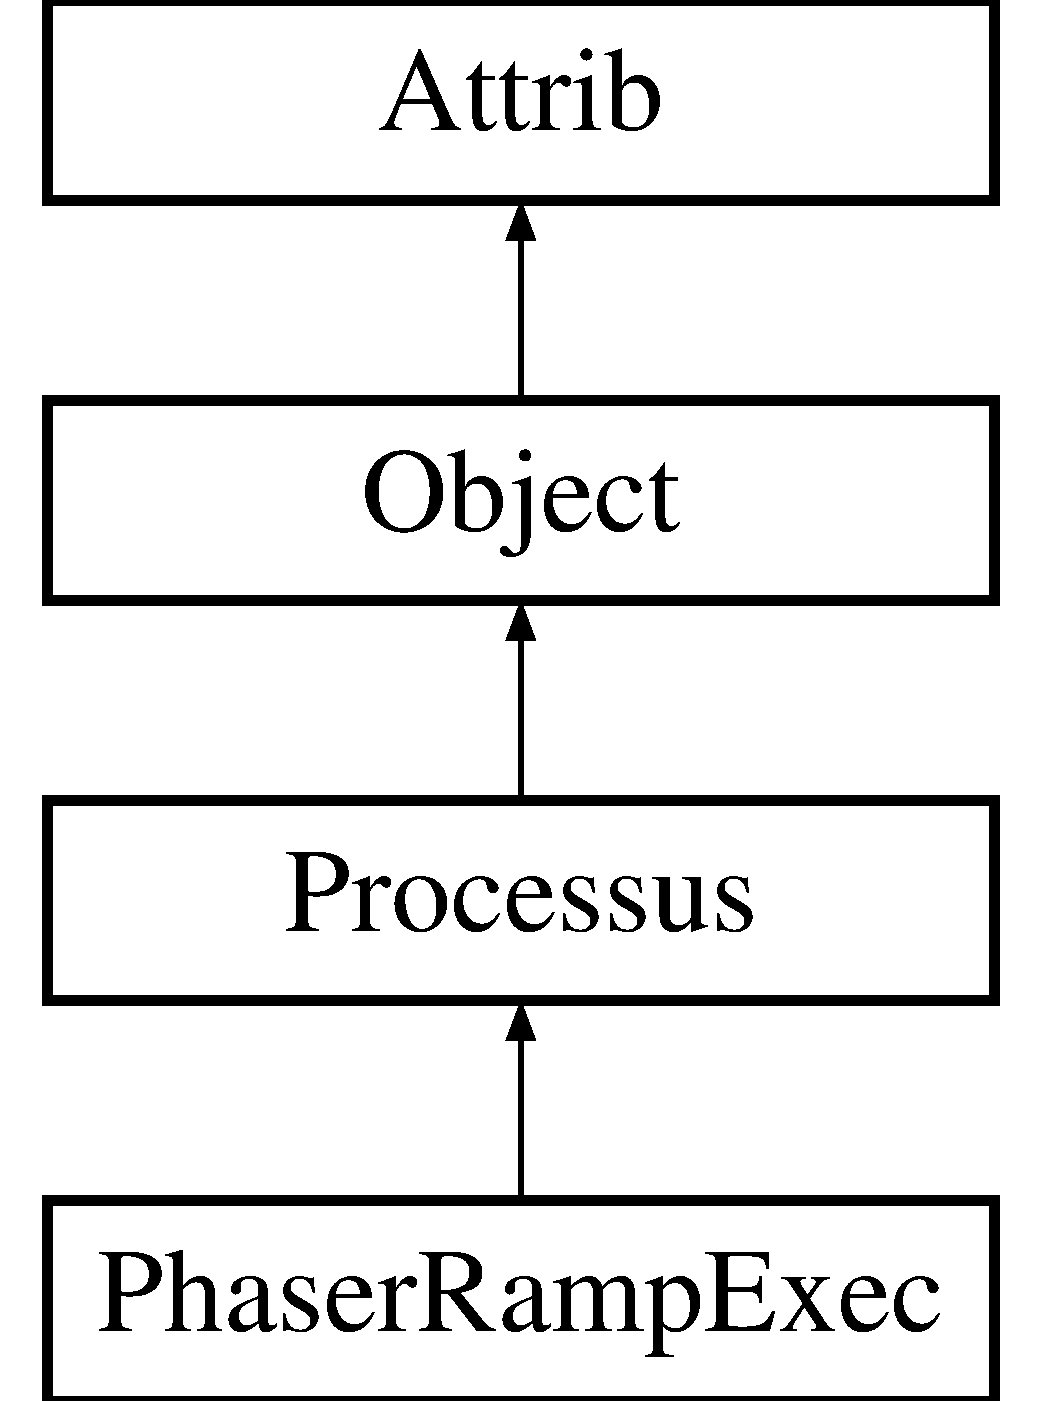
\includegraphics[height=4.000000cm]{classPhaserRampExec}
\end{center}
\end{figure}
\subsection*{Public Member Functions}
\begin{DoxyCompactItemize}
\item 
\hyperlink{classPhaserRampExec_a26f14f1c66dd37251374998ae0a4f02a}{Phaser\+Ramp\+Exec} ()
\begin{DoxyCompactList}\small\item\em Standard constructor. \end{DoxyCompactList}\item 
virtual \hyperlink{classPhaserRampExec_a0ea95adf577ff47f09068a20329f1598}{$\sim$\+Phaser\+Ramp\+Exec} ()
\begin{DoxyCompactList}\small\item\em Destructor. \end{DoxyCompactList}\item 
virtual \hyperlink{classStatusCode}{Status\+Code} \hyperlink{classPhaserRampExec_ae6f90f2ecf4b66d6f9bc85b123587ef3}{initialize} ()
\item 
virtual \hyperlink{classStatusCode}{Status\+Code} \hyperlink{classPhaserRampExec_a5fccbd3cddf738318f9d45d64b723907}{execute} ()
\item 
virtual \hyperlink{classStatusCode}{Status\+Code} \hyperlink{classPhaserRampExec_a8849cacdd34e7ca56f6d5e7668fe8c6c}{finalize} ()
\end{DoxyCompactItemize}
\subsection*{Protected Member Functions}
\begin{DoxyCompactItemize}
\item 
\hyperlink{classPhaserRampExec}{Phaser\+Ramp\+Exec} $\ast$ \hyperlink{classPhaserRampExec_a2586b2209d381c5b82a13dc2f997925f}{clone} ()
\end{DoxyCompactItemize}
\subsection*{Private Attributes}
\begin{DoxyCompactItemize}
\item 
\hyperlink{classPhaser}{Phaser} $\ast$ \hyperlink{classPhaserRampExec_a3c187e98596d492f195c2743322e263b}{m\+\_\+phaser}
\item 
T\+H1D $\ast$ \hyperlink{classPhaserRampExec_a8c13c96564df17be4e71685684e67edd}{h1}
\item 
T\+H1D $\ast$ \hyperlink{classPhaserRampExec_a538d1b02ed14d13c71f54b2b48e765ba}{h2}
\item 
T\+H1D $\ast$ \hyperlink{classPhaserRampExec_ad9ec4185f676732648c4886f28c9c6b7}{h3}
\item 
T\+H1D $\ast$ \hyperlink{classPhaserRampExec_aa487df389ad66093dba562f27f558128}{h4}
\item 
T\+H1D $\ast$ \hyperlink{classPhaserRampExec_ad2a2a82a0be74bc39c84b580e33d9c34}{hv1}
\item 
T\+H1D $\ast$ \hyperlink{classPhaserRampExec_a9762fd546432b5f3dffc4c5323af56ac}{hv2}
\item 
T\+H1D $\ast$ \hyperlink{classPhaserRampExec_ad3127f38a360044f7ad8fed272f916f9}{hv3}
\item 
T\+H1D $\ast$ \hyperlink{classPhaserRampExec_a998b7e5a8d186df60c2d60cba2b43aa0}{hv4}
\item 
T\+File $\ast$ \hyperlink{classPhaserRampExec_a63092bcbec01af94b4c5c842b81d2ccf}{file}
\item 
T\+H1F $\ast$ \hyperlink{classPhaserRampExec_a0c8d1c3ee09159cba1b1a07ce3fb1d96}{histo}
\item 
int \hyperlink{classPhaserRampExec_a7526a42abb33e880d60570386fd23e3e}{m\+\_\+init\+Phase} \mbox{[}4\mbox{]}
\item 
unsigned long \hyperlink{classPhaserRampExec_a198ba1ebb9a1b0fb2c599405307e92af}{m\+\_\+n\+Processed\+Events}
\item 
unsigned long \hyperlink{classPhaserRampExec_a3f09b8bf4cd8f5425adf8ae168d39e50}{error\+Count}
\end{DoxyCompactItemize}
\subsection*{Additional Inherited Members}


\subsection{Detailed Description}
\begin{DoxyAuthor}{Author}
Frédéric Machefert 
\end{DoxyAuthor}
\begin{DoxyDate}{Date}
2004-\/07-\/23 
\end{DoxyDate}


Definition at line 26 of file Phaser\+Ramp\+Exec.\+h.



\subsection{Constructor \& Destructor Documentation}
\mbox{\Hypertarget{classPhaserRampExec_a26f14f1c66dd37251374998ae0a4f02a}\label{classPhaserRampExec_a26f14f1c66dd37251374998ae0a4f02a}} 
\index{Phaser\+Ramp\+Exec@{Phaser\+Ramp\+Exec}!Phaser\+Ramp\+Exec@{Phaser\+Ramp\+Exec}}
\index{Phaser\+Ramp\+Exec@{Phaser\+Ramp\+Exec}!Phaser\+Ramp\+Exec@{Phaser\+Ramp\+Exec}}
\subsubsection{\texorpdfstring{Phaser\+Ramp\+Exec()}{PhaserRampExec()}}
{\footnotesize\ttfamily Phaser\+Ramp\+Exec\+::\+Phaser\+Ramp\+Exec (\begin{DoxyParamCaption}{ }\end{DoxyParamCaption})}



Standard constructor. 



Definition at line 36 of file Phaser\+Ramp\+Exec.\+cpp.



References Object\+::set\+Name(), Object\+::set\+Title(), and Object\+::set\+Type().



Referenced by clone().


\begin{DoxyCode}
36                                  \{
37   \hyperlink{classObject_ae30fea75683c2d149b6b6d17c09ecd0c}{setName} ( \textcolor{stringliteral}{"PhaserRampExec"} );
38   \hyperlink{classObject_aae534cc9d982bcb9b99fd505f2e103a5}{setType} ( \textcolor{stringliteral}{"Phaser"} );
39   \hyperlink{classObject_a89557dbbad5bcaa02652f5d7fa35d20f}{setTitle}( \textcolor{stringliteral}{"Phaser I2C Configuration Test"} );
40 \}
\end{DoxyCode}
\mbox{\Hypertarget{classPhaserRampExec_a0ea95adf577ff47f09068a20329f1598}\label{classPhaserRampExec_a0ea95adf577ff47f09068a20329f1598}} 
\index{Phaser\+Ramp\+Exec@{Phaser\+Ramp\+Exec}!````~Phaser\+Ramp\+Exec@{$\sim$\+Phaser\+Ramp\+Exec}}
\index{````~Phaser\+Ramp\+Exec@{$\sim$\+Phaser\+Ramp\+Exec}!Phaser\+Ramp\+Exec@{Phaser\+Ramp\+Exec}}
\subsubsection{\texorpdfstring{$\sim$\+Phaser\+Ramp\+Exec()}{~PhaserRampExec()}}
{\footnotesize\ttfamily Phaser\+Ramp\+Exec\+::$\sim$\+Phaser\+Ramp\+Exec (\begin{DoxyParamCaption}{ }\end{DoxyParamCaption})\hspace{0.3cm}{\ttfamily [virtual]}}



Destructor. 



Definition at line 44 of file Phaser\+Ramp\+Exec.\+cpp.


\begin{DoxyCode}
44 \{\}
\end{DoxyCode}


\subsection{Member Function Documentation}
\mbox{\Hypertarget{classPhaserRampExec_a2586b2209d381c5b82a13dc2f997925f}\label{classPhaserRampExec_a2586b2209d381c5b82a13dc2f997925f}} 
\index{Phaser\+Ramp\+Exec@{Phaser\+Ramp\+Exec}!clone@{clone}}
\index{clone@{clone}!Phaser\+Ramp\+Exec@{Phaser\+Ramp\+Exec}}
\subsubsection{\texorpdfstring{clone()}{clone()}}
{\footnotesize\ttfamily \hyperlink{classPhaserRampExec}{Phaser\+Ramp\+Exec}$\ast$ Phaser\+Ramp\+Exec\+::clone (\begin{DoxyParamCaption}{ }\end{DoxyParamCaption})\hspace{0.3cm}{\ttfamily [inline]}, {\ttfamily [protected]}, {\ttfamily [virtual]}}

processus termination virtual function 

Implements \hyperlink{classProcessus_aca8856f6d6d7b7e1fe941f298dcbb502}{Processus}.



Definition at line 41 of file Phaser\+Ramp\+Exec.\+h.



References Phaser\+Ramp\+Exec().


\begin{DoxyCode}
41                          \{
42     \textcolor{keywordflow}{return} \textcolor{keyword}{new} \hyperlink{classPhaserRampExec_a26f14f1c66dd37251374998ae0a4f02a}{PhaserRampExec} (*\textcolor{keyword}{this});
43   \}
\end{DoxyCode}
\mbox{\Hypertarget{classPhaserRampExec_a5fccbd3cddf738318f9d45d64b723907}\label{classPhaserRampExec_a5fccbd3cddf738318f9d45d64b723907}} 
\index{Phaser\+Ramp\+Exec@{Phaser\+Ramp\+Exec}!execute@{execute}}
\index{execute@{execute}!Phaser\+Ramp\+Exec@{Phaser\+Ramp\+Exec}}
\subsubsection{\texorpdfstring{execute()}{execute()}}
{\footnotesize\ttfamily \hyperlink{classStatusCode}{Status\+Code} Phaser\+Ramp\+Exec\+::execute (\begin{DoxyParamCaption}{ }\end{DoxyParamCaption})\hspace{0.3cm}{\ttfamily [virtual]}}

processus execution virtual function 

Implements \hyperlink{classProcessus_a63767a63a1fb0055c5aa45b21a4a5d58}{Processus}.



Definition at line 90 of file Phaser\+Ramp\+Exec.\+cpp.



References error\+Count, h1, h2, h3, h4, hv1, hv2, hv3, hv4, Object\+::info(), itos(), m\+\_\+n\+Processed\+Events, m\+\_\+phaser, Phaser\+::phase(), Phaser\+::read(), Phaser\+::set\+Phase(), Status\+Code\+::\+S\+U\+C\+C\+E\+SS, and Phaser\+::write().



Referenced by B\+O\+O\+S\+T\+\_\+\+P\+Y\+T\+H\+O\+N\+\_\+\+M\+O\+D\+U\+L\+E().


\begin{DoxyCode}
90                                      \{ 
91 
92   \hyperlink{classPhaserRampExec_a198ba1ebb9a1b0fb2c599405307e92af}{m\_nProcessedEvents}++;
93   
94   \textcolor{keywordtype}{int} v1 =  (int) ( (\textcolor{keywordtype}{float})rand()/RAND\_MAX * 25. );
95   \textcolor{keywordtype}{int} v2 =  (int) ( (\textcolor{keywordtype}{float})rand()/RAND\_MAX * 25. );
96   \textcolor{keywordtype}{int} v3 =  (int) ( (\textcolor{keywordtype}{float})rand()/RAND\_MAX * 25. );
97   \textcolor{keywordtype}{int} v4 =  (int) ( (\textcolor{keywordtype}{float})rand()/RAND\_MAX * 25. );
98   
99   \hyperlink{classPhaserRampExec_a3c187e98596d492f195c2743322e263b}{m\_phaser}->\hyperlink{classPhaser_a35c0add55885b3c0a7551ff48e322632}{setPhase}(v1,v2,v3,v4);
100   \hyperlink{classPhaserRampExec_a3c187e98596d492f195c2743322e263b}{m\_phaser}->\hyperlink{classPhaser_a7a94d4129a5f743c482fa97f3c5df68f}{write}();
101   \hyperlink{classPhaserRampExec_a3c187e98596d492f195c2743322e263b}{m\_phaser}->\hyperlink{classPhaser_a6ce0713403e961495192ffa0590c29e4}{read}();
102 
103   \textcolor{keywordtype}{int} d0=\hyperlink{classPhaserRampExec_a3c187e98596d492f195c2743322e263b}{m\_phaser}->\hyperlink{classPhaser_a3928ba4f1421c83b2f7783da87727ff2}{phase}(0);
104   \textcolor{keywordtype}{int} d1=\hyperlink{classPhaserRampExec_a3c187e98596d492f195c2743322e263b}{m\_phaser}->\hyperlink{classPhaser_a3928ba4f1421c83b2f7783da87727ff2}{phase}(1);
105   \textcolor{keywordtype}{int} d2=\hyperlink{classPhaserRampExec_a3c187e98596d492f195c2743322e263b}{m\_phaser}->\hyperlink{classPhaser_a3928ba4f1421c83b2f7783da87727ff2}{phase}(2);
106   \textcolor{keywordtype}{int} d3=\hyperlink{classPhaserRampExec_a3c187e98596d492f195c2743322e263b}{m\_phaser}->\hyperlink{classPhaser_a3928ba4f1421c83b2f7783da87727ff2}{phase}(3);
107   
108   \hyperlink{classPhaserRampExec_ad2a2a82a0be74bc39c84b580e33d9c34}{hv1}->Fill(v1);
109   \hyperlink{classPhaserRampExec_a9762fd546432b5f3dffc4c5323af56ac}{hv2}->Fill(v2);
110   \hyperlink{classPhaserRampExec_ad3127f38a360044f7ad8fed272f916f9}{hv3}->Fill(v3);
111   \hyperlink{classPhaserRampExec_a998b7e5a8d186df60c2d60cba2b43aa0}{hv4}->Fill(v4);
112 
113   
114   \textcolor{keywordflow}{if}( v1!=d0 || v2!=d1 || v3!=d2 || v4!=d3 )\{
115 
116     \textcolor{keywordflow}{if} ( d0 != v1 ) \hyperlink{classPhaserRampExec_a8c13c96564df17be4e71685684e67edd}{h1}->Fill(\textcolor{keywordtype}{int}(d0));
117     \textcolor{keywordflow}{if} ( d1 != v2 ) \hyperlink{classPhaserRampExec_a538d1b02ed14d13c71f54b2b48e765ba}{h2}->Fill(\textcolor{keywordtype}{int}(d1));
118     \textcolor{keywordflow}{if} ( d2 != v3 ) \hyperlink{classPhaserRampExec_ad9ec4185f676732648c4886f28c9c6b7}{h3}->Fill(\textcolor{keywordtype}{int}(d2));
119     \textcolor{keywordflow}{if} ( d3 != v4 ) \hyperlink{classPhaserRampExec_aa487df389ad66093dba562f27f558128}{h4}->Fill(\textcolor{keywordtype}{int}(d3));
120 
121     \hyperlink{classPhaserRampExec_a3f09b8bf4cd8f5425adf8ae168d39e50}{errorCount}++;
122     \hyperlink{classObject_a644fd329ea4cb85f54fa6846484b84a8}{info}(\textcolor{stringliteral}{"WRITE/READ INCOMPATIBILTY ["}+
123          \hyperlink{Tools_8h_af330027dbdafb9a30768b3613c553e60}{itos}(\hyperlink{classPhaserRampExec_a3f09b8bf4cd8f5425adf8ae168d39e50}{errorCount})+\textcolor{stringliteral}{"] "} +
124          \hyperlink{Tools_8h_af330027dbdafb9a30768b3613c553e60}{itos}(v1)+\textcolor{stringliteral}{"/"}+\hyperlink{Tools_8h_af330027dbdafb9a30768b3613c553e60}{itos}(d0)+\textcolor{stringliteral}{" "}+
125          \hyperlink{Tools_8h_af330027dbdafb9a30768b3613c553e60}{itos}(v2)+\textcolor{stringliteral}{"/"}+\hyperlink{Tools_8h_af330027dbdafb9a30768b3613c553e60}{itos}(d1)+\textcolor{stringliteral}{" "}+
126          \hyperlink{Tools_8h_af330027dbdafb9a30768b3613c553e60}{itos}(v3)+\textcolor{stringliteral}{"/"}+\hyperlink{Tools_8h_af330027dbdafb9a30768b3613c553e60}{itos}(d2)+\textcolor{stringliteral}{" "}+
127          \hyperlink{Tools_8h_af330027dbdafb9a30768b3613c553e60}{itos}(v4)+\textcolor{stringliteral}{"/"}+\hyperlink{Tools_8h_af330027dbdafb9a30768b3613c553e60}{itos}(d3),
128          \textcolor{stringliteral}{"Phaser::ramp"});
129     \textcolor{comment}{//     return false;}
130   \}
131   
132   \textcolor{keywordflow}{return} \hyperlink{classStatusCode_a6f565cbeadc76d14c72f047e5e85eb4badd0da38d3ba0d922efd1f4619bc37ad8}{StatusCode::SUCCESS};
133 \}
\end{DoxyCode}
\mbox{\Hypertarget{classPhaserRampExec_a8849cacdd34e7ca56f6d5e7668fe8c6c}\label{classPhaserRampExec_a8849cacdd34e7ca56f6d5e7668fe8c6c}} 
\index{Phaser\+Ramp\+Exec@{Phaser\+Ramp\+Exec}!finalize@{finalize}}
\index{finalize@{finalize}!Phaser\+Ramp\+Exec@{Phaser\+Ramp\+Exec}}
\subsubsection{\texorpdfstring{finalize()}{finalize()}}
{\footnotesize\ttfamily \hyperlink{classStatusCode}{Status\+Code} Phaser\+Ramp\+Exec\+::finalize (\begin{DoxyParamCaption}{ }\end{DoxyParamCaption})\hspace{0.3cm}{\ttfamily [virtual]}}

processus termination virtual function 

Implements \hyperlink{classProcessus_aba93d691f031bdb18ae4b8afb1b2e856}{Processus}.



Definition at line 139 of file Phaser\+Ramp\+Exec.\+cpp.



References Processus\+::close\+Root\+File(), Processus\+::elapsed\+Time(), error\+Count, ftos(), h1, h2, h3, h4, hv1, hv2, hv3, hv4, Object\+::info(), itos(), m\+\_\+init\+Phase, m\+\_\+n\+Processed\+Events, m\+\_\+phaser, Phaser\+::set\+Phase(), Status\+Code\+::\+S\+U\+C\+C\+E\+SS, and Phaser\+::write().



Referenced by B\+O\+O\+S\+T\+\_\+\+P\+Y\+T\+H\+O\+N\+\_\+\+M\+O\+D\+U\+L\+E().


\begin{DoxyCode}
139                                       \{
140   \hyperlink{classObject_a644fd329ea4cb85f54fa6846484b84a8}{info}(\textcolor{stringliteral}{"\_\_"} );
141   \hyperlink{classObject_a644fd329ea4cb85f54fa6846484b84a8}{info}(\textcolor{stringliteral}{"Errors                             "}+\hyperlink{Tools_8h_af330027dbdafb9a30768b3613c553e60}{itos}(\hyperlink{classPhaserRampExec_a3f09b8bf4cd8f5425adf8ae168d39e50}{errorCount}));
142   \hyperlink{classObject_a644fd329ea4cb85f54fa6846484b84a8}{info}(\textcolor{stringliteral}{"Processed Events                   "}+\hyperlink{Tools_8h_af330027dbdafb9a30768b3613c553e60}{itos}(\hyperlink{classPhaserRampExec_a198ba1ebb9a1b0fb2c599405307e92af}{m\_nProcessedEvents}));
143   \hyperlink{classObject_a644fd329ea4cb85f54fa6846484b84a8}{info}(\textcolor{stringliteral}{"Elapsed Time                       "}+\hyperlink{Tools_8h_ae78000c70889d75d67813c6cb83010a6}{ftos}(\hyperlink{classProcessus_aecca96218c65bc805c988cd95447df55}{elapsedTime}())+\textcolor{stringliteral}{" s."});
144   \hyperlink{classObject_a644fd329ea4cb85f54fa6846484b84a8}{info}(\textcolor{stringliteral}{"****************************"} );
145  
146   \hyperlink{classPhaserRampExec_a3c187e98596d492f195c2743322e263b}{m\_phaser}->\hyperlink{classPhaser_a35c0add55885b3c0a7551ff48e322632}{setPhase}(\hyperlink{classPhaserRampExec_a7526a42abb33e880d60570386fd23e3e}{m\_initPhase}[0],
147                      \hyperlink{classPhaserRampExec_a7526a42abb33e880d60570386fd23e3e}{m\_initPhase}[1],
148                      \hyperlink{classPhaserRampExec_a7526a42abb33e880d60570386fd23e3e}{m\_initPhase}[2],
149                      \hyperlink{classPhaserRampExec_a7526a42abb33e880d60570386fd23e3e}{m\_initPhase}[3]);
150   
151   \hyperlink{classPhaserRampExec_a3c187e98596d492f195c2743322e263b}{m\_phaser}->\hyperlink{classPhaser_a7a94d4129a5f743c482fa97f3c5df68f}{write}();
152 
153   \hyperlink{classProcessus_a2f3c41e99da4c738ea3d8f7b0d20a665}{closeRootFile}();
154 
155   \hyperlink{classPhaserRampExec_ad2a2a82a0be74bc39c84b580e33d9c34}{hv1}->Delete();
156   \hyperlink{classPhaserRampExec_a9762fd546432b5f3dffc4c5323af56ac}{hv2}->Delete();
157   \hyperlink{classPhaserRampExec_ad3127f38a360044f7ad8fed272f916f9}{hv3}->Delete();
158   \hyperlink{classPhaserRampExec_a998b7e5a8d186df60c2d60cba2b43aa0}{hv4}->Delete();
159   \hyperlink{classPhaserRampExec_a8c13c96564df17be4e71685684e67edd}{h1}->Delete();
160   \hyperlink{classPhaserRampExec_a538d1b02ed14d13c71f54b2b48e765ba}{h2}->Delete();
161   \hyperlink{classPhaserRampExec_ad9ec4185f676732648c4886f28c9c6b7}{h3}->Delete();
162   \hyperlink{classPhaserRampExec_aa487df389ad66093dba562f27f558128}{h4}->Delete();
163   
164   \textcolor{keywordflow}{return} \hyperlink{classStatusCode_a6f565cbeadc76d14c72f047e5e85eb4badd0da38d3ba0d922efd1f4619bc37ad8}{StatusCode::SUCCESS};  
165 \}
\end{DoxyCode}
\mbox{\Hypertarget{classPhaserRampExec_ae6f90f2ecf4b66d6f9bc85b123587ef3}\label{classPhaserRampExec_ae6f90f2ecf4b66d6f9bc85b123587ef3}} 
\index{Phaser\+Ramp\+Exec@{Phaser\+Ramp\+Exec}!initialize@{initialize}}
\index{initialize@{initialize}!Phaser\+Ramp\+Exec@{Phaser\+Ramp\+Exec}}
\subsubsection{\texorpdfstring{initialize()}{initialize()}}
{\footnotesize\ttfamily \hyperlink{classStatusCode}{Status\+Code} Phaser\+Ramp\+Exec\+::initialize (\begin{DoxyParamCaption}{ }\end{DoxyParamCaption})\hspace{0.3cm}{\ttfamily [virtual]}}

processus initialisation virtual function 

Implements \hyperlink{classProcessus_aee88ad7b77ae7319cf8b128e9dd2ea11}{Processus}.



Definition at line 49 of file Phaser\+Ramp\+Exec.\+cpp.



References Processus\+::element(), error\+Count, h1, h2, h3, h4, hv1, hv2, hv3, hv4, Object\+::info(), m\+\_\+init\+Phase, m\+\_\+n\+Processed\+Events, m\+\_\+phaser, Object\+::name(), Processus\+::open\+Root\+File(), Phaser\+::phase(), Phaser\+::read(), Processus\+::start\+Chrono(), Status\+Code\+::\+S\+U\+C\+C\+E\+SS, and Object\+::type().



Referenced by B\+O\+O\+S\+T\+\_\+\+P\+Y\+T\+H\+O\+N\+\_\+\+M\+O\+D\+U\+L\+E().


\begin{DoxyCode}
49                                         \{
50 
51   \hyperlink{classObject_a644fd329ea4cb85f54fa6846484b84a8}{info}(\textcolor{stringliteral}{""} );
52   \hyperlink{classObject_a644fd329ea4cb85f54fa6846484b84a8}{info}(\textcolor{stringliteral}{"\_\_\_\_\_\_\_\_\_\_\_\_\_\_\_\_\_\_\_\_\_\_\_\_\_\_\_\_"});
53   \hyperlink{classObject_a644fd329ea4cb85f54fa6846484b84a8}{info}(\textcolor{stringliteral}{"Phaser Configuration Control"});
54   \hyperlink{classObject_a644fd329ea4cb85f54fa6846484b84a8}{info}(\textcolor{stringliteral}{" =>"} + \hyperlink{classProcessus_a6fe155527431a7190b7d44d600b9608d}{element}()->path() + \textcolor{stringliteral}{" "} + 
55        \hyperlink{classProcessus_a6fe155527431a7190b7d44d600b9608d}{element}()->\hyperlink{classObject_a300f4c05dd468c7bb8b3c968868443c1}{name}() + \textcolor{stringliteral}{" "} + \hyperlink{classProcessus_a6fe155527431a7190b7d44d600b9608d}{element}()->\hyperlink{classObject_a84f99f70f144a83e1582d1d0f84e4e62}{type}() );
56   
57   \hyperlink{classPhaserRampExec_a3c187e98596d492f195c2743322e263b}{m\_phaser}=\textcolor{keyword}{dynamic\_cast<}\hyperlink{classPhaser}{Phaser}*\textcolor{keyword}{>}( \hyperlink{classProcessus_a6fe155527431a7190b7d44d600b9608d}{element}() );
58   
59   srand( (\textcolor{keywordtype}{unsigned})time( NULL ) );
60 
61   \hyperlink{classPhaserRampExec_a3c187e98596d492f195c2743322e263b}{m\_phaser}->\hyperlink{classPhaser_a6ce0713403e961495192ffa0590c29e4}{read}();
62 
63   \hyperlink{classPhaserRampExec_a7526a42abb33e880d60570386fd23e3e}{m\_initPhase}[0]=\hyperlink{classPhaserRampExec_a3c187e98596d492f195c2743322e263b}{m\_phaser}->\hyperlink{classPhaser_a3928ba4f1421c83b2f7783da87727ff2}{phase}(0);
64   \hyperlink{classPhaserRampExec_a7526a42abb33e880d60570386fd23e3e}{m\_initPhase}[1]=\hyperlink{classPhaserRampExec_a3c187e98596d492f195c2743322e263b}{m\_phaser}->\hyperlink{classPhaser_a3928ba4f1421c83b2f7783da87727ff2}{phase}(1);
65   \hyperlink{classPhaserRampExec_a7526a42abb33e880d60570386fd23e3e}{m\_initPhase}[2]=\hyperlink{classPhaserRampExec_a3c187e98596d492f195c2743322e263b}{m\_phaser}->\hyperlink{classPhaser_a3928ba4f1421c83b2f7783da87727ff2}{phase}(2);
66   \hyperlink{classPhaserRampExec_a7526a42abb33e880d60570386fd23e3e}{m\_initPhase}[3]=\hyperlink{classPhaserRampExec_a3c187e98596d492f195c2743322e263b}{m\_phaser}->\hyperlink{classPhaser_a3928ba4f1421c83b2f7783da87727ff2}{phase}(3);
67   
68   \hyperlink{classProcessus_aacf6812880c1d1a2bf14a4a39458f443}{openRootFile} ();
69 
70   \hyperlink{classPhaserRampExec_ad2a2a82a0be74bc39c84b580e33d9c34}{hv1}=\textcolor{keyword}{new} TH1D( \textcolor{stringliteral}{"Delay1"} , \textcolor{stringliteral}{"Delay Channel 1"} , 25 , 0. , 25. );
71   \hyperlink{classPhaserRampExec_a9762fd546432b5f3dffc4c5323af56ac}{hv2}=\textcolor{keyword}{new} TH1D( \textcolor{stringliteral}{"Delay2"} , \textcolor{stringliteral}{"Delay Channel 2"} , 25 , 0. , 25. );
72   \hyperlink{classPhaserRampExec_ad3127f38a360044f7ad8fed272f916f9}{hv3}=\textcolor{keyword}{new} TH1D( \textcolor{stringliteral}{"Delay3"} , \textcolor{stringliteral}{"Delay Channel 3"} , 25 , 0. , 25. );
73   \hyperlink{classPhaserRampExec_a998b7e5a8d186df60c2d60cba2b43aa0}{hv4}=\textcolor{keyword}{new} TH1D( \textcolor{stringliteral}{"Delay4"} , \textcolor{stringliteral}{"Delay Channel 4"} , 25 , 0. , 25. );
74 
75   \hyperlink{classPhaserRampExec_a8c13c96564df17be4e71685684e67edd}{h1}=\textcolor{keyword}{new} TH1D( \textcolor{stringliteral}{"Error1"} , \textcolor{stringliteral}{"Error Channel 1"} , 25 , 0. , 25. );
76   \hyperlink{classPhaserRampExec_a538d1b02ed14d13c71f54b2b48e765ba}{h2}=\textcolor{keyword}{new} TH1D( \textcolor{stringliteral}{"Error2"} , \textcolor{stringliteral}{"Error Channel 2"} , 25 , 0. , 25. );
77   \hyperlink{classPhaserRampExec_ad9ec4185f676732648c4886f28c9c6b7}{h3}=\textcolor{keyword}{new} TH1D( \textcolor{stringliteral}{"Error3"} , \textcolor{stringliteral}{"Error Channel 3"} , 25 , 0. , 25. );
78   \hyperlink{classPhaserRampExec_aa487df389ad66093dba562f27f558128}{h4}=\textcolor{keyword}{new} TH1D( \textcolor{stringliteral}{"Error4"} , \textcolor{stringliteral}{"Error Channel 4"} , 25 , 0. , 25. );
79   
80   \hyperlink{classPhaserRampExec_a198ba1ebb9a1b0fb2c599405307e92af}{m\_nProcessedEvents}=0;
81   \hyperlink{classPhaserRampExec_a3f09b8bf4cd8f5425adf8ae168d39e50}{errorCount}=0;
82   \hyperlink{classProcessus_a5e4d34b86241fa0756e07375a14ff4b2}{startChrono}();
83   
84   \textcolor{keywordflow}{return} \hyperlink{classStatusCode_a6f565cbeadc76d14c72f047e5e85eb4badd0da38d3ba0d922efd1f4619bc37ad8}{StatusCode::SUCCESS};  
85 \}
\end{DoxyCode}


\subsection{Member Data Documentation}
\mbox{\Hypertarget{classPhaserRampExec_a3f09b8bf4cd8f5425adf8ae168d39e50}\label{classPhaserRampExec_a3f09b8bf4cd8f5425adf8ae168d39e50}} 
\index{Phaser\+Ramp\+Exec@{Phaser\+Ramp\+Exec}!error\+Count@{error\+Count}}
\index{error\+Count@{error\+Count}!Phaser\+Ramp\+Exec@{Phaser\+Ramp\+Exec}}
\subsubsection{\texorpdfstring{error\+Count}{errorCount}}
{\footnotesize\ttfamily unsigned long Phaser\+Ramp\+Exec\+::error\+Count\hspace{0.3cm}{\ttfamily [private]}}



Definition at line 56 of file Phaser\+Ramp\+Exec.\+h.



Referenced by execute(), finalize(), and initialize().

\mbox{\Hypertarget{classPhaserRampExec_a63092bcbec01af94b4c5c842b81d2ccf}\label{classPhaserRampExec_a63092bcbec01af94b4c5c842b81d2ccf}} 
\index{Phaser\+Ramp\+Exec@{Phaser\+Ramp\+Exec}!file@{file}}
\index{file@{file}!Phaser\+Ramp\+Exec@{Phaser\+Ramp\+Exec}}
\subsubsection{\texorpdfstring{file}{file}}
{\footnotesize\ttfamily T\+File$\ast$ Phaser\+Ramp\+Exec\+::file\hspace{0.3cm}{\ttfamily [private]}}



Definition at line 50 of file Phaser\+Ramp\+Exec.\+h.



Referenced by arguments.\+arguments\+::decode(), and arguments.\+arguments\+::printout().

\mbox{\Hypertarget{classPhaserRampExec_a8c13c96564df17be4e71685684e67edd}\label{classPhaserRampExec_a8c13c96564df17be4e71685684e67edd}} 
\index{Phaser\+Ramp\+Exec@{Phaser\+Ramp\+Exec}!h1@{h1}}
\index{h1@{h1}!Phaser\+Ramp\+Exec@{Phaser\+Ramp\+Exec}}
\subsubsection{\texorpdfstring{h1}{h1}}
{\footnotesize\ttfamily T\+H1D$\ast$ Phaser\+Ramp\+Exec\+::h1\hspace{0.3cm}{\ttfamily [private]}}



Definition at line 48 of file Phaser\+Ramp\+Exec.\+h.



Referenced by execute(), finalize(), and initialize().

\mbox{\Hypertarget{classPhaserRampExec_a538d1b02ed14d13c71f54b2b48e765ba}\label{classPhaserRampExec_a538d1b02ed14d13c71f54b2b48e765ba}} 
\index{Phaser\+Ramp\+Exec@{Phaser\+Ramp\+Exec}!h2@{h2}}
\index{h2@{h2}!Phaser\+Ramp\+Exec@{Phaser\+Ramp\+Exec}}
\subsubsection{\texorpdfstring{h2}{h2}}
{\footnotesize\ttfamily T\+H1D $\ast$ Phaser\+Ramp\+Exec\+::h2\hspace{0.3cm}{\ttfamily [private]}}



Definition at line 48 of file Phaser\+Ramp\+Exec.\+h.



Referenced by execute(), finalize(), and initialize().

\mbox{\Hypertarget{classPhaserRampExec_ad9ec4185f676732648c4886f28c9c6b7}\label{classPhaserRampExec_ad9ec4185f676732648c4886f28c9c6b7}} 
\index{Phaser\+Ramp\+Exec@{Phaser\+Ramp\+Exec}!h3@{h3}}
\index{h3@{h3}!Phaser\+Ramp\+Exec@{Phaser\+Ramp\+Exec}}
\subsubsection{\texorpdfstring{h3}{h3}}
{\footnotesize\ttfamily T\+H1D $\ast$ Phaser\+Ramp\+Exec\+::h3\hspace{0.3cm}{\ttfamily [private]}}



Definition at line 48 of file Phaser\+Ramp\+Exec.\+h.



Referenced by execute(), finalize(), and initialize().

\mbox{\Hypertarget{classPhaserRampExec_aa487df389ad66093dba562f27f558128}\label{classPhaserRampExec_aa487df389ad66093dba562f27f558128}} 
\index{Phaser\+Ramp\+Exec@{Phaser\+Ramp\+Exec}!h4@{h4}}
\index{h4@{h4}!Phaser\+Ramp\+Exec@{Phaser\+Ramp\+Exec}}
\subsubsection{\texorpdfstring{h4}{h4}}
{\footnotesize\ttfamily T\+H1D $\ast$ Phaser\+Ramp\+Exec\+::h4\hspace{0.3cm}{\ttfamily [private]}}



Definition at line 48 of file Phaser\+Ramp\+Exec.\+h.



Referenced by execute(), finalize(), and initialize().

\mbox{\Hypertarget{classPhaserRampExec_a0c8d1c3ee09159cba1b1a07ce3fb1d96}\label{classPhaserRampExec_a0c8d1c3ee09159cba1b1a07ce3fb1d96}} 
\index{Phaser\+Ramp\+Exec@{Phaser\+Ramp\+Exec}!histo@{histo}}
\index{histo@{histo}!Phaser\+Ramp\+Exec@{Phaser\+Ramp\+Exec}}
\subsubsection{\texorpdfstring{histo}{histo}}
{\footnotesize\ttfamily T\+H1F$\ast$ Phaser\+Ramp\+Exec\+::histo\hspace{0.3cm}{\ttfamily [private]}}



Definition at line 51 of file Phaser\+Ramp\+Exec.\+h.

\mbox{\Hypertarget{classPhaserRampExec_ad2a2a82a0be74bc39c84b580e33d9c34}\label{classPhaserRampExec_ad2a2a82a0be74bc39c84b580e33d9c34}} 
\index{Phaser\+Ramp\+Exec@{Phaser\+Ramp\+Exec}!hv1@{hv1}}
\index{hv1@{hv1}!Phaser\+Ramp\+Exec@{Phaser\+Ramp\+Exec}}
\subsubsection{\texorpdfstring{hv1}{hv1}}
{\footnotesize\ttfamily T\+H1D$\ast$ Phaser\+Ramp\+Exec\+::hv1\hspace{0.3cm}{\ttfamily [private]}}



Definition at line 49 of file Phaser\+Ramp\+Exec.\+h.



Referenced by execute(), finalize(), and initialize().

\mbox{\Hypertarget{classPhaserRampExec_a9762fd546432b5f3dffc4c5323af56ac}\label{classPhaserRampExec_a9762fd546432b5f3dffc4c5323af56ac}} 
\index{Phaser\+Ramp\+Exec@{Phaser\+Ramp\+Exec}!hv2@{hv2}}
\index{hv2@{hv2}!Phaser\+Ramp\+Exec@{Phaser\+Ramp\+Exec}}
\subsubsection{\texorpdfstring{hv2}{hv2}}
{\footnotesize\ttfamily T\+H1D $\ast$ Phaser\+Ramp\+Exec\+::hv2\hspace{0.3cm}{\ttfamily [private]}}



Definition at line 49 of file Phaser\+Ramp\+Exec.\+h.



Referenced by execute(), finalize(), and initialize().

\mbox{\Hypertarget{classPhaserRampExec_ad3127f38a360044f7ad8fed272f916f9}\label{classPhaserRampExec_ad3127f38a360044f7ad8fed272f916f9}} 
\index{Phaser\+Ramp\+Exec@{Phaser\+Ramp\+Exec}!hv3@{hv3}}
\index{hv3@{hv3}!Phaser\+Ramp\+Exec@{Phaser\+Ramp\+Exec}}
\subsubsection{\texorpdfstring{hv3}{hv3}}
{\footnotesize\ttfamily T\+H1D $\ast$ Phaser\+Ramp\+Exec\+::hv3\hspace{0.3cm}{\ttfamily [private]}}



Definition at line 49 of file Phaser\+Ramp\+Exec.\+h.



Referenced by execute(), finalize(), and initialize().

\mbox{\Hypertarget{classPhaserRampExec_a998b7e5a8d186df60c2d60cba2b43aa0}\label{classPhaserRampExec_a998b7e5a8d186df60c2d60cba2b43aa0}} 
\index{Phaser\+Ramp\+Exec@{Phaser\+Ramp\+Exec}!hv4@{hv4}}
\index{hv4@{hv4}!Phaser\+Ramp\+Exec@{Phaser\+Ramp\+Exec}}
\subsubsection{\texorpdfstring{hv4}{hv4}}
{\footnotesize\ttfamily T\+H1D $\ast$ Phaser\+Ramp\+Exec\+::hv4\hspace{0.3cm}{\ttfamily [private]}}



Definition at line 49 of file Phaser\+Ramp\+Exec.\+h.



Referenced by execute(), finalize(), and initialize().

\mbox{\Hypertarget{classPhaserRampExec_a7526a42abb33e880d60570386fd23e3e}\label{classPhaserRampExec_a7526a42abb33e880d60570386fd23e3e}} 
\index{Phaser\+Ramp\+Exec@{Phaser\+Ramp\+Exec}!m\+\_\+init\+Phase@{m\+\_\+init\+Phase}}
\index{m\+\_\+init\+Phase@{m\+\_\+init\+Phase}!Phaser\+Ramp\+Exec@{Phaser\+Ramp\+Exec}}
\subsubsection{\texorpdfstring{m\+\_\+init\+Phase}{m\_initPhase}}
{\footnotesize\ttfamily int Phaser\+Ramp\+Exec\+::m\+\_\+init\+Phase\mbox{[}4\mbox{]}\hspace{0.3cm}{\ttfamily [private]}}



Definition at line 53 of file Phaser\+Ramp\+Exec.\+h.



Referenced by finalize(), and initialize().

\mbox{\Hypertarget{classPhaserRampExec_a198ba1ebb9a1b0fb2c599405307e92af}\label{classPhaserRampExec_a198ba1ebb9a1b0fb2c599405307e92af}} 
\index{Phaser\+Ramp\+Exec@{Phaser\+Ramp\+Exec}!m\+\_\+n\+Processed\+Events@{m\+\_\+n\+Processed\+Events}}
\index{m\+\_\+n\+Processed\+Events@{m\+\_\+n\+Processed\+Events}!Phaser\+Ramp\+Exec@{Phaser\+Ramp\+Exec}}
\subsubsection{\texorpdfstring{m\+\_\+n\+Processed\+Events}{m\_nProcessedEvents}}
{\footnotesize\ttfamily unsigned long Phaser\+Ramp\+Exec\+::m\+\_\+n\+Processed\+Events\hspace{0.3cm}{\ttfamily [private]}}



Definition at line 55 of file Phaser\+Ramp\+Exec.\+h.



Referenced by execute(), finalize(), and initialize().

\mbox{\Hypertarget{classPhaserRampExec_a3c187e98596d492f195c2743322e263b}\label{classPhaserRampExec_a3c187e98596d492f195c2743322e263b}} 
\index{Phaser\+Ramp\+Exec@{Phaser\+Ramp\+Exec}!m\+\_\+phaser@{m\+\_\+phaser}}
\index{m\+\_\+phaser@{m\+\_\+phaser}!Phaser\+Ramp\+Exec@{Phaser\+Ramp\+Exec}}
\subsubsection{\texorpdfstring{m\+\_\+phaser}{m\_phaser}}
{\footnotesize\ttfamily \hyperlink{classPhaser}{Phaser}$\ast$ Phaser\+Ramp\+Exec\+::m\+\_\+phaser\hspace{0.3cm}{\ttfamily [private]}}



Definition at line 46 of file Phaser\+Ramp\+Exec.\+h.



Referenced by execute(), finalize(), and initialize().



The documentation for this class was generated from the following files\+:\begin{DoxyCompactItemize}
\item 
/home/eleclhcb/\+L\+H\+Cb/lbcat-\/cmake/\+Cat\+Calo/inc/proc/\hyperlink{PhaserRampExec_8h}{Phaser\+Ramp\+Exec.\+h}\item 
/home/eleclhcb/\+L\+H\+Cb/lbcat-\/cmake/\+Cat\+Calo/src/proc/\hyperlink{PhaserRampExec_8cpp}{Phaser\+Ramp\+Exec.\+cpp}\end{DoxyCompactItemize}

\hypertarget{classPhaserScan}{}\section{Phaser\+Scan Class Reference}
\label{classPhaserScan}\index{Phaser\+Scan@{Phaser\+Scan}}


{\ttfamily \#include $<$inc/\+Phaser\+Scan.\+h$>$}

Inheritance diagram for Phaser\+Scan\+:\begin{figure}[H]
\begin{center}
\leavevmode
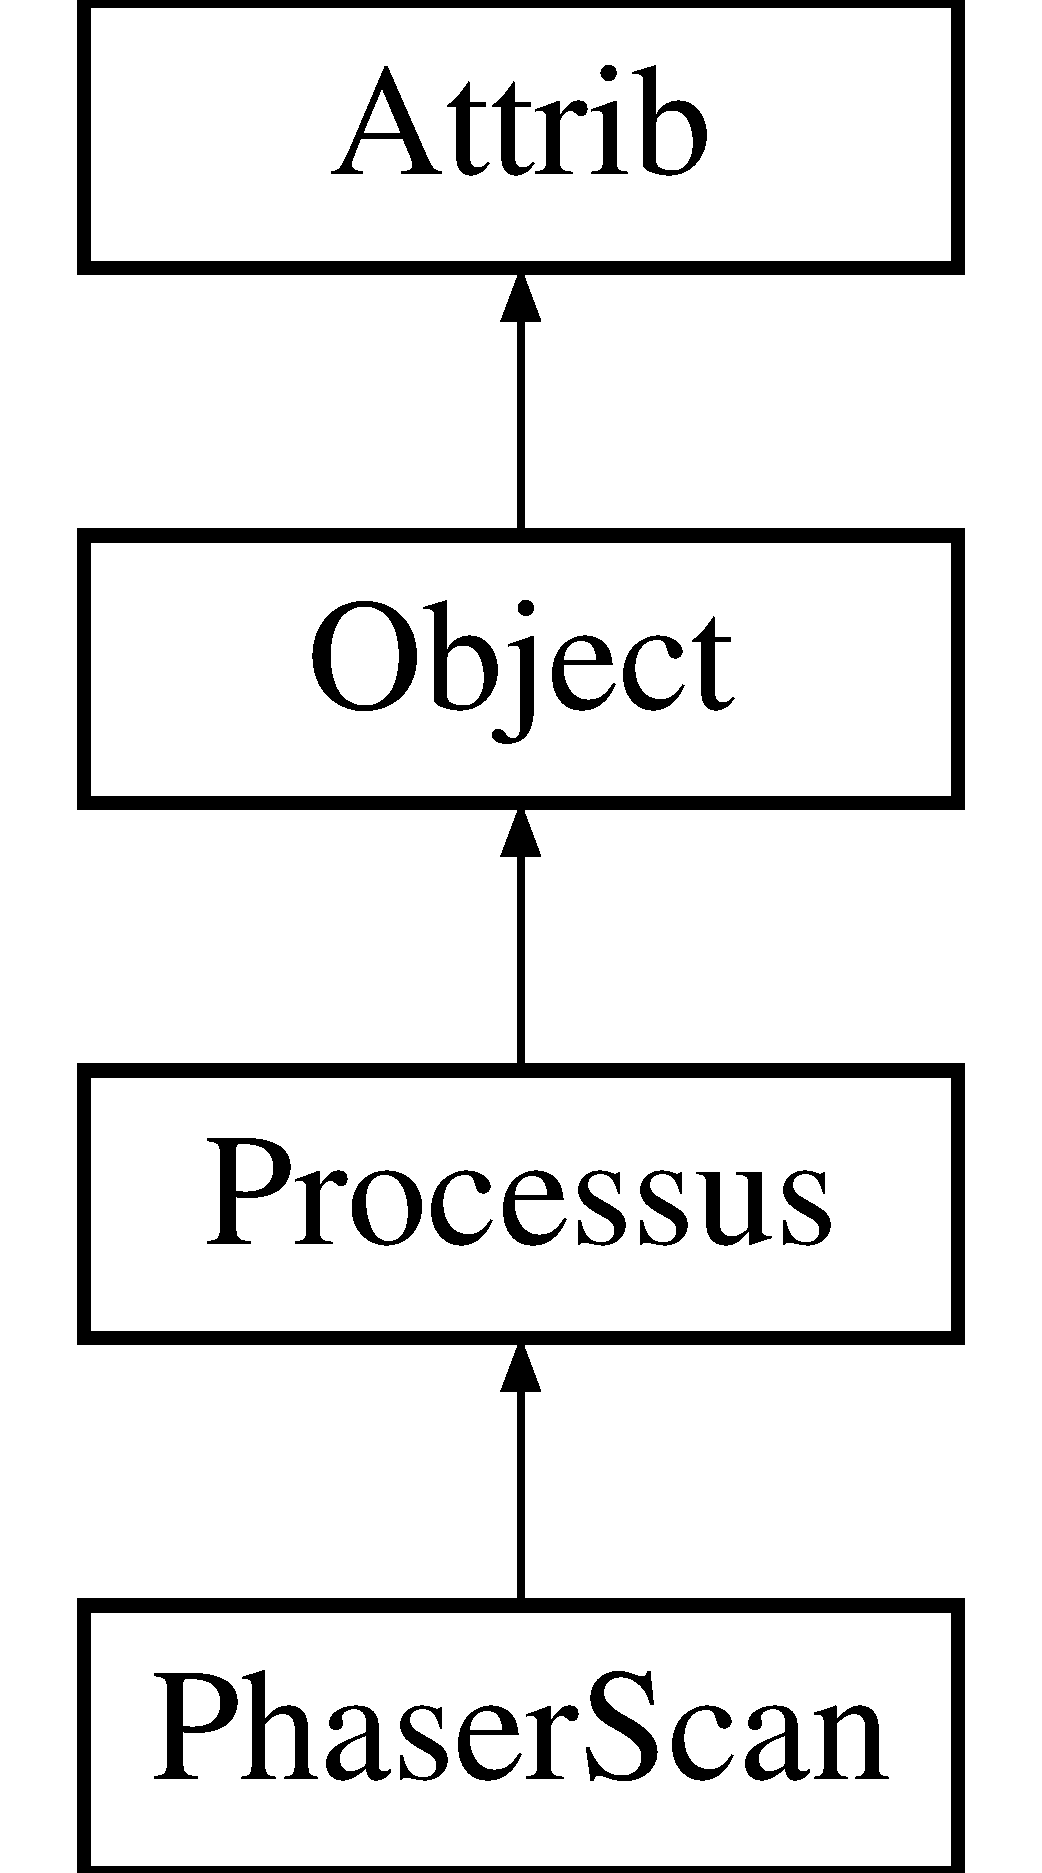
\includegraphics[height=4.000000cm]{classPhaserScan}
\end{center}
\end{figure}
\subsection*{Public Member Functions}
\begin{DoxyCompactItemize}
\item 
\hyperlink{classPhaserScan_afba6f21affa3e014fe4019dfd9664672}{Phaser\+Scan} ()
\begin{DoxyCompactList}\small\item\em Standard constructor. \end{DoxyCompactList}\item 
virtual \hyperlink{classPhaserScan_a861dfecc0610514a146c300a7458bad5}{$\sim$\+Phaser\+Scan} ()
\begin{DoxyCompactList}\small\item\em Destructor. \end{DoxyCompactList}\item 
virtual \hyperlink{classStatusCode}{Status\+Code} \hyperlink{classPhaserScan_aeb0dccb02754b11c19719962f7c43fb8}{initialize} ()
\item 
virtual \hyperlink{classStatusCode}{Status\+Code} \hyperlink{classPhaserScan_abf8e9639bcbbd23ec1a9a8e04319d9d1}{execute} ()
\item 
virtual \hyperlink{classStatusCode}{Status\+Code} \hyperlink{classPhaserScan_a505bd8dc2961fd220f1624cd949a266e}{finalize} ()
\item 
\hyperlink{classStatusCode}{Status\+Code} \hyperlink{classPhaserScan_abc98adb04157f08d1c1ba99eee527a37}{set\+Phaser\+Min} (unsigned int)
\item 
unsigned int \hyperlink{classPhaserScan_ab24e5fc6e36639ce31faf430ca87afc9}{phaser\+Min} ()
\item 
\hyperlink{classStatusCode}{Status\+Code} \hyperlink{classPhaserScan_ad968ae47c77c7813caf69cc22ff40559}{set\+Phaser\+Max} (unsigned int)
\item 
unsigned int \hyperlink{classPhaserScan_a2cccb1c5b687c5cdf934dd3eb11a73ad}{phaser\+Max} ()
\item 
\hyperlink{classStatusCode}{Status\+Code} \hyperlink{classPhaserScan_a99ff5030b4e551437796c5614f92fffd}{set\+Phaser\+Step} (unsigned int)
\item 
unsigned int \hyperlink{classPhaserScan_a8bebde600274e342a78783e49917b64d}{phaser\+Step} ()
\item 
\hyperlink{classStatusCode}{Status\+Code} \hyperlink{classPhaserScan_a182d5a23019a62c3c3ad3a03f5187036}{set\+Depth} (unsigned int)
\item 
unsigned int \hyperlink{classPhaserScan_ad2d47975431e765c906ba51eeeb4365d}{depth} ()
\item 
\hyperlink{classStatusCode}{Status\+Code} \hyperlink{classPhaserScan_a12fc9ff050fc15e067ae622c37827661}{set\+Channels} (unsigned int)
\item 
unsigned int \hyperlink{classPhaserScan_ae3752906e17afd1f7ee5f62a08711871}{channels} ()
\item 
\hyperlink{classStatusCode}{Status\+Code} \hyperlink{classPhaserScan_a8e9d2bff400546f71d0c24cd3658d09e}{set\+Trigger} (bool trig)
\item 
void \hyperlink{classPhaserScan_ae66b02455c6d5779ba92d3a17abd7ead}{set\+Sample} (int nsample)
\item 
int \hyperlink{classPhaserScan_a278292fe5bc31814dab8cd54deb76b48}{sample} ()
\item 
bool \hyperlink{classPhaserScan_a6ae0b3511064540555ef9770c63febc4}{trigger} ()
\end{DoxyCompactItemize}
\subsection*{Protected Member Functions}
\begin{DoxyCompactItemize}
\item 
\hyperlink{classPhaserScan}{Phaser\+Scan} $\ast$ \hyperlink{classPhaserScan_a4c842f4bda17fb8907c51efc0ccb9d43}{clone} ()
\item 
unsigned int \hyperlink{classPhaserScan_ad01a0ce0223859a138e3a78023a924bb}{decode\+Format} (unsigned int, unsigned int, \hyperlink{classRAM}{R\+AM} $\ast$)
\end{DoxyCompactItemize}
\subsection*{Private Attributes}
\begin{DoxyCompactItemize}
\item 
Int\+\_\+t \hyperlink{classPhaserScan_a158add7f69adba5e4623afda6c9b31e2}{m\+\_\+run\+Number}
\item 
Int\+\_\+t \hyperlink{classPhaserScan_a038d4303bd3f2446417ec2af5d9995cf}{m\+\_\+evt\+Number}
\item 
Int\+\_\+t \hyperlink{classPhaserScan_a983fb003ef3c41d1dcf1078247548d82}{m\+\_\+channel} \mbox{[}8\mbox{]}
\item 
Int\+\_\+t \hyperlink{classPhaserScan_a6fd741cbc6a81d527e25aa9e8c7f27e0}{m\+\_\+ch\+Number} \mbox{[}8\mbox{]}
\item 
Int\+\_\+t \hyperlink{classPhaserScan_aa73583dea3f784eaacaffdd356e51e9d}{m\+\_\+nch}
\item 
int \hyperlink{classPhaserScan_a3e9894ae646ed25d26a07532c1a2b8b7}{m\+\_\+channels}
\item 
int \hyperlink{classPhaserScan_a445487a8eea9b6d484ae8615cb1bd52d}{m\+\_\+depth}
\item 
\hyperlink{classProto40MHz__v1}{Proto40\+M\+Hz\+\_\+v1} $\ast$ \hyperlink{classPhaserScan_aec1f340810d0cf1f98155673385ffff5}{m\+\_\+board}
\item 
\hyperlink{classA3PE}{A3\+PE} $\ast$ \hyperlink{classPhaserScan_a2065860536763c7f9fd6b8b41908e673}{m\+\_\+pga}
\item 
\hyperlink{classPhaser}{Phaser} $\ast$ \hyperlink{classPhaserScan_ae2726b0d199ca8ae713cea55866d4ae3}{m\+\_\+phaser}
\item 
\hyperlink{classRAM}{R\+AM} $\ast$ \hyperlink{classPhaserScan_a4249cdec58c8163d9f3663be8e929cdf}{m\+\_\+fifo}
\item 
bool \hyperlink{classPhaserScan_ab3fd16cfcce13a09f5c1e91d96de60e6}{m\+\_\+trig}
\item 
T\+H1D $\ast$ \hyperlink{classPhaserScan_abd6954d739e7b2b0d36d09a080146d60}{m\+\_\+hist}
\item 
unsigned int \hyperlink{classPhaserScan_a65f83dd6b9e6c62cd828ef7b094c0361}{m\+\_\+phaser\+Min}
\item 
unsigned int \hyperlink{classPhaserScan_aed5bcb2582744f73a6189544c272213b}{m\+\_\+phaser\+Step}
\item 
unsigned int \hyperlink{classPhaserScan_ab47dd8cf441f9c713aa8c3e2251b382d}{m\+\_\+phaser\+Max}
\item 
unsigned int \hyperlink{classPhaserScan_a6c2089bb98fa8a897430b17ddb052447}{m\+\_\+nsample}
\item 
int \hyperlink{classPhaserScan_aef87ca678cea59093899a7cd138a9e25}{m\+\_\+deadtime}
\end{DoxyCompactItemize}
\subsection*{Static Private Attributes}
\begin{DoxyCompactItemize}
\item 
static const unsigned int \hyperlink{classPhaserScan_a3c5a969d3fef57564d2632b256bf857e}{m\+\_\+depthmax} = 512
\end{DoxyCompactItemize}
\subsection*{Additional Inherited Members}


\subsection{Detailed Description}
\begin{DoxyAuthor}{Author}

\end{DoxyAuthor}
\begin{DoxyDate}{Date}
2006-\/10-\/23 
\end{DoxyDate}


Definition at line 20 of file Phaser\+Scan.\+h.



\subsection{Constructor \& Destructor Documentation}
\mbox{\Hypertarget{classPhaserScan_afba6f21affa3e014fe4019dfd9664672}\label{classPhaserScan_afba6f21affa3e014fe4019dfd9664672}} 
\index{Phaser\+Scan@{Phaser\+Scan}!Phaser\+Scan@{Phaser\+Scan}}
\index{Phaser\+Scan@{Phaser\+Scan}!Phaser\+Scan@{Phaser\+Scan}}
\subsubsection{\texorpdfstring{Phaser\+Scan()}{PhaserScan()}}
{\footnotesize\ttfamily Phaser\+Scan\+::\+Phaser\+Scan (\begin{DoxyParamCaption}{ }\end{DoxyParamCaption})}



Standard constructor. 



Referenced by clone().

\mbox{\Hypertarget{classPhaserScan_a861dfecc0610514a146c300a7458bad5}\label{classPhaserScan_a861dfecc0610514a146c300a7458bad5}} 
\index{Phaser\+Scan@{Phaser\+Scan}!````~Phaser\+Scan@{$\sim$\+Phaser\+Scan}}
\index{````~Phaser\+Scan@{$\sim$\+Phaser\+Scan}!Phaser\+Scan@{Phaser\+Scan}}
\subsubsection{\texorpdfstring{$\sim$\+Phaser\+Scan()}{~PhaserScan()}}
{\footnotesize\ttfamily virtual Phaser\+Scan\+::$\sim$\+Phaser\+Scan (\begin{DoxyParamCaption}{ }\end{DoxyParamCaption})\hspace{0.3cm}{\ttfamily [virtual]}}



Destructor. 



\subsection{Member Function Documentation}
\mbox{\Hypertarget{classPhaserScan_ae3752906e17afd1f7ee5f62a08711871}\label{classPhaserScan_ae3752906e17afd1f7ee5f62a08711871}} 
\index{Phaser\+Scan@{Phaser\+Scan}!channels@{channels}}
\index{channels@{channels}!Phaser\+Scan@{Phaser\+Scan}}
\subsubsection{\texorpdfstring{channels()}{channels()}}
{\footnotesize\ttfamily unsigned int Phaser\+Scan\+::channels (\begin{DoxyParamCaption}{ }\end{DoxyParamCaption})\hspace{0.3cm}{\ttfamily [inline]}}



Definition at line 41 of file Phaser\+Scan.\+h.



References m\+\_\+channels.


\begin{DoxyCode}
41 \{\textcolor{keywordflow}{return} \hyperlink{classPhaserScan_a3e9894ae646ed25d26a07532c1a2b8b7}{m\_channels};\};
\end{DoxyCode}
\mbox{\Hypertarget{classPhaserScan_a4c842f4bda17fb8907c51efc0ccb9d43}\label{classPhaserScan_a4c842f4bda17fb8907c51efc0ccb9d43}} 
\index{Phaser\+Scan@{Phaser\+Scan}!clone@{clone}}
\index{clone@{clone}!Phaser\+Scan@{Phaser\+Scan}}
\subsubsection{\texorpdfstring{clone()}{clone()}}
{\footnotesize\ttfamily \hyperlink{classPhaserScan}{Phaser\+Scan}$\ast$ Phaser\+Scan\+::clone (\begin{DoxyParamCaption}{ }\end{DoxyParamCaption})\hspace{0.3cm}{\ttfamily [inline]}, {\ttfamily [protected]}, {\ttfamily [virtual]}}

processus termination virtual function 

Implements \hyperlink{classProcessus_aca8856f6d6d7b7e1fe941f298dcbb502}{Processus}.



Definition at line 59 of file Phaser\+Scan.\+h.



References decode\+Format(), and Phaser\+Scan().


\begin{DoxyCode}
59                      \{
60     \textcolor{keywordflow}{return} \textcolor{keyword}{new} \hyperlink{classPhaserScan_afba6f21affa3e014fe4019dfd9664672}{PhaserScan} (*\textcolor{keyword}{this});
61   \}
\end{DoxyCode}
\mbox{\Hypertarget{classPhaserScan_ad01a0ce0223859a138e3a78023a924bb}\label{classPhaserScan_ad01a0ce0223859a138e3a78023a924bb}} 
\index{Phaser\+Scan@{Phaser\+Scan}!decode\+Format@{decode\+Format}}
\index{decode\+Format@{decode\+Format}!Phaser\+Scan@{Phaser\+Scan}}
\subsubsection{\texorpdfstring{decode\+Format()}{decodeFormat()}}
{\footnotesize\ttfamily unsigned int Phaser\+Scan\+::decode\+Format (\begin{DoxyParamCaption}\item[{unsigned}]{int,  }\item[{unsigned}]{int,  }\item[{\hyperlink{classRAM}{R\+AM} $\ast$}]{ }\end{DoxyParamCaption})\hspace{0.3cm}{\ttfamily [protected]}}



Referenced by clone().

\mbox{\Hypertarget{classPhaserScan_ad2d47975431e765c906ba51eeeb4365d}\label{classPhaserScan_ad2d47975431e765c906ba51eeeb4365d}} 
\index{Phaser\+Scan@{Phaser\+Scan}!depth@{depth}}
\index{depth@{depth}!Phaser\+Scan@{Phaser\+Scan}}
\subsubsection{\texorpdfstring{depth()}{depth()}}
{\footnotesize\ttfamily unsigned int Phaser\+Scan\+::depth (\begin{DoxyParamCaption}{ }\end{DoxyParamCaption})\hspace{0.3cm}{\ttfamily [inline]}}



Definition at line 38 of file Phaser\+Scan.\+h.



References m\+\_\+depth, and set\+Channels().


\begin{DoxyCode}
38 \{\textcolor{keywordflow}{return} \hyperlink{classPhaserScan_a445487a8eea9b6d484ae8615cb1bd52d}{m\_depth};\};
\end{DoxyCode}
\mbox{\Hypertarget{classPhaserScan_abf8e9639bcbbd23ec1a9a8e04319d9d1}\label{classPhaserScan_abf8e9639bcbbd23ec1a9a8e04319d9d1}} 
\index{Phaser\+Scan@{Phaser\+Scan}!execute@{execute}}
\index{execute@{execute}!Phaser\+Scan@{Phaser\+Scan}}
\subsubsection{\texorpdfstring{execute()}{execute()}}
{\footnotesize\ttfamily virtual \hyperlink{classStatusCode}{Status\+Code} Phaser\+Scan\+::execute (\begin{DoxyParamCaption}{ }\end{DoxyParamCaption})\hspace{0.3cm}{\ttfamily [virtual]}}

processus execution virtual function 

Implements \hyperlink{classProcessus_a63767a63a1fb0055c5aa45b21a4a5d58}{Processus}.

\mbox{\Hypertarget{classPhaserScan_a505bd8dc2961fd220f1624cd949a266e}\label{classPhaserScan_a505bd8dc2961fd220f1624cd949a266e}} 
\index{Phaser\+Scan@{Phaser\+Scan}!finalize@{finalize}}
\index{finalize@{finalize}!Phaser\+Scan@{Phaser\+Scan}}
\subsubsection{\texorpdfstring{finalize()}{finalize()}}
{\footnotesize\ttfamily virtual \hyperlink{classStatusCode}{Status\+Code} Phaser\+Scan\+::finalize (\begin{DoxyParamCaption}{ }\end{DoxyParamCaption})\hspace{0.3cm}{\ttfamily [virtual]}}

processus termination virtual function 

Implements \hyperlink{classProcessus_aba93d691f031bdb18ae4b8afb1b2e856}{Processus}.

\mbox{\Hypertarget{classPhaserScan_aeb0dccb02754b11c19719962f7c43fb8}\label{classPhaserScan_aeb0dccb02754b11c19719962f7c43fb8}} 
\index{Phaser\+Scan@{Phaser\+Scan}!initialize@{initialize}}
\index{initialize@{initialize}!Phaser\+Scan@{Phaser\+Scan}}
\subsubsection{\texorpdfstring{initialize()}{initialize()}}
{\footnotesize\ttfamily virtual \hyperlink{classStatusCode}{Status\+Code} Phaser\+Scan\+::initialize (\begin{DoxyParamCaption}{ }\end{DoxyParamCaption})\hspace{0.3cm}{\ttfamily [virtual]}}

processus initialisation virtual function 

Implements \hyperlink{classProcessus_aee88ad7b77ae7319cf8b128e9dd2ea11}{Processus}.

\mbox{\Hypertarget{classPhaserScan_a2cccb1c5b687c5cdf934dd3eb11a73ad}\label{classPhaserScan_a2cccb1c5b687c5cdf934dd3eb11a73ad}} 
\index{Phaser\+Scan@{Phaser\+Scan}!phaser\+Max@{phaser\+Max}}
\index{phaser\+Max@{phaser\+Max}!Phaser\+Scan@{Phaser\+Scan}}
\subsubsection{\texorpdfstring{phaser\+Max()}{phaserMax()}}
{\footnotesize\ttfamily unsigned int Phaser\+Scan\+::phaser\+Max (\begin{DoxyParamCaption}{ }\end{DoxyParamCaption})\hspace{0.3cm}{\ttfamily [inline]}}



Definition at line 33 of file Phaser\+Scan.\+h.



References m\+\_\+phaser\+Max, and set\+Phaser\+Step().


\begin{DoxyCode}
33 \{\textcolor{keywordflow}{return} \hyperlink{classPhaserScan_ab47dd8cf441f9c713aa8c3e2251b382d}{m\_phaserMax};\};
\end{DoxyCode}
\mbox{\Hypertarget{classPhaserScan_ab24e5fc6e36639ce31faf430ca87afc9}\label{classPhaserScan_ab24e5fc6e36639ce31faf430ca87afc9}} 
\index{Phaser\+Scan@{Phaser\+Scan}!phaser\+Min@{phaser\+Min}}
\index{phaser\+Min@{phaser\+Min}!Phaser\+Scan@{Phaser\+Scan}}
\subsubsection{\texorpdfstring{phaser\+Min()}{phaserMin()}}
{\footnotesize\ttfamily unsigned int Phaser\+Scan\+::phaser\+Min (\begin{DoxyParamCaption}{ }\end{DoxyParamCaption})\hspace{0.3cm}{\ttfamily [inline]}}



Definition at line 31 of file Phaser\+Scan.\+h.



References m\+\_\+phaser\+Min, and set\+Phaser\+Max().


\begin{DoxyCode}
31 \{\textcolor{keywordflow}{return} \hyperlink{classPhaserScan_a65f83dd6b9e6c62cd828ef7b094c0361}{m\_phaserMin};\};
\end{DoxyCode}
\mbox{\Hypertarget{classPhaserScan_a8bebde600274e342a78783e49917b64d}\label{classPhaserScan_a8bebde600274e342a78783e49917b64d}} 
\index{Phaser\+Scan@{Phaser\+Scan}!phaser\+Step@{phaser\+Step}}
\index{phaser\+Step@{phaser\+Step}!Phaser\+Scan@{Phaser\+Scan}}
\subsubsection{\texorpdfstring{phaser\+Step()}{phaserStep()}}
{\footnotesize\ttfamily unsigned int Phaser\+Scan\+::phaser\+Step (\begin{DoxyParamCaption}{ }\end{DoxyParamCaption})\hspace{0.3cm}{\ttfamily [inline]}}



Definition at line 35 of file Phaser\+Scan.\+h.



References m\+\_\+phaser\+Step, and set\+Depth().


\begin{DoxyCode}
35 \{\textcolor{keywordflow}{return} \hyperlink{classPhaserScan_aed5bcb2582744f73a6189544c272213b}{m\_phaserStep};\};
\end{DoxyCode}
\mbox{\Hypertarget{classPhaserScan_a278292fe5bc31814dab8cd54deb76b48}\label{classPhaserScan_a278292fe5bc31814dab8cd54deb76b48}} 
\index{Phaser\+Scan@{Phaser\+Scan}!sample@{sample}}
\index{sample@{sample}!Phaser\+Scan@{Phaser\+Scan}}
\subsubsection{\texorpdfstring{sample()}{sample()}}
{\footnotesize\ttfamily int Phaser\+Scan\+::sample (\begin{DoxyParamCaption}{ }\end{DoxyParamCaption})\hspace{0.3cm}{\ttfamily [inline]}}



Definition at line 52 of file Phaser\+Scan.\+h.



References m\+\_\+nsample.


\begin{DoxyCode}
52 \{\textcolor{keywordflow}{return} \hyperlink{classPhaserScan_a6c2089bb98fa8a897430b17ddb052447}{m\_nsample};\}
\end{DoxyCode}
\mbox{\Hypertarget{classPhaserScan_a12fc9ff050fc15e067ae622c37827661}\label{classPhaserScan_a12fc9ff050fc15e067ae622c37827661}} 
\index{Phaser\+Scan@{Phaser\+Scan}!set\+Channels@{set\+Channels}}
\index{set\+Channels@{set\+Channels}!Phaser\+Scan@{Phaser\+Scan}}
\subsubsection{\texorpdfstring{set\+Channels()}{setChannels()}}
{\footnotesize\ttfamily \hyperlink{classStatusCode}{Status\+Code} Phaser\+Scan\+::set\+Channels (\begin{DoxyParamCaption}\item[{unsigned}]{int }\end{DoxyParamCaption})}



Referenced by depth().

\mbox{\Hypertarget{classPhaserScan_a182d5a23019a62c3c3ad3a03f5187036}\label{classPhaserScan_a182d5a23019a62c3c3ad3a03f5187036}} 
\index{Phaser\+Scan@{Phaser\+Scan}!set\+Depth@{set\+Depth}}
\index{set\+Depth@{set\+Depth}!Phaser\+Scan@{Phaser\+Scan}}
\subsubsection{\texorpdfstring{set\+Depth()}{setDepth()}}
{\footnotesize\ttfamily \hyperlink{classStatusCode}{Status\+Code} Phaser\+Scan\+::set\+Depth (\begin{DoxyParamCaption}\item[{unsigned}]{int }\end{DoxyParamCaption})}



Referenced by phaser\+Step().

\mbox{\Hypertarget{classPhaserScan_ad968ae47c77c7813caf69cc22ff40559}\label{classPhaserScan_ad968ae47c77c7813caf69cc22ff40559}} 
\index{Phaser\+Scan@{Phaser\+Scan}!set\+Phaser\+Max@{set\+Phaser\+Max}}
\index{set\+Phaser\+Max@{set\+Phaser\+Max}!Phaser\+Scan@{Phaser\+Scan}}
\subsubsection{\texorpdfstring{set\+Phaser\+Max()}{setPhaserMax()}}
{\footnotesize\ttfamily \hyperlink{classStatusCode}{Status\+Code} Phaser\+Scan\+::set\+Phaser\+Max (\begin{DoxyParamCaption}\item[{unsigned}]{int }\end{DoxyParamCaption})}



Referenced by phaser\+Min().

\mbox{\Hypertarget{classPhaserScan_abc98adb04157f08d1c1ba99eee527a37}\label{classPhaserScan_abc98adb04157f08d1c1ba99eee527a37}} 
\index{Phaser\+Scan@{Phaser\+Scan}!set\+Phaser\+Min@{set\+Phaser\+Min}}
\index{set\+Phaser\+Min@{set\+Phaser\+Min}!Phaser\+Scan@{Phaser\+Scan}}
\subsubsection{\texorpdfstring{set\+Phaser\+Min()}{setPhaserMin()}}
{\footnotesize\ttfamily \hyperlink{classStatusCode}{Status\+Code} Phaser\+Scan\+::set\+Phaser\+Min (\begin{DoxyParamCaption}\item[{unsigned}]{int }\end{DoxyParamCaption})}

\mbox{\Hypertarget{classPhaserScan_a99ff5030b4e551437796c5614f92fffd}\label{classPhaserScan_a99ff5030b4e551437796c5614f92fffd}} 
\index{Phaser\+Scan@{Phaser\+Scan}!set\+Phaser\+Step@{set\+Phaser\+Step}}
\index{set\+Phaser\+Step@{set\+Phaser\+Step}!Phaser\+Scan@{Phaser\+Scan}}
\subsubsection{\texorpdfstring{set\+Phaser\+Step()}{setPhaserStep()}}
{\footnotesize\ttfamily \hyperlink{classStatusCode}{Status\+Code} Phaser\+Scan\+::set\+Phaser\+Step (\begin{DoxyParamCaption}\item[{unsigned}]{int }\end{DoxyParamCaption})}



Referenced by phaser\+Max().

\mbox{\Hypertarget{classPhaserScan_ae66b02455c6d5779ba92d3a17abd7ead}\label{classPhaserScan_ae66b02455c6d5779ba92d3a17abd7ead}} 
\index{Phaser\+Scan@{Phaser\+Scan}!set\+Sample@{set\+Sample}}
\index{set\+Sample@{set\+Sample}!Phaser\+Scan@{Phaser\+Scan}}
\subsubsection{\texorpdfstring{set\+Sample()}{setSample()}}
{\footnotesize\ttfamily void Phaser\+Scan\+::set\+Sample (\begin{DoxyParamCaption}\item[{int}]{nsample }\end{DoxyParamCaption})\hspace{0.3cm}{\ttfamily [inline]}}



Definition at line 48 of file Phaser\+Scan.\+h.



References m\+\_\+nsample.


\begin{DoxyCode}
48                              \{
49     \hyperlink{classPhaserScan_a6c2089bb98fa8a897430b17ddb052447}{m\_nsample}=nsample;
50   \}
\end{DoxyCode}
\mbox{\Hypertarget{classPhaserScan_a8e9d2bff400546f71d0c24cd3658d09e}\label{classPhaserScan_a8e9d2bff400546f71d0c24cd3658d09e}} 
\index{Phaser\+Scan@{Phaser\+Scan}!set\+Trigger@{set\+Trigger}}
\index{set\+Trigger@{set\+Trigger}!Phaser\+Scan@{Phaser\+Scan}}
\subsubsection{\texorpdfstring{set\+Trigger()}{setTrigger()}}
{\footnotesize\ttfamily \hyperlink{classStatusCode}{Status\+Code} Phaser\+Scan\+::set\+Trigger (\begin{DoxyParamCaption}\item[{bool}]{trig }\end{DoxyParamCaption})\hspace{0.3cm}{\ttfamily [inline]}}



Definition at line 43 of file Phaser\+Scan.\+h.



References m\+\_\+trig, and Status\+Code\+::\+S\+U\+C\+C\+E\+SS.


\begin{DoxyCode}
43                                    \{
44     \hyperlink{classPhaserScan_ab3fd16cfcce13a09f5c1e91d96de60e6}{m\_trig}=trig; 
45     \textcolor{keywordflow}{return} \hyperlink{classStatusCode_a6f565cbeadc76d14c72f047e5e85eb4badd0da38d3ba0d922efd1f4619bc37ad8}{StatusCode::SUCCESS};
46   \};
\end{DoxyCode}
\mbox{\Hypertarget{classPhaserScan_a6ae0b3511064540555ef9770c63febc4}\label{classPhaserScan_a6ae0b3511064540555ef9770c63febc4}} 
\index{Phaser\+Scan@{Phaser\+Scan}!trigger@{trigger}}
\index{trigger@{trigger}!Phaser\+Scan@{Phaser\+Scan}}
\subsubsection{\texorpdfstring{trigger()}{trigger()}}
{\footnotesize\ttfamily bool Phaser\+Scan\+::trigger (\begin{DoxyParamCaption}{ }\end{DoxyParamCaption})\hspace{0.3cm}{\ttfamily [inline]}}



Definition at line 54 of file Phaser\+Scan.\+h.



References m\+\_\+trig.


\begin{DoxyCode}
54                  \{
55     \textcolor{keywordflow}{return} \hyperlink{classPhaserScan_ab3fd16cfcce13a09f5c1e91d96de60e6}{m\_trig};
56   \};
\end{DoxyCode}


\subsection{Member Data Documentation}
\mbox{\Hypertarget{classPhaserScan_aec1f340810d0cf1f98155673385ffff5}\label{classPhaserScan_aec1f340810d0cf1f98155673385ffff5}} 
\index{Phaser\+Scan@{Phaser\+Scan}!m\+\_\+board@{m\+\_\+board}}
\index{m\+\_\+board@{m\+\_\+board}!Phaser\+Scan@{Phaser\+Scan}}
\subsubsection{\texorpdfstring{m\+\_\+board}{m\_board}}
{\footnotesize\ttfamily \hyperlink{classProto40MHz__v1}{Proto40\+M\+Hz\+\_\+v1}$\ast$ Phaser\+Scan\+::m\+\_\+board\hspace{0.3cm}{\ttfamily [private]}}



Definition at line 77 of file Phaser\+Scan.\+h.

\mbox{\Hypertarget{classPhaserScan_a983fb003ef3c41d1dcf1078247548d82}\label{classPhaserScan_a983fb003ef3c41d1dcf1078247548d82}} 
\index{Phaser\+Scan@{Phaser\+Scan}!m\+\_\+channel@{m\+\_\+channel}}
\index{m\+\_\+channel@{m\+\_\+channel}!Phaser\+Scan@{Phaser\+Scan}}
\subsubsection{\texorpdfstring{m\+\_\+channel}{m\_channel}}
{\footnotesize\ttfamily Int\+\_\+t Phaser\+Scan\+::m\+\_\+channel\mbox{[}8\mbox{]}\hspace{0.3cm}{\ttfamily [private]}}



Definition at line 71 of file Phaser\+Scan.\+h.

\mbox{\Hypertarget{classPhaserScan_a3e9894ae646ed25d26a07532c1a2b8b7}\label{classPhaserScan_a3e9894ae646ed25d26a07532c1a2b8b7}} 
\index{Phaser\+Scan@{Phaser\+Scan}!m\+\_\+channels@{m\+\_\+channels}}
\index{m\+\_\+channels@{m\+\_\+channels}!Phaser\+Scan@{Phaser\+Scan}}
\subsubsection{\texorpdfstring{m\+\_\+channels}{m\_channels}}
{\footnotesize\ttfamily int Phaser\+Scan\+::m\+\_\+channels\hspace{0.3cm}{\ttfamily [private]}}



Definition at line 75 of file Phaser\+Scan.\+h.



Referenced by channels().

\mbox{\Hypertarget{classPhaserScan_a6fd741cbc6a81d527e25aa9e8c7f27e0}\label{classPhaserScan_a6fd741cbc6a81d527e25aa9e8c7f27e0}} 
\index{Phaser\+Scan@{Phaser\+Scan}!m\+\_\+ch\+Number@{m\+\_\+ch\+Number}}
\index{m\+\_\+ch\+Number@{m\+\_\+ch\+Number}!Phaser\+Scan@{Phaser\+Scan}}
\subsubsection{\texorpdfstring{m\+\_\+ch\+Number}{m\_chNumber}}
{\footnotesize\ttfamily Int\+\_\+t Phaser\+Scan\+::m\+\_\+ch\+Number\mbox{[}8\mbox{]}\hspace{0.3cm}{\ttfamily [private]}}



Definition at line 72 of file Phaser\+Scan.\+h.

\mbox{\Hypertarget{classPhaserScan_aef87ca678cea59093899a7cd138a9e25}\label{classPhaserScan_aef87ca678cea59093899a7cd138a9e25}} 
\index{Phaser\+Scan@{Phaser\+Scan}!m\+\_\+deadtime@{m\+\_\+deadtime}}
\index{m\+\_\+deadtime@{m\+\_\+deadtime}!Phaser\+Scan@{Phaser\+Scan}}
\subsubsection{\texorpdfstring{m\+\_\+deadtime}{m\_deadtime}}
{\footnotesize\ttfamily int Phaser\+Scan\+::m\+\_\+deadtime\hspace{0.3cm}{\ttfamily [private]}}



Definition at line 87 of file Phaser\+Scan.\+h.

\mbox{\Hypertarget{classPhaserScan_a445487a8eea9b6d484ae8615cb1bd52d}\label{classPhaserScan_a445487a8eea9b6d484ae8615cb1bd52d}} 
\index{Phaser\+Scan@{Phaser\+Scan}!m\+\_\+depth@{m\+\_\+depth}}
\index{m\+\_\+depth@{m\+\_\+depth}!Phaser\+Scan@{Phaser\+Scan}}
\subsubsection{\texorpdfstring{m\+\_\+depth}{m\_depth}}
{\footnotesize\ttfamily int Phaser\+Scan\+::m\+\_\+depth\hspace{0.3cm}{\ttfamily [private]}}



Definition at line 76 of file Phaser\+Scan.\+h.



Referenced by depth().

\mbox{\Hypertarget{classPhaserScan_a3c5a969d3fef57564d2632b256bf857e}\label{classPhaserScan_a3c5a969d3fef57564d2632b256bf857e}} 
\index{Phaser\+Scan@{Phaser\+Scan}!m\+\_\+depthmax@{m\+\_\+depthmax}}
\index{m\+\_\+depthmax@{m\+\_\+depthmax}!Phaser\+Scan@{Phaser\+Scan}}
\subsubsection{\texorpdfstring{m\+\_\+depthmax}{m\_depthmax}}
{\footnotesize\ttfamily const unsigned int Phaser\+Scan\+::m\+\_\+depthmax = 512\hspace{0.3cm}{\ttfamily [static]}, {\ttfamily [private]}}



Definition at line 65 of file Phaser\+Scan.\+h.

\mbox{\Hypertarget{classPhaserScan_a038d4303bd3f2446417ec2af5d9995cf}\label{classPhaserScan_a038d4303bd3f2446417ec2af5d9995cf}} 
\index{Phaser\+Scan@{Phaser\+Scan}!m\+\_\+evt\+Number@{m\+\_\+evt\+Number}}
\index{m\+\_\+evt\+Number@{m\+\_\+evt\+Number}!Phaser\+Scan@{Phaser\+Scan}}
\subsubsection{\texorpdfstring{m\+\_\+evt\+Number}{m\_evtNumber}}
{\footnotesize\ttfamily Int\+\_\+t Phaser\+Scan\+::m\+\_\+evt\+Number\hspace{0.3cm}{\ttfamily [private]}}



Definition at line 69 of file Phaser\+Scan.\+h.

\mbox{\Hypertarget{classPhaserScan_a4249cdec58c8163d9f3663be8e929cdf}\label{classPhaserScan_a4249cdec58c8163d9f3663be8e929cdf}} 
\index{Phaser\+Scan@{Phaser\+Scan}!m\+\_\+fifo@{m\+\_\+fifo}}
\index{m\+\_\+fifo@{m\+\_\+fifo}!Phaser\+Scan@{Phaser\+Scan}}
\subsubsection{\texorpdfstring{m\+\_\+fifo}{m\_fifo}}
{\footnotesize\ttfamily \hyperlink{classRAM}{R\+AM}$\ast$ Phaser\+Scan\+::m\+\_\+fifo\hspace{0.3cm}{\ttfamily [private]}}



Definition at line 80 of file Phaser\+Scan.\+h.

\mbox{\Hypertarget{classPhaserScan_abd6954d739e7b2b0d36d09a080146d60}\label{classPhaserScan_abd6954d739e7b2b0d36d09a080146d60}} 
\index{Phaser\+Scan@{Phaser\+Scan}!m\+\_\+hist@{m\+\_\+hist}}
\index{m\+\_\+hist@{m\+\_\+hist}!Phaser\+Scan@{Phaser\+Scan}}
\subsubsection{\texorpdfstring{m\+\_\+hist}{m\_hist}}
{\footnotesize\ttfamily T\+H1D$\ast$ Phaser\+Scan\+::m\+\_\+hist\hspace{0.3cm}{\ttfamily [private]}}



Definition at line 82 of file Phaser\+Scan.\+h.

\mbox{\Hypertarget{classPhaserScan_aa73583dea3f784eaacaffdd356e51e9d}\label{classPhaserScan_aa73583dea3f784eaacaffdd356e51e9d}} 
\index{Phaser\+Scan@{Phaser\+Scan}!m\+\_\+nch@{m\+\_\+nch}}
\index{m\+\_\+nch@{m\+\_\+nch}!Phaser\+Scan@{Phaser\+Scan}}
\subsubsection{\texorpdfstring{m\+\_\+nch}{m\_nch}}
{\footnotesize\ttfamily Int\+\_\+t Phaser\+Scan\+::m\+\_\+nch\hspace{0.3cm}{\ttfamily [private]}}



Definition at line 73 of file Phaser\+Scan.\+h.

\mbox{\Hypertarget{classPhaserScan_a6c2089bb98fa8a897430b17ddb052447}\label{classPhaserScan_a6c2089bb98fa8a897430b17ddb052447}} 
\index{Phaser\+Scan@{Phaser\+Scan}!m\+\_\+nsample@{m\+\_\+nsample}}
\index{m\+\_\+nsample@{m\+\_\+nsample}!Phaser\+Scan@{Phaser\+Scan}}
\subsubsection{\texorpdfstring{m\+\_\+nsample}{m\_nsample}}
{\footnotesize\ttfamily unsigned int Phaser\+Scan\+::m\+\_\+nsample\hspace{0.3cm}{\ttfamily [private]}}



Definition at line 86 of file Phaser\+Scan.\+h.



Referenced by sample(), and set\+Sample().

\mbox{\Hypertarget{classPhaserScan_a2065860536763c7f9fd6b8b41908e673}\label{classPhaserScan_a2065860536763c7f9fd6b8b41908e673}} 
\index{Phaser\+Scan@{Phaser\+Scan}!m\+\_\+pga@{m\+\_\+pga}}
\index{m\+\_\+pga@{m\+\_\+pga}!Phaser\+Scan@{Phaser\+Scan}}
\subsubsection{\texorpdfstring{m\+\_\+pga}{m\_pga}}
{\footnotesize\ttfamily \hyperlink{classA3PE}{A3\+PE}$\ast$ Phaser\+Scan\+::m\+\_\+pga\hspace{0.3cm}{\ttfamily [private]}}



Definition at line 78 of file Phaser\+Scan.\+h.

\mbox{\Hypertarget{classPhaserScan_ae2726b0d199ca8ae713cea55866d4ae3}\label{classPhaserScan_ae2726b0d199ca8ae713cea55866d4ae3}} 
\index{Phaser\+Scan@{Phaser\+Scan}!m\+\_\+phaser@{m\+\_\+phaser}}
\index{m\+\_\+phaser@{m\+\_\+phaser}!Phaser\+Scan@{Phaser\+Scan}}
\subsubsection{\texorpdfstring{m\+\_\+phaser}{m\_phaser}}
{\footnotesize\ttfamily \hyperlink{classPhaser}{Phaser}$\ast$ Phaser\+Scan\+::m\+\_\+phaser\hspace{0.3cm}{\ttfamily [private]}}



Definition at line 79 of file Phaser\+Scan.\+h.

\mbox{\Hypertarget{classPhaserScan_ab47dd8cf441f9c713aa8c3e2251b382d}\label{classPhaserScan_ab47dd8cf441f9c713aa8c3e2251b382d}} 
\index{Phaser\+Scan@{Phaser\+Scan}!m\+\_\+phaser\+Max@{m\+\_\+phaser\+Max}}
\index{m\+\_\+phaser\+Max@{m\+\_\+phaser\+Max}!Phaser\+Scan@{Phaser\+Scan}}
\subsubsection{\texorpdfstring{m\+\_\+phaser\+Max}{m\_phaserMax}}
{\footnotesize\ttfamily unsigned int Phaser\+Scan\+::m\+\_\+phaser\+Max\hspace{0.3cm}{\ttfamily [private]}}



Definition at line 85 of file Phaser\+Scan.\+h.



Referenced by phaser\+Max().

\mbox{\Hypertarget{classPhaserScan_a65f83dd6b9e6c62cd828ef7b094c0361}\label{classPhaserScan_a65f83dd6b9e6c62cd828ef7b094c0361}} 
\index{Phaser\+Scan@{Phaser\+Scan}!m\+\_\+phaser\+Min@{m\+\_\+phaser\+Min}}
\index{m\+\_\+phaser\+Min@{m\+\_\+phaser\+Min}!Phaser\+Scan@{Phaser\+Scan}}
\subsubsection{\texorpdfstring{m\+\_\+phaser\+Min}{m\_phaserMin}}
{\footnotesize\ttfamily unsigned int Phaser\+Scan\+::m\+\_\+phaser\+Min\hspace{0.3cm}{\ttfamily [private]}}



Definition at line 83 of file Phaser\+Scan.\+h.



Referenced by phaser\+Min().

\mbox{\Hypertarget{classPhaserScan_aed5bcb2582744f73a6189544c272213b}\label{classPhaserScan_aed5bcb2582744f73a6189544c272213b}} 
\index{Phaser\+Scan@{Phaser\+Scan}!m\+\_\+phaser\+Step@{m\+\_\+phaser\+Step}}
\index{m\+\_\+phaser\+Step@{m\+\_\+phaser\+Step}!Phaser\+Scan@{Phaser\+Scan}}
\subsubsection{\texorpdfstring{m\+\_\+phaser\+Step}{m\_phaserStep}}
{\footnotesize\ttfamily unsigned int Phaser\+Scan\+::m\+\_\+phaser\+Step\hspace{0.3cm}{\ttfamily [private]}}



Definition at line 84 of file Phaser\+Scan.\+h.



Referenced by phaser\+Step().

\mbox{\Hypertarget{classPhaserScan_a158add7f69adba5e4623afda6c9b31e2}\label{classPhaserScan_a158add7f69adba5e4623afda6c9b31e2}} 
\index{Phaser\+Scan@{Phaser\+Scan}!m\+\_\+run\+Number@{m\+\_\+run\+Number}}
\index{m\+\_\+run\+Number@{m\+\_\+run\+Number}!Phaser\+Scan@{Phaser\+Scan}}
\subsubsection{\texorpdfstring{m\+\_\+run\+Number}{m\_runNumber}}
{\footnotesize\ttfamily Int\+\_\+t Phaser\+Scan\+::m\+\_\+run\+Number\hspace{0.3cm}{\ttfamily [private]}}



Definition at line 68 of file Phaser\+Scan.\+h.

\mbox{\Hypertarget{classPhaserScan_ab3fd16cfcce13a09f5c1e91d96de60e6}\label{classPhaserScan_ab3fd16cfcce13a09f5c1e91d96de60e6}} 
\index{Phaser\+Scan@{Phaser\+Scan}!m\+\_\+trig@{m\+\_\+trig}}
\index{m\+\_\+trig@{m\+\_\+trig}!Phaser\+Scan@{Phaser\+Scan}}
\subsubsection{\texorpdfstring{m\+\_\+trig}{m\_trig}}
{\footnotesize\ttfamily bool Phaser\+Scan\+::m\+\_\+trig\hspace{0.3cm}{\ttfamily [private]}}



Definition at line 81 of file Phaser\+Scan.\+h.



Referenced by set\+Trigger(), and trigger().



The documentation for this class was generated from the following file\+:\begin{DoxyCompactItemize}
\item 
/home/eleclhcb/\+L\+H\+Cb/lbcat-\/cmake/\+Cat\+Calo/inc/proc/\hyperlink{PhaserScan_8h}{Phaser\+Scan.\+h}\end{DoxyCompactItemize}

\hypertarget{classPlot}{}\section{Plot Class Reference}
\label{classPlot}\index{Plot@{Plot}}


{\ttfamily \#include $<$inc/\+Plot.\+h$>$}

Inheritance diagram for Plot\+:\begin{figure}[H]
\begin{center}
\leavevmode
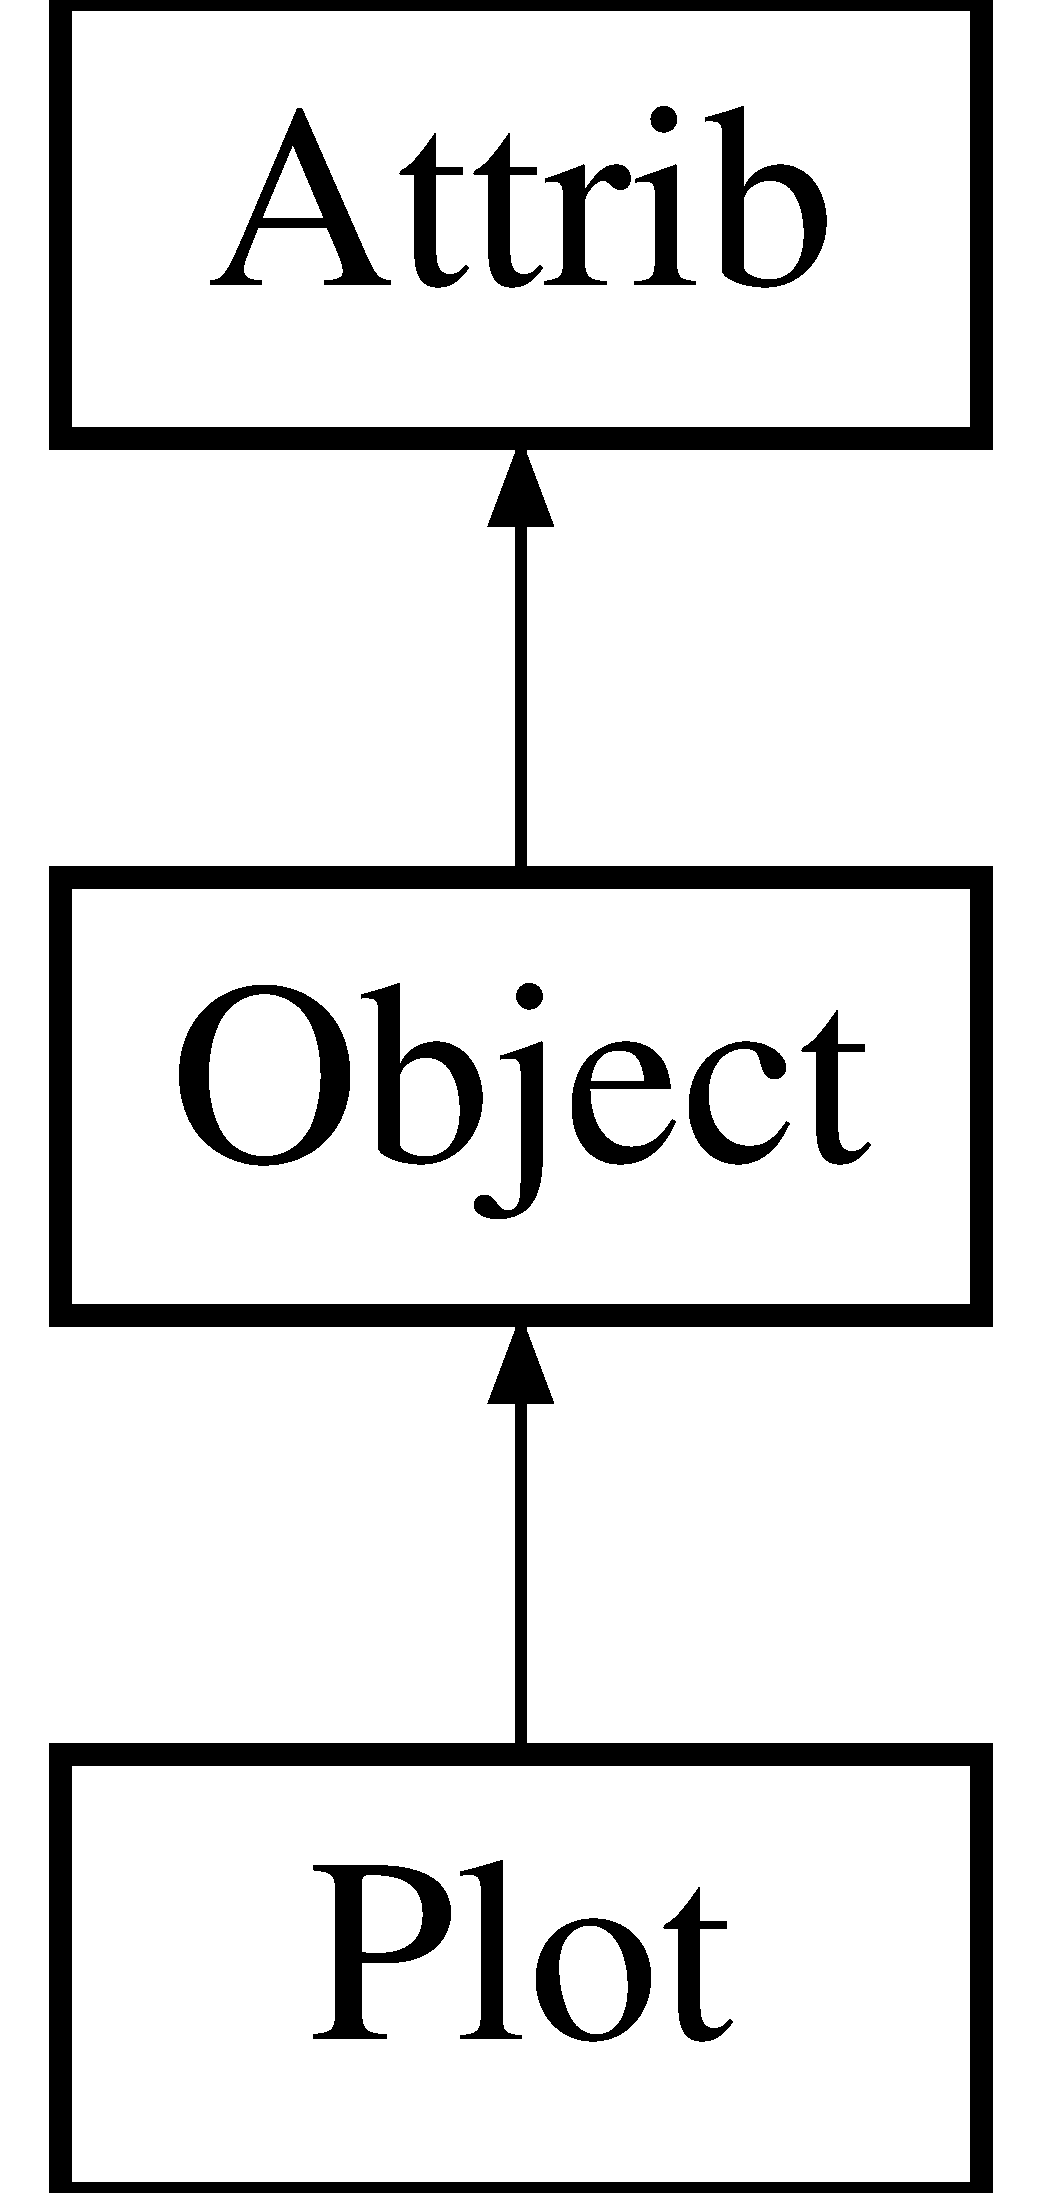
\includegraphics[height=3.000000cm]{classPlot}
\end{center}
\end{figure}
\subsection*{Public Member Functions}
\begin{DoxyCompactItemize}
\item 
\hyperlink{classPlot_ae8dca35f270d0964aac1e4ff42259129}{Plot} ()
\begin{DoxyCompactList}\small\item\em Standard constructor. \end{DoxyCompactList}\item 
\hyperlink{classPlot_a4e89bc6ea1800ba9697c9e0a0dc50a2e}{Plot} (unsigned int, unsigned int)
\item 
virtual \hyperlink{classPlot_a277e9c79c4357b3a317d74d61dabefcf}{$\sim$\+Plot} ()
\begin{DoxyCompactList}\small\item\em Destructor. \end{DoxyCompactList}\item 
std\+::vector$<$ std\+::pair$<$ unsigned int, \hyperlink{classHisto1D}{Histo1D} $\ast$$>$ $>$ \hyperlink{classPlot_af72e70c6b53df941708cd8d971083227}{histos} ()
\item 
std\+::vector$<$ \hyperlink{classHisto1D}{Histo1D} $\ast$ $>$ \hyperlink{classPlot_ad6f34fe5ab1a94b411b4fc121e0641bc}{histo1d} ()
\item 
int \hyperlink{classPlot_a3f7d4915b045844af0773d09d0c185ad}{pos} (\hyperlink{classHisto1D}{Histo1D} $\ast$h)
\item 
void \hyperlink{classPlot_a77a015d72e98d6fb066481e9c70af1ec}{set\+Region} (unsigned int, unsigned int)
\item 
std\+::pair$<$ unsigned int, unsigned int $>$ \hyperlink{classPlot_ae493b21749049d75cbb7282b1e1b9ab4}{region} ()
\item 
int \hyperlink{classPlot_a4a7404547e8a9d5dd0a921bfff3ed406}{format} ()
\item 
void \hyperlink{classPlot_ac0e03af81b0591d4786ff03441524eb2}{add} (T\+H1D $\ast$, unsigned int \hyperlink{classPlot_ae493b21749049d75cbb7282b1e1b9ab4}{region}=0)
\item 
void \hyperlink{classPlot_abe449e7c57a55f3bf0ee9201d07d497d}{make} (std\+::string script)
\item 
std\+::string \hyperlink{classPlot_aa49856f69c852f7f0ba65ed6131b7b61}{draw} ()
\end{DoxyCompactItemize}
\subsection*{Private Types}
\begin{DoxyCompactItemize}
\item 
typedef std\+::pair$<$ unsigned int, unsigned int $>$ \hyperlink{classPlot_a07543869c4a57b91ea0ec9835cb165ca}{Pos}
\item 
typedef std\+::pair$<$ unsigned int, \hyperlink{classHisto1D}{Histo1D} $\ast$$>$ \hyperlink{classPlot_ac411abcbcce315d4e77094393e6ca418}{Pos1D}
\end{DoxyCompactItemize}
\subsection*{Private Attributes}
\begin{DoxyCompactItemize}
\item 
std\+::pair$<$ unsigned int, unsigned int $>$ \hyperlink{classPlot_aabcbba1cfc66babcbcd647fdf90cdbf1}{m\+\_\+region}
\item 
std\+::vector$<$ std\+::pair$<$ unsigned int, \hyperlink{classHisto1D}{Histo1D} $\ast$$>$ $>$ \hyperlink{classPlot_a7edebf2b275223b8ce55f6ef3b2da0cc}{m\+\_\+histos}
\item 
std\+::string \hyperlink{classPlot_a83ffbf3effe6a2f8befa6375882f3994}{m\+\_\+draw}
\end{DoxyCompactItemize}
\subsection*{Additional Inherited Members}


\subsection{Detailed Description}
\begin{DoxyAuthor}{Author}
Frederic Machefert 
\end{DoxyAuthor}
\begin{DoxyDate}{Date}
2005-\/01-\/04 
\end{DoxyDate}


Definition at line 21 of file Plot.\+h.



\subsection{Member Typedef Documentation}
\mbox{\Hypertarget{classPlot_a07543869c4a57b91ea0ec9835cb165ca}\label{classPlot_a07543869c4a57b91ea0ec9835cb165ca}} 
\index{Plot@{Plot}!Pos@{Pos}}
\index{Pos@{Pos}!Plot@{Plot}}
\subsubsection{\texorpdfstring{Pos}{Pos}}
{\footnotesize\ttfamily typedef std\+::pair$<$ unsigned int, unsigned int $>$ \hyperlink{classPlot_a07543869c4a57b91ea0ec9835cb165ca}{Plot\+::\+Pos}\hspace{0.3cm}{\ttfamily [private]}}



Definition at line 22 of file Plot.\+h.

\mbox{\Hypertarget{classPlot_ac411abcbcce315d4e77094393e6ca418}\label{classPlot_ac411abcbcce315d4e77094393e6ca418}} 
\index{Plot@{Plot}!Pos1D@{Pos1D}}
\index{Pos1D@{Pos1D}!Plot@{Plot}}
\subsubsection{\texorpdfstring{Pos1D}{Pos1D}}
{\footnotesize\ttfamily typedef std\+::pair$<$ unsigned int , \hyperlink{classHisto1D}{Histo1D}$\ast$ $>$ \hyperlink{classPlot_ac411abcbcce315d4e77094393e6ca418}{Plot\+::\+Pos1D}\hspace{0.3cm}{\ttfamily [private]}}



Definition at line 23 of file Plot.\+h.



\subsection{Constructor \& Destructor Documentation}
\mbox{\Hypertarget{classPlot_ae8dca35f270d0964aac1e4ff42259129}\label{classPlot_ae8dca35f270d0964aac1e4ff42259129}} 
\index{Plot@{Plot}!Plot@{Plot}}
\index{Plot@{Plot}!Plot@{Plot}}
\subsubsection{\texorpdfstring{Plot()}{Plot()}\hspace{0.1cm}{\footnotesize\ttfamily [1/2]}}
{\footnotesize\ttfamily Plot\+::\+Plot (\begin{DoxyParamCaption}{ }\end{DoxyParamCaption})}



Standard constructor. 



Definition at line 23 of file Plot.\+cpp.



References m\+\_\+draw, and m\+\_\+region.


\begin{DoxyCode}
23              \{
24   \hyperlink{classPlot_aabcbba1cfc66babcbcd647fdf90cdbf1}{m\_region}.first  = 1;
25   \hyperlink{classPlot_aabcbba1cfc66babcbcd647fdf90cdbf1}{m\_region}.second = 1;
26   \hyperlink{classPlot_a83ffbf3effe6a2f8befa6375882f3994}{m\_draw}=std::string(\textcolor{stringliteral}{""});
27 \}
\end{DoxyCode}
\mbox{\Hypertarget{classPlot_a4e89bc6ea1800ba9697c9e0a0dc50a2e}\label{classPlot_a4e89bc6ea1800ba9697c9e0a0dc50a2e}} 
\index{Plot@{Plot}!Plot@{Plot}}
\index{Plot@{Plot}!Plot@{Plot}}
\subsubsection{\texorpdfstring{Plot()}{Plot()}\hspace{0.1cm}{\footnotesize\ttfamily [2/2]}}
{\footnotesize\ttfamily Plot\+::\+Plot (\begin{DoxyParamCaption}\item[{unsigned int}]{x,  }\item[{unsigned int}]{y }\end{DoxyParamCaption})}



Definition at line 31 of file Plot.\+cpp.



References set\+Region().


\begin{DoxyCode}
32                             \{
33   \hyperlink{classPlot_a77a015d72e98d6fb066481e9c70af1ec}{setRegion} ( x , y );
34 \}
\end{DoxyCode}
\mbox{\Hypertarget{classPlot_a277e9c79c4357b3a317d74d61dabefcf}\label{classPlot_a277e9c79c4357b3a317d74d61dabefcf}} 
\index{Plot@{Plot}!````~Plot@{$\sim$\+Plot}}
\index{````~Plot@{$\sim$\+Plot}!Plot@{Plot}}
\subsubsection{\texorpdfstring{$\sim$\+Plot()}{~Plot()}}
{\footnotesize\ttfamily Plot\+::$\sim$\+Plot (\begin{DoxyParamCaption}{ }\end{DoxyParamCaption})\hspace{0.3cm}{\ttfamily [virtual]}}



Destructor. 



Definition at line 39 of file Plot.\+cpp.


\begin{DoxyCode}
39              \{ 
40 \} 
\end{DoxyCode}


\subsection{Member Function Documentation}
\mbox{\Hypertarget{classPlot_ac0e03af81b0591d4786ff03441524eb2}\label{classPlot_ac0e03af81b0591d4786ff03441524eb2}} 
\index{Plot@{Plot}!add@{add}}
\index{add@{add}!Plot@{Plot}}
\subsubsection{\texorpdfstring{add()}{add()}}
{\footnotesize\ttfamily void Plot\+::add (\begin{DoxyParamCaption}\item[{T\+H1D $\ast$}]{histo,  }\item[{unsigned int}]{region = {\ttfamily 0} }\end{DoxyParamCaption})}



Definition at line 55 of file Plot.\+cpp.



References m\+\_\+histos, m\+\_\+region, region(), and Object\+::warning().



Referenced by format().


\begin{DoxyCode}
56                                        \{
57   
58   \textcolor{keywordflow}{if} ( \hyperlink{classPlot_ae493b21749049d75cbb7282b1e1b9ab4}{region} > \hyperlink{classPlot_aabcbba1cfc66babcbcd647fdf90cdbf1}{m\_region}.first * \hyperlink{classPlot_aabcbba1cfc66babcbcd647fdf90cdbf1}{m\_region}.second )\{
59     \hyperlink{classObject_a65cd4fda577711660821fd2cd5a3b4c9}{warning}(\textcolor{stringliteral}{"Try plot histogram outside allowed regions."},\textcolor{stringliteral}{"Processus::plot"});
60     \textcolor{keywordflow}{return};
61   \}
62 
63   std::pair < int , Histo1D* > graph;
64   graph.first = \hyperlink{classPlot_ae493b21749049d75cbb7282b1e1b9ab4}{region};
65   graph.second = \textcolor{keyword}{new} \hyperlink{classHisto1D}{Histo1D}(histo);
66 
67   \hyperlink{classPlot_a7edebf2b275223b8ce55f6ef3b2da0cc}{m\_histos}.push\_back ( graph );  
68 \}
\end{DoxyCode}
\mbox{\Hypertarget{classPlot_aa49856f69c852f7f0ba65ed6131b7b61}\label{classPlot_aa49856f69c852f7f0ba65ed6131b7b61}} 
\index{Plot@{Plot}!draw@{draw}}
\index{draw@{draw}!Plot@{Plot}}
\subsubsection{\texorpdfstring{draw()}{draw()}}
{\footnotesize\ttfamily std\+::string Plot\+::draw (\begin{DoxyParamCaption}{ }\end{DoxyParamCaption})\hspace{0.3cm}{\ttfamily [inline]}}



Definition at line 103 of file Plot.\+h.



References m\+\_\+draw.


\begin{DoxyCode}
103                   \{
104     \textcolor{keywordflow}{return} \hyperlink{classPlot_a83ffbf3effe6a2f8befa6375882f3994}{m\_draw};
105   \}
\end{DoxyCode}
\mbox{\Hypertarget{classPlot_a4a7404547e8a9d5dd0a921bfff3ed406}\label{classPlot_a4a7404547e8a9d5dd0a921bfff3ed406}} 
\index{Plot@{Plot}!format@{format}}
\index{format@{format}!Plot@{Plot}}
\subsubsection{\texorpdfstring{format()}{format()}}
{\footnotesize\ttfamily int Plot\+::format (\begin{DoxyParamCaption}{ }\end{DoxyParamCaption})\hspace{0.3cm}{\ttfamily [inline]}}



Definition at line 80 of file Plot.\+h.



References add(), m\+\_\+region, and region().


\begin{DoxyCode}
81   \{
82     \textcolor{keywordflow}{return} (\hyperlink{classPlot_aabcbba1cfc66babcbcd647fdf90cdbf1}{m\_region}.first+\hyperlink{classPlot_aabcbba1cfc66babcbcd647fdf90cdbf1}{m\_region}.second*100);
83 
84   \}
\end{DoxyCode}
\mbox{\Hypertarget{classPlot_ad6f34fe5ab1a94b411b4fc121e0641bc}\label{classPlot_ad6f34fe5ab1a94b411b4fc121e0641bc}} 
\index{Plot@{Plot}!histo1d@{histo1d}}
\index{histo1d@{histo1d}!Plot@{Plot}}
\subsubsection{\texorpdfstring{histo1d()}{histo1d()}}
{\footnotesize\ttfamily std\+::vector$<$\hyperlink{classHisto1D}{Histo1D}$\ast$$>$ Plot\+::histo1d (\begin{DoxyParamCaption}{ }\end{DoxyParamCaption})\hspace{0.3cm}{\ttfamily [inline]}}



Definition at line 44 of file Plot.\+h.



References m\+\_\+histos.


\begin{DoxyCode}
44                                \{
45     std::vector<Histo1D*> h;
46     \textcolor{keywordflow}{for} (\textcolor{keywordtype}{unsigned} \textcolor{keywordtype}{int} i=0; i<\hyperlink{classPlot_a7edebf2b275223b8ce55f6ef3b2da0cc}{m\_histos}.size(); ++i)
47     \{
48       h.push\_back((\hyperlink{classPlot_a7edebf2b275223b8ce55f6ef3b2da0cc}{m\_histos}[i]).second);
49     \}
50     \textcolor{keywordflow}{return} h;
51   \}
\end{DoxyCode}
\mbox{\Hypertarget{classPlot_af72e70c6b53df941708cd8d971083227}\label{classPlot_af72e70c6b53df941708cd8d971083227}} 
\index{Plot@{Plot}!histos@{histos}}
\index{histos@{histos}!Plot@{Plot}}
\subsubsection{\texorpdfstring{histos()}{histos()}}
{\footnotesize\ttfamily std\+::vector$<$ std\+::pair $<$ unsigned int , \hyperlink{classHisto1D}{Histo1D}$\ast$ $>$ $>$ Plot\+::histos (\begin{DoxyParamCaption}{ }\end{DoxyParamCaption})\hspace{0.3cm}{\ttfamily [inline]}}



Definition at line 36 of file Plot.\+h.



References m\+\_\+histos.


\begin{DoxyCode}
36                                                             \{
37     \textcolor{keywordflow}{return} \hyperlink{classPlot_a7edebf2b275223b8ce55f6ef3b2da0cc}{m\_histos};
38   \}
\end{DoxyCode}
\mbox{\Hypertarget{classPlot_abe449e7c57a55f3bf0ee9201d07d497d}\label{classPlot_abe449e7c57a55f3bf0ee9201d07d497d}} 
\index{Plot@{Plot}!make@{make}}
\index{make@{make}!Plot@{Plot}}
\subsubsection{\texorpdfstring{make()}{make()}}
{\footnotesize\ttfamily void Plot\+::make (\begin{DoxyParamCaption}\item[{std\+::string}]{script }\end{DoxyParamCaption})\hspace{0.3cm}{\ttfamily [inline]}}



Definition at line 96 of file Plot.\+h.



References m\+\_\+draw.


\begin{DoxyCode}
96                              \{
97     \hyperlink{classPlot_a83ffbf3effe6a2f8befa6375882f3994}{m\_draw}=script;
98   \}
\end{DoxyCode}
\mbox{\Hypertarget{classPlot_a3f7d4915b045844af0773d09d0c185ad}\label{classPlot_a3f7d4915b045844af0773d09d0c185ad}} 
\index{Plot@{Plot}!pos@{pos}}
\index{pos@{pos}!Plot@{Plot}}
\subsubsection{\texorpdfstring{pos()}{pos()}}
{\footnotesize\ttfamily int Plot\+::pos (\begin{DoxyParamCaption}\item[{\hyperlink{classHisto1D}{Histo1D} $\ast$}]{h }\end{DoxyParamCaption})\hspace{0.3cm}{\ttfamily [inline]}}



Definition at line 56 of file Plot.\+h.



References m\+\_\+histos, and set\+Region().


\begin{DoxyCode}
57   \{
58     \textcolor{keywordflow}{for} (\textcolor{keywordtype}{unsigned} \textcolor{keywordtype}{int} i=0; i<\hyperlink{classPlot_a7edebf2b275223b8ce55f6ef3b2da0cc}{m\_histos}.size(); ++i)
59     \{
60       \textcolor{keywordflow}{if} (h==(\hyperlink{classPlot_a7edebf2b275223b8ce55f6ef3b2da0cc}{m\_histos}[i]).second)
61         \textcolor{keywordflow}{return} ((\hyperlink{classPlot_a7edebf2b275223b8ce55f6ef3b2da0cc}{m\_histos}[i]).first);
62     \}
63     \textcolor{keywordflow}{return} -1;
64   \}
\end{DoxyCode}
\mbox{\Hypertarget{classPlot_ae493b21749049d75cbb7282b1e1b9ab4}\label{classPlot_ae493b21749049d75cbb7282b1e1b9ab4}} 
\index{Plot@{Plot}!region@{region}}
\index{region@{region}!Plot@{Plot}}
\subsubsection{\texorpdfstring{region()}{region()}}
{\footnotesize\ttfamily std\+::pair$<$unsigned int , unsigned int$>$ Plot\+::region (\begin{DoxyParamCaption}{ }\end{DoxyParamCaption})\hspace{0.3cm}{\ttfamily [inline]}}



Definition at line 75 of file Plot.\+h.



References m\+\_\+region.



Referenced by add(), and format().


\begin{DoxyCode}
75                                                 \{
76     \textcolor{keywordflow}{return} \hyperlink{classPlot_aabcbba1cfc66babcbcd647fdf90cdbf1}{m\_region};
77   \}
\end{DoxyCode}
\mbox{\Hypertarget{classPlot_a77a015d72e98d6fb066481e9c70af1ec}\label{classPlot_a77a015d72e98d6fb066481e9c70af1ec}} 
\index{Plot@{Plot}!set\+Region@{set\+Region}}
\index{set\+Region@{set\+Region}!Plot@{Plot}}
\subsubsection{\texorpdfstring{set\+Region()}{setRegion()}}
{\footnotesize\ttfamily void Plot\+::set\+Region (\begin{DoxyParamCaption}\item[{unsigned int}]{x,  }\item[{unsigned int}]{y }\end{DoxyParamCaption})}



Definition at line 45 of file Plot.\+cpp.



References m\+\_\+region.



Referenced by Plot(), and pos().


\begin{DoxyCode}
46                                         \{
47   \hyperlink{classPlot_aabcbba1cfc66babcbcd647fdf90cdbf1}{m\_region}.first  = x;
48   \hyperlink{classPlot_aabcbba1cfc66babcbcd647fdf90cdbf1}{m\_region}.second = y;
49 \}
\end{DoxyCode}


\subsection{Member Data Documentation}
\mbox{\Hypertarget{classPlot_a83ffbf3effe6a2f8befa6375882f3994}\label{classPlot_a83ffbf3effe6a2f8befa6375882f3994}} 
\index{Plot@{Plot}!m\+\_\+draw@{m\+\_\+draw}}
\index{m\+\_\+draw@{m\+\_\+draw}!Plot@{Plot}}
\subsubsection{\texorpdfstring{m\+\_\+draw}{m\_draw}}
{\footnotesize\ttfamily std\+::string Plot\+::m\+\_\+draw\hspace{0.3cm}{\ttfamily [private]}}



Definition at line 111 of file Plot.\+h.



Referenced by draw(), make(), and Plot().

\mbox{\Hypertarget{classPlot_a7edebf2b275223b8ce55f6ef3b2da0cc}\label{classPlot_a7edebf2b275223b8ce55f6ef3b2da0cc}} 
\index{Plot@{Plot}!m\+\_\+histos@{m\+\_\+histos}}
\index{m\+\_\+histos@{m\+\_\+histos}!Plot@{Plot}}
\subsubsection{\texorpdfstring{m\+\_\+histos}{m\_histos}}
{\footnotesize\ttfamily std\+::vector$<$ std\+::pair $<$ unsigned int , \hyperlink{classHisto1D}{Histo1D}$\ast$ $>$ $>$ Plot\+::m\+\_\+histos\hspace{0.3cm}{\ttfamily [private]}}



Definition at line 110 of file Plot.\+h.



Referenced by add(), histo1d(), histos(), and pos().

\mbox{\Hypertarget{classPlot_aabcbba1cfc66babcbcd647fdf90cdbf1}\label{classPlot_aabcbba1cfc66babcbcd647fdf90cdbf1}} 
\index{Plot@{Plot}!m\+\_\+region@{m\+\_\+region}}
\index{m\+\_\+region@{m\+\_\+region}!Plot@{Plot}}
\subsubsection{\texorpdfstring{m\+\_\+region}{m\_region}}
{\footnotesize\ttfamily std\+::pair$<$ unsigned int, unsigned int $>$ Plot\+::m\+\_\+region\hspace{0.3cm}{\ttfamily [private]}}



Definition at line 109 of file Plot.\+h.



Referenced by add(), format(), Plot(), region(), and set\+Region().



The documentation for this class was generated from the following files\+:\begin{DoxyCompactItemize}
\item 
/home/eleclhcb/\+L\+H\+Cb/lbcat-\/cmake/\+Cat\+Kernel/inc/\hyperlink{Plot_8h}{Plot.\+h}\item 
/home/eleclhcb/\+L\+H\+Cb/lbcat-\/cmake/\+Cat\+Kernel/src/\hyperlink{Plot_8cpp}{Plot.\+cpp}\end{DoxyCompactItemize}

\hypertarget{classplotter_1_1plotter}{}\section{plotter.\+plotter Class Reference}
\label{classplotter_1_1plotter}\index{plotter.\+plotter@{plotter.\+plotter}}
Inheritance diagram for plotter.\+plotter\+:\begin{figure}[H]
\begin{center}
\leavevmode
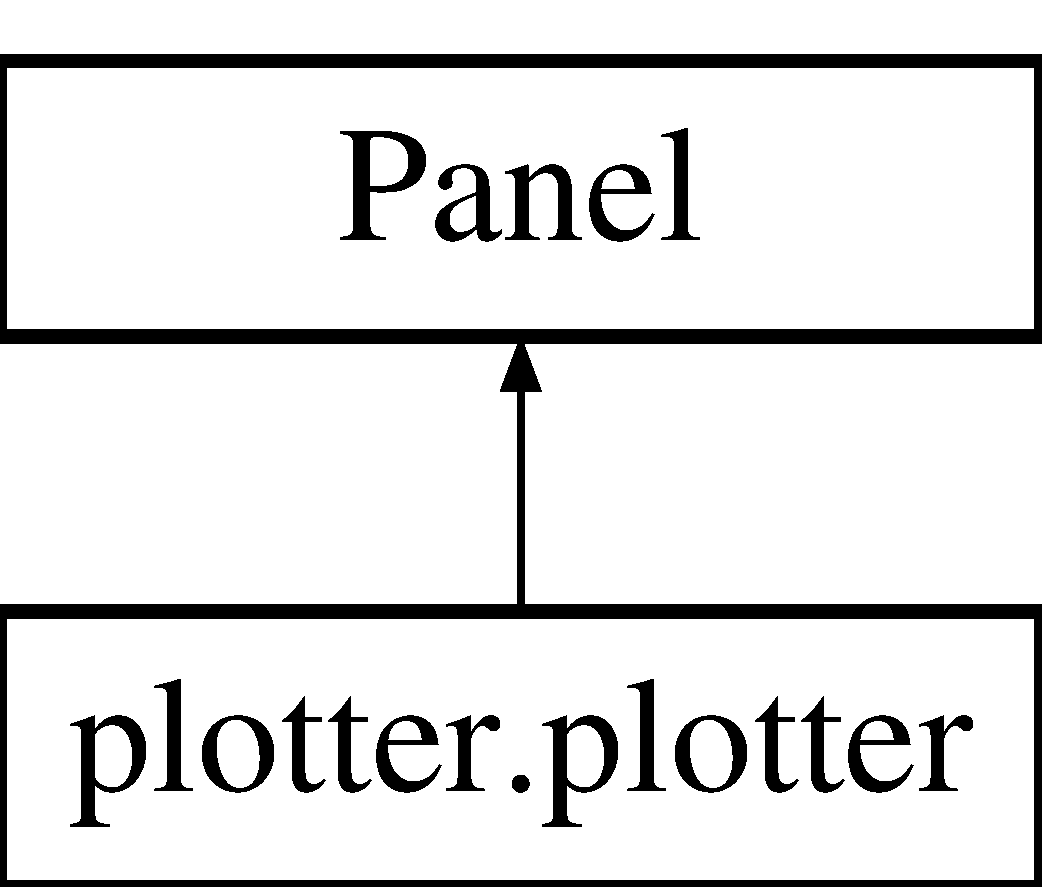
\includegraphics[height=2.000000cm]{classplotter_1_1plotter}
\end{center}
\end{figure}
\subsection*{Public Member Functions}
\begin{DoxyCompactItemize}
\item 
def \hyperlink{classplotter_1_1plotter_aa8c4aa595a3765f6f83ce75c1e9989ea}{\+\_\+\+\_\+init\+\_\+\+\_\+} (self, parent, \hyperlink{classplotter_1_1plotter_a9f4c4616f4fd21c3c9ae6dd320bfbeb6}{figid})
\item 
def \hyperlink{classplotter_1_1plotter_a4c7ba64058a8be7d362958e469429ed6}{current} (self)
\item 
def \hyperlink{classplotter_1_1plotter_a6bdaaad7796180c8dbe453ea192d982e}{destroy} (self)
\end{DoxyCompactItemize}
\subsection*{Public Attributes}
\begin{DoxyCompactItemize}
\item 
\hyperlink{classplotter_1_1plotter_a8766011b81271bcd938237fc9253af45}{figure}
\item 
\hyperlink{classplotter_1_1plotter_a9f4c4616f4fd21c3c9ae6dd320bfbeb6}{figid}
\item 
\hyperlink{classplotter_1_1plotter_a4e223147b19d30bad6a7a0177f3fe08d}{canvas}
\item 
\hyperlink{classplotter_1_1plotter_a55f4eaa8635020a1f0d76241dcfee593}{toolbar}
\end{DoxyCompactItemize}


\subsection{Detailed Description}


Definition at line 24 of file plotter.\+py.



\subsection{Constructor \& Destructor Documentation}
\mbox{\Hypertarget{classplotter_1_1plotter_aa8c4aa595a3765f6f83ce75c1e9989ea}\label{classplotter_1_1plotter_aa8c4aa595a3765f6f83ce75c1e9989ea}} 
\index{plotter\+::plotter@{plotter\+::plotter}!\+\_\+\+\_\+init\+\_\+\+\_\+@{\+\_\+\+\_\+init\+\_\+\+\_\+}}
\index{\+\_\+\+\_\+init\+\_\+\+\_\+@{\+\_\+\+\_\+init\+\_\+\+\_\+}!plotter\+::plotter@{plotter\+::plotter}}
\subsubsection{\texorpdfstring{\+\_\+\+\_\+init\+\_\+\+\_\+()}{\_\_init\_\_()}}
{\footnotesize\ttfamily def plotter.\+plotter.\+\_\+\+\_\+init\+\_\+\+\_\+ (\begin{DoxyParamCaption}\item[{}]{self,  }\item[{}]{parent,  }\item[{}]{figid }\end{DoxyParamCaption})}



Definition at line 25 of file plotter.\+py.


\begin{DoxyCode}
25         \textcolor{keyword}{def }\hyperlink{classwrapper_1_1ModuleDictWrapper_a9a7a794150502f51df687831583e13b9}{\_\_init\_\_}(self, parent,figid):
26                 \textcolor{keywordflow}{if} (parent==\textcolor{keywordtype}{None}):
27                         self.figure = plt.figure(figid)
28                 \textcolor{keywordflow}{else}:
29                         wx.Panel.\_\_init\_\_(self, parent, id=-1)
30                         self.figid  = figid
31                         self.figure = plt.figure(figid)
32                         self.figure.subplots\_adjust(top=0.9,bottom=0.05,right=0.95,left=0.05)
33                         self.canvas = Canvas(self, -1, self.figure)
34                         self.toolbar = Toolbar(self.canvas)
35                         self.toolbar.Realize()
36                         sizer = wx.BoxSizer(wx.VERTICAL)
37                         sizer.Add(self.canvas,1,wx.EXPAND)
38                         sizer.Add(self.toolbar, 0 , wx.LEFT | wx.EXPAND)
39                         self.SetSizer(sizer)
40                         
\end{DoxyCode}


\subsection{Member Function Documentation}
\mbox{\Hypertarget{classplotter_1_1plotter_a4c7ba64058a8be7d362958e469429ed6}\label{classplotter_1_1plotter_a4c7ba64058a8be7d362958e469429ed6}} 
\index{plotter\+::plotter@{plotter\+::plotter}!current@{current}}
\index{current@{current}!plotter\+::plotter@{plotter\+::plotter}}
\subsubsection{\texorpdfstring{current()}{current()}}
{\footnotesize\ttfamily def plotter.\+plotter.\+current (\begin{DoxyParamCaption}\item[{}]{self }\end{DoxyParamCaption})}



Definition at line 41 of file plotter.\+py.



References plotter.\+plotter.\+figure.


\begin{DoxyCode}
41     \textcolor{keyword}{def }current(self):
42             \textcolor{keywordflow}{return} self.figure
43 
\end{DoxyCode}
\mbox{\Hypertarget{classplotter_1_1plotter_a6bdaaad7796180c8dbe453ea192d982e}\label{classplotter_1_1plotter_a6bdaaad7796180c8dbe453ea192d982e}} 
\index{plotter\+::plotter@{plotter\+::plotter}!destroy@{destroy}}
\index{destroy@{destroy}!plotter\+::plotter@{plotter\+::plotter}}
\subsubsection{\texorpdfstring{destroy()}{destroy()}}
{\footnotesize\ttfamily def plotter.\+plotter.\+destroy (\begin{DoxyParamCaption}\item[{}]{self }\end{DoxyParamCaption})}



Definition at line 44 of file plotter.\+py.



References plotter.\+plotter.\+canvas, and plotter.\+h1d().


\begin{DoxyCode}
44     \textcolor{keyword}{def }destroy(self):
45         self.canvas.Destroy()
46 
\end{DoxyCode}


\subsection{Member Data Documentation}
\mbox{\Hypertarget{classplotter_1_1plotter_a4e223147b19d30bad6a7a0177f3fe08d}\label{classplotter_1_1plotter_a4e223147b19d30bad6a7a0177f3fe08d}} 
\index{plotter\+::plotter@{plotter\+::plotter}!canvas@{canvas}}
\index{canvas@{canvas}!plotter\+::plotter@{plotter\+::plotter}}
\subsubsection{\texorpdfstring{canvas}{canvas}}
{\footnotesize\ttfamily plotter.\+plotter.\+canvas}



Definition at line 33 of file plotter.\+py.



Referenced by plotter.\+plotter.\+destroy().

\mbox{\Hypertarget{classplotter_1_1plotter_a9f4c4616f4fd21c3c9ae6dd320bfbeb6}\label{classplotter_1_1plotter_a9f4c4616f4fd21c3c9ae6dd320bfbeb6}} 
\index{plotter\+::plotter@{plotter\+::plotter}!figid@{figid}}
\index{figid@{figid}!plotter\+::plotter@{plotter\+::plotter}}
\subsubsection{\texorpdfstring{figid}{figid}}
{\footnotesize\ttfamily plotter.\+plotter.\+figid}



Definition at line 30 of file plotter.\+py.

\mbox{\Hypertarget{classplotter_1_1plotter_a8766011b81271bcd938237fc9253af45}\label{classplotter_1_1plotter_a8766011b81271bcd938237fc9253af45}} 
\index{plotter\+::plotter@{plotter\+::plotter}!figure@{figure}}
\index{figure@{figure}!plotter\+::plotter@{plotter\+::plotter}}
\subsubsection{\texorpdfstring{figure}{figure}}
{\footnotesize\ttfamily plotter.\+plotter.\+figure}



Definition at line 27 of file plotter.\+py.



Referenced by plotter.\+plotter.\+current().

\mbox{\Hypertarget{classplotter_1_1plotter_a55f4eaa8635020a1f0d76241dcfee593}\label{classplotter_1_1plotter_a55f4eaa8635020a1f0d76241dcfee593}} 
\index{plotter\+::plotter@{plotter\+::plotter}!toolbar@{toolbar}}
\index{toolbar@{toolbar}!plotter\+::plotter@{plotter\+::plotter}}
\subsubsection{\texorpdfstring{toolbar}{toolbar}}
{\footnotesize\ttfamily plotter.\+plotter.\+toolbar}



Definition at line 34 of file plotter.\+py.



The documentation for this class was generated from the following file\+:\begin{DoxyCompactItemize}
\item 
/home/eleclhcb/\+L\+H\+Cb/lbcat-\/cmake/\+Cat\+Python/python/\hyperlink{plotter_8py}{plotter.\+py}\end{DoxyCompactItemize}

\hypertarget{classproc_1_1proc}{
\section{proc::proc Class Reference}
\label{classproc_1_1proc}\index{proc::proc@{proc::proc}}
}
Inheritance diagram for proc::proc::\begin{figure}[H]
\begin{center}
\leavevmode
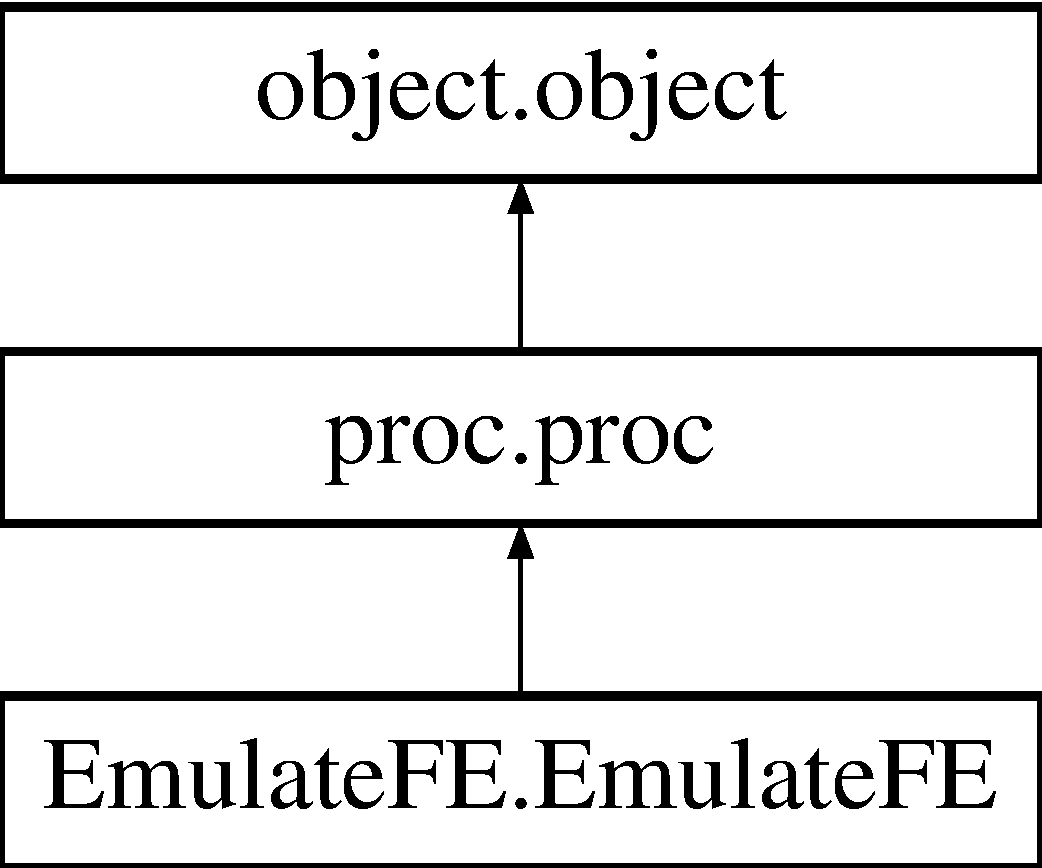
\includegraphics[height=3cm]{classproc_1_1proc}
\end{center}
\end{figure}
\subsection*{Public Member Functions}
\begin{DoxyCompactItemize}
\item 
def \hyperlink{classproc_1_1proc_a21e9bcad44f0098f74639f245d2d0e4b}{\_\-\_\-init\_\-\_\-}
\item 
def \hyperlink{classproc_1_1proc_a73ad55427f28a79ef0483e18ce996e14}{parent}
\item 
def \hyperlink{classproc_1_1proc_a2192e09617c5de1798ca71123cb390bb}{loadxrc}
\item 
def \hyperlink{classproc_1_1proc_ac70ada08e4fc982a3e61e9ee77b247bf}{page}
\item 
def \hyperlink{classobject_1_1object_ac765747a2b581d48eeb94e600c31fc3f}{getControl}
\item 
def \hyperlink{classobject_1_1object_ac765747a2b581d48eeb94e600c31fc3f}{getControl}
\end{DoxyCompactItemize}
\subsection*{Public Attributes}
\begin{DoxyCompactItemize}
\item 
\hyperlink{classproc_1_1proc_a9ee372f307278c50a935b46ca00a350a}{panel}
\item 
\hyperlink{classobject_1_1object_a4fbaf843d1f40843b2c3895cb73ffada}{cat}
\item 
\hyperlink{classobject_1_1object_a15f13858ecdbf661a97a7da93d717922}{obj}
\item 
\hyperlink{classobject_1_1object_a6b4e1fd053496eafff2bc0f8aed7f089}{path}
\end{DoxyCompactItemize}


\subsection{Detailed Description}


Definition at line 8 of file proc.py.

\subsection{Member Function Documentation}
\hypertarget{classproc_1_1proc_a21e9bcad44f0098f74639f245d2d0e4b}{
\index{proc::proc@{proc::proc}!\_\-\_\-init\_\-\_\-@{\_\-\_\-init\_\-\_\-}}
\index{\_\-\_\-init\_\-\_\-@{\_\-\_\-init\_\-\_\-}!proc::proc@{proc::proc}}
\subsubsection[{\_\-\_\-init\_\-\_\-}]{\setlength{\rightskip}{0pt plus 5cm}def proc::proc::\_\-\_\-init\_\-\_\- ( {\em self}, \/   {\em cat}, \/   {\em obj}, \/   {\em panel}, \/   {\em path})}}
\label{classproc_1_1proc_a21e9bcad44f0098f74639f245d2d0e4b}


Reimplemented from \hyperlink{classobject_1_1object_a1220f7c88ee9a71fcfd9acb49a2f44d8}{object::object}.

Reimplemented in \hyperlink{classEmulateFE_1_1EmulateFE_a3749dd5f45e93a8550800372a3ee40b6}{EmulateFE::EmulateFE}.

Definition at line 9 of file proc.py.


\begin{DoxyCode}
9                                              :
10         object.__init__(self, cat, obj, panel, path)
11         
    def parent(self):
\end{DoxyCode}
\hypertarget{classobject_1_1object_ac765747a2b581d48eeb94e600c31fc3f}{
\index{proc::proc@{proc::proc}!getControl@{getControl}}
\index{getControl@{getControl}!proc::proc@{proc::proc}}
\subsubsection[{getControl}]{\setlength{\rightskip}{0pt plus 5cm}def object::object::getControl ( {\em self}, \/   {\em xmlid})\hspace{0.3cm}{\ttfamily  \mbox{[}inherited\mbox{]}}}}
\label{classobject_1_1object_ac765747a2b581d48eeb94e600c31fc3f}
\begin{DoxyVerb}Retrieves the given control (within a dialog) by its xmlid\end{DoxyVerb}
 

Definition at line 20 of file object.py.


\begin{DoxyCode}
20                                  :
21         '''Retrieves the given control (within a dialog) by its xmlid'''
22         control = self.panel.FindWindowById(xrc.XRCID(xmlid))
23         assert control != None, 'Programming error: a control with xml id ' + xml
      id + ' was not found.'
24         return control
25 
26                 
27 #----------------------------------------------------------------------
28 
29     
    
\end{DoxyCode}
\hypertarget{classobject_1_1object_ac765747a2b581d48eeb94e600c31fc3f}{
\index{proc::proc@{proc::proc}!getControl@{getControl}}
\index{getControl@{getControl}!proc::proc@{proc::proc}}
\subsubsection[{getControl}]{\setlength{\rightskip}{0pt plus 5cm}def object::object::getControl ( {\em self}, \/   {\em xmlid}, \/   {\em item})\hspace{0.3cm}{\ttfamily  \mbox{[}inherited\mbox{]}}}}
\label{classobject_1_1object_ac765747a2b581d48eeb94e600c31fc3f}
\begin{DoxyVerb}Retrieves the given control (within a dialog) by its xmlid\end{DoxyVerb}
 

Definition at line 14 of file object.py.


\begin{DoxyCode}
14                                        :
15         '''Retrieves the given control (within a dialog) by its xmlid'''
16         control = item.FindWindowById(xrc.XRCID(xmlid))
17         assert control != None, 'Programming error: a control with xml id ' + xml
      id + ' was not found.'
18         return control
19 
    def getControl(self, xmlid ) :
\end{DoxyCode}
\hypertarget{classproc_1_1proc_a2192e09617c5de1798ca71123cb390bb}{
\index{proc::proc@{proc::proc}!loadxrc@{loadxrc}}
\index{loadxrc@{loadxrc}!proc::proc@{proc::proc}}
\subsubsection[{loadxrc}]{\setlength{\rightskip}{0pt plus 5cm}def proc::proc::loadxrc ( {\em self})}}
\label{classproc_1_1proc_a2192e09617c5de1798ca71123cb390bb}


Definition at line 16 of file proc.py.


\begin{DoxyCode}
16                      :
17         path= os.path.join(self.path,"proc")
18         path= os.path.join(self.path,"xrc")
19         path= os.path.join(path,self.obj.name())
20         path= path+".xrc"
21         res=xrc.XmlResource(path)
22         self.panel=res.LoadPanel(self.parent(),self.obj.name())
23         
    def page(self):
\end{DoxyCode}
\hypertarget{classproc_1_1proc_ac70ada08e4fc982a3e61e9ee77b247bf}{
\index{proc::proc@{proc::proc}!page@{page}}
\index{page@{page}!proc::proc@{proc::proc}}
\subsubsection[{page}]{\setlength{\rightskip}{0pt plus 5cm}def proc::proc::page ( {\em self})}}
\label{classproc_1_1proc_ac70ada08e4fc982a3e61e9ee77b247bf}


Definition at line 24 of file proc.py.


\begin{DoxyCode}
24                   :
25         return self.panel
        return self.panel
\end{DoxyCode}
\hypertarget{classproc_1_1proc_a73ad55427f28a79ef0483e18ce996e14}{
\index{proc::proc@{proc::proc}!parent@{parent}}
\index{parent@{parent}!proc::proc@{proc::proc}}
\subsubsection[{parent}]{\setlength{\rightskip}{0pt plus 5cm}def proc::proc::parent ( {\em self})}}
\label{classproc_1_1proc_a73ad55427f28a79ef0483e18ce996e14}


Definition at line 12 of file proc.py.


\begin{DoxyCode}
12                     :
13 #        return self.getControl("Element")   
14         return self.getControl("control")
15 
    def loadxrc(self):
\end{DoxyCode}


\subsection{Member Data Documentation}
\hypertarget{classobject_1_1object_a4fbaf843d1f40843b2c3895cb73ffada}{
\index{proc::proc@{proc::proc}!cat@{cat}}
\index{cat@{cat}!proc::proc@{proc::proc}}
\subsubsection[{cat}]{\setlength{\rightskip}{0pt plus 5cm}{\bf object::object::cat}\hspace{0.3cm}{\ttfamily  \mbox{[}inherited\mbox{]}}}}
\label{classobject_1_1object_a4fbaf843d1f40843b2c3895cb73ffada}


Definition at line 8 of file object.py.\hypertarget{classobject_1_1object_a15f13858ecdbf661a97a7da93d717922}{
\index{proc::proc@{proc::proc}!obj@{obj}}
\index{obj@{obj}!proc::proc@{proc::proc}}
\subsubsection[{obj}]{\setlength{\rightskip}{0pt plus 5cm}{\bf object::object::obj}\hspace{0.3cm}{\ttfamily  \mbox{[}inherited\mbox{]}}}}
\label{classobject_1_1object_a15f13858ecdbf661a97a7da93d717922}


Definition at line 9 of file object.py.\hypertarget{classproc_1_1proc_a9ee372f307278c50a935b46ca00a350a}{
\index{proc::proc@{proc::proc}!panel@{panel}}
\index{panel@{panel}!proc::proc@{proc::proc}}
\subsubsection[{panel}]{\setlength{\rightskip}{0pt plus 5cm}{\bf proc::proc::panel}}}
\label{classproc_1_1proc_a9ee372f307278c50a935b46ca00a350a}


Reimplemented from \hyperlink{classobject_1_1object_add82cb657066d4ab5b39035792971503}{object::object}.

Definition at line 22 of file proc.py.\hypertarget{classobject_1_1object_a6b4e1fd053496eafff2bc0f8aed7f089}{
\index{proc::proc@{proc::proc}!path@{path}}
\index{path@{path}!proc::proc@{proc::proc}}
\subsubsection[{path}]{\setlength{\rightskip}{0pt plus 5cm}{\bf object::object::path}\hspace{0.3cm}{\ttfamily  \mbox{[}inherited\mbox{]}}}}
\label{classobject_1_1object_a6b4e1fd053496eafff2bc0f8aed7f089}


Definition at line 11 of file object.py.

The documentation for this class was generated from the following file:\begin{DoxyCompactItemize}
\item 
/home/eleclhcb/LHCb/lbcat-\/cmake/CatPython/python/\hyperlink{proc_8py}{proc.py}\end{DoxyCompactItemize}

\hypertarget{classProcDataBase}{
\section{ProcDataBase Class Reference}
\label{classProcDataBase}\index{ProcDataBase@{ProcDataBase}}
}


{\ttfamily \#include $<$inc/ProcDataBase.h$>$}\subsection*{Public Member Functions}
\begin{DoxyCompactItemize}
\item 
\hyperlink{classProcDataBase_a82163dfca2df460ba2ea1559ffa72179}{ProcDataBase} ()
\begin{DoxyCompactList}\small\item\em Standard constructor. \item\end{DoxyCompactList}\item 
virtual \hyperlink{classProcDataBase_a65ec1212978a4996b5132bfaf1d0738d}{$\sim$ProcDataBase} ()
\begin{DoxyCompactList}\small\item\em Destructor. \item\end{DoxyCompactList}\item 
void \hyperlink{classProcDataBase_a604959db08c3871d863a799cc4e1d5f4}{update} ()
\item 
std::list$<$ \hyperlink{classProcessus}{Processus} $\ast$ $>$ \hyperlink{classProcDataBase_a8145de34e9857f3f6eebd2572740f198}{procList} (\hyperlink{classElement}{Element} $\ast$)
\item 
std::vector$<$ \hyperlink{classProcessus}{Processus} $\ast$ $>$ \hyperlink{classProcDataBase_a6f17bfad64929fa887c6aafb0080354b}{list} (\hyperlink{classElement}{Element} $\ast$)
\item 
std::vector$<$ \hyperlink{classProcessus}{Processus} $\ast$ $>$ \hyperlink{classProcDataBase_a813dbc8f9e7c4d69074a01394f04fc98}{list} ()
\item 
\hyperlink{classProcessus}{Processus} $\ast$ \hyperlink{classProcDataBase_a839b15c7bc0d73f5ff0f2516c3cb418e}{processus} (std::string)
\item 
\hyperlink{classStatusCode}{StatusCode} \hyperlink{classProcDataBase_a0aafeb65a41b92a6d1fdd67f363ef826}{add} (\hyperlink{classProcessus}{Processus} $\ast$)
\item 
\hyperlink{classStatusCode}{StatusCode} \hyperlink{classProcDataBase_a0413976bac8f233b31eab6d7a83866b9}{remove} (\hyperlink{classProcessus}{Processus} $\ast$)
\end{DoxyCompactItemize}
\subsection*{Private Attributes}
\begin{DoxyCompactItemize}
\item 
std::list$<$ \hyperlink{classProcessus}{Processus} $\ast$ $>$ \hyperlink{classProcDataBase_a9b7458b811b826c5d264b436c7a391c4}{m\_\-procList}
\item 
std::list$<$ std::string $>$ \hyperlink{classProcDataBase_a94063cebf50be9a12b8bd9f70e410ed5}{m\_\-types}
\end{DoxyCompactItemize}


\subsection{Detailed Description}
\begin{DoxyAuthor}{Author}
Frederic Machefert 
\end{DoxyAuthor}
\begin{DoxyDate}{Date}
2005-\/01-\/03 
\end{DoxyDate}


Definition at line 20 of file ProcDataBase.h.

\subsection{Constructor \& Destructor Documentation}
\hypertarget{classProcDataBase_a82163dfca2df460ba2ea1559ffa72179}{
\index{ProcDataBase@{ProcDataBase}!ProcDataBase@{ProcDataBase}}
\index{ProcDataBase@{ProcDataBase}!ProcDataBase@{ProcDataBase}}
\subsubsection[{ProcDataBase}]{\setlength{\rightskip}{0pt plus 5cm}ProcDataBase::ProcDataBase ()}}
\label{classProcDataBase_a82163dfca2df460ba2ea1559ffa72179}


Standard constructor. 

Definition at line 25 of file ProcDataBase.cpp.

References application(), and Object::info().


\begin{DoxyCode}
25                              {
26   application()->info("Building Processus DataBase.","ProcDataBase");
27 }
\end{DoxyCode}
\hypertarget{classProcDataBase_a65ec1212978a4996b5132bfaf1d0738d}{
\index{ProcDataBase@{ProcDataBase}!$\sim$ProcDataBase@{$\sim$ProcDataBase}}
\index{$\sim$ProcDataBase@{$\sim$ProcDataBase}!ProcDataBase@{ProcDataBase}}
\subsubsection[{$\sim$ProcDataBase}]{\setlength{\rightskip}{0pt plus 5cm}ProcDataBase::$\sim$ProcDataBase ()\hspace{0.3cm}{\ttfamily  \mbox{[}virtual\mbox{]}}}}
\label{classProcDataBase_a65ec1212978a4996b5132bfaf1d0738d}


Destructor. 

Definition at line 32 of file ProcDataBase.cpp.


\begin{DoxyCode}
32                             {
33 }
\end{DoxyCode}


\subsection{Member Function Documentation}
\hypertarget{classProcDataBase_a0aafeb65a41b92a6d1fdd67f363ef826}{
\index{ProcDataBase@{ProcDataBase}!add@{add}}
\index{add@{add}!ProcDataBase@{ProcDataBase}}
\subsubsection[{add}]{\setlength{\rightskip}{0pt plus 5cm}{\bf StatusCode} ProcDataBase::add ({\bf Processus} $\ast$ {\em proc})}}
\label{classProcDataBase_a0aafeb65a41b92a6d1fdd67f363ef826}


Definition at line 101 of file ProcDataBase.cpp.

References m\_\-procList, StatusCode::SUCCESS, and update().

Referenced by Computer::Computer(), and DLL::init().


\begin{DoxyCode}
101                                                {
102   m_procList.push_back ( proc );
103   update();
104   return StatusCode::SUCCESS;
105 }
\end{DoxyCode}
\hypertarget{classProcDataBase_a813dbc8f9e7c4d69074a01394f04fc98}{
\index{ProcDataBase@{ProcDataBase}!list@{list}}
\index{list@{list}!ProcDataBase@{ProcDataBase}}
\subsubsection[{list}]{\setlength{\rightskip}{0pt plus 5cm}std::vector$<$ {\bf Processus} $\ast$ $>$ ProcDataBase::list ()}}
\label{classProcDataBase_a813dbc8f9e7c4d69074a01394f04fc98}


Definition at line 76 of file ProcDataBase.cpp.

References m\_\-procList.

Referenced by export\_\-base(), export\_\-proc(), list(), and procList().


\begin{DoxyCode}
76                                            {
77   std::vector<Processus*> list;
78   std::list<Processus*>::const_iterator iter;
79   for (iter=m_procList.begin();iter!=m_procList.end();++iter){
80     list.push_back( *iter );        
81   }
82   return list;
83 }
\end{DoxyCode}
\hypertarget{classProcDataBase_a6f17bfad64929fa887c6aafb0080354b}{
\index{ProcDataBase@{ProcDataBase}!list@{list}}
\index{list@{list}!ProcDataBase@{ProcDataBase}}
\subsubsection[{list}]{\setlength{\rightskip}{0pt plus 5cm}std::vector$<$ {\bf Processus} $\ast$ $>$ ProcDataBase::list ({\bf Element} $\ast$ {\em element})}}
\label{classProcDataBase_a6f17bfad64929fa887c6aafb0080354b}


Definition at line 63 of file ProcDataBase.cpp.

References list(), m\_\-procList, and Object::type().


\begin{DoxyCode}
63                                                             {
64   std::vector<Processus*> list;
65   std::list<Processus*>::const_iterator iter;
66   for (iter=m_procList.begin();iter!=m_procList.end();++iter){
67     if ( (*iter)->type().compare( element->type() )==0 ){
68       list.push_back( *iter );        
69     }
70   }
71   return list;
72 }
\end{DoxyCode}
\hypertarget{classProcDataBase_a839b15c7bc0d73f5ff0f2516c3cb418e}{
\index{ProcDataBase@{ProcDataBase}!processus@{processus}}
\index{processus@{processus}!ProcDataBase@{ProcDataBase}}
\subsubsection[{processus}]{\setlength{\rightskip}{0pt plus 5cm}{\bf Processus} $\ast$ ProcDataBase::processus (std::string {\em procName})}}
\label{classProcDataBase_a839b15c7bc0d73f5ff0f2516c3cb418e}


Definition at line 88 of file ProcDataBase.cpp.

References m\_\-procList.

Referenced by DLL::print().


\begin{DoxyCode}
88                                                         {
89   std::list< Processus* >::const_iterator iter;
90   for (iter=m_procList.begin();iter!=m_procList.end();++iter){
91     if ( (*iter)->name().compare(procName) == 0 ) {
92       return (*iter);
93     }        
94   }
95   return NULL;
96 }
\end{DoxyCode}
\hypertarget{classProcDataBase_a8145de34e9857f3f6eebd2572740f198}{
\index{ProcDataBase@{ProcDataBase}!procList@{procList}}
\index{procList@{procList}!ProcDataBase@{ProcDataBase}}
\subsubsection[{procList}]{\setlength{\rightskip}{0pt plus 5cm}std::list$<$ {\bf Processus} $\ast$ $>$ ProcDataBase::procList ({\bf Element} $\ast$ {\em element})}}
\label{classProcDataBase_a8145de34e9857f3f6eebd2572740f198}


Definition at line 49 of file ProcDataBase.cpp.

References list(), m\_\-procList, and Object::type().

Referenced by Application::prepare(), and Application::setConfig().


\begin{DoxyCode}
49                                                               {
50   std::list<Processus*> list;
51   std::list<Processus*>::const_iterator iter;
52   for (iter=m_procList.begin();iter!=m_procList.end();++iter){
53     if ( (*iter)->type().compare( element->type() )==0 ){
54       list.push_back( *iter );        
55     }
56   }
57   return list;
58 }
\end{DoxyCode}
\hypertarget{classProcDataBase_a0413976bac8f233b31eab6d7a83866b9}{
\index{ProcDataBase@{ProcDataBase}!remove@{remove}}
\index{remove@{remove}!ProcDataBase@{ProcDataBase}}
\subsubsection[{remove}]{\setlength{\rightskip}{0pt plus 5cm}{\bf StatusCode} ProcDataBase::remove ({\bf Processus} $\ast$ {\em proc})}}
\label{classProcDataBase_a0413976bac8f233b31eab6d7a83866b9}
Erase a processus to the db 

Definition at line 110 of file ProcDataBase.cpp.

References m\_\-procList, and StatusCode::SUCCESS.

Referenced by Computer::$\sim$Computer().


\begin{DoxyCode}
110                                                   {
111   m_procList.remove( proc );
112   return StatusCode::SUCCESS;
113 }
\end{DoxyCode}
\hypertarget{classProcDataBase_a604959db08c3871d863a799cc4e1d5f4}{
\index{ProcDataBase@{ProcDataBase}!update@{update}}
\index{update@{update}!ProcDataBase@{ProcDataBase}}
\subsubsection[{update}]{\setlength{\rightskip}{0pt plus 5cm}void ProcDataBase::update ()}}
\label{classProcDataBase_a604959db08c3871d863a799cc4e1d5f4}


Definition at line 38 of file ProcDataBase.cpp.

References m\_\-procList, and m\_\-types.

Referenced by add().


\begin{DoxyCode}
38                             {
39   std::list<Processus*>::const_iterator iter;
40   for (iter=m_procList.begin();iter!=m_procList.end();++iter){
41     m_types.push_back( (*iter)->type() );
42   }
43   m_types.unique();
44 }
\end{DoxyCode}


\subsection{Member Data Documentation}
\hypertarget{classProcDataBase_a9b7458b811b826c5d264b436c7a391c4}{
\index{ProcDataBase@{ProcDataBase}!m\_\-procList@{m\_\-procList}}
\index{m\_\-procList@{m\_\-procList}!ProcDataBase@{ProcDataBase}}
\subsubsection[{m\_\-procList}]{\setlength{\rightskip}{0pt plus 5cm}std::list$<$ {\bf Processus}$\ast$ $>$ {\bf ProcDataBase::m\_\-procList}\hspace{0.3cm}{\ttfamily  \mbox{[}private\mbox{]}}}}
\label{classProcDataBase_a9b7458b811b826c5d264b436c7a391c4}


Definition at line 55 of file ProcDataBase.h.

Referenced by add(), list(), processus(), procList(), remove(), and update().\hypertarget{classProcDataBase_a94063cebf50be9a12b8bd9f70e410ed5}{
\index{ProcDataBase@{ProcDataBase}!m\_\-types@{m\_\-types}}
\index{m\_\-types@{m\_\-types}!ProcDataBase@{ProcDataBase}}
\subsubsection[{m\_\-types}]{\setlength{\rightskip}{0pt plus 5cm}std::list$<$ std::string $>$ {\bf ProcDataBase::m\_\-types}\hspace{0.3cm}{\ttfamily  \mbox{[}private\mbox{]}}}}
\label{classProcDataBase_a94063cebf50be9a12b8bd9f70e410ed5}


Definition at line 56 of file ProcDataBase.h.

Referenced by update().

The documentation for this class was generated from the following files:\begin{DoxyCompactItemize}
\item 
/home/eleclhcb/LHCb/lbcat-\/cmake/CatKernel/inc/\hyperlink{ProcDataBase_8h}{ProcDataBase.h}\item 
/home/eleclhcb/LHCb/lbcat-\/cmake/CatKernel/src/\hyperlink{ProcDataBase_8cpp}{ProcDataBase.cpp}\end{DoxyCompactItemize}

\hypertarget{classProcessus}{}\section{Processus Class Reference}
\label{classProcessus}\index{Processus@{Processus}}


{\ttfamily \#include $<$include/\+Processus.\+h$>$}

Inheritance diagram for Processus\+:\begin{figure}[H]
\begin{center}
\leavevmode
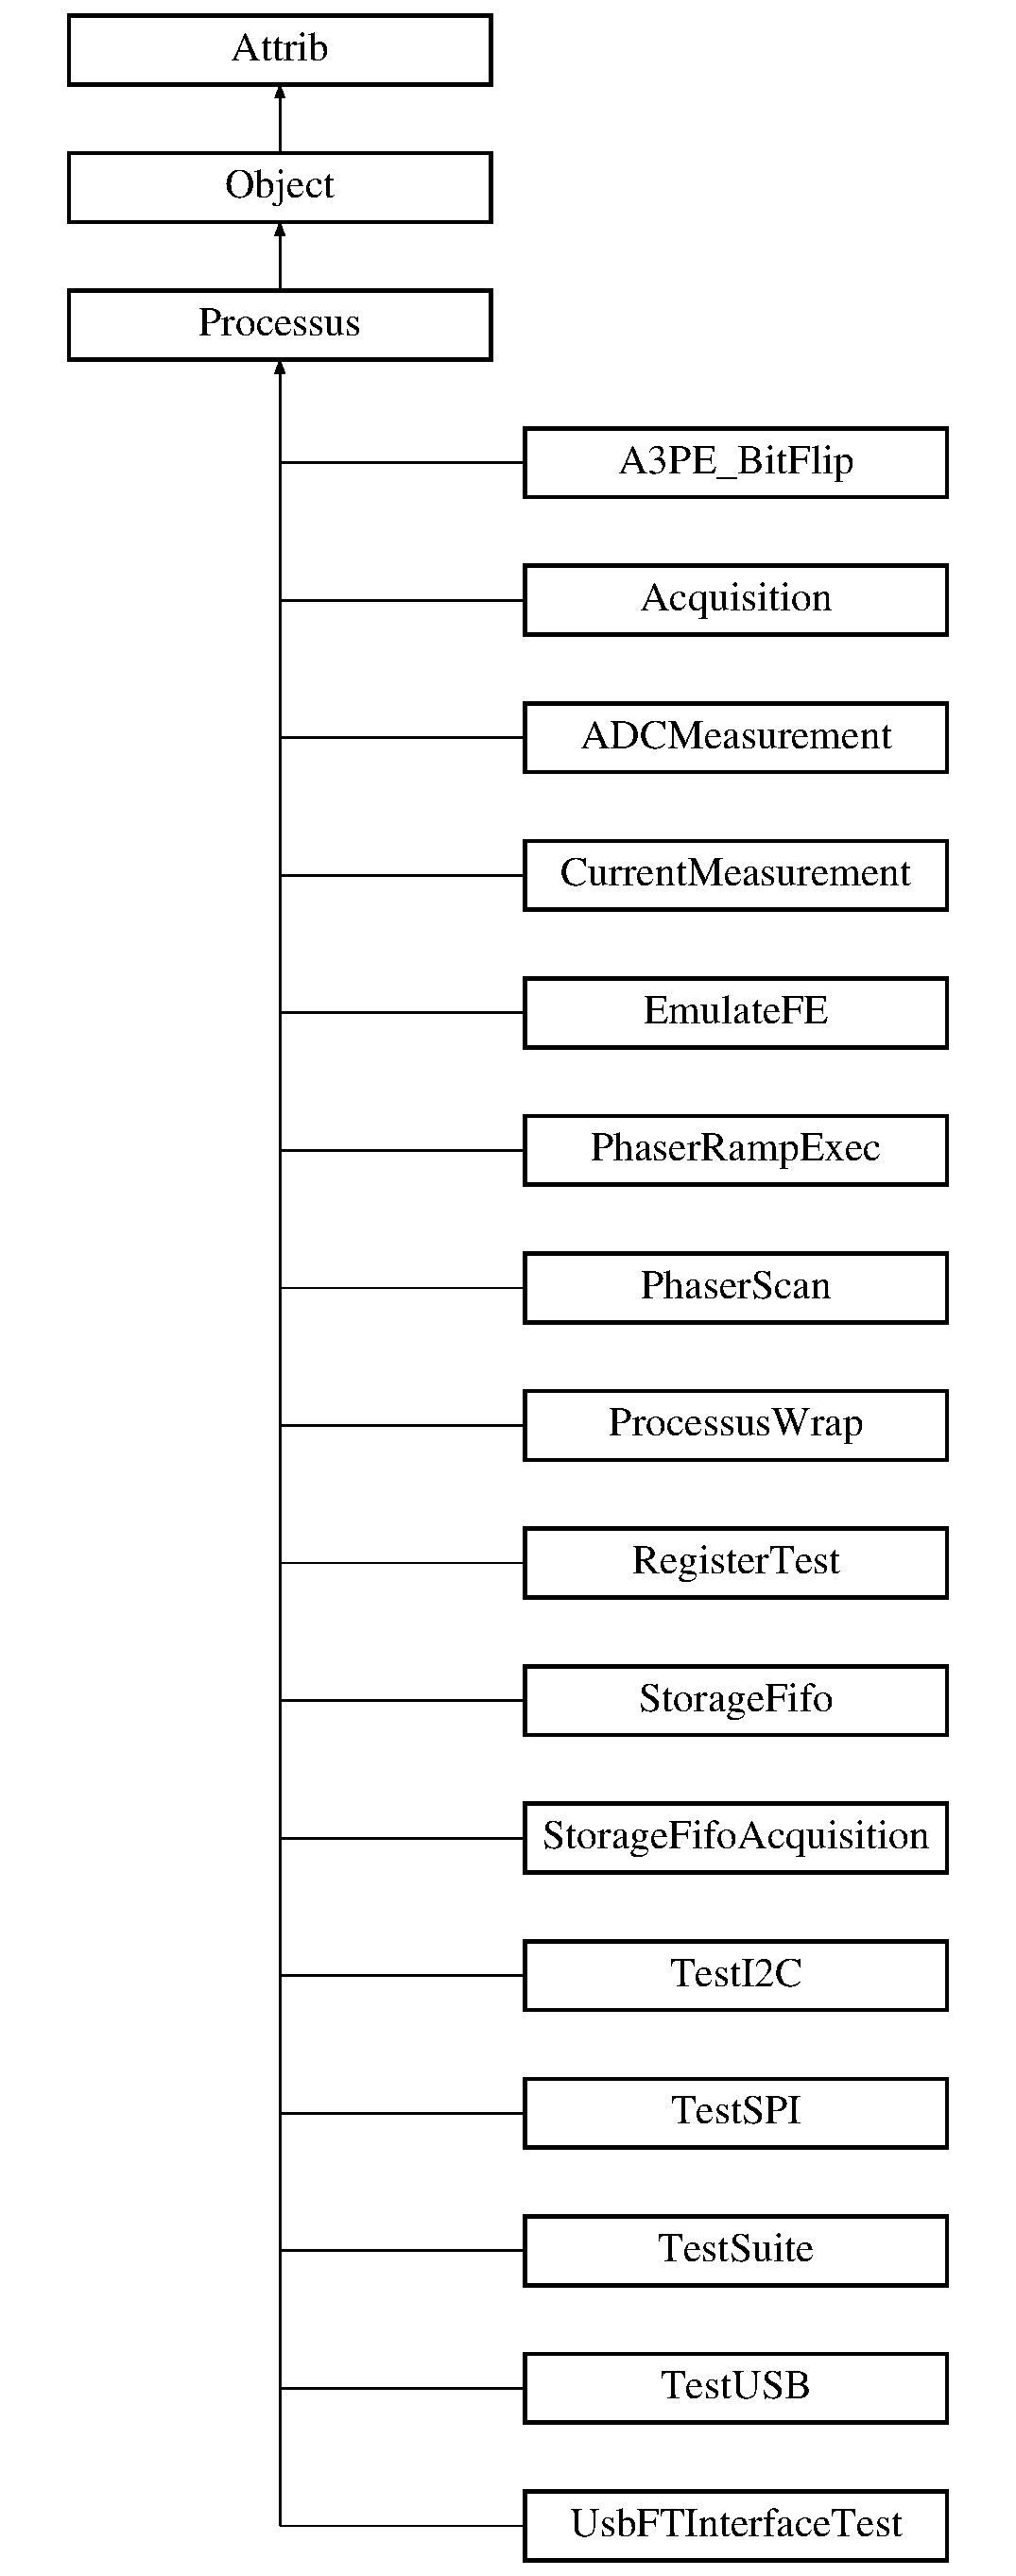
\includegraphics[height=12.000000cm]{classProcessus}
\end{center}
\end{figure}
\subsection*{Public Types}
\begin{DoxyCompactItemize}
\item 
enum \hyperlink{classProcessus_a36278773bd98f2d5612fea40c7774821}{states} \{ \hyperlink{classProcessus_a36278773bd98f2d5612fea40c7774821adaf73ad5d0a09f952d0f18dbbe1c7493}{E\+RR} =-\/1, 
\hyperlink{classProcessus_a36278773bd98f2d5612fea40c7774821a629082f49d6e8df6b6da2b8fbb9d80fb}{N\+O\+T\+\_\+\+OK}, 
\hyperlink{classProcessus_a36278773bd98f2d5612fea40c7774821af77c64124fa175f28200166fff165ea2}{OK}
 \}
\item 
enum \hyperlink{classAttrib_a69e171d7cc6417835a5a306d3c764235}{Attribut} \{ \newline
\hyperlink{classAttrib_a69e171d7cc6417835a5a306d3c764235a3a8da2ab97dda18aebab196fe4100531}{U\+N\+D\+E\+F\+I\+N\+ED}, 
\hyperlink{classAttrib_a69e171d7cc6417835a5a306d3c764235a2bfb2af57b87031d190a05fe25dd92ed}{P\+A\+S\+S\+I\+VE}, 
\hyperlink{classAttrib_a69e171d7cc6417835a5a306d3c764235a3b1fec929c0370d1436f2f06e298fb0d}{A\+C\+T\+I\+VE}, 
\hyperlink{classAttrib_a69e171d7cc6417835a5a306d3c764235aa27c16b480a369ea4d18b07b2516bbc7}{I\+N\+T\+E\+R\+F\+A\+CE}, 
\newline
\hyperlink{classAttrib_a69e171d7cc6417835a5a306d3c764235a1420a5b8c0540b2af210b6975eded7f9}{IO}, 
\hyperlink{classAttrib_a69e171d7cc6417835a5a306d3c764235a0af3b0d0ac323c1704e6c69cf90add28}{I\+O\+D\+A\+TA}, 
\hyperlink{classAttrib_a69e171d7cc6417835a5a306d3c764235a7788bc5dd333fd8ce18562b269c9dab1}{E\+L\+E\+M\+E\+NT}, 
\hyperlink{classAttrib_a69e171d7cc6417835a5a306d3c764235a61ceb22149f365f1780d18f9d1459423}{H\+A\+R\+D\+W\+A\+RE}, 
\newline
\hyperlink{classAttrib_a69e171d7cc6417835a5a306d3c764235a75250e29692496e73effca2c0330977f}{P\+R\+O\+C\+E\+S\+S\+US}, 
\hyperlink{classAttrib_a69e171d7cc6417835a5a306d3c764235a103a67cd0b8f07ef478fa45d4356e27b}{S\+O\+F\+T\+W\+A\+RE}
 \}
\end{DoxyCompactItemize}
\subsection*{Public Member Functions}
\begin{DoxyCompactItemize}
\item 
\hyperlink{classProcessus_a42ecb4626ba682ee10a313c83327a0f8}{Processus} ()
\begin{DoxyCompactList}\small\item\em Standard constructor. \end{DoxyCompactList}\item 
virtual \hyperlink{classProcessus_a3ec6c9d6ef9e7a6db07f66924561f2ee}{$\sim$\+Processus} ()
\begin{DoxyCompactList}\small\item\em Destructor. \end{DoxyCompactList}\item 
\hyperlink{classStatusCode}{Status\+Code} \hyperlink{classProcessus_a09319bde9bed93e290f69b4e04585543}{start\+Processing} ()
\item 
\hyperlink{classStatusCode}{Status\+Code} \hyperlink{classProcessus_a5e4da662989d356b89d490b89c7afbfd}{end\+Processing} ()
\item 
virtual \hyperlink{classStatusCode}{Status\+Code} \hyperlink{classProcessus_aee88ad7b77ae7319cf8b128e9dd2ea11}{initialize} ()=0
\item 
virtual \hyperlink{classStatusCode}{Status\+Code} \hyperlink{classProcessus_a63767a63a1fb0055c5aa45b21a4a5d58}{execute} ()=0
\item 
virtual \hyperlink{classStatusCode}{Status\+Code} \hyperlink{classProcessus_aba93d691f031bdb18ae4b8afb1b2e856}{finalize} ()=0
\item 
virtual \hyperlink{classProcessus}{Processus} $\ast$ \hyperlink{classProcessus_aca8856f6d6d7b7e1fe941f298dcbb502}{clone} ()=0
\item 
void \hyperlink{classProcessus_aaeb17673b98d2b39f3aa780e335e0968}{clean} ()
\item 
void \hyperlink{classProcessus_ad57a29b33f9021eda9f6929136f1784f}{set\+Storage} (std\+::string \hyperlink{classProcessus_a33fa1a0b54a636e5cdd680669fd9ea51}{storage})
\item 
\hyperlink{classData}{Data} $\ast$ \hyperlink{classProcessus_a16e45f329fbce935aeef0ff3cb508228}{data} ()
\item 
std\+::vector$<$ double $>$ \hyperlink{classProcessus_aa7c57483cf4b9ab0b2d0ae2de8316402}{data} (unsigned int row)
\item 
std\+::vector$<$ double $>$ \hyperlink{classProcessus_abf4d91fb36707e1d50178bab12d21ae9}{data} (std\+::string \hyperlink{classObject_a300f4c05dd468c7bb8b3c968868443c1}{name})
\item 
\hyperlink{classHisto1D}{Histo1D} $\ast$ \hyperlink{classProcessus_a409227db936baff03c0462c1bcfe8069}{hist1d} (unsigned int row)
\item 
\hyperlink{classHisto2D}{Histo2D} $\ast$ \hyperlink{classProcessus_a73b5118cb5f2b5eaad33286183b86cfc}{hist2d} (unsigned int row)
\item 
void \hyperlink{classProcessus_a308c8f193802f1d1ab49d4447d0cb281}{add\+Data\+Stream} (std\+::string \hyperlink{classObject_a300f4c05dd468c7bb8b3c968868443c1}{name}, std\+::string \hyperlink{classObject_a73a0f1a41828fdd8303dd662446fb6c3}{title})
\item 
void \hyperlink{classProcessus_ad46e0d4dfdfdcbce001ee6be1746dfa4}{add\+Histo1d} (T\+H1D $\ast$h)
\item 
void \hyperlink{classProcessus_ac1ed1aed5edaeabdf18aa56775440471}{add\+Histo2d} (T\+H2D $\ast$h)
\item 
\hyperlink{classStatusCode}{Status\+Code} \hyperlink{classProcessus_a0d093b48f3218a088ba030e24372f18c}{data\+Fill} (int i, double val)
\item 
\hyperlink{classStatusCode}{Status\+Code} \hyperlink{classProcessus_aa31ab71711f7af6a729441ff573f69c9}{data\+Fill} (std\+::string \hyperlink{classObject_a300f4c05dd468c7bb8b3c968868443c1}{name}, double val)
\item 
std\+::string \hyperlink{classProcessus_a33fa1a0b54a636e5cdd680669fd9ea51}{storage} ()
\item 
void \hyperlink{classProcessus_a8ddef94227d83d9dae2cd49aebc33353}{set\+Element} (\hyperlink{classElement}{Element} $\ast$\hyperlink{classProcessus_a6fe155527431a7190b7d44d600b9608d}{element})
\item 
\hyperlink{classElement}{Element} $\ast$ \hyperlink{classProcessus_a6fe155527431a7190b7d44d600b9608d}{element} ()
\item 
void \hyperlink{classProcessus_abe603d0636f76db6aa6c5c60cf34c591}{inc\+N\+Errors} ()
\item 
void \hyperlink{classProcessus_a831b027b9cf18ab56fa6147b5d3055da}{set\+N\+Errors} (unsigned int)
\item 
unsigned int \hyperlink{classProcessus_a82a0487f82f07cc2c2dc2731f98149e7}{n\+Errors} ()
\item 
T\+File $\ast$ \hyperlink{classProcessus_a247e8c362ec08422cf53d08dd23b093c}{root\+File} ()
\item 
void \hyperlink{classProcessus_aacf6812880c1d1a2bf14a4a39458f443}{open\+Root\+File} ()
\item 
void \hyperlink{classProcessus_a2f3c41e99da4c738ea3d8f7b0d20a665}{close\+Root\+File} ()
\item 
void \hyperlink{classProcessus_a5e4d34b86241fa0756e07375a14ff4b2}{start\+Chrono} ()
\item 
void \hyperlink{classProcessus_a471833f89047aa9a7ff6200a31c17a1d}{set\+Log\+Msg} (std\+::string \hyperlink{classProcessus_a42fdeb17dc13ba854222666b6aa29b61}{log\+Msg})
\item 
std\+::string \hyperlink{classProcessus_a42fdeb17dc13ba854222666b6aa29b61}{log\+Msg} ()
\item 
void \hyperlink{classProcessus_ad38cde0f1bcefa00b068e7947b8af927}{set\+State} (int state)
\item 
double \hyperlink{classProcessus_aecca96218c65bc805c988cd95447df55}{elapsed\+Time} ()
\item 
double \hyperlink{classProcessus_a06d3815ad56593dfd0d3c1f534f8b146}{elapsed\+Time} (time\+\_\+t start)
\item 
std\+::string \hyperlink{classObject_a300f4c05dd468c7bb8b3c968868443c1}{name} () const
\item 
std\+::string \hyperlink{classObject_a84f99f70f144a83e1582d1d0f84e4e62}{type} ()
\item 
unsigned char \hyperlink{classObject_af99145335cc61ff6e2798ea17db009d2}{id} ()
\item 
std\+::string \hyperlink{classObject_a73a0f1a41828fdd8303dd662446fb6c3}{title} ()
\item 
void \hyperlink{classObject_a3f9d5537ebce0c0f2bf6ae4d92426f3c}{msg\+Svc} (int level, std\+::string \hyperlink{classObject_a58b2d0618c2d08cf2383012611528d97}{msg}, std\+::string \hyperlink{classObject_a300f4c05dd468c7bb8b3c968868443c1}{name})
\item 
void \hyperlink{classObject_a58b2d0618c2d08cf2383012611528d97}{msg} (std\+::string mymsg)
\item 
void \hyperlink{classObject_ac5d59299273cee27aacf7de00d2e7034}{msg} (std\+::string mymsg, std\+::string \hyperlink{classObject_a300f4c05dd468c7bb8b3c968868443c1}{name})
\item 
void \hyperlink{classObject_a83d2db2df682907ea1115ad721c1c4a1}{verbose} (std\+::string mymsg)
\item 
void \hyperlink{classObject_a2d4120195317e2a3c6532e8bb9f3da68}{verbose} (std\+::string mymsg, std\+::string \hyperlink{classObject_a300f4c05dd468c7bb8b3c968868443c1}{name})
\item 
void \hyperlink{classObject_aac010553f022165573714b7014a15f0d}{debug} (std\+::string mymsg)
\item 
void \hyperlink{classObject_a6c9a0397ca804e04d675ed05683f5420}{debug} (std\+::string mymsg, std\+::string \hyperlink{classObject_a300f4c05dd468c7bb8b3c968868443c1}{name})
\item 
void \hyperlink{classObject_a644fd329ea4cb85f54fa6846484b84a8}{info} (std\+::string mymsg)
\item 
void \hyperlink{classObject_a1ca123253dfd30fc28b156f521dcbdae}{info} (std\+::string mymsg, std\+::string \hyperlink{classObject_a300f4c05dd468c7bb8b3c968868443c1}{name})
\item 
void \hyperlink{classObject_a65cd4fda577711660821fd2cd5a3b4c9}{warning} (std\+::string mymsg)
\item 
void \hyperlink{classObject_a11f101db4dd73d9391b0231818881d86}{warning} (std\+::string mymsg, std\+::string \hyperlink{classObject_a300f4c05dd468c7bb8b3c968868443c1}{name})
\item 
void \hyperlink{classObject_a204a95f57818c0f811933917a30eff45}{error} (std\+::string mymsg)
\item 
void \hyperlink{classObject_ad7f6c457733082efa2f9ff5f5c8e119a}{error} (std\+::string mymsg, std\+::string \hyperlink{classObject_a300f4c05dd468c7bb8b3c968868443c1}{name})
\item 
void \hyperlink{classObject_aad5a16aac7516ce65bd5ec02ab07fc80}{fatal} (std\+::string mymsg)
\item 
void \hyperlink{classObject_ae62acd3d09f716220f75f252dc38bc9a}{fatal} (std\+::string mymsg, std\+::string \hyperlink{classObject_a300f4c05dd468c7bb8b3c968868443c1}{name})
\item 
void \hyperlink{classObject_ae30fea75683c2d149b6b6d17c09ecd0c}{set\+Name} (std\+::string \hyperlink{classObject_a300f4c05dd468c7bb8b3c968868443c1}{name})
\item 
void \hyperlink{classObject_aae534cc9d982bcb9b99fd505f2e103a5}{set\+Type} (std\+::string \hyperlink{classObject_a84f99f70f144a83e1582d1d0f84e4e62}{type})
\item 
void \hyperlink{classObject_a398fe08cba594a0ce6891d59fe4f159f}{set\+Id} (unsigned char \hyperlink{classObject_af99145335cc61ff6e2798ea17db009d2}{id})
\item 
void \hyperlink{classObject_a89557dbbad5bcaa02652f5d7fa35d20f}{set\+Title} (std\+::string \hyperlink{classObject_a73a0f1a41828fdd8303dd662446fb6c3}{title})
\item 
void \hyperlink{classObject_a870c5af919958c2136623b2d7816d123}{set\+Dll\+Name} (std\+::string \hyperlink{classObject_a2e3947f2870094c332d7454117f3ec63}{dll\+Name})
\item 
std\+::string \hyperlink{classObject_a2e3947f2870094c332d7454117f3ec63}{dll\+Name} ()
\item 
bool \hyperlink{classAttrib_a704f26af560909ad22065083bb7d4c34}{is} (int attribut)
\item 
void \hyperlink{classAttrib_a235f773af19c900264a190b00a3b4ad7}{add} (int attribut)
\item 
void \hyperlink{classAttrib_a7d4ef7e32d93cb287792b87b857e79f3}{remove} (int attribut)
\item 
std\+::string \hyperlink{classAttrib_aee7bbf16b144887f196e1341b24f8a26}{attributs} ()
\end{DoxyCompactItemize}
\subsection*{Protected Attributes}
\begin{DoxyCompactItemize}
\item 
\hyperlink{classElement}{Element} $\ast$ \hyperlink{classProcessus_aa9d24d53c3e52f36786cabb5d8e296e7}{m\+\_\+element}
\item 
std\+::string \hyperlink{classAttrib_a3414521d7a82476e874b25a5407b5e63}{m\+\_\+attrib\+String} \mbox{[}10\mbox{]}
\end{DoxyCompactItemize}
\subsection*{Private Attributes}
\begin{DoxyCompactItemize}
\item 
\hyperlink{classData}{Data} $\ast$ \hyperlink{classProcessus_a3da9a9de8af54e2f47807a3e09dfccff}{m\+\_\+data}
\item 
T\+File $\ast$ \hyperlink{classProcessus_a76114f8cf2111e910c323a7ae05a015d}{m\+\_\+root\+File}
\item 
\hyperlink{classOptions}{Options} $\ast$ \hyperlink{classProcessus_a74205f3c1e00c4448f7b3257c2351797}{m\+\_\+options}
\item 
time\+\_\+t \hyperlink{classProcessus_a8ec00b2e12c5beada932610f30218e93}{m\+\_\+start}
\item 
\hyperlink{structProcState}{Proc\+State} $\ast$ \hyperlink{classProcessus_ab3539eee42891ceae0baf4395ae7fb61}{m\+\_\+state}
\item 
std\+::string \hyperlink{classProcessus_a132b1e71f72327e5a87f0a168c7b6325}{m\+\_\+storage}
\item 
std\+::string \hyperlink{classProcessus_a3bc0140a3a69a83951ab7f9986bd2c84}{m\+\_\+log\+Msg}
\end{DoxyCompactItemize}


\subsection{Detailed Description}
\begin{DoxyAuthor}{Author}
Frederic Machefert 
\end{DoxyAuthor}
\begin{DoxyDate}{Date}
2004-\/07-\/22 
\end{DoxyDate}


Definition at line 32 of file Processus.\+h.



\subsection{Member Enumeration Documentation}
\mbox{\Hypertarget{classAttrib_a69e171d7cc6417835a5a306d3c764235}\label{classAttrib_a69e171d7cc6417835a5a306d3c764235}} 
\index{Processus@{Processus}!Attribut@{Attribut}}
\index{Attribut@{Attribut}!Processus@{Processus}}
\subsubsection{\texorpdfstring{Attribut}{Attribut}}
{\footnotesize\ttfamily enum \hyperlink{classAttrib_a69e171d7cc6417835a5a306d3c764235}{Attrib\+::\+Attribut}\hspace{0.3cm}{\ttfamily [inherited]}}

\begin{DoxyEnumFields}{Enumerator}
\raisebox{\heightof{T}}[0pt][0pt]{\index{U\+N\+D\+E\+F\+I\+N\+ED@{U\+N\+D\+E\+F\+I\+N\+ED}!Processus@{Processus}}\index{Processus@{Processus}!U\+N\+D\+E\+F\+I\+N\+ED@{U\+N\+D\+E\+F\+I\+N\+ED}}}\mbox{\Hypertarget{classAttrib_a69e171d7cc6417835a5a306d3c764235a3a8da2ab97dda18aebab196fe4100531}\label{classAttrib_a69e171d7cc6417835a5a306d3c764235a3a8da2ab97dda18aebab196fe4100531}} 
U\+N\+D\+E\+F\+I\+N\+ED&\\
\hline

\raisebox{\heightof{T}}[0pt][0pt]{\index{P\+A\+S\+S\+I\+VE@{P\+A\+S\+S\+I\+VE}!Processus@{Processus}}\index{Processus@{Processus}!P\+A\+S\+S\+I\+VE@{P\+A\+S\+S\+I\+VE}}}\mbox{\Hypertarget{classAttrib_a69e171d7cc6417835a5a306d3c764235a2bfb2af57b87031d190a05fe25dd92ed}\label{classAttrib_a69e171d7cc6417835a5a306d3c764235a2bfb2af57b87031d190a05fe25dd92ed}} 
P\+A\+S\+S\+I\+VE&\\
\hline

\raisebox{\heightof{T}}[0pt][0pt]{\index{A\+C\+T\+I\+VE@{A\+C\+T\+I\+VE}!Processus@{Processus}}\index{Processus@{Processus}!A\+C\+T\+I\+VE@{A\+C\+T\+I\+VE}}}\mbox{\Hypertarget{classAttrib_a69e171d7cc6417835a5a306d3c764235a3b1fec929c0370d1436f2f06e298fb0d}\label{classAttrib_a69e171d7cc6417835a5a306d3c764235a3b1fec929c0370d1436f2f06e298fb0d}} 
A\+C\+T\+I\+VE&\\
\hline

\raisebox{\heightof{T}}[0pt][0pt]{\index{I\+N\+T\+E\+R\+F\+A\+CE@{I\+N\+T\+E\+R\+F\+A\+CE}!Processus@{Processus}}\index{Processus@{Processus}!I\+N\+T\+E\+R\+F\+A\+CE@{I\+N\+T\+E\+R\+F\+A\+CE}}}\mbox{\Hypertarget{classAttrib_a69e171d7cc6417835a5a306d3c764235aa27c16b480a369ea4d18b07b2516bbc7}\label{classAttrib_a69e171d7cc6417835a5a306d3c764235aa27c16b480a369ea4d18b07b2516bbc7}} 
I\+N\+T\+E\+R\+F\+A\+CE&\\
\hline

\raisebox{\heightof{T}}[0pt][0pt]{\index{IO@{IO}!Processus@{Processus}}\index{Processus@{Processus}!IO@{IO}}}\mbox{\Hypertarget{classAttrib_a69e171d7cc6417835a5a306d3c764235a1420a5b8c0540b2af210b6975eded7f9}\label{classAttrib_a69e171d7cc6417835a5a306d3c764235a1420a5b8c0540b2af210b6975eded7f9}} 
IO&\\
\hline

\raisebox{\heightof{T}}[0pt][0pt]{\index{I\+O\+D\+A\+TA@{I\+O\+D\+A\+TA}!Processus@{Processus}}\index{Processus@{Processus}!I\+O\+D\+A\+TA@{I\+O\+D\+A\+TA}}}\mbox{\Hypertarget{classAttrib_a69e171d7cc6417835a5a306d3c764235a0af3b0d0ac323c1704e6c69cf90add28}\label{classAttrib_a69e171d7cc6417835a5a306d3c764235a0af3b0d0ac323c1704e6c69cf90add28}} 
I\+O\+D\+A\+TA&\\
\hline

\raisebox{\heightof{T}}[0pt][0pt]{\index{E\+L\+E\+M\+E\+NT@{E\+L\+E\+M\+E\+NT}!Processus@{Processus}}\index{Processus@{Processus}!E\+L\+E\+M\+E\+NT@{E\+L\+E\+M\+E\+NT}}}\mbox{\Hypertarget{classAttrib_a69e171d7cc6417835a5a306d3c764235a7788bc5dd333fd8ce18562b269c9dab1}\label{classAttrib_a69e171d7cc6417835a5a306d3c764235a7788bc5dd333fd8ce18562b269c9dab1}} 
E\+L\+E\+M\+E\+NT&\\
\hline

\raisebox{\heightof{T}}[0pt][0pt]{\index{H\+A\+R\+D\+W\+A\+RE@{H\+A\+R\+D\+W\+A\+RE}!Processus@{Processus}}\index{Processus@{Processus}!H\+A\+R\+D\+W\+A\+RE@{H\+A\+R\+D\+W\+A\+RE}}}\mbox{\Hypertarget{classAttrib_a69e171d7cc6417835a5a306d3c764235a61ceb22149f365f1780d18f9d1459423}\label{classAttrib_a69e171d7cc6417835a5a306d3c764235a61ceb22149f365f1780d18f9d1459423}} 
H\+A\+R\+D\+W\+A\+RE&\\
\hline

\raisebox{\heightof{T}}[0pt][0pt]{\index{P\+R\+O\+C\+E\+S\+S\+US@{P\+R\+O\+C\+E\+S\+S\+US}!Processus@{Processus}}\index{Processus@{Processus}!P\+R\+O\+C\+E\+S\+S\+US@{P\+R\+O\+C\+E\+S\+S\+US}}}\mbox{\Hypertarget{classAttrib_a69e171d7cc6417835a5a306d3c764235a75250e29692496e73effca2c0330977f}\label{classAttrib_a69e171d7cc6417835a5a306d3c764235a75250e29692496e73effca2c0330977f}} 
P\+R\+O\+C\+E\+S\+S\+US&\\
\hline

\raisebox{\heightof{T}}[0pt][0pt]{\index{S\+O\+F\+T\+W\+A\+RE@{S\+O\+F\+T\+W\+A\+RE}!Processus@{Processus}}\index{Processus@{Processus}!S\+O\+F\+T\+W\+A\+RE@{S\+O\+F\+T\+W\+A\+RE}}}\mbox{\Hypertarget{classAttrib_a69e171d7cc6417835a5a306d3c764235a103a67cd0b8f07ef478fa45d4356e27b}\label{classAttrib_a69e171d7cc6417835a5a306d3c764235a103a67cd0b8f07ef478fa45d4356e27b}} 
S\+O\+F\+T\+W\+A\+RE&\\
\hline

\end{DoxyEnumFields}


Definition at line 29 of file Attrib.\+h.


\begin{DoxyCode}
29                 \{
30     \hyperlink{classAttrib_a69e171d7cc6417835a5a306d3c764235a3a8da2ab97dda18aebab196fe4100531}{UNDEFINED},
31     \hyperlink{classAttrib_a69e171d7cc6417835a5a306d3c764235a2bfb2af57b87031d190a05fe25dd92ed}{PASSIVE},
32     \hyperlink{classAttrib_a69e171d7cc6417835a5a306d3c764235a3b1fec929c0370d1436f2f06e298fb0d}{ACTIVE},
33     \hyperlink{classAttrib_a69e171d7cc6417835a5a306d3c764235aa27c16b480a369ea4d18b07b2516bbc7}{INTERFACE},
34     \hyperlink{classAttrib_a69e171d7cc6417835a5a306d3c764235a1420a5b8c0540b2af210b6975eded7f9}{IO},
35     \hyperlink{classAttrib_a69e171d7cc6417835a5a306d3c764235a0af3b0d0ac323c1704e6c69cf90add28}{IODATA},
36     \hyperlink{classAttrib_a69e171d7cc6417835a5a306d3c764235a7788bc5dd333fd8ce18562b269c9dab1}{ELEMENT},
37     \hyperlink{classAttrib_a69e171d7cc6417835a5a306d3c764235a61ceb22149f365f1780d18f9d1459423}{HARDWARE},
38     \hyperlink{classAttrib_a69e171d7cc6417835a5a306d3c764235a75250e29692496e73effca2c0330977f}{PROCESSUS},
39     \hyperlink{classAttrib_a69e171d7cc6417835a5a306d3c764235a103a67cd0b8f07ef478fa45d4356e27b}{SOFTWARE} 
40   \}; \textcolor{comment}{// array m\_attribString must be changed into Attrib::Attrib if this enu is modified. }
\end{DoxyCode}
\mbox{\Hypertarget{classProcessus_a36278773bd98f2d5612fea40c7774821}\label{classProcessus_a36278773bd98f2d5612fea40c7774821}} 
\index{Processus@{Processus}!states@{states}}
\index{states@{states}!Processus@{Processus}}
\subsubsection{\texorpdfstring{states}{states}}
{\footnotesize\ttfamily enum \hyperlink{classProcessus_a36278773bd98f2d5612fea40c7774821}{Processus\+::states}}

\begin{DoxyEnumFields}{Enumerator}
\raisebox{\heightof{T}}[0pt][0pt]{\index{E\+RR@{E\+RR}!Processus@{Processus}}\index{Processus@{Processus}!E\+RR@{E\+RR}}}\mbox{\Hypertarget{classProcessus_a36278773bd98f2d5612fea40c7774821adaf73ad5d0a09f952d0f18dbbe1c7493}\label{classProcessus_a36278773bd98f2d5612fea40c7774821adaf73ad5d0a09f952d0f18dbbe1c7493}} 
E\+RR&\\
\hline

\raisebox{\heightof{T}}[0pt][0pt]{\index{N\+O\+T\+\_\+\+OK@{N\+O\+T\+\_\+\+OK}!Processus@{Processus}}\index{Processus@{Processus}!N\+O\+T\+\_\+\+OK@{N\+O\+T\+\_\+\+OK}}}\mbox{\Hypertarget{classProcessus_a36278773bd98f2d5612fea40c7774821a629082f49d6e8df6b6da2b8fbb9d80fb}\label{classProcessus_a36278773bd98f2d5612fea40c7774821a629082f49d6e8df6b6da2b8fbb9d80fb}} 
N\+O\+T\+\_\+\+OK&\\
\hline

\raisebox{\heightof{T}}[0pt][0pt]{\index{OK@{OK}!Processus@{Processus}}\index{Processus@{Processus}!OK@{OK}}}\mbox{\Hypertarget{classProcessus_a36278773bd98f2d5612fea40c7774821af77c64124fa175f28200166fff165ea2}\label{classProcessus_a36278773bd98f2d5612fea40c7774821af77c64124fa175f28200166fff165ea2}} 
OK&\\
\hline

\end{DoxyEnumFields}


Definition at line 34 of file Processus.\+h.


\begin{DoxyCode}
34 \{ \hyperlink{classProcessus_a36278773bd98f2d5612fea40c7774821adaf73ad5d0a09f952d0f18dbbe1c7493}{ERR}=-1 , \hyperlink{classProcessus_a36278773bd98f2d5612fea40c7774821a629082f49d6e8df6b6da2b8fbb9d80fb}{NOT\_OK} , \hyperlink{classProcessus_a36278773bd98f2d5612fea40c7774821af77c64124fa175f28200166fff165ea2}{OK} \};
\end{DoxyCode}


\subsection{Constructor \& Destructor Documentation}
\mbox{\Hypertarget{classProcessus_a42ecb4626ba682ee10a313c83327a0f8}\label{classProcessus_a42ecb4626ba682ee10a313c83327a0f8}} 
\index{Processus@{Processus}!Processus@{Processus}}
\index{Processus@{Processus}!Processus@{Processus}}
\subsubsection{\texorpdfstring{Processus()}{Processus()}}
{\footnotesize\ttfamily Processus\+::\+Processus (\begin{DoxyParamCaption}{ }\end{DoxyParamCaption})}



Standard constructor. 



Definition at line 23 of file Processus.\+cpp.



References Attrib\+::add(), and m\+\_\+data.


\begin{DoxyCode}
23                        : 
24   \hyperlink{classProcessus_aa9d24d53c3e52f36786cabb5d8e296e7}{m\_element} (0),
25   \hyperlink{classProcessus_a3da9a9de8af54e2f47807a3e09dfccff}{m\_data}    (0),
26   \hyperlink{classProcessus_a76114f8cf2111e910c323a7ae05a015d}{m\_rootFile}(0),
27   \hyperlink{classProcessus_a74205f3c1e00c4448f7b3257c2351797}{m\_options} (\hyperlink{Tools_8h_a27885a3c35afe79029fb830f32f66458}{application}()->options()),
28   \hyperlink{classProcessus_ab3539eee42891ceae0baf4395ae7fb61}{m\_state}   (0),
29   \hyperlink{classProcessus_a132b1e71f72327e5a87f0a168c7b6325}{m\_storage} (std::string(\textcolor{stringliteral}{""})),
30   \hyperlink{classProcessus_a3bc0140a3a69a83951ab7f9986bd2c84}{m\_logMsg}  (std::string(\textcolor{stringliteral}{""}))
31 \textcolor{preprocessor}{#ifdef \_NETWORK\_}
32   ,  
33   m\_service (\textcolor{keyword}{false}),
34   m\_updateDelay  (2),
35   m\_timerService (0),
36   m\_valueService (0)  
37   m\_stateService (0)
38 \textcolor{preprocessor}{#endif  }
39 \{
40   \hyperlink{classProcessus_a3da9a9de8af54e2f47807a3e09dfccff}{m\_data}=\textcolor{keyword}{new} \hyperlink{classData}{Data}();
41   \hyperlink{classAttrib_a235f773af19c900264a190b00a3b4ad7}{add}(8); \hyperlink{classAttrib_a235f773af19c900264a190b00a3b4ad7}{add}(9);
42 \}
\end{DoxyCode}
\mbox{\Hypertarget{classProcessus_a3ec6c9d6ef9e7a6db07f66924561f2ee}\label{classProcessus_a3ec6c9d6ef9e7a6db07f66924561f2ee}} 
\index{Processus@{Processus}!````~Processus@{$\sim$\+Processus}}
\index{````~Processus@{$\sim$\+Processus}!Processus@{Processus}}
\subsubsection{\texorpdfstring{$\sim$\+Processus()}{~Processus()}}
{\footnotesize\ttfamily Processus\+::$\sim$\+Processus (\begin{DoxyParamCaption}{ }\end{DoxyParamCaption})\hspace{0.3cm}{\ttfamily [virtual]}}



Destructor. 



Definition at line 47 of file Processus.\+cpp.



References m\+\_\+data, m\+\_\+element, and m\+\_\+state.


\begin{DoxyCode}
47                       \{
48   \textcolor{keywordflow}{if} (0!=\hyperlink{classProcessus_a3da9a9de8af54e2f47807a3e09dfccff}{m\_data}) \textcolor{keyword}{delete} \hyperlink{classProcessus_a3da9a9de8af54e2f47807a3e09dfccff}{m\_data};
49   \textcolor{keywordflow}{if} (0!=\hyperlink{classProcessus_aa9d24d53c3e52f36786cabb5d8e296e7}{m\_element})
50   \{
51     \textcolor{keywordflow}{if} (0!=\hyperlink{classProcessus_ab3539eee42891ceae0baf4395ae7fb61}{m\_state})
52     \{
53       \textcolor{keyword}{delete} \hyperlink{classProcessus_ab3539eee42891ceae0baf4395ae7fb61}{m\_state};      
54     \}
55   \}
56 \textcolor{preprocessor}{#ifdef \_NETWORK\_}
57   \textcolor{keywordflow}{if} ( 0 != m\_timerService )\{
58     \textcolor{keyword}{delete} m\_timerService;
59   \}
60   \textcolor{keywordflow}{if} ( 0 != m\_stateService )\{
61     \textcolor{keyword}{delete} m\_stateService;
62   \}
63   \textcolor{keywordflow}{if} ( 0 != m\_valueService )\{
64     \textcolor{keyword}{delete} m\_valueService;
65   \}
66 \textcolor{preprocessor}{#endif}
67 \}
\end{DoxyCode}


\subsection{Member Function Documentation}
\mbox{\Hypertarget{classAttrib_a235f773af19c900264a190b00a3b4ad7}\label{classAttrib_a235f773af19c900264a190b00a3b4ad7}} 
\index{Processus@{Processus}!add@{add}}
\index{add@{add}!Processus@{Processus}}
\subsubsection{\texorpdfstring{add()}{add()}}
{\footnotesize\ttfamily void Attrib\+::add (\begin{DoxyParamCaption}\item[{int}]{attribut }\end{DoxyParamCaption})\hspace{0.3cm}{\ttfamily [inline]}, {\ttfamily [inherited]}}

Add an attribut 

Definition at line 67 of file Attrib.\+h.



References Attrib\+::m\+\_\+attributs, and Attrib\+::\+U\+N\+D\+E\+F\+I\+N\+ED.



Referenced by A3\+P\+E\+::\+A3\+P\+E(), Attrib\+::\+Attrib(), Specs\+Mezzanine\+::cmdline(), Computer\+::\+Computer(), C\+U\+\_\+v1\+::\+C\+U\+\_\+v1(), export\+\_\+obj(), F\+E\+B\+\_\+v1\+::\+F\+E\+B\+\_\+v1(), Fe\+P\+G\+A\+::\+Fe\+P\+G\+A(), I\+C\+E\+C\+A\+Lv3\+::\+I\+C\+E\+C\+A\+Lv3(), I\+C\+Phaser\+::\+I\+C\+Phaser(), Application\+::initialize(), Interface\+::\+Interface(), I\+Odata\+::\+I\+Odata(), I\+Oobject\+::\+I\+Oobject(), M\+S\+Oxxxx\+::\+M\+S\+Oxxxx(), Phaser\+::\+Phaser(), Processus(), Proto40\+M\+Hz\+\_\+v1\+::\+Proto40\+M\+Hz\+\_\+v1(), Attrib\+::remove(), Seq\+P\+G\+A\+::\+Seq\+P\+G\+A(), Test\+I2\+C\+::set\+Address(), Test\+S\+P\+I\+::set\+Address(), Specs\+Slave\+::set\+Address(), Specs\+Master\+::\+Specs\+Master(), and Specs\+Slave\+::\+Specs\+Slave().


\begin{DoxyCode}
67                             \{
68     \textcolor{keywordflow}{if} (attribut!=\hyperlink{classAttrib_a69e171d7cc6417835a5a306d3c764235a3a8da2ab97dda18aebab196fe4100531}{Attrib::UNDEFINED}) \textcolor{keyword}{remove}(\hyperlink{classAttrib_a69e171d7cc6417835a5a306d3c764235a3a8da2ab97dda18aebab196fe4100531}{Attrib::UNDEFINED});
69     \textcolor{keywordtype}{bool} duplicate = false ;
70     std::vector<int>::const\_iterator iter ;
71     \textcolor{keywordflow}{for} ( iter  = \hyperlink{classAttrib_ac4bd58a0cc6b38a3b711d609a3d3aacc}{m\_attributs}.begin() ;
72           iter != \hyperlink{classAttrib_ac4bd58a0cc6b38a3b711d609a3d3aacc}{m\_attributs}.end()   ;
73           ++iter ) \{
74       \textcolor{keywordflow}{if} ( attribut == (*iter) ) \{
75         duplicate = true ;
76       \}
77     \}
78     \textcolor{keywordflow}{if} (!duplicate) \{
79       \hyperlink{classAttrib_ac4bd58a0cc6b38a3b711d609a3d3aacc}{m\_attributs}.push\_back( attribut );
80     \}
81   \}
\end{DoxyCode}
\mbox{\Hypertarget{classProcessus_a308c8f193802f1d1ab49d4447d0cb281}\label{classProcessus_a308c8f193802f1d1ab49d4447d0cb281}} 
\index{Processus@{Processus}!add\+Data\+Stream@{add\+Data\+Stream}}
\index{add\+Data\+Stream@{add\+Data\+Stream}!Processus@{Processus}}
\subsubsection{\texorpdfstring{add\+Data\+Stream()}{addDataStream()}}
{\footnotesize\ttfamily void Processus\+::add\+Data\+Stream (\begin{DoxyParamCaption}\item[{std\+::string}]{name,  }\item[{std\+::string}]{title }\end{DoxyParamCaption})\hspace{0.3cm}{\ttfamily [inline]}}



Definition at line 153 of file Processus.\+h.



Referenced by Register\+Test\+::initialize(), Test\+Suite\+::initialize(), Test\+U\+S\+B\+::initialize(), Test\+I2\+C\+::initialize(), Test\+S\+P\+I\+::initialize(), Usb\+F\+T\+Interface\+Test\+::initialize(), A\+D\+C\+Measurement\+::initialize(), and Current\+Measurement\+::initialize().


\begin{DoxyCode}
153                                                        \{
154     \hyperlink{classProcessus_a3da9a9de8af54e2f47807a3e09dfccff}{m\_data}->\hyperlink{classData_a33c31859f6b2771ebd4f0b83fa44739c}{addDataStream}(\hyperlink{classObject_a300f4c05dd468c7bb8b3c968868443c1}{name}, \hyperlink{classObject_a73a0f1a41828fdd8303dd662446fb6c3}{title});
155   \}
\end{DoxyCode}
\mbox{\Hypertarget{classProcessus_ad46e0d4dfdfdcbce001ee6be1746dfa4}\label{classProcessus_ad46e0d4dfdfdcbce001ee6be1746dfa4}} 
\index{Processus@{Processus}!add\+Histo1d@{add\+Histo1d}}
\index{add\+Histo1d@{add\+Histo1d}!Processus@{Processus}}
\subsubsection{\texorpdfstring{add\+Histo1d()}{addHisto1d()}}
{\footnotesize\ttfamily void Processus\+::add\+Histo1d (\begin{DoxyParamCaption}\item[{T\+H1D $\ast$}]{h }\end{DoxyParamCaption})\hspace{0.3cm}{\ttfamily [inline]}}



Definition at line 160 of file Processus.\+h.



Referenced by Storage\+Fifo\+::initialize(), Storage\+Fifo\+Acquisition\+::initialize(), Test\+Suite\+::initialize(), A3\+P\+E\+\_\+\+Bit\+Flip\+::initialize(), and Acquisition\+::initialize().


\begin{DoxyCode}
160                            \{
161     \hyperlink{classProcessus_a3da9a9de8af54e2f47807a3e09dfccff}{m\_data}->\hyperlink{classData_ab6e1f621fc3b44a940d9d8af3cfa4253}{addHisto1d}(h);
162   \}
\end{DoxyCode}
\mbox{\Hypertarget{classProcessus_ac1ed1aed5edaeabdf18aa56775440471}\label{classProcessus_ac1ed1aed5edaeabdf18aa56775440471}} 
\index{Processus@{Processus}!add\+Histo2d@{add\+Histo2d}}
\index{add\+Histo2d@{add\+Histo2d}!Processus@{Processus}}
\subsubsection{\texorpdfstring{add\+Histo2d()}{addHisto2d()}}
{\footnotesize\ttfamily void Processus\+::add\+Histo2d (\begin{DoxyParamCaption}\item[{T\+H2D $\ast$}]{h }\end{DoxyParamCaption})\hspace{0.3cm}{\ttfamily [inline]}}



Definition at line 167 of file Processus.\+h.



Referenced by Test\+Suite\+::initialize().


\begin{DoxyCode}
167                            \{
168     \hyperlink{classProcessus_a3da9a9de8af54e2f47807a3e09dfccff}{m\_data}->\hyperlink{classData_a4bef9c956f3994bfa491f94f4821704c}{addHisto2d}(h);
169   \}
\end{DoxyCode}
\mbox{\Hypertarget{classAttrib_aee7bbf16b144887f196e1341b24f8a26}\label{classAttrib_aee7bbf16b144887f196e1341b24f8a26}} 
\index{Processus@{Processus}!attributs@{attributs}}
\index{attributs@{attributs}!Processus@{Processus}}
\subsubsection{\texorpdfstring{attributs()}{attributs()}}
{\footnotesize\ttfamily std\+::string Attrib\+::attributs (\begin{DoxyParamCaption}{ }\end{DoxyParamCaption})\hspace{0.3cm}{\ttfamily [inherited]}}

Print the \hyperlink{classAttrib}{Attrib} of an \hyperlink{classObject}{Object} 

Definition at line 54 of file Attrib.\+cpp.



References images\+::index, Attrib\+::m\+\_\+attrib\+String, and Attrib\+::m\+\_\+attributs.



Referenced by export\+\_\+obj(), and Attrib\+::remove().


\begin{DoxyCode}
54                             \{
55   std::string output;
56   std::vector<int>::iterator iter ;
57   \textcolor{keywordflow}{for} ( \textcolor{keywordtype}{unsigned} \textcolor{keywordtype}{int} \hyperlink{namespaceimages_a54407fd574970b3178647ae096321a57}{index} = 0 ; \hyperlink{namespaceimages_a54407fd574970b3178647ae096321a57}{index} < \hyperlink{classAttrib_ac4bd58a0cc6b38a3b711d609a3d3aacc}{m\_attributs}.size() ; ++
      \hyperlink{namespaceimages_a54407fd574970b3178647ae096321a57}{index} ) \{
58     \textcolor{keywordflow}{if} ( \hyperlink{classAttrib_ac4bd58a0cc6b38a3b711d609a3d3aacc}{m\_attributs}.size() - \hyperlink{namespaceimages_a54407fd574970b3178647ae096321a57}{index} > 1 ) \{
59       output.append(\hyperlink{classAttrib_a3414521d7a82476e874b25a5407b5e63}{m\_attribString}[\hyperlink{classAttrib_ac4bd58a0cc6b38a3b711d609a3d3aacc}{m\_attributs}[\hyperlink{namespaceimages_a54407fd574970b3178647ae096321a57}{index}]]);
60       output.append(\textcolor{stringliteral}{":"});
61     \}
62     \textcolor{keywordflow}{else} \{
63       output.append(\hyperlink{classAttrib_a3414521d7a82476e874b25a5407b5e63}{m\_attribString}[\hyperlink{classAttrib_ac4bd58a0cc6b38a3b711d609a3d3aacc}{m\_attributs}[index]]);
64     \}
65   \}
66   \textcolor{keywordflow}{return} output;
67 \}
\end{DoxyCode}
\mbox{\Hypertarget{classProcessus_aaeb17673b98d2b39f3aa780e335e0968}\label{classProcessus_aaeb17673b98d2b39f3aa780e335e0968}} 
\index{Processus@{Processus}!clean@{clean}}
\index{clean@{clean}!Processus@{Processus}}
\subsubsection{\texorpdfstring{clean()}{clean()}}
{\footnotesize\ttfamily void Processus\+::clean (\begin{DoxyParamCaption}{ }\end{DoxyParamCaption})\hspace{0.3cm}{\ttfamily [inline]}}



Definition at line 85 of file Processus.\+h.



Referenced by Application\+::prepare().


\begin{DoxyCode}
86   \{
87     \hyperlink{classProcessus_aa9d24d53c3e52f36786cabb5d8e296e7}{m\_element}=0;
88     \textcolor{keywordflow}{if} (0!=\hyperlink{classProcessus_ab3539eee42891ceae0baf4395ae7fb61}{m\_state}) \{
89       \textcolor{keyword}{delete} \hyperlink{classProcessus_ab3539eee42891ceae0baf4395ae7fb61}{m\_state};
90       \hyperlink{classProcessus_ab3539eee42891ceae0baf4395ae7fb61}{m\_state}=0;
91     \}
92 \textcolor{preprocessor}{#ifdef \_NETWORK\_
}
93     \hyperlink{classObject_a65cd4fda577711660821fd2cd5a3b4c9}{warning}(\textcolor{stringliteral}{"Cleaning state service : should it be done ?"},\textcolor{stringliteral}{"Processus::clean"})
94       if (0!=m\_stateService)
95       \{
96         \textcolor{keyword}{delete} m\_stateService;
97       \}
98 \textcolor{preprocessor}{#endif
}
99   \}
\end{DoxyCode}
\mbox{\Hypertarget{classProcessus_aca8856f6d6d7b7e1fe941f298dcbb502}\label{classProcessus_aca8856f6d6d7b7e1fe941f298dcbb502}} 
\index{Processus@{Processus}!clone@{clone}}
\index{clone@{clone}!Processus@{Processus}}
\subsubsection{\texorpdfstring{clone()}{clone()}}
{\footnotesize\ttfamily virtual \hyperlink{classProcessus}{Processus}$\ast$ Processus\+::clone (\begin{DoxyParamCaption}{ }\end{DoxyParamCaption})\hspace{0.3cm}{\ttfamily [pure virtual]}}

processus termination virtual function 

Implemented in \hyperlink{classAcquisition_a4b1b690ef27f20b3e1ad9383f2f57628}{Acquisition}, \hyperlink{classEmulateFE_a9a704d0081a275410d19071a006f1a80}{Emulate\+FE}, \hyperlink{classCurrentMeasurement_a7722435fcc404fe4761c3fa96f3b6338}{Current\+Measurement}, \hyperlink{classPhaserScan_a4c842f4bda17fb8907c51efc0ccb9d43}{Phaser\+Scan}, \hyperlink{classTestSuite_a949558c82561fd2b3548f0d050accab8}{Test\+Suite}, \hyperlink{classUsbFTInterfaceTest_af4eae62d10c30e060d19aa48621ffb54}{Usb\+F\+T\+Interface\+Test}, \hyperlink{classRegisterTest_a05c7318198562df874c8d7ab5d0e9f89}{Register\+Test}, \hyperlink{classADCMeasurement_a6e34c2b4e3451f1fd128d213723ab1b9}{A\+D\+C\+Measurement}, \hyperlink{classA3PE__BitFlip_a444f2b4fd5211e457105f13d19795211}{A3\+P\+E\+\_\+\+Bit\+Flip}, \hyperlink{classStorageFifoAcquisition_aab797010fd3efe7ef2c4a6e6ba4e87c2}{Storage\+Fifo\+Acquisition}, \hyperlink{classPhaserRampExec_a2586b2209d381c5b82a13dc2f997925f}{Phaser\+Ramp\+Exec}, \hyperlink{classTestI2C_a52b8f5f8203ebea02d0cd73be029de23}{Test\+I2C}, \hyperlink{classTestSPI_afbca7dd9802d226ee1fec8475ff5f127}{Test\+S\+PI}, \hyperlink{classTestUSB_a109094c177ccaaa224b514c118c93ce7}{Test\+U\+SB}, \hyperlink{classStorageFifo_a80b534eb6d81a3b570f6957d6a932987}{Storage\+Fifo}, and \hyperlink{structProcessusWrap_a6582297a477b1cd1594f90a80691fca3}{Processus\+Wrap}.



Referenced by Application\+::prepare().

\mbox{\Hypertarget{classProcessus_a2f3c41e99da4c738ea3d8f7b0d20a665}\label{classProcessus_a2f3c41e99da4c738ea3d8f7b0d20a665}} 
\index{Processus@{Processus}!close\+Root\+File@{close\+Root\+File}}
\index{close\+Root\+File@{close\+Root\+File}!Processus@{Processus}}
\subsubsection{\texorpdfstring{close\+Root\+File()}{closeRootFile()}}
{\footnotesize\ttfamily void Processus\+::close\+Root\+File (\begin{DoxyParamCaption}{ }\end{DoxyParamCaption})}

Close Root file if already opened and requested 

Definition at line 160 of file Processus.\+cpp.



References Options\+::data\+File\+Full\+Name(), Options\+::data\+Storage(), Object\+::info(), m\+\_\+options, and m\+\_\+root\+File.



Referenced by end\+Processing(), Register\+Test\+::finalize(), Usb\+F\+T\+Interface\+Test\+::finalize(), and Phaser\+Ramp\+Exec\+::finalize().


\begin{DoxyCode}
160                                 \{
161   \textcolor{keywordflow}{if} ( 0!= \hyperlink{classProcessus_a76114f8cf2111e910c323a7ae05a015d}{m\_rootFile} && \hyperlink{classProcessus_a74205f3c1e00c4448f7b3257c2351797}{m\_options}->\hyperlink{classOptions_aed7799d10139fa542055b982cb820192}{dataStorage}() )\{
162     \hyperlink{classProcessus_a76114f8cf2111e910c323a7ae05a015d}{m\_rootFile}->Write();
163         std::string mess=std::string(\textcolor{stringliteral}{"Closing root file "});
164         mess.append(\hyperlink{classProcessus_a74205f3c1e00c4448f7b3257c2351797}{m\_options}->\hyperlink{classOptions_ab1cd9f237e9c18fd72323c74565453f8}{dataFileFullName}());
165         \hyperlink{classObject_a644fd329ea4cb85f54fa6846484b84a8}{info}(mess,\textcolor{stringliteral}{"closeRootFile"});
166     \hyperlink{classProcessus_a76114f8cf2111e910c323a7ae05a015d}{m\_rootFile}->Delete();
167     \hyperlink{classProcessus_a76114f8cf2111e910c323a7ae05a015d}{m\_rootFile} = 0;
168   \}
169 \}
\end{DoxyCode}
\mbox{\Hypertarget{classProcessus_a16e45f329fbce935aeef0ff3cb508228}\label{classProcessus_a16e45f329fbce935aeef0ff3cb508228}} 
\index{Processus@{Processus}!data@{data}}
\index{data@{data}!Processus@{Processus}}
\subsubsection{\texorpdfstring{data()}{data()}\hspace{0.1cm}{\footnotesize\ttfamily [1/3]}}
{\footnotesize\ttfamily \hyperlink{classData}{Data}$\ast$ Processus\+::data (\begin{DoxyParamCaption}{ }\end{DoxyParamCaption})\hspace{0.3cm}{\ttfamily [inline]}}

Get accessor to member m\+\_\+data \begin{DoxyReturn}{Returns}
the current value of m\+\_\+data 
\end{DoxyReturn}


Definition at line 114 of file Processus.\+h.



Referenced by Storage\+Fifo\+Acquisition\+::execute(), and export\+\_\+proc().


\begin{DoxyCode}
114               \{
115     \textcolor{keywordflow}{return} \hyperlink{classProcessus_a3da9a9de8af54e2f47807a3e09dfccff}{m\_data};
116   \}
\end{DoxyCode}
\mbox{\Hypertarget{classProcessus_aa7c57483cf4b9ab0b2d0ae2de8316402}\label{classProcessus_aa7c57483cf4b9ab0b2d0ae2de8316402}} 
\index{Processus@{Processus}!data@{data}}
\index{data@{data}!Processus@{Processus}}
\subsubsection{\texorpdfstring{data()}{data()}\hspace{0.1cm}{\footnotesize\ttfamily [2/3]}}
{\footnotesize\ttfamily std\+::vector$<$double$>$ Processus\+::data (\begin{DoxyParamCaption}\item[{unsigned int}]{row }\end{DoxyParamCaption})\hspace{0.3cm}{\ttfamily [inline]}}

Get accessor to member m\+\_\+data \begin{DoxyReturn}{Returns}
the current value of m\+\_\+data 
\end{DoxyReturn}


Definition at line 122 of file Processus.\+h.


\begin{DoxyCode}
122                                           \{
123     \textcolor{keywordflow}{return} \hyperlink{classProcessus_a3da9a9de8af54e2f47807a3e09dfccff}{m\_data}->\hyperlink{classData_a94e00cdd58c1d6f11487f1ac47fee4bc}{vector}(row);
124   \}
\end{DoxyCode}
\mbox{\Hypertarget{classProcessus_abf4d91fb36707e1d50178bab12d21ae9}\label{classProcessus_abf4d91fb36707e1d50178bab12d21ae9}} 
\index{Processus@{Processus}!data@{data}}
\index{data@{data}!Processus@{Processus}}
\subsubsection{\texorpdfstring{data()}{data()}\hspace{0.1cm}{\footnotesize\ttfamily [3/3]}}
{\footnotesize\ttfamily std\+::vector$<$double$>$ Processus\+::data (\begin{DoxyParamCaption}\item[{std\+::string}]{name }\end{DoxyParamCaption})\hspace{0.3cm}{\ttfamily [inline]}}

Get accessor to member m\+\_\+data \begin{DoxyReturn}{Returns}
the current value of m\+\_\+data 
\end{DoxyReturn}


Definition at line 130 of file Processus.\+h.


\begin{DoxyCode}
130                                         \{
131     \textcolor{keywordflow}{return} \hyperlink{classProcessus_a3da9a9de8af54e2f47807a3e09dfccff}{m\_data}->\hyperlink{classData_a94e00cdd58c1d6f11487f1ac47fee4bc}{vector}(\hyperlink{classObject_a300f4c05dd468c7bb8b3c968868443c1}{name});
132   \}
\end{DoxyCode}
\mbox{\Hypertarget{classProcessus_a0d093b48f3218a088ba030e24372f18c}\label{classProcessus_a0d093b48f3218a088ba030e24372f18c}} 
\index{Processus@{Processus}!data\+Fill@{data\+Fill}}
\index{data\+Fill@{data\+Fill}!Processus@{Processus}}
\subsubsection{\texorpdfstring{data\+Fill()}{dataFill()}\hspace{0.1cm}{\footnotesize\ttfamily [1/2]}}
{\footnotesize\ttfamily \hyperlink{classStatusCode}{Status\+Code} Processus\+::data\+Fill (\begin{DoxyParamCaption}\item[{int}]{i,  }\item[{double}]{val }\end{DoxyParamCaption})\hspace{0.3cm}{\ttfamily [inline]}}

Set data stream with value \begin{DoxyReturn}{Returns}
the \hyperlink{classStatusCode}{Status\+Code} 
\end{DoxyReturn}


Definition at line 175 of file Processus.\+h.



References Status\+Code\+::\+F\+A\+I\+L\+U\+RE, and Status\+Code\+::\+S\+U\+C\+C\+E\+SS.



Referenced by Test\+Suite\+::execute(), Test\+I2\+C\+::execute(), Test\+S\+P\+I\+::execute(), Test\+U\+S\+B\+::execute(), Usb\+F\+T\+Interface\+Test\+::execute(), Current\+Measurement\+::execute(), and A\+D\+C\+Measurement\+::execute().


\begin{DoxyCode}
175                                         \{
176     \textcolor{keywordflow}{if} (\hyperlink{classProcessus_a3da9a9de8af54e2f47807a3e09dfccff}{m\_data}->\hyperlink{classData_aa2153cb57f6f1a67b54eafe5582e0b6b}{vectorPtr}(i)!=0)\{
177       \hyperlink{classProcessus_a3da9a9de8af54e2f47807a3e09dfccff}{m\_data}->\hyperlink{classData_aa2153cb57f6f1a67b54eafe5582e0b6b}{vectorPtr}(i)->push\_back(val);
178       \textcolor{keywordflow}{return} \hyperlink{classStatusCode_a6f565cbeadc76d14c72f047e5e85eb4badd0da38d3ba0d922efd1f4619bc37ad8}{StatusCode::SUCCESS};
179     \}
180     \textcolor{keywordflow}{else} \{
181       \textcolor{keywordflow}{return} \hyperlink{classStatusCode_a6f565cbeadc76d14c72f047e5e85eb4ba3da73d4c469762eb9d3c960368252b26}{StatusCode::FAILURE};
182     \}
183   \}
\end{DoxyCode}
\mbox{\Hypertarget{classProcessus_aa31ab71711f7af6a729441ff573f69c9}\label{classProcessus_aa31ab71711f7af6a729441ff573f69c9}} 
\index{Processus@{Processus}!data\+Fill@{data\+Fill}}
\index{data\+Fill@{data\+Fill}!Processus@{Processus}}
\subsubsection{\texorpdfstring{data\+Fill()}{dataFill()}\hspace{0.1cm}{\footnotesize\ttfamily [2/2]}}
{\footnotesize\ttfamily \hyperlink{classStatusCode}{Status\+Code} Processus\+::data\+Fill (\begin{DoxyParamCaption}\item[{std\+::string}]{name,  }\item[{double}]{val }\end{DoxyParamCaption})\hspace{0.3cm}{\ttfamily [inline]}}

Set data stream with value \begin{DoxyReturn}{Returns}
the \hyperlink{classStatusCode}{Status\+Code} 
\end{DoxyReturn}


Definition at line 189 of file Processus.\+h.



References Status\+Code\+::\+F\+A\+I\+L\+U\+RE, and Status\+Code\+::\+S\+U\+C\+C\+E\+SS.


\begin{DoxyCode}
189                                                  \{
190     \textcolor{keywordtype}{int} row=\hyperlink{classProcessus_a3da9a9de8af54e2f47807a3e09dfccff}{m\_data}->\hyperlink{classData_a72f9afe0edb22ad39871292f9f4d3d38}{rowFromName}(\hyperlink{classObject_a300f4c05dd468c7bb8b3c968868443c1}{name});
191     \textcolor{keywordflow}{if} (row<0) \textcolor{keywordflow}{return} \hyperlink{classStatusCode_a6f565cbeadc76d14c72f047e5e85eb4ba3da73d4c469762eb9d3c960368252b26}{StatusCode::FAILURE};
192     \textcolor{keywordflow}{if} (\hyperlink{classProcessus_a3da9a9de8af54e2f47807a3e09dfccff}{m\_data}->\hyperlink{classData_aa2153cb57f6f1a67b54eafe5582e0b6b}{vectorPtr}(row)!=0)\{
193       \hyperlink{classProcessus_a3da9a9de8af54e2f47807a3e09dfccff}{m\_data}->\hyperlink{classData_aa2153cb57f6f1a67b54eafe5582e0b6b}{vectorPtr}(row)->push\_back(val);
194       \textcolor{keywordflow}{return} \hyperlink{classStatusCode_a6f565cbeadc76d14c72f047e5e85eb4badd0da38d3ba0d922efd1f4619bc37ad8}{StatusCode::SUCCESS};
195     \}
196     \textcolor{keywordflow}{else} \{
197       \textcolor{keywordflow}{return} \hyperlink{classStatusCode_a6f565cbeadc76d14c72f047e5e85eb4ba3da73d4c469762eb9d3c960368252b26}{StatusCode::FAILURE};
198     \}
199   \}
\end{DoxyCode}
\mbox{\Hypertarget{classObject_aac010553f022165573714b7014a15f0d}\label{classObject_aac010553f022165573714b7014a15f0d}} 
\index{Processus@{Processus}!debug@{debug}}
\index{debug@{debug}!Processus@{Processus}}
\subsubsection{\texorpdfstring{debug()}{debug()}\hspace{0.1cm}{\footnotesize\ttfamily [1/2]}}
{\footnotesize\ttfamily void Object\+::debug (\begin{DoxyParamCaption}\item[{std\+::string}]{mymsg }\end{DoxyParamCaption})\hspace{0.3cm}{\ttfamily [inline]}, {\ttfamily [inherited]}}



Definition at line 37 of file Object.\+h.



References Msg\+Svc\+::\+D\+E\+B\+UG, Object\+::m\+\_\+log, Object\+::m\+\_\+name, and Msg\+Svc\+::msg\+Svc().



Referenced by A3\+P\+E\+::\+A3\+P\+E(), A3\+P\+E\+::acquisition(), Specs\+Mezzanine\+::add\+Bus(), Hierarchy\+::add\+Child(), Specs\+Slave\+::add\+I2c(), L\+S\+Delay\+Chip\+V1\+::config\+Reg\+Bulk\+Read(), L\+S\+Delay\+Chip\+V1\+::config\+Reg\+Bulk\+Write(), A3\+P\+E\+::data\+Ready(), D\+C\+U\+::\+D\+C\+U(), Hierarchy\+::del\+Child(), Specs\+Slave\+::detect(), Storage\+Fifo\+Acquisition\+::execute(), Storage\+Fifo\+::execute(), A3\+P\+E\+\_\+\+Bit\+Flip\+::execute(), Acquisition\+::execute(), Emulate\+F\+E\+::execute(), export\+\_\+obj(), Fe\+P\+G\+A\+::\+Fe\+P\+G\+A(), Specs\+Glue\+::i2c\+Clk\+Mode(), Fe\+P\+G\+A\+::i2c\+Read(), Seq\+P\+G\+A\+::i2c\+Read(), Fe\+P\+G\+A\+::i2c\+Write(), Seq\+P\+G\+A\+::i2c\+Write(), I\+C\+E\+C\+A\+Lv3\+::\+I\+C\+E\+C\+A\+Lv3(), I\+C\+Phaser\+::\+I\+C\+Phaser(), Specs\+Slave\+::init(), Specs\+Master\+::init(), Storage\+Fifo\+Acquisition\+::initialize(), Storage\+Fifo\+::initialize(), A3\+P\+E\+\_\+\+Bit\+Flip\+::initialize(), Acquisition\+::initialize(), Emulate\+F\+E\+::initialize(), A3\+P\+E\+::internal\+A\+X\+Sequence(), Specs\+Glue\+::led(), Specs\+Mezzanine\+::led(), M\+S\+Oxxxx\+::\+M\+S\+Oxxxx(), Phaser\+::\+Phaser(), Data\+::purge(), Phaser\+::read(), I\+C\+Phaser\+::read(), C\+U\+\_\+v1\+::reset(), Proto40\+M\+Hz\+\_\+v1\+::reset(), F\+E\+B\+\_\+v1\+::reset(), Specs\+Master\+::reset(), Specs\+Slave\+::reset(), F\+E\+B\+\_\+v1\+::reset\+Usb(), Seq\+P\+G\+A\+::\+Seq\+P\+G\+A(), A3\+P\+E\+::set\+Add\+From\+A\+X\+Ram(), A3\+P\+E\+::set\+Add\+To\+A\+X\+Ram(), A3\+P\+E\+::set\+A\+X\+Ram\+Usb(), Element\+::set\+Connection(), Specs\+Glue\+::set\+I2c\+Clk\+Mode(), A3\+P\+E\+::set\+Latency\+A\+X(), Specs\+Glue\+::set\+Led(), Specs\+Mezzanine\+::set\+Led(), A3\+P\+E\+::set\+Length\+A\+X(), A3\+P\+E\+::set\+Read\+To\+A\+X\+Ram\+Usb(), Specs\+Master\+::set\+Speed(), A3\+P\+E\+::set\+Write\+From\+A\+X\+Ram\+Usb(), Specs\+Bus\+::\+Specs\+Bus(), Specs\+I2c\+::\+Specs\+I2c(), Specs\+Master\+::\+Specs\+Master(), Specs\+Mezzanine\+::\+Specs\+Mezzanine(), Specs\+Parallel\+Bus\+::\+Specs\+Parallel\+Bus(), Specs\+Slave\+::\+Specs\+Slave(), L\+S\+Delay\+Chip\+V1\+::spi\+B\+E\+R\+Test(), I\+C\+E\+C\+A\+Lv3\+::spi\+Read(), I\+C\+E\+C\+A\+Lv3\+::spi\+Write(), A3\+P\+E\+::trigger(), Server\+::update\+Config(), Server\+::update\+State(), Phaser\+::write(), I\+C\+Phaser\+::write(), and Hierarchy\+::$\sim$\+Hierarchy().


\begin{DoxyCode}
37 \{ \hyperlink{classObject_a0d269813dd7ac1f24bc143031e2963f2}{m\_log}.\hyperlink{classMsgSvc_ad25f18047920cc59a314e5098259711c}{msgSvc} (\hyperlink{classMsgSvc_ae671eb7301996cd049d2da8a65925926a1dbdcc82dce88370ec335883c83b38b0}{MsgSvc::DEBUG}   , mymsg, \hyperlink{classObject_a8b83c95c705d2c3ba0d081fe1710f48d}{m\_name} ); \}
\end{DoxyCode}
\mbox{\Hypertarget{classObject_a6c9a0397ca804e04d675ed05683f5420}\label{classObject_a6c9a0397ca804e04d675ed05683f5420}} 
\index{Processus@{Processus}!debug@{debug}}
\index{debug@{debug}!Processus@{Processus}}
\subsubsection{\texorpdfstring{debug()}{debug()}\hspace{0.1cm}{\footnotesize\ttfamily [2/2]}}
{\footnotesize\ttfamily void Object\+::debug (\begin{DoxyParamCaption}\item[{std\+::string}]{mymsg,  }\item[{std\+::string}]{name }\end{DoxyParamCaption})\hspace{0.3cm}{\ttfamily [inline]}, {\ttfamily [inherited]}}



Definition at line 45 of file Object.\+h.



References Msg\+Svc\+::\+D\+E\+B\+UG, Object\+::m\+\_\+log, and Msg\+Svc\+::msg\+Svc().


\begin{DoxyCode}
45 \{ \hyperlink{classObject_a0d269813dd7ac1f24bc143031e2963f2}{m\_log}.\hyperlink{classMsgSvc_ad25f18047920cc59a314e5098259711c}{msgSvc} (\hyperlink{classMsgSvc_ae671eb7301996cd049d2da8a65925926a1dbdcc82dce88370ec335883c83b38b0}{MsgSvc::DEBUG}   , mymsg, \hyperlink{classObject_a300f4c05dd468c7bb8b3c968868443c1}{name} ); \}
\end{DoxyCode}
\mbox{\Hypertarget{classObject_a2e3947f2870094c332d7454117f3ec63}\label{classObject_a2e3947f2870094c332d7454117f3ec63}} 
\index{Processus@{Processus}!dll\+Name@{dll\+Name}}
\index{dll\+Name@{dll\+Name}!Processus@{Processus}}
\subsubsection{\texorpdfstring{dll\+Name()}{dllName()}}
{\footnotesize\ttfamily std\+::string Object\+::dll\+Name (\begin{DoxyParamCaption}{ }\end{DoxyParamCaption})\hspace{0.3cm}{\ttfamily [inline]}, {\ttfamily [inherited]}}

Get accessor to member m\+\_\+dll\+Name \begin{DoxyReturn}{Returns}
the current value of m\+\_\+dll\+Name 
\end{DoxyReturn}


Definition at line 74 of file Object.\+h.



References Object\+::m\+\_\+dll\+Name.



Referenced by export\+\_\+obj(), and Object\+::set\+Dll\+Name().


\begin{DoxyCode}
74                        \{
75     \textcolor{keywordflow}{return} \hyperlink{classObject_a01afbeacebb8db6831559972ec362eb3}{m\_dllName};
76   \}  
\end{DoxyCode}
\mbox{\Hypertarget{classProcessus_aecca96218c65bc805c988cd95447df55}\label{classProcessus_aecca96218c65bc805c988cd95447df55}} 
\index{Processus@{Processus}!elapsed\+Time@{elapsed\+Time}}
\index{elapsed\+Time@{elapsed\+Time}!Processus@{Processus}}
\subsubsection{\texorpdfstring{elapsed\+Time()}{elapsedTime()}\hspace{0.1cm}{\footnotesize\ttfamily [1/2]}}
{\footnotesize\ttfamily double Processus\+::elapsed\+Time (\begin{DoxyParamCaption}{ }\end{DoxyParamCaption})\hspace{0.3cm}{\ttfamily [inline]}}



Definition at line 340 of file Processus.\+h.



References Proc\+State\+::time.



Referenced by end\+Processing(), Usb\+F\+T\+Interface\+Test\+::execute(), Phaser\+Ramp\+Exec\+::finalize(), and set\+State().


\begin{DoxyCode}
340                        \{
341     \textcolor{keywordflow}{return} difftime(time(0),\hyperlink{classProcessus_a8ec00b2e12c5beada932610f30218e93}{m\_start});
342   \}
\end{DoxyCode}
\mbox{\Hypertarget{classProcessus_a06d3815ad56593dfd0d3c1f534f8b146}\label{classProcessus_a06d3815ad56593dfd0d3c1f534f8b146}} 
\index{Processus@{Processus}!elapsed\+Time@{elapsed\+Time}}
\index{elapsed\+Time@{elapsed\+Time}!Processus@{Processus}}
\subsubsection{\texorpdfstring{elapsed\+Time()}{elapsedTime()}\hspace{0.1cm}{\footnotesize\ttfamily [2/2]}}
{\footnotesize\ttfamily double Processus\+::elapsed\+Time (\begin{DoxyParamCaption}\item[{time\+\_\+t}]{start }\end{DoxyParamCaption})\hspace{0.3cm}{\ttfamily [inline]}}



Definition at line 343 of file Processus.\+h.



References Proc\+State\+::time.


\begin{DoxyCode}
343                                    \{
344     \textcolor{keywordflow}{return} ((time(0)-start));
345   \}
\end{DoxyCode}
\mbox{\Hypertarget{classProcessus_a6fe155527431a7190b7d44d600b9608d}\label{classProcessus_a6fe155527431a7190b7d44d600b9608d}} 
\index{Processus@{Processus}!element@{element}}
\index{element@{element}!Processus@{Processus}}
\subsubsection{\texorpdfstring{element()}{element()}}
{\footnotesize\ttfamily \hyperlink{classElement}{Element}$\ast$ Processus\+::element (\begin{DoxyParamCaption}{ }\end{DoxyParamCaption})\hspace{0.3cm}{\ttfamily [inline]}}

Get accessor to member m\+\_\+element \begin{DoxyReturn}{Returns}
the current value of m\+\_\+element 
\end{DoxyReturn}


Definition at line 231 of file Processus.\+h.



Referenced by Usb\+F\+T\+Interface\+Test\+::execute(), export\+\_\+proc(), Storage\+Fifo\+::initialize(), Storage\+Fifo\+Acquisition\+::initialize(), A3\+P\+E\+\_\+\+Bit\+Flip\+::initialize(), Acquisition\+::initialize(), Emulate\+F\+E\+::initialize(), Test\+I2\+C\+::initialize(), Test\+S\+P\+I\+::initialize(), Test\+U\+S\+B\+::initialize(), Current\+Measurement\+::initialize(), A\+D\+C\+Measurement\+::initialize(), and Phaser\+Ramp\+Exec\+::initialize().


\begin{DoxyCode}
231                       \{
232     \textcolor{keywordflow}{return} \hyperlink{classProcessus_aa9d24d53c3e52f36786cabb5d8e296e7}{m\_element};
233   \}
\end{DoxyCode}
\mbox{\Hypertarget{classProcessus_a5e4da662989d356b89d490b89c7afbfd}\label{classProcessus_a5e4da662989d356b89d490b89c7afbfd}} 
\index{Processus@{Processus}!end\+Processing@{end\+Processing}}
\index{end\+Processing@{end\+Processing}!Processus@{Processus}}
\subsubsection{\texorpdfstring{end\+Processing()}{endProcessing()}}
{\footnotesize\ttfamily \hyperlink{classStatusCode}{Status\+Code} Processus\+::end\+Processing (\begin{DoxyParamCaption}{ }\end{DoxyParamCaption})}

processus standard termination function 

Definition at line 115 of file Processus.\+cpp.



References Data\+::build\+Histos(), close\+Root\+File(), elapsed\+Time(), Data\+::empty(), finalize(), ftos(), Object\+::info(), itos(), m\+\_\+data, m\+\_\+options, n\+Errors(), Options\+::n\+Errors(), Options\+::n\+Evt(), N\+O\+T\+\_\+\+OK, Data\+::print(), Options\+::run\+Number(), and set\+State().



Referenced by export\+\_\+proc(), and Application\+::terminate().


\begin{DoxyCode}
115                                     \{
116   \hyperlink{classProcessus_ad38cde0f1bcefa00b068e7947b8af927}{setState}( \hyperlink{classProcessus_a36278773bd98f2d5612fea40c7774821a629082f49d6e8df6b6da2b8fbb9d80fb}{NOT\_OK} );
117   \textcolor{comment}{// }
118   \hyperlink{classObject_a644fd329ea4cb85f54fa6846484b84a8}{info}(\textcolor{stringliteral}{"--------------------------------------------------------------------------"});
119   \hyperlink{classObject_a644fd329ea4cb85f54fa6846484b84a8}{info}(\textcolor{stringliteral}{"Processed Run Number       : "} + \hyperlink{Tools_8h_af330027dbdafb9a30768b3613c553e60}{itos} (\hyperlink{classProcessus_a74205f3c1e00c4448f7b3257c2351797}{m\_options}->
      \hyperlink{classOptions_a2d9447919fe90f9ce8df5530526cbb27}{runNumber}()) , \textcolor{stringliteral}{"finalize"});
120   \hyperlink{classObject_a644fd329ea4cb85f54fa6846484b84a8}{info}(\textcolor{stringliteral}{"Number of events processed : "} + \hyperlink{Tools_8h_af330027dbdafb9a30768b3613c553e60}{itos} (\hyperlink{classProcessus_a74205f3c1e00c4448f7b3257c2351797}{m\_options}->\hyperlink{classOptions_ad769b256263a4ac24dd6f989ae724ab7}{nEvt}())      , \textcolor{stringliteral}{"finalize"});
121   \hyperlink{classObject_a644fd329ea4cb85f54fa6846484b84a8}{info}(\textcolor{stringliteral}{"Number of Errors           : "} + \hyperlink{Tools_8h_af330027dbdafb9a30768b3613c553e60}{itos} (\hyperlink{classProcessus_a82a0487f82f07cc2c2dc2731f98149e7}{nErrors}())           , \textcolor{stringliteral}{"finalize"});  
122   \hyperlink{classObject_a644fd329ea4cb85f54fa6846484b84a8}{info}(\textcolor{stringliteral}{"Number of App errors       : "} + \hyperlink{Tools_8h_af330027dbdafb9a30768b3613c553e60}{itos} (\hyperlink{classProcessus_a74205f3c1e00c4448f7b3257c2351797}{m\_options}->
      \hyperlink{classOptions_acc6474323f0bbe17fa844e9a086b90b8}{nErrors}())   , \textcolor{stringliteral}{"finalize"});
123   \hyperlink{classObject_a644fd329ea4cb85f54fa6846484b84a8}{info}(\textcolor{stringliteral}{"Elapsed time               : "} + \hyperlink{Tools_8h_ae78000c70889d75d67813c6cb83010a6}{ftos} (\hyperlink{classProcessus_aecca96218c65bc805c988cd95447df55}{elapsedTime}())       , \textcolor{stringliteral}{"finalize"});
124   \hyperlink{classObject_a644fd329ea4cb85f54fa6846484b84a8}{info}(\textcolor{stringliteral}{"--------------------------------------------------------------------------"});
125   \textcolor{keywordflow}{if} (!\hyperlink{classProcessus_a3da9a9de8af54e2f47807a3e09dfccff}{m\_data}->\hyperlink{classData_ad3942803fea5649bf101220667ab5021}{empty}()) 
126     \hyperlink{classProcessus_a3da9a9de8af54e2f47807a3e09dfccff}{m\_data}->\hyperlink{classData_a779ce878d01483220b49ad9e513d7366}{print}();
127   \textcolor{keywordflow}{else} 
128     \hyperlink{classObject_a644fd329ea4cb85f54fa6846484b84a8}{info}(\textcolor{stringliteral}{"No data Stored."},\textcolor{stringliteral}{"finalize"});
129   \hyperlink{classObject_a644fd329ea4cb85f54fa6846484b84a8}{info}(\textcolor{stringliteral}{"--------------------------------------------------------------------------"});
130 
131 \textcolor{preprocessor}{#ifdef \_NETWORK\_}
132   \textcolor{keywordflow}{if} ( 0 != m\_timerService )\{
133     m\_timerService->setRunning ( \textcolor{keyword}{false} );
134   \}
135 \textcolor{preprocessor}{#endif}
136   \hyperlink{classStatusCode}{StatusCode} sc = \hyperlink{classProcessus_aba93d691f031bdb18ae4b8afb1b2e856}{finalize}();
137   \hyperlink{classProcessus_a3da9a9de8af54e2f47807a3e09dfccff}{m\_data}->\hyperlink{classData_a0c21ebc7662b7a6e25171959689481ca}{buildHistos}();  
138   \hyperlink{classProcessus_a2f3c41e99da4c738ea3d8f7b0d20a665}{closeRootFile}();
139   \textcolor{keywordflow}{return} sc;
140 \}
\end{DoxyCode}
\mbox{\Hypertarget{classObject_a204a95f57818c0f811933917a30eff45}\label{classObject_a204a95f57818c0f811933917a30eff45}} 
\index{Processus@{Processus}!error@{error}}
\index{error@{error}!Processus@{Processus}}
\subsubsection{\texorpdfstring{error()}{error()}\hspace{0.1cm}{\footnotesize\ttfamily [1/2]}}
{\footnotesize\ttfamily void Object\+::error (\begin{DoxyParamCaption}\item[{std\+::string}]{mymsg }\end{DoxyParamCaption})\hspace{0.3cm}{\ttfamily [inline]}, {\ttfamily [inherited]}}



Definition at line 40 of file Object.\+h.



References Msg\+Svc\+::\+E\+RR, Object\+::m\+\_\+log, Object\+::m\+\_\+name, and Msg\+Svc\+::msg\+Svc().



Referenced by A3\+P\+E\+::clock\+Division(), N\+I6008\+::cmd(), A3\+P\+E\+::enable\+Storage(), A3\+P\+E\+\_\+\+Bit\+Flip\+::execute(), export\+\_\+obj(), A3\+P\+E\+::fifo\+Depth(), A3\+P\+E\+::fifo\+Latency(), F\+E\+B\+\_\+v1\+::gbt\+Status(), Register\+::get\+Bit(), M\+S\+Oxxxx\+::get\+Statistics(), N\+I6008\+::init(), Specs\+Master\+::init(), Usb\+F\+T\+Interface\+::init(), Usb\+F\+T\+M\+L\+Interface\+::init(), A3\+P\+E\+::latency\+A\+X(), A3\+P\+E\+::length\+A\+X(), A3\+P\+E\+::n\+Trigger(), M\+S\+Oxxxx\+::open(), I\+C\+E\+C\+A\+Lv3\+::parse\+Parameter\+List(), A3\+P\+E\+::pipeline(), Usb\+F\+T\+Interface\+::read(), Usb\+F\+T\+M\+L\+Interface\+::read(), M\+S\+Oxxxx\+::recv(), A3\+P\+E\+::reset(), M\+S\+Oxxxx\+::send(), A3\+P\+E\+::set\+Add\+From\+A\+X\+Ram(), A3\+P\+E\+::set\+Add\+To\+A\+X\+Ram(), I\+C\+E\+C\+A\+Lv3\+::set\+Analog\+Ch(), A3\+P\+E\+::set\+A\+X\+Ram\+Usb(), Register\+::set\+Bit(), A3\+P\+E\+::set\+Clock\+Division(), A3\+P\+E\+::set\+Fifo\+Depth(), A3\+P\+E\+::set\+Fifo\+Latency(), A3\+P\+E\+::set\+Latency\+A\+X(), A3\+P\+E\+::set\+Length\+A\+X(), A3\+P\+E\+::set\+N\+Trigger(), A3\+P\+E\+::set\+Pipeline(), A3\+P\+E\+::set\+Read\+Pattern\+Fifo\+Usb(), A3\+P\+E\+::set\+Read\+To\+A\+X\+Ram\+Usb(), A3\+P\+E\+::set\+Read\+Trigger\+Fifo\+Usb(), A3\+P\+E\+::set\+Software\+Trigger(), A3\+P\+E\+::set\+Trigger\+Delay(), A3\+P\+E\+::set\+Trigger\+Rate(), A3\+P\+E\+::set\+Write\+From\+A\+X\+Ram\+Usb(), A3\+P\+E\+::set\+Write\+Storage\+Fifo\+Usb(), I\+C\+E\+C\+A\+Lv3\+::spi\+F\+E\+R\+Test(), I\+C\+E\+C\+A\+Lv3\+::spi\+Write\+Safe(), A3\+P\+E\+::start\+Sequence\+A\+X(), A3\+P\+E\+::trigger\+Delay(), A3\+P\+E\+::trigger\+Rate(), Usb\+F\+T\+Interface\+::usb\+Read(), Usb\+F\+T\+M\+L\+Interface\+::usb\+Read(), Usb\+F\+T\+Interface\+::usb\+Read\+U16(), Usb\+F\+T\+M\+L\+Interface\+::usb\+Read\+U16(), Usb\+F\+T\+M\+L\+Interface\+::usb\+Read\+U32(), Usb\+F\+T\+Interface\+::usb\+Read\+U32(), Usb\+F\+T\+M\+L\+Interface\+::usb\+Read\+U8(), Usb\+F\+T\+Interface\+::usb\+Read\+U8(), Usb\+F\+T\+Interface\+::usb\+Write(), Usb\+F\+T\+M\+L\+Interface\+::usb\+Write(), Usb\+F\+T\+Interface\+::usb\+Write\+Read(), Usb\+F\+T\+M\+L\+Interface\+::usb\+Write\+Read(), Usb\+F\+T\+Interface\+::usb\+Write\+U16(), Usb\+F\+T\+M\+L\+Interface\+::usb\+Write\+U16(), Usb\+F\+T\+M\+L\+Interface\+::usb\+Write\+U32(), Usb\+F\+T\+Interface\+::usb\+Write\+U32(), Usb\+F\+T\+M\+L\+Interface\+::usb\+Write\+U8(), Usb\+F\+T\+Interface\+::usb\+Write\+U8(), Usb\+F\+T\+M\+L\+Interface\+::write(), and Usb\+F\+T\+Interface\+::write().


\begin{DoxyCode}
40 \{ \hyperlink{classObject_a0d269813dd7ac1f24bc143031e2963f2}{m\_log}.\hyperlink{classMsgSvc_ad25f18047920cc59a314e5098259711c}{msgSvc} (\hyperlink{classMsgSvc_ae671eb7301996cd049d2da8a65925926a35a9d7166e9896af4ec8fb33bf5f1772}{MsgSvc::ERR}     , mymsg, \hyperlink{classObject_a8b83c95c705d2c3ba0d081fe1710f48d}{m\_name} ); \}
\end{DoxyCode}
\mbox{\Hypertarget{classObject_ad7f6c457733082efa2f9ff5f5c8e119a}\label{classObject_ad7f6c457733082efa2f9ff5f5c8e119a}} 
\index{Processus@{Processus}!error@{error}}
\index{error@{error}!Processus@{Processus}}
\subsubsection{\texorpdfstring{error()}{error()}\hspace{0.1cm}{\footnotesize\ttfamily [2/2]}}
{\footnotesize\ttfamily void Object\+::error (\begin{DoxyParamCaption}\item[{std\+::string}]{mymsg,  }\item[{std\+::string}]{name }\end{DoxyParamCaption})\hspace{0.3cm}{\ttfamily [inline]}, {\ttfamily [inherited]}}



Definition at line 48 of file Object.\+h.



References Msg\+Svc\+::\+E\+RR, Object\+::m\+\_\+log, and Msg\+Svc\+::msg\+Svc().


\begin{DoxyCode}
48 \{ \hyperlink{classObject_a0d269813dd7ac1f24bc143031e2963f2}{m\_log}.\hyperlink{classMsgSvc_ad25f18047920cc59a314e5098259711c}{msgSvc} (\hyperlink{classMsgSvc_ae671eb7301996cd049d2da8a65925926a35a9d7166e9896af4ec8fb33bf5f1772}{MsgSvc::ERR}     , mymsg, \hyperlink{classObject_a300f4c05dd468c7bb8b3c968868443c1}{name} ); \}
\end{DoxyCode}
\mbox{\Hypertarget{classProcessus_a63767a63a1fb0055c5aa45b21a4a5d58}\label{classProcessus_a63767a63a1fb0055c5aa45b21a4a5d58}} 
\index{Processus@{Processus}!execute@{execute}}
\index{execute@{execute}!Processus@{Processus}}
\subsubsection{\texorpdfstring{execute()}{execute()}}
{\footnotesize\ttfamily virtual \hyperlink{classStatusCode}{Status\+Code} Processus\+::execute (\begin{DoxyParamCaption}{ }\end{DoxyParamCaption})\hspace{0.3cm}{\ttfamily [pure virtual]}}

processus execution virtual function 

Implemented in \hyperlink{classPhaserRampExec_a5fccbd3cddf738318f9d45d64b723907}{Phaser\+Ramp\+Exec}, \hyperlink{classADCMeasurement_a82de69f0488646dfc50d28f611e2010d}{A\+D\+C\+Measurement}, \hyperlink{classCurrentMeasurement_a19ae0dcc63b4151ceebe0bf2c42da948}{Current\+Measurement}, \hyperlink{classUsbFTInterfaceTest_a1e6d0b0e0c1c58238e78c5b910289b68}{Usb\+F\+T\+Interface\+Test}, \hyperlink{classEmulateFE_a5133d5b45521fc311db62d61217848b9}{Emulate\+FE}, \hyperlink{classTestI2C_aafef0778386d8a60aa5fa6067ef7ea00}{Test\+I2C}, \hyperlink{classTestSPI_afe77bfff2e5454c8b3d012721d1f0a99}{Test\+S\+PI}, \hyperlink{classTestUSB_a8c3d68e00ec4f10ec638969756a925a8}{Test\+U\+SB}, \hyperlink{classPhaserScan_abf8e9639bcbbd23ec1a9a8e04319d9d1}{Phaser\+Scan}, \hyperlink{classA3PE__BitFlip_affa7320fb39001a6e9b5696542fe4584}{A3\+P\+E\+\_\+\+Bit\+Flip}, \hyperlink{classAcquisition_ae3b63064bee1b042914b63ae4135cbd8}{Acquisition}, \hyperlink{classRegisterTest_aa1a19b0cd0e0f2d8a47913521ae259a4}{Register\+Test}, \hyperlink{classTestSuite_a531665e9bba1edb96a3ffdd421f642e2}{Test\+Suite}, \hyperlink{classStorageFifo_aa6826007c79ce353640fd1b1836807ff}{Storage\+Fifo}, \hyperlink{classStorageFifoAcquisition_a36ffcd2b9bd7ff721c4d0b638b8e4901}{Storage\+Fifo\+Acquisition}, and \hyperlink{structProcessusWrap_a099df299b3dadd548c44e7e6d94f027a}{Processus\+Wrap}.



Referenced by export\+\_\+proc(), and Application\+::loop().

\mbox{\Hypertarget{classObject_aad5a16aac7516ce65bd5ec02ab07fc80}\label{classObject_aad5a16aac7516ce65bd5ec02ab07fc80}} 
\index{Processus@{Processus}!fatal@{fatal}}
\index{fatal@{fatal}!Processus@{Processus}}
\subsubsection{\texorpdfstring{fatal()}{fatal()}\hspace{0.1cm}{\footnotesize\ttfamily [1/2]}}
{\footnotesize\ttfamily void Object\+::fatal (\begin{DoxyParamCaption}\item[{std\+::string}]{mymsg }\end{DoxyParamCaption})\hspace{0.3cm}{\ttfamily [inline]}, {\ttfamily [inherited]}}



Definition at line 41 of file Object.\+h.



References Msg\+Svc\+::\+F\+A\+T\+AL, Object\+::m\+\_\+log, Object\+::m\+\_\+name, and Msg\+Svc\+::msg\+Svc().



Referenced by export\+\_\+obj(), Usb\+M\+L\+I2c\+Bus\+::init(), Usb\+M\+L\+Spi\+Bus\+::init(), Usb\+I2c\+Bus\+::init(), Usb\+Spi\+Bus\+::init(), Specs\+Slave\+::init(), I\+Oobject\+::init(), Usb\+F\+T\+M\+L\+Interface\+::init(), Usb\+F\+T\+Interface\+::init(), and Element\+::set\+Connection().


\begin{DoxyCode}
41 \{ \hyperlink{classObject_a0d269813dd7ac1f24bc143031e2963f2}{m\_log}.\hyperlink{classMsgSvc_ad25f18047920cc59a314e5098259711c}{msgSvc} (\hyperlink{classMsgSvc_ae671eb7301996cd049d2da8a65925926a59c73cb29edfc9cdf35845e2b1301363}{MsgSvc::FATAL}   , mymsg, \hyperlink{classObject_a8b83c95c705d2c3ba0d081fe1710f48d}{m\_name} ); \}
\end{DoxyCode}
\mbox{\Hypertarget{classObject_ae62acd3d09f716220f75f252dc38bc9a}\label{classObject_ae62acd3d09f716220f75f252dc38bc9a}} 
\index{Processus@{Processus}!fatal@{fatal}}
\index{fatal@{fatal}!Processus@{Processus}}
\subsubsection{\texorpdfstring{fatal()}{fatal()}\hspace{0.1cm}{\footnotesize\ttfamily [2/2]}}
{\footnotesize\ttfamily void Object\+::fatal (\begin{DoxyParamCaption}\item[{std\+::string}]{mymsg,  }\item[{std\+::string}]{name }\end{DoxyParamCaption})\hspace{0.3cm}{\ttfamily [inline]}, {\ttfamily [inherited]}}



Definition at line 49 of file Object.\+h.



References Msg\+Svc\+::\+F\+A\+T\+AL, Object\+::m\+\_\+log, and Msg\+Svc\+::msg\+Svc().


\begin{DoxyCode}
49 \{ \hyperlink{classObject_a0d269813dd7ac1f24bc143031e2963f2}{m\_log}.\hyperlink{classMsgSvc_ad25f18047920cc59a314e5098259711c}{msgSvc} (\hyperlink{classMsgSvc_ae671eb7301996cd049d2da8a65925926a59c73cb29edfc9cdf35845e2b1301363}{MsgSvc::FATAL}   , mymsg, \hyperlink{classObject_a300f4c05dd468c7bb8b3c968868443c1}{name} ); \}
\end{DoxyCode}
\mbox{\Hypertarget{classProcessus_aba93d691f031bdb18ae4b8afb1b2e856}\label{classProcessus_aba93d691f031bdb18ae4b8afb1b2e856}} 
\index{Processus@{Processus}!finalize@{finalize}}
\index{finalize@{finalize}!Processus@{Processus}}
\subsubsection{\texorpdfstring{finalize()}{finalize()}}
{\footnotesize\ttfamily virtual \hyperlink{classStatusCode}{Status\+Code} Processus\+::finalize (\begin{DoxyParamCaption}{ }\end{DoxyParamCaption})\hspace{0.3cm}{\ttfamily [pure virtual]}}

processus termination virtual function 

Implemented in \hyperlink{classPhaserRampExec_a8849cacdd34e7ca56f6d5e7668fe8c6c}{Phaser\+Ramp\+Exec}, \hyperlink{classADCMeasurement_a02a5ae7c0f9c90d0dad00c1d40a1c52a}{A\+D\+C\+Measurement}, \hyperlink{classCurrentMeasurement_af87fa329a11212c10e878568bcecaeb3}{Current\+Measurement}, \hyperlink{classUsbFTInterfaceTest_a652987fb86a0605842d9a8d7726b8012}{Usb\+F\+T\+Interface\+Test}, \hyperlink{classEmulateFE_a7d29ee79a606d0f7d337b1e78ef54a03}{Emulate\+FE}, \hyperlink{classTestI2C_af7f36cd1607eb089a6de1bee57c388e7}{Test\+I2C}, \hyperlink{classTestSPI_aa07f9e513271f933a9166226505779b0}{Test\+S\+PI}, \hyperlink{classTestUSB_a24bb22d7203746e6c3b5669aa71e72f3}{Test\+U\+SB}, \hyperlink{classPhaserScan_a505bd8dc2961fd220f1624cd949a266e}{Phaser\+Scan}, \hyperlink{classA3PE__BitFlip_ab40772a001613a0e1932d1e356ccf717}{A3\+P\+E\+\_\+\+Bit\+Flip}, \hyperlink{classAcquisition_ab8ffcd86548280f0403b3ae6338f2499}{Acquisition}, \hyperlink{classRegisterTest_a6d37b30d3e663c99f7deef01310bea76}{Register\+Test}, \hyperlink{classTestSuite_a3a1658a78902d96e00c888c17862abdb}{Test\+Suite}, \hyperlink{classStorageFifo_aaa04959087ffc774dbb713f9910c6c04}{Storage\+Fifo}, \hyperlink{classStorageFifoAcquisition_acb6eee350941bc44e2a4cb768b359d4f}{Storage\+Fifo\+Acquisition}, and \hyperlink{structProcessusWrap_a6be9ef2aaa45c23bc780d264875cc542}{Processus\+Wrap}.



Referenced by end\+Processing(), and export\+\_\+proc().

\mbox{\Hypertarget{classProcessus_a409227db936baff03c0462c1bcfe8069}\label{classProcessus_a409227db936baff03c0462c1bcfe8069}} 
\index{Processus@{Processus}!hist1d@{hist1d}}
\index{hist1d@{hist1d}!Processus@{Processus}}
\subsubsection{\texorpdfstring{hist1d()}{hist1d()}}
{\footnotesize\ttfamily \hyperlink{classHisto1D}{Histo1D}$\ast$ Processus\+::hist1d (\begin{DoxyParamCaption}\item[{unsigned int}]{row }\end{DoxyParamCaption})\hspace{0.3cm}{\ttfamily [inline]}}

Get accessor to member m\+\_\+data \begin{DoxyReturn}{Returns}
the current value of m\+\_\+data 
\end{DoxyReturn}


Definition at line 138 of file Processus.\+h.



Referenced by export\+\_\+proc().


\begin{DoxyCode}
138                                    \{
139     \textcolor{keywordflow}{return} \hyperlink{classProcessus_a3da9a9de8af54e2f47807a3e09dfccff}{m\_data}->\hyperlink{classData_a476a66728ccfc553909d15b36c22492a}{hist1d}(row);
140   \}
\end{DoxyCode}
\mbox{\Hypertarget{classProcessus_a73b5118cb5f2b5eaad33286183b86cfc}\label{classProcessus_a73b5118cb5f2b5eaad33286183b86cfc}} 
\index{Processus@{Processus}!hist2d@{hist2d}}
\index{hist2d@{hist2d}!Processus@{Processus}}
\subsubsection{\texorpdfstring{hist2d()}{hist2d()}}
{\footnotesize\ttfamily \hyperlink{classHisto2D}{Histo2D}$\ast$ Processus\+::hist2d (\begin{DoxyParamCaption}\item[{unsigned int}]{row }\end{DoxyParamCaption})\hspace{0.3cm}{\ttfamily [inline]}}

Get accessor to member m\+\_\+data \begin{DoxyReturn}{Returns}
the current value of m\+\_\+data 
\end{DoxyReturn}


Definition at line 146 of file Processus.\+h.



Referenced by export\+\_\+proc().


\begin{DoxyCode}
146                                    \{
147     \textcolor{keywordflow}{return} \hyperlink{classProcessus_a3da9a9de8af54e2f47807a3e09dfccff}{m\_data}->\hyperlink{classData_ab717ebe242192605ad509b76df35e855}{hist2d}(row);
148   \}
\end{DoxyCode}
\mbox{\Hypertarget{classObject_af99145335cc61ff6e2798ea17db009d2}\label{classObject_af99145335cc61ff6e2798ea17db009d2}} 
\index{Processus@{Processus}!id@{id}}
\index{id@{id}!Processus@{Processus}}
\subsubsection{\texorpdfstring{id()}{id()}}
{\footnotesize\ttfamily unsigned char Object\+::id (\begin{DoxyParamCaption}{ }\end{DoxyParamCaption})\hspace{0.3cm}{\ttfamily [inline]}, {\ttfamily [inherited]}}



Definition at line 30 of file Object.\+h.



References Object\+::m\+\_\+id.



Referenced by export\+\_\+obj(), and Object\+::set\+Id().


\begin{DoxyCode}
30 \{ \textcolor{keywordflow}{return} \hyperlink{classObject_aca74b9dbfed7b5556ea2d56c65b6b6b0}{m\_id};         \} \textcolor{comment}{//< Get Object m\_id }
\end{DoxyCode}
\mbox{\Hypertarget{classProcessus_abe603d0636f76db6aa6c5c60cf34c591}\label{classProcessus_abe603d0636f76db6aa6c5c60cf34c591}} 
\index{Processus@{Processus}!inc\+N\+Errors@{inc\+N\+Errors}}
\index{inc\+N\+Errors@{inc\+N\+Errors}!Processus@{Processus}}
\subsubsection{\texorpdfstring{inc\+N\+Errors()}{incNErrors()}}
{\footnotesize\ttfamily void Processus\+::inc\+N\+Errors (\begin{DoxyParamCaption}{ }\end{DoxyParamCaption})}

Increment the number of Errors for that process 

Definition at line 72 of file Processus.\+cpp.



References m\+\_\+state, and Proc\+State\+::nerrors.


\begin{DoxyCode}
72                            \{
73   \hyperlink{classProcessus_ab3539eee42891ceae0baf4395ae7fb61}{m\_state}->\hyperlink{structProcState_a51a0f54ba62b07e07ac8518c5f32828d}{nerrors}++;
74 \}
\end{DoxyCode}
\mbox{\Hypertarget{classObject_a644fd329ea4cb85f54fa6846484b84a8}\label{classObject_a644fd329ea4cb85f54fa6846484b84a8}} 
\index{Processus@{Processus}!info@{info}}
\index{info@{info}!Processus@{Processus}}
\subsubsection{\texorpdfstring{info()}{info()}\hspace{0.1cm}{\footnotesize\ttfamily [1/2]}}
{\footnotesize\ttfamily void Object\+::info (\begin{DoxyParamCaption}\item[{std\+::string}]{mymsg }\end{DoxyParamCaption})\hspace{0.3cm}{\ttfamily [inline]}, {\ttfamily [inherited]}}



Definition at line 38 of file Object.\+h.



References Msg\+Svc\+::\+I\+N\+FO, Object\+::m\+\_\+log, Object\+::m\+\_\+name, and Msg\+Svc\+::msg\+Svc().



Referenced by N\+I6008\+::add\+Device(), F\+E\+B\+\_\+v1\+::calib\+Cte(), check\+Cmd(), Hierarchy\+::clear(), F\+E\+B\+\_\+v1\+::clock80\+M\+Hz\+Falling\+Edge(), F\+E\+B\+\_\+v1\+::clock\+Falling\+Edge(), Usb\+F\+T\+M\+L\+Interface\+::close(), Usb\+F\+T\+Interface\+::close(), close\+Root\+File(), Server\+::cmdline(), Specs\+Mezzanine\+::cmdline(), Specs\+Slave\+::detect(), F\+E\+B\+\_\+v1\+::disable\+Subtract(), I\+Odata\+::dump(), A3\+P\+E\+::dump\+From\+A\+X(), A3\+P\+E\+::dump\+Pattern(), A3\+P\+E\+::dump\+Storage(), A3\+P\+E\+::dump\+To\+A\+X(), A3\+P\+E\+::dump\+Trigger(), end\+Processing(), Phaser\+Ramp\+Exec\+::execute(), export\+\_\+obj(), Phaser\+Ramp\+Exec\+::finalize(), F\+E\+B\+\_\+v1\+::gain4(), F\+E\+B\+\_\+v1\+::gbt80\+M\+Hz\+Clk\+Eport(), F\+E\+B\+\_\+v1\+::gbt\+Data\+Path(), F\+E\+B\+\_\+v1\+::gbt\+D\+L\+L\+Eport(), F\+E\+B\+\_\+v1\+::gbt\+D\+L\+L\+Reset(), F\+E\+B\+\_\+v1\+::gbt\+Enable\+Eport(), F\+E\+B\+\_\+v1\+::gbt\+Mode(), F\+E\+B\+\_\+v1\+::gbt\+Status(), F\+E\+B\+\_\+v1\+::gbt\+Term\+Eport(), F\+E\+B\+\_\+v1\+::gbt\+Track\+Mode(), I\+C\+E\+C\+A\+Lv3\+::get\+Analog\+Ch(), I\+C\+E\+C\+A\+Lv3\+::get\+Delay\+Line\+Ch(), I\+C\+E\+C\+A\+Lv3\+::get\+Main\+Reg(), F\+E\+B\+\_\+v1\+::global\+Pseudo\+P\+M\+Enable(), Croc\+::help(), R\+A\+M\+::help(), Specs\+Glue\+::help(), Usb\+M\+L\+I2c\+Bus\+::help(), Usb\+M\+L\+Spi\+Bus\+::help(), C\+U\+\_\+v1\+::help(), Usb\+I2c\+Bus\+::help(), Usb\+Spi\+Bus\+::help(), F\+E\+B\+\_\+v1\+::help(), I\+Oobject\+::help(), Proto40\+M\+Hz\+\_\+v1\+::help(), Specs\+Mezzanine\+::help(), Fe\+P\+G\+A\+::help(), Seq\+P\+G\+A\+::help(), Computer\+::help(), N\+I6008\+::help(), Specs\+Parallel\+Bus\+::help(), Specs\+Master\+::help(), Usb\+F\+T\+M\+L\+Interface\+::help(), Usb\+F\+T\+Interface\+::help(), Phaser\+::help(), I\+C\+Phaser\+::help(), A3\+P\+E\+::help(), M\+S\+Oxxxx\+::id(), Croc\+::init(), N\+I6008\+::init(), Computer\+::init(), Specs\+Parallel\+Bus\+::init(), Specs\+Slave\+::init(), Specs\+Master\+::init(), Usb\+F\+T\+Interface\+::init(), Usb\+F\+T\+M\+L\+Interface\+::init(), Storage\+Fifo\+Acquisition\+::initialize(), Storage\+Fifo\+::initialize(), A3\+P\+E\+\_\+\+Bit\+Flip\+::initialize(), Acquisition\+::initialize(), Emulate\+F\+E\+::initialize(), Current\+Measurement\+::initialize(), A\+D\+C\+Measurement\+::initialize(), Phaser\+Ramp\+Exec\+::initialize(), F\+E\+B\+\_\+v1\+::inject\+Mode\+F\+E(), is\+Int(), F\+E\+B\+\_\+v1\+::latency(), F\+E\+B\+\_\+v1\+::latency\+L\+L\+T(), A3\+P\+E\+::load\+From\+A\+X(), Application\+::load\+History\+File(), A3\+P\+E\+::load\+Pattern(), A3\+P\+E\+::load\+Storage(), A3\+P\+E\+::load\+To\+A\+X(), A3\+P\+E\+::load\+Trigger(), Application\+::loop(), F\+E\+B\+\_\+v1\+::mask\+L\+L\+T(), Application\+::network(), F\+E\+B\+\_\+v1\+::old\+Subtract(), M\+S\+Oxxxx\+::open(), open\+Root\+File(), Data\+::print(), F\+E\+B\+\_\+v1\+::probe\+Enable(), Proc\+Data\+Base\+::\+Proc\+Data\+Base(), F\+E\+B\+\_\+v1\+::pseudo\+A\+D\+C\+Enable(), F\+E\+B\+\_\+v1\+::pseudo\+P\+M\+Enable(), Usb\+Spi\+Bus\+::read(), Usb\+F\+T\+M\+L\+Interface\+::read(), F\+E\+B\+\_\+v1\+::read\+Fifo\+Inject\+F\+E(), F\+E\+B\+\_\+v1\+::read\+Fifo\+L\+L\+T(), F\+E\+B\+\_\+v1\+::read\+Fifo\+L\+L\+T\+F\+E(), F\+E\+B\+\_\+v1\+::read\+Fifo\+Spy\+F\+E(), M\+S\+Oxxxx\+::recv(), Croc\+::reset(), Usb\+I2c\+Bus\+::reset(), Usb\+M\+L\+I2c\+Bus\+::reset(), Usb\+M\+L\+Spi\+Bus\+::reset(), Usb\+Spi\+Bus\+::reset(), Fe\+P\+G\+A\+::reset(), Seq\+P\+G\+A\+::reset(), Computer\+::reset(), Specs\+Parallel\+Bus\+::reset(), Specs\+Master\+::reset(), N\+I6008\+::reset(), Usb\+F\+T\+M\+L\+Interface\+::reset(), Usb\+F\+T\+Interface\+::reset(), A3\+P\+E\+::reset(), A3\+P\+E\+::reset\+Acquisition\+Write\+Counter(), F\+E\+B\+\_\+v1\+::reset\+F\+E(), A3\+P\+E\+::reset\+F\+E(), F\+E\+B\+\_\+v1\+::reset\+Fifo\+Inject\+F\+E(), F\+E\+B\+\_\+v1\+::reset\+Fifo\+Spy\+F\+E(), A3\+P\+E\+::reset\+From\+A\+X\+Ram(), Specs\+Slave\+::reset\+Internal(), A3\+P\+E\+::reset\+Latency\+Counter(), A3\+P\+E\+::reset\+Pattern\+Fifo(), A3\+P\+E\+::reset\+Sequence\+From\+To\+A\+X(), A3\+P\+E\+::reset\+S\+P\+I(), A3\+P\+E\+::reset\+Storage\+Fifo(), A3\+P\+E\+::reset\+To\+A\+X\+Ram(), A3\+P\+E\+::reset\+Trigger\+Fifo(), Seq\+P\+G\+A\+::reset\+Usb(), Fe\+P\+G\+A\+::reset\+Usb(), A3\+P\+E\+::reset\+Usb\+Phasers(), M\+S\+Oxxxx\+::send(), Server\+::\+Server(), Application\+::server(), F\+E\+B\+\_\+v1\+::set\+Calib\+Cte(), F\+E\+B\+\_\+v1\+::set\+Clock80\+M\+Hz\+Falling\+Edge(), A3\+P\+E\+::set\+Clock\+Division(), F\+E\+B\+\_\+v1\+::set\+Clock\+Falling\+Edge(), Usb\+Spi\+Bus\+::set\+Data\+Length(), F\+E\+B\+\_\+v1\+::set\+Disable\+Subtract(), A3\+P\+E\+::set\+Enable\+A\+D\+C(), A3\+P\+E\+::set\+Fifo\+Depth(), A3\+P\+E\+::set\+Fifo\+Latency(), F\+E\+B\+\_\+v1\+::set\+Gain4(), F\+E\+B\+\_\+v1\+::set\+Gbt80\+M\+Hz\+Clk\+Eport(), F\+E\+B\+\_\+v1\+::set\+Gbt\+Clock\+Strength(), F\+E\+B\+\_\+v1\+::set\+Gbt\+Data\+Path(), F\+E\+B\+\_\+v1\+::set\+Gbt\+D\+L\+L\+Eport(), F\+E\+B\+\_\+v1\+::set\+Gbt\+Enable\+Eport(), F\+E\+B\+\_\+v1\+::set\+Gbt\+Mode(), F\+E\+B\+\_\+v1\+::set\+Gbt\+Term\+Eport(), F\+E\+B\+\_\+v1\+::set\+Gbt\+Track\+Mode(), F\+E\+B\+\_\+v1\+::set\+Global\+Pseudo\+P\+M\+Enable(), F\+E\+B\+\_\+v1\+::set\+Inject\+Mode\+F\+E(), A3\+P\+E\+::set\+Internal\+A\+X\+Sequence(), F\+E\+B\+\_\+v1\+::set\+Latency(), A3\+P\+E\+::set\+N\+Trigger(), F\+E\+B\+\_\+v1\+::set\+Old\+Subtract(), F\+E\+B\+\_\+v1\+::set\+Output\+Eport(), Phaser\+::set\+Phase(), I\+C\+Phaser\+::set\+Phase(), A3\+P\+E\+::set\+Pipeline(), F\+E\+B\+\_\+v1\+::set\+Probe\+Enable(), F\+E\+B\+\_\+v1\+::set\+Pseudo\+A\+D\+C\+Enable(), F\+E\+B\+\_\+v1\+::set\+Pseudo\+P\+M\+Enable(), A3\+P\+E\+::set\+Read\+Pattern\+Fifo\+Usb(), A3\+P\+E\+::set\+Read\+Trigger\+Fifo\+Usb(), A3\+P\+E\+::set\+Software\+Trigger(), F\+E\+B\+\_\+v1\+::set\+Spare\+For\+Trig\+Enable(), F\+E\+B\+\_\+v1\+::set\+Spy\+Mode\+F\+E(), set\+State(), F\+E\+B\+\_\+v1\+::set\+Threshold(), A3\+P\+E\+::set\+Trigger\+Delay(), A3\+P\+E\+::set\+Trigger\+Rate(), A3\+P\+E\+::set\+Write\+Storage\+Fifo\+Usb(), L\+S\+Delay\+Chip\+V1\+::show\+Config(), F\+E\+B\+\_\+v1\+::spare\+For\+Trig\+Enable(), Specs\+I2c\+::\+Specs\+I2c(), I\+C\+E\+C\+A\+Lv3\+::spi\+F\+E\+R\+Test(), F\+E\+B\+\_\+v1\+::spy\+Mode\+F\+E(), F\+E\+B\+\_\+v1\+::spy\+Mode\+Seq(), Server\+::start(), start\+Processing(), F\+E\+B\+\_\+v1\+::status\+Register(), F\+E\+B\+\_\+v1\+::stop\+Inj\+Loop(), Application\+::svc\+Running(), Application\+::terminate(), F\+E\+B\+\_\+v1\+::test\+Duration(), Seq\+P\+G\+A\+::test\+Sequence(), Fe\+P\+G\+A\+::test\+Sequence(), F\+E\+B\+\_\+v1\+::threshold(), Hierarchy\+::tree(), Croc\+::update(), Usb\+I2c\+Bus\+::update(), Usb\+Spi\+Bus\+::update(), Usb\+M\+L\+I2c\+Bus\+::update(), Usb\+M\+L\+Spi\+Bus\+::update(), C\+U\+\_\+v1\+::update(), Proto40\+M\+Hz\+\_\+v1\+::update(), Computer\+::update(), F\+E\+B\+\_\+v1\+::update(), Specs\+Parallel\+Bus\+::update(), N\+I6008\+::update(), Usb\+F\+T\+Interface\+::update(), Usb\+F\+T\+M\+L\+Interface\+::update(), Usb\+F\+T\+Interface\+::\+Usb\+F\+T\+Interface(), Usb\+F\+T\+M\+L\+Interface\+::\+Usb\+F\+T\+M\+L\+Interface(), Usb\+Spi\+Bus\+::write(), F\+E\+B\+\_\+v1\+::write\+Data\+Fifo\+Inject\+F\+E(), F\+E\+B\+\_\+v1\+::write\+Fifo\+Inject\+F\+E(), and N\+I6008\+::$\sim$\+N\+I6008().


\begin{DoxyCode}
38 \{ \hyperlink{classObject_a0d269813dd7ac1f24bc143031e2963f2}{m\_log}.\hyperlink{classMsgSvc_ad25f18047920cc59a314e5098259711c}{msgSvc} (\hyperlink{classMsgSvc_ae671eb7301996cd049d2da8a65925926ad2fcf3f3e734fc41ee097cc23670ce51}{MsgSvc::INFO}    , mymsg, \hyperlink{classObject_a8b83c95c705d2c3ba0d081fe1710f48d}{m\_name} ); \}
\end{DoxyCode}
\mbox{\Hypertarget{classObject_a1ca123253dfd30fc28b156f521dcbdae}\label{classObject_a1ca123253dfd30fc28b156f521dcbdae}} 
\index{Processus@{Processus}!info@{info}}
\index{info@{info}!Processus@{Processus}}
\subsubsection{\texorpdfstring{info()}{info()}\hspace{0.1cm}{\footnotesize\ttfamily [2/2]}}
{\footnotesize\ttfamily void Object\+::info (\begin{DoxyParamCaption}\item[{std\+::string}]{mymsg,  }\item[{std\+::string}]{name }\end{DoxyParamCaption})\hspace{0.3cm}{\ttfamily [inline]}, {\ttfamily [inherited]}}



Definition at line 46 of file Object.\+h.



References Msg\+Svc\+::\+I\+N\+FO, Object\+::m\+\_\+log, and Msg\+Svc\+::msg\+Svc().


\begin{DoxyCode}
46 \{ \hyperlink{classObject_a0d269813dd7ac1f24bc143031e2963f2}{m\_log}.\hyperlink{classMsgSvc_ad25f18047920cc59a314e5098259711c}{msgSvc} (\hyperlink{classMsgSvc_ae671eb7301996cd049d2da8a65925926ad2fcf3f3e734fc41ee097cc23670ce51}{MsgSvc::INFO}    , mymsg, \hyperlink{classObject_a300f4c05dd468c7bb8b3c968868443c1}{name} ); \}
\end{DoxyCode}
\mbox{\Hypertarget{classProcessus_aee88ad7b77ae7319cf8b128e9dd2ea11}\label{classProcessus_aee88ad7b77ae7319cf8b128e9dd2ea11}} 
\index{Processus@{Processus}!initialize@{initialize}}
\index{initialize@{initialize}!Processus@{Processus}}
\subsubsection{\texorpdfstring{initialize()}{initialize()}}
{\footnotesize\ttfamily virtual \hyperlink{classStatusCode}{Status\+Code} Processus\+::initialize (\begin{DoxyParamCaption}{ }\end{DoxyParamCaption})\hspace{0.3cm}{\ttfamily [pure virtual]}}

processus initialisation virtual function 

Implemented in \hyperlink{classPhaserRampExec_ae6f90f2ecf4b66d6f9bc85b123587ef3}{Phaser\+Ramp\+Exec}, \hyperlink{classADCMeasurement_a3fc6d3e863fecc7a1caf91f9b0ca5268}{A\+D\+C\+Measurement}, \hyperlink{classCurrentMeasurement_a88d397682cb5847d5710d08544b6f4c6}{Current\+Measurement}, \hyperlink{classUsbFTInterfaceTest_a68831f83830305e65d830c55af16e878}{Usb\+F\+T\+Interface\+Test}, \hyperlink{classEmulateFE_aeb689a366ed5e675d02d08ee787d338e}{Emulate\+FE}, \hyperlink{classTestI2C_a3f928813a5e26e0f9b6d851e16781a33}{Test\+I2C}, \hyperlink{classTestSPI_ab2c54cd233a04a583d96fde1f81d4bd6}{Test\+S\+PI}, \hyperlink{classTestUSB_ae7cca13f49e4180c93f9f5a3cbd05985}{Test\+U\+SB}, \hyperlink{classPhaserScan_aeb0dccb02754b11c19719962f7c43fb8}{Phaser\+Scan}, \hyperlink{classA3PE__BitFlip_a88dc6cfe690a518e38ff6d89026e6e0c}{A3\+P\+E\+\_\+\+Bit\+Flip}, \hyperlink{classAcquisition_acffc6b70b80811657409f92e489584ba}{Acquisition}, \hyperlink{classRegisterTest_a77354dcd379c33deae6b713a1ba697b5}{Register\+Test}, \hyperlink{classTestSuite_a78793d8c648ce1c47671c263014ab394}{Test\+Suite}, \hyperlink{classStorageFifo_a568becd5cb8d0cb5307a39e0d27fb332}{Storage\+Fifo}, \hyperlink{classStorageFifoAcquisition_a9cf77a05d754282e7737fb439bfa835d}{Storage\+Fifo\+Acquisition}, and \hyperlink{structProcessusWrap_a7cf48f51e6ac8173255417654cc0b499}{Processus\+Wrap}.



Referenced by export\+\_\+proc(), and start\+Processing().

\mbox{\Hypertarget{classAttrib_a704f26af560909ad22065083bb7d4c34}\label{classAttrib_a704f26af560909ad22065083bb7d4c34}} 
\index{Processus@{Processus}!is@{is}}
\index{is@{is}!Processus@{Processus}}
\subsubsection{\texorpdfstring{is()}{is()}}
{\footnotesize\ttfamily bool Attrib\+::is (\begin{DoxyParamCaption}\item[{int}]{attribut }\end{DoxyParamCaption})\hspace{0.3cm}{\ttfamily [inline]}, {\ttfamily [inherited]}}

Test for an attribut 

Definition at line 50 of file Attrib.\+h.



References Attrib\+::m\+\_\+attributs.



Referenced by export\+\_\+obj(), and Element\+::set\+Connection().


\begin{DoxyCode}
51   \{
52     std::vector<int>::const\_iterator iter ;
53     \textcolor{keywordflow}{for} ( iter  = \hyperlink{classAttrib_ac4bd58a0cc6b38a3b711d609a3d3aacc}{m\_attributs}.begin() ;
54           iter != \hyperlink{classAttrib_ac4bd58a0cc6b38a3b711d609a3d3aacc}{m\_attributs}.end()   ;
55           ++iter ) \{
56       \textcolor{keywordflow}{if} ( attribut == (*iter) ) \{
57         \textcolor{keywordflow}{return} \textcolor{keyword}{true};
58       \}
59     \}
60     \textcolor{keywordflow}{return} \textcolor{keyword}{false};
61   \}
\end{DoxyCode}
\mbox{\Hypertarget{classProcessus_a42fdeb17dc13ba854222666b6aa29b61}\label{classProcessus_a42fdeb17dc13ba854222666b6aa29b61}} 
\index{Processus@{Processus}!log\+Msg@{log\+Msg}}
\index{log\+Msg@{log\+Msg}!Processus@{Processus}}
\subsubsection{\texorpdfstring{log\+Msg()}{logMsg()}}
{\footnotesize\ttfamily std\+::string Processus\+::log\+Msg (\begin{DoxyParamCaption}{ }\end{DoxyParamCaption})\hspace{0.3cm}{\ttfamily [inline]}}

Get accessor to member m\+\_\+log\+Msg \begin{DoxyReturn}{Returns}
the current value of m\+\_\+log\+Msg 
\end{DoxyReturn}


Definition at line 291 of file Processus.\+h.



References Proc\+State\+::state.


\begin{DoxyCode}
291                       \{
292     \textcolor{keywordflow}{return} \hyperlink{classProcessus_a3bc0140a3a69a83951ab7f9986bd2c84}{m\_logMsg};
293   \}
\end{DoxyCode}
\mbox{\Hypertarget{classObject_a58b2d0618c2d08cf2383012611528d97}\label{classObject_a58b2d0618c2d08cf2383012611528d97}} 
\index{Processus@{Processus}!msg@{msg}}
\index{msg@{msg}!Processus@{Processus}}
\subsubsection{\texorpdfstring{msg()}{msg()}\hspace{0.1cm}{\footnotesize\ttfamily [1/2]}}
{\footnotesize\ttfamily void Object\+::msg (\begin{DoxyParamCaption}\item[{std\+::string}]{mymsg }\end{DoxyParamCaption})\hspace{0.3cm}{\ttfamily [inline]}, {\ttfamily [inherited]}}



Definition at line 35 of file Object.\+h.



References Object\+::m\+\_\+log, Object\+::m\+\_\+name, Msg\+Svc\+::msg\+Svc(), and Msg\+Svc\+::\+N\+O\+NE.



Referenced by export\+\_\+obj().


\begin{DoxyCode}
35 \{ \hyperlink{classObject_a0d269813dd7ac1f24bc143031e2963f2}{m\_log}.\hyperlink{classMsgSvc_ad25f18047920cc59a314e5098259711c}{msgSvc} (\hyperlink{classMsgSvc_ae671eb7301996cd049d2da8a65925926a9be9ae32fed8e1e6eba4a58692210fbd}{MsgSvc::NONE}    , mymsg, \hyperlink{classObject_a8b83c95c705d2c3ba0d081fe1710f48d}{m\_name} ); \}
\end{DoxyCode}
\mbox{\Hypertarget{classObject_ac5d59299273cee27aacf7de00d2e7034}\label{classObject_ac5d59299273cee27aacf7de00d2e7034}} 
\index{Processus@{Processus}!msg@{msg}}
\index{msg@{msg}!Processus@{Processus}}
\subsubsection{\texorpdfstring{msg()}{msg()}\hspace{0.1cm}{\footnotesize\ttfamily [2/2]}}
{\footnotesize\ttfamily void Object\+::msg (\begin{DoxyParamCaption}\item[{std\+::string}]{mymsg,  }\item[{std\+::string}]{name }\end{DoxyParamCaption})\hspace{0.3cm}{\ttfamily [inline]}, {\ttfamily [inherited]}}



Definition at line 43 of file Object.\+h.



References Object\+::m\+\_\+log, Msg\+Svc\+::msg\+Svc(), and Msg\+Svc\+::\+N\+O\+NE.


\begin{DoxyCode}
43 \{ \hyperlink{classObject_a0d269813dd7ac1f24bc143031e2963f2}{m\_log}.\hyperlink{classMsgSvc_ad25f18047920cc59a314e5098259711c}{msgSvc} (\hyperlink{classMsgSvc_ae671eb7301996cd049d2da8a65925926a9be9ae32fed8e1e6eba4a58692210fbd}{MsgSvc::NONE}    , mymsg, \hyperlink{classObject_a300f4c05dd468c7bb8b3c968868443c1}{name} ); \}
\end{DoxyCode}
\mbox{\Hypertarget{classObject_a3f9d5537ebce0c0f2bf6ae4d92426f3c}\label{classObject_a3f9d5537ebce0c0f2bf6ae4d92426f3c}} 
\index{Processus@{Processus}!msg\+Svc@{msg\+Svc}}
\index{msg\+Svc@{msg\+Svc}!Processus@{Processus}}
\subsubsection{\texorpdfstring{msg\+Svc()}{msgSvc()}}
{\footnotesize\ttfamily void Object\+::msg\+Svc (\begin{DoxyParamCaption}\item[{int}]{level,  }\item[{std\+::string}]{msg,  }\item[{std\+::string}]{name }\end{DoxyParamCaption})\hspace{0.3cm}{\ttfamily [inline]}, {\ttfamily [inherited]}}



Definition at line 33 of file Object.\+h.



References Object\+::m\+\_\+log, and Msg\+Svc\+::msg\+Svc().



Referenced by Application\+::banner(), export\+\_\+obj(), Specs\+Mezzanine\+::help(), D\+C\+U\+::read\+Mode(), D\+C\+U\+::set\+H\+I\+R(), D\+C\+U\+::set\+L\+I\+R(), set\+State(), and Hierarchy\+::tree().


\begin{DoxyCode}
33 \{ \hyperlink{classObject_a0d269813dd7ac1f24bc143031e2963f2}{m\_log}.\hyperlink{classMsgSvc_ad25f18047920cc59a314e5098259711c}{msgSvc} ( (\hyperlink{classMsgSvc_ae671eb7301996cd049d2da8a65925926}{MsgSvc::MsgLevel})(level), \hyperlink{classObject_a58b2d0618c2d08cf2383012611528d97}{msg}, 
      \hyperlink{classObject_a300f4c05dd468c7bb8b3c968868443c1}{name} ); \}
\end{DoxyCode}
\mbox{\Hypertarget{classObject_a300f4c05dd468c7bb8b3c968868443c1}\label{classObject_a300f4c05dd468c7bb8b3c968868443c1}} 
\index{Processus@{Processus}!name@{name}}
\index{name@{name}!Processus@{Processus}}
\subsubsection{\texorpdfstring{name()}{name()}}
{\footnotesize\ttfamily std\+::string Object\+::name (\begin{DoxyParamCaption}{ }\end{DoxyParamCaption}) const\hspace{0.3cm}{\ttfamily [inline]}, {\ttfamily [inherited]}}



Definition at line 28 of file Object.\+h.



References Object\+::m\+\_\+name.



Referenced by Specs\+Mezzanine\+::add\+Bus(), Hierarchy\+::add\+Child(), Specs\+Slave\+::add\+I2c(), Hierarchy\+::child(), Hierarchy\+::child\+Typed(), Hierarchy\+::clear(), A3\+P\+E\+::clock\+Division(), Usb\+F\+T\+M\+L\+Interface\+::close(), Usb\+F\+T\+Interface\+::close(), Element\+::connection(), Specs\+Slave\+::detect(), I\+Odata\+::dump(), A3\+P\+E\+::enable\+Storage(), export\+\_\+obj(), export\+\_\+proc(), A3\+P\+E\+::fifo\+Depth(), A3\+P\+E\+::fifo\+Latency(), Register\+::get\+Bit(), Croc\+::help(), R\+A\+M\+::help(), Usb\+M\+L\+Spi\+Bus\+::help(), Usb\+M\+L\+I2c\+Bus\+::help(), Usb\+I2c\+Bus\+::help(), C\+U\+\_\+v1\+::help(), Usb\+Spi\+Bus\+::help(), I\+Oobject\+::help(), Proto40\+M\+Hz\+\_\+v1\+::help(), F\+E\+B\+\_\+v1\+::help(), Fe\+P\+G\+A\+::help(), Seq\+P\+G\+A\+::help(), N\+I6008\+::help(), Computer\+::help(), Specs\+Parallel\+Bus\+::help(), Usb\+F\+T\+Interface\+::help(), Usb\+F\+T\+M\+L\+Interface\+::help(), Phaser\+::help(), I\+C\+Phaser\+::help(), A3\+P\+E\+::help(), Data\+::hist2d(), Croc\+::init(), Computer\+::init(), N\+I6008\+::init(), Specs\+Parallel\+Bus\+::init(), Specs\+Slave\+::init(), Specs\+Master\+::init(), Usb\+F\+T\+M\+L\+Interface\+::init(), Usb\+F\+T\+Interface\+::init(), Storage\+Fifo\+::initialize(), Storage\+Fifo\+Acquisition\+::initialize(), A3\+P\+E\+\_\+\+Bit\+Flip\+::initialize(), Acquisition\+::initialize(), Emulate\+F\+E\+::initialize(), Current\+Measurement\+::initialize(), A\+D\+C\+Measurement\+::initialize(), Phaser\+Ramp\+Exec\+::initialize(), A3\+P\+E\+::latency\+A\+X(), A3\+P\+E\+::length\+A\+X(), Application\+::network(), A3\+P\+E\+::n\+Trigger(), open\+Root\+File(), Hierarchy\+::path(), Hierarchy\+::path\+Typed(), A3\+P\+E\+::pipeline(), Test\+Suite\+::\+Plot(), Test\+I2\+C\+::\+Plot(), Test\+S\+P\+I\+::\+Plot(), Test\+U\+S\+B\+::\+Plot(), Phaser\+::read(), I\+C\+Phaser\+::read(), Croc\+::reset(), Usb\+M\+L\+I2c\+Bus\+::reset(), Usb\+M\+L\+Spi\+Bus\+::reset(), Usb\+I2c\+Bus\+::reset(), C\+U\+\_\+v1\+::reset(), Usb\+Spi\+Bus\+::reset(), Proto40\+M\+Hz\+\_\+v1\+::reset(), F\+E\+B\+\_\+v1\+::reset(), Computer\+::reset(), Specs\+Parallel\+Bus\+::reset(), Specs\+Master\+::reset(), Specs\+Slave\+::reset(), N\+I6008\+::reset(), Usb\+F\+T\+M\+L\+Interface\+::reset(), Usb\+F\+T\+Interface\+::reset(), A3\+P\+E\+::reset(), Specs\+Slave\+::reset\+Internal(), F\+E\+B\+\_\+v1\+::reset\+Usb(), A3\+P\+E\+::set\+Add\+From\+A\+X\+Ram(), A3\+P\+E\+::set\+Add\+To\+A\+X\+Ram(), Register\+::set\+Bit(), A3\+P\+E\+::set\+Clock\+Division(), Application\+::set\+Config(), Element\+::set\+Connection(), A3\+P\+E\+::set\+Fifo\+Depth(), A3\+P\+E\+::set\+Fifo\+Latency(), A3\+P\+E\+::set\+Latency\+A\+X(), A3\+P\+E\+::set\+Length\+A\+X(), Object\+::set\+Name(), A3\+P\+E\+::set\+N\+Trigger(), A3\+P\+E\+::set\+Pipeline(), Specs\+Master\+::set\+Speed(), set\+State(), A3\+P\+E\+::set\+Trigger\+Delay(), A3\+P\+E\+::set\+Trigger\+Rate(), Specs\+Bus\+::\+Specs\+Bus(), Specs\+I2c\+::\+Specs\+I2c(), Specs\+Parallel\+Bus\+::\+Specs\+Parallel\+Bus(), Server\+::start(), start\+Processing(), Application\+::terminate(), Hierarchy\+::tree(), A3\+P\+E\+::trigger\+Delay(), A3\+P\+E\+::trigger\+Rate(), Croc\+::update(), Usb\+I2c\+Bus\+::update(), Usb\+Spi\+Bus\+::update(), Usb\+M\+L\+I2c\+Bus\+::update(), Usb\+M\+L\+Spi\+Bus\+::update(), C\+U\+\_\+v1\+::update(), Proto40\+M\+Hz\+\_\+v1\+::update(), Computer\+::update(), F\+E\+B\+\_\+v1\+::update(), Specs\+Parallel\+Bus\+::update(), N\+I6008\+::update(), Usb\+F\+T\+M\+L\+Interface\+::update(), Usb\+F\+T\+Interface\+::update(), Usb\+F\+T\+Interface\+::usb\+Read\+U16(), Usb\+F\+T\+M\+L\+Interface\+::usb\+Read\+U16(), Usb\+F\+T\+Interface\+::usb\+Read\+U32(), Usb\+F\+T\+M\+L\+Interface\+::usb\+Read\+U32(), Usb\+F\+T\+M\+L\+Interface\+::usb\+Read\+U8(), Usb\+F\+T\+Interface\+::usb\+Read\+U8(), Usb\+F\+T\+M\+L\+Interface\+::usb\+Write\+Read(), Usb\+F\+T\+Interface\+::usb\+Write\+Read(), Usb\+F\+T\+Interface\+::usb\+Write\+U16(), Usb\+F\+T\+M\+L\+Interface\+::usb\+Write\+U16(), Usb\+F\+T\+Interface\+::usb\+Write\+U32(), Usb\+F\+T\+M\+L\+Interface\+::usb\+Write\+U32(), Usb\+F\+T\+M\+L\+Interface\+::usb\+Write\+U8(), Usb\+F\+T\+Interface\+::usb\+Write\+U8(), Phaser\+::write(), I\+C\+Phaser\+::write(), and Hierarchy\+::$\sim$\+Hierarchy().


\begin{DoxyCode}
28 \{ \textcolor{keywordflow}{return} \hyperlink{classObject_a8b83c95c705d2c3ba0d081fe1710f48d}{m\_name}; \} \textcolor{comment}{//< Get Object m\_name}
\end{DoxyCode}
\mbox{\Hypertarget{classProcessus_a82a0487f82f07cc2c2dc2731f98149e7}\label{classProcessus_a82a0487f82f07cc2c2dc2731f98149e7}} 
\index{Processus@{Processus}!n\+Errors@{n\+Errors}}
\index{n\+Errors@{n\+Errors}!Processus@{Processus}}
\subsubsection{\texorpdfstring{n\+Errors()}{nErrors()}}
{\footnotesize\ttfamily unsigned int Processus\+::n\+Errors (\begin{DoxyParamCaption}{ }\end{DoxyParamCaption})}

Get accessor to member m\+\_\+n\+Errors \begin{DoxyReturn}{Returns}
the current value of m\+\_\+n\+Errors 
\end{DoxyReturn}


Definition at line 86 of file Processus.\+cpp.



References m\+\_\+state, and Proc\+State\+::nerrors.



Referenced by end\+Processing().


\begin{DoxyCode}
86                                 \{
87   \textcolor{keywordflow}{return} ( \hyperlink{classProcessus_ab3539eee42891ceae0baf4395ae7fb61}{m\_state}->\hyperlink{structProcState_a51a0f54ba62b07e07ac8518c5f32828d}{nerrors}++ );
88 \}
\end{DoxyCode}
\mbox{\Hypertarget{classProcessus_aacf6812880c1d1a2bf14a4a39458f443}\label{classProcessus_aacf6812880c1d1a2bf14a4a39458f443}} 
\index{Processus@{Processus}!open\+Root\+File@{open\+Root\+File}}
\index{open\+Root\+File@{open\+Root\+File}!Processus@{Processus}}
\subsubsection{\texorpdfstring{open\+Root\+File()}{openRootFile()}}
{\footnotesize\ttfamily void Processus\+::open\+Root\+File (\begin{DoxyParamCaption}{ }\end{DoxyParamCaption})}

Open Root file if needed 

Definition at line 146 of file Processus.\+cpp.



References Options\+::data\+File\+Full\+Name(), Options\+::data\+Storage(), Object\+::info(), m\+\_\+options, m\+\_\+root\+File, and Object\+::name().



Referenced by Register\+Test\+::initialize(), Usb\+F\+T\+Interface\+Test\+::initialize(), Phaser\+Ramp\+Exec\+::initialize(), and start\+Processing().


\begin{DoxyCode}
146                                \{
147   \textcolor{keywordflow}{if} ( \hyperlink{classProcessus_a74205f3c1e00c4448f7b3257c2351797}{m\_options}->\hyperlink{classOptions_aed7799d10139fa542055b982cb820192}{dataStorage}() )\{
148     \hyperlink{classProcessus_a76114f8cf2111e910c323a7ae05a015d}{m\_rootFile} = \textcolor{keyword}{new} TFile(\hyperlink{classProcessus_a74205f3c1e00c4448f7b3257c2351797}{m\_options}->\hyperlink{classOptions_ab1cd9f237e9c18fd72323c74565453f8}{dataFileFullName}().c\_str(),
149                            \textcolor{stringliteral}{"RECREATE"},\hyperlink{classObject_a300f4c05dd468c7bb8b3c968868443c1}{name}().c\_str());
150         std::string mess=std::string(\textcolor{stringliteral}{"Opening root file "});
151         mess.append(\hyperlink{classProcessus_a74205f3c1e00c4448f7b3257c2351797}{m\_options}->\hyperlink{classOptions_ab1cd9f237e9c18fd72323c74565453f8}{dataFileFullName}());
152         \hyperlink{classObject_a644fd329ea4cb85f54fa6846484b84a8}{info}(mess,\textcolor{stringliteral}{"openRootFile"});
153   \}
154 \}
\end{DoxyCode}
\mbox{\Hypertarget{classAttrib_a7d4ef7e32d93cb287792b87b857e79f3}\label{classAttrib_a7d4ef7e32d93cb287792b87b857e79f3}} 
\index{Processus@{Processus}!remove@{remove}}
\index{remove@{remove}!Processus@{Processus}}
\subsubsection{\texorpdfstring{remove()}{remove()}}
{\footnotesize\ttfamily void Attrib\+::remove (\begin{DoxyParamCaption}\item[{int}]{attribut }\end{DoxyParamCaption})\hspace{0.3cm}{\ttfamily [inline]}, {\ttfamily [inherited]}}

Remove an attribut 

Definition at line 86 of file Attrib.\+h.



References Attrib\+::add(), Attrib\+::attributs(), Attrib\+::m\+\_\+attributs, and Attrib\+::\+U\+N\+D\+E\+F\+I\+N\+ED.



Referenced by export\+\_\+obj().


\begin{DoxyCode}
86                                \{
87     std::vector<int>::iterator iter , toremove ;
88     \textcolor{keywordflow}{for} ( iter  = \hyperlink{classAttrib_ac4bd58a0cc6b38a3b711d609a3d3aacc}{m\_attributs}.begin() ;
89           iter != \hyperlink{classAttrib_ac4bd58a0cc6b38a3b711d609a3d3aacc}{m\_attributs}.end()   ;
90           ++iter ) \{
91       \textcolor{keywordflow}{if} ( attribut == (*iter) ) \{
92         toremove = iter;
93       \}
94     \}
95     \hyperlink{classAttrib_ac4bd58a0cc6b38a3b711d609a3d3aacc}{m\_attributs}.erase (toremove);
96     \textcolor{keywordflow}{if}(0==\hyperlink{classAttrib_ac4bd58a0cc6b38a3b711d609a3d3aacc}{m\_attributs}.size()) \hyperlink{classAttrib_a235f773af19c900264a190b00a3b4ad7}{add}(\hyperlink{classAttrib_a69e171d7cc6417835a5a306d3c764235a3a8da2ab97dda18aebab196fe4100531}{Attrib::UNDEFINED});
97   \}
\end{DoxyCode}
\mbox{\Hypertarget{classProcessus_a247e8c362ec08422cf53d08dd23b093c}\label{classProcessus_a247e8c362ec08422cf53d08dd23b093c}} 
\index{Processus@{Processus}!root\+File@{root\+File}}
\index{root\+File@{root\+File}!Processus@{Processus}}
\subsubsection{\texorpdfstring{root\+File()}{rootFile()}}
{\footnotesize\ttfamily T\+File$\ast$ Processus\+::root\+File (\begin{DoxyParamCaption}{ }\end{DoxyParamCaption})\hspace{0.3cm}{\ttfamily [inline]}}

Get accessor to member m\+\_\+root\+File \begin{DoxyReturn}{Returns}
the current value of m\+\_\+root\+File 
\end{DoxyReturn}


Definition at line 258 of file Processus.\+h.


\begin{DoxyCode}
258                      \{
259     \textcolor{keywordflow}{return} \hyperlink{classProcessus_a76114f8cf2111e910c323a7ae05a015d}{m\_rootFile};
260   \}
\end{DoxyCode}
\mbox{\Hypertarget{classObject_a870c5af919958c2136623b2d7816d123}\label{classObject_a870c5af919958c2136623b2d7816d123}} 
\index{Processus@{Processus}!set\+Dll\+Name@{set\+Dll\+Name}}
\index{set\+Dll\+Name@{set\+Dll\+Name}!Processus@{Processus}}
\subsubsection{\texorpdfstring{set\+Dll\+Name()}{setDllName()}}
{\footnotesize\ttfamily void Object\+::set\+Dll\+Name (\begin{DoxyParamCaption}\item[{std\+::string}]{dll\+Name }\end{DoxyParamCaption})\hspace{0.3cm}{\ttfamily [inline]}, {\ttfamily [inherited]}}

Set accessor to member m\+\_\+dll\+Name 
\begin{DoxyParams}{Parameters}
{\em dll\+Name} & the new value for m\+\_\+dll\+Name \\
\hline
\end{DoxyParams}


Definition at line 66 of file Object.\+h.



References Object\+::dll\+Name(), and Object\+::m\+\_\+dll\+Name.



Referenced by D\+L\+L\+::create\+Element(), D\+L\+L\+::create\+Processus(), and Object\+::\+Object().


\begin{DoxyCode}
66                                       \{
67     \hyperlink{classObject_a01afbeacebb8db6831559972ec362eb3}{m\_dllName} = \hyperlink{classObject_a2e3947f2870094c332d7454117f3ec63}{dllName};
68   \}
\end{DoxyCode}
\mbox{\Hypertarget{classProcessus_a8ddef94227d83d9dae2cd49aebc33353}\label{classProcessus_a8ddef94227d83d9dae2cd49aebc33353}} 
\index{Processus@{Processus}!set\+Element@{set\+Element}}
\index{set\+Element@{set\+Element}!Processus@{Processus}}
\subsubsection{\texorpdfstring{set\+Element()}{setElement()}}
{\footnotesize\ttfamily void Processus\+::set\+Element (\begin{DoxyParamCaption}\item[{\hyperlink{classElement}{Element} $\ast$}]{element }\end{DoxyParamCaption})\hspace{0.3cm}{\ttfamily [inline]}}

Set accessor to member m\+\_\+element 
\begin{DoxyParams}{Parameters}
{\em element} & the new value for m\+\_\+element \\
\hline
\end{DoxyParams}


Definition at line 217 of file Processus.\+h.



Referenced by export\+\_\+proc(), and Application\+::prepare().


\begin{DoxyCode}
217                                      \{
218     \hyperlink{classProcessus_ab3539eee42891ceae0baf4395ae7fb61}{m\_state} = \textcolor{keyword}{new} \hyperlink{structProcState}{ProcState} ();
219     \hyperlink{classProcessus_ab3539eee42891ceae0baf4395ae7fb61}{m\_state}->\hyperlink{structProcState_a1881d6b0db849a8af15f586ad5959260}{nevent}  = 0;
220     \hyperlink{classProcessus_ab3539eee42891ceae0baf4395ae7fb61}{m\_state}->\hyperlink{structProcState_a51a0f54ba62b07e07ac8518c5f32828d}{nerrors} = 0;
221     \hyperlink{classProcessus_ab3539eee42891ceae0baf4395ae7fb61}{m\_state}->\hyperlink{structProcState_a88c69b099d8f2b2164d478f28e87610f}{time}    = 0;
222     strcpy( \hyperlink{classProcessus_ab3539eee42891ceae0baf4395ae7fb61}{m\_state}->\hyperlink{structProcState_aaffb70e5af437e2c0d4dfc69bd0b24cd}{state},\textcolor{stringliteral}{""});
223     \textcolor{comment}{//  setState( OK );}
224     \hyperlink{classProcessus_aa9d24d53c3e52f36786cabb5d8e296e7}{m\_element} = \hyperlink{classProcessus_a6fe155527431a7190b7d44d600b9608d}{element};
225   \}
\end{DoxyCode}
\mbox{\Hypertarget{classObject_a398fe08cba594a0ce6891d59fe4f159f}\label{classObject_a398fe08cba594a0ce6891d59fe4f159f}} 
\index{Processus@{Processus}!set\+Id@{set\+Id}}
\index{set\+Id@{set\+Id}!Processus@{Processus}}
\subsubsection{\texorpdfstring{set\+Id()}{setId()}}
{\footnotesize\ttfamily void Object\+::set\+Id (\begin{DoxyParamCaption}\item[{unsigned char}]{id }\end{DoxyParamCaption})\hspace{0.3cm}{\ttfamily [inline]}, {\ttfamily [inherited]}}



Definition at line 53 of file Object.\+h.



References Object\+::id(), and Object\+::m\+\_\+id.



Referenced by A3\+P\+E\+::\+A3\+P\+E(), D\+C\+U\+::\+D\+C\+U(), export\+\_\+obj(), Fe\+P\+G\+A\+::\+Fe\+P\+G\+A(), I\+C\+E\+C\+A\+Lv3\+::\+I\+C\+E\+C\+A\+Lv3(), I\+C\+Phaser\+::\+I\+C\+Phaser(), M\+S\+Oxxxx\+::\+M\+S\+Oxxxx(), Object\+::\+Object(), Phaser\+::\+Phaser(), Seq\+P\+G\+A\+::\+Seq\+P\+G\+A(), Specs\+Bus\+::\+Specs\+Bus(), Specs\+I2c\+::\+Specs\+I2c(), Specs\+Interface\+::\+Specs\+Interface(), Specs\+Master\+::\+Specs\+Master(), Specs\+Parallel\+Bus\+::\+Specs\+Parallel\+Bus(), and Specs\+Slave\+::\+Specs\+Slave().


\begin{DoxyCode}
53 \{ \hyperlink{classObject_aca74b9dbfed7b5556ea2d56c65b6b6b0}{m\_id}    = \hyperlink{classObject_af99145335cc61ff6e2798ea17db009d2}{id}    ; \} \textcolor{comment}{//< Set Object m\_id}
\end{DoxyCode}
\mbox{\Hypertarget{classProcessus_a471833f89047aa9a7ff6200a31c17a1d}\label{classProcessus_a471833f89047aa9a7ff6200a31c17a1d}} 
\index{Processus@{Processus}!set\+Log\+Msg@{set\+Log\+Msg}}
\index{set\+Log\+Msg@{set\+Log\+Msg}!Processus@{Processus}}
\subsubsection{\texorpdfstring{set\+Log\+Msg()}{setLogMsg()}}
{\footnotesize\ttfamily void Processus\+::set\+Log\+Msg (\begin{DoxyParamCaption}\item[{std\+::string}]{log\+Msg }\end{DoxyParamCaption})\hspace{0.3cm}{\ttfamily [inline]}}

Set accessor to member m\+\_\+log\+Msg 
\begin{DoxyParams}{Parameters}
{\em log\+Msg} & the new value for m\+\_\+log\+Msg \\
\hline
\end{DoxyParams}


Definition at line 283 of file Processus.\+h.


\begin{DoxyCode}
283                                     \{
284     \hyperlink{classProcessus_a3bc0140a3a69a83951ab7f9986bd2c84}{m\_logMsg} = \hyperlink{classProcessus_a42fdeb17dc13ba854222666b6aa29b61}{logMsg};
285   \}
\end{DoxyCode}
\mbox{\Hypertarget{classObject_ae30fea75683c2d149b6b6d17c09ecd0c}\label{classObject_ae30fea75683c2d149b6b6d17c09ecd0c}} 
\index{Processus@{Processus}!set\+Name@{set\+Name}}
\index{set\+Name@{set\+Name}!Processus@{Processus}}
\subsubsection{\texorpdfstring{set\+Name()}{setName()}}
{\footnotesize\ttfamily void Object\+::set\+Name (\begin{DoxyParamCaption}\item[{std\+::string}]{name }\end{DoxyParamCaption})\hspace{0.3cm}{\ttfamily [inline]}, {\ttfamily [inherited]}}



Definition at line 51 of file Object.\+h.



References Object\+::m\+\_\+name, and Object\+::name().



Referenced by A3\+P\+E\+::\+A3\+P\+E(), A3\+P\+E\+\_\+\+Bit\+Flip\+::\+A3\+P\+E\+\_\+\+Bit\+Flip(), Acquisition\+::\+Acquisition(), A\+D\+C\+Measurement\+::\+A\+D\+C\+Measurement(), Computer\+::\+Computer(), Application\+::create(), Croc\+::\+Croc(), C\+U\+\_\+v1\+::\+C\+U\+\_\+v1(), Current\+Measurement\+::\+Current\+Measurement(), Emulate\+F\+E\+::\+Emulate\+F\+E(), export\+\_\+obj(), F\+E\+B\+\_\+v1\+::\+F\+E\+B\+\_\+v1(), Fe\+P\+G\+A\+::\+Fe\+P\+G\+A(), I\+C\+E\+C\+A\+Lv3\+::\+I\+C\+E\+C\+A\+Lv3(), I\+C\+Phaser\+::\+I\+C\+Phaser(), Application\+::initialize(), Interface\+::\+Interface(), I\+Odata\+::\+I\+Odata(), I\+Oobject\+::\+I\+Oobject(), Application\+::network(), N\+I6008\+::\+N\+I6008(), Object\+::\+Object(), Phaser\+Ramp\+Exec\+::\+Phaser\+Ramp\+Exec(), Proto40\+M\+Hz\+\_\+v1\+::\+Proto40\+M\+Hz\+\_\+v1(), R\+A\+M\+::\+R\+A\+M(), Register\+::\+Register(), Register\+Test\+::\+Register\+Test(), Seq\+P\+G\+A\+::\+Seq\+P\+G\+A(), Specs\+Bus\+::\+Specs\+Bus(), Specs\+Glue\+::\+Specs\+Glue(), Specs\+I2c\+::\+Specs\+I2c(), Specs\+Master\+::\+Specs\+Master(), Specs\+Mezzanine\+::\+Specs\+Mezzanine(), Specs\+Parallel\+Bus\+::\+Specs\+Parallel\+Bus(), Storage\+Fifo\+::\+Storage\+Fifo(), Storage\+Fifo\+Acquisition\+::\+Storage\+Fifo\+Acquisition(), Test\+I2\+C\+::\+Test\+I2\+C(), Test\+S\+P\+I\+::\+Test\+S\+P\+I(), Test\+Suite\+::\+Test\+Suite(), Test\+U\+S\+B\+::\+Test\+U\+S\+B(), Usb\+F\+T\+Interface\+::\+Usb\+F\+T\+Interface(), Usb\+F\+T\+Interface\+Test\+::\+Usb\+F\+T\+Interface\+Test(), Usb\+F\+T\+M\+L\+Interface\+::\+Usb\+F\+T\+M\+L\+Interface(), Usb\+I2c\+Bus\+::\+Usb\+I2c\+Bus(), Usb\+M\+L\+I2c\+Bus\+::\+Usb\+M\+L\+I2c\+Bus(), Usb\+M\+L\+Spi\+Bus\+::\+Usb\+M\+L\+Spi\+Bus(), and Usb\+Spi\+Bus\+::\+Usb\+Spi\+Bus().


\begin{DoxyCode}
51 \{ \hyperlink{classObject_a8b83c95c705d2c3ba0d081fe1710f48d}{m\_name}  = \hyperlink{classObject_a300f4c05dd468c7bb8b3c968868443c1}{name}  ; \} \textcolor{comment}{//< Set Object m\_name}
\end{DoxyCode}
\mbox{\Hypertarget{classProcessus_a831b027b9cf18ab56fa6147b5d3055da}\label{classProcessus_a831b027b9cf18ab56fa6147b5d3055da}} 
\index{Processus@{Processus}!set\+N\+Errors@{set\+N\+Errors}}
\index{set\+N\+Errors@{set\+N\+Errors}!Processus@{Processus}}
\subsubsection{\texorpdfstring{set\+N\+Errors()}{setNErrors()}}
{\footnotesize\ttfamily void Processus\+::set\+N\+Errors (\begin{DoxyParamCaption}\item[{unsigned int}]{nerr }\end{DoxyParamCaption})}

Set accessor to member m\+\_\+n\+Errors 
\begin{DoxyParams}{Parameters}
{\em n\+Errors} & the new value for m\+\_\+n\+Errors \\
\hline
\end{DoxyParams}


Definition at line 79 of file Processus.\+cpp.



References m\+\_\+state, and Proc\+State\+::nerrors.



Referenced by start\+Processing().


\begin{DoxyCode}
79                                              \{
80   \hyperlink{classProcessus_ab3539eee42891ceae0baf4395ae7fb61}{m\_state}->\hyperlink{structProcState_a51a0f54ba62b07e07ac8518c5f32828d}{nerrors} = nerr ;
81 \}
\end{DoxyCode}
\mbox{\Hypertarget{classProcessus_ad38cde0f1bcefa00b068e7947b8af927}\label{classProcessus_ad38cde0f1bcefa00b068e7947b8af927}} 
\index{Processus@{Processus}!set\+State@{set\+State}}
\index{set\+State@{set\+State}!Processus@{Processus}}
\subsubsection{\texorpdfstring{set\+State()}{setState()}}
{\footnotesize\ttfamily void Processus\+::set\+State (\begin{DoxyParamCaption}\item[{int}]{state }\end{DoxyParamCaption})}

Set accessor to member m\+\_\+state.\+state 
\begin{DoxyParams}{Parameters}
{\em state} & the new value for m\+\_\+state.\+state \\
\hline
\end{DoxyParams}


Definition at line 174 of file Processus.\+cpp.



References application(), elapsed\+Time(), E\+RR, Object\+::info(), m\+\_\+options, m\+\_\+state, Object\+::msg\+Svc(), Object\+::name(), Proc\+State\+::nerrors, Options\+::n\+Errors(), Proc\+State\+::nevent, Options\+::n\+Evt(), N\+O\+T\+\_\+\+OK, OK, Proc\+State\+::state, and Proc\+State\+::time.



Referenced by end\+Processing().


\begin{DoxyCode}
174                                      \{
175   \hyperlink{classProcessus_ab3539eee42891ceae0baf4395ae7fb61}{m\_state}->\hyperlink{structProcState_a1881d6b0db849a8af15f586ad5959260}{nevent}  = \hyperlink{classProcessus_a74205f3c1e00c4448f7b3257c2351797}{m\_options}->\hyperlink{classOptions_ad769b256263a4ac24dd6f989ae724ab7}{nEvt}();
176   \hyperlink{classProcessus_ab3539eee42891ceae0baf4395ae7fb61}{m\_state}->\hyperlink{structProcState_a51a0f54ba62b07e07ac8518c5f32828d}{nerrors} = \hyperlink{classProcessus_a74205f3c1e00c4448f7b3257c2351797}{m\_options}->\hyperlink{classOptions_acc6474323f0bbe17fa844e9a086b90b8}{nErrors}();
177   \hyperlink{classProcessus_ab3539eee42891ceae0baf4395ae7fb61}{m\_state}->\hyperlink{structProcState_a88c69b099d8f2b2164d478f28e87610f}{time}    = (float) ( \hyperlink{classProcessus_aecca96218c65bc805c988cd95447df55}{elapsedTime}() );
178   \textcolor{keywordflow}{switch} ( state )\{
179   \textcolor{keywordflow}{case} \hyperlink{classProcessus_a36278773bd98f2d5612fea40c7774821af77c64124fa175f28200166fff165ea2}{OK}:
180     strcpy(\hyperlink{classProcessus_ab3539eee42891ceae0baf4395ae7fb61}{m\_state}->\hyperlink{structProcState_aaffb70e5af437e2c0d4dfc69bd0b24cd}{state},\textcolor{stringliteral}{"OK"});
181     \textcolor{keywordflow}{break};
182   \textcolor{keywordflow}{case} \hyperlink{classProcessus_a36278773bd98f2d5612fea40c7774821a629082f49d6e8df6b6da2b8fbb9d80fb}{NOT\_OK}:
183     strcpy(\hyperlink{classProcessus_ab3539eee42891ceae0baf4395ae7fb61}{m\_state}->\hyperlink{structProcState_aaffb70e5af437e2c0d4dfc69bd0b24cd}{state},\textcolor{stringliteral}{"NOT\_OK"});
184     \textcolor{keywordflow}{break};
185   \textcolor{keywordflow}{case} \hyperlink{classProcessus_a36278773bd98f2d5612fea40c7774821adaf73ad5d0a09f952d0f18dbbe1c7493}{ERR}:
186     strcpy(\hyperlink{classProcessus_ab3539eee42891ceae0baf4395ae7fb61}{m\_state}->\hyperlink{structProcState_aaffb70e5af437e2c0d4dfc69bd0b24cd}{state},\textcolor{stringliteral}{"ERROR"});
187   \}
188 \}
\end{DoxyCode}
\mbox{\Hypertarget{classProcessus_ad57a29b33f9021eda9f6929136f1784f}\label{classProcessus_ad57a29b33f9021eda9f6929136f1784f}} 
\index{Processus@{Processus}!set\+Storage@{set\+Storage}}
\index{set\+Storage@{set\+Storage}!Processus@{Processus}}
\subsubsection{\texorpdfstring{set\+Storage()}{setStorage()}}
{\footnotesize\ttfamily void Processus\+::set\+Storage (\begin{DoxyParamCaption}\item[{std\+::string}]{storage }\end{DoxyParamCaption})\hspace{0.3cm}{\ttfamily [inline]}}

Set accessor to member m\+\_\+storage 
\begin{DoxyParams}{Parameters}
{\em storage} & the new value for m\+\_\+storage \\
\hline
\end{DoxyParams}


Definition at line 106 of file Processus.\+h.



Referenced by export\+\_\+proc().


\begin{DoxyCode}
106                                       \{
107     \hyperlink{classProcessus_a132b1e71f72327e5a87f0a168c7b6325}{m\_storage} = \hyperlink{classProcessus_a33fa1a0b54a636e5cdd680669fd9ea51}{storage};
108   \}
\end{DoxyCode}
\mbox{\Hypertarget{classObject_a89557dbbad5bcaa02652f5d7fa35d20f}\label{classObject_a89557dbbad5bcaa02652f5d7fa35d20f}} 
\index{Processus@{Processus}!set\+Title@{set\+Title}}
\index{set\+Title@{set\+Title}!Processus@{Processus}}
\subsubsection{\texorpdfstring{set\+Title()}{setTitle()}}
{\footnotesize\ttfamily void Object\+::set\+Title (\begin{DoxyParamCaption}\item[{std\+::string}]{title }\end{DoxyParamCaption})\hspace{0.3cm}{\ttfamily [inline]}, {\ttfamily [inherited]}}



Definition at line 54 of file Object.\+h.



References Object\+::m\+\_\+title, and Object\+::title().



Referenced by A3\+P\+E\+\_\+\+Bit\+Flip\+::\+A3\+P\+E\+\_\+\+Bit\+Flip(), Acquisition\+::\+Acquisition(), A\+D\+C\+Measurement\+::\+A\+D\+C\+Measurement(), Current\+Measurement\+::\+Current\+Measurement(), Emulate\+F\+E\+::\+Emulate\+F\+E(), export\+\_\+obj(), Histo1\+D\+::\+Histo1\+D(), Histo2\+D\+::\+Histo2\+D(), Object\+::\+Object(), Phaser\+Ramp\+Exec\+::\+Phaser\+Ramp\+Exec(), Register\+Test\+::\+Register\+Test(), Storage\+Fifo\+::\+Storage\+Fifo(), Storage\+Fifo\+Acquisition\+::\+Storage\+Fifo\+Acquisition(), Test\+I2\+C\+::\+Test\+I2\+C(), Test\+S\+P\+I\+::\+Test\+S\+P\+I(), Test\+Suite\+::\+Test\+Suite(), Test\+U\+S\+B\+::\+Test\+U\+S\+B(), and Usb\+F\+T\+Interface\+Test\+::\+Usb\+F\+T\+Interface\+Test().


\begin{DoxyCode}
54 \{ \hyperlink{classObject_affbeea1953eb5163573b92fad8f75727}{m\_title} = \hyperlink{classObject_a73a0f1a41828fdd8303dd662446fb6c3}{title} ; \} \textcolor{comment}{//< Set Object m\_title}
\end{DoxyCode}
\mbox{\Hypertarget{classObject_aae534cc9d982bcb9b99fd505f2e103a5}\label{classObject_aae534cc9d982bcb9b99fd505f2e103a5}} 
\index{Processus@{Processus}!set\+Type@{set\+Type}}
\index{set\+Type@{set\+Type}!Processus@{Processus}}
\subsubsection{\texorpdfstring{set\+Type()}{setType()}}
{\footnotesize\ttfamily void Object\+::set\+Type (\begin{DoxyParamCaption}\item[{std\+::string}]{type }\end{DoxyParamCaption})\hspace{0.3cm}{\ttfamily [inline]}, {\ttfamily [inherited]}}



Definition at line 52 of file Object.\+h.



References Object\+::m\+\_\+type, and Object\+::type().



Referenced by A3\+P\+E\+::\+A3\+P\+E(), A3\+P\+E\+\_\+\+Bit\+Flip\+::\+A3\+P\+E\+\_\+\+Bit\+Flip(), Acquisition\+::\+Acquisition(), A\+D\+C\+Measurement\+::\+A\+D\+C\+Measurement(), Computer\+::\+Computer(), Croc\+::\+Croc(), C\+U\+\_\+v1\+::\+C\+U\+\_\+v1(), Current\+Measurement\+::\+Current\+Measurement(), D\+C\+U\+::\+D\+C\+U(), Emulate\+F\+E\+::\+Emulate\+F\+E(), export\+\_\+obj(), F\+E\+B\+\_\+v1\+::\+F\+E\+B\+\_\+v1(), Fe\+P\+G\+A\+::\+Fe\+P\+G\+A(), I\+C\+E\+C\+A\+Lv3\+::\+I\+C\+E\+C\+A\+Lv3(), I\+C\+Phaser\+::\+I\+C\+Phaser(), Application\+::initialize(), Interface\+::\+Interface(), I\+Odata\+::\+I\+Odata(), I\+Oobject\+::\+I\+Oobject(), M\+S\+Oxxxx\+::\+M\+S\+Oxxxx(), N\+I6008\+::\+N\+I6008(), Object\+::\+Object(), Phaser\+::\+Phaser(), Phaser\+Ramp\+Exec\+::\+Phaser\+Ramp\+Exec(), Proto40\+M\+Hz\+\_\+v1\+::\+Proto40\+M\+Hz\+\_\+v1(), R\+A\+M\+::\+R\+A\+M(), Register\+::\+Register(), Register\+Test\+::\+Register\+Test(), Seq\+P\+G\+A\+::\+Seq\+P\+G\+A(), Specs\+Bus\+::\+Specs\+Bus(), Specs\+Glue\+::\+Specs\+Glue(), Specs\+I2c\+::\+Specs\+I2c(), Specs\+Master\+::\+Specs\+Master(), Specs\+Mezzanine\+::\+Specs\+Mezzanine(), Specs\+Parallel\+Bus\+::\+Specs\+Parallel\+Bus(), Specs\+Slave\+::\+Specs\+Slave(), Storage\+Fifo\+::\+Storage\+Fifo(), Storage\+Fifo\+Acquisition\+::\+Storage\+Fifo\+Acquisition(), Test\+I2\+C\+::\+Test\+I2\+C(), Test\+S\+P\+I\+::\+Test\+S\+P\+I(), Test\+Suite\+::\+Test\+Suite(), Test\+U\+S\+B\+::\+Test\+U\+S\+B(), Usb\+F\+T\+Interface\+::\+Usb\+F\+T\+Interface(), Usb\+F\+T\+Interface\+Test\+::\+Usb\+F\+T\+Interface\+Test(), Usb\+F\+T\+M\+L\+Interface\+::\+Usb\+F\+T\+M\+L\+Interface(), Usb\+I2c\+Bus\+::\+Usb\+I2c\+Bus(), Usb\+M\+L\+I2c\+Bus\+::\+Usb\+M\+L\+I2c\+Bus(), Usb\+M\+L\+Spi\+Bus\+::\+Usb\+M\+L\+Spi\+Bus(), and Usb\+Spi\+Bus\+::\+Usb\+Spi\+Bus().


\begin{DoxyCode}
52 \{ \hyperlink{classObject_a457a600fe8c00eb1034374f75110a78c}{m\_type}  = \hyperlink{classObject_a84f99f70f144a83e1582d1d0f84e4e62}{type}  ; \} \textcolor{comment}{//< Set Object m\_type}
\end{DoxyCode}
\mbox{\Hypertarget{classProcessus_a5e4d34b86241fa0756e07375a14ff4b2}\label{classProcessus_a5e4d34b86241fa0756e07375a14ff4b2}} 
\index{Processus@{Processus}!start\+Chrono@{start\+Chrono}}
\index{start\+Chrono@{start\+Chrono}!Processus@{Processus}}
\subsubsection{\texorpdfstring{start\+Chrono()}{startChrono()}}
{\footnotesize\ttfamily void Processus\+::start\+Chrono (\begin{DoxyParamCaption}{ }\end{DoxyParamCaption})\hspace{0.3cm}{\ttfamily [inline]}}

Start processus time measurement 

Definition at line 275 of file Processus.\+h.



References Proc\+State\+::time.



Referenced by Phaser\+Ramp\+Exec\+::initialize(), and start\+Processing().


\begin{DoxyCode}
275                     \{
276     \hyperlink{classProcessus_a8ec00b2e12c5beada932610f30218e93}{m\_start} = time(0);
277   \}
\end{DoxyCode}
\mbox{\Hypertarget{classProcessus_a09319bde9bed93e290f69b4e04585543}\label{classProcessus_a09319bde9bed93e290f69b4e04585543}} 
\index{Processus@{Processus}!start\+Processing@{start\+Processing}}
\index{start\+Processing@{start\+Processing}!Processus@{Processus}}
\subsubsection{\texorpdfstring{start\+Processing()}{startProcessing()}}
{\footnotesize\ttfamily \hyperlink{classStatusCode}{Status\+Code} Processus\+::start\+Processing (\begin{DoxyParamCaption}{ }\end{DoxyParamCaption})}

processus cmdline function processus virtual command function processus standard initialize function 

Definition at line 93 of file Processus.\+cpp.



References Object\+::info(), initialize(), m\+\_\+data, m\+\_\+options, Object\+::name(), open\+Root\+File(), Data\+::purge(), set\+N\+Errors(), Options\+::set\+N\+Errors(), and start\+Chrono().



Referenced by export\+\_\+proc(), and Application\+::prepare().


\begin{DoxyCode}
93                                       \{
94   \hyperlink{classObject_a644fd329ea4cb85f54fa6846484b84a8}{info}(\textcolor{stringliteral}{"=========================================================================="});
95   \hyperlink{classObject_a644fd329ea4cb85f54fa6846484b84a8}{info}(\textcolor{stringliteral}{"   * "} + \hyperlink{classObject_a300f4c05dd468c7bb8b3c968868443c1}{name}() + \textcolor{stringliteral}{" *"} );
96   \hyperlink{classProcessus_a74205f3c1e00c4448f7b3257c2351797}{m\_options}->\hyperlink{classOptions_a45368b495036869c67fe0e6bf9abc4e6}{setNErrors} ( 0 );
97   \hyperlink{classProcessus_a831b027b9cf18ab56fa6147b5d3055da}{setNErrors} ( 0 );
98   \hyperlink{classProcessus_a3da9a9de8af54e2f47807a3e09dfccff}{m\_data}->\hyperlink{classData_a26209d56fdc86a72ae391fcd3bd2adfd}{purge}();
99 \textcolor{preprocessor}{#ifdef \_NETWORK\_}
100   \textcolor{keywordflow}{if} ( 0 != m\_timerService )\{
101     m\_timerService->setRunning ( \textcolor{keyword}{true} );
102     m\_timerService->timeHandler() ;
103   \}
104 \textcolor{preprocessor}{#endif}
105   \textcolor{comment}{// start measuring processus duration}
106   
107   \hyperlink{classProcessus_a5e4d34b86241fa0756e07375a14ff4b2}{startChrono}();
108   \hyperlink{classProcessus_aacf6812880c1d1a2bf14a4a39458f443}{openRootFile}();
109   \textcolor{keywordflow}{return} \hyperlink{classProcessus_aee88ad7b77ae7319cf8b128e9dd2ea11}{initialize}();
110 \}
\end{DoxyCode}
\mbox{\Hypertarget{classProcessus_a33fa1a0b54a636e5cdd680669fd9ea51}\label{classProcessus_a33fa1a0b54a636e5cdd680669fd9ea51}} 
\index{Processus@{Processus}!storage@{storage}}
\index{storage@{storage}!Processus@{Processus}}
\subsubsection{\texorpdfstring{storage()}{storage()}}
{\footnotesize\ttfamily std\+::string Processus\+::storage (\begin{DoxyParamCaption}{ }\end{DoxyParamCaption})\hspace{0.3cm}{\ttfamily [inline]}}

Get accessor to member m\+\_\+storage \begin{DoxyReturn}{Returns}
the current value of m\+\_\+storage 
\end{DoxyReturn}


Definition at line 205 of file Processus.\+h.



Referenced by export\+\_\+proc(), and Application\+::prepare().


\begin{DoxyCode}
205                        \{
206     \textcolor{keywordflow}{if} ( 0 == \hyperlink{classProcessus_a132b1e71f72327e5a87f0a168c7b6325}{m\_storage}.compare(\textcolor{stringliteral}{""}) )
207     \{
208       \textcolor{keywordflow}{return} \hyperlink{classObject_a300f4c05dd468c7bb8b3c968868443c1}{name}();
209     \}
210     \textcolor{keywordflow}{return} \hyperlink{classProcessus_a132b1e71f72327e5a87f0a168c7b6325}{m\_storage};
211   \}
\end{DoxyCode}
\mbox{\Hypertarget{classObject_a73a0f1a41828fdd8303dd662446fb6c3}\label{classObject_a73a0f1a41828fdd8303dd662446fb6c3}} 
\index{Processus@{Processus}!title@{title}}
\index{title@{title}!Processus@{Processus}}
\subsubsection{\texorpdfstring{title()}{title()}}
{\footnotesize\ttfamily std\+::string Object\+::title (\begin{DoxyParamCaption}{ }\end{DoxyParamCaption})\hspace{0.3cm}{\ttfamily [inline]}, {\ttfamily [inherited]}}



Definition at line 31 of file Object.\+h.



References Object\+::m\+\_\+title.



Referenced by export\+\_\+obj(), export\+\_\+proc(), Data\+::hist2d(), Storage\+Fifo\+Acquisition\+::initialize(), Acquisition\+::initialize(), Current\+Measurement\+::initialize(), A\+D\+C\+Measurement\+::initialize(), A3\+P\+E\+\_\+\+Bit\+Flip\+::\+Plot(), Usb\+F\+T\+Interface\+Test\+::\+Plot(), Test\+Suite\+::\+Plot(), Test\+U\+S\+B\+::\+Plot(), Test\+S\+P\+I\+::\+Plot(), Test\+I2\+C\+::\+Plot(), Object\+::set\+Title(), and Application\+::terminate().


\begin{DoxyCode}
31 \{ \textcolor{keywordflow}{return} \hyperlink{classObject_affbeea1953eb5163573b92fad8f75727}{m\_title};      \} \textcolor{comment}{// < Get Object m\_title}
\end{DoxyCode}
\mbox{\Hypertarget{classObject_a84f99f70f144a83e1582d1d0f84e4e62}\label{classObject_a84f99f70f144a83e1582d1d0f84e4e62}} 
\index{Processus@{Processus}!type@{type}}
\index{type@{type}!Processus@{Processus}}
\subsubsection{\texorpdfstring{type()}{type()}}
{\footnotesize\ttfamily std\+::string Object\+::type (\begin{DoxyParamCaption}{ }\end{DoxyParamCaption})\hspace{0.3cm}{\ttfamily [inline]}, {\ttfamily [inherited]}}



Definition at line 29 of file Object.\+h.



References Object\+::m\+\_\+type.



Referenced by D\+L\+L\+Mgr\+::destroy(), D\+L\+L\+::destroy(), I\+Odata\+::dump(), export\+\_\+obj(), Usb\+M\+L\+I2c\+Bus\+::init(), Usb\+M\+L\+Spi\+Bus\+::init(), Usb\+I2c\+Bus\+::init(), Usb\+Spi\+Bus\+::init(), Storage\+Fifo\+::initialize(), Storage\+Fifo\+Acquisition\+::initialize(), A3\+P\+E\+\_\+\+Bit\+Flip\+::initialize(), Acquisition\+::initialize(), Emulate\+F\+E\+::initialize(), Phaser\+Ramp\+Exec\+::initialize(), Proc\+Data\+Base\+::list(), Hierarchy\+::parent(), Hierarchy\+::path\+Typed(), D\+L\+L\+::print(), Proc\+Data\+Base\+::proc\+List(), Application\+::set\+Config(), Element\+::set\+Connection(), Emulate\+F\+E\+::set\+Generation\+Type(), Object\+::set\+Type(), and Hierarchy\+::tree().


\begin{DoxyCode}
29 \{ \textcolor{keywordflow}{return} \hyperlink{classObject_a457a600fe8c00eb1034374f75110a78c}{m\_type};       \} \textcolor{comment}{//< Get Object m\_type}
\end{DoxyCode}
\mbox{\Hypertarget{classObject_a83d2db2df682907ea1115ad721c1c4a1}\label{classObject_a83d2db2df682907ea1115ad721c1c4a1}} 
\index{Processus@{Processus}!verbose@{verbose}}
\index{verbose@{verbose}!Processus@{Processus}}
\subsubsection{\texorpdfstring{verbose()}{verbose()}\hspace{0.1cm}{\footnotesize\ttfamily [1/2]}}
{\footnotesize\ttfamily void Object\+::verbose (\begin{DoxyParamCaption}\item[{std\+::string}]{mymsg }\end{DoxyParamCaption})\hspace{0.3cm}{\ttfamily [inline]}, {\ttfamily [inherited]}}



Definition at line 36 of file Object.\+h.



References Object\+::m\+\_\+log, Object\+::m\+\_\+name, Msg\+Svc\+::msg\+Svc(), and Msg\+Svc\+::\+V\+E\+R\+B\+O\+SE.



Referenced by D\+C\+U\+::acquire(), export\+\_\+obj(), D\+C\+U\+::init(), Application\+::prepare(), Usb\+F\+T\+Interface\+::read(), Usb\+F\+T\+M\+L\+Interface\+::read(), D\+C\+U\+::read\+Mode(), D\+C\+U\+::reset(), D\+C\+U\+::set\+H\+I\+R(), D\+C\+U\+::set\+L\+I\+R(), Specs\+Interface\+::specs\+Read\+I2c(), Specs\+Interface\+::specs\+Read\+Parallel(), Specs\+Interface\+::specs\+Read\+Register(), Specs\+Interface\+::specs\+Write\+I2c(), Specs\+Interface\+::specs\+Write\+Parallel(), Specs\+Interface\+::specs\+Write\+Register(), Usb\+F\+T\+Interface\+::usb\+Read(), Usb\+F\+T\+M\+L\+Interface\+::usb\+Read(), Usb\+F\+T\+M\+L\+Interface\+::usb\+Read\+U16(), Usb\+F\+T\+Interface\+::usb\+Read\+U16(), Usb\+F\+T\+M\+L\+Interface\+::usb\+Read\+U32(), Usb\+F\+T\+Interface\+::usb\+Read\+U32(), Usb\+F\+T\+Interface\+::usb\+Read\+U8(), Usb\+F\+T\+M\+L\+Interface\+::usb\+Read\+U8(), Usb\+F\+T\+M\+L\+Interface\+::usb\+Write(), Usb\+F\+T\+Interface\+::usb\+Write(), Usb\+F\+T\+M\+L\+Interface\+::usb\+Write\+Read(), Usb\+F\+T\+Interface\+::usb\+Write\+Read(), Usb\+F\+T\+Interface\+::usb\+Write\+U16(), Usb\+F\+T\+M\+L\+Interface\+::usb\+Write\+U16(), Usb\+F\+T\+Interface\+::usb\+Write\+U32(), Usb\+F\+T\+M\+L\+Interface\+::usb\+Write\+U32(), Usb\+F\+T\+Interface\+::usb\+Write\+U8(), Usb\+F\+T\+M\+L\+Interface\+::usb\+Write\+U8(), wait(), Usb\+F\+T\+Interface\+::write(), and Usb\+F\+T\+M\+L\+Interface\+::write().


\begin{DoxyCode}
36 \{ \hyperlink{classObject_a0d269813dd7ac1f24bc143031e2963f2}{m\_log}.\hyperlink{classMsgSvc_ad25f18047920cc59a314e5098259711c}{msgSvc} (\hyperlink{classMsgSvc_ae671eb7301996cd049d2da8a65925926af655256b06494ade5ba830abe5401ec9}{MsgSvc::VERBOSE} , mymsg, \hyperlink{classObject_a8b83c95c705d2c3ba0d081fe1710f48d}{m\_name} ); \}
\end{DoxyCode}
\mbox{\Hypertarget{classObject_a2d4120195317e2a3c6532e8bb9f3da68}\label{classObject_a2d4120195317e2a3c6532e8bb9f3da68}} 
\index{Processus@{Processus}!verbose@{verbose}}
\index{verbose@{verbose}!Processus@{Processus}}
\subsubsection{\texorpdfstring{verbose()}{verbose()}\hspace{0.1cm}{\footnotesize\ttfamily [2/2]}}
{\footnotesize\ttfamily void Object\+::verbose (\begin{DoxyParamCaption}\item[{std\+::string}]{mymsg,  }\item[{std\+::string}]{name }\end{DoxyParamCaption})\hspace{0.3cm}{\ttfamily [inline]}, {\ttfamily [inherited]}}



Definition at line 44 of file Object.\+h.



References Object\+::m\+\_\+log, Msg\+Svc\+::msg\+Svc(), and Msg\+Svc\+::\+V\+E\+R\+B\+O\+SE.


\begin{DoxyCode}
44 \{ \hyperlink{classObject_a0d269813dd7ac1f24bc143031e2963f2}{m\_log}.\hyperlink{classMsgSvc_ad25f18047920cc59a314e5098259711c}{msgSvc} (\hyperlink{classMsgSvc_ae671eb7301996cd049d2da8a65925926af655256b06494ade5ba830abe5401ec9}{MsgSvc::VERBOSE} , mymsg, \hyperlink{classObject_a300f4c05dd468c7bb8b3c968868443c1}{name} ); \}
\end{DoxyCode}
\mbox{\Hypertarget{classObject_a65cd4fda577711660821fd2cd5a3b4c9}\label{classObject_a65cd4fda577711660821fd2cd5a3b4c9}} 
\index{Processus@{Processus}!warning@{warning}}
\index{warning@{warning}!Processus@{Processus}}
\subsubsection{\texorpdfstring{warning()}{warning()}\hspace{0.1cm}{\footnotesize\ttfamily [1/2]}}
{\footnotesize\ttfamily void Object\+::warning (\begin{DoxyParamCaption}\item[{std\+::string}]{mymsg }\end{DoxyParamCaption})\hspace{0.3cm}{\ttfamily [inline]}, {\ttfamily [inherited]}}



Definition at line 39 of file Object.\+h.



References Object\+::m\+\_\+log, Object\+::m\+\_\+name, Msg\+Svc\+::msg\+Svc(), and Msg\+Svc\+::\+W\+A\+R\+N\+I\+NG.



Referenced by D\+C\+U\+::acquire(), A3\+P\+E\+::acquisition(), Plot\+::add(), Application\+::bookkeeping(), check\+Cmd(), Hierarchy\+::child(), Hierarchy\+::child\+Typed(), Usb\+Spi\+Bus\+::clock\+Divider(), L\+S\+Delay\+Chip\+V1\+::config\+Reg\+Bulk\+Read(), L\+S\+Delay\+Chip\+V1\+::config\+Reg\+Bulk\+Write(), Element\+::connection(), D\+C\+U\+::convert(), Application\+::create(), Specs\+Glue\+::date(), Specs\+Mezzanine\+::date(), Specs\+Slave\+::detect(), N\+I6008\+::device(), A3\+P\+E\+\_\+\+Bit\+Flip\+::execute(), Acquisition\+::execute(), Usb\+F\+T\+Interface\+Test\+::execute(), export\+\_\+obj(), F\+E\+B\+\_\+v1\+::gbt\+Acknowledge\+Config(), F\+E\+B\+\_\+v1\+::gbt\+Clock\+Strength(), F\+E\+B\+\_\+v1\+::gbt\+D\+L\+L\+Reset(), L\+S\+Delay\+Chip\+V1\+::get\+Config\+Reg(), Specs\+Glue\+::i2c\+Clk\+Mode(), D\+C\+U\+::init(), Specs\+Slave\+::init(), Storage\+Fifo\+::initialize(), Storage\+Fifo\+Acquisition\+::initialize(), Acquisition\+::initialize(), A3\+P\+E\+\_\+\+Bit\+Flip\+::initialize(), Emulate\+F\+E\+::initialize(), Test\+I2\+C\+::initialize(), Test\+S\+P\+I\+::initialize(), Test\+U\+S\+B\+::initialize(), Specs\+Glue\+::led(), Specs\+Mezzanine\+::led(), A3\+P\+E\+::load\+Trigger(), Application\+::loop(), Application\+::make\+Dir(), Data\+::name(), Application\+::prepare(), Usb\+I2c\+Bus\+::read(), Phaser\+::read(), I\+C\+Phaser\+::read(), Usb\+Spi\+Bus\+::read(), D\+C\+U\+::read\+Mode(), D\+C\+U\+::reset(), Specs\+Slave\+::reset(), Specs\+Master\+::reset(), I\+C\+Phaser\+::reset(), Specs\+Slave\+::reset\+Internal(), Server\+::\+Server(), F\+E\+B\+\_\+v1\+::set\+Calib\+Cte(), Storage\+Fifo\+Acquisition\+::set\+Channels(), Acquisition\+::set\+Channels(), Usb\+Spi\+Bus\+::set\+Clock\+Divider(), F\+E\+B\+\_\+v1\+::set\+Clock\+Falling\+Edge(), Application\+::set\+Config(), L\+S\+Delay\+Chip\+V1\+::set\+Config\+Reg(), Storage\+Fifo\+Acquisition\+::set\+Depth(), Acquisition\+::set\+Depth(), A3\+P\+E\+::set\+Enable\+A\+D\+C(), F\+E\+B\+\_\+v1\+::set\+Gain4(), F\+E\+B\+\_\+v1\+::set\+Gbt80\+M\+Hz\+Clk\+Eport(), F\+E\+B\+\_\+v1\+::set\+Gbt\+Clock\+Strength(), F\+E\+B\+\_\+v1\+::set\+Gbt\+Data\+Path(), F\+E\+B\+\_\+v1\+::set\+Gbt\+D\+L\+L\+Eport(), F\+E\+B\+\_\+v1\+::set\+Gbt\+Enable\+Eport(), F\+E\+B\+\_\+v1\+::set\+Gbt\+Mode(), F\+E\+B\+\_\+v1\+::set\+Gbt\+Term\+Eport(), F\+E\+B\+\_\+v1\+::set\+Gbt\+Track\+Mode(), D\+C\+U\+::set\+H\+I\+R(), Specs\+Glue\+::set\+I2c\+Clk\+Mode(), Specs\+Mezzanine\+::set\+Led(), D\+C\+U\+::set\+L\+I\+R(), F\+E\+B\+\_\+v1\+::set\+Output\+Eport(), A3\+P\+E\+::set\+Pipeline(), F\+E\+B\+\_\+v1\+::set\+Pseudo\+A\+D\+C\+Enable(), F\+E\+B\+\_\+v1\+::set\+Pseudo\+P\+M\+Enable(), R\+A\+M\+::set\+Size(), Specs\+Master\+::set\+Speed(), F\+E\+B\+\_\+v1\+::set\+Stop\+Inj\+Loop(), F\+E\+B\+\_\+v1\+::set\+Test\+Duration(), I\+Odata\+::set\+U16(), I\+Odata\+::set\+U32(), I\+Odata\+::set\+U8(), Test\+Suite\+::sigma(), Specs\+Interface\+::specs\+Read\+I2c(), Specs\+Interface\+::specs\+Read\+Parallel(), Specs\+Interface\+::specs\+Read\+Register(), Specs\+Interface\+::specs\+Write\+I2c(), Specs\+Interface\+::specs\+Write\+Parallel(), Specs\+Interface\+::specs\+Write\+Register(), L\+S\+Delay\+Chip\+V1\+::spi\+B\+E\+R\+Test(), I\+C\+E\+C\+A\+Lv3\+::spi\+F\+E\+R\+Test(), I\+C\+E\+C\+A\+Lv3\+::spi\+Read(), I\+C\+E\+C\+A\+Lv3\+::spi\+Write(), I\+C\+E\+C\+A\+Lv3\+::spi\+Write\+Safe(), Server\+::start(), I\+C\+Phaser\+::status(), Application\+::svc\+Plot(), Application\+::svc\+Running(), Data\+::title(), Server\+::update\+Config(), Server\+::update\+State(), Data\+::vector\+Ptr(), Usb\+I2c\+Bus\+::write(), Phaser\+::write(), I\+C\+Phaser\+::write(), Usb\+Spi\+Bus\+::write(), F\+E\+B\+\_\+v1\+::write\+Fifo\+Inject\+F\+E(), and F\+E\+B\+\_\+v1\+::write\+Fifo\+L\+L\+T\+F\+E().


\begin{DoxyCode}
39 \{ \hyperlink{classObject_a0d269813dd7ac1f24bc143031e2963f2}{m\_log}.\hyperlink{classMsgSvc_ad25f18047920cc59a314e5098259711c}{msgSvc} (\hyperlink{classMsgSvc_ae671eb7301996cd049d2da8a65925926a7cefae88f2ba26b2b05b676a383c834b}{MsgSvc::WARNING} , mymsg, \hyperlink{classObject_a8b83c95c705d2c3ba0d081fe1710f48d}{m\_name} ); \}
\end{DoxyCode}
\mbox{\Hypertarget{classObject_a11f101db4dd73d9391b0231818881d86}\label{classObject_a11f101db4dd73d9391b0231818881d86}} 
\index{Processus@{Processus}!warning@{warning}}
\index{warning@{warning}!Processus@{Processus}}
\subsubsection{\texorpdfstring{warning()}{warning()}\hspace{0.1cm}{\footnotesize\ttfamily [2/2]}}
{\footnotesize\ttfamily void Object\+::warning (\begin{DoxyParamCaption}\item[{std\+::string}]{mymsg,  }\item[{std\+::string}]{name }\end{DoxyParamCaption})\hspace{0.3cm}{\ttfamily [inline]}, {\ttfamily [inherited]}}



Definition at line 47 of file Object.\+h.



References Object\+::m\+\_\+log, Msg\+Svc\+::msg\+Svc(), and Msg\+Svc\+::\+W\+A\+R\+N\+I\+NG.


\begin{DoxyCode}
47 \{ \hyperlink{classObject_a0d269813dd7ac1f24bc143031e2963f2}{m\_log}.\hyperlink{classMsgSvc_ad25f18047920cc59a314e5098259711c}{msgSvc} (\hyperlink{classMsgSvc_ae671eb7301996cd049d2da8a65925926a7cefae88f2ba26b2b05b676a383c834b}{MsgSvc::WARNING} , mymsg, \hyperlink{classObject_a300f4c05dd468c7bb8b3c968868443c1}{name} ); \}
\end{DoxyCode}


\subsection{Member Data Documentation}
\mbox{\Hypertarget{classAttrib_a3414521d7a82476e874b25a5407b5e63}\label{classAttrib_a3414521d7a82476e874b25a5407b5e63}} 
\index{Processus@{Processus}!m\+\_\+attrib\+String@{m\+\_\+attrib\+String}}
\index{m\+\_\+attrib\+String@{m\+\_\+attrib\+String}!Processus@{Processus}}
\subsubsection{\texorpdfstring{m\+\_\+attrib\+String}{m\_attribString}}
{\footnotesize\ttfamily std\+::string Attrib\+::m\+\_\+attrib\+String\mbox{[}10\mbox{]}\hspace{0.3cm}{\ttfamily [protected]}, {\ttfamily [inherited]}}



Definition at line 105 of file Attrib.\+h.



Referenced by Attrib\+::\+Attrib(), and Attrib\+::attributs().

\mbox{\Hypertarget{classProcessus_a3da9a9de8af54e2f47807a3e09dfccff}\label{classProcessus_a3da9a9de8af54e2f47807a3e09dfccff}} 
\index{Processus@{Processus}!m\+\_\+data@{m\+\_\+data}}
\index{m\+\_\+data@{m\+\_\+data}!Processus@{Processus}}
\subsubsection{\texorpdfstring{m\+\_\+data}{m\_data}}
{\footnotesize\ttfamily \hyperlink{classData}{Data}$\ast$ Processus\+::m\+\_\+data\hspace{0.3cm}{\ttfamily [private]}}



Definition at line 358 of file Processus.\+h.



Referenced by end\+Processing(), Processus(), start\+Processing(), and $\sim$\+Processus().

\mbox{\Hypertarget{classProcessus_aa9d24d53c3e52f36786cabb5d8e296e7}\label{classProcessus_aa9d24d53c3e52f36786cabb5d8e296e7}} 
\index{Processus@{Processus}!m\+\_\+element@{m\+\_\+element}}
\index{m\+\_\+element@{m\+\_\+element}!Processus@{Processus}}
\subsubsection{\texorpdfstring{m\+\_\+element}{m\_element}}
{\footnotesize\ttfamily \hyperlink{classElement}{Element}$\ast$ Processus\+::m\+\_\+element\hspace{0.3cm}{\ttfamily [protected]}}



Definition at line 348 of file Processus.\+h.



Referenced by $\sim$\+Processus().

\mbox{\Hypertarget{classProcessus_a3bc0140a3a69a83951ab7f9986bd2c84}\label{classProcessus_a3bc0140a3a69a83951ab7f9986bd2c84}} 
\index{Processus@{Processus}!m\+\_\+log\+Msg@{m\+\_\+log\+Msg}}
\index{m\+\_\+log\+Msg@{m\+\_\+log\+Msg}!Processus@{Processus}}
\subsubsection{\texorpdfstring{m\+\_\+log\+Msg}{m\_logMsg}}
{\footnotesize\ttfamily std\+::string Processus\+::m\+\_\+log\+Msg\hspace{0.3cm}{\ttfamily [private]}}



Definition at line 365 of file Processus.\+h.

\mbox{\Hypertarget{classProcessus_a74205f3c1e00c4448f7b3257c2351797}\label{classProcessus_a74205f3c1e00c4448f7b3257c2351797}} 
\index{Processus@{Processus}!m\+\_\+options@{m\+\_\+options}}
\index{m\+\_\+options@{m\+\_\+options}!Processus@{Processus}}
\subsubsection{\texorpdfstring{m\+\_\+options}{m\_options}}
{\footnotesize\ttfamily \hyperlink{classOptions}{Options}$\ast$ Processus\+::m\+\_\+options\hspace{0.3cm}{\ttfamily [private]}}



Definition at line 360 of file Processus.\+h.



Referenced by close\+Root\+File(), end\+Processing(), open\+Root\+File(), set\+State(), and start\+Processing().

\mbox{\Hypertarget{classProcessus_a76114f8cf2111e910c323a7ae05a015d}\label{classProcessus_a76114f8cf2111e910c323a7ae05a015d}} 
\index{Processus@{Processus}!m\+\_\+root\+File@{m\+\_\+root\+File}}
\index{m\+\_\+root\+File@{m\+\_\+root\+File}!Processus@{Processus}}
\subsubsection{\texorpdfstring{m\+\_\+root\+File}{m\_rootFile}}
{\footnotesize\ttfamily T\+File$\ast$ Processus\+::m\+\_\+root\+File\hspace{0.3cm}{\ttfamily [private]}}



Definition at line 359 of file Processus.\+h.



Referenced by close\+Root\+File(), and open\+Root\+File().

\mbox{\Hypertarget{classProcessus_a8ec00b2e12c5beada932610f30218e93}\label{classProcessus_a8ec00b2e12c5beada932610f30218e93}} 
\index{Processus@{Processus}!m\+\_\+start@{m\+\_\+start}}
\index{m\+\_\+start@{m\+\_\+start}!Processus@{Processus}}
\subsubsection{\texorpdfstring{m\+\_\+start}{m\_start}}
{\footnotesize\ttfamily time\+\_\+t Processus\+::m\+\_\+start\hspace{0.3cm}{\ttfamily [private]}}



Definition at line 362 of file Processus.\+h.

\mbox{\Hypertarget{classProcessus_ab3539eee42891ceae0baf4395ae7fb61}\label{classProcessus_ab3539eee42891ceae0baf4395ae7fb61}} 
\index{Processus@{Processus}!m\+\_\+state@{m\+\_\+state}}
\index{m\+\_\+state@{m\+\_\+state}!Processus@{Processus}}
\subsubsection{\texorpdfstring{m\+\_\+state}{m\_state}}
{\footnotesize\ttfamily \hyperlink{structProcState}{Proc\+State}$\ast$ Processus\+::m\+\_\+state\hspace{0.3cm}{\ttfamily [private]}}



Definition at line 363 of file Processus.\+h.



Referenced by inc\+N\+Errors(), n\+Errors(), set\+N\+Errors(), set\+State(), and $\sim$\+Processus().

\mbox{\Hypertarget{classProcessus_a132b1e71f72327e5a87f0a168c7b6325}\label{classProcessus_a132b1e71f72327e5a87f0a168c7b6325}} 
\index{Processus@{Processus}!m\+\_\+storage@{m\+\_\+storage}}
\index{m\+\_\+storage@{m\+\_\+storage}!Processus@{Processus}}
\subsubsection{\texorpdfstring{m\+\_\+storage}{m\_storage}}
{\footnotesize\ttfamily std\+::string Processus\+::m\+\_\+storage\hspace{0.3cm}{\ttfamily [private]}}



Definition at line 364 of file Processus.\+h.



The documentation for this class was generated from the following files\+:\begin{DoxyCompactItemize}
\item 
/home/eleclhcb/\+L\+H\+Cb/lbcat-\/cmake/\+Cat\+Kernel/inc/\hyperlink{Processus_8h}{Processus.\+h}\item 
/home/eleclhcb/\+L\+H\+Cb/lbcat-\/cmake/\+Cat\+Kernel/src/\hyperlink{Processus_8cpp}{Processus.\+cpp}\end{DoxyCompactItemize}

\hypertarget{structProcessusWrap}{}\section{Processus\+Wrap Struct Reference}
\label{structProcessusWrap}\index{Processus\+Wrap@{Processus\+Wrap}}
Inheritance diagram for Processus\+Wrap\+:\begin{figure}[H]
\begin{center}
\leavevmode
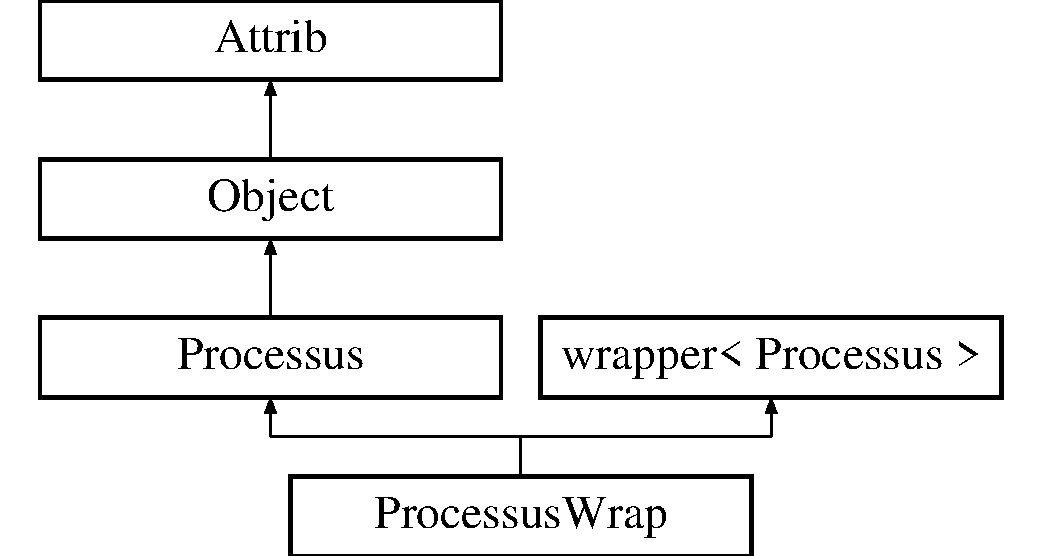
\includegraphics[height=4.000000cm]{structProcessusWrap}
\end{center}
\end{figure}
\subsection*{Public Member Functions}
\begin{DoxyCompactItemize}
\item 
\hyperlink{classStatusCode}{Status\+Code} \hyperlink{structProcessusWrap_a7cf48f51e6ac8173255417654cc0b499}{initialize} ()
\item 
\hyperlink{classStatusCode}{Status\+Code} \hyperlink{structProcessusWrap_a099df299b3dadd548c44e7e6d94f027a}{execute} ()
\item 
\hyperlink{classStatusCode}{Status\+Code} \hyperlink{structProcessusWrap_a6be9ef2aaa45c23bc780d264875cc542}{finalize} ()
\item 
\hyperlink{classProcessus}{Processus} $\ast$ \hyperlink{structProcessusWrap_a6582297a477b1cd1594f90a80691fca3}{clone} ()
\end{DoxyCompactItemize}
\subsection*{Additional Inherited Members}


\subsection{Detailed Description}


Definition at line 21 of file Python\+\_\+\+Proc.\+cpp.



\subsection{Member Function Documentation}
\mbox{\Hypertarget{structProcessusWrap_a6582297a477b1cd1594f90a80691fca3}\label{structProcessusWrap_a6582297a477b1cd1594f90a80691fca3}} 
\index{Processus\+Wrap@{Processus\+Wrap}!clone@{clone}}
\index{clone@{clone}!Processus\+Wrap@{Processus\+Wrap}}
\subsubsection{\texorpdfstring{clone()}{clone()}}
{\footnotesize\ttfamily \hyperlink{classProcessus}{Processus}$\ast$ Processus\+Wrap\+::clone (\begin{DoxyParamCaption}{ }\end{DoxyParamCaption})\hspace{0.3cm}{\ttfamily [inline]}, {\ttfamily [virtual]}}

processus termination virtual function 

Implements \hyperlink{classProcessus_aca8856f6d6d7b7e1fe941f298dcbb502}{Processus}.



Definition at line 26 of file Python\+\_\+\+Proc.\+cpp.


\begin{DoxyCode}
26 \{\textcolor{keywordflow}{return} this->get\_override(\textcolor{stringliteral}{"clone"})();\};
\end{DoxyCode}
\mbox{\Hypertarget{structProcessusWrap_a099df299b3dadd548c44e7e6d94f027a}\label{structProcessusWrap_a099df299b3dadd548c44e7e6d94f027a}} 
\index{Processus\+Wrap@{Processus\+Wrap}!execute@{execute}}
\index{execute@{execute}!Processus\+Wrap@{Processus\+Wrap}}
\subsubsection{\texorpdfstring{execute()}{execute()}}
{\footnotesize\ttfamily \hyperlink{classStatusCode}{Status\+Code} Processus\+Wrap\+::execute (\begin{DoxyParamCaption}{ }\end{DoxyParamCaption})\hspace{0.3cm}{\ttfamily [inline]}, {\ttfamily [virtual]}}

processus execution virtual function 

Implements \hyperlink{classProcessus_a63767a63a1fb0055c5aa45b21a4a5d58}{Processus}.



Definition at line 24 of file Python\+\_\+\+Proc.\+cpp.


\begin{DoxyCode}
24 \{\textcolor{keywordflow}{return} this->get\_override(\textcolor{stringliteral}{"execute"})();\};
\end{DoxyCode}
\mbox{\Hypertarget{structProcessusWrap_a6be9ef2aaa45c23bc780d264875cc542}\label{structProcessusWrap_a6be9ef2aaa45c23bc780d264875cc542}} 
\index{Processus\+Wrap@{Processus\+Wrap}!finalize@{finalize}}
\index{finalize@{finalize}!Processus\+Wrap@{Processus\+Wrap}}
\subsubsection{\texorpdfstring{finalize()}{finalize()}}
{\footnotesize\ttfamily \hyperlink{classStatusCode}{Status\+Code} Processus\+Wrap\+::finalize (\begin{DoxyParamCaption}{ }\end{DoxyParamCaption})\hspace{0.3cm}{\ttfamily [inline]}, {\ttfamily [virtual]}}

processus termination virtual function 

Implements \hyperlink{classProcessus_aba93d691f031bdb18ae4b8afb1b2e856}{Processus}.



Definition at line 25 of file Python\+\_\+\+Proc.\+cpp.


\begin{DoxyCode}
25 \{\textcolor{keywordflow}{return} this->get\_override(\textcolor{stringliteral}{"finalize"})();\};
\end{DoxyCode}
\mbox{\Hypertarget{structProcessusWrap_a7cf48f51e6ac8173255417654cc0b499}\label{structProcessusWrap_a7cf48f51e6ac8173255417654cc0b499}} 
\index{Processus\+Wrap@{Processus\+Wrap}!initialize@{initialize}}
\index{initialize@{initialize}!Processus\+Wrap@{Processus\+Wrap}}
\subsubsection{\texorpdfstring{initialize()}{initialize()}}
{\footnotesize\ttfamily \hyperlink{classStatusCode}{Status\+Code} Processus\+Wrap\+::initialize (\begin{DoxyParamCaption}{ }\end{DoxyParamCaption})\hspace{0.3cm}{\ttfamily [inline]}, {\ttfamily [virtual]}}

processus initialisation virtual function 

Implements \hyperlink{classProcessus_aee88ad7b77ae7319cf8b128e9dd2ea11}{Processus}.



Definition at line 23 of file Python\+\_\+\+Proc.\+cpp.


\begin{DoxyCode}
23 \{\textcolor{keywordflow}{return} this->get\_override(\textcolor{stringliteral}{"initialize"})();\};
\end{DoxyCode}


The documentation for this struct was generated from the following file\+:\begin{DoxyCompactItemize}
\item 
/home/eleclhcb/\+L\+H\+Cb/lbcat-\/cmake/\+Cat\+Kernel/src/\hyperlink{Python__Proc_8cpp}{Python\+\_\+\+Proc.\+cpp}\end{DoxyCompactItemize}

\hypertarget{structProcState}{
\section{ProcState Struct Reference}
\label{structProcState}\index{ProcState@{ProcState}}
}


{\ttfamily \#include $<$Processus.h$>$}\subsection*{Public Attributes}
\begin{DoxyCompactItemize}
\item 
int \hyperlink{structProcState_a1881d6b0db849a8af15f586ad5959260}{nevent}
\item 
int \hyperlink{structProcState_a51a0f54ba62b07e07ac8518c5f32828d}{nerrors}
\item 
float \hyperlink{structProcState_a88c69b099d8f2b2164d478f28e87610f}{time}
\item 
char \hyperlink{structProcState_aaffb70e5af437e2c0d4dfc69bd0b24cd}{state} \mbox{[}256\mbox{]}
\end{DoxyCompactItemize}


\subsection{Detailed Description}


Definition at line 24 of file Processus.h.

\subsection{Member Data Documentation}
\hypertarget{structProcState_a51a0f54ba62b07e07ac8518c5f32828d}{
\index{ProcState@{ProcState}!nerrors@{nerrors}}
\index{nerrors@{nerrors}!ProcState@{ProcState}}
\subsubsection[{nerrors}]{\setlength{\rightskip}{0pt plus 5cm}int {\bf ProcState::nerrors}}}
\label{structProcState_a51a0f54ba62b07e07ac8518c5f32828d}


Definition at line 26 of file Processus.h.

Referenced by Processus::incNErrors(), Processus::nErrors(), Processus::setElement(), Processus::setNErrors(), and Processus::setState().\hypertarget{structProcState_a1881d6b0db849a8af15f586ad5959260}{
\index{ProcState@{ProcState}!nevent@{nevent}}
\index{nevent@{nevent}!ProcState@{ProcState}}
\subsubsection[{nevent}]{\setlength{\rightskip}{0pt plus 5cm}int {\bf ProcState::nevent}}}
\label{structProcState_a1881d6b0db849a8af15f586ad5959260}


Definition at line 25 of file Processus.h.

Referenced by Processus::setElement(), and Processus::setState().\hypertarget{structProcState_aaffb70e5af437e2c0d4dfc69bd0b24cd}{
\index{ProcState@{ProcState}!state@{state}}
\index{state@{state}!ProcState@{ProcState}}
\subsubsection[{state}]{\setlength{\rightskip}{0pt plus 5cm}char {\bf ProcState::state}\mbox{[}256\mbox{]}}}
\label{structProcState_aaffb70e5af437e2c0d4dfc69bd0b24cd}


Definition at line 28 of file Processus.h.

Referenced by Processus::setElement(), and Processus::setState().\hypertarget{structProcState_a88c69b099d8f2b2164d478f28e87610f}{
\index{ProcState@{ProcState}!time@{time}}
\index{time@{time}!ProcState@{ProcState}}
\subsubsection[{time}]{\setlength{\rightskip}{0pt plus 5cm}float {\bf ProcState::time}}}
\label{structProcState_a88c69b099d8f2b2164d478f28e87610f}


Definition at line 27 of file Processus.h.

Referenced by Processus::setElement(), and Processus::setState().

The documentation for this struct was generated from the following file:\begin{DoxyCompactItemize}
\item 
/home/eleclhcb/LHCb/lbcat-\/cmake/CatKernel/inc/\hyperlink{Processus_8h}{Processus.h}\end{DoxyCompactItemize}

\hypertarget{classprogressbar_1_1ProgressBar}{}\section{progressbar.\+Progress\+Bar Class Reference}
\label{classprogressbar_1_1ProgressBar}\index{progressbar.\+Progress\+Bar@{progressbar.\+Progress\+Bar}}
Inheritance diagram for progressbar.\+Progress\+Bar\+:\begin{figure}[H]
\begin{center}
\leavevmode
\includegraphics[height=3.000000cm]{classprogressbar_1_1ProgressBar}
\end{center}
\end{figure}
\subsection*{Public Member Functions}
\begin{DoxyCompactItemize}
\item 
def \hyperlink{classprogressbar_1_1ProgressBar_ad3722b896ddbe5ea96abe5604ac84475}{\+\_\+\+\_\+init\+\_\+\+\_\+} (self, \hyperlink{classprogressbar_1_1ProgressBar_a28ce54371f3a84172049c0520726d2aa}{process}=\char`\"{}     \char`\"{}, \hyperlink{classprogressbar_1_1ProgressBar_a550afef3072c2412e2aa906b12c33bbe}{start}=0, \hyperlink{classprogressbar_1_1ProgressBar_a92053e3baab49364971c15373b6c848f}{end}=10, \hyperlink{classprogressbar_1_1ProgressBar_abde0c8da19e6e6bcde845b1eb3cee279}{width}=12, \hyperlink{classprogressbar_1_1ProgressBar_a6b11796a20118f92eb59abbccf626d23}{fill}=\textquotesingle{}=\textquotesingle{}, \hyperlink{classprogressbar_1_1ProgressBar_a0bfce2d34f0a8f034748d77cc5140bc5}{blank}=\textquotesingle{}.\textquotesingle{}, \hyperlink{classprogressbar_1_1ProgressBar_a4dd00a852851da809ffad5e1bf282858}{format}=\textquotesingle{}running \%(\hyperlink{classprogressbar_1_1ProgressBar_a28ce54371f3a84172049c0520726d2aa}{process}) s \mbox{[}\%(\hyperlink{classprogressbar_1_1ProgressBar_a6b11796a20118f92eb59abbccf626d23}{fill}) s\%(\hyperlink{classprogressbar_1_1ProgressBar_a0bfce2d34f0a8f034748d77cc5140bc5}{blank}) s\mbox{]} \%(\hyperlink{classprogressbar_1_1ProgressBar_a3adc96f42e6891bcd2885c9ef29767f3}{progress}) s\%\%\textquotesingle{}, \hyperlink{classprogressbar_1_1ProgressBar_a0b98b7a8f7025b78a5d01f0dcfc2dbaa}{incremental}=True)
\item 
def \hyperlink{classprogressbar_1_1ProgressBar_ab72aa084f53baad02409c8e7e5979046}{\+\_\+\+\_\+add\+\_\+\+\_\+} (self, increment)
\item 
def \hyperlink{classprogressbar_1_1ProgressBar_aea02b9e37516e9d267e2d48b4e415bd8}{\+\_\+\+\_\+str\+\_\+\+\_\+} (self)
\item 
def \hyperlink{classprogressbar_1_1ProgressBar_a0794442f190ed0d6e5b894f29881758b}{set} (self, value)
\item 
def \hyperlink{classprogressbar_1_1ProgressBar_aefc445915e4d1eb0bbf962857c122dac}{reset} (self)
\end{DoxyCompactItemize}
\subsection*{Public Attributes}
\begin{DoxyCompactItemize}
\item 
\hyperlink{classprogressbar_1_1ProgressBar_a550afef3072c2412e2aa906b12c33bbe}{start}
\item 
\hyperlink{classprogressbar_1_1ProgressBar_a92053e3baab49364971c15373b6c848f}{end}
\item 
\hyperlink{classprogressbar_1_1ProgressBar_abde0c8da19e6e6bcde845b1eb3cee279}{width}
\item 
\hyperlink{classprogressbar_1_1ProgressBar_a6b11796a20118f92eb59abbccf626d23}{fill}
\item 
\hyperlink{classprogressbar_1_1ProgressBar_a0bfce2d34f0a8f034748d77cc5140bc5}{blank}
\item 
\hyperlink{classprogressbar_1_1ProgressBar_a4dd00a852851da809ffad5e1bf282858}{format}
\item 
\hyperlink{classprogressbar_1_1ProgressBar_a0b98b7a8f7025b78a5d01f0dcfc2dbaa}{incremental}
\item 
\hyperlink{classprogressbar_1_1ProgressBar_ac076ee00e3a70c69b8583668c165415a}{step}
\item 
\hyperlink{classprogressbar_1_1ProgressBar_a28ce54371f3a84172049c0520726d2aa}{process}
\item 
\hyperlink{classprogressbar_1_1ProgressBar_a3adc96f42e6891bcd2885c9ef29767f3}{progress}
\end{DoxyCompactItemize}
\subsection*{Private Member Functions}
\begin{DoxyCompactItemize}
\item 
def \hyperlink{classprogressbar_1_1ProgressBar_a8e8704c0f26d529f82413318cc9e9c81}{\+\_\+get\+\_\+progress} (self, increment)
\end{DoxyCompactItemize}
\subsection*{Static Private Attributes}
\begin{DoxyCompactItemize}
\item 
def \hyperlink{classprogressbar_1_1ProgressBar_a53eaadf85baa406c1f179fea7029d8b0}{\+\_\+\+\_\+repr\+\_\+\+\_\+} = \hyperlink{classprogressbar_1_1ProgressBar_aea02b9e37516e9d267e2d48b4e415bd8}{\+\_\+\+\_\+str\+\_\+\+\_\+}
\end{DoxyCompactItemize}


\subsection{Detailed Description}
\begin{DoxyVerb}ProgressBar class holds the options of the progress bar.
The options are:
    start   State from which start the progress. For example, if start is
            5 and the end is 10, the progress of this state is 50%
    end     State in which the progress has terminated.
    width   --
    fill    String to use for "filled" used to represent the progress
    blank   String to use for "filled" used to represent remaining space.
    format  Format
    incremental
\end{DoxyVerb}
 

Definition at line 4 of file progressbar.\+py.



\subsection{Constructor \& Destructor Documentation}
\mbox{\Hypertarget{classprogressbar_1_1ProgressBar_ad3722b896ddbe5ea96abe5604ac84475}\label{classprogressbar_1_1ProgressBar_ad3722b896ddbe5ea96abe5604ac84475}} 
\index{progressbar\+::\+Progress\+Bar@{progressbar\+::\+Progress\+Bar}!\+\_\+\+\_\+init\+\_\+\+\_\+@{\+\_\+\+\_\+init\+\_\+\+\_\+}}
\index{\+\_\+\+\_\+init\+\_\+\+\_\+@{\+\_\+\+\_\+init\+\_\+\+\_\+}!progressbar\+::\+Progress\+Bar@{progressbar\+::\+Progress\+Bar}}
\subsubsection{\texorpdfstring{\+\_\+\+\_\+init\+\_\+\+\_\+()}{\_\_init\_\_()}}
{\footnotesize\ttfamily def progressbar.\+Progress\+Bar.\+\_\+\+\_\+init\+\_\+\+\_\+ (\begin{DoxyParamCaption}\item[{}]{self,  }\item[{}]{process = {\ttfamily \char`\"{}~~~~~\char`\"{}},  }\item[{}]{start = {\ttfamily 0},  }\item[{}]{end = {\ttfamily 10},  }\item[{}]{width = {\ttfamily 12},  }\item[{}]{fill = {\ttfamily \textquotesingle{}=\textquotesingle{}},  }\item[{}]{blank = {\ttfamily \textquotesingle{}.\textquotesingle{}},  }\item[{}]{format = {\ttfamily \textquotesingle{}running~\%(\hyperlink{classprogressbar_1_1ProgressBar_a28ce54371f3a84172049c0520726d2aa}{process})s~\mbox{[}\%(\hyperlink{classprogressbar_1_1ProgressBar_a6b11796a20118f92eb59abbccf626d23}{fill})s\%(\hyperlink{classprogressbar_1_1ProgressBar_a0bfce2d34f0a8f034748d77cc5140bc5}{blank})s\mbox{]}~\%(\hyperlink{classprogressbar_1_1ProgressBar_a3adc96f42e6891bcd2885c9ef29767f3}{progress})s\%\%\textquotesingle{}},  }\item[{}]{incremental = {\ttfamily True} }\end{DoxyParamCaption})}



Definition at line 16 of file progressbar.\+py.


\begin{DoxyCode}
16     \textcolor{keyword}{def }\hyperlink{classwrapper_1_1ModuleDictWrapper_a9a7a794150502f51df687831583e13b9}{\_\_init\_\_}(self, process="     ", start=0, end=10, width=12, fill='=', blank='.', 
      format='running %(process)s [%(fill)s%(blank)s] %(progress)s%%\textcolor{stringliteral}{', incremental=True):        super(ProgressBar, self).
      \hyperlink{classwrapper_1_1ModuleDictWrapper_a9a7a794150502f51df687831583e13b9}{\_\_init\_\_}()}
17 \textcolor{stringliteral}{}
18 \textcolor{stringliteral}{        self.start = start}
19 \textcolor{stringliteral}{        self.end = end}
20 \textcolor{stringliteral}{        self.width = width}
21 \textcolor{stringliteral}{        self.fill = fill}
22 \textcolor{stringliteral}{        self.blank = blank}
23 \textcolor{stringliteral}{        self.format = format}
24 \textcolor{stringliteral}{        self.incremental = incremental}
25 \textcolor{stringliteral}{        self.step = 100 / float(width) }\textcolor{comment}{#fix}
26         self.process = process
27         self.reset()
28 
29 \end{DoxyCode}


\subsection{Member Function Documentation}
\mbox{\Hypertarget{classprogressbar_1_1ProgressBar_ab72aa084f53baad02409c8e7e5979046}\label{classprogressbar_1_1ProgressBar_ab72aa084f53baad02409c8e7e5979046}} 
\index{progressbar\+::\+Progress\+Bar@{progressbar\+::\+Progress\+Bar}!\+\_\+\+\_\+add\+\_\+\+\_\+@{\+\_\+\+\_\+add\+\_\+\+\_\+}}
\index{\+\_\+\+\_\+add\+\_\+\+\_\+@{\+\_\+\+\_\+add\+\_\+\+\_\+}!progressbar\+::\+Progress\+Bar@{progressbar\+::\+Progress\+Bar}}
\subsubsection{\texorpdfstring{\+\_\+\+\_\+add\+\_\+\+\_\+()}{\_\_add\_\_()}}
{\footnotesize\ttfamily def progressbar.\+Progress\+Bar.\+\_\+\+\_\+add\+\_\+\+\_\+ (\begin{DoxyParamCaption}\item[{}]{self,  }\item[{}]{increment }\end{DoxyParamCaption})}



Definition at line 30 of file progressbar.\+py.



References progressbar.\+Progress\+Bar.\+\_\+get\+\_\+progress(), and progressbar.\+Progress\+Bar.\+progress.


\begin{DoxyCode}
30     \textcolor{keyword}{def }\_\_add\_\_(self, increment):
31         increment = self.\_get\_progress(increment)
32         \textcolor{keywordflow}{if} 100 > self.progress + increment:
33             self.progress += increment
34         \textcolor{keywordflow}{else}:
35             self.progress = 100
36         \textcolor{keywordflow}{return} self
37     
\end{DoxyCode}
\mbox{\Hypertarget{classprogressbar_1_1ProgressBar_aea02b9e37516e9d267e2d48b4e415bd8}\label{classprogressbar_1_1ProgressBar_aea02b9e37516e9d267e2d48b4e415bd8}} 
\index{progressbar\+::\+Progress\+Bar@{progressbar\+::\+Progress\+Bar}!\+\_\+\+\_\+str\+\_\+\+\_\+@{\+\_\+\+\_\+str\+\_\+\+\_\+}}
\index{\+\_\+\+\_\+str\+\_\+\+\_\+@{\+\_\+\+\_\+str\+\_\+\+\_\+}!progressbar\+::\+Progress\+Bar@{progressbar\+::\+Progress\+Bar}}
\subsubsection{\texorpdfstring{\+\_\+\+\_\+str\+\_\+\+\_\+()}{\_\_str\_\_()}}
{\footnotesize\ttfamily def progressbar.\+Progress\+Bar.\+\_\+\+\_\+str\+\_\+\+\_\+ (\begin{DoxyParamCaption}\item[{}]{self }\end{DoxyParamCaption})}



Definition at line 38 of file progressbar.\+py.



References progressbar.\+Progress\+Bar.\+blank, progressbar.\+Progress\+Bar.\+fill, progressbar.\+Progress\+Bar.\+format, progressbar.\+Progress\+Bar.\+process, progressbar.\+Progress\+Bar.\+progress, progressbar.\+Progress\+Bar.\+step, and progressbar.\+Progress\+Bar.\+width.


\begin{DoxyCode}
38     \textcolor{keyword}{def }\_\_str\_\_(self):
39         progressed = int(self.progress / self.step) \textcolor{comment}{#fix}
40         fill = progressed * self.fill
41         proc = self.process
42         blank = (self.width - progressed) * self.blank
43         \textcolor{keywordflow}{return} self.format % \{\textcolor{stringliteral}{'process'}: proc, \textcolor{stringliteral}{'fill'}: fill, \textcolor{stringliteral}{'blank'}: blank, \textcolor{stringliteral}{'progress'}: int(self.progress)
      \}
44 
\end{DoxyCode}
\mbox{\Hypertarget{classprogressbar_1_1ProgressBar_a8e8704c0f26d529f82413318cc9e9c81}\label{classprogressbar_1_1ProgressBar_a8e8704c0f26d529f82413318cc9e9c81}} 
\index{progressbar\+::\+Progress\+Bar@{progressbar\+::\+Progress\+Bar}!\+\_\+get\+\_\+progress@{\+\_\+get\+\_\+progress}}
\index{\+\_\+get\+\_\+progress@{\+\_\+get\+\_\+progress}!progressbar\+::\+Progress\+Bar@{progressbar\+::\+Progress\+Bar}}
\subsubsection{\texorpdfstring{\+\_\+get\+\_\+progress()}{\_get\_progress()}}
{\footnotesize\ttfamily def progressbar.\+Progress\+Bar.\+\_\+get\+\_\+progress (\begin{DoxyParamCaption}\item[{}]{self,  }\item[{}]{increment }\end{DoxyParamCaption})\hspace{0.3cm}{\ttfamily [private]}}



Definition at line 47 of file progressbar.\+py.



References progressbar.\+Progress\+Bar.\+end.



Referenced by progressbar.\+Progress\+Bar.\+\_\+\+\_\+add\+\_\+\+\_\+(), progressbar.\+Progress\+Bar.\+reset(), and progressbar.\+Progress\+Bar.\+set().


\begin{DoxyCode}
47     \textcolor{keyword}{def }\_get\_progress(self, increment):
48         \textcolor{keywordflow}{return} float(increment * 100) / self.end
49 
\end{DoxyCode}
\mbox{\Hypertarget{classprogressbar_1_1ProgressBar_aefc445915e4d1eb0bbf962857c122dac}\label{classprogressbar_1_1ProgressBar_aefc445915e4d1eb0bbf962857c122dac}} 
\index{progressbar\+::\+Progress\+Bar@{progressbar\+::\+Progress\+Bar}!reset@{reset}}
\index{reset@{reset}!progressbar\+::\+Progress\+Bar@{progressbar\+::\+Progress\+Bar}}
\subsubsection{\texorpdfstring{reset()}{reset()}}
{\footnotesize\ttfamily def progressbar.\+Progress\+Bar.\+reset (\begin{DoxyParamCaption}\item[{}]{self }\end{DoxyParamCaption})}

\begin{DoxyVerb}Resets the current progress to the start point\end{DoxyVerb}
 

Definition at line 58 of file progressbar.\+py.



References progressbar.\+Progress\+Bar.\+\_\+get\+\_\+progress(), progressbar.\+Progress\+Bar.\+progress, and progressbar.\+Progress\+Bar.\+start.


\begin{DoxyCode}
58     \textcolor{keyword}{def }\hyperlink{namespaceshell_a2f31bbe4baf894f4863c4d392239ab8b}{reset}(self):
59         \textcolor{stringliteral}{"""Resets the current progress to the start point"""}
60         self.progress = self.\_get\_progress(self.start)
61         \textcolor{keywordflow}{return} self
62 
63 
\end{DoxyCode}
\mbox{\Hypertarget{classprogressbar_1_1ProgressBar_a0794442f190ed0d6e5b894f29881758b}\label{classprogressbar_1_1ProgressBar_a0794442f190ed0d6e5b894f29881758b}} 
\index{progressbar\+::\+Progress\+Bar@{progressbar\+::\+Progress\+Bar}!set@{set}}
\index{set@{set}!progressbar\+::\+Progress\+Bar@{progressbar\+::\+Progress\+Bar}}
\subsubsection{\texorpdfstring{set()}{set()}}
{\footnotesize\ttfamily def progressbar.\+Progress\+Bar.\+set (\begin{DoxyParamCaption}\item[{}]{self,  }\item[{}]{value }\end{DoxyParamCaption})}



Definition at line 50 of file progressbar.\+py.



References progressbar.\+Progress\+Bar.\+\_\+get\+\_\+progress(), and progressbar.\+Progress\+Bar.\+progress.


\begin{DoxyCode}
50     \textcolor{keyword}{def }set(self, value):
51         value = self.\_get\_progress(value)
52         \textcolor{keywordflow}{if} 100 > value:
53             self.progress = value 
54         \textcolor{keywordflow}{else}:
55             self.progress = 100
56         \textcolor{keywordflow}{return} self
57 
\end{DoxyCode}


\subsection{Member Data Documentation}
\mbox{\Hypertarget{classprogressbar_1_1ProgressBar_a53eaadf85baa406c1f179fea7029d8b0}\label{classprogressbar_1_1ProgressBar_a53eaadf85baa406c1f179fea7029d8b0}} 
\index{progressbar\+::\+Progress\+Bar@{progressbar\+::\+Progress\+Bar}!\+\_\+\+\_\+repr\+\_\+\+\_\+@{\+\_\+\+\_\+repr\+\_\+\+\_\+}}
\index{\+\_\+\+\_\+repr\+\_\+\+\_\+@{\+\_\+\+\_\+repr\+\_\+\+\_\+}!progressbar\+::\+Progress\+Bar@{progressbar\+::\+Progress\+Bar}}
\subsubsection{\texorpdfstring{\+\_\+\+\_\+repr\+\_\+\+\_\+}{\_\_repr\_\_}}
{\footnotesize\ttfamily def progressbar.\+Progress\+Bar.\+\_\+\+\_\+repr\+\_\+\+\_\+ = \hyperlink{classprogressbar_1_1ProgressBar_aea02b9e37516e9d267e2d48b4e415bd8}{\+\_\+\+\_\+str\+\_\+\+\_\+}\hspace{0.3cm}{\ttfamily [static]}, {\ttfamily [private]}}



Definition at line 45 of file progressbar.\+py.

\mbox{\Hypertarget{classprogressbar_1_1ProgressBar_a0bfce2d34f0a8f034748d77cc5140bc5}\label{classprogressbar_1_1ProgressBar_a0bfce2d34f0a8f034748d77cc5140bc5}} 
\index{progressbar\+::\+Progress\+Bar@{progressbar\+::\+Progress\+Bar}!blank@{blank}}
\index{blank@{blank}!progressbar\+::\+Progress\+Bar@{progressbar\+::\+Progress\+Bar}}
\subsubsection{\texorpdfstring{blank}{blank}}
{\footnotesize\ttfamily progressbar.\+Progress\+Bar.\+blank}



Definition at line 23 of file progressbar.\+py.



Referenced by progressbar.\+Progress\+Bar.\+\_\+\+\_\+str\+\_\+\+\_\+().

\mbox{\Hypertarget{classprogressbar_1_1ProgressBar_a92053e3baab49364971c15373b6c848f}\label{classprogressbar_1_1ProgressBar_a92053e3baab49364971c15373b6c848f}} 
\index{progressbar\+::\+Progress\+Bar@{progressbar\+::\+Progress\+Bar}!end@{end}}
\index{end@{end}!progressbar\+::\+Progress\+Bar@{progressbar\+::\+Progress\+Bar}}
\subsubsection{\texorpdfstring{end}{end}}
{\footnotesize\ttfamily progressbar.\+Progress\+Bar.\+end}



Definition at line 20 of file progressbar.\+py.



Referenced by progressbar.\+Progress\+Bar.\+\_\+get\+\_\+progress().

\mbox{\Hypertarget{classprogressbar_1_1ProgressBar_a6b11796a20118f92eb59abbccf626d23}\label{classprogressbar_1_1ProgressBar_a6b11796a20118f92eb59abbccf626d23}} 
\index{progressbar\+::\+Progress\+Bar@{progressbar\+::\+Progress\+Bar}!fill@{fill}}
\index{fill@{fill}!progressbar\+::\+Progress\+Bar@{progressbar\+::\+Progress\+Bar}}
\subsubsection{\texorpdfstring{fill}{fill}}
{\footnotesize\ttfamily progressbar.\+Progress\+Bar.\+fill}



Definition at line 22 of file progressbar.\+py.



Referenced by progressbar.\+Progress\+Bar.\+\_\+\+\_\+str\+\_\+\+\_\+().

\mbox{\Hypertarget{classprogressbar_1_1ProgressBar_a4dd00a852851da809ffad5e1bf282858}\label{classprogressbar_1_1ProgressBar_a4dd00a852851da809ffad5e1bf282858}} 
\index{progressbar\+::\+Progress\+Bar@{progressbar\+::\+Progress\+Bar}!format@{format}}
\index{format@{format}!progressbar\+::\+Progress\+Bar@{progressbar\+::\+Progress\+Bar}}
\subsubsection{\texorpdfstring{format}{format}}
{\footnotesize\ttfamily progressbar.\+Progress\+Bar.\+format}



Definition at line 24 of file progressbar.\+py.



Referenced by progressbar.\+Progress\+Bar.\+\_\+\+\_\+str\+\_\+\+\_\+().

\mbox{\Hypertarget{classprogressbar_1_1ProgressBar_a0b98b7a8f7025b78a5d01f0dcfc2dbaa}\label{classprogressbar_1_1ProgressBar_a0b98b7a8f7025b78a5d01f0dcfc2dbaa}} 
\index{progressbar\+::\+Progress\+Bar@{progressbar\+::\+Progress\+Bar}!incremental@{incremental}}
\index{incremental@{incremental}!progressbar\+::\+Progress\+Bar@{progressbar\+::\+Progress\+Bar}}
\subsubsection{\texorpdfstring{incremental}{incremental}}
{\footnotesize\ttfamily progressbar.\+Progress\+Bar.\+incremental}



Definition at line 25 of file progressbar.\+py.

\mbox{\Hypertarget{classprogressbar_1_1ProgressBar_a28ce54371f3a84172049c0520726d2aa}\label{classprogressbar_1_1ProgressBar_a28ce54371f3a84172049c0520726d2aa}} 
\index{progressbar\+::\+Progress\+Bar@{progressbar\+::\+Progress\+Bar}!process@{process}}
\index{process@{process}!progressbar\+::\+Progress\+Bar@{progressbar\+::\+Progress\+Bar}}
\subsubsection{\texorpdfstring{process}{process}}
{\footnotesize\ttfamily progressbar.\+Progress\+Bar.\+process}



Definition at line 27 of file progressbar.\+py.



Referenced by progressbar.\+Progress\+Bar.\+\_\+\+\_\+str\+\_\+\+\_\+().

\mbox{\Hypertarget{classprogressbar_1_1ProgressBar_a3adc96f42e6891bcd2885c9ef29767f3}\label{classprogressbar_1_1ProgressBar_a3adc96f42e6891bcd2885c9ef29767f3}} 
\index{progressbar\+::\+Progress\+Bar@{progressbar\+::\+Progress\+Bar}!progress@{progress}}
\index{progress@{progress}!progressbar\+::\+Progress\+Bar@{progressbar\+::\+Progress\+Bar}}
\subsubsection{\texorpdfstring{progress}{progress}}
{\footnotesize\ttfamily progressbar.\+Progress\+Bar.\+progress}



Definition at line 35 of file progressbar.\+py.



Referenced by progressbar.\+Progress\+Bar.\+\_\+\+\_\+add\+\_\+\+\_\+(), progressbar.\+Progress\+Bar.\+\_\+\+\_\+str\+\_\+\+\_\+(), progressbar.\+Progress\+Bar.\+reset(), and progressbar.\+Progress\+Bar.\+set().

\mbox{\Hypertarget{classprogressbar_1_1ProgressBar_a550afef3072c2412e2aa906b12c33bbe}\label{classprogressbar_1_1ProgressBar_a550afef3072c2412e2aa906b12c33bbe}} 
\index{progressbar\+::\+Progress\+Bar@{progressbar\+::\+Progress\+Bar}!start@{start}}
\index{start@{start}!progressbar\+::\+Progress\+Bar@{progressbar\+::\+Progress\+Bar}}
\subsubsection{\texorpdfstring{start}{start}}
{\footnotesize\ttfamily progressbar.\+Progress\+Bar.\+start}



Definition at line 19 of file progressbar.\+py.



Referenced by progressbar.\+Progress\+Bar.\+reset().

\mbox{\Hypertarget{classprogressbar_1_1ProgressBar_ac076ee00e3a70c69b8583668c165415a}\label{classprogressbar_1_1ProgressBar_ac076ee00e3a70c69b8583668c165415a}} 
\index{progressbar\+::\+Progress\+Bar@{progressbar\+::\+Progress\+Bar}!step@{step}}
\index{step@{step}!progressbar\+::\+Progress\+Bar@{progressbar\+::\+Progress\+Bar}}
\subsubsection{\texorpdfstring{step}{step}}
{\footnotesize\ttfamily progressbar.\+Progress\+Bar.\+step}



Definition at line 26 of file progressbar.\+py.



Referenced by progressbar.\+Progress\+Bar.\+\_\+\+\_\+str\+\_\+\+\_\+().

\mbox{\Hypertarget{classprogressbar_1_1ProgressBar_abde0c8da19e6e6bcde845b1eb3cee279}\label{classprogressbar_1_1ProgressBar_abde0c8da19e6e6bcde845b1eb3cee279}} 
\index{progressbar\+::\+Progress\+Bar@{progressbar\+::\+Progress\+Bar}!width@{width}}
\index{width@{width}!progressbar\+::\+Progress\+Bar@{progressbar\+::\+Progress\+Bar}}
\subsubsection{\texorpdfstring{width}{width}}
{\footnotesize\ttfamily progressbar.\+Progress\+Bar.\+width}



Definition at line 21 of file progressbar.\+py.



Referenced by progressbar.\+Progress\+Bar.\+\_\+\+\_\+str\+\_\+\+\_\+().



The documentation for this class was generated from the following file\+:\begin{DoxyCompactItemize}
\item 
/home/eleclhcb/\+L\+H\+Cb/lbcat-\/cmake/\+Cat\+Python/python/\hyperlink{progressbar_8py}{progressbar.\+py}\end{DoxyCompactItemize}

\hypertarget{classProto40MHz__v1}{}\section{Proto40\+M\+Hz\+\_\+v1 Class Reference}
\label{classProto40MHz__v1}\index{Proto40\+M\+Hz\+\_\+v1@{Proto40\+M\+Hz\+\_\+v1}}


{\ttfamily \#include $<$inc/\+Proto40\+M\+Hz\+\_\+v1.\+h$>$}

Inheritance diagram for Proto40\+M\+Hz\+\_\+v1\+:\begin{figure}[H]
\begin{center}
\leavevmode
\includegraphics[height=5.000000cm]{classProto40MHz__v1}
\end{center}
\end{figure}
\subsection*{Classes}
\begin{DoxyCompactItemize}
\item 
class \hyperlink{classProto40MHz__v1_1_1Proto40MHz__v1}{Proto40\+M\+Hz\+\_\+v1}
\end{DoxyCompactItemize}
\subsection*{Public Types}
\begin{DoxyCompactItemize}
\item 
enum \hyperlink{classAttrib_a69e171d7cc6417835a5a306d3c764235}{Attribut} \{ \newline
\hyperlink{classAttrib_a69e171d7cc6417835a5a306d3c764235a3a8da2ab97dda18aebab196fe4100531}{U\+N\+D\+E\+F\+I\+N\+ED}, 
\hyperlink{classAttrib_a69e171d7cc6417835a5a306d3c764235a2bfb2af57b87031d190a05fe25dd92ed}{P\+A\+S\+S\+I\+VE}, 
\hyperlink{classAttrib_a69e171d7cc6417835a5a306d3c764235a3b1fec929c0370d1436f2f06e298fb0d}{A\+C\+T\+I\+VE}, 
\hyperlink{classAttrib_a69e171d7cc6417835a5a306d3c764235aa27c16b480a369ea4d18b07b2516bbc7}{I\+N\+T\+E\+R\+F\+A\+CE}, 
\newline
\hyperlink{classAttrib_a69e171d7cc6417835a5a306d3c764235a1420a5b8c0540b2af210b6975eded7f9}{IO}, 
\hyperlink{classAttrib_a69e171d7cc6417835a5a306d3c764235a0af3b0d0ac323c1704e6c69cf90add28}{I\+O\+D\+A\+TA}, 
\hyperlink{classAttrib_a69e171d7cc6417835a5a306d3c764235a7788bc5dd333fd8ce18562b269c9dab1}{E\+L\+E\+M\+E\+NT}, 
\hyperlink{classAttrib_a69e171d7cc6417835a5a306d3c764235a61ceb22149f365f1780d18f9d1459423}{H\+A\+R\+D\+W\+A\+RE}, 
\newline
\hyperlink{classAttrib_a69e171d7cc6417835a5a306d3c764235a75250e29692496e73effca2c0330977f}{P\+R\+O\+C\+E\+S\+S\+US}, 
\hyperlink{classAttrib_a69e171d7cc6417835a5a306d3c764235a103a67cd0b8f07ef478fa45d4356e27b}{S\+O\+F\+T\+W\+A\+RE}
 \}
\end{DoxyCompactItemize}
\subsection*{Public Member Functions}
\begin{DoxyCompactItemize}
\item 
\hyperlink{classProto40MHz__v1_ac78306552cc5dcff551d03cda7a12c0f}{Proto40\+M\+Hz\+\_\+v1} ()
\begin{DoxyCompactList}\small\item\em Standard constructor. \end{DoxyCompactList}\item 
virtual \hyperlink{classProto40MHz__v1_a000cf963b1c194daf39b5f54f4ad0a62}{$\sim$\+Proto40\+M\+Hz\+\_\+v1} ()
\begin{DoxyCompactList}\small\item\em Destructor. \end{DoxyCompactList}\item 
void \hyperlink{classProto40MHz__v1_ae775987179848b4bc257473be261d24c}{help} ()
\item 
\hyperlink{classStatusCode}{Status\+Code} \hyperlink{classProto40MHz__v1_a60c96d57ae30bf6dcf9e4778294ca55c}{init} ()
\item 
void \hyperlink{classProto40MHz__v1_a321b46479def2e28e5727117cb5e05a1}{reset} ()
\item 
void \hyperlink{classProto40MHz__v1_a862d752dfe341ad00eea6f9d8dbc8525}{update} ()
\item 
\hyperlink{classUsbFTInterface}{Usb\+F\+T\+Interface} $\ast$ \hyperlink{classProto40MHz__v1_aee48500fba238c4caf8502db32ebb991}{usb} ()
\item 
\hyperlink{classPhaser}{Phaser} $\ast$ \hyperlink{classProto40MHz__v1_a545f205296c492530a50febd54584f73}{phaser0} ()
\item 
\hyperlink{classPhaser}{Phaser} $\ast$ \hyperlink{classProto40MHz__v1_a9c4ef3187b86b74b05bdec3c167a405e}{phaser1} ()
\item 
\hyperlink{classPhaser}{Phaser} $\ast$ \hyperlink{classProto40MHz__v1_a59defd14376765f7df8f87d594170527}{phaser2} ()
\item 
\hyperlink{classA3PE}{A3\+PE} $\ast$ \hyperlink{classProto40MHz__v1_a263cfc900aafa3ceee1af4b596a824de}{a3pe} ()
\item 
void \hyperlink{classElement_a3c0abcb36f8906688bb7e32608df7086}{recursive\+Init\+Element} ()
\item 
void \hyperlink{classElement_a82119ed37dff76508a2746a853ec35ba}{recursive\+Init\+Communications} ()
\item 
\hyperlink{classStatusCode}{Status\+Code} \hyperlink{classElement_ab476b4b1df5954141ceb14f072433b89}{set\+Connection} (\hyperlink{classHierarchy}{Hierarchy} $\ast$)
\item 
\hyperlink{classHierarchy}{Hierarchy} $\ast$ \hyperlink{classElement_af57444353c1ddf9fa0109801e97debf7}{connection} ()
\item 
void \hyperlink{classHierarchy_af4d43b0765b402670eed2d62c73405af}{clear} ()
\item 
void \hyperlink{classHierarchy_a585ad1aeec16077a0e532ab8b4fc557b}{set\+Parent} (\hyperlink{classHierarchy}{Hierarchy} $\ast$\hyperlink{classHierarchy_a1c7bec8257e717f9c1465e06ebf845fc}{parent})
\item 
\hyperlink{classHierarchy}{Hierarchy} $\ast$ \hyperlink{classHierarchy_a1c7bec8257e717f9c1465e06ebf845fc}{parent} ()
\item 
\hyperlink{classHierarchy}{Hierarchy} $\ast$ \hyperlink{classHierarchy_ad550588733bf75ac5c0fcfd7c8fd11a6}{parent} (std\+::string)
\item 
\hyperlink{classHierarchy}{Hierarchy} $\ast$ \hyperlink{classHierarchy_aee461dc930ce3871636ff87f075b1b83}{origin} ()
\item 
virtual void \hyperlink{classHierarchy_ad677774ff38fcb257c04a3a10d471fac}{add\+Child} (\hyperlink{classHierarchy}{Hierarchy} $\ast$element)
\item 
std\+::vector$<$ \hyperlink{classHierarchy}{Hierarchy} $\ast$ $>$ \hyperlink{classHierarchy_aa9a76f69e98e052ee1a6e32cea006288}{children} ()
\item 
\hyperlink{classHierarchy}{Hierarchy} $\ast$ \hyperlink{classHierarchy_a1e207f973c694b538bf90107b4868817}{child} (std\+::string)
\item 
\hyperlink{classHierarchy}{Hierarchy} $\ast$ \hyperlink{classHierarchy_a0c15a5276a3b80b4354d6bd8a01e0708}{child\+Typed} (std\+::string)
\item 
unsigned long \hyperlink{classHierarchy_ab16e84de65fd84e14001a6cf941c8be4}{number\+Of\+Children} ()
\item 
bool \hyperlink{classHierarchy_a255174fe4d316d2a3f430dcb9dab29f1}{has\+Children} ()
\item 
void \hyperlink{classHierarchy_a2b2b359fac003233f65786a616766bde}{del\+Child} (\hyperlink{classHierarchy}{Hierarchy} $\ast$)
\item 
void \hyperlink{classHierarchy_a1928ac7615fe0b5e55cd707f70dc6781}{del\+Child} (std\+::string)
\item 
std\+::string \hyperlink{classHierarchy_aa7990fa7caf132d83e361ce033c6c65a}{path} (std\+::string=std\+::string(\char`\"{}\char`\"{}))
\item 
std\+::string \hyperlink{classHierarchy_a1efd56cd164d328d2002e53a10a19b8c}{path\+Typed} (std\+::string=std\+::string(\char`\"{}\char`\"{}))
\item 
void \hyperlink{classHierarchy_a76e914b9a677a22a82deb74d892bf261}{tree} (std\+::string indent=std\+::string(\char`\"{}\char`\"{}))
\item 
void \hyperlink{classHierarchy_a594c294c5f60c230e106d522ed008212}{tree} ()
\item 
std\+::string \hyperlink{classObject_a300f4c05dd468c7bb8b3c968868443c1}{name} () const
\item 
std\+::string \hyperlink{classObject_a84f99f70f144a83e1582d1d0f84e4e62}{type} ()
\item 
unsigned char \hyperlink{classObject_af99145335cc61ff6e2798ea17db009d2}{id} ()
\item 
std\+::string \hyperlink{classObject_a73a0f1a41828fdd8303dd662446fb6c3}{title} ()
\item 
void \hyperlink{classObject_a3f9d5537ebce0c0f2bf6ae4d92426f3c}{msg\+Svc} (int level, std\+::string \hyperlink{classObject_a58b2d0618c2d08cf2383012611528d97}{msg}, std\+::string \hyperlink{classObject_a300f4c05dd468c7bb8b3c968868443c1}{name})
\item 
void \hyperlink{classObject_a58b2d0618c2d08cf2383012611528d97}{msg} (std\+::string mymsg)
\item 
void \hyperlink{classObject_ac5d59299273cee27aacf7de00d2e7034}{msg} (std\+::string mymsg, std\+::string \hyperlink{classObject_a300f4c05dd468c7bb8b3c968868443c1}{name})
\item 
void \hyperlink{classObject_a83d2db2df682907ea1115ad721c1c4a1}{verbose} (std\+::string mymsg)
\item 
void \hyperlink{classObject_a2d4120195317e2a3c6532e8bb9f3da68}{verbose} (std\+::string mymsg, std\+::string \hyperlink{classObject_a300f4c05dd468c7bb8b3c968868443c1}{name})
\item 
void \hyperlink{classObject_aac010553f022165573714b7014a15f0d}{debug} (std\+::string mymsg)
\item 
void \hyperlink{classObject_a6c9a0397ca804e04d675ed05683f5420}{debug} (std\+::string mymsg, std\+::string \hyperlink{classObject_a300f4c05dd468c7bb8b3c968868443c1}{name})
\item 
void \hyperlink{classObject_a644fd329ea4cb85f54fa6846484b84a8}{info} (std\+::string mymsg)
\item 
void \hyperlink{classObject_a1ca123253dfd30fc28b156f521dcbdae}{info} (std\+::string mymsg, std\+::string \hyperlink{classObject_a300f4c05dd468c7bb8b3c968868443c1}{name})
\item 
void \hyperlink{classObject_a65cd4fda577711660821fd2cd5a3b4c9}{warning} (std\+::string mymsg)
\item 
void \hyperlink{classObject_a11f101db4dd73d9391b0231818881d86}{warning} (std\+::string mymsg, std\+::string \hyperlink{classObject_a300f4c05dd468c7bb8b3c968868443c1}{name})
\item 
void \hyperlink{classObject_a204a95f57818c0f811933917a30eff45}{error} (std\+::string mymsg)
\item 
void \hyperlink{classObject_ad7f6c457733082efa2f9ff5f5c8e119a}{error} (std\+::string mymsg, std\+::string \hyperlink{classObject_a300f4c05dd468c7bb8b3c968868443c1}{name})
\item 
void \hyperlink{classObject_aad5a16aac7516ce65bd5ec02ab07fc80}{fatal} (std\+::string mymsg)
\item 
void \hyperlink{classObject_ae62acd3d09f716220f75f252dc38bc9a}{fatal} (std\+::string mymsg, std\+::string \hyperlink{classObject_a300f4c05dd468c7bb8b3c968868443c1}{name})
\item 
void \hyperlink{classObject_ae30fea75683c2d149b6b6d17c09ecd0c}{set\+Name} (std\+::string \hyperlink{classObject_a300f4c05dd468c7bb8b3c968868443c1}{name})
\item 
void \hyperlink{classObject_aae534cc9d982bcb9b99fd505f2e103a5}{set\+Type} (std\+::string \hyperlink{classObject_a84f99f70f144a83e1582d1d0f84e4e62}{type})
\item 
void \hyperlink{classObject_a398fe08cba594a0ce6891d59fe4f159f}{set\+Id} (unsigned char \hyperlink{classObject_af99145335cc61ff6e2798ea17db009d2}{id})
\item 
void \hyperlink{classObject_a89557dbbad5bcaa02652f5d7fa35d20f}{set\+Title} (std\+::string \hyperlink{classObject_a73a0f1a41828fdd8303dd662446fb6c3}{title})
\item 
void \hyperlink{classObject_a870c5af919958c2136623b2d7816d123}{set\+Dll\+Name} (std\+::string \hyperlink{classObject_a2e3947f2870094c332d7454117f3ec63}{dll\+Name})
\item 
std\+::string \hyperlink{classObject_a2e3947f2870094c332d7454117f3ec63}{dll\+Name} ()
\item 
bool \hyperlink{classAttrib_a704f26af560909ad22065083bb7d4c34}{is} (int attribut)
\item 
void \hyperlink{classAttrib_a235f773af19c900264a190b00a3b4ad7}{add} (int attribut)
\item 
void \hyperlink{classAttrib_a7d4ef7e32d93cb287792b87b857e79f3}{remove} (int attribut)
\item 
std\+::string \hyperlink{classAttrib_aee7bbf16b144887f196e1341b24f8a26}{attributs} ()
\end{DoxyCompactItemize}
\subsection*{Protected Attributes}
\begin{DoxyCompactItemize}
\item 
\hyperlink{classHierarchy}{Hierarchy} $\ast$ \hyperlink{classElement_abe3de7a5dbbc9a6dd2d7e012e5fdb266}{m\+\_\+connection}
\item 
std\+::string \hyperlink{classAttrib_a3414521d7a82476e874b25a5407b5e63}{m\+\_\+attrib\+String} \mbox{[}10\mbox{]}
\end{DoxyCompactItemize}
\subsection*{Private Attributes}
\begin{DoxyCompactItemize}
\item 
\hyperlink{classUsbFTInterface}{Usb\+F\+T\+Interface} $\ast$ \hyperlink{classProto40MHz__v1_a954047995f615e6c6b60d178263cc09c}{m\+\_\+usb}
\item 
\hyperlink{classUsbI2cBus}{Usb\+I2c\+Bus} $\ast$ \hyperlink{classProto40MHz__v1_ae4f9dc7b1549d4ef43e1e6b35f28d41d}{m\+\_\+usbi2c}
\item 
\hyperlink{classUsbSpiBus}{Usb\+Spi\+Bus} $\ast$ \hyperlink{classProto40MHz__v1_a3539294876a0bd775da282777d2091ca}{m\+\_\+usbspi}
\item 
\hyperlink{classPhaser}{Phaser} $\ast$ \hyperlink{classProto40MHz__v1_a4464d318fb4a546bd855b46f403deb2a}{m\+\_\+phaser0}
\item 
\hyperlink{classPhaser}{Phaser} $\ast$ \hyperlink{classProto40MHz__v1_abb2d522883488411af268ca1435d8189}{m\+\_\+phaser1}
\item 
\hyperlink{classPhaser}{Phaser} $\ast$ \hyperlink{classProto40MHz__v1_a201c755bc33cf5b6c14c6833e913755b}{m\+\_\+phaser2}
\item 
\hyperlink{classRegister}{Register} $\ast$ \hyperlink{classProto40MHz__v1_a8533a6455eebc9add8e394ac2cf3af9f}{m\+\_\+reg}
\item 
\hyperlink{classA3PE}{A3\+PE} $\ast$ \hyperlink{classProto40MHz__v1_a504389d91640776389db46797ca53909}{m\+\_\+a3pe}
\end{DoxyCompactItemize}


\subsection{Detailed Description}
\begin{DoxyAuthor}{Author}

\end{DoxyAuthor}
\begin{DoxyDate}{Date}
2006-\/10-\/23 
\end{DoxyDate}


Definition at line 21 of file Proto40\+M\+Hz\+\_\+v1.\+h.



\subsection{Member Enumeration Documentation}
\mbox{\Hypertarget{classAttrib_a69e171d7cc6417835a5a306d3c764235}\label{classAttrib_a69e171d7cc6417835a5a306d3c764235}} 
\index{Proto40\+M\+Hz\+\_\+v1@{Proto40\+M\+Hz\+\_\+v1}!Attribut@{Attribut}}
\index{Attribut@{Attribut}!Proto40\+M\+Hz\+\_\+v1@{Proto40\+M\+Hz\+\_\+v1}}
\subsubsection{\texorpdfstring{Attribut}{Attribut}}
{\footnotesize\ttfamily enum \hyperlink{classAttrib_a69e171d7cc6417835a5a306d3c764235}{Attrib\+::\+Attribut}\hspace{0.3cm}{\ttfamily [inherited]}}

\begin{DoxyEnumFields}{Enumerator}
\raisebox{\heightof{T}}[0pt][0pt]{\index{U\+N\+D\+E\+F\+I\+N\+ED@{U\+N\+D\+E\+F\+I\+N\+ED}!Proto40\+M\+Hz\+\_\+v1@{Proto40\+M\+Hz\+\_\+v1}}\index{Proto40\+M\+Hz\+\_\+v1@{Proto40\+M\+Hz\+\_\+v1}!U\+N\+D\+E\+F\+I\+N\+ED@{U\+N\+D\+E\+F\+I\+N\+ED}}}\mbox{\Hypertarget{classAttrib_a69e171d7cc6417835a5a306d3c764235a3a8da2ab97dda18aebab196fe4100531}\label{classAttrib_a69e171d7cc6417835a5a306d3c764235a3a8da2ab97dda18aebab196fe4100531}} 
U\+N\+D\+E\+F\+I\+N\+ED&\\
\hline

\raisebox{\heightof{T}}[0pt][0pt]{\index{P\+A\+S\+S\+I\+VE@{P\+A\+S\+S\+I\+VE}!Proto40\+M\+Hz\+\_\+v1@{Proto40\+M\+Hz\+\_\+v1}}\index{Proto40\+M\+Hz\+\_\+v1@{Proto40\+M\+Hz\+\_\+v1}!P\+A\+S\+S\+I\+VE@{P\+A\+S\+S\+I\+VE}}}\mbox{\Hypertarget{classAttrib_a69e171d7cc6417835a5a306d3c764235a2bfb2af57b87031d190a05fe25dd92ed}\label{classAttrib_a69e171d7cc6417835a5a306d3c764235a2bfb2af57b87031d190a05fe25dd92ed}} 
P\+A\+S\+S\+I\+VE&\\
\hline

\raisebox{\heightof{T}}[0pt][0pt]{\index{A\+C\+T\+I\+VE@{A\+C\+T\+I\+VE}!Proto40\+M\+Hz\+\_\+v1@{Proto40\+M\+Hz\+\_\+v1}}\index{Proto40\+M\+Hz\+\_\+v1@{Proto40\+M\+Hz\+\_\+v1}!A\+C\+T\+I\+VE@{A\+C\+T\+I\+VE}}}\mbox{\Hypertarget{classAttrib_a69e171d7cc6417835a5a306d3c764235a3b1fec929c0370d1436f2f06e298fb0d}\label{classAttrib_a69e171d7cc6417835a5a306d3c764235a3b1fec929c0370d1436f2f06e298fb0d}} 
A\+C\+T\+I\+VE&\\
\hline

\raisebox{\heightof{T}}[0pt][0pt]{\index{I\+N\+T\+E\+R\+F\+A\+CE@{I\+N\+T\+E\+R\+F\+A\+CE}!Proto40\+M\+Hz\+\_\+v1@{Proto40\+M\+Hz\+\_\+v1}}\index{Proto40\+M\+Hz\+\_\+v1@{Proto40\+M\+Hz\+\_\+v1}!I\+N\+T\+E\+R\+F\+A\+CE@{I\+N\+T\+E\+R\+F\+A\+CE}}}\mbox{\Hypertarget{classAttrib_a69e171d7cc6417835a5a306d3c764235aa27c16b480a369ea4d18b07b2516bbc7}\label{classAttrib_a69e171d7cc6417835a5a306d3c764235aa27c16b480a369ea4d18b07b2516bbc7}} 
I\+N\+T\+E\+R\+F\+A\+CE&\\
\hline

\raisebox{\heightof{T}}[0pt][0pt]{\index{IO@{IO}!Proto40\+M\+Hz\+\_\+v1@{Proto40\+M\+Hz\+\_\+v1}}\index{Proto40\+M\+Hz\+\_\+v1@{Proto40\+M\+Hz\+\_\+v1}!IO@{IO}}}\mbox{\Hypertarget{classAttrib_a69e171d7cc6417835a5a306d3c764235a1420a5b8c0540b2af210b6975eded7f9}\label{classAttrib_a69e171d7cc6417835a5a306d3c764235a1420a5b8c0540b2af210b6975eded7f9}} 
IO&\\
\hline

\raisebox{\heightof{T}}[0pt][0pt]{\index{I\+O\+D\+A\+TA@{I\+O\+D\+A\+TA}!Proto40\+M\+Hz\+\_\+v1@{Proto40\+M\+Hz\+\_\+v1}}\index{Proto40\+M\+Hz\+\_\+v1@{Proto40\+M\+Hz\+\_\+v1}!I\+O\+D\+A\+TA@{I\+O\+D\+A\+TA}}}\mbox{\Hypertarget{classAttrib_a69e171d7cc6417835a5a306d3c764235a0af3b0d0ac323c1704e6c69cf90add28}\label{classAttrib_a69e171d7cc6417835a5a306d3c764235a0af3b0d0ac323c1704e6c69cf90add28}} 
I\+O\+D\+A\+TA&\\
\hline

\raisebox{\heightof{T}}[0pt][0pt]{\index{E\+L\+E\+M\+E\+NT@{E\+L\+E\+M\+E\+NT}!Proto40\+M\+Hz\+\_\+v1@{Proto40\+M\+Hz\+\_\+v1}}\index{Proto40\+M\+Hz\+\_\+v1@{Proto40\+M\+Hz\+\_\+v1}!E\+L\+E\+M\+E\+NT@{E\+L\+E\+M\+E\+NT}}}\mbox{\Hypertarget{classAttrib_a69e171d7cc6417835a5a306d3c764235a7788bc5dd333fd8ce18562b269c9dab1}\label{classAttrib_a69e171d7cc6417835a5a306d3c764235a7788bc5dd333fd8ce18562b269c9dab1}} 
E\+L\+E\+M\+E\+NT&\\
\hline

\raisebox{\heightof{T}}[0pt][0pt]{\index{H\+A\+R\+D\+W\+A\+RE@{H\+A\+R\+D\+W\+A\+RE}!Proto40\+M\+Hz\+\_\+v1@{Proto40\+M\+Hz\+\_\+v1}}\index{Proto40\+M\+Hz\+\_\+v1@{Proto40\+M\+Hz\+\_\+v1}!H\+A\+R\+D\+W\+A\+RE@{H\+A\+R\+D\+W\+A\+RE}}}\mbox{\Hypertarget{classAttrib_a69e171d7cc6417835a5a306d3c764235a61ceb22149f365f1780d18f9d1459423}\label{classAttrib_a69e171d7cc6417835a5a306d3c764235a61ceb22149f365f1780d18f9d1459423}} 
H\+A\+R\+D\+W\+A\+RE&\\
\hline

\raisebox{\heightof{T}}[0pt][0pt]{\index{P\+R\+O\+C\+E\+S\+S\+US@{P\+R\+O\+C\+E\+S\+S\+US}!Proto40\+M\+Hz\+\_\+v1@{Proto40\+M\+Hz\+\_\+v1}}\index{Proto40\+M\+Hz\+\_\+v1@{Proto40\+M\+Hz\+\_\+v1}!P\+R\+O\+C\+E\+S\+S\+US@{P\+R\+O\+C\+E\+S\+S\+US}}}\mbox{\Hypertarget{classAttrib_a69e171d7cc6417835a5a306d3c764235a75250e29692496e73effca2c0330977f}\label{classAttrib_a69e171d7cc6417835a5a306d3c764235a75250e29692496e73effca2c0330977f}} 
P\+R\+O\+C\+E\+S\+S\+US&\\
\hline

\raisebox{\heightof{T}}[0pt][0pt]{\index{S\+O\+F\+T\+W\+A\+RE@{S\+O\+F\+T\+W\+A\+RE}!Proto40\+M\+Hz\+\_\+v1@{Proto40\+M\+Hz\+\_\+v1}}\index{Proto40\+M\+Hz\+\_\+v1@{Proto40\+M\+Hz\+\_\+v1}!S\+O\+F\+T\+W\+A\+RE@{S\+O\+F\+T\+W\+A\+RE}}}\mbox{\Hypertarget{classAttrib_a69e171d7cc6417835a5a306d3c764235a103a67cd0b8f07ef478fa45d4356e27b}\label{classAttrib_a69e171d7cc6417835a5a306d3c764235a103a67cd0b8f07ef478fa45d4356e27b}} 
S\+O\+F\+T\+W\+A\+RE&\\
\hline

\end{DoxyEnumFields}


Definition at line 29 of file Attrib.\+h.


\begin{DoxyCode}
29                 \{
30     \hyperlink{classAttrib_a69e171d7cc6417835a5a306d3c764235a3a8da2ab97dda18aebab196fe4100531}{UNDEFINED},
31     \hyperlink{classAttrib_a69e171d7cc6417835a5a306d3c764235a2bfb2af57b87031d190a05fe25dd92ed}{PASSIVE},
32     \hyperlink{classAttrib_a69e171d7cc6417835a5a306d3c764235a3b1fec929c0370d1436f2f06e298fb0d}{ACTIVE},
33     \hyperlink{classAttrib_a69e171d7cc6417835a5a306d3c764235aa27c16b480a369ea4d18b07b2516bbc7}{INTERFACE},
34     \hyperlink{classAttrib_a69e171d7cc6417835a5a306d3c764235a1420a5b8c0540b2af210b6975eded7f9}{IO},
35     \hyperlink{classAttrib_a69e171d7cc6417835a5a306d3c764235a0af3b0d0ac323c1704e6c69cf90add28}{IODATA},
36     \hyperlink{classAttrib_a69e171d7cc6417835a5a306d3c764235a7788bc5dd333fd8ce18562b269c9dab1}{ELEMENT},
37     \hyperlink{classAttrib_a69e171d7cc6417835a5a306d3c764235a61ceb22149f365f1780d18f9d1459423}{HARDWARE},
38     \hyperlink{classAttrib_a69e171d7cc6417835a5a306d3c764235a75250e29692496e73effca2c0330977f}{PROCESSUS},
39     \hyperlink{classAttrib_a69e171d7cc6417835a5a306d3c764235a103a67cd0b8f07ef478fa45d4356e27b}{SOFTWARE} 
40   \}; \textcolor{comment}{// array m\_attribString must be changed into Attrib::Attrib if this enu is modified. }
\end{DoxyCode}


\subsection{Constructor \& Destructor Documentation}
\mbox{\Hypertarget{classProto40MHz__v1_ac78306552cc5dcff551d03cda7a12c0f}\label{classProto40MHz__v1_ac78306552cc5dcff551d03cda7a12c0f}} 
\index{Proto40\+M\+Hz\+\_\+v1@{Proto40\+M\+Hz\+\_\+v1}!Proto40\+M\+Hz\+\_\+v1@{Proto40\+M\+Hz\+\_\+v1}}
\index{Proto40\+M\+Hz\+\_\+v1@{Proto40\+M\+Hz\+\_\+v1}!Proto40\+M\+Hz\+\_\+v1@{Proto40\+M\+Hz\+\_\+v1}}
\subsubsection{\texorpdfstring{Proto40\+M\+Hz\+\_\+v1()}{Proto40MHz\_v1()}}
{\footnotesize\ttfamily \hyperlink{classProto40MHz__v1_1_1Proto40MHz__v1}{Proto40\+M\+Hz\+\_\+v1\+::\+Proto40\+M\+Hz\+\_\+v1} (\begin{DoxyParamCaption}{ }\end{DoxyParamCaption})}



Standard constructor. 



Definition at line 17 of file Proto40\+M\+Hz\+\_\+v1.\+cpp.



References Attrib\+::add(), Hierarchy\+::add\+Child(), I\+Odata\+::def\+Data\+U8(), Attrib\+::\+E\+L\+E\+M\+E\+NT, Attrib\+::\+H\+A\+R\+D\+W\+A\+RE, I\+Oobject\+::io(), m\+\_\+a3pe, m\+\_\+phaser0, m\+\_\+phaser1, m\+\_\+phaser2, m\+\_\+reg, m\+\_\+usb, m\+\_\+usbi2c, m\+\_\+usbspi, Phaser\+::reg(), Usb\+I2c\+Bus\+::reg\+Address(), Usb\+I2c\+Bus\+::reg\+Data(), I\+Oobject\+::set\+Address(), Object\+::set\+Name(), and Object\+::set\+Type().


\begin{DoxyCode}
17                                \{
18   \hyperlink{classObject_ae30fea75683c2d149b6b6d17c09ecd0c}{setName}(\textcolor{stringliteral}{"Proto40MHz\_v1"});
19   \hyperlink{classObject_aae534cc9d982bcb9b99fd505f2e103a5}{setType}(\textcolor{stringliteral}{"Proto40MHz\_v1"});
20   \hyperlink{classAttrib_a235f773af19c900264a190b00a3b4ad7}{add}(\hyperlink{classAttrib_a69e171d7cc6417835a5a306d3c764235a7788bc5dd333fd8ce18562b269c9dab1}{Attrib::ELEMENT}); \hyperlink{classAttrib_a235f773af19c900264a190b00a3b4ad7}{add} (\hyperlink{classAttrib_a69e171d7cc6417835a5a306d3c764235a61ceb22149f365f1780d18f9d1459423}{Attrib::HARDWARE});
21 
22   \hyperlink{classProto40MHz__v1_a954047995f615e6c6b60d178263cc09c}{m\_usb} = \textcolor{keyword}{new} \hyperlink{classUsbFTInterface}{UsbFTInterface}();
23   \hyperlink{classProto40MHz__v1_ae4f9dc7b1549d4ef43e1e6b35f28d41d}{m\_usbi2c}=\textcolor{keyword}{new} \hyperlink{classUsbI2cBus}{UsbI2cBus}();
24   \hyperlink{classProto40MHz__v1_a4464d318fb4a546bd855b46f403deb2a}{m\_phaser0} = \textcolor{keyword}{new} \hyperlink{classPhaser}{Phaser}();
25   \hyperlink{classProto40MHz__v1_abb2d522883488411af268ca1435d8189}{m\_phaser1} = \textcolor{keyword}{new} \hyperlink{classPhaser}{Phaser}();
26   \hyperlink{classProto40MHz__v1_a201c755bc33cf5b6c14c6833e913755b}{m\_phaser2} = \textcolor{keyword}{new} \hyperlink{classPhaser}{Phaser}();
27 
28   \hyperlink{classProto40MHz__v1_a954047995f615e6c6b60d178263cc09c}{m\_usb}->\hyperlink{classObject_ae30fea75683c2d149b6b6d17c09ecd0c}{setName}(\textcolor{stringliteral}{"Usb"});
29   \hyperlink{classProto40MHz__v1_ae4f9dc7b1549d4ef43e1e6b35f28d41d}{m\_usbi2c}->\hyperlink{classObject_ae30fea75683c2d149b6b6d17c09ecd0c}{setName}(\textcolor{stringliteral}{"UsbI2c"});
30   \hyperlink{classProto40MHz__v1_a4464d318fb4a546bd855b46f403deb2a}{m\_phaser0}->\hyperlink{classObject_ae30fea75683c2d149b6b6d17c09ecd0c}{setName}(\textcolor{stringliteral}{"Phaser0"});
31   \hyperlink{classProto40MHz__v1_abb2d522883488411af268ca1435d8189}{m\_phaser1}->\hyperlink{classObject_ae30fea75683c2d149b6b6d17c09ecd0c}{setName}(\textcolor{stringliteral}{"Phaser1"});
32   \hyperlink{classProto40MHz__v1_a201c755bc33cf5b6c14c6833e913755b}{m\_phaser2}->\hyperlink{classObject_ae30fea75683c2d149b6b6d17c09ecd0c}{setName}(\textcolor{stringliteral}{"Phaser2"});
33 
34   \hyperlink{classHierarchy_ad677774ff38fcb257c04a3a10d471fac}{addChild}(\hyperlink{classProto40MHz__v1_a954047995f615e6c6b60d178263cc09c}{m\_usb});
35   \hyperlink{classProto40MHz__v1_a954047995f615e6c6b60d178263cc09c}{m\_usb}->\hyperlink{classHierarchy_ad677774ff38fcb257c04a3a10d471fac}{addChild}(\hyperlink{classProto40MHz__v1_ae4f9dc7b1549d4ef43e1e6b35f28d41d}{m\_usbi2c});
36   \hyperlink{classProto40MHz__v1_ae4f9dc7b1549d4ef43e1e6b35f28d41d}{m\_usbi2c}->\hyperlink{classHierarchy_ad677774ff38fcb257c04a3a10d471fac}{addChild}(\hyperlink{classProto40MHz__v1_a4464d318fb4a546bd855b46f403deb2a}{m\_phaser0});
37   \hyperlink{classProto40MHz__v1_ae4f9dc7b1549d4ef43e1e6b35f28d41d}{m\_usbi2c}->\hyperlink{classHierarchy_ad677774ff38fcb257c04a3a10d471fac}{addChild}(\hyperlink{classProto40MHz__v1_abb2d522883488411af268ca1435d8189}{m\_phaser1});
38   \hyperlink{classProto40MHz__v1_ae4f9dc7b1549d4ef43e1e6b35f28d41d}{m\_usbi2c}->\hyperlink{classHierarchy_ad677774ff38fcb257c04a3a10d471fac}{addChild}(\hyperlink{classProto40MHz__v1_a201c755bc33cf5b6c14c6833e913755b}{m\_phaser2});
39   \hyperlink{classProto40MHz__v1_ae4f9dc7b1549d4ef43e1e6b35f28d41d}{m\_usbi2c}->\hyperlink{classUsbI2cBus_a3fb938828d8d0592076ad8cf5821b35b}{regAddress}()->\hyperlink{classIOobject_ae0d372aaeafe3da3c239677118deb2ac}{setAddress}(21);
40   \hyperlink{classProto40MHz__v1_ae4f9dc7b1549d4ef43e1e6b35f28d41d}{m\_usbi2c}->\hyperlink{classUsbI2cBus_adbd9f85503b361a5b170df2c6c1e733b}{regData}()   ->\hyperlink{classIOobject_ae0d372aaeafe3da3c239677118deb2ac}{setAddress}(5);
41 
42   \hyperlink{classProto40MHz__v1_a4464d318fb4a546bd855b46f403deb2a}{m\_phaser0}->\hyperlink{classPhaser_a3a4b64dc36e5f74292d9bec55da077a7}{reg}()->\hyperlink{classIOobject_ae0d372aaeafe3da3c239677118deb2ac}{setAddress}(65);
43   \hyperlink{classProto40MHz__v1_abb2d522883488411af268ca1435d8189}{m\_phaser1}->\hyperlink{classPhaser_a3a4b64dc36e5f74292d9bec55da077a7}{reg}()->\hyperlink{classIOobject_ae0d372aaeafe3da3c239677118deb2ac}{setAddress}(66);
44   \hyperlink{classProto40MHz__v1_a201c755bc33cf5b6c14c6833e913755b}{m\_phaser2}->\hyperlink{classPhaser_a3a4b64dc36e5f74292d9bec55da077a7}{reg}()->\hyperlink{classIOobject_ae0d372aaeafe3da3c239677118deb2ac}{setAddress}(68);
45 
46   \hyperlink{classProto40MHz__v1_a3539294876a0bd775da282777d2091ca}{m\_usbspi}=\textcolor{keyword}{new} \hyperlink{classUsbSpiBus}{UsbSpiBus}();
47   \hyperlink{classProto40MHz__v1_a3539294876a0bd775da282777d2091ca}{m\_usbspi}->\hyperlink{classObject_ae30fea75683c2d149b6b6d17c09ecd0c}{setName}(\textcolor{stringliteral}{"UsbSpi"});
48   \hyperlink{classProto40MHz__v1_a954047995f615e6c6b60d178263cc09c}{m\_usb}->\hyperlink{classHierarchy_ad677774ff38fcb257c04a3a10d471fac}{addChild}(\hyperlink{classProto40MHz__v1_a3539294876a0bd775da282777d2091ca}{m\_usbspi});
49   \hyperlink{classProto40MHz__v1_a8533a6455eebc9add8e394ac2cf3af9f}{m\_reg}=\textcolor{keyword}{new} \hyperlink{classRegister}{Register}();
50   \hyperlink{classProto40MHz__v1_a8533a6455eebc9add8e394ac2cf3af9f}{m\_reg}->\hyperlink{classIOobject_af04fb94137c3d86849f478ac5afab5d1}{io}()->\hyperlink{classIOdata_a80bb230b61062b447db5832e43bf7b44}{defDataU8}(4);
51   \hyperlink{classProto40MHz__v1_a8533a6455eebc9add8e394ac2cf3af9f}{m\_reg}->\hyperlink{classObject_ae30fea75683c2d149b6b6d17c09ecd0c}{setName}(\textcolor{stringliteral}{"SpiReg"});
52   \hyperlink{classProto40MHz__v1_a8533a6455eebc9add8e394ac2cf3af9f}{m\_reg}->\hyperlink{classIOobject_ae0d372aaeafe3da3c239677118deb2ac}{setAddress}(8);
53   \hyperlink{classProto40MHz__v1_a3539294876a0bd775da282777d2091ca}{m\_usbspi}->\hyperlink{classHierarchy_ad677774ff38fcb257c04a3a10d471fac}{addChild}(\hyperlink{classProto40MHz__v1_a8533a6455eebc9add8e394ac2cf3af9f}{m\_reg});
54 
55   \hyperlink{classProto40MHz__v1_a504389d91640776389db46797ca53909}{m\_a3pe}=\textcolor{keyword}{new} \hyperlink{classA3PE}{A3PE}();
56   \hyperlink{classProto40MHz__v1_a504389d91640776389db46797ca53909}{m\_a3pe}->\hyperlink{classObject_ae30fea75683c2d149b6b6d17c09ecd0c}{setName}(\textcolor{stringliteral}{"A3PE"});
57   \hyperlink{classProto40MHz__v1_a954047995f615e6c6b60d178263cc09c}{m\_usb}->\hyperlink{classHierarchy_ad677774ff38fcb257c04a3a10d471fac}{addChild}(\hyperlink{classProto40MHz__v1_a504389d91640776389db46797ca53909}{m\_a3pe});
58 \}
\end{DoxyCode}
\mbox{\Hypertarget{classProto40MHz__v1_a000cf963b1c194daf39b5f54f4ad0a62}\label{classProto40MHz__v1_a000cf963b1c194daf39b5f54f4ad0a62}} 
\index{Proto40\+M\+Hz\+\_\+v1@{Proto40\+M\+Hz\+\_\+v1}!````~Proto40\+M\+Hz\+\_\+v1@{$\sim$\+Proto40\+M\+Hz\+\_\+v1}}
\index{````~Proto40\+M\+Hz\+\_\+v1@{$\sim$\+Proto40\+M\+Hz\+\_\+v1}!Proto40\+M\+Hz\+\_\+v1@{Proto40\+M\+Hz\+\_\+v1}}
\subsubsection{\texorpdfstring{$\sim$\+Proto40\+M\+Hz\+\_\+v1()}{~Proto40MHz\_v1()}}
{\footnotesize\ttfamily Proto40\+M\+Hz\+\_\+v1\+::$\sim$\+Proto40\+M\+Hz\+\_\+v1 (\begin{DoxyParamCaption}{ }\end{DoxyParamCaption})\hspace{0.3cm}{\ttfamily [virtual]}}



Destructor. 



Definition at line 62 of file Proto40\+M\+Hz\+\_\+v1.\+cpp.


\begin{DoxyCode}
62                               \{
63 
64 \}
\end{DoxyCode}


\subsection{Member Function Documentation}
\mbox{\Hypertarget{classProto40MHz__v1_a263cfc900aafa3ceee1af4b596a824de}\label{classProto40MHz__v1_a263cfc900aafa3ceee1af4b596a824de}} 
\index{Proto40\+M\+Hz\+\_\+v1@{Proto40\+M\+Hz\+\_\+v1}!a3pe@{a3pe}}
\index{a3pe@{a3pe}!Proto40\+M\+Hz\+\_\+v1@{Proto40\+M\+Hz\+\_\+v1}}
\subsubsection{\texorpdfstring{a3pe()}{a3pe()}}
{\footnotesize\ttfamily \hyperlink{classA3PE}{A3\+PE}$\ast$ Proto40\+M\+Hz\+\_\+v1\+::a3pe (\begin{DoxyParamCaption}{ }\end{DoxyParamCaption})\hspace{0.3cm}{\ttfamily [inline]}}



Definition at line 74 of file Proto40\+M\+Hz\+\_\+v1.\+h.



References m\+\_\+a3pe.



Referenced by B\+O\+O\+S\+T\+\_\+\+P\+Y\+T\+H\+O\+N\+\_\+\+M\+O\+D\+U\+L\+E(), Storage\+Fifo\+::initialize(), Storage\+Fifo\+Acquisition\+::initialize(), A3\+P\+E\+\_\+\+Bit\+Flip\+::initialize(), Acquisition\+::initialize(), Proto40\+M\+Hz\+\_\+v1.\+Proto40\+M\+Hz\+\_\+v1\+::is\+Ready(), Proto40\+M\+Hz\+\_\+v1.\+Proto40\+M\+Hz\+\_\+v1\+::on\+Acquisition(), Proto40\+M\+Hz\+\_\+v1.\+Proto40\+M\+Hz\+\_\+v1\+::on\+Acquisition\+Reset(), Proto40\+M\+Hz\+\_\+v1.\+Proto40\+M\+Hz\+\_\+v1\+::onapplyaxlatency(), Proto40\+M\+Hz\+\_\+v1.\+Proto40\+M\+Hz\+\_\+v1\+::onapplyaxlength(), Proto40\+M\+Hz\+\_\+v1.\+Proto40\+M\+Hz\+\_\+v1\+::onapply\+Ch(), Proto40\+M\+Hz\+\_\+v1.\+Proto40\+M\+Hz\+\_\+v1\+::onapplyclockdiv(), Proto40\+M\+Hz\+\_\+v1.\+Proto40\+M\+Hz\+\_\+v1\+::onapplydelay(), Proto40\+M\+Hz\+\_\+v1.\+Proto40\+M\+Hz\+\_\+v1\+::onapplyfifodepth(), Proto40\+M\+Hz\+\_\+v1.\+Proto40\+M\+Hz\+\_\+v1\+::onapplyfreq(), Proto40\+M\+Hz\+\_\+v1.\+Proto40\+M\+Hz\+\_\+v1\+::onapplynumber(), Proto40\+M\+Hz\+\_\+v1.\+Proto40\+M\+Hz\+\_\+v1\+::onapplytrig(), Proto40\+M\+Hz\+\_\+v1.\+Proto40\+M\+Hz\+\_\+v1\+::on\+Enable\+Storage(), Proto40\+M\+Hz\+\_\+v1.\+Proto40\+M\+Hz\+\_\+v1\+::on\+Fifo\+R\+A\+Z(), Proto40\+M\+Hz\+\_\+v1.\+Proto40\+M\+Hz\+\_\+v1\+::on\+Fifo\+Reset(), Proto40\+M\+Hz\+\_\+v1.\+Proto40\+M\+Hz\+\_\+v1\+::on\+Fifo\+Write(), Proto40\+M\+Hz\+\_\+v1.\+Proto40\+M\+Hz\+\_\+v1\+::on\+From\+A\+X\+Ptr\+Raz(), Proto40\+M\+Hz\+\_\+v1.\+Proto40\+M\+Hz\+\_\+v1\+::on\+From\+A\+X\+R\+A\+Z(), Proto40\+M\+Hz\+\_\+v1.\+Proto40\+M\+Hz\+\_\+v1\+::on\+From\+A\+X\+Write(), Proto40\+M\+Hz\+\_\+v1.\+Proto40\+M\+Hz\+\_\+v1\+::on\+Latency\+Reset(), Proto40\+M\+Hz\+\_\+v1.\+Proto40\+M\+Hz\+\_\+v1\+::on\+Mode\+A\+X(), Proto40\+M\+Hz\+\_\+v1.\+Proto40\+M\+Hz\+\_\+v1\+::on\+Mode\+Ch(), Proto40\+M\+Hz\+\_\+v1.\+Proto40\+M\+Hz\+\_\+v1\+::on\+Pattern\+R\+A\+Z(), Proto40\+M\+Hz\+\_\+v1.\+Proto40\+M\+Hz\+\_\+v1\+::on\+Pattern\+Write(), Proto40\+M\+Hz\+\_\+v1.\+Proto40\+M\+Hz\+\_\+v1\+::on\+Pipeline(), Proto40\+M\+Hz\+\_\+v1.\+Proto40\+M\+Hz\+\_\+v1\+::on\+Read\+Fifo(), Proto40\+M\+Hz\+\_\+v1.\+Proto40\+M\+Hz\+\_\+v1\+::on\+Read\+From\+A\+X(), Proto40\+M\+Hz\+\_\+v1.\+Proto40\+M\+Hz\+\_\+v1\+::on\+Read\+Pattern(), Proto40\+M\+Hz\+\_\+v1.\+Proto40\+M\+Hz\+\_\+v1\+::on\+Read\+To\+A\+X(), Proto40\+M\+Hz\+\_\+v1.\+Proto40\+M\+Hz\+\_\+v1\+::on\+Read\+Trigger(), Proto40\+M\+Hz\+\_\+v1.\+Proto40\+M\+Hz\+\_\+v1\+::on\+Reset\+F\+E(), Proto40\+M\+Hz\+\_\+v1.\+Proto40\+M\+Hz\+\_\+v1\+::on\+Reset\+S\+P\+I(), Proto40\+M\+Hz\+\_\+v1.\+Proto40\+M\+Hz\+\_\+v1\+::on\+Soft\+Trig(), Proto40\+M\+Hz\+\_\+v1.\+Proto40\+M\+Hz\+\_\+v1\+::on\+Start\+Sequence\+A\+X(), Proto40\+M\+Hz\+\_\+v1.\+Proto40\+M\+Hz\+\_\+v1\+::on\+To\+A\+X\+Ptr\+Raz(), Proto40\+M\+Hz\+\_\+v1.\+Proto40\+M\+Hz\+\_\+v1\+::on\+To\+A\+X\+R\+A\+Z(), Proto40\+M\+Hz\+\_\+v1.\+Proto40\+M\+Hz\+\_\+v1\+::on\+To\+A\+X\+Write(), Proto40\+M\+Hz\+\_\+v1.\+Proto40\+M\+Hz\+\_\+v1\+::on\+Trigger(), Proto40\+M\+Hz\+\_\+v1.\+Proto40\+M\+Hz\+\_\+v1\+::on\+Trigger\+R\+A\+Z(), Proto40\+M\+Hz\+\_\+v1.\+Proto40\+M\+Hz\+\_\+v1\+::on\+Trigger\+Write(), Proto40\+M\+Hz\+\_\+v1.\+Proto40\+M\+Hz\+\_\+v1\+::on\+Usb\+Phasers\+Reset(), reset(), and Proto40\+M\+Hz\+\_\+v1.\+Proto40\+M\+Hz\+\_\+v1\+::update().


\begin{DoxyCode}
74               \{
75     \textcolor{keywordflow}{return} \hyperlink{classProto40MHz__v1_a504389d91640776389db46797ca53909}{m\_a3pe};
76   \}
\end{DoxyCode}
\mbox{\Hypertarget{classAttrib_a235f773af19c900264a190b00a3b4ad7}\label{classAttrib_a235f773af19c900264a190b00a3b4ad7}} 
\index{Proto40\+M\+Hz\+\_\+v1@{Proto40\+M\+Hz\+\_\+v1}!add@{add}}
\index{add@{add}!Proto40\+M\+Hz\+\_\+v1@{Proto40\+M\+Hz\+\_\+v1}}
\subsubsection{\texorpdfstring{add()}{add()}}
{\footnotesize\ttfamily void Attrib\+::add (\begin{DoxyParamCaption}\item[{int}]{attribut }\end{DoxyParamCaption})\hspace{0.3cm}{\ttfamily [inline]}, {\ttfamily [inherited]}}

Add an attribut 

Definition at line 67 of file Attrib.\+h.



References Attrib\+::m\+\_\+attributs, and Attrib\+::\+U\+N\+D\+E\+F\+I\+N\+ED.



Referenced by A3\+P\+E\+::\+A3\+P\+E(), Attrib\+::\+Attrib(), Specs\+Mezzanine\+::cmdline(), Computer\+::\+Computer(), C\+U\+\_\+v1\+::\+C\+U\+\_\+v1(), export\+\_\+obj(), F\+E\+B\+\_\+v1\+::\+F\+E\+B\+\_\+v1(), Fe\+P\+G\+A\+::\+Fe\+P\+G\+A(), I\+C\+E\+C\+A\+Lv3\+::\+I\+C\+E\+C\+A\+Lv3(), I\+C\+Phaser\+::\+I\+C\+Phaser(), Fe\+P\+G\+A\+::init(), Application\+::initialize(), Interface\+::\+Interface(), I\+Odata\+::\+I\+Odata(), I\+Oobject\+::\+I\+Oobject(), M\+S\+Oxxxx\+::\+M\+S\+Oxxxx(), Phaser\+::\+Phaser(), Processus\+::\+Processus(), Proto40\+M\+Hz\+\_\+v1(), Attrib\+::remove(), Seq\+P\+G\+A\+::\+Seq\+P\+G\+A(), Test\+S\+P\+I\+::set\+Address(), Test\+I2\+C\+::set\+Address(), Specs\+Slave\+::set\+Address(), Specs\+Master\+::\+Specs\+Master(), and Specs\+Slave\+::\+Specs\+Slave().


\begin{DoxyCode}
67                             \{
68     \textcolor{keywordflow}{if} (attribut!=\hyperlink{classAttrib_a69e171d7cc6417835a5a306d3c764235a3a8da2ab97dda18aebab196fe4100531}{Attrib::UNDEFINED}) \textcolor{keyword}{remove}(\hyperlink{classAttrib_a69e171d7cc6417835a5a306d3c764235a3a8da2ab97dda18aebab196fe4100531}{Attrib::UNDEFINED});
69     \textcolor{keywordtype}{bool} duplicate = false ;
70     std::vector<int>::const\_iterator iter ;
71     \textcolor{keywordflow}{for} ( iter  = \hyperlink{classAttrib_ac4bd58a0cc6b38a3b711d609a3d3aacc}{m\_attributs}.begin() ;
72           iter != \hyperlink{classAttrib_ac4bd58a0cc6b38a3b711d609a3d3aacc}{m\_attributs}.end()   ;
73           ++iter ) \{
74       \textcolor{keywordflow}{if} ( attribut == (*iter) ) \{
75         duplicate = true ;
76       \}
77     \}
78     \textcolor{keywordflow}{if} (!duplicate) \{
79       \hyperlink{classAttrib_ac4bd58a0cc6b38a3b711d609a3d3aacc}{m\_attributs}.push\_back( attribut );
80     \}
81   \}
\end{DoxyCode}
\mbox{\Hypertarget{classHierarchy_ad677774ff38fcb257c04a3a10d471fac}\label{classHierarchy_ad677774ff38fcb257c04a3a10d471fac}} 
\index{Proto40\+M\+Hz\+\_\+v1@{Proto40\+M\+Hz\+\_\+v1}!add\+Child@{add\+Child}}
\index{add\+Child@{add\+Child}!Proto40\+M\+Hz\+\_\+v1@{Proto40\+M\+Hz\+\_\+v1}}
\subsubsection{\texorpdfstring{add\+Child()}{addChild()}}
{\footnotesize\ttfamily void Hierarchy\+::add\+Child (\begin{DoxyParamCaption}\item[{\hyperlink{classHierarchy}{Hierarchy} $\ast$}]{element }\end{DoxyParamCaption})\hspace{0.3cm}{\ttfamily [virtual]}, {\ttfamily [inherited]}}



Definition at line 83 of file Hierarchy.\+cpp.



References Object\+::debug(), Hierarchy\+::m\+\_\+children, Object\+::name(), and Hierarchy\+::set\+Parent().



Referenced by A3\+P\+E\+::\+A3\+P\+E(), Specs\+Mezzanine\+::add\+Bus(), Specs\+Slave\+::add\+I2c(), Application\+::create(), C\+U\+\_\+v1\+::\+C\+U\+\_\+v1(), export\+\_\+obj(), F\+E\+B\+\_\+v1\+::\+F\+E\+B\+\_\+v1(), Fe\+P\+G\+A\+::\+Fe\+P\+G\+A(), I\+C\+E\+C\+A\+Lv3\+::\+I\+C\+E\+C\+A\+Lv3(), I\+C\+Phaser\+::\+I\+C\+Phaser(), Fe\+P\+G\+A\+::\+Make\+R\+A\+M(), Fe\+P\+G\+A\+::\+Make\+Register(), Hierarchy\+::origin(), Phaser\+::\+Phaser(), Proto40\+M\+Hz\+\_\+v1(), Seq\+P\+G\+A\+::\+Seq\+P\+G\+A(), Specs\+Mezzanine\+::\+Specs\+Mezzanine(), Usb\+I2c\+Bus\+::\+Usb\+I2c\+Bus(), and Usb\+Spi\+Bus\+::\+Usb\+Spi\+Bus().


\begin{DoxyCode}
83                                           \{
84   element->\hyperlink{classHierarchy_a585ad1aeec16077a0e532ab8b4fc557b}{setParent}(\textcolor{keyword}{this});
85   \hyperlink{classHierarchy_a038816763941fd4a930504917f60483b}{m\_children}.push\_back(element);
86   \hyperlink{classObject_aac010553f022165573714b7014a15f0d}{debug}(element->\hyperlink{classObject_a300f4c05dd468c7bb8b3c968868443c1}{name}()+\textcolor{stringliteral}{" added to the child tree."},\textcolor{stringliteral}{"Hierarchy::addChild"});
87 \}
\end{DoxyCode}
\mbox{\Hypertarget{classAttrib_aee7bbf16b144887f196e1341b24f8a26}\label{classAttrib_aee7bbf16b144887f196e1341b24f8a26}} 
\index{Proto40\+M\+Hz\+\_\+v1@{Proto40\+M\+Hz\+\_\+v1}!attributs@{attributs}}
\index{attributs@{attributs}!Proto40\+M\+Hz\+\_\+v1@{Proto40\+M\+Hz\+\_\+v1}}
\subsubsection{\texorpdfstring{attributs()}{attributs()}}
{\footnotesize\ttfamily std\+::string Attrib\+::attributs (\begin{DoxyParamCaption}{ }\end{DoxyParamCaption})\hspace{0.3cm}{\ttfamily [inherited]}}

Print the \hyperlink{classAttrib}{Attrib} of an \hyperlink{classObject}{Object} 

Definition at line 54 of file Attrib.\+cpp.



References images\+::index, Attrib\+::m\+\_\+attrib\+String, and Attrib\+::m\+\_\+attributs.



Referenced by export\+\_\+obj(), and Attrib\+::remove().


\begin{DoxyCode}
54                             \{
55   std::string output;
56   std::vector<int>::iterator iter ;
57   \textcolor{keywordflow}{for} ( \textcolor{keywordtype}{unsigned} \textcolor{keywordtype}{int} \hyperlink{namespaceimages_a54407fd574970b3178647ae096321a57}{index} = 0 ; \hyperlink{namespaceimages_a54407fd574970b3178647ae096321a57}{index} < \hyperlink{classAttrib_ac4bd58a0cc6b38a3b711d609a3d3aacc}{m\_attributs}.size() ; ++
      \hyperlink{namespaceimages_a54407fd574970b3178647ae096321a57}{index} ) \{
58     \textcolor{keywordflow}{if} ( \hyperlink{classAttrib_ac4bd58a0cc6b38a3b711d609a3d3aacc}{m\_attributs}.size() - \hyperlink{namespaceimages_a54407fd574970b3178647ae096321a57}{index} > 1 ) \{
59       output.append(\hyperlink{classAttrib_a3414521d7a82476e874b25a5407b5e63}{m\_attribString}[\hyperlink{classAttrib_ac4bd58a0cc6b38a3b711d609a3d3aacc}{m\_attributs}[\hyperlink{namespaceimages_a54407fd574970b3178647ae096321a57}{index}]]);
60       output.append(\textcolor{stringliteral}{":"});
61     \}
62     \textcolor{keywordflow}{else} \{
63       output.append(\hyperlink{classAttrib_a3414521d7a82476e874b25a5407b5e63}{m\_attribString}[\hyperlink{classAttrib_ac4bd58a0cc6b38a3b711d609a3d3aacc}{m\_attributs}[index]]);
64     \}
65   \}
66   \textcolor{keywordflow}{return} output;
67 \}
\end{DoxyCode}
\mbox{\Hypertarget{classHierarchy_a1e207f973c694b538bf90107b4868817}\label{classHierarchy_a1e207f973c694b538bf90107b4868817}} 
\index{Proto40\+M\+Hz\+\_\+v1@{Proto40\+M\+Hz\+\_\+v1}!child@{child}}
\index{child@{child}!Proto40\+M\+Hz\+\_\+v1@{Proto40\+M\+Hz\+\_\+v1}}
\subsubsection{\texorpdfstring{child()}{child()}}
{\footnotesize\ttfamily \hyperlink{classHierarchy}{Hierarchy} $\ast$ Hierarchy\+::child (\begin{DoxyParamCaption}\item[{std\+::string}]{path }\end{DoxyParamCaption})\hspace{0.3cm}{\ttfamily [inherited]}}



Definition at line 133 of file Hierarchy.\+cpp.



References Hierarchy\+::child(), Hierarchy\+::children(), Object\+::name(), Hierarchy\+::origin(), Hierarchy\+::parent(), Hierarchy\+::path(), and Object\+::warning().



Referenced by Application\+::cd(), Hierarchy\+::child(), Hierarchy\+::children(), and export\+\_\+obj().


\begin{DoxyCode}
133                                          \{
134   std::string newpath = \hyperlink{classHierarchy_aa7990fa7caf132d83e361ce033c6c65a}{path};
135   std::string up(\textcolor{stringliteral}{".."});
136   std::string separator(1,\textcolor{charliteral}{'/'});
137 
138   \hyperlink{classHierarchy}{Hierarchy} * newcurrent = 0;
139 
140   \textcolor{comment}{//  info("path="+path,"Hierarchy::child");}
141 
142   \textcolor{keywordflow}{if} (\hyperlink{classHierarchy_aa7990fa7caf132d83e361ce033c6c65a}{path}.compare(\textcolor{stringliteral}{""})==0 || \hyperlink{classHierarchy_aa7990fa7caf132d83e361ce033c6c65a}{path}.compare(\textcolor{stringliteral}{"/"})==0) \{
143     \textcolor{comment}{//    debug("return origin","Hierarchy::child");}
144     \textcolor{keywordflow}{return} \hyperlink{classHierarchy_aee461dc930ce3871636ff87f075b1b83}{origin}();
145   \}
146 
147   \textcolor{keywordflow}{if} (\hyperlink{classHierarchy_aa7990fa7caf132d83e361ce033c6c65a}{path}.compare(\hyperlink{classObject_a300f4c05dd468c7bb8b3c968868443c1}{name}())==0)\{
148     \textcolor{comment}{//    debug("return itself","Hierarchy::child");}
149     \textcolor{keywordflow}{return} \textcolor{keyword}{this};
150   \}
151 
152   \textcolor{keywordflow}{if} (\hyperlink{classHierarchy_aa7990fa7caf132d83e361ce033c6c65a}{path}.compare(\textcolor{stringliteral}{".."})==0)\{
153     \textcolor{keywordflow}{if} (0!=this->\hyperlink{classHierarchy_a1c7bec8257e717f9c1465e06ebf845fc}{parent}()) \textcolor{keywordflow}{return} this->\hyperlink{classHierarchy_a1c7bec8257e717f9c1465e06ebf845fc}{parent}();
154     \textcolor{keywordflow}{else} \textcolor{keywordflow}{return} \textcolor{keyword}{this};
155   \}
156 
157   \textcolor{keywordflow}{if} (\hyperlink{classHierarchy_aa7990fa7caf132d83e361ce033c6c65a}{path}.compare(\textcolor{stringliteral}{"../"})==0)\{
158     \textcolor{keywordflow}{if} (0!=this->\hyperlink{classHierarchy_a1c7bec8257e717f9c1465e06ebf845fc}{parent}()) \textcolor{keywordflow}{return} this->\hyperlink{classHierarchy_a1c7bec8257e717f9c1465e06ebf845fc}{parent}();
159     \textcolor{keywordflow}{else} \textcolor{keywordflow}{return} \textcolor{keyword}{this};
160   \}
161 
162 
163   \textcolor{keywordtype}{int} npos=\hyperlink{classHierarchy_aa7990fa7caf132d83e361ce033c6c65a}{path}.find(separator,0);
164 
165   \textcolor{comment}{//  info("find separator in "+itos(npos)+" of "+path,"Hierarchy::child");}
166 
167   \textcolor{comment}{// remove last separator}
168   \textcolor{keywordflow}{if} ( npos == (\textcolor{keywordtype}{int})(\hyperlink{classHierarchy_aa7990fa7caf132d83e361ce033c6c65a}{path}.size()-1) ) \{
169     newpath = std::string(\hyperlink{classHierarchy_aa7990fa7caf132d83e361ce033c6c65a}{path},0,npos);
170     \hyperlink{classHierarchy_aa7990fa7caf132d83e361ce033c6c65a}{path} = newpath;
171   \}
172 
173   \textcolor{keywordflow}{if} (npos==0)\{
174     \textcolor{comment}{//    debug("Going back to origin and calling child","Hierarchy::child");}
175     newpath=std::string(\hyperlink{classHierarchy_aa7990fa7caf132d83e361ce033c6c65a}{path},1,\hyperlink{classHierarchy_aa7990fa7caf132d83e361ce033c6c65a}{path}.size()-1);
176     \textcolor{keywordflow}{return} \hyperlink{classHierarchy_aee461dc930ce3871636ff87f075b1b83}{origin}()->\hyperlink{classHierarchy_a1e207f973c694b538bf90107b4868817}{child}(newpath);
177   \}
178   \textcolor{keywordflow}{else}\{
179     \textcolor{keywordflow}{if} ( npos== (\textcolor{keywordtype}{int})(std::string::npos) )\{
180       \textcolor{comment}{//      debug("Getting chid "+path+" of "+this->name(),"Hierarchy::child");}
181       std::vector <Hierarchy*> list = \hyperlink{classHierarchy_aa9a76f69e98e052ee1a6e32cea006288}{children}();
182       std::vector<Hierarchy*>::iterator iter;
183       \textcolor{keywordflow}{for} (iter=list.begin();iter!=list.end();iter++)\{
184         \textcolor{keywordflow}{if} ((*iter)->name().compare(\hyperlink{classHierarchy_aa7990fa7caf132d83e361ce033c6c65a}{path})==0)\{
185           \textcolor{keywordflow}{return} *iter;
186         \}
187       \}
188       \hyperlink{classObject_a65cd4fda577711660821fd2cd5a3b4c9}{warning}(this->\hyperlink{classObject_a300f4c05dd468c7bb8b3c968868443c1}{name}()+std::string(\textcolor{stringliteral}{" has no child '"})+\hyperlink{classHierarchy_aa7990fa7caf132d83e361ce033c6c65a}{path}+\textcolor{stringliteral}{"'"},\textcolor{stringliteral}{"Hierarchy::child"});
189       \textcolor{keywordflow}{return} \textcolor{keyword}{this};
190     \}
191     \textcolor{keywordflow}{else}
192     \{
193       \textcolor{keywordtype}{int} ipos=\hyperlink{classHierarchy_aa7990fa7caf132d83e361ce033c6c65a}{path}.find(separator,0);
194       \textcolor{comment}{//      info("default behaviour "+path+" with separator in "+itos(ipos),"Hierarchy::child");}
195 
196       std::string newcurrentname=std::string(\hyperlink{classHierarchy_aa7990fa7caf132d83e361ce033c6c65a}{path},0,ipos);
197       newpath=std::string(\hyperlink{classHierarchy_aa7990fa7caf132d83e361ce033c6c65a}{path},ipos+1,\hyperlink{classHierarchy_aa7990fa7caf132d83e361ce033c6c65a}{path}.size()-1);
198 
199       \textcolor{comment}{//      info("looking now for "+newpath+" from "+newcurrentname,"Hierarchy::child");}
200 
201       \textcolor{keywordflow}{if} (0==newcurrentname.compare(\hyperlink{classHierarchy_aee461dc930ce3871636ff87f075b1b83}{origin}()->\hyperlink{classObject_a300f4c05dd468c7bb8b3c968868443c1}{name}()))\{
202         \textcolor{comment}{//        info("current is computer. Looking for children"+newcurrentname,"Hierarchy::child");}
203         \textcolor{keywordflow}{return} \hyperlink{classHierarchy_aee461dc930ce3871636ff87f075b1b83}{origin}()->\hyperlink{classHierarchy_a1e207f973c694b538bf90107b4868817}{child}(newpath);
204       \}
205 
206       newcurrent = (\hyperlink{classHierarchy}{Hierarchy}*)0;
207 
208       std::vector <Hierarchy*> list = \hyperlink{classHierarchy_aa9a76f69e98e052ee1a6e32cea006288}{children}();
209       std::vector<Hierarchy*>::iterator iter;
210       \textcolor{keywordflow}{for} (iter=list.begin();iter!=list.end();iter++)\{
211         \textcolor{keywordflow}{if} ((*iter)->name().compare(newcurrentname)==0)\{
212           newcurrent = (*iter);
213         \}
214       \}
215 
216 
217       \textcolor{keywordflow}{if} ((\hyperlink{classHierarchy}{Hierarchy}*)0==newcurrent)\{
218         \textcolor{keywordflow}{if} (newcurrentname.compare(\textcolor{stringliteral}{".."})==0 && 0!=\hyperlink{classHierarchy_a1c7bec8257e717f9c1465e06ebf845fc}{parent}())\{
219           newcurrent=this->\hyperlink{classHierarchy_a1c7bec8257e717f9c1465e06ebf845fc}{parent}();
220           \textcolor{comment}{//          debug("newcurrent was .. -> parent="+parent()->name());}
221         \}
222         \textcolor{keywordflow}{else}
223         \{
224           \hyperlink{classObject_a65cd4fda577711660821fd2cd5a3b4c9}{warning}(this->\hyperlink{classObject_a300f4c05dd468c7bb8b3c968868443c1}{name}()+\textcolor{stringliteral}{" has no child '"}+newcurrentname+\textcolor{stringliteral}{"'"},
225               \textcolor{stringliteral}{"Hierarchy::child"});
226           \textcolor{keywordflow}{return} \textcolor{keyword}{this};
227         \}
228       \}
229       \textcolor{comment}{//      debug("recurrence call for "+newpath+" on "+newcurrent->name(),"Hierarchy::child");}
230       \textcolor{keywordflow}{return} newcurrent -> \hyperlink{classHierarchy_a1e207f973c694b538bf90107b4868817}{child} ( newpath );
231     \}
232   \}
233 \}
\end{DoxyCode}
\mbox{\Hypertarget{classHierarchy_aa9a76f69e98e052ee1a6e32cea006288}\label{classHierarchy_aa9a76f69e98e052ee1a6e32cea006288}} 
\index{Proto40\+M\+Hz\+\_\+v1@{Proto40\+M\+Hz\+\_\+v1}!children@{children}}
\index{children@{children}!Proto40\+M\+Hz\+\_\+v1@{Proto40\+M\+Hz\+\_\+v1}}
\subsubsection{\texorpdfstring{children()}{children()}}
{\footnotesize\ttfamily std\+::vector$<$\hyperlink{classHierarchy}{Hierarchy}$\ast$$>$ Hierarchy\+::children (\begin{DoxyParamCaption}{ }\end{DoxyParamCaption})\hspace{0.3cm}{\ttfamily [inline]}, {\ttfamily [inherited]}}



Definition at line 33 of file Hierarchy.\+h.



References Hierarchy\+::child(), Hierarchy\+::child\+Typed(), Hierarchy\+::del\+Child(), Hierarchy\+::has\+Children(), Hierarchy\+::m\+\_\+children, Hierarchy\+::number\+Of\+Children(), Hierarchy\+::path(), Hierarchy\+::path\+Typed(), and Hierarchy\+::tree().



Referenced by Hierarchy\+::child(), Hierarchy\+::child\+Typed(), export\+\_\+obj(), Specs\+Slave\+::recursive\+Init\+Communications(), Element\+::recursive\+Init\+Communications(), Element\+::recursive\+Init\+Element(), Application\+::set\+Config(), and Hierarchy\+::tree().


\begin{DoxyCode}
33 \{ \textcolor{keywordflow}{return} \hyperlink{classHierarchy_a038816763941fd4a930504917f60483b}{m\_children};  \} \textcolor{comment}{//< get list of child(ren)}
\end{DoxyCode}
\mbox{\Hypertarget{classHierarchy_a0c15a5276a3b80b4354d6bd8a01e0708}\label{classHierarchy_a0c15a5276a3b80b4354d6bd8a01e0708}} 
\index{Proto40\+M\+Hz\+\_\+v1@{Proto40\+M\+Hz\+\_\+v1}!child\+Typed@{child\+Typed}}
\index{child\+Typed@{child\+Typed}!Proto40\+M\+Hz\+\_\+v1@{Proto40\+M\+Hz\+\_\+v1}}
\subsubsection{\texorpdfstring{child\+Typed()}{childTyped()}}
{\footnotesize\ttfamily \hyperlink{classHierarchy}{Hierarchy} $\ast$ Hierarchy\+::child\+Typed (\begin{DoxyParamCaption}\item[{std\+::string}]{path }\end{DoxyParamCaption})\hspace{0.3cm}{\ttfamily [inherited]}}



Definition at line 239 of file Hierarchy.\+cpp.



References Hierarchy\+::children(), Hierarchy\+::m\+\_\+origin, Object\+::name(), Hierarchy\+::parent(), Hierarchy\+::path(), and Object\+::warning().



Referenced by Hierarchy\+::children(), and export\+\_\+obj().


\begin{DoxyCode}
239                                               \{
240 
241   std::string newpath = \hyperlink{classHierarchy_aa7990fa7caf132d83e361ce033c6c65a}{path};
242 
243   std::string up(\textcolor{stringliteral}{".."});
244   std::string separator(1,\textcolor{charliteral}{'/'});
245   std::string typeopen(1,\textcolor{charliteral}{'['});
246   std::string typeclose(1,\textcolor{charliteral}{']'});
247 
248   \hyperlink{classHierarchy}{Hierarchy} * newcurrent = 0;
249 
250   \textcolor{keywordtype}{unsigned} \textcolor{keywordtype}{int} npos=\hyperlink{classHierarchy_aa7990fa7caf132d83e361ce033c6c65a}{path}.find(separator,0);
251   \textcolor{keywordtype}{unsigned} \textcolor{keywordtype}{int} opos=\hyperlink{classHierarchy_aa7990fa7caf132d83e361ce033c6c65a}{path}.find(typeopen,0);
252   \textcolor{keywordflow}{if} ( npos==std::string::npos || npos == \hyperlink{classHierarchy_aa7990fa7caf132d83e361ce033c6c65a}{path}.size()-1 )\{
253     \textcolor{keywordflow}{if} ( \hyperlink{classHierarchy_aa7990fa7caf132d83e361ce033c6c65a}{path}.compare(\textcolor{stringliteral}{".."})==0 ) \{
254       \textcolor{keywordflow}{return} \hyperlink{classHierarchy_a1c7bec8257e717f9c1465e06ebf845fc}{parent}();
255     \}
256 
257     \textcolor{keywordflow}{if} ( npos == \hyperlink{classHierarchy_aa7990fa7caf132d83e361ce033c6c65a}{path}.size()-1 ) \{
258       newpath = std::string(\hyperlink{classHierarchy_aa7990fa7caf132d83e361ce033c6c65a}{path},0,opos);
259       \hyperlink{classHierarchy_aa7990fa7caf132d83e361ce033c6c65a}{path} = newpath;
260     \}
261 
262     std::vector < Hierarchy* > list = \hyperlink{classHierarchy_aa9a76f69e98e052ee1a6e32cea006288}{children}();
263     std::vector < Hierarchy* >::iterator iter;
264     \textcolor{keywordflow}{for} (iter=list.begin();iter!=list.end();iter++)\{
265       std::string notypepath = std::string(\hyperlink{classHierarchy_aa7990fa7caf132d83e361ce033c6c65a}{path},0,opos);
266       \textcolor{keywordflow}{if} ((*iter)->name().compare(notypepath)==0)\{
267         \textcolor{keywordflow}{return} *iter;
268       \}
269     \}
270     \hyperlink{classObject_a65cd4fda577711660821fd2cd5a3b4c9}{warning}(this->\hyperlink{classObject_a300f4c05dd468c7bb8b3c968868443c1}{name}()+std::string(\textcolor{stringliteral}{" has no child "}) +\hyperlink{classHierarchy_aa7990fa7caf132d83e361ce033c6c65a}{path},\textcolor{stringliteral}{"Hierarchy::child"});
271     \textcolor{keywordflow}{return} 0;
272   \}
273 
274   \textcolor{keywordflow}{else} \{
275 
276     \textcolor{keywordflow}{if} (std::string(\hyperlink{classHierarchy_aa7990fa7caf132d83e361ce033c6c65a}{path},0,3).compare(std::string(\textcolor{stringliteral}{"../"}))==0) \{
277       newpath=std::string(\hyperlink{classHierarchy_aa7990fa7caf132d83e361ce033c6c65a}{path},3,\hyperlink{classHierarchy_aa7990fa7caf132d83e361ce033c6c65a}{path}.size()-3);
278       newcurrent = \hyperlink{classHierarchy_a1c7bec8257e717f9c1465e06ebf845fc}{parent}();
279     \}
280     \textcolor{keywordflow}{if} (std::string(\hyperlink{classHierarchy_aa7990fa7caf132d83e361ce033c6c65a}{path},0,1).compare(std::string(\textcolor{stringliteral}{"/"}))==0) \{
281       newpath=std::string(\hyperlink{classHierarchy_aa7990fa7caf132d83e361ce033c6c65a}{path},1,\hyperlink{classHierarchy_aa7990fa7caf132d83e361ce033c6c65a}{path}.size()-1);
282       newcurrent = ( \hyperlink{classHierarchy}{Hierarchy}* ) \hyperlink{classHierarchy_a16c73e557d3a7c156ffb5dc4102d148e}{m\_origin};
283     \}
284     \textcolor{keywordflow}{if} ((std::string(\hyperlink{classHierarchy_aa7990fa7caf132d83e361ce033c6c65a}{path},0,3).compare(std::string(\textcolor{stringliteral}{"../"})) !=0 ) &&
285         std::string(\hyperlink{classHierarchy_aa7990fa7caf132d83e361ce033c6c65a}{path},0,1).compare(std::string(\textcolor{stringliteral}{"/"}))!=0 ) \{
286       opos = \hyperlink{classHierarchy_aa7990fa7caf132d83e361ce033c6c65a}{path}.find(typeopen,0);
287       \textcolor{keywordtype}{int} cpos = \hyperlink{classHierarchy_aa7990fa7caf132d83e361ce033c6c65a}{path}.find(typeclose,0);
288       std::string \hyperlink{classObject_a300f4c05dd468c7bb8b3c968868443c1}{name} = std::string (\hyperlink{classHierarchy_aa7990fa7caf132d83e361ce033c6c65a}{path},0,opos);
289       newcurrent = \hyperlink{classHierarchy_a0c15a5276a3b80b4354d6bd8a01e0708}{childTyped}( name );
290       \textcolor{keywordflow}{if} (newcurrent ==0)\{
291         \hyperlink{classObject_a65cd4fda577711660821fd2cd5a3b4c9}{warning}(\hyperlink{classHierarchy_aa7990fa7caf132d83e361ce033c6c65a}{path}+\textcolor{stringliteral}{": no child found with such a name"},\textcolor{stringliteral}{"Hierarchy::child"});
292       \}
293       newpath = std::string (\hyperlink{classHierarchy_aa7990fa7caf132d83e361ce033c6c65a}{path},cpos+2,\hyperlink{classHierarchy_aa7990fa7caf132d83e361ce033c6c65a}{path}.size()-cpos-1);
294     \}
295     \textcolor{keywordflow}{return} newcurrent -> \hyperlink{classHierarchy_a0c15a5276a3b80b4354d6bd8a01e0708}{childTyped} ( newpath );
296   \}
297 \}
\end{DoxyCode}
\mbox{\Hypertarget{classHierarchy_af4d43b0765b402670eed2d62c73405af}\label{classHierarchy_af4d43b0765b402670eed2d62c73405af}} 
\index{Proto40\+M\+Hz\+\_\+v1@{Proto40\+M\+Hz\+\_\+v1}!clear@{clear}}
\index{clear@{clear}!Proto40\+M\+Hz\+\_\+v1@{Proto40\+M\+Hz\+\_\+v1}}
\subsubsection{\texorpdfstring{clear()}{clear()}}
{\footnotesize\ttfamily void Hierarchy\+::clear (\begin{DoxyParamCaption}{ }\end{DoxyParamCaption})\hspace{0.3cm}{\ttfamily [inherited]}}



Definition at line 35 of file Hierarchy.\+cpp.



References Hierarchy\+::del\+Child(), Object\+::info(), Hierarchy\+::m\+\_\+children, and Object\+::name().



Referenced by export\+\_\+obj().


\begin{DoxyCode}
35                      \{
36   std::vector<Hierarchy*> listlocale;
37   std::vector<Hierarchy*>::iterator iter;
38   \hyperlink{classObject_a644fd329ea4cb85f54fa6846484b84a8}{info}(\textcolor{stringliteral}{"loop on "}+\hyperlink{classObject_a300f4c05dd468c7bb8b3c968868443c1}{name}()+\textcolor{stringliteral}{" children."},\textcolor{stringliteral}{"Hierarchy::clear"});
39   \textcolor{keywordflow}{for} (iter=\hyperlink{classHierarchy_a038816763941fd4a930504917f60483b}{m\_children}.begin();iter!=\hyperlink{classHierarchy_a038816763941fd4a930504917f60483b}{m\_children}.end();iter++)\{
40       \hyperlink{classObject_a644fd329ea4cb85f54fa6846484b84a8}{info}(\textcolor{stringliteral}{"processing "}+(*iter)->name()+\textcolor{stringliteral}{"."},\textcolor{stringliteral}{"Hierarchy::clear"});
41 \textcolor{comment}{/*}
42 \textcolor{comment}{      (*iter)->clear();
}
43 \textcolor{comment}{//      this->delChild((*iter));
}
44 \textcolor{comment}{      info("obj "+(*iter)->name()+" being cleared.","Hierarchy::clear");
}
45 \textcolor{comment}{      delete (*iter);
}
46 \textcolor{comment}{      info("Object deleted.","Hierarchy::clear");
}
47 \textcolor{comment}{      m\_children.erase(iter);
}
48 \textcolor{comment}{      info("Object removed from the tree.","Hierarchy::clear");
}
49 \textcolor{comment}{*/}
50     (*iter)->clear();
51     \hyperlink{classObject_a644fd329ea4cb85f54fa6846484b84a8}{info}(\textcolor{stringliteral}{"Adding object "}+(*iter)->name()+\textcolor{stringliteral}{" from the Hierarchy to the list of deleted objects."},\textcolor{stringliteral}{"
      Hierarchy::clear"});
52     listlocale.push\_back((*iter));
53   \}
54 
55   \textcolor{keywordflow}{for} (iter=listlocale.begin();iter!=listlocale.end();iter++)\{
56     \hyperlink{classObject_a644fd329ea4cb85f54fa6846484b84a8}{info}(\textcolor{stringliteral}{"Removing object "}+(*iter)->name()+\textcolor{stringliteral}{"."},\textcolor{stringliteral}{"Hierarchy::clear"});
57     this->\hyperlink{classHierarchy_a2b2b359fac003233f65786a616766bde}{delChild}(*iter);
58 \textcolor{comment}{//    m\_children.erase(iter);}
59     \textcolor{keyword}{delete} (*iter);
60   \}
61   \hyperlink{classObject_a644fd329ea4cb85f54fa6846484b84a8}{info}(\textcolor{stringliteral}{"Getting out of "}+\hyperlink{classObject_a300f4c05dd468c7bb8b3c968868443c1}{name}());
62 \}
\end{DoxyCode}
\mbox{\Hypertarget{classElement_af57444353c1ddf9fa0109801e97debf7}\label{classElement_af57444353c1ddf9fa0109801e97debf7}} 
\index{Proto40\+M\+Hz\+\_\+v1@{Proto40\+M\+Hz\+\_\+v1}!connection@{connection}}
\index{connection@{connection}!Proto40\+M\+Hz\+\_\+v1@{Proto40\+M\+Hz\+\_\+v1}}
\subsubsection{\texorpdfstring{connection()}{connection()}}
{\footnotesize\ttfamily \hyperlink{classHierarchy}{Hierarchy} $\ast$ Element\+::connection (\begin{DoxyParamCaption}{ }\end{DoxyParamCaption})\hspace{0.3cm}{\ttfamily [inherited]}}

Get IO interface 

Definition at line 84 of file Element.\+cpp.



References Element\+::m\+\_\+connection, Object\+::name(), and Object\+::warning().



Referenced by Usb\+Spi\+Bus\+::clock\+Divider(), export\+\_\+obj(), Usb\+I2c\+Bus\+::read(), I\+Oobject\+::read(), Usb\+Spi\+Bus\+::read(), Usb\+Spi\+Bus\+::set\+Clock\+Divider(), Element\+::set\+Connection(), Usb\+I2c\+Bus\+::write(), I\+Oobject\+::write(), and Usb\+Spi\+Bus\+::write().


\begin{DoxyCode}
84                               \{
85   \textcolor{keywordflow}{if} (0==\hyperlink{classElement_abe3de7a5dbbc9a6dd2d7e012e5fdb266}{m\_connection})\{
86     \hyperlink{classObject_a65cd4fda577711660821fd2cd5a3b4c9}{warning}(\textcolor{stringliteral}{"no connection defined for "}+\hyperlink{classObject_a300f4c05dd468c7bb8b3c968868443c1}{name}()+\textcolor{stringliteral}{"."},\textcolor{stringliteral}{"Element::connection"});
87     \textcolor{keywordflow}{return} (\hyperlink{classHierarchy}{Hierarchy}*)0;
88   \}
89   \textcolor{keywordflow}{return} \hyperlink{classElement_abe3de7a5dbbc9a6dd2d7e012e5fdb266}{m\_connection};
90 \}
\end{DoxyCode}
\mbox{\Hypertarget{classObject_aac010553f022165573714b7014a15f0d}\label{classObject_aac010553f022165573714b7014a15f0d}} 
\index{Proto40\+M\+Hz\+\_\+v1@{Proto40\+M\+Hz\+\_\+v1}!debug@{debug}}
\index{debug@{debug}!Proto40\+M\+Hz\+\_\+v1@{Proto40\+M\+Hz\+\_\+v1}}
\subsubsection{\texorpdfstring{debug()}{debug()}\hspace{0.1cm}{\footnotesize\ttfamily [1/2]}}
{\footnotesize\ttfamily void Object\+::debug (\begin{DoxyParamCaption}\item[{std\+::string}]{mymsg }\end{DoxyParamCaption})\hspace{0.3cm}{\ttfamily [inline]}, {\ttfamily [inherited]}}



Definition at line 37 of file Object.\+h.



References Msg\+Svc\+::\+D\+E\+B\+UG, Object\+::m\+\_\+log, Object\+::m\+\_\+name, and Msg\+Svc\+::msg\+Svc().



Referenced by A3\+P\+E\+::\+A3\+P\+E(), A3\+P\+E\+::acquisition(), Specs\+Mezzanine\+::add\+Bus(), Hierarchy\+::add\+Child(), Specs\+Slave\+::add\+I2c(), L\+S\+Delay\+Chip\+V1\+::config\+Reg\+Bulk\+Read(), L\+S\+Delay\+Chip\+V1\+::config\+Reg\+Bulk\+Write(), A3\+P\+E\+::data\+Ready(), D\+C\+U\+::\+D\+C\+U(), Hierarchy\+::del\+Child(), Specs\+Slave\+::detect(), Storage\+Fifo\+Acquisition\+::execute(), Storage\+Fifo\+::execute(), A3\+P\+E\+\_\+\+Bit\+Flip\+::execute(), Acquisition\+::execute(), Emulate\+F\+E\+::execute(), export\+\_\+obj(), Fe\+P\+G\+A\+::\+Fe\+P\+G\+A(), Specs\+Glue\+::i2c\+Clk\+Mode(), Fe\+P\+G\+A\+::i2c\+Read(), Seq\+P\+G\+A\+::i2c\+Read(), Fe\+P\+G\+A\+::i2c\+Write(), Seq\+P\+G\+A\+::i2c\+Write(), I\+C\+E\+C\+A\+Lv3\+::\+I\+C\+E\+C\+A\+Lv3(), I\+C\+Phaser\+::\+I\+C\+Phaser(), Specs\+Slave\+::init(), Specs\+Master\+::init(), Storage\+Fifo\+::initialize(), Storage\+Fifo\+Acquisition\+::initialize(), A3\+P\+E\+\_\+\+Bit\+Flip\+::initialize(), Acquisition\+::initialize(), Emulate\+F\+E\+::initialize(), A3\+P\+E\+::internal\+A\+X\+Sequence(), Specs\+Glue\+::led(), Specs\+Mezzanine\+::led(), M\+S\+Oxxxx\+::\+M\+S\+Oxxxx(), Phaser\+::\+Phaser(), Data\+::purge(), Phaser\+::read(), I\+C\+Phaser\+::read(), F\+E\+B\+\_\+v1\+::read\+Fifo\+Spy\+F\+E(), C\+U\+\_\+v1\+::reset(), F\+E\+B\+\_\+v1\+::reset(), reset(), Specs\+Slave\+::reset(), Specs\+Master\+::reset(), F\+E\+B\+\_\+v1\+::reset\+Fifo\+Spy\+F\+E(), F\+E\+B\+\_\+v1\+::reset\+Spi(), Seq\+P\+G\+A\+::reset\+Spi(), Seq\+P\+G\+A\+::\+Seq\+P\+G\+A(), A3\+P\+E\+::set\+Add\+From\+A\+X\+Ram(), A3\+P\+E\+::set\+Add\+To\+A\+X\+Ram(), A3\+P\+E\+::set\+A\+X\+Ram\+Usb(), Element\+::set\+Connection(), Specs\+Glue\+::set\+I2c\+Clk\+Mode(), A3\+P\+E\+::set\+Latency\+A\+X(), Specs\+Glue\+::set\+Led(), Specs\+Mezzanine\+::set\+Led(), A3\+P\+E\+::set\+Length\+A\+X(), A3\+P\+E\+::set\+Read\+To\+A\+X\+Ram\+Usb(), Specs\+Master\+::set\+Speed(), A3\+P\+E\+::set\+Write\+From\+A\+X\+Ram\+Usb(), Specs\+Bus\+::\+Specs\+Bus(), Specs\+I2c\+::\+Specs\+I2c(), Specs\+Master\+::\+Specs\+Master(), Specs\+Mezzanine\+::\+Specs\+Mezzanine(), Specs\+Parallel\+Bus\+::\+Specs\+Parallel\+Bus(), Specs\+Slave\+::\+Specs\+Slave(), L\+S\+Delay\+Chip\+V1\+::spi\+B\+E\+R\+Test(), I\+C\+E\+C\+A\+Lv3\+::spi\+Read(), I\+C\+E\+C\+A\+Lv3\+::spi\+Write(), F\+E\+B\+\_\+v1\+::test\+Duration(), Seq\+P\+G\+A\+::test\+Sequence(), A3\+P\+E\+::trigger(), Server\+::update\+Config(), Server\+::update\+State(), Phaser\+::write(), I\+C\+Phaser\+::write(), and Hierarchy\+::$\sim$\+Hierarchy().


\begin{DoxyCode}
37 \{ \hyperlink{classObject_a0d269813dd7ac1f24bc143031e2963f2}{m\_log}.\hyperlink{classMsgSvc_ad25f18047920cc59a314e5098259711c}{msgSvc} (\hyperlink{classMsgSvc_ae671eb7301996cd049d2da8a65925926a1dbdcc82dce88370ec335883c83b38b0}{MsgSvc::DEBUG}   , mymsg, \hyperlink{classObject_a8b83c95c705d2c3ba0d081fe1710f48d}{m\_name} ); \}
\end{DoxyCode}
\mbox{\Hypertarget{classObject_a6c9a0397ca804e04d675ed05683f5420}\label{classObject_a6c9a0397ca804e04d675ed05683f5420}} 
\index{Proto40\+M\+Hz\+\_\+v1@{Proto40\+M\+Hz\+\_\+v1}!debug@{debug}}
\index{debug@{debug}!Proto40\+M\+Hz\+\_\+v1@{Proto40\+M\+Hz\+\_\+v1}}
\subsubsection{\texorpdfstring{debug()}{debug()}\hspace{0.1cm}{\footnotesize\ttfamily [2/2]}}
{\footnotesize\ttfamily void Object\+::debug (\begin{DoxyParamCaption}\item[{std\+::string}]{mymsg,  }\item[{std\+::string}]{name }\end{DoxyParamCaption})\hspace{0.3cm}{\ttfamily [inline]}, {\ttfamily [inherited]}}



Definition at line 45 of file Object.\+h.



References Msg\+Svc\+::\+D\+E\+B\+UG, Object\+::m\+\_\+log, and Msg\+Svc\+::msg\+Svc().


\begin{DoxyCode}
45 \{ \hyperlink{classObject_a0d269813dd7ac1f24bc143031e2963f2}{m\_log}.\hyperlink{classMsgSvc_ad25f18047920cc59a314e5098259711c}{msgSvc} (\hyperlink{classMsgSvc_ae671eb7301996cd049d2da8a65925926a1dbdcc82dce88370ec335883c83b38b0}{MsgSvc::DEBUG}   , mymsg, \hyperlink{classObject_a300f4c05dd468c7bb8b3c968868443c1}{name} ); \}
\end{DoxyCode}
\mbox{\Hypertarget{classHierarchy_a2b2b359fac003233f65786a616766bde}\label{classHierarchy_a2b2b359fac003233f65786a616766bde}} 
\index{Proto40\+M\+Hz\+\_\+v1@{Proto40\+M\+Hz\+\_\+v1}!del\+Child@{del\+Child}}
\index{del\+Child@{del\+Child}!Proto40\+M\+Hz\+\_\+v1@{Proto40\+M\+Hz\+\_\+v1}}
\subsubsection{\texorpdfstring{del\+Child()}{delChild()}\hspace{0.1cm}{\footnotesize\ttfamily [1/2]}}
{\footnotesize\ttfamily void Hierarchy\+::del\+Child (\begin{DoxyParamCaption}\item[{\hyperlink{classHierarchy}{Hierarchy} $\ast$}]{element }\end{DoxyParamCaption})\hspace{0.3cm}{\ttfamily [inherited]}}



Definition at line 92 of file Hierarchy.\+cpp.



References Object\+::debug(), and Hierarchy\+::m\+\_\+children.



Referenced by Hierarchy\+::children(), Hierarchy\+::clear(), export\+\_\+obj(), and Hierarchy\+::$\sim$\+Hierarchy().


\begin{DoxyCode}
92                                           \{
93   \textcolor{keywordtype}{bool} flag=\textcolor{keyword}{false};
94   std::vector<Hierarchy*>::iterator iter,\textcolor{keyword}{remove};
95   \textcolor{keywordflow}{for} (iter=\hyperlink{classHierarchy_a038816763941fd4a930504917f60483b}{m\_children}.begin();(iter!=\hyperlink{classHierarchy_a038816763941fd4a930504917f60483b}{m\_children}.end());iter++)\{
96     \textcolor{keywordflow}{if} (*iter==element)\{
97       \textcolor{keyword}{remove}=iter;
98       flag=\textcolor{keyword}{true};
99     \}
100   \}
101   \textcolor{keywordflow}{if} (flag)\{
102     \hyperlink{classObject_aac010553f022165573714b7014a15f0d}{debug}(\textcolor{stringliteral}{"removing "}+(*remove)->name()+\textcolor{stringliteral}{" from the tree."},\textcolor{stringliteral}{"Hierarchy::delChild"});
103     \hyperlink{classHierarchy_a038816763941fd4a930504917f60483b}{m\_children}.erase(\textcolor{keyword}{remove});
104   \}
105 \}
\end{DoxyCode}
\mbox{\Hypertarget{classHierarchy_a1928ac7615fe0b5e55cd707f70dc6781}\label{classHierarchy_a1928ac7615fe0b5e55cd707f70dc6781}} 
\index{Proto40\+M\+Hz\+\_\+v1@{Proto40\+M\+Hz\+\_\+v1}!del\+Child@{del\+Child}}
\index{del\+Child@{del\+Child}!Proto40\+M\+Hz\+\_\+v1@{Proto40\+M\+Hz\+\_\+v1}}
\subsubsection{\texorpdfstring{del\+Child()}{delChild()}\hspace{0.1cm}{\footnotesize\ttfamily [2/2]}}
{\footnotesize\ttfamily void Hierarchy\+::del\+Child (\begin{DoxyParamCaption}\item[{std\+::string}]{n }\end{DoxyParamCaption})\hspace{0.3cm}{\ttfamily [inherited]}}



Definition at line 110 of file Hierarchy.\+cpp.



References Object\+::debug(), and Hierarchy\+::m\+\_\+children.


\begin{DoxyCode}
110                                    \{
111   \textcolor{keywordtype}{bool} flag=\textcolor{keyword}{false};
112   std::vector<Hierarchy*>::iterator iter,\textcolor{keyword}{remove};
113   \textcolor{keywordflow}{for} (iter=\hyperlink{classHierarchy_a038816763941fd4a930504917f60483b}{m\_children}.begin();iter!=\hyperlink{classHierarchy_a038816763941fd4a930504917f60483b}{m\_children}.end();iter++)\{
114     \textcolor{keywordflow}{if} ((*iter)->name()==n)\{ \textcolor{keyword}{remove}=iter; flag=\textcolor{keyword}{true};\}
115   \}
116   \textcolor{keywordflow}{if} (flag)\{
117     \hyperlink{classObject_aac010553f022165573714b7014a15f0d}{debug}(\textcolor{stringliteral}{"removing "}+(*remove)->name()+\textcolor{stringliteral}{" from the tree."},\textcolor{stringliteral}{"Hierarchy::delChild"});
118     \hyperlink{classHierarchy_a038816763941fd4a930504917f60483b}{m\_children}.erase(\textcolor{keyword}{remove});
119   \}
120 \}
\end{DoxyCode}
\mbox{\Hypertarget{classObject_a2e3947f2870094c332d7454117f3ec63}\label{classObject_a2e3947f2870094c332d7454117f3ec63}} 
\index{Proto40\+M\+Hz\+\_\+v1@{Proto40\+M\+Hz\+\_\+v1}!dll\+Name@{dll\+Name}}
\index{dll\+Name@{dll\+Name}!Proto40\+M\+Hz\+\_\+v1@{Proto40\+M\+Hz\+\_\+v1}}
\subsubsection{\texorpdfstring{dll\+Name()}{dllName()}}
{\footnotesize\ttfamily std\+::string Object\+::dll\+Name (\begin{DoxyParamCaption}{ }\end{DoxyParamCaption})\hspace{0.3cm}{\ttfamily [inline]}, {\ttfamily [inherited]}}

Get accessor to member m\+\_\+dll\+Name \begin{DoxyReturn}{Returns}
the current value of m\+\_\+dll\+Name 
\end{DoxyReturn}


Definition at line 74 of file Object.\+h.



References Object\+::m\+\_\+dll\+Name.



Referenced by export\+\_\+obj(), and Object\+::set\+Dll\+Name().


\begin{DoxyCode}
74                        \{
75     \textcolor{keywordflow}{return} \hyperlink{classObject_a01afbeacebb8db6831559972ec362eb3}{m\_dllName};
76   \}  
\end{DoxyCode}
\mbox{\Hypertarget{classObject_a204a95f57818c0f811933917a30eff45}\label{classObject_a204a95f57818c0f811933917a30eff45}} 
\index{Proto40\+M\+Hz\+\_\+v1@{Proto40\+M\+Hz\+\_\+v1}!error@{error}}
\index{error@{error}!Proto40\+M\+Hz\+\_\+v1@{Proto40\+M\+Hz\+\_\+v1}}
\subsubsection{\texorpdfstring{error()}{error()}\hspace{0.1cm}{\footnotesize\ttfamily [1/2]}}
{\footnotesize\ttfamily void Object\+::error (\begin{DoxyParamCaption}\item[{std\+::string}]{mymsg }\end{DoxyParamCaption})\hspace{0.3cm}{\ttfamily [inline]}, {\ttfamily [inherited]}}



Definition at line 40 of file Object.\+h.



References Msg\+Svc\+::\+E\+RR, Object\+::m\+\_\+log, Object\+::m\+\_\+name, and Msg\+Svc\+::msg\+Svc().



Referenced by A3\+P\+E\+::clock\+Division(), N\+I6008\+::cmd(), A3\+P\+E\+::enable\+Storage(), A3\+P\+E\+\_\+\+Bit\+Flip\+::execute(), export\+\_\+obj(), A3\+P\+E\+::fifo\+Depth(), A3\+P\+E\+::fifo\+Latency(), F\+E\+B\+\_\+v1\+::gbt\+Status(), Register\+::get\+Bit(), M\+S\+Oxxxx\+::get\+Statistics(), N\+I6008\+::init(), Specs\+Master\+::init(), Usb\+F\+T\+Interface\+::init(), Usb\+F\+T\+M\+L\+Interface\+::init(), A3\+P\+E\+::latency\+A\+X(), A3\+P\+E\+::length\+A\+X(), A3\+P\+E\+::n\+Trigger(), M\+S\+Oxxxx\+::open(), I\+C\+E\+C\+A\+Lv3\+::parse\+Parameter\+List(), A3\+P\+E\+::pipeline(), Usb\+F\+T\+Interface\+::read(), Usb\+F\+T\+M\+L\+Interface\+::read(), M\+S\+Oxxxx\+::recv(), A3\+P\+E\+::reset(), M\+S\+Oxxxx\+::send(), A3\+P\+E\+::set\+Add\+From\+A\+X\+Ram(), A3\+P\+E\+::set\+Add\+To\+A\+X\+Ram(), I\+C\+E\+C\+A\+Lv3\+::set\+Analog\+Ch(), A3\+P\+E\+::set\+A\+X\+Ram\+Usb(), Register\+::set\+Bit(), A3\+P\+E\+::set\+Clock\+Division(), A3\+P\+E\+::set\+Fifo\+Depth(), A3\+P\+E\+::set\+Fifo\+Latency(), A3\+P\+E\+::set\+Latency\+A\+X(), A3\+P\+E\+::set\+Length\+A\+X(), A3\+P\+E\+::set\+N\+Trigger(), A3\+P\+E\+::set\+Pipeline(), A3\+P\+E\+::set\+Read\+Pattern\+Fifo\+Usb(), A3\+P\+E\+::set\+Read\+To\+A\+X\+Ram\+Usb(), A3\+P\+E\+::set\+Read\+Trigger\+Fifo\+Usb(), A3\+P\+E\+::set\+Software\+Trigger(), A3\+P\+E\+::set\+Trigger\+Delay(), A3\+P\+E\+::set\+Trigger\+Rate(), A3\+P\+E\+::set\+Write\+From\+A\+X\+Ram\+Usb(), A3\+P\+E\+::set\+Write\+Storage\+Fifo\+Usb(), I\+C\+E\+C\+A\+Lv3\+::spi\+F\+E\+R\+Test(), I\+C\+E\+C\+A\+Lv3\+::spi\+Write\+Safe(), A3\+P\+E\+::start\+Sequence\+A\+X(), A3\+P\+E\+::trigger\+Delay(), A3\+P\+E\+::trigger\+Rate(), Usb\+F\+T\+Interface\+::usb\+Read(), Usb\+F\+T\+M\+L\+Interface\+::usb\+Read(), Usb\+F\+T\+Interface\+::usb\+Read\+U16(), Usb\+F\+T\+M\+L\+Interface\+::usb\+Read\+U16(), Usb\+F\+T\+M\+L\+Interface\+::usb\+Read\+U32(), Usb\+F\+T\+Interface\+::usb\+Read\+U32(), Usb\+F\+T\+M\+L\+Interface\+::usb\+Read\+U8(), Usb\+F\+T\+Interface\+::usb\+Read\+U8(), Usb\+F\+T\+Interface\+::usb\+Write(), Usb\+F\+T\+M\+L\+Interface\+::usb\+Write(), Usb\+F\+T\+Interface\+::usb\+Write\+Read(), Usb\+F\+T\+M\+L\+Interface\+::usb\+Write\+Read(), Usb\+F\+T\+Interface\+::usb\+Write\+U16(), Usb\+F\+T\+M\+L\+Interface\+::usb\+Write\+U16(), Usb\+F\+T\+M\+L\+Interface\+::usb\+Write\+U32(), Usb\+F\+T\+Interface\+::usb\+Write\+U32(), Usb\+F\+T\+M\+L\+Interface\+::usb\+Write\+U8(), Usb\+F\+T\+Interface\+::usb\+Write\+U8(), Usb\+F\+T\+M\+L\+Interface\+::write(), and Usb\+F\+T\+Interface\+::write().


\begin{DoxyCode}
40 \{ \hyperlink{classObject_a0d269813dd7ac1f24bc143031e2963f2}{m\_log}.\hyperlink{classMsgSvc_ad25f18047920cc59a314e5098259711c}{msgSvc} (\hyperlink{classMsgSvc_ae671eb7301996cd049d2da8a65925926a35a9d7166e9896af4ec8fb33bf5f1772}{MsgSvc::ERR}     , mymsg, \hyperlink{classObject_a8b83c95c705d2c3ba0d081fe1710f48d}{m\_name} ); \}
\end{DoxyCode}
\mbox{\Hypertarget{classObject_ad7f6c457733082efa2f9ff5f5c8e119a}\label{classObject_ad7f6c457733082efa2f9ff5f5c8e119a}} 
\index{Proto40\+M\+Hz\+\_\+v1@{Proto40\+M\+Hz\+\_\+v1}!error@{error}}
\index{error@{error}!Proto40\+M\+Hz\+\_\+v1@{Proto40\+M\+Hz\+\_\+v1}}
\subsubsection{\texorpdfstring{error()}{error()}\hspace{0.1cm}{\footnotesize\ttfamily [2/2]}}
{\footnotesize\ttfamily void Object\+::error (\begin{DoxyParamCaption}\item[{std\+::string}]{mymsg,  }\item[{std\+::string}]{name }\end{DoxyParamCaption})\hspace{0.3cm}{\ttfamily [inline]}, {\ttfamily [inherited]}}



Definition at line 48 of file Object.\+h.



References Msg\+Svc\+::\+E\+RR, Object\+::m\+\_\+log, and Msg\+Svc\+::msg\+Svc().


\begin{DoxyCode}
48 \{ \hyperlink{classObject_a0d269813dd7ac1f24bc143031e2963f2}{m\_log}.\hyperlink{classMsgSvc_ad25f18047920cc59a314e5098259711c}{msgSvc} (\hyperlink{classMsgSvc_ae671eb7301996cd049d2da8a65925926a35a9d7166e9896af4ec8fb33bf5f1772}{MsgSvc::ERR}     , mymsg, \hyperlink{classObject_a300f4c05dd468c7bb8b3c968868443c1}{name} ); \}
\end{DoxyCode}
\mbox{\Hypertarget{classObject_aad5a16aac7516ce65bd5ec02ab07fc80}\label{classObject_aad5a16aac7516ce65bd5ec02ab07fc80}} 
\index{Proto40\+M\+Hz\+\_\+v1@{Proto40\+M\+Hz\+\_\+v1}!fatal@{fatal}}
\index{fatal@{fatal}!Proto40\+M\+Hz\+\_\+v1@{Proto40\+M\+Hz\+\_\+v1}}
\subsubsection{\texorpdfstring{fatal()}{fatal()}\hspace{0.1cm}{\footnotesize\ttfamily [1/2]}}
{\footnotesize\ttfamily void Object\+::fatal (\begin{DoxyParamCaption}\item[{std\+::string}]{mymsg }\end{DoxyParamCaption})\hspace{0.3cm}{\ttfamily [inline]}, {\ttfamily [inherited]}}



Definition at line 41 of file Object.\+h.



References Msg\+Svc\+::\+F\+A\+T\+AL, Object\+::m\+\_\+log, Object\+::m\+\_\+name, and Msg\+Svc\+::msg\+Svc().



Referenced by export\+\_\+obj(), Usb\+M\+L\+I2c\+Bus\+::init(), Usb\+M\+L\+Spi\+Bus\+::init(), Usb\+I2c\+Bus\+::init(), Usb\+Spi\+Bus\+::init(), Specs\+Slave\+::init(), I\+Oobject\+::init(), Usb\+F\+T\+M\+L\+Interface\+::init(), Usb\+F\+T\+Interface\+::init(), and Element\+::set\+Connection().


\begin{DoxyCode}
41 \{ \hyperlink{classObject_a0d269813dd7ac1f24bc143031e2963f2}{m\_log}.\hyperlink{classMsgSvc_ad25f18047920cc59a314e5098259711c}{msgSvc} (\hyperlink{classMsgSvc_ae671eb7301996cd049d2da8a65925926a59c73cb29edfc9cdf35845e2b1301363}{MsgSvc::FATAL}   , mymsg, \hyperlink{classObject_a8b83c95c705d2c3ba0d081fe1710f48d}{m\_name} ); \}
\end{DoxyCode}
\mbox{\Hypertarget{classObject_ae62acd3d09f716220f75f252dc38bc9a}\label{classObject_ae62acd3d09f716220f75f252dc38bc9a}} 
\index{Proto40\+M\+Hz\+\_\+v1@{Proto40\+M\+Hz\+\_\+v1}!fatal@{fatal}}
\index{fatal@{fatal}!Proto40\+M\+Hz\+\_\+v1@{Proto40\+M\+Hz\+\_\+v1}}
\subsubsection{\texorpdfstring{fatal()}{fatal()}\hspace{0.1cm}{\footnotesize\ttfamily [2/2]}}
{\footnotesize\ttfamily void Object\+::fatal (\begin{DoxyParamCaption}\item[{std\+::string}]{mymsg,  }\item[{std\+::string}]{name }\end{DoxyParamCaption})\hspace{0.3cm}{\ttfamily [inline]}, {\ttfamily [inherited]}}



Definition at line 49 of file Object.\+h.



References Msg\+Svc\+::\+F\+A\+T\+AL, Object\+::m\+\_\+log, and Msg\+Svc\+::msg\+Svc().


\begin{DoxyCode}
49 \{ \hyperlink{classObject_a0d269813dd7ac1f24bc143031e2963f2}{m\_log}.\hyperlink{classMsgSvc_ad25f18047920cc59a314e5098259711c}{msgSvc} (\hyperlink{classMsgSvc_ae671eb7301996cd049d2da8a65925926a59c73cb29edfc9cdf35845e2b1301363}{MsgSvc::FATAL}   , mymsg, \hyperlink{classObject_a300f4c05dd468c7bb8b3c968868443c1}{name} ); \}
\end{DoxyCode}
\mbox{\Hypertarget{classHierarchy_a255174fe4d316d2a3f430dcb9dab29f1}\label{classHierarchy_a255174fe4d316d2a3f430dcb9dab29f1}} 
\index{Proto40\+M\+Hz\+\_\+v1@{Proto40\+M\+Hz\+\_\+v1}!has\+Children@{has\+Children}}
\index{has\+Children@{has\+Children}!Proto40\+M\+Hz\+\_\+v1@{Proto40\+M\+Hz\+\_\+v1}}
\subsubsection{\texorpdfstring{has\+Children()}{hasChildren()}}
{\footnotesize\ttfamily bool Hierarchy\+::has\+Children (\begin{DoxyParamCaption}{ }\end{DoxyParamCaption})\hspace{0.3cm}{\ttfamily [inherited]}}



Definition at line 303 of file Hierarchy.\+cpp.



References Hierarchy\+::m\+\_\+children.



Referenced by Hierarchy\+::children(), and export\+\_\+obj().


\begin{DoxyCode}
303                               \{
304   \textcolor{keywordflow}{return} ( \hyperlink{classHierarchy_a038816763941fd4a930504917f60483b}{m\_children}.size()>0 );
305 \}
\end{DoxyCode}
\mbox{\Hypertarget{classProto40MHz__v1_ae775987179848b4bc257473be261d24c}\label{classProto40MHz__v1_ae775987179848b4bc257473be261d24c}} 
\index{Proto40\+M\+Hz\+\_\+v1@{Proto40\+M\+Hz\+\_\+v1}!help@{help}}
\index{help@{help}!Proto40\+M\+Hz\+\_\+v1@{Proto40\+M\+Hz\+\_\+v1}}
\subsubsection{\texorpdfstring{help()}{help()}}
{\footnotesize\ttfamily void Proto40\+M\+Hz\+\_\+v1\+::help (\begin{DoxyParamCaption}{ }\end{DoxyParamCaption})\hspace{0.3cm}{\ttfamily [inline]}, {\ttfamily [virtual]}}

printout help for the element 

Implements \hyperlink{classElement_a32c0de27acb08e17251cef88c3e9303a}{Element}.



Definition at line 31 of file Proto40\+M\+Hz\+\_\+v1.\+h.



References Object\+::info(), and Object\+::name().


\begin{DoxyCode}
31 \{ \hyperlink{classObject_a644fd329ea4cb85f54fa6846484b84a8}{info}(\textcolor{stringliteral}{"Proto40MHz\_v1 "}+\hyperlink{classObject_a300f4c05dd468c7bb8b3c968868443c1}{name}()+\textcolor{stringliteral}{". No help."},\textcolor{stringliteral}{"Proto40MHz\_v1::help"}); \};
\end{DoxyCode}
\mbox{\Hypertarget{classObject_af99145335cc61ff6e2798ea17db009d2}\label{classObject_af99145335cc61ff6e2798ea17db009d2}} 
\index{Proto40\+M\+Hz\+\_\+v1@{Proto40\+M\+Hz\+\_\+v1}!id@{id}}
\index{id@{id}!Proto40\+M\+Hz\+\_\+v1@{Proto40\+M\+Hz\+\_\+v1}}
\subsubsection{\texorpdfstring{id()}{id()}}
{\footnotesize\ttfamily unsigned char Object\+::id (\begin{DoxyParamCaption}{ }\end{DoxyParamCaption})\hspace{0.3cm}{\ttfamily [inline]}, {\ttfamily [inherited]}}



Definition at line 30 of file Object.\+h.



References Object\+::m\+\_\+id.



Referenced by export\+\_\+obj(), and Object\+::set\+Id().


\begin{DoxyCode}
30 \{ \textcolor{keywordflow}{return} \hyperlink{classObject_aca74b9dbfed7b5556ea2d56c65b6b6b0}{m\_id};         \} \textcolor{comment}{//< Get Object m\_id }
\end{DoxyCode}
\mbox{\Hypertarget{classObject_a644fd329ea4cb85f54fa6846484b84a8}\label{classObject_a644fd329ea4cb85f54fa6846484b84a8}} 
\index{Proto40\+M\+Hz\+\_\+v1@{Proto40\+M\+Hz\+\_\+v1}!info@{info}}
\index{info@{info}!Proto40\+M\+Hz\+\_\+v1@{Proto40\+M\+Hz\+\_\+v1}}
\subsubsection{\texorpdfstring{info()}{info()}\hspace{0.1cm}{\footnotesize\ttfamily [1/2]}}
{\footnotesize\ttfamily void Object\+::info (\begin{DoxyParamCaption}\item[{std\+::string}]{mymsg }\end{DoxyParamCaption})\hspace{0.3cm}{\ttfamily [inline]}, {\ttfamily [inherited]}}



Definition at line 38 of file Object.\+h.



References Msg\+Svc\+::\+I\+N\+FO, Object\+::m\+\_\+log, Object\+::m\+\_\+name, and Msg\+Svc\+::msg\+Svc().



Referenced by N\+I6008\+::add\+Device(), I\+C\+E\+C\+A\+Lv3\+::bxid\+Resynch\+Status(), F\+E\+B\+\_\+v1\+::calib\+Cte(), check\+Cmd(), Hierarchy\+::clear(), F\+E\+B\+\_\+v1\+::clock80\+M\+Hz\+Falling\+Edge(), F\+E\+B\+\_\+v1\+::clock\+Falling\+Edge(), Usb\+F\+T\+Interface\+::close(), Usb\+F\+T\+M\+L\+Interface\+::close(), Processus\+::close\+Root\+File(), Server\+::cmdline(), Specs\+Mezzanine\+::cmdline(), Specs\+Slave\+::detect(), F\+E\+B\+\_\+v1\+::disable\+Subtract(), I\+Odata\+::dump(), A3\+P\+E\+::dump\+From\+A\+X(), A3\+P\+E\+::dump\+Pattern(), A3\+P\+E\+::dump\+Storage(), A3\+P\+E\+::dump\+To\+A\+X(), A3\+P\+E\+::dump\+Trigger(), Processus\+::end\+Processing(), Phaser\+Ramp\+Exec\+::execute(), export\+\_\+obj(), Phaser\+Ramp\+Exec\+::finalize(), F\+E\+B\+\_\+v1\+::gain4(), F\+E\+B\+\_\+v1\+::gbt80\+M\+Hz\+Clk\+Eport(), F\+E\+B\+\_\+v1\+::gbt\+Data\+Path(), F\+E\+B\+\_\+v1\+::gbt\+D\+L\+L\+Eport(), F\+E\+B\+\_\+v1\+::gbt\+D\+L\+L\+Reset(), F\+E\+B\+\_\+v1\+::gbt\+Enable\+Eport(), F\+E\+B\+\_\+v1\+::gbt\+Mode(), F\+E\+B\+\_\+v1\+::gbt\+Status(), F\+E\+B\+\_\+v1\+::gbt\+Term\+Eport(), F\+E\+B\+\_\+v1\+::gbt\+Track\+Mode(), I\+C\+E\+C\+A\+Lv3\+::get\+Analog\+Ch(), I\+C\+E\+C\+A\+Lv3\+::get\+Delay\+Line\+Ch(), I\+C\+E\+C\+A\+Lv3\+::get\+Main\+Reg(), F\+E\+B\+\_\+v1\+::global\+Pseudo\+P\+M\+Enable(), Croc\+::help(), R\+A\+M\+::help(), Specs\+Glue\+::help(), Usb\+M\+L\+I2c\+Bus\+::help(), Usb\+M\+L\+Spi\+Bus\+::help(), C\+U\+\_\+v1\+::help(), Usb\+I2c\+Bus\+::help(), Usb\+Spi\+Bus\+::help(), F\+E\+B\+\_\+v1\+::help(), I\+Oobject\+::help(), help(), Specs\+Mezzanine\+::help(), Fe\+P\+G\+A\+::help(), Seq\+P\+G\+A\+::help(), Computer\+::help(), N\+I6008\+::help(), Specs\+Parallel\+Bus\+::help(), Specs\+Master\+::help(), Usb\+F\+T\+M\+L\+Interface\+::help(), Usb\+F\+T\+Interface\+::help(), Phaser\+::help(), I\+C\+Phaser\+::help(), A3\+P\+E\+::help(), M\+S\+Oxxxx\+::id(), Croc\+::init(), Computer\+::init(), N\+I6008\+::init(), Specs\+Parallel\+Bus\+::init(), Specs\+Slave\+::init(), Specs\+Master\+::init(), Usb\+F\+T\+Interface\+::init(), Usb\+F\+T\+M\+L\+Interface\+::init(), Storage\+Fifo\+Acquisition\+::initialize(), Storage\+Fifo\+::initialize(), Acquisition\+::initialize(), A3\+P\+E\+\_\+\+Bit\+Flip\+::initialize(), Emulate\+F\+E\+::initialize(), A\+D\+C\+Measurement\+::initialize(), Current\+Measurement\+::initialize(), Phaser\+Ramp\+Exec\+::initialize(), F\+E\+B\+\_\+v1\+::inject\+Mode\+F\+E(), is\+Int(), F\+E\+B\+\_\+v1\+::latency(), F\+E\+B\+\_\+v1\+::latency\+L\+L\+T(), A3\+P\+E\+::load\+From\+A\+X(), Application\+::load\+History\+File(), A3\+P\+E\+::load\+Pattern(), A3\+P\+E\+::load\+Storage(), A3\+P\+E\+::load\+To\+A\+X(), A3\+P\+E\+::load\+Trigger(), Application\+::loop(), F\+E\+B\+\_\+v1\+::mask\+L\+L\+T(), Application\+::network(), F\+E\+B\+\_\+v1\+::old\+Subtract(), M\+S\+Oxxxx\+::open(), Processus\+::open\+Root\+File(), Data\+::print(), F\+E\+B\+\_\+v1\+::probe\+Enable(), Proc\+Data\+Base\+::\+Proc\+Data\+Base(), F\+E\+B\+\_\+v1\+::pseudo\+A\+D\+C\+Enable(), F\+E\+B\+\_\+v1\+::pseudo\+P\+M\+Enable(), Usb\+Spi\+Bus\+::read(), Usb\+F\+T\+M\+L\+Interface\+::read(), F\+E\+B\+\_\+v1\+::read\+Fifo\+Inject\+F\+E(), F\+E\+B\+\_\+v1\+::read\+Fifo\+L\+L\+T(), F\+E\+B\+\_\+v1\+::read\+Fifo\+L\+L\+T\+F\+E(), F\+E\+B\+\_\+v1\+::read\+Fifo\+Spy\+F\+E(), M\+S\+Oxxxx\+::recv(), Croc\+::reset(), Usb\+I2c\+Bus\+::reset(), Usb\+M\+L\+I2c\+Bus\+::reset(), Usb\+M\+L\+Spi\+Bus\+::reset(), Usb\+Spi\+Bus\+::reset(), Seq\+P\+G\+A\+::reset(), Computer\+::reset(), Fe\+P\+G\+A\+::reset(), Specs\+Parallel\+Bus\+::reset(), Specs\+Master\+::reset(), N\+I6008\+::reset(), Usb\+F\+T\+Interface\+::reset(), Usb\+F\+T\+M\+L\+Interface\+::reset(), A3\+P\+E\+::reset(), A3\+P\+E\+::reset\+Acquisition\+Write\+Counter(), F\+E\+B\+\_\+v1\+::reset\+F\+E(), A3\+P\+E\+::reset\+F\+E(), F\+E\+B\+\_\+v1\+::reset\+Fifo\+Inject\+F\+E(), A3\+P\+E\+::reset\+From\+A\+X\+Ram(), Specs\+Slave\+::reset\+Internal(), A3\+P\+E\+::reset\+Latency\+Counter(), A3\+P\+E\+::reset\+Pattern\+Fifo(), A3\+P\+E\+::reset\+Sequence\+From\+To\+A\+X(), A3\+P\+E\+::reset\+S\+P\+I(), A3\+P\+E\+::reset\+Storage\+Fifo(), A3\+P\+E\+::reset\+To\+A\+X\+Ram(), A3\+P\+E\+::reset\+Trigger\+Fifo(), Fe\+P\+G\+A\+::reset\+Usb(), A3\+P\+E\+::reset\+Usb\+Phasers(), M\+S\+Oxxxx\+::send(), Server\+::\+Server(), Application\+::server(), F\+E\+B\+\_\+v1\+::set\+Calib\+Cte(), F\+E\+B\+\_\+v1\+::set\+Clock80\+M\+Hz\+Falling\+Edge(), A3\+P\+E\+::set\+Clock\+Division(), F\+E\+B\+\_\+v1\+::set\+Clock\+Falling\+Edge(), Usb\+Spi\+Bus\+::set\+Data\+Length(), F\+E\+B\+\_\+v1\+::set\+Disable\+Subtract(), A3\+P\+E\+::set\+Enable\+A\+D\+C(), A3\+P\+E\+::set\+Fifo\+Depth(), A3\+P\+E\+::set\+Fifo\+Latency(), F\+E\+B\+\_\+v1\+::set\+Gain4(), F\+E\+B\+\_\+v1\+::set\+Gbt80\+M\+Hz\+Clk\+Eport(), F\+E\+B\+\_\+v1\+::set\+Gbt\+Clock\+Strength(), F\+E\+B\+\_\+v1\+::set\+Gbt\+Data\+Path(), F\+E\+B\+\_\+v1\+::set\+Gbt\+D\+L\+L\+Eport(), F\+E\+B\+\_\+v1\+::set\+Gbt\+Enable\+Eport(), F\+E\+B\+\_\+v1\+::set\+Gbt\+Mode(), F\+E\+B\+\_\+v1\+::set\+Gbt\+Term\+Eport(), F\+E\+B\+\_\+v1\+::set\+Gbt\+Track\+Mode(), F\+E\+B\+\_\+v1\+::set\+Global\+Pseudo\+P\+M\+Enable(), F\+E\+B\+\_\+v1\+::set\+Inject\+Mode\+F\+E(), A3\+P\+E\+::set\+Internal\+A\+X\+Sequence(), F\+E\+B\+\_\+v1\+::set\+Latency(), A3\+P\+E\+::set\+N\+Trigger(), F\+E\+B\+\_\+v1\+::set\+Old\+Subtract(), F\+E\+B\+\_\+v1\+::set\+Output\+Eport(), Phaser\+::set\+Phase(), I\+C\+Phaser\+::set\+Phase(), A3\+P\+E\+::set\+Pipeline(), F\+E\+B\+\_\+v1\+::set\+Probe\+Enable(), F\+E\+B\+\_\+v1\+::set\+Pseudo\+A\+D\+C\+Enable(), F\+E\+B\+\_\+v1\+::set\+Pseudo\+P\+M\+Enable(), A3\+P\+E\+::set\+Read\+Pattern\+Fifo\+Usb(), A3\+P\+E\+::set\+Read\+Trigger\+Fifo\+Usb(), A3\+P\+E\+::set\+Software\+Trigger(), F\+E\+B\+\_\+v1\+::set\+Spare\+For\+Trig\+Enable(), F\+E\+B\+\_\+v1\+::set\+Spy\+Mode\+F\+E(), Processus\+::set\+State(), F\+E\+B\+\_\+v1\+::set\+Threshold(), A3\+P\+E\+::set\+Trigger\+Delay(), A3\+P\+E\+::set\+Trigger\+Rate(), A3\+P\+E\+::set\+Write\+Storage\+Fifo\+Usb(), L\+S\+Delay\+Chip\+V1\+::show\+Config(), F\+E\+B\+\_\+v1\+::spare\+For\+Trig\+Enable(), Specs\+I2c\+::\+Specs\+I2c(), I\+C\+E\+C\+A\+Lv3\+::spi\+F\+E\+R\+Test(), F\+E\+B\+\_\+v1\+::spy\+Mode\+F\+E(), F\+E\+B\+\_\+v1\+::spy\+Mode\+Seq(), Server\+::start(), Processus\+::start\+Processing(), F\+E\+B\+\_\+v1\+::status\+Register(), F\+E\+B\+\_\+v1\+::stop\+Inj\+Loop(), Application\+::svc\+Running(), Application\+::terminate(), Fe\+P\+G\+A\+::test\+Sequence(), F\+E\+B\+\_\+v1\+::threshold(), Hierarchy\+::tree(), Croc\+::update(), Usb\+I2c\+Bus\+::update(), Usb\+Spi\+Bus\+::update(), Usb\+M\+L\+Spi\+Bus\+::update(), Usb\+M\+L\+I2c\+Bus\+::update(), C\+U\+\_\+v1\+::update(), update(), Computer\+::update(), F\+E\+B\+\_\+v1\+::update(), Specs\+Parallel\+Bus\+::update(), N\+I6008\+::update(), Usb\+F\+T\+M\+L\+Interface\+::update(), Usb\+F\+T\+Interface\+::update(), Usb\+F\+T\+Interface\+::\+Usb\+F\+T\+Interface(), Usb\+F\+T\+M\+L\+Interface\+::\+Usb\+F\+T\+M\+L\+Interface(), I\+C\+E\+C\+A\+Lv3\+::version(), Usb\+Spi\+Bus\+::write(), F\+E\+B\+\_\+v1\+::write\+Data\+Fifo\+Inject\+F\+E(), F\+E\+B\+\_\+v1\+::write\+Fifo\+Inject\+F\+E(), and N\+I6008\+::$\sim$\+N\+I6008().


\begin{DoxyCode}
38 \{ \hyperlink{classObject_a0d269813dd7ac1f24bc143031e2963f2}{m\_log}.\hyperlink{classMsgSvc_ad25f18047920cc59a314e5098259711c}{msgSvc} (\hyperlink{classMsgSvc_ae671eb7301996cd049d2da8a65925926ad2fcf3f3e734fc41ee097cc23670ce51}{MsgSvc::INFO}    , mymsg, \hyperlink{classObject_a8b83c95c705d2c3ba0d081fe1710f48d}{m\_name} ); \}
\end{DoxyCode}
\mbox{\Hypertarget{classObject_a1ca123253dfd30fc28b156f521dcbdae}\label{classObject_a1ca123253dfd30fc28b156f521dcbdae}} 
\index{Proto40\+M\+Hz\+\_\+v1@{Proto40\+M\+Hz\+\_\+v1}!info@{info}}
\index{info@{info}!Proto40\+M\+Hz\+\_\+v1@{Proto40\+M\+Hz\+\_\+v1}}
\subsubsection{\texorpdfstring{info()}{info()}\hspace{0.1cm}{\footnotesize\ttfamily [2/2]}}
{\footnotesize\ttfamily void Object\+::info (\begin{DoxyParamCaption}\item[{std\+::string}]{mymsg,  }\item[{std\+::string}]{name }\end{DoxyParamCaption})\hspace{0.3cm}{\ttfamily [inline]}, {\ttfamily [inherited]}}



Definition at line 46 of file Object.\+h.



References Msg\+Svc\+::\+I\+N\+FO, Object\+::m\+\_\+log, and Msg\+Svc\+::msg\+Svc().


\begin{DoxyCode}
46 \{ \hyperlink{classObject_a0d269813dd7ac1f24bc143031e2963f2}{m\_log}.\hyperlink{classMsgSvc_ad25f18047920cc59a314e5098259711c}{msgSvc} (\hyperlink{classMsgSvc_ae671eb7301996cd049d2da8a65925926ad2fcf3f3e734fc41ee097cc23670ce51}{MsgSvc::INFO}    , mymsg, \hyperlink{classObject_a300f4c05dd468c7bb8b3c968868443c1}{name} ); \}
\end{DoxyCode}
\mbox{\Hypertarget{classProto40MHz__v1_a60c96d57ae30bf6dcf9e4778294ca55c}\label{classProto40MHz__v1_a60c96d57ae30bf6dcf9e4778294ca55c}} 
\index{Proto40\+M\+Hz\+\_\+v1@{Proto40\+M\+Hz\+\_\+v1}!init@{init}}
\index{init@{init}!Proto40\+M\+Hz\+\_\+v1@{Proto40\+M\+Hz\+\_\+v1}}
\subsubsection{\texorpdfstring{init()}{init()}}
{\footnotesize\ttfamily \hyperlink{classStatusCode}{Status\+Code} Proto40\+M\+Hz\+\_\+v1\+::init (\begin{DoxyParamCaption}{ }\end{DoxyParamCaption})\hspace{0.3cm}{\ttfamily [inline]}, {\ttfamily [virtual]}}

init the component

\begin{DoxyReturn}{Returns}
void 
\end{DoxyReturn}


Implements \hyperlink{classElement_af42754b5cabc198869222725218d695c}{Element}.



Definition at line 37 of file Proto40\+M\+Hz\+\_\+v1.\+h.



References Status\+Code\+::\+S\+U\+C\+C\+E\+SS.


\begin{DoxyCode}
37                     \{
38     \textcolor{keywordflow}{return} \hyperlink{classStatusCode_a6f565cbeadc76d14c72f047e5e85eb4badd0da38d3ba0d922efd1f4619bc37ad8}{StatusCode::SUCCESS};
39   \};
\end{DoxyCode}
\mbox{\Hypertarget{classAttrib_a704f26af560909ad22065083bb7d4c34}\label{classAttrib_a704f26af560909ad22065083bb7d4c34}} 
\index{Proto40\+M\+Hz\+\_\+v1@{Proto40\+M\+Hz\+\_\+v1}!is@{is}}
\index{is@{is}!Proto40\+M\+Hz\+\_\+v1@{Proto40\+M\+Hz\+\_\+v1}}
\subsubsection{\texorpdfstring{is()}{is()}}
{\footnotesize\ttfamily bool Attrib\+::is (\begin{DoxyParamCaption}\item[{int}]{attribut }\end{DoxyParamCaption})\hspace{0.3cm}{\ttfamily [inline]}, {\ttfamily [inherited]}}

Test for an attribut 

Definition at line 50 of file Attrib.\+h.



References Attrib\+::m\+\_\+attributs.



Referenced by export\+\_\+obj(), and Element\+::set\+Connection().


\begin{DoxyCode}
51   \{
52     std::vector<int>::const\_iterator iter ;
53     \textcolor{keywordflow}{for} ( iter  = \hyperlink{classAttrib_ac4bd58a0cc6b38a3b711d609a3d3aacc}{m\_attributs}.begin() ;
54           iter != \hyperlink{classAttrib_ac4bd58a0cc6b38a3b711d609a3d3aacc}{m\_attributs}.end()   ;
55           ++iter ) \{
56       \textcolor{keywordflow}{if} ( attribut == (*iter) ) \{
57         \textcolor{keywordflow}{return} \textcolor{keyword}{true};
58       \}
59     \}
60     \textcolor{keywordflow}{return} \textcolor{keyword}{false};
61   \}
\end{DoxyCode}
\mbox{\Hypertarget{classObject_a58b2d0618c2d08cf2383012611528d97}\label{classObject_a58b2d0618c2d08cf2383012611528d97}} 
\index{Proto40\+M\+Hz\+\_\+v1@{Proto40\+M\+Hz\+\_\+v1}!msg@{msg}}
\index{msg@{msg}!Proto40\+M\+Hz\+\_\+v1@{Proto40\+M\+Hz\+\_\+v1}}
\subsubsection{\texorpdfstring{msg()}{msg()}\hspace{0.1cm}{\footnotesize\ttfamily [1/2]}}
{\footnotesize\ttfamily void Object\+::msg (\begin{DoxyParamCaption}\item[{std\+::string}]{mymsg }\end{DoxyParamCaption})\hspace{0.3cm}{\ttfamily [inline]}, {\ttfamily [inherited]}}



Definition at line 35 of file Object.\+h.



References Object\+::m\+\_\+log, Object\+::m\+\_\+name, Msg\+Svc\+::msg\+Svc(), and Msg\+Svc\+::\+N\+O\+NE.



Referenced by export\+\_\+obj().


\begin{DoxyCode}
35 \{ \hyperlink{classObject_a0d269813dd7ac1f24bc143031e2963f2}{m\_log}.\hyperlink{classMsgSvc_ad25f18047920cc59a314e5098259711c}{msgSvc} (\hyperlink{classMsgSvc_ae671eb7301996cd049d2da8a65925926a9be9ae32fed8e1e6eba4a58692210fbd}{MsgSvc::NONE}    , mymsg, \hyperlink{classObject_a8b83c95c705d2c3ba0d081fe1710f48d}{m\_name} ); \}
\end{DoxyCode}
\mbox{\Hypertarget{classObject_ac5d59299273cee27aacf7de00d2e7034}\label{classObject_ac5d59299273cee27aacf7de00d2e7034}} 
\index{Proto40\+M\+Hz\+\_\+v1@{Proto40\+M\+Hz\+\_\+v1}!msg@{msg}}
\index{msg@{msg}!Proto40\+M\+Hz\+\_\+v1@{Proto40\+M\+Hz\+\_\+v1}}
\subsubsection{\texorpdfstring{msg()}{msg()}\hspace{0.1cm}{\footnotesize\ttfamily [2/2]}}
{\footnotesize\ttfamily void Object\+::msg (\begin{DoxyParamCaption}\item[{std\+::string}]{mymsg,  }\item[{std\+::string}]{name }\end{DoxyParamCaption})\hspace{0.3cm}{\ttfamily [inline]}, {\ttfamily [inherited]}}



Definition at line 43 of file Object.\+h.



References Object\+::m\+\_\+log, Msg\+Svc\+::msg\+Svc(), and Msg\+Svc\+::\+N\+O\+NE.


\begin{DoxyCode}
43 \{ \hyperlink{classObject_a0d269813dd7ac1f24bc143031e2963f2}{m\_log}.\hyperlink{classMsgSvc_ad25f18047920cc59a314e5098259711c}{msgSvc} (\hyperlink{classMsgSvc_ae671eb7301996cd049d2da8a65925926a9be9ae32fed8e1e6eba4a58692210fbd}{MsgSvc::NONE}    , mymsg, \hyperlink{classObject_a300f4c05dd468c7bb8b3c968868443c1}{name} ); \}
\end{DoxyCode}
\mbox{\Hypertarget{classObject_a3f9d5537ebce0c0f2bf6ae4d92426f3c}\label{classObject_a3f9d5537ebce0c0f2bf6ae4d92426f3c}} 
\index{Proto40\+M\+Hz\+\_\+v1@{Proto40\+M\+Hz\+\_\+v1}!msg\+Svc@{msg\+Svc}}
\index{msg\+Svc@{msg\+Svc}!Proto40\+M\+Hz\+\_\+v1@{Proto40\+M\+Hz\+\_\+v1}}
\subsubsection{\texorpdfstring{msg\+Svc()}{msgSvc()}}
{\footnotesize\ttfamily void Object\+::msg\+Svc (\begin{DoxyParamCaption}\item[{int}]{level,  }\item[{std\+::string}]{msg,  }\item[{std\+::string}]{name }\end{DoxyParamCaption})\hspace{0.3cm}{\ttfamily [inline]}, {\ttfamily [inherited]}}



Definition at line 33 of file Object.\+h.



References Object\+::m\+\_\+log, and Msg\+Svc\+::msg\+Svc().



Referenced by Application\+::banner(), export\+\_\+obj(), Specs\+Mezzanine\+::help(), D\+C\+U\+::read\+Mode(), D\+C\+U\+::set\+H\+I\+R(), D\+C\+U\+::set\+L\+I\+R(), Processus\+::set\+State(), and Hierarchy\+::tree().


\begin{DoxyCode}
33 \{ \hyperlink{classObject_a0d269813dd7ac1f24bc143031e2963f2}{m\_log}.\hyperlink{classMsgSvc_ad25f18047920cc59a314e5098259711c}{msgSvc} ( (\hyperlink{classMsgSvc_ae671eb7301996cd049d2da8a65925926}{MsgSvc::MsgLevel})(level), \hyperlink{classObject_a58b2d0618c2d08cf2383012611528d97}{msg}, 
      \hyperlink{classObject_a300f4c05dd468c7bb8b3c968868443c1}{name} ); \}
\end{DoxyCode}
\mbox{\Hypertarget{classObject_a300f4c05dd468c7bb8b3c968868443c1}\label{classObject_a300f4c05dd468c7bb8b3c968868443c1}} 
\index{Proto40\+M\+Hz\+\_\+v1@{Proto40\+M\+Hz\+\_\+v1}!name@{name}}
\index{name@{name}!Proto40\+M\+Hz\+\_\+v1@{Proto40\+M\+Hz\+\_\+v1}}
\subsubsection{\texorpdfstring{name()}{name()}}
{\footnotesize\ttfamily std\+::string Object\+::name (\begin{DoxyParamCaption}{ }\end{DoxyParamCaption}) const\hspace{0.3cm}{\ttfamily [inline]}, {\ttfamily [inherited]}}



Definition at line 28 of file Object.\+h.



References Object\+::m\+\_\+name.



Referenced by Specs\+Mezzanine\+::add\+Bus(), Hierarchy\+::add\+Child(), Specs\+Slave\+::add\+I2c(), Hierarchy\+::child(), Hierarchy\+::child\+Typed(), Hierarchy\+::clear(), A3\+P\+E\+::clock\+Division(), Usb\+F\+T\+M\+L\+Interface\+::close(), Usb\+F\+T\+Interface\+::close(), Element\+::connection(), Specs\+Slave\+::detect(), I\+Odata\+::dump(), A3\+P\+E\+::enable\+Storage(), export\+\_\+obj(), export\+\_\+proc(), A3\+P\+E\+::fifo\+Depth(), A3\+P\+E\+::fifo\+Latency(), Register\+::get\+Bit(), Croc\+::help(), R\+A\+M\+::help(), Usb\+M\+L\+Spi\+Bus\+::help(), Usb\+M\+L\+I2c\+Bus\+::help(), Usb\+I2c\+Bus\+::help(), C\+U\+\_\+v1\+::help(), Usb\+Spi\+Bus\+::help(), I\+Oobject\+::help(), help(), F\+E\+B\+\_\+v1\+::help(), Fe\+P\+G\+A\+::help(), Seq\+P\+G\+A\+::help(), N\+I6008\+::help(), Computer\+::help(), Specs\+Parallel\+Bus\+::help(), Usb\+F\+T\+Interface\+::help(), Usb\+F\+T\+M\+L\+Interface\+::help(), Phaser\+::help(), I\+C\+Phaser\+::help(), A3\+P\+E\+::help(), Data\+::hist2d(), Croc\+::init(), Fe\+P\+G\+A\+::init(), Computer\+::init(), N\+I6008\+::init(), Specs\+Parallel\+Bus\+::init(), Specs\+Slave\+::init(), Specs\+Master\+::init(), Usb\+F\+T\+M\+L\+Interface\+::init(), Usb\+F\+T\+Interface\+::init(), Storage\+Fifo\+::initialize(), Storage\+Fifo\+Acquisition\+::initialize(), A3\+P\+E\+\_\+\+Bit\+Flip\+::initialize(), Acquisition\+::initialize(), Emulate\+F\+E\+::initialize(), Current\+Measurement\+::initialize(), A\+D\+C\+Measurement\+::initialize(), Phaser\+Ramp\+Exec\+::initialize(), A3\+P\+E\+::latency\+A\+X(), A3\+P\+E\+::length\+A\+X(), Application\+::network(), A3\+P\+E\+::n\+Trigger(), Processus\+::open\+Root\+File(), Hierarchy\+::path(), Hierarchy\+::path\+Typed(), A3\+P\+E\+::pipeline(), Test\+Suite\+::\+Plot(), Test\+I2\+C\+::\+Plot(), Test\+S\+P\+I\+::\+Plot(), Test\+U\+S\+B\+::\+Plot(), Phaser\+::read(), I\+C\+Phaser\+::read(), Croc\+::reset(), Usb\+M\+L\+Spi\+Bus\+::reset(), Usb\+I2c\+Bus\+::reset(), Usb\+M\+L\+I2c\+Bus\+::reset(), Usb\+Spi\+Bus\+::reset(), C\+U\+\_\+v1\+::reset(), reset(), F\+E\+B\+\_\+v1\+::reset(), Computer\+::reset(), Specs\+Parallel\+Bus\+::reset(), Specs\+Master\+::reset(), Specs\+Slave\+::reset(), N\+I6008\+::reset(), Usb\+F\+T\+M\+L\+Interface\+::reset(), Usb\+F\+T\+Interface\+::reset(), A3\+P\+E\+::reset(), Specs\+Slave\+::reset\+Internal(), F\+E\+B\+\_\+v1\+::reset\+Spi(), A3\+P\+E\+::set\+Add\+From\+A\+X\+Ram(), A3\+P\+E\+::set\+Add\+To\+A\+X\+Ram(), Register\+::set\+Bit(), A3\+P\+E\+::set\+Clock\+Division(), Application\+::set\+Config(), Element\+::set\+Connection(), A3\+P\+E\+::set\+Fifo\+Depth(), A3\+P\+E\+::set\+Fifo\+Latency(), A3\+P\+E\+::set\+Latency\+A\+X(), A3\+P\+E\+::set\+Length\+A\+X(), Object\+::set\+Name(), A3\+P\+E\+::set\+N\+Trigger(), A3\+P\+E\+::set\+Pipeline(), Specs\+Master\+::set\+Speed(), Processus\+::set\+State(), A3\+P\+E\+::set\+Trigger\+Delay(), A3\+P\+E\+::set\+Trigger\+Rate(), Specs\+Bus\+::\+Specs\+Bus(), Specs\+I2c\+::\+Specs\+I2c(), Specs\+Parallel\+Bus\+::\+Specs\+Parallel\+Bus(), Server\+::start(), Processus\+::start\+Processing(), Application\+::terminate(), Hierarchy\+::tree(), A3\+P\+E\+::trigger\+Delay(), A3\+P\+E\+::trigger\+Rate(), Croc\+::update(), Usb\+I2c\+Bus\+::update(), Usb\+Spi\+Bus\+::update(), Usb\+M\+L\+Spi\+Bus\+::update(), Usb\+M\+L\+I2c\+Bus\+::update(), C\+U\+\_\+v1\+::update(), update(), Computer\+::update(), F\+E\+B\+\_\+v1\+::update(), Specs\+Parallel\+Bus\+::update(), N\+I6008\+::update(), Usb\+F\+T\+Interface\+::update(), Usb\+F\+T\+M\+L\+Interface\+::update(), Usb\+F\+T\+Interface\+::usb\+Read\+U16(), Usb\+F\+T\+M\+L\+Interface\+::usb\+Read\+U16(), Usb\+F\+T\+Interface\+::usb\+Read\+U32(), Usb\+F\+T\+M\+L\+Interface\+::usb\+Read\+U32(), Usb\+F\+T\+Interface\+::usb\+Read\+U8(), Usb\+F\+T\+M\+L\+Interface\+::usb\+Read\+U8(), Usb\+F\+T\+Interface\+::usb\+Write\+Read(), Usb\+F\+T\+M\+L\+Interface\+::usb\+Write\+Read(), Usb\+F\+T\+Interface\+::usb\+Write\+U16(), Usb\+F\+T\+M\+L\+Interface\+::usb\+Write\+U16(), Usb\+F\+T\+M\+L\+Interface\+::usb\+Write\+U32(), Usb\+F\+T\+Interface\+::usb\+Write\+U32(), Usb\+F\+T\+Interface\+::usb\+Write\+U8(), Usb\+F\+T\+M\+L\+Interface\+::usb\+Write\+U8(), Phaser\+::write(), I\+C\+Phaser\+::write(), and Hierarchy\+::$\sim$\+Hierarchy().


\begin{DoxyCode}
28 \{ \textcolor{keywordflow}{return} \hyperlink{classObject_a8b83c95c705d2c3ba0d081fe1710f48d}{m\_name}; \} \textcolor{comment}{//< Get Object m\_name}
\end{DoxyCode}
\mbox{\Hypertarget{classHierarchy_ab16e84de65fd84e14001a6cf941c8be4}\label{classHierarchy_ab16e84de65fd84e14001a6cf941c8be4}} 
\index{Proto40\+M\+Hz\+\_\+v1@{Proto40\+M\+Hz\+\_\+v1}!number\+Of\+Children@{number\+Of\+Children}}
\index{number\+Of\+Children@{number\+Of\+Children}!Proto40\+M\+Hz\+\_\+v1@{Proto40\+M\+Hz\+\_\+v1}}
\subsubsection{\texorpdfstring{number\+Of\+Children()}{numberOfChildren()}}
{\footnotesize\ttfamily unsigned long Hierarchy\+::number\+Of\+Children (\begin{DoxyParamCaption}{ }\end{DoxyParamCaption})\hspace{0.3cm}{\ttfamily [inherited]}}



Definition at line 125 of file Hierarchy.\+cpp.



References Hierarchy\+::m\+\_\+children.



Referenced by Hierarchy\+::children(), and export\+\_\+obj().


\begin{DoxyCode}
125                                            \{
126   \textcolor{keywordflow}{return} \hyperlink{classHierarchy_a038816763941fd4a930504917f60483b}{m\_children}.size();
127 \}
\end{DoxyCode}
\mbox{\Hypertarget{classHierarchy_aee461dc930ce3871636ff87f075b1b83}\label{classHierarchy_aee461dc930ce3871636ff87f075b1b83}} 
\index{Proto40\+M\+Hz\+\_\+v1@{Proto40\+M\+Hz\+\_\+v1}!origin@{origin}}
\index{origin@{origin}!Proto40\+M\+Hz\+\_\+v1@{Proto40\+M\+Hz\+\_\+v1}}
\subsubsection{\texorpdfstring{origin()}{origin()}}
{\footnotesize\ttfamily \hyperlink{classHierarchy}{Hierarchy}$\ast$ Hierarchy\+::origin (\begin{DoxyParamCaption}{ }\end{DoxyParamCaption})\hspace{0.3cm}{\ttfamily [inline]}, {\ttfamily [inherited]}}



Definition at line 30 of file Hierarchy.\+h.



References Hierarchy\+::add\+Child(), and Hierarchy\+::m\+\_\+origin.



Referenced by Hierarchy\+::child(), export\+\_\+obj(), and Hierarchy\+::set\+Parent().


\begin{DoxyCode}
30 \{ \textcolor{keywordflow}{return} \hyperlink{classHierarchy_a16c73e557d3a7c156ffb5dc4102d148e}{m\_origin}; \}  \textcolor{comment}{//< Get the origin of the tree}
\end{DoxyCode}
\mbox{\Hypertarget{classHierarchy_a1c7bec8257e717f9c1465e06ebf845fc}\label{classHierarchy_a1c7bec8257e717f9c1465e06ebf845fc}} 
\index{Proto40\+M\+Hz\+\_\+v1@{Proto40\+M\+Hz\+\_\+v1}!parent@{parent}}
\index{parent@{parent}!Proto40\+M\+Hz\+\_\+v1@{Proto40\+M\+Hz\+\_\+v1}}
\subsubsection{\texorpdfstring{parent()}{parent()}\hspace{0.1cm}{\footnotesize\ttfamily [1/2]}}
{\footnotesize\ttfamily \hyperlink{classHierarchy}{Hierarchy}$\ast$ Hierarchy\+::parent (\begin{DoxyParamCaption}{ }\end{DoxyParamCaption})\hspace{0.3cm}{\ttfamily [inline]}, {\ttfamily [inherited]}}



Definition at line 28 of file Hierarchy.\+h.



References Hierarchy\+::m\+\_\+parent.



Referenced by Hierarchy\+::child(), Hierarchy\+::child\+Typed(), export\+\_\+obj(), Usb\+M\+L\+Spi\+Bus\+::init(), Usb\+M\+L\+I2c\+Bus\+::init(), Usb\+I2c\+Bus\+::init(), Usb\+Spi\+Bus\+::init(), I\+Oobject\+::init(), Hierarchy\+::parent(), Hierarchy\+::path(), Hierarchy\+::path\+Typed(), Element\+::set\+Connection(), Hierarchy\+::set\+Parent(), Specs\+Interface\+::specs\+Master(), Specs\+Interface\+::specs\+Master\+Device(), Specs\+Interface\+::specs\+Slave(), Specs\+Interface\+::specs\+Slave\+Device(), and Hierarchy\+::$\sim$\+Hierarchy().


\begin{DoxyCode}
28 \{ \textcolor{keywordflow}{return} \hyperlink{classHierarchy_a5814bb280d4e8539ab25ab6cbfb9cc4f}{m\_parent}; \}  \textcolor{comment}{//< Get Hierarchy Parent}
\end{DoxyCode}
\mbox{\Hypertarget{classHierarchy_ad550588733bf75ac5c0fcfd7c8fd11a6}\label{classHierarchy_ad550588733bf75ac5c0fcfd7c8fd11a6}} 
\index{Proto40\+M\+Hz\+\_\+v1@{Proto40\+M\+Hz\+\_\+v1}!parent@{parent}}
\index{parent@{parent}!Proto40\+M\+Hz\+\_\+v1@{Proto40\+M\+Hz\+\_\+v1}}
\subsubsection{\texorpdfstring{parent()}{parent()}\hspace{0.1cm}{\footnotesize\ttfamily [2/2]}}
{\footnotesize\ttfamily \hyperlink{classHierarchy}{Hierarchy} $\ast$ Hierarchy\+::parent (\begin{DoxyParamCaption}\item[{std\+::string}]{type }\end{DoxyParamCaption})\hspace{0.3cm}{\ttfamily [inherited]}}



Definition at line 327 of file Hierarchy.\+cpp.



References Hierarchy\+::parent(), and Object\+::type().


\begin{DoxyCode}
327                                             \{
328   \hyperlink{classHierarchy}{Hierarchy} *\hyperlink{classHierarchy_a1c7bec8257e717f9c1465e06ebf845fc}{parent} = this->\hyperlink{classHierarchy_a1c7bec8257e717f9c1465e06ebf845fc}{parent}();
329   \textcolor{keywordflow}{if} ( 0 != parent)\{
330     \textcolor{keywordflow}{if} (parent->\hyperlink{classObject_a84f99f70f144a83e1582d1d0f84e4e62}{type}().compare( \hyperlink{classObject_a84f99f70f144a83e1582d1d0f84e4e62}{type} )==0) \{
331       \textcolor{keywordflow}{return} \hyperlink{classHierarchy_a1c7bec8257e717f9c1465e06ebf845fc}{parent};
332     \}
333     \textcolor{keywordflow}{else}
334       \textcolor{keywordflow}{return} parent->\hyperlink{classHierarchy_a1c7bec8257e717f9c1465e06ebf845fc}{parent}( \hyperlink{classObject_a84f99f70f144a83e1582d1d0f84e4e62}{type} );
335   \}
336   \textcolor{keywordflow}{else} \{
337     \textcolor{keywordflow}{return} (\hyperlink{classHierarchy}{Hierarchy}*)NULL;
338   \}
339 \}
\end{DoxyCode}
\mbox{\Hypertarget{classHierarchy_aa7990fa7caf132d83e361ce033c6c65a}\label{classHierarchy_aa7990fa7caf132d83e361ce033c6c65a}} 
\index{Proto40\+M\+Hz\+\_\+v1@{Proto40\+M\+Hz\+\_\+v1}!path@{path}}
\index{path@{path}!Proto40\+M\+Hz\+\_\+v1@{Proto40\+M\+Hz\+\_\+v1}}
\subsubsection{\texorpdfstring{path()}{path()}}
{\footnotesize\ttfamily std\+::string Hierarchy\+::path (\begin{DoxyParamCaption}\item[{std\+::string}]{str = {\ttfamily std\+:\+:string(\char`\"{}\char`\"{})} }\end{DoxyParamCaption})\hspace{0.3cm}{\ttfamily [inherited]}}



Definition at line 344 of file Hierarchy.\+cpp.



References Hierarchy\+::m\+\_\+parent, Object\+::name(), Hierarchy\+::parent(), and Hierarchy\+::path().



Referenced by Hierarchy\+::child(), Hierarchy\+::children(), Hierarchy\+::child\+Typed(), export\+\_\+obj(), Hierarchy\+::path(), Usb\+F\+T\+M\+L\+Interface\+::usb\+Read\+U16(), Usb\+F\+T\+M\+L\+Interface\+::usb\+Read\+U32(), Usb\+F\+T\+M\+L\+Interface\+::usb\+Read\+U8(), Usb\+F\+T\+M\+L\+Interface\+::usb\+Write\+Read(), Usb\+F\+T\+M\+L\+Interface\+::usb\+Write\+U16(), Usb\+F\+T\+M\+L\+Interface\+::usb\+Write\+U32(), and Usb\+F\+T\+M\+L\+Interface\+::usb\+Write\+U8().


\begin{DoxyCode}
344                                       \{
345   str=\textcolor{stringliteral}{"/"}+\hyperlink{classObject_a300f4c05dd468c7bb8b3c968868443c1}{name}()+str;
346   \hyperlink{classHierarchy}{Hierarchy} *\hyperlink{classHierarchy_a5814bb280d4e8539ab25ab6cbfb9cc4f}{m\_parent}=\hyperlink{classHierarchy_a1c7bec8257e717f9c1465e06ebf845fc}{parent}();
347   \textcolor{keywordflow}{if} (0!=m\_parent)\{
348     \textcolor{keywordflow}{return} m\_parent->\hyperlink{classHierarchy_aa7990fa7caf132d83e361ce033c6c65a}{path}(str);
349   \}
350   \textcolor{keywordflow}{return} str;
351 \}
\end{DoxyCode}
\mbox{\Hypertarget{classHierarchy_a1efd56cd164d328d2002e53a10a19b8c}\label{classHierarchy_a1efd56cd164d328d2002e53a10a19b8c}} 
\index{Proto40\+M\+Hz\+\_\+v1@{Proto40\+M\+Hz\+\_\+v1}!path\+Typed@{path\+Typed}}
\index{path\+Typed@{path\+Typed}!Proto40\+M\+Hz\+\_\+v1@{Proto40\+M\+Hz\+\_\+v1}}
\subsubsection{\texorpdfstring{path\+Typed()}{pathTyped()}}
{\footnotesize\ttfamily std\+::string Hierarchy\+::path\+Typed (\begin{DoxyParamCaption}\item[{std\+::string}]{str = {\ttfamily std\+:\+:string(\char`\"{}\char`\"{})} }\end{DoxyParamCaption})\hspace{0.3cm}{\ttfamily [inherited]}}



Definition at line 356 of file Hierarchy.\+cpp.



References Hierarchy\+::m\+\_\+parent, Object\+::name(), Hierarchy\+::parent(), Hierarchy\+::path\+Typed(), and Object\+::type().



Referenced by Hierarchy\+::children(), export\+\_\+obj(), and Hierarchy\+::path\+Typed().


\begin{DoxyCode}
356                                            \{
357   \hyperlink{classHierarchy}{Hierarchy} *\hyperlink{classHierarchy_a5814bb280d4e8539ab25ab6cbfb9cc4f}{m\_parent}=\hyperlink{classHierarchy_a1c7bec8257e717f9c1465e06ebf845fc}{parent}();
358   \textcolor{keywordflow}{if} (0!=m\_parent)\{
359     str=\textcolor{stringliteral}{"/"}+\hyperlink{classObject_a300f4c05dd468c7bb8b3c968868443c1}{name}()+\textcolor{stringliteral}{"["}+\hyperlink{classObject_a84f99f70f144a83e1582d1d0f84e4e62}{type}()+\textcolor{stringliteral}{"]"}+str;
360     \textcolor{keywordflow}{return} m\_parent->\hyperlink{classHierarchy_a1efd56cd164d328d2002e53a10a19b8c}{pathTyped}(str);
361   \}
362   \textcolor{keywordflow}{return} str;
363 \}
\end{DoxyCode}
\mbox{\Hypertarget{classProto40MHz__v1_a545f205296c492530a50febd54584f73}\label{classProto40MHz__v1_a545f205296c492530a50febd54584f73}} 
\index{Proto40\+M\+Hz\+\_\+v1@{Proto40\+M\+Hz\+\_\+v1}!phaser0@{phaser0}}
\index{phaser0@{phaser0}!Proto40\+M\+Hz\+\_\+v1@{Proto40\+M\+Hz\+\_\+v1}}
\subsubsection{\texorpdfstring{phaser0()}{phaser0()}}
{\footnotesize\ttfamily \hyperlink{classPhaser}{Phaser}$\ast$ Proto40\+M\+Hz\+\_\+v1\+::phaser0 (\begin{DoxyParamCaption}{ }\end{DoxyParamCaption})\hspace{0.3cm}{\ttfamily [inline]}}



Definition at line 62 of file Proto40\+M\+Hz\+\_\+v1.\+h.



References m\+\_\+phaser0.



Referenced by B\+O\+O\+S\+T\+\_\+\+P\+Y\+T\+H\+O\+N\+\_\+\+M\+O\+D\+U\+L\+E(), and Proto40\+M\+Hz\+\_\+v1.\+Proto40\+M\+Hz\+\_\+v1\+::on\+Phaser0().


\begin{DoxyCode}
62                    \{
63     \textcolor{keywordflow}{return} \hyperlink{classProto40MHz__v1_a4464d318fb4a546bd855b46f403deb2a}{m\_phaser0};
64   \}
\end{DoxyCode}
\mbox{\Hypertarget{classProto40MHz__v1_a9c4ef3187b86b74b05bdec3c167a405e}\label{classProto40MHz__v1_a9c4ef3187b86b74b05bdec3c167a405e}} 
\index{Proto40\+M\+Hz\+\_\+v1@{Proto40\+M\+Hz\+\_\+v1}!phaser1@{phaser1}}
\index{phaser1@{phaser1}!Proto40\+M\+Hz\+\_\+v1@{Proto40\+M\+Hz\+\_\+v1}}
\subsubsection{\texorpdfstring{phaser1()}{phaser1()}}
{\footnotesize\ttfamily \hyperlink{classPhaser}{Phaser}$\ast$ Proto40\+M\+Hz\+\_\+v1\+::phaser1 (\begin{DoxyParamCaption}{ }\end{DoxyParamCaption})\hspace{0.3cm}{\ttfamily [inline]}}



Definition at line 66 of file Proto40\+M\+Hz\+\_\+v1.\+h.



References m\+\_\+phaser1.



Referenced by B\+O\+O\+S\+T\+\_\+\+P\+Y\+T\+H\+O\+N\+\_\+\+M\+O\+D\+U\+L\+E(), and Proto40\+M\+Hz\+\_\+v1.\+Proto40\+M\+Hz\+\_\+v1\+::on\+Phaser1().


\begin{DoxyCode}
66                    \{
67     \textcolor{keywordflow}{return} \hyperlink{classProto40MHz__v1_abb2d522883488411af268ca1435d8189}{m\_phaser1};
68   \}
\end{DoxyCode}
\mbox{\Hypertarget{classProto40MHz__v1_a59defd14376765f7df8f87d594170527}\label{classProto40MHz__v1_a59defd14376765f7df8f87d594170527}} 
\index{Proto40\+M\+Hz\+\_\+v1@{Proto40\+M\+Hz\+\_\+v1}!phaser2@{phaser2}}
\index{phaser2@{phaser2}!Proto40\+M\+Hz\+\_\+v1@{Proto40\+M\+Hz\+\_\+v1}}
\subsubsection{\texorpdfstring{phaser2()}{phaser2()}}
{\footnotesize\ttfamily \hyperlink{classPhaser}{Phaser}$\ast$ Proto40\+M\+Hz\+\_\+v1\+::phaser2 (\begin{DoxyParamCaption}{ }\end{DoxyParamCaption})\hspace{0.3cm}{\ttfamily [inline]}}



Definition at line 70 of file Proto40\+M\+Hz\+\_\+v1.\+h.



References m\+\_\+phaser2.



Referenced by B\+O\+O\+S\+T\+\_\+\+P\+Y\+T\+H\+O\+N\+\_\+\+M\+O\+D\+U\+L\+E(), and Proto40\+M\+Hz\+\_\+v1.\+Proto40\+M\+Hz\+\_\+v1\+::on\+Phaser2().


\begin{DoxyCode}
70                    \{
71     \textcolor{keywordflow}{return} \hyperlink{classProto40MHz__v1_a201c755bc33cf5b6c14c6833e913755b}{m\_phaser2};
72   \} 
\end{DoxyCode}
\mbox{\Hypertarget{classElement_a82119ed37dff76508a2746a853ec35ba}\label{classElement_a82119ed37dff76508a2746a853ec35ba}} 
\index{Proto40\+M\+Hz\+\_\+v1@{Proto40\+M\+Hz\+\_\+v1}!recursive\+Init\+Communications@{recursive\+Init\+Communications}}
\index{recursive\+Init\+Communications@{recursive\+Init\+Communications}!Proto40\+M\+Hz\+\_\+v1@{Proto40\+M\+Hz\+\_\+v1}}
\subsubsection{\texorpdfstring{recursive\+Init\+Communications()}{recursiveInitCommunications()}}
{\footnotesize\ttfamily void Element\+::recursive\+Init\+Communications (\begin{DoxyParamCaption}{ }\end{DoxyParamCaption})\hspace{0.3cm}{\ttfamily [inherited]}}

Triggers a recursive call to init\+Communications() for the full hierarchy

\begin{DoxyReturn}{Returns}
void 
\end{DoxyReturn}


Definition at line 44 of file Element.\+cpp.



References Hierarchy\+::children().



Referenced by export\+\_\+obj().


\begin{DoxyCode}
44                                          \{
45   std::vector<Hierarchy*> list = \hyperlink{classHierarchy_aa9a76f69e98e052ee1a6e32cea006288}{children}();
46   std::vector<Hierarchy*>::const\_iterator iter;
47   \textcolor{keywordflow}{for} (iter=list.begin();iter!=list.end();iter++)\{
48     \textcolor{keyword}{dynamic\_cast<}\hyperlink{classElement}{Element}*\textcolor{keyword}{>}((*iter))->\hyperlink{classElement_a82119ed37dff76508a2746a853ec35ba}{recursiveInitCommunications}();
49   \}
50 \}
\end{DoxyCode}
\mbox{\Hypertarget{classElement_a3c0abcb36f8906688bb7e32608df7086}\label{classElement_a3c0abcb36f8906688bb7e32608df7086}} 
\index{Proto40\+M\+Hz\+\_\+v1@{Proto40\+M\+Hz\+\_\+v1}!recursive\+Init\+Element@{recursive\+Init\+Element}}
\index{recursive\+Init\+Element@{recursive\+Init\+Element}!Proto40\+M\+Hz\+\_\+v1@{Proto40\+M\+Hz\+\_\+v1}}
\subsubsection{\texorpdfstring{recursive\+Init\+Element()}{recursiveInitElement()}}
{\footnotesize\ttfamily void Element\+::recursive\+Init\+Element (\begin{DoxyParamCaption}{ }\end{DoxyParamCaption})\hspace{0.3cm}{\ttfamily [inherited]}}

Triggers a recursive call to \hyperlink{classProto40MHz__v1_a60c96d57ae30bf6dcf9e4778294ca55c}{init()} for the full hierarchy

\begin{DoxyReturn}{Returns}
void 
\end{DoxyReturn}


Definition at line 32 of file Element.\+cpp.



References Hierarchy\+::children(), and Element\+::init().



Referenced by export\+\_\+obj().


\begin{DoxyCode}
32                                   \{
33   \hyperlink{classElement_af42754b5cabc198869222725218d695c}{init}();
34   std::vector<Hierarchy*> list = \hyperlink{classHierarchy_aa9a76f69e98e052ee1a6e32cea006288}{children}();
35   std::vector<Hierarchy*>::iterator iter;
36   \textcolor{keywordflow}{for} (iter=list.begin() ; iter!=list.end() ; ++iter)\{
37     \textcolor{keyword}{dynamic\_cast<}\hyperlink{classElement}{Element}*\textcolor{keyword}{>}((*iter))->\hyperlink{classElement_a3c0abcb36f8906688bb7e32608df7086}{recursiveInitElement}();
38   \}
39 \}
\end{DoxyCode}
\mbox{\Hypertarget{classAttrib_a7d4ef7e32d93cb287792b87b857e79f3}\label{classAttrib_a7d4ef7e32d93cb287792b87b857e79f3}} 
\index{Proto40\+M\+Hz\+\_\+v1@{Proto40\+M\+Hz\+\_\+v1}!remove@{remove}}
\index{remove@{remove}!Proto40\+M\+Hz\+\_\+v1@{Proto40\+M\+Hz\+\_\+v1}}
\subsubsection{\texorpdfstring{remove()}{remove()}}
{\footnotesize\ttfamily void Attrib\+::remove (\begin{DoxyParamCaption}\item[{int}]{attribut }\end{DoxyParamCaption})\hspace{0.3cm}{\ttfamily [inline]}, {\ttfamily [inherited]}}

Remove an attribut 

Definition at line 86 of file Attrib.\+h.



References Attrib\+::add(), Attrib\+::attributs(), Attrib\+::m\+\_\+attributs, and Attrib\+::\+U\+N\+D\+E\+F\+I\+N\+ED.



Referenced by export\+\_\+obj().


\begin{DoxyCode}
86                                \{
87     std::vector<int>::iterator iter , toremove ;
88     \textcolor{keywordflow}{for} ( iter  = \hyperlink{classAttrib_ac4bd58a0cc6b38a3b711d609a3d3aacc}{m\_attributs}.begin() ;
89           iter != \hyperlink{classAttrib_ac4bd58a0cc6b38a3b711d609a3d3aacc}{m\_attributs}.end()   ;
90           ++iter ) \{
91       \textcolor{keywordflow}{if} ( attribut == (*iter) ) \{
92         toremove = iter;
93       \}
94     \}
95     \hyperlink{classAttrib_ac4bd58a0cc6b38a3b711d609a3d3aacc}{m\_attributs}.erase (toremove);
96     \textcolor{keywordflow}{if}(0==\hyperlink{classAttrib_ac4bd58a0cc6b38a3b711d609a3d3aacc}{m\_attributs}.size()) \hyperlink{classAttrib_a235f773af19c900264a190b00a3b4ad7}{add}(\hyperlink{classAttrib_a69e171d7cc6417835a5a306d3c764235a3a8da2ab97dda18aebab196fe4100531}{Attrib::UNDEFINED});
97   \}
\end{DoxyCode}
\mbox{\Hypertarget{classProto40MHz__v1_a321b46479def2e28e5727117cb5e05a1}\label{classProto40MHz__v1_a321b46479def2e28e5727117cb5e05a1}} 
\index{Proto40\+M\+Hz\+\_\+v1@{Proto40\+M\+Hz\+\_\+v1}!reset@{reset}}
\index{reset@{reset}!Proto40\+M\+Hz\+\_\+v1@{Proto40\+M\+Hz\+\_\+v1}}
\subsubsection{\texorpdfstring{reset()}{reset()}}
{\footnotesize\ttfamily void Proto40\+M\+Hz\+\_\+v1\+::reset (\begin{DoxyParamCaption}{ }\end{DoxyParamCaption})\hspace{0.3cm}{\ttfamily [inline]}, {\ttfamily [virtual]}}

Resets the \hyperlink{classElement}{Element} so that is is in a standard and safe situation. Different from \hyperlink{classElement_af42754b5cabc198869222725218d695c}{Element\+::init} which configure the \hyperlink{classElement}{Element}. \hyperlink{classElement_a69efffa22f06909d768149715565cb56}{Element\+::reset()} is more an Emergency pull. It is often/usually called by the recursive\+Init\+Element method at the start of the program. 

Implements \hyperlink{classElement_a69efffa22f06909d768149715565cb56}{Element}.



Definition at line 48 of file Proto40\+M\+Hz\+\_\+v1.\+h.



References a3pe(), Object\+::debug(), Object\+::name(), and A3\+P\+E\+::reset().



Referenced by Proto40\+M\+Hz\+\_\+v1.\+Proto40\+M\+Hz\+\_\+v1\+::on\+Global\+Reset().


\begin{DoxyCode}
48                \{
49     \hyperlink{classObject_aac010553f022165573714b7014a15f0d}{debug}(\textcolor{stringliteral}{"Proto40MHz\_v1 "}+\hyperlink{classObject_a300f4c05dd468c7bb8b3c968868443c1}{name}()+\textcolor{stringliteral}{" reset."},\textcolor{stringliteral}{"Proto40MHz\_v1::reset"});
50     \hyperlink{classProto40MHz__v1_a263cfc900aafa3ceee1af4b596a824de}{a3pe}()->\hyperlink{classA3PE_a449775588222d544aeeaab190d553652}{reset}();
51   \};
\end{DoxyCode}
\mbox{\Hypertarget{classElement_ab476b4b1df5954141ceb14f072433b89}\label{classElement_ab476b4b1df5954141ceb14f072433b89}} 
\index{Proto40\+M\+Hz\+\_\+v1@{Proto40\+M\+Hz\+\_\+v1}!set\+Connection@{set\+Connection}}
\index{set\+Connection@{set\+Connection}!Proto40\+M\+Hz\+\_\+v1@{Proto40\+M\+Hz\+\_\+v1}}
\subsubsection{\texorpdfstring{set\+Connection()}{setConnection()}}
{\footnotesize\ttfamily \hyperlink{classStatusCode}{Status\+Code} Element\+::set\+Connection (\begin{DoxyParamCaption}\item[{\hyperlink{classHierarchy}{Hierarchy} $\ast$}]{connection }\end{DoxyParamCaption})\hspace{0.3cm}{\ttfamily [inherited]}}

Define IO interface 

Definition at line 55 of file Element.\+cpp.



References Element\+::connection(), Object\+::debug(), Status\+Code\+::\+F\+A\+I\+L\+U\+RE, Object\+::fatal(), Attrib\+::\+I\+N\+T\+E\+R\+F\+A\+CE, Attrib\+::is(), Element\+::m\+\_\+connection, Object\+::name(), Hierarchy\+::parent(), Status\+Code\+::\+S\+U\+C\+C\+E\+SS, and Object\+::type().



Referenced by export\+\_\+obj(), Usb\+M\+L\+Spi\+Bus\+::init(), Usb\+M\+L\+I2c\+Bus\+::init(), Usb\+I2c\+Bus\+::init(), Usb\+Spi\+Bus\+::init(), and I\+Oobject\+::init().


\begin{DoxyCode}
55                                                       \{
56   \textcolor{keywordflow}{if} (0==connection)\{
57     \hyperlink{classObject_aad5a16aac7516ce65bd5ec02ab07fc80}{fatal}(\textcolor{stringliteral}{"Try to define a connection with a null pointer."},
58         \textcolor{stringliteral}{"Element::setConnection"});
59     \textcolor{keywordflow}{return} \hyperlink{classStatusCode_a6f565cbeadc76d14c72f047e5e85eb4ba3da73d4c469762eb9d3c960368252b26}{StatusCode::FAILURE};
60   \}
61   \textcolor{keywordflow}{if} (connection->\hyperlink{classAttrib_a704f26af560909ad22065083bb7d4c34}{is}(\hyperlink{classAttrib_a69e171d7cc6417835a5a306d3c764235aa27c16b480a369ea4d18b07b2516bbc7}{Attrib::INTERFACE}))\{
62     \hyperlink{classElement_abe3de7a5dbbc9a6dd2d7e012e5fdb266}{m\_connection}=\textcolor{keyword}{dynamic\_cast<}\hyperlink{classHierarchy}{Hierarchy}*\textcolor{keyword}{>}(\hyperlink{classElement_af57444353c1ddf9fa0109801e97debf7}{connection});
63     \textcolor{keywordflow}{return} \hyperlink{classStatusCode_a6f565cbeadc76d14c72f047e5e85eb4badd0da38d3ba0d922efd1f4619bc37ad8}{StatusCode::SUCCESS};
64   \}
65   \textcolor{keywordflow}{else} \{
66     \hyperlink{classObject_aac010553f022165573714b7014a15f0d}{debug}(connection->\hyperlink{classObject_a300f4c05dd468c7bb8b3c968868443c1}{name}()+
67         \textcolor{stringliteral}{" is not a Attrib::INTERFACE hardware. Connection refused."},
68         \textcolor{stringliteral}{"Element::setConnection"});
69     \textcolor{keywordflow}{if} (0!=connection->\hyperlink{classHierarchy_a1c7bec8257e717f9c1465e06ebf845fc}{parent}())\{
70       \textcolor{keywordflow}{return} \hyperlink{classElement_ab476b4b1df5954141ceb14f072433b89}{setConnection}(connection->\hyperlink{classHierarchy_a1c7bec8257e717f9c1465e06ebf845fc}{parent}());
71     \}
72     \textcolor{keywordflow}{else}\{
73       \hyperlink{classObject_aad5a16aac7516ce65bd5ec02ab07fc80}{fatal}(\textcolor{stringliteral}{"Could not find a connection for element "}+
74           \hyperlink{classObject_a300f4c05dd468c7bb8b3c968868443c1}{name}()+\textcolor{stringliteral}{"["}+\hyperlink{classObject_a84f99f70f144a83e1582d1d0f84e4e62}{type}()+\textcolor{stringliteral}{"]."},\textcolor{stringliteral}{"element::setConnection"});
75       \textcolor{keywordflow}{return} \hyperlink{classStatusCode_a6f565cbeadc76d14c72f047e5e85eb4ba3da73d4c469762eb9d3c960368252b26}{StatusCode::FAILURE};
76     \}
77   \}
78 \}
\end{DoxyCode}
\mbox{\Hypertarget{classObject_a870c5af919958c2136623b2d7816d123}\label{classObject_a870c5af919958c2136623b2d7816d123}} 
\index{Proto40\+M\+Hz\+\_\+v1@{Proto40\+M\+Hz\+\_\+v1}!set\+Dll\+Name@{set\+Dll\+Name}}
\index{set\+Dll\+Name@{set\+Dll\+Name}!Proto40\+M\+Hz\+\_\+v1@{Proto40\+M\+Hz\+\_\+v1}}
\subsubsection{\texorpdfstring{set\+Dll\+Name()}{setDllName()}}
{\footnotesize\ttfamily void Object\+::set\+Dll\+Name (\begin{DoxyParamCaption}\item[{std\+::string}]{dll\+Name }\end{DoxyParamCaption})\hspace{0.3cm}{\ttfamily [inline]}, {\ttfamily [inherited]}}

Set accessor to member m\+\_\+dll\+Name 
\begin{DoxyParams}{Parameters}
{\em dll\+Name} & the new value for m\+\_\+dll\+Name \\
\hline
\end{DoxyParams}


Definition at line 66 of file Object.\+h.



References Object\+::dll\+Name(), and Object\+::m\+\_\+dll\+Name.



Referenced by D\+L\+L\+::create\+Element(), D\+L\+L\+::create\+Processus(), and Object\+::\+Object().


\begin{DoxyCode}
66                                       \{
67     \hyperlink{classObject_a01afbeacebb8db6831559972ec362eb3}{m\_dllName} = \hyperlink{classObject_a2e3947f2870094c332d7454117f3ec63}{dllName};
68   \}
\end{DoxyCode}
\mbox{\Hypertarget{classObject_a398fe08cba594a0ce6891d59fe4f159f}\label{classObject_a398fe08cba594a0ce6891d59fe4f159f}} 
\index{Proto40\+M\+Hz\+\_\+v1@{Proto40\+M\+Hz\+\_\+v1}!set\+Id@{set\+Id}}
\index{set\+Id@{set\+Id}!Proto40\+M\+Hz\+\_\+v1@{Proto40\+M\+Hz\+\_\+v1}}
\subsubsection{\texorpdfstring{set\+Id()}{setId()}}
{\footnotesize\ttfamily void Object\+::set\+Id (\begin{DoxyParamCaption}\item[{unsigned char}]{id }\end{DoxyParamCaption})\hspace{0.3cm}{\ttfamily [inline]}, {\ttfamily [inherited]}}



Definition at line 53 of file Object.\+h.



References Object\+::id(), and Object\+::m\+\_\+id.



Referenced by A3\+P\+E\+::\+A3\+P\+E(), D\+C\+U\+::\+D\+C\+U(), export\+\_\+obj(), Fe\+P\+G\+A\+::\+Fe\+P\+G\+A(), I\+C\+E\+C\+A\+Lv3\+::\+I\+C\+E\+C\+A\+Lv3(), I\+C\+Phaser\+::\+I\+C\+Phaser(), M\+S\+Oxxxx\+::\+M\+S\+Oxxxx(), Object\+::\+Object(), Phaser\+::\+Phaser(), Seq\+P\+G\+A\+::\+Seq\+P\+G\+A(), Specs\+Bus\+::\+Specs\+Bus(), Specs\+I2c\+::\+Specs\+I2c(), Specs\+Interface\+::\+Specs\+Interface(), Specs\+Master\+::\+Specs\+Master(), Specs\+Parallel\+Bus\+::\+Specs\+Parallel\+Bus(), and Specs\+Slave\+::\+Specs\+Slave().


\begin{DoxyCode}
53 \{ \hyperlink{classObject_aca74b9dbfed7b5556ea2d56c65b6b6b0}{m\_id}    = \hyperlink{classObject_af99145335cc61ff6e2798ea17db009d2}{id}    ; \} \textcolor{comment}{//< Set Object m\_id}
\end{DoxyCode}
\mbox{\Hypertarget{classObject_ae30fea75683c2d149b6b6d17c09ecd0c}\label{classObject_ae30fea75683c2d149b6b6d17c09ecd0c}} 
\index{Proto40\+M\+Hz\+\_\+v1@{Proto40\+M\+Hz\+\_\+v1}!set\+Name@{set\+Name}}
\index{set\+Name@{set\+Name}!Proto40\+M\+Hz\+\_\+v1@{Proto40\+M\+Hz\+\_\+v1}}
\subsubsection{\texorpdfstring{set\+Name()}{setName()}}
{\footnotesize\ttfamily void Object\+::set\+Name (\begin{DoxyParamCaption}\item[{std\+::string}]{name }\end{DoxyParamCaption})\hspace{0.3cm}{\ttfamily [inline]}, {\ttfamily [inherited]}}



Definition at line 51 of file Object.\+h.



References Object\+::m\+\_\+name, and Object\+::name().



Referenced by A3\+P\+E\+::\+A3\+P\+E(), A3\+P\+E\+\_\+\+Bit\+Flip\+::\+A3\+P\+E\+\_\+\+Bit\+Flip(), Acquisition\+::\+Acquisition(), A\+D\+C\+Measurement\+::\+A\+D\+C\+Measurement(), Computer\+::\+Computer(), Application\+::create(), Croc\+::\+Croc(), C\+U\+\_\+v1\+::\+C\+U\+\_\+v1(), Current\+Measurement\+::\+Current\+Measurement(), Emulate\+F\+E\+::\+Emulate\+F\+E(), export\+\_\+obj(), F\+E\+B\+\_\+v1\+::\+F\+E\+B\+\_\+v1(), Fe\+P\+G\+A\+::\+Fe\+P\+G\+A(), I\+C\+E\+C\+A\+Lv3\+::\+I\+C\+E\+C\+A\+Lv3(), I\+C\+Phaser\+::\+I\+C\+Phaser(), Application\+::initialize(), Interface\+::\+Interface(), I\+Odata\+::\+I\+Odata(), I\+Oobject\+::\+I\+Oobject(), Fe\+P\+G\+A\+::\+Make\+R\+A\+M(), Fe\+P\+G\+A\+::\+Make\+Register(), Application\+::network(), N\+I6008\+::\+N\+I6008(), Object\+::\+Object(), Phaser\+Ramp\+Exec\+::\+Phaser\+Ramp\+Exec(), Proto40\+M\+Hz\+\_\+v1(), R\+A\+M\+::\+R\+A\+M(), Register\+::\+Register(), Register\+Test\+::\+Register\+Test(), Seq\+P\+G\+A\+::\+Seq\+P\+G\+A(), Specs\+Bus\+::\+Specs\+Bus(), Specs\+Glue\+::\+Specs\+Glue(), Specs\+I2c\+::\+Specs\+I2c(), Specs\+Master\+::\+Specs\+Master(), Specs\+Mezzanine\+::\+Specs\+Mezzanine(), Specs\+Parallel\+Bus\+::\+Specs\+Parallel\+Bus(), Storage\+Fifo\+::\+Storage\+Fifo(), Storage\+Fifo\+Acquisition\+::\+Storage\+Fifo\+Acquisition(), Test\+I2\+C\+::\+Test\+I2\+C(), Test\+S\+P\+I\+::\+Test\+S\+P\+I(), Test\+Suite\+::\+Test\+Suite(), Test\+U\+S\+B\+::\+Test\+U\+S\+B(), Usb\+F\+T\+Interface\+::\+Usb\+F\+T\+Interface(), Usb\+F\+T\+Interface\+Test\+::\+Usb\+F\+T\+Interface\+Test(), Usb\+F\+T\+M\+L\+Interface\+::\+Usb\+F\+T\+M\+L\+Interface(), Usb\+I2c\+Bus\+::\+Usb\+I2c\+Bus(), Usb\+M\+L\+I2c\+Bus\+::\+Usb\+M\+L\+I2c\+Bus(), Usb\+M\+L\+Spi\+Bus\+::\+Usb\+M\+L\+Spi\+Bus(), and Usb\+Spi\+Bus\+::\+Usb\+Spi\+Bus().


\begin{DoxyCode}
51 \{ \hyperlink{classObject_a8b83c95c705d2c3ba0d081fe1710f48d}{m\_name}  = \hyperlink{classObject_a300f4c05dd468c7bb8b3c968868443c1}{name}  ; \} \textcolor{comment}{//< Set Object m\_name}
\end{DoxyCode}
\mbox{\Hypertarget{classHierarchy_a585ad1aeec16077a0e532ab8b4fc557b}\label{classHierarchy_a585ad1aeec16077a0e532ab8b4fc557b}} 
\index{Proto40\+M\+Hz\+\_\+v1@{Proto40\+M\+Hz\+\_\+v1}!set\+Parent@{set\+Parent}}
\index{set\+Parent@{set\+Parent}!Proto40\+M\+Hz\+\_\+v1@{Proto40\+M\+Hz\+\_\+v1}}
\subsubsection{\texorpdfstring{set\+Parent()}{setParent()}}
{\footnotesize\ttfamily void Hierarchy\+::set\+Parent (\begin{DoxyParamCaption}\item[{\hyperlink{classHierarchy}{Hierarchy} $\ast$}]{parent }\end{DoxyParamCaption})\hspace{0.3cm}{\ttfamily [inherited]}}



Definition at line 67 of file Hierarchy.\+cpp.



References Hierarchy\+::m\+\_\+origin, Hierarchy\+::m\+\_\+parent, Hierarchy\+::origin(), and Hierarchy\+::parent().



Referenced by Specs\+Mezzanine\+::add\+Bus(), Hierarchy\+::add\+Child(), Specs\+Slave\+::add\+I2c(), Computer\+::\+Computer(), Application\+::create(), export\+\_\+obj(), and Specs\+Mezzanine\+::\+Specs\+Mezzanine().


\begin{DoxyCode}
67                                               \{
68   \hyperlink{classHierarchy_a5814bb280d4e8539ab25ab6cbfb9cc4f}{m\_parent} = \hyperlink{classHierarchy_a1c7bec8257e717f9c1465e06ebf845fc}{parent};
69   \textcolor{keywordflow}{if} ((\hyperlink{classHierarchy}{Hierarchy}*)0==parent) \textcolor{keywordflow}{return};
70 
71   \hyperlink{classHierarchy}{Hierarchy} *curr = \textcolor{keyword}{this};
72   \hyperlink{classHierarchy}{Hierarchy} *prev = \hyperlink{classHierarchy_a1c7bec8257e717f9c1465e06ebf845fc}{parent};
73   \textcolor{keywordflow}{while} ( prev != 0 )\{
74     curr = prev;
75     prev = curr->\hyperlink{classHierarchy_a1c7bec8257e717f9c1465e06ebf845fc}{parent}();
76   \}
77   \textcolor{keywordflow}{if} (parent->\hyperlink{classHierarchy_aee461dc930ce3871636ff87f075b1b83}{origin}()!=0) \hyperlink{classHierarchy_a16c73e557d3a7c156ffb5dc4102d148e}{m\_origin}=parent->\hyperlink{classHierarchy_aee461dc930ce3871636ff87f075b1b83}{origin}();
78 \}
\end{DoxyCode}
\mbox{\Hypertarget{classObject_a89557dbbad5bcaa02652f5d7fa35d20f}\label{classObject_a89557dbbad5bcaa02652f5d7fa35d20f}} 
\index{Proto40\+M\+Hz\+\_\+v1@{Proto40\+M\+Hz\+\_\+v1}!set\+Title@{set\+Title}}
\index{set\+Title@{set\+Title}!Proto40\+M\+Hz\+\_\+v1@{Proto40\+M\+Hz\+\_\+v1}}
\subsubsection{\texorpdfstring{set\+Title()}{setTitle()}}
{\footnotesize\ttfamily void Object\+::set\+Title (\begin{DoxyParamCaption}\item[{std\+::string}]{title }\end{DoxyParamCaption})\hspace{0.3cm}{\ttfamily [inline]}, {\ttfamily [inherited]}}



Definition at line 54 of file Object.\+h.



References Object\+::m\+\_\+title, and Object\+::title().



Referenced by A3\+P\+E\+\_\+\+Bit\+Flip\+::\+A3\+P\+E\+\_\+\+Bit\+Flip(), Acquisition\+::\+Acquisition(), A\+D\+C\+Measurement\+::\+A\+D\+C\+Measurement(), Current\+Measurement\+::\+Current\+Measurement(), Emulate\+F\+E\+::\+Emulate\+F\+E(), export\+\_\+obj(), Histo1\+D\+::\+Histo1\+D(), Histo2\+D\+::\+Histo2\+D(), Object\+::\+Object(), Phaser\+Ramp\+Exec\+::\+Phaser\+Ramp\+Exec(), Register\+Test\+::\+Register\+Test(), Storage\+Fifo\+::\+Storage\+Fifo(), Storage\+Fifo\+Acquisition\+::\+Storage\+Fifo\+Acquisition(), Test\+I2\+C\+::\+Test\+I2\+C(), Test\+S\+P\+I\+::\+Test\+S\+P\+I(), Test\+Suite\+::\+Test\+Suite(), Test\+U\+S\+B\+::\+Test\+U\+S\+B(), and Usb\+F\+T\+Interface\+Test\+::\+Usb\+F\+T\+Interface\+Test().


\begin{DoxyCode}
54 \{ \hyperlink{classObject_affbeea1953eb5163573b92fad8f75727}{m\_title} = \hyperlink{classObject_a73a0f1a41828fdd8303dd662446fb6c3}{title} ; \} \textcolor{comment}{//< Set Object m\_title}
\end{DoxyCode}
\mbox{\Hypertarget{classObject_aae534cc9d982bcb9b99fd505f2e103a5}\label{classObject_aae534cc9d982bcb9b99fd505f2e103a5}} 
\index{Proto40\+M\+Hz\+\_\+v1@{Proto40\+M\+Hz\+\_\+v1}!set\+Type@{set\+Type}}
\index{set\+Type@{set\+Type}!Proto40\+M\+Hz\+\_\+v1@{Proto40\+M\+Hz\+\_\+v1}}
\subsubsection{\texorpdfstring{set\+Type()}{setType()}}
{\footnotesize\ttfamily void Object\+::set\+Type (\begin{DoxyParamCaption}\item[{std\+::string}]{type }\end{DoxyParamCaption})\hspace{0.3cm}{\ttfamily [inline]}, {\ttfamily [inherited]}}



Definition at line 52 of file Object.\+h.



References Object\+::m\+\_\+type, and Object\+::type().



Referenced by A3\+P\+E\+::\+A3\+P\+E(), A3\+P\+E\+\_\+\+Bit\+Flip\+::\+A3\+P\+E\+\_\+\+Bit\+Flip(), Acquisition\+::\+Acquisition(), A\+D\+C\+Measurement\+::\+A\+D\+C\+Measurement(), Computer\+::\+Computer(), Croc\+::\+Croc(), C\+U\+\_\+v1\+::\+C\+U\+\_\+v1(), Current\+Measurement\+::\+Current\+Measurement(), D\+C\+U\+::\+D\+C\+U(), Emulate\+F\+E\+::\+Emulate\+F\+E(), export\+\_\+obj(), F\+E\+B\+\_\+v1\+::\+F\+E\+B\+\_\+v1(), Fe\+P\+G\+A\+::\+Fe\+P\+G\+A(), I\+C\+E\+C\+A\+Lv3\+::\+I\+C\+E\+C\+A\+Lv3(), I\+C\+Phaser\+::\+I\+C\+Phaser(), Application\+::initialize(), Interface\+::\+Interface(), I\+Odata\+::\+I\+Odata(), I\+Oobject\+::\+I\+Oobject(), M\+S\+Oxxxx\+::\+M\+S\+Oxxxx(), N\+I6008\+::\+N\+I6008(), Object\+::\+Object(), Phaser\+::\+Phaser(), Phaser\+Ramp\+Exec\+::\+Phaser\+Ramp\+Exec(), Proto40\+M\+Hz\+\_\+v1(), R\+A\+M\+::\+R\+A\+M(), Register\+::\+Register(), Register\+Test\+::\+Register\+Test(), Seq\+P\+G\+A\+::\+Seq\+P\+G\+A(), Specs\+Bus\+::\+Specs\+Bus(), Specs\+Glue\+::\+Specs\+Glue(), Specs\+I2c\+::\+Specs\+I2c(), Specs\+Master\+::\+Specs\+Master(), Specs\+Mezzanine\+::\+Specs\+Mezzanine(), Specs\+Parallel\+Bus\+::\+Specs\+Parallel\+Bus(), Specs\+Slave\+::\+Specs\+Slave(), Storage\+Fifo\+::\+Storage\+Fifo(), Storage\+Fifo\+Acquisition\+::\+Storage\+Fifo\+Acquisition(), Test\+I2\+C\+::\+Test\+I2\+C(), Test\+S\+P\+I\+::\+Test\+S\+P\+I(), Test\+Suite\+::\+Test\+Suite(), Test\+U\+S\+B\+::\+Test\+U\+S\+B(), Usb\+F\+T\+Interface\+::\+Usb\+F\+T\+Interface(), Usb\+F\+T\+Interface\+Test\+::\+Usb\+F\+T\+Interface\+Test(), Usb\+F\+T\+M\+L\+Interface\+::\+Usb\+F\+T\+M\+L\+Interface(), Usb\+I2c\+Bus\+::\+Usb\+I2c\+Bus(), Usb\+M\+L\+I2c\+Bus\+::\+Usb\+M\+L\+I2c\+Bus(), Usb\+M\+L\+Spi\+Bus\+::\+Usb\+M\+L\+Spi\+Bus(), and Usb\+Spi\+Bus\+::\+Usb\+Spi\+Bus().


\begin{DoxyCode}
52 \{ \hyperlink{classObject_a457a600fe8c00eb1034374f75110a78c}{m\_type}  = \hyperlink{classObject_a84f99f70f144a83e1582d1d0f84e4e62}{type}  ; \} \textcolor{comment}{//< Set Object m\_type}
\end{DoxyCode}
\mbox{\Hypertarget{classObject_a73a0f1a41828fdd8303dd662446fb6c3}\label{classObject_a73a0f1a41828fdd8303dd662446fb6c3}} 
\index{Proto40\+M\+Hz\+\_\+v1@{Proto40\+M\+Hz\+\_\+v1}!title@{title}}
\index{title@{title}!Proto40\+M\+Hz\+\_\+v1@{Proto40\+M\+Hz\+\_\+v1}}
\subsubsection{\texorpdfstring{title()}{title()}}
{\footnotesize\ttfamily std\+::string Object\+::title (\begin{DoxyParamCaption}{ }\end{DoxyParamCaption})\hspace{0.3cm}{\ttfamily [inline]}, {\ttfamily [inherited]}}



Definition at line 31 of file Object.\+h.



References Object\+::m\+\_\+title.



Referenced by export\+\_\+obj(), export\+\_\+proc(), Data\+::hist2d(), Storage\+Fifo\+Acquisition\+::initialize(), Acquisition\+::initialize(), Current\+Measurement\+::initialize(), A\+D\+C\+Measurement\+::initialize(), A3\+P\+E\+\_\+\+Bit\+Flip\+::\+Plot(), Usb\+F\+T\+Interface\+Test\+::\+Plot(), Test\+Suite\+::\+Plot(), Test\+U\+S\+B\+::\+Plot(), Test\+S\+P\+I\+::\+Plot(), Test\+I2\+C\+::\+Plot(), Object\+::set\+Title(), and Application\+::terminate().


\begin{DoxyCode}
31 \{ \textcolor{keywordflow}{return} \hyperlink{classObject_affbeea1953eb5163573b92fad8f75727}{m\_title};      \} \textcolor{comment}{// < Get Object m\_title}
\end{DoxyCode}
\mbox{\Hypertarget{classHierarchy_a76e914b9a677a22a82deb74d892bf261}\label{classHierarchy_a76e914b9a677a22a82deb74d892bf261}} 
\index{Proto40\+M\+Hz\+\_\+v1@{Proto40\+M\+Hz\+\_\+v1}!tree@{tree}}
\index{tree@{tree}!Proto40\+M\+Hz\+\_\+v1@{Proto40\+M\+Hz\+\_\+v1}}
\subsubsection{\texorpdfstring{tree()}{tree()}\hspace{0.1cm}{\footnotesize\ttfamily [1/2]}}
{\footnotesize\ttfamily void Hierarchy\+::tree (\begin{DoxyParamCaption}\item[{std\+::string}]{indent = {\ttfamily std\+:\+:string(\char`\"{}\char`\"{})} }\end{DoxyParamCaption})\hspace{0.3cm}{\ttfamily [inherited]}}



Definition at line 310 of file Hierarchy.\+cpp.



References Hierarchy\+::children(), Object\+::info(), Object\+::msg\+Svc(), Object\+::name(), Msg\+Svc\+::\+N\+O\+NE, and Object\+::type().


\begin{DoxyCode}
310                                     \{
311   std::string line=indent+\textcolor{stringliteral}{" -> "}+\hyperlink{classObject_a300f4c05dd468c7bb8b3c968868443c1}{name}()+\textcolor{stringliteral}{"["}+\hyperlink{classObject_a84f99f70f144a83e1582d1d0f84e4e62}{type}()+\textcolor{stringliteral}{"] "};
312   \textcolor{keywordflow}{if} (std::string(\textcolor{stringliteral}{""})==indent)\{
313     \hyperlink{classObject_a644fd329ea4cb85f54fa6846484b84a8}{info}(\textcolor{stringliteral}{"Hierarchy for Object "}+\hyperlink{classObject_a300f4c05dd468c7bb8b3c968868443c1}{name}()+\textcolor{stringliteral}{"["}+\hyperlink{classObject_a84f99f70f144a83e1582d1d0f84e4e62}{type}()+\textcolor{stringliteral}{"]"},\textcolor{stringliteral}{"Hierarchy::tree"});
314   \}
315   \hyperlink{classObject_a3f9d5537ebce0c0f2bf6ae4d92426f3c}{msgSvc}(\hyperlink{classMsgSvc_ae671eb7301996cd049d2da8a65925926a9be9ae32fed8e1e6eba4a58692210fbd}{MsgSvc::NONE},line,\textcolor{stringliteral}{""});
316   std::vector<Hierarchy*> list = \hyperlink{classHierarchy_aa9a76f69e98e052ee1a6e32cea006288}{children}();
317   std::vector<Hierarchy*>::iterator iter;
318   \textcolor{keywordflow}{for} (iter=list.begin() ; iter!=list.end() ; ++iter)\{
319     std::string tab=\textcolor{stringliteral}{"  "};
320     (*iter)->tree(indent+tab);
321   \}
322 \}
\end{DoxyCode}
\mbox{\Hypertarget{classHierarchy_a594c294c5f60c230e106d522ed008212}\label{classHierarchy_a594c294c5f60c230e106d522ed008212}} 
\index{Proto40\+M\+Hz\+\_\+v1@{Proto40\+M\+Hz\+\_\+v1}!tree@{tree}}
\index{tree@{tree}!Proto40\+M\+Hz\+\_\+v1@{Proto40\+M\+Hz\+\_\+v1}}
\subsubsection{\texorpdfstring{tree()}{tree()}\hspace{0.1cm}{\footnotesize\ttfamily [2/2]}}
{\footnotesize\ttfamily void Hierarchy\+::tree (\begin{DoxyParamCaption}{ }\end{DoxyParamCaption})\hspace{0.3cm}{\ttfamily [inline]}, {\ttfamily [inherited]}}



Definition at line 46 of file Hierarchy.\+h.



References Hierarchy\+::m\+\_\+parent, and Hierarchy\+::tree().



Referenced by Hierarchy\+::children(), export\+\_\+obj(), and Hierarchy\+::tree().


\begin{DoxyCode}
46 \{ \hyperlink{classHierarchy_a594c294c5f60c230e106d522ed008212}{tree}(\textcolor{stringliteral}{""}); \};                     \textcolor{comment}{// output tree of Hierarchy from object}
\end{DoxyCode}
\mbox{\Hypertarget{classObject_a84f99f70f144a83e1582d1d0f84e4e62}\label{classObject_a84f99f70f144a83e1582d1d0f84e4e62}} 
\index{Proto40\+M\+Hz\+\_\+v1@{Proto40\+M\+Hz\+\_\+v1}!type@{type}}
\index{type@{type}!Proto40\+M\+Hz\+\_\+v1@{Proto40\+M\+Hz\+\_\+v1}}
\subsubsection{\texorpdfstring{type()}{type()}}
{\footnotesize\ttfamily std\+::string Object\+::type (\begin{DoxyParamCaption}{ }\end{DoxyParamCaption})\hspace{0.3cm}{\ttfamily [inline]}, {\ttfamily [inherited]}}



Definition at line 29 of file Object.\+h.



References Object\+::m\+\_\+type.



Referenced by D\+L\+L\+Mgr\+::destroy(), D\+L\+L\+::destroy(), I\+Odata\+::dump(), export\+\_\+obj(), Usb\+M\+L\+I2c\+Bus\+::init(), Usb\+M\+L\+Spi\+Bus\+::init(), Usb\+I2c\+Bus\+::init(), Usb\+Spi\+Bus\+::init(), Storage\+Fifo\+::initialize(), Storage\+Fifo\+Acquisition\+::initialize(), A3\+P\+E\+\_\+\+Bit\+Flip\+::initialize(), Acquisition\+::initialize(), Emulate\+F\+E\+::initialize(), Phaser\+Ramp\+Exec\+::initialize(), Proc\+Data\+Base\+::list(), Hierarchy\+::parent(), Hierarchy\+::path\+Typed(), D\+L\+L\+::print(), Proc\+Data\+Base\+::proc\+List(), Application\+::set\+Config(), Element\+::set\+Connection(), Emulate\+F\+E\+::set\+Generation\+Type(), Object\+::set\+Type(), and Hierarchy\+::tree().


\begin{DoxyCode}
29 \{ \textcolor{keywordflow}{return} \hyperlink{classObject_a457a600fe8c00eb1034374f75110a78c}{m\_type};       \} \textcolor{comment}{//< Get Object m\_type}
\end{DoxyCode}
\mbox{\Hypertarget{classProto40MHz__v1_a862d752dfe341ad00eea6f9d8dbc8525}\label{classProto40MHz__v1_a862d752dfe341ad00eea6f9d8dbc8525}} 
\index{Proto40\+M\+Hz\+\_\+v1@{Proto40\+M\+Hz\+\_\+v1}!update@{update}}
\index{update@{update}!Proto40\+M\+Hz\+\_\+v1@{Proto40\+M\+Hz\+\_\+v1}}
\subsubsection{\texorpdfstring{update()}{update()}}
{\footnotesize\ttfamily void Proto40\+M\+Hz\+\_\+v1\+::update (\begin{DoxyParamCaption}{ }\end{DoxyParamCaption})\hspace{0.3cm}{\ttfamily [inline]}, {\ttfamily [virtual]}}

Update the \hyperlink{classElement}{Element} configuration from the actual hardware 

Implements \hyperlink{classElement_a4e6c83efae95616ebddd03c793a26661}{Element}.



Definition at line 56 of file Proto40\+M\+Hz\+\_\+v1.\+h.



References Object\+::info(), and Object\+::name().



Referenced by A3\+P\+E\+\_\+\+Bit\+Flip.\+A3\+P\+E\+\_\+\+Bit\+Flip\+::\+\_\+\+\_\+init\+\_\+\+\_\+(), Acquisition.\+Acquisition\+::\+\_\+\+\_\+init\+\_\+\+\_\+(), Emulate\+F\+E.\+Emulate\+F\+E\+::\+\_\+\+\_\+init\+\_\+\+\_\+(), App\+Frame.\+App\+Frame\+::delete\+Hardware(), Conf\+Frame.\+Conf\+Frame\+::on\+Change(), Graph\+Frame.\+Graph\+Frame\+::on\+Change(), Cfg\+Frame.\+Cfg\+Frame\+::on\+Change(), Conf\+Frame.\+Conf\+Frame\+::on\+Edit(), App\+Frame.\+App\+Frame\+::on\+Load(), Conf\+Frame.\+Conf\+Frame\+::on\+Re\+Load(), Graph\+Frame.\+Graph\+Frame\+::on\+Re\+Load(), Cfg\+Frame.\+Cfg\+Frame\+::on\+Re\+Load(), and App\+Frame.\+App\+Frame\+::on\+Re\+Load().


\begin{DoxyCode}
56 \{\hyperlink{classObject_a644fd329ea4cb85f54fa6846484b84a8}{info}(\textcolor{stringliteral}{"Proto40MHz\_v1 "}+\hyperlink{classObject_a300f4c05dd468c7bb8b3c968868443c1}{name}()+\textcolor{stringliteral}{". Nothing to do."},\textcolor{stringliteral}{"Proto40MHz\_v1::update"});\};
\end{DoxyCode}
\mbox{\Hypertarget{classProto40MHz__v1_aee48500fba238c4caf8502db32ebb991}\label{classProto40MHz__v1_aee48500fba238c4caf8502db32ebb991}} 
\index{Proto40\+M\+Hz\+\_\+v1@{Proto40\+M\+Hz\+\_\+v1}!usb@{usb}}
\index{usb@{usb}!Proto40\+M\+Hz\+\_\+v1@{Proto40\+M\+Hz\+\_\+v1}}
\subsubsection{\texorpdfstring{usb()}{usb()}}
{\footnotesize\ttfamily \hyperlink{classUsbFTInterface}{Usb\+F\+T\+Interface}$\ast$ Proto40\+M\+Hz\+\_\+v1\+::usb (\begin{DoxyParamCaption}{ }\end{DoxyParamCaption})\hspace{0.3cm}{\ttfamily [inline]}}



Definition at line 58 of file Proto40\+M\+Hz\+\_\+v1.\+h.



References m\+\_\+usb.



Referenced by B\+O\+O\+S\+T\+\_\+\+P\+Y\+T\+H\+O\+N\+\_\+\+M\+O\+D\+U\+L\+E().


\begin{DoxyCode}
58                        \{
59     \textcolor{keywordflow}{return} \hyperlink{classProto40MHz__v1_a954047995f615e6c6b60d178263cc09c}{m\_usb};
60   \}
\end{DoxyCode}
\mbox{\Hypertarget{classObject_a83d2db2df682907ea1115ad721c1c4a1}\label{classObject_a83d2db2df682907ea1115ad721c1c4a1}} 
\index{Proto40\+M\+Hz\+\_\+v1@{Proto40\+M\+Hz\+\_\+v1}!verbose@{verbose}}
\index{verbose@{verbose}!Proto40\+M\+Hz\+\_\+v1@{Proto40\+M\+Hz\+\_\+v1}}
\subsubsection{\texorpdfstring{verbose()}{verbose()}\hspace{0.1cm}{\footnotesize\ttfamily [1/2]}}
{\footnotesize\ttfamily void Object\+::verbose (\begin{DoxyParamCaption}\item[{std\+::string}]{mymsg }\end{DoxyParamCaption})\hspace{0.3cm}{\ttfamily [inline]}, {\ttfamily [inherited]}}



Definition at line 36 of file Object.\+h.



References Object\+::m\+\_\+log, Object\+::m\+\_\+name, Msg\+Svc\+::msg\+Svc(), and Msg\+Svc\+::\+V\+E\+R\+B\+O\+SE.



Referenced by D\+C\+U\+::acquire(), export\+\_\+obj(), D\+C\+U\+::init(), Application\+::prepare(), Usb\+F\+T\+Interface\+::read(), Usb\+F\+T\+M\+L\+Interface\+::read(), D\+C\+U\+::read\+Mode(), D\+C\+U\+::reset(), D\+C\+U\+::set\+H\+I\+R(), D\+C\+U\+::set\+L\+I\+R(), Specs\+Interface\+::specs\+Read\+I2c(), Specs\+Interface\+::specs\+Read\+Parallel(), Specs\+Interface\+::specs\+Read\+Register(), Specs\+Interface\+::specs\+Write\+I2c(), Specs\+Interface\+::specs\+Write\+Parallel(), Specs\+Interface\+::specs\+Write\+Register(), Usb\+F\+T\+Interface\+::usb\+Read(), Usb\+F\+T\+M\+L\+Interface\+::usb\+Read(), Usb\+F\+T\+M\+L\+Interface\+::usb\+Read\+U16(), Usb\+F\+T\+Interface\+::usb\+Read\+U16(), Usb\+F\+T\+M\+L\+Interface\+::usb\+Read\+U32(), Usb\+F\+T\+Interface\+::usb\+Read\+U32(), Usb\+F\+T\+Interface\+::usb\+Read\+U8(), Usb\+F\+T\+M\+L\+Interface\+::usb\+Read\+U8(), Usb\+F\+T\+M\+L\+Interface\+::usb\+Write(), Usb\+F\+T\+Interface\+::usb\+Write(), Usb\+F\+T\+M\+L\+Interface\+::usb\+Write\+Read(), Usb\+F\+T\+Interface\+::usb\+Write\+Read(), Usb\+F\+T\+Interface\+::usb\+Write\+U16(), Usb\+F\+T\+M\+L\+Interface\+::usb\+Write\+U16(), Usb\+F\+T\+Interface\+::usb\+Write\+U32(), Usb\+F\+T\+M\+L\+Interface\+::usb\+Write\+U32(), Usb\+F\+T\+Interface\+::usb\+Write\+U8(), Usb\+F\+T\+M\+L\+Interface\+::usb\+Write\+U8(), wait(), Usb\+F\+T\+Interface\+::write(), and Usb\+F\+T\+M\+L\+Interface\+::write().


\begin{DoxyCode}
36 \{ \hyperlink{classObject_a0d269813dd7ac1f24bc143031e2963f2}{m\_log}.\hyperlink{classMsgSvc_ad25f18047920cc59a314e5098259711c}{msgSvc} (\hyperlink{classMsgSvc_ae671eb7301996cd049d2da8a65925926af655256b06494ade5ba830abe5401ec9}{MsgSvc::VERBOSE} , mymsg, \hyperlink{classObject_a8b83c95c705d2c3ba0d081fe1710f48d}{m\_name} ); \}
\end{DoxyCode}
\mbox{\Hypertarget{classObject_a2d4120195317e2a3c6532e8bb9f3da68}\label{classObject_a2d4120195317e2a3c6532e8bb9f3da68}} 
\index{Proto40\+M\+Hz\+\_\+v1@{Proto40\+M\+Hz\+\_\+v1}!verbose@{verbose}}
\index{verbose@{verbose}!Proto40\+M\+Hz\+\_\+v1@{Proto40\+M\+Hz\+\_\+v1}}
\subsubsection{\texorpdfstring{verbose()}{verbose()}\hspace{0.1cm}{\footnotesize\ttfamily [2/2]}}
{\footnotesize\ttfamily void Object\+::verbose (\begin{DoxyParamCaption}\item[{std\+::string}]{mymsg,  }\item[{std\+::string}]{name }\end{DoxyParamCaption})\hspace{0.3cm}{\ttfamily [inline]}, {\ttfamily [inherited]}}



Definition at line 44 of file Object.\+h.



References Object\+::m\+\_\+log, Msg\+Svc\+::msg\+Svc(), and Msg\+Svc\+::\+V\+E\+R\+B\+O\+SE.


\begin{DoxyCode}
44 \{ \hyperlink{classObject_a0d269813dd7ac1f24bc143031e2963f2}{m\_log}.\hyperlink{classMsgSvc_ad25f18047920cc59a314e5098259711c}{msgSvc} (\hyperlink{classMsgSvc_ae671eb7301996cd049d2da8a65925926af655256b06494ade5ba830abe5401ec9}{MsgSvc::VERBOSE} , mymsg, \hyperlink{classObject_a300f4c05dd468c7bb8b3c968868443c1}{name} ); \}
\end{DoxyCode}
\mbox{\Hypertarget{classObject_a65cd4fda577711660821fd2cd5a3b4c9}\label{classObject_a65cd4fda577711660821fd2cd5a3b4c9}} 
\index{Proto40\+M\+Hz\+\_\+v1@{Proto40\+M\+Hz\+\_\+v1}!warning@{warning}}
\index{warning@{warning}!Proto40\+M\+Hz\+\_\+v1@{Proto40\+M\+Hz\+\_\+v1}}
\subsubsection{\texorpdfstring{warning()}{warning()}\hspace{0.1cm}{\footnotesize\ttfamily [1/2]}}
{\footnotesize\ttfamily void Object\+::warning (\begin{DoxyParamCaption}\item[{std\+::string}]{mymsg }\end{DoxyParamCaption})\hspace{0.3cm}{\ttfamily [inline]}, {\ttfamily [inherited]}}



Definition at line 39 of file Object.\+h.



References Object\+::m\+\_\+log, Object\+::m\+\_\+name, Msg\+Svc\+::msg\+Svc(), and Msg\+Svc\+::\+W\+A\+R\+N\+I\+NG.



Referenced by D\+C\+U\+::acquire(), A3\+P\+E\+::acquisition(), Plot\+::add(), Application\+::bookkeeping(), check\+Cmd(), Hierarchy\+::child(), Hierarchy\+::child\+Typed(), Usb\+Spi\+Bus\+::clock\+Divider(), L\+S\+Delay\+Chip\+V1\+::config\+Reg\+Bulk\+Read(), L\+S\+Delay\+Chip\+V1\+::config\+Reg\+Bulk\+Write(), Element\+::connection(), D\+C\+U\+::convert(), Application\+::create(), Specs\+Glue\+::date(), Specs\+Mezzanine\+::date(), Specs\+Slave\+::detect(), N\+I6008\+::device(), A3\+P\+E\+\_\+\+Bit\+Flip\+::execute(), Acquisition\+::execute(), Usb\+F\+T\+Interface\+Test\+::execute(), export\+\_\+obj(), F\+E\+B\+\_\+v1\+::gbt\+Acknowledge\+Config(), F\+E\+B\+\_\+v1\+::gbt\+Clock\+Strength(), F\+E\+B\+\_\+v1\+::gbt\+D\+L\+L\+Reset(), L\+S\+Delay\+Chip\+V1\+::get\+Config\+Reg(), Specs\+Glue\+::i2c\+Clk\+Mode(), D\+C\+U\+::init(), Specs\+Slave\+::init(), Storage\+Fifo\+::initialize(), Storage\+Fifo\+Acquisition\+::initialize(), Acquisition\+::initialize(), A3\+P\+E\+\_\+\+Bit\+Flip\+::initialize(), Test\+I2\+C\+::initialize(), Emulate\+F\+E\+::initialize(), Test\+S\+P\+I\+::initialize(), Test\+U\+S\+B\+::initialize(), Specs\+Glue\+::led(), Specs\+Mezzanine\+::led(), A3\+P\+E\+::load\+Trigger(), Application\+::loop(), Application\+::make\+Dir(), Data\+::name(), Application\+::prepare(), Usb\+I2c\+Bus\+::read(), Phaser\+::read(), I\+C\+Phaser\+::read(), Usb\+Spi\+Bus\+::read(), D\+C\+U\+::read\+Mode(), D\+C\+U\+::reset(), Specs\+Master\+::reset(), Specs\+Slave\+::reset(), I\+C\+Phaser\+::reset(), Specs\+Slave\+::reset\+Internal(), Server\+::\+Server(), F\+E\+B\+\_\+v1\+::set\+Calib\+Cte(), Storage\+Fifo\+Acquisition\+::set\+Channels(), Acquisition\+::set\+Channels(), Usb\+Spi\+Bus\+::set\+Clock\+Divider(), F\+E\+B\+\_\+v1\+::set\+Clock\+Falling\+Edge(), Application\+::set\+Config(), L\+S\+Delay\+Chip\+V1\+::set\+Config\+Reg(), Storage\+Fifo\+Acquisition\+::set\+Depth(), Acquisition\+::set\+Depth(), A3\+P\+E\+::set\+Enable\+A\+D\+C(), F\+E\+B\+\_\+v1\+::set\+Gain4(), F\+E\+B\+\_\+v1\+::set\+Gbt80\+M\+Hz\+Clk\+Eport(), F\+E\+B\+\_\+v1\+::set\+Gbt\+Clock\+Strength(), F\+E\+B\+\_\+v1\+::set\+Gbt\+Data\+Path(), F\+E\+B\+\_\+v1\+::set\+Gbt\+D\+L\+L\+Eport(), F\+E\+B\+\_\+v1\+::set\+Gbt\+Enable\+Eport(), F\+E\+B\+\_\+v1\+::set\+Gbt\+Mode(), F\+E\+B\+\_\+v1\+::set\+Gbt\+Term\+Eport(), F\+E\+B\+\_\+v1\+::set\+Gbt\+Track\+Mode(), D\+C\+U\+::set\+H\+I\+R(), Specs\+Glue\+::set\+I2c\+Clk\+Mode(), Specs\+Mezzanine\+::set\+Led(), D\+C\+U\+::set\+L\+I\+R(), F\+E\+B\+\_\+v1\+::set\+Output\+Eport(), A3\+P\+E\+::set\+Pipeline(), F\+E\+B\+\_\+v1\+::set\+Pseudo\+A\+D\+C\+Enable(), F\+E\+B\+\_\+v1\+::set\+Pseudo\+P\+M\+Enable(), R\+A\+M\+::set\+Size(), Specs\+Master\+::set\+Speed(), F\+E\+B\+\_\+v1\+::set\+Stop\+Inj\+Loop(), F\+E\+B\+\_\+v1\+::set\+Test\+Duration(), I\+Odata\+::set\+U16(), I\+Odata\+::set\+U32(), I\+Odata\+::set\+U8(), Test\+Suite\+::sigma(), Specs\+Interface\+::specs\+Read\+I2c(), Specs\+Interface\+::specs\+Read\+Parallel(), Specs\+Interface\+::specs\+Read\+Register(), Specs\+Interface\+::specs\+Write\+I2c(), Specs\+Interface\+::specs\+Write\+Parallel(), Specs\+Interface\+::specs\+Write\+Register(), I\+C\+E\+C\+A\+Lv3\+::spi\+Address\+Scan(), L\+S\+Delay\+Chip\+V1\+::spi\+B\+E\+R\+Test(), I\+C\+E\+C\+A\+Lv3\+::spi\+F\+E\+R\+Test(), I\+C\+E\+C\+A\+Lv3\+::spi\+Read(), I\+C\+E\+C\+A\+Lv3\+::spi\+Write(), I\+C\+E\+C\+A\+Lv3\+::spi\+Write\+Safe(), Server\+::start(), I\+C\+Phaser\+::status(), Application\+::svc\+Plot(), Application\+::svc\+Running(), Data\+::title(), Server\+::update\+Config(), Server\+::update\+State(), Data\+::vector\+Ptr(), Usb\+I2c\+Bus\+::write(), Phaser\+::write(), I\+C\+Phaser\+::write(), Usb\+Spi\+Bus\+::write(), F\+E\+B\+\_\+v1\+::write\+Fifo\+Inject\+F\+E(), and F\+E\+B\+\_\+v1\+::write\+Fifo\+L\+L\+T\+F\+E().


\begin{DoxyCode}
39 \{ \hyperlink{classObject_a0d269813dd7ac1f24bc143031e2963f2}{m\_log}.\hyperlink{classMsgSvc_ad25f18047920cc59a314e5098259711c}{msgSvc} (\hyperlink{classMsgSvc_ae671eb7301996cd049d2da8a65925926a7cefae88f2ba26b2b05b676a383c834b}{MsgSvc::WARNING} , mymsg, \hyperlink{classObject_a8b83c95c705d2c3ba0d081fe1710f48d}{m\_name} ); \}
\end{DoxyCode}
\mbox{\Hypertarget{classObject_a11f101db4dd73d9391b0231818881d86}\label{classObject_a11f101db4dd73d9391b0231818881d86}} 
\index{Proto40\+M\+Hz\+\_\+v1@{Proto40\+M\+Hz\+\_\+v1}!warning@{warning}}
\index{warning@{warning}!Proto40\+M\+Hz\+\_\+v1@{Proto40\+M\+Hz\+\_\+v1}}
\subsubsection{\texorpdfstring{warning()}{warning()}\hspace{0.1cm}{\footnotesize\ttfamily [2/2]}}
{\footnotesize\ttfamily void Object\+::warning (\begin{DoxyParamCaption}\item[{std\+::string}]{mymsg,  }\item[{std\+::string}]{name }\end{DoxyParamCaption})\hspace{0.3cm}{\ttfamily [inline]}, {\ttfamily [inherited]}}



Definition at line 47 of file Object.\+h.



References Object\+::m\+\_\+log, Msg\+Svc\+::msg\+Svc(), and Msg\+Svc\+::\+W\+A\+R\+N\+I\+NG.


\begin{DoxyCode}
47 \{ \hyperlink{classObject_a0d269813dd7ac1f24bc143031e2963f2}{m\_log}.\hyperlink{classMsgSvc_ad25f18047920cc59a314e5098259711c}{msgSvc} (\hyperlink{classMsgSvc_ae671eb7301996cd049d2da8a65925926a7cefae88f2ba26b2b05b676a383c834b}{MsgSvc::WARNING} , mymsg, \hyperlink{classObject_a300f4c05dd468c7bb8b3c968868443c1}{name} ); \}
\end{DoxyCode}


\subsection{Member Data Documentation}
\mbox{\Hypertarget{classProto40MHz__v1_a504389d91640776389db46797ca53909}\label{classProto40MHz__v1_a504389d91640776389db46797ca53909}} 
\index{Proto40\+M\+Hz\+\_\+v1@{Proto40\+M\+Hz\+\_\+v1}!m\+\_\+a3pe@{m\+\_\+a3pe}}
\index{m\+\_\+a3pe@{m\+\_\+a3pe}!Proto40\+M\+Hz\+\_\+v1@{Proto40\+M\+Hz\+\_\+v1}}
\subsubsection{\texorpdfstring{m\+\_\+a3pe}{m\_a3pe}}
{\footnotesize\ttfamily \hyperlink{classA3PE}{A3\+PE}$\ast$ Proto40\+M\+Hz\+\_\+v1\+::m\+\_\+a3pe\hspace{0.3cm}{\ttfamily [private]}}



Definition at line 88 of file Proto40\+M\+Hz\+\_\+v1.\+h.



Referenced by a3pe(), and Proto40\+M\+Hz\+\_\+v1().

\mbox{\Hypertarget{classAttrib_a3414521d7a82476e874b25a5407b5e63}\label{classAttrib_a3414521d7a82476e874b25a5407b5e63}} 
\index{Proto40\+M\+Hz\+\_\+v1@{Proto40\+M\+Hz\+\_\+v1}!m\+\_\+attrib\+String@{m\+\_\+attrib\+String}}
\index{m\+\_\+attrib\+String@{m\+\_\+attrib\+String}!Proto40\+M\+Hz\+\_\+v1@{Proto40\+M\+Hz\+\_\+v1}}
\subsubsection{\texorpdfstring{m\+\_\+attrib\+String}{m\_attribString}}
{\footnotesize\ttfamily std\+::string Attrib\+::m\+\_\+attrib\+String\mbox{[}10\mbox{]}\hspace{0.3cm}{\ttfamily [protected]}, {\ttfamily [inherited]}}



Definition at line 105 of file Attrib.\+h.



Referenced by Attrib\+::\+Attrib(), and Attrib\+::attributs().

\mbox{\Hypertarget{classElement_abe3de7a5dbbc9a6dd2d7e012e5fdb266}\label{classElement_abe3de7a5dbbc9a6dd2d7e012e5fdb266}} 
\index{Proto40\+M\+Hz\+\_\+v1@{Proto40\+M\+Hz\+\_\+v1}!m\+\_\+connection@{m\+\_\+connection}}
\index{m\+\_\+connection@{m\+\_\+connection}!Proto40\+M\+Hz\+\_\+v1@{Proto40\+M\+Hz\+\_\+v1}}
\subsubsection{\texorpdfstring{m\+\_\+connection}{m\_connection}}
{\footnotesize\ttfamily \hyperlink{classHierarchy}{Hierarchy}$\ast$ Element\+::m\+\_\+connection\hspace{0.3cm}{\ttfamily [protected]}, {\ttfamily [inherited]}}



Definition at line 70 of file Element.\+h.



Referenced by Usb\+Spi\+Bus\+::clock\+Divider(), Element\+::connection(), Element\+::\+Element(), Usb\+M\+L\+I2c\+Bus\+::init(), Usb\+M\+L\+Spi\+Bus\+::init(), Usb\+I2c\+Bus\+::init(), Usb\+Spi\+Bus\+::init(), I\+Oobject\+::init(), Usb\+I2c\+Bus\+::read(), Usb\+Spi\+Bus\+::read(), Usb\+Spi\+Bus\+::set\+Clock\+Divider(), Element\+::set\+Connection(), Usb\+I2c\+Bus\+::write(), and Usb\+Spi\+Bus\+::write().

\mbox{\Hypertarget{classProto40MHz__v1_a4464d318fb4a546bd855b46f403deb2a}\label{classProto40MHz__v1_a4464d318fb4a546bd855b46f403deb2a}} 
\index{Proto40\+M\+Hz\+\_\+v1@{Proto40\+M\+Hz\+\_\+v1}!m\+\_\+phaser0@{m\+\_\+phaser0}}
\index{m\+\_\+phaser0@{m\+\_\+phaser0}!Proto40\+M\+Hz\+\_\+v1@{Proto40\+M\+Hz\+\_\+v1}}
\subsubsection{\texorpdfstring{m\+\_\+phaser0}{m\_phaser0}}
{\footnotesize\ttfamily \hyperlink{classPhaser}{Phaser}$\ast$ Proto40\+M\+Hz\+\_\+v1\+::m\+\_\+phaser0\hspace{0.3cm}{\ttfamily [private]}}



Definition at line 84 of file Proto40\+M\+Hz\+\_\+v1.\+h.



Referenced by phaser0(), and Proto40\+M\+Hz\+\_\+v1().

\mbox{\Hypertarget{classProto40MHz__v1_abb2d522883488411af268ca1435d8189}\label{classProto40MHz__v1_abb2d522883488411af268ca1435d8189}} 
\index{Proto40\+M\+Hz\+\_\+v1@{Proto40\+M\+Hz\+\_\+v1}!m\+\_\+phaser1@{m\+\_\+phaser1}}
\index{m\+\_\+phaser1@{m\+\_\+phaser1}!Proto40\+M\+Hz\+\_\+v1@{Proto40\+M\+Hz\+\_\+v1}}
\subsubsection{\texorpdfstring{m\+\_\+phaser1}{m\_phaser1}}
{\footnotesize\ttfamily \hyperlink{classPhaser}{Phaser}$\ast$ Proto40\+M\+Hz\+\_\+v1\+::m\+\_\+phaser1\hspace{0.3cm}{\ttfamily [private]}}



Definition at line 85 of file Proto40\+M\+Hz\+\_\+v1.\+h.



Referenced by phaser1(), and Proto40\+M\+Hz\+\_\+v1().

\mbox{\Hypertarget{classProto40MHz__v1_a201c755bc33cf5b6c14c6833e913755b}\label{classProto40MHz__v1_a201c755bc33cf5b6c14c6833e913755b}} 
\index{Proto40\+M\+Hz\+\_\+v1@{Proto40\+M\+Hz\+\_\+v1}!m\+\_\+phaser2@{m\+\_\+phaser2}}
\index{m\+\_\+phaser2@{m\+\_\+phaser2}!Proto40\+M\+Hz\+\_\+v1@{Proto40\+M\+Hz\+\_\+v1}}
\subsubsection{\texorpdfstring{m\+\_\+phaser2}{m\_phaser2}}
{\footnotesize\ttfamily \hyperlink{classPhaser}{Phaser}$\ast$ Proto40\+M\+Hz\+\_\+v1\+::m\+\_\+phaser2\hspace{0.3cm}{\ttfamily [private]}}



Definition at line 86 of file Proto40\+M\+Hz\+\_\+v1.\+h.



Referenced by phaser2(), and Proto40\+M\+Hz\+\_\+v1().

\mbox{\Hypertarget{classProto40MHz__v1_a8533a6455eebc9add8e394ac2cf3af9f}\label{classProto40MHz__v1_a8533a6455eebc9add8e394ac2cf3af9f}} 
\index{Proto40\+M\+Hz\+\_\+v1@{Proto40\+M\+Hz\+\_\+v1}!m\+\_\+reg@{m\+\_\+reg}}
\index{m\+\_\+reg@{m\+\_\+reg}!Proto40\+M\+Hz\+\_\+v1@{Proto40\+M\+Hz\+\_\+v1}}
\subsubsection{\texorpdfstring{m\+\_\+reg}{m\_reg}}
{\footnotesize\ttfamily \hyperlink{classRegister}{Register}$\ast$ Proto40\+M\+Hz\+\_\+v1\+::m\+\_\+reg\hspace{0.3cm}{\ttfamily [private]}}



Definition at line 87 of file Proto40\+M\+Hz\+\_\+v1.\+h.



Referenced by Proto40\+M\+Hz\+\_\+v1().

\mbox{\Hypertarget{classProto40MHz__v1_a954047995f615e6c6b60d178263cc09c}\label{classProto40MHz__v1_a954047995f615e6c6b60d178263cc09c}} 
\index{Proto40\+M\+Hz\+\_\+v1@{Proto40\+M\+Hz\+\_\+v1}!m\+\_\+usb@{m\+\_\+usb}}
\index{m\+\_\+usb@{m\+\_\+usb}!Proto40\+M\+Hz\+\_\+v1@{Proto40\+M\+Hz\+\_\+v1}}
\subsubsection{\texorpdfstring{m\+\_\+usb}{m\_usb}}
{\footnotesize\ttfamily \hyperlink{classUsbFTInterface}{Usb\+F\+T\+Interface}$\ast$ Proto40\+M\+Hz\+\_\+v1\+::m\+\_\+usb\hspace{0.3cm}{\ttfamily [private]}}



Definition at line 81 of file Proto40\+M\+Hz\+\_\+v1.\+h.



Referenced by Proto40\+M\+Hz\+\_\+v1(), and usb().

\mbox{\Hypertarget{classProto40MHz__v1_ae4f9dc7b1549d4ef43e1e6b35f28d41d}\label{classProto40MHz__v1_ae4f9dc7b1549d4ef43e1e6b35f28d41d}} 
\index{Proto40\+M\+Hz\+\_\+v1@{Proto40\+M\+Hz\+\_\+v1}!m\+\_\+usbi2c@{m\+\_\+usbi2c}}
\index{m\+\_\+usbi2c@{m\+\_\+usbi2c}!Proto40\+M\+Hz\+\_\+v1@{Proto40\+M\+Hz\+\_\+v1}}
\subsubsection{\texorpdfstring{m\+\_\+usbi2c}{m\_usbi2c}}
{\footnotesize\ttfamily \hyperlink{classUsbI2cBus}{Usb\+I2c\+Bus}$\ast$ Proto40\+M\+Hz\+\_\+v1\+::m\+\_\+usbi2c\hspace{0.3cm}{\ttfamily [private]}}



Definition at line 82 of file Proto40\+M\+Hz\+\_\+v1.\+h.



Referenced by Proto40\+M\+Hz\+\_\+v1().

\mbox{\Hypertarget{classProto40MHz__v1_a3539294876a0bd775da282777d2091ca}\label{classProto40MHz__v1_a3539294876a0bd775da282777d2091ca}} 
\index{Proto40\+M\+Hz\+\_\+v1@{Proto40\+M\+Hz\+\_\+v1}!m\+\_\+usbspi@{m\+\_\+usbspi}}
\index{m\+\_\+usbspi@{m\+\_\+usbspi}!Proto40\+M\+Hz\+\_\+v1@{Proto40\+M\+Hz\+\_\+v1}}
\subsubsection{\texorpdfstring{m\+\_\+usbspi}{m\_usbspi}}
{\footnotesize\ttfamily \hyperlink{classUsbSpiBus}{Usb\+Spi\+Bus}$\ast$ Proto40\+M\+Hz\+\_\+v1\+::m\+\_\+usbspi\hspace{0.3cm}{\ttfamily [private]}}



Definition at line 83 of file Proto40\+M\+Hz\+\_\+v1.\+h.



Referenced by Proto40\+M\+Hz\+\_\+v1().



The documentation for this class was generated from the following files\+:\begin{DoxyCompactItemize}
\item 
/home/eleclhcb/\+L\+H\+Cb/lbcat-\/cmake/\+Cat\+Calo\+Proto40\+M\+Hz/inc/\hyperlink{Proto40MHz__v1_8h}{Proto40\+M\+Hz\+\_\+v1.\+h}\item 
/home/eleclhcb/\+L\+H\+Cb/lbcat-\/cmake/\+Cat\+Calo\+Proto40\+M\+Hz/src/\hyperlink{Proto40MHz__v1_8cpp}{Proto40\+M\+Hz\+\_\+v1.\+cpp}\end{DoxyCompactItemize}

\hypertarget{classProto40MHz__v1_1_1Proto40MHz__v1}{
\section{Proto40MHz\_\-v1::Proto40MHz\_\-v1 Class Reference}
\label{classProto40MHz__v1_1_1Proto40MHz__v1}\index{Proto40MHz\_\-v1::Proto40MHz\_\-v1@{Proto40MHz\_\-v1::Proto40MHz\_\-v1}}
}
\subsection*{Public Member Functions}
\begin{DoxyCompactItemize}
\item 
def \hyperlink{classProto40MHz__v1_1_1Proto40MHz__v1_a14f512fbb4278e3d52edb203544153c2}{\_\-\_\-init\_\-\_\-}
\item 
def \hyperlink{classProto40MHz__v1_1_1Proto40MHz__v1_aebbe60409da00f6507197915228ba2e8}{update}
\item 
def \hyperlink{classProto40MHz__v1_1_1Proto40MHz__v1_a0ca413d70eb9ded8b86ca04e71eaccc4}{onAcquisition}
\item 
def \hyperlink{classProto40MHz__v1_1_1Proto40MHz__v1_ad828595957c65e5771f01691411b5452}{isReady}
\item 
def \hyperlink{classProto40MHz__v1_1_1Proto40MHz__v1_a983e857859f00e9fed6dc1b1613e8901}{onTrigger}
\item 
def \hyperlink{classProto40MHz__v1_1_1Proto40MHz__v1_ab87e6a24d0dffbaa784f6fe93f3f48ef}{onEnableStorage}
\item 
def \hyperlink{classProto40MHz__v1_1_1Proto40MHz__v1_a2fb8cc3ec38763ada1a27fa4e4137208}{onReadFifo}
\item 
def \hyperlink{classProto40MHz__v1_1_1Proto40MHz__v1_afd43e744880663f93269829bbf854ad2}{onReadPattern}
\item 
def \hyperlink{classProto40MHz__v1_1_1Proto40MHz__v1_aa5465792296713450c770b2d05da789c}{onReadTrigger}
\item 
def \hyperlink{classProto40MHz__v1_1_1Proto40MHz__v1_a07a2d5cfd891aa90a4644fdd57733fda}{onReadToAX}
\item 
def \hyperlink{classProto40MHz__v1_1_1Proto40MHz__v1_aa3f5a0cfb0cd36010d655aaacacf47d2}{onReadFromAX}
\item 
def \hyperlink{classProto40MHz__v1_1_1Proto40MHz__v1_a41e05abb2dd6785a43b62104da43ed40}{onSoftTrig}
\item 
def \hyperlink{classProto40MHz__v1_1_1Proto40MHz__v1_acfd6d650ac779f0837c462e9f7064d2c}{onModeAX}
\item 
def \hyperlink{classProto40MHz__v1_1_1Proto40MHz__v1_aea2e8d77a2c933128c6824dd4e2ff2f0}{onPipeline}
\item 
def \hyperlink{classProto40MHz__v1_1_1Proto40MHz__v1_a4cbdb85346b4a33b4374a65c539f5f24}{onGlobalReset}
\item 
def \hyperlink{classProto40MHz__v1_1_1Proto40MHz__v1_a007403f533cdce042c3e0a0ec776677f}{onUsbPhasersReset}
\item 
def \hyperlink{classProto40MHz__v1_1_1Proto40MHz__v1_add921f5847ecb560827e51e877eccd53}{onFifoReset}
\item 
def \hyperlink{classProto40MHz__v1_1_1Proto40MHz__v1_a0c83cbf6d566f206f8df615b8f148eb7}{onResetFE}
\item 
def \hyperlink{classProto40MHz__v1_1_1Proto40MHz__v1_a0ba7c9e73edea993d2591c8f387a62d7}{onResetSPI}
\item 
def \hyperlink{classProto40MHz__v1_1_1Proto40MHz__v1_affb4d39b74d18670a5c238e20633b18f}{onFifoRAZ}
\item 
def \hyperlink{classProto40MHz__v1_1_1Proto40MHz__v1_ac0d3eac392d23d4611886a28f6679e57}{onPatternRAZ}
\item 
def \hyperlink{classProto40MHz__v1_1_1Proto40MHz__v1_a5ef54a3b8a1ebcb232b17d4bab2d2007}{onTriggerRAZ}
\item 
def \hyperlink{classProto40MHz__v1_1_1Proto40MHz__v1_af3222e5a086e116a86635b987e662d26}{onToAXRAZ}
\item 
def \hyperlink{classProto40MHz__v1_1_1Proto40MHz__v1_a2e052d6647452980c2aba101d70caeb6}{onFromAXRAZ}
\item 
def \hyperlink{classProto40MHz__v1_1_1Proto40MHz__v1_a75abff62477925a225bc1dc3cbdd9f9a}{onFifoWrite}
\item 
def \hyperlink{classProto40MHz__v1_1_1Proto40MHz__v1_a6ca90478be0b79fde68672e901c8c867}{onPatternWrite}
\item 
def \hyperlink{classProto40MHz__v1_1_1Proto40MHz__v1_a5a43adca9aa15ea9ccf555ee622c3b12}{onTriggerWrite}
\item 
def \hyperlink{classProto40MHz__v1_1_1Proto40MHz__v1_a204ef09e7b517385d34dc5d0c9c2b3ab}{onToAXWrite}
\item 
def \hyperlink{classProto40MHz__v1_1_1Proto40MHz__v1_af108507ac84dce73040e8e66c9e37a94}{onFromAXWrite}
\item 
def \hyperlink{classProto40MHz__v1_1_1Proto40MHz__v1_a1f93ad8c3471e219423f0ac4ab3e51d3}{onLatencyReset}
\item 
def \hyperlink{classProto40MHz__v1_1_1Proto40MHz__v1_aa660e3cb2d6cd99bb0a478c1d41c7a7c}{onAcquisitionReset}
\item 
def \hyperlink{classProto40MHz__v1_1_1Proto40MHz__v1_aad240c497b699ca31fd7edc4c120ab9e}{onToAXPtrRaz}
\item 
def \hyperlink{classProto40MHz__v1_1_1Proto40MHz__v1_a8635b417e8bdc7e65a5a9790f15d5763}{onFromAXPtrRaz}
\item 
def \hyperlink{classProto40MHz__v1_1_1Proto40MHz__v1_a9d53068e69e9271c655dbe64e301ab4d}{onStartSequenceAX}
\item 
def \hyperlink{classProto40MHz__v1_1_1Proto40MHz__v1_a486e58a2a7bdebe49bafb73c79ed545b}{onPhaser0}
\item 
def \hyperlink{classProto40MHz__v1_1_1Proto40MHz__v1_abbc9f18e8ece8e3d652d8065f28ff258}{onPhaser1}
\item 
def \hyperlink{classProto40MHz__v1_1_1Proto40MHz__v1_acd4917962afdd4301da0b992b4299db3}{onPhaser2}
\item 
def \hyperlink{classProto40MHz__v1_1_1Proto40MHz__v1_a811e28d6f5952b47c1153458cf512e34}{onapplyCh}
\item 
def \hyperlink{classProto40MHz__v1_1_1Proto40MHz__v1_afe50b62aa3cd9cc1870cfba05baf226d}{onModeCh}
\item 
def \hyperlink{classProto40MHz__v1_1_1Proto40MHz__v1_a16eb9e52e1c93e3eb257371c54e9bbb4}{onenableAll}
\item 
def \hyperlink{classProto40MHz__v1_1_1Proto40MHz__v1_aaed3ee68a9a54d855a03d0c98ee11b3c}{onunableAll}
\item 
def \hyperlink{classProto40MHz__v1_1_1Proto40MHz__v1_aeac7c328eb77aaf9d62186022a63767e}{onapplyfifodepth}
\item 
def \hyperlink{classProto40MHz__v1_1_1Proto40MHz__v1_a918662ec8ceacb6cd21839b01ac9f4d6}{onapplyclockdiv}
\item 
def \hyperlink{classProto40MHz__v1_1_1Proto40MHz__v1_abf7f5c75bf3c940d0aa7b37cc33afa44}{onapplynumber}
\item 
def \hyperlink{classProto40MHz__v1_1_1Proto40MHz__v1_af6d9fb7379dbfca84e6bf66e09396d35}{onapplydelay}
\item 
def \hyperlink{classProto40MHz__v1_1_1Proto40MHz__v1_aa1097324dad1d2736699ad82f36c9b81}{onapplyfreq}
\item 
def \hyperlink{classProto40MHz__v1_1_1Proto40MHz__v1_a082933d91caeaec0284b668bc18e96a9}{onapplytrig}
\item 
def \hyperlink{classProto40MHz__v1_1_1Proto40MHz__v1_aabfd90e2acd3f6039874a6ede6a3e664}{onapplyaxlength}
\item 
def \hyperlink{classProto40MHz__v1_1_1Proto40MHz__v1_ae677693512c53fc605ab4da329280d25}{onapplyaxlatency}
\item 
def \hyperlink{classProto40MHz__v1_1_1Proto40MHz__v1_a74fc1ae27fbec7692f3effdbf2c95a17}{getFile}
\end{DoxyCompactItemize}
\subsection*{Public Attributes}
\begin{DoxyCompactItemize}
\item 
\hyperlink{classProto40MHz__v1_1_1Proto40MHz__v1_a837aa12ca0e43af01df312a3bdffbcdc}{softTrig}
\item 
\hyperlink{classProto40MHz__v1_1_1Proto40MHz__v1_ae44e4ded38989bfd42444e5ed2b0afd2}{modeCh}
\item 
\hyperlink{classProto40MHz__v1_1_1Proto40MHz__v1_a8ddc164a68a24aad22bbfe3750b11134}{ph0\_\-0}
\item 
\hyperlink{classProto40MHz__v1_1_1Proto40MHz__v1_ab1d60c0423b043bf6bbf7c12f50fc008}{ph0\_\-1}
\item 
\hyperlink{classProto40MHz__v1_1_1Proto40MHz__v1_ad7daab7edeaf155a8567346b70739826}{ph0\_\-2}
\item 
\hyperlink{classProto40MHz__v1_1_1Proto40MHz__v1_a574873093a0f4902bf605a40391d7ad2}{ph0\_\-3}
\item 
\hyperlink{classProto40MHz__v1_1_1Proto40MHz__v1_a255b956cb76bf7aac392d89793a2a831}{ph1\_\-0}
\item 
\hyperlink{classProto40MHz__v1_1_1Proto40MHz__v1_a94fac43157e379feec01f8b4c75483bf}{ph1\_\-1}
\item 
\hyperlink{classProto40MHz__v1_1_1Proto40MHz__v1_a35939c32ed2964aee5ba9610c1dbd61f}{ph1\_\-2}
\item 
\hyperlink{classProto40MHz__v1_1_1Proto40MHz__v1_a34144793d105870120b41def28882c10}{ph1\_\-3}
\item 
\hyperlink{classProto40MHz__v1_1_1Proto40MHz__v1_ac3bc9dba74dec68054463072e477f3cb}{ph2\_\-0}
\item 
\hyperlink{classProto40MHz__v1_1_1Proto40MHz__v1_a4f0fb6edd445fd627b0a22b815444de2}{ph2\_\-1}
\item 
\hyperlink{classProto40MHz__v1_1_1Proto40MHz__v1_a1413edb9954054c0e4086c110d2bf91a}{ph2\_\-2}
\item 
\hyperlink{classProto40MHz__v1_1_1Proto40MHz__v1_a732c98795a303cf24ccca6615c2566a5}{ph2\_\-3}
\end{DoxyCompactItemize}


\subsection{Detailed Description}


Definition at line 6 of file Proto40MHz\_\-v1.py.

\subsection{Member Function Documentation}
\hypertarget{classProto40MHz__v1_1_1Proto40MHz__v1_a14f512fbb4278e3d52edb203544153c2}{
\index{Proto40MHz\_\-v1::Proto40MHz\_\-v1@{Proto40MHz\_\-v1::Proto40MHz\_\-v1}!\_\-\_\-init\_\-\_\-@{\_\-\_\-init\_\-\_\-}}
\index{\_\-\_\-init\_\-\_\-@{\_\-\_\-init\_\-\_\-}!Proto40MHz_v1::Proto40MHz_v1@{Proto40MHz\_\-v1::Proto40MHz\_\-v1}}
\subsubsection[{\_\-\_\-init\_\-\_\-}]{\setlength{\rightskip}{0pt plus 5cm}def Proto40MHz\_\-v1::Proto40MHz\_\-v1::\_\-\_\-init\_\-\_\- ( {\em self}, \/   {\em cat}, \/   {\em obj}, \/   {\em panel}, \/   {\em path})}}
\label{classProto40MHz__v1_1_1Proto40MHz__v1_a14f512fbb4278e3d52edb203544153c2}


Definition at line 7 of file Proto40MHz\_\-v1.py.


\begin{DoxyCode}
7                                              :
8         element.__init__(self,cat,obj,panel,path)
9         self.loadxrc()
10                 
11         self.softTrig=self.getControl("softtrig")
12         self.modeCh=self.getControl("modeCh")
13 
14         self.ph0_0=self.getControl("phaser0_0")
15         self.ph0_1=self.getControl("phaser0_1")
16         self.ph0_2=self.getControl("phaser0_2")
17         self.ph0_3=self.getControl("phaser0_3")
18         self.ph1_0=self.getControl("phaser1_0")
19         self.ph1_1=self.getControl("phaser1_1")
20         self.ph1_2=self.getControl("phaser1_2")
21         self.ph1_3=self.getControl("phaser1_3")
22         self.ph2_0=self.getControl("phaser2_0")
23         self.ph2_1=self.getControl("phaser2_1")
24         self.ph2_2=self.getControl("phaser2_2")
25         self.ph2_3=self.getControl("phaser2_3")
26         
27         self.panel.Bind(wx.EVT_BUTTON,self.onAcquisition,id=xrc.XRCID("acquisitio
      n"))
28         self.panel.Bind(wx.EVT_BUTTON,self.isReady,id=xrc.XRCID("isReady"))
29         self.panel.Bind(wx.EVT_BUTTON,self.onTrigger,id=xrc.XRCID("trigger"))
30         self.panel.Bind(wx.EVT_BUTTON,self.onEnableStorage,id=xrc.XRCID("enableSt
      orage"))
31         self.panel.Bind(wx.EVT_TOGGLEBUTTON,self.onSoftTrig,id=xrc.XRCID("softtri
      g"))
32         self.panel.Bind(wx.EVT_TOGGLEBUTTON,self.onModeAX,id=xrc.XRCID("modeAX"))
      
33 
34         self.panel.Bind(wx.EVT_CHOICE,self.onModeCh,id=xrc.XRCID("modeCh"))
35 
36         self.panel.Bind(wx.EVT_CHOICE,self.onPipeline,id=xrc.XRCID("pipeline"))
37 
38         self.panel.Bind(wx.EVT_BUTTON,self.onGlobalReset,id=xrc.XRCID("global_res
      et"))
39         self.panel.Bind(wx.EVT_BUTTON,self.onUsbPhasersReset,id=xrc.XRCID("usb_ph
      asers_reset"))
40         self.panel.Bind(wx.EVT_BUTTON,self.onResetFE,id=xrc.XRCID("reset_fe"))
41         self.panel.Bind(wx.EVT_BUTTON,self.onResetSPI,id=xrc.XRCID("reset_spi"))
42         self.panel.Bind(wx.EVT_BUTTON,self.onFifoReset,id=xrc.XRCID("fifo_reset")
      )
43 
44         self.panel.Bind(wx.EVT_BUTTON,self.onFifoRAZ,id=xrc.XRCID("fifo_raz"))
45         self.panel.Bind(wx.EVT_BUTTON,self.onPatternRAZ,id=xrc.XRCID("pattern_raz
      "))
46         self.panel.Bind(wx.EVT_BUTTON,self.onTriggerRAZ,id=xrc.XRCID("trigger_raz
      "))
47         self.panel.Bind(wx.EVT_BUTTON,self.onToAXRAZ,id=xrc.XRCID("toax_raz"))
48         self.panel.Bind(wx.EVT_BUTTON,self.onFromAXRAZ,id=xrc.XRCID("from_raz"))
49         
50         self.panel.Bind(wx.EVT_BUTTON,self.onFifoWrite,id=xrc.XRCID("fifo_write")
      )
51         self.panel.Bind(wx.EVT_BUTTON,self.onPatternWrite,id=xrc.XRCID("pattern_w
      rite"))
52         self.panel.Bind(wx.EVT_BUTTON,self.onTriggerWrite,id=xrc.XRCID("trigger_w
      rite"))
53         self.panel.Bind(wx.EVT_BUTTON,self.onToAXWrite,id=xrc.XRCID("toax_write")
      )
54         self.panel.Bind(wx.EVT_BUTTON,self.onFromAXWrite,id=xrc.XRCID("fromax_wri
      te"))
55         self.panel.Bind(wx.EVT_BUTTON,self.onReadFifo,id=xrc.XRCID("fifo_read"))
56         self.panel.Bind(wx.EVT_BUTTON,self.onReadPattern,id=xrc.XRCID("pattern_re
      ad"))
57         self.panel.Bind(wx.EVT_BUTTON,self.onReadTrigger,id=xrc.XRCID("trigger_re
      ad"))
58         self.panel.Bind(wx.EVT_BUTTON,self.onReadToAX,id=xrc.XRCID("toax_read"))
59         self.panel.Bind(wx.EVT_BUTTON,self.onReadFromAX,id=xrc.XRCID("fromax_read
      "))
60 
61         self.panel.Bind(wx.EVT_BUTTON,self.onFromAXPtrRaz,id=xrc.XRCID("fromax_pt
      r_raz"))
62         self.panel.Bind(wx.EVT_BUTTON,self.onToAXPtrRaz,id=xrc.XRCID("toax_ptr_ra
      z"))
63         self.panel.Bind(wx.EVT_BUTTON,self.onStartSequenceAX,id=xrc.XRCID("startA
      XSequence"))
64 
65         self.panel.Bind(wx.EVT_BUTTON,self.onLatencyReset,id=xrc.XRCID("latency_r
      eset"))
66         self.panel.Bind(wx.EVT_BUTTON,self.onAcquisitionReset,id=xrc.XRCID("acqui
      sition_reset"))
67 
68         self.panel.Bind(wx.EVT_BUTTON,self.onPhaser0,id=xrc.XRCID("apply_ph0"))
69         self.panel.Bind(wx.EVT_BUTTON,self.onPhaser1,id=xrc.XRCID("apply_ph1"))
70         self.panel.Bind(wx.EVT_BUTTON,self.onPhaser2,id=xrc.XRCID("apply_ph2"))
71 
72         
73         self.panel.Bind(wx.EVT_BUTTON,self.onapplyCh,id=xrc.XRCID("applyCh"))
74         self.panel.Bind(wx.EVT_BUTTON,self.onenableAll,id=xrc.XRCID("enableAll"))
      
75         self.panel.Bind(wx.EVT_BUTTON,self.onunableAll,id=xrc.XRCID("unableAll"))
      
76 
77         self.panel.Bind(wx.EVT_BUTTON,self.onapplyfifodepth,id=xrc.XRCID("applyfi
      fodepth"))
78 
79         self.panel.Bind(wx.EVT_BUTTON,self.onapplyclockdiv,id=xrc.XRCID("applyclo
      ckdiv"))
80 
81         self.panel.Bind(wx.EVT_BUTTON,self.onapplynumber,id=xrc.XRCID("applynumbe
      r"))
82         self.panel.Bind(wx.EVT_BUTTON,self.onapplydelay,id=xrc.XRCID("applydelay"
      ))
83 #        self.panel.Bind(wx.EVT_BUTTON,self.onapplyseqpulsedelay,
84 #                        id=xrc.XRCID("applyseqpulsedelay"))
85         self.panel.Bind(wx.EVT_BUTTON,self.onapplyfreq,id=xrc.XRCID("applyfreq"))
      
86         self.panel.Bind(wx.EVT_BUTTON,self.onapplytrig,id=xrc.XRCID("applytrig"))
      
87 
88         self.panel.Bind(wx.EVT_BUTTON,self.onapplyaxlatency,id=xrc.XRCID("apply_a
      x_latency"))
89         self.panel.Bind(wx.EVT_BUTTON,self.onapplyaxlength,id=xrc.XRCID("apply_ax
      _length"))
90 
    def update(self):
\end{DoxyCode}
\hypertarget{classProto40MHz__v1_1_1Proto40MHz__v1_a74fc1ae27fbec7692f3effdbf2c95a17}{
\index{Proto40MHz\_\-v1::Proto40MHz\_\-v1@{Proto40MHz\_\-v1::Proto40MHz\_\-v1}!getFile@{getFile}}
\index{getFile@{getFile}!Proto40MHz_v1::Proto40MHz_v1@{Proto40MHz\_\-v1::Proto40MHz\_\-v1}}
\subsubsection[{getFile}]{\setlength{\rightskip}{0pt plus 5cm}def Proto40MHz\_\-v1::Proto40MHz\_\-v1::getFile ( {\em self})}}
\label{classProto40MHz__v1_1_1Proto40MHz__v1_a74fc1ae27fbec7692f3effdbf2c95a17}


Definition at line 363 of file Proto40MHz\_\-v1.py.


\begin{DoxyCode}
363                      :
364         path=[]
365         dlg = wx.FileDialog(
366             self.panel, message="Choose a file",
367             defaultDir=os.getcwd(), 
368             defaultFile="",
369             wildcard="data file (*.dat)|*.dat|" "text files (*.txt)|*.txt" "All f
      iles (*.*)|*.*",
370             style=wx.OPEN | wx.CHANGE_DIR
371             )
372         if dlg.ShowModal() == wx.ID_OK:
373             path = dlg.GetPaths()
374         dlg.Destroy()
375         if len(path)==1:
376             filename=str(path[0])
377             return filename
378         else:   
379             return ""
380          
381 #----------------------------------------------------------------------
382 
383 
384 
def Edit (cat, obj, panel, path):
\end{DoxyCode}
\hypertarget{classProto40MHz__v1_1_1Proto40MHz__v1_ad828595957c65e5771f01691411b5452}{
\index{Proto40MHz\_\-v1::Proto40MHz\_\-v1@{Proto40MHz\_\-v1::Proto40MHz\_\-v1}!isReady@{isReady}}
\index{isReady@{isReady}!Proto40MHz_v1::Proto40MHz_v1@{Proto40MHz\_\-v1::Proto40MHz\_\-v1}}
\subsubsection[{isReady}]{\setlength{\rightskip}{0pt plus 5cm}def Proto40MHz\_\-v1::Proto40MHz\_\-v1::isReady ( {\em self}, \/   {\em event})}}
\label{classProto40MHz__v1_1_1Proto40MHz__v1_ad828595957c65e5771f01691411b5452}


Definition at line 155 of file Proto40MHz\_\-v1.py.


\begin{DoxyCode}
155                             :
156         val=self.obj.a3pe().dataReady
157         if val: self.getControl("isReady").SetBackgroundColour('GREEN')
158         else : self.getControl("isReady").SetBackgroundColour('RED')
159   
160             
    def onTrigger(self, event):
\end{DoxyCode}
\hypertarget{classProto40MHz__v1_1_1Proto40MHz__v1_a0ca413d70eb9ded8b86ca04e71eaccc4}{
\index{Proto40MHz\_\-v1::Proto40MHz\_\-v1@{Proto40MHz\_\-v1::Proto40MHz\_\-v1}!onAcquisition@{onAcquisition}}
\index{onAcquisition@{onAcquisition}!Proto40MHz_v1::Proto40MHz_v1@{Proto40MHz\_\-v1::Proto40MHz\_\-v1}}
\subsubsection[{onAcquisition}]{\setlength{\rightskip}{0pt plus 5cm}def Proto40MHz\_\-v1::Proto40MHz\_\-v1::onAcquisition ( {\em self}, \/   {\em event})}}
\label{classProto40MHz__v1_1_1Proto40MHz__v1_a0ca413d70eb9ded8b86ca04e71eaccc4}


Definition at line 149 of file Proto40MHz\_\-v1.py.


\begin{DoxyCode}
149                                   :
150 #        self.obj.a3pe().acquisition()
151         self.obj.a3pe().enableStorage()
152         self.obj.a3pe().trigger()
153         self.obj.a3pe().dumpStorage()
154 
    def isReady(self, event):
\end{DoxyCode}
\hypertarget{classProto40MHz__v1_1_1Proto40MHz__v1_aa660e3cb2d6cd99bb0a478c1d41c7a7c}{
\index{Proto40MHz\_\-v1::Proto40MHz\_\-v1@{Proto40MHz\_\-v1::Proto40MHz\_\-v1}!onAcquisitionReset@{onAcquisitionReset}}
\index{onAcquisitionReset@{onAcquisitionReset}!Proto40MHz_v1::Proto40MHz_v1@{Proto40MHz\_\-v1::Proto40MHz\_\-v1}}
\subsubsection[{onAcquisitionReset}]{\setlength{\rightskip}{0pt plus 5cm}def Proto40MHz\_\-v1::Proto40MHz\_\-v1::onAcquisitionReset ( {\em self}, \/   {\em event})}}
\label{classProto40MHz__v1_1_1Proto40MHz__v1_aa660e3cb2d6cd99bb0a478c1d41c7a7c}


Definition at line 260 of file Proto40MHz\_\-v1.py.


\begin{DoxyCode}
260                                        :
261         self.obj.a3pe().resetAcquisitionWriteCounter()
262 
    def onToAXPtrRaz(self, event):
\end{DoxyCode}
\hypertarget{classProto40MHz__v1_1_1Proto40MHz__v1_ae677693512c53fc605ab4da329280d25}{
\index{Proto40MHz\_\-v1::Proto40MHz\_\-v1@{Proto40MHz\_\-v1::Proto40MHz\_\-v1}!onapplyaxlatency@{onapplyaxlatency}}
\index{onapplyaxlatency@{onapplyaxlatency}!Proto40MHz_v1::Proto40MHz_v1@{Proto40MHz\_\-v1::Proto40MHz\_\-v1}}
\subsubsection[{onapplyaxlatency}]{\setlength{\rightskip}{0pt plus 5cm}def Proto40MHz\_\-v1::Proto40MHz\_\-v1::onapplyaxlatency ( {\em self}, \/   {\em event})}}
\label{classProto40MHz__v1_1_1Proto40MHz__v1_ae677693512c53fc605ab4da329280d25}


Definition at line 359 of file Proto40MHz\_\-v1.py.


\begin{DoxyCode}
359                                      :
360         self.obj.a3pe().setLatencyAX(self.getControl("ax_latency").GetValue())
361 
362 
    def getFile(self):
\end{DoxyCode}
\hypertarget{classProto40MHz__v1_1_1Proto40MHz__v1_aabfd90e2acd3f6039874a6ede6a3e664}{
\index{Proto40MHz\_\-v1::Proto40MHz\_\-v1@{Proto40MHz\_\-v1::Proto40MHz\_\-v1}!onapplyaxlength@{onapplyaxlength}}
\index{onapplyaxlength@{onapplyaxlength}!Proto40MHz_v1::Proto40MHz_v1@{Proto40MHz\_\-v1::Proto40MHz\_\-v1}}
\subsubsection[{onapplyaxlength}]{\setlength{\rightskip}{0pt plus 5cm}def Proto40MHz\_\-v1::Proto40MHz\_\-v1::onapplyaxlength ( {\em self}, \/   {\em event})}}
\label{classProto40MHz__v1_1_1Proto40MHz__v1_aabfd90e2acd3f6039874a6ede6a3e664}


Definition at line 356 of file Proto40MHz\_\-v1.py.


\begin{DoxyCode}
356                                     :
357         self.obj.a3pe().setLengthAX(self.getControl("ax_length").GetValue())
358 
    def onapplyaxlatency(self, event):
\end{DoxyCode}
\hypertarget{classProto40MHz__v1_1_1Proto40MHz__v1_a811e28d6f5952b47c1153458cf512e34}{
\index{Proto40MHz\_\-v1::Proto40MHz\_\-v1@{Proto40MHz\_\-v1::Proto40MHz\_\-v1}!onapplyCh@{onapplyCh}}
\index{onapplyCh@{onapplyCh}!Proto40MHz_v1::Proto40MHz_v1@{Proto40MHz\_\-v1::Proto40MHz\_\-v1}}
\subsubsection[{onapplyCh}]{\setlength{\rightskip}{0pt plus 5cm}def Proto40MHz\_\-v1::Proto40MHz\_\-v1::onapplyCh ( {\em self}, \/   {\em event})}}
\label{classProto40MHz__v1_1_1Proto40MHz__v1_a811e28d6f5952b47c1153458cf512e34}


Definition at line 297 of file Proto40MHz\_\-v1.py.


\begin{DoxyCode}
297                               :
298         self.obj.a3pe().setEnableADC(0,self.getControl("ch0").GetValue())
299         self.obj.a3pe().setEnableADC(1,self.getControl("ch1").GetValue())
300         self.obj.a3pe().setEnableADC(2,self.getControl("ch2").GetValue())
301         self.obj.a3pe().setEnableADC(3,self.getControl("ch3").GetValue())
302         self.obj.a3pe().setEnableADC(4,self.getControl("ch4").GetValue())
303         self.obj.a3pe().setEnableADC(5,self.getControl("ch5").GetValue())
304         self.obj.a3pe().setEnableADC(6,self.getControl("ch6").GetValue())
305         self.obj.a3pe().setEnableADC(7,self.getControl("ch7").GetValue())
306         
    def onModeCh(self,event):
\end{DoxyCode}
\hypertarget{classProto40MHz__v1_1_1Proto40MHz__v1_a918662ec8ceacb6cd21839b01ac9f4d6}{
\index{Proto40MHz\_\-v1::Proto40MHz\_\-v1@{Proto40MHz\_\-v1::Proto40MHz\_\-v1}!onapplyclockdiv@{onapplyclockdiv}}
\index{onapplyclockdiv@{onapplyclockdiv}!Proto40MHz_v1::Proto40MHz_v1@{Proto40MHz\_\-v1::Proto40MHz\_\-v1}}
\subsubsection[{onapplyclockdiv}]{\setlength{\rightskip}{0pt plus 5cm}def Proto40MHz\_\-v1::Proto40MHz\_\-v1::onapplyclockdiv ( {\em self}, \/   {\em event})}}
\label{classProto40MHz__v1_1_1Proto40MHz__v1_a918662ec8ceacb6cd21839b01ac9f4d6}


Definition at line 336 of file Proto40MHz\_\-v1.py.


\begin{DoxyCode}
336                                     :
337         self.obj.a3pe().setClockDivision(self.getControl("clockdiv").GetValue())
338 
    def onapplynumber(self, event):
\end{DoxyCode}
\hypertarget{classProto40MHz__v1_1_1Proto40MHz__v1_af6d9fb7379dbfca84e6bf66e09396d35}{
\index{Proto40MHz\_\-v1::Proto40MHz\_\-v1@{Proto40MHz\_\-v1::Proto40MHz\_\-v1}!onapplydelay@{onapplydelay}}
\index{onapplydelay@{onapplydelay}!Proto40MHz_v1::Proto40MHz_v1@{Proto40MHz\_\-v1::Proto40MHz\_\-v1}}
\subsubsection[{onapplydelay}]{\setlength{\rightskip}{0pt plus 5cm}def Proto40MHz\_\-v1::Proto40MHz\_\-v1::onapplydelay ( {\em self}, \/   {\em event})}}
\label{classProto40MHz__v1_1_1Proto40MHz__v1_af6d9fb7379dbfca84e6bf66e09396d35}


Definition at line 342 of file Proto40MHz\_\-v1.py.


\begin{DoxyCode}
342                                  :
343         self.obj.a3pe().setTriggerDelay(self.getControl("trigdelay").GetValue())
344 
345 #    def onapplyseqpulsedelay(self, event):
346 #        self.obj.a3pe().setSeqPulseDelay(self.getControl("seqpulsedelay").GetVal
      ue())
347 
    def onapplyfreq(self, event):
\end{DoxyCode}
\hypertarget{classProto40MHz__v1_1_1Proto40MHz__v1_aeac7c328eb77aaf9d62186022a63767e}{
\index{Proto40MHz\_\-v1::Proto40MHz\_\-v1@{Proto40MHz\_\-v1::Proto40MHz\_\-v1}!onapplyfifodepth@{onapplyfifodepth}}
\index{onapplyfifodepth@{onapplyfifodepth}!Proto40MHz_v1::Proto40MHz_v1@{Proto40MHz\_\-v1::Proto40MHz\_\-v1}}
\subsubsection[{onapplyfifodepth}]{\setlength{\rightskip}{0pt plus 5cm}def Proto40MHz\_\-v1::Proto40MHz\_\-v1::onapplyfifodepth ( {\em self}, \/   {\em event})}}
\label{classProto40MHz__v1_1_1Proto40MHz__v1_aeac7c328eb77aaf9d62186022a63767e}


Definition at line 332 of file Proto40MHz\_\-v1.py.


\begin{DoxyCode}
332                                      :
333         self.obj.a3pe().setFifoDepth(self.getControl("fifodepth").GetValue())
334         self.obj.a3pe().setFifoLatency(self.getControl("fifolatency").GetValue())
      
335 
    def onapplyclockdiv(self, event):
\end{DoxyCode}
\hypertarget{classProto40MHz__v1_1_1Proto40MHz__v1_aa1097324dad1d2736699ad82f36c9b81}{
\index{Proto40MHz\_\-v1::Proto40MHz\_\-v1@{Proto40MHz\_\-v1::Proto40MHz\_\-v1}!onapplyfreq@{onapplyfreq}}
\index{onapplyfreq@{onapplyfreq}!Proto40MHz_v1::Proto40MHz_v1@{Proto40MHz\_\-v1::Proto40MHz\_\-v1}}
\subsubsection[{onapplyfreq}]{\setlength{\rightskip}{0pt plus 5cm}def Proto40MHz\_\-v1::Proto40MHz\_\-v1::onapplyfreq ( {\em self}, \/   {\em event})}}
\label{classProto40MHz__v1_1_1Proto40MHz__v1_aa1097324dad1d2736699ad82f36c9b81}


Definition at line 348 of file Proto40MHz\_\-v1.py.


\begin{DoxyCode}
348                                 :
349         self.obj.a3pe().setTriggerRate(self.getControl("trigfreq").GetValue())
350 
    def onapplytrig(self, event):
\end{DoxyCode}
\hypertarget{classProto40MHz__v1_1_1Proto40MHz__v1_abf7f5c75bf3c940d0aa7b37cc33afa44}{
\index{Proto40MHz\_\-v1::Proto40MHz\_\-v1@{Proto40MHz\_\-v1::Proto40MHz\_\-v1}!onapplynumber@{onapplynumber}}
\index{onapplynumber@{onapplynumber}!Proto40MHz_v1::Proto40MHz_v1@{Proto40MHz\_\-v1::Proto40MHz\_\-v1}}
\subsubsection[{onapplynumber}]{\setlength{\rightskip}{0pt plus 5cm}def Proto40MHz\_\-v1::Proto40MHz\_\-v1::onapplynumber ( {\em self}, \/   {\em event})}}
\label{classProto40MHz__v1_1_1Proto40MHz__v1_abf7f5c75bf3c940d0aa7b37cc33afa44}


Definition at line 339 of file Proto40MHz\_\-v1.py.


\begin{DoxyCode}
339                                   :
340         self.obj.a3pe().setNTrigger(self.getControl("trignumber").GetValue())
341 
    def onapplydelay(self, event):
\end{DoxyCode}
\hypertarget{classProto40MHz__v1_1_1Proto40MHz__v1_a082933d91caeaec0284b668bc18e96a9}{
\index{Proto40MHz\_\-v1::Proto40MHz\_\-v1@{Proto40MHz\_\-v1::Proto40MHz\_\-v1}!onapplytrig@{onapplytrig}}
\index{onapplytrig@{onapplytrig}!Proto40MHz_v1::Proto40MHz_v1@{Proto40MHz\_\-v1::Proto40MHz\_\-v1}}
\subsubsection[{onapplytrig}]{\setlength{\rightskip}{0pt plus 5cm}def Proto40MHz\_\-v1::Proto40MHz\_\-v1::onapplytrig ( {\em self}, \/   {\em event})}}
\label{classProto40MHz__v1_1_1Proto40MHz__v1_a082933d91caeaec0284b668bc18e96a9}


Definition at line 351 of file Proto40MHz\_\-v1.py.


\begin{DoxyCode}
351                                 :
352         self.obj.a3pe().setNTrigger(self.getControl("trignumber").GetValue())
353         self.obj.a3pe().setTriggerDelay(self.getControl("trigdelay").GetValue())
354         self.obj.a3pe().setTriggerRate(self.getControl("trigfreq").GetValue())
355 
    def onapplyaxlength(self, event):
\end{DoxyCode}
\hypertarget{classProto40MHz__v1_1_1Proto40MHz__v1_a16eb9e52e1c93e3eb257371c54e9bbb4}{
\index{Proto40MHz\_\-v1::Proto40MHz\_\-v1@{Proto40MHz\_\-v1::Proto40MHz\_\-v1}!onenableAll@{onenableAll}}
\index{onenableAll@{onenableAll}!Proto40MHz_v1::Proto40MHz_v1@{Proto40MHz\_\-v1::Proto40MHz\_\-v1}}
\subsubsection[{onenableAll}]{\setlength{\rightskip}{0pt plus 5cm}def Proto40MHz\_\-v1::Proto40MHz\_\-v1::onenableAll ( {\em self}, \/   {\em event})}}
\label{classProto40MHz__v1_1_1Proto40MHz__v1_a16eb9e52e1c93e3eb257371c54e9bbb4}


Definition at line 312 of file Proto40MHz\_\-v1.py.


\begin{DoxyCode}
312                                 :
313         self.getControl("ch0").SetValue(True)
314         self.getControl("ch1").SetValue(True)
315         self.getControl("ch2").SetValue(True)
316         self.getControl("ch3").SetValue(True)
317         self.getControl("ch4").SetValue(True)
318         self.getControl("ch5").SetValue(True)
319         self.getControl("ch6").SetValue(True)
320         self.getControl("ch7").SetValue(True)
321 
    def onunableAll(self, event):
\end{DoxyCode}
\hypertarget{classProto40MHz__v1_1_1Proto40MHz__v1_ab87e6a24d0dffbaa784f6fe93f3f48ef}{
\index{Proto40MHz\_\-v1::Proto40MHz\_\-v1@{Proto40MHz\_\-v1::Proto40MHz\_\-v1}!onEnableStorage@{onEnableStorage}}
\index{onEnableStorage@{onEnableStorage}!Proto40MHz_v1::Proto40MHz_v1@{Proto40MHz\_\-v1::Proto40MHz\_\-v1}}
\subsubsection[{onEnableStorage}]{\setlength{\rightskip}{0pt plus 5cm}def Proto40MHz\_\-v1::Proto40MHz\_\-v1::onEnableStorage ( {\em self}, \/   {\em event})}}
\label{classProto40MHz__v1_1_1Proto40MHz__v1_ab87e6a24d0dffbaa784f6fe93f3f48ef}


Definition at line 164 of file Proto40MHz\_\-v1.py.


\begin{DoxyCode}
164                                     :
165         self.obj.a3pe().enableStorage()
166 
    def onReadFifo(self, event):
\end{DoxyCode}
\hypertarget{classProto40MHz__v1_1_1Proto40MHz__v1_affb4d39b74d18670a5c238e20633b18f}{
\index{Proto40MHz\_\-v1::Proto40MHz\_\-v1@{Proto40MHz\_\-v1::Proto40MHz\_\-v1}!onFifoRAZ@{onFifoRAZ}}
\index{onFifoRAZ@{onFifoRAZ}!Proto40MHz_v1::Proto40MHz_v1@{Proto40MHz\_\-v1::Proto40MHz\_\-v1}}
\subsubsection[{onFifoRAZ}]{\setlength{\rightskip}{0pt plus 5cm}def Proto40MHz\_\-v1::Proto40MHz\_\-v1::onFifoRAZ ( {\em self}, \/   {\em event})}}
\label{classProto40MHz__v1_1_1Proto40MHz__v1_affb4d39b74d18670a5c238e20633b18f}


Definition at line 215 of file Proto40MHz\_\-v1.py.


\begin{DoxyCode}
215                               :
216         self.obj.a3pe().setWriteStorageFifoUsb(True)        
217         self.obj.a3pe().storageRam().raz()
218         self.obj.a3pe().setWriteStorageFifoUsb(False)
219 
    def onPatternRAZ(self, event):
\end{DoxyCode}
\hypertarget{classProto40MHz__v1_1_1Proto40MHz__v1_add921f5847ecb560827e51e877eccd53}{
\index{Proto40MHz\_\-v1::Proto40MHz\_\-v1@{Proto40MHz\_\-v1::Proto40MHz\_\-v1}!onFifoReset@{onFifoReset}}
\index{onFifoReset@{onFifoReset}!Proto40MHz_v1::Proto40MHz_v1@{Proto40MHz\_\-v1::Proto40MHz\_\-v1}}
\subsubsection[{onFifoReset}]{\setlength{\rightskip}{0pt plus 5cm}def Proto40MHz\_\-v1::Proto40MHz\_\-v1::onFifoReset ( {\em self}, \/   {\em event})}}
\label{classProto40MHz__v1_1_1Proto40MHz__v1_add921f5847ecb560827e51e877eccd53}


Definition at line 206 of file Proto40MHz\_\-v1.py.


\begin{DoxyCode}
206                                 :
207         self.obj.a3pe().resetStorageFifo()
208 
    def onResetFE(self, event):
\end{DoxyCode}
\hypertarget{classProto40MHz__v1_1_1Proto40MHz__v1_a75abff62477925a225bc1dc3cbdd9f9a}{
\index{Proto40MHz\_\-v1::Proto40MHz\_\-v1@{Proto40MHz\_\-v1::Proto40MHz\_\-v1}!onFifoWrite@{onFifoWrite}}
\index{onFifoWrite@{onFifoWrite}!Proto40MHz_v1::Proto40MHz_v1@{Proto40MHz\_\-v1::Proto40MHz\_\-v1}}
\subsubsection[{onFifoWrite}]{\setlength{\rightskip}{0pt plus 5cm}def Proto40MHz\_\-v1::Proto40MHz\_\-v1::onFifoWrite ( {\em self}, \/   {\em event})}}
\label{classProto40MHz__v1_1_1Proto40MHz__v1_a75abff62477925a225bc1dc3cbdd9f9a}


Definition at line 232 of file Proto40MHz\_\-v1.py.


\begin{DoxyCode}
232                                :
233         filename = self.getFile()
234         if filename!="":
235             self.obj.a3pe().loadStorage(filename)        
236 
    def onPatternWrite(self,event):
\end{DoxyCode}
\hypertarget{classProto40MHz__v1_1_1Proto40MHz__v1_a8635b417e8bdc7e65a5a9790f15d5763}{
\index{Proto40MHz\_\-v1::Proto40MHz\_\-v1@{Proto40MHz\_\-v1::Proto40MHz\_\-v1}!onFromAXPtrRaz@{onFromAXPtrRaz}}
\index{onFromAXPtrRaz@{onFromAXPtrRaz}!Proto40MHz_v1::Proto40MHz_v1@{Proto40MHz\_\-v1::Proto40MHz\_\-v1}}
\subsubsection[{onFromAXPtrRaz}]{\setlength{\rightskip}{0pt plus 5cm}def Proto40MHz\_\-v1::Proto40MHz\_\-v1::onFromAXPtrRaz ( {\em self}, \/   {\em event})}}
\label{classProto40MHz__v1_1_1Proto40MHz__v1_a8635b417e8bdc7e65a5a9790f15d5763}


Definition at line 267 of file Proto40MHz\_\-v1.py.


\begin{DoxyCode}
267                                    :
268         print "FromAxPtrRaz"
269         self.obj.a3pe().setAddFromAXRam(0)
270 
    def onStartSequenceAX(self,event):
\end{DoxyCode}
\hypertarget{classProto40MHz__v1_1_1Proto40MHz__v1_a2e052d6647452980c2aba101d70caeb6}{
\index{Proto40MHz\_\-v1::Proto40MHz\_\-v1@{Proto40MHz\_\-v1::Proto40MHz\_\-v1}!onFromAXRAZ@{onFromAXRAZ}}
\index{onFromAXRAZ@{onFromAXRAZ}!Proto40MHz_v1::Proto40MHz_v1@{Proto40MHz\_\-v1::Proto40MHz\_\-v1}}
\subsubsection[{onFromAXRAZ}]{\setlength{\rightskip}{0pt plus 5cm}def Proto40MHz\_\-v1::Proto40MHz\_\-v1::onFromAXRAZ ( {\em self}, \/   {\em event})}}
\label{classProto40MHz__v1_1_1Proto40MHz__v1_a2e052d6647452980c2aba101d70caeb6}


Definition at line 229 of file Proto40MHz\_\-v1.py.


\begin{DoxyCode}
229                                 :
230         self.obj.a3pe().fromAXRam().raz()
231 
    def onFifoWrite(self,event):
\end{DoxyCode}
\hypertarget{classProto40MHz__v1_1_1Proto40MHz__v1_af108507ac84dce73040e8e66c9e37a94}{
\index{Proto40MHz\_\-v1::Proto40MHz\_\-v1@{Proto40MHz\_\-v1::Proto40MHz\_\-v1}!onFromAXWrite@{onFromAXWrite}}
\index{onFromAXWrite@{onFromAXWrite}!Proto40MHz_v1::Proto40MHz_v1@{Proto40MHz\_\-v1::Proto40MHz\_\-v1}}
\subsubsection[{onFromAXWrite}]{\setlength{\rightskip}{0pt plus 5cm}def Proto40MHz\_\-v1::Proto40MHz\_\-v1::onFromAXWrite ( {\em self}, \/   {\em event})}}
\label{classProto40MHz__v1_1_1Proto40MHz__v1_af108507ac84dce73040e8e66c9e37a94}


Definition at line 252 of file Proto40MHz\_\-v1.py.


\begin{DoxyCode}
252                                  :
253         filename = self.getFile()
254         if filename!="":
255             self.obj.a3pe().loadFromAX(filename)
256 
    def onLatencyReset(self, event):
\end{DoxyCode}
\hypertarget{classProto40MHz__v1_1_1Proto40MHz__v1_a4cbdb85346b4a33b4374a65c539f5f24}{
\index{Proto40MHz\_\-v1::Proto40MHz\_\-v1@{Proto40MHz\_\-v1::Proto40MHz\_\-v1}!onGlobalReset@{onGlobalReset}}
\index{onGlobalReset@{onGlobalReset}!Proto40MHz_v1::Proto40MHz_v1@{Proto40MHz\_\-v1::Proto40MHz\_\-v1}}
\subsubsection[{onGlobalReset}]{\setlength{\rightskip}{0pt plus 5cm}def Proto40MHz\_\-v1::Proto40MHz\_\-v1::onGlobalReset ( {\em self}, \/   {\em event})}}
\label{classProto40MHz__v1_1_1Proto40MHz__v1_a4cbdb85346b4a33b4374a65c539f5f24}


Definition at line 200 of file Proto40MHz\_\-v1.py.


\begin{DoxyCode}
200                                   :
201         self.obj.reset()
202 
    def onUsbPhasersReset(self, event):
\end{DoxyCode}
\hypertarget{classProto40MHz__v1_1_1Proto40MHz__v1_a1f93ad8c3471e219423f0ac4ab3e51d3}{
\index{Proto40MHz\_\-v1::Proto40MHz\_\-v1@{Proto40MHz\_\-v1::Proto40MHz\_\-v1}!onLatencyReset@{onLatencyReset}}
\index{onLatencyReset@{onLatencyReset}!Proto40MHz_v1::Proto40MHz_v1@{Proto40MHz\_\-v1::Proto40MHz\_\-v1}}
\subsubsection[{onLatencyReset}]{\setlength{\rightskip}{0pt plus 5cm}def Proto40MHz\_\-v1::Proto40MHz\_\-v1::onLatencyReset ( {\em self}, \/   {\em event})}}
\label{classProto40MHz__v1_1_1Proto40MHz__v1_a1f93ad8c3471e219423f0ac4ab3e51d3}


Definition at line 257 of file Proto40MHz\_\-v1.py.


\begin{DoxyCode}
257                                    :
258         self.obj.a3pe().resetLatencyCounter()
259 
    def onAcquisitionReset(self, event):
\end{DoxyCode}
\hypertarget{classProto40MHz__v1_1_1Proto40MHz__v1_acfd6d650ac779f0837c462e9f7064d2c}{
\index{Proto40MHz\_\-v1::Proto40MHz\_\-v1@{Proto40MHz\_\-v1::Proto40MHz\_\-v1}!onModeAX@{onModeAX}}
\index{onModeAX@{onModeAX}!Proto40MHz_v1::Proto40MHz_v1@{Proto40MHz\_\-v1::Proto40MHz\_\-v1}}
\subsubsection[{onModeAX}]{\setlength{\rightskip}{0pt plus 5cm}def Proto40MHz\_\-v1::Proto40MHz\_\-v1::onModeAX ( {\em self}, \/   {\em event})}}
\label{classProto40MHz__v1_1_1Proto40MHz__v1_acfd6d650ac779f0837c462e9f7064d2c}


Definition at line 189 of file Proto40MHz\_\-v1.py.


\begin{DoxyCode}
189                              :
190         if self.getControl("modeAX").GetValue(): 
191             self.getControl("modeAX").SetLabel("Internal")
192         else:
193             self.getControl("modeAX").SetLabel("AX loop")
194         self.obj.a3pe().setInternalAXSequence(self.getControl("modeAX").GetValue(
      ))
195             
    def onPipeline(self, event):
\end{DoxyCode}
\hypertarget{classProto40MHz__v1_1_1Proto40MHz__v1_afe50b62aa3cd9cc1870cfba05baf226d}{
\index{Proto40MHz\_\-v1::Proto40MHz\_\-v1@{Proto40MHz\_\-v1::Proto40MHz\_\-v1}!onModeCh@{onModeCh}}
\index{onModeCh@{onModeCh}!Proto40MHz_v1::Proto40MHz_v1@{Proto40MHz\_\-v1::Proto40MHz\_\-v1}}
\subsubsection[{onModeCh}]{\setlength{\rightskip}{0pt plus 5cm}def Proto40MHz\_\-v1::Proto40MHz\_\-v1::onModeCh ( {\em self}, \/   {\em event})}}
\label{classProto40MHz__v1_1_1Proto40MHz__v1_afe50b62aa3cd9cc1870cfba05baf226d}


Definition at line 307 of file Proto40MHz\_\-v1.py.


\begin{DoxyCode}
307                             :
308         mode=self.getControl("modeCh").GetSelection()
309         if (mode==0) : self.obj.a3pe().setWriteStorageFifoUsb(False)
310         if (mode==1) : self.obj.a3pe().setWriteStorageFifoUsb(True)
311 
    def onenableAll(self, event):
\end{DoxyCode}
\hypertarget{classProto40MHz__v1_1_1Proto40MHz__v1_ac0d3eac392d23d4611886a28f6679e57}{
\index{Proto40MHz\_\-v1::Proto40MHz\_\-v1@{Proto40MHz\_\-v1::Proto40MHz\_\-v1}!onPatternRAZ@{onPatternRAZ}}
\index{onPatternRAZ@{onPatternRAZ}!Proto40MHz_v1::Proto40MHz_v1@{Proto40MHz\_\-v1::Proto40MHz\_\-v1}}
\subsubsection[{onPatternRAZ}]{\setlength{\rightskip}{0pt plus 5cm}def Proto40MHz\_\-v1::Proto40MHz\_\-v1::onPatternRAZ ( {\em self}, \/   {\em event})}}
\label{classProto40MHz__v1_1_1Proto40MHz__v1_ac0d3eac392d23d4611886a28f6679e57}


Definition at line 220 of file Proto40MHz\_\-v1.py.


\begin{DoxyCode}
220                                  :
221         self.obj.a3pe().patternRam().raz()
222 
    def onTriggerRAZ(self, event):
\end{DoxyCode}
\hypertarget{classProto40MHz__v1_1_1Proto40MHz__v1_a6ca90478be0b79fde68672e901c8c867}{
\index{Proto40MHz\_\-v1::Proto40MHz\_\-v1@{Proto40MHz\_\-v1::Proto40MHz\_\-v1}!onPatternWrite@{onPatternWrite}}
\index{onPatternWrite@{onPatternWrite}!Proto40MHz_v1::Proto40MHz_v1@{Proto40MHz\_\-v1::Proto40MHz\_\-v1}}
\subsubsection[{onPatternWrite}]{\setlength{\rightskip}{0pt plus 5cm}def Proto40MHz\_\-v1::Proto40MHz\_\-v1::onPatternWrite ( {\em self}, \/   {\em event})}}
\label{classProto40MHz__v1_1_1Proto40MHz__v1_a6ca90478be0b79fde68672e901c8c867}


Definition at line 237 of file Proto40MHz\_\-v1.py.


\begin{DoxyCode}
237                                   :
238         filename = self.getFile()
239         if filename!="":
240             self.obj.a3pe().loadPattern(filename)
241         
    def onTriggerWrite(self,event):
\end{DoxyCode}
\hypertarget{classProto40MHz__v1_1_1Proto40MHz__v1_a486e58a2a7bdebe49bafb73c79ed545b}{
\index{Proto40MHz\_\-v1::Proto40MHz\_\-v1@{Proto40MHz\_\-v1::Proto40MHz\_\-v1}!onPhaser0@{onPhaser0}}
\index{onPhaser0@{onPhaser0}!Proto40MHz_v1::Proto40MHz_v1@{Proto40MHz\_\-v1::Proto40MHz\_\-v1}}
\subsubsection[{onPhaser0}]{\setlength{\rightskip}{0pt plus 5cm}def Proto40MHz\_\-v1::Proto40MHz\_\-v1::onPhaser0 ( {\em self}, \/   {\em event})}}
\label{classProto40MHz__v1_1_1Proto40MHz__v1_a486e58a2a7bdebe49bafb73c79ed545b}


Definition at line 275 of file Proto40MHz\_\-v1.py.


\begin{DoxyCode}
275                               :
276         phaser=self.obj.phaser0()
277         phaser.setPhase(0,self.ph0_0.GetValue())
278         phaser.setPhase(1,self.ph0_1.GetValue())
279         phaser.setPhase(2,self.ph0_2.GetValue())
280         phaser.setPhase(3,self.ph0_3.GetValue())
281 
    def onPhaser1(self, event):
\end{DoxyCode}
\hypertarget{classProto40MHz__v1_1_1Proto40MHz__v1_abbc9f18e8ece8e3d652d8065f28ff258}{
\index{Proto40MHz\_\-v1::Proto40MHz\_\-v1@{Proto40MHz\_\-v1::Proto40MHz\_\-v1}!onPhaser1@{onPhaser1}}
\index{onPhaser1@{onPhaser1}!Proto40MHz_v1::Proto40MHz_v1@{Proto40MHz\_\-v1::Proto40MHz\_\-v1}}
\subsubsection[{onPhaser1}]{\setlength{\rightskip}{0pt plus 5cm}def Proto40MHz\_\-v1::Proto40MHz\_\-v1::onPhaser1 ( {\em self}, \/   {\em event})}}
\label{classProto40MHz__v1_1_1Proto40MHz__v1_abbc9f18e8ece8e3d652d8065f28ff258}


Definition at line 282 of file Proto40MHz\_\-v1.py.


\begin{DoxyCode}
282                               :
283         phaser=self.obj.phaser1()
284         phaser.setPhase(0,self.ph1_0.GetValue())
285         phaser.setPhase(1,self.ph1_1.GetValue())
286         phaser.setPhase(2,self.ph1_2.GetValue())
287         phaser.setPhase(3,self.ph1_3.GetValue())
288 
    def onPhaser2(self, event):
\end{DoxyCode}
\hypertarget{classProto40MHz__v1_1_1Proto40MHz__v1_acd4917962afdd4301da0b992b4299db3}{
\index{Proto40MHz\_\-v1::Proto40MHz\_\-v1@{Proto40MHz\_\-v1::Proto40MHz\_\-v1}!onPhaser2@{onPhaser2}}
\index{onPhaser2@{onPhaser2}!Proto40MHz_v1::Proto40MHz_v1@{Proto40MHz\_\-v1::Proto40MHz\_\-v1}}
\subsubsection[{onPhaser2}]{\setlength{\rightskip}{0pt plus 5cm}def Proto40MHz\_\-v1::Proto40MHz\_\-v1::onPhaser2 ( {\em self}, \/   {\em event})}}
\label{classProto40MHz__v1_1_1Proto40MHz__v1_acd4917962afdd4301da0b992b4299db3}


Definition at line 289 of file Proto40MHz\_\-v1.py.


\begin{DoxyCode}
289                               :
290         phaser=self.obj.phaser2()
291         phaser.setPhase(0,self.ph2_0.GetValue())
292         phaser.setPhase(1,self.ph2_1.GetValue())
293         phaser.setPhase(2,self.ph2_2.GetValue())
294         phaser.setPhase(3,self.ph2_3.GetValue())
295 
296 
    def onapplyCh(self, event):
\end{DoxyCode}
\hypertarget{classProto40MHz__v1_1_1Proto40MHz__v1_aea2e8d77a2c933128c6824dd4e2ff2f0}{
\index{Proto40MHz\_\-v1::Proto40MHz\_\-v1@{Proto40MHz\_\-v1::Proto40MHz\_\-v1}!onPipeline@{onPipeline}}
\index{onPipeline@{onPipeline}!Proto40MHz_v1::Proto40MHz_v1@{Proto40MHz\_\-v1::Proto40MHz\_\-v1}}
\subsubsection[{onPipeline}]{\setlength{\rightskip}{0pt plus 5cm}def Proto40MHz\_\-v1::Proto40MHz\_\-v1::onPipeline ( {\em self}, \/   {\em event})}}
\label{classProto40MHz__v1_1_1Proto40MHz__v1_aea2e8d77a2c933128c6824dd4e2ff2f0}


Definition at line 196 of file Proto40MHz\_\-v1.py.


\begin{DoxyCode}
196                                :
197         pipeline=self.getControl("pipeline").GetSelection()
198         self.obj.a3pe().setPipeline(pipeline)
199 
    def onGlobalReset(self, event):
\end{DoxyCode}
\hypertarget{classProto40MHz__v1_1_1Proto40MHz__v1_a2fb8cc3ec38763ada1a27fa4e4137208}{
\index{Proto40MHz\_\-v1::Proto40MHz\_\-v1@{Proto40MHz\_\-v1::Proto40MHz\_\-v1}!onReadFifo@{onReadFifo}}
\index{onReadFifo@{onReadFifo}!Proto40MHz_v1::Proto40MHz_v1@{Proto40MHz\_\-v1::Proto40MHz\_\-v1}}
\subsubsection[{onReadFifo}]{\setlength{\rightskip}{0pt plus 5cm}def Proto40MHz\_\-v1::Proto40MHz\_\-v1::onReadFifo ( {\em self}, \/   {\em event})}}
\label{classProto40MHz__v1_1_1Proto40MHz__v1_a2fb8cc3ec38763ada1a27fa4e4137208}


Definition at line 167 of file Proto40MHz\_\-v1.py.


\begin{DoxyCode}
167                                :
168         self.obj.a3pe().dumpStorage()
169 
    def onReadPattern(self, event):
\end{DoxyCode}
\hypertarget{classProto40MHz__v1_1_1Proto40MHz__v1_aa3f5a0cfb0cd36010d655aaacacf47d2}{
\index{Proto40MHz\_\-v1::Proto40MHz\_\-v1@{Proto40MHz\_\-v1::Proto40MHz\_\-v1}!onReadFromAX@{onReadFromAX}}
\index{onReadFromAX@{onReadFromAX}!Proto40MHz_v1::Proto40MHz_v1@{Proto40MHz\_\-v1::Proto40MHz\_\-v1}}
\subsubsection[{onReadFromAX}]{\setlength{\rightskip}{0pt plus 5cm}def Proto40MHz\_\-v1::Proto40MHz\_\-v1::onReadFromAX ( {\em self}, \/   {\em event})}}
\label{classProto40MHz__v1_1_1Proto40MHz__v1_aa3f5a0cfb0cd36010d655aaacacf47d2}


Definition at line 179 of file Proto40MHz\_\-v1.py.


\begin{DoxyCode}
179                                  :
180         self.obj.a3pe().dumpFromAX()
181 
    def onSoftTrig(self, event):
\end{DoxyCode}
\hypertarget{classProto40MHz__v1_1_1Proto40MHz__v1_afd43e744880663f93269829bbf854ad2}{
\index{Proto40MHz\_\-v1::Proto40MHz\_\-v1@{Proto40MHz\_\-v1::Proto40MHz\_\-v1}!onReadPattern@{onReadPattern}}
\index{onReadPattern@{onReadPattern}!Proto40MHz_v1::Proto40MHz_v1@{Proto40MHz\_\-v1::Proto40MHz\_\-v1}}
\subsubsection[{onReadPattern}]{\setlength{\rightskip}{0pt plus 5cm}def Proto40MHz\_\-v1::Proto40MHz\_\-v1::onReadPattern ( {\em self}, \/   {\em event})}}
\label{classProto40MHz__v1_1_1Proto40MHz__v1_afd43e744880663f93269829bbf854ad2}


Definition at line 170 of file Proto40MHz\_\-v1.py.


\begin{DoxyCode}
170                                   :
171         self.obj.a3pe().dumpPattern()
172 
    def onReadTrigger(self, event):
\end{DoxyCode}
\hypertarget{classProto40MHz__v1_1_1Proto40MHz__v1_a07a2d5cfd891aa90a4644fdd57733fda}{
\index{Proto40MHz\_\-v1::Proto40MHz\_\-v1@{Proto40MHz\_\-v1::Proto40MHz\_\-v1}!onReadToAX@{onReadToAX}}
\index{onReadToAX@{onReadToAX}!Proto40MHz_v1::Proto40MHz_v1@{Proto40MHz\_\-v1::Proto40MHz\_\-v1}}
\subsubsection[{onReadToAX}]{\setlength{\rightskip}{0pt plus 5cm}def Proto40MHz\_\-v1::Proto40MHz\_\-v1::onReadToAX ( {\em self}, \/   {\em event})}}
\label{classProto40MHz__v1_1_1Proto40MHz__v1_a07a2d5cfd891aa90a4644fdd57733fda}


Definition at line 176 of file Proto40MHz\_\-v1.py.


\begin{DoxyCode}
176                                :
177         self.obj.a3pe().dumpToAX()
178 
    def onReadFromAX(self, event):
\end{DoxyCode}
\hypertarget{classProto40MHz__v1_1_1Proto40MHz__v1_aa5465792296713450c770b2d05da789c}{
\index{Proto40MHz\_\-v1::Proto40MHz\_\-v1@{Proto40MHz\_\-v1::Proto40MHz\_\-v1}!onReadTrigger@{onReadTrigger}}
\index{onReadTrigger@{onReadTrigger}!Proto40MHz_v1::Proto40MHz_v1@{Proto40MHz\_\-v1::Proto40MHz\_\-v1}}
\subsubsection[{onReadTrigger}]{\setlength{\rightskip}{0pt plus 5cm}def Proto40MHz\_\-v1::Proto40MHz\_\-v1::onReadTrigger ( {\em self}, \/   {\em event})}}
\label{classProto40MHz__v1_1_1Proto40MHz__v1_aa5465792296713450c770b2d05da789c}


Definition at line 173 of file Proto40MHz\_\-v1.py.


\begin{DoxyCode}
173                                   :
174         self.obj.a3pe().dumpTrigger()
175 
    def onReadToAX(self, event):
\end{DoxyCode}
\hypertarget{classProto40MHz__v1_1_1Proto40MHz__v1_a0c83cbf6d566f206f8df615b8f148eb7}{
\index{Proto40MHz\_\-v1::Proto40MHz\_\-v1@{Proto40MHz\_\-v1::Proto40MHz\_\-v1}!onResetFE@{onResetFE}}
\index{onResetFE@{onResetFE}!Proto40MHz_v1::Proto40MHz_v1@{Proto40MHz\_\-v1::Proto40MHz\_\-v1}}
\subsubsection[{onResetFE}]{\setlength{\rightskip}{0pt plus 5cm}def Proto40MHz\_\-v1::Proto40MHz\_\-v1::onResetFE ( {\em self}, \/   {\em event})}}
\label{classProto40MHz__v1_1_1Proto40MHz__v1_a0c83cbf6d566f206f8df615b8f148eb7}


Definition at line 209 of file Proto40MHz\_\-v1.py.


\begin{DoxyCode}
209                               :
210         self.obj.a3pe().resetFE()
211 
    def onResetSPI(self, event):
\end{DoxyCode}
\hypertarget{classProto40MHz__v1_1_1Proto40MHz__v1_a0ba7c9e73edea993d2591c8f387a62d7}{
\index{Proto40MHz\_\-v1::Proto40MHz\_\-v1@{Proto40MHz\_\-v1::Proto40MHz\_\-v1}!onResetSPI@{onResetSPI}}
\index{onResetSPI@{onResetSPI}!Proto40MHz_v1::Proto40MHz_v1@{Proto40MHz\_\-v1::Proto40MHz\_\-v1}}
\subsubsection[{onResetSPI}]{\setlength{\rightskip}{0pt plus 5cm}def Proto40MHz\_\-v1::Proto40MHz\_\-v1::onResetSPI ( {\em self}, \/   {\em event})}}
\label{classProto40MHz__v1_1_1Proto40MHz__v1_a0ba7c9e73edea993d2591c8f387a62d7}


Definition at line 212 of file Proto40MHz\_\-v1.py.


\begin{DoxyCode}
212                                :
213         self.obj.a3pe().resetSPI()
214 
    def onFifoRAZ(self, event):
\end{DoxyCode}
\hypertarget{classProto40MHz__v1_1_1Proto40MHz__v1_a41e05abb2dd6785a43b62104da43ed40}{
\index{Proto40MHz\_\-v1::Proto40MHz\_\-v1@{Proto40MHz\_\-v1::Proto40MHz\_\-v1}!onSoftTrig@{onSoftTrig}}
\index{onSoftTrig@{onSoftTrig}!Proto40MHz_v1::Proto40MHz_v1@{Proto40MHz\_\-v1::Proto40MHz\_\-v1}}
\subsubsection[{onSoftTrig}]{\setlength{\rightskip}{0pt plus 5cm}def Proto40MHz\_\-v1::Proto40MHz\_\-v1::onSoftTrig ( {\em self}, \/   {\em event})}}
\label{classProto40MHz__v1_1_1Proto40MHz__v1_a41e05abb2dd6785a43b62104da43ed40}


Definition at line 182 of file Proto40MHz\_\-v1.py.


\begin{DoxyCode}
182                                :
183         self.obj.a3pe().setSoftwareTrigger(self.softTrig.GetValue())
184         if self.softTrig.GetValue():
185             self.getControl("softtrig").SetLabel("Soft. Trig.")
186         else:
187             self.getControl("softtrig").SetLabel("Ext. Trig.")
188             
    def onModeAX(self, event):
\end{DoxyCode}
\hypertarget{classProto40MHz__v1_1_1Proto40MHz__v1_a9d53068e69e9271c655dbe64e301ab4d}{
\index{Proto40MHz\_\-v1::Proto40MHz\_\-v1@{Proto40MHz\_\-v1::Proto40MHz\_\-v1}!onStartSequenceAX@{onStartSequenceAX}}
\index{onStartSequenceAX@{onStartSequenceAX}!Proto40MHz_v1::Proto40MHz_v1@{Proto40MHz\_\-v1::Proto40MHz\_\-v1}}
\subsubsection[{onStartSequenceAX}]{\setlength{\rightskip}{0pt plus 5cm}def Proto40MHz\_\-v1::Proto40MHz\_\-v1::onStartSequenceAX ( {\em self}, \/   {\em event})}}
\label{classProto40MHz__v1_1_1Proto40MHz__v1_a9d53068e69e9271c655dbe64e301ab4d}


Definition at line 271 of file Proto40MHz\_\-v1.py.


\begin{DoxyCode}
271                                      :
272         print "StartSequence"
273         self.obj.a3pe().startSequenceAX()
274         
    def onPhaser0(self, event):
\end{DoxyCode}
\hypertarget{classProto40MHz__v1_1_1Proto40MHz__v1_aad240c497b699ca31fd7edc4c120ab9e}{
\index{Proto40MHz\_\-v1::Proto40MHz\_\-v1@{Proto40MHz\_\-v1::Proto40MHz\_\-v1}!onToAXPtrRaz@{onToAXPtrRaz}}
\index{onToAXPtrRaz@{onToAXPtrRaz}!Proto40MHz_v1::Proto40MHz_v1@{Proto40MHz\_\-v1::Proto40MHz\_\-v1}}
\subsubsection[{onToAXPtrRaz}]{\setlength{\rightskip}{0pt plus 5cm}def Proto40MHz\_\-v1::Proto40MHz\_\-v1::onToAXPtrRaz ( {\em self}, \/   {\em event})}}
\label{classProto40MHz__v1_1_1Proto40MHz__v1_aad240c497b699ca31fd7edc4c120ab9e}


Definition at line 263 of file Proto40MHz\_\-v1.py.


\begin{DoxyCode}
263                                  :
264         print "toAxPtrRaz"
265         self.obj.a3pe().setAddToAXRam(0)
266 
    def onFromAXPtrRaz(self, event):
\end{DoxyCode}
\hypertarget{classProto40MHz__v1_1_1Proto40MHz__v1_af3222e5a086e116a86635b987e662d26}{
\index{Proto40MHz\_\-v1::Proto40MHz\_\-v1@{Proto40MHz\_\-v1::Proto40MHz\_\-v1}!onToAXRAZ@{onToAXRAZ}}
\index{onToAXRAZ@{onToAXRAZ}!Proto40MHz_v1::Proto40MHz_v1@{Proto40MHz\_\-v1::Proto40MHz\_\-v1}}
\subsubsection[{onToAXRAZ}]{\setlength{\rightskip}{0pt plus 5cm}def Proto40MHz\_\-v1::Proto40MHz\_\-v1::onToAXRAZ ( {\em self}, \/   {\em event})}}
\label{classProto40MHz__v1_1_1Proto40MHz__v1_af3222e5a086e116a86635b987e662d26}


Definition at line 226 of file Proto40MHz\_\-v1.py.


\begin{DoxyCode}
226                               :
227         self.obj.a3pe().toAXRam().raz()
228 
    def onFromAXRAZ(self, event):
\end{DoxyCode}
\hypertarget{classProto40MHz__v1_1_1Proto40MHz__v1_a204ef09e7b517385d34dc5d0c9c2b3ab}{
\index{Proto40MHz\_\-v1::Proto40MHz\_\-v1@{Proto40MHz\_\-v1::Proto40MHz\_\-v1}!onToAXWrite@{onToAXWrite}}
\index{onToAXWrite@{onToAXWrite}!Proto40MHz_v1::Proto40MHz_v1@{Proto40MHz\_\-v1::Proto40MHz\_\-v1}}
\subsubsection[{onToAXWrite}]{\setlength{\rightskip}{0pt plus 5cm}def Proto40MHz\_\-v1::Proto40MHz\_\-v1::onToAXWrite ( {\em self}, \/   {\em event})}}
\label{classProto40MHz__v1_1_1Proto40MHz__v1_a204ef09e7b517385d34dc5d0c9c2b3ab}


Definition at line 247 of file Proto40MHz\_\-v1.py.


\begin{DoxyCode}
247                                :
248         filename = self.getFile()
249         if filename!="":
250             self.obj.a3pe().loadToAX(filename)
251 
    def onFromAXWrite(self,event):
\end{DoxyCode}
\hypertarget{classProto40MHz__v1_1_1Proto40MHz__v1_a983e857859f00e9fed6dc1b1613e8901}{
\index{Proto40MHz\_\-v1::Proto40MHz\_\-v1@{Proto40MHz\_\-v1::Proto40MHz\_\-v1}!onTrigger@{onTrigger}}
\index{onTrigger@{onTrigger}!Proto40MHz_v1::Proto40MHz_v1@{Proto40MHz\_\-v1::Proto40MHz\_\-v1}}
\subsubsection[{onTrigger}]{\setlength{\rightskip}{0pt plus 5cm}def Proto40MHz\_\-v1::Proto40MHz\_\-v1::onTrigger ( {\em self}, \/   {\em event})}}
\label{classProto40MHz__v1_1_1Proto40MHz__v1_a983e857859f00e9fed6dc1b1613e8901}


Definition at line 161 of file Proto40MHz\_\-v1.py.


\begin{DoxyCode}
161                               :
162         self.obj.a3pe().trigger()
163 
    def onEnableStorage(self, event):
\end{DoxyCode}
\hypertarget{classProto40MHz__v1_1_1Proto40MHz__v1_a5ef54a3b8a1ebcb232b17d4bab2d2007}{
\index{Proto40MHz\_\-v1::Proto40MHz\_\-v1@{Proto40MHz\_\-v1::Proto40MHz\_\-v1}!onTriggerRAZ@{onTriggerRAZ}}
\index{onTriggerRAZ@{onTriggerRAZ}!Proto40MHz_v1::Proto40MHz_v1@{Proto40MHz\_\-v1::Proto40MHz\_\-v1}}
\subsubsection[{onTriggerRAZ}]{\setlength{\rightskip}{0pt plus 5cm}def Proto40MHz\_\-v1::Proto40MHz\_\-v1::onTriggerRAZ ( {\em self}, \/   {\em event})}}
\label{classProto40MHz__v1_1_1Proto40MHz__v1_a5ef54a3b8a1ebcb232b17d4bab2d2007}


Definition at line 223 of file Proto40MHz\_\-v1.py.


\begin{DoxyCode}
223                                  :
224         self.obj.a3pe().triggerRam().raz()
225 
    def onToAXRAZ(self, event):
\end{DoxyCode}
\hypertarget{classProto40MHz__v1_1_1Proto40MHz__v1_a5a43adca9aa15ea9ccf555ee622c3b12}{
\index{Proto40MHz\_\-v1::Proto40MHz\_\-v1@{Proto40MHz\_\-v1::Proto40MHz\_\-v1}!onTriggerWrite@{onTriggerWrite}}
\index{onTriggerWrite@{onTriggerWrite}!Proto40MHz_v1::Proto40MHz_v1@{Proto40MHz\_\-v1::Proto40MHz\_\-v1}}
\subsubsection[{onTriggerWrite}]{\setlength{\rightskip}{0pt plus 5cm}def Proto40MHz\_\-v1::Proto40MHz\_\-v1::onTriggerWrite ( {\em self}, \/   {\em event})}}
\label{classProto40MHz__v1_1_1Proto40MHz__v1_a5a43adca9aa15ea9ccf555ee622c3b12}


Definition at line 242 of file Proto40MHz\_\-v1.py.


\begin{DoxyCode}
242                                   :
243         filename = self.getFile()
244         if filename!="":
245             self.obj.a3pe().loadTrigger(filename)
246 
    def onToAXWrite(self,event):
\end{DoxyCode}
\hypertarget{classProto40MHz__v1_1_1Proto40MHz__v1_aaed3ee68a9a54d855a03d0c98ee11b3c}{
\index{Proto40MHz\_\-v1::Proto40MHz\_\-v1@{Proto40MHz\_\-v1::Proto40MHz\_\-v1}!onunableAll@{onunableAll}}
\index{onunableAll@{onunableAll}!Proto40MHz_v1::Proto40MHz_v1@{Proto40MHz\_\-v1::Proto40MHz\_\-v1}}
\subsubsection[{onunableAll}]{\setlength{\rightskip}{0pt plus 5cm}def Proto40MHz\_\-v1::Proto40MHz\_\-v1::onunableAll ( {\em self}, \/   {\em event})}}
\label{classProto40MHz__v1_1_1Proto40MHz__v1_aaed3ee68a9a54d855a03d0c98ee11b3c}


Definition at line 322 of file Proto40MHz\_\-v1.py.


\begin{DoxyCode}
322                                 :
323         self.getControl("ch0").SetValue(False)
324         self.getControl("ch1").SetValue(False)
325         self.getControl("ch2").SetValue(False)
326         self.getControl("ch3").SetValue(False)
327         self.getControl("ch4").SetValue(False)
328         self.getControl("ch5").SetValue(False)
329         self.getControl("ch6").SetValue(False)
330         self.getControl("ch7").SetValue(False)
331 
    def onapplyfifodepth(self, event):
\end{DoxyCode}
\hypertarget{classProto40MHz__v1_1_1Proto40MHz__v1_a007403f533cdce042c3e0a0ec776677f}{
\index{Proto40MHz\_\-v1::Proto40MHz\_\-v1@{Proto40MHz\_\-v1::Proto40MHz\_\-v1}!onUsbPhasersReset@{onUsbPhasersReset}}
\index{onUsbPhasersReset@{onUsbPhasersReset}!Proto40MHz_v1::Proto40MHz_v1@{Proto40MHz\_\-v1::Proto40MHz\_\-v1}}
\subsubsection[{onUsbPhasersReset}]{\setlength{\rightskip}{0pt plus 5cm}def Proto40MHz\_\-v1::Proto40MHz\_\-v1::onUsbPhasersReset ( {\em self}, \/   {\em event})}}
\label{classProto40MHz__v1_1_1Proto40MHz__v1_a007403f533cdce042c3e0a0ec776677f}


Definition at line 203 of file Proto40MHz\_\-v1.py.


\begin{DoxyCode}
203                                       :
204         self.obj.a3pe().resetUsbPhasers()
205 
    def onFifoReset(self, event):
\end{DoxyCode}
\hypertarget{classProto40MHz__v1_1_1Proto40MHz__v1_aebbe60409da00f6507197915228ba2e8}{
\index{Proto40MHz\_\-v1::Proto40MHz\_\-v1@{Proto40MHz\_\-v1::Proto40MHz\_\-v1}!update@{update}}
\index{update@{update}!Proto40MHz_v1::Proto40MHz_v1@{Proto40MHz\_\-v1::Proto40MHz\_\-v1}}
\subsubsection[{update}]{\setlength{\rightskip}{0pt plus 5cm}def Proto40MHz\_\-v1::Proto40MHz\_\-v1::update ( {\em self})}}
\label{classProto40MHz__v1_1_1Proto40MHz__v1_aebbe60409da00f6507197915228ba2e8}


Definition at line 91 of file Proto40MHz\_\-v1.py.


\begin{DoxyCode}
91                     :
92         
93         if self.obj.a3pe().softwareTrigger():
94             self.getControl("softtrig").SetValue(1)
95             self.getControl("softtrig").SetLabel("Soft. Trig.")
96         else:
97             self.getControl("softtrig").SetValue(0)
98             self.getControl("softtrig").SetLabel("Ext. Trig.")
99             
100  #       if self.obj.a3pe().internalAXSequence():    
101  #           self.getControl("modeAX").SetValue(1)
102  #           self.getControl("modeAX").SetLabel("Internal")
103  #       else:   
104  #           self.getControl("modeAX").SetValue(0)            
105  #           self.getControl("modeAX").SetLabel("AX loop")
106 
107         self.getControl("isReady").SetBackgroundColour('BLUE')
108 
109         if self.obj.a3pe().writeStorageFifoUsb() :
110             self.getControl("modeCh").SetSelection(1)
111         else:
112             self.getControl("modeCh").SetSelection(0)
113             
114         pipeline=self.obj.a3pe().pipeline()
115         if pipeline==0: self.getControl("pipeline").SetSelection(0)
116         elif pipeline==1: self.getControl("pipeline").SetSelection(1)            
      
117         else: self.getControl("pipeline").SetSelection(2)            
118             
119         self.getControl("ch0").SetValue(self.obj.a3pe().enableADC(0))
120         self.getControl("ch1").SetValue(self.obj.a3pe().enableADC(1))
121         self.getControl("ch2").SetValue(self.obj.a3pe().enableADC(2))
122         self.getControl("ch3").SetValue(self.obj.a3pe().enableADC(3))
123         self.getControl("ch4").SetValue(self.obj.a3pe().enableADC(4))
124         self.getControl("ch5").SetValue(self.obj.a3pe().enableADC(5))
125         self.getControl("ch6").SetValue(self.obj.a3pe().enableADC(6))
126         self.getControl("ch7").SetValue(self.obj.a3pe().enableADC(7))
127         self.getControl("clockdiv").SetValue(self.obj.a3pe().clockDivision())
128         self.getControl("fifodepth").SetValue(self.obj.a3pe().fifoDepth())
129         self.getControl("fifolatency").SetValue(self.obj.a3pe().fifoLatency())
130         self.getControl("trignumber").SetValue(self.obj.a3pe().nTrigger())
131 #        self.getControl("ax_length").SetValue(self.obj.a3pe().lengthAX())
132 #        self.getControl("ax_latency").SetValue(self.obj.a3pe().latencyAX())
133         self.getControl("trigfreq").SetValue(self.obj.a3pe().triggerRate())
134         self.getControl("trigdelay").SetValue(self.obj.a3pe().triggerDelay())
135 #        self.getControl("seqpulsedelay").SetValue(self.obj.a3pe().seqPulseDelay(
      ))
136         self.ph0_0.SetValue(self.obj.phaser0().phase(0))
137         self.ph0_1.SetValue(self.obj.phaser0().phase(1))
138         self.ph0_2.SetValue(self.obj.phaser0().phase(2))
139         self.ph0_3.SetValue(self.obj.phaser0().phase(3))
140         self.ph1_0.SetValue(self.obj.phaser1().phase(0))
141         self.ph1_1.SetValue(self.obj.phaser1().phase(1))
142         self.ph1_2.SetValue(self.obj.phaser1().phase(2))
143         self.ph1_3.SetValue(self.obj.phaser1().phase(3))
144         self.ph2_0.SetValue(self.obj.phaser2().phase(0))
145         self.ph2_1.SetValue(self.obj.phaser2().phase(1))
146         self.ph2_2.SetValue(self.obj.phaser2().phase(2))
147         self.ph2_3.SetValue(self.obj.phaser2().phase(3))                
148         
    def onAcquisition(self, event):
\end{DoxyCode}


\subsection{Member Data Documentation}
\hypertarget{classProto40MHz__v1_1_1Proto40MHz__v1_ae44e4ded38989bfd42444e5ed2b0afd2}{
\index{Proto40MHz\_\-v1::Proto40MHz\_\-v1@{Proto40MHz\_\-v1::Proto40MHz\_\-v1}!modeCh@{modeCh}}
\index{modeCh@{modeCh}!Proto40MHz_v1::Proto40MHz_v1@{Proto40MHz\_\-v1::Proto40MHz\_\-v1}}
\subsubsection[{modeCh}]{\setlength{\rightskip}{0pt plus 5cm}{\bf Proto40MHz\_\-v1::Proto40MHz\_\-v1::modeCh}}}
\label{classProto40MHz__v1_1_1Proto40MHz__v1_ae44e4ded38989bfd42444e5ed2b0afd2}


Definition at line 12 of file Proto40MHz\_\-v1.py.\hypertarget{classProto40MHz__v1_1_1Proto40MHz__v1_a8ddc164a68a24aad22bbfe3750b11134}{
\index{Proto40MHz\_\-v1::Proto40MHz\_\-v1@{Proto40MHz\_\-v1::Proto40MHz\_\-v1}!ph0\_\-0@{ph0\_\-0}}
\index{ph0\_\-0@{ph0\_\-0}!Proto40MHz_v1::Proto40MHz_v1@{Proto40MHz\_\-v1::Proto40MHz\_\-v1}}
\subsubsection[{ph0\_\-0}]{\setlength{\rightskip}{0pt plus 5cm}{\bf Proto40MHz\_\-v1::Proto40MHz\_\-v1::ph0\_\-0}}}
\label{classProto40MHz__v1_1_1Proto40MHz__v1_a8ddc164a68a24aad22bbfe3750b11134}


Definition at line 14 of file Proto40MHz\_\-v1.py.\hypertarget{classProto40MHz__v1_1_1Proto40MHz__v1_ab1d60c0423b043bf6bbf7c12f50fc008}{
\index{Proto40MHz\_\-v1::Proto40MHz\_\-v1@{Proto40MHz\_\-v1::Proto40MHz\_\-v1}!ph0\_\-1@{ph0\_\-1}}
\index{ph0\_\-1@{ph0\_\-1}!Proto40MHz_v1::Proto40MHz_v1@{Proto40MHz\_\-v1::Proto40MHz\_\-v1}}
\subsubsection[{ph0\_\-1}]{\setlength{\rightskip}{0pt plus 5cm}{\bf Proto40MHz\_\-v1::Proto40MHz\_\-v1::ph0\_\-1}}}
\label{classProto40MHz__v1_1_1Proto40MHz__v1_ab1d60c0423b043bf6bbf7c12f50fc008}


Definition at line 15 of file Proto40MHz\_\-v1.py.\hypertarget{classProto40MHz__v1_1_1Proto40MHz__v1_ad7daab7edeaf155a8567346b70739826}{
\index{Proto40MHz\_\-v1::Proto40MHz\_\-v1@{Proto40MHz\_\-v1::Proto40MHz\_\-v1}!ph0\_\-2@{ph0\_\-2}}
\index{ph0\_\-2@{ph0\_\-2}!Proto40MHz_v1::Proto40MHz_v1@{Proto40MHz\_\-v1::Proto40MHz\_\-v1}}
\subsubsection[{ph0\_\-2}]{\setlength{\rightskip}{0pt plus 5cm}{\bf Proto40MHz\_\-v1::Proto40MHz\_\-v1::ph0\_\-2}}}
\label{classProto40MHz__v1_1_1Proto40MHz__v1_ad7daab7edeaf155a8567346b70739826}


Definition at line 16 of file Proto40MHz\_\-v1.py.\hypertarget{classProto40MHz__v1_1_1Proto40MHz__v1_a574873093a0f4902bf605a40391d7ad2}{
\index{Proto40MHz\_\-v1::Proto40MHz\_\-v1@{Proto40MHz\_\-v1::Proto40MHz\_\-v1}!ph0\_\-3@{ph0\_\-3}}
\index{ph0\_\-3@{ph0\_\-3}!Proto40MHz_v1::Proto40MHz_v1@{Proto40MHz\_\-v1::Proto40MHz\_\-v1}}
\subsubsection[{ph0\_\-3}]{\setlength{\rightskip}{0pt plus 5cm}{\bf Proto40MHz\_\-v1::Proto40MHz\_\-v1::ph0\_\-3}}}
\label{classProto40MHz__v1_1_1Proto40MHz__v1_a574873093a0f4902bf605a40391d7ad2}


Definition at line 17 of file Proto40MHz\_\-v1.py.\hypertarget{classProto40MHz__v1_1_1Proto40MHz__v1_a255b956cb76bf7aac392d89793a2a831}{
\index{Proto40MHz\_\-v1::Proto40MHz\_\-v1@{Proto40MHz\_\-v1::Proto40MHz\_\-v1}!ph1\_\-0@{ph1\_\-0}}
\index{ph1\_\-0@{ph1\_\-0}!Proto40MHz_v1::Proto40MHz_v1@{Proto40MHz\_\-v1::Proto40MHz\_\-v1}}
\subsubsection[{ph1\_\-0}]{\setlength{\rightskip}{0pt plus 5cm}{\bf Proto40MHz\_\-v1::Proto40MHz\_\-v1::ph1\_\-0}}}
\label{classProto40MHz__v1_1_1Proto40MHz__v1_a255b956cb76bf7aac392d89793a2a831}


Definition at line 18 of file Proto40MHz\_\-v1.py.\hypertarget{classProto40MHz__v1_1_1Proto40MHz__v1_a94fac43157e379feec01f8b4c75483bf}{
\index{Proto40MHz\_\-v1::Proto40MHz\_\-v1@{Proto40MHz\_\-v1::Proto40MHz\_\-v1}!ph1\_\-1@{ph1\_\-1}}
\index{ph1\_\-1@{ph1\_\-1}!Proto40MHz_v1::Proto40MHz_v1@{Proto40MHz\_\-v1::Proto40MHz\_\-v1}}
\subsubsection[{ph1\_\-1}]{\setlength{\rightskip}{0pt plus 5cm}{\bf Proto40MHz\_\-v1::Proto40MHz\_\-v1::ph1\_\-1}}}
\label{classProto40MHz__v1_1_1Proto40MHz__v1_a94fac43157e379feec01f8b4c75483bf}


Definition at line 19 of file Proto40MHz\_\-v1.py.\hypertarget{classProto40MHz__v1_1_1Proto40MHz__v1_a35939c32ed2964aee5ba9610c1dbd61f}{
\index{Proto40MHz\_\-v1::Proto40MHz\_\-v1@{Proto40MHz\_\-v1::Proto40MHz\_\-v1}!ph1\_\-2@{ph1\_\-2}}
\index{ph1\_\-2@{ph1\_\-2}!Proto40MHz_v1::Proto40MHz_v1@{Proto40MHz\_\-v1::Proto40MHz\_\-v1}}
\subsubsection[{ph1\_\-2}]{\setlength{\rightskip}{0pt plus 5cm}{\bf Proto40MHz\_\-v1::Proto40MHz\_\-v1::ph1\_\-2}}}
\label{classProto40MHz__v1_1_1Proto40MHz__v1_a35939c32ed2964aee5ba9610c1dbd61f}


Definition at line 20 of file Proto40MHz\_\-v1.py.\hypertarget{classProto40MHz__v1_1_1Proto40MHz__v1_a34144793d105870120b41def28882c10}{
\index{Proto40MHz\_\-v1::Proto40MHz\_\-v1@{Proto40MHz\_\-v1::Proto40MHz\_\-v1}!ph1\_\-3@{ph1\_\-3}}
\index{ph1\_\-3@{ph1\_\-3}!Proto40MHz_v1::Proto40MHz_v1@{Proto40MHz\_\-v1::Proto40MHz\_\-v1}}
\subsubsection[{ph1\_\-3}]{\setlength{\rightskip}{0pt plus 5cm}{\bf Proto40MHz\_\-v1::Proto40MHz\_\-v1::ph1\_\-3}}}
\label{classProto40MHz__v1_1_1Proto40MHz__v1_a34144793d105870120b41def28882c10}


Definition at line 21 of file Proto40MHz\_\-v1.py.\hypertarget{classProto40MHz__v1_1_1Proto40MHz__v1_ac3bc9dba74dec68054463072e477f3cb}{
\index{Proto40MHz\_\-v1::Proto40MHz\_\-v1@{Proto40MHz\_\-v1::Proto40MHz\_\-v1}!ph2\_\-0@{ph2\_\-0}}
\index{ph2\_\-0@{ph2\_\-0}!Proto40MHz_v1::Proto40MHz_v1@{Proto40MHz\_\-v1::Proto40MHz\_\-v1}}
\subsubsection[{ph2\_\-0}]{\setlength{\rightskip}{0pt plus 5cm}{\bf Proto40MHz\_\-v1::Proto40MHz\_\-v1::ph2\_\-0}}}
\label{classProto40MHz__v1_1_1Proto40MHz__v1_ac3bc9dba74dec68054463072e477f3cb}


Definition at line 22 of file Proto40MHz\_\-v1.py.\hypertarget{classProto40MHz__v1_1_1Proto40MHz__v1_a4f0fb6edd445fd627b0a22b815444de2}{
\index{Proto40MHz\_\-v1::Proto40MHz\_\-v1@{Proto40MHz\_\-v1::Proto40MHz\_\-v1}!ph2\_\-1@{ph2\_\-1}}
\index{ph2\_\-1@{ph2\_\-1}!Proto40MHz_v1::Proto40MHz_v1@{Proto40MHz\_\-v1::Proto40MHz\_\-v1}}
\subsubsection[{ph2\_\-1}]{\setlength{\rightskip}{0pt plus 5cm}{\bf Proto40MHz\_\-v1::Proto40MHz\_\-v1::ph2\_\-1}}}
\label{classProto40MHz__v1_1_1Proto40MHz__v1_a4f0fb6edd445fd627b0a22b815444de2}


Definition at line 23 of file Proto40MHz\_\-v1.py.\hypertarget{classProto40MHz__v1_1_1Proto40MHz__v1_a1413edb9954054c0e4086c110d2bf91a}{
\index{Proto40MHz\_\-v1::Proto40MHz\_\-v1@{Proto40MHz\_\-v1::Proto40MHz\_\-v1}!ph2\_\-2@{ph2\_\-2}}
\index{ph2\_\-2@{ph2\_\-2}!Proto40MHz_v1::Proto40MHz_v1@{Proto40MHz\_\-v1::Proto40MHz\_\-v1}}
\subsubsection[{ph2\_\-2}]{\setlength{\rightskip}{0pt plus 5cm}{\bf Proto40MHz\_\-v1::Proto40MHz\_\-v1::ph2\_\-2}}}
\label{classProto40MHz__v1_1_1Proto40MHz__v1_a1413edb9954054c0e4086c110d2bf91a}


Definition at line 24 of file Proto40MHz\_\-v1.py.\hypertarget{classProto40MHz__v1_1_1Proto40MHz__v1_a732c98795a303cf24ccca6615c2566a5}{
\index{Proto40MHz\_\-v1::Proto40MHz\_\-v1@{Proto40MHz\_\-v1::Proto40MHz\_\-v1}!ph2\_\-3@{ph2\_\-3}}
\index{ph2\_\-3@{ph2\_\-3}!Proto40MHz_v1::Proto40MHz_v1@{Proto40MHz\_\-v1::Proto40MHz\_\-v1}}
\subsubsection[{ph2\_\-3}]{\setlength{\rightskip}{0pt plus 5cm}{\bf Proto40MHz\_\-v1::Proto40MHz\_\-v1::ph2\_\-3}}}
\label{classProto40MHz__v1_1_1Proto40MHz__v1_a732c98795a303cf24ccca6615c2566a5}


Definition at line 25 of file Proto40MHz\_\-v1.py.\hypertarget{classProto40MHz__v1_1_1Proto40MHz__v1_a837aa12ca0e43af01df312a3bdffbcdc}{
\index{Proto40MHz\_\-v1::Proto40MHz\_\-v1@{Proto40MHz\_\-v1::Proto40MHz\_\-v1}!softTrig@{softTrig}}
\index{softTrig@{softTrig}!Proto40MHz_v1::Proto40MHz_v1@{Proto40MHz\_\-v1::Proto40MHz\_\-v1}}
\subsubsection[{softTrig}]{\setlength{\rightskip}{0pt plus 5cm}{\bf Proto40MHz\_\-v1::Proto40MHz\_\-v1::softTrig}}}
\label{classProto40MHz__v1_1_1Proto40MHz__v1_a837aa12ca0e43af01df312a3bdffbcdc}


Definition at line 11 of file Proto40MHz\_\-v1.py.

The documentation for this class was generated from the following file:\begin{DoxyCompactItemize}
\item 
/home/eleclhcb/LHCb/lbcat-\/cmake/CatCaloProto40MHz/python/element/\hyperlink{Proto40MHz__v1_8py}{Proto40MHz\_\-v1.py}\end{DoxyCompactItemize}

\hypertarget{classProtoFEB__v1_1_1ProtoFEB__v1}{
\section{ProtoFEB\_\-v1::ProtoFEB\_\-v1 Class Reference}
\label{classProtoFEB__v1_1_1ProtoFEB__v1}\index{ProtoFEB\_\-v1::ProtoFEB\_\-v1@{ProtoFEB\_\-v1::ProtoFEB\_\-v1}}
}
Inheritance diagram for ProtoFEB\_\-v1::ProtoFEB\_\-v1::\begin{figure}[H]
\begin{center}
\leavevmode
\includegraphics[height=3cm]{classProtoFEB__v1_1_1ProtoFEB__v1}
\end{center}
\end{figure}
\subsection*{Public Member Functions}
\begin{DoxyCompactItemize}
\item 
def \hyperlink{classProtoFEB__v1_1_1ProtoFEB__v1_a4fe76cce14ea6f67a0b32d45a92ab577}{\_\-\_\-init\_\-\_\-}
\item 
def \hyperlink{classProtoFEB__v1_1_1ProtoFEB__v1_a1b2e248189d0cc03eb7666100dbe1280}{update}
\item 
def \hyperlink{classProtoFEB__v1_1_1ProtoFEB__v1_a71c6d3a351a4aa0d39d1888b679466e7}{onAcquisition}
\item 
def \hyperlink{classProtoFEB__v1_1_1ProtoFEB__v1_a031fbbb17ded0f3312a237b7c0d29305}{isReady}
\item 
def \hyperlink{classProtoFEB__v1_1_1ProtoFEB__v1_a0aeaa7877d9e24260c3d4239845f2b4c}{onTrigger}
\item 
def \hyperlink{classProtoFEB__v1_1_1ProtoFEB__v1_a83c1e6f881f44cd0ccd19d6df21a02f9}{onEnableStorage}
\item 
def \hyperlink{classProtoFEB__v1_1_1ProtoFEB__v1_a87e1d49a8627f6092b24ee89615c66d3}{onReadFifo}
\item 
def \hyperlink{classProtoFEB__v1_1_1ProtoFEB__v1_a7427823cf45ae9ef080644389c65eb49}{onReadPattern}
\item 
def \hyperlink{classProtoFEB__v1_1_1ProtoFEB__v1_a4144ba8a2f2a74f29d1ef9f5baec0e57}{onReadTrigger}
\item 
def \hyperlink{classProtoFEB__v1_1_1ProtoFEB__v1_a709904a542a51fba791ca267d03a62c8}{onReadToAX}
\item 
def \hyperlink{classProtoFEB__v1_1_1ProtoFEB__v1_a3245fdcfbb7727e9da4aeb481355b8c0}{onReadFromAX}
\item 
def \hyperlink{classProtoFEB__v1_1_1ProtoFEB__v1_aeacb09d0b459c2fb2aa662358c29ef27}{onSoftTrig}
\item 
def \hyperlink{classProtoFEB__v1_1_1ProtoFEB__v1_ac62afe73a8e95b214fc48701307d0a5f}{onModeAX}
\item 
def \hyperlink{classProtoFEB__v1_1_1ProtoFEB__v1_a6d345e643ca8673d761aea4830cc40c5}{onPipeline}
\item 
def \hyperlink{classProtoFEB__v1_1_1ProtoFEB__v1_aa47e9d0b2e8282ee4ae9e8c5c99e11d9}{onGlobalReset}
\item 
def \hyperlink{classProtoFEB__v1_1_1ProtoFEB__v1_aa90a777d0cd810c0fab236d3fb29429c}{onUsbPhasersReset}
\item 
def \hyperlink{classProtoFEB__v1_1_1ProtoFEB__v1_a40f59108a553f6e2d05ae7fcf90ecec9}{onFifoReset}
\item 
def \hyperlink{classProtoFEB__v1_1_1ProtoFEB__v1_a9bf15b7b386345b1be7005a6ac8e171b}{onResetFE}
\item 
def \hyperlink{classProtoFEB__v1_1_1ProtoFEB__v1_ae61b7e9e534bf9690ecea4e72cfb1eb8}{onResetSPI}
\item 
def \hyperlink{classProtoFEB__v1_1_1ProtoFEB__v1_a321e06797a731b59488db89c496925ba}{onFifoRAZ}
\item 
def \hyperlink{classProtoFEB__v1_1_1ProtoFEB__v1_adcd13eb91a6d91a867e7954501318359}{onPatternRAZ}
\item 
def \hyperlink{classProtoFEB__v1_1_1ProtoFEB__v1_a23f6f93fd12ef1dd76a798748b8f775d}{onTriggerRAZ}
\item 
def \hyperlink{classProtoFEB__v1_1_1ProtoFEB__v1_a3865d1488856b7578c70c5858866d50c}{onToAXRAZ}
\item 
def \hyperlink{classProtoFEB__v1_1_1ProtoFEB__v1_a376ce4530a692a13a20eafd3ebacd2ff}{onFromAXRAZ}
\item 
def \hyperlink{classProtoFEB__v1_1_1ProtoFEB__v1_ac0c5e2e8457b1e9804901df49ae66161}{onFifoWrite}
\item 
def \hyperlink{classProtoFEB__v1_1_1ProtoFEB__v1_a4e959da1a93010d069005123c49fcf7e}{onPatternWrite}
\item 
def \hyperlink{classProtoFEB__v1_1_1ProtoFEB__v1_a2efd32e4383318561fce2e2625f781c7}{onTriggerWrite}
\item 
def \hyperlink{classProtoFEB__v1_1_1ProtoFEB__v1_a26053ea3e05730fec3a71ef6864d0291}{onToAXWrite}
\item 
def \hyperlink{classProtoFEB__v1_1_1ProtoFEB__v1_a88cb2dd98480dc46cf29ddfefea35d1a}{onFromAXWrite}
\item 
def \hyperlink{classProtoFEB__v1_1_1ProtoFEB__v1_a42fc231eef43b49ee7fe733711b6d8c4}{onLatencyReset}
\item 
def \hyperlink{classProtoFEB__v1_1_1ProtoFEB__v1_a6cbdb15029b52e3af436692ee8723f1f}{onAcquisitionReset}
\item 
def \hyperlink{classProtoFEB__v1_1_1ProtoFEB__v1_ad84b16fdcb04f3c34de0770579c7ed68}{onToAXPtrRaz}
\item 
def \hyperlink{classProtoFEB__v1_1_1ProtoFEB__v1_ad8e08eb51a50c8f4f2e963a5481ae172}{onFromAXPtrRaz}
\item 
def \hyperlink{classProtoFEB__v1_1_1ProtoFEB__v1_a0d1f66b48e7d41c8a10db815d439a514}{onStartSequenceAX}
\item 
def \hyperlink{classProtoFEB__v1_1_1ProtoFEB__v1_a40ff7b2e1c4b49d4ea6288a58ccab0dd}{onPhaser0}
\item 
def \hyperlink{classProtoFEB__v1_1_1ProtoFEB__v1_a91ed23669163e4db426f42b920a90b78}{onPhaser1}
\item 
def \hyperlink{classProtoFEB__v1_1_1ProtoFEB__v1_a33679895ccabf2f476a5b3a8fc004f73}{onPhaser2}
\item 
def \hyperlink{classProtoFEB__v1_1_1ProtoFEB__v1_aad252d911e07f836c12e0cc011534862}{onapplyCh}
\item 
def \hyperlink{classProtoFEB__v1_1_1ProtoFEB__v1_ac86f19c63e6d25c46c167c07f2f0146f}{onModeCh}
\item 
def \hyperlink{classProtoFEB__v1_1_1ProtoFEB__v1_a02fb97b201dc6054dccd7de8a67e825f}{onenableAll}
\item 
def \hyperlink{classProtoFEB__v1_1_1ProtoFEB__v1_a6714bcd84bd82ab146d2f1a0862386e8}{onunableAll}
\item 
def \hyperlink{classProtoFEB__v1_1_1ProtoFEB__v1_a210230166c3b08f98d003c48097d8215}{onapplyfifodepth}
\item 
def \hyperlink{classProtoFEB__v1_1_1ProtoFEB__v1_a882ff6d6c37f5386921657544e66028e}{onapplyclockdiv}
\item 
def \hyperlink{classProtoFEB__v1_1_1ProtoFEB__v1_a7bb33dac274f782f0b3dd1a1e1db57e7}{onapplynumber}
\item 
def \hyperlink{classProtoFEB__v1_1_1ProtoFEB__v1_a2192e3d5539152859e0388ecfb2410c7}{onapplydelay}
\item 
def \hyperlink{classProtoFEB__v1_1_1ProtoFEB__v1_a81f03fc9acd5375e77012ef3680dd306}{onapplyfreq}
\item 
def \hyperlink{classProtoFEB__v1_1_1ProtoFEB__v1_acd4b25906a05caf26da463888cd8927b}{onapplytrig}
\item 
def \hyperlink{classProtoFEB__v1_1_1ProtoFEB__v1_a2c116af8044e40e0b670a418ee7624c4}{onapplyaxlength}
\item 
def \hyperlink{classProtoFEB__v1_1_1ProtoFEB__v1_ae3fb3c8b815e39c00a044325508913c8}{onapplyaxlatency}
\item 
def \hyperlink{classProtoFEB__v1_1_1ProtoFEB__v1_a336d0a355662880c667ac1da3c69d1ab}{getFile}
\item 
def \hyperlink{classelement_1_1element_a2010faa4da4d94ff8deaaaf74bbc6ba3}{parent}
\item 
def \hyperlink{classelement_1_1element_a917516054d0cd3a641c57be859dbe370}{loadxrc}
\item 
def \hyperlink{classelement_1_1element_acb01482fd72cc106f0e16e08c4df276a}{page}
\item 
def \hyperlink{classobject_1_1object_ac765747a2b581d48eeb94e600c31fc3f}{getControl}
\item 
def \hyperlink{classobject_1_1object_ac765747a2b581d48eeb94e600c31fc3f}{getControl}
\end{DoxyCompactItemize}
\subsection*{Public Attributes}
\begin{DoxyCompactItemize}
\item 
\hyperlink{classProtoFEB__v1_1_1ProtoFEB__v1_a3ea716a290c9ca4fd5b1bb04f41b69c5}{softTrig}
\item 
\hyperlink{classProtoFEB__v1_1_1ProtoFEB__v1_aaf44fb26138bd663c8d7faee3b2e94bf}{modeCh}
\item 
\hyperlink{classProtoFEB__v1_1_1ProtoFEB__v1_a3cacbf244b4e3c06f138935dbce907b7}{ph0\_\-0}
\item 
\hyperlink{classProtoFEB__v1_1_1ProtoFEB__v1_a734eb72a6fdd8b7907a268f9f3300795}{ph0\_\-1}
\item 
\hyperlink{classProtoFEB__v1_1_1ProtoFEB__v1_a7180d040b69112c1d66779746dc58cea}{ph0\_\-2}
\item 
\hyperlink{classProtoFEB__v1_1_1ProtoFEB__v1_a32cbcba33b394ed14c79f0c0fe60c479}{ph0\_\-3}
\item 
\hyperlink{classProtoFEB__v1_1_1ProtoFEB__v1_a615802862be61ed61f35f83d698db9ef}{ph1\_\-0}
\item 
\hyperlink{classProtoFEB__v1_1_1ProtoFEB__v1_a7cffc575fe705a474fa5f26e534e8a15}{ph1\_\-1}
\item 
\hyperlink{classProtoFEB__v1_1_1ProtoFEB__v1_a6cec15a7d2244084d67bd057bc98fffe}{ph1\_\-2}
\item 
\hyperlink{classProtoFEB__v1_1_1ProtoFEB__v1_a275c8b8ad2c4004bd709d182a09a0ab7}{ph1\_\-3}
\item 
\hyperlink{classProtoFEB__v1_1_1ProtoFEB__v1_a08a4b28a7f05dcf80bd92cde887d1d12}{ph2\_\-0}
\item 
\hyperlink{classProtoFEB__v1_1_1ProtoFEB__v1_ae3d8ead16d02484a80dd99465f93ce2e}{ph2\_\-1}
\item 
\hyperlink{classProtoFEB__v1_1_1ProtoFEB__v1_a52cb09809a670c1c643f8421d31cda5e}{ph2\_\-2}
\item 
\hyperlink{classProtoFEB__v1_1_1ProtoFEB__v1_a1985e6c1191761622cee61f3987e23d4}{ph2\_\-3}
\item 
\hyperlink{classelement_1_1element_abadf93bb1b1fa6f5fdd00dde996d0f2c}{panel}
\item 
\hyperlink{classobject_1_1object_a4fbaf843d1f40843b2c3895cb73ffada}{cat}
\item 
\hyperlink{classobject_1_1object_a15f13858ecdbf661a97a7da93d717922}{obj}
\item 
\hyperlink{classobject_1_1object_a6b4e1fd053496eafff2bc0f8aed7f089}{path}
\end{DoxyCompactItemize}


\subsection{Detailed Description}


Definition at line 6 of file ProtoFEB\_\-v1.py.

\subsection{Member Function Documentation}
\hypertarget{classProtoFEB__v1_1_1ProtoFEB__v1_a4fe76cce14ea6f67a0b32d45a92ab577}{
\index{ProtoFEB\_\-v1::ProtoFEB\_\-v1@{ProtoFEB\_\-v1::ProtoFEB\_\-v1}!\_\-\_\-init\_\-\_\-@{\_\-\_\-init\_\-\_\-}}
\index{\_\-\_\-init\_\-\_\-@{\_\-\_\-init\_\-\_\-}!ProtoFEB_v1::ProtoFEB_v1@{ProtoFEB\_\-v1::ProtoFEB\_\-v1}}
\subsubsection[{\_\-\_\-init\_\-\_\-}]{\setlength{\rightskip}{0pt plus 5cm}def ProtoFEB\_\-v1::ProtoFEB\_\-v1::\_\-\_\-init\_\-\_\- ( {\em self}, \/   {\em cat}, \/   {\em obj}, \/   {\em panel}, \/   {\em path})}}
\label{classProtoFEB__v1_1_1ProtoFEB__v1_a4fe76cce14ea6f67a0b32d45a92ab577}


Reimplemented from \hyperlink{classelement_1_1element_a7c08cd9a50e415b05efacce60b4511d2}{element::element}.

Definition at line 7 of file ProtoFEB\_\-v1.py.


\begin{DoxyCode}
7                                              :
8         element.__init__(self,cat,obj,panel,path)
9         self.loadxrc()
10 
11         self.softTrig=self.getControl("softtrig")
12         self.modeCh=self.getControl("modeCh")
13 
14         self.ph0_0=self.getControl("phaser0_0")
15         self.ph0_1=self.getControl("phaser0_1")
16         self.ph0_2=self.getControl("phaser0_2")
17         self.ph0_3=self.getControl("phaser0_3")
18         self.ph1_0=self.getControl("phaser1_0")
19         self.ph1_1=self.getControl("phaser1_1")
20         self.ph1_2=self.getControl("phaser1_2")
21         self.ph1_3=self.getControl("phaser1_3")
22         self.ph2_0=self.getControl("phaser2_0")
23         self.ph2_1=self.getControl("phaser2_1")
24         self.ph2_2=self.getControl("phaser2_2")
25         self.ph2_3=self.getControl("phaser2_3")
26 
27         self.panel.Bind(wx.EVT_BUTTON,self.onAcquisition,id=xrc.XRCID("acquisitio
      n"))
28         self.panel.Bind(wx.EVT_BUTTON,self.isReady,id=xrc.XRCID("isReady"))
29         self.panel.Bind(wx.EVT_BUTTON,self.onTrigger,id=xrc.XRCID("trigger"))
30         self.panel.Bind(wx.EVT_BUTTON,self.onEnableStorage,id=xrc.XRCID("enableSt
      orage"))
31         self.panel.Bind(wx.EVT_TOGGLEBUTTON,self.onSoftTrig,id=xrc.XRCID("softtri
      g"))
32         self.panel.Bind(wx.EVT_TOGGLEBUTTON,self.onModeAX,id=xrc.XRCID("modeAX"))
      
33 
34         self.panel.Bind(wx.EVT_CHOICE,self.onModeCh,id=xrc.XRCID("modeCh"))
35 
36         self.panel.Bind(wx.EVT_CHOICE,self.onPipeline,id=xrc.XRCID("pipeline"))
37 
38         self.panel.Bind(wx.EVT_BUTTON,self.onGlobalReset,id=xrc.XRCID("global_res
      et"))
39         self.panel.Bind(wx.EVT_BUTTON,self.onUsbPhasersReset,id=xrc.XRCID("usb_ph
      asers_reset"))
40         self.panel.Bind(wx.EVT_BUTTON,self.onResetFE,id=xrc.XRCID("reset_fe"))
41         self.panel.Bind(wx.EVT_BUTTON,self.onResetSPI,id=xrc.XRCID("reset_spi"))
42         self.panel.Bind(wx.EVT_BUTTON,self.onFifoReset,id=xrc.XRCID("fifo_reset")
      )
43 
44         self.panel.Bind(wx.EVT_BUTTON,self.onFifoRAZ,id=xrc.XRCID("fifo_raz"))
45         self.panel.Bind(wx.EVT_BUTTON,self.onPatternRAZ,id=xrc.XRCID("pattern_raz
      "))
46         self.panel.Bind(wx.EVT_BUTTON,self.onTriggerRAZ,id=xrc.XRCID("trigger_raz
      "))
47         self.panel.Bind(wx.EVT_BUTTON,self.onToAXRAZ,id=xrc.XRCID("toax_raz"))
48         self.panel.Bind(wx.EVT_BUTTON,self.onFromAXRAZ,id=xrc.XRCID("from_raz"))
49 
50         self.panel.Bind(wx.EVT_BUTTON,self.onFifoWrite,id=xrc.XRCID("fifo_write")
      )
51         self.panel.Bind(wx.EVT_BUTTON,self.onPatternWrite,id=xrc.XRCID("pattern_w
      rite"))
52         self.panel.Bind(wx.EVT_BUTTON,self.onTriggerWrite,id=xrc.XRCID("trigger_w
      rite"))
53         self.panel.Bind(wx.EVT_BUTTON,self.onToAXWrite,id=xrc.XRCID("toax_write")
      )
54         self.panel.Bind(wx.EVT_BUTTON,self.onFromAXWrite,id=xrc.XRCID("fromax_wri
      te"))
55         self.panel.Bind(wx.EVT_BUTTON,self.onReadFifo,id=xrc.XRCID("fifo_read"))
56         self.panel.Bind(wx.EVT_BUTTON,self.onReadPattern,id=xrc.XRCID("pattern_re
      ad"))
57         self.panel.Bind(wx.EVT_BUTTON,self.onReadTrigger,id=xrc.XRCID("trigger_re
      ad"))
58         self.panel.Bind(wx.EVT_BUTTON,self.onReadToAX,id=xrc.XRCID("toax_read"))
59         self.panel.Bind(wx.EVT_BUTTON,self.onReadFromAX,id=xrc.XRCID("fromax_read
      "))
60 
61         self.panel.Bind(wx.EVT_BUTTON,self.onFromAXPtrRaz,id=xrc.XRCID("fromax_pt
      r_raz"))
62         self.panel.Bind(wx.EVT_BUTTON,self.onToAXPtrRaz,id=xrc.XRCID("toax_ptr_ra
      z"))
63         self.panel.Bind(wx.EVT_BUTTON,self.onStartSequenceAX,id=xrc.XRCID("startA
      XSequence"))
64 
65         self.panel.Bind(wx.EVT_BUTTON,self.onLatencyReset,id=xrc.XRCID("latency_r
      eset"))
66         self.panel.Bind(wx.EVT_BUTTON,self.onAcquisitionReset,id=xrc.XRCID("acqui
      sition_reset"))
67 
68         self.panel.Bind(wx.EVT_BUTTON,self.onPhaser0,id=xrc.XRCID("apply_ph0"))
69         self.panel.Bind(wx.EVT_BUTTON,self.onPhaser1,id=xrc.XRCID("apply_ph1"))
70         self.panel.Bind(wx.EVT_BUTTON,self.onPhaser2,id=xrc.XRCID("apply_ph2"))
71 
72 
73         self.panel.Bind(wx.EVT_BUTTON,self.onapplyCh,id=xrc.XRCID("applyCh"))
74         self.panel.Bind(wx.EVT_BUTTON,self.onenableAll,id=xrc.XRCID("enableAll"))
      
75         self.panel.Bind(wx.EVT_BUTTON,self.onunableAll,id=xrc.XRCID("unableAll"))
      
76 
77         self.panel.Bind(wx.EVT_BUTTON,self.onapplyfifodepth,id=xrc.XRCID("applyfi
      fodepth"))
78 
79         self.panel.Bind(wx.EVT_BUTTON,self.onapplyclockdiv,id=xrc.XRCID("applyclo
      ckdiv"))
80 
81         self.panel.Bind(wx.EVT_BUTTON,self.onapplynumber,id=xrc.XRCID("applynumbe
      r"))
82         self.panel.Bind(wx.EVT_BUTTON,self.onapplydelay,id=xrc.XRCID("applydelay"
      ))
83 #        self.panel.Bind(wx.EVT_BUTTON,self.onapplyseqpulsedelay,
84 #                        id=xrc.XRCID("applyseqpulsedelay"))
85         self.panel.Bind(wx.EVT_BUTTON,self.onapplyfreq,id=xrc.XRCID("applyfreq"))
      
86         self.panel.Bind(wx.EVT_BUTTON,self.onapplytrig,id=xrc.XRCID("applytrig"))
      
87 
88         self.panel.Bind(wx.EVT_BUTTON,self.onapplyaxlatency,id=xrc.XRCID("apply_a
      x_latency"))
89         self.panel.Bind(wx.EVT_BUTTON,self.onapplyaxlength,id=xrc.XRCID("apply_ax
      _length"))
90 
    def update(self):
\end{DoxyCode}
\hypertarget{classobject_1_1object_ac765747a2b581d48eeb94e600c31fc3f}{
\index{ProtoFEB\_\-v1::ProtoFEB\_\-v1@{ProtoFEB\_\-v1::ProtoFEB\_\-v1}!getControl@{getControl}}
\index{getControl@{getControl}!ProtoFEB_v1::ProtoFEB_v1@{ProtoFEB\_\-v1::ProtoFEB\_\-v1}}
\subsubsection[{getControl}]{\setlength{\rightskip}{0pt plus 5cm}def object::object::getControl ( {\em self}, \/   {\em xmlid})\hspace{0.3cm}{\ttfamily  \mbox{[}inherited\mbox{]}}}}
\label{classobject_1_1object_ac765747a2b581d48eeb94e600c31fc3f}
\begin{DoxyVerb}Retrieves the given control (within a dialog) by its xmlid\end{DoxyVerb}
 

Definition at line 20 of file object.py.


\begin{DoxyCode}
20                                  :
21         '''Retrieves the given control (within a dialog) by its xmlid'''
22         control = self.panel.FindWindowById(xrc.XRCID(xmlid))
23         assert control != None, 'Programming error: a control with xml id ' + xml
      id + ' was not found.'
24         return control
25 
26                 
27 #----------------------------------------------------------------------
28 
29     
    
\end{DoxyCode}
\hypertarget{classobject_1_1object_ac765747a2b581d48eeb94e600c31fc3f}{
\index{ProtoFEB\_\-v1::ProtoFEB\_\-v1@{ProtoFEB\_\-v1::ProtoFEB\_\-v1}!getControl@{getControl}}
\index{getControl@{getControl}!ProtoFEB_v1::ProtoFEB_v1@{ProtoFEB\_\-v1::ProtoFEB\_\-v1}}
\subsubsection[{getControl}]{\setlength{\rightskip}{0pt plus 5cm}def object::object::getControl ( {\em self}, \/   {\em xmlid}, \/   {\em item})\hspace{0.3cm}{\ttfamily  \mbox{[}inherited\mbox{]}}}}
\label{classobject_1_1object_ac765747a2b581d48eeb94e600c31fc3f}
\begin{DoxyVerb}Retrieves the given control (within a dialog) by its xmlid\end{DoxyVerb}
 

Definition at line 14 of file object.py.


\begin{DoxyCode}
14                                        :
15         '''Retrieves the given control (within a dialog) by its xmlid'''
16         control = item.FindWindowById(xrc.XRCID(xmlid))
17         assert control != None, 'Programming error: a control with xml id ' + xml
      id + ' was not found.'
18         return control
19 
    def getControl(self, xmlid ) :
\end{DoxyCode}
\hypertarget{classProtoFEB__v1_1_1ProtoFEB__v1_a336d0a355662880c667ac1da3c69d1ab}{
\index{ProtoFEB\_\-v1::ProtoFEB\_\-v1@{ProtoFEB\_\-v1::ProtoFEB\_\-v1}!getFile@{getFile}}
\index{getFile@{getFile}!ProtoFEB_v1::ProtoFEB_v1@{ProtoFEB\_\-v1::ProtoFEB\_\-v1}}
\subsubsection[{getFile}]{\setlength{\rightskip}{0pt plus 5cm}def ProtoFEB\_\-v1::ProtoFEB\_\-v1::getFile ( {\em self})}}
\label{classProtoFEB__v1_1_1ProtoFEB__v1_a336d0a355662880c667ac1da3c69d1ab}


Definition at line 363 of file ProtoFEB\_\-v1.py.


\begin{DoxyCode}
363                      :
364         path=[]
365         dlg = wx.FileDialog(
366             self.panel, message="Choose a file",
367             defaultDir=os.getcwd(),
368             defaultFile="",
369             wildcard="data file (*.dat)|*.dat|" "text files (*.txt)|*.txt" "All f
      iles (*.*)|*.*",
370             style=wx.OPEN | wx.CHANGE_DIR
371             )
372         if dlg.ShowModal() == wx.ID_OK:
373             path = dlg.GetPaths()
374         dlg.Destroy()
375         if len(path)==1:
376             filename=str(path[0])
377             return filename
378         else:
379             return ""
380 
381 #----------------------------------------------------------------------
382 
383 
384 
def Edit (cat, obj, panel, path):
\end{DoxyCode}
\hypertarget{classProtoFEB__v1_1_1ProtoFEB__v1_a031fbbb17ded0f3312a237b7c0d29305}{
\index{ProtoFEB\_\-v1::ProtoFEB\_\-v1@{ProtoFEB\_\-v1::ProtoFEB\_\-v1}!isReady@{isReady}}
\index{isReady@{isReady}!ProtoFEB_v1::ProtoFEB_v1@{ProtoFEB\_\-v1::ProtoFEB\_\-v1}}
\subsubsection[{isReady}]{\setlength{\rightskip}{0pt plus 5cm}def ProtoFEB\_\-v1::ProtoFEB\_\-v1::isReady ( {\em self}, \/   {\em event})}}
\label{classProtoFEB__v1_1_1ProtoFEB__v1_a031fbbb17ded0f3312a237b7c0d29305}


Definition at line 155 of file ProtoFEB\_\-v1.py.


\begin{DoxyCode}
155                             :
156         val=self.obj.a3pe().dataReady
157         if val: self.getControl("isReady").SetBackgroundColour('GREEN')
158         else : self.getControl("isReady").SetBackgroundColour('RED')
159 
160 
    def onTrigger(self, event):
\end{DoxyCode}
\hypertarget{classelement_1_1element_a917516054d0cd3a641c57be859dbe370}{
\index{ProtoFEB\_\-v1::ProtoFEB\_\-v1@{ProtoFEB\_\-v1::ProtoFEB\_\-v1}!loadxrc@{loadxrc}}
\index{loadxrc@{loadxrc}!ProtoFEB_v1::ProtoFEB_v1@{ProtoFEB\_\-v1::ProtoFEB\_\-v1}}
\subsubsection[{loadxrc}]{\setlength{\rightskip}{0pt plus 5cm}def element::element::loadxrc ( {\em self})\hspace{0.3cm}{\ttfamily  \mbox{[}inherited\mbox{]}}}}
\label{classelement_1_1element_a917516054d0cd3a641c57be859dbe370}


Definition at line 15 of file element.py.


\begin{DoxyCode}
15                      :
16         path= os.path.join(self.path,"element")
17         path= os.path.join(self.path,"xrc")
18         path= os.path.join(path,self.obj.type())
19         path= path+".xrc"
20         res=xrc.XmlResource(path)
21         self.panel=res.LoadPanel(self.parent(),self.obj.type())
22             
    def page(self):
\end{DoxyCode}
\hypertarget{classProtoFEB__v1_1_1ProtoFEB__v1_a71c6d3a351a4aa0d39d1888b679466e7}{
\index{ProtoFEB\_\-v1::ProtoFEB\_\-v1@{ProtoFEB\_\-v1::ProtoFEB\_\-v1}!onAcquisition@{onAcquisition}}
\index{onAcquisition@{onAcquisition}!ProtoFEB_v1::ProtoFEB_v1@{ProtoFEB\_\-v1::ProtoFEB\_\-v1}}
\subsubsection[{onAcquisition}]{\setlength{\rightskip}{0pt plus 5cm}def ProtoFEB\_\-v1::ProtoFEB\_\-v1::onAcquisition ( {\em self}, \/   {\em event})}}
\label{classProtoFEB__v1_1_1ProtoFEB__v1_a71c6d3a351a4aa0d39d1888b679466e7}


Definition at line 149 of file ProtoFEB\_\-v1.py.


\begin{DoxyCode}
149                                   :
150 #        self.obj.a3pe().acquisition()
151         self.obj.a3pe().enableStorage()
152         self.obj.a3pe().trigger()
153         self.obj.a3pe().dumpStorage()
154 
    def isReady(self, event):
\end{DoxyCode}
\hypertarget{classProtoFEB__v1_1_1ProtoFEB__v1_a6cbdb15029b52e3af436692ee8723f1f}{
\index{ProtoFEB\_\-v1::ProtoFEB\_\-v1@{ProtoFEB\_\-v1::ProtoFEB\_\-v1}!onAcquisitionReset@{onAcquisitionReset}}
\index{onAcquisitionReset@{onAcquisitionReset}!ProtoFEB_v1::ProtoFEB_v1@{ProtoFEB\_\-v1::ProtoFEB\_\-v1}}
\subsubsection[{onAcquisitionReset}]{\setlength{\rightskip}{0pt plus 5cm}def ProtoFEB\_\-v1::ProtoFEB\_\-v1::onAcquisitionReset ( {\em self}, \/   {\em event})}}
\label{classProtoFEB__v1_1_1ProtoFEB__v1_a6cbdb15029b52e3af436692ee8723f1f}


Definition at line 260 of file ProtoFEB\_\-v1.py.


\begin{DoxyCode}
260                                        :
261         self.obj.a3pe().resetAcquisitionWriteCounter()
262 
    def onToAXPtrRaz(self, event):
\end{DoxyCode}
\hypertarget{classProtoFEB__v1_1_1ProtoFEB__v1_ae3fb3c8b815e39c00a044325508913c8}{
\index{ProtoFEB\_\-v1::ProtoFEB\_\-v1@{ProtoFEB\_\-v1::ProtoFEB\_\-v1}!onapplyaxlatency@{onapplyaxlatency}}
\index{onapplyaxlatency@{onapplyaxlatency}!ProtoFEB_v1::ProtoFEB_v1@{ProtoFEB\_\-v1::ProtoFEB\_\-v1}}
\subsubsection[{onapplyaxlatency}]{\setlength{\rightskip}{0pt plus 5cm}def ProtoFEB\_\-v1::ProtoFEB\_\-v1::onapplyaxlatency ( {\em self}, \/   {\em event})}}
\label{classProtoFEB__v1_1_1ProtoFEB__v1_ae3fb3c8b815e39c00a044325508913c8}


Definition at line 359 of file ProtoFEB\_\-v1.py.


\begin{DoxyCode}
359                                      :
360         self.obj.a3pe().setLatencyAX(self.getControl("ax_latency").GetValue())
361 
362 
    def getFile(self):
\end{DoxyCode}
\hypertarget{classProtoFEB__v1_1_1ProtoFEB__v1_a2c116af8044e40e0b670a418ee7624c4}{
\index{ProtoFEB\_\-v1::ProtoFEB\_\-v1@{ProtoFEB\_\-v1::ProtoFEB\_\-v1}!onapplyaxlength@{onapplyaxlength}}
\index{onapplyaxlength@{onapplyaxlength}!ProtoFEB_v1::ProtoFEB_v1@{ProtoFEB\_\-v1::ProtoFEB\_\-v1}}
\subsubsection[{onapplyaxlength}]{\setlength{\rightskip}{0pt plus 5cm}def ProtoFEB\_\-v1::ProtoFEB\_\-v1::onapplyaxlength ( {\em self}, \/   {\em event})}}
\label{classProtoFEB__v1_1_1ProtoFEB__v1_a2c116af8044e40e0b670a418ee7624c4}


Definition at line 356 of file ProtoFEB\_\-v1.py.


\begin{DoxyCode}
356                                     :
357         self.obj.a3pe().setLengthAX(self.getControl("ax_length").GetValue())
358 
    def onapplyaxlatency(self, event):
\end{DoxyCode}
\hypertarget{classProtoFEB__v1_1_1ProtoFEB__v1_aad252d911e07f836c12e0cc011534862}{
\index{ProtoFEB\_\-v1::ProtoFEB\_\-v1@{ProtoFEB\_\-v1::ProtoFEB\_\-v1}!onapplyCh@{onapplyCh}}
\index{onapplyCh@{onapplyCh}!ProtoFEB_v1::ProtoFEB_v1@{ProtoFEB\_\-v1::ProtoFEB\_\-v1}}
\subsubsection[{onapplyCh}]{\setlength{\rightskip}{0pt plus 5cm}def ProtoFEB\_\-v1::ProtoFEB\_\-v1::onapplyCh ( {\em self}, \/   {\em event})}}
\label{classProtoFEB__v1_1_1ProtoFEB__v1_aad252d911e07f836c12e0cc011534862}


Definition at line 297 of file ProtoFEB\_\-v1.py.


\begin{DoxyCode}
297                               :
298         self.obj.a3pe().setEnableADC(0,self.getControl("ch0").GetValue())
299         self.obj.a3pe().setEnableADC(1,self.getControl("ch1").GetValue())
300         self.obj.a3pe().setEnableADC(2,self.getControl("ch2").GetValue())
301         self.obj.a3pe().setEnableADC(3,self.getControl("ch3").GetValue())
302         self.obj.a3pe().setEnableADC(4,self.getControl("ch4").GetValue())
303         self.obj.a3pe().setEnableADC(5,self.getControl("ch5").GetValue())
304         self.obj.a3pe().setEnableADC(6,self.getControl("ch6").GetValue())
305         self.obj.a3pe().setEnableADC(7,self.getControl("ch7").GetValue())
306 
    def onModeCh(self,event):
\end{DoxyCode}
\hypertarget{classProtoFEB__v1_1_1ProtoFEB__v1_a882ff6d6c37f5386921657544e66028e}{
\index{ProtoFEB\_\-v1::ProtoFEB\_\-v1@{ProtoFEB\_\-v1::ProtoFEB\_\-v1}!onapplyclockdiv@{onapplyclockdiv}}
\index{onapplyclockdiv@{onapplyclockdiv}!ProtoFEB_v1::ProtoFEB_v1@{ProtoFEB\_\-v1::ProtoFEB\_\-v1}}
\subsubsection[{onapplyclockdiv}]{\setlength{\rightskip}{0pt plus 5cm}def ProtoFEB\_\-v1::ProtoFEB\_\-v1::onapplyclockdiv ( {\em self}, \/   {\em event})}}
\label{classProtoFEB__v1_1_1ProtoFEB__v1_a882ff6d6c37f5386921657544e66028e}


Definition at line 336 of file ProtoFEB\_\-v1.py.


\begin{DoxyCode}
336                                     :
337         self.obj.a3pe().setClockDivision(self.getControl("clockdiv").GetValue())
338 
    def onapplynumber(self, event):
\end{DoxyCode}
\hypertarget{classProtoFEB__v1_1_1ProtoFEB__v1_a2192e3d5539152859e0388ecfb2410c7}{
\index{ProtoFEB\_\-v1::ProtoFEB\_\-v1@{ProtoFEB\_\-v1::ProtoFEB\_\-v1}!onapplydelay@{onapplydelay}}
\index{onapplydelay@{onapplydelay}!ProtoFEB_v1::ProtoFEB_v1@{ProtoFEB\_\-v1::ProtoFEB\_\-v1}}
\subsubsection[{onapplydelay}]{\setlength{\rightskip}{0pt plus 5cm}def ProtoFEB\_\-v1::ProtoFEB\_\-v1::onapplydelay ( {\em self}, \/   {\em event})}}
\label{classProtoFEB__v1_1_1ProtoFEB__v1_a2192e3d5539152859e0388ecfb2410c7}


Definition at line 342 of file ProtoFEB\_\-v1.py.


\begin{DoxyCode}
342                                  :
343         self.obj.a3pe().setTriggerDelay(self.getControl("trigdelay").GetValue())
344 
345 #    def onapplyseqpulsedelay(self, event):
346 #        self.obj.a3pe().setSeqPulseDelay(self.getControl("seqpulsedelay").GetVal
      ue())
347 
    def onapplyfreq(self, event):
\end{DoxyCode}
\hypertarget{classProtoFEB__v1_1_1ProtoFEB__v1_a210230166c3b08f98d003c48097d8215}{
\index{ProtoFEB\_\-v1::ProtoFEB\_\-v1@{ProtoFEB\_\-v1::ProtoFEB\_\-v1}!onapplyfifodepth@{onapplyfifodepth}}
\index{onapplyfifodepth@{onapplyfifodepth}!ProtoFEB_v1::ProtoFEB_v1@{ProtoFEB\_\-v1::ProtoFEB\_\-v1}}
\subsubsection[{onapplyfifodepth}]{\setlength{\rightskip}{0pt plus 5cm}def ProtoFEB\_\-v1::ProtoFEB\_\-v1::onapplyfifodepth ( {\em self}, \/   {\em event})}}
\label{classProtoFEB__v1_1_1ProtoFEB__v1_a210230166c3b08f98d003c48097d8215}


Definition at line 332 of file ProtoFEB\_\-v1.py.


\begin{DoxyCode}
332                                      :
333         self.obj.a3pe().setFifoDepth(self.getControl("fifodepth").GetValue())
334         self.obj.a3pe().setFifoLatency(self.getControl("fifolatency").GetValue())
      
335 
    def onapplyclockdiv(self, event):
\end{DoxyCode}
\hypertarget{classProtoFEB__v1_1_1ProtoFEB__v1_a81f03fc9acd5375e77012ef3680dd306}{
\index{ProtoFEB\_\-v1::ProtoFEB\_\-v1@{ProtoFEB\_\-v1::ProtoFEB\_\-v1}!onapplyfreq@{onapplyfreq}}
\index{onapplyfreq@{onapplyfreq}!ProtoFEB_v1::ProtoFEB_v1@{ProtoFEB\_\-v1::ProtoFEB\_\-v1}}
\subsubsection[{onapplyfreq}]{\setlength{\rightskip}{0pt plus 5cm}def ProtoFEB\_\-v1::ProtoFEB\_\-v1::onapplyfreq ( {\em self}, \/   {\em event})}}
\label{classProtoFEB__v1_1_1ProtoFEB__v1_a81f03fc9acd5375e77012ef3680dd306}


Definition at line 348 of file ProtoFEB\_\-v1.py.


\begin{DoxyCode}
348                                 :
349         self.obj.a3pe().setTriggerRate(self.getControl("trigfreq").GetValue())
350 
    def onapplytrig(self, event):
\end{DoxyCode}
\hypertarget{classProtoFEB__v1_1_1ProtoFEB__v1_a7bb33dac274f782f0b3dd1a1e1db57e7}{
\index{ProtoFEB\_\-v1::ProtoFEB\_\-v1@{ProtoFEB\_\-v1::ProtoFEB\_\-v1}!onapplynumber@{onapplynumber}}
\index{onapplynumber@{onapplynumber}!ProtoFEB_v1::ProtoFEB_v1@{ProtoFEB\_\-v1::ProtoFEB\_\-v1}}
\subsubsection[{onapplynumber}]{\setlength{\rightskip}{0pt plus 5cm}def ProtoFEB\_\-v1::ProtoFEB\_\-v1::onapplynumber ( {\em self}, \/   {\em event})}}
\label{classProtoFEB__v1_1_1ProtoFEB__v1_a7bb33dac274f782f0b3dd1a1e1db57e7}


Definition at line 339 of file ProtoFEB\_\-v1.py.


\begin{DoxyCode}
339                                   :
340         self.obj.a3pe().setNTrigger(self.getControl("trignumber").GetValue())
341 
    def onapplydelay(self, event):
\end{DoxyCode}
\hypertarget{classProtoFEB__v1_1_1ProtoFEB__v1_acd4b25906a05caf26da463888cd8927b}{
\index{ProtoFEB\_\-v1::ProtoFEB\_\-v1@{ProtoFEB\_\-v1::ProtoFEB\_\-v1}!onapplytrig@{onapplytrig}}
\index{onapplytrig@{onapplytrig}!ProtoFEB_v1::ProtoFEB_v1@{ProtoFEB\_\-v1::ProtoFEB\_\-v1}}
\subsubsection[{onapplytrig}]{\setlength{\rightskip}{0pt plus 5cm}def ProtoFEB\_\-v1::ProtoFEB\_\-v1::onapplytrig ( {\em self}, \/   {\em event})}}
\label{classProtoFEB__v1_1_1ProtoFEB__v1_acd4b25906a05caf26da463888cd8927b}


Definition at line 351 of file ProtoFEB\_\-v1.py.


\begin{DoxyCode}
351                                 :
352         self.obj.a3pe().setNTrigger(self.getControl("trignumber").GetValue())
353         self.obj.a3pe().setTriggerDelay(self.getControl("trigdelay").GetValue())
354         self.obj.a3pe().setTriggerRate(self.getControl("trigfreq").GetValue())
355 
    def onapplyaxlength(self, event):
\end{DoxyCode}
\hypertarget{classProtoFEB__v1_1_1ProtoFEB__v1_a02fb97b201dc6054dccd7de8a67e825f}{
\index{ProtoFEB\_\-v1::ProtoFEB\_\-v1@{ProtoFEB\_\-v1::ProtoFEB\_\-v1}!onenableAll@{onenableAll}}
\index{onenableAll@{onenableAll}!ProtoFEB_v1::ProtoFEB_v1@{ProtoFEB\_\-v1::ProtoFEB\_\-v1}}
\subsubsection[{onenableAll}]{\setlength{\rightskip}{0pt plus 5cm}def ProtoFEB\_\-v1::ProtoFEB\_\-v1::onenableAll ( {\em self}, \/   {\em event})}}
\label{classProtoFEB__v1_1_1ProtoFEB__v1_a02fb97b201dc6054dccd7de8a67e825f}


Definition at line 312 of file ProtoFEB\_\-v1.py.


\begin{DoxyCode}
312                                 :
313         self.getControl("ch0").SetValue(True)
314         self.getControl("ch1").SetValue(True)
315         self.getControl("ch2").SetValue(True)
316         self.getControl("ch3").SetValue(True)
317         self.getControl("ch4").SetValue(True)
318         self.getControl("ch5").SetValue(True)
319         self.getControl("ch6").SetValue(True)
320         self.getControl("ch7").SetValue(True)
321 
    def onunableAll(self, event):
\end{DoxyCode}
\hypertarget{classProtoFEB__v1_1_1ProtoFEB__v1_a83c1e6f881f44cd0ccd19d6df21a02f9}{
\index{ProtoFEB\_\-v1::ProtoFEB\_\-v1@{ProtoFEB\_\-v1::ProtoFEB\_\-v1}!onEnableStorage@{onEnableStorage}}
\index{onEnableStorage@{onEnableStorage}!ProtoFEB_v1::ProtoFEB_v1@{ProtoFEB\_\-v1::ProtoFEB\_\-v1}}
\subsubsection[{onEnableStorage}]{\setlength{\rightskip}{0pt plus 5cm}def ProtoFEB\_\-v1::ProtoFEB\_\-v1::onEnableStorage ( {\em self}, \/   {\em event})}}
\label{classProtoFEB__v1_1_1ProtoFEB__v1_a83c1e6f881f44cd0ccd19d6df21a02f9}


Definition at line 164 of file ProtoFEB\_\-v1.py.


\begin{DoxyCode}
164                                     :
165         self.obj.a3pe().enableStorage()
166 
    def onReadFifo(self, event):
\end{DoxyCode}
\hypertarget{classProtoFEB__v1_1_1ProtoFEB__v1_a321e06797a731b59488db89c496925ba}{
\index{ProtoFEB\_\-v1::ProtoFEB\_\-v1@{ProtoFEB\_\-v1::ProtoFEB\_\-v1}!onFifoRAZ@{onFifoRAZ}}
\index{onFifoRAZ@{onFifoRAZ}!ProtoFEB_v1::ProtoFEB_v1@{ProtoFEB\_\-v1::ProtoFEB\_\-v1}}
\subsubsection[{onFifoRAZ}]{\setlength{\rightskip}{0pt plus 5cm}def ProtoFEB\_\-v1::ProtoFEB\_\-v1::onFifoRAZ ( {\em self}, \/   {\em event})}}
\label{classProtoFEB__v1_1_1ProtoFEB__v1_a321e06797a731b59488db89c496925ba}


Definition at line 215 of file ProtoFEB\_\-v1.py.


\begin{DoxyCode}
215                               :
216         self.obj.a3pe().setWriteStorageFifoUsb(True)
217         self.obj.a3pe().storageRam().raz()
218         self.obj.a3pe().setWriteStorageFifoUsb(False)
219 
    def onPatternRAZ(self, event):
\end{DoxyCode}
\hypertarget{classProtoFEB__v1_1_1ProtoFEB__v1_a40f59108a553f6e2d05ae7fcf90ecec9}{
\index{ProtoFEB\_\-v1::ProtoFEB\_\-v1@{ProtoFEB\_\-v1::ProtoFEB\_\-v1}!onFifoReset@{onFifoReset}}
\index{onFifoReset@{onFifoReset}!ProtoFEB_v1::ProtoFEB_v1@{ProtoFEB\_\-v1::ProtoFEB\_\-v1}}
\subsubsection[{onFifoReset}]{\setlength{\rightskip}{0pt plus 5cm}def ProtoFEB\_\-v1::ProtoFEB\_\-v1::onFifoReset ( {\em self}, \/   {\em event})}}
\label{classProtoFEB__v1_1_1ProtoFEB__v1_a40f59108a553f6e2d05ae7fcf90ecec9}


Definition at line 206 of file ProtoFEB\_\-v1.py.


\begin{DoxyCode}
206                                 :
207         self.obj.a3pe().resetStorageFifo()
208 
    def onResetFE(self, event):
\end{DoxyCode}
\hypertarget{classProtoFEB__v1_1_1ProtoFEB__v1_ac0c5e2e8457b1e9804901df49ae66161}{
\index{ProtoFEB\_\-v1::ProtoFEB\_\-v1@{ProtoFEB\_\-v1::ProtoFEB\_\-v1}!onFifoWrite@{onFifoWrite}}
\index{onFifoWrite@{onFifoWrite}!ProtoFEB_v1::ProtoFEB_v1@{ProtoFEB\_\-v1::ProtoFEB\_\-v1}}
\subsubsection[{onFifoWrite}]{\setlength{\rightskip}{0pt plus 5cm}def ProtoFEB\_\-v1::ProtoFEB\_\-v1::onFifoWrite ( {\em self}, \/   {\em event})}}
\label{classProtoFEB__v1_1_1ProtoFEB__v1_ac0c5e2e8457b1e9804901df49ae66161}


Definition at line 232 of file ProtoFEB\_\-v1.py.


\begin{DoxyCode}
232                                :
233         filename = self.getFile()
234         if filename!="":
235             self.obj.a3pe().loadStorage(filename)
236 
    def onPatternWrite(self,event):
\end{DoxyCode}
\hypertarget{classProtoFEB__v1_1_1ProtoFEB__v1_ad8e08eb51a50c8f4f2e963a5481ae172}{
\index{ProtoFEB\_\-v1::ProtoFEB\_\-v1@{ProtoFEB\_\-v1::ProtoFEB\_\-v1}!onFromAXPtrRaz@{onFromAXPtrRaz}}
\index{onFromAXPtrRaz@{onFromAXPtrRaz}!ProtoFEB_v1::ProtoFEB_v1@{ProtoFEB\_\-v1::ProtoFEB\_\-v1}}
\subsubsection[{onFromAXPtrRaz}]{\setlength{\rightskip}{0pt plus 5cm}def ProtoFEB\_\-v1::ProtoFEB\_\-v1::onFromAXPtrRaz ( {\em self}, \/   {\em event})}}
\label{classProtoFEB__v1_1_1ProtoFEB__v1_ad8e08eb51a50c8f4f2e963a5481ae172}


Definition at line 267 of file ProtoFEB\_\-v1.py.


\begin{DoxyCode}
267                                    :
268         print "FromAxPtrRaz"
269         self.obj.a3pe().setAddFromAXRam(0)
270 
    def onStartSequenceAX(self,event):
\end{DoxyCode}
\hypertarget{classProtoFEB__v1_1_1ProtoFEB__v1_a376ce4530a692a13a20eafd3ebacd2ff}{
\index{ProtoFEB\_\-v1::ProtoFEB\_\-v1@{ProtoFEB\_\-v1::ProtoFEB\_\-v1}!onFromAXRAZ@{onFromAXRAZ}}
\index{onFromAXRAZ@{onFromAXRAZ}!ProtoFEB_v1::ProtoFEB_v1@{ProtoFEB\_\-v1::ProtoFEB\_\-v1}}
\subsubsection[{onFromAXRAZ}]{\setlength{\rightskip}{0pt plus 5cm}def ProtoFEB\_\-v1::ProtoFEB\_\-v1::onFromAXRAZ ( {\em self}, \/   {\em event})}}
\label{classProtoFEB__v1_1_1ProtoFEB__v1_a376ce4530a692a13a20eafd3ebacd2ff}


Definition at line 229 of file ProtoFEB\_\-v1.py.


\begin{DoxyCode}
229                                 :
230         self.obj.a3pe().fromAXRam().raz()
231 
    def onFifoWrite(self,event):
\end{DoxyCode}
\hypertarget{classProtoFEB__v1_1_1ProtoFEB__v1_a88cb2dd98480dc46cf29ddfefea35d1a}{
\index{ProtoFEB\_\-v1::ProtoFEB\_\-v1@{ProtoFEB\_\-v1::ProtoFEB\_\-v1}!onFromAXWrite@{onFromAXWrite}}
\index{onFromAXWrite@{onFromAXWrite}!ProtoFEB_v1::ProtoFEB_v1@{ProtoFEB\_\-v1::ProtoFEB\_\-v1}}
\subsubsection[{onFromAXWrite}]{\setlength{\rightskip}{0pt plus 5cm}def ProtoFEB\_\-v1::ProtoFEB\_\-v1::onFromAXWrite ( {\em self}, \/   {\em event})}}
\label{classProtoFEB__v1_1_1ProtoFEB__v1_a88cb2dd98480dc46cf29ddfefea35d1a}


Definition at line 252 of file ProtoFEB\_\-v1.py.


\begin{DoxyCode}
252                                  :
253         filename = self.getFile()
254         if filename!="":
255             self.obj.a3pe().loadFromAX(filename)
256 
    def onLatencyReset(self, event):
\end{DoxyCode}
\hypertarget{classProtoFEB__v1_1_1ProtoFEB__v1_aa47e9d0b2e8282ee4ae9e8c5c99e11d9}{
\index{ProtoFEB\_\-v1::ProtoFEB\_\-v1@{ProtoFEB\_\-v1::ProtoFEB\_\-v1}!onGlobalReset@{onGlobalReset}}
\index{onGlobalReset@{onGlobalReset}!ProtoFEB_v1::ProtoFEB_v1@{ProtoFEB\_\-v1::ProtoFEB\_\-v1}}
\subsubsection[{onGlobalReset}]{\setlength{\rightskip}{0pt plus 5cm}def ProtoFEB\_\-v1::ProtoFEB\_\-v1::onGlobalReset ( {\em self}, \/   {\em event})}}
\label{classProtoFEB__v1_1_1ProtoFEB__v1_aa47e9d0b2e8282ee4ae9e8c5c99e11d9}


Definition at line 200 of file ProtoFEB\_\-v1.py.


\begin{DoxyCode}
200                                   :
201         self.obj.reset()
202 
    def onUsbPhasersReset(self, event):
\end{DoxyCode}
\hypertarget{classProtoFEB__v1_1_1ProtoFEB__v1_a42fc231eef43b49ee7fe733711b6d8c4}{
\index{ProtoFEB\_\-v1::ProtoFEB\_\-v1@{ProtoFEB\_\-v1::ProtoFEB\_\-v1}!onLatencyReset@{onLatencyReset}}
\index{onLatencyReset@{onLatencyReset}!ProtoFEB_v1::ProtoFEB_v1@{ProtoFEB\_\-v1::ProtoFEB\_\-v1}}
\subsubsection[{onLatencyReset}]{\setlength{\rightskip}{0pt plus 5cm}def ProtoFEB\_\-v1::ProtoFEB\_\-v1::onLatencyReset ( {\em self}, \/   {\em event})}}
\label{classProtoFEB__v1_1_1ProtoFEB__v1_a42fc231eef43b49ee7fe733711b6d8c4}


Definition at line 257 of file ProtoFEB\_\-v1.py.


\begin{DoxyCode}
257                                    :
258         self.obj.a3pe().resetLatencyCounter()
259 
    def onAcquisitionReset(self, event):
\end{DoxyCode}
\hypertarget{classProtoFEB__v1_1_1ProtoFEB__v1_ac62afe73a8e95b214fc48701307d0a5f}{
\index{ProtoFEB\_\-v1::ProtoFEB\_\-v1@{ProtoFEB\_\-v1::ProtoFEB\_\-v1}!onModeAX@{onModeAX}}
\index{onModeAX@{onModeAX}!ProtoFEB_v1::ProtoFEB_v1@{ProtoFEB\_\-v1::ProtoFEB\_\-v1}}
\subsubsection[{onModeAX}]{\setlength{\rightskip}{0pt plus 5cm}def ProtoFEB\_\-v1::ProtoFEB\_\-v1::onModeAX ( {\em self}, \/   {\em event})}}
\label{classProtoFEB__v1_1_1ProtoFEB__v1_ac62afe73a8e95b214fc48701307d0a5f}


Definition at line 189 of file ProtoFEB\_\-v1.py.


\begin{DoxyCode}
189                              :
190         if self.getControl("modeAX").GetValue():
191             self.getControl("modeAX").SetLabel("Internal")
192         else:
193             self.getControl("modeAX").SetLabel("AX loop")
194         self.obj.a3pe().setInternalAXSequence(self.getControl("modeAX").GetValue(
      ))
195 
    def onPipeline(self, event):
\end{DoxyCode}
\hypertarget{classProtoFEB__v1_1_1ProtoFEB__v1_ac86f19c63e6d25c46c167c07f2f0146f}{
\index{ProtoFEB\_\-v1::ProtoFEB\_\-v1@{ProtoFEB\_\-v1::ProtoFEB\_\-v1}!onModeCh@{onModeCh}}
\index{onModeCh@{onModeCh}!ProtoFEB_v1::ProtoFEB_v1@{ProtoFEB\_\-v1::ProtoFEB\_\-v1}}
\subsubsection[{onModeCh}]{\setlength{\rightskip}{0pt plus 5cm}def ProtoFEB\_\-v1::ProtoFEB\_\-v1::onModeCh ( {\em self}, \/   {\em event})}}
\label{classProtoFEB__v1_1_1ProtoFEB__v1_ac86f19c63e6d25c46c167c07f2f0146f}


Definition at line 307 of file ProtoFEB\_\-v1.py.


\begin{DoxyCode}
307                             :
308         mode=self.getControl("modeCh").GetSelection()
309         if (mode==0) : self.obj.a3pe().setWriteStorageFifoUsb(False)
310         if (mode==1) : self.obj.a3pe().setWriteStorageFifoUsb(True)
311 
    def onenableAll(self, event):
\end{DoxyCode}
\hypertarget{classProtoFEB__v1_1_1ProtoFEB__v1_adcd13eb91a6d91a867e7954501318359}{
\index{ProtoFEB\_\-v1::ProtoFEB\_\-v1@{ProtoFEB\_\-v1::ProtoFEB\_\-v1}!onPatternRAZ@{onPatternRAZ}}
\index{onPatternRAZ@{onPatternRAZ}!ProtoFEB_v1::ProtoFEB_v1@{ProtoFEB\_\-v1::ProtoFEB\_\-v1}}
\subsubsection[{onPatternRAZ}]{\setlength{\rightskip}{0pt plus 5cm}def ProtoFEB\_\-v1::ProtoFEB\_\-v1::onPatternRAZ ( {\em self}, \/   {\em event})}}
\label{classProtoFEB__v1_1_1ProtoFEB__v1_adcd13eb91a6d91a867e7954501318359}


Definition at line 220 of file ProtoFEB\_\-v1.py.


\begin{DoxyCode}
220                                  :
221         self.obj.a3pe().patternRam().raz()
222 
    def onTriggerRAZ(self, event):
\end{DoxyCode}
\hypertarget{classProtoFEB__v1_1_1ProtoFEB__v1_a4e959da1a93010d069005123c49fcf7e}{
\index{ProtoFEB\_\-v1::ProtoFEB\_\-v1@{ProtoFEB\_\-v1::ProtoFEB\_\-v1}!onPatternWrite@{onPatternWrite}}
\index{onPatternWrite@{onPatternWrite}!ProtoFEB_v1::ProtoFEB_v1@{ProtoFEB\_\-v1::ProtoFEB\_\-v1}}
\subsubsection[{onPatternWrite}]{\setlength{\rightskip}{0pt plus 5cm}def ProtoFEB\_\-v1::ProtoFEB\_\-v1::onPatternWrite ( {\em self}, \/   {\em event})}}
\label{classProtoFEB__v1_1_1ProtoFEB__v1_a4e959da1a93010d069005123c49fcf7e}


Definition at line 237 of file ProtoFEB\_\-v1.py.


\begin{DoxyCode}
237                                   :
238         filename = self.getFile()
239         if filename!="":
240             self.obj.a3pe().loadPattern(filename)
241 
    def onTriggerWrite(self,event):
\end{DoxyCode}
\hypertarget{classProtoFEB__v1_1_1ProtoFEB__v1_a40ff7b2e1c4b49d4ea6288a58ccab0dd}{
\index{ProtoFEB\_\-v1::ProtoFEB\_\-v1@{ProtoFEB\_\-v1::ProtoFEB\_\-v1}!onPhaser0@{onPhaser0}}
\index{onPhaser0@{onPhaser0}!ProtoFEB_v1::ProtoFEB_v1@{ProtoFEB\_\-v1::ProtoFEB\_\-v1}}
\subsubsection[{onPhaser0}]{\setlength{\rightskip}{0pt plus 5cm}def ProtoFEB\_\-v1::ProtoFEB\_\-v1::onPhaser0 ( {\em self}, \/   {\em event})}}
\label{classProtoFEB__v1_1_1ProtoFEB__v1_a40ff7b2e1c4b49d4ea6288a58ccab0dd}


Definition at line 275 of file ProtoFEB\_\-v1.py.


\begin{DoxyCode}
275                               :
276         phaser=self.obj.phaser0()
277         phaser.setPhase(0,self.ph0_0.GetValue())
278         phaser.setPhase(1,self.ph0_1.GetValue())
279         phaser.setPhase(2,self.ph0_2.GetValue())
280         phaser.setPhase(3,self.ph0_3.GetValue())
281 
    def onPhaser1(self, event):
\end{DoxyCode}
\hypertarget{classProtoFEB__v1_1_1ProtoFEB__v1_a91ed23669163e4db426f42b920a90b78}{
\index{ProtoFEB\_\-v1::ProtoFEB\_\-v1@{ProtoFEB\_\-v1::ProtoFEB\_\-v1}!onPhaser1@{onPhaser1}}
\index{onPhaser1@{onPhaser1}!ProtoFEB_v1::ProtoFEB_v1@{ProtoFEB\_\-v1::ProtoFEB\_\-v1}}
\subsubsection[{onPhaser1}]{\setlength{\rightskip}{0pt plus 5cm}def ProtoFEB\_\-v1::ProtoFEB\_\-v1::onPhaser1 ( {\em self}, \/   {\em event})}}
\label{classProtoFEB__v1_1_1ProtoFEB__v1_a91ed23669163e4db426f42b920a90b78}


Definition at line 282 of file ProtoFEB\_\-v1.py.


\begin{DoxyCode}
282                               :
283         phaser=self.obj.phaser1()
284         phaser.setPhase(0,self.ph1_0.GetValue())
285         phaser.setPhase(1,self.ph1_1.GetValue())
286         phaser.setPhase(2,self.ph1_2.GetValue())
287         phaser.setPhase(3,self.ph1_3.GetValue())
288 
    def onPhaser2(self, event):
\end{DoxyCode}
\hypertarget{classProtoFEB__v1_1_1ProtoFEB__v1_a33679895ccabf2f476a5b3a8fc004f73}{
\index{ProtoFEB\_\-v1::ProtoFEB\_\-v1@{ProtoFEB\_\-v1::ProtoFEB\_\-v1}!onPhaser2@{onPhaser2}}
\index{onPhaser2@{onPhaser2}!ProtoFEB_v1::ProtoFEB_v1@{ProtoFEB\_\-v1::ProtoFEB\_\-v1}}
\subsubsection[{onPhaser2}]{\setlength{\rightskip}{0pt plus 5cm}def ProtoFEB\_\-v1::ProtoFEB\_\-v1::onPhaser2 ( {\em self}, \/   {\em event})}}
\label{classProtoFEB__v1_1_1ProtoFEB__v1_a33679895ccabf2f476a5b3a8fc004f73}


Definition at line 289 of file ProtoFEB\_\-v1.py.


\begin{DoxyCode}
289                               :
290         phaser=self.obj.phaser2()
291         phaser.setPhase(0,self.ph2_0.GetValue())
292         phaser.setPhase(1,self.ph2_1.GetValue())
293         phaser.setPhase(2,self.ph2_2.GetValue())
294         phaser.setPhase(3,self.ph2_3.GetValue())
295 
296 
    def onapplyCh(self, event):
\end{DoxyCode}
\hypertarget{classProtoFEB__v1_1_1ProtoFEB__v1_a6d345e643ca8673d761aea4830cc40c5}{
\index{ProtoFEB\_\-v1::ProtoFEB\_\-v1@{ProtoFEB\_\-v1::ProtoFEB\_\-v1}!onPipeline@{onPipeline}}
\index{onPipeline@{onPipeline}!ProtoFEB_v1::ProtoFEB_v1@{ProtoFEB\_\-v1::ProtoFEB\_\-v1}}
\subsubsection[{onPipeline}]{\setlength{\rightskip}{0pt plus 5cm}def ProtoFEB\_\-v1::ProtoFEB\_\-v1::onPipeline ( {\em self}, \/   {\em event})}}
\label{classProtoFEB__v1_1_1ProtoFEB__v1_a6d345e643ca8673d761aea4830cc40c5}


Definition at line 196 of file ProtoFEB\_\-v1.py.


\begin{DoxyCode}
196                                :
197         pipeline=self.getControl("pipeline").GetSelection()
198         self.obj.a3pe().setPipeline(pipeline)
199 
    def onGlobalReset(self, event):
\end{DoxyCode}
\hypertarget{classProtoFEB__v1_1_1ProtoFEB__v1_a87e1d49a8627f6092b24ee89615c66d3}{
\index{ProtoFEB\_\-v1::ProtoFEB\_\-v1@{ProtoFEB\_\-v1::ProtoFEB\_\-v1}!onReadFifo@{onReadFifo}}
\index{onReadFifo@{onReadFifo}!ProtoFEB_v1::ProtoFEB_v1@{ProtoFEB\_\-v1::ProtoFEB\_\-v1}}
\subsubsection[{onReadFifo}]{\setlength{\rightskip}{0pt plus 5cm}def ProtoFEB\_\-v1::ProtoFEB\_\-v1::onReadFifo ( {\em self}, \/   {\em event})}}
\label{classProtoFEB__v1_1_1ProtoFEB__v1_a87e1d49a8627f6092b24ee89615c66d3}


Definition at line 167 of file ProtoFEB\_\-v1.py.


\begin{DoxyCode}
167                                :
168         self.obj.a3pe().dumpStorage()
169 
    def onReadPattern(self, event):
\end{DoxyCode}
\hypertarget{classProtoFEB__v1_1_1ProtoFEB__v1_a3245fdcfbb7727e9da4aeb481355b8c0}{
\index{ProtoFEB\_\-v1::ProtoFEB\_\-v1@{ProtoFEB\_\-v1::ProtoFEB\_\-v1}!onReadFromAX@{onReadFromAX}}
\index{onReadFromAX@{onReadFromAX}!ProtoFEB_v1::ProtoFEB_v1@{ProtoFEB\_\-v1::ProtoFEB\_\-v1}}
\subsubsection[{onReadFromAX}]{\setlength{\rightskip}{0pt plus 5cm}def ProtoFEB\_\-v1::ProtoFEB\_\-v1::onReadFromAX ( {\em self}, \/   {\em event})}}
\label{classProtoFEB__v1_1_1ProtoFEB__v1_a3245fdcfbb7727e9da4aeb481355b8c0}


Definition at line 179 of file ProtoFEB\_\-v1.py.


\begin{DoxyCode}
179                                  :
180         self.obj.a3pe().dumpFromAX()
181 
    def onSoftTrig(self, event):
\end{DoxyCode}
\hypertarget{classProtoFEB__v1_1_1ProtoFEB__v1_a7427823cf45ae9ef080644389c65eb49}{
\index{ProtoFEB\_\-v1::ProtoFEB\_\-v1@{ProtoFEB\_\-v1::ProtoFEB\_\-v1}!onReadPattern@{onReadPattern}}
\index{onReadPattern@{onReadPattern}!ProtoFEB_v1::ProtoFEB_v1@{ProtoFEB\_\-v1::ProtoFEB\_\-v1}}
\subsubsection[{onReadPattern}]{\setlength{\rightskip}{0pt plus 5cm}def ProtoFEB\_\-v1::ProtoFEB\_\-v1::onReadPattern ( {\em self}, \/   {\em event})}}
\label{classProtoFEB__v1_1_1ProtoFEB__v1_a7427823cf45ae9ef080644389c65eb49}


Definition at line 170 of file ProtoFEB\_\-v1.py.


\begin{DoxyCode}
170                                   :
171         self.obj.a3pe().dumpPattern()
172 
    def onReadTrigger(self, event):
\end{DoxyCode}
\hypertarget{classProtoFEB__v1_1_1ProtoFEB__v1_a709904a542a51fba791ca267d03a62c8}{
\index{ProtoFEB\_\-v1::ProtoFEB\_\-v1@{ProtoFEB\_\-v1::ProtoFEB\_\-v1}!onReadToAX@{onReadToAX}}
\index{onReadToAX@{onReadToAX}!ProtoFEB_v1::ProtoFEB_v1@{ProtoFEB\_\-v1::ProtoFEB\_\-v1}}
\subsubsection[{onReadToAX}]{\setlength{\rightskip}{0pt plus 5cm}def ProtoFEB\_\-v1::ProtoFEB\_\-v1::onReadToAX ( {\em self}, \/   {\em event})}}
\label{classProtoFEB__v1_1_1ProtoFEB__v1_a709904a542a51fba791ca267d03a62c8}


Definition at line 176 of file ProtoFEB\_\-v1.py.


\begin{DoxyCode}
176                                :
177         self.obj.a3pe().dumpToAX()
178 
    def onReadFromAX(self, event):
\end{DoxyCode}
\hypertarget{classProtoFEB__v1_1_1ProtoFEB__v1_a4144ba8a2f2a74f29d1ef9f5baec0e57}{
\index{ProtoFEB\_\-v1::ProtoFEB\_\-v1@{ProtoFEB\_\-v1::ProtoFEB\_\-v1}!onReadTrigger@{onReadTrigger}}
\index{onReadTrigger@{onReadTrigger}!ProtoFEB_v1::ProtoFEB_v1@{ProtoFEB\_\-v1::ProtoFEB\_\-v1}}
\subsubsection[{onReadTrigger}]{\setlength{\rightskip}{0pt plus 5cm}def ProtoFEB\_\-v1::ProtoFEB\_\-v1::onReadTrigger ( {\em self}, \/   {\em event})}}
\label{classProtoFEB__v1_1_1ProtoFEB__v1_a4144ba8a2f2a74f29d1ef9f5baec0e57}


Definition at line 173 of file ProtoFEB\_\-v1.py.


\begin{DoxyCode}
173                                   :
174         self.obj.a3pe().dumpTrigger()
175 
    def onReadToAX(self, event):
\end{DoxyCode}
\hypertarget{classProtoFEB__v1_1_1ProtoFEB__v1_a9bf15b7b386345b1be7005a6ac8e171b}{
\index{ProtoFEB\_\-v1::ProtoFEB\_\-v1@{ProtoFEB\_\-v1::ProtoFEB\_\-v1}!onResetFE@{onResetFE}}
\index{onResetFE@{onResetFE}!ProtoFEB_v1::ProtoFEB_v1@{ProtoFEB\_\-v1::ProtoFEB\_\-v1}}
\subsubsection[{onResetFE}]{\setlength{\rightskip}{0pt plus 5cm}def ProtoFEB\_\-v1::ProtoFEB\_\-v1::onResetFE ( {\em self}, \/   {\em event})}}
\label{classProtoFEB__v1_1_1ProtoFEB__v1_a9bf15b7b386345b1be7005a6ac8e171b}


Definition at line 209 of file ProtoFEB\_\-v1.py.


\begin{DoxyCode}
209                               :
210         self.obj.a3pe().resetFE()
211 
    def onResetSPI(self, event):
\end{DoxyCode}
\hypertarget{classProtoFEB__v1_1_1ProtoFEB__v1_ae61b7e9e534bf9690ecea4e72cfb1eb8}{
\index{ProtoFEB\_\-v1::ProtoFEB\_\-v1@{ProtoFEB\_\-v1::ProtoFEB\_\-v1}!onResetSPI@{onResetSPI}}
\index{onResetSPI@{onResetSPI}!ProtoFEB_v1::ProtoFEB_v1@{ProtoFEB\_\-v1::ProtoFEB\_\-v1}}
\subsubsection[{onResetSPI}]{\setlength{\rightskip}{0pt plus 5cm}def ProtoFEB\_\-v1::ProtoFEB\_\-v1::onResetSPI ( {\em self}, \/   {\em event})}}
\label{classProtoFEB__v1_1_1ProtoFEB__v1_ae61b7e9e534bf9690ecea4e72cfb1eb8}


Definition at line 212 of file ProtoFEB\_\-v1.py.


\begin{DoxyCode}
212                                :
213         self.obj.a3pe().resetSPI()
214 
    def onFifoRAZ(self, event):
\end{DoxyCode}
\hypertarget{classProtoFEB__v1_1_1ProtoFEB__v1_aeacb09d0b459c2fb2aa662358c29ef27}{
\index{ProtoFEB\_\-v1::ProtoFEB\_\-v1@{ProtoFEB\_\-v1::ProtoFEB\_\-v1}!onSoftTrig@{onSoftTrig}}
\index{onSoftTrig@{onSoftTrig}!ProtoFEB_v1::ProtoFEB_v1@{ProtoFEB\_\-v1::ProtoFEB\_\-v1}}
\subsubsection[{onSoftTrig}]{\setlength{\rightskip}{0pt plus 5cm}def ProtoFEB\_\-v1::ProtoFEB\_\-v1::onSoftTrig ( {\em self}, \/   {\em event})}}
\label{classProtoFEB__v1_1_1ProtoFEB__v1_aeacb09d0b459c2fb2aa662358c29ef27}


Definition at line 182 of file ProtoFEB\_\-v1.py.


\begin{DoxyCode}
182                                :
183         self.obj.a3pe().setSoftwareTrigger(self.softTrig.GetValue())
184         if self.softTrig.GetValue():
185             self.getControl("softtrig").SetLabel("Soft. Trig.")
186         else:
187             self.getControl("softtrig").SetLabel("Ext. Trig.")
188 
    def onModeAX(self, event):
\end{DoxyCode}
\hypertarget{classProtoFEB__v1_1_1ProtoFEB__v1_a0d1f66b48e7d41c8a10db815d439a514}{
\index{ProtoFEB\_\-v1::ProtoFEB\_\-v1@{ProtoFEB\_\-v1::ProtoFEB\_\-v1}!onStartSequenceAX@{onStartSequenceAX}}
\index{onStartSequenceAX@{onStartSequenceAX}!ProtoFEB_v1::ProtoFEB_v1@{ProtoFEB\_\-v1::ProtoFEB\_\-v1}}
\subsubsection[{onStartSequenceAX}]{\setlength{\rightskip}{0pt plus 5cm}def ProtoFEB\_\-v1::ProtoFEB\_\-v1::onStartSequenceAX ( {\em self}, \/   {\em event})}}
\label{classProtoFEB__v1_1_1ProtoFEB__v1_a0d1f66b48e7d41c8a10db815d439a514}


Definition at line 271 of file ProtoFEB\_\-v1.py.


\begin{DoxyCode}
271                                      :
272         print "StartSequence"
273         self.obj.a3pe().startSequenceAX()
274 
    def onPhaser0(self, event):
\end{DoxyCode}
\hypertarget{classProtoFEB__v1_1_1ProtoFEB__v1_ad84b16fdcb04f3c34de0770579c7ed68}{
\index{ProtoFEB\_\-v1::ProtoFEB\_\-v1@{ProtoFEB\_\-v1::ProtoFEB\_\-v1}!onToAXPtrRaz@{onToAXPtrRaz}}
\index{onToAXPtrRaz@{onToAXPtrRaz}!ProtoFEB_v1::ProtoFEB_v1@{ProtoFEB\_\-v1::ProtoFEB\_\-v1}}
\subsubsection[{onToAXPtrRaz}]{\setlength{\rightskip}{0pt plus 5cm}def ProtoFEB\_\-v1::ProtoFEB\_\-v1::onToAXPtrRaz ( {\em self}, \/   {\em event})}}
\label{classProtoFEB__v1_1_1ProtoFEB__v1_ad84b16fdcb04f3c34de0770579c7ed68}


Definition at line 263 of file ProtoFEB\_\-v1.py.


\begin{DoxyCode}
263                                  :
264         print "toAxPtrRaz"
265         self.obj.a3pe().setAddToAXRam(0)
266 
    def onFromAXPtrRaz(self, event):
\end{DoxyCode}
\hypertarget{classProtoFEB__v1_1_1ProtoFEB__v1_a3865d1488856b7578c70c5858866d50c}{
\index{ProtoFEB\_\-v1::ProtoFEB\_\-v1@{ProtoFEB\_\-v1::ProtoFEB\_\-v1}!onToAXRAZ@{onToAXRAZ}}
\index{onToAXRAZ@{onToAXRAZ}!ProtoFEB_v1::ProtoFEB_v1@{ProtoFEB\_\-v1::ProtoFEB\_\-v1}}
\subsubsection[{onToAXRAZ}]{\setlength{\rightskip}{0pt plus 5cm}def ProtoFEB\_\-v1::ProtoFEB\_\-v1::onToAXRAZ ( {\em self}, \/   {\em event})}}
\label{classProtoFEB__v1_1_1ProtoFEB__v1_a3865d1488856b7578c70c5858866d50c}


Definition at line 226 of file ProtoFEB\_\-v1.py.


\begin{DoxyCode}
226                               :
227         self.obj.a3pe().toAXRam().raz()
228 
    def onFromAXRAZ(self, event):
\end{DoxyCode}
\hypertarget{classProtoFEB__v1_1_1ProtoFEB__v1_a26053ea3e05730fec3a71ef6864d0291}{
\index{ProtoFEB\_\-v1::ProtoFEB\_\-v1@{ProtoFEB\_\-v1::ProtoFEB\_\-v1}!onToAXWrite@{onToAXWrite}}
\index{onToAXWrite@{onToAXWrite}!ProtoFEB_v1::ProtoFEB_v1@{ProtoFEB\_\-v1::ProtoFEB\_\-v1}}
\subsubsection[{onToAXWrite}]{\setlength{\rightskip}{0pt plus 5cm}def ProtoFEB\_\-v1::ProtoFEB\_\-v1::onToAXWrite ( {\em self}, \/   {\em event})}}
\label{classProtoFEB__v1_1_1ProtoFEB__v1_a26053ea3e05730fec3a71ef6864d0291}


Definition at line 247 of file ProtoFEB\_\-v1.py.


\begin{DoxyCode}
247                                :
248         filename = self.getFile()
249         if filename!="":
250             self.obj.a3pe().loadToAX(filename)
251 
    def onFromAXWrite(self,event):
\end{DoxyCode}
\hypertarget{classProtoFEB__v1_1_1ProtoFEB__v1_a0aeaa7877d9e24260c3d4239845f2b4c}{
\index{ProtoFEB\_\-v1::ProtoFEB\_\-v1@{ProtoFEB\_\-v1::ProtoFEB\_\-v1}!onTrigger@{onTrigger}}
\index{onTrigger@{onTrigger}!ProtoFEB_v1::ProtoFEB_v1@{ProtoFEB\_\-v1::ProtoFEB\_\-v1}}
\subsubsection[{onTrigger}]{\setlength{\rightskip}{0pt plus 5cm}def ProtoFEB\_\-v1::ProtoFEB\_\-v1::onTrigger ( {\em self}, \/   {\em event})}}
\label{classProtoFEB__v1_1_1ProtoFEB__v1_a0aeaa7877d9e24260c3d4239845f2b4c}


Definition at line 161 of file ProtoFEB\_\-v1.py.


\begin{DoxyCode}
161                               :
162         self.obj.a3pe().trigger()
163 
    def onEnableStorage(self, event):
\end{DoxyCode}
\hypertarget{classProtoFEB__v1_1_1ProtoFEB__v1_a23f6f93fd12ef1dd76a798748b8f775d}{
\index{ProtoFEB\_\-v1::ProtoFEB\_\-v1@{ProtoFEB\_\-v1::ProtoFEB\_\-v1}!onTriggerRAZ@{onTriggerRAZ}}
\index{onTriggerRAZ@{onTriggerRAZ}!ProtoFEB_v1::ProtoFEB_v1@{ProtoFEB\_\-v1::ProtoFEB\_\-v1}}
\subsubsection[{onTriggerRAZ}]{\setlength{\rightskip}{0pt plus 5cm}def ProtoFEB\_\-v1::ProtoFEB\_\-v1::onTriggerRAZ ( {\em self}, \/   {\em event})}}
\label{classProtoFEB__v1_1_1ProtoFEB__v1_a23f6f93fd12ef1dd76a798748b8f775d}


Definition at line 223 of file ProtoFEB\_\-v1.py.


\begin{DoxyCode}
223                                  :
224         self.obj.a3pe().triggerRam().raz()
225 
    def onToAXRAZ(self, event):
\end{DoxyCode}
\hypertarget{classProtoFEB__v1_1_1ProtoFEB__v1_a2efd32e4383318561fce2e2625f781c7}{
\index{ProtoFEB\_\-v1::ProtoFEB\_\-v1@{ProtoFEB\_\-v1::ProtoFEB\_\-v1}!onTriggerWrite@{onTriggerWrite}}
\index{onTriggerWrite@{onTriggerWrite}!ProtoFEB_v1::ProtoFEB_v1@{ProtoFEB\_\-v1::ProtoFEB\_\-v1}}
\subsubsection[{onTriggerWrite}]{\setlength{\rightskip}{0pt plus 5cm}def ProtoFEB\_\-v1::ProtoFEB\_\-v1::onTriggerWrite ( {\em self}, \/   {\em event})}}
\label{classProtoFEB__v1_1_1ProtoFEB__v1_a2efd32e4383318561fce2e2625f781c7}


Definition at line 242 of file ProtoFEB\_\-v1.py.


\begin{DoxyCode}
242                                   :
243         filename = self.getFile()
244         if filename!="":
245             self.obj.a3pe().loadTrigger(filename)
246 
    def onToAXWrite(self,event):
\end{DoxyCode}
\hypertarget{classProtoFEB__v1_1_1ProtoFEB__v1_a6714bcd84bd82ab146d2f1a0862386e8}{
\index{ProtoFEB\_\-v1::ProtoFEB\_\-v1@{ProtoFEB\_\-v1::ProtoFEB\_\-v1}!onunableAll@{onunableAll}}
\index{onunableAll@{onunableAll}!ProtoFEB_v1::ProtoFEB_v1@{ProtoFEB\_\-v1::ProtoFEB\_\-v1}}
\subsubsection[{onunableAll}]{\setlength{\rightskip}{0pt plus 5cm}def ProtoFEB\_\-v1::ProtoFEB\_\-v1::onunableAll ( {\em self}, \/   {\em event})}}
\label{classProtoFEB__v1_1_1ProtoFEB__v1_a6714bcd84bd82ab146d2f1a0862386e8}


Definition at line 322 of file ProtoFEB\_\-v1.py.


\begin{DoxyCode}
322                                 :
323         self.getControl("ch0").SetValue(False)
324         self.getControl("ch1").SetValue(False)
325         self.getControl("ch2").SetValue(False)
326         self.getControl("ch3").SetValue(False)
327         self.getControl("ch4").SetValue(False)
328         self.getControl("ch5").SetValue(False)
329         self.getControl("ch6").SetValue(False)
330         self.getControl("ch7").SetValue(False)
331 
    def onapplyfifodepth(self, event):
\end{DoxyCode}
\hypertarget{classProtoFEB__v1_1_1ProtoFEB__v1_aa90a777d0cd810c0fab236d3fb29429c}{
\index{ProtoFEB\_\-v1::ProtoFEB\_\-v1@{ProtoFEB\_\-v1::ProtoFEB\_\-v1}!onUsbPhasersReset@{onUsbPhasersReset}}
\index{onUsbPhasersReset@{onUsbPhasersReset}!ProtoFEB_v1::ProtoFEB_v1@{ProtoFEB\_\-v1::ProtoFEB\_\-v1}}
\subsubsection[{onUsbPhasersReset}]{\setlength{\rightskip}{0pt plus 5cm}def ProtoFEB\_\-v1::ProtoFEB\_\-v1::onUsbPhasersReset ( {\em self}, \/   {\em event})}}
\label{classProtoFEB__v1_1_1ProtoFEB__v1_aa90a777d0cd810c0fab236d3fb29429c}


Definition at line 203 of file ProtoFEB\_\-v1.py.


\begin{DoxyCode}
203                                       :
204         self.obj.a3pe().resetUsbPhasers()
205 
    def onFifoReset(self, event):
\end{DoxyCode}
\hypertarget{classelement_1_1element_acb01482fd72cc106f0e16e08c4df276a}{
\index{ProtoFEB\_\-v1::ProtoFEB\_\-v1@{ProtoFEB\_\-v1::ProtoFEB\_\-v1}!page@{page}}
\index{page@{page}!ProtoFEB_v1::ProtoFEB_v1@{ProtoFEB\_\-v1::ProtoFEB\_\-v1}}
\subsubsection[{page}]{\setlength{\rightskip}{0pt plus 5cm}def element::element::page ( {\em self})\hspace{0.3cm}{\ttfamily  \mbox{[}inherited\mbox{]}}}}
\label{classelement_1_1element_acb01482fd72cc106f0e16e08c4df276a}


Definition at line 23 of file element.py.


\begin{DoxyCode}
23                   :
24         return self.panel
25 #----------------------------------------------------------------------
26 
27     
    
\end{DoxyCode}
\hypertarget{classelement_1_1element_a2010faa4da4d94ff8deaaaf74bbc6ba3}{
\index{ProtoFEB\_\-v1::ProtoFEB\_\-v1@{ProtoFEB\_\-v1::ProtoFEB\_\-v1}!parent@{parent}}
\index{parent@{parent}!ProtoFEB_v1::ProtoFEB_v1@{ProtoFEB\_\-v1::ProtoFEB\_\-v1}}
\subsubsection[{parent}]{\setlength{\rightskip}{0pt plus 5cm}def element::element::parent ( {\em self})\hspace{0.3cm}{\ttfamily  \mbox{[}inherited\mbox{]}}}}
\label{classelement_1_1element_a2010faa4da4d94ff8deaaaf74bbc6ba3}


Definition at line 11 of file element.py.


\begin{DoxyCode}
11                     :
12 #        return self.getControl("Element")
13         return self.getControl("control")
14    
    def loadxrc(self):
\end{DoxyCode}
\hypertarget{classProtoFEB__v1_1_1ProtoFEB__v1_a1b2e248189d0cc03eb7666100dbe1280}{
\index{ProtoFEB\_\-v1::ProtoFEB\_\-v1@{ProtoFEB\_\-v1::ProtoFEB\_\-v1}!update@{update}}
\index{update@{update}!ProtoFEB_v1::ProtoFEB_v1@{ProtoFEB\_\-v1::ProtoFEB\_\-v1}}
\subsubsection[{update}]{\setlength{\rightskip}{0pt plus 5cm}def ProtoFEB\_\-v1::ProtoFEB\_\-v1::update ( {\em self})}}
\label{classProtoFEB__v1_1_1ProtoFEB__v1_a1b2e248189d0cc03eb7666100dbe1280}


Definition at line 91 of file ProtoFEB\_\-v1.py.


\begin{DoxyCode}
91                     :
92 
93         if self.obj.a3pe().softwareTrigger():
94             self.getControl("softtrig").SetValue(1)
95             self.getControl("softtrig").SetLabel("Soft. Trig.")
96         else:
97             self.getControl("softtrig").SetValue(0)
98             self.getControl("softtrig").SetLabel("Ext. Trig.")
99 
100  #       if self.obj.a3pe().internalAXSequence():
101  #           self.getControl("modeAX").SetValue(1)
102  #           self.getControl("modeAX").SetLabel("Internal")
103  #       else:
104  #           self.getControl("modeAX").SetValue(0)
105  #           self.getControl("modeAX").SetLabel("AX loop")
106 
107         self.getControl("isReady").SetBackgroundColour('BLUE')
108 
109         if self.obj.a3pe().writeStorageFifoUsb() :
110             self.getControl("modeCh").SetSelection(1)
111         else:
112             self.getControl("modeCh").SetSelection(0)
113 
114         pipeline=self.obj.a3pe().pipeline()
115         if pipeline==0: self.getControl("pipeline").SetSelection(0)
116         elif pipeline==1: self.getControl("pipeline").SetSelection(1)
117         else: self.getControl("pipeline").SetSelection(2)
118 
119         self.getControl("ch0").SetValue(self.obj.a3pe().enableADC(0))
120         self.getControl("ch1").SetValue(self.obj.a3pe().enableADC(1))
121         self.getControl("ch2").SetValue(self.obj.a3pe().enableADC(2))
122         self.getControl("ch3").SetValue(self.obj.a3pe().enableADC(3))
123         self.getControl("ch4").SetValue(self.obj.a3pe().enableADC(4))
124         self.getControl("ch5").SetValue(self.obj.a3pe().enableADC(5))
125         self.getControl("ch6").SetValue(self.obj.a3pe().enableADC(6))
126         self.getControl("ch7").SetValue(self.obj.a3pe().enableADC(7))
127         self.getControl("clockdiv").SetValue(self.obj.a3pe().clockDivision())
128         self.getControl("fifodepth").SetValue(self.obj.a3pe().fifoDepth())
129         self.getControl("fifolatency").SetValue(self.obj.a3pe().fifoLatency())
130         self.getControl("trignumber").SetValue(self.obj.a3pe().nTrigger())
131 #        self.getControl("ax_length").SetValue(self.obj.a3pe().lengthAX())
132 #        self.getControl("ax_latency").SetValue(self.obj.a3pe().latencyAX())
133         self.getControl("trigfreq").SetValue(self.obj.a3pe().triggerRate())
134         self.getControl("trigdelay").SetValue(self.obj.a3pe().triggerDelay())
135 #        self.getControl("seqpulsedelay").SetValue(self.obj.a3pe().seqPulseDelay(
      ))
136         self.ph0_0.SetValue(self.obj.phaser0().phase(0))
137         self.ph0_1.SetValue(self.obj.phaser0().phase(1))
138         self.ph0_2.SetValue(self.obj.phaser0().phase(2))
139         self.ph0_3.SetValue(self.obj.phaser0().phase(3))
140         self.ph1_0.SetValue(self.obj.phaser1().phase(0))
141         self.ph1_1.SetValue(self.obj.phaser1().phase(1))
142         self.ph1_2.SetValue(self.obj.phaser1().phase(2))
143         self.ph1_3.SetValue(self.obj.phaser1().phase(3))
144         self.ph2_0.SetValue(self.obj.phaser2().phase(0))
145         self.ph2_1.SetValue(self.obj.phaser2().phase(1))
146         self.ph2_2.SetValue(self.obj.phaser2().phase(2))
147         self.ph2_3.SetValue(self.obj.phaser2().phase(3))
148 
    def onAcquisition(self, event):
\end{DoxyCode}


\subsection{Member Data Documentation}
\hypertarget{classobject_1_1object_a4fbaf843d1f40843b2c3895cb73ffada}{
\index{ProtoFEB\_\-v1::ProtoFEB\_\-v1@{ProtoFEB\_\-v1::ProtoFEB\_\-v1}!cat@{cat}}
\index{cat@{cat}!ProtoFEB_v1::ProtoFEB_v1@{ProtoFEB\_\-v1::ProtoFEB\_\-v1}}
\subsubsection[{cat}]{\setlength{\rightskip}{0pt plus 5cm}{\bf object::object::cat}\hspace{0.3cm}{\ttfamily  \mbox{[}inherited\mbox{]}}}}
\label{classobject_1_1object_a4fbaf843d1f40843b2c3895cb73ffada}


Definition at line 8 of file object.py.\hypertarget{classProtoFEB__v1_1_1ProtoFEB__v1_aaf44fb26138bd663c8d7faee3b2e94bf}{
\index{ProtoFEB\_\-v1::ProtoFEB\_\-v1@{ProtoFEB\_\-v1::ProtoFEB\_\-v1}!modeCh@{modeCh}}
\index{modeCh@{modeCh}!ProtoFEB_v1::ProtoFEB_v1@{ProtoFEB\_\-v1::ProtoFEB\_\-v1}}
\subsubsection[{modeCh}]{\setlength{\rightskip}{0pt plus 5cm}{\bf ProtoFEB\_\-v1::ProtoFEB\_\-v1::modeCh}}}
\label{classProtoFEB__v1_1_1ProtoFEB__v1_aaf44fb26138bd663c8d7faee3b2e94bf}


Definition at line 12 of file ProtoFEB\_\-v1.py.\hypertarget{classobject_1_1object_a15f13858ecdbf661a97a7da93d717922}{
\index{ProtoFEB\_\-v1::ProtoFEB\_\-v1@{ProtoFEB\_\-v1::ProtoFEB\_\-v1}!obj@{obj}}
\index{obj@{obj}!ProtoFEB_v1::ProtoFEB_v1@{ProtoFEB\_\-v1::ProtoFEB\_\-v1}}
\subsubsection[{obj}]{\setlength{\rightskip}{0pt plus 5cm}{\bf object::object::obj}\hspace{0.3cm}{\ttfamily  \mbox{[}inherited\mbox{]}}}}
\label{classobject_1_1object_a15f13858ecdbf661a97a7da93d717922}


Definition at line 9 of file object.py.\hypertarget{classelement_1_1element_abadf93bb1b1fa6f5fdd00dde996d0f2c}{
\index{ProtoFEB\_\-v1::ProtoFEB\_\-v1@{ProtoFEB\_\-v1::ProtoFEB\_\-v1}!panel@{panel}}
\index{panel@{panel}!ProtoFEB_v1::ProtoFEB_v1@{ProtoFEB\_\-v1::ProtoFEB\_\-v1}}
\subsubsection[{panel}]{\setlength{\rightskip}{0pt plus 5cm}{\bf element::element::panel}\hspace{0.3cm}{\ttfamily  \mbox{[}inherited\mbox{]}}}}
\label{classelement_1_1element_abadf93bb1b1fa6f5fdd00dde996d0f2c}


Reimplemented from \hyperlink{classobject_1_1object_add82cb657066d4ab5b39035792971503}{object::object}.

Definition at line 21 of file element.py.\hypertarget{classobject_1_1object_a6b4e1fd053496eafff2bc0f8aed7f089}{
\index{ProtoFEB\_\-v1::ProtoFEB\_\-v1@{ProtoFEB\_\-v1::ProtoFEB\_\-v1}!path@{path}}
\index{path@{path}!ProtoFEB_v1::ProtoFEB_v1@{ProtoFEB\_\-v1::ProtoFEB\_\-v1}}
\subsubsection[{path}]{\setlength{\rightskip}{0pt plus 5cm}{\bf object::object::path}\hspace{0.3cm}{\ttfamily  \mbox{[}inherited\mbox{]}}}}
\label{classobject_1_1object_a6b4e1fd053496eafff2bc0f8aed7f089}


Definition at line 11 of file object.py.\hypertarget{classProtoFEB__v1_1_1ProtoFEB__v1_a3cacbf244b4e3c06f138935dbce907b7}{
\index{ProtoFEB\_\-v1::ProtoFEB\_\-v1@{ProtoFEB\_\-v1::ProtoFEB\_\-v1}!ph0\_\-0@{ph0\_\-0}}
\index{ph0\_\-0@{ph0\_\-0}!ProtoFEB_v1::ProtoFEB_v1@{ProtoFEB\_\-v1::ProtoFEB\_\-v1}}
\subsubsection[{ph0\_\-0}]{\setlength{\rightskip}{0pt plus 5cm}{\bf ProtoFEB\_\-v1::ProtoFEB\_\-v1::ph0\_\-0}}}
\label{classProtoFEB__v1_1_1ProtoFEB__v1_a3cacbf244b4e3c06f138935dbce907b7}


Definition at line 14 of file ProtoFEB\_\-v1.py.\hypertarget{classProtoFEB__v1_1_1ProtoFEB__v1_a734eb72a6fdd8b7907a268f9f3300795}{
\index{ProtoFEB\_\-v1::ProtoFEB\_\-v1@{ProtoFEB\_\-v1::ProtoFEB\_\-v1}!ph0\_\-1@{ph0\_\-1}}
\index{ph0\_\-1@{ph0\_\-1}!ProtoFEB_v1::ProtoFEB_v1@{ProtoFEB\_\-v1::ProtoFEB\_\-v1}}
\subsubsection[{ph0\_\-1}]{\setlength{\rightskip}{0pt plus 5cm}{\bf ProtoFEB\_\-v1::ProtoFEB\_\-v1::ph0\_\-1}}}
\label{classProtoFEB__v1_1_1ProtoFEB__v1_a734eb72a6fdd8b7907a268f9f3300795}


Definition at line 15 of file ProtoFEB\_\-v1.py.\hypertarget{classProtoFEB__v1_1_1ProtoFEB__v1_a7180d040b69112c1d66779746dc58cea}{
\index{ProtoFEB\_\-v1::ProtoFEB\_\-v1@{ProtoFEB\_\-v1::ProtoFEB\_\-v1}!ph0\_\-2@{ph0\_\-2}}
\index{ph0\_\-2@{ph0\_\-2}!ProtoFEB_v1::ProtoFEB_v1@{ProtoFEB\_\-v1::ProtoFEB\_\-v1}}
\subsubsection[{ph0\_\-2}]{\setlength{\rightskip}{0pt plus 5cm}{\bf ProtoFEB\_\-v1::ProtoFEB\_\-v1::ph0\_\-2}}}
\label{classProtoFEB__v1_1_1ProtoFEB__v1_a7180d040b69112c1d66779746dc58cea}


Definition at line 16 of file ProtoFEB\_\-v1.py.\hypertarget{classProtoFEB__v1_1_1ProtoFEB__v1_a32cbcba33b394ed14c79f0c0fe60c479}{
\index{ProtoFEB\_\-v1::ProtoFEB\_\-v1@{ProtoFEB\_\-v1::ProtoFEB\_\-v1}!ph0\_\-3@{ph0\_\-3}}
\index{ph0\_\-3@{ph0\_\-3}!ProtoFEB_v1::ProtoFEB_v1@{ProtoFEB\_\-v1::ProtoFEB\_\-v1}}
\subsubsection[{ph0\_\-3}]{\setlength{\rightskip}{0pt plus 5cm}{\bf ProtoFEB\_\-v1::ProtoFEB\_\-v1::ph0\_\-3}}}
\label{classProtoFEB__v1_1_1ProtoFEB__v1_a32cbcba33b394ed14c79f0c0fe60c479}


Definition at line 17 of file ProtoFEB\_\-v1.py.\hypertarget{classProtoFEB__v1_1_1ProtoFEB__v1_a615802862be61ed61f35f83d698db9ef}{
\index{ProtoFEB\_\-v1::ProtoFEB\_\-v1@{ProtoFEB\_\-v1::ProtoFEB\_\-v1}!ph1\_\-0@{ph1\_\-0}}
\index{ph1\_\-0@{ph1\_\-0}!ProtoFEB_v1::ProtoFEB_v1@{ProtoFEB\_\-v1::ProtoFEB\_\-v1}}
\subsubsection[{ph1\_\-0}]{\setlength{\rightskip}{0pt plus 5cm}{\bf ProtoFEB\_\-v1::ProtoFEB\_\-v1::ph1\_\-0}}}
\label{classProtoFEB__v1_1_1ProtoFEB__v1_a615802862be61ed61f35f83d698db9ef}


Definition at line 18 of file ProtoFEB\_\-v1.py.\hypertarget{classProtoFEB__v1_1_1ProtoFEB__v1_a7cffc575fe705a474fa5f26e534e8a15}{
\index{ProtoFEB\_\-v1::ProtoFEB\_\-v1@{ProtoFEB\_\-v1::ProtoFEB\_\-v1}!ph1\_\-1@{ph1\_\-1}}
\index{ph1\_\-1@{ph1\_\-1}!ProtoFEB_v1::ProtoFEB_v1@{ProtoFEB\_\-v1::ProtoFEB\_\-v1}}
\subsubsection[{ph1\_\-1}]{\setlength{\rightskip}{0pt plus 5cm}{\bf ProtoFEB\_\-v1::ProtoFEB\_\-v1::ph1\_\-1}}}
\label{classProtoFEB__v1_1_1ProtoFEB__v1_a7cffc575fe705a474fa5f26e534e8a15}


Definition at line 19 of file ProtoFEB\_\-v1.py.\hypertarget{classProtoFEB__v1_1_1ProtoFEB__v1_a6cec15a7d2244084d67bd057bc98fffe}{
\index{ProtoFEB\_\-v1::ProtoFEB\_\-v1@{ProtoFEB\_\-v1::ProtoFEB\_\-v1}!ph1\_\-2@{ph1\_\-2}}
\index{ph1\_\-2@{ph1\_\-2}!ProtoFEB_v1::ProtoFEB_v1@{ProtoFEB\_\-v1::ProtoFEB\_\-v1}}
\subsubsection[{ph1\_\-2}]{\setlength{\rightskip}{0pt plus 5cm}{\bf ProtoFEB\_\-v1::ProtoFEB\_\-v1::ph1\_\-2}}}
\label{classProtoFEB__v1_1_1ProtoFEB__v1_a6cec15a7d2244084d67bd057bc98fffe}


Definition at line 20 of file ProtoFEB\_\-v1.py.\hypertarget{classProtoFEB__v1_1_1ProtoFEB__v1_a275c8b8ad2c4004bd709d182a09a0ab7}{
\index{ProtoFEB\_\-v1::ProtoFEB\_\-v1@{ProtoFEB\_\-v1::ProtoFEB\_\-v1}!ph1\_\-3@{ph1\_\-3}}
\index{ph1\_\-3@{ph1\_\-3}!ProtoFEB_v1::ProtoFEB_v1@{ProtoFEB\_\-v1::ProtoFEB\_\-v1}}
\subsubsection[{ph1\_\-3}]{\setlength{\rightskip}{0pt plus 5cm}{\bf ProtoFEB\_\-v1::ProtoFEB\_\-v1::ph1\_\-3}}}
\label{classProtoFEB__v1_1_1ProtoFEB__v1_a275c8b8ad2c4004bd709d182a09a0ab7}


Definition at line 21 of file ProtoFEB\_\-v1.py.\hypertarget{classProtoFEB__v1_1_1ProtoFEB__v1_a08a4b28a7f05dcf80bd92cde887d1d12}{
\index{ProtoFEB\_\-v1::ProtoFEB\_\-v1@{ProtoFEB\_\-v1::ProtoFEB\_\-v1}!ph2\_\-0@{ph2\_\-0}}
\index{ph2\_\-0@{ph2\_\-0}!ProtoFEB_v1::ProtoFEB_v1@{ProtoFEB\_\-v1::ProtoFEB\_\-v1}}
\subsubsection[{ph2\_\-0}]{\setlength{\rightskip}{0pt plus 5cm}{\bf ProtoFEB\_\-v1::ProtoFEB\_\-v1::ph2\_\-0}}}
\label{classProtoFEB__v1_1_1ProtoFEB__v1_a08a4b28a7f05dcf80bd92cde887d1d12}


Definition at line 22 of file ProtoFEB\_\-v1.py.\hypertarget{classProtoFEB__v1_1_1ProtoFEB__v1_ae3d8ead16d02484a80dd99465f93ce2e}{
\index{ProtoFEB\_\-v1::ProtoFEB\_\-v1@{ProtoFEB\_\-v1::ProtoFEB\_\-v1}!ph2\_\-1@{ph2\_\-1}}
\index{ph2\_\-1@{ph2\_\-1}!ProtoFEB_v1::ProtoFEB_v1@{ProtoFEB\_\-v1::ProtoFEB\_\-v1}}
\subsubsection[{ph2\_\-1}]{\setlength{\rightskip}{0pt plus 5cm}{\bf ProtoFEB\_\-v1::ProtoFEB\_\-v1::ph2\_\-1}}}
\label{classProtoFEB__v1_1_1ProtoFEB__v1_ae3d8ead16d02484a80dd99465f93ce2e}


Definition at line 23 of file ProtoFEB\_\-v1.py.\hypertarget{classProtoFEB__v1_1_1ProtoFEB__v1_a52cb09809a670c1c643f8421d31cda5e}{
\index{ProtoFEB\_\-v1::ProtoFEB\_\-v1@{ProtoFEB\_\-v1::ProtoFEB\_\-v1}!ph2\_\-2@{ph2\_\-2}}
\index{ph2\_\-2@{ph2\_\-2}!ProtoFEB_v1::ProtoFEB_v1@{ProtoFEB\_\-v1::ProtoFEB\_\-v1}}
\subsubsection[{ph2\_\-2}]{\setlength{\rightskip}{0pt plus 5cm}{\bf ProtoFEB\_\-v1::ProtoFEB\_\-v1::ph2\_\-2}}}
\label{classProtoFEB__v1_1_1ProtoFEB__v1_a52cb09809a670c1c643f8421d31cda5e}


Definition at line 24 of file ProtoFEB\_\-v1.py.\hypertarget{classProtoFEB__v1_1_1ProtoFEB__v1_a1985e6c1191761622cee61f3987e23d4}{
\index{ProtoFEB\_\-v1::ProtoFEB\_\-v1@{ProtoFEB\_\-v1::ProtoFEB\_\-v1}!ph2\_\-3@{ph2\_\-3}}
\index{ph2\_\-3@{ph2\_\-3}!ProtoFEB_v1::ProtoFEB_v1@{ProtoFEB\_\-v1::ProtoFEB\_\-v1}}
\subsubsection[{ph2\_\-3}]{\setlength{\rightskip}{0pt plus 5cm}{\bf ProtoFEB\_\-v1::ProtoFEB\_\-v1::ph2\_\-3}}}
\label{classProtoFEB__v1_1_1ProtoFEB__v1_a1985e6c1191761622cee61f3987e23d4}


Definition at line 25 of file ProtoFEB\_\-v1.py.\hypertarget{classProtoFEB__v1_1_1ProtoFEB__v1_a3ea716a290c9ca4fd5b1bb04f41b69c5}{
\index{ProtoFEB\_\-v1::ProtoFEB\_\-v1@{ProtoFEB\_\-v1::ProtoFEB\_\-v1}!softTrig@{softTrig}}
\index{softTrig@{softTrig}!ProtoFEB_v1::ProtoFEB_v1@{ProtoFEB\_\-v1::ProtoFEB\_\-v1}}
\subsubsection[{softTrig}]{\setlength{\rightskip}{0pt plus 5cm}{\bf ProtoFEB\_\-v1::ProtoFEB\_\-v1::softTrig}}}
\label{classProtoFEB__v1_1_1ProtoFEB__v1_a3ea716a290c9ca4fd5b1bb04f41b69c5}


Definition at line 11 of file ProtoFEB\_\-v1.py.

The documentation for this class was generated from the following file:\begin{DoxyCompactItemize}
\item 
/home/eleclhcb/LHCb/lbcat-\/cmake/CatCaloProto40MHz/python/element/\hyperlink{ProtoFEB__v1_8py}{ProtoFEB\_\-v1.py}\end{DoxyCompactItemize}

\hypertarget{classRAM}{
\section{RAM Class Reference}
\label{classRAM}\index{RAM@{RAM}}
}


{\ttfamily \#include $<$inc/RAM.h$>$}Inheritance diagram for RAM::\begin{figure}[H]
\begin{center}
\leavevmode
\includegraphics[height=6cm]{classRAM}
\end{center}
\end{figure}
\subsection*{Public Types}
\begin{DoxyCompactItemize}
\item 
typedef unsigned long \hyperlink{classIOobject_ad5bc21e44080074fe1068dc83861a090}{U32}
\item 
typedef unsigned short \hyperlink{classIOobject_a260583f7e496b1979cb75adc9bbb7fc4}{U16}
\item 
typedef unsigned char \hyperlink{classIOobject_a14ca3894cb3b023d2a0b2d088fddfc90}{U8}
\item 
enum \hyperlink{classAttrib_a69e171d7cc6417835a5a306d3c764235}{Attribut} \{ \par
\hyperlink{classAttrib_a69e171d7cc6417835a5a306d3c764235a3a8da2ab97dda18aebab196fe4100531}{UNDEFINED}, 
\hyperlink{classAttrib_a69e171d7cc6417835a5a306d3c764235a2bfb2af57b87031d190a05fe25dd92ed}{PASSIVE}, 
\hyperlink{classAttrib_a69e171d7cc6417835a5a306d3c764235a3b1fec929c0370d1436f2f06e298fb0d}{ACTIVE}, 
\hyperlink{classAttrib_a69e171d7cc6417835a5a306d3c764235aa27c16b480a369ea4d18b07b2516bbc7}{INTERFACE}, 
\par
\hyperlink{classAttrib_a69e171d7cc6417835a5a306d3c764235a1420a5b8c0540b2af210b6975eded7f9}{IO}, 
\hyperlink{classAttrib_a69e171d7cc6417835a5a306d3c764235a0af3b0d0ac323c1704e6c69cf90add28}{IODATA}, 
\hyperlink{classAttrib_a69e171d7cc6417835a5a306d3c764235a7788bc5dd333fd8ce18562b269c9dab1}{ELEMENT}, 
\hyperlink{classAttrib_a69e171d7cc6417835a5a306d3c764235a61ceb22149f365f1780d18f9d1459423}{HARDWARE}, 
\par
\hyperlink{classAttrib_a69e171d7cc6417835a5a306d3c764235a75250e29692496e73effca2c0330977f}{PROCESSUS}, 
\hyperlink{classAttrib_a69e171d7cc6417835a5a306d3c764235a103a67cd0b8f07ef478fa45d4356e27b}{SOFTWARE}
 \}
\end{DoxyCompactItemize}
\subsection*{Public Member Functions}
\begin{DoxyCompactItemize}
\item 
\hyperlink{classRAM_a25289e9f70eb7de231f869a6032f179b}{RAM} ()
\begin{DoxyCompactList}\small\item\em Standard constructor. \item\end{DoxyCompactList}\item 
virtual \hyperlink{classRAM_ac884b3e9ee3c3d95ebcd7b6ed9851da3}{$\sim$RAM} ()
\begin{DoxyCompactList}\small\item\em Destructor. \item\end{DoxyCompactList}\item 
void \hyperlink{classRAM_ac1e78007fabee045f00f342a907fa25c}{help} ()
\item 
\hyperlink{classStatusCode}{StatusCode} \hyperlink{classRAM_adcf2ebb12f1a3e833ce7d5a33670c29d}{setSize} (unsigned int, unsigned int)
\item 
\hyperlink{classStatusCode}{StatusCode} \hyperlink{classRAM_aac835f84bf892cd4d95b5d7a0caa62f0}{raz} ()
\item 
int \hyperlink{classRAM_aa36cbedb8a970a01ee07a9637553887f}{depth} ()
\item 
int \hyperlink{classRAM_a7770fe5392ee3f962acb14724849e01c}{width} ()
\item 
void \hyperlink{classIOobject_abccbc7a65366ec1257ff41a8e3245af8}{reset} ()
\item 
void \hyperlink{classIOobject_a0100b4ddcfe8f0b551a3f0dc5201988d}{update} ()
\item 
virtual \hyperlink{classStatusCode}{StatusCode} \hyperlink{classIOobject_ab989e175734dd73797343e63cec6b174}{init} ()
\item 
\hyperlink{classIOdata}{IOdata} $\ast$ \hyperlink{classIOobject_af04fb94137c3d86849f478ac5afab5d1}{io} ()
\item 
virtual \hyperlink{classStatusCode}{StatusCode} \hyperlink{classIOobject_aa07610c11963b1db6710e3c76ceea456}{read} ()
\item 
virtual \hyperlink{classStatusCode}{StatusCode} \hyperlink{classIOobject_a9f6984bc9f0fadcf800f1be2523ac744}{write} ()
\item 
void \hyperlink{classIOobject_ae0d372aaeafe3da3c239677118deb2ac}{setAddress} (\hyperlink{classIOobject_ad5bc21e44080074fe1068dc83861a090}{U32} address)
\item 
\hyperlink{classIOobject_ad5bc21e44080074fe1068dc83861a090}{U32} \hyperlink{classIOobject_a95f0d3f092ea1ae3037ac60f0674d095}{address} ()
\item 
void \hyperlink{classIOobject_a1247f08c84c1732a76caf07e987871e9}{dump} ()
\item 
void \hyperlink{classElement_a3c0abcb36f8906688bb7e32608df7086}{recursiveInitElement} ()
\item 
void \hyperlink{classElement_a82119ed37dff76508a2746a853ec35ba}{recursiveInitCommunications} ()
\item 
\hyperlink{classStatusCode}{StatusCode} \hyperlink{classElement_ab476b4b1df5954141ceb14f072433b89}{setConnection} (\hyperlink{classHierarchy}{Hierarchy} $\ast$)
\item 
\hyperlink{classHierarchy}{Hierarchy} $\ast$ \hyperlink{classElement_af57444353c1ddf9fa0109801e97debf7}{connection} ()
\item 
void \hyperlink{classHierarchy_af4d43b0765b402670eed2d62c73405af}{clear} ()
\item 
void \hyperlink{classHierarchy_a585ad1aeec16077a0e532ab8b4fc557b}{setParent} (\hyperlink{classHierarchy}{Hierarchy} $\ast$parent)
\item 
\hyperlink{classHierarchy}{Hierarchy} $\ast$ \hyperlink{classHierarchy_a1c7bec8257e717f9c1465e06ebf845fc}{parent} ()
\item 
\hyperlink{classHierarchy}{Hierarchy} $\ast$ \hyperlink{classHierarchy_ad550588733bf75ac5c0fcfd7c8fd11a6}{parent} (std::string)
\item 
\hyperlink{classHierarchy}{Hierarchy} $\ast$ \hyperlink{classHierarchy_aee461dc930ce3871636ff87f075b1b83}{origin} ()
\item 
virtual void \hyperlink{classHierarchy_ad677774ff38fcb257c04a3a10d471fac}{addChild} (\hyperlink{classHierarchy}{Hierarchy} $\ast$element)
\item 
std::vector$<$ \hyperlink{classHierarchy}{Hierarchy} $\ast$ $>$ \hyperlink{classHierarchy_aa9a76f69e98e052ee1a6e32cea006288}{children} ()
\item 
\hyperlink{classHierarchy}{Hierarchy} $\ast$ \hyperlink{classHierarchy_a1e207f973c694b538bf90107b4868817}{child} (std::string)
\item 
\hyperlink{classHierarchy}{Hierarchy} $\ast$ \hyperlink{classHierarchy_a0c15a5276a3b80b4354d6bd8a01e0708}{childTyped} (std::string)
\item 
unsigned long \hyperlink{classHierarchy_ab16e84de65fd84e14001a6cf941c8be4}{numberOfChildren} ()
\item 
bool \hyperlink{classHierarchy_a255174fe4d316d2a3f430dcb9dab29f1}{hasChildren} ()
\item 
void \hyperlink{classHierarchy_a2b2b359fac003233f65786a616766bde}{delChild} (\hyperlink{classHierarchy}{Hierarchy} $\ast$)
\item 
void \hyperlink{classHierarchy_a1928ac7615fe0b5e55cd707f70dc6781}{delChild} (std::string)
\item 
std::string \hyperlink{classHierarchy_aa7990fa7caf132d83e361ce033c6c65a}{path} (std::string=std::string(\char`\"{}\char`\"{}))
\item 
std::string \hyperlink{classHierarchy_a1efd56cd164d328d2002e53a10a19b8c}{pathTyped} (std::string=std::string(\char`\"{}\char`\"{}))
\item 
void \hyperlink{classHierarchy_a76e914b9a677a22a82deb74d892bf261}{tree} (std::string indent=std::string(\char`\"{}\char`\"{}))
\item 
void \hyperlink{classHierarchy_a594c294c5f60c230e106d522ed008212}{tree} ()
\item 
std::string \hyperlink{classObject_a975e888d50bfcbffda2c86368332a5cd}{name} () const 
\item 
std::string \hyperlink{classObject_a84f99f70f144a83e1582d1d0f84e4e62}{type} ()
\item 
unsigned char \hyperlink{classObject_af99145335cc61ff6e2798ea17db009d2}{id} ()
\item 
std::string \hyperlink{classObject_a73a0f1a41828fdd8303dd662446fb6c3}{title} ()
\item 
void \hyperlink{classObject_a3f9d5537ebce0c0f2bf6ae4d92426f3c}{msgSvc} (int level, std::string msg, std::string name)
\item 
void \hyperlink{classObject_a58b2d0618c2d08cf2383012611528d97}{msg} (std::string mymsg)
\item 
void \hyperlink{classObject_ac5d59299273cee27aacf7de00d2e7034}{msg} (std::string mymsg, std::string name)
\item 
void \hyperlink{classObject_a83d2db2df682907ea1115ad721c1c4a1}{verbose} (std::string mymsg)
\item 
void \hyperlink{classObject_a2d4120195317e2a3c6532e8bb9f3da68}{verbose} (std::string mymsg, std::string name)
\item 
void \hyperlink{classObject_aac010553f022165573714b7014a15f0d}{debug} (std::string mymsg)
\item 
void \hyperlink{classObject_a6c9a0397ca804e04d675ed05683f5420}{debug} (std::string mymsg, std::string name)
\item 
void \hyperlink{classObject_a644fd329ea4cb85f54fa6846484b84a8}{info} (std::string mymsg)
\item 
void \hyperlink{classObject_a1ca123253dfd30fc28b156f521dcbdae}{info} (std::string mymsg, std::string name)
\item 
void \hyperlink{classObject_a65cd4fda577711660821fd2cd5a3b4c9}{warning} (std::string mymsg)
\item 
void \hyperlink{classObject_a11f101db4dd73d9391b0231818881d86}{warning} (std::string mymsg, std::string name)
\item 
void \hyperlink{classObject_a204a95f57818c0f811933917a30eff45}{error} (std::string mymsg)
\item 
void \hyperlink{classObject_ad7f6c457733082efa2f9ff5f5c8e119a}{error} (std::string mymsg, std::string name)
\item 
void \hyperlink{classObject_aad5a16aac7516ce65bd5ec02ab07fc80}{fatal} (std::string mymsg)
\item 
void \hyperlink{classObject_ae62acd3d09f716220f75f252dc38bc9a}{fatal} (std::string mymsg, std::string name)
\item 
void \hyperlink{classObject_ae30fea75683c2d149b6b6d17c09ecd0c}{setName} (std::string name)
\item 
void \hyperlink{classObject_aae534cc9d982bcb9b99fd505f2e103a5}{setType} (std::string type)
\item 
void \hyperlink{classObject_a398fe08cba594a0ce6891d59fe4f159f}{setId} (unsigned char id)
\item 
void \hyperlink{classObject_a89557dbbad5bcaa02652f5d7fa35d20f}{setTitle} (std::string title)
\item 
void \hyperlink{classObject_a870c5af919958c2136623b2d7816d123}{setDllName} (std::string dllName)
\item 
std::string \hyperlink{classObject_a2e3947f2870094c332d7454117f3ec63}{dllName} ()
\item 
bool \hyperlink{classAttrib_a704f26af560909ad22065083bb7d4c34}{is} (int attribut)
\item 
void \hyperlink{classAttrib_a235f773af19c900264a190b00a3b4ad7}{add} (int attribut)
\item 
void \hyperlink{classAttrib_a7d4ef7e32d93cb287792b87b857e79f3}{remove} (int attribut)
\item 
std::string \hyperlink{classAttrib_aee7bbf16b144887f196e1341b24f8a26}{attributs} ()
\end{DoxyCompactItemize}
\subsection*{Protected Attributes}
\begin{DoxyCompactItemize}
\item 
\hyperlink{classHierarchy}{Hierarchy} $\ast$ \hyperlink{classElement_abe3de7a5dbbc9a6dd2d7e012e5fdb266}{m\_\-connection}
\item 
std::string \hyperlink{classAttrib_a3414521d7a82476e874b25a5407b5e63}{m\_\-attribString} \mbox{[}10\mbox{]}
\end{DoxyCompactItemize}
\subsection*{Private Attributes}
\begin{DoxyCompactItemize}
\item 
int \hyperlink{classRAM_a9921651055311f968a843e2931f45164}{m\_\-width}
\item 
int \hyperlink{classRAM_a7f23b0ac79ae5d954c968814c628ac53}{m\_\-depth}
\end{DoxyCompactItemize}


\subsection{Detailed Description}
\begin{DoxyAuthor}{Author}

\end{DoxyAuthor}
\begin{DoxyDate}{Date}
2006-\/10-\/23 
\end{DoxyDate}


Definition at line 16 of file RAM.h.

\subsection{Member Typedef Documentation}
\hypertarget{classIOobject_a260583f7e496b1979cb75adc9bbb7fc4}{
\index{RAM@{RAM}!U16@{U16}}
\index{U16@{U16}!RAM@{RAM}}
\subsubsection[{U16}]{\setlength{\rightskip}{0pt plus 5cm}typedef unsigned short {\bf IOobject::U16}\hspace{0.3cm}{\ttfamily  \mbox{[}inherited\mbox{]}}}}
\label{classIOobject_a260583f7e496b1979cb75adc9bbb7fc4}


Definition at line 20 of file IOobject.h.\hypertarget{classIOobject_ad5bc21e44080074fe1068dc83861a090}{
\index{RAM@{RAM}!U32@{U32}}
\index{U32@{U32}!RAM@{RAM}}
\subsubsection[{U32}]{\setlength{\rightskip}{0pt plus 5cm}typedef unsigned long {\bf IOobject::U32}\hspace{0.3cm}{\ttfamily  \mbox{[}inherited\mbox{]}}}}
\label{classIOobject_ad5bc21e44080074fe1068dc83861a090}


Definition at line 19 of file IOobject.h.\hypertarget{classIOobject_a14ca3894cb3b023d2a0b2d088fddfc90}{
\index{RAM@{RAM}!U8@{U8}}
\index{U8@{U8}!RAM@{RAM}}
\subsubsection[{U8}]{\setlength{\rightskip}{0pt plus 5cm}typedef unsigned char {\bf IOobject::U8}\hspace{0.3cm}{\ttfamily  \mbox{[}inherited\mbox{]}}}}
\label{classIOobject_a14ca3894cb3b023d2a0b2d088fddfc90}


Definition at line 21 of file IOobject.h.

\subsection{Member Enumeration Documentation}
\hypertarget{classAttrib_a69e171d7cc6417835a5a306d3c764235}{
\index{RAM@{RAM}!Attribut@{Attribut}}
\index{Attribut@{Attribut}!RAM@{RAM}}
\subsubsection[{Attribut}]{\setlength{\rightskip}{0pt plus 5cm}enum {\bf Attrib::Attribut}\hspace{0.3cm}{\ttfamily  \mbox{[}inherited\mbox{]}}}}
\label{classAttrib_a69e171d7cc6417835a5a306d3c764235}
\begin{Desc}
\item[Enumerator: ]\par
\begin{description}
\index{UNDEFINED@{UNDEFINED}!RAM@{RAM}}\index{RAM@{RAM}!UNDEFINED@{UNDEFINED}}\item[{\em 
\hypertarget{classAttrib_a69e171d7cc6417835a5a306d3c764235a3a8da2ab97dda18aebab196fe4100531}{
UNDEFINED}
\label{classAttrib_a69e171d7cc6417835a5a306d3c764235a3a8da2ab97dda18aebab196fe4100531}
}]\index{PASSIVE@{PASSIVE}!RAM@{RAM}}\index{RAM@{RAM}!PASSIVE@{PASSIVE}}\item[{\em 
\hypertarget{classAttrib_a69e171d7cc6417835a5a306d3c764235a2bfb2af57b87031d190a05fe25dd92ed}{
PASSIVE}
\label{classAttrib_a69e171d7cc6417835a5a306d3c764235a2bfb2af57b87031d190a05fe25dd92ed}
}]\index{ACTIVE@{ACTIVE}!RAM@{RAM}}\index{RAM@{RAM}!ACTIVE@{ACTIVE}}\item[{\em 
\hypertarget{classAttrib_a69e171d7cc6417835a5a306d3c764235a3b1fec929c0370d1436f2f06e298fb0d}{
ACTIVE}
\label{classAttrib_a69e171d7cc6417835a5a306d3c764235a3b1fec929c0370d1436f2f06e298fb0d}
}]\index{INTERFACE@{INTERFACE}!RAM@{RAM}}\index{RAM@{RAM}!INTERFACE@{INTERFACE}}\item[{\em 
\hypertarget{classAttrib_a69e171d7cc6417835a5a306d3c764235aa27c16b480a369ea4d18b07b2516bbc7}{
INTERFACE}
\label{classAttrib_a69e171d7cc6417835a5a306d3c764235aa27c16b480a369ea4d18b07b2516bbc7}
}]\index{IO@{IO}!RAM@{RAM}}\index{RAM@{RAM}!IO@{IO}}\item[{\em 
\hypertarget{classAttrib_a69e171d7cc6417835a5a306d3c764235a1420a5b8c0540b2af210b6975eded7f9}{
IO}
\label{classAttrib_a69e171d7cc6417835a5a306d3c764235a1420a5b8c0540b2af210b6975eded7f9}
}]\index{IODATA@{IODATA}!RAM@{RAM}}\index{RAM@{RAM}!IODATA@{IODATA}}\item[{\em 
\hypertarget{classAttrib_a69e171d7cc6417835a5a306d3c764235a0af3b0d0ac323c1704e6c69cf90add28}{
IODATA}
\label{classAttrib_a69e171d7cc6417835a5a306d3c764235a0af3b0d0ac323c1704e6c69cf90add28}
}]\index{ELEMENT@{ELEMENT}!RAM@{RAM}}\index{RAM@{RAM}!ELEMENT@{ELEMENT}}\item[{\em 
\hypertarget{classAttrib_a69e171d7cc6417835a5a306d3c764235a7788bc5dd333fd8ce18562b269c9dab1}{
ELEMENT}
\label{classAttrib_a69e171d7cc6417835a5a306d3c764235a7788bc5dd333fd8ce18562b269c9dab1}
}]\index{HARDWARE@{HARDWARE}!RAM@{RAM}}\index{RAM@{RAM}!HARDWARE@{HARDWARE}}\item[{\em 
\hypertarget{classAttrib_a69e171d7cc6417835a5a306d3c764235a61ceb22149f365f1780d18f9d1459423}{
HARDWARE}
\label{classAttrib_a69e171d7cc6417835a5a306d3c764235a61ceb22149f365f1780d18f9d1459423}
}]\index{PROCESSUS@{PROCESSUS}!RAM@{RAM}}\index{RAM@{RAM}!PROCESSUS@{PROCESSUS}}\item[{\em 
\hypertarget{classAttrib_a69e171d7cc6417835a5a306d3c764235a75250e29692496e73effca2c0330977f}{
PROCESSUS}
\label{classAttrib_a69e171d7cc6417835a5a306d3c764235a75250e29692496e73effca2c0330977f}
}]\index{SOFTWARE@{SOFTWARE}!RAM@{RAM}}\index{RAM@{RAM}!SOFTWARE@{SOFTWARE}}\item[{\em 
\hypertarget{classAttrib_a69e171d7cc6417835a5a306d3c764235a103a67cd0b8f07ef478fa45d4356e27b}{
SOFTWARE}
\label{classAttrib_a69e171d7cc6417835a5a306d3c764235a103a67cd0b8f07ef478fa45d4356e27b}
}]\end{description}
\end{Desc}



Definition at line 29 of file Attrib.h.


\begin{DoxyCode}
29                 {
30     UNDEFINED,
31     PASSIVE,
32     ACTIVE,
33     INTERFACE,
34     IO,
35     IODATA,
36     ELEMENT,
37     HARDWARE,
38     PROCESSUS,
39     SOFTWARE 
40   }; // array m_attribString must be changed into Attrib::Attrib if this enu is m
      odified. 
\end{DoxyCode}


\subsection{Constructor \& Destructor Documentation}
\hypertarget{classRAM_a25289e9f70eb7de231f869a6032f179b}{
\index{RAM@{RAM}!RAM@{RAM}}
\index{RAM@{RAM}!RAM@{RAM}}
\subsubsection[{RAM}]{\setlength{\rightskip}{0pt plus 5cm}RAM::RAM ()}}
\label{classRAM_a25289e9f70eb7de231f869a6032f179b}


Standard constructor. 

Definition at line 17 of file RAM.cpp.

References Object::setName(), and Object::setType().


\begin{DoxyCode}
17           {
18   setName("RAM");
19   setType("RAM");
20 }
\end{DoxyCode}
\hypertarget{classRAM_ac884b3e9ee3c3d95ebcd7b6ed9851da3}{
\index{RAM@{RAM}!$\sim$RAM@{$\sim$RAM}}
\index{$\sim$RAM@{$\sim$RAM}!RAM@{RAM}}
\subsubsection[{$\sim$RAM}]{\setlength{\rightskip}{0pt plus 5cm}RAM::$\sim$RAM ()\hspace{0.3cm}{\ttfamily  \mbox{[}virtual\mbox{]}}}}
\label{classRAM_ac884b3e9ee3c3d95ebcd7b6ed9851da3}


Destructor. 

Definition at line 24 of file RAM.cpp.


\begin{DoxyCode}
24 {}
\end{DoxyCode}


\subsection{Member Function Documentation}
\hypertarget{classAttrib_a235f773af19c900264a190b00a3b4ad7}{
\index{RAM@{RAM}!add@{add}}
\index{add@{add}!RAM@{RAM}}
\subsubsection[{add}]{\setlength{\rightskip}{0pt plus 5cm}void Attrib::add (int {\em attribut})\hspace{0.3cm}{\ttfamily  \mbox{[}inline, inherited\mbox{]}}}}
\label{classAttrib_a235f773af19c900264a190b00a3b4ad7}
Add an attribut 

Definition at line 67 of file Attrib.h.

References Attrib::m\_\-attributs, and Attrib::UNDEFINED.

Referenced by A3PE::A3PE(), Attrib::Attrib(), SpecsMezzanine::cmdline(), Computer::Computer(), CU\_\-v1::CU\_\-v1(), export\_\-obj(), FEB\_\-v1::FEB\_\-v1(), FePGA::FePGA(), ICECALv3::ICECALv3(), ICPhaser::ICPhaser(), Application::initialize(), Interface::Interface(), IOdata::IOdata(), IOobject::IOobject(), LSDelayChipV1::LSDelayChipV1(), MSOxxxx::MSOxxxx(), Phaser::Phaser(), Processus::Processus(), Proto40MHz\_\-v1::Proto40MHz\_\-v1(), Attrib::remove(), SeqPGA::SeqPGA(), SpecsMaster::SpecsMaster(), and SpecsSlave::SpecsSlave().


\begin{DoxyCode}
67                             {
68     if (attribut!=Attrib::UNDEFINED) remove(Attrib::UNDEFINED);
69     bool duplicate = false ;
70     std::vector<int>::const_iterator iter ;
71     for ( iter  = m_attributs.begin() ;
72           iter != m_attributs.end()   ;
73           ++iter ) {
74       if ( attribut == (*iter) ) {
75         duplicate = true ;
76       }
77     }
78     if (!duplicate) {
79       m_attributs.push_back( attribut );
80     }
81   }
\end{DoxyCode}
\hypertarget{classHierarchy_ad677774ff38fcb257c04a3a10d471fac}{
\index{RAM@{RAM}!addChild@{addChild}}
\index{addChild@{addChild}!RAM@{RAM}}
\subsubsection[{addChild}]{\setlength{\rightskip}{0pt plus 5cm}void Hierarchy::addChild ({\bf Hierarchy} $\ast$ {\em element})\hspace{0.3cm}{\ttfamily  \mbox{[}virtual, inherited\mbox{]}}}}
\label{classHierarchy_ad677774ff38fcb257c04a3a10d471fac}


Definition at line 83 of file Hierarchy.cpp.

References Object::debug(), Hierarchy::m\_\-children, Object::name(), and Hierarchy::setParent().

Referenced by A3PE::A3PE(), SpecsMezzanine::addBus(), SpecsSlave::addI2c(), Application::create(), CU\_\-v1::CU\_\-v1(), export\_\-obj(), FEB\_\-v1::FEB\_\-v1(), FePGA::FePGA(), ICECALv3::ICECALv3(), ICPhaser::ICPhaser(), LSDelayChipV1::LSDelayChipV1(), FePGA::MakeRAM(), FePGA::MakeRegister(), Phaser::Phaser(), Proto40MHz\_\-v1::Proto40MHz\_\-v1(), SeqPGA::SeqPGA(), SpecsMezzanine::SpecsMezzanine(), UsbI2cBus::UsbI2cBus(), and UsbSpiBus::UsbSpiBus().


\begin{DoxyCode}
83                                           {
84   element->setParent(this);
85   m_children.push_back(element);
86   debug(element->name()+" added to the child tree.","Hierarchy::addChild");
87 }
\end{DoxyCode}
\hypertarget{classIOobject_a95f0d3f092ea1ae3037ac60f0674d095}{
\index{RAM@{RAM}!address@{address}}
\index{address@{address}!RAM@{RAM}}
\subsubsection[{address}]{\setlength{\rightskip}{0pt plus 5cm}{\bf U32} IOobject::address ()\hspace{0.3cm}{\ttfamily  \mbox{[}inline, inherited\mbox{]}}}}
\label{classIOobject_a95f0d3f092ea1ae3037ac60f0674d095}


Definition at line 88 of file IOobject.h.

References IOdata::address(), and IOobject::m\_\-io.

Referenced by BOOST\_\-PYTHON\_\-MODULE().


\begin{DoxyCode}
88                {
89     return m_io->address();
90   }
\end{DoxyCode}
\hypertarget{classAttrib_aee7bbf16b144887f196e1341b24f8a26}{
\index{RAM@{RAM}!attributs@{attributs}}
\index{attributs@{attributs}!RAM@{RAM}}
\subsubsection[{attributs}]{\setlength{\rightskip}{0pt plus 5cm}std::string Attrib::attributs ()\hspace{0.3cm}{\ttfamily  \mbox{[}inherited\mbox{]}}}}
\label{classAttrib_aee7bbf16b144887f196e1341b24f8a26}
Print the \hyperlink{classAttrib}{Attrib} of an \hyperlink{classObject}{Object} 

Definition at line 54 of file Attrib.cpp.

References images::index, Attrib::m\_\-attribString, and Attrib::m\_\-attributs.

Referenced by export\_\-obj().


\begin{DoxyCode}
54                             {
55   std::string output;
56   std::vector<int>::iterator iter ;
57   for ( unsigned int index = 0 ; index < m_attributs.size() ; ++index ) {
58     if ( m_attributs.size() - index > 1 ) {
59       output.append(m_attribString[m_attributs[index]]);
60       output.append(":");
61     }
62     else {
63       output.append(m_attribString[m_attributs[index]]);
64     }
65   }
66   return output;
67 }
\end{DoxyCode}
\hypertarget{classHierarchy_a1e207f973c694b538bf90107b4868817}{
\index{RAM@{RAM}!child@{child}}
\index{child@{child}!RAM@{RAM}}
\subsubsection[{child}]{\setlength{\rightskip}{0pt plus 5cm}{\bf Hierarchy} $\ast$ Hierarchy::child (std::string {\em path})\hspace{0.3cm}{\ttfamily  \mbox{[}inherited\mbox{]}}}}
\label{classHierarchy_a1e207f973c694b538bf90107b4868817}


Definition at line 133 of file Hierarchy.cpp.

References Hierarchy::child(), Hierarchy::children(), Object::name(), Hierarchy::origin(), Hierarchy::parent(), and Object::warning().

Referenced by Application::cd(), Hierarchy::child(), and export\_\-obj().


\begin{DoxyCode}
133                                          {
134   std::string newpath = path;
135   std::string up("..");
136   std::string separator(1,'/');
137 
138   Hierarchy * newcurrent = 0;
139 
140   //  info("path="+path,"Hierarchy::child");
141 
142   if (path.compare("")==0 || path.compare("/")==0) {
143     //    debug("return origin","Hierarchy::child");
144     return origin();
145   }
146 
147   if (path.compare(name())==0){
148     //    debug("return itself","Hierarchy::child");
149     return this;
150   }
151 
152   if (path.compare("..")==0){
153     if (0!=this->parent()) return this->parent();
154     else return this;
155   }
156 
157   if (path.compare("../")==0){
158     if (0!=this->parent()) return this->parent();
159     else return this;
160   }
161 
162 
163   int npos=path.find(separator,0);
164 
165   //  info("find separator in "+itos(npos)+" of "+path,"Hierarchy::child");
166 
167   // remove last separator
168   if ( npos == (int)(path.size()-1) ) {
169     newpath = std::string(path,0,npos);
170     path = newpath;
171   }
172 
173   if (npos==0){
174     //    debug("Going back to origin and calling child","Hierarchy::child");
175     newpath=std::string(path,1,path.size()-1);
176     return origin()->child(newpath);
177   }
178   else{
179     if ( npos== (int)(std::string::npos) ){
180       //      debug("Getting chid "+path+" of "+this->name(),"Hierarchy::child");
      
181       std::vector <Hierarchy*> list = children();
182       std::vector<Hierarchy*>::iterator iter;
183       for (iter=list.begin();iter!=list.end();iter++){
184         if ((*iter)->name().compare(path)==0){
185           return *iter;
186         }
187       }
188       warning(this->name()+std::string(" has no child '")+path+"'","Hierarchy::ch
      ild");
189       return this;
190     }
191     else
192     {
193       int ipos=path.find(separator,0);
194       //      info("default behaviour "+path+" with separator in "+itos(ipos),"Hi
      erarchy::child");
195 
196       std::string newcurrentname=std::string(path,0,ipos);
197       newpath=std::string(path,ipos+1,path.size()-1);
198 
199       //      info("looking now for "+newpath+" from "+newcurrentname,"Hierarchy:
      :child");
200 
201       if (0==newcurrentname.compare(origin()->name())){
202         //        info("current is computer. Looking for children"+newcurrentname
      ,"Hierarchy::child");
203         return origin()->child(newpath);
204       }
205 
206       newcurrent = (Hierarchy*)0;
207 
208       std::vector <Hierarchy*> list = children();
209       std::vector<Hierarchy*>::iterator iter;
210       for (iter=list.begin();iter!=list.end();iter++){
211         if ((*iter)->name().compare(newcurrentname)==0){
212           newcurrent = (*iter);
213         }
214       }
215 
216 
217       if ((Hierarchy*)0==newcurrent){
218         if (newcurrentname.compare("..")==0 && 0!=parent()){
219           newcurrent=this->parent();
220           //          debug("newcurrent was .. -> parent="+parent()->name());
221         }
222         else
223         {
224           warning(this->name()+" has no child '"+newcurrentname+"'",
225               "Hierarchy::child");
226           return this;
227         }
228       }
229       //      debug("recurrence call for "+newpath+" on "+newcurrent->name(),"Hie
      rarchy::child");
230       return newcurrent -> child ( newpath );
231     }
232   }
233 }
\end{DoxyCode}
\hypertarget{classHierarchy_aa9a76f69e98e052ee1a6e32cea006288}{
\index{RAM@{RAM}!children@{children}}
\index{children@{children}!RAM@{RAM}}
\subsubsection[{children}]{\setlength{\rightskip}{0pt plus 5cm}std::vector$<${\bf Hierarchy}$\ast$$>$ Hierarchy::children ()\hspace{0.3cm}{\ttfamily  \mbox{[}inline, inherited\mbox{]}}}}
\label{classHierarchy_aa9a76f69e98e052ee1a6e32cea006288}


Definition at line 33 of file Hierarchy.h.

References Hierarchy::m\_\-children.

Referenced by Hierarchy::child(), Hierarchy::childTyped(), export\_\-obj(), SpecsSlave::recursiveInitCommunications(), Element::recursiveInitCommunications(), Element::recursiveInitElement(), Application::setConfig(), and Hierarchy::tree().


\begin{DoxyCode}
33 { return m_children;  } //< get list of child(ren)
\end{DoxyCode}
\hypertarget{classHierarchy_a0c15a5276a3b80b4354d6bd8a01e0708}{
\index{RAM@{RAM}!childTyped@{childTyped}}
\index{childTyped@{childTyped}!RAM@{RAM}}
\subsubsection[{childTyped}]{\setlength{\rightskip}{0pt plus 5cm}{\bf Hierarchy} $\ast$ Hierarchy::childTyped (std::string {\em path})\hspace{0.3cm}{\ttfamily  \mbox{[}inherited\mbox{]}}}}
\label{classHierarchy_a0c15a5276a3b80b4354d6bd8a01e0708}


Definition at line 239 of file Hierarchy.cpp.

References Hierarchy::children(), Hierarchy::m\_\-origin, Object::name(), Hierarchy::parent(), and Object::warning().

Referenced by export\_\-obj().


\begin{DoxyCode}
239                                               {
240 
241   std::string newpath = path;
242 
243   std::string up("..");
244   std::string separator(1,'/');
245   std::string typeopen(1,'[');
246   std::string typeclose(1,']');
247 
248   Hierarchy * newcurrent = 0;
249 
250   unsigned int npos=path.find(separator,0);
251   unsigned int opos=path.find(typeopen,0);
252   if ( npos==std::string::npos || npos == path.size()-1 ){
253     if ( path.compare("..")==0 ) {
254       return parent();
255     }
256 
257     if ( npos == path.size()-1 ) {
258       newpath = std::string(path,0,opos);
259       path = newpath;
260     }
261 
262     std::vector < Hierarchy* > list = children();
263     std::vector < Hierarchy* >::iterator iter;
264     for (iter=list.begin();iter!=list.end();iter++){
265       std::string notypepath = std::string(path,0,opos);
266       if ((*iter)->name().compare(notypepath)==0){
267         return *iter;
268       }
269     }
270     warning(this->name()+std::string(" has no child ") +path,"Hierarchy::child");
      
271     return 0;
272   }
273 
274   else {
275 
276     if (std::string(path,0,3).compare(std::string("../"))==0) {
277       newpath=std::string(path,3,path.size()-3);
278       newcurrent = parent();
279     }
280     if (std::string(path,0,1).compare(std::string("/"))==0) {
281       newpath=std::string(path,1,path.size()-1);
282       newcurrent = ( Hierarchy* ) m_origin;
283     }
284     if ((std::string(path,0,3).compare(std::string("../")) !=0 ) &&
285         std::string(path,0,1).compare(std::string("/"))!=0 ) {
286       opos = path.find(typeopen,0);
287       int cpos = path.find(typeclose,0);
288       std::string name = std::string (path,0,opos);
289       newcurrent = childTyped( name );
290       if (newcurrent ==0){
291         warning(path+": no child found with such a name","Hierarchy::child");
292       }
293       newpath = std::string (path,cpos+2,path.size()-cpos-1);
294     }
295     return newcurrent -> childTyped ( newpath );
296   }
297 }
\end{DoxyCode}
\hypertarget{classHierarchy_af4d43b0765b402670eed2d62c73405af}{
\index{RAM@{RAM}!clear@{clear}}
\index{clear@{clear}!RAM@{RAM}}
\subsubsection[{clear}]{\setlength{\rightskip}{0pt plus 5cm}void Hierarchy::clear ()\hspace{0.3cm}{\ttfamily  \mbox{[}inherited\mbox{]}}}}
\label{classHierarchy_af4d43b0765b402670eed2d62c73405af}


Definition at line 35 of file Hierarchy.cpp.

References Hierarchy::delChild(), Object::info(), Hierarchy::m\_\-children, and Object::name().

Referenced by export\_\-obj().


\begin{DoxyCode}
35                      {
36   std::vector<Hierarchy*> listlocale;
37   std::vector<Hierarchy*>::iterator iter;
38   info("loop on "+name()+" children.","Hierarchy::clear");
39   for (iter=m_children.begin();iter!=m_children.end();iter++){
40       info("processing "+(*iter)->name()+".","Hierarchy::clear");
41 /*
42       (*iter)->clear();
43 //      this->delChild((*iter));
44       info("obj "+(*iter)->name()+" being cleared.","Hierarchy::clear");
45       delete (*iter);
46       info("Object deleted.","Hierarchy::clear");
47       m_children.erase(iter);
48       info("Object removed from the tree.","Hierarchy::clear");
49 */
50     (*iter)->clear();
51     info("Adding object "+(*iter)->name()+" from the Hierarchy to the list of del
      eted objects.","Hierarchy::clear");
52     listlocale.push_back((*iter));
53   }
54 
55   for (iter=listlocale.begin();iter!=listlocale.end();iter++){
56     info("Removing object "+(*iter)->name()+".","Hierarchy::clear");
57     this->delChild(*iter);
58 //    m_children.erase(iter);
59     delete (*iter);
60   }
61   info("Getting out of "+name());
62 }
\end{DoxyCode}
\hypertarget{classElement_af57444353c1ddf9fa0109801e97debf7}{
\index{RAM@{RAM}!connection@{connection}}
\index{connection@{connection}!RAM@{RAM}}
\subsubsection[{connection}]{\setlength{\rightskip}{0pt plus 5cm}{\bf Hierarchy} $\ast$ Element::connection ()\hspace{0.3cm}{\ttfamily  \mbox{[}inherited\mbox{]}}}}
\label{classElement_af57444353c1ddf9fa0109801e97debf7}
Get IO interface 

Definition at line 84 of file Element.cpp.

References Element::m\_\-connection, Object::name(), and Object::warning().

Referenced by UsbSpiBus::clockDivider(), export\_\-obj(), UsbSpiBus::read(), UsbI2cBus::read(), IOobject::read(), UsbSpiBus::setClockDivider(), UsbSpiBus::write(), UsbI2cBus::write(), and IOobject::write().


\begin{DoxyCode}
84                               {
85   if (0==m_connection){
86     warning("no connection defined for "+name()+".","Element::connection");
87     return (Hierarchy*)0;
88   }
89   return m_connection;
90 }
\end{DoxyCode}
\hypertarget{classObject_a6c9a0397ca804e04d675ed05683f5420}{
\index{RAM@{RAM}!debug@{debug}}
\index{debug@{debug}!RAM@{RAM}}
\subsubsection[{debug}]{\setlength{\rightskip}{0pt plus 5cm}void Object::debug (std::string {\em mymsg}, \/  std::string {\em name})\hspace{0.3cm}{\ttfamily  \mbox{[}inline, inherited\mbox{]}}}}
\label{classObject_a6c9a0397ca804e04d675ed05683f5420}


Definition at line 45 of file Object.h.

References MsgSvc::DEBUG, Object::m\_\-log, and MsgSvc::msgSvc().


\begin{DoxyCode}
45 { m_log.msgSvc (MsgSvc::DEBUG   , mymsg, name ); }
\end{DoxyCode}
\hypertarget{classObject_aac010553f022165573714b7014a15f0d}{
\index{RAM@{RAM}!debug@{debug}}
\index{debug@{debug}!RAM@{RAM}}
\subsubsection[{debug}]{\setlength{\rightskip}{0pt plus 5cm}void Object::debug (std::string {\em mymsg})\hspace{0.3cm}{\ttfamily  \mbox{[}inline, inherited\mbox{]}}}}
\label{classObject_aac010553f022165573714b7014a15f0d}


Definition at line 37 of file Object.h.

References MsgSvc::DEBUG, Object::m\_\-log, Object::m\_\-name, and MsgSvc::msgSvc().

Referenced by A3PE::A3PE(), A3PE::acquisition(), SpecsMezzanine::addBus(), Hierarchy::addChild(), SpecsSlave::addI2c(), LSDelayChipV1::checkConfigAddr(), LSDelayChipV1::checkStatusAddr(), LSDelayChipV1::configRegBulkRead(), LSDelayChipV1::configRegBulkWrite(), A3PE::dataReady(), DCU::DCU(), Hierarchy::delChild(), SpecsSlave::detect(), EmulateFE::execute(), StorageFifoAcquisition::execute(), StorageFifo::execute(), Acquisition::execute(), A3PE\_\-BitFlip::execute(), export\_\-obj(), FePGA::FePGA(), SpecsGlue::i2cClkMode(), SeqPGA::i2cRead(), FePGA::i2cRead(), SeqPGA::i2cWrite(), FePGA::i2cWrite(), ICECALv3::ICECALv3(), ICPhaser::ICPhaser(), SpecsSlave::init(), SpecsMaster::init(), EmulateFE::initialize(), StorageFifoAcquisition::initialize(), StorageFifo::initialize(), Acquisition::initialize(), A3PE\_\-BitFlip::initialize(), A3PE::internalAXSequence(), SpecsMezzanine::led(), SpecsGlue::led(), LSDelayChipV1::LSDelayChipV1(), MSOxxxx::MSOxxxx(), Phaser::Phaser(), Data::purge(), ICPhaser::read(), Phaser::read(), FEB\_\-v1::readFifoSpyFE(), SpecsSlave::reset(), SpecsMaster::reset(), FEB\_\-v1::reset(), CU\_\-v1::reset(), Proto40MHz\_\-v1::reset(), FEB\_\-v1::resetFifoSpyFE(), SeqPGA::resetSpi(), FEB\_\-v1::resetSpi(), SeqPGA::SeqPGA(), A3PE::setAddFromAXRam(), A3PE::setAddToAXRam(), A3PE::setAXRamUsb(), Element::setConnection(), SpecsGlue::setI2cClkMode(), A3PE::setLatencyAX(), SpecsMezzanine::setLed(), SpecsGlue::setLed(), A3PE::setLengthAX(), A3PE::setReadToAXRamUsb(), SpecsMaster::setSpeed(), A3PE::setWriteFromAXRamUsb(), SpecsBus::SpecsBus(), SpecsI2c::SpecsI2c(), SpecsMaster::SpecsMaster(), SpecsMezzanine::SpecsMezzanine(), SpecsParallelBus::SpecsParallelBus(), SpecsSlave::SpecsSlave(), LSDelayChipV1::spiBERTest(), ICECALv3::spiRead(), ICECALv3::spiWrite(), FEB\_\-v1::testDuration(), SeqPGA::testSequence(), A3PE::trigger(), Server::updateConfig(), Server::updateState(), ICPhaser::write(), Phaser::write(), and Hierarchy::$\sim$Hierarchy().


\begin{DoxyCode}
37 { m_log.msgSvc (MsgSvc::DEBUG   , mymsg, m_name ); }
\end{DoxyCode}
\hypertarget{classHierarchy_a1928ac7615fe0b5e55cd707f70dc6781}{
\index{RAM@{RAM}!delChild@{delChild}}
\index{delChild@{delChild}!RAM@{RAM}}
\subsubsection[{delChild}]{\setlength{\rightskip}{0pt plus 5cm}void Hierarchy::delChild (std::string {\em n})\hspace{0.3cm}{\ttfamily  \mbox{[}inherited\mbox{]}}}}
\label{classHierarchy_a1928ac7615fe0b5e55cd707f70dc6781}


Definition at line 110 of file Hierarchy.cpp.

References Object::debug(), and Hierarchy::m\_\-children.


\begin{DoxyCode}
110                                    {
111   bool flag=false;
112   std::vector<Hierarchy*>::iterator iter,remove;
113   for (iter=m_children.begin();iter!=m_children.end();iter++){
114     if ((*iter)->name()==n){ remove=iter; flag=true;}
115   }
116   if (flag){
117     debug("removing "+(*remove)->name()+" from the tree.","Hierarchy::delChild");
      
118     m_children.erase(remove);
119   }
120 }
\end{DoxyCode}
\hypertarget{classHierarchy_a2b2b359fac003233f65786a616766bde}{
\index{RAM@{RAM}!delChild@{delChild}}
\index{delChild@{delChild}!RAM@{RAM}}
\subsubsection[{delChild}]{\setlength{\rightskip}{0pt plus 5cm}void Hierarchy::delChild ({\bf Hierarchy} $\ast$ {\em element})\hspace{0.3cm}{\ttfamily  \mbox{[}inherited\mbox{]}}}}
\label{classHierarchy_a2b2b359fac003233f65786a616766bde}


Definition at line 92 of file Hierarchy.cpp.

References Object::debug(), and Hierarchy::m\_\-children.

Referenced by Hierarchy::clear(), export\_\-obj(), and Hierarchy::$\sim$Hierarchy().


\begin{DoxyCode}
92                                           {
93   bool flag=false;
94   std::vector<Hierarchy*>::iterator iter,remove;
95   for (iter=m_children.begin();(iter!=m_children.end());iter++){
96     if (*iter==element){
97       remove=iter;
98       flag=true;
99     }
100   }
101   if (flag){
102     debug("removing "+(*remove)->name()+" from the tree.","Hierarchy::delChild");
      
103     m_children.erase(remove);
104   }
105 }
\end{DoxyCode}
\hypertarget{classRAM_aa36cbedb8a970a01ee07a9637553887f}{
\index{RAM@{RAM}!depth@{depth}}
\index{depth@{depth}!RAM@{RAM}}
\subsubsection[{depth}]{\setlength{\rightskip}{0pt plus 5cm}int RAM::depth ()\hspace{0.3cm}{\ttfamily  \mbox{[}inline\mbox{]}}}}
\label{classRAM_aa36cbedb8a970a01ee07a9637553887f}


Definition at line 32 of file RAM.h.

References m\_\-depth.

Referenced by A3PE::dumpPattern(), A3PE::dumpToAX(), A3PE::dumpTrigger(), A3PE::loadFromAX(), A3PE::loadPattern(), A3PE::loadToAX(), A3PE::loadTrigger(), and A3PE\_\-BitFlip::randomValues().


\begin{DoxyCode}
32              {
33     return m_depth;
34   }
\end{DoxyCode}
\hypertarget{classObject_a2e3947f2870094c332d7454117f3ec63}{
\index{RAM@{RAM}!dllName@{dllName}}
\index{dllName@{dllName}!RAM@{RAM}}
\subsubsection[{dllName}]{\setlength{\rightskip}{0pt plus 5cm}std::string Object::dllName ()\hspace{0.3cm}{\ttfamily  \mbox{[}inline, inherited\mbox{]}}}}
\label{classObject_a2e3947f2870094c332d7454117f3ec63}
Get accessor to member m\_\-dllName \begin{DoxyReturn}{Returns}
the current value of m\_\-dllName 
\end{DoxyReturn}


Definition at line 74 of file Object.h.

References Object::m\_\-dllName.

Referenced by export\_\-obj().


\begin{DoxyCode}
74                        {
75     return m_dllName;
76   }  
\end{DoxyCode}
\hypertarget{classIOobject_a1247f08c84c1732a76caf07e987871e9}{
\index{RAM@{RAM}!dump@{dump}}
\index{dump@{dump}!RAM@{RAM}}
\subsubsection[{dump}]{\setlength{\rightskip}{0pt plus 5cm}void IOobject::dump ()\hspace{0.3cm}{\ttfamily  \mbox{[}inline, inherited\mbox{]}}}}
\label{classIOobject_a1247f08c84c1732a76caf07e987871e9}


Definition at line 92 of file IOobject.h.

References IOdata::dump(), and IOobject::m\_\-io.

Referenced by BOOST\_\-PYTHON\_\-MODULE(), and FePGA::resetUsb().


\begin{DoxyCode}
92              {
93     m_io->dump(0);
94   }
\end{DoxyCode}
\hypertarget{classObject_ad7f6c457733082efa2f9ff5f5c8e119a}{
\index{RAM@{RAM}!error@{error}}
\index{error@{error}!RAM@{RAM}}
\subsubsection[{error}]{\setlength{\rightskip}{0pt plus 5cm}void Object::error (std::string {\em mymsg}, \/  std::string {\em name})\hspace{0.3cm}{\ttfamily  \mbox{[}inline, inherited\mbox{]}}}}
\label{classObject_ad7f6c457733082efa2f9ff5f5c8e119a}


Definition at line 48 of file Object.h.

References MsgSvc::ERR, Object::m\_\-log, and MsgSvc::msgSvc().


\begin{DoxyCode}
48 { m_log.msgSvc (MsgSvc::ERR     , mymsg, name ); }
\end{DoxyCode}
\hypertarget{classObject_a204a95f57818c0f811933917a30eff45}{
\index{RAM@{RAM}!error@{error}}
\index{error@{error}!RAM@{RAM}}
\subsubsection[{error}]{\setlength{\rightskip}{0pt plus 5cm}void Object::error (std::string {\em mymsg})\hspace{0.3cm}{\ttfamily  \mbox{[}inline, inherited\mbox{]}}}}
\label{classObject_a204a95f57818c0f811933917a30eff45}


Definition at line 40 of file Object.h.

References MsgSvc::ERR, Object::m\_\-log, Object::m\_\-name, and MsgSvc::msgSvc().

Referenced by ICECALv3::checkChNumber(), A3PE::clockDivision(), NI6008::cmd(), A3PE::enableStorage(), A3PE\_\-BitFlip::execute(), export\_\-obj(), A3PE::fifoDepth(), A3PE::fifoLatency(), FEB\_\-v1::gbtStatus(), Register::getBit(), MSOxxxx::getStatistics(), SpecsMaster::init(), NI6008::init(), UsbFTMLInterface::init(), UsbFTInterface::init(), A3PE::latencyAX(), A3PE::lengthAX(), A3PE::nTrigger(), MSOxxxx::open(), ICECALv3::parseParameterList(), A3PE::pipeline(), UsbFTMLInterface::read(), UsbFTInterface::read(), MSOxxxx::recv(), A3PE::reset(), MSOxxxx::send(), A3PE::setAddFromAXRam(), A3PE::setAddToAXRam(), ICECALv3::setAnalogCh(), A3PE::setAXRamUsb(), Register::setBit(), A3PE::setClockDivision(), A3PE::setFifoDepth(), A3PE::setFifoLatency(), A3PE::setLatencyAX(), A3PE::setLengthAX(), A3PE::setNTrigger(), A3PE::setPipeline(), A3PE::setReadPatternFifoUsb(), A3PE::setReadToAXRamUsb(), A3PE::setReadTriggerFifoUsb(), A3PE::setSoftwareTrigger(), A3PE::setTriggerDelay(), A3PE::setTriggerRate(), A3PE::setWriteFromAXRamUsb(), A3PE::setWriteStorageFifoUsb(), ICECALv3::spiFERTest(), ICECALv3::spiWriteSafe(), A3PE::startSequenceAX(), A3PE::triggerDelay(), A3PE::triggerRate(), UsbFTMLInterface::usbRead(), UsbFTInterface::usbRead(), UsbFTMLInterface::usbReadU16(), UsbFTInterface::usbReadU16(), UsbFTMLInterface::usbReadU32(), UsbFTInterface::usbReadU32(), UsbFTMLInterface::usbReadU8(), UsbFTInterface::usbReadU8(), UsbFTMLInterface::usbWrite(), UsbFTInterface::usbWrite(), UsbFTMLInterface::usbWriteRead(), UsbFTInterface::usbWriteRead(), UsbFTMLInterface::usbWriteU16(), UsbFTInterface::usbWriteU16(), UsbFTMLInterface::usbWriteU32(), UsbFTInterface::usbWriteU32(), UsbFTMLInterface::usbWriteU8(), UsbFTInterface::usbWriteU8(), UsbFTMLInterface::write(), and UsbFTInterface::write().


\begin{DoxyCode}
40 { m_log.msgSvc (MsgSvc::ERR     , mymsg, m_name ); }
\end{DoxyCode}
\hypertarget{classObject_ae62acd3d09f716220f75f252dc38bc9a}{
\index{RAM@{RAM}!fatal@{fatal}}
\index{fatal@{fatal}!RAM@{RAM}}
\subsubsection[{fatal}]{\setlength{\rightskip}{0pt plus 5cm}void Object::fatal (std::string {\em mymsg}, \/  std::string {\em name})\hspace{0.3cm}{\ttfamily  \mbox{[}inline, inherited\mbox{]}}}}
\label{classObject_ae62acd3d09f716220f75f252dc38bc9a}


Definition at line 49 of file Object.h.

References MsgSvc::FATAL, Object::m\_\-log, and MsgSvc::msgSvc().


\begin{DoxyCode}
49 { m_log.msgSvc (MsgSvc::FATAL   , mymsg, name ); }
\end{DoxyCode}
\hypertarget{classObject_aad5a16aac7516ce65bd5ec02ab07fc80}{
\index{RAM@{RAM}!fatal@{fatal}}
\index{fatal@{fatal}!RAM@{RAM}}
\subsubsection[{fatal}]{\setlength{\rightskip}{0pt plus 5cm}void Object::fatal (std::string {\em mymsg})\hspace{0.3cm}{\ttfamily  \mbox{[}inline, inherited\mbox{]}}}}
\label{classObject_aad5a16aac7516ce65bd5ec02ab07fc80}


Definition at line 41 of file Object.h.

References MsgSvc::FATAL, Object::m\_\-log, Object::m\_\-name, and MsgSvc::msgSvc().

Referenced by export\_\-obj(), SpecsSlave::init(), UsbSpiBus::init(), UsbI2cBus::init(), IOobject::init(), UsbMLSpiBus::init(), UsbMLI2cBus::init(), UsbFTMLInterface::init(), UsbFTInterface::init(), and Element::setConnection().


\begin{DoxyCode}
41 { m_log.msgSvc (MsgSvc::FATAL   , mymsg, m_name ); }
\end{DoxyCode}
\hypertarget{classHierarchy_a255174fe4d316d2a3f430dcb9dab29f1}{
\index{RAM@{RAM}!hasChildren@{hasChildren}}
\index{hasChildren@{hasChildren}!RAM@{RAM}}
\subsubsection[{hasChildren}]{\setlength{\rightskip}{0pt plus 5cm}bool Hierarchy::hasChildren ()\hspace{0.3cm}{\ttfamily  \mbox{[}inherited\mbox{]}}}}
\label{classHierarchy_a255174fe4d316d2a3f430dcb9dab29f1}


Definition at line 303 of file Hierarchy.cpp.

References Hierarchy::m\_\-children.

Referenced by export\_\-obj().


\begin{DoxyCode}
303                               {
304   return ( m_children.size()>0 );
305 }
\end{DoxyCode}
\hypertarget{classRAM_ac1e78007fabee045f00f342a907fa25c}{
\index{RAM@{RAM}!help@{help}}
\index{help@{help}!RAM@{RAM}}
\subsubsection[{help}]{\setlength{\rightskip}{0pt plus 5cm}void RAM::help ()\hspace{0.3cm}{\ttfamily  \mbox{[}inline, virtual\mbox{]}}}}
\label{classRAM_ac1e78007fabee045f00f342a907fa25c}
printout help for the \hyperlink{namespaceelement}{element} 

Reimplemented from \hyperlink{classIOobject_a0520d82a9773c764fbaede59fe6f8a17}{IOobject}.

Definition at line 26 of file RAM.h.

References Object::info(), and Object::name().


\begin{DoxyCode}
26 { info("RAM "+name()+". No help.","RAM::help"); };
\end{DoxyCode}
\hypertarget{classObject_af99145335cc61ff6e2798ea17db009d2}{
\index{RAM@{RAM}!id@{id}}
\index{id@{id}!RAM@{RAM}}
\subsubsection[{id}]{\setlength{\rightskip}{0pt plus 5cm}unsigned char Object::id ()\hspace{0.3cm}{\ttfamily  \mbox{[}inline, inherited\mbox{]}}}}
\label{classObject_af99145335cc61ff6e2798ea17db009d2}


Reimplemented in \hyperlink{classMSOxxxx_a0f14b23d31d8e7647184e99a89600cc3}{MSOxxxx}.

Definition at line 30 of file Object.h.

References Object::m\_\-id.

Referenced by export\_\-obj().


\begin{DoxyCode}
30 { return m_id;         } //< Get Object m_id 
\end{DoxyCode}
\hypertarget{classObject_a1ca123253dfd30fc28b156f521dcbdae}{
\index{RAM@{RAM}!info@{info}}
\index{info@{info}!RAM@{RAM}}
\subsubsection[{info}]{\setlength{\rightskip}{0pt plus 5cm}void Object::info (std::string {\em mymsg}, \/  std::string {\em name})\hspace{0.3cm}{\ttfamily  \mbox{[}inline, inherited\mbox{]}}}}
\label{classObject_a1ca123253dfd30fc28b156f521dcbdae}


Definition at line 46 of file Object.h.

References MsgSvc::INFO, Object::m\_\-log, and MsgSvc::msgSvc().


\begin{DoxyCode}
46 { m_log.msgSvc (MsgSvc::INFO    , mymsg, name ); }
\end{DoxyCode}
\hypertarget{classObject_a644fd329ea4cb85f54fa6846484b84a8}{
\index{RAM@{RAM}!info@{info}}
\index{info@{info}!RAM@{RAM}}
\subsubsection[{info}]{\setlength{\rightskip}{0pt plus 5cm}void Object::info (std::string {\em mymsg})\hspace{0.3cm}{\ttfamily  \mbox{[}inline, inherited\mbox{]}}}}
\label{classObject_a644fd329ea4cb85f54fa6846484b84a8}


Definition at line 38 of file Object.h.

References MsgSvc::INFO, Object::m\_\-log, Object::m\_\-name, and MsgSvc::msgSvc().

Referenced by NI6008::addDevice(), ICECALv3::bxidResynchStatus(), FEB\_\-v1::calibCte(), checkCmd(), Hierarchy::clear(), FEB\_\-v1::clock80MHzFallingEdge(), FEB\_\-v1::clockFallingEdge(), UsbFTMLInterface::close(), UsbFTInterface::close(), MSOxxxx::closeConnection(), Processus::closeRootFile(), SpecsMezzanine::cmdline(), Server::cmdline(), SpecsSlave::detect(), FEB\_\-v1::disableSubtract(), IOdata::dump(), A3PE::dumpFromAX(), A3PE::dumpPattern(), A3PE::dumpStorage(), A3PE::dumpToAX(), A3PE::dumpTrigger(), Processus::endProcessing(), PhaserRampExec::execute(), export\_\-obj(), PhaserRampExec::finalize(), FEB\_\-v1::gain4(), FEB\_\-v1::gbt80MHzClkEport(), FEB\_\-v1::gbtDataPath(), FEB\_\-v1::gbtDLLEport(), FEB\_\-v1::gbtDLLReset(), FEB\_\-v1::gbtEnableEport(), FEB\_\-v1::gbtMode(), FEB\_\-v1::gbtStatus(), FEB\_\-v1::gbtTermEport(), FEB\_\-v1::gbtTrackMode(), ICECALv3::getAnalogCh(), ICECALv3::getDelayLineCh(), ICECALv3::getMainReg(), FEB\_\-v1::globalPseudoPMEnable(), SpecsMezzanine::help(), SpecsMaster::help(), SpecsGlue::help(), SpecsParallelBus::help(), SpecsInterface::help(), NI6008::help(), Computer::help(), UsbSpiBus::help(), UsbI2cBus::help(), help(), IOobject::help(), UsbMLSpiBus::help(), UsbMLI2cBus::help(), UsbFTMLInterface::help(), SeqPGA::help(), ICPhaser::help(), FePGA::help(), FEB\_\-v1::help(), CU\_\-v1::help(), UsbFTInterface::help(), Proto40MHz\_\-v1::help(), A3PE::help(), Phaser::help(), Croc::help(), MSOxxxx::help(), LSDelayChipV1::help(), ICECALv3::help(), MSOxxxx::id(), SpecsSlave::init(), SpecsMaster::init(), SpecsParallelBus::init(), SpecsInterface::init(), NI6008::init(), Computer::init(), UsbFTMLInterface::init(), UsbFTInterface::init(), Croc::init(), CurrentMeasurement::initialize(), ADCMeasurement::initialize(), EmulateFE::initialize(), StorageFifoAcquisition::initialize(), StorageFifo::initialize(), Acquisition::initialize(), A3PE\_\-BitFlip::initialize(), PhaserRampExec::initialize(), FEB\_\-v1::injectModeFE(), isInt(), FEB\_\-v1::latency(), FEB\_\-v1::latencyLLT(), A3PE::loadFromAX(), Application::loadHistoryFile(), A3PE::loadPattern(), A3PE::loadStorage(), A3PE::loadToAX(), A3PE::loadTrigger(), Application::loop(), FEB\_\-v1::maskLLT(), Application::network(), FEB\_\-v1::oldSubtract(), MSOxxxx::open(), Processus::openRootFile(), Data::print(), FEB\_\-v1::probeEnable(), ProcDataBase::ProcDataBase(), FEB\_\-v1::pseudoADCEnable(), FEB\_\-v1::pseudoPMEnable(), UsbSpiBus::read(), UsbFTMLInterface::read(), FEB\_\-v1::readFifoInjectFE(), FEB\_\-v1::readFifoLLT(), FEB\_\-v1::readFifoLLTFE(), FEB\_\-v1::readFifoSpyFE(), MSOxxxx::recv(), SpecsMaster::reset(), SpecsParallelBus::reset(), SpecsInterface::reset(), NI6008::reset(), Computer::reset(), UsbSpiBus::reset(), UsbI2cBus::reset(), UsbMLSpiBus::reset(), UsbMLI2cBus::reset(), UsbFTMLInterface::reset(), SeqPGA::reset(), FePGA::reset(), UsbFTInterface::reset(), A3PE::reset(), Croc::reset(), A3PE::resetAcquisitionWriteCounter(), FEB\_\-v1::resetFE(), A3PE::resetFE(), FEB\_\-v1::resetFifoInjectFE(), A3PE::resetFromAXRam(), SpecsSlave::resetInternal(), A3PE::resetLatencyCounter(), A3PE::resetPatternFifo(), A3PE::resetSequenceFromToAX(), A3PE::resetSPI(), A3PE::resetStorageFifo(), A3PE::resetToAXRam(), A3PE::resetTriggerFifo(), FePGA::resetUsb(), A3PE::resetUsbPhasers(), MSOxxxx::send(), Server::Server(), Application::server(), FEB\_\-v1::setCalibCte(), FEB\_\-v1::setClock80MHzFallingEdge(), A3PE::setClockDivision(), FEB\_\-v1::setClockFallingEdge(), UsbSpiBus::setDataLength(), FEB\_\-v1::setDisableSubtract(), A3PE::setEnableADC(), A3PE::setFifoDepth(), A3PE::setFifoLatency(), FEB\_\-v1::setGain4(), FEB\_\-v1::setGbt80MHzClkEport(), FEB\_\-v1::setGbtClockStrength(), FEB\_\-v1::setGbtDataPath(), FEB\_\-v1::setGbtDLLEport(), FEB\_\-v1::setGbtEnableEport(), FEB\_\-v1::setGbtMode(), FEB\_\-v1::setGbtTermEport(), FEB\_\-v1::setGbtTrackMode(), FEB\_\-v1::setGlobalPseudoPMEnable(), FEB\_\-v1::setInjectModeFE(), A3PE::setInternalAXSequence(), FEB\_\-v1::setLatency(), A3PE::setNTrigger(), FEB\_\-v1::setOldSubtract(), FEB\_\-v1::setOutputEport(), ICPhaser::setPhase(), Phaser::setPhase(), A3PE::setPipeline(), FEB\_\-v1::setProbeEnable(), FEB\_\-v1::setPseudoADCEnable(), FEB\_\-v1::setPseudoPMEnable(), A3PE::setReadPatternFifoUsb(), A3PE::setReadTriggerFifoUsb(), A3PE::setSoftwareTrigger(), FEB\_\-v1::setSpareForTrigEnable(), FEB\_\-v1::setSpyModeFE(), FEB\_\-v1::setThreshold(), A3PE::setTriggerDelay(), A3PE::setTriggerRate(), A3PE::setWriteStorageFifoUsb(), LSDelayChipV1::showConfig(), FEB\_\-v1::spareForTrigEnable(), SpecsI2c::SpecsI2c(), ICECALv3::spiFERTest(), FEB\_\-v1::spyModeFE(), FEB\_\-v1::spyModeSeq(), Server::start(), Processus::startProcessing(), FEB\_\-v1::statusRegister(), FEB\_\-v1::stopInjLoop(), Application::svcRunning(), Application::terminate(), FePGA::testSequence(), FEB\_\-v1::threshold(), Hierarchy::tree(), SpecsParallelBus::update(), SpecsInterface::update(), NI6008::update(), Computer::update(), UsbSpiBus::update(), UsbI2cBus::update(), UsbMLSpiBus::update(), UsbMLI2cBus::update(), UsbFTMLInterface::update(), FEB\_\-v1::update(), CU\_\-v1::update(), UsbFTInterface::update(), Proto40MHz\_\-v1::update(), Croc::update(), UsbFTInterface::UsbFTInterface(), UsbFTMLInterface::UsbFTMLInterface(), ICECALv3::version(), UsbSpiBus::write(), FEB\_\-v1::writeDataFifoInjectFE(), FEB\_\-v1::writeFifoInjectFE(), and NI6008::$\sim$NI6008().


\begin{DoxyCode}
38 { m_log.msgSvc (MsgSvc::INFO    , mymsg, m_name ); }
\end{DoxyCode}
\hypertarget{classIOobject_ab989e175734dd73797343e63cec6b174}{
\index{RAM@{RAM}!init@{init}}
\index{init@{init}!RAM@{RAM}}
\subsubsection[{init}]{\setlength{\rightskip}{0pt plus 5cm}virtual {\bf StatusCode} IOobject::init ()\hspace{0.3cm}{\ttfamily  \mbox{[}inline, virtual, inherited\mbox{]}}}}
\label{classIOobject_ab989e175734dd73797343e63cec6b174}
init the component

\begin{DoxyReturn}{Returns}
void 
\end{DoxyReturn}


Implements \hyperlink{classElement_af42754b5cabc198869222725218d695c}{Element}.

Definition at line 54 of file IOobject.h.

References StatusCode::FAILURE, Object::fatal(), Element::m\_\-connection, Hierarchy::parent(), Element::setConnection(), and StatusCode::SUCCESS.

Referenced by BOOST\_\-PYTHON\_\-MODULE().


\begin{DoxyCode}
54                             {
55     if (0==m_connection){
56       if (0==this->parent()){
57         fatal("Cannot define connection for IOobject. No parent found.",
58             "IOobject::init");
59           return StatusCode::FAILURE;
60       }
61       return setConnection(this->parent());
62     }
63     else return StatusCode::SUCCESS;
64   };
\end{DoxyCode}
\hypertarget{classIOobject_af04fb94137c3d86849f478ac5afab5d1}{
\index{RAM@{RAM}!io@{io}}
\index{io@{io}!RAM@{RAM}}
\subsubsection[{io}]{\setlength{\rightskip}{0pt plus 5cm}{\bf IOdata}$\ast$ IOobject::io ()\hspace{0.3cm}{\ttfamily  \mbox{[}inline, inherited\mbox{]}}}}
\label{classIOobject_af04fb94137c3d86849f478ac5afab5d1}


Definition at line 66 of file IOobject.h.

References IOobject::m\_\-io.

Referenced by A3PE::A3PE(), BOOST\_\-PYTHON\_\-MODULE(), UsbSpiBus::clockDivider(), A3PE::clockDivision(), LSDelayChipV1::configRegBulkRead(), LSDelayChipV1::configRegBulkWrite(), UsbSpiBus::ctrlWd(), Acquisition::decodeFormat(), A3PE::dumpFromAX(), A3PE::dumpPattern(), A3PE::dumpStorage(), A3PE::dumpToAX(), A3PE::dumpTrigger(), A3PE::enableStorage(), TestUSB::execute(), StorageFifoAcquisition::execute(), StorageFifo::execute(), SeqPGA::extTrig(), A3PE::fifoDepth(), A3PE::fifoLatency(), Register::getBit(), SeqPGA::i2cAdd(), FePGA::i2cAdd(), SeqPGA::i2cData(), FePGA::i2cData(), SeqPGA::i2cGBTSCA(), FePGA::i2cGBTSCA(), SeqPGA::i2cRead(), FePGA::i2cRead(), SeqPGA::i2cWrite(), FePGA::i2cWrite(), ICECALv3::ICECALv3(), ICPhaser::ICPhaser(), A3PE\_\-BitFlip::initialize(), A3PE::latencyAX(), SeqPGA::ledEnable(), A3PE::lengthAX(), A3PE::loadFromAX(), A3PE::loadPattern(), A3PE::loadStorage(), A3PE::loadToAX(), A3PE::loadTrigger(), LSDelayChipV1::LSDelayChipV1(), FePGA::MakeRAM(), FePGA::MakeRegister(), A3PE::nTrigger(), Phaser::Phaser(), A3PE::pipeline(), Proto40MHz\_\-v1::Proto40MHz\_\-v1(), raz(), UsbSpiBus::read(), UsbI2cBus::read(), ICPhaser::read(), Phaser::read(), ICPhaser::reset(), SeqPGA::reset(), FePGA::reset(), A3PE::reset(), SeqPGA::resetSpi(), FePGA::resetUsb(), SeqPGA::SeqPGA(), A3PE::setAddFromAXRam(), A3PE::setAddToAXRam(), Register::setBit(), UsbSpiBus::setClockDivider(), A3PE::setClockDivision(), SeqPGA::setExtTrig(), A3PE::setFifoDepth(), A3PE::setFifoLatency(), SeqPGA::setI2cAdd(), FePGA::setI2cAdd(), SeqPGA::setI2cGBTSCA(), FePGA::setI2cGBTSCA(), A3PE::setLatencyAX(), SeqPGA::setLedEnable(), A3PE::setLengthAX(), A3PE::setNTrigger(), A3PE::setPipeline(), setSize(), SeqPGA::setSpiAdd(), FePGA::setSpiAdd(), SeqPGA::setSpiEnable(), SeqPGA::setSpiGBTSCA(), FePGA::setSpiGBTSCA(), A3PE::setTriggerDelay(), A3PE::setTriggerRate(), SeqPGA::spiAdd(), SeqPGA::spiEnable(), SeqPGA::spiGBTSCA(), FePGA::spiGBTSCA(), SeqPGA::spiRead(), FePGA::spiRead(), ICECALv3::spiRead(), SeqPGA::spiWrite(), FePGA::spiWrite(), ICECALv3::spiWrite(), ICPhaser::status(), A3PE::triggerDelay(), A3PE::triggerRate(), UsbI2cBus::UsbI2cBus(), UsbSpiBus::UsbSpiBus(), UsbSpiBus::write(), UsbI2cBus::write(), ICPhaser::write(), and Phaser::write().


\begin{DoxyCode}
66               {
67     return m_io;
68   }
\end{DoxyCode}
\hypertarget{classAttrib_a704f26af560909ad22065083bb7d4c34}{
\index{RAM@{RAM}!is@{is}}
\index{is@{is}!RAM@{RAM}}
\subsubsection[{is}]{\setlength{\rightskip}{0pt plus 5cm}bool Attrib::is (int {\em attribut})\hspace{0.3cm}{\ttfamily  \mbox{[}inline, inherited\mbox{]}}}}
\label{classAttrib_a704f26af560909ad22065083bb7d4c34}
Test for an attribut 

Definition at line 50 of file Attrib.h.

References Attrib::m\_\-attributs.

Referenced by export\_\-obj(), and Element::setConnection().


\begin{DoxyCode}
51   {
52     std::vector<int>::const_iterator iter ;
53     for ( iter  = m_attributs.begin() ;
54           iter != m_attributs.end()   ;
55           ++iter ) {
56       if ( attribut == (*iter) ) {
57         return true;
58       }
59     }
60     return false;
61   }
\end{DoxyCode}
\hypertarget{classObject_ac5d59299273cee27aacf7de00d2e7034}{
\index{RAM@{RAM}!msg@{msg}}
\index{msg@{msg}!RAM@{RAM}}
\subsubsection[{msg}]{\setlength{\rightskip}{0pt plus 5cm}void Object::msg (std::string {\em mymsg}, \/  std::string {\em name})\hspace{0.3cm}{\ttfamily  \mbox{[}inline, inherited\mbox{]}}}}
\label{classObject_ac5d59299273cee27aacf7de00d2e7034}


Definition at line 43 of file Object.h.

References Object::m\_\-log, MsgSvc::msgSvc(), and MsgSvc::NONE.


\begin{DoxyCode}
43 { m_log.msgSvc (MsgSvc::NONE    , mymsg, name ); }
\end{DoxyCode}
\hypertarget{classObject_a58b2d0618c2d08cf2383012611528d97}{
\index{RAM@{RAM}!msg@{msg}}
\index{msg@{msg}!RAM@{RAM}}
\subsubsection[{msg}]{\setlength{\rightskip}{0pt plus 5cm}void Object::msg (std::string {\em mymsg})\hspace{0.3cm}{\ttfamily  \mbox{[}inline, inherited\mbox{]}}}}
\label{classObject_a58b2d0618c2d08cf2383012611528d97}


Definition at line 35 of file Object.h.

References Object::m\_\-log, Object::m\_\-name, MsgSvc::msgSvc(), and MsgSvc::NONE.

Referenced by export\_\-obj().


\begin{DoxyCode}
35 { m_log.msgSvc (MsgSvc::NONE    , mymsg, m_name ); }
\end{DoxyCode}
\hypertarget{classObject_a3f9d5537ebce0c0f2bf6ae4d92426f3c}{
\index{RAM@{RAM}!msgSvc@{msgSvc}}
\index{msgSvc@{msgSvc}!RAM@{RAM}}
\subsubsection[{msgSvc}]{\setlength{\rightskip}{0pt plus 5cm}void Object::msgSvc (int {\em level}, \/  std::string {\em msg}, \/  std::string {\em name})\hspace{0.3cm}{\ttfamily  \mbox{[}inline, inherited\mbox{]}}}}
\label{classObject_a3f9d5537ebce0c0f2bf6ae4d92426f3c}


Definition at line 33 of file Object.h.

References Object::m\_\-log, and MsgSvc::msgSvc().

Referenced by Application::banner(), export\_\-obj(), SpecsMezzanine::help(), DCU::readMode(), DCU::setHIR(), DCU::setLIR(), and Hierarchy::tree().


\begin{DoxyCode}
33 { m_log.msgSvc ( (MsgSvc::MsgLevel)(level), msg, name ); }
\end{DoxyCode}
\hypertarget{classObject_a975e888d50bfcbffda2c86368332a5cd}{
\index{RAM@{RAM}!name@{name}}
\index{name@{name}!RAM@{RAM}}
\subsubsection[{name}]{\setlength{\rightskip}{0pt plus 5cm}std::string Object::name () const\hspace{0.3cm}{\ttfamily  \mbox{[}inline, inherited\mbox{]}}}}
\label{classObject_a975e888d50bfcbffda2c86368332a5cd}


Definition at line 28 of file Object.h.

References Object::m\_\-name.

Referenced by SpecsMezzanine::addBus(), Hierarchy::addChild(), SpecsSlave::addI2c(), Hierarchy::child(), Hierarchy::childTyped(), Hierarchy::clear(), A3PE::clockDivision(), UsbFTMLInterface::close(), UsbFTInterface::close(), Element::connection(), SpecsSlave::detect(), IOdata::dump(), A3PE::enableStorage(), export\_\-obj(), export\_\-proc(), A3PE::fifoDepth(), A3PE::fifoLatency(), Register::getBit(), SpecsParallelBus::help(), SpecsInterface::help(), NI6008::help(), Computer::help(), UsbSpiBus::help(), UsbI2cBus::help(), help(), IOobject::help(), UsbMLSpiBus::help(), UsbMLI2cBus::help(), UsbFTMLInterface::help(), SeqPGA::help(), ICPhaser::help(), FePGA::help(), FEB\_\-v1::help(), CU\_\-v1::help(), UsbFTInterface::help(), Proto40MHz\_\-v1::help(), A3PE::help(), Phaser::help(), Croc::help(), MSOxxxx::help(), LSDelayChipV1::help(), ICECALv3::help(), SpecsSlave::init(), SpecsMaster::init(), SpecsParallelBus::init(), SpecsInterface::init(), NI6008::init(), Computer::init(), UsbFTMLInterface::init(), UsbFTInterface::init(), Croc::init(), CurrentMeasurement::initialize(), ADCMeasurement::initialize(), EmulateFE::initialize(), StorageFifoAcquisition::initialize(), StorageFifo::initialize(), Acquisition::initialize(), A3PE\_\-BitFlip::initialize(), PhaserRampExec::initialize(), A3PE::latencyAX(), A3PE::lengthAX(), Application::network(), A3PE::nTrigger(), Processus::openRootFile(), Hierarchy::path(), Hierarchy::pathTyped(), A3PE::pipeline(), ICPhaser::read(), Phaser::read(), SpecsSlave::reset(), SpecsMaster::reset(), SpecsParallelBus::reset(), SpecsInterface::reset(), NI6008::reset(), Computer::reset(), UsbSpiBus::reset(), UsbI2cBus::reset(), UsbMLSpiBus::reset(), UsbMLI2cBus::reset(), UsbFTMLInterface::reset(), FEB\_\-v1::reset(), CU\_\-v1::reset(), UsbFTInterface::reset(), Proto40MHz\_\-v1::reset(), A3PE::reset(), Croc::reset(), SpecsSlave::resetInternal(), FEB\_\-v1::resetSpi(), A3PE::setAddFromAXRam(), A3PE::setAddToAXRam(), Register::setBit(), A3PE::setClockDivision(), Application::setConfig(), Element::setConnection(), A3PE::setFifoDepth(), A3PE::setFifoLatency(), A3PE::setLatencyAX(), A3PE::setLengthAX(), A3PE::setNTrigger(), A3PE::setPipeline(), SpecsMaster::setSpeed(), A3PE::setTriggerDelay(), A3PE::setTriggerRate(), SpecsBus::SpecsBus(), SpecsI2c::SpecsI2c(), SpecsParallelBus::SpecsParallelBus(), Server::start(), Processus::startProcessing(), Processus::storage(), Application::terminate(), Hierarchy::tree(), A3PE::triggerDelay(), A3PE::triggerRate(), SpecsParallelBus::update(), SpecsInterface::update(), NI6008::update(), Computer::update(), UsbSpiBus::update(), UsbI2cBus::update(), UsbMLSpiBus::update(), UsbMLI2cBus::update(), UsbFTMLInterface::update(), FEB\_\-v1::update(), CU\_\-v1::update(), UsbFTInterface::update(), Proto40MHz\_\-v1::update(), Croc::update(), UsbFTMLInterface::usbReadU16(), UsbFTInterface::usbReadU16(), UsbFTMLInterface::usbReadU32(), UsbFTInterface::usbReadU32(), UsbFTMLInterface::usbReadU8(), UsbFTInterface::usbReadU8(), UsbFTMLInterface::usbWriteRead(), UsbFTInterface::usbWriteRead(), UsbFTMLInterface::usbWriteU16(), UsbFTInterface::usbWriteU16(), UsbFTMLInterface::usbWriteU32(), UsbFTInterface::usbWriteU32(), UsbFTMLInterface::usbWriteU8(), UsbFTInterface::usbWriteU8(), ICPhaser::write(), Phaser::write(), and Hierarchy::$\sim$Hierarchy().


\begin{DoxyCode}
28 { return m_name; } //< Get Object m_name
\end{DoxyCode}
\hypertarget{classHierarchy_ab16e84de65fd84e14001a6cf941c8be4}{
\index{RAM@{RAM}!numberOfChildren@{numberOfChildren}}
\index{numberOfChildren@{numberOfChildren}!RAM@{RAM}}
\subsubsection[{numberOfChildren}]{\setlength{\rightskip}{0pt plus 5cm}unsigned long Hierarchy::numberOfChildren ()\hspace{0.3cm}{\ttfamily  \mbox{[}inherited\mbox{]}}}}
\label{classHierarchy_ab16e84de65fd84e14001a6cf941c8be4}


Definition at line 125 of file Hierarchy.cpp.

References Hierarchy::m\_\-children.

Referenced by export\_\-obj().


\begin{DoxyCode}
125                                            {
126   return m_children.size();
127 }
\end{DoxyCode}
\hypertarget{classHierarchy_aee461dc930ce3871636ff87f075b1b83}{
\index{RAM@{RAM}!origin@{origin}}
\index{origin@{origin}!RAM@{RAM}}
\subsubsection[{origin}]{\setlength{\rightskip}{0pt plus 5cm}{\bf Hierarchy}$\ast$ Hierarchy::origin ()\hspace{0.3cm}{\ttfamily  \mbox{[}inline, inherited\mbox{]}}}}
\label{classHierarchy_aee461dc930ce3871636ff87f075b1b83}


Definition at line 30 of file Hierarchy.h.

References Hierarchy::m\_\-origin.

Referenced by Hierarchy::child(), export\_\-obj(), and Hierarchy::setParent().


\begin{DoxyCode}
30 { return m_origin; }  //< Get the origin of the tree
\end{DoxyCode}
\hypertarget{classHierarchy_ad550588733bf75ac5c0fcfd7c8fd11a6}{
\index{RAM@{RAM}!parent@{parent}}
\index{parent@{parent}!RAM@{RAM}}
\subsubsection[{parent}]{\setlength{\rightskip}{0pt plus 5cm}{\bf Hierarchy} $\ast$ Hierarchy::parent (std::string {\em type})\hspace{0.3cm}{\ttfamily  \mbox{[}inherited\mbox{]}}}}
\label{classHierarchy_ad550588733bf75ac5c0fcfd7c8fd11a6}


Definition at line 327 of file Hierarchy.cpp.

References Hierarchy::parent(), and Object::type().


\begin{DoxyCode}
327                                             {
328   Hierarchy *parent = this->parent();
329   if ( 0 != parent){
330     if (parent->type().compare( type )==0) {
331       return parent;
332     }
333     else
334       return parent->parent( type );
335   }
336   else {
337     return (Hierarchy*)NULL;
338   }
339 }
\end{DoxyCode}
\hypertarget{classHierarchy_a1c7bec8257e717f9c1465e06ebf845fc}{
\index{RAM@{RAM}!parent@{parent}}
\index{parent@{parent}!RAM@{RAM}}
\subsubsection[{parent}]{\setlength{\rightskip}{0pt plus 5cm}{\bf Hierarchy}$\ast$ Hierarchy::parent ()\hspace{0.3cm}{\ttfamily  \mbox{[}inline, inherited\mbox{]}}}}
\label{classHierarchy_a1c7bec8257e717f9c1465e06ebf845fc}


Definition at line 28 of file Hierarchy.h.

References Hierarchy::m\_\-parent.

Referenced by Hierarchy::child(), Hierarchy::childTyped(), export\_\-obj(), UsbSpiBus::init(), UsbI2cBus::init(), IOobject::init(), UsbMLSpiBus::init(), UsbMLI2cBus::init(), Hierarchy::parent(), Hierarchy::path(), Hierarchy::pathTyped(), Element::setConnection(), Hierarchy::setParent(), SpecsInterface::specsMaster(), SpecsInterface::specsMasterDevice(), SpecsInterface::specsSlave(), SpecsInterface::specsSlaveDevice(), and Hierarchy::$\sim$Hierarchy().


\begin{DoxyCode}
28 { return m_parent; }  //< Get Hierarchy Parent
\end{DoxyCode}
\hypertarget{classHierarchy_aa7990fa7caf132d83e361ce033c6c65a}{
\index{RAM@{RAM}!path@{path}}
\index{path@{path}!RAM@{RAM}}
\subsubsection[{path}]{\setlength{\rightskip}{0pt plus 5cm}std::string Hierarchy::path (std::string {\em str} = {\ttfamily std::string(\char`\"{}\char`\"{})})\hspace{0.3cm}{\ttfamily  \mbox{[}inherited\mbox{]}}}}
\label{classHierarchy_aa7990fa7caf132d83e361ce033c6c65a}


Definition at line 344 of file Hierarchy.cpp.

References Hierarchy::m\_\-parent, Object::name(), Hierarchy::parent(), and Hierarchy::path().

Referenced by export\_\-obj(), Hierarchy::path(), UsbFTMLInterface::usbReadU16(), UsbFTMLInterface::usbReadU32(), UsbFTMLInterface::usbReadU8(), UsbFTMLInterface::usbWriteRead(), UsbFTMLInterface::usbWriteU16(), UsbFTMLInterface::usbWriteU32(), and UsbFTMLInterface::usbWriteU8().


\begin{DoxyCode}
344                                       {
345   str="/"+name()+str;
346   Hierarchy *m_parent=parent();
347   if (0!=m_parent){
348     return m_parent->path(str);
349   }
350   return str;
351 }
\end{DoxyCode}
\hypertarget{classHierarchy_a1efd56cd164d328d2002e53a10a19b8c}{
\index{RAM@{RAM}!pathTyped@{pathTyped}}
\index{pathTyped@{pathTyped}!RAM@{RAM}}
\subsubsection[{pathTyped}]{\setlength{\rightskip}{0pt plus 5cm}std::string Hierarchy::pathTyped (std::string {\em str} = {\ttfamily std::string(\char`\"{}\char`\"{})})\hspace{0.3cm}{\ttfamily  \mbox{[}inherited\mbox{]}}}}
\label{classHierarchy_a1efd56cd164d328d2002e53a10a19b8c}


Definition at line 356 of file Hierarchy.cpp.

References Hierarchy::m\_\-parent, Object::name(), Hierarchy::parent(), Hierarchy::pathTyped(), and Object::type().

Referenced by export\_\-obj(), and Hierarchy::pathTyped().


\begin{DoxyCode}
356                                            {
357   Hierarchy *m_parent=parent();
358   if (0!=m_parent){
359     str="/"+name()+"["+type()+"]"+str;
360     return m_parent->pathTyped(str);
361   }
362   return str;
363 }
\end{DoxyCode}
\hypertarget{classRAM_aac835f84bf892cd4d95b5d7a0caa62f0}{
\index{RAM@{RAM}!raz@{raz}}
\index{raz@{raz}!RAM@{RAM}}
\subsubsection[{raz}]{\setlength{\rightskip}{0pt plus 5cm}{\bf StatusCode} RAM::raz ()}}
\label{classRAM_aac835f84bf892cd4d95b5d7a0caa62f0}


Definition at line 43 of file RAM.cpp.

References shell::data(), IOdata::dataU8(), IOobject::io(), m\_\-depth, m\_\-width, StatusCode::SUCCESS, and IOobject::write().

Referenced by BOOST\_\-PYTHON\_\-MODULE().


\begin{DoxyCode}
43                    {
44   U8* data=io()->dataU8();
45   for (int i=0; i<m_depth*m_width;++i){
46     data[i]=i;
47   } 
48   write();
49   return StatusCode::SUCCESS;
50 }
\end{DoxyCode}
\hypertarget{classIOobject_aa07610c11963b1db6710e3c76ceea456}{
\index{RAM@{RAM}!read@{read}}
\index{read@{read}!RAM@{RAM}}
\subsubsection[{read}]{\setlength{\rightskip}{0pt plus 5cm}virtual {\bf StatusCode} IOobject::read ()\hspace{0.3cm}{\ttfamily  \mbox{[}inline, virtual, inherited\mbox{]}}}}
\label{classIOobject_aa07610c11963b1db6710e3c76ceea456}
Read the \hyperlink{classIOobject}{IOobject} 

Definition at line 73 of file IOobject.h.

References Element::connection(), and IOobject::m\_\-io.

Referenced by BOOST\_\-PYTHON\_\-MODULE(), A3PE::clockDivision(), LSDelayChipV1::configRegBulkRead(), A3PE::dumpFromAX(), A3PE::dumpPattern(), A3PE::dumpStorage(), A3PE::dumpToAX(), A3PE::dumpTrigger(), A3PE::enableStorage(), TestUSB::execute(), StorageFifoAcquisition::execute(), StorageFifo::execute(), Acquisition::execute(), A3PE\_\-BitFlip::execute(), SeqPGA::extTrig(), A3PE::fifoDepth(), A3PE::fifoLatency(), Register::getBit(), SeqPGA::i2cAdd(), FePGA::i2cAdd(), SeqPGA::i2cGBTSCA(), FePGA::i2cGBTSCA(), SeqPGA::i2cRead(), FePGA::i2cRead(), SeqPGA::i2cWrite(), FePGA::i2cWrite(), A3PE::latencyAX(), SeqPGA::ledEnable(), A3PE::lengthAX(), A3PE::nTrigger(), A3PE::pipeline(), ICPhaser::read(), Phaser::read(), Register::setBit(), A3PE::setClockDivision(), SeqPGA::setExtTrig(), A3PE::setFifoDepth(), A3PE::setFifoLatency(), SeqPGA::setI2cGBTSCA(), FePGA::setI2cGBTSCA(), SeqPGA::setLedEnable(), A3PE::setNTrigger(), A3PE::setPipeline(), SeqPGA::setSpiEnable(), SeqPGA::setSpiGBTSCA(), FePGA::setSpiGBTSCA(), A3PE::setTriggerDelay(), A3PE::setTriggerRate(), SeqPGA::spiAdd(), SeqPGA::spiEnable(), SeqPGA::spiGBTSCA(), FePGA::spiGBTSCA(), SeqPGA::spiRead(), FePGA::spiRead(), ICECALv3::spiRead(), ICPhaser::status(), A3PE::triggerDelay(), and A3PE::triggerRate().


\begin{DoxyCode}
73                            {
74     return (dynamic_cast<Interface*>(connection()))->read(m_io);
75   }
\end{DoxyCode}
\hypertarget{classElement_a82119ed37dff76508a2746a853ec35ba}{
\index{RAM@{RAM}!recursiveInitCommunications@{recursiveInitCommunications}}
\index{recursiveInitCommunications@{recursiveInitCommunications}!RAM@{RAM}}
\subsubsection[{recursiveInitCommunications}]{\setlength{\rightskip}{0pt plus 5cm}void Element::recursiveInitCommunications ()\hspace{0.3cm}{\ttfamily  \mbox{[}inherited\mbox{]}}}}
\label{classElement_a82119ed37dff76508a2746a853ec35ba}
Triggers a recursive call to initCommunications() for the full hierarchy

\begin{DoxyReturn}{Returns}
void 
\end{DoxyReturn}


Reimplemented in \hyperlink{classSpecsSlave_a347b94c2ba660ccde6927fe72590a1bc}{SpecsSlave}.

Definition at line 44 of file Element.cpp.

References Hierarchy::children().

Referenced by export\_\-obj().


\begin{DoxyCode}
44                                          {
45   std::vector<Hierarchy*> list = children();
46   std::vector<Hierarchy*>::const_iterator iter;
47   for (iter=list.begin();iter!=list.end();iter++){
48     dynamic_cast<Element*>((*iter))->recursiveInitCommunications();
49   }
50 }
\end{DoxyCode}
\hypertarget{classElement_a3c0abcb36f8906688bb7e32608df7086}{
\index{RAM@{RAM}!recursiveInitElement@{recursiveInitElement}}
\index{recursiveInitElement@{recursiveInitElement}!RAM@{RAM}}
\subsubsection[{recursiveInitElement}]{\setlength{\rightskip}{0pt plus 5cm}void Element::recursiveInitElement ()\hspace{0.3cm}{\ttfamily  \mbox{[}inherited\mbox{]}}}}
\label{classElement_a3c0abcb36f8906688bb7e32608df7086}
Triggers a recursive call to \hyperlink{classElement_af42754b5cabc198869222725218d695c}{init()} for the full hierarchy

\begin{DoxyReturn}{Returns}
void 
\end{DoxyReturn}


Definition at line 32 of file Element.cpp.

References Hierarchy::children(), and Element::init().

Referenced by export\_\-obj().


\begin{DoxyCode}
32                                   {
33   init();
34   std::vector<Hierarchy*> list = children();
35   std::vector<Hierarchy*>::iterator iter;
36   for (iter=list.begin() ; iter!=list.end() ; ++iter){
37     dynamic_cast<Element*>((*iter))->recursiveInitElement();
38   }
39 }
\end{DoxyCode}
\hypertarget{classAttrib_a7d4ef7e32d93cb287792b87b857e79f3}{
\index{RAM@{RAM}!remove@{remove}}
\index{remove@{remove}!RAM@{RAM}}
\subsubsection[{remove}]{\setlength{\rightskip}{0pt plus 5cm}void Attrib::remove (int {\em attribut})\hspace{0.3cm}{\ttfamily  \mbox{[}inline, inherited\mbox{]}}}}
\label{classAttrib_a7d4ef7e32d93cb287792b87b857e79f3}
Remove an attribut 

Definition at line 86 of file Attrib.h.

References Attrib::add(), Attrib::m\_\-attributs, and Attrib::UNDEFINED.

Referenced by export\_\-obj().


\begin{DoxyCode}
86                                {
87     std::vector<int>::iterator iter , toremove ;
88     for ( iter  = m_attributs.begin() ;
89           iter != m_attributs.end()   ;
90           ++iter ) {
91       if ( attribut == (*iter) ) {
92         toremove = iter;
93       }
94     }
95     m_attributs.erase (toremove);
96     if(0==m_attributs.size()) add(Attrib::UNDEFINED);
97   }
\end{DoxyCode}
\hypertarget{classIOobject_abccbc7a65366ec1257ff41a8e3245af8}{
\index{RAM@{RAM}!reset@{reset}}
\index{reset@{reset}!RAM@{RAM}}
\subsubsection[{reset}]{\setlength{\rightskip}{0pt plus 5cm}void IOobject::reset ()\hspace{0.3cm}{\ttfamily  \mbox{[}inline, virtual, inherited\mbox{]}}}}
\label{classIOobject_abccbc7a65366ec1257ff41a8e3245af8}
Resets the \hyperlink{classElement}{Element} so that is is in a standard and safe situation. Different from \hyperlink{classElement_af42754b5cabc198869222725218d695c}{Element::init} which configure the \hyperlink{classElement}{Element}. \hyperlink{classElement_a69efffa22f06909d768149715565cb56}{Element::reset()} is more an Emergency pull. It is often/usually called by the recursiveInitElement method at the start of the program. 

Implements \hyperlink{classElement_a69efffa22f06909d768149715565cb56}{Element}.

Definition at line 41 of file IOobject.h.

Referenced by BOOST\_\-PYTHON\_\-MODULE().


\begin{DoxyCode}
41                {
42   };
\end{DoxyCode}
\hypertarget{classIOobject_ae0d372aaeafe3da3c239677118deb2ac}{
\index{RAM@{RAM}!setAddress@{setAddress}}
\index{setAddress@{setAddress}!RAM@{RAM}}
\subsubsection[{setAddress}]{\setlength{\rightskip}{0pt plus 5cm}void IOobject::setAddress ({\bf U32} {\em address})\hspace{0.3cm}{\ttfamily  \mbox{[}inline, inherited\mbox{]}}}}
\label{classIOobject_ae0d372aaeafe3da3c239677118deb2ac}


Definition at line 84 of file IOobject.h.

References IOobject::m\_\-io, and IOdata::setAddress().

Referenced by A3PE::A3PE(), BOOST\_\-PYTHON\_\-MODULE(), FEB\_\-v1::FEB\_\-v1(), Proto40MHz\_\-v1::Proto40MHz\_\-v1(), SeqPGA::SeqPGA(), ICPhaser::setAddress(), LSDelayChipV1::setAddress(), and ICECALv3::setAddress().


\begin{DoxyCode}
84                               {
85     m_io->setAddress(address);
86   }
\end{DoxyCode}
\hypertarget{classElement_ab476b4b1df5954141ceb14f072433b89}{
\index{RAM@{RAM}!setConnection@{setConnection}}
\index{setConnection@{setConnection}!RAM@{RAM}}
\subsubsection[{setConnection}]{\setlength{\rightskip}{0pt plus 5cm}{\bf StatusCode} Element::setConnection ({\bf Hierarchy} $\ast$ {\em connection})\hspace{0.3cm}{\ttfamily  \mbox{[}inherited\mbox{]}}}}
\label{classElement_ab476b4b1df5954141ceb14f072433b89}
Define IO interface 

Definition at line 55 of file Element.cpp.

References Object::debug(), StatusCode::FAILURE, Object::fatal(), Attrib::INTERFACE, Attrib::is(), Element::m\_\-connection, Object::name(), Hierarchy::parent(), StatusCode::SUCCESS, and Object::type().

Referenced by export\_\-obj(), UsbSpiBus::init(), UsbI2cBus::init(), IOobject::init(), UsbMLSpiBus::init(), and UsbMLI2cBus::init().


\begin{DoxyCode}
55                                                       {
56   if (0==connection){
57     fatal("Try to define a connection with a null pointer.",
58         "Element::setConnection");
59     return StatusCode::FAILURE;
60   }
61   if (connection->is(Attrib::INTERFACE)){
62     m_connection=dynamic_cast<Hierarchy*>(connection);
63     return StatusCode::SUCCESS;
64   }
65   else {
66     debug(connection->name()+
67         " is not a Attrib::INTERFACE hardware. Connection refused.",
68         "Element::setConnection");
69     if (0!=connection->parent()){
70       return setConnection(connection->parent());
71     }
72     else{
73       fatal("Could not find a connection for element "+
74           name()+"["+type()+"].","element::setConnection");
75       return StatusCode::FAILURE;
76     }
77   }
78 }
\end{DoxyCode}
\hypertarget{classObject_a870c5af919958c2136623b2d7816d123}{
\index{RAM@{RAM}!setDllName@{setDllName}}
\index{setDllName@{setDllName}!RAM@{RAM}}
\subsubsection[{setDllName}]{\setlength{\rightskip}{0pt plus 5cm}void Object::setDllName (std::string {\em dllName})\hspace{0.3cm}{\ttfamily  \mbox{[}inline, inherited\mbox{]}}}}
\label{classObject_a870c5af919958c2136623b2d7816d123}
Set accessor to member m\_\-dllName 
\begin{DoxyParams}{Parameters}
\item[{\em dllName}]the new value for m\_\-dllName \end{DoxyParams}


Definition at line 66 of file Object.h.

References Object::m\_\-dllName.

Referenced by DLL::createElement(), DLL::createProcessus(), and Object::Object().


\begin{DoxyCode}
66                                       {
67     m_dllName = dllName;
68   }
\end{DoxyCode}
\hypertarget{classObject_a398fe08cba594a0ce6891d59fe4f159f}{
\index{RAM@{RAM}!setId@{setId}}
\index{setId@{setId}!RAM@{RAM}}
\subsubsection[{setId}]{\setlength{\rightskip}{0pt plus 5cm}void Object::setId (unsigned char {\em id})\hspace{0.3cm}{\ttfamily  \mbox{[}inline, inherited\mbox{]}}}}
\label{classObject_a398fe08cba594a0ce6891d59fe4f159f}


Definition at line 53 of file Object.h.

References Object::m\_\-id.

Referenced by A3PE::A3PE(), DCU::DCU(), export\_\-obj(), FePGA::FePGA(), ICECALv3::ICECALv3(), ICPhaser::ICPhaser(), LSDelayChipV1::LSDelayChipV1(), MSOxxxx::MSOxxxx(), Object::Object(), Phaser::Phaser(), SeqPGA::SeqPGA(), SpecsBus::SpecsBus(), SpecsI2c::SpecsI2c(), SpecsInterface::SpecsInterface(), SpecsMaster::SpecsMaster(), SpecsParallelBus::SpecsParallelBus(), and SpecsSlave::SpecsSlave().


\begin{DoxyCode}
53 { m_id    = id    ; } //< Set Object m_id
\end{DoxyCode}
\hypertarget{classObject_ae30fea75683c2d149b6b6d17c09ecd0c}{
\index{RAM@{RAM}!setName@{setName}}
\index{setName@{setName}!RAM@{RAM}}
\subsubsection[{setName}]{\setlength{\rightskip}{0pt plus 5cm}void Object::setName (std::string {\em name})\hspace{0.3cm}{\ttfamily  \mbox{[}inline, inherited\mbox{]}}}}
\label{classObject_ae30fea75683c2d149b6b6d17c09ecd0c}


Definition at line 51 of file Object.h.

References Object::m\_\-name.

Referenced by A3PE::A3PE(), A3PE\_\-BitFlip::A3PE\_\-BitFlip(), Acquisition::Acquisition(), ADCMeasurement::ADCMeasurement(), Computer::Computer(), Application::create(), Croc::Croc(), CU\_\-v1::CU\_\-v1(), CurrentMeasurement::CurrentMeasurement(), EmulateFE::EmulateFE(), export\_\-obj(), FEB\_\-v1::FEB\_\-v1(), FePGA::FePGA(), ICECALv3::ICECALv3(), ICPhaser::ICPhaser(), Application::initialize(), Interface::Interface(), IOdata::IOdata(), IOobject::IOobject(), LSDelayChipV1::LSDelayChipV1(), FePGA::MakeRAM(), FePGA::MakeRegister(), Application::network(), NI6008::NI6008(), Object::Object(), PhaserRampExec::PhaserRampExec(), Proto40MHz\_\-v1::Proto40MHz\_\-v1(), RAM(), Register::Register(), RegisterTest::RegisterTest(), SeqPGA::SeqPGA(), SpecsBus::SpecsBus(), SpecsGlue::SpecsGlue(), SpecsI2c::SpecsI2c(), SpecsMaster::SpecsMaster(), SpecsMezzanine::SpecsMezzanine(), SpecsParallelBus::SpecsParallelBus(), StorageFifo::StorageFifo(), StorageFifoAcquisition::StorageFifoAcquisition(), TestI2C::TestI2C(), TestSPI::TestSPI(), TestSuite::TestSuite(), TestUSB::TestUSB(), UsbFTInterface::UsbFTInterface(), UsbFTInterfaceTest::UsbFTInterfaceTest(), UsbFTMLInterface::UsbFTMLInterface(), UsbI2cBus::UsbI2cBus(), UsbMLI2cBus::UsbMLI2cBus(), UsbMLSpiBus::UsbMLSpiBus(), and UsbSpiBus::UsbSpiBus().


\begin{DoxyCode}
51 { m_name  = name  ; } //< Set Object m_name
\end{DoxyCode}
\hypertarget{classHierarchy_a585ad1aeec16077a0e532ab8b4fc557b}{
\index{RAM@{RAM}!setParent@{setParent}}
\index{setParent@{setParent}!RAM@{RAM}}
\subsubsection[{setParent}]{\setlength{\rightskip}{0pt plus 5cm}void Hierarchy::setParent ({\bf Hierarchy} $\ast$ {\em parent})\hspace{0.3cm}{\ttfamily  \mbox{[}inherited\mbox{]}}}}
\label{classHierarchy_a585ad1aeec16077a0e532ab8b4fc557b}


Definition at line 67 of file Hierarchy.cpp.

References Hierarchy::m\_\-origin, Hierarchy::m\_\-parent, Hierarchy::origin(), and Hierarchy::parent().

Referenced by SpecsMezzanine::addBus(), Hierarchy::addChild(), SpecsSlave::addI2c(), Computer::Computer(), Application::create(), export\_\-obj(), and SpecsMezzanine::SpecsMezzanine().


\begin{DoxyCode}
67                                               {
68   m_parent = parent;
69   if ((Hierarchy*)0==parent) return;
70 
71   Hierarchy *curr = this;
72   Hierarchy *prev = parent;
73   while ( prev != 0 ){
74     curr = prev;
75     prev = curr->parent();
76   }
77   if (parent->origin()!=0) m_origin=parent->origin();
78 }
\end{DoxyCode}
\hypertarget{classRAM_adcf2ebb12f1a3e833ce7d5a33670c29d}{
\index{RAM@{RAM}!setSize@{setSize}}
\index{setSize@{setSize}!RAM@{RAM}}
\subsubsection[{setSize}]{\setlength{\rightskip}{0pt plus 5cm}{\bf StatusCode} RAM::setSize (unsigned int {\em width}, \/  unsigned int {\em depth})}}
\label{classRAM_adcf2ebb12f1a3e833ce7d5a33670c29d}


Definition at line 29 of file RAM.cpp.

References IOdata::defDataU8(), StatusCode::FAILURE, IOobject::io(), itos(), m\_\-depth, m\_\-width, StatusCode::SUCCESS, and Object::warning().

Referenced by A3PE::A3PE(), BOOST\_\-PYTHON\_\-MODULE(), FEB\_\-v1::FEB\_\-v1(), FePGA::MakeRAM(), SeqPGA::SeqPGA(), A3PE::setFifoDepth(), SeqPGA::spiRead(), FePGA::spiRead(), SeqPGA::spiWrite(), and FePGA::spiWrite().


\begin{DoxyCode}
29                                                              {
30   if (0!=width%8){
31     width=(width/8)+8;
32     warning("The width is not an integer number of octet. Width is set to "+
33         itos(width),"RAM::RAM");
34     return StatusCode::FAILURE;
35   }
36   m_width=width/8;
37   m_depth=depth;
38   io()->defDataU8(m_width*m_depth);
39   return StatusCode::SUCCESS;
40 }
\end{DoxyCode}
\hypertarget{classObject_a89557dbbad5bcaa02652f5d7fa35d20f}{
\index{RAM@{RAM}!setTitle@{setTitle}}
\index{setTitle@{setTitle}!RAM@{RAM}}
\subsubsection[{setTitle}]{\setlength{\rightskip}{0pt plus 5cm}void Object::setTitle (std::string {\em title})\hspace{0.3cm}{\ttfamily  \mbox{[}inline, inherited\mbox{]}}}}
\label{classObject_a89557dbbad5bcaa02652f5d7fa35d20f}


Definition at line 54 of file Object.h.

References Object::m\_\-title.

Referenced by A3PE\_\-BitFlip::A3PE\_\-BitFlip(), Acquisition::Acquisition(), ADCMeasurement::ADCMeasurement(), CurrentMeasurement::CurrentMeasurement(), EmulateFE::EmulateFE(), export\_\-obj(), Histo1D::Histo1D(), Histo2D::Histo2D(), Object::Object(), PhaserRampExec::PhaserRampExec(), RegisterTest::RegisterTest(), StorageFifo::StorageFifo(), StorageFifoAcquisition::StorageFifoAcquisition(), TestI2C::TestI2C(), TestSPI::TestSPI(), TestSuite::TestSuite(), TestUSB::TestUSB(), and UsbFTInterfaceTest::UsbFTInterfaceTest().


\begin{DoxyCode}
54 { m_title = title ; } //< Set Object m_title
\end{DoxyCode}
\hypertarget{classObject_aae534cc9d982bcb9b99fd505f2e103a5}{
\index{RAM@{RAM}!setType@{setType}}
\index{setType@{setType}!RAM@{RAM}}
\subsubsection[{setType}]{\setlength{\rightskip}{0pt plus 5cm}void Object::setType (std::string {\em type})\hspace{0.3cm}{\ttfamily  \mbox{[}inline, inherited\mbox{]}}}}
\label{classObject_aae534cc9d982bcb9b99fd505f2e103a5}


Definition at line 52 of file Object.h.

References Object::m\_\-type.

Referenced by A3PE::A3PE(), A3PE\_\-BitFlip::A3PE\_\-BitFlip(), Acquisition::Acquisition(), ADCMeasurement::ADCMeasurement(), Computer::Computer(), Croc::Croc(), CU\_\-v1::CU\_\-v1(), CurrentMeasurement::CurrentMeasurement(), DCU::DCU(), EmulateFE::EmulateFE(), export\_\-obj(), FEB\_\-v1::FEB\_\-v1(), FePGA::FePGA(), ICECALv3::ICECALv3(), ICPhaser::ICPhaser(), Application::initialize(), Interface::Interface(), IOdata::IOdata(), IOobject::IOobject(), LSDelayChipV1::LSDelayChipV1(), MSOxxxx::MSOxxxx(), NI6008::NI6008(), Object::Object(), Phaser::Phaser(), PhaserRampExec::PhaserRampExec(), Proto40MHz\_\-v1::Proto40MHz\_\-v1(), RAM(), Register::Register(), RegisterTest::RegisterTest(), SeqPGA::SeqPGA(), SpecsBus::SpecsBus(), SpecsGlue::SpecsGlue(), SpecsI2c::SpecsI2c(), SpecsMaster::SpecsMaster(), SpecsMezzanine::SpecsMezzanine(), SpecsParallelBus::SpecsParallelBus(), SpecsSlave::SpecsSlave(), StorageFifo::StorageFifo(), StorageFifoAcquisition::StorageFifoAcquisition(), TestI2C::TestI2C(), TestSPI::TestSPI(), TestSuite::TestSuite(), TestUSB::TestUSB(), UsbFTInterface::UsbFTInterface(), UsbFTInterfaceTest::UsbFTInterfaceTest(), UsbFTMLInterface::UsbFTMLInterface(), UsbI2cBus::UsbI2cBus(), UsbMLI2cBus::UsbMLI2cBus(), UsbMLSpiBus::UsbMLSpiBus(), and UsbSpiBus::UsbSpiBus().


\begin{DoxyCode}
52 { m_type  = type  ; } //< Set Object m_type
\end{DoxyCode}
\hypertarget{classObject_a73a0f1a41828fdd8303dd662446fb6c3}{
\index{RAM@{RAM}!title@{title}}
\index{title@{title}!RAM@{RAM}}
\subsubsection[{title}]{\setlength{\rightskip}{0pt plus 5cm}std::string Object::title ()\hspace{0.3cm}{\ttfamily  \mbox{[}inline, inherited\mbox{]}}}}
\label{classObject_a73a0f1a41828fdd8303dd662446fb6c3}


Definition at line 31 of file Object.h.

References Object::m\_\-title.

Referenced by export\_\-obj(), export\_\-proc(), CurrentMeasurement::initialize(), ADCMeasurement::initialize(), StorageFifoAcquisition::initialize(), Acquisition::initialize(), and Application::terminate().


\begin{DoxyCode}
31 { return m_title;      } // < Get Object m_title
\end{DoxyCode}
\hypertarget{classHierarchy_a594c294c5f60c230e106d522ed008212}{
\index{RAM@{RAM}!tree@{tree}}
\index{tree@{tree}!RAM@{RAM}}
\subsubsection[{tree}]{\setlength{\rightskip}{0pt plus 5cm}void Hierarchy::tree ()\hspace{0.3cm}{\ttfamily  \mbox{[}inline, inherited\mbox{]}}}}
\label{classHierarchy_a594c294c5f60c230e106d522ed008212}


Definition at line 46 of file Hierarchy.h.

References Hierarchy::tree().

Referenced by export\_\-obj(), and Hierarchy::tree().


\begin{DoxyCode}
46 { tree(""); };                     // output tree of Hierarchy from object
\end{DoxyCode}
\hypertarget{classHierarchy_a76e914b9a677a22a82deb74d892bf261}{
\index{RAM@{RAM}!tree@{tree}}
\index{tree@{tree}!RAM@{RAM}}
\subsubsection[{tree}]{\setlength{\rightskip}{0pt plus 5cm}void Hierarchy::tree (std::string {\em indent} = {\ttfamily std::string(\char`\"{}\char`\"{})})\hspace{0.3cm}{\ttfamily  \mbox{[}inherited\mbox{]}}}}
\label{classHierarchy_a76e914b9a677a22a82deb74d892bf261}


Definition at line 310 of file Hierarchy.cpp.

References Hierarchy::children(), Object::info(), Object::msgSvc(), Object::name(), MsgSvc::NONE, and Object::type().


\begin{DoxyCode}
310                                     {
311   std::string line=indent+" -> "+name()+"["+type()+"] ";
312   if (std::string("")==indent){
313     info("Hierarchy for Object "+name()+"["+type()+"]","Hierarchy::tree");
314   }
315   msgSvc(MsgSvc::NONE,line,"");
316   std::vector<Hierarchy*> list = children();
317   std::vector<Hierarchy*>::iterator iter;
318   for (iter=list.begin() ; iter!=list.end() ; ++iter){
319     std::string tab="  ";
320     (*iter)->tree(indent+tab);
321   }
322 }
\end{DoxyCode}
\hypertarget{classObject_a84f99f70f144a83e1582d1d0f84e4e62}{
\index{RAM@{RAM}!type@{type}}
\index{type@{type}!RAM@{RAM}}
\subsubsection[{type}]{\setlength{\rightskip}{0pt plus 5cm}std::string Object::type ()\hspace{0.3cm}{\ttfamily  \mbox{[}inline, inherited\mbox{]}}}}
\label{classObject_a84f99f70f144a83e1582d1d0f84e4e62}


Definition at line 29 of file Object.h.

References Object::m\_\-type.

Referenced by DLLMgr::destroy(), DLL::destroy(), IOdata::dump(), export\_\-obj(), UsbSpiBus::init(), UsbI2cBus::init(), UsbMLSpiBus::init(), UsbMLI2cBus::init(), EmulateFE::initialize(), StorageFifoAcquisition::initialize(), StorageFifo::initialize(), Acquisition::initialize(), A3PE\_\-BitFlip::initialize(), PhaserRampExec::initialize(), ProcDataBase::list(), Hierarchy::parent(), Hierarchy::pathTyped(), DLL::print(), ProcDataBase::procList(), Application::setConfig(), Element::setConnection(), and Hierarchy::tree().


\begin{DoxyCode}
29 { return m_type;       } //< Get Object m_type
\end{DoxyCode}
\hypertarget{classIOobject_a0100b4ddcfe8f0b551a3f0dc5201988d}{
\index{RAM@{RAM}!update@{update}}
\index{update@{update}!RAM@{RAM}}
\subsubsection[{update}]{\setlength{\rightskip}{0pt plus 5cm}void IOobject::update ()\hspace{0.3cm}{\ttfamily  \mbox{[}inline, virtual, inherited\mbox{]}}}}
\label{classIOobject_a0100b4ddcfe8f0b551a3f0dc5201988d}
Update the \hyperlink{classElement}{Element} configuration from the actual hardware 

Implements \hyperlink{classElement_a4e6c83efae95616ebddd03c793a26661}{Element}.

Definition at line 47 of file IOobject.h.

Referenced by BOOST\_\-PYTHON\_\-MODULE().


\begin{DoxyCode}
47                 {
48   };
\end{DoxyCode}
\hypertarget{classObject_a2d4120195317e2a3c6532e8bb9f3da68}{
\index{RAM@{RAM}!verbose@{verbose}}
\index{verbose@{verbose}!RAM@{RAM}}
\subsubsection[{verbose}]{\setlength{\rightskip}{0pt plus 5cm}void Object::verbose (std::string {\em mymsg}, \/  std::string {\em name})\hspace{0.3cm}{\ttfamily  \mbox{[}inline, inherited\mbox{]}}}}
\label{classObject_a2d4120195317e2a3c6532e8bb9f3da68}


Definition at line 44 of file Object.h.

References Object::m\_\-log, MsgSvc::msgSvc(), and MsgSvc::VERBOSE.


\begin{DoxyCode}
44 { m_log.msgSvc (MsgSvc::VERBOSE , mymsg, name ); }
\end{DoxyCode}
\hypertarget{classObject_a83d2db2df682907ea1115ad721c1c4a1}{
\index{RAM@{RAM}!verbose@{verbose}}
\index{verbose@{verbose}!RAM@{RAM}}
\subsubsection[{verbose}]{\setlength{\rightskip}{0pt plus 5cm}void Object::verbose (std::string {\em mymsg})\hspace{0.3cm}{\ttfamily  \mbox{[}inline, inherited\mbox{]}}}}
\label{classObject_a83d2db2df682907ea1115ad721c1c4a1}


Definition at line 36 of file Object.h.

References Object::m\_\-log, Object::m\_\-name, MsgSvc::msgSvc(), and MsgSvc::VERBOSE.

Referenced by DCU::acquire(), export\_\-obj(), DCU::init(), Application::prepare(), UsbFTMLInterface::read(), UsbFTInterface::read(), DCU::readMode(), DCU::reset(), DCU::setHIR(), DCU::setLIR(), SpecsInterface::specsReadI2c(), SpecsInterface::specsReadParallel(), SpecsInterface::specsReadRegister(), SpecsInterface::specsWriteI2c(), SpecsInterface::specsWriteParallel(), SpecsInterface::specsWriteRegister(), UsbFTMLInterface::usbRead(), UsbFTInterface::usbRead(), UsbFTMLInterface::usbReadU16(), UsbFTInterface::usbReadU16(), UsbFTMLInterface::usbReadU32(), UsbFTInterface::usbReadU32(), UsbFTMLInterface::usbReadU8(), UsbFTInterface::usbReadU8(), UsbFTMLInterface::usbWrite(), UsbFTInterface::usbWrite(), UsbFTMLInterface::usbWriteRead(), UsbFTInterface::usbWriteRead(), UsbFTMLInterface::usbWriteU16(), UsbFTInterface::usbWriteU16(), UsbFTMLInterface::usbWriteU32(), UsbFTInterface::usbWriteU32(), UsbFTMLInterface::usbWriteU8(), UsbFTInterface::usbWriteU8(), wait(), UsbFTMLInterface::write(), and UsbFTInterface::write().


\begin{DoxyCode}
36 { m_log.msgSvc (MsgSvc::VERBOSE , mymsg, m_name ); }
\end{DoxyCode}
\hypertarget{classObject_a11f101db4dd73d9391b0231818881d86}{
\index{RAM@{RAM}!warning@{warning}}
\index{warning@{warning}!RAM@{RAM}}
\subsubsection[{warning}]{\setlength{\rightskip}{0pt plus 5cm}void Object::warning (std::string {\em mymsg}, \/  std::string {\em name})\hspace{0.3cm}{\ttfamily  \mbox{[}inline, inherited\mbox{]}}}}
\label{classObject_a11f101db4dd73d9391b0231818881d86}


Definition at line 47 of file Object.h.

References Object::m\_\-log, MsgSvc::msgSvc(), and MsgSvc::WARNING.


\begin{DoxyCode}
47 { m_log.msgSvc (MsgSvc::WARNING , mymsg, name ); }
\end{DoxyCode}
\hypertarget{classObject_a65cd4fda577711660821fd2cd5a3b4c9}{
\index{RAM@{RAM}!warning@{warning}}
\index{warning@{warning}!RAM@{RAM}}
\subsubsection[{warning}]{\setlength{\rightskip}{0pt plus 5cm}void Object::warning (std::string {\em mymsg})\hspace{0.3cm}{\ttfamily  \mbox{[}inline, inherited\mbox{]}}}}
\label{classObject_a65cd4fda577711660821fd2cd5a3b4c9}


Definition at line 39 of file Object.h.

References Object::m\_\-log, Object::m\_\-name, MsgSvc::msgSvc(), and MsgSvc::WARNING.

Referenced by DCU::acquire(), A3PE::acquisition(), Plot::add(), Application::bookkeeping(), checkCmd(), Hierarchy::child(), Hierarchy::childTyped(), Processus::clean(), UsbSpiBus::clockDivider(), LSDelayChipV1::configRegBulkRead(), LSDelayChipV1::configRegBulkWrite(), Element::connection(), DCU::convert(), Application::create(), SpecsMezzanine::date(), SpecsGlue::date(), SpecsSlave::detect(), NI6008::device(), UsbFTInterfaceTest::execute(), Acquisition::execute(), A3PE\_\-BitFlip::execute(), export\_\-obj(), FEB\_\-v1::gbtAcknowledgeConfig(), FEB\_\-v1::gbtClockStrength(), FEB\_\-v1::gbtDLLReset(), LSDelayChipV1::getConfigReg(), SpecsGlue::i2cClkMode(), SpecsSlave::init(), DCU::init(), TestUSB::initialize(), TestSPI::initialize(), TestI2C::initialize(), EmulateFE::initialize(), StorageFifoAcquisition::initialize(), StorageFifo::initialize(), Acquisition::initialize(), A3PE\_\-BitFlip::initialize(), SpecsMezzanine::led(), SpecsGlue::led(), A3PE::loadTrigger(), Application::loop(), Application::makeDir(), Data::name(), Application::prepare(), UsbSpiBus::read(), UsbI2cBus::read(), ICPhaser::read(), Phaser::read(), DCU::readMode(), SpecsSlave::reset(), SpecsMaster::reset(), DCU::reset(), ICPhaser::reset(), SpecsSlave::resetInternal(), Server::Server(), FEB\_\-v1::setCalibCte(), StorageFifoAcquisition::setChannels(), Acquisition::setChannels(), UsbSpiBus::setClockDivider(), FEB\_\-v1::setClockFallingEdge(), Application::setConfig(), LSDelayChipV1::setConfigReg(), StorageFifoAcquisition::setDepth(), Acquisition::setDepth(), A3PE::setEnableADC(), FEB\_\-v1::setGain4(), FEB\_\-v1::setGbt80MHzClkEport(), FEB\_\-v1::setGbtClockStrength(), FEB\_\-v1::setGbtDataPath(), FEB\_\-v1::setGbtDLLEport(), FEB\_\-v1::setGbtEnableEport(), FEB\_\-v1::setGbtMode(), FEB\_\-v1::setGbtTermEport(), FEB\_\-v1::setGbtTrackMode(), DCU::setHIR(), SpecsGlue::setI2cClkMode(), SpecsMezzanine::setLed(), DCU::setLIR(), FEB\_\-v1::setOutputEport(), A3PE::setPipeline(), FEB\_\-v1::setPseudoADCEnable(), FEB\_\-v1::setPseudoPMEnable(), setSize(), SpecsMaster::setSpeed(), FEB\_\-v1::setStopInjLoop(), FEB\_\-v1::setTestDuration(), IOdata::setU16(), IOdata::setU32(), IOdata::setU8(), TestSuite::sigma(), SpecsInterface::specsReadI2c(), SpecsInterface::specsReadParallel(), SpecsInterface::specsReadRegister(), SpecsInterface::specsWriteI2c(), SpecsInterface::specsWriteParallel(), SpecsInterface::specsWriteRegister(), ICECALv3::spiAddressScan(), LSDelayChipV1::spiBERTest(), ICECALv3::spiFERTest(), ICECALv3::spiRead(), ICECALv3::spiWrite(), ICECALv3::spiWriteSafe(), Server::start(), ICPhaser::status(), Application::svcPlot(), Application::svcRunning(), Data::title(), Server::updateConfig(), Server::updateState(), Data::vectorPtr(), UsbSpiBus::write(), UsbI2cBus::write(), ICPhaser::write(), Phaser::write(), FEB\_\-v1::writeFifoInjectFE(), and FEB\_\-v1::writeFifoLLTFE().


\begin{DoxyCode}
39 { m_log.msgSvc (MsgSvc::WARNING , mymsg, m_name ); }
\end{DoxyCode}
\hypertarget{classRAM_a7770fe5392ee3f962acb14724849e01c}{
\index{RAM@{RAM}!width@{width}}
\index{width@{width}!RAM@{RAM}}
\subsubsection[{width}]{\setlength{\rightskip}{0pt plus 5cm}int RAM::width ()\hspace{0.3cm}{\ttfamily  \mbox{[}inline\mbox{]}}}}
\label{classRAM_a7770fe5392ee3f962acb14724849e01c}


Definition at line 36 of file RAM.h.

References m\_\-width.


\begin{DoxyCode}
36              {
37     return m_width;
38   }
\end{DoxyCode}
\hypertarget{classIOobject_a9f6984bc9f0fadcf800f1be2523ac744}{
\index{RAM@{RAM}!write@{write}}
\index{write@{write}!RAM@{RAM}}
\subsubsection[{write}]{\setlength{\rightskip}{0pt plus 5cm}virtual {\bf StatusCode} IOobject::write ()\hspace{0.3cm}{\ttfamily  \mbox{[}inline, virtual, inherited\mbox{]}}}}
\label{classIOobject_a9f6984bc9f0fadcf800f1be2523ac744}
Write the \hyperlink{classIOobject}{IOobject} 

Definition at line 80 of file IOobject.h.

References Element::connection(), and IOobject::m\_\-io.

Referenced by BOOST\_\-PYTHON\_\-MODULE(), LSDelayChipV1::configRegBulkWrite(), A3PE::enableStorage(), TestUSB::execute(), Register::getBit(), SeqPGA::i2cRead(), FePGA::i2cRead(), SeqPGA::i2cWrite(), FePGA::i2cWrite(), A3PE::loadFromAX(), A3PE::loadPattern(), A3PE::loadStorage(), A3PE::loadToAX(), A3PE::loadTrigger(), A3PE\_\-BitFlip::randomValues(), raz(), ICPhaser::reset(), SeqPGA::reset(), FePGA::reset(), A3PE::reset(), SeqPGA::resetSpi(), FePGA::resetUsb(), A3PE::setAddFromAXRam(), A3PE::setAddToAXRam(), Register::setBit(), A3PE::setClockDivision(), SeqPGA::setExtTrig(), A3PE::setFifoDepth(), A3PE::setFifoLatency(), SeqPGA::setI2cAdd(), FePGA::setI2cAdd(), SeqPGA::setI2cGBTSCA(), FePGA::setI2cGBTSCA(), A3PE::setLatencyAX(), SeqPGA::setLedEnable(), A3PE::setLengthAX(), A3PE::setNTrigger(), A3PE::setPipeline(), SeqPGA::setSpiAdd(), FePGA::setSpiAdd(), SeqPGA::setSpiEnable(), SeqPGA::setSpiGBTSCA(), FePGA::setSpiGBTSCA(), A3PE::setTriggerDelay(), A3PE::setTriggerRate(), SeqPGA::spiRead(), FePGA::spiRead(), SeqPGA::spiWrite(), FePGA::spiWrite(), ICECALv3::spiWrite(), SeqPGA::testSequence(), FePGA::testSequence(), SeqPGA::transmitSpi(), FePGA::transmitSpi(), ICPhaser::write(), and Phaser::write().


\begin{DoxyCode}
80                              {
81     return (dynamic_cast<Interface*>(connection()))->write(m_io);
82   };
\end{DoxyCode}


\subsection{Member Data Documentation}
\hypertarget{classAttrib_a3414521d7a82476e874b25a5407b5e63}{
\index{RAM@{RAM}!m\_\-attribString@{m\_\-attribString}}
\index{m\_\-attribString@{m\_\-attribString}!RAM@{RAM}}
\subsubsection[{m\_\-attribString}]{\setlength{\rightskip}{0pt plus 5cm}std::string {\bf Attrib::m\_\-attribString}\mbox{[}10\mbox{]}\hspace{0.3cm}{\ttfamily  \mbox{[}protected, inherited\mbox{]}}}}
\label{classAttrib_a3414521d7a82476e874b25a5407b5e63}


Definition at line 105 of file Attrib.h.

Referenced by Attrib::Attrib(), and Attrib::attributs().\hypertarget{classElement_abe3de7a5dbbc9a6dd2d7e012e5fdb266}{
\index{RAM@{RAM}!m\_\-connection@{m\_\-connection}}
\index{m\_\-connection@{m\_\-connection}!RAM@{RAM}}
\subsubsection[{m\_\-connection}]{\setlength{\rightskip}{0pt plus 5cm}{\bf Hierarchy}$\ast$ {\bf Element::m\_\-connection}\hspace{0.3cm}{\ttfamily  \mbox{[}protected, inherited\mbox{]}}}}
\label{classElement_abe3de7a5dbbc9a6dd2d7e012e5fdb266}


Definition at line 70 of file Element.h.

Referenced by UsbSpiBus::clockDivider(), Element::connection(), Element::Element(), UsbSpiBus::init(), UsbI2cBus::init(), IOobject::init(), UsbMLSpiBus::init(), UsbMLI2cBus::init(), UsbSpiBus::read(), UsbI2cBus::read(), UsbSpiBus::setClockDivider(), Element::setConnection(), UsbSpiBus::write(), and UsbI2cBus::write().\hypertarget{classRAM_a7f23b0ac79ae5d954c968814c628ac53}{
\index{RAM@{RAM}!m\_\-depth@{m\_\-depth}}
\index{m\_\-depth@{m\_\-depth}!RAM@{RAM}}
\subsubsection[{m\_\-depth}]{\setlength{\rightskip}{0pt plus 5cm}int {\bf RAM::m\_\-depth}\hspace{0.3cm}{\ttfamily  \mbox{[}private\mbox{]}}}}
\label{classRAM_a7f23b0ac79ae5d954c968814c628ac53}


Definition at line 44 of file RAM.h.

Referenced by depth(), raz(), and setSize().\hypertarget{classRAM_a9921651055311f968a843e2931f45164}{
\index{RAM@{RAM}!m\_\-width@{m\_\-width}}
\index{m\_\-width@{m\_\-width}!RAM@{RAM}}
\subsubsection[{m\_\-width}]{\setlength{\rightskip}{0pt plus 5cm}int {\bf RAM::m\_\-width}\hspace{0.3cm}{\ttfamily  \mbox{[}private\mbox{]}}}}
\label{classRAM_a9921651055311f968a843e2931f45164}


Definition at line 43 of file RAM.h.

Referenced by raz(), setSize(), and width().

The documentation for this class was generated from the following files:\begin{DoxyCompactItemize}
\item 
/home/eleclhcb/LHCb/lbcat-\/cmake/CatCore/inc/\hyperlink{RAM_8h}{RAM.h}\item 
/home/eleclhcb/LHCb/lbcat-\/cmake/CatCore/src/\hyperlink{RAM_8cpp}{RAM.cpp}\end{DoxyCompactItemize}

\hypertarget{classRegister}{}\section{Register Class Reference}
\label{classRegister}\index{Register@{Register}}


{\ttfamily \#include $<$inc/\+Register.\+h$>$}

Inheritance diagram for Register\+:\begin{figure}[H]
\begin{center}
\leavevmode
\includegraphics[height=6.000000cm]{classRegister}
\end{center}
\end{figure}
\subsection*{Public Member Functions}
\begin{DoxyCompactItemize}
\item 
\hyperlink{classRegister_a669b96861697fb8c04bce79f04390c66}{Register} ()
\begin{DoxyCompactList}\small\item\em Standard constructor. \end{DoxyCompactList}\item 
virtual \hyperlink{classRegister_a27490bda19cd4bd6ca09b48a795fc060}{$\sim$\+Register} ()
\begin{DoxyCompactList}\small\item\em Destructor. \end{DoxyCompactList}\item 
\hyperlink{classStatusCode}{Status\+Code} \hyperlink{classRegister_ab094246dd12aa7e0aa0ca917f4e70b31}{set\+Bit} (unsigned int, bool)
\item 
bool \hyperlink{classRegister_a5d27c9ff548817eee097ba4fdc8e8f69}{get\+Bit} (unsigned int)
\end{DoxyCompactItemize}
\subsection*{Additional Inherited Members}


\subsection{Detailed Description}
\begin{DoxyAuthor}{Author}

\end{DoxyAuthor}
\begin{DoxyDate}{Date}
2006-\/10-\/23 
\end{DoxyDate}


Definition at line 16 of file Register.\+h.



\subsection{Constructor \& Destructor Documentation}
\mbox{\Hypertarget{classRegister_a669b96861697fb8c04bce79f04390c66}\label{classRegister_a669b96861697fb8c04bce79f04390c66}} 
\index{Register@{Register}!Register@{Register}}
\index{Register@{Register}!Register@{Register}}
\subsubsection{\texorpdfstring{Register()}{Register()}}
{\footnotesize\ttfamily Register\+::\+Register (\begin{DoxyParamCaption}{ }\end{DoxyParamCaption})}



Standard constructor. 



Definition at line 18 of file Register.\+cpp.



References Object\+::set\+Name(), and Object\+::set\+Type().


\begin{DoxyCode}
18                      \{
19   \hyperlink{classObject_ae30fea75683c2d149b6b6d17c09ecd0c}{setName}(\textcolor{stringliteral}{"Register"});
20   \hyperlink{classObject_aae534cc9d982bcb9b99fd505f2e103a5}{setType}(\textcolor{stringliteral}{"Register"});
21 \}
\end{DoxyCode}
\mbox{\Hypertarget{classRegister_a27490bda19cd4bd6ca09b48a795fc060}\label{classRegister_a27490bda19cd4bd6ca09b48a795fc060}} 
\index{Register@{Register}!````~Register@{$\sim$\+Register}}
\index{````~Register@{$\sim$\+Register}!Register@{Register}}
\subsubsection{\texorpdfstring{$\sim$\+Register()}{~Register()}}
{\footnotesize\ttfamily Register\+::$\sim$\+Register (\begin{DoxyParamCaption}{ }\end{DoxyParamCaption})\hspace{0.3cm}{\ttfamily [virtual]}}



Destructor. 



Definition at line 25 of file Register.\+cpp.


\begin{DoxyCode}
25                     \{
26 
27 \}
\end{DoxyCode}


\subsection{Member Function Documentation}
\mbox{\Hypertarget{classRegister_a5d27c9ff548817eee097ba4fdc8e8f69}\label{classRegister_a5d27c9ff548817eee097ba4fdc8e8f69}} 
\index{Register@{Register}!get\+Bit@{get\+Bit}}
\index{get\+Bit@{get\+Bit}!Register@{Register}}
\subsubsection{\texorpdfstring{get\+Bit()}{getBit()}}
{\footnotesize\ttfamily bool Register\+::get\+Bit (\begin{DoxyParamCaption}\item[{unsigned int}]{bit }\end{DoxyParamCaption})}



Definition at line 66 of file Register.\+cpp.



References I\+Odata\+::\+Byte, shell\+::data(), I\+Odata\+::data\+U16(), I\+Odata\+::data\+U32(), I\+Odata\+::data\+U8(), I\+Odata\+::\+D\+Word, Object\+::error(), Status\+Code\+::\+F\+A\+I\+L\+U\+RE, I\+Oobject\+::io(), Object\+::name(), I\+Oobject\+::read(), Status\+Code\+::\+S\+U\+C\+C\+E\+SS, I\+Odata\+::\+Word, and I\+Oobject\+::write().



Referenced by B\+O\+O\+S\+T\+\_\+\+P\+Y\+T\+H\+O\+N\+\_\+\+M\+O\+D\+U\+L\+E(), A3\+P\+E\+::data\+Ready(), A3\+P\+E\+::enable\+A\+D\+C(), A3\+P\+E\+::internal\+A\+X\+Sequence(), A3\+P\+E\+::read\+Pattern\+Fifo\+Usb(), A3\+P\+E\+::read\+To\+A\+X\+Ram\+Usb(), A3\+P\+E\+::read\+Trigger\+Fifo\+Usb(), A3\+P\+E\+::software\+Trigger(), A3\+P\+E\+::write\+From\+A\+X\+Ram\+Usb(), and A3\+P\+E\+::write\+Storage\+Fifo\+Usb().


\begin{DoxyCode}
66                                      \{
67   \textcolor{keywordflow}{if} (\hyperlink{classIOobject_aa07610c11963b1db6710e3c76ceea456}{read}().isFailure())\{
68     \hyperlink{classObject_a204a95f57818c0f811933917a30eff45}{error}(\textcolor{stringliteral}{"Cannot read register "}+\hyperlink{classObject_a300f4c05dd468c7bb8b3c968868443c1}{name}(),\textcolor{stringliteral}{"Register::setBit"});
69     \textcolor{keywordflow}{return} \hyperlink{classStatusCode_a6f565cbeadc76d14c72f047e5e85eb4ba3da73d4c469762eb9d3c960368252b26}{StatusCode::FAILURE};
70   \}
71   \textcolor{keywordtype}{unsigned} \textcolor{keywordtype}{int} \hyperlink{namespaceshell_a5ea2525995cedc3efd69ea8a7f034d1e}{data};
72   \textcolor{keywordflow}{if} (\hyperlink{classIOdata_a37c53ebf4bf8d866aac8af572962a84ca00156611f08eeb1b5d361de809dafb8e}{IOdata::Byte}==\hyperlink{classIOobject_af04fb94137c3d86849f478ac5afab5d1}{io}()->wordSize()&&0!=\hyperlink{classIOobject_af04fb94137c3d86849f478ac5afab5d1}{io}()->dataU8()&&bit<8)\{
73     data=\hyperlink{classIOobject_af04fb94137c3d86849f478ac5afab5d1}{io}()->\hyperlink{classIOdata_a75e9c318dbac3a39402179070943d4bc}{dataU8}()[0];
74     \textcolor{keywordflow}{return} (data >>bit )& 1 ;
75   \}
76   \textcolor{keywordflow}{if} (\hyperlink{classIOdata_a37c53ebf4bf8d866aac8af572962a84ca7d603e9c9a55e3c8dffa4bd8e3dca491}{IOdata::Word}==\hyperlink{classIOobject_af04fb94137c3d86849f478ac5afab5d1}{io}()->wordSize()&&0!=\hyperlink{classIOobject_af04fb94137c3d86849f478ac5afab5d1}{io}()->dataU16()&&bit<16)\{
77     data=\hyperlink{classIOobject_af04fb94137c3d86849f478ac5afab5d1}{io}()->\hyperlink{classIOdata_a8d8528b731c6cf117f8c5b9b2473390c}{dataU16}()[0];
78     \textcolor{keywordflow}{return} (data >>bit )& 1 ;
79   \}
80   \textcolor{keywordflow}{if} (\hyperlink{classIOdata_a37c53ebf4bf8d866aac8af572962a84ca458da82d97e3ea9715c34b558c34f734}{IOdata::DWord}==\hyperlink{classIOobject_af04fb94137c3d86849f478ac5afab5d1}{io}()->wordSize()&&0!=\hyperlink{classIOobject_af04fb94137c3d86849f478ac5afab5d1}{io}()->dataU32()&&bit<32)\{
81     data=\hyperlink{classIOobject_af04fb94137c3d86849f478ac5afab5d1}{io}()->\hyperlink{classIOdata_ab0e3cd09f46c1c3712f797116f6da074}{dataU32}()[0];
82     \textcolor{keywordflow}{return} (data >>bit )& 1 ;
83   \}
84   \textcolor{keywordflow}{if} (\hyperlink{classIOobject_a9f6984bc9f0fadcf800f1be2523ac744}{write}().isFailure())\{
85     \hyperlink{classObject_a204a95f57818c0f811933917a30eff45}{error}(\textcolor{stringliteral}{"Cannot write register "}+\hyperlink{classObject_a300f4c05dd468c7bb8b3c968868443c1}{name}(),\textcolor{stringliteral}{"Register::setBit"});
86     \textcolor{keywordflow}{return} \hyperlink{classStatusCode_a6f565cbeadc76d14c72f047e5e85eb4ba3da73d4c469762eb9d3c960368252b26}{StatusCode::FAILURE};
87   \}
88   \textcolor{keywordflow}{return} \hyperlink{classStatusCode_a6f565cbeadc76d14c72f047e5e85eb4badd0da38d3ba0d922efd1f4619bc37ad8}{StatusCode::SUCCESS};
89 \}
\end{DoxyCode}
\mbox{\Hypertarget{classRegister_ab094246dd12aa7e0aa0ca917f4e70b31}\label{classRegister_ab094246dd12aa7e0aa0ca917f4e70b31}} 
\index{Register@{Register}!set\+Bit@{set\+Bit}}
\index{set\+Bit@{set\+Bit}!Register@{Register}}
\subsubsection{\texorpdfstring{set\+Bit()}{setBit()}}
{\footnotesize\ttfamily \hyperlink{classStatusCode}{Status\+Code} Register\+::set\+Bit (\begin{DoxyParamCaption}\item[{unsigned int}]{bit,  }\item[{bool}]{val }\end{DoxyParamCaption})}



Definition at line 32 of file Register.\+cpp.



References I\+Odata\+::\+Byte, shell\+::data(), I\+Odata\+::data\+U16(), I\+Odata\+::data\+U32(), I\+Odata\+::data\+U8(), I\+Odata\+::\+D\+Word, Object\+::error(), Status\+Code\+::\+F\+A\+I\+L\+U\+RE, I\+Oobject\+::io(), Object\+::name(), I\+Oobject\+::read(), I\+Odata\+::set\+U16(), I\+Odata\+::set\+U32(), I\+Odata\+::set\+U8(), Status\+Code\+::\+S\+U\+C\+C\+E\+SS, I\+Odata\+::\+Word, and I\+Oobject\+::write().



Referenced by A3\+P\+E\+::acquisition(), B\+O\+O\+S\+T\+\_\+\+P\+Y\+T\+H\+O\+N\+\_\+\+M\+O\+D\+U\+L\+E(), A3\+P\+E\+::reset\+Acquisition\+Write\+Counter(), A3\+P\+E\+::reset\+F\+E(), A3\+P\+E\+::reset\+From\+A\+X\+Ram(), A3\+P\+E\+::reset\+Latency\+Counter(), A3\+P\+E\+::reset\+Pattern\+Fifo(), A3\+P\+E\+::reset\+Sequence\+From\+To\+A\+X(), A3\+P\+E\+::reset\+S\+P\+I(), A3\+P\+E\+::reset\+Storage\+Fifo(), A3\+P\+E\+::reset\+To\+A\+X\+Ram(), A3\+P\+E\+::reset\+Trigger\+Fifo(), A3\+P\+E\+::reset\+Usb\+Phasers(), A3\+P\+E\+::set\+A\+X\+Ram\+Usb(), A3\+P\+E\+::set\+Enable\+A\+D\+C(), A3\+P\+E\+::set\+Internal\+A\+X\+Sequence(), A3\+P\+E\+::set\+Read\+Pattern\+Fifo\+Usb(), A3\+P\+E\+::set\+Read\+To\+A\+X\+Ram\+Usb(), A3\+P\+E\+::set\+Read\+Trigger\+Fifo\+Usb(), A3\+P\+E\+::set\+Software\+Trigger(), A3\+P\+E\+::set\+Write\+From\+A\+X\+Ram\+Usb(), A3\+P\+E\+::set\+Write\+Storage\+Fifo\+Usb(), A3\+P\+E\+::start\+Sequence\+A\+X(), and A3\+P\+E\+::trigger().


\begin{DoxyCode}
32                                                      \{
33   \textcolor{keywordflow}{if} (\hyperlink{classIOobject_aa07610c11963b1db6710e3c76ceea456}{read}().isFailure())\{
34     \hyperlink{classObject_a204a95f57818c0f811933917a30eff45}{error}(\textcolor{stringliteral}{"Cannot read register "}+\hyperlink{classObject_a300f4c05dd468c7bb8b3c968868443c1}{name}(),\textcolor{stringliteral}{"Register::setBit"});
35     \textcolor{keywordflow}{return} \hyperlink{classStatusCode_a6f565cbeadc76d14c72f047e5e85eb4ba3da73d4c469762eb9d3c960368252b26}{StatusCode::FAILURE};
36   \}
37   \textcolor{keywordtype}{unsigned} \textcolor{keywordtype}{int} \hyperlink{namespaceshell_a5ea2525995cedc3efd69ea8a7f034d1e}{data};
38   \textcolor{keywordflow}{if} (\hyperlink{classIOdata_a37c53ebf4bf8d866aac8af572962a84ca00156611f08eeb1b5d361de809dafb8e}{IOdata::Byte}==\hyperlink{classIOobject_af04fb94137c3d86849f478ac5afab5d1}{io}()->wordSize()&&0!=\hyperlink{classIOobject_af04fb94137c3d86849f478ac5afab5d1}{io}()->dataU8()&&bit<8)\{
39     data=\hyperlink{classIOobject_af04fb94137c3d86849f478ac5afab5d1}{io}()->\hyperlink{classIOdata_a75e9c318dbac3a39402179070943d4bc}{dataU8}()[0];
40     \textcolor{keywordflow}{if} (val) data |= (1 << bit);
41     \textcolor{keywordflow}{else}     data &= ~(1 << bit);
42     \hyperlink{classIOobject_af04fb94137c3d86849f478ac5afab5d1}{io}()->\hyperlink{classIOdata_a6c4fb2f2af01889ada889c2b7aceb24d}{setU8}(0,data);
43   \}
44   \textcolor{keywordflow}{if} (\hyperlink{classIOdata_a37c53ebf4bf8d866aac8af572962a84ca7d603e9c9a55e3c8dffa4bd8e3dca491}{IOdata::Word}==\hyperlink{classIOobject_af04fb94137c3d86849f478ac5afab5d1}{io}()->wordSize()&&0!=\hyperlink{classIOobject_af04fb94137c3d86849f478ac5afab5d1}{io}()->dataU16()&&bit<16)\{
45     data=\hyperlink{classIOobject_af04fb94137c3d86849f478ac5afab5d1}{io}()->\hyperlink{classIOdata_a8d8528b731c6cf117f8c5b9b2473390c}{dataU16}()[0];
46     \textcolor{keywordflow}{if} (val) data |= (1 << bit);
47     \textcolor{keywordflow}{else}     data &= ~(1 << bit);
48     \hyperlink{classIOobject_af04fb94137c3d86849f478ac5afab5d1}{io}()->\hyperlink{classIOdata_aa9ade5ce3944c8e2b831533b6f876caf}{setU16}(0,data);
49   \}
50   \textcolor{keywordflow}{if} (\hyperlink{classIOdata_a37c53ebf4bf8d866aac8af572962a84ca458da82d97e3ea9715c34b558c34f734}{IOdata::DWord}==\hyperlink{classIOobject_af04fb94137c3d86849f478ac5afab5d1}{io}()->wordSize()&&0!=\hyperlink{classIOobject_af04fb94137c3d86849f478ac5afab5d1}{io}()->dataU32()&&bit<32)\{
51     data=\hyperlink{classIOobject_af04fb94137c3d86849f478ac5afab5d1}{io}()->\hyperlink{classIOdata_ab0e3cd09f46c1c3712f797116f6da074}{dataU32}()[0];
52     \textcolor{keywordflow}{if} (val) data |= (1 << bit);
53     \textcolor{keywordflow}{else}     data &= ~(1 << bit);
54     \hyperlink{classIOobject_af04fb94137c3d86849f478ac5afab5d1}{io}()->\hyperlink{classIOdata_abbed9a057203bc763f97b85fb385f36b}{setU32}(0,data);
55   \}
56   \textcolor{keywordflow}{if} (\hyperlink{classIOobject_a9f6984bc9f0fadcf800f1be2523ac744}{write}().isFailure())\{
57     \hyperlink{classObject_a204a95f57818c0f811933917a30eff45}{error}(\textcolor{stringliteral}{"Cannot write register "}+\hyperlink{classObject_a300f4c05dd468c7bb8b3c968868443c1}{name}(),\textcolor{stringliteral}{"Register::setBit"});
58     \textcolor{keywordflow}{return} \hyperlink{classStatusCode_a6f565cbeadc76d14c72f047e5e85eb4ba3da73d4c469762eb9d3c960368252b26}{StatusCode::FAILURE};
59   \}
60   \textcolor{keywordflow}{return} \hyperlink{classStatusCode_a6f565cbeadc76d14c72f047e5e85eb4badd0da38d3ba0d922efd1f4619bc37ad8}{StatusCode::SUCCESS};
61 \}
\end{DoxyCode}


The documentation for this class was generated from the following files\+:\begin{DoxyCompactItemize}
\item 
/home/eleclhcb/\+L\+H\+Cb/lbcat-\/cmake/\+Cat\+Core/inc/\hyperlink{Register_8h}{Register.\+h}\item 
/home/eleclhcb/\+L\+H\+Cb/lbcat-\/cmake/\+Cat\+Core/src/\hyperlink{Register_8cpp}{Register.\+cpp}\end{DoxyCompactItemize}

\hypertarget{classRegisterTest}{
\section{RegisterTest Class Reference}
\label{classRegisterTest}\index{RegisterTest@{RegisterTest}}
}


{\ttfamily \#include $<$include/RegisterTest.h$>$}Inheritance diagram for RegisterTest::\begin{figure}[H]
\begin{center}
\leavevmode
\includegraphics[height=4cm]{classRegisterTest}
\end{center}
\end{figure}
\subsection*{Public Types}
\begin{DoxyCompactItemize}
\item 
enum \hyperlink{classProcessus_a36278773bd98f2d5612fea40c7774821}{states} \{ \hyperlink{classProcessus_a36278773bd98f2d5612fea40c7774821adaf73ad5d0a09f952d0f18dbbe1c7493}{ERR} = -\/1, 
\hyperlink{classProcessus_a36278773bd98f2d5612fea40c7774821a629082f49d6e8df6b6da2b8fbb9d80fb}{NOT\_\-OK}, 
\hyperlink{classProcessus_a36278773bd98f2d5612fea40c7774821af77c64124fa175f28200166fff165ea2}{OK}
 \}
\item 
enum \hyperlink{classAttrib_a69e171d7cc6417835a5a306d3c764235}{Attribut} \{ \par
\hyperlink{classAttrib_a69e171d7cc6417835a5a306d3c764235a3a8da2ab97dda18aebab196fe4100531}{UNDEFINED}, 
\hyperlink{classAttrib_a69e171d7cc6417835a5a306d3c764235a2bfb2af57b87031d190a05fe25dd92ed}{PASSIVE}, 
\hyperlink{classAttrib_a69e171d7cc6417835a5a306d3c764235a3b1fec929c0370d1436f2f06e298fb0d}{ACTIVE}, 
\hyperlink{classAttrib_a69e171d7cc6417835a5a306d3c764235aa27c16b480a369ea4d18b07b2516bbc7}{INTERFACE}, 
\par
\hyperlink{classAttrib_a69e171d7cc6417835a5a306d3c764235a1420a5b8c0540b2af210b6975eded7f9}{IO}, 
\hyperlink{classAttrib_a69e171d7cc6417835a5a306d3c764235a0af3b0d0ac323c1704e6c69cf90add28}{IODATA}, 
\hyperlink{classAttrib_a69e171d7cc6417835a5a306d3c764235a7788bc5dd333fd8ce18562b269c9dab1}{ELEMENT}, 
\hyperlink{classAttrib_a69e171d7cc6417835a5a306d3c764235a61ceb22149f365f1780d18f9d1459423}{HARDWARE}, 
\par
\hyperlink{classAttrib_a69e171d7cc6417835a5a306d3c764235a75250e29692496e73effca2c0330977f}{PROCESSUS}, 
\hyperlink{classAttrib_a69e171d7cc6417835a5a306d3c764235a103a67cd0b8f07ef478fa45d4356e27b}{SOFTWARE}
 \}
\end{DoxyCompactItemize}
\subsection*{Public Member Functions}
\begin{DoxyCompactItemize}
\item 
\hyperlink{classRegisterTest_a0c77058c104d6249d884d864a4f61524}{RegisterTest} ()
\begin{DoxyCompactList}\small\item\em Standard constructor. \item\end{DoxyCompactList}\item 
virtual \hyperlink{classRegisterTest_aa52cee0f106fabf76ee320c391ec94a2}{$\sim$RegisterTest} ()
\item 
virtual \hyperlink{classStatusCode}{StatusCode} \hyperlink{classRegisterTest_a77354dcd379c33deae6b713a1ba697b5}{initialize} ()
\begin{DoxyCompactList}\small\item\em Destructor. \item\end{DoxyCompactList}\item 
virtual \hyperlink{classStatusCode}{StatusCode} \hyperlink{classRegisterTest_aa1a19b0cd0e0f2d8a47913521ae259a4}{execute} ()
\item 
virtual \hyperlink{classStatusCode}{StatusCode} \hyperlink{classRegisterTest_a6d37b30d3e663c99f7deef01310bea76}{finalize} ()
\item 
\hyperlink{classStatusCode}{StatusCode} \hyperlink{classRegisterTest_a5ed3012183069fb4c76580efcf4cec3a}{setAddress} (long int address)
\item 
\hyperlink{classStatusCode}{StatusCode} \hyperlink{classRegisterTest_ac2c7c3721a238161d300bf1df5ffb1a5}{setParam} (int size, double mean, double sigma)
\item 
double \hyperlink{classRegisterTest_a5d3726a88a7fdcd90981bb5de8399df9}{mean} ()
\item 
double \hyperlink{classRegisterTest_af2a1f9ac2798188e52198fc264ae55cc}{sigma} ()
\item 
\hyperlink{classStatusCode}{StatusCode} \hyperlink{classProcessus_a09319bde9bed93e290f69b4e04585543}{startProcessing} ()
\item 
\hyperlink{classStatusCode}{StatusCode} \hyperlink{classProcessus_a5e4da662989d356b89d490b89c7afbfd}{endProcessing} ()
\item 
void \hyperlink{classProcessus_aaeb17673b98d2b39f3aa780e335e0968}{clean} ()
\item 
void \hyperlink{classProcessus_ad57a29b33f9021eda9f6929136f1784f}{setStorage} (std::string storage)
\item 
\hyperlink{classData}{Data} $\ast$ \hyperlink{classProcessus_a16e45f329fbce935aeef0ff3cb508228}{data} ()
\item 
std::vector$<$ double $>$ \hyperlink{classProcessus_aa7c57483cf4b9ab0b2d0ae2de8316402}{data} (unsigned int row)
\item 
std::vector$<$ double $>$ \hyperlink{classProcessus_abf4d91fb36707e1d50178bab12d21ae9}{data} (std::string name)
\item 
\hyperlink{classHisto1D}{Histo1D} $\ast$ \hyperlink{classProcessus_a409227db936baff03c0462c1bcfe8069}{hist1d} (unsigned int row)
\item 
\hyperlink{classHisto2D}{Histo2D} $\ast$ \hyperlink{classProcessus_a73b5118cb5f2b5eaad33286183b86cfc}{hist2d} (unsigned int row)
\item 
void \hyperlink{classProcessus_a308c8f193802f1d1ab49d4447d0cb281}{addDataStream} (std::string name, std::string title)
\item 
void \hyperlink{classProcessus_ad46e0d4dfdfdcbce001ee6be1746dfa4}{addHisto1d} (TH1D $\ast$h)
\item 
void \hyperlink{classProcessus_ac1ed1aed5edaeabdf18aa56775440471}{addHisto2d} (TH2D $\ast$h)
\item 
\hyperlink{classStatusCode}{StatusCode} \hyperlink{classProcessus_a0d093b48f3218a088ba030e24372f18c}{dataFill} (int i, double val)
\item 
\hyperlink{classStatusCode}{StatusCode} \hyperlink{classProcessus_aa31ab71711f7af6a729441ff573f69c9}{dataFill} (std::string name, double val)
\item 
std::string \hyperlink{classProcessus_a33fa1a0b54a636e5cdd680669fd9ea51}{storage} ()
\item 
void \hyperlink{classProcessus_a8ddef94227d83d9dae2cd49aebc33353}{setElement} (\hyperlink{classElement}{Element} $\ast$element)
\item 
\hyperlink{classElement}{Element} $\ast$ \hyperlink{classProcessus_a6fe155527431a7190b7d44d600b9608d}{element} ()
\item 
void \hyperlink{classProcessus_abe603d0636f76db6aa6c5c60cf34c591}{incNErrors} ()
\item 
void \hyperlink{classProcessus_a831b027b9cf18ab56fa6147b5d3055da}{setNErrors} (unsigned int)
\item 
unsigned int \hyperlink{classProcessus_a82a0487f82f07cc2c2dc2731f98149e7}{nErrors} ()
\item 
TFile $\ast$ \hyperlink{classProcessus_a247e8c362ec08422cf53d08dd23b093c}{rootFile} ()
\item 
void \hyperlink{classProcessus_aacf6812880c1d1a2bf14a4a39458f443}{openRootFile} ()
\item 
void \hyperlink{classProcessus_a2f3c41e99da4c738ea3d8f7b0d20a665}{closeRootFile} ()
\item 
void \hyperlink{classProcessus_a5e4d34b86241fa0756e07375a14ff4b2}{startChrono} ()
\item 
void \hyperlink{classProcessus_a471833f89047aa9a7ff6200a31c17a1d}{setLogMsg} (std::string logMsg)
\item 
std::string \hyperlink{classProcessus_a42fdeb17dc13ba854222666b6aa29b61}{logMsg} ()
\item 
void \hyperlink{classProcessus_ad38cde0f1bcefa00b068e7947b8af927}{setState} (int state)
\item 
double \hyperlink{classProcessus_aecca96218c65bc805c988cd95447df55}{elapsedTime} ()
\item 
double \hyperlink{classProcessus_a06d3815ad56593dfd0d3c1f534f8b146}{elapsedTime} (time\_\-t start)
\item 
std::string \hyperlink{classObject_a975e888d50bfcbffda2c86368332a5cd}{name} () const 
\item 
std::string \hyperlink{classObject_a84f99f70f144a83e1582d1d0f84e4e62}{type} ()
\item 
unsigned char \hyperlink{classObject_af99145335cc61ff6e2798ea17db009d2}{id} ()
\item 
std::string \hyperlink{classObject_a73a0f1a41828fdd8303dd662446fb6c3}{title} ()
\item 
void \hyperlink{classObject_a3f9d5537ebce0c0f2bf6ae4d92426f3c}{msgSvc} (int level, std::string msg, std::string name)
\item 
void \hyperlink{classObject_a58b2d0618c2d08cf2383012611528d97}{msg} (std::string mymsg)
\item 
void \hyperlink{classObject_ac5d59299273cee27aacf7de00d2e7034}{msg} (std::string mymsg, std::string name)
\item 
void \hyperlink{classObject_a83d2db2df682907ea1115ad721c1c4a1}{verbose} (std::string mymsg)
\item 
void \hyperlink{classObject_a2d4120195317e2a3c6532e8bb9f3da68}{verbose} (std::string mymsg, std::string name)
\item 
void \hyperlink{classObject_aac010553f022165573714b7014a15f0d}{debug} (std::string mymsg)
\item 
void \hyperlink{classObject_a6c9a0397ca804e04d675ed05683f5420}{debug} (std::string mymsg, std::string name)
\item 
void \hyperlink{classObject_a644fd329ea4cb85f54fa6846484b84a8}{info} (std::string mymsg)
\item 
void \hyperlink{classObject_a1ca123253dfd30fc28b156f521dcbdae}{info} (std::string mymsg, std::string name)
\item 
void \hyperlink{classObject_a65cd4fda577711660821fd2cd5a3b4c9}{warning} (std::string mymsg)
\item 
void \hyperlink{classObject_a11f101db4dd73d9391b0231818881d86}{warning} (std::string mymsg, std::string name)
\item 
void \hyperlink{classObject_a204a95f57818c0f811933917a30eff45}{error} (std::string mymsg)
\item 
void \hyperlink{classObject_ad7f6c457733082efa2f9ff5f5c8e119a}{error} (std::string mymsg, std::string name)
\item 
void \hyperlink{classObject_aad5a16aac7516ce65bd5ec02ab07fc80}{fatal} (std::string mymsg)
\item 
void \hyperlink{classObject_ae62acd3d09f716220f75f252dc38bc9a}{fatal} (std::string mymsg, std::string name)
\item 
void \hyperlink{classObject_ae30fea75683c2d149b6b6d17c09ecd0c}{setName} (std::string name)
\item 
void \hyperlink{classObject_aae534cc9d982bcb9b99fd505f2e103a5}{setType} (std::string type)
\item 
void \hyperlink{classObject_a398fe08cba594a0ce6891d59fe4f159f}{setId} (unsigned char id)
\item 
void \hyperlink{classObject_a89557dbbad5bcaa02652f5d7fa35d20f}{setTitle} (std::string title)
\item 
void \hyperlink{classObject_a870c5af919958c2136623b2d7816d123}{setDllName} (std::string dllName)
\item 
std::string \hyperlink{classObject_a2e3947f2870094c332d7454117f3ec63}{dllName} ()
\item 
bool \hyperlink{classAttrib_a704f26af560909ad22065083bb7d4c34}{is} (int attribut)
\item 
void \hyperlink{classAttrib_a235f773af19c900264a190b00a3b4ad7}{add} (int attribut)
\item 
void \hyperlink{classAttrib_a7d4ef7e32d93cb287792b87b857e79f3}{remove} (int attribut)
\item 
std::string \hyperlink{classAttrib_aee7bbf16b144887f196e1341b24f8a26}{attributs} ()
\end{DoxyCompactItemize}
\subsection*{Protected Member Functions}
\begin{DoxyCompactItemize}
\item 
\hyperlink{classRegisterTest}{RegisterTest} $\ast$ \hyperlink{classRegisterTest_a05c7318198562df874c8d7ab5d0e9f89}{clone} ()
\end{DoxyCompactItemize}
\subsection*{Protected Attributes}
\begin{DoxyCompactItemize}
\item 
\hyperlink{classElement}{Element} $\ast$ \hyperlink{classProcessus_aa9d24d53c3e52f36786cabb5d8e296e7}{m\_\-element}
\item 
std::string \hyperlink{classAttrib_a3414521d7a82476e874b25a5407b5e63}{m\_\-attribString} \mbox{[}10\mbox{]}
\end{DoxyCompactItemize}
\subsection*{Private Attributes}
\begin{DoxyCompactItemize}
\item 
TRandom $\ast$ \hyperlink{classRegisterTest_a07e35817b07d61e54caa694d2a0fa210}{m\_\-rnd}
\item 
TH1D $\ast$ \hyperlink{classRegisterTest_a4e2dbc640871ece43a554425e2b73dcf}{m\_\-write}
\item 
TH1D $\ast$ \hyperlink{classRegisterTest_a5bb74853c26fdf7223244c569c64eb6d}{m\_\-read}
\item 
TH1D $\ast$ \hyperlink{classRegisterTest_a9b32a49463a1b1d319fde007607254f0}{m\_\-error}
\item 
unsigned int \hyperlink{classRegisterTest_a1a227f5fe12e8cfc284a904bb9f7e109}{m\_\-address}
\item 
unsigned int \hyperlink{classRegisterTest_ab543b709d593b4ae36c628c60da76923}{m\_\-size}
\item 
double \hyperlink{classRegisterTest_aba5ac8088017236617d2244fc0c261b9}{m\_\-mean}
\item 
double \hyperlink{classRegisterTest_a17f1f3646bf00ae7ab6744afca9e6813}{m\_\-sigma}
\end{DoxyCompactItemize}


\subsection{Detailed Description}
\begin{DoxyAuthor}{Author}
Frederic Machefert 
\end{DoxyAuthor}
\begin{DoxyDate}{Date}
2010-\/01-\/07 
\end{DoxyDate}


Definition at line 18 of file RegisterTest.h.

\subsection{Member Enumeration Documentation}
\hypertarget{classAttrib_a69e171d7cc6417835a5a306d3c764235}{
\index{RegisterTest@{RegisterTest}!Attribut@{Attribut}}
\index{Attribut@{Attribut}!RegisterTest@{RegisterTest}}
\subsubsection[{Attribut}]{\setlength{\rightskip}{0pt plus 5cm}enum {\bf Attrib::Attribut}\hspace{0.3cm}{\ttfamily  \mbox{[}inherited\mbox{]}}}}
\label{classAttrib_a69e171d7cc6417835a5a306d3c764235}
\begin{Desc}
\item[Enumerator: ]\par
\begin{description}
\index{UNDEFINED@{UNDEFINED}!RegisterTest@{RegisterTest}}\index{RegisterTest@{RegisterTest}!UNDEFINED@{UNDEFINED}}\item[{\em 
\hypertarget{classAttrib_a69e171d7cc6417835a5a306d3c764235a3a8da2ab97dda18aebab196fe4100531}{
UNDEFINED}
\label{classAttrib_a69e171d7cc6417835a5a306d3c764235a3a8da2ab97dda18aebab196fe4100531}
}]\index{PASSIVE@{PASSIVE}!RegisterTest@{RegisterTest}}\index{RegisterTest@{RegisterTest}!PASSIVE@{PASSIVE}}\item[{\em 
\hypertarget{classAttrib_a69e171d7cc6417835a5a306d3c764235a2bfb2af57b87031d190a05fe25dd92ed}{
PASSIVE}
\label{classAttrib_a69e171d7cc6417835a5a306d3c764235a2bfb2af57b87031d190a05fe25dd92ed}
}]\index{ACTIVE@{ACTIVE}!RegisterTest@{RegisterTest}}\index{RegisterTest@{RegisterTest}!ACTIVE@{ACTIVE}}\item[{\em 
\hypertarget{classAttrib_a69e171d7cc6417835a5a306d3c764235a3b1fec929c0370d1436f2f06e298fb0d}{
ACTIVE}
\label{classAttrib_a69e171d7cc6417835a5a306d3c764235a3b1fec929c0370d1436f2f06e298fb0d}
}]\index{INTERFACE@{INTERFACE}!RegisterTest@{RegisterTest}}\index{RegisterTest@{RegisterTest}!INTERFACE@{INTERFACE}}\item[{\em 
\hypertarget{classAttrib_a69e171d7cc6417835a5a306d3c764235aa27c16b480a369ea4d18b07b2516bbc7}{
INTERFACE}
\label{classAttrib_a69e171d7cc6417835a5a306d3c764235aa27c16b480a369ea4d18b07b2516bbc7}
}]\index{IO@{IO}!RegisterTest@{RegisterTest}}\index{RegisterTest@{RegisterTest}!IO@{IO}}\item[{\em 
\hypertarget{classAttrib_a69e171d7cc6417835a5a306d3c764235a1420a5b8c0540b2af210b6975eded7f9}{
IO}
\label{classAttrib_a69e171d7cc6417835a5a306d3c764235a1420a5b8c0540b2af210b6975eded7f9}
}]\index{IODATA@{IODATA}!RegisterTest@{RegisterTest}}\index{RegisterTest@{RegisterTest}!IODATA@{IODATA}}\item[{\em 
\hypertarget{classAttrib_a69e171d7cc6417835a5a306d3c764235a0af3b0d0ac323c1704e6c69cf90add28}{
IODATA}
\label{classAttrib_a69e171d7cc6417835a5a306d3c764235a0af3b0d0ac323c1704e6c69cf90add28}
}]\index{ELEMENT@{ELEMENT}!RegisterTest@{RegisterTest}}\index{RegisterTest@{RegisterTest}!ELEMENT@{ELEMENT}}\item[{\em 
\hypertarget{classAttrib_a69e171d7cc6417835a5a306d3c764235a7788bc5dd333fd8ce18562b269c9dab1}{
ELEMENT}
\label{classAttrib_a69e171d7cc6417835a5a306d3c764235a7788bc5dd333fd8ce18562b269c9dab1}
}]\index{HARDWARE@{HARDWARE}!RegisterTest@{RegisterTest}}\index{RegisterTest@{RegisterTest}!HARDWARE@{HARDWARE}}\item[{\em 
\hypertarget{classAttrib_a69e171d7cc6417835a5a306d3c764235a61ceb22149f365f1780d18f9d1459423}{
HARDWARE}
\label{classAttrib_a69e171d7cc6417835a5a306d3c764235a61ceb22149f365f1780d18f9d1459423}
}]\index{PROCESSUS@{PROCESSUS}!RegisterTest@{RegisterTest}}\index{RegisterTest@{RegisterTest}!PROCESSUS@{PROCESSUS}}\item[{\em 
\hypertarget{classAttrib_a69e171d7cc6417835a5a306d3c764235a75250e29692496e73effca2c0330977f}{
PROCESSUS}
\label{classAttrib_a69e171d7cc6417835a5a306d3c764235a75250e29692496e73effca2c0330977f}
}]\index{SOFTWARE@{SOFTWARE}!RegisterTest@{RegisterTest}}\index{RegisterTest@{RegisterTest}!SOFTWARE@{SOFTWARE}}\item[{\em 
\hypertarget{classAttrib_a69e171d7cc6417835a5a306d3c764235a103a67cd0b8f07ef478fa45d4356e27b}{
SOFTWARE}
\label{classAttrib_a69e171d7cc6417835a5a306d3c764235a103a67cd0b8f07ef478fa45d4356e27b}
}]\end{description}
\end{Desc}



Definition at line 29 of file Attrib.h.


\begin{DoxyCode}
29                 {
30     UNDEFINED,
31     PASSIVE,
32     ACTIVE,
33     INTERFACE,
34     IO,
35     IODATA,
36     ELEMENT,
37     HARDWARE,
38     PROCESSUS,
39     SOFTWARE 
40   }; // array m_attribString must be changed into Attrib::Attrib if this enu is m
      odified. 
\end{DoxyCode}
\hypertarget{classProcessus_a36278773bd98f2d5612fea40c7774821}{
\index{RegisterTest@{RegisterTest}!states@{states}}
\index{states@{states}!RegisterTest@{RegisterTest}}
\subsubsection[{states}]{\setlength{\rightskip}{0pt plus 5cm}enum {\bf Processus::states}\hspace{0.3cm}{\ttfamily  \mbox{[}inherited\mbox{]}}}}
\label{classProcessus_a36278773bd98f2d5612fea40c7774821}
\begin{Desc}
\item[Enumerator: ]\par
\begin{description}
\index{ERR@{ERR}!RegisterTest@{RegisterTest}}\index{RegisterTest@{RegisterTest}!ERR@{ERR}}\item[{\em 
\hypertarget{classProcessus_a36278773bd98f2d5612fea40c7774821adaf73ad5d0a09f952d0f18dbbe1c7493}{
ERR}
\label{classProcessus_a36278773bd98f2d5612fea40c7774821adaf73ad5d0a09f952d0f18dbbe1c7493}
}]\index{NOT\_\-OK@{NOT\_\-OK}!RegisterTest@{RegisterTest}}\index{RegisterTest@{RegisterTest}!NOT\_\-OK@{NOT\_\-OK}}\item[{\em 
\hypertarget{classProcessus_a36278773bd98f2d5612fea40c7774821a629082f49d6e8df6b6da2b8fbb9d80fb}{
NOT\_\-OK}
\label{classProcessus_a36278773bd98f2d5612fea40c7774821a629082f49d6e8df6b6da2b8fbb9d80fb}
}]\index{OK@{OK}!RegisterTest@{RegisterTest}}\index{RegisterTest@{RegisterTest}!OK@{OK}}\item[{\em 
\hypertarget{classProcessus_a36278773bd98f2d5612fea40c7774821af77c64124fa175f28200166fff165ea2}{
OK}
\label{classProcessus_a36278773bd98f2d5612fea40c7774821af77c64124fa175f28200166fff165ea2}
}]\end{description}
\end{Desc}



Definition at line 34 of file Processus.h.


\begin{DoxyCode}
34 { ERR=-1 , NOT_OK , OK };
\end{DoxyCode}


\subsection{Constructor \& Destructor Documentation}
\hypertarget{classRegisterTest_a0c77058c104d6249d884d864a4f61524}{
\index{RegisterTest@{RegisterTest}!RegisterTest@{RegisterTest}}
\index{RegisterTest@{RegisterTest}!RegisterTest@{RegisterTest}}
\subsubsection[{RegisterTest}]{\setlength{\rightskip}{0pt plus 5cm}RegisterTest::RegisterTest ()}}
\label{classRegisterTest_a0c77058c104d6249d884d864a4f61524}


Standard constructor. 

Definition at line 23 of file RegisterTest.cpp.

References Object::setName(), Object::setTitle(), and Object::setType().

Referenced by clone().


\begin{DoxyCode}
23                              :
24   m_mean (30000.),
25   m_sigma(10000.)
26   {
27   setName ( "RegisterTest" );
28   setType ( "Register" );
29   setTitle( "Register test" );
30 }
\end{DoxyCode}
\hypertarget{classRegisterTest_aa52cee0f106fabf76ee320c391ec94a2}{
\index{RegisterTest@{RegisterTest}!$\sim$RegisterTest@{$\sim$RegisterTest}}
\index{$\sim$RegisterTest@{$\sim$RegisterTest}!RegisterTest@{RegisterTest}}
\subsubsection[{$\sim$RegisterTest}]{\setlength{\rightskip}{0pt plus 5cm}virtual RegisterTest::$\sim$RegisterTest ()\hspace{0.3cm}{\ttfamily  \mbox{[}inline, virtual\mbox{]}}}}
\label{classRegisterTest_aa52cee0f106fabf76ee320c391ec94a2}


Definition at line 23 of file RegisterTest.h.


\begin{DoxyCode}
23 {}; 
\end{DoxyCode}


\subsection{Member Function Documentation}
\hypertarget{classAttrib_a235f773af19c900264a190b00a3b4ad7}{
\index{RegisterTest@{RegisterTest}!add@{add}}
\index{add@{add}!RegisterTest@{RegisterTest}}
\subsubsection[{add}]{\setlength{\rightskip}{0pt plus 5cm}void Attrib::add (int {\em attribut})\hspace{0.3cm}{\ttfamily  \mbox{[}inline, inherited\mbox{]}}}}
\label{classAttrib_a235f773af19c900264a190b00a3b4ad7}
Add an attribut 

Definition at line 67 of file Attrib.h.

References Attrib::m\_\-attributs, and Attrib::UNDEFINED.

Referenced by A3PE::A3PE(), Attrib::Attrib(), SpecsMezzanine::cmdline(), Computer::Computer(), CU\_\-v1::CU\_\-v1(), export\_\-obj(), FEB\_\-v1::FEB\_\-v1(), FePGA::FePGA(), ICECALv3::ICECALv3(), ICPhaser::ICPhaser(), Application::initialize(), Interface::Interface(), IOdata::IOdata(), IOobject::IOobject(), LSDelayChipV1::LSDelayChipV1(), MSOxxxx::MSOxxxx(), Phaser::Phaser(), Processus::Processus(), Proto40MHz\_\-v1::Proto40MHz\_\-v1(), Attrib::remove(), SeqPGA::SeqPGA(), SpecsMaster::SpecsMaster(), and SpecsSlave::SpecsSlave().


\begin{DoxyCode}
67                             {
68     if (attribut!=Attrib::UNDEFINED) remove(Attrib::UNDEFINED);
69     bool duplicate = false ;
70     std::vector<int>::const_iterator iter ;
71     for ( iter  = m_attributs.begin() ;
72           iter != m_attributs.end()   ;
73           ++iter ) {
74       if ( attribut == (*iter) ) {
75         duplicate = true ;
76       }
77     }
78     if (!duplicate) {
79       m_attributs.push_back( attribut );
80     }
81   }
\end{DoxyCode}
\hypertarget{classProcessus_a308c8f193802f1d1ab49d4447d0cb281}{
\index{RegisterTest@{RegisterTest}!addDataStream@{addDataStream}}
\index{addDataStream@{addDataStream}!RegisterTest@{RegisterTest}}
\subsubsection[{addDataStream}]{\setlength{\rightskip}{0pt plus 5cm}void Processus::addDataStream (std::string {\em name}, \/  std::string {\em title})\hspace{0.3cm}{\ttfamily  \mbox{[}inline, inherited\mbox{]}}}}
\label{classProcessus_a308c8f193802f1d1ab49d4447d0cb281}


Definition at line 153 of file Processus.h.

References Data::addDataStream(), and Processus::m\_\-data.

Referenced by CurrentMeasurement::initialize(), ADCMeasurement::initialize(), TestSuite::initialize(), TestUSB::initialize(), TestSPI::initialize(), TestI2C::initialize(), UsbFTInterfaceTest::initialize(), and initialize().


\begin{DoxyCode}
153                                                        {
154     m_data->addDataStream(name, title);
155   }
\end{DoxyCode}
\hypertarget{classProcessus_ad46e0d4dfdfdcbce001ee6be1746dfa4}{
\index{RegisterTest@{RegisterTest}!addHisto1d@{addHisto1d}}
\index{addHisto1d@{addHisto1d}!RegisterTest@{RegisterTest}}
\subsubsection[{addHisto1d}]{\setlength{\rightskip}{0pt plus 5cm}void Processus::addHisto1d (TH1D $\ast$ {\em h})\hspace{0.3cm}{\ttfamily  \mbox{[}inline, inherited\mbox{]}}}}
\label{classProcessus_ad46e0d4dfdfdcbce001ee6be1746dfa4}


Definition at line 160 of file Processus.h.

References Data::addHisto1d(), and Processus::m\_\-data.

Referenced by TestSuite::initialize(), StorageFifoAcquisition::initialize(), StorageFifo::initialize(), Acquisition::initialize(), and A3PE\_\-BitFlip::initialize().


\begin{DoxyCode}
160                            {
161     m_data->addHisto1d(h);
162   }
\end{DoxyCode}
\hypertarget{classProcessus_ac1ed1aed5edaeabdf18aa56775440471}{
\index{RegisterTest@{RegisterTest}!addHisto2d@{addHisto2d}}
\index{addHisto2d@{addHisto2d}!RegisterTest@{RegisterTest}}
\subsubsection[{addHisto2d}]{\setlength{\rightskip}{0pt plus 5cm}void Processus::addHisto2d (TH2D $\ast$ {\em h})\hspace{0.3cm}{\ttfamily  \mbox{[}inline, inherited\mbox{]}}}}
\label{classProcessus_ac1ed1aed5edaeabdf18aa56775440471}


Definition at line 167 of file Processus.h.

References Data::addHisto2d(), and Processus::m\_\-data.

Referenced by TestSuite::initialize().


\begin{DoxyCode}
167                            {
168     m_data->addHisto2d(h);
169   }
\end{DoxyCode}
\hypertarget{classAttrib_aee7bbf16b144887f196e1341b24f8a26}{
\index{RegisterTest@{RegisterTest}!attributs@{attributs}}
\index{attributs@{attributs}!RegisterTest@{RegisterTest}}
\subsubsection[{attributs}]{\setlength{\rightskip}{0pt plus 5cm}std::string Attrib::attributs ()\hspace{0.3cm}{\ttfamily  \mbox{[}inherited\mbox{]}}}}
\label{classAttrib_aee7bbf16b144887f196e1341b24f8a26}
Print the \hyperlink{classAttrib}{Attrib} of an \hyperlink{classObject}{Object} 

Definition at line 54 of file Attrib.cpp.

References images::index, Attrib::m\_\-attribString, and Attrib::m\_\-attributs.

Referenced by export\_\-obj().


\begin{DoxyCode}
54                             {
55   std::string output;
56   std::vector<int>::iterator iter ;
57   for ( unsigned int index = 0 ; index < m_attributs.size() ; ++index ) {
58     if ( m_attributs.size() - index > 1 ) {
59       output.append(m_attribString[m_attributs[index]]);
60       output.append(":");
61     }
62     else {
63       output.append(m_attribString[m_attributs[index]]);
64     }
65   }
66   return output;
67 }
\end{DoxyCode}
\hypertarget{classProcessus_aaeb17673b98d2b39f3aa780e335e0968}{
\index{RegisterTest@{RegisterTest}!clean@{clean}}
\index{clean@{clean}!RegisterTest@{RegisterTest}}
\subsubsection[{clean}]{\setlength{\rightskip}{0pt plus 5cm}void Processus::clean ()\hspace{0.3cm}{\ttfamily  \mbox{[}inline, inherited\mbox{]}}}}
\label{classProcessus_aaeb17673b98d2b39f3aa780e335e0968}


Definition at line 85 of file Processus.h.

References Processus::m\_\-element, Processus::m\_\-state, and Object::warning().

Referenced by Application::prepare().


\begin{DoxyCode}
86   {
87     m_element=0;
88     if (0!=m_state) {
89       delete m_state;
90       m_state=0;
91     }
92 #ifdef _NETWORK_
93     warning("Cleaning state service : should it be done ?","Processus::clean")
94       if (0!=m_stateService)
95       {
96         delete m_stateService;
97       }
98 #endif
99   }
\end{DoxyCode}
\hypertarget{classRegisterTest_a05c7318198562df874c8d7ab5d0e9f89}{
\index{RegisterTest@{RegisterTest}!clone@{clone}}
\index{clone@{clone}!RegisterTest@{RegisterTest}}
\subsubsection[{clone}]{\setlength{\rightskip}{0pt plus 5cm}{\bf RegisterTest}$\ast$ RegisterTest::clone ()\hspace{0.3cm}{\ttfamily  \mbox{[}inline, protected, virtual\mbox{]}}}}
\label{classRegisterTest_a05c7318198562df874c8d7ab5d0e9f89}
processus termination virtual function 

Implements \hyperlink{classProcessus_aca8856f6d6d7b7e1fe941f298dcbb502}{Processus}.

Definition at line 50 of file RegisterTest.h.

References RegisterTest().


\begin{DoxyCode}
50                        {
51     return new RegisterTest (*this);
52   }
\end{DoxyCode}
\hypertarget{classProcessus_a2f3c41e99da4c738ea3d8f7b0d20a665}{
\index{RegisterTest@{RegisterTest}!closeRootFile@{closeRootFile}}
\index{closeRootFile@{closeRootFile}!RegisterTest@{RegisterTest}}
\subsubsection[{closeRootFile}]{\setlength{\rightskip}{0pt plus 5cm}void Processus::closeRootFile ()\hspace{0.3cm}{\ttfamily  \mbox{[}inherited\mbox{]}}}}
\label{classProcessus_a2f3c41e99da4c738ea3d8f7b0d20a665}
Close Root file if already opened and requested 

Definition at line 160 of file Processus.cpp.

References Options::dataFileFullName(), Options::dataStorage(), Object::info(), Processus::m\_\-options, and Processus::m\_\-rootFile.

Referenced by Processus::endProcessing(), UsbFTInterfaceTest::finalize(), finalize(), and PhaserRampExec::finalize().


\begin{DoxyCode}
160                                 {
161   if ( 0!= m_rootFile && m_options->dataStorage() ){
162     m_rootFile->Write();
163         std::string mess=std::string("Closing root file ");
164         mess.append(m_options->dataFileFullName());
165         info(mess,"closeRootFile");
166     m_rootFile->Delete();
167     m_rootFile = 0;
168   }
169 }
\end{DoxyCode}
\hypertarget{classProcessus_abf4d91fb36707e1d50178bab12d21ae9}{
\index{RegisterTest@{RegisterTest}!data@{data}}
\index{data@{data}!RegisterTest@{RegisterTest}}
\subsubsection[{data}]{\setlength{\rightskip}{0pt plus 5cm}std::vector$<$double$>$ Processus::data (std::string {\em name})\hspace{0.3cm}{\ttfamily  \mbox{[}inline, inherited\mbox{]}}}}
\label{classProcessus_abf4d91fb36707e1d50178bab12d21ae9}
Get accessor to member m\_\-data \begin{DoxyReturn}{Returns}
the current value of m\_\-data 
\end{DoxyReturn}


Definition at line 130 of file Processus.h.

References Processus::m\_\-data, and Data::vector().


\begin{DoxyCode}
130                                         {
131     return m_data->vector(name);
132   }
\end{DoxyCode}
\hypertarget{classProcessus_aa7c57483cf4b9ab0b2d0ae2de8316402}{
\index{RegisterTest@{RegisterTest}!data@{data}}
\index{data@{data}!RegisterTest@{RegisterTest}}
\subsubsection[{data}]{\setlength{\rightskip}{0pt plus 5cm}std::vector$<$double$>$ Processus::data (unsigned int {\em row})\hspace{0.3cm}{\ttfamily  \mbox{[}inline, inherited\mbox{]}}}}
\label{classProcessus_aa7c57483cf4b9ab0b2d0ae2de8316402}
Get accessor to member m\_\-data \begin{DoxyReturn}{Returns}
the current value of m\_\-data 
\end{DoxyReturn}


Definition at line 122 of file Processus.h.

References Processus::m\_\-data, and Data::vector().


\begin{DoxyCode}
122                                           {
123     return m_data->vector(row);
124   }
\end{DoxyCode}
\hypertarget{classProcessus_a16e45f329fbce935aeef0ff3cb508228}{
\index{RegisterTest@{RegisterTest}!data@{data}}
\index{data@{data}!RegisterTest@{RegisterTest}}
\subsubsection[{data}]{\setlength{\rightskip}{0pt plus 5cm}{\bf Data}$\ast$ Processus::data ()\hspace{0.3cm}{\ttfamily  \mbox{[}inline, inherited\mbox{]}}}}
\label{classProcessus_a16e45f329fbce935aeef0ff3cb508228}
Get accessor to member m\_\-data \begin{DoxyReturn}{Returns}
the current value of m\_\-data 
\end{DoxyReturn}


Definition at line 114 of file Processus.h.

References Processus::m\_\-data.

Referenced by StorageFifoAcquisition::execute(), and export\_\-proc().


\begin{DoxyCode}
114               {
115     return m_data;
116   }
\end{DoxyCode}
\hypertarget{classProcessus_aa31ab71711f7af6a729441ff573f69c9}{
\index{RegisterTest@{RegisterTest}!dataFill@{dataFill}}
\index{dataFill@{dataFill}!RegisterTest@{RegisterTest}}
\subsubsection[{dataFill}]{\setlength{\rightskip}{0pt plus 5cm}{\bf StatusCode} Processus::dataFill (std::string {\em name}, \/  double {\em val})\hspace{0.3cm}{\ttfamily  \mbox{[}inline, inherited\mbox{]}}}}
\label{classProcessus_aa31ab71711f7af6a729441ff573f69c9}
Set data stream with value \begin{DoxyReturn}{Returns}
the \hyperlink{classStatusCode}{StatusCode} 
\end{DoxyReturn}


Definition at line 189 of file Processus.h.

References StatusCode::FAILURE, Processus::m\_\-data, Data::rowFromName(), StatusCode::SUCCESS, and Data::vectorPtr().


\begin{DoxyCode}
189                                                  {
190     int row=m_data->rowFromName(name);
191     if (row<0) return StatusCode::FAILURE;
192     if (m_data->vectorPtr(row)!=0){
193       m_data->vectorPtr(row)->push_back(val);
194       return StatusCode::SUCCESS;
195     }
196     else {
197       return StatusCode::FAILURE;
198     }
199   }
\end{DoxyCode}
\hypertarget{classProcessus_a0d093b48f3218a088ba030e24372f18c}{
\index{RegisterTest@{RegisterTest}!dataFill@{dataFill}}
\index{dataFill@{dataFill}!RegisterTest@{RegisterTest}}
\subsubsection[{dataFill}]{\setlength{\rightskip}{0pt plus 5cm}{\bf StatusCode} Processus::dataFill (int {\em i}, \/  double {\em val})\hspace{0.3cm}{\ttfamily  \mbox{[}inline, inherited\mbox{]}}}}
\label{classProcessus_a0d093b48f3218a088ba030e24372f18c}
Set data stream with value \begin{DoxyReturn}{Returns}
the \hyperlink{classStatusCode}{StatusCode} 
\end{DoxyReturn}


Definition at line 175 of file Processus.h.

References StatusCode::FAILURE, Processus::m\_\-data, StatusCode::SUCCESS, and Data::vectorPtr().

Referenced by CurrentMeasurement::execute(), ADCMeasurement::execute(), TestSuite::execute(), TestUSB::execute(), TestSPI::execute(), TestI2C::execute(), and UsbFTInterfaceTest::execute().


\begin{DoxyCode}
175                                         {
176     if (m_data->vectorPtr(i)!=0){
177       m_data->vectorPtr(i)->push_back(val);
178       return StatusCode::SUCCESS;
179     }
180     else {
181       return StatusCode::FAILURE;
182     }
183   }
\end{DoxyCode}
\hypertarget{classObject_a6c9a0397ca804e04d675ed05683f5420}{
\index{RegisterTest@{RegisterTest}!debug@{debug}}
\index{debug@{debug}!RegisterTest@{RegisterTest}}
\subsubsection[{debug}]{\setlength{\rightskip}{0pt plus 5cm}void Object::debug (std::string {\em mymsg}, \/  std::string {\em name})\hspace{0.3cm}{\ttfamily  \mbox{[}inline, inherited\mbox{]}}}}
\label{classObject_a6c9a0397ca804e04d675ed05683f5420}


Definition at line 45 of file Object.h.

References MsgSvc::DEBUG, Object::m\_\-log, and MsgSvc::msgSvc().


\begin{DoxyCode}
45 { m_log.msgSvc (MsgSvc::DEBUG   , mymsg, name ); }
\end{DoxyCode}
\hypertarget{classObject_aac010553f022165573714b7014a15f0d}{
\index{RegisterTest@{RegisterTest}!debug@{debug}}
\index{debug@{debug}!RegisterTest@{RegisterTest}}
\subsubsection[{debug}]{\setlength{\rightskip}{0pt plus 5cm}void Object::debug (std::string {\em mymsg})\hspace{0.3cm}{\ttfamily  \mbox{[}inline, inherited\mbox{]}}}}
\label{classObject_aac010553f022165573714b7014a15f0d}


Definition at line 37 of file Object.h.

References MsgSvc::DEBUG, Object::m\_\-log, Object::m\_\-name, and MsgSvc::msgSvc().

Referenced by A3PE::A3PE(), A3PE::acquisition(), SpecsMezzanine::addBus(), Hierarchy::addChild(), SpecsSlave::addI2c(), LSDelayChipV1::checkConfigAddr(), LSDelayChipV1::checkStatusAddr(), LSDelayChipV1::configRegBulkRead(), LSDelayChipV1::configRegBulkWrite(), A3PE::dataReady(), DCU::DCU(), Hierarchy::delChild(), SpecsSlave::detect(), EmulateFE::execute(), StorageFifoAcquisition::execute(), StorageFifo::execute(), Acquisition::execute(), A3PE\_\-BitFlip::execute(), export\_\-obj(), FePGA::FePGA(), SpecsGlue::i2cClkMode(), SeqPGA::i2cRead(), FePGA::i2cRead(), SeqPGA::i2cWrite(), FePGA::i2cWrite(), ICECALv3::ICECALv3(), ICPhaser::ICPhaser(), SpecsSlave::init(), SpecsMaster::init(), EmulateFE::initialize(), StorageFifoAcquisition::initialize(), StorageFifo::initialize(), Acquisition::initialize(), A3PE\_\-BitFlip::initialize(), A3PE::internalAXSequence(), SpecsMezzanine::led(), SpecsGlue::led(), LSDelayChipV1::LSDelayChipV1(), MSOxxxx::MSOxxxx(), Phaser::Phaser(), Data::purge(), ICPhaser::read(), Phaser::read(), FEB\_\-v1::readFifoSpyFE(), SpecsSlave::reset(), SpecsMaster::reset(), FEB\_\-v1::reset(), CU\_\-v1::reset(), Proto40MHz\_\-v1::reset(), FEB\_\-v1::resetFifoSpyFE(), SeqPGA::resetSpi(), FEB\_\-v1::resetSpi(), SeqPGA::SeqPGA(), A3PE::setAddFromAXRam(), A3PE::setAddToAXRam(), A3PE::setAXRamUsb(), Element::setConnection(), SpecsGlue::setI2cClkMode(), A3PE::setLatencyAX(), SpecsMezzanine::setLed(), SpecsGlue::setLed(), A3PE::setLengthAX(), A3PE::setReadToAXRamUsb(), SpecsMaster::setSpeed(), A3PE::setWriteFromAXRamUsb(), SpecsBus::SpecsBus(), SpecsI2c::SpecsI2c(), SpecsMaster::SpecsMaster(), SpecsMezzanine::SpecsMezzanine(), SpecsParallelBus::SpecsParallelBus(), SpecsSlave::SpecsSlave(), LSDelayChipV1::spiBERTest(), ICECALv3::spiRead(), ICECALv3::spiWrite(), FEB\_\-v1::testDuration(), SeqPGA::testSequence(), A3PE::trigger(), Server::updateConfig(), Server::updateState(), ICPhaser::write(), Phaser::write(), and Hierarchy::$\sim$Hierarchy().


\begin{DoxyCode}
37 { m_log.msgSvc (MsgSvc::DEBUG   , mymsg, m_name ); }
\end{DoxyCode}
\hypertarget{classObject_a2e3947f2870094c332d7454117f3ec63}{
\index{RegisterTest@{RegisterTest}!dllName@{dllName}}
\index{dllName@{dllName}!RegisterTest@{RegisterTest}}
\subsubsection[{dllName}]{\setlength{\rightskip}{0pt plus 5cm}std::string Object::dllName ()\hspace{0.3cm}{\ttfamily  \mbox{[}inline, inherited\mbox{]}}}}
\label{classObject_a2e3947f2870094c332d7454117f3ec63}
Get accessor to member m\_\-dllName \begin{DoxyReturn}{Returns}
the current value of m\_\-dllName 
\end{DoxyReturn}


Definition at line 74 of file Object.h.

References Object::m\_\-dllName.

Referenced by export\_\-obj().


\begin{DoxyCode}
74                        {
75     return m_dllName;
76   }  
\end{DoxyCode}
\hypertarget{classProcessus_a06d3815ad56593dfd0d3c1f534f8b146}{
\index{RegisterTest@{RegisterTest}!elapsedTime@{elapsedTime}}
\index{elapsedTime@{elapsedTime}!RegisterTest@{RegisterTest}}
\subsubsection[{elapsedTime}]{\setlength{\rightskip}{0pt plus 5cm}double Processus::elapsedTime (time\_\-t {\em start})\hspace{0.3cm}{\ttfamily  \mbox{[}inline, inherited\mbox{]}}}}
\label{classProcessus_a06d3815ad56593dfd0d3c1f534f8b146}


Definition at line 343 of file Processus.h.


\begin{DoxyCode}
343                                    {
344     return ((time(0)-start));
345   }
\end{DoxyCode}
\hypertarget{classProcessus_aecca96218c65bc805c988cd95447df55}{
\index{RegisterTest@{RegisterTest}!elapsedTime@{elapsedTime}}
\index{elapsedTime@{elapsedTime}!RegisterTest@{RegisterTest}}
\subsubsection[{elapsedTime}]{\setlength{\rightskip}{0pt plus 5cm}double Processus::elapsedTime ()\hspace{0.3cm}{\ttfamily  \mbox{[}inline, inherited\mbox{]}}}}
\label{classProcessus_aecca96218c65bc805c988cd95447df55}


Definition at line 340 of file Processus.h.

References Processus::m\_\-start.

Referenced by Processus::endProcessing(), UsbFTInterfaceTest::execute(), PhaserRampExec::finalize(), and Processus::setState().


\begin{DoxyCode}
340                        {
341     return difftime(time(0),m_start);
342   }
\end{DoxyCode}
\hypertarget{classProcessus_a6fe155527431a7190b7d44d600b9608d}{
\index{RegisterTest@{RegisterTest}!element@{element}}
\index{element@{element}!RegisterTest@{RegisterTest}}
\subsubsection[{element}]{\setlength{\rightskip}{0pt plus 5cm}{\bf Element}$\ast$ Processus::element ()\hspace{0.3cm}{\ttfamily  \mbox{[}inline, inherited\mbox{]}}}}
\label{classProcessus_a6fe155527431a7190b7d44d600b9608d}
Get accessor to member m\_\-element \begin{DoxyReturn}{Returns}
the current value of m\_\-element 
\end{DoxyReturn}


Definition at line 231 of file Processus.h.

References Processus::m\_\-element.

Referenced by UsbFTInterfaceTest::execute(), export\_\-proc(), CurrentMeasurement::initialize(), ADCMeasurement::initialize(), TestUSB::initialize(), TestSPI::initialize(), TestI2C::initialize(), EmulateFE::initialize(), StorageFifoAcquisition::initialize(), StorageFifo::initialize(), Acquisition::initialize(), A3PE\_\-BitFlip::initialize(), and PhaserRampExec::initialize().


\begin{DoxyCode}
231                       {
232     return m_element;
233   }
\end{DoxyCode}
\hypertarget{classProcessus_a5e4da662989d356b89d490b89c7afbfd}{
\index{RegisterTest@{RegisterTest}!endProcessing@{endProcessing}}
\index{endProcessing@{endProcessing}!RegisterTest@{RegisterTest}}
\subsubsection[{endProcessing}]{\setlength{\rightskip}{0pt plus 5cm}{\bf StatusCode} Processus::endProcessing ()\hspace{0.3cm}{\ttfamily  \mbox{[}inherited\mbox{]}}}}
\label{classProcessus_a5e4da662989d356b89d490b89c7afbfd}
processus standard termination function 

Definition at line 115 of file Processus.cpp.

References Data::buildHistos(), Processus::closeRootFile(), Processus::elapsedTime(), Data::empty(), Processus::finalize(), ftos(), Object::info(), itos(), Processus::m\_\-data, Processus::m\_\-options, Options::nErrors(), Processus::nErrors(), Options::nEvt(), Processus::NOT\_\-OK, Data::print(), Options::runNumber(), and Processus::setState().

Referenced by export\_\-proc(), and Application::terminate().


\begin{DoxyCode}
115                                     {
116   setState( NOT_OK );
117   // 
118   info("-------------------------------------------------------------------------
      -");
119   info("Processed Run Number       : " + itos (m_options->runNumber()) , "finaliz
      e");
120   info("Number of events processed : " + itos (m_options->nEvt())      , "finaliz
      e");
121   info("Number of Errors           : " + itos (nErrors())           , "finalize")
      ;  
122   info("Number of App errors       : " + itos (m_options->nErrors())   , "finaliz
      e");
123   info("Elapsed time               : " + ftos (elapsedTime())       , "finalize")
      ;
124   info("-------------------------------------------------------------------------
      -");
125   if (!m_data->empty()) 
126     m_data->print();
127   else 
128     info("No data Stored.","finalize");
129   info("-------------------------------------------------------------------------
      -");
130 
131 #ifdef _NETWORK_
132   if ( 0 != m_timerService ){
133     m_timerService->setRunning ( false );
134   }
135 #endif
136   StatusCode sc = finalize();
137   m_data->buildHistos();  
138   closeRootFile();
139   return sc;
140 }
\end{DoxyCode}
\hypertarget{classObject_ad7f6c457733082efa2f9ff5f5c8e119a}{
\index{RegisterTest@{RegisterTest}!error@{error}}
\index{error@{error}!RegisterTest@{RegisterTest}}
\subsubsection[{error}]{\setlength{\rightskip}{0pt plus 5cm}void Object::error (std::string {\em mymsg}, \/  std::string {\em name})\hspace{0.3cm}{\ttfamily  \mbox{[}inline, inherited\mbox{]}}}}
\label{classObject_ad7f6c457733082efa2f9ff5f5c8e119a}


Definition at line 48 of file Object.h.

References MsgSvc::ERR, Object::m\_\-log, and MsgSvc::msgSvc().


\begin{DoxyCode}
48 { m_log.msgSvc (MsgSvc::ERR     , mymsg, name ); }
\end{DoxyCode}
\hypertarget{classObject_a204a95f57818c0f811933917a30eff45}{
\index{RegisterTest@{RegisterTest}!error@{error}}
\index{error@{error}!RegisterTest@{RegisterTest}}
\subsubsection[{error}]{\setlength{\rightskip}{0pt plus 5cm}void Object::error (std::string {\em mymsg})\hspace{0.3cm}{\ttfamily  \mbox{[}inline, inherited\mbox{]}}}}
\label{classObject_a204a95f57818c0f811933917a30eff45}


Definition at line 40 of file Object.h.

References MsgSvc::ERR, Object::m\_\-log, Object::m\_\-name, and MsgSvc::msgSvc().

Referenced by ICECALv3::checkChNumber(), A3PE::clockDivision(), NI6008::cmd(), A3PE::enableStorage(), A3PE\_\-BitFlip::execute(), export\_\-obj(), A3PE::fifoDepth(), A3PE::fifoLatency(), FEB\_\-v1::gbtStatus(), Register::getBit(), MSOxxxx::getStatistics(), SpecsMaster::init(), NI6008::init(), UsbFTMLInterface::init(), UsbFTInterface::init(), A3PE::latencyAX(), A3PE::lengthAX(), A3PE::nTrigger(), MSOxxxx::open(), ICECALv3::parseParameterList(), A3PE::pipeline(), UsbFTMLInterface::read(), UsbFTInterface::read(), MSOxxxx::recv(), A3PE::reset(), MSOxxxx::send(), A3PE::setAddFromAXRam(), A3PE::setAddToAXRam(), ICECALv3::setAnalogCh(), A3PE::setAXRamUsb(), Register::setBit(), A3PE::setClockDivision(), A3PE::setFifoDepth(), A3PE::setFifoLatency(), A3PE::setLatencyAX(), A3PE::setLengthAX(), A3PE::setNTrigger(), A3PE::setPipeline(), A3PE::setReadPatternFifoUsb(), A3PE::setReadToAXRamUsb(), A3PE::setReadTriggerFifoUsb(), A3PE::setSoftwareTrigger(), A3PE::setTriggerDelay(), A3PE::setTriggerRate(), A3PE::setWriteFromAXRamUsb(), A3PE::setWriteStorageFifoUsb(), ICECALv3::spiFERTest(), ICECALv3::spiWriteSafe(), A3PE::startSequenceAX(), A3PE::triggerDelay(), A3PE::triggerRate(), UsbFTMLInterface::usbRead(), UsbFTInterface::usbRead(), UsbFTMLInterface::usbReadU16(), UsbFTInterface::usbReadU16(), UsbFTMLInterface::usbReadU32(), UsbFTInterface::usbReadU32(), UsbFTMLInterface::usbReadU8(), UsbFTInterface::usbReadU8(), UsbFTMLInterface::usbWrite(), UsbFTInterface::usbWrite(), UsbFTMLInterface::usbWriteRead(), UsbFTInterface::usbWriteRead(), UsbFTMLInterface::usbWriteU16(), UsbFTInterface::usbWriteU16(), UsbFTMLInterface::usbWriteU32(), UsbFTInterface::usbWriteU32(), UsbFTMLInterface::usbWriteU8(), UsbFTInterface::usbWriteU8(), UsbFTMLInterface::write(), and UsbFTInterface::write().


\begin{DoxyCode}
40 { m_log.msgSvc (MsgSvc::ERR     , mymsg, m_name ); }
\end{DoxyCode}
\hypertarget{classRegisterTest_aa1a19b0cd0e0f2d8a47913521ae259a4}{
\index{RegisterTest@{RegisterTest}!execute@{execute}}
\index{execute@{execute}!RegisterTest@{RegisterTest}}
\subsubsection[{execute}]{\setlength{\rightskip}{0pt plus 5cm}{\bf StatusCode} RegisterTest::execute ()\hspace{0.3cm}{\ttfamily  \mbox{[}virtual\mbox{]}}}}
\label{classRegisterTest_aa1a19b0cd0e0f2d8a47913521ae259a4}
processus execution virtual function 

Implements \hyperlink{classProcessus_a63767a63a1fb0055c5aa45b21a4a5d58}{Processus}.

Definition at line 54 of file RegisterTest.cpp.

References StatusCode::SUCCESS.


\begin{DoxyCode}
54                                    {
55   /*
56   // fetch the usb interface
57   Register *reg=dynamic_cast<Register*>( element() );
58   IOdata::WordSize size=reg->io()->wordSize();
59   if(IOdata::Byte!=size){
60     warning("Cannot perform test on a ");
61     return StatusCode::FAILURE;
62   }
63   U8 *buffer=reg->io()->dataU8(write);
64 
65   // prepare vector to be written
66   U8 write[m_size];
67   U8 read[m_size];
68   for (unsigned int i=0; i<m_size; ++i){
69     write[i]=(U16)(m_rnd->Gaus(m_mean,m_sigma));
70   }
71 
72   // write / read and measure times
73   float tw,tr;
74   clock_t start;
75   start=clock();
76   reg->write()
77   tw=elapsedTime(start);
78   start=clock();
79   reg->read()
80   tr=elapsedTime(start);
81   dataFill("TimeWrite",tw);
82   dataFill("TimeRead",tr);
83 
84   // store values and check errors
85   float w,r;
86   for (unsigned int i=0; i<m_size; ++i){
87     w=write[i];
88     r=read[i];
89     dataFill("Write",w);
90     m_write->Fill(w);
91     m_read->Fill(r);
92     if (w!=r){
93       warning("Error!");
94       m_error->Fill(w);
95       dataFill("ErrorWrite",w);
96       dataFill("ErrorRead",r);
97     }
98   }
99   */
100   return StatusCode::SUCCESS;
101 }
\end{DoxyCode}
\hypertarget{classObject_ae62acd3d09f716220f75f252dc38bc9a}{
\index{RegisterTest@{RegisterTest}!fatal@{fatal}}
\index{fatal@{fatal}!RegisterTest@{RegisterTest}}
\subsubsection[{fatal}]{\setlength{\rightskip}{0pt plus 5cm}void Object::fatal (std::string {\em mymsg}, \/  std::string {\em name})\hspace{0.3cm}{\ttfamily  \mbox{[}inline, inherited\mbox{]}}}}
\label{classObject_ae62acd3d09f716220f75f252dc38bc9a}


Definition at line 49 of file Object.h.

References MsgSvc::FATAL, Object::m\_\-log, and MsgSvc::msgSvc().


\begin{DoxyCode}
49 { m_log.msgSvc (MsgSvc::FATAL   , mymsg, name ); }
\end{DoxyCode}
\hypertarget{classObject_aad5a16aac7516ce65bd5ec02ab07fc80}{
\index{RegisterTest@{RegisterTest}!fatal@{fatal}}
\index{fatal@{fatal}!RegisterTest@{RegisterTest}}
\subsubsection[{fatal}]{\setlength{\rightskip}{0pt plus 5cm}void Object::fatal (std::string {\em mymsg})\hspace{0.3cm}{\ttfamily  \mbox{[}inline, inherited\mbox{]}}}}
\label{classObject_aad5a16aac7516ce65bd5ec02ab07fc80}


Definition at line 41 of file Object.h.

References MsgSvc::FATAL, Object::m\_\-log, Object::m\_\-name, and MsgSvc::msgSvc().

Referenced by export\_\-obj(), SpecsSlave::init(), UsbSpiBus::init(), UsbI2cBus::init(), IOobject::init(), UsbMLSpiBus::init(), UsbMLI2cBus::init(), UsbFTMLInterface::init(), UsbFTInterface::init(), and Element::setConnection().


\begin{DoxyCode}
41 { m_log.msgSvc (MsgSvc::FATAL   , mymsg, m_name ); }
\end{DoxyCode}
\hypertarget{classRegisterTest_a6d37b30d3e663c99f7deef01310bea76}{
\index{RegisterTest@{RegisterTest}!finalize@{finalize}}
\index{finalize@{finalize}!RegisterTest@{RegisterTest}}
\subsubsection[{finalize}]{\setlength{\rightskip}{0pt plus 5cm}{\bf StatusCode} RegisterTest::finalize ()\hspace{0.3cm}{\ttfamily  \mbox{[}virtual\mbox{]}}}}
\label{classRegisterTest_a6d37b30d3e663c99f7deef01310bea76}
processus termination virtual function 

Implements \hyperlink{classProcessus_aba93d691f031bdb18ae4b8afb1b2e856}{Processus}.

Definition at line 106 of file RegisterTest.cpp.

References Processus::closeRootFile(), and StatusCode::SUCCESS.


\begin{DoxyCode}
106                                     {
107   closeRootFile(); // Deletes the histos -> do not make it yourself !!!
108   return StatusCode::SUCCESS;
109 }
\end{DoxyCode}
\hypertarget{classProcessus_a409227db936baff03c0462c1bcfe8069}{
\index{RegisterTest@{RegisterTest}!hist1d@{hist1d}}
\index{hist1d@{hist1d}!RegisterTest@{RegisterTest}}
\subsubsection[{hist1d}]{\setlength{\rightskip}{0pt plus 5cm}{\bf Histo1D}$\ast$ Processus::hist1d (unsigned int {\em row})\hspace{0.3cm}{\ttfamily  \mbox{[}inline, inherited\mbox{]}}}}
\label{classProcessus_a409227db936baff03c0462c1bcfe8069}
Get accessor to member m\_\-data \begin{DoxyReturn}{Returns}
the current value of m\_\-data 
\end{DoxyReturn}


Definition at line 138 of file Processus.h.

References Data::hist1d(), and Processus::m\_\-data.

Referenced by export\_\-proc().


\begin{DoxyCode}
138                                    {
139     return m_data->hist1d(row);
140   }
\end{DoxyCode}
\hypertarget{classProcessus_a73b5118cb5f2b5eaad33286183b86cfc}{
\index{RegisterTest@{RegisterTest}!hist2d@{hist2d}}
\index{hist2d@{hist2d}!RegisterTest@{RegisterTest}}
\subsubsection[{hist2d}]{\setlength{\rightskip}{0pt plus 5cm}{\bf Histo2D}$\ast$ Processus::hist2d (unsigned int {\em row})\hspace{0.3cm}{\ttfamily  \mbox{[}inline, inherited\mbox{]}}}}
\label{classProcessus_a73b5118cb5f2b5eaad33286183b86cfc}
Get accessor to member m\_\-data \begin{DoxyReturn}{Returns}
the current value of m\_\-data 
\end{DoxyReturn}


Definition at line 146 of file Processus.h.

References Data::hist2d(), and Processus::m\_\-data.

Referenced by export\_\-proc().


\begin{DoxyCode}
146                                    {
147     return m_data->hist2d(row);
148   }
\end{DoxyCode}
\hypertarget{classObject_af99145335cc61ff6e2798ea17db009d2}{
\index{RegisterTest@{RegisterTest}!id@{id}}
\index{id@{id}!RegisterTest@{RegisterTest}}
\subsubsection[{id}]{\setlength{\rightskip}{0pt plus 5cm}unsigned char Object::id ()\hspace{0.3cm}{\ttfamily  \mbox{[}inline, inherited\mbox{]}}}}
\label{classObject_af99145335cc61ff6e2798ea17db009d2}


Reimplemented in \hyperlink{classMSOxxxx_a0f14b23d31d8e7647184e99a89600cc3}{MSOxxxx}.

Definition at line 30 of file Object.h.

References Object::m\_\-id.

Referenced by export\_\-obj().


\begin{DoxyCode}
30 { return m_id;         } //< Get Object m_id 
\end{DoxyCode}
\hypertarget{classProcessus_abe603d0636f76db6aa6c5c60cf34c591}{
\index{RegisterTest@{RegisterTest}!incNErrors@{incNErrors}}
\index{incNErrors@{incNErrors}!RegisterTest@{RegisterTest}}
\subsubsection[{incNErrors}]{\setlength{\rightskip}{0pt plus 5cm}void Processus::incNErrors ()\hspace{0.3cm}{\ttfamily  \mbox{[}inherited\mbox{]}}}}
\label{classProcessus_abe603d0636f76db6aa6c5c60cf34c591}
Increment the number of Errors for that process 

Definition at line 72 of file Processus.cpp.

References Processus::m\_\-state, and ProcState::nerrors.


\begin{DoxyCode}
72                            {
73   m_state->nerrors++;
74 }
\end{DoxyCode}
\hypertarget{classObject_a1ca123253dfd30fc28b156f521dcbdae}{
\index{RegisterTest@{RegisterTest}!info@{info}}
\index{info@{info}!RegisterTest@{RegisterTest}}
\subsubsection[{info}]{\setlength{\rightskip}{0pt plus 5cm}void Object::info (std::string {\em mymsg}, \/  std::string {\em name})\hspace{0.3cm}{\ttfamily  \mbox{[}inline, inherited\mbox{]}}}}
\label{classObject_a1ca123253dfd30fc28b156f521dcbdae}


Definition at line 46 of file Object.h.

References MsgSvc::INFO, Object::m\_\-log, and MsgSvc::msgSvc().


\begin{DoxyCode}
46 { m_log.msgSvc (MsgSvc::INFO    , mymsg, name ); }
\end{DoxyCode}
\hypertarget{classObject_a644fd329ea4cb85f54fa6846484b84a8}{
\index{RegisterTest@{RegisterTest}!info@{info}}
\index{info@{info}!RegisterTest@{RegisterTest}}
\subsubsection[{info}]{\setlength{\rightskip}{0pt plus 5cm}void Object::info (std::string {\em mymsg})\hspace{0.3cm}{\ttfamily  \mbox{[}inline, inherited\mbox{]}}}}
\label{classObject_a644fd329ea4cb85f54fa6846484b84a8}


Definition at line 38 of file Object.h.

References MsgSvc::INFO, Object::m\_\-log, Object::m\_\-name, and MsgSvc::msgSvc().

Referenced by NI6008::addDevice(), ICECALv3::bxidResynchStatus(), FEB\_\-v1::calibCte(), checkCmd(), Hierarchy::clear(), FEB\_\-v1::clock80MHzFallingEdge(), FEB\_\-v1::clockFallingEdge(), UsbFTMLInterface::close(), UsbFTInterface::close(), MSOxxxx::closeConnection(), Processus::closeRootFile(), SpecsMezzanine::cmdline(), Server::cmdline(), SpecsSlave::detect(), FEB\_\-v1::disableSubtract(), IOdata::dump(), A3PE::dumpFromAX(), A3PE::dumpPattern(), A3PE::dumpStorage(), A3PE::dumpToAX(), A3PE::dumpTrigger(), Processus::endProcessing(), PhaserRampExec::execute(), export\_\-obj(), PhaserRampExec::finalize(), FEB\_\-v1::gain4(), FEB\_\-v1::gbt80MHzClkEport(), FEB\_\-v1::gbtDataPath(), FEB\_\-v1::gbtDLLEport(), FEB\_\-v1::gbtDLLReset(), FEB\_\-v1::gbtEnableEport(), FEB\_\-v1::gbtMode(), FEB\_\-v1::gbtStatus(), FEB\_\-v1::gbtTermEport(), FEB\_\-v1::gbtTrackMode(), ICECALv3::getAnalogCh(), ICECALv3::getDelayLineCh(), ICECALv3::getMainReg(), FEB\_\-v1::globalPseudoPMEnable(), SpecsMezzanine::help(), SpecsMaster::help(), SpecsGlue::help(), SpecsParallelBus::help(), SpecsInterface::help(), NI6008::help(), Computer::help(), UsbSpiBus::help(), UsbI2cBus::help(), RAM::help(), IOobject::help(), UsbMLSpiBus::help(), UsbMLI2cBus::help(), UsbFTMLInterface::help(), SeqPGA::help(), ICPhaser::help(), FePGA::help(), FEB\_\-v1::help(), CU\_\-v1::help(), UsbFTInterface::help(), Proto40MHz\_\-v1::help(), A3PE::help(), Phaser::help(), Croc::help(), MSOxxxx::help(), LSDelayChipV1::help(), ICECALv3::help(), MSOxxxx::id(), SpecsSlave::init(), SpecsMaster::init(), SpecsParallelBus::init(), SpecsInterface::init(), NI6008::init(), Computer::init(), UsbFTMLInterface::init(), UsbFTInterface::init(), Croc::init(), CurrentMeasurement::initialize(), ADCMeasurement::initialize(), EmulateFE::initialize(), StorageFifoAcquisition::initialize(), StorageFifo::initialize(), Acquisition::initialize(), A3PE\_\-BitFlip::initialize(), PhaserRampExec::initialize(), FEB\_\-v1::injectModeFE(), isInt(), FEB\_\-v1::latency(), FEB\_\-v1::latencyLLT(), A3PE::loadFromAX(), Application::loadHistoryFile(), A3PE::loadPattern(), A3PE::loadStorage(), A3PE::loadToAX(), A3PE::loadTrigger(), Application::loop(), FEB\_\-v1::maskLLT(), Application::network(), FEB\_\-v1::oldSubtract(), MSOxxxx::open(), Processus::openRootFile(), Data::print(), FEB\_\-v1::probeEnable(), ProcDataBase::ProcDataBase(), FEB\_\-v1::pseudoADCEnable(), FEB\_\-v1::pseudoPMEnable(), UsbSpiBus::read(), UsbFTMLInterface::read(), FEB\_\-v1::readFifoInjectFE(), FEB\_\-v1::readFifoLLT(), FEB\_\-v1::readFifoLLTFE(), FEB\_\-v1::readFifoSpyFE(), MSOxxxx::recv(), SpecsMaster::reset(), SpecsParallelBus::reset(), SpecsInterface::reset(), NI6008::reset(), Computer::reset(), UsbSpiBus::reset(), UsbI2cBus::reset(), UsbMLSpiBus::reset(), UsbMLI2cBus::reset(), UsbFTMLInterface::reset(), SeqPGA::reset(), FePGA::reset(), UsbFTInterface::reset(), A3PE::reset(), Croc::reset(), A3PE::resetAcquisitionWriteCounter(), FEB\_\-v1::resetFE(), A3PE::resetFE(), FEB\_\-v1::resetFifoInjectFE(), A3PE::resetFromAXRam(), SpecsSlave::resetInternal(), A3PE::resetLatencyCounter(), A3PE::resetPatternFifo(), A3PE::resetSequenceFromToAX(), A3PE::resetSPI(), A3PE::resetStorageFifo(), A3PE::resetToAXRam(), A3PE::resetTriggerFifo(), FePGA::resetUsb(), A3PE::resetUsbPhasers(), MSOxxxx::send(), Server::Server(), Application::server(), FEB\_\-v1::setCalibCte(), FEB\_\-v1::setClock80MHzFallingEdge(), A3PE::setClockDivision(), FEB\_\-v1::setClockFallingEdge(), UsbSpiBus::setDataLength(), FEB\_\-v1::setDisableSubtract(), A3PE::setEnableADC(), A3PE::setFifoDepth(), A3PE::setFifoLatency(), FEB\_\-v1::setGain4(), FEB\_\-v1::setGbt80MHzClkEport(), FEB\_\-v1::setGbtClockStrength(), FEB\_\-v1::setGbtDataPath(), FEB\_\-v1::setGbtDLLEport(), FEB\_\-v1::setGbtEnableEport(), FEB\_\-v1::setGbtMode(), FEB\_\-v1::setGbtTermEport(), FEB\_\-v1::setGbtTrackMode(), FEB\_\-v1::setGlobalPseudoPMEnable(), FEB\_\-v1::setInjectModeFE(), A3PE::setInternalAXSequence(), FEB\_\-v1::setLatency(), A3PE::setNTrigger(), FEB\_\-v1::setOldSubtract(), FEB\_\-v1::setOutputEport(), ICPhaser::setPhase(), Phaser::setPhase(), A3PE::setPipeline(), FEB\_\-v1::setProbeEnable(), FEB\_\-v1::setPseudoADCEnable(), FEB\_\-v1::setPseudoPMEnable(), A3PE::setReadPatternFifoUsb(), A3PE::setReadTriggerFifoUsb(), A3PE::setSoftwareTrigger(), FEB\_\-v1::setSpareForTrigEnable(), FEB\_\-v1::setSpyModeFE(), FEB\_\-v1::setThreshold(), A3PE::setTriggerDelay(), A3PE::setTriggerRate(), A3PE::setWriteStorageFifoUsb(), LSDelayChipV1::showConfig(), FEB\_\-v1::spareForTrigEnable(), SpecsI2c::SpecsI2c(), ICECALv3::spiFERTest(), FEB\_\-v1::spyModeFE(), FEB\_\-v1::spyModeSeq(), Server::start(), Processus::startProcessing(), FEB\_\-v1::statusRegister(), FEB\_\-v1::stopInjLoop(), Application::svcRunning(), Application::terminate(), FePGA::testSequence(), FEB\_\-v1::threshold(), Hierarchy::tree(), SpecsParallelBus::update(), SpecsInterface::update(), NI6008::update(), Computer::update(), UsbSpiBus::update(), UsbI2cBus::update(), UsbMLSpiBus::update(), UsbMLI2cBus::update(), UsbFTMLInterface::update(), FEB\_\-v1::update(), CU\_\-v1::update(), UsbFTInterface::update(), Proto40MHz\_\-v1::update(), Croc::update(), UsbFTInterface::UsbFTInterface(), UsbFTMLInterface::UsbFTMLInterface(), ICECALv3::version(), UsbSpiBus::write(), FEB\_\-v1::writeDataFifoInjectFE(), FEB\_\-v1::writeFifoInjectFE(), and NI6008::$\sim$NI6008().


\begin{DoxyCode}
38 { m_log.msgSvc (MsgSvc::INFO    , mymsg, m_name ); }
\end{DoxyCode}
\hypertarget{classRegisterTest_a77354dcd379c33deae6b713a1ba697b5}{
\index{RegisterTest@{RegisterTest}!initialize@{initialize}}
\index{initialize@{initialize}!RegisterTest@{RegisterTest}}
\subsubsection[{initialize}]{\setlength{\rightskip}{0pt plus 5cm}{\bf StatusCode} RegisterTest::initialize ()\hspace{0.3cm}{\ttfamily  \mbox{[}virtual\mbox{]}}}}
\label{classRegisterTest_a77354dcd379c33deae6b713a1ba697b5}


Destructor. 

Implements \hyperlink{classProcessus_aee88ad7b77ae7319cf8b128e9dd2ea11}{Processus}.

Definition at line 35 of file RegisterTest.cpp.

References Processus::addDataStream(), m\_\-error, m\_\-read, m\_\-rnd, m\_\-write, Processus::openRootFile(), and StatusCode::SUCCESS.


\begin{DoxyCode}
35                                       {
36   openRootFile ();
37   m_write=new TH1D( "Write" , "Write" , 1000 , 0. , 65535. );
38   m_read =new TH1D( "Read"  , "Read"  , 1000 , 0. , 65535. );
39   m_error=new TH1D( "Error" , "Error" , 1000 , 0. , 65535. );
40   m_rnd =new TRandom();
41   addDataStream("Write","Written values");
42   addDataStream("ErrorWrite","Error - Written values if Error");
43   addDataStream("ErrorRead","Error - Read values if Error");
44   addDataStream("TimeWrite","Time to write");
45   addDataStream("TimeRead","Time to read");
46   //  addHisto1d( m_write );
47   //  addHisto1d( m_read );
48   return StatusCode::SUCCESS;
49 }
\end{DoxyCode}
\hypertarget{classAttrib_a704f26af560909ad22065083bb7d4c34}{
\index{RegisterTest@{RegisterTest}!is@{is}}
\index{is@{is}!RegisterTest@{RegisterTest}}
\subsubsection[{is}]{\setlength{\rightskip}{0pt plus 5cm}bool Attrib::is (int {\em attribut})\hspace{0.3cm}{\ttfamily  \mbox{[}inline, inherited\mbox{]}}}}
\label{classAttrib_a704f26af560909ad22065083bb7d4c34}
Test for an attribut 

Definition at line 50 of file Attrib.h.

References Attrib::m\_\-attributs.

Referenced by export\_\-obj(), and Element::setConnection().


\begin{DoxyCode}
51   {
52     std::vector<int>::const_iterator iter ;
53     for ( iter  = m_attributs.begin() ;
54           iter != m_attributs.end()   ;
55           ++iter ) {
56       if ( attribut == (*iter) ) {
57         return true;
58       }
59     }
60     return false;
61   }
\end{DoxyCode}
\hypertarget{classProcessus_a42fdeb17dc13ba854222666b6aa29b61}{
\index{RegisterTest@{RegisterTest}!logMsg@{logMsg}}
\index{logMsg@{logMsg}!RegisterTest@{RegisterTest}}
\subsubsection[{logMsg}]{\setlength{\rightskip}{0pt plus 5cm}std::string Processus::logMsg ()\hspace{0.3cm}{\ttfamily  \mbox{[}inline, inherited\mbox{]}}}}
\label{classProcessus_a42fdeb17dc13ba854222666b6aa29b61}
Get accessor to member m\_\-logMsg \begin{DoxyReturn}{Returns}
the current value of m\_\-logMsg 
\end{DoxyReturn}


Definition at line 291 of file Processus.h.

References Processus::m\_\-logMsg.


\begin{DoxyCode}
291                       {
292     return m_logMsg;
293   }
\end{DoxyCode}
\hypertarget{classRegisterTest_a5d3726a88a7fdcd90981bb5de8399df9}{
\index{RegisterTest@{RegisterTest}!mean@{mean}}
\index{mean@{mean}!RegisterTest@{RegisterTest}}
\subsubsection[{mean}]{\setlength{\rightskip}{0pt plus 5cm}double RegisterTest::mean ()\hspace{0.3cm}{\ttfamily  \mbox{[}inline\mbox{]}}}}
\label{classRegisterTest_a5d3726a88a7fdcd90981bb5de8399df9}


Definition at line 41 of file RegisterTest.h.

References m\_\-mean.


\begin{DoxyCode}
41                {
42     return m_mean;
43   }
\end{DoxyCode}
\hypertarget{classObject_ac5d59299273cee27aacf7de00d2e7034}{
\index{RegisterTest@{RegisterTest}!msg@{msg}}
\index{msg@{msg}!RegisterTest@{RegisterTest}}
\subsubsection[{msg}]{\setlength{\rightskip}{0pt plus 5cm}void Object::msg (std::string {\em mymsg}, \/  std::string {\em name})\hspace{0.3cm}{\ttfamily  \mbox{[}inline, inherited\mbox{]}}}}
\label{classObject_ac5d59299273cee27aacf7de00d2e7034}


Definition at line 43 of file Object.h.

References Object::m\_\-log, MsgSvc::msgSvc(), and MsgSvc::NONE.


\begin{DoxyCode}
43 { m_log.msgSvc (MsgSvc::NONE    , mymsg, name ); }
\end{DoxyCode}
\hypertarget{classObject_a58b2d0618c2d08cf2383012611528d97}{
\index{RegisterTest@{RegisterTest}!msg@{msg}}
\index{msg@{msg}!RegisterTest@{RegisterTest}}
\subsubsection[{msg}]{\setlength{\rightskip}{0pt plus 5cm}void Object::msg (std::string {\em mymsg})\hspace{0.3cm}{\ttfamily  \mbox{[}inline, inherited\mbox{]}}}}
\label{classObject_a58b2d0618c2d08cf2383012611528d97}


Definition at line 35 of file Object.h.

References Object::m\_\-log, Object::m\_\-name, MsgSvc::msgSvc(), and MsgSvc::NONE.

Referenced by export\_\-obj().


\begin{DoxyCode}
35 { m_log.msgSvc (MsgSvc::NONE    , mymsg, m_name ); }
\end{DoxyCode}
\hypertarget{classObject_a3f9d5537ebce0c0f2bf6ae4d92426f3c}{
\index{RegisterTest@{RegisterTest}!msgSvc@{msgSvc}}
\index{msgSvc@{msgSvc}!RegisterTest@{RegisterTest}}
\subsubsection[{msgSvc}]{\setlength{\rightskip}{0pt plus 5cm}void Object::msgSvc (int {\em level}, \/  std::string {\em msg}, \/  std::string {\em name})\hspace{0.3cm}{\ttfamily  \mbox{[}inline, inherited\mbox{]}}}}
\label{classObject_a3f9d5537ebce0c0f2bf6ae4d92426f3c}


Definition at line 33 of file Object.h.

References Object::m\_\-log, and MsgSvc::msgSvc().

Referenced by Application::banner(), export\_\-obj(), SpecsMezzanine::help(), DCU::readMode(), DCU::setHIR(), DCU::setLIR(), and Hierarchy::tree().


\begin{DoxyCode}
33 { m_log.msgSvc ( (MsgSvc::MsgLevel)(level), msg, name ); }
\end{DoxyCode}
\hypertarget{classObject_a975e888d50bfcbffda2c86368332a5cd}{
\index{RegisterTest@{RegisterTest}!name@{name}}
\index{name@{name}!RegisterTest@{RegisterTest}}
\subsubsection[{name}]{\setlength{\rightskip}{0pt plus 5cm}std::string Object::name () const\hspace{0.3cm}{\ttfamily  \mbox{[}inline, inherited\mbox{]}}}}
\label{classObject_a975e888d50bfcbffda2c86368332a5cd}


Definition at line 28 of file Object.h.

References Object::m\_\-name.

Referenced by SpecsMezzanine::addBus(), Hierarchy::addChild(), SpecsSlave::addI2c(), Hierarchy::child(), Hierarchy::childTyped(), Hierarchy::clear(), A3PE::clockDivision(), UsbFTMLInterface::close(), UsbFTInterface::close(), Element::connection(), SpecsSlave::detect(), IOdata::dump(), A3PE::enableStorage(), export\_\-obj(), export\_\-proc(), A3PE::fifoDepth(), A3PE::fifoLatency(), Register::getBit(), SpecsParallelBus::help(), SpecsInterface::help(), NI6008::help(), Computer::help(), UsbSpiBus::help(), UsbI2cBus::help(), RAM::help(), IOobject::help(), UsbMLSpiBus::help(), UsbMLI2cBus::help(), UsbFTMLInterface::help(), SeqPGA::help(), ICPhaser::help(), FePGA::help(), FEB\_\-v1::help(), CU\_\-v1::help(), UsbFTInterface::help(), Proto40MHz\_\-v1::help(), A3PE::help(), Phaser::help(), Croc::help(), MSOxxxx::help(), LSDelayChipV1::help(), ICECALv3::help(), SpecsSlave::init(), SpecsMaster::init(), SpecsParallelBus::init(), SpecsInterface::init(), NI6008::init(), Computer::init(), UsbFTMLInterface::init(), UsbFTInterface::init(), Croc::init(), CurrentMeasurement::initialize(), ADCMeasurement::initialize(), EmulateFE::initialize(), StorageFifoAcquisition::initialize(), StorageFifo::initialize(), Acquisition::initialize(), A3PE\_\-BitFlip::initialize(), PhaserRampExec::initialize(), A3PE::latencyAX(), A3PE::lengthAX(), Application::network(), A3PE::nTrigger(), Processus::openRootFile(), Hierarchy::path(), Hierarchy::pathTyped(), A3PE::pipeline(), ICPhaser::read(), Phaser::read(), SpecsSlave::reset(), SpecsMaster::reset(), SpecsParallelBus::reset(), SpecsInterface::reset(), NI6008::reset(), Computer::reset(), UsbSpiBus::reset(), UsbI2cBus::reset(), UsbMLSpiBus::reset(), UsbMLI2cBus::reset(), UsbFTMLInterface::reset(), FEB\_\-v1::reset(), CU\_\-v1::reset(), UsbFTInterface::reset(), Proto40MHz\_\-v1::reset(), A3PE::reset(), Croc::reset(), SpecsSlave::resetInternal(), FEB\_\-v1::resetSpi(), A3PE::setAddFromAXRam(), A3PE::setAddToAXRam(), Register::setBit(), A3PE::setClockDivision(), Application::setConfig(), Element::setConnection(), A3PE::setFifoDepth(), A3PE::setFifoLatency(), A3PE::setLatencyAX(), A3PE::setLengthAX(), A3PE::setNTrigger(), A3PE::setPipeline(), SpecsMaster::setSpeed(), A3PE::setTriggerDelay(), A3PE::setTriggerRate(), SpecsBus::SpecsBus(), SpecsI2c::SpecsI2c(), SpecsParallelBus::SpecsParallelBus(), Server::start(), Processus::startProcessing(), Processus::storage(), Application::terminate(), Hierarchy::tree(), A3PE::triggerDelay(), A3PE::triggerRate(), SpecsParallelBus::update(), SpecsInterface::update(), NI6008::update(), Computer::update(), UsbSpiBus::update(), UsbI2cBus::update(), UsbMLSpiBus::update(), UsbMLI2cBus::update(), UsbFTMLInterface::update(), FEB\_\-v1::update(), CU\_\-v1::update(), UsbFTInterface::update(), Proto40MHz\_\-v1::update(), Croc::update(), UsbFTMLInterface::usbReadU16(), UsbFTInterface::usbReadU16(), UsbFTMLInterface::usbReadU32(), UsbFTInterface::usbReadU32(), UsbFTMLInterface::usbReadU8(), UsbFTInterface::usbReadU8(), UsbFTMLInterface::usbWriteRead(), UsbFTInterface::usbWriteRead(), UsbFTMLInterface::usbWriteU16(), UsbFTInterface::usbWriteU16(), UsbFTMLInterface::usbWriteU32(), UsbFTInterface::usbWriteU32(), UsbFTMLInterface::usbWriteU8(), UsbFTInterface::usbWriteU8(), ICPhaser::write(), Phaser::write(), and Hierarchy::$\sim$Hierarchy().


\begin{DoxyCode}
28 { return m_name; } //< Get Object m_name
\end{DoxyCode}
\hypertarget{classProcessus_a82a0487f82f07cc2c2dc2731f98149e7}{
\index{RegisterTest@{RegisterTest}!nErrors@{nErrors}}
\index{nErrors@{nErrors}!RegisterTest@{RegisterTest}}
\subsubsection[{nErrors}]{\setlength{\rightskip}{0pt plus 5cm}unsigned int Processus::nErrors ()\hspace{0.3cm}{\ttfamily  \mbox{[}inherited\mbox{]}}}}
\label{classProcessus_a82a0487f82f07cc2c2dc2731f98149e7}
Get accessor to member m\_\-nErrors \begin{DoxyReturn}{Returns}
the current value of m\_\-nErrors 
\end{DoxyReturn}


Definition at line 86 of file Processus.cpp.

References Processus::m\_\-state, and ProcState::nerrors.

Referenced by Processus::endProcessing().


\begin{DoxyCode}
86                                 {
87   return ( m_state->nerrors++ );
88 }
\end{DoxyCode}
\hypertarget{classProcessus_aacf6812880c1d1a2bf14a4a39458f443}{
\index{RegisterTest@{RegisterTest}!openRootFile@{openRootFile}}
\index{openRootFile@{openRootFile}!RegisterTest@{RegisterTest}}
\subsubsection[{openRootFile}]{\setlength{\rightskip}{0pt plus 5cm}void Processus::openRootFile ()\hspace{0.3cm}{\ttfamily  \mbox{[}inherited\mbox{]}}}}
\label{classProcessus_aacf6812880c1d1a2bf14a4a39458f443}
Open Root file if needed 

Definition at line 146 of file Processus.cpp.

References Options::dataFileFullName(), Options::dataStorage(), Object::info(), Processus::m\_\-options, Processus::m\_\-rootFile, and Object::name().

Referenced by UsbFTInterfaceTest::initialize(), initialize(), PhaserRampExec::initialize(), and Processus::startProcessing().


\begin{DoxyCode}
146                                {
147   if ( m_options->dataStorage() ){
148     m_rootFile = new TFile(m_options->dataFileFullName().c_str(),
149                            "RECREATE",name().c_str());
150         std::string mess=std::string("Opening root file ");
151         mess.append(m_options->dataFileFullName());
152         info(mess,"openRootFile");
153   }
154 }
\end{DoxyCode}
\hypertarget{classAttrib_a7d4ef7e32d93cb287792b87b857e79f3}{
\index{RegisterTest@{RegisterTest}!remove@{remove}}
\index{remove@{remove}!RegisterTest@{RegisterTest}}
\subsubsection[{remove}]{\setlength{\rightskip}{0pt plus 5cm}void Attrib::remove (int {\em attribut})\hspace{0.3cm}{\ttfamily  \mbox{[}inline, inherited\mbox{]}}}}
\label{classAttrib_a7d4ef7e32d93cb287792b87b857e79f3}
Remove an attribut 

Definition at line 86 of file Attrib.h.

References Attrib::add(), Attrib::m\_\-attributs, and Attrib::UNDEFINED.

Referenced by export\_\-obj().


\begin{DoxyCode}
86                                {
87     std::vector<int>::iterator iter , toremove ;
88     for ( iter  = m_attributs.begin() ;
89           iter != m_attributs.end()   ;
90           ++iter ) {
91       if ( attribut == (*iter) ) {
92         toremove = iter;
93       }
94     }
95     m_attributs.erase (toremove);
96     if(0==m_attributs.size()) add(Attrib::UNDEFINED);
97   }
\end{DoxyCode}
\hypertarget{classProcessus_a247e8c362ec08422cf53d08dd23b093c}{
\index{RegisterTest@{RegisterTest}!rootFile@{rootFile}}
\index{rootFile@{rootFile}!RegisterTest@{RegisterTest}}
\subsubsection[{rootFile}]{\setlength{\rightskip}{0pt plus 5cm}TFile$\ast$ Processus::rootFile ()\hspace{0.3cm}{\ttfamily  \mbox{[}inline, inherited\mbox{]}}}}
\label{classProcessus_a247e8c362ec08422cf53d08dd23b093c}
Get accessor to member m\_\-rootFile \begin{DoxyReturn}{Returns}
the current value of m\_\-rootFile 
\end{DoxyReturn}


Definition at line 258 of file Processus.h.

References Processus::m\_\-rootFile.


\begin{DoxyCode}
258                      {
259     return m_rootFile;
260   }
\end{DoxyCode}
\hypertarget{classRegisterTest_a5ed3012183069fb4c76580efcf4cec3a}{
\index{RegisterTest@{RegisterTest}!setAddress@{setAddress}}
\index{setAddress@{setAddress}!RegisterTest@{RegisterTest}}
\subsubsection[{setAddress}]{\setlength{\rightskip}{0pt plus 5cm}{\bf StatusCode} RegisterTest::setAddress (long int {\em address})\hspace{0.3cm}{\ttfamily  \mbox{[}inline\mbox{]}}}}
\label{classRegisterTest_a5ed3012183069fb4c76580efcf4cec3a}


Definition at line 29 of file RegisterTest.h.

References m\_\-address, and StatusCode::SUCCESS.


\begin{DoxyCode}
29                                            {
30     m_address=address;
31     return StatusCode::SUCCESS;
32   }
\end{DoxyCode}
\hypertarget{classObject_a870c5af919958c2136623b2d7816d123}{
\index{RegisterTest@{RegisterTest}!setDllName@{setDllName}}
\index{setDllName@{setDllName}!RegisterTest@{RegisterTest}}
\subsubsection[{setDllName}]{\setlength{\rightskip}{0pt plus 5cm}void Object::setDllName (std::string {\em dllName})\hspace{0.3cm}{\ttfamily  \mbox{[}inline, inherited\mbox{]}}}}
\label{classObject_a870c5af919958c2136623b2d7816d123}
Set accessor to member m\_\-dllName 
\begin{DoxyParams}{Parameters}
\item[{\em dllName}]the new value for m\_\-dllName \end{DoxyParams}


Definition at line 66 of file Object.h.

References Object::m\_\-dllName.

Referenced by DLL::createElement(), DLL::createProcessus(), and Object::Object().


\begin{DoxyCode}
66                                       {
67     m_dllName = dllName;
68   }
\end{DoxyCode}
\hypertarget{classProcessus_a8ddef94227d83d9dae2cd49aebc33353}{
\index{RegisterTest@{RegisterTest}!setElement@{setElement}}
\index{setElement@{setElement}!RegisterTest@{RegisterTest}}
\subsubsection[{setElement}]{\setlength{\rightskip}{0pt plus 5cm}void Processus::setElement ({\bf Element} $\ast$ {\em element})\hspace{0.3cm}{\ttfamily  \mbox{[}inline, inherited\mbox{]}}}}
\label{classProcessus_a8ddef94227d83d9dae2cd49aebc33353}
Set accessor to member m\_\-element 
\begin{DoxyParams}{Parameters}
\item[{\em \hyperlink{namespaceelement}{element}}]the new value for m\_\-element \end{DoxyParams}


Definition at line 217 of file Processus.h.

References Processus::m\_\-element, Processus::m\_\-state, ProcState::nerrors, ProcState::nevent, ProcState::state, and ProcState::time.

Referenced by export\_\-proc(), and Application::prepare().


\begin{DoxyCode}
217                                      {
218     m_state = new ProcState ();
219     m_state->nevent  = 0;
220     m_state->nerrors = 0;
221     m_state->time    = 0;
222     strcpy( m_state->state,"");
223     //  setState( OK );
224     m_element = element;
225   }
\end{DoxyCode}
\hypertarget{classObject_a398fe08cba594a0ce6891d59fe4f159f}{
\index{RegisterTest@{RegisterTest}!setId@{setId}}
\index{setId@{setId}!RegisterTest@{RegisterTest}}
\subsubsection[{setId}]{\setlength{\rightskip}{0pt plus 5cm}void Object::setId (unsigned char {\em id})\hspace{0.3cm}{\ttfamily  \mbox{[}inline, inherited\mbox{]}}}}
\label{classObject_a398fe08cba594a0ce6891d59fe4f159f}


Definition at line 53 of file Object.h.

References Object::m\_\-id.

Referenced by A3PE::A3PE(), DCU::DCU(), export\_\-obj(), FePGA::FePGA(), ICECALv3::ICECALv3(), ICPhaser::ICPhaser(), LSDelayChipV1::LSDelayChipV1(), MSOxxxx::MSOxxxx(), Object::Object(), Phaser::Phaser(), SeqPGA::SeqPGA(), SpecsBus::SpecsBus(), SpecsI2c::SpecsI2c(), SpecsInterface::SpecsInterface(), SpecsMaster::SpecsMaster(), SpecsParallelBus::SpecsParallelBus(), and SpecsSlave::SpecsSlave().


\begin{DoxyCode}
53 { m_id    = id    ; } //< Set Object m_id
\end{DoxyCode}
\hypertarget{classProcessus_a471833f89047aa9a7ff6200a31c17a1d}{
\index{RegisterTest@{RegisterTest}!setLogMsg@{setLogMsg}}
\index{setLogMsg@{setLogMsg}!RegisterTest@{RegisterTest}}
\subsubsection[{setLogMsg}]{\setlength{\rightskip}{0pt plus 5cm}void Processus::setLogMsg (std::string {\em logMsg})\hspace{0.3cm}{\ttfamily  \mbox{[}inline, inherited\mbox{]}}}}
\label{classProcessus_a471833f89047aa9a7ff6200a31c17a1d}
Set accessor to member m\_\-logMsg 
\begin{DoxyParams}{Parameters}
\item[{\em logMsg}]the new value for m\_\-logMsg \end{DoxyParams}


Definition at line 283 of file Processus.h.

References Processus::m\_\-logMsg.


\begin{DoxyCode}
283                                     {
284     m_logMsg = logMsg;
285   }
\end{DoxyCode}
\hypertarget{classObject_ae30fea75683c2d149b6b6d17c09ecd0c}{
\index{RegisterTest@{RegisterTest}!setName@{setName}}
\index{setName@{setName}!RegisterTest@{RegisterTest}}
\subsubsection[{setName}]{\setlength{\rightskip}{0pt plus 5cm}void Object::setName (std::string {\em name})\hspace{0.3cm}{\ttfamily  \mbox{[}inline, inherited\mbox{]}}}}
\label{classObject_ae30fea75683c2d149b6b6d17c09ecd0c}


Definition at line 51 of file Object.h.

References Object::m\_\-name.

Referenced by A3PE::A3PE(), A3PE\_\-BitFlip::A3PE\_\-BitFlip(), Acquisition::Acquisition(), ADCMeasurement::ADCMeasurement(), Computer::Computer(), Application::create(), Croc::Croc(), CU\_\-v1::CU\_\-v1(), CurrentMeasurement::CurrentMeasurement(), EmulateFE::EmulateFE(), export\_\-obj(), FEB\_\-v1::FEB\_\-v1(), FePGA::FePGA(), ICECALv3::ICECALv3(), ICPhaser::ICPhaser(), Application::initialize(), Interface::Interface(), IOdata::IOdata(), IOobject::IOobject(), LSDelayChipV1::LSDelayChipV1(), FePGA::MakeRAM(), FePGA::MakeRegister(), Application::network(), NI6008::NI6008(), Object::Object(), PhaserRampExec::PhaserRampExec(), Proto40MHz\_\-v1::Proto40MHz\_\-v1(), RAM::RAM(), Register::Register(), RegisterTest(), SeqPGA::SeqPGA(), SpecsBus::SpecsBus(), SpecsGlue::SpecsGlue(), SpecsI2c::SpecsI2c(), SpecsMaster::SpecsMaster(), SpecsMezzanine::SpecsMezzanine(), SpecsParallelBus::SpecsParallelBus(), StorageFifo::StorageFifo(), StorageFifoAcquisition::StorageFifoAcquisition(), TestI2C::TestI2C(), TestSPI::TestSPI(), TestSuite::TestSuite(), TestUSB::TestUSB(), UsbFTInterface::UsbFTInterface(), UsbFTInterfaceTest::UsbFTInterfaceTest(), UsbFTMLInterface::UsbFTMLInterface(), UsbI2cBus::UsbI2cBus(), UsbMLI2cBus::UsbMLI2cBus(), UsbMLSpiBus::UsbMLSpiBus(), and UsbSpiBus::UsbSpiBus().


\begin{DoxyCode}
51 { m_name  = name  ; } //< Set Object m_name
\end{DoxyCode}
\hypertarget{classProcessus_a831b027b9cf18ab56fa6147b5d3055da}{
\index{RegisterTest@{RegisterTest}!setNErrors@{setNErrors}}
\index{setNErrors@{setNErrors}!RegisterTest@{RegisterTest}}
\subsubsection[{setNErrors}]{\setlength{\rightskip}{0pt plus 5cm}void Processus::setNErrors (unsigned int {\em nerr})\hspace{0.3cm}{\ttfamily  \mbox{[}inherited\mbox{]}}}}
\label{classProcessus_a831b027b9cf18ab56fa6147b5d3055da}
Set accessor to member m\_\-nErrors 
\begin{DoxyParams}{Parameters}
\item[{\em nErrors}]the new value for m\_\-nErrors \end{DoxyParams}


Definition at line 79 of file Processus.cpp.

References Processus::m\_\-state, and ProcState::nerrors.

Referenced by Processus::startProcessing().


\begin{DoxyCode}
79                                              {
80   m_state->nerrors = nerr ;
81 }
\end{DoxyCode}
\hypertarget{classRegisterTest_ac2c7c3721a238161d300bf1df5ffb1a5}{
\index{RegisterTest@{RegisterTest}!setParam@{setParam}}
\index{setParam@{setParam}!RegisterTest@{RegisterTest}}
\subsubsection[{setParam}]{\setlength{\rightskip}{0pt plus 5cm}{\bf StatusCode} RegisterTest::setParam (int {\em size}, \/  double {\em mean}, \/  double {\em sigma})\hspace{0.3cm}{\ttfamily  \mbox{[}inline\mbox{]}}}}
\label{classRegisterTest_ac2c7c3721a238161d300bf1df5ffb1a5}


Definition at line 34 of file RegisterTest.h.

References m\_\-mean, m\_\-sigma, m\_\-size, and StatusCode::SUCCESS.


\begin{DoxyCode}
34                                                             {
35     m_size=size;
36     m_mean=mean;
37     m_sigma=sigma;
38     return StatusCode::SUCCESS;
39   }
\end{DoxyCode}
\hypertarget{classProcessus_ad38cde0f1bcefa00b068e7947b8af927}{
\index{RegisterTest@{RegisterTest}!setState@{setState}}
\index{setState@{setState}!RegisterTest@{RegisterTest}}
\subsubsection[{setState}]{\setlength{\rightskip}{0pt plus 5cm}void Processus::setState (int {\em state})\hspace{0.3cm}{\ttfamily  \mbox{[}inherited\mbox{]}}}}
\label{classProcessus_ad38cde0f1bcefa00b068e7947b8af927}
Set accessor to member m\_\-state.state 
\begin{DoxyParams}{Parameters}
\item[{\em state}]the new value for m\_\-state.state \end{DoxyParams}


Definition at line 174 of file Processus.cpp.

References Processus::elapsedTime(), Processus::ERR, Processus::m\_\-options, Processus::m\_\-state, Options::nErrors(), ProcState::nerrors, ProcState::nevent, Options::nEvt(), Processus::NOT\_\-OK, Processus::OK, ProcState::state, and ProcState::time.

Referenced by Processus::endProcessing().


\begin{DoxyCode}
174                                      {
175   m_state->nevent  = m_options->nEvt();
176   m_state->nerrors = m_options->nErrors();
177   m_state->time    = (float) ( elapsedTime() );
178   switch ( state ){
179   case OK:
180     strcpy(m_state->state,"OK");
181     break;
182   case NOT_OK:
183     strcpy(m_state->state,"NOT_OK");
184     break;
185   case ERR:
186     strcpy(m_state->state,"ERROR");
187   }
188 }
\end{DoxyCode}
\hypertarget{classProcessus_ad57a29b33f9021eda9f6929136f1784f}{
\index{RegisterTest@{RegisterTest}!setStorage@{setStorage}}
\index{setStorage@{setStorage}!RegisterTest@{RegisterTest}}
\subsubsection[{setStorage}]{\setlength{\rightskip}{0pt plus 5cm}void Processus::setStorage (std::string {\em storage})\hspace{0.3cm}{\ttfamily  \mbox{[}inline, inherited\mbox{]}}}}
\label{classProcessus_ad57a29b33f9021eda9f6929136f1784f}
Set accessor to member m\_\-storage 
\begin{DoxyParams}{Parameters}
\item[{\em storage}]the new value for m\_\-storage \end{DoxyParams}


Definition at line 106 of file Processus.h.

References Processus::m\_\-storage.

Referenced by export\_\-proc().


\begin{DoxyCode}
106                                       {
107     m_storage = storage;
108   }
\end{DoxyCode}
\hypertarget{classObject_a89557dbbad5bcaa02652f5d7fa35d20f}{
\index{RegisterTest@{RegisterTest}!setTitle@{setTitle}}
\index{setTitle@{setTitle}!RegisterTest@{RegisterTest}}
\subsubsection[{setTitle}]{\setlength{\rightskip}{0pt plus 5cm}void Object::setTitle (std::string {\em title})\hspace{0.3cm}{\ttfamily  \mbox{[}inline, inherited\mbox{]}}}}
\label{classObject_a89557dbbad5bcaa02652f5d7fa35d20f}


Definition at line 54 of file Object.h.

References Object::m\_\-title.

Referenced by A3PE\_\-BitFlip::A3PE\_\-BitFlip(), Acquisition::Acquisition(), ADCMeasurement::ADCMeasurement(), CurrentMeasurement::CurrentMeasurement(), EmulateFE::EmulateFE(), export\_\-obj(), Histo1D::Histo1D(), Histo2D::Histo2D(), Object::Object(), PhaserRampExec::PhaserRampExec(), RegisterTest(), StorageFifo::StorageFifo(), StorageFifoAcquisition::StorageFifoAcquisition(), TestI2C::TestI2C(), TestSPI::TestSPI(), TestSuite::TestSuite(), TestUSB::TestUSB(), and UsbFTInterfaceTest::UsbFTInterfaceTest().


\begin{DoxyCode}
54 { m_title = title ; } //< Set Object m_title
\end{DoxyCode}
\hypertarget{classObject_aae534cc9d982bcb9b99fd505f2e103a5}{
\index{RegisterTest@{RegisterTest}!setType@{setType}}
\index{setType@{setType}!RegisterTest@{RegisterTest}}
\subsubsection[{setType}]{\setlength{\rightskip}{0pt plus 5cm}void Object::setType (std::string {\em type})\hspace{0.3cm}{\ttfamily  \mbox{[}inline, inherited\mbox{]}}}}
\label{classObject_aae534cc9d982bcb9b99fd505f2e103a5}


Definition at line 52 of file Object.h.

References Object::m\_\-type.

Referenced by A3PE::A3PE(), A3PE\_\-BitFlip::A3PE\_\-BitFlip(), Acquisition::Acquisition(), ADCMeasurement::ADCMeasurement(), Computer::Computer(), Croc::Croc(), CU\_\-v1::CU\_\-v1(), CurrentMeasurement::CurrentMeasurement(), DCU::DCU(), EmulateFE::EmulateFE(), export\_\-obj(), FEB\_\-v1::FEB\_\-v1(), FePGA::FePGA(), ICECALv3::ICECALv3(), ICPhaser::ICPhaser(), Application::initialize(), Interface::Interface(), IOdata::IOdata(), IOobject::IOobject(), LSDelayChipV1::LSDelayChipV1(), MSOxxxx::MSOxxxx(), NI6008::NI6008(), Object::Object(), Phaser::Phaser(), PhaserRampExec::PhaserRampExec(), Proto40MHz\_\-v1::Proto40MHz\_\-v1(), RAM::RAM(), Register::Register(), RegisterTest(), SeqPGA::SeqPGA(), SpecsBus::SpecsBus(), SpecsGlue::SpecsGlue(), SpecsI2c::SpecsI2c(), SpecsMaster::SpecsMaster(), SpecsMezzanine::SpecsMezzanine(), SpecsParallelBus::SpecsParallelBus(), SpecsSlave::SpecsSlave(), StorageFifo::StorageFifo(), StorageFifoAcquisition::StorageFifoAcquisition(), TestI2C::TestI2C(), TestSPI::TestSPI(), TestSuite::TestSuite(), TestUSB::TestUSB(), UsbFTInterface::UsbFTInterface(), UsbFTInterfaceTest::UsbFTInterfaceTest(), UsbFTMLInterface::UsbFTMLInterface(), UsbI2cBus::UsbI2cBus(), UsbMLI2cBus::UsbMLI2cBus(), UsbMLSpiBus::UsbMLSpiBus(), and UsbSpiBus::UsbSpiBus().


\begin{DoxyCode}
52 { m_type  = type  ; } //< Set Object m_type
\end{DoxyCode}
\hypertarget{classRegisterTest_af2a1f9ac2798188e52198fc264ae55cc}{
\index{RegisterTest@{RegisterTest}!sigma@{sigma}}
\index{sigma@{sigma}!RegisterTest@{RegisterTest}}
\subsubsection[{sigma}]{\setlength{\rightskip}{0pt plus 5cm}double RegisterTest::sigma ()\hspace{0.3cm}{\ttfamily  \mbox{[}inline\mbox{]}}}}
\label{classRegisterTest_af2a1f9ac2798188e52198fc264ae55cc}


Definition at line 45 of file RegisterTest.h.

References m\_\-mean.


\begin{DoxyCode}
45                 {
46     return m_mean;
47   }
\end{DoxyCode}
\hypertarget{classProcessus_a5e4d34b86241fa0756e07375a14ff4b2}{
\index{RegisterTest@{RegisterTest}!startChrono@{startChrono}}
\index{startChrono@{startChrono}!RegisterTest@{RegisterTest}}
\subsubsection[{startChrono}]{\setlength{\rightskip}{0pt plus 5cm}void Processus::startChrono ()\hspace{0.3cm}{\ttfamily  \mbox{[}inline, inherited\mbox{]}}}}
\label{classProcessus_a5e4d34b86241fa0756e07375a14ff4b2}
Start processus time measurement 

Definition at line 275 of file Processus.h.

References Processus::m\_\-start.

Referenced by PhaserRampExec::initialize(), and Processus::startProcessing().


\begin{DoxyCode}
275                     {
276     m_start = time(0);
277   }
\end{DoxyCode}
\hypertarget{classProcessus_a09319bde9bed93e290f69b4e04585543}{
\index{RegisterTest@{RegisterTest}!startProcessing@{startProcessing}}
\index{startProcessing@{startProcessing}!RegisterTest@{RegisterTest}}
\subsubsection[{startProcessing}]{\setlength{\rightskip}{0pt plus 5cm}{\bf StatusCode} Processus::startProcessing ()\hspace{0.3cm}{\ttfamily  \mbox{[}inherited\mbox{]}}}}
\label{classProcessus_a09319bde9bed93e290f69b4e04585543}
processus cmdline function processus virtual command function processus standard initialize function 

Definition at line 93 of file Processus.cpp.

References Object::info(), Processus::initialize(), Processus::m\_\-data, Processus::m\_\-options, Object::name(), Processus::openRootFile(), Data::purge(), Processus::setNErrors(), Options::setNErrors(), and Processus::startChrono().

Referenced by export\_\-proc(), and Application::prepare().


\begin{DoxyCode}
93                                       {
94   info("=========================================================================
      =");
95   info("   * " + name() + " *" );
96   m_options->setNErrors ( 0 );
97   setNErrors ( 0 );
98   m_data->purge();
99 #ifdef _NETWORK_
100   if ( 0 != m_timerService ){
101     m_timerService->setRunning ( true );
102     m_timerService->timeHandler() ;
103   }
104 #endif
105   // start measuring processus duration
106   
107   startChrono();
108   openRootFile();
109   return initialize();
110 }
\end{DoxyCode}
\hypertarget{classProcessus_a33fa1a0b54a636e5cdd680669fd9ea51}{
\index{RegisterTest@{RegisterTest}!storage@{storage}}
\index{storage@{storage}!RegisterTest@{RegisterTest}}
\subsubsection[{storage}]{\setlength{\rightskip}{0pt plus 5cm}std::string Processus::storage ()\hspace{0.3cm}{\ttfamily  \mbox{[}inline, inherited\mbox{]}}}}
\label{classProcessus_a33fa1a0b54a636e5cdd680669fd9ea51}
Get accessor to member m\_\-storage \begin{DoxyReturn}{Returns}
the current value of m\_\-storage 
\end{DoxyReturn}


Definition at line 205 of file Processus.h.

References Processus::m\_\-storage, and Object::name().

Referenced by export\_\-proc(), and Application::prepare().


\begin{DoxyCode}
205                        {
206     if ( 0 == m_storage.compare("") )
207     {
208       return name();
209     }
210     return m_storage;
211   }
\end{DoxyCode}
\hypertarget{classObject_a73a0f1a41828fdd8303dd662446fb6c3}{
\index{RegisterTest@{RegisterTest}!title@{title}}
\index{title@{title}!RegisterTest@{RegisterTest}}
\subsubsection[{title}]{\setlength{\rightskip}{0pt plus 5cm}std::string Object::title ()\hspace{0.3cm}{\ttfamily  \mbox{[}inline, inherited\mbox{]}}}}
\label{classObject_a73a0f1a41828fdd8303dd662446fb6c3}


Definition at line 31 of file Object.h.

References Object::m\_\-title.

Referenced by export\_\-obj(), export\_\-proc(), CurrentMeasurement::initialize(), ADCMeasurement::initialize(), StorageFifoAcquisition::initialize(), Acquisition::initialize(), and Application::terminate().


\begin{DoxyCode}
31 { return m_title;      } // < Get Object m_title
\end{DoxyCode}
\hypertarget{classObject_a84f99f70f144a83e1582d1d0f84e4e62}{
\index{RegisterTest@{RegisterTest}!type@{type}}
\index{type@{type}!RegisterTest@{RegisterTest}}
\subsubsection[{type}]{\setlength{\rightskip}{0pt plus 5cm}std::string Object::type ()\hspace{0.3cm}{\ttfamily  \mbox{[}inline, inherited\mbox{]}}}}
\label{classObject_a84f99f70f144a83e1582d1d0f84e4e62}


Definition at line 29 of file Object.h.

References Object::m\_\-type.

Referenced by DLLMgr::destroy(), DLL::destroy(), IOdata::dump(), export\_\-obj(), UsbSpiBus::init(), UsbI2cBus::init(), UsbMLSpiBus::init(), UsbMLI2cBus::init(), EmulateFE::initialize(), StorageFifoAcquisition::initialize(), StorageFifo::initialize(), Acquisition::initialize(), A3PE\_\-BitFlip::initialize(), PhaserRampExec::initialize(), ProcDataBase::list(), Hierarchy::parent(), Hierarchy::pathTyped(), DLL::print(), ProcDataBase::procList(), Application::setConfig(), Element::setConnection(), and Hierarchy::tree().


\begin{DoxyCode}
29 { return m_type;       } //< Get Object m_type
\end{DoxyCode}
\hypertarget{classObject_a2d4120195317e2a3c6532e8bb9f3da68}{
\index{RegisterTest@{RegisterTest}!verbose@{verbose}}
\index{verbose@{verbose}!RegisterTest@{RegisterTest}}
\subsubsection[{verbose}]{\setlength{\rightskip}{0pt plus 5cm}void Object::verbose (std::string {\em mymsg}, \/  std::string {\em name})\hspace{0.3cm}{\ttfamily  \mbox{[}inline, inherited\mbox{]}}}}
\label{classObject_a2d4120195317e2a3c6532e8bb9f3da68}


Definition at line 44 of file Object.h.

References Object::m\_\-log, MsgSvc::msgSvc(), and MsgSvc::VERBOSE.


\begin{DoxyCode}
44 { m_log.msgSvc (MsgSvc::VERBOSE , mymsg, name ); }
\end{DoxyCode}
\hypertarget{classObject_a83d2db2df682907ea1115ad721c1c4a1}{
\index{RegisterTest@{RegisterTest}!verbose@{verbose}}
\index{verbose@{verbose}!RegisterTest@{RegisterTest}}
\subsubsection[{verbose}]{\setlength{\rightskip}{0pt plus 5cm}void Object::verbose (std::string {\em mymsg})\hspace{0.3cm}{\ttfamily  \mbox{[}inline, inherited\mbox{]}}}}
\label{classObject_a83d2db2df682907ea1115ad721c1c4a1}


Definition at line 36 of file Object.h.

References Object::m\_\-log, Object::m\_\-name, MsgSvc::msgSvc(), and MsgSvc::VERBOSE.

Referenced by DCU::acquire(), export\_\-obj(), DCU::init(), Application::prepare(), UsbFTMLInterface::read(), UsbFTInterface::read(), DCU::readMode(), DCU::reset(), DCU::setHIR(), DCU::setLIR(), SpecsInterface::specsReadI2c(), SpecsInterface::specsReadParallel(), SpecsInterface::specsReadRegister(), SpecsInterface::specsWriteI2c(), SpecsInterface::specsWriteParallel(), SpecsInterface::specsWriteRegister(), UsbFTMLInterface::usbRead(), UsbFTInterface::usbRead(), UsbFTMLInterface::usbReadU16(), UsbFTInterface::usbReadU16(), UsbFTMLInterface::usbReadU32(), UsbFTInterface::usbReadU32(), UsbFTMLInterface::usbReadU8(), UsbFTInterface::usbReadU8(), UsbFTMLInterface::usbWrite(), UsbFTInterface::usbWrite(), UsbFTMLInterface::usbWriteRead(), UsbFTInterface::usbWriteRead(), UsbFTMLInterface::usbWriteU16(), UsbFTInterface::usbWriteU16(), UsbFTMLInterface::usbWriteU32(), UsbFTInterface::usbWriteU32(), UsbFTMLInterface::usbWriteU8(), UsbFTInterface::usbWriteU8(), wait(), UsbFTMLInterface::write(), and UsbFTInterface::write().


\begin{DoxyCode}
36 { m_log.msgSvc (MsgSvc::VERBOSE , mymsg, m_name ); }
\end{DoxyCode}
\hypertarget{classObject_a11f101db4dd73d9391b0231818881d86}{
\index{RegisterTest@{RegisterTest}!warning@{warning}}
\index{warning@{warning}!RegisterTest@{RegisterTest}}
\subsubsection[{warning}]{\setlength{\rightskip}{0pt plus 5cm}void Object::warning (std::string {\em mymsg}, \/  std::string {\em name})\hspace{0.3cm}{\ttfamily  \mbox{[}inline, inherited\mbox{]}}}}
\label{classObject_a11f101db4dd73d9391b0231818881d86}


Definition at line 47 of file Object.h.

References Object::m\_\-log, MsgSvc::msgSvc(), and MsgSvc::WARNING.


\begin{DoxyCode}
47 { m_log.msgSvc (MsgSvc::WARNING , mymsg, name ); }
\end{DoxyCode}
\hypertarget{classObject_a65cd4fda577711660821fd2cd5a3b4c9}{
\index{RegisterTest@{RegisterTest}!warning@{warning}}
\index{warning@{warning}!RegisterTest@{RegisterTest}}
\subsubsection[{warning}]{\setlength{\rightskip}{0pt plus 5cm}void Object::warning (std::string {\em mymsg})\hspace{0.3cm}{\ttfamily  \mbox{[}inline, inherited\mbox{]}}}}
\label{classObject_a65cd4fda577711660821fd2cd5a3b4c9}


Definition at line 39 of file Object.h.

References Object::m\_\-log, Object::m\_\-name, MsgSvc::msgSvc(), and MsgSvc::WARNING.

Referenced by DCU::acquire(), A3PE::acquisition(), Plot::add(), Application::bookkeeping(), checkCmd(), Hierarchy::child(), Hierarchy::childTyped(), Processus::clean(), UsbSpiBus::clockDivider(), LSDelayChipV1::configRegBulkRead(), LSDelayChipV1::configRegBulkWrite(), Element::connection(), DCU::convert(), Application::create(), SpecsMezzanine::date(), SpecsGlue::date(), SpecsSlave::detect(), NI6008::device(), UsbFTInterfaceTest::execute(), Acquisition::execute(), A3PE\_\-BitFlip::execute(), export\_\-obj(), FEB\_\-v1::gbtAcknowledgeConfig(), FEB\_\-v1::gbtClockStrength(), FEB\_\-v1::gbtDLLReset(), LSDelayChipV1::getConfigReg(), SpecsGlue::i2cClkMode(), SpecsSlave::init(), DCU::init(), TestUSB::initialize(), TestSPI::initialize(), TestI2C::initialize(), EmulateFE::initialize(), StorageFifoAcquisition::initialize(), StorageFifo::initialize(), Acquisition::initialize(), A3PE\_\-BitFlip::initialize(), SpecsMezzanine::led(), SpecsGlue::led(), A3PE::loadTrigger(), Application::loop(), Application::makeDir(), Data::name(), Application::prepare(), UsbSpiBus::read(), UsbI2cBus::read(), ICPhaser::read(), Phaser::read(), DCU::readMode(), SpecsSlave::reset(), SpecsMaster::reset(), DCU::reset(), ICPhaser::reset(), SpecsSlave::resetInternal(), Server::Server(), FEB\_\-v1::setCalibCte(), StorageFifoAcquisition::setChannels(), Acquisition::setChannels(), UsbSpiBus::setClockDivider(), FEB\_\-v1::setClockFallingEdge(), Application::setConfig(), LSDelayChipV1::setConfigReg(), StorageFifoAcquisition::setDepth(), Acquisition::setDepth(), A3PE::setEnableADC(), FEB\_\-v1::setGain4(), FEB\_\-v1::setGbt80MHzClkEport(), FEB\_\-v1::setGbtClockStrength(), FEB\_\-v1::setGbtDataPath(), FEB\_\-v1::setGbtDLLEport(), FEB\_\-v1::setGbtEnableEport(), FEB\_\-v1::setGbtMode(), FEB\_\-v1::setGbtTermEport(), FEB\_\-v1::setGbtTrackMode(), DCU::setHIR(), SpecsGlue::setI2cClkMode(), SpecsMezzanine::setLed(), DCU::setLIR(), FEB\_\-v1::setOutputEport(), A3PE::setPipeline(), FEB\_\-v1::setPseudoADCEnable(), FEB\_\-v1::setPseudoPMEnable(), RAM::setSize(), SpecsMaster::setSpeed(), FEB\_\-v1::setStopInjLoop(), FEB\_\-v1::setTestDuration(), IOdata::setU16(), IOdata::setU32(), IOdata::setU8(), TestSuite::sigma(), SpecsInterface::specsReadI2c(), SpecsInterface::specsReadParallel(), SpecsInterface::specsReadRegister(), SpecsInterface::specsWriteI2c(), SpecsInterface::specsWriteParallel(), SpecsInterface::specsWriteRegister(), ICECALv3::spiAddressScan(), LSDelayChipV1::spiBERTest(), ICECALv3::spiFERTest(), ICECALv3::spiRead(), ICECALv3::spiWrite(), ICECALv3::spiWriteSafe(), Server::start(), ICPhaser::status(), Application::svcPlot(), Application::svcRunning(), Data::title(), Server::updateConfig(), Server::updateState(), Data::vectorPtr(), UsbSpiBus::write(), UsbI2cBus::write(), ICPhaser::write(), Phaser::write(), FEB\_\-v1::writeFifoInjectFE(), and FEB\_\-v1::writeFifoLLTFE().


\begin{DoxyCode}
39 { m_log.msgSvc (MsgSvc::WARNING , mymsg, m_name ); }
\end{DoxyCode}


\subsection{Member Data Documentation}
\hypertarget{classRegisterTest_a1a227f5fe12e8cfc284a904bb9f7e109}{
\index{RegisterTest@{RegisterTest}!m\_\-address@{m\_\-address}}
\index{m\_\-address@{m\_\-address}!RegisterTest@{RegisterTest}}
\subsubsection[{m\_\-address}]{\setlength{\rightskip}{0pt plus 5cm}unsigned int {\bf RegisterTest::m\_\-address}\hspace{0.3cm}{\ttfamily  \mbox{[}private\mbox{]}}}}
\label{classRegisterTest_a1a227f5fe12e8cfc284a904bb9f7e109}


Definition at line 57 of file RegisterTest.h.

Referenced by setAddress().\hypertarget{classAttrib_a3414521d7a82476e874b25a5407b5e63}{
\index{RegisterTest@{RegisterTest}!m\_\-attribString@{m\_\-attribString}}
\index{m\_\-attribString@{m\_\-attribString}!RegisterTest@{RegisterTest}}
\subsubsection[{m\_\-attribString}]{\setlength{\rightskip}{0pt plus 5cm}std::string {\bf Attrib::m\_\-attribString}\mbox{[}10\mbox{]}\hspace{0.3cm}{\ttfamily  \mbox{[}protected, inherited\mbox{]}}}}
\label{classAttrib_a3414521d7a82476e874b25a5407b5e63}


Definition at line 105 of file Attrib.h.

Referenced by Attrib::Attrib(), and Attrib::attributs().\hypertarget{classProcessus_aa9d24d53c3e52f36786cabb5d8e296e7}{
\index{RegisterTest@{RegisterTest}!m\_\-element@{m\_\-element}}
\index{m\_\-element@{m\_\-element}!RegisterTest@{RegisterTest}}
\subsubsection[{m\_\-element}]{\setlength{\rightskip}{0pt plus 5cm}{\bf Element}$\ast$ {\bf Processus::m\_\-element}\hspace{0.3cm}{\ttfamily  \mbox{[}protected, inherited\mbox{]}}}}
\label{classProcessus_aa9d24d53c3e52f36786cabb5d8e296e7}


Definition at line 348 of file Processus.h.

Referenced by Processus::clean(), Processus::element(), Processus::setElement(), and Processus::$\sim$Processus().\hypertarget{classRegisterTest_a9b32a49463a1b1d319fde007607254f0}{
\index{RegisterTest@{RegisterTest}!m\_\-error@{m\_\-error}}
\index{m\_\-error@{m\_\-error}!RegisterTest@{RegisterTest}}
\subsubsection[{m\_\-error}]{\setlength{\rightskip}{0pt plus 5cm}TH1D $\ast$ {\bf RegisterTest::m\_\-error}\hspace{0.3cm}{\ttfamily  \mbox{[}private\mbox{]}}}}
\label{classRegisterTest_a9b32a49463a1b1d319fde007607254f0}


Definition at line 56 of file RegisterTest.h.

Referenced by initialize().\hypertarget{classRegisterTest_aba5ac8088017236617d2244fc0c261b9}{
\index{RegisterTest@{RegisterTest}!m\_\-mean@{m\_\-mean}}
\index{m\_\-mean@{m\_\-mean}!RegisterTest@{RegisterTest}}
\subsubsection[{m\_\-mean}]{\setlength{\rightskip}{0pt plus 5cm}double {\bf RegisterTest::m\_\-mean}\hspace{0.3cm}{\ttfamily  \mbox{[}private\mbox{]}}}}
\label{classRegisterTest_aba5ac8088017236617d2244fc0c261b9}


Definition at line 58 of file RegisterTest.h.

Referenced by mean(), setParam(), and sigma().\hypertarget{classRegisterTest_a5bb74853c26fdf7223244c569c64eb6d}{
\index{RegisterTest@{RegisterTest}!m\_\-read@{m\_\-read}}
\index{m\_\-read@{m\_\-read}!RegisterTest@{RegisterTest}}
\subsubsection[{m\_\-read}]{\setlength{\rightskip}{0pt plus 5cm}TH1D $\ast$ {\bf RegisterTest::m\_\-read}\hspace{0.3cm}{\ttfamily  \mbox{[}private\mbox{]}}}}
\label{classRegisterTest_a5bb74853c26fdf7223244c569c64eb6d}


Definition at line 56 of file RegisterTest.h.

Referenced by initialize().\hypertarget{classRegisterTest_a07e35817b07d61e54caa694d2a0fa210}{
\index{RegisterTest@{RegisterTest}!m\_\-rnd@{m\_\-rnd}}
\index{m\_\-rnd@{m\_\-rnd}!RegisterTest@{RegisterTest}}
\subsubsection[{m\_\-rnd}]{\setlength{\rightskip}{0pt plus 5cm}TRandom$\ast$ {\bf RegisterTest::m\_\-rnd}\hspace{0.3cm}{\ttfamily  \mbox{[}private\mbox{]}}}}
\label{classRegisterTest_a07e35817b07d61e54caa694d2a0fa210}


Definition at line 55 of file RegisterTest.h.

Referenced by initialize().\hypertarget{classRegisterTest_a17f1f3646bf00ae7ab6744afca9e6813}{
\index{RegisterTest@{RegisterTest}!m\_\-sigma@{m\_\-sigma}}
\index{m\_\-sigma@{m\_\-sigma}!RegisterTest@{RegisterTest}}
\subsubsection[{m\_\-sigma}]{\setlength{\rightskip}{0pt plus 5cm}double {\bf RegisterTest::m\_\-sigma}\hspace{0.3cm}{\ttfamily  \mbox{[}private\mbox{]}}}}
\label{classRegisterTest_a17f1f3646bf00ae7ab6744afca9e6813}


Definition at line 58 of file RegisterTest.h.

Referenced by setParam().\hypertarget{classRegisterTest_ab543b709d593b4ae36c628c60da76923}{
\index{RegisterTest@{RegisterTest}!m\_\-size@{m\_\-size}}
\index{m\_\-size@{m\_\-size}!RegisterTest@{RegisterTest}}
\subsubsection[{m\_\-size}]{\setlength{\rightskip}{0pt plus 5cm}unsigned int {\bf RegisterTest::m\_\-size}\hspace{0.3cm}{\ttfamily  \mbox{[}private\mbox{]}}}}
\label{classRegisterTest_ab543b709d593b4ae36c628c60da76923}


Definition at line 57 of file RegisterTest.h.

Referenced by setParam().\hypertarget{classRegisterTest_a4e2dbc640871ece43a554425e2b73dcf}{
\index{RegisterTest@{RegisterTest}!m\_\-write@{m\_\-write}}
\index{m\_\-write@{m\_\-write}!RegisterTest@{RegisterTest}}
\subsubsection[{m\_\-write}]{\setlength{\rightskip}{0pt plus 5cm}TH1D$\ast$ {\bf RegisterTest::m\_\-write}\hspace{0.3cm}{\ttfamily  \mbox{[}private\mbox{]}}}}
\label{classRegisterTest_a4e2dbc640871ece43a554425e2b73dcf}


Definition at line 56 of file RegisterTest.h.

Referenced by initialize().

The documentation for this class was generated from the following files:\begin{DoxyCompactItemize}
\item 
/home/eleclhcb/LHCb/lbcat-\/cmake/CatCaloProto40MHz/inc/proc/\hyperlink{RegisterTest_8h}{RegisterTest.h}\item 
/home/eleclhcb/LHCb/lbcat-\/cmake/CatCaloProto40MHz/src/proc/\hyperlink{RegisterTest_8cpp}{RegisterTest.cpp}\end{DoxyCompactItemize}

\hypertarget{classRun}{
\section{Run Class Reference}
\label{classRun}\index{Run@{Run}}
}


{\ttfamily \#include $<$include/Run.h$>$}\subsection*{Public Member Functions}
\begin{DoxyCompactItemize}
\item 
\hyperlink{classRun_ad9511732117430d7fcdc0c11796f0ef6}{Run} ()
\begin{DoxyCompactList}\small\item\em Standard constructor. \item\end{DoxyCompactList}\item 
\hyperlink{classRun_a45e6035b7001cde5d949b407faf0d8ca}{Run} (std::vector$<$ short $>$)
\item 
\hyperlink{classRun_aa9d670242947e1dc0e31ea68a7938611}{Run} (int, std::vector$<$ short $>$)
\item 
virtual \hyperlink{classRun_a7fa0ac1770a5067113aaa1928be3d742}{$\sim$Run} ()
\begin{DoxyCompactList}\small\item\em Destructor. \item\end{DoxyCompactList}\item 
void \hyperlink{classRun_a2b2687a21cbe4b0b528bdb802a0ee585}{decodeInfo} ()
\item 
unsigned long \hyperlink{classRun_aab2f7571f6348643011d538d05200f46}{number} ()
\item 
unsigned long \hyperlink{classRun_ae5f87d35674ded8f7a0d0ca3d842a7b4}{date} ()
\item 
void \hyperlink{classRun_a0ad734e3ee75d2b58631e5b237a55f5d}{setNumber} (unsigned long run)
\item 
void \hyperlink{classRun_a391d15d3d908d3d011214dba1a075277}{setSpy} (std::vector$<$ short $>$)
\item 
void \hyperlink{classRun_ad6c534e3fdce5978250ca04791934680}{setDate} (unsigned long date)
\item 
std::vector$<$ int $>$ \hyperlink{classRun_a01c526576b5b821696229b53f6afd624}{spyEvt} ()
\item 
std::vector$<$ int $>$ \hyperlink{classRun_a9ab05b137c79436688d59fba008f8078}{spyChannel} ()
\item 
std::vector$<$ short $>$ \hyperlink{classRun_af386b1e6d814454e347c5bd90b20bf2c}{spyRaw} ()
\end{DoxyCompactItemize}
\subsection*{Public Attributes}
\begin{DoxyCompactItemize}
\item 
ClassDef(\hyperlink{classRun}{Run}, 1) protected unsigned long \hyperlink{classRun_a841000f96566fdbe5772f16ef3963006}{m\_\-date}
\item 
std::vector$<$ short $>$ \hyperlink{classRun_a825ab81f2a93f291878235dc13536688}{m\_\-spyRaw}
\item 
int \hyperlink{classRun_a343bd5a0475c262da9b366933cf3a523}{m\_\-spySize}
\item 
std::vector$<$ int $>$ \hyperlink{classRun_ae812e1695eafeb95fb54594047e98d95}{m\_\-spyEvt}
\item 
std::vector$<$ int $>$ \hyperlink{classRun_abe97602a3597cc941906069386a8d9aa}{m\_\-spyChannel}
\end{DoxyCompactItemize}


\subsection{Detailed Description}
\begin{DoxyAuthor}{Author}
Frederic Machefert 
\end{DoxyAuthor}
\begin{DoxyDate}{Date}
2004-\/10-\/04 
\end{DoxyDate}


Definition at line 17 of file Run.h.

\subsection{Constructor \& Destructor Documentation}
\hypertarget{classRun_ad9511732117430d7fcdc0c11796f0ef6}{
\index{Run@{Run}!Run@{Run}}
\index{Run@{Run}!Run@{Run}}
\subsubsection[{Run}]{\setlength{\rightskip}{0pt plus 5cm}Run::Run ()}}
\label{classRun_ad9511732117430d7fcdc0c11796f0ef6}


Standard constructor. \hypertarget{classRun_a45e6035b7001cde5d949b407faf0d8ca}{
\index{Run@{Run}!Run@{Run}}
\index{Run@{Run}!Run@{Run}}
\subsubsection[{Run}]{\setlength{\rightskip}{0pt plus 5cm}Run::Run (std::vector$<$ short $>$ {\em spyInfo})}}
\label{classRun_a45e6035b7001cde5d949b407faf0d8ca}


Definition at line 31 of file Run.cpp.

References m\_\-date, and setSpy().


\begin{DoxyCode}
31                                         {
32   setSpy ( spyInfo );
33   m_run    = 0;
34   TDatime today;
35   m_date   = today.GetDate();
36 }
\end{DoxyCode}
\hypertarget{classRun_aa9d670242947e1dc0e31ea68a7938611}{
\index{Run@{Run}!Run@{Run}}
\index{Run@{Run}!Run@{Run}}
\subsubsection[{Run}]{\setlength{\rightskip}{0pt plus 5cm}Run::Run (int {\em run}, \/  std::vector$<$ short $>$ {\em spyInfo})}}
\label{classRun_aa9d670242947e1dc0e31ea68a7938611}


Definition at line 41 of file Run.cpp.

References m\_\-date, and setSpy().


\begin{DoxyCode}
41                                                  {
42   setSpy ( spyInfo );
43   m_run    = run ;
44   TDatime today;
45   m_date   = today.GetDate();
46 }
\end{DoxyCode}
\hypertarget{classRun_a7fa0ac1770a5067113aaa1928be3d742}{
\index{Run@{Run}!$\sim$Run@{$\sim$Run}}
\index{$\sim$Run@{$\sim$Run}!Run@{Run}}
\subsubsection[{$\sim$Run}]{\setlength{\rightskip}{0pt plus 5cm}Run::$\sim$Run ()\hspace{0.3cm}{\ttfamily  \mbox{[}virtual\mbox{]}}}}
\label{classRun_a7fa0ac1770a5067113aaa1928be3d742}


Destructor. 

Definition at line 52 of file Run.cpp.


\begin{DoxyCode}
52 {}
\end{DoxyCode}


\subsection{Member Function Documentation}
\hypertarget{classRun_ae5f87d35674ded8f7a0d0ca3d842a7b4}{
\index{Run@{Run}!date@{date}}
\index{date@{date}!Run@{Run}}
\subsubsection[{date}]{\setlength{\rightskip}{0pt plus 5cm}unsigned long Run::date ()\hspace{0.3cm}{\ttfamily  \mbox{[}inline\mbox{]}}}}
\label{classRun_ae5f87d35674ded8f7a0d0ca3d842a7b4}


Definition at line 33 of file Run.h.

References m\_\-date.


\begin{DoxyCode}
33                       {
34     return m_date;
35   }  
\end{DoxyCode}
\hypertarget{classRun_a2b2687a21cbe4b0b528bdb802a0ee585}{
\index{Run@{Run}!decodeInfo@{decodeInfo}}
\index{decodeInfo@{decodeInfo}!Run@{Run}}
\subsubsection[{decodeInfo}]{\setlength{\rightskip}{0pt plus 5cm}void Run::decodeInfo ()}}
\label{classRun_a2b2687a21cbe4b0b528bdb802a0ee585}


Definition at line 66 of file Run.cpp.

References images::index, m\_\-spyChannel, m\_\-spyEvt, m\_\-spyRaw, and m\_\-spySize.

Referenced by setSpy().


\begin{DoxyCode}
66                      {
67   m_spyEvt.reserve( m_spySize);
68   m_spyChannel.reserve(m_spySize);
69   m_spyEvt.clear();
70   m_spyChannel.clear();
71   for (int index = 0 ; index < m_spySize ; ++index){
72     m_spyEvt.push_back(((m_spyRaw[index]>>0xF)&0xFF));
73     m_spyChannel.push_back(m_spyRaw[index]&0xF);
74   }
75 }
\end{DoxyCode}
\hypertarget{classRun_aab2f7571f6348643011d538d05200f46}{
\index{Run@{Run}!number@{number}}
\index{number@{number}!Run@{Run}}
\subsubsection[{number}]{\setlength{\rightskip}{0pt plus 5cm}unsigned long Run::number ()\hspace{0.3cm}{\ttfamily  \mbox{[}inline\mbox{]}}}}
\label{classRun_aab2f7571f6348643011d538d05200f46}


Definition at line 29 of file Run.h.


\begin{DoxyCode}
29                         {
30     return m_run;
31   }
\end{DoxyCode}
\hypertarget{classRun_ad6c534e3fdce5978250ca04791934680}{
\index{Run@{Run}!setDate@{setDate}}
\index{setDate@{setDate}!Run@{Run}}
\subsubsection[{setDate}]{\setlength{\rightskip}{0pt plus 5cm}void Run::setDate (unsigned long {\em date})\hspace{0.3cm}{\ttfamily  \mbox{[}inline\mbox{]}}}}
\label{classRun_ad6c534e3fdce5978250ca04791934680}


Definition at line 44 of file Run.h.

References m\_\-date.


\begin{DoxyCode}
44                                   {
45     m_date=date;
46   }  
\end{DoxyCode}
\hypertarget{classRun_a0ad734e3ee75d2b58631e5b237a55f5d}{
\index{Run@{Run}!setNumber@{setNumber}}
\index{setNumber@{setNumber}!Run@{Run}}
\subsubsection[{setNumber}]{\setlength{\rightskip}{0pt plus 5cm}void Run::setNumber (unsigned long {\em run})\hspace{0.3cm}{\ttfamily  \mbox{[}inline\mbox{]}}}}
\label{classRun_a0ad734e3ee75d2b58631e5b237a55f5d}


Definition at line 37 of file Run.h.


\begin{DoxyCode}
37                                    {
38     m_run=run;
39   }
\end{DoxyCode}
\hypertarget{classRun_a391d15d3d908d3d011214dba1a075277}{
\index{Run@{Run}!setSpy@{setSpy}}
\index{setSpy@{setSpy}!Run@{Run}}
\subsubsection[{setSpy}]{\setlength{\rightskip}{0pt plus 5cm}void Run::setSpy (std::vector$<$ short $>$ {\em spyInfo})}}
\label{classRun_a391d15d3d908d3d011214dba1a075277}


Definition at line 57 of file Run.cpp.

References decodeInfo(), m\_\-spyRaw, and m\_\-spySize.

Referenced by Run().


\begin{DoxyCode}
57                                              {
58   m_spyRaw = spyInfo ;
59   m_spySize= m_spyRaw.size();
60   decodeInfo();
61 }
\end{DoxyCode}
\hypertarget{classRun_a9ab05b137c79436688d59fba008f8078}{
\index{Run@{Run}!spyChannel@{spyChannel}}
\index{spyChannel@{spyChannel}!Run@{Run}}
\subsubsection[{spyChannel}]{\setlength{\rightskip}{0pt plus 5cm}std::vector$<$ int $>$ Run::spyChannel ()\hspace{0.3cm}{\ttfamily  \mbox{[}inline\mbox{]}}}}
\label{classRun_a9ab05b137c79436688d59fba008f8078}
Get accessor to member m\_\-spyChannel \begin{DoxyReturn}{Returns}
the current value of m\_\-spyChannel 
\end{DoxyReturn}


Definition at line 60 of file Run.h.

References m\_\-spyChannel.


\begin{DoxyCode}
60                                  {
61     return m_spyChannel;
62   }
\end{DoxyCode}
\hypertarget{classRun_a01c526576b5b821696229b53f6afd624}{
\index{Run@{Run}!spyEvt@{spyEvt}}
\index{spyEvt@{spyEvt}!Run@{Run}}
\subsubsection[{spyEvt}]{\setlength{\rightskip}{0pt plus 5cm}std::vector$<$ int $>$ Run::spyEvt ()\hspace{0.3cm}{\ttfamily  \mbox{[}inline\mbox{]}}}}
\label{classRun_a01c526576b5b821696229b53f6afd624}
Get accessor to member m\_\-spyEvt \begin{DoxyReturn}{Returns}
the current value of m\_\-spyEvt 
\end{DoxyReturn}


Definition at line 52 of file Run.h.

References m\_\-spyEvt.


\begin{DoxyCode}
52                              {
53     return m_spyEvt;
54   }
\end{DoxyCode}
\hypertarget{classRun_af386b1e6d814454e347c5bd90b20bf2c}{
\index{Run@{Run}!spyRaw@{spyRaw}}
\index{spyRaw@{spyRaw}!Run@{Run}}
\subsubsection[{spyRaw}]{\setlength{\rightskip}{0pt plus 5cm}std::vector$<$ short $>$ Run::spyRaw ()\hspace{0.3cm}{\ttfamily  \mbox{[}inline\mbox{]}}}}
\label{classRun_af386b1e6d814454e347c5bd90b20bf2c}


Definition at line 64 of file Run.h.

References m\_\-spyRaw.


\begin{DoxyCode}
64                                {
65     return m_spyRaw;
66   }
\end{DoxyCode}


\subsection{Member Data Documentation}
\hypertarget{classRun_a841000f96566fdbe5772f16ef3963006}{
\index{Run@{Run}!m\_\-date@{m\_\-date}}
\index{m\_\-date@{m\_\-date}!Run@{Run}}
\subsubsection[{m\_\-date}]{\setlength{\rightskip}{0pt plus 5cm}ClassDef ({\bf Run},1) protected unsigned long {\bf Run::m\_\-date}}}
\label{classRun_a841000f96566fdbe5772f16ef3963006}


Definition at line 68 of file Run.h.

Referenced by date(), Run(), and setDate().\hypertarget{classRun_abe97602a3597cc941906069386a8d9aa}{
\index{Run@{Run}!m\_\-spyChannel@{m\_\-spyChannel}}
\index{m\_\-spyChannel@{m\_\-spyChannel}!Run@{Run}}
\subsubsection[{m\_\-spyChannel}]{\setlength{\rightskip}{0pt plus 5cm}std::vector$<$ int $>$ {\bf Run::m\_\-spyChannel}}}
\label{classRun_abe97602a3597cc941906069386a8d9aa}


Definition at line 78 of file Run.h.

Referenced by decodeInfo(), and spyChannel().\hypertarget{classRun_ae812e1695eafeb95fb54594047e98d95}{
\index{Run@{Run}!m\_\-spyEvt@{m\_\-spyEvt}}
\index{m\_\-spyEvt@{m\_\-spyEvt}!Run@{Run}}
\subsubsection[{m\_\-spyEvt}]{\setlength{\rightskip}{0pt plus 5cm}std::vector$<$ int $>$ {\bf Run::m\_\-spyEvt}}}
\label{classRun_ae812e1695eafeb95fb54594047e98d95}


Definition at line 77 of file Run.h.

Referenced by decodeInfo(), and spyEvt().\hypertarget{classRun_a825ab81f2a93f291878235dc13536688}{
\index{Run@{Run}!m\_\-spyRaw@{m\_\-spyRaw}}
\index{m\_\-spyRaw@{m\_\-spyRaw}!Run@{Run}}
\subsubsection[{m\_\-spyRaw}]{\setlength{\rightskip}{0pt plus 5cm}std::vector$<$short$>$ {\bf Run::m\_\-spyRaw}}}
\label{classRun_a825ab81f2a93f291878235dc13536688}


Definition at line 75 of file Run.h.

Referenced by decodeInfo(), setSpy(), and spyRaw().\hypertarget{classRun_a343bd5a0475c262da9b366933cf3a523}{
\index{Run@{Run}!m\_\-spySize@{m\_\-spySize}}
\index{m\_\-spySize@{m\_\-spySize}!Run@{Run}}
\subsubsection[{m\_\-spySize}]{\setlength{\rightskip}{0pt plus 5cm}int {\bf Run::m\_\-spySize}}}
\label{classRun_a343bd5a0475c262da9b366933cf3a523}


Definition at line 76 of file Run.h.

Referenced by decodeInfo(), and setSpy().

The documentation for this class was generated from the following files:\begin{DoxyCompactItemize}
\item 
/home/eleclhcb/LHCb/lbcat-\/cmake/CatCaloEvent/inc/\hyperlink{Run_8h}{Run.h}\item 
/home/eleclhcb/LHCb/lbcat-\/cmake/CatCaloEvent/src/\hyperlink{Run_8cpp}{Run.cpp}\end{DoxyCompactItemize}

\hypertarget{classSeqPGA}{
\section{SeqPGA Class Reference}
\label{classSeqPGA}\index{SeqPGA@{SeqPGA}}
}


{\ttfamily \#include $<$SeqPGA.h$>$}Inheritance diagram for SeqPGA::\begin{figure}[H]
\begin{center}
\leavevmode
\includegraphics[height=5cm]{classSeqPGA}
\end{center}
\end{figure}
\subsection*{Public Types}
\begin{DoxyCompactItemize}
\item 
typedef unsigned long \hyperlink{classSeqPGA_a9e9a99e1d7586223a7c118a19deef42c}{U32}
\item 
typedef unsigned short \hyperlink{classSeqPGA_ab58f68f9484bdc99722a29f533f0d4e3}{U16}
\item 
typedef unsigned char \hyperlink{classSeqPGA_ace27b11f060e537a6fd756cc3eca5347}{U8}
\item 
enum \hyperlink{classAttrib_a69e171d7cc6417835a5a306d3c764235}{Attribut} \{ \par
\hyperlink{classAttrib_a69e171d7cc6417835a5a306d3c764235a3a8da2ab97dda18aebab196fe4100531}{UNDEFINED}, 
\hyperlink{classAttrib_a69e171d7cc6417835a5a306d3c764235a2bfb2af57b87031d190a05fe25dd92ed}{PASSIVE}, 
\hyperlink{classAttrib_a69e171d7cc6417835a5a306d3c764235a3b1fec929c0370d1436f2f06e298fb0d}{ACTIVE}, 
\hyperlink{classAttrib_a69e171d7cc6417835a5a306d3c764235aa27c16b480a369ea4d18b07b2516bbc7}{INTERFACE}, 
\par
\hyperlink{classAttrib_a69e171d7cc6417835a5a306d3c764235a1420a5b8c0540b2af210b6975eded7f9}{IO}, 
\hyperlink{classAttrib_a69e171d7cc6417835a5a306d3c764235a0af3b0d0ac323c1704e6c69cf90add28}{IODATA}, 
\hyperlink{classAttrib_a69e171d7cc6417835a5a306d3c764235a7788bc5dd333fd8ce18562b269c9dab1}{ELEMENT}, 
\hyperlink{classAttrib_a69e171d7cc6417835a5a306d3c764235a61ceb22149f365f1780d18f9d1459423}{HARDWARE}, 
\par
\hyperlink{classAttrib_a69e171d7cc6417835a5a306d3c764235a75250e29692496e73effca2c0330977f}{PROCESSUS}, 
\hyperlink{classAttrib_a69e171d7cc6417835a5a306d3c764235a103a67cd0b8f07ef478fa45d4356e27b}{SOFTWARE}
 \}
\end{DoxyCompactItemize}
\subsection*{Public Member Functions}
\begin{DoxyCompactItemize}
\item 
\hyperlink{classSeqPGA_a032240de5048a496dcce57ac28e10f65}{SeqPGA} ()
\item 
virtual \hyperlink{classSeqPGA_ac36a18cf2f56796a78fb91a1afc5cc1b}{$\sim$SeqPGA} ()
\item 
void \hyperlink{classSeqPGA_ae651bb2d5ac33e863951499c638655fe}{help} ()
\begin{DoxyCompactList}\small\item\em Destructor. \item\end{DoxyCompactList}\item 
\hyperlink{classStatusCode}{StatusCode} \hyperlink{classSeqPGA_aba1ead90de9e6f14042d8838db5ebe5b}{init} ()
\item 
void \hyperlink{classSeqPGA_aaadcbdd7ad7c96d2d69549b820da6809}{reset} ()
\item 
void \hyperlink{classSeqPGA_a52f122a1767691eb950a4aae5981edfc}{resetSpi} ()
\item 
void \hyperlink{classSeqPGA_a0003d286a27a82024d84b392edab2c3b}{update} ()
\item 
\hyperlink{classUsbFTMLInterface}{UsbFTMLInterface} $\ast$ \hyperlink{classSeqPGA_a10c68ea9de38eb0445d47e4b21b580a1}{usb} ()
\item 
\hyperlink{classUsbMLI2cBus}{UsbMLI2cBus} $\ast$ \hyperlink{classSeqPGA_ad1629388bbd38b013110ee03a1eea339}{i2c} ()
\item 
\hyperlink{classUsbMLSpiBus}{UsbMLSpiBus} $\ast$ \hyperlink{classSeqPGA_a9c6993bb241b4cc474d525f65696099a}{spi} ()
\item 
\hyperlink{classRegister}{Register} $\ast$ \hyperlink{classSeqPGA_a43c48f29313ca63046cc8efc6cc73e23}{reg} ()
\item 
\hyperlink{classRegister}{Register} $\ast$ \hyperlink{classSeqPGA_a83598ab914c8e3ee5afa34c5e6e7fdf4}{setupReg} ()
\item 
\hyperlink{classRegister}{Register} $\ast$ \hyperlink{classSeqPGA_a3906fe0cdfd9042a67c0fa35ae75147a}{masterI2cReg} ()
\item 
\hyperlink{classRegister}{Register} $\ast$ \hyperlink{classSeqPGA_a80eec67d433c12f8fcdf1ad73c6b8f59}{addI2cReg} ()
\item 
\hyperlink{classStatusCode}{StatusCode} \hyperlink{classSeqPGA_a299f2826e5edba5636f0f41233683156}{testSequence} ()
\item 
\hyperlink{classStatusCode}{StatusCode} \hyperlink{classSeqPGA_a9744b6cff04738474556cc2153af19de}{setExtTrig} (bool)
\item 
bool \hyperlink{classSeqPGA_ae2e0917c379649d106539cc3b8b9ca3c}{extTrig} ()
\item 
\hyperlink{classStatusCode}{StatusCode} \hyperlink{classSeqPGA_ae5449d6970bffd8de3670a8a1ce6942d}{setSpiGBTSCA} (bool)
\item 
bool \hyperlink{classSeqPGA_a2eadc7868d61ff79ea566b3fbfd977a5}{spiGBTSCA} ()
\item 
\hyperlink{classStatusCode}{StatusCode} \hyperlink{classSeqPGA_a39a6cf702c9185793f59a8a05f3a9de7}{setSpiEnable} (bool)
\item 
bool \hyperlink{classSeqPGA_a6be337fc18199d758430bd178542abb4}{spiEnable} ()
\item 
\hyperlink{classStatusCode}{StatusCode} \hyperlink{classSeqPGA_a2e256a39e1bc4fbfa23de3760a7bd19a}{setLedEnable} (bool)
\item 
bool \hyperlink{classSeqPGA_a45ec726e141bfef3fa59c4b2d36a0657}{ledEnable} ()
\item 
\hyperlink{classStatusCode}{StatusCode} \hyperlink{classSeqPGA_ac998ce3a6d9b5f2e88cc8393f8c1df53}{setSpiAdd} (unsigned long int)
\item 
unsigned long int \hyperlink{classSeqPGA_af31a6428f365c1f8ded0ee381d249cde}{spiAdd} ()
\item 
\hyperlink{classStatusCode}{StatusCode} \hyperlink{classSeqPGA_a5db205f213770dd3fb3fcfb8ff7981df}{setSpiSubAdd} (unsigned long int)
\item 
unsigned long int \hyperlink{classSeqPGA_a6422961edd45abad31e6d79e0564c48f}{spiSubAdd} ()
\item 
\hyperlink{classStatusCode}{StatusCode} \hyperlink{classSeqPGA_ab3d0e5e5d4014bc7a92588a76b8713d4}{spiRead} (unsigned int, unsigned int, unsigned int $\ast$)
\item 
\hyperlink{classStatusCode}{StatusCode} \hyperlink{classSeqPGA_ad4421841ce4ce8b88ad13f63216f0743}{spiWrite} (unsigned int, unsigned int, unsigned int $\ast$)
\item 
PyObject $\ast$ \hyperlink{classSeqPGA_a61df84df1bd134d1bda2133d82bafb2e}{spiRead} (unsigned int, unsigned int)
\item 
\hyperlink{classStatusCode}{StatusCode} \hyperlink{classSeqPGA_a7b8af951501ccd0f763e131276c543ad}{spiWrite} (unsigned int, unsigned int, PyObject $\ast$)
\item 
unsigned int \hyperlink{classSeqPGA_a654a40dc597227e59458631f49ff598f}{spiRead} (unsigned int)
\item 
\hyperlink{classStatusCode}{StatusCode} \hyperlink{classSeqPGA_a3cc382925053df4b2fc7d3a99b4def20}{spiWrite} (unsigned int, unsigned int)
\item 
\hyperlink{classStatusCode}{StatusCode} \hyperlink{classSeqPGA_aef7911620b07d8aeef2a9ec95fa58ca4}{setI2cGBTSCA} (bool)
\item 
bool \hyperlink{classSeqPGA_a1d9edf6e3303581efe0bdb1b8b3fff0c}{i2cGBTSCA} ()
\item 
\hyperlink{classStatusCode}{StatusCode} \hyperlink{classSeqPGA_ab93beca49a31c1f9fddc915e9efeeaa0}{setI2cBuffer} (unsigned long int)
\item 
unsigned long int \hyperlink{classSeqPGA_a3d441522bfe5a6d35b8a77cbcd38b49e}{i2cBuffer} ()
\item 
unsigned long int \hyperlink{classSeqPGA_a5e48f7b7ca1ada5a1decc0436dda4b26}{i2cData} ()
\item 
\hyperlink{classStatusCode}{StatusCode} \hyperlink{classSeqPGA_a4ef334e4d2cb417b49033dce951728cd}{setI2cAdd} (unsigned long int)
\item 
unsigned long int \hyperlink{classSeqPGA_a67022684977cb2f6335eb6b21262fe89}{i2cAdd} ()
\item 
\hyperlink{classStatusCode}{StatusCode} \hyperlink{classSeqPGA_a348c5d982223fb5cf2878e5bf3c6429c}{setI2cSubAdd} (unsigned long int)
\item 
unsigned long int \hyperlink{classSeqPGA_a6c7137f9b45a20ecfcccf1d47e5af985}{i2cSubAdd} ()
\item 
\hyperlink{classStatusCode}{StatusCode} \hyperlink{classSeqPGA_a7cd344df2be99f3a02b487f80e87b27e}{i2cRead} ()
\item 
\hyperlink{classStatusCode}{StatusCode} \hyperlink{classSeqPGA_a429076ca3a4ece94182bd95c623bb9d0}{i2cWrite} ()
\item 
unsigned long int \hyperlink{classSeqPGA_a9cf54d57d77b04f54cc0fe516c3528b4}{i2cRead} (unsigned long int)
\item 
\hyperlink{classStatusCode}{StatusCode} \hyperlink{classSeqPGA_a4176b2047888421f8766d038e35bccfd}{i2cWrite} (unsigned long int, unsigned long int)
\item 
\hyperlink{classStatusCode}{StatusCode} \hyperlink{classSeqPGA_a579b4ab222e1c4778640948fbf2a8805}{transmitSpi} ()
\item 
void \hyperlink{classElement_a3c0abcb36f8906688bb7e32608df7086}{recursiveInitElement} ()
\item 
void \hyperlink{classElement_a82119ed37dff76508a2746a853ec35ba}{recursiveInitCommunications} ()
\item 
\hyperlink{classStatusCode}{StatusCode} \hyperlink{classElement_ab476b4b1df5954141ceb14f072433b89}{setConnection} (\hyperlink{classHierarchy}{Hierarchy} $\ast$)
\item 
\hyperlink{classHierarchy}{Hierarchy} $\ast$ \hyperlink{classElement_af57444353c1ddf9fa0109801e97debf7}{connection} ()
\item 
void \hyperlink{classHierarchy_af4d43b0765b402670eed2d62c73405af}{clear} ()
\item 
void \hyperlink{classHierarchy_a585ad1aeec16077a0e532ab8b4fc557b}{setParent} (\hyperlink{classHierarchy}{Hierarchy} $\ast$parent)
\item 
\hyperlink{classHierarchy}{Hierarchy} $\ast$ \hyperlink{classHierarchy_a1c7bec8257e717f9c1465e06ebf845fc}{parent} ()
\item 
\hyperlink{classHierarchy}{Hierarchy} $\ast$ \hyperlink{classHierarchy_ad550588733bf75ac5c0fcfd7c8fd11a6}{parent} (std::string)
\item 
\hyperlink{classHierarchy}{Hierarchy} $\ast$ \hyperlink{classHierarchy_aee461dc930ce3871636ff87f075b1b83}{origin} ()
\item 
virtual void \hyperlink{classHierarchy_ad677774ff38fcb257c04a3a10d471fac}{addChild} (\hyperlink{classHierarchy}{Hierarchy} $\ast$element)
\item 
std::vector$<$ \hyperlink{classHierarchy}{Hierarchy} $\ast$ $>$ \hyperlink{classHierarchy_aa9a76f69e98e052ee1a6e32cea006288}{children} ()
\item 
\hyperlink{classHierarchy}{Hierarchy} $\ast$ \hyperlink{classHierarchy_a1e207f973c694b538bf90107b4868817}{child} (std::string)
\item 
\hyperlink{classHierarchy}{Hierarchy} $\ast$ \hyperlink{classHierarchy_a0c15a5276a3b80b4354d6bd8a01e0708}{childTyped} (std::string)
\item 
unsigned long \hyperlink{classHierarchy_ab16e84de65fd84e14001a6cf941c8be4}{numberOfChildren} ()
\item 
bool \hyperlink{classHierarchy_a255174fe4d316d2a3f430dcb9dab29f1}{hasChildren} ()
\item 
void \hyperlink{classHierarchy_a2b2b359fac003233f65786a616766bde}{delChild} (\hyperlink{classHierarchy}{Hierarchy} $\ast$)
\item 
void \hyperlink{classHierarchy_a1928ac7615fe0b5e55cd707f70dc6781}{delChild} (std::string)
\item 
std::string \hyperlink{classHierarchy_aa7990fa7caf132d83e361ce033c6c65a}{path} (std::string=std::string(\char`\"{}\char`\"{}))
\item 
std::string \hyperlink{classHierarchy_a1efd56cd164d328d2002e53a10a19b8c}{pathTyped} (std::string=std::string(\char`\"{}\char`\"{}))
\item 
void \hyperlink{classHierarchy_a76e914b9a677a22a82deb74d892bf261}{tree} (std::string indent=std::string(\char`\"{}\char`\"{}))
\item 
void \hyperlink{classHierarchy_a594c294c5f60c230e106d522ed008212}{tree} ()
\item 
std::string \hyperlink{classObject_a975e888d50bfcbffda2c86368332a5cd}{name} () const 
\item 
std::string \hyperlink{classObject_a84f99f70f144a83e1582d1d0f84e4e62}{type} ()
\item 
unsigned char \hyperlink{classObject_af99145335cc61ff6e2798ea17db009d2}{id} ()
\item 
std::string \hyperlink{classObject_a73a0f1a41828fdd8303dd662446fb6c3}{title} ()
\item 
void \hyperlink{classObject_a3f9d5537ebce0c0f2bf6ae4d92426f3c}{msgSvc} (int level, std::string msg, std::string name)
\item 
void \hyperlink{classObject_a58b2d0618c2d08cf2383012611528d97}{msg} (std::string mymsg)
\item 
void \hyperlink{classObject_ac5d59299273cee27aacf7de00d2e7034}{msg} (std::string mymsg, std::string name)
\item 
void \hyperlink{classObject_a83d2db2df682907ea1115ad721c1c4a1}{verbose} (std::string mymsg)
\item 
void \hyperlink{classObject_a2d4120195317e2a3c6532e8bb9f3da68}{verbose} (std::string mymsg, std::string name)
\item 
void \hyperlink{classObject_aac010553f022165573714b7014a15f0d}{debug} (std::string mymsg)
\item 
void \hyperlink{classObject_a6c9a0397ca804e04d675ed05683f5420}{debug} (std::string mymsg, std::string name)
\item 
void \hyperlink{classObject_a644fd329ea4cb85f54fa6846484b84a8}{info} (std::string mymsg)
\item 
void \hyperlink{classObject_a1ca123253dfd30fc28b156f521dcbdae}{info} (std::string mymsg, std::string name)
\item 
void \hyperlink{classObject_a65cd4fda577711660821fd2cd5a3b4c9}{warning} (std::string mymsg)
\item 
void \hyperlink{classObject_a11f101db4dd73d9391b0231818881d86}{warning} (std::string mymsg, std::string name)
\item 
void \hyperlink{classObject_a204a95f57818c0f811933917a30eff45}{error} (std::string mymsg)
\item 
void \hyperlink{classObject_ad7f6c457733082efa2f9ff5f5c8e119a}{error} (std::string mymsg, std::string name)
\item 
void \hyperlink{classObject_aad5a16aac7516ce65bd5ec02ab07fc80}{fatal} (std::string mymsg)
\item 
void \hyperlink{classObject_ae62acd3d09f716220f75f252dc38bc9a}{fatal} (std::string mymsg, std::string name)
\item 
void \hyperlink{classObject_ae30fea75683c2d149b6b6d17c09ecd0c}{setName} (std::string name)
\item 
void \hyperlink{classObject_aae534cc9d982bcb9b99fd505f2e103a5}{setType} (std::string type)
\item 
void \hyperlink{classObject_a398fe08cba594a0ce6891d59fe4f159f}{setId} (unsigned char id)
\item 
void \hyperlink{classObject_a89557dbbad5bcaa02652f5d7fa35d20f}{setTitle} (std::string title)
\item 
void \hyperlink{classObject_a870c5af919958c2136623b2d7816d123}{setDllName} (std::string dllName)
\item 
std::string \hyperlink{classObject_a2e3947f2870094c332d7454117f3ec63}{dllName} ()
\item 
bool \hyperlink{classAttrib_a704f26af560909ad22065083bb7d4c34}{is} (int attribut)
\item 
void \hyperlink{classAttrib_a235f773af19c900264a190b00a3b4ad7}{add} (int attribut)
\item 
void \hyperlink{classAttrib_a7d4ef7e32d93cb287792b87b857e79f3}{remove} (int attribut)
\item 
std::string \hyperlink{classAttrib_aee7bbf16b144887f196e1341b24f8a26}{attributs} ()
\end{DoxyCompactItemize}
\subsection*{Protected Attributes}
\begin{DoxyCompactItemize}
\item 
\hyperlink{classHierarchy}{Hierarchy} $\ast$ \hyperlink{classElement_abe3de7a5dbbc9a6dd2d7e012e5fdb266}{m\_\-connection}
\item 
std::string \hyperlink{classAttrib_a3414521d7a82476e874b25a5407b5e63}{m\_\-attribString} \mbox{[}10\mbox{]}
\end{DoxyCompactItemize}
\subsection*{Private Attributes}
\begin{DoxyCompactItemize}
\item 
\hyperlink{classUsbFTMLInterface}{UsbFTMLInterface} $\ast$ \hyperlink{classSeqPGA_a3df81bbe0e75a1287aa6fe9d33ea27f5}{m\_\-usb}
\item 
\hyperlink{classUsbMLI2cBus}{UsbMLI2cBus} $\ast$ \hyperlink{classSeqPGA_a31d692cdc2f70dfd71671f3e2d688e20}{m\_\-usbi2c}
\item 
\hyperlink{classUsbMLSpiBus}{UsbMLSpiBus} $\ast$ \hyperlink{classSeqPGA_aeb7d559e042bced959366125781cef39}{m\_\-usbspi}
\item 
\hyperlink{classRegister}{Register} $\ast$ \hyperlink{classSeqPGA_afd827f1d3d55b0a8efafbd79a8c54a52}{m\_\-reg}
\item 
\hyperlink{classRegister}{Register} $\ast$ \hyperlink{classSeqPGA_ae39eb15fbde7a4a48376c8cbdbbceeaa}{m\_\-statusReg}
\item 
\hyperlink{classRegister}{Register} $\ast$ \hyperlink{classSeqPGA_a03269241e7fc26493cd0595beda334c2}{m\_\-setupReg}
\item 
\hyperlink{classRegister}{Register} $\ast$ \hyperlink{classSeqPGA_a8c519e98b992ab872622e95dae4461d8}{m\_\-resetReg}
\item 
\hyperlink{classRegister}{Register} $\ast$ \hyperlink{classSeqPGA_a7478537516c951a4d08f23b0789ed6d9}{m\_\-testSeqReg}
\item 
\hyperlink{classRAM}{RAM} $\ast$ \hyperlink{classSeqPGA_a6fbdd81928bb5d0fcd671ae2facaef11}{m\_\-txSpiFifo}
\item 
\hyperlink{classRAM}{RAM} $\ast$ \hyperlink{classSeqPGA_a8ebfe7863e10ab540b5ebecb7655a0d5}{m\_\-rxSpiFifo}
\item 
\hyperlink{classRegister}{Register} $\ast$ \hyperlink{classSeqPGA_af31d87ad56c501584ccb9c60776a1289}{m\_\-addSpiReg}
\item 
\hyperlink{classRegister}{Register} $\ast$ \hyperlink{classSeqPGA_ab6597288860f5172540059345256f9a9}{m\_\-ctrlSpiReg}
\item 
\hyperlink{classRegister}{Register} $\ast$ \hyperlink{classSeqPGA_a4e0ffb37b1cd947d389354ac25723ab8}{m\_\-transmitSpiReg}
\item 
unsigned int \hyperlink{classSeqPGA_afd5442d9b92f9b59bd553df9bd91dd87}{m\_\-spiSubAdd}
\item 
unsigned int \hyperlink{classSeqPGA_a82bda98edb9681aff47733e83ac8bc4f}{m\_\-i2cSubAdd}
\item 
unsigned int \hyperlink{classSeqPGA_afcef519379e9c6ba624ba58a4eac79f1}{m\_\-i2cBuffer}
\item 
\hyperlink{classRegister}{Register} $\ast$ \hyperlink{classSeqPGA_a942c71b33a4f43b7a994cb9216abb17e}{m\_\-masterI2cReg}
\item 
\hyperlink{classRegister}{Register} $\ast$ \hyperlink{classSeqPGA_ac3a6aad3fec65ceb78528b6d20deeb3f}{m\_\-addI2cReg}
\end{DoxyCompactItemize}


\subsection{Detailed Description}


Definition at line 23 of file SeqPGA.h.

\subsection{Member Typedef Documentation}
\hypertarget{classSeqPGA_ab58f68f9484bdc99722a29f533f0d4e3}{
\index{SeqPGA@{SeqPGA}!U16@{U16}}
\index{U16@{U16}!SeqPGA@{SeqPGA}}
\subsubsection[{U16}]{\setlength{\rightskip}{0pt plus 5cm}typedef unsigned short {\bf SeqPGA::U16}}}
\label{classSeqPGA_ab58f68f9484bdc99722a29f533f0d4e3}


Definition at line 26 of file SeqPGA.h.\hypertarget{classSeqPGA_a9e9a99e1d7586223a7c118a19deef42c}{
\index{SeqPGA@{SeqPGA}!U32@{U32}}
\index{U32@{U32}!SeqPGA@{SeqPGA}}
\subsubsection[{U32}]{\setlength{\rightskip}{0pt plus 5cm}typedef unsigned long {\bf SeqPGA::U32}}}
\label{classSeqPGA_a9e9a99e1d7586223a7c118a19deef42c}


Definition at line 25 of file SeqPGA.h.\hypertarget{classSeqPGA_ace27b11f060e537a6fd756cc3eca5347}{
\index{SeqPGA@{SeqPGA}!U8@{U8}}
\index{U8@{U8}!SeqPGA@{SeqPGA}}
\subsubsection[{U8}]{\setlength{\rightskip}{0pt plus 5cm}typedef unsigned char {\bf SeqPGA::U8}}}
\label{classSeqPGA_ace27b11f060e537a6fd756cc3eca5347}


Definition at line 27 of file SeqPGA.h.

\subsection{Member Enumeration Documentation}
\hypertarget{classAttrib_a69e171d7cc6417835a5a306d3c764235}{
\index{SeqPGA@{SeqPGA}!Attribut@{Attribut}}
\index{Attribut@{Attribut}!SeqPGA@{SeqPGA}}
\subsubsection[{Attribut}]{\setlength{\rightskip}{0pt plus 5cm}enum {\bf Attrib::Attribut}\hspace{0.3cm}{\ttfamily  \mbox{[}inherited\mbox{]}}}}
\label{classAttrib_a69e171d7cc6417835a5a306d3c764235}
\begin{Desc}
\item[Enumerator: ]\par
\begin{description}
\index{UNDEFINED@{UNDEFINED}!SeqPGA@{SeqPGA}}\index{SeqPGA@{SeqPGA}!UNDEFINED@{UNDEFINED}}\item[{\em 
\hypertarget{classAttrib_a69e171d7cc6417835a5a306d3c764235a3a8da2ab97dda18aebab196fe4100531}{
UNDEFINED}
\label{classAttrib_a69e171d7cc6417835a5a306d3c764235a3a8da2ab97dda18aebab196fe4100531}
}]\index{PASSIVE@{PASSIVE}!SeqPGA@{SeqPGA}}\index{SeqPGA@{SeqPGA}!PASSIVE@{PASSIVE}}\item[{\em 
\hypertarget{classAttrib_a69e171d7cc6417835a5a306d3c764235a2bfb2af57b87031d190a05fe25dd92ed}{
PASSIVE}
\label{classAttrib_a69e171d7cc6417835a5a306d3c764235a2bfb2af57b87031d190a05fe25dd92ed}
}]\index{ACTIVE@{ACTIVE}!SeqPGA@{SeqPGA}}\index{SeqPGA@{SeqPGA}!ACTIVE@{ACTIVE}}\item[{\em 
\hypertarget{classAttrib_a69e171d7cc6417835a5a306d3c764235a3b1fec929c0370d1436f2f06e298fb0d}{
ACTIVE}
\label{classAttrib_a69e171d7cc6417835a5a306d3c764235a3b1fec929c0370d1436f2f06e298fb0d}
}]\index{INTERFACE@{INTERFACE}!SeqPGA@{SeqPGA}}\index{SeqPGA@{SeqPGA}!INTERFACE@{INTERFACE}}\item[{\em 
\hypertarget{classAttrib_a69e171d7cc6417835a5a306d3c764235aa27c16b480a369ea4d18b07b2516bbc7}{
INTERFACE}
\label{classAttrib_a69e171d7cc6417835a5a306d3c764235aa27c16b480a369ea4d18b07b2516bbc7}
}]\index{IO@{IO}!SeqPGA@{SeqPGA}}\index{SeqPGA@{SeqPGA}!IO@{IO}}\item[{\em 
\hypertarget{classAttrib_a69e171d7cc6417835a5a306d3c764235a1420a5b8c0540b2af210b6975eded7f9}{
IO}
\label{classAttrib_a69e171d7cc6417835a5a306d3c764235a1420a5b8c0540b2af210b6975eded7f9}
}]\index{IODATA@{IODATA}!SeqPGA@{SeqPGA}}\index{SeqPGA@{SeqPGA}!IODATA@{IODATA}}\item[{\em 
\hypertarget{classAttrib_a69e171d7cc6417835a5a306d3c764235a0af3b0d0ac323c1704e6c69cf90add28}{
IODATA}
\label{classAttrib_a69e171d7cc6417835a5a306d3c764235a0af3b0d0ac323c1704e6c69cf90add28}
}]\index{ELEMENT@{ELEMENT}!SeqPGA@{SeqPGA}}\index{SeqPGA@{SeqPGA}!ELEMENT@{ELEMENT}}\item[{\em 
\hypertarget{classAttrib_a69e171d7cc6417835a5a306d3c764235a7788bc5dd333fd8ce18562b269c9dab1}{
ELEMENT}
\label{classAttrib_a69e171d7cc6417835a5a306d3c764235a7788bc5dd333fd8ce18562b269c9dab1}
}]\index{HARDWARE@{HARDWARE}!SeqPGA@{SeqPGA}}\index{SeqPGA@{SeqPGA}!HARDWARE@{HARDWARE}}\item[{\em 
\hypertarget{classAttrib_a69e171d7cc6417835a5a306d3c764235a61ceb22149f365f1780d18f9d1459423}{
HARDWARE}
\label{classAttrib_a69e171d7cc6417835a5a306d3c764235a61ceb22149f365f1780d18f9d1459423}
}]\index{PROCESSUS@{PROCESSUS}!SeqPGA@{SeqPGA}}\index{SeqPGA@{SeqPGA}!PROCESSUS@{PROCESSUS}}\item[{\em 
\hypertarget{classAttrib_a69e171d7cc6417835a5a306d3c764235a75250e29692496e73effca2c0330977f}{
PROCESSUS}
\label{classAttrib_a69e171d7cc6417835a5a306d3c764235a75250e29692496e73effca2c0330977f}
}]\index{SOFTWARE@{SOFTWARE}!SeqPGA@{SeqPGA}}\index{SeqPGA@{SeqPGA}!SOFTWARE@{SOFTWARE}}\item[{\em 
\hypertarget{classAttrib_a69e171d7cc6417835a5a306d3c764235a103a67cd0b8f07ef478fa45d4356e27b}{
SOFTWARE}
\label{classAttrib_a69e171d7cc6417835a5a306d3c764235a103a67cd0b8f07ef478fa45d4356e27b}
}]\end{description}
\end{Desc}



Definition at line 29 of file Attrib.h.


\begin{DoxyCode}
29                 {
30     UNDEFINED,
31     PASSIVE,
32     ACTIVE,
33     INTERFACE,
34     IO,
35     IODATA,
36     ELEMENT,
37     HARDWARE,
38     PROCESSUS,
39     SOFTWARE 
40   }; // array m_attribString must be changed into Attrib::Attrib if this enu is m
      odified. 
\end{DoxyCode}


\subsection{Constructor \& Destructor Documentation}
\hypertarget{classSeqPGA_a032240de5048a496dcce57ac28e10f65}{
\index{SeqPGA@{SeqPGA}!SeqPGA@{SeqPGA}}
\index{SeqPGA@{SeqPGA}!SeqPGA@{SeqPGA}}
\subsubsection[{SeqPGA}]{\setlength{\rightskip}{0pt plus 5cm}SeqPGA::SeqPGA ()}}
\label{classSeqPGA_a032240de5048a496dcce57ac28e10f65}


Definition at line 29 of file SeqPGA.cpp.

References Attrib::add(), Hierarchy::addChild(), IOdata::Byte, Object::debug(), IOdata::defDataU8(), Attrib::ELEMENT, Attrib::HARDWARE, IOobject::io(), m\_\-addI2cReg, m\_\-addSpiReg, m\_\-ctrlSpiReg, m\_\-masterI2cReg, m\_\-reg, m\_\-resetReg, m\_\-rxSpiFifo, m\_\-setupReg, m\_\-statusReg, m\_\-testSeqReg, m\_\-transmitSpiReg, m\_\-txSpiFifo, m\_\-usb, m\_\-usbi2c, m\_\-usbspi, IOdata::setAddress(), IOobject::setAddress(), Object::setId(), Object::setName(), RAM::setSize(), Object::setType(), and IOdata::setWordSize().


\begin{DoxyCode}
29               {
30   setType("SeqPGA");
31   setId(0);
32   add(Attrib::ELEMENT); add (Attrib::HARDWARE);
33   debug("SeqPGA built.","SeqPGA::SeqPGA");
34   
35   m_usb = new UsbFTMLInterface();
36   m_usb->setName("Usb");
37   addChild(m_usb);
38   
39   m_usbi2c=new UsbMLI2cBus();
40   m_usbi2c->setName("UsbI2c");
41   m_usb->addChild(m_usbi2c);
42   
43   m_usbspi=new UsbMLSpiBus();
44   m_usbspi->setName("UsbSpi");
45   m_usb->addChild(m_usbspi);
46   
47   m_reg=new Register();
48   m_reg->io()->defDataU8(2);
49   m_reg->setName("UsbTestReg");
50   m_reg->setAddress(11);
51   m_usb->addChild(m_reg);
52    
53   m_statusReg       = new Register();
54   m_statusReg       ->setName("StatusReg");
55   m_statusReg       ->io()->defDataU8(2);
56   m_statusReg       ->io()->setAddress(7);
57   m_statusReg       ->io()->setWordSize(IOdata::Byte);
58   m_usb            ->addChild(m_statusReg);
59 
60   m_setupReg       = new Register();
61   m_setupReg       ->setName("SetupReg");
62   m_setupReg       ->io()->defDataU8(2);
63   m_setupReg       ->io()->setAddress(8);
64   m_setupReg       ->io()->setWordSize(IOdata::Byte);
65   m_usb            ->addChild(m_setupReg);
66 
67   m_resetReg       = new Register();
68   m_resetReg       ->setName("ResetReg");
69   m_resetReg       ->io()->defDataU8(2);
70   m_resetReg       ->io()->setAddress(14);
71   m_resetReg       ->io()->setWordSize(IOdata::Byte);
72   m_usb            ->addChild(m_resetReg);
73 
74   m_testSeqReg     = new Register();
75   m_testSeqReg     ->setName("TestSeqReg");
76   m_testSeqReg     ->io()->defDataU8(2);
77   m_testSeqReg     ->io()->setAddress(12);
78   m_testSeqReg     ->io()->setWordSize(IOdata::Byte);
79   m_usb            ->addChild(m_testSeqReg);
80 
81   m_txSpiFifo         = new RAM();
82   m_rxSpiFifo         = new RAM();
83   m_addSpiReg         = new Register();
84   m_ctrlSpiReg        = new Register();
85   //  m_subAddSpiReg      = new Register();
86   m_transmitSpiReg    = new Register();
87   
88   m_txSpiFifo       ->setName("TxSpiFifo");
89   m_rxSpiFifo       ->setName("RxSpiFifo");
90   m_addSpiReg       ->setName("AddSpiReg");
91   m_ctrlSpiReg      ->setName("CtrlSpiReg");
92   //  m_subAddSpiReg    ->setName("SubAddSpiReg");
93   m_transmitSpiReg  ->setName("TransmitSpiReg");
94   
95   m_txSpiFifo       ->setSize(16,2);
96   m_rxSpiFifo       ->setSize(16,1);
97   m_addSpiReg       ->io()->defDataU8(2);
98   m_ctrlSpiReg      ->io()->defDataU8(2);
99   //  m_subAddSpiReg    ->io()->defDataU8(2);
100   m_transmitSpiReg  ->io()->defDataU8(2);
101   
102   m_txSpiFifo       ->io()->setAddress(2);
103   m_rxSpiFifo       ->io()->setAddress(4);
104   m_addSpiReg       ->io()->setAddress(6);
105   m_ctrlSpiReg      ->io()->setAddress(5);
106   //  m_subAddSpiReg    ->io()->setAddress(3);
107   m_transmitSpiReg  ->io()->setAddress(10);
108   
109   m_addSpiReg       ->io()->setWordSize(IOdata::Byte);
110   m_ctrlSpiReg      ->io()->setWordSize(IOdata::Byte);
111   //  m_subAddSpiReg    ->io()->setWordSize(IOdata::Byte);
112   m_transmitSpiReg  ->io()->setWordSize(IOdata::Byte);
113   
114   m_usb->addChild(m_txSpiFifo);  
115   m_usb->addChild(m_rxSpiFifo);     
116   m_usb->addChild(m_addSpiReg);     
117   m_usb->addChild(m_ctrlSpiReg);     
118   //  m_usb->addChild(m_subAddSpiReg);   
119   m_usb->addChild(m_transmitSpiReg);
120 
121   m_masterI2cReg    = new Register();
122   m_masterI2cReg    ->setName("I2cMasterI2cReg");
123   m_masterI2cReg    ->io()->defDataU8(3);
124   m_masterI2cReg    ->io()->setAddress(9);
125   m_masterI2cReg    ->io()->setWordSize(IOdata::Byte);
126 
127   m_addI2cReg       = new Register();
128   m_addI2cReg       ->setName("AddI2cReg");
129   m_addI2cReg       ->io()->defDataU8(2);
130   m_addI2cReg       ->io()->setAddress(1);
131   m_addI2cReg       ->io()->setWordSize(IOdata::Byte);
132 
133   m_usb->addChild(m_masterI2cReg);  
134   m_usb->addChild(m_addI2cReg);     
135 
136 }
\end{DoxyCode}
\hypertarget{classSeqPGA_ac36a18cf2f56796a78fb91a1afc5cc1b}{
\index{SeqPGA@{SeqPGA}!$\sim$SeqPGA@{$\sim$SeqPGA}}
\index{$\sim$SeqPGA@{$\sim$SeqPGA}!SeqPGA@{SeqPGA}}
\subsubsection[{$\sim$SeqPGA}]{\setlength{\rightskip}{0pt plus 5cm}virtual SeqPGA::$\sim$SeqPGA ()\hspace{0.3cm}{\ttfamily  \mbox{[}inline, virtual\mbox{]}}}}
\label{classSeqPGA_ac36a18cf2f56796a78fb91a1afc5cc1b}


Definition at line 31 of file SeqPGA.h.


\begin{DoxyCode}
31 {}; 
\end{DoxyCode}


\subsection{Member Function Documentation}
\hypertarget{classAttrib_a235f773af19c900264a190b00a3b4ad7}{
\index{SeqPGA@{SeqPGA}!add@{add}}
\index{add@{add}!SeqPGA@{SeqPGA}}
\subsubsection[{add}]{\setlength{\rightskip}{0pt plus 5cm}void Attrib::add (int {\em attribut})\hspace{0.3cm}{\ttfamily  \mbox{[}inline, inherited\mbox{]}}}}
\label{classAttrib_a235f773af19c900264a190b00a3b4ad7}
Add an attribut 

Definition at line 67 of file Attrib.h.

References Attrib::m\_\-attributs, and Attrib::UNDEFINED.

Referenced by A3PE::A3PE(), Attrib::Attrib(), SpecsMezzanine::cmdline(), Computer::Computer(), CU\_\-v1::CU\_\-v1(), export\_\-obj(), FEB\_\-v1::FEB\_\-v1(), FePGA::FePGA(), ICECALv3::ICECALv3(), ICPhaser::ICPhaser(), Application::initialize(), Interface::Interface(), IOdata::IOdata(), IOobject::IOobject(), LSDelayChipV1::LSDelayChipV1(), MSOxxxx::MSOxxxx(), Phaser::Phaser(), Processus::Processus(), Proto40MHz\_\-v1::Proto40MHz\_\-v1(), Attrib::remove(), SeqPGA(), SpecsMaster::SpecsMaster(), and SpecsSlave::SpecsSlave().


\begin{DoxyCode}
67                             {
68     if (attribut!=Attrib::UNDEFINED) remove(Attrib::UNDEFINED);
69     bool duplicate = false ;
70     std::vector<int>::const_iterator iter ;
71     for ( iter  = m_attributs.begin() ;
72           iter != m_attributs.end()   ;
73           ++iter ) {
74       if ( attribut == (*iter) ) {
75         duplicate = true ;
76       }
77     }
78     if (!duplicate) {
79       m_attributs.push_back( attribut );
80     }
81   }
\end{DoxyCode}
\hypertarget{classHierarchy_ad677774ff38fcb257c04a3a10d471fac}{
\index{SeqPGA@{SeqPGA}!addChild@{addChild}}
\index{addChild@{addChild}!SeqPGA@{SeqPGA}}
\subsubsection[{addChild}]{\setlength{\rightskip}{0pt plus 5cm}void Hierarchy::addChild ({\bf Hierarchy} $\ast$ {\em element})\hspace{0.3cm}{\ttfamily  \mbox{[}virtual, inherited\mbox{]}}}}
\label{classHierarchy_ad677774ff38fcb257c04a3a10d471fac}


Definition at line 83 of file Hierarchy.cpp.

References Object::debug(), Hierarchy::m\_\-children, Object::name(), and Hierarchy::setParent().

Referenced by A3PE::A3PE(), SpecsMezzanine::addBus(), SpecsSlave::addI2c(), Application::create(), CU\_\-v1::CU\_\-v1(), export\_\-obj(), FEB\_\-v1::FEB\_\-v1(), FePGA::FePGA(), ICECALv3::ICECALv3(), ICPhaser::ICPhaser(), LSDelayChipV1::LSDelayChipV1(), FePGA::MakeRAM(), FePGA::MakeRegister(), Phaser::Phaser(), Proto40MHz\_\-v1::Proto40MHz\_\-v1(), SeqPGA(), SpecsMezzanine::SpecsMezzanine(), UsbI2cBus::UsbI2cBus(), and UsbSpiBus::UsbSpiBus().


\begin{DoxyCode}
83                                           {
84   element->setParent(this);
85   m_children.push_back(element);
86   debug(element->name()+" added to the child tree.","Hierarchy::addChild");
87 }
\end{DoxyCode}
\hypertarget{classSeqPGA_a80eec67d433c12f8fcdf1ad73c6b8f59}{
\index{SeqPGA@{SeqPGA}!addI2cReg@{addI2cReg}}
\index{addI2cReg@{addI2cReg}!SeqPGA@{SeqPGA}}
\subsubsection[{addI2cReg}]{\setlength{\rightskip}{0pt plus 5cm}{\bf Register}$\ast$ SeqPGA::addI2cReg ()\hspace{0.3cm}{\ttfamily  \mbox{[}inline\mbox{]}}}}
\label{classSeqPGA_a80eec67d433c12f8fcdf1ad73c6b8f59}


Definition at line 94 of file SeqPGA.h.

References m\_\-addI2cReg.

Referenced by BOOST\_\-PYTHON\_\-MODULE().


\begin{DoxyCode}
94 { return m_addI2cReg;    }
\end{DoxyCode}
\hypertarget{classAttrib_aee7bbf16b144887f196e1341b24f8a26}{
\index{SeqPGA@{SeqPGA}!attributs@{attributs}}
\index{attributs@{attributs}!SeqPGA@{SeqPGA}}
\subsubsection[{attributs}]{\setlength{\rightskip}{0pt plus 5cm}std::string Attrib::attributs ()\hspace{0.3cm}{\ttfamily  \mbox{[}inherited\mbox{]}}}}
\label{classAttrib_aee7bbf16b144887f196e1341b24f8a26}
Print the \hyperlink{classAttrib}{Attrib} of an \hyperlink{classObject}{Object} 

Definition at line 54 of file Attrib.cpp.

References images::index, Attrib::m\_\-attribString, and Attrib::m\_\-attributs.

Referenced by export\_\-obj().


\begin{DoxyCode}
54                             {
55   std::string output;
56   std::vector<int>::iterator iter ;
57   for ( unsigned int index = 0 ; index < m_attributs.size() ; ++index ) {
58     if ( m_attributs.size() - index > 1 ) {
59       output.append(m_attribString[m_attributs[index]]);
60       output.append(":");
61     }
62     else {
63       output.append(m_attribString[m_attributs[index]]);
64     }
65   }
66   return output;
67 }
\end{DoxyCode}
\hypertarget{classHierarchy_a1e207f973c694b538bf90107b4868817}{
\index{SeqPGA@{SeqPGA}!child@{child}}
\index{child@{child}!SeqPGA@{SeqPGA}}
\subsubsection[{child}]{\setlength{\rightskip}{0pt plus 5cm}{\bf Hierarchy} $\ast$ Hierarchy::child (std::string {\em path})\hspace{0.3cm}{\ttfamily  \mbox{[}inherited\mbox{]}}}}
\label{classHierarchy_a1e207f973c694b538bf90107b4868817}


Definition at line 133 of file Hierarchy.cpp.

References Hierarchy::child(), Hierarchy::children(), Object::name(), Hierarchy::origin(), Hierarchy::parent(), and Object::warning().

Referenced by Application::cd(), Hierarchy::child(), and export\_\-obj().


\begin{DoxyCode}
133                                          {
134   std::string newpath = path;
135   std::string up("..");
136   std::string separator(1,'/');
137 
138   Hierarchy * newcurrent = 0;
139 
140   //  info("path="+path,"Hierarchy::child");
141 
142   if (path.compare("")==0 || path.compare("/")==0) {
143     //    debug("return origin","Hierarchy::child");
144     return origin();
145   }
146 
147   if (path.compare(name())==0){
148     //    debug("return itself","Hierarchy::child");
149     return this;
150   }
151 
152   if (path.compare("..")==0){
153     if (0!=this->parent()) return this->parent();
154     else return this;
155   }
156 
157   if (path.compare("../")==0){
158     if (0!=this->parent()) return this->parent();
159     else return this;
160   }
161 
162 
163   int npos=path.find(separator,0);
164 
165   //  info("find separator in "+itos(npos)+" of "+path,"Hierarchy::child");
166 
167   // remove last separator
168   if ( npos == (int)(path.size()-1) ) {
169     newpath = std::string(path,0,npos);
170     path = newpath;
171   }
172 
173   if (npos==0){
174     //    debug("Going back to origin and calling child","Hierarchy::child");
175     newpath=std::string(path,1,path.size()-1);
176     return origin()->child(newpath);
177   }
178   else{
179     if ( npos== (int)(std::string::npos) ){
180       //      debug("Getting chid "+path+" of "+this->name(),"Hierarchy::child");
      
181       std::vector <Hierarchy*> list = children();
182       std::vector<Hierarchy*>::iterator iter;
183       for (iter=list.begin();iter!=list.end();iter++){
184         if ((*iter)->name().compare(path)==0){
185           return *iter;
186         }
187       }
188       warning(this->name()+std::string(" has no child '")+path+"'","Hierarchy::ch
      ild");
189       return this;
190     }
191     else
192     {
193       int ipos=path.find(separator,0);
194       //      info("default behaviour "+path+" with separator in "+itos(ipos),"Hi
      erarchy::child");
195 
196       std::string newcurrentname=std::string(path,0,ipos);
197       newpath=std::string(path,ipos+1,path.size()-1);
198 
199       //      info("looking now for "+newpath+" from "+newcurrentname,"Hierarchy:
      :child");
200 
201       if (0==newcurrentname.compare(origin()->name())){
202         //        info("current is computer. Looking for children"+newcurrentname
      ,"Hierarchy::child");
203         return origin()->child(newpath);
204       }
205 
206       newcurrent = (Hierarchy*)0;
207 
208       std::vector <Hierarchy*> list = children();
209       std::vector<Hierarchy*>::iterator iter;
210       for (iter=list.begin();iter!=list.end();iter++){
211         if ((*iter)->name().compare(newcurrentname)==0){
212           newcurrent = (*iter);
213         }
214       }
215 
216 
217       if ((Hierarchy*)0==newcurrent){
218         if (newcurrentname.compare("..")==0 && 0!=parent()){
219           newcurrent=this->parent();
220           //          debug("newcurrent was .. -> parent="+parent()->name());
221         }
222         else
223         {
224           warning(this->name()+" has no child '"+newcurrentname+"'",
225               "Hierarchy::child");
226           return this;
227         }
228       }
229       //      debug("recurrence call for "+newpath+" on "+newcurrent->name(),"Hie
      rarchy::child");
230       return newcurrent -> child ( newpath );
231     }
232   }
233 }
\end{DoxyCode}
\hypertarget{classHierarchy_aa9a76f69e98e052ee1a6e32cea006288}{
\index{SeqPGA@{SeqPGA}!children@{children}}
\index{children@{children}!SeqPGA@{SeqPGA}}
\subsubsection[{children}]{\setlength{\rightskip}{0pt plus 5cm}std::vector$<${\bf Hierarchy}$\ast$$>$ Hierarchy::children ()\hspace{0.3cm}{\ttfamily  \mbox{[}inline, inherited\mbox{]}}}}
\label{classHierarchy_aa9a76f69e98e052ee1a6e32cea006288}


Definition at line 33 of file Hierarchy.h.

References Hierarchy::m\_\-children.

Referenced by Hierarchy::child(), Hierarchy::childTyped(), export\_\-obj(), SpecsSlave::recursiveInitCommunications(), Element::recursiveInitCommunications(), Element::recursiveInitElement(), Application::setConfig(), and Hierarchy::tree().


\begin{DoxyCode}
33 { return m_children;  } //< get list of child(ren)
\end{DoxyCode}
\hypertarget{classHierarchy_a0c15a5276a3b80b4354d6bd8a01e0708}{
\index{SeqPGA@{SeqPGA}!childTyped@{childTyped}}
\index{childTyped@{childTyped}!SeqPGA@{SeqPGA}}
\subsubsection[{childTyped}]{\setlength{\rightskip}{0pt plus 5cm}{\bf Hierarchy} $\ast$ Hierarchy::childTyped (std::string {\em path})\hspace{0.3cm}{\ttfamily  \mbox{[}inherited\mbox{]}}}}
\label{classHierarchy_a0c15a5276a3b80b4354d6bd8a01e0708}


Definition at line 239 of file Hierarchy.cpp.

References Hierarchy::children(), Hierarchy::m\_\-origin, Object::name(), Hierarchy::parent(), and Object::warning().

Referenced by export\_\-obj().


\begin{DoxyCode}
239                                               {
240 
241   std::string newpath = path;
242 
243   std::string up("..");
244   std::string separator(1,'/');
245   std::string typeopen(1,'[');
246   std::string typeclose(1,']');
247 
248   Hierarchy * newcurrent = 0;
249 
250   unsigned int npos=path.find(separator,0);
251   unsigned int opos=path.find(typeopen,0);
252   if ( npos==std::string::npos || npos == path.size()-1 ){
253     if ( path.compare("..")==0 ) {
254       return parent();
255     }
256 
257     if ( npos == path.size()-1 ) {
258       newpath = std::string(path,0,opos);
259       path = newpath;
260     }
261 
262     std::vector < Hierarchy* > list = children();
263     std::vector < Hierarchy* >::iterator iter;
264     for (iter=list.begin();iter!=list.end();iter++){
265       std::string notypepath = std::string(path,0,opos);
266       if ((*iter)->name().compare(notypepath)==0){
267         return *iter;
268       }
269     }
270     warning(this->name()+std::string(" has no child ") +path,"Hierarchy::child");
      
271     return 0;
272   }
273 
274   else {
275 
276     if (std::string(path,0,3).compare(std::string("../"))==0) {
277       newpath=std::string(path,3,path.size()-3);
278       newcurrent = parent();
279     }
280     if (std::string(path,0,1).compare(std::string("/"))==0) {
281       newpath=std::string(path,1,path.size()-1);
282       newcurrent = ( Hierarchy* ) m_origin;
283     }
284     if ((std::string(path,0,3).compare(std::string("../")) !=0 ) &&
285         std::string(path,0,1).compare(std::string("/"))!=0 ) {
286       opos = path.find(typeopen,0);
287       int cpos = path.find(typeclose,0);
288       std::string name = std::string (path,0,opos);
289       newcurrent = childTyped( name );
290       if (newcurrent ==0){
291         warning(path+": no child found with such a name","Hierarchy::child");
292       }
293       newpath = std::string (path,cpos+2,path.size()-cpos-1);
294     }
295     return newcurrent -> childTyped ( newpath );
296   }
297 }
\end{DoxyCode}
\hypertarget{classHierarchy_af4d43b0765b402670eed2d62c73405af}{
\index{SeqPGA@{SeqPGA}!clear@{clear}}
\index{clear@{clear}!SeqPGA@{SeqPGA}}
\subsubsection[{clear}]{\setlength{\rightskip}{0pt plus 5cm}void Hierarchy::clear ()\hspace{0.3cm}{\ttfamily  \mbox{[}inherited\mbox{]}}}}
\label{classHierarchy_af4d43b0765b402670eed2d62c73405af}


Definition at line 35 of file Hierarchy.cpp.

References Hierarchy::delChild(), Object::info(), Hierarchy::m\_\-children, and Object::name().

Referenced by export\_\-obj().


\begin{DoxyCode}
35                      {
36   std::vector<Hierarchy*> listlocale;
37   std::vector<Hierarchy*>::iterator iter;
38   info("loop on "+name()+" children.","Hierarchy::clear");
39   for (iter=m_children.begin();iter!=m_children.end();iter++){
40       info("processing "+(*iter)->name()+".","Hierarchy::clear");
41 /*
42       (*iter)->clear();
43 //      this->delChild((*iter));
44       info("obj "+(*iter)->name()+" being cleared.","Hierarchy::clear");
45       delete (*iter);
46       info("Object deleted.","Hierarchy::clear");
47       m_children.erase(iter);
48       info("Object removed from the tree.","Hierarchy::clear");
49 */
50     (*iter)->clear();
51     info("Adding object "+(*iter)->name()+" from the Hierarchy to the list of del
      eted objects.","Hierarchy::clear");
52     listlocale.push_back((*iter));
53   }
54 
55   for (iter=listlocale.begin();iter!=listlocale.end();iter++){
56     info("Removing object "+(*iter)->name()+".","Hierarchy::clear");
57     this->delChild(*iter);
58 //    m_children.erase(iter);
59     delete (*iter);
60   }
61   info("Getting out of "+name());
62 }
\end{DoxyCode}
\hypertarget{classElement_af57444353c1ddf9fa0109801e97debf7}{
\index{SeqPGA@{SeqPGA}!connection@{connection}}
\index{connection@{connection}!SeqPGA@{SeqPGA}}
\subsubsection[{connection}]{\setlength{\rightskip}{0pt plus 5cm}{\bf Hierarchy} $\ast$ Element::connection ()\hspace{0.3cm}{\ttfamily  \mbox{[}inherited\mbox{]}}}}
\label{classElement_af57444353c1ddf9fa0109801e97debf7}
Get IO interface 

Definition at line 84 of file Element.cpp.

References Element::m\_\-connection, Object::name(), and Object::warning().

Referenced by UsbSpiBus::clockDivider(), export\_\-obj(), UsbSpiBus::read(), UsbI2cBus::read(), IOobject::read(), UsbSpiBus::setClockDivider(), UsbSpiBus::write(), UsbI2cBus::write(), and IOobject::write().


\begin{DoxyCode}
84                               {
85   if (0==m_connection){
86     warning("no connection defined for "+name()+".","Element::connection");
87     return (Hierarchy*)0;
88   }
89   return m_connection;
90 }
\end{DoxyCode}
\hypertarget{classObject_a6c9a0397ca804e04d675ed05683f5420}{
\index{SeqPGA@{SeqPGA}!debug@{debug}}
\index{debug@{debug}!SeqPGA@{SeqPGA}}
\subsubsection[{debug}]{\setlength{\rightskip}{0pt plus 5cm}void Object::debug (std::string {\em mymsg}, \/  std::string {\em name})\hspace{0.3cm}{\ttfamily  \mbox{[}inline, inherited\mbox{]}}}}
\label{classObject_a6c9a0397ca804e04d675ed05683f5420}


Definition at line 45 of file Object.h.

References MsgSvc::DEBUG, Object::m\_\-log, and MsgSvc::msgSvc().


\begin{DoxyCode}
45 { m_log.msgSvc (MsgSvc::DEBUG   , mymsg, name ); }
\end{DoxyCode}
\hypertarget{classObject_aac010553f022165573714b7014a15f0d}{
\index{SeqPGA@{SeqPGA}!debug@{debug}}
\index{debug@{debug}!SeqPGA@{SeqPGA}}
\subsubsection[{debug}]{\setlength{\rightskip}{0pt plus 5cm}void Object::debug (std::string {\em mymsg})\hspace{0.3cm}{\ttfamily  \mbox{[}inline, inherited\mbox{]}}}}
\label{classObject_aac010553f022165573714b7014a15f0d}


Definition at line 37 of file Object.h.

References MsgSvc::DEBUG, Object::m\_\-log, Object::m\_\-name, and MsgSvc::msgSvc().

Referenced by A3PE::A3PE(), A3PE::acquisition(), SpecsMezzanine::addBus(), Hierarchy::addChild(), SpecsSlave::addI2c(), LSDelayChipV1::checkConfigAddr(), LSDelayChipV1::checkStatusAddr(), LSDelayChipV1::configRegBulkRead(), LSDelayChipV1::configRegBulkWrite(), A3PE::dataReady(), DCU::DCU(), Hierarchy::delChild(), SpecsSlave::detect(), EmulateFE::execute(), StorageFifoAcquisition::execute(), StorageFifo::execute(), Acquisition::execute(), A3PE\_\-BitFlip::execute(), export\_\-obj(), FePGA::FePGA(), SpecsGlue::i2cClkMode(), i2cRead(), FePGA::i2cRead(), i2cWrite(), FePGA::i2cWrite(), ICECALv3::ICECALv3(), ICPhaser::ICPhaser(), SpecsSlave::init(), SpecsMaster::init(), EmulateFE::initialize(), StorageFifoAcquisition::initialize(), StorageFifo::initialize(), Acquisition::initialize(), A3PE\_\-BitFlip::initialize(), A3PE::internalAXSequence(), SpecsMezzanine::led(), SpecsGlue::led(), LSDelayChipV1::LSDelayChipV1(), MSOxxxx::MSOxxxx(), Phaser::Phaser(), Data::purge(), ICPhaser::read(), Phaser::read(), FEB\_\-v1::readFifoSpyFE(), SpecsSlave::reset(), SpecsMaster::reset(), FEB\_\-v1::reset(), CU\_\-v1::reset(), Proto40MHz\_\-v1::reset(), FEB\_\-v1::resetFifoSpyFE(), resetSpi(), FEB\_\-v1::resetSpi(), SeqPGA(), A3PE::setAddFromAXRam(), A3PE::setAddToAXRam(), A3PE::setAXRamUsb(), Element::setConnection(), SpecsGlue::setI2cClkMode(), A3PE::setLatencyAX(), SpecsMezzanine::setLed(), SpecsGlue::setLed(), A3PE::setLengthAX(), A3PE::setReadToAXRamUsb(), SpecsMaster::setSpeed(), A3PE::setWriteFromAXRamUsb(), SpecsBus::SpecsBus(), SpecsI2c::SpecsI2c(), SpecsMaster::SpecsMaster(), SpecsMezzanine::SpecsMezzanine(), SpecsParallelBus::SpecsParallelBus(), SpecsSlave::SpecsSlave(), LSDelayChipV1::spiBERTest(), ICECALv3::spiRead(), ICECALv3::spiWrite(), FEB\_\-v1::testDuration(), testSequence(), A3PE::trigger(), Server::updateConfig(), Server::updateState(), ICPhaser::write(), Phaser::write(), and Hierarchy::$\sim$Hierarchy().


\begin{DoxyCode}
37 { m_log.msgSvc (MsgSvc::DEBUG   , mymsg, m_name ); }
\end{DoxyCode}
\hypertarget{classHierarchy_a1928ac7615fe0b5e55cd707f70dc6781}{
\index{SeqPGA@{SeqPGA}!delChild@{delChild}}
\index{delChild@{delChild}!SeqPGA@{SeqPGA}}
\subsubsection[{delChild}]{\setlength{\rightskip}{0pt plus 5cm}void Hierarchy::delChild (std::string {\em n})\hspace{0.3cm}{\ttfamily  \mbox{[}inherited\mbox{]}}}}
\label{classHierarchy_a1928ac7615fe0b5e55cd707f70dc6781}


Definition at line 110 of file Hierarchy.cpp.

References Object::debug(), and Hierarchy::m\_\-children.


\begin{DoxyCode}
110                                    {
111   bool flag=false;
112   std::vector<Hierarchy*>::iterator iter,remove;
113   for (iter=m_children.begin();iter!=m_children.end();iter++){
114     if ((*iter)->name()==n){ remove=iter; flag=true;}
115   }
116   if (flag){
117     debug("removing "+(*remove)->name()+" from the tree.","Hierarchy::delChild");
      
118     m_children.erase(remove);
119   }
120 }
\end{DoxyCode}
\hypertarget{classHierarchy_a2b2b359fac003233f65786a616766bde}{
\index{SeqPGA@{SeqPGA}!delChild@{delChild}}
\index{delChild@{delChild}!SeqPGA@{SeqPGA}}
\subsubsection[{delChild}]{\setlength{\rightskip}{0pt plus 5cm}void Hierarchy::delChild ({\bf Hierarchy} $\ast$ {\em element})\hspace{0.3cm}{\ttfamily  \mbox{[}inherited\mbox{]}}}}
\label{classHierarchy_a2b2b359fac003233f65786a616766bde}


Definition at line 92 of file Hierarchy.cpp.

References Object::debug(), and Hierarchy::m\_\-children.

Referenced by Hierarchy::clear(), export\_\-obj(), and Hierarchy::$\sim$Hierarchy().


\begin{DoxyCode}
92                                           {
93   bool flag=false;
94   std::vector<Hierarchy*>::iterator iter,remove;
95   for (iter=m_children.begin();(iter!=m_children.end());iter++){
96     if (*iter==element){
97       remove=iter;
98       flag=true;
99     }
100   }
101   if (flag){
102     debug("removing "+(*remove)->name()+" from the tree.","Hierarchy::delChild");
      
103     m_children.erase(remove);
104   }
105 }
\end{DoxyCode}
\hypertarget{classObject_a2e3947f2870094c332d7454117f3ec63}{
\index{SeqPGA@{SeqPGA}!dllName@{dllName}}
\index{dllName@{dllName}!SeqPGA@{SeqPGA}}
\subsubsection[{dllName}]{\setlength{\rightskip}{0pt plus 5cm}std::string Object::dllName ()\hspace{0.3cm}{\ttfamily  \mbox{[}inline, inherited\mbox{]}}}}
\label{classObject_a2e3947f2870094c332d7454117f3ec63}
Get accessor to member m\_\-dllName \begin{DoxyReturn}{Returns}
the current value of m\_\-dllName 
\end{DoxyReturn}


Definition at line 74 of file Object.h.

References Object::m\_\-dllName.

Referenced by export\_\-obj().


\begin{DoxyCode}
74                        {
75     return m_dllName;
76   }  
\end{DoxyCode}
\hypertarget{classObject_ad7f6c457733082efa2f9ff5f5c8e119a}{
\index{SeqPGA@{SeqPGA}!error@{error}}
\index{error@{error}!SeqPGA@{SeqPGA}}
\subsubsection[{error}]{\setlength{\rightskip}{0pt plus 5cm}void Object::error (std::string {\em mymsg}, \/  std::string {\em name})\hspace{0.3cm}{\ttfamily  \mbox{[}inline, inherited\mbox{]}}}}
\label{classObject_ad7f6c457733082efa2f9ff5f5c8e119a}


Definition at line 48 of file Object.h.

References MsgSvc::ERR, Object::m\_\-log, and MsgSvc::msgSvc().


\begin{DoxyCode}
48 { m_log.msgSvc (MsgSvc::ERR     , mymsg, name ); }
\end{DoxyCode}
\hypertarget{classObject_a204a95f57818c0f811933917a30eff45}{
\index{SeqPGA@{SeqPGA}!error@{error}}
\index{error@{error}!SeqPGA@{SeqPGA}}
\subsubsection[{error}]{\setlength{\rightskip}{0pt plus 5cm}void Object::error (std::string {\em mymsg})\hspace{0.3cm}{\ttfamily  \mbox{[}inline, inherited\mbox{]}}}}
\label{classObject_a204a95f57818c0f811933917a30eff45}


Definition at line 40 of file Object.h.

References MsgSvc::ERR, Object::m\_\-log, Object::m\_\-name, and MsgSvc::msgSvc().

Referenced by ICECALv3::checkChNumber(), A3PE::clockDivision(), NI6008::cmd(), A3PE::enableStorage(), A3PE\_\-BitFlip::execute(), export\_\-obj(), A3PE::fifoDepth(), A3PE::fifoLatency(), FEB\_\-v1::gbtStatus(), Register::getBit(), MSOxxxx::getStatistics(), SpecsMaster::init(), NI6008::init(), UsbFTMLInterface::init(), UsbFTInterface::init(), A3PE::latencyAX(), A3PE::lengthAX(), A3PE::nTrigger(), MSOxxxx::open(), ICECALv3::parseParameterList(), A3PE::pipeline(), UsbFTMLInterface::read(), UsbFTInterface::read(), MSOxxxx::recv(), A3PE::reset(), MSOxxxx::send(), A3PE::setAddFromAXRam(), A3PE::setAddToAXRam(), ICECALv3::setAnalogCh(), A3PE::setAXRamUsb(), Register::setBit(), A3PE::setClockDivision(), A3PE::setFifoDepth(), A3PE::setFifoLatency(), A3PE::setLatencyAX(), A3PE::setLengthAX(), A3PE::setNTrigger(), A3PE::setPipeline(), A3PE::setReadPatternFifoUsb(), A3PE::setReadToAXRamUsb(), A3PE::setReadTriggerFifoUsb(), A3PE::setSoftwareTrigger(), A3PE::setTriggerDelay(), A3PE::setTriggerRate(), A3PE::setWriteFromAXRamUsb(), A3PE::setWriteStorageFifoUsb(), ICECALv3::spiFERTest(), ICECALv3::spiWriteSafe(), A3PE::startSequenceAX(), A3PE::triggerDelay(), A3PE::triggerRate(), UsbFTMLInterface::usbRead(), UsbFTInterface::usbRead(), UsbFTMLInterface::usbReadU16(), UsbFTInterface::usbReadU16(), UsbFTMLInterface::usbReadU32(), UsbFTInterface::usbReadU32(), UsbFTMLInterface::usbReadU8(), UsbFTInterface::usbReadU8(), UsbFTMLInterface::usbWrite(), UsbFTInterface::usbWrite(), UsbFTMLInterface::usbWriteRead(), UsbFTInterface::usbWriteRead(), UsbFTMLInterface::usbWriteU16(), UsbFTInterface::usbWriteU16(), UsbFTMLInterface::usbWriteU32(), UsbFTInterface::usbWriteU32(), UsbFTMLInterface::usbWriteU8(), UsbFTInterface::usbWriteU8(), UsbFTMLInterface::write(), and UsbFTInterface::write().


\begin{DoxyCode}
40 { m_log.msgSvc (MsgSvc::ERR     , mymsg, m_name ); }
\end{DoxyCode}
\hypertarget{classSeqPGA_ae2e0917c379649d106539cc3b8b9ca3c}{
\index{SeqPGA@{SeqPGA}!extTrig@{extTrig}}
\index{extTrig@{extTrig}!SeqPGA@{SeqPGA}}
\subsubsection[{extTrig}]{\setlength{\rightskip}{0pt plus 5cm}bool SeqPGA::extTrig ()}}
\label{classSeqPGA_ae2e0917c379649d106539cc3b8b9ca3c}


Definition at line 151 of file SeqPGA.cpp.

References IOdata::dataU8(), IOobject::io(), m\_\-setupReg, and IOobject::read().

Referenced by BOOST\_\-PYTHON\_\-MODULE(), and FEB\_\-v1::extTrig().


\begin{DoxyCode}
151                      {
152   m_setupReg->read();
153   /*
154     if (StatusCode::SUCCESS == m_setupReg->read()) {
155     error("I2c register setupReg error", "UsbMLI2cBus::spiGBTSCA");
156     return false;
157     }*/
158   return ( ( m_setupReg->io()->dataU8(0) >> 3 ) & 1 ) ;
159 }
\end{DoxyCode}
\hypertarget{classObject_ae62acd3d09f716220f75f252dc38bc9a}{
\index{SeqPGA@{SeqPGA}!fatal@{fatal}}
\index{fatal@{fatal}!SeqPGA@{SeqPGA}}
\subsubsection[{fatal}]{\setlength{\rightskip}{0pt plus 5cm}void Object::fatal (std::string {\em mymsg}, \/  std::string {\em name})\hspace{0.3cm}{\ttfamily  \mbox{[}inline, inherited\mbox{]}}}}
\label{classObject_ae62acd3d09f716220f75f252dc38bc9a}


Definition at line 49 of file Object.h.

References MsgSvc::FATAL, Object::m\_\-log, and MsgSvc::msgSvc().


\begin{DoxyCode}
49 { m_log.msgSvc (MsgSvc::FATAL   , mymsg, name ); }
\end{DoxyCode}
\hypertarget{classObject_aad5a16aac7516ce65bd5ec02ab07fc80}{
\index{SeqPGA@{SeqPGA}!fatal@{fatal}}
\index{fatal@{fatal}!SeqPGA@{SeqPGA}}
\subsubsection[{fatal}]{\setlength{\rightskip}{0pt plus 5cm}void Object::fatal (std::string {\em mymsg})\hspace{0.3cm}{\ttfamily  \mbox{[}inline, inherited\mbox{]}}}}
\label{classObject_aad5a16aac7516ce65bd5ec02ab07fc80}


Definition at line 41 of file Object.h.

References MsgSvc::FATAL, Object::m\_\-log, Object::m\_\-name, and MsgSvc::msgSvc().

Referenced by export\_\-obj(), SpecsSlave::init(), UsbSpiBus::init(), UsbI2cBus::init(), IOobject::init(), UsbMLSpiBus::init(), UsbMLI2cBus::init(), UsbFTMLInterface::init(), UsbFTInterface::init(), and Element::setConnection().


\begin{DoxyCode}
41 { m_log.msgSvc (MsgSvc::FATAL   , mymsg, m_name ); }
\end{DoxyCode}
\hypertarget{classHierarchy_a255174fe4d316d2a3f430dcb9dab29f1}{
\index{SeqPGA@{SeqPGA}!hasChildren@{hasChildren}}
\index{hasChildren@{hasChildren}!SeqPGA@{SeqPGA}}
\subsubsection[{hasChildren}]{\setlength{\rightskip}{0pt plus 5cm}bool Hierarchy::hasChildren ()\hspace{0.3cm}{\ttfamily  \mbox{[}inherited\mbox{]}}}}
\label{classHierarchy_a255174fe4d316d2a3f430dcb9dab29f1}


Definition at line 303 of file Hierarchy.cpp.

References Hierarchy::m\_\-children.

Referenced by export\_\-obj().


\begin{DoxyCode}
303                               {
304   return ( m_children.size()>0 );
305 }
\end{DoxyCode}
\hypertarget{classSeqPGA_ae651bb2d5ac33e863951499c638655fe}{
\index{SeqPGA@{SeqPGA}!help@{help}}
\index{help@{help}!SeqPGA@{SeqPGA}}
\subsubsection[{help}]{\setlength{\rightskip}{0pt plus 5cm}void SeqPGA::help ()\hspace{0.3cm}{\ttfamily  \mbox{[}inline, virtual\mbox{]}}}}
\label{classSeqPGA_ae651bb2d5ac33e863951499c638655fe}


Destructor. printout help for the \hyperlink{namespaceelement}{element} 

Implements \hyperlink{classElement_a32c0de27acb08e17251cef88c3e9303a}{Element}.

Definition at line 36 of file SeqPGA.h.

References Object::info(), and Object::name().


\begin{DoxyCode}
36 { info("SeqPGA "+name()+". No help.","SeqPGA::help"); };
\end{DoxyCode}
\hypertarget{classSeqPGA_ad1629388bbd38b013110ee03a1eea339}{
\index{SeqPGA@{SeqPGA}!i2c@{i2c}}
\index{i2c@{i2c}!SeqPGA@{SeqPGA}}
\subsubsection[{i2c}]{\setlength{\rightskip}{0pt plus 5cm}{\bf UsbMLI2cBus}$\ast$ SeqPGA::i2c ()\hspace{0.3cm}{\ttfamily  \mbox{[}inline\mbox{]}}}}
\label{classSeqPGA_ad1629388bbd38b013110ee03a1eea339}


Definition at line 79 of file SeqPGA.h.

References m\_\-usbi2c.

Referenced by BOOST\_\-PYTHON\_\-MODULE().


\begin{DoxyCode}
79                     {
80     return m_usbi2c;
81   }
\end{DoxyCode}
\hypertarget{classSeqPGA_a67022684977cb2f6335eb6b21262fe89}{
\index{SeqPGA@{SeqPGA}!i2cAdd@{i2cAdd}}
\index{i2cAdd@{i2cAdd}!SeqPGA@{SeqPGA}}
\subsubsection[{i2cAdd}]{\setlength{\rightskip}{0pt plus 5cm}unsigned long int SeqPGA::i2cAdd ()}}
\label{classSeqPGA_a67022684977cb2f6335eb6b21262fe89}


Definition at line 488 of file SeqPGA.cpp.

References IOdata::dataU8(), IOobject::io(), m\_\-addI2cReg, and IOobject::read().

Referenced by BOOST\_\-PYTHON\_\-MODULE().


\begin{DoxyCode}
488                                 {
489   m_addI2cReg->read();
490   return ( m_addI2cReg->io()->dataU8(0) + (m_addI2cReg->io()->dataU8(1)<<8) ) ;
491 }
\end{DoxyCode}
\hypertarget{classSeqPGA_a3d441522bfe5a6d35b8a77cbcd38b49e}{
\index{SeqPGA@{SeqPGA}!i2cBuffer@{i2cBuffer}}
\index{i2cBuffer@{i2cBuffer}!SeqPGA@{SeqPGA}}
\subsubsection[{i2cBuffer}]{\setlength{\rightskip}{0pt plus 5cm}unsigned long int SeqPGA::i2cBuffer ()}}
\label{classSeqPGA_a3d441522bfe5a6d35b8a77cbcd38b49e}


Definition at line 465 of file SeqPGA.cpp.

References m\_\-i2cBuffer.

Referenced by BOOST\_\-PYTHON\_\-MODULE().


\begin{DoxyCode}
465                                    {
466   return m_i2cBuffer;
467 }
\end{DoxyCode}
\hypertarget{classSeqPGA_a5e48f7b7ca1ada5a1decc0436dda4b26}{
\index{SeqPGA@{SeqPGA}!i2cData@{i2cData}}
\index{i2cData@{i2cData}!SeqPGA@{SeqPGA}}
\subsubsection[{i2cData}]{\setlength{\rightskip}{0pt plus 5cm}unsigned long int SeqPGA::i2cData ()}}
\label{classSeqPGA_a5e48f7b7ca1ada5a1decc0436dda4b26}


Definition at line 473 of file SeqPGA.cpp.

References IOdata::dataU8(), IOobject::io(), and m\_\-masterI2cReg.

Referenced by BOOST\_\-PYTHON\_\-MODULE(), and i2cRead().


\begin{DoxyCode}
473                                  {
474   //  m_masterI2cReg->io()->dump(0);
475   return ( ((m_masterI2cReg->io()->dataU8(0))&0xFF) ) ;
476 }
\end{DoxyCode}
\hypertarget{classSeqPGA_a1d9edf6e3303581efe0bdb1b8b3fff0c}{
\index{SeqPGA@{SeqPGA}!i2cGBTSCA@{i2cGBTSCA}}
\index{i2cGBTSCA@{i2cGBTSCA}!SeqPGA@{SeqPGA}}
\subsubsection[{i2cGBTSCA}]{\setlength{\rightskip}{0pt plus 5cm}bool SeqPGA::i2cGBTSCA ()}}
\label{classSeqPGA_a1d9edf6e3303581efe0bdb1b8b3fff0c}


Definition at line 451 of file SeqPGA.cpp.

References IOdata::dataU8(), IOobject::io(), m\_\-setupReg, and IOobject::read().

Referenced by BOOST\_\-PYTHON\_\-MODULE().


\begin{DoxyCode}
451                        {
452   m_setupReg->read();
453   return (! ( m_setupReg->io()->dataU8(0) & 1 ) ) ;
454 }
\end{DoxyCode}
\hypertarget{classSeqPGA_a9cf54d57d77b04f54cc0fe516c3528b4}{
\index{SeqPGA@{SeqPGA}!i2cRead@{i2cRead}}
\index{i2cRead@{i2cRead}!SeqPGA@{SeqPGA}}
\subsubsection[{i2cRead}]{\setlength{\rightskip}{0pt plus 5cm}unsigned long int SeqPGA::i2cRead (unsigned long int {\em subadd})}}
\label{classSeqPGA_a9cf54d57d77b04f54cc0fe516c3528b4}


Definition at line 556 of file SeqPGA.cpp.

References i2cData(), i2cRead(), and setI2cSubAdd().


\begin{DoxyCode}
556                                                          {
557   setI2cSubAdd(subadd);
558   i2cRead();
559   return i2cData();
560 }
\end{DoxyCode}
\hypertarget{classSeqPGA_a7cd344df2be99f3a02b487f80e87b27e}{
\index{SeqPGA@{SeqPGA}!i2cRead@{i2cRead}}
\index{i2cRead@{i2cRead}!SeqPGA@{SeqPGA}}
\subsubsection[{i2cRead}]{\setlength{\rightskip}{0pt plus 5cm}{\bf StatusCode} SeqPGA::i2cRead ()}}
\label{classSeqPGA_a7cd344df2be99f3a02b487f80e87b27e}


Definition at line 510 of file SeqPGA.cpp.

References shell::data(), IOdata::dataU8(), Object::debug(), IOdata::defDataU8(), IOobject::io(), m\_\-i2cSubAdd, m\_\-masterI2cReg, m\_\-setupReg, IOobject::read(), IOdata::setU8(), StatusCode::SUCCESS, and IOobject::write().

Referenced by BOOST\_\-PYTHON\_\-MODULE(), TestI2C::execute(), FEB\_\-v1::gbt80MHzClkEport(), FEB\_\-v1::gbtClockStrength(), FEB\_\-v1::gbtDataPath(), FEB\_\-v1::gbtDLLEport(), FEB\_\-v1::gbtDLLReset(), FEB\_\-v1::gbtEnableEport(), FEB\_\-v1::gbtMode(), FEB\_\-v1::gbtStatus(), FEB\_\-v1::gbtTermEport(), FEB\_\-v1::gbtTrackMode(), and i2cRead().


\begin{DoxyCode}
510                            {
511   debug("setting position of read i2c protocol","i2c read");
512   m_setupReg->read();
513   unsigned int data = m_setupReg->io()->dataU8()[0];
514   data |= (1 << 2)  ;     
515   m_setupReg->io()->setU8(0,data);
516   m_setupReg->write();
517     
518   debug("setting subadd value in the frame","i2c write");
519   m_masterI2cReg->io()->defDataU8(2);
520   m_masterI2cReg->io()->setU8(0,m_i2cSubAdd&0xFF);
521   m_masterI2cReg->io()->setU8(1,(m_i2cSubAdd>>8)&0xFF);
522   //  m_masterI2cReg->io()->dump(0);
523 
524   debug("i2c write of the register","i2c read");
525   m_masterI2cReg->write();
526 
527   debug("i2c read of the addressed register","i2c read");
528   m_masterI2cReg->io()->defDataU8(1);
529   m_masterI2cReg->read();
530   //  m_masterI2cReg->io()->dump(0);
531 
532   return StatusCode::SUCCESS;
533 }
\end{DoxyCode}
\hypertarget{classSeqPGA_a6c7137f9b45a20ecfcccf1d47e5af985}{
\index{SeqPGA@{SeqPGA}!i2cSubAdd@{i2cSubAdd}}
\index{i2cSubAdd@{i2cSubAdd}!SeqPGA@{SeqPGA}}
\subsubsection[{i2cSubAdd}]{\setlength{\rightskip}{0pt plus 5cm}unsigned long int SeqPGA::i2cSubAdd ()}}
\label{classSeqPGA_a6c7137f9b45a20ecfcccf1d47e5af985}


Definition at line 502 of file SeqPGA.cpp.

References m\_\-i2cSubAdd.

Referenced by BOOST\_\-PYTHON\_\-MODULE().


\begin{DoxyCode}
502                                    {
503   return m_i2cSubAdd; 
504 }
\end{DoxyCode}
\hypertarget{classSeqPGA_a4176b2047888421f8766d038e35bccfd}{
\index{SeqPGA@{SeqPGA}!i2cWrite@{i2cWrite}}
\index{i2cWrite@{i2cWrite}!SeqPGA@{SeqPGA}}
\subsubsection[{i2cWrite}]{\setlength{\rightskip}{0pt plus 5cm}{\bf StatusCode} SeqPGA::i2cWrite (unsigned long int {\em subadd}, \/  unsigned long int {\em value})}}
\label{classSeqPGA_a4176b2047888421f8766d038e35bccfd}


Definition at line 562 of file SeqPGA.cpp.

References i2cWrite(), setI2cBuffer(), and setI2cSubAdd().


\begin{DoxyCode}
562                                                                             {
563   setI2cSubAdd(subadd);
564   setI2cBuffer(value);
565   return i2cWrite();
566 }
\end{DoxyCode}
\hypertarget{classSeqPGA_a429076ca3a4ece94182bd95c623bb9d0}{
\index{SeqPGA@{SeqPGA}!i2cWrite@{i2cWrite}}
\index{i2cWrite@{i2cWrite}!SeqPGA@{SeqPGA}}
\subsubsection[{i2cWrite}]{\setlength{\rightskip}{0pt plus 5cm}{\bf StatusCode} SeqPGA::i2cWrite ()}}
\label{classSeqPGA_a429076ca3a4ece94182bd95c623bb9d0}


Definition at line 535 of file SeqPGA.cpp.

References shell::data(), IOdata::dataU8(), Object::debug(), IOdata::defDataU8(), IOobject::io(), m\_\-i2cBuffer, m\_\-i2cSubAdd, m\_\-masterI2cReg, m\_\-setupReg, IOobject::read(), IOdata::setU8(), and IOobject::write().

Referenced by BOOST\_\-PYTHON\_\-MODULE(), TestI2C::execute(), FEB\_\-v1::gbtAcknowledgeConfig(), FEB\_\-v1::gbtDLLReset(), i2cWrite(), FEB\_\-v1::setGbt80MHzClkEport(), FEB\_\-v1::setGbtClockStrength(), FEB\_\-v1::setGbtDataPath(), FEB\_\-v1::setGbtDLLEport(), FEB\_\-v1::setGbtEnableEport(), FEB\_\-v1::setGbtMode(), FEB\_\-v1::setGbtTermEport(), and FEB\_\-v1::setGbtTrackMode().


\begin{DoxyCode}
535                            {
536   debug("setting position of write i2c protocol","i2c write");
537   m_setupReg->read();
538   unsigned int data = m_setupReg->io()->dataU8()[0];
539   data &= ~(1 << 2)  ; 
540   m_setupReg->io()->setU8(0,data);
541   m_setupReg->write();
542 
543   debug("setting subadd value in the frame","i2c write");
544   m_masterI2cReg->io()->defDataU8(3);
545   m_masterI2cReg->io()->setU8(0,m_i2cSubAdd&0xFF);
546   m_masterI2cReg->io()->setU8(1,(m_i2cSubAdd>>8)&0xFF);
547 
548   debug("setting buffer value in the frame","i2c write");
549   m_masterI2cReg->io()->setU8(2,m_i2cBuffer&0xFF);
550   //  m_masterI2cReg->io()->dump(0);
551 
552   debug("i2c write","i2c write");
553   return m_masterI2cReg->write();
554 }
\end{DoxyCode}
\hypertarget{classObject_af99145335cc61ff6e2798ea17db009d2}{
\index{SeqPGA@{SeqPGA}!id@{id}}
\index{id@{id}!SeqPGA@{SeqPGA}}
\subsubsection[{id}]{\setlength{\rightskip}{0pt plus 5cm}unsigned char Object::id ()\hspace{0.3cm}{\ttfamily  \mbox{[}inline, inherited\mbox{]}}}}
\label{classObject_af99145335cc61ff6e2798ea17db009d2}


Reimplemented in \hyperlink{classMSOxxxx_a0f14b23d31d8e7647184e99a89600cc3}{MSOxxxx}.

Definition at line 30 of file Object.h.

References Object::m\_\-id.

Referenced by export\_\-obj().


\begin{DoxyCode}
30 { return m_id;         } //< Get Object m_id 
\end{DoxyCode}
\hypertarget{classObject_a1ca123253dfd30fc28b156f521dcbdae}{
\index{SeqPGA@{SeqPGA}!info@{info}}
\index{info@{info}!SeqPGA@{SeqPGA}}
\subsubsection[{info}]{\setlength{\rightskip}{0pt plus 5cm}void Object::info (std::string {\em mymsg}, \/  std::string {\em name})\hspace{0.3cm}{\ttfamily  \mbox{[}inline, inherited\mbox{]}}}}
\label{classObject_a1ca123253dfd30fc28b156f521dcbdae}


Definition at line 46 of file Object.h.

References MsgSvc::INFO, Object::m\_\-log, and MsgSvc::msgSvc().


\begin{DoxyCode}
46 { m_log.msgSvc (MsgSvc::INFO    , mymsg, name ); }
\end{DoxyCode}
\hypertarget{classObject_a644fd329ea4cb85f54fa6846484b84a8}{
\index{SeqPGA@{SeqPGA}!info@{info}}
\index{info@{info}!SeqPGA@{SeqPGA}}
\subsubsection[{info}]{\setlength{\rightskip}{0pt plus 5cm}void Object::info (std::string {\em mymsg})\hspace{0.3cm}{\ttfamily  \mbox{[}inline, inherited\mbox{]}}}}
\label{classObject_a644fd329ea4cb85f54fa6846484b84a8}


Definition at line 38 of file Object.h.

References MsgSvc::INFO, Object::m\_\-log, Object::m\_\-name, and MsgSvc::msgSvc().

Referenced by NI6008::addDevice(), ICECALv3::bxidResynchStatus(), FEB\_\-v1::calibCte(), checkCmd(), Hierarchy::clear(), FEB\_\-v1::clock80MHzFallingEdge(), FEB\_\-v1::clockFallingEdge(), UsbFTMLInterface::close(), UsbFTInterface::close(), MSOxxxx::closeConnection(), Processus::closeRootFile(), SpecsMezzanine::cmdline(), Server::cmdline(), SpecsSlave::detect(), FEB\_\-v1::disableSubtract(), IOdata::dump(), A3PE::dumpFromAX(), A3PE::dumpPattern(), A3PE::dumpStorage(), A3PE::dumpToAX(), A3PE::dumpTrigger(), Processus::endProcessing(), PhaserRampExec::execute(), export\_\-obj(), PhaserRampExec::finalize(), FEB\_\-v1::gain4(), FEB\_\-v1::gbt80MHzClkEport(), FEB\_\-v1::gbtDataPath(), FEB\_\-v1::gbtDLLEport(), FEB\_\-v1::gbtDLLReset(), FEB\_\-v1::gbtEnableEport(), FEB\_\-v1::gbtMode(), FEB\_\-v1::gbtStatus(), FEB\_\-v1::gbtTermEport(), FEB\_\-v1::gbtTrackMode(), ICECALv3::getAnalogCh(), ICECALv3::getDelayLineCh(), ICECALv3::getMainReg(), FEB\_\-v1::globalPseudoPMEnable(), SpecsMezzanine::help(), SpecsMaster::help(), SpecsGlue::help(), SpecsParallelBus::help(), SpecsInterface::help(), NI6008::help(), Computer::help(), UsbSpiBus::help(), UsbI2cBus::help(), RAM::help(), IOobject::help(), UsbMLSpiBus::help(), UsbMLI2cBus::help(), UsbFTMLInterface::help(), help(), ICPhaser::help(), FePGA::help(), FEB\_\-v1::help(), CU\_\-v1::help(), UsbFTInterface::help(), Proto40MHz\_\-v1::help(), A3PE::help(), Phaser::help(), Croc::help(), MSOxxxx::help(), LSDelayChipV1::help(), ICECALv3::help(), MSOxxxx::id(), SpecsSlave::init(), SpecsMaster::init(), SpecsParallelBus::init(), SpecsInterface::init(), NI6008::init(), Computer::init(), UsbFTMLInterface::init(), UsbFTInterface::init(), Croc::init(), CurrentMeasurement::initialize(), ADCMeasurement::initialize(), EmulateFE::initialize(), StorageFifoAcquisition::initialize(), StorageFifo::initialize(), Acquisition::initialize(), A3PE\_\-BitFlip::initialize(), PhaserRampExec::initialize(), FEB\_\-v1::injectModeFE(), isInt(), FEB\_\-v1::latency(), FEB\_\-v1::latencyLLT(), A3PE::loadFromAX(), Application::loadHistoryFile(), A3PE::loadPattern(), A3PE::loadStorage(), A3PE::loadToAX(), A3PE::loadTrigger(), Application::loop(), FEB\_\-v1::maskLLT(), Application::network(), FEB\_\-v1::oldSubtract(), MSOxxxx::open(), Processus::openRootFile(), Data::print(), FEB\_\-v1::probeEnable(), ProcDataBase::ProcDataBase(), FEB\_\-v1::pseudoADCEnable(), FEB\_\-v1::pseudoPMEnable(), UsbSpiBus::read(), UsbFTMLInterface::read(), FEB\_\-v1::readFifoInjectFE(), FEB\_\-v1::readFifoLLT(), FEB\_\-v1::readFifoLLTFE(), FEB\_\-v1::readFifoSpyFE(), MSOxxxx::recv(), SpecsMaster::reset(), SpecsParallelBus::reset(), SpecsInterface::reset(), NI6008::reset(), Computer::reset(), UsbSpiBus::reset(), UsbI2cBus::reset(), UsbMLSpiBus::reset(), UsbMLI2cBus::reset(), UsbFTMLInterface::reset(), reset(), FePGA::reset(), UsbFTInterface::reset(), A3PE::reset(), Croc::reset(), A3PE::resetAcquisitionWriteCounter(), FEB\_\-v1::resetFE(), A3PE::resetFE(), FEB\_\-v1::resetFifoInjectFE(), A3PE::resetFromAXRam(), SpecsSlave::resetInternal(), A3PE::resetLatencyCounter(), A3PE::resetPatternFifo(), A3PE::resetSequenceFromToAX(), A3PE::resetSPI(), A3PE::resetStorageFifo(), A3PE::resetToAXRam(), A3PE::resetTriggerFifo(), FePGA::resetUsb(), A3PE::resetUsbPhasers(), MSOxxxx::send(), Server::Server(), Application::server(), FEB\_\-v1::setCalibCte(), FEB\_\-v1::setClock80MHzFallingEdge(), A3PE::setClockDivision(), FEB\_\-v1::setClockFallingEdge(), UsbSpiBus::setDataLength(), FEB\_\-v1::setDisableSubtract(), A3PE::setEnableADC(), A3PE::setFifoDepth(), A3PE::setFifoLatency(), FEB\_\-v1::setGain4(), FEB\_\-v1::setGbt80MHzClkEport(), FEB\_\-v1::setGbtClockStrength(), FEB\_\-v1::setGbtDataPath(), FEB\_\-v1::setGbtDLLEport(), FEB\_\-v1::setGbtEnableEport(), FEB\_\-v1::setGbtMode(), FEB\_\-v1::setGbtTermEport(), FEB\_\-v1::setGbtTrackMode(), FEB\_\-v1::setGlobalPseudoPMEnable(), FEB\_\-v1::setInjectModeFE(), A3PE::setInternalAXSequence(), FEB\_\-v1::setLatency(), A3PE::setNTrigger(), FEB\_\-v1::setOldSubtract(), FEB\_\-v1::setOutputEport(), ICPhaser::setPhase(), Phaser::setPhase(), A3PE::setPipeline(), FEB\_\-v1::setProbeEnable(), FEB\_\-v1::setPseudoADCEnable(), FEB\_\-v1::setPseudoPMEnable(), A3PE::setReadPatternFifoUsb(), A3PE::setReadTriggerFifoUsb(), A3PE::setSoftwareTrigger(), FEB\_\-v1::setSpareForTrigEnable(), FEB\_\-v1::setSpyModeFE(), FEB\_\-v1::setThreshold(), A3PE::setTriggerDelay(), A3PE::setTriggerRate(), A3PE::setWriteStorageFifoUsb(), LSDelayChipV1::showConfig(), FEB\_\-v1::spareForTrigEnable(), SpecsI2c::SpecsI2c(), ICECALv3::spiFERTest(), FEB\_\-v1::spyModeFE(), FEB\_\-v1::spyModeSeq(), Server::start(), Processus::startProcessing(), FEB\_\-v1::statusRegister(), FEB\_\-v1::stopInjLoop(), Application::svcRunning(), Application::terminate(), FePGA::testSequence(), FEB\_\-v1::threshold(), Hierarchy::tree(), SpecsParallelBus::update(), SpecsInterface::update(), NI6008::update(), Computer::update(), UsbSpiBus::update(), UsbI2cBus::update(), UsbMLSpiBus::update(), UsbMLI2cBus::update(), UsbFTMLInterface::update(), FEB\_\-v1::update(), CU\_\-v1::update(), UsbFTInterface::update(), Proto40MHz\_\-v1::update(), Croc::update(), UsbFTInterface::UsbFTInterface(), UsbFTMLInterface::UsbFTMLInterface(), ICECALv3::version(), UsbSpiBus::write(), FEB\_\-v1::writeDataFifoInjectFE(), FEB\_\-v1::writeFifoInjectFE(), and NI6008::$\sim$NI6008().


\begin{DoxyCode}
38 { m_log.msgSvc (MsgSvc::INFO    , mymsg, m_name ); }
\end{DoxyCode}
\hypertarget{classSeqPGA_aba1ead90de9e6f14042d8838db5ebe5b}{
\index{SeqPGA@{SeqPGA}!init@{init}}
\index{init@{init}!SeqPGA@{SeqPGA}}
\subsubsection[{init}]{\setlength{\rightskip}{0pt plus 5cm}{\bf StatusCode} SeqPGA::init ()\hspace{0.3cm}{\ttfamily  \mbox{[}inline, virtual\mbox{]}}}}
\label{classSeqPGA_aba1ead90de9e6f14042d8838db5ebe5b}
init the component

\begin{DoxyReturn}{Returns}
void 
\end{DoxyReturn}


Implements \hyperlink{classElement_af42754b5cabc198869222725218d695c}{Element}.

Definition at line 42 of file SeqPGA.h.

References StatusCode::SUCCESS.


\begin{DoxyCode}
42                     {
43     return StatusCode::SUCCESS;
44   };
\end{DoxyCode}
\hypertarget{classAttrib_a704f26af560909ad22065083bb7d4c34}{
\index{SeqPGA@{SeqPGA}!is@{is}}
\index{is@{is}!SeqPGA@{SeqPGA}}
\subsubsection[{is}]{\setlength{\rightskip}{0pt plus 5cm}bool Attrib::is (int {\em attribut})\hspace{0.3cm}{\ttfamily  \mbox{[}inline, inherited\mbox{]}}}}
\label{classAttrib_a704f26af560909ad22065083bb7d4c34}
Test for an attribut 

Definition at line 50 of file Attrib.h.

References Attrib::m\_\-attributs.

Referenced by export\_\-obj(), and Element::setConnection().


\begin{DoxyCode}
51   {
52     std::vector<int>::const_iterator iter ;
53     for ( iter  = m_attributs.begin() ;
54           iter != m_attributs.end()   ;
55           ++iter ) {
56       if ( attribut == (*iter) ) {
57         return true;
58       }
59     }
60     return false;
61   }
\end{DoxyCode}
\hypertarget{classSeqPGA_a45ec726e141bfef3fa59c4b2d36a0657}{
\index{SeqPGA@{SeqPGA}!ledEnable@{ledEnable}}
\index{ledEnable@{ledEnable}!SeqPGA@{SeqPGA}}
\subsubsection[{ledEnable}]{\setlength{\rightskip}{0pt plus 5cm}bool SeqPGA::ledEnable ()}}
\label{classSeqPGA_a45ec726e141bfef3fa59c4b2d36a0657}


Definition at line 215 of file SeqPGA.cpp.

References IOdata::dataU8(), IOobject::io(), m\_\-setupReg, and IOobject::read().

Referenced by BOOST\_\-PYTHON\_\-MODULE().


\begin{DoxyCode}
215                        {
216   m_setupReg->read();
217   return ( ( ( m_setupReg->io()->dataU8(1) )>> 3 ) & 1 ) ;
218 }
\end{DoxyCode}
\hypertarget{classSeqPGA_a3906fe0cdfd9042a67c0fa35ae75147a}{
\index{SeqPGA@{SeqPGA}!masterI2cReg@{masterI2cReg}}
\index{masterI2cReg@{masterI2cReg}!SeqPGA@{SeqPGA}}
\subsubsection[{masterI2cReg}]{\setlength{\rightskip}{0pt plus 5cm}{\bf Register}$\ast$ SeqPGA::masterI2cReg ()\hspace{0.3cm}{\ttfamily  \mbox{[}inline\mbox{]}}}}
\label{classSeqPGA_a3906fe0cdfd9042a67c0fa35ae75147a}


Definition at line 93 of file SeqPGA.h.

References m\_\-masterI2cReg.

Referenced by BOOST\_\-PYTHON\_\-MODULE().


\begin{DoxyCode}
93 { return m_masterI2cReg; }
\end{DoxyCode}
\hypertarget{classObject_ac5d59299273cee27aacf7de00d2e7034}{
\index{SeqPGA@{SeqPGA}!msg@{msg}}
\index{msg@{msg}!SeqPGA@{SeqPGA}}
\subsubsection[{msg}]{\setlength{\rightskip}{0pt plus 5cm}void Object::msg (std::string {\em mymsg}, \/  std::string {\em name})\hspace{0.3cm}{\ttfamily  \mbox{[}inline, inherited\mbox{]}}}}
\label{classObject_ac5d59299273cee27aacf7de00d2e7034}


Definition at line 43 of file Object.h.

References Object::m\_\-log, MsgSvc::msgSvc(), and MsgSvc::NONE.


\begin{DoxyCode}
43 { m_log.msgSvc (MsgSvc::NONE    , mymsg, name ); }
\end{DoxyCode}
\hypertarget{classObject_a58b2d0618c2d08cf2383012611528d97}{
\index{SeqPGA@{SeqPGA}!msg@{msg}}
\index{msg@{msg}!SeqPGA@{SeqPGA}}
\subsubsection[{msg}]{\setlength{\rightskip}{0pt plus 5cm}void Object::msg (std::string {\em mymsg})\hspace{0.3cm}{\ttfamily  \mbox{[}inline, inherited\mbox{]}}}}
\label{classObject_a58b2d0618c2d08cf2383012611528d97}


Definition at line 35 of file Object.h.

References Object::m\_\-log, Object::m\_\-name, MsgSvc::msgSvc(), and MsgSvc::NONE.

Referenced by export\_\-obj().


\begin{DoxyCode}
35 { m_log.msgSvc (MsgSvc::NONE    , mymsg, m_name ); }
\end{DoxyCode}
\hypertarget{classObject_a3f9d5537ebce0c0f2bf6ae4d92426f3c}{
\index{SeqPGA@{SeqPGA}!msgSvc@{msgSvc}}
\index{msgSvc@{msgSvc}!SeqPGA@{SeqPGA}}
\subsubsection[{msgSvc}]{\setlength{\rightskip}{0pt plus 5cm}void Object::msgSvc (int {\em level}, \/  std::string {\em msg}, \/  std::string {\em name})\hspace{0.3cm}{\ttfamily  \mbox{[}inline, inherited\mbox{]}}}}
\label{classObject_a3f9d5537ebce0c0f2bf6ae4d92426f3c}


Definition at line 33 of file Object.h.

References Object::m\_\-log, and MsgSvc::msgSvc().

Referenced by Application::banner(), export\_\-obj(), SpecsMezzanine::help(), DCU::readMode(), DCU::setHIR(), DCU::setLIR(), and Hierarchy::tree().


\begin{DoxyCode}
33 { m_log.msgSvc ( (MsgSvc::MsgLevel)(level), msg, name ); }
\end{DoxyCode}
\hypertarget{classObject_a975e888d50bfcbffda2c86368332a5cd}{
\index{SeqPGA@{SeqPGA}!name@{name}}
\index{name@{name}!SeqPGA@{SeqPGA}}
\subsubsection[{name}]{\setlength{\rightskip}{0pt plus 5cm}std::string Object::name () const\hspace{0.3cm}{\ttfamily  \mbox{[}inline, inherited\mbox{]}}}}
\label{classObject_a975e888d50bfcbffda2c86368332a5cd}


Definition at line 28 of file Object.h.

References Object::m\_\-name.

Referenced by SpecsMezzanine::addBus(), Hierarchy::addChild(), SpecsSlave::addI2c(), Hierarchy::child(), Hierarchy::childTyped(), Hierarchy::clear(), A3PE::clockDivision(), UsbFTMLInterface::close(), UsbFTInterface::close(), Element::connection(), SpecsSlave::detect(), IOdata::dump(), A3PE::enableStorage(), export\_\-obj(), export\_\-proc(), A3PE::fifoDepth(), A3PE::fifoLatency(), Register::getBit(), SpecsParallelBus::help(), SpecsInterface::help(), NI6008::help(), Computer::help(), UsbSpiBus::help(), UsbI2cBus::help(), RAM::help(), IOobject::help(), UsbMLSpiBus::help(), UsbMLI2cBus::help(), UsbFTMLInterface::help(), help(), ICPhaser::help(), FePGA::help(), FEB\_\-v1::help(), CU\_\-v1::help(), UsbFTInterface::help(), Proto40MHz\_\-v1::help(), A3PE::help(), Phaser::help(), Croc::help(), MSOxxxx::help(), LSDelayChipV1::help(), ICECALv3::help(), SpecsSlave::init(), SpecsMaster::init(), SpecsParallelBus::init(), SpecsInterface::init(), NI6008::init(), Computer::init(), UsbFTMLInterface::init(), UsbFTInterface::init(), Croc::init(), CurrentMeasurement::initialize(), ADCMeasurement::initialize(), EmulateFE::initialize(), StorageFifoAcquisition::initialize(), StorageFifo::initialize(), Acquisition::initialize(), A3PE\_\-BitFlip::initialize(), PhaserRampExec::initialize(), A3PE::latencyAX(), A3PE::lengthAX(), Application::network(), A3PE::nTrigger(), Processus::openRootFile(), Hierarchy::path(), Hierarchy::pathTyped(), A3PE::pipeline(), ICPhaser::read(), Phaser::read(), SpecsSlave::reset(), SpecsMaster::reset(), SpecsParallelBus::reset(), SpecsInterface::reset(), NI6008::reset(), Computer::reset(), UsbSpiBus::reset(), UsbI2cBus::reset(), UsbMLSpiBus::reset(), UsbMLI2cBus::reset(), UsbFTMLInterface::reset(), FEB\_\-v1::reset(), CU\_\-v1::reset(), UsbFTInterface::reset(), Proto40MHz\_\-v1::reset(), A3PE::reset(), Croc::reset(), SpecsSlave::resetInternal(), FEB\_\-v1::resetSpi(), A3PE::setAddFromAXRam(), A3PE::setAddToAXRam(), Register::setBit(), A3PE::setClockDivision(), Application::setConfig(), Element::setConnection(), A3PE::setFifoDepth(), A3PE::setFifoLatency(), A3PE::setLatencyAX(), A3PE::setLengthAX(), A3PE::setNTrigger(), A3PE::setPipeline(), SpecsMaster::setSpeed(), A3PE::setTriggerDelay(), A3PE::setTriggerRate(), SpecsBus::SpecsBus(), SpecsI2c::SpecsI2c(), SpecsParallelBus::SpecsParallelBus(), Server::start(), Processus::startProcessing(), Processus::storage(), Application::terminate(), Hierarchy::tree(), A3PE::triggerDelay(), A3PE::triggerRate(), SpecsParallelBus::update(), SpecsInterface::update(), NI6008::update(), Computer::update(), UsbSpiBus::update(), UsbI2cBus::update(), UsbMLSpiBus::update(), UsbMLI2cBus::update(), UsbFTMLInterface::update(), FEB\_\-v1::update(), CU\_\-v1::update(), UsbFTInterface::update(), Proto40MHz\_\-v1::update(), Croc::update(), UsbFTMLInterface::usbReadU16(), UsbFTInterface::usbReadU16(), UsbFTMLInterface::usbReadU32(), UsbFTInterface::usbReadU32(), UsbFTMLInterface::usbReadU8(), UsbFTInterface::usbReadU8(), UsbFTMLInterface::usbWriteRead(), UsbFTInterface::usbWriteRead(), UsbFTMLInterface::usbWriteU16(), UsbFTInterface::usbWriteU16(), UsbFTMLInterface::usbWriteU32(), UsbFTInterface::usbWriteU32(), UsbFTMLInterface::usbWriteU8(), UsbFTInterface::usbWriteU8(), ICPhaser::write(), Phaser::write(), and Hierarchy::$\sim$Hierarchy().


\begin{DoxyCode}
28 { return m_name; } //< Get Object m_name
\end{DoxyCode}
\hypertarget{classHierarchy_ab16e84de65fd84e14001a6cf941c8be4}{
\index{SeqPGA@{SeqPGA}!numberOfChildren@{numberOfChildren}}
\index{numberOfChildren@{numberOfChildren}!SeqPGA@{SeqPGA}}
\subsubsection[{numberOfChildren}]{\setlength{\rightskip}{0pt plus 5cm}unsigned long Hierarchy::numberOfChildren ()\hspace{0.3cm}{\ttfamily  \mbox{[}inherited\mbox{]}}}}
\label{classHierarchy_ab16e84de65fd84e14001a6cf941c8be4}


Definition at line 125 of file Hierarchy.cpp.

References Hierarchy::m\_\-children.

Referenced by export\_\-obj().


\begin{DoxyCode}
125                                            {
126   return m_children.size();
127 }
\end{DoxyCode}
\hypertarget{classHierarchy_aee461dc930ce3871636ff87f075b1b83}{
\index{SeqPGA@{SeqPGA}!origin@{origin}}
\index{origin@{origin}!SeqPGA@{SeqPGA}}
\subsubsection[{origin}]{\setlength{\rightskip}{0pt plus 5cm}{\bf Hierarchy}$\ast$ Hierarchy::origin ()\hspace{0.3cm}{\ttfamily  \mbox{[}inline, inherited\mbox{]}}}}
\label{classHierarchy_aee461dc930ce3871636ff87f075b1b83}


Definition at line 30 of file Hierarchy.h.

References Hierarchy::m\_\-origin.

Referenced by Hierarchy::child(), export\_\-obj(), and Hierarchy::setParent().


\begin{DoxyCode}
30 { return m_origin; }  //< Get the origin of the tree
\end{DoxyCode}
\hypertarget{classHierarchy_ad550588733bf75ac5c0fcfd7c8fd11a6}{
\index{SeqPGA@{SeqPGA}!parent@{parent}}
\index{parent@{parent}!SeqPGA@{SeqPGA}}
\subsubsection[{parent}]{\setlength{\rightskip}{0pt plus 5cm}{\bf Hierarchy} $\ast$ Hierarchy::parent (std::string {\em type})\hspace{0.3cm}{\ttfamily  \mbox{[}inherited\mbox{]}}}}
\label{classHierarchy_ad550588733bf75ac5c0fcfd7c8fd11a6}


Definition at line 327 of file Hierarchy.cpp.

References Hierarchy::parent(), and Object::type().


\begin{DoxyCode}
327                                             {
328   Hierarchy *parent = this->parent();
329   if ( 0 != parent){
330     if (parent->type().compare( type )==0) {
331       return parent;
332     }
333     else
334       return parent->parent( type );
335   }
336   else {
337     return (Hierarchy*)NULL;
338   }
339 }
\end{DoxyCode}
\hypertarget{classHierarchy_a1c7bec8257e717f9c1465e06ebf845fc}{
\index{SeqPGA@{SeqPGA}!parent@{parent}}
\index{parent@{parent}!SeqPGA@{SeqPGA}}
\subsubsection[{parent}]{\setlength{\rightskip}{0pt plus 5cm}{\bf Hierarchy}$\ast$ Hierarchy::parent ()\hspace{0.3cm}{\ttfamily  \mbox{[}inline, inherited\mbox{]}}}}
\label{classHierarchy_a1c7bec8257e717f9c1465e06ebf845fc}


Definition at line 28 of file Hierarchy.h.

References Hierarchy::m\_\-parent.

Referenced by Hierarchy::child(), Hierarchy::childTyped(), export\_\-obj(), UsbSpiBus::init(), UsbI2cBus::init(), IOobject::init(), UsbMLSpiBus::init(), UsbMLI2cBus::init(), Hierarchy::parent(), Hierarchy::path(), Hierarchy::pathTyped(), Element::setConnection(), Hierarchy::setParent(), SpecsInterface::specsMaster(), SpecsInterface::specsMasterDevice(), SpecsInterface::specsSlave(), SpecsInterface::specsSlaveDevice(), and Hierarchy::$\sim$Hierarchy().


\begin{DoxyCode}
28 { return m_parent; }  //< Get Hierarchy Parent
\end{DoxyCode}
\hypertarget{classHierarchy_aa7990fa7caf132d83e361ce033c6c65a}{
\index{SeqPGA@{SeqPGA}!path@{path}}
\index{path@{path}!SeqPGA@{SeqPGA}}
\subsubsection[{path}]{\setlength{\rightskip}{0pt plus 5cm}std::string Hierarchy::path (std::string {\em str} = {\ttfamily std::string(\char`\"{}\char`\"{})})\hspace{0.3cm}{\ttfamily  \mbox{[}inherited\mbox{]}}}}
\label{classHierarchy_aa7990fa7caf132d83e361ce033c6c65a}


Definition at line 344 of file Hierarchy.cpp.

References Hierarchy::m\_\-parent, Object::name(), Hierarchy::parent(), and Hierarchy::path().

Referenced by export\_\-obj(), Hierarchy::path(), UsbFTMLInterface::usbReadU16(), UsbFTMLInterface::usbReadU32(), UsbFTMLInterface::usbReadU8(), UsbFTMLInterface::usbWriteRead(), UsbFTMLInterface::usbWriteU16(), UsbFTMLInterface::usbWriteU32(), and UsbFTMLInterface::usbWriteU8().


\begin{DoxyCode}
344                                       {
345   str="/"+name()+str;
346   Hierarchy *m_parent=parent();
347   if (0!=m_parent){
348     return m_parent->path(str);
349   }
350   return str;
351 }
\end{DoxyCode}
\hypertarget{classHierarchy_a1efd56cd164d328d2002e53a10a19b8c}{
\index{SeqPGA@{SeqPGA}!pathTyped@{pathTyped}}
\index{pathTyped@{pathTyped}!SeqPGA@{SeqPGA}}
\subsubsection[{pathTyped}]{\setlength{\rightskip}{0pt plus 5cm}std::string Hierarchy::pathTyped (std::string {\em str} = {\ttfamily std::string(\char`\"{}\char`\"{})})\hspace{0.3cm}{\ttfamily  \mbox{[}inherited\mbox{]}}}}
\label{classHierarchy_a1efd56cd164d328d2002e53a10a19b8c}


Definition at line 356 of file Hierarchy.cpp.

References Hierarchy::m\_\-parent, Object::name(), Hierarchy::parent(), Hierarchy::pathTyped(), and Object::type().

Referenced by export\_\-obj(), and Hierarchy::pathTyped().


\begin{DoxyCode}
356                                            {
357   Hierarchy *m_parent=parent();
358   if (0!=m_parent){
359     str="/"+name()+"["+type()+"]"+str;
360     return m_parent->pathTyped(str);
361   }
362   return str;
363 }
\end{DoxyCode}
\hypertarget{classElement_a82119ed37dff76508a2746a853ec35ba}{
\index{SeqPGA@{SeqPGA}!recursiveInitCommunications@{recursiveInitCommunications}}
\index{recursiveInitCommunications@{recursiveInitCommunications}!SeqPGA@{SeqPGA}}
\subsubsection[{recursiveInitCommunications}]{\setlength{\rightskip}{0pt plus 5cm}void Element::recursiveInitCommunications ()\hspace{0.3cm}{\ttfamily  \mbox{[}inherited\mbox{]}}}}
\label{classElement_a82119ed37dff76508a2746a853ec35ba}
Triggers a recursive call to initCommunications() for the full hierarchy

\begin{DoxyReturn}{Returns}
void 
\end{DoxyReturn}


Reimplemented in \hyperlink{classSpecsSlave_a347b94c2ba660ccde6927fe72590a1bc}{SpecsSlave}.

Definition at line 44 of file Element.cpp.

References Hierarchy::children().

Referenced by export\_\-obj().


\begin{DoxyCode}
44                                          {
45   std::vector<Hierarchy*> list = children();
46   std::vector<Hierarchy*>::const_iterator iter;
47   for (iter=list.begin();iter!=list.end();iter++){
48     dynamic_cast<Element*>((*iter))->recursiveInitCommunications();
49   }
50 }
\end{DoxyCode}
\hypertarget{classElement_a3c0abcb36f8906688bb7e32608df7086}{
\index{SeqPGA@{SeqPGA}!recursiveInitElement@{recursiveInitElement}}
\index{recursiveInitElement@{recursiveInitElement}!SeqPGA@{SeqPGA}}
\subsubsection[{recursiveInitElement}]{\setlength{\rightskip}{0pt plus 5cm}void Element::recursiveInitElement ()\hspace{0.3cm}{\ttfamily  \mbox{[}inherited\mbox{]}}}}
\label{classElement_a3c0abcb36f8906688bb7e32608df7086}
Triggers a recursive call to \hyperlink{classElement_af42754b5cabc198869222725218d695c}{init()} for the full hierarchy

\begin{DoxyReturn}{Returns}
void 
\end{DoxyReturn}


Definition at line 32 of file Element.cpp.

References Hierarchy::children(), and Element::init().

Referenced by export\_\-obj().


\begin{DoxyCode}
32                                   {
33   init();
34   std::vector<Hierarchy*> list = children();
35   std::vector<Hierarchy*>::iterator iter;
36   for (iter=list.begin() ; iter!=list.end() ; ++iter){
37     dynamic_cast<Element*>((*iter))->recursiveInitElement();
38   }
39 }
\end{DoxyCode}
\hypertarget{classSeqPGA_a43c48f29313ca63046cc8efc6cc73e23}{
\index{SeqPGA@{SeqPGA}!reg@{reg}}
\index{reg@{reg}!SeqPGA@{SeqPGA}}
\subsubsection[{reg}]{\setlength{\rightskip}{0pt plus 5cm}{\bf Register}$\ast$ SeqPGA::reg ()\hspace{0.3cm}{\ttfamily  \mbox{[}inline\mbox{]}}}}
\label{classSeqPGA_a43c48f29313ca63046cc8efc6cc73e23}


Definition at line 87 of file SeqPGA.h.

References m\_\-reg.

Referenced by BOOST\_\-PYTHON\_\-MODULE().


\begin{DoxyCode}
87                  {
88     return m_reg;
89   }
\end{DoxyCode}
\hypertarget{classAttrib_a7d4ef7e32d93cb287792b87b857e79f3}{
\index{SeqPGA@{SeqPGA}!remove@{remove}}
\index{remove@{remove}!SeqPGA@{SeqPGA}}
\subsubsection[{remove}]{\setlength{\rightskip}{0pt plus 5cm}void Attrib::remove (int {\em attribut})\hspace{0.3cm}{\ttfamily  \mbox{[}inline, inherited\mbox{]}}}}
\label{classAttrib_a7d4ef7e32d93cb287792b87b857e79f3}
Remove an attribut 

Definition at line 86 of file Attrib.h.

References Attrib::add(), Attrib::m\_\-attributs, and Attrib::UNDEFINED.

Referenced by export\_\-obj().


\begin{DoxyCode}
86                                {
87     std::vector<int>::iterator iter , toremove ;
88     for ( iter  = m_attributs.begin() ;
89           iter != m_attributs.end()   ;
90           ++iter ) {
91       if ( attribut == (*iter) ) {
92         toremove = iter;
93       }
94     }
95     m_attributs.erase (toremove);
96     if(0==m_attributs.size()) add(Attrib::UNDEFINED);
97   }
\end{DoxyCode}
\hypertarget{classSeqPGA_aaadcbdd7ad7c96d2d69549b820da6809}{
\index{SeqPGA@{SeqPGA}!reset@{reset}}
\index{reset@{reset}!SeqPGA@{SeqPGA}}
\subsubsection[{reset}]{\setlength{\rightskip}{0pt plus 5cm}void SeqPGA::reset ()\hspace{0.3cm}{\ttfamily  \mbox{[}inline, virtual\mbox{]}}}}
\label{classSeqPGA_aaadcbdd7ad7c96d2d69549b820da6809}
Resets the \hyperlink{classElement}{Element} so that is is in a standard and safe situation. Different from \hyperlink{classElement_af42754b5cabc198869222725218d695c}{Element::init} which configure the \hyperlink{classElement}{Element}. \hyperlink{classElement_a69efffa22f06909d768149715565cb56}{Element::reset()} is more an Emergency pull. It is often/usually called by the recursiveInitElement method at the start of the program. 

Implements \hyperlink{classElement_a69efffa22f06909d768149715565cb56}{Element}.

Definition at line 54 of file SeqPGA.h.

References Object::info(), IOobject::io(), m\_\-resetReg, IOdata::setU8(), and IOobject::write().

Referenced by FEB\_\-v1::reset().


\begin{DoxyCode}
54                {
55     info("FEB reset.");
56     m_resetReg->io()->setU8(0,1);
57     m_resetReg->io()->setU8(1,0);
58     m_resetReg->write();
59   };
\end{DoxyCode}
\hypertarget{classSeqPGA_a52f122a1767691eb950a4aae5981edfc}{
\index{SeqPGA@{SeqPGA}!resetSpi@{resetSpi}}
\index{resetSpi@{resetSpi}!SeqPGA@{SeqPGA}}
\subsubsection[{resetSpi}]{\setlength{\rightskip}{0pt plus 5cm}void SeqPGA::resetSpi ()\hspace{0.3cm}{\ttfamily  \mbox{[}inline\mbox{]}}}}
\label{classSeqPGA_a52f122a1767691eb950a4aae5981edfc}


Definition at line 61 of file SeqPGA.h.

References Object::debug(), IOobject::io(), m\_\-resetReg, IOdata::setU8(), and IOobject::write().

Referenced by FEB\_\-v1::resetSpi().


\begin{DoxyCode}
61                   {
62     debug("Spi TxRx reset via USb.");
63     m_resetReg->io()->setU8(0,2);
64     m_resetReg->io()->setU8(1,0);
65     //    m_resetReg->dump();
66     m_resetReg->write();
67   };
\end{DoxyCode}
\hypertarget{classElement_ab476b4b1df5954141ceb14f072433b89}{
\index{SeqPGA@{SeqPGA}!setConnection@{setConnection}}
\index{setConnection@{setConnection}!SeqPGA@{SeqPGA}}
\subsubsection[{setConnection}]{\setlength{\rightskip}{0pt plus 5cm}{\bf StatusCode} Element::setConnection ({\bf Hierarchy} $\ast$ {\em connection})\hspace{0.3cm}{\ttfamily  \mbox{[}inherited\mbox{]}}}}
\label{classElement_ab476b4b1df5954141ceb14f072433b89}
Define IO interface 

Definition at line 55 of file Element.cpp.

References Object::debug(), StatusCode::FAILURE, Object::fatal(), Attrib::INTERFACE, Attrib::is(), Element::m\_\-connection, Object::name(), Hierarchy::parent(), StatusCode::SUCCESS, and Object::type().

Referenced by export\_\-obj(), UsbSpiBus::init(), UsbI2cBus::init(), IOobject::init(), UsbMLSpiBus::init(), and UsbMLI2cBus::init().


\begin{DoxyCode}
55                                                       {
56   if (0==connection){
57     fatal("Try to define a connection with a null pointer.",
58         "Element::setConnection");
59     return StatusCode::FAILURE;
60   }
61   if (connection->is(Attrib::INTERFACE)){
62     m_connection=dynamic_cast<Hierarchy*>(connection);
63     return StatusCode::SUCCESS;
64   }
65   else {
66     debug(connection->name()+
67         " is not a Attrib::INTERFACE hardware. Connection refused.",
68         "Element::setConnection");
69     if (0!=connection->parent()){
70       return setConnection(connection->parent());
71     }
72     else{
73       fatal("Could not find a connection for element "+
74           name()+"["+type()+"].","element::setConnection");
75       return StatusCode::FAILURE;
76     }
77   }
78 }
\end{DoxyCode}
\hypertarget{classObject_a870c5af919958c2136623b2d7816d123}{
\index{SeqPGA@{SeqPGA}!setDllName@{setDllName}}
\index{setDllName@{setDllName}!SeqPGA@{SeqPGA}}
\subsubsection[{setDllName}]{\setlength{\rightskip}{0pt plus 5cm}void Object::setDllName (std::string {\em dllName})\hspace{0.3cm}{\ttfamily  \mbox{[}inline, inherited\mbox{]}}}}
\label{classObject_a870c5af919958c2136623b2d7816d123}
Set accessor to member m\_\-dllName 
\begin{DoxyParams}{Parameters}
\item[{\em dllName}]the new value for m\_\-dllName \end{DoxyParams}


Definition at line 66 of file Object.h.

References Object::m\_\-dllName.

Referenced by DLL::createElement(), DLL::createProcessus(), and Object::Object().


\begin{DoxyCode}
66                                       {
67     m_dllName = dllName;
68   }
\end{DoxyCode}
\hypertarget{classSeqPGA_a9744b6cff04738474556cc2153af19de}{
\index{SeqPGA@{SeqPGA}!setExtTrig@{setExtTrig}}
\index{setExtTrig@{setExtTrig}!SeqPGA@{SeqPGA}}
\subsubsection[{setExtTrig}]{\setlength{\rightskip}{0pt plus 5cm}{\bf StatusCode} SeqPGA::setExtTrig (bool {\em value})}}
\label{classSeqPGA_a9744b6cff04738474556cc2153af19de}


Definition at line 142 of file SeqPGA.cpp.

References shell::data(), IOdata::dataU8(), IOobject::io(), m\_\-setupReg, IOobject::read(), IOdata::setU8(), and IOobject::write().

Referenced by BOOST\_\-PYTHON\_\-MODULE(), and FEB\_\-v1::setExtTrig().


\begin{DoxyCode}
142                                          {
143   m_setupReg->read();
144   unsigned int data=m_setupReg->io()->dataU8()[0];
145   if (value) data |=  8 ;
146   else       data &= ~8 ;
147   m_setupReg->io()->setU8(0,data);
148   return m_setupReg->write();
149 }
\end{DoxyCode}
\hypertarget{classSeqPGA_a4ef334e4d2cb417b49033dce951728cd}{
\index{SeqPGA@{SeqPGA}!setI2cAdd@{setI2cAdd}}
\index{setI2cAdd@{setI2cAdd}!SeqPGA@{SeqPGA}}
\subsubsection[{setI2cAdd}]{\setlength{\rightskip}{0pt plus 5cm}{\bf StatusCode} SeqPGA::setI2cAdd (unsigned long int {\em value})}}
\label{classSeqPGA_a4ef334e4d2cb417b49033dce951728cd}


Definition at line 482 of file SeqPGA.cpp.

References IOobject::io(), m\_\-addI2cReg, IOdata::setU8(), and IOobject::write().

Referenced by BOOST\_\-PYTHON\_\-MODULE(), FEB\_\-v1::gbt80MHzClkEport(), FEB\_\-v1::gbtAcknowledgeConfig(), FEB\_\-v1::gbtClockStrength(), FEB\_\-v1::gbtDataPath(), FEB\_\-v1::gbtDLLEport(), FEB\_\-v1::gbtDLLReset(), FEB\_\-v1::gbtEnableEport(), FEB\_\-v1::gbtMode(), FEB\_\-v1::gbtStatus(), FEB\_\-v1::gbtTermEport(), FEB\_\-v1::gbtTrackMode(), TestI2C::initialize(), FEB\_\-v1::setGbt80MHzClkEport(), FEB\_\-v1::setGbtClockStrength(), FEB\_\-v1::setGbtDataPath(), FEB\_\-v1::setGbtDLLEport(), FEB\_\-v1::setGbtEnableEport(), FEB\_\-v1::setGbtMode(), FEB\_\-v1::setGbtTermEport(), and FEB\_\-v1::setGbtTrackMode().


\begin{DoxyCode}
482                                                      {
483   m_addI2cReg->io()->setU8(0,value&0xFF);
484   m_addI2cReg->io()->setU8(1,(value&0xFF00)>>8);
485   return m_addI2cReg->write();
486 }
\end{DoxyCode}
\hypertarget{classSeqPGA_ab93beca49a31c1f9fddc915e9efeeaa0}{
\index{SeqPGA@{SeqPGA}!setI2cBuffer@{setI2cBuffer}}
\index{setI2cBuffer@{setI2cBuffer}!SeqPGA@{SeqPGA}}
\subsubsection[{setI2cBuffer}]{\setlength{\rightskip}{0pt plus 5cm}{\bf StatusCode} SeqPGA::setI2cBuffer (unsigned long int {\em value})}}
\label{classSeqPGA_ab93beca49a31c1f9fddc915e9efeeaa0}


Definition at line 460 of file SeqPGA.cpp.

References m\_\-i2cBuffer, and StatusCode::SUCCESS.

Referenced by BOOST\_\-PYTHON\_\-MODULE(), and i2cWrite().


\begin{DoxyCode}
460                                                         {
461   m_i2cBuffer = value;
462   return StatusCode::SUCCESS;
463 }
\end{DoxyCode}
\hypertarget{classSeqPGA_aef7911620b07d8aeef2a9ec95fa58ca4}{
\index{SeqPGA@{SeqPGA}!setI2cGBTSCA@{setI2cGBTSCA}}
\index{setI2cGBTSCA@{setI2cGBTSCA}!SeqPGA@{SeqPGA}}
\subsubsection[{setI2cGBTSCA}]{\setlength{\rightskip}{0pt plus 5cm}{\bf StatusCode} SeqPGA::setI2cGBTSCA (bool {\em value})}}
\label{classSeqPGA_aef7911620b07d8aeef2a9ec95fa58ca4}


Definition at line 442 of file SeqPGA.cpp.

References shell::data(), IOdata::dataU8(), IOobject::io(), m\_\-setupReg, IOobject::read(), IOdata::setU8(), and IOobject::write().

Referenced by BOOST\_\-PYTHON\_\-MODULE().


\begin{DoxyCode}
442                                            {
443   m_setupReg->read();
444   unsigned int data=m_setupReg->io()->dataU8()[0];
445   if (!value) data |= 1  ;
446   else        data &= ~1 ;
447   m_setupReg->io()->setU8(0,data);
448   return m_setupReg->write();
449 }
\end{DoxyCode}
\hypertarget{classSeqPGA_a348c5d982223fb5cf2878e5bf3c6429c}{
\index{SeqPGA@{SeqPGA}!setI2cSubAdd@{setI2cSubAdd}}
\index{setI2cSubAdd@{setI2cSubAdd}!SeqPGA@{SeqPGA}}
\subsubsection[{setI2cSubAdd}]{\setlength{\rightskip}{0pt plus 5cm}{\bf StatusCode} SeqPGA::setI2cSubAdd (unsigned long int {\em value})}}
\label{classSeqPGA_a348c5d982223fb5cf2878e5bf3c6429c}


Definition at line 497 of file SeqPGA.cpp.

References m\_\-i2cSubAdd, and StatusCode::SUCCESS.

Referenced by BOOST\_\-PYTHON\_\-MODULE(), i2cRead(), and i2cWrite().


\begin{DoxyCode}
497                                                         {
498   m_i2cSubAdd = value;
499   return StatusCode::SUCCESS;
500 }
\end{DoxyCode}
\hypertarget{classObject_a398fe08cba594a0ce6891d59fe4f159f}{
\index{SeqPGA@{SeqPGA}!setId@{setId}}
\index{setId@{setId}!SeqPGA@{SeqPGA}}
\subsubsection[{setId}]{\setlength{\rightskip}{0pt plus 5cm}void Object::setId (unsigned char {\em id})\hspace{0.3cm}{\ttfamily  \mbox{[}inline, inherited\mbox{]}}}}
\label{classObject_a398fe08cba594a0ce6891d59fe4f159f}


Definition at line 53 of file Object.h.

References Object::m\_\-id.

Referenced by A3PE::A3PE(), DCU::DCU(), export\_\-obj(), FePGA::FePGA(), ICECALv3::ICECALv3(), ICPhaser::ICPhaser(), LSDelayChipV1::LSDelayChipV1(), MSOxxxx::MSOxxxx(), Object::Object(), Phaser::Phaser(), SeqPGA(), SpecsBus::SpecsBus(), SpecsI2c::SpecsI2c(), SpecsInterface::SpecsInterface(), SpecsMaster::SpecsMaster(), SpecsParallelBus::SpecsParallelBus(), and SpecsSlave::SpecsSlave().


\begin{DoxyCode}
53 { m_id    = id    ; } //< Set Object m_id
\end{DoxyCode}
\hypertarget{classSeqPGA_a2e256a39e1bc4fbfa23de3760a7bd19a}{
\index{SeqPGA@{SeqPGA}!setLedEnable@{setLedEnable}}
\index{setLedEnable@{setLedEnable}!SeqPGA@{SeqPGA}}
\subsubsection[{setLedEnable}]{\setlength{\rightskip}{0pt plus 5cm}{\bf StatusCode} SeqPGA::setLedEnable (bool {\em value})}}
\label{classSeqPGA_a2e256a39e1bc4fbfa23de3760a7bd19a}


Definition at line 206 of file SeqPGA.cpp.

References shell::data(), IOdata::dataU8(), IOobject::io(), m\_\-setupReg, IOobject::read(), IOdata::setU8(), and IOobject::write().

Referenced by BOOST\_\-PYTHON\_\-MODULE().


\begin{DoxyCode}
206                                            {
207   m_setupReg->read();
208   unsigned int data=m_setupReg->io()->dataU8()[1];
209   if (value)  data |=  8 ;
210   else        data &= ~8 ;
211   m_setupReg->io()->setU8(1,data);
212   return m_setupReg->write();
213 }
\end{DoxyCode}
\hypertarget{classObject_ae30fea75683c2d149b6b6d17c09ecd0c}{
\index{SeqPGA@{SeqPGA}!setName@{setName}}
\index{setName@{setName}!SeqPGA@{SeqPGA}}
\subsubsection[{setName}]{\setlength{\rightskip}{0pt plus 5cm}void Object::setName (std::string {\em name})\hspace{0.3cm}{\ttfamily  \mbox{[}inline, inherited\mbox{]}}}}
\label{classObject_ae30fea75683c2d149b6b6d17c09ecd0c}


Definition at line 51 of file Object.h.

References Object::m\_\-name.

Referenced by A3PE::A3PE(), A3PE\_\-BitFlip::A3PE\_\-BitFlip(), Acquisition::Acquisition(), ADCMeasurement::ADCMeasurement(), Computer::Computer(), Application::create(), Croc::Croc(), CU\_\-v1::CU\_\-v1(), CurrentMeasurement::CurrentMeasurement(), EmulateFE::EmulateFE(), export\_\-obj(), FEB\_\-v1::FEB\_\-v1(), FePGA::FePGA(), ICECALv3::ICECALv3(), ICPhaser::ICPhaser(), Application::initialize(), Interface::Interface(), IOdata::IOdata(), IOobject::IOobject(), LSDelayChipV1::LSDelayChipV1(), FePGA::MakeRAM(), FePGA::MakeRegister(), Application::network(), NI6008::NI6008(), Object::Object(), PhaserRampExec::PhaserRampExec(), Proto40MHz\_\-v1::Proto40MHz\_\-v1(), RAM::RAM(), Register::Register(), RegisterTest::RegisterTest(), SeqPGA(), SpecsBus::SpecsBus(), SpecsGlue::SpecsGlue(), SpecsI2c::SpecsI2c(), SpecsMaster::SpecsMaster(), SpecsMezzanine::SpecsMezzanine(), SpecsParallelBus::SpecsParallelBus(), StorageFifo::StorageFifo(), StorageFifoAcquisition::StorageFifoAcquisition(), TestI2C::TestI2C(), TestSPI::TestSPI(), TestSuite::TestSuite(), TestUSB::TestUSB(), UsbFTInterface::UsbFTInterface(), UsbFTInterfaceTest::UsbFTInterfaceTest(), UsbFTMLInterface::UsbFTMLInterface(), UsbI2cBus::UsbI2cBus(), UsbMLI2cBus::UsbMLI2cBus(), UsbMLSpiBus::UsbMLSpiBus(), and UsbSpiBus::UsbSpiBus().


\begin{DoxyCode}
51 { m_name  = name  ; } //< Set Object m_name
\end{DoxyCode}
\hypertarget{classHierarchy_a585ad1aeec16077a0e532ab8b4fc557b}{
\index{SeqPGA@{SeqPGA}!setParent@{setParent}}
\index{setParent@{setParent}!SeqPGA@{SeqPGA}}
\subsubsection[{setParent}]{\setlength{\rightskip}{0pt plus 5cm}void Hierarchy::setParent ({\bf Hierarchy} $\ast$ {\em parent})\hspace{0.3cm}{\ttfamily  \mbox{[}inherited\mbox{]}}}}
\label{classHierarchy_a585ad1aeec16077a0e532ab8b4fc557b}


Definition at line 67 of file Hierarchy.cpp.

References Hierarchy::m\_\-origin, Hierarchy::m\_\-parent, Hierarchy::origin(), and Hierarchy::parent().

Referenced by SpecsMezzanine::addBus(), Hierarchy::addChild(), SpecsSlave::addI2c(), Computer::Computer(), Application::create(), export\_\-obj(), and SpecsMezzanine::SpecsMezzanine().


\begin{DoxyCode}
67                                               {
68   m_parent = parent;
69   if ((Hierarchy*)0==parent) return;
70 
71   Hierarchy *curr = this;
72   Hierarchy *prev = parent;
73   while ( prev != 0 ){
74     curr = prev;
75     prev = curr->parent();
76   }
77   if (parent->origin()!=0) m_origin=parent->origin();
78 }
\end{DoxyCode}
\hypertarget{classSeqPGA_ac998ce3a6d9b5f2e88cc8393f8c1df53}{
\index{SeqPGA@{SeqPGA}!setSpiAdd@{setSpiAdd}}
\index{setSpiAdd@{setSpiAdd}!SeqPGA@{SeqPGA}}
\subsubsection[{setSpiAdd}]{\setlength{\rightskip}{0pt plus 5cm}{\bf StatusCode} SeqPGA::setSpiAdd (unsigned long int {\em value})}}
\label{classSeqPGA_ac998ce3a6d9b5f2e88cc8393f8c1df53}


Definition at line 255 of file SeqPGA.cpp.

References IOobject::io(), m\_\-addSpiReg, IOdata::setU8(), and IOobject::write().

Referenced by BOOST\_\-PYTHON\_\-MODULE(), FEB\_\-v1::calibCte(), FEB\_\-v1::clock80MHzFallingEdge(), FEB\_\-v1::clockFallingEdge(), FEB\_\-v1::clockPhaseEport(), FEB\_\-v1::disableSubtract(), FEB\_\-v1::enableBXIDReset(), FEB\_\-v1::gain4(), FEB\_\-v1::globalPseudoPMEnable(), TestSPI::initialize(), FEB\_\-v1::injectModeFE(), FEB\_\-v1::latency(), FEB\_\-v1::latencyEport(), FEB\_\-v1::latencyLLT(), FEB\_\-v1::maskLLT(), FEB\_\-v1::oldSubtract(), FEB\_\-v1::probeEnable(), FEB\_\-v1::pseudoADCEnable(), FEB\_\-v1::pseudoPMEnable(), FEB\_\-v1::readFifoSpyFE(), FEB\_\-v1::resetFE(), FEB\_\-v1::resetFifoInjectFE(), FEB\_\-v1::resetFifoSpyFE(), FEB\_\-v1::setCalibCte(), FEB\_\-v1::setClock80MHzFallingEdge(), FEB\_\-v1::setClockFallingEdge(), FEB\_\-v1::setDisableSubtract(), FEB\_\-v1::setEnableBXIDReset(), FEB\_\-v1::setGain4(), FEB\_\-v1::setGlobalPseudoPMEnable(), FEB\_\-v1::setInjectModeFE(), FEB\_\-v1::setLatency(), FEB\_\-v1::setLatencyLLT(), FEB\_\-v1::setLatencyLLTCorner(), FEB\_\-v1::setLatencyLLTSideNb(), FEB\_\-v1::setLatencyLLTUpNb(), FEB\_\-v1::setMaskLLT(), FEB\_\-v1::setMaskLLTCorner(), FEB\_\-v1::setMaskLLTSideNb(), FEB\_\-v1::setMaskLLTUpNb(), FEB\_\-v1::setOldSubtract(), FEB\_\-v1::setOutputEport(), FEB\_\-v1::setProbeEnable(), FEB\_\-v1::setPseudoADCEnable(), FEB\_\-v1::setPseudoPMEnable(), FEB\_\-v1::setSpareForTrigEnable(), FEB\_\-v1::setSpyModeFE(), FEB\_\-v1::setSpyModeSeq(), FEB\_\-v1::setStopInjLoop(), FEB\_\-v1::setTestDuration(), FEB\_\-v1::setThreshold(), FEB\_\-v1::spareForTrigEnable(), FEB\_\-v1::spyModeFE(), FEB\_\-v1::spyModeSeq(), FEB\_\-v1::statusRegister(), FEB\_\-v1::stopInjLoop(), FEB\_\-v1::testDuration(), FEB\_\-v1::threshold(), FEB\_\-v1::writeDataFifoInjectFE(), FEB\_\-v1::writeFifoInjectFE(), and FEB\_\-v1::writeFifoLLT().


\begin{DoxyCode}
255                                                      {
256   m_addSpiReg->io()->setU8(0,value&0xFF);
257   m_addSpiReg->io()->setU8(1,(value>>8) & 0xFF);
258   StatusCode err= m_addSpiReg->write();
259  
260   return err;
261 }
\end{DoxyCode}
\hypertarget{classSeqPGA_a39a6cf702c9185793f59a8a05f3a9de7}{
\index{SeqPGA@{SeqPGA}!setSpiEnable@{setSpiEnable}}
\index{setSpiEnable@{setSpiEnable}!SeqPGA@{SeqPGA}}
\subsubsection[{setSpiEnable}]{\setlength{\rightskip}{0pt plus 5cm}{\bf StatusCode} SeqPGA::setSpiEnable (bool {\em value})}}
\label{classSeqPGA_a39a6cf702c9185793f59a8a05f3a9de7}


Definition at line 188 of file SeqPGA.cpp.

References shell::data(), IOdata::dataU8(), IOobject::io(), m\_\-setupReg, IOobject::read(), IOdata::setU8(), and IOobject::write().

Referenced by BOOST\_\-PYTHON\_\-MODULE().


\begin{DoxyCode}
188                                            {
189   m_setupReg->read();
190   unsigned int data=m_setupReg->io()->dataU8()[1];
191   if (value)  data |=  4 ;
192   else        data &= ~4 ;
193   m_setupReg->io()->setU8(1,data);
194   return m_setupReg->write();
195 }
\end{DoxyCode}
\hypertarget{classSeqPGA_ae5449d6970bffd8de3670a8a1ce6942d}{
\index{SeqPGA@{SeqPGA}!setSpiGBTSCA@{setSpiGBTSCA}}
\index{setSpiGBTSCA@{setSpiGBTSCA}!SeqPGA@{SeqPGA}}
\subsubsection[{setSpiGBTSCA}]{\setlength{\rightskip}{0pt plus 5cm}{\bf StatusCode} SeqPGA::setSpiGBTSCA (bool {\em value})}}
\label{classSeqPGA_ae5449d6970bffd8de3670a8a1ce6942d}


Definition at line 165 of file SeqPGA.cpp.

References shell::data(), IOdata::dataU8(), IOobject::io(), m\_\-setupReg, IOobject::read(), IOdata::setU8(), and IOobject::write().

Referenced by BOOST\_\-PYTHON\_\-MODULE(), FEB\_\-v1::readFifoInjectFE(), FEB\_\-v1::readFifoLLT(), and FEB\_\-v1::readFifoLLTFE().


\begin{DoxyCode}
165                                            {
166   m_setupReg->read();
167   unsigned int data=m_setupReg->io()->dataU8()[0];
168   if (!value) data |=  2 ;
169   else        data &= ~2 ;
170   m_setupReg->io()->setU8(0,data);
171   return m_setupReg->write();
172 }
\end{DoxyCode}
\hypertarget{classSeqPGA_a5db205f213770dd3fb3fcfb8ff7981df}{
\index{SeqPGA@{SeqPGA}!setSpiSubAdd@{setSpiSubAdd}}
\index{setSpiSubAdd@{setSpiSubAdd}!SeqPGA@{SeqPGA}}
\subsubsection[{setSpiSubAdd}]{\setlength{\rightskip}{0pt plus 5cm}{\bf StatusCode} SeqPGA::setSpiSubAdd (unsigned long int {\em value})}}
\label{classSeqPGA_a5db205f213770dd3fb3fcfb8ff7981df}


Definition at line 278 of file SeqPGA.cpp.

References m\_\-spiSubAdd.

Referenced by BOOST\_\-PYTHON\_\-MODULE().


\begin{DoxyCode}
278                                                         {
279   m_spiSubAdd = value & 0x7F;
280 }
\end{DoxyCode}
\hypertarget{classObject_a89557dbbad5bcaa02652f5d7fa35d20f}{
\index{SeqPGA@{SeqPGA}!setTitle@{setTitle}}
\index{setTitle@{setTitle}!SeqPGA@{SeqPGA}}
\subsubsection[{setTitle}]{\setlength{\rightskip}{0pt plus 5cm}void Object::setTitle (std::string {\em title})\hspace{0.3cm}{\ttfamily  \mbox{[}inline, inherited\mbox{]}}}}
\label{classObject_a89557dbbad5bcaa02652f5d7fa35d20f}


Definition at line 54 of file Object.h.

References Object::m\_\-title.

Referenced by A3PE\_\-BitFlip::A3PE\_\-BitFlip(), Acquisition::Acquisition(), ADCMeasurement::ADCMeasurement(), CurrentMeasurement::CurrentMeasurement(), EmulateFE::EmulateFE(), export\_\-obj(), Histo1D::Histo1D(), Histo2D::Histo2D(), Object::Object(), PhaserRampExec::PhaserRampExec(), RegisterTest::RegisterTest(), StorageFifo::StorageFifo(), StorageFifoAcquisition::StorageFifoAcquisition(), TestI2C::TestI2C(), TestSPI::TestSPI(), TestSuite::TestSuite(), TestUSB::TestUSB(), and UsbFTInterfaceTest::UsbFTInterfaceTest().


\begin{DoxyCode}
54 { m_title = title ; } //< Set Object m_title
\end{DoxyCode}
\hypertarget{classObject_aae534cc9d982bcb9b99fd505f2e103a5}{
\index{SeqPGA@{SeqPGA}!setType@{setType}}
\index{setType@{setType}!SeqPGA@{SeqPGA}}
\subsubsection[{setType}]{\setlength{\rightskip}{0pt plus 5cm}void Object::setType (std::string {\em type})\hspace{0.3cm}{\ttfamily  \mbox{[}inline, inherited\mbox{]}}}}
\label{classObject_aae534cc9d982bcb9b99fd505f2e103a5}


Definition at line 52 of file Object.h.

References Object::m\_\-type.

Referenced by A3PE::A3PE(), A3PE\_\-BitFlip::A3PE\_\-BitFlip(), Acquisition::Acquisition(), ADCMeasurement::ADCMeasurement(), Computer::Computer(), Croc::Croc(), CU\_\-v1::CU\_\-v1(), CurrentMeasurement::CurrentMeasurement(), DCU::DCU(), EmulateFE::EmulateFE(), export\_\-obj(), FEB\_\-v1::FEB\_\-v1(), FePGA::FePGA(), ICECALv3::ICECALv3(), ICPhaser::ICPhaser(), Application::initialize(), Interface::Interface(), IOdata::IOdata(), IOobject::IOobject(), LSDelayChipV1::LSDelayChipV1(), MSOxxxx::MSOxxxx(), NI6008::NI6008(), Object::Object(), Phaser::Phaser(), PhaserRampExec::PhaserRampExec(), Proto40MHz\_\-v1::Proto40MHz\_\-v1(), RAM::RAM(), Register::Register(), RegisterTest::RegisterTest(), SeqPGA(), SpecsBus::SpecsBus(), SpecsGlue::SpecsGlue(), SpecsI2c::SpecsI2c(), SpecsMaster::SpecsMaster(), SpecsMezzanine::SpecsMezzanine(), SpecsParallelBus::SpecsParallelBus(), SpecsSlave::SpecsSlave(), StorageFifo::StorageFifo(), StorageFifoAcquisition::StorageFifoAcquisition(), TestI2C::TestI2C(), TestSPI::TestSPI(), TestSuite::TestSuite(), TestUSB::TestUSB(), UsbFTInterface::UsbFTInterface(), UsbFTInterfaceTest::UsbFTInterfaceTest(), UsbFTMLInterface::UsbFTMLInterface(), UsbI2cBus::UsbI2cBus(), UsbMLI2cBus::UsbMLI2cBus(), UsbMLSpiBus::UsbMLSpiBus(), and UsbSpiBus::UsbSpiBus().


\begin{DoxyCode}
52 { m_type  = type  ; } //< Set Object m_type
\end{DoxyCode}
\hypertarget{classSeqPGA_a83598ab914c8e3ee5afa34c5e6e7fdf4}{
\index{SeqPGA@{SeqPGA}!setupReg@{setupReg}}
\index{setupReg@{setupReg}!SeqPGA@{SeqPGA}}
\subsubsection[{setupReg}]{\setlength{\rightskip}{0pt plus 5cm}{\bf Register}$\ast$ SeqPGA::setupReg ()\hspace{0.3cm}{\ttfamily  \mbox{[}inline\mbox{]}}}}
\label{classSeqPGA_a83598ab914c8e3ee5afa34c5e6e7fdf4}


Definition at line 91 of file SeqPGA.h.

References m\_\-setupReg.

Referenced by BOOST\_\-PYTHON\_\-MODULE(), TestUSB::initialize(), and TestI2C::initialize().


\begin{DoxyCode}
91 { return m_setupReg;  }
\end{DoxyCode}
\hypertarget{classSeqPGA_a9c6993bb241b4cc474d525f65696099a}{
\index{SeqPGA@{SeqPGA}!spi@{spi}}
\index{spi@{spi}!SeqPGA@{SeqPGA}}
\subsubsection[{spi}]{\setlength{\rightskip}{0pt plus 5cm}{\bf UsbMLSpiBus}$\ast$ SeqPGA::spi ()\hspace{0.3cm}{\ttfamily  \mbox{[}inline\mbox{]}}}}
\label{classSeqPGA_a9c6993bb241b4cc474d525f65696099a}


Definition at line 83 of file SeqPGA.h.

References m\_\-usbspi.

Referenced by BOOST\_\-PYTHON\_\-MODULE().


\begin{DoxyCode}
83                     {
84     return m_usbspi;
85   }
\end{DoxyCode}
\hypertarget{classSeqPGA_af31a6428f365c1f8ded0ee381d249cde}{
\index{SeqPGA@{SeqPGA}!spiAdd@{spiAdd}}
\index{spiAdd@{spiAdd}!SeqPGA@{SeqPGA}}
\subsubsection[{spiAdd}]{\setlength{\rightskip}{0pt plus 5cm}unsigned long int SeqPGA::spiAdd ()}}
\label{classSeqPGA_af31a6428f365c1f8ded0ee381d249cde}


Definition at line 263 of file SeqPGA.cpp.

References IOdata::dataU8(), IOobject::io(), m\_\-addSpiReg, and IOobject::read().

Referenced by BOOST\_\-PYTHON\_\-MODULE().


\begin{DoxyCode}
263                                 {
264   m_addSpiReg->read();
265   /*
266     if (StatusCode::SUCCESS == m_txSpiReg->read()) {
267     error("TX register txSpiReg error", "UsbMLSpiBus::dataTx");
268     return false;
269     }
270   */
271   return ( m_addSpiReg->io()->dataU8(0) + (m_addSpiReg->io()->dataU8(1)<<8) ) ;
272 }
\end{DoxyCode}
\hypertarget{classSeqPGA_a6be337fc18199d758430bd178542abb4}{
\index{SeqPGA@{SeqPGA}!spiEnable@{spiEnable}}
\index{spiEnable@{spiEnable}!SeqPGA@{SeqPGA}}
\subsubsection[{spiEnable}]{\setlength{\rightskip}{0pt plus 5cm}bool SeqPGA::spiEnable ()}}
\label{classSeqPGA_a6be337fc18199d758430bd178542abb4}


Definition at line 197 of file SeqPGA.cpp.

References IOdata::dataU8(), IOobject::io(), m\_\-setupReg, and IOobject::read().

Referenced by BOOST\_\-PYTHON\_\-MODULE().


\begin{DoxyCode}
197                        {
198   m_setupReg->read();
199   return ( ( ( m_setupReg->io()->dataU8(1) )>> 2 ) & 1 ) ;
200 }
\end{DoxyCode}
\hypertarget{classSeqPGA_a2eadc7868d61ff79ea566b3fbfd977a5}{
\index{SeqPGA@{SeqPGA}!spiGBTSCA@{spiGBTSCA}}
\index{spiGBTSCA@{spiGBTSCA}!SeqPGA@{SeqPGA}}
\subsubsection[{spiGBTSCA}]{\setlength{\rightskip}{0pt plus 5cm}bool SeqPGA::spiGBTSCA ()}}
\label{classSeqPGA_a2eadc7868d61ff79ea566b3fbfd977a5}


Definition at line 174 of file SeqPGA.cpp.

References IOdata::dataU8(), IOobject::io(), m\_\-setupReg, and IOobject::read().

Referenced by BOOST\_\-PYTHON\_\-MODULE().


\begin{DoxyCode}
174                        {
175   m_setupReg->read();
176   /*
177     if (StatusCode::SUCCESS == m_setupReg->read()) {
178     error("I2c register setupReg error", "UsbMLI2cBus::spiGBTSCA");
179     return false;
180     }*/
181   return (! ( m_setupReg->io()->dataU8(0) & 2 ) ) ;
182 }
\end{DoxyCode}
\hypertarget{classSeqPGA_a654a40dc597227e59458631f49ff598f}{
\index{SeqPGA@{SeqPGA}!spiRead@{spiRead}}
\index{spiRead@{spiRead}!SeqPGA@{SeqPGA}}
\subsubsection[{spiRead}]{\setlength{\rightskip}{0pt plus 5cm}unsigned int SeqPGA::spiRead (unsigned int {\em subadd})}}
\label{classSeqPGA_a654a40dc597227e59458631f49ff598f}


Definition at line 420 of file SeqPGA.cpp.

References IOdata::dataU8(), IOobject::io(), m\_\-ctrlSpiReg, m\_\-rxSpiFifo, m\_\-transmitSpiReg, m\_\-txSpiFifo, IOobject::read(), RAM::setSize(), IOdata::setU8(), and IOobject::write().


\begin{DoxyCode}
420                                                 {
421   unsigned int val = subadd | 0x80 ; 
422   m_txSpiFifo->setSize(16,1);
423   m_rxSpiFifo->setSize(16,1);
424   m_ctrlSpiReg->io()->setU8(0,1);
425   m_ctrlSpiReg->io()->setU8(1,0);
426   m_ctrlSpiReg->write();
427   m_txSpiFifo->io()->setU8(0,val);
428   m_txSpiFifo->io()->setU8(1,0);
429   m_txSpiFifo->write();
430   //  m_txSpiFifo->dump();
431   StatusCode status = m_transmitSpiReg->write();  
432   m_rxSpiFifo->read();
433   //  m_rxSpiFifo->dump();
434   //usleep(50);
435   return   ((m_rxSpiFifo->io()->dataU8(0))&0xFF) + (((m_rxSpiFifo->io()->dataU8(1
      ))&0xFF)<<8);
436 } 
\end{DoxyCode}
\hypertarget{classSeqPGA_a61df84df1bd134d1bda2133d82bafb2e}{
\index{SeqPGA@{SeqPGA}!spiRead@{spiRead}}
\index{spiRead@{spiRead}!SeqPGA@{SeqPGA}}
\subsubsection[{spiRead}]{\setlength{\rightskip}{0pt plus 5cm}PyObject $\ast$ SeqPGA::spiRead (unsigned int {\em subadd}, \/  unsigned int {\em nwords})}}
\label{classSeqPGA_a61df84df1bd134d1bda2133d82bafb2e}


Definition at line 377 of file SeqPGA.cpp.

References IOdata::dataU8(), IOobject::io(), m\_\-ctrlSpiReg, m\_\-rxSpiFifo, m\_\-transmitSpiReg, m\_\-txSpiFifo, IOobject::read(), RAM::setSize(), IOdata::setU8(), and IOobject::write().


\begin{DoxyCode}
377                                                                    { 
378   unsigned int val = subadd | 0x80 ; 
379   m_txSpiFifo->setSize(16,1);
380   m_rxSpiFifo->setSize(16,nwords+1);
381   m_ctrlSpiReg->io()->setU8(0,(nwords+1)&0xFF);
382   m_ctrlSpiReg->io()->setU8(1,((nwords+1)>>8)&0xFF);
383   m_ctrlSpiReg->write();
384   //  m_ctrlSpiReg->read();
385   //  m_ctrlSpiReg->dump();
386   m_txSpiFifo->io()->setU8(0,val);
387   m_txSpiFifo->io()->setU8(1,0);
388   m_txSpiFifo->write();
389   StatusCode status = m_transmitSpiReg->write();  
390   //  usleep(100000);
391   m_rxSpiFifo->read();
392   PyObject* values = PyList_New(0);
393   for (int w=0; w<nwords; ++w) {
394     //    m_rxSpiFifo->dump();
395    PyList_Append(values,
396           PyInt_FromLong( (long int) (
397                           ((m_rxSpiFifo->io()->dataU8(2*w+2))&0xFF) + 
398                           (((m_rxSpiFifo->io()->dataU8(2*w+3))&0xFF)<<8)
399                           )));
400   }
401   return values;
402 } 
\end{DoxyCode}
\hypertarget{classSeqPGA_ab3d0e5e5d4014bc7a92588a76b8713d4}{
\index{SeqPGA@{SeqPGA}!spiRead@{spiRead}}
\index{spiRead@{spiRead}!SeqPGA@{SeqPGA}}
\subsubsection[{spiRead}]{\setlength{\rightskip}{0pt plus 5cm}{\bf StatusCode} SeqPGA::spiRead (unsigned int {\em subadd}, \/  unsigned int {\em nwords}, \/  unsigned int $\ast$ {\em values})}}
\label{classSeqPGA_ab3d0e5e5d4014bc7a92588a76b8713d4}


Definition at line 337 of file SeqPGA.cpp.

References IOdata::dataU8(), IOobject::io(), m\_\-ctrlSpiReg, m\_\-rxSpiFifo, m\_\-transmitSpiReg, m\_\-txSpiFifo, IOobject::read(), RAM::setSize(), IOdata::setU8(), and IOobject::write().

Referenced by BOOST\_\-PYTHON\_\-MODULE(), FEB\_\-v1::calibCte(), FEB\_\-v1::clock80MHzFallingEdge(), FEB\_\-v1::clockFallingEdge(), FEB\_\-v1::clockPhaseEport(), FEB\_\-v1::disableSubtract(), FEB\_\-v1::enableBXIDReset(), TestSPI::execute(), FEB\_\-v1::gain4(), FEB\_\-v1::globalPseudoPMEnable(), FEB\_\-v1::injectModeFE(), FEB\_\-v1::latency(), FEB\_\-v1::latencyEport(), FEB\_\-v1::latencyLLT(), FEB\_\-v1::maskLLT(), FEB\_\-v1::oldSubtract(), FEB\_\-v1::probeEnable(), FEB\_\-v1::pseudoADCEnable(), FEB\_\-v1::pseudoPMEnable(), FEB\_\-v1::readFifo(), FEB\_\-v1::setCalibCte(), FEB\_\-v1::setClock80MHzFallingEdge(), FEB\_\-v1::setClockFallingEdge(), FEB\_\-v1::setDisableSubtract(), FEB\_\-v1::setEnableBXIDReset(), FEB\_\-v1::setGain4(), FEB\_\-v1::setGlobalPseudoPMEnable(), FEB\_\-v1::setInjectModeFE(), FEB\_\-v1::setLatency(), FEB\_\-v1::setLatencyLLT(), FEB\_\-v1::setLatencyLLTCorner(), FEB\_\-v1::setLatencyLLTSideNb(), FEB\_\-v1::setLatencyLLTUpNb(), FEB\_\-v1::setMaskLLT(), FEB\_\-v1::setMaskLLTCorner(), FEB\_\-v1::setMaskLLTSideNb(), FEB\_\-v1::setMaskLLTUpNb(), FEB\_\-v1::setOldSubtract(), FEB\_\-v1::setProbeEnable(), FEB\_\-v1::setPseudoADCEnable(), FEB\_\-v1::setPseudoPMEnable(), FEB\_\-v1::setSpareForTrigEnable(), FEB\_\-v1::setSpyModeFE(), FEB\_\-v1::setSpyModeSeq(), FEB\_\-v1::setStopInjLoop(), FEB\_\-v1::setTestDuration(), FEB\_\-v1::setThreshold(), FEB\_\-v1::spareForTrigEnable(), FEB\_\-v1::spyModeFE(), FEB\_\-v1::spyModeSeq(), FEB\_\-v1::statusRegister(), FEB\_\-v1::stopInjLoop(), FEB\_\-v1::testDuration(), and FEB\_\-v1::threshold().


\begin{DoxyCode}
337                                                                                  
               { 
338   unsigned int val = subadd | 0x80 ; 
339   m_txSpiFifo->setSize(16,1);
340   m_rxSpiFifo->setSize(16,nwords+1);
341   m_ctrlSpiReg->io()->setU8(0,(nwords+1)&0xFF);
342   m_ctrlSpiReg->io()->setU8(1,((nwords+1)>>8)&0xFF);
343   m_ctrlSpiReg->write();
344   m_txSpiFifo->io()->setU8(0,val);
345   m_txSpiFifo->io()->setU8(1,0);
346   m_txSpiFifo->write();
347   StatusCode status = m_transmitSpiReg->write();  
348   //  usleep(100000);
349   m_rxSpiFifo->read();
350   for (int w=0; w<nwords; ++w) {
351     values[w]=((m_rxSpiFifo->io()->dataU8(2*w+2))&0xFF)+
352       (((m_rxSpiFifo->io()->dataU8(2*w+3))&0xFF)<<8);
353   }
354   return status;
355 }
\end{DoxyCode}
\hypertarget{classSeqPGA_a6422961edd45abad31e6d79e0564c48f}{
\index{SeqPGA@{SeqPGA}!spiSubAdd@{spiSubAdd}}
\index{spiSubAdd@{spiSubAdd}!SeqPGA@{SeqPGA}}
\subsubsection[{spiSubAdd}]{\setlength{\rightskip}{0pt plus 5cm}unsigned long int SeqPGA::spiSubAdd ()}}
\label{classSeqPGA_a6422961edd45abad31e6d79e0564c48f}


Definition at line 282 of file SeqPGA.cpp.

References m\_\-spiSubAdd.

Referenced by BOOST\_\-PYTHON\_\-MODULE().


\begin{DoxyCode}
282                                    {
283   return ( m_spiSubAdd ) ;
284 }
\end{DoxyCode}
\hypertarget{classSeqPGA_a3cc382925053df4b2fc7d3a99b4def20}{
\index{SeqPGA@{SeqPGA}!spiWrite@{spiWrite}}
\index{spiWrite@{spiWrite}!SeqPGA@{SeqPGA}}
\subsubsection[{spiWrite}]{\setlength{\rightskip}{0pt plus 5cm}{\bf StatusCode} SeqPGA::spiWrite (unsigned int {\em subadd}, \/  unsigned int {\em value})}}
\label{classSeqPGA_a3cc382925053df4b2fc7d3a99b4def20}


Definition at line 404 of file SeqPGA.cpp.

References IOobject::io(), m\_\-ctrlSpiReg, m\_\-transmitSpiReg, m\_\-txSpiFifo, RAM::setSize(), IOdata::setU8(), and IOobject::write().


\begin{DoxyCode}
404                                                                   {
405   unsigned int val = subadd & 0x7F; 
406   m_txSpiFifo->setSize(16,2);
407   m_ctrlSpiReg->io()->setU8(0,1);
408   m_ctrlSpiReg->io()->setU8(1,0);
409   m_ctrlSpiReg->write();
410   //  m_ctrlSpiReg->read();
411   m_txSpiFifo->io()->setU8(0,val);
412   m_txSpiFifo->io()->setU8(1,0);
413   m_txSpiFifo->io()->setU8(2,value&0xFF);
414   m_txSpiFifo->io()->setU8(3,(value>>8)&0xFF);
415   m_txSpiFifo->write();
416   //  m_txSpiFifo->dump();
417   return m_transmitSpiReg->write();
418 }
\end{DoxyCode}
\hypertarget{classSeqPGA_a7b8af951501ccd0f763e131276c543ad}{
\index{SeqPGA@{SeqPGA}!spiWrite@{spiWrite}}
\index{spiWrite@{spiWrite}!SeqPGA@{SeqPGA}}
\subsubsection[{spiWrite}]{\setlength{\rightskip}{0pt plus 5cm}{\bf StatusCode} SeqPGA::spiWrite (unsigned int {\em subadd}, \/  unsigned int {\em nwords}, \/  PyObject $\ast$ {\em value})}}
\label{classSeqPGA_a7b8af951501ccd0f763e131276c543ad}


Definition at line 357 of file SeqPGA.cpp.

References IOobject::io(), m\_\-ctrlSpiReg, m\_\-transmitSpiReg, m\_\-txSpiFifo, RAM::setSize(), IOdata::setU8(), and IOobject::write().


\begin{DoxyCode}
357                                                                                  
         {
358   unsigned int val = subadd & 0x7F; 
359   m_txSpiFifo->setSize(16,nwords+1);
360   m_ctrlSpiReg->io()->setU8(0,nwords&0xFF);
361   m_ctrlSpiReg->io()->setU8(1,(nwords>>8)&0xFF);
362   m_ctrlSpiReg->write();
363   //  m_ctrlSpiReg->read();
364   //  m_ctrlSpiReg->dump();
365   m_txSpiFifo->io()->setU8(0,val);
366   m_txSpiFifo->io()->setU8(1,0);
367   for (int w=0; w<nwords; ++w) {
368     val = PyInt_AsLong(PyList_GetItem(value,w));
369     m_txSpiFifo->io()->setU8(2*w+2,val&0xFF);
370     m_txSpiFifo->io()->setU8(2*w+3,(val>>8)&0xFF);
371   }
372   //  m_txSpiFifo->dump();
373   m_txSpiFifo->write();
374   return m_transmitSpiReg->write();
375 }
\end{DoxyCode}
\hypertarget{classSeqPGA_ad4421841ce4ce8b88ad13f63216f0743}{
\index{SeqPGA@{SeqPGA}!spiWrite@{spiWrite}}
\index{spiWrite@{spiWrite}!SeqPGA@{SeqPGA}}
\subsubsection[{spiWrite}]{\setlength{\rightskip}{0pt plus 5cm}{\bf StatusCode} SeqPGA::spiWrite (unsigned int {\em subadd}, \/  unsigned int {\em nwords}, \/  unsigned int $\ast$ {\em values})}}
\label{classSeqPGA_ad4421841ce4ce8b88ad13f63216f0743}


Definition at line 321 of file SeqPGA.cpp.

References IOobject::io(), m\_\-ctrlSpiReg, m\_\-transmitSpiReg, m\_\-txSpiFifo, RAM::setSize(), IOdata::setU8(), and IOobject::write().

Referenced by BOOST\_\-PYTHON\_\-MODULE(), TestSPI::execute(), FEB\_\-v1::resetFE(), FEB\_\-v1::resetFifoInjectFE(), FEB\_\-v1::resetFifoSpyFE(), FEB\_\-v1::setCalibCte(), FEB\_\-v1::setClock80MHzFallingEdge(), FEB\_\-v1::setClockFallingEdge(), FEB\_\-v1::setDisableSubtract(), FEB\_\-v1::setEnableBXIDReset(), FEB\_\-v1::setGain4(), FEB\_\-v1::setGlobalPseudoPMEnable(), FEB\_\-v1::setInjectModeFE(), FEB\_\-v1::setLatency(), FEB\_\-v1::setLatencyLLT(), FEB\_\-v1::setLatencyLLTCorner(), FEB\_\-v1::setLatencyLLTSideNb(), FEB\_\-v1::setLatencyLLTUpNb(), FEB\_\-v1::setMaskLLT(), FEB\_\-v1::setMaskLLTCorner(), FEB\_\-v1::setMaskLLTSideNb(), FEB\_\-v1::setMaskLLTUpNb(), FEB\_\-v1::setOldSubtract(), FEB\_\-v1::setOutputEport(), FEB\_\-v1::setProbeEnable(), FEB\_\-v1::setPseudoADCEnable(), FEB\_\-v1::setPseudoPMEnable(), FEB\_\-v1::setSpareForTrigEnable(), FEB\_\-v1::setSpyModeFE(), FEB\_\-v1::setSpyModeSeq(), FEB\_\-v1::setStopInjLoop(), FEB\_\-v1::setTestDuration(), FEB\_\-v1::setThreshold(), FEB\_\-v1::writeDataFifoInjectFE(), FEB\_\-v1::writeFifoInjectFE(), FEB\_\-v1::writeFifoLLT(), and FEB\_\-v1::writeFifoSpyFE().


\begin{DoxyCode}
321                                                                                  
              {
322   unsigned int val = subadd & 0x7F; 
323   m_txSpiFifo->setSize(16,nwords+1);
324   m_ctrlSpiReg->io()->setU8(0,nwords&0xFF);
325   m_ctrlSpiReg->io()->setU8(1,(nwords>>8)&0xFF);
326   m_ctrlSpiReg->write();
327   m_txSpiFifo->io()->setU8(0,val);
328   m_txSpiFifo->io()->setU8(1,0);
329   for (int w=0; w<nwords; ++w) {
330     m_txSpiFifo->io()->setU8(2*w+2,values[w]&0xFF);
331     m_txSpiFifo->io()->setU8(2*w+3,(values[w]>>8)&0xFF);
332   }
333   m_txSpiFifo->write();
334   return m_transmitSpiReg->write();
335 }
\end{DoxyCode}
\hypertarget{classSeqPGA_a299f2826e5edba5636f0f41233683156}{
\index{SeqPGA@{SeqPGA}!testSequence@{testSequence}}
\index{testSequence@{testSequence}!SeqPGA@{SeqPGA}}
\subsubsection[{testSequence}]{\setlength{\rightskip}{0pt plus 5cm}{\bf StatusCode} SeqPGA::testSequence ()\hspace{0.3cm}{\ttfamily  \mbox{[}inline\mbox{]}}}}
\label{classSeqPGA_a299f2826e5edba5636f0f41233683156}


Definition at line 96 of file SeqPGA.h.

References Object::debug(), m\_\-testSeqReg, and IOobject::write().

Referenced by BOOST\_\-PYTHON\_\-MODULE(), and FEB\_\-v1::testSequence().


\begin{DoxyCode}
96                             {
97     debug("SeqPGA testSequence.");
98     return m_testSeqReg->write();
99   };
\end{DoxyCode}
\hypertarget{classObject_a73a0f1a41828fdd8303dd662446fb6c3}{
\index{SeqPGA@{SeqPGA}!title@{title}}
\index{title@{title}!SeqPGA@{SeqPGA}}
\subsubsection[{title}]{\setlength{\rightskip}{0pt plus 5cm}std::string Object::title ()\hspace{0.3cm}{\ttfamily  \mbox{[}inline, inherited\mbox{]}}}}
\label{classObject_a73a0f1a41828fdd8303dd662446fb6c3}


Definition at line 31 of file Object.h.

References Object::m\_\-title.

Referenced by export\_\-obj(), export\_\-proc(), CurrentMeasurement::initialize(), ADCMeasurement::initialize(), StorageFifoAcquisition::initialize(), Acquisition::initialize(), and Application::terminate().


\begin{DoxyCode}
31 { return m_title;      } // < Get Object m_title
\end{DoxyCode}
\hypertarget{classSeqPGA_a579b4ab222e1c4778640948fbf2a8805}{
\index{SeqPGA@{SeqPGA}!transmitSpi@{transmitSpi}}
\index{transmitSpi@{transmitSpi}!SeqPGA@{SeqPGA}}
\subsubsection[{transmitSpi}]{\setlength{\rightskip}{0pt plus 5cm}{\bf StatusCode} SeqPGA::transmitSpi ()\hspace{0.3cm}{\ttfamily  \mbox{[}inline\mbox{]}}}}
\label{classSeqPGA_a579b4ab222e1c4778640948fbf2a8805}


Definition at line 182 of file SeqPGA.h.

References m\_\-transmitSpiReg, and IOobject::write().


\begin{DoxyCode}
182                            {
183     return m_transmitSpiReg->write();
184   }
\end{DoxyCode}
\hypertarget{classHierarchy_a594c294c5f60c230e106d522ed008212}{
\index{SeqPGA@{SeqPGA}!tree@{tree}}
\index{tree@{tree}!SeqPGA@{SeqPGA}}
\subsubsection[{tree}]{\setlength{\rightskip}{0pt plus 5cm}void Hierarchy::tree ()\hspace{0.3cm}{\ttfamily  \mbox{[}inline, inherited\mbox{]}}}}
\label{classHierarchy_a594c294c5f60c230e106d522ed008212}


Definition at line 46 of file Hierarchy.h.

References Hierarchy::tree().

Referenced by export\_\-obj(), and Hierarchy::tree().


\begin{DoxyCode}
46 { tree(""); };                     // output tree of Hierarchy from object
\end{DoxyCode}
\hypertarget{classHierarchy_a76e914b9a677a22a82deb74d892bf261}{
\index{SeqPGA@{SeqPGA}!tree@{tree}}
\index{tree@{tree}!SeqPGA@{SeqPGA}}
\subsubsection[{tree}]{\setlength{\rightskip}{0pt plus 5cm}void Hierarchy::tree (std::string {\em indent} = {\ttfamily std::string(\char`\"{}\char`\"{})})\hspace{0.3cm}{\ttfamily  \mbox{[}inherited\mbox{]}}}}
\label{classHierarchy_a76e914b9a677a22a82deb74d892bf261}


Definition at line 310 of file Hierarchy.cpp.

References Hierarchy::children(), Object::info(), Object::msgSvc(), Object::name(), MsgSvc::NONE, and Object::type().


\begin{DoxyCode}
310                                     {
311   std::string line=indent+" -> "+name()+"["+type()+"] ";
312   if (std::string("")==indent){
313     info("Hierarchy for Object "+name()+"["+type()+"]","Hierarchy::tree");
314   }
315   msgSvc(MsgSvc::NONE,line,"");
316   std::vector<Hierarchy*> list = children();
317   std::vector<Hierarchy*>::iterator iter;
318   for (iter=list.begin() ; iter!=list.end() ; ++iter){
319     std::string tab="  ";
320     (*iter)->tree(indent+tab);
321   }
322 }
\end{DoxyCode}
\hypertarget{classObject_a84f99f70f144a83e1582d1d0f84e4e62}{
\index{SeqPGA@{SeqPGA}!type@{type}}
\index{type@{type}!SeqPGA@{SeqPGA}}
\subsubsection[{type}]{\setlength{\rightskip}{0pt plus 5cm}std::string Object::type ()\hspace{0.3cm}{\ttfamily  \mbox{[}inline, inherited\mbox{]}}}}
\label{classObject_a84f99f70f144a83e1582d1d0f84e4e62}


Definition at line 29 of file Object.h.

References Object::m\_\-type.

Referenced by DLLMgr::destroy(), DLL::destroy(), IOdata::dump(), export\_\-obj(), UsbSpiBus::init(), UsbI2cBus::init(), UsbMLSpiBus::init(), UsbMLI2cBus::init(), EmulateFE::initialize(), StorageFifoAcquisition::initialize(), StorageFifo::initialize(), Acquisition::initialize(), A3PE\_\-BitFlip::initialize(), PhaserRampExec::initialize(), ProcDataBase::list(), Hierarchy::parent(), Hierarchy::pathTyped(), DLL::print(), ProcDataBase::procList(), Application::setConfig(), Element::setConnection(), and Hierarchy::tree().


\begin{DoxyCode}
29 { return m_type;       } //< Get Object m_type
\end{DoxyCode}
\hypertarget{classSeqPGA_a0003d286a27a82024d84b392edab2c3b}{
\index{SeqPGA@{SeqPGA}!update@{update}}
\index{update@{update}!SeqPGA@{SeqPGA}}
\subsubsection[{update}]{\setlength{\rightskip}{0pt plus 5cm}void SeqPGA::update ()\hspace{0.3cm}{\ttfamily  \mbox{[}inline, virtual\mbox{]}}}}
\label{classSeqPGA_a0003d286a27a82024d84b392edab2c3b}
Update the \hyperlink{classElement}{Element} configuration from the actual hardware 

Implements \hyperlink{classElement_a4e6c83efae95616ebddd03c793a26661}{Element}.

Definition at line 72 of file SeqPGA.h.


\begin{DoxyCode}
72                  {
73   };
\end{DoxyCode}
\hypertarget{classSeqPGA_a10c68ea9de38eb0445d47e4b21b580a1}{
\index{SeqPGA@{SeqPGA}!usb@{usb}}
\index{usb@{usb}!SeqPGA@{SeqPGA}}
\subsubsection[{usb}]{\setlength{\rightskip}{0pt plus 5cm}{\bf UsbFTMLInterface}$\ast$ SeqPGA::usb ()\hspace{0.3cm}{\ttfamily  \mbox{[}inline\mbox{]}}}}
\label{classSeqPGA_a10c68ea9de38eb0445d47e4b21b580a1}


Definition at line 75 of file SeqPGA.h.

References m\_\-usb.

Referenced by BOOST\_\-PYTHON\_\-MODULE(), and FEB\_\-v1::FEB\_\-v1().


\begin{DoxyCode}
75                          {
76     return m_usb;
77   }
\end{DoxyCode}
\hypertarget{classObject_a2d4120195317e2a3c6532e8bb9f3da68}{
\index{SeqPGA@{SeqPGA}!verbose@{verbose}}
\index{verbose@{verbose}!SeqPGA@{SeqPGA}}
\subsubsection[{verbose}]{\setlength{\rightskip}{0pt plus 5cm}void Object::verbose (std::string {\em mymsg}, \/  std::string {\em name})\hspace{0.3cm}{\ttfamily  \mbox{[}inline, inherited\mbox{]}}}}
\label{classObject_a2d4120195317e2a3c6532e8bb9f3da68}


Definition at line 44 of file Object.h.

References Object::m\_\-log, MsgSvc::msgSvc(), and MsgSvc::VERBOSE.


\begin{DoxyCode}
44 { m_log.msgSvc (MsgSvc::VERBOSE , mymsg, name ); }
\end{DoxyCode}
\hypertarget{classObject_a83d2db2df682907ea1115ad721c1c4a1}{
\index{SeqPGA@{SeqPGA}!verbose@{verbose}}
\index{verbose@{verbose}!SeqPGA@{SeqPGA}}
\subsubsection[{verbose}]{\setlength{\rightskip}{0pt plus 5cm}void Object::verbose (std::string {\em mymsg})\hspace{0.3cm}{\ttfamily  \mbox{[}inline, inherited\mbox{]}}}}
\label{classObject_a83d2db2df682907ea1115ad721c1c4a1}


Definition at line 36 of file Object.h.

References Object::m\_\-log, Object::m\_\-name, MsgSvc::msgSvc(), and MsgSvc::VERBOSE.

Referenced by DCU::acquire(), export\_\-obj(), DCU::init(), Application::prepare(), UsbFTMLInterface::read(), UsbFTInterface::read(), DCU::readMode(), DCU::reset(), DCU::setHIR(), DCU::setLIR(), SpecsInterface::specsReadI2c(), SpecsInterface::specsReadParallel(), SpecsInterface::specsReadRegister(), SpecsInterface::specsWriteI2c(), SpecsInterface::specsWriteParallel(), SpecsInterface::specsWriteRegister(), UsbFTMLInterface::usbRead(), UsbFTInterface::usbRead(), UsbFTMLInterface::usbReadU16(), UsbFTInterface::usbReadU16(), UsbFTMLInterface::usbReadU32(), UsbFTInterface::usbReadU32(), UsbFTMLInterface::usbReadU8(), UsbFTInterface::usbReadU8(), UsbFTMLInterface::usbWrite(), UsbFTInterface::usbWrite(), UsbFTMLInterface::usbWriteRead(), UsbFTInterface::usbWriteRead(), UsbFTMLInterface::usbWriteU16(), UsbFTInterface::usbWriteU16(), UsbFTMLInterface::usbWriteU32(), UsbFTInterface::usbWriteU32(), UsbFTMLInterface::usbWriteU8(), UsbFTInterface::usbWriteU8(), wait(), UsbFTMLInterface::write(), and UsbFTInterface::write().


\begin{DoxyCode}
36 { m_log.msgSvc (MsgSvc::VERBOSE , mymsg, m_name ); }
\end{DoxyCode}
\hypertarget{classObject_a11f101db4dd73d9391b0231818881d86}{
\index{SeqPGA@{SeqPGA}!warning@{warning}}
\index{warning@{warning}!SeqPGA@{SeqPGA}}
\subsubsection[{warning}]{\setlength{\rightskip}{0pt plus 5cm}void Object::warning (std::string {\em mymsg}, \/  std::string {\em name})\hspace{0.3cm}{\ttfamily  \mbox{[}inline, inherited\mbox{]}}}}
\label{classObject_a11f101db4dd73d9391b0231818881d86}


Definition at line 47 of file Object.h.

References Object::m\_\-log, MsgSvc::msgSvc(), and MsgSvc::WARNING.


\begin{DoxyCode}
47 { m_log.msgSvc (MsgSvc::WARNING , mymsg, name ); }
\end{DoxyCode}
\hypertarget{classObject_a65cd4fda577711660821fd2cd5a3b4c9}{
\index{SeqPGA@{SeqPGA}!warning@{warning}}
\index{warning@{warning}!SeqPGA@{SeqPGA}}
\subsubsection[{warning}]{\setlength{\rightskip}{0pt plus 5cm}void Object::warning (std::string {\em mymsg})\hspace{0.3cm}{\ttfamily  \mbox{[}inline, inherited\mbox{]}}}}
\label{classObject_a65cd4fda577711660821fd2cd5a3b4c9}


Definition at line 39 of file Object.h.

References Object::m\_\-log, Object::m\_\-name, MsgSvc::msgSvc(), and MsgSvc::WARNING.

Referenced by DCU::acquire(), A3PE::acquisition(), Plot::add(), Application::bookkeeping(), checkCmd(), Hierarchy::child(), Hierarchy::childTyped(), Processus::clean(), UsbSpiBus::clockDivider(), LSDelayChipV1::configRegBulkRead(), LSDelayChipV1::configRegBulkWrite(), Element::connection(), DCU::convert(), Application::create(), SpecsMezzanine::date(), SpecsGlue::date(), SpecsSlave::detect(), NI6008::device(), UsbFTInterfaceTest::execute(), Acquisition::execute(), A3PE\_\-BitFlip::execute(), export\_\-obj(), FEB\_\-v1::gbtAcknowledgeConfig(), FEB\_\-v1::gbtClockStrength(), FEB\_\-v1::gbtDLLReset(), LSDelayChipV1::getConfigReg(), SpecsGlue::i2cClkMode(), SpecsSlave::init(), DCU::init(), TestUSB::initialize(), TestSPI::initialize(), TestI2C::initialize(), EmulateFE::initialize(), StorageFifoAcquisition::initialize(), StorageFifo::initialize(), Acquisition::initialize(), A3PE\_\-BitFlip::initialize(), SpecsMezzanine::led(), SpecsGlue::led(), A3PE::loadTrigger(), Application::loop(), Application::makeDir(), Data::name(), Application::prepare(), UsbSpiBus::read(), UsbI2cBus::read(), ICPhaser::read(), Phaser::read(), DCU::readMode(), SpecsSlave::reset(), SpecsMaster::reset(), DCU::reset(), ICPhaser::reset(), SpecsSlave::resetInternal(), Server::Server(), FEB\_\-v1::setCalibCte(), StorageFifoAcquisition::setChannels(), Acquisition::setChannels(), UsbSpiBus::setClockDivider(), FEB\_\-v1::setClockFallingEdge(), Application::setConfig(), LSDelayChipV1::setConfigReg(), StorageFifoAcquisition::setDepth(), Acquisition::setDepth(), A3PE::setEnableADC(), FEB\_\-v1::setGain4(), FEB\_\-v1::setGbt80MHzClkEport(), FEB\_\-v1::setGbtClockStrength(), FEB\_\-v1::setGbtDataPath(), FEB\_\-v1::setGbtDLLEport(), FEB\_\-v1::setGbtEnableEport(), FEB\_\-v1::setGbtMode(), FEB\_\-v1::setGbtTermEport(), FEB\_\-v1::setGbtTrackMode(), DCU::setHIR(), SpecsGlue::setI2cClkMode(), SpecsMezzanine::setLed(), DCU::setLIR(), FEB\_\-v1::setOutputEport(), A3PE::setPipeline(), FEB\_\-v1::setPseudoADCEnable(), FEB\_\-v1::setPseudoPMEnable(), RAM::setSize(), SpecsMaster::setSpeed(), FEB\_\-v1::setStopInjLoop(), FEB\_\-v1::setTestDuration(), IOdata::setU16(), IOdata::setU32(), IOdata::setU8(), TestSuite::sigma(), SpecsInterface::specsReadI2c(), SpecsInterface::specsReadParallel(), SpecsInterface::specsReadRegister(), SpecsInterface::specsWriteI2c(), SpecsInterface::specsWriteParallel(), SpecsInterface::specsWriteRegister(), ICECALv3::spiAddressScan(), LSDelayChipV1::spiBERTest(), ICECALv3::spiFERTest(), ICECALv3::spiRead(), ICECALv3::spiWrite(), ICECALv3::spiWriteSafe(), Server::start(), ICPhaser::status(), Application::svcPlot(), Application::svcRunning(), Data::title(), Server::updateConfig(), Server::updateState(), Data::vectorPtr(), UsbSpiBus::write(), UsbI2cBus::write(), ICPhaser::write(), Phaser::write(), FEB\_\-v1::writeFifoInjectFE(), and FEB\_\-v1::writeFifoLLTFE().


\begin{DoxyCode}
39 { m_log.msgSvc (MsgSvc::WARNING , mymsg, m_name ); }
\end{DoxyCode}


\subsection{Member Data Documentation}
\hypertarget{classSeqPGA_ac3a6aad3fec65ceb78528b6d20deeb3f}{
\index{SeqPGA@{SeqPGA}!m\_\-addI2cReg@{m\_\-addI2cReg}}
\index{m\_\-addI2cReg@{m\_\-addI2cReg}!SeqPGA@{SeqPGA}}
\subsubsection[{m\_\-addI2cReg}]{\setlength{\rightskip}{0pt plus 5cm}{\bf Register}$\ast$ {\bf SeqPGA::m\_\-addI2cReg}\hspace{0.3cm}{\ttfamily  \mbox{[}private\mbox{]}}}}
\label{classSeqPGA_ac3a6aad3fec65ceb78528b6d20deeb3f}


Definition at line 210 of file SeqPGA.h.

Referenced by addI2cReg(), i2cAdd(), SeqPGA(), and setI2cAdd().\hypertarget{classSeqPGA_af31d87ad56c501584ccb9c60776a1289}{
\index{SeqPGA@{SeqPGA}!m\_\-addSpiReg@{m\_\-addSpiReg}}
\index{m\_\-addSpiReg@{m\_\-addSpiReg}!SeqPGA@{SeqPGA}}
\subsubsection[{m\_\-addSpiReg}]{\setlength{\rightskip}{0pt plus 5cm}{\bf Register}$\ast$ {\bf SeqPGA::m\_\-addSpiReg}\hspace{0.3cm}{\ttfamily  \mbox{[}private\mbox{]}}}}
\label{classSeqPGA_af31d87ad56c501584ccb9c60776a1289}


Definition at line 200 of file SeqPGA.h.

Referenced by SeqPGA(), setSpiAdd(), and spiAdd().\hypertarget{classAttrib_a3414521d7a82476e874b25a5407b5e63}{
\index{SeqPGA@{SeqPGA}!m\_\-attribString@{m\_\-attribString}}
\index{m\_\-attribString@{m\_\-attribString}!SeqPGA@{SeqPGA}}
\subsubsection[{m\_\-attribString}]{\setlength{\rightskip}{0pt plus 5cm}std::string {\bf Attrib::m\_\-attribString}\mbox{[}10\mbox{]}\hspace{0.3cm}{\ttfamily  \mbox{[}protected, inherited\mbox{]}}}}
\label{classAttrib_a3414521d7a82476e874b25a5407b5e63}


Definition at line 105 of file Attrib.h.

Referenced by Attrib::Attrib(), and Attrib::attributs().\hypertarget{classElement_abe3de7a5dbbc9a6dd2d7e012e5fdb266}{
\index{SeqPGA@{SeqPGA}!m\_\-connection@{m\_\-connection}}
\index{m\_\-connection@{m\_\-connection}!SeqPGA@{SeqPGA}}
\subsubsection[{m\_\-connection}]{\setlength{\rightskip}{0pt plus 5cm}{\bf Hierarchy}$\ast$ {\bf Element::m\_\-connection}\hspace{0.3cm}{\ttfamily  \mbox{[}protected, inherited\mbox{]}}}}
\label{classElement_abe3de7a5dbbc9a6dd2d7e012e5fdb266}


Definition at line 70 of file Element.h.

Referenced by UsbSpiBus::clockDivider(), Element::connection(), Element::Element(), UsbSpiBus::init(), UsbI2cBus::init(), IOobject::init(), UsbMLSpiBus::init(), UsbMLI2cBus::init(), UsbSpiBus::read(), UsbI2cBus::read(), UsbSpiBus::setClockDivider(), Element::setConnection(), UsbSpiBus::write(), and UsbI2cBus::write().\hypertarget{classSeqPGA_ab6597288860f5172540059345256f9a9}{
\index{SeqPGA@{SeqPGA}!m\_\-ctrlSpiReg@{m\_\-ctrlSpiReg}}
\index{m\_\-ctrlSpiReg@{m\_\-ctrlSpiReg}!SeqPGA@{SeqPGA}}
\subsubsection[{m\_\-ctrlSpiReg}]{\setlength{\rightskip}{0pt plus 5cm}{\bf Register}$\ast$ {\bf SeqPGA::m\_\-ctrlSpiReg}\hspace{0.3cm}{\ttfamily  \mbox{[}private\mbox{]}}}}
\label{classSeqPGA_ab6597288860f5172540059345256f9a9}


Definition at line 201 of file SeqPGA.h.

Referenced by SeqPGA(), spiRead(), and spiWrite().\hypertarget{classSeqPGA_afcef519379e9c6ba624ba58a4eac79f1}{
\index{SeqPGA@{SeqPGA}!m\_\-i2cBuffer@{m\_\-i2cBuffer}}
\index{m\_\-i2cBuffer@{m\_\-i2cBuffer}!SeqPGA@{SeqPGA}}
\subsubsection[{m\_\-i2cBuffer}]{\setlength{\rightskip}{0pt plus 5cm}unsigned int {\bf SeqPGA::m\_\-i2cBuffer}\hspace{0.3cm}{\ttfamily  \mbox{[}private\mbox{]}}}}
\label{classSeqPGA_afcef519379e9c6ba624ba58a4eac79f1}


Definition at line 207 of file SeqPGA.h.

Referenced by i2cBuffer(), i2cWrite(), and setI2cBuffer().\hypertarget{classSeqPGA_a82bda98edb9681aff47733e83ac8bc4f}{
\index{SeqPGA@{SeqPGA}!m\_\-i2cSubAdd@{m\_\-i2cSubAdd}}
\index{m\_\-i2cSubAdd@{m\_\-i2cSubAdd}!SeqPGA@{SeqPGA}}
\subsubsection[{m\_\-i2cSubAdd}]{\setlength{\rightskip}{0pt plus 5cm}unsigned int {\bf SeqPGA::m\_\-i2cSubAdd}\hspace{0.3cm}{\ttfamily  \mbox{[}private\mbox{]}}}}
\label{classSeqPGA_a82bda98edb9681aff47733e83ac8bc4f}


Definition at line 206 of file SeqPGA.h.

Referenced by i2cRead(), i2cSubAdd(), i2cWrite(), and setI2cSubAdd().\hypertarget{classSeqPGA_a942c71b33a4f43b7a994cb9216abb17e}{
\index{SeqPGA@{SeqPGA}!m\_\-masterI2cReg@{m\_\-masterI2cReg}}
\index{m\_\-masterI2cReg@{m\_\-masterI2cReg}!SeqPGA@{SeqPGA}}
\subsubsection[{m\_\-masterI2cReg}]{\setlength{\rightskip}{0pt plus 5cm}{\bf Register}$\ast$ {\bf SeqPGA::m\_\-masterI2cReg}\hspace{0.3cm}{\ttfamily  \mbox{[}private\mbox{]}}}}
\label{classSeqPGA_a942c71b33a4f43b7a994cb9216abb17e}


Definition at line 209 of file SeqPGA.h.

Referenced by i2cData(), i2cRead(), i2cWrite(), masterI2cReg(), and SeqPGA().\hypertarget{classSeqPGA_afd827f1d3d55b0a8efafbd79a8c54a52}{
\index{SeqPGA@{SeqPGA}!m\_\-reg@{m\_\-reg}}
\index{m\_\-reg@{m\_\-reg}!SeqPGA@{SeqPGA}}
\subsubsection[{m\_\-reg}]{\setlength{\rightskip}{0pt plus 5cm}{\bf Register}$\ast$ {\bf SeqPGA::m\_\-reg}\hspace{0.3cm}{\ttfamily  \mbox{[}private\mbox{]}}}}
\label{classSeqPGA_afd827f1d3d55b0a8efafbd79a8c54a52}


Definition at line 191 of file SeqPGA.h.

Referenced by reg(), and SeqPGA().\hypertarget{classSeqPGA_a8c519e98b992ab872622e95dae4461d8}{
\index{SeqPGA@{SeqPGA}!m\_\-resetReg@{m\_\-resetReg}}
\index{m\_\-resetReg@{m\_\-resetReg}!SeqPGA@{SeqPGA}}
\subsubsection[{m\_\-resetReg}]{\setlength{\rightskip}{0pt plus 5cm}{\bf Register}$\ast$ {\bf SeqPGA::m\_\-resetReg}\hspace{0.3cm}{\ttfamily  \mbox{[}private\mbox{]}}}}
\label{classSeqPGA_a8c519e98b992ab872622e95dae4461d8}


Definition at line 195 of file SeqPGA.h.

Referenced by reset(), resetSpi(), and SeqPGA().\hypertarget{classSeqPGA_a8ebfe7863e10ab540b5ebecb7655a0d5}{
\index{SeqPGA@{SeqPGA}!m\_\-rxSpiFifo@{m\_\-rxSpiFifo}}
\index{m\_\-rxSpiFifo@{m\_\-rxSpiFifo}!SeqPGA@{SeqPGA}}
\subsubsection[{m\_\-rxSpiFifo}]{\setlength{\rightskip}{0pt plus 5cm}{\bf RAM}$\ast$ {\bf SeqPGA::m\_\-rxSpiFifo}\hspace{0.3cm}{\ttfamily  \mbox{[}private\mbox{]}}}}
\label{classSeqPGA_a8ebfe7863e10ab540b5ebecb7655a0d5}


Definition at line 199 of file SeqPGA.h.

Referenced by SeqPGA(), and spiRead().\hypertarget{classSeqPGA_a03269241e7fc26493cd0595beda334c2}{
\index{SeqPGA@{SeqPGA}!m\_\-setupReg@{m\_\-setupReg}}
\index{m\_\-setupReg@{m\_\-setupReg}!SeqPGA@{SeqPGA}}
\subsubsection[{m\_\-setupReg}]{\setlength{\rightskip}{0pt plus 5cm}{\bf Register}$\ast$ {\bf SeqPGA::m\_\-setupReg}\hspace{0.3cm}{\ttfamily  \mbox{[}private\mbox{]}}}}
\label{classSeqPGA_a03269241e7fc26493cd0595beda334c2}


Definition at line 194 of file SeqPGA.h.

Referenced by extTrig(), i2cGBTSCA(), i2cRead(), i2cWrite(), ledEnable(), SeqPGA(), setExtTrig(), setI2cGBTSCA(), setLedEnable(), setSpiEnable(), setSpiGBTSCA(), setupReg(), spiEnable(), and spiGBTSCA().\hypertarget{classSeqPGA_afd5442d9b92f9b59bd553df9bd91dd87}{
\index{SeqPGA@{SeqPGA}!m\_\-spiSubAdd@{m\_\-spiSubAdd}}
\index{m\_\-spiSubAdd@{m\_\-spiSubAdd}!SeqPGA@{SeqPGA}}
\subsubsection[{m\_\-spiSubAdd}]{\setlength{\rightskip}{0pt plus 5cm}unsigned int {\bf SeqPGA::m\_\-spiSubAdd}\hspace{0.3cm}{\ttfamily  \mbox{[}private\mbox{]}}}}
\label{classSeqPGA_afd5442d9b92f9b59bd553df9bd91dd87}


Definition at line 205 of file SeqPGA.h.

Referenced by setSpiSubAdd(), and spiSubAdd().\hypertarget{classSeqPGA_ae39eb15fbde7a4a48376c8cbdbbceeaa}{
\index{SeqPGA@{SeqPGA}!m\_\-statusReg@{m\_\-statusReg}}
\index{m\_\-statusReg@{m\_\-statusReg}!SeqPGA@{SeqPGA}}
\subsubsection[{m\_\-statusReg}]{\setlength{\rightskip}{0pt plus 5cm}{\bf Register}$\ast$ {\bf SeqPGA::m\_\-statusReg}\hspace{0.3cm}{\ttfamily  \mbox{[}private\mbox{]}}}}
\label{classSeqPGA_ae39eb15fbde7a4a48376c8cbdbbceeaa}


Definition at line 193 of file SeqPGA.h.

Referenced by SeqPGA().\hypertarget{classSeqPGA_a7478537516c951a4d08f23b0789ed6d9}{
\index{SeqPGA@{SeqPGA}!m\_\-testSeqReg@{m\_\-testSeqReg}}
\index{m\_\-testSeqReg@{m\_\-testSeqReg}!SeqPGA@{SeqPGA}}
\subsubsection[{m\_\-testSeqReg}]{\setlength{\rightskip}{0pt plus 5cm}{\bf Register}$\ast$ {\bf SeqPGA::m\_\-testSeqReg}\hspace{0.3cm}{\ttfamily  \mbox{[}private\mbox{]}}}}
\label{classSeqPGA_a7478537516c951a4d08f23b0789ed6d9}


Definition at line 196 of file SeqPGA.h.

Referenced by SeqPGA(), and testSequence().\hypertarget{classSeqPGA_a4e0ffb37b1cd947d389354ac25723ab8}{
\index{SeqPGA@{SeqPGA}!m\_\-transmitSpiReg@{m\_\-transmitSpiReg}}
\index{m\_\-transmitSpiReg@{m\_\-transmitSpiReg}!SeqPGA@{SeqPGA}}
\subsubsection[{m\_\-transmitSpiReg}]{\setlength{\rightskip}{0pt plus 5cm}{\bf Register}$\ast$ {\bf SeqPGA::m\_\-transmitSpiReg}\hspace{0.3cm}{\ttfamily  \mbox{[}private\mbox{]}}}}
\label{classSeqPGA_a4e0ffb37b1cd947d389354ac25723ab8}


Definition at line 203 of file SeqPGA.h.

Referenced by SeqPGA(), spiRead(), spiWrite(), and transmitSpi().\hypertarget{classSeqPGA_a6fbdd81928bb5d0fcd671ae2facaef11}{
\index{SeqPGA@{SeqPGA}!m\_\-txSpiFifo@{m\_\-txSpiFifo}}
\index{m\_\-txSpiFifo@{m\_\-txSpiFifo}!SeqPGA@{SeqPGA}}
\subsubsection[{m\_\-txSpiFifo}]{\setlength{\rightskip}{0pt plus 5cm}{\bf RAM}$\ast$ {\bf SeqPGA::m\_\-txSpiFifo}\hspace{0.3cm}{\ttfamily  \mbox{[}private\mbox{]}}}}
\label{classSeqPGA_a6fbdd81928bb5d0fcd671ae2facaef11}


Definition at line 198 of file SeqPGA.h.

Referenced by SeqPGA(), spiRead(), and spiWrite().\hypertarget{classSeqPGA_a3df81bbe0e75a1287aa6fe9d33ea27f5}{
\index{SeqPGA@{SeqPGA}!m\_\-usb@{m\_\-usb}}
\index{m\_\-usb@{m\_\-usb}!SeqPGA@{SeqPGA}}
\subsubsection[{m\_\-usb}]{\setlength{\rightskip}{0pt plus 5cm}{\bf UsbFTMLInterface}$\ast$ {\bf SeqPGA::m\_\-usb}\hspace{0.3cm}{\ttfamily  \mbox{[}private\mbox{]}}}}
\label{classSeqPGA_a3df81bbe0e75a1287aa6fe9d33ea27f5}


Definition at line 187 of file SeqPGA.h.

Referenced by SeqPGA(), and usb().\hypertarget{classSeqPGA_a31d692cdc2f70dfd71671f3e2d688e20}{
\index{SeqPGA@{SeqPGA}!m\_\-usbi2c@{m\_\-usbi2c}}
\index{m\_\-usbi2c@{m\_\-usbi2c}!SeqPGA@{SeqPGA}}
\subsubsection[{m\_\-usbi2c}]{\setlength{\rightskip}{0pt plus 5cm}{\bf UsbMLI2cBus}$\ast$ {\bf SeqPGA::m\_\-usbi2c}\hspace{0.3cm}{\ttfamily  \mbox{[}private\mbox{]}}}}
\label{classSeqPGA_a31d692cdc2f70dfd71671f3e2d688e20}


Definition at line 188 of file SeqPGA.h.

Referenced by i2c(), and SeqPGA().\hypertarget{classSeqPGA_aeb7d559e042bced959366125781cef39}{
\index{SeqPGA@{SeqPGA}!m\_\-usbspi@{m\_\-usbspi}}
\index{m\_\-usbspi@{m\_\-usbspi}!SeqPGA@{SeqPGA}}
\subsubsection[{m\_\-usbspi}]{\setlength{\rightskip}{0pt plus 5cm}{\bf UsbMLSpiBus}$\ast$ {\bf SeqPGA::m\_\-usbspi}\hspace{0.3cm}{\ttfamily  \mbox{[}private\mbox{]}}}}
\label{classSeqPGA_aeb7d559e042bced959366125781cef39}


Definition at line 189 of file SeqPGA.h.

Referenced by SeqPGA(), and spi().

The documentation for this class was generated from the following files:\begin{DoxyCompactItemize}
\item 
/home/eleclhcb/LHCb/lbcat-\/cmake/CatCaloUpgrade/inc/\hyperlink{SeqPGA_8h}{SeqPGA.h}\item 
/home/eleclhcb/LHCb/lbcat-\/cmake/CatCaloUpgrade/src/\hyperlink{SeqPGA_8cpp}{SeqPGA.cpp}\end{DoxyCompactItemize}

\hypertarget{classServer}{
\section{Server Class Reference}
\label{classServer}\index{Server@{Server}}
}


{\ttfamily \#include $<$inc/Server.h$>$}\subsection*{Public Member Functions}
\begin{DoxyCompactItemize}
\item 
\hyperlink{classServer_ac808c867e64a7f139b1958abeb387a15}{Server} (\hyperlink{classApplication}{Application} $\ast$)
\begin{DoxyCompactList}\small\item\em Standard constructor. \item\end{DoxyCompactList}\item 
virtual \hyperlink{classServer_a4b3aa2579cb1c8cd1d069582c14d0fa6}{$\sim$Server} ()
\begin{DoxyCompactList}\small\item\em Destructor. \item\end{DoxyCompactList}\item 
\hyperlink{classStatusCode}{StatusCode} \hyperlink{classServer_a039cc5b24c26fa5bb8145335f27bb28e}{start} ()
\begin{DoxyCompactList}\small\item\em Start Service. \item\end{DoxyCompactList}\item 
\hyperlink{classStatusCode}{StatusCode} \hyperlink{classServer_abaa0b878f4f96454339f1989ec12cc6b}{updateState} ()
\begin{DoxyCompactList}\small\item\em Update \hyperlink{classState}{State} Service. \item\end{DoxyCompactList}\item 
\hyperlink{classStatusCode}{StatusCode} \hyperlink{classServer_af58d60a5587813e2aab7fc9016dfa01a}{updateConfig} ()
\begin{DoxyCompactList}\small\item\em Update \hyperlink{classConfig}{Config} Service. \item\end{DoxyCompactList}\item 
\hyperlink{classStatusCode}{StatusCode} \hyperlink{classServer_adc7d38a333b12fbe03db3d209f5feae9}{cmdline} (std::vector$<$ std::string $>$)
\item 
void \hyperlink{classServer_ac885fb635733c69a28fe3ec9bd21eac5}{setUpdateDelay} (int updateDelay)
\item 
int \hyperlink{classServer_ac3b91a1bf06dab7911e6d1b867d677bc}{updateDelay} ()
\end{DoxyCompactItemize}
\subsection*{Private Attributes}
\begin{DoxyCompactItemize}
\item 
\hyperlink{classApplication}{Application} $\ast$ \hyperlink{classServer_ae1c25dc357c4a1145289c747fddaa251}{m\_\-app}
\item 
int \hyperlink{classServer_ae991d55181bff0552a34278ea9f76735}{m\_\-updateDelay}
\end{DoxyCompactItemize}


\subsection{Detailed Description}
\begin{DoxyAuthor}{Author}
Frederic Machefert 
\end{DoxyAuthor}
\begin{DoxyDate}{Date}
2005-\/03-\/03 
\end{DoxyDate}


Definition at line 22 of file Server.h.

\subsection{Constructor \& Destructor Documentation}
\hypertarget{classServer_ac808c867e64a7f139b1958abeb387a15}{
\index{Server@{Server}!Server@{Server}}
\index{Server@{Server}!Server@{Server}}
\subsubsection[{Server}]{\setlength{\rightskip}{0pt plus 5cm}Server::Server ({\bf Application} $\ast$ {\em application})}}
\label{classServer_ac808c867e64a7f139b1958abeb387a15}


Standard constructor. 

Definition at line 26 of file Server.cpp.

References Object::info(), m\_\-app, m\_\-updateDelay, and Object::warning().


\begin{DoxyCode}
26                                          {
27   m_app = application;
28 #ifdef _NETWORK_
29   m_updateDelay = 1;
30   m_app->info("Server built.","Server::Server");
31   m_servCmd    = new CmndServ ( m_app );
32   m_servCtrl   = new CtrlServ ( m_app );
33   m_servTimer  = 0;
34   m_servState  = 0;
35   m_servConfig = 0;
36 #else
37   m_app->warning("Compilation without NETWORK capabilities","Server::Server"); 
38 #endif  
39 }
\end{DoxyCode}
\hypertarget{classServer_a4b3aa2579cb1c8cd1d069582c14d0fa6}{
\index{Server@{Server}!$\sim$Server@{$\sim$Server}}
\index{$\sim$Server@{$\sim$Server}!Server@{Server}}
\subsubsection[{$\sim$Server}]{\setlength{\rightskip}{0pt plus 5cm}Server::$\sim$Server ()\hspace{0.3cm}{\ttfamily  \mbox{[}virtual\mbox{]}}}}
\label{classServer_a4b3aa2579cb1c8cd1d069582c14d0fa6}


Destructor. 

Definition at line 44 of file Server.cpp.


\begin{DoxyCode}
44                 {
45 #ifdef _NETWORK_
46   delete m_servCmd;
47   delete m_servCtrl;
48   if ( 0 != m_servState ) {
49     delete m_servState;
50   }
51   if ( 0 != m_servTimer ) {
52     delete m_servTimer;
53   }
54   if ( 0 != m_servConfig ) {
55     delete m_servConfig;
56   }
57   m_servCmd    = 0;
58   m_servCtrl   = 0;
59   m_servTimer  = 0;
60   m_servState  = 0;
61   m_servConfig = 0;
62 #endif
63 }
\end{DoxyCode}


\subsection{Member Function Documentation}
\hypertarget{classServer_adc7d38a333b12fbe03db3d209f5feae9}{
\index{Server@{Server}!cmdline@{cmdline}}
\index{cmdline@{cmdline}!Server@{Server}}
\subsubsection[{cmdline}]{\setlength{\rightskip}{0pt plus 5cm}{\bf StatusCode} Server::cmdline (std::vector$<$ std::string $>$ {\em cmd})}}
\label{classServer_adc7d38a333b12fbe03db3d209f5feae9}


Definition at line 128 of file Server.cpp.

References StatusCode::FAILURE, Object::info(), m\_\-app, setUpdateDelay(), StatusCode::SUCCESS, updateConfig(), updateDelay(), and updateState().


\begin{DoxyCode}
128                                                         {  
129   if ( cmd.size()==0){
130     char line[200];
131     std::string tmp;
132     sprintf(line,"Timer    [timer]    : %i", updateDelay() );
133     m_app->info(line,"Server::cmdline");
134     return StatusCode::SUCCESS;
135   }
136   
137   transform(cmd[0].begin(),cmd[0].end(),cmd[0].begin(),tolower);
138 
139   if (cmd[0].compare("timer")==0){
140     if ( cmd.size() == 2 ) {
141       setUpdateDelay ( atoi(cmd[1].c_str()) );
142       this -> updateConfig();
143       this -> updateState();  
144     }
145     this -> updateConfig();
146     this -> updateState();
147     return StatusCode::SUCCESS;
148   }
149   return StatusCode::FAILURE;
150 }
\end{DoxyCode}
\hypertarget{classServer_ac885fb635733c69a28fe3ec9bd21eac5}{
\index{Server@{Server}!setUpdateDelay@{setUpdateDelay}}
\index{setUpdateDelay@{setUpdateDelay}!Server@{Server}}
\subsubsection[{setUpdateDelay}]{\setlength{\rightskip}{0pt plus 5cm}void Server::setUpdateDelay (int {\em updateDelay})\hspace{0.3cm}{\ttfamily  \mbox{[}inline\mbox{]}}}}
\label{classServer_ac885fb635733c69a28fe3ec9bd21eac5}
Set accessor to member m\_\-updateDelay 
\begin{DoxyParams}{Parameters}
\item[{\em updateDelay}]the new value for m\_\-updateDelay \end{DoxyParams}


Definition at line 41 of file Server.h.

References m\_\-updateDelay.

Referenced by cmdline().


\begin{DoxyCode}
41                                         {
42     m_updateDelay = updateDelay;
43 #ifdef _NETWORK_
44     if ( 0 != m_servTimer ){
45       m_servTimer->setDelay ( m_updateDelay );
46     }
47 #endif
48   }
\end{DoxyCode}
\hypertarget{classServer_a039cc5b24c26fa5bb8145335f27bb28e}{
\index{Server@{Server}!start@{start}}
\index{start@{start}!Server@{Server}}
\subsubsection[{start}]{\setlength{\rightskip}{0pt plus 5cm}{\bf StatusCode} Server::start ()}}
\label{classServer_a039cc5b24c26fa5bb8145335f27bb28e}


Start Service. 

Definition at line 98 of file Server.cpp.

References application(), Application::config(), StatusCode::FAILURE, Object::info(), m\_\-app, Object::name(), Application::procDb(), Application::state(), StatusCode::SUCCESS, updateDelay(), and Object::warning().

Referenced by Application::network(), and Application::server().


\begin{DoxyCode}
98                            {
99 #ifdef _NETWORK_
100   m_app->info("Starting CAT server " + application()->name(),"Server::start");
101   DimServer::start(m_app->name().c_str());
102   std::string str =  m_app->name() ;
103   str = m_app->name() ;
104   str.append ("/state");
105   m_servState = new DimService ( str.c_str(),"I:4;C",
106                                  m_app->state(),
107                                  sizeof(*(m_app->state())) );
108   m_servTimer = new Timer    ( updateDelay() , m_servState );
109   str = application()->name() ;
110   str.append ("/config"); 
111   m_servConfig = new DimService ( str.c_str(),"C",
112                                   m_app->config(),
113                                   sizeof(*(m_app->config())) );
114 
115   m_app->procDb()->startServices();
116 #else
117   m_app->warning("compilation without NETWORK capabilities. Cannot start server."
      ,
118                  "Server::star");
119   return StatusCode::FAILURE;
120 #endif
121   return StatusCode::SUCCESS;
122 }
\end{DoxyCode}
\hypertarget{classServer_af58d60a5587813e2aab7fc9016dfa01a}{
\index{Server@{Server}!updateConfig@{updateConfig}}
\index{updateConfig@{updateConfig}!Server@{Server}}
\subsubsection[{updateConfig}]{\setlength{\rightskip}{0pt plus 5cm}{\bf StatusCode} Server::updateConfig ()}}
\label{classServer_af58d60a5587813e2aab7fc9016dfa01a}


Update \hyperlink{classConfig}{Config} Service. 

Definition at line 83 of file Server.cpp.

References Object::debug(), StatusCode::FAILURE, m\_\-app, StatusCode::SUCCESS, and Object::warning().

Referenced by cmdline(), and Application::setConfig().


\begin{DoxyCode}
83                                   {
84 #ifdef _NETWORK_
85   m_servConfig->updateService();
86   m_app->debug("Updating proc database service.","Server::updateConfig");
87 #else
88   m_app->warning("Updating server services not available (NETWORK mode off).",
89                  "Server::updateConfig"); 
90   return StatusCode::FAILURE;
91 #endif
92   return StatusCode::SUCCESS;
93 }
\end{DoxyCode}
\hypertarget{classServer_ac3b91a1bf06dab7911e6d1b867d677bc}{
\index{Server@{Server}!updateDelay@{updateDelay}}
\index{updateDelay@{updateDelay}!Server@{Server}}
\subsubsection[{updateDelay}]{\setlength{\rightskip}{0pt plus 5cm}int Server::updateDelay ()\hspace{0.3cm}{\ttfamily  \mbox{[}inline\mbox{]}}}}
\label{classServer_ac3b91a1bf06dab7911e6d1b867d677bc}
Get accessor to member m\_\-updateDelay \begin{DoxyReturn}{Returns}
the current value of m\_\-updateDelay 
\end{DoxyReturn}


Definition at line 54 of file Server.h.

References m\_\-updateDelay.

Referenced by cmdline(), and start().


\begin{DoxyCode}
54                      {
55     return m_updateDelay;
56   }
\end{DoxyCode}
\hypertarget{classServer_abaa0b878f4f96454339f1989ec12cc6b}{
\index{Server@{Server}!updateState@{updateState}}
\index{updateState@{updateState}!Server@{Server}}
\subsubsection[{updateState}]{\setlength{\rightskip}{0pt plus 5cm}{\bf StatusCode} Server::updateState ()}}
\label{classServer_abaa0b878f4f96454339f1989ec12cc6b}


Update \hyperlink{classState}{State} Service. 

Definition at line 68 of file Server.cpp.

References Object::debug(), StatusCode::FAILURE, m\_\-app, StatusCode::SUCCESS, and Object::warning().

Referenced by cmdline(), and Application::setState().


\begin{DoxyCode}
68                                  {
69 #ifdef _NETWORK_
70   m_servState->updateService();
71   m_app->debug("Updating state service.","Server::updateState"); 
72 #else
73   m_app->warning("Updating server services not available (NETWORK mode off).",
74                  "Server::updateState"); 
75   return StatusCode::FAILURE;
76 #endif
77   return StatusCode::SUCCESS;
78 }
\end{DoxyCode}


\subsection{Member Data Documentation}
\hypertarget{classServer_ae1c25dc357c4a1145289c747fddaa251}{
\index{Server@{Server}!m\_\-app@{m\_\-app}}
\index{m\_\-app@{m\_\-app}!Server@{Server}}
\subsubsection[{m\_\-app}]{\setlength{\rightskip}{0pt plus 5cm}{\bf Application}$\ast$ {\bf Server::m\_\-app}\hspace{0.3cm}{\ttfamily  \mbox{[}private\mbox{]}}}}
\label{classServer_ae1c25dc357c4a1145289c747fddaa251}


Definition at line 79 of file Server.h.

Referenced by cmdline(), Server(), start(), updateConfig(), and updateState().\hypertarget{classServer_ae991d55181bff0552a34278ea9f76735}{
\index{Server@{Server}!m\_\-updateDelay@{m\_\-updateDelay}}
\index{m\_\-updateDelay@{m\_\-updateDelay}!Server@{Server}}
\subsubsection[{m\_\-updateDelay}]{\setlength{\rightskip}{0pt plus 5cm}int {\bf Server::m\_\-updateDelay}\hspace{0.3cm}{\ttfamily  \mbox{[}private\mbox{]}}}}
\label{classServer_ae991d55181bff0552a34278ea9f76735}


Definition at line 80 of file Server.h.

Referenced by Server(), setUpdateDelay(), and updateDelay().

The documentation for this class was generated from the following files:\begin{DoxyCompactItemize}
\item 
/home/eleclhcb/LHCb/lbcat-\/cmake/CatKernel/inc/\hyperlink{Server_8h}{Server.h}\item 
/home/eleclhcb/LHCb/lbcat-\/cmake/CatKernel/src/\hyperlink{Server_8cpp}{Server.cpp}\end{DoxyCompactItemize}

\hypertarget{classServer__NI6008}{
\section{Server\_\-NI6008 Class Reference}
\label{classServer__NI6008}\index{Server\_\-NI6008@{Server\_\-NI6008}}
}


{\ttfamily \#include $<$inc/Server\_\-NI6008.h$>$}\subsection*{Public Types}
\begin{DoxyCompactItemize}
\item 
enum \hyperlink{classServer__NI6008_af1e3e3bac26355a746b5d2e548fe25be}{MsgLevel} \{ \par
\hyperlink{classServer__NI6008_af1e3e3bac26355a746b5d2e548fe25bea58fcd852dfcff4011a32756eda28852b}{VERBOSE} = -\/6, 
\hyperlink{classServer__NI6008_af1e3e3bac26355a746b5d2e548fe25bead3eef0ad5b826981e274ce214fd3a6d3}{DEBUG}, 
\hyperlink{classServer__NI6008_af1e3e3bac26355a746b5d2e548fe25bea218489470a9743b7d475e86e13ea219d}{INFO}, 
\hyperlink{classServer__NI6008_af1e3e3bac26355a746b5d2e548fe25bead7775b9a40b2a58fe2547fe9c2617093}{WARNING}, 
\par
\hyperlink{classServer__NI6008_af1e3e3bac26355a746b5d2e548fe25bea23728be8768fe4c119fb61ad427ed5ba}{ERR}, 
\hyperlink{classServer__NI6008_af1e3e3bac26355a746b5d2e548fe25bea678aa96ea2189f7d6ab602160fa49b8b}{FATAL}, 
\hyperlink{classServer__NI6008_af1e3e3bac26355a746b5d2e548fe25bea26813832bb3e07669c3f2e68e2b9690e}{NONE}
 \}
\item 
enum \hyperlink{classServer__NI6008_abee9aec1c5054cd3223d4a1e5e4a7ad9}{MsgColor} \{ \par
\hyperlink{classServer__NI6008_abee9aec1c5054cd3223d4a1e5e4a7ad9a87f786fd497d96c2772b919191814893}{BLUE}, 
\hyperlink{classServer__NI6008_abee9aec1c5054cd3223d4a1e5e4a7ad9a68bc466d3117463d6348299d532b2d45}{GREEN}, 
\hyperlink{classServer__NI6008_abee9aec1c5054cd3223d4a1e5e4a7ad9aa89fb8138b784b74e19d3c91a4e57999}{WHITE}, 
\hyperlink{classServer__NI6008_abee9aec1c5054cd3223d4a1e5e4a7ad9a63a33102efe5a43b2004daeb24ac9393}{MAGENTA}, 
\par
\hyperlink{classServer__NI6008_abee9aec1c5054cd3223d4a1e5e4a7ad9a5595845a9cce91475fd2c84dfc0244a1}{YELLOW}, 
\hyperlink{classServer__NI6008_abee9aec1c5054cd3223d4a1e5e4a7ad9ac0ceda8a3474b33193dd1d704d24ecb0}{RED}, 
\hyperlink{classServer__NI6008_abee9aec1c5054cd3223d4a1e5e4a7ad9a17e88e209cae3fc66ebd0ede07ec4431}{CYAN}
 \}
\end{DoxyCompactItemize}
\subsection*{Public Member Functions}
\begin{DoxyCompactItemize}
\item 
\hyperlink{classServer__NI6008_afdb7ded0c7463c53829529aa9864c9da}{Server\_\-NI6008} (int)
\item 
virtual \hyperlink{classServer__NI6008_a1c9bf761d7bae3ee267363fb851171b7}{$\sim$Server\_\-NI6008} ()
\begin{DoxyCompactList}\small\item\em Standard constructor. \item\end{DoxyCompactList}\item 
void \hyperlink{classServer__NI6008_a7bcfa6ba683c63b68c624644ccfb8597}{error} (const char $\ast$)
\item 
void \hyperlink{classServer__NI6008_ae3ac1bbf922a2475f41dfd97482af152}{start} ()
\item 
int \hyperlink{classServer__NI6008_ac659132ba000bf628a5f5b696ae133ee}{cmd} ()
\item 
int \hyperlink{classServer__NI6008_a94705879717d5bcf129899e96be81675}{AI} (const char $\ast$, double\mbox{[}$\,$\mbox{]})
\item 
int \hyperlink{classServer__NI6008_adde2efeb68363f67abb6d76c7ca2d761}{AO} (const char $\ast$, double\mbox{[}$\,$\mbox{]})
\item 
int \hyperlink{classServer__NI6008_a53ef808ed00d7b7105b62c2ce34faaec}{AO0} (double)
\item 
int \hyperlink{classServer__NI6008_a130bb6bca52d5c779491c51975e6ffda}{AO1} (double)
\item 
int \hyperlink{classServer__NI6008_a76b7491d11244e43a2fdb6d4783bd0f8}{DI} (const char $\ast$, unsigned char\mbox{[}$\,$\mbox{]})
\item 
int \hyperlink{classServer__NI6008_a0495ec12779e4b9bfdda3d60c0ef20aa}{Reset} ()
\item 
void \hyperlink{classServer__NI6008_aae0469228b36fc7085223ad301ffe073}{status} ()
\item 
int \hyperlink{classServer__NI6008_af47694911afff2feb37a091d9fcab4fa}{send} (std::string word)
\item 
void \hyperlink{classServer__NI6008_a140d5f91d6c0f4fb963ecf747e44df78}{msgSvc} (\hyperlink{classServer__NI6008_af1e3e3bac26355a746b5d2e548fe25be}{MsgLevel}, std::string, std::string call=std::string(\char`\"{}\char`\"{}))
\item 
void \hyperlink{classServer__NI6008_adc52659db137940242998e8e0b980c03}{setLineLength} (int length)
\item 
void \hyperlink{classServer__NI6008_ae2eab1871efb0ec0a7c0c72f56604e13}{setCallSize} (int size)
\item 
void \hyperlink{classServer__NI6008_ab83d0f144d5bb34f3a22aabef37de440}{log} (\hyperlink{classServer__NI6008_af1e3e3bac26355a746b5d2e548fe25be}{MsgLevel}, std::string, std::string)
\item 
void \hyperlink{classServer__NI6008_a120ec56f6af12d56683322f56a8d7878}{setAIRange} (double min=-\/10., double max=10.)
\item 
void \hyperlink{classServer__NI6008_aec1596005b4c75cc2c13d87ab3d9d120}{setAORange} (double min=0., double max=5.)
\item 
void \hyperlink{classServer__NI6008_ade018df1c5afac06e6d528536635ba48}{setTimeout} (double timeout=10.0)
\end{DoxyCompactItemize}
\subsection*{Private Member Functions}
\begin{DoxyCompactItemize}
\item 
std::string \hyperlink{classServer__NI6008_aab6f8e71661f6234a72d539dedbd53d2}{logtime} ()
\end{DoxyCompactItemize}
\subsection*{Private Attributes}
\begin{DoxyCompactItemize}
\item 
int \hyperlink{classServer__NI6008_a79b2fe632095d34e1c6320a1ffe2d561}{sockfd}
\item 
int \hyperlink{classServer__NI6008_a37e3d77925f6c6c9d7dee4dc1c8560d6}{newsockfd}
\item 
int \hyperlink{classServer__NI6008_ae70c386215b3945d98eba610022db813}{portno}
\item 
std::string \hyperlink{classServer__NI6008_a9c73f187e64f7d753a8eabd9d1b6e9cd}{ni6008}
\item 
socklen\_\-t \hyperlink{classServer__NI6008_a7870880eba646269208e0c75de3e63bc}{clilen}
\item 
char \hyperlink{classServer__NI6008_a2ebf359e55794c1d5ce59900e90b54e6}{buffer} \mbox{[}256\mbox{]}
\item 
struct sockaddr\_\-in serv\_\-addr \hyperlink{classServer__NI6008_a8f65891da026492eba6d3642df9e0357}{cli\_\-addr}
\item 
int \hyperlink{classServer__NI6008_a5573d5feeef8372e2b31a54d6a5a19aa}{n}
\item 
std::vector$<$ std::string $>$ \hyperlink{classServer__NI6008_a79fecc3f96756f6a519785663bb11d07}{colors}
\item 
int \hyperlink{classServer__NI6008_a9aa5c02fb85f20452a3f8e0f9dcc33fd}{callSize}
\item 
int \hyperlink{classServer__NI6008_a88ff64de4d8715d849b06c2457d13e17}{lineLength}
\item 
double \hyperlink{classServer__NI6008_af0fea276566b46d56f235bece151af78}{m\_\-aiMin}
\item 
double \hyperlink{classServer__NI6008_aa871878e7792bd5dc002f64ef7575dd4}{m\_\-aiMax}
\item 
double \hyperlink{classServer__NI6008_ad650503ceebacea17688e04065130eaa}{m\_\-aoMin}
\item 
double \hyperlink{classServer__NI6008_a228a5d51f43daaf9eaea8e77cfa3334e}{m\_\-aoMax}
\item 
double \hyperlink{classServer__NI6008_a782b89c4483096900a3c02f1b1fc2c2f}{m\_\-timeout}
\end{DoxyCompactItemize}


\subsection{Detailed Description}
\begin{DoxyAuthor}{Author}
Frédéric Machefert 
\end{DoxyAuthor}
\begin{DoxyDate}{Date}
2016-\/05-\/28 
\end{DoxyDate}


Definition at line 103 of file Server\_\-NI6008.h.

\subsection{Member Enumeration Documentation}
\hypertarget{classServer__NI6008_abee9aec1c5054cd3223d4a1e5e4a7ad9}{
\index{Server\_\-NI6008@{Server\_\-NI6008}!MsgColor@{MsgColor}}
\index{MsgColor@{MsgColor}!Server_NI6008@{Server\_\-NI6008}}
\subsubsection[{MsgColor}]{\setlength{\rightskip}{0pt plus 5cm}enum {\bf Server\_\-NI6008::MsgColor}}}
\label{classServer__NI6008_abee9aec1c5054cd3223d4a1e5e4a7ad9}
\begin{Desc}
\item[Enumerator: ]\par
\begin{description}
\index{BLUE@{BLUE}!Server\_\-NI6008@{Server\_\-NI6008}}\index{Server\_\-NI6008@{Server\_\-NI6008}!BLUE@{BLUE}}\item[{\em 
\hypertarget{classServer__NI6008_abee9aec1c5054cd3223d4a1e5e4a7ad9a87f786fd497d96c2772b919191814893}{
BLUE}
\label{classServer__NI6008_abee9aec1c5054cd3223d4a1e5e4a7ad9a87f786fd497d96c2772b919191814893}
}]\index{GREEN@{GREEN}!Server\_\-NI6008@{Server\_\-NI6008}}\index{Server\_\-NI6008@{Server\_\-NI6008}!GREEN@{GREEN}}\item[{\em 
\hypertarget{classServer__NI6008_abee9aec1c5054cd3223d4a1e5e4a7ad9a68bc466d3117463d6348299d532b2d45}{
GREEN}
\label{classServer__NI6008_abee9aec1c5054cd3223d4a1e5e4a7ad9a68bc466d3117463d6348299d532b2d45}
}]\index{WHITE@{WHITE}!Server\_\-NI6008@{Server\_\-NI6008}}\index{Server\_\-NI6008@{Server\_\-NI6008}!WHITE@{WHITE}}\item[{\em 
\hypertarget{classServer__NI6008_abee9aec1c5054cd3223d4a1e5e4a7ad9aa89fb8138b784b74e19d3c91a4e57999}{
WHITE}
\label{classServer__NI6008_abee9aec1c5054cd3223d4a1e5e4a7ad9aa89fb8138b784b74e19d3c91a4e57999}
}]\index{MAGENTA@{MAGENTA}!Server\_\-NI6008@{Server\_\-NI6008}}\index{Server\_\-NI6008@{Server\_\-NI6008}!MAGENTA@{MAGENTA}}\item[{\em 
\hypertarget{classServer__NI6008_abee9aec1c5054cd3223d4a1e5e4a7ad9a63a33102efe5a43b2004daeb24ac9393}{
MAGENTA}
\label{classServer__NI6008_abee9aec1c5054cd3223d4a1e5e4a7ad9a63a33102efe5a43b2004daeb24ac9393}
}]\index{YELLOW@{YELLOW}!Server\_\-NI6008@{Server\_\-NI6008}}\index{Server\_\-NI6008@{Server\_\-NI6008}!YELLOW@{YELLOW}}\item[{\em 
\hypertarget{classServer__NI6008_abee9aec1c5054cd3223d4a1e5e4a7ad9a5595845a9cce91475fd2c84dfc0244a1}{
YELLOW}
\label{classServer__NI6008_abee9aec1c5054cd3223d4a1e5e4a7ad9a5595845a9cce91475fd2c84dfc0244a1}
}]\index{RED@{RED}!Server\_\-NI6008@{Server\_\-NI6008}}\index{Server\_\-NI6008@{Server\_\-NI6008}!RED@{RED}}\item[{\em 
\hypertarget{classServer__NI6008_abee9aec1c5054cd3223d4a1e5e4a7ad9ac0ceda8a3474b33193dd1d704d24ecb0}{
RED}
\label{classServer__NI6008_abee9aec1c5054cd3223d4a1e5e4a7ad9ac0ceda8a3474b33193dd1d704d24ecb0}
}]\index{CYAN@{CYAN}!Server\_\-NI6008@{Server\_\-NI6008}}\index{Server\_\-NI6008@{Server\_\-NI6008}!CYAN@{CYAN}}\item[{\em 
\hypertarget{classServer__NI6008_abee9aec1c5054cd3223d4a1e5e4a7ad9a17e88e209cae3fc66ebd0ede07ec4431}{
CYAN}
\label{classServer__NI6008_abee9aec1c5054cd3223d4a1e5e4a7ad9a17e88e209cae3fc66ebd0ede07ec4431}
}]\end{description}
\end{Desc}



Definition at line 130 of file Server\_\-NI6008.h.


\begin{DoxyCode}
130 {BLUE, GREEN,  WHITE, MAGENTA, YELLOW, RED, CYAN};
\end{DoxyCode}
\hypertarget{classServer__NI6008_af1e3e3bac26355a746b5d2e548fe25be}{
\index{Server\_\-NI6008@{Server\_\-NI6008}!MsgLevel@{MsgLevel}}
\index{MsgLevel@{MsgLevel}!Server_NI6008@{Server\_\-NI6008}}
\subsubsection[{MsgLevel}]{\setlength{\rightskip}{0pt plus 5cm}enum {\bf Server\_\-NI6008::MsgLevel}}}
\label{classServer__NI6008_af1e3e3bac26355a746b5d2e548fe25be}
\begin{Desc}
\item[Enumerator: ]\par
\begin{description}
\index{VERBOSE@{VERBOSE}!Server\_\-NI6008@{Server\_\-NI6008}}\index{Server\_\-NI6008@{Server\_\-NI6008}!VERBOSE@{VERBOSE}}\item[{\em 
\hypertarget{classServer__NI6008_af1e3e3bac26355a746b5d2e548fe25bea58fcd852dfcff4011a32756eda28852b}{
VERBOSE}
\label{classServer__NI6008_af1e3e3bac26355a746b5d2e548fe25bea58fcd852dfcff4011a32756eda28852b}
}]\index{DEBUG@{DEBUG}!Server\_\-NI6008@{Server\_\-NI6008}}\index{Server\_\-NI6008@{Server\_\-NI6008}!DEBUG@{DEBUG}}\item[{\em 
\hypertarget{classServer__NI6008_af1e3e3bac26355a746b5d2e548fe25bead3eef0ad5b826981e274ce214fd3a6d3}{
DEBUG}
\label{classServer__NI6008_af1e3e3bac26355a746b5d2e548fe25bead3eef0ad5b826981e274ce214fd3a6d3}
}]\index{INFO@{INFO}!Server\_\-NI6008@{Server\_\-NI6008}}\index{Server\_\-NI6008@{Server\_\-NI6008}!INFO@{INFO}}\item[{\em 
\hypertarget{classServer__NI6008_af1e3e3bac26355a746b5d2e548fe25bea218489470a9743b7d475e86e13ea219d}{
INFO}
\label{classServer__NI6008_af1e3e3bac26355a746b5d2e548fe25bea218489470a9743b7d475e86e13ea219d}
}]\index{WARNING@{WARNING}!Server\_\-NI6008@{Server\_\-NI6008}}\index{Server\_\-NI6008@{Server\_\-NI6008}!WARNING@{WARNING}}\item[{\em 
\hypertarget{classServer__NI6008_af1e3e3bac26355a746b5d2e548fe25bead7775b9a40b2a58fe2547fe9c2617093}{
WARNING}
\label{classServer__NI6008_af1e3e3bac26355a746b5d2e548fe25bead7775b9a40b2a58fe2547fe9c2617093}
}]\index{ERR@{ERR}!Server\_\-NI6008@{Server\_\-NI6008}}\index{Server\_\-NI6008@{Server\_\-NI6008}!ERR@{ERR}}\item[{\em 
\hypertarget{classServer__NI6008_af1e3e3bac26355a746b5d2e548fe25bea23728be8768fe4c119fb61ad427ed5ba}{
ERR}
\label{classServer__NI6008_af1e3e3bac26355a746b5d2e548fe25bea23728be8768fe4c119fb61ad427ed5ba}
}]\index{FATAL@{FATAL}!Server\_\-NI6008@{Server\_\-NI6008}}\index{Server\_\-NI6008@{Server\_\-NI6008}!FATAL@{FATAL}}\item[{\em 
\hypertarget{classServer__NI6008_af1e3e3bac26355a746b5d2e548fe25bea678aa96ea2189f7d6ab602160fa49b8b}{
FATAL}
\label{classServer__NI6008_af1e3e3bac26355a746b5d2e548fe25bea678aa96ea2189f7d6ab602160fa49b8b}
}]\index{NONE@{NONE}!Server\_\-NI6008@{Server\_\-NI6008}}\index{Server\_\-NI6008@{Server\_\-NI6008}!NONE@{NONE}}\item[{\em 
\hypertarget{classServer__NI6008_af1e3e3bac26355a746b5d2e548fe25bea26813832bb3e07669c3f2e68e2b9690e}{
NONE}
\label{classServer__NI6008_af1e3e3bac26355a746b5d2e548fe25bea26813832bb3e07669c3f2e68e2b9690e}
}]\end{description}
\end{Desc}



Definition at line 129 of file Server\_\-NI6008.h.


\begin{DoxyCode}
129 {VERBOSE=-6, DEBUG, INFO, WARNING, ERR, FATAL, NONE};
\end{DoxyCode}


\subsection{Constructor \& Destructor Documentation}
\hypertarget{classServer__NI6008_afdb7ded0c7463c53829529aa9864c9da}{
\index{Server\_\-NI6008@{Server\_\-NI6008}!Server\_\-NI6008@{Server\_\-NI6008}}
\index{Server\_\-NI6008@{Server\_\-NI6008}!Server_NI6008@{Server\_\-NI6008}}
\subsubsection[{Server\_\-NI6008}]{\setlength{\rightskip}{0pt plus 5cm}Server\_\-NI6008::Server\_\-NI6008 (int {\em port})}}
\label{classServer__NI6008_afdb7ded0c7463c53829529aa9864c9da}


Definition at line 25 of file Server\_\-NI6008.cpp.

References accountName(), colors, hostName(), INFO, itos(), msgSvc(), osName(), osVersion(), portno, start(), and WARNING.


\begin{DoxyCode}
25                                     :
26   callSize   (18),
27   lineLength (200),
28   m_aiMin(-10.0),
29   m_aiMax(10.0),
30   m_aoMin(0.0),
31   m_aoMax(5.0),
32   m_timeout(10.0)
33 {
34   portno = port;
35   
36   colors.push_back(std::string("\033[94m"));
37   colors.push_back(std::string("\033[92m"));
38   colors.push_back(std::string("\033[93m"));
39   colors.push_back(std::string("\033[95m"));
40   colors.push_back(std::string("\033[33m"));
41   colors.push_back(std::string("\033[91m"));
42   colors.push_back(std::string("\033[0m"));
43 
44   std::string _accountName = accountName();
45   std::string _hostName    = hostName();
46   std::string _osName      = osName();
47   std::string _osVersion   = osVersion();
48 
49   msgSvc(INFO,"","");
50   msgSvc(INFO,"                          ****************************************
      *******","");
51   msgSvc(INFO,"                          *               C      A      T         
            *","");
52   msgSvc(INFO,"                          *                                       
            *","");
53   msgSvc(INFO,"                          *          |\\-''-/|.___..--''\"`-._    
              *","");
54   msgSvc(INFO,"                          *          `6_ 6  )   `-.  (     ).`-.__
      .`)   *","");
55   msgSvc(INFO,"                          *          (_Y_.)'  ._   )  `._ `. ``-..
      -'    *","");
56   msgSvc(INFO,"                          *         _..`--'_..-  _/ /--'_.' ,'    
            *","");
57   msgSvc(INFO,"                          *     (il),-''  (li),' ((!.-'           
            *","");
58   msgSvc(INFO,"                          ****************************************
      *******","");
59   msgSvc(INFO,"","");
60   msgSvc(INFO,"Application running on "+
61          _accountName+"@"+
62          _hostName+" ("+
63          _osName+" - "+
64          _osVersion+")","");
65   
66   msgSvc(INFO, "Connecting port "+itos(port),"Server_NI6008");
67 
68 #ifdef NODAQ
69   msgSvc(WARNING,"NO HARDWARE - FAKE ACQUISITION");
70 #endif  
71   start();
72 }

\end{DoxyCode}
\hypertarget{classServer__NI6008_a1c9bf761d7bae3ee267363fb851171b7}{
\index{Server\_\-NI6008@{Server\_\-NI6008}!$\sim$Server\_\-NI6008@{$\sim$Server\_\-NI6008}}
\index{$\sim$Server\_\-NI6008@{$\sim$Server\_\-NI6008}!Server_NI6008@{Server\_\-NI6008}}
\subsubsection[{$\sim$Server\_\-NI6008}]{\setlength{\rightskip}{0pt plus 5cm}Server\_\-NI6008::$\sim$Server\_\-NI6008 ()\hspace{0.3cm}{\ttfamily  \mbox{[}virtual\mbox{]}}}}
\label{classServer__NI6008_a1c9bf761d7bae3ee267363fb851171b7}


Standard constructor. Destructor 

Definition at line 77 of file Server\_\-NI6008.cpp.


\begin{DoxyCode}
77                              {
78 }
\end{DoxyCode}


\subsection{Member Function Documentation}
\hypertarget{classServer__NI6008_a94705879717d5bcf129899e96be81675}{
\index{Server\_\-NI6008@{Server\_\-NI6008}!AI@{AI}}
\index{AI@{AI}!Server_NI6008@{Server\_\-NI6008}}
\subsubsection[{AI}]{\setlength{\rightskip}{0pt plus 5cm}int Server\_\-NI6008::AI (const char $\ast$, \/  double\mbox{[}$\,$\mbox{]})}}
\label{classServer__NI6008_a94705879717d5bcf129899e96be81675}


Referenced by cmd().\hypertarget{classServer__NI6008_adde2efeb68363f67abb6d76c7ca2d761}{
\index{Server\_\-NI6008@{Server\_\-NI6008}!AO@{AO}}
\index{AO@{AO}!Server_NI6008@{Server\_\-NI6008}}
\subsubsection[{AO}]{\setlength{\rightskip}{0pt plus 5cm}int Server\_\-NI6008::AO (const char $\ast$, \/  double\mbox{[}$\,$\mbox{]})}}
\label{classServer__NI6008_adde2efeb68363f67abb6d76c7ca2d761}


Referenced by cmd().\hypertarget{classServer__NI6008_a53ef808ed00d7b7105b62c2ce34faaec}{
\index{Server\_\-NI6008@{Server\_\-NI6008}!AO0@{AO0}}
\index{AO0@{AO0}!Server_NI6008@{Server\_\-NI6008}}
\subsubsection[{AO0}]{\setlength{\rightskip}{0pt plus 5cm}int Server\_\-NI6008::AO0 (double {\em data})}}
\label{classServer__NI6008_a53ef808ed00d7b7105b62c2ce34faaec}


Definition at line 554 of file Server\_\-NI6008.cpp.

References DAQmxErrChk, INFO, m\_\-aoMax, m\_\-aoMin, m\_\-timeout, and msgSvc().


\begin{DoxyCode}
554                                  {
555   // Task parameters
556   int         code  = 0;
557   int32       error = 0;
558   TaskHandle  taskHandle = 0;
559   char        errBuff[2048]={'\0'};
560   char        chan[] = "Dev1/ao0\0";
561   // Channel parameters
562   float64     min = m_aoMin;
563   float64     max = m_aoMax;
564   // Timing parameters
565   uInt64      samplesPerChan = 1;
566   // Data write parameters
567   int32       pointsWritten;
568 
569 #ifndef NODAQ
570   
571   DAQmxErrChk (DAQmxBaseCreateTask("",&taskHandle));
572   DAQmxErrChk (DAQmxBaseCreateAOVoltageChan(taskHandle,
573                         chan,
574                         "",
575                         min,max,
576                         DAQmx_Val_Volts,
577                         NULL));
578   DAQmxErrChk (DAQmxBaseStartTask(taskHandle));
579   
580   DAQmxErrChk (DAQmxBaseWriteAnalogF64(taskHandle,
581                        samplesPerChan,
582                        0,
583                        m_timeout,
584                        DAQmx_Val_GroupByChannel,
585                        &data,
586                        &pointsWritten,NULL)
587            );
588   msgSvc(INFO,"Processing AO "+std::string(chan)+".");
589   return code;
590 
591 Error:
592     if( DAQmxFailed(error) )
593         DAQmxBaseGetExtendedErrorInfo(errBuff,2048);
594     if( taskHandle!=0 ) {
595         DAQmxBaseStopTask(taskHandle);
596         DAQmxBaseClearTask(taskHandle);
597     }
598     if( DAQmxFailed(error) )
599         printf ("DAQmxBase Error %ld: %s\n", error, errBuff);
600 #endif
601     return 0;
602 }
\end{DoxyCode}
\hypertarget{classServer__NI6008_a130bb6bca52d5c779491c51975e6ffda}{
\index{Server\_\-NI6008@{Server\_\-NI6008}!AO1@{AO1}}
\index{AO1@{AO1}!Server_NI6008@{Server\_\-NI6008}}
\subsubsection[{AO1}]{\setlength{\rightskip}{0pt plus 5cm}int Server\_\-NI6008::AO1 (double {\em data})}}
\label{classServer__NI6008_a130bb6bca52d5c779491c51975e6ffda}


Definition at line 607 of file Server\_\-NI6008.cpp.

References DAQmxErrChk, INFO, m\_\-aoMax, m\_\-aoMin, m\_\-timeout, and msgSvc().


\begin{DoxyCode}
607                                  {
608   // Task parameters
609   int         code  = 0;
610   int32       error = 0;
611   TaskHandle  taskHandle = 0;
612   char        errBuff[2048]={'\0'};
613   char        chan[] = "Dev1/ao1";
614   // Channel parameters
615   float64     min = m_aoMin;
616   float64     max = m_aoMax;
617   // Timing parameters
618   uInt64      samplesPerChan = 1;
619   // Data write parameters
620   int32       pointsWritten;
621 
622   #ifndef NODAQ
623   DAQmxErrChk (DAQmxBaseCreateTask("",&taskHandle));
624   DAQmxErrChk (DAQmxBaseCreateAOVoltageChan(taskHandle,
625                         chan,
626                         "",
627                         min,max,
628                         DAQmx_Val_Volts,
629                         NULL));
630   DAQmxErrChk (DAQmxBaseStartTask(taskHandle));
631   
632   DAQmxErrChk (DAQmxBaseWriteAnalogF64(taskHandle,
633                        samplesPerChan,
634                        0,
635                        m_timeout,
636                        DAQmx_Val_GroupByChannel,
637                        &data,
638                        &pointsWritten,NULL)
639            );
640   msgSvc(INFO,"Processing AO1 "+std::string(chan)+".");
641 #endif
642   return code;
643 
644 #ifndef NODAQ
645 Error:
646     if( DAQmxFailed(error) )
647         DAQmxBaseGetExtendedErrorInfo(errBuff,2048);
648     if( taskHandle!=0 ) {
649         DAQmxBaseStopTask(taskHandle);
650         DAQmxBaseClearTask(taskHandle);
651     }
652     if( DAQmxFailed(error) )
653         printf ("DAQmxBase Error %ld: %s\n", error, errBuff);
654     return 0;
655 #endif
656 }
\end{DoxyCode}
\hypertarget{classServer__NI6008_ac659132ba000bf628a5f5b696ae133ee}{
\index{Server\_\-NI6008@{Server\_\-NI6008}!cmd@{cmd}}
\index{cmd@{cmd}!Server_NI6008@{Server\_\-NI6008}}
\subsubsection[{cmd}]{\setlength{\rightskip}{0pt plus 5cm}int Server\_\-NI6008::cmd ()}}
\label{classServer__NI6008_ac659132ba000bf628a5f5b696ae133ee}


Definition at line 223 of file Server\_\-NI6008.cpp.

References AI(), AO(), buffer, shell::data(), DI(), error(), msgSvc(), n, newsockfd, Reset(), send(), setAIRange(), setAORange(), setTimeout(), cat::size, sockfd, and WARNING.

Referenced by start().


\begin{DoxyCode}
223                       {
224   n = read(newsockfd,buffer,255);
225   if (n < 0) {
226     error("ERROR reading from socket");
227   }
228  
229   char   result[4096];
230   int    size = 0 ;
231   
232   std::string newcmd = std::string(buffer);
233   std::string delimiter = " ";
234   size_t pos = 0;
235   int cmdsize = 0;
236   std::vector<std::string> cmdvec;
237   while ((pos = newcmd.find(delimiter)) != std::string::npos) {
238     cmdvec.push_back(newcmd.substr(0, pos));
239     newcmd.erase(0, pos + delimiter.length());
240     cmdsize++;
241   }
242   cmdvec.push_back(newcmd);
243   cmdsize++;
244   //  for (int i =0 ; i<cmdsize; i++) std::cout<<" command: "<<cmdvec[i]<<" "<<cm
      dsize<<std::endl;
245   
246   bool understood = false;
247   std::string instr = cmdvec[1];
248   std::transform(instr.begin(), instr.end(),instr.begin(), ::tolower);
249   size = -1 ; 
250   // Server status
251   if ( instr=="status"){
252     //    status();
253     understood = true;
254   }
255   // Time out
256   if ( instr=="timeout" && cmdsize==2 ){
257     setTimeout(atof(cmdvec[2].c_str()));
258     //    status();
259     understood = true;
260   }
261   // AI
262   if ( instr=="ai" && cmdsize==2 ){
263     const char* dev = cmdvec[0].c_str();
264     double data[4];
265     AI(dev, data);
266     size = sprintf(result,"%f %f %f %f", data[0], data[1], data[2], data[3]);
267     if ( write(newsockfd, result, size)<0 ) error("ERROR writing to socket");
268     understood = true; 
269   }
270   // AI range 
271   if ( instr=="airange" && cmdsize==4 ){
272     setAIRange(atof(cmdvec[2].c_str()), atof(cmdvec[3].c_str()));
273     //    status();
274     understood = true;
275   }
276   // AO
277   if ( instr=="ao" && cmdsize==4){
278     const char* dev = cmdvec[0].c_str();
279     double data[2];
280     data[0]=atof(cmdvec[2].c_str());
281     data[1]=atof(cmdvec[3].c_str());
282     //    std::cout<<data[0]<<" "<<data[1]<<std::endl;
283     AO(dev, data);
284     size = sprintf(result,"AO set.");
285     if ( write(newsockfd, result, size)<0 ) error("ERROR writing to socket");
286     understood = true;
287   }
288   // // AO0
289   // if ( instr=="ao0" && cmdsize==1){
290   //   double data;
291   //   data=atof(cmdvec[1].c_str());
292   //   AO0(data);
293   //   size = sprintf(result,"AO0 set.");
294   //   if ( write(newsockfd, result, size)<0 ) error("ERROR writing to socket");
295   // }
296   // // AO1
297   // if ( instr=="ao1" && cmdsize==1){
298   //   double data;
299   //   data=atof(cmdvec[1].c_str());
300   //   AO1(data);
301   //   size = sprintf(result,"AO1 set.");
302   //   if ( write(newsockfd, result, size)<0 ) error("ERROR writing to socket");
303   // }
304   // AO range 
305   if ( instr=="aorange" && cmdsize==4 ){
306     setAORange(atof(cmdvec[2].c_str()), atof(cmdvec[3].c_str()));
307     //    status();
308     understood = true;
309   }
310   // DI
311   if ( instr=="di"){
312     const char* dev = cmdvec[0].c_str();
313     unsigned char idata[2];
314     DI(dev, idata);
315     unsigned int data = idata[0]+256*idata[1];
316     unsigned int data2 = 
317       (data>>3&1)+2*(data>>2&1)+4*(data>>1&1)+8*(data&1)+
318       16*(data>>11&1)+32*(data>>10&1)+64*(data>>9&1)+128*(data>>8&1)+
319       256*(data>>7&1)+512*(data>>6&1)+1024*(data>>5&1)+2048*(data>>4&1);
320 
321     size = sprintf(result,"%d %d - %d / %d -> %i%i%i%i%i%i%i%i%i%i%i%i ", idata[0
      ], idata[1], data, data2,  
322            data>>11&1, data>>10& 1, data>>9&1, data>>8&1,
323            data>>7&1, data>>6&1, data>>5&1, data>>4&1,
324            data>>3&1, data>>2&1, data>>1&1, data&1
325            );
326     std::cout<< "digit :" << result<< std::endl;
327     if ( write(newsockfd, result, size)<0 ) error("ERROR writing to socket");
328     understood = true;
329   }
330   // DI
331   if ( instr=="reset"){
332     Reset();
333     if ( write(newsockfd, result, size)<0 ) error("ERROR writing to socket");
334     understood = true; 
335   }
336   // Stop
337   if ( instr=="stop"){
338     msgSvc(WARNING, "Closing the server connection.");
339     n = send("exit");
340     if (n < 0) error("ERROR writing to socket");
341     close(newsockfd);
342     close(sockfd);
343     exit(0);
344   }
345   if (!understood){
346     size = sprintf(result,"Instruction not understood.");
347     if ( write(newsockfd, result, size)<0 ) error("ERROR writing to socket");
348   }
349   return 0; 
350 }
\end{DoxyCode}
\hypertarget{classServer__NI6008_a76b7491d11244e43a2fdb6d4783bd0f8}{
\index{Server\_\-NI6008@{Server\_\-NI6008}!DI@{DI}}
\index{DI@{DI}!Server_NI6008@{Server\_\-NI6008}}
\subsubsection[{DI}]{\setlength{\rightskip}{0pt plus 5cm}int Server\_\-NI6008::DI (const char $\ast$, \/  unsigned {\em char}\mbox{[}$\,$\mbox{]})}}
\label{classServer__NI6008_a76b7491d11244e43a2fdb6d4783bd0f8}


Referenced by cmd().\hypertarget{classServer__NI6008_a7bcfa6ba683c63b68c624644ccfb8597}{
\index{Server\_\-NI6008@{Server\_\-NI6008}!error@{error}}
\index{error@{error}!Server_NI6008@{Server\_\-NI6008}}
\subsubsection[{error}]{\setlength{\rightskip}{0pt plus 5cm}void Server\_\-NI6008::error (const char $\ast$ {\em msg})}}
\label{classServer__NI6008_a7bcfa6ba683c63b68c624644ccfb8597}


Definition at line 83 of file Server\_\-NI6008.cpp.

Referenced by cmd(), and start().


\begin{DoxyCode}
84 {
85     perror(msg);
86     exit(1);
87 }
\end{DoxyCode}
\hypertarget{classServer__NI6008_ab83d0f144d5bb34f3a22aabef37de440}{
\index{Server\_\-NI6008@{Server\_\-NI6008}!log@{log}}
\index{log@{log}!Server_NI6008@{Server\_\-NI6008}}
\subsubsection[{log}]{\setlength{\rightskip}{0pt plus 5cm}void Server\_\-NI6008::log ({\bf MsgLevel} {\em level}, \/  std::string {\em msg}, \/  std::string {\em call})}}
\label{classServer__NI6008_ab83d0f144d5bb34f3a22aabef37de440}


Definition at line 118 of file Server\_\-NI6008.cpp.

References BLUE, callSize, colors, CYAN, DEBUG, ERR, FATAL, GREEN, INFO, logtime(), MAGENTA, RED, VERBOSE, WARNING, WHITE, and YELLOW.

Referenced by msgSvc().


\begin{DoxyCode}
120                                   {
121 
122   bool isFatal=false;   
123   
124   //#ifndef WIN32
125   std::string output(colors[BLUE]);
126   output+=std::string(call,0,callSize);
127   //#else
128   //  std::string output=std::string(call,0,callSize);
129   //#endif
130 
131 
132 
133   int clen=call.length();
134 
135   if (clen>0)
136   {
137     if (clen>callSize) output.replace(callSize+5-3,3,"...");
138     if (clen<callSize) output.insert (clen+5,callSize-clen,' ');
139   }
140   
141   std::string color;
142   
143   switch(level) {       
144   case VERBOSE:
145     color=colors[BLUE];
146     output+=color;
147     output+=" VERBOSE ";
148     break;
149   case DEBUG:
150     color=colors[BLUE];
151     output+=color;
152     output+=" DEBUG   ";
153     break;
154   case INFO:
155     color=colors[GREEN];
156     output+=color;
157     output+=" INFO    ";
158     break;
159   case WARNING:
160     color=colors[YELLOW];    
161     output+=color;
162     output+=" WARNING ";
163     break;
164   case ERR:
165     color=colors[MAGENTA];    
166     output+=color;
167     output+=" ERROR   ";
168     break;
169   case FATAL:
170     color=colors[RED];
171     output+=color;
172     output+=" FATAL   ";
173     isFatal=true;
174     break;
175   default:
176     color  = colors[CYAN];
177     output+=color;
178     output = call;
179     break;
180   }
181   output+=colors[WHITE];
182   output+=logtime();
183   output+=color;
184   output+=msg;
185   output+=colors[WHITE];
186   
187   std::cout << output << std::endl;
188 
189   if (isFatal) {exit(0);}
190 }
\end{DoxyCode}
\hypertarget{classServer__NI6008_aab6f8e71661f6234a72d539dedbd53d2}{
\index{Server\_\-NI6008@{Server\_\-NI6008}!logtime@{logtime}}
\index{logtime@{logtime}!Server_NI6008@{Server\_\-NI6008}}
\subsubsection[{logtime}]{\setlength{\rightskip}{0pt plus 5cm}std::string Server\_\-NI6008::logtime ()\hspace{0.3cm}{\ttfamily  \mbox{[}private\mbox{]}}}}
\label{classServer__NI6008_aab6f8e71661f6234a72d539dedbd53d2}


Definition at line 103 of file Server\_\-NI6008.cpp.

Referenced by log().


\begin{DoxyCode}
103                                 {
104   time_t rawtime;
105   struct tm * timeinfo;
106   
107   time ( &rawtime );
108   timeinfo = localtime ( &rawtime );
109   char* timechar =  asctime (timeinfo) ;
110   std::string timing = std::string(timechar,24) + " ";
111 
112   return timing;
113 }
\end{DoxyCode}
\hypertarget{classServer__NI6008_a140d5f91d6c0f4fb963ecf747e44df78}{
\index{Server\_\-NI6008@{Server\_\-NI6008}!msgSvc@{msgSvc}}
\index{msgSvc@{msgSvc}!Server_NI6008@{Server\_\-NI6008}}
\subsubsection[{msgSvc}]{\setlength{\rightskip}{0pt plus 5cm}void Server\_\-NI6008::msgSvc ({\bf MsgLevel} {\em level}, \/  std::string {\em msg}, \/  std::string {\em call} = {\ttfamily std::string(\char`\"{}\char`\"{})})}}
\label{classServer__NI6008_a140d5f91d6c0f4fb963ecf747e44df78}


Definition at line 92 of file Server\_\-NI6008.cpp.

References DEBUG, and log().

Referenced by AO0(), AO1(), cmd(), Reset(), Server\_\-NI6008(), setAIRange(), and setAORange().


\begin{DoxyCode}
94                                      {
95   const int OUTLEVEL = DEBUG;
96   if (level<OUTLEVEL) return;
97   log ( level, msg, call);  
98 } 
\end{DoxyCode}
\hypertarget{classServer__NI6008_a0495ec12779e4b9bfdda3d60c0ef20aa}{
\index{Server\_\-NI6008@{Server\_\-NI6008}!Reset@{Reset}}
\index{Reset@{Reset}!Server_NI6008@{Server\_\-NI6008}}
\subsubsection[{Reset}]{\setlength{\rightskip}{0pt plus 5cm}int Server\_\-NI6008::Reset ()}}
\label{classServer__NI6008_a0495ec12779e4b9bfdda3d60c0ef20aa}


Definition at line 546 of file Server\_\-NI6008.cpp.

References INFO, and msgSvc().

Referenced by cmd().


\begin{DoxyCode}
546                         {
547   msgSvc(INFO,"Reset has not been implemented yet.");
548   return 0;
549 }
\end{DoxyCode}
\hypertarget{classServer__NI6008_af47694911afff2feb37a091d9fcab4fa}{
\index{Server\_\-NI6008@{Server\_\-NI6008}!send@{send}}
\index{send@{send}!Server_NI6008@{Server\_\-NI6008}}
\subsubsection[{send}]{\setlength{\rightskip}{0pt plus 5cm}int Server\_\-NI6008::send (std::string {\em word})\hspace{0.3cm}{\ttfamily  \mbox{[}inline\mbox{]}}}}
\label{classServer__NI6008_af47694911afff2feb37a091d9fcab4fa}


Definition at line 117 of file Server\_\-NI6008.h.

Referenced by cmd(), and status().


\begin{DoxyCode}
117                              {
118     /*
119     char buffer[]=word.c_str()); 
120     std::cout<<"sending : "<<buffer<<" "<<sizeof(buffer)<<std::endl;
121     int size = -1;
122     size = write(newsockfd, buffer, sizeof(buffer));
123     if (size<0) error("ERROR writing to socket");
124     return size;
125     */
126     return 0;
127   }
\end{DoxyCode}
\hypertarget{classServer__NI6008_a120ec56f6af12d56683322f56a8d7878}{
\index{Server\_\-NI6008@{Server\_\-NI6008}!setAIRange@{setAIRange}}
\index{setAIRange@{setAIRange}!Server_NI6008@{Server\_\-NI6008}}
\subsubsection[{setAIRange}]{\setlength{\rightskip}{0pt plus 5cm}void Server\_\-NI6008::setAIRange (double {\em min} = {\ttfamily -\/10.}, \/  double {\em max} = {\ttfamily 10.})\hspace{0.3cm}{\ttfamily  \mbox{[}inline\mbox{]}}}}
\label{classServer__NI6008_a120ec56f6af12d56683322f56a8d7878}


Definition at line 138 of file Server\_\-NI6008.h.

References FATAL, ftos(), m\_\-aiMax, m\_\-aiMin, and msgSvc().

Referenced by cmd().


\begin{DoxyCode}
138                                                   {
139     if (min<-10.0&&max>10.0){
140     msgSvc(FATAL,"Cannot set such range: "+ftos(min)+","+ftos(max),"setAORange");
      
141     }
142     m_aiMin = min;
143     m_aiMax = max;
144   }
\end{DoxyCode}
\hypertarget{classServer__NI6008_aec1596005b4c75cc2c13d87ab3d9d120}{
\index{Server\_\-NI6008@{Server\_\-NI6008}!setAORange@{setAORange}}
\index{setAORange@{setAORange}!Server_NI6008@{Server\_\-NI6008}}
\subsubsection[{setAORange}]{\setlength{\rightskip}{0pt plus 5cm}void Server\_\-NI6008::setAORange (double {\em min} = {\ttfamily 0.}, \/  double {\em max} = {\ttfamily 5.})\hspace{0.3cm}{\ttfamily  \mbox{[}inline\mbox{]}}}}
\label{classServer__NI6008_aec1596005b4c75cc2c13d87ab3d9d120}


Definition at line 146 of file Server\_\-NI6008.h.

References FATAL, ftos(), m\_\-aoMax, m\_\-aoMin, and msgSvc().

Referenced by cmd().


\begin{DoxyCode}
146                                                {
147     if (min<-10.0&&max>10.0){
148     msgSvc(FATAL,"Cannot set such range: "+ftos(min)+","+ftos(max),"setAORange");
      
149     }
150     m_aoMin = min;
151     m_aoMax = max;
152   }
\end{DoxyCode}
\hypertarget{classServer__NI6008_ae2eab1871efb0ec0a7c0c72f56604e13}{
\index{Server\_\-NI6008@{Server\_\-NI6008}!setCallSize@{setCallSize}}
\index{setCallSize@{setCallSize}!Server_NI6008@{Server\_\-NI6008}}
\subsubsection[{setCallSize}]{\setlength{\rightskip}{0pt plus 5cm}void Server\_\-NI6008::setCallSize (int {\em size})\hspace{0.3cm}{\ttfamily  \mbox{[}inline\mbox{]}}}}
\label{classServer__NI6008_ae2eab1871efb0ec0a7c0c72f56604e13}


Definition at line 135 of file Server\_\-NI6008.h.

References callSize.


\begin{DoxyCode}
135 { callSize   = size  ; } //< Set Msg call field size
\end{DoxyCode}
\hypertarget{classServer__NI6008_adc52659db137940242998e8e0b980c03}{
\index{Server\_\-NI6008@{Server\_\-NI6008}!setLineLength@{setLineLength}}
\index{setLineLength@{setLineLength}!Server_NI6008@{Server\_\-NI6008}}
\subsubsection[{setLineLength}]{\setlength{\rightskip}{0pt plus 5cm}void Server\_\-NI6008::setLineLength (int {\em length})\hspace{0.3cm}{\ttfamily  \mbox{[}inline\mbox{]}}}}
\label{classServer__NI6008_adc52659db137940242998e8e0b980c03}


Definition at line 134 of file Server\_\-NI6008.h.

References lineLength.


\begin{DoxyCode}
134 { lineLength = length ; } //< Set Msg line length
\end{DoxyCode}
\hypertarget{classServer__NI6008_ade018df1c5afac06e6d528536635ba48}{
\index{Server\_\-NI6008@{Server\_\-NI6008}!setTimeout@{setTimeout}}
\index{setTimeout@{setTimeout}!Server_NI6008@{Server\_\-NI6008}}
\subsubsection[{setTimeout}]{\setlength{\rightskip}{0pt plus 5cm}void Server\_\-NI6008::setTimeout (double {\em timeout} = {\ttfamily 10.0})\hspace{0.3cm}{\ttfamily  \mbox{[}inline\mbox{]}}}}
\label{classServer__NI6008_ade018df1c5afac06e6d528536635ba48}


Definition at line 154 of file Server\_\-NI6008.h.

References m\_\-timeout.

Referenced by cmd().


\begin{DoxyCode}
154                                         {
155     m_timeout = timeout;
156   }  
\end{DoxyCode}
\hypertarget{classServer__NI6008_ae3ac1bbf922a2475f41dfd97482af152}{
\index{Server\_\-NI6008@{Server\_\-NI6008}!start@{start}}
\index{start@{start}!Server_NI6008@{Server\_\-NI6008}}
\subsubsection[{start}]{\setlength{\rightskip}{0pt plus 5cm}void Server\_\-NI6008::start ()}}
\label{classServer__NI6008_ae3ac1bbf922a2475f41dfd97482af152}


Definition at line 195 of file Server\_\-NI6008.cpp.

References buffer, cli\_\-addr, clilen, cmd(), error(), newsockfd, portno, and sockfd.

Referenced by Server\_\-NI6008().


\begin{DoxyCode}
195                          {
196   sockfd = socket(AF_INET, SOCK_STREAM, 0);
197   if (sockfd < 0) 
198     error("ERROR opening socket");
199   bzero((char *) &serv_addr, sizeof(serv_addr));
200   serv_addr.sin_family = AF_INET;
201   serv_addr.sin_addr.s_addr = INADDR_ANY;
202   serv_addr.sin_port = htons(portno);
203   if (bind(sockfd, (struct sockaddr *) &serv_addr,
204        sizeof(serv_addr)) < 0) 
205     error("ERROR on binding");
206   listen(sockfd,5);
207   clilen = sizeof(cli_addr);
208   newsockfd = accept(sockfd, 
209              (struct sockaddr *) &cli_addr, 
210              &clilen);
211   if (newsockfd < 0) error("ERROR on accept");
212      while(1) {
213        bzero(buffer,256);
214        cmd();
215      }
216   close(newsockfd);
217   close(sockfd);
218 }
\end{DoxyCode}
\hypertarget{classServer__NI6008_aae0469228b36fc7085223ad301ffe073}{
\index{Server\_\-NI6008@{Server\_\-NI6008}!status@{status}}
\index{status@{status}!Server_NI6008@{Server\_\-NI6008}}
\subsubsection[{status}]{\setlength{\rightskip}{0pt plus 5cm}void Server\_\-NI6008::status ()}}
\label{classServer__NI6008_aae0469228b36fc7085223ad301ffe073}


Definition at line 355 of file Server\_\-NI6008.cpp.

References ftos(), itos(), m\_\-aiMax, m\_\-aiMin, m\_\-aoMax, m\_\-aoMin, m\_\-timeout, portno, and send().


\begin{DoxyCode}
355                            {
356   send(std::string("Port   : "+itos(portno)));
357   send(std::string("   - Timeout = "+ftos(m_timeout)));
358   send(std::string("   - AI"));
359   send(std::string("       . min = "+ftos(m_aiMin)));
360   send(std::string("       . max = "+ftos(m_aiMax)));
361   send(std::string("   - AO"));
362   send(std::string("       . min = "+ftos(m_aoMin)));  
363   send(std::string("       . max = "+ftos(m_aoMax)));
364 }
\end{DoxyCode}


\subsection{Member Data Documentation}
\hypertarget{classServer__NI6008_a2ebf359e55794c1d5ce59900e90b54e6}{
\index{Server\_\-NI6008@{Server\_\-NI6008}!buffer@{buffer}}
\index{buffer@{buffer}!Server_NI6008@{Server\_\-NI6008}}
\subsubsection[{buffer}]{\setlength{\rightskip}{0pt plus 5cm}char {\bf Server\_\-NI6008::buffer}\mbox{[}256\mbox{]}\hspace{0.3cm}{\ttfamily  \mbox{[}private\mbox{]}}}}
\label{classServer__NI6008_a2ebf359e55794c1d5ce59900e90b54e6}


Definition at line 162 of file Server\_\-NI6008.h.

Referenced by cmd(), and start().\hypertarget{classServer__NI6008_a9aa5c02fb85f20452a3f8e0f9dcc33fd}{
\index{Server\_\-NI6008@{Server\_\-NI6008}!callSize@{callSize}}
\index{callSize@{callSize}!Server_NI6008@{Server\_\-NI6008}}
\subsubsection[{callSize}]{\setlength{\rightskip}{0pt plus 5cm}int {\bf Server\_\-NI6008::callSize}\hspace{0.3cm}{\ttfamily  \mbox{[}private\mbox{]}}}}
\label{classServer__NI6008_a9aa5c02fb85f20452a3f8e0f9dcc33fd}


Definition at line 166 of file Server\_\-NI6008.h.

Referenced by log(), and setCallSize().\hypertarget{classServer__NI6008_a8f65891da026492eba6d3642df9e0357}{
\index{Server\_\-NI6008@{Server\_\-NI6008}!cli\_\-addr@{cli\_\-addr}}
\index{cli\_\-addr@{cli\_\-addr}!Server_NI6008@{Server\_\-NI6008}}
\subsubsection[{cli\_\-addr}]{\setlength{\rightskip}{0pt plus 5cm}struct sockaddr\_\-in serv\_\-addr {\bf Server\_\-NI6008::cli\_\-addr}\hspace{0.3cm}{\ttfamily  \mbox{[}read, private\mbox{]}}}}
\label{classServer__NI6008_a8f65891da026492eba6d3642df9e0357}


Definition at line 163 of file Server\_\-NI6008.h.

Referenced by start().\hypertarget{classServer__NI6008_a7870880eba646269208e0c75de3e63bc}{
\index{Server\_\-NI6008@{Server\_\-NI6008}!clilen@{clilen}}
\index{clilen@{clilen}!Server_NI6008@{Server\_\-NI6008}}
\subsubsection[{clilen}]{\setlength{\rightskip}{0pt plus 5cm}socklen\_\-t {\bf Server\_\-NI6008::clilen}\hspace{0.3cm}{\ttfamily  \mbox{[}private\mbox{]}}}}
\label{classServer__NI6008_a7870880eba646269208e0c75de3e63bc}


Definition at line 161 of file Server\_\-NI6008.h.

Referenced by start().\hypertarget{classServer__NI6008_a79fecc3f96756f6a519785663bb11d07}{
\index{Server\_\-NI6008@{Server\_\-NI6008}!colors@{colors}}
\index{colors@{colors}!Server_NI6008@{Server\_\-NI6008}}
\subsubsection[{colors}]{\setlength{\rightskip}{0pt plus 5cm}std::vector$<$std::string$>$ {\bf Server\_\-NI6008::colors}\hspace{0.3cm}{\ttfamily  \mbox{[}private\mbox{]}}}}
\label{classServer__NI6008_a79fecc3f96756f6a519785663bb11d07}


Definition at line 165 of file Server\_\-NI6008.h.

Referenced by log(), and Server\_\-NI6008().\hypertarget{classServer__NI6008_a88ff64de4d8715d849b06c2457d13e17}{
\index{Server\_\-NI6008@{Server\_\-NI6008}!lineLength@{lineLength}}
\index{lineLength@{lineLength}!Server_NI6008@{Server\_\-NI6008}}
\subsubsection[{lineLength}]{\setlength{\rightskip}{0pt plus 5cm}int {\bf Server\_\-NI6008::lineLength}\hspace{0.3cm}{\ttfamily  \mbox{[}private\mbox{]}}}}
\label{classServer__NI6008_a88ff64de4d8715d849b06c2457d13e17}


Definition at line 167 of file Server\_\-NI6008.h.

Referenced by setLineLength().\hypertarget{classServer__NI6008_aa871878e7792bd5dc002f64ef7575dd4}{
\index{Server\_\-NI6008@{Server\_\-NI6008}!m\_\-aiMax@{m\_\-aiMax}}
\index{m\_\-aiMax@{m\_\-aiMax}!Server_NI6008@{Server\_\-NI6008}}
\subsubsection[{m\_\-aiMax}]{\setlength{\rightskip}{0pt plus 5cm}double {\bf Server\_\-NI6008::m\_\-aiMax}\hspace{0.3cm}{\ttfamily  \mbox{[}private\mbox{]}}}}
\label{classServer__NI6008_aa871878e7792bd5dc002f64ef7575dd4}


Definition at line 170 of file Server\_\-NI6008.h.

Referenced by setAIRange(), and status().\hypertarget{classServer__NI6008_af0fea276566b46d56f235bece151af78}{
\index{Server\_\-NI6008@{Server\_\-NI6008}!m\_\-aiMin@{m\_\-aiMin}}
\index{m\_\-aiMin@{m\_\-aiMin}!Server_NI6008@{Server\_\-NI6008}}
\subsubsection[{m\_\-aiMin}]{\setlength{\rightskip}{0pt plus 5cm}double {\bf Server\_\-NI6008::m\_\-aiMin}\hspace{0.3cm}{\ttfamily  \mbox{[}private\mbox{]}}}}
\label{classServer__NI6008_af0fea276566b46d56f235bece151af78}


Definition at line 170 of file Server\_\-NI6008.h.

Referenced by setAIRange(), and status().\hypertarget{classServer__NI6008_a228a5d51f43daaf9eaea8e77cfa3334e}{
\index{Server\_\-NI6008@{Server\_\-NI6008}!m\_\-aoMax@{m\_\-aoMax}}
\index{m\_\-aoMax@{m\_\-aoMax}!Server_NI6008@{Server\_\-NI6008}}
\subsubsection[{m\_\-aoMax}]{\setlength{\rightskip}{0pt plus 5cm}double {\bf Server\_\-NI6008::m\_\-aoMax}\hspace{0.3cm}{\ttfamily  \mbox{[}private\mbox{]}}}}
\label{classServer__NI6008_a228a5d51f43daaf9eaea8e77cfa3334e}


Definition at line 171 of file Server\_\-NI6008.h.

Referenced by AO0(), AO1(), setAORange(), and status().\hypertarget{classServer__NI6008_ad650503ceebacea17688e04065130eaa}{
\index{Server\_\-NI6008@{Server\_\-NI6008}!m\_\-aoMin@{m\_\-aoMin}}
\index{m\_\-aoMin@{m\_\-aoMin}!Server_NI6008@{Server\_\-NI6008}}
\subsubsection[{m\_\-aoMin}]{\setlength{\rightskip}{0pt plus 5cm}double {\bf Server\_\-NI6008::m\_\-aoMin}\hspace{0.3cm}{\ttfamily  \mbox{[}private\mbox{]}}}}
\label{classServer__NI6008_ad650503ceebacea17688e04065130eaa}


Definition at line 171 of file Server\_\-NI6008.h.

Referenced by AO0(), AO1(), setAORange(), and status().\hypertarget{classServer__NI6008_a782b89c4483096900a3c02f1b1fc2c2f}{
\index{Server\_\-NI6008@{Server\_\-NI6008}!m\_\-timeout@{m\_\-timeout}}
\index{m\_\-timeout@{m\_\-timeout}!Server_NI6008@{Server\_\-NI6008}}
\subsubsection[{m\_\-timeout}]{\setlength{\rightskip}{0pt plus 5cm}double {\bf Server\_\-NI6008::m\_\-timeout}\hspace{0.3cm}{\ttfamily  \mbox{[}private\mbox{]}}}}
\label{classServer__NI6008_a782b89c4483096900a3c02f1b1fc2c2f}


Definition at line 172 of file Server\_\-NI6008.h.

Referenced by AO0(), AO1(), setTimeout(), and status().\hypertarget{classServer__NI6008_a5573d5feeef8372e2b31a54d6a5a19aa}{
\index{Server\_\-NI6008@{Server\_\-NI6008}!n@{n}}
\index{n@{n}!Server_NI6008@{Server\_\-NI6008}}
\subsubsection[{n}]{\setlength{\rightskip}{0pt plus 5cm}int {\bf Server\_\-NI6008::n}\hspace{0.3cm}{\ttfamily  \mbox{[}private\mbox{]}}}}
\label{classServer__NI6008_a5573d5feeef8372e2b31a54d6a5a19aa}


Definition at line 164 of file Server\_\-NI6008.h.

Referenced by cmd().\hypertarget{classServer__NI6008_a37e3d77925f6c6c9d7dee4dc1c8560d6}{
\index{Server\_\-NI6008@{Server\_\-NI6008}!newsockfd@{newsockfd}}
\index{newsockfd@{newsockfd}!Server_NI6008@{Server\_\-NI6008}}
\subsubsection[{newsockfd}]{\setlength{\rightskip}{0pt plus 5cm}int {\bf Server\_\-NI6008::newsockfd}\hspace{0.3cm}{\ttfamily  \mbox{[}private\mbox{]}}}}
\label{classServer__NI6008_a37e3d77925f6c6c9d7dee4dc1c8560d6}


Definition at line 159 of file Server\_\-NI6008.h.

Referenced by cmd(), and start().\hypertarget{classServer__NI6008_a9c73f187e64f7d753a8eabd9d1b6e9cd}{
\index{Server\_\-NI6008@{Server\_\-NI6008}!ni6008@{ni6008}}
\index{ni6008@{ni6008}!Server_NI6008@{Server\_\-NI6008}}
\subsubsection[{ni6008}]{\setlength{\rightskip}{0pt plus 5cm}std::string {\bf Server\_\-NI6008::ni6008}\hspace{0.3cm}{\ttfamily  \mbox{[}private\mbox{]}}}}
\label{classServer__NI6008_a9c73f187e64f7d753a8eabd9d1b6e9cd}


Definition at line 160 of file Server\_\-NI6008.h.\hypertarget{classServer__NI6008_ae70c386215b3945d98eba610022db813}{
\index{Server\_\-NI6008@{Server\_\-NI6008}!portno@{portno}}
\index{portno@{portno}!Server_NI6008@{Server\_\-NI6008}}
\subsubsection[{portno}]{\setlength{\rightskip}{0pt plus 5cm}int {\bf Server\_\-NI6008::portno}\hspace{0.3cm}{\ttfamily  \mbox{[}private\mbox{]}}}}
\label{classServer__NI6008_ae70c386215b3945d98eba610022db813}


Definition at line 159 of file Server\_\-NI6008.h.

Referenced by Server\_\-NI6008(), start(), and status().\hypertarget{classServer__NI6008_a79b2fe632095d34e1c6320a1ffe2d561}{
\index{Server\_\-NI6008@{Server\_\-NI6008}!sockfd@{sockfd}}
\index{sockfd@{sockfd}!Server_NI6008@{Server\_\-NI6008}}
\subsubsection[{sockfd}]{\setlength{\rightskip}{0pt plus 5cm}int {\bf Server\_\-NI6008::sockfd}\hspace{0.3cm}{\ttfamily  \mbox{[}private\mbox{]}}}}
\label{classServer__NI6008_a79b2fe632095d34e1c6320a1ffe2d561}


Definition at line 159 of file Server\_\-NI6008.h.

Referenced by cmd(), and start().

The documentation for this class was generated from the following files:\begin{DoxyCompactItemize}
\item 
/home/eleclhcb/LHCb/lbcat-\/cmake/CatNI/inc/\hyperlink{Server__NI6008_8h}{Server\_\-NI6008.h}\item 
/home/eleclhcb/LHCb/lbcat-\/cmake/CatNI/src/\hyperlink{Server__NI6008_8cpp}{Server\_\-NI6008.cpp}\end{DoxyCompactItemize}

\hypertarget{classSpecsBus}{
\section{SpecsBus Class Reference}
\label{classSpecsBus}\index{SpecsBus@{SpecsBus}}
}


{\ttfamily \#include $<$include/SpecsBus.h$>$}Inheritance diagram for SpecsBus::\begin{figure}[H]
\begin{center}
\leavevmode
\includegraphics[height=7cm]{classSpecsBus}
\end{center}
\end{figure}
\subsection*{Public Types}
\begin{DoxyCompactItemize}
\item 
enum \hyperlink{classAttrib_a69e171d7cc6417835a5a306d3c764235}{Attribut} \{ \par
\hyperlink{classAttrib_a69e171d7cc6417835a5a306d3c764235a3a8da2ab97dda18aebab196fe4100531}{UNDEFINED}, 
\hyperlink{classAttrib_a69e171d7cc6417835a5a306d3c764235a2bfb2af57b87031d190a05fe25dd92ed}{PASSIVE}, 
\hyperlink{classAttrib_a69e171d7cc6417835a5a306d3c764235a3b1fec929c0370d1436f2f06e298fb0d}{ACTIVE}, 
\hyperlink{classAttrib_a69e171d7cc6417835a5a306d3c764235aa27c16b480a369ea4d18b07b2516bbc7}{INTERFACE}, 
\par
\hyperlink{classAttrib_a69e171d7cc6417835a5a306d3c764235a1420a5b8c0540b2af210b6975eded7f9}{IO}, 
\hyperlink{classAttrib_a69e171d7cc6417835a5a306d3c764235a0af3b0d0ac323c1704e6c69cf90add28}{IODATA}, 
\hyperlink{classAttrib_a69e171d7cc6417835a5a306d3c764235a7788bc5dd333fd8ce18562b269c9dab1}{ELEMENT}, 
\hyperlink{classAttrib_a69e171d7cc6417835a5a306d3c764235a61ceb22149f365f1780d18f9d1459423}{HARDWARE}, 
\par
\hyperlink{classAttrib_a69e171d7cc6417835a5a306d3c764235a75250e29692496e73effca2c0330977f}{PROCESSUS}, 
\hyperlink{classAttrib_a69e171d7cc6417835a5a306d3c764235a103a67cd0b8f07ef478fa45d4356e27b}{SOFTWARE}
 \}
\end{DoxyCompactItemize}
\subsection*{Public Member Functions}
\begin{DoxyCompactItemize}
\item 
\hyperlink{classSpecsBus_a70601e1c92e30c3c80cda24dde6605df}{SpecsBus} ()
\item 
\hyperlink{classSpecsBus_a518fc5bcbc868cb6b25c9f2132601ad4}{$\sim$SpecsBus} ()
\item 
virtual void \hyperlink{classSpecsInterface_a24bf2b5e2da6c675ba5de3b226481a73}{help} ()
\item 
virtual \hyperlink{classStatusCode}{StatusCode} \hyperlink{classSpecsInterface_a99ec05cbe0d15892afbec6feaf33c89b}{init} ()
\item 
virtual void \hyperlink{classSpecsInterface_ade474eeef32f10c72926c9ba7d23f9a8}{reset} ()
\item 
virtual void \hyperlink{classSpecsInterface_af17ca5c8d48bea81f84e503b2994f5da}{update} ()
\item 
void \hyperlink{classSpecsInterface_aa92dff67cc80487ee3109b6aee2fa007}{setAddress} (unsigned char)
\item 
unsigned char \hyperlink{classSpecsInterface_a0fa039a15b842a5ba783ce825b9915d8}{address} ()
\item 
void \hyperlink{classSpecsInterface_a1907d360f2bda367cfb1d39e379c6493}{setOutputSelect} (unsigned char)
\item 
unsigned char \hyperlink{classSpecsInterface_ab291ed03f4c2f0143e14c26ad5f648dd}{outputSelect} ()
\item 
virtual \hyperlink{classSpecsSlave}{SpecsSlave} $\ast$ \hyperlink{classSpecsInterface_a13cf39bddfa8ba21d6e6aa78e78f0e4f}{specsSlave} ()
\item 
virtual \hyperlink{classSpecsMaster}{SpecsMaster} $\ast$ \hyperlink{classSpecsInterface_a3d497c965fb6ec06b49a54b7901a22b2}{specsMaster} ()
\item 
virtual SPECSSLAVE $\ast$ \hyperlink{classSpecsInterface_ac8d4711197f484f055533ec1e5ae01a1}{specsSlaveDevice} ()
\item 
virtual SPECSMASTER $\ast$ \hyperlink{classSpecsInterface_aa8aeaa74acf2c913905ea996d153a6ef}{specsMasterDevice} ()
\item 
virtual \hyperlink{classStatusCode}{StatusCode} \hyperlink{classSpecsInterface_a6f1c8ca420f08c8fca9347ca743087c5}{read} (\hyperlink{classIOdata}{IOdata} $\ast$io)
\item 
virtual \hyperlink{classStatusCode}{StatusCode} \hyperlink{classSpecsInterface_a33c7224b61bbb8d1ef20680f570ba4bd}{write} (\hyperlink{classIOdata}{IOdata} $\ast$io)
\item 
bool \hyperlink{classSpecsInterface_a20dacf68396a40eadbb740db73ff9624}{specsWriteI2c} (unsigned char address, unsigned char nData, \hyperlink{LSDelayChipV1_8h_a3cb25ca6f51f003950f9625ff05536fc}{U8} $\ast$data)
\item 
bool \hyperlink{classSpecsInterface_a00c49357f1f60e3e50de9a51fa127b79}{specsWriteI2c} (unsigned char address, std::vector$<$ \hyperlink{LSDelayChipV1_8h_a3cb25ca6f51f003950f9625ff05536fc}{U8} $>$ data)
\item 
bool \hyperlink{classSpecsInterface_a08dff9a17cd6073cd94fbd2cf7340dbd}{specsWriteI2c} (unsigned char address, unsigned char subAddress, unsigned char nData, \hyperlink{LSDelayChipV1_8h_a3cb25ca6f51f003950f9625ff05536fc}{U8} $\ast$data)
\item 
bool \hyperlink{classSpecsInterface_ae208595624e222a9ff81d112dfbf5a97}{specsWriteI2c} (unsigned char address, unsigned char outputSel, unsigned char subAddress, unsigned char nData, \hyperlink{LSDelayChipV1_8h_a3cb25ca6f51f003950f9625ff05536fc}{U8} $\ast$data)
\item 
bool \hyperlink{classSpecsInterface_a7e9a0fe69a998e624ca2d7339b61bcb5}{specsReadI2c} (unsigned char address, unsigned char nOctects, \hyperlink{LSDelayChipV1_8h_a3cb25ca6f51f003950f9625ff05536fc}{U8} $\ast$i2cWords)
\item 
bool \hyperlink{classSpecsInterface_ab61d866ec9b8a48e84a867004c1ed662}{specsReadI2c} (unsigned char address, std::vector$<$ unsigned char $>$ \&specsWords)
\item 
bool \hyperlink{classSpecsInterface_acbc22fab91e3dbd33f83b324750baa1f}{specsReadI2c} (unsigned char address, unsigned char subAddress, unsigned char nOctets, \hyperlink{LSDelayChipV1_8h_a3cb25ca6f51f003950f9625ff05536fc}{U8} $\ast$i2cWords)
\item 
bool \hyperlink{classSpecsInterface_ad27047eaae1bc333ee0c1a6c871a407b}{specsReadI2c} (unsigned char address, unsigned char outputSel, unsigned char subAddress, unsigned char nOctets, \hyperlink{LSDelayChipV1_8h_a3cb25ca6f51f003950f9625ff05536fc}{U8} $\ast$i2cWords)
\item 
bool \hyperlink{classSpecsInterface_a232c39e46091c493ad9d061428dd2a8b}{specsWriteParallel} (unsigned char address, unsigned short data)
\item 
bool \hyperlink{classSpecsInterface_aefbe6b92a9f9e2f00bf41dd8b2605c05}{specsReadParallel} (unsigned char address, \hyperlink{LSDelayChipV1_8h_adf928e51a60dba0df29d615401cc55a8}{U16} \&data)
\item 
bool \hyperlink{classSpecsInterface_ab70adfa5ad87097469c7485126a3c61a}{specsWriteRegister} (unsigned char, unsigned short)
\item 
bool \hyperlink{classSpecsInterface_a87080bb575d1b9d0bb313c48e7d3f59a}{specsReadRegister} (unsigned char, \hyperlink{LSDelayChipV1_8h_adf928e51a60dba0df29d615401cc55a8}{U16} \&)
\item 
void \hyperlink{classElement_a3c0abcb36f8906688bb7e32608df7086}{recursiveInitElement} ()
\item 
void \hyperlink{classElement_a82119ed37dff76508a2746a853ec35ba}{recursiveInitCommunications} ()
\item 
\hyperlink{classStatusCode}{StatusCode} \hyperlink{classElement_ab476b4b1df5954141ceb14f072433b89}{setConnection} (\hyperlink{classHierarchy}{Hierarchy} $\ast$)
\item 
\hyperlink{classHierarchy}{Hierarchy} $\ast$ \hyperlink{classElement_af57444353c1ddf9fa0109801e97debf7}{connection} ()
\item 
void \hyperlink{classHierarchy_af4d43b0765b402670eed2d62c73405af}{clear} ()
\item 
void \hyperlink{classHierarchy_a585ad1aeec16077a0e532ab8b4fc557b}{setParent} (\hyperlink{classHierarchy}{Hierarchy} $\ast$parent)
\item 
\hyperlink{classHierarchy}{Hierarchy} $\ast$ \hyperlink{classHierarchy_a1c7bec8257e717f9c1465e06ebf845fc}{parent} ()
\item 
\hyperlink{classHierarchy}{Hierarchy} $\ast$ \hyperlink{classHierarchy_ad550588733bf75ac5c0fcfd7c8fd11a6}{parent} (std::string)
\item 
\hyperlink{classHierarchy}{Hierarchy} $\ast$ \hyperlink{classHierarchy_aee461dc930ce3871636ff87f075b1b83}{origin} ()
\item 
virtual void \hyperlink{classHierarchy_ad677774ff38fcb257c04a3a10d471fac}{addChild} (\hyperlink{classHierarchy}{Hierarchy} $\ast$element)
\item 
std::vector$<$ \hyperlink{classHierarchy}{Hierarchy} $\ast$ $>$ \hyperlink{classHierarchy_aa9a76f69e98e052ee1a6e32cea006288}{children} ()
\item 
\hyperlink{classHierarchy}{Hierarchy} $\ast$ \hyperlink{classHierarchy_a1e207f973c694b538bf90107b4868817}{child} (std::string)
\item 
\hyperlink{classHierarchy}{Hierarchy} $\ast$ \hyperlink{classHierarchy_a0c15a5276a3b80b4354d6bd8a01e0708}{childTyped} (std::string)
\item 
unsigned long \hyperlink{classHierarchy_ab16e84de65fd84e14001a6cf941c8be4}{numberOfChildren} ()
\item 
bool \hyperlink{classHierarchy_a255174fe4d316d2a3f430dcb9dab29f1}{hasChildren} ()
\item 
void \hyperlink{classHierarchy_a2b2b359fac003233f65786a616766bde}{delChild} (\hyperlink{classHierarchy}{Hierarchy} $\ast$)
\item 
void \hyperlink{classHierarchy_a1928ac7615fe0b5e55cd707f70dc6781}{delChild} (std::string)
\item 
std::string \hyperlink{classHierarchy_aa7990fa7caf132d83e361ce033c6c65a}{path} (std::string=std::string(\char`\"{}\char`\"{}))
\item 
std::string \hyperlink{classHierarchy_a1efd56cd164d328d2002e53a10a19b8c}{pathTyped} (std::string=std::string(\char`\"{}\char`\"{}))
\item 
void \hyperlink{classHierarchy_a76e914b9a677a22a82deb74d892bf261}{tree} (std::string indent=std::string(\char`\"{}\char`\"{}))
\item 
void \hyperlink{classHierarchy_a594c294c5f60c230e106d522ed008212}{tree} ()
\item 
std::string \hyperlink{classObject_a975e888d50bfcbffda2c86368332a5cd}{name} () const 
\item 
std::string \hyperlink{classObject_a84f99f70f144a83e1582d1d0f84e4e62}{type} ()
\item 
unsigned char \hyperlink{classObject_af99145335cc61ff6e2798ea17db009d2}{id} ()
\item 
std::string \hyperlink{classObject_a73a0f1a41828fdd8303dd662446fb6c3}{title} ()
\item 
void \hyperlink{classObject_a3f9d5537ebce0c0f2bf6ae4d92426f3c}{msgSvc} (int level, std::string msg, std::string name)
\item 
void \hyperlink{classObject_a58b2d0618c2d08cf2383012611528d97}{msg} (std::string mymsg)
\item 
void \hyperlink{classObject_ac5d59299273cee27aacf7de00d2e7034}{msg} (std::string mymsg, std::string name)
\item 
void \hyperlink{classObject_a83d2db2df682907ea1115ad721c1c4a1}{verbose} (std::string mymsg)
\item 
void \hyperlink{classObject_a2d4120195317e2a3c6532e8bb9f3da68}{verbose} (std::string mymsg, std::string name)
\item 
void \hyperlink{classObject_aac010553f022165573714b7014a15f0d}{debug} (std::string mymsg)
\item 
void \hyperlink{classObject_a6c9a0397ca804e04d675ed05683f5420}{debug} (std::string mymsg, std::string name)
\item 
void \hyperlink{classObject_a644fd329ea4cb85f54fa6846484b84a8}{info} (std::string mymsg)
\item 
void \hyperlink{classObject_a1ca123253dfd30fc28b156f521dcbdae}{info} (std::string mymsg, std::string name)
\item 
void \hyperlink{classObject_a65cd4fda577711660821fd2cd5a3b4c9}{warning} (std::string mymsg)
\item 
void \hyperlink{classObject_a11f101db4dd73d9391b0231818881d86}{warning} (std::string mymsg, std::string name)
\item 
void \hyperlink{classObject_a204a95f57818c0f811933917a30eff45}{error} (std::string mymsg)
\item 
void \hyperlink{classObject_ad7f6c457733082efa2f9ff5f5c8e119a}{error} (std::string mymsg, std::string name)
\item 
void \hyperlink{classObject_aad5a16aac7516ce65bd5ec02ab07fc80}{fatal} (std::string mymsg)
\item 
void \hyperlink{classObject_ae62acd3d09f716220f75f252dc38bc9a}{fatal} (std::string mymsg, std::string name)
\item 
void \hyperlink{classObject_ae30fea75683c2d149b6b6d17c09ecd0c}{setName} (std::string name)
\item 
void \hyperlink{classObject_aae534cc9d982bcb9b99fd505f2e103a5}{setType} (std::string type)
\item 
void \hyperlink{classObject_a398fe08cba594a0ce6891d59fe4f159f}{setId} (unsigned char id)
\item 
void \hyperlink{classObject_a89557dbbad5bcaa02652f5d7fa35d20f}{setTitle} (std::string title)
\item 
void \hyperlink{classObject_a870c5af919958c2136623b2d7816d123}{setDllName} (std::string dllName)
\item 
std::string \hyperlink{classObject_a2e3947f2870094c332d7454117f3ec63}{dllName} ()
\item 
bool \hyperlink{classAttrib_a704f26af560909ad22065083bb7d4c34}{is} (int attribut)
\item 
void \hyperlink{classAttrib_a235f773af19c900264a190b00a3b4ad7}{add} (int attribut)
\item 
void \hyperlink{classAttrib_a7d4ef7e32d93cb287792b87b857e79f3}{remove} (int attribut)
\item 
std::string \hyperlink{classAttrib_aee7bbf16b144887f196e1341b24f8a26}{attributs} ()
\end{DoxyCompactItemize}
\subsection*{Protected Attributes}
\begin{DoxyCompactItemize}
\item 
unsigned char \hyperlink{classSpecsInterface_a4064da5ca6e0a172363967c4acc0b365}{m\_\-address}
\item 
unsigned char \hyperlink{classSpecsInterface_a660cb4112ce1c071f277cb6ec115b411}{m\_\-outputSelect}
\item 
\hyperlink{classHierarchy}{Hierarchy} $\ast$ \hyperlink{classElement_abe3de7a5dbbc9a6dd2d7e012e5fdb266}{m\_\-connection}
\item 
std::string \hyperlink{classAttrib_a3414521d7a82476e874b25a5407b5e63}{m\_\-attribString} \mbox{[}10\mbox{]}
\end{DoxyCompactItemize}


\subsection{Detailed Description}
Class Describes a parallel bus

\begin{DoxyAuthor}{Author}
Fr�d�ric Machefert 
\end{DoxyAuthor}
\begin{DoxyDate}{Date}
2004-\/01-\/18 
\end{DoxyDate}


Definition at line 28 of file SpecsBus.h.

\subsection{Member Enumeration Documentation}
\hypertarget{classAttrib_a69e171d7cc6417835a5a306d3c764235}{
\index{SpecsBus@{SpecsBus}!Attribut@{Attribut}}
\index{Attribut@{Attribut}!SpecsBus@{SpecsBus}}
\subsubsection[{Attribut}]{\setlength{\rightskip}{0pt plus 5cm}enum {\bf Attrib::Attribut}\hspace{0.3cm}{\ttfamily  \mbox{[}inherited\mbox{]}}}}
\label{classAttrib_a69e171d7cc6417835a5a306d3c764235}
\begin{Desc}
\item[Enumerator: ]\par
\begin{description}
\index{UNDEFINED@{UNDEFINED}!SpecsBus@{SpecsBus}}\index{SpecsBus@{SpecsBus}!UNDEFINED@{UNDEFINED}}\item[{\em 
\hypertarget{classAttrib_a69e171d7cc6417835a5a306d3c764235a3a8da2ab97dda18aebab196fe4100531}{
UNDEFINED}
\label{classAttrib_a69e171d7cc6417835a5a306d3c764235a3a8da2ab97dda18aebab196fe4100531}
}]\index{PASSIVE@{PASSIVE}!SpecsBus@{SpecsBus}}\index{SpecsBus@{SpecsBus}!PASSIVE@{PASSIVE}}\item[{\em 
\hypertarget{classAttrib_a69e171d7cc6417835a5a306d3c764235a2bfb2af57b87031d190a05fe25dd92ed}{
PASSIVE}
\label{classAttrib_a69e171d7cc6417835a5a306d3c764235a2bfb2af57b87031d190a05fe25dd92ed}
}]\index{ACTIVE@{ACTIVE}!SpecsBus@{SpecsBus}}\index{SpecsBus@{SpecsBus}!ACTIVE@{ACTIVE}}\item[{\em 
\hypertarget{classAttrib_a69e171d7cc6417835a5a306d3c764235a3b1fec929c0370d1436f2f06e298fb0d}{
ACTIVE}
\label{classAttrib_a69e171d7cc6417835a5a306d3c764235a3b1fec929c0370d1436f2f06e298fb0d}
}]\index{INTERFACE@{INTERFACE}!SpecsBus@{SpecsBus}}\index{SpecsBus@{SpecsBus}!INTERFACE@{INTERFACE}}\item[{\em 
\hypertarget{classAttrib_a69e171d7cc6417835a5a306d3c764235aa27c16b480a369ea4d18b07b2516bbc7}{
INTERFACE}
\label{classAttrib_a69e171d7cc6417835a5a306d3c764235aa27c16b480a369ea4d18b07b2516bbc7}
}]\index{IO@{IO}!SpecsBus@{SpecsBus}}\index{SpecsBus@{SpecsBus}!IO@{IO}}\item[{\em 
\hypertarget{classAttrib_a69e171d7cc6417835a5a306d3c764235a1420a5b8c0540b2af210b6975eded7f9}{
IO}
\label{classAttrib_a69e171d7cc6417835a5a306d3c764235a1420a5b8c0540b2af210b6975eded7f9}
}]\index{IODATA@{IODATA}!SpecsBus@{SpecsBus}}\index{SpecsBus@{SpecsBus}!IODATA@{IODATA}}\item[{\em 
\hypertarget{classAttrib_a69e171d7cc6417835a5a306d3c764235a0af3b0d0ac323c1704e6c69cf90add28}{
IODATA}
\label{classAttrib_a69e171d7cc6417835a5a306d3c764235a0af3b0d0ac323c1704e6c69cf90add28}
}]\index{ELEMENT@{ELEMENT}!SpecsBus@{SpecsBus}}\index{SpecsBus@{SpecsBus}!ELEMENT@{ELEMENT}}\item[{\em 
\hypertarget{classAttrib_a69e171d7cc6417835a5a306d3c764235a7788bc5dd333fd8ce18562b269c9dab1}{
ELEMENT}
\label{classAttrib_a69e171d7cc6417835a5a306d3c764235a7788bc5dd333fd8ce18562b269c9dab1}
}]\index{HARDWARE@{HARDWARE}!SpecsBus@{SpecsBus}}\index{SpecsBus@{SpecsBus}!HARDWARE@{HARDWARE}}\item[{\em 
\hypertarget{classAttrib_a69e171d7cc6417835a5a306d3c764235a61ceb22149f365f1780d18f9d1459423}{
HARDWARE}
\label{classAttrib_a69e171d7cc6417835a5a306d3c764235a61ceb22149f365f1780d18f9d1459423}
}]\index{PROCESSUS@{PROCESSUS}!SpecsBus@{SpecsBus}}\index{SpecsBus@{SpecsBus}!PROCESSUS@{PROCESSUS}}\item[{\em 
\hypertarget{classAttrib_a69e171d7cc6417835a5a306d3c764235a75250e29692496e73effca2c0330977f}{
PROCESSUS}
\label{classAttrib_a69e171d7cc6417835a5a306d3c764235a75250e29692496e73effca2c0330977f}
}]\index{SOFTWARE@{SOFTWARE}!SpecsBus@{SpecsBus}}\index{SpecsBus@{SpecsBus}!SOFTWARE@{SOFTWARE}}\item[{\em 
\hypertarget{classAttrib_a69e171d7cc6417835a5a306d3c764235a103a67cd0b8f07ef478fa45d4356e27b}{
SOFTWARE}
\label{classAttrib_a69e171d7cc6417835a5a306d3c764235a103a67cd0b8f07ef478fa45d4356e27b}
}]\end{description}
\end{Desc}



Definition at line 29 of file Attrib.h.


\begin{DoxyCode}
29                 {
30     UNDEFINED,
31     PASSIVE,
32     ACTIVE,
33     INTERFACE,
34     IO,
35     IODATA,
36     ELEMENT,
37     HARDWARE,
38     PROCESSUS,
39     SOFTWARE 
40   }; // array m_attribString must be changed into Attrib::Attrib if this enu is m
      odified. 
\end{DoxyCode}


\subsection{Constructor \& Destructor Documentation}
\hypertarget{classSpecsBus_a70601e1c92e30c3c80cda24dde6605df}{
\index{SpecsBus@{SpecsBus}!SpecsBus@{SpecsBus}}
\index{SpecsBus@{SpecsBus}!SpecsBus@{SpecsBus}}
\subsubsection[{SpecsBus}]{\setlength{\rightskip}{0pt plus 5cm}SpecsBus::SpecsBus ()\hspace{0.3cm}{\ttfamily  \mbox{[}inline\mbox{]}}}}
\label{classSpecsBus_a70601e1c92e30c3c80cda24dde6605df}


Definition at line 30 of file SpecsBus.h.

References Object::debug(), Object::name(), Object::setId(), Object::setName(), and Object::setType().


\begin{DoxyCode}
30             {
31     setName("SpecsBus");
32     setType("SpecsBus");
33     setId(0);
34     debug("SpecsBus::SpecsBus",name()+" built.");
35   }  
\end{DoxyCode}
\hypertarget{classSpecsBus_a518fc5bcbc868cb6b25c9f2132601ad4}{
\index{SpecsBus@{SpecsBus}!$\sim$SpecsBus@{$\sim$SpecsBus}}
\index{$\sim$SpecsBus@{$\sim$SpecsBus}!SpecsBus@{SpecsBus}}
\subsubsection[{$\sim$SpecsBus}]{\setlength{\rightskip}{0pt plus 5cm}SpecsBus::$\sim$SpecsBus ()\hspace{0.3cm}{\ttfamily  \mbox{[}inline\mbox{]}}}}
\label{classSpecsBus_a518fc5bcbc868cb6b25c9f2132601ad4}


Definition at line 36 of file SpecsBus.h.


\begin{DoxyCode}
36 {}
\end{DoxyCode}


\subsection{Member Function Documentation}
\hypertarget{classAttrib_a235f773af19c900264a190b00a3b4ad7}{
\index{SpecsBus@{SpecsBus}!add@{add}}
\index{add@{add}!SpecsBus@{SpecsBus}}
\subsubsection[{add}]{\setlength{\rightskip}{0pt plus 5cm}void Attrib::add (int {\em attribut})\hspace{0.3cm}{\ttfamily  \mbox{[}inline, inherited\mbox{]}}}}
\label{classAttrib_a235f773af19c900264a190b00a3b4ad7}
Add an attribut 

Definition at line 67 of file Attrib.h.

References Attrib::m\_\-attributs, and Attrib::UNDEFINED.

Referenced by A3PE::A3PE(), Attrib::Attrib(), SpecsMezzanine::cmdline(), Computer::Computer(), CU\_\-v1::CU\_\-v1(), export\_\-obj(), FEB\_\-v1::FEB\_\-v1(), FePGA::FePGA(), ICECALv3::ICECALv3(), ICPhaser::ICPhaser(), Application::initialize(), Interface::Interface(), IOdata::IOdata(), IOobject::IOobject(), LSDelayChipV1::LSDelayChipV1(), MSOxxxx::MSOxxxx(), Phaser::Phaser(), Processus::Processus(), Proto40MHz\_\-v1::Proto40MHz\_\-v1(), Attrib::remove(), SeqPGA::SeqPGA(), SpecsMaster::SpecsMaster(), and SpecsSlave::SpecsSlave().


\begin{DoxyCode}
67                             {
68     if (attribut!=Attrib::UNDEFINED) remove(Attrib::UNDEFINED);
69     bool duplicate = false ;
70     std::vector<int>::const_iterator iter ;
71     for ( iter  = m_attributs.begin() ;
72           iter != m_attributs.end()   ;
73           ++iter ) {
74       if ( attribut == (*iter) ) {
75         duplicate = true ;
76       }
77     }
78     if (!duplicate) {
79       m_attributs.push_back( attribut );
80     }
81   }
\end{DoxyCode}
\hypertarget{classHierarchy_ad677774ff38fcb257c04a3a10d471fac}{
\index{SpecsBus@{SpecsBus}!addChild@{addChild}}
\index{addChild@{addChild}!SpecsBus@{SpecsBus}}
\subsubsection[{addChild}]{\setlength{\rightskip}{0pt plus 5cm}void Hierarchy::addChild ({\bf Hierarchy} $\ast$ {\em element})\hspace{0.3cm}{\ttfamily  \mbox{[}virtual, inherited\mbox{]}}}}
\label{classHierarchy_ad677774ff38fcb257c04a3a10d471fac}


Definition at line 83 of file Hierarchy.cpp.

References Object::debug(), Hierarchy::m\_\-children, Object::name(), and Hierarchy::setParent().

Referenced by A3PE::A3PE(), SpecsMezzanine::addBus(), SpecsSlave::addI2c(), Application::create(), CU\_\-v1::CU\_\-v1(), export\_\-obj(), FEB\_\-v1::FEB\_\-v1(), FePGA::FePGA(), ICECALv3::ICECALv3(), ICPhaser::ICPhaser(), LSDelayChipV1::LSDelayChipV1(), FePGA::MakeRAM(), FePGA::MakeRegister(), Phaser::Phaser(), Proto40MHz\_\-v1::Proto40MHz\_\-v1(), SeqPGA::SeqPGA(), SpecsMezzanine::SpecsMezzanine(), UsbI2cBus::UsbI2cBus(), and UsbSpiBus::UsbSpiBus().


\begin{DoxyCode}
83                                           {
84   element->setParent(this);
85   m_children.push_back(element);
86   debug(element->name()+" added to the child tree.","Hierarchy::addChild");
87 }
\end{DoxyCode}
\hypertarget{classSpecsInterface_a0fa039a15b842a5ba783ce825b9915d8}{
\index{SpecsBus@{SpecsBus}!address@{address}}
\index{address@{address}!SpecsBus@{SpecsBus}}
\subsubsection[{address}]{\setlength{\rightskip}{0pt plus 5cm}unsigned char SpecsInterface::address ()\hspace{0.3cm}{\ttfamily  \mbox{[}inherited\mbox{]}}}}
\label{classSpecsInterface_a0fa039a15b842a5ba783ce825b9915d8}


Definition at line 33 of file SpecsInterface.cpp.

References SpecsInterface::m\_\-address.

Referenced by BOOST\_\-PYTHON\_\-MODULE(), SpecsMezzanine::cmdline(), SpecsSlave::detect(), SpecsSlave::init(), SpecsSlave::reset(), and SpecsSlave::resetInternal().


\begin{DoxyCode}
33                                       {
34     return m_address;
35 }
\end{DoxyCode}
\hypertarget{classAttrib_aee7bbf16b144887f196e1341b24f8a26}{
\index{SpecsBus@{SpecsBus}!attributs@{attributs}}
\index{attributs@{attributs}!SpecsBus@{SpecsBus}}
\subsubsection[{attributs}]{\setlength{\rightskip}{0pt plus 5cm}std::string Attrib::attributs ()\hspace{0.3cm}{\ttfamily  \mbox{[}inherited\mbox{]}}}}
\label{classAttrib_aee7bbf16b144887f196e1341b24f8a26}
Print the \hyperlink{classAttrib}{Attrib} of an \hyperlink{classObject}{Object} 

Definition at line 54 of file Attrib.cpp.

References images::index, Attrib::m\_\-attribString, and Attrib::m\_\-attributs.

Referenced by export\_\-obj().


\begin{DoxyCode}
54                             {
55   std::string output;
56   std::vector<int>::iterator iter ;
57   for ( unsigned int index = 0 ; index < m_attributs.size() ; ++index ) {
58     if ( m_attributs.size() - index > 1 ) {
59       output.append(m_attribString[m_attributs[index]]);
60       output.append(":");
61     }
62     else {
63       output.append(m_attribString[m_attributs[index]]);
64     }
65   }
66   return output;
67 }
\end{DoxyCode}
\hypertarget{classHierarchy_a1e207f973c694b538bf90107b4868817}{
\index{SpecsBus@{SpecsBus}!child@{child}}
\index{child@{child}!SpecsBus@{SpecsBus}}
\subsubsection[{child}]{\setlength{\rightskip}{0pt plus 5cm}{\bf Hierarchy} $\ast$ Hierarchy::child (std::string {\em path})\hspace{0.3cm}{\ttfamily  \mbox{[}inherited\mbox{]}}}}
\label{classHierarchy_a1e207f973c694b538bf90107b4868817}


Definition at line 133 of file Hierarchy.cpp.

References Hierarchy::child(), Hierarchy::children(), Object::name(), Hierarchy::origin(), Hierarchy::parent(), and Object::warning().

Referenced by Application::cd(), Hierarchy::child(), and export\_\-obj().


\begin{DoxyCode}
133                                          {
134   std::string newpath = path;
135   std::string up("..");
136   std::string separator(1,'/');
137 
138   Hierarchy * newcurrent = 0;
139 
140   //  info("path="+path,"Hierarchy::child");
141 
142   if (path.compare("")==0 || path.compare("/")==0) {
143     //    debug("return origin","Hierarchy::child");
144     return origin();
145   }
146 
147   if (path.compare(name())==0){
148     //    debug("return itself","Hierarchy::child");
149     return this;
150   }
151 
152   if (path.compare("..")==0){
153     if (0!=this->parent()) return this->parent();
154     else return this;
155   }
156 
157   if (path.compare("../")==0){
158     if (0!=this->parent()) return this->parent();
159     else return this;
160   }
161 
162 
163   int npos=path.find(separator,0);
164 
165   //  info("find separator in "+itos(npos)+" of "+path,"Hierarchy::child");
166 
167   // remove last separator
168   if ( npos == (int)(path.size()-1) ) {
169     newpath = std::string(path,0,npos);
170     path = newpath;
171   }
172 
173   if (npos==0){
174     //    debug("Going back to origin and calling child","Hierarchy::child");
175     newpath=std::string(path,1,path.size()-1);
176     return origin()->child(newpath);
177   }
178   else{
179     if ( npos== (int)(std::string::npos) ){
180       //      debug("Getting chid "+path+" of "+this->name(),"Hierarchy::child");
      
181       std::vector <Hierarchy*> list = children();
182       std::vector<Hierarchy*>::iterator iter;
183       for (iter=list.begin();iter!=list.end();iter++){
184         if ((*iter)->name().compare(path)==0){
185           return *iter;
186         }
187       }
188       warning(this->name()+std::string(" has no child '")+path+"'","Hierarchy::ch
      ild");
189       return this;
190     }
191     else
192     {
193       int ipos=path.find(separator,0);
194       //      info("default behaviour "+path+" with separator in "+itos(ipos),"Hi
      erarchy::child");
195 
196       std::string newcurrentname=std::string(path,0,ipos);
197       newpath=std::string(path,ipos+1,path.size()-1);
198 
199       //      info("looking now for "+newpath+" from "+newcurrentname,"Hierarchy:
      :child");
200 
201       if (0==newcurrentname.compare(origin()->name())){
202         //        info("current is computer. Looking for children"+newcurrentname
      ,"Hierarchy::child");
203         return origin()->child(newpath);
204       }
205 
206       newcurrent = (Hierarchy*)0;
207 
208       std::vector <Hierarchy*> list = children();
209       std::vector<Hierarchy*>::iterator iter;
210       for (iter=list.begin();iter!=list.end();iter++){
211         if ((*iter)->name().compare(newcurrentname)==0){
212           newcurrent = (*iter);
213         }
214       }
215 
216 
217       if ((Hierarchy*)0==newcurrent){
218         if (newcurrentname.compare("..")==0 && 0!=parent()){
219           newcurrent=this->parent();
220           //          debug("newcurrent was .. -> parent="+parent()->name());
221         }
222         else
223         {
224           warning(this->name()+" has no child '"+newcurrentname+"'",
225               "Hierarchy::child");
226           return this;
227         }
228       }
229       //      debug("recurrence call for "+newpath+" on "+newcurrent->name(),"Hie
      rarchy::child");
230       return newcurrent -> child ( newpath );
231     }
232   }
233 }
\end{DoxyCode}
\hypertarget{classHierarchy_aa9a76f69e98e052ee1a6e32cea006288}{
\index{SpecsBus@{SpecsBus}!children@{children}}
\index{children@{children}!SpecsBus@{SpecsBus}}
\subsubsection[{children}]{\setlength{\rightskip}{0pt plus 5cm}std::vector$<${\bf Hierarchy}$\ast$$>$ Hierarchy::children ()\hspace{0.3cm}{\ttfamily  \mbox{[}inline, inherited\mbox{]}}}}
\label{classHierarchy_aa9a76f69e98e052ee1a6e32cea006288}


Definition at line 33 of file Hierarchy.h.

References Hierarchy::m\_\-children.

Referenced by Hierarchy::child(), Hierarchy::childTyped(), export\_\-obj(), SpecsSlave::recursiveInitCommunications(), Element::recursiveInitCommunications(), Element::recursiveInitElement(), Application::setConfig(), and Hierarchy::tree().


\begin{DoxyCode}
33 { return m_children;  } //< get list of child(ren)
\end{DoxyCode}
\hypertarget{classHierarchy_a0c15a5276a3b80b4354d6bd8a01e0708}{
\index{SpecsBus@{SpecsBus}!childTyped@{childTyped}}
\index{childTyped@{childTyped}!SpecsBus@{SpecsBus}}
\subsubsection[{childTyped}]{\setlength{\rightskip}{0pt plus 5cm}{\bf Hierarchy} $\ast$ Hierarchy::childTyped (std::string {\em path})\hspace{0.3cm}{\ttfamily  \mbox{[}inherited\mbox{]}}}}
\label{classHierarchy_a0c15a5276a3b80b4354d6bd8a01e0708}


Definition at line 239 of file Hierarchy.cpp.

References Hierarchy::children(), Hierarchy::m\_\-origin, Object::name(), Hierarchy::parent(), and Object::warning().

Referenced by export\_\-obj().


\begin{DoxyCode}
239                                               {
240 
241   std::string newpath = path;
242 
243   std::string up("..");
244   std::string separator(1,'/');
245   std::string typeopen(1,'[');
246   std::string typeclose(1,']');
247 
248   Hierarchy * newcurrent = 0;
249 
250   unsigned int npos=path.find(separator,0);
251   unsigned int opos=path.find(typeopen,0);
252   if ( npos==std::string::npos || npos == path.size()-1 ){
253     if ( path.compare("..")==0 ) {
254       return parent();
255     }
256 
257     if ( npos == path.size()-1 ) {
258       newpath = std::string(path,0,opos);
259       path = newpath;
260     }
261 
262     std::vector < Hierarchy* > list = children();
263     std::vector < Hierarchy* >::iterator iter;
264     for (iter=list.begin();iter!=list.end();iter++){
265       std::string notypepath = std::string(path,0,opos);
266       if ((*iter)->name().compare(notypepath)==0){
267         return *iter;
268       }
269     }
270     warning(this->name()+std::string(" has no child ") +path,"Hierarchy::child");
      
271     return 0;
272   }
273 
274   else {
275 
276     if (std::string(path,0,3).compare(std::string("../"))==0) {
277       newpath=std::string(path,3,path.size()-3);
278       newcurrent = parent();
279     }
280     if (std::string(path,0,1).compare(std::string("/"))==0) {
281       newpath=std::string(path,1,path.size()-1);
282       newcurrent = ( Hierarchy* ) m_origin;
283     }
284     if ((std::string(path,0,3).compare(std::string("../")) !=0 ) &&
285         std::string(path,0,1).compare(std::string("/"))!=0 ) {
286       opos = path.find(typeopen,0);
287       int cpos = path.find(typeclose,0);
288       std::string name = std::string (path,0,opos);
289       newcurrent = childTyped( name );
290       if (newcurrent ==0){
291         warning(path+": no child found with such a name","Hierarchy::child");
292       }
293       newpath = std::string (path,cpos+2,path.size()-cpos-1);
294     }
295     return newcurrent -> childTyped ( newpath );
296   }
297 }
\end{DoxyCode}
\hypertarget{classHierarchy_af4d43b0765b402670eed2d62c73405af}{
\index{SpecsBus@{SpecsBus}!clear@{clear}}
\index{clear@{clear}!SpecsBus@{SpecsBus}}
\subsubsection[{clear}]{\setlength{\rightskip}{0pt plus 5cm}void Hierarchy::clear ()\hspace{0.3cm}{\ttfamily  \mbox{[}inherited\mbox{]}}}}
\label{classHierarchy_af4d43b0765b402670eed2d62c73405af}


Definition at line 35 of file Hierarchy.cpp.

References Hierarchy::delChild(), Object::info(), Hierarchy::m\_\-children, and Object::name().

Referenced by export\_\-obj().


\begin{DoxyCode}
35                      {
36   std::vector<Hierarchy*> listlocale;
37   std::vector<Hierarchy*>::iterator iter;
38   info("loop on "+name()+" children.","Hierarchy::clear");
39   for (iter=m_children.begin();iter!=m_children.end();iter++){
40       info("processing "+(*iter)->name()+".","Hierarchy::clear");
41 /*
42       (*iter)->clear();
43 //      this->delChild((*iter));
44       info("obj "+(*iter)->name()+" being cleared.","Hierarchy::clear");
45       delete (*iter);
46       info("Object deleted.","Hierarchy::clear");
47       m_children.erase(iter);
48       info("Object removed from the tree.","Hierarchy::clear");
49 */
50     (*iter)->clear();
51     info("Adding object "+(*iter)->name()+" from the Hierarchy to the list of del
      eted objects.","Hierarchy::clear");
52     listlocale.push_back((*iter));
53   }
54 
55   for (iter=listlocale.begin();iter!=listlocale.end();iter++){
56     info("Removing object "+(*iter)->name()+".","Hierarchy::clear");
57     this->delChild(*iter);
58 //    m_children.erase(iter);
59     delete (*iter);
60   }
61   info("Getting out of "+name());
62 }
\end{DoxyCode}
\hypertarget{classElement_af57444353c1ddf9fa0109801e97debf7}{
\index{SpecsBus@{SpecsBus}!connection@{connection}}
\index{connection@{connection}!SpecsBus@{SpecsBus}}
\subsubsection[{connection}]{\setlength{\rightskip}{0pt plus 5cm}{\bf Hierarchy} $\ast$ Element::connection ()\hspace{0.3cm}{\ttfamily  \mbox{[}inherited\mbox{]}}}}
\label{classElement_af57444353c1ddf9fa0109801e97debf7}
Get IO interface 

Definition at line 84 of file Element.cpp.

References Element::m\_\-connection, Object::name(), and Object::warning().

Referenced by UsbSpiBus::clockDivider(), export\_\-obj(), UsbSpiBus::read(), UsbI2cBus::read(), IOobject::read(), UsbSpiBus::setClockDivider(), UsbSpiBus::write(), UsbI2cBus::write(), and IOobject::write().


\begin{DoxyCode}
84                               {
85   if (0==m_connection){
86     warning("no connection defined for "+name()+".","Element::connection");
87     return (Hierarchy*)0;
88   }
89   return m_connection;
90 }
\end{DoxyCode}
\hypertarget{classObject_a6c9a0397ca804e04d675ed05683f5420}{
\index{SpecsBus@{SpecsBus}!debug@{debug}}
\index{debug@{debug}!SpecsBus@{SpecsBus}}
\subsubsection[{debug}]{\setlength{\rightskip}{0pt plus 5cm}void Object::debug (std::string {\em mymsg}, \/  std::string {\em name})\hspace{0.3cm}{\ttfamily  \mbox{[}inline, inherited\mbox{]}}}}
\label{classObject_a6c9a0397ca804e04d675ed05683f5420}


Definition at line 45 of file Object.h.

References MsgSvc::DEBUG, Object::m\_\-log, and MsgSvc::msgSvc().


\begin{DoxyCode}
45 { m_log.msgSvc (MsgSvc::DEBUG   , mymsg, name ); }
\end{DoxyCode}
\hypertarget{classObject_aac010553f022165573714b7014a15f0d}{
\index{SpecsBus@{SpecsBus}!debug@{debug}}
\index{debug@{debug}!SpecsBus@{SpecsBus}}
\subsubsection[{debug}]{\setlength{\rightskip}{0pt plus 5cm}void Object::debug (std::string {\em mymsg})\hspace{0.3cm}{\ttfamily  \mbox{[}inline, inherited\mbox{]}}}}
\label{classObject_aac010553f022165573714b7014a15f0d}


Definition at line 37 of file Object.h.

References MsgSvc::DEBUG, Object::m\_\-log, Object::m\_\-name, and MsgSvc::msgSvc().

Referenced by A3PE::A3PE(), A3PE::acquisition(), SpecsMezzanine::addBus(), Hierarchy::addChild(), SpecsSlave::addI2c(), LSDelayChipV1::checkConfigAddr(), LSDelayChipV1::checkStatusAddr(), LSDelayChipV1::configRegBulkRead(), LSDelayChipV1::configRegBulkWrite(), A3PE::dataReady(), DCU::DCU(), Hierarchy::delChild(), SpecsSlave::detect(), EmulateFE::execute(), StorageFifoAcquisition::execute(), StorageFifo::execute(), Acquisition::execute(), A3PE\_\-BitFlip::execute(), export\_\-obj(), FePGA::FePGA(), SpecsGlue::i2cClkMode(), SeqPGA::i2cRead(), FePGA::i2cRead(), SeqPGA::i2cWrite(), FePGA::i2cWrite(), ICECALv3::ICECALv3(), ICPhaser::ICPhaser(), SpecsSlave::init(), SpecsMaster::init(), EmulateFE::initialize(), StorageFifoAcquisition::initialize(), StorageFifo::initialize(), Acquisition::initialize(), A3PE\_\-BitFlip::initialize(), A3PE::internalAXSequence(), SpecsMezzanine::led(), SpecsGlue::led(), LSDelayChipV1::LSDelayChipV1(), MSOxxxx::MSOxxxx(), Phaser::Phaser(), Data::purge(), ICPhaser::read(), Phaser::read(), FEB\_\-v1::readFifoSpyFE(), SpecsSlave::reset(), SpecsMaster::reset(), FEB\_\-v1::reset(), CU\_\-v1::reset(), Proto40MHz\_\-v1::reset(), FEB\_\-v1::resetFifoSpyFE(), SeqPGA::resetSpi(), FEB\_\-v1::resetSpi(), SeqPGA::SeqPGA(), A3PE::setAddFromAXRam(), A3PE::setAddToAXRam(), A3PE::setAXRamUsb(), Element::setConnection(), SpecsGlue::setI2cClkMode(), A3PE::setLatencyAX(), SpecsMezzanine::setLed(), SpecsGlue::setLed(), A3PE::setLengthAX(), A3PE::setReadToAXRamUsb(), SpecsMaster::setSpeed(), A3PE::setWriteFromAXRamUsb(), SpecsBus(), SpecsI2c::SpecsI2c(), SpecsMaster::SpecsMaster(), SpecsMezzanine::SpecsMezzanine(), SpecsParallelBus::SpecsParallelBus(), SpecsSlave::SpecsSlave(), LSDelayChipV1::spiBERTest(), ICECALv3::spiRead(), ICECALv3::spiWrite(), FEB\_\-v1::testDuration(), SeqPGA::testSequence(), A3PE::trigger(), Server::updateConfig(), Server::updateState(), ICPhaser::write(), Phaser::write(), and Hierarchy::$\sim$Hierarchy().


\begin{DoxyCode}
37 { m_log.msgSvc (MsgSvc::DEBUG   , mymsg, m_name ); }
\end{DoxyCode}
\hypertarget{classHierarchy_a1928ac7615fe0b5e55cd707f70dc6781}{
\index{SpecsBus@{SpecsBus}!delChild@{delChild}}
\index{delChild@{delChild}!SpecsBus@{SpecsBus}}
\subsubsection[{delChild}]{\setlength{\rightskip}{0pt plus 5cm}void Hierarchy::delChild (std::string {\em n})\hspace{0.3cm}{\ttfamily  \mbox{[}inherited\mbox{]}}}}
\label{classHierarchy_a1928ac7615fe0b5e55cd707f70dc6781}


Definition at line 110 of file Hierarchy.cpp.

References Object::debug(), and Hierarchy::m\_\-children.


\begin{DoxyCode}
110                                    {
111   bool flag=false;
112   std::vector<Hierarchy*>::iterator iter,remove;
113   for (iter=m_children.begin();iter!=m_children.end();iter++){
114     if ((*iter)->name()==n){ remove=iter; flag=true;}
115   }
116   if (flag){
117     debug("removing "+(*remove)->name()+" from the tree.","Hierarchy::delChild");
      
118     m_children.erase(remove);
119   }
120 }
\end{DoxyCode}
\hypertarget{classHierarchy_a2b2b359fac003233f65786a616766bde}{
\index{SpecsBus@{SpecsBus}!delChild@{delChild}}
\index{delChild@{delChild}!SpecsBus@{SpecsBus}}
\subsubsection[{delChild}]{\setlength{\rightskip}{0pt plus 5cm}void Hierarchy::delChild ({\bf Hierarchy} $\ast$ {\em element})\hspace{0.3cm}{\ttfamily  \mbox{[}inherited\mbox{]}}}}
\label{classHierarchy_a2b2b359fac003233f65786a616766bde}


Definition at line 92 of file Hierarchy.cpp.

References Object::debug(), and Hierarchy::m\_\-children.

Referenced by Hierarchy::clear(), export\_\-obj(), and Hierarchy::$\sim$Hierarchy().


\begin{DoxyCode}
92                                           {
93   bool flag=false;
94   std::vector<Hierarchy*>::iterator iter,remove;
95   for (iter=m_children.begin();(iter!=m_children.end());iter++){
96     if (*iter==element){
97       remove=iter;
98       flag=true;
99     }
100   }
101   if (flag){
102     debug("removing "+(*remove)->name()+" from the tree.","Hierarchy::delChild");
      
103     m_children.erase(remove);
104   }
105 }
\end{DoxyCode}
\hypertarget{classObject_a2e3947f2870094c332d7454117f3ec63}{
\index{SpecsBus@{SpecsBus}!dllName@{dllName}}
\index{dllName@{dllName}!SpecsBus@{SpecsBus}}
\subsubsection[{dllName}]{\setlength{\rightskip}{0pt plus 5cm}std::string Object::dllName ()\hspace{0.3cm}{\ttfamily  \mbox{[}inline, inherited\mbox{]}}}}
\label{classObject_a2e3947f2870094c332d7454117f3ec63}
Get accessor to member m\_\-dllName \begin{DoxyReturn}{Returns}
the current value of m\_\-dllName 
\end{DoxyReturn}


Definition at line 74 of file Object.h.

References Object::m\_\-dllName.

Referenced by export\_\-obj().


\begin{DoxyCode}
74                        {
75     return m_dllName;
76   }  
\end{DoxyCode}
\hypertarget{classObject_ad7f6c457733082efa2f9ff5f5c8e119a}{
\index{SpecsBus@{SpecsBus}!error@{error}}
\index{error@{error}!SpecsBus@{SpecsBus}}
\subsubsection[{error}]{\setlength{\rightskip}{0pt plus 5cm}void Object::error (std::string {\em mymsg}, \/  std::string {\em name})\hspace{0.3cm}{\ttfamily  \mbox{[}inline, inherited\mbox{]}}}}
\label{classObject_ad7f6c457733082efa2f9ff5f5c8e119a}


Definition at line 48 of file Object.h.

References MsgSvc::ERR, Object::m\_\-log, and MsgSvc::msgSvc().


\begin{DoxyCode}
48 { m_log.msgSvc (MsgSvc::ERR     , mymsg, name ); }
\end{DoxyCode}
\hypertarget{classObject_a204a95f57818c0f811933917a30eff45}{
\index{SpecsBus@{SpecsBus}!error@{error}}
\index{error@{error}!SpecsBus@{SpecsBus}}
\subsubsection[{error}]{\setlength{\rightskip}{0pt plus 5cm}void Object::error (std::string {\em mymsg})\hspace{0.3cm}{\ttfamily  \mbox{[}inline, inherited\mbox{]}}}}
\label{classObject_a204a95f57818c0f811933917a30eff45}


Definition at line 40 of file Object.h.

References MsgSvc::ERR, Object::m\_\-log, Object::m\_\-name, and MsgSvc::msgSvc().

Referenced by ICECALv3::checkChNumber(), A3PE::clockDivision(), NI6008::cmd(), A3PE::enableStorage(), A3PE\_\-BitFlip::execute(), export\_\-obj(), A3PE::fifoDepth(), A3PE::fifoLatency(), FEB\_\-v1::gbtStatus(), Register::getBit(), MSOxxxx::getStatistics(), SpecsMaster::init(), NI6008::init(), UsbFTMLInterface::init(), UsbFTInterface::init(), A3PE::latencyAX(), A3PE::lengthAX(), A3PE::nTrigger(), MSOxxxx::open(), ICECALv3::parseParameterList(), A3PE::pipeline(), UsbFTMLInterface::read(), UsbFTInterface::read(), MSOxxxx::recv(), A3PE::reset(), MSOxxxx::send(), A3PE::setAddFromAXRam(), A3PE::setAddToAXRam(), ICECALv3::setAnalogCh(), A3PE::setAXRamUsb(), Register::setBit(), A3PE::setClockDivision(), A3PE::setFifoDepth(), A3PE::setFifoLatency(), A3PE::setLatencyAX(), A3PE::setLengthAX(), A3PE::setNTrigger(), A3PE::setPipeline(), A3PE::setReadPatternFifoUsb(), A3PE::setReadToAXRamUsb(), A3PE::setReadTriggerFifoUsb(), A3PE::setSoftwareTrigger(), A3PE::setTriggerDelay(), A3PE::setTriggerRate(), A3PE::setWriteFromAXRamUsb(), A3PE::setWriteStorageFifoUsb(), ICECALv3::spiFERTest(), ICECALv3::spiWriteSafe(), A3PE::startSequenceAX(), A3PE::triggerDelay(), A3PE::triggerRate(), UsbFTMLInterface::usbRead(), UsbFTInterface::usbRead(), UsbFTMLInterface::usbReadU16(), UsbFTInterface::usbReadU16(), UsbFTMLInterface::usbReadU32(), UsbFTInterface::usbReadU32(), UsbFTMLInterface::usbReadU8(), UsbFTInterface::usbReadU8(), UsbFTMLInterface::usbWrite(), UsbFTInterface::usbWrite(), UsbFTMLInterface::usbWriteRead(), UsbFTInterface::usbWriteRead(), UsbFTMLInterface::usbWriteU16(), UsbFTInterface::usbWriteU16(), UsbFTMLInterface::usbWriteU32(), UsbFTInterface::usbWriteU32(), UsbFTMLInterface::usbWriteU8(), UsbFTInterface::usbWriteU8(), UsbFTMLInterface::write(), and UsbFTInterface::write().


\begin{DoxyCode}
40 { m_log.msgSvc (MsgSvc::ERR     , mymsg, m_name ); }
\end{DoxyCode}
\hypertarget{classObject_ae62acd3d09f716220f75f252dc38bc9a}{
\index{SpecsBus@{SpecsBus}!fatal@{fatal}}
\index{fatal@{fatal}!SpecsBus@{SpecsBus}}
\subsubsection[{fatal}]{\setlength{\rightskip}{0pt plus 5cm}void Object::fatal (std::string {\em mymsg}, \/  std::string {\em name})\hspace{0.3cm}{\ttfamily  \mbox{[}inline, inherited\mbox{]}}}}
\label{classObject_ae62acd3d09f716220f75f252dc38bc9a}


Definition at line 49 of file Object.h.

References MsgSvc::FATAL, Object::m\_\-log, and MsgSvc::msgSvc().


\begin{DoxyCode}
49 { m_log.msgSvc (MsgSvc::FATAL   , mymsg, name ); }
\end{DoxyCode}
\hypertarget{classObject_aad5a16aac7516ce65bd5ec02ab07fc80}{
\index{SpecsBus@{SpecsBus}!fatal@{fatal}}
\index{fatal@{fatal}!SpecsBus@{SpecsBus}}
\subsubsection[{fatal}]{\setlength{\rightskip}{0pt plus 5cm}void Object::fatal (std::string {\em mymsg})\hspace{0.3cm}{\ttfamily  \mbox{[}inline, inherited\mbox{]}}}}
\label{classObject_aad5a16aac7516ce65bd5ec02ab07fc80}


Definition at line 41 of file Object.h.

References MsgSvc::FATAL, Object::m\_\-log, Object::m\_\-name, and MsgSvc::msgSvc().

Referenced by export\_\-obj(), SpecsSlave::init(), UsbSpiBus::init(), UsbI2cBus::init(), IOobject::init(), UsbMLSpiBus::init(), UsbMLI2cBus::init(), UsbFTMLInterface::init(), UsbFTInterface::init(), and Element::setConnection().


\begin{DoxyCode}
41 { m_log.msgSvc (MsgSvc::FATAL   , mymsg, m_name ); }
\end{DoxyCode}
\hypertarget{classHierarchy_a255174fe4d316d2a3f430dcb9dab29f1}{
\index{SpecsBus@{SpecsBus}!hasChildren@{hasChildren}}
\index{hasChildren@{hasChildren}!SpecsBus@{SpecsBus}}
\subsubsection[{hasChildren}]{\setlength{\rightskip}{0pt plus 5cm}bool Hierarchy::hasChildren ()\hspace{0.3cm}{\ttfamily  \mbox{[}inherited\mbox{]}}}}
\label{classHierarchy_a255174fe4d316d2a3f430dcb9dab29f1}


Definition at line 303 of file Hierarchy.cpp.

References Hierarchy::m\_\-children.

Referenced by export\_\-obj().


\begin{DoxyCode}
303                               {
304   return ( m_children.size()>0 );
305 }
\end{DoxyCode}
\hypertarget{classSpecsInterface_a24bf2b5e2da6c675ba5de3b226481a73}{
\index{SpecsBus@{SpecsBus}!help@{help}}
\index{help@{help}!SpecsBus@{SpecsBus}}
\subsubsection[{help}]{\setlength{\rightskip}{0pt plus 5cm}virtual void SpecsInterface::help ()\hspace{0.3cm}{\ttfamily  \mbox{[}inline, virtual, inherited\mbox{]}}}}
\label{classSpecsInterface_a24bf2b5e2da6c675ba5de3b226481a73}
printout help for the \hyperlink{namespaceelement}{element} 

Implements \hyperlink{classInterface_aedd3cf1d964c837e7848ccf81dc9c760}{Interface}.

Reimplemented in \hyperlink{classSpecsGlue_a04fd0c122ac6980833fd87af92377791}{SpecsGlue}, \hyperlink{classSpecsMezzanine_a9cbb99c91d987194009be1cb81d2ba7c}{SpecsMezzanine}, and \hyperlink{classSpecsParallelBus_a67b05d066de051d33a6afff267f9178e}{SpecsParallelBus}.

Definition at line 63 of file SpecsInterface.h.

References Object::info(), and Object::name().

Referenced by BOOST\_\-PYTHON\_\-MODULE().


\begin{DoxyCode}
63 { info("SpecsInterface "+name()+". No help.","SpecsInterface::help"); };
\end{DoxyCode}
\hypertarget{classObject_af99145335cc61ff6e2798ea17db009d2}{
\index{SpecsBus@{SpecsBus}!id@{id}}
\index{id@{id}!SpecsBus@{SpecsBus}}
\subsubsection[{id}]{\setlength{\rightskip}{0pt plus 5cm}unsigned char Object::id ()\hspace{0.3cm}{\ttfamily  \mbox{[}inline, inherited\mbox{]}}}}
\label{classObject_af99145335cc61ff6e2798ea17db009d2}


Reimplemented in \hyperlink{classMSOxxxx_a0f14b23d31d8e7647184e99a89600cc3}{MSOxxxx}.

Definition at line 30 of file Object.h.

References Object::m\_\-id.

Referenced by export\_\-obj().


\begin{DoxyCode}
30 { return m_id;         } //< Get Object m_id 
\end{DoxyCode}
\hypertarget{classObject_a1ca123253dfd30fc28b156f521dcbdae}{
\index{SpecsBus@{SpecsBus}!info@{info}}
\index{info@{info}!SpecsBus@{SpecsBus}}
\subsubsection[{info}]{\setlength{\rightskip}{0pt plus 5cm}void Object::info (std::string {\em mymsg}, \/  std::string {\em name})\hspace{0.3cm}{\ttfamily  \mbox{[}inline, inherited\mbox{]}}}}
\label{classObject_a1ca123253dfd30fc28b156f521dcbdae}


Definition at line 46 of file Object.h.

References MsgSvc::INFO, Object::m\_\-log, and MsgSvc::msgSvc().


\begin{DoxyCode}
46 { m_log.msgSvc (MsgSvc::INFO    , mymsg, name ); }
\end{DoxyCode}
\hypertarget{classObject_a644fd329ea4cb85f54fa6846484b84a8}{
\index{SpecsBus@{SpecsBus}!info@{info}}
\index{info@{info}!SpecsBus@{SpecsBus}}
\subsubsection[{info}]{\setlength{\rightskip}{0pt plus 5cm}void Object::info (std::string {\em mymsg})\hspace{0.3cm}{\ttfamily  \mbox{[}inline, inherited\mbox{]}}}}
\label{classObject_a644fd329ea4cb85f54fa6846484b84a8}


Definition at line 38 of file Object.h.

References MsgSvc::INFO, Object::m\_\-log, Object::m\_\-name, and MsgSvc::msgSvc().

Referenced by NI6008::addDevice(), ICECALv3::bxidResynchStatus(), FEB\_\-v1::calibCte(), checkCmd(), Hierarchy::clear(), FEB\_\-v1::clock80MHzFallingEdge(), FEB\_\-v1::clockFallingEdge(), UsbFTMLInterface::close(), UsbFTInterface::close(), MSOxxxx::closeConnection(), Processus::closeRootFile(), SpecsMezzanine::cmdline(), Server::cmdline(), SpecsSlave::detect(), FEB\_\-v1::disableSubtract(), IOdata::dump(), A3PE::dumpFromAX(), A3PE::dumpPattern(), A3PE::dumpStorage(), A3PE::dumpToAX(), A3PE::dumpTrigger(), Processus::endProcessing(), PhaserRampExec::execute(), export\_\-obj(), PhaserRampExec::finalize(), FEB\_\-v1::gain4(), FEB\_\-v1::gbt80MHzClkEport(), FEB\_\-v1::gbtDataPath(), FEB\_\-v1::gbtDLLEport(), FEB\_\-v1::gbtDLLReset(), FEB\_\-v1::gbtEnableEport(), FEB\_\-v1::gbtMode(), FEB\_\-v1::gbtStatus(), FEB\_\-v1::gbtTermEport(), FEB\_\-v1::gbtTrackMode(), ICECALv3::getAnalogCh(), ICECALv3::getDelayLineCh(), ICECALv3::getMainReg(), FEB\_\-v1::globalPseudoPMEnable(), SpecsMezzanine::help(), SpecsMaster::help(), SpecsGlue::help(), SpecsParallelBus::help(), SpecsInterface::help(), NI6008::help(), Computer::help(), UsbSpiBus::help(), UsbI2cBus::help(), RAM::help(), IOobject::help(), UsbMLSpiBus::help(), UsbMLI2cBus::help(), UsbFTMLInterface::help(), SeqPGA::help(), ICPhaser::help(), FePGA::help(), FEB\_\-v1::help(), CU\_\-v1::help(), UsbFTInterface::help(), Proto40MHz\_\-v1::help(), A3PE::help(), Phaser::help(), Croc::help(), MSOxxxx::help(), LSDelayChipV1::help(), ICECALv3::help(), MSOxxxx::id(), SpecsSlave::init(), SpecsMaster::init(), SpecsParallelBus::init(), SpecsInterface::init(), NI6008::init(), Computer::init(), UsbFTMLInterface::init(), UsbFTInterface::init(), Croc::init(), CurrentMeasurement::initialize(), ADCMeasurement::initialize(), EmulateFE::initialize(), StorageFifoAcquisition::initialize(), StorageFifo::initialize(), Acquisition::initialize(), A3PE\_\-BitFlip::initialize(), PhaserRampExec::initialize(), FEB\_\-v1::injectModeFE(), isInt(), FEB\_\-v1::latency(), FEB\_\-v1::latencyLLT(), A3PE::loadFromAX(), Application::loadHistoryFile(), A3PE::loadPattern(), A3PE::loadStorage(), A3PE::loadToAX(), A3PE::loadTrigger(), Application::loop(), FEB\_\-v1::maskLLT(), Application::network(), FEB\_\-v1::oldSubtract(), MSOxxxx::open(), Processus::openRootFile(), Data::print(), FEB\_\-v1::probeEnable(), ProcDataBase::ProcDataBase(), FEB\_\-v1::pseudoADCEnable(), FEB\_\-v1::pseudoPMEnable(), UsbSpiBus::read(), UsbFTMLInterface::read(), FEB\_\-v1::readFifoInjectFE(), FEB\_\-v1::readFifoLLT(), FEB\_\-v1::readFifoLLTFE(), FEB\_\-v1::readFifoSpyFE(), MSOxxxx::recv(), SpecsMaster::reset(), SpecsParallelBus::reset(), SpecsInterface::reset(), NI6008::reset(), Computer::reset(), UsbSpiBus::reset(), UsbI2cBus::reset(), UsbMLSpiBus::reset(), UsbMLI2cBus::reset(), UsbFTMLInterface::reset(), SeqPGA::reset(), FePGA::reset(), UsbFTInterface::reset(), A3PE::reset(), Croc::reset(), A3PE::resetAcquisitionWriteCounter(), FEB\_\-v1::resetFE(), A3PE::resetFE(), FEB\_\-v1::resetFifoInjectFE(), A3PE::resetFromAXRam(), SpecsSlave::resetInternal(), A3PE::resetLatencyCounter(), A3PE::resetPatternFifo(), A3PE::resetSequenceFromToAX(), A3PE::resetSPI(), A3PE::resetStorageFifo(), A3PE::resetToAXRam(), A3PE::resetTriggerFifo(), FePGA::resetUsb(), A3PE::resetUsbPhasers(), MSOxxxx::send(), Server::Server(), Application::server(), FEB\_\-v1::setCalibCte(), FEB\_\-v1::setClock80MHzFallingEdge(), A3PE::setClockDivision(), FEB\_\-v1::setClockFallingEdge(), UsbSpiBus::setDataLength(), FEB\_\-v1::setDisableSubtract(), A3PE::setEnableADC(), A3PE::setFifoDepth(), A3PE::setFifoLatency(), FEB\_\-v1::setGain4(), FEB\_\-v1::setGbt80MHzClkEport(), FEB\_\-v1::setGbtClockStrength(), FEB\_\-v1::setGbtDataPath(), FEB\_\-v1::setGbtDLLEport(), FEB\_\-v1::setGbtEnableEport(), FEB\_\-v1::setGbtMode(), FEB\_\-v1::setGbtTermEport(), FEB\_\-v1::setGbtTrackMode(), FEB\_\-v1::setGlobalPseudoPMEnable(), FEB\_\-v1::setInjectModeFE(), A3PE::setInternalAXSequence(), FEB\_\-v1::setLatency(), A3PE::setNTrigger(), FEB\_\-v1::setOldSubtract(), FEB\_\-v1::setOutputEport(), ICPhaser::setPhase(), Phaser::setPhase(), A3PE::setPipeline(), FEB\_\-v1::setProbeEnable(), FEB\_\-v1::setPseudoADCEnable(), FEB\_\-v1::setPseudoPMEnable(), A3PE::setReadPatternFifoUsb(), A3PE::setReadTriggerFifoUsb(), A3PE::setSoftwareTrigger(), FEB\_\-v1::setSpareForTrigEnable(), FEB\_\-v1::setSpyModeFE(), FEB\_\-v1::setThreshold(), A3PE::setTriggerDelay(), A3PE::setTriggerRate(), A3PE::setWriteStorageFifoUsb(), LSDelayChipV1::showConfig(), FEB\_\-v1::spareForTrigEnable(), SpecsI2c::SpecsI2c(), ICECALv3::spiFERTest(), FEB\_\-v1::spyModeFE(), FEB\_\-v1::spyModeSeq(), Server::start(), Processus::startProcessing(), FEB\_\-v1::statusRegister(), FEB\_\-v1::stopInjLoop(), Application::svcRunning(), Application::terminate(), FePGA::testSequence(), FEB\_\-v1::threshold(), Hierarchy::tree(), SpecsParallelBus::update(), SpecsInterface::update(), NI6008::update(), Computer::update(), UsbSpiBus::update(), UsbI2cBus::update(), UsbMLSpiBus::update(), UsbMLI2cBus::update(), UsbFTMLInterface::update(), FEB\_\-v1::update(), CU\_\-v1::update(), UsbFTInterface::update(), Proto40MHz\_\-v1::update(), Croc::update(), UsbFTInterface::UsbFTInterface(), UsbFTMLInterface::UsbFTMLInterface(), ICECALv3::version(), UsbSpiBus::write(), FEB\_\-v1::writeDataFifoInjectFE(), FEB\_\-v1::writeFifoInjectFE(), and NI6008::$\sim$NI6008().


\begin{DoxyCode}
38 { m_log.msgSvc (MsgSvc::INFO    , mymsg, m_name ); }
\end{DoxyCode}
\hypertarget{classSpecsInterface_a99ec05cbe0d15892afbec6feaf33c89b}{
\index{SpecsBus@{SpecsBus}!init@{init}}
\index{init@{init}!SpecsBus@{SpecsBus}}
\subsubsection[{init}]{\setlength{\rightskip}{0pt plus 5cm}virtual {\bf StatusCode} SpecsInterface::init ()\hspace{0.3cm}{\ttfamily  \mbox{[}inline, virtual, inherited\mbox{]}}}}
\label{classSpecsInterface_a99ec05cbe0d15892afbec6feaf33c89b}
init the component

\begin{DoxyReturn}{Returns}
void 
\end{DoxyReturn}


Implements \hyperlink{classInterface_a1d095c113b1e89d1f5f68323856fee63}{Interface}.

Reimplemented in \hyperlink{classSpecsParallelBus_a43d9435450ba71990004638e42eec1ae}{SpecsParallelBus}, and \hyperlink{classSpecsSlave_ab34b5117373a334027d3a5cf33287bb6}{SpecsSlave}.

Definition at line 69 of file SpecsInterface.h.

References Object::info(), Object::name(), and StatusCode::SUCCESS.

Referenced by BOOST\_\-PYTHON\_\-MODULE().


\begin{DoxyCode}
69                             {
70     info("SpecsInterface "+name()+" initialization.","SpecsInterface::init");
71     return StatusCode::SUCCESS;
72   };
\end{DoxyCode}
\hypertarget{classAttrib_a704f26af560909ad22065083bb7d4c34}{
\index{SpecsBus@{SpecsBus}!is@{is}}
\index{is@{is}!SpecsBus@{SpecsBus}}
\subsubsection[{is}]{\setlength{\rightskip}{0pt plus 5cm}bool Attrib::is (int {\em attribut})\hspace{0.3cm}{\ttfamily  \mbox{[}inline, inherited\mbox{]}}}}
\label{classAttrib_a704f26af560909ad22065083bb7d4c34}
Test for an attribut 

Definition at line 50 of file Attrib.h.

References Attrib::m\_\-attributs.

Referenced by export\_\-obj(), and Element::setConnection().


\begin{DoxyCode}
51   {
52     std::vector<int>::const_iterator iter ;
53     for ( iter  = m_attributs.begin() ;
54           iter != m_attributs.end()   ;
55           ++iter ) {
56       if ( attribut == (*iter) ) {
57         return true;
58       }
59     }
60     return false;
61   }
\end{DoxyCode}
\hypertarget{classObject_ac5d59299273cee27aacf7de00d2e7034}{
\index{SpecsBus@{SpecsBus}!msg@{msg}}
\index{msg@{msg}!SpecsBus@{SpecsBus}}
\subsubsection[{msg}]{\setlength{\rightskip}{0pt plus 5cm}void Object::msg (std::string {\em mymsg}, \/  std::string {\em name})\hspace{0.3cm}{\ttfamily  \mbox{[}inline, inherited\mbox{]}}}}
\label{classObject_ac5d59299273cee27aacf7de00d2e7034}


Definition at line 43 of file Object.h.

References Object::m\_\-log, MsgSvc::msgSvc(), and MsgSvc::NONE.


\begin{DoxyCode}
43 { m_log.msgSvc (MsgSvc::NONE    , mymsg, name ); }
\end{DoxyCode}
\hypertarget{classObject_a58b2d0618c2d08cf2383012611528d97}{
\index{SpecsBus@{SpecsBus}!msg@{msg}}
\index{msg@{msg}!SpecsBus@{SpecsBus}}
\subsubsection[{msg}]{\setlength{\rightskip}{0pt plus 5cm}void Object::msg (std::string {\em mymsg})\hspace{0.3cm}{\ttfamily  \mbox{[}inline, inherited\mbox{]}}}}
\label{classObject_a58b2d0618c2d08cf2383012611528d97}


Definition at line 35 of file Object.h.

References Object::m\_\-log, Object::m\_\-name, MsgSvc::msgSvc(), and MsgSvc::NONE.

Referenced by export\_\-obj().


\begin{DoxyCode}
35 { m_log.msgSvc (MsgSvc::NONE    , mymsg, m_name ); }
\end{DoxyCode}
\hypertarget{classObject_a3f9d5537ebce0c0f2bf6ae4d92426f3c}{
\index{SpecsBus@{SpecsBus}!msgSvc@{msgSvc}}
\index{msgSvc@{msgSvc}!SpecsBus@{SpecsBus}}
\subsubsection[{msgSvc}]{\setlength{\rightskip}{0pt plus 5cm}void Object::msgSvc (int {\em level}, \/  std::string {\em msg}, \/  std::string {\em name})\hspace{0.3cm}{\ttfamily  \mbox{[}inline, inherited\mbox{]}}}}
\label{classObject_a3f9d5537ebce0c0f2bf6ae4d92426f3c}


Definition at line 33 of file Object.h.

References Object::m\_\-log, and MsgSvc::msgSvc().

Referenced by Application::banner(), export\_\-obj(), SpecsMezzanine::help(), DCU::readMode(), DCU::setHIR(), DCU::setLIR(), and Hierarchy::tree().


\begin{DoxyCode}
33 { m_log.msgSvc ( (MsgSvc::MsgLevel)(level), msg, name ); }
\end{DoxyCode}
\hypertarget{classObject_a975e888d50bfcbffda2c86368332a5cd}{
\index{SpecsBus@{SpecsBus}!name@{name}}
\index{name@{name}!SpecsBus@{SpecsBus}}
\subsubsection[{name}]{\setlength{\rightskip}{0pt plus 5cm}std::string Object::name () const\hspace{0.3cm}{\ttfamily  \mbox{[}inline, inherited\mbox{]}}}}
\label{classObject_a975e888d50bfcbffda2c86368332a5cd}


Definition at line 28 of file Object.h.

References Object::m\_\-name.

Referenced by SpecsMezzanine::addBus(), Hierarchy::addChild(), SpecsSlave::addI2c(), Hierarchy::child(), Hierarchy::childTyped(), Hierarchy::clear(), A3PE::clockDivision(), UsbFTMLInterface::close(), UsbFTInterface::close(), Element::connection(), SpecsSlave::detect(), IOdata::dump(), A3PE::enableStorage(), export\_\-obj(), export\_\-proc(), A3PE::fifoDepth(), A3PE::fifoLatency(), Register::getBit(), SpecsParallelBus::help(), SpecsInterface::help(), NI6008::help(), Computer::help(), UsbSpiBus::help(), UsbI2cBus::help(), RAM::help(), IOobject::help(), UsbMLSpiBus::help(), UsbMLI2cBus::help(), UsbFTMLInterface::help(), SeqPGA::help(), ICPhaser::help(), FePGA::help(), FEB\_\-v1::help(), CU\_\-v1::help(), UsbFTInterface::help(), Proto40MHz\_\-v1::help(), A3PE::help(), Phaser::help(), Croc::help(), MSOxxxx::help(), LSDelayChipV1::help(), ICECALv3::help(), SpecsSlave::init(), SpecsMaster::init(), SpecsParallelBus::init(), SpecsInterface::init(), NI6008::init(), Computer::init(), UsbFTMLInterface::init(), UsbFTInterface::init(), Croc::init(), CurrentMeasurement::initialize(), ADCMeasurement::initialize(), EmulateFE::initialize(), StorageFifoAcquisition::initialize(), StorageFifo::initialize(), Acquisition::initialize(), A3PE\_\-BitFlip::initialize(), PhaserRampExec::initialize(), A3PE::latencyAX(), A3PE::lengthAX(), Application::network(), A3PE::nTrigger(), Processus::openRootFile(), Hierarchy::path(), Hierarchy::pathTyped(), A3PE::pipeline(), ICPhaser::read(), Phaser::read(), SpecsSlave::reset(), SpecsMaster::reset(), SpecsParallelBus::reset(), SpecsInterface::reset(), NI6008::reset(), Computer::reset(), UsbSpiBus::reset(), UsbI2cBus::reset(), UsbMLSpiBus::reset(), UsbMLI2cBus::reset(), UsbFTMLInterface::reset(), FEB\_\-v1::reset(), CU\_\-v1::reset(), UsbFTInterface::reset(), Proto40MHz\_\-v1::reset(), A3PE::reset(), Croc::reset(), SpecsSlave::resetInternal(), FEB\_\-v1::resetSpi(), A3PE::setAddFromAXRam(), A3PE::setAddToAXRam(), Register::setBit(), A3PE::setClockDivision(), Application::setConfig(), Element::setConnection(), A3PE::setFifoDepth(), A3PE::setFifoLatency(), A3PE::setLatencyAX(), A3PE::setLengthAX(), A3PE::setNTrigger(), A3PE::setPipeline(), SpecsMaster::setSpeed(), A3PE::setTriggerDelay(), A3PE::setTriggerRate(), SpecsBus(), SpecsI2c::SpecsI2c(), SpecsParallelBus::SpecsParallelBus(), Server::start(), Processus::startProcessing(), Processus::storage(), Application::terminate(), Hierarchy::tree(), A3PE::triggerDelay(), A3PE::triggerRate(), SpecsParallelBus::update(), SpecsInterface::update(), NI6008::update(), Computer::update(), UsbSpiBus::update(), UsbI2cBus::update(), UsbMLSpiBus::update(), UsbMLI2cBus::update(), UsbFTMLInterface::update(), FEB\_\-v1::update(), CU\_\-v1::update(), UsbFTInterface::update(), Proto40MHz\_\-v1::update(), Croc::update(), UsbFTMLInterface::usbReadU16(), UsbFTInterface::usbReadU16(), UsbFTMLInterface::usbReadU32(), UsbFTInterface::usbReadU32(), UsbFTMLInterface::usbReadU8(), UsbFTInterface::usbReadU8(), UsbFTMLInterface::usbWriteRead(), UsbFTInterface::usbWriteRead(), UsbFTMLInterface::usbWriteU16(), UsbFTInterface::usbWriteU16(), UsbFTMLInterface::usbWriteU32(), UsbFTInterface::usbWriteU32(), UsbFTMLInterface::usbWriteU8(), UsbFTInterface::usbWriteU8(), ICPhaser::write(), Phaser::write(), and Hierarchy::$\sim$Hierarchy().


\begin{DoxyCode}
28 { return m_name; } //< Get Object m_name
\end{DoxyCode}
\hypertarget{classHierarchy_ab16e84de65fd84e14001a6cf941c8be4}{
\index{SpecsBus@{SpecsBus}!numberOfChildren@{numberOfChildren}}
\index{numberOfChildren@{numberOfChildren}!SpecsBus@{SpecsBus}}
\subsubsection[{numberOfChildren}]{\setlength{\rightskip}{0pt plus 5cm}unsigned long Hierarchy::numberOfChildren ()\hspace{0.3cm}{\ttfamily  \mbox{[}inherited\mbox{]}}}}
\label{classHierarchy_ab16e84de65fd84e14001a6cf941c8be4}


Definition at line 125 of file Hierarchy.cpp.

References Hierarchy::m\_\-children.

Referenced by export\_\-obj().


\begin{DoxyCode}
125                                            {
126   return m_children.size();
127 }
\end{DoxyCode}
\hypertarget{classHierarchy_aee461dc930ce3871636ff87f075b1b83}{
\index{SpecsBus@{SpecsBus}!origin@{origin}}
\index{origin@{origin}!SpecsBus@{SpecsBus}}
\subsubsection[{origin}]{\setlength{\rightskip}{0pt plus 5cm}{\bf Hierarchy}$\ast$ Hierarchy::origin ()\hspace{0.3cm}{\ttfamily  \mbox{[}inline, inherited\mbox{]}}}}
\label{classHierarchy_aee461dc930ce3871636ff87f075b1b83}


Definition at line 30 of file Hierarchy.h.

References Hierarchy::m\_\-origin.

Referenced by Hierarchy::child(), export\_\-obj(), and Hierarchy::setParent().


\begin{DoxyCode}
30 { return m_origin; }  //< Get the origin of the tree
\end{DoxyCode}
\hypertarget{classSpecsInterface_ab291ed03f4c2f0143e14c26ad5f648dd}{
\index{SpecsBus@{SpecsBus}!outputSelect@{outputSelect}}
\index{outputSelect@{outputSelect}!SpecsBus@{SpecsBus}}
\subsubsection[{outputSelect}]{\setlength{\rightskip}{0pt plus 5cm}unsigned char SpecsInterface::outputSelect ()\hspace{0.3cm}{\ttfamily  \mbox{[}inherited\mbox{]}}}}
\label{classSpecsInterface_ab291ed03f4c2f0143e14c26ad5f648dd}


Definition at line 41 of file SpecsInterface.cpp.

References SpecsInterface::m\_\-outputSelect.

Referenced by BOOST\_\-PYTHON\_\-MODULE(), SpecsInterface::specsReadI2c(), and SpecsInterface::specsWriteI2c().


\begin{DoxyCode}
41                                            {
42     return m_outputSelect;
43 }
\end{DoxyCode}
\hypertarget{classHierarchy_ad550588733bf75ac5c0fcfd7c8fd11a6}{
\index{SpecsBus@{SpecsBus}!parent@{parent}}
\index{parent@{parent}!SpecsBus@{SpecsBus}}
\subsubsection[{parent}]{\setlength{\rightskip}{0pt plus 5cm}{\bf Hierarchy} $\ast$ Hierarchy::parent (std::string {\em type})\hspace{0.3cm}{\ttfamily  \mbox{[}inherited\mbox{]}}}}
\label{classHierarchy_ad550588733bf75ac5c0fcfd7c8fd11a6}


Definition at line 327 of file Hierarchy.cpp.

References Hierarchy::parent(), and Object::type().


\begin{DoxyCode}
327                                             {
328   Hierarchy *parent = this->parent();
329   if ( 0 != parent){
330     if (parent->type().compare( type )==0) {
331       return parent;
332     }
333     else
334       return parent->parent( type );
335   }
336   else {
337     return (Hierarchy*)NULL;
338   }
339 }
\end{DoxyCode}
\hypertarget{classHierarchy_a1c7bec8257e717f9c1465e06ebf845fc}{
\index{SpecsBus@{SpecsBus}!parent@{parent}}
\index{parent@{parent}!SpecsBus@{SpecsBus}}
\subsubsection[{parent}]{\setlength{\rightskip}{0pt plus 5cm}{\bf Hierarchy}$\ast$ Hierarchy::parent ()\hspace{0.3cm}{\ttfamily  \mbox{[}inline, inherited\mbox{]}}}}
\label{classHierarchy_a1c7bec8257e717f9c1465e06ebf845fc}


Definition at line 28 of file Hierarchy.h.

References Hierarchy::m\_\-parent.

Referenced by Hierarchy::child(), Hierarchy::childTyped(), export\_\-obj(), UsbSpiBus::init(), UsbI2cBus::init(), IOobject::init(), UsbMLSpiBus::init(), UsbMLI2cBus::init(), Hierarchy::parent(), Hierarchy::path(), Hierarchy::pathTyped(), Element::setConnection(), Hierarchy::setParent(), SpecsInterface::specsMaster(), SpecsInterface::specsMasterDevice(), SpecsInterface::specsSlave(), SpecsInterface::specsSlaveDevice(), and Hierarchy::$\sim$Hierarchy().


\begin{DoxyCode}
28 { return m_parent; }  //< Get Hierarchy Parent
\end{DoxyCode}
\hypertarget{classHierarchy_aa7990fa7caf132d83e361ce033c6c65a}{
\index{SpecsBus@{SpecsBus}!path@{path}}
\index{path@{path}!SpecsBus@{SpecsBus}}
\subsubsection[{path}]{\setlength{\rightskip}{0pt plus 5cm}std::string Hierarchy::path (std::string {\em str} = {\ttfamily std::string(\char`\"{}\char`\"{})})\hspace{0.3cm}{\ttfamily  \mbox{[}inherited\mbox{]}}}}
\label{classHierarchy_aa7990fa7caf132d83e361ce033c6c65a}


Definition at line 344 of file Hierarchy.cpp.

References Hierarchy::m\_\-parent, Object::name(), Hierarchy::parent(), and Hierarchy::path().

Referenced by export\_\-obj(), Hierarchy::path(), UsbFTMLInterface::usbReadU16(), UsbFTMLInterface::usbReadU32(), UsbFTMLInterface::usbReadU8(), UsbFTMLInterface::usbWriteRead(), UsbFTMLInterface::usbWriteU16(), UsbFTMLInterface::usbWriteU32(), and UsbFTMLInterface::usbWriteU8().


\begin{DoxyCode}
344                                       {
345   str="/"+name()+str;
346   Hierarchy *m_parent=parent();
347   if (0!=m_parent){
348     return m_parent->path(str);
349   }
350   return str;
351 }
\end{DoxyCode}
\hypertarget{classHierarchy_a1efd56cd164d328d2002e53a10a19b8c}{
\index{SpecsBus@{SpecsBus}!pathTyped@{pathTyped}}
\index{pathTyped@{pathTyped}!SpecsBus@{SpecsBus}}
\subsubsection[{pathTyped}]{\setlength{\rightskip}{0pt plus 5cm}std::string Hierarchy::pathTyped (std::string {\em str} = {\ttfamily std::string(\char`\"{}\char`\"{})})\hspace{0.3cm}{\ttfamily  \mbox{[}inherited\mbox{]}}}}
\label{classHierarchy_a1efd56cd164d328d2002e53a10a19b8c}


Definition at line 356 of file Hierarchy.cpp.

References Hierarchy::m\_\-parent, Object::name(), Hierarchy::parent(), Hierarchy::pathTyped(), and Object::type().

Referenced by export\_\-obj(), and Hierarchy::pathTyped().


\begin{DoxyCode}
356                                            {
357   Hierarchy *m_parent=parent();
358   if (0!=m_parent){
359     str="/"+name()+"["+type()+"]"+str;
360     return m_parent->pathTyped(str);
361   }
362   return str;
363 }
\end{DoxyCode}
\hypertarget{classSpecsInterface_a6f1c8ca420f08c8fca9347ca743087c5}{
\index{SpecsBus@{SpecsBus}!read@{read}}
\index{read@{read}!SpecsBus@{SpecsBus}}
\subsubsection[{read}]{\setlength{\rightskip}{0pt plus 5cm}virtual {\bf StatusCode} SpecsInterface::read ({\bf IOdata} $\ast$ {\em io})\hspace{0.3cm}{\ttfamily  \mbox{[}inline, virtual, inherited\mbox{]}}}}
\label{classSpecsInterface_a6f1c8ca420f08c8fca9347ca743087c5}


Implements \hyperlink{classInterface_a99136b67c8e6cbcaa0477c36940ac2ef}{Interface}.

Definition at line 124 of file SpecsInterface.h.

References StatusCode::SUCCESS.


\begin{DoxyCode}
124 { return StatusCode::SUCCESS; };
\end{DoxyCode}
\hypertarget{classElement_a82119ed37dff76508a2746a853ec35ba}{
\index{SpecsBus@{SpecsBus}!recursiveInitCommunications@{recursiveInitCommunications}}
\index{recursiveInitCommunications@{recursiveInitCommunications}!SpecsBus@{SpecsBus}}
\subsubsection[{recursiveInitCommunications}]{\setlength{\rightskip}{0pt plus 5cm}void Element::recursiveInitCommunications ()\hspace{0.3cm}{\ttfamily  \mbox{[}inherited\mbox{]}}}}
\label{classElement_a82119ed37dff76508a2746a853ec35ba}
Triggers a recursive call to initCommunications() for the full hierarchy

\begin{DoxyReturn}{Returns}
void 
\end{DoxyReturn}


Reimplemented in \hyperlink{classSpecsSlave_a347b94c2ba660ccde6927fe72590a1bc}{SpecsSlave}.

Definition at line 44 of file Element.cpp.

References Hierarchy::children().

Referenced by export\_\-obj().


\begin{DoxyCode}
44                                          {
45   std::vector<Hierarchy*> list = children();
46   std::vector<Hierarchy*>::const_iterator iter;
47   for (iter=list.begin();iter!=list.end();iter++){
48     dynamic_cast<Element*>((*iter))->recursiveInitCommunications();
49   }
50 }
\end{DoxyCode}
\hypertarget{classElement_a3c0abcb36f8906688bb7e32608df7086}{
\index{SpecsBus@{SpecsBus}!recursiveInitElement@{recursiveInitElement}}
\index{recursiveInitElement@{recursiveInitElement}!SpecsBus@{SpecsBus}}
\subsubsection[{recursiveInitElement}]{\setlength{\rightskip}{0pt plus 5cm}void Element::recursiveInitElement ()\hspace{0.3cm}{\ttfamily  \mbox{[}inherited\mbox{]}}}}
\label{classElement_a3c0abcb36f8906688bb7e32608df7086}
Triggers a recursive call to \hyperlink{classElement_af42754b5cabc198869222725218d695c}{init()} for the full hierarchy

\begin{DoxyReturn}{Returns}
void 
\end{DoxyReturn}


Definition at line 32 of file Element.cpp.

References Hierarchy::children(), and Element::init().

Referenced by export\_\-obj().


\begin{DoxyCode}
32                                   {
33   init();
34   std::vector<Hierarchy*> list = children();
35   std::vector<Hierarchy*>::iterator iter;
36   for (iter=list.begin() ; iter!=list.end() ; ++iter){
37     dynamic_cast<Element*>((*iter))->recursiveInitElement();
38   }
39 }
\end{DoxyCode}
\hypertarget{classAttrib_a7d4ef7e32d93cb287792b87b857e79f3}{
\index{SpecsBus@{SpecsBus}!remove@{remove}}
\index{remove@{remove}!SpecsBus@{SpecsBus}}
\subsubsection[{remove}]{\setlength{\rightskip}{0pt plus 5cm}void Attrib::remove (int {\em attribut})\hspace{0.3cm}{\ttfamily  \mbox{[}inline, inherited\mbox{]}}}}
\label{classAttrib_a7d4ef7e32d93cb287792b87b857e79f3}
Remove an attribut 

Definition at line 86 of file Attrib.h.

References Attrib::add(), Attrib::m\_\-attributs, and Attrib::UNDEFINED.

Referenced by export\_\-obj().


\begin{DoxyCode}
86                                {
87     std::vector<int>::iterator iter , toremove ;
88     for ( iter  = m_attributs.begin() ;
89           iter != m_attributs.end()   ;
90           ++iter ) {
91       if ( attribut == (*iter) ) {
92         toremove = iter;
93       }
94     }
95     m_attributs.erase (toremove);
96     if(0==m_attributs.size()) add(Attrib::UNDEFINED);
97   }
\end{DoxyCode}
\hypertarget{classSpecsInterface_ade474eeef32f10c72926c9ba7d23f9a8}{
\index{SpecsBus@{SpecsBus}!reset@{reset}}
\index{reset@{reset}!SpecsBus@{SpecsBus}}
\subsubsection[{reset}]{\setlength{\rightskip}{0pt plus 5cm}virtual void SpecsInterface::reset ()\hspace{0.3cm}{\ttfamily  \mbox{[}inline, virtual, inherited\mbox{]}}}}
\label{classSpecsInterface_ade474eeef32f10c72926c9ba7d23f9a8}
Resets the \hyperlink{classElement}{Element} so that is is in a standard and safe situation. Different from \hyperlink{classElement_af42754b5cabc198869222725218d695c}{Element::init} which configure the \hyperlink{classElement}{Element}. \hyperlink{classElement_a69efffa22f06909d768149715565cb56}{Element::reset()} is more an Emergency pull. It is often/usually called by the recursiveInitElement method at the start of the program. 

Implements \hyperlink{classInterface_a4d44329cea9981a9e0392eaaf99efadd}{Interface}.

Reimplemented in \hyperlink{classSpecsParallelBus_af8e41f6efecc8d65cf7d7a884a33d4ee}{SpecsParallelBus}, and \hyperlink{classSpecsSlave_a6c69baff5941cabed2947f547041bbeb}{SpecsSlave}.

Definition at line 81 of file SpecsInterface.h.

References Object::info(), and Object::name().

Referenced by BOOST\_\-PYTHON\_\-MODULE().


\begin{DoxyCode}
81 { info("SpecsInterface "+name()+" reset.","SpecsInterface::reset");};
\end{DoxyCode}
\hypertarget{classSpecsInterface_aa92dff67cc80487ee3109b6aee2fa007}{
\index{SpecsBus@{SpecsBus}!setAddress@{setAddress}}
\index{setAddress@{setAddress}!SpecsBus@{SpecsBus}}
\subsubsection[{setAddress}]{\setlength{\rightskip}{0pt plus 5cm}void SpecsInterface::setAddress (unsigned char {\em address})\hspace{0.3cm}{\ttfamily  \mbox{[}inherited\mbox{]}}}}
\label{classSpecsInterface_aa92dff67cc80487ee3109b6aee2fa007}


Reimplemented in \hyperlink{classSpecsSlave_a1e5917c1f323cd7b4aabe4940c6baf12}{SpecsSlave}.

Definition at line 29 of file SpecsInterface.cpp.

References SpecsInterface::m\_\-address.

Referenced by BOOST\_\-PYTHON\_\-MODULE().


\begin{DoxyCode}
29                                                     {
30     m_address=address;
31 }
\end{DoxyCode}
\hypertarget{classElement_ab476b4b1df5954141ceb14f072433b89}{
\index{SpecsBus@{SpecsBus}!setConnection@{setConnection}}
\index{setConnection@{setConnection}!SpecsBus@{SpecsBus}}
\subsubsection[{setConnection}]{\setlength{\rightskip}{0pt plus 5cm}{\bf StatusCode} Element::setConnection ({\bf Hierarchy} $\ast$ {\em connection})\hspace{0.3cm}{\ttfamily  \mbox{[}inherited\mbox{]}}}}
\label{classElement_ab476b4b1df5954141ceb14f072433b89}
Define IO interface 

Definition at line 55 of file Element.cpp.

References Object::debug(), StatusCode::FAILURE, Object::fatal(), Attrib::INTERFACE, Attrib::is(), Element::m\_\-connection, Object::name(), Hierarchy::parent(), StatusCode::SUCCESS, and Object::type().

Referenced by export\_\-obj(), UsbSpiBus::init(), UsbI2cBus::init(), IOobject::init(), UsbMLSpiBus::init(), and UsbMLI2cBus::init().


\begin{DoxyCode}
55                                                       {
56   if (0==connection){
57     fatal("Try to define a connection with a null pointer.",
58         "Element::setConnection");
59     return StatusCode::FAILURE;
60   }
61   if (connection->is(Attrib::INTERFACE)){
62     m_connection=dynamic_cast<Hierarchy*>(connection);
63     return StatusCode::SUCCESS;
64   }
65   else {
66     debug(connection->name()+
67         " is not a Attrib::INTERFACE hardware. Connection refused.",
68         "Element::setConnection");
69     if (0!=connection->parent()){
70       return setConnection(connection->parent());
71     }
72     else{
73       fatal("Could not find a connection for element "+
74           name()+"["+type()+"].","element::setConnection");
75       return StatusCode::FAILURE;
76     }
77   }
78 }
\end{DoxyCode}
\hypertarget{classObject_a870c5af919958c2136623b2d7816d123}{
\index{SpecsBus@{SpecsBus}!setDllName@{setDllName}}
\index{setDllName@{setDllName}!SpecsBus@{SpecsBus}}
\subsubsection[{setDllName}]{\setlength{\rightskip}{0pt plus 5cm}void Object::setDllName (std::string {\em dllName})\hspace{0.3cm}{\ttfamily  \mbox{[}inline, inherited\mbox{]}}}}
\label{classObject_a870c5af919958c2136623b2d7816d123}
Set accessor to member m\_\-dllName 
\begin{DoxyParams}{Parameters}
\item[{\em dllName}]the new value for m\_\-dllName \end{DoxyParams}


Definition at line 66 of file Object.h.

References Object::m\_\-dllName.

Referenced by DLL::createElement(), DLL::createProcessus(), and Object::Object().


\begin{DoxyCode}
66                                       {
67     m_dllName = dllName;
68   }
\end{DoxyCode}
\hypertarget{classObject_a398fe08cba594a0ce6891d59fe4f159f}{
\index{SpecsBus@{SpecsBus}!setId@{setId}}
\index{setId@{setId}!SpecsBus@{SpecsBus}}
\subsubsection[{setId}]{\setlength{\rightskip}{0pt plus 5cm}void Object::setId (unsigned char {\em id})\hspace{0.3cm}{\ttfamily  \mbox{[}inline, inherited\mbox{]}}}}
\label{classObject_a398fe08cba594a0ce6891d59fe4f159f}


Definition at line 53 of file Object.h.

References Object::m\_\-id.

Referenced by A3PE::A3PE(), DCU::DCU(), export\_\-obj(), FePGA::FePGA(), ICECALv3::ICECALv3(), ICPhaser::ICPhaser(), LSDelayChipV1::LSDelayChipV1(), MSOxxxx::MSOxxxx(), Object::Object(), Phaser::Phaser(), SeqPGA::SeqPGA(), SpecsBus(), SpecsI2c::SpecsI2c(), SpecsInterface::SpecsInterface(), SpecsMaster::SpecsMaster(), SpecsParallelBus::SpecsParallelBus(), and SpecsSlave::SpecsSlave().


\begin{DoxyCode}
53 { m_id    = id    ; } //< Set Object m_id
\end{DoxyCode}
\hypertarget{classObject_ae30fea75683c2d149b6b6d17c09ecd0c}{
\index{SpecsBus@{SpecsBus}!setName@{setName}}
\index{setName@{setName}!SpecsBus@{SpecsBus}}
\subsubsection[{setName}]{\setlength{\rightskip}{0pt plus 5cm}void Object::setName (std::string {\em name})\hspace{0.3cm}{\ttfamily  \mbox{[}inline, inherited\mbox{]}}}}
\label{classObject_ae30fea75683c2d149b6b6d17c09ecd0c}


Definition at line 51 of file Object.h.

References Object::m\_\-name.

Referenced by A3PE::A3PE(), A3PE\_\-BitFlip::A3PE\_\-BitFlip(), Acquisition::Acquisition(), ADCMeasurement::ADCMeasurement(), Computer::Computer(), Application::create(), Croc::Croc(), CU\_\-v1::CU\_\-v1(), CurrentMeasurement::CurrentMeasurement(), EmulateFE::EmulateFE(), export\_\-obj(), FEB\_\-v1::FEB\_\-v1(), FePGA::FePGA(), ICECALv3::ICECALv3(), ICPhaser::ICPhaser(), Application::initialize(), Interface::Interface(), IOdata::IOdata(), IOobject::IOobject(), LSDelayChipV1::LSDelayChipV1(), FePGA::MakeRAM(), FePGA::MakeRegister(), Application::network(), NI6008::NI6008(), Object::Object(), PhaserRampExec::PhaserRampExec(), Proto40MHz\_\-v1::Proto40MHz\_\-v1(), RAM::RAM(), Register::Register(), RegisterTest::RegisterTest(), SeqPGA::SeqPGA(), SpecsBus(), SpecsGlue::SpecsGlue(), SpecsI2c::SpecsI2c(), SpecsMaster::SpecsMaster(), SpecsMezzanine::SpecsMezzanine(), SpecsParallelBus::SpecsParallelBus(), StorageFifo::StorageFifo(), StorageFifoAcquisition::StorageFifoAcquisition(), TestI2C::TestI2C(), TestSPI::TestSPI(), TestSuite::TestSuite(), TestUSB::TestUSB(), UsbFTInterface::UsbFTInterface(), UsbFTInterfaceTest::UsbFTInterfaceTest(), UsbFTMLInterface::UsbFTMLInterface(), UsbI2cBus::UsbI2cBus(), UsbMLI2cBus::UsbMLI2cBus(), UsbMLSpiBus::UsbMLSpiBus(), and UsbSpiBus::UsbSpiBus().


\begin{DoxyCode}
51 { m_name  = name  ; } //< Set Object m_name
\end{DoxyCode}
\hypertarget{classSpecsInterface_a1907d360f2bda367cfb1d39e379c6493}{
\index{SpecsBus@{SpecsBus}!setOutputSelect@{setOutputSelect}}
\index{setOutputSelect@{setOutputSelect}!SpecsBus@{SpecsBus}}
\subsubsection[{setOutputSelect}]{\setlength{\rightskip}{0pt plus 5cm}void SpecsInterface::setOutputSelect (unsigned char {\em outputSelect})\hspace{0.3cm}{\ttfamily  \mbox{[}inherited\mbox{]}}}}
\label{classSpecsInterface_a1907d360f2bda367cfb1d39e379c6493}


Definition at line 37 of file SpecsInterface.cpp.

References SpecsInterface::m\_\-outputSelect.

Referenced by BOOST\_\-PYTHON\_\-MODULE().


\begin{DoxyCode}
37                                                               {
38     m_outputSelect=outputSelect;
39 }
\end{DoxyCode}
\hypertarget{classHierarchy_a585ad1aeec16077a0e532ab8b4fc557b}{
\index{SpecsBus@{SpecsBus}!setParent@{setParent}}
\index{setParent@{setParent}!SpecsBus@{SpecsBus}}
\subsubsection[{setParent}]{\setlength{\rightskip}{0pt plus 5cm}void Hierarchy::setParent ({\bf Hierarchy} $\ast$ {\em parent})\hspace{0.3cm}{\ttfamily  \mbox{[}inherited\mbox{]}}}}
\label{classHierarchy_a585ad1aeec16077a0e532ab8b4fc557b}


Definition at line 67 of file Hierarchy.cpp.

References Hierarchy::m\_\-origin, Hierarchy::m\_\-parent, Hierarchy::origin(), and Hierarchy::parent().

Referenced by SpecsMezzanine::addBus(), Hierarchy::addChild(), SpecsSlave::addI2c(), Computer::Computer(), Application::create(), export\_\-obj(), and SpecsMezzanine::SpecsMezzanine().


\begin{DoxyCode}
67                                               {
68   m_parent = parent;
69   if ((Hierarchy*)0==parent) return;
70 
71   Hierarchy *curr = this;
72   Hierarchy *prev = parent;
73   while ( prev != 0 ){
74     curr = prev;
75     prev = curr->parent();
76   }
77   if (parent->origin()!=0) m_origin=parent->origin();
78 }
\end{DoxyCode}
\hypertarget{classObject_a89557dbbad5bcaa02652f5d7fa35d20f}{
\index{SpecsBus@{SpecsBus}!setTitle@{setTitle}}
\index{setTitle@{setTitle}!SpecsBus@{SpecsBus}}
\subsubsection[{setTitle}]{\setlength{\rightskip}{0pt plus 5cm}void Object::setTitle (std::string {\em title})\hspace{0.3cm}{\ttfamily  \mbox{[}inline, inherited\mbox{]}}}}
\label{classObject_a89557dbbad5bcaa02652f5d7fa35d20f}


Definition at line 54 of file Object.h.

References Object::m\_\-title.

Referenced by A3PE\_\-BitFlip::A3PE\_\-BitFlip(), Acquisition::Acquisition(), ADCMeasurement::ADCMeasurement(), CurrentMeasurement::CurrentMeasurement(), EmulateFE::EmulateFE(), export\_\-obj(), Histo1D::Histo1D(), Histo2D::Histo2D(), Object::Object(), PhaserRampExec::PhaserRampExec(), RegisterTest::RegisterTest(), StorageFifo::StorageFifo(), StorageFifoAcquisition::StorageFifoAcquisition(), TestI2C::TestI2C(), TestSPI::TestSPI(), TestSuite::TestSuite(), TestUSB::TestUSB(), and UsbFTInterfaceTest::UsbFTInterfaceTest().


\begin{DoxyCode}
54 { m_title = title ; } //< Set Object m_title
\end{DoxyCode}
\hypertarget{classObject_aae534cc9d982bcb9b99fd505f2e103a5}{
\index{SpecsBus@{SpecsBus}!setType@{setType}}
\index{setType@{setType}!SpecsBus@{SpecsBus}}
\subsubsection[{setType}]{\setlength{\rightskip}{0pt plus 5cm}void Object::setType (std::string {\em type})\hspace{0.3cm}{\ttfamily  \mbox{[}inline, inherited\mbox{]}}}}
\label{classObject_aae534cc9d982bcb9b99fd505f2e103a5}


Definition at line 52 of file Object.h.

References Object::m\_\-type.

Referenced by A3PE::A3PE(), A3PE\_\-BitFlip::A3PE\_\-BitFlip(), Acquisition::Acquisition(), ADCMeasurement::ADCMeasurement(), Computer::Computer(), Croc::Croc(), CU\_\-v1::CU\_\-v1(), CurrentMeasurement::CurrentMeasurement(), DCU::DCU(), EmulateFE::EmulateFE(), export\_\-obj(), FEB\_\-v1::FEB\_\-v1(), FePGA::FePGA(), ICECALv3::ICECALv3(), ICPhaser::ICPhaser(), Application::initialize(), Interface::Interface(), IOdata::IOdata(), IOobject::IOobject(), LSDelayChipV1::LSDelayChipV1(), MSOxxxx::MSOxxxx(), NI6008::NI6008(), Object::Object(), Phaser::Phaser(), PhaserRampExec::PhaserRampExec(), Proto40MHz\_\-v1::Proto40MHz\_\-v1(), RAM::RAM(), Register::Register(), RegisterTest::RegisterTest(), SeqPGA::SeqPGA(), SpecsBus(), SpecsGlue::SpecsGlue(), SpecsI2c::SpecsI2c(), SpecsMaster::SpecsMaster(), SpecsMezzanine::SpecsMezzanine(), SpecsParallelBus::SpecsParallelBus(), SpecsSlave::SpecsSlave(), StorageFifo::StorageFifo(), StorageFifoAcquisition::StorageFifoAcquisition(), TestI2C::TestI2C(), TestSPI::TestSPI(), TestSuite::TestSuite(), TestUSB::TestUSB(), UsbFTInterface::UsbFTInterface(), UsbFTInterfaceTest::UsbFTInterfaceTest(), UsbFTMLInterface::UsbFTMLInterface(), UsbI2cBus::UsbI2cBus(), UsbMLI2cBus::UsbMLI2cBus(), UsbMLSpiBus::UsbMLSpiBus(), and UsbSpiBus::UsbSpiBus().


\begin{DoxyCode}
52 { m_type  = type  ; } //< Set Object m_type
\end{DoxyCode}
\hypertarget{classSpecsInterface_a3d497c965fb6ec06b49a54b7901a22b2}{
\index{SpecsBus@{SpecsBus}!specsMaster@{specsMaster}}
\index{specsMaster@{specsMaster}!SpecsBus@{SpecsBus}}
\subsubsection[{specsMaster}]{\setlength{\rightskip}{0pt plus 5cm}{\bf SpecsMaster} $\ast$ SpecsInterface::specsMaster ()\hspace{0.3cm}{\ttfamily  \mbox{[}virtual, inherited\mbox{]}}}}
\label{classSpecsInterface_a3d497c965fb6ec06b49a54b7901a22b2}
Get the closest master in the \hyperlink{namespaceelement}{element} hierarchy \begin{DoxyReturn}{Returns}
\hyperlink{classSpecsMaster}{SpecsMaster} 
\end{DoxyReturn}


Definition at line 57 of file SpecsInterface.cpp.

References Hierarchy::parent(), and SpecsInterface::specsMaster().

Referenced by BOOST\_\-PYTHON\_\-MODULE(), SpecsSlave::detect(), and SpecsInterface::specsMaster().


\begin{DoxyCode}
57                                         {
58     if (0!=parent()){
59     SpecsInterface* tmp = dynamic_cast <SpecsInterface*> (parent());
60     if ( 0 != tmp ) return tmp->specsMaster();
61   }
62   return (SpecsMaster*)NULL;
63 }
\end{DoxyCode}
\hypertarget{classSpecsInterface_aa8aeaa74acf2c913905ea996d153a6ef}{
\index{SpecsBus@{SpecsBus}!specsMasterDevice@{specsMasterDevice}}
\index{specsMasterDevice@{specsMasterDevice}!SpecsBus@{SpecsBus}}
\subsubsection[{specsMasterDevice}]{\setlength{\rightskip}{0pt plus 5cm}SPECSMASTER $\ast$ SpecsInterface::specsMasterDevice ()\hspace{0.3cm}{\ttfamily  \mbox{[}virtual, inherited\mbox{]}}}}
\label{classSpecsInterface_aa8aeaa74acf2c913905ea996d153a6ef}
Get the closest master in the \hyperlink{namespaceelement}{element} hierarchy \begin{DoxyReturn}{Returns}
SPECSMASTER$\ast$ 
\end{DoxyReturn}


Definition at line 76 of file SpecsInterface.cpp.

References Hierarchy::parent(), and SpecsInterface::specsMasterDevice().

Referenced by SpecsSlave::detect(), SpecsSlave::init(), and SpecsInterface::specsMasterDevice().


\begin{DoxyCode}
76                                               {
77     if (0!=parent()){
78     SpecsInterface* tmp = dynamic_cast <SpecsInterface*> (parent());
79     if ( 0 != tmp ) return tmp->specsMasterDevice();
80     }
81   return (SPECSMASTER*)NULL;
82 }
\end{DoxyCode}
\hypertarget{classSpecsInterface_ad27047eaae1bc333ee0c1a6c871a407b}{
\index{SpecsBus@{SpecsBus}!specsReadI2c@{specsReadI2c}}
\index{specsReadI2c@{specsReadI2c}!SpecsBus@{SpecsBus}}
\subsubsection[{specsReadI2c}]{\setlength{\rightskip}{0pt plus 5cm}bool SpecsInterface::specsReadI2c (unsigned char {\em address}, \/  unsigned char {\em outputSel}, \/  unsigned char {\em subAddress}, \/  unsigned char {\em nOctets}, \/  {\bf U8} $\ast$ {\em i2cWords})\hspace{0.3cm}{\ttfamily  \mbox{[}inherited\mbox{]}}}}
\label{classSpecsInterface_ad27047eaae1bc333ee0c1a6c871a407b}
Read nOctets from i2c slave address at subAddress. specsWords contains nSpecsWords containing the i2c data.

\begin{DoxyReturn}{Returns}
bool 
\end{DoxyReturn}

\begin{DoxyParams}{Parameters}
\item[\mbox{$\leftarrow$} {\em address}]i2c Slave address \item[\mbox{$\leftarrow$} {\em outputSel}]i2c Slave output select \item[\mbox{$\leftarrow$} {\em nOctect}]number of octets to read \item[\mbox{$\leftarrow$} {\em nSpecsWords}]number of specs words to retrieve \item[\mbox{$\rightarrow$} {\em specsWords}]contains the specs words with the i2c data \end{DoxyParams}


Definition at line 263 of file SpecsInterface.cpp.

References itos(), SpecsInterface::specsSlaveDevice(), Object::verbose(), and Object::warning().


\begin{DoxyCode}
267                                              {
268 #ifndef _NODEVICE_
269   SPECSSLAVE *specsSlv=specsSlaveDevice();
270   if ( 0==specsSlv ){
271     warning("Could not reach proper Specs Master and/or Slave.",
272             "SpecsInterface::specsReadI2c");
273     return false;
274   }
275   SpecsError status = specs_i2c_read_sub ( specsSlv, outputSel ,
276                                            i2cAdd , subAdd , 
277                                            nOctets , i2cWords );
278   if (0!=status){
279     warning("failure at address " + itos (i2cAdd) + "/ subAddress " + itos(subAdd
      ) +
280             " [code=" + itos(status) + "]",
281             "specsReadI2c" );
282     //    specsMaster() -> reset();
283   }
284   else {
285     verbose(itos(nOctets) + " words read at address " + itos(i2cAdd) +
286             "/ subAddress " + itos(subAdd),
287             "SpecsReadI2c");
288   }
289 #else
290   verbose("Compilation in _NODEVICE_ mode.","SpecsInterface::specsReadI2c");
291 #endif
292   return true;
293 }
\end{DoxyCode}
\hypertarget{classSpecsInterface_acbc22fab91e3dbd33f83b324750baa1f}{
\index{SpecsBus@{SpecsBus}!specsReadI2c@{specsReadI2c}}
\index{specsReadI2c@{specsReadI2c}!SpecsBus@{SpecsBus}}
\subsubsection[{specsReadI2c}]{\setlength{\rightskip}{0pt plus 5cm}bool SpecsInterface::specsReadI2c (unsigned char {\em address}, \/  unsigned char {\em subAddress}, \/  unsigned char {\em nOctets}, \/  {\bf U8} $\ast$ {\em i2cWords})\hspace{0.3cm}{\ttfamily  \mbox{[}inherited\mbox{]}}}}
\label{classSpecsInterface_acbc22fab91e3dbd33f83b324750baa1f}
Read nOctets from i2c slave address at subAddress. specsWords contains nSpecsWords containing the i2c data.

\begin{DoxyReturn}{Returns}
bool 
\end{DoxyReturn}

\begin{DoxyParams}{Parameters}
\item[\mbox{$\leftarrow$} {\em address}]i2c Slave address \item[\mbox{$\leftarrow$} {\em nOctect}]number of octets to read \item[\mbox{$\leftarrow$} {\em nSpecsWords}]number of specs words to retrieve \item[\mbox{$\rightarrow$} {\em specsWords}]contains the specs words with the i2c data \end{DoxyParams}


Definition at line 235 of file SpecsInterface.cpp.

References itos(), SpecsInterface::outputSelect(), SpecsInterface::specsSlaveDevice(), Object::verbose(), and Object::warning().


\begin{DoxyCode}
238                                              {
239 #ifndef _NODEVICE_
240   SPECSSLAVE *specsSlv=specsSlaveDevice();
241   if ( 0==specsSlv ){
242     warning("Could not reach proper Specs Master and/or Slave.","SpecsInterface::
      specsReadI2c");
243     return false;
244   }
245   SpecsError status = specs_i2c_read_sub ( specsSlv, outputSelect() , i2cAdd , su
      bAdd , nOctets , i2cWords );
246   if (0!=status){
247     warning("failure at address " + itos (i2cAdd) + "/ subAddress " + itos(subAdd
      ) +
248             " [code=" + itos(status) + "]" ,
249             "specsReadI2c");
250     //    specsMaster() -> reset();
251   }
252   else {
253     verbose(itos(nOctets) + " words read at address " + itos(i2cAdd) +
254             "/ subAddress " + itos(subAdd),
255             "SpecsReadI2c");
256   }
257 #else
258   verbose("Compilation in _NODEVICE_ mode.","SpecsInterface::specsReadI2c");
259 #endif
260   return true;
261 }
\end{DoxyCode}
\hypertarget{classSpecsInterface_ab61d866ec9b8a48e84a867004c1ed662}{
\index{SpecsBus@{SpecsBus}!specsReadI2c@{specsReadI2c}}
\index{specsReadI2c@{specsReadI2c}!SpecsBus@{SpecsBus}}
\subsubsection[{specsReadI2c}]{\setlength{\rightskip}{0pt plus 5cm}bool SpecsInterface::specsReadI2c (unsigned char {\em address}, \/  std::vector$<$ unsigned char $>$ \& {\em specsWords})\hspace{0.3cm}{\ttfamily  \mbox{[}inherited\mbox{]}}}}
\label{classSpecsInterface_ab61d866ec9b8a48e84a867004c1ed662}
Read a vector of given size from i2c slave address.

\begin{DoxyReturn}{Returns}
bool (false if vector of size 0 or reading error) 
\end{DoxyReturn}

\begin{DoxyParams}{Parameters}
\item[\mbox{$\leftarrow$} {\em address}]i2c Slave address \item[\mbox{$\rightarrow$} {\em specsWords}]contains the specs words with the i2c data \end{DoxyParams}


Definition at line 216 of file SpecsInterface.cpp.

References SpecsInterface::specsReadI2c(), and Object::warning().


\begin{DoxyCode}
217                                                                        {
218 
219   int nOctets = specsWords.size();
220   if( nOctets==0) {
221     warning("The vector of data to read should have a non-zero size",
222             "SpecsInterface::specsReadI2c");
223     return false;
224   }
225 
226   U8 BufferSource[50];
227  
228   bool status = specsReadI2c(address, nOctets, BufferSource);
229 
230   for(int j=0; j<nOctets; ++j) specsWords[j] = static_cast<unsigned char>(BufferS
      ource[j]);
231 
232   return status;
233 }
\end{DoxyCode}
\hypertarget{classSpecsInterface_a7e9a0fe69a998e624ca2d7339b61bcb5}{
\index{SpecsBus@{SpecsBus}!specsReadI2c@{specsReadI2c}}
\index{specsReadI2c@{specsReadI2c}!SpecsBus@{SpecsBus}}
\subsubsection[{specsReadI2c}]{\setlength{\rightskip}{0pt plus 5cm}bool SpecsInterface::specsReadI2c (unsigned char {\em address}, \/  unsigned char {\em nOctects}, \/  {\bf U8} $\ast$ {\em i2cWords})\hspace{0.3cm}{\ttfamily  \mbox{[}inherited\mbox{]}}}}
\label{classSpecsInterface_a7e9a0fe69a998e624ca2d7339b61bcb5}
Read nOctets from i2c slave address. specsWords contains nSpecsWords containing the i2c data.

\begin{DoxyReturn}{Returns}
bool 
\end{DoxyReturn}

\begin{DoxyParams}{Parameters}
\item[\mbox{$\leftarrow$} {\em address}]i2c Slave address \item[\mbox{$\leftarrow$} {\em nOctect}]number of octets to read \item[\mbox{$\leftarrow$} {\em nSpecsWords}]number of specs words to retrieve \item[\mbox{$\rightarrow$} {\em specsWords}]contains the specs words with the i2c data \end{DoxyParams}


Definition at line 191 of file SpecsInterface.cpp.

References itos(), SpecsInterface::outputSelect(), SpecsInterface::specsSlaveDevice(), Object::verbose(), and Object::warning().

Referenced by SpecsMezzanine::cmdline(), and SpecsInterface::specsReadI2c().


\begin{DoxyCode}
193                                               {
194 #ifndef _NODEVICE_
195   SPECSSLAVE *specsSlv=specsSlaveDevice();
196   if ( 0==specsSlv ){
197     warning("Could not reach proper Specs Master and/or Slave.",
198             "SpecsInterface::specsReadI2c");
199     return false;
200   }
201   SpecsError status = specs_i2c_read ( specsSlv, outputSelect() , i2cAdd , nOctet
      s , i2cWords );
202   if (0!=status){
203     warning("failure at address " + itos (i2cAdd) + "[code=" + itos(status) + "]"
      ,
204             "specsReadI2c" );
205     //    specsMaster() -> reset();
206   }
207   else {
208     verbose(itos(nOctets) + " words read at address " + itos(i2cAdd),"SpecsReadI2
      c");
209   }
210 #else
211   verbose("Compilation in _NODEVICE_ mode.","SpecsInterface::specsReadI2c");
212 #endif
213   return true;
214 }
\end{DoxyCode}
\hypertarget{classSpecsInterface_aefbe6b92a9f9e2f00bf41dd8b2605c05}{
\index{SpecsBus@{SpecsBus}!specsReadParallel@{specsReadParallel}}
\index{specsReadParallel@{specsReadParallel}!SpecsBus@{SpecsBus}}
\subsubsection[{specsReadParallel}]{\setlength{\rightskip}{0pt plus 5cm}bool SpecsInterface::specsReadParallel (unsigned char {\em address}, \/  {\bf U16} \& {\em data})\hspace{0.3cm}{\ttfamily  \mbox{[}inherited\mbox{]}}}}
\label{classSpecsInterface_aefbe6b92a9f9e2f00bf41dd8b2605c05}
Read data at address on parallel bus

\begin{DoxyReturn}{Returns}
bool 
\end{DoxyReturn}

\begin{DoxyParams}{Parameters}
\item[\mbox{$\leftarrow$} {\em address}]address bus \item[\mbox{$\leftarrow$} {\em data}]data bus \end{DoxyParams}


Definition at line 323 of file SpecsInterface.cpp.

References itos(), SpecsInterface::specsSlaveDevice(), Object::verbose(), and Object::warning().


\begin{DoxyCode}
324                                                       {
325 #ifndef _NODEVICE_
326   SPECSSLAVE *specsSlv=specsSlaveDevice();
327   if ( 0==specsSlv ){
328     warning("Could not reach proper SpecsSlave/Master.","SpecsInterface::specsRea
      dI2c");
329     return false;
330   }
331   SpecsError status = specs_parallel_read( specsSlv , add , 1 , &parallelBus );
332   if (0!=status){
333     warning("failure at address " + itos (add) +
334             " [code=" + itos(status) + "]",
335             "specsReadParallel" );
336     //    specsMaster() -> reset();
337   }
338   else {
339     verbose("Word " + itos(parallelBus) +
340             " successfully read at address " + itos(add),
341             "SpecsReadParallel");
342   }
343 #else
344   verbose("Compilation in _NODEVICE_ mode.",
345           "SpecsReadParallel");
346 #endif
347   return true;
348 }
\end{DoxyCode}
\hypertarget{classSpecsInterface_a87080bb575d1b9d0bb313c48e7d3f59a}{
\index{SpecsBus@{SpecsBus}!specsReadRegister@{specsReadRegister}}
\index{specsReadRegister@{specsReadRegister}!SpecsBus@{SpecsBus}}
\subsubsection[{specsReadRegister}]{\setlength{\rightskip}{0pt plus 5cm}bool SpecsInterface::specsReadRegister (unsigned char {\em reg}, \/  {\bf U16} \& {\em value})\hspace{0.3cm}{\ttfamily  \mbox{[}inherited\mbox{]}}}}
\label{classSpecsInterface_a87080bb575d1b9d0bb313c48e7d3f59a}
Read \hyperlink{classRegister}{Register} data

\begin{DoxyReturn}{Returns}
bool 
\end{DoxyReturn}

\begin{DoxyParams}{Parameters}
\item[\mbox{$\leftarrow$} {\em register}]register number \item[\mbox{$\leftarrow$} {\em data}]data \end{DoxyParams}


Definition at line 383 of file SpecsInterface.cpp.

References itos(), SpecsInterface::specsSlaveDevice(), Object::verbose(), and Object::warning().

Referenced by SpecsMezzanine::cmdline(), SpecsMezzanine::date(), SpecsGlue::date(), SpecsGlue::i2cClkMode(), SpecsMezzanine::led(), SpecsGlue::led(), SpecsGlue::setI2cClkMode(), SpecsMezzanine::setLed(), and SpecsGlue::setLed().


\begin{DoxyCode}
384                                                  {
385 #ifndef _NODEVICE_
386   SPECSSLAVE *specsSlv=specsSlaveDevice();
387 
388   if ( 0==specsSlv  ){
389     warning("Could not reach proper SpecsSlave/Master.",
390             "SpecsInterface::specsReadRegister");
391     return false;
392   }
393   
394   SpecsError status ;
395   status = specs_register_read ( specsSlv , reg , &value );
396   if (0!=status){
397     warning("failure at register " + itos (reg) +
398             " [code=" + itos(status) + "]" ,
399             "specsReadRegister");
400     //    specsMaster() -> reset();
401     return false;
402   }
403   else {
404     verbose("register " + itos(reg) +
405             " successfully read with value " + itos(value),
406             "SpecsReadRegister");
407   }
408 #else
409   verbose("Compilation in _NODEVICE_ mode.",
410           "SpecsInterface::specsReadRegister");
411 #endif
412   return true;
413 }
\end{DoxyCode}
\hypertarget{classSpecsInterface_a13cf39bddfa8ba21d6e6aa78e78f0e4f}{
\index{SpecsBus@{SpecsBus}!specsSlave@{specsSlave}}
\index{specsSlave@{specsSlave}!SpecsBus@{SpecsBus}}
\subsubsection[{specsSlave}]{\setlength{\rightskip}{0pt plus 5cm}{\bf SpecsSlave} $\ast$ SpecsInterface::specsSlave ()\hspace{0.3cm}{\ttfamily  \mbox{[}virtual, inherited\mbox{]}}}}
\label{classSpecsInterface_a13cf39bddfa8ba21d6e6aa78e78f0e4f}
Get the closest slave in the \hyperlink{namespaceelement}{element} hierarchy \begin{DoxyReturn}{Returns}
\hyperlink{classSpecsSlave}{SpecsSlave} 
\end{DoxyReturn}


Definition at line 49 of file SpecsInterface.cpp.

References Hierarchy::parent(), and SpecsInterface::specsSlave().

Referenced by BOOST\_\-PYTHON\_\-MODULE(), SpecsSlave::detect(), SpecsSlave::init(), SpecsSlave::setAddress(), SpecsInterface::specsSlave(), and SpecsSlave::specsSlaveDevice().


\begin{DoxyCode}
49                                       {
50     if (0!=parent()){
51     SpecsInterface* tmp = dynamic_cast <SpecsInterface*> (parent());
52     if ( 0 != tmp ) return tmp->specsSlave();
53   }
54   return (SpecsSlave*)NULL; 
55 }
\end{DoxyCode}
\hypertarget{classSpecsInterface_ac8d4711197f484f055533ec1e5ae01a1}{
\index{SpecsBus@{SpecsBus}!specsSlaveDevice@{specsSlaveDevice}}
\index{specsSlaveDevice@{specsSlaveDevice}!SpecsBus@{SpecsBus}}
\subsubsection[{specsSlaveDevice}]{\setlength{\rightskip}{0pt plus 5cm}SPECSSLAVE $\ast$ SpecsInterface::specsSlaveDevice ()\hspace{0.3cm}{\ttfamily  \mbox{[}virtual, inherited\mbox{]}}}}
\label{classSpecsInterface_ac8d4711197f484f055533ec1e5ae01a1}
Get the closest slave in the \hyperlink{namespaceelement}{element} hierarchy \begin{DoxyReturn}{Returns}
SPECSSLAVE$\ast$ 
\end{DoxyReturn}


Reimplemented in \hyperlink{classSpecsSlave_a44970aca61b6fdcd6d6d90e6601093f3}{SpecsSlave}.

Definition at line 66 of file SpecsInterface.cpp.

References Hierarchy::parent(), and SpecsInterface::specsSlaveDevice().

Referenced by SpecsInterface::specsReadI2c(), SpecsInterface::specsReadParallel(), SpecsInterface::specsReadRegister(), SpecsInterface::specsSlaveDevice(), SpecsInterface::specsWriteI2c(), SpecsInterface::specsWriteParallel(), and SpecsInterface::specsWriteRegister().


\begin{DoxyCode}
66                                             {
67     if (0!=parent()){
68     SpecsInterface* tmp = dynamic_cast <SpecsInterface*> (parent());
69     if ( 0 != tmp ) return tmp->specsSlaveDevice();
70     }
71   return (SPECSSLAVE*)NULL;
72 }
\end{DoxyCode}
\hypertarget{classSpecsInterface_ae208595624e222a9ff81d112dfbf5a97}{
\index{SpecsBus@{SpecsBus}!specsWriteI2c@{specsWriteI2c}}
\index{specsWriteI2c@{specsWriteI2c}!SpecsBus@{SpecsBus}}
\subsubsection[{specsWriteI2c}]{\setlength{\rightskip}{0pt plus 5cm}bool SpecsInterface::specsWriteI2c (unsigned char {\em address}, \/  unsigned char {\em outputSel}, \/  unsigned char {\em subAddress}, \/  unsigned char {\em nData}, \/  {\bf U8} $\ast$ {\em data})\hspace{0.3cm}{\ttfamily  \mbox{[}inherited\mbox{]}}}}
\label{classSpecsInterface_ae208595624e222a9ff81d112dfbf5a97}
Write nData stored in data to i2c slave address at subAddress

\begin{DoxyReturn}{Returns}
bool 
\end{DoxyReturn}

\begin{DoxyParams}{Parameters}
\item[\mbox{$\leftarrow$} {\em address}]i2c Slave address \item[\mbox{$\leftarrow$} {\em outputSel}]i2c Slave output select \item[\mbox{$\leftarrow$} {\em nData}]number of octets to send \item[\mbox{$\leftarrow$} {\em data}]contains the data to send \end{DoxyParams}


Definition at line 159 of file SpecsInterface.cpp.

References itos(), SpecsInterface::specsSlaveDevice(), Object::verbose(), and Object::warning().


\begin{DoxyCode}
163                                             {
164 #ifndef _NODEVICE_
165   SPECSSLAVE *specsSlv=specsSlaveDevice();
166   if ( 0==specsSlv ){
167     warning("Could not reach proper Specs Master and/or Slave.",
168             "SpecsInterface::specsWriteI2c");
169     return false;
170   }
171   SpecsError status = specs_i2c_write_sub ( specsSlv, outputSel , 
172                                             i2cAdd , subAdd , 
173                                             nWord , data );
174   if (0!=status){
175     warning("failure at address " + itos (i2cAdd) + "/ subAddress " + itos(subAdd
      ) +
176             " [code=" + itos(status) + "]" ,
177             "specsWriteI2c");
178     //    specsMaster() -> reset();
179   }
180   else {
181     verbose(itos(nWord) + " words written at address " + itos(i2cAdd) + 
182             "/ subAddress " + itos(subAdd),
183             "SpecsWriteI2c");
184   }
185 #else
186   verbose("Compilation in _NODEVICE_ mode.","SpecsInterface::specsWriteI2c");
187 #endif
188   return true;
189 }
\end{DoxyCode}
\hypertarget{classSpecsInterface_a08dff9a17cd6073cd94fbd2cf7340dbd}{
\index{SpecsBus@{SpecsBus}!specsWriteI2c@{specsWriteI2c}}
\index{specsWriteI2c@{specsWriteI2c}!SpecsBus@{SpecsBus}}
\subsubsection[{specsWriteI2c}]{\setlength{\rightskip}{0pt plus 5cm}bool SpecsInterface::specsWriteI2c (unsigned char {\em address}, \/  unsigned char {\em subAddress}, \/  unsigned char {\em nData}, \/  {\bf U8} $\ast$ {\em data})\hspace{0.3cm}{\ttfamily  \mbox{[}inherited\mbox{]}}}}
\label{classSpecsInterface_a08dff9a17cd6073cd94fbd2cf7340dbd}
Write nData stored in data to i2c slave address at subAddress

\begin{DoxyReturn}{Returns}
bool 
\end{DoxyReturn}

\begin{DoxyParams}{Parameters}
\item[\mbox{$\leftarrow$} {\em address}]i2c Slave address \item[\mbox{$\leftarrow$} {\em nData}]number of octets to send \item[\mbox{$\leftarrow$} {\em data}]contains the data to send \end{DoxyParams}


Definition at line 129 of file SpecsInterface.cpp.

References itos(), SpecsInterface::outputSelect(), SpecsInterface::specsSlaveDevice(), Object::verbose(), and Object::warning().


\begin{DoxyCode}
132                                             {
133 #ifndef _NODEVICE_
134   SPECSSLAVE *specsSlv=specsSlaveDevice();
135   if ( 0==specsSlv ){
136     warning("Could not reach proper Specs Master and/or Slave.","SpecsInterface::
      specsWriteI2c");
137     return false;
138   }
139   SpecsError status = specs_i2c_write_sub ( specsSlv, outputSelect() , i2cAdd , s
      ubAdd , nWord , data );
140   if (0!=status){
141     warning("failure at address " + itos (i2cAdd) + "/ subAddress " + itos(subAdd
      ) +
142             " [code=" + itos(status) + "]","specsWriteI2c");
143     //    specsMaster() -> reset();
144   }
145   else {
146     verbose(itos(nWord) + 
147             " words written at address " + 
148             itos(i2cAdd) + 
149             "/ subAddress " + 
150             itos(subAdd),
151             "SpecsWriteI2c");
152   }
153 #else
154   verbose("Compilation in _NODEVICE_ mode.","SpecsInterface::specsWriteI2c");
155 #endif
156   return true;
157 }
\end{DoxyCode}
\hypertarget{classSpecsInterface_a00c49357f1f60e3e50de9a51fa127b79}{
\index{SpecsBus@{SpecsBus}!specsWriteI2c@{specsWriteI2c}}
\index{specsWriteI2c@{specsWriteI2c}!SpecsBus@{SpecsBus}}
\subsubsection[{specsWriteI2c}]{\setlength{\rightskip}{0pt plus 5cm}bool SpecsInterface::specsWriteI2c (unsigned char {\em address}, \/  std::vector$<$ {\bf U8} $>$ {\em data})\hspace{0.3cm}{\ttfamily  \mbox{[}inherited\mbox{]}}}}
\label{classSpecsInterface_a00c49357f1f60e3e50de9a51fa127b79}
Write data to i2c slave address

\begin{DoxyReturn}{Returns}
bool 
\end{DoxyReturn}

\begin{DoxyParams}{Parameters}
\item[\mbox{$\leftarrow$} {\em address}]i2c Slave address \item[\mbox{$\leftarrow$} {\em data}]contains the data to send \end{DoxyParams}


Definition at line 111 of file SpecsInterface.cpp.

References SpecsInterface::specsWriteI2c(), and Object::warning().


\begin{DoxyCode}
112                                                       {
113 
114   unsigned char nword = static_cast<unsigned int>( data.size() );
115   if ( nword == 0 ) {
116     warning("Request to write data of size 0","SpecsInterface::specsWriteI2c");
117     return false;
118   }
119   unsigned char* new_data = new unsigned char[nword];
120   for(unsigned int i=0; i<data.size(); ++i) new_data[i] = data[i];
121  
122   bool status =     specsWriteI2c(address, nword, new_data);
123   delete [] new_data;
124   return status;
125 
126   return true;
127 }
\end{DoxyCode}
\hypertarget{classSpecsInterface_a20dacf68396a40eadbb740db73ff9624}{
\index{SpecsBus@{SpecsBus}!specsWriteI2c@{specsWriteI2c}}
\index{specsWriteI2c@{specsWriteI2c}!SpecsBus@{SpecsBus}}
\subsubsection[{specsWriteI2c}]{\setlength{\rightskip}{0pt plus 5cm}bool SpecsInterface::specsWriteI2c (unsigned char {\em address}, \/  unsigned char {\em nData}, \/  {\bf U8} $\ast$ {\em data})\hspace{0.3cm}{\ttfamily  \mbox{[}inherited\mbox{]}}}}
\label{classSpecsInterface_a20dacf68396a40eadbb740db73ff9624}
Write nData stored in data to i2c slave address

\begin{DoxyReturn}{Returns}
bool 
\end{DoxyReturn}

\begin{DoxyParams}{Parameters}
\item[\mbox{$\leftarrow$} {\em address}]i2c Slave address \item[\mbox{$\leftarrow$} {\em nData}]number of octets to send \item[\mbox{$\leftarrow$} {\em data}]contains the data to send \end{DoxyParams}


Definition at line 85 of file SpecsInterface.cpp.

References itos(), SpecsInterface::outputSelect(), SpecsInterface::specsSlaveDevice(), Object::verbose(), and Object::warning().

Referenced by SpecsMezzanine::cmdline(), and SpecsInterface::specsWriteI2c().


\begin{DoxyCode}
87                                           {
88 #ifndef _NODEVICE_
89   SPECSSLAVE *specsSlv=specsSlaveDevice();
90   if ( 0==specsSlv ){
91     warning("Could not reach proper Specs Master and/or Slave.","SpecsInterface::
      specsWriteI2c");
92     return false;
93   }
94   SpecsError status = specs_i2c_write ( specsSlv, outputSelect() , i2cAdd , nWord
       , data );
95   if (0!=status){
96     warning("failure at address " + itos (i2cAdd) + "[code=" + itos(status) + "]"
       ,
97             "specsWriteI2c");
98     //    specsMaster() -> reset();
99   }
100   else {
101     verbose(itos(nWord) + " words written at address " + itos(i2cAdd),
102             "SpecsWriteI2c");
103   }
104 #else
105   verbose("Compilation in _NODEVICE_ mode.","SpecsInterface::specsWriteI2c");
106 #endif
107   return true;
108 }
\end{DoxyCode}
\hypertarget{classSpecsInterface_a232c39e46091c493ad9d061428dd2a8b}{
\index{SpecsBus@{SpecsBus}!specsWriteParallel@{specsWriteParallel}}
\index{specsWriteParallel@{specsWriteParallel}!SpecsBus@{SpecsBus}}
\subsubsection[{specsWriteParallel}]{\setlength{\rightskip}{0pt plus 5cm}bool SpecsInterface::specsWriteParallel (unsigned char {\em address}, \/  unsigned short {\em data})\hspace{0.3cm}{\ttfamily  \mbox{[}inherited\mbox{]}}}}
\label{classSpecsInterface_a232c39e46091c493ad9d061428dd2a8b}
Write address / data on parallel bus

\begin{DoxyReturn}{Returns}
bool 
\end{DoxyReturn}

\begin{DoxyParams}{Parameters}
\item[\mbox{$\leftarrow$} {\em address}]address bus \item[\mbox{$\leftarrow$} {\em data}]data bus \end{DoxyParams}


Definition at line 295 of file SpecsInterface.cpp.

References itos(), SpecsInterface::specsSlaveDevice(), Object::verbose(), and Object::warning().


\begin{DoxyCode}
296                                                 {
297 #ifndef _NODEVICE_
298   SPECSSLAVE *specsSlv=specsSlaveDevice();
299   if ( 0==specsSlv ){
300     warning("Could not reach proper Specs Master and/or Slave.",
301             "SpecsInterface::specsWriteParallel");
302     return false;
303   }
304   SpecsError status = specs_parallel_write( specsSlv , add , 1 , &value );
305   if (0!=status){
306     warning("failure at address " + itos (add) +
307             " [code=" + itos(status) + "]" ,
308             "specsWriteParallel");
309     //    specsMaster() -> reset();
310   }
311   else {
312     verbose("Word " + itos( value ) +
313             " successfully written at address " + itos(add),
314             "SpecsWriteParallel");
315   }
316 #else
317   verbose("Compilation in _NODEVICE_ mode.",
318           "SpecsWriteParallel");
319 #endif
320   return true;
321 }
\end{DoxyCode}
\hypertarget{classSpecsInterface_ab70adfa5ad87097469c7485126a3c61a}{
\index{SpecsBus@{SpecsBus}!specsWriteRegister@{specsWriteRegister}}
\index{specsWriteRegister@{specsWriteRegister}!SpecsBus@{SpecsBus}}
\subsubsection[{specsWriteRegister}]{\setlength{\rightskip}{0pt plus 5cm}bool SpecsInterface::specsWriteRegister (unsigned char {\em reg}, \/  unsigned short {\em value})\hspace{0.3cm}{\ttfamily  \mbox{[}inherited\mbox{]}}}}
\label{classSpecsInterface_ab70adfa5ad87097469c7485126a3c61a}
Write \hyperlink{classRegister}{Register} data

\begin{DoxyReturn}{Returns}
bool 
\end{DoxyReturn}

\begin{DoxyParams}{Parameters}
\item[\mbox{$\leftarrow$} {\em register}]register number \item[\mbox{$\leftarrow$} {\em data}]data bus \end{DoxyParams}


Definition at line 351 of file SpecsInterface.cpp.

References itos(), SpecsInterface::specsSlaveDevice(), Object::verbose(), and Object::warning().

Referenced by SpecsMezzanine::cmdline(), SpecsGlue::setI2cClkMode(), SpecsMezzanine::setLed(), and SpecsGlue::setLed().


\begin{DoxyCode}
352                                                            {
353 #ifndef _NODEVICE_
354   SPECSSLAVE *specsSlv=specsSlaveDevice();
355 
356   if ( 0==specsSlv  ){
357     warning("Could not reach proper SpecsSlave/Master.",
358             "SpecsInterface::specsWriteRegister");
359     return false;
360   }
361   
362   SpecsError status ;
363   status = specs_register_write ( specsSlv , reg , value ); 
364   if ( 0 != status ){
365     warning("failure at register " + itos (reg) +
366             " [code=" + itos(status) + "]" ,
367             "specsWriteRegister");
368     //    specsMaster() -> reset();
369     return false;
370   }
371   else {
372     verbose("register " + itos(reg) +
373             " successfully written with value " + itos (value),
374             "SpecsWriteRegister");
375   }
376 #else
377   verbose("Compilation in _NODEVICE_ mode.",
378           "SpecsInterface::specsWriteRegister");
379 #endif
380   return true;
381 }
\end{DoxyCode}
\hypertarget{classObject_a73a0f1a41828fdd8303dd662446fb6c3}{
\index{SpecsBus@{SpecsBus}!title@{title}}
\index{title@{title}!SpecsBus@{SpecsBus}}
\subsubsection[{title}]{\setlength{\rightskip}{0pt plus 5cm}std::string Object::title ()\hspace{0.3cm}{\ttfamily  \mbox{[}inline, inherited\mbox{]}}}}
\label{classObject_a73a0f1a41828fdd8303dd662446fb6c3}


Definition at line 31 of file Object.h.

References Object::m\_\-title.

Referenced by export\_\-obj(), export\_\-proc(), CurrentMeasurement::initialize(), ADCMeasurement::initialize(), StorageFifoAcquisition::initialize(), Acquisition::initialize(), and Application::terminate().


\begin{DoxyCode}
31 { return m_title;      } // < Get Object m_title
\end{DoxyCode}
\hypertarget{classHierarchy_a594c294c5f60c230e106d522ed008212}{
\index{SpecsBus@{SpecsBus}!tree@{tree}}
\index{tree@{tree}!SpecsBus@{SpecsBus}}
\subsubsection[{tree}]{\setlength{\rightskip}{0pt plus 5cm}void Hierarchy::tree ()\hspace{0.3cm}{\ttfamily  \mbox{[}inline, inherited\mbox{]}}}}
\label{classHierarchy_a594c294c5f60c230e106d522ed008212}


Definition at line 46 of file Hierarchy.h.

References Hierarchy::tree().

Referenced by export\_\-obj(), and Hierarchy::tree().


\begin{DoxyCode}
46 { tree(""); };                     // output tree of Hierarchy from object
\end{DoxyCode}
\hypertarget{classHierarchy_a76e914b9a677a22a82deb74d892bf261}{
\index{SpecsBus@{SpecsBus}!tree@{tree}}
\index{tree@{tree}!SpecsBus@{SpecsBus}}
\subsubsection[{tree}]{\setlength{\rightskip}{0pt plus 5cm}void Hierarchy::tree (std::string {\em indent} = {\ttfamily std::string(\char`\"{}\char`\"{})})\hspace{0.3cm}{\ttfamily  \mbox{[}inherited\mbox{]}}}}
\label{classHierarchy_a76e914b9a677a22a82deb74d892bf261}


Definition at line 310 of file Hierarchy.cpp.

References Hierarchy::children(), Object::info(), Object::msgSvc(), Object::name(), MsgSvc::NONE, and Object::type().


\begin{DoxyCode}
310                                     {
311   std::string line=indent+" -> "+name()+"["+type()+"] ";
312   if (std::string("")==indent){
313     info("Hierarchy for Object "+name()+"["+type()+"]","Hierarchy::tree");
314   }
315   msgSvc(MsgSvc::NONE,line,"");
316   std::vector<Hierarchy*> list = children();
317   std::vector<Hierarchy*>::iterator iter;
318   for (iter=list.begin() ; iter!=list.end() ; ++iter){
319     std::string tab="  ";
320     (*iter)->tree(indent+tab);
321   }
322 }
\end{DoxyCode}
\hypertarget{classObject_a84f99f70f144a83e1582d1d0f84e4e62}{
\index{SpecsBus@{SpecsBus}!type@{type}}
\index{type@{type}!SpecsBus@{SpecsBus}}
\subsubsection[{type}]{\setlength{\rightskip}{0pt plus 5cm}std::string Object::type ()\hspace{0.3cm}{\ttfamily  \mbox{[}inline, inherited\mbox{]}}}}
\label{classObject_a84f99f70f144a83e1582d1d0f84e4e62}


Definition at line 29 of file Object.h.

References Object::m\_\-type.

Referenced by DLLMgr::destroy(), DLL::destroy(), IOdata::dump(), export\_\-obj(), UsbSpiBus::init(), UsbI2cBus::init(), UsbMLSpiBus::init(), UsbMLI2cBus::init(), EmulateFE::initialize(), StorageFifoAcquisition::initialize(), StorageFifo::initialize(), Acquisition::initialize(), A3PE\_\-BitFlip::initialize(), PhaserRampExec::initialize(), ProcDataBase::list(), Hierarchy::parent(), Hierarchy::pathTyped(), DLL::print(), ProcDataBase::procList(), Application::setConfig(), Element::setConnection(), and Hierarchy::tree().


\begin{DoxyCode}
29 { return m_type;       } //< Get Object m_type
\end{DoxyCode}
\hypertarget{classSpecsInterface_af17ca5c8d48bea81f84e503b2994f5da}{
\index{SpecsBus@{SpecsBus}!update@{update}}
\index{update@{update}!SpecsBus@{SpecsBus}}
\subsubsection[{update}]{\setlength{\rightskip}{0pt plus 5cm}virtual void SpecsInterface::update ()\hspace{0.3cm}{\ttfamily  \mbox{[}inline, virtual, inherited\mbox{]}}}}
\label{classSpecsInterface_af17ca5c8d48bea81f84e503b2994f5da}
Update the \hyperlink{classElement}{Element} configuration from the actual hardware 

Implements \hyperlink{classInterface_a30e71ffbe36091df9f7c0838dd4b60d2}{Interface}.

Reimplemented in \hyperlink{classSpecsParallelBus_ab07e067b62824162d7dc86bfbf4ef096}{SpecsParallelBus}.

Definition at line 86 of file SpecsInterface.h.

References Object::info(), and Object::name().

Referenced by BOOST\_\-PYTHON\_\-MODULE().


\begin{DoxyCode}
86 {info("SpecsInterface "+name()+". Nothing to do.","SpecsInterface::update");};
\end{DoxyCode}
\hypertarget{classObject_a2d4120195317e2a3c6532e8bb9f3da68}{
\index{SpecsBus@{SpecsBus}!verbose@{verbose}}
\index{verbose@{verbose}!SpecsBus@{SpecsBus}}
\subsubsection[{verbose}]{\setlength{\rightskip}{0pt plus 5cm}void Object::verbose (std::string {\em mymsg}, \/  std::string {\em name})\hspace{0.3cm}{\ttfamily  \mbox{[}inline, inherited\mbox{]}}}}
\label{classObject_a2d4120195317e2a3c6532e8bb9f3da68}


Definition at line 44 of file Object.h.

References Object::m\_\-log, MsgSvc::msgSvc(), and MsgSvc::VERBOSE.


\begin{DoxyCode}
44 { m_log.msgSvc (MsgSvc::VERBOSE , mymsg, name ); }
\end{DoxyCode}
\hypertarget{classObject_a83d2db2df682907ea1115ad721c1c4a1}{
\index{SpecsBus@{SpecsBus}!verbose@{verbose}}
\index{verbose@{verbose}!SpecsBus@{SpecsBus}}
\subsubsection[{verbose}]{\setlength{\rightskip}{0pt plus 5cm}void Object::verbose (std::string {\em mymsg})\hspace{0.3cm}{\ttfamily  \mbox{[}inline, inherited\mbox{]}}}}
\label{classObject_a83d2db2df682907ea1115ad721c1c4a1}


Definition at line 36 of file Object.h.

References Object::m\_\-log, Object::m\_\-name, MsgSvc::msgSvc(), and MsgSvc::VERBOSE.

Referenced by DCU::acquire(), export\_\-obj(), DCU::init(), Application::prepare(), UsbFTMLInterface::read(), UsbFTInterface::read(), DCU::readMode(), DCU::reset(), DCU::setHIR(), DCU::setLIR(), SpecsInterface::specsReadI2c(), SpecsInterface::specsReadParallel(), SpecsInterface::specsReadRegister(), SpecsInterface::specsWriteI2c(), SpecsInterface::specsWriteParallel(), SpecsInterface::specsWriteRegister(), UsbFTMLInterface::usbRead(), UsbFTInterface::usbRead(), UsbFTMLInterface::usbReadU16(), UsbFTInterface::usbReadU16(), UsbFTMLInterface::usbReadU32(), UsbFTInterface::usbReadU32(), UsbFTMLInterface::usbReadU8(), UsbFTInterface::usbReadU8(), UsbFTMLInterface::usbWrite(), UsbFTInterface::usbWrite(), UsbFTMLInterface::usbWriteRead(), UsbFTInterface::usbWriteRead(), UsbFTMLInterface::usbWriteU16(), UsbFTInterface::usbWriteU16(), UsbFTMLInterface::usbWriteU32(), UsbFTInterface::usbWriteU32(), UsbFTMLInterface::usbWriteU8(), UsbFTInterface::usbWriteU8(), wait(), UsbFTMLInterface::write(), and UsbFTInterface::write().


\begin{DoxyCode}
36 { m_log.msgSvc (MsgSvc::VERBOSE , mymsg, m_name ); }
\end{DoxyCode}
\hypertarget{classObject_a11f101db4dd73d9391b0231818881d86}{
\index{SpecsBus@{SpecsBus}!warning@{warning}}
\index{warning@{warning}!SpecsBus@{SpecsBus}}
\subsubsection[{warning}]{\setlength{\rightskip}{0pt plus 5cm}void Object::warning (std::string {\em mymsg}, \/  std::string {\em name})\hspace{0.3cm}{\ttfamily  \mbox{[}inline, inherited\mbox{]}}}}
\label{classObject_a11f101db4dd73d9391b0231818881d86}


Definition at line 47 of file Object.h.

References Object::m\_\-log, MsgSvc::msgSvc(), and MsgSvc::WARNING.


\begin{DoxyCode}
47 { m_log.msgSvc (MsgSvc::WARNING , mymsg, name ); }
\end{DoxyCode}
\hypertarget{classObject_a65cd4fda577711660821fd2cd5a3b4c9}{
\index{SpecsBus@{SpecsBus}!warning@{warning}}
\index{warning@{warning}!SpecsBus@{SpecsBus}}
\subsubsection[{warning}]{\setlength{\rightskip}{0pt plus 5cm}void Object::warning (std::string {\em mymsg})\hspace{0.3cm}{\ttfamily  \mbox{[}inline, inherited\mbox{]}}}}
\label{classObject_a65cd4fda577711660821fd2cd5a3b4c9}


Definition at line 39 of file Object.h.

References Object::m\_\-log, Object::m\_\-name, MsgSvc::msgSvc(), and MsgSvc::WARNING.

Referenced by DCU::acquire(), A3PE::acquisition(), Plot::add(), Application::bookkeeping(), checkCmd(), Hierarchy::child(), Hierarchy::childTyped(), Processus::clean(), UsbSpiBus::clockDivider(), LSDelayChipV1::configRegBulkRead(), LSDelayChipV1::configRegBulkWrite(), Element::connection(), DCU::convert(), Application::create(), SpecsMezzanine::date(), SpecsGlue::date(), SpecsSlave::detect(), NI6008::device(), UsbFTInterfaceTest::execute(), Acquisition::execute(), A3PE\_\-BitFlip::execute(), export\_\-obj(), FEB\_\-v1::gbtAcknowledgeConfig(), FEB\_\-v1::gbtClockStrength(), FEB\_\-v1::gbtDLLReset(), LSDelayChipV1::getConfigReg(), SpecsGlue::i2cClkMode(), SpecsSlave::init(), DCU::init(), TestUSB::initialize(), TestSPI::initialize(), TestI2C::initialize(), EmulateFE::initialize(), StorageFifoAcquisition::initialize(), StorageFifo::initialize(), Acquisition::initialize(), A3PE\_\-BitFlip::initialize(), SpecsMezzanine::led(), SpecsGlue::led(), A3PE::loadTrigger(), Application::loop(), Application::makeDir(), Data::name(), Application::prepare(), UsbSpiBus::read(), UsbI2cBus::read(), ICPhaser::read(), Phaser::read(), DCU::readMode(), SpecsSlave::reset(), SpecsMaster::reset(), DCU::reset(), ICPhaser::reset(), SpecsSlave::resetInternal(), Server::Server(), FEB\_\-v1::setCalibCte(), StorageFifoAcquisition::setChannels(), Acquisition::setChannels(), UsbSpiBus::setClockDivider(), FEB\_\-v1::setClockFallingEdge(), Application::setConfig(), LSDelayChipV1::setConfigReg(), StorageFifoAcquisition::setDepth(), Acquisition::setDepth(), A3PE::setEnableADC(), FEB\_\-v1::setGain4(), FEB\_\-v1::setGbt80MHzClkEport(), FEB\_\-v1::setGbtClockStrength(), FEB\_\-v1::setGbtDataPath(), FEB\_\-v1::setGbtDLLEport(), FEB\_\-v1::setGbtEnableEport(), FEB\_\-v1::setGbtMode(), FEB\_\-v1::setGbtTermEport(), FEB\_\-v1::setGbtTrackMode(), DCU::setHIR(), SpecsGlue::setI2cClkMode(), SpecsMezzanine::setLed(), DCU::setLIR(), FEB\_\-v1::setOutputEport(), A3PE::setPipeline(), FEB\_\-v1::setPseudoADCEnable(), FEB\_\-v1::setPseudoPMEnable(), RAM::setSize(), SpecsMaster::setSpeed(), FEB\_\-v1::setStopInjLoop(), FEB\_\-v1::setTestDuration(), IOdata::setU16(), IOdata::setU32(), IOdata::setU8(), TestSuite::sigma(), SpecsInterface::specsReadI2c(), SpecsInterface::specsReadParallel(), SpecsInterface::specsReadRegister(), SpecsInterface::specsWriteI2c(), SpecsInterface::specsWriteParallel(), SpecsInterface::specsWriteRegister(), ICECALv3::spiAddressScan(), LSDelayChipV1::spiBERTest(), ICECALv3::spiFERTest(), ICECALv3::spiRead(), ICECALv3::spiWrite(), ICECALv3::spiWriteSafe(), Server::start(), ICPhaser::status(), Application::svcPlot(), Application::svcRunning(), Data::title(), Server::updateConfig(), Server::updateState(), Data::vectorPtr(), UsbSpiBus::write(), UsbI2cBus::write(), ICPhaser::write(), Phaser::write(), FEB\_\-v1::writeFifoInjectFE(), and FEB\_\-v1::writeFifoLLTFE().


\begin{DoxyCode}
39 { m_log.msgSvc (MsgSvc::WARNING , mymsg, m_name ); }
\end{DoxyCode}
\hypertarget{classSpecsInterface_a33c7224b61bbb8d1ef20680f570ba4bd}{
\index{SpecsBus@{SpecsBus}!write@{write}}
\index{write@{write}!SpecsBus@{SpecsBus}}
\subsubsection[{write}]{\setlength{\rightskip}{0pt plus 5cm}virtual {\bf StatusCode} SpecsInterface::write ({\bf IOdata} $\ast$ {\em io})\hspace{0.3cm}{\ttfamily  \mbox{[}inline, virtual, inherited\mbox{]}}}}
\label{classSpecsInterface_a33c7224b61bbb8d1ef20680f570ba4bd}


Implements \hyperlink{classInterface_ad665cacbaf490a26c1c4ba192022e68a}{Interface}.

Definition at line 125 of file SpecsInterface.h.

References StatusCode::SUCCESS.


\begin{DoxyCode}
125 { return StatusCode::SUCCESS; };
\end{DoxyCode}


\subsection{Member Data Documentation}
\hypertarget{classSpecsInterface_a4064da5ca6e0a172363967c4acc0b365}{
\index{SpecsBus@{SpecsBus}!m\_\-address@{m\_\-address}}
\index{m\_\-address@{m\_\-address}!SpecsBus@{SpecsBus}}
\subsubsection[{m\_\-address}]{\setlength{\rightskip}{0pt plus 5cm}unsigned char {\bf SpecsInterface::m\_\-address}\hspace{0.3cm}{\ttfamily  \mbox{[}protected, inherited\mbox{]}}}}
\label{classSpecsInterface_a4064da5ca6e0a172363967c4acc0b365}


Definition at line 268 of file SpecsInterface.h.

Referenced by SpecsInterface::address(), SpecsSlave::setAddress(), SpecsInterface::setAddress(), and SpecsInterface::SpecsInterface().\hypertarget{classAttrib_a3414521d7a82476e874b25a5407b5e63}{
\index{SpecsBus@{SpecsBus}!m\_\-attribString@{m\_\-attribString}}
\index{m\_\-attribString@{m\_\-attribString}!SpecsBus@{SpecsBus}}
\subsubsection[{m\_\-attribString}]{\setlength{\rightskip}{0pt plus 5cm}std::string {\bf Attrib::m\_\-attribString}\mbox{[}10\mbox{]}\hspace{0.3cm}{\ttfamily  \mbox{[}protected, inherited\mbox{]}}}}
\label{classAttrib_a3414521d7a82476e874b25a5407b5e63}


Definition at line 105 of file Attrib.h.

Referenced by Attrib::Attrib(), and Attrib::attributs().\hypertarget{classElement_abe3de7a5dbbc9a6dd2d7e012e5fdb266}{
\index{SpecsBus@{SpecsBus}!m\_\-connection@{m\_\-connection}}
\index{m\_\-connection@{m\_\-connection}!SpecsBus@{SpecsBus}}
\subsubsection[{m\_\-connection}]{\setlength{\rightskip}{0pt plus 5cm}{\bf Hierarchy}$\ast$ {\bf Element::m\_\-connection}\hspace{0.3cm}{\ttfamily  \mbox{[}protected, inherited\mbox{]}}}}
\label{classElement_abe3de7a5dbbc9a6dd2d7e012e5fdb266}


Definition at line 70 of file Element.h.

Referenced by UsbSpiBus::clockDivider(), Element::connection(), Element::Element(), UsbSpiBus::init(), UsbI2cBus::init(), IOobject::init(), UsbMLSpiBus::init(), UsbMLI2cBus::init(), UsbSpiBus::read(), UsbI2cBus::read(), UsbSpiBus::setClockDivider(), Element::setConnection(), UsbSpiBus::write(), and UsbI2cBus::write().\hypertarget{classSpecsInterface_a660cb4112ce1c071f277cb6ec115b411}{
\index{SpecsBus@{SpecsBus}!m\_\-outputSelect@{m\_\-outputSelect}}
\index{m\_\-outputSelect@{m\_\-outputSelect}!SpecsBus@{SpecsBus}}
\subsubsection[{m\_\-outputSelect}]{\setlength{\rightskip}{0pt plus 5cm}unsigned char {\bf SpecsInterface::m\_\-outputSelect}\hspace{0.3cm}{\ttfamily  \mbox{[}protected, inherited\mbox{]}}}}
\label{classSpecsInterface_a660cb4112ce1c071f277cb6ec115b411}


Definition at line 269 of file SpecsInterface.h.

Referenced by SpecsInterface::outputSelect(), SpecsInterface::setOutputSelect(), and SpecsInterface::SpecsInterface().

The documentation for this class was generated from the following file:\begin{DoxyCompactItemize}
\item 
/home/eleclhcb/LHCb/lbcat-\/cmake/CatSpecs/inc/\hyperlink{SpecsBus_8h}{SpecsBus.h}\end{DoxyCompactItemize}

\hypertarget{classSpecsGlue}{}\section{Specs\+Glue Class Reference}
\label{classSpecsGlue}\index{Specs\+Glue@{Specs\+Glue}}


{\ttfamily \#include $<$inc/\+Specs\+Glue.\+h$>$}

Inheritance diagram for Specs\+Glue\+:\begin{figure}[H]
\begin{center}
\leavevmode
\includegraphics[height=8.000000cm]{classSpecsGlue}
\end{center}
\end{figure}
\subsection*{Public Types}
\begin{DoxyCompactItemize}
\item 
enum \hyperlink{classAttrib_a69e171d7cc6417835a5a306d3c764235}{Attribut} \{ \newline
\hyperlink{classAttrib_a69e171d7cc6417835a5a306d3c764235a3a8da2ab97dda18aebab196fe4100531}{U\+N\+D\+E\+F\+I\+N\+ED}, 
\hyperlink{classAttrib_a69e171d7cc6417835a5a306d3c764235a2bfb2af57b87031d190a05fe25dd92ed}{P\+A\+S\+S\+I\+VE}, 
\hyperlink{classAttrib_a69e171d7cc6417835a5a306d3c764235a3b1fec929c0370d1436f2f06e298fb0d}{A\+C\+T\+I\+VE}, 
\hyperlink{classAttrib_a69e171d7cc6417835a5a306d3c764235aa27c16b480a369ea4d18b07b2516bbc7}{I\+N\+T\+E\+R\+F\+A\+CE}, 
\newline
\hyperlink{classAttrib_a69e171d7cc6417835a5a306d3c764235a1420a5b8c0540b2af210b6975eded7f9}{IO}, 
\hyperlink{classAttrib_a69e171d7cc6417835a5a306d3c764235a0af3b0d0ac323c1704e6c69cf90add28}{I\+O\+D\+A\+TA}, 
\hyperlink{classAttrib_a69e171d7cc6417835a5a306d3c764235a7788bc5dd333fd8ce18562b269c9dab1}{E\+L\+E\+M\+E\+NT}, 
\hyperlink{classAttrib_a69e171d7cc6417835a5a306d3c764235a61ceb22149f365f1780d18f9d1459423}{H\+A\+R\+D\+W\+A\+RE}, 
\newline
\hyperlink{classAttrib_a69e171d7cc6417835a5a306d3c764235a75250e29692496e73effca2c0330977f}{P\+R\+O\+C\+E\+S\+S\+US}, 
\hyperlink{classAttrib_a69e171d7cc6417835a5a306d3c764235a103a67cd0b8f07ef478fa45d4356e27b}{S\+O\+F\+T\+W\+A\+RE}
 \}
\end{DoxyCompactItemize}
\subsection*{Public Member Functions}
\begin{DoxyCompactItemize}
\item 
\hyperlink{classSpecsGlue_a156288b9b0cd7768aef82e6207116bba}{Specs\+Glue} ()
\begin{DoxyCompactList}\small\item\em Standard constructor. \end{DoxyCompactList}\item 
virtual \hyperlink{classSpecsGlue_ab4ff02dcccfe3a4a34c1148a97735a94}{$\sim$\+Specs\+Glue} ()
\begin{DoxyCompactList}\small\item\em Standard Destructor. \end{DoxyCompactList}\item 
void \hyperlink{classSpecsGlue_a04fd0c122ac6980833fd87af92377791}{help} ()
\item 
bool \hyperlink{classSpecsGlue_a473b3e5a06d63f2b1eb1586977401d1b}{led} ()
\item 
int \hyperlink{classSpecsGlue_a19af9e595c896a53642606f4ace65faa}{date} ()
\item 
void \hyperlink{classSpecsGlue_a09648223fd5692b7a072cd97eb345253}{set\+Led} (bool)
\item 
void \hyperlink{classSpecsGlue_afd71e04e040cf3c693ca02784d23a18c}{set\+I2c\+Clk\+Mode} (int)
\item 
int \hyperlink{classSpecsGlue_a01d9e4252988af0c5dc91500f3ec5f5b}{i2c\+Clk\+Mode} ()
\item 
virtual \hyperlink{classSpecsSlave}{Specs\+Slave} $\ast$ \hyperlink{classSpecsInterface_a13cf39bddfa8ba21d6e6aa78e78f0e4f}{specs\+Slave} ()
\item 
void \hyperlink{classSpecsSlave_af462b4d6e716ceb4bd454ad835938737}{add\+I2c} (\hyperlink{classHierarchy}{Hierarchy} $\ast$)
\item 
void \hyperlink{classSpecsSlave_a1e5917c1f323cd7b4aabe4940c6baf12}{set\+Address} (unsigned char)
\item 
S\+P\+E\+C\+S\+S\+L\+A\+VE $\ast$ \hyperlink{classSpecsSlave_a44970aca61b6fdcd6d6d90e6601093f3}{specs\+Slave\+Device} ()
\item 
bool \hyperlink{classSpecsSlave_aa1411ca849bda04215518b08535185e2}{detect} ()
\item 
\hyperlink{classStatusCode}{Status\+Code} \hyperlink{classSpecsSlave_ab34b5117373a334027d3a5cf33287bb6}{init} ()
\item 
void \hyperlink{classSpecsSlave_a347b94c2ba660ccde6927fe72590a1bc}{recursive\+Init\+Communications} ()
\item 
void \hyperlink{classSpecsSlave_aa4f2493eabe522bb6651abcd67a6a690}{reset\+Internal} ()
\item 
void \hyperlink{classSpecsSlave_a6c69baff5941cabed2947f547041bbeb}{reset} ()
\item 
virtual void \hyperlink{classSpecsInterface_af17ca5c8d48bea81f84e503b2994f5da}{update} ()
\item 
unsigned char \hyperlink{classSpecsInterface_a0fa039a15b842a5ba783ce825b9915d8}{address} ()
\item 
void \hyperlink{classSpecsInterface_a1907d360f2bda367cfb1d39e379c6493}{set\+Output\+Select} (unsigned char)
\item 
unsigned char \hyperlink{classSpecsInterface_ab291ed03f4c2f0143e14c26ad5f648dd}{output\+Select} ()
\item 
virtual \hyperlink{classSpecsMaster}{Specs\+Master} $\ast$ \hyperlink{classSpecsInterface_a3d497c965fb6ec06b49a54b7901a22b2}{specs\+Master} ()
\item 
virtual S\+P\+E\+C\+S\+M\+A\+S\+T\+ER $\ast$ \hyperlink{classSpecsInterface_aa8aeaa74acf2c913905ea996d153a6ef}{specs\+Master\+Device} ()
\item 
virtual \hyperlink{classStatusCode}{Status\+Code} \hyperlink{classSpecsInterface_a6f1c8ca420f08c8fca9347ca743087c5}{read} (\hyperlink{classIOdata}{I\+Odata} $\ast$io)
\item 
virtual \hyperlink{classStatusCode}{Status\+Code} \hyperlink{classSpecsInterface_a33c7224b61bbb8d1ef20680f570ba4bd}{write} (\hyperlink{classIOdata}{I\+Odata} $\ast$io)
\item 
bool \hyperlink{classSpecsInterface_a20dacf68396a40eadbb740db73ff9624}{specs\+Write\+I2c} (unsigned char \hyperlink{classSpecsInterface_a0fa039a15b842a5ba783ce825b9915d8}{address}, unsigned char n\+Data, \hyperlink{ICECALv3_8h_a3cb25ca6f51f003950f9625ff05536fc}{U8} $\ast$data)
\item 
bool \hyperlink{classSpecsInterface_a00c49357f1f60e3e50de9a51fa127b79}{specs\+Write\+I2c} (unsigned char \hyperlink{classSpecsInterface_a0fa039a15b842a5ba783ce825b9915d8}{address}, std\+::vector$<$ \hyperlink{ICECALv3_8h_a3cb25ca6f51f003950f9625ff05536fc}{U8} $>$ data)
\item 
bool \hyperlink{classSpecsInterface_a08dff9a17cd6073cd94fbd2cf7340dbd}{specs\+Write\+I2c} (unsigned char \hyperlink{classSpecsInterface_a0fa039a15b842a5ba783ce825b9915d8}{address}, unsigned char sub\+Address, unsigned char n\+Data, \hyperlink{ICECALv3_8h_a3cb25ca6f51f003950f9625ff05536fc}{U8} $\ast$data)
\item 
bool \hyperlink{classSpecsInterface_ae208595624e222a9ff81d112dfbf5a97}{specs\+Write\+I2c} (unsigned char \hyperlink{classSpecsInterface_a0fa039a15b842a5ba783ce825b9915d8}{address}, unsigned char output\+Sel, unsigned char sub\+Address, unsigned char n\+Data, \hyperlink{ICECALv3_8h_a3cb25ca6f51f003950f9625ff05536fc}{U8} $\ast$data)
\item 
bool \hyperlink{classSpecsInterface_a7e9a0fe69a998e624ca2d7339b61bcb5}{specs\+Read\+I2c} (unsigned char \hyperlink{classSpecsInterface_a0fa039a15b842a5ba783ce825b9915d8}{address}, unsigned char n\+Octects, \hyperlink{ICECALv3_8h_a3cb25ca6f51f003950f9625ff05536fc}{U8} $\ast$i2c\+Words)
\item 
bool \hyperlink{classSpecsInterface_ab61d866ec9b8a48e84a867004c1ed662}{specs\+Read\+I2c} (unsigned char \hyperlink{classSpecsInterface_a0fa039a15b842a5ba783ce825b9915d8}{address}, std\+::vector$<$ unsigned char $>$ \&specs\+Words)
\item 
bool \hyperlink{classSpecsInterface_acbc22fab91e3dbd33f83b324750baa1f}{specs\+Read\+I2c} (unsigned char \hyperlink{classSpecsInterface_a0fa039a15b842a5ba783ce825b9915d8}{address}, unsigned char sub\+Address, unsigned char n\+Octets, \hyperlink{ICECALv3_8h_a3cb25ca6f51f003950f9625ff05536fc}{U8} $\ast$i2c\+Words)
\item 
bool \hyperlink{classSpecsInterface_ad27047eaae1bc333ee0c1a6c871a407b}{specs\+Read\+I2c} (unsigned char \hyperlink{classSpecsInterface_a0fa039a15b842a5ba783ce825b9915d8}{address}, unsigned char output\+Sel, unsigned char sub\+Address, unsigned char n\+Octets, \hyperlink{ICECALv3_8h_a3cb25ca6f51f003950f9625ff05536fc}{U8} $\ast$i2c\+Words)
\item 
bool \hyperlink{classSpecsInterface_a232c39e46091c493ad9d061428dd2a8b}{specs\+Write\+Parallel} (unsigned char \hyperlink{classSpecsInterface_a0fa039a15b842a5ba783ce825b9915d8}{address}, unsigned short data)
\item 
bool \hyperlink{classSpecsInterface_aefbe6b92a9f9e2f00bf41dd8b2605c05}{specs\+Read\+Parallel} (unsigned char \hyperlink{classSpecsInterface_a0fa039a15b842a5ba783ce825b9915d8}{address}, \hyperlink{ICECALv3_8h_adf928e51a60dba0df29d615401cc55a8}{U16} \&data)
\item 
bool \hyperlink{classSpecsInterface_ab70adfa5ad87097469c7485126a3c61a}{specs\+Write\+Register} (unsigned char, unsigned short)
\item 
bool \hyperlink{classSpecsInterface_a87080bb575d1b9d0bb313c48e7d3f59a}{specs\+Read\+Register} (unsigned char, \hyperlink{ICECALv3_8h_adf928e51a60dba0df29d615401cc55a8}{U16} \&)
\item 
void \hyperlink{classElement_a3c0abcb36f8906688bb7e32608df7086}{recursive\+Init\+Element} ()
\item 
\hyperlink{classStatusCode}{Status\+Code} \hyperlink{classElement_ab476b4b1df5954141ceb14f072433b89}{set\+Connection} (\hyperlink{classHierarchy}{Hierarchy} $\ast$)
\item 
\hyperlink{classHierarchy}{Hierarchy} $\ast$ \hyperlink{classElement_af57444353c1ddf9fa0109801e97debf7}{connection} ()
\item 
void \hyperlink{classHierarchy_af4d43b0765b402670eed2d62c73405af}{clear} ()
\item 
void \hyperlink{classHierarchy_a585ad1aeec16077a0e532ab8b4fc557b}{set\+Parent} (\hyperlink{classHierarchy}{Hierarchy} $\ast$\hyperlink{classHierarchy_a1c7bec8257e717f9c1465e06ebf845fc}{parent})
\item 
\hyperlink{classHierarchy}{Hierarchy} $\ast$ \hyperlink{classHierarchy_a1c7bec8257e717f9c1465e06ebf845fc}{parent} ()
\item 
\hyperlink{classHierarchy}{Hierarchy} $\ast$ \hyperlink{classHierarchy_ad550588733bf75ac5c0fcfd7c8fd11a6}{parent} (std\+::string)
\item 
\hyperlink{classHierarchy}{Hierarchy} $\ast$ \hyperlink{classHierarchy_aee461dc930ce3871636ff87f075b1b83}{origin} ()
\item 
virtual void \hyperlink{classHierarchy_ad677774ff38fcb257c04a3a10d471fac}{add\+Child} (\hyperlink{classHierarchy}{Hierarchy} $\ast$element)
\item 
std\+::vector$<$ \hyperlink{classHierarchy}{Hierarchy} $\ast$ $>$ \hyperlink{classHierarchy_aa9a76f69e98e052ee1a6e32cea006288}{children} ()
\item 
\hyperlink{classHierarchy}{Hierarchy} $\ast$ \hyperlink{classHierarchy_a1e207f973c694b538bf90107b4868817}{child} (std\+::string)
\item 
\hyperlink{classHierarchy}{Hierarchy} $\ast$ \hyperlink{classHierarchy_a0c15a5276a3b80b4354d6bd8a01e0708}{child\+Typed} (std\+::string)
\item 
unsigned long \hyperlink{classHierarchy_ab16e84de65fd84e14001a6cf941c8be4}{number\+Of\+Children} ()
\item 
bool \hyperlink{classHierarchy_a255174fe4d316d2a3f430dcb9dab29f1}{has\+Children} ()
\item 
void \hyperlink{classHierarchy_a2b2b359fac003233f65786a616766bde}{del\+Child} (\hyperlink{classHierarchy}{Hierarchy} $\ast$)
\item 
void \hyperlink{classHierarchy_a1928ac7615fe0b5e55cd707f70dc6781}{del\+Child} (std\+::string)
\item 
std\+::string \hyperlink{classHierarchy_aa7990fa7caf132d83e361ce033c6c65a}{path} (std\+::string=std\+::string(\char`\"{}\char`\"{}))
\item 
std\+::string \hyperlink{classHierarchy_a1efd56cd164d328d2002e53a10a19b8c}{path\+Typed} (std\+::string=std\+::string(\char`\"{}\char`\"{}))
\item 
void \hyperlink{classHierarchy_a76e914b9a677a22a82deb74d892bf261}{tree} (std\+::string indent=std\+::string(\char`\"{}\char`\"{}))
\item 
void \hyperlink{classHierarchy_a594c294c5f60c230e106d522ed008212}{tree} ()
\item 
std\+::string \hyperlink{classObject_a300f4c05dd468c7bb8b3c968868443c1}{name} () const
\item 
std\+::string \hyperlink{classObject_a84f99f70f144a83e1582d1d0f84e4e62}{type} ()
\item 
unsigned char \hyperlink{classObject_af99145335cc61ff6e2798ea17db009d2}{id} ()
\item 
std\+::string \hyperlink{classObject_a73a0f1a41828fdd8303dd662446fb6c3}{title} ()
\item 
void \hyperlink{classObject_a3f9d5537ebce0c0f2bf6ae4d92426f3c}{msg\+Svc} (int level, std\+::string \hyperlink{classObject_a58b2d0618c2d08cf2383012611528d97}{msg}, std\+::string \hyperlink{classObject_a300f4c05dd468c7bb8b3c968868443c1}{name})
\item 
void \hyperlink{classObject_a58b2d0618c2d08cf2383012611528d97}{msg} (std\+::string mymsg)
\item 
void \hyperlink{classObject_ac5d59299273cee27aacf7de00d2e7034}{msg} (std\+::string mymsg, std\+::string \hyperlink{classObject_a300f4c05dd468c7bb8b3c968868443c1}{name})
\item 
void \hyperlink{classObject_a83d2db2df682907ea1115ad721c1c4a1}{verbose} (std\+::string mymsg)
\item 
void \hyperlink{classObject_a2d4120195317e2a3c6532e8bb9f3da68}{verbose} (std\+::string mymsg, std\+::string \hyperlink{classObject_a300f4c05dd468c7bb8b3c968868443c1}{name})
\item 
void \hyperlink{classObject_aac010553f022165573714b7014a15f0d}{debug} (std\+::string mymsg)
\item 
void \hyperlink{classObject_a6c9a0397ca804e04d675ed05683f5420}{debug} (std\+::string mymsg, std\+::string \hyperlink{classObject_a300f4c05dd468c7bb8b3c968868443c1}{name})
\item 
void \hyperlink{classObject_a644fd329ea4cb85f54fa6846484b84a8}{info} (std\+::string mymsg)
\item 
void \hyperlink{classObject_a1ca123253dfd30fc28b156f521dcbdae}{info} (std\+::string mymsg, std\+::string \hyperlink{classObject_a300f4c05dd468c7bb8b3c968868443c1}{name})
\item 
void \hyperlink{classObject_a65cd4fda577711660821fd2cd5a3b4c9}{warning} (std\+::string mymsg)
\item 
void \hyperlink{classObject_a11f101db4dd73d9391b0231818881d86}{warning} (std\+::string mymsg, std\+::string \hyperlink{classObject_a300f4c05dd468c7bb8b3c968868443c1}{name})
\item 
void \hyperlink{classObject_a204a95f57818c0f811933917a30eff45}{error} (std\+::string mymsg)
\item 
void \hyperlink{classObject_ad7f6c457733082efa2f9ff5f5c8e119a}{error} (std\+::string mymsg, std\+::string \hyperlink{classObject_a300f4c05dd468c7bb8b3c968868443c1}{name})
\item 
void \hyperlink{classObject_aad5a16aac7516ce65bd5ec02ab07fc80}{fatal} (std\+::string mymsg)
\item 
void \hyperlink{classObject_ae62acd3d09f716220f75f252dc38bc9a}{fatal} (std\+::string mymsg, std\+::string \hyperlink{classObject_a300f4c05dd468c7bb8b3c968868443c1}{name})
\item 
void \hyperlink{classObject_ae30fea75683c2d149b6b6d17c09ecd0c}{set\+Name} (std\+::string \hyperlink{classObject_a300f4c05dd468c7bb8b3c968868443c1}{name})
\item 
void \hyperlink{classObject_aae534cc9d982bcb9b99fd505f2e103a5}{set\+Type} (std\+::string \hyperlink{classObject_a84f99f70f144a83e1582d1d0f84e4e62}{type})
\item 
void \hyperlink{classObject_a398fe08cba594a0ce6891d59fe4f159f}{set\+Id} (unsigned char \hyperlink{classObject_af99145335cc61ff6e2798ea17db009d2}{id})
\item 
void \hyperlink{classObject_a89557dbbad5bcaa02652f5d7fa35d20f}{set\+Title} (std\+::string \hyperlink{classObject_a73a0f1a41828fdd8303dd662446fb6c3}{title})
\item 
void \hyperlink{classObject_a870c5af919958c2136623b2d7816d123}{set\+Dll\+Name} (std\+::string \hyperlink{classObject_a2e3947f2870094c332d7454117f3ec63}{dll\+Name})
\item 
std\+::string \hyperlink{classObject_a2e3947f2870094c332d7454117f3ec63}{dll\+Name} ()
\item 
bool \hyperlink{classAttrib_a704f26af560909ad22065083bb7d4c34}{is} (int attribut)
\item 
void \hyperlink{classAttrib_a235f773af19c900264a190b00a3b4ad7}{add} (int attribut)
\item 
void \hyperlink{classAttrib_a7d4ef7e32d93cb287792b87b857e79f3}{remove} (int attribut)
\item 
std\+::string \hyperlink{classAttrib_aee7bbf16b144887f196e1341b24f8a26}{attributs} ()
\end{DoxyCompactItemize}
\subsection*{Protected Attributes}
\begin{DoxyCompactItemize}
\item 
\hyperlink{classSpecsI2c}{Specs\+I2c} $\ast$ \hyperlink{classSpecsSlave_a5210e5a45c381ee29a830b42119ec1d3}{i2c}
\item 
unsigned char \hyperlink{classSpecsInterface_a4064da5ca6e0a172363967c4acc0b365}{m\+\_\+address}
\item 
unsigned char \hyperlink{classSpecsInterface_a660cb4112ce1c071f277cb6ec115b411}{m\+\_\+output\+Select}
\item 
\hyperlink{classHierarchy}{Hierarchy} $\ast$ \hyperlink{classElement_abe3de7a5dbbc9a6dd2d7e012e5fdb266}{m\+\_\+connection}
\item 
std\+::string \hyperlink{classAttrib_a3414521d7a82476e874b25a5407b5e63}{m\+\_\+attrib\+String} \mbox{[}10\mbox{]}
\end{DoxyCompactItemize}


\subsection{Detailed Description}
\begin{DoxyAuthor}{Author}
Fr�d�ric Machefert 
\end{DoxyAuthor}
\begin{DoxyDate}{Date}
2005-\/05-\/25 
\end{DoxyDate}


Definition at line 15 of file Specs\+Glue.\+h.



\subsection{Member Enumeration Documentation}
\mbox{\Hypertarget{classAttrib_a69e171d7cc6417835a5a306d3c764235}\label{classAttrib_a69e171d7cc6417835a5a306d3c764235}} 
\index{Specs\+Glue@{Specs\+Glue}!Attribut@{Attribut}}
\index{Attribut@{Attribut}!Specs\+Glue@{Specs\+Glue}}
\subsubsection{\texorpdfstring{Attribut}{Attribut}}
{\footnotesize\ttfamily enum \hyperlink{classAttrib_a69e171d7cc6417835a5a306d3c764235}{Attrib\+::\+Attribut}\hspace{0.3cm}{\ttfamily [inherited]}}

\begin{DoxyEnumFields}{Enumerator}
\raisebox{\heightof{T}}[0pt][0pt]{\index{U\+N\+D\+E\+F\+I\+N\+ED@{U\+N\+D\+E\+F\+I\+N\+ED}!Specs\+Glue@{Specs\+Glue}}\index{Specs\+Glue@{Specs\+Glue}!U\+N\+D\+E\+F\+I\+N\+ED@{U\+N\+D\+E\+F\+I\+N\+ED}}}\mbox{\Hypertarget{classAttrib_a69e171d7cc6417835a5a306d3c764235a3a8da2ab97dda18aebab196fe4100531}\label{classAttrib_a69e171d7cc6417835a5a306d3c764235a3a8da2ab97dda18aebab196fe4100531}} 
U\+N\+D\+E\+F\+I\+N\+ED&\\
\hline

\raisebox{\heightof{T}}[0pt][0pt]{\index{P\+A\+S\+S\+I\+VE@{P\+A\+S\+S\+I\+VE}!Specs\+Glue@{Specs\+Glue}}\index{Specs\+Glue@{Specs\+Glue}!P\+A\+S\+S\+I\+VE@{P\+A\+S\+S\+I\+VE}}}\mbox{\Hypertarget{classAttrib_a69e171d7cc6417835a5a306d3c764235a2bfb2af57b87031d190a05fe25dd92ed}\label{classAttrib_a69e171d7cc6417835a5a306d3c764235a2bfb2af57b87031d190a05fe25dd92ed}} 
P\+A\+S\+S\+I\+VE&\\
\hline

\raisebox{\heightof{T}}[0pt][0pt]{\index{A\+C\+T\+I\+VE@{A\+C\+T\+I\+VE}!Specs\+Glue@{Specs\+Glue}}\index{Specs\+Glue@{Specs\+Glue}!A\+C\+T\+I\+VE@{A\+C\+T\+I\+VE}}}\mbox{\Hypertarget{classAttrib_a69e171d7cc6417835a5a306d3c764235a3b1fec929c0370d1436f2f06e298fb0d}\label{classAttrib_a69e171d7cc6417835a5a306d3c764235a3b1fec929c0370d1436f2f06e298fb0d}} 
A\+C\+T\+I\+VE&\\
\hline

\raisebox{\heightof{T}}[0pt][0pt]{\index{I\+N\+T\+E\+R\+F\+A\+CE@{I\+N\+T\+E\+R\+F\+A\+CE}!Specs\+Glue@{Specs\+Glue}}\index{Specs\+Glue@{Specs\+Glue}!I\+N\+T\+E\+R\+F\+A\+CE@{I\+N\+T\+E\+R\+F\+A\+CE}}}\mbox{\Hypertarget{classAttrib_a69e171d7cc6417835a5a306d3c764235aa27c16b480a369ea4d18b07b2516bbc7}\label{classAttrib_a69e171d7cc6417835a5a306d3c764235aa27c16b480a369ea4d18b07b2516bbc7}} 
I\+N\+T\+E\+R\+F\+A\+CE&\\
\hline

\raisebox{\heightof{T}}[0pt][0pt]{\index{IO@{IO}!Specs\+Glue@{Specs\+Glue}}\index{Specs\+Glue@{Specs\+Glue}!IO@{IO}}}\mbox{\Hypertarget{classAttrib_a69e171d7cc6417835a5a306d3c764235a1420a5b8c0540b2af210b6975eded7f9}\label{classAttrib_a69e171d7cc6417835a5a306d3c764235a1420a5b8c0540b2af210b6975eded7f9}} 
IO&\\
\hline

\raisebox{\heightof{T}}[0pt][0pt]{\index{I\+O\+D\+A\+TA@{I\+O\+D\+A\+TA}!Specs\+Glue@{Specs\+Glue}}\index{Specs\+Glue@{Specs\+Glue}!I\+O\+D\+A\+TA@{I\+O\+D\+A\+TA}}}\mbox{\Hypertarget{classAttrib_a69e171d7cc6417835a5a306d3c764235a0af3b0d0ac323c1704e6c69cf90add28}\label{classAttrib_a69e171d7cc6417835a5a306d3c764235a0af3b0d0ac323c1704e6c69cf90add28}} 
I\+O\+D\+A\+TA&\\
\hline

\raisebox{\heightof{T}}[0pt][0pt]{\index{E\+L\+E\+M\+E\+NT@{E\+L\+E\+M\+E\+NT}!Specs\+Glue@{Specs\+Glue}}\index{Specs\+Glue@{Specs\+Glue}!E\+L\+E\+M\+E\+NT@{E\+L\+E\+M\+E\+NT}}}\mbox{\Hypertarget{classAttrib_a69e171d7cc6417835a5a306d3c764235a7788bc5dd333fd8ce18562b269c9dab1}\label{classAttrib_a69e171d7cc6417835a5a306d3c764235a7788bc5dd333fd8ce18562b269c9dab1}} 
E\+L\+E\+M\+E\+NT&\\
\hline

\raisebox{\heightof{T}}[0pt][0pt]{\index{H\+A\+R\+D\+W\+A\+RE@{H\+A\+R\+D\+W\+A\+RE}!Specs\+Glue@{Specs\+Glue}}\index{Specs\+Glue@{Specs\+Glue}!H\+A\+R\+D\+W\+A\+RE@{H\+A\+R\+D\+W\+A\+RE}}}\mbox{\Hypertarget{classAttrib_a69e171d7cc6417835a5a306d3c764235a61ceb22149f365f1780d18f9d1459423}\label{classAttrib_a69e171d7cc6417835a5a306d3c764235a61ceb22149f365f1780d18f9d1459423}} 
H\+A\+R\+D\+W\+A\+RE&\\
\hline

\raisebox{\heightof{T}}[0pt][0pt]{\index{P\+R\+O\+C\+E\+S\+S\+US@{P\+R\+O\+C\+E\+S\+S\+US}!Specs\+Glue@{Specs\+Glue}}\index{Specs\+Glue@{Specs\+Glue}!P\+R\+O\+C\+E\+S\+S\+US@{P\+R\+O\+C\+E\+S\+S\+US}}}\mbox{\Hypertarget{classAttrib_a69e171d7cc6417835a5a306d3c764235a75250e29692496e73effca2c0330977f}\label{classAttrib_a69e171d7cc6417835a5a306d3c764235a75250e29692496e73effca2c0330977f}} 
P\+R\+O\+C\+E\+S\+S\+US&\\
\hline

\raisebox{\heightof{T}}[0pt][0pt]{\index{S\+O\+F\+T\+W\+A\+RE@{S\+O\+F\+T\+W\+A\+RE}!Specs\+Glue@{Specs\+Glue}}\index{Specs\+Glue@{Specs\+Glue}!S\+O\+F\+T\+W\+A\+RE@{S\+O\+F\+T\+W\+A\+RE}}}\mbox{\Hypertarget{classAttrib_a69e171d7cc6417835a5a306d3c764235a103a67cd0b8f07ef478fa45d4356e27b}\label{classAttrib_a69e171d7cc6417835a5a306d3c764235a103a67cd0b8f07ef478fa45d4356e27b}} 
S\+O\+F\+T\+W\+A\+RE&\\
\hline

\end{DoxyEnumFields}


Definition at line 29 of file Attrib.\+h.


\begin{DoxyCode}
29                 \{
30     \hyperlink{classAttrib_a69e171d7cc6417835a5a306d3c764235a3a8da2ab97dda18aebab196fe4100531}{UNDEFINED},
31     \hyperlink{classAttrib_a69e171d7cc6417835a5a306d3c764235a2bfb2af57b87031d190a05fe25dd92ed}{PASSIVE},
32     \hyperlink{classAttrib_a69e171d7cc6417835a5a306d3c764235a3b1fec929c0370d1436f2f06e298fb0d}{ACTIVE},
33     \hyperlink{classAttrib_a69e171d7cc6417835a5a306d3c764235aa27c16b480a369ea4d18b07b2516bbc7}{INTERFACE},
34     \hyperlink{classAttrib_a69e171d7cc6417835a5a306d3c764235a1420a5b8c0540b2af210b6975eded7f9}{IO},
35     \hyperlink{classAttrib_a69e171d7cc6417835a5a306d3c764235a0af3b0d0ac323c1704e6c69cf90add28}{IODATA},
36     \hyperlink{classAttrib_a69e171d7cc6417835a5a306d3c764235a7788bc5dd333fd8ce18562b269c9dab1}{ELEMENT},
37     \hyperlink{classAttrib_a69e171d7cc6417835a5a306d3c764235a61ceb22149f365f1780d18f9d1459423}{HARDWARE},
38     \hyperlink{classAttrib_a69e171d7cc6417835a5a306d3c764235a75250e29692496e73effca2c0330977f}{PROCESSUS},
39     \hyperlink{classAttrib_a69e171d7cc6417835a5a306d3c764235a103a67cd0b8f07ef478fa45d4356e27b}{SOFTWARE} 
40   \}; \textcolor{comment}{// array m\_attribString must be changed into Attrib::Attrib if this enu is modified. }
\end{DoxyCode}


\subsection{Constructor \& Destructor Documentation}
\mbox{\Hypertarget{classSpecsGlue_a156288b9b0cd7768aef82e6207116bba}\label{classSpecsGlue_a156288b9b0cd7768aef82e6207116bba}} 
\index{Specs\+Glue@{Specs\+Glue}!Specs\+Glue@{Specs\+Glue}}
\index{Specs\+Glue@{Specs\+Glue}!Specs\+Glue@{Specs\+Glue}}
\subsubsection{\texorpdfstring{Specs\+Glue()}{SpecsGlue()}}
{\footnotesize\ttfamily Specs\+Glue\+::\+Specs\+Glue (\begin{DoxyParamCaption}{ }\end{DoxyParamCaption})}



Standard constructor. 



Definition at line 21 of file Specs\+Glue.\+cpp.



References Specs\+Slave\+::set\+Address(), Object\+::set\+Name(), and Object\+::set\+Type().


\begin{DoxyCode}
21                        \{
22   \hyperlink{classSpecsSlave_a1e5917c1f323cd7b4aabe4940c6baf12}{setAddress}(0x0);
23   \hyperlink{classObject_ae30fea75683c2d149b6b6d17c09ecd0c}{setName}(\textcolor{stringliteral}{"SpecsGlue"});
24   \hyperlink{classObject_aae534cc9d982bcb9b99fd505f2e103a5}{setType}(\textcolor{stringliteral}{"SpecsGlue"});
25 \}
\end{DoxyCode}
\mbox{\Hypertarget{classSpecsGlue_ab4ff02dcccfe3a4a34c1148a97735a94}\label{classSpecsGlue_ab4ff02dcccfe3a4a34c1148a97735a94}} 
\index{Specs\+Glue@{Specs\+Glue}!````~Specs\+Glue@{$\sim$\+Specs\+Glue}}
\index{````~Specs\+Glue@{$\sim$\+Specs\+Glue}!Specs\+Glue@{Specs\+Glue}}
\subsubsection{\texorpdfstring{$\sim$\+Specs\+Glue()}{~SpecsGlue()}}
{\footnotesize\ttfamily Specs\+Glue\+::$\sim$\+Specs\+Glue (\begin{DoxyParamCaption}{ }\end{DoxyParamCaption})\hspace{0.3cm}{\ttfamily [virtual]}}



Standard Destructor. 

Destructor 

Definition at line 30 of file Specs\+Glue.\+cpp.


\begin{DoxyCode}
30 \{\}
\end{DoxyCode}


\subsection{Member Function Documentation}
\mbox{\Hypertarget{classAttrib_a235f773af19c900264a190b00a3b4ad7}\label{classAttrib_a235f773af19c900264a190b00a3b4ad7}} 
\index{Specs\+Glue@{Specs\+Glue}!add@{add}}
\index{add@{add}!Specs\+Glue@{Specs\+Glue}}
\subsubsection{\texorpdfstring{add()}{add()}}
{\footnotesize\ttfamily void Attrib\+::add (\begin{DoxyParamCaption}\item[{int}]{attribut }\end{DoxyParamCaption})\hspace{0.3cm}{\ttfamily [inline]}, {\ttfamily [inherited]}}

Add an attribut 

Definition at line 67 of file Attrib.\+h.



References Attrib\+::m\+\_\+attributs, and Attrib\+::\+U\+N\+D\+E\+F\+I\+N\+ED.



Referenced by A3\+P\+E\+::\+A3\+P\+E(), Attrib\+::\+Attrib(), Specs\+Mezzanine\+::cmdline(), Computer\+::\+Computer(), C\+U\+\_\+v1\+::\+C\+U\+\_\+v1(), export\+\_\+obj(), F\+E\+B\+\_\+v1\+::\+F\+E\+B\+\_\+v1(), Fe\+P\+G\+A\+::\+Fe\+P\+G\+A(), I\+C\+E\+C\+A\+Lv3\+::\+I\+C\+E\+C\+A\+Lv3(), I\+C\+Phaser\+::\+I\+C\+Phaser(), Fe\+P\+G\+A\+::init(), Application\+::initialize(), Interface\+::\+Interface(), I\+Odata\+::\+I\+Odata(), I\+Oobject\+::\+I\+Oobject(), M\+S\+Oxxxx\+::\+M\+S\+Oxxxx(), Phaser\+::\+Phaser(), Processus\+::\+Processus(), Proto40\+M\+Hz\+\_\+v1\+::\+Proto40\+M\+Hz\+\_\+v1(), Attrib\+::remove(), Seq\+P\+G\+A\+::\+Seq\+P\+G\+A(), Test\+S\+P\+I\+::set\+Address(), Test\+I2\+C\+::set\+Address(), Specs\+Slave\+::set\+Address(), Specs\+Master\+::\+Specs\+Master(), and Specs\+Slave\+::\+Specs\+Slave().


\begin{DoxyCode}
67                             \{
68     \textcolor{keywordflow}{if} (attribut!=\hyperlink{classAttrib_a69e171d7cc6417835a5a306d3c764235a3a8da2ab97dda18aebab196fe4100531}{Attrib::UNDEFINED}) \textcolor{keyword}{remove}(\hyperlink{classAttrib_a69e171d7cc6417835a5a306d3c764235a3a8da2ab97dda18aebab196fe4100531}{Attrib::UNDEFINED});
69     \textcolor{keywordtype}{bool} duplicate = false ;
70     std::vector<int>::const\_iterator iter ;
71     \textcolor{keywordflow}{for} ( iter  = \hyperlink{classAttrib_ac4bd58a0cc6b38a3b711d609a3d3aacc}{m\_attributs}.begin() ;
72           iter != \hyperlink{classAttrib_ac4bd58a0cc6b38a3b711d609a3d3aacc}{m\_attributs}.end()   ;
73           ++iter ) \{
74       \textcolor{keywordflow}{if} ( attribut == (*iter) ) \{
75         duplicate = true ;
76       \}
77     \}
78     \textcolor{keywordflow}{if} (!duplicate) \{
79       \hyperlink{classAttrib_ac4bd58a0cc6b38a3b711d609a3d3aacc}{m\_attributs}.push\_back( attribut );
80     \}
81   \}
\end{DoxyCode}
\mbox{\Hypertarget{classHierarchy_ad677774ff38fcb257c04a3a10d471fac}\label{classHierarchy_ad677774ff38fcb257c04a3a10d471fac}} 
\index{Specs\+Glue@{Specs\+Glue}!add\+Child@{add\+Child}}
\index{add\+Child@{add\+Child}!Specs\+Glue@{Specs\+Glue}}
\subsubsection{\texorpdfstring{add\+Child()}{addChild()}}
{\footnotesize\ttfamily void Hierarchy\+::add\+Child (\begin{DoxyParamCaption}\item[{\hyperlink{classHierarchy}{Hierarchy} $\ast$}]{element }\end{DoxyParamCaption})\hspace{0.3cm}{\ttfamily [virtual]}, {\ttfamily [inherited]}}



Definition at line 83 of file Hierarchy.\+cpp.



References Object\+::debug(), Hierarchy\+::m\+\_\+children, Object\+::name(), and Hierarchy\+::set\+Parent().



Referenced by A3\+P\+E\+::\+A3\+P\+E(), Specs\+Mezzanine\+::add\+Bus(), Specs\+Slave\+::add\+I2c(), Application\+::create(), C\+U\+\_\+v1\+::\+C\+U\+\_\+v1(), export\+\_\+obj(), F\+E\+B\+\_\+v1\+::\+F\+E\+B\+\_\+v1(), Fe\+P\+G\+A\+::\+Fe\+P\+G\+A(), I\+C\+E\+C\+A\+Lv3\+::\+I\+C\+E\+C\+A\+Lv3(), I\+C\+Phaser\+::\+I\+C\+Phaser(), Fe\+P\+G\+A\+::\+Make\+R\+A\+M(), Fe\+P\+G\+A\+::\+Make\+Register(), Hierarchy\+::origin(), Phaser\+::\+Phaser(), Proto40\+M\+Hz\+\_\+v1\+::\+Proto40\+M\+Hz\+\_\+v1(), Seq\+P\+G\+A\+::\+Seq\+P\+G\+A(), Specs\+Mezzanine\+::\+Specs\+Mezzanine(), Usb\+I2c\+Bus\+::\+Usb\+I2c\+Bus(), and Usb\+Spi\+Bus\+::\+Usb\+Spi\+Bus().


\begin{DoxyCode}
83                                           \{
84   element->\hyperlink{classHierarchy_a585ad1aeec16077a0e532ab8b4fc557b}{setParent}(\textcolor{keyword}{this});
85   \hyperlink{classHierarchy_a038816763941fd4a930504917f60483b}{m\_children}.push\_back(element);
86   \hyperlink{classObject_aac010553f022165573714b7014a15f0d}{debug}(element->\hyperlink{classObject_a300f4c05dd468c7bb8b3c968868443c1}{name}()+\textcolor{stringliteral}{" added to the child tree."},\textcolor{stringliteral}{"Hierarchy::addChild"});
87 \}
\end{DoxyCode}
\mbox{\Hypertarget{classSpecsSlave_af462b4d6e716ceb4bd454ad835938737}\label{classSpecsSlave_af462b4d6e716ceb4bd454ad835938737}} 
\index{Specs\+Glue@{Specs\+Glue}!add\+I2c@{add\+I2c}}
\index{add\+I2c@{add\+I2c}!Specs\+Glue@{Specs\+Glue}}
\subsubsection{\texorpdfstring{add\+I2c()}{addI2c()}}
{\footnotesize\ttfamily void Specs\+Slave\+::add\+I2c (\begin{DoxyParamCaption}\item[{\hyperlink{classHierarchy}{Hierarchy} $\ast$}]{element }\end{DoxyParamCaption})\hspace{0.3cm}{\ttfamily [inherited]}}



Definition at line 175 of file Specs\+Slave.\+cpp.



References Hierarchy\+::add\+Child(), Object\+::debug(), Specs\+Slave\+::i2c, Object\+::name(), and Hierarchy\+::set\+Parent().



Referenced by B\+O\+O\+S\+T\+\_\+\+P\+Y\+T\+H\+O\+N\+\_\+\+M\+O\+D\+U\+L\+E(), and Specs\+Mezzanine\+::\+Specs\+Mezzanine().


\begin{DoxyCode}
175                                          \{
176   element->\hyperlink{classHierarchy_a585ad1aeec16077a0e532ab8b4fc557b}{setParent}(\hyperlink{classSpecsSlave_a5210e5a45c381ee29a830b42119ec1d3}{i2c});
177   \hyperlink{classSpecsSlave_a5210e5a45c381ee29a830b42119ec1d3}{i2c}->\hyperlink{classHierarchy_ad677774ff38fcb257c04a3a10d471fac}{addChild}(element);
178   \hyperlink{classObject_aac010553f022165573714b7014a15f0d}{debug}(element->\hyperlink{classObject_a300f4c05dd468c7bb8b3c968868443c1}{name}()+\textcolor{stringliteral}{" added to the i2c child tree."},\textcolor{stringliteral}{"SpecsSlave::addI2c"});
179 \}
\end{DoxyCode}
\mbox{\Hypertarget{classSpecsInterface_a0fa039a15b842a5ba783ce825b9915d8}\label{classSpecsInterface_a0fa039a15b842a5ba783ce825b9915d8}} 
\index{Specs\+Glue@{Specs\+Glue}!address@{address}}
\index{address@{address}!Specs\+Glue@{Specs\+Glue}}
\subsubsection{\texorpdfstring{address()}{address()}}
{\footnotesize\ttfamily unsigned char Specs\+Interface\+::address (\begin{DoxyParamCaption}{ }\end{DoxyParamCaption})\hspace{0.3cm}{\ttfamily [inherited]}}



Definition at line 33 of file Specs\+Interface.\+cpp.



References Specs\+Interface\+::m\+\_\+address.



Referenced by B\+O\+O\+S\+T\+\_\+\+P\+Y\+T\+H\+O\+N\+\_\+\+M\+O\+D\+U\+L\+E(), Specs\+Mezzanine\+::cmdline(), Specs\+Slave\+::detect(), Specs\+Slave\+::init(), Specs\+Slave\+::reset(), Specs\+Slave\+::reset\+Internal(), and Specs\+Interface\+::set\+Address().


\begin{DoxyCode}
33                                       \{
34     \textcolor{keywordflow}{return} \hyperlink{classSpecsInterface_a4064da5ca6e0a172363967c4acc0b365}{m\_address};
35 \}
\end{DoxyCode}
\mbox{\Hypertarget{classAttrib_aee7bbf16b144887f196e1341b24f8a26}\label{classAttrib_aee7bbf16b144887f196e1341b24f8a26}} 
\index{Specs\+Glue@{Specs\+Glue}!attributs@{attributs}}
\index{attributs@{attributs}!Specs\+Glue@{Specs\+Glue}}
\subsubsection{\texorpdfstring{attributs()}{attributs()}}
{\footnotesize\ttfamily std\+::string Attrib\+::attributs (\begin{DoxyParamCaption}{ }\end{DoxyParamCaption})\hspace{0.3cm}{\ttfamily [inherited]}}

Print the \hyperlink{classAttrib}{Attrib} of an \hyperlink{classObject}{Object} 

Definition at line 54 of file Attrib.\+cpp.



References images\+::index, Attrib\+::m\+\_\+attrib\+String, and Attrib\+::m\+\_\+attributs.



Referenced by export\+\_\+obj(), and Attrib\+::remove().


\begin{DoxyCode}
54                             \{
55   std::string output;
56   std::vector<int>::iterator iter ;
57   \textcolor{keywordflow}{for} ( \textcolor{keywordtype}{unsigned} \textcolor{keywordtype}{int} \hyperlink{namespaceimages_a54407fd574970b3178647ae096321a57}{index} = 0 ; \hyperlink{namespaceimages_a54407fd574970b3178647ae096321a57}{index} < \hyperlink{classAttrib_ac4bd58a0cc6b38a3b711d609a3d3aacc}{m\_attributs}.size() ; ++
      \hyperlink{namespaceimages_a54407fd574970b3178647ae096321a57}{index} ) \{
58     \textcolor{keywordflow}{if} ( \hyperlink{classAttrib_ac4bd58a0cc6b38a3b711d609a3d3aacc}{m\_attributs}.size() - \hyperlink{namespaceimages_a54407fd574970b3178647ae096321a57}{index} > 1 ) \{
59       output.append(\hyperlink{classAttrib_a3414521d7a82476e874b25a5407b5e63}{m\_attribString}[\hyperlink{classAttrib_ac4bd58a0cc6b38a3b711d609a3d3aacc}{m\_attributs}[\hyperlink{namespaceimages_a54407fd574970b3178647ae096321a57}{index}]]);
60       output.append(\textcolor{stringliteral}{":"});
61     \}
62     \textcolor{keywordflow}{else} \{
63       output.append(\hyperlink{classAttrib_a3414521d7a82476e874b25a5407b5e63}{m\_attribString}[\hyperlink{classAttrib_ac4bd58a0cc6b38a3b711d609a3d3aacc}{m\_attributs}[index]]);
64     \}
65   \}
66   \textcolor{keywordflow}{return} output;
67 \}
\end{DoxyCode}
\mbox{\Hypertarget{classHierarchy_a1e207f973c694b538bf90107b4868817}\label{classHierarchy_a1e207f973c694b538bf90107b4868817}} 
\index{Specs\+Glue@{Specs\+Glue}!child@{child}}
\index{child@{child}!Specs\+Glue@{Specs\+Glue}}
\subsubsection{\texorpdfstring{child()}{child()}}
{\footnotesize\ttfamily \hyperlink{classHierarchy}{Hierarchy} $\ast$ Hierarchy\+::child (\begin{DoxyParamCaption}\item[{std\+::string}]{path }\end{DoxyParamCaption})\hspace{0.3cm}{\ttfamily [inherited]}}



Definition at line 133 of file Hierarchy.\+cpp.



References Hierarchy\+::child(), Hierarchy\+::children(), Object\+::name(), Hierarchy\+::origin(), Hierarchy\+::parent(), Hierarchy\+::path(), and Object\+::warning().



Referenced by Application\+::cd(), Hierarchy\+::child(), Hierarchy\+::children(), and export\+\_\+obj().


\begin{DoxyCode}
133                                          \{
134   std::string newpath = \hyperlink{classHierarchy_aa7990fa7caf132d83e361ce033c6c65a}{path};
135   std::string up(\textcolor{stringliteral}{".."});
136   std::string separator(1,\textcolor{charliteral}{'/'});
137 
138   \hyperlink{classHierarchy}{Hierarchy} * newcurrent = 0;
139 
140   \textcolor{comment}{//  info("path="+path,"Hierarchy::child");}
141 
142   \textcolor{keywordflow}{if} (\hyperlink{classHierarchy_aa7990fa7caf132d83e361ce033c6c65a}{path}.compare(\textcolor{stringliteral}{""})==0 || \hyperlink{classHierarchy_aa7990fa7caf132d83e361ce033c6c65a}{path}.compare(\textcolor{stringliteral}{"/"})==0) \{
143     \textcolor{comment}{//    debug("return origin","Hierarchy::child");}
144     \textcolor{keywordflow}{return} \hyperlink{classHierarchy_aee461dc930ce3871636ff87f075b1b83}{origin}();
145   \}
146 
147   \textcolor{keywordflow}{if} (\hyperlink{classHierarchy_aa7990fa7caf132d83e361ce033c6c65a}{path}.compare(\hyperlink{classObject_a300f4c05dd468c7bb8b3c968868443c1}{name}())==0)\{
148     \textcolor{comment}{//    debug("return itself","Hierarchy::child");}
149     \textcolor{keywordflow}{return} \textcolor{keyword}{this};
150   \}
151 
152   \textcolor{keywordflow}{if} (\hyperlink{classHierarchy_aa7990fa7caf132d83e361ce033c6c65a}{path}.compare(\textcolor{stringliteral}{".."})==0)\{
153     \textcolor{keywordflow}{if} (0!=this->\hyperlink{classHierarchy_a1c7bec8257e717f9c1465e06ebf845fc}{parent}()) \textcolor{keywordflow}{return} this->\hyperlink{classHierarchy_a1c7bec8257e717f9c1465e06ebf845fc}{parent}();
154     \textcolor{keywordflow}{else} \textcolor{keywordflow}{return} \textcolor{keyword}{this};
155   \}
156 
157   \textcolor{keywordflow}{if} (\hyperlink{classHierarchy_aa7990fa7caf132d83e361ce033c6c65a}{path}.compare(\textcolor{stringliteral}{"../"})==0)\{
158     \textcolor{keywordflow}{if} (0!=this->\hyperlink{classHierarchy_a1c7bec8257e717f9c1465e06ebf845fc}{parent}()) \textcolor{keywordflow}{return} this->\hyperlink{classHierarchy_a1c7bec8257e717f9c1465e06ebf845fc}{parent}();
159     \textcolor{keywordflow}{else} \textcolor{keywordflow}{return} \textcolor{keyword}{this};
160   \}
161 
162 
163   \textcolor{keywordtype}{int} npos=\hyperlink{classHierarchy_aa7990fa7caf132d83e361ce033c6c65a}{path}.find(separator,0);
164 
165   \textcolor{comment}{//  info("find separator in "+itos(npos)+" of "+path,"Hierarchy::child");}
166 
167   \textcolor{comment}{// remove last separator}
168   \textcolor{keywordflow}{if} ( npos == (\textcolor{keywordtype}{int})(\hyperlink{classHierarchy_aa7990fa7caf132d83e361ce033c6c65a}{path}.size()-1) ) \{
169     newpath = std::string(\hyperlink{classHierarchy_aa7990fa7caf132d83e361ce033c6c65a}{path},0,npos);
170     \hyperlink{classHierarchy_aa7990fa7caf132d83e361ce033c6c65a}{path} = newpath;
171   \}
172 
173   \textcolor{keywordflow}{if} (npos==0)\{
174     \textcolor{comment}{//    debug("Going back to origin and calling child","Hierarchy::child");}
175     newpath=std::string(\hyperlink{classHierarchy_aa7990fa7caf132d83e361ce033c6c65a}{path},1,\hyperlink{classHierarchy_aa7990fa7caf132d83e361ce033c6c65a}{path}.size()-1);
176     \textcolor{keywordflow}{return} \hyperlink{classHierarchy_aee461dc930ce3871636ff87f075b1b83}{origin}()->\hyperlink{classHierarchy_a1e207f973c694b538bf90107b4868817}{child}(newpath);
177   \}
178   \textcolor{keywordflow}{else}\{
179     \textcolor{keywordflow}{if} ( npos== (\textcolor{keywordtype}{int})(std::string::npos) )\{
180       \textcolor{comment}{//      debug("Getting chid "+path+" of "+this->name(),"Hierarchy::child");}
181       std::vector <Hierarchy*> list = \hyperlink{classHierarchy_aa9a76f69e98e052ee1a6e32cea006288}{children}();
182       std::vector<Hierarchy*>::iterator iter;
183       \textcolor{keywordflow}{for} (iter=list.begin();iter!=list.end();iter++)\{
184         \textcolor{keywordflow}{if} ((*iter)->name().compare(\hyperlink{classHierarchy_aa7990fa7caf132d83e361ce033c6c65a}{path})==0)\{
185           \textcolor{keywordflow}{return} *iter;
186         \}
187       \}
188       \hyperlink{classObject_a65cd4fda577711660821fd2cd5a3b4c9}{warning}(this->\hyperlink{classObject_a300f4c05dd468c7bb8b3c968868443c1}{name}()+std::string(\textcolor{stringliteral}{" has no child '"})+\hyperlink{classHierarchy_aa7990fa7caf132d83e361ce033c6c65a}{path}+\textcolor{stringliteral}{"'"},\textcolor{stringliteral}{"Hierarchy::child"});
189       \textcolor{keywordflow}{return} \textcolor{keyword}{this};
190     \}
191     \textcolor{keywordflow}{else}
192     \{
193       \textcolor{keywordtype}{int} ipos=\hyperlink{classHierarchy_aa7990fa7caf132d83e361ce033c6c65a}{path}.find(separator,0);
194       \textcolor{comment}{//      info("default behaviour "+path+" with separator in "+itos(ipos),"Hierarchy::child");}
195 
196       std::string newcurrentname=std::string(\hyperlink{classHierarchy_aa7990fa7caf132d83e361ce033c6c65a}{path},0,ipos);
197       newpath=std::string(\hyperlink{classHierarchy_aa7990fa7caf132d83e361ce033c6c65a}{path},ipos+1,\hyperlink{classHierarchy_aa7990fa7caf132d83e361ce033c6c65a}{path}.size()-1);
198 
199       \textcolor{comment}{//      info("looking now for "+newpath+" from "+newcurrentname,"Hierarchy::child");}
200 
201       \textcolor{keywordflow}{if} (0==newcurrentname.compare(\hyperlink{classHierarchy_aee461dc930ce3871636ff87f075b1b83}{origin}()->\hyperlink{classObject_a300f4c05dd468c7bb8b3c968868443c1}{name}()))\{
202         \textcolor{comment}{//        info("current is computer. Looking for children"+newcurrentname,"Hierarchy::child");}
203         \textcolor{keywordflow}{return} \hyperlink{classHierarchy_aee461dc930ce3871636ff87f075b1b83}{origin}()->\hyperlink{classHierarchy_a1e207f973c694b538bf90107b4868817}{child}(newpath);
204       \}
205 
206       newcurrent = (\hyperlink{classHierarchy}{Hierarchy}*)0;
207 
208       std::vector <Hierarchy*> list = \hyperlink{classHierarchy_aa9a76f69e98e052ee1a6e32cea006288}{children}();
209       std::vector<Hierarchy*>::iterator iter;
210       \textcolor{keywordflow}{for} (iter=list.begin();iter!=list.end();iter++)\{
211         \textcolor{keywordflow}{if} ((*iter)->name().compare(newcurrentname)==0)\{
212           newcurrent = (*iter);
213         \}
214       \}
215 
216 
217       \textcolor{keywordflow}{if} ((\hyperlink{classHierarchy}{Hierarchy}*)0==newcurrent)\{
218         \textcolor{keywordflow}{if} (newcurrentname.compare(\textcolor{stringliteral}{".."})==0 && 0!=\hyperlink{classHierarchy_a1c7bec8257e717f9c1465e06ebf845fc}{parent}())\{
219           newcurrent=this->\hyperlink{classHierarchy_a1c7bec8257e717f9c1465e06ebf845fc}{parent}();
220           \textcolor{comment}{//          debug("newcurrent was .. -> parent="+parent()->name());}
221         \}
222         \textcolor{keywordflow}{else}
223         \{
224           \hyperlink{classObject_a65cd4fda577711660821fd2cd5a3b4c9}{warning}(this->\hyperlink{classObject_a300f4c05dd468c7bb8b3c968868443c1}{name}()+\textcolor{stringliteral}{" has no child '"}+newcurrentname+\textcolor{stringliteral}{"'"},
225               \textcolor{stringliteral}{"Hierarchy::child"});
226           \textcolor{keywordflow}{return} \textcolor{keyword}{this};
227         \}
228       \}
229       \textcolor{comment}{//      debug("recurrence call for "+newpath+" on "+newcurrent->name(),"Hierarchy::child");}
230       \textcolor{keywordflow}{return} newcurrent -> \hyperlink{classHierarchy_a1e207f973c694b538bf90107b4868817}{child} ( newpath );
231     \}
232   \}
233 \}
\end{DoxyCode}
\mbox{\Hypertarget{classHierarchy_aa9a76f69e98e052ee1a6e32cea006288}\label{classHierarchy_aa9a76f69e98e052ee1a6e32cea006288}} 
\index{Specs\+Glue@{Specs\+Glue}!children@{children}}
\index{children@{children}!Specs\+Glue@{Specs\+Glue}}
\subsubsection{\texorpdfstring{children()}{children()}}
{\footnotesize\ttfamily std\+::vector$<$\hyperlink{classHierarchy}{Hierarchy}$\ast$$>$ Hierarchy\+::children (\begin{DoxyParamCaption}{ }\end{DoxyParamCaption})\hspace{0.3cm}{\ttfamily [inline]}, {\ttfamily [inherited]}}



Definition at line 33 of file Hierarchy.\+h.



References Hierarchy\+::child(), Hierarchy\+::child\+Typed(), Hierarchy\+::del\+Child(), Hierarchy\+::has\+Children(), Hierarchy\+::m\+\_\+children, Hierarchy\+::number\+Of\+Children(), Hierarchy\+::path(), Hierarchy\+::path\+Typed(), and Hierarchy\+::tree().



Referenced by Hierarchy\+::child(), Hierarchy\+::child\+Typed(), export\+\_\+obj(), Specs\+Slave\+::recursive\+Init\+Communications(), Element\+::recursive\+Init\+Communications(), Element\+::recursive\+Init\+Element(), Application\+::set\+Config(), and Hierarchy\+::tree().


\begin{DoxyCode}
33 \{ \textcolor{keywordflow}{return} \hyperlink{classHierarchy_a038816763941fd4a930504917f60483b}{m\_children};  \} \textcolor{comment}{//< get list of child(ren)}
\end{DoxyCode}
\mbox{\Hypertarget{classHierarchy_a0c15a5276a3b80b4354d6bd8a01e0708}\label{classHierarchy_a0c15a5276a3b80b4354d6bd8a01e0708}} 
\index{Specs\+Glue@{Specs\+Glue}!child\+Typed@{child\+Typed}}
\index{child\+Typed@{child\+Typed}!Specs\+Glue@{Specs\+Glue}}
\subsubsection{\texorpdfstring{child\+Typed()}{childTyped()}}
{\footnotesize\ttfamily \hyperlink{classHierarchy}{Hierarchy} $\ast$ Hierarchy\+::child\+Typed (\begin{DoxyParamCaption}\item[{std\+::string}]{path }\end{DoxyParamCaption})\hspace{0.3cm}{\ttfamily [inherited]}}



Definition at line 239 of file Hierarchy.\+cpp.



References Hierarchy\+::children(), Hierarchy\+::m\+\_\+origin, Object\+::name(), Hierarchy\+::parent(), Hierarchy\+::path(), and Object\+::warning().



Referenced by Hierarchy\+::children(), and export\+\_\+obj().


\begin{DoxyCode}
239                                               \{
240 
241   std::string newpath = \hyperlink{classHierarchy_aa7990fa7caf132d83e361ce033c6c65a}{path};
242 
243   std::string up(\textcolor{stringliteral}{".."});
244   std::string separator(1,\textcolor{charliteral}{'/'});
245   std::string typeopen(1,\textcolor{charliteral}{'['});
246   std::string typeclose(1,\textcolor{charliteral}{']'});
247 
248   \hyperlink{classHierarchy}{Hierarchy} * newcurrent = 0;
249 
250   \textcolor{keywordtype}{unsigned} \textcolor{keywordtype}{int} npos=\hyperlink{classHierarchy_aa7990fa7caf132d83e361ce033c6c65a}{path}.find(separator,0);
251   \textcolor{keywordtype}{unsigned} \textcolor{keywordtype}{int} opos=\hyperlink{classHierarchy_aa7990fa7caf132d83e361ce033c6c65a}{path}.find(typeopen,0);
252   \textcolor{keywordflow}{if} ( npos==std::string::npos || npos == \hyperlink{classHierarchy_aa7990fa7caf132d83e361ce033c6c65a}{path}.size()-1 )\{
253     \textcolor{keywordflow}{if} ( \hyperlink{classHierarchy_aa7990fa7caf132d83e361ce033c6c65a}{path}.compare(\textcolor{stringliteral}{".."})==0 ) \{
254       \textcolor{keywordflow}{return} \hyperlink{classHierarchy_a1c7bec8257e717f9c1465e06ebf845fc}{parent}();
255     \}
256 
257     \textcolor{keywordflow}{if} ( npos == \hyperlink{classHierarchy_aa7990fa7caf132d83e361ce033c6c65a}{path}.size()-1 ) \{
258       newpath = std::string(\hyperlink{classHierarchy_aa7990fa7caf132d83e361ce033c6c65a}{path},0,opos);
259       \hyperlink{classHierarchy_aa7990fa7caf132d83e361ce033c6c65a}{path} = newpath;
260     \}
261 
262     std::vector < Hierarchy* > list = \hyperlink{classHierarchy_aa9a76f69e98e052ee1a6e32cea006288}{children}();
263     std::vector < Hierarchy* >::iterator iter;
264     \textcolor{keywordflow}{for} (iter=list.begin();iter!=list.end();iter++)\{
265       std::string notypepath = std::string(\hyperlink{classHierarchy_aa7990fa7caf132d83e361ce033c6c65a}{path},0,opos);
266       \textcolor{keywordflow}{if} ((*iter)->name().compare(notypepath)==0)\{
267         \textcolor{keywordflow}{return} *iter;
268       \}
269     \}
270     \hyperlink{classObject_a65cd4fda577711660821fd2cd5a3b4c9}{warning}(this->\hyperlink{classObject_a300f4c05dd468c7bb8b3c968868443c1}{name}()+std::string(\textcolor{stringliteral}{" has no child "}) +\hyperlink{classHierarchy_aa7990fa7caf132d83e361ce033c6c65a}{path},\textcolor{stringliteral}{"Hierarchy::child"});
271     \textcolor{keywordflow}{return} 0;
272   \}
273 
274   \textcolor{keywordflow}{else} \{
275 
276     \textcolor{keywordflow}{if} (std::string(\hyperlink{classHierarchy_aa7990fa7caf132d83e361ce033c6c65a}{path},0,3).compare(std::string(\textcolor{stringliteral}{"../"}))==0) \{
277       newpath=std::string(\hyperlink{classHierarchy_aa7990fa7caf132d83e361ce033c6c65a}{path},3,\hyperlink{classHierarchy_aa7990fa7caf132d83e361ce033c6c65a}{path}.size()-3);
278       newcurrent = \hyperlink{classHierarchy_a1c7bec8257e717f9c1465e06ebf845fc}{parent}();
279     \}
280     \textcolor{keywordflow}{if} (std::string(\hyperlink{classHierarchy_aa7990fa7caf132d83e361ce033c6c65a}{path},0,1).compare(std::string(\textcolor{stringliteral}{"/"}))==0) \{
281       newpath=std::string(\hyperlink{classHierarchy_aa7990fa7caf132d83e361ce033c6c65a}{path},1,\hyperlink{classHierarchy_aa7990fa7caf132d83e361ce033c6c65a}{path}.size()-1);
282       newcurrent = ( \hyperlink{classHierarchy}{Hierarchy}* ) \hyperlink{classHierarchy_a16c73e557d3a7c156ffb5dc4102d148e}{m\_origin};
283     \}
284     \textcolor{keywordflow}{if} ((std::string(\hyperlink{classHierarchy_aa7990fa7caf132d83e361ce033c6c65a}{path},0,3).compare(std::string(\textcolor{stringliteral}{"../"})) !=0 ) &&
285         std::string(\hyperlink{classHierarchy_aa7990fa7caf132d83e361ce033c6c65a}{path},0,1).compare(std::string(\textcolor{stringliteral}{"/"}))!=0 ) \{
286       opos = \hyperlink{classHierarchy_aa7990fa7caf132d83e361ce033c6c65a}{path}.find(typeopen,0);
287       \textcolor{keywordtype}{int} cpos = \hyperlink{classHierarchy_aa7990fa7caf132d83e361ce033c6c65a}{path}.find(typeclose,0);
288       std::string \hyperlink{classObject_a300f4c05dd468c7bb8b3c968868443c1}{name} = std::string (\hyperlink{classHierarchy_aa7990fa7caf132d83e361ce033c6c65a}{path},0,opos);
289       newcurrent = \hyperlink{classHierarchy_a0c15a5276a3b80b4354d6bd8a01e0708}{childTyped}( name );
290       \textcolor{keywordflow}{if} (newcurrent ==0)\{
291         \hyperlink{classObject_a65cd4fda577711660821fd2cd5a3b4c9}{warning}(\hyperlink{classHierarchy_aa7990fa7caf132d83e361ce033c6c65a}{path}+\textcolor{stringliteral}{": no child found with such a name"},\textcolor{stringliteral}{"Hierarchy::child"});
292       \}
293       newpath = std::string (\hyperlink{classHierarchy_aa7990fa7caf132d83e361ce033c6c65a}{path},cpos+2,\hyperlink{classHierarchy_aa7990fa7caf132d83e361ce033c6c65a}{path}.size()-cpos-1);
294     \}
295     \textcolor{keywordflow}{return} newcurrent -> \hyperlink{classHierarchy_a0c15a5276a3b80b4354d6bd8a01e0708}{childTyped} ( newpath );
296   \}
297 \}
\end{DoxyCode}
\mbox{\Hypertarget{classHierarchy_af4d43b0765b402670eed2d62c73405af}\label{classHierarchy_af4d43b0765b402670eed2d62c73405af}} 
\index{Specs\+Glue@{Specs\+Glue}!clear@{clear}}
\index{clear@{clear}!Specs\+Glue@{Specs\+Glue}}
\subsubsection{\texorpdfstring{clear()}{clear()}}
{\footnotesize\ttfamily void Hierarchy\+::clear (\begin{DoxyParamCaption}{ }\end{DoxyParamCaption})\hspace{0.3cm}{\ttfamily [inherited]}}



Definition at line 35 of file Hierarchy.\+cpp.



References Hierarchy\+::del\+Child(), Object\+::info(), Hierarchy\+::m\+\_\+children, and Object\+::name().



Referenced by export\+\_\+obj().


\begin{DoxyCode}
35                      \{
36   std::vector<Hierarchy*> listlocale;
37   std::vector<Hierarchy*>::iterator iter;
38   \hyperlink{classObject_a644fd329ea4cb85f54fa6846484b84a8}{info}(\textcolor{stringliteral}{"loop on "}+\hyperlink{classObject_a300f4c05dd468c7bb8b3c968868443c1}{name}()+\textcolor{stringliteral}{" children."},\textcolor{stringliteral}{"Hierarchy::clear"});
39   \textcolor{keywordflow}{for} (iter=\hyperlink{classHierarchy_a038816763941fd4a930504917f60483b}{m\_children}.begin();iter!=\hyperlink{classHierarchy_a038816763941fd4a930504917f60483b}{m\_children}.end();iter++)\{
40       \hyperlink{classObject_a644fd329ea4cb85f54fa6846484b84a8}{info}(\textcolor{stringliteral}{"processing "}+(*iter)->name()+\textcolor{stringliteral}{"."},\textcolor{stringliteral}{"Hierarchy::clear"});
41 \textcolor{comment}{/*}
42 \textcolor{comment}{      (*iter)->clear();
}
43 \textcolor{comment}{//      this->delChild((*iter));
}
44 \textcolor{comment}{      info("obj "+(*iter)->name()+" being cleared.","Hierarchy::clear");
}
45 \textcolor{comment}{      delete (*iter);
}
46 \textcolor{comment}{      info("Object deleted.","Hierarchy::clear");
}
47 \textcolor{comment}{      m\_children.erase(iter);
}
48 \textcolor{comment}{      info("Object removed from the tree.","Hierarchy::clear");
}
49 \textcolor{comment}{*/}
50     (*iter)->clear();
51     \hyperlink{classObject_a644fd329ea4cb85f54fa6846484b84a8}{info}(\textcolor{stringliteral}{"Adding object "}+(*iter)->name()+\textcolor{stringliteral}{" from the Hierarchy to the list of deleted objects."},\textcolor{stringliteral}{"
      Hierarchy::clear"});
52     listlocale.push\_back((*iter));
53   \}
54 
55   \textcolor{keywordflow}{for} (iter=listlocale.begin();iter!=listlocale.end();iter++)\{
56     \hyperlink{classObject_a644fd329ea4cb85f54fa6846484b84a8}{info}(\textcolor{stringliteral}{"Removing object "}+(*iter)->name()+\textcolor{stringliteral}{"."},\textcolor{stringliteral}{"Hierarchy::clear"});
57     this->\hyperlink{classHierarchy_a2b2b359fac003233f65786a616766bde}{delChild}(*iter);
58 \textcolor{comment}{//    m\_children.erase(iter);}
59     \textcolor{keyword}{delete} (*iter);
60   \}
61   \hyperlink{classObject_a644fd329ea4cb85f54fa6846484b84a8}{info}(\textcolor{stringliteral}{"Getting out of "}+\hyperlink{classObject_a300f4c05dd468c7bb8b3c968868443c1}{name}());
62 \}
\end{DoxyCode}
\mbox{\Hypertarget{classElement_af57444353c1ddf9fa0109801e97debf7}\label{classElement_af57444353c1ddf9fa0109801e97debf7}} 
\index{Specs\+Glue@{Specs\+Glue}!connection@{connection}}
\index{connection@{connection}!Specs\+Glue@{Specs\+Glue}}
\subsubsection{\texorpdfstring{connection()}{connection()}}
{\footnotesize\ttfamily \hyperlink{classHierarchy}{Hierarchy} $\ast$ Element\+::connection (\begin{DoxyParamCaption}{ }\end{DoxyParamCaption})\hspace{0.3cm}{\ttfamily [inherited]}}

Get IO interface 

Definition at line 84 of file Element.\+cpp.



References Element\+::m\+\_\+connection, Object\+::name(), and Object\+::warning().



Referenced by Usb\+Spi\+Bus\+::clock\+Divider(), export\+\_\+obj(), Usb\+I2c\+Bus\+::read(), I\+Oobject\+::read(), Usb\+Spi\+Bus\+::read(), Usb\+Spi\+Bus\+::set\+Clock\+Divider(), Element\+::set\+Connection(), Usb\+I2c\+Bus\+::write(), I\+Oobject\+::write(), and Usb\+Spi\+Bus\+::write().


\begin{DoxyCode}
84                               \{
85   \textcolor{keywordflow}{if} (0==\hyperlink{classElement_abe3de7a5dbbc9a6dd2d7e012e5fdb266}{m\_connection})\{
86     \hyperlink{classObject_a65cd4fda577711660821fd2cd5a3b4c9}{warning}(\textcolor{stringliteral}{"no connection defined for "}+\hyperlink{classObject_a300f4c05dd468c7bb8b3c968868443c1}{name}()+\textcolor{stringliteral}{"."},\textcolor{stringliteral}{"Element::connection"});
87     \textcolor{keywordflow}{return} (\hyperlink{classHierarchy}{Hierarchy}*)0;
88   \}
89   \textcolor{keywordflow}{return} \hyperlink{classElement_abe3de7a5dbbc9a6dd2d7e012e5fdb266}{m\_connection};
90 \}
\end{DoxyCode}
\mbox{\Hypertarget{classSpecsGlue_a19af9e595c896a53642606f4ace65faa}\label{classSpecsGlue_a19af9e595c896a53642606f4ace65faa}} 
\index{Specs\+Glue@{Specs\+Glue}!date@{date}}
\index{date@{date}!Specs\+Glue@{Specs\+Glue}}
\subsubsection{\texorpdfstring{date()}{date()}}
{\footnotesize\ttfamily int Specs\+Glue\+::date (\begin{DoxyParamCaption}{ }\end{DoxyParamCaption})}

Get the Specs Slave Date 

Definition at line 158 of file Specs\+Glue.\+cpp.



References Specs\+Interface\+::specs\+Read\+Register(), and Object\+::warning().


\begin{DoxyCode}
158                    \{
159   \textcolor{keywordtype}{unsigned} \textcolor{keywordtype}{char} reg = 8 ;
160 \textcolor{preprocessor}{#ifndef \_NODEVICE\_
}
161   \hyperlink{ICECALv3_8h_adf928e51a60dba0df29d615401cc55a8}{U16} val; 
162   \textcolor{keyword}{this} -> \hyperlink{classSpecsInterface_a87080bb575d1b9d0bb313c48e7d3f59a}{specsReadRegister}( reg , val );  
163   val = (val&0xFF00)*100+(val&0xFF);
164   \textcolor{keywordflow}{return} val;
165 \textcolor{preprocessor}{#else
}
166   \hyperlink{classObject_a65cd4fda577711660821fd2cd5a3b4c9}{warning}(\textcolor{stringliteral}{""} , \textcolor{stringliteral}{"Compilation in \_NoDevice\_ mode."} );
167 \textcolor{preprocessor}{#endif
}
168   \textcolor{keywordflow}{return} 0;
169 \}
\end{DoxyCode}
\mbox{\Hypertarget{classObject_aac010553f022165573714b7014a15f0d}\label{classObject_aac010553f022165573714b7014a15f0d}} 
\index{Specs\+Glue@{Specs\+Glue}!debug@{debug}}
\index{debug@{debug}!Specs\+Glue@{Specs\+Glue}}
\subsubsection{\texorpdfstring{debug()}{debug()}\hspace{0.1cm}{\footnotesize\ttfamily [1/2]}}
{\footnotesize\ttfamily void Object\+::debug (\begin{DoxyParamCaption}\item[{std\+::string}]{mymsg }\end{DoxyParamCaption})\hspace{0.3cm}{\ttfamily [inline]}, {\ttfamily [inherited]}}



Definition at line 37 of file Object.\+h.



References Msg\+Svc\+::\+D\+E\+B\+UG, Object\+::m\+\_\+log, Object\+::m\+\_\+name, and Msg\+Svc\+::msg\+Svc().



Referenced by A3\+P\+E\+::\+A3\+P\+E(), A3\+P\+E\+::acquisition(), Specs\+Mezzanine\+::add\+Bus(), Hierarchy\+::add\+Child(), Specs\+Slave\+::add\+I2c(), L\+S\+Delay\+Chip\+V1\+::config\+Reg\+Bulk\+Read(), L\+S\+Delay\+Chip\+V1\+::config\+Reg\+Bulk\+Write(), A3\+P\+E\+::data\+Ready(), D\+C\+U\+::\+D\+C\+U(), Hierarchy\+::del\+Child(), Specs\+Slave\+::detect(), Storage\+Fifo\+Acquisition\+::execute(), Storage\+Fifo\+::execute(), A3\+P\+E\+\_\+\+Bit\+Flip\+::execute(), Acquisition\+::execute(), Emulate\+F\+E\+::execute(), export\+\_\+obj(), Fe\+P\+G\+A\+::\+Fe\+P\+G\+A(), i2c\+Clk\+Mode(), Fe\+P\+G\+A\+::i2c\+Read(), Seq\+P\+G\+A\+::i2c\+Read(), Fe\+P\+G\+A\+::i2c\+Write(), Seq\+P\+G\+A\+::i2c\+Write(), I\+C\+E\+C\+A\+Lv3\+::\+I\+C\+E\+C\+A\+Lv3(), I\+C\+Phaser\+::\+I\+C\+Phaser(), Specs\+Slave\+::init(), Specs\+Master\+::init(), Storage\+Fifo\+::initialize(), Storage\+Fifo\+Acquisition\+::initialize(), A3\+P\+E\+\_\+\+Bit\+Flip\+::initialize(), Acquisition\+::initialize(), Emulate\+F\+E\+::initialize(), A3\+P\+E\+::internal\+A\+X\+Sequence(), led(), Specs\+Mezzanine\+::led(), M\+S\+Oxxxx\+::\+M\+S\+Oxxxx(), Phaser\+::\+Phaser(), Data\+::purge(), Phaser\+::read(), I\+C\+Phaser\+::read(), F\+E\+B\+\_\+v1\+::read\+Fifo\+Spy\+F\+E(), C\+U\+\_\+v1\+::reset(), F\+E\+B\+\_\+v1\+::reset(), Proto40\+M\+Hz\+\_\+v1\+::reset(), Specs\+Slave\+::reset(), Specs\+Master\+::reset(), F\+E\+B\+\_\+v1\+::reset\+Fifo\+Spy\+F\+E(), F\+E\+B\+\_\+v1\+::reset\+Spi(), Seq\+P\+G\+A\+::reset\+Spi(), Seq\+P\+G\+A\+::\+Seq\+P\+G\+A(), A3\+P\+E\+::set\+Add\+From\+A\+X\+Ram(), A3\+P\+E\+::set\+Add\+To\+A\+X\+Ram(), A3\+P\+E\+::set\+A\+X\+Ram\+Usb(), Element\+::set\+Connection(), set\+I2c\+Clk\+Mode(), A3\+P\+E\+::set\+Latency\+A\+X(), set\+Led(), Specs\+Mezzanine\+::set\+Led(), A3\+P\+E\+::set\+Length\+A\+X(), A3\+P\+E\+::set\+Read\+To\+A\+X\+Ram\+Usb(), Specs\+Master\+::set\+Speed(), A3\+P\+E\+::set\+Write\+From\+A\+X\+Ram\+Usb(), Specs\+Bus\+::\+Specs\+Bus(), Specs\+I2c\+::\+Specs\+I2c(), Specs\+Master\+::\+Specs\+Master(), Specs\+Mezzanine\+::\+Specs\+Mezzanine(), Specs\+Parallel\+Bus\+::\+Specs\+Parallel\+Bus(), Specs\+Slave\+::\+Specs\+Slave(), L\+S\+Delay\+Chip\+V1\+::spi\+B\+E\+R\+Test(), I\+C\+E\+C\+A\+Lv3\+::spi\+Read(), I\+C\+E\+C\+A\+Lv3\+::spi\+Write(), F\+E\+B\+\_\+v1\+::test\+Duration(), Seq\+P\+G\+A\+::test\+Sequence(), A3\+P\+E\+::trigger(), Server\+::update\+Config(), Server\+::update\+State(), Phaser\+::write(), I\+C\+Phaser\+::write(), and Hierarchy\+::$\sim$\+Hierarchy().


\begin{DoxyCode}
37 \{ \hyperlink{classObject_a0d269813dd7ac1f24bc143031e2963f2}{m\_log}.\hyperlink{classMsgSvc_ad25f18047920cc59a314e5098259711c}{msgSvc} (\hyperlink{classMsgSvc_ae671eb7301996cd049d2da8a65925926a1dbdcc82dce88370ec335883c83b38b0}{MsgSvc::DEBUG}   , mymsg, \hyperlink{classObject_a8b83c95c705d2c3ba0d081fe1710f48d}{m\_name} ); \}
\end{DoxyCode}
\mbox{\Hypertarget{classObject_a6c9a0397ca804e04d675ed05683f5420}\label{classObject_a6c9a0397ca804e04d675ed05683f5420}} 
\index{Specs\+Glue@{Specs\+Glue}!debug@{debug}}
\index{debug@{debug}!Specs\+Glue@{Specs\+Glue}}
\subsubsection{\texorpdfstring{debug()}{debug()}\hspace{0.1cm}{\footnotesize\ttfamily [2/2]}}
{\footnotesize\ttfamily void Object\+::debug (\begin{DoxyParamCaption}\item[{std\+::string}]{mymsg,  }\item[{std\+::string}]{name }\end{DoxyParamCaption})\hspace{0.3cm}{\ttfamily [inline]}, {\ttfamily [inherited]}}



Definition at line 45 of file Object.\+h.



References Msg\+Svc\+::\+D\+E\+B\+UG, Object\+::m\+\_\+log, and Msg\+Svc\+::msg\+Svc().


\begin{DoxyCode}
45 \{ \hyperlink{classObject_a0d269813dd7ac1f24bc143031e2963f2}{m\_log}.\hyperlink{classMsgSvc_ad25f18047920cc59a314e5098259711c}{msgSvc} (\hyperlink{classMsgSvc_ae671eb7301996cd049d2da8a65925926a1dbdcc82dce88370ec335883c83b38b0}{MsgSvc::DEBUG}   , mymsg, \hyperlink{classObject_a300f4c05dd468c7bb8b3c968868443c1}{name} ); \}
\end{DoxyCode}
\mbox{\Hypertarget{classHierarchy_a2b2b359fac003233f65786a616766bde}\label{classHierarchy_a2b2b359fac003233f65786a616766bde}} 
\index{Specs\+Glue@{Specs\+Glue}!del\+Child@{del\+Child}}
\index{del\+Child@{del\+Child}!Specs\+Glue@{Specs\+Glue}}
\subsubsection{\texorpdfstring{del\+Child()}{delChild()}\hspace{0.1cm}{\footnotesize\ttfamily [1/2]}}
{\footnotesize\ttfamily void Hierarchy\+::del\+Child (\begin{DoxyParamCaption}\item[{\hyperlink{classHierarchy}{Hierarchy} $\ast$}]{element }\end{DoxyParamCaption})\hspace{0.3cm}{\ttfamily [inherited]}}



Definition at line 92 of file Hierarchy.\+cpp.



References Object\+::debug(), and Hierarchy\+::m\+\_\+children.



Referenced by Hierarchy\+::children(), Hierarchy\+::clear(), export\+\_\+obj(), and Hierarchy\+::$\sim$\+Hierarchy().


\begin{DoxyCode}
92                                           \{
93   \textcolor{keywordtype}{bool} flag=\textcolor{keyword}{false};
94   std::vector<Hierarchy*>::iterator iter,\textcolor{keyword}{remove};
95   \textcolor{keywordflow}{for} (iter=\hyperlink{classHierarchy_a038816763941fd4a930504917f60483b}{m\_children}.begin();(iter!=\hyperlink{classHierarchy_a038816763941fd4a930504917f60483b}{m\_children}.end());iter++)\{
96     \textcolor{keywordflow}{if} (*iter==element)\{
97       \textcolor{keyword}{remove}=iter;
98       flag=\textcolor{keyword}{true};
99     \}
100   \}
101   \textcolor{keywordflow}{if} (flag)\{
102     \hyperlink{classObject_aac010553f022165573714b7014a15f0d}{debug}(\textcolor{stringliteral}{"removing "}+(*remove)->name()+\textcolor{stringliteral}{" from the tree."},\textcolor{stringliteral}{"Hierarchy::delChild"});
103     \hyperlink{classHierarchy_a038816763941fd4a930504917f60483b}{m\_children}.erase(\textcolor{keyword}{remove});
104   \}
105 \}
\end{DoxyCode}
\mbox{\Hypertarget{classHierarchy_a1928ac7615fe0b5e55cd707f70dc6781}\label{classHierarchy_a1928ac7615fe0b5e55cd707f70dc6781}} 
\index{Specs\+Glue@{Specs\+Glue}!del\+Child@{del\+Child}}
\index{del\+Child@{del\+Child}!Specs\+Glue@{Specs\+Glue}}
\subsubsection{\texorpdfstring{del\+Child()}{delChild()}\hspace{0.1cm}{\footnotesize\ttfamily [2/2]}}
{\footnotesize\ttfamily void Hierarchy\+::del\+Child (\begin{DoxyParamCaption}\item[{std\+::string}]{n }\end{DoxyParamCaption})\hspace{0.3cm}{\ttfamily [inherited]}}



Definition at line 110 of file Hierarchy.\+cpp.



References Object\+::debug(), and Hierarchy\+::m\+\_\+children.


\begin{DoxyCode}
110                                    \{
111   \textcolor{keywordtype}{bool} flag=\textcolor{keyword}{false};
112   std::vector<Hierarchy*>::iterator iter,\textcolor{keyword}{remove};
113   \textcolor{keywordflow}{for} (iter=\hyperlink{classHierarchy_a038816763941fd4a930504917f60483b}{m\_children}.begin();iter!=\hyperlink{classHierarchy_a038816763941fd4a930504917f60483b}{m\_children}.end();iter++)\{
114     \textcolor{keywordflow}{if} ((*iter)->name()==n)\{ \textcolor{keyword}{remove}=iter; flag=\textcolor{keyword}{true};\}
115   \}
116   \textcolor{keywordflow}{if} (flag)\{
117     \hyperlink{classObject_aac010553f022165573714b7014a15f0d}{debug}(\textcolor{stringliteral}{"removing "}+(*remove)->name()+\textcolor{stringliteral}{" from the tree."},\textcolor{stringliteral}{"Hierarchy::delChild"});
118     \hyperlink{classHierarchy_a038816763941fd4a930504917f60483b}{m\_children}.erase(\textcolor{keyword}{remove});
119   \}
120 \}
\end{DoxyCode}
\mbox{\Hypertarget{classSpecsSlave_aa1411ca849bda04215518b08535185e2}\label{classSpecsSlave_aa1411ca849bda04215518b08535185e2}} 
\index{Specs\+Glue@{Specs\+Glue}!detect@{detect}}
\index{detect@{detect}!Specs\+Glue@{Specs\+Glue}}
\subsubsection{\texorpdfstring{detect()}{detect()}}
{\footnotesize\ttfamily bool Specs\+Slave\+::detect (\begin{DoxyParamCaption}{ }\end{DoxyParamCaption})\hspace{0.3cm}{\ttfamily [inherited]}}

Detect connection with the \hyperlink{classSpecsSlave}{Specs\+Slave} by trying a register read

detect a \hyperlink{classSpecsSlave}{Specs\+Slave} at a certain address


\begin{DoxyParams}{Parameters}
{\em add} & address of the specs slave looked at \\
\hline
\end{DoxyParams}


Definition at line 119 of file Specs\+Slave.\+cpp.



References Specs\+Interface\+::address(), Object\+::debug(), Object\+::info(), itos(), Object\+::name(), Specs\+Master\+::reset(), Specs\+Interface\+::specs\+Master(), Specs\+Interface\+::specs\+Master\+Device(), Specs\+Interface\+::specs\+Slave(), Specs\+Slave\+::specs\+Slave\+Device(), and Object\+::warning().



Referenced by B\+O\+O\+S\+T\+\_\+\+P\+Y\+T\+H\+O\+N\+\_\+\+M\+O\+D\+U\+L\+E().


\begin{DoxyCode}
119                         \{
120 \textcolor{preprocessor}{#ifndef \_NODEVICE\_
}
121   SPECSMASTER* master=\hyperlink{classSpecsInterface_aa8aeaa74acf2c913905ea996d153a6ef}{specsMasterDevice}();
122   \textcolor{keywordflow}{if} (0!=master)\{
123     SpecsError status = specs\_slave\_open ( master, \hyperlink{classSpecsInterface_a0fa039a15b842a5ba783ce825b9915d8}{address}() , &
      \hyperlink{classSpecsInterface_a13cf39bddfa8ba21d6e6aa78e78f0e4f}{specsSlave} );
124     \textcolor{keywordflow}{if} (0!=status)\{
125       \hyperlink{classObject_a644fd329ea4cb85f54fa6846484b84a8}{info}(\textcolor{stringliteral}{"SpecsSlave "}+\hyperlink{classObject_a300f4c05dd468c7bb8b3c968868443c1}{name}()+\textcolor{stringliteral}{"could not be initialized correctly [code:"}+
126            \hyperlink{Tools_8h_af330027dbdafb9a30768b3613c553e60}{itos}(status) + \textcolor{stringliteral}{"]."},\textcolor{stringliteral}{"initSpecs"});
127       \textcolor{keywordflow}{return} \textcolor{keyword}{false};
128     \}
129     \textcolor{keywordflow}{else}\{
130       SPECSSLAVE *specsSlv=\hyperlink{classSpecsSlave_a44970aca61b6fdcd6d6d90e6601093f3}{specsSlaveDevice}();
131       \textcolor{keywordflow}{if} ( 0==specsSlv )\{
132         \hyperlink{classObject_a65cd4fda577711660821fd2cd5a3b4c9}{warning}(\textcolor{stringliteral}{"Could not reach proper Specs Master and/or Slave."},
133                 \textcolor{stringliteral}{"SpecsElement::specsWriteI2c"});
134         \textcolor{keywordflow}{return} \textcolor{keyword}{false};
135       \}
136       
137       \hyperlink{ICECALv3_8h_adf928e51a60dba0df29d615401cc55a8}{U16} value ;
138       \hyperlink{ICECALv3_8h_a3cb25ca6f51f003950f9625ff05536fc}{U8} reg = 8 ;
139       status = specs\_register\_read ( specsSlv , reg , &value );
140       
141       \textcolor{keywordflow}{if} (0!=status)\{
142         \hyperlink{classObject_aac010553f022165573714b7014a15f0d}{debug}(\textcolor{stringliteral}{"No SpecsSlave detected at address "} + 
143               \hyperlink{Tools_8h_af330027dbdafb9a30768b3613c553e60}{itos} (\hyperlink{classSpecsInterface_a0fa039a15b842a5ba783ce825b9915d8}{address}()) + \textcolor{stringliteral}{"[code="} + \hyperlink{Tools_8h_af330027dbdafb9a30768b3613c553e60}{itos}(status) + \textcolor{stringliteral}{"]"},
144               \textcolor{stringliteral}{"specsSlave::detect"});
145         \hyperlink{classSpecsInterface_a3d497c965fb6ec06b49a54b7901a22b2}{specsMaster}()->\hyperlink{classSpecsMaster_a0cbd251edefae5f154ec21b1b944d153}{reset}();
146         \textcolor{keywordflow}{return} \textcolor{keyword}{false};
147       \}
148       \textcolor{keywordflow}{else} \{
149         \hyperlink{classObject_a644fd329ea4cb85f54fa6846484b84a8}{info}(\textcolor{stringliteral}{"SpecsSlave detected at address "} + 
150              \hyperlink{Tools_8h_af330027dbdafb9a30768b3613c553e60}{itos} (\hyperlink{classSpecsInterface_a0fa039a15b842a5ba783ce825b9915d8}{address}()) + \textcolor{stringliteral}{"[date="} + \hyperlink{Tools_8h_af330027dbdafb9a30768b3613c553e60}{itos}(value)+\textcolor{stringliteral}{"]"},
151              \textcolor{stringliteral}{"specsSlave::detect"});
152         \textcolor{keywordflow}{return} \textcolor{keyword}{true};
153       \}
154     \}    
155   \}
156 \textcolor{preprocessor}{#endif
}
157   \textcolor{keywordflow}{return} \textcolor{keyword}{false};
158 \}
\end{DoxyCode}
\mbox{\Hypertarget{classObject_a2e3947f2870094c332d7454117f3ec63}\label{classObject_a2e3947f2870094c332d7454117f3ec63}} 
\index{Specs\+Glue@{Specs\+Glue}!dll\+Name@{dll\+Name}}
\index{dll\+Name@{dll\+Name}!Specs\+Glue@{Specs\+Glue}}
\subsubsection{\texorpdfstring{dll\+Name()}{dllName()}}
{\footnotesize\ttfamily std\+::string Object\+::dll\+Name (\begin{DoxyParamCaption}{ }\end{DoxyParamCaption})\hspace{0.3cm}{\ttfamily [inline]}, {\ttfamily [inherited]}}

Get accessor to member m\+\_\+dll\+Name \begin{DoxyReturn}{Returns}
the current value of m\+\_\+dll\+Name 
\end{DoxyReturn}


Definition at line 74 of file Object.\+h.



References Object\+::m\+\_\+dll\+Name.



Referenced by export\+\_\+obj(), and Object\+::set\+Dll\+Name().


\begin{DoxyCode}
74                        \{
75     \textcolor{keywordflow}{return} \hyperlink{classObject_a01afbeacebb8db6831559972ec362eb3}{m\_dllName};
76   \}  
\end{DoxyCode}
\mbox{\Hypertarget{classObject_a204a95f57818c0f811933917a30eff45}\label{classObject_a204a95f57818c0f811933917a30eff45}} 
\index{Specs\+Glue@{Specs\+Glue}!error@{error}}
\index{error@{error}!Specs\+Glue@{Specs\+Glue}}
\subsubsection{\texorpdfstring{error()}{error()}\hspace{0.1cm}{\footnotesize\ttfamily [1/2]}}
{\footnotesize\ttfamily void Object\+::error (\begin{DoxyParamCaption}\item[{std\+::string}]{mymsg }\end{DoxyParamCaption})\hspace{0.3cm}{\ttfamily [inline]}, {\ttfamily [inherited]}}



Definition at line 40 of file Object.\+h.



References Msg\+Svc\+::\+E\+RR, Object\+::m\+\_\+log, Object\+::m\+\_\+name, and Msg\+Svc\+::msg\+Svc().



Referenced by A3\+P\+E\+::clock\+Division(), N\+I6008\+::cmd(), A3\+P\+E\+::enable\+Storage(), A3\+P\+E\+\_\+\+Bit\+Flip\+::execute(), export\+\_\+obj(), A3\+P\+E\+::fifo\+Depth(), A3\+P\+E\+::fifo\+Latency(), F\+E\+B\+\_\+v1\+::gbt\+Status(), Register\+::get\+Bit(), M\+S\+Oxxxx\+::get\+Statistics(), N\+I6008\+::init(), Specs\+Master\+::init(), Usb\+F\+T\+Interface\+::init(), Usb\+F\+T\+M\+L\+Interface\+::init(), A3\+P\+E\+::latency\+A\+X(), A3\+P\+E\+::length\+A\+X(), A3\+P\+E\+::n\+Trigger(), M\+S\+Oxxxx\+::open(), I\+C\+E\+C\+A\+Lv3\+::parse\+Parameter\+List(), A3\+P\+E\+::pipeline(), Usb\+F\+T\+Interface\+::read(), Usb\+F\+T\+M\+L\+Interface\+::read(), M\+S\+Oxxxx\+::recv(), A3\+P\+E\+::reset(), M\+S\+Oxxxx\+::send(), A3\+P\+E\+::set\+Add\+From\+A\+X\+Ram(), A3\+P\+E\+::set\+Add\+To\+A\+X\+Ram(), I\+C\+E\+C\+A\+Lv3\+::set\+Analog\+Ch(), A3\+P\+E\+::set\+A\+X\+Ram\+Usb(), Register\+::set\+Bit(), A3\+P\+E\+::set\+Clock\+Division(), A3\+P\+E\+::set\+Fifo\+Depth(), A3\+P\+E\+::set\+Fifo\+Latency(), A3\+P\+E\+::set\+Latency\+A\+X(), A3\+P\+E\+::set\+Length\+A\+X(), A3\+P\+E\+::set\+N\+Trigger(), A3\+P\+E\+::set\+Pipeline(), A3\+P\+E\+::set\+Read\+Pattern\+Fifo\+Usb(), A3\+P\+E\+::set\+Read\+To\+A\+X\+Ram\+Usb(), A3\+P\+E\+::set\+Read\+Trigger\+Fifo\+Usb(), A3\+P\+E\+::set\+Software\+Trigger(), A3\+P\+E\+::set\+Trigger\+Delay(), A3\+P\+E\+::set\+Trigger\+Rate(), A3\+P\+E\+::set\+Write\+From\+A\+X\+Ram\+Usb(), A3\+P\+E\+::set\+Write\+Storage\+Fifo\+Usb(), I\+C\+E\+C\+A\+Lv3\+::spi\+F\+E\+R\+Test(), I\+C\+E\+C\+A\+Lv3\+::spi\+Write\+Safe(), A3\+P\+E\+::start\+Sequence\+A\+X(), A3\+P\+E\+::trigger\+Delay(), A3\+P\+E\+::trigger\+Rate(), Usb\+F\+T\+Interface\+::usb\+Read(), Usb\+F\+T\+M\+L\+Interface\+::usb\+Read(), Usb\+F\+T\+Interface\+::usb\+Read\+U16(), Usb\+F\+T\+M\+L\+Interface\+::usb\+Read\+U16(), Usb\+F\+T\+M\+L\+Interface\+::usb\+Read\+U32(), Usb\+F\+T\+Interface\+::usb\+Read\+U32(), Usb\+F\+T\+M\+L\+Interface\+::usb\+Read\+U8(), Usb\+F\+T\+Interface\+::usb\+Read\+U8(), Usb\+F\+T\+Interface\+::usb\+Write(), Usb\+F\+T\+M\+L\+Interface\+::usb\+Write(), Usb\+F\+T\+Interface\+::usb\+Write\+Read(), Usb\+F\+T\+M\+L\+Interface\+::usb\+Write\+Read(), Usb\+F\+T\+Interface\+::usb\+Write\+U16(), Usb\+F\+T\+M\+L\+Interface\+::usb\+Write\+U16(), Usb\+F\+T\+M\+L\+Interface\+::usb\+Write\+U32(), Usb\+F\+T\+Interface\+::usb\+Write\+U32(), Usb\+F\+T\+M\+L\+Interface\+::usb\+Write\+U8(), Usb\+F\+T\+Interface\+::usb\+Write\+U8(), Usb\+F\+T\+M\+L\+Interface\+::write(), and Usb\+F\+T\+Interface\+::write().


\begin{DoxyCode}
40 \{ \hyperlink{classObject_a0d269813dd7ac1f24bc143031e2963f2}{m\_log}.\hyperlink{classMsgSvc_ad25f18047920cc59a314e5098259711c}{msgSvc} (\hyperlink{classMsgSvc_ae671eb7301996cd049d2da8a65925926a35a9d7166e9896af4ec8fb33bf5f1772}{MsgSvc::ERR}     , mymsg, \hyperlink{classObject_a8b83c95c705d2c3ba0d081fe1710f48d}{m\_name} ); \}
\end{DoxyCode}
\mbox{\Hypertarget{classObject_ad7f6c457733082efa2f9ff5f5c8e119a}\label{classObject_ad7f6c457733082efa2f9ff5f5c8e119a}} 
\index{Specs\+Glue@{Specs\+Glue}!error@{error}}
\index{error@{error}!Specs\+Glue@{Specs\+Glue}}
\subsubsection{\texorpdfstring{error()}{error()}\hspace{0.1cm}{\footnotesize\ttfamily [2/2]}}
{\footnotesize\ttfamily void Object\+::error (\begin{DoxyParamCaption}\item[{std\+::string}]{mymsg,  }\item[{std\+::string}]{name }\end{DoxyParamCaption})\hspace{0.3cm}{\ttfamily [inline]}, {\ttfamily [inherited]}}



Definition at line 48 of file Object.\+h.



References Msg\+Svc\+::\+E\+RR, Object\+::m\+\_\+log, and Msg\+Svc\+::msg\+Svc().


\begin{DoxyCode}
48 \{ \hyperlink{classObject_a0d269813dd7ac1f24bc143031e2963f2}{m\_log}.\hyperlink{classMsgSvc_ad25f18047920cc59a314e5098259711c}{msgSvc} (\hyperlink{classMsgSvc_ae671eb7301996cd049d2da8a65925926a35a9d7166e9896af4ec8fb33bf5f1772}{MsgSvc::ERR}     , mymsg, \hyperlink{classObject_a300f4c05dd468c7bb8b3c968868443c1}{name} ); \}
\end{DoxyCode}
\mbox{\Hypertarget{classObject_aad5a16aac7516ce65bd5ec02ab07fc80}\label{classObject_aad5a16aac7516ce65bd5ec02ab07fc80}} 
\index{Specs\+Glue@{Specs\+Glue}!fatal@{fatal}}
\index{fatal@{fatal}!Specs\+Glue@{Specs\+Glue}}
\subsubsection{\texorpdfstring{fatal()}{fatal()}\hspace{0.1cm}{\footnotesize\ttfamily [1/2]}}
{\footnotesize\ttfamily void Object\+::fatal (\begin{DoxyParamCaption}\item[{std\+::string}]{mymsg }\end{DoxyParamCaption})\hspace{0.3cm}{\ttfamily [inline]}, {\ttfamily [inherited]}}



Definition at line 41 of file Object.\+h.



References Msg\+Svc\+::\+F\+A\+T\+AL, Object\+::m\+\_\+log, Object\+::m\+\_\+name, and Msg\+Svc\+::msg\+Svc().



Referenced by export\+\_\+obj(), Usb\+M\+L\+I2c\+Bus\+::init(), Usb\+M\+L\+Spi\+Bus\+::init(), Usb\+I2c\+Bus\+::init(), Usb\+Spi\+Bus\+::init(), Specs\+Slave\+::init(), I\+Oobject\+::init(), Usb\+F\+T\+M\+L\+Interface\+::init(), Usb\+F\+T\+Interface\+::init(), and Element\+::set\+Connection().


\begin{DoxyCode}
41 \{ \hyperlink{classObject_a0d269813dd7ac1f24bc143031e2963f2}{m\_log}.\hyperlink{classMsgSvc_ad25f18047920cc59a314e5098259711c}{msgSvc} (\hyperlink{classMsgSvc_ae671eb7301996cd049d2da8a65925926a59c73cb29edfc9cdf35845e2b1301363}{MsgSvc::FATAL}   , mymsg, \hyperlink{classObject_a8b83c95c705d2c3ba0d081fe1710f48d}{m\_name} ); \}
\end{DoxyCode}
\mbox{\Hypertarget{classObject_ae62acd3d09f716220f75f252dc38bc9a}\label{classObject_ae62acd3d09f716220f75f252dc38bc9a}} 
\index{Specs\+Glue@{Specs\+Glue}!fatal@{fatal}}
\index{fatal@{fatal}!Specs\+Glue@{Specs\+Glue}}
\subsubsection{\texorpdfstring{fatal()}{fatal()}\hspace{0.1cm}{\footnotesize\ttfamily [2/2]}}
{\footnotesize\ttfamily void Object\+::fatal (\begin{DoxyParamCaption}\item[{std\+::string}]{mymsg,  }\item[{std\+::string}]{name }\end{DoxyParamCaption})\hspace{0.3cm}{\ttfamily [inline]}, {\ttfamily [inherited]}}



Definition at line 49 of file Object.\+h.



References Msg\+Svc\+::\+F\+A\+T\+AL, Object\+::m\+\_\+log, and Msg\+Svc\+::msg\+Svc().


\begin{DoxyCode}
49 \{ \hyperlink{classObject_a0d269813dd7ac1f24bc143031e2963f2}{m\_log}.\hyperlink{classMsgSvc_ad25f18047920cc59a314e5098259711c}{msgSvc} (\hyperlink{classMsgSvc_ae671eb7301996cd049d2da8a65925926a59c73cb29edfc9cdf35845e2b1301363}{MsgSvc::FATAL}   , mymsg, \hyperlink{classObject_a300f4c05dd468c7bb8b3c968868443c1}{name} ); \}
\end{DoxyCode}
\mbox{\Hypertarget{classHierarchy_a255174fe4d316d2a3f430dcb9dab29f1}\label{classHierarchy_a255174fe4d316d2a3f430dcb9dab29f1}} 
\index{Specs\+Glue@{Specs\+Glue}!has\+Children@{has\+Children}}
\index{has\+Children@{has\+Children}!Specs\+Glue@{Specs\+Glue}}
\subsubsection{\texorpdfstring{has\+Children()}{hasChildren()}}
{\footnotesize\ttfamily bool Hierarchy\+::has\+Children (\begin{DoxyParamCaption}{ }\end{DoxyParamCaption})\hspace{0.3cm}{\ttfamily [inherited]}}



Definition at line 303 of file Hierarchy.\+cpp.



References Hierarchy\+::m\+\_\+children.



Referenced by Hierarchy\+::children(), and export\+\_\+obj().


\begin{DoxyCode}
303                               \{
304   \textcolor{keywordflow}{return} ( \hyperlink{classHierarchy_a038816763941fd4a930504917f60483b}{m\_children}.size()>0 );
305 \}
\end{DoxyCode}
\mbox{\Hypertarget{classSpecsGlue_a04fd0c122ac6980833fd87af92377791}\label{classSpecsGlue_a04fd0c122ac6980833fd87af92377791}} 
\index{Specs\+Glue@{Specs\+Glue}!help@{help}}
\index{help@{help}!Specs\+Glue@{Specs\+Glue}}
\subsubsection{\texorpdfstring{help()}{help()}}
{\footnotesize\ttfamily void Specs\+Glue\+::help (\begin{DoxyParamCaption}{ }\end{DoxyParamCaption})\hspace{0.3cm}{\ttfamily [virtual]}}

Help message for the Specs Slaves 

Reimplemented from \hyperlink{classSpecsInterface_a24bf2b5e2da6c675ba5de3b226481a73}{Specs\+Interface}.



Definition at line 143 of file Specs\+Glue.\+cpp.



References Object\+::info().


\begin{DoxyCode}
143                     \{
144   \hyperlink{classObject_a644fd329ea4cb85f54fa6846484b84a8}{info}(\textcolor{stringliteral}{"SpecsGlue"},\textcolor{stringliteral}{"Specs Glue Element help"});
145   \hyperlink{classObject_a644fd329ea4cb85f54fa6846484b84a8}{info}(\textcolor{stringliteral}{""},\textcolor{stringliteral}{""});
146   \hyperlink{classObject_a644fd329ea4cb85f54fa6846484b84a8}{info}(\textcolor{stringliteral}{""},\textcolor{stringliteral}{"Address #      : set slave address at #"});
147   \hyperlink{classObject_a644fd329ea4cb85f54fa6846484b84a8}{info}(\textcolor{stringliteral}{""},\textcolor{stringliteral}{"Reset          : reset of the slave"});
148   \hyperlink{classObject_a644fd329ea4cb85f54fa6846484b84a8}{info}(\textcolor{stringliteral}{""},\textcolor{stringliteral}{"ResetInternal  : internal reset of the slave"});
149   \hyperlink{classObject_a644fd329ea4cb85f54fa6846484b84a8}{info}(\textcolor{stringliteral}{""},\textcolor{stringliteral}{"RegWrite #0 #1 : write register #0 with value #1"});
150   \hyperlink{classObject_a644fd329ea4cb85f54fa6846484b84a8}{info}(\textcolor{stringliteral}{""},\textcolor{stringliteral}{"RegRead #0 #1  : read register #"});
151 
152   \hyperlink{classObject_a644fd329ea4cb85f54fa6846484b84a8}{info}(  \textcolor{stringliteral}{""},\textcolor{stringliteral}{""});
153 \}
\end{DoxyCode}
\mbox{\Hypertarget{classSpecsGlue_a01d9e4252988af0c5dc91500f3ec5f5b}\label{classSpecsGlue_a01d9e4252988af0c5dc91500f3ec5f5b}} 
\index{Specs\+Glue@{Specs\+Glue}!i2c\+Clk\+Mode@{i2c\+Clk\+Mode}}
\index{i2c\+Clk\+Mode@{i2c\+Clk\+Mode}!Specs\+Glue@{Specs\+Glue}}
\subsubsection{\texorpdfstring{i2c\+Clk\+Mode()}{i2cClkMode()}}
{\footnotesize\ttfamily int Specs\+Glue\+::i2c\+Clk\+Mode (\begin{DoxyParamCaption}{ }\end{DoxyParamCaption})}



Definition at line 241 of file Specs\+Glue.\+cpp.



References Object\+::debug(), Specs\+Interface\+::specs\+Read\+Register(), and Object\+::warning().


\begin{DoxyCode}
241                             \{
242   \textcolor{keywordtype}{unsigned} \textcolor{keywordtype}{char} reg = 4 ;
243 \textcolor{preprocessor}{#ifndef \_NODEVICE\_
}
244   \hyperlink{ICECALv3_8h_adf928e51a60dba0df29d615401cc55a8}{U16} val ; 
245   \textcolor{keyword}{this} -> \hyperlink{classSpecsInterface_a87080bb575d1b9d0bb313c48e7d3f59a}{specsReadRegister}( reg , val );  
246   \textcolor{keywordflow}{if} ( 0 != ( val & 0x0004 ) )\{ 
247     \hyperlink{classObject_aac010553f022165573714b7014a15f0d}{debug}(\textcolor{stringliteral}{"SpecsGlue::led"},\textcolor{stringliteral}{"Glue I2C Mode Clk idle 0"});
248     \textcolor{keywordflow}{return} 1;
249   \}
250 \textcolor{preprocessor}{#else
}
251   \hyperlink{classObject_a65cd4fda577711660821fd2cd5a3b4c9}{warning}(\textcolor{stringliteral}{""} , \textcolor{stringliteral}{"Compilation in \_NoDevice\_ mode."} );
252   \textcolor{keywordflow}{return} 0;
253 \textcolor{preprocessor}{#endif
}
254   \hyperlink{classObject_aac010553f022165573714b7014a15f0d}{debug}(\textcolor{stringliteral}{"SpecsGlue::led"},\textcolor{stringliteral}{"Glue I2C Mode Clk idle 1"});
255   \textcolor{keywordflow}{return} 0;
256 \}
\end{DoxyCode}
\mbox{\Hypertarget{classObject_af99145335cc61ff6e2798ea17db009d2}\label{classObject_af99145335cc61ff6e2798ea17db009d2}} 
\index{Specs\+Glue@{Specs\+Glue}!id@{id}}
\index{id@{id}!Specs\+Glue@{Specs\+Glue}}
\subsubsection{\texorpdfstring{id()}{id()}}
{\footnotesize\ttfamily unsigned char Object\+::id (\begin{DoxyParamCaption}{ }\end{DoxyParamCaption})\hspace{0.3cm}{\ttfamily [inline]}, {\ttfamily [inherited]}}



Definition at line 30 of file Object.\+h.



References Object\+::m\+\_\+id.



Referenced by export\+\_\+obj(), and Object\+::set\+Id().


\begin{DoxyCode}
30 \{ \textcolor{keywordflow}{return} \hyperlink{classObject_aca74b9dbfed7b5556ea2d56c65b6b6b0}{m\_id};         \} \textcolor{comment}{//< Get Object m\_id }
\end{DoxyCode}
\mbox{\Hypertarget{classObject_a644fd329ea4cb85f54fa6846484b84a8}\label{classObject_a644fd329ea4cb85f54fa6846484b84a8}} 
\index{Specs\+Glue@{Specs\+Glue}!info@{info}}
\index{info@{info}!Specs\+Glue@{Specs\+Glue}}
\subsubsection{\texorpdfstring{info()}{info()}\hspace{0.1cm}{\footnotesize\ttfamily [1/2]}}
{\footnotesize\ttfamily void Object\+::info (\begin{DoxyParamCaption}\item[{std\+::string}]{mymsg }\end{DoxyParamCaption})\hspace{0.3cm}{\ttfamily [inline]}, {\ttfamily [inherited]}}



Definition at line 38 of file Object.\+h.



References Msg\+Svc\+::\+I\+N\+FO, Object\+::m\+\_\+log, Object\+::m\+\_\+name, and Msg\+Svc\+::msg\+Svc().



Referenced by N\+I6008\+::add\+Device(), I\+C\+E\+C\+A\+Lv3\+::bxid\+Resynch\+Status(), F\+E\+B\+\_\+v1\+::calib\+Cte(), check\+Cmd(), Hierarchy\+::clear(), F\+E\+B\+\_\+v1\+::clock80\+M\+Hz\+Falling\+Edge(), F\+E\+B\+\_\+v1\+::clock\+Falling\+Edge(), Usb\+F\+T\+Interface\+::close(), Usb\+F\+T\+M\+L\+Interface\+::close(), Processus\+::close\+Root\+File(), Server\+::cmdline(), Specs\+Mezzanine\+::cmdline(), Specs\+Slave\+::detect(), F\+E\+B\+\_\+v1\+::disable\+Subtract(), I\+Odata\+::dump(), A3\+P\+E\+::dump\+From\+A\+X(), A3\+P\+E\+::dump\+Pattern(), A3\+P\+E\+::dump\+Storage(), A3\+P\+E\+::dump\+To\+A\+X(), A3\+P\+E\+::dump\+Trigger(), Processus\+::end\+Processing(), Phaser\+Ramp\+Exec\+::execute(), export\+\_\+obj(), Phaser\+Ramp\+Exec\+::finalize(), F\+E\+B\+\_\+v1\+::gain4(), F\+E\+B\+\_\+v1\+::gbt80\+M\+Hz\+Clk\+Eport(), F\+E\+B\+\_\+v1\+::gbt\+Data\+Path(), F\+E\+B\+\_\+v1\+::gbt\+D\+L\+L\+Eport(), F\+E\+B\+\_\+v1\+::gbt\+D\+L\+L\+Reset(), F\+E\+B\+\_\+v1\+::gbt\+Enable\+Eport(), F\+E\+B\+\_\+v1\+::gbt\+Mode(), F\+E\+B\+\_\+v1\+::gbt\+Status(), F\+E\+B\+\_\+v1\+::gbt\+Term\+Eport(), F\+E\+B\+\_\+v1\+::gbt\+Track\+Mode(), I\+C\+E\+C\+A\+Lv3\+::get\+Analog\+Ch(), I\+C\+E\+C\+A\+Lv3\+::get\+Delay\+Line\+Ch(), I\+C\+E\+C\+A\+Lv3\+::get\+Main\+Reg(), F\+E\+B\+\_\+v1\+::global\+Pseudo\+P\+M\+Enable(), Croc\+::help(), R\+A\+M\+::help(), help(), Usb\+M\+L\+I2c\+Bus\+::help(), Usb\+M\+L\+Spi\+Bus\+::help(), C\+U\+\_\+v1\+::help(), Usb\+I2c\+Bus\+::help(), Usb\+Spi\+Bus\+::help(), F\+E\+B\+\_\+v1\+::help(), I\+Oobject\+::help(), Proto40\+M\+Hz\+\_\+v1\+::help(), Specs\+Mezzanine\+::help(), Fe\+P\+G\+A\+::help(), Seq\+P\+G\+A\+::help(), Computer\+::help(), N\+I6008\+::help(), Specs\+Parallel\+Bus\+::help(), Specs\+Master\+::help(), Usb\+F\+T\+M\+L\+Interface\+::help(), Usb\+F\+T\+Interface\+::help(), Phaser\+::help(), I\+C\+Phaser\+::help(), A3\+P\+E\+::help(), M\+S\+Oxxxx\+::id(), Croc\+::init(), Computer\+::init(), N\+I6008\+::init(), Specs\+Parallel\+Bus\+::init(), Specs\+Slave\+::init(), Specs\+Master\+::init(), Usb\+F\+T\+Interface\+::init(), Usb\+F\+T\+M\+L\+Interface\+::init(), Storage\+Fifo\+Acquisition\+::initialize(), Storage\+Fifo\+::initialize(), Acquisition\+::initialize(), A3\+P\+E\+\_\+\+Bit\+Flip\+::initialize(), Emulate\+F\+E\+::initialize(), A\+D\+C\+Measurement\+::initialize(), Current\+Measurement\+::initialize(), Phaser\+Ramp\+Exec\+::initialize(), F\+E\+B\+\_\+v1\+::inject\+Mode\+F\+E(), is\+Int(), F\+E\+B\+\_\+v1\+::latency(), F\+E\+B\+\_\+v1\+::latency\+L\+L\+T(), A3\+P\+E\+::load\+From\+A\+X(), Application\+::load\+History\+File(), A3\+P\+E\+::load\+Pattern(), A3\+P\+E\+::load\+Storage(), A3\+P\+E\+::load\+To\+A\+X(), A3\+P\+E\+::load\+Trigger(), Application\+::loop(), F\+E\+B\+\_\+v1\+::mask\+L\+L\+T(), Application\+::network(), F\+E\+B\+\_\+v1\+::old\+Subtract(), M\+S\+Oxxxx\+::open(), Processus\+::open\+Root\+File(), Data\+::print(), F\+E\+B\+\_\+v1\+::probe\+Enable(), Proc\+Data\+Base\+::\+Proc\+Data\+Base(), F\+E\+B\+\_\+v1\+::pseudo\+A\+D\+C\+Enable(), F\+E\+B\+\_\+v1\+::pseudo\+P\+M\+Enable(), Usb\+Spi\+Bus\+::read(), Usb\+F\+T\+M\+L\+Interface\+::read(), F\+E\+B\+\_\+v1\+::read\+Fifo\+Inject\+F\+E(), F\+E\+B\+\_\+v1\+::read\+Fifo\+L\+L\+T(), F\+E\+B\+\_\+v1\+::read\+Fifo\+L\+L\+T\+F\+E(), F\+E\+B\+\_\+v1\+::read\+Fifo\+Spy\+F\+E(), M\+S\+Oxxxx\+::recv(), Croc\+::reset(), Usb\+I2c\+Bus\+::reset(), Usb\+M\+L\+I2c\+Bus\+::reset(), Usb\+M\+L\+Spi\+Bus\+::reset(), Usb\+Spi\+Bus\+::reset(), Seq\+P\+G\+A\+::reset(), Computer\+::reset(), Fe\+P\+G\+A\+::reset(), Specs\+Parallel\+Bus\+::reset(), Specs\+Master\+::reset(), N\+I6008\+::reset(), Usb\+F\+T\+Interface\+::reset(), Usb\+F\+T\+M\+L\+Interface\+::reset(), A3\+P\+E\+::reset(), A3\+P\+E\+::reset\+Acquisition\+Write\+Counter(), F\+E\+B\+\_\+v1\+::reset\+F\+E(), A3\+P\+E\+::reset\+F\+E(), F\+E\+B\+\_\+v1\+::reset\+Fifo\+Inject\+F\+E(), A3\+P\+E\+::reset\+From\+A\+X\+Ram(), Specs\+Slave\+::reset\+Internal(), A3\+P\+E\+::reset\+Latency\+Counter(), A3\+P\+E\+::reset\+Pattern\+Fifo(), A3\+P\+E\+::reset\+Sequence\+From\+To\+A\+X(), A3\+P\+E\+::reset\+S\+P\+I(), A3\+P\+E\+::reset\+Storage\+Fifo(), A3\+P\+E\+::reset\+To\+A\+X\+Ram(), A3\+P\+E\+::reset\+Trigger\+Fifo(), Fe\+P\+G\+A\+::reset\+Usb(), A3\+P\+E\+::reset\+Usb\+Phasers(), M\+S\+Oxxxx\+::send(), Server\+::\+Server(), Application\+::server(), F\+E\+B\+\_\+v1\+::set\+Calib\+Cte(), F\+E\+B\+\_\+v1\+::set\+Clock80\+M\+Hz\+Falling\+Edge(), A3\+P\+E\+::set\+Clock\+Division(), F\+E\+B\+\_\+v1\+::set\+Clock\+Falling\+Edge(), Usb\+Spi\+Bus\+::set\+Data\+Length(), F\+E\+B\+\_\+v1\+::set\+Disable\+Subtract(), A3\+P\+E\+::set\+Enable\+A\+D\+C(), A3\+P\+E\+::set\+Fifo\+Depth(), A3\+P\+E\+::set\+Fifo\+Latency(), F\+E\+B\+\_\+v1\+::set\+Gain4(), F\+E\+B\+\_\+v1\+::set\+Gbt80\+M\+Hz\+Clk\+Eport(), F\+E\+B\+\_\+v1\+::set\+Gbt\+Clock\+Strength(), F\+E\+B\+\_\+v1\+::set\+Gbt\+Data\+Path(), F\+E\+B\+\_\+v1\+::set\+Gbt\+D\+L\+L\+Eport(), F\+E\+B\+\_\+v1\+::set\+Gbt\+Enable\+Eport(), F\+E\+B\+\_\+v1\+::set\+Gbt\+Mode(), F\+E\+B\+\_\+v1\+::set\+Gbt\+Term\+Eport(), F\+E\+B\+\_\+v1\+::set\+Gbt\+Track\+Mode(), F\+E\+B\+\_\+v1\+::set\+Global\+Pseudo\+P\+M\+Enable(), F\+E\+B\+\_\+v1\+::set\+Inject\+Mode\+F\+E(), A3\+P\+E\+::set\+Internal\+A\+X\+Sequence(), F\+E\+B\+\_\+v1\+::set\+Latency(), A3\+P\+E\+::set\+N\+Trigger(), F\+E\+B\+\_\+v1\+::set\+Old\+Subtract(), F\+E\+B\+\_\+v1\+::set\+Output\+Eport(), Phaser\+::set\+Phase(), I\+C\+Phaser\+::set\+Phase(), A3\+P\+E\+::set\+Pipeline(), F\+E\+B\+\_\+v1\+::set\+Probe\+Enable(), F\+E\+B\+\_\+v1\+::set\+Pseudo\+A\+D\+C\+Enable(), F\+E\+B\+\_\+v1\+::set\+Pseudo\+P\+M\+Enable(), A3\+P\+E\+::set\+Read\+Pattern\+Fifo\+Usb(), A3\+P\+E\+::set\+Read\+Trigger\+Fifo\+Usb(), A3\+P\+E\+::set\+Software\+Trigger(), F\+E\+B\+\_\+v1\+::set\+Spare\+For\+Trig\+Enable(), F\+E\+B\+\_\+v1\+::set\+Spy\+Mode\+F\+E(), Processus\+::set\+State(), F\+E\+B\+\_\+v1\+::set\+Threshold(), A3\+P\+E\+::set\+Trigger\+Delay(), A3\+P\+E\+::set\+Trigger\+Rate(), A3\+P\+E\+::set\+Write\+Storage\+Fifo\+Usb(), L\+S\+Delay\+Chip\+V1\+::show\+Config(), F\+E\+B\+\_\+v1\+::spare\+For\+Trig\+Enable(), Specs\+I2c\+::\+Specs\+I2c(), I\+C\+E\+C\+A\+Lv3\+::spi\+F\+E\+R\+Test(), F\+E\+B\+\_\+v1\+::spy\+Mode\+F\+E(), F\+E\+B\+\_\+v1\+::spy\+Mode\+Seq(), Server\+::start(), Processus\+::start\+Processing(), F\+E\+B\+\_\+v1\+::status\+Register(), F\+E\+B\+\_\+v1\+::stop\+Inj\+Loop(), Application\+::svc\+Running(), Application\+::terminate(), Fe\+P\+G\+A\+::test\+Sequence(), F\+E\+B\+\_\+v1\+::threshold(), Hierarchy\+::tree(), Croc\+::update(), Usb\+I2c\+Bus\+::update(), Usb\+Spi\+Bus\+::update(), Usb\+M\+L\+Spi\+Bus\+::update(), Usb\+M\+L\+I2c\+Bus\+::update(), C\+U\+\_\+v1\+::update(), Proto40\+M\+Hz\+\_\+v1\+::update(), Computer\+::update(), F\+E\+B\+\_\+v1\+::update(), Specs\+Parallel\+Bus\+::update(), N\+I6008\+::update(), Usb\+F\+T\+M\+L\+Interface\+::update(), Usb\+F\+T\+Interface\+::update(), Usb\+F\+T\+Interface\+::\+Usb\+F\+T\+Interface(), Usb\+F\+T\+M\+L\+Interface\+::\+Usb\+F\+T\+M\+L\+Interface(), I\+C\+E\+C\+A\+Lv3\+::version(), Usb\+Spi\+Bus\+::write(), F\+E\+B\+\_\+v1\+::write\+Data\+Fifo\+Inject\+F\+E(), F\+E\+B\+\_\+v1\+::write\+Fifo\+Inject\+F\+E(), and N\+I6008\+::$\sim$\+N\+I6008().


\begin{DoxyCode}
38 \{ \hyperlink{classObject_a0d269813dd7ac1f24bc143031e2963f2}{m\_log}.\hyperlink{classMsgSvc_ad25f18047920cc59a314e5098259711c}{msgSvc} (\hyperlink{classMsgSvc_ae671eb7301996cd049d2da8a65925926ad2fcf3f3e734fc41ee097cc23670ce51}{MsgSvc::INFO}    , mymsg, \hyperlink{classObject_a8b83c95c705d2c3ba0d081fe1710f48d}{m\_name} ); \}
\end{DoxyCode}
\mbox{\Hypertarget{classObject_a1ca123253dfd30fc28b156f521dcbdae}\label{classObject_a1ca123253dfd30fc28b156f521dcbdae}} 
\index{Specs\+Glue@{Specs\+Glue}!info@{info}}
\index{info@{info}!Specs\+Glue@{Specs\+Glue}}
\subsubsection{\texorpdfstring{info()}{info()}\hspace{0.1cm}{\footnotesize\ttfamily [2/2]}}
{\footnotesize\ttfamily void Object\+::info (\begin{DoxyParamCaption}\item[{std\+::string}]{mymsg,  }\item[{std\+::string}]{name }\end{DoxyParamCaption})\hspace{0.3cm}{\ttfamily [inline]}, {\ttfamily [inherited]}}



Definition at line 46 of file Object.\+h.



References Msg\+Svc\+::\+I\+N\+FO, Object\+::m\+\_\+log, and Msg\+Svc\+::msg\+Svc().


\begin{DoxyCode}
46 \{ \hyperlink{classObject_a0d269813dd7ac1f24bc143031e2963f2}{m\_log}.\hyperlink{classMsgSvc_ad25f18047920cc59a314e5098259711c}{msgSvc} (\hyperlink{classMsgSvc_ae671eb7301996cd049d2da8a65925926ad2fcf3f3e734fc41ee097cc23670ce51}{MsgSvc::INFO}    , mymsg, \hyperlink{classObject_a300f4c05dd468c7bb8b3c968868443c1}{name} ); \}
\end{DoxyCode}
\mbox{\Hypertarget{classSpecsSlave_ab34b5117373a334027d3a5cf33287bb6}\label{classSpecsSlave_ab34b5117373a334027d3a5cf33287bb6}} 
\index{Specs\+Glue@{Specs\+Glue}!init@{init}}
\index{init@{init}!Specs\+Glue@{Specs\+Glue}}
\subsubsection{\texorpdfstring{init()}{init()}}
{\footnotesize\ttfamily \hyperlink{classStatusCode}{Status\+Code} Specs\+Slave\+::init (\begin{DoxyParamCaption}{ }\end{DoxyParamCaption})\hspace{0.3cm}{\ttfamily [virtual]}, {\ttfamily [inherited]}}

init the component

\begin{DoxyReturn}{Returns}
void 
\end{DoxyReturn}


Reimplemented from \hyperlink{classSpecsInterface_a99ec05cbe0d15892afbec6feaf33c89b}{Specs\+Interface}.



Definition at line 69 of file Specs\+Slave.\+cpp.



References Specs\+Interface\+::address(), Object\+::debug(), Status\+Code\+::\+F\+A\+I\+L\+U\+RE, Object\+::fatal(), Object\+::info(), itos(), Object\+::name(), Specs\+Slave\+::reset(), Specs\+Slave\+::reset\+Internal(), Specs\+Interface\+::specs\+Master\+Device(), Specs\+Interface\+::specs\+Slave(), Status\+Code\+::\+S\+U\+C\+C\+E\+SS, and Object\+::warning().



Referenced by B\+O\+O\+S\+T\+\_\+\+P\+Y\+T\+H\+O\+N\+\_\+\+M\+O\+D\+U\+L\+E(), and Specs\+Slave\+::recursive\+Init\+Communications().


\begin{DoxyCode}
69                            \{
70 \textcolor{preprocessor}{#ifndef \_NODEVICE\_
}
71   SPECSMASTER* master=\hyperlink{classSpecsInterface_aa8aeaa74acf2c913905ea996d153a6ef}{specsMasterDevice}();
72   \textcolor{keywordflow}{if} (0!=master)\{
73     SpecsError status = specs\_slave\_open ( master, \hyperlink{classSpecsInterface_a0fa039a15b842a5ba783ce825b9915d8}{address}() , &
      \hyperlink{classSpecsInterface_a13cf39bddfa8ba21d6e6aa78e78f0e4f}{specsSlave} );
74     \textcolor{keywordflow}{if} (0!=status)\{
75       \hyperlink{classObject_a65cd4fda577711660821fd2cd5a3b4c9}{warning}(\textcolor{stringliteral}{"SpecsSlave "} + \hyperlink{classObject_a300f4c05dd468c7bb8b3c968868443c1}{name}() + \textcolor{stringliteral}{"could not be initialized correctly [code:"} +
76               \hyperlink{Tools_8h_af330027dbdafb9a30768b3613c553e60}{itos}(status) + \textcolor{stringliteral}{"]."},\textcolor{stringliteral}{"SpecsSlave::initSpecs"});
77       \textcolor{keywordflow}{return} \hyperlink{classStatusCode_a6f565cbeadc76d14c72f047e5e85eb4ba3da73d4c469762eb9d3c960368252b26}{StatusCode::FAILURE};
78     \}
79     \textcolor{keywordflow}{else}\{
80       \textcolor{keywordtype}{int} nAttempts = 10;
81       \textcolor{keywordflow}{for} (\textcolor{keywordtype}{int} i=0 ; i<nAttempts ; ++i)\{
82         \hyperlink{ICECALv3_8h_adf928e51a60dba0df29d615401cc55a8}{U16} rd;
83         \hyperlink{ICECALv3_8h_adf928e51a60dba0df29d615401cc55a8}{U16} wr = (\hyperlink{ICECALv3_8h_adf928e51a60dba0df29d615401cc55a8}{U16})(rand()&&0xFFFC);
84         \textcolor{comment}{//  specsWriteRegister(3,wr);}
85         \textcolor{comment}{//  specsReadRegister (3,rd);}
86         rd=wr;
87         \textcolor{keywordflow}{if} (wr!=rd)\{
88           \hyperlink{classObject_a65cd4fda577711660821fd2cd5a3b4c9}{warning}(\textcolor{stringliteral}{"Specs Slave "}+\hyperlink{classObject_a300f4c05dd468c7bb8b3c968868443c1}{name}()+\textcolor{stringliteral}{" [Add="}+\hyperlink{Tools_8h_af330027dbdafb9a30768b3613c553e60}{itos} (\hyperlink{classSpecsInterface_a0fa039a15b842a5ba783ce825b9915d8}{address}())+\textcolor{stringliteral}{"] : wrong
       connection [attempt "}+
89                   \hyperlink{Tools_8h_af330027dbdafb9a30768b3613c553e60}{itos}(i)+\textcolor{stringliteral}{"/"}+\hyperlink{Tools_8h_af330027dbdafb9a30768b3613c553e60}{itos} (nAttempts)+\textcolor{stringliteral}{"]. Further use of this slave is hazardeous."},
90                   \textcolor{stringliteral}{"SpecsSlave::init"});
91           \textcolor{keywordflow}{return} \hyperlink{classStatusCode_a6f565cbeadc76d14c72f047e5e85eb4ba3da73d4c469762eb9d3c960368252b26}{StatusCode::FAILURE}; 
92         \}
93       \}
94       \hyperlink{classObject_a644fd329ea4cb85f54fa6846484b84a8}{info}(\textcolor{stringliteral}{"SpecsSlave "}+\hyperlink{classObject_a300f4c05dd468c7bb8b3c968868443c1}{name}()+\textcolor{stringliteral}{" initialized and connected to master."},\textcolor{stringliteral}{"SpecsSlave::init"});
95     \}
96   \}
97   \textcolor{keywordflow}{else}\{
98     \hyperlink{classObject_aad5a16aac7516ce65bd5ec02ab07fc80}{fatal}(\textcolor{stringliteral}{"Could not initialize SpecsSlave "}+\hyperlink{classObject_a300f4c05dd468c7bb8b3c968868443c1}{name}()+\textcolor{stringliteral}{"."},\textcolor{stringliteral}{"SpecsSlave::init"});
99     \textcolor{keywordflow}{return} \hyperlink{classStatusCode_a6f565cbeadc76d14c72f047e5e85eb4ba3da73d4c469762eb9d3c960368252b26}{StatusCode::FAILURE}; 
100   \}
101 \textcolor{preprocessor}{#else
}
102   \hyperlink{classObject_aac010553f022165573714b7014a15f0d}{debug}(\textcolor{stringliteral}{"Compilation in the \_NODEVICE\_ mode."},\textcolor{stringliteral}{"SpecsSlave::init"});
103 \textcolor{preprocessor}{#endif
}
104   \hyperlink{classSpecsSlave_aa4f2493eabe522bb6651abcd67a6a690}{resetInternal}();
105   \hyperlink{classSpecsSlave_a6c69baff5941cabed2947f547041bbeb}{reset}();
106   \textcolor{keywordflow}{return} \hyperlink{classStatusCode_a6f565cbeadc76d14c72f047e5e85eb4badd0da38d3ba0d922efd1f4619bc37ad8}{StatusCode::SUCCESS};
107 \}
\end{DoxyCode}
\mbox{\Hypertarget{classAttrib_a704f26af560909ad22065083bb7d4c34}\label{classAttrib_a704f26af560909ad22065083bb7d4c34}} 
\index{Specs\+Glue@{Specs\+Glue}!is@{is}}
\index{is@{is}!Specs\+Glue@{Specs\+Glue}}
\subsubsection{\texorpdfstring{is()}{is()}}
{\footnotesize\ttfamily bool Attrib\+::is (\begin{DoxyParamCaption}\item[{int}]{attribut }\end{DoxyParamCaption})\hspace{0.3cm}{\ttfamily [inline]}, {\ttfamily [inherited]}}

Test for an attribut 

Definition at line 50 of file Attrib.\+h.



References Attrib\+::m\+\_\+attributs.



Referenced by export\+\_\+obj(), and Element\+::set\+Connection().


\begin{DoxyCode}
51   \{
52     std::vector<int>::const\_iterator iter ;
53     \textcolor{keywordflow}{for} ( iter  = \hyperlink{classAttrib_ac4bd58a0cc6b38a3b711d609a3d3aacc}{m\_attributs}.begin() ;
54           iter != \hyperlink{classAttrib_ac4bd58a0cc6b38a3b711d609a3d3aacc}{m\_attributs}.end()   ;
55           ++iter ) \{
56       \textcolor{keywordflow}{if} ( attribut == (*iter) ) \{
57         \textcolor{keywordflow}{return} \textcolor{keyword}{true};
58       \}
59     \}
60     \textcolor{keywordflow}{return} \textcolor{keyword}{false};
61   \}
\end{DoxyCode}
\mbox{\Hypertarget{classSpecsGlue_a473b3e5a06d63f2b1eb1586977401d1b}\label{classSpecsGlue_a473b3e5a06d63f2b1eb1586977401d1b}} 
\index{Specs\+Glue@{Specs\+Glue}!led@{led}}
\index{led@{led}!Specs\+Glue@{Specs\+Glue}}
\subsubsection{\texorpdfstring{led()}{led()}}
{\footnotesize\ttfamily bool Specs\+Glue\+::led (\begin{DoxyParamCaption}{ }\end{DoxyParamCaption})}

Get the state of the L\+E\+Ds controlled by the Specs Slave 

Definition at line 197 of file Specs\+Glue.\+cpp.



References Object\+::debug(), Specs\+Interface\+::specs\+Read\+Register(), and Object\+::warning().


\begin{DoxyCode}
197                       \{
198   \textcolor{keywordtype}{unsigned} \textcolor{keywordtype}{char} reg = 4 ;
199 \textcolor{preprocessor}{#ifndef \_NODEVICE\_
}
200   \hyperlink{ICECALv3_8h_adf928e51a60dba0df29d615401cc55a8}{U16} val ; 
201   \textcolor{keyword}{this} -> \hyperlink{classSpecsInterface_a87080bb575d1b9d0bb313c48e7d3f59a}{specsReadRegister}( reg , val );  
202   \textcolor{keywordflow}{if} ( 0 != ( val & 0x0008 ) )\{ 
203     \hyperlink{classObject_aac010553f022165573714b7014a15f0d}{debug}(\textcolor{stringliteral}{"SpecsGlue::led"},\textcolor{stringliteral}{"Glue LEDs are OFF"});
204     \textcolor{keywordflow}{return} \textcolor{keyword}{false};
205   \}
206 \textcolor{preprocessor}{#else
}
207   \hyperlink{classObject_a65cd4fda577711660821fd2cd5a3b4c9}{warning}(\textcolor{stringliteral}{""} , \textcolor{stringliteral}{"Compilation in \_NoDevice\_ mode."} );
208   \textcolor{keywordflow}{return} \textcolor{keyword}{true};
209 \textcolor{preprocessor}{#endif
}
210   \hyperlink{classObject_aac010553f022165573714b7014a15f0d}{debug}(\textcolor{stringliteral}{"SpecsGlue::led"},\textcolor{stringliteral}{"Glue LEDs are ON"});
211   \textcolor{keywordflow}{return} \textcolor{keyword}{true};
212 \}
\end{DoxyCode}
\mbox{\Hypertarget{classObject_a58b2d0618c2d08cf2383012611528d97}\label{classObject_a58b2d0618c2d08cf2383012611528d97}} 
\index{Specs\+Glue@{Specs\+Glue}!msg@{msg}}
\index{msg@{msg}!Specs\+Glue@{Specs\+Glue}}
\subsubsection{\texorpdfstring{msg()}{msg()}\hspace{0.1cm}{\footnotesize\ttfamily [1/2]}}
{\footnotesize\ttfamily void Object\+::msg (\begin{DoxyParamCaption}\item[{std\+::string}]{mymsg }\end{DoxyParamCaption})\hspace{0.3cm}{\ttfamily [inline]}, {\ttfamily [inherited]}}



Definition at line 35 of file Object.\+h.



References Object\+::m\+\_\+log, Object\+::m\+\_\+name, Msg\+Svc\+::msg\+Svc(), and Msg\+Svc\+::\+N\+O\+NE.



Referenced by export\+\_\+obj().


\begin{DoxyCode}
35 \{ \hyperlink{classObject_a0d269813dd7ac1f24bc143031e2963f2}{m\_log}.\hyperlink{classMsgSvc_ad25f18047920cc59a314e5098259711c}{msgSvc} (\hyperlink{classMsgSvc_ae671eb7301996cd049d2da8a65925926a9be9ae32fed8e1e6eba4a58692210fbd}{MsgSvc::NONE}    , mymsg, \hyperlink{classObject_a8b83c95c705d2c3ba0d081fe1710f48d}{m\_name} ); \}
\end{DoxyCode}
\mbox{\Hypertarget{classObject_ac5d59299273cee27aacf7de00d2e7034}\label{classObject_ac5d59299273cee27aacf7de00d2e7034}} 
\index{Specs\+Glue@{Specs\+Glue}!msg@{msg}}
\index{msg@{msg}!Specs\+Glue@{Specs\+Glue}}
\subsubsection{\texorpdfstring{msg()}{msg()}\hspace{0.1cm}{\footnotesize\ttfamily [2/2]}}
{\footnotesize\ttfamily void Object\+::msg (\begin{DoxyParamCaption}\item[{std\+::string}]{mymsg,  }\item[{std\+::string}]{name }\end{DoxyParamCaption})\hspace{0.3cm}{\ttfamily [inline]}, {\ttfamily [inherited]}}



Definition at line 43 of file Object.\+h.



References Object\+::m\+\_\+log, Msg\+Svc\+::msg\+Svc(), and Msg\+Svc\+::\+N\+O\+NE.


\begin{DoxyCode}
43 \{ \hyperlink{classObject_a0d269813dd7ac1f24bc143031e2963f2}{m\_log}.\hyperlink{classMsgSvc_ad25f18047920cc59a314e5098259711c}{msgSvc} (\hyperlink{classMsgSvc_ae671eb7301996cd049d2da8a65925926a9be9ae32fed8e1e6eba4a58692210fbd}{MsgSvc::NONE}    , mymsg, \hyperlink{classObject_a300f4c05dd468c7bb8b3c968868443c1}{name} ); \}
\end{DoxyCode}
\mbox{\Hypertarget{classObject_a3f9d5537ebce0c0f2bf6ae4d92426f3c}\label{classObject_a3f9d5537ebce0c0f2bf6ae4d92426f3c}} 
\index{Specs\+Glue@{Specs\+Glue}!msg\+Svc@{msg\+Svc}}
\index{msg\+Svc@{msg\+Svc}!Specs\+Glue@{Specs\+Glue}}
\subsubsection{\texorpdfstring{msg\+Svc()}{msgSvc()}}
{\footnotesize\ttfamily void Object\+::msg\+Svc (\begin{DoxyParamCaption}\item[{int}]{level,  }\item[{std\+::string}]{msg,  }\item[{std\+::string}]{name }\end{DoxyParamCaption})\hspace{0.3cm}{\ttfamily [inline]}, {\ttfamily [inherited]}}



Definition at line 33 of file Object.\+h.



References Object\+::m\+\_\+log, and Msg\+Svc\+::msg\+Svc().



Referenced by Application\+::banner(), export\+\_\+obj(), Specs\+Mezzanine\+::help(), D\+C\+U\+::read\+Mode(), D\+C\+U\+::set\+H\+I\+R(), D\+C\+U\+::set\+L\+I\+R(), Processus\+::set\+State(), and Hierarchy\+::tree().


\begin{DoxyCode}
33 \{ \hyperlink{classObject_a0d269813dd7ac1f24bc143031e2963f2}{m\_log}.\hyperlink{classMsgSvc_ad25f18047920cc59a314e5098259711c}{msgSvc} ( (\hyperlink{classMsgSvc_ae671eb7301996cd049d2da8a65925926}{MsgSvc::MsgLevel})(level), \hyperlink{classObject_a58b2d0618c2d08cf2383012611528d97}{msg}, 
      \hyperlink{classObject_a300f4c05dd468c7bb8b3c968868443c1}{name} ); \}
\end{DoxyCode}
\mbox{\Hypertarget{classObject_a300f4c05dd468c7bb8b3c968868443c1}\label{classObject_a300f4c05dd468c7bb8b3c968868443c1}} 
\index{Specs\+Glue@{Specs\+Glue}!name@{name}}
\index{name@{name}!Specs\+Glue@{Specs\+Glue}}
\subsubsection{\texorpdfstring{name()}{name()}}
{\footnotesize\ttfamily std\+::string Object\+::name (\begin{DoxyParamCaption}{ }\end{DoxyParamCaption}) const\hspace{0.3cm}{\ttfamily [inline]}, {\ttfamily [inherited]}}



Definition at line 28 of file Object.\+h.



References Object\+::m\+\_\+name.



Referenced by Specs\+Mezzanine\+::add\+Bus(), Hierarchy\+::add\+Child(), Specs\+Slave\+::add\+I2c(), Hierarchy\+::child(), Hierarchy\+::child\+Typed(), Hierarchy\+::clear(), A3\+P\+E\+::clock\+Division(), Usb\+F\+T\+M\+L\+Interface\+::close(), Usb\+F\+T\+Interface\+::close(), Element\+::connection(), Specs\+Slave\+::detect(), I\+Odata\+::dump(), A3\+P\+E\+::enable\+Storage(), export\+\_\+obj(), export\+\_\+proc(), A3\+P\+E\+::fifo\+Depth(), A3\+P\+E\+::fifo\+Latency(), Register\+::get\+Bit(), Croc\+::help(), R\+A\+M\+::help(), Usb\+M\+L\+Spi\+Bus\+::help(), Usb\+M\+L\+I2c\+Bus\+::help(), Usb\+I2c\+Bus\+::help(), C\+U\+\_\+v1\+::help(), Usb\+Spi\+Bus\+::help(), I\+Oobject\+::help(), Proto40\+M\+Hz\+\_\+v1\+::help(), F\+E\+B\+\_\+v1\+::help(), Fe\+P\+G\+A\+::help(), Seq\+P\+G\+A\+::help(), N\+I6008\+::help(), Computer\+::help(), Specs\+Parallel\+Bus\+::help(), Usb\+F\+T\+Interface\+::help(), Usb\+F\+T\+M\+L\+Interface\+::help(), Phaser\+::help(), I\+C\+Phaser\+::help(), A3\+P\+E\+::help(), Data\+::hist2d(), Croc\+::init(), Fe\+P\+G\+A\+::init(), Computer\+::init(), N\+I6008\+::init(), Specs\+Parallel\+Bus\+::init(), Specs\+Slave\+::init(), Specs\+Master\+::init(), Usb\+F\+T\+M\+L\+Interface\+::init(), Usb\+F\+T\+Interface\+::init(), Storage\+Fifo\+::initialize(), Storage\+Fifo\+Acquisition\+::initialize(), A3\+P\+E\+\_\+\+Bit\+Flip\+::initialize(), Acquisition\+::initialize(), Emulate\+F\+E\+::initialize(), Current\+Measurement\+::initialize(), A\+D\+C\+Measurement\+::initialize(), Phaser\+Ramp\+Exec\+::initialize(), A3\+P\+E\+::latency\+A\+X(), A3\+P\+E\+::length\+A\+X(), Application\+::network(), A3\+P\+E\+::n\+Trigger(), Processus\+::open\+Root\+File(), Hierarchy\+::path(), Hierarchy\+::path\+Typed(), A3\+P\+E\+::pipeline(), Test\+Suite\+::\+Plot(), Test\+I2\+C\+::\+Plot(), Test\+S\+P\+I\+::\+Plot(), Test\+U\+S\+B\+::\+Plot(), Phaser\+::read(), I\+C\+Phaser\+::read(), Croc\+::reset(), Usb\+M\+L\+Spi\+Bus\+::reset(), Usb\+I2c\+Bus\+::reset(), Usb\+M\+L\+I2c\+Bus\+::reset(), Usb\+Spi\+Bus\+::reset(), C\+U\+\_\+v1\+::reset(), Proto40\+M\+Hz\+\_\+v1\+::reset(), F\+E\+B\+\_\+v1\+::reset(), Computer\+::reset(), Specs\+Parallel\+Bus\+::reset(), Specs\+Master\+::reset(), Specs\+Slave\+::reset(), N\+I6008\+::reset(), Usb\+F\+T\+M\+L\+Interface\+::reset(), Usb\+F\+T\+Interface\+::reset(), A3\+P\+E\+::reset(), Specs\+Slave\+::reset\+Internal(), F\+E\+B\+\_\+v1\+::reset\+Spi(), A3\+P\+E\+::set\+Add\+From\+A\+X\+Ram(), A3\+P\+E\+::set\+Add\+To\+A\+X\+Ram(), Register\+::set\+Bit(), A3\+P\+E\+::set\+Clock\+Division(), Application\+::set\+Config(), Element\+::set\+Connection(), A3\+P\+E\+::set\+Fifo\+Depth(), A3\+P\+E\+::set\+Fifo\+Latency(), A3\+P\+E\+::set\+Latency\+A\+X(), A3\+P\+E\+::set\+Length\+A\+X(), Object\+::set\+Name(), A3\+P\+E\+::set\+N\+Trigger(), A3\+P\+E\+::set\+Pipeline(), Specs\+Master\+::set\+Speed(), Processus\+::set\+State(), A3\+P\+E\+::set\+Trigger\+Delay(), A3\+P\+E\+::set\+Trigger\+Rate(), Specs\+Bus\+::\+Specs\+Bus(), Specs\+I2c\+::\+Specs\+I2c(), Specs\+Parallel\+Bus\+::\+Specs\+Parallel\+Bus(), Server\+::start(), Processus\+::start\+Processing(), Application\+::terminate(), Hierarchy\+::tree(), A3\+P\+E\+::trigger\+Delay(), A3\+P\+E\+::trigger\+Rate(), Croc\+::update(), Usb\+I2c\+Bus\+::update(), Usb\+Spi\+Bus\+::update(), Usb\+M\+L\+Spi\+Bus\+::update(), Usb\+M\+L\+I2c\+Bus\+::update(), C\+U\+\_\+v1\+::update(), Proto40\+M\+Hz\+\_\+v1\+::update(), Computer\+::update(), F\+E\+B\+\_\+v1\+::update(), Specs\+Parallel\+Bus\+::update(), N\+I6008\+::update(), Usb\+F\+T\+Interface\+::update(), Usb\+F\+T\+M\+L\+Interface\+::update(), Usb\+F\+T\+Interface\+::usb\+Read\+U16(), Usb\+F\+T\+M\+L\+Interface\+::usb\+Read\+U16(), Usb\+F\+T\+Interface\+::usb\+Read\+U32(), Usb\+F\+T\+M\+L\+Interface\+::usb\+Read\+U32(), Usb\+F\+T\+Interface\+::usb\+Read\+U8(), Usb\+F\+T\+M\+L\+Interface\+::usb\+Read\+U8(), Usb\+F\+T\+Interface\+::usb\+Write\+Read(), Usb\+F\+T\+M\+L\+Interface\+::usb\+Write\+Read(), Usb\+F\+T\+Interface\+::usb\+Write\+U16(), Usb\+F\+T\+M\+L\+Interface\+::usb\+Write\+U16(), Usb\+F\+T\+M\+L\+Interface\+::usb\+Write\+U32(), Usb\+F\+T\+Interface\+::usb\+Write\+U32(), Usb\+F\+T\+Interface\+::usb\+Write\+U8(), Usb\+F\+T\+M\+L\+Interface\+::usb\+Write\+U8(), Phaser\+::write(), I\+C\+Phaser\+::write(), and Hierarchy\+::$\sim$\+Hierarchy().


\begin{DoxyCode}
28 \{ \textcolor{keywordflow}{return} \hyperlink{classObject_a8b83c95c705d2c3ba0d081fe1710f48d}{m\_name}; \} \textcolor{comment}{//< Get Object m\_name}
\end{DoxyCode}
\mbox{\Hypertarget{classHierarchy_ab16e84de65fd84e14001a6cf941c8be4}\label{classHierarchy_ab16e84de65fd84e14001a6cf941c8be4}} 
\index{Specs\+Glue@{Specs\+Glue}!number\+Of\+Children@{number\+Of\+Children}}
\index{number\+Of\+Children@{number\+Of\+Children}!Specs\+Glue@{Specs\+Glue}}
\subsubsection{\texorpdfstring{number\+Of\+Children()}{numberOfChildren()}}
{\footnotesize\ttfamily unsigned long Hierarchy\+::number\+Of\+Children (\begin{DoxyParamCaption}{ }\end{DoxyParamCaption})\hspace{0.3cm}{\ttfamily [inherited]}}



Definition at line 125 of file Hierarchy.\+cpp.



References Hierarchy\+::m\+\_\+children.



Referenced by Hierarchy\+::children(), and export\+\_\+obj().


\begin{DoxyCode}
125                                            \{
126   \textcolor{keywordflow}{return} \hyperlink{classHierarchy_a038816763941fd4a930504917f60483b}{m\_children}.size();
127 \}
\end{DoxyCode}
\mbox{\Hypertarget{classHierarchy_aee461dc930ce3871636ff87f075b1b83}\label{classHierarchy_aee461dc930ce3871636ff87f075b1b83}} 
\index{Specs\+Glue@{Specs\+Glue}!origin@{origin}}
\index{origin@{origin}!Specs\+Glue@{Specs\+Glue}}
\subsubsection{\texorpdfstring{origin()}{origin()}}
{\footnotesize\ttfamily \hyperlink{classHierarchy}{Hierarchy}$\ast$ Hierarchy\+::origin (\begin{DoxyParamCaption}{ }\end{DoxyParamCaption})\hspace{0.3cm}{\ttfamily [inline]}, {\ttfamily [inherited]}}



Definition at line 30 of file Hierarchy.\+h.



References Hierarchy\+::add\+Child(), and Hierarchy\+::m\+\_\+origin.



Referenced by Hierarchy\+::child(), export\+\_\+obj(), and Hierarchy\+::set\+Parent().


\begin{DoxyCode}
30 \{ \textcolor{keywordflow}{return} \hyperlink{classHierarchy_a16c73e557d3a7c156ffb5dc4102d148e}{m\_origin}; \}  \textcolor{comment}{//< Get the origin of the tree}
\end{DoxyCode}
\mbox{\Hypertarget{classSpecsInterface_ab291ed03f4c2f0143e14c26ad5f648dd}\label{classSpecsInterface_ab291ed03f4c2f0143e14c26ad5f648dd}} 
\index{Specs\+Glue@{Specs\+Glue}!output\+Select@{output\+Select}}
\index{output\+Select@{output\+Select}!Specs\+Glue@{Specs\+Glue}}
\subsubsection{\texorpdfstring{output\+Select()}{outputSelect()}}
{\footnotesize\ttfamily unsigned char Specs\+Interface\+::output\+Select (\begin{DoxyParamCaption}{ }\end{DoxyParamCaption})\hspace{0.3cm}{\ttfamily [inherited]}}



Definition at line 41 of file Specs\+Interface.\+cpp.



References Specs\+Interface\+::m\+\_\+output\+Select.



Referenced by B\+O\+O\+S\+T\+\_\+\+P\+Y\+T\+H\+O\+N\+\_\+\+M\+O\+D\+U\+L\+E(), Specs\+Interface\+::set\+Output\+Select(), Specs\+Interface\+::specs\+Read\+I2c(), and Specs\+Interface\+::specs\+Write\+I2c().


\begin{DoxyCode}
41                                            \{
42     \textcolor{keywordflow}{return} \hyperlink{classSpecsInterface_a660cb4112ce1c071f277cb6ec115b411}{m\_outputSelect};
43 \}
\end{DoxyCode}
\mbox{\Hypertarget{classHierarchy_a1c7bec8257e717f9c1465e06ebf845fc}\label{classHierarchy_a1c7bec8257e717f9c1465e06ebf845fc}} 
\index{Specs\+Glue@{Specs\+Glue}!parent@{parent}}
\index{parent@{parent}!Specs\+Glue@{Specs\+Glue}}
\subsubsection{\texorpdfstring{parent()}{parent()}\hspace{0.1cm}{\footnotesize\ttfamily [1/2]}}
{\footnotesize\ttfamily \hyperlink{classHierarchy}{Hierarchy}$\ast$ Hierarchy\+::parent (\begin{DoxyParamCaption}{ }\end{DoxyParamCaption})\hspace{0.3cm}{\ttfamily [inline]}, {\ttfamily [inherited]}}



Definition at line 28 of file Hierarchy.\+h.



References Hierarchy\+::m\+\_\+parent.



Referenced by Hierarchy\+::child(), Hierarchy\+::child\+Typed(), export\+\_\+obj(), Usb\+M\+L\+Spi\+Bus\+::init(), Usb\+M\+L\+I2c\+Bus\+::init(), Usb\+I2c\+Bus\+::init(), Usb\+Spi\+Bus\+::init(), I\+Oobject\+::init(), Hierarchy\+::parent(), Hierarchy\+::path(), Hierarchy\+::path\+Typed(), Element\+::set\+Connection(), Hierarchy\+::set\+Parent(), Specs\+Interface\+::specs\+Master(), Specs\+Interface\+::specs\+Master\+Device(), Specs\+Interface\+::specs\+Slave(), Specs\+Interface\+::specs\+Slave\+Device(), and Hierarchy\+::$\sim$\+Hierarchy().


\begin{DoxyCode}
28 \{ \textcolor{keywordflow}{return} \hyperlink{classHierarchy_a5814bb280d4e8539ab25ab6cbfb9cc4f}{m\_parent}; \}  \textcolor{comment}{//< Get Hierarchy Parent}
\end{DoxyCode}
\mbox{\Hypertarget{classHierarchy_ad550588733bf75ac5c0fcfd7c8fd11a6}\label{classHierarchy_ad550588733bf75ac5c0fcfd7c8fd11a6}} 
\index{Specs\+Glue@{Specs\+Glue}!parent@{parent}}
\index{parent@{parent}!Specs\+Glue@{Specs\+Glue}}
\subsubsection{\texorpdfstring{parent()}{parent()}\hspace{0.1cm}{\footnotesize\ttfamily [2/2]}}
{\footnotesize\ttfamily \hyperlink{classHierarchy}{Hierarchy} $\ast$ Hierarchy\+::parent (\begin{DoxyParamCaption}\item[{std\+::string}]{type }\end{DoxyParamCaption})\hspace{0.3cm}{\ttfamily [inherited]}}



Definition at line 327 of file Hierarchy.\+cpp.



References Hierarchy\+::parent(), and Object\+::type().


\begin{DoxyCode}
327                                             \{
328   \hyperlink{classHierarchy}{Hierarchy} *\hyperlink{classHierarchy_a1c7bec8257e717f9c1465e06ebf845fc}{parent} = this->\hyperlink{classHierarchy_a1c7bec8257e717f9c1465e06ebf845fc}{parent}();
329   \textcolor{keywordflow}{if} ( 0 != parent)\{
330     \textcolor{keywordflow}{if} (parent->\hyperlink{classObject_a84f99f70f144a83e1582d1d0f84e4e62}{type}().compare( \hyperlink{classObject_a84f99f70f144a83e1582d1d0f84e4e62}{type} )==0) \{
331       \textcolor{keywordflow}{return} \hyperlink{classHierarchy_a1c7bec8257e717f9c1465e06ebf845fc}{parent};
332     \}
333     \textcolor{keywordflow}{else}
334       \textcolor{keywordflow}{return} parent->\hyperlink{classHierarchy_a1c7bec8257e717f9c1465e06ebf845fc}{parent}( \hyperlink{classObject_a84f99f70f144a83e1582d1d0f84e4e62}{type} );
335   \}
336   \textcolor{keywordflow}{else} \{
337     \textcolor{keywordflow}{return} (\hyperlink{classHierarchy}{Hierarchy}*)NULL;
338   \}
339 \}
\end{DoxyCode}
\mbox{\Hypertarget{classHierarchy_aa7990fa7caf132d83e361ce033c6c65a}\label{classHierarchy_aa7990fa7caf132d83e361ce033c6c65a}} 
\index{Specs\+Glue@{Specs\+Glue}!path@{path}}
\index{path@{path}!Specs\+Glue@{Specs\+Glue}}
\subsubsection{\texorpdfstring{path()}{path()}}
{\footnotesize\ttfamily std\+::string Hierarchy\+::path (\begin{DoxyParamCaption}\item[{std\+::string}]{str = {\ttfamily std\+:\+:string(\char`\"{}\char`\"{})} }\end{DoxyParamCaption})\hspace{0.3cm}{\ttfamily [inherited]}}



Definition at line 344 of file Hierarchy.\+cpp.



References Hierarchy\+::m\+\_\+parent, Object\+::name(), Hierarchy\+::parent(), and Hierarchy\+::path().



Referenced by Hierarchy\+::child(), Hierarchy\+::children(), Hierarchy\+::child\+Typed(), export\+\_\+obj(), Hierarchy\+::path(), Usb\+F\+T\+M\+L\+Interface\+::usb\+Read\+U16(), Usb\+F\+T\+M\+L\+Interface\+::usb\+Read\+U32(), Usb\+F\+T\+M\+L\+Interface\+::usb\+Read\+U8(), Usb\+F\+T\+M\+L\+Interface\+::usb\+Write\+Read(), Usb\+F\+T\+M\+L\+Interface\+::usb\+Write\+U16(), Usb\+F\+T\+M\+L\+Interface\+::usb\+Write\+U32(), and Usb\+F\+T\+M\+L\+Interface\+::usb\+Write\+U8().


\begin{DoxyCode}
344                                       \{
345   str=\textcolor{stringliteral}{"/"}+\hyperlink{classObject_a300f4c05dd468c7bb8b3c968868443c1}{name}()+str;
346   \hyperlink{classHierarchy}{Hierarchy} *\hyperlink{classHierarchy_a5814bb280d4e8539ab25ab6cbfb9cc4f}{m\_parent}=\hyperlink{classHierarchy_a1c7bec8257e717f9c1465e06ebf845fc}{parent}();
347   \textcolor{keywordflow}{if} (0!=m\_parent)\{
348     \textcolor{keywordflow}{return} m\_parent->\hyperlink{classHierarchy_aa7990fa7caf132d83e361ce033c6c65a}{path}(str);
349   \}
350   \textcolor{keywordflow}{return} str;
351 \}
\end{DoxyCode}
\mbox{\Hypertarget{classHierarchy_a1efd56cd164d328d2002e53a10a19b8c}\label{classHierarchy_a1efd56cd164d328d2002e53a10a19b8c}} 
\index{Specs\+Glue@{Specs\+Glue}!path\+Typed@{path\+Typed}}
\index{path\+Typed@{path\+Typed}!Specs\+Glue@{Specs\+Glue}}
\subsubsection{\texorpdfstring{path\+Typed()}{pathTyped()}}
{\footnotesize\ttfamily std\+::string Hierarchy\+::path\+Typed (\begin{DoxyParamCaption}\item[{std\+::string}]{str = {\ttfamily std\+:\+:string(\char`\"{}\char`\"{})} }\end{DoxyParamCaption})\hspace{0.3cm}{\ttfamily [inherited]}}



Definition at line 356 of file Hierarchy.\+cpp.



References Hierarchy\+::m\+\_\+parent, Object\+::name(), Hierarchy\+::parent(), Hierarchy\+::path\+Typed(), and Object\+::type().



Referenced by Hierarchy\+::children(), export\+\_\+obj(), and Hierarchy\+::path\+Typed().


\begin{DoxyCode}
356                                            \{
357   \hyperlink{classHierarchy}{Hierarchy} *\hyperlink{classHierarchy_a5814bb280d4e8539ab25ab6cbfb9cc4f}{m\_parent}=\hyperlink{classHierarchy_a1c7bec8257e717f9c1465e06ebf845fc}{parent}();
358   \textcolor{keywordflow}{if} (0!=m\_parent)\{
359     str=\textcolor{stringliteral}{"/"}+\hyperlink{classObject_a300f4c05dd468c7bb8b3c968868443c1}{name}()+\textcolor{stringliteral}{"["}+\hyperlink{classObject_a84f99f70f144a83e1582d1d0f84e4e62}{type}()+\textcolor{stringliteral}{"]"}+str;
360     \textcolor{keywordflow}{return} m\_parent->\hyperlink{classHierarchy_a1efd56cd164d328d2002e53a10a19b8c}{pathTyped}(str);
361   \}
362   \textcolor{keywordflow}{return} str;
363 \}
\end{DoxyCode}
\mbox{\Hypertarget{classSpecsInterface_a6f1c8ca420f08c8fca9347ca743087c5}\label{classSpecsInterface_a6f1c8ca420f08c8fca9347ca743087c5}} 
\index{Specs\+Glue@{Specs\+Glue}!read@{read}}
\index{read@{read}!Specs\+Glue@{Specs\+Glue}}
\subsubsection{\texorpdfstring{read()}{read()}}
{\footnotesize\ttfamily virtual \hyperlink{classStatusCode}{Status\+Code} Specs\+Interface\+::read (\begin{DoxyParamCaption}\item[{\hyperlink{classIOdata}{I\+Odata} $\ast$}]{io }\end{DoxyParamCaption})\hspace{0.3cm}{\ttfamily [inline]}, {\ttfamily [virtual]}, {\ttfamily [inherited]}}



Implements \hyperlink{classInterface_a99136b67c8e6cbcaa0477c36940ac2ef}{Interface}.



Definition at line 124 of file Specs\+Interface.\+h.



References Status\+Code\+::\+S\+U\+C\+C\+E\+SS.


\begin{DoxyCode}
124 \{ \textcolor{keywordflow}{return} \hyperlink{classStatusCode_a6f565cbeadc76d14c72f047e5e85eb4badd0da38d3ba0d922efd1f4619bc37ad8}{StatusCode::SUCCESS}; \};
\end{DoxyCode}
\mbox{\Hypertarget{classSpecsSlave_a347b94c2ba660ccde6927fe72590a1bc}\label{classSpecsSlave_a347b94c2ba660ccde6927fe72590a1bc}} 
\index{Specs\+Glue@{Specs\+Glue}!recursive\+Init\+Communications@{recursive\+Init\+Communications}}
\index{recursive\+Init\+Communications@{recursive\+Init\+Communications}!Specs\+Glue@{Specs\+Glue}}
\subsubsection{\texorpdfstring{recursive\+Init\+Communications()}{recursiveInitCommunications()}}
{\footnotesize\ttfamily void Specs\+Slave\+::recursive\+Init\+Communications (\begin{DoxyParamCaption}{ }\end{DoxyParamCaption})\hspace{0.3cm}{\ttfamily [inherited]}}



Definition at line 163 of file Specs\+Slave.\+cpp.



References Hierarchy\+::children(), and Specs\+Slave\+::init().


\begin{DoxyCode}
163                                             \{
164   \hyperlink{classSpecsSlave_ab34b5117373a334027d3a5cf33287bb6}{init}();
165   std::vector<Hierarchy*> list = this->\hyperlink{classHierarchy_aa9a76f69e98e052ee1a6e32cea006288}{children}();
166   std::vector<Hierarchy*>::iterator iter;
167   \textcolor{keywordflow}{for} (iter=list.begin() ; iter!=list.end() ; ++iter)\{
168     \textcolor{keyword}{dynamic\_cast<}\hyperlink{classElement}{Element}*\textcolor{keyword}{>}((*iter))->\hyperlink{classSpecsSlave_a347b94c2ba660ccde6927fe72590a1bc}{recursiveInitCommunications}();
169   \}
170 \}
\end{DoxyCode}
\mbox{\Hypertarget{classElement_a3c0abcb36f8906688bb7e32608df7086}\label{classElement_a3c0abcb36f8906688bb7e32608df7086}} 
\index{Specs\+Glue@{Specs\+Glue}!recursive\+Init\+Element@{recursive\+Init\+Element}}
\index{recursive\+Init\+Element@{recursive\+Init\+Element}!Specs\+Glue@{Specs\+Glue}}
\subsubsection{\texorpdfstring{recursive\+Init\+Element()}{recursiveInitElement()}}
{\footnotesize\ttfamily void Element\+::recursive\+Init\+Element (\begin{DoxyParamCaption}{ }\end{DoxyParamCaption})\hspace{0.3cm}{\ttfamily [inherited]}}

Triggers a recursive call to \hyperlink{classSpecsSlave_ab34b5117373a334027d3a5cf33287bb6}{init()} for the full hierarchy

\begin{DoxyReturn}{Returns}
void 
\end{DoxyReturn}


Definition at line 32 of file Element.\+cpp.



References Hierarchy\+::children(), and Element\+::init().



Referenced by export\+\_\+obj().


\begin{DoxyCode}
32                                   \{
33   \hyperlink{classElement_af42754b5cabc198869222725218d695c}{init}();
34   std::vector<Hierarchy*> list = \hyperlink{classHierarchy_aa9a76f69e98e052ee1a6e32cea006288}{children}();
35   std::vector<Hierarchy*>::iterator iter;
36   \textcolor{keywordflow}{for} (iter=list.begin() ; iter!=list.end() ; ++iter)\{
37     \textcolor{keyword}{dynamic\_cast<}\hyperlink{classElement}{Element}*\textcolor{keyword}{>}((*iter))->\hyperlink{classElement_a3c0abcb36f8906688bb7e32608df7086}{recursiveInitElement}();
38   \}
39 \}
\end{DoxyCode}
\mbox{\Hypertarget{classAttrib_a7d4ef7e32d93cb287792b87b857e79f3}\label{classAttrib_a7d4ef7e32d93cb287792b87b857e79f3}} 
\index{Specs\+Glue@{Specs\+Glue}!remove@{remove}}
\index{remove@{remove}!Specs\+Glue@{Specs\+Glue}}
\subsubsection{\texorpdfstring{remove()}{remove()}}
{\footnotesize\ttfamily void Attrib\+::remove (\begin{DoxyParamCaption}\item[{int}]{attribut }\end{DoxyParamCaption})\hspace{0.3cm}{\ttfamily [inline]}, {\ttfamily [inherited]}}

Remove an attribut 

Definition at line 86 of file Attrib.\+h.



References Attrib\+::add(), Attrib\+::attributs(), Attrib\+::m\+\_\+attributs, and Attrib\+::\+U\+N\+D\+E\+F\+I\+N\+ED.



Referenced by export\+\_\+obj().


\begin{DoxyCode}
86                                \{
87     std::vector<int>::iterator iter , toremove ;
88     \textcolor{keywordflow}{for} ( iter  = \hyperlink{classAttrib_ac4bd58a0cc6b38a3b711d609a3d3aacc}{m\_attributs}.begin() ;
89           iter != \hyperlink{classAttrib_ac4bd58a0cc6b38a3b711d609a3d3aacc}{m\_attributs}.end()   ;
90           ++iter ) \{
91       \textcolor{keywordflow}{if} ( attribut == (*iter) ) \{
92         toremove = iter;
93       \}
94     \}
95     \hyperlink{classAttrib_ac4bd58a0cc6b38a3b711d609a3d3aacc}{m\_attributs}.erase (toremove);
96     \textcolor{keywordflow}{if}(0==\hyperlink{classAttrib_ac4bd58a0cc6b38a3b711d609a3d3aacc}{m\_attributs}.size()) \hyperlink{classAttrib_a235f773af19c900264a190b00a3b4ad7}{add}(\hyperlink{classAttrib_a69e171d7cc6417835a5a306d3c764235a3a8da2ab97dda18aebab196fe4100531}{Attrib::UNDEFINED});
97   \}
\end{DoxyCode}
\mbox{\Hypertarget{classSpecsSlave_a6c69baff5941cabed2947f547041bbeb}\label{classSpecsSlave_a6c69baff5941cabed2947f547041bbeb}} 
\index{Specs\+Glue@{Specs\+Glue}!reset@{reset}}
\index{reset@{reset}!Specs\+Glue@{Specs\+Glue}}
\subsubsection{\texorpdfstring{reset()}{reset()}}
{\footnotesize\ttfamily void Specs\+Slave\+::reset (\begin{DoxyParamCaption}{ }\end{DoxyParamCaption})\hspace{0.3cm}{\ttfamily [virtual]}, {\ttfamily [inherited]}}

External Reset of the Slave 

Reimplemented from \hyperlink{classSpecsInterface_ade474eeef32f10c72926c9ba7d23f9a8}{Specs\+Interface}.



Definition at line 204 of file Specs\+Slave.\+cpp.



References Specs\+Interface\+::address(), Object\+::debug(), itos(), Object\+::name(), Specs\+Slave\+::specs\+Slave\+Device(), and Object\+::warning().



Referenced by Specs\+Mezzanine\+::cmdline(), and Specs\+Slave\+::init().


\begin{DoxyCode}
204                       \{
205 \textcolor{preprocessor}{#ifndef \_NODEVICE\_
}
206   SPECSSLAVE *specsSlv=\hyperlink{classSpecsSlave_a44970aca61b6fdcd6d6d90e6601093f3}{specsSlaveDevice}();
207   SpecsError status = specs\_slave\_external\_reset ( specsSlv );
208   \textcolor{keywordflow}{if} (0!=status)\{
209     \hyperlink{classObject_a65cd4fda577711660821fd2cd5a3b4c9}{warning}(\textcolor{stringliteral}{"SpecsSlave "} + \hyperlink{classObject_a300f4c05dd468c7bb8b3c968868443c1}{name}() +
210             \textcolor{stringliteral}{": failure in performing the SpecsSlave reset [code:"} +
211             \hyperlink{Tools_8h_af330027dbdafb9a30768b3613c553e60}{itos}(status) + \textcolor{stringliteral}{"]."},
212             \textcolor{stringliteral}{"SpecsSlave::reset"} );   \}
213   \textcolor{keywordflow}{else}\{
214     \hyperlink{classObject_aac010553f022165573714b7014a15f0d}{debug}(\textcolor{stringliteral}{"reset of the specs slave "}+
215           \hyperlink{classObject_a300f4c05dd468c7bb8b3c968868443c1}{name}()+\textcolor{stringliteral}{" "}+\textcolor{stringliteral}{" [address="}+\hyperlink{Tools_8h_af330027dbdafb9a30768b3613c553e60}{itos}(\hyperlink{classSpecsInterface_a0fa039a15b842a5ba783ce825b9915d8}{address}())+\textcolor{stringliteral}{"]."} ,
216           \textcolor{stringliteral}{"SpecsSlave::reset"});
217   \}
218 \textcolor{preprocessor}{#endif
}
219 \}
\end{DoxyCode}
\mbox{\Hypertarget{classSpecsSlave_aa4f2493eabe522bb6651abcd67a6a690}\label{classSpecsSlave_aa4f2493eabe522bb6651abcd67a6a690}} 
\index{Specs\+Glue@{Specs\+Glue}!reset\+Internal@{reset\+Internal}}
\index{reset\+Internal@{reset\+Internal}!Specs\+Glue@{Specs\+Glue}}
\subsubsection{\texorpdfstring{reset\+Internal()}{resetInternal()}}
{\footnotesize\ttfamily void Specs\+Slave\+::reset\+Internal (\begin{DoxyParamCaption}{ }\end{DoxyParamCaption})\hspace{0.3cm}{\ttfamily [inherited]}}

Internal Reset of the Slave 

Definition at line 184 of file Specs\+Slave.\+cpp.



References Specs\+Interface\+::address(), Object\+::info(), itos(), Object\+::name(), Specs\+Slave\+::specs\+Slave\+Device(), and Object\+::warning().



Referenced by B\+O\+O\+S\+T\+\_\+\+P\+Y\+T\+H\+O\+N\+\_\+\+M\+O\+D\+U\+L\+E(), Specs\+Mezzanine\+::cmdline(), and Specs\+Slave\+::init().


\begin{DoxyCode}
184                               \{
185 \textcolor{preprocessor}{#ifndef \_NODEVICE\_
}
186   SPECSSLAVE *specsSlv=\hyperlink{classSpecsSlave_a44970aca61b6fdcd6d6d90e6601093f3}{specsSlaveDevice}();
187   SpecsError status = specs\_slave\_internal\_reset ( specsSlv );
188   \textcolor{keywordflow}{if} (0!=status)\{
189     \hyperlink{classObject_a65cd4fda577711660821fd2cd5a3b4c9}{warning}(\textcolor{stringliteral}{"SpecsSlave "} + \hyperlink{classObject_a300f4c05dd468c7bb8b3c968868443c1}{name}() +
190             \textcolor{stringliteral}{": failure in performing the internal reset [code:"} +
191             \hyperlink{Tools_8h_af330027dbdafb9a30768b3613c553e60}{itos}(status) + \textcolor{stringliteral}{"]."},
192             \textcolor{stringliteral}{"SpecsSlave::reset"} );   \}
193   \textcolor{keywordflow}{else}\{
194     \hyperlink{classObject_a644fd329ea4cb85f54fa6846484b84a8}{info}(\textcolor{stringliteral}{"internal reset of the specs slave "}+
195          \hyperlink{classObject_a300f4c05dd468c7bb8b3c968868443c1}{name}()+\textcolor{stringliteral}{" "}+\textcolor{stringliteral}{" [address="}+\hyperlink{Tools_8h_af330027dbdafb9a30768b3613c553e60}{itos}(\hyperlink{classSpecsInterface_a0fa039a15b842a5ba783ce825b9915d8}{address}())+\textcolor{stringliteral}{"]."},
196          \textcolor{stringliteral}{"SpecsSlave::resetInternal"});
197   \}
198 \textcolor{preprocessor}{#endif
}
199 \}
\end{DoxyCode}
\mbox{\Hypertarget{classSpecsSlave_a1e5917c1f323cd7b4aabe4940c6baf12}\label{classSpecsSlave_a1e5917c1f323cd7b4aabe4940c6baf12}} 
\index{Specs\+Glue@{Specs\+Glue}!set\+Address@{set\+Address}}
\index{set\+Address@{set\+Address}!Specs\+Glue@{Specs\+Glue}}
\subsubsection{\texorpdfstring{set\+Address()}{setAddress()}}
{\footnotesize\ttfamily void Specs\+Slave\+::set\+Address (\begin{DoxyParamCaption}\item[{unsigned char}]{add }\end{DoxyParamCaption})\hspace{0.3cm}{\ttfamily [inherited]}}



Definition at line 50 of file Specs\+Slave.\+cpp.



References Attrib\+::add(), Specs\+Interface\+::m\+\_\+address, and Specs\+Interface\+::specs\+Slave().



Referenced by B\+O\+O\+S\+T\+\_\+\+P\+Y\+T\+H\+O\+N\+\_\+\+M\+O\+D\+U\+L\+E(), Specs\+Mezzanine\+::cmdline(), Specs\+Glue(), Specs\+Mezzanine\+::\+Specs\+Mezzanine(), and Specs\+Slave\+::\+Specs\+Slave().


\begin{DoxyCode}
50                                             \{
51   \hyperlink{classSpecsInterface_a4064da5ca6e0a172363967c4acc0b365}{m\_address}=\hyperlink{classAttrib_a235f773af19c900264a190b00a3b4ad7}{add};
52 \textcolor{preprocessor}{#ifndef \_NODEVICE\_
}
53   \hyperlink{classSpecsInterface_a13cf39bddfa8ba21d6e6aa78e78f0e4f}{specsSlave}.SpecsslaveAdd=\hyperlink{classAttrib_a235f773af19c900264a190b00a3b4ad7}{add};
54 \textcolor{preprocessor}{#endif
}
55 \}
\end{DoxyCode}
\mbox{\Hypertarget{classElement_ab476b4b1df5954141ceb14f072433b89}\label{classElement_ab476b4b1df5954141ceb14f072433b89}} 
\index{Specs\+Glue@{Specs\+Glue}!set\+Connection@{set\+Connection}}
\index{set\+Connection@{set\+Connection}!Specs\+Glue@{Specs\+Glue}}
\subsubsection{\texorpdfstring{set\+Connection()}{setConnection()}}
{\footnotesize\ttfamily \hyperlink{classStatusCode}{Status\+Code} Element\+::set\+Connection (\begin{DoxyParamCaption}\item[{\hyperlink{classHierarchy}{Hierarchy} $\ast$}]{connection }\end{DoxyParamCaption})\hspace{0.3cm}{\ttfamily [inherited]}}

Define IO interface 

Definition at line 55 of file Element.\+cpp.



References Element\+::connection(), Object\+::debug(), Status\+Code\+::\+F\+A\+I\+L\+U\+RE, Object\+::fatal(), Attrib\+::\+I\+N\+T\+E\+R\+F\+A\+CE, Attrib\+::is(), Element\+::m\+\_\+connection, Object\+::name(), Hierarchy\+::parent(), Status\+Code\+::\+S\+U\+C\+C\+E\+SS, and Object\+::type().



Referenced by export\+\_\+obj(), Usb\+M\+L\+Spi\+Bus\+::init(), Usb\+M\+L\+I2c\+Bus\+::init(), Usb\+I2c\+Bus\+::init(), Usb\+Spi\+Bus\+::init(), and I\+Oobject\+::init().


\begin{DoxyCode}
55                                                       \{
56   \textcolor{keywordflow}{if} (0==connection)\{
57     \hyperlink{classObject_aad5a16aac7516ce65bd5ec02ab07fc80}{fatal}(\textcolor{stringliteral}{"Try to define a connection with a null pointer."},
58         \textcolor{stringliteral}{"Element::setConnection"});
59     \textcolor{keywordflow}{return} \hyperlink{classStatusCode_a6f565cbeadc76d14c72f047e5e85eb4ba3da73d4c469762eb9d3c960368252b26}{StatusCode::FAILURE};
60   \}
61   \textcolor{keywordflow}{if} (connection->\hyperlink{classAttrib_a704f26af560909ad22065083bb7d4c34}{is}(\hyperlink{classAttrib_a69e171d7cc6417835a5a306d3c764235aa27c16b480a369ea4d18b07b2516bbc7}{Attrib::INTERFACE}))\{
62     \hyperlink{classElement_abe3de7a5dbbc9a6dd2d7e012e5fdb266}{m\_connection}=\textcolor{keyword}{dynamic\_cast<}\hyperlink{classHierarchy}{Hierarchy}*\textcolor{keyword}{>}(\hyperlink{classElement_af57444353c1ddf9fa0109801e97debf7}{connection});
63     \textcolor{keywordflow}{return} \hyperlink{classStatusCode_a6f565cbeadc76d14c72f047e5e85eb4badd0da38d3ba0d922efd1f4619bc37ad8}{StatusCode::SUCCESS};
64   \}
65   \textcolor{keywordflow}{else} \{
66     \hyperlink{classObject_aac010553f022165573714b7014a15f0d}{debug}(connection->\hyperlink{classObject_a300f4c05dd468c7bb8b3c968868443c1}{name}()+
67         \textcolor{stringliteral}{" is not a Attrib::INTERFACE hardware. Connection refused."},
68         \textcolor{stringliteral}{"Element::setConnection"});
69     \textcolor{keywordflow}{if} (0!=connection->\hyperlink{classHierarchy_a1c7bec8257e717f9c1465e06ebf845fc}{parent}())\{
70       \textcolor{keywordflow}{return} \hyperlink{classElement_ab476b4b1df5954141ceb14f072433b89}{setConnection}(connection->\hyperlink{classHierarchy_a1c7bec8257e717f9c1465e06ebf845fc}{parent}());
71     \}
72     \textcolor{keywordflow}{else}\{
73       \hyperlink{classObject_aad5a16aac7516ce65bd5ec02ab07fc80}{fatal}(\textcolor{stringliteral}{"Could not find a connection for element "}+
74           \hyperlink{classObject_a300f4c05dd468c7bb8b3c968868443c1}{name}()+\textcolor{stringliteral}{"["}+\hyperlink{classObject_a84f99f70f144a83e1582d1d0f84e4e62}{type}()+\textcolor{stringliteral}{"]."},\textcolor{stringliteral}{"element::setConnection"});
75       \textcolor{keywordflow}{return} \hyperlink{classStatusCode_a6f565cbeadc76d14c72f047e5e85eb4ba3da73d4c469762eb9d3c960368252b26}{StatusCode::FAILURE};
76     \}
77   \}
78 \}
\end{DoxyCode}
\mbox{\Hypertarget{classObject_a870c5af919958c2136623b2d7816d123}\label{classObject_a870c5af919958c2136623b2d7816d123}} 
\index{Specs\+Glue@{Specs\+Glue}!set\+Dll\+Name@{set\+Dll\+Name}}
\index{set\+Dll\+Name@{set\+Dll\+Name}!Specs\+Glue@{Specs\+Glue}}
\subsubsection{\texorpdfstring{set\+Dll\+Name()}{setDllName()}}
{\footnotesize\ttfamily void Object\+::set\+Dll\+Name (\begin{DoxyParamCaption}\item[{std\+::string}]{dll\+Name }\end{DoxyParamCaption})\hspace{0.3cm}{\ttfamily [inline]}, {\ttfamily [inherited]}}

Set accessor to member m\+\_\+dll\+Name 
\begin{DoxyParams}{Parameters}
{\em dll\+Name} & the new value for m\+\_\+dll\+Name \\
\hline
\end{DoxyParams}


Definition at line 66 of file Object.\+h.



References Object\+::dll\+Name(), and Object\+::m\+\_\+dll\+Name.



Referenced by D\+L\+L\+::create\+Element(), D\+L\+L\+::create\+Processus(), and Object\+::\+Object().


\begin{DoxyCode}
66                                       \{
67     \hyperlink{classObject_a01afbeacebb8db6831559972ec362eb3}{m\_dllName} = \hyperlink{classObject_a2e3947f2870094c332d7454117f3ec63}{dllName};
68   \}
\end{DoxyCode}
\mbox{\Hypertarget{classSpecsGlue_afd71e04e040cf3c693ca02784d23a18c}\label{classSpecsGlue_afd71e04e040cf3c693ca02784d23a18c}} 
\index{Specs\+Glue@{Specs\+Glue}!set\+I2c\+Clk\+Mode@{set\+I2c\+Clk\+Mode}}
\index{set\+I2c\+Clk\+Mode@{set\+I2c\+Clk\+Mode}!Specs\+Glue@{Specs\+Glue}}
\subsubsection{\texorpdfstring{set\+I2c\+Clk\+Mode()}{setI2cClkMode()}}
{\footnotesize\ttfamily void Specs\+Glue\+::set\+I2c\+Clk\+Mode (\begin{DoxyParamCaption}\item[{int}]{mode }\end{DoxyParamCaption})}



Definition at line 217 of file Specs\+Glue.\+cpp.



References Object\+::debug(), Specs\+Interface\+::specs\+Read\+Register(), Specs\+Interface\+::specs\+Write\+Register(), and Object\+::warning().


\begin{DoxyCode}
217                                         \{
218   \textcolor{keywordtype}{unsigned} \textcolor{keywordtype}{char} reg = 4 ;
219 \textcolor{preprocessor}{#ifndef \_NODEVICE\_
}
220   \hyperlink{ICECALv3_8h_adf928e51a60dba0df29d615401cc55a8}{U16} val;
221   \textcolor{keyword}{this} -> \hyperlink{classSpecsInterface_a87080bb575d1b9d0bb313c48e7d3f59a}{specsReadRegister}( reg , val );  
222   \textcolor{keywordflow}{if} ( 0==mode ) \{
223     val = ( val & 0xFFFB ) ;
224     \textcolor{keyword}{this} -> \hyperlink{classSpecsInterface_ab70adfa5ad87097469c7485126a3c61a}{specsWriteRegister}(reg, val );  
225     \hyperlink{classObject_aac010553f022165573714b7014a15f0d}{debug}(\textcolor{stringliteral}{"SpecsGlue::led"},\textcolor{stringliteral}{"setting Glue I2C Mode Clk idle 1"});
226   \}
227   \textcolor{keywordflow}{else} \{
228     val = ( val | 0x0004 ) ;
229     \textcolor{keyword}{this} -> \hyperlink{classSpecsInterface_ab70adfa5ad87097469c7485126a3c61a}{specsWriteRegister}(reg , val ) ;
230     \hyperlink{classObject_aac010553f022165573714b7014a15f0d}{debug}(\textcolor{stringliteral}{"SpecsGlue::led"},\textcolor{stringliteral}{"setting Glue I2C Mode Clk idle 0"});
231   \}
232 \textcolor{preprocessor}{#else 
}
233   \hyperlink{classObject_a65cd4fda577711660821fd2cd5a3b4c9}{warning}(\textcolor{stringliteral}{""} , \textcolor{stringliteral}{"Compilation in \_NoDevice\_ mode."} );
234 \textcolor{preprocessor}{#endif
}
235 \}
\end{DoxyCode}
\mbox{\Hypertarget{classObject_a398fe08cba594a0ce6891d59fe4f159f}\label{classObject_a398fe08cba594a0ce6891d59fe4f159f}} 
\index{Specs\+Glue@{Specs\+Glue}!set\+Id@{set\+Id}}
\index{set\+Id@{set\+Id}!Specs\+Glue@{Specs\+Glue}}
\subsubsection{\texorpdfstring{set\+Id()}{setId()}}
{\footnotesize\ttfamily void Object\+::set\+Id (\begin{DoxyParamCaption}\item[{unsigned char}]{id }\end{DoxyParamCaption})\hspace{0.3cm}{\ttfamily [inline]}, {\ttfamily [inherited]}}



Definition at line 53 of file Object.\+h.



References Object\+::id(), and Object\+::m\+\_\+id.



Referenced by A3\+P\+E\+::\+A3\+P\+E(), D\+C\+U\+::\+D\+C\+U(), export\+\_\+obj(), Fe\+P\+G\+A\+::\+Fe\+P\+G\+A(), I\+C\+E\+C\+A\+Lv3\+::\+I\+C\+E\+C\+A\+Lv3(), I\+C\+Phaser\+::\+I\+C\+Phaser(), M\+S\+Oxxxx\+::\+M\+S\+Oxxxx(), Object\+::\+Object(), Phaser\+::\+Phaser(), Seq\+P\+G\+A\+::\+Seq\+P\+G\+A(), Specs\+Bus\+::\+Specs\+Bus(), Specs\+I2c\+::\+Specs\+I2c(), Specs\+Interface\+::\+Specs\+Interface(), Specs\+Master\+::\+Specs\+Master(), Specs\+Parallel\+Bus\+::\+Specs\+Parallel\+Bus(), and Specs\+Slave\+::\+Specs\+Slave().


\begin{DoxyCode}
53 \{ \hyperlink{classObject_aca74b9dbfed7b5556ea2d56c65b6b6b0}{m\_id}    = \hyperlink{classObject_af99145335cc61ff6e2798ea17db009d2}{id}    ; \} \textcolor{comment}{//< Set Object m\_id}
\end{DoxyCode}
\mbox{\Hypertarget{classSpecsGlue_a09648223fd5692b7a072cd97eb345253}\label{classSpecsGlue_a09648223fd5692b7a072cd97eb345253}} 
\index{Specs\+Glue@{Specs\+Glue}!set\+Led@{set\+Led}}
\index{set\+Led@{set\+Led}!Specs\+Glue@{Specs\+Glue}}
\subsubsection{\texorpdfstring{set\+Led()}{setLed()}}
{\footnotesize\ttfamily void Specs\+Glue\+::set\+Led (\begin{DoxyParamCaption}\item[{bool}]{state }\end{DoxyParamCaption})}

Set the state of the L\+E\+Ds controlled by the Specs Slave 

Definition at line 174 of file Specs\+Glue.\+cpp.



References Object\+::debug(), Specs\+Interface\+::specs\+Read\+Register(), and Specs\+Interface\+::specs\+Write\+Register().


\begin{DoxyCode}
174                                    \{
175   \textcolor{keywordtype}{unsigned} \textcolor{keywordtype}{char} reg = 4 ;
176 \textcolor{preprocessor}{#ifndef \_NODEVICE\_
}
177   \hyperlink{ICECALv3_8h_adf928e51a60dba0df29d615401cc55a8}{U16} val;
178   \textcolor{keyword}{this} -> \hyperlink{classSpecsInterface_a87080bb575d1b9d0bb313c48e7d3f59a}{specsReadRegister}( reg , val );  
179   \textcolor{keywordflow}{if} ( state ) \{
180     val = ( val & 0xFFF7 ) ;
181     \textcolor{keyword}{this} -> \hyperlink{classSpecsInterface_ab70adfa5ad87097469c7485126a3c61a}{specsWriteRegister}(reg, val );  
182     \hyperlink{classObject_aac010553f022165573714b7014a15f0d}{debug}(\textcolor{stringliteral}{"SpecsGlue::led"},\textcolor{stringliteral}{"setting Glue LEDs On"});
183   \}
184   \textcolor{keywordflow}{else} \{
185     val = ( val | 0x0008 ) ;
186     \textcolor{keyword}{this} -> \hyperlink{classSpecsInterface_ab70adfa5ad87097469c7485126a3c61a}{specsWriteRegister}(reg , val ) ;
187     \hyperlink{classObject_aac010553f022165573714b7014a15f0d}{debug}(\textcolor{stringliteral}{"SpecsGlue::led"},\textcolor{stringliteral}{"setting Glue LEDs OFF"});
188   \}
189 \textcolor{preprocessor}{#else 
}
190   \hyperlink{classObject_aac010553f022165573714b7014a15f0d}{debug}(\textcolor{stringliteral}{""} , \textcolor{stringliteral}{"Compilation in \_NoDevice\_ mode."} );
191 \textcolor{preprocessor}{#endif
}
192 \}
\end{DoxyCode}
\mbox{\Hypertarget{classObject_ae30fea75683c2d149b6b6d17c09ecd0c}\label{classObject_ae30fea75683c2d149b6b6d17c09ecd0c}} 
\index{Specs\+Glue@{Specs\+Glue}!set\+Name@{set\+Name}}
\index{set\+Name@{set\+Name}!Specs\+Glue@{Specs\+Glue}}
\subsubsection{\texorpdfstring{set\+Name()}{setName()}}
{\footnotesize\ttfamily void Object\+::set\+Name (\begin{DoxyParamCaption}\item[{std\+::string}]{name }\end{DoxyParamCaption})\hspace{0.3cm}{\ttfamily [inline]}, {\ttfamily [inherited]}}



Definition at line 51 of file Object.\+h.



References Object\+::m\+\_\+name, and Object\+::name().



Referenced by A3\+P\+E\+::\+A3\+P\+E(), A3\+P\+E\+\_\+\+Bit\+Flip\+::\+A3\+P\+E\+\_\+\+Bit\+Flip(), Acquisition\+::\+Acquisition(), A\+D\+C\+Measurement\+::\+A\+D\+C\+Measurement(), Computer\+::\+Computer(), Application\+::create(), Croc\+::\+Croc(), C\+U\+\_\+v1\+::\+C\+U\+\_\+v1(), Current\+Measurement\+::\+Current\+Measurement(), Emulate\+F\+E\+::\+Emulate\+F\+E(), export\+\_\+obj(), F\+E\+B\+\_\+v1\+::\+F\+E\+B\+\_\+v1(), Fe\+P\+G\+A\+::\+Fe\+P\+G\+A(), I\+C\+E\+C\+A\+Lv3\+::\+I\+C\+E\+C\+A\+Lv3(), I\+C\+Phaser\+::\+I\+C\+Phaser(), Application\+::initialize(), Interface\+::\+Interface(), I\+Odata\+::\+I\+Odata(), I\+Oobject\+::\+I\+Oobject(), Fe\+P\+G\+A\+::\+Make\+R\+A\+M(), Fe\+P\+G\+A\+::\+Make\+Register(), Application\+::network(), N\+I6008\+::\+N\+I6008(), Object\+::\+Object(), Phaser\+Ramp\+Exec\+::\+Phaser\+Ramp\+Exec(), Proto40\+M\+Hz\+\_\+v1\+::\+Proto40\+M\+Hz\+\_\+v1(), R\+A\+M\+::\+R\+A\+M(), Register\+::\+Register(), Register\+Test\+::\+Register\+Test(), Seq\+P\+G\+A\+::\+Seq\+P\+G\+A(), Specs\+Bus\+::\+Specs\+Bus(), Specs\+Glue(), Specs\+I2c\+::\+Specs\+I2c(), Specs\+Master\+::\+Specs\+Master(), Specs\+Mezzanine\+::\+Specs\+Mezzanine(), Specs\+Parallel\+Bus\+::\+Specs\+Parallel\+Bus(), Storage\+Fifo\+::\+Storage\+Fifo(), Storage\+Fifo\+Acquisition\+::\+Storage\+Fifo\+Acquisition(), Test\+I2\+C\+::\+Test\+I2\+C(), Test\+S\+P\+I\+::\+Test\+S\+P\+I(), Test\+Suite\+::\+Test\+Suite(), Test\+U\+S\+B\+::\+Test\+U\+S\+B(), Usb\+F\+T\+Interface\+::\+Usb\+F\+T\+Interface(), Usb\+F\+T\+Interface\+Test\+::\+Usb\+F\+T\+Interface\+Test(), Usb\+F\+T\+M\+L\+Interface\+::\+Usb\+F\+T\+M\+L\+Interface(), Usb\+I2c\+Bus\+::\+Usb\+I2c\+Bus(), Usb\+M\+L\+I2c\+Bus\+::\+Usb\+M\+L\+I2c\+Bus(), Usb\+M\+L\+Spi\+Bus\+::\+Usb\+M\+L\+Spi\+Bus(), and Usb\+Spi\+Bus\+::\+Usb\+Spi\+Bus().


\begin{DoxyCode}
51 \{ \hyperlink{classObject_a8b83c95c705d2c3ba0d081fe1710f48d}{m\_name}  = \hyperlink{classObject_a300f4c05dd468c7bb8b3c968868443c1}{name}  ; \} \textcolor{comment}{//< Set Object m\_name}
\end{DoxyCode}
\mbox{\Hypertarget{classSpecsInterface_a1907d360f2bda367cfb1d39e379c6493}\label{classSpecsInterface_a1907d360f2bda367cfb1d39e379c6493}} 
\index{Specs\+Glue@{Specs\+Glue}!set\+Output\+Select@{set\+Output\+Select}}
\index{set\+Output\+Select@{set\+Output\+Select}!Specs\+Glue@{Specs\+Glue}}
\subsubsection{\texorpdfstring{set\+Output\+Select()}{setOutputSelect()}}
{\footnotesize\ttfamily void Specs\+Interface\+::set\+Output\+Select (\begin{DoxyParamCaption}\item[{unsigned char}]{output\+Select }\end{DoxyParamCaption})\hspace{0.3cm}{\ttfamily [inherited]}}



Definition at line 37 of file Specs\+Interface.\+cpp.



References Specs\+Interface\+::m\+\_\+output\+Select, and Specs\+Interface\+::output\+Select().



Referenced by B\+O\+O\+S\+T\+\_\+\+P\+Y\+T\+H\+O\+N\+\_\+\+M\+O\+D\+U\+L\+E().


\begin{DoxyCode}
37                                                               \{
38     \hyperlink{classSpecsInterface_a660cb4112ce1c071f277cb6ec115b411}{m\_outputSelect}=\hyperlink{classSpecsInterface_ab291ed03f4c2f0143e14c26ad5f648dd}{outputSelect};
39 \}
\end{DoxyCode}
\mbox{\Hypertarget{classHierarchy_a585ad1aeec16077a0e532ab8b4fc557b}\label{classHierarchy_a585ad1aeec16077a0e532ab8b4fc557b}} 
\index{Specs\+Glue@{Specs\+Glue}!set\+Parent@{set\+Parent}}
\index{set\+Parent@{set\+Parent}!Specs\+Glue@{Specs\+Glue}}
\subsubsection{\texorpdfstring{set\+Parent()}{setParent()}}
{\footnotesize\ttfamily void Hierarchy\+::set\+Parent (\begin{DoxyParamCaption}\item[{\hyperlink{classHierarchy}{Hierarchy} $\ast$}]{parent }\end{DoxyParamCaption})\hspace{0.3cm}{\ttfamily [inherited]}}



Definition at line 67 of file Hierarchy.\+cpp.



References Hierarchy\+::m\+\_\+origin, Hierarchy\+::m\+\_\+parent, Hierarchy\+::origin(), and Hierarchy\+::parent().



Referenced by Specs\+Mezzanine\+::add\+Bus(), Hierarchy\+::add\+Child(), Specs\+Slave\+::add\+I2c(), Computer\+::\+Computer(), Application\+::create(), export\+\_\+obj(), and Specs\+Mezzanine\+::\+Specs\+Mezzanine().


\begin{DoxyCode}
67                                               \{
68   \hyperlink{classHierarchy_a5814bb280d4e8539ab25ab6cbfb9cc4f}{m\_parent} = \hyperlink{classHierarchy_a1c7bec8257e717f9c1465e06ebf845fc}{parent};
69   \textcolor{keywordflow}{if} ((\hyperlink{classHierarchy}{Hierarchy}*)0==parent) \textcolor{keywordflow}{return};
70 
71   \hyperlink{classHierarchy}{Hierarchy} *curr = \textcolor{keyword}{this};
72   \hyperlink{classHierarchy}{Hierarchy} *prev = \hyperlink{classHierarchy_a1c7bec8257e717f9c1465e06ebf845fc}{parent};
73   \textcolor{keywordflow}{while} ( prev != 0 )\{
74     curr = prev;
75     prev = curr->\hyperlink{classHierarchy_a1c7bec8257e717f9c1465e06ebf845fc}{parent}();
76   \}
77   \textcolor{keywordflow}{if} (parent->\hyperlink{classHierarchy_aee461dc930ce3871636ff87f075b1b83}{origin}()!=0) \hyperlink{classHierarchy_a16c73e557d3a7c156ffb5dc4102d148e}{m\_origin}=parent->\hyperlink{classHierarchy_aee461dc930ce3871636ff87f075b1b83}{origin}();
78 \}
\end{DoxyCode}
\mbox{\Hypertarget{classObject_a89557dbbad5bcaa02652f5d7fa35d20f}\label{classObject_a89557dbbad5bcaa02652f5d7fa35d20f}} 
\index{Specs\+Glue@{Specs\+Glue}!set\+Title@{set\+Title}}
\index{set\+Title@{set\+Title}!Specs\+Glue@{Specs\+Glue}}
\subsubsection{\texorpdfstring{set\+Title()}{setTitle()}}
{\footnotesize\ttfamily void Object\+::set\+Title (\begin{DoxyParamCaption}\item[{std\+::string}]{title }\end{DoxyParamCaption})\hspace{0.3cm}{\ttfamily [inline]}, {\ttfamily [inherited]}}



Definition at line 54 of file Object.\+h.



References Object\+::m\+\_\+title, and Object\+::title().



Referenced by A3\+P\+E\+\_\+\+Bit\+Flip\+::\+A3\+P\+E\+\_\+\+Bit\+Flip(), Acquisition\+::\+Acquisition(), A\+D\+C\+Measurement\+::\+A\+D\+C\+Measurement(), Current\+Measurement\+::\+Current\+Measurement(), Emulate\+F\+E\+::\+Emulate\+F\+E(), export\+\_\+obj(), Histo1\+D\+::\+Histo1\+D(), Histo2\+D\+::\+Histo2\+D(), Object\+::\+Object(), Phaser\+Ramp\+Exec\+::\+Phaser\+Ramp\+Exec(), Register\+Test\+::\+Register\+Test(), Storage\+Fifo\+::\+Storage\+Fifo(), Storage\+Fifo\+Acquisition\+::\+Storage\+Fifo\+Acquisition(), Test\+I2\+C\+::\+Test\+I2\+C(), Test\+S\+P\+I\+::\+Test\+S\+P\+I(), Test\+Suite\+::\+Test\+Suite(), Test\+U\+S\+B\+::\+Test\+U\+S\+B(), and Usb\+F\+T\+Interface\+Test\+::\+Usb\+F\+T\+Interface\+Test().


\begin{DoxyCode}
54 \{ \hyperlink{classObject_affbeea1953eb5163573b92fad8f75727}{m\_title} = \hyperlink{classObject_a73a0f1a41828fdd8303dd662446fb6c3}{title} ; \} \textcolor{comment}{//< Set Object m\_title}
\end{DoxyCode}
\mbox{\Hypertarget{classObject_aae534cc9d982bcb9b99fd505f2e103a5}\label{classObject_aae534cc9d982bcb9b99fd505f2e103a5}} 
\index{Specs\+Glue@{Specs\+Glue}!set\+Type@{set\+Type}}
\index{set\+Type@{set\+Type}!Specs\+Glue@{Specs\+Glue}}
\subsubsection{\texorpdfstring{set\+Type()}{setType()}}
{\footnotesize\ttfamily void Object\+::set\+Type (\begin{DoxyParamCaption}\item[{std\+::string}]{type }\end{DoxyParamCaption})\hspace{0.3cm}{\ttfamily [inline]}, {\ttfamily [inherited]}}



Definition at line 52 of file Object.\+h.



References Object\+::m\+\_\+type, and Object\+::type().



Referenced by A3\+P\+E\+::\+A3\+P\+E(), A3\+P\+E\+\_\+\+Bit\+Flip\+::\+A3\+P\+E\+\_\+\+Bit\+Flip(), Acquisition\+::\+Acquisition(), A\+D\+C\+Measurement\+::\+A\+D\+C\+Measurement(), Computer\+::\+Computer(), Croc\+::\+Croc(), C\+U\+\_\+v1\+::\+C\+U\+\_\+v1(), Current\+Measurement\+::\+Current\+Measurement(), D\+C\+U\+::\+D\+C\+U(), Emulate\+F\+E\+::\+Emulate\+F\+E(), export\+\_\+obj(), F\+E\+B\+\_\+v1\+::\+F\+E\+B\+\_\+v1(), Fe\+P\+G\+A\+::\+Fe\+P\+G\+A(), I\+C\+E\+C\+A\+Lv3\+::\+I\+C\+E\+C\+A\+Lv3(), I\+C\+Phaser\+::\+I\+C\+Phaser(), Application\+::initialize(), Interface\+::\+Interface(), I\+Odata\+::\+I\+Odata(), I\+Oobject\+::\+I\+Oobject(), M\+S\+Oxxxx\+::\+M\+S\+Oxxxx(), N\+I6008\+::\+N\+I6008(), Object\+::\+Object(), Phaser\+::\+Phaser(), Phaser\+Ramp\+Exec\+::\+Phaser\+Ramp\+Exec(), Proto40\+M\+Hz\+\_\+v1\+::\+Proto40\+M\+Hz\+\_\+v1(), R\+A\+M\+::\+R\+A\+M(), Register\+::\+Register(), Register\+Test\+::\+Register\+Test(), Seq\+P\+G\+A\+::\+Seq\+P\+G\+A(), Specs\+Bus\+::\+Specs\+Bus(), Specs\+Glue(), Specs\+I2c\+::\+Specs\+I2c(), Specs\+Master\+::\+Specs\+Master(), Specs\+Mezzanine\+::\+Specs\+Mezzanine(), Specs\+Parallel\+Bus\+::\+Specs\+Parallel\+Bus(), Specs\+Slave\+::\+Specs\+Slave(), Storage\+Fifo\+::\+Storage\+Fifo(), Storage\+Fifo\+Acquisition\+::\+Storage\+Fifo\+Acquisition(), Test\+I2\+C\+::\+Test\+I2\+C(), Test\+S\+P\+I\+::\+Test\+S\+P\+I(), Test\+Suite\+::\+Test\+Suite(), Test\+U\+S\+B\+::\+Test\+U\+S\+B(), Usb\+F\+T\+Interface\+::\+Usb\+F\+T\+Interface(), Usb\+F\+T\+Interface\+Test\+::\+Usb\+F\+T\+Interface\+Test(), Usb\+F\+T\+M\+L\+Interface\+::\+Usb\+F\+T\+M\+L\+Interface(), Usb\+I2c\+Bus\+::\+Usb\+I2c\+Bus(), Usb\+M\+L\+I2c\+Bus\+::\+Usb\+M\+L\+I2c\+Bus(), Usb\+M\+L\+Spi\+Bus\+::\+Usb\+M\+L\+Spi\+Bus(), and Usb\+Spi\+Bus\+::\+Usb\+Spi\+Bus().


\begin{DoxyCode}
52 \{ \hyperlink{classObject_a457a600fe8c00eb1034374f75110a78c}{m\_type}  = \hyperlink{classObject_a84f99f70f144a83e1582d1d0f84e4e62}{type}  ; \} \textcolor{comment}{//< Set Object m\_type}
\end{DoxyCode}
\mbox{\Hypertarget{classSpecsInterface_a3d497c965fb6ec06b49a54b7901a22b2}\label{classSpecsInterface_a3d497c965fb6ec06b49a54b7901a22b2}} 
\index{Specs\+Glue@{Specs\+Glue}!specs\+Master@{specs\+Master}}
\index{specs\+Master@{specs\+Master}!Specs\+Glue@{Specs\+Glue}}
\subsubsection{\texorpdfstring{specs\+Master()}{specsMaster()}}
{\footnotesize\ttfamily \hyperlink{classSpecsMaster}{Specs\+Master} $\ast$ Specs\+Interface\+::specs\+Master (\begin{DoxyParamCaption}{ }\end{DoxyParamCaption})\hspace{0.3cm}{\ttfamily [virtual]}, {\ttfamily [inherited]}}

Get the closest master in the element hierarchy \begin{DoxyReturn}{Returns}
\hyperlink{classSpecsMaster}{Specs\+Master} 
\end{DoxyReturn}


Definition at line 57 of file Specs\+Interface.\+cpp.



References Hierarchy\+::parent(), and Specs\+Interface\+::specs\+Master().



Referenced by B\+O\+O\+S\+T\+\_\+\+P\+Y\+T\+H\+O\+N\+\_\+\+M\+O\+D\+U\+L\+E(), Specs\+Slave\+::detect(), and Specs\+Interface\+::specs\+Master().


\begin{DoxyCode}
57                                         \{
58     \textcolor{keywordflow}{if} (0!=\hyperlink{classHierarchy_a1c7bec8257e717f9c1465e06ebf845fc}{parent}())\{
59     \hyperlink{classSpecsInterface}{SpecsInterface}* tmp = dynamic\_cast <\hyperlink{classSpecsInterface}{SpecsInterface}*> (
      \hyperlink{classHierarchy_a1c7bec8257e717f9c1465e06ebf845fc}{parent}());
60     \textcolor{keywordflow}{if} ( 0 != tmp ) \textcolor{keywordflow}{return} tmp->\hyperlink{classSpecsInterface_a3d497c965fb6ec06b49a54b7901a22b2}{specsMaster}();
61   \}
62   \textcolor{keywordflow}{return} (\hyperlink{classSpecsMaster}{SpecsMaster}*)NULL;
63 \}
\end{DoxyCode}
\mbox{\Hypertarget{classSpecsInterface_aa8aeaa74acf2c913905ea996d153a6ef}\label{classSpecsInterface_aa8aeaa74acf2c913905ea996d153a6ef}} 
\index{Specs\+Glue@{Specs\+Glue}!specs\+Master\+Device@{specs\+Master\+Device}}
\index{specs\+Master\+Device@{specs\+Master\+Device}!Specs\+Glue@{Specs\+Glue}}
\subsubsection{\texorpdfstring{specs\+Master\+Device()}{specsMasterDevice()}}
{\footnotesize\ttfamily S\+P\+E\+C\+S\+M\+A\+S\+T\+ER $\ast$ Specs\+Interface\+::specs\+Master\+Device (\begin{DoxyParamCaption}{ }\end{DoxyParamCaption})\hspace{0.3cm}{\ttfamily [virtual]}, {\ttfamily [inherited]}}

Get the closest master in the element hierarchy \begin{DoxyReturn}{Returns}
S\+P\+E\+C\+S\+M\+A\+S\+T\+E\+R$\ast$ 
\end{DoxyReturn}


Definition at line 76 of file Specs\+Interface.\+cpp.



References Hierarchy\+::parent(), and Specs\+Interface\+::specs\+Master\+Device().



Referenced by Specs\+Slave\+::detect(), Specs\+Slave\+::init(), and Specs\+Interface\+::specs\+Master\+Device().


\begin{DoxyCode}
76                                               \{
77     \textcolor{keywordflow}{if} (0!=\hyperlink{classHierarchy_a1c7bec8257e717f9c1465e06ebf845fc}{parent}())\{
78     \hyperlink{classSpecsInterface}{SpecsInterface}* tmp = dynamic\_cast <\hyperlink{classSpecsInterface}{SpecsInterface}*> (
      \hyperlink{classHierarchy_a1c7bec8257e717f9c1465e06ebf845fc}{parent}());
79     \textcolor{keywordflow}{if} ( 0 != tmp ) \textcolor{keywordflow}{return} tmp->\hyperlink{classSpecsInterface_aa8aeaa74acf2c913905ea996d153a6ef}{specsMasterDevice}();
80     \}
81   \textcolor{keywordflow}{return} (SPECSMASTER*)NULL;
82 \}
\end{DoxyCode}
\mbox{\Hypertarget{classSpecsInterface_a7e9a0fe69a998e624ca2d7339b61bcb5}\label{classSpecsInterface_a7e9a0fe69a998e624ca2d7339b61bcb5}} 
\index{Specs\+Glue@{Specs\+Glue}!specs\+Read\+I2c@{specs\+Read\+I2c}}
\index{specs\+Read\+I2c@{specs\+Read\+I2c}!Specs\+Glue@{Specs\+Glue}}
\subsubsection{\texorpdfstring{specs\+Read\+I2c()}{specsReadI2c()}\hspace{0.1cm}{\footnotesize\ttfamily [1/4]}}
{\footnotesize\ttfamily bool Specs\+Interface\+::specs\+Read\+I2c (\begin{DoxyParamCaption}\item[{unsigned char}]{address,  }\item[{unsigned char}]{n\+Octects,  }\item[{\hyperlink{ICECALv3_8h_a3cb25ca6f51f003950f9625ff05536fc}{U8} $\ast$}]{i2c\+Words }\end{DoxyParamCaption})\hspace{0.3cm}{\ttfamily [inherited]}}

Read n\+Octets from i2c slave address. specs\+Words contains n\+Specs\+Words containing the i2c data.

\begin{DoxyReturn}{Returns}
bool 
\end{DoxyReturn}

\begin{DoxyParams}[1]{Parameters}
\mbox{\tt in}  & {\em address} & i2c Slave address \\
\hline
\mbox{\tt in}  & {\em n\+Octect} & number of octets to read \\
\hline
\mbox{\tt in}  & {\em n\+Specs\+Words} & number of specs words to retrieve \\
\hline
\mbox{\tt out}  & {\em specs\+Words} & contains the specs words with the i2c data \\
\hline
\end{DoxyParams}


Definition at line 191 of file Specs\+Interface.\+cpp.



References itos(), Specs\+Interface\+::output\+Select(), Specs\+Interface\+::specs\+Slave\+Device(), Object\+::verbose(), and Object\+::warning().



Referenced by Specs\+Mezzanine\+::cmdline(), and Specs\+Interface\+::specs\+Read\+I2c().


\begin{DoxyCode}
193                                               \{
194 \textcolor{preprocessor}{#ifndef \_NODEVICE\_
}
195   SPECSSLAVE *specsSlv=\hyperlink{classSpecsInterface_ac8d4711197f484f055533ec1e5ae01a1}{specsSlaveDevice}();
196   \textcolor{keywordflow}{if} ( 0==specsSlv )\{
197     \hyperlink{classObject_a65cd4fda577711660821fd2cd5a3b4c9}{warning}(\textcolor{stringliteral}{"Could not reach proper Specs Master and/or Slave."},
198             \textcolor{stringliteral}{"SpecsInterface::specsReadI2c"});
199     \textcolor{keywordflow}{return} \textcolor{keyword}{false};
200   \}
201   SpecsError status = specs\_i2c\_read ( specsSlv, \hyperlink{classSpecsInterface_ab291ed03f4c2f0143e14c26ad5f648dd}{outputSelect}() , i2cAdd , nOctets , i2cWords )
      ;
202   \textcolor{keywordflow}{if} (0!=status)\{
203     \hyperlink{classObject_a65cd4fda577711660821fd2cd5a3b4c9}{warning}(\textcolor{stringliteral}{"failure at address "} + \hyperlink{Tools_8h_af330027dbdafb9a30768b3613c553e60}{itos} (i2cAdd) + \textcolor{stringliteral}{"[code="} + \hyperlink{Tools_8h_af330027dbdafb9a30768b3613c553e60}{itos}(status) + \textcolor{stringliteral}{"]"},
204             \textcolor{stringliteral}{"specsReadI2c"} );
205     \textcolor{comment}{//    specsMaster() -> reset();}
206   \}
207   \textcolor{keywordflow}{else} \{
208     \hyperlink{classObject_a83d2db2df682907ea1115ad721c1c4a1}{verbose}(\hyperlink{Tools_8h_af330027dbdafb9a30768b3613c553e60}{itos}(nOctets) + \textcolor{stringliteral}{" words read at address "} + \hyperlink{Tools_8h_af330027dbdafb9a30768b3613c553e60}{itos}(i2cAdd),\textcolor{stringliteral}{"SpecsReadI2c"});
209   \}
210 \textcolor{preprocessor}{#else
}
211   \hyperlink{classObject_a83d2db2df682907ea1115ad721c1c4a1}{verbose}(\textcolor{stringliteral}{"Compilation in \_NODEVICE\_ mode."},\textcolor{stringliteral}{"SpecsInterface::specsReadI2c"});
212 \textcolor{preprocessor}{#endif
}
213   \textcolor{keywordflow}{return} \textcolor{keyword}{true};
214 \}
\end{DoxyCode}
\mbox{\Hypertarget{classSpecsInterface_ab61d866ec9b8a48e84a867004c1ed662}\label{classSpecsInterface_ab61d866ec9b8a48e84a867004c1ed662}} 
\index{Specs\+Glue@{Specs\+Glue}!specs\+Read\+I2c@{specs\+Read\+I2c}}
\index{specs\+Read\+I2c@{specs\+Read\+I2c}!Specs\+Glue@{Specs\+Glue}}
\subsubsection{\texorpdfstring{specs\+Read\+I2c()}{specsReadI2c()}\hspace{0.1cm}{\footnotesize\ttfamily [2/4]}}
{\footnotesize\ttfamily bool Specs\+Interface\+::specs\+Read\+I2c (\begin{DoxyParamCaption}\item[{unsigned char}]{address,  }\item[{std\+::vector$<$ unsigned char $>$ \&}]{specs\+Words }\end{DoxyParamCaption})\hspace{0.3cm}{\ttfamily [inherited]}}

Read a vector of given size from i2c slave address.

\begin{DoxyReturn}{Returns}
bool (false if vector of size 0 or reading error) 
\end{DoxyReturn}

\begin{DoxyParams}[1]{Parameters}
\mbox{\tt in}  & {\em address} & i2c Slave address \\
\hline
\mbox{\tt out}  & {\em specs\+Words} & contains the specs words with the i2c data \\
\hline
\end{DoxyParams}


Definition at line 216 of file Specs\+Interface.\+cpp.



References Specs\+Interface\+::specs\+Read\+I2c(), and Object\+::warning().


\begin{DoxyCode}
217                                                                        \{
218 
219   \textcolor{keywordtype}{int} nOctets = specsWords.size();
220   \textcolor{keywordflow}{if}( nOctets==0) \{
221     \hyperlink{classObject_a65cd4fda577711660821fd2cd5a3b4c9}{warning}(\textcolor{stringliteral}{"The vector of data to read should have a non-zero size"},
222             \textcolor{stringliteral}{"SpecsInterface::specsReadI2c"});
223     \textcolor{keywordflow}{return} \textcolor{keyword}{false};
224   \}
225 
226   \hyperlink{ICECALv3_8h_a3cb25ca6f51f003950f9625ff05536fc}{U8} BufferSource[50];
227  
228   \textcolor{keywordtype}{bool} status = \hyperlink{classSpecsInterface_a7e9a0fe69a998e624ca2d7339b61bcb5}{specsReadI2c}(\hyperlink{classSpecsInterface_a0fa039a15b842a5ba783ce825b9915d8}{address}, nOctets, BufferSource);
229 
230   \textcolor{keywordflow}{for}(\textcolor{keywordtype}{int} j=0; j<nOctets; ++j) specsWords[j] = static\_cast<unsigned char>(BufferSource[j]);
231 
232   \textcolor{keywordflow}{return} status;
233 \}
\end{DoxyCode}
\mbox{\Hypertarget{classSpecsInterface_acbc22fab91e3dbd33f83b324750baa1f}\label{classSpecsInterface_acbc22fab91e3dbd33f83b324750baa1f}} 
\index{Specs\+Glue@{Specs\+Glue}!specs\+Read\+I2c@{specs\+Read\+I2c}}
\index{specs\+Read\+I2c@{specs\+Read\+I2c}!Specs\+Glue@{Specs\+Glue}}
\subsubsection{\texorpdfstring{specs\+Read\+I2c()}{specsReadI2c()}\hspace{0.1cm}{\footnotesize\ttfamily [3/4]}}
{\footnotesize\ttfamily bool Specs\+Interface\+::specs\+Read\+I2c (\begin{DoxyParamCaption}\item[{unsigned char}]{address,  }\item[{unsigned char}]{sub\+Address,  }\item[{unsigned char}]{n\+Octets,  }\item[{\hyperlink{ICECALv3_8h_a3cb25ca6f51f003950f9625ff05536fc}{U8} $\ast$}]{i2c\+Words }\end{DoxyParamCaption})\hspace{0.3cm}{\ttfamily [inherited]}}

Read n\+Octets from i2c slave address at sub\+Address. specs\+Words contains n\+Specs\+Words containing the i2c data.

\begin{DoxyReturn}{Returns}
bool 
\end{DoxyReturn}

\begin{DoxyParams}[1]{Parameters}
\mbox{\tt in}  & {\em address} & i2c Slave address \\
\hline
\mbox{\tt in}  & {\em n\+Octect} & number of octets to read \\
\hline
\mbox{\tt in}  & {\em n\+Specs\+Words} & number of specs words to retrieve \\
\hline
\mbox{\tt out}  & {\em specs\+Words} & contains the specs words with the i2c data \\
\hline
\end{DoxyParams}


Definition at line 235 of file Specs\+Interface.\+cpp.



References itos(), Specs\+Interface\+::output\+Select(), Specs\+Interface\+::specs\+Slave\+Device(), Object\+::verbose(), and Object\+::warning().


\begin{DoxyCode}
238                                              \{
239 \textcolor{preprocessor}{#ifndef \_NODEVICE\_
}
240   SPECSSLAVE *specsSlv=\hyperlink{classSpecsInterface_ac8d4711197f484f055533ec1e5ae01a1}{specsSlaveDevice}();
241   \textcolor{keywordflow}{if} ( 0==specsSlv )\{
242     \hyperlink{classObject_a65cd4fda577711660821fd2cd5a3b4c9}{warning}(\textcolor{stringliteral}{"Could not reach proper Specs Master and/or Slave."},\textcolor{stringliteral}{"SpecsInterface::specsReadI2c"});
243     \textcolor{keywordflow}{return} \textcolor{keyword}{false};
244   \}
245   SpecsError status = specs\_i2c\_read\_sub ( specsSlv, \hyperlink{classSpecsInterface_ab291ed03f4c2f0143e14c26ad5f648dd}{outputSelect}() , i2cAdd , subAdd , nOctets
       , i2cWords );
246   \textcolor{keywordflow}{if} (0!=status)\{
247     \hyperlink{classObject_a65cd4fda577711660821fd2cd5a3b4c9}{warning}(\textcolor{stringliteral}{"failure at address "} + \hyperlink{Tools_8h_af330027dbdafb9a30768b3613c553e60}{itos} (i2cAdd) + \textcolor{stringliteral}{"/ subAddress "} + 
      \hyperlink{Tools_8h_af330027dbdafb9a30768b3613c553e60}{itos}(subAdd) +
248             \textcolor{stringliteral}{" [code="} + \hyperlink{Tools_8h_af330027dbdafb9a30768b3613c553e60}{itos}(status) + \textcolor{stringliteral}{"]"} ,
249             \textcolor{stringliteral}{"specsReadI2c"});
250     \textcolor{comment}{//    specsMaster() -> reset();}
251   \}
252   \textcolor{keywordflow}{else} \{
253     \hyperlink{classObject_a83d2db2df682907ea1115ad721c1c4a1}{verbose}(\hyperlink{Tools_8h_af330027dbdafb9a30768b3613c553e60}{itos}(nOctets) + \textcolor{stringliteral}{" words read at address "} + \hyperlink{Tools_8h_af330027dbdafb9a30768b3613c553e60}{itos}(i2cAdd) +
254             \textcolor{stringliteral}{"/ subAddress "} + \hyperlink{Tools_8h_af330027dbdafb9a30768b3613c553e60}{itos}(subAdd),
255             \textcolor{stringliteral}{"SpecsReadI2c"});
256   \}
257 \textcolor{preprocessor}{#else
}
258   \hyperlink{classObject_a83d2db2df682907ea1115ad721c1c4a1}{verbose}(\textcolor{stringliteral}{"Compilation in \_NODEVICE\_ mode."},\textcolor{stringliteral}{"SpecsInterface::specsReadI2c"});
259 \textcolor{preprocessor}{#endif
}
260   \textcolor{keywordflow}{return} \textcolor{keyword}{true};
261 \}
\end{DoxyCode}
\mbox{\Hypertarget{classSpecsInterface_ad27047eaae1bc333ee0c1a6c871a407b}\label{classSpecsInterface_ad27047eaae1bc333ee0c1a6c871a407b}} 
\index{Specs\+Glue@{Specs\+Glue}!specs\+Read\+I2c@{specs\+Read\+I2c}}
\index{specs\+Read\+I2c@{specs\+Read\+I2c}!Specs\+Glue@{Specs\+Glue}}
\subsubsection{\texorpdfstring{specs\+Read\+I2c()}{specsReadI2c()}\hspace{0.1cm}{\footnotesize\ttfamily [4/4]}}
{\footnotesize\ttfamily bool Specs\+Interface\+::specs\+Read\+I2c (\begin{DoxyParamCaption}\item[{unsigned char}]{address,  }\item[{unsigned char}]{output\+Sel,  }\item[{unsigned char}]{sub\+Address,  }\item[{unsigned char}]{n\+Octets,  }\item[{\hyperlink{ICECALv3_8h_a3cb25ca6f51f003950f9625ff05536fc}{U8} $\ast$}]{i2c\+Words }\end{DoxyParamCaption})\hspace{0.3cm}{\ttfamily [inherited]}}

Read n\+Octets from i2c slave address at sub\+Address. specs\+Words contains n\+Specs\+Words containing the i2c data.

\begin{DoxyReturn}{Returns}
bool 
\end{DoxyReturn}

\begin{DoxyParams}[1]{Parameters}
\mbox{\tt in}  & {\em address} & i2c Slave address \\
\hline
\mbox{\tt in}  & {\em output\+Sel} & i2c Slave output select \\
\hline
\mbox{\tt in}  & {\em n\+Octect} & number of octets to read \\
\hline
\mbox{\tt in}  & {\em n\+Specs\+Words} & number of specs words to retrieve \\
\hline
\mbox{\tt out}  & {\em specs\+Words} & contains the specs words with the i2c data \\
\hline
\end{DoxyParams}


Definition at line 263 of file Specs\+Interface.\+cpp.



References itos(), Specs\+Interface\+::specs\+Slave\+Device(), Object\+::verbose(), and Object\+::warning().


\begin{DoxyCode}
267                                              \{
268 \textcolor{preprocessor}{#ifndef \_NODEVICE\_
}
269   SPECSSLAVE *specsSlv=\hyperlink{classSpecsInterface_ac8d4711197f484f055533ec1e5ae01a1}{specsSlaveDevice}();
270   \textcolor{keywordflow}{if} ( 0==specsSlv )\{
271     \hyperlink{classObject_a65cd4fda577711660821fd2cd5a3b4c9}{warning}(\textcolor{stringliteral}{"Could not reach proper Specs Master and/or Slave."},
272             \textcolor{stringliteral}{"SpecsInterface::specsReadI2c"});
273     \textcolor{keywordflow}{return} \textcolor{keyword}{false};
274   \}
275   SpecsError status = specs\_i2c\_read\_sub ( specsSlv, outputSel ,
276                                            i2cAdd , subAdd , 
277                                            nOctets , i2cWords );
278   \textcolor{keywordflow}{if} (0!=status)\{
279     \hyperlink{classObject_a65cd4fda577711660821fd2cd5a3b4c9}{warning}(\textcolor{stringliteral}{"failure at address "} + \hyperlink{Tools_8h_af330027dbdafb9a30768b3613c553e60}{itos} (i2cAdd) + \textcolor{stringliteral}{"/ subAddress "} + 
      \hyperlink{Tools_8h_af330027dbdafb9a30768b3613c553e60}{itos}(subAdd) +
280             \textcolor{stringliteral}{" [code="} + \hyperlink{Tools_8h_af330027dbdafb9a30768b3613c553e60}{itos}(status) + \textcolor{stringliteral}{"]"},
281             \textcolor{stringliteral}{"specsReadI2c"} );
282     \textcolor{comment}{//    specsMaster() -> reset();}
283   \}
284   \textcolor{keywordflow}{else} \{
285     \hyperlink{classObject_a83d2db2df682907ea1115ad721c1c4a1}{verbose}(\hyperlink{Tools_8h_af330027dbdafb9a30768b3613c553e60}{itos}(nOctets) + \textcolor{stringliteral}{" words read at address "} + \hyperlink{Tools_8h_af330027dbdafb9a30768b3613c553e60}{itos}(i2cAdd) +
286             \textcolor{stringliteral}{"/ subAddress "} + \hyperlink{Tools_8h_af330027dbdafb9a30768b3613c553e60}{itos}(subAdd),
287             \textcolor{stringliteral}{"SpecsReadI2c"});
288   \}
289 \textcolor{preprocessor}{#else
}
290   \hyperlink{classObject_a83d2db2df682907ea1115ad721c1c4a1}{verbose}(\textcolor{stringliteral}{"Compilation in \_NODEVICE\_ mode."},\textcolor{stringliteral}{"SpecsInterface::specsReadI2c"});
291 \textcolor{preprocessor}{#endif
}
292   \textcolor{keywordflow}{return} \textcolor{keyword}{true};
293 \}
\end{DoxyCode}
\mbox{\Hypertarget{classSpecsInterface_aefbe6b92a9f9e2f00bf41dd8b2605c05}\label{classSpecsInterface_aefbe6b92a9f9e2f00bf41dd8b2605c05}} 
\index{Specs\+Glue@{Specs\+Glue}!specs\+Read\+Parallel@{specs\+Read\+Parallel}}
\index{specs\+Read\+Parallel@{specs\+Read\+Parallel}!Specs\+Glue@{Specs\+Glue}}
\subsubsection{\texorpdfstring{specs\+Read\+Parallel()}{specsReadParallel()}}
{\footnotesize\ttfamily bool Specs\+Interface\+::specs\+Read\+Parallel (\begin{DoxyParamCaption}\item[{unsigned char}]{address,  }\item[{\hyperlink{ICECALv3_8h_adf928e51a60dba0df29d615401cc55a8}{U16} \&}]{data }\end{DoxyParamCaption})\hspace{0.3cm}{\ttfamily [inherited]}}

Read data at address on parallel bus

\begin{DoxyReturn}{Returns}
bool 
\end{DoxyReturn}

\begin{DoxyParams}[1]{Parameters}
\mbox{\tt in}  & {\em address} & address bus \\
\hline
\mbox{\tt in}  & {\em data} & data bus \\
\hline
\end{DoxyParams}


Definition at line 323 of file Specs\+Interface.\+cpp.



References itos(), Specs\+Interface\+::specs\+Slave\+Device(), Object\+::verbose(), and Object\+::warning().


\begin{DoxyCode}
324                                                       \{
325 \textcolor{preprocessor}{#ifndef \_NODEVICE\_
}
326   SPECSSLAVE *specsSlv=\hyperlink{classSpecsInterface_ac8d4711197f484f055533ec1e5ae01a1}{specsSlaveDevice}();
327   \textcolor{keywordflow}{if} ( 0==specsSlv )\{
328     \hyperlink{classObject_a65cd4fda577711660821fd2cd5a3b4c9}{warning}(\textcolor{stringliteral}{"Could not reach proper SpecsSlave/Master."},\textcolor{stringliteral}{"SpecsInterface::specsReadI2c"});
329     \textcolor{keywordflow}{return} \textcolor{keyword}{false};
330   \}
331   SpecsError status = specs\_parallel\_read( specsSlv , \hyperlink{classAttrib_a235f773af19c900264a190b00a3b4ad7}{add} , 1 , &parallelBus );
332   \textcolor{keywordflow}{if} (0!=status)\{
333     \hyperlink{classObject_a65cd4fda577711660821fd2cd5a3b4c9}{warning}(\textcolor{stringliteral}{"failure at address "} + \hyperlink{Tools_8h_af330027dbdafb9a30768b3613c553e60}{itos} (\hyperlink{classAttrib_a235f773af19c900264a190b00a3b4ad7}{add}) +
334             \textcolor{stringliteral}{" [code="} + \hyperlink{Tools_8h_af330027dbdafb9a30768b3613c553e60}{itos}(status) + \textcolor{stringliteral}{"]"},
335             \textcolor{stringliteral}{"specsReadParallel"} );
336     \textcolor{comment}{//    specsMaster() -> reset();}
337   \}
338   \textcolor{keywordflow}{else} \{
339     \hyperlink{classObject_a83d2db2df682907ea1115ad721c1c4a1}{verbose}(\textcolor{stringliteral}{"Word "} + \hyperlink{Tools_8h_af330027dbdafb9a30768b3613c553e60}{itos}(parallelBus) +
340             \textcolor{stringliteral}{" successfully read at address "} + \hyperlink{Tools_8h_af330027dbdafb9a30768b3613c553e60}{itos}(\hyperlink{classAttrib_a235f773af19c900264a190b00a3b4ad7}{add}),
341             \textcolor{stringliteral}{"SpecsReadParallel"});
342   \}
343 \textcolor{preprocessor}{#else
}
344   \hyperlink{classObject_a83d2db2df682907ea1115ad721c1c4a1}{verbose}(\textcolor{stringliteral}{"Compilation in \_NODEVICE\_ mode."},
345           \textcolor{stringliteral}{"SpecsReadParallel"});
346 \textcolor{preprocessor}{#endif
}
347   \textcolor{keywordflow}{return} \textcolor{keyword}{true};
348 \}
\end{DoxyCode}
\mbox{\Hypertarget{classSpecsInterface_a87080bb575d1b9d0bb313c48e7d3f59a}\label{classSpecsInterface_a87080bb575d1b9d0bb313c48e7d3f59a}} 
\index{Specs\+Glue@{Specs\+Glue}!specs\+Read\+Register@{specs\+Read\+Register}}
\index{specs\+Read\+Register@{specs\+Read\+Register}!Specs\+Glue@{Specs\+Glue}}
\subsubsection{\texorpdfstring{specs\+Read\+Register()}{specsReadRegister()}}
{\footnotesize\ttfamily bool Specs\+Interface\+::specs\+Read\+Register (\begin{DoxyParamCaption}\item[{unsigned char}]{reg,  }\item[{\hyperlink{ICECALv3_8h_adf928e51a60dba0df29d615401cc55a8}{U16} \&}]{value }\end{DoxyParamCaption})\hspace{0.3cm}{\ttfamily [inherited]}}

Read \hyperlink{classRegister}{Register} data

\begin{DoxyReturn}{Returns}
bool 
\end{DoxyReturn}

\begin{DoxyParams}[1]{Parameters}
\mbox{\tt in}  & {\em register} & register number \\
\hline
\mbox{\tt in}  & {\em data} & data \\
\hline
\end{DoxyParams}


Definition at line 383 of file Specs\+Interface.\+cpp.



References itos(), Specs\+Interface\+::specs\+Slave\+Device(), Object\+::verbose(), and Object\+::warning().



Referenced by Specs\+Mezzanine\+::cmdline(), date(), Specs\+Mezzanine\+::date(), i2c\+Clk\+Mode(), led(), Specs\+Mezzanine\+::led(), set\+I2c\+Clk\+Mode(), set\+Led(), and Specs\+Mezzanine\+::set\+Led().


\begin{DoxyCode}
384                                                  \{
385 \textcolor{preprocessor}{#ifndef \_NODEVICE\_
}
386   SPECSSLAVE *specsSlv=\hyperlink{classSpecsInterface_ac8d4711197f484f055533ec1e5ae01a1}{specsSlaveDevice}();
387 
388   \textcolor{keywordflow}{if} ( 0==specsSlv  )\{
389     \hyperlink{classObject_a65cd4fda577711660821fd2cd5a3b4c9}{warning}(\textcolor{stringliteral}{"Could not reach proper SpecsSlave/Master."},
390             \textcolor{stringliteral}{"SpecsInterface::specsReadRegister"});
391     \textcolor{keywordflow}{return} \textcolor{keyword}{false};
392   \}
393   
394   SpecsError status ;
395   status = specs\_register\_read ( specsSlv , reg , &value );
396   \textcolor{keywordflow}{if} (0!=status)\{
397     \hyperlink{classObject_a65cd4fda577711660821fd2cd5a3b4c9}{warning}(\textcolor{stringliteral}{"failure at register "} + \hyperlink{Tools_8h_af330027dbdafb9a30768b3613c553e60}{itos} (reg) +
398             \textcolor{stringliteral}{" [code="} + \hyperlink{Tools_8h_af330027dbdafb9a30768b3613c553e60}{itos}(status) + \textcolor{stringliteral}{"]"} ,
399             \textcolor{stringliteral}{"specsReadRegister"});
400     \textcolor{comment}{//    specsMaster() -> reset();}
401     \textcolor{keywordflow}{return} \textcolor{keyword}{false};
402   \}
403   \textcolor{keywordflow}{else} \{
404     \hyperlink{classObject_a83d2db2df682907ea1115ad721c1c4a1}{verbose}(\textcolor{stringliteral}{"register "} + \hyperlink{Tools_8h_af330027dbdafb9a30768b3613c553e60}{itos}(reg) +
405             \textcolor{stringliteral}{" successfully read with value "} + \hyperlink{Tools_8h_af330027dbdafb9a30768b3613c553e60}{itos}(value),
406             \textcolor{stringliteral}{"SpecsReadRegister"});
407   \}
408 \textcolor{preprocessor}{#else
}
409   \hyperlink{classObject_a83d2db2df682907ea1115ad721c1c4a1}{verbose}(\textcolor{stringliteral}{"Compilation in \_NODEVICE\_ mode."},
410           \textcolor{stringliteral}{"SpecsInterface::specsReadRegister"});
411 \textcolor{preprocessor}{#endif
}
412   \textcolor{keywordflow}{return} \textcolor{keyword}{true};
413 \}
\end{DoxyCode}
\mbox{\Hypertarget{classSpecsInterface_a13cf39bddfa8ba21d6e6aa78e78f0e4f}\label{classSpecsInterface_a13cf39bddfa8ba21d6e6aa78e78f0e4f}} 
\index{Specs\+Glue@{Specs\+Glue}!specs\+Slave@{specs\+Slave}}
\index{specs\+Slave@{specs\+Slave}!Specs\+Glue@{Specs\+Glue}}
\subsubsection{\texorpdfstring{specs\+Slave()}{specsSlave()}}
{\footnotesize\ttfamily \hyperlink{classSpecsSlave}{Specs\+Slave} $\ast$ Specs\+Interface\+::specs\+Slave (\begin{DoxyParamCaption}{ }\end{DoxyParamCaption})\hspace{0.3cm}{\ttfamily [virtual]}, {\ttfamily [inherited]}}

Get the closest slave in the element hierarchy \begin{DoxyReturn}{Returns}
\hyperlink{classSpecsSlave}{Specs\+Slave} 
\end{DoxyReturn}


Definition at line 49 of file Specs\+Interface.\+cpp.



References Hierarchy\+::parent(), and Specs\+Interface\+::specs\+Slave().



Referenced by B\+O\+O\+S\+T\+\_\+\+P\+Y\+T\+H\+O\+N\+\_\+\+M\+O\+D\+U\+L\+E(), Specs\+Slave\+::detect(), Specs\+Slave\+::init(), Specs\+Slave\+::set\+Address(), Specs\+Interface\+::specs\+Slave(), and Specs\+Slave\+::specs\+Slave\+Device().


\begin{DoxyCode}
49                                       \{
50     \textcolor{keywordflow}{if} (0!=\hyperlink{classHierarchy_a1c7bec8257e717f9c1465e06ebf845fc}{parent}())\{
51     \hyperlink{classSpecsInterface}{SpecsInterface}* tmp = dynamic\_cast <\hyperlink{classSpecsInterface}{SpecsInterface}*> (
      \hyperlink{classHierarchy_a1c7bec8257e717f9c1465e06ebf845fc}{parent}());
52     \textcolor{keywordflow}{if} ( 0 != tmp ) \textcolor{keywordflow}{return} tmp->\hyperlink{classSpecsInterface_a13cf39bddfa8ba21d6e6aa78e78f0e4f}{specsSlave}();
53   \}
54   \textcolor{keywordflow}{return} (\hyperlink{classSpecsSlave}{SpecsSlave}*)NULL; 
55 \}
\end{DoxyCode}
\mbox{\Hypertarget{classSpecsSlave_a44970aca61b6fdcd6d6d90e6601093f3}\label{classSpecsSlave_a44970aca61b6fdcd6d6d90e6601093f3}} 
\index{Specs\+Glue@{Specs\+Glue}!specs\+Slave\+Device@{specs\+Slave\+Device}}
\index{specs\+Slave\+Device@{specs\+Slave\+Device}!Specs\+Glue@{Specs\+Glue}}
\subsubsection{\texorpdfstring{specs\+Slave\+Device()}{specsSlaveDevice()}}
{\footnotesize\ttfamily S\+P\+E\+C\+S\+S\+L\+A\+VE $\ast$ Specs\+Slave\+::specs\+Slave\+Device (\begin{DoxyParamCaption}{ }\end{DoxyParamCaption})\hspace{0.3cm}{\ttfamily [virtual]}, {\ttfamily [inherited]}}

Get the closest slave in the element hierarchy \begin{DoxyReturn}{Returns}
S\+P\+E\+C\+S\+S\+L\+A\+V\+E$\ast$ 
\end{DoxyReturn}


Reimplemented from \hyperlink{classSpecsInterface_ac8d4711197f484f055533ec1e5ae01a1}{Specs\+Interface}.



Definition at line 61 of file Specs\+Slave.\+cpp.



References Specs\+Interface\+::specs\+Slave().



Referenced by Specs\+Slave\+::detect(), Specs\+Slave\+::reset(), and Specs\+Slave\+::reset\+Internal().


\begin{DoxyCode}
61                                         \{
62   \textcolor{keywordflow}{return} &\hyperlink{classSpecsInterface_a13cf39bddfa8ba21d6e6aa78e78f0e4f}{specsSlave};
63 \}
\end{DoxyCode}
\mbox{\Hypertarget{classSpecsInterface_a20dacf68396a40eadbb740db73ff9624}\label{classSpecsInterface_a20dacf68396a40eadbb740db73ff9624}} 
\index{Specs\+Glue@{Specs\+Glue}!specs\+Write\+I2c@{specs\+Write\+I2c}}
\index{specs\+Write\+I2c@{specs\+Write\+I2c}!Specs\+Glue@{Specs\+Glue}}
\subsubsection{\texorpdfstring{specs\+Write\+I2c()}{specsWriteI2c()}\hspace{0.1cm}{\footnotesize\ttfamily [1/4]}}
{\footnotesize\ttfamily bool Specs\+Interface\+::specs\+Write\+I2c (\begin{DoxyParamCaption}\item[{unsigned char}]{address,  }\item[{unsigned char}]{n\+Data,  }\item[{\hyperlink{ICECALv3_8h_a3cb25ca6f51f003950f9625ff05536fc}{U8} $\ast$}]{data }\end{DoxyParamCaption})\hspace{0.3cm}{\ttfamily [inherited]}}

Write n\+Data stored in data to i2c slave address

\begin{DoxyReturn}{Returns}
bool 
\end{DoxyReturn}

\begin{DoxyParams}[1]{Parameters}
\mbox{\tt in}  & {\em address} & i2c Slave address \\
\hline
\mbox{\tt in}  & {\em n\+Data} & number of octets to send \\
\hline
\mbox{\tt in}  & {\em data} & contains the data to send \\
\hline
\end{DoxyParams}


Definition at line 85 of file Specs\+Interface.\+cpp.



References itos(), Specs\+Interface\+::output\+Select(), Specs\+Interface\+::specs\+Slave\+Device(), Object\+::verbose(), and Object\+::warning().



Referenced by Specs\+Mezzanine\+::cmdline(), and Specs\+Interface\+::specs\+Write\+I2c().


\begin{DoxyCode}
87                                           \{
88 \textcolor{preprocessor}{#ifndef \_NODEVICE\_
}
89   SPECSSLAVE *specsSlv=\hyperlink{classSpecsInterface_ac8d4711197f484f055533ec1e5ae01a1}{specsSlaveDevice}();
90   \textcolor{keywordflow}{if} ( 0==specsSlv )\{
91     \hyperlink{classObject_a65cd4fda577711660821fd2cd5a3b4c9}{warning}(\textcolor{stringliteral}{"Could not reach proper Specs Master and/or Slave."},\textcolor{stringliteral}{"SpecsInterface::specsWriteI2c"});
92     \textcolor{keywordflow}{return} \textcolor{keyword}{false};
93   \}
94   SpecsError status = specs\_i2c\_write ( specsSlv, \hyperlink{classSpecsInterface_ab291ed03f4c2f0143e14c26ad5f648dd}{outputSelect}() , i2cAdd , nWord , 
      \hyperlink{namespaceshell_a5ea2525995cedc3efd69ea8a7f034d1e}{data} );
95   \textcolor{keywordflow}{if} (0!=status)\{
96     \hyperlink{classObject_a65cd4fda577711660821fd2cd5a3b4c9}{warning}(\textcolor{stringliteral}{"failure at address "} + \hyperlink{Tools_8h_af330027dbdafb9a30768b3613c553e60}{itos} (i2cAdd) + \textcolor{stringliteral}{"[code="} + \hyperlink{Tools_8h_af330027dbdafb9a30768b3613c553e60}{itos}(status) + \textcolor{stringliteral}{"]"} ,
97             \textcolor{stringliteral}{"specsWriteI2c"});
98     \textcolor{comment}{//    specsMaster() -> reset();}
99   \}
100   \textcolor{keywordflow}{else} \{
101     \hyperlink{classObject_a83d2db2df682907ea1115ad721c1c4a1}{verbose}(\hyperlink{Tools_8h_af330027dbdafb9a30768b3613c553e60}{itos}(nWord) + \textcolor{stringliteral}{" words written at address "} + \hyperlink{Tools_8h_af330027dbdafb9a30768b3613c553e60}{itos}(i2cAdd),
102             \textcolor{stringliteral}{"SpecsWriteI2c"});
103   \}
104 \textcolor{preprocessor}{#else
}
105   \hyperlink{classObject_a83d2db2df682907ea1115ad721c1c4a1}{verbose}(\textcolor{stringliteral}{"Compilation in \_NODEVICE\_ mode."},\textcolor{stringliteral}{"SpecsInterface::specsWriteI2c"});
106 \textcolor{preprocessor}{#endif
}
107   \textcolor{keywordflow}{return} \textcolor{keyword}{true};
108 \}
\end{DoxyCode}
\mbox{\Hypertarget{classSpecsInterface_a00c49357f1f60e3e50de9a51fa127b79}\label{classSpecsInterface_a00c49357f1f60e3e50de9a51fa127b79}} 
\index{Specs\+Glue@{Specs\+Glue}!specs\+Write\+I2c@{specs\+Write\+I2c}}
\index{specs\+Write\+I2c@{specs\+Write\+I2c}!Specs\+Glue@{Specs\+Glue}}
\subsubsection{\texorpdfstring{specs\+Write\+I2c()}{specsWriteI2c()}\hspace{0.1cm}{\footnotesize\ttfamily [2/4]}}
{\footnotesize\ttfamily bool Specs\+Interface\+::specs\+Write\+I2c (\begin{DoxyParamCaption}\item[{unsigned char}]{address,  }\item[{std\+::vector$<$ \hyperlink{ICECALv3_8h_a3cb25ca6f51f003950f9625ff05536fc}{U8} $>$}]{data }\end{DoxyParamCaption})\hspace{0.3cm}{\ttfamily [inherited]}}

Write data to i2c slave address

\begin{DoxyReturn}{Returns}
bool 
\end{DoxyReturn}

\begin{DoxyParams}[1]{Parameters}
\mbox{\tt in}  & {\em address} & i2c Slave address \\
\hline
\mbox{\tt in}  & {\em data} & contains the data to send \\
\hline
\end{DoxyParams}


Definition at line 111 of file Specs\+Interface.\+cpp.



References Specs\+Interface\+::specs\+Write\+I2c(), and Object\+::warning().


\begin{DoxyCode}
112                                                       \{
113 
114   \textcolor{keywordtype}{unsigned} \textcolor{keywordtype}{char} nword = \textcolor{keyword}{static\_cast<}\textcolor{keywordtype}{unsigned} \textcolor{keywordtype}{int}\textcolor{keyword}{>}( \hyperlink{namespaceshell_a5ea2525995cedc3efd69ea8a7f034d1e}{data}.size() );
115   \textcolor{keywordflow}{if} ( nword == 0 ) \{
116     \hyperlink{classObject_a65cd4fda577711660821fd2cd5a3b4c9}{warning}(\textcolor{stringliteral}{"Request to write data of size 0"},\textcolor{stringliteral}{"SpecsInterface::specsWriteI2c"});
117     \textcolor{keywordflow}{return} \textcolor{keyword}{false};
118   \}
119   \textcolor{keywordtype}{unsigned} \textcolor{keywordtype}{char}* new\_data = \textcolor{keyword}{new} \textcolor{keywordtype}{unsigned} \textcolor{keywordtype}{char}[nword];
120   \textcolor{keywordflow}{for}(\textcolor{keywordtype}{unsigned} \textcolor{keywordtype}{int} i=0; i<\hyperlink{namespaceshell_a5ea2525995cedc3efd69ea8a7f034d1e}{data}.size(); ++i) new\_data[i] = \hyperlink{namespaceshell_a5ea2525995cedc3efd69ea8a7f034d1e}{data}[i];
121  
122   \textcolor{keywordtype}{bool} status =     \hyperlink{classSpecsInterface_a20dacf68396a40eadbb740db73ff9624}{specsWriteI2c}(\hyperlink{classSpecsInterface_a0fa039a15b842a5ba783ce825b9915d8}{address}, nword, new\_data);
123   \textcolor{keyword}{delete} [] new\_data;
124   \textcolor{keywordflow}{return} status;
125 
126   \textcolor{keywordflow}{return} \textcolor{keyword}{true};
127 \}
\end{DoxyCode}
\mbox{\Hypertarget{classSpecsInterface_a08dff9a17cd6073cd94fbd2cf7340dbd}\label{classSpecsInterface_a08dff9a17cd6073cd94fbd2cf7340dbd}} 
\index{Specs\+Glue@{Specs\+Glue}!specs\+Write\+I2c@{specs\+Write\+I2c}}
\index{specs\+Write\+I2c@{specs\+Write\+I2c}!Specs\+Glue@{Specs\+Glue}}
\subsubsection{\texorpdfstring{specs\+Write\+I2c()}{specsWriteI2c()}\hspace{0.1cm}{\footnotesize\ttfamily [3/4]}}
{\footnotesize\ttfamily bool Specs\+Interface\+::specs\+Write\+I2c (\begin{DoxyParamCaption}\item[{unsigned char}]{address,  }\item[{unsigned char}]{sub\+Address,  }\item[{unsigned char}]{n\+Data,  }\item[{\hyperlink{ICECALv3_8h_a3cb25ca6f51f003950f9625ff05536fc}{U8} $\ast$}]{data }\end{DoxyParamCaption})\hspace{0.3cm}{\ttfamily [inherited]}}

Write n\+Data stored in data to i2c slave address at sub\+Address

\begin{DoxyReturn}{Returns}
bool 
\end{DoxyReturn}

\begin{DoxyParams}[1]{Parameters}
\mbox{\tt in}  & {\em address} & i2c Slave address \\
\hline
\mbox{\tt in}  & {\em n\+Data} & number of octets to send \\
\hline
\mbox{\tt in}  & {\em data} & contains the data to send \\
\hline
\end{DoxyParams}


Definition at line 129 of file Specs\+Interface.\+cpp.



References itos(), Specs\+Interface\+::output\+Select(), Specs\+Interface\+::specs\+Slave\+Device(), Object\+::verbose(), and Object\+::warning().


\begin{DoxyCode}
132                                             \{
133 \textcolor{preprocessor}{#ifndef \_NODEVICE\_
}
134   SPECSSLAVE *specsSlv=\hyperlink{classSpecsInterface_ac8d4711197f484f055533ec1e5ae01a1}{specsSlaveDevice}();
135   \textcolor{keywordflow}{if} ( 0==specsSlv )\{
136     \hyperlink{classObject_a65cd4fda577711660821fd2cd5a3b4c9}{warning}(\textcolor{stringliteral}{"Could not reach proper Specs Master and/or Slave."},\textcolor{stringliteral}{"SpecsInterface::specsWriteI2c"});
137     \textcolor{keywordflow}{return} \textcolor{keyword}{false};
138   \}
139   SpecsError status = specs\_i2c\_write\_sub ( specsSlv, \hyperlink{classSpecsInterface_ab291ed03f4c2f0143e14c26ad5f648dd}{outputSelect}() , i2cAdd , subAdd , nWord 
      , \hyperlink{namespaceshell_a5ea2525995cedc3efd69ea8a7f034d1e}{data} );
140   \textcolor{keywordflow}{if} (0!=status)\{
141     \hyperlink{classObject_a65cd4fda577711660821fd2cd5a3b4c9}{warning}(\textcolor{stringliteral}{"failure at address "} + \hyperlink{Tools_8h_af330027dbdafb9a30768b3613c553e60}{itos} (i2cAdd) + \textcolor{stringliteral}{"/ subAddress "} + 
      \hyperlink{Tools_8h_af330027dbdafb9a30768b3613c553e60}{itos}(subAdd) +
142             \textcolor{stringliteral}{" [code="} + \hyperlink{Tools_8h_af330027dbdafb9a30768b3613c553e60}{itos}(status) + \textcolor{stringliteral}{"]"},\textcolor{stringliteral}{"specsWriteI2c"});
143     \textcolor{comment}{//    specsMaster() -> reset();}
144   \}
145   \textcolor{keywordflow}{else} \{
146     \hyperlink{classObject_a83d2db2df682907ea1115ad721c1c4a1}{verbose}(\hyperlink{Tools_8h_af330027dbdafb9a30768b3613c553e60}{itos}(nWord) + 
147             \textcolor{stringliteral}{" words written at address "} + 
148             \hyperlink{Tools_8h_af330027dbdafb9a30768b3613c553e60}{itos}(i2cAdd) + 
149             \textcolor{stringliteral}{"/ subAddress "} + 
150             \hyperlink{Tools_8h_af330027dbdafb9a30768b3613c553e60}{itos}(subAdd),
151             \textcolor{stringliteral}{"SpecsWriteI2c"});
152   \}
153 \textcolor{preprocessor}{#else
}
154   \hyperlink{classObject_a83d2db2df682907ea1115ad721c1c4a1}{verbose}(\textcolor{stringliteral}{"Compilation in \_NODEVICE\_ mode."},\textcolor{stringliteral}{"SpecsInterface::specsWriteI2c"});
155 \textcolor{preprocessor}{#endif
}
156   \textcolor{keywordflow}{return} \textcolor{keyword}{true};
157 \}
\end{DoxyCode}
\mbox{\Hypertarget{classSpecsInterface_ae208595624e222a9ff81d112dfbf5a97}\label{classSpecsInterface_ae208595624e222a9ff81d112dfbf5a97}} 
\index{Specs\+Glue@{Specs\+Glue}!specs\+Write\+I2c@{specs\+Write\+I2c}}
\index{specs\+Write\+I2c@{specs\+Write\+I2c}!Specs\+Glue@{Specs\+Glue}}
\subsubsection{\texorpdfstring{specs\+Write\+I2c()}{specsWriteI2c()}\hspace{0.1cm}{\footnotesize\ttfamily [4/4]}}
{\footnotesize\ttfamily bool Specs\+Interface\+::specs\+Write\+I2c (\begin{DoxyParamCaption}\item[{unsigned char}]{address,  }\item[{unsigned char}]{output\+Sel,  }\item[{unsigned char}]{sub\+Address,  }\item[{unsigned char}]{n\+Data,  }\item[{\hyperlink{ICECALv3_8h_a3cb25ca6f51f003950f9625ff05536fc}{U8} $\ast$}]{data }\end{DoxyParamCaption})\hspace{0.3cm}{\ttfamily [inherited]}}

Write n\+Data stored in data to i2c slave address at sub\+Address

\begin{DoxyReturn}{Returns}
bool 
\end{DoxyReturn}

\begin{DoxyParams}[1]{Parameters}
\mbox{\tt in}  & {\em address} & i2c Slave address \\
\hline
\mbox{\tt in}  & {\em output\+Sel} & i2c Slave output select \\
\hline
\mbox{\tt in}  & {\em n\+Data} & number of octets to send \\
\hline
\mbox{\tt in}  & {\em data} & contains the data to send \\
\hline
\end{DoxyParams}


Definition at line 159 of file Specs\+Interface.\+cpp.



References itos(), Specs\+Interface\+::specs\+Slave\+Device(), Object\+::verbose(), and Object\+::warning().


\begin{DoxyCode}
163                                             \{
164 \textcolor{preprocessor}{#ifndef \_NODEVICE\_
}
165   SPECSSLAVE *specsSlv=\hyperlink{classSpecsInterface_ac8d4711197f484f055533ec1e5ae01a1}{specsSlaveDevice}();
166   \textcolor{keywordflow}{if} ( 0==specsSlv )\{
167     \hyperlink{classObject_a65cd4fda577711660821fd2cd5a3b4c9}{warning}(\textcolor{stringliteral}{"Could not reach proper Specs Master and/or Slave."},
168             \textcolor{stringliteral}{"SpecsInterface::specsWriteI2c"});
169     \textcolor{keywordflow}{return} \textcolor{keyword}{false};
170   \}
171   SpecsError status = specs\_i2c\_write\_sub ( specsSlv, outputSel , 
172                                             i2cAdd , subAdd , 
173                                             nWord , \hyperlink{namespaceshell_a5ea2525995cedc3efd69ea8a7f034d1e}{data} );
174   \textcolor{keywordflow}{if} (0!=status)\{
175     \hyperlink{classObject_a65cd4fda577711660821fd2cd5a3b4c9}{warning}(\textcolor{stringliteral}{"failure at address "} + \hyperlink{Tools_8h_af330027dbdafb9a30768b3613c553e60}{itos} (i2cAdd) + \textcolor{stringliteral}{"/ subAddress "} + 
      \hyperlink{Tools_8h_af330027dbdafb9a30768b3613c553e60}{itos}(subAdd) +
176             \textcolor{stringliteral}{" [code="} + \hyperlink{Tools_8h_af330027dbdafb9a30768b3613c553e60}{itos}(status) + \textcolor{stringliteral}{"]"} ,
177             \textcolor{stringliteral}{"specsWriteI2c"});
178     \textcolor{comment}{//    specsMaster() -> reset();}
179   \}
180   \textcolor{keywordflow}{else} \{
181     \hyperlink{classObject_a83d2db2df682907ea1115ad721c1c4a1}{verbose}(\hyperlink{Tools_8h_af330027dbdafb9a30768b3613c553e60}{itos}(nWord) + \textcolor{stringliteral}{" words written at address "} + \hyperlink{Tools_8h_af330027dbdafb9a30768b3613c553e60}{itos}(i2cAdd) + 
182             \textcolor{stringliteral}{"/ subAddress "} + \hyperlink{Tools_8h_af330027dbdafb9a30768b3613c553e60}{itos}(subAdd),
183             \textcolor{stringliteral}{"SpecsWriteI2c"});
184   \}
185 \textcolor{preprocessor}{#else
}
186   \hyperlink{classObject_a83d2db2df682907ea1115ad721c1c4a1}{verbose}(\textcolor{stringliteral}{"Compilation in \_NODEVICE\_ mode."},\textcolor{stringliteral}{"SpecsInterface::specsWriteI2c"});
187 \textcolor{preprocessor}{#endif
}
188   \textcolor{keywordflow}{return} \textcolor{keyword}{true};
189 \}
\end{DoxyCode}
\mbox{\Hypertarget{classSpecsInterface_a232c39e46091c493ad9d061428dd2a8b}\label{classSpecsInterface_a232c39e46091c493ad9d061428dd2a8b}} 
\index{Specs\+Glue@{Specs\+Glue}!specs\+Write\+Parallel@{specs\+Write\+Parallel}}
\index{specs\+Write\+Parallel@{specs\+Write\+Parallel}!Specs\+Glue@{Specs\+Glue}}
\subsubsection{\texorpdfstring{specs\+Write\+Parallel()}{specsWriteParallel()}}
{\footnotesize\ttfamily bool Specs\+Interface\+::specs\+Write\+Parallel (\begin{DoxyParamCaption}\item[{unsigned char}]{address,  }\item[{unsigned short}]{data }\end{DoxyParamCaption})\hspace{0.3cm}{\ttfamily [inherited]}}

Write address / data on parallel bus

\begin{DoxyReturn}{Returns}
bool 
\end{DoxyReturn}

\begin{DoxyParams}[1]{Parameters}
\mbox{\tt in}  & {\em address} & address bus \\
\hline
\mbox{\tt in}  & {\em data} & data bus \\
\hline
\end{DoxyParams}


Definition at line 295 of file Specs\+Interface.\+cpp.



References itos(), Specs\+Interface\+::specs\+Slave\+Device(), Object\+::verbose(), and Object\+::warning().


\begin{DoxyCode}
296                                                 \{
297 \textcolor{preprocessor}{#ifndef \_NODEVICE\_
}
298   SPECSSLAVE *specsSlv=\hyperlink{classSpecsInterface_ac8d4711197f484f055533ec1e5ae01a1}{specsSlaveDevice}();
299   \textcolor{keywordflow}{if} ( 0==specsSlv )\{
300     \hyperlink{classObject_a65cd4fda577711660821fd2cd5a3b4c9}{warning}(\textcolor{stringliteral}{"Could not reach proper Specs Master and/or Slave."},
301             \textcolor{stringliteral}{"SpecsInterface::specsWriteParallel"});
302     \textcolor{keywordflow}{return} \textcolor{keyword}{false};
303   \}
304   SpecsError status = specs\_parallel\_write( specsSlv , \hyperlink{classAttrib_a235f773af19c900264a190b00a3b4ad7}{add} , 1 , &value );
305   \textcolor{keywordflow}{if} (0!=status)\{
306     \hyperlink{classObject_a65cd4fda577711660821fd2cd5a3b4c9}{warning}(\textcolor{stringliteral}{"failure at address "} + \hyperlink{Tools_8h_af330027dbdafb9a30768b3613c553e60}{itos} (\hyperlink{classAttrib_a235f773af19c900264a190b00a3b4ad7}{add}) +
307             \textcolor{stringliteral}{" [code="} + \hyperlink{Tools_8h_af330027dbdafb9a30768b3613c553e60}{itos}(status) + \textcolor{stringliteral}{"]"} ,
308             \textcolor{stringliteral}{"specsWriteParallel"});
309     \textcolor{comment}{//    specsMaster() -> reset();}
310   \}
311   \textcolor{keywordflow}{else} \{
312     \hyperlink{classObject_a83d2db2df682907ea1115ad721c1c4a1}{verbose}(\textcolor{stringliteral}{"Word "} + \hyperlink{Tools_8h_af330027dbdafb9a30768b3613c553e60}{itos}( value ) +
313             \textcolor{stringliteral}{" successfully written at address "} + \hyperlink{Tools_8h_af330027dbdafb9a30768b3613c553e60}{itos}(\hyperlink{classAttrib_a235f773af19c900264a190b00a3b4ad7}{add}),
314             \textcolor{stringliteral}{"SpecsWriteParallel"});
315   \}
316 \textcolor{preprocessor}{#else
}
317   \hyperlink{classObject_a83d2db2df682907ea1115ad721c1c4a1}{verbose}(\textcolor{stringliteral}{"Compilation in \_NODEVICE\_ mode."},
318           \textcolor{stringliteral}{"SpecsWriteParallel"});
319 \textcolor{preprocessor}{#endif
}
320   \textcolor{keywordflow}{return} \textcolor{keyword}{true};
321 \}
\end{DoxyCode}
\mbox{\Hypertarget{classSpecsInterface_ab70adfa5ad87097469c7485126a3c61a}\label{classSpecsInterface_ab70adfa5ad87097469c7485126a3c61a}} 
\index{Specs\+Glue@{Specs\+Glue}!specs\+Write\+Register@{specs\+Write\+Register}}
\index{specs\+Write\+Register@{specs\+Write\+Register}!Specs\+Glue@{Specs\+Glue}}
\subsubsection{\texorpdfstring{specs\+Write\+Register()}{specsWriteRegister()}}
{\footnotesize\ttfamily bool Specs\+Interface\+::specs\+Write\+Register (\begin{DoxyParamCaption}\item[{unsigned char}]{reg,  }\item[{unsigned short}]{value }\end{DoxyParamCaption})\hspace{0.3cm}{\ttfamily [inherited]}}

Write \hyperlink{classRegister}{Register} data

\begin{DoxyReturn}{Returns}
bool 
\end{DoxyReturn}

\begin{DoxyParams}[1]{Parameters}
\mbox{\tt in}  & {\em register} & register number \\
\hline
\mbox{\tt in}  & {\em data} & data bus \\
\hline
\end{DoxyParams}


Definition at line 351 of file Specs\+Interface.\+cpp.



References itos(), Specs\+Interface\+::specs\+Slave\+Device(), Object\+::verbose(), and Object\+::warning().



Referenced by Specs\+Mezzanine\+::cmdline(), set\+I2c\+Clk\+Mode(), set\+Led(), and Specs\+Mezzanine\+::set\+Led().


\begin{DoxyCode}
352                                                            \{
353 \textcolor{preprocessor}{#ifndef \_NODEVICE\_
}
354   SPECSSLAVE *specsSlv=\hyperlink{classSpecsInterface_ac8d4711197f484f055533ec1e5ae01a1}{specsSlaveDevice}();
355 
356   \textcolor{keywordflow}{if} ( 0==specsSlv  )\{
357     \hyperlink{classObject_a65cd4fda577711660821fd2cd5a3b4c9}{warning}(\textcolor{stringliteral}{"Could not reach proper SpecsSlave/Master."},
358             \textcolor{stringliteral}{"SpecsInterface::specsWriteRegister"});
359     \textcolor{keywordflow}{return} \textcolor{keyword}{false};
360   \}
361   
362   SpecsError status ;
363   status = specs\_register\_write ( specsSlv , reg , value ); 
364   \textcolor{keywordflow}{if} ( 0 != status )\{
365     \hyperlink{classObject_a65cd4fda577711660821fd2cd5a3b4c9}{warning}(\textcolor{stringliteral}{"failure at register "} + \hyperlink{Tools_8h_af330027dbdafb9a30768b3613c553e60}{itos} (reg) +
366             \textcolor{stringliteral}{" [code="} + \hyperlink{Tools_8h_af330027dbdafb9a30768b3613c553e60}{itos}(status) + \textcolor{stringliteral}{"]"} ,
367             \textcolor{stringliteral}{"specsWriteRegister"});
368     \textcolor{comment}{//    specsMaster() -> reset();}
369     \textcolor{keywordflow}{return} \textcolor{keyword}{false};
370   \}
371   \textcolor{keywordflow}{else} \{
372     \hyperlink{classObject_a83d2db2df682907ea1115ad721c1c4a1}{verbose}(\textcolor{stringliteral}{"register "} + \hyperlink{Tools_8h_af330027dbdafb9a30768b3613c553e60}{itos}(reg) +
373             \textcolor{stringliteral}{" successfully written with value "} + \hyperlink{Tools_8h_af330027dbdafb9a30768b3613c553e60}{itos} (value),
374             \textcolor{stringliteral}{"SpecsWriteRegister"});
375   \}
376 \textcolor{preprocessor}{#else
}
377   \hyperlink{classObject_a83d2db2df682907ea1115ad721c1c4a1}{verbose}(\textcolor{stringliteral}{"Compilation in \_NODEVICE\_ mode."},
378           \textcolor{stringliteral}{"SpecsInterface::specsWriteRegister"});
379 \textcolor{preprocessor}{#endif
}
380   \textcolor{keywordflow}{return} \textcolor{keyword}{true};
381 \}
\end{DoxyCode}
\mbox{\Hypertarget{classObject_a73a0f1a41828fdd8303dd662446fb6c3}\label{classObject_a73a0f1a41828fdd8303dd662446fb6c3}} 
\index{Specs\+Glue@{Specs\+Glue}!title@{title}}
\index{title@{title}!Specs\+Glue@{Specs\+Glue}}
\subsubsection{\texorpdfstring{title()}{title()}}
{\footnotesize\ttfamily std\+::string Object\+::title (\begin{DoxyParamCaption}{ }\end{DoxyParamCaption})\hspace{0.3cm}{\ttfamily [inline]}, {\ttfamily [inherited]}}



Definition at line 31 of file Object.\+h.



References Object\+::m\+\_\+title.



Referenced by export\+\_\+obj(), export\+\_\+proc(), Data\+::hist2d(), Storage\+Fifo\+Acquisition\+::initialize(), Acquisition\+::initialize(), Current\+Measurement\+::initialize(), A\+D\+C\+Measurement\+::initialize(), A3\+P\+E\+\_\+\+Bit\+Flip\+::\+Plot(), Usb\+F\+T\+Interface\+Test\+::\+Plot(), Test\+Suite\+::\+Plot(), Test\+U\+S\+B\+::\+Plot(), Test\+S\+P\+I\+::\+Plot(), Test\+I2\+C\+::\+Plot(), Object\+::set\+Title(), and Application\+::terminate().


\begin{DoxyCode}
31 \{ \textcolor{keywordflow}{return} \hyperlink{classObject_affbeea1953eb5163573b92fad8f75727}{m\_title};      \} \textcolor{comment}{// < Get Object m\_title}
\end{DoxyCode}
\mbox{\Hypertarget{classHierarchy_a76e914b9a677a22a82deb74d892bf261}\label{classHierarchy_a76e914b9a677a22a82deb74d892bf261}} 
\index{Specs\+Glue@{Specs\+Glue}!tree@{tree}}
\index{tree@{tree}!Specs\+Glue@{Specs\+Glue}}
\subsubsection{\texorpdfstring{tree()}{tree()}\hspace{0.1cm}{\footnotesize\ttfamily [1/2]}}
{\footnotesize\ttfamily void Hierarchy\+::tree (\begin{DoxyParamCaption}\item[{std\+::string}]{indent = {\ttfamily std\+:\+:string(\char`\"{}\char`\"{})} }\end{DoxyParamCaption})\hspace{0.3cm}{\ttfamily [inherited]}}



Definition at line 310 of file Hierarchy.\+cpp.



References Hierarchy\+::children(), Object\+::info(), Object\+::msg\+Svc(), Object\+::name(), Msg\+Svc\+::\+N\+O\+NE, and Object\+::type().


\begin{DoxyCode}
310                                     \{
311   std::string line=indent+\textcolor{stringliteral}{" -> "}+\hyperlink{classObject_a300f4c05dd468c7bb8b3c968868443c1}{name}()+\textcolor{stringliteral}{"["}+\hyperlink{classObject_a84f99f70f144a83e1582d1d0f84e4e62}{type}()+\textcolor{stringliteral}{"] "};
312   \textcolor{keywordflow}{if} (std::string(\textcolor{stringliteral}{""})==indent)\{
313     \hyperlink{classObject_a644fd329ea4cb85f54fa6846484b84a8}{info}(\textcolor{stringliteral}{"Hierarchy for Object "}+\hyperlink{classObject_a300f4c05dd468c7bb8b3c968868443c1}{name}()+\textcolor{stringliteral}{"["}+\hyperlink{classObject_a84f99f70f144a83e1582d1d0f84e4e62}{type}()+\textcolor{stringliteral}{"]"},\textcolor{stringliteral}{"Hierarchy::tree"});
314   \}
315   \hyperlink{classObject_a3f9d5537ebce0c0f2bf6ae4d92426f3c}{msgSvc}(\hyperlink{classMsgSvc_ae671eb7301996cd049d2da8a65925926a9be9ae32fed8e1e6eba4a58692210fbd}{MsgSvc::NONE},line,\textcolor{stringliteral}{""});
316   std::vector<Hierarchy*> list = \hyperlink{classHierarchy_aa9a76f69e98e052ee1a6e32cea006288}{children}();
317   std::vector<Hierarchy*>::iterator iter;
318   \textcolor{keywordflow}{for} (iter=list.begin() ; iter!=list.end() ; ++iter)\{
319     std::string tab=\textcolor{stringliteral}{"  "};
320     (*iter)->tree(indent+tab);
321   \}
322 \}
\end{DoxyCode}
\mbox{\Hypertarget{classHierarchy_a594c294c5f60c230e106d522ed008212}\label{classHierarchy_a594c294c5f60c230e106d522ed008212}} 
\index{Specs\+Glue@{Specs\+Glue}!tree@{tree}}
\index{tree@{tree}!Specs\+Glue@{Specs\+Glue}}
\subsubsection{\texorpdfstring{tree()}{tree()}\hspace{0.1cm}{\footnotesize\ttfamily [2/2]}}
{\footnotesize\ttfamily void Hierarchy\+::tree (\begin{DoxyParamCaption}{ }\end{DoxyParamCaption})\hspace{0.3cm}{\ttfamily [inline]}, {\ttfamily [inherited]}}



Definition at line 46 of file Hierarchy.\+h.



References Hierarchy\+::m\+\_\+parent, and Hierarchy\+::tree().



Referenced by Hierarchy\+::children(), export\+\_\+obj(), and Hierarchy\+::tree().


\begin{DoxyCode}
46 \{ \hyperlink{classHierarchy_a594c294c5f60c230e106d522ed008212}{tree}(\textcolor{stringliteral}{""}); \};                     \textcolor{comment}{// output tree of Hierarchy from object}
\end{DoxyCode}
\mbox{\Hypertarget{classObject_a84f99f70f144a83e1582d1d0f84e4e62}\label{classObject_a84f99f70f144a83e1582d1d0f84e4e62}} 
\index{Specs\+Glue@{Specs\+Glue}!type@{type}}
\index{type@{type}!Specs\+Glue@{Specs\+Glue}}
\subsubsection{\texorpdfstring{type()}{type()}}
{\footnotesize\ttfamily std\+::string Object\+::type (\begin{DoxyParamCaption}{ }\end{DoxyParamCaption})\hspace{0.3cm}{\ttfamily [inline]}, {\ttfamily [inherited]}}



Definition at line 29 of file Object.\+h.



References Object\+::m\+\_\+type.



Referenced by D\+L\+L\+Mgr\+::destroy(), D\+L\+L\+::destroy(), I\+Odata\+::dump(), export\+\_\+obj(), Usb\+M\+L\+I2c\+Bus\+::init(), Usb\+M\+L\+Spi\+Bus\+::init(), Usb\+I2c\+Bus\+::init(), Usb\+Spi\+Bus\+::init(), Storage\+Fifo\+::initialize(), Storage\+Fifo\+Acquisition\+::initialize(), A3\+P\+E\+\_\+\+Bit\+Flip\+::initialize(), Acquisition\+::initialize(), Emulate\+F\+E\+::initialize(), Phaser\+Ramp\+Exec\+::initialize(), Proc\+Data\+Base\+::list(), Hierarchy\+::parent(), Hierarchy\+::path\+Typed(), D\+L\+L\+::print(), Proc\+Data\+Base\+::proc\+List(), Application\+::set\+Config(), Element\+::set\+Connection(), Emulate\+F\+E\+::set\+Generation\+Type(), Object\+::set\+Type(), and Hierarchy\+::tree().


\begin{DoxyCode}
29 \{ \textcolor{keywordflow}{return} \hyperlink{classObject_a457a600fe8c00eb1034374f75110a78c}{m\_type};       \} \textcolor{comment}{//< Get Object m\_type}
\end{DoxyCode}
\mbox{\Hypertarget{classSpecsInterface_af17ca5c8d48bea81f84e503b2994f5da}\label{classSpecsInterface_af17ca5c8d48bea81f84e503b2994f5da}} 
\index{Specs\+Glue@{Specs\+Glue}!update@{update}}
\index{update@{update}!Specs\+Glue@{Specs\+Glue}}
\subsubsection{\texorpdfstring{update()}{update()}}
{\footnotesize\ttfamily virtual void Specs\+Interface\+::update (\begin{DoxyParamCaption}{ }\end{DoxyParamCaption})\hspace{0.3cm}{\ttfamily [inline]}, {\ttfamily [virtual]}, {\ttfamily [inherited]}}

Update the \hyperlink{classElement}{Element} configuration from the actual hardware 

Implements \hyperlink{classInterface_a30e71ffbe36091df9f7c0838dd4b60d2}{Interface}.



Reimplemented in \hyperlink{classSpecsParallelBus_ab07e067b62824162d7dc86bfbf4ef096}{Specs\+Parallel\+Bus}.



Definition at line 86 of file Specs\+Interface.\+h.



Referenced by B\+O\+O\+S\+T\+\_\+\+P\+Y\+T\+H\+O\+N\+\_\+\+M\+O\+D\+U\+L\+E().


\begin{DoxyCode}
86 \{\hyperlink{classObject_a644fd329ea4cb85f54fa6846484b84a8}{info}(\textcolor{stringliteral}{"SpecsInterface "}+\hyperlink{classObject_a300f4c05dd468c7bb8b3c968868443c1}{name}()+\textcolor{stringliteral}{". Nothing to do."},\textcolor{stringliteral}{"SpecsInterface::update"});\};
\end{DoxyCode}
\mbox{\Hypertarget{classObject_a83d2db2df682907ea1115ad721c1c4a1}\label{classObject_a83d2db2df682907ea1115ad721c1c4a1}} 
\index{Specs\+Glue@{Specs\+Glue}!verbose@{verbose}}
\index{verbose@{verbose}!Specs\+Glue@{Specs\+Glue}}
\subsubsection{\texorpdfstring{verbose()}{verbose()}\hspace{0.1cm}{\footnotesize\ttfamily [1/2]}}
{\footnotesize\ttfamily void Object\+::verbose (\begin{DoxyParamCaption}\item[{std\+::string}]{mymsg }\end{DoxyParamCaption})\hspace{0.3cm}{\ttfamily [inline]}, {\ttfamily [inherited]}}



Definition at line 36 of file Object.\+h.



References Object\+::m\+\_\+log, Object\+::m\+\_\+name, Msg\+Svc\+::msg\+Svc(), and Msg\+Svc\+::\+V\+E\+R\+B\+O\+SE.



Referenced by D\+C\+U\+::acquire(), export\+\_\+obj(), D\+C\+U\+::init(), Application\+::prepare(), Usb\+F\+T\+Interface\+::read(), Usb\+F\+T\+M\+L\+Interface\+::read(), D\+C\+U\+::read\+Mode(), D\+C\+U\+::reset(), D\+C\+U\+::set\+H\+I\+R(), D\+C\+U\+::set\+L\+I\+R(), Specs\+Interface\+::specs\+Read\+I2c(), Specs\+Interface\+::specs\+Read\+Parallel(), Specs\+Interface\+::specs\+Read\+Register(), Specs\+Interface\+::specs\+Write\+I2c(), Specs\+Interface\+::specs\+Write\+Parallel(), Specs\+Interface\+::specs\+Write\+Register(), Usb\+F\+T\+Interface\+::usb\+Read(), Usb\+F\+T\+M\+L\+Interface\+::usb\+Read(), Usb\+F\+T\+M\+L\+Interface\+::usb\+Read\+U16(), Usb\+F\+T\+Interface\+::usb\+Read\+U16(), Usb\+F\+T\+M\+L\+Interface\+::usb\+Read\+U32(), Usb\+F\+T\+Interface\+::usb\+Read\+U32(), Usb\+F\+T\+Interface\+::usb\+Read\+U8(), Usb\+F\+T\+M\+L\+Interface\+::usb\+Read\+U8(), Usb\+F\+T\+M\+L\+Interface\+::usb\+Write(), Usb\+F\+T\+Interface\+::usb\+Write(), Usb\+F\+T\+M\+L\+Interface\+::usb\+Write\+Read(), Usb\+F\+T\+Interface\+::usb\+Write\+Read(), Usb\+F\+T\+Interface\+::usb\+Write\+U16(), Usb\+F\+T\+M\+L\+Interface\+::usb\+Write\+U16(), Usb\+F\+T\+Interface\+::usb\+Write\+U32(), Usb\+F\+T\+M\+L\+Interface\+::usb\+Write\+U32(), Usb\+F\+T\+Interface\+::usb\+Write\+U8(), Usb\+F\+T\+M\+L\+Interface\+::usb\+Write\+U8(), wait(), Usb\+F\+T\+Interface\+::write(), and Usb\+F\+T\+M\+L\+Interface\+::write().


\begin{DoxyCode}
36 \{ \hyperlink{classObject_a0d269813dd7ac1f24bc143031e2963f2}{m\_log}.\hyperlink{classMsgSvc_ad25f18047920cc59a314e5098259711c}{msgSvc} (\hyperlink{classMsgSvc_ae671eb7301996cd049d2da8a65925926af655256b06494ade5ba830abe5401ec9}{MsgSvc::VERBOSE} , mymsg, \hyperlink{classObject_a8b83c95c705d2c3ba0d081fe1710f48d}{m\_name} ); \}
\end{DoxyCode}
\mbox{\Hypertarget{classObject_a2d4120195317e2a3c6532e8bb9f3da68}\label{classObject_a2d4120195317e2a3c6532e8bb9f3da68}} 
\index{Specs\+Glue@{Specs\+Glue}!verbose@{verbose}}
\index{verbose@{verbose}!Specs\+Glue@{Specs\+Glue}}
\subsubsection{\texorpdfstring{verbose()}{verbose()}\hspace{0.1cm}{\footnotesize\ttfamily [2/2]}}
{\footnotesize\ttfamily void Object\+::verbose (\begin{DoxyParamCaption}\item[{std\+::string}]{mymsg,  }\item[{std\+::string}]{name }\end{DoxyParamCaption})\hspace{0.3cm}{\ttfamily [inline]}, {\ttfamily [inherited]}}



Definition at line 44 of file Object.\+h.



References Object\+::m\+\_\+log, Msg\+Svc\+::msg\+Svc(), and Msg\+Svc\+::\+V\+E\+R\+B\+O\+SE.


\begin{DoxyCode}
44 \{ \hyperlink{classObject_a0d269813dd7ac1f24bc143031e2963f2}{m\_log}.\hyperlink{classMsgSvc_ad25f18047920cc59a314e5098259711c}{msgSvc} (\hyperlink{classMsgSvc_ae671eb7301996cd049d2da8a65925926af655256b06494ade5ba830abe5401ec9}{MsgSvc::VERBOSE} , mymsg, \hyperlink{classObject_a300f4c05dd468c7bb8b3c968868443c1}{name} ); \}
\end{DoxyCode}
\mbox{\Hypertarget{classObject_a65cd4fda577711660821fd2cd5a3b4c9}\label{classObject_a65cd4fda577711660821fd2cd5a3b4c9}} 
\index{Specs\+Glue@{Specs\+Glue}!warning@{warning}}
\index{warning@{warning}!Specs\+Glue@{Specs\+Glue}}
\subsubsection{\texorpdfstring{warning()}{warning()}\hspace{0.1cm}{\footnotesize\ttfamily [1/2]}}
{\footnotesize\ttfamily void Object\+::warning (\begin{DoxyParamCaption}\item[{std\+::string}]{mymsg }\end{DoxyParamCaption})\hspace{0.3cm}{\ttfamily [inline]}, {\ttfamily [inherited]}}



Definition at line 39 of file Object.\+h.



References Object\+::m\+\_\+log, Object\+::m\+\_\+name, Msg\+Svc\+::msg\+Svc(), and Msg\+Svc\+::\+W\+A\+R\+N\+I\+NG.



Referenced by D\+C\+U\+::acquire(), A3\+P\+E\+::acquisition(), Plot\+::add(), Application\+::bookkeeping(), check\+Cmd(), Hierarchy\+::child(), Hierarchy\+::child\+Typed(), Usb\+Spi\+Bus\+::clock\+Divider(), L\+S\+Delay\+Chip\+V1\+::config\+Reg\+Bulk\+Read(), L\+S\+Delay\+Chip\+V1\+::config\+Reg\+Bulk\+Write(), Element\+::connection(), D\+C\+U\+::convert(), Application\+::create(), date(), Specs\+Mezzanine\+::date(), Specs\+Slave\+::detect(), N\+I6008\+::device(), A3\+P\+E\+\_\+\+Bit\+Flip\+::execute(), Acquisition\+::execute(), Usb\+F\+T\+Interface\+Test\+::execute(), export\+\_\+obj(), F\+E\+B\+\_\+v1\+::gbt\+Acknowledge\+Config(), F\+E\+B\+\_\+v1\+::gbt\+Clock\+Strength(), F\+E\+B\+\_\+v1\+::gbt\+D\+L\+L\+Reset(), L\+S\+Delay\+Chip\+V1\+::get\+Config\+Reg(), i2c\+Clk\+Mode(), D\+C\+U\+::init(), Specs\+Slave\+::init(), Storage\+Fifo\+::initialize(), Storage\+Fifo\+Acquisition\+::initialize(), Acquisition\+::initialize(), A3\+P\+E\+\_\+\+Bit\+Flip\+::initialize(), Test\+I2\+C\+::initialize(), Emulate\+F\+E\+::initialize(), Test\+S\+P\+I\+::initialize(), Test\+U\+S\+B\+::initialize(), led(), Specs\+Mezzanine\+::led(), A3\+P\+E\+::load\+Trigger(), Application\+::loop(), Application\+::make\+Dir(), Data\+::name(), Application\+::prepare(), Usb\+I2c\+Bus\+::read(), Phaser\+::read(), I\+C\+Phaser\+::read(), Usb\+Spi\+Bus\+::read(), D\+C\+U\+::read\+Mode(), D\+C\+U\+::reset(), Specs\+Master\+::reset(), Specs\+Slave\+::reset(), I\+C\+Phaser\+::reset(), Specs\+Slave\+::reset\+Internal(), Server\+::\+Server(), F\+E\+B\+\_\+v1\+::set\+Calib\+Cte(), Storage\+Fifo\+Acquisition\+::set\+Channels(), Acquisition\+::set\+Channels(), Usb\+Spi\+Bus\+::set\+Clock\+Divider(), F\+E\+B\+\_\+v1\+::set\+Clock\+Falling\+Edge(), Application\+::set\+Config(), L\+S\+Delay\+Chip\+V1\+::set\+Config\+Reg(), Storage\+Fifo\+Acquisition\+::set\+Depth(), Acquisition\+::set\+Depth(), A3\+P\+E\+::set\+Enable\+A\+D\+C(), F\+E\+B\+\_\+v1\+::set\+Gain4(), F\+E\+B\+\_\+v1\+::set\+Gbt80\+M\+Hz\+Clk\+Eport(), F\+E\+B\+\_\+v1\+::set\+Gbt\+Clock\+Strength(), F\+E\+B\+\_\+v1\+::set\+Gbt\+Data\+Path(), F\+E\+B\+\_\+v1\+::set\+Gbt\+D\+L\+L\+Eport(), F\+E\+B\+\_\+v1\+::set\+Gbt\+Enable\+Eport(), F\+E\+B\+\_\+v1\+::set\+Gbt\+Mode(), F\+E\+B\+\_\+v1\+::set\+Gbt\+Term\+Eport(), F\+E\+B\+\_\+v1\+::set\+Gbt\+Track\+Mode(), D\+C\+U\+::set\+H\+I\+R(), set\+I2c\+Clk\+Mode(), Specs\+Mezzanine\+::set\+Led(), D\+C\+U\+::set\+L\+I\+R(), F\+E\+B\+\_\+v1\+::set\+Output\+Eport(), A3\+P\+E\+::set\+Pipeline(), F\+E\+B\+\_\+v1\+::set\+Pseudo\+A\+D\+C\+Enable(), F\+E\+B\+\_\+v1\+::set\+Pseudo\+P\+M\+Enable(), R\+A\+M\+::set\+Size(), Specs\+Master\+::set\+Speed(), F\+E\+B\+\_\+v1\+::set\+Stop\+Inj\+Loop(), F\+E\+B\+\_\+v1\+::set\+Test\+Duration(), I\+Odata\+::set\+U16(), I\+Odata\+::set\+U32(), I\+Odata\+::set\+U8(), Test\+Suite\+::sigma(), Specs\+Interface\+::specs\+Read\+I2c(), Specs\+Interface\+::specs\+Read\+Parallel(), Specs\+Interface\+::specs\+Read\+Register(), Specs\+Interface\+::specs\+Write\+I2c(), Specs\+Interface\+::specs\+Write\+Parallel(), Specs\+Interface\+::specs\+Write\+Register(), I\+C\+E\+C\+A\+Lv3\+::spi\+Address\+Scan(), L\+S\+Delay\+Chip\+V1\+::spi\+B\+E\+R\+Test(), I\+C\+E\+C\+A\+Lv3\+::spi\+F\+E\+R\+Test(), I\+C\+E\+C\+A\+Lv3\+::spi\+Read(), I\+C\+E\+C\+A\+Lv3\+::spi\+Write(), I\+C\+E\+C\+A\+Lv3\+::spi\+Write\+Safe(), Server\+::start(), I\+C\+Phaser\+::status(), Application\+::svc\+Plot(), Application\+::svc\+Running(), Data\+::title(), Server\+::update\+Config(), Server\+::update\+State(), Data\+::vector\+Ptr(), Usb\+I2c\+Bus\+::write(), Phaser\+::write(), I\+C\+Phaser\+::write(), Usb\+Spi\+Bus\+::write(), F\+E\+B\+\_\+v1\+::write\+Fifo\+Inject\+F\+E(), and F\+E\+B\+\_\+v1\+::write\+Fifo\+L\+L\+T\+F\+E().


\begin{DoxyCode}
39 \{ \hyperlink{classObject_a0d269813dd7ac1f24bc143031e2963f2}{m\_log}.\hyperlink{classMsgSvc_ad25f18047920cc59a314e5098259711c}{msgSvc} (\hyperlink{classMsgSvc_ae671eb7301996cd049d2da8a65925926a7cefae88f2ba26b2b05b676a383c834b}{MsgSvc::WARNING} , mymsg, \hyperlink{classObject_a8b83c95c705d2c3ba0d081fe1710f48d}{m\_name} ); \}
\end{DoxyCode}
\mbox{\Hypertarget{classObject_a11f101db4dd73d9391b0231818881d86}\label{classObject_a11f101db4dd73d9391b0231818881d86}} 
\index{Specs\+Glue@{Specs\+Glue}!warning@{warning}}
\index{warning@{warning}!Specs\+Glue@{Specs\+Glue}}
\subsubsection{\texorpdfstring{warning()}{warning()}\hspace{0.1cm}{\footnotesize\ttfamily [2/2]}}
{\footnotesize\ttfamily void Object\+::warning (\begin{DoxyParamCaption}\item[{std\+::string}]{mymsg,  }\item[{std\+::string}]{name }\end{DoxyParamCaption})\hspace{0.3cm}{\ttfamily [inline]}, {\ttfamily [inherited]}}



Definition at line 47 of file Object.\+h.



References Object\+::m\+\_\+log, Msg\+Svc\+::msg\+Svc(), and Msg\+Svc\+::\+W\+A\+R\+N\+I\+NG.


\begin{DoxyCode}
47 \{ \hyperlink{classObject_a0d269813dd7ac1f24bc143031e2963f2}{m\_log}.\hyperlink{classMsgSvc_ad25f18047920cc59a314e5098259711c}{msgSvc} (\hyperlink{classMsgSvc_ae671eb7301996cd049d2da8a65925926a7cefae88f2ba26b2b05b676a383c834b}{MsgSvc::WARNING} , mymsg, \hyperlink{classObject_a300f4c05dd468c7bb8b3c968868443c1}{name} ); \}
\end{DoxyCode}
\mbox{\Hypertarget{classSpecsInterface_a33c7224b61bbb8d1ef20680f570ba4bd}\label{classSpecsInterface_a33c7224b61bbb8d1ef20680f570ba4bd}} 
\index{Specs\+Glue@{Specs\+Glue}!write@{write}}
\index{write@{write}!Specs\+Glue@{Specs\+Glue}}
\subsubsection{\texorpdfstring{write()}{write()}}
{\footnotesize\ttfamily virtual \hyperlink{classStatusCode}{Status\+Code} Specs\+Interface\+::write (\begin{DoxyParamCaption}\item[{\hyperlink{classIOdata}{I\+Odata} $\ast$}]{io }\end{DoxyParamCaption})\hspace{0.3cm}{\ttfamily [inline]}, {\ttfamily [virtual]}, {\ttfamily [inherited]}}



Implements \hyperlink{classInterface_ad665cacbaf490a26c1c4ba192022e68a}{Interface}.



Definition at line 125 of file Specs\+Interface.\+h.



References shell\+::data(), and Status\+Code\+::\+S\+U\+C\+C\+E\+SS.


\begin{DoxyCode}
125 \{ \textcolor{keywordflow}{return} \hyperlink{classStatusCode_a6f565cbeadc76d14c72f047e5e85eb4badd0da38d3ba0d922efd1f4619bc37ad8}{StatusCode::SUCCESS}; \};
\end{DoxyCode}


\subsection{Member Data Documentation}
\mbox{\Hypertarget{classSpecsSlave_a5210e5a45c381ee29a830b42119ec1d3}\label{classSpecsSlave_a5210e5a45c381ee29a830b42119ec1d3}} 
\index{Specs\+Glue@{Specs\+Glue}!i2c@{i2c}}
\index{i2c@{i2c}!Specs\+Glue@{Specs\+Glue}}
\subsubsection{\texorpdfstring{i2c}{i2c}}
{\footnotesize\ttfamily \hyperlink{classSpecsI2c}{Specs\+I2c}$\ast$ Specs\+Slave\+::i2c\hspace{0.3cm}{\ttfamily [protected]}, {\ttfamily [inherited]}}



Definition at line 28 of file Specs\+Slave.\+h.



Referenced by Specs\+Slave\+::add\+I2c().

\mbox{\Hypertarget{classSpecsInterface_a4064da5ca6e0a172363967c4acc0b365}\label{classSpecsInterface_a4064da5ca6e0a172363967c4acc0b365}} 
\index{Specs\+Glue@{Specs\+Glue}!m\+\_\+address@{m\+\_\+address}}
\index{m\+\_\+address@{m\+\_\+address}!Specs\+Glue@{Specs\+Glue}}
\subsubsection{\texorpdfstring{m\+\_\+address}{m\_address}}
{\footnotesize\ttfamily unsigned char Specs\+Interface\+::m\+\_\+address\hspace{0.3cm}{\ttfamily [protected]}, {\ttfamily [inherited]}}



Definition at line 268 of file Specs\+Interface.\+h.



Referenced by Specs\+Interface\+::address(), Specs\+Slave\+::set\+Address(), Specs\+Interface\+::set\+Address(), and Specs\+Interface\+::\+Specs\+Interface().

\mbox{\Hypertarget{classAttrib_a3414521d7a82476e874b25a5407b5e63}\label{classAttrib_a3414521d7a82476e874b25a5407b5e63}} 
\index{Specs\+Glue@{Specs\+Glue}!m\+\_\+attrib\+String@{m\+\_\+attrib\+String}}
\index{m\+\_\+attrib\+String@{m\+\_\+attrib\+String}!Specs\+Glue@{Specs\+Glue}}
\subsubsection{\texorpdfstring{m\+\_\+attrib\+String}{m\_attribString}}
{\footnotesize\ttfamily std\+::string Attrib\+::m\+\_\+attrib\+String\mbox{[}10\mbox{]}\hspace{0.3cm}{\ttfamily [protected]}, {\ttfamily [inherited]}}



Definition at line 105 of file Attrib.\+h.



Referenced by Attrib\+::\+Attrib(), and Attrib\+::attributs().

\mbox{\Hypertarget{classElement_abe3de7a5dbbc9a6dd2d7e012e5fdb266}\label{classElement_abe3de7a5dbbc9a6dd2d7e012e5fdb266}} 
\index{Specs\+Glue@{Specs\+Glue}!m\+\_\+connection@{m\+\_\+connection}}
\index{m\+\_\+connection@{m\+\_\+connection}!Specs\+Glue@{Specs\+Glue}}
\subsubsection{\texorpdfstring{m\+\_\+connection}{m\_connection}}
{\footnotesize\ttfamily \hyperlink{classHierarchy}{Hierarchy}$\ast$ Element\+::m\+\_\+connection\hspace{0.3cm}{\ttfamily [protected]}, {\ttfamily [inherited]}}



Definition at line 70 of file Element.\+h.



Referenced by Usb\+Spi\+Bus\+::clock\+Divider(), Element\+::connection(), Element\+::\+Element(), Usb\+M\+L\+I2c\+Bus\+::init(), Usb\+M\+L\+Spi\+Bus\+::init(), Usb\+I2c\+Bus\+::init(), Usb\+Spi\+Bus\+::init(), I\+Oobject\+::init(), Usb\+I2c\+Bus\+::read(), Usb\+Spi\+Bus\+::read(), Usb\+Spi\+Bus\+::set\+Clock\+Divider(), Element\+::set\+Connection(), Usb\+I2c\+Bus\+::write(), and Usb\+Spi\+Bus\+::write().

\mbox{\Hypertarget{classSpecsInterface_a660cb4112ce1c071f277cb6ec115b411}\label{classSpecsInterface_a660cb4112ce1c071f277cb6ec115b411}} 
\index{Specs\+Glue@{Specs\+Glue}!m\+\_\+output\+Select@{m\+\_\+output\+Select}}
\index{m\+\_\+output\+Select@{m\+\_\+output\+Select}!Specs\+Glue@{Specs\+Glue}}
\subsubsection{\texorpdfstring{m\+\_\+output\+Select}{m\_outputSelect}}
{\footnotesize\ttfamily unsigned char Specs\+Interface\+::m\+\_\+output\+Select\hspace{0.3cm}{\ttfamily [protected]}, {\ttfamily [inherited]}}



Definition at line 269 of file Specs\+Interface.\+h.



Referenced by Specs\+Interface\+::output\+Select(), Specs\+Interface\+::set\+Output\+Select(), and Specs\+Interface\+::\+Specs\+Interface().



The documentation for this class was generated from the following files\+:\begin{DoxyCompactItemize}
\item 
/home/eleclhcb/\+L\+H\+Cb/lbcat-\/cmake/\+Cat\+Specs/inc/\hyperlink{SpecsGlue_8h}{Specs\+Glue.\+h}\item 
/home/eleclhcb/\+L\+H\+Cb/lbcat-\/cmake/\+Cat\+Specs/src/\hyperlink{SpecsGlue_8cpp}{Specs\+Glue.\+cpp}\end{DoxyCompactItemize}

\hypertarget{classSpecsI2c}{}\section{Specs\+I2c Class Reference}
\label{classSpecsI2c}\index{Specs\+I2c@{Specs\+I2c}}


{\ttfamily \#include $<$include/\+Specs\+I2c.\+h$>$}

Inheritance diagram for Specs\+I2c\+:\begin{figure}[H]
\begin{center}
\leavevmode
\includegraphics[height=7.000000cm]{classSpecsI2c}
\end{center}
\end{figure}
\subsection*{Public Types}
\begin{DoxyCompactItemize}
\item 
enum \hyperlink{classAttrib_a69e171d7cc6417835a5a306d3c764235}{Attribut} \{ \newline
\hyperlink{classAttrib_a69e171d7cc6417835a5a306d3c764235a3a8da2ab97dda18aebab196fe4100531}{U\+N\+D\+E\+F\+I\+N\+ED}, 
\hyperlink{classAttrib_a69e171d7cc6417835a5a306d3c764235a2bfb2af57b87031d190a05fe25dd92ed}{P\+A\+S\+S\+I\+VE}, 
\hyperlink{classAttrib_a69e171d7cc6417835a5a306d3c764235a3b1fec929c0370d1436f2f06e298fb0d}{A\+C\+T\+I\+VE}, 
\hyperlink{classAttrib_a69e171d7cc6417835a5a306d3c764235aa27c16b480a369ea4d18b07b2516bbc7}{I\+N\+T\+E\+R\+F\+A\+CE}, 
\newline
\hyperlink{classAttrib_a69e171d7cc6417835a5a306d3c764235a1420a5b8c0540b2af210b6975eded7f9}{IO}, 
\hyperlink{classAttrib_a69e171d7cc6417835a5a306d3c764235a0af3b0d0ac323c1704e6c69cf90add28}{I\+O\+D\+A\+TA}, 
\hyperlink{classAttrib_a69e171d7cc6417835a5a306d3c764235a7788bc5dd333fd8ce18562b269c9dab1}{E\+L\+E\+M\+E\+NT}, 
\hyperlink{classAttrib_a69e171d7cc6417835a5a306d3c764235a61ceb22149f365f1780d18f9d1459423}{H\+A\+R\+D\+W\+A\+RE}, 
\newline
\hyperlink{classAttrib_a69e171d7cc6417835a5a306d3c764235a75250e29692496e73effca2c0330977f}{P\+R\+O\+C\+E\+S\+S\+US}, 
\hyperlink{classAttrib_a69e171d7cc6417835a5a306d3c764235a103a67cd0b8f07ef478fa45d4356e27b}{S\+O\+F\+T\+W\+A\+RE}
 \}
\end{DoxyCompactItemize}
\subsection*{Public Member Functions}
\begin{DoxyCompactItemize}
\item 
\hyperlink{classSpecsI2c_a636725670b2007c82cf7d7f86412b286}{Specs\+I2c} ()
\item 
\hyperlink{classSpecsI2c_af6d0f5efd7a370d9cd0cd8f90371413e}{Specs\+I2c} (unsigned char i)
\item 
\hyperlink{classSpecsI2c_ac12288dfb592677b019cecd885492848}{$\sim$\+Specs\+I2c} ()
\item 
virtual void \hyperlink{classSpecsInterface_a24bf2b5e2da6c675ba5de3b226481a73}{help} ()
\item 
virtual \hyperlink{classStatusCode}{Status\+Code} \hyperlink{classSpecsInterface_a99ec05cbe0d15892afbec6feaf33c89b}{init} ()
\item 
virtual void \hyperlink{classSpecsInterface_ade474eeef32f10c72926c9ba7d23f9a8}{reset} ()
\item 
virtual void \hyperlink{classSpecsInterface_af17ca5c8d48bea81f84e503b2994f5da}{update} ()
\item 
void \hyperlink{classSpecsInterface_aa92dff67cc80487ee3109b6aee2fa007}{set\+Address} (unsigned char)
\item 
unsigned char \hyperlink{classSpecsInterface_a0fa039a15b842a5ba783ce825b9915d8}{address} ()
\item 
void \hyperlink{classSpecsInterface_a1907d360f2bda367cfb1d39e379c6493}{set\+Output\+Select} (unsigned char)
\item 
unsigned char \hyperlink{classSpecsInterface_ab291ed03f4c2f0143e14c26ad5f648dd}{output\+Select} ()
\item 
virtual \hyperlink{classSpecsSlave}{Specs\+Slave} $\ast$ \hyperlink{classSpecsInterface_a13cf39bddfa8ba21d6e6aa78e78f0e4f}{specs\+Slave} ()
\item 
virtual \hyperlink{classSpecsMaster}{Specs\+Master} $\ast$ \hyperlink{classSpecsInterface_a3d497c965fb6ec06b49a54b7901a22b2}{specs\+Master} ()
\item 
virtual S\+P\+E\+C\+S\+S\+L\+A\+VE $\ast$ \hyperlink{classSpecsInterface_ac8d4711197f484f055533ec1e5ae01a1}{specs\+Slave\+Device} ()
\item 
virtual S\+P\+E\+C\+S\+M\+A\+S\+T\+ER $\ast$ \hyperlink{classSpecsInterface_aa8aeaa74acf2c913905ea996d153a6ef}{specs\+Master\+Device} ()
\item 
virtual \hyperlink{classStatusCode}{Status\+Code} \hyperlink{classSpecsInterface_a6f1c8ca420f08c8fca9347ca743087c5}{read} (\hyperlink{classIOdata}{I\+Odata} $\ast$io)
\item 
virtual \hyperlink{classStatusCode}{Status\+Code} \hyperlink{classSpecsInterface_a33c7224b61bbb8d1ef20680f570ba4bd}{write} (\hyperlink{classIOdata}{I\+Odata} $\ast$io)
\item 
bool \hyperlink{classSpecsInterface_a20dacf68396a40eadbb740db73ff9624}{specs\+Write\+I2c} (unsigned char \hyperlink{classSpecsInterface_a0fa039a15b842a5ba783ce825b9915d8}{address}, unsigned char n\+Data, \hyperlink{ICECALv3_8h_a3cb25ca6f51f003950f9625ff05536fc}{U8} $\ast$data)
\item 
bool \hyperlink{classSpecsInterface_a00c49357f1f60e3e50de9a51fa127b79}{specs\+Write\+I2c} (unsigned char \hyperlink{classSpecsInterface_a0fa039a15b842a5ba783ce825b9915d8}{address}, std\+::vector$<$ \hyperlink{ICECALv3_8h_a3cb25ca6f51f003950f9625ff05536fc}{U8} $>$ data)
\item 
bool \hyperlink{classSpecsInterface_a08dff9a17cd6073cd94fbd2cf7340dbd}{specs\+Write\+I2c} (unsigned char \hyperlink{classSpecsInterface_a0fa039a15b842a5ba783ce825b9915d8}{address}, unsigned char sub\+Address, unsigned char n\+Data, \hyperlink{ICECALv3_8h_a3cb25ca6f51f003950f9625ff05536fc}{U8} $\ast$data)
\item 
bool \hyperlink{classSpecsInterface_ae208595624e222a9ff81d112dfbf5a97}{specs\+Write\+I2c} (unsigned char \hyperlink{classSpecsInterface_a0fa039a15b842a5ba783ce825b9915d8}{address}, unsigned char output\+Sel, unsigned char sub\+Address, unsigned char n\+Data, \hyperlink{ICECALv3_8h_a3cb25ca6f51f003950f9625ff05536fc}{U8} $\ast$data)
\item 
bool \hyperlink{classSpecsInterface_a7e9a0fe69a998e624ca2d7339b61bcb5}{specs\+Read\+I2c} (unsigned char \hyperlink{classSpecsInterface_a0fa039a15b842a5ba783ce825b9915d8}{address}, unsigned char n\+Octects, \hyperlink{ICECALv3_8h_a3cb25ca6f51f003950f9625ff05536fc}{U8} $\ast$i2c\+Words)
\item 
bool \hyperlink{classSpecsInterface_ab61d866ec9b8a48e84a867004c1ed662}{specs\+Read\+I2c} (unsigned char \hyperlink{classSpecsInterface_a0fa039a15b842a5ba783ce825b9915d8}{address}, std\+::vector$<$ unsigned char $>$ \&specs\+Words)
\item 
bool \hyperlink{classSpecsInterface_acbc22fab91e3dbd33f83b324750baa1f}{specs\+Read\+I2c} (unsigned char \hyperlink{classSpecsInterface_a0fa039a15b842a5ba783ce825b9915d8}{address}, unsigned char sub\+Address, unsigned char n\+Octets, \hyperlink{ICECALv3_8h_a3cb25ca6f51f003950f9625ff05536fc}{U8} $\ast$i2c\+Words)
\item 
bool \hyperlink{classSpecsInterface_ad27047eaae1bc333ee0c1a6c871a407b}{specs\+Read\+I2c} (unsigned char \hyperlink{classSpecsInterface_a0fa039a15b842a5ba783ce825b9915d8}{address}, unsigned char output\+Sel, unsigned char sub\+Address, unsigned char n\+Octets, \hyperlink{ICECALv3_8h_a3cb25ca6f51f003950f9625ff05536fc}{U8} $\ast$i2c\+Words)
\item 
bool \hyperlink{classSpecsInterface_a232c39e46091c493ad9d061428dd2a8b}{specs\+Write\+Parallel} (unsigned char \hyperlink{classSpecsInterface_a0fa039a15b842a5ba783ce825b9915d8}{address}, unsigned short data)
\item 
bool \hyperlink{classSpecsInterface_aefbe6b92a9f9e2f00bf41dd8b2605c05}{specs\+Read\+Parallel} (unsigned char \hyperlink{classSpecsInterface_a0fa039a15b842a5ba783ce825b9915d8}{address}, \hyperlink{ICECALv3_8h_adf928e51a60dba0df29d615401cc55a8}{U16} \&data)
\item 
bool \hyperlink{classSpecsInterface_ab70adfa5ad87097469c7485126a3c61a}{specs\+Write\+Register} (unsigned char, unsigned short)
\item 
bool \hyperlink{classSpecsInterface_a87080bb575d1b9d0bb313c48e7d3f59a}{specs\+Read\+Register} (unsigned char, \hyperlink{ICECALv3_8h_adf928e51a60dba0df29d615401cc55a8}{U16} \&)
\item 
void \hyperlink{classElement_a3c0abcb36f8906688bb7e32608df7086}{recursive\+Init\+Element} ()
\item 
void \hyperlink{classElement_a82119ed37dff76508a2746a853ec35ba}{recursive\+Init\+Communications} ()
\item 
\hyperlink{classStatusCode}{Status\+Code} \hyperlink{classElement_ab476b4b1df5954141ceb14f072433b89}{set\+Connection} (\hyperlink{classHierarchy}{Hierarchy} $\ast$)
\item 
\hyperlink{classHierarchy}{Hierarchy} $\ast$ \hyperlink{classElement_af57444353c1ddf9fa0109801e97debf7}{connection} ()
\item 
void \hyperlink{classHierarchy_af4d43b0765b402670eed2d62c73405af}{clear} ()
\item 
void \hyperlink{classHierarchy_a585ad1aeec16077a0e532ab8b4fc557b}{set\+Parent} (\hyperlink{classHierarchy}{Hierarchy} $\ast$\hyperlink{classHierarchy_a1c7bec8257e717f9c1465e06ebf845fc}{parent})
\item 
\hyperlink{classHierarchy}{Hierarchy} $\ast$ \hyperlink{classHierarchy_a1c7bec8257e717f9c1465e06ebf845fc}{parent} ()
\item 
\hyperlink{classHierarchy}{Hierarchy} $\ast$ \hyperlink{classHierarchy_ad550588733bf75ac5c0fcfd7c8fd11a6}{parent} (std\+::string)
\item 
\hyperlink{classHierarchy}{Hierarchy} $\ast$ \hyperlink{classHierarchy_aee461dc930ce3871636ff87f075b1b83}{origin} ()
\item 
virtual void \hyperlink{classHierarchy_ad677774ff38fcb257c04a3a10d471fac}{add\+Child} (\hyperlink{classHierarchy}{Hierarchy} $\ast$element)
\item 
std\+::vector$<$ \hyperlink{classHierarchy}{Hierarchy} $\ast$ $>$ \hyperlink{classHierarchy_aa9a76f69e98e052ee1a6e32cea006288}{children} ()
\item 
\hyperlink{classHierarchy}{Hierarchy} $\ast$ \hyperlink{classHierarchy_a1e207f973c694b538bf90107b4868817}{child} (std\+::string)
\item 
\hyperlink{classHierarchy}{Hierarchy} $\ast$ \hyperlink{classHierarchy_a0c15a5276a3b80b4354d6bd8a01e0708}{child\+Typed} (std\+::string)
\item 
unsigned long \hyperlink{classHierarchy_ab16e84de65fd84e14001a6cf941c8be4}{number\+Of\+Children} ()
\item 
bool \hyperlink{classHierarchy_a255174fe4d316d2a3f430dcb9dab29f1}{has\+Children} ()
\item 
void \hyperlink{classHierarchy_a2b2b359fac003233f65786a616766bde}{del\+Child} (\hyperlink{classHierarchy}{Hierarchy} $\ast$)
\item 
void \hyperlink{classHierarchy_a1928ac7615fe0b5e55cd707f70dc6781}{del\+Child} (std\+::string)
\item 
std\+::string \hyperlink{classHierarchy_aa7990fa7caf132d83e361ce033c6c65a}{path} (std\+::string=std\+::string(\char`\"{}\char`\"{}))
\item 
std\+::string \hyperlink{classHierarchy_a1efd56cd164d328d2002e53a10a19b8c}{path\+Typed} (std\+::string=std\+::string(\char`\"{}\char`\"{}))
\item 
void \hyperlink{classHierarchy_a76e914b9a677a22a82deb74d892bf261}{tree} (std\+::string indent=std\+::string(\char`\"{}\char`\"{}))
\item 
void \hyperlink{classHierarchy_a594c294c5f60c230e106d522ed008212}{tree} ()
\item 
std\+::string \hyperlink{classObject_a300f4c05dd468c7bb8b3c968868443c1}{name} () const
\item 
std\+::string \hyperlink{classObject_a84f99f70f144a83e1582d1d0f84e4e62}{type} ()
\item 
unsigned char \hyperlink{classObject_af99145335cc61ff6e2798ea17db009d2}{id} ()
\item 
std\+::string \hyperlink{classObject_a73a0f1a41828fdd8303dd662446fb6c3}{title} ()
\item 
void \hyperlink{classObject_a3f9d5537ebce0c0f2bf6ae4d92426f3c}{msg\+Svc} (int level, std\+::string \hyperlink{classObject_a58b2d0618c2d08cf2383012611528d97}{msg}, std\+::string \hyperlink{classObject_a300f4c05dd468c7bb8b3c968868443c1}{name})
\item 
void \hyperlink{classObject_a58b2d0618c2d08cf2383012611528d97}{msg} (std\+::string mymsg)
\item 
void \hyperlink{classObject_ac5d59299273cee27aacf7de00d2e7034}{msg} (std\+::string mymsg, std\+::string \hyperlink{classObject_a300f4c05dd468c7bb8b3c968868443c1}{name})
\item 
void \hyperlink{classObject_a83d2db2df682907ea1115ad721c1c4a1}{verbose} (std\+::string mymsg)
\item 
void \hyperlink{classObject_a2d4120195317e2a3c6532e8bb9f3da68}{verbose} (std\+::string mymsg, std\+::string \hyperlink{classObject_a300f4c05dd468c7bb8b3c968868443c1}{name})
\item 
void \hyperlink{classObject_aac010553f022165573714b7014a15f0d}{debug} (std\+::string mymsg)
\item 
void \hyperlink{classObject_a6c9a0397ca804e04d675ed05683f5420}{debug} (std\+::string mymsg, std\+::string \hyperlink{classObject_a300f4c05dd468c7bb8b3c968868443c1}{name})
\item 
void \hyperlink{classObject_a644fd329ea4cb85f54fa6846484b84a8}{info} (std\+::string mymsg)
\item 
void \hyperlink{classObject_a1ca123253dfd30fc28b156f521dcbdae}{info} (std\+::string mymsg, std\+::string \hyperlink{classObject_a300f4c05dd468c7bb8b3c968868443c1}{name})
\item 
void \hyperlink{classObject_a65cd4fda577711660821fd2cd5a3b4c9}{warning} (std\+::string mymsg)
\item 
void \hyperlink{classObject_a11f101db4dd73d9391b0231818881d86}{warning} (std\+::string mymsg, std\+::string \hyperlink{classObject_a300f4c05dd468c7bb8b3c968868443c1}{name})
\item 
void \hyperlink{classObject_a204a95f57818c0f811933917a30eff45}{error} (std\+::string mymsg)
\item 
void \hyperlink{classObject_ad7f6c457733082efa2f9ff5f5c8e119a}{error} (std\+::string mymsg, std\+::string \hyperlink{classObject_a300f4c05dd468c7bb8b3c968868443c1}{name})
\item 
void \hyperlink{classObject_aad5a16aac7516ce65bd5ec02ab07fc80}{fatal} (std\+::string mymsg)
\item 
void \hyperlink{classObject_ae62acd3d09f716220f75f252dc38bc9a}{fatal} (std\+::string mymsg, std\+::string \hyperlink{classObject_a300f4c05dd468c7bb8b3c968868443c1}{name})
\item 
void \hyperlink{classObject_ae30fea75683c2d149b6b6d17c09ecd0c}{set\+Name} (std\+::string \hyperlink{classObject_a300f4c05dd468c7bb8b3c968868443c1}{name})
\item 
void \hyperlink{classObject_aae534cc9d982bcb9b99fd505f2e103a5}{set\+Type} (std\+::string \hyperlink{classObject_a84f99f70f144a83e1582d1d0f84e4e62}{type})
\item 
void \hyperlink{classObject_a398fe08cba594a0ce6891d59fe4f159f}{set\+Id} (unsigned char \hyperlink{classObject_af99145335cc61ff6e2798ea17db009d2}{id})
\item 
void \hyperlink{classObject_a89557dbbad5bcaa02652f5d7fa35d20f}{set\+Title} (std\+::string \hyperlink{classObject_a73a0f1a41828fdd8303dd662446fb6c3}{title})
\item 
void \hyperlink{classObject_a870c5af919958c2136623b2d7816d123}{set\+Dll\+Name} (std\+::string \hyperlink{classObject_a2e3947f2870094c332d7454117f3ec63}{dll\+Name})
\item 
std\+::string \hyperlink{classObject_a2e3947f2870094c332d7454117f3ec63}{dll\+Name} ()
\item 
bool \hyperlink{classAttrib_a704f26af560909ad22065083bb7d4c34}{is} (int attribut)
\item 
void \hyperlink{classAttrib_a235f773af19c900264a190b00a3b4ad7}{add} (int attribut)
\item 
void \hyperlink{classAttrib_a7d4ef7e32d93cb287792b87b857e79f3}{remove} (int attribut)
\item 
std\+::string \hyperlink{classAttrib_aee7bbf16b144887f196e1341b24f8a26}{attributs} ()
\end{DoxyCompactItemize}
\subsection*{Protected Attributes}
\begin{DoxyCompactItemize}
\item 
unsigned char \hyperlink{classSpecsInterface_a4064da5ca6e0a172363967c4acc0b365}{m\+\_\+address}
\item 
unsigned char \hyperlink{classSpecsInterface_a660cb4112ce1c071f277cb6ec115b411}{m\+\_\+output\+Select}
\item 
\hyperlink{classHierarchy}{Hierarchy} $\ast$ \hyperlink{classElement_abe3de7a5dbbc9a6dd2d7e012e5fdb266}{m\+\_\+connection}
\item 
std\+::string \hyperlink{classAttrib_a3414521d7a82476e874b25a5407b5e63}{m\+\_\+attrib\+String} \mbox{[}10\mbox{]}
\end{DoxyCompactItemize}


\subsection{Detailed Description}
Describe a i2c bus

\begin{DoxyAuthor}{Author}
Fr�d�ric Machefert 
\end{DoxyAuthor}
\begin{DoxyDate}{Date}
2004-\/01-\/18 
\end{DoxyDate}


Definition at line 29 of file Specs\+I2c.\+h.



\subsection{Member Enumeration Documentation}
\mbox{\Hypertarget{classAttrib_a69e171d7cc6417835a5a306d3c764235}\label{classAttrib_a69e171d7cc6417835a5a306d3c764235}} 
\index{Specs\+I2c@{Specs\+I2c}!Attribut@{Attribut}}
\index{Attribut@{Attribut}!Specs\+I2c@{Specs\+I2c}}
\subsubsection{\texorpdfstring{Attribut}{Attribut}}
{\footnotesize\ttfamily enum \hyperlink{classAttrib_a69e171d7cc6417835a5a306d3c764235}{Attrib\+::\+Attribut}\hspace{0.3cm}{\ttfamily [inherited]}}

\begin{DoxyEnumFields}{Enumerator}
\raisebox{\heightof{T}}[0pt][0pt]{\index{U\+N\+D\+E\+F\+I\+N\+ED@{U\+N\+D\+E\+F\+I\+N\+ED}!Specs\+I2c@{Specs\+I2c}}\index{Specs\+I2c@{Specs\+I2c}!U\+N\+D\+E\+F\+I\+N\+ED@{U\+N\+D\+E\+F\+I\+N\+ED}}}\mbox{\Hypertarget{classAttrib_a69e171d7cc6417835a5a306d3c764235a3a8da2ab97dda18aebab196fe4100531}\label{classAttrib_a69e171d7cc6417835a5a306d3c764235a3a8da2ab97dda18aebab196fe4100531}} 
U\+N\+D\+E\+F\+I\+N\+ED&\\
\hline

\raisebox{\heightof{T}}[0pt][0pt]{\index{P\+A\+S\+S\+I\+VE@{P\+A\+S\+S\+I\+VE}!Specs\+I2c@{Specs\+I2c}}\index{Specs\+I2c@{Specs\+I2c}!P\+A\+S\+S\+I\+VE@{P\+A\+S\+S\+I\+VE}}}\mbox{\Hypertarget{classAttrib_a69e171d7cc6417835a5a306d3c764235a2bfb2af57b87031d190a05fe25dd92ed}\label{classAttrib_a69e171d7cc6417835a5a306d3c764235a2bfb2af57b87031d190a05fe25dd92ed}} 
P\+A\+S\+S\+I\+VE&\\
\hline

\raisebox{\heightof{T}}[0pt][0pt]{\index{A\+C\+T\+I\+VE@{A\+C\+T\+I\+VE}!Specs\+I2c@{Specs\+I2c}}\index{Specs\+I2c@{Specs\+I2c}!A\+C\+T\+I\+VE@{A\+C\+T\+I\+VE}}}\mbox{\Hypertarget{classAttrib_a69e171d7cc6417835a5a306d3c764235a3b1fec929c0370d1436f2f06e298fb0d}\label{classAttrib_a69e171d7cc6417835a5a306d3c764235a3b1fec929c0370d1436f2f06e298fb0d}} 
A\+C\+T\+I\+VE&\\
\hline

\raisebox{\heightof{T}}[0pt][0pt]{\index{I\+N\+T\+E\+R\+F\+A\+CE@{I\+N\+T\+E\+R\+F\+A\+CE}!Specs\+I2c@{Specs\+I2c}}\index{Specs\+I2c@{Specs\+I2c}!I\+N\+T\+E\+R\+F\+A\+CE@{I\+N\+T\+E\+R\+F\+A\+CE}}}\mbox{\Hypertarget{classAttrib_a69e171d7cc6417835a5a306d3c764235aa27c16b480a369ea4d18b07b2516bbc7}\label{classAttrib_a69e171d7cc6417835a5a306d3c764235aa27c16b480a369ea4d18b07b2516bbc7}} 
I\+N\+T\+E\+R\+F\+A\+CE&\\
\hline

\raisebox{\heightof{T}}[0pt][0pt]{\index{IO@{IO}!Specs\+I2c@{Specs\+I2c}}\index{Specs\+I2c@{Specs\+I2c}!IO@{IO}}}\mbox{\Hypertarget{classAttrib_a69e171d7cc6417835a5a306d3c764235a1420a5b8c0540b2af210b6975eded7f9}\label{classAttrib_a69e171d7cc6417835a5a306d3c764235a1420a5b8c0540b2af210b6975eded7f9}} 
IO&\\
\hline

\raisebox{\heightof{T}}[0pt][0pt]{\index{I\+O\+D\+A\+TA@{I\+O\+D\+A\+TA}!Specs\+I2c@{Specs\+I2c}}\index{Specs\+I2c@{Specs\+I2c}!I\+O\+D\+A\+TA@{I\+O\+D\+A\+TA}}}\mbox{\Hypertarget{classAttrib_a69e171d7cc6417835a5a306d3c764235a0af3b0d0ac323c1704e6c69cf90add28}\label{classAttrib_a69e171d7cc6417835a5a306d3c764235a0af3b0d0ac323c1704e6c69cf90add28}} 
I\+O\+D\+A\+TA&\\
\hline

\raisebox{\heightof{T}}[0pt][0pt]{\index{E\+L\+E\+M\+E\+NT@{E\+L\+E\+M\+E\+NT}!Specs\+I2c@{Specs\+I2c}}\index{Specs\+I2c@{Specs\+I2c}!E\+L\+E\+M\+E\+NT@{E\+L\+E\+M\+E\+NT}}}\mbox{\Hypertarget{classAttrib_a69e171d7cc6417835a5a306d3c764235a7788bc5dd333fd8ce18562b269c9dab1}\label{classAttrib_a69e171d7cc6417835a5a306d3c764235a7788bc5dd333fd8ce18562b269c9dab1}} 
E\+L\+E\+M\+E\+NT&\\
\hline

\raisebox{\heightof{T}}[0pt][0pt]{\index{H\+A\+R\+D\+W\+A\+RE@{H\+A\+R\+D\+W\+A\+RE}!Specs\+I2c@{Specs\+I2c}}\index{Specs\+I2c@{Specs\+I2c}!H\+A\+R\+D\+W\+A\+RE@{H\+A\+R\+D\+W\+A\+RE}}}\mbox{\Hypertarget{classAttrib_a69e171d7cc6417835a5a306d3c764235a61ceb22149f365f1780d18f9d1459423}\label{classAttrib_a69e171d7cc6417835a5a306d3c764235a61ceb22149f365f1780d18f9d1459423}} 
H\+A\+R\+D\+W\+A\+RE&\\
\hline

\raisebox{\heightof{T}}[0pt][0pt]{\index{P\+R\+O\+C\+E\+S\+S\+US@{P\+R\+O\+C\+E\+S\+S\+US}!Specs\+I2c@{Specs\+I2c}}\index{Specs\+I2c@{Specs\+I2c}!P\+R\+O\+C\+E\+S\+S\+US@{P\+R\+O\+C\+E\+S\+S\+US}}}\mbox{\Hypertarget{classAttrib_a69e171d7cc6417835a5a306d3c764235a75250e29692496e73effca2c0330977f}\label{classAttrib_a69e171d7cc6417835a5a306d3c764235a75250e29692496e73effca2c0330977f}} 
P\+R\+O\+C\+E\+S\+S\+US&\\
\hline

\raisebox{\heightof{T}}[0pt][0pt]{\index{S\+O\+F\+T\+W\+A\+RE@{S\+O\+F\+T\+W\+A\+RE}!Specs\+I2c@{Specs\+I2c}}\index{Specs\+I2c@{Specs\+I2c}!S\+O\+F\+T\+W\+A\+RE@{S\+O\+F\+T\+W\+A\+RE}}}\mbox{\Hypertarget{classAttrib_a69e171d7cc6417835a5a306d3c764235a103a67cd0b8f07ef478fa45d4356e27b}\label{classAttrib_a69e171d7cc6417835a5a306d3c764235a103a67cd0b8f07ef478fa45d4356e27b}} 
S\+O\+F\+T\+W\+A\+RE&\\
\hline

\end{DoxyEnumFields}


Definition at line 29 of file Attrib.\+h.


\begin{DoxyCode}
29                 \{
30     \hyperlink{classAttrib_a69e171d7cc6417835a5a306d3c764235a3a8da2ab97dda18aebab196fe4100531}{UNDEFINED},
31     \hyperlink{classAttrib_a69e171d7cc6417835a5a306d3c764235a2bfb2af57b87031d190a05fe25dd92ed}{PASSIVE},
32     \hyperlink{classAttrib_a69e171d7cc6417835a5a306d3c764235a3b1fec929c0370d1436f2f06e298fb0d}{ACTIVE},
33     \hyperlink{classAttrib_a69e171d7cc6417835a5a306d3c764235aa27c16b480a369ea4d18b07b2516bbc7}{INTERFACE},
34     \hyperlink{classAttrib_a69e171d7cc6417835a5a306d3c764235a1420a5b8c0540b2af210b6975eded7f9}{IO},
35     \hyperlink{classAttrib_a69e171d7cc6417835a5a306d3c764235a0af3b0d0ac323c1704e6c69cf90add28}{IODATA},
36     \hyperlink{classAttrib_a69e171d7cc6417835a5a306d3c764235a7788bc5dd333fd8ce18562b269c9dab1}{ELEMENT},
37     \hyperlink{classAttrib_a69e171d7cc6417835a5a306d3c764235a61ceb22149f365f1780d18f9d1459423}{HARDWARE},
38     \hyperlink{classAttrib_a69e171d7cc6417835a5a306d3c764235a75250e29692496e73effca2c0330977f}{PROCESSUS},
39     \hyperlink{classAttrib_a69e171d7cc6417835a5a306d3c764235a103a67cd0b8f07ef478fa45d4356e27b}{SOFTWARE} 
40   \}; \textcolor{comment}{// array m\_attribString must be changed into Attrib::Attrib if this enu is modified. }
\end{DoxyCode}


\subsection{Constructor \& Destructor Documentation}
\mbox{\Hypertarget{classSpecsI2c_a636725670b2007c82cf7d7f86412b286}\label{classSpecsI2c_a636725670b2007c82cf7d7f86412b286}} 
\index{Specs\+I2c@{Specs\+I2c}!Specs\+I2c@{Specs\+I2c}}
\index{Specs\+I2c@{Specs\+I2c}!Specs\+I2c@{Specs\+I2c}}
\subsubsection{\texorpdfstring{Specs\+I2c()}{SpecsI2c()}\hspace{0.1cm}{\footnotesize\ttfamily [1/2]}}
{\footnotesize\ttfamily Specs\+I2c\+::\+Specs\+I2c (\begin{DoxyParamCaption}{ }\end{DoxyParamCaption})\hspace{0.3cm}{\ttfamily [inline]}}



Definition at line 31 of file Specs\+I2c.\+h.



References Object\+::debug(), Object\+::name(), Object\+::set\+Id(), Object\+::set\+Name(), and Object\+::set\+Type().


\begin{DoxyCode}
31             \{
32     \hyperlink{classObject_ae30fea75683c2d149b6b6d17c09ecd0c}{setName}(\textcolor{stringliteral}{"SpecsI2c"});
33     \hyperlink{classObject_aae534cc9d982bcb9b99fd505f2e103a5}{setType}(\textcolor{stringliteral}{"SpecsI2c"});
34     \hyperlink{classObject_a398fe08cba594a0ce6891d59fe4f159f}{setId}(0);
35     \hyperlink{classObject_aac010553f022165573714b7014a15f0d}{debug}(\textcolor{stringliteral}{"SpecsI2c::SpecsI2c"},\hyperlink{classObject_a300f4c05dd468c7bb8b3c968868443c1}{name}()+\textcolor{stringliteral}{" built."});
36   \}
\end{DoxyCode}
\mbox{\Hypertarget{classSpecsI2c_af6d0f5efd7a370d9cd0cd8f90371413e}\label{classSpecsI2c_af6d0f5efd7a370d9cd0cd8f90371413e}} 
\index{Specs\+I2c@{Specs\+I2c}!Specs\+I2c@{Specs\+I2c}}
\index{Specs\+I2c@{Specs\+I2c}!Specs\+I2c@{Specs\+I2c}}
\subsubsection{\texorpdfstring{Specs\+I2c()}{SpecsI2c()}\hspace{0.1cm}{\footnotesize\ttfamily [2/2]}}
{\footnotesize\ttfamily Specs\+I2c\+::\+Specs\+I2c (\begin{DoxyParamCaption}\item[{unsigned char}]{i }\end{DoxyParamCaption})\hspace{0.3cm}{\ttfamily [inline]}}



Definition at line 38 of file Specs\+I2c.\+h.



References Object\+::info(), itos(), Object\+::name(), Object\+::set\+Id(), Object\+::set\+Name(), and Object\+::set\+Type().


\begin{DoxyCode}
38                            \{
39     \hyperlink{classObject_ae30fea75683c2d149b6b6d17c09ecd0c}{setName}(\textcolor{stringliteral}{"SpecsI2c"}+\hyperlink{Tools_8h_af330027dbdafb9a30768b3613c553e60}{itos}(i));
40     \hyperlink{classObject_aae534cc9d982bcb9b99fd505f2e103a5}{setType}(\textcolor{stringliteral}{"SpecsI2c"});
41     \hyperlink{classObject_a398fe08cba594a0ce6891d59fe4f159f}{setId}(i);
42     \hyperlink{classObject_a644fd329ea4cb85f54fa6846484b84a8}{info}(\textcolor{stringliteral}{"SpecsI2c::SpecsI2c"},\hyperlink{classObject_a300f4c05dd468c7bb8b3c968868443c1}{name}()+\textcolor{stringliteral}{" built."});
43   \}
\end{DoxyCode}
\mbox{\Hypertarget{classSpecsI2c_ac12288dfb592677b019cecd885492848}\label{classSpecsI2c_ac12288dfb592677b019cecd885492848}} 
\index{Specs\+I2c@{Specs\+I2c}!````~Specs\+I2c@{$\sim$\+Specs\+I2c}}
\index{````~Specs\+I2c@{$\sim$\+Specs\+I2c}!Specs\+I2c@{Specs\+I2c}}
\subsubsection{\texorpdfstring{$\sim$\+Specs\+I2c()}{~SpecsI2c()}}
{\footnotesize\ttfamily Specs\+I2c\+::$\sim$\+Specs\+I2c (\begin{DoxyParamCaption}{ }\end{DoxyParamCaption})\hspace{0.3cm}{\ttfamily [inline]}}



Definition at line 44 of file Specs\+I2c.\+h.


\begin{DoxyCode}
44 \{;\} ;
\end{DoxyCode}


\subsection{Member Function Documentation}
\mbox{\Hypertarget{classAttrib_a235f773af19c900264a190b00a3b4ad7}\label{classAttrib_a235f773af19c900264a190b00a3b4ad7}} 
\index{Specs\+I2c@{Specs\+I2c}!add@{add}}
\index{add@{add}!Specs\+I2c@{Specs\+I2c}}
\subsubsection{\texorpdfstring{add()}{add()}}
{\footnotesize\ttfamily void Attrib\+::add (\begin{DoxyParamCaption}\item[{int}]{attribut }\end{DoxyParamCaption})\hspace{0.3cm}{\ttfamily [inline]}, {\ttfamily [inherited]}}

Add an attribut 

Definition at line 67 of file Attrib.\+h.



References Attrib\+::m\+\_\+attributs, and Attrib\+::\+U\+N\+D\+E\+F\+I\+N\+ED.



Referenced by A3\+P\+E\+::\+A3\+P\+E(), Attrib\+::\+Attrib(), Specs\+Mezzanine\+::cmdline(), Computer\+::\+Computer(), C\+U\+\_\+v1\+::\+C\+U\+\_\+v1(), export\+\_\+obj(), F\+E\+B\+\_\+v1\+::\+F\+E\+B\+\_\+v1(), Fe\+P\+G\+A\+::\+Fe\+P\+G\+A(), I\+C\+E\+C\+A\+Lv3\+::\+I\+C\+E\+C\+A\+Lv3(), I\+C\+Phaser\+::\+I\+C\+Phaser(), Application\+::initialize(), Interface\+::\+Interface(), I\+Odata\+::\+I\+Odata(), I\+Oobject\+::\+I\+Oobject(), M\+S\+Oxxxx\+::\+M\+S\+Oxxxx(), Phaser\+::\+Phaser(), Processus\+::\+Processus(), Proto40\+M\+Hz\+\_\+v1\+::\+Proto40\+M\+Hz\+\_\+v1(), Attrib\+::remove(), Seq\+P\+G\+A\+::\+Seq\+P\+G\+A(), Test\+S\+P\+I\+::set\+Address(), Test\+I2\+C\+::set\+Address(), Specs\+Slave\+::set\+Address(), Specs\+Master\+::\+Specs\+Master(), and Specs\+Slave\+::\+Specs\+Slave().


\begin{DoxyCode}
67                             \{
68     \textcolor{keywordflow}{if} (attribut!=\hyperlink{classAttrib_a69e171d7cc6417835a5a306d3c764235a3a8da2ab97dda18aebab196fe4100531}{Attrib::UNDEFINED}) \textcolor{keyword}{remove}(\hyperlink{classAttrib_a69e171d7cc6417835a5a306d3c764235a3a8da2ab97dda18aebab196fe4100531}{Attrib::UNDEFINED});
69     \textcolor{keywordtype}{bool} duplicate = false ;
70     std::vector<int>::const\_iterator iter ;
71     \textcolor{keywordflow}{for} ( iter  = \hyperlink{classAttrib_ac4bd58a0cc6b38a3b711d609a3d3aacc}{m\_attributs}.begin() ;
72           iter != \hyperlink{classAttrib_ac4bd58a0cc6b38a3b711d609a3d3aacc}{m\_attributs}.end()   ;
73           ++iter ) \{
74       \textcolor{keywordflow}{if} ( attribut == (*iter) ) \{
75         duplicate = true ;
76       \}
77     \}
78     \textcolor{keywordflow}{if} (!duplicate) \{
79       \hyperlink{classAttrib_ac4bd58a0cc6b38a3b711d609a3d3aacc}{m\_attributs}.push\_back( attribut );
80     \}
81   \}
\end{DoxyCode}
\mbox{\Hypertarget{classHierarchy_ad677774ff38fcb257c04a3a10d471fac}\label{classHierarchy_ad677774ff38fcb257c04a3a10d471fac}} 
\index{Specs\+I2c@{Specs\+I2c}!add\+Child@{add\+Child}}
\index{add\+Child@{add\+Child}!Specs\+I2c@{Specs\+I2c}}
\subsubsection{\texorpdfstring{add\+Child()}{addChild()}}
{\footnotesize\ttfamily void Hierarchy\+::add\+Child (\begin{DoxyParamCaption}\item[{\hyperlink{classHierarchy}{Hierarchy} $\ast$}]{element }\end{DoxyParamCaption})\hspace{0.3cm}{\ttfamily [virtual]}, {\ttfamily [inherited]}}



Definition at line 83 of file Hierarchy.\+cpp.



References Object\+::debug(), Hierarchy\+::m\+\_\+children, Object\+::name(), and Hierarchy\+::set\+Parent().



Referenced by A3\+P\+E\+::\+A3\+P\+E(), Specs\+Mezzanine\+::add\+Bus(), Specs\+Slave\+::add\+I2c(), Application\+::create(), C\+U\+\_\+v1\+::\+C\+U\+\_\+v1(), export\+\_\+obj(), F\+E\+B\+\_\+v1\+::\+F\+E\+B\+\_\+v1(), Fe\+P\+G\+A\+::\+Fe\+P\+G\+A(), I\+C\+E\+C\+A\+Lv3\+::\+I\+C\+E\+C\+A\+Lv3(), I\+C\+Phaser\+::\+I\+C\+Phaser(), Hierarchy\+::origin(), Phaser\+::\+Phaser(), Proto40\+M\+Hz\+\_\+v1\+::\+Proto40\+M\+Hz\+\_\+v1(), Seq\+P\+G\+A\+::\+Seq\+P\+G\+A(), Specs\+Mezzanine\+::\+Specs\+Mezzanine(), Usb\+I2c\+Bus\+::\+Usb\+I2c\+Bus(), and Usb\+Spi\+Bus\+::\+Usb\+Spi\+Bus().


\begin{DoxyCode}
83                                           \{
84   element->\hyperlink{classHierarchy_a585ad1aeec16077a0e532ab8b4fc557b}{setParent}(\textcolor{keyword}{this});
85   \hyperlink{classHierarchy_a038816763941fd4a930504917f60483b}{m\_children}.push\_back(element);
86   \hyperlink{classObject_aac010553f022165573714b7014a15f0d}{debug}(element->\hyperlink{classObject_a300f4c05dd468c7bb8b3c968868443c1}{name}()+\textcolor{stringliteral}{" added to the child tree."},\textcolor{stringliteral}{"Hierarchy::addChild"});
87 \}
\end{DoxyCode}
\mbox{\Hypertarget{classSpecsInterface_a0fa039a15b842a5ba783ce825b9915d8}\label{classSpecsInterface_a0fa039a15b842a5ba783ce825b9915d8}} 
\index{Specs\+I2c@{Specs\+I2c}!address@{address}}
\index{address@{address}!Specs\+I2c@{Specs\+I2c}}
\subsubsection{\texorpdfstring{address()}{address()}}
{\footnotesize\ttfamily unsigned char Specs\+Interface\+::address (\begin{DoxyParamCaption}{ }\end{DoxyParamCaption})\hspace{0.3cm}{\ttfamily [inherited]}}



Definition at line 33 of file Specs\+Interface.\+cpp.



References Specs\+Interface\+::m\+\_\+address.



Referenced by B\+O\+O\+S\+T\+\_\+\+P\+Y\+T\+H\+O\+N\+\_\+\+M\+O\+D\+U\+L\+E(), Specs\+Mezzanine\+::cmdline(), Specs\+Slave\+::detect(), Specs\+Slave\+::init(), Specs\+Slave\+::reset(), Specs\+Slave\+::reset\+Internal(), and Specs\+Interface\+::set\+Address().


\begin{DoxyCode}
33                                       \{
34     \textcolor{keywordflow}{return} \hyperlink{classSpecsInterface_a4064da5ca6e0a172363967c4acc0b365}{m\_address};
35 \}
\end{DoxyCode}
\mbox{\Hypertarget{classAttrib_aee7bbf16b144887f196e1341b24f8a26}\label{classAttrib_aee7bbf16b144887f196e1341b24f8a26}} 
\index{Specs\+I2c@{Specs\+I2c}!attributs@{attributs}}
\index{attributs@{attributs}!Specs\+I2c@{Specs\+I2c}}
\subsubsection{\texorpdfstring{attributs()}{attributs()}}
{\footnotesize\ttfamily std\+::string Attrib\+::attributs (\begin{DoxyParamCaption}{ }\end{DoxyParamCaption})\hspace{0.3cm}{\ttfamily [inherited]}}

Print the \hyperlink{classAttrib}{Attrib} of an \hyperlink{classObject}{Object} 

Definition at line 54 of file Attrib.\+cpp.



References images\+::index, Attrib\+::m\+\_\+attrib\+String, and Attrib\+::m\+\_\+attributs.



Referenced by export\+\_\+obj(), and Attrib\+::remove().


\begin{DoxyCode}
54                             \{
55   std::string output;
56   std::vector<int>::iterator iter ;
57   \textcolor{keywordflow}{for} ( \textcolor{keywordtype}{unsigned} \textcolor{keywordtype}{int} \hyperlink{namespaceimages_a54407fd574970b3178647ae096321a57}{index} = 0 ; \hyperlink{namespaceimages_a54407fd574970b3178647ae096321a57}{index} < \hyperlink{classAttrib_ac4bd58a0cc6b38a3b711d609a3d3aacc}{m\_attributs}.size() ; ++
      \hyperlink{namespaceimages_a54407fd574970b3178647ae096321a57}{index} ) \{
58     \textcolor{keywordflow}{if} ( \hyperlink{classAttrib_ac4bd58a0cc6b38a3b711d609a3d3aacc}{m\_attributs}.size() - \hyperlink{namespaceimages_a54407fd574970b3178647ae096321a57}{index} > 1 ) \{
59       output.append(\hyperlink{classAttrib_a3414521d7a82476e874b25a5407b5e63}{m\_attribString}[\hyperlink{classAttrib_ac4bd58a0cc6b38a3b711d609a3d3aacc}{m\_attributs}[\hyperlink{namespaceimages_a54407fd574970b3178647ae096321a57}{index}]]);
60       output.append(\textcolor{stringliteral}{":"});
61     \}
62     \textcolor{keywordflow}{else} \{
63       output.append(\hyperlink{classAttrib_a3414521d7a82476e874b25a5407b5e63}{m\_attribString}[\hyperlink{classAttrib_ac4bd58a0cc6b38a3b711d609a3d3aacc}{m\_attributs}[index]]);
64     \}
65   \}
66   \textcolor{keywordflow}{return} output;
67 \}
\end{DoxyCode}
\mbox{\Hypertarget{classHierarchy_a1e207f973c694b538bf90107b4868817}\label{classHierarchy_a1e207f973c694b538bf90107b4868817}} 
\index{Specs\+I2c@{Specs\+I2c}!child@{child}}
\index{child@{child}!Specs\+I2c@{Specs\+I2c}}
\subsubsection{\texorpdfstring{child()}{child()}}
{\footnotesize\ttfamily \hyperlink{classHierarchy}{Hierarchy} $\ast$ Hierarchy\+::child (\begin{DoxyParamCaption}\item[{std\+::string}]{path }\end{DoxyParamCaption})\hspace{0.3cm}{\ttfamily [inherited]}}



Definition at line 133 of file Hierarchy.\+cpp.



References Hierarchy\+::child(), Hierarchy\+::children(), Object\+::name(), Hierarchy\+::origin(), Hierarchy\+::parent(), Hierarchy\+::path(), and Object\+::warning().



Referenced by Application\+::cd(), Hierarchy\+::child(), Hierarchy\+::children(), and export\+\_\+obj().


\begin{DoxyCode}
133                                          \{
134   std::string newpath = \hyperlink{classHierarchy_aa7990fa7caf132d83e361ce033c6c65a}{path};
135   std::string up(\textcolor{stringliteral}{".."});
136   std::string separator(1,\textcolor{charliteral}{'/'});
137 
138   \hyperlink{classHierarchy}{Hierarchy} * newcurrent = 0;
139 
140   \textcolor{comment}{//  info("path="+path,"Hierarchy::child");}
141 
142   \textcolor{keywordflow}{if} (\hyperlink{classHierarchy_aa7990fa7caf132d83e361ce033c6c65a}{path}.compare(\textcolor{stringliteral}{""})==0 || \hyperlink{classHierarchy_aa7990fa7caf132d83e361ce033c6c65a}{path}.compare(\textcolor{stringliteral}{"/"})==0) \{
143     \textcolor{comment}{//    debug("return origin","Hierarchy::child");}
144     \textcolor{keywordflow}{return} \hyperlink{classHierarchy_aee461dc930ce3871636ff87f075b1b83}{origin}();
145   \}
146 
147   \textcolor{keywordflow}{if} (\hyperlink{classHierarchy_aa7990fa7caf132d83e361ce033c6c65a}{path}.compare(\hyperlink{classObject_a300f4c05dd468c7bb8b3c968868443c1}{name}())==0)\{
148     \textcolor{comment}{//    debug("return itself","Hierarchy::child");}
149     \textcolor{keywordflow}{return} \textcolor{keyword}{this};
150   \}
151 
152   \textcolor{keywordflow}{if} (\hyperlink{classHierarchy_aa7990fa7caf132d83e361ce033c6c65a}{path}.compare(\textcolor{stringliteral}{".."})==0)\{
153     \textcolor{keywordflow}{if} (0!=this->\hyperlink{classHierarchy_a1c7bec8257e717f9c1465e06ebf845fc}{parent}()) \textcolor{keywordflow}{return} this->\hyperlink{classHierarchy_a1c7bec8257e717f9c1465e06ebf845fc}{parent}();
154     \textcolor{keywordflow}{else} \textcolor{keywordflow}{return} \textcolor{keyword}{this};
155   \}
156 
157   \textcolor{keywordflow}{if} (\hyperlink{classHierarchy_aa7990fa7caf132d83e361ce033c6c65a}{path}.compare(\textcolor{stringliteral}{"../"})==0)\{
158     \textcolor{keywordflow}{if} (0!=this->\hyperlink{classHierarchy_a1c7bec8257e717f9c1465e06ebf845fc}{parent}()) \textcolor{keywordflow}{return} this->\hyperlink{classHierarchy_a1c7bec8257e717f9c1465e06ebf845fc}{parent}();
159     \textcolor{keywordflow}{else} \textcolor{keywordflow}{return} \textcolor{keyword}{this};
160   \}
161 
162 
163   \textcolor{keywordtype}{int} npos=\hyperlink{classHierarchy_aa7990fa7caf132d83e361ce033c6c65a}{path}.find(separator,0);
164 
165   \textcolor{comment}{//  info("find separator in "+itos(npos)+" of "+path,"Hierarchy::child");}
166 
167   \textcolor{comment}{// remove last separator}
168   \textcolor{keywordflow}{if} ( npos == (\textcolor{keywordtype}{int})(\hyperlink{classHierarchy_aa7990fa7caf132d83e361ce033c6c65a}{path}.size()-1) ) \{
169     newpath = std::string(\hyperlink{classHierarchy_aa7990fa7caf132d83e361ce033c6c65a}{path},0,npos);
170     \hyperlink{classHierarchy_aa7990fa7caf132d83e361ce033c6c65a}{path} = newpath;
171   \}
172 
173   \textcolor{keywordflow}{if} (npos==0)\{
174     \textcolor{comment}{//    debug("Going back to origin and calling child","Hierarchy::child");}
175     newpath=std::string(\hyperlink{classHierarchy_aa7990fa7caf132d83e361ce033c6c65a}{path},1,\hyperlink{classHierarchy_aa7990fa7caf132d83e361ce033c6c65a}{path}.size()-1);
176     \textcolor{keywordflow}{return} \hyperlink{classHierarchy_aee461dc930ce3871636ff87f075b1b83}{origin}()->\hyperlink{classHierarchy_a1e207f973c694b538bf90107b4868817}{child}(newpath);
177   \}
178   \textcolor{keywordflow}{else}\{
179     \textcolor{keywordflow}{if} ( npos== (\textcolor{keywordtype}{int})(std::string::npos) )\{
180       \textcolor{comment}{//      debug("Getting chid "+path+" of "+this->name(),"Hierarchy::child");}
181       std::vector <Hierarchy*> list = \hyperlink{classHierarchy_aa9a76f69e98e052ee1a6e32cea006288}{children}();
182       std::vector<Hierarchy*>::iterator iter;
183       \textcolor{keywordflow}{for} (iter=list.begin();iter!=list.end();iter++)\{
184         \textcolor{keywordflow}{if} ((*iter)->name().compare(\hyperlink{classHierarchy_aa7990fa7caf132d83e361ce033c6c65a}{path})==0)\{
185           \textcolor{keywordflow}{return} *iter;
186         \}
187       \}
188       \hyperlink{classObject_a65cd4fda577711660821fd2cd5a3b4c9}{warning}(this->\hyperlink{classObject_a300f4c05dd468c7bb8b3c968868443c1}{name}()+std::string(\textcolor{stringliteral}{" has no child '"})+\hyperlink{classHierarchy_aa7990fa7caf132d83e361ce033c6c65a}{path}+\textcolor{stringliteral}{"'"},\textcolor{stringliteral}{"Hierarchy::child"});
189       \textcolor{keywordflow}{return} \textcolor{keyword}{this};
190     \}
191     \textcolor{keywordflow}{else}
192     \{
193       \textcolor{keywordtype}{int} ipos=\hyperlink{classHierarchy_aa7990fa7caf132d83e361ce033c6c65a}{path}.find(separator,0);
194       \textcolor{comment}{//      info("default behaviour "+path+" with separator in "+itos(ipos),"Hierarchy::child");}
195 
196       std::string newcurrentname=std::string(\hyperlink{classHierarchy_aa7990fa7caf132d83e361ce033c6c65a}{path},0,ipos);
197       newpath=std::string(\hyperlink{classHierarchy_aa7990fa7caf132d83e361ce033c6c65a}{path},ipos+1,\hyperlink{classHierarchy_aa7990fa7caf132d83e361ce033c6c65a}{path}.size()-1);
198 
199       \textcolor{comment}{//      info("looking now for "+newpath+" from "+newcurrentname,"Hierarchy::child");}
200 
201       \textcolor{keywordflow}{if} (0==newcurrentname.compare(\hyperlink{classHierarchy_aee461dc930ce3871636ff87f075b1b83}{origin}()->\hyperlink{classObject_a300f4c05dd468c7bb8b3c968868443c1}{name}()))\{
202         \textcolor{comment}{//        info("current is computer. Looking for children"+newcurrentname,"Hierarchy::child");}
203         \textcolor{keywordflow}{return} \hyperlink{classHierarchy_aee461dc930ce3871636ff87f075b1b83}{origin}()->\hyperlink{classHierarchy_a1e207f973c694b538bf90107b4868817}{child}(newpath);
204       \}
205 
206       newcurrent = (\hyperlink{classHierarchy}{Hierarchy}*)0;
207 
208       std::vector <Hierarchy*> list = \hyperlink{classHierarchy_aa9a76f69e98e052ee1a6e32cea006288}{children}();
209       std::vector<Hierarchy*>::iterator iter;
210       \textcolor{keywordflow}{for} (iter=list.begin();iter!=list.end();iter++)\{
211         \textcolor{keywordflow}{if} ((*iter)->name().compare(newcurrentname)==0)\{
212           newcurrent = (*iter);
213         \}
214       \}
215 
216 
217       \textcolor{keywordflow}{if} ((\hyperlink{classHierarchy}{Hierarchy}*)0==newcurrent)\{
218         \textcolor{keywordflow}{if} (newcurrentname.compare(\textcolor{stringliteral}{".."})==0 && 0!=\hyperlink{classHierarchy_a1c7bec8257e717f9c1465e06ebf845fc}{parent}())\{
219           newcurrent=this->\hyperlink{classHierarchy_a1c7bec8257e717f9c1465e06ebf845fc}{parent}();
220           \textcolor{comment}{//          debug("newcurrent was .. -> parent="+parent()->name());}
221         \}
222         \textcolor{keywordflow}{else}
223         \{
224           \hyperlink{classObject_a65cd4fda577711660821fd2cd5a3b4c9}{warning}(this->\hyperlink{classObject_a300f4c05dd468c7bb8b3c968868443c1}{name}()+\textcolor{stringliteral}{" has no child '"}+newcurrentname+\textcolor{stringliteral}{"'"},
225               \textcolor{stringliteral}{"Hierarchy::child"});
226           \textcolor{keywordflow}{return} \textcolor{keyword}{this};
227         \}
228       \}
229       \textcolor{comment}{//      debug("recurrence call for "+newpath+" on "+newcurrent->name(),"Hierarchy::child");}
230       \textcolor{keywordflow}{return} newcurrent -> \hyperlink{classHierarchy_a1e207f973c694b538bf90107b4868817}{child} ( newpath );
231     \}
232   \}
233 \}
\end{DoxyCode}
\mbox{\Hypertarget{classHierarchy_aa9a76f69e98e052ee1a6e32cea006288}\label{classHierarchy_aa9a76f69e98e052ee1a6e32cea006288}} 
\index{Specs\+I2c@{Specs\+I2c}!children@{children}}
\index{children@{children}!Specs\+I2c@{Specs\+I2c}}
\subsubsection{\texorpdfstring{children()}{children()}}
{\footnotesize\ttfamily std\+::vector$<$\hyperlink{classHierarchy}{Hierarchy}$\ast$$>$ Hierarchy\+::children (\begin{DoxyParamCaption}{ }\end{DoxyParamCaption})\hspace{0.3cm}{\ttfamily [inline]}, {\ttfamily [inherited]}}



Definition at line 33 of file Hierarchy.\+h.



References Hierarchy\+::child(), Hierarchy\+::child\+Typed(), Hierarchy\+::del\+Child(), Hierarchy\+::has\+Children(), Hierarchy\+::m\+\_\+children, Hierarchy\+::number\+Of\+Children(), Hierarchy\+::path(), Hierarchy\+::path\+Typed(), and Hierarchy\+::tree().



Referenced by Hierarchy\+::child(), Hierarchy\+::child\+Typed(), export\+\_\+obj(), Specs\+Slave\+::recursive\+Init\+Communications(), Element\+::recursive\+Init\+Communications(), Element\+::recursive\+Init\+Element(), Application\+::set\+Config(), and Hierarchy\+::tree().


\begin{DoxyCode}
33 \{ \textcolor{keywordflow}{return} \hyperlink{classHierarchy_a038816763941fd4a930504917f60483b}{m\_children};  \} \textcolor{comment}{//< get list of child(ren)}
\end{DoxyCode}
\mbox{\Hypertarget{classHierarchy_a0c15a5276a3b80b4354d6bd8a01e0708}\label{classHierarchy_a0c15a5276a3b80b4354d6bd8a01e0708}} 
\index{Specs\+I2c@{Specs\+I2c}!child\+Typed@{child\+Typed}}
\index{child\+Typed@{child\+Typed}!Specs\+I2c@{Specs\+I2c}}
\subsubsection{\texorpdfstring{child\+Typed()}{childTyped()}}
{\footnotesize\ttfamily \hyperlink{classHierarchy}{Hierarchy} $\ast$ Hierarchy\+::child\+Typed (\begin{DoxyParamCaption}\item[{std\+::string}]{path }\end{DoxyParamCaption})\hspace{0.3cm}{\ttfamily [inherited]}}



Definition at line 239 of file Hierarchy.\+cpp.



References Hierarchy\+::children(), Hierarchy\+::m\+\_\+origin, Object\+::name(), Hierarchy\+::parent(), Hierarchy\+::path(), and Object\+::warning().



Referenced by Hierarchy\+::children(), and export\+\_\+obj().


\begin{DoxyCode}
239                                               \{
240 
241   std::string newpath = \hyperlink{classHierarchy_aa7990fa7caf132d83e361ce033c6c65a}{path};
242 
243   std::string up(\textcolor{stringliteral}{".."});
244   std::string separator(1,\textcolor{charliteral}{'/'});
245   std::string typeopen(1,\textcolor{charliteral}{'['});
246   std::string typeclose(1,\textcolor{charliteral}{']'});
247 
248   \hyperlink{classHierarchy}{Hierarchy} * newcurrent = 0;
249 
250   \textcolor{keywordtype}{unsigned} \textcolor{keywordtype}{int} npos=\hyperlink{classHierarchy_aa7990fa7caf132d83e361ce033c6c65a}{path}.find(separator,0);
251   \textcolor{keywordtype}{unsigned} \textcolor{keywordtype}{int} opos=\hyperlink{classHierarchy_aa7990fa7caf132d83e361ce033c6c65a}{path}.find(typeopen,0);
252   \textcolor{keywordflow}{if} ( npos==std::string::npos || npos == \hyperlink{classHierarchy_aa7990fa7caf132d83e361ce033c6c65a}{path}.size()-1 )\{
253     \textcolor{keywordflow}{if} ( \hyperlink{classHierarchy_aa7990fa7caf132d83e361ce033c6c65a}{path}.compare(\textcolor{stringliteral}{".."})==0 ) \{
254       \textcolor{keywordflow}{return} \hyperlink{classHierarchy_a1c7bec8257e717f9c1465e06ebf845fc}{parent}();
255     \}
256 
257     \textcolor{keywordflow}{if} ( npos == \hyperlink{classHierarchy_aa7990fa7caf132d83e361ce033c6c65a}{path}.size()-1 ) \{
258       newpath = std::string(\hyperlink{classHierarchy_aa7990fa7caf132d83e361ce033c6c65a}{path},0,opos);
259       \hyperlink{classHierarchy_aa7990fa7caf132d83e361ce033c6c65a}{path} = newpath;
260     \}
261 
262     std::vector < Hierarchy* > list = \hyperlink{classHierarchy_aa9a76f69e98e052ee1a6e32cea006288}{children}();
263     std::vector < Hierarchy* >::iterator iter;
264     \textcolor{keywordflow}{for} (iter=list.begin();iter!=list.end();iter++)\{
265       std::string notypepath = std::string(\hyperlink{classHierarchy_aa7990fa7caf132d83e361ce033c6c65a}{path},0,opos);
266       \textcolor{keywordflow}{if} ((*iter)->name().compare(notypepath)==0)\{
267         \textcolor{keywordflow}{return} *iter;
268       \}
269     \}
270     \hyperlink{classObject_a65cd4fda577711660821fd2cd5a3b4c9}{warning}(this->\hyperlink{classObject_a300f4c05dd468c7bb8b3c968868443c1}{name}()+std::string(\textcolor{stringliteral}{" has no child "}) +\hyperlink{classHierarchy_aa7990fa7caf132d83e361ce033c6c65a}{path},\textcolor{stringliteral}{"Hierarchy::child"});
271     \textcolor{keywordflow}{return} 0;
272   \}
273 
274   \textcolor{keywordflow}{else} \{
275 
276     \textcolor{keywordflow}{if} (std::string(\hyperlink{classHierarchy_aa7990fa7caf132d83e361ce033c6c65a}{path},0,3).compare(std::string(\textcolor{stringliteral}{"../"}))==0) \{
277       newpath=std::string(\hyperlink{classHierarchy_aa7990fa7caf132d83e361ce033c6c65a}{path},3,\hyperlink{classHierarchy_aa7990fa7caf132d83e361ce033c6c65a}{path}.size()-3);
278       newcurrent = \hyperlink{classHierarchy_a1c7bec8257e717f9c1465e06ebf845fc}{parent}();
279     \}
280     \textcolor{keywordflow}{if} (std::string(\hyperlink{classHierarchy_aa7990fa7caf132d83e361ce033c6c65a}{path},0,1).compare(std::string(\textcolor{stringliteral}{"/"}))==0) \{
281       newpath=std::string(\hyperlink{classHierarchy_aa7990fa7caf132d83e361ce033c6c65a}{path},1,\hyperlink{classHierarchy_aa7990fa7caf132d83e361ce033c6c65a}{path}.size()-1);
282       newcurrent = ( \hyperlink{classHierarchy}{Hierarchy}* ) \hyperlink{classHierarchy_a16c73e557d3a7c156ffb5dc4102d148e}{m\_origin};
283     \}
284     \textcolor{keywordflow}{if} ((std::string(\hyperlink{classHierarchy_aa7990fa7caf132d83e361ce033c6c65a}{path},0,3).compare(std::string(\textcolor{stringliteral}{"../"})) !=0 ) &&
285         std::string(\hyperlink{classHierarchy_aa7990fa7caf132d83e361ce033c6c65a}{path},0,1).compare(std::string(\textcolor{stringliteral}{"/"}))!=0 ) \{
286       opos = \hyperlink{classHierarchy_aa7990fa7caf132d83e361ce033c6c65a}{path}.find(typeopen,0);
287       \textcolor{keywordtype}{int} cpos = \hyperlink{classHierarchy_aa7990fa7caf132d83e361ce033c6c65a}{path}.find(typeclose,0);
288       std::string \hyperlink{classObject_a300f4c05dd468c7bb8b3c968868443c1}{name} = std::string (\hyperlink{classHierarchy_aa7990fa7caf132d83e361ce033c6c65a}{path},0,opos);
289       newcurrent = \hyperlink{classHierarchy_a0c15a5276a3b80b4354d6bd8a01e0708}{childTyped}( name );
290       \textcolor{keywordflow}{if} (newcurrent ==0)\{
291         \hyperlink{classObject_a65cd4fda577711660821fd2cd5a3b4c9}{warning}(\hyperlink{classHierarchy_aa7990fa7caf132d83e361ce033c6c65a}{path}+\textcolor{stringliteral}{": no child found with such a name"},\textcolor{stringliteral}{"Hierarchy::child"});
292       \}
293       newpath = std::string (\hyperlink{classHierarchy_aa7990fa7caf132d83e361ce033c6c65a}{path},cpos+2,\hyperlink{classHierarchy_aa7990fa7caf132d83e361ce033c6c65a}{path}.size()-cpos-1);
294     \}
295     \textcolor{keywordflow}{return} newcurrent -> \hyperlink{classHierarchy_a0c15a5276a3b80b4354d6bd8a01e0708}{childTyped} ( newpath );
296   \}
297 \}
\end{DoxyCode}
\mbox{\Hypertarget{classHierarchy_af4d43b0765b402670eed2d62c73405af}\label{classHierarchy_af4d43b0765b402670eed2d62c73405af}} 
\index{Specs\+I2c@{Specs\+I2c}!clear@{clear}}
\index{clear@{clear}!Specs\+I2c@{Specs\+I2c}}
\subsubsection{\texorpdfstring{clear()}{clear()}}
{\footnotesize\ttfamily void Hierarchy\+::clear (\begin{DoxyParamCaption}{ }\end{DoxyParamCaption})\hspace{0.3cm}{\ttfamily [inherited]}}



Definition at line 35 of file Hierarchy.\+cpp.



References Hierarchy\+::del\+Child(), Object\+::info(), Hierarchy\+::m\+\_\+children, and Object\+::name().



Referenced by export\+\_\+obj().


\begin{DoxyCode}
35                      \{
36   std::vector<Hierarchy*> listlocale;
37   std::vector<Hierarchy*>::iterator iter;
38   \hyperlink{classObject_a644fd329ea4cb85f54fa6846484b84a8}{info}(\textcolor{stringliteral}{"loop on "}+\hyperlink{classObject_a300f4c05dd468c7bb8b3c968868443c1}{name}()+\textcolor{stringliteral}{" children."},\textcolor{stringliteral}{"Hierarchy::clear"});
39   \textcolor{keywordflow}{for} (iter=\hyperlink{classHierarchy_a038816763941fd4a930504917f60483b}{m\_children}.begin();iter!=\hyperlink{classHierarchy_a038816763941fd4a930504917f60483b}{m\_children}.end();iter++)\{
40       \hyperlink{classObject_a644fd329ea4cb85f54fa6846484b84a8}{info}(\textcolor{stringliteral}{"processing "}+(*iter)->name()+\textcolor{stringliteral}{"."},\textcolor{stringliteral}{"Hierarchy::clear"});
41 \textcolor{comment}{/*}
42 \textcolor{comment}{      (*iter)->clear();
}
43 \textcolor{comment}{//      this->delChild((*iter));
}
44 \textcolor{comment}{      info("obj "+(*iter)->name()+" being cleared.","Hierarchy::clear");
}
45 \textcolor{comment}{      delete (*iter);
}
46 \textcolor{comment}{      info("Object deleted.","Hierarchy::clear");
}
47 \textcolor{comment}{      m\_children.erase(iter);
}
48 \textcolor{comment}{      info("Object removed from the tree.","Hierarchy::clear");
}
49 \textcolor{comment}{*/}
50     (*iter)->clear();
51     \hyperlink{classObject_a644fd329ea4cb85f54fa6846484b84a8}{info}(\textcolor{stringliteral}{"Adding object "}+(*iter)->name()+\textcolor{stringliteral}{" from the Hierarchy to the list of deleted objects."},\textcolor{stringliteral}{"
      Hierarchy::clear"});
52     listlocale.push\_back((*iter));
53   \}
54 
55   \textcolor{keywordflow}{for} (iter=listlocale.begin();iter!=listlocale.end();iter++)\{
56     \hyperlink{classObject_a644fd329ea4cb85f54fa6846484b84a8}{info}(\textcolor{stringliteral}{"Removing object "}+(*iter)->name()+\textcolor{stringliteral}{"."},\textcolor{stringliteral}{"Hierarchy::clear"});
57     this->\hyperlink{classHierarchy_a2b2b359fac003233f65786a616766bde}{delChild}(*iter);
58 \textcolor{comment}{//    m\_children.erase(iter);}
59     \textcolor{keyword}{delete} (*iter);
60   \}
61   \hyperlink{classObject_a644fd329ea4cb85f54fa6846484b84a8}{info}(\textcolor{stringliteral}{"Getting out of "}+\hyperlink{classObject_a300f4c05dd468c7bb8b3c968868443c1}{name}());
62 \}
\end{DoxyCode}
\mbox{\Hypertarget{classElement_af57444353c1ddf9fa0109801e97debf7}\label{classElement_af57444353c1ddf9fa0109801e97debf7}} 
\index{Specs\+I2c@{Specs\+I2c}!connection@{connection}}
\index{connection@{connection}!Specs\+I2c@{Specs\+I2c}}
\subsubsection{\texorpdfstring{connection()}{connection()}}
{\footnotesize\ttfamily \hyperlink{classHierarchy}{Hierarchy} $\ast$ Element\+::connection (\begin{DoxyParamCaption}{ }\end{DoxyParamCaption})\hspace{0.3cm}{\ttfamily [inherited]}}

Get IO interface 

Definition at line 84 of file Element.\+cpp.



References Element\+::m\+\_\+connection, Object\+::name(), and Object\+::warning().



Referenced by Usb\+Spi\+Bus\+::clock\+Divider(), export\+\_\+obj(), Usb\+I2c\+Bus\+::read(), I\+Oobject\+::read(), Usb\+Spi\+Bus\+::read(), Usb\+Spi\+Bus\+::set\+Clock\+Divider(), Element\+::set\+Connection(), Usb\+I2c\+Bus\+::write(), I\+Oobject\+::write(), and Usb\+Spi\+Bus\+::write().


\begin{DoxyCode}
84                               \{
85   \textcolor{keywordflow}{if} (0==\hyperlink{classElement_abe3de7a5dbbc9a6dd2d7e012e5fdb266}{m\_connection})\{
86     \hyperlink{classObject_a65cd4fda577711660821fd2cd5a3b4c9}{warning}(\textcolor{stringliteral}{"no connection defined for "}+\hyperlink{classObject_a300f4c05dd468c7bb8b3c968868443c1}{name}()+\textcolor{stringliteral}{"."},\textcolor{stringliteral}{"Element::connection"});
87     \textcolor{keywordflow}{return} (\hyperlink{classHierarchy}{Hierarchy}*)0;
88   \}
89   \textcolor{keywordflow}{return} \hyperlink{classElement_abe3de7a5dbbc9a6dd2d7e012e5fdb266}{m\_connection};
90 \}
\end{DoxyCode}
\mbox{\Hypertarget{classObject_aac010553f022165573714b7014a15f0d}\label{classObject_aac010553f022165573714b7014a15f0d}} 
\index{Specs\+I2c@{Specs\+I2c}!debug@{debug}}
\index{debug@{debug}!Specs\+I2c@{Specs\+I2c}}
\subsubsection{\texorpdfstring{debug()}{debug()}\hspace{0.1cm}{\footnotesize\ttfamily [1/2]}}
{\footnotesize\ttfamily void Object\+::debug (\begin{DoxyParamCaption}\item[{std\+::string}]{mymsg }\end{DoxyParamCaption})\hspace{0.3cm}{\ttfamily [inline]}, {\ttfamily [inherited]}}



Definition at line 37 of file Object.\+h.



References Msg\+Svc\+::\+D\+E\+B\+UG, Object\+::m\+\_\+log, Object\+::m\+\_\+name, and Msg\+Svc\+::msg\+Svc().



Referenced by A3\+P\+E\+::\+A3\+P\+E(), A3\+P\+E\+::acquisition(), Specs\+Mezzanine\+::add\+Bus(), Hierarchy\+::add\+Child(), Specs\+Slave\+::add\+I2c(), L\+S\+Delay\+Chip\+V1\+::config\+Reg\+Bulk\+Read(), L\+S\+Delay\+Chip\+V1\+::config\+Reg\+Bulk\+Write(), A3\+P\+E\+::data\+Ready(), D\+C\+U\+::\+D\+C\+U(), Hierarchy\+::del\+Child(), Specs\+Slave\+::detect(), Storage\+Fifo\+Acquisition\+::execute(), Storage\+Fifo\+::execute(), A3\+P\+E\+\_\+\+Bit\+Flip\+::execute(), Acquisition\+::execute(), Emulate\+F\+E\+::execute(), export\+\_\+obj(), Fe\+P\+G\+A\+::\+Fe\+P\+G\+A(), Specs\+Glue\+::i2c\+Clk\+Mode(), Fe\+P\+G\+A\+::i2c\+Read(), Seq\+P\+G\+A\+::i2c\+Read(), Fe\+P\+G\+A\+::i2c\+Write(), Seq\+P\+G\+A\+::i2c\+Write(), I\+C\+E\+C\+A\+Lv3\+::\+I\+C\+E\+C\+A\+Lv3(), I\+C\+Phaser\+::\+I\+C\+Phaser(), Specs\+Slave\+::init(), Specs\+Master\+::init(), Storage\+Fifo\+Acquisition\+::initialize(), Storage\+Fifo\+::initialize(), A3\+P\+E\+\_\+\+Bit\+Flip\+::initialize(), Acquisition\+::initialize(), Emulate\+F\+E\+::initialize(), A3\+P\+E\+::internal\+A\+X\+Sequence(), Specs\+Glue\+::led(), Specs\+Mezzanine\+::led(), M\+S\+Oxxxx\+::\+M\+S\+Oxxxx(), Phaser\+::\+Phaser(), Data\+::purge(), Phaser\+::read(), I\+C\+Phaser\+::read(), C\+U\+\_\+v1\+::reset(), F\+E\+B\+\_\+v1\+::reset(), Proto40\+M\+Hz\+\_\+v1\+::reset(), Specs\+Master\+::reset(), Specs\+Slave\+::reset(), F\+E\+B\+\_\+v1\+::reset\+Usb(), Seq\+P\+G\+A\+::\+Seq\+P\+G\+A(), A3\+P\+E\+::set\+Add\+From\+A\+X\+Ram(), A3\+P\+E\+::set\+Add\+To\+A\+X\+Ram(), A3\+P\+E\+::set\+A\+X\+Ram\+Usb(), Element\+::set\+Connection(), Specs\+Glue\+::set\+I2c\+Clk\+Mode(), A3\+P\+E\+::set\+Latency\+A\+X(), Specs\+Glue\+::set\+Led(), Specs\+Mezzanine\+::set\+Led(), A3\+P\+E\+::set\+Length\+A\+X(), A3\+P\+E\+::set\+Read\+To\+A\+X\+Ram\+Usb(), Specs\+Master\+::set\+Speed(), A3\+P\+E\+::set\+Write\+From\+A\+X\+Ram\+Usb(), Specs\+Bus\+::\+Specs\+Bus(), Specs\+I2c(), Specs\+Master\+::\+Specs\+Master(), Specs\+Mezzanine\+::\+Specs\+Mezzanine(), Specs\+Parallel\+Bus\+::\+Specs\+Parallel\+Bus(), Specs\+Slave\+::\+Specs\+Slave(), L\+S\+Delay\+Chip\+V1\+::spi\+B\+E\+R\+Test(), I\+C\+E\+C\+A\+Lv3\+::spi\+Read(), I\+C\+E\+C\+A\+Lv3\+::spi\+Write(), A3\+P\+E\+::trigger(), Server\+::update\+Config(), Server\+::update\+State(), Phaser\+::write(), I\+C\+Phaser\+::write(), and Hierarchy\+::$\sim$\+Hierarchy().


\begin{DoxyCode}
37 \{ \hyperlink{classObject_a0d269813dd7ac1f24bc143031e2963f2}{m\_log}.\hyperlink{classMsgSvc_ad25f18047920cc59a314e5098259711c}{msgSvc} (\hyperlink{classMsgSvc_ae671eb7301996cd049d2da8a65925926a1dbdcc82dce88370ec335883c83b38b0}{MsgSvc::DEBUG}   , mymsg, \hyperlink{classObject_a8b83c95c705d2c3ba0d081fe1710f48d}{m\_name} ); \}
\end{DoxyCode}
\mbox{\Hypertarget{classObject_a6c9a0397ca804e04d675ed05683f5420}\label{classObject_a6c9a0397ca804e04d675ed05683f5420}} 
\index{Specs\+I2c@{Specs\+I2c}!debug@{debug}}
\index{debug@{debug}!Specs\+I2c@{Specs\+I2c}}
\subsubsection{\texorpdfstring{debug()}{debug()}\hspace{0.1cm}{\footnotesize\ttfamily [2/2]}}
{\footnotesize\ttfamily void Object\+::debug (\begin{DoxyParamCaption}\item[{std\+::string}]{mymsg,  }\item[{std\+::string}]{name }\end{DoxyParamCaption})\hspace{0.3cm}{\ttfamily [inline]}, {\ttfamily [inherited]}}



Definition at line 45 of file Object.\+h.



References Msg\+Svc\+::\+D\+E\+B\+UG, Object\+::m\+\_\+log, and Msg\+Svc\+::msg\+Svc().


\begin{DoxyCode}
45 \{ \hyperlink{classObject_a0d269813dd7ac1f24bc143031e2963f2}{m\_log}.\hyperlink{classMsgSvc_ad25f18047920cc59a314e5098259711c}{msgSvc} (\hyperlink{classMsgSvc_ae671eb7301996cd049d2da8a65925926a1dbdcc82dce88370ec335883c83b38b0}{MsgSvc::DEBUG}   , mymsg, \hyperlink{classObject_a300f4c05dd468c7bb8b3c968868443c1}{name} ); \}
\end{DoxyCode}
\mbox{\Hypertarget{classHierarchy_a2b2b359fac003233f65786a616766bde}\label{classHierarchy_a2b2b359fac003233f65786a616766bde}} 
\index{Specs\+I2c@{Specs\+I2c}!del\+Child@{del\+Child}}
\index{del\+Child@{del\+Child}!Specs\+I2c@{Specs\+I2c}}
\subsubsection{\texorpdfstring{del\+Child()}{delChild()}\hspace{0.1cm}{\footnotesize\ttfamily [1/2]}}
{\footnotesize\ttfamily void Hierarchy\+::del\+Child (\begin{DoxyParamCaption}\item[{\hyperlink{classHierarchy}{Hierarchy} $\ast$}]{element }\end{DoxyParamCaption})\hspace{0.3cm}{\ttfamily [inherited]}}



Definition at line 92 of file Hierarchy.\+cpp.



References Object\+::debug(), and Hierarchy\+::m\+\_\+children.



Referenced by Hierarchy\+::children(), Hierarchy\+::clear(), export\+\_\+obj(), and Hierarchy\+::$\sim$\+Hierarchy().


\begin{DoxyCode}
92                                           \{
93   \textcolor{keywordtype}{bool} flag=\textcolor{keyword}{false};
94   std::vector<Hierarchy*>::iterator iter,\textcolor{keyword}{remove};
95   \textcolor{keywordflow}{for} (iter=\hyperlink{classHierarchy_a038816763941fd4a930504917f60483b}{m\_children}.begin();(iter!=\hyperlink{classHierarchy_a038816763941fd4a930504917f60483b}{m\_children}.end());iter++)\{
96     \textcolor{keywordflow}{if} (*iter==element)\{
97       \textcolor{keyword}{remove}=iter;
98       flag=\textcolor{keyword}{true};
99     \}
100   \}
101   \textcolor{keywordflow}{if} (flag)\{
102     \hyperlink{classObject_aac010553f022165573714b7014a15f0d}{debug}(\textcolor{stringliteral}{"removing "}+(*remove)->name()+\textcolor{stringliteral}{" from the tree."},\textcolor{stringliteral}{"Hierarchy::delChild"});
103     \hyperlink{classHierarchy_a038816763941fd4a930504917f60483b}{m\_children}.erase(\textcolor{keyword}{remove});
104   \}
105 \}
\end{DoxyCode}
\mbox{\Hypertarget{classHierarchy_a1928ac7615fe0b5e55cd707f70dc6781}\label{classHierarchy_a1928ac7615fe0b5e55cd707f70dc6781}} 
\index{Specs\+I2c@{Specs\+I2c}!del\+Child@{del\+Child}}
\index{del\+Child@{del\+Child}!Specs\+I2c@{Specs\+I2c}}
\subsubsection{\texorpdfstring{del\+Child()}{delChild()}\hspace{0.1cm}{\footnotesize\ttfamily [2/2]}}
{\footnotesize\ttfamily void Hierarchy\+::del\+Child (\begin{DoxyParamCaption}\item[{std\+::string}]{n }\end{DoxyParamCaption})\hspace{0.3cm}{\ttfamily [inherited]}}



Definition at line 110 of file Hierarchy.\+cpp.



References Object\+::debug(), and Hierarchy\+::m\+\_\+children.


\begin{DoxyCode}
110                                    \{
111   \textcolor{keywordtype}{bool} flag=\textcolor{keyword}{false};
112   std::vector<Hierarchy*>::iterator iter,\textcolor{keyword}{remove};
113   \textcolor{keywordflow}{for} (iter=\hyperlink{classHierarchy_a038816763941fd4a930504917f60483b}{m\_children}.begin();iter!=\hyperlink{classHierarchy_a038816763941fd4a930504917f60483b}{m\_children}.end();iter++)\{
114     \textcolor{keywordflow}{if} ((*iter)->name()==n)\{ \textcolor{keyword}{remove}=iter; flag=\textcolor{keyword}{true};\}
115   \}
116   \textcolor{keywordflow}{if} (flag)\{
117     \hyperlink{classObject_aac010553f022165573714b7014a15f0d}{debug}(\textcolor{stringliteral}{"removing "}+(*remove)->name()+\textcolor{stringliteral}{" from the tree."},\textcolor{stringliteral}{"Hierarchy::delChild"});
118     \hyperlink{classHierarchy_a038816763941fd4a930504917f60483b}{m\_children}.erase(\textcolor{keyword}{remove});
119   \}
120 \}
\end{DoxyCode}
\mbox{\Hypertarget{classObject_a2e3947f2870094c332d7454117f3ec63}\label{classObject_a2e3947f2870094c332d7454117f3ec63}} 
\index{Specs\+I2c@{Specs\+I2c}!dll\+Name@{dll\+Name}}
\index{dll\+Name@{dll\+Name}!Specs\+I2c@{Specs\+I2c}}
\subsubsection{\texorpdfstring{dll\+Name()}{dllName()}}
{\footnotesize\ttfamily std\+::string Object\+::dll\+Name (\begin{DoxyParamCaption}{ }\end{DoxyParamCaption})\hspace{0.3cm}{\ttfamily [inline]}, {\ttfamily [inherited]}}

Get accessor to member m\+\_\+dll\+Name \begin{DoxyReturn}{Returns}
the current value of m\+\_\+dll\+Name 
\end{DoxyReturn}


Definition at line 74 of file Object.\+h.



References Object\+::m\+\_\+dll\+Name.



Referenced by export\+\_\+obj(), and Object\+::set\+Dll\+Name().


\begin{DoxyCode}
74                        \{
75     \textcolor{keywordflow}{return} \hyperlink{classObject_a01afbeacebb8db6831559972ec362eb3}{m\_dllName};
76   \}  
\end{DoxyCode}
\mbox{\Hypertarget{classObject_a204a95f57818c0f811933917a30eff45}\label{classObject_a204a95f57818c0f811933917a30eff45}} 
\index{Specs\+I2c@{Specs\+I2c}!error@{error}}
\index{error@{error}!Specs\+I2c@{Specs\+I2c}}
\subsubsection{\texorpdfstring{error()}{error()}\hspace{0.1cm}{\footnotesize\ttfamily [1/2]}}
{\footnotesize\ttfamily void Object\+::error (\begin{DoxyParamCaption}\item[{std\+::string}]{mymsg }\end{DoxyParamCaption})\hspace{0.3cm}{\ttfamily [inline]}, {\ttfamily [inherited]}}



Definition at line 40 of file Object.\+h.



References Msg\+Svc\+::\+E\+RR, Object\+::m\+\_\+log, Object\+::m\+\_\+name, and Msg\+Svc\+::msg\+Svc().



Referenced by A3\+P\+E\+::clock\+Division(), N\+I6008\+::cmd(), A3\+P\+E\+::enable\+Storage(), A3\+P\+E\+\_\+\+Bit\+Flip\+::execute(), export\+\_\+obj(), A3\+P\+E\+::fifo\+Depth(), A3\+P\+E\+::fifo\+Latency(), F\+E\+B\+\_\+v1\+::gbt\+Status(), Register\+::get\+Bit(), M\+S\+Oxxxx\+::get\+Statistics(), N\+I6008\+::init(), Specs\+Master\+::init(), Usb\+F\+T\+Interface\+::init(), Usb\+F\+T\+M\+L\+Interface\+::init(), A3\+P\+E\+::latency\+A\+X(), A3\+P\+E\+::length\+A\+X(), A3\+P\+E\+::n\+Trigger(), M\+S\+Oxxxx\+::open(), I\+C\+E\+C\+A\+Lv3\+::parse\+Parameter\+List(), A3\+P\+E\+::pipeline(), Usb\+F\+T\+Interface\+::read(), Usb\+F\+T\+M\+L\+Interface\+::read(), M\+S\+Oxxxx\+::recv(), A3\+P\+E\+::reset(), M\+S\+Oxxxx\+::send(), A3\+P\+E\+::set\+Add\+From\+A\+X\+Ram(), A3\+P\+E\+::set\+Add\+To\+A\+X\+Ram(), I\+C\+E\+C\+A\+Lv3\+::set\+Analog\+Ch(), A3\+P\+E\+::set\+A\+X\+Ram\+Usb(), Register\+::set\+Bit(), A3\+P\+E\+::set\+Clock\+Division(), A3\+P\+E\+::set\+Fifo\+Depth(), A3\+P\+E\+::set\+Fifo\+Latency(), A3\+P\+E\+::set\+Latency\+A\+X(), A3\+P\+E\+::set\+Length\+A\+X(), A3\+P\+E\+::set\+N\+Trigger(), A3\+P\+E\+::set\+Pipeline(), A3\+P\+E\+::set\+Read\+Pattern\+Fifo\+Usb(), A3\+P\+E\+::set\+Read\+To\+A\+X\+Ram\+Usb(), A3\+P\+E\+::set\+Read\+Trigger\+Fifo\+Usb(), A3\+P\+E\+::set\+Software\+Trigger(), A3\+P\+E\+::set\+Trigger\+Delay(), A3\+P\+E\+::set\+Trigger\+Rate(), A3\+P\+E\+::set\+Write\+From\+A\+X\+Ram\+Usb(), A3\+P\+E\+::set\+Write\+Storage\+Fifo\+Usb(), I\+C\+E\+C\+A\+Lv3\+::spi\+F\+E\+R\+Test(), I\+C\+E\+C\+A\+Lv3\+::spi\+Write\+Safe(), A3\+P\+E\+::start\+Sequence\+A\+X(), A3\+P\+E\+::trigger\+Delay(), A3\+P\+E\+::trigger\+Rate(), Usb\+F\+T\+M\+L\+Interface\+::usb\+Read(), Usb\+F\+T\+Interface\+::usb\+Read(), Usb\+F\+T\+M\+L\+Interface\+::usb\+Read\+U16(), Usb\+F\+T\+Interface\+::usb\+Read\+U16(), Usb\+F\+T\+M\+L\+Interface\+::usb\+Read\+U32(), Usb\+F\+T\+Interface\+::usb\+Read\+U32(), Usb\+F\+T\+M\+L\+Interface\+::usb\+Read\+U8(), Usb\+F\+T\+Interface\+::usb\+Read\+U8(), Usb\+F\+T\+M\+L\+Interface\+::usb\+Write(), Usb\+F\+T\+Interface\+::usb\+Write(), Usb\+F\+T\+Interface\+::usb\+Write\+Read(), Usb\+F\+T\+M\+L\+Interface\+::usb\+Write\+Read(), Usb\+F\+T\+M\+L\+Interface\+::usb\+Write\+U16(), Usb\+F\+T\+Interface\+::usb\+Write\+U16(), Usb\+F\+T\+M\+L\+Interface\+::usb\+Write\+U32(), Usb\+F\+T\+Interface\+::usb\+Write\+U32(), Usb\+F\+T\+M\+L\+Interface\+::usb\+Write\+U8(), Usb\+F\+T\+Interface\+::usb\+Write\+U8(), Usb\+F\+T\+M\+L\+Interface\+::write(), and Usb\+F\+T\+Interface\+::write().


\begin{DoxyCode}
40 \{ \hyperlink{classObject_a0d269813dd7ac1f24bc143031e2963f2}{m\_log}.\hyperlink{classMsgSvc_ad25f18047920cc59a314e5098259711c}{msgSvc} (\hyperlink{classMsgSvc_ae671eb7301996cd049d2da8a65925926a35a9d7166e9896af4ec8fb33bf5f1772}{MsgSvc::ERR}     , mymsg, \hyperlink{classObject_a8b83c95c705d2c3ba0d081fe1710f48d}{m\_name} ); \}
\end{DoxyCode}
\mbox{\Hypertarget{classObject_ad7f6c457733082efa2f9ff5f5c8e119a}\label{classObject_ad7f6c457733082efa2f9ff5f5c8e119a}} 
\index{Specs\+I2c@{Specs\+I2c}!error@{error}}
\index{error@{error}!Specs\+I2c@{Specs\+I2c}}
\subsubsection{\texorpdfstring{error()}{error()}\hspace{0.1cm}{\footnotesize\ttfamily [2/2]}}
{\footnotesize\ttfamily void Object\+::error (\begin{DoxyParamCaption}\item[{std\+::string}]{mymsg,  }\item[{std\+::string}]{name }\end{DoxyParamCaption})\hspace{0.3cm}{\ttfamily [inline]}, {\ttfamily [inherited]}}



Definition at line 48 of file Object.\+h.



References Msg\+Svc\+::\+E\+RR, Object\+::m\+\_\+log, and Msg\+Svc\+::msg\+Svc().


\begin{DoxyCode}
48 \{ \hyperlink{classObject_a0d269813dd7ac1f24bc143031e2963f2}{m\_log}.\hyperlink{classMsgSvc_ad25f18047920cc59a314e5098259711c}{msgSvc} (\hyperlink{classMsgSvc_ae671eb7301996cd049d2da8a65925926a35a9d7166e9896af4ec8fb33bf5f1772}{MsgSvc::ERR}     , mymsg, \hyperlink{classObject_a300f4c05dd468c7bb8b3c968868443c1}{name} ); \}
\end{DoxyCode}
\mbox{\Hypertarget{classObject_aad5a16aac7516ce65bd5ec02ab07fc80}\label{classObject_aad5a16aac7516ce65bd5ec02ab07fc80}} 
\index{Specs\+I2c@{Specs\+I2c}!fatal@{fatal}}
\index{fatal@{fatal}!Specs\+I2c@{Specs\+I2c}}
\subsubsection{\texorpdfstring{fatal()}{fatal()}\hspace{0.1cm}{\footnotesize\ttfamily [1/2]}}
{\footnotesize\ttfamily void Object\+::fatal (\begin{DoxyParamCaption}\item[{std\+::string}]{mymsg }\end{DoxyParamCaption})\hspace{0.3cm}{\ttfamily [inline]}, {\ttfamily [inherited]}}



Definition at line 41 of file Object.\+h.



References Msg\+Svc\+::\+F\+A\+T\+AL, Object\+::m\+\_\+log, Object\+::m\+\_\+name, and Msg\+Svc\+::msg\+Svc().



Referenced by export\+\_\+obj(), Usb\+M\+L\+I2c\+Bus\+::init(), Usb\+M\+L\+Spi\+Bus\+::init(), Usb\+I2c\+Bus\+::init(), Usb\+Spi\+Bus\+::init(), Specs\+Slave\+::init(), I\+Oobject\+::init(), Usb\+F\+T\+M\+L\+Interface\+::init(), Usb\+F\+T\+Interface\+::init(), and Element\+::set\+Connection().


\begin{DoxyCode}
41 \{ \hyperlink{classObject_a0d269813dd7ac1f24bc143031e2963f2}{m\_log}.\hyperlink{classMsgSvc_ad25f18047920cc59a314e5098259711c}{msgSvc} (\hyperlink{classMsgSvc_ae671eb7301996cd049d2da8a65925926a59c73cb29edfc9cdf35845e2b1301363}{MsgSvc::FATAL}   , mymsg, \hyperlink{classObject_a8b83c95c705d2c3ba0d081fe1710f48d}{m\_name} ); \}
\end{DoxyCode}
\mbox{\Hypertarget{classObject_ae62acd3d09f716220f75f252dc38bc9a}\label{classObject_ae62acd3d09f716220f75f252dc38bc9a}} 
\index{Specs\+I2c@{Specs\+I2c}!fatal@{fatal}}
\index{fatal@{fatal}!Specs\+I2c@{Specs\+I2c}}
\subsubsection{\texorpdfstring{fatal()}{fatal()}\hspace{0.1cm}{\footnotesize\ttfamily [2/2]}}
{\footnotesize\ttfamily void Object\+::fatal (\begin{DoxyParamCaption}\item[{std\+::string}]{mymsg,  }\item[{std\+::string}]{name }\end{DoxyParamCaption})\hspace{0.3cm}{\ttfamily [inline]}, {\ttfamily [inherited]}}



Definition at line 49 of file Object.\+h.



References Msg\+Svc\+::\+F\+A\+T\+AL, Object\+::m\+\_\+log, and Msg\+Svc\+::msg\+Svc().


\begin{DoxyCode}
49 \{ \hyperlink{classObject_a0d269813dd7ac1f24bc143031e2963f2}{m\_log}.\hyperlink{classMsgSvc_ad25f18047920cc59a314e5098259711c}{msgSvc} (\hyperlink{classMsgSvc_ae671eb7301996cd049d2da8a65925926a59c73cb29edfc9cdf35845e2b1301363}{MsgSvc::FATAL}   , mymsg, \hyperlink{classObject_a300f4c05dd468c7bb8b3c968868443c1}{name} ); \}
\end{DoxyCode}
\mbox{\Hypertarget{classHierarchy_a255174fe4d316d2a3f430dcb9dab29f1}\label{classHierarchy_a255174fe4d316d2a3f430dcb9dab29f1}} 
\index{Specs\+I2c@{Specs\+I2c}!has\+Children@{has\+Children}}
\index{has\+Children@{has\+Children}!Specs\+I2c@{Specs\+I2c}}
\subsubsection{\texorpdfstring{has\+Children()}{hasChildren()}}
{\footnotesize\ttfamily bool Hierarchy\+::has\+Children (\begin{DoxyParamCaption}{ }\end{DoxyParamCaption})\hspace{0.3cm}{\ttfamily [inherited]}}



Definition at line 303 of file Hierarchy.\+cpp.



References Hierarchy\+::m\+\_\+children.



Referenced by Hierarchy\+::children(), and export\+\_\+obj().


\begin{DoxyCode}
303                               \{
304   \textcolor{keywordflow}{return} ( \hyperlink{classHierarchy_a038816763941fd4a930504917f60483b}{m\_children}.size()>0 );
305 \}
\end{DoxyCode}
\mbox{\Hypertarget{classSpecsInterface_a24bf2b5e2da6c675ba5de3b226481a73}\label{classSpecsInterface_a24bf2b5e2da6c675ba5de3b226481a73}} 
\index{Specs\+I2c@{Specs\+I2c}!help@{help}}
\index{help@{help}!Specs\+I2c@{Specs\+I2c}}
\subsubsection{\texorpdfstring{help()}{help()}}
{\footnotesize\ttfamily virtual void Specs\+Interface\+::help (\begin{DoxyParamCaption}{ }\end{DoxyParamCaption})\hspace{0.3cm}{\ttfamily [inline]}, {\ttfamily [virtual]}, {\ttfamily [inherited]}}

printout help for the element 

Implements \hyperlink{classInterface_aedd3cf1d964c837e7848ccf81dc9c760}{Interface}.



Reimplemented in \hyperlink{classSpecsParallelBus_a67b05d066de051d33a6afff267f9178e}{Specs\+Parallel\+Bus}, \hyperlink{classSpecsMezzanine_a9cbb99c91d987194009be1cb81d2ba7c}{Specs\+Mezzanine}, and \hyperlink{classSpecsGlue_a04fd0c122ac6980833fd87af92377791}{Specs\+Glue}.



Definition at line 63 of file Specs\+Interface.\+h.



Referenced by B\+O\+O\+S\+T\+\_\+\+P\+Y\+T\+H\+O\+N\+\_\+\+M\+O\+D\+U\+L\+E().


\begin{DoxyCode}
63 \{ \hyperlink{classObject_a644fd329ea4cb85f54fa6846484b84a8}{info}(\textcolor{stringliteral}{"SpecsInterface "}+\hyperlink{classObject_a300f4c05dd468c7bb8b3c968868443c1}{name}()+\textcolor{stringliteral}{". No help."},\textcolor{stringliteral}{"SpecsInterface::help"}); \};
\end{DoxyCode}
\mbox{\Hypertarget{classObject_af99145335cc61ff6e2798ea17db009d2}\label{classObject_af99145335cc61ff6e2798ea17db009d2}} 
\index{Specs\+I2c@{Specs\+I2c}!id@{id}}
\index{id@{id}!Specs\+I2c@{Specs\+I2c}}
\subsubsection{\texorpdfstring{id()}{id()}}
{\footnotesize\ttfamily unsigned char Object\+::id (\begin{DoxyParamCaption}{ }\end{DoxyParamCaption})\hspace{0.3cm}{\ttfamily [inline]}, {\ttfamily [inherited]}}



Definition at line 30 of file Object.\+h.



References Object\+::m\+\_\+id.



Referenced by export\+\_\+obj(), and Object\+::set\+Id().


\begin{DoxyCode}
30 \{ \textcolor{keywordflow}{return} \hyperlink{classObject_aca74b9dbfed7b5556ea2d56c65b6b6b0}{m\_id};         \} \textcolor{comment}{//< Get Object m\_id }
\end{DoxyCode}
\mbox{\Hypertarget{classObject_a644fd329ea4cb85f54fa6846484b84a8}\label{classObject_a644fd329ea4cb85f54fa6846484b84a8}} 
\index{Specs\+I2c@{Specs\+I2c}!info@{info}}
\index{info@{info}!Specs\+I2c@{Specs\+I2c}}
\subsubsection{\texorpdfstring{info()}{info()}\hspace{0.1cm}{\footnotesize\ttfamily [1/2]}}
{\footnotesize\ttfamily void Object\+::info (\begin{DoxyParamCaption}\item[{std\+::string}]{mymsg }\end{DoxyParamCaption})\hspace{0.3cm}{\ttfamily [inline]}, {\ttfamily [inherited]}}



Definition at line 38 of file Object.\+h.



References Msg\+Svc\+::\+I\+N\+FO, Object\+::m\+\_\+log, Object\+::m\+\_\+name, and Msg\+Svc\+::msg\+Svc().



Referenced by N\+I6008\+::add\+Device(), F\+E\+B\+\_\+v1\+::calib\+Cte(), check\+Cmd(), Hierarchy\+::clear(), F\+E\+B\+\_\+v1\+::clock80\+M\+Hz\+Falling\+Edge(), F\+E\+B\+\_\+v1\+::clock\+Falling\+Edge(), Usb\+F\+T\+Interface\+::close(), Usb\+F\+T\+M\+L\+Interface\+::close(), Processus\+::close\+Root\+File(), Server\+::cmdline(), Specs\+Mezzanine\+::cmdline(), Specs\+Slave\+::detect(), F\+E\+B\+\_\+v1\+::disable\+Subtract(), I\+Odata\+::dump(), A3\+P\+E\+::dump\+From\+A\+X(), A3\+P\+E\+::dump\+Pattern(), A3\+P\+E\+::dump\+Storage(), A3\+P\+E\+::dump\+To\+A\+X(), A3\+P\+E\+::dump\+Trigger(), Processus\+::end\+Processing(), Phaser\+Ramp\+Exec\+::execute(), export\+\_\+obj(), Phaser\+Ramp\+Exec\+::finalize(), F\+E\+B\+\_\+v1\+::gain4(), F\+E\+B\+\_\+v1\+::gbt80\+M\+Hz\+Clk\+Eport(), F\+E\+B\+\_\+v1\+::gbt\+Data\+Path(), F\+E\+B\+\_\+v1\+::gbt\+D\+L\+L\+Eport(), F\+E\+B\+\_\+v1\+::gbt\+D\+L\+L\+Reset(), F\+E\+B\+\_\+v1\+::gbt\+Enable\+Eport(), F\+E\+B\+\_\+v1\+::gbt\+Mode(), F\+E\+B\+\_\+v1\+::gbt\+Status(), F\+E\+B\+\_\+v1\+::gbt\+Term\+Eport(), F\+E\+B\+\_\+v1\+::gbt\+Track\+Mode(), I\+C\+E\+C\+A\+Lv3\+::get\+Analog\+Ch(), I\+C\+E\+C\+A\+Lv3\+::get\+Delay\+Line\+Ch(), I\+C\+E\+C\+A\+Lv3\+::get\+Main\+Reg(), F\+E\+B\+\_\+v1\+::global\+Pseudo\+P\+M\+Enable(), Croc\+::help(), R\+A\+M\+::help(), Specs\+Glue\+::help(), Usb\+M\+L\+I2c\+Bus\+::help(), Usb\+M\+L\+Spi\+Bus\+::help(), C\+U\+\_\+v1\+::help(), Usb\+I2c\+Bus\+::help(), Usb\+Spi\+Bus\+::help(), F\+E\+B\+\_\+v1\+::help(), I\+Oobject\+::help(), Proto40\+M\+Hz\+\_\+v1\+::help(), Specs\+Mezzanine\+::help(), Fe\+P\+G\+A\+::help(), Seq\+P\+G\+A\+::help(), Computer\+::help(), N\+I6008\+::help(), Specs\+Parallel\+Bus\+::help(), Specs\+Master\+::help(), Usb\+F\+T\+M\+L\+Interface\+::help(), Usb\+F\+T\+Interface\+::help(), Phaser\+::help(), I\+C\+Phaser\+::help(), A3\+P\+E\+::help(), M\+S\+Oxxxx\+::id(), Croc\+::init(), Computer\+::init(), N\+I6008\+::init(), Specs\+Parallel\+Bus\+::init(), Specs\+Slave\+::init(), Specs\+Master\+::init(), Usb\+F\+T\+Interface\+::init(), Usb\+F\+T\+M\+L\+Interface\+::init(), Storage\+Fifo\+Acquisition\+::initialize(), Storage\+Fifo\+::initialize(), A3\+P\+E\+\_\+\+Bit\+Flip\+::initialize(), Acquisition\+::initialize(), Emulate\+F\+E\+::initialize(), Current\+Measurement\+::initialize(), A\+D\+C\+Measurement\+::initialize(), Phaser\+Ramp\+Exec\+::initialize(), F\+E\+B\+\_\+v1\+::inject\+Mode\+F\+E(), is\+Int(), F\+E\+B\+\_\+v1\+::latency(), F\+E\+B\+\_\+v1\+::latency\+L\+L\+T(), A3\+P\+E\+::load\+From\+A\+X(), Application\+::load\+History\+File(), A3\+P\+E\+::load\+Pattern(), A3\+P\+E\+::load\+Storage(), A3\+P\+E\+::load\+To\+A\+X(), A3\+P\+E\+::load\+Trigger(), Application\+::loop(), F\+E\+B\+\_\+v1\+::mask\+L\+L\+T(), Application\+::network(), F\+E\+B\+\_\+v1\+::old\+Subtract(), M\+S\+Oxxxx\+::open(), Processus\+::open\+Root\+File(), Data\+::print(), F\+E\+B\+\_\+v1\+::probe\+Enable(), Proc\+Data\+Base\+::\+Proc\+Data\+Base(), F\+E\+B\+\_\+v1\+::pseudo\+A\+D\+C\+Enable(), F\+E\+B\+\_\+v1\+::pseudo\+P\+M\+Enable(), Usb\+Spi\+Bus\+::read(), Usb\+F\+T\+M\+L\+Interface\+::read(), F\+E\+B\+\_\+v1\+::read\+Fifo\+Inject\+F\+E(), F\+E\+B\+\_\+v1\+::read\+Fifo\+L\+L\+T(), F\+E\+B\+\_\+v1\+::read\+Fifo\+L\+L\+T\+F\+E(), F\+E\+B\+\_\+v1\+::read\+Fifo\+Spy\+F\+E(), M\+S\+Oxxxx\+::recv(), Croc\+::reset(), Usb\+I2c\+Bus\+::reset(), Usb\+M\+L\+I2c\+Bus\+::reset(), Usb\+M\+L\+Spi\+Bus\+::reset(), Usb\+Spi\+Bus\+::reset(), Fe\+P\+G\+A\+::reset(), Seq\+P\+G\+A\+::reset(), Computer\+::reset(), Specs\+Parallel\+Bus\+::reset(), Specs\+Master\+::reset(), N\+I6008\+::reset(), Usb\+F\+T\+M\+L\+Interface\+::reset(), Usb\+F\+T\+Interface\+::reset(), A3\+P\+E\+::reset(), A3\+P\+E\+::reset\+Acquisition\+Write\+Counter(), F\+E\+B\+\_\+v1\+::reset\+F\+E(), A3\+P\+E\+::reset\+F\+E(), F\+E\+B\+\_\+v1\+::reset\+Fifo\+Inject\+F\+E(), F\+E\+B\+\_\+v1\+::reset\+Fifo\+Spy\+F\+E(), A3\+P\+E\+::reset\+From\+A\+X\+Ram(), Specs\+Slave\+::reset\+Internal(), A3\+P\+E\+::reset\+Latency\+Counter(), A3\+P\+E\+::reset\+Pattern\+Fifo(), A3\+P\+E\+::reset\+Sequence\+From\+To\+A\+X(), A3\+P\+E\+::reset\+S\+P\+I(), A3\+P\+E\+::reset\+Storage\+Fifo(), A3\+P\+E\+::reset\+To\+A\+X\+Ram(), A3\+P\+E\+::reset\+Trigger\+Fifo(), Seq\+P\+G\+A\+::reset\+Usb(), Fe\+P\+G\+A\+::reset\+Usb(), A3\+P\+E\+::reset\+Usb\+Phasers(), M\+S\+Oxxxx\+::send(), Server\+::\+Server(), Application\+::server(), F\+E\+B\+\_\+v1\+::set\+Calib\+Cte(), F\+E\+B\+\_\+v1\+::set\+Clock80\+M\+Hz\+Falling\+Edge(), A3\+P\+E\+::set\+Clock\+Division(), F\+E\+B\+\_\+v1\+::set\+Clock\+Falling\+Edge(), Usb\+Spi\+Bus\+::set\+Data\+Length(), F\+E\+B\+\_\+v1\+::set\+Disable\+Subtract(), A3\+P\+E\+::set\+Enable\+A\+D\+C(), A3\+P\+E\+::set\+Fifo\+Depth(), A3\+P\+E\+::set\+Fifo\+Latency(), F\+E\+B\+\_\+v1\+::set\+Gain4(), F\+E\+B\+\_\+v1\+::set\+Gbt80\+M\+Hz\+Clk\+Eport(), F\+E\+B\+\_\+v1\+::set\+Gbt\+Clock\+Strength(), F\+E\+B\+\_\+v1\+::set\+Gbt\+Data\+Path(), F\+E\+B\+\_\+v1\+::set\+Gbt\+D\+L\+L\+Eport(), F\+E\+B\+\_\+v1\+::set\+Gbt\+Enable\+Eport(), F\+E\+B\+\_\+v1\+::set\+Gbt\+Mode(), F\+E\+B\+\_\+v1\+::set\+Gbt\+Term\+Eport(), F\+E\+B\+\_\+v1\+::set\+Gbt\+Track\+Mode(), F\+E\+B\+\_\+v1\+::set\+Global\+Pseudo\+P\+M\+Enable(), F\+E\+B\+\_\+v1\+::set\+Inject\+Mode\+F\+E(), A3\+P\+E\+::set\+Internal\+A\+X\+Sequence(), F\+E\+B\+\_\+v1\+::set\+Latency(), A3\+P\+E\+::set\+N\+Trigger(), F\+E\+B\+\_\+v1\+::set\+Old\+Subtract(), F\+E\+B\+\_\+v1\+::set\+Output\+Eport(), Phaser\+::set\+Phase(), I\+C\+Phaser\+::set\+Phase(), A3\+P\+E\+::set\+Pipeline(), F\+E\+B\+\_\+v1\+::set\+Probe\+Enable(), F\+E\+B\+\_\+v1\+::set\+Pseudo\+A\+D\+C\+Enable(), F\+E\+B\+\_\+v1\+::set\+Pseudo\+P\+M\+Enable(), A3\+P\+E\+::set\+Read\+Pattern\+Fifo\+Usb(), A3\+P\+E\+::set\+Read\+Trigger\+Fifo\+Usb(), A3\+P\+E\+::set\+Software\+Trigger(), F\+E\+B\+\_\+v1\+::set\+Spare\+For\+Trig\+Enable(), F\+E\+B\+\_\+v1\+::set\+Spy\+Mode\+F\+E(), Processus\+::set\+State(), F\+E\+B\+\_\+v1\+::set\+Threshold(), A3\+P\+E\+::set\+Trigger\+Delay(), A3\+P\+E\+::set\+Trigger\+Rate(), A3\+P\+E\+::set\+Write\+Storage\+Fifo\+Usb(), L\+S\+Delay\+Chip\+V1\+::show\+Config(), F\+E\+B\+\_\+v1\+::spare\+For\+Trig\+Enable(), Specs\+I2c(), I\+C\+E\+C\+A\+Lv3\+::spi\+F\+E\+R\+Test(), F\+E\+B\+\_\+v1\+::spy\+Mode\+F\+E(), F\+E\+B\+\_\+v1\+::spy\+Mode\+Seq(), Server\+::start(), Processus\+::start\+Processing(), F\+E\+B\+\_\+v1\+::status\+Register(), F\+E\+B\+\_\+v1\+::stop\+Inj\+Loop(), Application\+::svc\+Running(), Application\+::terminate(), F\+E\+B\+\_\+v1\+::test\+Duration(), Seq\+P\+G\+A\+::test\+Sequence(), Fe\+P\+G\+A\+::test\+Sequence(), F\+E\+B\+\_\+v1\+::threshold(), Hierarchy\+::tree(), Croc\+::update(), Usb\+I2c\+Bus\+::update(), Usb\+Spi\+Bus\+::update(), Usb\+M\+L\+I2c\+Bus\+::update(), Usb\+M\+L\+Spi\+Bus\+::update(), C\+U\+\_\+v1\+::update(), Proto40\+M\+Hz\+\_\+v1\+::update(), Computer\+::update(), F\+E\+B\+\_\+v1\+::update(), Specs\+Parallel\+Bus\+::update(), N\+I6008\+::update(), Usb\+F\+T\+Interface\+::update(), Usb\+F\+T\+M\+L\+Interface\+::update(), Usb\+F\+T\+Interface\+::\+Usb\+F\+T\+Interface(), Usb\+F\+T\+M\+L\+Interface\+::\+Usb\+F\+T\+M\+L\+Interface(), Usb\+Spi\+Bus\+::write(), F\+E\+B\+\_\+v1\+::write\+Data\+Fifo\+Inject\+F\+E(), F\+E\+B\+\_\+v1\+::write\+Fifo\+Inject\+F\+E(), and N\+I6008\+::$\sim$\+N\+I6008().


\begin{DoxyCode}
38 \{ \hyperlink{classObject_a0d269813dd7ac1f24bc143031e2963f2}{m\_log}.\hyperlink{classMsgSvc_ad25f18047920cc59a314e5098259711c}{msgSvc} (\hyperlink{classMsgSvc_ae671eb7301996cd049d2da8a65925926ad2fcf3f3e734fc41ee097cc23670ce51}{MsgSvc::INFO}    , mymsg, \hyperlink{classObject_a8b83c95c705d2c3ba0d081fe1710f48d}{m\_name} ); \}
\end{DoxyCode}
\mbox{\Hypertarget{classObject_a1ca123253dfd30fc28b156f521dcbdae}\label{classObject_a1ca123253dfd30fc28b156f521dcbdae}} 
\index{Specs\+I2c@{Specs\+I2c}!info@{info}}
\index{info@{info}!Specs\+I2c@{Specs\+I2c}}
\subsubsection{\texorpdfstring{info()}{info()}\hspace{0.1cm}{\footnotesize\ttfamily [2/2]}}
{\footnotesize\ttfamily void Object\+::info (\begin{DoxyParamCaption}\item[{std\+::string}]{mymsg,  }\item[{std\+::string}]{name }\end{DoxyParamCaption})\hspace{0.3cm}{\ttfamily [inline]}, {\ttfamily [inherited]}}



Definition at line 46 of file Object.\+h.



References Msg\+Svc\+::\+I\+N\+FO, Object\+::m\+\_\+log, and Msg\+Svc\+::msg\+Svc().


\begin{DoxyCode}
46 \{ \hyperlink{classObject_a0d269813dd7ac1f24bc143031e2963f2}{m\_log}.\hyperlink{classMsgSvc_ad25f18047920cc59a314e5098259711c}{msgSvc} (\hyperlink{classMsgSvc_ae671eb7301996cd049d2da8a65925926ad2fcf3f3e734fc41ee097cc23670ce51}{MsgSvc::INFO}    , mymsg, \hyperlink{classObject_a300f4c05dd468c7bb8b3c968868443c1}{name} ); \}
\end{DoxyCode}
\mbox{\Hypertarget{classSpecsInterface_a99ec05cbe0d15892afbec6feaf33c89b}\label{classSpecsInterface_a99ec05cbe0d15892afbec6feaf33c89b}} 
\index{Specs\+I2c@{Specs\+I2c}!init@{init}}
\index{init@{init}!Specs\+I2c@{Specs\+I2c}}
\subsubsection{\texorpdfstring{init()}{init()}}
{\footnotesize\ttfamily virtual \hyperlink{classStatusCode}{Status\+Code} Specs\+Interface\+::init (\begin{DoxyParamCaption}{ }\end{DoxyParamCaption})\hspace{0.3cm}{\ttfamily [inline]}, {\ttfamily [virtual]}, {\ttfamily [inherited]}}

init the component

\begin{DoxyReturn}{Returns}
void 
\end{DoxyReturn}


Implements \hyperlink{classInterface_a1d095c113b1e89d1f5f68323856fee63}{Interface}.



Reimplemented in \hyperlink{classSpecsSlave_ab34b5117373a334027d3a5cf33287bb6}{Specs\+Slave}, and \hyperlink{classSpecsParallelBus_a43d9435450ba71990004638e42eec1ae}{Specs\+Parallel\+Bus}.



Definition at line 69 of file Specs\+Interface.\+h.



References Status\+Code\+::\+S\+U\+C\+C\+E\+SS.



Referenced by B\+O\+O\+S\+T\+\_\+\+P\+Y\+T\+H\+O\+N\+\_\+\+M\+O\+D\+U\+L\+E().


\begin{DoxyCode}
69                             \{
70     \hyperlink{classObject_a644fd329ea4cb85f54fa6846484b84a8}{info}(\textcolor{stringliteral}{"SpecsInterface "}+\hyperlink{classObject_a300f4c05dd468c7bb8b3c968868443c1}{name}()+\textcolor{stringliteral}{" initialization."},\textcolor{stringliteral}{"SpecsInterface::init"});
71     \textcolor{keywordflow}{return} \hyperlink{classStatusCode_a6f565cbeadc76d14c72f047e5e85eb4badd0da38d3ba0d922efd1f4619bc37ad8}{StatusCode::SUCCESS};
72   \};
\end{DoxyCode}
\mbox{\Hypertarget{classAttrib_a704f26af560909ad22065083bb7d4c34}\label{classAttrib_a704f26af560909ad22065083bb7d4c34}} 
\index{Specs\+I2c@{Specs\+I2c}!is@{is}}
\index{is@{is}!Specs\+I2c@{Specs\+I2c}}
\subsubsection{\texorpdfstring{is()}{is()}}
{\footnotesize\ttfamily bool Attrib\+::is (\begin{DoxyParamCaption}\item[{int}]{attribut }\end{DoxyParamCaption})\hspace{0.3cm}{\ttfamily [inline]}, {\ttfamily [inherited]}}

Test for an attribut 

Definition at line 50 of file Attrib.\+h.



References Attrib\+::m\+\_\+attributs.



Referenced by export\+\_\+obj(), and Element\+::set\+Connection().


\begin{DoxyCode}
51   \{
52     std::vector<int>::const\_iterator iter ;
53     \textcolor{keywordflow}{for} ( iter  = \hyperlink{classAttrib_ac4bd58a0cc6b38a3b711d609a3d3aacc}{m\_attributs}.begin() ;
54           iter != \hyperlink{classAttrib_ac4bd58a0cc6b38a3b711d609a3d3aacc}{m\_attributs}.end()   ;
55           ++iter ) \{
56       \textcolor{keywordflow}{if} ( attribut == (*iter) ) \{
57         \textcolor{keywordflow}{return} \textcolor{keyword}{true};
58       \}
59     \}
60     \textcolor{keywordflow}{return} \textcolor{keyword}{false};
61   \}
\end{DoxyCode}
\mbox{\Hypertarget{classObject_a58b2d0618c2d08cf2383012611528d97}\label{classObject_a58b2d0618c2d08cf2383012611528d97}} 
\index{Specs\+I2c@{Specs\+I2c}!msg@{msg}}
\index{msg@{msg}!Specs\+I2c@{Specs\+I2c}}
\subsubsection{\texorpdfstring{msg()}{msg()}\hspace{0.1cm}{\footnotesize\ttfamily [1/2]}}
{\footnotesize\ttfamily void Object\+::msg (\begin{DoxyParamCaption}\item[{std\+::string}]{mymsg }\end{DoxyParamCaption})\hspace{0.3cm}{\ttfamily [inline]}, {\ttfamily [inherited]}}



Definition at line 35 of file Object.\+h.



References Object\+::m\+\_\+log, Object\+::m\+\_\+name, Msg\+Svc\+::msg\+Svc(), and Msg\+Svc\+::\+N\+O\+NE.



Referenced by export\+\_\+obj().


\begin{DoxyCode}
35 \{ \hyperlink{classObject_a0d269813dd7ac1f24bc143031e2963f2}{m\_log}.\hyperlink{classMsgSvc_ad25f18047920cc59a314e5098259711c}{msgSvc} (\hyperlink{classMsgSvc_ae671eb7301996cd049d2da8a65925926a9be9ae32fed8e1e6eba4a58692210fbd}{MsgSvc::NONE}    , mymsg, \hyperlink{classObject_a8b83c95c705d2c3ba0d081fe1710f48d}{m\_name} ); \}
\end{DoxyCode}
\mbox{\Hypertarget{classObject_ac5d59299273cee27aacf7de00d2e7034}\label{classObject_ac5d59299273cee27aacf7de00d2e7034}} 
\index{Specs\+I2c@{Specs\+I2c}!msg@{msg}}
\index{msg@{msg}!Specs\+I2c@{Specs\+I2c}}
\subsubsection{\texorpdfstring{msg()}{msg()}\hspace{0.1cm}{\footnotesize\ttfamily [2/2]}}
{\footnotesize\ttfamily void Object\+::msg (\begin{DoxyParamCaption}\item[{std\+::string}]{mymsg,  }\item[{std\+::string}]{name }\end{DoxyParamCaption})\hspace{0.3cm}{\ttfamily [inline]}, {\ttfamily [inherited]}}



Definition at line 43 of file Object.\+h.



References Object\+::m\+\_\+log, Msg\+Svc\+::msg\+Svc(), and Msg\+Svc\+::\+N\+O\+NE.


\begin{DoxyCode}
43 \{ \hyperlink{classObject_a0d269813dd7ac1f24bc143031e2963f2}{m\_log}.\hyperlink{classMsgSvc_ad25f18047920cc59a314e5098259711c}{msgSvc} (\hyperlink{classMsgSvc_ae671eb7301996cd049d2da8a65925926a9be9ae32fed8e1e6eba4a58692210fbd}{MsgSvc::NONE}    , mymsg, \hyperlink{classObject_a300f4c05dd468c7bb8b3c968868443c1}{name} ); \}
\end{DoxyCode}
\mbox{\Hypertarget{classObject_a3f9d5537ebce0c0f2bf6ae4d92426f3c}\label{classObject_a3f9d5537ebce0c0f2bf6ae4d92426f3c}} 
\index{Specs\+I2c@{Specs\+I2c}!msg\+Svc@{msg\+Svc}}
\index{msg\+Svc@{msg\+Svc}!Specs\+I2c@{Specs\+I2c}}
\subsubsection{\texorpdfstring{msg\+Svc()}{msgSvc()}}
{\footnotesize\ttfamily void Object\+::msg\+Svc (\begin{DoxyParamCaption}\item[{int}]{level,  }\item[{std\+::string}]{msg,  }\item[{std\+::string}]{name }\end{DoxyParamCaption})\hspace{0.3cm}{\ttfamily [inline]}, {\ttfamily [inherited]}}



Definition at line 33 of file Object.\+h.



References Object\+::m\+\_\+log, and Msg\+Svc\+::msg\+Svc().



Referenced by Application\+::banner(), export\+\_\+obj(), Specs\+Mezzanine\+::help(), D\+C\+U\+::read\+Mode(), D\+C\+U\+::set\+H\+I\+R(), D\+C\+U\+::set\+L\+I\+R(), Processus\+::set\+State(), and Hierarchy\+::tree().


\begin{DoxyCode}
33 \{ \hyperlink{classObject_a0d269813dd7ac1f24bc143031e2963f2}{m\_log}.\hyperlink{classMsgSvc_ad25f18047920cc59a314e5098259711c}{msgSvc} ( (\hyperlink{classMsgSvc_ae671eb7301996cd049d2da8a65925926}{MsgSvc::MsgLevel})(level), \hyperlink{classObject_a58b2d0618c2d08cf2383012611528d97}{msg}, 
      \hyperlink{classObject_a300f4c05dd468c7bb8b3c968868443c1}{name} ); \}
\end{DoxyCode}
\mbox{\Hypertarget{classObject_a300f4c05dd468c7bb8b3c968868443c1}\label{classObject_a300f4c05dd468c7bb8b3c968868443c1}} 
\index{Specs\+I2c@{Specs\+I2c}!name@{name}}
\index{name@{name}!Specs\+I2c@{Specs\+I2c}}
\subsubsection{\texorpdfstring{name()}{name()}}
{\footnotesize\ttfamily std\+::string Object\+::name (\begin{DoxyParamCaption}{ }\end{DoxyParamCaption}) const\hspace{0.3cm}{\ttfamily [inline]}, {\ttfamily [inherited]}}



Definition at line 28 of file Object.\+h.



References Object\+::m\+\_\+name.



Referenced by Specs\+Mezzanine\+::add\+Bus(), Hierarchy\+::add\+Child(), Specs\+Slave\+::add\+I2c(), Hierarchy\+::child(), Hierarchy\+::child\+Typed(), Hierarchy\+::clear(), A3\+P\+E\+::clock\+Division(), Usb\+F\+T\+M\+L\+Interface\+::close(), Usb\+F\+T\+Interface\+::close(), Element\+::connection(), Specs\+Slave\+::detect(), I\+Odata\+::dump(), A3\+P\+E\+::enable\+Storage(), export\+\_\+obj(), export\+\_\+proc(), A3\+P\+E\+::fifo\+Depth(), A3\+P\+E\+::fifo\+Latency(), Register\+::get\+Bit(), Croc\+::help(), R\+A\+M\+::help(), Usb\+M\+L\+Spi\+Bus\+::help(), Usb\+M\+L\+I2c\+Bus\+::help(), Usb\+I2c\+Bus\+::help(), C\+U\+\_\+v1\+::help(), Usb\+Spi\+Bus\+::help(), I\+Oobject\+::help(), Proto40\+M\+Hz\+\_\+v1\+::help(), F\+E\+B\+\_\+v1\+::help(), Fe\+P\+G\+A\+::help(), Seq\+P\+G\+A\+::help(), Computer\+::help(), N\+I6008\+::help(), Specs\+Parallel\+Bus\+::help(), Usb\+F\+T\+Interface\+::help(), Usb\+F\+T\+M\+L\+Interface\+::help(), Phaser\+::help(), I\+C\+Phaser\+::help(), A3\+P\+E\+::help(), Data\+::hist2d(), Croc\+::init(), Computer\+::init(), N\+I6008\+::init(), Specs\+Parallel\+Bus\+::init(), Specs\+Slave\+::init(), Specs\+Master\+::init(), Usb\+F\+T\+M\+L\+Interface\+::init(), Usb\+F\+T\+Interface\+::init(), Storage\+Fifo\+::initialize(), Storage\+Fifo\+Acquisition\+::initialize(), A3\+P\+E\+\_\+\+Bit\+Flip\+::initialize(), Acquisition\+::initialize(), Emulate\+F\+E\+::initialize(), Current\+Measurement\+::initialize(), A\+D\+C\+Measurement\+::initialize(), Phaser\+Ramp\+Exec\+::initialize(), A3\+P\+E\+::latency\+A\+X(), A3\+P\+E\+::length\+A\+X(), Application\+::network(), A3\+P\+E\+::n\+Trigger(), Processus\+::open\+Root\+File(), Hierarchy\+::path(), Hierarchy\+::path\+Typed(), A3\+P\+E\+::pipeline(), Test\+Suite\+::\+Plot(), Test\+I2\+C\+::\+Plot(), Test\+S\+P\+I\+::\+Plot(), Test\+U\+S\+B\+::\+Plot(), Phaser\+::read(), I\+C\+Phaser\+::read(), Croc\+::reset(), Usb\+M\+L\+I2c\+Bus\+::reset(), Usb\+M\+L\+Spi\+Bus\+::reset(), Usb\+I2c\+Bus\+::reset(), Usb\+Spi\+Bus\+::reset(), C\+U\+\_\+v1\+::reset(), Proto40\+M\+Hz\+\_\+v1\+::reset(), F\+E\+B\+\_\+v1\+::reset(), Computer\+::reset(), Specs\+Parallel\+Bus\+::reset(), Specs\+Master\+::reset(), Specs\+Slave\+::reset(), N\+I6008\+::reset(), Usb\+F\+T\+M\+L\+Interface\+::reset(), Usb\+F\+T\+Interface\+::reset(), A3\+P\+E\+::reset(), Specs\+Slave\+::reset\+Internal(), F\+E\+B\+\_\+v1\+::reset\+Usb(), A3\+P\+E\+::set\+Add\+From\+A\+X\+Ram(), A3\+P\+E\+::set\+Add\+To\+A\+X\+Ram(), Register\+::set\+Bit(), A3\+P\+E\+::set\+Clock\+Division(), Application\+::set\+Config(), Element\+::set\+Connection(), A3\+P\+E\+::set\+Fifo\+Depth(), A3\+P\+E\+::set\+Fifo\+Latency(), A3\+P\+E\+::set\+Latency\+A\+X(), A3\+P\+E\+::set\+Length\+A\+X(), Object\+::set\+Name(), A3\+P\+E\+::set\+N\+Trigger(), A3\+P\+E\+::set\+Pipeline(), Specs\+Master\+::set\+Speed(), Processus\+::set\+State(), A3\+P\+E\+::set\+Trigger\+Delay(), A3\+P\+E\+::set\+Trigger\+Rate(), Specs\+Bus\+::\+Specs\+Bus(), Specs\+I2c(), Specs\+Parallel\+Bus\+::\+Specs\+Parallel\+Bus(), Server\+::start(), Processus\+::start\+Processing(), Application\+::terminate(), Hierarchy\+::tree(), A3\+P\+E\+::trigger\+Delay(), A3\+P\+E\+::trigger\+Rate(), Croc\+::update(), Usb\+I2c\+Bus\+::update(), Usb\+Spi\+Bus\+::update(), Usb\+M\+L\+Spi\+Bus\+::update(), Usb\+M\+L\+I2c\+Bus\+::update(), C\+U\+\_\+v1\+::update(), Proto40\+M\+Hz\+\_\+v1\+::update(), Computer\+::update(), F\+E\+B\+\_\+v1\+::update(), Specs\+Parallel\+Bus\+::update(), N\+I6008\+::update(), Usb\+F\+T\+Interface\+::update(), Usb\+F\+T\+M\+L\+Interface\+::update(), Usb\+F\+T\+M\+L\+Interface\+::usb\+Read\+U16(), Usb\+F\+T\+Interface\+::usb\+Read\+U16(), Usb\+F\+T\+Interface\+::usb\+Read\+U32(), Usb\+F\+T\+M\+L\+Interface\+::usb\+Read\+U32(), Usb\+F\+T\+Interface\+::usb\+Read\+U8(), Usb\+F\+T\+M\+L\+Interface\+::usb\+Read\+U8(), Usb\+F\+T\+Interface\+::usb\+Write\+Read(), Usb\+F\+T\+M\+L\+Interface\+::usb\+Write\+Read(), Usb\+F\+T\+Interface\+::usb\+Write\+U16(), Usb\+F\+T\+M\+L\+Interface\+::usb\+Write\+U16(), Usb\+F\+T\+M\+L\+Interface\+::usb\+Write\+U32(), Usb\+F\+T\+Interface\+::usb\+Write\+U32(), Usb\+F\+T\+M\+L\+Interface\+::usb\+Write\+U8(), Usb\+F\+T\+Interface\+::usb\+Write\+U8(), Phaser\+::write(), I\+C\+Phaser\+::write(), and Hierarchy\+::$\sim$\+Hierarchy().


\begin{DoxyCode}
28 \{ \textcolor{keywordflow}{return} \hyperlink{classObject_a8b83c95c705d2c3ba0d081fe1710f48d}{m\_name}; \} \textcolor{comment}{//< Get Object m\_name}
\end{DoxyCode}
\mbox{\Hypertarget{classHierarchy_ab16e84de65fd84e14001a6cf941c8be4}\label{classHierarchy_ab16e84de65fd84e14001a6cf941c8be4}} 
\index{Specs\+I2c@{Specs\+I2c}!number\+Of\+Children@{number\+Of\+Children}}
\index{number\+Of\+Children@{number\+Of\+Children}!Specs\+I2c@{Specs\+I2c}}
\subsubsection{\texorpdfstring{number\+Of\+Children()}{numberOfChildren()}}
{\footnotesize\ttfamily unsigned long Hierarchy\+::number\+Of\+Children (\begin{DoxyParamCaption}{ }\end{DoxyParamCaption})\hspace{0.3cm}{\ttfamily [inherited]}}



Definition at line 125 of file Hierarchy.\+cpp.



References Hierarchy\+::m\+\_\+children.



Referenced by Hierarchy\+::children(), and export\+\_\+obj().


\begin{DoxyCode}
125                                            \{
126   \textcolor{keywordflow}{return} \hyperlink{classHierarchy_a038816763941fd4a930504917f60483b}{m\_children}.size();
127 \}
\end{DoxyCode}
\mbox{\Hypertarget{classHierarchy_aee461dc930ce3871636ff87f075b1b83}\label{classHierarchy_aee461dc930ce3871636ff87f075b1b83}} 
\index{Specs\+I2c@{Specs\+I2c}!origin@{origin}}
\index{origin@{origin}!Specs\+I2c@{Specs\+I2c}}
\subsubsection{\texorpdfstring{origin()}{origin()}}
{\footnotesize\ttfamily \hyperlink{classHierarchy}{Hierarchy}$\ast$ Hierarchy\+::origin (\begin{DoxyParamCaption}{ }\end{DoxyParamCaption})\hspace{0.3cm}{\ttfamily [inline]}, {\ttfamily [inherited]}}



Definition at line 30 of file Hierarchy.\+h.



References Hierarchy\+::add\+Child(), and Hierarchy\+::m\+\_\+origin.



Referenced by Hierarchy\+::child(), export\+\_\+obj(), and Hierarchy\+::set\+Parent().


\begin{DoxyCode}
30 \{ \textcolor{keywordflow}{return} \hyperlink{classHierarchy_a16c73e557d3a7c156ffb5dc4102d148e}{m\_origin}; \}  \textcolor{comment}{//< Get the origin of the tree}
\end{DoxyCode}
\mbox{\Hypertarget{classSpecsInterface_ab291ed03f4c2f0143e14c26ad5f648dd}\label{classSpecsInterface_ab291ed03f4c2f0143e14c26ad5f648dd}} 
\index{Specs\+I2c@{Specs\+I2c}!output\+Select@{output\+Select}}
\index{output\+Select@{output\+Select}!Specs\+I2c@{Specs\+I2c}}
\subsubsection{\texorpdfstring{output\+Select()}{outputSelect()}}
{\footnotesize\ttfamily unsigned char Specs\+Interface\+::output\+Select (\begin{DoxyParamCaption}{ }\end{DoxyParamCaption})\hspace{0.3cm}{\ttfamily [inherited]}}



Definition at line 41 of file Specs\+Interface.\+cpp.



References Specs\+Interface\+::m\+\_\+output\+Select.



Referenced by B\+O\+O\+S\+T\+\_\+\+P\+Y\+T\+H\+O\+N\+\_\+\+M\+O\+D\+U\+L\+E(), Specs\+Interface\+::set\+Output\+Select(), Specs\+Interface\+::specs\+Read\+I2c(), and Specs\+Interface\+::specs\+Write\+I2c().


\begin{DoxyCode}
41                                            \{
42     \textcolor{keywordflow}{return} \hyperlink{classSpecsInterface_a660cb4112ce1c071f277cb6ec115b411}{m\_outputSelect};
43 \}
\end{DoxyCode}
\mbox{\Hypertarget{classHierarchy_a1c7bec8257e717f9c1465e06ebf845fc}\label{classHierarchy_a1c7bec8257e717f9c1465e06ebf845fc}} 
\index{Specs\+I2c@{Specs\+I2c}!parent@{parent}}
\index{parent@{parent}!Specs\+I2c@{Specs\+I2c}}
\subsubsection{\texorpdfstring{parent()}{parent()}\hspace{0.1cm}{\footnotesize\ttfamily [1/2]}}
{\footnotesize\ttfamily \hyperlink{classHierarchy}{Hierarchy}$\ast$ Hierarchy\+::parent (\begin{DoxyParamCaption}{ }\end{DoxyParamCaption})\hspace{0.3cm}{\ttfamily [inline]}, {\ttfamily [inherited]}}



Definition at line 28 of file Hierarchy.\+h.



References Hierarchy\+::m\+\_\+parent.



Referenced by Hierarchy\+::child(), Hierarchy\+::child\+Typed(), export\+\_\+obj(), Usb\+M\+L\+Spi\+Bus\+::init(), Usb\+M\+L\+I2c\+Bus\+::init(), Usb\+I2c\+Bus\+::init(), Usb\+Spi\+Bus\+::init(), I\+Oobject\+::init(), Hierarchy\+::parent(), Hierarchy\+::path(), Hierarchy\+::path\+Typed(), Element\+::set\+Connection(), Hierarchy\+::set\+Parent(), Specs\+Interface\+::specs\+Master(), Specs\+Interface\+::specs\+Master\+Device(), Specs\+Interface\+::specs\+Slave(), Specs\+Interface\+::specs\+Slave\+Device(), and Hierarchy\+::$\sim$\+Hierarchy().


\begin{DoxyCode}
28 \{ \textcolor{keywordflow}{return} \hyperlink{classHierarchy_a5814bb280d4e8539ab25ab6cbfb9cc4f}{m\_parent}; \}  \textcolor{comment}{//< Get Hierarchy Parent}
\end{DoxyCode}
\mbox{\Hypertarget{classHierarchy_ad550588733bf75ac5c0fcfd7c8fd11a6}\label{classHierarchy_ad550588733bf75ac5c0fcfd7c8fd11a6}} 
\index{Specs\+I2c@{Specs\+I2c}!parent@{parent}}
\index{parent@{parent}!Specs\+I2c@{Specs\+I2c}}
\subsubsection{\texorpdfstring{parent()}{parent()}\hspace{0.1cm}{\footnotesize\ttfamily [2/2]}}
{\footnotesize\ttfamily \hyperlink{classHierarchy}{Hierarchy} $\ast$ Hierarchy\+::parent (\begin{DoxyParamCaption}\item[{std\+::string}]{type }\end{DoxyParamCaption})\hspace{0.3cm}{\ttfamily [inherited]}}



Definition at line 327 of file Hierarchy.\+cpp.



References Hierarchy\+::parent(), and Object\+::type().


\begin{DoxyCode}
327                                             \{
328   \hyperlink{classHierarchy}{Hierarchy} *\hyperlink{classHierarchy_a1c7bec8257e717f9c1465e06ebf845fc}{parent} = this->\hyperlink{classHierarchy_a1c7bec8257e717f9c1465e06ebf845fc}{parent}();
329   \textcolor{keywordflow}{if} ( 0 != parent)\{
330     \textcolor{keywordflow}{if} (parent->\hyperlink{classObject_a84f99f70f144a83e1582d1d0f84e4e62}{type}().compare( \hyperlink{classObject_a84f99f70f144a83e1582d1d0f84e4e62}{type} )==0) \{
331       \textcolor{keywordflow}{return} \hyperlink{classHierarchy_a1c7bec8257e717f9c1465e06ebf845fc}{parent};
332     \}
333     \textcolor{keywordflow}{else}
334       \textcolor{keywordflow}{return} parent->\hyperlink{classHierarchy_a1c7bec8257e717f9c1465e06ebf845fc}{parent}( \hyperlink{classObject_a84f99f70f144a83e1582d1d0f84e4e62}{type} );
335   \}
336   \textcolor{keywordflow}{else} \{
337     \textcolor{keywordflow}{return} (\hyperlink{classHierarchy}{Hierarchy}*)NULL;
338   \}
339 \}
\end{DoxyCode}
\mbox{\Hypertarget{classHierarchy_aa7990fa7caf132d83e361ce033c6c65a}\label{classHierarchy_aa7990fa7caf132d83e361ce033c6c65a}} 
\index{Specs\+I2c@{Specs\+I2c}!path@{path}}
\index{path@{path}!Specs\+I2c@{Specs\+I2c}}
\subsubsection{\texorpdfstring{path()}{path()}}
{\footnotesize\ttfamily std\+::string Hierarchy\+::path (\begin{DoxyParamCaption}\item[{std\+::string}]{str = {\ttfamily std\+:\+:string(\char`\"{}\char`\"{})} }\end{DoxyParamCaption})\hspace{0.3cm}{\ttfamily [inherited]}}



Definition at line 344 of file Hierarchy.\+cpp.



References Hierarchy\+::m\+\_\+parent, Object\+::name(), Hierarchy\+::parent(), and Hierarchy\+::path().



Referenced by Hierarchy\+::child(), Hierarchy\+::children(), Hierarchy\+::child\+Typed(), export\+\_\+obj(), Hierarchy\+::path(), Usb\+F\+T\+M\+L\+Interface\+::usb\+Read\+U16(), Usb\+F\+T\+M\+L\+Interface\+::usb\+Read\+U32(), Usb\+F\+T\+M\+L\+Interface\+::usb\+Read\+U8(), Usb\+F\+T\+M\+L\+Interface\+::usb\+Write\+Read(), Usb\+F\+T\+M\+L\+Interface\+::usb\+Write\+U16(), Usb\+F\+T\+M\+L\+Interface\+::usb\+Write\+U32(), and Usb\+F\+T\+M\+L\+Interface\+::usb\+Write\+U8().


\begin{DoxyCode}
344                                       \{
345   str=\textcolor{stringliteral}{"/"}+\hyperlink{classObject_a300f4c05dd468c7bb8b3c968868443c1}{name}()+str;
346   \hyperlink{classHierarchy}{Hierarchy} *\hyperlink{classHierarchy_a5814bb280d4e8539ab25ab6cbfb9cc4f}{m\_parent}=\hyperlink{classHierarchy_a1c7bec8257e717f9c1465e06ebf845fc}{parent}();
347   \textcolor{keywordflow}{if} (0!=m\_parent)\{
348     \textcolor{keywordflow}{return} m\_parent->\hyperlink{classHierarchy_aa7990fa7caf132d83e361ce033c6c65a}{path}(str);
349   \}
350   \textcolor{keywordflow}{return} str;
351 \}
\end{DoxyCode}
\mbox{\Hypertarget{classHierarchy_a1efd56cd164d328d2002e53a10a19b8c}\label{classHierarchy_a1efd56cd164d328d2002e53a10a19b8c}} 
\index{Specs\+I2c@{Specs\+I2c}!path\+Typed@{path\+Typed}}
\index{path\+Typed@{path\+Typed}!Specs\+I2c@{Specs\+I2c}}
\subsubsection{\texorpdfstring{path\+Typed()}{pathTyped()}}
{\footnotesize\ttfamily std\+::string Hierarchy\+::path\+Typed (\begin{DoxyParamCaption}\item[{std\+::string}]{str = {\ttfamily std\+:\+:string(\char`\"{}\char`\"{})} }\end{DoxyParamCaption})\hspace{0.3cm}{\ttfamily [inherited]}}



Definition at line 356 of file Hierarchy.\+cpp.



References Hierarchy\+::m\+\_\+parent, Object\+::name(), Hierarchy\+::parent(), Hierarchy\+::path\+Typed(), and Object\+::type().



Referenced by Hierarchy\+::children(), export\+\_\+obj(), and Hierarchy\+::path\+Typed().


\begin{DoxyCode}
356                                            \{
357   \hyperlink{classHierarchy}{Hierarchy} *\hyperlink{classHierarchy_a5814bb280d4e8539ab25ab6cbfb9cc4f}{m\_parent}=\hyperlink{classHierarchy_a1c7bec8257e717f9c1465e06ebf845fc}{parent}();
358   \textcolor{keywordflow}{if} (0!=m\_parent)\{
359     str=\textcolor{stringliteral}{"/"}+\hyperlink{classObject_a300f4c05dd468c7bb8b3c968868443c1}{name}()+\textcolor{stringliteral}{"["}+\hyperlink{classObject_a84f99f70f144a83e1582d1d0f84e4e62}{type}()+\textcolor{stringliteral}{"]"}+str;
360     \textcolor{keywordflow}{return} m\_parent->\hyperlink{classHierarchy_a1efd56cd164d328d2002e53a10a19b8c}{pathTyped}(str);
361   \}
362   \textcolor{keywordflow}{return} str;
363 \}
\end{DoxyCode}
\mbox{\Hypertarget{classSpecsInterface_a6f1c8ca420f08c8fca9347ca743087c5}\label{classSpecsInterface_a6f1c8ca420f08c8fca9347ca743087c5}} 
\index{Specs\+I2c@{Specs\+I2c}!read@{read}}
\index{read@{read}!Specs\+I2c@{Specs\+I2c}}
\subsubsection{\texorpdfstring{read()}{read()}}
{\footnotesize\ttfamily virtual \hyperlink{classStatusCode}{Status\+Code} Specs\+Interface\+::read (\begin{DoxyParamCaption}\item[{\hyperlink{classIOdata}{I\+Odata} $\ast$}]{io }\end{DoxyParamCaption})\hspace{0.3cm}{\ttfamily [inline]}, {\ttfamily [virtual]}, {\ttfamily [inherited]}}



Implements \hyperlink{classInterface_a99136b67c8e6cbcaa0477c36940ac2ef}{Interface}.



Definition at line 124 of file Specs\+Interface.\+h.



References Status\+Code\+::\+S\+U\+C\+C\+E\+SS.


\begin{DoxyCode}
124 \{ \textcolor{keywordflow}{return} \hyperlink{classStatusCode_a6f565cbeadc76d14c72f047e5e85eb4badd0da38d3ba0d922efd1f4619bc37ad8}{StatusCode::SUCCESS}; \};
\end{DoxyCode}
\mbox{\Hypertarget{classElement_a82119ed37dff76508a2746a853ec35ba}\label{classElement_a82119ed37dff76508a2746a853ec35ba}} 
\index{Specs\+I2c@{Specs\+I2c}!recursive\+Init\+Communications@{recursive\+Init\+Communications}}
\index{recursive\+Init\+Communications@{recursive\+Init\+Communications}!Specs\+I2c@{Specs\+I2c}}
\subsubsection{\texorpdfstring{recursive\+Init\+Communications()}{recursiveInitCommunications()}}
{\footnotesize\ttfamily void Element\+::recursive\+Init\+Communications (\begin{DoxyParamCaption}{ }\end{DoxyParamCaption})\hspace{0.3cm}{\ttfamily [inherited]}}

Triggers a recursive call to init\+Communications() for the full hierarchy

\begin{DoxyReturn}{Returns}
void 
\end{DoxyReturn}


Definition at line 44 of file Element.\+cpp.



References Hierarchy\+::children().



Referenced by export\+\_\+obj().


\begin{DoxyCode}
44                                          \{
45   std::vector<Hierarchy*> list = \hyperlink{classHierarchy_aa9a76f69e98e052ee1a6e32cea006288}{children}();
46   std::vector<Hierarchy*>::const\_iterator iter;
47   \textcolor{keywordflow}{for} (iter=list.begin();iter!=list.end();iter++)\{
48     \textcolor{keyword}{dynamic\_cast<}\hyperlink{classElement}{Element}*\textcolor{keyword}{>}((*iter))->\hyperlink{classElement_a82119ed37dff76508a2746a853ec35ba}{recursiveInitCommunications}();
49   \}
50 \}
\end{DoxyCode}
\mbox{\Hypertarget{classElement_a3c0abcb36f8906688bb7e32608df7086}\label{classElement_a3c0abcb36f8906688bb7e32608df7086}} 
\index{Specs\+I2c@{Specs\+I2c}!recursive\+Init\+Element@{recursive\+Init\+Element}}
\index{recursive\+Init\+Element@{recursive\+Init\+Element}!Specs\+I2c@{Specs\+I2c}}
\subsubsection{\texorpdfstring{recursive\+Init\+Element()}{recursiveInitElement()}}
{\footnotesize\ttfamily void Element\+::recursive\+Init\+Element (\begin{DoxyParamCaption}{ }\end{DoxyParamCaption})\hspace{0.3cm}{\ttfamily [inherited]}}

Triggers a recursive call to \hyperlink{classSpecsInterface_a99ec05cbe0d15892afbec6feaf33c89b}{init()} for the full hierarchy

\begin{DoxyReturn}{Returns}
void 
\end{DoxyReturn}


Definition at line 32 of file Element.\+cpp.



References Hierarchy\+::children(), and Element\+::init().



Referenced by export\+\_\+obj().


\begin{DoxyCode}
32                                   \{
33   \hyperlink{classElement_af42754b5cabc198869222725218d695c}{init}();
34   std::vector<Hierarchy*> list = \hyperlink{classHierarchy_aa9a76f69e98e052ee1a6e32cea006288}{children}();
35   std::vector<Hierarchy*>::iterator iter;
36   \textcolor{keywordflow}{for} (iter=list.begin() ; iter!=list.end() ; ++iter)\{
37     \textcolor{keyword}{dynamic\_cast<}\hyperlink{classElement}{Element}*\textcolor{keyword}{>}((*iter))->\hyperlink{classElement_a3c0abcb36f8906688bb7e32608df7086}{recursiveInitElement}();
38   \}
39 \}
\end{DoxyCode}
\mbox{\Hypertarget{classAttrib_a7d4ef7e32d93cb287792b87b857e79f3}\label{classAttrib_a7d4ef7e32d93cb287792b87b857e79f3}} 
\index{Specs\+I2c@{Specs\+I2c}!remove@{remove}}
\index{remove@{remove}!Specs\+I2c@{Specs\+I2c}}
\subsubsection{\texorpdfstring{remove()}{remove()}}
{\footnotesize\ttfamily void Attrib\+::remove (\begin{DoxyParamCaption}\item[{int}]{attribut }\end{DoxyParamCaption})\hspace{0.3cm}{\ttfamily [inline]}, {\ttfamily [inherited]}}

Remove an attribut 

Definition at line 86 of file Attrib.\+h.



References Attrib\+::add(), Attrib\+::attributs(), Attrib\+::m\+\_\+attributs, and Attrib\+::\+U\+N\+D\+E\+F\+I\+N\+ED.



Referenced by export\+\_\+obj().


\begin{DoxyCode}
86                                \{
87     std::vector<int>::iterator iter , toremove ;
88     \textcolor{keywordflow}{for} ( iter  = \hyperlink{classAttrib_ac4bd58a0cc6b38a3b711d609a3d3aacc}{m\_attributs}.begin() ;
89           iter != \hyperlink{classAttrib_ac4bd58a0cc6b38a3b711d609a3d3aacc}{m\_attributs}.end()   ;
90           ++iter ) \{
91       \textcolor{keywordflow}{if} ( attribut == (*iter) ) \{
92         toremove = iter;
93       \}
94     \}
95     \hyperlink{classAttrib_ac4bd58a0cc6b38a3b711d609a3d3aacc}{m\_attributs}.erase (toremove);
96     \textcolor{keywordflow}{if}(0==\hyperlink{classAttrib_ac4bd58a0cc6b38a3b711d609a3d3aacc}{m\_attributs}.size()) \hyperlink{classAttrib_a235f773af19c900264a190b00a3b4ad7}{add}(\hyperlink{classAttrib_a69e171d7cc6417835a5a306d3c764235a3a8da2ab97dda18aebab196fe4100531}{Attrib::UNDEFINED});
97   \}
\end{DoxyCode}
\mbox{\Hypertarget{classSpecsInterface_ade474eeef32f10c72926c9ba7d23f9a8}\label{classSpecsInterface_ade474eeef32f10c72926c9ba7d23f9a8}} 
\index{Specs\+I2c@{Specs\+I2c}!reset@{reset}}
\index{reset@{reset}!Specs\+I2c@{Specs\+I2c}}
\subsubsection{\texorpdfstring{reset()}{reset()}}
{\footnotesize\ttfamily virtual void Specs\+Interface\+::reset (\begin{DoxyParamCaption}{ }\end{DoxyParamCaption})\hspace{0.3cm}{\ttfamily [inline]}, {\ttfamily [virtual]}, {\ttfamily [inherited]}}

Resets the \hyperlink{classElement}{Element} so that is is in a standard and safe situation. Different from \hyperlink{classElement_af42754b5cabc198869222725218d695c}{Element\+::init} which configure the \hyperlink{classElement}{Element}. \hyperlink{classElement_a69efffa22f06909d768149715565cb56}{Element\+::reset()} is more an Emergency pull. It is often/usually called by the recursive\+Init\+Element method at the start of the program. 

Implements \hyperlink{classInterface_a4d44329cea9981a9e0392eaaf99efadd}{Interface}.



Reimplemented in \hyperlink{classSpecsSlave_a6c69baff5941cabed2947f547041bbeb}{Specs\+Slave}, and \hyperlink{classSpecsParallelBus_af8e41f6efecc8d65cf7d7a884a33d4ee}{Specs\+Parallel\+Bus}.



Definition at line 81 of file Specs\+Interface.\+h.



Referenced by B\+O\+O\+S\+T\+\_\+\+P\+Y\+T\+H\+O\+N\+\_\+\+M\+O\+D\+U\+L\+E().


\begin{DoxyCode}
81 \{ \hyperlink{classObject_a644fd329ea4cb85f54fa6846484b84a8}{info}(\textcolor{stringliteral}{"SpecsInterface "}+\hyperlink{classObject_a300f4c05dd468c7bb8b3c968868443c1}{name}()+\textcolor{stringliteral}{" reset."},\textcolor{stringliteral}{"SpecsInterface::reset"});\};
\end{DoxyCode}
\mbox{\Hypertarget{classSpecsInterface_aa92dff67cc80487ee3109b6aee2fa007}\label{classSpecsInterface_aa92dff67cc80487ee3109b6aee2fa007}} 
\index{Specs\+I2c@{Specs\+I2c}!set\+Address@{set\+Address}}
\index{set\+Address@{set\+Address}!Specs\+I2c@{Specs\+I2c}}
\subsubsection{\texorpdfstring{set\+Address()}{setAddress()}}
{\footnotesize\ttfamily void Specs\+Interface\+::set\+Address (\begin{DoxyParamCaption}\item[{unsigned char}]{address }\end{DoxyParamCaption})\hspace{0.3cm}{\ttfamily [inherited]}}



Definition at line 29 of file Specs\+Interface.\+cpp.



References Specs\+Interface\+::address(), and Specs\+Interface\+::m\+\_\+address.



Referenced by B\+O\+O\+S\+T\+\_\+\+P\+Y\+T\+H\+O\+N\+\_\+\+M\+O\+D\+U\+L\+E().


\begin{DoxyCode}
29                                                     \{
30     \hyperlink{classSpecsInterface_a4064da5ca6e0a172363967c4acc0b365}{m\_address}=\hyperlink{classSpecsInterface_a0fa039a15b842a5ba783ce825b9915d8}{address};
31 \}
\end{DoxyCode}
\mbox{\Hypertarget{classElement_ab476b4b1df5954141ceb14f072433b89}\label{classElement_ab476b4b1df5954141ceb14f072433b89}} 
\index{Specs\+I2c@{Specs\+I2c}!set\+Connection@{set\+Connection}}
\index{set\+Connection@{set\+Connection}!Specs\+I2c@{Specs\+I2c}}
\subsubsection{\texorpdfstring{set\+Connection()}{setConnection()}}
{\footnotesize\ttfamily \hyperlink{classStatusCode}{Status\+Code} Element\+::set\+Connection (\begin{DoxyParamCaption}\item[{\hyperlink{classHierarchy}{Hierarchy} $\ast$}]{connection }\end{DoxyParamCaption})\hspace{0.3cm}{\ttfamily [inherited]}}

Define IO interface 

Definition at line 55 of file Element.\+cpp.



References Element\+::connection(), Object\+::debug(), Status\+Code\+::\+F\+A\+I\+L\+U\+RE, Object\+::fatal(), Attrib\+::\+I\+N\+T\+E\+R\+F\+A\+CE, Attrib\+::is(), Element\+::m\+\_\+connection, Object\+::name(), Hierarchy\+::parent(), Status\+Code\+::\+S\+U\+C\+C\+E\+SS, and Object\+::type().



Referenced by export\+\_\+obj(), Usb\+M\+L\+Spi\+Bus\+::init(), Usb\+M\+L\+I2c\+Bus\+::init(), Usb\+I2c\+Bus\+::init(), Usb\+Spi\+Bus\+::init(), and I\+Oobject\+::init().


\begin{DoxyCode}
55                                                       \{
56   \textcolor{keywordflow}{if} (0==connection)\{
57     \hyperlink{classObject_aad5a16aac7516ce65bd5ec02ab07fc80}{fatal}(\textcolor{stringliteral}{"Try to define a connection with a null pointer."},
58         \textcolor{stringliteral}{"Element::setConnection"});
59     \textcolor{keywordflow}{return} \hyperlink{classStatusCode_a6f565cbeadc76d14c72f047e5e85eb4ba3da73d4c469762eb9d3c960368252b26}{StatusCode::FAILURE};
60   \}
61   \textcolor{keywordflow}{if} (connection->\hyperlink{classAttrib_a704f26af560909ad22065083bb7d4c34}{is}(\hyperlink{classAttrib_a69e171d7cc6417835a5a306d3c764235aa27c16b480a369ea4d18b07b2516bbc7}{Attrib::INTERFACE}))\{
62     \hyperlink{classElement_abe3de7a5dbbc9a6dd2d7e012e5fdb266}{m\_connection}=\textcolor{keyword}{dynamic\_cast<}\hyperlink{classHierarchy}{Hierarchy}*\textcolor{keyword}{>}(\hyperlink{classElement_af57444353c1ddf9fa0109801e97debf7}{connection});
63     \textcolor{keywordflow}{return} \hyperlink{classStatusCode_a6f565cbeadc76d14c72f047e5e85eb4badd0da38d3ba0d922efd1f4619bc37ad8}{StatusCode::SUCCESS};
64   \}
65   \textcolor{keywordflow}{else} \{
66     \hyperlink{classObject_aac010553f022165573714b7014a15f0d}{debug}(connection->\hyperlink{classObject_a300f4c05dd468c7bb8b3c968868443c1}{name}()+
67         \textcolor{stringliteral}{" is not a Attrib::INTERFACE hardware. Connection refused."},
68         \textcolor{stringliteral}{"Element::setConnection"});
69     \textcolor{keywordflow}{if} (0!=connection->\hyperlink{classHierarchy_a1c7bec8257e717f9c1465e06ebf845fc}{parent}())\{
70       \textcolor{keywordflow}{return} \hyperlink{classElement_ab476b4b1df5954141ceb14f072433b89}{setConnection}(connection->\hyperlink{classHierarchy_a1c7bec8257e717f9c1465e06ebf845fc}{parent}());
71     \}
72     \textcolor{keywordflow}{else}\{
73       \hyperlink{classObject_aad5a16aac7516ce65bd5ec02ab07fc80}{fatal}(\textcolor{stringliteral}{"Could not find a connection for element "}+
74           \hyperlink{classObject_a300f4c05dd468c7bb8b3c968868443c1}{name}()+\textcolor{stringliteral}{"["}+\hyperlink{classObject_a84f99f70f144a83e1582d1d0f84e4e62}{type}()+\textcolor{stringliteral}{"]."},\textcolor{stringliteral}{"element::setConnection"});
75       \textcolor{keywordflow}{return} \hyperlink{classStatusCode_a6f565cbeadc76d14c72f047e5e85eb4ba3da73d4c469762eb9d3c960368252b26}{StatusCode::FAILURE};
76     \}
77   \}
78 \}
\end{DoxyCode}
\mbox{\Hypertarget{classObject_a870c5af919958c2136623b2d7816d123}\label{classObject_a870c5af919958c2136623b2d7816d123}} 
\index{Specs\+I2c@{Specs\+I2c}!set\+Dll\+Name@{set\+Dll\+Name}}
\index{set\+Dll\+Name@{set\+Dll\+Name}!Specs\+I2c@{Specs\+I2c}}
\subsubsection{\texorpdfstring{set\+Dll\+Name()}{setDllName()}}
{\footnotesize\ttfamily void Object\+::set\+Dll\+Name (\begin{DoxyParamCaption}\item[{std\+::string}]{dll\+Name }\end{DoxyParamCaption})\hspace{0.3cm}{\ttfamily [inline]}, {\ttfamily [inherited]}}

Set accessor to member m\+\_\+dll\+Name 
\begin{DoxyParams}{Parameters}
{\em dll\+Name} & the new value for m\+\_\+dll\+Name \\
\hline
\end{DoxyParams}


Definition at line 66 of file Object.\+h.



References Object\+::dll\+Name(), and Object\+::m\+\_\+dll\+Name.



Referenced by D\+L\+L\+::create\+Element(), D\+L\+L\+::create\+Processus(), and Object\+::\+Object().


\begin{DoxyCode}
66                                       \{
67     \hyperlink{classObject_a01afbeacebb8db6831559972ec362eb3}{m\_dllName} = \hyperlink{classObject_a2e3947f2870094c332d7454117f3ec63}{dllName};
68   \}
\end{DoxyCode}
\mbox{\Hypertarget{classObject_a398fe08cba594a0ce6891d59fe4f159f}\label{classObject_a398fe08cba594a0ce6891d59fe4f159f}} 
\index{Specs\+I2c@{Specs\+I2c}!set\+Id@{set\+Id}}
\index{set\+Id@{set\+Id}!Specs\+I2c@{Specs\+I2c}}
\subsubsection{\texorpdfstring{set\+Id()}{setId()}}
{\footnotesize\ttfamily void Object\+::set\+Id (\begin{DoxyParamCaption}\item[{unsigned char}]{id }\end{DoxyParamCaption})\hspace{0.3cm}{\ttfamily [inline]}, {\ttfamily [inherited]}}



Definition at line 53 of file Object.\+h.



References Object\+::id(), and Object\+::m\+\_\+id.



Referenced by A3\+P\+E\+::\+A3\+P\+E(), D\+C\+U\+::\+D\+C\+U(), export\+\_\+obj(), Fe\+P\+G\+A\+::\+Fe\+P\+G\+A(), I\+C\+E\+C\+A\+Lv3\+::\+I\+C\+E\+C\+A\+Lv3(), I\+C\+Phaser\+::\+I\+C\+Phaser(), M\+S\+Oxxxx\+::\+M\+S\+Oxxxx(), Object\+::\+Object(), Phaser\+::\+Phaser(), Seq\+P\+G\+A\+::\+Seq\+P\+G\+A(), Specs\+Bus\+::\+Specs\+Bus(), Specs\+I2c(), Specs\+Interface\+::\+Specs\+Interface(), Specs\+Master\+::\+Specs\+Master(), Specs\+Parallel\+Bus\+::\+Specs\+Parallel\+Bus(), and Specs\+Slave\+::\+Specs\+Slave().


\begin{DoxyCode}
53 \{ \hyperlink{classObject_aca74b9dbfed7b5556ea2d56c65b6b6b0}{m\_id}    = \hyperlink{classObject_af99145335cc61ff6e2798ea17db009d2}{id}    ; \} \textcolor{comment}{//< Set Object m\_id}
\end{DoxyCode}
\mbox{\Hypertarget{classObject_ae30fea75683c2d149b6b6d17c09ecd0c}\label{classObject_ae30fea75683c2d149b6b6d17c09ecd0c}} 
\index{Specs\+I2c@{Specs\+I2c}!set\+Name@{set\+Name}}
\index{set\+Name@{set\+Name}!Specs\+I2c@{Specs\+I2c}}
\subsubsection{\texorpdfstring{set\+Name()}{setName()}}
{\footnotesize\ttfamily void Object\+::set\+Name (\begin{DoxyParamCaption}\item[{std\+::string}]{name }\end{DoxyParamCaption})\hspace{0.3cm}{\ttfamily [inline]}, {\ttfamily [inherited]}}



Definition at line 51 of file Object.\+h.



References Object\+::m\+\_\+name, and Object\+::name().



Referenced by A3\+P\+E\+::\+A3\+P\+E(), A3\+P\+E\+\_\+\+Bit\+Flip\+::\+A3\+P\+E\+\_\+\+Bit\+Flip(), Acquisition\+::\+Acquisition(), A\+D\+C\+Measurement\+::\+A\+D\+C\+Measurement(), Computer\+::\+Computer(), Application\+::create(), Croc\+::\+Croc(), C\+U\+\_\+v1\+::\+C\+U\+\_\+v1(), Current\+Measurement\+::\+Current\+Measurement(), Emulate\+F\+E\+::\+Emulate\+F\+E(), export\+\_\+obj(), F\+E\+B\+\_\+v1\+::\+F\+E\+B\+\_\+v1(), Fe\+P\+G\+A\+::\+Fe\+P\+G\+A(), I\+C\+E\+C\+A\+Lv3\+::\+I\+C\+E\+C\+A\+Lv3(), I\+C\+Phaser\+::\+I\+C\+Phaser(), Application\+::initialize(), Interface\+::\+Interface(), I\+Odata\+::\+I\+Odata(), I\+Oobject\+::\+I\+Oobject(), Application\+::network(), N\+I6008\+::\+N\+I6008(), Object\+::\+Object(), Phaser\+Ramp\+Exec\+::\+Phaser\+Ramp\+Exec(), Proto40\+M\+Hz\+\_\+v1\+::\+Proto40\+M\+Hz\+\_\+v1(), R\+A\+M\+::\+R\+A\+M(), Register\+::\+Register(), Register\+Test\+::\+Register\+Test(), Seq\+P\+G\+A\+::\+Seq\+P\+G\+A(), Specs\+Bus\+::\+Specs\+Bus(), Specs\+Glue\+::\+Specs\+Glue(), Specs\+I2c(), Specs\+Master\+::\+Specs\+Master(), Specs\+Mezzanine\+::\+Specs\+Mezzanine(), Specs\+Parallel\+Bus\+::\+Specs\+Parallel\+Bus(), Storage\+Fifo\+::\+Storage\+Fifo(), Storage\+Fifo\+Acquisition\+::\+Storage\+Fifo\+Acquisition(), Test\+I2\+C\+::\+Test\+I2\+C(), Test\+S\+P\+I\+::\+Test\+S\+P\+I(), Test\+Suite\+::\+Test\+Suite(), Test\+U\+S\+B\+::\+Test\+U\+S\+B(), Usb\+F\+T\+Interface\+::\+Usb\+F\+T\+Interface(), Usb\+F\+T\+Interface\+Test\+::\+Usb\+F\+T\+Interface\+Test(), Usb\+F\+T\+M\+L\+Interface\+::\+Usb\+F\+T\+M\+L\+Interface(), Usb\+I2c\+Bus\+::\+Usb\+I2c\+Bus(), Usb\+M\+L\+I2c\+Bus\+::\+Usb\+M\+L\+I2c\+Bus(), Usb\+M\+L\+Spi\+Bus\+::\+Usb\+M\+L\+Spi\+Bus(), and Usb\+Spi\+Bus\+::\+Usb\+Spi\+Bus().


\begin{DoxyCode}
51 \{ \hyperlink{classObject_a8b83c95c705d2c3ba0d081fe1710f48d}{m\_name}  = \hyperlink{classObject_a300f4c05dd468c7bb8b3c968868443c1}{name}  ; \} \textcolor{comment}{//< Set Object m\_name}
\end{DoxyCode}
\mbox{\Hypertarget{classSpecsInterface_a1907d360f2bda367cfb1d39e379c6493}\label{classSpecsInterface_a1907d360f2bda367cfb1d39e379c6493}} 
\index{Specs\+I2c@{Specs\+I2c}!set\+Output\+Select@{set\+Output\+Select}}
\index{set\+Output\+Select@{set\+Output\+Select}!Specs\+I2c@{Specs\+I2c}}
\subsubsection{\texorpdfstring{set\+Output\+Select()}{setOutputSelect()}}
{\footnotesize\ttfamily void Specs\+Interface\+::set\+Output\+Select (\begin{DoxyParamCaption}\item[{unsigned char}]{output\+Select }\end{DoxyParamCaption})\hspace{0.3cm}{\ttfamily [inherited]}}



Definition at line 37 of file Specs\+Interface.\+cpp.



References Specs\+Interface\+::m\+\_\+output\+Select, and Specs\+Interface\+::output\+Select().



Referenced by B\+O\+O\+S\+T\+\_\+\+P\+Y\+T\+H\+O\+N\+\_\+\+M\+O\+D\+U\+L\+E().


\begin{DoxyCode}
37                                                               \{
38     \hyperlink{classSpecsInterface_a660cb4112ce1c071f277cb6ec115b411}{m\_outputSelect}=\hyperlink{classSpecsInterface_ab291ed03f4c2f0143e14c26ad5f648dd}{outputSelect};
39 \}
\end{DoxyCode}
\mbox{\Hypertarget{classHierarchy_a585ad1aeec16077a0e532ab8b4fc557b}\label{classHierarchy_a585ad1aeec16077a0e532ab8b4fc557b}} 
\index{Specs\+I2c@{Specs\+I2c}!set\+Parent@{set\+Parent}}
\index{set\+Parent@{set\+Parent}!Specs\+I2c@{Specs\+I2c}}
\subsubsection{\texorpdfstring{set\+Parent()}{setParent()}}
{\footnotesize\ttfamily void Hierarchy\+::set\+Parent (\begin{DoxyParamCaption}\item[{\hyperlink{classHierarchy}{Hierarchy} $\ast$}]{parent }\end{DoxyParamCaption})\hspace{0.3cm}{\ttfamily [inherited]}}



Definition at line 67 of file Hierarchy.\+cpp.



References Hierarchy\+::m\+\_\+origin, Hierarchy\+::m\+\_\+parent, Hierarchy\+::origin(), and Hierarchy\+::parent().



Referenced by Specs\+Mezzanine\+::add\+Bus(), Hierarchy\+::add\+Child(), Specs\+Slave\+::add\+I2c(), Computer\+::\+Computer(), Application\+::create(), export\+\_\+obj(), and Specs\+Mezzanine\+::\+Specs\+Mezzanine().


\begin{DoxyCode}
67                                               \{
68   \hyperlink{classHierarchy_a5814bb280d4e8539ab25ab6cbfb9cc4f}{m\_parent} = \hyperlink{classHierarchy_a1c7bec8257e717f9c1465e06ebf845fc}{parent};
69   \textcolor{keywordflow}{if} ((\hyperlink{classHierarchy}{Hierarchy}*)0==parent) \textcolor{keywordflow}{return};
70 
71   \hyperlink{classHierarchy}{Hierarchy} *curr = \textcolor{keyword}{this};
72   \hyperlink{classHierarchy}{Hierarchy} *prev = \hyperlink{classHierarchy_a1c7bec8257e717f9c1465e06ebf845fc}{parent};
73   \textcolor{keywordflow}{while} ( prev != 0 )\{
74     curr = prev;
75     prev = curr->\hyperlink{classHierarchy_a1c7bec8257e717f9c1465e06ebf845fc}{parent}();
76   \}
77   \textcolor{keywordflow}{if} (parent->\hyperlink{classHierarchy_aee461dc930ce3871636ff87f075b1b83}{origin}()!=0) \hyperlink{classHierarchy_a16c73e557d3a7c156ffb5dc4102d148e}{m\_origin}=parent->\hyperlink{classHierarchy_aee461dc930ce3871636ff87f075b1b83}{origin}();
78 \}
\end{DoxyCode}
\mbox{\Hypertarget{classObject_a89557dbbad5bcaa02652f5d7fa35d20f}\label{classObject_a89557dbbad5bcaa02652f5d7fa35d20f}} 
\index{Specs\+I2c@{Specs\+I2c}!set\+Title@{set\+Title}}
\index{set\+Title@{set\+Title}!Specs\+I2c@{Specs\+I2c}}
\subsubsection{\texorpdfstring{set\+Title()}{setTitle()}}
{\footnotesize\ttfamily void Object\+::set\+Title (\begin{DoxyParamCaption}\item[{std\+::string}]{title }\end{DoxyParamCaption})\hspace{0.3cm}{\ttfamily [inline]}, {\ttfamily [inherited]}}



Definition at line 54 of file Object.\+h.



References Object\+::m\+\_\+title, and Object\+::title().



Referenced by A3\+P\+E\+\_\+\+Bit\+Flip\+::\+A3\+P\+E\+\_\+\+Bit\+Flip(), Acquisition\+::\+Acquisition(), A\+D\+C\+Measurement\+::\+A\+D\+C\+Measurement(), Current\+Measurement\+::\+Current\+Measurement(), Emulate\+F\+E\+::\+Emulate\+F\+E(), export\+\_\+obj(), Histo1\+D\+::\+Histo1\+D(), Histo2\+D\+::\+Histo2\+D(), Object\+::\+Object(), Phaser\+Ramp\+Exec\+::\+Phaser\+Ramp\+Exec(), Register\+Test\+::\+Register\+Test(), Storage\+Fifo\+::\+Storage\+Fifo(), Storage\+Fifo\+Acquisition\+::\+Storage\+Fifo\+Acquisition(), Test\+I2\+C\+::\+Test\+I2\+C(), Test\+S\+P\+I\+::\+Test\+S\+P\+I(), Test\+Suite\+::\+Test\+Suite(), Test\+U\+S\+B\+::\+Test\+U\+S\+B(), and Usb\+F\+T\+Interface\+Test\+::\+Usb\+F\+T\+Interface\+Test().


\begin{DoxyCode}
54 \{ \hyperlink{classObject_affbeea1953eb5163573b92fad8f75727}{m\_title} = \hyperlink{classObject_a73a0f1a41828fdd8303dd662446fb6c3}{title} ; \} \textcolor{comment}{//< Set Object m\_title}
\end{DoxyCode}
\mbox{\Hypertarget{classObject_aae534cc9d982bcb9b99fd505f2e103a5}\label{classObject_aae534cc9d982bcb9b99fd505f2e103a5}} 
\index{Specs\+I2c@{Specs\+I2c}!set\+Type@{set\+Type}}
\index{set\+Type@{set\+Type}!Specs\+I2c@{Specs\+I2c}}
\subsubsection{\texorpdfstring{set\+Type()}{setType()}}
{\footnotesize\ttfamily void Object\+::set\+Type (\begin{DoxyParamCaption}\item[{std\+::string}]{type }\end{DoxyParamCaption})\hspace{0.3cm}{\ttfamily [inline]}, {\ttfamily [inherited]}}



Definition at line 52 of file Object.\+h.



References Object\+::m\+\_\+type, and Object\+::type().



Referenced by A3\+P\+E\+::\+A3\+P\+E(), A3\+P\+E\+\_\+\+Bit\+Flip\+::\+A3\+P\+E\+\_\+\+Bit\+Flip(), Acquisition\+::\+Acquisition(), A\+D\+C\+Measurement\+::\+A\+D\+C\+Measurement(), Computer\+::\+Computer(), Croc\+::\+Croc(), C\+U\+\_\+v1\+::\+C\+U\+\_\+v1(), Current\+Measurement\+::\+Current\+Measurement(), D\+C\+U\+::\+D\+C\+U(), Emulate\+F\+E\+::\+Emulate\+F\+E(), export\+\_\+obj(), F\+E\+B\+\_\+v1\+::\+F\+E\+B\+\_\+v1(), Fe\+P\+G\+A\+::\+Fe\+P\+G\+A(), I\+C\+E\+C\+A\+Lv3\+::\+I\+C\+E\+C\+A\+Lv3(), I\+C\+Phaser\+::\+I\+C\+Phaser(), Application\+::initialize(), Interface\+::\+Interface(), I\+Odata\+::\+I\+Odata(), I\+Oobject\+::\+I\+Oobject(), M\+S\+Oxxxx\+::\+M\+S\+Oxxxx(), N\+I6008\+::\+N\+I6008(), Object\+::\+Object(), Phaser\+::\+Phaser(), Phaser\+Ramp\+Exec\+::\+Phaser\+Ramp\+Exec(), Proto40\+M\+Hz\+\_\+v1\+::\+Proto40\+M\+Hz\+\_\+v1(), R\+A\+M\+::\+R\+A\+M(), Register\+::\+Register(), Register\+Test\+::\+Register\+Test(), Seq\+P\+G\+A\+::\+Seq\+P\+G\+A(), Specs\+Bus\+::\+Specs\+Bus(), Specs\+Glue\+::\+Specs\+Glue(), Specs\+I2c(), Specs\+Master\+::\+Specs\+Master(), Specs\+Mezzanine\+::\+Specs\+Mezzanine(), Specs\+Parallel\+Bus\+::\+Specs\+Parallel\+Bus(), Specs\+Slave\+::\+Specs\+Slave(), Storage\+Fifo\+::\+Storage\+Fifo(), Storage\+Fifo\+Acquisition\+::\+Storage\+Fifo\+Acquisition(), Test\+I2\+C\+::\+Test\+I2\+C(), Test\+S\+P\+I\+::\+Test\+S\+P\+I(), Test\+Suite\+::\+Test\+Suite(), Test\+U\+S\+B\+::\+Test\+U\+S\+B(), Usb\+F\+T\+Interface\+::\+Usb\+F\+T\+Interface(), Usb\+F\+T\+Interface\+Test\+::\+Usb\+F\+T\+Interface\+Test(), Usb\+F\+T\+M\+L\+Interface\+::\+Usb\+F\+T\+M\+L\+Interface(), Usb\+I2c\+Bus\+::\+Usb\+I2c\+Bus(), Usb\+M\+L\+I2c\+Bus\+::\+Usb\+M\+L\+I2c\+Bus(), Usb\+M\+L\+Spi\+Bus\+::\+Usb\+M\+L\+Spi\+Bus(), and Usb\+Spi\+Bus\+::\+Usb\+Spi\+Bus().


\begin{DoxyCode}
52 \{ \hyperlink{classObject_a457a600fe8c00eb1034374f75110a78c}{m\_type}  = \hyperlink{classObject_a84f99f70f144a83e1582d1d0f84e4e62}{type}  ; \} \textcolor{comment}{//< Set Object m\_type}
\end{DoxyCode}
\mbox{\Hypertarget{classSpecsInterface_a3d497c965fb6ec06b49a54b7901a22b2}\label{classSpecsInterface_a3d497c965fb6ec06b49a54b7901a22b2}} 
\index{Specs\+I2c@{Specs\+I2c}!specs\+Master@{specs\+Master}}
\index{specs\+Master@{specs\+Master}!Specs\+I2c@{Specs\+I2c}}
\subsubsection{\texorpdfstring{specs\+Master()}{specsMaster()}}
{\footnotesize\ttfamily \hyperlink{classSpecsMaster}{Specs\+Master} $\ast$ Specs\+Interface\+::specs\+Master (\begin{DoxyParamCaption}{ }\end{DoxyParamCaption})\hspace{0.3cm}{\ttfamily [virtual]}, {\ttfamily [inherited]}}

Get the closest master in the element hierarchy \begin{DoxyReturn}{Returns}
\hyperlink{classSpecsMaster}{Specs\+Master} 
\end{DoxyReturn}


Definition at line 57 of file Specs\+Interface.\+cpp.



References Hierarchy\+::parent(), and Specs\+Interface\+::specs\+Master().



Referenced by B\+O\+O\+S\+T\+\_\+\+P\+Y\+T\+H\+O\+N\+\_\+\+M\+O\+D\+U\+L\+E(), Specs\+Slave\+::detect(), and Specs\+Interface\+::specs\+Master().


\begin{DoxyCode}
57                                         \{
58     \textcolor{keywordflow}{if} (0!=\hyperlink{classHierarchy_a1c7bec8257e717f9c1465e06ebf845fc}{parent}())\{
59     \hyperlink{classSpecsInterface}{SpecsInterface}* tmp = dynamic\_cast <\hyperlink{classSpecsInterface}{SpecsInterface}*> (
      \hyperlink{classHierarchy_a1c7bec8257e717f9c1465e06ebf845fc}{parent}());
60     \textcolor{keywordflow}{if} ( 0 != tmp ) \textcolor{keywordflow}{return} tmp->\hyperlink{classSpecsInterface_a3d497c965fb6ec06b49a54b7901a22b2}{specsMaster}();
61   \}
62   \textcolor{keywordflow}{return} (\hyperlink{classSpecsMaster}{SpecsMaster}*)NULL;
63 \}
\end{DoxyCode}
\mbox{\Hypertarget{classSpecsInterface_aa8aeaa74acf2c913905ea996d153a6ef}\label{classSpecsInterface_aa8aeaa74acf2c913905ea996d153a6ef}} 
\index{Specs\+I2c@{Specs\+I2c}!specs\+Master\+Device@{specs\+Master\+Device}}
\index{specs\+Master\+Device@{specs\+Master\+Device}!Specs\+I2c@{Specs\+I2c}}
\subsubsection{\texorpdfstring{specs\+Master\+Device()}{specsMasterDevice()}}
{\footnotesize\ttfamily S\+P\+E\+C\+S\+M\+A\+S\+T\+ER $\ast$ Specs\+Interface\+::specs\+Master\+Device (\begin{DoxyParamCaption}{ }\end{DoxyParamCaption})\hspace{0.3cm}{\ttfamily [virtual]}, {\ttfamily [inherited]}}

Get the closest master in the element hierarchy \begin{DoxyReturn}{Returns}
S\+P\+E\+C\+S\+M\+A\+S\+T\+E\+R$\ast$ 
\end{DoxyReturn}


Definition at line 76 of file Specs\+Interface.\+cpp.



References Hierarchy\+::parent(), and Specs\+Interface\+::specs\+Master\+Device().



Referenced by Specs\+Slave\+::detect(), Specs\+Slave\+::init(), and Specs\+Interface\+::specs\+Master\+Device().


\begin{DoxyCode}
76                                               \{
77     \textcolor{keywordflow}{if} (0!=\hyperlink{classHierarchy_a1c7bec8257e717f9c1465e06ebf845fc}{parent}())\{
78     \hyperlink{classSpecsInterface}{SpecsInterface}* tmp = dynamic\_cast <\hyperlink{classSpecsInterface}{SpecsInterface}*> (
      \hyperlink{classHierarchy_a1c7bec8257e717f9c1465e06ebf845fc}{parent}());
79     \textcolor{keywordflow}{if} ( 0 != tmp ) \textcolor{keywordflow}{return} tmp->\hyperlink{classSpecsInterface_aa8aeaa74acf2c913905ea996d153a6ef}{specsMasterDevice}();
80     \}
81   \textcolor{keywordflow}{return} (SPECSMASTER*)NULL;
82 \}
\end{DoxyCode}
\mbox{\Hypertarget{classSpecsInterface_a7e9a0fe69a998e624ca2d7339b61bcb5}\label{classSpecsInterface_a7e9a0fe69a998e624ca2d7339b61bcb5}} 
\index{Specs\+I2c@{Specs\+I2c}!specs\+Read\+I2c@{specs\+Read\+I2c}}
\index{specs\+Read\+I2c@{specs\+Read\+I2c}!Specs\+I2c@{Specs\+I2c}}
\subsubsection{\texorpdfstring{specs\+Read\+I2c()}{specsReadI2c()}\hspace{0.1cm}{\footnotesize\ttfamily [1/4]}}
{\footnotesize\ttfamily bool Specs\+Interface\+::specs\+Read\+I2c (\begin{DoxyParamCaption}\item[{unsigned char}]{address,  }\item[{unsigned char}]{n\+Octects,  }\item[{\hyperlink{ICECALv3_8h_a3cb25ca6f51f003950f9625ff05536fc}{U8} $\ast$}]{i2c\+Words }\end{DoxyParamCaption})\hspace{0.3cm}{\ttfamily [inherited]}}

Read n\+Octets from i2c slave address. specs\+Words contains n\+Specs\+Words containing the i2c data.

\begin{DoxyReturn}{Returns}
bool 
\end{DoxyReturn}

\begin{DoxyParams}[1]{Parameters}
\mbox{\tt in}  & {\em address} & i2c Slave address \\
\hline
\mbox{\tt in}  & {\em n\+Octect} & number of octets to read \\
\hline
\mbox{\tt in}  & {\em n\+Specs\+Words} & number of specs words to retrieve \\
\hline
\mbox{\tt out}  & {\em specs\+Words} & contains the specs words with the i2c data \\
\hline
\end{DoxyParams}


Definition at line 191 of file Specs\+Interface.\+cpp.



References itos(), Specs\+Interface\+::output\+Select(), Specs\+Interface\+::specs\+Slave\+Device(), Object\+::verbose(), and Object\+::warning().



Referenced by Specs\+Mezzanine\+::cmdline(), and Specs\+Interface\+::specs\+Read\+I2c().


\begin{DoxyCode}
193                                               \{
194 \textcolor{preprocessor}{#ifndef \_NODEVICE\_
}
195   SPECSSLAVE *specsSlv=\hyperlink{classSpecsInterface_ac8d4711197f484f055533ec1e5ae01a1}{specsSlaveDevice}();
196   \textcolor{keywordflow}{if} ( 0==specsSlv )\{
197     \hyperlink{classObject_a65cd4fda577711660821fd2cd5a3b4c9}{warning}(\textcolor{stringliteral}{"Could not reach proper Specs Master and/or Slave."},
198             \textcolor{stringliteral}{"SpecsInterface::specsReadI2c"});
199     \textcolor{keywordflow}{return} \textcolor{keyword}{false};
200   \}
201   SpecsError status = specs\_i2c\_read ( specsSlv, \hyperlink{classSpecsInterface_ab291ed03f4c2f0143e14c26ad5f648dd}{outputSelect}() , i2cAdd , nOctets , i2cWords )
      ;
202   \textcolor{keywordflow}{if} (0!=status)\{
203     \hyperlink{classObject_a65cd4fda577711660821fd2cd5a3b4c9}{warning}(\textcolor{stringliteral}{"failure at address "} + \hyperlink{Tools_8h_af330027dbdafb9a30768b3613c553e60}{itos} (i2cAdd) + \textcolor{stringliteral}{"[code="} + \hyperlink{Tools_8h_af330027dbdafb9a30768b3613c553e60}{itos}(status) + \textcolor{stringliteral}{"]"},
204             \textcolor{stringliteral}{"specsReadI2c"} );
205     \textcolor{comment}{//    specsMaster() -> reset();}
206   \}
207   \textcolor{keywordflow}{else} \{
208     \hyperlink{classObject_a83d2db2df682907ea1115ad721c1c4a1}{verbose}(\hyperlink{Tools_8h_af330027dbdafb9a30768b3613c553e60}{itos}(nOctets) + \textcolor{stringliteral}{" words read at address "} + \hyperlink{Tools_8h_af330027dbdafb9a30768b3613c553e60}{itos}(i2cAdd),\textcolor{stringliteral}{"SpecsReadI2c"});
209   \}
210 \textcolor{preprocessor}{#else
}
211   \hyperlink{classObject_a83d2db2df682907ea1115ad721c1c4a1}{verbose}(\textcolor{stringliteral}{"Compilation in \_NODEVICE\_ mode."},\textcolor{stringliteral}{"SpecsInterface::specsReadI2c"});
212 \textcolor{preprocessor}{#endif
}
213   \textcolor{keywordflow}{return} \textcolor{keyword}{true};
214 \}
\end{DoxyCode}
\mbox{\Hypertarget{classSpecsInterface_ab61d866ec9b8a48e84a867004c1ed662}\label{classSpecsInterface_ab61d866ec9b8a48e84a867004c1ed662}} 
\index{Specs\+I2c@{Specs\+I2c}!specs\+Read\+I2c@{specs\+Read\+I2c}}
\index{specs\+Read\+I2c@{specs\+Read\+I2c}!Specs\+I2c@{Specs\+I2c}}
\subsubsection{\texorpdfstring{specs\+Read\+I2c()}{specsReadI2c()}\hspace{0.1cm}{\footnotesize\ttfamily [2/4]}}
{\footnotesize\ttfamily bool Specs\+Interface\+::specs\+Read\+I2c (\begin{DoxyParamCaption}\item[{unsigned char}]{address,  }\item[{std\+::vector$<$ unsigned char $>$ \&}]{specs\+Words }\end{DoxyParamCaption})\hspace{0.3cm}{\ttfamily [inherited]}}

Read a vector of given size from i2c slave address.

\begin{DoxyReturn}{Returns}
bool (false if vector of size 0 or reading error) 
\end{DoxyReturn}

\begin{DoxyParams}[1]{Parameters}
\mbox{\tt in}  & {\em address} & i2c Slave address \\
\hline
\mbox{\tt out}  & {\em specs\+Words} & contains the specs words with the i2c data \\
\hline
\end{DoxyParams}


Definition at line 216 of file Specs\+Interface.\+cpp.



References Specs\+Interface\+::specs\+Read\+I2c(), and Object\+::warning().


\begin{DoxyCode}
217                                                                        \{
218 
219   \textcolor{keywordtype}{int} nOctets = specsWords.size();
220   \textcolor{keywordflow}{if}( nOctets==0) \{
221     \hyperlink{classObject_a65cd4fda577711660821fd2cd5a3b4c9}{warning}(\textcolor{stringliteral}{"The vector of data to read should have a non-zero size"},
222             \textcolor{stringliteral}{"SpecsInterface::specsReadI2c"});
223     \textcolor{keywordflow}{return} \textcolor{keyword}{false};
224   \}
225 
226   \hyperlink{ICECALv3_8h_a3cb25ca6f51f003950f9625ff05536fc}{U8} BufferSource[50];
227  
228   \textcolor{keywordtype}{bool} status = \hyperlink{classSpecsInterface_a7e9a0fe69a998e624ca2d7339b61bcb5}{specsReadI2c}(\hyperlink{classSpecsInterface_a0fa039a15b842a5ba783ce825b9915d8}{address}, nOctets, BufferSource);
229 
230   \textcolor{keywordflow}{for}(\textcolor{keywordtype}{int} j=0; j<nOctets; ++j) specsWords[j] = static\_cast<unsigned char>(BufferSource[j]);
231 
232   \textcolor{keywordflow}{return} status;
233 \}
\end{DoxyCode}
\mbox{\Hypertarget{classSpecsInterface_acbc22fab91e3dbd33f83b324750baa1f}\label{classSpecsInterface_acbc22fab91e3dbd33f83b324750baa1f}} 
\index{Specs\+I2c@{Specs\+I2c}!specs\+Read\+I2c@{specs\+Read\+I2c}}
\index{specs\+Read\+I2c@{specs\+Read\+I2c}!Specs\+I2c@{Specs\+I2c}}
\subsubsection{\texorpdfstring{specs\+Read\+I2c()}{specsReadI2c()}\hspace{0.1cm}{\footnotesize\ttfamily [3/4]}}
{\footnotesize\ttfamily bool Specs\+Interface\+::specs\+Read\+I2c (\begin{DoxyParamCaption}\item[{unsigned char}]{address,  }\item[{unsigned char}]{sub\+Address,  }\item[{unsigned char}]{n\+Octets,  }\item[{\hyperlink{ICECALv3_8h_a3cb25ca6f51f003950f9625ff05536fc}{U8} $\ast$}]{i2c\+Words }\end{DoxyParamCaption})\hspace{0.3cm}{\ttfamily [inherited]}}

Read n\+Octets from i2c slave address at sub\+Address. specs\+Words contains n\+Specs\+Words containing the i2c data.

\begin{DoxyReturn}{Returns}
bool 
\end{DoxyReturn}

\begin{DoxyParams}[1]{Parameters}
\mbox{\tt in}  & {\em address} & i2c Slave address \\
\hline
\mbox{\tt in}  & {\em n\+Octect} & number of octets to read \\
\hline
\mbox{\tt in}  & {\em n\+Specs\+Words} & number of specs words to retrieve \\
\hline
\mbox{\tt out}  & {\em specs\+Words} & contains the specs words with the i2c data \\
\hline
\end{DoxyParams}


Definition at line 235 of file Specs\+Interface.\+cpp.



References itos(), Specs\+Interface\+::output\+Select(), Specs\+Interface\+::specs\+Slave\+Device(), Object\+::verbose(), and Object\+::warning().


\begin{DoxyCode}
238                                              \{
239 \textcolor{preprocessor}{#ifndef \_NODEVICE\_
}
240   SPECSSLAVE *specsSlv=\hyperlink{classSpecsInterface_ac8d4711197f484f055533ec1e5ae01a1}{specsSlaveDevice}();
241   \textcolor{keywordflow}{if} ( 0==specsSlv )\{
242     \hyperlink{classObject_a65cd4fda577711660821fd2cd5a3b4c9}{warning}(\textcolor{stringliteral}{"Could not reach proper Specs Master and/or Slave."},\textcolor{stringliteral}{"SpecsInterface::specsReadI2c"});
243     \textcolor{keywordflow}{return} \textcolor{keyword}{false};
244   \}
245   SpecsError status = specs\_i2c\_read\_sub ( specsSlv, \hyperlink{classSpecsInterface_ab291ed03f4c2f0143e14c26ad5f648dd}{outputSelect}() , i2cAdd , subAdd , nOctets
       , i2cWords );
246   \textcolor{keywordflow}{if} (0!=status)\{
247     \hyperlink{classObject_a65cd4fda577711660821fd2cd5a3b4c9}{warning}(\textcolor{stringliteral}{"failure at address "} + \hyperlink{Tools_8h_af330027dbdafb9a30768b3613c553e60}{itos} (i2cAdd) + \textcolor{stringliteral}{"/ subAddress "} + 
      \hyperlink{Tools_8h_af330027dbdafb9a30768b3613c553e60}{itos}(subAdd) +
248             \textcolor{stringliteral}{" [code="} + \hyperlink{Tools_8h_af330027dbdafb9a30768b3613c553e60}{itos}(status) + \textcolor{stringliteral}{"]"} ,
249             \textcolor{stringliteral}{"specsReadI2c"});
250     \textcolor{comment}{//    specsMaster() -> reset();}
251   \}
252   \textcolor{keywordflow}{else} \{
253     \hyperlink{classObject_a83d2db2df682907ea1115ad721c1c4a1}{verbose}(\hyperlink{Tools_8h_af330027dbdafb9a30768b3613c553e60}{itos}(nOctets) + \textcolor{stringliteral}{" words read at address "} + \hyperlink{Tools_8h_af330027dbdafb9a30768b3613c553e60}{itos}(i2cAdd) +
254             \textcolor{stringliteral}{"/ subAddress "} + \hyperlink{Tools_8h_af330027dbdafb9a30768b3613c553e60}{itos}(subAdd),
255             \textcolor{stringliteral}{"SpecsReadI2c"});
256   \}
257 \textcolor{preprocessor}{#else
}
258   \hyperlink{classObject_a83d2db2df682907ea1115ad721c1c4a1}{verbose}(\textcolor{stringliteral}{"Compilation in \_NODEVICE\_ mode."},\textcolor{stringliteral}{"SpecsInterface::specsReadI2c"});
259 \textcolor{preprocessor}{#endif
}
260   \textcolor{keywordflow}{return} \textcolor{keyword}{true};
261 \}
\end{DoxyCode}
\mbox{\Hypertarget{classSpecsInterface_ad27047eaae1bc333ee0c1a6c871a407b}\label{classSpecsInterface_ad27047eaae1bc333ee0c1a6c871a407b}} 
\index{Specs\+I2c@{Specs\+I2c}!specs\+Read\+I2c@{specs\+Read\+I2c}}
\index{specs\+Read\+I2c@{specs\+Read\+I2c}!Specs\+I2c@{Specs\+I2c}}
\subsubsection{\texorpdfstring{specs\+Read\+I2c()}{specsReadI2c()}\hspace{0.1cm}{\footnotesize\ttfamily [4/4]}}
{\footnotesize\ttfamily bool Specs\+Interface\+::specs\+Read\+I2c (\begin{DoxyParamCaption}\item[{unsigned char}]{address,  }\item[{unsigned char}]{output\+Sel,  }\item[{unsigned char}]{sub\+Address,  }\item[{unsigned char}]{n\+Octets,  }\item[{\hyperlink{ICECALv3_8h_a3cb25ca6f51f003950f9625ff05536fc}{U8} $\ast$}]{i2c\+Words }\end{DoxyParamCaption})\hspace{0.3cm}{\ttfamily [inherited]}}

Read n\+Octets from i2c slave address at sub\+Address. specs\+Words contains n\+Specs\+Words containing the i2c data.

\begin{DoxyReturn}{Returns}
bool 
\end{DoxyReturn}

\begin{DoxyParams}[1]{Parameters}
\mbox{\tt in}  & {\em address} & i2c Slave address \\
\hline
\mbox{\tt in}  & {\em output\+Sel} & i2c Slave output select \\
\hline
\mbox{\tt in}  & {\em n\+Octect} & number of octets to read \\
\hline
\mbox{\tt in}  & {\em n\+Specs\+Words} & number of specs words to retrieve \\
\hline
\mbox{\tt out}  & {\em specs\+Words} & contains the specs words with the i2c data \\
\hline
\end{DoxyParams}


Definition at line 263 of file Specs\+Interface.\+cpp.



References itos(), Specs\+Interface\+::specs\+Slave\+Device(), Object\+::verbose(), and Object\+::warning().


\begin{DoxyCode}
267                                              \{
268 \textcolor{preprocessor}{#ifndef \_NODEVICE\_
}
269   SPECSSLAVE *specsSlv=\hyperlink{classSpecsInterface_ac8d4711197f484f055533ec1e5ae01a1}{specsSlaveDevice}();
270   \textcolor{keywordflow}{if} ( 0==specsSlv )\{
271     \hyperlink{classObject_a65cd4fda577711660821fd2cd5a3b4c9}{warning}(\textcolor{stringliteral}{"Could not reach proper Specs Master and/or Slave."},
272             \textcolor{stringliteral}{"SpecsInterface::specsReadI2c"});
273     \textcolor{keywordflow}{return} \textcolor{keyword}{false};
274   \}
275   SpecsError status = specs\_i2c\_read\_sub ( specsSlv, outputSel ,
276                                            i2cAdd , subAdd , 
277                                            nOctets , i2cWords );
278   \textcolor{keywordflow}{if} (0!=status)\{
279     \hyperlink{classObject_a65cd4fda577711660821fd2cd5a3b4c9}{warning}(\textcolor{stringliteral}{"failure at address "} + \hyperlink{Tools_8h_af330027dbdafb9a30768b3613c553e60}{itos} (i2cAdd) + \textcolor{stringliteral}{"/ subAddress "} + 
      \hyperlink{Tools_8h_af330027dbdafb9a30768b3613c553e60}{itos}(subAdd) +
280             \textcolor{stringliteral}{" [code="} + \hyperlink{Tools_8h_af330027dbdafb9a30768b3613c553e60}{itos}(status) + \textcolor{stringliteral}{"]"},
281             \textcolor{stringliteral}{"specsReadI2c"} );
282     \textcolor{comment}{//    specsMaster() -> reset();}
283   \}
284   \textcolor{keywordflow}{else} \{
285     \hyperlink{classObject_a83d2db2df682907ea1115ad721c1c4a1}{verbose}(\hyperlink{Tools_8h_af330027dbdafb9a30768b3613c553e60}{itos}(nOctets) + \textcolor{stringliteral}{" words read at address "} + \hyperlink{Tools_8h_af330027dbdafb9a30768b3613c553e60}{itos}(i2cAdd) +
286             \textcolor{stringliteral}{"/ subAddress "} + \hyperlink{Tools_8h_af330027dbdafb9a30768b3613c553e60}{itos}(subAdd),
287             \textcolor{stringliteral}{"SpecsReadI2c"});
288   \}
289 \textcolor{preprocessor}{#else
}
290   \hyperlink{classObject_a83d2db2df682907ea1115ad721c1c4a1}{verbose}(\textcolor{stringliteral}{"Compilation in \_NODEVICE\_ mode."},\textcolor{stringliteral}{"SpecsInterface::specsReadI2c"});
291 \textcolor{preprocessor}{#endif
}
292   \textcolor{keywordflow}{return} \textcolor{keyword}{true};
293 \}
\end{DoxyCode}
\mbox{\Hypertarget{classSpecsInterface_aefbe6b92a9f9e2f00bf41dd8b2605c05}\label{classSpecsInterface_aefbe6b92a9f9e2f00bf41dd8b2605c05}} 
\index{Specs\+I2c@{Specs\+I2c}!specs\+Read\+Parallel@{specs\+Read\+Parallel}}
\index{specs\+Read\+Parallel@{specs\+Read\+Parallel}!Specs\+I2c@{Specs\+I2c}}
\subsubsection{\texorpdfstring{specs\+Read\+Parallel()}{specsReadParallel()}}
{\footnotesize\ttfamily bool Specs\+Interface\+::specs\+Read\+Parallel (\begin{DoxyParamCaption}\item[{unsigned char}]{address,  }\item[{\hyperlink{ICECALv3_8h_adf928e51a60dba0df29d615401cc55a8}{U16} \&}]{data }\end{DoxyParamCaption})\hspace{0.3cm}{\ttfamily [inherited]}}

Read data at address on parallel bus

\begin{DoxyReturn}{Returns}
bool 
\end{DoxyReturn}

\begin{DoxyParams}[1]{Parameters}
\mbox{\tt in}  & {\em address} & address bus \\
\hline
\mbox{\tt in}  & {\em data} & data bus \\
\hline
\end{DoxyParams}


Definition at line 323 of file Specs\+Interface.\+cpp.



References itos(), Specs\+Interface\+::specs\+Slave\+Device(), Object\+::verbose(), and Object\+::warning().


\begin{DoxyCode}
324                                                       \{
325 \textcolor{preprocessor}{#ifndef \_NODEVICE\_
}
326   SPECSSLAVE *specsSlv=\hyperlink{classSpecsInterface_ac8d4711197f484f055533ec1e5ae01a1}{specsSlaveDevice}();
327   \textcolor{keywordflow}{if} ( 0==specsSlv )\{
328     \hyperlink{classObject_a65cd4fda577711660821fd2cd5a3b4c9}{warning}(\textcolor{stringliteral}{"Could not reach proper SpecsSlave/Master."},\textcolor{stringliteral}{"SpecsInterface::specsReadI2c"});
329     \textcolor{keywordflow}{return} \textcolor{keyword}{false};
330   \}
331   SpecsError status = specs\_parallel\_read( specsSlv , \hyperlink{classAttrib_a235f773af19c900264a190b00a3b4ad7}{add} , 1 , &parallelBus );
332   \textcolor{keywordflow}{if} (0!=status)\{
333     \hyperlink{classObject_a65cd4fda577711660821fd2cd5a3b4c9}{warning}(\textcolor{stringliteral}{"failure at address "} + \hyperlink{Tools_8h_af330027dbdafb9a30768b3613c553e60}{itos} (\hyperlink{classAttrib_a235f773af19c900264a190b00a3b4ad7}{add}) +
334             \textcolor{stringliteral}{" [code="} + \hyperlink{Tools_8h_af330027dbdafb9a30768b3613c553e60}{itos}(status) + \textcolor{stringliteral}{"]"},
335             \textcolor{stringliteral}{"specsReadParallel"} );
336     \textcolor{comment}{//    specsMaster() -> reset();}
337   \}
338   \textcolor{keywordflow}{else} \{
339     \hyperlink{classObject_a83d2db2df682907ea1115ad721c1c4a1}{verbose}(\textcolor{stringliteral}{"Word "} + \hyperlink{Tools_8h_af330027dbdafb9a30768b3613c553e60}{itos}(parallelBus) +
340             \textcolor{stringliteral}{" successfully read at address "} + \hyperlink{Tools_8h_af330027dbdafb9a30768b3613c553e60}{itos}(\hyperlink{classAttrib_a235f773af19c900264a190b00a3b4ad7}{add}),
341             \textcolor{stringliteral}{"SpecsReadParallel"});
342   \}
343 \textcolor{preprocessor}{#else
}
344   \hyperlink{classObject_a83d2db2df682907ea1115ad721c1c4a1}{verbose}(\textcolor{stringliteral}{"Compilation in \_NODEVICE\_ mode."},
345           \textcolor{stringliteral}{"SpecsReadParallel"});
346 \textcolor{preprocessor}{#endif
}
347   \textcolor{keywordflow}{return} \textcolor{keyword}{true};
348 \}
\end{DoxyCode}
\mbox{\Hypertarget{classSpecsInterface_a87080bb575d1b9d0bb313c48e7d3f59a}\label{classSpecsInterface_a87080bb575d1b9d0bb313c48e7d3f59a}} 
\index{Specs\+I2c@{Specs\+I2c}!specs\+Read\+Register@{specs\+Read\+Register}}
\index{specs\+Read\+Register@{specs\+Read\+Register}!Specs\+I2c@{Specs\+I2c}}
\subsubsection{\texorpdfstring{specs\+Read\+Register()}{specsReadRegister()}}
{\footnotesize\ttfamily bool Specs\+Interface\+::specs\+Read\+Register (\begin{DoxyParamCaption}\item[{unsigned char}]{reg,  }\item[{\hyperlink{ICECALv3_8h_adf928e51a60dba0df29d615401cc55a8}{U16} \&}]{value }\end{DoxyParamCaption})\hspace{0.3cm}{\ttfamily [inherited]}}

Read \hyperlink{classRegister}{Register} data

\begin{DoxyReturn}{Returns}
bool 
\end{DoxyReturn}

\begin{DoxyParams}[1]{Parameters}
\mbox{\tt in}  & {\em register} & register number \\
\hline
\mbox{\tt in}  & {\em data} & data \\
\hline
\end{DoxyParams}


Definition at line 383 of file Specs\+Interface.\+cpp.



References itos(), Specs\+Interface\+::specs\+Slave\+Device(), Object\+::verbose(), and Object\+::warning().



Referenced by Specs\+Mezzanine\+::cmdline(), Specs\+Glue\+::date(), Specs\+Mezzanine\+::date(), Specs\+Glue\+::i2c\+Clk\+Mode(), Specs\+Glue\+::led(), Specs\+Mezzanine\+::led(), Specs\+Glue\+::set\+I2c\+Clk\+Mode(), Specs\+Glue\+::set\+Led(), and Specs\+Mezzanine\+::set\+Led().


\begin{DoxyCode}
384                                                  \{
385 \textcolor{preprocessor}{#ifndef \_NODEVICE\_
}
386   SPECSSLAVE *specsSlv=\hyperlink{classSpecsInterface_ac8d4711197f484f055533ec1e5ae01a1}{specsSlaveDevice}();
387 
388   \textcolor{keywordflow}{if} ( 0==specsSlv  )\{
389     \hyperlink{classObject_a65cd4fda577711660821fd2cd5a3b4c9}{warning}(\textcolor{stringliteral}{"Could not reach proper SpecsSlave/Master."},
390             \textcolor{stringliteral}{"SpecsInterface::specsReadRegister"});
391     \textcolor{keywordflow}{return} \textcolor{keyword}{false};
392   \}
393   
394   SpecsError status ;
395   status = specs\_register\_read ( specsSlv , reg , &value );
396   \textcolor{keywordflow}{if} (0!=status)\{
397     \hyperlink{classObject_a65cd4fda577711660821fd2cd5a3b4c9}{warning}(\textcolor{stringliteral}{"failure at register "} + \hyperlink{Tools_8h_af330027dbdafb9a30768b3613c553e60}{itos} (reg) +
398             \textcolor{stringliteral}{" [code="} + \hyperlink{Tools_8h_af330027dbdafb9a30768b3613c553e60}{itos}(status) + \textcolor{stringliteral}{"]"} ,
399             \textcolor{stringliteral}{"specsReadRegister"});
400     \textcolor{comment}{//    specsMaster() -> reset();}
401     \textcolor{keywordflow}{return} \textcolor{keyword}{false};
402   \}
403   \textcolor{keywordflow}{else} \{
404     \hyperlink{classObject_a83d2db2df682907ea1115ad721c1c4a1}{verbose}(\textcolor{stringliteral}{"register "} + \hyperlink{Tools_8h_af330027dbdafb9a30768b3613c553e60}{itos}(reg) +
405             \textcolor{stringliteral}{" successfully read with value "} + \hyperlink{Tools_8h_af330027dbdafb9a30768b3613c553e60}{itos}(value),
406             \textcolor{stringliteral}{"SpecsReadRegister"});
407   \}
408 \textcolor{preprocessor}{#else
}
409   \hyperlink{classObject_a83d2db2df682907ea1115ad721c1c4a1}{verbose}(\textcolor{stringliteral}{"Compilation in \_NODEVICE\_ mode."},
410           \textcolor{stringliteral}{"SpecsInterface::specsReadRegister"});
411 \textcolor{preprocessor}{#endif
}
412   \textcolor{keywordflow}{return} \textcolor{keyword}{true};
413 \}
\end{DoxyCode}
\mbox{\Hypertarget{classSpecsInterface_a13cf39bddfa8ba21d6e6aa78e78f0e4f}\label{classSpecsInterface_a13cf39bddfa8ba21d6e6aa78e78f0e4f}} 
\index{Specs\+I2c@{Specs\+I2c}!specs\+Slave@{specs\+Slave}}
\index{specs\+Slave@{specs\+Slave}!Specs\+I2c@{Specs\+I2c}}
\subsubsection{\texorpdfstring{specs\+Slave()}{specsSlave()}}
{\footnotesize\ttfamily \hyperlink{classSpecsSlave}{Specs\+Slave} $\ast$ Specs\+Interface\+::specs\+Slave (\begin{DoxyParamCaption}{ }\end{DoxyParamCaption})\hspace{0.3cm}{\ttfamily [virtual]}, {\ttfamily [inherited]}}

Get the closest slave in the element hierarchy \begin{DoxyReturn}{Returns}
\hyperlink{classSpecsSlave}{Specs\+Slave} 
\end{DoxyReturn}


Definition at line 49 of file Specs\+Interface.\+cpp.



References Hierarchy\+::parent(), and Specs\+Interface\+::specs\+Slave().



Referenced by B\+O\+O\+S\+T\+\_\+\+P\+Y\+T\+H\+O\+N\+\_\+\+M\+O\+D\+U\+L\+E(), Specs\+Slave\+::detect(), Specs\+Slave\+::init(), Specs\+Slave\+::set\+Address(), Specs\+Interface\+::specs\+Slave(), and Specs\+Slave\+::specs\+Slave\+Device().


\begin{DoxyCode}
49                                       \{
50     \textcolor{keywordflow}{if} (0!=\hyperlink{classHierarchy_a1c7bec8257e717f9c1465e06ebf845fc}{parent}())\{
51     \hyperlink{classSpecsInterface}{SpecsInterface}* tmp = dynamic\_cast <\hyperlink{classSpecsInterface}{SpecsInterface}*> (
      \hyperlink{classHierarchy_a1c7bec8257e717f9c1465e06ebf845fc}{parent}());
52     \textcolor{keywordflow}{if} ( 0 != tmp ) \textcolor{keywordflow}{return} tmp->\hyperlink{classSpecsInterface_a13cf39bddfa8ba21d6e6aa78e78f0e4f}{specsSlave}();
53   \}
54   \textcolor{keywordflow}{return} (\hyperlink{classSpecsSlave}{SpecsSlave}*)NULL; 
55 \}
\end{DoxyCode}
\mbox{\Hypertarget{classSpecsInterface_ac8d4711197f484f055533ec1e5ae01a1}\label{classSpecsInterface_ac8d4711197f484f055533ec1e5ae01a1}} 
\index{Specs\+I2c@{Specs\+I2c}!specs\+Slave\+Device@{specs\+Slave\+Device}}
\index{specs\+Slave\+Device@{specs\+Slave\+Device}!Specs\+I2c@{Specs\+I2c}}
\subsubsection{\texorpdfstring{specs\+Slave\+Device()}{specsSlaveDevice()}}
{\footnotesize\ttfamily S\+P\+E\+C\+S\+S\+L\+A\+VE $\ast$ Specs\+Interface\+::specs\+Slave\+Device (\begin{DoxyParamCaption}{ }\end{DoxyParamCaption})\hspace{0.3cm}{\ttfamily [virtual]}, {\ttfamily [inherited]}}

Get the closest slave in the element hierarchy \begin{DoxyReturn}{Returns}
S\+P\+E\+C\+S\+S\+L\+A\+V\+E$\ast$ 
\end{DoxyReturn}


Reimplemented in \hyperlink{classSpecsSlave_a44970aca61b6fdcd6d6d90e6601093f3}{Specs\+Slave}.



Definition at line 66 of file Specs\+Interface.\+cpp.



References Hierarchy\+::parent(), and Specs\+Interface\+::specs\+Slave\+Device().



Referenced by Specs\+Interface\+::specs\+Read\+I2c(), Specs\+Interface\+::specs\+Read\+Parallel(), Specs\+Interface\+::specs\+Read\+Register(), Specs\+Interface\+::specs\+Slave\+Device(), Specs\+Interface\+::specs\+Write\+I2c(), Specs\+Interface\+::specs\+Write\+Parallel(), and Specs\+Interface\+::specs\+Write\+Register().


\begin{DoxyCode}
66                                             \{
67     \textcolor{keywordflow}{if} (0!=\hyperlink{classHierarchy_a1c7bec8257e717f9c1465e06ebf845fc}{parent}())\{
68     \hyperlink{classSpecsInterface}{SpecsInterface}* tmp = dynamic\_cast <\hyperlink{classSpecsInterface}{SpecsInterface}*> (
      \hyperlink{classHierarchy_a1c7bec8257e717f9c1465e06ebf845fc}{parent}());
69     \textcolor{keywordflow}{if} ( 0 != tmp ) \textcolor{keywordflow}{return} tmp->\hyperlink{classSpecsInterface_ac8d4711197f484f055533ec1e5ae01a1}{specsSlaveDevice}();
70     \}
71   \textcolor{keywordflow}{return} (SPECSSLAVE*)NULL;
72 \}
\end{DoxyCode}
\mbox{\Hypertarget{classSpecsInterface_a20dacf68396a40eadbb740db73ff9624}\label{classSpecsInterface_a20dacf68396a40eadbb740db73ff9624}} 
\index{Specs\+I2c@{Specs\+I2c}!specs\+Write\+I2c@{specs\+Write\+I2c}}
\index{specs\+Write\+I2c@{specs\+Write\+I2c}!Specs\+I2c@{Specs\+I2c}}
\subsubsection{\texorpdfstring{specs\+Write\+I2c()}{specsWriteI2c()}\hspace{0.1cm}{\footnotesize\ttfamily [1/4]}}
{\footnotesize\ttfamily bool Specs\+Interface\+::specs\+Write\+I2c (\begin{DoxyParamCaption}\item[{unsigned char}]{address,  }\item[{unsigned char}]{n\+Data,  }\item[{\hyperlink{ICECALv3_8h_a3cb25ca6f51f003950f9625ff05536fc}{U8} $\ast$}]{data }\end{DoxyParamCaption})\hspace{0.3cm}{\ttfamily [inherited]}}

Write n\+Data stored in data to i2c slave address

\begin{DoxyReturn}{Returns}
bool 
\end{DoxyReturn}

\begin{DoxyParams}[1]{Parameters}
\mbox{\tt in}  & {\em address} & i2c Slave address \\
\hline
\mbox{\tt in}  & {\em n\+Data} & number of octets to send \\
\hline
\mbox{\tt in}  & {\em data} & contains the data to send \\
\hline
\end{DoxyParams}


Definition at line 85 of file Specs\+Interface.\+cpp.



References itos(), Specs\+Interface\+::output\+Select(), Specs\+Interface\+::specs\+Slave\+Device(), Object\+::verbose(), and Object\+::warning().



Referenced by Specs\+Mezzanine\+::cmdline(), and Specs\+Interface\+::specs\+Write\+I2c().


\begin{DoxyCode}
87                                           \{
88 \textcolor{preprocessor}{#ifndef \_NODEVICE\_
}
89   SPECSSLAVE *specsSlv=\hyperlink{classSpecsInterface_ac8d4711197f484f055533ec1e5ae01a1}{specsSlaveDevice}();
90   \textcolor{keywordflow}{if} ( 0==specsSlv )\{
91     \hyperlink{classObject_a65cd4fda577711660821fd2cd5a3b4c9}{warning}(\textcolor{stringliteral}{"Could not reach proper Specs Master and/or Slave."},\textcolor{stringliteral}{"SpecsInterface::specsWriteI2c"});
92     \textcolor{keywordflow}{return} \textcolor{keyword}{false};
93   \}
94   SpecsError status = specs\_i2c\_write ( specsSlv, \hyperlink{classSpecsInterface_ab291ed03f4c2f0143e14c26ad5f648dd}{outputSelect}() , i2cAdd , nWord , 
      \hyperlink{namespaceshell_a5ea2525995cedc3efd69ea8a7f034d1e}{data} );
95   \textcolor{keywordflow}{if} (0!=status)\{
96     \hyperlink{classObject_a65cd4fda577711660821fd2cd5a3b4c9}{warning}(\textcolor{stringliteral}{"failure at address "} + \hyperlink{Tools_8h_af330027dbdafb9a30768b3613c553e60}{itos} (i2cAdd) + \textcolor{stringliteral}{"[code="} + \hyperlink{Tools_8h_af330027dbdafb9a30768b3613c553e60}{itos}(status) + \textcolor{stringliteral}{"]"} ,
97             \textcolor{stringliteral}{"specsWriteI2c"});
98     \textcolor{comment}{//    specsMaster() -> reset();}
99   \}
100   \textcolor{keywordflow}{else} \{
101     \hyperlink{classObject_a83d2db2df682907ea1115ad721c1c4a1}{verbose}(\hyperlink{Tools_8h_af330027dbdafb9a30768b3613c553e60}{itos}(nWord) + \textcolor{stringliteral}{" words written at address "} + \hyperlink{Tools_8h_af330027dbdafb9a30768b3613c553e60}{itos}(i2cAdd),
102             \textcolor{stringliteral}{"SpecsWriteI2c"});
103   \}
104 \textcolor{preprocessor}{#else
}
105   \hyperlink{classObject_a83d2db2df682907ea1115ad721c1c4a1}{verbose}(\textcolor{stringliteral}{"Compilation in \_NODEVICE\_ mode."},\textcolor{stringliteral}{"SpecsInterface::specsWriteI2c"});
106 \textcolor{preprocessor}{#endif
}
107   \textcolor{keywordflow}{return} \textcolor{keyword}{true};
108 \}
\end{DoxyCode}
\mbox{\Hypertarget{classSpecsInterface_a00c49357f1f60e3e50de9a51fa127b79}\label{classSpecsInterface_a00c49357f1f60e3e50de9a51fa127b79}} 
\index{Specs\+I2c@{Specs\+I2c}!specs\+Write\+I2c@{specs\+Write\+I2c}}
\index{specs\+Write\+I2c@{specs\+Write\+I2c}!Specs\+I2c@{Specs\+I2c}}
\subsubsection{\texorpdfstring{specs\+Write\+I2c()}{specsWriteI2c()}\hspace{0.1cm}{\footnotesize\ttfamily [2/4]}}
{\footnotesize\ttfamily bool Specs\+Interface\+::specs\+Write\+I2c (\begin{DoxyParamCaption}\item[{unsigned char}]{address,  }\item[{std\+::vector$<$ \hyperlink{ICECALv3_8h_a3cb25ca6f51f003950f9625ff05536fc}{U8} $>$}]{data }\end{DoxyParamCaption})\hspace{0.3cm}{\ttfamily [inherited]}}

Write data to i2c slave address

\begin{DoxyReturn}{Returns}
bool 
\end{DoxyReturn}

\begin{DoxyParams}[1]{Parameters}
\mbox{\tt in}  & {\em address} & i2c Slave address \\
\hline
\mbox{\tt in}  & {\em data} & contains the data to send \\
\hline
\end{DoxyParams}


Definition at line 111 of file Specs\+Interface.\+cpp.



References Specs\+Interface\+::specs\+Write\+I2c(), and Object\+::warning().


\begin{DoxyCode}
112                                                       \{
113 
114   \textcolor{keywordtype}{unsigned} \textcolor{keywordtype}{char} nword = \textcolor{keyword}{static\_cast<}\textcolor{keywordtype}{unsigned} \textcolor{keywordtype}{int}\textcolor{keyword}{>}( \hyperlink{namespaceshell_a5ea2525995cedc3efd69ea8a7f034d1e}{data}.size() );
115   \textcolor{keywordflow}{if} ( nword == 0 ) \{
116     \hyperlink{classObject_a65cd4fda577711660821fd2cd5a3b4c9}{warning}(\textcolor{stringliteral}{"Request to write data of size 0"},\textcolor{stringliteral}{"SpecsInterface::specsWriteI2c"});
117     \textcolor{keywordflow}{return} \textcolor{keyword}{false};
118   \}
119   \textcolor{keywordtype}{unsigned} \textcolor{keywordtype}{char}* new\_data = \textcolor{keyword}{new} \textcolor{keywordtype}{unsigned} \textcolor{keywordtype}{char}[nword];
120   \textcolor{keywordflow}{for}(\textcolor{keywordtype}{unsigned} \textcolor{keywordtype}{int} i=0; i<\hyperlink{namespaceshell_a5ea2525995cedc3efd69ea8a7f034d1e}{data}.size(); ++i) new\_data[i] = \hyperlink{namespaceshell_a5ea2525995cedc3efd69ea8a7f034d1e}{data}[i];
121  
122   \textcolor{keywordtype}{bool} status =     \hyperlink{classSpecsInterface_a20dacf68396a40eadbb740db73ff9624}{specsWriteI2c}(\hyperlink{classSpecsInterface_a0fa039a15b842a5ba783ce825b9915d8}{address}, nword, new\_data);
123   \textcolor{keyword}{delete} [] new\_data;
124   \textcolor{keywordflow}{return} status;
125 
126   \textcolor{keywordflow}{return} \textcolor{keyword}{true};
127 \}
\end{DoxyCode}
\mbox{\Hypertarget{classSpecsInterface_a08dff9a17cd6073cd94fbd2cf7340dbd}\label{classSpecsInterface_a08dff9a17cd6073cd94fbd2cf7340dbd}} 
\index{Specs\+I2c@{Specs\+I2c}!specs\+Write\+I2c@{specs\+Write\+I2c}}
\index{specs\+Write\+I2c@{specs\+Write\+I2c}!Specs\+I2c@{Specs\+I2c}}
\subsubsection{\texorpdfstring{specs\+Write\+I2c()}{specsWriteI2c()}\hspace{0.1cm}{\footnotesize\ttfamily [3/4]}}
{\footnotesize\ttfamily bool Specs\+Interface\+::specs\+Write\+I2c (\begin{DoxyParamCaption}\item[{unsigned char}]{address,  }\item[{unsigned char}]{sub\+Address,  }\item[{unsigned char}]{n\+Data,  }\item[{\hyperlink{ICECALv3_8h_a3cb25ca6f51f003950f9625ff05536fc}{U8} $\ast$}]{data }\end{DoxyParamCaption})\hspace{0.3cm}{\ttfamily [inherited]}}

Write n\+Data stored in data to i2c slave address at sub\+Address

\begin{DoxyReturn}{Returns}
bool 
\end{DoxyReturn}

\begin{DoxyParams}[1]{Parameters}
\mbox{\tt in}  & {\em address} & i2c Slave address \\
\hline
\mbox{\tt in}  & {\em n\+Data} & number of octets to send \\
\hline
\mbox{\tt in}  & {\em data} & contains the data to send \\
\hline
\end{DoxyParams}


Definition at line 129 of file Specs\+Interface.\+cpp.



References itos(), Specs\+Interface\+::output\+Select(), Specs\+Interface\+::specs\+Slave\+Device(), Object\+::verbose(), and Object\+::warning().


\begin{DoxyCode}
132                                             \{
133 \textcolor{preprocessor}{#ifndef \_NODEVICE\_
}
134   SPECSSLAVE *specsSlv=\hyperlink{classSpecsInterface_ac8d4711197f484f055533ec1e5ae01a1}{specsSlaveDevice}();
135   \textcolor{keywordflow}{if} ( 0==specsSlv )\{
136     \hyperlink{classObject_a65cd4fda577711660821fd2cd5a3b4c9}{warning}(\textcolor{stringliteral}{"Could not reach proper Specs Master and/or Slave."},\textcolor{stringliteral}{"SpecsInterface::specsWriteI2c"});
137     \textcolor{keywordflow}{return} \textcolor{keyword}{false};
138   \}
139   SpecsError status = specs\_i2c\_write\_sub ( specsSlv, \hyperlink{classSpecsInterface_ab291ed03f4c2f0143e14c26ad5f648dd}{outputSelect}() , i2cAdd , subAdd , nWord 
      , \hyperlink{namespaceshell_a5ea2525995cedc3efd69ea8a7f034d1e}{data} );
140   \textcolor{keywordflow}{if} (0!=status)\{
141     \hyperlink{classObject_a65cd4fda577711660821fd2cd5a3b4c9}{warning}(\textcolor{stringliteral}{"failure at address "} + \hyperlink{Tools_8h_af330027dbdafb9a30768b3613c553e60}{itos} (i2cAdd) + \textcolor{stringliteral}{"/ subAddress "} + 
      \hyperlink{Tools_8h_af330027dbdafb9a30768b3613c553e60}{itos}(subAdd) +
142             \textcolor{stringliteral}{" [code="} + \hyperlink{Tools_8h_af330027dbdafb9a30768b3613c553e60}{itos}(status) + \textcolor{stringliteral}{"]"},\textcolor{stringliteral}{"specsWriteI2c"});
143     \textcolor{comment}{//    specsMaster() -> reset();}
144   \}
145   \textcolor{keywordflow}{else} \{
146     \hyperlink{classObject_a83d2db2df682907ea1115ad721c1c4a1}{verbose}(\hyperlink{Tools_8h_af330027dbdafb9a30768b3613c553e60}{itos}(nWord) + 
147             \textcolor{stringliteral}{" words written at address "} + 
148             \hyperlink{Tools_8h_af330027dbdafb9a30768b3613c553e60}{itos}(i2cAdd) + 
149             \textcolor{stringliteral}{"/ subAddress "} + 
150             \hyperlink{Tools_8h_af330027dbdafb9a30768b3613c553e60}{itos}(subAdd),
151             \textcolor{stringliteral}{"SpecsWriteI2c"});
152   \}
153 \textcolor{preprocessor}{#else
}
154   \hyperlink{classObject_a83d2db2df682907ea1115ad721c1c4a1}{verbose}(\textcolor{stringliteral}{"Compilation in \_NODEVICE\_ mode."},\textcolor{stringliteral}{"SpecsInterface::specsWriteI2c"});
155 \textcolor{preprocessor}{#endif
}
156   \textcolor{keywordflow}{return} \textcolor{keyword}{true};
157 \}
\end{DoxyCode}
\mbox{\Hypertarget{classSpecsInterface_ae208595624e222a9ff81d112dfbf5a97}\label{classSpecsInterface_ae208595624e222a9ff81d112dfbf5a97}} 
\index{Specs\+I2c@{Specs\+I2c}!specs\+Write\+I2c@{specs\+Write\+I2c}}
\index{specs\+Write\+I2c@{specs\+Write\+I2c}!Specs\+I2c@{Specs\+I2c}}
\subsubsection{\texorpdfstring{specs\+Write\+I2c()}{specsWriteI2c()}\hspace{0.1cm}{\footnotesize\ttfamily [4/4]}}
{\footnotesize\ttfamily bool Specs\+Interface\+::specs\+Write\+I2c (\begin{DoxyParamCaption}\item[{unsigned char}]{address,  }\item[{unsigned char}]{output\+Sel,  }\item[{unsigned char}]{sub\+Address,  }\item[{unsigned char}]{n\+Data,  }\item[{\hyperlink{ICECALv3_8h_a3cb25ca6f51f003950f9625ff05536fc}{U8} $\ast$}]{data }\end{DoxyParamCaption})\hspace{0.3cm}{\ttfamily [inherited]}}

Write n\+Data stored in data to i2c slave address at sub\+Address

\begin{DoxyReturn}{Returns}
bool 
\end{DoxyReturn}

\begin{DoxyParams}[1]{Parameters}
\mbox{\tt in}  & {\em address} & i2c Slave address \\
\hline
\mbox{\tt in}  & {\em output\+Sel} & i2c Slave output select \\
\hline
\mbox{\tt in}  & {\em n\+Data} & number of octets to send \\
\hline
\mbox{\tt in}  & {\em data} & contains the data to send \\
\hline
\end{DoxyParams}


Definition at line 159 of file Specs\+Interface.\+cpp.



References itos(), Specs\+Interface\+::specs\+Slave\+Device(), Object\+::verbose(), and Object\+::warning().


\begin{DoxyCode}
163                                             \{
164 \textcolor{preprocessor}{#ifndef \_NODEVICE\_
}
165   SPECSSLAVE *specsSlv=\hyperlink{classSpecsInterface_ac8d4711197f484f055533ec1e5ae01a1}{specsSlaveDevice}();
166   \textcolor{keywordflow}{if} ( 0==specsSlv )\{
167     \hyperlink{classObject_a65cd4fda577711660821fd2cd5a3b4c9}{warning}(\textcolor{stringliteral}{"Could not reach proper Specs Master and/or Slave."},
168             \textcolor{stringliteral}{"SpecsInterface::specsWriteI2c"});
169     \textcolor{keywordflow}{return} \textcolor{keyword}{false};
170   \}
171   SpecsError status = specs\_i2c\_write\_sub ( specsSlv, outputSel , 
172                                             i2cAdd , subAdd , 
173                                             nWord , \hyperlink{namespaceshell_a5ea2525995cedc3efd69ea8a7f034d1e}{data} );
174   \textcolor{keywordflow}{if} (0!=status)\{
175     \hyperlink{classObject_a65cd4fda577711660821fd2cd5a3b4c9}{warning}(\textcolor{stringliteral}{"failure at address "} + \hyperlink{Tools_8h_af330027dbdafb9a30768b3613c553e60}{itos} (i2cAdd) + \textcolor{stringliteral}{"/ subAddress "} + 
      \hyperlink{Tools_8h_af330027dbdafb9a30768b3613c553e60}{itos}(subAdd) +
176             \textcolor{stringliteral}{" [code="} + \hyperlink{Tools_8h_af330027dbdafb9a30768b3613c553e60}{itos}(status) + \textcolor{stringliteral}{"]"} ,
177             \textcolor{stringliteral}{"specsWriteI2c"});
178     \textcolor{comment}{//    specsMaster() -> reset();}
179   \}
180   \textcolor{keywordflow}{else} \{
181     \hyperlink{classObject_a83d2db2df682907ea1115ad721c1c4a1}{verbose}(\hyperlink{Tools_8h_af330027dbdafb9a30768b3613c553e60}{itos}(nWord) + \textcolor{stringliteral}{" words written at address "} + \hyperlink{Tools_8h_af330027dbdafb9a30768b3613c553e60}{itos}(i2cAdd) + 
182             \textcolor{stringliteral}{"/ subAddress "} + \hyperlink{Tools_8h_af330027dbdafb9a30768b3613c553e60}{itos}(subAdd),
183             \textcolor{stringliteral}{"SpecsWriteI2c"});
184   \}
185 \textcolor{preprocessor}{#else
}
186   \hyperlink{classObject_a83d2db2df682907ea1115ad721c1c4a1}{verbose}(\textcolor{stringliteral}{"Compilation in \_NODEVICE\_ mode."},\textcolor{stringliteral}{"SpecsInterface::specsWriteI2c"});
187 \textcolor{preprocessor}{#endif
}
188   \textcolor{keywordflow}{return} \textcolor{keyword}{true};
189 \}
\end{DoxyCode}
\mbox{\Hypertarget{classSpecsInterface_a232c39e46091c493ad9d061428dd2a8b}\label{classSpecsInterface_a232c39e46091c493ad9d061428dd2a8b}} 
\index{Specs\+I2c@{Specs\+I2c}!specs\+Write\+Parallel@{specs\+Write\+Parallel}}
\index{specs\+Write\+Parallel@{specs\+Write\+Parallel}!Specs\+I2c@{Specs\+I2c}}
\subsubsection{\texorpdfstring{specs\+Write\+Parallel()}{specsWriteParallel()}}
{\footnotesize\ttfamily bool Specs\+Interface\+::specs\+Write\+Parallel (\begin{DoxyParamCaption}\item[{unsigned char}]{address,  }\item[{unsigned short}]{data }\end{DoxyParamCaption})\hspace{0.3cm}{\ttfamily [inherited]}}

Write address / data on parallel bus

\begin{DoxyReturn}{Returns}
bool 
\end{DoxyReturn}

\begin{DoxyParams}[1]{Parameters}
\mbox{\tt in}  & {\em address} & address bus \\
\hline
\mbox{\tt in}  & {\em data} & data bus \\
\hline
\end{DoxyParams}


Definition at line 295 of file Specs\+Interface.\+cpp.



References itos(), Specs\+Interface\+::specs\+Slave\+Device(), Object\+::verbose(), and Object\+::warning().


\begin{DoxyCode}
296                                                 \{
297 \textcolor{preprocessor}{#ifndef \_NODEVICE\_
}
298   SPECSSLAVE *specsSlv=\hyperlink{classSpecsInterface_ac8d4711197f484f055533ec1e5ae01a1}{specsSlaveDevice}();
299   \textcolor{keywordflow}{if} ( 0==specsSlv )\{
300     \hyperlink{classObject_a65cd4fda577711660821fd2cd5a3b4c9}{warning}(\textcolor{stringliteral}{"Could not reach proper Specs Master and/or Slave."},
301             \textcolor{stringliteral}{"SpecsInterface::specsWriteParallel"});
302     \textcolor{keywordflow}{return} \textcolor{keyword}{false};
303   \}
304   SpecsError status = specs\_parallel\_write( specsSlv , \hyperlink{classAttrib_a235f773af19c900264a190b00a3b4ad7}{add} , 1 , &value );
305   \textcolor{keywordflow}{if} (0!=status)\{
306     \hyperlink{classObject_a65cd4fda577711660821fd2cd5a3b4c9}{warning}(\textcolor{stringliteral}{"failure at address "} + \hyperlink{Tools_8h_af330027dbdafb9a30768b3613c553e60}{itos} (\hyperlink{classAttrib_a235f773af19c900264a190b00a3b4ad7}{add}) +
307             \textcolor{stringliteral}{" [code="} + \hyperlink{Tools_8h_af330027dbdafb9a30768b3613c553e60}{itos}(status) + \textcolor{stringliteral}{"]"} ,
308             \textcolor{stringliteral}{"specsWriteParallel"});
309     \textcolor{comment}{//    specsMaster() -> reset();}
310   \}
311   \textcolor{keywordflow}{else} \{
312     \hyperlink{classObject_a83d2db2df682907ea1115ad721c1c4a1}{verbose}(\textcolor{stringliteral}{"Word "} + \hyperlink{Tools_8h_af330027dbdafb9a30768b3613c553e60}{itos}( value ) +
313             \textcolor{stringliteral}{" successfully written at address "} + \hyperlink{Tools_8h_af330027dbdafb9a30768b3613c553e60}{itos}(\hyperlink{classAttrib_a235f773af19c900264a190b00a3b4ad7}{add}),
314             \textcolor{stringliteral}{"SpecsWriteParallel"});
315   \}
316 \textcolor{preprocessor}{#else
}
317   \hyperlink{classObject_a83d2db2df682907ea1115ad721c1c4a1}{verbose}(\textcolor{stringliteral}{"Compilation in \_NODEVICE\_ mode."},
318           \textcolor{stringliteral}{"SpecsWriteParallel"});
319 \textcolor{preprocessor}{#endif
}
320   \textcolor{keywordflow}{return} \textcolor{keyword}{true};
321 \}
\end{DoxyCode}
\mbox{\Hypertarget{classSpecsInterface_ab70adfa5ad87097469c7485126a3c61a}\label{classSpecsInterface_ab70adfa5ad87097469c7485126a3c61a}} 
\index{Specs\+I2c@{Specs\+I2c}!specs\+Write\+Register@{specs\+Write\+Register}}
\index{specs\+Write\+Register@{specs\+Write\+Register}!Specs\+I2c@{Specs\+I2c}}
\subsubsection{\texorpdfstring{specs\+Write\+Register()}{specsWriteRegister()}}
{\footnotesize\ttfamily bool Specs\+Interface\+::specs\+Write\+Register (\begin{DoxyParamCaption}\item[{unsigned char}]{reg,  }\item[{unsigned short}]{value }\end{DoxyParamCaption})\hspace{0.3cm}{\ttfamily [inherited]}}

Write \hyperlink{classRegister}{Register} data

\begin{DoxyReturn}{Returns}
bool 
\end{DoxyReturn}

\begin{DoxyParams}[1]{Parameters}
\mbox{\tt in}  & {\em register} & register number \\
\hline
\mbox{\tt in}  & {\em data} & data bus \\
\hline
\end{DoxyParams}


Definition at line 351 of file Specs\+Interface.\+cpp.



References itos(), Specs\+Interface\+::specs\+Slave\+Device(), Object\+::verbose(), and Object\+::warning().



Referenced by Specs\+Mezzanine\+::cmdline(), Specs\+Glue\+::set\+I2c\+Clk\+Mode(), Specs\+Glue\+::set\+Led(), and Specs\+Mezzanine\+::set\+Led().


\begin{DoxyCode}
352                                                            \{
353 \textcolor{preprocessor}{#ifndef \_NODEVICE\_
}
354   SPECSSLAVE *specsSlv=\hyperlink{classSpecsInterface_ac8d4711197f484f055533ec1e5ae01a1}{specsSlaveDevice}();
355 
356   \textcolor{keywordflow}{if} ( 0==specsSlv  )\{
357     \hyperlink{classObject_a65cd4fda577711660821fd2cd5a3b4c9}{warning}(\textcolor{stringliteral}{"Could not reach proper SpecsSlave/Master."},
358             \textcolor{stringliteral}{"SpecsInterface::specsWriteRegister"});
359     \textcolor{keywordflow}{return} \textcolor{keyword}{false};
360   \}
361   
362   SpecsError status ;
363   status = specs\_register\_write ( specsSlv , reg , value ); 
364   \textcolor{keywordflow}{if} ( 0 != status )\{
365     \hyperlink{classObject_a65cd4fda577711660821fd2cd5a3b4c9}{warning}(\textcolor{stringliteral}{"failure at register "} + \hyperlink{Tools_8h_af330027dbdafb9a30768b3613c553e60}{itos} (reg) +
366             \textcolor{stringliteral}{" [code="} + \hyperlink{Tools_8h_af330027dbdafb9a30768b3613c553e60}{itos}(status) + \textcolor{stringliteral}{"]"} ,
367             \textcolor{stringliteral}{"specsWriteRegister"});
368     \textcolor{comment}{//    specsMaster() -> reset();}
369     \textcolor{keywordflow}{return} \textcolor{keyword}{false};
370   \}
371   \textcolor{keywordflow}{else} \{
372     \hyperlink{classObject_a83d2db2df682907ea1115ad721c1c4a1}{verbose}(\textcolor{stringliteral}{"register "} + \hyperlink{Tools_8h_af330027dbdafb9a30768b3613c553e60}{itos}(reg) +
373             \textcolor{stringliteral}{" successfully written with value "} + \hyperlink{Tools_8h_af330027dbdafb9a30768b3613c553e60}{itos} (value),
374             \textcolor{stringliteral}{"SpecsWriteRegister"});
375   \}
376 \textcolor{preprocessor}{#else
}
377   \hyperlink{classObject_a83d2db2df682907ea1115ad721c1c4a1}{verbose}(\textcolor{stringliteral}{"Compilation in \_NODEVICE\_ mode."},
378           \textcolor{stringliteral}{"SpecsInterface::specsWriteRegister"});
379 \textcolor{preprocessor}{#endif
}
380   \textcolor{keywordflow}{return} \textcolor{keyword}{true};
381 \}
\end{DoxyCode}
\mbox{\Hypertarget{classObject_a73a0f1a41828fdd8303dd662446fb6c3}\label{classObject_a73a0f1a41828fdd8303dd662446fb6c3}} 
\index{Specs\+I2c@{Specs\+I2c}!title@{title}}
\index{title@{title}!Specs\+I2c@{Specs\+I2c}}
\subsubsection{\texorpdfstring{title()}{title()}}
{\footnotesize\ttfamily std\+::string Object\+::title (\begin{DoxyParamCaption}{ }\end{DoxyParamCaption})\hspace{0.3cm}{\ttfamily [inline]}, {\ttfamily [inherited]}}



Definition at line 31 of file Object.\+h.



References Object\+::m\+\_\+title.



Referenced by export\+\_\+obj(), export\+\_\+proc(), Data\+::hist2d(), Storage\+Fifo\+Acquisition\+::initialize(), Acquisition\+::initialize(), Current\+Measurement\+::initialize(), A\+D\+C\+Measurement\+::initialize(), A3\+P\+E\+\_\+\+Bit\+Flip\+::\+Plot(), Usb\+F\+T\+Interface\+Test\+::\+Plot(), Test\+Suite\+::\+Plot(), Test\+S\+P\+I\+::\+Plot(), Test\+U\+S\+B\+::\+Plot(), Test\+I2\+C\+::\+Plot(), Object\+::set\+Title(), and Application\+::terminate().


\begin{DoxyCode}
31 \{ \textcolor{keywordflow}{return} \hyperlink{classObject_affbeea1953eb5163573b92fad8f75727}{m\_title};      \} \textcolor{comment}{// < Get Object m\_title}
\end{DoxyCode}
\mbox{\Hypertarget{classHierarchy_a76e914b9a677a22a82deb74d892bf261}\label{classHierarchy_a76e914b9a677a22a82deb74d892bf261}} 
\index{Specs\+I2c@{Specs\+I2c}!tree@{tree}}
\index{tree@{tree}!Specs\+I2c@{Specs\+I2c}}
\subsubsection{\texorpdfstring{tree()}{tree()}\hspace{0.1cm}{\footnotesize\ttfamily [1/2]}}
{\footnotesize\ttfamily void Hierarchy\+::tree (\begin{DoxyParamCaption}\item[{std\+::string}]{indent = {\ttfamily std\+:\+:string(\char`\"{}\char`\"{})} }\end{DoxyParamCaption})\hspace{0.3cm}{\ttfamily [inherited]}}



Definition at line 310 of file Hierarchy.\+cpp.



References Hierarchy\+::children(), Object\+::info(), Object\+::msg\+Svc(), Object\+::name(), Msg\+Svc\+::\+N\+O\+NE, and Object\+::type().


\begin{DoxyCode}
310                                     \{
311   std::string line=indent+\textcolor{stringliteral}{" -> "}+\hyperlink{classObject_a300f4c05dd468c7bb8b3c968868443c1}{name}()+\textcolor{stringliteral}{"["}+\hyperlink{classObject_a84f99f70f144a83e1582d1d0f84e4e62}{type}()+\textcolor{stringliteral}{"] "};
312   \textcolor{keywordflow}{if} (std::string(\textcolor{stringliteral}{""})==indent)\{
313     \hyperlink{classObject_a644fd329ea4cb85f54fa6846484b84a8}{info}(\textcolor{stringliteral}{"Hierarchy for Object "}+\hyperlink{classObject_a300f4c05dd468c7bb8b3c968868443c1}{name}()+\textcolor{stringliteral}{"["}+\hyperlink{classObject_a84f99f70f144a83e1582d1d0f84e4e62}{type}()+\textcolor{stringliteral}{"]"},\textcolor{stringliteral}{"Hierarchy::tree"});
314   \}
315   \hyperlink{classObject_a3f9d5537ebce0c0f2bf6ae4d92426f3c}{msgSvc}(\hyperlink{classMsgSvc_ae671eb7301996cd049d2da8a65925926a9be9ae32fed8e1e6eba4a58692210fbd}{MsgSvc::NONE},line,\textcolor{stringliteral}{""});
316   std::vector<Hierarchy*> list = \hyperlink{classHierarchy_aa9a76f69e98e052ee1a6e32cea006288}{children}();
317   std::vector<Hierarchy*>::iterator iter;
318   \textcolor{keywordflow}{for} (iter=list.begin() ; iter!=list.end() ; ++iter)\{
319     std::string tab=\textcolor{stringliteral}{"  "};
320     (*iter)->tree(indent+tab);
321   \}
322 \}
\end{DoxyCode}
\mbox{\Hypertarget{classHierarchy_a594c294c5f60c230e106d522ed008212}\label{classHierarchy_a594c294c5f60c230e106d522ed008212}} 
\index{Specs\+I2c@{Specs\+I2c}!tree@{tree}}
\index{tree@{tree}!Specs\+I2c@{Specs\+I2c}}
\subsubsection{\texorpdfstring{tree()}{tree()}\hspace{0.1cm}{\footnotesize\ttfamily [2/2]}}
{\footnotesize\ttfamily void Hierarchy\+::tree (\begin{DoxyParamCaption}{ }\end{DoxyParamCaption})\hspace{0.3cm}{\ttfamily [inline]}, {\ttfamily [inherited]}}



Definition at line 46 of file Hierarchy.\+h.



References Hierarchy\+::m\+\_\+parent, and Hierarchy\+::tree().



Referenced by Hierarchy\+::children(), export\+\_\+obj(), and Hierarchy\+::tree().


\begin{DoxyCode}
46 \{ \hyperlink{classHierarchy_a594c294c5f60c230e106d522ed008212}{tree}(\textcolor{stringliteral}{""}); \};                     \textcolor{comment}{// output tree of Hierarchy from object}
\end{DoxyCode}
\mbox{\Hypertarget{classObject_a84f99f70f144a83e1582d1d0f84e4e62}\label{classObject_a84f99f70f144a83e1582d1d0f84e4e62}} 
\index{Specs\+I2c@{Specs\+I2c}!type@{type}}
\index{type@{type}!Specs\+I2c@{Specs\+I2c}}
\subsubsection{\texorpdfstring{type()}{type()}}
{\footnotesize\ttfamily std\+::string Object\+::type (\begin{DoxyParamCaption}{ }\end{DoxyParamCaption})\hspace{0.3cm}{\ttfamily [inline]}, {\ttfamily [inherited]}}



Definition at line 29 of file Object.\+h.



References Object\+::m\+\_\+type.



Referenced by D\+L\+L\+Mgr\+::destroy(), D\+L\+L\+::destroy(), I\+Odata\+::dump(), export\+\_\+obj(), Usb\+M\+L\+I2c\+Bus\+::init(), Usb\+M\+L\+Spi\+Bus\+::init(), Usb\+I2c\+Bus\+::init(), Usb\+Spi\+Bus\+::init(), Storage\+Fifo\+::initialize(), Storage\+Fifo\+Acquisition\+::initialize(), A3\+P\+E\+\_\+\+Bit\+Flip\+::initialize(), Acquisition\+::initialize(), Emulate\+F\+E\+::initialize(), Phaser\+Ramp\+Exec\+::initialize(), Proc\+Data\+Base\+::list(), Hierarchy\+::parent(), Hierarchy\+::path\+Typed(), D\+L\+L\+::print(), Proc\+Data\+Base\+::proc\+List(), Application\+::set\+Config(), Element\+::set\+Connection(), Emulate\+F\+E\+::set\+Generation\+Type(), Object\+::set\+Type(), and Hierarchy\+::tree().


\begin{DoxyCode}
29 \{ \textcolor{keywordflow}{return} \hyperlink{classObject_a457a600fe8c00eb1034374f75110a78c}{m\_type};       \} \textcolor{comment}{//< Get Object m\_type}
\end{DoxyCode}
\mbox{\Hypertarget{classSpecsInterface_af17ca5c8d48bea81f84e503b2994f5da}\label{classSpecsInterface_af17ca5c8d48bea81f84e503b2994f5da}} 
\index{Specs\+I2c@{Specs\+I2c}!update@{update}}
\index{update@{update}!Specs\+I2c@{Specs\+I2c}}
\subsubsection{\texorpdfstring{update()}{update()}}
{\footnotesize\ttfamily virtual void Specs\+Interface\+::update (\begin{DoxyParamCaption}{ }\end{DoxyParamCaption})\hspace{0.3cm}{\ttfamily [inline]}, {\ttfamily [virtual]}, {\ttfamily [inherited]}}

Update the \hyperlink{classElement}{Element} configuration from the actual hardware 

Implements \hyperlink{classInterface_a30e71ffbe36091df9f7c0838dd4b60d2}{Interface}.



Reimplemented in \hyperlink{classSpecsParallelBus_ab07e067b62824162d7dc86bfbf4ef096}{Specs\+Parallel\+Bus}.



Definition at line 86 of file Specs\+Interface.\+h.



Referenced by B\+O\+O\+S\+T\+\_\+\+P\+Y\+T\+H\+O\+N\+\_\+\+M\+O\+D\+U\+L\+E().


\begin{DoxyCode}
86 \{\hyperlink{classObject_a644fd329ea4cb85f54fa6846484b84a8}{info}(\textcolor{stringliteral}{"SpecsInterface "}+\hyperlink{classObject_a300f4c05dd468c7bb8b3c968868443c1}{name}()+\textcolor{stringliteral}{". Nothing to do."},\textcolor{stringliteral}{"SpecsInterface::update"});\};
\end{DoxyCode}
\mbox{\Hypertarget{classObject_a83d2db2df682907ea1115ad721c1c4a1}\label{classObject_a83d2db2df682907ea1115ad721c1c4a1}} 
\index{Specs\+I2c@{Specs\+I2c}!verbose@{verbose}}
\index{verbose@{verbose}!Specs\+I2c@{Specs\+I2c}}
\subsubsection{\texorpdfstring{verbose()}{verbose()}\hspace{0.1cm}{\footnotesize\ttfamily [1/2]}}
{\footnotesize\ttfamily void Object\+::verbose (\begin{DoxyParamCaption}\item[{std\+::string}]{mymsg }\end{DoxyParamCaption})\hspace{0.3cm}{\ttfamily [inline]}, {\ttfamily [inherited]}}



Definition at line 36 of file Object.\+h.



References Object\+::m\+\_\+log, Object\+::m\+\_\+name, Msg\+Svc\+::msg\+Svc(), and Msg\+Svc\+::\+V\+E\+R\+B\+O\+SE.



Referenced by D\+C\+U\+::acquire(), export\+\_\+obj(), D\+C\+U\+::init(), Application\+::prepare(), Usb\+F\+T\+Interface\+::read(), Usb\+F\+T\+M\+L\+Interface\+::read(), D\+C\+U\+::read\+Mode(), D\+C\+U\+::reset(), D\+C\+U\+::set\+H\+I\+R(), D\+C\+U\+::set\+L\+I\+R(), Specs\+Interface\+::specs\+Read\+I2c(), Specs\+Interface\+::specs\+Read\+Parallel(), Specs\+Interface\+::specs\+Read\+Register(), Specs\+Interface\+::specs\+Write\+I2c(), Specs\+Interface\+::specs\+Write\+Parallel(), Specs\+Interface\+::specs\+Write\+Register(), Usb\+F\+T\+Interface\+::usb\+Read(), Usb\+F\+T\+M\+L\+Interface\+::usb\+Read(), Usb\+F\+T\+M\+L\+Interface\+::usb\+Read\+U16(), Usb\+F\+T\+Interface\+::usb\+Read\+U16(), Usb\+F\+T\+M\+L\+Interface\+::usb\+Read\+U32(), Usb\+F\+T\+Interface\+::usb\+Read\+U32(), Usb\+F\+T\+Interface\+::usb\+Read\+U8(), Usb\+F\+T\+M\+L\+Interface\+::usb\+Read\+U8(), Usb\+F\+T\+M\+L\+Interface\+::usb\+Write(), Usb\+F\+T\+Interface\+::usb\+Write(), Usb\+F\+T\+Interface\+::usb\+Write\+Read(), Usb\+F\+T\+M\+L\+Interface\+::usb\+Write\+Read(), Usb\+F\+T\+Interface\+::usb\+Write\+U16(), Usb\+F\+T\+M\+L\+Interface\+::usb\+Write\+U16(), Usb\+F\+T\+Interface\+::usb\+Write\+U32(), Usb\+F\+T\+M\+L\+Interface\+::usb\+Write\+U32(), Usb\+F\+T\+Interface\+::usb\+Write\+U8(), Usb\+F\+T\+M\+L\+Interface\+::usb\+Write\+U8(), wait(), Usb\+F\+T\+M\+L\+Interface\+::write(), and Usb\+F\+T\+Interface\+::write().


\begin{DoxyCode}
36 \{ \hyperlink{classObject_a0d269813dd7ac1f24bc143031e2963f2}{m\_log}.\hyperlink{classMsgSvc_ad25f18047920cc59a314e5098259711c}{msgSvc} (\hyperlink{classMsgSvc_ae671eb7301996cd049d2da8a65925926af655256b06494ade5ba830abe5401ec9}{MsgSvc::VERBOSE} , mymsg, \hyperlink{classObject_a8b83c95c705d2c3ba0d081fe1710f48d}{m\_name} ); \}
\end{DoxyCode}
\mbox{\Hypertarget{classObject_a2d4120195317e2a3c6532e8bb9f3da68}\label{classObject_a2d4120195317e2a3c6532e8bb9f3da68}} 
\index{Specs\+I2c@{Specs\+I2c}!verbose@{verbose}}
\index{verbose@{verbose}!Specs\+I2c@{Specs\+I2c}}
\subsubsection{\texorpdfstring{verbose()}{verbose()}\hspace{0.1cm}{\footnotesize\ttfamily [2/2]}}
{\footnotesize\ttfamily void Object\+::verbose (\begin{DoxyParamCaption}\item[{std\+::string}]{mymsg,  }\item[{std\+::string}]{name }\end{DoxyParamCaption})\hspace{0.3cm}{\ttfamily [inline]}, {\ttfamily [inherited]}}



Definition at line 44 of file Object.\+h.



References Object\+::m\+\_\+log, Msg\+Svc\+::msg\+Svc(), and Msg\+Svc\+::\+V\+E\+R\+B\+O\+SE.


\begin{DoxyCode}
44 \{ \hyperlink{classObject_a0d269813dd7ac1f24bc143031e2963f2}{m\_log}.\hyperlink{classMsgSvc_ad25f18047920cc59a314e5098259711c}{msgSvc} (\hyperlink{classMsgSvc_ae671eb7301996cd049d2da8a65925926af655256b06494ade5ba830abe5401ec9}{MsgSvc::VERBOSE} , mymsg, \hyperlink{classObject_a300f4c05dd468c7bb8b3c968868443c1}{name} ); \}
\end{DoxyCode}
\mbox{\Hypertarget{classObject_a65cd4fda577711660821fd2cd5a3b4c9}\label{classObject_a65cd4fda577711660821fd2cd5a3b4c9}} 
\index{Specs\+I2c@{Specs\+I2c}!warning@{warning}}
\index{warning@{warning}!Specs\+I2c@{Specs\+I2c}}
\subsubsection{\texorpdfstring{warning()}{warning()}\hspace{0.1cm}{\footnotesize\ttfamily [1/2]}}
{\footnotesize\ttfamily void Object\+::warning (\begin{DoxyParamCaption}\item[{std\+::string}]{mymsg }\end{DoxyParamCaption})\hspace{0.3cm}{\ttfamily [inline]}, {\ttfamily [inherited]}}



Definition at line 39 of file Object.\+h.



References Object\+::m\+\_\+log, Object\+::m\+\_\+name, Msg\+Svc\+::msg\+Svc(), and Msg\+Svc\+::\+W\+A\+R\+N\+I\+NG.



Referenced by D\+C\+U\+::acquire(), A3\+P\+E\+::acquisition(), Plot\+::add(), Application\+::bookkeeping(), check\+Cmd(), Hierarchy\+::child(), Hierarchy\+::child\+Typed(), Usb\+Spi\+Bus\+::clock\+Divider(), L\+S\+Delay\+Chip\+V1\+::config\+Reg\+Bulk\+Read(), L\+S\+Delay\+Chip\+V1\+::config\+Reg\+Bulk\+Write(), Element\+::connection(), D\+C\+U\+::convert(), Application\+::create(), Specs\+Glue\+::date(), Specs\+Mezzanine\+::date(), Specs\+Slave\+::detect(), N\+I6008\+::device(), A3\+P\+E\+\_\+\+Bit\+Flip\+::execute(), Acquisition\+::execute(), Usb\+F\+T\+Interface\+Test\+::execute(), export\+\_\+obj(), F\+E\+B\+\_\+v1\+::gbt\+Acknowledge\+Config(), F\+E\+B\+\_\+v1\+::gbt\+Clock\+Strength(), F\+E\+B\+\_\+v1\+::gbt\+D\+L\+L\+Reset(), L\+S\+Delay\+Chip\+V1\+::get\+Config\+Reg(), Specs\+Glue\+::i2c\+Clk\+Mode(), D\+C\+U\+::init(), Specs\+Slave\+::init(), Storage\+Fifo\+::initialize(), Storage\+Fifo\+Acquisition\+::initialize(), A3\+P\+E\+\_\+\+Bit\+Flip\+::initialize(), Acquisition\+::initialize(), Emulate\+F\+E\+::initialize(), Test\+I2\+C\+::initialize(), Test\+S\+P\+I\+::initialize(), Test\+U\+S\+B\+::initialize(), Specs\+Glue\+::led(), Specs\+Mezzanine\+::led(), A3\+P\+E\+::load\+Trigger(), Application\+::loop(), Application\+::make\+Dir(), Data\+::name(), Application\+::prepare(), Usb\+I2c\+Bus\+::read(), Phaser\+::read(), I\+C\+Phaser\+::read(), Usb\+Spi\+Bus\+::read(), D\+C\+U\+::read\+Mode(), D\+C\+U\+::reset(), Specs\+Slave\+::reset(), Specs\+Master\+::reset(), I\+C\+Phaser\+::reset(), Specs\+Slave\+::reset\+Internal(), Server\+::\+Server(), F\+E\+B\+\_\+v1\+::set\+Calib\+Cte(), Storage\+Fifo\+Acquisition\+::set\+Channels(), Acquisition\+::set\+Channels(), Usb\+Spi\+Bus\+::set\+Clock\+Divider(), F\+E\+B\+\_\+v1\+::set\+Clock\+Falling\+Edge(), Application\+::set\+Config(), L\+S\+Delay\+Chip\+V1\+::set\+Config\+Reg(), Storage\+Fifo\+Acquisition\+::set\+Depth(), Acquisition\+::set\+Depth(), A3\+P\+E\+::set\+Enable\+A\+D\+C(), F\+E\+B\+\_\+v1\+::set\+Gain4(), F\+E\+B\+\_\+v1\+::set\+Gbt80\+M\+Hz\+Clk\+Eport(), F\+E\+B\+\_\+v1\+::set\+Gbt\+Clock\+Strength(), F\+E\+B\+\_\+v1\+::set\+Gbt\+Data\+Path(), F\+E\+B\+\_\+v1\+::set\+Gbt\+D\+L\+L\+Eport(), F\+E\+B\+\_\+v1\+::set\+Gbt\+Enable\+Eport(), F\+E\+B\+\_\+v1\+::set\+Gbt\+Mode(), F\+E\+B\+\_\+v1\+::set\+Gbt\+Term\+Eport(), F\+E\+B\+\_\+v1\+::set\+Gbt\+Track\+Mode(), D\+C\+U\+::set\+H\+I\+R(), Specs\+Glue\+::set\+I2c\+Clk\+Mode(), Specs\+Mezzanine\+::set\+Led(), D\+C\+U\+::set\+L\+I\+R(), F\+E\+B\+\_\+v1\+::set\+Output\+Eport(), A3\+P\+E\+::set\+Pipeline(), F\+E\+B\+\_\+v1\+::set\+Pseudo\+A\+D\+C\+Enable(), F\+E\+B\+\_\+v1\+::set\+Pseudo\+P\+M\+Enable(), R\+A\+M\+::set\+Size(), Specs\+Master\+::set\+Speed(), F\+E\+B\+\_\+v1\+::set\+Stop\+Inj\+Loop(), F\+E\+B\+\_\+v1\+::set\+Test\+Duration(), I\+Odata\+::set\+U16(), I\+Odata\+::set\+U32(), I\+Odata\+::set\+U8(), Test\+Suite\+::sigma(), Specs\+Interface\+::specs\+Read\+I2c(), Specs\+Interface\+::specs\+Read\+Parallel(), Specs\+Interface\+::specs\+Read\+Register(), Specs\+Interface\+::specs\+Write\+I2c(), Specs\+Interface\+::specs\+Write\+Parallel(), Specs\+Interface\+::specs\+Write\+Register(), L\+S\+Delay\+Chip\+V1\+::spi\+B\+E\+R\+Test(), I\+C\+E\+C\+A\+Lv3\+::spi\+F\+E\+R\+Test(), I\+C\+E\+C\+A\+Lv3\+::spi\+Read(), I\+C\+E\+C\+A\+Lv3\+::spi\+Write(), I\+C\+E\+C\+A\+Lv3\+::spi\+Write\+Safe(), Server\+::start(), I\+C\+Phaser\+::status(), Application\+::svc\+Plot(), Application\+::svc\+Running(), Data\+::title(), Server\+::update\+Config(), Server\+::update\+State(), Data\+::vector\+Ptr(), Usb\+I2c\+Bus\+::write(), Phaser\+::write(), I\+C\+Phaser\+::write(), Usb\+Spi\+Bus\+::write(), F\+E\+B\+\_\+v1\+::write\+Fifo\+Inject\+F\+E(), and F\+E\+B\+\_\+v1\+::write\+Fifo\+L\+L\+T\+F\+E().


\begin{DoxyCode}
39 \{ \hyperlink{classObject_a0d269813dd7ac1f24bc143031e2963f2}{m\_log}.\hyperlink{classMsgSvc_ad25f18047920cc59a314e5098259711c}{msgSvc} (\hyperlink{classMsgSvc_ae671eb7301996cd049d2da8a65925926a7cefae88f2ba26b2b05b676a383c834b}{MsgSvc::WARNING} , mymsg, \hyperlink{classObject_a8b83c95c705d2c3ba0d081fe1710f48d}{m\_name} ); \}
\end{DoxyCode}
\mbox{\Hypertarget{classObject_a11f101db4dd73d9391b0231818881d86}\label{classObject_a11f101db4dd73d9391b0231818881d86}} 
\index{Specs\+I2c@{Specs\+I2c}!warning@{warning}}
\index{warning@{warning}!Specs\+I2c@{Specs\+I2c}}
\subsubsection{\texorpdfstring{warning()}{warning()}\hspace{0.1cm}{\footnotesize\ttfamily [2/2]}}
{\footnotesize\ttfamily void Object\+::warning (\begin{DoxyParamCaption}\item[{std\+::string}]{mymsg,  }\item[{std\+::string}]{name }\end{DoxyParamCaption})\hspace{0.3cm}{\ttfamily [inline]}, {\ttfamily [inherited]}}



Definition at line 47 of file Object.\+h.



References Object\+::m\+\_\+log, Msg\+Svc\+::msg\+Svc(), and Msg\+Svc\+::\+W\+A\+R\+N\+I\+NG.


\begin{DoxyCode}
47 \{ \hyperlink{classObject_a0d269813dd7ac1f24bc143031e2963f2}{m\_log}.\hyperlink{classMsgSvc_ad25f18047920cc59a314e5098259711c}{msgSvc} (\hyperlink{classMsgSvc_ae671eb7301996cd049d2da8a65925926a7cefae88f2ba26b2b05b676a383c834b}{MsgSvc::WARNING} , mymsg, \hyperlink{classObject_a300f4c05dd468c7bb8b3c968868443c1}{name} ); \}
\end{DoxyCode}
\mbox{\Hypertarget{classSpecsInterface_a33c7224b61bbb8d1ef20680f570ba4bd}\label{classSpecsInterface_a33c7224b61bbb8d1ef20680f570ba4bd}} 
\index{Specs\+I2c@{Specs\+I2c}!write@{write}}
\index{write@{write}!Specs\+I2c@{Specs\+I2c}}
\subsubsection{\texorpdfstring{write()}{write()}}
{\footnotesize\ttfamily virtual \hyperlink{classStatusCode}{Status\+Code} Specs\+Interface\+::write (\begin{DoxyParamCaption}\item[{\hyperlink{classIOdata}{I\+Odata} $\ast$}]{io }\end{DoxyParamCaption})\hspace{0.3cm}{\ttfamily [inline]}, {\ttfamily [virtual]}, {\ttfamily [inherited]}}



Implements \hyperlink{classInterface_ad665cacbaf490a26c1c4ba192022e68a}{Interface}.



Definition at line 125 of file Specs\+Interface.\+h.



References shell\+::data(), and Status\+Code\+::\+S\+U\+C\+C\+E\+SS.


\begin{DoxyCode}
125 \{ \textcolor{keywordflow}{return} \hyperlink{classStatusCode_a6f565cbeadc76d14c72f047e5e85eb4badd0da38d3ba0d922efd1f4619bc37ad8}{StatusCode::SUCCESS}; \};
\end{DoxyCode}


\subsection{Member Data Documentation}
\mbox{\Hypertarget{classSpecsInterface_a4064da5ca6e0a172363967c4acc0b365}\label{classSpecsInterface_a4064da5ca6e0a172363967c4acc0b365}} 
\index{Specs\+I2c@{Specs\+I2c}!m\+\_\+address@{m\+\_\+address}}
\index{m\+\_\+address@{m\+\_\+address}!Specs\+I2c@{Specs\+I2c}}
\subsubsection{\texorpdfstring{m\+\_\+address}{m\_address}}
{\footnotesize\ttfamily unsigned char Specs\+Interface\+::m\+\_\+address\hspace{0.3cm}{\ttfamily [protected]}, {\ttfamily [inherited]}}



Definition at line 268 of file Specs\+Interface.\+h.



Referenced by Specs\+Interface\+::address(), Specs\+Slave\+::set\+Address(), Specs\+Interface\+::set\+Address(), and Specs\+Interface\+::\+Specs\+Interface().

\mbox{\Hypertarget{classAttrib_a3414521d7a82476e874b25a5407b5e63}\label{classAttrib_a3414521d7a82476e874b25a5407b5e63}} 
\index{Specs\+I2c@{Specs\+I2c}!m\+\_\+attrib\+String@{m\+\_\+attrib\+String}}
\index{m\+\_\+attrib\+String@{m\+\_\+attrib\+String}!Specs\+I2c@{Specs\+I2c}}
\subsubsection{\texorpdfstring{m\+\_\+attrib\+String}{m\_attribString}}
{\footnotesize\ttfamily std\+::string Attrib\+::m\+\_\+attrib\+String\mbox{[}10\mbox{]}\hspace{0.3cm}{\ttfamily [protected]}, {\ttfamily [inherited]}}



Definition at line 105 of file Attrib.\+h.



Referenced by Attrib\+::\+Attrib(), and Attrib\+::attributs().

\mbox{\Hypertarget{classElement_abe3de7a5dbbc9a6dd2d7e012e5fdb266}\label{classElement_abe3de7a5dbbc9a6dd2d7e012e5fdb266}} 
\index{Specs\+I2c@{Specs\+I2c}!m\+\_\+connection@{m\+\_\+connection}}
\index{m\+\_\+connection@{m\+\_\+connection}!Specs\+I2c@{Specs\+I2c}}
\subsubsection{\texorpdfstring{m\+\_\+connection}{m\_connection}}
{\footnotesize\ttfamily \hyperlink{classHierarchy}{Hierarchy}$\ast$ Element\+::m\+\_\+connection\hspace{0.3cm}{\ttfamily [protected]}, {\ttfamily [inherited]}}



Definition at line 70 of file Element.\+h.



Referenced by Usb\+Spi\+Bus\+::clock\+Divider(), Element\+::connection(), Element\+::\+Element(), Usb\+M\+L\+I2c\+Bus\+::init(), Usb\+M\+L\+Spi\+Bus\+::init(), Usb\+I2c\+Bus\+::init(), Usb\+Spi\+Bus\+::init(), I\+Oobject\+::init(), Usb\+I2c\+Bus\+::read(), Usb\+Spi\+Bus\+::read(), Usb\+Spi\+Bus\+::set\+Clock\+Divider(), Element\+::set\+Connection(), Usb\+I2c\+Bus\+::write(), and Usb\+Spi\+Bus\+::write().

\mbox{\Hypertarget{classSpecsInterface_a660cb4112ce1c071f277cb6ec115b411}\label{classSpecsInterface_a660cb4112ce1c071f277cb6ec115b411}} 
\index{Specs\+I2c@{Specs\+I2c}!m\+\_\+output\+Select@{m\+\_\+output\+Select}}
\index{m\+\_\+output\+Select@{m\+\_\+output\+Select}!Specs\+I2c@{Specs\+I2c}}
\subsubsection{\texorpdfstring{m\+\_\+output\+Select}{m\_outputSelect}}
{\footnotesize\ttfamily unsigned char Specs\+Interface\+::m\+\_\+output\+Select\hspace{0.3cm}{\ttfamily [protected]}, {\ttfamily [inherited]}}



Definition at line 269 of file Specs\+Interface.\+h.



Referenced by Specs\+Interface\+::output\+Select(), Specs\+Interface\+::set\+Output\+Select(), and Specs\+Interface\+::\+Specs\+Interface().



The documentation for this class was generated from the following file\+:\begin{DoxyCompactItemize}
\item 
/home/eleclhcb/\+L\+H\+Cb/lbcat-\/cmake/\+Cat\+Specs/inc/\hyperlink{SpecsI2c_8h}{Specs\+I2c.\+h}\end{DoxyCompactItemize}

\hypertarget{classSpecsInterface}{
\section{SpecsInterface Class Reference}
\label{classSpecsInterface}\index{SpecsInterface@{SpecsInterface}}
}


{\ttfamily \#include $<$include/SpecsInterface.h$>$}Inheritance diagram for SpecsInterface::\begin{figure}[H]
\begin{center}
\leavevmode
\includegraphics[height=7.52941cm]{classSpecsInterface}
\end{center}
\end{figure}
\subsection*{Public Types}
\begin{DoxyCompactItemize}
\item 
enum \hyperlink{classAttrib_a69e171d7cc6417835a5a306d3c764235}{Attribut} \{ \par
\hyperlink{classAttrib_a69e171d7cc6417835a5a306d3c764235a3a8da2ab97dda18aebab196fe4100531}{UNDEFINED}, 
\hyperlink{classAttrib_a69e171d7cc6417835a5a306d3c764235a2bfb2af57b87031d190a05fe25dd92ed}{PASSIVE}, 
\hyperlink{classAttrib_a69e171d7cc6417835a5a306d3c764235a3b1fec929c0370d1436f2f06e298fb0d}{ACTIVE}, 
\hyperlink{classAttrib_a69e171d7cc6417835a5a306d3c764235aa27c16b480a369ea4d18b07b2516bbc7}{INTERFACE}, 
\par
\hyperlink{classAttrib_a69e171d7cc6417835a5a306d3c764235a1420a5b8c0540b2af210b6975eded7f9}{IO}, 
\hyperlink{classAttrib_a69e171d7cc6417835a5a306d3c764235a0af3b0d0ac323c1704e6c69cf90add28}{IODATA}, 
\hyperlink{classAttrib_a69e171d7cc6417835a5a306d3c764235a7788bc5dd333fd8ce18562b269c9dab1}{ELEMENT}, 
\hyperlink{classAttrib_a69e171d7cc6417835a5a306d3c764235a61ceb22149f365f1780d18f9d1459423}{HARDWARE}, 
\par
\hyperlink{classAttrib_a69e171d7cc6417835a5a306d3c764235a75250e29692496e73effca2c0330977f}{PROCESSUS}, 
\hyperlink{classAttrib_a69e171d7cc6417835a5a306d3c764235a103a67cd0b8f07ef478fa45d4356e27b}{SOFTWARE}
 \}
\end{DoxyCompactItemize}
\subsection*{Public Member Functions}
\begin{DoxyCompactItemize}
\item 
\hyperlink{classSpecsInterface_a33b267de6a6447965f068adea3aba138}{SpecsInterface} ()
\item 
virtual \hyperlink{classSpecsInterface_a914c632c299fa854be1ff9387b4d8939}{$\sim$SpecsInterface} ()
\item 
virtual void \hyperlink{classSpecsInterface_a24bf2b5e2da6c675ba5de3b226481a73}{help} ()
\item 
virtual \hyperlink{classStatusCode}{StatusCode} \hyperlink{classSpecsInterface_a99ec05cbe0d15892afbec6feaf33c89b}{init} ()
\item 
virtual void \hyperlink{classSpecsInterface_ade474eeef32f10c72926c9ba7d23f9a8}{reset} ()
\item 
virtual void \hyperlink{classSpecsInterface_af17ca5c8d48bea81f84e503b2994f5da}{update} ()
\item 
void \hyperlink{classSpecsInterface_aa92dff67cc80487ee3109b6aee2fa007}{setAddress} (unsigned char)
\item 
unsigned char \hyperlink{classSpecsInterface_a0fa039a15b842a5ba783ce825b9915d8}{address} ()
\item 
void \hyperlink{classSpecsInterface_a1907d360f2bda367cfb1d39e379c6493}{setOutputSelect} (unsigned char)
\item 
unsigned char \hyperlink{classSpecsInterface_ab291ed03f4c2f0143e14c26ad5f648dd}{outputSelect} ()
\item 
virtual \hyperlink{classSpecsSlave}{SpecsSlave} $\ast$ \hyperlink{classSpecsInterface_a13cf39bddfa8ba21d6e6aa78e78f0e4f}{specsSlave} ()
\item 
virtual \hyperlink{classSpecsMaster}{SpecsMaster} $\ast$ \hyperlink{classSpecsInterface_a3d497c965fb6ec06b49a54b7901a22b2}{specsMaster} ()
\item 
virtual SPECSSLAVE $\ast$ \hyperlink{classSpecsInterface_ac8d4711197f484f055533ec1e5ae01a1}{specsSlaveDevice} ()
\item 
virtual SPECSMASTER $\ast$ \hyperlink{classSpecsInterface_aa8aeaa74acf2c913905ea996d153a6ef}{specsMasterDevice} ()
\item 
virtual \hyperlink{classStatusCode}{StatusCode} \hyperlink{classSpecsInterface_a6f1c8ca420f08c8fca9347ca743087c5}{read} (\hyperlink{classIOdata}{IOdata} $\ast$io)
\item 
virtual \hyperlink{classStatusCode}{StatusCode} \hyperlink{classSpecsInterface_a33c7224b61bbb8d1ef20680f570ba4bd}{write} (\hyperlink{classIOdata}{IOdata} $\ast$io)
\item 
bool \hyperlink{classSpecsInterface_a20dacf68396a40eadbb740db73ff9624}{specsWriteI2c} (unsigned char address, unsigned char nData, \hyperlink{LSDelayChipV1_8h_a3cb25ca6f51f003950f9625ff05536fc}{U8} $\ast$data)
\item 
bool \hyperlink{classSpecsInterface_a00c49357f1f60e3e50de9a51fa127b79}{specsWriteI2c} (unsigned char address, std::vector$<$ \hyperlink{LSDelayChipV1_8h_a3cb25ca6f51f003950f9625ff05536fc}{U8} $>$ data)
\item 
bool \hyperlink{classSpecsInterface_a7e9a0fe69a998e624ca2d7339b61bcb5}{specsReadI2c} (unsigned char address, unsigned char nOctects, \hyperlink{LSDelayChipV1_8h_a3cb25ca6f51f003950f9625ff05536fc}{U8} $\ast$i2cWords)
\item 
bool \hyperlink{classSpecsInterface_ab61d866ec9b8a48e84a867004c1ed662}{specsReadI2c} (unsigned char address, std::vector$<$ unsigned char $>$ \&specsWords)
\item 
bool \hyperlink{classSpecsInterface_a08dff9a17cd6073cd94fbd2cf7340dbd}{specsWriteI2c} (unsigned char address, unsigned char subAddress, unsigned char nData, \hyperlink{LSDelayChipV1_8h_a3cb25ca6f51f003950f9625ff05536fc}{U8} $\ast$data)
\item 
bool \hyperlink{classSpecsInterface_ae208595624e222a9ff81d112dfbf5a97}{specsWriteI2c} (unsigned char address, unsigned char outputSel, unsigned char subAddress, unsigned char nData, \hyperlink{LSDelayChipV1_8h_a3cb25ca6f51f003950f9625ff05536fc}{U8} $\ast$data)
\item 
bool \hyperlink{classSpecsInterface_acbc22fab91e3dbd33f83b324750baa1f}{specsReadI2c} (unsigned char address, unsigned char subAddress, unsigned char nOctets, \hyperlink{LSDelayChipV1_8h_a3cb25ca6f51f003950f9625ff05536fc}{U8} $\ast$i2cWords)
\item 
bool \hyperlink{classSpecsInterface_ad27047eaae1bc333ee0c1a6c871a407b}{specsReadI2c} (unsigned char address, unsigned char outputSel, unsigned char subAddress, unsigned char nOctets, \hyperlink{LSDelayChipV1_8h_a3cb25ca6f51f003950f9625ff05536fc}{U8} $\ast$i2cWords)
\item 
bool \hyperlink{classSpecsInterface_a232c39e46091c493ad9d061428dd2a8b}{specsWriteParallel} (unsigned char address, unsigned short data)
\item 
bool \hyperlink{classSpecsInterface_aefbe6b92a9f9e2f00bf41dd8b2605c05}{specsReadParallel} (unsigned char address, \hyperlink{LSDelayChipV1_8h_adf928e51a60dba0df29d615401cc55a8}{U16} \&data)
\item 
bool \hyperlink{classSpecsInterface_ab70adfa5ad87097469c7485126a3c61a}{specsWriteRegister} (unsigned char, unsigned short)
\item 
bool \hyperlink{classSpecsInterface_a87080bb575d1b9d0bb313c48e7d3f59a}{specsReadRegister} (unsigned char, \hyperlink{LSDelayChipV1_8h_adf928e51a60dba0df29d615401cc55a8}{U16} \&)
\item 
void \hyperlink{classElement_a3c0abcb36f8906688bb7e32608df7086}{recursiveInitElement} ()
\item 
void \hyperlink{classElement_a82119ed37dff76508a2746a853ec35ba}{recursiveInitCommunications} ()
\item 
\hyperlink{classStatusCode}{StatusCode} \hyperlink{classElement_ab476b4b1df5954141ceb14f072433b89}{setConnection} (\hyperlink{classHierarchy}{Hierarchy} $\ast$)
\item 
\hyperlink{classHierarchy}{Hierarchy} $\ast$ \hyperlink{classElement_af57444353c1ddf9fa0109801e97debf7}{connection} ()
\item 
void \hyperlink{classHierarchy_af4d43b0765b402670eed2d62c73405af}{clear} ()
\item 
void \hyperlink{classHierarchy_a585ad1aeec16077a0e532ab8b4fc557b}{setParent} (\hyperlink{classHierarchy}{Hierarchy} $\ast$parent)
\item 
\hyperlink{classHierarchy}{Hierarchy} $\ast$ \hyperlink{classHierarchy_a1c7bec8257e717f9c1465e06ebf845fc}{parent} ()
\item 
\hyperlink{classHierarchy}{Hierarchy} $\ast$ \hyperlink{classHierarchy_ad550588733bf75ac5c0fcfd7c8fd11a6}{parent} (std::string)
\item 
\hyperlink{classHierarchy}{Hierarchy} $\ast$ \hyperlink{classHierarchy_aee461dc930ce3871636ff87f075b1b83}{origin} ()
\item 
virtual void \hyperlink{classHierarchy_ad677774ff38fcb257c04a3a10d471fac}{addChild} (\hyperlink{classHierarchy}{Hierarchy} $\ast$element)
\item 
std::vector$<$ \hyperlink{classHierarchy}{Hierarchy} $\ast$ $>$ \hyperlink{classHierarchy_aa9a76f69e98e052ee1a6e32cea006288}{children} ()
\item 
\hyperlink{classHierarchy}{Hierarchy} $\ast$ \hyperlink{classHierarchy_a1e207f973c694b538bf90107b4868817}{child} (std::string)
\item 
\hyperlink{classHierarchy}{Hierarchy} $\ast$ \hyperlink{classHierarchy_a0c15a5276a3b80b4354d6bd8a01e0708}{childTyped} (std::string)
\item 
unsigned long \hyperlink{classHierarchy_ab16e84de65fd84e14001a6cf941c8be4}{numberOfChildren} ()
\item 
bool \hyperlink{classHierarchy_a255174fe4d316d2a3f430dcb9dab29f1}{hasChildren} ()
\item 
void \hyperlink{classHierarchy_a2b2b359fac003233f65786a616766bde}{delChild} (\hyperlink{classHierarchy}{Hierarchy} $\ast$)
\item 
void \hyperlink{classHierarchy_a1928ac7615fe0b5e55cd707f70dc6781}{delChild} (std::string)
\item 
std::string \hyperlink{classHierarchy_aa7990fa7caf132d83e361ce033c6c65a}{path} (std::string=std::string(\char`\"{}\char`\"{}))
\item 
std::string \hyperlink{classHierarchy_a1efd56cd164d328d2002e53a10a19b8c}{pathTyped} (std::string=std::string(\char`\"{}\char`\"{}))
\item 
void \hyperlink{classHierarchy_a76e914b9a677a22a82deb74d892bf261}{tree} (std::string indent=std::string(\char`\"{}\char`\"{}))
\item 
void \hyperlink{classHierarchy_a594c294c5f60c230e106d522ed008212}{tree} ()
\item 
std::string \hyperlink{classObject_a975e888d50bfcbffda2c86368332a5cd}{name} () const 
\item 
std::string \hyperlink{classObject_a84f99f70f144a83e1582d1d0f84e4e62}{type} ()
\item 
unsigned char \hyperlink{classObject_af99145335cc61ff6e2798ea17db009d2}{id} ()
\item 
std::string \hyperlink{classObject_a73a0f1a41828fdd8303dd662446fb6c3}{title} ()
\item 
void \hyperlink{classObject_a3f9d5537ebce0c0f2bf6ae4d92426f3c}{msgSvc} (int level, std::string msg, std::string name)
\item 
void \hyperlink{classObject_a58b2d0618c2d08cf2383012611528d97}{msg} (std::string mymsg)
\item 
void \hyperlink{classObject_ac5d59299273cee27aacf7de00d2e7034}{msg} (std::string mymsg, std::string name)
\item 
void \hyperlink{classObject_a83d2db2df682907ea1115ad721c1c4a1}{verbose} (std::string mymsg)
\item 
void \hyperlink{classObject_a2d4120195317e2a3c6532e8bb9f3da68}{verbose} (std::string mymsg, std::string name)
\item 
void \hyperlink{classObject_aac010553f022165573714b7014a15f0d}{debug} (std::string mymsg)
\item 
void \hyperlink{classObject_a6c9a0397ca804e04d675ed05683f5420}{debug} (std::string mymsg, std::string name)
\item 
void \hyperlink{classObject_a644fd329ea4cb85f54fa6846484b84a8}{info} (std::string mymsg)
\item 
void \hyperlink{classObject_a1ca123253dfd30fc28b156f521dcbdae}{info} (std::string mymsg, std::string name)
\item 
void \hyperlink{classObject_a65cd4fda577711660821fd2cd5a3b4c9}{warning} (std::string mymsg)
\item 
void \hyperlink{classObject_a11f101db4dd73d9391b0231818881d86}{warning} (std::string mymsg, std::string name)
\item 
void \hyperlink{classObject_a204a95f57818c0f811933917a30eff45}{error} (std::string mymsg)
\item 
void \hyperlink{classObject_ad7f6c457733082efa2f9ff5f5c8e119a}{error} (std::string mymsg, std::string name)
\item 
void \hyperlink{classObject_aad5a16aac7516ce65bd5ec02ab07fc80}{fatal} (std::string mymsg)
\item 
void \hyperlink{classObject_ae62acd3d09f716220f75f252dc38bc9a}{fatal} (std::string mymsg, std::string name)
\item 
void \hyperlink{classObject_ae30fea75683c2d149b6b6d17c09ecd0c}{setName} (std::string name)
\item 
void \hyperlink{classObject_aae534cc9d982bcb9b99fd505f2e103a5}{setType} (std::string type)
\item 
void \hyperlink{classObject_a398fe08cba594a0ce6891d59fe4f159f}{setId} (unsigned char id)
\item 
void \hyperlink{classObject_a89557dbbad5bcaa02652f5d7fa35d20f}{setTitle} (std::string title)
\item 
void \hyperlink{classObject_a870c5af919958c2136623b2d7816d123}{setDllName} (std::string dllName)
\item 
std::string \hyperlink{classObject_a2e3947f2870094c332d7454117f3ec63}{dllName} ()
\item 
bool \hyperlink{classAttrib_a704f26af560909ad22065083bb7d4c34}{is} (int attribut)
\item 
void \hyperlink{classAttrib_a235f773af19c900264a190b00a3b4ad7}{add} (int attribut)
\item 
void \hyperlink{classAttrib_a7d4ef7e32d93cb287792b87b857e79f3}{remove} (int attribut)
\item 
std::string \hyperlink{classAttrib_aee7bbf16b144887f196e1341b24f8a26}{attributs} ()
\end{DoxyCompactItemize}
\subsection*{Protected Attributes}
\begin{DoxyCompactItemize}
\item 
unsigned char \hyperlink{classSpecsInterface_a4064da5ca6e0a172363967c4acc0b365}{m\_\-address}
\item 
unsigned char \hyperlink{classSpecsInterface_a660cb4112ce1c071f277cb6ec115b411}{m\_\-outputSelect}
\item 
\hyperlink{classHierarchy}{Hierarchy} $\ast$ \hyperlink{classElement_abe3de7a5dbbc9a6dd2d7e012e5fdb266}{m\_\-connection}
\item 
std::string \hyperlink{classAttrib_a3414521d7a82476e874b25a5407b5e63}{m\_\-attribString} \mbox{[}10\mbox{]}
\end{DoxyCompactItemize}
\subsection*{Private Attributes}
\begin{DoxyCompactItemize}
\item 
int \hyperlink{classSpecsInterface_a7030d3ba54c826b3524f72e57b82ece6}{m\_\-slot}
\end{DoxyCompactItemize}


\subsection{Detailed Description}
Class to describe general electronics \hyperlink{namespaceobject}{object}

\begin{DoxyAuthor}{Author}
Frederic Machefert 
\end{DoxyAuthor}
\begin{DoxyDate}{Date}
2004-\/01-\/18 
\end{DoxyDate}


Definition at line 54 of file SpecsInterface.h.

\subsection{Member Enumeration Documentation}
\hypertarget{classAttrib_a69e171d7cc6417835a5a306d3c764235}{
\index{SpecsInterface@{SpecsInterface}!Attribut@{Attribut}}
\index{Attribut@{Attribut}!SpecsInterface@{SpecsInterface}}
\subsubsection[{Attribut}]{\setlength{\rightskip}{0pt plus 5cm}enum {\bf Attrib::Attribut}\hspace{0.3cm}{\ttfamily  \mbox{[}inherited\mbox{]}}}}
\label{classAttrib_a69e171d7cc6417835a5a306d3c764235}
\begin{Desc}
\item[Enumerator: ]\par
\begin{description}
\index{UNDEFINED@{UNDEFINED}!SpecsInterface@{SpecsInterface}}\index{SpecsInterface@{SpecsInterface}!UNDEFINED@{UNDEFINED}}\item[{\em 
\hypertarget{classAttrib_a69e171d7cc6417835a5a306d3c764235a3a8da2ab97dda18aebab196fe4100531}{
UNDEFINED}
\label{classAttrib_a69e171d7cc6417835a5a306d3c764235a3a8da2ab97dda18aebab196fe4100531}
}]\index{PASSIVE@{PASSIVE}!SpecsInterface@{SpecsInterface}}\index{SpecsInterface@{SpecsInterface}!PASSIVE@{PASSIVE}}\item[{\em 
\hypertarget{classAttrib_a69e171d7cc6417835a5a306d3c764235a2bfb2af57b87031d190a05fe25dd92ed}{
PASSIVE}
\label{classAttrib_a69e171d7cc6417835a5a306d3c764235a2bfb2af57b87031d190a05fe25dd92ed}
}]\index{ACTIVE@{ACTIVE}!SpecsInterface@{SpecsInterface}}\index{SpecsInterface@{SpecsInterface}!ACTIVE@{ACTIVE}}\item[{\em 
\hypertarget{classAttrib_a69e171d7cc6417835a5a306d3c764235a3b1fec929c0370d1436f2f06e298fb0d}{
ACTIVE}
\label{classAttrib_a69e171d7cc6417835a5a306d3c764235a3b1fec929c0370d1436f2f06e298fb0d}
}]\index{INTERFACE@{INTERFACE}!SpecsInterface@{SpecsInterface}}\index{SpecsInterface@{SpecsInterface}!INTERFACE@{INTERFACE}}\item[{\em 
\hypertarget{classAttrib_a69e171d7cc6417835a5a306d3c764235aa27c16b480a369ea4d18b07b2516bbc7}{
INTERFACE}
\label{classAttrib_a69e171d7cc6417835a5a306d3c764235aa27c16b480a369ea4d18b07b2516bbc7}
}]\index{IO@{IO}!SpecsInterface@{SpecsInterface}}\index{SpecsInterface@{SpecsInterface}!IO@{IO}}\item[{\em 
\hypertarget{classAttrib_a69e171d7cc6417835a5a306d3c764235a1420a5b8c0540b2af210b6975eded7f9}{
IO}
\label{classAttrib_a69e171d7cc6417835a5a306d3c764235a1420a5b8c0540b2af210b6975eded7f9}
}]\index{IODATA@{IODATA}!SpecsInterface@{SpecsInterface}}\index{SpecsInterface@{SpecsInterface}!IODATA@{IODATA}}\item[{\em 
\hypertarget{classAttrib_a69e171d7cc6417835a5a306d3c764235a0af3b0d0ac323c1704e6c69cf90add28}{
IODATA}
\label{classAttrib_a69e171d7cc6417835a5a306d3c764235a0af3b0d0ac323c1704e6c69cf90add28}
}]\index{ELEMENT@{ELEMENT}!SpecsInterface@{SpecsInterface}}\index{SpecsInterface@{SpecsInterface}!ELEMENT@{ELEMENT}}\item[{\em 
\hypertarget{classAttrib_a69e171d7cc6417835a5a306d3c764235a7788bc5dd333fd8ce18562b269c9dab1}{
ELEMENT}
\label{classAttrib_a69e171d7cc6417835a5a306d3c764235a7788bc5dd333fd8ce18562b269c9dab1}
}]\index{HARDWARE@{HARDWARE}!SpecsInterface@{SpecsInterface}}\index{SpecsInterface@{SpecsInterface}!HARDWARE@{HARDWARE}}\item[{\em 
\hypertarget{classAttrib_a69e171d7cc6417835a5a306d3c764235a61ceb22149f365f1780d18f9d1459423}{
HARDWARE}
\label{classAttrib_a69e171d7cc6417835a5a306d3c764235a61ceb22149f365f1780d18f9d1459423}
}]\index{PROCESSUS@{PROCESSUS}!SpecsInterface@{SpecsInterface}}\index{SpecsInterface@{SpecsInterface}!PROCESSUS@{PROCESSUS}}\item[{\em 
\hypertarget{classAttrib_a69e171d7cc6417835a5a306d3c764235a75250e29692496e73effca2c0330977f}{
PROCESSUS}
\label{classAttrib_a69e171d7cc6417835a5a306d3c764235a75250e29692496e73effca2c0330977f}
}]\index{SOFTWARE@{SOFTWARE}!SpecsInterface@{SpecsInterface}}\index{SpecsInterface@{SpecsInterface}!SOFTWARE@{SOFTWARE}}\item[{\em 
\hypertarget{classAttrib_a69e171d7cc6417835a5a306d3c764235a103a67cd0b8f07ef478fa45d4356e27b}{
SOFTWARE}
\label{classAttrib_a69e171d7cc6417835a5a306d3c764235a103a67cd0b8f07ef478fa45d4356e27b}
}]\end{description}
\end{Desc}



Definition at line 29 of file Attrib.h.


\begin{DoxyCode}
29                 {
30     UNDEFINED,
31     PASSIVE,
32     ACTIVE,
33     INTERFACE,
34     IO,
35     IODATA,
36     ELEMENT,
37     HARDWARE,
38     PROCESSUS,
39     SOFTWARE 
40   }; // array m_attribString must be changed into Attrib::Attrib if this enu is m
      odified. 
\end{DoxyCode}


\subsection{Constructor \& Destructor Documentation}
\hypertarget{classSpecsInterface_a33b267de6a6447965f068adea3aba138}{
\index{SpecsInterface@{SpecsInterface}!SpecsInterface@{SpecsInterface}}
\index{SpecsInterface@{SpecsInterface}!SpecsInterface@{SpecsInterface}}
\subsubsection[{SpecsInterface}]{\setlength{\rightskip}{0pt plus 5cm}SpecsInterface::SpecsInterface ()}}
\label{classSpecsInterface_a33b267de6a6447965f068adea3aba138}


Definition at line 21 of file SpecsInterface.cpp.

References m\_\-address, m\_\-outputSelect, and Object::setId().


\begin{DoxyCode}
21                               {
22   m_address=0;
23   m_outputSelect=0x0;
24   setId(0);
25 
26 
27 }
\end{DoxyCode}
\hypertarget{classSpecsInterface_a914c632c299fa854be1ff9387b4d8939}{
\index{SpecsInterface@{SpecsInterface}!$\sim$SpecsInterface@{$\sim$SpecsInterface}}
\index{$\sim$SpecsInterface@{$\sim$SpecsInterface}!SpecsInterface@{SpecsInterface}}
\subsubsection[{$\sim$SpecsInterface}]{\setlength{\rightskip}{0pt plus 5cm}virtual SpecsInterface::$\sim$SpecsInterface ()\hspace{0.3cm}{\ttfamily  \mbox{[}inline, virtual\mbox{]}}}}
\label{classSpecsInterface_a914c632c299fa854be1ff9387b4d8939}


Definition at line 57 of file SpecsInterface.h.


\begin{DoxyCode}
57 {} //< Destructor
\end{DoxyCode}


\subsection{Member Function Documentation}
\hypertarget{classAttrib_a235f773af19c900264a190b00a3b4ad7}{
\index{SpecsInterface@{SpecsInterface}!add@{add}}
\index{add@{add}!SpecsInterface@{SpecsInterface}}
\subsubsection[{add}]{\setlength{\rightskip}{0pt plus 5cm}void Attrib::add (int {\em attribut})\hspace{0.3cm}{\ttfamily  \mbox{[}inline, inherited\mbox{]}}}}
\label{classAttrib_a235f773af19c900264a190b00a3b4ad7}
Add an attribut 

Definition at line 67 of file Attrib.h.

References Attrib::m\_\-attributs, and Attrib::UNDEFINED.

Referenced by A3PE::A3PE(), Attrib::Attrib(), SpecsMezzanine::cmdline(), Computer::Computer(), CU\_\-v1::CU\_\-v1(), export\_\-obj(), FEB\_\-v1::FEB\_\-v1(), FePGA::FePGA(), ICECALv3::ICECALv3(), ICPhaser::ICPhaser(), Application::initialize(), Interface::Interface(), IOdata::IOdata(), IOobject::IOobject(), LSDelayChipV1::LSDelayChipV1(), MSOxxxx::MSOxxxx(), Phaser::Phaser(), Processus::Processus(), Proto40MHz\_\-v1::Proto40MHz\_\-v1(), Attrib::remove(), SeqPGA::SeqPGA(), SpecsMaster::SpecsMaster(), and SpecsSlave::SpecsSlave().


\begin{DoxyCode}
67                             {
68     if (attribut!=Attrib::UNDEFINED) remove(Attrib::UNDEFINED);
69     bool duplicate = false ;
70     std::vector<int>::const_iterator iter ;
71     for ( iter  = m_attributs.begin() ;
72           iter != m_attributs.end()   ;
73           ++iter ) {
74       if ( attribut == (*iter) ) {
75         duplicate = true ;
76       }
77     }
78     if (!duplicate) {
79       m_attributs.push_back( attribut );
80     }
81   }
\end{DoxyCode}
\hypertarget{classHierarchy_ad677774ff38fcb257c04a3a10d471fac}{
\index{SpecsInterface@{SpecsInterface}!addChild@{addChild}}
\index{addChild@{addChild}!SpecsInterface@{SpecsInterface}}
\subsubsection[{addChild}]{\setlength{\rightskip}{0pt plus 5cm}void Hierarchy::addChild ({\bf Hierarchy} $\ast$ {\em element})\hspace{0.3cm}{\ttfamily  \mbox{[}virtual, inherited\mbox{]}}}}
\label{classHierarchy_ad677774ff38fcb257c04a3a10d471fac}


Definition at line 83 of file Hierarchy.cpp.

References Object::debug(), Hierarchy::m\_\-children, Object::name(), and Hierarchy::setParent().

Referenced by A3PE::A3PE(), SpecsMezzanine::addBus(), SpecsSlave::addI2c(), Application::create(), CU\_\-v1::CU\_\-v1(), export\_\-obj(), FEB\_\-v1::FEB\_\-v1(), FePGA::FePGA(), ICECALv3::ICECALv3(), ICPhaser::ICPhaser(), LSDelayChipV1::LSDelayChipV1(), FePGA::MakeRAM(), FePGA::MakeRegister(), Phaser::Phaser(), Proto40MHz\_\-v1::Proto40MHz\_\-v1(), SeqPGA::SeqPGA(), SpecsMezzanine::SpecsMezzanine(), UsbI2cBus::UsbI2cBus(), and UsbSpiBus::UsbSpiBus().


\begin{DoxyCode}
83                                           {
84   element->setParent(this);
85   m_children.push_back(element);
86   debug(element->name()+" added to the child tree.","Hierarchy::addChild");
87 }
\end{DoxyCode}
\hypertarget{classSpecsInterface_a0fa039a15b842a5ba783ce825b9915d8}{
\index{SpecsInterface@{SpecsInterface}!address@{address}}
\index{address@{address}!SpecsInterface@{SpecsInterface}}
\subsubsection[{address}]{\setlength{\rightskip}{0pt plus 5cm}unsigned char SpecsInterface::address ()}}
\label{classSpecsInterface_a0fa039a15b842a5ba783ce825b9915d8}


Definition at line 33 of file SpecsInterface.cpp.

References m\_\-address.

Referenced by BOOST\_\-PYTHON\_\-MODULE(), SpecsMezzanine::cmdline(), SpecsSlave::detect(), SpecsSlave::init(), SpecsSlave::reset(), and SpecsSlave::resetInternal().


\begin{DoxyCode}
33                                       {
34     return m_address;
35 }
\end{DoxyCode}
\hypertarget{classAttrib_aee7bbf16b144887f196e1341b24f8a26}{
\index{SpecsInterface@{SpecsInterface}!attributs@{attributs}}
\index{attributs@{attributs}!SpecsInterface@{SpecsInterface}}
\subsubsection[{attributs}]{\setlength{\rightskip}{0pt plus 5cm}std::string Attrib::attributs ()\hspace{0.3cm}{\ttfamily  \mbox{[}inherited\mbox{]}}}}
\label{classAttrib_aee7bbf16b144887f196e1341b24f8a26}
Print the \hyperlink{classAttrib}{Attrib} of an \hyperlink{classObject}{Object} 

Definition at line 54 of file Attrib.cpp.

References images::index, Attrib::m\_\-attribString, and Attrib::m\_\-attributs.

Referenced by export\_\-obj().


\begin{DoxyCode}
54                             {
55   std::string output;
56   std::vector<int>::iterator iter ;
57   for ( unsigned int index = 0 ; index < m_attributs.size() ; ++index ) {
58     if ( m_attributs.size() - index > 1 ) {
59       output.append(m_attribString[m_attributs[index]]);
60       output.append(":");
61     }
62     else {
63       output.append(m_attribString[m_attributs[index]]);
64     }
65   }
66   return output;
67 }
\end{DoxyCode}
\hypertarget{classHierarchy_a1e207f973c694b538bf90107b4868817}{
\index{SpecsInterface@{SpecsInterface}!child@{child}}
\index{child@{child}!SpecsInterface@{SpecsInterface}}
\subsubsection[{child}]{\setlength{\rightskip}{0pt plus 5cm}{\bf Hierarchy} $\ast$ Hierarchy::child (std::string {\em path})\hspace{0.3cm}{\ttfamily  \mbox{[}inherited\mbox{]}}}}
\label{classHierarchy_a1e207f973c694b538bf90107b4868817}


Definition at line 133 of file Hierarchy.cpp.

References Hierarchy::child(), Hierarchy::children(), Object::name(), Hierarchy::origin(), Hierarchy::parent(), and Object::warning().

Referenced by Application::cd(), Hierarchy::child(), and export\_\-obj().


\begin{DoxyCode}
133                                          {
134   std::string newpath = path;
135   std::string up("..");
136   std::string separator(1,'/');
137 
138   Hierarchy * newcurrent = 0;
139 
140   //  info("path="+path,"Hierarchy::child");
141 
142   if (path.compare("")==0 || path.compare("/")==0) {
143     //    debug("return origin","Hierarchy::child");
144     return origin();
145   }
146 
147   if (path.compare(name())==0){
148     //    debug("return itself","Hierarchy::child");
149     return this;
150   }
151 
152   if (path.compare("..")==0){
153     if (0!=this->parent()) return this->parent();
154     else return this;
155   }
156 
157   if (path.compare("../")==0){
158     if (0!=this->parent()) return this->parent();
159     else return this;
160   }
161 
162 
163   int npos=path.find(separator,0);
164 
165   //  info("find separator in "+itos(npos)+" of "+path,"Hierarchy::child");
166 
167   // remove last separator
168   if ( npos == (int)(path.size()-1) ) {
169     newpath = std::string(path,0,npos);
170     path = newpath;
171   }
172 
173   if (npos==0){
174     //    debug("Going back to origin and calling child","Hierarchy::child");
175     newpath=std::string(path,1,path.size()-1);
176     return origin()->child(newpath);
177   }
178   else{
179     if ( npos== (int)(std::string::npos) ){
180       //      debug("Getting chid "+path+" of "+this->name(),"Hierarchy::child");
      
181       std::vector <Hierarchy*> list = children();
182       std::vector<Hierarchy*>::iterator iter;
183       for (iter=list.begin();iter!=list.end();iter++){
184         if ((*iter)->name().compare(path)==0){
185           return *iter;
186         }
187       }
188       warning(this->name()+std::string(" has no child '")+path+"'","Hierarchy::ch
      ild");
189       return this;
190     }
191     else
192     {
193       int ipos=path.find(separator,0);
194       //      info("default behaviour "+path+" with separator in "+itos(ipos),"Hi
      erarchy::child");
195 
196       std::string newcurrentname=std::string(path,0,ipos);
197       newpath=std::string(path,ipos+1,path.size()-1);
198 
199       //      info("looking now for "+newpath+" from "+newcurrentname,"Hierarchy:
      :child");
200 
201       if (0==newcurrentname.compare(origin()->name())){
202         //        info("current is computer. Looking for children"+newcurrentname
      ,"Hierarchy::child");
203         return origin()->child(newpath);
204       }
205 
206       newcurrent = (Hierarchy*)0;
207 
208       std::vector <Hierarchy*> list = children();
209       std::vector<Hierarchy*>::iterator iter;
210       for (iter=list.begin();iter!=list.end();iter++){
211         if ((*iter)->name().compare(newcurrentname)==0){
212           newcurrent = (*iter);
213         }
214       }
215 
216 
217       if ((Hierarchy*)0==newcurrent){
218         if (newcurrentname.compare("..")==0 && 0!=parent()){
219           newcurrent=this->parent();
220           //          debug("newcurrent was .. -> parent="+parent()->name());
221         }
222         else
223         {
224           warning(this->name()+" has no child '"+newcurrentname+"'",
225               "Hierarchy::child");
226           return this;
227         }
228       }
229       //      debug("recurrence call for "+newpath+" on "+newcurrent->name(),"Hie
      rarchy::child");
230       return newcurrent -> child ( newpath );
231     }
232   }
233 }
\end{DoxyCode}
\hypertarget{classHierarchy_aa9a76f69e98e052ee1a6e32cea006288}{
\index{SpecsInterface@{SpecsInterface}!children@{children}}
\index{children@{children}!SpecsInterface@{SpecsInterface}}
\subsubsection[{children}]{\setlength{\rightskip}{0pt plus 5cm}std::vector$<${\bf Hierarchy}$\ast$$>$ Hierarchy::children ()\hspace{0.3cm}{\ttfamily  \mbox{[}inline, inherited\mbox{]}}}}
\label{classHierarchy_aa9a76f69e98e052ee1a6e32cea006288}


Definition at line 33 of file Hierarchy.h.

References Hierarchy::m\_\-children.

Referenced by Hierarchy::child(), Hierarchy::childTyped(), export\_\-obj(), SpecsSlave::recursiveInitCommunications(), Element::recursiveInitCommunications(), Element::recursiveInitElement(), Application::setConfig(), and Hierarchy::tree().


\begin{DoxyCode}
33 { return m_children;  } //< get list of child(ren)
\end{DoxyCode}
\hypertarget{classHierarchy_a0c15a5276a3b80b4354d6bd8a01e0708}{
\index{SpecsInterface@{SpecsInterface}!childTyped@{childTyped}}
\index{childTyped@{childTyped}!SpecsInterface@{SpecsInterface}}
\subsubsection[{childTyped}]{\setlength{\rightskip}{0pt plus 5cm}{\bf Hierarchy} $\ast$ Hierarchy::childTyped (std::string {\em path})\hspace{0.3cm}{\ttfamily  \mbox{[}inherited\mbox{]}}}}
\label{classHierarchy_a0c15a5276a3b80b4354d6bd8a01e0708}


Definition at line 239 of file Hierarchy.cpp.

References Hierarchy::children(), Hierarchy::m\_\-origin, Object::name(), Hierarchy::parent(), and Object::warning().

Referenced by export\_\-obj().


\begin{DoxyCode}
239                                               {
240 
241   std::string newpath = path;
242 
243   std::string up("..");
244   std::string separator(1,'/');
245   std::string typeopen(1,'[');
246   std::string typeclose(1,']');
247 
248   Hierarchy * newcurrent = 0;
249 
250   unsigned int npos=path.find(separator,0);
251   unsigned int opos=path.find(typeopen,0);
252   if ( npos==std::string::npos || npos == path.size()-1 ){
253     if ( path.compare("..")==0 ) {
254       return parent();
255     }
256 
257     if ( npos == path.size()-1 ) {
258       newpath = std::string(path,0,opos);
259       path = newpath;
260     }
261 
262     std::vector < Hierarchy* > list = children();
263     std::vector < Hierarchy* >::iterator iter;
264     for (iter=list.begin();iter!=list.end();iter++){
265       std::string notypepath = std::string(path,0,opos);
266       if ((*iter)->name().compare(notypepath)==0){
267         return *iter;
268       }
269     }
270     warning(this->name()+std::string(" has no child ") +path,"Hierarchy::child");
      
271     return 0;
272   }
273 
274   else {
275 
276     if (std::string(path,0,3).compare(std::string("../"))==0) {
277       newpath=std::string(path,3,path.size()-3);
278       newcurrent = parent();
279     }
280     if (std::string(path,0,1).compare(std::string("/"))==0) {
281       newpath=std::string(path,1,path.size()-1);
282       newcurrent = ( Hierarchy* ) m_origin;
283     }
284     if ((std::string(path,0,3).compare(std::string("../")) !=0 ) &&
285         std::string(path,0,1).compare(std::string("/"))!=0 ) {
286       opos = path.find(typeopen,0);
287       int cpos = path.find(typeclose,0);
288       std::string name = std::string (path,0,opos);
289       newcurrent = childTyped( name );
290       if (newcurrent ==0){
291         warning(path+": no child found with such a name","Hierarchy::child");
292       }
293       newpath = std::string (path,cpos+2,path.size()-cpos-1);
294     }
295     return newcurrent -> childTyped ( newpath );
296   }
297 }
\end{DoxyCode}
\hypertarget{classHierarchy_af4d43b0765b402670eed2d62c73405af}{
\index{SpecsInterface@{SpecsInterface}!clear@{clear}}
\index{clear@{clear}!SpecsInterface@{SpecsInterface}}
\subsubsection[{clear}]{\setlength{\rightskip}{0pt plus 5cm}void Hierarchy::clear ()\hspace{0.3cm}{\ttfamily  \mbox{[}inherited\mbox{]}}}}
\label{classHierarchy_af4d43b0765b402670eed2d62c73405af}


Definition at line 35 of file Hierarchy.cpp.

References Hierarchy::delChild(), Object::info(), Hierarchy::m\_\-children, and Object::name().

Referenced by export\_\-obj().


\begin{DoxyCode}
35                      {
36   std::vector<Hierarchy*> listlocale;
37   std::vector<Hierarchy*>::iterator iter;
38   info("loop on "+name()+" children.","Hierarchy::clear");
39   for (iter=m_children.begin();iter!=m_children.end();iter++){
40       info("processing "+(*iter)->name()+".","Hierarchy::clear");
41 /*
42       (*iter)->clear();
43 //      this->delChild((*iter));
44       info("obj "+(*iter)->name()+" being cleared.","Hierarchy::clear");
45       delete (*iter);
46       info("Object deleted.","Hierarchy::clear");
47       m_children.erase(iter);
48       info("Object removed from the tree.","Hierarchy::clear");
49 */
50     (*iter)->clear();
51     info("Adding object "+(*iter)->name()+" from the Hierarchy to the list of del
      eted objects.","Hierarchy::clear");
52     listlocale.push_back((*iter));
53   }
54 
55   for (iter=listlocale.begin();iter!=listlocale.end();iter++){
56     info("Removing object "+(*iter)->name()+".","Hierarchy::clear");
57     this->delChild(*iter);
58 //    m_children.erase(iter);
59     delete (*iter);
60   }
61   info("Getting out of "+name());
62 }
\end{DoxyCode}
\hypertarget{classElement_af57444353c1ddf9fa0109801e97debf7}{
\index{SpecsInterface@{SpecsInterface}!connection@{connection}}
\index{connection@{connection}!SpecsInterface@{SpecsInterface}}
\subsubsection[{connection}]{\setlength{\rightskip}{0pt plus 5cm}{\bf Hierarchy} $\ast$ Element::connection ()\hspace{0.3cm}{\ttfamily  \mbox{[}inherited\mbox{]}}}}
\label{classElement_af57444353c1ddf9fa0109801e97debf7}
Get IO interface 

Definition at line 84 of file Element.cpp.

References Element::m\_\-connection, Object::name(), and Object::warning().

Referenced by UsbSpiBus::clockDivider(), export\_\-obj(), UsbSpiBus::read(), UsbI2cBus::read(), IOobject::read(), UsbSpiBus::setClockDivider(), UsbSpiBus::write(), UsbI2cBus::write(), and IOobject::write().


\begin{DoxyCode}
84                               {
85   if (0==m_connection){
86     warning("no connection defined for "+name()+".","Element::connection");
87     return (Hierarchy*)0;
88   }
89   return m_connection;
90 }
\end{DoxyCode}
\hypertarget{classObject_a6c9a0397ca804e04d675ed05683f5420}{
\index{SpecsInterface@{SpecsInterface}!debug@{debug}}
\index{debug@{debug}!SpecsInterface@{SpecsInterface}}
\subsubsection[{debug}]{\setlength{\rightskip}{0pt plus 5cm}void Object::debug (std::string {\em mymsg}, \/  std::string {\em name})\hspace{0.3cm}{\ttfamily  \mbox{[}inline, inherited\mbox{]}}}}
\label{classObject_a6c9a0397ca804e04d675ed05683f5420}


Definition at line 45 of file Object.h.

References MsgSvc::DEBUG, Object::m\_\-log, and MsgSvc::msgSvc().


\begin{DoxyCode}
45 { m_log.msgSvc (MsgSvc::DEBUG   , mymsg, name ); }
\end{DoxyCode}
\hypertarget{classObject_aac010553f022165573714b7014a15f0d}{
\index{SpecsInterface@{SpecsInterface}!debug@{debug}}
\index{debug@{debug}!SpecsInterface@{SpecsInterface}}
\subsubsection[{debug}]{\setlength{\rightskip}{0pt plus 5cm}void Object::debug (std::string {\em mymsg})\hspace{0.3cm}{\ttfamily  \mbox{[}inline, inherited\mbox{]}}}}
\label{classObject_aac010553f022165573714b7014a15f0d}


Definition at line 37 of file Object.h.

References MsgSvc::DEBUG, Object::m\_\-log, Object::m\_\-name, and MsgSvc::msgSvc().

Referenced by A3PE::A3PE(), A3PE::acquisition(), SpecsMezzanine::addBus(), Hierarchy::addChild(), SpecsSlave::addI2c(), LSDelayChipV1::checkConfigAddr(), LSDelayChipV1::checkStatusAddr(), LSDelayChipV1::configRegBulkRead(), LSDelayChipV1::configRegBulkWrite(), A3PE::dataReady(), DCU::DCU(), Hierarchy::delChild(), SpecsSlave::detect(), EmulateFE::execute(), StorageFifoAcquisition::execute(), StorageFifo::execute(), Acquisition::execute(), A3PE\_\-BitFlip::execute(), export\_\-obj(), FePGA::FePGA(), SpecsGlue::i2cClkMode(), SeqPGA::i2cRead(), FePGA::i2cRead(), SeqPGA::i2cWrite(), FePGA::i2cWrite(), ICECALv3::ICECALv3(), ICPhaser::ICPhaser(), SpecsSlave::init(), SpecsMaster::init(), EmulateFE::initialize(), StorageFifoAcquisition::initialize(), StorageFifo::initialize(), Acquisition::initialize(), A3PE\_\-BitFlip::initialize(), A3PE::internalAXSequence(), SpecsMezzanine::led(), SpecsGlue::led(), LSDelayChipV1::LSDelayChipV1(), MSOxxxx::MSOxxxx(), Phaser::Phaser(), Data::purge(), ICPhaser::read(), Phaser::read(), FEB\_\-v1::readFifoSpyFE(), SpecsSlave::reset(), SpecsMaster::reset(), FEB\_\-v1::reset(), CU\_\-v1::reset(), Proto40MHz\_\-v1::reset(), FEB\_\-v1::resetFifoSpyFE(), SeqPGA::resetSpi(), FEB\_\-v1::resetSpi(), SeqPGA::SeqPGA(), A3PE::setAddFromAXRam(), A3PE::setAddToAXRam(), A3PE::setAXRamUsb(), Element::setConnection(), SpecsGlue::setI2cClkMode(), A3PE::setLatencyAX(), SpecsMezzanine::setLed(), SpecsGlue::setLed(), A3PE::setLengthAX(), A3PE::setReadToAXRamUsb(), SpecsMaster::setSpeed(), A3PE::setWriteFromAXRamUsb(), SpecsBus::SpecsBus(), SpecsI2c::SpecsI2c(), SpecsMaster::SpecsMaster(), SpecsMezzanine::SpecsMezzanine(), SpecsParallelBus::SpecsParallelBus(), SpecsSlave::SpecsSlave(), LSDelayChipV1::spiBERTest(), ICECALv3::spiRead(), ICECALv3::spiWrite(), FEB\_\-v1::testDuration(), SeqPGA::testSequence(), A3PE::trigger(), Server::updateConfig(), Server::updateState(), ICPhaser::write(), Phaser::write(), and Hierarchy::$\sim$Hierarchy().


\begin{DoxyCode}
37 { m_log.msgSvc (MsgSvc::DEBUG   , mymsg, m_name ); }
\end{DoxyCode}
\hypertarget{classHierarchy_a1928ac7615fe0b5e55cd707f70dc6781}{
\index{SpecsInterface@{SpecsInterface}!delChild@{delChild}}
\index{delChild@{delChild}!SpecsInterface@{SpecsInterface}}
\subsubsection[{delChild}]{\setlength{\rightskip}{0pt plus 5cm}void Hierarchy::delChild (std::string {\em n})\hspace{0.3cm}{\ttfamily  \mbox{[}inherited\mbox{]}}}}
\label{classHierarchy_a1928ac7615fe0b5e55cd707f70dc6781}


Definition at line 110 of file Hierarchy.cpp.

References Object::debug(), and Hierarchy::m\_\-children.


\begin{DoxyCode}
110                                    {
111   bool flag=false;
112   std::vector<Hierarchy*>::iterator iter,remove;
113   for (iter=m_children.begin();iter!=m_children.end();iter++){
114     if ((*iter)->name()==n){ remove=iter; flag=true;}
115   }
116   if (flag){
117     debug("removing "+(*remove)->name()+" from the tree.","Hierarchy::delChild");
      
118     m_children.erase(remove);
119   }
120 }
\end{DoxyCode}
\hypertarget{classHierarchy_a2b2b359fac003233f65786a616766bde}{
\index{SpecsInterface@{SpecsInterface}!delChild@{delChild}}
\index{delChild@{delChild}!SpecsInterface@{SpecsInterface}}
\subsubsection[{delChild}]{\setlength{\rightskip}{0pt plus 5cm}void Hierarchy::delChild ({\bf Hierarchy} $\ast$ {\em element})\hspace{0.3cm}{\ttfamily  \mbox{[}inherited\mbox{]}}}}
\label{classHierarchy_a2b2b359fac003233f65786a616766bde}


Definition at line 92 of file Hierarchy.cpp.

References Object::debug(), and Hierarchy::m\_\-children.

Referenced by Hierarchy::clear(), export\_\-obj(), and Hierarchy::$\sim$Hierarchy().


\begin{DoxyCode}
92                                           {
93   bool flag=false;
94   std::vector<Hierarchy*>::iterator iter,remove;
95   for (iter=m_children.begin();(iter!=m_children.end());iter++){
96     if (*iter==element){
97       remove=iter;
98       flag=true;
99     }
100   }
101   if (flag){
102     debug("removing "+(*remove)->name()+" from the tree.","Hierarchy::delChild");
      
103     m_children.erase(remove);
104   }
105 }
\end{DoxyCode}
\hypertarget{classObject_a2e3947f2870094c332d7454117f3ec63}{
\index{SpecsInterface@{SpecsInterface}!dllName@{dllName}}
\index{dllName@{dllName}!SpecsInterface@{SpecsInterface}}
\subsubsection[{dllName}]{\setlength{\rightskip}{0pt plus 5cm}std::string Object::dllName ()\hspace{0.3cm}{\ttfamily  \mbox{[}inline, inherited\mbox{]}}}}
\label{classObject_a2e3947f2870094c332d7454117f3ec63}
Get accessor to member m\_\-dllName \begin{DoxyReturn}{Returns}
the current value of m\_\-dllName 
\end{DoxyReturn}


Definition at line 74 of file Object.h.

References Object::m\_\-dllName.

Referenced by export\_\-obj().


\begin{DoxyCode}
74                        {
75     return m_dllName;
76   }  
\end{DoxyCode}
\hypertarget{classObject_ad7f6c457733082efa2f9ff5f5c8e119a}{
\index{SpecsInterface@{SpecsInterface}!error@{error}}
\index{error@{error}!SpecsInterface@{SpecsInterface}}
\subsubsection[{error}]{\setlength{\rightskip}{0pt plus 5cm}void Object::error (std::string {\em mymsg}, \/  std::string {\em name})\hspace{0.3cm}{\ttfamily  \mbox{[}inline, inherited\mbox{]}}}}
\label{classObject_ad7f6c457733082efa2f9ff5f5c8e119a}


Definition at line 48 of file Object.h.

References MsgSvc::ERR, Object::m\_\-log, and MsgSvc::msgSvc().


\begin{DoxyCode}
48 { m_log.msgSvc (MsgSvc::ERR     , mymsg, name ); }
\end{DoxyCode}
\hypertarget{classObject_a204a95f57818c0f811933917a30eff45}{
\index{SpecsInterface@{SpecsInterface}!error@{error}}
\index{error@{error}!SpecsInterface@{SpecsInterface}}
\subsubsection[{error}]{\setlength{\rightskip}{0pt plus 5cm}void Object::error (std::string {\em mymsg})\hspace{0.3cm}{\ttfamily  \mbox{[}inline, inherited\mbox{]}}}}
\label{classObject_a204a95f57818c0f811933917a30eff45}


Definition at line 40 of file Object.h.

References MsgSvc::ERR, Object::m\_\-log, Object::m\_\-name, and MsgSvc::msgSvc().

Referenced by ICECALv3::checkChNumber(), A3PE::clockDivision(), NI6008::cmd(), A3PE::enableStorage(), A3PE\_\-BitFlip::execute(), export\_\-obj(), A3PE::fifoDepth(), A3PE::fifoLatency(), FEB\_\-v1::gbtStatus(), Register::getBit(), MSOxxxx::getStatistics(), SpecsMaster::init(), NI6008::init(), UsbFTMLInterface::init(), UsbFTInterface::init(), A3PE::latencyAX(), A3PE::lengthAX(), A3PE::nTrigger(), MSOxxxx::open(), ICECALv3::parseParameterList(), A3PE::pipeline(), UsbFTMLInterface::read(), UsbFTInterface::read(), MSOxxxx::recv(), A3PE::reset(), MSOxxxx::send(), A3PE::setAddFromAXRam(), A3PE::setAddToAXRam(), ICECALv3::setAnalogCh(), A3PE::setAXRamUsb(), Register::setBit(), A3PE::setClockDivision(), A3PE::setFifoDepth(), A3PE::setFifoLatency(), A3PE::setLatencyAX(), A3PE::setLengthAX(), A3PE::setNTrigger(), A3PE::setPipeline(), A3PE::setReadPatternFifoUsb(), A3PE::setReadToAXRamUsb(), A3PE::setReadTriggerFifoUsb(), A3PE::setSoftwareTrigger(), A3PE::setTriggerDelay(), A3PE::setTriggerRate(), A3PE::setWriteFromAXRamUsb(), A3PE::setWriteStorageFifoUsb(), ICECALv3::spiFERTest(), ICECALv3::spiWriteSafe(), A3PE::startSequenceAX(), A3PE::triggerDelay(), A3PE::triggerRate(), UsbFTMLInterface::usbRead(), UsbFTInterface::usbRead(), UsbFTMLInterface::usbReadU16(), UsbFTInterface::usbReadU16(), UsbFTMLInterface::usbReadU32(), UsbFTInterface::usbReadU32(), UsbFTMLInterface::usbReadU8(), UsbFTInterface::usbReadU8(), UsbFTMLInterface::usbWrite(), UsbFTInterface::usbWrite(), UsbFTMLInterface::usbWriteRead(), UsbFTInterface::usbWriteRead(), UsbFTMLInterface::usbWriteU16(), UsbFTInterface::usbWriteU16(), UsbFTMLInterface::usbWriteU32(), UsbFTInterface::usbWriteU32(), UsbFTMLInterface::usbWriteU8(), UsbFTInterface::usbWriteU8(), UsbFTMLInterface::write(), and UsbFTInterface::write().


\begin{DoxyCode}
40 { m_log.msgSvc (MsgSvc::ERR     , mymsg, m_name ); }
\end{DoxyCode}
\hypertarget{classObject_ae62acd3d09f716220f75f252dc38bc9a}{
\index{SpecsInterface@{SpecsInterface}!fatal@{fatal}}
\index{fatal@{fatal}!SpecsInterface@{SpecsInterface}}
\subsubsection[{fatal}]{\setlength{\rightskip}{0pt plus 5cm}void Object::fatal (std::string {\em mymsg}, \/  std::string {\em name})\hspace{0.3cm}{\ttfamily  \mbox{[}inline, inherited\mbox{]}}}}
\label{classObject_ae62acd3d09f716220f75f252dc38bc9a}


Definition at line 49 of file Object.h.

References MsgSvc::FATAL, Object::m\_\-log, and MsgSvc::msgSvc().


\begin{DoxyCode}
49 { m_log.msgSvc (MsgSvc::FATAL   , mymsg, name ); }
\end{DoxyCode}
\hypertarget{classObject_aad5a16aac7516ce65bd5ec02ab07fc80}{
\index{SpecsInterface@{SpecsInterface}!fatal@{fatal}}
\index{fatal@{fatal}!SpecsInterface@{SpecsInterface}}
\subsubsection[{fatal}]{\setlength{\rightskip}{0pt plus 5cm}void Object::fatal (std::string {\em mymsg})\hspace{0.3cm}{\ttfamily  \mbox{[}inline, inherited\mbox{]}}}}
\label{classObject_aad5a16aac7516ce65bd5ec02ab07fc80}


Definition at line 41 of file Object.h.

References MsgSvc::FATAL, Object::m\_\-log, Object::m\_\-name, and MsgSvc::msgSvc().

Referenced by export\_\-obj(), SpecsSlave::init(), UsbSpiBus::init(), UsbI2cBus::init(), IOobject::init(), UsbMLSpiBus::init(), UsbMLI2cBus::init(), UsbFTMLInterface::init(), UsbFTInterface::init(), and Element::setConnection().


\begin{DoxyCode}
41 { m_log.msgSvc (MsgSvc::FATAL   , mymsg, m_name ); }
\end{DoxyCode}
\hypertarget{classHierarchy_a255174fe4d316d2a3f430dcb9dab29f1}{
\index{SpecsInterface@{SpecsInterface}!hasChildren@{hasChildren}}
\index{hasChildren@{hasChildren}!SpecsInterface@{SpecsInterface}}
\subsubsection[{hasChildren}]{\setlength{\rightskip}{0pt plus 5cm}bool Hierarchy::hasChildren ()\hspace{0.3cm}{\ttfamily  \mbox{[}inherited\mbox{]}}}}
\label{classHierarchy_a255174fe4d316d2a3f430dcb9dab29f1}


Definition at line 303 of file Hierarchy.cpp.

References Hierarchy::m\_\-children.

Referenced by export\_\-obj().


\begin{DoxyCode}
303                               {
304   return ( m_children.size()>0 );
305 }
\end{DoxyCode}
\hypertarget{classSpecsInterface_a24bf2b5e2da6c675ba5de3b226481a73}{
\index{SpecsInterface@{SpecsInterface}!help@{help}}
\index{help@{help}!SpecsInterface@{SpecsInterface}}
\subsubsection[{help}]{\setlength{\rightskip}{0pt plus 5cm}virtual void SpecsInterface::help ()\hspace{0.3cm}{\ttfamily  \mbox{[}inline, virtual\mbox{]}}}}
\label{classSpecsInterface_a24bf2b5e2da6c675ba5de3b226481a73}
printout help for the \hyperlink{namespaceelement}{element} 

Implements \hyperlink{classInterface_aedd3cf1d964c837e7848ccf81dc9c760}{Interface}.

Reimplemented in \hyperlink{classSpecsGlue_a04fd0c122ac6980833fd87af92377791}{SpecsGlue}, \hyperlink{classSpecsMezzanine_a9cbb99c91d987194009be1cb81d2ba7c}{SpecsMezzanine}, and \hyperlink{classSpecsParallelBus_a67b05d066de051d33a6afff267f9178e}{SpecsParallelBus}.

Definition at line 63 of file SpecsInterface.h.

References Object::info(), and Object::name().

Referenced by BOOST\_\-PYTHON\_\-MODULE().


\begin{DoxyCode}
63 { info("SpecsInterface "+name()+". No help.","SpecsInterface::help"); };
\end{DoxyCode}
\hypertarget{classObject_af99145335cc61ff6e2798ea17db009d2}{
\index{SpecsInterface@{SpecsInterface}!id@{id}}
\index{id@{id}!SpecsInterface@{SpecsInterface}}
\subsubsection[{id}]{\setlength{\rightskip}{0pt plus 5cm}unsigned char Object::id ()\hspace{0.3cm}{\ttfamily  \mbox{[}inline, inherited\mbox{]}}}}
\label{classObject_af99145335cc61ff6e2798ea17db009d2}


Reimplemented in \hyperlink{classMSOxxxx_a0f14b23d31d8e7647184e99a89600cc3}{MSOxxxx}.

Definition at line 30 of file Object.h.

References Object::m\_\-id.

Referenced by export\_\-obj().


\begin{DoxyCode}
30 { return m_id;         } //< Get Object m_id 
\end{DoxyCode}
\hypertarget{classObject_a1ca123253dfd30fc28b156f521dcbdae}{
\index{SpecsInterface@{SpecsInterface}!info@{info}}
\index{info@{info}!SpecsInterface@{SpecsInterface}}
\subsubsection[{info}]{\setlength{\rightskip}{0pt plus 5cm}void Object::info (std::string {\em mymsg}, \/  std::string {\em name})\hspace{0.3cm}{\ttfamily  \mbox{[}inline, inherited\mbox{]}}}}
\label{classObject_a1ca123253dfd30fc28b156f521dcbdae}


Definition at line 46 of file Object.h.

References MsgSvc::INFO, Object::m\_\-log, and MsgSvc::msgSvc().


\begin{DoxyCode}
46 { m_log.msgSvc (MsgSvc::INFO    , mymsg, name ); }
\end{DoxyCode}
\hypertarget{classObject_a644fd329ea4cb85f54fa6846484b84a8}{
\index{SpecsInterface@{SpecsInterface}!info@{info}}
\index{info@{info}!SpecsInterface@{SpecsInterface}}
\subsubsection[{info}]{\setlength{\rightskip}{0pt plus 5cm}void Object::info (std::string {\em mymsg})\hspace{0.3cm}{\ttfamily  \mbox{[}inline, inherited\mbox{]}}}}
\label{classObject_a644fd329ea4cb85f54fa6846484b84a8}


Definition at line 38 of file Object.h.

References MsgSvc::INFO, Object::m\_\-log, Object::m\_\-name, and MsgSvc::msgSvc().

Referenced by NI6008::addDevice(), ICECALv3::bxidResynchStatus(), FEB\_\-v1::calibCte(), checkCmd(), Hierarchy::clear(), FEB\_\-v1::clock80MHzFallingEdge(), FEB\_\-v1::clockFallingEdge(), UsbFTMLInterface::close(), UsbFTInterface::close(), MSOxxxx::closeConnection(), Processus::closeRootFile(), SpecsMezzanine::cmdline(), Server::cmdline(), SpecsSlave::detect(), FEB\_\-v1::disableSubtract(), IOdata::dump(), A3PE::dumpFromAX(), A3PE::dumpPattern(), A3PE::dumpStorage(), A3PE::dumpToAX(), A3PE::dumpTrigger(), Processus::endProcessing(), PhaserRampExec::execute(), export\_\-obj(), PhaserRampExec::finalize(), FEB\_\-v1::gain4(), FEB\_\-v1::gbt80MHzClkEport(), FEB\_\-v1::gbtDataPath(), FEB\_\-v1::gbtDLLEport(), FEB\_\-v1::gbtDLLReset(), FEB\_\-v1::gbtEnableEport(), FEB\_\-v1::gbtMode(), FEB\_\-v1::gbtStatus(), FEB\_\-v1::gbtTermEport(), FEB\_\-v1::gbtTrackMode(), ICECALv3::getAnalogCh(), ICECALv3::getDelayLineCh(), ICECALv3::getMainReg(), FEB\_\-v1::globalPseudoPMEnable(), SpecsMezzanine::help(), SpecsMaster::help(), SpecsGlue::help(), SpecsParallelBus::help(), help(), NI6008::help(), Computer::help(), UsbSpiBus::help(), UsbI2cBus::help(), RAM::help(), IOobject::help(), UsbMLSpiBus::help(), UsbMLI2cBus::help(), UsbFTMLInterface::help(), SeqPGA::help(), ICPhaser::help(), FePGA::help(), FEB\_\-v1::help(), CU\_\-v1::help(), UsbFTInterface::help(), Proto40MHz\_\-v1::help(), A3PE::help(), Phaser::help(), Croc::help(), MSOxxxx::help(), LSDelayChipV1::help(), ICECALv3::help(), MSOxxxx::id(), SpecsSlave::init(), SpecsMaster::init(), SpecsParallelBus::init(), init(), NI6008::init(), Computer::init(), UsbFTMLInterface::init(), UsbFTInterface::init(), Croc::init(), CurrentMeasurement::initialize(), ADCMeasurement::initialize(), EmulateFE::initialize(), StorageFifoAcquisition::initialize(), StorageFifo::initialize(), Acquisition::initialize(), A3PE\_\-BitFlip::initialize(), PhaserRampExec::initialize(), FEB\_\-v1::injectModeFE(), isInt(), FEB\_\-v1::latency(), FEB\_\-v1::latencyLLT(), A3PE::loadFromAX(), Application::loadHistoryFile(), A3PE::loadPattern(), A3PE::loadStorage(), A3PE::loadToAX(), A3PE::loadTrigger(), Application::loop(), FEB\_\-v1::maskLLT(), Application::network(), FEB\_\-v1::oldSubtract(), MSOxxxx::open(), Processus::openRootFile(), Data::print(), FEB\_\-v1::probeEnable(), ProcDataBase::ProcDataBase(), FEB\_\-v1::pseudoADCEnable(), FEB\_\-v1::pseudoPMEnable(), UsbSpiBus::read(), UsbFTMLInterface::read(), FEB\_\-v1::readFifoInjectFE(), FEB\_\-v1::readFifoLLT(), FEB\_\-v1::readFifoLLTFE(), FEB\_\-v1::readFifoSpyFE(), MSOxxxx::recv(), SpecsMaster::reset(), SpecsParallelBus::reset(), reset(), NI6008::reset(), Computer::reset(), UsbSpiBus::reset(), UsbI2cBus::reset(), UsbMLSpiBus::reset(), UsbMLI2cBus::reset(), UsbFTMLInterface::reset(), SeqPGA::reset(), FePGA::reset(), UsbFTInterface::reset(), A3PE::reset(), Croc::reset(), A3PE::resetAcquisitionWriteCounter(), FEB\_\-v1::resetFE(), A3PE::resetFE(), FEB\_\-v1::resetFifoInjectFE(), A3PE::resetFromAXRam(), SpecsSlave::resetInternal(), A3PE::resetLatencyCounter(), A3PE::resetPatternFifo(), A3PE::resetSequenceFromToAX(), A3PE::resetSPI(), A3PE::resetStorageFifo(), A3PE::resetToAXRam(), A3PE::resetTriggerFifo(), FePGA::resetUsb(), A3PE::resetUsbPhasers(), MSOxxxx::send(), Server::Server(), Application::server(), FEB\_\-v1::setCalibCte(), FEB\_\-v1::setClock80MHzFallingEdge(), A3PE::setClockDivision(), FEB\_\-v1::setClockFallingEdge(), UsbSpiBus::setDataLength(), FEB\_\-v1::setDisableSubtract(), A3PE::setEnableADC(), A3PE::setFifoDepth(), A3PE::setFifoLatency(), FEB\_\-v1::setGain4(), FEB\_\-v1::setGbt80MHzClkEport(), FEB\_\-v1::setGbtClockStrength(), FEB\_\-v1::setGbtDataPath(), FEB\_\-v1::setGbtDLLEport(), FEB\_\-v1::setGbtEnableEport(), FEB\_\-v1::setGbtMode(), FEB\_\-v1::setGbtTermEport(), FEB\_\-v1::setGbtTrackMode(), FEB\_\-v1::setGlobalPseudoPMEnable(), FEB\_\-v1::setInjectModeFE(), A3PE::setInternalAXSequence(), FEB\_\-v1::setLatency(), A3PE::setNTrigger(), FEB\_\-v1::setOldSubtract(), FEB\_\-v1::setOutputEport(), ICPhaser::setPhase(), Phaser::setPhase(), A3PE::setPipeline(), FEB\_\-v1::setProbeEnable(), FEB\_\-v1::setPseudoADCEnable(), FEB\_\-v1::setPseudoPMEnable(), A3PE::setReadPatternFifoUsb(), A3PE::setReadTriggerFifoUsb(), A3PE::setSoftwareTrigger(), FEB\_\-v1::setSpareForTrigEnable(), FEB\_\-v1::setSpyModeFE(), FEB\_\-v1::setThreshold(), A3PE::setTriggerDelay(), A3PE::setTriggerRate(), A3PE::setWriteStorageFifoUsb(), LSDelayChipV1::showConfig(), FEB\_\-v1::spareForTrigEnable(), SpecsI2c::SpecsI2c(), ICECALv3::spiFERTest(), FEB\_\-v1::spyModeFE(), FEB\_\-v1::spyModeSeq(), Server::start(), Processus::startProcessing(), FEB\_\-v1::statusRegister(), FEB\_\-v1::stopInjLoop(), Application::svcRunning(), Application::terminate(), FePGA::testSequence(), FEB\_\-v1::threshold(), Hierarchy::tree(), SpecsParallelBus::update(), update(), NI6008::update(), Computer::update(), UsbSpiBus::update(), UsbI2cBus::update(), UsbMLSpiBus::update(), UsbMLI2cBus::update(), UsbFTMLInterface::update(), FEB\_\-v1::update(), CU\_\-v1::update(), UsbFTInterface::update(), Proto40MHz\_\-v1::update(), Croc::update(), UsbFTInterface::UsbFTInterface(), UsbFTMLInterface::UsbFTMLInterface(), ICECALv3::version(), UsbSpiBus::write(), FEB\_\-v1::writeDataFifoInjectFE(), FEB\_\-v1::writeFifoInjectFE(), and NI6008::$\sim$NI6008().


\begin{DoxyCode}
38 { m_log.msgSvc (MsgSvc::INFO    , mymsg, m_name ); }
\end{DoxyCode}
\hypertarget{classSpecsInterface_a99ec05cbe0d15892afbec6feaf33c89b}{
\index{SpecsInterface@{SpecsInterface}!init@{init}}
\index{init@{init}!SpecsInterface@{SpecsInterface}}
\subsubsection[{init}]{\setlength{\rightskip}{0pt plus 5cm}virtual {\bf StatusCode} SpecsInterface::init ()\hspace{0.3cm}{\ttfamily  \mbox{[}inline, virtual\mbox{]}}}}
\label{classSpecsInterface_a99ec05cbe0d15892afbec6feaf33c89b}
init the component

\begin{DoxyReturn}{Returns}
void 
\end{DoxyReturn}


Implements \hyperlink{classInterface_a1d095c113b1e89d1f5f68323856fee63}{Interface}.

Reimplemented in \hyperlink{classSpecsParallelBus_a43d9435450ba71990004638e42eec1ae}{SpecsParallelBus}, and \hyperlink{classSpecsSlave_ab34b5117373a334027d3a5cf33287bb6}{SpecsSlave}.

Definition at line 69 of file SpecsInterface.h.

References Object::info(), Object::name(), and StatusCode::SUCCESS.

Referenced by BOOST\_\-PYTHON\_\-MODULE().


\begin{DoxyCode}
69                             {
70     info("SpecsInterface "+name()+" initialization.","SpecsInterface::init");
71     return StatusCode::SUCCESS;
72   };
\end{DoxyCode}
\hypertarget{classAttrib_a704f26af560909ad22065083bb7d4c34}{
\index{SpecsInterface@{SpecsInterface}!is@{is}}
\index{is@{is}!SpecsInterface@{SpecsInterface}}
\subsubsection[{is}]{\setlength{\rightskip}{0pt plus 5cm}bool Attrib::is (int {\em attribut})\hspace{0.3cm}{\ttfamily  \mbox{[}inline, inherited\mbox{]}}}}
\label{classAttrib_a704f26af560909ad22065083bb7d4c34}
Test for an attribut 

Definition at line 50 of file Attrib.h.

References Attrib::m\_\-attributs.

Referenced by export\_\-obj(), and Element::setConnection().


\begin{DoxyCode}
51   {
52     std::vector<int>::const_iterator iter ;
53     for ( iter  = m_attributs.begin() ;
54           iter != m_attributs.end()   ;
55           ++iter ) {
56       if ( attribut == (*iter) ) {
57         return true;
58       }
59     }
60     return false;
61   }
\end{DoxyCode}
\hypertarget{classObject_ac5d59299273cee27aacf7de00d2e7034}{
\index{SpecsInterface@{SpecsInterface}!msg@{msg}}
\index{msg@{msg}!SpecsInterface@{SpecsInterface}}
\subsubsection[{msg}]{\setlength{\rightskip}{0pt plus 5cm}void Object::msg (std::string {\em mymsg}, \/  std::string {\em name})\hspace{0.3cm}{\ttfamily  \mbox{[}inline, inherited\mbox{]}}}}
\label{classObject_ac5d59299273cee27aacf7de00d2e7034}


Definition at line 43 of file Object.h.

References Object::m\_\-log, MsgSvc::msgSvc(), and MsgSvc::NONE.


\begin{DoxyCode}
43 { m_log.msgSvc (MsgSvc::NONE    , mymsg, name ); }
\end{DoxyCode}
\hypertarget{classObject_a58b2d0618c2d08cf2383012611528d97}{
\index{SpecsInterface@{SpecsInterface}!msg@{msg}}
\index{msg@{msg}!SpecsInterface@{SpecsInterface}}
\subsubsection[{msg}]{\setlength{\rightskip}{0pt plus 5cm}void Object::msg (std::string {\em mymsg})\hspace{0.3cm}{\ttfamily  \mbox{[}inline, inherited\mbox{]}}}}
\label{classObject_a58b2d0618c2d08cf2383012611528d97}


Definition at line 35 of file Object.h.

References Object::m\_\-log, Object::m\_\-name, MsgSvc::msgSvc(), and MsgSvc::NONE.

Referenced by export\_\-obj().


\begin{DoxyCode}
35 { m_log.msgSvc (MsgSvc::NONE    , mymsg, m_name ); }
\end{DoxyCode}
\hypertarget{classObject_a3f9d5537ebce0c0f2bf6ae4d92426f3c}{
\index{SpecsInterface@{SpecsInterface}!msgSvc@{msgSvc}}
\index{msgSvc@{msgSvc}!SpecsInterface@{SpecsInterface}}
\subsubsection[{msgSvc}]{\setlength{\rightskip}{0pt plus 5cm}void Object::msgSvc (int {\em level}, \/  std::string {\em msg}, \/  std::string {\em name})\hspace{0.3cm}{\ttfamily  \mbox{[}inline, inherited\mbox{]}}}}
\label{classObject_a3f9d5537ebce0c0f2bf6ae4d92426f3c}


Definition at line 33 of file Object.h.

References Object::m\_\-log, and MsgSvc::msgSvc().

Referenced by Application::banner(), export\_\-obj(), SpecsMezzanine::help(), DCU::readMode(), DCU::setHIR(), DCU::setLIR(), and Hierarchy::tree().


\begin{DoxyCode}
33 { m_log.msgSvc ( (MsgSvc::MsgLevel)(level), msg, name ); }
\end{DoxyCode}
\hypertarget{classObject_a975e888d50bfcbffda2c86368332a5cd}{
\index{SpecsInterface@{SpecsInterface}!name@{name}}
\index{name@{name}!SpecsInterface@{SpecsInterface}}
\subsubsection[{name}]{\setlength{\rightskip}{0pt plus 5cm}std::string Object::name () const\hspace{0.3cm}{\ttfamily  \mbox{[}inline, inherited\mbox{]}}}}
\label{classObject_a975e888d50bfcbffda2c86368332a5cd}


Definition at line 28 of file Object.h.

References Object::m\_\-name.

Referenced by SpecsMezzanine::addBus(), Hierarchy::addChild(), SpecsSlave::addI2c(), Hierarchy::child(), Hierarchy::childTyped(), Hierarchy::clear(), A3PE::clockDivision(), UsbFTMLInterface::close(), UsbFTInterface::close(), Element::connection(), SpecsSlave::detect(), IOdata::dump(), A3PE::enableStorage(), export\_\-obj(), export\_\-proc(), A3PE::fifoDepth(), A3PE::fifoLatency(), Register::getBit(), SpecsParallelBus::help(), help(), NI6008::help(), Computer::help(), UsbSpiBus::help(), UsbI2cBus::help(), RAM::help(), IOobject::help(), UsbMLSpiBus::help(), UsbMLI2cBus::help(), UsbFTMLInterface::help(), SeqPGA::help(), ICPhaser::help(), FePGA::help(), FEB\_\-v1::help(), CU\_\-v1::help(), UsbFTInterface::help(), Proto40MHz\_\-v1::help(), A3PE::help(), Phaser::help(), Croc::help(), MSOxxxx::help(), LSDelayChipV1::help(), ICECALv3::help(), SpecsSlave::init(), SpecsMaster::init(), SpecsParallelBus::init(), init(), NI6008::init(), Computer::init(), UsbFTMLInterface::init(), UsbFTInterface::init(), Croc::init(), CurrentMeasurement::initialize(), ADCMeasurement::initialize(), EmulateFE::initialize(), StorageFifoAcquisition::initialize(), StorageFifo::initialize(), Acquisition::initialize(), A3PE\_\-BitFlip::initialize(), PhaserRampExec::initialize(), A3PE::latencyAX(), A3PE::lengthAX(), Application::network(), A3PE::nTrigger(), Processus::openRootFile(), Hierarchy::path(), Hierarchy::pathTyped(), A3PE::pipeline(), ICPhaser::read(), Phaser::read(), SpecsSlave::reset(), SpecsMaster::reset(), SpecsParallelBus::reset(), reset(), NI6008::reset(), Computer::reset(), UsbSpiBus::reset(), UsbI2cBus::reset(), UsbMLSpiBus::reset(), UsbMLI2cBus::reset(), UsbFTMLInterface::reset(), FEB\_\-v1::reset(), CU\_\-v1::reset(), UsbFTInterface::reset(), Proto40MHz\_\-v1::reset(), A3PE::reset(), Croc::reset(), SpecsSlave::resetInternal(), FEB\_\-v1::resetSpi(), A3PE::setAddFromAXRam(), A3PE::setAddToAXRam(), Register::setBit(), A3PE::setClockDivision(), Application::setConfig(), Element::setConnection(), A3PE::setFifoDepth(), A3PE::setFifoLatency(), A3PE::setLatencyAX(), A3PE::setLengthAX(), A3PE::setNTrigger(), A3PE::setPipeline(), SpecsMaster::setSpeed(), A3PE::setTriggerDelay(), A3PE::setTriggerRate(), SpecsBus::SpecsBus(), SpecsI2c::SpecsI2c(), SpecsParallelBus::SpecsParallelBus(), Server::start(), Processus::startProcessing(), Processus::storage(), Application::terminate(), Hierarchy::tree(), A3PE::triggerDelay(), A3PE::triggerRate(), SpecsParallelBus::update(), update(), NI6008::update(), Computer::update(), UsbSpiBus::update(), UsbI2cBus::update(), UsbMLSpiBus::update(), UsbMLI2cBus::update(), UsbFTMLInterface::update(), FEB\_\-v1::update(), CU\_\-v1::update(), UsbFTInterface::update(), Proto40MHz\_\-v1::update(), Croc::update(), UsbFTMLInterface::usbReadU16(), UsbFTInterface::usbReadU16(), UsbFTMLInterface::usbReadU32(), UsbFTInterface::usbReadU32(), UsbFTMLInterface::usbReadU8(), UsbFTInterface::usbReadU8(), UsbFTMLInterface::usbWriteRead(), UsbFTInterface::usbWriteRead(), UsbFTMLInterface::usbWriteU16(), UsbFTInterface::usbWriteU16(), UsbFTMLInterface::usbWriteU32(), UsbFTInterface::usbWriteU32(), UsbFTMLInterface::usbWriteU8(), UsbFTInterface::usbWriteU8(), ICPhaser::write(), Phaser::write(), and Hierarchy::$\sim$Hierarchy().


\begin{DoxyCode}
28 { return m_name; } //< Get Object m_name
\end{DoxyCode}
\hypertarget{classHierarchy_ab16e84de65fd84e14001a6cf941c8be4}{
\index{SpecsInterface@{SpecsInterface}!numberOfChildren@{numberOfChildren}}
\index{numberOfChildren@{numberOfChildren}!SpecsInterface@{SpecsInterface}}
\subsubsection[{numberOfChildren}]{\setlength{\rightskip}{0pt plus 5cm}unsigned long Hierarchy::numberOfChildren ()\hspace{0.3cm}{\ttfamily  \mbox{[}inherited\mbox{]}}}}
\label{classHierarchy_ab16e84de65fd84e14001a6cf941c8be4}


Definition at line 125 of file Hierarchy.cpp.

References Hierarchy::m\_\-children.

Referenced by export\_\-obj().


\begin{DoxyCode}
125                                            {
126   return m_children.size();
127 }
\end{DoxyCode}
\hypertarget{classHierarchy_aee461dc930ce3871636ff87f075b1b83}{
\index{SpecsInterface@{SpecsInterface}!origin@{origin}}
\index{origin@{origin}!SpecsInterface@{SpecsInterface}}
\subsubsection[{origin}]{\setlength{\rightskip}{0pt plus 5cm}{\bf Hierarchy}$\ast$ Hierarchy::origin ()\hspace{0.3cm}{\ttfamily  \mbox{[}inline, inherited\mbox{]}}}}
\label{classHierarchy_aee461dc930ce3871636ff87f075b1b83}


Definition at line 30 of file Hierarchy.h.

References Hierarchy::m\_\-origin.

Referenced by Hierarchy::child(), export\_\-obj(), and Hierarchy::setParent().


\begin{DoxyCode}
30 { return m_origin; }  //< Get the origin of the tree
\end{DoxyCode}
\hypertarget{classSpecsInterface_ab291ed03f4c2f0143e14c26ad5f648dd}{
\index{SpecsInterface@{SpecsInterface}!outputSelect@{outputSelect}}
\index{outputSelect@{outputSelect}!SpecsInterface@{SpecsInterface}}
\subsubsection[{outputSelect}]{\setlength{\rightskip}{0pt plus 5cm}unsigned char SpecsInterface::outputSelect ()}}
\label{classSpecsInterface_ab291ed03f4c2f0143e14c26ad5f648dd}


Definition at line 41 of file SpecsInterface.cpp.

References m\_\-outputSelect.

Referenced by BOOST\_\-PYTHON\_\-MODULE(), specsReadI2c(), and specsWriteI2c().


\begin{DoxyCode}
41                                            {
42     return m_outputSelect;
43 }
\end{DoxyCode}
\hypertarget{classHierarchy_ad550588733bf75ac5c0fcfd7c8fd11a6}{
\index{SpecsInterface@{SpecsInterface}!parent@{parent}}
\index{parent@{parent}!SpecsInterface@{SpecsInterface}}
\subsubsection[{parent}]{\setlength{\rightskip}{0pt plus 5cm}{\bf Hierarchy} $\ast$ Hierarchy::parent (std::string {\em type})\hspace{0.3cm}{\ttfamily  \mbox{[}inherited\mbox{]}}}}
\label{classHierarchy_ad550588733bf75ac5c0fcfd7c8fd11a6}


Definition at line 327 of file Hierarchy.cpp.

References Hierarchy::parent(), and Object::type().


\begin{DoxyCode}
327                                             {
328   Hierarchy *parent = this->parent();
329   if ( 0 != parent){
330     if (parent->type().compare( type )==0) {
331       return parent;
332     }
333     else
334       return parent->parent( type );
335   }
336   else {
337     return (Hierarchy*)NULL;
338   }
339 }
\end{DoxyCode}
\hypertarget{classHierarchy_a1c7bec8257e717f9c1465e06ebf845fc}{
\index{SpecsInterface@{SpecsInterface}!parent@{parent}}
\index{parent@{parent}!SpecsInterface@{SpecsInterface}}
\subsubsection[{parent}]{\setlength{\rightskip}{0pt plus 5cm}{\bf Hierarchy}$\ast$ Hierarchy::parent ()\hspace{0.3cm}{\ttfamily  \mbox{[}inline, inherited\mbox{]}}}}
\label{classHierarchy_a1c7bec8257e717f9c1465e06ebf845fc}


Definition at line 28 of file Hierarchy.h.

References Hierarchy::m\_\-parent.

Referenced by Hierarchy::child(), Hierarchy::childTyped(), export\_\-obj(), UsbSpiBus::init(), UsbI2cBus::init(), IOobject::init(), UsbMLSpiBus::init(), UsbMLI2cBus::init(), Hierarchy::parent(), Hierarchy::path(), Hierarchy::pathTyped(), Element::setConnection(), Hierarchy::setParent(), specsMaster(), specsMasterDevice(), specsSlave(), specsSlaveDevice(), and Hierarchy::$\sim$Hierarchy().


\begin{DoxyCode}
28 { return m_parent; }  //< Get Hierarchy Parent
\end{DoxyCode}
\hypertarget{classHierarchy_aa7990fa7caf132d83e361ce033c6c65a}{
\index{SpecsInterface@{SpecsInterface}!path@{path}}
\index{path@{path}!SpecsInterface@{SpecsInterface}}
\subsubsection[{path}]{\setlength{\rightskip}{0pt plus 5cm}std::string Hierarchy::path (std::string {\em str} = {\ttfamily std::string(\char`\"{}\char`\"{})})\hspace{0.3cm}{\ttfamily  \mbox{[}inherited\mbox{]}}}}
\label{classHierarchy_aa7990fa7caf132d83e361ce033c6c65a}


Definition at line 344 of file Hierarchy.cpp.

References Hierarchy::m\_\-parent, Object::name(), Hierarchy::parent(), and Hierarchy::path().

Referenced by export\_\-obj(), Hierarchy::path(), UsbFTMLInterface::usbReadU16(), UsbFTMLInterface::usbReadU32(), UsbFTMLInterface::usbReadU8(), UsbFTMLInterface::usbWriteRead(), UsbFTMLInterface::usbWriteU16(), UsbFTMLInterface::usbWriteU32(), and UsbFTMLInterface::usbWriteU8().


\begin{DoxyCode}
344                                       {
345   str="/"+name()+str;
346   Hierarchy *m_parent=parent();
347   if (0!=m_parent){
348     return m_parent->path(str);
349   }
350   return str;
351 }
\end{DoxyCode}
\hypertarget{classHierarchy_a1efd56cd164d328d2002e53a10a19b8c}{
\index{SpecsInterface@{SpecsInterface}!pathTyped@{pathTyped}}
\index{pathTyped@{pathTyped}!SpecsInterface@{SpecsInterface}}
\subsubsection[{pathTyped}]{\setlength{\rightskip}{0pt plus 5cm}std::string Hierarchy::pathTyped (std::string {\em str} = {\ttfamily std::string(\char`\"{}\char`\"{})})\hspace{0.3cm}{\ttfamily  \mbox{[}inherited\mbox{]}}}}
\label{classHierarchy_a1efd56cd164d328d2002e53a10a19b8c}


Definition at line 356 of file Hierarchy.cpp.

References Hierarchy::m\_\-parent, Object::name(), Hierarchy::parent(), Hierarchy::pathTyped(), and Object::type().

Referenced by export\_\-obj(), and Hierarchy::pathTyped().


\begin{DoxyCode}
356                                            {
357   Hierarchy *m_parent=parent();
358   if (0!=m_parent){
359     str="/"+name()+"["+type()+"]"+str;
360     return m_parent->pathTyped(str);
361   }
362   return str;
363 }
\end{DoxyCode}
\hypertarget{classSpecsInterface_a6f1c8ca420f08c8fca9347ca743087c5}{
\index{SpecsInterface@{SpecsInterface}!read@{read}}
\index{read@{read}!SpecsInterface@{SpecsInterface}}
\subsubsection[{read}]{\setlength{\rightskip}{0pt plus 5cm}virtual {\bf StatusCode} SpecsInterface::read ({\bf IOdata} $\ast$ {\em io})\hspace{0.3cm}{\ttfamily  \mbox{[}inline, virtual\mbox{]}}}}
\label{classSpecsInterface_a6f1c8ca420f08c8fca9347ca743087c5}


Implements \hyperlink{classInterface_a99136b67c8e6cbcaa0477c36940ac2ef}{Interface}.

Definition at line 124 of file SpecsInterface.h.

References StatusCode::SUCCESS.


\begin{DoxyCode}
124 { return StatusCode::SUCCESS; };
\end{DoxyCode}
\hypertarget{classElement_a82119ed37dff76508a2746a853ec35ba}{
\index{SpecsInterface@{SpecsInterface}!recursiveInitCommunications@{recursiveInitCommunications}}
\index{recursiveInitCommunications@{recursiveInitCommunications}!SpecsInterface@{SpecsInterface}}
\subsubsection[{recursiveInitCommunications}]{\setlength{\rightskip}{0pt plus 5cm}void Element::recursiveInitCommunications ()\hspace{0.3cm}{\ttfamily  \mbox{[}inherited\mbox{]}}}}
\label{classElement_a82119ed37dff76508a2746a853ec35ba}
Triggers a recursive call to initCommunications() for the full hierarchy

\begin{DoxyReturn}{Returns}
void 
\end{DoxyReturn}


Reimplemented in \hyperlink{classSpecsSlave_a347b94c2ba660ccde6927fe72590a1bc}{SpecsSlave}.

Definition at line 44 of file Element.cpp.

References Hierarchy::children().

Referenced by export\_\-obj().


\begin{DoxyCode}
44                                          {
45   std::vector<Hierarchy*> list = children();
46   std::vector<Hierarchy*>::const_iterator iter;
47   for (iter=list.begin();iter!=list.end();iter++){
48     dynamic_cast<Element*>((*iter))->recursiveInitCommunications();
49   }
50 }
\end{DoxyCode}
\hypertarget{classElement_a3c0abcb36f8906688bb7e32608df7086}{
\index{SpecsInterface@{SpecsInterface}!recursiveInitElement@{recursiveInitElement}}
\index{recursiveInitElement@{recursiveInitElement}!SpecsInterface@{SpecsInterface}}
\subsubsection[{recursiveInitElement}]{\setlength{\rightskip}{0pt plus 5cm}void Element::recursiveInitElement ()\hspace{0.3cm}{\ttfamily  \mbox{[}inherited\mbox{]}}}}
\label{classElement_a3c0abcb36f8906688bb7e32608df7086}
Triggers a recursive call to \hyperlink{classElement_af42754b5cabc198869222725218d695c}{init()} for the full hierarchy

\begin{DoxyReturn}{Returns}
void 
\end{DoxyReturn}


Definition at line 32 of file Element.cpp.

References Hierarchy::children(), and Element::init().

Referenced by export\_\-obj().


\begin{DoxyCode}
32                                   {
33   init();
34   std::vector<Hierarchy*> list = children();
35   std::vector<Hierarchy*>::iterator iter;
36   for (iter=list.begin() ; iter!=list.end() ; ++iter){
37     dynamic_cast<Element*>((*iter))->recursiveInitElement();
38   }
39 }
\end{DoxyCode}
\hypertarget{classAttrib_a7d4ef7e32d93cb287792b87b857e79f3}{
\index{SpecsInterface@{SpecsInterface}!remove@{remove}}
\index{remove@{remove}!SpecsInterface@{SpecsInterface}}
\subsubsection[{remove}]{\setlength{\rightskip}{0pt plus 5cm}void Attrib::remove (int {\em attribut})\hspace{0.3cm}{\ttfamily  \mbox{[}inline, inherited\mbox{]}}}}
\label{classAttrib_a7d4ef7e32d93cb287792b87b857e79f3}
Remove an attribut 

Definition at line 86 of file Attrib.h.

References Attrib::add(), Attrib::m\_\-attributs, and Attrib::UNDEFINED.

Referenced by export\_\-obj().


\begin{DoxyCode}
86                                {
87     std::vector<int>::iterator iter , toremove ;
88     for ( iter  = m_attributs.begin() ;
89           iter != m_attributs.end()   ;
90           ++iter ) {
91       if ( attribut == (*iter) ) {
92         toremove = iter;
93       }
94     }
95     m_attributs.erase (toremove);
96     if(0==m_attributs.size()) add(Attrib::UNDEFINED);
97   }
\end{DoxyCode}
\hypertarget{classSpecsInterface_ade474eeef32f10c72926c9ba7d23f9a8}{
\index{SpecsInterface@{SpecsInterface}!reset@{reset}}
\index{reset@{reset}!SpecsInterface@{SpecsInterface}}
\subsubsection[{reset}]{\setlength{\rightskip}{0pt plus 5cm}virtual void SpecsInterface::reset ()\hspace{0.3cm}{\ttfamily  \mbox{[}inline, virtual\mbox{]}}}}
\label{classSpecsInterface_ade474eeef32f10c72926c9ba7d23f9a8}
Resets the \hyperlink{classElement}{Element} so that is is in a standard and safe situation. Different from \hyperlink{classElement_af42754b5cabc198869222725218d695c}{Element::init} which configure the \hyperlink{classElement}{Element}. \hyperlink{classElement_a69efffa22f06909d768149715565cb56}{Element::reset()} is more an Emergency pull. It is often/usually called by the recursiveInitElement method at the start of the program. 

Implements \hyperlink{classInterface_a4d44329cea9981a9e0392eaaf99efadd}{Interface}.

Reimplemented in \hyperlink{classSpecsParallelBus_af8e41f6efecc8d65cf7d7a884a33d4ee}{SpecsParallelBus}, and \hyperlink{classSpecsSlave_a6c69baff5941cabed2947f547041bbeb}{SpecsSlave}.

Definition at line 81 of file SpecsInterface.h.

References Object::info(), and Object::name().

Referenced by BOOST\_\-PYTHON\_\-MODULE().


\begin{DoxyCode}
81 { info("SpecsInterface "+name()+" reset.","SpecsInterface::reset");};
\end{DoxyCode}
\hypertarget{classSpecsInterface_aa92dff67cc80487ee3109b6aee2fa007}{
\index{SpecsInterface@{SpecsInterface}!setAddress@{setAddress}}
\index{setAddress@{setAddress}!SpecsInterface@{SpecsInterface}}
\subsubsection[{setAddress}]{\setlength{\rightskip}{0pt plus 5cm}void SpecsInterface::setAddress (unsigned char {\em address})}}
\label{classSpecsInterface_aa92dff67cc80487ee3109b6aee2fa007}


Reimplemented in \hyperlink{classSpecsSlave_a1e5917c1f323cd7b4aabe4940c6baf12}{SpecsSlave}.

Definition at line 29 of file SpecsInterface.cpp.

References m\_\-address.

Referenced by BOOST\_\-PYTHON\_\-MODULE().


\begin{DoxyCode}
29                                                     {
30     m_address=address;
31 }
\end{DoxyCode}
\hypertarget{classElement_ab476b4b1df5954141ceb14f072433b89}{
\index{SpecsInterface@{SpecsInterface}!setConnection@{setConnection}}
\index{setConnection@{setConnection}!SpecsInterface@{SpecsInterface}}
\subsubsection[{setConnection}]{\setlength{\rightskip}{0pt plus 5cm}{\bf StatusCode} Element::setConnection ({\bf Hierarchy} $\ast$ {\em connection})\hspace{0.3cm}{\ttfamily  \mbox{[}inherited\mbox{]}}}}
\label{classElement_ab476b4b1df5954141ceb14f072433b89}
Define IO interface 

Definition at line 55 of file Element.cpp.

References Object::debug(), StatusCode::FAILURE, Object::fatal(), Attrib::INTERFACE, Attrib::is(), Element::m\_\-connection, Object::name(), Hierarchy::parent(), StatusCode::SUCCESS, and Object::type().

Referenced by export\_\-obj(), UsbSpiBus::init(), UsbI2cBus::init(), IOobject::init(), UsbMLSpiBus::init(), and UsbMLI2cBus::init().


\begin{DoxyCode}
55                                                       {
56   if (0==connection){
57     fatal("Try to define a connection with a null pointer.",
58         "Element::setConnection");
59     return StatusCode::FAILURE;
60   }
61   if (connection->is(Attrib::INTERFACE)){
62     m_connection=dynamic_cast<Hierarchy*>(connection);
63     return StatusCode::SUCCESS;
64   }
65   else {
66     debug(connection->name()+
67         " is not a Attrib::INTERFACE hardware. Connection refused.",
68         "Element::setConnection");
69     if (0!=connection->parent()){
70       return setConnection(connection->parent());
71     }
72     else{
73       fatal("Could not find a connection for element "+
74           name()+"["+type()+"].","element::setConnection");
75       return StatusCode::FAILURE;
76     }
77   }
78 }
\end{DoxyCode}
\hypertarget{classObject_a870c5af919958c2136623b2d7816d123}{
\index{SpecsInterface@{SpecsInterface}!setDllName@{setDllName}}
\index{setDllName@{setDllName}!SpecsInterface@{SpecsInterface}}
\subsubsection[{setDllName}]{\setlength{\rightskip}{0pt plus 5cm}void Object::setDllName (std::string {\em dllName})\hspace{0.3cm}{\ttfamily  \mbox{[}inline, inherited\mbox{]}}}}
\label{classObject_a870c5af919958c2136623b2d7816d123}
Set accessor to member m\_\-dllName 
\begin{DoxyParams}{Parameters}
\item[{\em dllName}]the new value for m\_\-dllName \end{DoxyParams}


Definition at line 66 of file Object.h.

References Object::m\_\-dllName.

Referenced by DLL::createElement(), DLL::createProcessus(), and Object::Object().


\begin{DoxyCode}
66                                       {
67     m_dllName = dllName;
68   }
\end{DoxyCode}
\hypertarget{classObject_a398fe08cba594a0ce6891d59fe4f159f}{
\index{SpecsInterface@{SpecsInterface}!setId@{setId}}
\index{setId@{setId}!SpecsInterface@{SpecsInterface}}
\subsubsection[{setId}]{\setlength{\rightskip}{0pt plus 5cm}void Object::setId (unsigned char {\em id})\hspace{0.3cm}{\ttfamily  \mbox{[}inline, inherited\mbox{]}}}}
\label{classObject_a398fe08cba594a0ce6891d59fe4f159f}


Definition at line 53 of file Object.h.

References Object::m\_\-id.

Referenced by A3PE::A3PE(), DCU::DCU(), export\_\-obj(), FePGA::FePGA(), ICECALv3::ICECALv3(), ICPhaser::ICPhaser(), LSDelayChipV1::LSDelayChipV1(), MSOxxxx::MSOxxxx(), Object::Object(), Phaser::Phaser(), SeqPGA::SeqPGA(), SpecsBus::SpecsBus(), SpecsI2c::SpecsI2c(), SpecsInterface(), SpecsMaster::SpecsMaster(), SpecsParallelBus::SpecsParallelBus(), and SpecsSlave::SpecsSlave().


\begin{DoxyCode}
53 { m_id    = id    ; } //< Set Object m_id
\end{DoxyCode}
\hypertarget{classObject_ae30fea75683c2d149b6b6d17c09ecd0c}{
\index{SpecsInterface@{SpecsInterface}!setName@{setName}}
\index{setName@{setName}!SpecsInterface@{SpecsInterface}}
\subsubsection[{setName}]{\setlength{\rightskip}{0pt plus 5cm}void Object::setName (std::string {\em name})\hspace{0.3cm}{\ttfamily  \mbox{[}inline, inherited\mbox{]}}}}
\label{classObject_ae30fea75683c2d149b6b6d17c09ecd0c}


Definition at line 51 of file Object.h.

References Object::m\_\-name.

Referenced by A3PE::A3PE(), A3PE\_\-BitFlip::A3PE\_\-BitFlip(), Acquisition::Acquisition(), ADCMeasurement::ADCMeasurement(), Computer::Computer(), Application::create(), Croc::Croc(), CU\_\-v1::CU\_\-v1(), CurrentMeasurement::CurrentMeasurement(), EmulateFE::EmulateFE(), export\_\-obj(), FEB\_\-v1::FEB\_\-v1(), FePGA::FePGA(), ICECALv3::ICECALv3(), ICPhaser::ICPhaser(), Application::initialize(), Interface::Interface(), IOdata::IOdata(), IOobject::IOobject(), LSDelayChipV1::LSDelayChipV1(), FePGA::MakeRAM(), FePGA::MakeRegister(), Application::network(), NI6008::NI6008(), Object::Object(), PhaserRampExec::PhaserRampExec(), Proto40MHz\_\-v1::Proto40MHz\_\-v1(), RAM::RAM(), Register::Register(), RegisterTest::RegisterTest(), SeqPGA::SeqPGA(), SpecsBus::SpecsBus(), SpecsGlue::SpecsGlue(), SpecsI2c::SpecsI2c(), SpecsMaster::SpecsMaster(), SpecsMezzanine::SpecsMezzanine(), SpecsParallelBus::SpecsParallelBus(), StorageFifo::StorageFifo(), StorageFifoAcquisition::StorageFifoAcquisition(), TestI2C::TestI2C(), TestSPI::TestSPI(), TestSuite::TestSuite(), TestUSB::TestUSB(), UsbFTInterface::UsbFTInterface(), UsbFTInterfaceTest::UsbFTInterfaceTest(), UsbFTMLInterface::UsbFTMLInterface(), UsbI2cBus::UsbI2cBus(), UsbMLI2cBus::UsbMLI2cBus(), UsbMLSpiBus::UsbMLSpiBus(), and UsbSpiBus::UsbSpiBus().


\begin{DoxyCode}
51 { m_name  = name  ; } //< Set Object m_name
\end{DoxyCode}
\hypertarget{classSpecsInterface_a1907d360f2bda367cfb1d39e379c6493}{
\index{SpecsInterface@{SpecsInterface}!setOutputSelect@{setOutputSelect}}
\index{setOutputSelect@{setOutputSelect}!SpecsInterface@{SpecsInterface}}
\subsubsection[{setOutputSelect}]{\setlength{\rightskip}{0pt plus 5cm}void SpecsInterface::setOutputSelect (unsigned char {\em outputSelect})}}
\label{classSpecsInterface_a1907d360f2bda367cfb1d39e379c6493}


Definition at line 37 of file SpecsInterface.cpp.

References m\_\-outputSelect.

Referenced by BOOST\_\-PYTHON\_\-MODULE().


\begin{DoxyCode}
37                                                               {
38     m_outputSelect=outputSelect;
39 }
\end{DoxyCode}
\hypertarget{classHierarchy_a585ad1aeec16077a0e532ab8b4fc557b}{
\index{SpecsInterface@{SpecsInterface}!setParent@{setParent}}
\index{setParent@{setParent}!SpecsInterface@{SpecsInterface}}
\subsubsection[{setParent}]{\setlength{\rightskip}{0pt plus 5cm}void Hierarchy::setParent ({\bf Hierarchy} $\ast$ {\em parent})\hspace{0.3cm}{\ttfamily  \mbox{[}inherited\mbox{]}}}}
\label{classHierarchy_a585ad1aeec16077a0e532ab8b4fc557b}


Definition at line 67 of file Hierarchy.cpp.

References Hierarchy::m\_\-origin, Hierarchy::m\_\-parent, Hierarchy::origin(), and Hierarchy::parent().

Referenced by SpecsMezzanine::addBus(), Hierarchy::addChild(), SpecsSlave::addI2c(), Computer::Computer(), Application::create(), export\_\-obj(), and SpecsMezzanine::SpecsMezzanine().


\begin{DoxyCode}
67                                               {
68   m_parent = parent;
69   if ((Hierarchy*)0==parent) return;
70 
71   Hierarchy *curr = this;
72   Hierarchy *prev = parent;
73   while ( prev != 0 ){
74     curr = prev;
75     prev = curr->parent();
76   }
77   if (parent->origin()!=0) m_origin=parent->origin();
78 }
\end{DoxyCode}
\hypertarget{classObject_a89557dbbad5bcaa02652f5d7fa35d20f}{
\index{SpecsInterface@{SpecsInterface}!setTitle@{setTitle}}
\index{setTitle@{setTitle}!SpecsInterface@{SpecsInterface}}
\subsubsection[{setTitle}]{\setlength{\rightskip}{0pt plus 5cm}void Object::setTitle (std::string {\em title})\hspace{0.3cm}{\ttfamily  \mbox{[}inline, inherited\mbox{]}}}}
\label{classObject_a89557dbbad5bcaa02652f5d7fa35d20f}


Definition at line 54 of file Object.h.

References Object::m\_\-title.

Referenced by A3PE\_\-BitFlip::A3PE\_\-BitFlip(), Acquisition::Acquisition(), ADCMeasurement::ADCMeasurement(), CurrentMeasurement::CurrentMeasurement(), EmulateFE::EmulateFE(), export\_\-obj(), Histo1D::Histo1D(), Histo2D::Histo2D(), Object::Object(), PhaserRampExec::PhaserRampExec(), RegisterTest::RegisterTest(), StorageFifo::StorageFifo(), StorageFifoAcquisition::StorageFifoAcquisition(), TestI2C::TestI2C(), TestSPI::TestSPI(), TestSuite::TestSuite(), TestUSB::TestUSB(), and UsbFTInterfaceTest::UsbFTInterfaceTest().


\begin{DoxyCode}
54 { m_title = title ; } //< Set Object m_title
\end{DoxyCode}
\hypertarget{classObject_aae534cc9d982bcb9b99fd505f2e103a5}{
\index{SpecsInterface@{SpecsInterface}!setType@{setType}}
\index{setType@{setType}!SpecsInterface@{SpecsInterface}}
\subsubsection[{setType}]{\setlength{\rightskip}{0pt plus 5cm}void Object::setType (std::string {\em type})\hspace{0.3cm}{\ttfamily  \mbox{[}inline, inherited\mbox{]}}}}
\label{classObject_aae534cc9d982bcb9b99fd505f2e103a5}


Definition at line 52 of file Object.h.

References Object::m\_\-type.

Referenced by A3PE::A3PE(), A3PE\_\-BitFlip::A3PE\_\-BitFlip(), Acquisition::Acquisition(), ADCMeasurement::ADCMeasurement(), Computer::Computer(), Croc::Croc(), CU\_\-v1::CU\_\-v1(), CurrentMeasurement::CurrentMeasurement(), DCU::DCU(), EmulateFE::EmulateFE(), export\_\-obj(), FEB\_\-v1::FEB\_\-v1(), FePGA::FePGA(), ICECALv3::ICECALv3(), ICPhaser::ICPhaser(), Application::initialize(), Interface::Interface(), IOdata::IOdata(), IOobject::IOobject(), LSDelayChipV1::LSDelayChipV1(), MSOxxxx::MSOxxxx(), NI6008::NI6008(), Object::Object(), Phaser::Phaser(), PhaserRampExec::PhaserRampExec(), Proto40MHz\_\-v1::Proto40MHz\_\-v1(), RAM::RAM(), Register::Register(), RegisterTest::RegisterTest(), SeqPGA::SeqPGA(), SpecsBus::SpecsBus(), SpecsGlue::SpecsGlue(), SpecsI2c::SpecsI2c(), SpecsMaster::SpecsMaster(), SpecsMezzanine::SpecsMezzanine(), SpecsParallelBus::SpecsParallelBus(), SpecsSlave::SpecsSlave(), StorageFifo::StorageFifo(), StorageFifoAcquisition::StorageFifoAcquisition(), TestI2C::TestI2C(), TestSPI::TestSPI(), TestSuite::TestSuite(), TestUSB::TestUSB(), UsbFTInterface::UsbFTInterface(), UsbFTInterfaceTest::UsbFTInterfaceTest(), UsbFTMLInterface::UsbFTMLInterface(), UsbI2cBus::UsbI2cBus(), UsbMLI2cBus::UsbMLI2cBus(), UsbMLSpiBus::UsbMLSpiBus(), and UsbSpiBus::UsbSpiBus().


\begin{DoxyCode}
52 { m_type  = type  ; } //< Set Object m_type
\end{DoxyCode}
\hypertarget{classSpecsInterface_a3d497c965fb6ec06b49a54b7901a22b2}{
\index{SpecsInterface@{SpecsInterface}!specsMaster@{specsMaster}}
\index{specsMaster@{specsMaster}!SpecsInterface@{SpecsInterface}}
\subsubsection[{specsMaster}]{\setlength{\rightskip}{0pt plus 5cm}{\bf SpecsMaster} $\ast$ SpecsInterface::specsMaster ()\hspace{0.3cm}{\ttfamily  \mbox{[}virtual\mbox{]}}}}
\label{classSpecsInterface_a3d497c965fb6ec06b49a54b7901a22b2}
Get the closest master in the \hyperlink{namespaceelement}{element} hierarchy \begin{DoxyReturn}{Returns}
\hyperlink{classSpecsMaster}{SpecsMaster} 
\end{DoxyReturn}


Definition at line 57 of file SpecsInterface.cpp.

References Hierarchy::parent(), and specsMaster().

Referenced by BOOST\_\-PYTHON\_\-MODULE(), SpecsSlave::detect(), and specsMaster().


\begin{DoxyCode}
57                                         {
58     if (0!=parent()){
59     SpecsInterface* tmp = dynamic_cast <SpecsInterface*> (parent());
60     if ( 0 != tmp ) return tmp->specsMaster();
61   }
62   return (SpecsMaster*)NULL;
63 }
\end{DoxyCode}
\hypertarget{classSpecsInterface_aa8aeaa74acf2c913905ea996d153a6ef}{
\index{SpecsInterface@{SpecsInterface}!specsMasterDevice@{specsMasterDevice}}
\index{specsMasterDevice@{specsMasterDevice}!SpecsInterface@{SpecsInterface}}
\subsubsection[{specsMasterDevice}]{\setlength{\rightskip}{0pt plus 5cm}SPECSMASTER $\ast$ SpecsInterface::specsMasterDevice ()\hspace{0.3cm}{\ttfamily  \mbox{[}virtual\mbox{]}}}}
\label{classSpecsInterface_aa8aeaa74acf2c913905ea996d153a6ef}
Get the closest master in the \hyperlink{namespaceelement}{element} hierarchy \begin{DoxyReturn}{Returns}
SPECSMASTER$\ast$ 
\end{DoxyReturn}


Definition at line 76 of file SpecsInterface.cpp.

References Hierarchy::parent(), and specsMasterDevice().

Referenced by SpecsSlave::detect(), SpecsSlave::init(), and specsMasterDevice().


\begin{DoxyCode}
76                                               {
77     if (0!=parent()){
78     SpecsInterface* tmp = dynamic_cast <SpecsInterface*> (parent());
79     if ( 0 != tmp ) return tmp->specsMasterDevice();
80     }
81   return (SPECSMASTER*)NULL;
82 }
\end{DoxyCode}
\hypertarget{classSpecsInterface_ad27047eaae1bc333ee0c1a6c871a407b}{
\index{SpecsInterface@{SpecsInterface}!specsReadI2c@{specsReadI2c}}
\index{specsReadI2c@{specsReadI2c}!SpecsInterface@{SpecsInterface}}
\subsubsection[{specsReadI2c}]{\setlength{\rightskip}{0pt plus 5cm}bool SpecsInterface::specsReadI2c (unsigned char {\em address}, \/  unsigned char {\em outputSel}, \/  unsigned char {\em subAddress}, \/  unsigned char {\em nOctets}, \/  {\bf U8} $\ast$ {\em i2cWords})}}
\label{classSpecsInterface_ad27047eaae1bc333ee0c1a6c871a407b}
Read nOctets from i2c slave address at subAddress. specsWords contains nSpecsWords containing the i2c data.

\begin{DoxyReturn}{Returns}
bool 
\end{DoxyReturn}

\begin{DoxyParams}{Parameters}
\item[\mbox{$\leftarrow$} {\em address}]i2c Slave address \item[\mbox{$\leftarrow$} {\em outputSel}]i2c Slave output select \item[\mbox{$\leftarrow$} {\em nOctect}]number of octets to read \item[\mbox{$\leftarrow$} {\em nSpecsWords}]number of specs words to retrieve \item[\mbox{$\rightarrow$} {\em specsWords}]contains the specs words with the i2c data \end{DoxyParams}


Definition at line 263 of file SpecsInterface.cpp.

References itos(), specsSlaveDevice(), Object::verbose(), and Object::warning().


\begin{DoxyCode}
267                                              {
268 #ifndef _NODEVICE_
269   SPECSSLAVE *specsSlv=specsSlaveDevice();
270   if ( 0==specsSlv ){
271     warning("Could not reach proper Specs Master and/or Slave.",
272             "SpecsInterface::specsReadI2c");
273     return false;
274   }
275   SpecsError status = specs_i2c_read_sub ( specsSlv, outputSel ,
276                                            i2cAdd , subAdd , 
277                                            nOctets , i2cWords );
278   if (0!=status){
279     warning("failure at address " + itos (i2cAdd) + "/ subAddress " + itos(subAdd
      ) +
280             " [code=" + itos(status) + "]",
281             "specsReadI2c" );
282     //    specsMaster() -> reset();
283   }
284   else {
285     verbose(itos(nOctets) + " words read at address " + itos(i2cAdd) +
286             "/ subAddress " + itos(subAdd),
287             "SpecsReadI2c");
288   }
289 #else
290   verbose("Compilation in _NODEVICE_ mode.","SpecsInterface::specsReadI2c");
291 #endif
292   return true;
293 }
\end{DoxyCode}
\hypertarget{classSpecsInterface_acbc22fab91e3dbd33f83b324750baa1f}{
\index{SpecsInterface@{SpecsInterface}!specsReadI2c@{specsReadI2c}}
\index{specsReadI2c@{specsReadI2c}!SpecsInterface@{SpecsInterface}}
\subsubsection[{specsReadI2c}]{\setlength{\rightskip}{0pt plus 5cm}bool SpecsInterface::specsReadI2c (unsigned char {\em address}, \/  unsigned char {\em subAddress}, \/  unsigned char {\em nOctets}, \/  {\bf U8} $\ast$ {\em i2cWords})}}
\label{classSpecsInterface_acbc22fab91e3dbd33f83b324750baa1f}
Read nOctets from i2c slave address at subAddress. specsWords contains nSpecsWords containing the i2c data.

\begin{DoxyReturn}{Returns}
bool 
\end{DoxyReturn}

\begin{DoxyParams}{Parameters}
\item[\mbox{$\leftarrow$} {\em address}]i2c Slave address \item[\mbox{$\leftarrow$} {\em nOctect}]number of octets to read \item[\mbox{$\leftarrow$} {\em nSpecsWords}]number of specs words to retrieve \item[\mbox{$\rightarrow$} {\em specsWords}]contains the specs words with the i2c data \end{DoxyParams}


Definition at line 235 of file SpecsInterface.cpp.

References itos(), outputSelect(), specsSlaveDevice(), Object::verbose(), and Object::warning().


\begin{DoxyCode}
238                                              {
239 #ifndef _NODEVICE_
240   SPECSSLAVE *specsSlv=specsSlaveDevice();
241   if ( 0==specsSlv ){
242     warning("Could not reach proper Specs Master and/or Slave.","SpecsInterface::
      specsReadI2c");
243     return false;
244   }
245   SpecsError status = specs_i2c_read_sub ( specsSlv, outputSelect() , i2cAdd , su
      bAdd , nOctets , i2cWords );
246   if (0!=status){
247     warning("failure at address " + itos (i2cAdd) + "/ subAddress " + itos(subAdd
      ) +
248             " [code=" + itos(status) + "]" ,
249             "specsReadI2c");
250     //    specsMaster() -> reset();
251   }
252   else {
253     verbose(itos(nOctets) + " words read at address " + itos(i2cAdd) +
254             "/ subAddress " + itos(subAdd),
255             "SpecsReadI2c");
256   }
257 #else
258   verbose("Compilation in _NODEVICE_ mode.","SpecsInterface::specsReadI2c");
259 #endif
260   return true;
261 }
\end{DoxyCode}
\hypertarget{classSpecsInterface_ab61d866ec9b8a48e84a867004c1ed662}{
\index{SpecsInterface@{SpecsInterface}!specsReadI2c@{specsReadI2c}}
\index{specsReadI2c@{specsReadI2c}!SpecsInterface@{SpecsInterface}}
\subsubsection[{specsReadI2c}]{\setlength{\rightskip}{0pt plus 5cm}bool SpecsInterface::specsReadI2c (unsigned char {\em address}, \/  std::vector$<$ unsigned char $>$ \& {\em specsWords})}}
\label{classSpecsInterface_ab61d866ec9b8a48e84a867004c1ed662}
Read a vector of given size from i2c slave address.

\begin{DoxyReturn}{Returns}
bool (false if vector of size 0 or reading error) 
\end{DoxyReturn}

\begin{DoxyParams}{Parameters}
\item[\mbox{$\leftarrow$} {\em address}]i2c Slave address \item[\mbox{$\rightarrow$} {\em specsWords}]contains the specs words with the i2c data \end{DoxyParams}


Definition at line 216 of file SpecsInterface.cpp.

References specsReadI2c(), and Object::warning().


\begin{DoxyCode}
217                                                                        {
218 
219   int nOctets = specsWords.size();
220   if( nOctets==0) {
221     warning("The vector of data to read should have a non-zero size",
222             "SpecsInterface::specsReadI2c");
223     return false;
224   }
225 
226   U8 BufferSource[50];
227  
228   bool status = specsReadI2c(address, nOctets, BufferSource);
229 
230   for(int j=0; j<nOctets; ++j) specsWords[j] = static_cast<unsigned char>(BufferS
      ource[j]);
231 
232   return status;
233 }
\end{DoxyCode}
\hypertarget{classSpecsInterface_a7e9a0fe69a998e624ca2d7339b61bcb5}{
\index{SpecsInterface@{SpecsInterface}!specsReadI2c@{specsReadI2c}}
\index{specsReadI2c@{specsReadI2c}!SpecsInterface@{SpecsInterface}}
\subsubsection[{specsReadI2c}]{\setlength{\rightskip}{0pt plus 5cm}bool SpecsInterface::specsReadI2c (unsigned char {\em address}, \/  unsigned char {\em nOctects}, \/  {\bf U8} $\ast$ {\em i2cWords})}}
\label{classSpecsInterface_a7e9a0fe69a998e624ca2d7339b61bcb5}
Read nOctets from i2c slave address. specsWords contains nSpecsWords containing the i2c data.

\begin{DoxyReturn}{Returns}
bool 
\end{DoxyReturn}

\begin{DoxyParams}{Parameters}
\item[\mbox{$\leftarrow$} {\em address}]i2c Slave address \item[\mbox{$\leftarrow$} {\em nOctect}]number of octets to read \item[\mbox{$\leftarrow$} {\em nSpecsWords}]number of specs words to retrieve \item[\mbox{$\rightarrow$} {\em specsWords}]contains the specs words with the i2c data \end{DoxyParams}


Definition at line 191 of file SpecsInterface.cpp.

References itos(), outputSelect(), specsSlaveDevice(), Object::verbose(), and Object::warning().

Referenced by SpecsMezzanine::cmdline(), and specsReadI2c().


\begin{DoxyCode}
193                                               {
194 #ifndef _NODEVICE_
195   SPECSSLAVE *specsSlv=specsSlaveDevice();
196   if ( 0==specsSlv ){
197     warning("Could not reach proper Specs Master and/or Slave.",
198             "SpecsInterface::specsReadI2c");
199     return false;
200   }
201   SpecsError status = specs_i2c_read ( specsSlv, outputSelect() , i2cAdd , nOctet
      s , i2cWords );
202   if (0!=status){
203     warning("failure at address " + itos (i2cAdd) + "[code=" + itos(status) + "]"
      ,
204             "specsReadI2c" );
205     //    specsMaster() -> reset();
206   }
207   else {
208     verbose(itos(nOctets) + " words read at address " + itos(i2cAdd),"SpecsReadI2
      c");
209   }
210 #else
211   verbose("Compilation in _NODEVICE_ mode.","SpecsInterface::specsReadI2c");
212 #endif
213   return true;
214 }
\end{DoxyCode}
\hypertarget{classSpecsInterface_aefbe6b92a9f9e2f00bf41dd8b2605c05}{
\index{SpecsInterface@{SpecsInterface}!specsReadParallel@{specsReadParallel}}
\index{specsReadParallel@{specsReadParallel}!SpecsInterface@{SpecsInterface}}
\subsubsection[{specsReadParallel}]{\setlength{\rightskip}{0pt plus 5cm}bool SpecsInterface::specsReadParallel (unsigned char {\em address}, \/  {\bf U16} \& {\em data})}}
\label{classSpecsInterface_aefbe6b92a9f9e2f00bf41dd8b2605c05}
Read data at address on parallel bus

\begin{DoxyReturn}{Returns}
bool 
\end{DoxyReturn}

\begin{DoxyParams}{Parameters}
\item[\mbox{$\leftarrow$} {\em address}]address bus \item[\mbox{$\leftarrow$} {\em data}]data bus \end{DoxyParams}


Definition at line 323 of file SpecsInterface.cpp.

References itos(), specsSlaveDevice(), Object::verbose(), and Object::warning().


\begin{DoxyCode}
324                                                       {
325 #ifndef _NODEVICE_
326   SPECSSLAVE *specsSlv=specsSlaveDevice();
327   if ( 0==specsSlv ){
328     warning("Could not reach proper SpecsSlave/Master.","SpecsInterface::specsRea
      dI2c");
329     return false;
330   }
331   SpecsError status = specs_parallel_read( specsSlv , add , 1 , &parallelBus );
332   if (0!=status){
333     warning("failure at address " + itos (add) +
334             " [code=" + itos(status) + "]",
335             "specsReadParallel" );
336     //    specsMaster() -> reset();
337   }
338   else {
339     verbose("Word " + itos(parallelBus) +
340             " successfully read at address " + itos(add),
341             "SpecsReadParallel");
342   }
343 #else
344   verbose("Compilation in _NODEVICE_ mode.",
345           "SpecsReadParallel");
346 #endif
347   return true;
348 }
\end{DoxyCode}
\hypertarget{classSpecsInterface_a87080bb575d1b9d0bb313c48e7d3f59a}{
\index{SpecsInterface@{SpecsInterface}!specsReadRegister@{specsReadRegister}}
\index{specsReadRegister@{specsReadRegister}!SpecsInterface@{SpecsInterface}}
\subsubsection[{specsReadRegister}]{\setlength{\rightskip}{0pt plus 5cm}bool SpecsInterface::specsReadRegister (unsigned char {\em reg}, \/  {\bf U16} \& {\em value})}}
\label{classSpecsInterface_a87080bb575d1b9d0bb313c48e7d3f59a}
Read \hyperlink{classRegister}{Register} data

\begin{DoxyReturn}{Returns}
bool 
\end{DoxyReturn}

\begin{DoxyParams}{Parameters}
\item[\mbox{$\leftarrow$} {\em register}]register number \item[\mbox{$\leftarrow$} {\em data}]data \end{DoxyParams}


Definition at line 383 of file SpecsInterface.cpp.

References itos(), specsSlaveDevice(), Object::verbose(), and Object::warning().

Referenced by SpecsMezzanine::cmdline(), SpecsMezzanine::date(), SpecsGlue::date(), SpecsGlue::i2cClkMode(), SpecsMezzanine::led(), SpecsGlue::led(), SpecsGlue::setI2cClkMode(), SpecsMezzanine::setLed(), and SpecsGlue::setLed().


\begin{DoxyCode}
384                                                  {
385 #ifndef _NODEVICE_
386   SPECSSLAVE *specsSlv=specsSlaveDevice();
387 
388   if ( 0==specsSlv  ){
389     warning("Could not reach proper SpecsSlave/Master.",
390             "SpecsInterface::specsReadRegister");
391     return false;
392   }
393   
394   SpecsError status ;
395   status = specs_register_read ( specsSlv , reg , &value );
396   if (0!=status){
397     warning("failure at register " + itos (reg) +
398             " [code=" + itos(status) + "]" ,
399             "specsReadRegister");
400     //    specsMaster() -> reset();
401     return false;
402   }
403   else {
404     verbose("register " + itos(reg) +
405             " successfully read with value " + itos(value),
406             "SpecsReadRegister");
407   }
408 #else
409   verbose("Compilation in _NODEVICE_ mode.",
410           "SpecsInterface::specsReadRegister");
411 #endif
412   return true;
413 }
\end{DoxyCode}
\hypertarget{classSpecsInterface_a13cf39bddfa8ba21d6e6aa78e78f0e4f}{
\index{SpecsInterface@{SpecsInterface}!specsSlave@{specsSlave}}
\index{specsSlave@{specsSlave}!SpecsInterface@{SpecsInterface}}
\subsubsection[{specsSlave}]{\setlength{\rightskip}{0pt plus 5cm}{\bf SpecsSlave} $\ast$ SpecsInterface::specsSlave ()\hspace{0.3cm}{\ttfamily  \mbox{[}virtual\mbox{]}}}}
\label{classSpecsInterface_a13cf39bddfa8ba21d6e6aa78e78f0e4f}
Get the closest slave in the \hyperlink{namespaceelement}{element} hierarchy \begin{DoxyReturn}{Returns}
\hyperlink{classSpecsSlave}{SpecsSlave} 
\end{DoxyReturn}


Definition at line 49 of file SpecsInterface.cpp.

References Hierarchy::parent(), and specsSlave().

Referenced by BOOST\_\-PYTHON\_\-MODULE(), SpecsSlave::detect(), SpecsSlave::init(), SpecsSlave::setAddress(), specsSlave(), and SpecsSlave::specsSlaveDevice().


\begin{DoxyCode}
49                                       {
50     if (0!=parent()){
51     SpecsInterface* tmp = dynamic_cast <SpecsInterface*> (parent());
52     if ( 0 != tmp ) return tmp->specsSlave();
53   }
54   return (SpecsSlave*)NULL; 
55 }
\end{DoxyCode}
\hypertarget{classSpecsInterface_ac8d4711197f484f055533ec1e5ae01a1}{
\index{SpecsInterface@{SpecsInterface}!specsSlaveDevice@{specsSlaveDevice}}
\index{specsSlaveDevice@{specsSlaveDevice}!SpecsInterface@{SpecsInterface}}
\subsubsection[{specsSlaveDevice}]{\setlength{\rightskip}{0pt plus 5cm}SPECSSLAVE $\ast$ SpecsInterface::specsSlaveDevice ()\hspace{0.3cm}{\ttfamily  \mbox{[}virtual\mbox{]}}}}
\label{classSpecsInterface_ac8d4711197f484f055533ec1e5ae01a1}
Get the closest slave in the \hyperlink{namespaceelement}{element} hierarchy \begin{DoxyReturn}{Returns}
SPECSSLAVE$\ast$ 
\end{DoxyReturn}


Reimplemented in \hyperlink{classSpecsSlave_a44970aca61b6fdcd6d6d90e6601093f3}{SpecsSlave}.

Definition at line 66 of file SpecsInterface.cpp.

References Hierarchy::parent(), and specsSlaveDevice().

Referenced by specsReadI2c(), specsReadParallel(), specsReadRegister(), specsSlaveDevice(), specsWriteI2c(), specsWriteParallel(), and specsWriteRegister().


\begin{DoxyCode}
66                                             {
67     if (0!=parent()){
68     SpecsInterface* tmp = dynamic_cast <SpecsInterface*> (parent());
69     if ( 0 != tmp ) return tmp->specsSlaveDevice();
70     }
71   return (SPECSSLAVE*)NULL;
72 }
\end{DoxyCode}
\hypertarget{classSpecsInterface_ae208595624e222a9ff81d112dfbf5a97}{
\index{SpecsInterface@{SpecsInterface}!specsWriteI2c@{specsWriteI2c}}
\index{specsWriteI2c@{specsWriteI2c}!SpecsInterface@{SpecsInterface}}
\subsubsection[{specsWriteI2c}]{\setlength{\rightskip}{0pt plus 5cm}bool SpecsInterface::specsWriteI2c (unsigned char {\em address}, \/  unsigned char {\em outputSel}, \/  unsigned char {\em subAddress}, \/  unsigned char {\em nData}, \/  {\bf U8} $\ast$ {\em data})}}
\label{classSpecsInterface_ae208595624e222a9ff81d112dfbf5a97}
Write nData stored in data to i2c slave address at subAddress

\begin{DoxyReturn}{Returns}
bool 
\end{DoxyReturn}

\begin{DoxyParams}{Parameters}
\item[\mbox{$\leftarrow$} {\em address}]i2c Slave address \item[\mbox{$\leftarrow$} {\em outputSel}]i2c Slave output select \item[\mbox{$\leftarrow$} {\em nData}]number of octets to send \item[\mbox{$\leftarrow$} {\em data}]contains the data to send \end{DoxyParams}


Definition at line 159 of file SpecsInterface.cpp.

References itos(), specsSlaveDevice(), Object::verbose(), and Object::warning().


\begin{DoxyCode}
163                                             {
164 #ifndef _NODEVICE_
165   SPECSSLAVE *specsSlv=specsSlaveDevice();
166   if ( 0==specsSlv ){
167     warning("Could not reach proper Specs Master and/or Slave.",
168             "SpecsInterface::specsWriteI2c");
169     return false;
170   }
171   SpecsError status = specs_i2c_write_sub ( specsSlv, outputSel , 
172                                             i2cAdd , subAdd , 
173                                             nWord , data );
174   if (0!=status){
175     warning("failure at address " + itos (i2cAdd) + "/ subAddress " + itos(subAdd
      ) +
176             " [code=" + itos(status) + "]" ,
177             "specsWriteI2c");
178     //    specsMaster() -> reset();
179   }
180   else {
181     verbose(itos(nWord) + " words written at address " + itos(i2cAdd) + 
182             "/ subAddress " + itos(subAdd),
183             "SpecsWriteI2c");
184   }
185 #else
186   verbose("Compilation in _NODEVICE_ mode.","SpecsInterface::specsWriteI2c");
187 #endif
188   return true;
189 }
\end{DoxyCode}
\hypertarget{classSpecsInterface_a08dff9a17cd6073cd94fbd2cf7340dbd}{
\index{SpecsInterface@{SpecsInterface}!specsWriteI2c@{specsWriteI2c}}
\index{specsWriteI2c@{specsWriteI2c}!SpecsInterface@{SpecsInterface}}
\subsubsection[{specsWriteI2c}]{\setlength{\rightskip}{0pt plus 5cm}bool SpecsInterface::specsWriteI2c (unsigned char {\em address}, \/  unsigned char {\em subAddress}, \/  unsigned char {\em nData}, \/  {\bf U8} $\ast$ {\em data})}}
\label{classSpecsInterface_a08dff9a17cd6073cd94fbd2cf7340dbd}
Write nData stored in data to i2c slave address at subAddress

\begin{DoxyReturn}{Returns}
bool 
\end{DoxyReturn}

\begin{DoxyParams}{Parameters}
\item[\mbox{$\leftarrow$} {\em address}]i2c Slave address \item[\mbox{$\leftarrow$} {\em nData}]number of octets to send \item[\mbox{$\leftarrow$} {\em data}]contains the data to send \end{DoxyParams}


Definition at line 129 of file SpecsInterface.cpp.

References itos(), outputSelect(), specsSlaveDevice(), Object::verbose(), and Object::warning().


\begin{DoxyCode}
132                                             {
133 #ifndef _NODEVICE_
134   SPECSSLAVE *specsSlv=specsSlaveDevice();
135   if ( 0==specsSlv ){
136     warning("Could not reach proper Specs Master and/or Slave.","SpecsInterface::
      specsWriteI2c");
137     return false;
138   }
139   SpecsError status = specs_i2c_write_sub ( specsSlv, outputSelect() , i2cAdd , s
      ubAdd , nWord , data );
140   if (0!=status){
141     warning("failure at address " + itos (i2cAdd) + "/ subAddress " + itos(subAdd
      ) +
142             " [code=" + itos(status) + "]","specsWriteI2c");
143     //    specsMaster() -> reset();
144   }
145   else {
146     verbose(itos(nWord) + 
147             " words written at address " + 
148             itos(i2cAdd) + 
149             "/ subAddress " + 
150             itos(subAdd),
151             "SpecsWriteI2c");
152   }
153 #else
154   verbose("Compilation in _NODEVICE_ mode.","SpecsInterface::specsWriteI2c");
155 #endif
156   return true;
157 }
\end{DoxyCode}
\hypertarget{classSpecsInterface_a00c49357f1f60e3e50de9a51fa127b79}{
\index{SpecsInterface@{SpecsInterface}!specsWriteI2c@{specsWriteI2c}}
\index{specsWriteI2c@{specsWriteI2c}!SpecsInterface@{SpecsInterface}}
\subsubsection[{specsWriteI2c}]{\setlength{\rightskip}{0pt plus 5cm}bool SpecsInterface::specsWriteI2c (unsigned char {\em address}, \/  std::vector$<$ {\bf U8} $>$ {\em data})}}
\label{classSpecsInterface_a00c49357f1f60e3e50de9a51fa127b79}
Write data to i2c slave address

\begin{DoxyReturn}{Returns}
bool 
\end{DoxyReturn}

\begin{DoxyParams}{Parameters}
\item[\mbox{$\leftarrow$} {\em address}]i2c Slave address \item[\mbox{$\leftarrow$} {\em data}]contains the data to send \end{DoxyParams}


Definition at line 111 of file SpecsInterface.cpp.

References specsWriteI2c(), and Object::warning().


\begin{DoxyCode}
112                                                       {
113 
114   unsigned char nword = static_cast<unsigned int>( data.size() );
115   if ( nword == 0 ) {
116     warning("Request to write data of size 0","SpecsInterface::specsWriteI2c");
117     return false;
118   }
119   unsigned char* new_data = new unsigned char[nword];
120   for(unsigned int i=0; i<data.size(); ++i) new_data[i] = data[i];
121  
122   bool status =     specsWriteI2c(address, nword, new_data);
123   delete [] new_data;
124   return status;
125 
126   return true;
127 }
\end{DoxyCode}
\hypertarget{classSpecsInterface_a20dacf68396a40eadbb740db73ff9624}{
\index{SpecsInterface@{SpecsInterface}!specsWriteI2c@{specsWriteI2c}}
\index{specsWriteI2c@{specsWriteI2c}!SpecsInterface@{SpecsInterface}}
\subsubsection[{specsWriteI2c}]{\setlength{\rightskip}{0pt plus 5cm}bool SpecsInterface::specsWriteI2c (unsigned char {\em address}, \/  unsigned char {\em nData}, \/  {\bf U8} $\ast$ {\em data})}}
\label{classSpecsInterface_a20dacf68396a40eadbb740db73ff9624}
Write nData stored in data to i2c slave address

\begin{DoxyReturn}{Returns}
bool 
\end{DoxyReturn}

\begin{DoxyParams}{Parameters}
\item[\mbox{$\leftarrow$} {\em address}]i2c Slave address \item[\mbox{$\leftarrow$} {\em nData}]number of octets to send \item[\mbox{$\leftarrow$} {\em data}]contains the data to send \end{DoxyParams}


Definition at line 85 of file SpecsInterface.cpp.

References itos(), outputSelect(), specsSlaveDevice(), Object::verbose(), and Object::warning().

Referenced by SpecsMezzanine::cmdline(), and specsWriteI2c().


\begin{DoxyCode}
87                                           {
88 #ifndef _NODEVICE_
89   SPECSSLAVE *specsSlv=specsSlaveDevice();
90   if ( 0==specsSlv ){
91     warning("Could not reach proper Specs Master and/or Slave.","SpecsInterface::
      specsWriteI2c");
92     return false;
93   }
94   SpecsError status = specs_i2c_write ( specsSlv, outputSelect() , i2cAdd , nWord
       , data );
95   if (0!=status){
96     warning("failure at address " + itos (i2cAdd) + "[code=" + itos(status) + "]"
       ,
97             "specsWriteI2c");
98     //    specsMaster() -> reset();
99   }
100   else {
101     verbose(itos(nWord) + " words written at address " + itos(i2cAdd),
102             "SpecsWriteI2c");
103   }
104 #else
105   verbose("Compilation in _NODEVICE_ mode.","SpecsInterface::specsWriteI2c");
106 #endif
107   return true;
108 }
\end{DoxyCode}
\hypertarget{classSpecsInterface_a232c39e46091c493ad9d061428dd2a8b}{
\index{SpecsInterface@{SpecsInterface}!specsWriteParallel@{specsWriteParallel}}
\index{specsWriteParallel@{specsWriteParallel}!SpecsInterface@{SpecsInterface}}
\subsubsection[{specsWriteParallel}]{\setlength{\rightskip}{0pt plus 5cm}bool SpecsInterface::specsWriteParallel (unsigned char {\em address}, \/  unsigned short {\em data})}}
\label{classSpecsInterface_a232c39e46091c493ad9d061428dd2a8b}
Write address / data on parallel bus

\begin{DoxyReturn}{Returns}
bool 
\end{DoxyReturn}

\begin{DoxyParams}{Parameters}
\item[\mbox{$\leftarrow$} {\em address}]address bus \item[\mbox{$\leftarrow$} {\em data}]data bus \end{DoxyParams}


Definition at line 295 of file SpecsInterface.cpp.

References itos(), specsSlaveDevice(), Object::verbose(), and Object::warning().


\begin{DoxyCode}
296                                                 {
297 #ifndef _NODEVICE_
298   SPECSSLAVE *specsSlv=specsSlaveDevice();
299   if ( 0==specsSlv ){
300     warning("Could not reach proper Specs Master and/or Slave.",
301             "SpecsInterface::specsWriteParallel");
302     return false;
303   }
304   SpecsError status = specs_parallel_write( specsSlv , add , 1 , &value );
305   if (0!=status){
306     warning("failure at address " + itos (add) +
307             " [code=" + itos(status) + "]" ,
308             "specsWriteParallel");
309     //    specsMaster() -> reset();
310   }
311   else {
312     verbose("Word " + itos( value ) +
313             " successfully written at address " + itos(add),
314             "SpecsWriteParallel");
315   }
316 #else
317   verbose("Compilation in _NODEVICE_ mode.",
318           "SpecsWriteParallel");
319 #endif
320   return true;
321 }
\end{DoxyCode}
\hypertarget{classSpecsInterface_ab70adfa5ad87097469c7485126a3c61a}{
\index{SpecsInterface@{SpecsInterface}!specsWriteRegister@{specsWriteRegister}}
\index{specsWriteRegister@{specsWriteRegister}!SpecsInterface@{SpecsInterface}}
\subsubsection[{specsWriteRegister}]{\setlength{\rightskip}{0pt plus 5cm}bool SpecsInterface::specsWriteRegister (unsigned char {\em reg}, \/  unsigned short {\em value})}}
\label{classSpecsInterface_ab70adfa5ad87097469c7485126a3c61a}
Write \hyperlink{classRegister}{Register} data

\begin{DoxyReturn}{Returns}
bool 
\end{DoxyReturn}

\begin{DoxyParams}{Parameters}
\item[\mbox{$\leftarrow$} {\em register}]register number \item[\mbox{$\leftarrow$} {\em data}]data bus \end{DoxyParams}


Definition at line 351 of file SpecsInterface.cpp.

References itos(), specsSlaveDevice(), Object::verbose(), and Object::warning().

Referenced by SpecsMezzanine::cmdline(), SpecsGlue::setI2cClkMode(), SpecsMezzanine::setLed(), and SpecsGlue::setLed().


\begin{DoxyCode}
352                                                            {
353 #ifndef _NODEVICE_
354   SPECSSLAVE *specsSlv=specsSlaveDevice();
355 
356   if ( 0==specsSlv  ){
357     warning("Could not reach proper SpecsSlave/Master.",
358             "SpecsInterface::specsWriteRegister");
359     return false;
360   }
361   
362   SpecsError status ;
363   status = specs_register_write ( specsSlv , reg , value ); 
364   if ( 0 != status ){
365     warning("failure at register " + itos (reg) +
366             " [code=" + itos(status) + "]" ,
367             "specsWriteRegister");
368     //    specsMaster() -> reset();
369     return false;
370   }
371   else {
372     verbose("register " + itos(reg) +
373             " successfully written with value " + itos (value),
374             "SpecsWriteRegister");
375   }
376 #else
377   verbose("Compilation in _NODEVICE_ mode.",
378           "SpecsInterface::specsWriteRegister");
379 #endif
380   return true;
381 }
\end{DoxyCode}
\hypertarget{classObject_a73a0f1a41828fdd8303dd662446fb6c3}{
\index{SpecsInterface@{SpecsInterface}!title@{title}}
\index{title@{title}!SpecsInterface@{SpecsInterface}}
\subsubsection[{title}]{\setlength{\rightskip}{0pt plus 5cm}std::string Object::title ()\hspace{0.3cm}{\ttfamily  \mbox{[}inline, inherited\mbox{]}}}}
\label{classObject_a73a0f1a41828fdd8303dd662446fb6c3}


Definition at line 31 of file Object.h.

References Object::m\_\-title.

Referenced by export\_\-obj(), export\_\-proc(), CurrentMeasurement::initialize(), ADCMeasurement::initialize(), StorageFifoAcquisition::initialize(), Acquisition::initialize(), and Application::terminate().


\begin{DoxyCode}
31 { return m_title;      } // < Get Object m_title
\end{DoxyCode}
\hypertarget{classHierarchy_a594c294c5f60c230e106d522ed008212}{
\index{SpecsInterface@{SpecsInterface}!tree@{tree}}
\index{tree@{tree}!SpecsInterface@{SpecsInterface}}
\subsubsection[{tree}]{\setlength{\rightskip}{0pt plus 5cm}void Hierarchy::tree ()\hspace{0.3cm}{\ttfamily  \mbox{[}inline, inherited\mbox{]}}}}
\label{classHierarchy_a594c294c5f60c230e106d522ed008212}


Definition at line 46 of file Hierarchy.h.

References Hierarchy::tree().

Referenced by export\_\-obj(), and Hierarchy::tree().


\begin{DoxyCode}
46 { tree(""); };                     // output tree of Hierarchy from object
\end{DoxyCode}
\hypertarget{classHierarchy_a76e914b9a677a22a82deb74d892bf261}{
\index{SpecsInterface@{SpecsInterface}!tree@{tree}}
\index{tree@{tree}!SpecsInterface@{SpecsInterface}}
\subsubsection[{tree}]{\setlength{\rightskip}{0pt plus 5cm}void Hierarchy::tree (std::string {\em indent} = {\ttfamily std::string(\char`\"{}\char`\"{})})\hspace{0.3cm}{\ttfamily  \mbox{[}inherited\mbox{]}}}}
\label{classHierarchy_a76e914b9a677a22a82deb74d892bf261}


Definition at line 310 of file Hierarchy.cpp.

References Hierarchy::children(), Object::info(), Object::msgSvc(), Object::name(), MsgSvc::NONE, and Object::type().


\begin{DoxyCode}
310                                     {
311   std::string line=indent+" -> "+name()+"["+type()+"] ";
312   if (std::string("")==indent){
313     info("Hierarchy for Object "+name()+"["+type()+"]","Hierarchy::tree");
314   }
315   msgSvc(MsgSvc::NONE,line,"");
316   std::vector<Hierarchy*> list = children();
317   std::vector<Hierarchy*>::iterator iter;
318   for (iter=list.begin() ; iter!=list.end() ; ++iter){
319     std::string tab="  ";
320     (*iter)->tree(indent+tab);
321   }
322 }
\end{DoxyCode}
\hypertarget{classObject_a84f99f70f144a83e1582d1d0f84e4e62}{
\index{SpecsInterface@{SpecsInterface}!type@{type}}
\index{type@{type}!SpecsInterface@{SpecsInterface}}
\subsubsection[{type}]{\setlength{\rightskip}{0pt plus 5cm}std::string Object::type ()\hspace{0.3cm}{\ttfamily  \mbox{[}inline, inherited\mbox{]}}}}
\label{classObject_a84f99f70f144a83e1582d1d0f84e4e62}


Definition at line 29 of file Object.h.

References Object::m\_\-type.

Referenced by DLLMgr::destroy(), DLL::destroy(), IOdata::dump(), export\_\-obj(), UsbSpiBus::init(), UsbI2cBus::init(), UsbMLSpiBus::init(), UsbMLI2cBus::init(), EmulateFE::initialize(), StorageFifoAcquisition::initialize(), StorageFifo::initialize(), Acquisition::initialize(), A3PE\_\-BitFlip::initialize(), PhaserRampExec::initialize(), ProcDataBase::list(), Hierarchy::parent(), Hierarchy::pathTyped(), DLL::print(), ProcDataBase::procList(), Application::setConfig(), Element::setConnection(), and Hierarchy::tree().


\begin{DoxyCode}
29 { return m_type;       } //< Get Object m_type
\end{DoxyCode}
\hypertarget{classSpecsInterface_af17ca5c8d48bea81f84e503b2994f5da}{
\index{SpecsInterface@{SpecsInterface}!update@{update}}
\index{update@{update}!SpecsInterface@{SpecsInterface}}
\subsubsection[{update}]{\setlength{\rightskip}{0pt plus 5cm}virtual void SpecsInterface::update ()\hspace{0.3cm}{\ttfamily  \mbox{[}inline, virtual\mbox{]}}}}
\label{classSpecsInterface_af17ca5c8d48bea81f84e503b2994f5da}
Update the \hyperlink{classElement}{Element} configuration from the actual hardware 

Implements \hyperlink{classInterface_a30e71ffbe36091df9f7c0838dd4b60d2}{Interface}.

Reimplemented in \hyperlink{classSpecsParallelBus_ab07e067b62824162d7dc86bfbf4ef096}{SpecsParallelBus}.

Definition at line 86 of file SpecsInterface.h.

References Object::info(), and Object::name().

Referenced by BOOST\_\-PYTHON\_\-MODULE().


\begin{DoxyCode}
86 {info("SpecsInterface "+name()+". Nothing to do.","SpecsInterface::update");};
\end{DoxyCode}
\hypertarget{classObject_a2d4120195317e2a3c6532e8bb9f3da68}{
\index{SpecsInterface@{SpecsInterface}!verbose@{verbose}}
\index{verbose@{verbose}!SpecsInterface@{SpecsInterface}}
\subsubsection[{verbose}]{\setlength{\rightskip}{0pt plus 5cm}void Object::verbose (std::string {\em mymsg}, \/  std::string {\em name})\hspace{0.3cm}{\ttfamily  \mbox{[}inline, inherited\mbox{]}}}}
\label{classObject_a2d4120195317e2a3c6532e8bb9f3da68}


Definition at line 44 of file Object.h.

References Object::m\_\-log, MsgSvc::msgSvc(), and MsgSvc::VERBOSE.


\begin{DoxyCode}
44 { m_log.msgSvc (MsgSvc::VERBOSE , mymsg, name ); }
\end{DoxyCode}
\hypertarget{classObject_a83d2db2df682907ea1115ad721c1c4a1}{
\index{SpecsInterface@{SpecsInterface}!verbose@{verbose}}
\index{verbose@{verbose}!SpecsInterface@{SpecsInterface}}
\subsubsection[{verbose}]{\setlength{\rightskip}{0pt plus 5cm}void Object::verbose (std::string {\em mymsg})\hspace{0.3cm}{\ttfamily  \mbox{[}inline, inherited\mbox{]}}}}
\label{classObject_a83d2db2df682907ea1115ad721c1c4a1}


Definition at line 36 of file Object.h.

References Object::m\_\-log, Object::m\_\-name, MsgSvc::msgSvc(), and MsgSvc::VERBOSE.

Referenced by DCU::acquire(), export\_\-obj(), DCU::init(), Application::prepare(), UsbFTMLInterface::read(), UsbFTInterface::read(), DCU::readMode(), DCU::reset(), DCU::setHIR(), DCU::setLIR(), specsReadI2c(), specsReadParallel(), specsReadRegister(), specsWriteI2c(), specsWriteParallel(), specsWriteRegister(), UsbFTMLInterface::usbRead(), UsbFTInterface::usbRead(), UsbFTMLInterface::usbReadU16(), UsbFTInterface::usbReadU16(), UsbFTMLInterface::usbReadU32(), UsbFTInterface::usbReadU32(), UsbFTMLInterface::usbReadU8(), UsbFTInterface::usbReadU8(), UsbFTMLInterface::usbWrite(), UsbFTInterface::usbWrite(), UsbFTMLInterface::usbWriteRead(), UsbFTInterface::usbWriteRead(), UsbFTMLInterface::usbWriteU16(), UsbFTInterface::usbWriteU16(), UsbFTMLInterface::usbWriteU32(), UsbFTInterface::usbWriteU32(), UsbFTMLInterface::usbWriteU8(), UsbFTInterface::usbWriteU8(), wait(), UsbFTMLInterface::write(), and UsbFTInterface::write().


\begin{DoxyCode}
36 { m_log.msgSvc (MsgSvc::VERBOSE , mymsg, m_name ); }
\end{DoxyCode}
\hypertarget{classObject_a11f101db4dd73d9391b0231818881d86}{
\index{SpecsInterface@{SpecsInterface}!warning@{warning}}
\index{warning@{warning}!SpecsInterface@{SpecsInterface}}
\subsubsection[{warning}]{\setlength{\rightskip}{0pt plus 5cm}void Object::warning (std::string {\em mymsg}, \/  std::string {\em name})\hspace{0.3cm}{\ttfamily  \mbox{[}inline, inherited\mbox{]}}}}
\label{classObject_a11f101db4dd73d9391b0231818881d86}


Definition at line 47 of file Object.h.

References Object::m\_\-log, MsgSvc::msgSvc(), and MsgSvc::WARNING.


\begin{DoxyCode}
47 { m_log.msgSvc (MsgSvc::WARNING , mymsg, name ); }
\end{DoxyCode}
\hypertarget{classObject_a65cd4fda577711660821fd2cd5a3b4c9}{
\index{SpecsInterface@{SpecsInterface}!warning@{warning}}
\index{warning@{warning}!SpecsInterface@{SpecsInterface}}
\subsubsection[{warning}]{\setlength{\rightskip}{0pt plus 5cm}void Object::warning (std::string {\em mymsg})\hspace{0.3cm}{\ttfamily  \mbox{[}inline, inherited\mbox{]}}}}
\label{classObject_a65cd4fda577711660821fd2cd5a3b4c9}


Definition at line 39 of file Object.h.

References Object::m\_\-log, Object::m\_\-name, MsgSvc::msgSvc(), and MsgSvc::WARNING.

Referenced by DCU::acquire(), A3PE::acquisition(), Plot::add(), Application::bookkeeping(), checkCmd(), Hierarchy::child(), Hierarchy::childTyped(), Processus::clean(), UsbSpiBus::clockDivider(), LSDelayChipV1::configRegBulkRead(), LSDelayChipV1::configRegBulkWrite(), Element::connection(), DCU::convert(), Application::create(), SpecsMezzanine::date(), SpecsGlue::date(), SpecsSlave::detect(), NI6008::device(), UsbFTInterfaceTest::execute(), Acquisition::execute(), A3PE\_\-BitFlip::execute(), export\_\-obj(), FEB\_\-v1::gbtAcknowledgeConfig(), FEB\_\-v1::gbtClockStrength(), FEB\_\-v1::gbtDLLReset(), LSDelayChipV1::getConfigReg(), SpecsGlue::i2cClkMode(), SpecsSlave::init(), DCU::init(), TestUSB::initialize(), TestSPI::initialize(), TestI2C::initialize(), EmulateFE::initialize(), StorageFifoAcquisition::initialize(), StorageFifo::initialize(), Acquisition::initialize(), A3PE\_\-BitFlip::initialize(), SpecsMezzanine::led(), SpecsGlue::led(), A3PE::loadTrigger(), Application::loop(), Application::makeDir(), Data::name(), Application::prepare(), UsbSpiBus::read(), UsbI2cBus::read(), ICPhaser::read(), Phaser::read(), DCU::readMode(), SpecsSlave::reset(), SpecsMaster::reset(), DCU::reset(), ICPhaser::reset(), SpecsSlave::resetInternal(), Server::Server(), FEB\_\-v1::setCalibCte(), StorageFifoAcquisition::setChannels(), Acquisition::setChannels(), UsbSpiBus::setClockDivider(), FEB\_\-v1::setClockFallingEdge(), Application::setConfig(), LSDelayChipV1::setConfigReg(), StorageFifoAcquisition::setDepth(), Acquisition::setDepth(), A3PE::setEnableADC(), FEB\_\-v1::setGain4(), FEB\_\-v1::setGbt80MHzClkEport(), FEB\_\-v1::setGbtClockStrength(), FEB\_\-v1::setGbtDataPath(), FEB\_\-v1::setGbtDLLEport(), FEB\_\-v1::setGbtEnableEport(), FEB\_\-v1::setGbtMode(), FEB\_\-v1::setGbtTermEport(), FEB\_\-v1::setGbtTrackMode(), DCU::setHIR(), SpecsGlue::setI2cClkMode(), SpecsMezzanine::setLed(), DCU::setLIR(), FEB\_\-v1::setOutputEport(), A3PE::setPipeline(), FEB\_\-v1::setPseudoADCEnable(), FEB\_\-v1::setPseudoPMEnable(), RAM::setSize(), SpecsMaster::setSpeed(), FEB\_\-v1::setStopInjLoop(), FEB\_\-v1::setTestDuration(), IOdata::setU16(), IOdata::setU32(), IOdata::setU8(), TestSuite::sigma(), specsReadI2c(), specsReadParallel(), specsReadRegister(), specsWriteI2c(), specsWriteParallel(), specsWriteRegister(), ICECALv3::spiAddressScan(), LSDelayChipV1::spiBERTest(), ICECALv3::spiFERTest(), ICECALv3::spiRead(), ICECALv3::spiWrite(), ICECALv3::spiWriteSafe(), Server::start(), ICPhaser::status(), Application::svcPlot(), Application::svcRunning(), Data::title(), Server::updateConfig(), Server::updateState(), Data::vectorPtr(), UsbSpiBus::write(), UsbI2cBus::write(), ICPhaser::write(), Phaser::write(), FEB\_\-v1::writeFifoInjectFE(), and FEB\_\-v1::writeFifoLLTFE().


\begin{DoxyCode}
39 { m_log.msgSvc (MsgSvc::WARNING , mymsg, m_name ); }
\end{DoxyCode}
\hypertarget{classSpecsInterface_a33c7224b61bbb8d1ef20680f570ba4bd}{
\index{SpecsInterface@{SpecsInterface}!write@{write}}
\index{write@{write}!SpecsInterface@{SpecsInterface}}
\subsubsection[{write}]{\setlength{\rightskip}{0pt plus 5cm}virtual {\bf StatusCode} SpecsInterface::write ({\bf IOdata} $\ast$ {\em io})\hspace{0.3cm}{\ttfamily  \mbox{[}inline, virtual\mbox{]}}}}
\label{classSpecsInterface_a33c7224b61bbb8d1ef20680f570ba4bd}


Implements \hyperlink{classInterface_ad665cacbaf490a26c1c4ba192022e68a}{Interface}.

Definition at line 125 of file SpecsInterface.h.

References StatusCode::SUCCESS.


\begin{DoxyCode}
125 { return StatusCode::SUCCESS; };
\end{DoxyCode}


\subsection{Member Data Documentation}
\hypertarget{classSpecsInterface_a4064da5ca6e0a172363967c4acc0b365}{
\index{SpecsInterface@{SpecsInterface}!m\_\-address@{m\_\-address}}
\index{m\_\-address@{m\_\-address}!SpecsInterface@{SpecsInterface}}
\subsubsection[{m\_\-address}]{\setlength{\rightskip}{0pt plus 5cm}unsigned char {\bf SpecsInterface::m\_\-address}\hspace{0.3cm}{\ttfamily  \mbox{[}protected\mbox{]}}}}
\label{classSpecsInterface_a4064da5ca6e0a172363967c4acc0b365}


Definition at line 268 of file SpecsInterface.h.

Referenced by address(), SpecsSlave::setAddress(), setAddress(), and SpecsInterface().\hypertarget{classAttrib_a3414521d7a82476e874b25a5407b5e63}{
\index{SpecsInterface@{SpecsInterface}!m\_\-attribString@{m\_\-attribString}}
\index{m\_\-attribString@{m\_\-attribString}!SpecsInterface@{SpecsInterface}}
\subsubsection[{m\_\-attribString}]{\setlength{\rightskip}{0pt plus 5cm}std::string {\bf Attrib::m\_\-attribString}\mbox{[}10\mbox{]}\hspace{0.3cm}{\ttfamily  \mbox{[}protected, inherited\mbox{]}}}}
\label{classAttrib_a3414521d7a82476e874b25a5407b5e63}


Definition at line 105 of file Attrib.h.

Referenced by Attrib::Attrib(), and Attrib::attributs().\hypertarget{classElement_abe3de7a5dbbc9a6dd2d7e012e5fdb266}{
\index{SpecsInterface@{SpecsInterface}!m\_\-connection@{m\_\-connection}}
\index{m\_\-connection@{m\_\-connection}!SpecsInterface@{SpecsInterface}}
\subsubsection[{m\_\-connection}]{\setlength{\rightskip}{0pt plus 5cm}{\bf Hierarchy}$\ast$ {\bf Element::m\_\-connection}\hspace{0.3cm}{\ttfamily  \mbox{[}protected, inherited\mbox{]}}}}
\label{classElement_abe3de7a5dbbc9a6dd2d7e012e5fdb266}


Definition at line 70 of file Element.h.

Referenced by UsbSpiBus::clockDivider(), Element::connection(), Element::Element(), UsbSpiBus::init(), UsbI2cBus::init(), IOobject::init(), UsbMLSpiBus::init(), UsbMLI2cBus::init(), UsbSpiBus::read(), UsbI2cBus::read(), UsbSpiBus::setClockDivider(), Element::setConnection(), UsbSpiBus::write(), and UsbI2cBus::write().\hypertarget{classSpecsInterface_a660cb4112ce1c071f277cb6ec115b411}{
\index{SpecsInterface@{SpecsInterface}!m\_\-outputSelect@{m\_\-outputSelect}}
\index{m\_\-outputSelect@{m\_\-outputSelect}!SpecsInterface@{SpecsInterface}}
\subsubsection[{m\_\-outputSelect}]{\setlength{\rightskip}{0pt plus 5cm}unsigned char {\bf SpecsInterface::m\_\-outputSelect}\hspace{0.3cm}{\ttfamily  \mbox{[}protected\mbox{]}}}}
\label{classSpecsInterface_a660cb4112ce1c071f277cb6ec115b411}


Definition at line 269 of file SpecsInterface.h.

Referenced by outputSelect(), setOutputSelect(), and SpecsInterface().\hypertarget{classSpecsInterface_a7030d3ba54c826b3524f72e57b82ece6}{
\index{SpecsInterface@{SpecsInterface}!m\_\-slot@{m\_\-slot}}
\index{m\_\-slot@{m\_\-slot}!SpecsInterface@{SpecsInterface}}
\subsubsection[{m\_\-slot}]{\setlength{\rightskip}{0pt plus 5cm}int {\bf SpecsInterface::m\_\-slot}\hspace{0.3cm}{\ttfamily  \mbox{[}private\mbox{]}}}}
\label{classSpecsInterface_a7030d3ba54c826b3524f72e57b82ece6}


Definition at line 266 of file SpecsInterface.h.

The documentation for this class was generated from the following files:\begin{DoxyCompactItemize}
\item 
/home/eleclhcb/LHCb/lbcat-\/cmake/CatSpecs/inc/\hyperlink{SpecsInterface_8h}{SpecsInterface.h}\item 
/home/eleclhcb/LHCb/lbcat-\/cmake/CatSpecs/src/\hyperlink{SpecsInterface_8cpp}{SpecsInterface.cpp}\end{DoxyCompactItemize}

\hypertarget{classSpecsMaster}{}\section{Specs\+Master Class Reference}
\label{classSpecsMaster}\index{Specs\+Master@{Specs\+Master}}


{\ttfamily \#include $<$Specs\+Master.\+h$>$}

Inheritance diagram for Specs\+Master\+:\begin{figure}[H]
\begin{center}
\leavevmode
\includegraphics[height=5.000000cm]{classSpecsMaster}
\end{center}
\end{figure}
\subsection*{Public Types}
\begin{DoxyCompactItemize}
\item 
enum \hyperlink{classAttrib_a69e171d7cc6417835a5a306d3c764235}{Attribut} \{ \newline
\hyperlink{classAttrib_a69e171d7cc6417835a5a306d3c764235a3a8da2ab97dda18aebab196fe4100531}{U\+N\+D\+E\+F\+I\+N\+ED}, 
\hyperlink{classAttrib_a69e171d7cc6417835a5a306d3c764235a2bfb2af57b87031d190a05fe25dd92ed}{P\+A\+S\+S\+I\+VE}, 
\hyperlink{classAttrib_a69e171d7cc6417835a5a306d3c764235a3b1fec929c0370d1436f2f06e298fb0d}{A\+C\+T\+I\+VE}, 
\hyperlink{classAttrib_a69e171d7cc6417835a5a306d3c764235aa27c16b480a369ea4d18b07b2516bbc7}{I\+N\+T\+E\+R\+F\+A\+CE}, 
\newline
\hyperlink{classAttrib_a69e171d7cc6417835a5a306d3c764235a1420a5b8c0540b2af210b6975eded7f9}{IO}, 
\hyperlink{classAttrib_a69e171d7cc6417835a5a306d3c764235a0af3b0d0ac323c1704e6c69cf90add28}{I\+O\+D\+A\+TA}, 
\hyperlink{classAttrib_a69e171d7cc6417835a5a306d3c764235a7788bc5dd333fd8ce18562b269c9dab1}{E\+L\+E\+M\+E\+NT}, 
\hyperlink{classAttrib_a69e171d7cc6417835a5a306d3c764235a61ceb22149f365f1780d18f9d1459423}{H\+A\+R\+D\+W\+A\+RE}, 
\newline
\hyperlink{classAttrib_a69e171d7cc6417835a5a306d3c764235a75250e29692496e73effca2c0330977f}{P\+R\+O\+C\+E\+S\+S\+US}, 
\hyperlink{classAttrib_a69e171d7cc6417835a5a306d3c764235a103a67cd0b8f07ef478fa45d4356e27b}{S\+O\+F\+T\+W\+A\+RE}
 \}
\end{DoxyCompactItemize}
\subsection*{Public Member Functions}
\begin{DoxyCompactItemize}
\item 
\hyperlink{classSpecsMaster_a39e073d13593ceab986026816aa5a651}{Specs\+Master} ()
\item 
\hyperlink{classSpecsMaster_af55a9b3b84f9bbf62ecb866627e429ba}{$\sim$\+Specs\+Master} ()
\item 
void \hyperlink{classSpecsMaster_a3c55e5652286c35baa41fccd240c8cb5}{set\+Pci\+Dev\+ID} (unsigned char \hyperlink{classSpecsMaster_af4c88071a81c706e2a30ec7786aea707}{pci\+Dev\+ID})
\item 
unsigned char \hyperlink{classSpecsMaster_af4c88071a81c706e2a30ec7786aea707}{pci\+Dev\+ID} ()
\item 
void \hyperlink{classSpecsMaster_acb635bc974bb3f4528e769251c3b30a9}{set\+Master\+Dev\+ID} (unsigned char \hyperlink{classSpecsMaster_a7bbbc2994a3e17bb91a0651eaa241842}{master\+Dev\+ID})
\item 
unsigned char \hyperlink{classSpecsMaster_a7bbbc2994a3e17bb91a0651eaa241842}{master\+Dev\+ID} ()
\item 
\hyperlink{classSpecsMaster}{Specs\+Master} $\ast$ \hyperlink{classSpecsMaster_a2d24cd3fc33848913b0da110b2a804cb}{specs\+Master} ()
\item 
S\+P\+E\+C\+S\+M\+A\+S\+T\+ER $\ast$ \hyperlink{classSpecsMaster_a960d149cda43c1f5744cbb057cb75d1f}{specs\+Master\+Device} ()
\item 
void \hyperlink{classSpecsMaster_ad96a7533c46f01c0f67f330f6fdbf94a}{help} ()
\item 
\hyperlink{classStatusCode}{Status\+Code} \hyperlink{classSpecsMaster_a121457b9c5dff70caf24349c51d37cf5}{init} ()
\item 
void \hyperlink{classSpecsMaster_a0cbd251edefae5f154ec21b1b944d153}{reset} ()
\item 
void \hyperlink{classSpecsMaster_a25c7a250f74f4d1148240f3ab0df160b}{set\+Speed} (unsigned char)
\item 
unsigned char \hyperlink{classSpecsMaster_ad50f852711a25ab247b6bc0603db498d}{speed} ()
\item 
void \hyperlink{classSpecsMaster_abf060966e8205396e326dbbe6cfcc9e8}{update} ()
\item 
void \hyperlink{classElement_a3c0abcb36f8906688bb7e32608df7086}{recursive\+Init\+Element} ()
\item 
void \hyperlink{classElement_a82119ed37dff76508a2746a853ec35ba}{recursive\+Init\+Communications} ()
\item 
\hyperlink{classStatusCode}{Status\+Code} \hyperlink{classElement_ab476b4b1df5954141ceb14f072433b89}{set\+Connection} (\hyperlink{classHierarchy}{Hierarchy} $\ast$)
\item 
\hyperlink{classHierarchy}{Hierarchy} $\ast$ \hyperlink{classElement_af57444353c1ddf9fa0109801e97debf7}{connection} ()
\item 
void \hyperlink{classHierarchy_af4d43b0765b402670eed2d62c73405af}{clear} ()
\item 
void \hyperlink{classHierarchy_a585ad1aeec16077a0e532ab8b4fc557b}{set\+Parent} (\hyperlink{classHierarchy}{Hierarchy} $\ast$\hyperlink{classHierarchy_a1c7bec8257e717f9c1465e06ebf845fc}{parent})
\item 
\hyperlink{classHierarchy}{Hierarchy} $\ast$ \hyperlink{classHierarchy_a1c7bec8257e717f9c1465e06ebf845fc}{parent} ()
\item 
\hyperlink{classHierarchy}{Hierarchy} $\ast$ \hyperlink{classHierarchy_ad550588733bf75ac5c0fcfd7c8fd11a6}{parent} (std\+::string)
\item 
\hyperlink{classHierarchy}{Hierarchy} $\ast$ \hyperlink{classHierarchy_aee461dc930ce3871636ff87f075b1b83}{origin} ()
\item 
virtual void \hyperlink{classHierarchy_ad677774ff38fcb257c04a3a10d471fac}{add\+Child} (\hyperlink{classHierarchy}{Hierarchy} $\ast$element)
\item 
std\+::vector$<$ \hyperlink{classHierarchy}{Hierarchy} $\ast$ $>$ \hyperlink{classHierarchy_aa9a76f69e98e052ee1a6e32cea006288}{children} ()
\item 
\hyperlink{classHierarchy}{Hierarchy} $\ast$ \hyperlink{classHierarchy_a1e207f973c694b538bf90107b4868817}{child} (std\+::string)
\item 
\hyperlink{classHierarchy}{Hierarchy} $\ast$ \hyperlink{classHierarchy_a0c15a5276a3b80b4354d6bd8a01e0708}{child\+Typed} (std\+::string)
\item 
unsigned long \hyperlink{classHierarchy_ab16e84de65fd84e14001a6cf941c8be4}{number\+Of\+Children} ()
\item 
bool \hyperlink{classHierarchy_a255174fe4d316d2a3f430dcb9dab29f1}{has\+Children} ()
\item 
void \hyperlink{classHierarchy_a2b2b359fac003233f65786a616766bde}{del\+Child} (\hyperlink{classHierarchy}{Hierarchy} $\ast$)
\item 
void \hyperlink{classHierarchy_a1928ac7615fe0b5e55cd707f70dc6781}{del\+Child} (std\+::string)
\item 
std\+::string \hyperlink{classHierarchy_aa7990fa7caf132d83e361ce033c6c65a}{path} (std\+::string=std\+::string(\char`\"{}\char`\"{}))
\item 
std\+::string \hyperlink{classHierarchy_a1efd56cd164d328d2002e53a10a19b8c}{path\+Typed} (std\+::string=std\+::string(\char`\"{}\char`\"{}))
\item 
void \hyperlink{classHierarchy_a76e914b9a677a22a82deb74d892bf261}{tree} (std\+::string indent=std\+::string(\char`\"{}\char`\"{}))
\item 
void \hyperlink{classHierarchy_a594c294c5f60c230e106d522ed008212}{tree} ()
\item 
std\+::string \hyperlink{classObject_a300f4c05dd468c7bb8b3c968868443c1}{name} () const
\item 
std\+::string \hyperlink{classObject_a84f99f70f144a83e1582d1d0f84e4e62}{type} ()
\item 
unsigned char \hyperlink{classObject_af99145335cc61ff6e2798ea17db009d2}{id} ()
\item 
std\+::string \hyperlink{classObject_a73a0f1a41828fdd8303dd662446fb6c3}{title} ()
\item 
void \hyperlink{classObject_a3f9d5537ebce0c0f2bf6ae4d92426f3c}{msg\+Svc} (int level, std\+::string \hyperlink{classObject_a58b2d0618c2d08cf2383012611528d97}{msg}, std\+::string \hyperlink{classObject_a300f4c05dd468c7bb8b3c968868443c1}{name})
\item 
void \hyperlink{classObject_a58b2d0618c2d08cf2383012611528d97}{msg} (std\+::string mymsg)
\item 
void \hyperlink{classObject_ac5d59299273cee27aacf7de00d2e7034}{msg} (std\+::string mymsg, std\+::string \hyperlink{classObject_a300f4c05dd468c7bb8b3c968868443c1}{name})
\item 
void \hyperlink{classObject_a83d2db2df682907ea1115ad721c1c4a1}{verbose} (std\+::string mymsg)
\item 
void \hyperlink{classObject_a2d4120195317e2a3c6532e8bb9f3da68}{verbose} (std\+::string mymsg, std\+::string \hyperlink{classObject_a300f4c05dd468c7bb8b3c968868443c1}{name})
\item 
void \hyperlink{classObject_aac010553f022165573714b7014a15f0d}{debug} (std\+::string mymsg)
\item 
void \hyperlink{classObject_a6c9a0397ca804e04d675ed05683f5420}{debug} (std\+::string mymsg, std\+::string \hyperlink{classObject_a300f4c05dd468c7bb8b3c968868443c1}{name})
\item 
void \hyperlink{classObject_a644fd329ea4cb85f54fa6846484b84a8}{info} (std\+::string mymsg)
\item 
void \hyperlink{classObject_a1ca123253dfd30fc28b156f521dcbdae}{info} (std\+::string mymsg, std\+::string \hyperlink{classObject_a300f4c05dd468c7bb8b3c968868443c1}{name})
\item 
void \hyperlink{classObject_a65cd4fda577711660821fd2cd5a3b4c9}{warning} (std\+::string mymsg)
\item 
void \hyperlink{classObject_a11f101db4dd73d9391b0231818881d86}{warning} (std\+::string mymsg, std\+::string \hyperlink{classObject_a300f4c05dd468c7bb8b3c968868443c1}{name})
\item 
void \hyperlink{classObject_a204a95f57818c0f811933917a30eff45}{error} (std\+::string mymsg)
\item 
void \hyperlink{classObject_ad7f6c457733082efa2f9ff5f5c8e119a}{error} (std\+::string mymsg, std\+::string \hyperlink{classObject_a300f4c05dd468c7bb8b3c968868443c1}{name})
\item 
void \hyperlink{classObject_aad5a16aac7516ce65bd5ec02ab07fc80}{fatal} (std\+::string mymsg)
\item 
void \hyperlink{classObject_ae62acd3d09f716220f75f252dc38bc9a}{fatal} (std\+::string mymsg, std\+::string \hyperlink{classObject_a300f4c05dd468c7bb8b3c968868443c1}{name})
\item 
void \hyperlink{classObject_ae30fea75683c2d149b6b6d17c09ecd0c}{set\+Name} (std\+::string \hyperlink{classObject_a300f4c05dd468c7bb8b3c968868443c1}{name})
\item 
void \hyperlink{classObject_aae534cc9d982bcb9b99fd505f2e103a5}{set\+Type} (std\+::string \hyperlink{classObject_a84f99f70f144a83e1582d1d0f84e4e62}{type})
\item 
void \hyperlink{classObject_a398fe08cba594a0ce6891d59fe4f159f}{set\+Id} (unsigned char \hyperlink{classObject_af99145335cc61ff6e2798ea17db009d2}{id})
\item 
void \hyperlink{classObject_a89557dbbad5bcaa02652f5d7fa35d20f}{set\+Title} (std\+::string \hyperlink{classObject_a73a0f1a41828fdd8303dd662446fb6c3}{title})
\item 
void \hyperlink{classObject_a870c5af919958c2136623b2d7816d123}{set\+Dll\+Name} (std\+::string \hyperlink{classObject_a2e3947f2870094c332d7454117f3ec63}{dll\+Name})
\item 
std\+::string \hyperlink{classObject_a2e3947f2870094c332d7454117f3ec63}{dll\+Name} ()
\item 
bool \hyperlink{classAttrib_a704f26af560909ad22065083bb7d4c34}{is} (int attribut)
\item 
void \hyperlink{classAttrib_a235f773af19c900264a190b00a3b4ad7}{add} (int attribut)
\item 
void \hyperlink{classAttrib_a7d4ef7e32d93cb287792b87b857e79f3}{remove} (int attribut)
\item 
std\+::string \hyperlink{classAttrib_aee7bbf16b144887f196e1341b24f8a26}{attributs} ()
\end{DoxyCompactItemize}
\subsection*{Protected Attributes}
\begin{DoxyCompactItemize}
\item 
\hyperlink{classHierarchy}{Hierarchy} $\ast$ \hyperlink{classElement_abe3de7a5dbbc9a6dd2d7e012e5fdb266}{m\+\_\+connection}
\item 
std\+::string \hyperlink{classAttrib_a3414521d7a82476e874b25a5407b5e63}{m\+\_\+attrib\+String} \mbox{[}10\mbox{]}
\end{DoxyCompactItemize}
\subsection*{Private Attributes}
\begin{DoxyCompactItemize}
\item 
unsigned char \hyperlink{classSpecsMaster_a1a2b2ea916633b7eaee63589946e8909}{m\+\_\+pci\+Dev\+ID}
\item 
unsigned char \hyperlink{classSpecsMaster_a46913a84dbe228a115ee1b90c82e44e2}{m\+\_\+master\+Dev\+ID}
\item 
unsigned char \hyperlink{classSpecsMaster_af75996281787299ccd92555512802814}{m\+\_\+speed}
\item 
bool \hyperlink{classSpecsMaster_aff461467e5aa5fdc853bfeecbd722db4}{m\+\_\+specs\+Master\+Open}
\item 
S\+P\+E\+C\+S\+M\+A\+S\+T\+ER \hyperlink{classSpecsMaster_a32497dbb9887b6c546113135f3acc6b1}{m\+\_\+specs\+Master}
\end{DoxyCompactItemize}


\subsection{Detailed Description}


Definition at line 25 of file Specs\+Master.\+h.



\subsection{Member Enumeration Documentation}
\mbox{\Hypertarget{classAttrib_a69e171d7cc6417835a5a306d3c764235}\label{classAttrib_a69e171d7cc6417835a5a306d3c764235}} 
\index{Specs\+Master@{Specs\+Master}!Attribut@{Attribut}}
\index{Attribut@{Attribut}!Specs\+Master@{Specs\+Master}}
\subsubsection{\texorpdfstring{Attribut}{Attribut}}
{\footnotesize\ttfamily enum \hyperlink{classAttrib_a69e171d7cc6417835a5a306d3c764235}{Attrib\+::\+Attribut}\hspace{0.3cm}{\ttfamily [inherited]}}

\begin{DoxyEnumFields}{Enumerator}
\raisebox{\heightof{T}}[0pt][0pt]{\index{U\+N\+D\+E\+F\+I\+N\+ED@{U\+N\+D\+E\+F\+I\+N\+ED}!Specs\+Master@{Specs\+Master}}\index{Specs\+Master@{Specs\+Master}!U\+N\+D\+E\+F\+I\+N\+ED@{U\+N\+D\+E\+F\+I\+N\+ED}}}\mbox{\Hypertarget{classAttrib_a69e171d7cc6417835a5a306d3c764235a3a8da2ab97dda18aebab196fe4100531}\label{classAttrib_a69e171d7cc6417835a5a306d3c764235a3a8da2ab97dda18aebab196fe4100531}} 
U\+N\+D\+E\+F\+I\+N\+ED&\\
\hline

\raisebox{\heightof{T}}[0pt][0pt]{\index{P\+A\+S\+S\+I\+VE@{P\+A\+S\+S\+I\+VE}!Specs\+Master@{Specs\+Master}}\index{Specs\+Master@{Specs\+Master}!P\+A\+S\+S\+I\+VE@{P\+A\+S\+S\+I\+VE}}}\mbox{\Hypertarget{classAttrib_a69e171d7cc6417835a5a306d3c764235a2bfb2af57b87031d190a05fe25dd92ed}\label{classAttrib_a69e171d7cc6417835a5a306d3c764235a2bfb2af57b87031d190a05fe25dd92ed}} 
P\+A\+S\+S\+I\+VE&\\
\hline

\raisebox{\heightof{T}}[0pt][0pt]{\index{A\+C\+T\+I\+VE@{A\+C\+T\+I\+VE}!Specs\+Master@{Specs\+Master}}\index{Specs\+Master@{Specs\+Master}!A\+C\+T\+I\+VE@{A\+C\+T\+I\+VE}}}\mbox{\Hypertarget{classAttrib_a69e171d7cc6417835a5a306d3c764235a3b1fec929c0370d1436f2f06e298fb0d}\label{classAttrib_a69e171d7cc6417835a5a306d3c764235a3b1fec929c0370d1436f2f06e298fb0d}} 
A\+C\+T\+I\+VE&\\
\hline

\raisebox{\heightof{T}}[0pt][0pt]{\index{I\+N\+T\+E\+R\+F\+A\+CE@{I\+N\+T\+E\+R\+F\+A\+CE}!Specs\+Master@{Specs\+Master}}\index{Specs\+Master@{Specs\+Master}!I\+N\+T\+E\+R\+F\+A\+CE@{I\+N\+T\+E\+R\+F\+A\+CE}}}\mbox{\Hypertarget{classAttrib_a69e171d7cc6417835a5a306d3c764235aa27c16b480a369ea4d18b07b2516bbc7}\label{classAttrib_a69e171d7cc6417835a5a306d3c764235aa27c16b480a369ea4d18b07b2516bbc7}} 
I\+N\+T\+E\+R\+F\+A\+CE&\\
\hline

\raisebox{\heightof{T}}[0pt][0pt]{\index{IO@{IO}!Specs\+Master@{Specs\+Master}}\index{Specs\+Master@{Specs\+Master}!IO@{IO}}}\mbox{\Hypertarget{classAttrib_a69e171d7cc6417835a5a306d3c764235a1420a5b8c0540b2af210b6975eded7f9}\label{classAttrib_a69e171d7cc6417835a5a306d3c764235a1420a5b8c0540b2af210b6975eded7f9}} 
IO&\\
\hline

\raisebox{\heightof{T}}[0pt][0pt]{\index{I\+O\+D\+A\+TA@{I\+O\+D\+A\+TA}!Specs\+Master@{Specs\+Master}}\index{Specs\+Master@{Specs\+Master}!I\+O\+D\+A\+TA@{I\+O\+D\+A\+TA}}}\mbox{\Hypertarget{classAttrib_a69e171d7cc6417835a5a306d3c764235a0af3b0d0ac323c1704e6c69cf90add28}\label{classAttrib_a69e171d7cc6417835a5a306d3c764235a0af3b0d0ac323c1704e6c69cf90add28}} 
I\+O\+D\+A\+TA&\\
\hline

\raisebox{\heightof{T}}[0pt][0pt]{\index{E\+L\+E\+M\+E\+NT@{E\+L\+E\+M\+E\+NT}!Specs\+Master@{Specs\+Master}}\index{Specs\+Master@{Specs\+Master}!E\+L\+E\+M\+E\+NT@{E\+L\+E\+M\+E\+NT}}}\mbox{\Hypertarget{classAttrib_a69e171d7cc6417835a5a306d3c764235a7788bc5dd333fd8ce18562b269c9dab1}\label{classAttrib_a69e171d7cc6417835a5a306d3c764235a7788bc5dd333fd8ce18562b269c9dab1}} 
E\+L\+E\+M\+E\+NT&\\
\hline

\raisebox{\heightof{T}}[0pt][0pt]{\index{H\+A\+R\+D\+W\+A\+RE@{H\+A\+R\+D\+W\+A\+RE}!Specs\+Master@{Specs\+Master}}\index{Specs\+Master@{Specs\+Master}!H\+A\+R\+D\+W\+A\+RE@{H\+A\+R\+D\+W\+A\+RE}}}\mbox{\Hypertarget{classAttrib_a69e171d7cc6417835a5a306d3c764235a61ceb22149f365f1780d18f9d1459423}\label{classAttrib_a69e171d7cc6417835a5a306d3c764235a61ceb22149f365f1780d18f9d1459423}} 
H\+A\+R\+D\+W\+A\+RE&\\
\hline

\raisebox{\heightof{T}}[0pt][0pt]{\index{P\+R\+O\+C\+E\+S\+S\+US@{P\+R\+O\+C\+E\+S\+S\+US}!Specs\+Master@{Specs\+Master}}\index{Specs\+Master@{Specs\+Master}!P\+R\+O\+C\+E\+S\+S\+US@{P\+R\+O\+C\+E\+S\+S\+US}}}\mbox{\Hypertarget{classAttrib_a69e171d7cc6417835a5a306d3c764235a75250e29692496e73effca2c0330977f}\label{classAttrib_a69e171d7cc6417835a5a306d3c764235a75250e29692496e73effca2c0330977f}} 
P\+R\+O\+C\+E\+S\+S\+US&\\
\hline

\raisebox{\heightof{T}}[0pt][0pt]{\index{S\+O\+F\+T\+W\+A\+RE@{S\+O\+F\+T\+W\+A\+RE}!Specs\+Master@{Specs\+Master}}\index{Specs\+Master@{Specs\+Master}!S\+O\+F\+T\+W\+A\+RE@{S\+O\+F\+T\+W\+A\+RE}}}\mbox{\Hypertarget{classAttrib_a69e171d7cc6417835a5a306d3c764235a103a67cd0b8f07ef478fa45d4356e27b}\label{classAttrib_a69e171d7cc6417835a5a306d3c764235a103a67cd0b8f07ef478fa45d4356e27b}} 
S\+O\+F\+T\+W\+A\+RE&\\
\hline

\end{DoxyEnumFields}


Definition at line 29 of file Attrib.\+h.


\begin{DoxyCode}
29                 \{
30     \hyperlink{classAttrib_a69e171d7cc6417835a5a306d3c764235a3a8da2ab97dda18aebab196fe4100531}{UNDEFINED},
31     \hyperlink{classAttrib_a69e171d7cc6417835a5a306d3c764235a2bfb2af57b87031d190a05fe25dd92ed}{PASSIVE},
32     \hyperlink{classAttrib_a69e171d7cc6417835a5a306d3c764235a3b1fec929c0370d1436f2f06e298fb0d}{ACTIVE},
33     \hyperlink{classAttrib_a69e171d7cc6417835a5a306d3c764235aa27c16b480a369ea4d18b07b2516bbc7}{INTERFACE},
34     \hyperlink{classAttrib_a69e171d7cc6417835a5a306d3c764235a1420a5b8c0540b2af210b6975eded7f9}{IO},
35     \hyperlink{classAttrib_a69e171d7cc6417835a5a306d3c764235a0af3b0d0ac323c1704e6c69cf90add28}{IODATA},
36     \hyperlink{classAttrib_a69e171d7cc6417835a5a306d3c764235a7788bc5dd333fd8ce18562b269c9dab1}{ELEMENT},
37     \hyperlink{classAttrib_a69e171d7cc6417835a5a306d3c764235a61ceb22149f365f1780d18f9d1459423}{HARDWARE},
38     \hyperlink{classAttrib_a69e171d7cc6417835a5a306d3c764235a75250e29692496e73effca2c0330977f}{PROCESSUS},
39     \hyperlink{classAttrib_a69e171d7cc6417835a5a306d3c764235a103a67cd0b8f07ef478fa45d4356e27b}{SOFTWARE} 
40   \}; \textcolor{comment}{// array m\_attribString must be changed into Attrib::Attrib if this enu is modified. }
\end{DoxyCode}


\subsection{Constructor \& Destructor Documentation}
\mbox{\Hypertarget{classSpecsMaster_a39e073d13593ceab986026816aa5a651}\label{classSpecsMaster_a39e073d13593ceab986026816aa5a651}} 
\index{Specs\+Master@{Specs\+Master}!Specs\+Master@{Specs\+Master}}
\index{Specs\+Master@{Specs\+Master}!Specs\+Master@{Specs\+Master}}
\subsubsection{\texorpdfstring{Specs\+Master()}{SpecsMaster()}}
{\footnotesize\ttfamily Specs\+Master\+::\+Specs\+Master (\begin{DoxyParamCaption}{ }\end{DoxyParamCaption})}



Definition at line 21 of file Specs\+Master.\+cpp.



References Attrib\+::add(), Object\+::debug(), Attrib\+::\+E\+L\+E\+M\+E\+NT, Attrib\+::\+H\+A\+R\+D\+W\+A\+RE, m\+\_\+specs\+Master\+Open, m\+\_\+speed, Object\+::set\+Id(), set\+Master\+Dev\+I\+D(), Object\+::set\+Name(), set\+Pci\+Dev\+I\+D(), and Object\+::set\+Type().


\begin{DoxyCode}
21                         \{
22   \hyperlink{classSpecsMaster_a3c55e5652286c35baa41fccd240c8cb5}{setPciDevID}(1);
23   \hyperlink{classSpecsMaster_acb635bc974bb3f4528e769251c3b30a9}{setMasterDevID}(1);
24   \hyperlink{classObject_ae30fea75683c2d149b6b6d17c09ecd0c}{setName}(\textcolor{stringliteral}{"SpecsMaster"});
25   \hyperlink{classObject_aae534cc9d982bcb9b99fd505f2e103a5}{setType}(\textcolor{stringliteral}{"SpecsMaster"});
26   \hyperlink{classObject_a398fe08cba594a0ce6891d59fe4f159f}{setId}(0);
27   \hyperlink{classSpecsMaster_af75996281787299ccd92555512802814}{m\_speed}=0;
28   \hyperlink{classSpecsMaster_aff461467e5aa5fdc853bfeecbd722db4}{m\_specsMasterOpen} = \textcolor{keyword}{false};
29   \hyperlink{classAttrib_a235f773af19c900264a190b00a3b4ad7}{add}(\hyperlink{classAttrib_a69e171d7cc6417835a5a306d3c764235a7788bc5dd333fd8ce18562b269c9dab1}{Attrib::ELEMENT}); \hyperlink{classAttrib_a235f773af19c900264a190b00a3b4ad7}{add} (\hyperlink{classAttrib_a69e171d7cc6417835a5a306d3c764235a61ceb22149f365f1780d18f9d1459423}{Attrib::HARDWARE});
30   \hyperlink{classObject_aac010553f022165573714b7014a15f0d}{debug}(\textcolor{stringliteral}{"SpecsMaster built."},\textcolor{stringliteral}{"SpecsMaster::SpecsMaster"});
31 \}
\end{DoxyCode}
\mbox{\Hypertarget{classSpecsMaster_af55a9b3b84f9bbf62ecb866627e429ba}\label{classSpecsMaster_af55a9b3b84f9bbf62ecb866627e429ba}} 
\index{Specs\+Master@{Specs\+Master}!````~Specs\+Master@{$\sim$\+Specs\+Master}}
\index{````~Specs\+Master@{$\sim$\+Specs\+Master}!Specs\+Master@{Specs\+Master}}
\subsubsection{\texorpdfstring{$\sim$\+Specs\+Master()}{~SpecsMaster()}}
{\footnotesize\ttfamily Specs\+Master\+::$\sim$\+Specs\+Master (\begin{DoxyParamCaption}{ }\end{DoxyParamCaption})}



Definition at line 36 of file Specs\+Master.\+cpp.



References m\+\_\+specs\+Master, and m\+\_\+specs\+Master\+Open.


\begin{DoxyCode}
36                          \{
37 \textcolor{preprocessor}{#ifndef \_NODEVICE\_
}
38   \textcolor{keywordflow}{if} (\hyperlink{classSpecsMaster_aff461467e5aa5fdc853bfeecbd722db4}{m\_specsMasterOpen}) specs\_master\_close ( &\hyperlink{classSpecsMaster_a32497dbb9887b6c546113135f3acc6b1}{m\_specsMaster} );
39   \hyperlink{classSpecsMaster_aff461467e5aa5fdc853bfeecbd722db4}{m\_specsMasterOpen} = \textcolor{keyword}{false};
40 \textcolor{preprocessor}{#endif
}
41 \}
\end{DoxyCode}


\subsection{Member Function Documentation}
\mbox{\Hypertarget{classAttrib_a235f773af19c900264a190b00a3b4ad7}\label{classAttrib_a235f773af19c900264a190b00a3b4ad7}} 
\index{Specs\+Master@{Specs\+Master}!add@{add}}
\index{add@{add}!Specs\+Master@{Specs\+Master}}
\subsubsection{\texorpdfstring{add()}{add()}}
{\footnotesize\ttfamily void Attrib\+::add (\begin{DoxyParamCaption}\item[{int}]{attribut }\end{DoxyParamCaption})\hspace{0.3cm}{\ttfamily [inline]}, {\ttfamily [inherited]}}

Add an attribut 

Definition at line 67 of file Attrib.\+h.



References Attrib\+::m\+\_\+attributs, and Attrib\+::\+U\+N\+D\+E\+F\+I\+N\+ED.



Referenced by A3\+P\+E\+::\+A3\+P\+E(), Attrib\+::\+Attrib(), Specs\+Mezzanine\+::cmdline(), Computer\+::\+Computer(), C\+U\+\_\+v1\+::\+C\+U\+\_\+v1(), export\+\_\+obj(), F\+E\+B\+\_\+v1\+::\+F\+E\+B\+\_\+v1(), Fe\+P\+G\+A\+::\+Fe\+P\+G\+A(), I\+C\+E\+C\+A\+Lv3\+::\+I\+C\+E\+C\+A\+Lv3(), I\+C\+Phaser\+::\+I\+C\+Phaser(), Application\+::initialize(), Interface\+::\+Interface(), I\+Odata\+::\+I\+Odata(), I\+Oobject\+::\+I\+Oobject(), M\+S\+Oxxxx\+::\+M\+S\+Oxxxx(), Phaser\+::\+Phaser(), Processus\+::\+Processus(), Proto40\+M\+Hz\+\_\+v1\+::\+Proto40\+M\+Hz\+\_\+v1(), Attrib\+::remove(), Seq\+P\+G\+A\+::\+Seq\+P\+G\+A(), Test\+S\+P\+I\+::set\+Address(), Test\+I2\+C\+::set\+Address(), Specs\+Slave\+::set\+Address(), Specs\+Master(), and Specs\+Slave\+::\+Specs\+Slave().


\begin{DoxyCode}
67                             \{
68     \textcolor{keywordflow}{if} (attribut!=\hyperlink{classAttrib_a69e171d7cc6417835a5a306d3c764235a3a8da2ab97dda18aebab196fe4100531}{Attrib::UNDEFINED}) \textcolor{keyword}{remove}(\hyperlink{classAttrib_a69e171d7cc6417835a5a306d3c764235a3a8da2ab97dda18aebab196fe4100531}{Attrib::UNDEFINED});
69     \textcolor{keywordtype}{bool} duplicate = false ;
70     std::vector<int>::const\_iterator iter ;
71     \textcolor{keywordflow}{for} ( iter  = \hyperlink{classAttrib_ac4bd58a0cc6b38a3b711d609a3d3aacc}{m\_attributs}.begin() ;
72           iter != \hyperlink{classAttrib_ac4bd58a0cc6b38a3b711d609a3d3aacc}{m\_attributs}.end()   ;
73           ++iter ) \{
74       \textcolor{keywordflow}{if} ( attribut == (*iter) ) \{
75         duplicate = true ;
76       \}
77     \}
78     \textcolor{keywordflow}{if} (!duplicate) \{
79       \hyperlink{classAttrib_ac4bd58a0cc6b38a3b711d609a3d3aacc}{m\_attributs}.push\_back( attribut );
80     \}
81   \}
\end{DoxyCode}
\mbox{\Hypertarget{classHierarchy_ad677774ff38fcb257c04a3a10d471fac}\label{classHierarchy_ad677774ff38fcb257c04a3a10d471fac}} 
\index{Specs\+Master@{Specs\+Master}!add\+Child@{add\+Child}}
\index{add\+Child@{add\+Child}!Specs\+Master@{Specs\+Master}}
\subsubsection{\texorpdfstring{add\+Child()}{addChild()}}
{\footnotesize\ttfamily void Hierarchy\+::add\+Child (\begin{DoxyParamCaption}\item[{\hyperlink{classHierarchy}{Hierarchy} $\ast$}]{element }\end{DoxyParamCaption})\hspace{0.3cm}{\ttfamily [virtual]}, {\ttfamily [inherited]}}



Definition at line 83 of file Hierarchy.\+cpp.



References Object\+::debug(), Hierarchy\+::m\+\_\+children, Object\+::name(), and Hierarchy\+::set\+Parent().



Referenced by A3\+P\+E\+::\+A3\+P\+E(), Specs\+Mezzanine\+::add\+Bus(), Specs\+Slave\+::add\+I2c(), Application\+::create(), C\+U\+\_\+v1\+::\+C\+U\+\_\+v1(), export\+\_\+obj(), F\+E\+B\+\_\+v1\+::\+F\+E\+B\+\_\+v1(), Fe\+P\+G\+A\+::\+Fe\+P\+G\+A(), I\+C\+E\+C\+A\+Lv3\+::\+I\+C\+E\+C\+A\+Lv3(), I\+C\+Phaser\+::\+I\+C\+Phaser(), Hierarchy\+::origin(), Phaser\+::\+Phaser(), Proto40\+M\+Hz\+\_\+v1\+::\+Proto40\+M\+Hz\+\_\+v1(), Seq\+P\+G\+A\+::\+Seq\+P\+G\+A(), Specs\+Mezzanine\+::\+Specs\+Mezzanine(), Usb\+I2c\+Bus\+::\+Usb\+I2c\+Bus(), and Usb\+Spi\+Bus\+::\+Usb\+Spi\+Bus().


\begin{DoxyCode}
83                                           \{
84   element->\hyperlink{classHierarchy_a585ad1aeec16077a0e532ab8b4fc557b}{setParent}(\textcolor{keyword}{this});
85   \hyperlink{classHierarchy_a038816763941fd4a930504917f60483b}{m\_children}.push\_back(element);
86   \hyperlink{classObject_aac010553f022165573714b7014a15f0d}{debug}(element->\hyperlink{classObject_a300f4c05dd468c7bb8b3c968868443c1}{name}()+\textcolor{stringliteral}{" added to the child tree."},\textcolor{stringliteral}{"Hierarchy::addChild"});
87 \}
\end{DoxyCode}
\mbox{\Hypertarget{classAttrib_aee7bbf16b144887f196e1341b24f8a26}\label{classAttrib_aee7bbf16b144887f196e1341b24f8a26}} 
\index{Specs\+Master@{Specs\+Master}!attributs@{attributs}}
\index{attributs@{attributs}!Specs\+Master@{Specs\+Master}}
\subsubsection{\texorpdfstring{attributs()}{attributs()}}
{\footnotesize\ttfamily std\+::string Attrib\+::attributs (\begin{DoxyParamCaption}{ }\end{DoxyParamCaption})\hspace{0.3cm}{\ttfamily [inherited]}}

Print the \hyperlink{classAttrib}{Attrib} of an \hyperlink{classObject}{Object} 

Definition at line 54 of file Attrib.\+cpp.



References images\+::index, Attrib\+::m\+\_\+attrib\+String, and Attrib\+::m\+\_\+attributs.



Referenced by export\+\_\+obj(), and Attrib\+::remove().


\begin{DoxyCode}
54                             \{
55   std::string output;
56   std::vector<int>::iterator iter ;
57   \textcolor{keywordflow}{for} ( \textcolor{keywordtype}{unsigned} \textcolor{keywordtype}{int} \hyperlink{namespaceimages_a54407fd574970b3178647ae096321a57}{index} = 0 ; \hyperlink{namespaceimages_a54407fd574970b3178647ae096321a57}{index} < \hyperlink{classAttrib_ac4bd58a0cc6b38a3b711d609a3d3aacc}{m\_attributs}.size() ; ++
      \hyperlink{namespaceimages_a54407fd574970b3178647ae096321a57}{index} ) \{
58     \textcolor{keywordflow}{if} ( \hyperlink{classAttrib_ac4bd58a0cc6b38a3b711d609a3d3aacc}{m\_attributs}.size() - \hyperlink{namespaceimages_a54407fd574970b3178647ae096321a57}{index} > 1 ) \{
59       output.append(\hyperlink{classAttrib_a3414521d7a82476e874b25a5407b5e63}{m\_attribString}[\hyperlink{classAttrib_ac4bd58a0cc6b38a3b711d609a3d3aacc}{m\_attributs}[\hyperlink{namespaceimages_a54407fd574970b3178647ae096321a57}{index}]]);
60       output.append(\textcolor{stringliteral}{":"});
61     \}
62     \textcolor{keywordflow}{else} \{
63       output.append(\hyperlink{classAttrib_a3414521d7a82476e874b25a5407b5e63}{m\_attribString}[\hyperlink{classAttrib_ac4bd58a0cc6b38a3b711d609a3d3aacc}{m\_attributs}[index]]);
64     \}
65   \}
66   \textcolor{keywordflow}{return} output;
67 \}
\end{DoxyCode}
\mbox{\Hypertarget{classHierarchy_a1e207f973c694b538bf90107b4868817}\label{classHierarchy_a1e207f973c694b538bf90107b4868817}} 
\index{Specs\+Master@{Specs\+Master}!child@{child}}
\index{child@{child}!Specs\+Master@{Specs\+Master}}
\subsubsection{\texorpdfstring{child()}{child()}}
{\footnotesize\ttfamily \hyperlink{classHierarchy}{Hierarchy} $\ast$ Hierarchy\+::child (\begin{DoxyParamCaption}\item[{std\+::string}]{path }\end{DoxyParamCaption})\hspace{0.3cm}{\ttfamily [inherited]}}



Definition at line 133 of file Hierarchy.\+cpp.



References Hierarchy\+::child(), Hierarchy\+::children(), Object\+::name(), Hierarchy\+::origin(), Hierarchy\+::parent(), Hierarchy\+::path(), and Object\+::warning().



Referenced by Application\+::cd(), Hierarchy\+::child(), Hierarchy\+::children(), and export\+\_\+obj().


\begin{DoxyCode}
133                                          \{
134   std::string newpath = \hyperlink{classHierarchy_aa7990fa7caf132d83e361ce033c6c65a}{path};
135   std::string up(\textcolor{stringliteral}{".."});
136   std::string separator(1,\textcolor{charliteral}{'/'});
137 
138   \hyperlink{classHierarchy}{Hierarchy} * newcurrent = 0;
139 
140   \textcolor{comment}{//  info("path="+path,"Hierarchy::child");}
141 
142   \textcolor{keywordflow}{if} (\hyperlink{classHierarchy_aa7990fa7caf132d83e361ce033c6c65a}{path}.compare(\textcolor{stringliteral}{""})==0 || \hyperlink{classHierarchy_aa7990fa7caf132d83e361ce033c6c65a}{path}.compare(\textcolor{stringliteral}{"/"})==0) \{
143     \textcolor{comment}{//    debug("return origin","Hierarchy::child");}
144     \textcolor{keywordflow}{return} \hyperlink{classHierarchy_aee461dc930ce3871636ff87f075b1b83}{origin}();
145   \}
146 
147   \textcolor{keywordflow}{if} (\hyperlink{classHierarchy_aa7990fa7caf132d83e361ce033c6c65a}{path}.compare(\hyperlink{classObject_a300f4c05dd468c7bb8b3c968868443c1}{name}())==0)\{
148     \textcolor{comment}{//    debug("return itself","Hierarchy::child");}
149     \textcolor{keywordflow}{return} \textcolor{keyword}{this};
150   \}
151 
152   \textcolor{keywordflow}{if} (\hyperlink{classHierarchy_aa7990fa7caf132d83e361ce033c6c65a}{path}.compare(\textcolor{stringliteral}{".."})==0)\{
153     \textcolor{keywordflow}{if} (0!=this->\hyperlink{classHierarchy_a1c7bec8257e717f9c1465e06ebf845fc}{parent}()) \textcolor{keywordflow}{return} this->\hyperlink{classHierarchy_a1c7bec8257e717f9c1465e06ebf845fc}{parent}();
154     \textcolor{keywordflow}{else} \textcolor{keywordflow}{return} \textcolor{keyword}{this};
155   \}
156 
157   \textcolor{keywordflow}{if} (\hyperlink{classHierarchy_aa7990fa7caf132d83e361ce033c6c65a}{path}.compare(\textcolor{stringliteral}{"../"})==0)\{
158     \textcolor{keywordflow}{if} (0!=this->\hyperlink{classHierarchy_a1c7bec8257e717f9c1465e06ebf845fc}{parent}()) \textcolor{keywordflow}{return} this->\hyperlink{classHierarchy_a1c7bec8257e717f9c1465e06ebf845fc}{parent}();
159     \textcolor{keywordflow}{else} \textcolor{keywordflow}{return} \textcolor{keyword}{this};
160   \}
161 
162 
163   \textcolor{keywordtype}{int} npos=\hyperlink{classHierarchy_aa7990fa7caf132d83e361ce033c6c65a}{path}.find(separator,0);
164 
165   \textcolor{comment}{//  info("find separator in "+itos(npos)+" of "+path,"Hierarchy::child");}
166 
167   \textcolor{comment}{// remove last separator}
168   \textcolor{keywordflow}{if} ( npos == (\textcolor{keywordtype}{int})(\hyperlink{classHierarchy_aa7990fa7caf132d83e361ce033c6c65a}{path}.size()-1) ) \{
169     newpath = std::string(\hyperlink{classHierarchy_aa7990fa7caf132d83e361ce033c6c65a}{path},0,npos);
170     \hyperlink{classHierarchy_aa7990fa7caf132d83e361ce033c6c65a}{path} = newpath;
171   \}
172 
173   \textcolor{keywordflow}{if} (npos==0)\{
174     \textcolor{comment}{//    debug("Going back to origin and calling child","Hierarchy::child");}
175     newpath=std::string(\hyperlink{classHierarchy_aa7990fa7caf132d83e361ce033c6c65a}{path},1,\hyperlink{classHierarchy_aa7990fa7caf132d83e361ce033c6c65a}{path}.size()-1);
176     \textcolor{keywordflow}{return} \hyperlink{classHierarchy_aee461dc930ce3871636ff87f075b1b83}{origin}()->\hyperlink{classHierarchy_a1e207f973c694b538bf90107b4868817}{child}(newpath);
177   \}
178   \textcolor{keywordflow}{else}\{
179     \textcolor{keywordflow}{if} ( npos== (\textcolor{keywordtype}{int})(std::string::npos) )\{
180       \textcolor{comment}{//      debug("Getting chid "+path+" of "+this->name(),"Hierarchy::child");}
181       std::vector <Hierarchy*> list = \hyperlink{classHierarchy_aa9a76f69e98e052ee1a6e32cea006288}{children}();
182       std::vector<Hierarchy*>::iterator iter;
183       \textcolor{keywordflow}{for} (iter=list.begin();iter!=list.end();iter++)\{
184         \textcolor{keywordflow}{if} ((*iter)->name().compare(\hyperlink{classHierarchy_aa7990fa7caf132d83e361ce033c6c65a}{path})==0)\{
185           \textcolor{keywordflow}{return} *iter;
186         \}
187       \}
188       \hyperlink{classObject_a65cd4fda577711660821fd2cd5a3b4c9}{warning}(this->\hyperlink{classObject_a300f4c05dd468c7bb8b3c968868443c1}{name}()+std::string(\textcolor{stringliteral}{" has no child '"})+\hyperlink{classHierarchy_aa7990fa7caf132d83e361ce033c6c65a}{path}+\textcolor{stringliteral}{"'"},\textcolor{stringliteral}{"Hierarchy::child"});
189       \textcolor{keywordflow}{return} \textcolor{keyword}{this};
190     \}
191     \textcolor{keywordflow}{else}
192     \{
193       \textcolor{keywordtype}{int} ipos=\hyperlink{classHierarchy_aa7990fa7caf132d83e361ce033c6c65a}{path}.find(separator,0);
194       \textcolor{comment}{//      info("default behaviour "+path+" with separator in "+itos(ipos),"Hierarchy::child");}
195 
196       std::string newcurrentname=std::string(\hyperlink{classHierarchy_aa7990fa7caf132d83e361ce033c6c65a}{path},0,ipos);
197       newpath=std::string(\hyperlink{classHierarchy_aa7990fa7caf132d83e361ce033c6c65a}{path},ipos+1,\hyperlink{classHierarchy_aa7990fa7caf132d83e361ce033c6c65a}{path}.size()-1);
198 
199       \textcolor{comment}{//      info("looking now for "+newpath+" from "+newcurrentname,"Hierarchy::child");}
200 
201       \textcolor{keywordflow}{if} (0==newcurrentname.compare(\hyperlink{classHierarchy_aee461dc930ce3871636ff87f075b1b83}{origin}()->\hyperlink{classObject_a300f4c05dd468c7bb8b3c968868443c1}{name}()))\{
202         \textcolor{comment}{//        info("current is computer. Looking for children"+newcurrentname,"Hierarchy::child");}
203         \textcolor{keywordflow}{return} \hyperlink{classHierarchy_aee461dc930ce3871636ff87f075b1b83}{origin}()->\hyperlink{classHierarchy_a1e207f973c694b538bf90107b4868817}{child}(newpath);
204       \}
205 
206       newcurrent = (\hyperlink{classHierarchy}{Hierarchy}*)0;
207 
208       std::vector <Hierarchy*> list = \hyperlink{classHierarchy_aa9a76f69e98e052ee1a6e32cea006288}{children}();
209       std::vector<Hierarchy*>::iterator iter;
210       \textcolor{keywordflow}{for} (iter=list.begin();iter!=list.end();iter++)\{
211         \textcolor{keywordflow}{if} ((*iter)->name().compare(newcurrentname)==0)\{
212           newcurrent = (*iter);
213         \}
214       \}
215 
216 
217       \textcolor{keywordflow}{if} ((\hyperlink{classHierarchy}{Hierarchy}*)0==newcurrent)\{
218         \textcolor{keywordflow}{if} (newcurrentname.compare(\textcolor{stringliteral}{".."})==0 && 0!=\hyperlink{classHierarchy_a1c7bec8257e717f9c1465e06ebf845fc}{parent}())\{
219           newcurrent=this->\hyperlink{classHierarchy_a1c7bec8257e717f9c1465e06ebf845fc}{parent}();
220           \textcolor{comment}{//          debug("newcurrent was .. -> parent="+parent()->name());}
221         \}
222         \textcolor{keywordflow}{else}
223         \{
224           \hyperlink{classObject_a65cd4fda577711660821fd2cd5a3b4c9}{warning}(this->\hyperlink{classObject_a300f4c05dd468c7bb8b3c968868443c1}{name}()+\textcolor{stringliteral}{" has no child '"}+newcurrentname+\textcolor{stringliteral}{"'"},
225               \textcolor{stringliteral}{"Hierarchy::child"});
226           \textcolor{keywordflow}{return} \textcolor{keyword}{this};
227         \}
228       \}
229       \textcolor{comment}{//      debug("recurrence call for "+newpath+" on "+newcurrent->name(),"Hierarchy::child");}
230       \textcolor{keywordflow}{return} newcurrent -> \hyperlink{classHierarchy_a1e207f973c694b538bf90107b4868817}{child} ( newpath );
231     \}
232   \}
233 \}
\end{DoxyCode}
\mbox{\Hypertarget{classHierarchy_aa9a76f69e98e052ee1a6e32cea006288}\label{classHierarchy_aa9a76f69e98e052ee1a6e32cea006288}} 
\index{Specs\+Master@{Specs\+Master}!children@{children}}
\index{children@{children}!Specs\+Master@{Specs\+Master}}
\subsubsection{\texorpdfstring{children()}{children()}}
{\footnotesize\ttfamily std\+::vector$<$\hyperlink{classHierarchy}{Hierarchy}$\ast$$>$ Hierarchy\+::children (\begin{DoxyParamCaption}{ }\end{DoxyParamCaption})\hspace{0.3cm}{\ttfamily [inline]}, {\ttfamily [inherited]}}



Definition at line 33 of file Hierarchy.\+h.



References Hierarchy\+::child(), Hierarchy\+::child\+Typed(), Hierarchy\+::del\+Child(), Hierarchy\+::has\+Children(), Hierarchy\+::m\+\_\+children, Hierarchy\+::number\+Of\+Children(), Hierarchy\+::path(), Hierarchy\+::path\+Typed(), and Hierarchy\+::tree().



Referenced by Hierarchy\+::child(), Hierarchy\+::child\+Typed(), export\+\_\+obj(), Specs\+Slave\+::recursive\+Init\+Communications(), Element\+::recursive\+Init\+Communications(), Element\+::recursive\+Init\+Element(), Application\+::set\+Config(), and Hierarchy\+::tree().


\begin{DoxyCode}
33 \{ \textcolor{keywordflow}{return} \hyperlink{classHierarchy_a038816763941fd4a930504917f60483b}{m\_children};  \} \textcolor{comment}{//< get list of child(ren)}
\end{DoxyCode}
\mbox{\Hypertarget{classHierarchy_a0c15a5276a3b80b4354d6bd8a01e0708}\label{classHierarchy_a0c15a5276a3b80b4354d6bd8a01e0708}} 
\index{Specs\+Master@{Specs\+Master}!child\+Typed@{child\+Typed}}
\index{child\+Typed@{child\+Typed}!Specs\+Master@{Specs\+Master}}
\subsubsection{\texorpdfstring{child\+Typed()}{childTyped()}}
{\footnotesize\ttfamily \hyperlink{classHierarchy}{Hierarchy} $\ast$ Hierarchy\+::child\+Typed (\begin{DoxyParamCaption}\item[{std\+::string}]{path }\end{DoxyParamCaption})\hspace{0.3cm}{\ttfamily [inherited]}}



Definition at line 239 of file Hierarchy.\+cpp.



References Hierarchy\+::children(), Hierarchy\+::m\+\_\+origin, Object\+::name(), Hierarchy\+::parent(), Hierarchy\+::path(), and Object\+::warning().



Referenced by Hierarchy\+::children(), and export\+\_\+obj().


\begin{DoxyCode}
239                                               \{
240 
241   std::string newpath = \hyperlink{classHierarchy_aa7990fa7caf132d83e361ce033c6c65a}{path};
242 
243   std::string up(\textcolor{stringliteral}{".."});
244   std::string separator(1,\textcolor{charliteral}{'/'});
245   std::string typeopen(1,\textcolor{charliteral}{'['});
246   std::string typeclose(1,\textcolor{charliteral}{']'});
247 
248   \hyperlink{classHierarchy}{Hierarchy} * newcurrent = 0;
249 
250   \textcolor{keywordtype}{unsigned} \textcolor{keywordtype}{int} npos=\hyperlink{classHierarchy_aa7990fa7caf132d83e361ce033c6c65a}{path}.find(separator,0);
251   \textcolor{keywordtype}{unsigned} \textcolor{keywordtype}{int} opos=\hyperlink{classHierarchy_aa7990fa7caf132d83e361ce033c6c65a}{path}.find(typeopen,0);
252   \textcolor{keywordflow}{if} ( npos==std::string::npos || npos == \hyperlink{classHierarchy_aa7990fa7caf132d83e361ce033c6c65a}{path}.size()-1 )\{
253     \textcolor{keywordflow}{if} ( \hyperlink{classHierarchy_aa7990fa7caf132d83e361ce033c6c65a}{path}.compare(\textcolor{stringliteral}{".."})==0 ) \{
254       \textcolor{keywordflow}{return} \hyperlink{classHierarchy_a1c7bec8257e717f9c1465e06ebf845fc}{parent}();
255     \}
256 
257     \textcolor{keywordflow}{if} ( npos == \hyperlink{classHierarchy_aa7990fa7caf132d83e361ce033c6c65a}{path}.size()-1 ) \{
258       newpath = std::string(\hyperlink{classHierarchy_aa7990fa7caf132d83e361ce033c6c65a}{path},0,opos);
259       \hyperlink{classHierarchy_aa7990fa7caf132d83e361ce033c6c65a}{path} = newpath;
260     \}
261 
262     std::vector < Hierarchy* > list = \hyperlink{classHierarchy_aa9a76f69e98e052ee1a6e32cea006288}{children}();
263     std::vector < Hierarchy* >::iterator iter;
264     \textcolor{keywordflow}{for} (iter=list.begin();iter!=list.end();iter++)\{
265       std::string notypepath = std::string(\hyperlink{classHierarchy_aa7990fa7caf132d83e361ce033c6c65a}{path},0,opos);
266       \textcolor{keywordflow}{if} ((*iter)->name().compare(notypepath)==0)\{
267         \textcolor{keywordflow}{return} *iter;
268       \}
269     \}
270     \hyperlink{classObject_a65cd4fda577711660821fd2cd5a3b4c9}{warning}(this->\hyperlink{classObject_a300f4c05dd468c7bb8b3c968868443c1}{name}()+std::string(\textcolor{stringliteral}{" has no child "}) +\hyperlink{classHierarchy_aa7990fa7caf132d83e361ce033c6c65a}{path},\textcolor{stringliteral}{"Hierarchy::child"});
271     \textcolor{keywordflow}{return} 0;
272   \}
273 
274   \textcolor{keywordflow}{else} \{
275 
276     \textcolor{keywordflow}{if} (std::string(\hyperlink{classHierarchy_aa7990fa7caf132d83e361ce033c6c65a}{path},0,3).compare(std::string(\textcolor{stringliteral}{"../"}))==0) \{
277       newpath=std::string(\hyperlink{classHierarchy_aa7990fa7caf132d83e361ce033c6c65a}{path},3,\hyperlink{classHierarchy_aa7990fa7caf132d83e361ce033c6c65a}{path}.size()-3);
278       newcurrent = \hyperlink{classHierarchy_a1c7bec8257e717f9c1465e06ebf845fc}{parent}();
279     \}
280     \textcolor{keywordflow}{if} (std::string(\hyperlink{classHierarchy_aa7990fa7caf132d83e361ce033c6c65a}{path},0,1).compare(std::string(\textcolor{stringliteral}{"/"}))==0) \{
281       newpath=std::string(\hyperlink{classHierarchy_aa7990fa7caf132d83e361ce033c6c65a}{path},1,\hyperlink{classHierarchy_aa7990fa7caf132d83e361ce033c6c65a}{path}.size()-1);
282       newcurrent = ( \hyperlink{classHierarchy}{Hierarchy}* ) \hyperlink{classHierarchy_a16c73e557d3a7c156ffb5dc4102d148e}{m\_origin};
283     \}
284     \textcolor{keywordflow}{if} ((std::string(\hyperlink{classHierarchy_aa7990fa7caf132d83e361ce033c6c65a}{path},0,3).compare(std::string(\textcolor{stringliteral}{"../"})) !=0 ) &&
285         std::string(\hyperlink{classHierarchy_aa7990fa7caf132d83e361ce033c6c65a}{path},0,1).compare(std::string(\textcolor{stringliteral}{"/"}))!=0 ) \{
286       opos = \hyperlink{classHierarchy_aa7990fa7caf132d83e361ce033c6c65a}{path}.find(typeopen,0);
287       \textcolor{keywordtype}{int} cpos = \hyperlink{classHierarchy_aa7990fa7caf132d83e361ce033c6c65a}{path}.find(typeclose,0);
288       std::string \hyperlink{classObject_a300f4c05dd468c7bb8b3c968868443c1}{name} = std::string (\hyperlink{classHierarchy_aa7990fa7caf132d83e361ce033c6c65a}{path},0,opos);
289       newcurrent = \hyperlink{classHierarchy_a0c15a5276a3b80b4354d6bd8a01e0708}{childTyped}( name );
290       \textcolor{keywordflow}{if} (newcurrent ==0)\{
291         \hyperlink{classObject_a65cd4fda577711660821fd2cd5a3b4c9}{warning}(\hyperlink{classHierarchy_aa7990fa7caf132d83e361ce033c6c65a}{path}+\textcolor{stringliteral}{": no child found with such a name"},\textcolor{stringliteral}{"Hierarchy::child"});
292       \}
293       newpath = std::string (\hyperlink{classHierarchy_aa7990fa7caf132d83e361ce033c6c65a}{path},cpos+2,\hyperlink{classHierarchy_aa7990fa7caf132d83e361ce033c6c65a}{path}.size()-cpos-1);
294     \}
295     \textcolor{keywordflow}{return} newcurrent -> \hyperlink{classHierarchy_a0c15a5276a3b80b4354d6bd8a01e0708}{childTyped} ( newpath );
296   \}
297 \}
\end{DoxyCode}
\mbox{\Hypertarget{classHierarchy_af4d43b0765b402670eed2d62c73405af}\label{classHierarchy_af4d43b0765b402670eed2d62c73405af}} 
\index{Specs\+Master@{Specs\+Master}!clear@{clear}}
\index{clear@{clear}!Specs\+Master@{Specs\+Master}}
\subsubsection{\texorpdfstring{clear()}{clear()}}
{\footnotesize\ttfamily void Hierarchy\+::clear (\begin{DoxyParamCaption}{ }\end{DoxyParamCaption})\hspace{0.3cm}{\ttfamily [inherited]}}



Definition at line 35 of file Hierarchy.\+cpp.



References Hierarchy\+::del\+Child(), Object\+::info(), Hierarchy\+::m\+\_\+children, and Object\+::name().



Referenced by export\+\_\+obj().


\begin{DoxyCode}
35                      \{
36   std::vector<Hierarchy*> listlocale;
37   std::vector<Hierarchy*>::iterator iter;
38   \hyperlink{classObject_a644fd329ea4cb85f54fa6846484b84a8}{info}(\textcolor{stringliteral}{"loop on "}+\hyperlink{classObject_a300f4c05dd468c7bb8b3c968868443c1}{name}()+\textcolor{stringliteral}{" children."},\textcolor{stringliteral}{"Hierarchy::clear"});
39   \textcolor{keywordflow}{for} (iter=\hyperlink{classHierarchy_a038816763941fd4a930504917f60483b}{m\_children}.begin();iter!=\hyperlink{classHierarchy_a038816763941fd4a930504917f60483b}{m\_children}.end();iter++)\{
40       \hyperlink{classObject_a644fd329ea4cb85f54fa6846484b84a8}{info}(\textcolor{stringliteral}{"processing "}+(*iter)->name()+\textcolor{stringliteral}{"."},\textcolor{stringliteral}{"Hierarchy::clear"});
41 \textcolor{comment}{/*}
42 \textcolor{comment}{      (*iter)->clear();
}
43 \textcolor{comment}{//      this->delChild((*iter));
}
44 \textcolor{comment}{      info("obj "+(*iter)->name()+" being cleared.","Hierarchy::clear");
}
45 \textcolor{comment}{      delete (*iter);
}
46 \textcolor{comment}{      info("Object deleted.","Hierarchy::clear");
}
47 \textcolor{comment}{      m\_children.erase(iter);
}
48 \textcolor{comment}{      info("Object removed from the tree.","Hierarchy::clear");
}
49 \textcolor{comment}{*/}
50     (*iter)->clear();
51     \hyperlink{classObject_a644fd329ea4cb85f54fa6846484b84a8}{info}(\textcolor{stringliteral}{"Adding object "}+(*iter)->name()+\textcolor{stringliteral}{" from the Hierarchy to the list of deleted objects."},\textcolor{stringliteral}{"
      Hierarchy::clear"});
52     listlocale.push\_back((*iter));
53   \}
54 
55   \textcolor{keywordflow}{for} (iter=listlocale.begin();iter!=listlocale.end();iter++)\{
56     \hyperlink{classObject_a644fd329ea4cb85f54fa6846484b84a8}{info}(\textcolor{stringliteral}{"Removing object "}+(*iter)->name()+\textcolor{stringliteral}{"."},\textcolor{stringliteral}{"Hierarchy::clear"});
57     this->\hyperlink{classHierarchy_a2b2b359fac003233f65786a616766bde}{delChild}(*iter);
58 \textcolor{comment}{//    m\_children.erase(iter);}
59     \textcolor{keyword}{delete} (*iter);
60   \}
61   \hyperlink{classObject_a644fd329ea4cb85f54fa6846484b84a8}{info}(\textcolor{stringliteral}{"Getting out of "}+\hyperlink{classObject_a300f4c05dd468c7bb8b3c968868443c1}{name}());
62 \}
\end{DoxyCode}
\mbox{\Hypertarget{classElement_af57444353c1ddf9fa0109801e97debf7}\label{classElement_af57444353c1ddf9fa0109801e97debf7}} 
\index{Specs\+Master@{Specs\+Master}!connection@{connection}}
\index{connection@{connection}!Specs\+Master@{Specs\+Master}}
\subsubsection{\texorpdfstring{connection()}{connection()}}
{\footnotesize\ttfamily \hyperlink{classHierarchy}{Hierarchy} $\ast$ Element\+::connection (\begin{DoxyParamCaption}{ }\end{DoxyParamCaption})\hspace{0.3cm}{\ttfamily [inherited]}}

Get IO interface 

Definition at line 84 of file Element.\+cpp.



References Element\+::m\+\_\+connection, Object\+::name(), and Object\+::warning().



Referenced by Usb\+Spi\+Bus\+::clock\+Divider(), export\+\_\+obj(), Usb\+I2c\+Bus\+::read(), I\+Oobject\+::read(), Usb\+Spi\+Bus\+::read(), Usb\+Spi\+Bus\+::set\+Clock\+Divider(), Element\+::set\+Connection(), Usb\+I2c\+Bus\+::write(), I\+Oobject\+::write(), and Usb\+Spi\+Bus\+::write().


\begin{DoxyCode}
84                               \{
85   \textcolor{keywordflow}{if} (0==\hyperlink{classElement_abe3de7a5dbbc9a6dd2d7e012e5fdb266}{m\_connection})\{
86     \hyperlink{classObject_a65cd4fda577711660821fd2cd5a3b4c9}{warning}(\textcolor{stringliteral}{"no connection defined for "}+\hyperlink{classObject_a300f4c05dd468c7bb8b3c968868443c1}{name}()+\textcolor{stringliteral}{"."},\textcolor{stringliteral}{"Element::connection"});
87     \textcolor{keywordflow}{return} (\hyperlink{classHierarchy}{Hierarchy}*)0;
88   \}
89   \textcolor{keywordflow}{return} \hyperlink{classElement_abe3de7a5dbbc9a6dd2d7e012e5fdb266}{m\_connection};
90 \}
\end{DoxyCode}
\mbox{\Hypertarget{classObject_aac010553f022165573714b7014a15f0d}\label{classObject_aac010553f022165573714b7014a15f0d}} 
\index{Specs\+Master@{Specs\+Master}!debug@{debug}}
\index{debug@{debug}!Specs\+Master@{Specs\+Master}}
\subsubsection{\texorpdfstring{debug()}{debug()}\hspace{0.1cm}{\footnotesize\ttfamily [1/2]}}
{\footnotesize\ttfamily void Object\+::debug (\begin{DoxyParamCaption}\item[{std\+::string}]{mymsg }\end{DoxyParamCaption})\hspace{0.3cm}{\ttfamily [inline]}, {\ttfamily [inherited]}}



Definition at line 37 of file Object.\+h.



References Msg\+Svc\+::\+D\+E\+B\+UG, Object\+::m\+\_\+log, Object\+::m\+\_\+name, and Msg\+Svc\+::msg\+Svc().



Referenced by A3\+P\+E\+::\+A3\+P\+E(), A3\+P\+E\+::acquisition(), Specs\+Mezzanine\+::add\+Bus(), Hierarchy\+::add\+Child(), Specs\+Slave\+::add\+I2c(), L\+S\+Delay\+Chip\+V1\+::config\+Reg\+Bulk\+Read(), L\+S\+Delay\+Chip\+V1\+::config\+Reg\+Bulk\+Write(), A3\+P\+E\+::data\+Ready(), D\+C\+U\+::\+D\+C\+U(), Hierarchy\+::del\+Child(), Specs\+Slave\+::detect(), Storage\+Fifo\+Acquisition\+::execute(), Storage\+Fifo\+::execute(), A3\+P\+E\+\_\+\+Bit\+Flip\+::execute(), Acquisition\+::execute(), Emulate\+F\+E\+::execute(), export\+\_\+obj(), Fe\+P\+G\+A\+::\+Fe\+P\+G\+A(), Specs\+Glue\+::i2c\+Clk\+Mode(), Fe\+P\+G\+A\+::i2c\+Read(), Seq\+P\+G\+A\+::i2c\+Read(), Fe\+P\+G\+A\+::i2c\+Write(), Seq\+P\+G\+A\+::i2c\+Write(), I\+C\+E\+C\+A\+Lv3\+::\+I\+C\+E\+C\+A\+Lv3(), I\+C\+Phaser\+::\+I\+C\+Phaser(), Specs\+Slave\+::init(), init(), Storage\+Fifo\+Acquisition\+::initialize(), Storage\+Fifo\+::initialize(), A3\+P\+E\+\_\+\+Bit\+Flip\+::initialize(), Acquisition\+::initialize(), Emulate\+F\+E\+::initialize(), A3\+P\+E\+::internal\+A\+X\+Sequence(), Specs\+Glue\+::led(), Specs\+Mezzanine\+::led(), M\+S\+Oxxxx\+::\+M\+S\+Oxxxx(), Phaser\+::\+Phaser(), Data\+::purge(), Phaser\+::read(), I\+C\+Phaser\+::read(), C\+U\+\_\+v1\+::reset(), F\+E\+B\+\_\+v1\+::reset(), Proto40\+M\+Hz\+\_\+v1\+::reset(), reset(), Specs\+Slave\+::reset(), F\+E\+B\+\_\+v1\+::reset\+Usb(), Seq\+P\+G\+A\+::\+Seq\+P\+G\+A(), A3\+P\+E\+::set\+Add\+From\+A\+X\+Ram(), A3\+P\+E\+::set\+Add\+To\+A\+X\+Ram(), A3\+P\+E\+::set\+A\+X\+Ram\+Usb(), Element\+::set\+Connection(), Specs\+Glue\+::set\+I2c\+Clk\+Mode(), A3\+P\+E\+::set\+Latency\+A\+X(), Specs\+Glue\+::set\+Led(), Specs\+Mezzanine\+::set\+Led(), A3\+P\+E\+::set\+Length\+A\+X(), A3\+P\+E\+::set\+Read\+To\+A\+X\+Ram\+Usb(), set\+Speed(), A3\+P\+E\+::set\+Write\+From\+A\+X\+Ram\+Usb(), Specs\+Bus\+::\+Specs\+Bus(), Specs\+I2c\+::\+Specs\+I2c(), Specs\+Master(), Specs\+Mezzanine\+::\+Specs\+Mezzanine(), Specs\+Parallel\+Bus\+::\+Specs\+Parallel\+Bus(), Specs\+Slave\+::\+Specs\+Slave(), L\+S\+Delay\+Chip\+V1\+::spi\+B\+E\+R\+Test(), I\+C\+E\+C\+A\+Lv3\+::spi\+Read(), I\+C\+E\+C\+A\+Lv3\+::spi\+Write(), A3\+P\+E\+::trigger(), Server\+::update\+Config(), Server\+::update\+State(), Phaser\+::write(), I\+C\+Phaser\+::write(), and Hierarchy\+::$\sim$\+Hierarchy().


\begin{DoxyCode}
37 \{ \hyperlink{classObject_a0d269813dd7ac1f24bc143031e2963f2}{m\_log}.\hyperlink{classMsgSvc_ad25f18047920cc59a314e5098259711c}{msgSvc} (\hyperlink{classMsgSvc_ae671eb7301996cd049d2da8a65925926a1dbdcc82dce88370ec335883c83b38b0}{MsgSvc::DEBUG}   , mymsg, \hyperlink{classObject_a8b83c95c705d2c3ba0d081fe1710f48d}{m\_name} ); \}
\end{DoxyCode}
\mbox{\Hypertarget{classObject_a6c9a0397ca804e04d675ed05683f5420}\label{classObject_a6c9a0397ca804e04d675ed05683f5420}} 
\index{Specs\+Master@{Specs\+Master}!debug@{debug}}
\index{debug@{debug}!Specs\+Master@{Specs\+Master}}
\subsubsection{\texorpdfstring{debug()}{debug()}\hspace{0.1cm}{\footnotesize\ttfamily [2/2]}}
{\footnotesize\ttfamily void Object\+::debug (\begin{DoxyParamCaption}\item[{std\+::string}]{mymsg,  }\item[{std\+::string}]{name }\end{DoxyParamCaption})\hspace{0.3cm}{\ttfamily [inline]}, {\ttfamily [inherited]}}



Definition at line 45 of file Object.\+h.



References Msg\+Svc\+::\+D\+E\+B\+UG, Object\+::m\+\_\+log, and Msg\+Svc\+::msg\+Svc().


\begin{DoxyCode}
45 \{ \hyperlink{classObject_a0d269813dd7ac1f24bc143031e2963f2}{m\_log}.\hyperlink{classMsgSvc_ad25f18047920cc59a314e5098259711c}{msgSvc} (\hyperlink{classMsgSvc_ae671eb7301996cd049d2da8a65925926a1dbdcc82dce88370ec335883c83b38b0}{MsgSvc::DEBUG}   , mymsg, \hyperlink{classObject_a300f4c05dd468c7bb8b3c968868443c1}{name} ); \}
\end{DoxyCode}
\mbox{\Hypertarget{classHierarchy_a2b2b359fac003233f65786a616766bde}\label{classHierarchy_a2b2b359fac003233f65786a616766bde}} 
\index{Specs\+Master@{Specs\+Master}!del\+Child@{del\+Child}}
\index{del\+Child@{del\+Child}!Specs\+Master@{Specs\+Master}}
\subsubsection{\texorpdfstring{del\+Child()}{delChild()}\hspace{0.1cm}{\footnotesize\ttfamily [1/2]}}
{\footnotesize\ttfamily void Hierarchy\+::del\+Child (\begin{DoxyParamCaption}\item[{\hyperlink{classHierarchy}{Hierarchy} $\ast$}]{element }\end{DoxyParamCaption})\hspace{0.3cm}{\ttfamily [inherited]}}



Definition at line 92 of file Hierarchy.\+cpp.



References Object\+::debug(), and Hierarchy\+::m\+\_\+children.



Referenced by Hierarchy\+::children(), Hierarchy\+::clear(), export\+\_\+obj(), and Hierarchy\+::$\sim$\+Hierarchy().


\begin{DoxyCode}
92                                           \{
93   \textcolor{keywordtype}{bool} flag=\textcolor{keyword}{false};
94   std::vector<Hierarchy*>::iterator iter,\textcolor{keyword}{remove};
95   \textcolor{keywordflow}{for} (iter=\hyperlink{classHierarchy_a038816763941fd4a930504917f60483b}{m\_children}.begin();(iter!=\hyperlink{classHierarchy_a038816763941fd4a930504917f60483b}{m\_children}.end());iter++)\{
96     \textcolor{keywordflow}{if} (*iter==element)\{
97       \textcolor{keyword}{remove}=iter;
98       flag=\textcolor{keyword}{true};
99     \}
100   \}
101   \textcolor{keywordflow}{if} (flag)\{
102     \hyperlink{classObject_aac010553f022165573714b7014a15f0d}{debug}(\textcolor{stringliteral}{"removing "}+(*remove)->name()+\textcolor{stringliteral}{" from the tree."},\textcolor{stringliteral}{"Hierarchy::delChild"});
103     \hyperlink{classHierarchy_a038816763941fd4a930504917f60483b}{m\_children}.erase(\textcolor{keyword}{remove});
104   \}
105 \}
\end{DoxyCode}
\mbox{\Hypertarget{classHierarchy_a1928ac7615fe0b5e55cd707f70dc6781}\label{classHierarchy_a1928ac7615fe0b5e55cd707f70dc6781}} 
\index{Specs\+Master@{Specs\+Master}!del\+Child@{del\+Child}}
\index{del\+Child@{del\+Child}!Specs\+Master@{Specs\+Master}}
\subsubsection{\texorpdfstring{del\+Child()}{delChild()}\hspace{0.1cm}{\footnotesize\ttfamily [2/2]}}
{\footnotesize\ttfamily void Hierarchy\+::del\+Child (\begin{DoxyParamCaption}\item[{std\+::string}]{n }\end{DoxyParamCaption})\hspace{0.3cm}{\ttfamily [inherited]}}



Definition at line 110 of file Hierarchy.\+cpp.



References Object\+::debug(), and Hierarchy\+::m\+\_\+children.


\begin{DoxyCode}
110                                    \{
111   \textcolor{keywordtype}{bool} flag=\textcolor{keyword}{false};
112   std::vector<Hierarchy*>::iterator iter,\textcolor{keyword}{remove};
113   \textcolor{keywordflow}{for} (iter=\hyperlink{classHierarchy_a038816763941fd4a930504917f60483b}{m\_children}.begin();iter!=\hyperlink{classHierarchy_a038816763941fd4a930504917f60483b}{m\_children}.end();iter++)\{
114     \textcolor{keywordflow}{if} ((*iter)->name()==n)\{ \textcolor{keyword}{remove}=iter; flag=\textcolor{keyword}{true};\}
115   \}
116   \textcolor{keywordflow}{if} (flag)\{
117     \hyperlink{classObject_aac010553f022165573714b7014a15f0d}{debug}(\textcolor{stringliteral}{"removing "}+(*remove)->name()+\textcolor{stringliteral}{" from the tree."},\textcolor{stringliteral}{"Hierarchy::delChild"});
118     \hyperlink{classHierarchy_a038816763941fd4a930504917f60483b}{m\_children}.erase(\textcolor{keyword}{remove});
119   \}
120 \}
\end{DoxyCode}
\mbox{\Hypertarget{classObject_a2e3947f2870094c332d7454117f3ec63}\label{classObject_a2e3947f2870094c332d7454117f3ec63}} 
\index{Specs\+Master@{Specs\+Master}!dll\+Name@{dll\+Name}}
\index{dll\+Name@{dll\+Name}!Specs\+Master@{Specs\+Master}}
\subsubsection{\texorpdfstring{dll\+Name()}{dllName()}}
{\footnotesize\ttfamily std\+::string Object\+::dll\+Name (\begin{DoxyParamCaption}{ }\end{DoxyParamCaption})\hspace{0.3cm}{\ttfamily [inline]}, {\ttfamily [inherited]}}

Get accessor to member m\+\_\+dll\+Name \begin{DoxyReturn}{Returns}
the current value of m\+\_\+dll\+Name 
\end{DoxyReturn}


Definition at line 74 of file Object.\+h.



References Object\+::m\+\_\+dll\+Name.



Referenced by export\+\_\+obj(), and Object\+::set\+Dll\+Name().


\begin{DoxyCode}
74                        \{
75     \textcolor{keywordflow}{return} \hyperlink{classObject_a01afbeacebb8db6831559972ec362eb3}{m\_dllName};
76   \}  
\end{DoxyCode}
\mbox{\Hypertarget{classObject_a204a95f57818c0f811933917a30eff45}\label{classObject_a204a95f57818c0f811933917a30eff45}} 
\index{Specs\+Master@{Specs\+Master}!error@{error}}
\index{error@{error}!Specs\+Master@{Specs\+Master}}
\subsubsection{\texorpdfstring{error()}{error()}\hspace{0.1cm}{\footnotesize\ttfamily [1/2]}}
{\footnotesize\ttfamily void Object\+::error (\begin{DoxyParamCaption}\item[{std\+::string}]{mymsg }\end{DoxyParamCaption})\hspace{0.3cm}{\ttfamily [inline]}, {\ttfamily [inherited]}}



Definition at line 40 of file Object.\+h.



References Msg\+Svc\+::\+E\+RR, Object\+::m\+\_\+log, Object\+::m\+\_\+name, and Msg\+Svc\+::msg\+Svc().



Referenced by A3\+P\+E\+::clock\+Division(), N\+I6008\+::cmd(), A3\+P\+E\+::enable\+Storage(), A3\+P\+E\+\_\+\+Bit\+Flip\+::execute(), export\+\_\+obj(), A3\+P\+E\+::fifo\+Depth(), A3\+P\+E\+::fifo\+Latency(), F\+E\+B\+\_\+v1\+::gbt\+Status(), Register\+::get\+Bit(), M\+S\+Oxxxx\+::get\+Statistics(), N\+I6008\+::init(), init(), Usb\+F\+T\+Interface\+::init(), Usb\+F\+T\+M\+L\+Interface\+::init(), A3\+P\+E\+::latency\+A\+X(), A3\+P\+E\+::length\+A\+X(), A3\+P\+E\+::n\+Trigger(), M\+S\+Oxxxx\+::open(), I\+C\+E\+C\+A\+Lv3\+::parse\+Parameter\+List(), A3\+P\+E\+::pipeline(), Usb\+F\+T\+Interface\+::read(), Usb\+F\+T\+M\+L\+Interface\+::read(), M\+S\+Oxxxx\+::recv(), A3\+P\+E\+::reset(), M\+S\+Oxxxx\+::send(), A3\+P\+E\+::set\+Add\+From\+A\+X\+Ram(), A3\+P\+E\+::set\+Add\+To\+A\+X\+Ram(), I\+C\+E\+C\+A\+Lv3\+::set\+Analog\+Ch(), A3\+P\+E\+::set\+A\+X\+Ram\+Usb(), Register\+::set\+Bit(), A3\+P\+E\+::set\+Clock\+Division(), A3\+P\+E\+::set\+Fifo\+Depth(), A3\+P\+E\+::set\+Fifo\+Latency(), A3\+P\+E\+::set\+Latency\+A\+X(), A3\+P\+E\+::set\+Length\+A\+X(), A3\+P\+E\+::set\+N\+Trigger(), A3\+P\+E\+::set\+Pipeline(), A3\+P\+E\+::set\+Read\+Pattern\+Fifo\+Usb(), A3\+P\+E\+::set\+Read\+To\+A\+X\+Ram\+Usb(), A3\+P\+E\+::set\+Read\+Trigger\+Fifo\+Usb(), A3\+P\+E\+::set\+Software\+Trigger(), A3\+P\+E\+::set\+Trigger\+Delay(), A3\+P\+E\+::set\+Trigger\+Rate(), A3\+P\+E\+::set\+Write\+From\+A\+X\+Ram\+Usb(), A3\+P\+E\+::set\+Write\+Storage\+Fifo\+Usb(), I\+C\+E\+C\+A\+Lv3\+::spi\+F\+E\+R\+Test(), I\+C\+E\+C\+A\+Lv3\+::spi\+Write\+Safe(), A3\+P\+E\+::start\+Sequence\+A\+X(), A3\+P\+E\+::trigger\+Delay(), A3\+P\+E\+::trigger\+Rate(), Usb\+F\+T\+M\+L\+Interface\+::usb\+Read(), Usb\+F\+T\+Interface\+::usb\+Read(), Usb\+F\+T\+M\+L\+Interface\+::usb\+Read\+U16(), Usb\+F\+T\+Interface\+::usb\+Read\+U16(), Usb\+F\+T\+M\+L\+Interface\+::usb\+Read\+U32(), Usb\+F\+T\+Interface\+::usb\+Read\+U32(), Usb\+F\+T\+M\+L\+Interface\+::usb\+Read\+U8(), Usb\+F\+T\+Interface\+::usb\+Read\+U8(), Usb\+F\+T\+M\+L\+Interface\+::usb\+Write(), Usb\+F\+T\+Interface\+::usb\+Write(), Usb\+F\+T\+Interface\+::usb\+Write\+Read(), Usb\+F\+T\+M\+L\+Interface\+::usb\+Write\+Read(), Usb\+F\+T\+M\+L\+Interface\+::usb\+Write\+U16(), Usb\+F\+T\+Interface\+::usb\+Write\+U16(), Usb\+F\+T\+M\+L\+Interface\+::usb\+Write\+U32(), Usb\+F\+T\+Interface\+::usb\+Write\+U32(), Usb\+F\+T\+M\+L\+Interface\+::usb\+Write\+U8(), Usb\+F\+T\+Interface\+::usb\+Write\+U8(), Usb\+F\+T\+M\+L\+Interface\+::write(), and Usb\+F\+T\+Interface\+::write().


\begin{DoxyCode}
40 \{ \hyperlink{classObject_a0d269813dd7ac1f24bc143031e2963f2}{m\_log}.\hyperlink{classMsgSvc_ad25f18047920cc59a314e5098259711c}{msgSvc} (\hyperlink{classMsgSvc_ae671eb7301996cd049d2da8a65925926a35a9d7166e9896af4ec8fb33bf5f1772}{MsgSvc::ERR}     , mymsg, \hyperlink{classObject_a8b83c95c705d2c3ba0d081fe1710f48d}{m\_name} ); \}
\end{DoxyCode}
\mbox{\Hypertarget{classObject_ad7f6c457733082efa2f9ff5f5c8e119a}\label{classObject_ad7f6c457733082efa2f9ff5f5c8e119a}} 
\index{Specs\+Master@{Specs\+Master}!error@{error}}
\index{error@{error}!Specs\+Master@{Specs\+Master}}
\subsubsection{\texorpdfstring{error()}{error()}\hspace{0.1cm}{\footnotesize\ttfamily [2/2]}}
{\footnotesize\ttfamily void Object\+::error (\begin{DoxyParamCaption}\item[{std\+::string}]{mymsg,  }\item[{std\+::string}]{name }\end{DoxyParamCaption})\hspace{0.3cm}{\ttfamily [inline]}, {\ttfamily [inherited]}}



Definition at line 48 of file Object.\+h.



References Msg\+Svc\+::\+E\+RR, Object\+::m\+\_\+log, and Msg\+Svc\+::msg\+Svc().


\begin{DoxyCode}
48 \{ \hyperlink{classObject_a0d269813dd7ac1f24bc143031e2963f2}{m\_log}.\hyperlink{classMsgSvc_ad25f18047920cc59a314e5098259711c}{msgSvc} (\hyperlink{classMsgSvc_ae671eb7301996cd049d2da8a65925926a35a9d7166e9896af4ec8fb33bf5f1772}{MsgSvc::ERR}     , mymsg, \hyperlink{classObject_a300f4c05dd468c7bb8b3c968868443c1}{name} ); \}
\end{DoxyCode}
\mbox{\Hypertarget{classObject_aad5a16aac7516ce65bd5ec02ab07fc80}\label{classObject_aad5a16aac7516ce65bd5ec02ab07fc80}} 
\index{Specs\+Master@{Specs\+Master}!fatal@{fatal}}
\index{fatal@{fatal}!Specs\+Master@{Specs\+Master}}
\subsubsection{\texorpdfstring{fatal()}{fatal()}\hspace{0.1cm}{\footnotesize\ttfamily [1/2]}}
{\footnotesize\ttfamily void Object\+::fatal (\begin{DoxyParamCaption}\item[{std\+::string}]{mymsg }\end{DoxyParamCaption})\hspace{0.3cm}{\ttfamily [inline]}, {\ttfamily [inherited]}}



Definition at line 41 of file Object.\+h.



References Msg\+Svc\+::\+F\+A\+T\+AL, Object\+::m\+\_\+log, Object\+::m\+\_\+name, and Msg\+Svc\+::msg\+Svc().



Referenced by export\+\_\+obj(), Usb\+M\+L\+I2c\+Bus\+::init(), Usb\+M\+L\+Spi\+Bus\+::init(), Usb\+I2c\+Bus\+::init(), Usb\+Spi\+Bus\+::init(), Specs\+Slave\+::init(), I\+Oobject\+::init(), Usb\+F\+T\+M\+L\+Interface\+::init(), Usb\+F\+T\+Interface\+::init(), and Element\+::set\+Connection().


\begin{DoxyCode}
41 \{ \hyperlink{classObject_a0d269813dd7ac1f24bc143031e2963f2}{m\_log}.\hyperlink{classMsgSvc_ad25f18047920cc59a314e5098259711c}{msgSvc} (\hyperlink{classMsgSvc_ae671eb7301996cd049d2da8a65925926a59c73cb29edfc9cdf35845e2b1301363}{MsgSvc::FATAL}   , mymsg, \hyperlink{classObject_a8b83c95c705d2c3ba0d081fe1710f48d}{m\_name} ); \}
\end{DoxyCode}
\mbox{\Hypertarget{classObject_ae62acd3d09f716220f75f252dc38bc9a}\label{classObject_ae62acd3d09f716220f75f252dc38bc9a}} 
\index{Specs\+Master@{Specs\+Master}!fatal@{fatal}}
\index{fatal@{fatal}!Specs\+Master@{Specs\+Master}}
\subsubsection{\texorpdfstring{fatal()}{fatal()}\hspace{0.1cm}{\footnotesize\ttfamily [2/2]}}
{\footnotesize\ttfamily void Object\+::fatal (\begin{DoxyParamCaption}\item[{std\+::string}]{mymsg,  }\item[{std\+::string}]{name }\end{DoxyParamCaption})\hspace{0.3cm}{\ttfamily [inline]}, {\ttfamily [inherited]}}



Definition at line 49 of file Object.\+h.



References Msg\+Svc\+::\+F\+A\+T\+AL, Object\+::m\+\_\+log, and Msg\+Svc\+::msg\+Svc().


\begin{DoxyCode}
49 \{ \hyperlink{classObject_a0d269813dd7ac1f24bc143031e2963f2}{m\_log}.\hyperlink{classMsgSvc_ad25f18047920cc59a314e5098259711c}{msgSvc} (\hyperlink{classMsgSvc_ae671eb7301996cd049d2da8a65925926a59c73cb29edfc9cdf35845e2b1301363}{MsgSvc::FATAL}   , mymsg, \hyperlink{classObject_a300f4c05dd468c7bb8b3c968868443c1}{name} ); \}
\end{DoxyCode}
\mbox{\Hypertarget{classHierarchy_a255174fe4d316d2a3f430dcb9dab29f1}\label{classHierarchy_a255174fe4d316d2a3f430dcb9dab29f1}} 
\index{Specs\+Master@{Specs\+Master}!has\+Children@{has\+Children}}
\index{has\+Children@{has\+Children}!Specs\+Master@{Specs\+Master}}
\subsubsection{\texorpdfstring{has\+Children()}{hasChildren()}}
{\footnotesize\ttfamily bool Hierarchy\+::has\+Children (\begin{DoxyParamCaption}{ }\end{DoxyParamCaption})\hspace{0.3cm}{\ttfamily [inherited]}}



Definition at line 303 of file Hierarchy.\+cpp.



References Hierarchy\+::m\+\_\+children.



Referenced by Hierarchy\+::children(), and export\+\_\+obj().


\begin{DoxyCode}
303                               \{
304   \textcolor{keywordflow}{return} ( \hyperlink{classHierarchy_a038816763941fd4a930504917f60483b}{m\_children}.size()>0 );
305 \}
\end{DoxyCode}
\mbox{\Hypertarget{classSpecsMaster_ad96a7533c46f01c0f67f330f6fdbf94a}\label{classSpecsMaster_ad96a7533c46f01c0f67f330f6fdbf94a}} 
\index{Specs\+Master@{Specs\+Master}!help@{help}}
\index{help@{help}!Specs\+Master@{Specs\+Master}}
\subsubsection{\texorpdfstring{help()}{help()}}
{\footnotesize\ttfamily void Specs\+Master\+::help (\begin{DoxyParamCaption}{ }\end{DoxyParamCaption})\hspace{0.3cm}{\ttfamily [virtual]}}

printout help for the element 

Implements \hyperlink{classElement_a32c0de27acb08e17251cef88c3e9303a}{Element}.



Definition at line 62 of file Specs\+Master.\+cpp.



References Object\+::info().



Referenced by B\+O\+O\+S\+T\+\_\+\+P\+Y\+T\+H\+O\+N\+\_\+\+M\+O\+D\+U\+L\+E(), and master\+Dev\+I\+D().


\begin{DoxyCode}
62                         \{
63     \hyperlink{classObject_a644fd329ea4cb85f54fa6846484b84a8}{info}(\textcolor{stringliteral}{"Specs Slave SpecsElement help"},\textcolor{stringliteral}{"SpecsMaster::help"});
64 \}
\end{DoxyCode}
\mbox{\Hypertarget{classObject_af99145335cc61ff6e2798ea17db009d2}\label{classObject_af99145335cc61ff6e2798ea17db009d2}} 
\index{Specs\+Master@{Specs\+Master}!id@{id}}
\index{id@{id}!Specs\+Master@{Specs\+Master}}
\subsubsection{\texorpdfstring{id()}{id()}}
{\footnotesize\ttfamily unsigned char Object\+::id (\begin{DoxyParamCaption}{ }\end{DoxyParamCaption})\hspace{0.3cm}{\ttfamily [inline]}, {\ttfamily [inherited]}}



Definition at line 30 of file Object.\+h.



References Object\+::m\+\_\+id.



Referenced by export\+\_\+obj(), and Object\+::set\+Id().


\begin{DoxyCode}
30 \{ \textcolor{keywordflow}{return} \hyperlink{classObject_aca74b9dbfed7b5556ea2d56c65b6b6b0}{m\_id};         \} \textcolor{comment}{//< Get Object m\_id }
\end{DoxyCode}
\mbox{\Hypertarget{classObject_a644fd329ea4cb85f54fa6846484b84a8}\label{classObject_a644fd329ea4cb85f54fa6846484b84a8}} 
\index{Specs\+Master@{Specs\+Master}!info@{info}}
\index{info@{info}!Specs\+Master@{Specs\+Master}}
\subsubsection{\texorpdfstring{info()}{info()}\hspace{0.1cm}{\footnotesize\ttfamily [1/2]}}
{\footnotesize\ttfamily void Object\+::info (\begin{DoxyParamCaption}\item[{std\+::string}]{mymsg }\end{DoxyParamCaption})\hspace{0.3cm}{\ttfamily [inline]}, {\ttfamily [inherited]}}



Definition at line 38 of file Object.\+h.



References Msg\+Svc\+::\+I\+N\+FO, Object\+::m\+\_\+log, Object\+::m\+\_\+name, and Msg\+Svc\+::msg\+Svc().



Referenced by N\+I6008\+::add\+Device(), F\+E\+B\+\_\+v1\+::calib\+Cte(), check\+Cmd(), Hierarchy\+::clear(), F\+E\+B\+\_\+v1\+::clock80\+M\+Hz\+Falling\+Edge(), F\+E\+B\+\_\+v1\+::clock\+Falling\+Edge(), Usb\+F\+T\+Interface\+::close(), Usb\+F\+T\+M\+L\+Interface\+::close(), Processus\+::close\+Root\+File(), Server\+::cmdline(), Specs\+Mezzanine\+::cmdline(), Specs\+Slave\+::detect(), F\+E\+B\+\_\+v1\+::disable\+Subtract(), I\+Odata\+::dump(), A3\+P\+E\+::dump\+From\+A\+X(), A3\+P\+E\+::dump\+Pattern(), A3\+P\+E\+::dump\+Storage(), A3\+P\+E\+::dump\+To\+A\+X(), A3\+P\+E\+::dump\+Trigger(), Processus\+::end\+Processing(), Phaser\+Ramp\+Exec\+::execute(), export\+\_\+obj(), Phaser\+Ramp\+Exec\+::finalize(), F\+E\+B\+\_\+v1\+::gain4(), F\+E\+B\+\_\+v1\+::gbt80\+M\+Hz\+Clk\+Eport(), F\+E\+B\+\_\+v1\+::gbt\+Data\+Path(), F\+E\+B\+\_\+v1\+::gbt\+D\+L\+L\+Eport(), F\+E\+B\+\_\+v1\+::gbt\+D\+L\+L\+Reset(), F\+E\+B\+\_\+v1\+::gbt\+Enable\+Eport(), F\+E\+B\+\_\+v1\+::gbt\+Mode(), F\+E\+B\+\_\+v1\+::gbt\+Status(), F\+E\+B\+\_\+v1\+::gbt\+Term\+Eport(), F\+E\+B\+\_\+v1\+::gbt\+Track\+Mode(), I\+C\+E\+C\+A\+Lv3\+::get\+Analog\+Ch(), I\+C\+E\+C\+A\+Lv3\+::get\+Delay\+Line\+Ch(), I\+C\+E\+C\+A\+Lv3\+::get\+Main\+Reg(), F\+E\+B\+\_\+v1\+::global\+Pseudo\+P\+M\+Enable(), Croc\+::help(), R\+A\+M\+::help(), Specs\+Glue\+::help(), Usb\+M\+L\+I2c\+Bus\+::help(), Usb\+M\+L\+Spi\+Bus\+::help(), C\+U\+\_\+v1\+::help(), Usb\+I2c\+Bus\+::help(), Usb\+Spi\+Bus\+::help(), F\+E\+B\+\_\+v1\+::help(), I\+Oobject\+::help(), Proto40\+M\+Hz\+\_\+v1\+::help(), Specs\+Mezzanine\+::help(), Fe\+P\+G\+A\+::help(), Seq\+P\+G\+A\+::help(), Computer\+::help(), N\+I6008\+::help(), Specs\+Parallel\+Bus\+::help(), help(), Usb\+F\+T\+M\+L\+Interface\+::help(), Usb\+F\+T\+Interface\+::help(), Phaser\+::help(), I\+C\+Phaser\+::help(), A3\+P\+E\+::help(), M\+S\+Oxxxx\+::id(), Croc\+::init(), Computer\+::init(), N\+I6008\+::init(), Specs\+Parallel\+Bus\+::init(), Specs\+Slave\+::init(), init(), Usb\+F\+T\+Interface\+::init(), Usb\+F\+T\+M\+L\+Interface\+::init(), Storage\+Fifo\+Acquisition\+::initialize(), Storage\+Fifo\+::initialize(), A3\+P\+E\+\_\+\+Bit\+Flip\+::initialize(), Acquisition\+::initialize(), Emulate\+F\+E\+::initialize(), Current\+Measurement\+::initialize(), A\+D\+C\+Measurement\+::initialize(), Phaser\+Ramp\+Exec\+::initialize(), F\+E\+B\+\_\+v1\+::inject\+Mode\+F\+E(), is\+Int(), F\+E\+B\+\_\+v1\+::latency(), F\+E\+B\+\_\+v1\+::latency\+L\+L\+T(), A3\+P\+E\+::load\+From\+A\+X(), Application\+::load\+History\+File(), A3\+P\+E\+::load\+Pattern(), A3\+P\+E\+::load\+Storage(), A3\+P\+E\+::load\+To\+A\+X(), A3\+P\+E\+::load\+Trigger(), Application\+::loop(), F\+E\+B\+\_\+v1\+::mask\+L\+L\+T(), Application\+::network(), F\+E\+B\+\_\+v1\+::old\+Subtract(), M\+S\+Oxxxx\+::open(), Processus\+::open\+Root\+File(), Data\+::print(), F\+E\+B\+\_\+v1\+::probe\+Enable(), Proc\+Data\+Base\+::\+Proc\+Data\+Base(), F\+E\+B\+\_\+v1\+::pseudo\+A\+D\+C\+Enable(), F\+E\+B\+\_\+v1\+::pseudo\+P\+M\+Enable(), Usb\+Spi\+Bus\+::read(), Usb\+F\+T\+M\+L\+Interface\+::read(), F\+E\+B\+\_\+v1\+::read\+Fifo\+Inject\+F\+E(), F\+E\+B\+\_\+v1\+::read\+Fifo\+L\+L\+T(), F\+E\+B\+\_\+v1\+::read\+Fifo\+L\+L\+T\+F\+E(), F\+E\+B\+\_\+v1\+::read\+Fifo\+Spy\+F\+E(), M\+S\+Oxxxx\+::recv(), Croc\+::reset(), Usb\+I2c\+Bus\+::reset(), Usb\+M\+L\+I2c\+Bus\+::reset(), Usb\+M\+L\+Spi\+Bus\+::reset(), Usb\+Spi\+Bus\+::reset(), Fe\+P\+G\+A\+::reset(), Seq\+P\+G\+A\+::reset(), Computer\+::reset(), Specs\+Parallel\+Bus\+::reset(), reset(), N\+I6008\+::reset(), Usb\+F\+T\+M\+L\+Interface\+::reset(), Usb\+F\+T\+Interface\+::reset(), A3\+P\+E\+::reset(), A3\+P\+E\+::reset\+Acquisition\+Write\+Counter(), F\+E\+B\+\_\+v1\+::reset\+F\+E(), A3\+P\+E\+::reset\+F\+E(), F\+E\+B\+\_\+v1\+::reset\+Fifo\+Inject\+F\+E(), F\+E\+B\+\_\+v1\+::reset\+Fifo\+Spy\+F\+E(), A3\+P\+E\+::reset\+From\+A\+X\+Ram(), Specs\+Slave\+::reset\+Internal(), A3\+P\+E\+::reset\+Latency\+Counter(), A3\+P\+E\+::reset\+Pattern\+Fifo(), A3\+P\+E\+::reset\+Sequence\+From\+To\+A\+X(), A3\+P\+E\+::reset\+S\+P\+I(), A3\+P\+E\+::reset\+Storage\+Fifo(), A3\+P\+E\+::reset\+To\+A\+X\+Ram(), A3\+P\+E\+::reset\+Trigger\+Fifo(), Seq\+P\+G\+A\+::reset\+Usb(), Fe\+P\+G\+A\+::reset\+Usb(), A3\+P\+E\+::reset\+Usb\+Phasers(), M\+S\+Oxxxx\+::send(), Server\+::\+Server(), Application\+::server(), F\+E\+B\+\_\+v1\+::set\+Calib\+Cte(), F\+E\+B\+\_\+v1\+::set\+Clock80\+M\+Hz\+Falling\+Edge(), A3\+P\+E\+::set\+Clock\+Division(), F\+E\+B\+\_\+v1\+::set\+Clock\+Falling\+Edge(), Usb\+Spi\+Bus\+::set\+Data\+Length(), F\+E\+B\+\_\+v1\+::set\+Disable\+Subtract(), A3\+P\+E\+::set\+Enable\+A\+D\+C(), A3\+P\+E\+::set\+Fifo\+Depth(), A3\+P\+E\+::set\+Fifo\+Latency(), F\+E\+B\+\_\+v1\+::set\+Gain4(), F\+E\+B\+\_\+v1\+::set\+Gbt80\+M\+Hz\+Clk\+Eport(), F\+E\+B\+\_\+v1\+::set\+Gbt\+Clock\+Strength(), F\+E\+B\+\_\+v1\+::set\+Gbt\+Data\+Path(), F\+E\+B\+\_\+v1\+::set\+Gbt\+D\+L\+L\+Eport(), F\+E\+B\+\_\+v1\+::set\+Gbt\+Enable\+Eport(), F\+E\+B\+\_\+v1\+::set\+Gbt\+Mode(), F\+E\+B\+\_\+v1\+::set\+Gbt\+Term\+Eport(), F\+E\+B\+\_\+v1\+::set\+Gbt\+Track\+Mode(), F\+E\+B\+\_\+v1\+::set\+Global\+Pseudo\+P\+M\+Enable(), F\+E\+B\+\_\+v1\+::set\+Inject\+Mode\+F\+E(), A3\+P\+E\+::set\+Internal\+A\+X\+Sequence(), F\+E\+B\+\_\+v1\+::set\+Latency(), A3\+P\+E\+::set\+N\+Trigger(), F\+E\+B\+\_\+v1\+::set\+Old\+Subtract(), F\+E\+B\+\_\+v1\+::set\+Output\+Eport(), Phaser\+::set\+Phase(), I\+C\+Phaser\+::set\+Phase(), A3\+P\+E\+::set\+Pipeline(), F\+E\+B\+\_\+v1\+::set\+Probe\+Enable(), F\+E\+B\+\_\+v1\+::set\+Pseudo\+A\+D\+C\+Enable(), F\+E\+B\+\_\+v1\+::set\+Pseudo\+P\+M\+Enable(), A3\+P\+E\+::set\+Read\+Pattern\+Fifo\+Usb(), A3\+P\+E\+::set\+Read\+Trigger\+Fifo\+Usb(), A3\+P\+E\+::set\+Software\+Trigger(), F\+E\+B\+\_\+v1\+::set\+Spare\+For\+Trig\+Enable(), F\+E\+B\+\_\+v1\+::set\+Spy\+Mode\+F\+E(), Processus\+::set\+State(), F\+E\+B\+\_\+v1\+::set\+Threshold(), A3\+P\+E\+::set\+Trigger\+Delay(), A3\+P\+E\+::set\+Trigger\+Rate(), A3\+P\+E\+::set\+Write\+Storage\+Fifo\+Usb(), L\+S\+Delay\+Chip\+V1\+::show\+Config(), F\+E\+B\+\_\+v1\+::spare\+For\+Trig\+Enable(), Specs\+I2c\+::\+Specs\+I2c(), I\+C\+E\+C\+A\+Lv3\+::spi\+F\+E\+R\+Test(), F\+E\+B\+\_\+v1\+::spy\+Mode\+F\+E(), F\+E\+B\+\_\+v1\+::spy\+Mode\+Seq(), Server\+::start(), Processus\+::start\+Processing(), F\+E\+B\+\_\+v1\+::status\+Register(), F\+E\+B\+\_\+v1\+::stop\+Inj\+Loop(), Application\+::svc\+Running(), Application\+::terminate(), F\+E\+B\+\_\+v1\+::test\+Duration(), Seq\+P\+G\+A\+::test\+Sequence(), Fe\+P\+G\+A\+::test\+Sequence(), F\+E\+B\+\_\+v1\+::threshold(), Hierarchy\+::tree(), Croc\+::update(), Usb\+I2c\+Bus\+::update(), Usb\+Spi\+Bus\+::update(), Usb\+M\+L\+I2c\+Bus\+::update(), Usb\+M\+L\+Spi\+Bus\+::update(), C\+U\+\_\+v1\+::update(), Proto40\+M\+Hz\+\_\+v1\+::update(), Computer\+::update(), F\+E\+B\+\_\+v1\+::update(), Specs\+Parallel\+Bus\+::update(), N\+I6008\+::update(), Usb\+F\+T\+Interface\+::update(), Usb\+F\+T\+M\+L\+Interface\+::update(), Usb\+F\+T\+Interface\+::\+Usb\+F\+T\+Interface(), Usb\+F\+T\+M\+L\+Interface\+::\+Usb\+F\+T\+M\+L\+Interface(), Usb\+Spi\+Bus\+::write(), F\+E\+B\+\_\+v1\+::write\+Data\+Fifo\+Inject\+F\+E(), F\+E\+B\+\_\+v1\+::write\+Fifo\+Inject\+F\+E(), and N\+I6008\+::$\sim$\+N\+I6008().


\begin{DoxyCode}
38 \{ \hyperlink{classObject_a0d269813dd7ac1f24bc143031e2963f2}{m\_log}.\hyperlink{classMsgSvc_ad25f18047920cc59a314e5098259711c}{msgSvc} (\hyperlink{classMsgSvc_ae671eb7301996cd049d2da8a65925926ad2fcf3f3e734fc41ee097cc23670ce51}{MsgSvc::INFO}    , mymsg, \hyperlink{classObject_a8b83c95c705d2c3ba0d081fe1710f48d}{m\_name} ); \}
\end{DoxyCode}
\mbox{\Hypertarget{classObject_a1ca123253dfd30fc28b156f521dcbdae}\label{classObject_a1ca123253dfd30fc28b156f521dcbdae}} 
\index{Specs\+Master@{Specs\+Master}!info@{info}}
\index{info@{info}!Specs\+Master@{Specs\+Master}}
\subsubsection{\texorpdfstring{info()}{info()}\hspace{0.1cm}{\footnotesize\ttfamily [2/2]}}
{\footnotesize\ttfamily void Object\+::info (\begin{DoxyParamCaption}\item[{std\+::string}]{mymsg,  }\item[{std\+::string}]{name }\end{DoxyParamCaption})\hspace{0.3cm}{\ttfamily [inline]}, {\ttfamily [inherited]}}



Definition at line 46 of file Object.\+h.



References Msg\+Svc\+::\+I\+N\+FO, Object\+::m\+\_\+log, and Msg\+Svc\+::msg\+Svc().


\begin{DoxyCode}
46 \{ \hyperlink{classObject_a0d269813dd7ac1f24bc143031e2963f2}{m\_log}.\hyperlink{classMsgSvc_ad25f18047920cc59a314e5098259711c}{msgSvc} (\hyperlink{classMsgSvc_ae671eb7301996cd049d2da8a65925926ad2fcf3f3e734fc41ee097cc23670ce51}{MsgSvc::INFO}    , mymsg, \hyperlink{classObject_a300f4c05dd468c7bb8b3c968868443c1}{name} ); \}
\end{DoxyCode}
\mbox{\Hypertarget{classSpecsMaster_a121457b9c5dff70caf24349c51d37cf5}\label{classSpecsMaster_a121457b9c5dff70caf24349c51d37cf5}} 
\index{Specs\+Master@{Specs\+Master}!init@{init}}
\index{init@{init}!Specs\+Master@{Specs\+Master}}
\subsubsection{\texorpdfstring{init()}{init()}}
{\footnotesize\ttfamily \hyperlink{classStatusCode}{Status\+Code} Specs\+Master\+::init (\begin{DoxyParamCaption}{ }\end{DoxyParamCaption})\hspace{0.3cm}{\ttfamily [virtual]}}

init the component

\begin{DoxyReturn}{Returns}
void 
\end{DoxyReturn}


Implements \hyperlink{classElement_af42754b5cabc198869222725218d695c}{Element}.



Definition at line 69 of file Specs\+Master.\+cpp.



References Object\+::debug(), Object\+::error(), Status\+Code\+::\+F\+A\+I\+L\+U\+RE, Object\+::info(), itos(), m\+\_\+master\+Dev\+ID, m\+\_\+pci\+Dev\+ID, m\+\_\+specs\+Master, m\+\_\+specs\+Master\+Open, Object\+::name(), reset(), and Status\+Code\+::\+S\+U\+C\+C\+E\+SS.



Referenced by B\+O\+O\+S\+T\+\_\+\+P\+Y\+T\+H\+O\+N\+\_\+\+M\+O\+D\+U\+L\+E(), and master\+Dev\+I\+D().


\begin{DoxyCode}
69                             \{
70 \textcolor{preprocessor}{#ifndef \_NODEVICE\_
}
71   DEVICE\_INVENT DeviceList[MAX\_CARD];
72   \hyperlink{ICECALv3_8h_a3cb25ca6f51f003950f9625ff05536fc}{U8} DevIndex;
73   \textcolor{comment}{// List all cards connected to the PC}
74   DevIndex = specs\_master\_card\_select(DeviceList);
75   \hyperlink{classObject_a644fd329ea4cb85f54fa6846484b84a8}{info}(\textcolor{stringliteral}{"Number of devices connected : "} + \hyperlink{Tools_8h_af330027dbdafb9a30768b3613c553e60}{itos} (DevIndex),\textcolor{stringliteral}{"SpecsMaster::initSpecs"});
76 
77   \textcolor{keywordflow}{if} (\hyperlink{classSpecsMaster_a1a2b2ea916633b7eaee63589946e8909}{m\_pciDevID} > DevIndex)\{
78     \hyperlink{classObject_a204a95f57818c0f811933917a30eff45}{error}(\textcolor{stringliteral}{"The requested device ["} + \hyperlink{Tools_8h_af330027dbdafb9a30768b3613c553e60}{itos}(\hyperlink{classSpecsMaster_a1a2b2ea916633b7eaee63589946e8909}{m\_pciDevID}) +
79           \textcolor{stringliteral}{"] doesn't exist.\(\backslash\)n"} + \hyperlink{Tools_8h_af330027dbdafb9a30768b3613c553e60}{itos}(DevIndex) + \textcolor{stringliteral}{" boards are seen."},
80           \textcolor{stringliteral}{"SpecsMaster::initSpecs"});
81     \textcolor{keywordflow}{return} \hyperlink{classStatusCode_a6f565cbeadc76d14c72f047e5e85eb4ba3da73d4c469762eb9d3c960368252b26}{StatusCode::FAILURE};
82   \}
83 
84   \textcolor{keywordflow}{if} (specs\_master\_open(DeviceList[\hyperlink{classSpecsMaster_a1a2b2ea916633b7eaee63589946e8909}{m\_pciDevID}-1],
85             \hyperlink{classSpecsMaster_a46913a84dbe228a115ee1b90c82e44e2}{m\_masterDevID},
86             &\hyperlink{classSpecsMaster_a32497dbb9887b6c546113135f3acc6b1}{m\_specsMaster}) == SpecsSuccess) \{  
87     \hyperlink{classObject_a644fd329ea4cb85f54fa6846484b84a8}{info}(\textcolor{stringliteral}{"Init SpecsMaster ["}+\hyperlink{Tools_8h_af330027dbdafb9a30768b3613c553e60}{itos}(\hyperlink{classSpecsMaster_a46913a84dbe228a115ee1b90c82e44e2}{m\_masterDevID})+\textcolor{stringliteral}{"] on device "}+
      \hyperlink{Tools_8h_af330027dbdafb9a30768b3613c553e60}{itos}(\hyperlink{classSpecsMaster_a1a2b2ea916633b7eaee63589946e8909}{m\_pciDevID}),
88          \textcolor{stringliteral}{"SpecsMaster::initSpecs"}
89            );
90     \hyperlink{classSpecsMaster_aff461467e5aa5fdc853bfeecbd722db4}{m\_specsMasterOpen} = \textcolor{keyword}{true};
91     \hyperlink{classSpecsMaster_a0cbd251edefae5f154ec21b1b944d153}{reset}();
92   \}
93   \textcolor{keywordflow}{else} \{
94     \hyperlink{classObject_a204a95f57818c0f811933917a30eff45}{error}(\textcolor{stringliteral}{"Cannot Initialize correctly the SpecsMaster "}+\hyperlink{classObject_a300f4c05dd468c7bb8b3c968868443c1}{name}()+
95           \textcolor{stringliteral}{" - Abort execution"},
96           \textcolor{stringliteral}{"SpecsMaster::initSpecs"});
97     \textcolor{keywordflow}{return} \hyperlink{classStatusCode_a6f565cbeadc76d14c72f047e5e85eb4ba3da73d4c469762eb9d3c960368252b26}{StatusCode::FAILURE};
98   \}
99     
100 \textcolor{preprocessor}{#else
}
101     \hyperlink{classObject_aac010553f022165573714b7014a15f0d}{debug}(\textcolor{stringliteral}{"PciDevID       = "}+\hyperlink{Tools_8h_af330027dbdafb9a30768b3613c553e60}{itos}(\hyperlink{classSpecsMaster_a1a2b2ea916633b7eaee63589946e8909}{m\_pciDevID}),\textcolor{stringliteral}{"SpecsMaster::initSpecs"});
102   \hyperlink{classObject_aac010553f022165573714b7014a15f0d}{debug}(\textcolor{stringliteral}{"MasterDevID    = "}+\hyperlink{Tools_8h_af330027dbdafb9a30768b3613c553e60}{itos}(\hyperlink{classSpecsMaster_a46913a84dbe228a115ee1b90c82e44e2}{m\_masterDevID}),\textcolor{stringliteral}{"SpecsMaster::initSpecs"});
103   \hyperlink{classObject_aac010553f022165573714b7014a15f0d}{debug}(\textcolor{stringliteral}{"Compilation in the \_NODEVICE\_ mode. "},\textcolor{stringliteral}{"SpecsMaster::initSpecs"});
104 \textcolor{preprocessor}{#endif
}
105 
106   \hyperlink{classSpecsMaster_a0cbd251edefae5f154ec21b1b944d153}{reset}();
107   \textcolor{keywordflow}{return} \hyperlink{classStatusCode_a6f565cbeadc76d14c72f047e5e85eb4badd0da38d3ba0d922efd1f4619bc37ad8}{StatusCode::SUCCESS};
108 \}
\end{DoxyCode}
\mbox{\Hypertarget{classAttrib_a704f26af560909ad22065083bb7d4c34}\label{classAttrib_a704f26af560909ad22065083bb7d4c34}} 
\index{Specs\+Master@{Specs\+Master}!is@{is}}
\index{is@{is}!Specs\+Master@{Specs\+Master}}
\subsubsection{\texorpdfstring{is()}{is()}}
{\footnotesize\ttfamily bool Attrib\+::is (\begin{DoxyParamCaption}\item[{int}]{attribut }\end{DoxyParamCaption})\hspace{0.3cm}{\ttfamily [inline]}, {\ttfamily [inherited]}}

Test for an attribut 

Definition at line 50 of file Attrib.\+h.



References Attrib\+::m\+\_\+attributs.



Referenced by export\+\_\+obj(), and Element\+::set\+Connection().


\begin{DoxyCode}
51   \{
52     std::vector<int>::const\_iterator iter ;
53     \textcolor{keywordflow}{for} ( iter  = \hyperlink{classAttrib_ac4bd58a0cc6b38a3b711d609a3d3aacc}{m\_attributs}.begin() ;
54           iter != \hyperlink{classAttrib_ac4bd58a0cc6b38a3b711d609a3d3aacc}{m\_attributs}.end()   ;
55           ++iter ) \{
56       \textcolor{keywordflow}{if} ( attribut == (*iter) ) \{
57         \textcolor{keywordflow}{return} \textcolor{keyword}{true};
58       \}
59     \}
60     \textcolor{keywordflow}{return} \textcolor{keyword}{false};
61   \}
\end{DoxyCode}
\mbox{\Hypertarget{classSpecsMaster_a7bbbc2994a3e17bb91a0651eaa241842}\label{classSpecsMaster_a7bbbc2994a3e17bb91a0651eaa241842}} 
\index{Specs\+Master@{Specs\+Master}!master\+Dev\+ID@{master\+Dev\+ID}}
\index{master\+Dev\+ID@{master\+Dev\+ID}!Specs\+Master@{Specs\+Master}}
\subsubsection{\texorpdfstring{master\+Dev\+I\+D()}{masterDevID()}}
{\footnotesize\ttfamily unsigned char Specs\+Master\+::master\+Dev\+ID (\begin{DoxyParamCaption}{ }\end{DoxyParamCaption})\hspace{0.3cm}{\ttfamily [inline]}}



Definition at line 42 of file Specs\+Master.\+h.



References help(), init(), m\+\_\+master\+Dev\+ID, reset(), set\+Speed(), specs\+Master(), and specs\+Master\+Device().



Referenced by B\+O\+O\+S\+T\+\_\+\+P\+Y\+T\+H\+O\+N\+\_\+\+M\+O\+D\+U\+L\+E(), and set\+Master\+Dev\+I\+D().


\begin{DoxyCode}
42                              \{
43     \textcolor{keywordflow}{return} \hyperlink{classSpecsMaster_a46913a84dbe228a115ee1b90c82e44e2}{m\_masterDevID};
44   \}
\end{DoxyCode}
\mbox{\Hypertarget{classObject_a58b2d0618c2d08cf2383012611528d97}\label{classObject_a58b2d0618c2d08cf2383012611528d97}} 
\index{Specs\+Master@{Specs\+Master}!msg@{msg}}
\index{msg@{msg}!Specs\+Master@{Specs\+Master}}
\subsubsection{\texorpdfstring{msg()}{msg()}\hspace{0.1cm}{\footnotesize\ttfamily [1/2]}}
{\footnotesize\ttfamily void Object\+::msg (\begin{DoxyParamCaption}\item[{std\+::string}]{mymsg }\end{DoxyParamCaption})\hspace{0.3cm}{\ttfamily [inline]}, {\ttfamily [inherited]}}



Definition at line 35 of file Object.\+h.



References Object\+::m\+\_\+log, Object\+::m\+\_\+name, Msg\+Svc\+::msg\+Svc(), and Msg\+Svc\+::\+N\+O\+NE.



Referenced by export\+\_\+obj().


\begin{DoxyCode}
35 \{ \hyperlink{classObject_a0d269813dd7ac1f24bc143031e2963f2}{m\_log}.\hyperlink{classMsgSvc_ad25f18047920cc59a314e5098259711c}{msgSvc} (\hyperlink{classMsgSvc_ae671eb7301996cd049d2da8a65925926a9be9ae32fed8e1e6eba4a58692210fbd}{MsgSvc::NONE}    , mymsg, \hyperlink{classObject_a8b83c95c705d2c3ba0d081fe1710f48d}{m\_name} ); \}
\end{DoxyCode}
\mbox{\Hypertarget{classObject_ac5d59299273cee27aacf7de00d2e7034}\label{classObject_ac5d59299273cee27aacf7de00d2e7034}} 
\index{Specs\+Master@{Specs\+Master}!msg@{msg}}
\index{msg@{msg}!Specs\+Master@{Specs\+Master}}
\subsubsection{\texorpdfstring{msg()}{msg()}\hspace{0.1cm}{\footnotesize\ttfamily [2/2]}}
{\footnotesize\ttfamily void Object\+::msg (\begin{DoxyParamCaption}\item[{std\+::string}]{mymsg,  }\item[{std\+::string}]{name }\end{DoxyParamCaption})\hspace{0.3cm}{\ttfamily [inline]}, {\ttfamily [inherited]}}



Definition at line 43 of file Object.\+h.



References Object\+::m\+\_\+log, Msg\+Svc\+::msg\+Svc(), and Msg\+Svc\+::\+N\+O\+NE.


\begin{DoxyCode}
43 \{ \hyperlink{classObject_a0d269813dd7ac1f24bc143031e2963f2}{m\_log}.\hyperlink{classMsgSvc_ad25f18047920cc59a314e5098259711c}{msgSvc} (\hyperlink{classMsgSvc_ae671eb7301996cd049d2da8a65925926a9be9ae32fed8e1e6eba4a58692210fbd}{MsgSvc::NONE}    , mymsg, \hyperlink{classObject_a300f4c05dd468c7bb8b3c968868443c1}{name} ); \}
\end{DoxyCode}
\mbox{\Hypertarget{classObject_a3f9d5537ebce0c0f2bf6ae4d92426f3c}\label{classObject_a3f9d5537ebce0c0f2bf6ae4d92426f3c}} 
\index{Specs\+Master@{Specs\+Master}!msg\+Svc@{msg\+Svc}}
\index{msg\+Svc@{msg\+Svc}!Specs\+Master@{Specs\+Master}}
\subsubsection{\texorpdfstring{msg\+Svc()}{msgSvc()}}
{\footnotesize\ttfamily void Object\+::msg\+Svc (\begin{DoxyParamCaption}\item[{int}]{level,  }\item[{std\+::string}]{msg,  }\item[{std\+::string}]{name }\end{DoxyParamCaption})\hspace{0.3cm}{\ttfamily [inline]}, {\ttfamily [inherited]}}



Definition at line 33 of file Object.\+h.



References Object\+::m\+\_\+log, and Msg\+Svc\+::msg\+Svc().



Referenced by Application\+::banner(), export\+\_\+obj(), Specs\+Mezzanine\+::help(), D\+C\+U\+::read\+Mode(), D\+C\+U\+::set\+H\+I\+R(), D\+C\+U\+::set\+L\+I\+R(), Processus\+::set\+State(), and Hierarchy\+::tree().


\begin{DoxyCode}
33 \{ \hyperlink{classObject_a0d269813dd7ac1f24bc143031e2963f2}{m\_log}.\hyperlink{classMsgSvc_ad25f18047920cc59a314e5098259711c}{msgSvc} ( (\hyperlink{classMsgSvc_ae671eb7301996cd049d2da8a65925926}{MsgSvc::MsgLevel})(level), \hyperlink{classObject_a58b2d0618c2d08cf2383012611528d97}{msg}, 
      \hyperlink{classObject_a300f4c05dd468c7bb8b3c968868443c1}{name} ); \}
\end{DoxyCode}
\mbox{\Hypertarget{classObject_a300f4c05dd468c7bb8b3c968868443c1}\label{classObject_a300f4c05dd468c7bb8b3c968868443c1}} 
\index{Specs\+Master@{Specs\+Master}!name@{name}}
\index{name@{name}!Specs\+Master@{Specs\+Master}}
\subsubsection{\texorpdfstring{name()}{name()}}
{\footnotesize\ttfamily std\+::string Object\+::name (\begin{DoxyParamCaption}{ }\end{DoxyParamCaption}) const\hspace{0.3cm}{\ttfamily [inline]}, {\ttfamily [inherited]}}



Definition at line 28 of file Object.\+h.



References Object\+::m\+\_\+name.



Referenced by Specs\+Mezzanine\+::add\+Bus(), Hierarchy\+::add\+Child(), Specs\+Slave\+::add\+I2c(), Hierarchy\+::child(), Hierarchy\+::child\+Typed(), Hierarchy\+::clear(), A3\+P\+E\+::clock\+Division(), Usb\+F\+T\+M\+L\+Interface\+::close(), Usb\+F\+T\+Interface\+::close(), Element\+::connection(), Specs\+Slave\+::detect(), I\+Odata\+::dump(), A3\+P\+E\+::enable\+Storage(), export\+\_\+obj(), export\+\_\+proc(), A3\+P\+E\+::fifo\+Depth(), A3\+P\+E\+::fifo\+Latency(), Register\+::get\+Bit(), Croc\+::help(), R\+A\+M\+::help(), Usb\+M\+L\+Spi\+Bus\+::help(), Usb\+M\+L\+I2c\+Bus\+::help(), Usb\+I2c\+Bus\+::help(), C\+U\+\_\+v1\+::help(), Usb\+Spi\+Bus\+::help(), I\+Oobject\+::help(), Proto40\+M\+Hz\+\_\+v1\+::help(), F\+E\+B\+\_\+v1\+::help(), Fe\+P\+G\+A\+::help(), Seq\+P\+G\+A\+::help(), Computer\+::help(), N\+I6008\+::help(), Specs\+Parallel\+Bus\+::help(), Usb\+F\+T\+Interface\+::help(), Usb\+F\+T\+M\+L\+Interface\+::help(), Phaser\+::help(), I\+C\+Phaser\+::help(), A3\+P\+E\+::help(), Data\+::hist2d(), Croc\+::init(), Computer\+::init(), N\+I6008\+::init(), Specs\+Parallel\+Bus\+::init(), Specs\+Slave\+::init(), init(), Usb\+F\+T\+M\+L\+Interface\+::init(), Usb\+F\+T\+Interface\+::init(), Storage\+Fifo\+::initialize(), Storage\+Fifo\+Acquisition\+::initialize(), A3\+P\+E\+\_\+\+Bit\+Flip\+::initialize(), Acquisition\+::initialize(), Emulate\+F\+E\+::initialize(), Current\+Measurement\+::initialize(), A\+D\+C\+Measurement\+::initialize(), Phaser\+Ramp\+Exec\+::initialize(), A3\+P\+E\+::latency\+A\+X(), A3\+P\+E\+::length\+A\+X(), Application\+::network(), A3\+P\+E\+::n\+Trigger(), Processus\+::open\+Root\+File(), Hierarchy\+::path(), Hierarchy\+::path\+Typed(), A3\+P\+E\+::pipeline(), Test\+Suite\+::\+Plot(), Test\+I2\+C\+::\+Plot(), Test\+S\+P\+I\+::\+Plot(), Test\+U\+S\+B\+::\+Plot(), Phaser\+::read(), I\+C\+Phaser\+::read(), Croc\+::reset(), Usb\+M\+L\+I2c\+Bus\+::reset(), Usb\+M\+L\+Spi\+Bus\+::reset(), Usb\+I2c\+Bus\+::reset(), Usb\+Spi\+Bus\+::reset(), C\+U\+\_\+v1\+::reset(), Proto40\+M\+Hz\+\_\+v1\+::reset(), F\+E\+B\+\_\+v1\+::reset(), Computer\+::reset(), Specs\+Parallel\+Bus\+::reset(), reset(), Specs\+Slave\+::reset(), N\+I6008\+::reset(), Usb\+F\+T\+M\+L\+Interface\+::reset(), Usb\+F\+T\+Interface\+::reset(), A3\+P\+E\+::reset(), Specs\+Slave\+::reset\+Internal(), F\+E\+B\+\_\+v1\+::reset\+Usb(), A3\+P\+E\+::set\+Add\+From\+A\+X\+Ram(), A3\+P\+E\+::set\+Add\+To\+A\+X\+Ram(), Register\+::set\+Bit(), A3\+P\+E\+::set\+Clock\+Division(), Application\+::set\+Config(), Element\+::set\+Connection(), A3\+P\+E\+::set\+Fifo\+Depth(), A3\+P\+E\+::set\+Fifo\+Latency(), A3\+P\+E\+::set\+Latency\+A\+X(), A3\+P\+E\+::set\+Length\+A\+X(), Object\+::set\+Name(), A3\+P\+E\+::set\+N\+Trigger(), A3\+P\+E\+::set\+Pipeline(), set\+Speed(), Processus\+::set\+State(), A3\+P\+E\+::set\+Trigger\+Delay(), A3\+P\+E\+::set\+Trigger\+Rate(), Specs\+Bus\+::\+Specs\+Bus(), Specs\+I2c\+::\+Specs\+I2c(), Specs\+Parallel\+Bus\+::\+Specs\+Parallel\+Bus(), Server\+::start(), Processus\+::start\+Processing(), Application\+::terminate(), Hierarchy\+::tree(), A3\+P\+E\+::trigger\+Delay(), A3\+P\+E\+::trigger\+Rate(), Croc\+::update(), Usb\+I2c\+Bus\+::update(), Usb\+Spi\+Bus\+::update(), Usb\+M\+L\+Spi\+Bus\+::update(), Usb\+M\+L\+I2c\+Bus\+::update(), C\+U\+\_\+v1\+::update(), Proto40\+M\+Hz\+\_\+v1\+::update(), Computer\+::update(), F\+E\+B\+\_\+v1\+::update(), Specs\+Parallel\+Bus\+::update(), N\+I6008\+::update(), Usb\+F\+T\+Interface\+::update(), Usb\+F\+T\+M\+L\+Interface\+::update(), Usb\+F\+T\+M\+L\+Interface\+::usb\+Read\+U16(), Usb\+F\+T\+Interface\+::usb\+Read\+U16(), Usb\+F\+T\+Interface\+::usb\+Read\+U32(), Usb\+F\+T\+M\+L\+Interface\+::usb\+Read\+U32(), Usb\+F\+T\+Interface\+::usb\+Read\+U8(), Usb\+F\+T\+M\+L\+Interface\+::usb\+Read\+U8(), Usb\+F\+T\+Interface\+::usb\+Write\+Read(), Usb\+F\+T\+M\+L\+Interface\+::usb\+Write\+Read(), Usb\+F\+T\+Interface\+::usb\+Write\+U16(), Usb\+F\+T\+M\+L\+Interface\+::usb\+Write\+U16(), Usb\+F\+T\+M\+L\+Interface\+::usb\+Write\+U32(), Usb\+F\+T\+Interface\+::usb\+Write\+U32(), Usb\+F\+T\+M\+L\+Interface\+::usb\+Write\+U8(), Usb\+F\+T\+Interface\+::usb\+Write\+U8(), Phaser\+::write(), I\+C\+Phaser\+::write(), and Hierarchy\+::$\sim$\+Hierarchy().


\begin{DoxyCode}
28 \{ \textcolor{keywordflow}{return} \hyperlink{classObject_a8b83c95c705d2c3ba0d081fe1710f48d}{m\_name}; \} \textcolor{comment}{//< Get Object m\_name}
\end{DoxyCode}
\mbox{\Hypertarget{classHierarchy_ab16e84de65fd84e14001a6cf941c8be4}\label{classHierarchy_ab16e84de65fd84e14001a6cf941c8be4}} 
\index{Specs\+Master@{Specs\+Master}!number\+Of\+Children@{number\+Of\+Children}}
\index{number\+Of\+Children@{number\+Of\+Children}!Specs\+Master@{Specs\+Master}}
\subsubsection{\texorpdfstring{number\+Of\+Children()}{numberOfChildren()}}
{\footnotesize\ttfamily unsigned long Hierarchy\+::number\+Of\+Children (\begin{DoxyParamCaption}{ }\end{DoxyParamCaption})\hspace{0.3cm}{\ttfamily [inherited]}}



Definition at line 125 of file Hierarchy.\+cpp.



References Hierarchy\+::m\+\_\+children.



Referenced by Hierarchy\+::children(), and export\+\_\+obj().


\begin{DoxyCode}
125                                            \{
126   \textcolor{keywordflow}{return} \hyperlink{classHierarchy_a038816763941fd4a930504917f60483b}{m\_children}.size();
127 \}
\end{DoxyCode}
\mbox{\Hypertarget{classHierarchy_aee461dc930ce3871636ff87f075b1b83}\label{classHierarchy_aee461dc930ce3871636ff87f075b1b83}} 
\index{Specs\+Master@{Specs\+Master}!origin@{origin}}
\index{origin@{origin}!Specs\+Master@{Specs\+Master}}
\subsubsection{\texorpdfstring{origin()}{origin()}}
{\footnotesize\ttfamily \hyperlink{classHierarchy}{Hierarchy}$\ast$ Hierarchy\+::origin (\begin{DoxyParamCaption}{ }\end{DoxyParamCaption})\hspace{0.3cm}{\ttfamily [inline]}, {\ttfamily [inherited]}}



Definition at line 30 of file Hierarchy.\+h.



References Hierarchy\+::add\+Child(), and Hierarchy\+::m\+\_\+origin.



Referenced by Hierarchy\+::child(), export\+\_\+obj(), and Hierarchy\+::set\+Parent().


\begin{DoxyCode}
30 \{ \textcolor{keywordflow}{return} \hyperlink{classHierarchy_a16c73e557d3a7c156ffb5dc4102d148e}{m\_origin}; \}  \textcolor{comment}{//< Get the origin of the tree}
\end{DoxyCode}
\mbox{\Hypertarget{classHierarchy_a1c7bec8257e717f9c1465e06ebf845fc}\label{classHierarchy_a1c7bec8257e717f9c1465e06ebf845fc}} 
\index{Specs\+Master@{Specs\+Master}!parent@{parent}}
\index{parent@{parent}!Specs\+Master@{Specs\+Master}}
\subsubsection{\texorpdfstring{parent()}{parent()}\hspace{0.1cm}{\footnotesize\ttfamily [1/2]}}
{\footnotesize\ttfamily \hyperlink{classHierarchy}{Hierarchy}$\ast$ Hierarchy\+::parent (\begin{DoxyParamCaption}{ }\end{DoxyParamCaption})\hspace{0.3cm}{\ttfamily [inline]}, {\ttfamily [inherited]}}



Definition at line 28 of file Hierarchy.\+h.



References Hierarchy\+::m\+\_\+parent.



Referenced by Hierarchy\+::child(), Hierarchy\+::child\+Typed(), export\+\_\+obj(), Usb\+M\+L\+Spi\+Bus\+::init(), Usb\+M\+L\+I2c\+Bus\+::init(), Usb\+I2c\+Bus\+::init(), Usb\+Spi\+Bus\+::init(), I\+Oobject\+::init(), Hierarchy\+::parent(), Hierarchy\+::path(), Hierarchy\+::path\+Typed(), Element\+::set\+Connection(), Hierarchy\+::set\+Parent(), Specs\+Interface\+::specs\+Master(), Specs\+Interface\+::specs\+Master\+Device(), Specs\+Interface\+::specs\+Slave(), Specs\+Interface\+::specs\+Slave\+Device(), and Hierarchy\+::$\sim$\+Hierarchy().


\begin{DoxyCode}
28 \{ \textcolor{keywordflow}{return} \hyperlink{classHierarchy_a5814bb280d4e8539ab25ab6cbfb9cc4f}{m\_parent}; \}  \textcolor{comment}{//< Get Hierarchy Parent}
\end{DoxyCode}
\mbox{\Hypertarget{classHierarchy_ad550588733bf75ac5c0fcfd7c8fd11a6}\label{classHierarchy_ad550588733bf75ac5c0fcfd7c8fd11a6}} 
\index{Specs\+Master@{Specs\+Master}!parent@{parent}}
\index{parent@{parent}!Specs\+Master@{Specs\+Master}}
\subsubsection{\texorpdfstring{parent()}{parent()}\hspace{0.1cm}{\footnotesize\ttfamily [2/2]}}
{\footnotesize\ttfamily \hyperlink{classHierarchy}{Hierarchy} $\ast$ Hierarchy\+::parent (\begin{DoxyParamCaption}\item[{std\+::string}]{type }\end{DoxyParamCaption})\hspace{0.3cm}{\ttfamily [inherited]}}



Definition at line 327 of file Hierarchy.\+cpp.



References Hierarchy\+::parent(), and Object\+::type().


\begin{DoxyCode}
327                                             \{
328   \hyperlink{classHierarchy}{Hierarchy} *\hyperlink{classHierarchy_a1c7bec8257e717f9c1465e06ebf845fc}{parent} = this->\hyperlink{classHierarchy_a1c7bec8257e717f9c1465e06ebf845fc}{parent}();
329   \textcolor{keywordflow}{if} ( 0 != parent)\{
330     \textcolor{keywordflow}{if} (parent->\hyperlink{classObject_a84f99f70f144a83e1582d1d0f84e4e62}{type}().compare( \hyperlink{classObject_a84f99f70f144a83e1582d1d0f84e4e62}{type} )==0) \{
331       \textcolor{keywordflow}{return} \hyperlink{classHierarchy_a1c7bec8257e717f9c1465e06ebf845fc}{parent};
332     \}
333     \textcolor{keywordflow}{else}
334       \textcolor{keywordflow}{return} parent->\hyperlink{classHierarchy_a1c7bec8257e717f9c1465e06ebf845fc}{parent}( \hyperlink{classObject_a84f99f70f144a83e1582d1d0f84e4e62}{type} );
335   \}
336   \textcolor{keywordflow}{else} \{
337     \textcolor{keywordflow}{return} (\hyperlink{classHierarchy}{Hierarchy}*)NULL;
338   \}
339 \}
\end{DoxyCode}
\mbox{\Hypertarget{classHierarchy_aa7990fa7caf132d83e361ce033c6c65a}\label{classHierarchy_aa7990fa7caf132d83e361ce033c6c65a}} 
\index{Specs\+Master@{Specs\+Master}!path@{path}}
\index{path@{path}!Specs\+Master@{Specs\+Master}}
\subsubsection{\texorpdfstring{path()}{path()}}
{\footnotesize\ttfamily std\+::string Hierarchy\+::path (\begin{DoxyParamCaption}\item[{std\+::string}]{str = {\ttfamily std\+:\+:string(\char`\"{}\char`\"{})} }\end{DoxyParamCaption})\hspace{0.3cm}{\ttfamily [inherited]}}



Definition at line 344 of file Hierarchy.\+cpp.



References Hierarchy\+::m\+\_\+parent, Object\+::name(), Hierarchy\+::parent(), and Hierarchy\+::path().



Referenced by Hierarchy\+::child(), Hierarchy\+::children(), Hierarchy\+::child\+Typed(), export\+\_\+obj(), Hierarchy\+::path(), Usb\+F\+T\+M\+L\+Interface\+::usb\+Read\+U16(), Usb\+F\+T\+M\+L\+Interface\+::usb\+Read\+U32(), Usb\+F\+T\+M\+L\+Interface\+::usb\+Read\+U8(), Usb\+F\+T\+M\+L\+Interface\+::usb\+Write\+Read(), Usb\+F\+T\+M\+L\+Interface\+::usb\+Write\+U16(), Usb\+F\+T\+M\+L\+Interface\+::usb\+Write\+U32(), and Usb\+F\+T\+M\+L\+Interface\+::usb\+Write\+U8().


\begin{DoxyCode}
344                                       \{
345   str=\textcolor{stringliteral}{"/"}+\hyperlink{classObject_a300f4c05dd468c7bb8b3c968868443c1}{name}()+str;
346   \hyperlink{classHierarchy}{Hierarchy} *\hyperlink{classHierarchy_a5814bb280d4e8539ab25ab6cbfb9cc4f}{m\_parent}=\hyperlink{classHierarchy_a1c7bec8257e717f9c1465e06ebf845fc}{parent}();
347   \textcolor{keywordflow}{if} (0!=m\_parent)\{
348     \textcolor{keywordflow}{return} m\_parent->\hyperlink{classHierarchy_aa7990fa7caf132d83e361ce033c6c65a}{path}(str);
349   \}
350   \textcolor{keywordflow}{return} str;
351 \}
\end{DoxyCode}
\mbox{\Hypertarget{classHierarchy_a1efd56cd164d328d2002e53a10a19b8c}\label{classHierarchy_a1efd56cd164d328d2002e53a10a19b8c}} 
\index{Specs\+Master@{Specs\+Master}!path\+Typed@{path\+Typed}}
\index{path\+Typed@{path\+Typed}!Specs\+Master@{Specs\+Master}}
\subsubsection{\texorpdfstring{path\+Typed()}{pathTyped()}}
{\footnotesize\ttfamily std\+::string Hierarchy\+::path\+Typed (\begin{DoxyParamCaption}\item[{std\+::string}]{str = {\ttfamily std\+:\+:string(\char`\"{}\char`\"{})} }\end{DoxyParamCaption})\hspace{0.3cm}{\ttfamily [inherited]}}



Definition at line 356 of file Hierarchy.\+cpp.



References Hierarchy\+::m\+\_\+parent, Object\+::name(), Hierarchy\+::parent(), Hierarchy\+::path\+Typed(), and Object\+::type().



Referenced by Hierarchy\+::children(), export\+\_\+obj(), and Hierarchy\+::path\+Typed().


\begin{DoxyCode}
356                                            \{
357   \hyperlink{classHierarchy}{Hierarchy} *\hyperlink{classHierarchy_a5814bb280d4e8539ab25ab6cbfb9cc4f}{m\_parent}=\hyperlink{classHierarchy_a1c7bec8257e717f9c1465e06ebf845fc}{parent}();
358   \textcolor{keywordflow}{if} (0!=m\_parent)\{
359     str=\textcolor{stringliteral}{"/"}+\hyperlink{classObject_a300f4c05dd468c7bb8b3c968868443c1}{name}()+\textcolor{stringliteral}{"["}+\hyperlink{classObject_a84f99f70f144a83e1582d1d0f84e4e62}{type}()+\textcolor{stringliteral}{"]"}+str;
360     \textcolor{keywordflow}{return} m\_parent->\hyperlink{classHierarchy_a1efd56cd164d328d2002e53a10a19b8c}{pathTyped}(str);
361   \}
362   \textcolor{keywordflow}{return} str;
363 \}
\end{DoxyCode}
\mbox{\Hypertarget{classSpecsMaster_af4c88071a81c706e2a30ec7786aea707}\label{classSpecsMaster_af4c88071a81c706e2a30ec7786aea707}} 
\index{Specs\+Master@{Specs\+Master}!pci\+Dev\+ID@{pci\+Dev\+ID}}
\index{pci\+Dev\+ID@{pci\+Dev\+ID}!Specs\+Master@{Specs\+Master}}
\subsubsection{\texorpdfstring{pci\+Dev\+I\+D()}{pciDevID()}}
{\footnotesize\ttfamily unsigned char Specs\+Master\+::pci\+Dev\+ID (\begin{DoxyParamCaption}{ }\end{DoxyParamCaption})\hspace{0.3cm}{\ttfamily [inline]}}



Definition at line 34 of file Specs\+Master.\+h.



References m\+\_\+pci\+Dev\+ID.



Referenced by B\+O\+O\+S\+T\+\_\+\+P\+Y\+T\+H\+O\+N\+\_\+\+M\+O\+D\+U\+L\+E(), and set\+Pci\+Dev\+I\+D().


\begin{DoxyCode}
34                           \{
35     \textcolor{keywordflow}{return} \hyperlink{classSpecsMaster_a1a2b2ea916633b7eaee63589946e8909}{m\_pciDevID};
36   \}
\end{DoxyCode}
\mbox{\Hypertarget{classElement_a82119ed37dff76508a2746a853ec35ba}\label{classElement_a82119ed37dff76508a2746a853ec35ba}} 
\index{Specs\+Master@{Specs\+Master}!recursive\+Init\+Communications@{recursive\+Init\+Communications}}
\index{recursive\+Init\+Communications@{recursive\+Init\+Communications}!Specs\+Master@{Specs\+Master}}
\subsubsection{\texorpdfstring{recursive\+Init\+Communications()}{recursiveInitCommunications()}}
{\footnotesize\ttfamily void Element\+::recursive\+Init\+Communications (\begin{DoxyParamCaption}{ }\end{DoxyParamCaption})\hspace{0.3cm}{\ttfamily [inherited]}}

Triggers a recursive call to init\+Communications() for the full hierarchy

\begin{DoxyReturn}{Returns}
void 
\end{DoxyReturn}


Definition at line 44 of file Element.\+cpp.



References Hierarchy\+::children().



Referenced by export\+\_\+obj().


\begin{DoxyCode}
44                                          \{
45   std::vector<Hierarchy*> list = \hyperlink{classHierarchy_aa9a76f69e98e052ee1a6e32cea006288}{children}();
46   std::vector<Hierarchy*>::const\_iterator iter;
47   \textcolor{keywordflow}{for} (iter=list.begin();iter!=list.end();iter++)\{
48     \textcolor{keyword}{dynamic\_cast<}\hyperlink{classElement}{Element}*\textcolor{keyword}{>}((*iter))->\hyperlink{classElement_a82119ed37dff76508a2746a853ec35ba}{recursiveInitCommunications}();
49   \}
50 \}
\end{DoxyCode}
\mbox{\Hypertarget{classElement_a3c0abcb36f8906688bb7e32608df7086}\label{classElement_a3c0abcb36f8906688bb7e32608df7086}} 
\index{Specs\+Master@{Specs\+Master}!recursive\+Init\+Element@{recursive\+Init\+Element}}
\index{recursive\+Init\+Element@{recursive\+Init\+Element}!Specs\+Master@{Specs\+Master}}
\subsubsection{\texorpdfstring{recursive\+Init\+Element()}{recursiveInitElement()}}
{\footnotesize\ttfamily void Element\+::recursive\+Init\+Element (\begin{DoxyParamCaption}{ }\end{DoxyParamCaption})\hspace{0.3cm}{\ttfamily [inherited]}}

Triggers a recursive call to \hyperlink{classSpecsMaster_a121457b9c5dff70caf24349c51d37cf5}{init()} for the full hierarchy

\begin{DoxyReturn}{Returns}
void 
\end{DoxyReturn}


Definition at line 32 of file Element.\+cpp.



References Hierarchy\+::children(), and Element\+::init().



Referenced by export\+\_\+obj().


\begin{DoxyCode}
32                                   \{
33   \hyperlink{classElement_af42754b5cabc198869222725218d695c}{init}();
34   std::vector<Hierarchy*> list = \hyperlink{classHierarchy_aa9a76f69e98e052ee1a6e32cea006288}{children}();
35   std::vector<Hierarchy*>::iterator iter;
36   \textcolor{keywordflow}{for} (iter=list.begin() ; iter!=list.end() ; ++iter)\{
37     \textcolor{keyword}{dynamic\_cast<}\hyperlink{classElement}{Element}*\textcolor{keyword}{>}((*iter))->\hyperlink{classElement_a3c0abcb36f8906688bb7e32608df7086}{recursiveInitElement}();
38   \}
39 \}
\end{DoxyCode}
\mbox{\Hypertarget{classAttrib_a7d4ef7e32d93cb287792b87b857e79f3}\label{classAttrib_a7d4ef7e32d93cb287792b87b857e79f3}} 
\index{Specs\+Master@{Specs\+Master}!remove@{remove}}
\index{remove@{remove}!Specs\+Master@{Specs\+Master}}
\subsubsection{\texorpdfstring{remove()}{remove()}}
{\footnotesize\ttfamily void Attrib\+::remove (\begin{DoxyParamCaption}\item[{int}]{attribut }\end{DoxyParamCaption})\hspace{0.3cm}{\ttfamily [inline]}, {\ttfamily [inherited]}}

Remove an attribut 

Definition at line 86 of file Attrib.\+h.



References Attrib\+::add(), Attrib\+::attributs(), Attrib\+::m\+\_\+attributs, and Attrib\+::\+U\+N\+D\+E\+F\+I\+N\+ED.



Referenced by export\+\_\+obj().


\begin{DoxyCode}
86                                \{
87     std::vector<int>::iterator iter , toremove ;
88     \textcolor{keywordflow}{for} ( iter  = \hyperlink{classAttrib_ac4bd58a0cc6b38a3b711d609a3d3aacc}{m\_attributs}.begin() ;
89           iter != \hyperlink{classAttrib_ac4bd58a0cc6b38a3b711d609a3d3aacc}{m\_attributs}.end()   ;
90           ++iter ) \{
91       \textcolor{keywordflow}{if} ( attribut == (*iter) ) \{
92         toremove = iter;
93       \}
94     \}
95     \hyperlink{classAttrib_ac4bd58a0cc6b38a3b711d609a3d3aacc}{m\_attributs}.erase (toremove);
96     \textcolor{keywordflow}{if}(0==\hyperlink{classAttrib_ac4bd58a0cc6b38a3b711d609a3d3aacc}{m\_attributs}.size()) \hyperlink{classAttrib_a235f773af19c900264a190b00a3b4ad7}{add}(\hyperlink{classAttrib_a69e171d7cc6417835a5a306d3c764235a3a8da2ab97dda18aebab196fe4100531}{Attrib::UNDEFINED});
97   \}
\end{DoxyCode}
\mbox{\Hypertarget{classSpecsMaster_a0cbd251edefae5f154ec21b1b944d153}\label{classSpecsMaster_a0cbd251edefae5f154ec21b1b944d153}} 
\index{Specs\+Master@{Specs\+Master}!reset@{reset}}
\index{reset@{reset}!Specs\+Master@{Specs\+Master}}
\subsubsection{\texorpdfstring{reset()}{reset()}}
{\footnotesize\ttfamily void Specs\+Master\+::reset (\begin{DoxyParamCaption}{ }\end{DoxyParamCaption})\hspace{0.3cm}{\ttfamily [virtual]}}

Resets the \hyperlink{classElement}{Element} so that is is in a standard and safe situation. Different from \hyperlink{classElement_af42754b5cabc198869222725218d695c}{Element\+::init} which configure the \hyperlink{classElement}{Element}. \hyperlink{classElement_a69efffa22f06909d768149715565cb56}{Element\+::reset()} is more an Emergency pull. It is often/usually called by the recursive\+Init\+Element method at the start of the program. 

Implements \hyperlink{classElement_a69efffa22f06909d768149715565cb56}{Element}.



Definition at line 130 of file Specs\+Master.\+cpp.



References Object\+::debug(), Object\+::info(), itos(), m\+\_\+specs\+Master, m\+\_\+speed, Object\+::name(), set\+Speed(), and Object\+::warning().



Referenced by B\+O\+O\+S\+T\+\_\+\+P\+Y\+T\+H\+O\+N\+\_\+\+M\+O\+D\+U\+L\+E(), Specs\+Slave\+::detect(), init(), and master\+Dev\+I\+D().


\begin{DoxyCode}
130                        \{
131 \textcolor{preprocessor}{#ifndef \_NODEVICE\_
}
132   SpecsError status = specs\_master\_reset ( &\hyperlink{classSpecsMaster_a32497dbb9887b6c546113135f3acc6b1}{m\_specsMaster} );
133   \textcolor{keywordflow}{if} (0!=status)\{
134     \hyperlink{classObject_a65cd4fda577711660821fd2cd5a3b4c9}{warning}(\textcolor{stringliteral}{"SpecsMaster "} + \hyperlink{classObject_a300f4c05dd468c7bb8b3c968868443c1}{name}() + \textcolor{stringliteral}{" : reset failed [code="} + \hyperlink{Tools_8h_af330027dbdafb9a30768b3613c553e60}{itos}(status) + \textcolor{stringliteral}{"]"},\textcolor{stringliteral}{"reset"})
      ;
135   \}
136   \textcolor{keywordflow}{else} \{
137     \hyperlink{classObject_a644fd329ea4cb85f54fa6846484b84a8}{info}(\textcolor{stringliteral}{"Reset SpecsMaster "}+\hyperlink{classObject_a300f4c05dd468c7bb8b3c968868443c1}{name}()+\textcolor{stringliteral}{"."},\textcolor{stringliteral}{"SpecsMaster::reset"});
138   \}
139 \textcolor{preprocessor}{#else
}
140   \hyperlink{classObject_aac010553f022165573714b7014a15f0d}{debug}(\textcolor{stringliteral}{"Compilation in the \_NODEVICE\_ mode."},\textcolor{stringliteral}{"SpecsMaster::reset"});
141 \textcolor{preprocessor}{#endif
}
142   \hyperlink{classSpecsMaster_a25c7a250f74f4d1148240f3ab0df160b}{setSpeed}(\hyperlink{classSpecsMaster_af75996281787299ccd92555512802814}{m\_speed});
143 \}
\end{DoxyCode}
\mbox{\Hypertarget{classElement_ab476b4b1df5954141ceb14f072433b89}\label{classElement_ab476b4b1df5954141ceb14f072433b89}} 
\index{Specs\+Master@{Specs\+Master}!set\+Connection@{set\+Connection}}
\index{set\+Connection@{set\+Connection}!Specs\+Master@{Specs\+Master}}
\subsubsection{\texorpdfstring{set\+Connection()}{setConnection()}}
{\footnotesize\ttfamily \hyperlink{classStatusCode}{Status\+Code} Element\+::set\+Connection (\begin{DoxyParamCaption}\item[{\hyperlink{classHierarchy}{Hierarchy} $\ast$}]{connection }\end{DoxyParamCaption})\hspace{0.3cm}{\ttfamily [inherited]}}

Define IO interface 

Definition at line 55 of file Element.\+cpp.



References Element\+::connection(), Object\+::debug(), Status\+Code\+::\+F\+A\+I\+L\+U\+RE, Object\+::fatal(), Attrib\+::\+I\+N\+T\+E\+R\+F\+A\+CE, Attrib\+::is(), Element\+::m\+\_\+connection, Object\+::name(), Hierarchy\+::parent(), Status\+Code\+::\+S\+U\+C\+C\+E\+SS, and Object\+::type().



Referenced by export\+\_\+obj(), Usb\+M\+L\+Spi\+Bus\+::init(), Usb\+M\+L\+I2c\+Bus\+::init(), Usb\+I2c\+Bus\+::init(), Usb\+Spi\+Bus\+::init(), and I\+Oobject\+::init().


\begin{DoxyCode}
55                                                       \{
56   \textcolor{keywordflow}{if} (0==connection)\{
57     \hyperlink{classObject_aad5a16aac7516ce65bd5ec02ab07fc80}{fatal}(\textcolor{stringliteral}{"Try to define a connection with a null pointer."},
58         \textcolor{stringliteral}{"Element::setConnection"});
59     \textcolor{keywordflow}{return} \hyperlink{classStatusCode_a6f565cbeadc76d14c72f047e5e85eb4ba3da73d4c469762eb9d3c960368252b26}{StatusCode::FAILURE};
60   \}
61   \textcolor{keywordflow}{if} (connection->\hyperlink{classAttrib_a704f26af560909ad22065083bb7d4c34}{is}(\hyperlink{classAttrib_a69e171d7cc6417835a5a306d3c764235aa27c16b480a369ea4d18b07b2516bbc7}{Attrib::INTERFACE}))\{
62     \hyperlink{classElement_abe3de7a5dbbc9a6dd2d7e012e5fdb266}{m\_connection}=\textcolor{keyword}{dynamic\_cast<}\hyperlink{classHierarchy}{Hierarchy}*\textcolor{keyword}{>}(\hyperlink{classElement_af57444353c1ddf9fa0109801e97debf7}{connection});
63     \textcolor{keywordflow}{return} \hyperlink{classStatusCode_a6f565cbeadc76d14c72f047e5e85eb4badd0da38d3ba0d922efd1f4619bc37ad8}{StatusCode::SUCCESS};
64   \}
65   \textcolor{keywordflow}{else} \{
66     \hyperlink{classObject_aac010553f022165573714b7014a15f0d}{debug}(connection->\hyperlink{classObject_a300f4c05dd468c7bb8b3c968868443c1}{name}()+
67         \textcolor{stringliteral}{" is not a Attrib::INTERFACE hardware. Connection refused."},
68         \textcolor{stringliteral}{"Element::setConnection"});
69     \textcolor{keywordflow}{if} (0!=connection->\hyperlink{classHierarchy_a1c7bec8257e717f9c1465e06ebf845fc}{parent}())\{
70       \textcolor{keywordflow}{return} \hyperlink{classElement_ab476b4b1df5954141ceb14f072433b89}{setConnection}(connection->\hyperlink{classHierarchy_a1c7bec8257e717f9c1465e06ebf845fc}{parent}());
71     \}
72     \textcolor{keywordflow}{else}\{
73       \hyperlink{classObject_aad5a16aac7516ce65bd5ec02ab07fc80}{fatal}(\textcolor{stringliteral}{"Could not find a connection for element "}+
74           \hyperlink{classObject_a300f4c05dd468c7bb8b3c968868443c1}{name}()+\textcolor{stringliteral}{"["}+\hyperlink{classObject_a84f99f70f144a83e1582d1d0f84e4e62}{type}()+\textcolor{stringliteral}{"]."},\textcolor{stringliteral}{"element::setConnection"});
75       \textcolor{keywordflow}{return} \hyperlink{classStatusCode_a6f565cbeadc76d14c72f047e5e85eb4ba3da73d4c469762eb9d3c960368252b26}{StatusCode::FAILURE};
76     \}
77   \}
78 \}
\end{DoxyCode}
\mbox{\Hypertarget{classObject_a870c5af919958c2136623b2d7816d123}\label{classObject_a870c5af919958c2136623b2d7816d123}} 
\index{Specs\+Master@{Specs\+Master}!set\+Dll\+Name@{set\+Dll\+Name}}
\index{set\+Dll\+Name@{set\+Dll\+Name}!Specs\+Master@{Specs\+Master}}
\subsubsection{\texorpdfstring{set\+Dll\+Name()}{setDllName()}}
{\footnotesize\ttfamily void Object\+::set\+Dll\+Name (\begin{DoxyParamCaption}\item[{std\+::string}]{dll\+Name }\end{DoxyParamCaption})\hspace{0.3cm}{\ttfamily [inline]}, {\ttfamily [inherited]}}

Set accessor to member m\+\_\+dll\+Name 
\begin{DoxyParams}{Parameters}
{\em dll\+Name} & the new value for m\+\_\+dll\+Name \\
\hline
\end{DoxyParams}


Definition at line 66 of file Object.\+h.



References Object\+::dll\+Name(), and Object\+::m\+\_\+dll\+Name.



Referenced by D\+L\+L\+::create\+Element(), D\+L\+L\+::create\+Processus(), and Object\+::\+Object().


\begin{DoxyCode}
66                                       \{
67     \hyperlink{classObject_a01afbeacebb8db6831559972ec362eb3}{m\_dllName} = \hyperlink{classObject_a2e3947f2870094c332d7454117f3ec63}{dllName};
68   \}
\end{DoxyCode}
\mbox{\Hypertarget{classObject_a398fe08cba594a0ce6891d59fe4f159f}\label{classObject_a398fe08cba594a0ce6891d59fe4f159f}} 
\index{Specs\+Master@{Specs\+Master}!set\+Id@{set\+Id}}
\index{set\+Id@{set\+Id}!Specs\+Master@{Specs\+Master}}
\subsubsection{\texorpdfstring{set\+Id()}{setId()}}
{\footnotesize\ttfamily void Object\+::set\+Id (\begin{DoxyParamCaption}\item[{unsigned char}]{id }\end{DoxyParamCaption})\hspace{0.3cm}{\ttfamily [inline]}, {\ttfamily [inherited]}}



Definition at line 53 of file Object.\+h.



References Object\+::id(), and Object\+::m\+\_\+id.



Referenced by A3\+P\+E\+::\+A3\+P\+E(), D\+C\+U\+::\+D\+C\+U(), export\+\_\+obj(), Fe\+P\+G\+A\+::\+Fe\+P\+G\+A(), I\+C\+E\+C\+A\+Lv3\+::\+I\+C\+E\+C\+A\+Lv3(), I\+C\+Phaser\+::\+I\+C\+Phaser(), M\+S\+Oxxxx\+::\+M\+S\+Oxxxx(), Object\+::\+Object(), Phaser\+::\+Phaser(), Seq\+P\+G\+A\+::\+Seq\+P\+G\+A(), Specs\+Bus\+::\+Specs\+Bus(), Specs\+I2c\+::\+Specs\+I2c(), Specs\+Interface\+::\+Specs\+Interface(), Specs\+Master(), Specs\+Parallel\+Bus\+::\+Specs\+Parallel\+Bus(), and Specs\+Slave\+::\+Specs\+Slave().


\begin{DoxyCode}
53 \{ \hyperlink{classObject_aca74b9dbfed7b5556ea2d56c65b6b6b0}{m\_id}    = \hyperlink{classObject_af99145335cc61ff6e2798ea17db009d2}{id}    ; \} \textcolor{comment}{//< Set Object m\_id}
\end{DoxyCode}
\mbox{\Hypertarget{classSpecsMaster_acb635bc974bb3f4528e769251c3b30a9}\label{classSpecsMaster_acb635bc974bb3f4528e769251c3b30a9}} 
\index{Specs\+Master@{Specs\+Master}!set\+Master\+Dev\+ID@{set\+Master\+Dev\+ID}}
\index{set\+Master\+Dev\+ID@{set\+Master\+Dev\+ID}!Specs\+Master@{Specs\+Master}}
\subsubsection{\texorpdfstring{set\+Master\+Dev\+I\+D()}{setMasterDevID()}}
{\footnotesize\ttfamily void Specs\+Master\+::set\+Master\+Dev\+ID (\begin{DoxyParamCaption}\item[{unsigned char}]{master\+Dev\+ID }\end{DoxyParamCaption})\hspace{0.3cm}{\ttfamily [inline]}}



Definition at line 38 of file Specs\+Master.\+h.



References m\+\_\+master\+Dev\+ID, and master\+Dev\+I\+D().



Referenced by B\+O\+O\+S\+T\+\_\+\+P\+Y\+T\+H\+O\+N\+\_\+\+M\+O\+D\+U\+L\+E(), and Specs\+Master().


\begin{DoxyCode}
38                                                 \{
39     \hyperlink{classSpecsMaster_a46913a84dbe228a115ee1b90c82e44e2}{m\_masterDevID}=\hyperlink{classSpecsMaster_a7bbbc2994a3e17bb91a0651eaa241842}{masterDevID};
40   \}
\end{DoxyCode}
\mbox{\Hypertarget{classObject_ae30fea75683c2d149b6b6d17c09ecd0c}\label{classObject_ae30fea75683c2d149b6b6d17c09ecd0c}} 
\index{Specs\+Master@{Specs\+Master}!set\+Name@{set\+Name}}
\index{set\+Name@{set\+Name}!Specs\+Master@{Specs\+Master}}
\subsubsection{\texorpdfstring{set\+Name()}{setName()}}
{\footnotesize\ttfamily void Object\+::set\+Name (\begin{DoxyParamCaption}\item[{std\+::string}]{name }\end{DoxyParamCaption})\hspace{0.3cm}{\ttfamily [inline]}, {\ttfamily [inherited]}}



Definition at line 51 of file Object.\+h.



References Object\+::m\+\_\+name, and Object\+::name().



Referenced by A3\+P\+E\+::\+A3\+P\+E(), A3\+P\+E\+\_\+\+Bit\+Flip\+::\+A3\+P\+E\+\_\+\+Bit\+Flip(), Acquisition\+::\+Acquisition(), A\+D\+C\+Measurement\+::\+A\+D\+C\+Measurement(), Computer\+::\+Computer(), Application\+::create(), Croc\+::\+Croc(), C\+U\+\_\+v1\+::\+C\+U\+\_\+v1(), Current\+Measurement\+::\+Current\+Measurement(), Emulate\+F\+E\+::\+Emulate\+F\+E(), export\+\_\+obj(), F\+E\+B\+\_\+v1\+::\+F\+E\+B\+\_\+v1(), Fe\+P\+G\+A\+::\+Fe\+P\+G\+A(), I\+C\+E\+C\+A\+Lv3\+::\+I\+C\+E\+C\+A\+Lv3(), I\+C\+Phaser\+::\+I\+C\+Phaser(), Application\+::initialize(), Interface\+::\+Interface(), I\+Odata\+::\+I\+Odata(), I\+Oobject\+::\+I\+Oobject(), Application\+::network(), N\+I6008\+::\+N\+I6008(), Object\+::\+Object(), Phaser\+Ramp\+Exec\+::\+Phaser\+Ramp\+Exec(), Proto40\+M\+Hz\+\_\+v1\+::\+Proto40\+M\+Hz\+\_\+v1(), R\+A\+M\+::\+R\+A\+M(), Register\+::\+Register(), Register\+Test\+::\+Register\+Test(), Seq\+P\+G\+A\+::\+Seq\+P\+G\+A(), Specs\+Bus\+::\+Specs\+Bus(), Specs\+Glue\+::\+Specs\+Glue(), Specs\+I2c\+::\+Specs\+I2c(), Specs\+Master(), Specs\+Mezzanine\+::\+Specs\+Mezzanine(), Specs\+Parallel\+Bus\+::\+Specs\+Parallel\+Bus(), Storage\+Fifo\+::\+Storage\+Fifo(), Storage\+Fifo\+Acquisition\+::\+Storage\+Fifo\+Acquisition(), Test\+I2\+C\+::\+Test\+I2\+C(), Test\+S\+P\+I\+::\+Test\+S\+P\+I(), Test\+Suite\+::\+Test\+Suite(), Test\+U\+S\+B\+::\+Test\+U\+S\+B(), Usb\+F\+T\+Interface\+::\+Usb\+F\+T\+Interface(), Usb\+F\+T\+Interface\+Test\+::\+Usb\+F\+T\+Interface\+Test(), Usb\+F\+T\+M\+L\+Interface\+::\+Usb\+F\+T\+M\+L\+Interface(), Usb\+I2c\+Bus\+::\+Usb\+I2c\+Bus(), Usb\+M\+L\+I2c\+Bus\+::\+Usb\+M\+L\+I2c\+Bus(), Usb\+M\+L\+Spi\+Bus\+::\+Usb\+M\+L\+Spi\+Bus(), and Usb\+Spi\+Bus\+::\+Usb\+Spi\+Bus().


\begin{DoxyCode}
51 \{ \hyperlink{classObject_a8b83c95c705d2c3ba0d081fe1710f48d}{m\_name}  = \hyperlink{classObject_a300f4c05dd468c7bb8b3c968868443c1}{name}  ; \} \textcolor{comment}{//< Set Object m\_name}
\end{DoxyCode}
\mbox{\Hypertarget{classHierarchy_a585ad1aeec16077a0e532ab8b4fc557b}\label{classHierarchy_a585ad1aeec16077a0e532ab8b4fc557b}} 
\index{Specs\+Master@{Specs\+Master}!set\+Parent@{set\+Parent}}
\index{set\+Parent@{set\+Parent}!Specs\+Master@{Specs\+Master}}
\subsubsection{\texorpdfstring{set\+Parent()}{setParent()}}
{\footnotesize\ttfamily void Hierarchy\+::set\+Parent (\begin{DoxyParamCaption}\item[{\hyperlink{classHierarchy}{Hierarchy} $\ast$}]{parent }\end{DoxyParamCaption})\hspace{0.3cm}{\ttfamily [inherited]}}



Definition at line 67 of file Hierarchy.\+cpp.



References Hierarchy\+::m\+\_\+origin, Hierarchy\+::m\+\_\+parent, Hierarchy\+::origin(), and Hierarchy\+::parent().



Referenced by Specs\+Mezzanine\+::add\+Bus(), Hierarchy\+::add\+Child(), Specs\+Slave\+::add\+I2c(), Computer\+::\+Computer(), Application\+::create(), export\+\_\+obj(), and Specs\+Mezzanine\+::\+Specs\+Mezzanine().


\begin{DoxyCode}
67                                               \{
68   \hyperlink{classHierarchy_a5814bb280d4e8539ab25ab6cbfb9cc4f}{m\_parent} = \hyperlink{classHierarchy_a1c7bec8257e717f9c1465e06ebf845fc}{parent};
69   \textcolor{keywordflow}{if} ((\hyperlink{classHierarchy}{Hierarchy}*)0==parent) \textcolor{keywordflow}{return};
70 
71   \hyperlink{classHierarchy}{Hierarchy} *curr = \textcolor{keyword}{this};
72   \hyperlink{classHierarchy}{Hierarchy} *prev = \hyperlink{classHierarchy_a1c7bec8257e717f9c1465e06ebf845fc}{parent};
73   \textcolor{keywordflow}{while} ( prev != 0 )\{
74     curr = prev;
75     prev = curr->\hyperlink{classHierarchy_a1c7bec8257e717f9c1465e06ebf845fc}{parent}();
76   \}
77   \textcolor{keywordflow}{if} (parent->\hyperlink{classHierarchy_aee461dc930ce3871636ff87f075b1b83}{origin}()!=0) \hyperlink{classHierarchy_a16c73e557d3a7c156ffb5dc4102d148e}{m\_origin}=parent->\hyperlink{classHierarchy_aee461dc930ce3871636ff87f075b1b83}{origin}();
78 \}
\end{DoxyCode}
\mbox{\Hypertarget{classSpecsMaster_a3c55e5652286c35baa41fccd240c8cb5}\label{classSpecsMaster_a3c55e5652286c35baa41fccd240c8cb5}} 
\index{Specs\+Master@{Specs\+Master}!set\+Pci\+Dev\+ID@{set\+Pci\+Dev\+ID}}
\index{set\+Pci\+Dev\+ID@{set\+Pci\+Dev\+ID}!Specs\+Master@{Specs\+Master}}
\subsubsection{\texorpdfstring{set\+Pci\+Dev\+I\+D()}{setPciDevID()}}
{\footnotesize\ttfamily void Specs\+Master\+::set\+Pci\+Dev\+ID (\begin{DoxyParamCaption}\item[{unsigned char}]{pci\+Dev\+ID }\end{DoxyParamCaption})\hspace{0.3cm}{\ttfamily [inline]}}



Definition at line 30 of file Specs\+Master.\+h.



References m\+\_\+pci\+Dev\+ID, and pci\+Dev\+I\+D().



Referenced by B\+O\+O\+S\+T\+\_\+\+P\+Y\+T\+H\+O\+N\+\_\+\+M\+O\+D\+U\+L\+E(), and Specs\+Master().


\begin{DoxyCode}
30                                           \{
31     \hyperlink{classSpecsMaster_a1a2b2ea916633b7eaee63589946e8909}{m\_pciDevID}=\hyperlink{classSpecsMaster_af4c88071a81c706e2a30ec7786aea707}{pciDevID};
32   \}
\end{DoxyCode}
\mbox{\Hypertarget{classSpecsMaster_a25c7a250f74f4d1148240f3ab0df160b}\label{classSpecsMaster_a25c7a250f74f4d1148240f3ab0df160b}} 
\index{Specs\+Master@{Specs\+Master}!set\+Speed@{set\+Speed}}
\index{set\+Speed@{set\+Speed}!Specs\+Master@{Specs\+Master}}
\subsubsection{\texorpdfstring{set\+Speed()}{setSpeed()}}
{\footnotesize\ttfamily void Specs\+Master\+::set\+Speed (\begin{DoxyParamCaption}\item[{unsigned char}]{speed }\end{DoxyParamCaption})}



Definition at line 149 of file Specs\+Master.\+cpp.



References Object\+::debug(), itos(), m\+\_\+specs\+Master, m\+\_\+speed, Object\+::name(), speed(), and Object\+::warning().



Referenced by B\+O\+O\+S\+T\+\_\+\+P\+Y\+T\+H\+O\+N\+\_\+\+M\+O\+D\+U\+L\+E(), master\+Dev\+I\+D(), and reset().


\begin{DoxyCode}
149                                              \{
150   \hyperlink{classSpecsMaster_af75996281787299ccd92555512802814}{m\_speed}=\hyperlink{classSpecsMaster_ad50f852711a25ab247b6bc0603db498d}{speed};
151   \textcolor{keywordflow}{if} ( 3 != \hyperlink{classSpecsMaster_ad50f852711a25ab247b6bc0603db498d}{speed} )\{
152     \hyperlink{classObject_a65cd4fda577711660821fd2cd5a3b4c9}{warning}(\textcolor{stringliteral}{"Having a speed higher than 3 may cause problem."},
153             \textcolor{stringliteral}{"SpecsMaster::setSpeed"});
154   \}
155   \hyperlink{classObject_aac010553f022165573714b7014a15f0d}{debug}(\textcolor{stringliteral}{"SpecsMaster "}+\hyperlink{classObject_a300f4c05dd468c7bb8b3c968868443c1}{name}()+\textcolor{stringliteral}{" : Speed Reduction -> 2^"}+\hyperlink{Tools_8h_af330027dbdafb9a30768b3613c553e60}{itos}(
      \hyperlink{classSpecsMaster_af75996281787299ccd92555512802814}{m\_speed}),\textcolor{stringliteral}{"SpecsMaster::setSpeed"});
156 \textcolor{preprocessor}{#ifndef \_NODEVICE\_
}
157   \textcolor{comment}{//  unsigned int value ;}
158   \textcolor{comment}{//  value = ( ( m\_speed ) & 0x7 ) ;}
159   SpecsmasterCtrlWrite(&\hyperlink{classSpecsMaster_a32497dbb9887b6c546113135f3acc6b1}{m\_specsMaster},\hyperlink{classSpecsMaster_af75996281787299ccd92555512802814}{m\_speed});
160 \textcolor{preprocessor}{#endif
}
161 \}
\end{DoxyCode}
\mbox{\Hypertarget{classObject_a89557dbbad5bcaa02652f5d7fa35d20f}\label{classObject_a89557dbbad5bcaa02652f5d7fa35d20f}} 
\index{Specs\+Master@{Specs\+Master}!set\+Title@{set\+Title}}
\index{set\+Title@{set\+Title}!Specs\+Master@{Specs\+Master}}
\subsubsection{\texorpdfstring{set\+Title()}{setTitle()}}
{\footnotesize\ttfamily void Object\+::set\+Title (\begin{DoxyParamCaption}\item[{std\+::string}]{title }\end{DoxyParamCaption})\hspace{0.3cm}{\ttfamily [inline]}, {\ttfamily [inherited]}}



Definition at line 54 of file Object.\+h.



References Object\+::m\+\_\+title, and Object\+::title().



Referenced by A3\+P\+E\+\_\+\+Bit\+Flip\+::\+A3\+P\+E\+\_\+\+Bit\+Flip(), Acquisition\+::\+Acquisition(), A\+D\+C\+Measurement\+::\+A\+D\+C\+Measurement(), Current\+Measurement\+::\+Current\+Measurement(), Emulate\+F\+E\+::\+Emulate\+F\+E(), export\+\_\+obj(), Histo1\+D\+::\+Histo1\+D(), Histo2\+D\+::\+Histo2\+D(), Object\+::\+Object(), Phaser\+Ramp\+Exec\+::\+Phaser\+Ramp\+Exec(), Register\+Test\+::\+Register\+Test(), Storage\+Fifo\+::\+Storage\+Fifo(), Storage\+Fifo\+Acquisition\+::\+Storage\+Fifo\+Acquisition(), Test\+I2\+C\+::\+Test\+I2\+C(), Test\+S\+P\+I\+::\+Test\+S\+P\+I(), Test\+Suite\+::\+Test\+Suite(), Test\+U\+S\+B\+::\+Test\+U\+S\+B(), and Usb\+F\+T\+Interface\+Test\+::\+Usb\+F\+T\+Interface\+Test().


\begin{DoxyCode}
54 \{ \hyperlink{classObject_affbeea1953eb5163573b92fad8f75727}{m\_title} = \hyperlink{classObject_a73a0f1a41828fdd8303dd662446fb6c3}{title} ; \} \textcolor{comment}{//< Set Object m\_title}
\end{DoxyCode}
\mbox{\Hypertarget{classObject_aae534cc9d982bcb9b99fd505f2e103a5}\label{classObject_aae534cc9d982bcb9b99fd505f2e103a5}} 
\index{Specs\+Master@{Specs\+Master}!set\+Type@{set\+Type}}
\index{set\+Type@{set\+Type}!Specs\+Master@{Specs\+Master}}
\subsubsection{\texorpdfstring{set\+Type()}{setType()}}
{\footnotesize\ttfamily void Object\+::set\+Type (\begin{DoxyParamCaption}\item[{std\+::string}]{type }\end{DoxyParamCaption})\hspace{0.3cm}{\ttfamily [inline]}, {\ttfamily [inherited]}}



Definition at line 52 of file Object.\+h.



References Object\+::m\+\_\+type, and Object\+::type().



Referenced by A3\+P\+E\+::\+A3\+P\+E(), A3\+P\+E\+\_\+\+Bit\+Flip\+::\+A3\+P\+E\+\_\+\+Bit\+Flip(), Acquisition\+::\+Acquisition(), A\+D\+C\+Measurement\+::\+A\+D\+C\+Measurement(), Computer\+::\+Computer(), Croc\+::\+Croc(), C\+U\+\_\+v1\+::\+C\+U\+\_\+v1(), Current\+Measurement\+::\+Current\+Measurement(), D\+C\+U\+::\+D\+C\+U(), Emulate\+F\+E\+::\+Emulate\+F\+E(), export\+\_\+obj(), F\+E\+B\+\_\+v1\+::\+F\+E\+B\+\_\+v1(), Fe\+P\+G\+A\+::\+Fe\+P\+G\+A(), I\+C\+E\+C\+A\+Lv3\+::\+I\+C\+E\+C\+A\+Lv3(), I\+C\+Phaser\+::\+I\+C\+Phaser(), Application\+::initialize(), Interface\+::\+Interface(), I\+Odata\+::\+I\+Odata(), I\+Oobject\+::\+I\+Oobject(), M\+S\+Oxxxx\+::\+M\+S\+Oxxxx(), N\+I6008\+::\+N\+I6008(), Object\+::\+Object(), Phaser\+::\+Phaser(), Phaser\+Ramp\+Exec\+::\+Phaser\+Ramp\+Exec(), Proto40\+M\+Hz\+\_\+v1\+::\+Proto40\+M\+Hz\+\_\+v1(), R\+A\+M\+::\+R\+A\+M(), Register\+::\+Register(), Register\+Test\+::\+Register\+Test(), Seq\+P\+G\+A\+::\+Seq\+P\+G\+A(), Specs\+Bus\+::\+Specs\+Bus(), Specs\+Glue\+::\+Specs\+Glue(), Specs\+I2c\+::\+Specs\+I2c(), Specs\+Master(), Specs\+Mezzanine\+::\+Specs\+Mezzanine(), Specs\+Parallel\+Bus\+::\+Specs\+Parallel\+Bus(), Specs\+Slave\+::\+Specs\+Slave(), Storage\+Fifo\+::\+Storage\+Fifo(), Storage\+Fifo\+Acquisition\+::\+Storage\+Fifo\+Acquisition(), Test\+I2\+C\+::\+Test\+I2\+C(), Test\+S\+P\+I\+::\+Test\+S\+P\+I(), Test\+Suite\+::\+Test\+Suite(), Test\+U\+S\+B\+::\+Test\+U\+S\+B(), Usb\+F\+T\+Interface\+::\+Usb\+F\+T\+Interface(), Usb\+F\+T\+Interface\+Test\+::\+Usb\+F\+T\+Interface\+Test(), Usb\+F\+T\+M\+L\+Interface\+::\+Usb\+F\+T\+M\+L\+Interface(), Usb\+I2c\+Bus\+::\+Usb\+I2c\+Bus(), Usb\+M\+L\+I2c\+Bus\+::\+Usb\+M\+L\+I2c\+Bus(), Usb\+M\+L\+Spi\+Bus\+::\+Usb\+M\+L\+Spi\+Bus(), and Usb\+Spi\+Bus\+::\+Usb\+Spi\+Bus().


\begin{DoxyCode}
52 \{ \hyperlink{classObject_a457a600fe8c00eb1034374f75110a78c}{m\_type}  = \hyperlink{classObject_a84f99f70f144a83e1582d1d0f84e4e62}{type}  ; \} \textcolor{comment}{//< Set Object m\_type}
\end{DoxyCode}
\mbox{\Hypertarget{classSpecsMaster_a2d24cd3fc33848913b0da110b2a804cb}\label{classSpecsMaster_a2d24cd3fc33848913b0da110b2a804cb}} 
\index{Specs\+Master@{Specs\+Master}!specs\+Master@{specs\+Master}}
\index{specs\+Master@{specs\+Master}!Specs\+Master@{Specs\+Master}}
\subsubsection{\texorpdfstring{specs\+Master()}{specsMaster()}}
{\footnotesize\ttfamily \hyperlink{classSpecsMaster}{Specs\+Master} $\ast$ Specs\+Master\+::specs\+Master (\begin{DoxyParamCaption}{ }\end{DoxyParamCaption})}



Definition at line 46 of file Specs\+Master.\+cpp.



Referenced by master\+Dev\+I\+D().


\begin{DoxyCode}
46                                         \{
47   \textcolor{keywordflow}{return} \textcolor{keyword}{this};
48 \}
\end{DoxyCode}
\mbox{\Hypertarget{classSpecsMaster_a960d149cda43c1f5744cbb057cb75d1f}\label{classSpecsMaster_a960d149cda43c1f5744cbb057cb75d1f}} 
\index{Specs\+Master@{Specs\+Master}!specs\+Master\+Device@{specs\+Master\+Device}}
\index{specs\+Master\+Device@{specs\+Master\+Device}!Specs\+Master@{Specs\+Master}}
\subsubsection{\texorpdfstring{specs\+Master\+Device()}{specsMasterDevice()}}
{\footnotesize\ttfamily S\+P\+E\+C\+S\+M\+A\+S\+T\+ER $\ast$ Specs\+Master\+::specs\+Master\+Device (\begin{DoxyParamCaption}{ }\end{DoxyParamCaption})}



Definition at line 54 of file Specs\+Master.\+cpp.



References m\+\_\+specs\+Master.



Referenced by master\+Dev\+I\+D().


\begin{DoxyCode}
54                                             \{
55   \textcolor{keywordflow}{return} &\hyperlink{classSpecsMaster_a32497dbb9887b6c546113135f3acc6b1}{m\_specsMaster};
56 \}
\end{DoxyCode}
\mbox{\Hypertarget{classSpecsMaster_ad50f852711a25ab247b6bc0603db498d}\label{classSpecsMaster_ad50f852711a25ab247b6bc0603db498d}} 
\index{Specs\+Master@{Specs\+Master}!speed@{speed}}
\index{speed@{speed}!Specs\+Master@{Specs\+Master}}
\subsubsection{\texorpdfstring{speed()}{speed()}}
{\footnotesize\ttfamily unsigned char Specs\+Master\+::speed (\begin{DoxyParamCaption}{ }\end{DoxyParamCaption})\hspace{0.3cm}{\ttfamily [inline]}}



Definition at line 64 of file Specs\+Master.\+h.



References m\+\_\+speed.



Referenced by B\+O\+O\+S\+T\+\_\+\+P\+Y\+T\+H\+O\+N\+\_\+\+M\+O\+D\+U\+L\+E(), and set\+Speed().


\begin{DoxyCode}
64 \{ \textcolor{keywordflow}{return} \hyperlink{classSpecsMaster_af75996281787299ccd92555512802814}{m\_speed}; \}
\end{DoxyCode}
\mbox{\Hypertarget{classObject_a73a0f1a41828fdd8303dd662446fb6c3}\label{classObject_a73a0f1a41828fdd8303dd662446fb6c3}} 
\index{Specs\+Master@{Specs\+Master}!title@{title}}
\index{title@{title}!Specs\+Master@{Specs\+Master}}
\subsubsection{\texorpdfstring{title()}{title()}}
{\footnotesize\ttfamily std\+::string Object\+::title (\begin{DoxyParamCaption}{ }\end{DoxyParamCaption})\hspace{0.3cm}{\ttfamily [inline]}, {\ttfamily [inherited]}}



Definition at line 31 of file Object.\+h.



References Object\+::m\+\_\+title.



Referenced by export\+\_\+obj(), export\+\_\+proc(), Data\+::hist2d(), Storage\+Fifo\+Acquisition\+::initialize(), Acquisition\+::initialize(), Current\+Measurement\+::initialize(), A\+D\+C\+Measurement\+::initialize(), A3\+P\+E\+\_\+\+Bit\+Flip\+::\+Plot(), Usb\+F\+T\+Interface\+Test\+::\+Plot(), Test\+Suite\+::\+Plot(), Test\+S\+P\+I\+::\+Plot(), Test\+U\+S\+B\+::\+Plot(), Test\+I2\+C\+::\+Plot(), Object\+::set\+Title(), and Application\+::terminate().


\begin{DoxyCode}
31 \{ \textcolor{keywordflow}{return} \hyperlink{classObject_affbeea1953eb5163573b92fad8f75727}{m\_title};      \} \textcolor{comment}{// < Get Object m\_title}
\end{DoxyCode}
\mbox{\Hypertarget{classHierarchy_a76e914b9a677a22a82deb74d892bf261}\label{classHierarchy_a76e914b9a677a22a82deb74d892bf261}} 
\index{Specs\+Master@{Specs\+Master}!tree@{tree}}
\index{tree@{tree}!Specs\+Master@{Specs\+Master}}
\subsubsection{\texorpdfstring{tree()}{tree()}\hspace{0.1cm}{\footnotesize\ttfamily [1/2]}}
{\footnotesize\ttfamily void Hierarchy\+::tree (\begin{DoxyParamCaption}\item[{std\+::string}]{indent = {\ttfamily std\+:\+:string(\char`\"{}\char`\"{})} }\end{DoxyParamCaption})\hspace{0.3cm}{\ttfamily [inherited]}}



Definition at line 310 of file Hierarchy.\+cpp.



References Hierarchy\+::children(), Object\+::info(), Object\+::msg\+Svc(), Object\+::name(), Msg\+Svc\+::\+N\+O\+NE, and Object\+::type().


\begin{DoxyCode}
310                                     \{
311   std::string line=indent+\textcolor{stringliteral}{" -> "}+\hyperlink{classObject_a300f4c05dd468c7bb8b3c968868443c1}{name}()+\textcolor{stringliteral}{"["}+\hyperlink{classObject_a84f99f70f144a83e1582d1d0f84e4e62}{type}()+\textcolor{stringliteral}{"] "};
312   \textcolor{keywordflow}{if} (std::string(\textcolor{stringliteral}{""})==indent)\{
313     \hyperlink{classObject_a644fd329ea4cb85f54fa6846484b84a8}{info}(\textcolor{stringliteral}{"Hierarchy for Object "}+\hyperlink{classObject_a300f4c05dd468c7bb8b3c968868443c1}{name}()+\textcolor{stringliteral}{"["}+\hyperlink{classObject_a84f99f70f144a83e1582d1d0f84e4e62}{type}()+\textcolor{stringliteral}{"]"},\textcolor{stringliteral}{"Hierarchy::tree"});
314   \}
315   \hyperlink{classObject_a3f9d5537ebce0c0f2bf6ae4d92426f3c}{msgSvc}(\hyperlink{classMsgSvc_ae671eb7301996cd049d2da8a65925926a9be9ae32fed8e1e6eba4a58692210fbd}{MsgSvc::NONE},line,\textcolor{stringliteral}{""});
316   std::vector<Hierarchy*> list = \hyperlink{classHierarchy_aa9a76f69e98e052ee1a6e32cea006288}{children}();
317   std::vector<Hierarchy*>::iterator iter;
318   \textcolor{keywordflow}{for} (iter=list.begin() ; iter!=list.end() ; ++iter)\{
319     std::string tab=\textcolor{stringliteral}{"  "};
320     (*iter)->tree(indent+tab);
321   \}
322 \}
\end{DoxyCode}
\mbox{\Hypertarget{classHierarchy_a594c294c5f60c230e106d522ed008212}\label{classHierarchy_a594c294c5f60c230e106d522ed008212}} 
\index{Specs\+Master@{Specs\+Master}!tree@{tree}}
\index{tree@{tree}!Specs\+Master@{Specs\+Master}}
\subsubsection{\texorpdfstring{tree()}{tree()}\hspace{0.1cm}{\footnotesize\ttfamily [2/2]}}
{\footnotesize\ttfamily void Hierarchy\+::tree (\begin{DoxyParamCaption}{ }\end{DoxyParamCaption})\hspace{0.3cm}{\ttfamily [inline]}, {\ttfamily [inherited]}}



Definition at line 46 of file Hierarchy.\+h.



References Hierarchy\+::m\+\_\+parent, and Hierarchy\+::tree().



Referenced by Hierarchy\+::children(), export\+\_\+obj(), and Hierarchy\+::tree().


\begin{DoxyCode}
46 \{ \hyperlink{classHierarchy_a594c294c5f60c230e106d522ed008212}{tree}(\textcolor{stringliteral}{""}); \};                     \textcolor{comment}{// output tree of Hierarchy from object}
\end{DoxyCode}
\mbox{\Hypertarget{classObject_a84f99f70f144a83e1582d1d0f84e4e62}\label{classObject_a84f99f70f144a83e1582d1d0f84e4e62}} 
\index{Specs\+Master@{Specs\+Master}!type@{type}}
\index{type@{type}!Specs\+Master@{Specs\+Master}}
\subsubsection{\texorpdfstring{type()}{type()}}
{\footnotesize\ttfamily std\+::string Object\+::type (\begin{DoxyParamCaption}{ }\end{DoxyParamCaption})\hspace{0.3cm}{\ttfamily [inline]}, {\ttfamily [inherited]}}



Definition at line 29 of file Object.\+h.



References Object\+::m\+\_\+type.



Referenced by D\+L\+L\+Mgr\+::destroy(), D\+L\+L\+::destroy(), I\+Odata\+::dump(), export\+\_\+obj(), Usb\+M\+L\+I2c\+Bus\+::init(), Usb\+M\+L\+Spi\+Bus\+::init(), Usb\+I2c\+Bus\+::init(), Usb\+Spi\+Bus\+::init(), Storage\+Fifo\+::initialize(), Storage\+Fifo\+Acquisition\+::initialize(), A3\+P\+E\+\_\+\+Bit\+Flip\+::initialize(), Acquisition\+::initialize(), Emulate\+F\+E\+::initialize(), Phaser\+Ramp\+Exec\+::initialize(), Proc\+Data\+Base\+::list(), Hierarchy\+::parent(), Hierarchy\+::path\+Typed(), D\+L\+L\+::print(), Proc\+Data\+Base\+::proc\+List(), Application\+::set\+Config(), Element\+::set\+Connection(), Emulate\+F\+E\+::set\+Generation\+Type(), Object\+::set\+Type(), and Hierarchy\+::tree().


\begin{DoxyCode}
29 \{ \textcolor{keywordflow}{return} \hyperlink{classObject_a457a600fe8c00eb1034374f75110a78c}{m\_type};       \} \textcolor{comment}{//< Get Object m\_type}
\end{DoxyCode}
\mbox{\Hypertarget{classSpecsMaster_abf060966e8205396e326dbbe6cfcc9e8}\label{classSpecsMaster_abf060966e8205396e326dbbe6cfcc9e8}} 
\index{Specs\+Master@{Specs\+Master}!update@{update}}
\index{update@{update}!Specs\+Master@{Specs\+Master}}
\subsubsection{\texorpdfstring{update()}{update()}}
{\footnotesize\ttfamily void Specs\+Master\+::update (\begin{DoxyParamCaption}{ }\end{DoxyParamCaption})\hspace{0.3cm}{\ttfamily [inline]}, {\ttfamily [virtual]}}

Update the \hyperlink{classElement}{Element} configuration from the actual hardware 

Implements \hyperlink{classElement_a4e6c83efae95616ebddd03c793a26661}{Element}.



Definition at line 66 of file Specs\+Master.\+h.



Referenced by B\+O\+O\+S\+T\+\_\+\+P\+Y\+T\+H\+O\+N\+\_\+\+M\+O\+D\+U\+L\+E().


\begin{DoxyCode}
66 \{ \}
\end{DoxyCode}
\mbox{\Hypertarget{classObject_a83d2db2df682907ea1115ad721c1c4a1}\label{classObject_a83d2db2df682907ea1115ad721c1c4a1}} 
\index{Specs\+Master@{Specs\+Master}!verbose@{verbose}}
\index{verbose@{verbose}!Specs\+Master@{Specs\+Master}}
\subsubsection{\texorpdfstring{verbose()}{verbose()}\hspace{0.1cm}{\footnotesize\ttfamily [1/2]}}
{\footnotesize\ttfamily void Object\+::verbose (\begin{DoxyParamCaption}\item[{std\+::string}]{mymsg }\end{DoxyParamCaption})\hspace{0.3cm}{\ttfamily [inline]}, {\ttfamily [inherited]}}



Definition at line 36 of file Object.\+h.



References Object\+::m\+\_\+log, Object\+::m\+\_\+name, Msg\+Svc\+::msg\+Svc(), and Msg\+Svc\+::\+V\+E\+R\+B\+O\+SE.



Referenced by D\+C\+U\+::acquire(), export\+\_\+obj(), D\+C\+U\+::init(), Application\+::prepare(), Usb\+F\+T\+Interface\+::read(), Usb\+F\+T\+M\+L\+Interface\+::read(), D\+C\+U\+::read\+Mode(), D\+C\+U\+::reset(), D\+C\+U\+::set\+H\+I\+R(), D\+C\+U\+::set\+L\+I\+R(), Specs\+Interface\+::specs\+Read\+I2c(), Specs\+Interface\+::specs\+Read\+Parallel(), Specs\+Interface\+::specs\+Read\+Register(), Specs\+Interface\+::specs\+Write\+I2c(), Specs\+Interface\+::specs\+Write\+Parallel(), Specs\+Interface\+::specs\+Write\+Register(), Usb\+F\+T\+Interface\+::usb\+Read(), Usb\+F\+T\+M\+L\+Interface\+::usb\+Read(), Usb\+F\+T\+M\+L\+Interface\+::usb\+Read\+U16(), Usb\+F\+T\+Interface\+::usb\+Read\+U16(), Usb\+F\+T\+M\+L\+Interface\+::usb\+Read\+U32(), Usb\+F\+T\+Interface\+::usb\+Read\+U32(), Usb\+F\+T\+Interface\+::usb\+Read\+U8(), Usb\+F\+T\+M\+L\+Interface\+::usb\+Read\+U8(), Usb\+F\+T\+M\+L\+Interface\+::usb\+Write(), Usb\+F\+T\+Interface\+::usb\+Write(), Usb\+F\+T\+Interface\+::usb\+Write\+Read(), Usb\+F\+T\+M\+L\+Interface\+::usb\+Write\+Read(), Usb\+F\+T\+Interface\+::usb\+Write\+U16(), Usb\+F\+T\+M\+L\+Interface\+::usb\+Write\+U16(), Usb\+F\+T\+Interface\+::usb\+Write\+U32(), Usb\+F\+T\+M\+L\+Interface\+::usb\+Write\+U32(), Usb\+F\+T\+Interface\+::usb\+Write\+U8(), Usb\+F\+T\+M\+L\+Interface\+::usb\+Write\+U8(), wait(), Usb\+F\+T\+M\+L\+Interface\+::write(), and Usb\+F\+T\+Interface\+::write().


\begin{DoxyCode}
36 \{ \hyperlink{classObject_a0d269813dd7ac1f24bc143031e2963f2}{m\_log}.\hyperlink{classMsgSvc_ad25f18047920cc59a314e5098259711c}{msgSvc} (\hyperlink{classMsgSvc_ae671eb7301996cd049d2da8a65925926af655256b06494ade5ba830abe5401ec9}{MsgSvc::VERBOSE} , mymsg, \hyperlink{classObject_a8b83c95c705d2c3ba0d081fe1710f48d}{m\_name} ); \}
\end{DoxyCode}
\mbox{\Hypertarget{classObject_a2d4120195317e2a3c6532e8bb9f3da68}\label{classObject_a2d4120195317e2a3c6532e8bb9f3da68}} 
\index{Specs\+Master@{Specs\+Master}!verbose@{verbose}}
\index{verbose@{verbose}!Specs\+Master@{Specs\+Master}}
\subsubsection{\texorpdfstring{verbose()}{verbose()}\hspace{0.1cm}{\footnotesize\ttfamily [2/2]}}
{\footnotesize\ttfamily void Object\+::verbose (\begin{DoxyParamCaption}\item[{std\+::string}]{mymsg,  }\item[{std\+::string}]{name }\end{DoxyParamCaption})\hspace{0.3cm}{\ttfamily [inline]}, {\ttfamily [inherited]}}



Definition at line 44 of file Object.\+h.



References Object\+::m\+\_\+log, Msg\+Svc\+::msg\+Svc(), and Msg\+Svc\+::\+V\+E\+R\+B\+O\+SE.


\begin{DoxyCode}
44 \{ \hyperlink{classObject_a0d269813dd7ac1f24bc143031e2963f2}{m\_log}.\hyperlink{classMsgSvc_ad25f18047920cc59a314e5098259711c}{msgSvc} (\hyperlink{classMsgSvc_ae671eb7301996cd049d2da8a65925926af655256b06494ade5ba830abe5401ec9}{MsgSvc::VERBOSE} , mymsg, \hyperlink{classObject_a300f4c05dd468c7bb8b3c968868443c1}{name} ); \}
\end{DoxyCode}
\mbox{\Hypertarget{classObject_a65cd4fda577711660821fd2cd5a3b4c9}\label{classObject_a65cd4fda577711660821fd2cd5a3b4c9}} 
\index{Specs\+Master@{Specs\+Master}!warning@{warning}}
\index{warning@{warning}!Specs\+Master@{Specs\+Master}}
\subsubsection{\texorpdfstring{warning()}{warning()}\hspace{0.1cm}{\footnotesize\ttfamily [1/2]}}
{\footnotesize\ttfamily void Object\+::warning (\begin{DoxyParamCaption}\item[{std\+::string}]{mymsg }\end{DoxyParamCaption})\hspace{0.3cm}{\ttfamily [inline]}, {\ttfamily [inherited]}}



Definition at line 39 of file Object.\+h.



References Object\+::m\+\_\+log, Object\+::m\+\_\+name, Msg\+Svc\+::msg\+Svc(), and Msg\+Svc\+::\+W\+A\+R\+N\+I\+NG.



Referenced by D\+C\+U\+::acquire(), A3\+P\+E\+::acquisition(), Plot\+::add(), Application\+::bookkeeping(), check\+Cmd(), Hierarchy\+::child(), Hierarchy\+::child\+Typed(), Usb\+Spi\+Bus\+::clock\+Divider(), L\+S\+Delay\+Chip\+V1\+::config\+Reg\+Bulk\+Read(), L\+S\+Delay\+Chip\+V1\+::config\+Reg\+Bulk\+Write(), Element\+::connection(), D\+C\+U\+::convert(), Application\+::create(), Specs\+Glue\+::date(), Specs\+Mezzanine\+::date(), Specs\+Slave\+::detect(), N\+I6008\+::device(), A3\+P\+E\+\_\+\+Bit\+Flip\+::execute(), Acquisition\+::execute(), Usb\+F\+T\+Interface\+Test\+::execute(), export\+\_\+obj(), F\+E\+B\+\_\+v1\+::gbt\+Acknowledge\+Config(), F\+E\+B\+\_\+v1\+::gbt\+Clock\+Strength(), F\+E\+B\+\_\+v1\+::gbt\+D\+L\+L\+Reset(), L\+S\+Delay\+Chip\+V1\+::get\+Config\+Reg(), Specs\+Glue\+::i2c\+Clk\+Mode(), D\+C\+U\+::init(), Specs\+Slave\+::init(), Storage\+Fifo\+::initialize(), Storage\+Fifo\+Acquisition\+::initialize(), A3\+P\+E\+\_\+\+Bit\+Flip\+::initialize(), Acquisition\+::initialize(), Emulate\+F\+E\+::initialize(), Test\+I2\+C\+::initialize(), Test\+S\+P\+I\+::initialize(), Test\+U\+S\+B\+::initialize(), Specs\+Glue\+::led(), Specs\+Mezzanine\+::led(), A3\+P\+E\+::load\+Trigger(), Application\+::loop(), Application\+::make\+Dir(), Data\+::name(), Application\+::prepare(), Usb\+I2c\+Bus\+::read(), Phaser\+::read(), I\+C\+Phaser\+::read(), Usb\+Spi\+Bus\+::read(), D\+C\+U\+::read\+Mode(), D\+C\+U\+::reset(), Specs\+Slave\+::reset(), reset(), I\+C\+Phaser\+::reset(), Specs\+Slave\+::reset\+Internal(), Server\+::\+Server(), F\+E\+B\+\_\+v1\+::set\+Calib\+Cte(), Storage\+Fifo\+Acquisition\+::set\+Channels(), Acquisition\+::set\+Channels(), Usb\+Spi\+Bus\+::set\+Clock\+Divider(), F\+E\+B\+\_\+v1\+::set\+Clock\+Falling\+Edge(), Application\+::set\+Config(), L\+S\+Delay\+Chip\+V1\+::set\+Config\+Reg(), Storage\+Fifo\+Acquisition\+::set\+Depth(), Acquisition\+::set\+Depth(), A3\+P\+E\+::set\+Enable\+A\+D\+C(), F\+E\+B\+\_\+v1\+::set\+Gain4(), F\+E\+B\+\_\+v1\+::set\+Gbt80\+M\+Hz\+Clk\+Eport(), F\+E\+B\+\_\+v1\+::set\+Gbt\+Clock\+Strength(), F\+E\+B\+\_\+v1\+::set\+Gbt\+Data\+Path(), F\+E\+B\+\_\+v1\+::set\+Gbt\+D\+L\+L\+Eport(), F\+E\+B\+\_\+v1\+::set\+Gbt\+Enable\+Eport(), F\+E\+B\+\_\+v1\+::set\+Gbt\+Mode(), F\+E\+B\+\_\+v1\+::set\+Gbt\+Term\+Eport(), F\+E\+B\+\_\+v1\+::set\+Gbt\+Track\+Mode(), D\+C\+U\+::set\+H\+I\+R(), Specs\+Glue\+::set\+I2c\+Clk\+Mode(), Specs\+Mezzanine\+::set\+Led(), D\+C\+U\+::set\+L\+I\+R(), F\+E\+B\+\_\+v1\+::set\+Output\+Eport(), A3\+P\+E\+::set\+Pipeline(), F\+E\+B\+\_\+v1\+::set\+Pseudo\+A\+D\+C\+Enable(), F\+E\+B\+\_\+v1\+::set\+Pseudo\+P\+M\+Enable(), R\+A\+M\+::set\+Size(), set\+Speed(), F\+E\+B\+\_\+v1\+::set\+Stop\+Inj\+Loop(), F\+E\+B\+\_\+v1\+::set\+Test\+Duration(), I\+Odata\+::set\+U16(), I\+Odata\+::set\+U32(), I\+Odata\+::set\+U8(), Test\+Suite\+::sigma(), Specs\+Interface\+::specs\+Read\+I2c(), Specs\+Interface\+::specs\+Read\+Parallel(), Specs\+Interface\+::specs\+Read\+Register(), Specs\+Interface\+::specs\+Write\+I2c(), Specs\+Interface\+::specs\+Write\+Parallel(), Specs\+Interface\+::specs\+Write\+Register(), L\+S\+Delay\+Chip\+V1\+::spi\+B\+E\+R\+Test(), I\+C\+E\+C\+A\+Lv3\+::spi\+F\+E\+R\+Test(), I\+C\+E\+C\+A\+Lv3\+::spi\+Read(), I\+C\+E\+C\+A\+Lv3\+::spi\+Write(), I\+C\+E\+C\+A\+Lv3\+::spi\+Write\+Safe(), Server\+::start(), I\+C\+Phaser\+::status(), Application\+::svc\+Plot(), Application\+::svc\+Running(), Data\+::title(), Server\+::update\+Config(), Server\+::update\+State(), Data\+::vector\+Ptr(), Usb\+I2c\+Bus\+::write(), Phaser\+::write(), I\+C\+Phaser\+::write(), Usb\+Spi\+Bus\+::write(), F\+E\+B\+\_\+v1\+::write\+Fifo\+Inject\+F\+E(), and F\+E\+B\+\_\+v1\+::write\+Fifo\+L\+L\+T\+F\+E().


\begin{DoxyCode}
39 \{ \hyperlink{classObject_a0d269813dd7ac1f24bc143031e2963f2}{m\_log}.\hyperlink{classMsgSvc_ad25f18047920cc59a314e5098259711c}{msgSvc} (\hyperlink{classMsgSvc_ae671eb7301996cd049d2da8a65925926a7cefae88f2ba26b2b05b676a383c834b}{MsgSvc::WARNING} , mymsg, \hyperlink{classObject_a8b83c95c705d2c3ba0d081fe1710f48d}{m\_name} ); \}
\end{DoxyCode}
\mbox{\Hypertarget{classObject_a11f101db4dd73d9391b0231818881d86}\label{classObject_a11f101db4dd73d9391b0231818881d86}} 
\index{Specs\+Master@{Specs\+Master}!warning@{warning}}
\index{warning@{warning}!Specs\+Master@{Specs\+Master}}
\subsubsection{\texorpdfstring{warning()}{warning()}\hspace{0.1cm}{\footnotesize\ttfamily [2/2]}}
{\footnotesize\ttfamily void Object\+::warning (\begin{DoxyParamCaption}\item[{std\+::string}]{mymsg,  }\item[{std\+::string}]{name }\end{DoxyParamCaption})\hspace{0.3cm}{\ttfamily [inline]}, {\ttfamily [inherited]}}



Definition at line 47 of file Object.\+h.



References Object\+::m\+\_\+log, Msg\+Svc\+::msg\+Svc(), and Msg\+Svc\+::\+W\+A\+R\+N\+I\+NG.


\begin{DoxyCode}
47 \{ \hyperlink{classObject_a0d269813dd7ac1f24bc143031e2963f2}{m\_log}.\hyperlink{classMsgSvc_ad25f18047920cc59a314e5098259711c}{msgSvc} (\hyperlink{classMsgSvc_ae671eb7301996cd049d2da8a65925926a7cefae88f2ba26b2b05b676a383c834b}{MsgSvc::WARNING} , mymsg, \hyperlink{classObject_a300f4c05dd468c7bb8b3c968868443c1}{name} ); \}
\end{DoxyCode}


\subsection{Member Data Documentation}
\mbox{\Hypertarget{classAttrib_a3414521d7a82476e874b25a5407b5e63}\label{classAttrib_a3414521d7a82476e874b25a5407b5e63}} 
\index{Specs\+Master@{Specs\+Master}!m\+\_\+attrib\+String@{m\+\_\+attrib\+String}}
\index{m\+\_\+attrib\+String@{m\+\_\+attrib\+String}!Specs\+Master@{Specs\+Master}}
\subsubsection{\texorpdfstring{m\+\_\+attrib\+String}{m\_attribString}}
{\footnotesize\ttfamily std\+::string Attrib\+::m\+\_\+attrib\+String\mbox{[}10\mbox{]}\hspace{0.3cm}{\ttfamily [protected]}, {\ttfamily [inherited]}}



Definition at line 105 of file Attrib.\+h.



Referenced by Attrib\+::\+Attrib(), and Attrib\+::attributs().

\mbox{\Hypertarget{classElement_abe3de7a5dbbc9a6dd2d7e012e5fdb266}\label{classElement_abe3de7a5dbbc9a6dd2d7e012e5fdb266}} 
\index{Specs\+Master@{Specs\+Master}!m\+\_\+connection@{m\+\_\+connection}}
\index{m\+\_\+connection@{m\+\_\+connection}!Specs\+Master@{Specs\+Master}}
\subsubsection{\texorpdfstring{m\+\_\+connection}{m\_connection}}
{\footnotesize\ttfamily \hyperlink{classHierarchy}{Hierarchy}$\ast$ Element\+::m\+\_\+connection\hspace{0.3cm}{\ttfamily [protected]}, {\ttfamily [inherited]}}



Definition at line 70 of file Element.\+h.



Referenced by Usb\+Spi\+Bus\+::clock\+Divider(), Element\+::connection(), Element\+::\+Element(), Usb\+M\+L\+I2c\+Bus\+::init(), Usb\+M\+L\+Spi\+Bus\+::init(), Usb\+I2c\+Bus\+::init(), Usb\+Spi\+Bus\+::init(), I\+Oobject\+::init(), Usb\+I2c\+Bus\+::read(), Usb\+Spi\+Bus\+::read(), Usb\+Spi\+Bus\+::set\+Clock\+Divider(), Element\+::set\+Connection(), Usb\+I2c\+Bus\+::write(), and Usb\+Spi\+Bus\+::write().

\mbox{\Hypertarget{classSpecsMaster_a46913a84dbe228a115ee1b90c82e44e2}\label{classSpecsMaster_a46913a84dbe228a115ee1b90c82e44e2}} 
\index{Specs\+Master@{Specs\+Master}!m\+\_\+master\+Dev\+ID@{m\+\_\+master\+Dev\+ID}}
\index{m\+\_\+master\+Dev\+ID@{m\+\_\+master\+Dev\+ID}!Specs\+Master@{Specs\+Master}}
\subsubsection{\texorpdfstring{m\+\_\+master\+Dev\+ID}{m\_masterDevID}}
{\footnotesize\ttfamily unsigned char Specs\+Master\+::m\+\_\+master\+Dev\+ID\hspace{0.3cm}{\ttfamily [private]}}



Definition at line 70 of file Specs\+Master.\+h.



Referenced by init(), master\+Dev\+I\+D(), and set\+Master\+Dev\+I\+D().

\mbox{\Hypertarget{classSpecsMaster_a1a2b2ea916633b7eaee63589946e8909}\label{classSpecsMaster_a1a2b2ea916633b7eaee63589946e8909}} 
\index{Specs\+Master@{Specs\+Master}!m\+\_\+pci\+Dev\+ID@{m\+\_\+pci\+Dev\+ID}}
\index{m\+\_\+pci\+Dev\+ID@{m\+\_\+pci\+Dev\+ID}!Specs\+Master@{Specs\+Master}}
\subsubsection{\texorpdfstring{m\+\_\+pci\+Dev\+ID}{m\_pciDevID}}
{\footnotesize\ttfamily unsigned char Specs\+Master\+::m\+\_\+pci\+Dev\+ID\hspace{0.3cm}{\ttfamily [private]}}



Definition at line 69 of file Specs\+Master.\+h.



Referenced by init(), pci\+Dev\+I\+D(), and set\+Pci\+Dev\+I\+D().

\mbox{\Hypertarget{classSpecsMaster_a32497dbb9887b6c546113135f3acc6b1}\label{classSpecsMaster_a32497dbb9887b6c546113135f3acc6b1}} 
\index{Specs\+Master@{Specs\+Master}!m\+\_\+specs\+Master@{m\+\_\+specs\+Master}}
\index{m\+\_\+specs\+Master@{m\+\_\+specs\+Master}!Specs\+Master@{Specs\+Master}}
\subsubsection{\texorpdfstring{m\+\_\+specs\+Master}{m\_specsMaster}}
{\footnotesize\ttfamily S\+P\+E\+C\+S\+M\+A\+S\+T\+ER Specs\+Master\+::m\+\_\+specs\+Master\hspace{0.3cm}{\ttfamily [private]}}



Definition at line 74 of file Specs\+Master.\+h.



Referenced by init(), reset(), set\+Speed(), specs\+Master\+Device(), and $\sim$\+Specs\+Master().

\mbox{\Hypertarget{classSpecsMaster_aff461467e5aa5fdc853bfeecbd722db4}\label{classSpecsMaster_aff461467e5aa5fdc853bfeecbd722db4}} 
\index{Specs\+Master@{Specs\+Master}!m\+\_\+specs\+Master\+Open@{m\+\_\+specs\+Master\+Open}}
\index{m\+\_\+specs\+Master\+Open@{m\+\_\+specs\+Master\+Open}!Specs\+Master@{Specs\+Master}}
\subsubsection{\texorpdfstring{m\+\_\+specs\+Master\+Open}{m\_specsMasterOpen}}
{\footnotesize\ttfamily bool Specs\+Master\+::m\+\_\+specs\+Master\+Open\hspace{0.3cm}{\ttfamily [private]}}



Definition at line 72 of file Specs\+Master.\+h.



Referenced by init(), Specs\+Master(), and $\sim$\+Specs\+Master().

\mbox{\Hypertarget{classSpecsMaster_af75996281787299ccd92555512802814}\label{classSpecsMaster_af75996281787299ccd92555512802814}} 
\index{Specs\+Master@{Specs\+Master}!m\+\_\+speed@{m\+\_\+speed}}
\index{m\+\_\+speed@{m\+\_\+speed}!Specs\+Master@{Specs\+Master}}
\subsubsection{\texorpdfstring{m\+\_\+speed}{m\_speed}}
{\footnotesize\ttfamily unsigned char Specs\+Master\+::m\+\_\+speed\hspace{0.3cm}{\ttfamily [private]}}



Definition at line 71 of file Specs\+Master.\+h.



Referenced by reset(), set\+Speed(), Specs\+Master(), and speed().



The documentation for this class was generated from the following files\+:\begin{DoxyCompactItemize}
\item 
/home/eleclhcb/\+L\+H\+Cb/lbcat-\/cmake/\+Cat\+Specs/inc/\hyperlink{SpecsMaster_8h}{Specs\+Master.\+h}\item 
/home/eleclhcb/\+L\+H\+Cb/lbcat-\/cmake/\+Cat\+Specs/src/\hyperlink{SpecsMaster_8cpp}{Specs\+Master.\+cpp}\end{DoxyCompactItemize}

\hypertarget{classSpecsMezzanine}{}\section{Specs\+Mezzanine Class Reference}
\label{classSpecsMezzanine}\index{Specs\+Mezzanine@{Specs\+Mezzanine}}


{\ttfamily \#include $<$inc/\+Specs\+Mezzanine.\+h$>$}

Inheritance diagram for Specs\+Mezzanine\+:\begin{figure}[H]
\begin{center}
\leavevmode
\includegraphics[height=8.000000cm]{classSpecsMezzanine}
\end{center}
\end{figure}
\subsection*{Public Types}
\begin{DoxyCompactItemize}
\item 
enum \hyperlink{classAttrib_a69e171d7cc6417835a5a306d3c764235}{Attribut} \{ \newline
\hyperlink{classAttrib_a69e171d7cc6417835a5a306d3c764235a3a8da2ab97dda18aebab196fe4100531}{U\+N\+D\+E\+F\+I\+N\+ED}, 
\hyperlink{classAttrib_a69e171d7cc6417835a5a306d3c764235a2bfb2af57b87031d190a05fe25dd92ed}{P\+A\+S\+S\+I\+VE}, 
\hyperlink{classAttrib_a69e171d7cc6417835a5a306d3c764235a3b1fec929c0370d1436f2f06e298fb0d}{A\+C\+T\+I\+VE}, 
\hyperlink{classAttrib_a69e171d7cc6417835a5a306d3c764235aa27c16b480a369ea4d18b07b2516bbc7}{I\+N\+T\+E\+R\+F\+A\+CE}, 
\newline
\hyperlink{classAttrib_a69e171d7cc6417835a5a306d3c764235a1420a5b8c0540b2af210b6975eded7f9}{IO}, 
\hyperlink{classAttrib_a69e171d7cc6417835a5a306d3c764235a0af3b0d0ac323c1704e6c69cf90add28}{I\+O\+D\+A\+TA}, 
\hyperlink{classAttrib_a69e171d7cc6417835a5a306d3c764235a7788bc5dd333fd8ce18562b269c9dab1}{E\+L\+E\+M\+E\+NT}, 
\hyperlink{classAttrib_a69e171d7cc6417835a5a306d3c764235a61ceb22149f365f1780d18f9d1459423}{H\+A\+R\+D\+W\+A\+RE}, 
\newline
\hyperlink{classAttrib_a69e171d7cc6417835a5a306d3c764235a75250e29692496e73effca2c0330977f}{P\+R\+O\+C\+E\+S\+S\+US}, 
\hyperlink{classAttrib_a69e171d7cc6417835a5a306d3c764235a103a67cd0b8f07ef478fa45d4356e27b}{S\+O\+F\+T\+W\+A\+RE}
 \}
\end{DoxyCompactItemize}
\subsection*{Public Member Functions}
\begin{DoxyCompactItemize}
\item 
\hyperlink{classSpecsMezzanine_af2540a0c20cfd5d36d4de0b0a8428709}{Specs\+Mezzanine} ()
\begin{DoxyCompactList}\small\item\em Standard constructor. \end{DoxyCompactList}\item 
virtual \hyperlink{classSpecsMezzanine_a2c02aa2cca6ced9dd46adfe9f6117258}{$\sim$\+Specs\+Mezzanine} ()
\begin{DoxyCompactList}\small\item\em Standard Desctructor. \end{DoxyCompactList}\item 
void \hyperlink{classSpecsMezzanine_a75e9ab8c333d6018ab088733101141ce}{add\+Bus} (\hyperlink{classElement}{Element} $\ast$)
\item 
void \hyperlink{classSpecsMezzanine_a9cbb99c91d987194009be1cb81d2ba7c}{help} ()
\item 
bool \hyperlink{classSpecsMezzanine_aa035e6fc235b60e56135d58e43787aea}{led} ()
\item 
int \hyperlink{classSpecsMezzanine_ac36f2a4ee3fcfb7f71287ee5bb1f47d7}{date} ()
\item 
void \hyperlink{classSpecsMezzanine_ae2f3e84f044d30d1fbeaa2b6175645b6}{set\+Led} (bool)
\item 
bool \hyperlink{classSpecsMezzanine_abc8686e447f8ea2b95f45bc91ff06fcd}{cmdline} (std\+::vector$<$ std\+::string $>$)
\item 
virtual \hyperlink{classSpecsSlave}{Specs\+Slave} $\ast$ \hyperlink{classSpecsInterface_a13cf39bddfa8ba21d6e6aa78e78f0e4f}{specs\+Slave} ()
\item 
void \hyperlink{classSpecsSlave_af462b4d6e716ceb4bd454ad835938737}{add\+I2c} (\hyperlink{classHierarchy}{Hierarchy} $\ast$)
\item 
void \hyperlink{classSpecsSlave_a1e5917c1f323cd7b4aabe4940c6baf12}{set\+Address} (unsigned char)
\item 
S\+P\+E\+C\+S\+S\+L\+A\+VE $\ast$ \hyperlink{classSpecsSlave_a44970aca61b6fdcd6d6d90e6601093f3}{specs\+Slave\+Device} ()
\item 
bool \hyperlink{classSpecsSlave_aa1411ca849bda04215518b08535185e2}{detect} ()
\item 
\hyperlink{classStatusCode}{Status\+Code} \hyperlink{classSpecsSlave_ab34b5117373a334027d3a5cf33287bb6}{init} ()
\item 
void \hyperlink{classSpecsSlave_a347b94c2ba660ccde6927fe72590a1bc}{recursive\+Init\+Communications} ()
\item 
void \hyperlink{classSpecsSlave_aa4f2493eabe522bb6651abcd67a6a690}{reset\+Internal} ()
\item 
void \hyperlink{classSpecsSlave_a6c69baff5941cabed2947f547041bbeb}{reset} ()
\item 
virtual void \hyperlink{classSpecsInterface_af17ca5c8d48bea81f84e503b2994f5da}{update} ()
\item 
unsigned char \hyperlink{classSpecsInterface_a0fa039a15b842a5ba783ce825b9915d8}{address} ()
\item 
void \hyperlink{classSpecsInterface_a1907d360f2bda367cfb1d39e379c6493}{set\+Output\+Select} (unsigned char)
\item 
unsigned char \hyperlink{classSpecsInterface_ab291ed03f4c2f0143e14c26ad5f648dd}{output\+Select} ()
\item 
virtual \hyperlink{classSpecsMaster}{Specs\+Master} $\ast$ \hyperlink{classSpecsInterface_a3d497c965fb6ec06b49a54b7901a22b2}{specs\+Master} ()
\item 
virtual S\+P\+E\+C\+S\+M\+A\+S\+T\+ER $\ast$ \hyperlink{classSpecsInterface_aa8aeaa74acf2c913905ea996d153a6ef}{specs\+Master\+Device} ()
\item 
virtual \hyperlink{classStatusCode}{Status\+Code} \hyperlink{classSpecsInterface_a6f1c8ca420f08c8fca9347ca743087c5}{read} (\hyperlink{classIOdata}{I\+Odata} $\ast$io)
\item 
virtual \hyperlink{classStatusCode}{Status\+Code} \hyperlink{classSpecsInterface_a33c7224b61bbb8d1ef20680f570ba4bd}{write} (\hyperlink{classIOdata}{I\+Odata} $\ast$io)
\item 
bool \hyperlink{classSpecsInterface_a20dacf68396a40eadbb740db73ff9624}{specs\+Write\+I2c} (unsigned char \hyperlink{classSpecsInterface_a0fa039a15b842a5ba783ce825b9915d8}{address}, unsigned char n\+Data, \hyperlink{ICECALv3_8h_a3cb25ca6f51f003950f9625ff05536fc}{U8} $\ast$data)
\item 
bool \hyperlink{classSpecsInterface_a00c49357f1f60e3e50de9a51fa127b79}{specs\+Write\+I2c} (unsigned char \hyperlink{classSpecsInterface_a0fa039a15b842a5ba783ce825b9915d8}{address}, std\+::vector$<$ \hyperlink{ICECALv3_8h_a3cb25ca6f51f003950f9625ff05536fc}{U8} $>$ data)
\item 
bool \hyperlink{classSpecsInterface_a08dff9a17cd6073cd94fbd2cf7340dbd}{specs\+Write\+I2c} (unsigned char \hyperlink{classSpecsInterface_a0fa039a15b842a5ba783ce825b9915d8}{address}, unsigned char sub\+Address, unsigned char n\+Data, \hyperlink{ICECALv3_8h_a3cb25ca6f51f003950f9625ff05536fc}{U8} $\ast$data)
\item 
bool \hyperlink{classSpecsInterface_ae208595624e222a9ff81d112dfbf5a97}{specs\+Write\+I2c} (unsigned char \hyperlink{classSpecsInterface_a0fa039a15b842a5ba783ce825b9915d8}{address}, unsigned char output\+Sel, unsigned char sub\+Address, unsigned char n\+Data, \hyperlink{ICECALv3_8h_a3cb25ca6f51f003950f9625ff05536fc}{U8} $\ast$data)
\item 
bool \hyperlink{classSpecsInterface_a7e9a0fe69a998e624ca2d7339b61bcb5}{specs\+Read\+I2c} (unsigned char \hyperlink{classSpecsInterface_a0fa039a15b842a5ba783ce825b9915d8}{address}, unsigned char n\+Octects, \hyperlink{ICECALv3_8h_a3cb25ca6f51f003950f9625ff05536fc}{U8} $\ast$i2c\+Words)
\item 
bool \hyperlink{classSpecsInterface_ab61d866ec9b8a48e84a867004c1ed662}{specs\+Read\+I2c} (unsigned char \hyperlink{classSpecsInterface_a0fa039a15b842a5ba783ce825b9915d8}{address}, std\+::vector$<$ unsigned char $>$ \&specs\+Words)
\item 
bool \hyperlink{classSpecsInterface_acbc22fab91e3dbd33f83b324750baa1f}{specs\+Read\+I2c} (unsigned char \hyperlink{classSpecsInterface_a0fa039a15b842a5ba783ce825b9915d8}{address}, unsigned char sub\+Address, unsigned char n\+Octets, \hyperlink{ICECALv3_8h_a3cb25ca6f51f003950f9625ff05536fc}{U8} $\ast$i2c\+Words)
\item 
bool \hyperlink{classSpecsInterface_ad27047eaae1bc333ee0c1a6c871a407b}{specs\+Read\+I2c} (unsigned char \hyperlink{classSpecsInterface_a0fa039a15b842a5ba783ce825b9915d8}{address}, unsigned char output\+Sel, unsigned char sub\+Address, unsigned char n\+Octets, \hyperlink{ICECALv3_8h_a3cb25ca6f51f003950f9625ff05536fc}{U8} $\ast$i2c\+Words)
\item 
bool \hyperlink{classSpecsInterface_a232c39e46091c493ad9d061428dd2a8b}{specs\+Write\+Parallel} (unsigned char \hyperlink{classSpecsInterface_a0fa039a15b842a5ba783ce825b9915d8}{address}, unsigned short data)
\item 
bool \hyperlink{classSpecsInterface_aefbe6b92a9f9e2f00bf41dd8b2605c05}{specs\+Read\+Parallel} (unsigned char \hyperlink{classSpecsInterface_a0fa039a15b842a5ba783ce825b9915d8}{address}, \hyperlink{ICECALv3_8h_adf928e51a60dba0df29d615401cc55a8}{U16} \&data)
\item 
bool \hyperlink{classSpecsInterface_ab70adfa5ad87097469c7485126a3c61a}{specs\+Write\+Register} (unsigned char, unsigned short)
\item 
bool \hyperlink{classSpecsInterface_a87080bb575d1b9d0bb313c48e7d3f59a}{specs\+Read\+Register} (unsigned char, \hyperlink{ICECALv3_8h_adf928e51a60dba0df29d615401cc55a8}{U16} \&)
\item 
void \hyperlink{classElement_a3c0abcb36f8906688bb7e32608df7086}{recursive\+Init\+Element} ()
\item 
\hyperlink{classStatusCode}{Status\+Code} \hyperlink{classElement_ab476b4b1df5954141ceb14f072433b89}{set\+Connection} (\hyperlink{classHierarchy}{Hierarchy} $\ast$)
\item 
\hyperlink{classHierarchy}{Hierarchy} $\ast$ \hyperlink{classElement_af57444353c1ddf9fa0109801e97debf7}{connection} ()
\item 
void \hyperlink{classHierarchy_af4d43b0765b402670eed2d62c73405af}{clear} ()
\item 
void \hyperlink{classHierarchy_a585ad1aeec16077a0e532ab8b4fc557b}{set\+Parent} (\hyperlink{classHierarchy}{Hierarchy} $\ast$\hyperlink{classHierarchy_a1c7bec8257e717f9c1465e06ebf845fc}{parent})
\item 
\hyperlink{classHierarchy}{Hierarchy} $\ast$ \hyperlink{classHierarchy_a1c7bec8257e717f9c1465e06ebf845fc}{parent} ()
\item 
\hyperlink{classHierarchy}{Hierarchy} $\ast$ \hyperlink{classHierarchy_ad550588733bf75ac5c0fcfd7c8fd11a6}{parent} (std\+::string)
\item 
\hyperlink{classHierarchy}{Hierarchy} $\ast$ \hyperlink{classHierarchy_aee461dc930ce3871636ff87f075b1b83}{origin} ()
\item 
virtual void \hyperlink{classHierarchy_ad677774ff38fcb257c04a3a10d471fac}{add\+Child} (\hyperlink{classHierarchy}{Hierarchy} $\ast$element)
\item 
std\+::vector$<$ \hyperlink{classHierarchy}{Hierarchy} $\ast$ $>$ \hyperlink{classHierarchy_aa9a76f69e98e052ee1a6e32cea006288}{children} ()
\item 
\hyperlink{classHierarchy}{Hierarchy} $\ast$ \hyperlink{classHierarchy_a1e207f973c694b538bf90107b4868817}{child} (std\+::string)
\item 
\hyperlink{classHierarchy}{Hierarchy} $\ast$ \hyperlink{classHierarchy_a0c15a5276a3b80b4354d6bd8a01e0708}{child\+Typed} (std\+::string)
\item 
unsigned long \hyperlink{classHierarchy_ab16e84de65fd84e14001a6cf941c8be4}{number\+Of\+Children} ()
\item 
bool \hyperlink{classHierarchy_a255174fe4d316d2a3f430dcb9dab29f1}{has\+Children} ()
\item 
void \hyperlink{classHierarchy_a2b2b359fac003233f65786a616766bde}{del\+Child} (\hyperlink{classHierarchy}{Hierarchy} $\ast$)
\item 
void \hyperlink{classHierarchy_a1928ac7615fe0b5e55cd707f70dc6781}{del\+Child} (std\+::string)
\item 
std\+::string \hyperlink{classHierarchy_aa7990fa7caf132d83e361ce033c6c65a}{path} (std\+::string=std\+::string(\char`\"{}\char`\"{}))
\item 
std\+::string \hyperlink{classHierarchy_a1efd56cd164d328d2002e53a10a19b8c}{path\+Typed} (std\+::string=std\+::string(\char`\"{}\char`\"{}))
\item 
void \hyperlink{classHierarchy_a76e914b9a677a22a82deb74d892bf261}{tree} (std\+::string indent=std\+::string(\char`\"{}\char`\"{}))
\item 
void \hyperlink{classHierarchy_a594c294c5f60c230e106d522ed008212}{tree} ()
\item 
std\+::string \hyperlink{classObject_a300f4c05dd468c7bb8b3c968868443c1}{name} () const
\item 
std\+::string \hyperlink{classObject_a84f99f70f144a83e1582d1d0f84e4e62}{type} ()
\item 
unsigned char \hyperlink{classObject_af99145335cc61ff6e2798ea17db009d2}{id} ()
\item 
std\+::string \hyperlink{classObject_a73a0f1a41828fdd8303dd662446fb6c3}{title} ()
\item 
void \hyperlink{classObject_a3f9d5537ebce0c0f2bf6ae4d92426f3c}{msg\+Svc} (int level, std\+::string \hyperlink{classObject_a58b2d0618c2d08cf2383012611528d97}{msg}, std\+::string \hyperlink{classObject_a300f4c05dd468c7bb8b3c968868443c1}{name})
\item 
void \hyperlink{classObject_a58b2d0618c2d08cf2383012611528d97}{msg} (std\+::string mymsg)
\item 
void \hyperlink{classObject_ac5d59299273cee27aacf7de00d2e7034}{msg} (std\+::string mymsg, std\+::string \hyperlink{classObject_a300f4c05dd468c7bb8b3c968868443c1}{name})
\item 
void \hyperlink{classObject_a83d2db2df682907ea1115ad721c1c4a1}{verbose} (std\+::string mymsg)
\item 
void \hyperlink{classObject_a2d4120195317e2a3c6532e8bb9f3da68}{verbose} (std\+::string mymsg, std\+::string \hyperlink{classObject_a300f4c05dd468c7bb8b3c968868443c1}{name})
\item 
void \hyperlink{classObject_aac010553f022165573714b7014a15f0d}{debug} (std\+::string mymsg)
\item 
void \hyperlink{classObject_a6c9a0397ca804e04d675ed05683f5420}{debug} (std\+::string mymsg, std\+::string \hyperlink{classObject_a300f4c05dd468c7bb8b3c968868443c1}{name})
\item 
void \hyperlink{classObject_a644fd329ea4cb85f54fa6846484b84a8}{info} (std\+::string mymsg)
\item 
void \hyperlink{classObject_a1ca123253dfd30fc28b156f521dcbdae}{info} (std\+::string mymsg, std\+::string \hyperlink{classObject_a300f4c05dd468c7bb8b3c968868443c1}{name})
\item 
void \hyperlink{classObject_a65cd4fda577711660821fd2cd5a3b4c9}{warning} (std\+::string mymsg)
\item 
void \hyperlink{classObject_a11f101db4dd73d9391b0231818881d86}{warning} (std\+::string mymsg, std\+::string \hyperlink{classObject_a300f4c05dd468c7bb8b3c968868443c1}{name})
\item 
void \hyperlink{classObject_a204a95f57818c0f811933917a30eff45}{error} (std\+::string mymsg)
\item 
void \hyperlink{classObject_ad7f6c457733082efa2f9ff5f5c8e119a}{error} (std\+::string mymsg, std\+::string \hyperlink{classObject_a300f4c05dd468c7bb8b3c968868443c1}{name})
\item 
void \hyperlink{classObject_aad5a16aac7516ce65bd5ec02ab07fc80}{fatal} (std\+::string mymsg)
\item 
void \hyperlink{classObject_ae62acd3d09f716220f75f252dc38bc9a}{fatal} (std\+::string mymsg, std\+::string \hyperlink{classObject_a300f4c05dd468c7bb8b3c968868443c1}{name})
\item 
void \hyperlink{classObject_ae30fea75683c2d149b6b6d17c09ecd0c}{set\+Name} (std\+::string \hyperlink{classObject_a300f4c05dd468c7bb8b3c968868443c1}{name})
\item 
void \hyperlink{classObject_aae534cc9d982bcb9b99fd505f2e103a5}{set\+Type} (std\+::string \hyperlink{classObject_a84f99f70f144a83e1582d1d0f84e4e62}{type})
\item 
void \hyperlink{classObject_a398fe08cba594a0ce6891d59fe4f159f}{set\+Id} (unsigned char \hyperlink{classObject_af99145335cc61ff6e2798ea17db009d2}{id})
\item 
void \hyperlink{classObject_a89557dbbad5bcaa02652f5d7fa35d20f}{set\+Title} (std\+::string \hyperlink{classObject_a73a0f1a41828fdd8303dd662446fb6c3}{title})
\item 
void \hyperlink{classObject_a870c5af919958c2136623b2d7816d123}{set\+Dll\+Name} (std\+::string \hyperlink{classObject_a2e3947f2870094c332d7454117f3ec63}{dll\+Name})
\item 
std\+::string \hyperlink{classObject_a2e3947f2870094c332d7454117f3ec63}{dll\+Name} ()
\item 
bool \hyperlink{classAttrib_a704f26af560909ad22065083bb7d4c34}{is} (int attribut)
\item 
void \hyperlink{classAttrib_a235f773af19c900264a190b00a3b4ad7}{add} (int attribut)
\item 
void \hyperlink{classAttrib_a7d4ef7e32d93cb287792b87b857e79f3}{remove} (int attribut)
\item 
std\+::string \hyperlink{classAttrib_aee7bbf16b144887f196e1341b24f8a26}{attributs} ()
\end{DoxyCompactItemize}
\subsection*{Protected Attributes}
\begin{DoxyCompactItemize}
\item 
\hyperlink{classSpecsI2c}{Specs\+I2c} $\ast$ \hyperlink{classSpecsSlave_a5210e5a45c381ee29a830b42119ec1d3}{i2c}
\item 
unsigned char \hyperlink{classSpecsInterface_a4064da5ca6e0a172363967c4acc0b365}{m\+\_\+address}
\item 
unsigned char \hyperlink{classSpecsInterface_a660cb4112ce1c071f277cb6ec115b411}{m\+\_\+output\+Select}
\item 
\hyperlink{classHierarchy}{Hierarchy} $\ast$ \hyperlink{classElement_abe3de7a5dbbc9a6dd2d7e012e5fdb266}{m\+\_\+connection}
\item 
std\+::string \hyperlink{classAttrib_a3414521d7a82476e874b25a5407b5e63}{m\+\_\+attrib\+String} \mbox{[}10\mbox{]}
\end{DoxyCompactItemize}
\subsection*{Private Attributes}
\begin{DoxyCompactItemize}
\item 
\hyperlink{classSpecsBus}{Specs\+Bus} $\ast$ \hyperlink{classSpecsMezzanine_a9dc151184da093d5135a46129275793a}{m\+\_\+bus}
\item 
\hyperlink{classDCU}{D\+CU} $\ast$ \hyperlink{classSpecsMezzanine_a31f8cdf14c6fdbeb0f46bbafb0227436}{m\+\_\+dcu}
\end{DoxyCompactItemize}


\subsection{Detailed Description}
\begin{DoxyAuthor}{Author}
Fr�d�ric Machefert 
\end{DoxyAuthor}
\begin{DoxyDate}{Date}
2005-\/05-\/25 
\end{DoxyDate}


Definition at line 18 of file Specs\+Mezzanine.\+h.



\subsection{Member Enumeration Documentation}
\mbox{\Hypertarget{classAttrib_a69e171d7cc6417835a5a306d3c764235}\label{classAttrib_a69e171d7cc6417835a5a306d3c764235}} 
\index{Specs\+Mezzanine@{Specs\+Mezzanine}!Attribut@{Attribut}}
\index{Attribut@{Attribut}!Specs\+Mezzanine@{Specs\+Mezzanine}}
\subsubsection{\texorpdfstring{Attribut}{Attribut}}
{\footnotesize\ttfamily enum \hyperlink{classAttrib_a69e171d7cc6417835a5a306d3c764235}{Attrib\+::\+Attribut}\hspace{0.3cm}{\ttfamily [inherited]}}

\begin{DoxyEnumFields}{Enumerator}
\raisebox{\heightof{T}}[0pt][0pt]{\index{U\+N\+D\+E\+F\+I\+N\+ED@{U\+N\+D\+E\+F\+I\+N\+ED}!Specs\+Mezzanine@{Specs\+Mezzanine}}\index{Specs\+Mezzanine@{Specs\+Mezzanine}!U\+N\+D\+E\+F\+I\+N\+ED@{U\+N\+D\+E\+F\+I\+N\+ED}}}\mbox{\Hypertarget{classAttrib_a69e171d7cc6417835a5a306d3c764235a3a8da2ab97dda18aebab196fe4100531}\label{classAttrib_a69e171d7cc6417835a5a306d3c764235a3a8da2ab97dda18aebab196fe4100531}} 
U\+N\+D\+E\+F\+I\+N\+ED&\\
\hline

\raisebox{\heightof{T}}[0pt][0pt]{\index{P\+A\+S\+S\+I\+VE@{P\+A\+S\+S\+I\+VE}!Specs\+Mezzanine@{Specs\+Mezzanine}}\index{Specs\+Mezzanine@{Specs\+Mezzanine}!P\+A\+S\+S\+I\+VE@{P\+A\+S\+S\+I\+VE}}}\mbox{\Hypertarget{classAttrib_a69e171d7cc6417835a5a306d3c764235a2bfb2af57b87031d190a05fe25dd92ed}\label{classAttrib_a69e171d7cc6417835a5a306d3c764235a2bfb2af57b87031d190a05fe25dd92ed}} 
P\+A\+S\+S\+I\+VE&\\
\hline

\raisebox{\heightof{T}}[0pt][0pt]{\index{A\+C\+T\+I\+VE@{A\+C\+T\+I\+VE}!Specs\+Mezzanine@{Specs\+Mezzanine}}\index{Specs\+Mezzanine@{Specs\+Mezzanine}!A\+C\+T\+I\+VE@{A\+C\+T\+I\+VE}}}\mbox{\Hypertarget{classAttrib_a69e171d7cc6417835a5a306d3c764235a3b1fec929c0370d1436f2f06e298fb0d}\label{classAttrib_a69e171d7cc6417835a5a306d3c764235a3b1fec929c0370d1436f2f06e298fb0d}} 
A\+C\+T\+I\+VE&\\
\hline

\raisebox{\heightof{T}}[0pt][0pt]{\index{I\+N\+T\+E\+R\+F\+A\+CE@{I\+N\+T\+E\+R\+F\+A\+CE}!Specs\+Mezzanine@{Specs\+Mezzanine}}\index{Specs\+Mezzanine@{Specs\+Mezzanine}!I\+N\+T\+E\+R\+F\+A\+CE@{I\+N\+T\+E\+R\+F\+A\+CE}}}\mbox{\Hypertarget{classAttrib_a69e171d7cc6417835a5a306d3c764235aa27c16b480a369ea4d18b07b2516bbc7}\label{classAttrib_a69e171d7cc6417835a5a306d3c764235aa27c16b480a369ea4d18b07b2516bbc7}} 
I\+N\+T\+E\+R\+F\+A\+CE&\\
\hline

\raisebox{\heightof{T}}[0pt][0pt]{\index{IO@{IO}!Specs\+Mezzanine@{Specs\+Mezzanine}}\index{Specs\+Mezzanine@{Specs\+Mezzanine}!IO@{IO}}}\mbox{\Hypertarget{classAttrib_a69e171d7cc6417835a5a306d3c764235a1420a5b8c0540b2af210b6975eded7f9}\label{classAttrib_a69e171d7cc6417835a5a306d3c764235a1420a5b8c0540b2af210b6975eded7f9}} 
IO&\\
\hline

\raisebox{\heightof{T}}[0pt][0pt]{\index{I\+O\+D\+A\+TA@{I\+O\+D\+A\+TA}!Specs\+Mezzanine@{Specs\+Mezzanine}}\index{Specs\+Mezzanine@{Specs\+Mezzanine}!I\+O\+D\+A\+TA@{I\+O\+D\+A\+TA}}}\mbox{\Hypertarget{classAttrib_a69e171d7cc6417835a5a306d3c764235a0af3b0d0ac323c1704e6c69cf90add28}\label{classAttrib_a69e171d7cc6417835a5a306d3c764235a0af3b0d0ac323c1704e6c69cf90add28}} 
I\+O\+D\+A\+TA&\\
\hline

\raisebox{\heightof{T}}[0pt][0pt]{\index{E\+L\+E\+M\+E\+NT@{E\+L\+E\+M\+E\+NT}!Specs\+Mezzanine@{Specs\+Mezzanine}}\index{Specs\+Mezzanine@{Specs\+Mezzanine}!E\+L\+E\+M\+E\+NT@{E\+L\+E\+M\+E\+NT}}}\mbox{\Hypertarget{classAttrib_a69e171d7cc6417835a5a306d3c764235a7788bc5dd333fd8ce18562b269c9dab1}\label{classAttrib_a69e171d7cc6417835a5a306d3c764235a7788bc5dd333fd8ce18562b269c9dab1}} 
E\+L\+E\+M\+E\+NT&\\
\hline

\raisebox{\heightof{T}}[0pt][0pt]{\index{H\+A\+R\+D\+W\+A\+RE@{H\+A\+R\+D\+W\+A\+RE}!Specs\+Mezzanine@{Specs\+Mezzanine}}\index{Specs\+Mezzanine@{Specs\+Mezzanine}!H\+A\+R\+D\+W\+A\+RE@{H\+A\+R\+D\+W\+A\+RE}}}\mbox{\Hypertarget{classAttrib_a69e171d7cc6417835a5a306d3c764235a61ceb22149f365f1780d18f9d1459423}\label{classAttrib_a69e171d7cc6417835a5a306d3c764235a61ceb22149f365f1780d18f9d1459423}} 
H\+A\+R\+D\+W\+A\+RE&\\
\hline

\raisebox{\heightof{T}}[0pt][0pt]{\index{P\+R\+O\+C\+E\+S\+S\+US@{P\+R\+O\+C\+E\+S\+S\+US}!Specs\+Mezzanine@{Specs\+Mezzanine}}\index{Specs\+Mezzanine@{Specs\+Mezzanine}!P\+R\+O\+C\+E\+S\+S\+US@{P\+R\+O\+C\+E\+S\+S\+US}}}\mbox{\Hypertarget{classAttrib_a69e171d7cc6417835a5a306d3c764235a75250e29692496e73effca2c0330977f}\label{classAttrib_a69e171d7cc6417835a5a306d3c764235a75250e29692496e73effca2c0330977f}} 
P\+R\+O\+C\+E\+S\+S\+US&\\
\hline

\raisebox{\heightof{T}}[0pt][0pt]{\index{S\+O\+F\+T\+W\+A\+RE@{S\+O\+F\+T\+W\+A\+RE}!Specs\+Mezzanine@{Specs\+Mezzanine}}\index{Specs\+Mezzanine@{Specs\+Mezzanine}!S\+O\+F\+T\+W\+A\+RE@{S\+O\+F\+T\+W\+A\+RE}}}\mbox{\Hypertarget{classAttrib_a69e171d7cc6417835a5a306d3c764235a103a67cd0b8f07ef478fa45d4356e27b}\label{classAttrib_a69e171d7cc6417835a5a306d3c764235a103a67cd0b8f07ef478fa45d4356e27b}} 
S\+O\+F\+T\+W\+A\+RE&\\
\hline

\end{DoxyEnumFields}


Definition at line 29 of file Attrib.\+h.


\begin{DoxyCode}
29                 \{
30     \hyperlink{classAttrib_a69e171d7cc6417835a5a306d3c764235a3a8da2ab97dda18aebab196fe4100531}{UNDEFINED},
31     \hyperlink{classAttrib_a69e171d7cc6417835a5a306d3c764235a2bfb2af57b87031d190a05fe25dd92ed}{PASSIVE},
32     \hyperlink{classAttrib_a69e171d7cc6417835a5a306d3c764235a3b1fec929c0370d1436f2f06e298fb0d}{ACTIVE},
33     \hyperlink{classAttrib_a69e171d7cc6417835a5a306d3c764235aa27c16b480a369ea4d18b07b2516bbc7}{INTERFACE},
34     \hyperlink{classAttrib_a69e171d7cc6417835a5a306d3c764235a1420a5b8c0540b2af210b6975eded7f9}{IO},
35     \hyperlink{classAttrib_a69e171d7cc6417835a5a306d3c764235a0af3b0d0ac323c1704e6c69cf90add28}{IODATA},
36     \hyperlink{classAttrib_a69e171d7cc6417835a5a306d3c764235a7788bc5dd333fd8ce18562b269c9dab1}{ELEMENT},
37     \hyperlink{classAttrib_a69e171d7cc6417835a5a306d3c764235a61ceb22149f365f1780d18f9d1459423}{HARDWARE},
38     \hyperlink{classAttrib_a69e171d7cc6417835a5a306d3c764235a75250e29692496e73effca2c0330977f}{PROCESSUS},
39     \hyperlink{classAttrib_a69e171d7cc6417835a5a306d3c764235a103a67cd0b8f07ef478fa45d4356e27b}{SOFTWARE} 
40   \}; \textcolor{comment}{// array m\_attribString must be changed into Attrib::Attrib if this enu is modified. }
\end{DoxyCode}


\subsection{Constructor \& Destructor Documentation}
\mbox{\Hypertarget{classSpecsMezzanine_af2540a0c20cfd5d36d4de0b0a8428709}\label{classSpecsMezzanine_af2540a0c20cfd5d36d4de0b0a8428709}} 
\index{Specs\+Mezzanine@{Specs\+Mezzanine}!Specs\+Mezzanine@{Specs\+Mezzanine}}
\index{Specs\+Mezzanine@{Specs\+Mezzanine}!Specs\+Mezzanine@{Specs\+Mezzanine}}
\subsubsection{\texorpdfstring{Specs\+Mezzanine()}{SpecsMezzanine()}}
{\footnotesize\ttfamily Specs\+Mezzanine\+::\+Specs\+Mezzanine (\begin{DoxyParamCaption}{ }\end{DoxyParamCaption})}



Standard constructor. 



Definition at line 22 of file Specs\+Mezzanine.\+cpp.



References Hierarchy\+::add\+Child(), Specs\+Slave\+::add\+I2c(), Object\+::debug(), m\+\_\+bus, m\+\_\+dcu, Specs\+Slave\+::set\+Address(), D\+C\+U\+::set\+Address(), Object\+::set\+Name(), D\+C\+U\+::set\+Output\+Select(), Hierarchy\+::set\+Parent(), and Object\+::set\+Type().


\begin{DoxyCode}
22                                  \{
23   \hyperlink{classObject_aac010553f022165573714b7014a15f0d}{debug}(\textcolor{stringliteral}{"SpecsMezzanine::SpecsMezzanine"},\textcolor{stringliteral}{"SpecsMezzanine built."});
24 
25   \hyperlink{classSpecsSlave_a1e5917c1f323cd7b4aabe4940c6baf12}{setAddress}(0x0);
26   \hyperlink{classObject_ae30fea75683c2d149b6b6d17c09ecd0c}{setName}(\textcolor{stringliteral}{"SpecsMezzanine"});
27   \hyperlink{classObject_aae534cc9d982bcb9b99fd505f2e103a5}{setType}(\textcolor{stringliteral}{"SpecsMezzanine"});
28 
29   \hyperlink{classSpecsMezzanine_a9dc151184da093d5135a46129275793a}{m\_bus} = \textcolor{keyword}{new} \hyperlink{classSpecsBus}{SpecsBus}();
30   \hyperlink{classSpecsMezzanine_a9dc151184da093d5135a46129275793a}{m\_bus}->\hyperlink{classHierarchy_a585ad1aeec16077a0e532ab8b4fc557b}{setParent}(\textcolor{keyword}{this});
31   \hyperlink{classHierarchy_ad677774ff38fcb257c04a3a10d471fac}{addChild}(\hyperlink{classSpecsMezzanine_a9dc151184da093d5135a46129275793a}{m\_bus});
32 
33   \hyperlink{classSpecsMezzanine_a31f8cdf14c6fdbeb0f46bbafb0227436}{m\_dcu}=\textcolor{keyword}{new} \hyperlink{classDCU}{DCU}();
34   \hyperlink{classSpecsMezzanine_a31f8cdf14c6fdbeb0f46bbafb0227436}{m\_dcu}->\hyperlink{classObject_ae30fea75683c2d149b6b6d17c09ecd0c}{setName}(\textcolor{stringliteral}{"DCU"});
35   \hyperlink{classSpecsMezzanine_a31f8cdf14c6fdbeb0f46bbafb0227436}{m\_dcu}->\hyperlink{classDCU_ae5ddd9019e971766740a512c62e9e54d}{setOutputSelect} (0xF) ; \textcolor{comment}{// i2c short distance for DCU}
36   \hyperlink{classSpecsMezzanine_a31f8cdf14c6fdbeb0f46bbafb0227436}{m\_dcu}->\hyperlink{classDCU_adb1130ffebd39a0bfd4744c293f9c881}{setAddress} (0) ;
37   \hyperlink{classSpecsSlave_af462b4d6e716ceb4bd454ad835938737}{addI2c}(\hyperlink{classSpecsMezzanine_a31f8cdf14c6fdbeb0f46bbafb0227436}{m\_dcu});
38 \}
\end{DoxyCode}
\mbox{\Hypertarget{classSpecsMezzanine_a2c02aa2cca6ced9dd46adfe9f6117258}\label{classSpecsMezzanine_a2c02aa2cca6ced9dd46adfe9f6117258}} 
\index{Specs\+Mezzanine@{Specs\+Mezzanine}!````~Specs\+Mezzanine@{$\sim$\+Specs\+Mezzanine}}
\index{````~Specs\+Mezzanine@{$\sim$\+Specs\+Mezzanine}!Specs\+Mezzanine@{Specs\+Mezzanine}}
\subsubsection{\texorpdfstring{$\sim$\+Specs\+Mezzanine()}{~SpecsMezzanine()}}
{\footnotesize\ttfamily Specs\+Mezzanine\+::$\sim$\+Specs\+Mezzanine (\begin{DoxyParamCaption}{ }\end{DoxyParamCaption})\hspace{0.3cm}{\ttfamily [virtual]}}



Standard Desctructor. 

Destructor 

Definition at line 43 of file Specs\+Mezzanine.\+cpp.


\begin{DoxyCode}
43 \{\}
\end{DoxyCode}


\subsection{Member Function Documentation}
\mbox{\Hypertarget{classAttrib_a235f773af19c900264a190b00a3b4ad7}\label{classAttrib_a235f773af19c900264a190b00a3b4ad7}} 
\index{Specs\+Mezzanine@{Specs\+Mezzanine}!add@{add}}
\index{add@{add}!Specs\+Mezzanine@{Specs\+Mezzanine}}
\subsubsection{\texorpdfstring{add()}{add()}}
{\footnotesize\ttfamily void Attrib\+::add (\begin{DoxyParamCaption}\item[{int}]{attribut }\end{DoxyParamCaption})\hspace{0.3cm}{\ttfamily [inline]}, {\ttfamily [inherited]}}

Add an attribut 

Definition at line 67 of file Attrib.\+h.



References Attrib\+::m\+\_\+attributs, and Attrib\+::\+U\+N\+D\+E\+F\+I\+N\+ED.



Referenced by A3\+P\+E\+::\+A3\+P\+E(), Attrib\+::\+Attrib(), cmdline(), Computer\+::\+Computer(), C\+U\+\_\+v1\+::\+C\+U\+\_\+v1(), export\+\_\+obj(), F\+E\+B\+\_\+v1\+::\+F\+E\+B\+\_\+v1(), Fe\+P\+G\+A\+::\+Fe\+P\+G\+A(), I\+C\+E\+C\+A\+Lv3\+::\+I\+C\+E\+C\+A\+Lv3(), I\+C\+Phaser\+::\+I\+C\+Phaser(), Application\+::initialize(), Interface\+::\+Interface(), I\+Odata\+::\+I\+Odata(), I\+Oobject\+::\+I\+Oobject(), M\+S\+Oxxxx\+::\+M\+S\+Oxxxx(), Phaser\+::\+Phaser(), Processus\+::\+Processus(), Proto40\+M\+Hz\+\_\+v1\+::\+Proto40\+M\+Hz\+\_\+v1(), Attrib\+::remove(), Seq\+P\+G\+A\+::\+Seq\+P\+G\+A(), Test\+I2\+C\+::set\+Address(), Test\+S\+P\+I\+::set\+Address(), Specs\+Slave\+::set\+Address(), Specs\+Master\+::\+Specs\+Master(), and Specs\+Slave\+::\+Specs\+Slave().


\begin{DoxyCode}
67                             \{
68     \textcolor{keywordflow}{if} (attribut!=\hyperlink{classAttrib_a69e171d7cc6417835a5a306d3c764235a3a8da2ab97dda18aebab196fe4100531}{Attrib::UNDEFINED}) \textcolor{keyword}{remove}(\hyperlink{classAttrib_a69e171d7cc6417835a5a306d3c764235a3a8da2ab97dda18aebab196fe4100531}{Attrib::UNDEFINED});
69     \textcolor{keywordtype}{bool} duplicate = false ;
70     std::vector<int>::const\_iterator iter ;
71     \textcolor{keywordflow}{for} ( iter  = \hyperlink{classAttrib_ac4bd58a0cc6b38a3b711d609a3d3aacc}{m\_attributs}.begin() ;
72           iter != \hyperlink{classAttrib_ac4bd58a0cc6b38a3b711d609a3d3aacc}{m\_attributs}.end()   ;
73           ++iter ) \{
74       \textcolor{keywordflow}{if} ( attribut == (*iter) ) \{
75         duplicate = true ;
76       \}
77     \}
78     \textcolor{keywordflow}{if} (!duplicate) \{
79       \hyperlink{classAttrib_ac4bd58a0cc6b38a3b711d609a3d3aacc}{m\_attributs}.push\_back( attribut );
80     \}
81   \}
\end{DoxyCode}
\mbox{\Hypertarget{classSpecsMezzanine_a75e9ab8c333d6018ab088733101141ce}\label{classSpecsMezzanine_a75e9ab8c333d6018ab088733101141ce}} 
\index{Specs\+Mezzanine@{Specs\+Mezzanine}!add\+Bus@{add\+Bus}}
\index{add\+Bus@{add\+Bus}!Specs\+Mezzanine@{Specs\+Mezzanine}}
\subsubsection{\texorpdfstring{add\+Bus()}{addBus()}}
{\footnotesize\ttfamily void Specs\+Mezzanine\+::add\+Bus (\begin{DoxyParamCaption}\item[{\hyperlink{classElement}{Element} $\ast$}]{element }\end{DoxyParamCaption})}

Add o device on the parallel bus of the specs mezzanine 

Definition at line 48 of file Specs\+Mezzanine.\+cpp.



References Hierarchy\+::add\+Child(), Object\+::debug(), m\+\_\+bus, Object\+::name(), and Hierarchy\+::set\+Parent().


\begin{DoxyCode}
48                                            \{
49   element->\hyperlink{classHierarchy_a585ad1aeec16077a0e532ab8b4fc557b}{setParent}(\hyperlink{classSpecsMezzanine_a9dc151184da093d5135a46129275793a}{m\_bus});
50   \hyperlink{classSpecsMezzanine_a9dc151184da093d5135a46129275793a}{m\_bus}->\hyperlink{classHierarchy_ad677774ff38fcb257c04a3a10d471fac}{addChild}(element);
51   \hyperlink{classObject_aac010553f022165573714b7014a15f0d}{debug}(\textcolor{stringliteral}{"SpecsMezzanine::addBus"},
52     element->\hyperlink{classObject_a300f4c05dd468c7bb8b3c968868443c1}{name}()+\textcolor{stringliteral}{" added to the bus child tree."});
53 \}
\end{DoxyCode}
\mbox{\Hypertarget{classHierarchy_ad677774ff38fcb257c04a3a10d471fac}\label{classHierarchy_ad677774ff38fcb257c04a3a10d471fac}} 
\index{Specs\+Mezzanine@{Specs\+Mezzanine}!add\+Child@{add\+Child}}
\index{add\+Child@{add\+Child}!Specs\+Mezzanine@{Specs\+Mezzanine}}
\subsubsection{\texorpdfstring{add\+Child()}{addChild()}}
{\footnotesize\ttfamily void Hierarchy\+::add\+Child (\begin{DoxyParamCaption}\item[{\hyperlink{classHierarchy}{Hierarchy} $\ast$}]{element }\end{DoxyParamCaption})\hspace{0.3cm}{\ttfamily [virtual]}, {\ttfamily [inherited]}}



Definition at line 83 of file Hierarchy.\+cpp.



References Object\+::debug(), Hierarchy\+::m\+\_\+children, Object\+::name(), and Hierarchy\+::set\+Parent().



Referenced by A3\+P\+E\+::\+A3\+P\+E(), add\+Bus(), Specs\+Slave\+::add\+I2c(), Application\+::create(), C\+U\+\_\+v1\+::\+C\+U\+\_\+v1(), export\+\_\+obj(), F\+E\+B\+\_\+v1\+::\+F\+E\+B\+\_\+v1(), Fe\+P\+G\+A\+::\+Fe\+P\+G\+A(), I\+C\+E\+C\+A\+Lv3\+::\+I\+C\+E\+C\+A\+Lv3(), I\+C\+Phaser\+::\+I\+C\+Phaser(), Hierarchy\+::origin(), Phaser\+::\+Phaser(), Proto40\+M\+Hz\+\_\+v1\+::\+Proto40\+M\+Hz\+\_\+v1(), Seq\+P\+G\+A\+::\+Seq\+P\+G\+A(), Specs\+Mezzanine(), Usb\+I2c\+Bus\+::\+Usb\+I2c\+Bus(), and Usb\+Spi\+Bus\+::\+Usb\+Spi\+Bus().


\begin{DoxyCode}
83                                           \{
84   element->\hyperlink{classHierarchy_a585ad1aeec16077a0e532ab8b4fc557b}{setParent}(\textcolor{keyword}{this});
85   \hyperlink{classHierarchy_a038816763941fd4a930504917f60483b}{m\_children}.push\_back(element);
86   \hyperlink{classObject_aac010553f022165573714b7014a15f0d}{debug}(element->\hyperlink{classObject_a300f4c05dd468c7bb8b3c968868443c1}{name}()+\textcolor{stringliteral}{" added to the child tree."},\textcolor{stringliteral}{"Hierarchy::addChild"});
87 \}
\end{DoxyCode}
\mbox{\Hypertarget{classSpecsSlave_af462b4d6e716ceb4bd454ad835938737}\label{classSpecsSlave_af462b4d6e716ceb4bd454ad835938737}} 
\index{Specs\+Mezzanine@{Specs\+Mezzanine}!add\+I2c@{add\+I2c}}
\index{add\+I2c@{add\+I2c}!Specs\+Mezzanine@{Specs\+Mezzanine}}
\subsubsection{\texorpdfstring{add\+I2c()}{addI2c()}}
{\footnotesize\ttfamily void Specs\+Slave\+::add\+I2c (\begin{DoxyParamCaption}\item[{\hyperlink{classHierarchy}{Hierarchy} $\ast$}]{element }\end{DoxyParamCaption})\hspace{0.3cm}{\ttfamily [inherited]}}



Definition at line 175 of file Specs\+Slave.\+cpp.



References Hierarchy\+::add\+Child(), Object\+::debug(), Specs\+Slave\+::i2c, Object\+::name(), and Hierarchy\+::set\+Parent().



Referenced by B\+O\+O\+S\+T\+\_\+\+P\+Y\+T\+H\+O\+N\+\_\+\+M\+O\+D\+U\+L\+E(), and Specs\+Mezzanine().


\begin{DoxyCode}
175                                          \{
176   element->\hyperlink{classHierarchy_a585ad1aeec16077a0e532ab8b4fc557b}{setParent}(\hyperlink{classSpecsSlave_a5210e5a45c381ee29a830b42119ec1d3}{i2c});
177   \hyperlink{classSpecsSlave_a5210e5a45c381ee29a830b42119ec1d3}{i2c}->\hyperlink{classHierarchy_ad677774ff38fcb257c04a3a10d471fac}{addChild}(element);
178   \hyperlink{classObject_aac010553f022165573714b7014a15f0d}{debug}(element->\hyperlink{classObject_a300f4c05dd468c7bb8b3c968868443c1}{name}()+\textcolor{stringliteral}{" added to the i2c child tree."},\textcolor{stringliteral}{"SpecsSlave::addI2c"});
179 \}
\end{DoxyCode}
\mbox{\Hypertarget{classSpecsInterface_a0fa039a15b842a5ba783ce825b9915d8}\label{classSpecsInterface_a0fa039a15b842a5ba783ce825b9915d8}} 
\index{Specs\+Mezzanine@{Specs\+Mezzanine}!address@{address}}
\index{address@{address}!Specs\+Mezzanine@{Specs\+Mezzanine}}
\subsubsection{\texorpdfstring{address()}{address()}}
{\footnotesize\ttfamily unsigned char Specs\+Interface\+::address (\begin{DoxyParamCaption}{ }\end{DoxyParamCaption})\hspace{0.3cm}{\ttfamily [inherited]}}



Definition at line 33 of file Specs\+Interface.\+cpp.



References Specs\+Interface\+::m\+\_\+address.



Referenced by B\+O\+O\+S\+T\+\_\+\+P\+Y\+T\+H\+O\+N\+\_\+\+M\+O\+D\+U\+L\+E(), cmdline(), Specs\+Slave\+::detect(), Specs\+Slave\+::init(), Specs\+Slave\+::reset(), Specs\+Slave\+::reset\+Internal(), and Specs\+Interface\+::set\+Address().


\begin{DoxyCode}
33                                       \{
34     \textcolor{keywordflow}{return} \hyperlink{classSpecsInterface_a4064da5ca6e0a172363967c4acc0b365}{m\_address};
35 \}
\end{DoxyCode}
\mbox{\Hypertarget{classAttrib_aee7bbf16b144887f196e1341b24f8a26}\label{classAttrib_aee7bbf16b144887f196e1341b24f8a26}} 
\index{Specs\+Mezzanine@{Specs\+Mezzanine}!attributs@{attributs}}
\index{attributs@{attributs}!Specs\+Mezzanine@{Specs\+Mezzanine}}
\subsubsection{\texorpdfstring{attributs()}{attributs()}}
{\footnotesize\ttfamily std\+::string Attrib\+::attributs (\begin{DoxyParamCaption}{ }\end{DoxyParamCaption})\hspace{0.3cm}{\ttfamily [inherited]}}

Print the \hyperlink{classAttrib}{Attrib} of an \hyperlink{classObject}{Object} 

Definition at line 54 of file Attrib.\+cpp.



References images\+::index, Attrib\+::m\+\_\+attrib\+String, and Attrib\+::m\+\_\+attributs.



Referenced by export\+\_\+obj(), and Attrib\+::remove().


\begin{DoxyCode}
54                             \{
55   std::string output;
56   std::vector<int>::iterator iter ;
57   \textcolor{keywordflow}{for} ( \textcolor{keywordtype}{unsigned} \textcolor{keywordtype}{int} \hyperlink{namespaceimages_a54407fd574970b3178647ae096321a57}{index} = 0 ; \hyperlink{namespaceimages_a54407fd574970b3178647ae096321a57}{index} < \hyperlink{classAttrib_ac4bd58a0cc6b38a3b711d609a3d3aacc}{m\_attributs}.size() ; ++
      \hyperlink{namespaceimages_a54407fd574970b3178647ae096321a57}{index} ) \{
58     \textcolor{keywordflow}{if} ( \hyperlink{classAttrib_ac4bd58a0cc6b38a3b711d609a3d3aacc}{m\_attributs}.size() - \hyperlink{namespaceimages_a54407fd574970b3178647ae096321a57}{index} > 1 ) \{
59       output.append(\hyperlink{classAttrib_a3414521d7a82476e874b25a5407b5e63}{m\_attribString}[\hyperlink{classAttrib_ac4bd58a0cc6b38a3b711d609a3d3aacc}{m\_attributs}[\hyperlink{namespaceimages_a54407fd574970b3178647ae096321a57}{index}]]);
60       output.append(\textcolor{stringliteral}{":"});
61     \}
62     \textcolor{keywordflow}{else} \{
63       output.append(\hyperlink{classAttrib_a3414521d7a82476e874b25a5407b5e63}{m\_attribString}[\hyperlink{classAttrib_ac4bd58a0cc6b38a3b711d609a3d3aacc}{m\_attributs}[index]]);
64     \}
65   \}
66   \textcolor{keywordflow}{return} output;
67 \}
\end{DoxyCode}
\mbox{\Hypertarget{classHierarchy_a1e207f973c694b538bf90107b4868817}\label{classHierarchy_a1e207f973c694b538bf90107b4868817}} 
\index{Specs\+Mezzanine@{Specs\+Mezzanine}!child@{child}}
\index{child@{child}!Specs\+Mezzanine@{Specs\+Mezzanine}}
\subsubsection{\texorpdfstring{child()}{child()}}
{\footnotesize\ttfamily \hyperlink{classHierarchy}{Hierarchy} $\ast$ Hierarchy\+::child (\begin{DoxyParamCaption}\item[{std\+::string}]{path }\end{DoxyParamCaption})\hspace{0.3cm}{\ttfamily [inherited]}}



Definition at line 133 of file Hierarchy.\+cpp.



References Hierarchy\+::child(), Hierarchy\+::children(), Object\+::name(), Hierarchy\+::origin(), Hierarchy\+::parent(), Hierarchy\+::path(), and Object\+::warning().



Referenced by Application\+::cd(), Hierarchy\+::child(), Hierarchy\+::children(), and export\+\_\+obj().


\begin{DoxyCode}
133                                          \{
134   std::string newpath = \hyperlink{classHierarchy_aa7990fa7caf132d83e361ce033c6c65a}{path};
135   std::string up(\textcolor{stringliteral}{".."});
136   std::string separator(1,\textcolor{charliteral}{'/'});
137 
138   \hyperlink{classHierarchy}{Hierarchy} * newcurrent = 0;
139 
140   \textcolor{comment}{//  info("path="+path,"Hierarchy::child");}
141 
142   \textcolor{keywordflow}{if} (\hyperlink{classHierarchy_aa7990fa7caf132d83e361ce033c6c65a}{path}.compare(\textcolor{stringliteral}{""})==0 || \hyperlink{classHierarchy_aa7990fa7caf132d83e361ce033c6c65a}{path}.compare(\textcolor{stringliteral}{"/"})==0) \{
143     \textcolor{comment}{//    debug("return origin","Hierarchy::child");}
144     \textcolor{keywordflow}{return} \hyperlink{classHierarchy_aee461dc930ce3871636ff87f075b1b83}{origin}();
145   \}
146 
147   \textcolor{keywordflow}{if} (\hyperlink{classHierarchy_aa7990fa7caf132d83e361ce033c6c65a}{path}.compare(\hyperlink{classObject_a300f4c05dd468c7bb8b3c968868443c1}{name}())==0)\{
148     \textcolor{comment}{//    debug("return itself","Hierarchy::child");}
149     \textcolor{keywordflow}{return} \textcolor{keyword}{this};
150   \}
151 
152   \textcolor{keywordflow}{if} (\hyperlink{classHierarchy_aa7990fa7caf132d83e361ce033c6c65a}{path}.compare(\textcolor{stringliteral}{".."})==0)\{
153     \textcolor{keywordflow}{if} (0!=this->\hyperlink{classHierarchy_a1c7bec8257e717f9c1465e06ebf845fc}{parent}()) \textcolor{keywordflow}{return} this->\hyperlink{classHierarchy_a1c7bec8257e717f9c1465e06ebf845fc}{parent}();
154     \textcolor{keywordflow}{else} \textcolor{keywordflow}{return} \textcolor{keyword}{this};
155   \}
156 
157   \textcolor{keywordflow}{if} (\hyperlink{classHierarchy_aa7990fa7caf132d83e361ce033c6c65a}{path}.compare(\textcolor{stringliteral}{"../"})==0)\{
158     \textcolor{keywordflow}{if} (0!=this->\hyperlink{classHierarchy_a1c7bec8257e717f9c1465e06ebf845fc}{parent}()) \textcolor{keywordflow}{return} this->\hyperlink{classHierarchy_a1c7bec8257e717f9c1465e06ebf845fc}{parent}();
159     \textcolor{keywordflow}{else} \textcolor{keywordflow}{return} \textcolor{keyword}{this};
160   \}
161 
162 
163   \textcolor{keywordtype}{int} npos=\hyperlink{classHierarchy_aa7990fa7caf132d83e361ce033c6c65a}{path}.find(separator,0);
164 
165   \textcolor{comment}{//  info("find separator in "+itos(npos)+" of "+path,"Hierarchy::child");}
166 
167   \textcolor{comment}{// remove last separator}
168   \textcolor{keywordflow}{if} ( npos == (\textcolor{keywordtype}{int})(\hyperlink{classHierarchy_aa7990fa7caf132d83e361ce033c6c65a}{path}.size()-1) ) \{
169     newpath = std::string(\hyperlink{classHierarchy_aa7990fa7caf132d83e361ce033c6c65a}{path},0,npos);
170     \hyperlink{classHierarchy_aa7990fa7caf132d83e361ce033c6c65a}{path} = newpath;
171   \}
172 
173   \textcolor{keywordflow}{if} (npos==0)\{
174     \textcolor{comment}{//    debug("Going back to origin and calling child","Hierarchy::child");}
175     newpath=std::string(\hyperlink{classHierarchy_aa7990fa7caf132d83e361ce033c6c65a}{path},1,\hyperlink{classHierarchy_aa7990fa7caf132d83e361ce033c6c65a}{path}.size()-1);
176     \textcolor{keywordflow}{return} \hyperlink{classHierarchy_aee461dc930ce3871636ff87f075b1b83}{origin}()->\hyperlink{classHierarchy_a1e207f973c694b538bf90107b4868817}{child}(newpath);
177   \}
178   \textcolor{keywordflow}{else}\{
179     \textcolor{keywordflow}{if} ( npos== (\textcolor{keywordtype}{int})(std::string::npos) )\{
180       \textcolor{comment}{//      debug("Getting chid "+path+" of "+this->name(),"Hierarchy::child");}
181       std::vector <Hierarchy*> list = \hyperlink{classHierarchy_aa9a76f69e98e052ee1a6e32cea006288}{children}();
182       std::vector<Hierarchy*>::iterator iter;
183       \textcolor{keywordflow}{for} (iter=list.begin();iter!=list.end();iter++)\{
184         \textcolor{keywordflow}{if} ((*iter)->name().compare(\hyperlink{classHierarchy_aa7990fa7caf132d83e361ce033c6c65a}{path})==0)\{
185           \textcolor{keywordflow}{return} *iter;
186         \}
187       \}
188       \hyperlink{classObject_a65cd4fda577711660821fd2cd5a3b4c9}{warning}(this->\hyperlink{classObject_a300f4c05dd468c7bb8b3c968868443c1}{name}()+std::string(\textcolor{stringliteral}{" has no child '"})+\hyperlink{classHierarchy_aa7990fa7caf132d83e361ce033c6c65a}{path}+\textcolor{stringliteral}{"'"},\textcolor{stringliteral}{"Hierarchy::child"});
189       \textcolor{keywordflow}{return} \textcolor{keyword}{this};
190     \}
191     \textcolor{keywordflow}{else}
192     \{
193       \textcolor{keywordtype}{int} ipos=\hyperlink{classHierarchy_aa7990fa7caf132d83e361ce033c6c65a}{path}.find(separator,0);
194       \textcolor{comment}{//      info("default behaviour "+path+" with separator in "+itos(ipos),"Hierarchy::child");}
195 
196       std::string newcurrentname=std::string(\hyperlink{classHierarchy_aa7990fa7caf132d83e361ce033c6c65a}{path},0,ipos);
197       newpath=std::string(\hyperlink{classHierarchy_aa7990fa7caf132d83e361ce033c6c65a}{path},ipos+1,\hyperlink{classHierarchy_aa7990fa7caf132d83e361ce033c6c65a}{path}.size()-1);
198 
199       \textcolor{comment}{//      info("looking now for "+newpath+" from "+newcurrentname,"Hierarchy::child");}
200 
201       \textcolor{keywordflow}{if} (0==newcurrentname.compare(\hyperlink{classHierarchy_aee461dc930ce3871636ff87f075b1b83}{origin}()->\hyperlink{classObject_a300f4c05dd468c7bb8b3c968868443c1}{name}()))\{
202         \textcolor{comment}{//        info("current is computer. Looking for children"+newcurrentname,"Hierarchy::child");}
203         \textcolor{keywordflow}{return} \hyperlink{classHierarchy_aee461dc930ce3871636ff87f075b1b83}{origin}()->\hyperlink{classHierarchy_a1e207f973c694b538bf90107b4868817}{child}(newpath);
204       \}
205 
206       newcurrent = (\hyperlink{classHierarchy}{Hierarchy}*)0;
207 
208       std::vector <Hierarchy*> list = \hyperlink{classHierarchy_aa9a76f69e98e052ee1a6e32cea006288}{children}();
209       std::vector<Hierarchy*>::iterator iter;
210       \textcolor{keywordflow}{for} (iter=list.begin();iter!=list.end();iter++)\{
211         \textcolor{keywordflow}{if} ((*iter)->name().compare(newcurrentname)==0)\{
212           newcurrent = (*iter);
213         \}
214       \}
215 
216 
217       \textcolor{keywordflow}{if} ((\hyperlink{classHierarchy}{Hierarchy}*)0==newcurrent)\{
218         \textcolor{keywordflow}{if} (newcurrentname.compare(\textcolor{stringliteral}{".."})==0 && 0!=\hyperlink{classHierarchy_a1c7bec8257e717f9c1465e06ebf845fc}{parent}())\{
219           newcurrent=this->\hyperlink{classHierarchy_a1c7bec8257e717f9c1465e06ebf845fc}{parent}();
220           \textcolor{comment}{//          debug("newcurrent was .. -> parent="+parent()->name());}
221         \}
222         \textcolor{keywordflow}{else}
223         \{
224           \hyperlink{classObject_a65cd4fda577711660821fd2cd5a3b4c9}{warning}(this->\hyperlink{classObject_a300f4c05dd468c7bb8b3c968868443c1}{name}()+\textcolor{stringliteral}{" has no child '"}+newcurrentname+\textcolor{stringliteral}{"'"},
225               \textcolor{stringliteral}{"Hierarchy::child"});
226           \textcolor{keywordflow}{return} \textcolor{keyword}{this};
227         \}
228       \}
229       \textcolor{comment}{//      debug("recurrence call for "+newpath+" on "+newcurrent->name(),"Hierarchy::child");}
230       \textcolor{keywordflow}{return} newcurrent -> \hyperlink{classHierarchy_a1e207f973c694b538bf90107b4868817}{child} ( newpath );
231     \}
232   \}
233 \}
\end{DoxyCode}
\mbox{\Hypertarget{classHierarchy_aa9a76f69e98e052ee1a6e32cea006288}\label{classHierarchy_aa9a76f69e98e052ee1a6e32cea006288}} 
\index{Specs\+Mezzanine@{Specs\+Mezzanine}!children@{children}}
\index{children@{children}!Specs\+Mezzanine@{Specs\+Mezzanine}}
\subsubsection{\texorpdfstring{children()}{children()}}
{\footnotesize\ttfamily std\+::vector$<$\hyperlink{classHierarchy}{Hierarchy}$\ast$$>$ Hierarchy\+::children (\begin{DoxyParamCaption}{ }\end{DoxyParamCaption})\hspace{0.3cm}{\ttfamily [inline]}, {\ttfamily [inherited]}}



Definition at line 33 of file Hierarchy.\+h.



References Hierarchy\+::child(), Hierarchy\+::child\+Typed(), Hierarchy\+::del\+Child(), Hierarchy\+::has\+Children(), Hierarchy\+::m\+\_\+children, Hierarchy\+::number\+Of\+Children(), Hierarchy\+::path(), Hierarchy\+::path\+Typed(), and Hierarchy\+::tree().



Referenced by Hierarchy\+::child(), Hierarchy\+::child\+Typed(), export\+\_\+obj(), Specs\+Slave\+::recursive\+Init\+Communications(), Element\+::recursive\+Init\+Communications(), Element\+::recursive\+Init\+Element(), Application\+::set\+Config(), and Hierarchy\+::tree().


\begin{DoxyCode}
33 \{ \textcolor{keywordflow}{return} \hyperlink{classHierarchy_a038816763941fd4a930504917f60483b}{m\_children};  \} \textcolor{comment}{//< get list of child(ren)}
\end{DoxyCode}
\mbox{\Hypertarget{classHierarchy_a0c15a5276a3b80b4354d6bd8a01e0708}\label{classHierarchy_a0c15a5276a3b80b4354d6bd8a01e0708}} 
\index{Specs\+Mezzanine@{Specs\+Mezzanine}!child\+Typed@{child\+Typed}}
\index{child\+Typed@{child\+Typed}!Specs\+Mezzanine@{Specs\+Mezzanine}}
\subsubsection{\texorpdfstring{child\+Typed()}{childTyped()}}
{\footnotesize\ttfamily \hyperlink{classHierarchy}{Hierarchy} $\ast$ Hierarchy\+::child\+Typed (\begin{DoxyParamCaption}\item[{std\+::string}]{path }\end{DoxyParamCaption})\hspace{0.3cm}{\ttfamily [inherited]}}



Definition at line 239 of file Hierarchy.\+cpp.



References Hierarchy\+::children(), Hierarchy\+::m\+\_\+origin, Object\+::name(), Hierarchy\+::parent(), Hierarchy\+::path(), and Object\+::warning().



Referenced by Hierarchy\+::children(), and export\+\_\+obj().


\begin{DoxyCode}
239                                               \{
240 
241   std::string newpath = \hyperlink{classHierarchy_aa7990fa7caf132d83e361ce033c6c65a}{path};
242 
243   std::string up(\textcolor{stringliteral}{".."});
244   std::string separator(1,\textcolor{charliteral}{'/'});
245   std::string typeopen(1,\textcolor{charliteral}{'['});
246   std::string typeclose(1,\textcolor{charliteral}{']'});
247 
248   \hyperlink{classHierarchy}{Hierarchy} * newcurrent = 0;
249 
250   \textcolor{keywordtype}{unsigned} \textcolor{keywordtype}{int} npos=\hyperlink{classHierarchy_aa7990fa7caf132d83e361ce033c6c65a}{path}.find(separator,0);
251   \textcolor{keywordtype}{unsigned} \textcolor{keywordtype}{int} opos=\hyperlink{classHierarchy_aa7990fa7caf132d83e361ce033c6c65a}{path}.find(typeopen,0);
252   \textcolor{keywordflow}{if} ( npos==std::string::npos || npos == \hyperlink{classHierarchy_aa7990fa7caf132d83e361ce033c6c65a}{path}.size()-1 )\{
253     \textcolor{keywordflow}{if} ( \hyperlink{classHierarchy_aa7990fa7caf132d83e361ce033c6c65a}{path}.compare(\textcolor{stringliteral}{".."})==0 ) \{
254       \textcolor{keywordflow}{return} \hyperlink{classHierarchy_a1c7bec8257e717f9c1465e06ebf845fc}{parent}();
255     \}
256 
257     \textcolor{keywordflow}{if} ( npos == \hyperlink{classHierarchy_aa7990fa7caf132d83e361ce033c6c65a}{path}.size()-1 ) \{
258       newpath = std::string(\hyperlink{classHierarchy_aa7990fa7caf132d83e361ce033c6c65a}{path},0,opos);
259       \hyperlink{classHierarchy_aa7990fa7caf132d83e361ce033c6c65a}{path} = newpath;
260     \}
261 
262     std::vector < Hierarchy* > list = \hyperlink{classHierarchy_aa9a76f69e98e052ee1a6e32cea006288}{children}();
263     std::vector < Hierarchy* >::iterator iter;
264     \textcolor{keywordflow}{for} (iter=list.begin();iter!=list.end();iter++)\{
265       std::string notypepath = std::string(\hyperlink{classHierarchy_aa7990fa7caf132d83e361ce033c6c65a}{path},0,opos);
266       \textcolor{keywordflow}{if} ((*iter)->name().compare(notypepath)==0)\{
267         \textcolor{keywordflow}{return} *iter;
268       \}
269     \}
270     \hyperlink{classObject_a65cd4fda577711660821fd2cd5a3b4c9}{warning}(this->\hyperlink{classObject_a300f4c05dd468c7bb8b3c968868443c1}{name}()+std::string(\textcolor{stringliteral}{" has no child "}) +\hyperlink{classHierarchy_aa7990fa7caf132d83e361ce033c6c65a}{path},\textcolor{stringliteral}{"Hierarchy::child"});
271     \textcolor{keywordflow}{return} 0;
272   \}
273 
274   \textcolor{keywordflow}{else} \{
275 
276     \textcolor{keywordflow}{if} (std::string(\hyperlink{classHierarchy_aa7990fa7caf132d83e361ce033c6c65a}{path},0,3).compare(std::string(\textcolor{stringliteral}{"../"}))==0) \{
277       newpath=std::string(\hyperlink{classHierarchy_aa7990fa7caf132d83e361ce033c6c65a}{path},3,\hyperlink{classHierarchy_aa7990fa7caf132d83e361ce033c6c65a}{path}.size()-3);
278       newcurrent = \hyperlink{classHierarchy_a1c7bec8257e717f9c1465e06ebf845fc}{parent}();
279     \}
280     \textcolor{keywordflow}{if} (std::string(\hyperlink{classHierarchy_aa7990fa7caf132d83e361ce033c6c65a}{path},0,1).compare(std::string(\textcolor{stringliteral}{"/"}))==0) \{
281       newpath=std::string(\hyperlink{classHierarchy_aa7990fa7caf132d83e361ce033c6c65a}{path},1,\hyperlink{classHierarchy_aa7990fa7caf132d83e361ce033c6c65a}{path}.size()-1);
282       newcurrent = ( \hyperlink{classHierarchy}{Hierarchy}* ) \hyperlink{classHierarchy_a16c73e557d3a7c156ffb5dc4102d148e}{m\_origin};
283     \}
284     \textcolor{keywordflow}{if} ((std::string(\hyperlink{classHierarchy_aa7990fa7caf132d83e361ce033c6c65a}{path},0,3).compare(std::string(\textcolor{stringliteral}{"../"})) !=0 ) &&
285         std::string(\hyperlink{classHierarchy_aa7990fa7caf132d83e361ce033c6c65a}{path},0,1).compare(std::string(\textcolor{stringliteral}{"/"}))!=0 ) \{
286       opos = \hyperlink{classHierarchy_aa7990fa7caf132d83e361ce033c6c65a}{path}.find(typeopen,0);
287       \textcolor{keywordtype}{int} cpos = \hyperlink{classHierarchy_aa7990fa7caf132d83e361ce033c6c65a}{path}.find(typeclose,0);
288       std::string \hyperlink{classObject_a300f4c05dd468c7bb8b3c968868443c1}{name} = std::string (\hyperlink{classHierarchy_aa7990fa7caf132d83e361ce033c6c65a}{path},0,opos);
289       newcurrent = \hyperlink{classHierarchy_a0c15a5276a3b80b4354d6bd8a01e0708}{childTyped}( name );
290       \textcolor{keywordflow}{if} (newcurrent ==0)\{
291         \hyperlink{classObject_a65cd4fda577711660821fd2cd5a3b4c9}{warning}(\hyperlink{classHierarchy_aa7990fa7caf132d83e361ce033c6c65a}{path}+\textcolor{stringliteral}{": no child found with such a name"},\textcolor{stringliteral}{"Hierarchy::child"});
292       \}
293       newpath = std::string (\hyperlink{classHierarchy_aa7990fa7caf132d83e361ce033c6c65a}{path},cpos+2,\hyperlink{classHierarchy_aa7990fa7caf132d83e361ce033c6c65a}{path}.size()-cpos-1);
294     \}
295     \textcolor{keywordflow}{return} newcurrent -> \hyperlink{classHierarchy_a0c15a5276a3b80b4354d6bd8a01e0708}{childTyped} ( newpath );
296   \}
297 \}
\end{DoxyCode}
\mbox{\Hypertarget{classHierarchy_af4d43b0765b402670eed2d62c73405af}\label{classHierarchy_af4d43b0765b402670eed2d62c73405af}} 
\index{Specs\+Mezzanine@{Specs\+Mezzanine}!clear@{clear}}
\index{clear@{clear}!Specs\+Mezzanine@{Specs\+Mezzanine}}
\subsubsection{\texorpdfstring{clear()}{clear()}}
{\footnotesize\ttfamily void Hierarchy\+::clear (\begin{DoxyParamCaption}{ }\end{DoxyParamCaption})\hspace{0.3cm}{\ttfamily [inherited]}}



Definition at line 35 of file Hierarchy.\+cpp.



References Hierarchy\+::del\+Child(), Object\+::info(), Hierarchy\+::m\+\_\+children, and Object\+::name().



Referenced by export\+\_\+obj().


\begin{DoxyCode}
35                      \{
36   std::vector<Hierarchy*> listlocale;
37   std::vector<Hierarchy*>::iterator iter;
38   \hyperlink{classObject_a644fd329ea4cb85f54fa6846484b84a8}{info}(\textcolor{stringliteral}{"loop on "}+\hyperlink{classObject_a300f4c05dd468c7bb8b3c968868443c1}{name}()+\textcolor{stringliteral}{" children."},\textcolor{stringliteral}{"Hierarchy::clear"});
39   \textcolor{keywordflow}{for} (iter=\hyperlink{classHierarchy_a038816763941fd4a930504917f60483b}{m\_children}.begin();iter!=\hyperlink{classHierarchy_a038816763941fd4a930504917f60483b}{m\_children}.end();iter++)\{
40       \hyperlink{classObject_a644fd329ea4cb85f54fa6846484b84a8}{info}(\textcolor{stringliteral}{"processing "}+(*iter)->name()+\textcolor{stringliteral}{"."},\textcolor{stringliteral}{"Hierarchy::clear"});
41 \textcolor{comment}{/*}
42 \textcolor{comment}{      (*iter)->clear();
}
43 \textcolor{comment}{//      this->delChild((*iter));
}
44 \textcolor{comment}{      info("obj "+(*iter)->name()+" being cleared.","Hierarchy::clear");
}
45 \textcolor{comment}{      delete (*iter);
}
46 \textcolor{comment}{      info("Object deleted.","Hierarchy::clear");
}
47 \textcolor{comment}{      m\_children.erase(iter);
}
48 \textcolor{comment}{      info("Object removed from the tree.","Hierarchy::clear");
}
49 \textcolor{comment}{*/}
50     (*iter)->clear();
51     \hyperlink{classObject_a644fd329ea4cb85f54fa6846484b84a8}{info}(\textcolor{stringliteral}{"Adding object "}+(*iter)->name()+\textcolor{stringliteral}{" from the Hierarchy to the list of deleted objects."},\textcolor{stringliteral}{"
      Hierarchy::clear"});
52     listlocale.push\_back((*iter));
53   \}
54 
55   \textcolor{keywordflow}{for} (iter=listlocale.begin();iter!=listlocale.end();iter++)\{
56     \hyperlink{classObject_a644fd329ea4cb85f54fa6846484b84a8}{info}(\textcolor{stringliteral}{"Removing object "}+(*iter)->name()+\textcolor{stringliteral}{"."},\textcolor{stringliteral}{"Hierarchy::clear"});
57     this->\hyperlink{classHierarchy_a2b2b359fac003233f65786a616766bde}{delChild}(*iter);
58 \textcolor{comment}{//    m\_children.erase(iter);}
59     \textcolor{keyword}{delete} (*iter);
60   \}
61   \hyperlink{classObject_a644fd329ea4cb85f54fa6846484b84a8}{info}(\textcolor{stringliteral}{"Getting out of "}+\hyperlink{classObject_a300f4c05dd468c7bb8b3c968868443c1}{name}());
62 \}
\end{DoxyCode}
\mbox{\Hypertarget{classSpecsMezzanine_abc8686e447f8ea2b95f45bc91ff06fcd}\label{classSpecsMezzanine_abc8686e447f8ea2b95f45bc91ff06fcd}} 
\index{Specs\+Mezzanine@{Specs\+Mezzanine}!cmdline@{cmdline}}
\index{cmdline@{cmdline}!Specs\+Mezzanine@{Specs\+Mezzanine}}
\subsubsection{\texorpdfstring{cmdline()}{cmdline()}}
{\footnotesize\ttfamily bool Specs\+Mezzanine\+::cmdline (\begin{DoxyParamCaption}\item[{std\+::vector$<$ std\+::string $>$}]{cmd }\end{DoxyParamCaption})}

access to the command line function 

Definition at line 58 of file Specs\+Mezzanine.\+cpp.



References Attrib\+::add(), Specs\+Interface\+::address(), shell\+::data(), date(), help(), Object\+::info(), itos(), Specs\+Slave\+::reset(), Specs\+Slave\+::reset\+Internal(), Specs\+Slave\+::set\+Address(), set\+Led(), Specs\+Interface\+::specs\+Read\+I2c(), Specs\+Interface\+::specs\+Read\+Register(), Specs\+Interface\+::specs\+Write\+I2c(), and Specs\+Interface\+::specs\+Write\+Register().


\begin{DoxyCode}
58                                                      \{
59 
60   \textcolor{keywordflow}{if} ( cmd.size()==0)\{
61     \hyperlink{classObject_a644fd329ea4cb85f54fa6846484b84a8}{info}(\textcolor{stringliteral}{"cmdline"},\textcolor{stringliteral}{"Date              : "}+\hyperlink{Tools_8h_af330027dbdafb9a30768b3613c553e60}{itos}(\hyperlink{classSpecsMezzanine_ac36f2a4ee3fcfb7f71287ee5bb1f47d7}{date}()));
62     \textcolor{keywordflow}{return} \textcolor{keyword}{true};
63     \hyperlink{classObject_a644fd329ea4cb85f54fa6846484b84a8}{info}(\textcolor{stringliteral}{"cmdline"},\textcolor{stringliteral}{"Address [Address] : "}+\hyperlink{Tools_8h_af330027dbdafb9a30768b3613c553e60}{itos}(\hyperlink{classSpecsInterface_a0fa039a15b842a5ba783ce825b9915d8}{address}()));
64     \textcolor{keywordflow}{return} \textcolor{keyword}{true};
65   \}
66 
67   transform(cmd[0].begin(),cmd[0].end(),cmd[0].begin(),tolower);
68 
69   \textcolor{keywordflow}{if} (cmd[0].compare(\textcolor{stringliteral}{"address"})==0)\{
70     this->\hyperlink{classSpecsSlave_a1e5917c1f323cd7b4aabe4940c6baf12}{setAddress}(atoi(cmd[1].c\_str()));
71     \textcolor{keywordflow}{return} \textcolor{keyword}{true};
72   \}
73 
74   \textcolor{keywordflow}{if} (cmd[0].compare(\textcolor{stringliteral}{"address"})==0)\{
75     this->\hyperlink{classSpecsSlave_a1e5917c1f323cd7b4aabe4940c6baf12}{setAddress}(atoi(cmd[1].c\_str()));
76     \textcolor{keywordflow}{return} \textcolor{keyword}{true};
77   \}
78 
79   \textcolor{keywordflow}{if} (cmd[0].compare(\textcolor{stringliteral}{"reset"})==0)\{
80     this->\hyperlink{classSpecsSlave_a6c69baff5941cabed2947f547041bbeb}{reset}();
81     \textcolor{keywordflow}{return} \textcolor{keyword}{true};
82   \}
83 
84   \textcolor{keywordflow}{if} (cmd[0].compare(\textcolor{stringliteral}{"internalreset"})==0)\{
85     this->\hyperlink{classSpecsSlave_aa4f2493eabe522bb6651abcd67a6a690}{resetInternal}();
86     \textcolor{keywordflow}{return} \textcolor{keyword}{true};
87   \}
88 
89   \textcolor{keywordflow}{if} (cmd[0].compare(\textcolor{stringliteral}{"led"})==0)\{
90     \textcolor{keywordflow}{if} ( 0==atoi(cmd[1].c\_str()) ) \{
91       \hyperlink{classSpecsMezzanine_ae2f3e84f044d30d1fbeaa2b6175645b6}{setLed} ( \textcolor{keyword}{false} );
92     \}
93     \textcolor{keywordflow}{else} \{
94       \hyperlink{classSpecsMezzanine_ae2f3e84f044d30d1fbeaa2b6175645b6}{setLed} ( \textcolor{keyword}{true} );
95     \}
96     \textcolor{keywordflow}{return} \textcolor{keyword}{true};
97   \}
98 
99   \textcolor{keywordflow}{if} (cmd[0].compare(\textcolor{stringliteral}{"regwrite"})==0)\{
100     \hyperlink{classObject_a644fd329ea4cb85f54fa6846484b84a8}{info}(\textcolor{stringliteral}{"cmdline"},
101        \textcolor{stringliteral}{"Register "}+ cmd[1]+ \textcolor{stringliteral}{" -> Write "} + cmd[2]);
102     this->\hyperlink{classSpecsInterface_ab70adfa5ad87097469c7485126a3c61a}{specsWriteRegister}( atoi(cmd[1].c\_str()),
103                   atoi(cmd[2].c\_str()));
104     \textcolor{keywordflow}{return} \textcolor{keyword}{true};
105   \}
106 
107   \textcolor{keywordflow}{if} (cmd[0].compare(\textcolor{stringliteral}{"i2cwritereg"})==0)\{
108     \textcolor{keywordtype}{int} \hyperlink{classAttrib_a235f773af19c900264a190b00a3b4ad7}{add}   = atoi(cmd[1].c\_str());
109     \textcolor{keywordtype}{int} out   = atoi(cmd[2].c\_str());
110     \textcolor{keywordtype}{int} ssadd = atoi(cmd[3].c\_str());
111     \textcolor{keywordtype}{int} nword = atoi(cmd[4].c\_str());
112     \hyperlink{ICECALv3_8h_a3cb25ca6f51f003950f9625ff05536fc}{U8} \hyperlink{namespaceshell_a5ea2525995cedc3efd69ea8a7f034d1e}{data}[100];
113     \textcolor{keywordflow}{for} ( \textcolor{keywordtype}{int} i = 0 ; i< nword ; ++i ) \{
114       data[i]=(\textcolor{keywordtype}{unsigned} char) (atoi(cmd[5+i].c\_str()));
115     \}
116     \hyperlink{classObject_a644fd329ea4cb85f54fa6846484b84a8}{info}(\textcolor{stringliteral}{"cmdline"},
117        \textcolor{stringliteral}{"I2C Register "}+ cmd[2]+ \textcolor{stringliteral}{"/"} + \hyperlink{Tools_8h_af330027dbdafb9a30768b3613c553e60}{itos}(add) +
118        \textcolor{stringliteral}{" -> Write "} + cmd[4] + \textcolor{stringliteral}{" words."});
119     this->\hyperlink{classSpecsInterface_a20dacf68396a40eadbb740db73ff9624}{specsWriteI2c}( add , out , ssadd , nword, data );
120     \textcolor{keywordflow}{return} \textcolor{keyword}{true};
121   \}
122 
123   \textcolor{keywordflow}{if} (cmd[0].compare(\textcolor{stringliteral}{"i2creadreg"})==0)\{
124     \textcolor{keywordtype}{int} add   = atoi(cmd[1].c\_str());
125     \textcolor{keywordtype}{int} out   = atoi(cmd[2].c\_str());
126     \textcolor{keywordtype}{int} ssadd = atoi(cmd[3].c\_str());
127     \textcolor{keywordtype}{int} nword = atoi(cmd[4].c\_str());
128     \hyperlink{ICECALv3_8h_a3cb25ca6f51f003950f9625ff05536fc}{U8} data[100];
129     \hyperlink{classObject_a644fd329ea4cb85f54fa6846484b84a8}{info}(\textcolor{stringliteral}{"cmdline"},
130        \textcolor{stringliteral}{"I2C Register "}+ cmd[2]+ \textcolor{stringliteral}{"/"} + \hyperlink{Tools_8h_af330027dbdafb9a30768b3613c553e60}{itos}(add) +
131        \textcolor{stringliteral}{" -> Read "} + cmd[3] + \textcolor{stringliteral}{" words."});
132     this->\hyperlink{classSpecsInterface_a7e9a0fe69a998e624ca2d7339b61bcb5}{specsReadI2c}( add , out , ssadd , nword, data );
133     \textcolor{keywordflow}{for} ( \textcolor{keywordtype}{int} i = 0 ; i< nword ; ++i ) \{
134       \hyperlink{classObject_a644fd329ea4cb85f54fa6846484b84a8}{info}(\textcolor{stringliteral}{""},\textcolor{stringliteral}{"  word ["}+ \hyperlink{Tools_8h_af330027dbdafb9a30768b3613c553e60}{itos} (i) + \textcolor{stringliteral}{"]"} + \hyperlink{Tools_8h_af330027dbdafb9a30768b3613c553e60}{itos}(data[i]));
135     \}
136     \textcolor{keywordflow}{return} \textcolor{keyword}{true};
137   \}
138 
139   \textcolor{keywordflow}{if} (cmd[0].compare(\textcolor{stringliteral}{"regread"})==0)\{
140     \hyperlink{ICECALv3_8h_adf928e51a60dba0df29d615401cc55a8}{U16} val;
141     this->\hyperlink{classSpecsInterface_a87080bb575d1b9d0bb313c48e7d3f59a}{specsReadRegister}( atoi(cmd[1].c\_str()),
142                  val);
143     \hyperlink{classObject_a644fd329ea4cb85f54fa6846484b84a8}{info}(\textcolor{stringliteral}{"cmdline"},
144        \textcolor{stringliteral}{"Register "}+ cmd[1]+ \textcolor{stringliteral}{" -> "} + \hyperlink{Tools_8h_af330027dbdafb9a30768b3613c553e60}{itos}(val) );
145     \textcolor{keywordflow}{return} \textcolor{keyword}{true};
146   \}
147 
148   \textcolor{keywordflow}{if} (cmd[0].compare(\textcolor{stringliteral}{"help"})==0)\{
149     this->\hyperlink{classSpecsMezzanine_a9cbb99c91d987194009be1cb81d2ba7c}{help}();
150     \textcolor{keywordflow}{return} \textcolor{keyword}{true};
151   \}
152 
153   \textcolor{keywordflow}{return} \textcolor{keyword}{false}; 
154 \}
\end{DoxyCode}
\mbox{\Hypertarget{classElement_af57444353c1ddf9fa0109801e97debf7}\label{classElement_af57444353c1ddf9fa0109801e97debf7}} 
\index{Specs\+Mezzanine@{Specs\+Mezzanine}!connection@{connection}}
\index{connection@{connection}!Specs\+Mezzanine@{Specs\+Mezzanine}}
\subsubsection{\texorpdfstring{connection()}{connection()}}
{\footnotesize\ttfamily \hyperlink{classHierarchy}{Hierarchy} $\ast$ Element\+::connection (\begin{DoxyParamCaption}{ }\end{DoxyParamCaption})\hspace{0.3cm}{\ttfamily [inherited]}}

Get IO interface 

Definition at line 84 of file Element.\+cpp.



References Element\+::m\+\_\+connection, Object\+::name(), and Object\+::warning().



Referenced by Usb\+Spi\+Bus\+::clock\+Divider(), export\+\_\+obj(), Usb\+I2c\+Bus\+::read(), I\+Oobject\+::read(), Usb\+Spi\+Bus\+::read(), Usb\+Spi\+Bus\+::set\+Clock\+Divider(), Element\+::set\+Connection(), Usb\+I2c\+Bus\+::write(), I\+Oobject\+::write(), and Usb\+Spi\+Bus\+::write().


\begin{DoxyCode}
84                               \{
85   \textcolor{keywordflow}{if} (0==\hyperlink{classElement_abe3de7a5dbbc9a6dd2d7e012e5fdb266}{m\_connection})\{
86     \hyperlink{classObject_a65cd4fda577711660821fd2cd5a3b4c9}{warning}(\textcolor{stringliteral}{"no connection defined for "}+\hyperlink{classObject_a300f4c05dd468c7bb8b3c968868443c1}{name}()+\textcolor{stringliteral}{"."},\textcolor{stringliteral}{"Element::connection"});
87     \textcolor{keywordflow}{return} (\hyperlink{classHierarchy}{Hierarchy}*)0;
88   \}
89   \textcolor{keywordflow}{return} \hyperlink{classElement_abe3de7a5dbbc9a6dd2d7e012e5fdb266}{m\_connection};
90 \}
\end{DoxyCode}
\mbox{\Hypertarget{classSpecsMezzanine_ac36f2a4ee3fcfb7f71287ee5bb1f47d7}\label{classSpecsMezzanine_ac36f2a4ee3fcfb7f71287ee5bb1f47d7}} 
\index{Specs\+Mezzanine@{Specs\+Mezzanine}!date@{date}}
\index{date@{date}!Specs\+Mezzanine@{Specs\+Mezzanine}}
\subsubsection{\texorpdfstring{date()}{date()}}
{\footnotesize\ttfamily int Specs\+Mezzanine\+::date (\begin{DoxyParamCaption}{ }\end{DoxyParamCaption})}

Get the Specs Slave Date 

Definition at line 174 of file Specs\+Mezzanine.\+cpp.



References Specs\+Interface\+::specs\+Read\+Register(), and Object\+::warning().



Referenced by cmdline().


\begin{DoxyCode}
174                         \{
175   \textcolor{keywordtype}{unsigned} \textcolor{keywordtype}{char} reg = 8 ;
176 \textcolor{preprocessor}{#ifndef \_NODEVICE\_
}
177   \hyperlink{ICECALv3_8h_adf928e51a60dba0df29d615401cc55a8}{U16} val ; 
178   \textcolor{keyword}{this} -> \hyperlink{classSpecsInterface_a87080bb575d1b9d0bb313c48e7d3f59a}{specsReadRegister}( reg , val );  
179   val = (val&0xFF00)*100+(val&0xFF);
180   \textcolor{keywordflow}{return} val;
181 \textcolor{preprocessor}{#else
}
182   \hyperlink{classObject_a65cd4fda577711660821fd2cd5a3b4c9}{warning}(\textcolor{stringliteral}{""} , \textcolor{stringliteral}{"Compilation in \_NoDevice\_ mode."} );
183 \textcolor{preprocessor}{#endif
}
184   \textcolor{keywordflow}{return} 0;
185 \}
\end{DoxyCode}
\mbox{\Hypertarget{classObject_aac010553f022165573714b7014a15f0d}\label{classObject_aac010553f022165573714b7014a15f0d}} 
\index{Specs\+Mezzanine@{Specs\+Mezzanine}!debug@{debug}}
\index{debug@{debug}!Specs\+Mezzanine@{Specs\+Mezzanine}}
\subsubsection{\texorpdfstring{debug()}{debug()}\hspace{0.1cm}{\footnotesize\ttfamily [1/2]}}
{\footnotesize\ttfamily void Object\+::debug (\begin{DoxyParamCaption}\item[{std\+::string}]{mymsg }\end{DoxyParamCaption})\hspace{0.3cm}{\ttfamily [inline]}, {\ttfamily [inherited]}}



Definition at line 37 of file Object.\+h.



References Msg\+Svc\+::\+D\+E\+B\+UG, Object\+::m\+\_\+log, Object\+::m\+\_\+name, and Msg\+Svc\+::msg\+Svc().



Referenced by A3\+P\+E\+::\+A3\+P\+E(), A3\+P\+E\+::acquisition(), add\+Bus(), Hierarchy\+::add\+Child(), Specs\+Slave\+::add\+I2c(), L\+S\+Delay\+Chip\+V1\+::config\+Reg\+Bulk\+Read(), L\+S\+Delay\+Chip\+V1\+::config\+Reg\+Bulk\+Write(), A3\+P\+E\+::data\+Ready(), D\+C\+U\+::\+D\+C\+U(), Hierarchy\+::del\+Child(), Specs\+Slave\+::detect(), Storage\+Fifo\+Acquisition\+::execute(), Storage\+Fifo\+::execute(), A3\+P\+E\+\_\+\+Bit\+Flip\+::execute(), Acquisition\+::execute(), Emulate\+F\+E\+::execute(), export\+\_\+obj(), Fe\+P\+G\+A\+::\+Fe\+P\+G\+A(), Specs\+Glue\+::i2c\+Clk\+Mode(), Fe\+P\+G\+A\+::i2c\+Read(), Seq\+P\+G\+A\+::i2c\+Read(), Fe\+P\+G\+A\+::i2c\+Write(), Seq\+P\+G\+A\+::i2c\+Write(), I\+C\+E\+C\+A\+Lv3\+::\+I\+C\+E\+C\+A\+Lv3(), I\+C\+Phaser\+::\+I\+C\+Phaser(), Specs\+Slave\+::init(), Specs\+Master\+::init(), Storage\+Fifo\+Acquisition\+::initialize(), Storage\+Fifo\+::initialize(), A3\+P\+E\+\_\+\+Bit\+Flip\+::initialize(), Acquisition\+::initialize(), Emulate\+F\+E\+::initialize(), A3\+P\+E\+::internal\+A\+X\+Sequence(), Specs\+Glue\+::led(), led(), M\+S\+Oxxxx\+::\+M\+S\+Oxxxx(), Phaser\+::\+Phaser(), Data\+::purge(), Phaser\+::read(), I\+C\+Phaser\+::read(), C\+U\+\_\+v1\+::reset(), Proto40\+M\+Hz\+\_\+v1\+::reset(), F\+E\+B\+\_\+v1\+::reset(), Specs\+Master\+::reset(), Specs\+Slave\+::reset(), F\+E\+B\+\_\+v1\+::reset\+Usb(), Seq\+P\+G\+A\+::\+Seq\+P\+G\+A(), A3\+P\+E\+::set\+Add\+From\+A\+X\+Ram(), A3\+P\+E\+::set\+Add\+To\+A\+X\+Ram(), A3\+P\+E\+::set\+A\+X\+Ram\+Usb(), Element\+::set\+Connection(), Specs\+Glue\+::set\+I2c\+Clk\+Mode(), A3\+P\+E\+::set\+Latency\+A\+X(), Specs\+Glue\+::set\+Led(), set\+Led(), A3\+P\+E\+::set\+Length\+A\+X(), A3\+P\+E\+::set\+Read\+To\+A\+X\+Ram\+Usb(), Specs\+Master\+::set\+Speed(), A3\+P\+E\+::set\+Write\+From\+A\+X\+Ram\+Usb(), Specs\+Bus\+::\+Specs\+Bus(), Specs\+I2c\+::\+Specs\+I2c(), Specs\+Master\+::\+Specs\+Master(), Specs\+Mezzanine(), Specs\+Parallel\+Bus\+::\+Specs\+Parallel\+Bus(), Specs\+Slave\+::\+Specs\+Slave(), L\+S\+Delay\+Chip\+V1\+::spi\+B\+E\+R\+Test(), I\+C\+E\+C\+A\+Lv3\+::spi\+Read(), I\+C\+E\+C\+A\+Lv3\+::spi\+Write(), A3\+P\+E\+::trigger(), Server\+::update\+Config(), Server\+::update\+State(), Phaser\+::write(), I\+C\+Phaser\+::write(), and Hierarchy\+::$\sim$\+Hierarchy().


\begin{DoxyCode}
37 \{ \hyperlink{classObject_a0d269813dd7ac1f24bc143031e2963f2}{m\_log}.\hyperlink{classMsgSvc_ad25f18047920cc59a314e5098259711c}{msgSvc} (\hyperlink{classMsgSvc_ae671eb7301996cd049d2da8a65925926a1dbdcc82dce88370ec335883c83b38b0}{MsgSvc::DEBUG}   , mymsg, \hyperlink{classObject_a8b83c95c705d2c3ba0d081fe1710f48d}{m\_name} ); \}
\end{DoxyCode}
\mbox{\Hypertarget{classObject_a6c9a0397ca804e04d675ed05683f5420}\label{classObject_a6c9a0397ca804e04d675ed05683f5420}} 
\index{Specs\+Mezzanine@{Specs\+Mezzanine}!debug@{debug}}
\index{debug@{debug}!Specs\+Mezzanine@{Specs\+Mezzanine}}
\subsubsection{\texorpdfstring{debug()}{debug()}\hspace{0.1cm}{\footnotesize\ttfamily [2/2]}}
{\footnotesize\ttfamily void Object\+::debug (\begin{DoxyParamCaption}\item[{std\+::string}]{mymsg,  }\item[{std\+::string}]{name }\end{DoxyParamCaption})\hspace{0.3cm}{\ttfamily [inline]}, {\ttfamily [inherited]}}



Definition at line 45 of file Object.\+h.



References Msg\+Svc\+::\+D\+E\+B\+UG, Object\+::m\+\_\+log, and Msg\+Svc\+::msg\+Svc().


\begin{DoxyCode}
45 \{ \hyperlink{classObject_a0d269813dd7ac1f24bc143031e2963f2}{m\_log}.\hyperlink{classMsgSvc_ad25f18047920cc59a314e5098259711c}{msgSvc} (\hyperlink{classMsgSvc_ae671eb7301996cd049d2da8a65925926a1dbdcc82dce88370ec335883c83b38b0}{MsgSvc::DEBUG}   , mymsg, \hyperlink{classObject_a300f4c05dd468c7bb8b3c968868443c1}{name} ); \}
\end{DoxyCode}
\mbox{\Hypertarget{classHierarchy_a2b2b359fac003233f65786a616766bde}\label{classHierarchy_a2b2b359fac003233f65786a616766bde}} 
\index{Specs\+Mezzanine@{Specs\+Mezzanine}!del\+Child@{del\+Child}}
\index{del\+Child@{del\+Child}!Specs\+Mezzanine@{Specs\+Mezzanine}}
\subsubsection{\texorpdfstring{del\+Child()}{delChild()}\hspace{0.1cm}{\footnotesize\ttfamily [1/2]}}
{\footnotesize\ttfamily void Hierarchy\+::del\+Child (\begin{DoxyParamCaption}\item[{\hyperlink{classHierarchy}{Hierarchy} $\ast$}]{element }\end{DoxyParamCaption})\hspace{0.3cm}{\ttfamily [inherited]}}



Definition at line 92 of file Hierarchy.\+cpp.



References Object\+::debug(), and Hierarchy\+::m\+\_\+children.



Referenced by Hierarchy\+::children(), Hierarchy\+::clear(), export\+\_\+obj(), and Hierarchy\+::$\sim$\+Hierarchy().


\begin{DoxyCode}
92                                           \{
93   \textcolor{keywordtype}{bool} flag=\textcolor{keyword}{false};
94   std::vector<Hierarchy*>::iterator iter,\textcolor{keyword}{remove};
95   \textcolor{keywordflow}{for} (iter=\hyperlink{classHierarchy_a038816763941fd4a930504917f60483b}{m\_children}.begin();(iter!=\hyperlink{classHierarchy_a038816763941fd4a930504917f60483b}{m\_children}.end());iter++)\{
96     \textcolor{keywordflow}{if} (*iter==element)\{
97       \textcolor{keyword}{remove}=iter;
98       flag=\textcolor{keyword}{true};
99     \}
100   \}
101   \textcolor{keywordflow}{if} (flag)\{
102     \hyperlink{classObject_aac010553f022165573714b7014a15f0d}{debug}(\textcolor{stringliteral}{"removing "}+(*remove)->name()+\textcolor{stringliteral}{" from the tree."},\textcolor{stringliteral}{"Hierarchy::delChild"});
103     \hyperlink{classHierarchy_a038816763941fd4a930504917f60483b}{m\_children}.erase(\textcolor{keyword}{remove});
104   \}
105 \}
\end{DoxyCode}
\mbox{\Hypertarget{classHierarchy_a1928ac7615fe0b5e55cd707f70dc6781}\label{classHierarchy_a1928ac7615fe0b5e55cd707f70dc6781}} 
\index{Specs\+Mezzanine@{Specs\+Mezzanine}!del\+Child@{del\+Child}}
\index{del\+Child@{del\+Child}!Specs\+Mezzanine@{Specs\+Mezzanine}}
\subsubsection{\texorpdfstring{del\+Child()}{delChild()}\hspace{0.1cm}{\footnotesize\ttfamily [2/2]}}
{\footnotesize\ttfamily void Hierarchy\+::del\+Child (\begin{DoxyParamCaption}\item[{std\+::string}]{n }\end{DoxyParamCaption})\hspace{0.3cm}{\ttfamily [inherited]}}



Definition at line 110 of file Hierarchy.\+cpp.



References Object\+::debug(), and Hierarchy\+::m\+\_\+children.


\begin{DoxyCode}
110                                    \{
111   \textcolor{keywordtype}{bool} flag=\textcolor{keyword}{false};
112   std::vector<Hierarchy*>::iterator iter,\textcolor{keyword}{remove};
113   \textcolor{keywordflow}{for} (iter=\hyperlink{classHierarchy_a038816763941fd4a930504917f60483b}{m\_children}.begin();iter!=\hyperlink{classHierarchy_a038816763941fd4a930504917f60483b}{m\_children}.end();iter++)\{
114     \textcolor{keywordflow}{if} ((*iter)->name()==n)\{ \textcolor{keyword}{remove}=iter; flag=\textcolor{keyword}{true};\}
115   \}
116   \textcolor{keywordflow}{if} (flag)\{
117     \hyperlink{classObject_aac010553f022165573714b7014a15f0d}{debug}(\textcolor{stringliteral}{"removing "}+(*remove)->name()+\textcolor{stringliteral}{" from the tree."},\textcolor{stringliteral}{"Hierarchy::delChild"});
118     \hyperlink{classHierarchy_a038816763941fd4a930504917f60483b}{m\_children}.erase(\textcolor{keyword}{remove});
119   \}
120 \}
\end{DoxyCode}
\mbox{\Hypertarget{classSpecsSlave_aa1411ca849bda04215518b08535185e2}\label{classSpecsSlave_aa1411ca849bda04215518b08535185e2}} 
\index{Specs\+Mezzanine@{Specs\+Mezzanine}!detect@{detect}}
\index{detect@{detect}!Specs\+Mezzanine@{Specs\+Mezzanine}}
\subsubsection{\texorpdfstring{detect()}{detect()}}
{\footnotesize\ttfamily bool Specs\+Slave\+::detect (\begin{DoxyParamCaption}{ }\end{DoxyParamCaption})\hspace{0.3cm}{\ttfamily [inherited]}}

Detect connection with the \hyperlink{classSpecsSlave}{Specs\+Slave} by trying a register read

detect a \hyperlink{classSpecsSlave}{Specs\+Slave} at a certain address


\begin{DoxyParams}{Parameters}
{\em add} & address of the specs slave looked at \\
\hline
\end{DoxyParams}


Definition at line 119 of file Specs\+Slave.\+cpp.



References Specs\+Interface\+::address(), Object\+::debug(), Object\+::info(), itos(), Object\+::name(), Specs\+Master\+::reset(), Specs\+Interface\+::specs\+Master(), Specs\+Interface\+::specs\+Master\+Device(), Specs\+Interface\+::specs\+Slave(), Specs\+Slave\+::specs\+Slave\+Device(), and Object\+::warning().



Referenced by B\+O\+O\+S\+T\+\_\+\+P\+Y\+T\+H\+O\+N\+\_\+\+M\+O\+D\+U\+L\+E().


\begin{DoxyCode}
119                         \{
120 \textcolor{preprocessor}{#ifndef \_NODEVICE\_
}
121   SPECSMASTER* master=\hyperlink{classSpecsInterface_aa8aeaa74acf2c913905ea996d153a6ef}{specsMasterDevice}();
122   \textcolor{keywordflow}{if} (0!=master)\{
123     SpecsError status = specs\_slave\_open ( master, \hyperlink{classSpecsInterface_a0fa039a15b842a5ba783ce825b9915d8}{address}() , &
      \hyperlink{classSpecsInterface_a13cf39bddfa8ba21d6e6aa78e78f0e4f}{specsSlave} );
124     \textcolor{keywordflow}{if} (0!=status)\{
125       \hyperlink{classObject_a644fd329ea4cb85f54fa6846484b84a8}{info}(\textcolor{stringliteral}{"SpecsSlave "}+\hyperlink{classObject_a300f4c05dd468c7bb8b3c968868443c1}{name}()+\textcolor{stringliteral}{"could not be initialized correctly [code:"}+
126            \hyperlink{Tools_8h_af330027dbdafb9a30768b3613c553e60}{itos}(status) + \textcolor{stringliteral}{"]."},\textcolor{stringliteral}{"initSpecs"});
127       \textcolor{keywordflow}{return} \textcolor{keyword}{false};
128     \}
129     \textcolor{keywordflow}{else}\{
130       SPECSSLAVE *specsSlv=\hyperlink{classSpecsSlave_a44970aca61b6fdcd6d6d90e6601093f3}{specsSlaveDevice}();
131       \textcolor{keywordflow}{if} ( 0==specsSlv )\{
132         \hyperlink{classObject_a65cd4fda577711660821fd2cd5a3b4c9}{warning}(\textcolor{stringliteral}{"Could not reach proper Specs Master and/or Slave."},
133                 \textcolor{stringliteral}{"SpecsElement::specsWriteI2c"});
134         \textcolor{keywordflow}{return} \textcolor{keyword}{false};
135       \}
136       
137       \hyperlink{ICECALv3_8h_adf928e51a60dba0df29d615401cc55a8}{U16} value ;
138       \hyperlink{ICECALv3_8h_a3cb25ca6f51f003950f9625ff05536fc}{U8} reg = 8 ;
139       status = specs\_register\_read ( specsSlv , reg , &value );
140       
141       \textcolor{keywordflow}{if} (0!=status)\{
142         \hyperlink{classObject_aac010553f022165573714b7014a15f0d}{debug}(\textcolor{stringliteral}{"No SpecsSlave detected at address "} + 
143               \hyperlink{Tools_8h_af330027dbdafb9a30768b3613c553e60}{itos} (\hyperlink{classSpecsInterface_a0fa039a15b842a5ba783ce825b9915d8}{address}()) + \textcolor{stringliteral}{"[code="} + \hyperlink{Tools_8h_af330027dbdafb9a30768b3613c553e60}{itos}(status) + \textcolor{stringliteral}{"]"},
144               \textcolor{stringliteral}{"specsSlave::detect"});
145         \hyperlink{classSpecsInterface_a3d497c965fb6ec06b49a54b7901a22b2}{specsMaster}()->\hyperlink{classSpecsMaster_a0cbd251edefae5f154ec21b1b944d153}{reset}();
146         \textcolor{keywordflow}{return} \textcolor{keyword}{false};
147       \}
148       \textcolor{keywordflow}{else} \{
149         \hyperlink{classObject_a644fd329ea4cb85f54fa6846484b84a8}{info}(\textcolor{stringliteral}{"SpecsSlave detected at address "} + 
150              \hyperlink{Tools_8h_af330027dbdafb9a30768b3613c553e60}{itos} (\hyperlink{classSpecsInterface_a0fa039a15b842a5ba783ce825b9915d8}{address}()) + \textcolor{stringliteral}{"[date="} + \hyperlink{Tools_8h_af330027dbdafb9a30768b3613c553e60}{itos}(value)+\textcolor{stringliteral}{"]"},
151              \textcolor{stringliteral}{"specsSlave::detect"});
152         \textcolor{keywordflow}{return} \textcolor{keyword}{true};
153       \}
154     \}    
155   \}
156 \textcolor{preprocessor}{#endif
}
157   \textcolor{keywordflow}{return} \textcolor{keyword}{false};
158 \}
\end{DoxyCode}
\mbox{\Hypertarget{classObject_a2e3947f2870094c332d7454117f3ec63}\label{classObject_a2e3947f2870094c332d7454117f3ec63}} 
\index{Specs\+Mezzanine@{Specs\+Mezzanine}!dll\+Name@{dll\+Name}}
\index{dll\+Name@{dll\+Name}!Specs\+Mezzanine@{Specs\+Mezzanine}}
\subsubsection{\texorpdfstring{dll\+Name()}{dllName()}}
{\footnotesize\ttfamily std\+::string Object\+::dll\+Name (\begin{DoxyParamCaption}{ }\end{DoxyParamCaption})\hspace{0.3cm}{\ttfamily [inline]}, {\ttfamily [inherited]}}

Get accessor to member m\+\_\+dll\+Name \begin{DoxyReturn}{Returns}
the current value of m\+\_\+dll\+Name 
\end{DoxyReturn}


Definition at line 74 of file Object.\+h.



References Object\+::m\+\_\+dll\+Name.



Referenced by export\+\_\+obj(), and Object\+::set\+Dll\+Name().


\begin{DoxyCode}
74                        \{
75     \textcolor{keywordflow}{return} \hyperlink{classObject_a01afbeacebb8db6831559972ec362eb3}{m\_dllName};
76   \}  
\end{DoxyCode}
\mbox{\Hypertarget{classObject_a204a95f57818c0f811933917a30eff45}\label{classObject_a204a95f57818c0f811933917a30eff45}} 
\index{Specs\+Mezzanine@{Specs\+Mezzanine}!error@{error}}
\index{error@{error}!Specs\+Mezzanine@{Specs\+Mezzanine}}
\subsubsection{\texorpdfstring{error()}{error()}\hspace{0.1cm}{\footnotesize\ttfamily [1/2]}}
{\footnotesize\ttfamily void Object\+::error (\begin{DoxyParamCaption}\item[{std\+::string}]{mymsg }\end{DoxyParamCaption})\hspace{0.3cm}{\ttfamily [inline]}, {\ttfamily [inherited]}}



Definition at line 40 of file Object.\+h.



References Msg\+Svc\+::\+E\+RR, Object\+::m\+\_\+log, Object\+::m\+\_\+name, and Msg\+Svc\+::msg\+Svc().



Referenced by A3\+P\+E\+::clock\+Division(), N\+I6008\+::cmd(), A3\+P\+E\+::enable\+Storage(), A3\+P\+E\+\_\+\+Bit\+Flip\+::execute(), export\+\_\+obj(), A3\+P\+E\+::fifo\+Depth(), A3\+P\+E\+::fifo\+Latency(), F\+E\+B\+\_\+v1\+::gbt\+Status(), Register\+::get\+Bit(), M\+S\+Oxxxx\+::get\+Statistics(), N\+I6008\+::init(), Specs\+Master\+::init(), Usb\+F\+T\+Interface\+::init(), Usb\+F\+T\+M\+L\+Interface\+::init(), A3\+P\+E\+::latency\+A\+X(), A3\+P\+E\+::length\+A\+X(), A3\+P\+E\+::n\+Trigger(), M\+S\+Oxxxx\+::open(), I\+C\+E\+C\+A\+Lv3\+::parse\+Parameter\+List(), A3\+P\+E\+::pipeline(), Usb\+F\+T\+Interface\+::read(), Usb\+F\+T\+M\+L\+Interface\+::read(), M\+S\+Oxxxx\+::recv(), A3\+P\+E\+::reset(), M\+S\+Oxxxx\+::send(), A3\+P\+E\+::set\+Add\+From\+A\+X\+Ram(), A3\+P\+E\+::set\+Add\+To\+A\+X\+Ram(), I\+C\+E\+C\+A\+Lv3\+::set\+Analog\+Ch(), A3\+P\+E\+::set\+A\+X\+Ram\+Usb(), Register\+::set\+Bit(), A3\+P\+E\+::set\+Clock\+Division(), A3\+P\+E\+::set\+Fifo\+Depth(), A3\+P\+E\+::set\+Fifo\+Latency(), A3\+P\+E\+::set\+Latency\+A\+X(), A3\+P\+E\+::set\+Length\+A\+X(), A3\+P\+E\+::set\+N\+Trigger(), A3\+P\+E\+::set\+Pipeline(), A3\+P\+E\+::set\+Read\+Pattern\+Fifo\+Usb(), A3\+P\+E\+::set\+Read\+To\+A\+X\+Ram\+Usb(), A3\+P\+E\+::set\+Read\+Trigger\+Fifo\+Usb(), A3\+P\+E\+::set\+Software\+Trigger(), A3\+P\+E\+::set\+Trigger\+Delay(), A3\+P\+E\+::set\+Trigger\+Rate(), A3\+P\+E\+::set\+Write\+From\+A\+X\+Ram\+Usb(), A3\+P\+E\+::set\+Write\+Storage\+Fifo\+Usb(), I\+C\+E\+C\+A\+Lv3\+::spi\+F\+E\+R\+Test(), I\+C\+E\+C\+A\+Lv3\+::spi\+Write\+Safe(), A3\+P\+E\+::start\+Sequence\+A\+X(), A3\+P\+E\+::trigger\+Delay(), A3\+P\+E\+::trigger\+Rate(), Usb\+F\+T\+Interface\+::usb\+Read(), Usb\+F\+T\+M\+L\+Interface\+::usb\+Read(), Usb\+F\+T\+Interface\+::usb\+Read\+U16(), Usb\+F\+T\+M\+L\+Interface\+::usb\+Read\+U16(), Usb\+F\+T\+M\+L\+Interface\+::usb\+Read\+U32(), Usb\+F\+T\+Interface\+::usb\+Read\+U32(), Usb\+F\+T\+M\+L\+Interface\+::usb\+Read\+U8(), Usb\+F\+T\+Interface\+::usb\+Read\+U8(), Usb\+F\+T\+Interface\+::usb\+Write(), Usb\+F\+T\+M\+L\+Interface\+::usb\+Write(), Usb\+F\+T\+Interface\+::usb\+Write\+Read(), Usb\+F\+T\+M\+L\+Interface\+::usb\+Write\+Read(), Usb\+F\+T\+Interface\+::usb\+Write\+U16(), Usb\+F\+T\+M\+L\+Interface\+::usb\+Write\+U16(), Usb\+F\+T\+M\+L\+Interface\+::usb\+Write\+U32(), Usb\+F\+T\+Interface\+::usb\+Write\+U32(), Usb\+F\+T\+M\+L\+Interface\+::usb\+Write\+U8(), Usb\+F\+T\+Interface\+::usb\+Write\+U8(), Usb\+F\+T\+M\+L\+Interface\+::write(), and Usb\+F\+T\+Interface\+::write().


\begin{DoxyCode}
40 \{ \hyperlink{classObject_a0d269813dd7ac1f24bc143031e2963f2}{m\_log}.\hyperlink{classMsgSvc_ad25f18047920cc59a314e5098259711c}{msgSvc} (\hyperlink{classMsgSvc_ae671eb7301996cd049d2da8a65925926a35a9d7166e9896af4ec8fb33bf5f1772}{MsgSvc::ERR}     , mymsg, \hyperlink{classObject_a8b83c95c705d2c3ba0d081fe1710f48d}{m\_name} ); \}
\end{DoxyCode}
\mbox{\Hypertarget{classObject_ad7f6c457733082efa2f9ff5f5c8e119a}\label{classObject_ad7f6c457733082efa2f9ff5f5c8e119a}} 
\index{Specs\+Mezzanine@{Specs\+Mezzanine}!error@{error}}
\index{error@{error}!Specs\+Mezzanine@{Specs\+Mezzanine}}
\subsubsection{\texorpdfstring{error()}{error()}\hspace{0.1cm}{\footnotesize\ttfamily [2/2]}}
{\footnotesize\ttfamily void Object\+::error (\begin{DoxyParamCaption}\item[{std\+::string}]{mymsg,  }\item[{std\+::string}]{name }\end{DoxyParamCaption})\hspace{0.3cm}{\ttfamily [inline]}, {\ttfamily [inherited]}}



Definition at line 48 of file Object.\+h.



References Msg\+Svc\+::\+E\+RR, Object\+::m\+\_\+log, and Msg\+Svc\+::msg\+Svc().


\begin{DoxyCode}
48 \{ \hyperlink{classObject_a0d269813dd7ac1f24bc143031e2963f2}{m\_log}.\hyperlink{classMsgSvc_ad25f18047920cc59a314e5098259711c}{msgSvc} (\hyperlink{classMsgSvc_ae671eb7301996cd049d2da8a65925926a35a9d7166e9896af4ec8fb33bf5f1772}{MsgSvc::ERR}     , mymsg, \hyperlink{classObject_a300f4c05dd468c7bb8b3c968868443c1}{name} ); \}
\end{DoxyCode}
\mbox{\Hypertarget{classObject_aad5a16aac7516ce65bd5ec02ab07fc80}\label{classObject_aad5a16aac7516ce65bd5ec02ab07fc80}} 
\index{Specs\+Mezzanine@{Specs\+Mezzanine}!fatal@{fatal}}
\index{fatal@{fatal}!Specs\+Mezzanine@{Specs\+Mezzanine}}
\subsubsection{\texorpdfstring{fatal()}{fatal()}\hspace{0.1cm}{\footnotesize\ttfamily [1/2]}}
{\footnotesize\ttfamily void Object\+::fatal (\begin{DoxyParamCaption}\item[{std\+::string}]{mymsg }\end{DoxyParamCaption})\hspace{0.3cm}{\ttfamily [inline]}, {\ttfamily [inherited]}}



Definition at line 41 of file Object.\+h.



References Msg\+Svc\+::\+F\+A\+T\+AL, Object\+::m\+\_\+log, Object\+::m\+\_\+name, and Msg\+Svc\+::msg\+Svc().



Referenced by export\+\_\+obj(), Usb\+M\+L\+I2c\+Bus\+::init(), Usb\+M\+L\+Spi\+Bus\+::init(), Usb\+I2c\+Bus\+::init(), Usb\+Spi\+Bus\+::init(), Specs\+Slave\+::init(), I\+Oobject\+::init(), Usb\+F\+T\+M\+L\+Interface\+::init(), Usb\+F\+T\+Interface\+::init(), and Element\+::set\+Connection().


\begin{DoxyCode}
41 \{ \hyperlink{classObject_a0d269813dd7ac1f24bc143031e2963f2}{m\_log}.\hyperlink{classMsgSvc_ad25f18047920cc59a314e5098259711c}{msgSvc} (\hyperlink{classMsgSvc_ae671eb7301996cd049d2da8a65925926a59c73cb29edfc9cdf35845e2b1301363}{MsgSvc::FATAL}   , mymsg, \hyperlink{classObject_a8b83c95c705d2c3ba0d081fe1710f48d}{m\_name} ); \}
\end{DoxyCode}
\mbox{\Hypertarget{classObject_ae62acd3d09f716220f75f252dc38bc9a}\label{classObject_ae62acd3d09f716220f75f252dc38bc9a}} 
\index{Specs\+Mezzanine@{Specs\+Mezzanine}!fatal@{fatal}}
\index{fatal@{fatal}!Specs\+Mezzanine@{Specs\+Mezzanine}}
\subsubsection{\texorpdfstring{fatal()}{fatal()}\hspace{0.1cm}{\footnotesize\ttfamily [2/2]}}
{\footnotesize\ttfamily void Object\+::fatal (\begin{DoxyParamCaption}\item[{std\+::string}]{mymsg,  }\item[{std\+::string}]{name }\end{DoxyParamCaption})\hspace{0.3cm}{\ttfamily [inline]}, {\ttfamily [inherited]}}



Definition at line 49 of file Object.\+h.



References Msg\+Svc\+::\+F\+A\+T\+AL, Object\+::m\+\_\+log, and Msg\+Svc\+::msg\+Svc().


\begin{DoxyCode}
49 \{ \hyperlink{classObject_a0d269813dd7ac1f24bc143031e2963f2}{m\_log}.\hyperlink{classMsgSvc_ad25f18047920cc59a314e5098259711c}{msgSvc} (\hyperlink{classMsgSvc_ae671eb7301996cd049d2da8a65925926a59c73cb29edfc9cdf35845e2b1301363}{MsgSvc::FATAL}   , mymsg, \hyperlink{classObject_a300f4c05dd468c7bb8b3c968868443c1}{name} ); \}
\end{DoxyCode}
\mbox{\Hypertarget{classHierarchy_a255174fe4d316d2a3f430dcb9dab29f1}\label{classHierarchy_a255174fe4d316d2a3f430dcb9dab29f1}} 
\index{Specs\+Mezzanine@{Specs\+Mezzanine}!has\+Children@{has\+Children}}
\index{has\+Children@{has\+Children}!Specs\+Mezzanine@{Specs\+Mezzanine}}
\subsubsection{\texorpdfstring{has\+Children()}{hasChildren()}}
{\footnotesize\ttfamily bool Hierarchy\+::has\+Children (\begin{DoxyParamCaption}{ }\end{DoxyParamCaption})\hspace{0.3cm}{\ttfamily [inherited]}}



Definition at line 303 of file Hierarchy.\+cpp.



References Hierarchy\+::m\+\_\+children.



Referenced by Hierarchy\+::children(), and export\+\_\+obj().


\begin{DoxyCode}
303                               \{
304   \textcolor{keywordflow}{return} ( \hyperlink{classHierarchy_a038816763941fd4a930504917f60483b}{m\_children}.size()>0 );
305 \}
\end{DoxyCode}
\mbox{\Hypertarget{classSpecsMezzanine_a9cbb99c91d987194009be1cb81d2ba7c}\label{classSpecsMezzanine_a9cbb99c91d987194009be1cb81d2ba7c}} 
\index{Specs\+Mezzanine@{Specs\+Mezzanine}!help@{help}}
\index{help@{help}!Specs\+Mezzanine@{Specs\+Mezzanine}}
\subsubsection{\texorpdfstring{help()}{help()}}
{\footnotesize\ttfamily void Specs\+Mezzanine\+::help (\begin{DoxyParamCaption}{ }\end{DoxyParamCaption})\hspace{0.3cm}{\ttfamily [virtual]}}

Help message for the Specs Slaves 

Reimplemented from \hyperlink{classSpecsInterface_a24bf2b5e2da6c675ba5de3b226481a73}{Specs\+Interface}.



Definition at line 159 of file Specs\+Mezzanine.\+cpp.



References Object\+::info(), and Object\+::msg\+Svc().



Referenced by cmdline().


\begin{DoxyCode}
159                            \{
160   \hyperlink{classObject_a644fd329ea4cb85f54fa6846484b84a8}{info}(\textcolor{stringliteral}{"SpecsMezzanine"},\textcolor{stringliteral}{"Specs Mezzanine Element help"});
161   \hyperlink{classObject_a3f9d5537ebce0c0f2bf6ae4d92426f3c}{msgSvc}(0,\textcolor{stringliteral}{""},\textcolor{stringliteral}{""});
162   \hyperlink{classObject_a3f9d5537ebce0c0f2bf6ae4d92426f3c}{msgSvc}(0,\textcolor{stringliteral}{""},\textcolor{stringliteral}{"Address #      : set slave address at #"});
163   \hyperlink{classObject_a3f9d5537ebce0c0f2bf6ae4d92426f3c}{msgSvc}(0,\textcolor{stringliteral}{""},\textcolor{stringliteral}{"Reset          : reset of the slave"});
164   \hyperlink{classObject_a3f9d5537ebce0c0f2bf6ae4d92426f3c}{msgSvc}(0,\textcolor{stringliteral}{""},\textcolor{stringliteral}{"ResetInternal  : internal reset of the slave"});
165   \hyperlink{classObject_a3f9d5537ebce0c0f2bf6ae4d92426f3c}{msgSvc}(0,\textcolor{stringliteral}{""},\textcolor{stringliteral}{"RegWrite #0 #1 : write register #0 with value #1"});
166   \hyperlink{classObject_a3f9d5537ebce0c0f2bf6ae4d92426f3c}{msgSvc}(0,\textcolor{stringliteral}{""},\textcolor{stringliteral}{"RegRead #0 #1  : read register #"});
167 
168   \hyperlink{classObject_a3f9d5537ebce0c0f2bf6ae4d92426f3c}{msgSvc}(0,\textcolor{stringliteral}{""},\textcolor{stringliteral}{""});
169 \}
\end{DoxyCode}
\mbox{\Hypertarget{classObject_af99145335cc61ff6e2798ea17db009d2}\label{classObject_af99145335cc61ff6e2798ea17db009d2}} 
\index{Specs\+Mezzanine@{Specs\+Mezzanine}!id@{id}}
\index{id@{id}!Specs\+Mezzanine@{Specs\+Mezzanine}}
\subsubsection{\texorpdfstring{id()}{id()}}
{\footnotesize\ttfamily unsigned char Object\+::id (\begin{DoxyParamCaption}{ }\end{DoxyParamCaption})\hspace{0.3cm}{\ttfamily [inline]}, {\ttfamily [inherited]}}



Definition at line 30 of file Object.\+h.



References Object\+::m\+\_\+id.



Referenced by export\+\_\+obj(), and Object\+::set\+Id().


\begin{DoxyCode}
30 \{ \textcolor{keywordflow}{return} \hyperlink{classObject_aca74b9dbfed7b5556ea2d56c65b6b6b0}{m\_id};         \} \textcolor{comment}{//< Get Object m\_id }
\end{DoxyCode}
\mbox{\Hypertarget{classObject_a644fd329ea4cb85f54fa6846484b84a8}\label{classObject_a644fd329ea4cb85f54fa6846484b84a8}} 
\index{Specs\+Mezzanine@{Specs\+Mezzanine}!info@{info}}
\index{info@{info}!Specs\+Mezzanine@{Specs\+Mezzanine}}
\subsubsection{\texorpdfstring{info()}{info()}\hspace{0.1cm}{\footnotesize\ttfamily [1/2]}}
{\footnotesize\ttfamily void Object\+::info (\begin{DoxyParamCaption}\item[{std\+::string}]{mymsg }\end{DoxyParamCaption})\hspace{0.3cm}{\ttfamily [inline]}, {\ttfamily [inherited]}}



Definition at line 38 of file Object.\+h.



References Msg\+Svc\+::\+I\+N\+FO, Object\+::m\+\_\+log, Object\+::m\+\_\+name, and Msg\+Svc\+::msg\+Svc().



Referenced by N\+I6008\+::add\+Device(), F\+E\+B\+\_\+v1\+::calib\+Cte(), check\+Cmd(), Hierarchy\+::clear(), F\+E\+B\+\_\+v1\+::clock80\+M\+Hz\+Falling\+Edge(), F\+E\+B\+\_\+v1\+::clock\+Falling\+Edge(), Usb\+F\+T\+M\+L\+Interface\+::close(), Usb\+F\+T\+Interface\+::close(), Processus\+::close\+Root\+File(), Server\+::cmdline(), cmdline(), Specs\+Slave\+::detect(), F\+E\+B\+\_\+v1\+::disable\+Subtract(), I\+Odata\+::dump(), A3\+P\+E\+::dump\+From\+A\+X(), A3\+P\+E\+::dump\+Pattern(), A3\+P\+E\+::dump\+Storage(), A3\+P\+E\+::dump\+To\+A\+X(), A3\+P\+E\+::dump\+Trigger(), Processus\+::end\+Processing(), Phaser\+Ramp\+Exec\+::execute(), export\+\_\+obj(), Phaser\+Ramp\+Exec\+::finalize(), F\+E\+B\+\_\+v1\+::gain4(), F\+E\+B\+\_\+v1\+::gbt80\+M\+Hz\+Clk\+Eport(), F\+E\+B\+\_\+v1\+::gbt\+Data\+Path(), F\+E\+B\+\_\+v1\+::gbt\+D\+L\+L\+Eport(), F\+E\+B\+\_\+v1\+::gbt\+D\+L\+L\+Reset(), F\+E\+B\+\_\+v1\+::gbt\+Enable\+Eport(), F\+E\+B\+\_\+v1\+::gbt\+Mode(), F\+E\+B\+\_\+v1\+::gbt\+Status(), F\+E\+B\+\_\+v1\+::gbt\+Term\+Eport(), F\+E\+B\+\_\+v1\+::gbt\+Track\+Mode(), I\+C\+E\+C\+A\+Lv3\+::get\+Analog\+Ch(), I\+C\+E\+C\+A\+Lv3\+::get\+Delay\+Line\+Ch(), I\+C\+E\+C\+A\+Lv3\+::get\+Main\+Reg(), F\+E\+B\+\_\+v1\+::global\+Pseudo\+P\+M\+Enable(), Croc\+::help(), R\+A\+M\+::help(), Specs\+Glue\+::help(), Usb\+M\+L\+I2c\+Bus\+::help(), Usb\+M\+L\+Spi\+Bus\+::help(), C\+U\+\_\+v1\+::help(), Usb\+I2c\+Bus\+::help(), Usb\+Spi\+Bus\+::help(), F\+E\+B\+\_\+v1\+::help(), I\+Oobject\+::help(), Proto40\+M\+Hz\+\_\+v1\+::help(), help(), Fe\+P\+G\+A\+::help(), Seq\+P\+G\+A\+::help(), Computer\+::help(), N\+I6008\+::help(), Specs\+Parallel\+Bus\+::help(), Specs\+Master\+::help(), Usb\+F\+T\+M\+L\+Interface\+::help(), Usb\+F\+T\+Interface\+::help(), Phaser\+::help(), I\+C\+Phaser\+::help(), A3\+P\+E\+::help(), M\+S\+Oxxxx\+::id(), Croc\+::init(), N\+I6008\+::init(), Computer\+::init(), Specs\+Parallel\+Bus\+::init(), Specs\+Slave\+::init(), Specs\+Master\+::init(), Usb\+F\+T\+Interface\+::init(), Usb\+F\+T\+M\+L\+Interface\+::init(), Storage\+Fifo\+Acquisition\+::initialize(), Storage\+Fifo\+::initialize(), A3\+P\+E\+\_\+\+Bit\+Flip\+::initialize(), Acquisition\+::initialize(), Emulate\+F\+E\+::initialize(), Current\+Measurement\+::initialize(), A\+D\+C\+Measurement\+::initialize(), Phaser\+Ramp\+Exec\+::initialize(), F\+E\+B\+\_\+v1\+::inject\+Mode\+F\+E(), is\+Int(), F\+E\+B\+\_\+v1\+::latency(), F\+E\+B\+\_\+v1\+::latency\+L\+L\+T(), A3\+P\+E\+::load\+From\+A\+X(), Application\+::load\+History\+File(), A3\+P\+E\+::load\+Pattern(), A3\+P\+E\+::load\+Storage(), A3\+P\+E\+::load\+To\+A\+X(), A3\+P\+E\+::load\+Trigger(), Application\+::loop(), F\+E\+B\+\_\+v1\+::mask\+L\+L\+T(), Application\+::network(), F\+E\+B\+\_\+v1\+::old\+Subtract(), M\+S\+Oxxxx\+::open(), Processus\+::open\+Root\+File(), Data\+::print(), F\+E\+B\+\_\+v1\+::probe\+Enable(), Proc\+Data\+Base\+::\+Proc\+Data\+Base(), F\+E\+B\+\_\+v1\+::pseudo\+A\+D\+C\+Enable(), F\+E\+B\+\_\+v1\+::pseudo\+P\+M\+Enable(), Usb\+Spi\+Bus\+::read(), Usb\+F\+T\+M\+L\+Interface\+::read(), F\+E\+B\+\_\+v1\+::read\+Fifo\+Inject\+F\+E(), F\+E\+B\+\_\+v1\+::read\+Fifo\+L\+L\+T(), F\+E\+B\+\_\+v1\+::read\+Fifo\+L\+L\+T\+F\+E(), F\+E\+B\+\_\+v1\+::read\+Fifo\+Spy\+F\+E(), M\+S\+Oxxxx\+::recv(), Croc\+::reset(), Usb\+I2c\+Bus\+::reset(), Usb\+M\+L\+I2c\+Bus\+::reset(), Usb\+M\+L\+Spi\+Bus\+::reset(), Usb\+Spi\+Bus\+::reset(), Fe\+P\+G\+A\+::reset(), Seq\+P\+G\+A\+::reset(), Computer\+::reset(), Specs\+Parallel\+Bus\+::reset(), Specs\+Master\+::reset(), N\+I6008\+::reset(), Usb\+F\+T\+M\+L\+Interface\+::reset(), Usb\+F\+T\+Interface\+::reset(), A3\+P\+E\+::reset(), A3\+P\+E\+::reset\+Acquisition\+Write\+Counter(), F\+E\+B\+\_\+v1\+::reset\+F\+E(), A3\+P\+E\+::reset\+F\+E(), F\+E\+B\+\_\+v1\+::reset\+Fifo\+Inject\+F\+E(), F\+E\+B\+\_\+v1\+::reset\+Fifo\+Spy\+F\+E(), A3\+P\+E\+::reset\+From\+A\+X\+Ram(), Specs\+Slave\+::reset\+Internal(), A3\+P\+E\+::reset\+Latency\+Counter(), A3\+P\+E\+::reset\+Pattern\+Fifo(), A3\+P\+E\+::reset\+Sequence\+From\+To\+A\+X(), A3\+P\+E\+::reset\+S\+P\+I(), A3\+P\+E\+::reset\+Storage\+Fifo(), A3\+P\+E\+::reset\+To\+A\+X\+Ram(), A3\+P\+E\+::reset\+Trigger\+Fifo(), Seq\+P\+G\+A\+::reset\+Usb(), Fe\+P\+G\+A\+::reset\+Usb(), A3\+P\+E\+::reset\+Usb\+Phasers(), M\+S\+Oxxxx\+::send(), Server\+::\+Server(), Application\+::server(), F\+E\+B\+\_\+v1\+::set\+Calib\+Cte(), F\+E\+B\+\_\+v1\+::set\+Clock80\+M\+Hz\+Falling\+Edge(), A3\+P\+E\+::set\+Clock\+Division(), F\+E\+B\+\_\+v1\+::set\+Clock\+Falling\+Edge(), Usb\+Spi\+Bus\+::set\+Data\+Length(), F\+E\+B\+\_\+v1\+::set\+Disable\+Subtract(), A3\+P\+E\+::set\+Enable\+A\+D\+C(), A3\+P\+E\+::set\+Fifo\+Depth(), A3\+P\+E\+::set\+Fifo\+Latency(), F\+E\+B\+\_\+v1\+::set\+Gain4(), F\+E\+B\+\_\+v1\+::set\+Gbt80\+M\+Hz\+Clk\+Eport(), F\+E\+B\+\_\+v1\+::set\+Gbt\+Clock\+Strength(), F\+E\+B\+\_\+v1\+::set\+Gbt\+Data\+Path(), F\+E\+B\+\_\+v1\+::set\+Gbt\+D\+L\+L\+Eport(), F\+E\+B\+\_\+v1\+::set\+Gbt\+Enable\+Eport(), F\+E\+B\+\_\+v1\+::set\+Gbt\+Mode(), F\+E\+B\+\_\+v1\+::set\+Gbt\+Term\+Eport(), F\+E\+B\+\_\+v1\+::set\+Gbt\+Track\+Mode(), F\+E\+B\+\_\+v1\+::set\+Global\+Pseudo\+P\+M\+Enable(), F\+E\+B\+\_\+v1\+::set\+Inject\+Mode\+F\+E(), A3\+P\+E\+::set\+Internal\+A\+X\+Sequence(), F\+E\+B\+\_\+v1\+::set\+Latency(), A3\+P\+E\+::set\+N\+Trigger(), F\+E\+B\+\_\+v1\+::set\+Old\+Subtract(), F\+E\+B\+\_\+v1\+::set\+Output\+Eport(), Phaser\+::set\+Phase(), I\+C\+Phaser\+::set\+Phase(), A3\+P\+E\+::set\+Pipeline(), F\+E\+B\+\_\+v1\+::set\+Probe\+Enable(), F\+E\+B\+\_\+v1\+::set\+Pseudo\+A\+D\+C\+Enable(), F\+E\+B\+\_\+v1\+::set\+Pseudo\+P\+M\+Enable(), A3\+P\+E\+::set\+Read\+Pattern\+Fifo\+Usb(), A3\+P\+E\+::set\+Read\+Trigger\+Fifo\+Usb(), A3\+P\+E\+::set\+Software\+Trigger(), F\+E\+B\+\_\+v1\+::set\+Spare\+For\+Trig\+Enable(), F\+E\+B\+\_\+v1\+::set\+Spy\+Mode\+F\+E(), Processus\+::set\+State(), F\+E\+B\+\_\+v1\+::set\+Threshold(), A3\+P\+E\+::set\+Trigger\+Delay(), A3\+P\+E\+::set\+Trigger\+Rate(), A3\+P\+E\+::set\+Write\+Storage\+Fifo\+Usb(), L\+S\+Delay\+Chip\+V1\+::show\+Config(), F\+E\+B\+\_\+v1\+::spare\+For\+Trig\+Enable(), Specs\+I2c\+::\+Specs\+I2c(), I\+C\+E\+C\+A\+Lv3\+::spi\+F\+E\+R\+Test(), F\+E\+B\+\_\+v1\+::spy\+Mode\+F\+E(), F\+E\+B\+\_\+v1\+::spy\+Mode\+Seq(), Server\+::start(), Processus\+::start\+Processing(), F\+E\+B\+\_\+v1\+::status\+Register(), F\+E\+B\+\_\+v1\+::stop\+Inj\+Loop(), Application\+::svc\+Running(), Application\+::terminate(), F\+E\+B\+\_\+v1\+::test\+Duration(), Seq\+P\+G\+A\+::test\+Sequence(), Fe\+P\+G\+A\+::test\+Sequence(), F\+E\+B\+\_\+v1\+::threshold(), Hierarchy\+::tree(), Croc\+::update(), Usb\+I2c\+Bus\+::update(), Usb\+Spi\+Bus\+::update(), Usb\+M\+L\+I2c\+Bus\+::update(), Usb\+M\+L\+Spi\+Bus\+::update(), C\+U\+\_\+v1\+::update(), Proto40\+M\+Hz\+\_\+v1\+::update(), Computer\+::update(), F\+E\+B\+\_\+v1\+::update(), Specs\+Parallel\+Bus\+::update(), N\+I6008\+::update(), Usb\+F\+T\+Interface\+::update(), Usb\+F\+T\+M\+L\+Interface\+::update(), Usb\+F\+T\+Interface\+::\+Usb\+F\+T\+Interface(), Usb\+F\+T\+M\+L\+Interface\+::\+Usb\+F\+T\+M\+L\+Interface(), Usb\+Spi\+Bus\+::write(), F\+E\+B\+\_\+v1\+::write\+Data\+Fifo\+Inject\+F\+E(), F\+E\+B\+\_\+v1\+::write\+Fifo\+Inject\+F\+E(), and N\+I6008\+::$\sim$\+N\+I6008().


\begin{DoxyCode}
38 \{ \hyperlink{classObject_a0d269813dd7ac1f24bc143031e2963f2}{m\_log}.\hyperlink{classMsgSvc_ad25f18047920cc59a314e5098259711c}{msgSvc} (\hyperlink{classMsgSvc_ae671eb7301996cd049d2da8a65925926ad2fcf3f3e734fc41ee097cc23670ce51}{MsgSvc::INFO}    , mymsg, \hyperlink{classObject_a8b83c95c705d2c3ba0d081fe1710f48d}{m\_name} ); \}
\end{DoxyCode}
\mbox{\Hypertarget{classObject_a1ca123253dfd30fc28b156f521dcbdae}\label{classObject_a1ca123253dfd30fc28b156f521dcbdae}} 
\index{Specs\+Mezzanine@{Specs\+Mezzanine}!info@{info}}
\index{info@{info}!Specs\+Mezzanine@{Specs\+Mezzanine}}
\subsubsection{\texorpdfstring{info()}{info()}\hspace{0.1cm}{\footnotesize\ttfamily [2/2]}}
{\footnotesize\ttfamily void Object\+::info (\begin{DoxyParamCaption}\item[{std\+::string}]{mymsg,  }\item[{std\+::string}]{name }\end{DoxyParamCaption})\hspace{0.3cm}{\ttfamily [inline]}, {\ttfamily [inherited]}}



Definition at line 46 of file Object.\+h.



References Msg\+Svc\+::\+I\+N\+FO, Object\+::m\+\_\+log, and Msg\+Svc\+::msg\+Svc().


\begin{DoxyCode}
46 \{ \hyperlink{classObject_a0d269813dd7ac1f24bc143031e2963f2}{m\_log}.\hyperlink{classMsgSvc_ad25f18047920cc59a314e5098259711c}{msgSvc} (\hyperlink{classMsgSvc_ae671eb7301996cd049d2da8a65925926ad2fcf3f3e734fc41ee097cc23670ce51}{MsgSvc::INFO}    , mymsg, \hyperlink{classObject_a300f4c05dd468c7bb8b3c968868443c1}{name} ); \}
\end{DoxyCode}
\mbox{\Hypertarget{classSpecsSlave_ab34b5117373a334027d3a5cf33287bb6}\label{classSpecsSlave_ab34b5117373a334027d3a5cf33287bb6}} 
\index{Specs\+Mezzanine@{Specs\+Mezzanine}!init@{init}}
\index{init@{init}!Specs\+Mezzanine@{Specs\+Mezzanine}}
\subsubsection{\texorpdfstring{init()}{init()}}
{\footnotesize\ttfamily \hyperlink{classStatusCode}{Status\+Code} Specs\+Slave\+::init (\begin{DoxyParamCaption}{ }\end{DoxyParamCaption})\hspace{0.3cm}{\ttfamily [virtual]}, {\ttfamily [inherited]}}

init the component

\begin{DoxyReturn}{Returns}
void 
\end{DoxyReturn}


Reimplemented from \hyperlink{classSpecsInterface_a99ec05cbe0d15892afbec6feaf33c89b}{Specs\+Interface}.



Definition at line 69 of file Specs\+Slave.\+cpp.



References Specs\+Interface\+::address(), Object\+::debug(), Status\+Code\+::\+F\+A\+I\+L\+U\+RE, Object\+::fatal(), Object\+::info(), itos(), Object\+::name(), Specs\+Slave\+::reset(), Specs\+Slave\+::reset\+Internal(), Specs\+Interface\+::specs\+Master\+Device(), Specs\+Interface\+::specs\+Slave(), Status\+Code\+::\+S\+U\+C\+C\+E\+SS, and Object\+::warning().



Referenced by B\+O\+O\+S\+T\+\_\+\+P\+Y\+T\+H\+O\+N\+\_\+\+M\+O\+D\+U\+L\+E(), and Specs\+Slave\+::recursive\+Init\+Communications().


\begin{DoxyCode}
69                            \{
70 \textcolor{preprocessor}{#ifndef \_NODEVICE\_
}
71   SPECSMASTER* master=\hyperlink{classSpecsInterface_aa8aeaa74acf2c913905ea996d153a6ef}{specsMasterDevice}();
72   \textcolor{keywordflow}{if} (0!=master)\{
73     SpecsError status = specs\_slave\_open ( master, \hyperlink{classSpecsInterface_a0fa039a15b842a5ba783ce825b9915d8}{address}() , &
      \hyperlink{classSpecsInterface_a13cf39bddfa8ba21d6e6aa78e78f0e4f}{specsSlave} );
74     \textcolor{keywordflow}{if} (0!=status)\{
75       \hyperlink{classObject_a65cd4fda577711660821fd2cd5a3b4c9}{warning}(\textcolor{stringliteral}{"SpecsSlave "} + \hyperlink{classObject_a300f4c05dd468c7bb8b3c968868443c1}{name}() + \textcolor{stringliteral}{"could not be initialized correctly [code:"} +
76               \hyperlink{Tools_8h_af330027dbdafb9a30768b3613c553e60}{itos}(status) + \textcolor{stringliteral}{"]."},\textcolor{stringliteral}{"SpecsSlave::initSpecs"});
77       \textcolor{keywordflow}{return} \hyperlink{classStatusCode_a6f565cbeadc76d14c72f047e5e85eb4ba3da73d4c469762eb9d3c960368252b26}{StatusCode::FAILURE};
78     \}
79     \textcolor{keywordflow}{else}\{
80       \textcolor{keywordtype}{int} nAttempts = 10;
81       \textcolor{keywordflow}{for} (\textcolor{keywordtype}{int} i=0 ; i<nAttempts ; ++i)\{
82         \hyperlink{ICECALv3_8h_adf928e51a60dba0df29d615401cc55a8}{U16} rd;
83         \hyperlink{ICECALv3_8h_adf928e51a60dba0df29d615401cc55a8}{U16} wr = (\hyperlink{ICECALv3_8h_adf928e51a60dba0df29d615401cc55a8}{U16})(rand()&&0xFFFC);
84         \textcolor{comment}{//  specsWriteRegister(3,wr);}
85         \textcolor{comment}{//  specsReadRegister (3,rd);}
86         rd=wr;
87         \textcolor{keywordflow}{if} (wr!=rd)\{
88           \hyperlink{classObject_a65cd4fda577711660821fd2cd5a3b4c9}{warning}(\textcolor{stringliteral}{"Specs Slave "}+\hyperlink{classObject_a300f4c05dd468c7bb8b3c968868443c1}{name}()+\textcolor{stringliteral}{" [Add="}+\hyperlink{Tools_8h_af330027dbdafb9a30768b3613c553e60}{itos} (\hyperlink{classSpecsInterface_a0fa039a15b842a5ba783ce825b9915d8}{address}())+\textcolor{stringliteral}{"] : wrong
       connection [attempt "}+
89                   \hyperlink{Tools_8h_af330027dbdafb9a30768b3613c553e60}{itos}(i)+\textcolor{stringliteral}{"/"}+\hyperlink{Tools_8h_af330027dbdafb9a30768b3613c553e60}{itos} (nAttempts)+\textcolor{stringliteral}{"]. Further use of this slave is hazardeous."},
90                   \textcolor{stringliteral}{"SpecsSlave::init"});
91           \textcolor{keywordflow}{return} \hyperlink{classStatusCode_a6f565cbeadc76d14c72f047e5e85eb4ba3da73d4c469762eb9d3c960368252b26}{StatusCode::FAILURE}; 
92         \}
93       \}
94       \hyperlink{classObject_a644fd329ea4cb85f54fa6846484b84a8}{info}(\textcolor{stringliteral}{"SpecsSlave "}+\hyperlink{classObject_a300f4c05dd468c7bb8b3c968868443c1}{name}()+\textcolor{stringliteral}{" initialized and connected to master."},\textcolor{stringliteral}{"SpecsSlave::init"});
95     \}
96   \}
97   \textcolor{keywordflow}{else}\{
98     \hyperlink{classObject_aad5a16aac7516ce65bd5ec02ab07fc80}{fatal}(\textcolor{stringliteral}{"Could not initialize SpecsSlave "}+\hyperlink{classObject_a300f4c05dd468c7bb8b3c968868443c1}{name}()+\textcolor{stringliteral}{"."},\textcolor{stringliteral}{"SpecsSlave::init"});
99     \textcolor{keywordflow}{return} \hyperlink{classStatusCode_a6f565cbeadc76d14c72f047e5e85eb4ba3da73d4c469762eb9d3c960368252b26}{StatusCode::FAILURE}; 
100   \}
101 \textcolor{preprocessor}{#else
}
102   \hyperlink{classObject_aac010553f022165573714b7014a15f0d}{debug}(\textcolor{stringliteral}{"Compilation in the \_NODEVICE\_ mode."},\textcolor{stringliteral}{"SpecsSlave::init"});
103 \textcolor{preprocessor}{#endif
}
104   \hyperlink{classSpecsSlave_aa4f2493eabe522bb6651abcd67a6a690}{resetInternal}();
105   \hyperlink{classSpecsSlave_a6c69baff5941cabed2947f547041bbeb}{reset}();
106   \textcolor{keywordflow}{return} \hyperlink{classStatusCode_a6f565cbeadc76d14c72f047e5e85eb4badd0da38d3ba0d922efd1f4619bc37ad8}{StatusCode::SUCCESS};
107 \}
\end{DoxyCode}
\mbox{\Hypertarget{classAttrib_a704f26af560909ad22065083bb7d4c34}\label{classAttrib_a704f26af560909ad22065083bb7d4c34}} 
\index{Specs\+Mezzanine@{Specs\+Mezzanine}!is@{is}}
\index{is@{is}!Specs\+Mezzanine@{Specs\+Mezzanine}}
\subsubsection{\texorpdfstring{is()}{is()}}
{\footnotesize\ttfamily bool Attrib\+::is (\begin{DoxyParamCaption}\item[{int}]{attribut }\end{DoxyParamCaption})\hspace{0.3cm}{\ttfamily [inline]}, {\ttfamily [inherited]}}

Test for an attribut 

Definition at line 50 of file Attrib.\+h.



References Attrib\+::m\+\_\+attributs.



Referenced by export\+\_\+obj(), and Element\+::set\+Connection().


\begin{DoxyCode}
51   \{
52     std::vector<int>::const\_iterator iter ;
53     \textcolor{keywordflow}{for} ( iter  = \hyperlink{classAttrib_ac4bd58a0cc6b38a3b711d609a3d3aacc}{m\_attributs}.begin() ;
54           iter != \hyperlink{classAttrib_ac4bd58a0cc6b38a3b711d609a3d3aacc}{m\_attributs}.end()   ;
55           ++iter ) \{
56       \textcolor{keywordflow}{if} ( attribut == (*iter) ) \{
57         \textcolor{keywordflow}{return} \textcolor{keyword}{true};
58       \}
59     \}
60     \textcolor{keywordflow}{return} \textcolor{keyword}{false};
61   \}
\end{DoxyCode}
\mbox{\Hypertarget{classSpecsMezzanine_aa035e6fc235b60e56135d58e43787aea}\label{classSpecsMezzanine_aa035e6fc235b60e56135d58e43787aea}} 
\index{Specs\+Mezzanine@{Specs\+Mezzanine}!led@{led}}
\index{led@{led}!Specs\+Mezzanine@{Specs\+Mezzanine}}
\subsubsection{\texorpdfstring{led()}{led()}}
{\footnotesize\ttfamily bool Specs\+Mezzanine\+::led (\begin{DoxyParamCaption}{ }\end{DoxyParamCaption})}

Get the state of the L\+E\+Ds controlled by the Specs Slave 

Definition at line 213 of file Specs\+Mezzanine.\+cpp.



References Object\+::debug(), Specs\+Interface\+::specs\+Read\+Register(), and Object\+::warning().


\begin{DoxyCode}
213                            \{
214   \textcolor{keywordtype}{unsigned} \textcolor{keywordtype}{char} reg = 4 ;
215 \textcolor{preprocessor}{#ifndef \_NODEVICE\_
}
216   \hyperlink{ICECALv3_8h_adf928e51a60dba0df29d615401cc55a8}{U16} val ; 
217   \textcolor{keyword}{this} -> \hyperlink{classSpecsInterface_a87080bb575d1b9d0bb313c48e7d3f59a}{specsReadRegister}( reg , val );  
218   \textcolor{keywordflow}{if} ( 0 != ( val & 0x0800 ) )\{ 
219     \hyperlink{classObject_aac010553f022165573714b7014a15f0d}{debug}(\textcolor{stringliteral}{"SpecsMezzanine::led"},\textcolor{stringliteral}{"Glue LEDs are OFF"});
220     \textcolor{keywordflow}{return} \textcolor{keyword}{false};
221   \}
222 \textcolor{preprocessor}{#else
}
223   \hyperlink{classObject_a65cd4fda577711660821fd2cd5a3b4c9}{warning}(\textcolor{stringliteral}{""} , \textcolor{stringliteral}{"Compilation in \_NoDevice\_ mode."} );
224   \textcolor{keywordflow}{return} \textcolor{keyword}{true};
225 \textcolor{preprocessor}{#endif
}
226   \hyperlink{classObject_aac010553f022165573714b7014a15f0d}{debug}(\textcolor{stringliteral}{"SpecsMezzanine::led"},\textcolor{stringliteral}{"Glue LEDs are ON"});
227   \textcolor{keywordflow}{return} \textcolor{keyword}{true};
228 \}
\end{DoxyCode}
\mbox{\Hypertarget{classObject_a58b2d0618c2d08cf2383012611528d97}\label{classObject_a58b2d0618c2d08cf2383012611528d97}} 
\index{Specs\+Mezzanine@{Specs\+Mezzanine}!msg@{msg}}
\index{msg@{msg}!Specs\+Mezzanine@{Specs\+Mezzanine}}
\subsubsection{\texorpdfstring{msg()}{msg()}\hspace{0.1cm}{\footnotesize\ttfamily [1/2]}}
{\footnotesize\ttfamily void Object\+::msg (\begin{DoxyParamCaption}\item[{std\+::string}]{mymsg }\end{DoxyParamCaption})\hspace{0.3cm}{\ttfamily [inline]}, {\ttfamily [inherited]}}



Definition at line 35 of file Object.\+h.



References Object\+::m\+\_\+log, Object\+::m\+\_\+name, Msg\+Svc\+::msg\+Svc(), and Msg\+Svc\+::\+N\+O\+NE.



Referenced by export\+\_\+obj().


\begin{DoxyCode}
35 \{ \hyperlink{classObject_a0d269813dd7ac1f24bc143031e2963f2}{m\_log}.\hyperlink{classMsgSvc_ad25f18047920cc59a314e5098259711c}{msgSvc} (\hyperlink{classMsgSvc_ae671eb7301996cd049d2da8a65925926a9be9ae32fed8e1e6eba4a58692210fbd}{MsgSvc::NONE}    , mymsg, \hyperlink{classObject_a8b83c95c705d2c3ba0d081fe1710f48d}{m\_name} ); \}
\end{DoxyCode}
\mbox{\Hypertarget{classObject_ac5d59299273cee27aacf7de00d2e7034}\label{classObject_ac5d59299273cee27aacf7de00d2e7034}} 
\index{Specs\+Mezzanine@{Specs\+Mezzanine}!msg@{msg}}
\index{msg@{msg}!Specs\+Mezzanine@{Specs\+Mezzanine}}
\subsubsection{\texorpdfstring{msg()}{msg()}\hspace{0.1cm}{\footnotesize\ttfamily [2/2]}}
{\footnotesize\ttfamily void Object\+::msg (\begin{DoxyParamCaption}\item[{std\+::string}]{mymsg,  }\item[{std\+::string}]{name }\end{DoxyParamCaption})\hspace{0.3cm}{\ttfamily [inline]}, {\ttfamily [inherited]}}



Definition at line 43 of file Object.\+h.



References Object\+::m\+\_\+log, Msg\+Svc\+::msg\+Svc(), and Msg\+Svc\+::\+N\+O\+NE.


\begin{DoxyCode}
43 \{ \hyperlink{classObject_a0d269813dd7ac1f24bc143031e2963f2}{m\_log}.\hyperlink{classMsgSvc_ad25f18047920cc59a314e5098259711c}{msgSvc} (\hyperlink{classMsgSvc_ae671eb7301996cd049d2da8a65925926a9be9ae32fed8e1e6eba4a58692210fbd}{MsgSvc::NONE}    , mymsg, \hyperlink{classObject_a300f4c05dd468c7bb8b3c968868443c1}{name} ); \}
\end{DoxyCode}
\mbox{\Hypertarget{classObject_a3f9d5537ebce0c0f2bf6ae4d92426f3c}\label{classObject_a3f9d5537ebce0c0f2bf6ae4d92426f3c}} 
\index{Specs\+Mezzanine@{Specs\+Mezzanine}!msg\+Svc@{msg\+Svc}}
\index{msg\+Svc@{msg\+Svc}!Specs\+Mezzanine@{Specs\+Mezzanine}}
\subsubsection{\texorpdfstring{msg\+Svc()}{msgSvc()}}
{\footnotesize\ttfamily void Object\+::msg\+Svc (\begin{DoxyParamCaption}\item[{int}]{level,  }\item[{std\+::string}]{msg,  }\item[{std\+::string}]{name }\end{DoxyParamCaption})\hspace{0.3cm}{\ttfamily [inline]}, {\ttfamily [inherited]}}



Definition at line 33 of file Object.\+h.



References Object\+::m\+\_\+log, and Msg\+Svc\+::msg\+Svc().



Referenced by Application\+::banner(), export\+\_\+obj(), help(), D\+C\+U\+::read\+Mode(), D\+C\+U\+::set\+H\+I\+R(), D\+C\+U\+::set\+L\+I\+R(), Processus\+::set\+State(), and Hierarchy\+::tree().


\begin{DoxyCode}
33 \{ \hyperlink{classObject_a0d269813dd7ac1f24bc143031e2963f2}{m\_log}.\hyperlink{classMsgSvc_ad25f18047920cc59a314e5098259711c}{msgSvc} ( (\hyperlink{classMsgSvc_ae671eb7301996cd049d2da8a65925926}{MsgSvc::MsgLevel})(level), \hyperlink{classObject_a58b2d0618c2d08cf2383012611528d97}{msg}, 
      \hyperlink{classObject_a300f4c05dd468c7bb8b3c968868443c1}{name} ); \}
\end{DoxyCode}
\mbox{\Hypertarget{classObject_a300f4c05dd468c7bb8b3c968868443c1}\label{classObject_a300f4c05dd468c7bb8b3c968868443c1}} 
\index{Specs\+Mezzanine@{Specs\+Mezzanine}!name@{name}}
\index{name@{name}!Specs\+Mezzanine@{Specs\+Mezzanine}}
\subsubsection{\texorpdfstring{name()}{name()}}
{\footnotesize\ttfamily std\+::string Object\+::name (\begin{DoxyParamCaption}{ }\end{DoxyParamCaption}) const\hspace{0.3cm}{\ttfamily [inline]}, {\ttfamily [inherited]}}



Definition at line 28 of file Object.\+h.



References Object\+::m\+\_\+name.



Referenced by add\+Bus(), Hierarchy\+::add\+Child(), Specs\+Slave\+::add\+I2c(), Hierarchy\+::child(), Hierarchy\+::child\+Typed(), Hierarchy\+::clear(), A3\+P\+E\+::clock\+Division(), Usb\+F\+T\+M\+L\+Interface\+::close(), Usb\+F\+T\+Interface\+::close(), Element\+::connection(), Specs\+Slave\+::detect(), I\+Odata\+::dump(), A3\+P\+E\+::enable\+Storage(), export\+\_\+obj(), export\+\_\+proc(), A3\+P\+E\+::fifo\+Depth(), A3\+P\+E\+::fifo\+Latency(), Register\+::get\+Bit(), Croc\+::help(), R\+A\+M\+::help(), Usb\+M\+L\+Spi\+Bus\+::help(), Usb\+M\+L\+I2c\+Bus\+::help(), Usb\+I2c\+Bus\+::help(), C\+U\+\_\+v1\+::help(), Usb\+Spi\+Bus\+::help(), I\+Oobject\+::help(), Proto40\+M\+Hz\+\_\+v1\+::help(), F\+E\+B\+\_\+v1\+::help(), Fe\+P\+G\+A\+::help(), Seq\+P\+G\+A\+::help(), N\+I6008\+::help(), Computer\+::help(), Specs\+Parallel\+Bus\+::help(), Usb\+F\+T\+Interface\+::help(), Usb\+F\+T\+M\+L\+Interface\+::help(), Phaser\+::help(), I\+C\+Phaser\+::help(), A3\+P\+E\+::help(), Data\+::hist2d(), Croc\+::init(), Computer\+::init(), N\+I6008\+::init(), Specs\+Parallel\+Bus\+::init(), Specs\+Slave\+::init(), Specs\+Master\+::init(), Usb\+F\+T\+M\+L\+Interface\+::init(), Usb\+F\+T\+Interface\+::init(), Storage\+Fifo\+::initialize(), Storage\+Fifo\+Acquisition\+::initialize(), A3\+P\+E\+\_\+\+Bit\+Flip\+::initialize(), Acquisition\+::initialize(), Emulate\+F\+E\+::initialize(), Current\+Measurement\+::initialize(), A\+D\+C\+Measurement\+::initialize(), Phaser\+Ramp\+Exec\+::initialize(), A3\+P\+E\+::latency\+A\+X(), A3\+P\+E\+::length\+A\+X(), Application\+::network(), A3\+P\+E\+::n\+Trigger(), Processus\+::open\+Root\+File(), Hierarchy\+::path(), Hierarchy\+::path\+Typed(), A3\+P\+E\+::pipeline(), Test\+Suite\+::\+Plot(), Test\+I2\+C\+::\+Plot(), Test\+S\+P\+I\+::\+Plot(), Test\+U\+S\+B\+::\+Plot(), Phaser\+::read(), I\+C\+Phaser\+::read(), Croc\+::reset(), Usb\+M\+L\+I2c\+Bus\+::reset(), Usb\+M\+L\+Spi\+Bus\+::reset(), Usb\+I2c\+Bus\+::reset(), C\+U\+\_\+v1\+::reset(), Usb\+Spi\+Bus\+::reset(), Proto40\+M\+Hz\+\_\+v1\+::reset(), F\+E\+B\+\_\+v1\+::reset(), Computer\+::reset(), Specs\+Parallel\+Bus\+::reset(), Specs\+Master\+::reset(), Specs\+Slave\+::reset(), N\+I6008\+::reset(), Usb\+F\+T\+M\+L\+Interface\+::reset(), Usb\+F\+T\+Interface\+::reset(), A3\+P\+E\+::reset(), Specs\+Slave\+::reset\+Internal(), F\+E\+B\+\_\+v1\+::reset\+Usb(), A3\+P\+E\+::set\+Add\+From\+A\+X\+Ram(), A3\+P\+E\+::set\+Add\+To\+A\+X\+Ram(), Register\+::set\+Bit(), A3\+P\+E\+::set\+Clock\+Division(), Application\+::set\+Config(), Element\+::set\+Connection(), A3\+P\+E\+::set\+Fifo\+Depth(), A3\+P\+E\+::set\+Fifo\+Latency(), A3\+P\+E\+::set\+Latency\+A\+X(), A3\+P\+E\+::set\+Length\+A\+X(), Object\+::set\+Name(), A3\+P\+E\+::set\+N\+Trigger(), A3\+P\+E\+::set\+Pipeline(), Specs\+Master\+::set\+Speed(), Processus\+::set\+State(), A3\+P\+E\+::set\+Trigger\+Delay(), A3\+P\+E\+::set\+Trigger\+Rate(), Specs\+Bus\+::\+Specs\+Bus(), Specs\+I2c\+::\+Specs\+I2c(), Specs\+Parallel\+Bus\+::\+Specs\+Parallel\+Bus(), Server\+::start(), Processus\+::start\+Processing(), Application\+::terminate(), Hierarchy\+::tree(), A3\+P\+E\+::trigger\+Delay(), A3\+P\+E\+::trigger\+Rate(), Croc\+::update(), Usb\+I2c\+Bus\+::update(), Usb\+Spi\+Bus\+::update(), Usb\+M\+L\+I2c\+Bus\+::update(), Usb\+M\+L\+Spi\+Bus\+::update(), C\+U\+\_\+v1\+::update(), Proto40\+M\+Hz\+\_\+v1\+::update(), Computer\+::update(), F\+E\+B\+\_\+v1\+::update(), Specs\+Parallel\+Bus\+::update(), N\+I6008\+::update(), Usb\+F\+T\+M\+L\+Interface\+::update(), Usb\+F\+T\+Interface\+::update(), Usb\+F\+T\+Interface\+::usb\+Read\+U16(), Usb\+F\+T\+M\+L\+Interface\+::usb\+Read\+U16(), Usb\+F\+T\+Interface\+::usb\+Read\+U32(), Usb\+F\+T\+M\+L\+Interface\+::usb\+Read\+U32(), Usb\+F\+T\+M\+L\+Interface\+::usb\+Read\+U8(), Usb\+F\+T\+Interface\+::usb\+Read\+U8(), Usb\+F\+T\+M\+L\+Interface\+::usb\+Write\+Read(), Usb\+F\+T\+Interface\+::usb\+Write\+Read(), Usb\+F\+T\+Interface\+::usb\+Write\+U16(), Usb\+F\+T\+M\+L\+Interface\+::usb\+Write\+U16(), Usb\+F\+T\+Interface\+::usb\+Write\+U32(), Usb\+F\+T\+M\+L\+Interface\+::usb\+Write\+U32(), Usb\+F\+T\+M\+L\+Interface\+::usb\+Write\+U8(), Usb\+F\+T\+Interface\+::usb\+Write\+U8(), Phaser\+::write(), I\+C\+Phaser\+::write(), and Hierarchy\+::$\sim$\+Hierarchy().


\begin{DoxyCode}
28 \{ \textcolor{keywordflow}{return} \hyperlink{classObject_a8b83c95c705d2c3ba0d081fe1710f48d}{m\_name}; \} \textcolor{comment}{//< Get Object m\_name}
\end{DoxyCode}
\mbox{\Hypertarget{classHierarchy_ab16e84de65fd84e14001a6cf941c8be4}\label{classHierarchy_ab16e84de65fd84e14001a6cf941c8be4}} 
\index{Specs\+Mezzanine@{Specs\+Mezzanine}!number\+Of\+Children@{number\+Of\+Children}}
\index{number\+Of\+Children@{number\+Of\+Children}!Specs\+Mezzanine@{Specs\+Mezzanine}}
\subsubsection{\texorpdfstring{number\+Of\+Children()}{numberOfChildren()}}
{\footnotesize\ttfamily unsigned long Hierarchy\+::number\+Of\+Children (\begin{DoxyParamCaption}{ }\end{DoxyParamCaption})\hspace{0.3cm}{\ttfamily [inherited]}}



Definition at line 125 of file Hierarchy.\+cpp.



References Hierarchy\+::m\+\_\+children.



Referenced by Hierarchy\+::children(), and export\+\_\+obj().


\begin{DoxyCode}
125                                            \{
126   \textcolor{keywordflow}{return} \hyperlink{classHierarchy_a038816763941fd4a930504917f60483b}{m\_children}.size();
127 \}
\end{DoxyCode}
\mbox{\Hypertarget{classHierarchy_aee461dc930ce3871636ff87f075b1b83}\label{classHierarchy_aee461dc930ce3871636ff87f075b1b83}} 
\index{Specs\+Mezzanine@{Specs\+Mezzanine}!origin@{origin}}
\index{origin@{origin}!Specs\+Mezzanine@{Specs\+Mezzanine}}
\subsubsection{\texorpdfstring{origin()}{origin()}}
{\footnotesize\ttfamily \hyperlink{classHierarchy}{Hierarchy}$\ast$ Hierarchy\+::origin (\begin{DoxyParamCaption}{ }\end{DoxyParamCaption})\hspace{0.3cm}{\ttfamily [inline]}, {\ttfamily [inherited]}}



Definition at line 30 of file Hierarchy.\+h.



References Hierarchy\+::add\+Child(), and Hierarchy\+::m\+\_\+origin.



Referenced by Hierarchy\+::child(), export\+\_\+obj(), and Hierarchy\+::set\+Parent().


\begin{DoxyCode}
30 \{ \textcolor{keywordflow}{return} \hyperlink{classHierarchy_a16c73e557d3a7c156ffb5dc4102d148e}{m\_origin}; \}  \textcolor{comment}{//< Get the origin of the tree}
\end{DoxyCode}
\mbox{\Hypertarget{classSpecsInterface_ab291ed03f4c2f0143e14c26ad5f648dd}\label{classSpecsInterface_ab291ed03f4c2f0143e14c26ad5f648dd}} 
\index{Specs\+Mezzanine@{Specs\+Mezzanine}!output\+Select@{output\+Select}}
\index{output\+Select@{output\+Select}!Specs\+Mezzanine@{Specs\+Mezzanine}}
\subsubsection{\texorpdfstring{output\+Select()}{outputSelect()}}
{\footnotesize\ttfamily unsigned char Specs\+Interface\+::output\+Select (\begin{DoxyParamCaption}{ }\end{DoxyParamCaption})\hspace{0.3cm}{\ttfamily [inherited]}}



Definition at line 41 of file Specs\+Interface.\+cpp.



References Specs\+Interface\+::m\+\_\+output\+Select.



Referenced by B\+O\+O\+S\+T\+\_\+\+P\+Y\+T\+H\+O\+N\+\_\+\+M\+O\+D\+U\+L\+E(), Specs\+Interface\+::set\+Output\+Select(), Specs\+Interface\+::specs\+Read\+I2c(), and Specs\+Interface\+::specs\+Write\+I2c().


\begin{DoxyCode}
41                                            \{
42     \textcolor{keywordflow}{return} \hyperlink{classSpecsInterface_a660cb4112ce1c071f277cb6ec115b411}{m\_outputSelect};
43 \}
\end{DoxyCode}
\mbox{\Hypertarget{classHierarchy_a1c7bec8257e717f9c1465e06ebf845fc}\label{classHierarchy_a1c7bec8257e717f9c1465e06ebf845fc}} 
\index{Specs\+Mezzanine@{Specs\+Mezzanine}!parent@{parent}}
\index{parent@{parent}!Specs\+Mezzanine@{Specs\+Mezzanine}}
\subsubsection{\texorpdfstring{parent()}{parent()}\hspace{0.1cm}{\footnotesize\ttfamily [1/2]}}
{\footnotesize\ttfamily \hyperlink{classHierarchy}{Hierarchy}$\ast$ Hierarchy\+::parent (\begin{DoxyParamCaption}{ }\end{DoxyParamCaption})\hspace{0.3cm}{\ttfamily [inline]}, {\ttfamily [inherited]}}



Definition at line 28 of file Hierarchy.\+h.



References Hierarchy\+::m\+\_\+parent.



Referenced by Hierarchy\+::child(), Hierarchy\+::child\+Typed(), export\+\_\+obj(), Usb\+M\+L\+Spi\+Bus\+::init(), Usb\+M\+L\+I2c\+Bus\+::init(), Usb\+I2c\+Bus\+::init(), Usb\+Spi\+Bus\+::init(), I\+Oobject\+::init(), Hierarchy\+::parent(), Hierarchy\+::path(), Hierarchy\+::path\+Typed(), Element\+::set\+Connection(), Hierarchy\+::set\+Parent(), Specs\+Interface\+::specs\+Master(), Specs\+Interface\+::specs\+Master\+Device(), Specs\+Interface\+::specs\+Slave(), Specs\+Interface\+::specs\+Slave\+Device(), and Hierarchy\+::$\sim$\+Hierarchy().


\begin{DoxyCode}
28 \{ \textcolor{keywordflow}{return} \hyperlink{classHierarchy_a5814bb280d4e8539ab25ab6cbfb9cc4f}{m\_parent}; \}  \textcolor{comment}{//< Get Hierarchy Parent}
\end{DoxyCode}
\mbox{\Hypertarget{classHierarchy_ad550588733bf75ac5c0fcfd7c8fd11a6}\label{classHierarchy_ad550588733bf75ac5c0fcfd7c8fd11a6}} 
\index{Specs\+Mezzanine@{Specs\+Mezzanine}!parent@{parent}}
\index{parent@{parent}!Specs\+Mezzanine@{Specs\+Mezzanine}}
\subsubsection{\texorpdfstring{parent()}{parent()}\hspace{0.1cm}{\footnotesize\ttfamily [2/2]}}
{\footnotesize\ttfamily \hyperlink{classHierarchy}{Hierarchy} $\ast$ Hierarchy\+::parent (\begin{DoxyParamCaption}\item[{std\+::string}]{type }\end{DoxyParamCaption})\hspace{0.3cm}{\ttfamily [inherited]}}



Definition at line 327 of file Hierarchy.\+cpp.



References Hierarchy\+::parent(), and Object\+::type().


\begin{DoxyCode}
327                                             \{
328   \hyperlink{classHierarchy}{Hierarchy} *\hyperlink{classHierarchy_a1c7bec8257e717f9c1465e06ebf845fc}{parent} = this->\hyperlink{classHierarchy_a1c7bec8257e717f9c1465e06ebf845fc}{parent}();
329   \textcolor{keywordflow}{if} ( 0 != parent)\{
330     \textcolor{keywordflow}{if} (parent->\hyperlink{classObject_a84f99f70f144a83e1582d1d0f84e4e62}{type}().compare( \hyperlink{classObject_a84f99f70f144a83e1582d1d0f84e4e62}{type} )==0) \{
331       \textcolor{keywordflow}{return} \hyperlink{classHierarchy_a1c7bec8257e717f9c1465e06ebf845fc}{parent};
332     \}
333     \textcolor{keywordflow}{else}
334       \textcolor{keywordflow}{return} parent->\hyperlink{classHierarchy_a1c7bec8257e717f9c1465e06ebf845fc}{parent}( \hyperlink{classObject_a84f99f70f144a83e1582d1d0f84e4e62}{type} );
335   \}
336   \textcolor{keywordflow}{else} \{
337     \textcolor{keywordflow}{return} (\hyperlink{classHierarchy}{Hierarchy}*)NULL;
338   \}
339 \}
\end{DoxyCode}
\mbox{\Hypertarget{classHierarchy_aa7990fa7caf132d83e361ce033c6c65a}\label{classHierarchy_aa7990fa7caf132d83e361ce033c6c65a}} 
\index{Specs\+Mezzanine@{Specs\+Mezzanine}!path@{path}}
\index{path@{path}!Specs\+Mezzanine@{Specs\+Mezzanine}}
\subsubsection{\texorpdfstring{path()}{path()}}
{\footnotesize\ttfamily std\+::string Hierarchy\+::path (\begin{DoxyParamCaption}\item[{std\+::string}]{str = {\ttfamily std\+:\+:string(\char`\"{}\char`\"{})} }\end{DoxyParamCaption})\hspace{0.3cm}{\ttfamily [inherited]}}



Definition at line 344 of file Hierarchy.\+cpp.



References Hierarchy\+::m\+\_\+parent, Object\+::name(), Hierarchy\+::parent(), and Hierarchy\+::path().



Referenced by Hierarchy\+::child(), Hierarchy\+::children(), Hierarchy\+::child\+Typed(), export\+\_\+obj(), Hierarchy\+::path(), Usb\+F\+T\+M\+L\+Interface\+::usb\+Read\+U16(), Usb\+F\+T\+M\+L\+Interface\+::usb\+Read\+U32(), Usb\+F\+T\+M\+L\+Interface\+::usb\+Read\+U8(), Usb\+F\+T\+M\+L\+Interface\+::usb\+Write\+Read(), Usb\+F\+T\+M\+L\+Interface\+::usb\+Write\+U16(), Usb\+F\+T\+M\+L\+Interface\+::usb\+Write\+U32(), and Usb\+F\+T\+M\+L\+Interface\+::usb\+Write\+U8().


\begin{DoxyCode}
344                                       \{
345   str=\textcolor{stringliteral}{"/"}+\hyperlink{classObject_a300f4c05dd468c7bb8b3c968868443c1}{name}()+str;
346   \hyperlink{classHierarchy}{Hierarchy} *\hyperlink{classHierarchy_a5814bb280d4e8539ab25ab6cbfb9cc4f}{m\_parent}=\hyperlink{classHierarchy_a1c7bec8257e717f9c1465e06ebf845fc}{parent}();
347   \textcolor{keywordflow}{if} (0!=m\_parent)\{
348     \textcolor{keywordflow}{return} m\_parent->\hyperlink{classHierarchy_aa7990fa7caf132d83e361ce033c6c65a}{path}(str);
349   \}
350   \textcolor{keywordflow}{return} str;
351 \}
\end{DoxyCode}
\mbox{\Hypertarget{classHierarchy_a1efd56cd164d328d2002e53a10a19b8c}\label{classHierarchy_a1efd56cd164d328d2002e53a10a19b8c}} 
\index{Specs\+Mezzanine@{Specs\+Mezzanine}!path\+Typed@{path\+Typed}}
\index{path\+Typed@{path\+Typed}!Specs\+Mezzanine@{Specs\+Mezzanine}}
\subsubsection{\texorpdfstring{path\+Typed()}{pathTyped()}}
{\footnotesize\ttfamily std\+::string Hierarchy\+::path\+Typed (\begin{DoxyParamCaption}\item[{std\+::string}]{str = {\ttfamily std\+:\+:string(\char`\"{}\char`\"{})} }\end{DoxyParamCaption})\hspace{0.3cm}{\ttfamily [inherited]}}



Definition at line 356 of file Hierarchy.\+cpp.



References Hierarchy\+::m\+\_\+parent, Object\+::name(), Hierarchy\+::parent(), Hierarchy\+::path\+Typed(), and Object\+::type().



Referenced by Hierarchy\+::children(), export\+\_\+obj(), and Hierarchy\+::path\+Typed().


\begin{DoxyCode}
356                                            \{
357   \hyperlink{classHierarchy}{Hierarchy} *\hyperlink{classHierarchy_a5814bb280d4e8539ab25ab6cbfb9cc4f}{m\_parent}=\hyperlink{classHierarchy_a1c7bec8257e717f9c1465e06ebf845fc}{parent}();
358   \textcolor{keywordflow}{if} (0!=m\_parent)\{
359     str=\textcolor{stringliteral}{"/"}+\hyperlink{classObject_a300f4c05dd468c7bb8b3c968868443c1}{name}()+\textcolor{stringliteral}{"["}+\hyperlink{classObject_a84f99f70f144a83e1582d1d0f84e4e62}{type}()+\textcolor{stringliteral}{"]"}+str;
360     \textcolor{keywordflow}{return} m\_parent->\hyperlink{classHierarchy_a1efd56cd164d328d2002e53a10a19b8c}{pathTyped}(str);
361   \}
362   \textcolor{keywordflow}{return} str;
363 \}
\end{DoxyCode}
\mbox{\Hypertarget{classSpecsInterface_a6f1c8ca420f08c8fca9347ca743087c5}\label{classSpecsInterface_a6f1c8ca420f08c8fca9347ca743087c5}} 
\index{Specs\+Mezzanine@{Specs\+Mezzanine}!read@{read}}
\index{read@{read}!Specs\+Mezzanine@{Specs\+Mezzanine}}
\subsubsection{\texorpdfstring{read()}{read()}}
{\footnotesize\ttfamily virtual \hyperlink{classStatusCode}{Status\+Code} Specs\+Interface\+::read (\begin{DoxyParamCaption}\item[{\hyperlink{classIOdata}{I\+Odata} $\ast$}]{io }\end{DoxyParamCaption})\hspace{0.3cm}{\ttfamily [inline]}, {\ttfamily [virtual]}, {\ttfamily [inherited]}}



Implements \hyperlink{classInterface_a99136b67c8e6cbcaa0477c36940ac2ef}{Interface}.



Definition at line 124 of file Specs\+Interface.\+h.



References Status\+Code\+::\+S\+U\+C\+C\+E\+SS.


\begin{DoxyCode}
124 \{ \textcolor{keywordflow}{return} \hyperlink{classStatusCode_a6f565cbeadc76d14c72f047e5e85eb4badd0da38d3ba0d922efd1f4619bc37ad8}{StatusCode::SUCCESS}; \};
\end{DoxyCode}
\mbox{\Hypertarget{classSpecsSlave_a347b94c2ba660ccde6927fe72590a1bc}\label{classSpecsSlave_a347b94c2ba660ccde6927fe72590a1bc}} 
\index{Specs\+Mezzanine@{Specs\+Mezzanine}!recursive\+Init\+Communications@{recursive\+Init\+Communications}}
\index{recursive\+Init\+Communications@{recursive\+Init\+Communications}!Specs\+Mezzanine@{Specs\+Mezzanine}}
\subsubsection{\texorpdfstring{recursive\+Init\+Communications()}{recursiveInitCommunications()}}
{\footnotesize\ttfamily void Specs\+Slave\+::recursive\+Init\+Communications (\begin{DoxyParamCaption}{ }\end{DoxyParamCaption})\hspace{0.3cm}{\ttfamily [inherited]}}



Definition at line 163 of file Specs\+Slave.\+cpp.



References Hierarchy\+::children(), and Specs\+Slave\+::init().


\begin{DoxyCode}
163                                             \{
164   \hyperlink{classSpecsSlave_ab34b5117373a334027d3a5cf33287bb6}{init}();
165   std::vector<Hierarchy*> list = this->\hyperlink{classHierarchy_aa9a76f69e98e052ee1a6e32cea006288}{children}();
166   std::vector<Hierarchy*>::iterator iter;
167   \textcolor{keywordflow}{for} (iter=list.begin() ; iter!=list.end() ; ++iter)\{
168     \textcolor{keyword}{dynamic\_cast<}\hyperlink{classElement}{Element}*\textcolor{keyword}{>}((*iter))->\hyperlink{classSpecsSlave_a347b94c2ba660ccde6927fe72590a1bc}{recursiveInitCommunications}();
169   \}
170 \}
\end{DoxyCode}
\mbox{\Hypertarget{classElement_a3c0abcb36f8906688bb7e32608df7086}\label{classElement_a3c0abcb36f8906688bb7e32608df7086}} 
\index{Specs\+Mezzanine@{Specs\+Mezzanine}!recursive\+Init\+Element@{recursive\+Init\+Element}}
\index{recursive\+Init\+Element@{recursive\+Init\+Element}!Specs\+Mezzanine@{Specs\+Mezzanine}}
\subsubsection{\texorpdfstring{recursive\+Init\+Element()}{recursiveInitElement()}}
{\footnotesize\ttfamily void Element\+::recursive\+Init\+Element (\begin{DoxyParamCaption}{ }\end{DoxyParamCaption})\hspace{0.3cm}{\ttfamily [inherited]}}

Triggers a recursive call to \hyperlink{classSpecsSlave_ab34b5117373a334027d3a5cf33287bb6}{init()} for the full hierarchy

\begin{DoxyReturn}{Returns}
void 
\end{DoxyReturn}


Definition at line 32 of file Element.\+cpp.



References Hierarchy\+::children(), and Element\+::init().



Referenced by export\+\_\+obj().


\begin{DoxyCode}
32                                   \{
33   \hyperlink{classElement_af42754b5cabc198869222725218d695c}{init}();
34   std::vector<Hierarchy*> list = \hyperlink{classHierarchy_aa9a76f69e98e052ee1a6e32cea006288}{children}();
35   std::vector<Hierarchy*>::iterator iter;
36   \textcolor{keywordflow}{for} (iter=list.begin() ; iter!=list.end() ; ++iter)\{
37     \textcolor{keyword}{dynamic\_cast<}\hyperlink{classElement}{Element}*\textcolor{keyword}{>}((*iter))->\hyperlink{classElement_a3c0abcb36f8906688bb7e32608df7086}{recursiveInitElement}();
38   \}
39 \}
\end{DoxyCode}
\mbox{\Hypertarget{classAttrib_a7d4ef7e32d93cb287792b87b857e79f3}\label{classAttrib_a7d4ef7e32d93cb287792b87b857e79f3}} 
\index{Specs\+Mezzanine@{Specs\+Mezzanine}!remove@{remove}}
\index{remove@{remove}!Specs\+Mezzanine@{Specs\+Mezzanine}}
\subsubsection{\texorpdfstring{remove()}{remove()}}
{\footnotesize\ttfamily void Attrib\+::remove (\begin{DoxyParamCaption}\item[{int}]{attribut }\end{DoxyParamCaption})\hspace{0.3cm}{\ttfamily [inline]}, {\ttfamily [inherited]}}

Remove an attribut 

Definition at line 86 of file Attrib.\+h.



References Attrib\+::add(), Attrib\+::attributs(), Attrib\+::m\+\_\+attributs, and Attrib\+::\+U\+N\+D\+E\+F\+I\+N\+ED.



Referenced by export\+\_\+obj().


\begin{DoxyCode}
86                                \{
87     std::vector<int>::iterator iter , toremove ;
88     \textcolor{keywordflow}{for} ( iter  = \hyperlink{classAttrib_ac4bd58a0cc6b38a3b711d609a3d3aacc}{m\_attributs}.begin() ;
89           iter != \hyperlink{classAttrib_ac4bd58a0cc6b38a3b711d609a3d3aacc}{m\_attributs}.end()   ;
90           ++iter ) \{
91       \textcolor{keywordflow}{if} ( attribut == (*iter) ) \{
92         toremove = iter;
93       \}
94     \}
95     \hyperlink{classAttrib_ac4bd58a0cc6b38a3b711d609a3d3aacc}{m\_attributs}.erase (toremove);
96     \textcolor{keywordflow}{if}(0==\hyperlink{classAttrib_ac4bd58a0cc6b38a3b711d609a3d3aacc}{m\_attributs}.size()) \hyperlink{classAttrib_a235f773af19c900264a190b00a3b4ad7}{add}(\hyperlink{classAttrib_a69e171d7cc6417835a5a306d3c764235a3a8da2ab97dda18aebab196fe4100531}{Attrib::UNDEFINED});
97   \}
\end{DoxyCode}
\mbox{\Hypertarget{classSpecsSlave_a6c69baff5941cabed2947f547041bbeb}\label{classSpecsSlave_a6c69baff5941cabed2947f547041bbeb}} 
\index{Specs\+Mezzanine@{Specs\+Mezzanine}!reset@{reset}}
\index{reset@{reset}!Specs\+Mezzanine@{Specs\+Mezzanine}}
\subsubsection{\texorpdfstring{reset()}{reset()}}
{\footnotesize\ttfamily void Specs\+Slave\+::reset (\begin{DoxyParamCaption}{ }\end{DoxyParamCaption})\hspace{0.3cm}{\ttfamily [virtual]}, {\ttfamily [inherited]}}

External Reset of the Slave 

Reimplemented from \hyperlink{classSpecsInterface_ade474eeef32f10c72926c9ba7d23f9a8}{Specs\+Interface}.



Definition at line 204 of file Specs\+Slave.\+cpp.



References Specs\+Interface\+::address(), Object\+::debug(), itos(), Object\+::name(), Specs\+Slave\+::specs\+Slave\+Device(), and Object\+::warning().



Referenced by cmdline(), and Specs\+Slave\+::init().


\begin{DoxyCode}
204                       \{
205 \textcolor{preprocessor}{#ifndef \_NODEVICE\_
}
206   SPECSSLAVE *specsSlv=\hyperlink{classSpecsSlave_a44970aca61b6fdcd6d6d90e6601093f3}{specsSlaveDevice}();
207   SpecsError status = specs\_slave\_external\_reset ( specsSlv );
208   \textcolor{keywordflow}{if} (0!=status)\{
209     \hyperlink{classObject_a65cd4fda577711660821fd2cd5a3b4c9}{warning}(\textcolor{stringliteral}{"SpecsSlave "} + \hyperlink{classObject_a300f4c05dd468c7bb8b3c968868443c1}{name}() +
210             \textcolor{stringliteral}{": failure in performing the SpecsSlave reset [code:"} +
211             \hyperlink{Tools_8h_af330027dbdafb9a30768b3613c553e60}{itos}(status) + \textcolor{stringliteral}{"]."},
212             \textcolor{stringliteral}{"SpecsSlave::reset"} );   \}
213   \textcolor{keywordflow}{else}\{
214     \hyperlink{classObject_aac010553f022165573714b7014a15f0d}{debug}(\textcolor{stringliteral}{"reset of the specs slave "}+
215           \hyperlink{classObject_a300f4c05dd468c7bb8b3c968868443c1}{name}()+\textcolor{stringliteral}{" "}+\textcolor{stringliteral}{" [address="}+\hyperlink{Tools_8h_af330027dbdafb9a30768b3613c553e60}{itos}(\hyperlink{classSpecsInterface_a0fa039a15b842a5ba783ce825b9915d8}{address}())+\textcolor{stringliteral}{"]."} ,
216           \textcolor{stringliteral}{"SpecsSlave::reset"});
217   \}
218 \textcolor{preprocessor}{#endif
}
219 \}
\end{DoxyCode}
\mbox{\Hypertarget{classSpecsSlave_aa4f2493eabe522bb6651abcd67a6a690}\label{classSpecsSlave_aa4f2493eabe522bb6651abcd67a6a690}} 
\index{Specs\+Mezzanine@{Specs\+Mezzanine}!reset\+Internal@{reset\+Internal}}
\index{reset\+Internal@{reset\+Internal}!Specs\+Mezzanine@{Specs\+Mezzanine}}
\subsubsection{\texorpdfstring{reset\+Internal()}{resetInternal()}}
{\footnotesize\ttfamily void Specs\+Slave\+::reset\+Internal (\begin{DoxyParamCaption}{ }\end{DoxyParamCaption})\hspace{0.3cm}{\ttfamily [inherited]}}

Internal Reset of the Slave 

Definition at line 184 of file Specs\+Slave.\+cpp.



References Specs\+Interface\+::address(), Object\+::info(), itos(), Object\+::name(), Specs\+Slave\+::specs\+Slave\+Device(), and Object\+::warning().



Referenced by B\+O\+O\+S\+T\+\_\+\+P\+Y\+T\+H\+O\+N\+\_\+\+M\+O\+D\+U\+L\+E(), cmdline(), and Specs\+Slave\+::init().


\begin{DoxyCode}
184                               \{
185 \textcolor{preprocessor}{#ifndef \_NODEVICE\_
}
186   SPECSSLAVE *specsSlv=\hyperlink{classSpecsSlave_a44970aca61b6fdcd6d6d90e6601093f3}{specsSlaveDevice}();
187   SpecsError status = specs\_slave\_internal\_reset ( specsSlv );
188   \textcolor{keywordflow}{if} (0!=status)\{
189     \hyperlink{classObject_a65cd4fda577711660821fd2cd5a3b4c9}{warning}(\textcolor{stringliteral}{"SpecsSlave "} + \hyperlink{classObject_a300f4c05dd468c7bb8b3c968868443c1}{name}() +
190             \textcolor{stringliteral}{": failure in performing the internal reset [code:"} +
191             \hyperlink{Tools_8h_af330027dbdafb9a30768b3613c553e60}{itos}(status) + \textcolor{stringliteral}{"]."},
192             \textcolor{stringliteral}{"SpecsSlave::reset"} );   \}
193   \textcolor{keywordflow}{else}\{
194     \hyperlink{classObject_a644fd329ea4cb85f54fa6846484b84a8}{info}(\textcolor{stringliteral}{"internal reset of the specs slave "}+
195          \hyperlink{classObject_a300f4c05dd468c7bb8b3c968868443c1}{name}()+\textcolor{stringliteral}{" "}+\textcolor{stringliteral}{" [address="}+\hyperlink{Tools_8h_af330027dbdafb9a30768b3613c553e60}{itos}(\hyperlink{classSpecsInterface_a0fa039a15b842a5ba783ce825b9915d8}{address}())+\textcolor{stringliteral}{"]."},
196          \textcolor{stringliteral}{"SpecsSlave::resetInternal"});
197   \}
198 \textcolor{preprocessor}{#endif
}
199 \}
\end{DoxyCode}
\mbox{\Hypertarget{classSpecsSlave_a1e5917c1f323cd7b4aabe4940c6baf12}\label{classSpecsSlave_a1e5917c1f323cd7b4aabe4940c6baf12}} 
\index{Specs\+Mezzanine@{Specs\+Mezzanine}!set\+Address@{set\+Address}}
\index{set\+Address@{set\+Address}!Specs\+Mezzanine@{Specs\+Mezzanine}}
\subsubsection{\texorpdfstring{set\+Address()}{setAddress()}}
{\footnotesize\ttfamily void Specs\+Slave\+::set\+Address (\begin{DoxyParamCaption}\item[{unsigned char}]{add }\end{DoxyParamCaption})\hspace{0.3cm}{\ttfamily [inherited]}}



Definition at line 50 of file Specs\+Slave.\+cpp.



References Attrib\+::add(), Specs\+Interface\+::m\+\_\+address, and Specs\+Interface\+::specs\+Slave().



Referenced by B\+O\+O\+S\+T\+\_\+\+P\+Y\+T\+H\+O\+N\+\_\+\+M\+O\+D\+U\+L\+E(), cmdline(), Specs\+Glue\+::\+Specs\+Glue(), Specs\+Mezzanine(), and Specs\+Slave\+::\+Specs\+Slave().


\begin{DoxyCode}
50                                             \{
51   \hyperlink{classSpecsInterface_a4064da5ca6e0a172363967c4acc0b365}{m\_address}=\hyperlink{classAttrib_a235f773af19c900264a190b00a3b4ad7}{add};
52 \textcolor{preprocessor}{#ifndef \_NODEVICE\_
}
53   \hyperlink{classSpecsInterface_a13cf39bddfa8ba21d6e6aa78e78f0e4f}{specsSlave}.SpecsslaveAdd=\hyperlink{classAttrib_a235f773af19c900264a190b00a3b4ad7}{add};
54 \textcolor{preprocessor}{#endif
}
55 \}
\end{DoxyCode}
\mbox{\Hypertarget{classElement_ab476b4b1df5954141ceb14f072433b89}\label{classElement_ab476b4b1df5954141ceb14f072433b89}} 
\index{Specs\+Mezzanine@{Specs\+Mezzanine}!set\+Connection@{set\+Connection}}
\index{set\+Connection@{set\+Connection}!Specs\+Mezzanine@{Specs\+Mezzanine}}
\subsubsection{\texorpdfstring{set\+Connection()}{setConnection()}}
{\footnotesize\ttfamily \hyperlink{classStatusCode}{Status\+Code} Element\+::set\+Connection (\begin{DoxyParamCaption}\item[{\hyperlink{classHierarchy}{Hierarchy} $\ast$}]{connection }\end{DoxyParamCaption})\hspace{0.3cm}{\ttfamily [inherited]}}

Define IO interface 

Definition at line 55 of file Element.\+cpp.



References Element\+::connection(), Object\+::debug(), Status\+Code\+::\+F\+A\+I\+L\+U\+RE, Object\+::fatal(), Attrib\+::\+I\+N\+T\+E\+R\+F\+A\+CE, Attrib\+::is(), Element\+::m\+\_\+connection, Object\+::name(), Hierarchy\+::parent(), Status\+Code\+::\+S\+U\+C\+C\+E\+SS, and Object\+::type().



Referenced by export\+\_\+obj(), Usb\+M\+L\+Spi\+Bus\+::init(), Usb\+M\+L\+I2c\+Bus\+::init(), Usb\+I2c\+Bus\+::init(), Usb\+Spi\+Bus\+::init(), and I\+Oobject\+::init().


\begin{DoxyCode}
55                                                       \{
56   \textcolor{keywordflow}{if} (0==connection)\{
57     \hyperlink{classObject_aad5a16aac7516ce65bd5ec02ab07fc80}{fatal}(\textcolor{stringliteral}{"Try to define a connection with a null pointer."},
58         \textcolor{stringliteral}{"Element::setConnection"});
59     \textcolor{keywordflow}{return} \hyperlink{classStatusCode_a6f565cbeadc76d14c72f047e5e85eb4ba3da73d4c469762eb9d3c960368252b26}{StatusCode::FAILURE};
60   \}
61   \textcolor{keywordflow}{if} (connection->\hyperlink{classAttrib_a704f26af560909ad22065083bb7d4c34}{is}(\hyperlink{classAttrib_a69e171d7cc6417835a5a306d3c764235aa27c16b480a369ea4d18b07b2516bbc7}{Attrib::INTERFACE}))\{
62     \hyperlink{classElement_abe3de7a5dbbc9a6dd2d7e012e5fdb266}{m\_connection}=\textcolor{keyword}{dynamic\_cast<}\hyperlink{classHierarchy}{Hierarchy}*\textcolor{keyword}{>}(\hyperlink{classElement_af57444353c1ddf9fa0109801e97debf7}{connection});
63     \textcolor{keywordflow}{return} \hyperlink{classStatusCode_a6f565cbeadc76d14c72f047e5e85eb4badd0da38d3ba0d922efd1f4619bc37ad8}{StatusCode::SUCCESS};
64   \}
65   \textcolor{keywordflow}{else} \{
66     \hyperlink{classObject_aac010553f022165573714b7014a15f0d}{debug}(connection->\hyperlink{classObject_a300f4c05dd468c7bb8b3c968868443c1}{name}()+
67         \textcolor{stringliteral}{" is not a Attrib::INTERFACE hardware. Connection refused."},
68         \textcolor{stringliteral}{"Element::setConnection"});
69     \textcolor{keywordflow}{if} (0!=connection->\hyperlink{classHierarchy_a1c7bec8257e717f9c1465e06ebf845fc}{parent}())\{
70       \textcolor{keywordflow}{return} \hyperlink{classElement_ab476b4b1df5954141ceb14f072433b89}{setConnection}(connection->\hyperlink{classHierarchy_a1c7bec8257e717f9c1465e06ebf845fc}{parent}());
71     \}
72     \textcolor{keywordflow}{else}\{
73       \hyperlink{classObject_aad5a16aac7516ce65bd5ec02ab07fc80}{fatal}(\textcolor{stringliteral}{"Could not find a connection for element "}+
74           \hyperlink{classObject_a300f4c05dd468c7bb8b3c968868443c1}{name}()+\textcolor{stringliteral}{"["}+\hyperlink{classObject_a84f99f70f144a83e1582d1d0f84e4e62}{type}()+\textcolor{stringliteral}{"]."},\textcolor{stringliteral}{"element::setConnection"});
75       \textcolor{keywordflow}{return} \hyperlink{classStatusCode_a6f565cbeadc76d14c72f047e5e85eb4ba3da73d4c469762eb9d3c960368252b26}{StatusCode::FAILURE};
76     \}
77   \}
78 \}
\end{DoxyCode}
\mbox{\Hypertarget{classObject_a870c5af919958c2136623b2d7816d123}\label{classObject_a870c5af919958c2136623b2d7816d123}} 
\index{Specs\+Mezzanine@{Specs\+Mezzanine}!set\+Dll\+Name@{set\+Dll\+Name}}
\index{set\+Dll\+Name@{set\+Dll\+Name}!Specs\+Mezzanine@{Specs\+Mezzanine}}
\subsubsection{\texorpdfstring{set\+Dll\+Name()}{setDllName()}}
{\footnotesize\ttfamily void Object\+::set\+Dll\+Name (\begin{DoxyParamCaption}\item[{std\+::string}]{dll\+Name }\end{DoxyParamCaption})\hspace{0.3cm}{\ttfamily [inline]}, {\ttfamily [inherited]}}

Set accessor to member m\+\_\+dll\+Name 
\begin{DoxyParams}{Parameters}
{\em dll\+Name} & the new value for m\+\_\+dll\+Name \\
\hline
\end{DoxyParams}


Definition at line 66 of file Object.\+h.



References Object\+::dll\+Name(), and Object\+::m\+\_\+dll\+Name.



Referenced by D\+L\+L\+::create\+Element(), D\+L\+L\+::create\+Processus(), and Object\+::\+Object().


\begin{DoxyCode}
66                                       \{
67     \hyperlink{classObject_a01afbeacebb8db6831559972ec362eb3}{m\_dllName} = \hyperlink{classObject_a2e3947f2870094c332d7454117f3ec63}{dllName};
68   \}
\end{DoxyCode}
\mbox{\Hypertarget{classObject_a398fe08cba594a0ce6891d59fe4f159f}\label{classObject_a398fe08cba594a0ce6891d59fe4f159f}} 
\index{Specs\+Mezzanine@{Specs\+Mezzanine}!set\+Id@{set\+Id}}
\index{set\+Id@{set\+Id}!Specs\+Mezzanine@{Specs\+Mezzanine}}
\subsubsection{\texorpdfstring{set\+Id()}{setId()}}
{\footnotesize\ttfamily void Object\+::set\+Id (\begin{DoxyParamCaption}\item[{unsigned char}]{id }\end{DoxyParamCaption})\hspace{0.3cm}{\ttfamily [inline]}, {\ttfamily [inherited]}}



Definition at line 53 of file Object.\+h.



References Object\+::id(), and Object\+::m\+\_\+id.



Referenced by A3\+P\+E\+::\+A3\+P\+E(), D\+C\+U\+::\+D\+C\+U(), export\+\_\+obj(), Fe\+P\+G\+A\+::\+Fe\+P\+G\+A(), I\+C\+E\+C\+A\+Lv3\+::\+I\+C\+E\+C\+A\+Lv3(), I\+C\+Phaser\+::\+I\+C\+Phaser(), M\+S\+Oxxxx\+::\+M\+S\+Oxxxx(), Object\+::\+Object(), Phaser\+::\+Phaser(), Seq\+P\+G\+A\+::\+Seq\+P\+G\+A(), Specs\+Bus\+::\+Specs\+Bus(), Specs\+I2c\+::\+Specs\+I2c(), Specs\+Interface\+::\+Specs\+Interface(), Specs\+Master\+::\+Specs\+Master(), Specs\+Parallel\+Bus\+::\+Specs\+Parallel\+Bus(), and Specs\+Slave\+::\+Specs\+Slave().


\begin{DoxyCode}
53 \{ \hyperlink{classObject_aca74b9dbfed7b5556ea2d56c65b6b6b0}{m\_id}    = \hyperlink{classObject_af99145335cc61ff6e2798ea17db009d2}{id}    ; \} \textcolor{comment}{//< Set Object m\_id}
\end{DoxyCode}
\mbox{\Hypertarget{classSpecsMezzanine_ae2f3e84f044d30d1fbeaa2b6175645b6}\label{classSpecsMezzanine_ae2f3e84f044d30d1fbeaa2b6175645b6}} 
\index{Specs\+Mezzanine@{Specs\+Mezzanine}!set\+Led@{set\+Led}}
\index{set\+Led@{set\+Led}!Specs\+Mezzanine@{Specs\+Mezzanine}}
\subsubsection{\texorpdfstring{set\+Led()}{setLed()}}
{\footnotesize\ttfamily void Specs\+Mezzanine\+::set\+Led (\begin{DoxyParamCaption}\item[{bool}]{state }\end{DoxyParamCaption})}

Set the state of the L\+E\+Ds controlled by the Specs Slave 

Definition at line 190 of file Specs\+Mezzanine.\+cpp.



References Object\+::debug(), Specs\+Interface\+::specs\+Read\+Register(), Specs\+Interface\+::specs\+Write\+Register(), and Object\+::warning().



Referenced by cmdline().


\begin{DoxyCode}
190                                         \{
191   \textcolor{keywordtype}{unsigned} \textcolor{keywordtype}{char} reg = 4 ;
192 \textcolor{preprocessor}{#ifndef \_NODEVICE\_
}
193   \hyperlink{ICECALv3_8h_adf928e51a60dba0df29d615401cc55a8}{U16} val;
194   \textcolor{keyword}{this} -> \hyperlink{classSpecsInterface_a87080bb575d1b9d0bb313c48e7d3f59a}{specsReadRegister}( reg , val );  
195   \textcolor{keywordflow}{if} ( state ) \{
196     val = ( val & 0xF7FF ) ;
197     \textcolor{keyword}{this} -> \hyperlink{classSpecsInterface_ab70adfa5ad87097469c7485126a3c61a}{specsWriteRegister}(reg, (val>>8) );  
198     \hyperlink{classObject_aac010553f022165573714b7014a15f0d}{debug}(\textcolor{stringliteral}{"SpecsMezzanine::led"},\textcolor{stringliteral}{"setting Glue LEDs On"});
199   \}
200   \textcolor{keywordflow}{else} \{
201     val = ( val | 0x0800 ) ;
202     \textcolor{keyword}{this} -> \hyperlink{classSpecsInterface_ab70adfa5ad87097469c7485126a3c61a}{specsWriteRegister}(reg , (val>>8) ) ;
203     \hyperlink{classObject_aac010553f022165573714b7014a15f0d}{debug}(\textcolor{stringliteral}{"SpecsMezzanine::led"},\textcolor{stringliteral}{"setting Glue LEDs OFF"});
204   \}
205 \textcolor{preprocessor}{#else 
}
206   \hyperlink{classObject_a65cd4fda577711660821fd2cd5a3b4c9}{warning}(\textcolor{stringliteral}{""} , \textcolor{stringliteral}{"Compilation in \_NoDevice\_ mode."} );
207 \textcolor{preprocessor}{#endif
}
208 \}
\end{DoxyCode}
\mbox{\Hypertarget{classObject_ae30fea75683c2d149b6b6d17c09ecd0c}\label{classObject_ae30fea75683c2d149b6b6d17c09ecd0c}} 
\index{Specs\+Mezzanine@{Specs\+Mezzanine}!set\+Name@{set\+Name}}
\index{set\+Name@{set\+Name}!Specs\+Mezzanine@{Specs\+Mezzanine}}
\subsubsection{\texorpdfstring{set\+Name()}{setName()}}
{\footnotesize\ttfamily void Object\+::set\+Name (\begin{DoxyParamCaption}\item[{std\+::string}]{name }\end{DoxyParamCaption})\hspace{0.3cm}{\ttfamily [inline]}, {\ttfamily [inherited]}}



Definition at line 51 of file Object.\+h.



References Object\+::m\+\_\+name, and Object\+::name().



Referenced by A3\+P\+E\+::\+A3\+P\+E(), A3\+P\+E\+\_\+\+Bit\+Flip\+::\+A3\+P\+E\+\_\+\+Bit\+Flip(), Acquisition\+::\+Acquisition(), A\+D\+C\+Measurement\+::\+A\+D\+C\+Measurement(), Computer\+::\+Computer(), Application\+::create(), Croc\+::\+Croc(), C\+U\+\_\+v1\+::\+C\+U\+\_\+v1(), Current\+Measurement\+::\+Current\+Measurement(), Emulate\+F\+E\+::\+Emulate\+F\+E(), export\+\_\+obj(), F\+E\+B\+\_\+v1\+::\+F\+E\+B\+\_\+v1(), Fe\+P\+G\+A\+::\+Fe\+P\+G\+A(), I\+C\+E\+C\+A\+Lv3\+::\+I\+C\+E\+C\+A\+Lv3(), I\+C\+Phaser\+::\+I\+C\+Phaser(), Application\+::initialize(), Interface\+::\+Interface(), I\+Odata\+::\+I\+Odata(), I\+Oobject\+::\+I\+Oobject(), Application\+::network(), N\+I6008\+::\+N\+I6008(), Object\+::\+Object(), Phaser\+Ramp\+Exec\+::\+Phaser\+Ramp\+Exec(), Proto40\+M\+Hz\+\_\+v1\+::\+Proto40\+M\+Hz\+\_\+v1(), R\+A\+M\+::\+R\+A\+M(), Register\+::\+Register(), Register\+Test\+::\+Register\+Test(), Seq\+P\+G\+A\+::\+Seq\+P\+G\+A(), Specs\+Bus\+::\+Specs\+Bus(), Specs\+Glue\+::\+Specs\+Glue(), Specs\+I2c\+::\+Specs\+I2c(), Specs\+Master\+::\+Specs\+Master(), Specs\+Mezzanine(), Specs\+Parallel\+Bus\+::\+Specs\+Parallel\+Bus(), Storage\+Fifo\+::\+Storage\+Fifo(), Storage\+Fifo\+Acquisition\+::\+Storage\+Fifo\+Acquisition(), Test\+I2\+C\+::\+Test\+I2\+C(), Test\+S\+P\+I\+::\+Test\+S\+P\+I(), Test\+Suite\+::\+Test\+Suite(), Test\+U\+S\+B\+::\+Test\+U\+S\+B(), Usb\+F\+T\+Interface\+::\+Usb\+F\+T\+Interface(), Usb\+F\+T\+Interface\+Test\+::\+Usb\+F\+T\+Interface\+Test(), Usb\+F\+T\+M\+L\+Interface\+::\+Usb\+F\+T\+M\+L\+Interface(), Usb\+I2c\+Bus\+::\+Usb\+I2c\+Bus(), Usb\+M\+L\+I2c\+Bus\+::\+Usb\+M\+L\+I2c\+Bus(), Usb\+M\+L\+Spi\+Bus\+::\+Usb\+M\+L\+Spi\+Bus(), and Usb\+Spi\+Bus\+::\+Usb\+Spi\+Bus().


\begin{DoxyCode}
51 \{ \hyperlink{classObject_a8b83c95c705d2c3ba0d081fe1710f48d}{m\_name}  = \hyperlink{classObject_a300f4c05dd468c7bb8b3c968868443c1}{name}  ; \} \textcolor{comment}{//< Set Object m\_name}
\end{DoxyCode}
\mbox{\Hypertarget{classSpecsInterface_a1907d360f2bda367cfb1d39e379c6493}\label{classSpecsInterface_a1907d360f2bda367cfb1d39e379c6493}} 
\index{Specs\+Mezzanine@{Specs\+Mezzanine}!set\+Output\+Select@{set\+Output\+Select}}
\index{set\+Output\+Select@{set\+Output\+Select}!Specs\+Mezzanine@{Specs\+Mezzanine}}
\subsubsection{\texorpdfstring{set\+Output\+Select()}{setOutputSelect()}}
{\footnotesize\ttfamily void Specs\+Interface\+::set\+Output\+Select (\begin{DoxyParamCaption}\item[{unsigned char}]{output\+Select }\end{DoxyParamCaption})\hspace{0.3cm}{\ttfamily [inherited]}}



Definition at line 37 of file Specs\+Interface.\+cpp.



References Specs\+Interface\+::m\+\_\+output\+Select, and Specs\+Interface\+::output\+Select().



Referenced by B\+O\+O\+S\+T\+\_\+\+P\+Y\+T\+H\+O\+N\+\_\+\+M\+O\+D\+U\+L\+E().


\begin{DoxyCode}
37                                                               \{
38     \hyperlink{classSpecsInterface_a660cb4112ce1c071f277cb6ec115b411}{m\_outputSelect}=\hyperlink{classSpecsInterface_ab291ed03f4c2f0143e14c26ad5f648dd}{outputSelect};
39 \}
\end{DoxyCode}
\mbox{\Hypertarget{classHierarchy_a585ad1aeec16077a0e532ab8b4fc557b}\label{classHierarchy_a585ad1aeec16077a0e532ab8b4fc557b}} 
\index{Specs\+Mezzanine@{Specs\+Mezzanine}!set\+Parent@{set\+Parent}}
\index{set\+Parent@{set\+Parent}!Specs\+Mezzanine@{Specs\+Mezzanine}}
\subsubsection{\texorpdfstring{set\+Parent()}{setParent()}}
{\footnotesize\ttfamily void Hierarchy\+::set\+Parent (\begin{DoxyParamCaption}\item[{\hyperlink{classHierarchy}{Hierarchy} $\ast$}]{parent }\end{DoxyParamCaption})\hspace{0.3cm}{\ttfamily [inherited]}}



Definition at line 67 of file Hierarchy.\+cpp.



References Hierarchy\+::m\+\_\+origin, Hierarchy\+::m\+\_\+parent, Hierarchy\+::origin(), and Hierarchy\+::parent().



Referenced by add\+Bus(), Hierarchy\+::add\+Child(), Specs\+Slave\+::add\+I2c(), Computer\+::\+Computer(), Application\+::create(), export\+\_\+obj(), and Specs\+Mezzanine().


\begin{DoxyCode}
67                                               \{
68   \hyperlink{classHierarchy_a5814bb280d4e8539ab25ab6cbfb9cc4f}{m\_parent} = \hyperlink{classHierarchy_a1c7bec8257e717f9c1465e06ebf845fc}{parent};
69   \textcolor{keywordflow}{if} ((\hyperlink{classHierarchy}{Hierarchy}*)0==parent) \textcolor{keywordflow}{return};
70 
71   \hyperlink{classHierarchy}{Hierarchy} *curr = \textcolor{keyword}{this};
72   \hyperlink{classHierarchy}{Hierarchy} *prev = \hyperlink{classHierarchy_a1c7bec8257e717f9c1465e06ebf845fc}{parent};
73   \textcolor{keywordflow}{while} ( prev != 0 )\{
74     curr = prev;
75     prev = curr->\hyperlink{classHierarchy_a1c7bec8257e717f9c1465e06ebf845fc}{parent}();
76   \}
77   \textcolor{keywordflow}{if} (parent->\hyperlink{classHierarchy_aee461dc930ce3871636ff87f075b1b83}{origin}()!=0) \hyperlink{classHierarchy_a16c73e557d3a7c156ffb5dc4102d148e}{m\_origin}=parent->\hyperlink{classHierarchy_aee461dc930ce3871636ff87f075b1b83}{origin}();
78 \}
\end{DoxyCode}
\mbox{\Hypertarget{classObject_a89557dbbad5bcaa02652f5d7fa35d20f}\label{classObject_a89557dbbad5bcaa02652f5d7fa35d20f}} 
\index{Specs\+Mezzanine@{Specs\+Mezzanine}!set\+Title@{set\+Title}}
\index{set\+Title@{set\+Title}!Specs\+Mezzanine@{Specs\+Mezzanine}}
\subsubsection{\texorpdfstring{set\+Title()}{setTitle()}}
{\footnotesize\ttfamily void Object\+::set\+Title (\begin{DoxyParamCaption}\item[{std\+::string}]{title }\end{DoxyParamCaption})\hspace{0.3cm}{\ttfamily [inline]}, {\ttfamily [inherited]}}



Definition at line 54 of file Object.\+h.



References Object\+::m\+\_\+title, and Object\+::title().



Referenced by A3\+P\+E\+\_\+\+Bit\+Flip\+::\+A3\+P\+E\+\_\+\+Bit\+Flip(), Acquisition\+::\+Acquisition(), A\+D\+C\+Measurement\+::\+A\+D\+C\+Measurement(), Current\+Measurement\+::\+Current\+Measurement(), Emulate\+F\+E\+::\+Emulate\+F\+E(), export\+\_\+obj(), Histo1\+D\+::\+Histo1\+D(), Histo2\+D\+::\+Histo2\+D(), Object\+::\+Object(), Phaser\+Ramp\+Exec\+::\+Phaser\+Ramp\+Exec(), Register\+Test\+::\+Register\+Test(), Storage\+Fifo\+::\+Storage\+Fifo(), Storage\+Fifo\+Acquisition\+::\+Storage\+Fifo\+Acquisition(), Test\+I2\+C\+::\+Test\+I2\+C(), Test\+S\+P\+I\+::\+Test\+S\+P\+I(), Test\+Suite\+::\+Test\+Suite(), Test\+U\+S\+B\+::\+Test\+U\+S\+B(), and Usb\+F\+T\+Interface\+Test\+::\+Usb\+F\+T\+Interface\+Test().


\begin{DoxyCode}
54 \{ \hyperlink{classObject_affbeea1953eb5163573b92fad8f75727}{m\_title} = \hyperlink{classObject_a73a0f1a41828fdd8303dd662446fb6c3}{title} ; \} \textcolor{comment}{//< Set Object m\_title}
\end{DoxyCode}
\mbox{\Hypertarget{classObject_aae534cc9d982bcb9b99fd505f2e103a5}\label{classObject_aae534cc9d982bcb9b99fd505f2e103a5}} 
\index{Specs\+Mezzanine@{Specs\+Mezzanine}!set\+Type@{set\+Type}}
\index{set\+Type@{set\+Type}!Specs\+Mezzanine@{Specs\+Mezzanine}}
\subsubsection{\texorpdfstring{set\+Type()}{setType()}}
{\footnotesize\ttfamily void Object\+::set\+Type (\begin{DoxyParamCaption}\item[{std\+::string}]{type }\end{DoxyParamCaption})\hspace{0.3cm}{\ttfamily [inline]}, {\ttfamily [inherited]}}



Definition at line 52 of file Object.\+h.



References Object\+::m\+\_\+type, and Object\+::type().



Referenced by A3\+P\+E\+::\+A3\+P\+E(), A3\+P\+E\+\_\+\+Bit\+Flip\+::\+A3\+P\+E\+\_\+\+Bit\+Flip(), Acquisition\+::\+Acquisition(), A\+D\+C\+Measurement\+::\+A\+D\+C\+Measurement(), Computer\+::\+Computer(), Croc\+::\+Croc(), C\+U\+\_\+v1\+::\+C\+U\+\_\+v1(), Current\+Measurement\+::\+Current\+Measurement(), D\+C\+U\+::\+D\+C\+U(), Emulate\+F\+E\+::\+Emulate\+F\+E(), export\+\_\+obj(), F\+E\+B\+\_\+v1\+::\+F\+E\+B\+\_\+v1(), Fe\+P\+G\+A\+::\+Fe\+P\+G\+A(), I\+C\+E\+C\+A\+Lv3\+::\+I\+C\+E\+C\+A\+Lv3(), I\+C\+Phaser\+::\+I\+C\+Phaser(), Application\+::initialize(), Interface\+::\+Interface(), I\+Odata\+::\+I\+Odata(), I\+Oobject\+::\+I\+Oobject(), M\+S\+Oxxxx\+::\+M\+S\+Oxxxx(), N\+I6008\+::\+N\+I6008(), Object\+::\+Object(), Phaser\+::\+Phaser(), Phaser\+Ramp\+Exec\+::\+Phaser\+Ramp\+Exec(), Proto40\+M\+Hz\+\_\+v1\+::\+Proto40\+M\+Hz\+\_\+v1(), R\+A\+M\+::\+R\+A\+M(), Register\+::\+Register(), Register\+Test\+::\+Register\+Test(), Seq\+P\+G\+A\+::\+Seq\+P\+G\+A(), Specs\+Bus\+::\+Specs\+Bus(), Specs\+Glue\+::\+Specs\+Glue(), Specs\+I2c\+::\+Specs\+I2c(), Specs\+Master\+::\+Specs\+Master(), Specs\+Mezzanine(), Specs\+Parallel\+Bus\+::\+Specs\+Parallel\+Bus(), Specs\+Slave\+::\+Specs\+Slave(), Storage\+Fifo\+::\+Storage\+Fifo(), Storage\+Fifo\+Acquisition\+::\+Storage\+Fifo\+Acquisition(), Test\+I2\+C\+::\+Test\+I2\+C(), Test\+S\+P\+I\+::\+Test\+S\+P\+I(), Test\+Suite\+::\+Test\+Suite(), Test\+U\+S\+B\+::\+Test\+U\+S\+B(), Usb\+F\+T\+Interface\+::\+Usb\+F\+T\+Interface(), Usb\+F\+T\+Interface\+Test\+::\+Usb\+F\+T\+Interface\+Test(), Usb\+F\+T\+M\+L\+Interface\+::\+Usb\+F\+T\+M\+L\+Interface(), Usb\+I2c\+Bus\+::\+Usb\+I2c\+Bus(), Usb\+M\+L\+I2c\+Bus\+::\+Usb\+M\+L\+I2c\+Bus(), Usb\+M\+L\+Spi\+Bus\+::\+Usb\+M\+L\+Spi\+Bus(), and Usb\+Spi\+Bus\+::\+Usb\+Spi\+Bus().


\begin{DoxyCode}
52 \{ \hyperlink{classObject_a457a600fe8c00eb1034374f75110a78c}{m\_type}  = \hyperlink{classObject_a84f99f70f144a83e1582d1d0f84e4e62}{type}  ; \} \textcolor{comment}{//< Set Object m\_type}
\end{DoxyCode}
\mbox{\Hypertarget{classSpecsInterface_a3d497c965fb6ec06b49a54b7901a22b2}\label{classSpecsInterface_a3d497c965fb6ec06b49a54b7901a22b2}} 
\index{Specs\+Mezzanine@{Specs\+Mezzanine}!specs\+Master@{specs\+Master}}
\index{specs\+Master@{specs\+Master}!Specs\+Mezzanine@{Specs\+Mezzanine}}
\subsubsection{\texorpdfstring{specs\+Master()}{specsMaster()}}
{\footnotesize\ttfamily \hyperlink{classSpecsMaster}{Specs\+Master} $\ast$ Specs\+Interface\+::specs\+Master (\begin{DoxyParamCaption}{ }\end{DoxyParamCaption})\hspace{0.3cm}{\ttfamily [virtual]}, {\ttfamily [inherited]}}

Get the closest master in the element hierarchy \begin{DoxyReturn}{Returns}
\hyperlink{classSpecsMaster}{Specs\+Master} 
\end{DoxyReturn}


Definition at line 57 of file Specs\+Interface.\+cpp.



References Hierarchy\+::parent(), and Specs\+Interface\+::specs\+Master().



Referenced by B\+O\+O\+S\+T\+\_\+\+P\+Y\+T\+H\+O\+N\+\_\+\+M\+O\+D\+U\+L\+E(), Specs\+Slave\+::detect(), and Specs\+Interface\+::specs\+Master().


\begin{DoxyCode}
57                                         \{
58     \textcolor{keywordflow}{if} (0!=\hyperlink{classHierarchy_a1c7bec8257e717f9c1465e06ebf845fc}{parent}())\{
59     \hyperlink{classSpecsInterface}{SpecsInterface}* tmp = dynamic\_cast <\hyperlink{classSpecsInterface}{SpecsInterface}*> (
      \hyperlink{classHierarchy_a1c7bec8257e717f9c1465e06ebf845fc}{parent}());
60     \textcolor{keywordflow}{if} ( 0 != tmp ) \textcolor{keywordflow}{return} tmp->\hyperlink{classSpecsInterface_a3d497c965fb6ec06b49a54b7901a22b2}{specsMaster}();
61   \}
62   \textcolor{keywordflow}{return} (\hyperlink{classSpecsMaster}{SpecsMaster}*)NULL;
63 \}
\end{DoxyCode}
\mbox{\Hypertarget{classSpecsInterface_aa8aeaa74acf2c913905ea996d153a6ef}\label{classSpecsInterface_aa8aeaa74acf2c913905ea996d153a6ef}} 
\index{Specs\+Mezzanine@{Specs\+Mezzanine}!specs\+Master\+Device@{specs\+Master\+Device}}
\index{specs\+Master\+Device@{specs\+Master\+Device}!Specs\+Mezzanine@{Specs\+Mezzanine}}
\subsubsection{\texorpdfstring{specs\+Master\+Device()}{specsMasterDevice()}}
{\footnotesize\ttfamily S\+P\+E\+C\+S\+M\+A\+S\+T\+ER $\ast$ Specs\+Interface\+::specs\+Master\+Device (\begin{DoxyParamCaption}{ }\end{DoxyParamCaption})\hspace{0.3cm}{\ttfamily [virtual]}, {\ttfamily [inherited]}}

Get the closest master in the element hierarchy \begin{DoxyReturn}{Returns}
S\+P\+E\+C\+S\+M\+A\+S\+T\+E\+R$\ast$ 
\end{DoxyReturn}


Definition at line 76 of file Specs\+Interface.\+cpp.



References Hierarchy\+::parent(), and Specs\+Interface\+::specs\+Master\+Device().



Referenced by Specs\+Slave\+::detect(), Specs\+Slave\+::init(), and Specs\+Interface\+::specs\+Master\+Device().


\begin{DoxyCode}
76                                               \{
77     \textcolor{keywordflow}{if} (0!=\hyperlink{classHierarchy_a1c7bec8257e717f9c1465e06ebf845fc}{parent}())\{
78     \hyperlink{classSpecsInterface}{SpecsInterface}* tmp = dynamic\_cast <\hyperlink{classSpecsInterface}{SpecsInterface}*> (
      \hyperlink{classHierarchy_a1c7bec8257e717f9c1465e06ebf845fc}{parent}());
79     \textcolor{keywordflow}{if} ( 0 != tmp ) \textcolor{keywordflow}{return} tmp->\hyperlink{classSpecsInterface_aa8aeaa74acf2c913905ea996d153a6ef}{specsMasterDevice}();
80     \}
81   \textcolor{keywordflow}{return} (SPECSMASTER*)NULL;
82 \}
\end{DoxyCode}
\mbox{\Hypertarget{classSpecsInterface_a7e9a0fe69a998e624ca2d7339b61bcb5}\label{classSpecsInterface_a7e9a0fe69a998e624ca2d7339b61bcb5}} 
\index{Specs\+Mezzanine@{Specs\+Mezzanine}!specs\+Read\+I2c@{specs\+Read\+I2c}}
\index{specs\+Read\+I2c@{specs\+Read\+I2c}!Specs\+Mezzanine@{Specs\+Mezzanine}}
\subsubsection{\texorpdfstring{specs\+Read\+I2c()}{specsReadI2c()}\hspace{0.1cm}{\footnotesize\ttfamily [1/4]}}
{\footnotesize\ttfamily bool Specs\+Interface\+::specs\+Read\+I2c (\begin{DoxyParamCaption}\item[{unsigned char}]{address,  }\item[{unsigned char}]{n\+Octects,  }\item[{\hyperlink{ICECALv3_8h_a3cb25ca6f51f003950f9625ff05536fc}{U8} $\ast$}]{i2c\+Words }\end{DoxyParamCaption})\hspace{0.3cm}{\ttfamily [inherited]}}

Read n\+Octets from i2c slave address. specs\+Words contains n\+Specs\+Words containing the i2c data.

\begin{DoxyReturn}{Returns}
bool 
\end{DoxyReturn}

\begin{DoxyParams}[1]{Parameters}
\mbox{\tt in}  & {\em address} & i2c Slave address \\
\hline
\mbox{\tt in}  & {\em n\+Octect} & number of octets to read \\
\hline
\mbox{\tt in}  & {\em n\+Specs\+Words} & number of specs words to retrieve \\
\hline
\mbox{\tt out}  & {\em specs\+Words} & contains the specs words with the i2c data \\
\hline
\end{DoxyParams}


Definition at line 191 of file Specs\+Interface.\+cpp.



References itos(), Specs\+Interface\+::output\+Select(), Specs\+Interface\+::specs\+Slave\+Device(), Object\+::verbose(), and Object\+::warning().



Referenced by cmdline(), and Specs\+Interface\+::specs\+Read\+I2c().


\begin{DoxyCode}
193                                               \{
194 \textcolor{preprocessor}{#ifndef \_NODEVICE\_
}
195   SPECSSLAVE *specsSlv=\hyperlink{classSpecsInterface_ac8d4711197f484f055533ec1e5ae01a1}{specsSlaveDevice}();
196   \textcolor{keywordflow}{if} ( 0==specsSlv )\{
197     \hyperlink{classObject_a65cd4fda577711660821fd2cd5a3b4c9}{warning}(\textcolor{stringliteral}{"Could not reach proper Specs Master and/or Slave."},
198             \textcolor{stringliteral}{"SpecsInterface::specsReadI2c"});
199     \textcolor{keywordflow}{return} \textcolor{keyword}{false};
200   \}
201   SpecsError status = specs\_i2c\_read ( specsSlv, \hyperlink{classSpecsInterface_ab291ed03f4c2f0143e14c26ad5f648dd}{outputSelect}() , i2cAdd , nOctets , i2cWords )
      ;
202   \textcolor{keywordflow}{if} (0!=status)\{
203     \hyperlink{classObject_a65cd4fda577711660821fd2cd5a3b4c9}{warning}(\textcolor{stringliteral}{"failure at address "} + \hyperlink{Tools_8h_af330027dbdafb9a30768b3613c553e60}{itos} (i2cAdd) + \textcolor{stringliteral}{"[code="} + \hyperlink{Tools_8h_af330027dbdafb9a30768b3613c553e60}{itos}(status) + \textcolor{stringliteral}{"]"},
204             \textcolor{stringliteral}{"specsReadI2c"} );
205     \textcolor{comment}{//    specsMaster() -> reset();}
206   \}
207   \textcolor{keywordflow}{else} \{
208     \hyperlink{classObject_a83d2db2df682907ea1115ad721c1c4a1}{verbose}(\hyperlink{Tools_8h_af330027dbdafb9a30768b3613c553e60}{itos}(nOctets) + \textcolor{stringliteral}{" words read at address "} + \hyperlink{Tools_8h_af330027dbdafb9a30768b3613c553e60}{itos}(i2cAdd),\textcolor{stringliteral}{"SpecsReadI2c"});
209   \}
210 \textcolor{preprocessor}{#else
}
211   \hyperlink{classObject_a83d2db2df682907ea1115ad721c1c4a1}{verbose}(\textcolor{stringliteral}{"Compilation in \_NODEVICE\_ mode."},\textcolor{stringliteral}{"SpecsInterface::specsReadI2c"});
212 \textcolor{preprocessor}{#endif
}
213   \textcolor{keywordflow}{return} \textcolor{keyword}{true};
214 \}
\end{DoxyCode}
\mbox{\Hypertarget{classSpecsInterface_ab61d866ec9b8a48e84a867004c1ed662}\label{classSpecsInterface_ab61d866ec9b8a48e84a867004c1ed662}} 
\index{Specs\+Mezzanine@{Specs\+Mezzanine}!specs\+Read\+I2c@{specs\+Read\+I2c}}
\index{specs\+Read\+I2c@{specs\+Read\+I2c}!Specs\+Mezzanine@{Specs\+Mezzanine}}
\subsubsection{\texorpdfstring{specs\+Read\+I2c()}{specsReadI2c()}\hspace{0.1cm}{\footnotesize\ttfamily [2/4]}}
{\footnotesize\ttfamily bool Specs\+Interface\+::specs\+Read\+I2c (\begin{DoxyParamCaption}\item[{unsigned char}]{address,  }\item[{std\+::vector$<$ unsigned char $>$ \&}]{specs\+Words }\end{DoxyParamCaption})\hspace{0.3cm}{\ttfamily [inherited]}}

Read a vector of given size from i2c slave address.

\begin{DoxyReturn}{Returns}
bool (false if vector of size 0 or reading error) 
\end{DoxyReturn}

\begin{DoxyParams}[1]{Parameters}
\mbox{\tt in}  & {\em address} & i2c Slave address \\
\hline
\mbox{\tt out}  & {\em specs\+Words} & contains the specs words with the i2c data \\
\hline
\end{DoxyParams}


Definition at line 216 of file Specs\+Interface.\+cpp.



References Specs\+Interface\+::specs\+Read\+I2c(), and Object\+::warning().


\begin{DoxyCode}
217                                                                        \{
218 
219   \textcolor{keywordtype}{int} nOctets = specsWords.size();
220   \textcolor{keywordflow}{if}( nOctets==0) \{
221     \hyperlink{classObject_a65cd4fda577711660821fd2cd5a3b4c9}{warning}(\textcolor{stringliteral}{"The vector of data to read should have a non-zero size"},
222             \textcolor{stringliteral}{"SpecsInterface::specsReadI2c"});
223     \textcolor{keywordflow}{return} \textcolor{keyword}{false};
224   \}
225 
226   \hyperlink{ICECALv3_8h_a3cb25ca6f51f003950f9625ff05536fc}{U8} BufferSource[50];
227  
228   \textcolor{keywordtype}{bool} status = \hyperlink{classSpecsInterface_a7e9a0fe69a998e624ca2d7339b61bcb5}{specsReadI2c}(\hyperlink{classSpecsInterface_a0fa039a15b842a5ba783ce825b9915d8}{address}, nOctets, BufferSource);
229 
230   \textcolor{keywordflow}{for}(\textcolor{keywordtype}{int} j=0; j<nOctets; ++j) specsWords[j] = static\_cast<unsigned char>(BufferSource[j]);
231 
232   \textcolor{keywordflow}{return} status;
233 \}
\end{DoxyCode}
\mbox{\Hypertarget{classSpecsInterface_acbc22fab91e3dbd33f83b324750baa1f}\label{classSpecsInterface_acbc22fab91e3dbd33f83b324750baa1f}} 
\index{Specs\+Mezzanine@{Specs\+Mezzanine}!specs\+Read\+I2c@{specs\+Read\+I2c}}
\index{specs\+Read\+I2c@{specs\+Read\+I2c}!Specs\+Mezzanine@{Specs\+Mezzanine}}
\subsubsection{\texorpdfstring{specs\+Read\+I2c()}{specsReadI2c()}\hspace{0.1cm}{\footnotesize\ttfamily [3/4]}}
{\footnotesize\ttfamily bool Specs\+Interface\+::specs\+Read\+I2c (\begin{DoxyParamCaption}\item[{unsigned char}]{address,  }\item[{unsigned char}]{sub\+Address,  }\item[{unsigned char}]{n\+Octets,  }\item[{\hyperlink{ICECALv3_8h_a3cb25ca6f51f003950f9625ff05536fc}{U8} $\ast$}]{i2c\+Words }\end{DoxyParamCaption})\hspace{0.3cm}{\ttfamily [inherited]}}

Read n\+Octets from i2c slave address at sub\+Address. specs\+Words contains n\+Specs\+Words containing the i2c data.

\begin{DoxyReturn}{Returns}
bool 
\end{DoxyReturn}

\begin{DoxyParams}[1]{Parameters}
\mbox{\tt in}  & {\em address} & i2c Slave address \\
\hline
\mbox{\tt in}  & {\em n\+Octect} & number of octets to read \\
\hline
\mbox{\tt in}  & {\em n\+Specs\+Words} & number of specs words to retrieve \\
\hline
\mbox{\tt out}  & {\em specs\+Words} & contains the specs words with the i2c data \\
\hline
\end{DoxyParams}


Definition at line 235 of file Specs\+Interface.\+cpp.



References itos(), Specs\+Interface\+::output\+Select(), Specs\+Interface\+::specs\+Slave\+Device(), Object\+::verbose(), and Object\+::warning().


\begin{DoxyCode}
238                                              \{
239 \textcolor{preprocessor}{#ifndef \_NODEVICE\_
}
240   SPECSSLAVE *specsSlv=\hyperlink{classSpecsInterface_ac8d4711197f484f055533ec1e5ae01a1}{specsSlaveDevice}();
241   \textcolor{keywordflow}{if} ( 0==specsSlv )\{
242     \hyperlink{classObject_a65cd4fda577711660821fd2cd5a3b4c9}{warning}(\textcolor{stringliteral}{"Could not reach proper Specs Master and/or Slave."},\textcolor{stringliteral}{"SpecsInterface::specsReadI2c"});
243     \textcolor{keywordflow}{return} \textcolor{keyword}{false};
244   \}
245   SpecsError status = specs\_i2c\_read\_sub ( specsSlv, \hyperlink{classSpecsInterface_ab291ed03f4c2f0143e14c26ad5f648dd}{outputSelect}() , i2cAdd , subAdd , nOctets
       , i2cWords );
246   \textcolor{keywordflow}{if} (0!=status)\{
247     \hyperlink{classObject_a65cd4fda577711660821fd2cd5a3b4c9}{warning}(\textcolor{stringliteral}{"failure at address "} + \hyperlink{Tools_8h_af330027dbdafb9a30768b3613c553e60}{itos} (i2cAdd) + \textcolor{stringliteral}{"/ subAddress "} + 
      \hyperlink{Tools_8h_af330027dbdafb9a30768b3613c553e60}{itos}(subAdd) +
248             \textcolor{stringliteral}{" [code="} + \hyperlink{Tools_8h_af330027dbdafb9a30768b3613c553e60}{itos}(status) + \textcolor{stringliteral}{"]"} ,
249             \textcolor{stringliteral}{"specsReadI2c"});
250     \textcolor{comment}{//    specsMaster() -> reset();}
251   \}
252   \textcolor{keywordflow}{else} \{
253     \hyperlink{classObject_a83d2db2df682907ea1115ad721c1c4a1}{verbose}(\hyperlink{Tools_8h_af330027dbdafb9a30768b3613c553e60}{itos}(nOctets) + \textcolor{stringliteral}{" words read at address "} + \hyperlink{Tools_8h_af330027dbdafb9a30768b3613c553e60}{itos}(i2cAdd) +
254             \textcolor{stringliteral}{"/ subAddress "} + \hyperlink{Tools_8h_af330027dbdafb9a30768b3613c553e60}{itos}(subAdd),
255             \textcolor{stringliteral}{"SpecsReadI2c"});
256   \}
257 \textcolor{preprocessor}{#else
}
258   \hyperlink{classObject_a83d2db2df682907ea1115ad721c1c4a1}{verbose}(\textcolor{stringliteral}{"Compilation in \_NODEVICE\_ mode."},\textcolor{stringliteral}{"SpecsInterface::specsReadI2c"});
259 \textcolor{preprocessor}{#endif
}
260   \textcolor{keywordflow}{return} \textcolor{keyword}{true};
261 \}
\end{DoxyCode}
\mbox{\Hypertarget{classSpecsInterface_ad27047eaae1bc333ee0c1a6c871a407b}\label{classSpecsInterface_ad27047eaae1bc333ee0c1a6c871a407b}} 
\index{Specs\+Mezzanine@{Specs\+Mezzanine}!specs\+Read\+I2c@{specs\+Read\+I2c}}
\index{specs\+Read\+I2c@{specs\+Read\+I2c}!Specs\+Mezzanine@{Specs\+Mezzanine}}
\subsubsection{\texorpdfstring{specs\+Read\+I2c()}{specsReadI2c()}\hspace{0.1cm}{\footnotesize\ttfamily [4/4]}}
{\footnotesize\ttfamily bool Specs\+Interface\+::specs\+Read\+I2c (\begin{DoxyParamCaption}\item[{unsigned char}]{address,  }\item[{unsigned char}]{output\+Sel,  }\item[{unsigned char}]{sub\+Address,  }\item[{unsigned char}]{n\+Octets,  }\item[{\hyperlink{ICECALv3_8h_a3cb25ca6f51f003950f9625ff05536fc}{U8} $\ast$}]{i2c\+Words }\end{DoxyParamCaption})\hspace{0.3cm}{\ttfamily [inherited]}}

Read n\+Octets from i2c slave address at sub\+Address. specs\+Words contains n\+Specs\+Words containing the i2c data.

\begin{DoxyReturn}{Returns}
bool 
\end{DoxyReturn}

\begin{DoxyParams}[1]{Parameters}
\mbox{\tt in}  & {\em address} & i2c Slave address \\
\hline
\mbox{\tt in}  & {\em output\+Sel} & i2c Slave output select \\
\hline
\mbox{\tt in}  & {\em n\+Octect} & number of octets to read \\
\hline
\mbox{\tt in}  & {\em n\+Specs\+Words} & number of specs words to retrieve \\
\hline
\mbox{\tt out}  & {\em specs\+Words} & contains the specs words with the i2c data \\
\hline
\end{DoxyParams}


Definition at line 263 of file Specs\+Interface.\+cpp.



References itos(), Specs\+Interface\+::specs\+Slave\+Device(), Object\+::verbose(), and Object\+::warning().


\begin{DoxyCode}
267                                              \{
268 \textcolor{preprocessor}{#ifndef \_NODEVICE\_
}
269   SPECSSLAVE *specsSlv=\hyperlink{classSpecsInterface_ac8d4711197f484f055533ec1e5ae01a1}{specsSlaveDevice}();
270   \textcolor{keywordflow}{if} ( 0==specsSlv )\{
271     \hyperlink{classObject_a65cd4fda577711660821fd2cd5a3b4c9}{warning}(\textcolor{stringliteral}{"Could not reach proper Specs Master and/or Slave."},
272             \textcolor{stringliteral}{"SpecsInterface::specsReadI2c"});
273     \textcolor{keywordflow}{return} \textcolor{keyword}{false};
274   \}
275   SpecsError status = specs\_i2c\_read\_sub ( specsSlv, outputSel ,
276                                            i2cAdd , subAdd , 
277                                            nOctets , i2cWords );
278   \textcolor{keywordflow}{if} (0!=status)\{
279     \hyperlink{classObject_a65cd4fda577711660821fd2cd5a3b4c9}{warning}(\textcolor{stringliteral}{"failure at address "} + \hyperlink{Tools_8h_af330027dbdafb9a30768b3613c553e60}{itos} (i2cAdd) + \textcolor{stringliteral}{"/ subAddress "} + 
      \hyperlink{Tools_8h_af330027dbdafb9a30768b3613c553e60}{itos}(subAdd) +
280             \textcolor{stringliteral}{" [code="} + \hyperlink{Tools_8h_af330027dbdafb9a30768b3613c553e60}{itos}(status) + \textcolor{stringliteral}{"]"},
281             \textcolor{stringliteral}{"specsReadI2c"} );
282     \textcolor{comment}{//    specsMaster() -> reset();}
283   \}
284   \textcolor{keywordflow}{else} \{
285     \hyperlink{classObject_a83d2db2df682907ea1115ad721c1c4a1}{verbose}(\hyperlink{Tools_8h_af330027dbdafb9a30768b3613c553e60}{itos}(nOctets) + \textcolor{stringliteral}{" words read at address "} + \hyperlink{Tools_8h_af330027dbdafb9a30768b3613c553e60}{itos}(i2cAdd) +
286             \textcolor{stringliteral}{"/ subAddress "} + \hyperlink{Tools_8h_af330027dbdafb9a30768b3613c553e60}{itos}(subAdd),
287             \textcolor{stringliteral}{"SpecsReadI2c"});
288   \}
289 \textcolor{preprocessor}{#else
}
290   \hyperlink{classObject_a83d2db2df682907ea1115ad721c1c4a1}{verbose}(\textcolor{stringliteral}{"Compilation in \_NODEVICE\_ mode."},\textcolor{stringliteral}{"SpecsInterface::specsReadI2c"});
291 \textcolor{preprocessor}{#endif
}
292   \textcolor{keywordflow}{return} \textcolor{keyword}{true};
293 \}
\end{DoxyCode}
\mbox{\Hypertarget{classSpecsInterface_aefbe6b92a9f9e2f00bf41dd8b2605c05}\label{classSpecsInterface_aefbe6b92a9f9e2f00bf41dd8b2605c05}} 
\index{Specs\+Mezzanine@{Specs\+Mezzanine}!specs\+Read\+Parallel@{specs\+Read\+Parallel}}
\index{specs\+Read\+Parallel@{specs\+Read\+Parallel}!Specs\+Mezzanine@{Specs\+Mezzanine}}
\subsubsection{\texorpdfstring{specs\+Read\+Parallel()}{specsReadParallel()}}
{\footnotesize\ttfamily bool Specs\+Interface\+::specs\+Read\+Parallel (\begin{DoxyParamCaption}\item[{unsigned char}]{address,  }\item[{\hyperlink{ICECALv3_8h_adf928e51a60dba0df29d615401cc55a8}{U16} \&}]{data }\end{DoxyParamCaption})\hspace{0.3cm}{\ttfamily [inherited]}}

Read data at address on parallel bus

\begin{DoxyReturn}{Returns}
bool 
\end{DoxyReturn}

\begin{DoxyParams}[1]{Parameters}
\mbox{\tt in}  & {\em address} & address bus \\
\hline
\mbox{\tt in}  & {\em data} & data bus \\
\hline
\end{DoxyParams}


Definition at line 323 of file Specs\+Interface.\+cpp.



References itos(), Specs\+Interface\+::specs\+Slave\+Device(), Object\+::verbose(), and Object\+::warning().


\begin{DoxyCode}
324                                                       \{
325 \textcolor{preprocessor}{#ifndef \_NODEVICE\_
}
326   SPECSSLAVE *specsSlv=\hyperlink{classSpecsInterface_ac8d4711197f484f055533ec1e5ae01a1}{specsSlaveDevice}();
327   \textcolor{keywordflow}{if} ( 0==specsSlv )\{
328     \hyperlink{classObject_a65cd4fda577711660821fd2cd5a3b4c9}{warning}(\textcolor{stringliteral}{"Could not reach proper SpecsSlave/Master."},\textcolor{stringliteral}{"SpecsInterface::specsReadI2c"});
329     \textcolor{keywordflow}{return} \textcolor{keyword}{false};
330   \}
331   SpecsError status = specs\_parallel\_read( specsSlv , \hyperlink{classAttrib_a235f773af19c900264a190b00a3b4ad7}{add} , 1 , &parallelBus );
332   \textcolor{keywordflow}{if} (0!=status)\{
333     \hyperlink{classObject_a65cd4fda577711660821fd2cd5a3b4c9}{warning}(\textcolor{stringliteral}{"failure at address "} + \hyperlink{Tools_8h_af330027dbdafb9a30768b3613c553e60}{itos} (\hyperlink{classAttrib_a235f773af19c900264a190b00a3b4ad7}{add}) +
334             \textcolor{stringliteral}{" [code="} + \hyperlink{Tools_8h_af330027dbdafb9a30768b3613c553e60}{itos}(status) + \textcolor{stringliteral}{"]"},
335             \textcolor{stringliteral}{"specsReadParallel"} );
336     \textcolor{comment}{//    specsMaster() -> reset();}
337   \}
338   \textcolor{keywordflow}{else} \{
339     \hyperlink{classObject_a83d2db2df682907ea1115ad721c1c4a1}{verbose}(\textcolor{stringliteral}{"Word "} + \hyperlink{Tools_8h_af330027dbdafb9a30768b3613c553e60}{itos}(parallelBus) +
340             \textcolor{stringliteral}{" successfully read at address "} + \hyperlink{Tools_8h_af330027dbdafb9a30768b3613c553e60}{itos}(\hyperlink{classAttrib_a235f773af19c900264a190b00a3b4ad7}{add}),
341             \textcolor{stringliteral}{"SpecsReadParallel"});
342   \}
343 \textcolor{preprocessor}{#else
}
344   \hyperlink{classObject_a83d2db2df682907ea1115ad721c1c4a1}{verbose}(\textcolor{stringliteral}{"Compilation in \_NODEVICE\_ mode."},
345           \textcolor{stringliteral}{"SpecsReadParallel"});
346 \textcolor{preprocessor}{#endif
}
347   \textcolor{keywordflow}{return} \textcolor{keyword}{true};
348 \}
\end{DoxyCode}
\mbox{\Hypertarget{classSpecsInterface_a87080bb575d1b9d0bb313c48e7d3f59a}\label{classSpecsInterface_a87080bb575d1b9d0bb313c48e7d3f59a}} 
\index{Specs\+Mezzanine@{Specs\+Mezzanine}!specs\+Read\+Register@{specs\+Read\+Register}}
\index{specs\+Read\+Register@{specs\+Read\+Register}!Specs\+Mezzanine@{Specs\+Mezzanine}}
\subsubsection{\texorpdfstring{specs\+Read\+Register()}{specsReadRegister()}}
{\footnotesize\ttfamily bool Specs\+Interface\+::specs\+Read\+Register (\begin{DoxyParamCaption}\item[{unsigned char}]{reg,  }\item[{\hyperlink{ICECALv3_8h_adf928e51a60dba0df29d615401cc55a8}{U16} \&}]{value }\end{DoxyParamCaption})\hspace{0.3cm}{\ttfamily [inherited]}}

Read \hyperlink{classRegister}{Register} data

\begin{DoxyReturn}{Returns}
bool 
\end{DoxyReturn}

\begin{DoxyParams}[1]{Parameters}
\mbox{\tt in}  & {\em register} & register number \\
\hline
\mbox{\tt in}  & {\em data} & data \\
\hline
\end{DoxyParams}


Definition at line 383 of file Specs\+Interface.\+cpp.



References itos(), Specs\+Interface\+::specs\+Slave\+Device(), Object\+::verbose(), and Object\+::warning().



Referenced by cmdline(), Specs\+Glue\+::date(), date(), Specs\+Glue\+::i2c\+Clk\+Mode(), Specs\+Glue\+::led(), led(), Specs\+Glue\+::set\+I2c\+Clk\+Mode(), Specs\+Glue\+::set\+Led(), and set\+Led().


\begin{DoxyCode}
384                                                  \{
385 \textcolor{preprocessor}{#ifndef \_NODEVICE\_
}
386   SPECSSLAVE *specsSlv=\hyperlink{classSpecsInterface_ac8d4711197f484f055533ec1e5ae01a1}{specsSlaveDevice}();
387 
388   \textcolor{keywordflow}{if} ( 0==specsSlv  )\{
389     \hyperlink{classObject_a65cd4fda577711660821fd2cd5a3b4c9}{warning}(\textcolor{stringliteral}{"Could not reach proper SpecsSlave/Master."},
390             \textcolor{stringliteral}{"SpecsInterface::specsReadRegister"});
391     \textcolor{keywordflow}{return} \textcolor{keyword}{false};
392   \}
393   
394   SpecsError status ;
395   status = specs\_register\_read ( specsSlv , reg , &value );
396   \textcolor{keywordflow}{if} (0!=status)\{
397     \hyperlink{classObject_a65cd4fda577711660821fd2cd5a3b4c9}{warning}(\textcolor{stringliteral}{"failure at register "} + \hyperlink{Tools_8h_af330027dbdafb9a30768b3613c553e60}{itos} (reg) +
398             \textcolor{stringliteral}{" [code="} + \hyperlink{Tools_8h_af330027dbdafb9a30768b3613c553e60}{itos}(status) + \textcolor{stringliteral}{"]"} ,
399             \textcolor{stringliteral}{"specsReadRegister"});
400     \textcolor{comment}{//    specsMaster() -> reset();}
401     \textcolor{keywordflow}{return} \textcolor{keyword}{false};
402   \}
403   \textcolor{keywordflow}{else} \{
404     \hyperlink{classObject_a83d2db2df682907ea1115ad721c1c4a1}{verbose}(\textcolor{stringliteral}{"register "} + \hyperlink{Tools_8h_af330027dbdafb9a30768b3613c553e60}{itos}(reg) +
405             \textcolor{stringliteral}{" successfully read with value "} + \hyperlink{Tools_8h_af330027dbdafb9a30768b3613c553e60}{itos}(value),
406             \textcolor{stringliteral}{"SpecsReadRegister"});
407   \}
408 \textcolor{preprocessor}{#else
}
409   \hyperlink{classObject_a83d2db2df682907ea1115ad721c1c4a1}{verbose}(\textcolor{stringliteral}{"Compilation in \_NODEVICE\_ mode."},
410           \textcolor{stringliteral}{"SpecsInterface::specsReadRegister"});
411 \textcolor{preprocessor}{#endif
}
412   \textcolor{keywordflow}{return} \textcolor{keyword}{true};
413 \}
\end{DoxyCode}
\mbox{\Hypertarget{classSpecsInterface_a13cf39bddfa8ba21d6e6aa78e78f0e4f}\label{classSpecsInterface_a13cf39bddfa8ba21d6e6aa78e78f0e4f}} 
\index{Specs\+Mezzanine@{Specs\+Mezzanine}!specs\+Slave@{specs\+Slave}}
\index{specs\+Slave@{specs\+Slave}!Specs\+Mezzanine@{Specs\+Mezzanine}}
\subsubsection{\texorpdfstring{specs\+Slave()}{specsSlave()}}
{\footnotesize\ttfamily \hyperlink{classSpecsSlave}{Specs\+Slave} $\ast$ Specs\+Interface\+::specs\+Slave (\begin{DoxyParamCaption}{ }\end{DoxyParamCaption})\hspace{0.3cm}{\ttfamily [virtual]}, {\ttfamily [inherited]}}

Get the closest slave in the element hierarchy \begin{DoxyReturn}{Returns}
\hyperlink{classSpecsSlave}{Specs\+Slave} 
\end{DoxyReturn}


Definition at line 49 of file Specs\+Interface.\+cpp.



References Hierarchy\+::parent(), and Specs\+Interface\+::specs\+Slave().



Referenced by B\+O\+O\+S\+T\+\_\+\+P\+Y\+T\+H\+O\+N\+\_\+\+M\+O\+D\+U\+L\+E(), Specs\+Slave\+::detect(), Specs\+Slave\+::init(), Specs\+Slave\+::set\+Address(), Specs\+Interface\+::specs\+Slave(), and Specs\+Slave\+::specs\+Slave\+Device().


\begin{DoxyCode}
49                                       \{
50     \textcolor{keywordflow}{if} (0!=\hyperlink{classHierarchy_a1c7bec8257e717f9c1465e06ebf845fc}{parent}())\{
51     \hyperlink{classSpecsInterface}{SpecsInterface}* tmp = dynamic\_cast <\hyperlink{classSpecsInterface}{SpecsInterface}*> (
      \hyperlink{classHierarchy_a1c7bec8257e717f9c1465e06ebf845fc}{parent}());
52     \textcolor{keywordflow}{if} ( 0 != tmp ) \textcolor{keywordflow}{return} tmp->\hyperlink{classSpecsInterface_a13cf39bddfa8ba21d6e6aa78e78f0e4f}{specsSlave}();
53   \}
54   \textcolor{keywordflow}{return} (\hyperlink{classSpecsSlave}{SpecsSlave}*)NULL; 
55 \}
\end{DoxyCode}
\mbox{\Hypertarget{classSpecsSlave_a44970aca61b6fdcd6d6d90e6601093f3}\label{classSpecsSlave_a44970aca61b6fdcd6d6d90e6601093f3}} 
\index{Specs\+Mezzanine@{Specs\+Mezzanine}!specs\+Slave\+Device@{specs\+Slave\+Device}}
\index{specs\+Slave\+Device@{specs\+Slave\+Device}!Specs\+Mezzanine@{Specs\+Mezzanine}}
\subsubsection{\texorpdfstring{specs\+Slave\+Device()}{specsSlaveDevice()}}
{\footnotesize\ttfamily S\+P\+E\+C\+S\+S\+L\+A\+VE $\ast$ Specs\+Slave\+::specs\+Slave\+Device (\begin{DoxyParamCaption}{ }\end{DoxyParamCaption})\hspace{0.3cm}{\ttfamily [virtual]}, {\ttfamily [inherited]}}

Get the closest slave in the element hierarchy \begin{DoxyReturn}{Returns}
S\+P\+E\+C\+S\+S\+L\+A\+V\+E$\ast$ 
\end{DoxyReturn}


Reimplemented from \hyperlink{classSpecsInterface_ac8d4711197f484f055533ec1e5ae01a1}{Specs\+Interface}.



Definition at line 61 of file Specs\+Slave.\+cpp.



References Specs\+Interface\+::specs\+Slave().



Referenced by Specs\+Slave\+::detect(), Specs\+Slave\+::reset(), and Specs\+Slave\+::reset\+Internal().


\begin{DoxyCode}
61                                         \{
62   \textcolor{keywordflow}{return} &\hyperlink{classSpecsInterface_a13cf39bddfa8ba21d6e6aa78e78f0e4f}{specsSlave};
63 \}
\end{DoxyCode}
\mbox{\Hypertarget{classSpecsInterface_a20dacf68396a40eadbb740db73ff9624}\label{classSpecsInterface_a20dacf68396a40eadbb740db73ff9624}} 
\index{Specs\+Mezzanine@{Specs\+Mezzanine}!specs\+Write\+I2c@{specs\+Write\+I2c}}
\index{specs\+Write\+I2c@{specs\+Write\+I2c}!Specs\+Mezzanine@{Specs\+Mezzanine}}
\subsubsection{\texorpdfstring{specs\+Write\+I2c()}{specsWriteI2c()}\hspace{0.1cm}{\footnotesize\ttfamily [1/4]}}
{\footnotesize\ttfamily bool Specs\+Interface\+::specs\+Write\+I2c (\begin{DoxyParamCaption}\item[{unsigned char}]{address,  }\item[{unsigned char}]{n\+Data,  }\item[{\hyperlink{ICECALv3_8h_a3cb25ca6f51f003950f9625ff05536fc}{U8} $\ast$}]{data }\end{DoxyParamCaption})\hspace{0.3cm}{\ttfamily [inherited]}}

Write n\+Data stored in data to i2c slave address

\begin{DoxyReturn}{Returns}
bool 
\end{DoxyReturn}

\begin{DoxyParams}[1]{Parameters}
\mbox{\tt in}  & {\em address} & i2c Slave address \\
\hline
\mbox{\tt in}  & {\em n\+Data} & number of octets to send \\
\hline
\mbox{\tt in}  & {\em data} & contains the data to send \\
\hline
\end{DoxyParams}


Definition at line 85 of file Specs\+Interface.\+cpp.



References itos(), Specs\+Interface\+::output\+Select(), Specs\+Interface\+::specs\+Slave\+Device(), Object\+::verbose(), and Object\+::warning().



Referenced by cmdline(), and Specs\+Interface\+::specs\+Write\+I2c().


\begin{DoxyCode}
87                                           \{
88 \textcolor{preprocessor}{#ifndef \_NODEVICE\_
}
89   SPECSSLAVE *specsSlv=\hyperlink{classSpecsInterface_ac8d4711197f484f055533ec1e5ae01a1}{specsSlaveDevice}();
90   \textcolor{keywordflow}{if} ( 0==specsSlv )\{
91     \hyperlink{classObject_a65cd4fda577711660821fd2cd5a3b4c9}{warning}(\textcolor{stringliteral}{"Could not reach proper Specs Master and/or Slave."},\textcolor{stringliteral}{"SpecsInterface::specsWriteI2c"});
92     \textcolor{keywordflow}{return} \textcolor{keyword}{false};
93   \}
94   SpecsError status = specs\_i2c\_write ( specsSlv, \hyperlink{classSpecsInterface_ab291ed03f4c2f0143e14c26ad5f648dd}{outputSelect}() , i2cAdd , nWord , 
      \hyperlink{namespaceshell_a5ea2525995cedc3efd69ea8a7f034d1e}{data} );
95   \textcolor{keywordflow}{if} (0!=status)\{
96     \hyperlink{classObject_a65cd4fda577711660821fd2cd5a3b4c9}{warning}(\textcolor{stringliteral}{"failure at address "} + \hyperlink{Tools_8h_af330027dbdafb9a30768b3613c553e60}{itos} (i2cAdd) + \textcolor{stringliteral}{"[code="} + \hyperlink{Tools_8h_af330027dbdafb9a30768b3613c553e60}{itos}(status) + \textcolor{stringliteral}{"]"} ,
97             \textcolor{stringliteral}{"specsWriteI2c"});
98     \textcolor{comment}{//    specsMaster() -> reset();}
99   \}
100   \textcolor{keywordflow}{else} \{
101     \hyperlink{classObject_a83d2db2df682907ea1115ad721c1c4a1}{verbose}(\hyperlink{Tools_8h_af330027dbdafb9a30768b3613c553e60}{itos}(nWord) + \textcolor{stringliteral}{" words written at address "} + \hyperlink{Tools_8h_af330027dbdafb9a30768b3613c553e60}{itos}(i2cAdd),
102             \textcolor{stringliteral}{"SpecsWriteI2c"});
103   \}
104 \textcolor{preprocessor}{#else
}
105   \hyperlink{classObject_a83d2db2df682907ea1115ad721c1c4a1}{verbose}(\textcolor{stringliteral}{"Compilation in \_NODEVICE\_ mode."},\textcolor{stringliteral}{"SpecsInterface::specsWriteI2c"});
106 \textcolor{preprocessor}{#endif
}
107   \textcolor{keywordflow}{return} \textcolor{keyword}{true};
108 \}
\end{DoxyCode}
\mbox{\Hypertarget{classSpecsInterface_a00c49357f1f60e3e50de9a51fa127b79}\label{classSpecsInterface_a00c49357f1f60e3e50de9a51fa127b79}} 
\index{Specs\+Mezzanine@{Specs\+Mezzanine}!specs\+Write\+I2c@{specs\+Write\+I2c}}
\index{specs\+Write\+I2c@{specs\+Write\+I2c}!Specs\+Mezzanine@{Specs\+Mezzanine}}
\subsubsection{\texorpdfstring{specs\+Write\+I2c()}{specsWriteI2c()}\hspace{0.1cm}{\footnotesize\ttfamily [2/4]}}
{\footnotesize\ttfamily bool Specs\+Interface\+::specs\+Write\+I2c (\begin{DoxyParamCaption}\item[{unsigned char}]{address,  }\item[{std\+::vector$<$ \hyperlink{ICECALv3_8h_a3cb25ca6f51f003950f9625ff05536fc}{U8} $>$}]{data }\end{DoxyParamCaption})\hspace{0.3cm}{\ttfamily [inherited]}}

Write data to i2c slave address

\begin{DoxyReturn}{Returns}
bool 
\end{DoxyReturn}

\begin{DoxyParams}[1]{Parameters}
\mbox{\tt in}  & {\em address} & i2c Slave address \\
\hline
\mbox{\tt in}  & {\em data} & contains the data to send \\
\hline
\end{DoxyParams}


Definition at line 111 of file Specs\+Interface.\+cpp.



References Specs\+Interface\+::specs\+Write\+I2c(), and Object\+::warning().


\begin{DoxyCode}
112                                                       \{
113 
114   \textcolor{keywordtype}{unsigned} \textcolor{keywordtype}{char} nword = \textcolor{keyword}{static\_cast<}\textcolor{keywordtype}{unsigned} \textcolor{keywordtype}{int}\textcolor{keyword}{>}( \hyperlink{namespaceshell_a5ea2525995cedc3efd69ea8a7f034d1e}{data}.size() );
115   \textcolor{keywordflow}{if} ( nword == 0 ) \{
116     \hyperlink{classObject_a65cd4fda577711660821fd2cd5a3b4c9}{warning}(\textcolor{stringliteral}{"Request to write data of size 0"},\textcolor{stringliteral}{"SpecsInterface::specsWriteI2c"});
117     \textcolor{keywordflow}{return} \textcolor{keyword}{false};
118   \}
119   \textcolor{keywordtype}{unsigned} \textcolor{keywordtype}{char}* new\_data = \textcolor{keyword}{new} \textcolor{keywordtype}{unsigned} \textcolor{keywordtype}{char}[nword];
120   \textcolor{keywordflow}{for}(\textcolor{keywordtype}{unsigned} \textcolor{keywordtype}{int} i=0; i<\hyperlink{namespaceshell_a5ea2525995cedc3efd69ea8a7f034d1e}{data}.size(); ++i) new\_data[i] = \hyperlink{namespaceshell_a5ea2525995cedc3efd69ea8a7f034d1e}{data}[i];
121  
122   \textcolor{keywordtype}{bool} status =     \hyperlink{classSpecsInterface_a20dacf68396a40eadbb740db73ff9624}{specsWriteI2c}(\hyperlink{classSpecsInterface_a0fa039a15b842a5ba783ce825b9915d8}{address}, nword, new\_data);
123   \textcolor{keyword}{delete} [] new\_data;
124   \textcolor{keywordflow}{return} status;
125 
126   \textcolor{keywordflow}{return} \textcolor{keyword}{true};
127 \}
\end{DoxyCode}
\mbox{\Hypertarget{classSpecsInterface_a08dff9a17cd6073cd94fbd2cf7340dbd}\label{classSpecsInterface_a08dff9a17cd6073cd94fbd2cf7340dbd}} 
\index{Specs\+Mezzanine@{Specs\+Mezzanine}!specs\+Write\+I2c@{specs\+Write\+I2c}}
\index{specs\+Write\+I2c@{specs\+Write\+I2c}!Specs\+Mezzanine@{Specs\+Mezzanine}}
\subsubsection{\texorpdfstring{specs\+Write\+I2c()}{specsWriteI2c()}\hspace{0.1cm}{\footnotesize\ttfamily [3/4]}}
{\footnotesize\ttfamily bool Specs\+Interface\+::specs\+Write\+I2c (\begin{DoxyParamCaption}\item[{unsigned char}]{address,  }\item[{unsigned char}]{sub\+Address,  }\item[{unsigned char}]{n\+Data,  }\item[{\hyperlink{ICECALv3_8h_a3cb25ca6f51f003950f9625ff05536fc}{U8} $\ast$}]{data }\end{DoxyParamCaption})\hspace{0.3cm}{\ttfamily [inherited]}}

Write n\+Data stored in data to i2c slave address at sub\+Address

\begin{DoxyReturn}{Returns}
bool 
\end{DoxyReturn}

\begin{DoxyParams}[1]{Parameters}
\mbox{\tt in}  & {\em address} & i2c Slave address \\
\hline
\mbox{\tt in}  & {\em n\+Data} & number of octets to send \\
\hline
\mbox{\tt in}  & {\em data} & contains the data to send \\
\hline
\end{DoxyParams}


Definition at line 129 of file Specs\+Interface.\+cpp.



References itos(), Specs\+Interface\+::output\+Select(), Specs\+Interface\+::specs\+Slave\+Device(), Object\+::verbose(), and Object\+::warning().


\begin{DoxyCode}
132                                             \{
133 \textcolor{preprocessor}{#ifndef \_NODEVICE\_
}
134   SPECSSLAVE *specsSlv=\hyperlink{classSpecsInterface_ac8d4711197f484f055533ec1e5ae01a1}{specsSlaveDevice}();
135   \textcolor{keywordflow}{if} ( 0==specsSlv )\{
136     \hyperlink{classObject_a65cd4fda577711660821fd2cd5a3b4c9}{warning}(\textcolor{stringliteral}{"Could not reach proper Specs Master and/or Slave."},\textcolor{stringliteral}{"SpecsInterface::specsWriteI2c"});
137     \textcolor{keywordflow}{return} \textcolor{keyword}{false};
138   \}
139   SpecsError status = specs\_i2c\_write\_sub ( specsSlv, \hyperlink{classSpecsInterface_ab291ed03f4c2f0143e14c26ad5f648dd}{outputSelect}() , i2cAdd , subAdd , nWord 
      , \hyperlink{namespaceshell_a5ea2525995cedc3efd69ea8a7f034d1e}{data} );
140   \textcolor{keywordflow}{if} (0!=status)\{
141     \hyperlink{classObject_a65cd4fda577711660821fd2cd5a3b4c9}{warning}(\textcolor{stringliteral}{"failure at address "} + \hyperlink{Tools_8h_af330027dbdafb9a30768b3613c553e60}{itos} (i2cAdd) + \textcolor{stringliteral}{"/ subAddress "} + 
      \hyperlink{Tools_8h_af330027dbdafb9a30768b3613c553e60}{itos}(subAdd) +
142             \textcolor{stringliteral}{" [code="} + \hyperlink{Tools_8h_af330027dbdafb9a30768b3613c553e60}{itos}(status) + \textcolor{stringliteral}{"]"},\textcolor{stringliteral}{"specsWriteI2c"});
143     \textcolor{comment}{//    specsMaster() -> reset();}
144   \}
145   \textcolor{keywordflow}{else} \{
146     \hyperlink{classObject_a83d2db2df682907ea1115ad721c1c4a1}{verbose}(\hyperlink{Tools_8h_af330027dbdafb9a30768b3613c553e60}{itos}(nWord) + 
147             \textcolor{stringliteral}{" words written at address "} + 
148             \hyperlink{Tools_8h_af330027dbdafb9a30768b3613c553e60}{itos}(i2cAdd) + 
149             \textcolor{stringliteral}{"/ subAddress "} + 
150             \hyperlink{Tools_8h_af330027dbdafb9a30768b3613c553e60}{itos}(subAdd),
151             \textcolor{stringliteral}{"SpecsWriteI2c"});
152   \}
153 \textcolor{preprocessor}{#else
}
154   \hyperlink{classObject_a83d2db2df682907ea1115ad721c1c4a1}{verbose}(\textcolor{stringliteral}{"Compilation in \_NODEVICE\_ mode."},\textcolor{stringliteral}{"SpecsInterface::specsWriteI2c"});
155 \textcolor{preprocessor}{#endif
}
156   \textcolor{keywordflow}{return} \textcolor{keyword}{true};
157 \}
\end{DoxyCode}
\mbox{\Hypertarget{classSpecsInterface_ae208595624e222a9ff81d112dfbf5a97}\label{classSpecsInterface_ae208595624e222a9ff81d112dfbf5a97}} 
\index{Specs\+Mezzanine@{Specs\+Mezzanine}!specs\+Write\+I2c@{specs\+Write\+I2c}}
\index{specs\+Write\+I2c@{specs\+Write\+I2c}!Specs\+Mezzanine@{Specs\+Mezzanine}}
\subsubsection{\texorpdfstring{specs\+Write\+I2c()}{specsWriteI2c()}\hspace{0.1cm}{\footnotesize\ttfamily [4/4]}}
{\footnotesize\ttfamily bool Specs\+Interface\+::specs\+Write\+I2c (\begin{DoxyParamCaption}\item[{unsigned char}]{address,  }\item[{unsigned char}]{output\+Sel,  }\item[{unsigned char}]{sub\+Address,  }\item[{unsigned char}]{n\+Data,  }\item[{\hyperlink{ICECALv3_8h_a3cb25ca6f51f003950f9625ff05536fc}{U8} $\ast$}]{data }\end{DoxyParamCaption})\hspace{0.3cm}{\ttfamily [inherited]}}

Write n\+Data stored in data to i2c slave address at sub\+Address

\begin{DoxyReturn}{Returns}
bool 
\end{DoxyReturn}

\begin{DoxyParams}[1]{Parameters}
\mbox{\tt in}  & {\em address} & i2c Slave address \\
\hline
\mbox{\tt in}  & {\em output\+Sel} & i2c Slave output select \\
\hline
\mbox{\tt in}  & {\em n\+Data} & number of octets to send \\
\hline
\mbox{\tt in}  & {\em data} & contains the data to send \\
\hline
\end{DoxyParams}


Definition at line 159 of file Specs\+Interface.\+cpp.



References itos(), Specs\+Interface\+::specs\+Slave\+Device(), Object\+::verbose(), and Object\+::warning().


\begin{DoxyCode}
163                                             \{
164 \textcolor{preprocessor}{#ifndef \_NODEVICE\_
}
165   SPECSSLAVE *specsSlv=\hyperlink{classSpecsInterface_ac8d4711197f484f055533ec1e5ae01a1}{specsSlaveDevice}();
166   \textcolor{keywordflow}{if} ( 0==specsSlv )\{
167     \hyperlink{classObject_a65cd4fda577711660821fd2cd5a3b4c9}{warning}(\textcolor{stringliteral}{"Could not reach proper Specs Master and/or Slave."},
168             \textcolor{stringliteral}{"SpecsInterface::specsWriteI2c"});
169     \textcolor{keywordflow}{return} \textcolor{keyword}{false};
170   \}
171   SpecsError status = specs\_i2c\_write\_sub ( specsSlv, outputSel , 
172                                             i2cAdd , subAdd , 
173                                             nWord , \hyperlink{namespaceshell_a5ea2525995cedc3efd69ea8a7f034d1e}{data} );
174   \textcolor{keywordflow}{if} (0!=status)\{
175     \hyperlink{classObject_a65cd4fda577711660821fd2cd5a3b4c9}{warning}(\textcolor{stringliteral}{"failure at address "} + \hyperlink{Tools_8h_af330027dbdafb9a30768b3613c553e60}{itos} (i2cAdd) + \textcolor{stringliteral}{"/ subAddress "} + 
      \hyperlink{Tools_8h_af330027dbdafb9a30768b3613c553e60}{itos}(subAdd) +
176             \textcolor{stringliteral}{" [code="} + \hyperlink{Tools_8h_af330027dbdafb9a30768b3613c553e60}{itos}(status) + \textcolor{stringliteral}{"]"} ,
177             \textcolor{stringliteral}{"specsWriteI2c"});
178     \textcolor{comment}{//    specsMaster() -> reset();}
179   \}
180   \textcolor{keywordflow}{else} \{
181     \hyperlink{classObject_a83d2db2df682907ea1115ad721c1c4a1}{verbose}(\hyperlink{Tools_8h_af330027dbdafb9a30768b3613c553e60}{itos}(nWord) + \textcolor{stringliteral}{" words written at address "} + \hyperlink{Tools_8h_af330027dbdafb9a30768b3613c553e60}{itos}(i2cAdd) + 
182             \textcolor{stringliteral}{"/ subAddress "} + \hyperlink{Tools_8h_af330027dbdafb9a30768b3613c553e60}{itos}(subAdd),
183             \textcolor{stringliteral}{"SpecsWriteI2c"});
184   \}
185 \textcolor{preprocessor}{#else
}
186   \hyperlink{classObject_a83d2db2df682907ea1115ad721c1c4a1}{verbose}(\textcolor{stringliteral}{"Compilation in \_NODEVICE\_ mode."},\textcolor{stringliteral}{"SpecsInterface::specsWriteI2c"});
187 \textcolor{preprocessor}{#endif
}
188   \textcolor{keywordflow}{return} \textcolor{keyword}{true};
189 \}
\end{DoxyCode}
\mbox{\Hypertarget{classSpecsInterface_a232c39e46091c493ad9d061428dd2a8b}\label{classSpecsInterface_a232c39e46091c493ad9d061428dd2a8b}} 
\index{Specs\+Mezzanine@{Specs\+Mezzanine}!specs\+Write\+Parallel@{specs\+Write\+Parallel}}
\index{specs\+Write\+Parallel@{specs\+Write\+Parallel}!Specs\+Mezzanine@{Specs\+Mezzanine}}
\subsubsection{\texorpdfstring{specs\+Write\+Parallel()}{specsWriteParallel()}}
{\footnotesize\ttfamily bool Specs\+Interface\+::specs\+Write\+Parallel (\begin{DoxyParamCaption}\item[{unsigned char}]{address,  }\item[{unsigned short}]{data }\end{DoxyParamCaption})\hspace{0.3cm}{\ttfamily [inherited]}}

Write address / data on parallel bus

\begin{DoxyReturn}{Returns}
bool 
\end{DoxyReturn}

\begin{DoxyParams}[1]{Parameters}
\mbox{\tt in}  & {\em address} & address bus \\
\hline
\mbox{\tt in}  & {\em data} & data bus \\
\hline
\end{DoxyParams}


Definition at line 295 of file Specs\+Interface.\+cpp.



References itos(), Specs\+Interface\+::specs\+Slave\+Device(), Object\+::verbose(), and Object\+::warning().


\begin{DoxyCode}
296                                                 \{
297 \textcolor{preprocessor}{#ifndef \_NODEVICE\_
}
298   SPECSSLAVE *specsSlv=\hyperlink{classSpecsInterface_ac8d4711197f484f055533ec1e5ae01a1}{specsSlaveDevice}();
299   \textcolor{keywordflow}{if} ( 0==specsSlv )\{
300     \hyperlink{classObject_a65cd4fda577711660821fd2cd5a3b4c9}{warning}(\textcolor{stringliteral}{"Could not reach proper Specs Master and/or Slave."},
301             \textcolor{stringliteral}{"SpecsInterface::specsWriteParallel"});
302     \textcolor{keywordflow}{return} \textcolor{keyword}{false};
303   \}
304   SpecsError status = specs\_parallel\_write( specsSlv , \hyperlink{classAttrib_a235f773af19c900264a190b00a3b4ad7}{add} , 1 , &value );
305   \textcolor{keywordflow}{if} (0!=status)\{
306     \hyperlink{classObject_a65cd4fda577711660821fd2cd5a3b4c9}{warning}(\textcolor{stringliteral}{"failure at address "} + \hyperlink{Tools_8h_af330027dbdafb9a30768b3613c553e60}{itos} (\hyperlink{classAttrib_a235f773af19c900264a190b00a3b4ad7}{add}) +
307             \textcolor{stringliteral}{" [code="} + \hyperlink{Tools_8h_af330027dbdafb9a30768b3613c553e60}{itos}(status) + \textcolor{stringliteral}{"]"} ,
308             \textcolor{stringliteral}{"specsWriteParallel"});
309     \textcolor{comment}{//    specsMaster() -> reset();}
310   \}
311   \textcolor{keywordflow}{else} \{
312     \hyperlink{classObject_a83d2db2df682907ea1115ad721c1c4a1}{verbose}(\textcolor{stringliteral}{"Word "} + \hyperlink{Tools_8h_af330027dbdafb9a30768b3613c553e60}{itos}( value ) +
313             \textcolor{stringliteral}{" successfully written at address "} + \hyperlink{Tools_8h_af330027dbdafb9a30768b3613c553e60}{itos}(\hyperlink{classAttrib_a235f773af19c900264a190b00a3b4ad7}{add}),
314             \textcolor{stringliteral}{"SpecsWriteParallel"});
315   \}
316 \textcolor{preprocessor}{#else
}
317   \hyperlink{classObject_a83d2db2df682907ea1115ad721c1c4a1}{verbose}(\textcolor{stringliteral}{"Compilation in \_NODEVICE\_ mode."},
318           \textcolor{stringliteral}{"SpecsWriteParallel"});
319 \textcolor{preprocessor}{#endif
}
320   \textcolor{keywordflow}{return} \textcolor{keyword}{true};
321 \}
\end{DoxyCode}
\mbox{\Hypertarget{classSpecsInterface_ab70adfa5ad87097469c7485126a3c61a}\label{classSpecsInterface_ab70adfa5ad87097469c7485126a3c61a}} 
\index{Specs\+Mezzanine@{Specs\+Mezzanine}!specs\+Write\+Register@{specs\+Write\+Register}}
\index{specs\+Write\+Register@{specs\+Write\+Register}!Specs\+Mezzanine@{Specs\+Mezzanine}}
\subsubsection{\texorpdfstring{specs\+Write\+Register()}{specsWriteRegister()}}
{\footnotesize\ttfamily bool Specs\+Interface\+::specs\+Write\+Register (\begin{DoxyParamCaption}\item[{unsigned char}]{reg,  }\item[{unsigned short}]{value }\end{DoxyParamCaption})\hspace{0.3cm}{\ttfamily [inherited]}}

Write \hyperlink{classRegister}{Register} data

\begin{DoxyReturn}{Returns}
bool 
\end{DoxyReturn}

\begin{DoxyParams}[1]{Parameters}
\mbox{\tt in}  & {\em register} & register number \\
\hline
\mbox{\tt in}  & {\em data} & data bus \\
\hline
\end{DoxyParams}


Definition at line 351 of file Specs\+Interface.\+cpp.



References itos(), Specs\+Interface\+::specs\+Slave\+Device(), Object\+::verbose(), and Object\+::warning().



Referenced by cmdline(), Specs\+Glue\+::set\+I2c\+Clk\+Mode(), Specs\+Glue\+::set\+Led(), and set\+Led().


\begin{DoxyCode}
352                                                            \{
353 \textcolor{preprocessor}{#ifndef \_NODEVICE\_
}
354   SPECSSLAVE *specsSlv=\hyperlink{classSpecsInterface_ac8d4711197f484f055533ec1e5ae01a1}{specsSlaveDevice}();
355 
356   \textcolor{keywordflow}{if} ( 0==specsSlv  )\{
357     \hyperlink{classObject_a65cd4fda577711660821fd2cd5a3b4c9}{warning}(\textcolor{stringliteral}{"Could not reach proper SpecsSlave/Master."},
358             \textcolor{stringliteral}{"SpecsInterface::specsWriteRegister"});
359     \textcolor{keywordflow}{return} \textcolor{keyword}{false};
360   \}
361   
362   SpecsError status ;
363   status = specs\_register\_write ( specsSlv , reg , value ); 
364   \textcolor{keywordflow}{if} ( 0 != status )\{
365     \hyperlink{classObject_a65cd4fda577711660821fd2cd5a3b4c9}{warning}(\textcolor{stringliteral}{"failure at register "} + \hyperlink{Tools_8h_af330027dbdafb9a30768b3613c553e60}{itos} (reg) +
366             \textcolor{stringliteral}{" [code="} + \hyperlink{Tools_8h_af330027dbdafb9a30768b3613c553e60}{itos}(status) + \textcolor{stringliteral}{"]"} ,
367             \textcolor{stringliteral}{"specsWriteRegister"});
368     \textcolor{comment}{//    specsMaster() -> reset();}
369     \textcolor{keywordflow}{return} \textcolor{keyword}{false};
370   \}
371   \textcolor{keywordflow}{else} \{
372     \hyperlink{classObject_a83d2db2df682907ea1115ad721c1c4a1}{verbose}(\textcolor{stringliteral}{"register "} + \hyperlink{Tools_8h_af330027dbdafb9a30768b3613c553e60}{itos}(reg) +
373             \textcolor{stringliteral}{" successfully written with value "} + \hyperlink{Tools_8h_af330027dbdafb9a30768b3613c553e60}{itos} (value),
374             \textcolor{stringliteral}{"SpecsWriteRegister"});
375   \}
376 \textcolor{preprocessor}{#else
}
377   \hyperlink{classObject_a83d2db2df682907ea1115ad721c1c4a1}{verbose}(\textcolor{stringliteral}{"Compilation in \_NODEVICE\_ mode."},
378           \textcolor{stringliteral}{"SpecsInterface::specsWriteRegister"});
379 \textcolor{preprocessor}{#endif
}
380   \textcolor{keywordflow}{return} \textcolor{keyword}{true};
381 \}
\end{DoxyCode}
\mbox{\Hypertarget{classObject_a73a0f1a41828fdd8303dd662446fb6c3}\label{classObject_a73a0f1a41828fdd8303dd662446fb6c3}} 
\index{Specs\+Mezzanine@{Specs\+Mezzanine}!title@{title}}
\index{title@{title}!Specs\+Mezzanine@{Specs\+Mezzanine}}
\subsubsection{\texorpdfstring{title()}{title()}}
{\footnotesize\ttfamily std\+::string Object\+::title (\begin{DoxyParamCaption}{ }\end{DoxyParamCaption})\hspace{0.3cm}{\ttfamily [inline]}, {\ttfamily [inherited]}}



Definition at line 31 of file Object.\+h.



References Object\+::m\+\_\+title.



Referenced by export\+\_\+obj(), export\+\_\+proc(), Data\+::hist2d(), Storage\+Fifo\+Acquisition\+::initialize(), Acquisition\+::initialize(), Current\+Measurement\+::initialize(), A\+D\+C\+Measurement\+::initialize(), A3\+P\+E\+\_\+\+Bit\+Flip\+::\+Plot(), Usb\+F\+T\+Interface\+Test\+::\+Plot(), Test\+Suite\+::\+Plot(), Test\+U\+S\+B\+::\+Plot(), Test\+S\+P\+I\+::\+Plot(), Test\+I2\+C\+::\+Plot(), Object\+::set\+Title(), and Application\+::terminate().


\begin{DoxyCode}
31 \{ \textcolor{keywordflow}{return} \hyperlink{classObject_affbeea1953eb5163573b92fad8f75727}{m\_title};      \} \textcolor{comment}{// < Get Object m\_title}
\end{DoxyCode}
\mbox{\Hypertarget{classHierarchy_a76e914b9a677a22a82deb74d892bf261}\label{classHierarchy_a76e914b9a677a22a82deb74d892bf261}} 
\index{Specs\+Mezzanine@{Specs\+Mezzanine}!tree@{tree}}
\index{tree@{tree}!Specs\+Mezzanine@{Specs\+Mezzanine}}
\subsubsection{\texorpdfstring{tree()}{tree()}\hspace{0.1cm}{\footnotesize\ttfamily [1/2]}}
{\footnotesize\ttfamily void Hierarchy\+::tree (\begin{DoxyParamCaption}\item[{std\+::string}]{indent = {\ttfamily std\+:\+:string(\char`\"{}\char`\"{})} }\end{DoxyParamCaption})\hspace{0.3cm}{\ttfamily [inherited]}}



Definition at line 310 of file Hierarchy.\+cpp.



References Hierarchy\+::children(), Object\+::info(), Object\+::msg\+Svc(), Object\+::name(), Msg\+Svc\+::\+N\+O\+NE, and Object\+::type().


\begin{DoxyCode}
310                                     \{
311   std::string line=indent+\textcolor{stringliteral}{" -> "}+\hyperlink{classObject_a300f4c05dd468c7bb8b3c968868443c1}{name}()+\textcolor{stringliteral}{"["}+\hyperlink{classObject_a84f99f70f144a83e1582d1d0f84e4e62}{type}()+\textcolor{stringliteral}{"] "};
312   \textcolor{keywordflow}{if} (std::string(\textcolor{stringliteral}{""})==indent)\{
313     \hyperlink{classObject_a644fd329ea4cb85f54fa6846484b84a8}{info}(\textcolor{stringliteral}{"Hierarchy for Object "}+\hyperlink{classObject_a300f4c05dd468c7bb8b3c968868443c1}{name}()+\textcolor{stringliteral}{"["}+\hyperlink{classObject_a84f99f70f144a83e1582d1d0f84e4e62}{type}()+\textcolor{stringliteral}{"]"},\textcolor{stringliteral}{"Hierarchy::tree"});
314   \}
315   \hyperlink{classObject_a3f9d5537ebce0c0f2bf6ae4d92426f3c}{msgSvc}(\hyperlink{classMsgSvc_ae671eb7301996cd049d2da8a65925926a9be9ae32fed8e1e6eba4a58692210fbd}{MsgSvc::NONE},line,\textcolor{stringliteral}{""});
316   std::vector<Hierarchy*> list = \hyperlink{classHierarchy_aa9a76f69e98e052ee1a6e32cea006288}{children}();
317   std::vector<Hierarchy*>::iterator iter;
318   \textcolor{keywordflow}{for} (iter=list.begin() ; iter!=list.end() ; ++iter)\{
319     std::string tab=\textcolor{stringliteral}{"  "};
320     (*iter)->tree(indent+tab);
321   \}
322 \}
\end{DoxyCode}
\mbox{\Hypertarget{classHierarchy_a594c294c5f60c230e106d522ed008212}\label{classHierarchy_a594c294c5f60c230e106d522ed008212}} 
\index{Specs\+Mezzanine@{Specs\+Mezzanine}!tree@{tree}}
\index{tree@{tree}!Specs\+Mezzanine@{Specs\+Mezzanine}}
\subsubsection{\texorpdfstring{tree()}{tree()}\hspace{0.1cm}{\footnotesize\ttfamily [2/2]}}
{\footnotesize\ttfamily void Hierarchy\+::tree (\begin{DoxyParamCaption}{ }\end{DoxyParamCaption})\hspace{0.3cm}{\ttfamily [inline]}, {\ttfamily [inherited]}}



Definition at line 46 of file Hierarchy.\+h.



References Hierarchy\+::m\+\_\+parent, and Hierarchy\+::tree().



Referenced by Hierarchy\+::children(), export\+\_\+obj(), and Hierarchy\+::tree().


\begin{DoxyCode}
46 \{ \hyperlink{classHierarchy_a594c294c5f60c230e106d522ed008212}{tree}(\textcolor{stringliteral}{""}); \};                     \textcolor{comment}{// output tree of Hierarchy from object}
\end{DoxyCode}
\mbox{\Hypertarget{classObject_a84f99f70f144a83e1582d1d0f84e4e62}\label{classObject_a84f99f70f144a83e1582d1d0f84e4e62}} 
\index{Specs\+Mezzanine@{Specs\+Mezzanine}!type@{type}}
\index{type@{type}!Specs\+Mezzanine@{Specs\+Mezzanine}}
\subsubsection{\texorpdfstring{type()}{type()}}
{\footnotesize\ttfamily std\+::string Object\+::type (\begin{DoxyParamCaption}{ }\end{DoxyParamCaption})\hspace{0.3cm}{\ttfamily [inline]}, {\ttfamily [inherited]}}



Definition at line 29 of file Object.\+h.



References Object\+::m\+\_\+type.



Referenced by D\+L\+L\+Mgr\+::destroy(), D\+L\+L\+::destroy(), I\+Odata\+::dump(), export\+\_\+obj(), Usb\+M\+L\+I2c\+Bus\+::init(), Usb\+M\+L\+Spi\+Bus\+::init(), Usb\+I2c\+Bus\+::init(), Usb\+Spi\+Bus\+::init(), Storage\+Fifo\+::initialize(), Storage\+Fifo\+Acquisition\+::initialize(), A3\+P\+E\+\_\+\+Bit\+Flip\+::initialize(), Acquisition\+::initialize(), Emulate\+F\+E\+::initialize(), Phaser\+Ramp\+Exec\+::initialize(), Proc\+Data\+Base\+::list(), Hierarchy\+::parent(), Hierarchy\+::path\+Typed(), D\+L\+L\+::print(), Proc\+Data\+Base\+::proc\+List(), Application\+::set\+Config(), Element\+::set\+Connection(), Emulate\+F\+E\+::set\+Generation\+Type(), Object\+::set\+Type(), and Hierarchy\+::tree().


\begin{DoxyCode}
29 \{ \textcolor{keywordflow}{return} \hyperlink{classObject_a457a600fe8c00eb1034374f75110a78c}{m\_type};       \} \textcolor{comment}{//< Get Object m\_type}
\end{DoxyCode}
\mbox{\Hypertarget{classSpecsInterface_af17ca5c8d48bea81f84e503b2994f5da}\label{classSpecsInterface_af17ca5c8d48bea81f84e503b2994f5da}} 
\index{Specs\+Mezzanine@{Specs\+Mezzanine}!update@{update}}
\index{update@{update}!Specs\+Mezzanine@{Specs\+Mezzanine}}
\subsubsection{\texorpdfstring{update()}{update()}}
{\footnotesize\ttfamily virtual void Specs\+Interface\+::update (\begin{DoxyParamCaption}{ }\end{DoxyParamCaption})\hspace{0.3cm}{\ttfamily [inline]}, {\ttfamily [virtual]}, {\ttfamily [inherited]}}

Update the \hyperlink{classElement}{Element} configuration from the actual hardware 

Implements \hyperlink{classInterface_a30e71ffbe36091df9f7c0838dd4b60d2}{Interface}.



Reimplemented in \hyperlink{classSpecsParallelBus_ab07e067b62824162d7dc86bfbf4ef096}{Specs\+Parallel\+Bus}.



Definition at line 86 of file Specs\+Interface.\+h.



Referenced by B\+O\+O\+S\+T\+\_\+\+P\+Y\+T\+H\+O\+N\+\_\+\+M\+O\+D\+U\+L\+E().


\begin{DoxyCode}
86 \{\hyperlink{classObject_a644fd329ea4cb85f54fa6846484b84a8}{info}(\textcolor{stringliteral}{"SpecsInterface "}+\hyperlink{classObject_a300f4c05dd468c7bb8b3c968868443c1}{name}()+\textcolor{stringliteral}{". Nothing to do."},\textcolor{stringliteral}{"SpecsInterface::update"});\};
\end{DoxyCode}
\mbox{\Hypertarget{classObject_a83d2db2df682907ea1115ad721c1c4a1}\label{classObject_a83d2db2df682907ea1115ad721c1c4a1}} 
\index{Specs\+Mezzanine@{Specs\+Mezzanine}!verbose@{verbose}}
\index{verbose@{verbose}!Specs\+Mezzanine@{Specs\+Mezzanine}}
\subsubsection{\texorpdfstring{verbose()}{verbose()}\hspace{0.1cm}{\footnotesize\ttfamily [1/2]}}
{\footnotesize\ttfamily void Object\+::verbose (\begin{DoxyParamCaption}\item[{std\+::string}]{mymsg }\end{DoxyParamCaption})\hspace{0.3cm}{\ttfamily [inline]}, {\ttfamily [inherited]}}



Definition at line 36 of file Object.\+h.



References Object\+::m\+\_\+log, Object\+::m\+\_\+name, Msg\+Svc\+::msg\+Svc(), and Msg\+Svc\+::\+V\+E\+R\+B\+O\+SE.



Referenced by D\+C\+U\+::acquire(), export\+\_\+obj(), D\+C\+U\+::init(), Application\+::prepare(), Usb\+F\+T\+Interface\+::read(), Usb\+F\+T\+M\+L\+Interface\+::read(), D\+C\+U\+::read\+Mode(), D\+C\+U\+::reset(), D\+C\+U\+::set\+H\+I\+R(), D\+C\+U\+::set\+L\+I\+R(), Specs\+Interface\+::specs\+Read\+I2c(), Specs\+Interface\+::specs\+Read\+Parallel(), Specs\+Interface\+::specs\+Read\+Register(), Specs\+Interface\+::specs\+Write\+I2c(), Specs\+Interface\+::specs\+Write\+Parallel(), Specs\+Interface\+::specs\+Write\+Register(), Usb\+F\+T\+Interface\+::usb\+Read(), Usb\+F\+T\+M\+L\+Interface\+::usb\+Read(), Usb\+F\+T\+M\+L\+Interface\+::usb\+Read\+U16(), Usb\+F\+T\+Interface\+::usb\+Read\+U16(), Usb\+F\+T\+M\+L\+Interface\+::usb\+Read\+U32(), Usb\+F\+T\+Interface\+::usb\+Read\+U32(), Usb\+F\+T\+Interface\+::usb\+Read\+U8(), Usb\+F\+T\+M\+L\+Interface\+::usb\+Read\+U8(), Usb\+F\+T\+M\+L\+Interface\+::usb\+Write(), Usb\+F\+T\+Interface\+::usb\+Write(), Usb\+F\+T\+M\+L\+Interface\+::usb\+Write\+Read(), Usb\+F\+T\+Interface\+::usb\+Write\+Read(), Usb\+F\+T\+Interface\+::usb\+Write\+U16(), Usb\+F\+T\+M\+L\+Interface\+::usb\+Write\+U16(), Usb\+F\+T\+Interface\+::usb\+Write\+U32(), Usb\+F\+T\+M\+L\+Interface\+::usb\+Write\+U32(), Usb\+F\+T\+Interface\+::usb\+Write\+U8(), Usb\+F\+T\+M\+L\+Interface\+::usb\+Write\+U8(), wait(), Usb\+F\+T\+Interface\+::write(), and Usb\+F\+T\+M\+L\+Interface\+::write().


\begin{DoxyCode}
36 \{ \hyperlink{classObject_a0d269813dd7ac1f24bc143031e2963f2}{m\_log}.\hyperlink{classMsgSvc_ad25f18047920cc59a314e5098259711c}{msgSvc} (\hyperlink{classMsgSvc_ae671eb7301996cd049d2da8a65925926af655256b06494ade5ba830abe5401ec9}{MsgSvc::VERBOSE} , mymsg, \hyperlink{classObject_a8b83c95c705d2c3ba0d081fe1710f48d}{m\_name} ); \}
\end{DoxyCode}
\mbox{\Hypertarget{classObject_a2d4120195317e2a3c6532e8bb9f3da68}\label{classObject_a2d4120195317e2a3c6532e8bb9f3da68}} 
\index{Specs\+Mezzanine@{Specs\+Mezzanine}!verbose@{verbose}}
\index{verbose@{verbose}!Specs\+Mezzanine@{Specs\+Mezzanine}}
\subsubsection{\texorpdfstring{verbose()}{verbose()}\hspace{0.1cm}{\footnotesize\ttfamily [2/2]}}
{\footnotesize\ttfamily void Object\+::verbose (\begin{DoxyParamCaption}\item[{std\+::string}]{mymsg,  }\item[{std\+::string}]{name }\end{DoxyParamCaption})\hspace{0.3cm}{\ttfamily [inline]}, {\ttfamily [inherited]}}



Definition at line 44 of file Object.\+h.



References Object\+::m\+\_\+log, Msg\+Svc\+::msg\+Svc(), and Msg\+Svc\+::\+V\+E\+R\+B\+O\+SE.


\begin{DoxyCode}
44 \{ \hyperlink{classObject_a0d269813dd7ac1f24bc143031e2963f2}{m\_log}.\hyperlink{classMsgSvc_ad25f18047920cc59a314e5098259711c}{msgSvc} (\hyperlink{classMsgSvc_ae671eb7301996cd049d2da8a65925926af655256b06494ade5ba830abe5401ec9}{MsgSvc::VERBOSE} , mymsg, \hyperlink{classObject_a300f4c05dd468c7bb8b3c968868443c1}{name} ); \}
\end{DoxyCode}
\mbox{\Hypertarget{classObject_a65cd4fda577711660821fd2cd5a3b4c9}\label{classObject_a65cd4fda577711660821fd2cd5a3b4c9}} 
\index{Specs\+Mezzanine@{Specs\+Mezzanine}!warning@{warning}}
\index{warning@{warning}!Specs\+Mezzanine@{Specs\+Mezzanine}}
\subsubsection{\texorpdfstring{warning()}{warning()}\hspace{0.1cm}{\footnotesize\ttfamily [1/2]}}
{\footnotesize\ttfamily void Object\+::warning (\begin{DoxyParamCaption}\item[{std\+::string}]{mymsg }\end{DoxyParamCaption})\hspace{0.3cm}{\ttfamily [inline]}, {\ttfamily [inherited]}}



Definition at line 39 of file Object.\+h.



References Object\+::m\+\_\+log, Object\+::m\+\_\+name, Msg\+Svc\+::msg\+Svc(), and Msg\+Svc\+::\+W\+A\+R\+N\+I\+NG.



Referenced by D\+C\+U\+::acquire(), A3\+P\+E\+::acquisition(), Plot\+::add(), Application\+::bookkeeping(), check\+Cmd(), Hierarchy\+::child(), Hierarchy\+::child\+Typed(), Usb\+Spi\+Bus\+::clock\+Divider(), L\+S\+Delay\+Chip\+V1\+::config\+Reg\+Bulk\+Read(), L\+S\+Delay\+Chip\+V1\+::config\+Reg\+Bulk\+Write(), Element\+::connection(), D\+C\+U\+::convert(), Application\+::create(), Specs\+Glue\+::date(), date(), Specs\+Slave\+::detect(), N\+I6008\+::device(), A3\+P\+E\+\_\+\+Bit\+Flip\+::execute(), Acquisition\+::execute(), Usb\+F\+T\+Interface\+Test\+::execute(), export\+\_\+obj(), F\+E\+B\+\_\+v1\+::gbt\+Acknowledge\+Config(), F\+E\+B\+\_\+v1\+::gbt\+Clock\+Strength(), F\+E\+B\+\_\+v1\+::gbt\+D\+L\+L\+Reset(), L\+S\+Delay\+Chip\+V1\+::get\+Config\+Reg(), Specs\+Glue\+::i2c\+Clk\+Mode(), D\+C\+U\+::init(), Specs\+Slave\+::init(), Storage\+Fifo\+::initialize(), Storage\+Fifo\+Acquisition\+::initialize(), Acquisition\+::initialize(), A3\+P\+E\+\_\+\+Bit\+Flip\+::initialize(), Emulate\+F\+E\+::initialize(), Test\+I2\+C\+::initialize(), Test\+S\+P\+I\+::initialize(), Test\+U\+S\+B\+::initialize(), Specs\+Glue\+::led(), led(), A3\+P\+E\+::load\+Trigger(), Application\+::loop(), Application\+::make\+Dir(), Data\+::name(), Application\+::prepare(), Usb\+I2c\+Bus\+::read(), Phaser\+::read(), I\+C\+Phaser\+::read(), Usb\+Spi\+Bus\+::read(), D\+C\+U\+::read\+Mode(), D\+C\+U\+::reset(), Specs\+Slave\+::reset(), Specs\+Master\+::reset(), I\+C\+Phaser\+::reset(), Specs\+Slave\+::reset\+Internal(), Server\+::\+Server(), F\+E\+B\+\_\+v1\+::set\+Calib\+Cte(), Storage\+Fifo\+Acquisition\+::set\+Channels(), Acquisition\+::set\+Channels(), Usb\+Spi\+Bus\+::set\+Clock\+Divider(), F\+E\+B\+\_\+v1\+::set\+Clock\+Falling\+Edge(), Application\+::set\+Config(), L\+S\+Delay\+Chip\+V1\+::set\+Config\+Reg(), Storage\+Fifo\+Acquisition\+::set\+Depth(), Acquisition\+::set\+Depth(), A3\+P\+E\+::set\+Enable\+A\+D\+C(), F\+E\+B\+\_\+v1\+::set\+Gain4(), F\+E\+B\+\_\+v1\+::set\+Gbt80\+M\+Hz\+Clk\+Eport(), F\+E\+B\+\_\+v1\+::set\+Gbt\+Clock\+Strength(), F\+E\+B\+\_\+v1\+::set\+Gbt\+Data\+Path(), F\+E\+B\+\_\+v1\+::set\+Gbt\+D\+L\+L\+Eport(), F\+E\+B\+\_\+v1\+::set\+Gbt\+Enable\+Eport(), F\+E\+B\+\_\+v1\+::set\+Gbt\+Mode(), F\+E\+B\+\_\+v1\+::set\+Gbt\+Term\+Eport(), F\+E\+B\+\_\+v1\+::set\+Gbt\+Track\+Mode(), D\+C\+U\+::set\+H\+I\+R(), Specs\+Glue\+::set\+I2c\+Clk\+Mode(), set\+Led(), D\+C\+U\+::set\+L\+I\+R(), F\+E\+B\+\_\+v1\+::set\+Output\+Eport(), A3\+P\+E\+::set\+Pipeline(), F\+E\+B\+\_\+v1\+::set\+Pseudo\+A\+D\+C\+Enable(), F\+E\+B\+\_\+v1\+::set\+Pseudo\+P\+M\+Enable(), R\+A\+M\+::set\+Size(), Specs\+Master\+::set\+Speed(), F\+E\+B\+\_\+v1\+::set\+Stop\+Inj\+Loop(), F\+E\+B\+\_\+v1\+::set\+Test\+Duration(), I\+Odata\+::set\+U16(), I\+Odata\+::set\+U32(), I\+Odata\+::set\+U8(), Test\+Suite\+::sigma(), Specs\+Interface\+::specs\+Read\+I2c(), Specs\+Interface\+::specs\+Read\+Parallel(), Specs\+Interface\+::specs\+Read\+Register(), Specs\+Interface\+::specs\+Write\+I2c(), Specs\+Interface\+::specs\+Write\+Parallel(), Specs\+Interface\+::specs\+Write\+Register(), L\+S\+Delay\+Chip\+V1\+::spi\+B\+E\+R\+Test(), I\+C\+E\+C\+A\+Lv3\+::spi\+F\+E\+R\+Test(), I\+C\+E\+C\+A\+Lv3\+::spi\+Read(), I\+C\+E\+C\+A\+Lv3\+::spi\+Write(), I\+C\+E\+C\+A\+Lv3\+::spi\+Write\+Safe(), Server\+::start(), I\+C\+Phaser\+::status(), Application\+::svc\+Plot(), Application\+::svc\+Running(), Data\+::title(), Server\+::update\+Config(), Server\+::update\+State(), Data\+::vector\+Ptr(), Usb\+I2c\+Bus\+::write(), Phaser\+::write(), I\+C\+Phaser\+::write(), Usb\+Spi\+Bus\+::write(), F\+E\+B\+\_\+v1\+::write\+Fifo\+Inject\+F\+E(), and F\+E\+B\+\_\+v1\+::write\+Fifo\+L\+L\+T\+F\+E().


\begin{DoxyCode}
39 \{ \hyperlink{classObject_a0d269813dd7ac1f24bc143031e2963f2}{m\_log}.\hyperlink{classMsgSvc_ad25f18047920cc59a314e5098259711c}{msgSvc} (\hyperlink{classMsgSvc_ae671eb7301996cd049d2da8a65925926a7cefae88f2ba26b2b05b676a383c834b}{MsgSvc::WARNING} , mymsg, \hyperlink{classObject_a8b83c95c705d2c3ba0d081fe1710f48d}{m\_name} ); \}
\end{DoxyCode}
\mbox{\Hypertarget{classObject_a11f101db4dd73d9391b0231818881d86}\label{classObject_a11f101db4dd73d9391b0231818881d86}} 
\index{Specs\+Mezzanine@{Specs\+Mezzanine}!warning@{warning}}
\index{warning@{warning}!Specs\+Mezzanine@{Specs\+Mezzanine}}
\subsubsection{\texorpdfstring{warning()}{warning()}\hspace{0.1cm}{\footnotesize\ttfamily [2/2]}}
{\footnotesize\ttfamily void Object\+::warning (\begin{DoxyParamCaption}\item[{std\+::string}]{mymsg,  }\item[{std\+::string}]{name }\end{DoxyParamCaption})\hspace{0.3cm}{\ttfamily [inline]}, {\ttfamily [inherited]}}



Definition at line 47 of file Object.\+h.



References Object\+::m\+\_\+log, Msg\+Svc\+::msg\+Svc(), and Msg\+Svc\+::\+W\+A\+R\+N\+I\+NG.


\begin{DoxyCode}
47 \{ \hyperlink{classObject_a0d269813dd7ac1f24bc143031e2963f2}{m\_log}.\hyperlink{classMsgSvc_ad25f18047920cc59a314e5098259711c}{msgSvc} (\hyperlink{classMsgSvc_ae671eb7301996cd049d2da8a65925926a7cefae88f2ba26b2b05b676a383c834b}{MsgSvc::WARNING} , mymsg, \hyperlink{classObject_a300f4c05dd468c7bb8b3c968868443c1}{name} ); \}
\end{DoxyCode}
\mbox{\Hypertarget{classSpecsInterface_a33c7224b61bbb8d1ef20680f570ba4bd}\label{classSpecsInterface_a33c7224b61bbb8d1ef20680f570ba4bd}} 
\index{Specs\+Mezzanine@{Specs\+Mezzanine}!write@{write}}
\index{write@{write}!Specs\+Mezzanine@{Specs\+Mezzanine}}
\subsubsection{\texorpdfstring{write()}{write()}}
{\footnotesize\ttfamily virtual \hyperlink{classStatusCode}{Status\+Code} Specs\+Interface\+::write (\begin{DoxyParamCaption}\item[{\hyperlink{classIOdata}{I\+Odata} $\ast$}]{io }\end{DoxyParamCaption})\hspace{0.3cm}{\ttfamily [inline]}, {\ttfamily [virtual]}, {\ttfamily [inherited]}}



Implements \hyperlink{classInterface_ad665cacbaf490a26c1c4ba192022e68a}{Interface}.



Definition at line 125 of file Specs\+Interface.\+h.



References shell\+::data(), and Status\+Code\+::\+S\+U\+C\+C\+E\+SS.


\begin{DoxyCode}
125 \{ \textcolor{keywordflow}{return} \hyperlink{classStatusCode_a6f565cbeadc76d14c72f047e5e85eb4badd0da38d3ba0d922efd1f4619bc37ad8}{StatusCode::SUCCESS}; \};
\end{DoxyCode}


\subsection{Member Data Documentation}
\mbox{\Hypertarget{classSpecsSlave_a5210e5a45c381ee29a830b42119ec1d3}\label{classSpecsSlave_a5210e5a45c381ee29a830b42119ec1d3}} 
\index{Specs\+Mezzanine@{Specs\+Mezzanine}!i2c@{i2c}}
\index{i2c@{i2c}!Specs\+Mezzanine@{Specs\+Mezzanine}}
\subsubsection{\texorpdfstring{i2c}{i2c}}
{\footnotesize\ttfamily \hyperlink{classSpecsI2c}{Specs\+I2c}$\ast$ Specs\+Slave\+::i2c\hspace{0.3cm}{\ttfamily [protected]}, {\ttfamily [inherited]}}



Definition at line 28 of file Specs\+Slave.\+h.



Referenced by Specs\+Slave\+::add\+I2c().

\mbox{\Hypertarget{classSpecsInterface_a4064da5ca6e0a172363967c4acc0b365}\label{classSpecsInterface_a4064da5ca6e0a172363967c4acc0b365}} 
\index{Specs\+Mezzanine@{Specs\+Mezzanine}!m\+\_\+address@{m\+\_\+address}}
\index{m\+\_\+address@{m\+\_\+address}!Specs\+Mezzanine@{Specs\+Mezzanine}}
\subsubsection{\texorpdfstring{m\+\_\+address}{m\_address}}
{\footnotesize\ttfamily unsigned char Specs\+Interface\+::m\+\_\+address\hspace{0.3cm}{\ttfamily [protected]}, {\ttfamily [inherited]}}



Definition at line 268 of file Specs\+Interface.\+h.



Referenced by Specs\+Interface\+::address(), Specs\+Slave\+::set\+Address(), Specs\+Interface\+::set\+Address(), and Specs\+Interface\+::\+Specs\+Interface().

\mbox{\Hypertarget{classAttrib_a3414521d7a82476e874b25a5407b5e63}\label{classAttrib_a3414521d7a82476e874b25a5407b5e63}} 
\index{Specs\+Mezzanine@{Specs\+Mezzanine}!m\+\_\+attrib\+String@{m\+\_\+attrib\+String}}
\index{m\+\_\+attrib\+String@{m\+\_\+attrib\+String}!Specs\+Mezzanine@{Specs\+Mezzanine}}
\subsubsection{\texorpdfstring{m\+\_\+attrib\+String}{m\_attribString}}
{\footnotesize\ttfamily std\+::string Attrib\+::m\+\_\+attrib\+String\mbox{[}10\mbox{]}\hspace{0.3cm}{\ttfamily [protected]}, {\ttfamily [inherited]}}



Definition at line 105 of file Attrib.\+h.



Referenced by Attrib\+::\+Attrib(), and Attrib\+::attributs().

\mbox{\Hypertarget{classSpecsMezzanine_a9dc151184da093d5135a46129275793a}\label{classSpecsMezzanine_a9dc151184da093d5135a46129275793a}} 
\index{Specs\+Mezzanine@{Specs\+Mezzanine}!m\+\_\+bus@{m\+\_\+bus}}
\index{m\+\_\+bus@{m\+\_\+bus}!Specs\+Mezzanine@{Specs\+Mezzanine}}
\subsubsection{\texorpdfstring{m\+\_\+bus}{m\_bus}}
{\footnotesize\ttfamily \hyperlink{classSpecsBus}{Specs\+Bus}$\ast$ Specs\+Mezzanine\+::m\+\_\+bus\hspace{0.3cm}{\ttfamily [private]}}



Definition at line 59 of file Specs\+Mezzanine.\+h.



Referenced by add\+Bus(), and Specs\+Mezzanine().

\mbox{\Hypertarget{classElement_abe3de7a5dbbc9a6dd2d7e012e5fdb266}\label{classElement_abe3de7a5dbbc9a6dd2d7e012e5fdb266}} 
\index{Specs\+Mezzanine@{Specs\+Mezzanine}!m\+\_\+connection@{m\+\_\+connection}}
\index{m\+\_\+connection@{m\+\_\+connection}!Specs\+Mezzanine@{Specs\+Mezzanine}}
\subsubsection{\texorpdfstring{m\+\_\+connection}{m\_connection}}
{\footnotesize\ttfamily \hyperlink{classHierarchy}{Hierarchy}$\ast$ Element\+::m\+\_\+connection\hspace{0.3cm}{\ttfamily [protected]}, {\ttfamily [inherited]}}



Definition at line 70 of file Element.\+h.



Referenced by Usb\+Spi\+Bus\+::clock\+Divider(), Element\+::connection(), Element\+::\+Element(), Usb\+M\+L\+I2c\+Bus\+::init(), Usb\+M\+L\+Spi\+Bus\+::init(), Usb\+I2c\+Bus\+::init(), Usb\+Spi\+Bus\+::init(), I\+Oobject\+::init(), Usb\+I2c\+Bus\+::read(), Usb\+Spi\+Bus\+::read(), Usb\+Spi\+Bus\+::set\+Clock\+Divider(), Element\+::set\+Connection(), Usb\+I2c\+Bus\+::write(), and Usb\+Spi\+Bus\+::write().

\mbox{\Hypertarget{classSpecsMezzanine_a31f8cdf14c6fdbeb0f46bbafb0227436}\label{classSpecsMezzanine_a31f8cdf14c6fdbeb0f46bbafb0227436}} 
\index{Specs\+Mezzanine@{Specs\+Mezzanine}!m\+\_\+dcu@{m\+\_\+dcu}}
\index{m\+\_\+dcu@{m\+\_\+dcu}!Specs\+Mezzanine@{Specs\+Mezzanine}}
\subsubsection{\texorpdfstring{m\+\_\+dcu}{m\_dcu}}
{\footnotesize\ttfamily \hyperlink{classDCU}{D\+CU}$\ast$ Specs\+Mezzanine\+::m\+\_\+dcu\hspace{0.3cm}{\ttfamily [private]}}



Definition at line 60 of file Specs\+Mezzanine.\+h.



Referenced by Specs\+Mezzanine().

\mbox{\Hypertarget{classSpecsInterface_a660cb4112ce1c071f277cb6ec115b411}\label{classSpecsInterface_a660cb4112ce1c071f277cb6ec115b411}} 
\index{Specs\+Mezzanine@{Specs\+Mezzanine}!m\+\_\+output\+Select@{m\+\_\+output\+Select}}
\index{m\+\_\+output\+Select@{m\+\_\+output\+Select}!Specs\+Mezzanine@{Specs\+Mezzanine}}
\subsubsection{\texorpdfstring{m\+\_\+output\+Select}{m\_outputSelect}}
{\footnotesize\ttfamily unsigned char Specs\+Interface\+::m\+\_\+output\+Select\hspace{0.3cm}{\ttfamily [protected]}, {\ttfamily [inherited]}}



Definition at line 269 of file Specs\+Interface.\+h.



Referenced by Specs\+Interface\+::output\+Select(), Specs\+Interface\+::set\+Output\+Select(), and Specs\+Interface\+::\+Specs\+Interface().



The documentation for this class was generated from the following files\+:\begin{DoxyCompactItemize}
\item 
/home/eleclhcb/\+L\+H\+Cb/lbcat-\/cmake/\+Cat\+Specs/inc/\hyperlink{SpecsMezzanine_8h}{Specs\+Mezzanine.\+h}\item 
/home/eleclhcb/\+L\+H\+Cb/lbcat-\/cmake/\+Cat\+Specs/src/\hyperlink{SpecsMezzanine_8cpp}{Specs\+Mezzanine.\+cpp}\end{DoxyCompactItemize}

\hypertarget{classSpecsParallelBus}{}\section{Specs\+Parallel\+Bus Class Reference}
\label{classSpecsParallelBus}\index{Specs\+Parallel\+Bus@{Specs\+Parallel\+Bus}}


{\ttfamily \#include $<$include/\+Specs\+Parallel\+Bus.\+h$>$}

Inheritance diagram for Specs\+Parallel\+Bus\+:\begin{figure}[H]
\begin{center}
\leavevmode
\includegraphics[height=7.000000cm]{classSpecsParallelBus}
\end{center}
\end{figure}
\subsection*{Public Types}
\begin{DoxyCompactItemize}
\item 
enum \hyperlink{classAttrib_a69e171d7cc6417835a5a306d3c764235}{Attribut} \{ \newline
\hyperlink{classAttrib_a69e171d7cc6417835a5a306d3c764235a3a8da2ab97dda18aebab196fe4100531}{U\+N\+D\+E\+F\+I\+N\+ED}, 
\hyperlink{classAttrib_a69e171d7cc6417835a5a306d3c764235a2bfb2af57b87031d190a05fe25dd92ed}{P\+A\+S\+S\+I\+VE}, 
\hyperlink{classAttrib_a69e171d7cc6417835a5a306d3c764235a3b1fec929c0370d1436f2f06e298fb0d}{A\+C\+T\+I\+VE}, 
\hyperlink{classAttrib_a69e171d7cc6417835a5a306d3c764235aa27c16b480a369ea4d18b07b2516bbc7}{I\+N\+T\+E\+R\+F\+A\+CE}, 
\newline
\hyperlink{classAttrib_a69e171d7cc6417835a5a306d3c764235a1420a5b8c0540b2af210b6975eded7f9}{IO}, 
\hyperlink{classAttrib_a69e171d7cc6417835a5a306d3c764235a0af3b0d0ac323c1704e6c69cf90add28}{I\+O\+D\+A\+TA}, 
\hyperlink{classAttrib_a69e171d7cc6417835a5a306d3c764235a7788bc5dd333fd8ce18562b269c9dab1}{E\+L\+E\+M\+E\+NT}, 
\hyperlink{classAttrib_a69e171d7cc6417835a5a306d3c764235a61ceb22149f365f1780d18f9d1459423}{H\+A\+R\+D\+W\+A\+RE}, 
\newline
\hyperlink{classAttrib_a69e171d7cc6417835a5a306d3c764235a75250e29692496e73effca2c0330977f}{P\+R\+O\+C\+E\+S\+S\+US}, 
\hyperlink{classAttrib_a69e171d7cc6417835a5a306d3c764235a103a67cd0b8f07ef478fa45d4356e27b}{S\+O\+F\+T\+W\+A\+RE}
 \}
\end{DoxyCompactItemize}
\subsection*{Public Member Functions}
\begin{DoxyCompactItemize}
\item 
\hyperlink{classSpecsParallelBus_a0524178fd48219de7af182202ccc0d8c}{Specs\+Parallel\+Bus} ()
\item 
\hyperlink{classSpecsParallelBus_a82dbe3643324778ed6d809fedbe15700}{$\sim$\+Specs\+Parallel\+Bus} ()
\item 
void \hyperlink{classSpecsParallelBus_a67b05d066de051d33a6afff267f9178e}{help} ()
\item 
\hyperlink{classStatusCode}{Status\+Code} \hyperlink{classSpecsParallelBus_a43d9435450ba71990004638e42eec1ae}{init} ()
\item 
void \hyperlink{classSpecsParallelBus_af8e41f6efecc8d65cf7d7a884a33d4ee}{reset} ()
\item 
void \hyperlink{classSpecsParallelBus_ab07e067b62824162d7dc86bfbf4ef096}{update} ()
\item 
void \hyperlink{classSpecsInterface_aa92dff67cc80487ee3109b6aee2fa007}{set\+Address} (unsigned char)
\item 
unsigned char \hyperlink{classSpecsInterface_a0fa039a15b842a5ba783ce825b9915d8}{address} ()
\item 
void \hyperlink{classSpecsInterface_a1907d360f2bda367cfb1d39e379c6493}{set\+Output\+Select} (unsigned char)
\item 
unsigned char \hyperlink{classSpecsInterface_ab291ed03f4c2f0143e14c26ad5f648dd}{output\+Select} ()
\item 
virtual \hyperlink{classSpecsSlave}{Specs\+Slave} $\ast$ \hyperlink{classSpecsInterface_a13cf39bddfa8ba21d6e6aa78e78f0e4f}{specs\+Slave} ()
\item 
virtual \hyperlink{classSpecsMaster}{Specs\+Master} $\ast$ \hyperlink{classSpecsInterface_a3d497c965fb6ec06b49a54b7901a22b2}{specs\+Master} ()
\item 
virtual S\+P\+E\+C\+S\+S\+L\+A\+VE $\ast$ \hyperlink{classSpecsInterface_ac8d4711197f484f055533ec1e5ae01a1}{specs\+Slave\+Device} ()
\item 
virtual S\+P\+E\+C\+S\+M\+A\+S\+T\+ER $\ast$ \hyperlink{classSpecsInterface_aa8aeaa74acf2c913905ea996d153a6ef}{specs\+Master\+Device} ()
\item 
virtual \hyperlink{classStatusCode}{Status\+Code} \hyperlink{classSpecsInterface_a6f1c8ca420f08c8fca9347ca743087c5}{read} (\hyperlink{classIOdata}{I\+Odata} $\ast$io)
\item 
virtual \hyperlink{classStatusCode}{Status\+Code} \hyperlink{classSpecsInterface_a33c7224b61bbb8d1ef20680f570ba4bd}{write} (\hyperlink{classIOdata}{I\+Odata} $\ast$io)
\item 
bool \hyperlink{classSpecsInterface_a20dacf68396a40eadbb740db73ff9624}{specs\+Write\+I2c} (unsigned char \hyperlink{classSpecsInterface_a0fa039a15b842a5ba783ce825b9915d8}{address}, unsigned char n\+Data, \hyperlink{ICECALv3_8h_a3cb25ca6f51f003950f9625ff05536fc}{U8} $\ast$data)
\item 
bool \hyperlink{classSpecsInterface_a00c49357f1f60e3e50de9a51fa127b79}{specs\+Write\+I2c} (unsigned char \hyperlink{classSpecsInterface_a0fa039a15b842a5ba783ce825b9915d8}{address}, std\+::vector$<$ \hyperlink{ICECALv3_8h_a3cb25ca6f51f003950f9625ff05536fc}{U8} $>$ data)
\item 
bool \hyperlink{classSpecsInterface_a08dff9a17cd6073cd94fbd2cf7340dbd}{specs\+Write\+I2c} (unsigned char \hyperlink{classSpecsInterface_a0fa039a15b842a5ba783ce825b9915d8}{address}, unsigned char sub\+Address, unsigned char n\+Data, \hyperlink{ICECALv3_8h_a3cb25ca6f51f003950f9625ff05536fc}{U8} $\ast$data)
\item 
bool \hyperlink{classSpecsInterface_ae208595624e222a9ff81d112dfbf5a97}{specs\+Write\+I2c} (unsigned char \hyperlink{classSpecsInterface_a0fa039a15b842a5ba783ce825b9915d8}{address}, unsigned char output\+Sel, unsigned char sub\+Address, unsigned char n\+Data, \hyperlink{ICECALv3_8h_a3cb25ca6f51f003950f9625ff05536fc}{U8} $\ast$data)
\item 
bool \hyperlink{classSpecsInterface_a7e9a0fe69a998e624ca2d7339b61bcb5}{specs\+Read\+I2c} (unsigned char \hyperlink{classSpecsInterface_a0fa039a15b842a5ba783ce825b9915d8}{address}, unsigned char n\+Octects, \hyperlink{ICECALv3_8h_a3cb25ca6f51f003950f9625ff05536fc}{U8} $\ast$i2c\+Words)
\item 
bool \hyperlink{classSpecsInterface_ab61d866ec9b8a48e84a867004c1ed662}{specs\+Read\+I2c} (unsigned char \hyperlink{classSpecsInterface_a0fa039a15b842a5ba783ce825b9915d8}{address}, std\+::vector$<$ unsigned char $>$ \&specs\+Words)
\item 
bool \hyperlink{classSpecsInterface_acbc22fab91e3dbd33f83b324750baa1f}{specs\+Read\+I2c} (unsigned char \hyperlink{classSpecsInterface_a0fa039a15b842a5ba783ce825b9915d8}{address}, unsigned char sub\+Address, unsigned char n\+Octets, \hyperlink{ICECALv3_8h_a3cb25ca6f51f003950f9625ff05536fc}{U8} $\ast$i2c\+Words)
\item 
bool \hyperlink{classSpecsInterface_ad27047eaae1bc333ee0c1a6c871a407b}{specs\+Read\+I2c} (unsigned char \hyperlink{classSpecsInterface_a0fa039a15b842a5ba783ce825b9915d8}{address}, unsigned char output\+Sel, unsigned char sub\+Address, unsigned char n\+Octets, \hyperlink{ICECALv3_8h_a3cb25ca6f51f003950f9625ff05536fc}{U8} $\ast$i2c\+Words)
\item 
bool \hyperlink{classSpecsInterface_a232c39e46091c493ad9d061428dd2a8b}{specs\+Write\+Parallel} (unsigned char \hyperlink{classSpecsInterface_a0fa039a15b842a5ba783ce825b9915d8}{address}, unsigned short data)
\item 
bool \hyperlink{classSpecsInterface_aefbe6b92a9f9e2f00bf41dd8b2605c05}{specs\+Read\+Parallel} (unsigned char \hyperlink{classSpecsInterface_a0fa039a15b842a5ba783ce825b9915d8}{address}, \hyperlink{ICECALv3_8h_adf928e51a60dba0df29d615401cc55a8}{U16} \&data)
\item 
bool \hyperlink{classSpecsInterface_ab70adfa5ad87097469c7485126a3c61a}{specs\+Write\+Register} (unsigned char, unsigned short)
\item 
bool \hyperlink{classSpecsInterface_a87080bb575d1b9d0bb313c48e7d3f59a}{specs\+Read\+Register} (unsigned char, \hyperlink{ICECALv3_8h_adf928e51a60dba0df29d615401cc55a8}{U16} \&)
\item 
void \hyperlink{classElement_a3c0abcb36f8906688bb7e32608df7086}{recursive\+Init\+Element} ()
\item 
void \hyperlink{classElement_a82119ed37dff76508a2746a853ec35ba}{recursive\+Init\+Communications} ()
\item 
\hyperlink{classStatusCode}{Status\+Code} \hyperlink{classElement_ab476b4b1df5954141ceb14f072433b89}{set\+Connection} (\hyperlink{classHierarchy}{Hierarchy} $\ast$)
\item 
\hyperlink{classHierarchy}{Hierarchy} $\ast$ \hyperlink{classElement_af57444353c1ddf9fa0109801e97debf7}{connection} ()
\item 
void \hyperlink{classHierarchy_af4d43b0765b402670eed2d62c73405af}{clear} ()
\item 
void \hyperlink{classHierarchy_a585ad1aeec16077a0e532ab8b4fc557b}{set\+Parent} (\hyperlink{classHierarchy}{Hierarchy} $\ast$\hyperlink{classHierarchy_a1c7bec8257e717f9c1465e06ebf845fc}{parent})
\item 
\hyperlink{classHierarchy}{Hierarchy} $\ast$ \hyperlink{classHierarchy_a1c7bec8257e717f9c1465e06ebf845fc}{parent} ()
\item 
\hyperlink{classHierarchy}{Hierarchy} $\ast$ \hyperlink{classHierarchy_ad550588733bf75ac5c0fcfd7c8fd11a6}{parent} (std\+::string)
\item 
\hyperlink{classHierarchy}{Hierarchy} $\ast$ \hyperlink{classHierarchy_aee461dc930ce3871636ff87f075b1b83}{origin} ()
\item 
virtual void \hyperlink{classHierarchy_ad677774ff38fcb257c04a3a10d471fac}{add\+Child} (\hyperlink{classHierarchy}{Hierarchy} $\ast$element)
\item 
std\+::vector$<$ \hyperlink{classHierarchy}{Hierarchy} $\ast$ $>$ \hyperlink{classHierarchy_aa9a76f69e98e052ee1a6e32cea006288}{children} ()
\item 
\hyperlink{classHierarchy}{Hierarchy} $\ast$ \hyperlink{classHierarchy_a1e207f973c694b538bf90107b4868817}{child} (std\+::string)
\item 
\hyperlink{classHierarchy}{Hierarchy} $\ast$ \hyperlink{classHierarchy_a0c15a5276a3b80b4354d6bd8a01e0708}{child\+Typed} (std\+::string)
\item 
unsigned long \hyperlink{classHierarchy_ab16e84de65fd84e14001a6cf941c8be4}{number\+Of\+Children} ()
\item 
bool \hyperlink{classHierarchy_a255174fe4d316d2a3f430dcb9dab29f1}{has\+Children} ()
\item 
void \hyperlink{classHierarchy_a2b2b359fac003233f65786a616766bde}{del\+Child} (\hyperlink{classHierarchy}{Hierarchy} $\ast$)
\item 
void \hyperlink{classHierarchy_a1928ac7615fe0b5e55cd707f70dc6781}{del\+Child} (std\+::string)
\item 
std\+::string \hyperlink{classHierarchy_aa7990fa7caf132d83e361ce033c6c65a}{path} (std\+::string=std\+::string(\char`\"{}\char`\"{}))
\item 
std\+::string \hyperlink{classHierarchy_a1efd56cd164d328d2002e53a10a19b8c}{path\+Typed} (std\+::string=std\+::string(\char`\"{}\char`\"{}))
\item 
void \hyperlink{classHierarchy_a76e914b9a677a22a82deb74d892bf261}{tree} (std\+::string indent=std\+::string(\char`\"{}\char`\"{}))
\item 
void \hyperlink{classHierarchy_a594c294c5f60c230e106d522ed008212}{tree} ()
\item 
std\+::string \hyperlink{classObject_a300f4c05dd468c7bb8b3c968868443c1}{name} () const
\item 
std\+::string \hyperlink{classObject_a84f99f70f144a83e1582d1d0f84e4e62}{type} ()
\item 
unsigned char \hyperlink{classObject_af99145335cc61ff6e2798ea17db009d2}{id} ()
\item 
std\+::string \hyperlink{classObject_a73a0f1a41828fdd8303dd662446fb6c3}{title} ()
\item 
void \hyperlink{classObject_a3f9d5537ebce0c0f2bf6ae4d92426f3c}{msg\+Svc} (int level, std\+::string \hyperlink{classObject_a58b2d0618c2d08cf2383012611528d97}{msg}, std\+::string \hyperlink{classObject_a300f4c05dd468c7bb8b3c968868443c1}{name})
\item 
void \hyperlink{classObject_a58b2d0618c2d08cf2383012611528d97}{msg} (std\+::string mymsg)
\item 
void \hyperlink{classObject_ac5d59299273cee27aacf7de00d2e7034}{msg} (std\+::string mymsg, std\+::string \hyperlink{classObject_a300f4c05dd468c7bb8b3c968868443c1}{name})
\item 
void \hyperlink{classObject_a83d2db2df682907ea1115ad721c1c4a1}{verbose} (std\+::string mymsg)
\item 
void \hyperlink{classObject_a2d4120195317e2a3c6532e8bb9f3da68}{verbose} (std\+::string mymsg, std\+::string \hyperlink{classObject_a300f4c05dd468c7bb8b3c968868443c1}{name})
\item 
void \hyperlink{classObject_aac010553f022165573714b7014a15f0d}{debug} (std\+::string mymsg)
\item 
void \hyperlink{classObject_a6c9a0397ca804e04d675ed05683f5420}{debug} (std\+::string mymsg, std\+::string \hyperlink{classObject_a300f4c05dd468c7bb8b3c968868443c1}{name})
\item 
void \hyperlink{classObject_a644fd329ea4cb85f54fa6846484b84a8}{info} (std\+::string mymsg)
\item 
void \hyperlink{classObject_a1ca123253dfd30fc28b156f521dcbdae}{info} (std\+::string mymsg, std\+::string \hyperlink{classObject_a300f4c05dd468c7bb8b3c968868443c1}{name})
\item 
void \hyperlink{classObject_a65cd4fda577711660821fd2cd5a3b4c9}{warning} (std\+::string mymsg)
\item 
void \hyperlink{classObject_a11f101db4dd73d9391b0231818881d86}{warning} (std\+::string mymsg, std\+::string \hyperlink{classObject_a300f4c05dd468c7bb8b3c968868443c1}{name})
\item 
void \hyperlink{classObject_a204a95f57818c0f811933917a30eff45}{error} (std\+::string mymsg)
\item 
void \hyperlink{classObject_ad7f6c457733082efa2f9ff5f5c8e119a}{error} (std\+::string mymsg, std\+::string \hyperlink{classObject_a300f4c05dd468c7bb8b3c968868443c1}{name})
\item 
void \hyperlink{classObject_aad5a16aac7516ce65bd5ec02ab07fc80}{fatal} (std\+::string mymsg)
\item 
void \hyperlink{classObject_ae62acd3d09f716220f75f252dc38bc9a}{fatal} (std\+::string mymsg, std\+::string \hyperlink{classObject_a300f4c05dd468c7bb8b3c968868443c1}{name})
\item 
void \hyperlink{classObject_ae30fea75683c2d149b6b6d17c09ecd0c}{set\+Name} (std\+::string \hyperlink{classObject_a300f4c05dd468c7bb8b3c968868443c1}{name})
\item 
void \hyperlink{classObject_aae534cc9d982bcb9b99fd505f2e103a5}{set\+Type} (std\+::string \hyperlink{classObject_a84f99f70f144a83e1582d1d0f84e4e62}{type})
\item 
void \hyperlink{classObject_a398fe08cba594a0ce6891d59fe4f159f}{set\+Id} (unsigned char \hyperlink{classObject_af99145335cc61ff6e2798ea17db009d2}{id})
\item 
void \hyperlink{classObject_a89557dbbad5bcaa02652f5d7fa35d20f}{set\+Title} (std\+::string \hyperlink{classObject_a73a0f1a41828fdd8303dd662446fb6c3}{title})
\item 
void \hyperlink{classObject_a870c5af919958c2136623b2d7816d123}{set\+Dll\+Name} (std\+::string \hyperlink{classObject_a2e3947f2870094c332d7454117f3ec63}{dll\+Name})
\item 
std\+::string \hyperlink{classObject_a2e3947f2870094c332d7454117f3ec63}{dll\+Name} ()
\item 
bool \hyperlink{classAttrib_a704f26af560909ad22065083bb7d4c34}{is} (int attribut)
\item 
void \hyperlink{classAttrib_a235f773af19c900264a190b00a3b4ad7}{add} (int attribut)
\item 
void \hyperlink{classAttrib_a7d4ef7e32d93cb287792b87b857e79f3}{remove} (int attribut)
\item 
std\+::string \hyperlink{classAttrib_aee7bbf16b144887f196e1341b24f8a26}{attributs} ()
\end{DoxyCompactItemize}
\subsection*{Protected Attributes}
\begin{DoxyCompactItemize}
\item 
unsigned char \hyperlink{classSpecsInterface_a4064da5ca6e0a172363967c4acc0b365}{m\+\_\+address}
\item 
unsigned char \hyperlink{classSpecsInterface_a660cb4112ce1c071f277cb6ec115b411}{m\+\_\+output\+Select}
\item 
\hyperlink{classHierarchy}{Hierarchy} $\ast$ \hyperlink{classElement_abe3de7a5dbbc9a6dd2d7e012e5fdb266}{m\+\_\+connection}
\item 
std\+::string \hyperlink{classAttrib_a3414521d7a82476e874b25a5407b5e63}{m\+\_\+attrib\+String} \mbox{[}10\mbox{]}
\end{DoxyCompactItemize}


\subsection{Detailed Description}
Class Describes a parallel bus

\begin{DoxyAuthor}{Author}
Fr�d�ric Machefert 
\end{DoxyAuthor}
\begin{DoxyDate}{Date}
2004-\/01-\/18 
\end{DoxyDate}


Definition at line 27 of file Specs\+Parallel\+Bus.\+h.



\subsection{Member Enumeration Documentation}
\mbox{\Hypertarget{classAttrib_a69e171d7cc6417835a5a306d3c764235}\label{classAttrib_a69e171d7cc6417835a5a306d3c764235}} 
\index{Specs\+Parallel\+Bus@{Specs\+Parallel\+Bus}!Attribut@{Attribut}}
\index{Attribut@{Attribut}!Specs\+Parallel\+Bus@{Specs\+Parallel\+Bus}}
\subsubsection{\texorpdfstring{Attribut}{Attribut}}
{\footnotesize\ttfamily enum \hyperlink{classAttrib_a69e171d7cc6417835a5a306d3c764235}{Attrib\+::\+Attribut}\hspace{0.3cm}{\ttfamily [inherited]}}

\begin{DoxyEnumFields}{Enumerator}
\raisebox{\heightof{T}}[0pt][0pt]{\index{U\+N\+D\+E\+F\+I\+N\+ED@{U\+N\+D\+E\+F\+I\+N\+ED}!Specs\+Parallel\+Bus@{Specs\+Parallel\+Bus}}\index{Specs\+Parallel\+Bus@{Specs\+Parallel\+Bus}!U\+N\+D\+E\+F\+I\+N\+ED@{U\+N\+D\+E\+F\+I\+N\+ED}}}\mbox{\Hypertarget{classAttrib_a69e171d7cc6417835a5a306d3c764235a3a8da2ab97dda18aebab196fe4100531}\label{classAttrib_a69e171d7cc6417835a5a306d3c764235a3a8da2ab97dda18aebab196fe4100531}} 
U\+N\+D\+E\+F\+I\+N\+ED&\\
\hline

\raisebox{\heightof{T}}[0pt][0pt]{\index{P\+A\+S\+S\+I\+VE@{P\+A\+S\+S\+I\+VE}!Specs\+Parallel\+Bus@{Specs\+Parallel\+Bus}}\index{Specs\+Parallel\+Bus@{Specs\+Parallel\+Bus}!P\+A\+S\+S\+I\+VE@{P\+A\+S\+S\+I\+VE}}}\mbox{\Hypertarget{classAttrib_a69e171d7cc6417835a5a306d3c764235a2bfb2af57b87031d190a05fe25dd92ed}\label{classAttrib_a69e171d7cc6417835a5a306d3c764235a2bfb2af57b87031d190a05fe25dd92ed}} 
P\+A\+S\+S\+I\+VE&\\
\hline

\raisebox{\heightof{T}}[0pt][0pt]{\index{A\+C\+T\+I\+VE@{A\+C\+T\+I\+VE}!Specs\+Parallel\+Bus@{Specs\+Parallel\+Bus}}\index{Specs\+Parallel\+Bus@{Specs\+Parallel\+Bus}!A\+C\+T\+I\+VE@{A\+C\+T\+I\+VE}}}\mbox{\Hypertarget{classAttrib_a69e171d7cc6417835a5a306d3c764235a3b1fec929c0370d1436f2f06e298fb0d}\label{classAttrib_a69e171d7cc6417835a5a306d3c764235a3b1fec929c0370d1436f2f06e298fb0d}} 
A\+C\+T\+I\+VE&\\
\hline

\raisebox{\heightof{T}}[0pt][0pt]{\index{I\+N\+T\+E\+R\+F\+A\+CE@{I\+N\+T\+E\+R\+F\+A\+CE}!Specs\+Parallel\+Bus@{Specs\+Parallel\+Bus}}\index{Specs\+Parallel\+Bus@{Specs\+Parallel\+Bus}!I\+N\+T\+E\+R\+F\+A\+CE@{I\+N\+T\+E\+R\+F\+A\+CE}}}\mbox{\Hypertarget{classAttrib_a69e171d7cc6417835a5a306d3c764235aa27c16b480a369ea4d18b07b2516bbc7}\label{classAttrib_a69e171d7cc6417835a5a306d3c764235aa27c16b480a369ea4d18b07b2516bbc7}} 
I\+N\+T\+E\+R\+F\+A\+CE&\\
\hline

\raisebox{\heightof{T}}[0pt][0pt]{\index{IO@{IO}!Specs\+Parallel\+Bus@{Specs\+Parallel\+Bus}}\index{Specs\+Parallel\+Bus@{Specs\+Parallel\+Bus}!IO@{IO}}}\mbox{\Hypertarget{classAttrib_a69e171d7cc6417835a5a306d3c764235a1420a5b8c0540b2af210b6975eded7f9}\label{classAttrib_a69e171d7cc6417835a5a306d3c764235a1420a5b8c0540b2af210b6975eded7f9}} 
IO&\\
\hline

\raisebox{\heightof{T}}[0pt][0pt]{\index{I\+O\+D\+A\+TA@{I\+O\+D\+A\+TA}!Specs\+Parallel\+Bus@{Specs\+Parallel\+Bus}}\index{Specs\+Parallel\+Bus@{Specs\+Parallel\+Bus}!I\+O\+D\+A\+TA@{I\+O\+D\+A\+TA}}}\mbox{\Hypertarget{classAttrib_a69e171d7cc6417835a5a306d3c764235a0af3b0d0ac323c1704e6c69cf90add28}\label{classAttrib_a69e171d7cc6417835a5a306d3c764235a0af3b0d0ac323c1704e6c69cf90add28}} 
I\+O\+D\+A\+TA&\\
\hline

\raisebox{\heightof{T}}[0pt][0pt]{\index{E\+L\+E\+M\+E\+NT@{E\+L\+E\+M\+E\+NT}!Specs\+Parallel\+Bus@{Specs\+Parallel\+Bus}}\index{Specs\+Parallel\+Bus@{Specs\+Parallel\+Bus}!E\+L\+E\+M\+E\+NT@{E\+L\+E\+M\+E\+NT}}}\mbox{\Hypertarget{classAttrib_a69e171d7cc6417835a5a306d3c764235a7788bc5dd333fd8ce18562b269c9dab1}\label{classAttrib_a69e171d7cc6417835a5a306d3c764235a7788bc5dd333fd8ce18562b269c9dab1}} 
E\+L\+E\+M\+E\+NT&\\
\hline

\raisebox{\heightof{T}}[0pt][0pt]{\index{H\+A\+R\+D\+W\+A\+RE@{H\+A\+R\+D\+W\+A\+RE}!Specs\+Parallel\+Bus@{Specs\+Parallel\+Bus}}\index{Specs\+Parallel\+Bus@{Specs\+Parallel\+Bus}!H\+A\+R\+D\+W\+A\+RE@{H\+A\+R\+D\+W\+A\+RE}}}\mbox{\Hypertarget{classAttrib_a69e171d7cc6417835a5a306d3c764235a61ceb22149f365f1780d18f9d1459423}\label{classAttrib_a69e171d7cc6417835a5a306d3c764235a61ceb22149f365f1780d18f9d1459423}} 
H\+A\+R\+D\+W\+A\+RE&\\
\hline

\raisebox{\heightof{T}}[0pt][0pt]{\index{P\+R\+O\+C\+E\+S\+S\+US@{P\+R\+O\+C\+E\+S\+S\+US}!Specs\+Parallel\+Bus@{Specs\+Parallel\+Bus}}\index{Specs\+Parallel\+Bus@{Specs\+Parallel\+Bus}!P\+R\+O\+C\+E\+S\+S\+US@{P\+R\+O\+C\+E\+S\+S\+US}}}\mbox{\Hypertarget{classAttrib_a69e171d7cc6417835a5a306d3c764235a75250e29692496e73effca2c0330977f}\label{classAttrib_a69e171d7cc6417835a5a306d3c764235a75250e29692496e73effca2c0330977f}} 
P\+R\+O\+C\+E\+S\+S\+US&\\
\hline

\raisebox{\heightof{T}}[0pt][0pt]{\index{S\+O\+F\+T\+W\+A\+RE@{S\+O\+F\+T\+W\+A\+RE}!Specs\+Parallel\+Bus@{Specs\+Parallel\+Bus}}\index{Specs\+Parallel\+Bus@{Specs\+Parallel\+Bus}!S\+O\+F\+T\+W\+A\+RE@{S\+O\+F\+T\+W\+A\+RE}}}\mbox{\Hypertarget{classAttrib_a69e171d7cc6417835a5a306d3c764235a103a67cd0b8f07ef478fa45d4356e27b}\label{classAttrib_a69e171d7cc6417835a5a306d3c764235a103a67cd0b8f07ef478fa45d4356e27b}} 
S\+O\+F\+T\+W\+A\+RE&\\
\hline

\end{DoxyEnumFields}


Definition at line 29 of file Attrib.\+h.


\begin{DoxyCode}
29                 \{
30     \hyperlink{classAttrib_a69e171d7cc6417835a5a306d3c764235a3a8da2ab97dda18aebab196fe4100531}{UNDEFINED},
31     \hyperlink{classAttrib_a69e171d7cc6417835a5a306d3c764235a2bfb2af57b87031d190a05fe25dd92ed}{PASSIVE},
32     \hyperlink{classAttrib_a69e171d7cc6417835a5a306d3c764235a3b1fec929c0370d1436f2f06e298fb0d}{ACTIVE},
33     \hyperlink{classAttrib_a69e171d7cc6417835a5a306d3c764235aa27c16b480a369ea4d18b07b2516bbc7}{INTERFACE},
34     \hyperlink{classAttrib_a69e171d7cc6417835a5a306d3c764235a1420a5b8c0540b2af210b6975eded7f9}{IO},
35     \hyperlink{classAttrib_a69e171d7cc6417835a5a306d3c764235a0af3b0d0ac323c1704e6c69cf90add28}{IODATA},
36     \hyperlink{classAttrib_a69e171d7cc6417835a5a306d3c764235a7788bc5dd333fd8ce18562b269c9dab1}{ELEMENT},
37     \hyperlink{classAttrib_a69e171d7cc6417835a5a306d3c764235a61ceb22149f365f1780d18f9d1459423}{HARDWARE},
38     \hyperlink{classAttrib_a69e171d7cc6417835a5a306d3c764235a75250e29692496e73effca2c0330977f}{PROCESSUS},
39     \hyperlink{classAttrib_a69e171d7cc6417835a5a306d3c764235a103a67cd0b8f07ef478fa45d4356e27b}{SOFTWARE} 
40   \}; \textcolor{comment}{// array m\_attribString must be changed into Attrib::Attrib if this enu is modified. }
\end{DoxyCode}


\subsection{Constructor \& Destructor Documentation}
\mbox{\Hypertarget{classSpecsParallelBus_a0524178fd48219de7af182202ccc0d8c}\label{classSpecsParallelBus_a0524178fd48219de7af182202ccc0d8c}} 
\index{Specs\+Parallel\+Bus@{Specs\+Parallel\+Bus}!Specs\+Parallel\+Bus@{Specs\+Parallel\+Bus}}
\index{Specs\+Parallel\+Bus@{Specs\+Parallel\+Bus}!Specs\+Parallel\+Bus@{Specs\+Parallel\+Bus}}
\subsubsection{\texorpdfstring{Specs\+Parallel\+Bus()}{SpecsParallelBus()}}
{\footnotesize\ttfamily Specs\+Parallel\+Bus\+::\+Specs\+Parallel\+Bus (\begin{DoxyParamCaption}{ }\end{DoxyParamCaption})\hspace{0.3cm}{\ttfamily [inline]}}



Definition at line 29 of file Specs\+Parallel\+Bus.\+h.



References Object\+::debug(), Object\+::name(), Object\+::set\+Id(), Object\+::set\+Name(), and Object\+::set\+Type().


\begin{DoxyCode}
29                     \{
30     \hyperlink{classObject_ae30fea75683c2d149b6b6d17c09ecd0c}{setName}(\textcolor{stringliteral}{"SpecsParallelBus"});
31     \hyperlink{classObject_aae534cc9d982bcb9b99fd505f2e103a5}{setType}(\textcolor{stringliteral}{"SpecsParallelBus"});
32     \hyperlink{classObject_a398fe08cba594a0ce6891d59fe4f159f}{setId}(0);
33     \hyperlink{classObject_aac010553f022165573714b7014a15f0d}{debug}(\hyperlink{classObject_a300f4c05dd468c7bb8b3c968868443c1}{name}()+\textcolor{stringliteral}{" built."},\textcolor{stringliteral}{"SpecsParallelBus::SpecsParallelBus"});
34   \}
\end{DoxyCode}
\mbox{\Hypertarget{classSpecsParallelBus_a82dbe3643324778ed6d809fedbe15700}\label{classSpecsParallelBus_a82dbe3643324778ed6d809fedbe15700}} 
\index{Specs\+Parallel\+Bus@{Specs\+Parallel\+Bus}!````~Specs\+Parallel\+Bus@{$\sim$\+Specs\+Parallel\+Bus}}
\index{````~Specs\+Parallel\+Bus@{$\sim$\+Specs\+Parallel\+Bus}!Specs\+Parallel\+Bus@{Specs\+Parallel\+Bus}}
\subsubsection{\texorpdfstring{$\sim$\+Specs\+Parallel\+Bus()}{~SpecsParallelBus()}}
{\footnotesize\ttfamily Specs\+Parallel\+Bus\+::$\sim$\+Specs\+Parallel\+Bus (\begin{DoxyParamCaption}{ }\end{DoxyParamCaption})\hspace{0.3cm}{\ttfamily [inline]}}



Definition at line 36 of file Specs\+Parallel\+Bus.\+h.


\begin{DoxyCode}
36 \{\}
\end{DoxyCode}


\subsection{Member Function Documentation}
\mbox{\Hypertarget{classAttrib_a235f773af19c900264a190b00a3b4ad7}\label{classAttrib_a235f773af19c900264a190b00a3b4ad7}} 
\index{Specs\+Parallel\+Bus@{Specs\+Parallel\+Bus}!add@{add}}
\index{add@{add}!Specs\+Parallel\+Bus@{Specs\+Parallel\+Bus}}
\subsubsection{\texorpdfstring{add()}{add()}}
{\footnotesize\ttfamily void Attrib\+::add (\begin{DoxyParamCaption}\item[{int}]{attribut }\end{DoxyParamCaption})\hspace{0.3cm}{\ttfamily [inline]}, {\ttfamily [inherited]}}

Add an attribut 

Definition at line 67 of file Attrib.\+h.



References Attrib\+::m\+\_\+attributs, and Attrib\+::\+U\+N\+D\+E\+F\+I\+N\+ED.



Referenced by A3\+P\+E\+::\+A3\+P\+E(), Attrib\+::\+Attrib(), Specs\+Mezzanine\+::cmdline(), Computer\+::\+Computer(), C\+U\+\_\+v1\+::\+C\+U\+\_\+v1(), export\+\_\+obj(), F\+E\+B\+\_\+v1\+::\+F\+E\+B\+\_\+v1(), Fe\+P\+G\+A\+::\+Fe\+P\+G\+A(), I\+C\+E\+C\+A\+Lv3\+::\+I\+C\+E\+C\+A\+Lv3(), I\+C\+Phaser\+::\+I\+C\+Phaser(), Application\+::initialize(), Interface\+::\+Interface(), I\+Odata\+::\+I\+Odata(), I\+Oobject\+::\+I\+Oobject(), M\+S\+Oxxxx\+::\+M\+S\+Oxxxx(), Phaser\+::\+Phaser(), Processus\+::\+Processus(), Proto40\+M\+Hz\+\_\+v1\+::\+Proto40\+M\+Hz\+\_\+v1(), Attrib\+::remove(), Seq\+P\+G\+A\+::\+Seq\+P\+G\+A(), Test\+S\+P\+I\+::set\+Address(), Test\+I2\+C\+::set\+Address(), Specs\+Slave\+::set\+Address(), Specs\+Master\+::\+Specs\+Master(), and Specs\+Slave\+::\+Specs\+Slave().


\begin{DoxyCode}
67                             \{
68     \textcolor{keywordflow}{if} (attribut!=\hyperlink{classAttrib_a69e171d7cc6417835a5a306d3c764235a3a8da2ab97dda18aebab196fe4100531}{Attrib::UNDEFINED}) \textcolor{keyword}{remove}(\hyperlink{classAttrib_a69e171d7cc6417835a5a306d3c764235a3a8da2ab97dda18aebab196fe4100531}{Attrib::UNDEFINED});
69     \textcolor{keywordtype}{bool} duplicate = false ;
70     std::vector<int>::const\_iterator iter ;
71     \textcolor{keywordflow}{for} ( iter  = \hyperlink{classAttrib_ac4bd58a0cc6b38a3b711d609a3d3aacc}{m\_attributs}.begin() ;
72           iter != \hyperlink{classAttrib_ac4bd58a0cc6b38a3b711d609a3d3aacc}{m\_attributs}.end()   ;
73           ++iter ) \{
74       \textcolor{keywordflow}{if} ( attribut == (*iter) ) \{
75         duplicate = true ;
76       \}
77     \}
78     \textcolor{keywordflow}{if} (!duplicate) \{
79       \hyperlink{classAttrib_ac4bd58a0cc6b38a3b711d609a3d3aacc}{m\_attributs}.push\_back( attribut );
80     \}
81   \}
\end{DoxyCode}
\mbox{\Hypertarget{classHierarchy_ad677774ff38fcb257c04a3a10d471fac}\label{classHierarchy_ad677774ff38fcb257c04a3a10d471fac}} 
\index{Specs\+Parallel\+Bus@{Specs\+Parallel\+Bus}!add\+Child@{add\+Child}}
\index{add\+Child@{add\+Child}!Specs\+Parallel\+Bus@{Specs\+Parallel\+Bus}}
\subsubsection{\texorpdfstring{add\+Child()}{addChild()}}
{\footnotesize\ttfamily void Hierarchy\+::add\+Child (\begin{DoxyParamCaption}\item[{\hyperlink{classHierarchy}{Hierarchy} $\ast$}]{element }\end{DoxyParamCaption})\hspace{0.3cm}{\ttfamily [virtual]}, {\ttfamily [inherited]}}



Definition at line 83 of file Hierarchy.\+cpp.



References Object\+::debug(), Hierarchy\+::m\+\_\+children, Object\+::name(), and Hierarchy\+::set\+Parent().



Referenced by A3\+P\+E\+::\+A3\+P\+E(), Specs\+Mezzanine\+::add\+Bus(), Specs\+Slave\+::add\+I2c(), Application\+::create(), C\+U\+\_\+v1\+::\+C\+U\+\_\+v1(), export\+\_\+obj(), F\+E\+B\+\_\+v1\+::\+F\+E\+B\+\_\+v1(), Fe\+P\+G\+A\+::\+Fe\+P\+G\+A(), I\+C\+E\+C\+A\+Lv3\+::\+I\+C\+E\+C\+A\+Lv3(), I\+C\+Phaser\+::\+I\+C\+Phaser(), Hierarchy\+::origin(), Phaser\+::\+Phaser(), Proto40\+M\+Hz\+\_\+v1\+::\+Proto40\+M\+Hz\+\_\+v1(), Seq\+P\+G\+A\+::\+Seq\+P\+G\+A(), Specs\+Mezzanine\+::\+Specs\+Mezzanine(), Usb\+I2c\+Bus\+::\+Usb\+I2c\+Bus(), and Usb\+Spi\+Bus\+::\+Usb\+Spi\+Bus().


\begin{DoxyCode}
83                                           \{
84   element->\hyperlink{classHierarchy_a585ad1aeec16077a0e532ab8b4fc557b}{setParent}(\textcolor{keyword}{this});
85   \hyperlink{classHierarchy_a038816763941fd4a930504917f60483b}{m\_children}.push\_back(element);
86   \hyperlink{classObject_aac010553f022165573714b7014a15f0d}{debug}(element->\hyperlink{classObject_a300f4c05dd468c7bb8b3c968868443c1}{name}()+\textcolor{stringliteral}{" added to the child tree."},\textcolor{stringliteral}{"Hierarchy::addChild"});
87 \}
\end{DoxyCode}
\mbox{\Hypertarget{classSpecsInterface_a0fa039a15b842a5ba783ce825b9915d8}\label{classSpecsInterface_a0fa039a15b842a5ba783ce825b9915d8}} 
\index{Specs\+Parallel\+Bus@{Specs\+Parallel\+Bus}!address@{address}}
\index{address@{address}!Specs\+Parallel\+Bus@{Specs\+Parallel\+Bus}}
\subsubsection{\texorpdfstring{address()}{address()}}
{\footnotesize\ttfamily unsigned char Specs\+Interface\+::address (\begin{DoxyParamCaption}{ }\end{DoxyParamCaption})\hspace{0.3cm}{\ttfamily [inherited]}}



Definition at line 33 of file Specs\+Interface.\+cpp.



References Specs\+Interface\+::m\+\_\+address.



Referenced by B\+O\+O\+S\+T\+\_\+\+P\+Y\+T\+H\+O\+N\+\_\+\+M\+O\+D\+U\+L\+E(), Specs\+Mezzanine\+::cmdline(), Specs\+Slave\+::detect(), Specs\+Slave\+::init(), Specs\+Slave\+::reset(), Specs\+Slave\+::reset\+Internal(), and Specs\+Interface\+::set\+Address().


\begin{DoxyCode}
33                                       \{
34     \textcolor{keywordflow}{return} \hyperlink{classSpecsInterface_a4064da5ca6e0a172363967c4acc0b365}{m\_address};
35 \}
\end{DoxyCode}
\mbox{\Hypertarget{classAttrib_aee7bbf16b144887f196e1341b24f8a26}\label{classAttrib_aee7bbf16b144887f196e1341b24f8a26}} 
\index{Specs\+Parallel\+Bus@{Specs\+Parallel\+Bus}!attributs@{attributs}}
\index{attributs@{attributs}!Specs\+Parallel\+Bus@{Specs\+Parallel\+Bus}}
\subsubsection{\texorpdfstring{attributs()}{attributs()}}
{\footnotesize\ttfamily std\+::string Attrib\+::attributs (\begin{DoxyParamCaption}{ }\end{DoxyParamCaption})\hspace{0.3cm}{\ttfamily [inherited]}}

Print the \hyperlink{classAttrib}{Attrib} of an \hyperlink{classObject}{Object} 

Definition at line 54 of file Attrib.\+cpp.



References images\+::index, Attrib\+::m\+\_\+attrib\+String, and Attrib\+::m\+\_\+attributs.



Referenced by export\+\_\+obj(), and Attrib\+::remove().


\begin{DoxyCode}
54                             \{
55   std::string output;
56   std::vector<int>::iterator iter ;
57   \textcolor{keywordflow}{for} ( \textcolor{keywordtype}{unsigned} \textcolor{keywordtype}{int} \hyperlink{namespaceimages_a54407fd574970b3178647ae096321a57}{index} = 0 ; \hyperlink{namespaceimages_a54407fd574970b3178647ae096321a57}{index} < \hyperlink{classAttrib_ac4bd58a0cc6b38a3b711d609a3d3aacc}{m\_attributs}.size() ; ++
      \hyperlink{namespaceimages_a54407fd574970b3178647ae096321a57}{index} ) \{
58     \textcolor{keywordflow}{if} ( \hyperlink{classAttrib_ac4bd58a0cc6b38a3b711d609a3d3aacc}{m\_attributs}.size() - \hyperlink{namespaceimages_a54407fd574970b3178647ae096321a57}{index} > 1 ) \{
59       output.append(\hyperlink{classAttrib_a3414521d7a82476e874b25a5407b5e63}{m\_attribString}[\hyperlink{classAttrib_ac4bd58a0cc6b38a3b711d609a3d3aacc}{m\_attributs}[\hyperlink{namespaceimages_a54407fd574970b3178647ae096321a57}{index}]]);
60       output.append(\textcolor{stringliteral}{":"});
61     \}
62     \textcolor{keywordflow}{else} \{
63       output.append(\hyperlink{classAttrib_a3414521d7a82476e874b25a5407b5e63}{m\_attribString}[\hyperlink{classAttrib_ac4bd58a0cc6b38a3b711d609a3d3aacc}{m\_attributs}[index]]);
64     \}
65   \}
66   \textcolor{keywordflow}{return} output;
67 \}
\end{DoxyCode}
\mbox{\Hypertarget{classHierarchy_a1e207f973c694b538bf90107b4868817}\label{classHierarchy_a1e207f973c694b538bf90107b4868817}} 
\index{Specs\+Parallel\+Bus@{Specs\+Parallel\+Bus}!child@{child}}
\index{child@{child}!Specs\+Parallel\+Bus@{Specs\+Parallel\+Bus}}
\subsubsection{\texorpdfstring{child()}{child()}}
{\footnotesize\ttfamily \hyperlink{classHierarchy}{Hierarchy} $\ast$ Hierarchy\+::child (\begin{DoxyParamCaption}\item[{std\+::string}]{path }\end{DoxyParamCaption})\hspace{0.3cm}{\ttfamily [inherited]}}



Definition at line 133 of file Hierarchy.\+cpp.



References Hierarchy\+::child(), Hierarchy\+::children(), Object\+::name(), Hierarchy\+::origin(), Hierarchy\+::parent(), Hierarchy\+::path(), and Object\+::warning().



Referenced by Application\+::cd(), Hierarchy\+::child(), Hierarchy\+::children(), and export\+\_\+obj().


\begin{DoxyCode}
133                                          \{
134   std::string newpath = \hyperlink{classHierarchy_aa7990fa7caf132d83e361ce033c6c65a}{path};
135   std::string up(\textcolor{stringliteral}{".."});
136   std::string separator(1,\textcolor{charliteral}{'/'});
137 
138   \hyperlink{classHierarchy}{Hierarchy} * newcurrent = 0;
139 
140   \textcolor{comment}{//  info("path="+path,"Hierarchy::child");}
141 
142   \textcolor{keywordflow}{if} (\hyperlink{classHierarchy_aa7990fa7caf132d83e361ce033c6c65a}{path}.compare(\textcolor{stringliteral}{""})==0 || \hyperlink{classHierarchy_aa7990fa7caf132d83e361ce033c6c65a}{path}.compare(\textcolor{stringliteral}{"/"})==0) \{
143     \textcolor{comment}{//    debug("return origin","Hierarchy::child");}
144     \textcolor{keywordflow}{return} \hyperlink{classHierarchy_aee461dc930ce3871636ff87f075b1b83}{origin}();
145   \}
146 
147   \textcolor{keywordflow}{if} (\hyperlink{classHierarchy_aa7990fa7caf132d83e361ce033c6c65a}{path}.compare(\hyperlink{classObject_a300f4c05dd468c7bb8b3c968868443c1}{name}())==0)\{
148     \textcolor{comment}{//    debug("return itself","Hierarchy::child");}
149     \textcolor{keywordflow}{return} \textcolor{keyword}{this};
150   \}
151 
152   \textcolor{keywordflow}{if} (\hyperlink{classHierarchy_aa7990fa7caf132d83e361ce033c6c65a}{path}.compare(\textcolor{stringliteral}{".."})==0)\{
153     \textcolor{keywordflow}{if} (0!=this->\hyperlink{classHierarchy_a1c7bec8257e717f9c1465e06ebf845fc}{parent}()) \textcolor{keywordflow}{return} this->\hyperlink{classHierarchy_a1c7bec8257e717f9c1465e06ebf845fc}{parent}();
154     \textcolor{keywordflow}{else} \textcolor{keywordflow}{return} \textcolor{keyword}{this};
155   \}
156 
157   \textcolor{keywordflow}{if} (\hyperlink{classHierarchy_aa7990fa7caf132d83e361ce033c6c65a}{path}.compare(\textcolor{stringliteral}{"../"})==0)\{
158     \textcolor{keywordflow}{if} (0!=this->\hyperlink{classHierarchy_a1c7bec8257e717f9c1465e06ebf845fc}{parent}()) \textcolor{keywordflow}{return} this->\hyperlink{classHierarchy_a1c7bec8257e717f9c1465e06ebf845fc}{parent}();
159     \textcolor{keywordflow}{else} \textcolor{keywordflow}{return} \textcolor{keyword}{this};
160   \}
161 
162 
163   \textcolor{keywordtype}{int} npos=\hyperlink{classHierarchy_aa7990fa7caf132d83e361ce033c6c65a}{path}.find(separator,0);
164 
165   \textcolor{comment}{//  info("find separator in "+itos(npos)+" of "+path,"Hierarchy::child");}
166 
167   \textcolor{comment}{// remove last separator}
168   \textcolor{keywordflow}{if} ( npos == (\textcolor{keywordtype}{int})(\hyperlink{classHierarchy_aa7990fa7caf132d83e361ce033c6c65a}{path}.size()-1) ) \{
169     newpath = std::string(\hyperlink{classHierarchy_aa7990fa7caf132d83e361ce033c6c65a}{path},0,npos);
170     \hyperlink{classHierarchy_aa7990fa7caf132d83e361ce033c6c65a}{path} = newpath;
171   \}
172 
173   \textcolor{keywordflow}{if} (npos==0)\{
174     \textcolor{comment}{//    debug("Going back to origin and calling child","Hierarchy::child");}
175     newpath=std::string(\hyperlink{classHierarchy_aa7990fa7caf132d83e361ce033c6c65a}{path},1,\hyperlink{classHierarchy_aa7990fa7caf132d83e361ce033c6c65a}{path}.size()-1);
176     \textcolor{keywordflow}{return} \hyperlink{classHierarchy_aee461dc930ce3871636ff87f075b1b83}{origin}()->\hyperlink{classHierarchy_a1e207f973c694b538bf90107b4868817}{child}(newpath);
177   \}
178   \textcolor{keywordflow}{else}\{
179     \textcolor{keywordflow}{if} ( npos== (\textcolor{keywordtype}{int})(std::string::npos) )\{
180       \textcolor{comment}{//      debug("Getting chid "+path+" of "+this->name(),"Hierarchy::child");}
181       std::vector <Hierarchy*> list = \hyperlink{classHierarchy_aa9a76f69e98e052ee1a6e32cea006288}{children}();
182       std::vector<Hierarchy*>::iterator iter;
183       \textcolor{keywordflow}{for} (iter=list.begin();iter!=list.end();iter++)\{
184         \textcolor{keywordflow}{if} ((*iter)->name().compare(\hyperlink{classHierarchy_aa7990fa7caf132d83e361ce033c6c65a}{path})==0)\{
185           \textcolor{keywordflow}{return} *iter;
186         \}
187       \}
188       \hyperlink{classObject_a65cd4fda577711660821fd2cd5a3b4c9}{warning}(this->\hyperlink{classObject_a300f4c05dd468c7bb8b3c968868443c1}{name}()+std::string(\textcolor{stringliteral}{" has no child '"})+\hyperlink{classHierarchy_aa7990fa7caf132d83e361ce033c6c65a}{path}+\textcolor{stringliteral}{"'"},\textcolor{stringliteral}{"Hierarchy::child"});
189       \textcolor{keywordflow}{return} \textcolor{keyword}{this};
190     \}
191     \textcolor{keywordflow}{else}
192     \{
193       \textcolor{keywordtype}{int} ipos=\hyperlink{classHierarchy_aa7990fa7caf132d83e361ce033c6c65a}{path}.find(separator,0);
194       \textcolor{comment}{//      info("default behaviour "+path+" with separator in "+itos(ipos),"Hierarchy::child");}
195 
196       std::string newcurrentname=std::string(\hyperlink{classHierarchy_aa7990fa7caf132d83e361ce033c6c65a}{path},0,ipos);
197       newpath=std::string(\hyperlink{classHierarchy_aa7990fa7caf132d83e361ce033c6c65a}{path},ipos+1,\hyperlink{classHierarchy_aa7990fa7caf132d83e361ce033c6c65a}{path}.size()-1);
198 
199       \textcolor{comment}{//      info("looking now for "+newpath+" from "+newcurrentname,"Hierarchy::child");}
200 
201       \textcolor{keywordflow}{if} (0==newcurrentname.compare(\hyperlink{classHierarchy_aee461dc930ce3871636ff87f075b1b83}{origin}()->\hyperlink{classObject_a300f4c05dd468c7bb8b3c968868443c1}{name}()))\{
202         \textcolor{comment}{//        info("current is computer. Looking for children"+newcurrentname,"Hierarchy::child");}
203         \textcolor{keywordflow}{return} \hyperlink{classHierarchy_aee461dc930ce3871636ff87f075b1b83}{origin}()->\hyperlink{classHierarchy_a1e207f973c694b538bf90107b4868817}{child}(newpath);
204       \}
205 
206       newcurrent = (\hyperlink{classHierarchy}{Hierarchy}*)0;
207 
208       std::vector <Hierarchy*> list = \hyperlink{classHierarchy_aa9a76f69e98e052ee1a6e32cea006288}{children}();
209       std::vector<Hierarchy*>::iterator iter;
210       \textcolor{keywordflow}{for} (iter=list.begin();iter!=list.end();iter++)\{
211         \textcolor{keywordflow}{if} ((*iter)->name().compare(newcurrentname)==0)\{
212           newcurrent = (*iter);
213         \}
214       \}
215 
216 
217       \textcolor{keywordflow}{if} ((\hyperlink{classHierarchy}{Hierarchy}*)0==newcurrent)\{
218         \textcolor{keywordflow}{if} (newcurrentname.compare(\textcolor{stringliteral}{".."})==0 && 0!=\hyperlink{classHierarchy_a1c7bec8257e717f9c1465e06ebf845fc}{parent}())\{
219           newcurrent=this->\hyperlink{classHierarchy_a1c7bec8257e717f9c1465e06ebf845fc}{parent}();
220           \textcolor{comment}{//          debug("newcurrent was .. -> parent="+parent()->name());}
221         \}
222         \textcolor{keywordflow}{else}
223         \{
224           \hyperlink{classObject_a65cd4fda577711660821fd2cd5a3b4c9}{warning}(this->\hyperlink{classObject_a300f4c05dd468c7bb8b3c968868443c1}{name}()+\textcolor{stringliteral}{" has no child '"}+newcurrentname+\textcolor{stringliteral}{"'"},
225               \textcolor{stringliteral}{"Hierarchy::child"});
226           \textcolor{keywordflow}{return} \textcolor{keyword}{this};
227         \}
228       \}
229       \textcolor{comment}{//      debug("recurrence call for "+newpath+" on "+newcurrent->name(),"Hierarchy::child");}
230       \textcolor{keywordflow}{return} newcurrent -> \hyperlink{classHierarchy_a1e207f973c694b538bf90107b4868817}{child} ( newpath );
231     \}
232   \}
233 \}
\end{DoxyCode}
\mbox{\Hypertarget{classHierarchy_aa9a76f69e98e052ee1a6e32cea006288}\label{classHierarchy_aa9a76f69e98e052ee1a6e32cea006288}} 
\index{Specs\+Parallel\+Bus@{Specs\+Parallel\+Bus}!children@{children}}
\index{children@{children}!Specs\+Parallel\+Bus@{Specs\+Parallel\+Bus}}
\subsubsection{\texorpdfstring{children()}{children()}}
{\footnotesize\ttfamily std\+::vector$<$\hyperlink{classHierarchy}{Hierarchy}$\ast$$>$ Hierarchy\+::children (\begin{DoxyParamCaption}{ }\end{DoxyParamCaption})\hspace{0.3cm}{\ttfamily [inline]}, {\ttfamily [inherited]}}



Definition at line 33 of file Hierarchy.\+h.



References Hierarchy\+::child(), Hierarchy\+::child\+Typed(), Hierarchy\+::del\+Child(), Hierarchy\+::has\+Children(), Hierarchy\+::m\+\_\+children, Hierarchy\+::number\+Of\+Children(), Hierarchy\+::path(), Hierarchy\+::path\+Typed(), and Hierarchy\+::tree().



Referenced by Hierarchy\+::child(), Hierarchy\+::child\+Typed(), export\+\_\+obj(), Specs\+Slave\+::recursive\+Init\+Communications(), Element\+::recursive\+Init\+Communications(), Element\+::recursive\+Init\+Element(), Application\+::set\+Config(), and Hierarchy\+::tree().


\begin{DoxyCode}
33 \{ \textcolor{keywordflow}{return} \hyperlink{classHierarchy_a038816763941fd4a930504917f60483b}{m\_children};  \} \textcolor{comment}{//< get list of child(ren)}
\end{DoxyCode}
\mbox{\Hypertarget{classHierarchy_a0c15a5276a3b80b4354d6bd8a01e0708}\label{classHierarchy_a0c15a5276a3b80b4354d6bd8a01e0708}} 
\index{Specs\+Parallel\+Bus@{Specs\+Parallel\+Bus}!child\+Typed@{child\+Typed}}
\index{child\+Typed@{child\+Typed}!Specs\+Parallel\+Bus@{Specs\+Parallel\+Bus}}
\subsubsection{\texorpdfstring{child\+Typed()}{childTyped()}}
{\footnotesize\ttfamily \hyperlink{classHierarchy}{Hierarchy} $\ast$ Hierarchy\+::child\+Typed (\begin{DoxyParamCaption}\item[{std\+::string}]{path }\end{DoxyParamCaption})\hspace{0.3cm}{\ttfamily [inherited]}}



Definition at line 239 of file Hierarchy.\+cpp.



References Hierarchy\+::children(), Hierarchy\+::m\+\_\+origin, Object\+::name(), Hierarchy\+::parent(), Hierarchy\+::path(), and Object\+::warning().



Referenced by Hierarchy\+::children(), and export\+\_\+obj().


\begin{DoxyCode}
239                                               \{
240 
241   std::string newpath = \hyperlink{classHierarchy_aa7990fa7caf132d83e361ce033c6c65a}{path};
242 
243   std::string up(\textcolor{stringliteral}{".."});
244   std::string separator(1,\textcolor{charliteral}{'/'});
245   std::string typeopen(1,\textcolor{charliteral}{'['});
246   std::string typeclose(1,\textcolor{charliteral}{']'});
247 
248   \hyperlink{classHierarchy}{Hierarchy} * newcurrent = 0;
249 
250   \textcolor{keywordtype}{unsigned} \textcolor{keywordtype}{int} npos=\hyperlink{classHierarchy_aa7990fa7caf132d83e361ce033c6c65a}{path}.find(separator,0);
251   \textcolor{keywordtype}{unsigned} \textcolor{keywordtype}{int} opos=\hyperlink{classHierarchy_aa7990fa7caf132d83e361ce033c6c65a}{path}.find(typeopen,0);
252   \textcolor{keywordflow}{if} ( npos==std::string::npos || npos == \hyperlink{classHierarchy_aa7990fa7caf132d83e361ce033c6c65a}{path}.size()-1 )\{
253     \textcolor{keywordflow}{if} ( \hyperlink{classHierarchy_aa7990fa7caf132d83e361ce033c6c65a}{path}.compare(\textcolor{stringliteral}{".."})==0 ) \{
254       \textcolor{keywordflow}{return} \hyperlink{classHierarchy_a1c7bec8257e717f9c1465e06ebf845fc}{parent}();
255     \}
256 
257     \textcolor{keywordflow}{if} ( npos == \hyperlink{classHierarchy_aa7990fa7caf132d83e361ce033c6c65a}{path}.size()-1 ) \{
258       newpath = std::string(\hyperlink{classHierarchy_aa7990fa7caf132d83e361ce033c6c65a}{path},0,opos);
259       \hyperlink{classHierarchy_aa7990fa7caf132d83e361ce033c6c65a}{path} = newpath;
260     \}
261 
262     std::vector < Hierarchy* > list = \hyperlink{classHierarchy_aa9a76f69e98e052ee1a6e32cea006288}{children}();
263     std::vector < Hierarchy* >::iterator iter;
264     \textcolor{keywordflow}{for} (iter=list.begin();iter!=list.end();iter++)\{
265       std::string notypepath = std::string(\hyperlink{classHierarchy_aa7990fa7caf132d83e361ce033c6c65a}{path},0,opos);
266       \textcolor{keywordflow}{if} ((*iter)->name().compare(notypepath)==0)\{
267         \textcolor{keywordflow}{return} *iter;
268       \}
269     \}
270     \hyperlink{classObject_a65cd4fda577711660821fd2cd5a3b4c9}{warning}(this->\hyperlink{classObject_a300f4c05dd468c7bb8b3c968868443c1}{name}()+std::string(\textcolor{stringliteral}{" has no child "}) +\hyperlink{classHierarchy_aa7990fa7caf132d83e361ce033c6c65a}{path},\textcolor{stringliteral}{"Hierarchy::child"});
271     \textcolor{keywordflow}{return} 0;
272   \}
273 
274   \textcolor{keywordflow}{else} \{
275 
276     \textcolor{keywordflow}{if} (std::string(\hyperlink{classHierarchy_aa7990fa7caf132d83e361ce033c6c65a}{path},0,3).compare(std::string(\textcolor{stringliteral}{"../"}))==0) \{
277       newpath=std::string(\hyperlink{classHierarchy_aa7990fa7caf132d83e361ce033c6c65a}{path},3,\hyperlink{classHierarchy_aa7990fa7caf132d83e361ce033c6c65a}{path}.size()-3);
278       newcurrent = \hyperlink{classHierarchy_a1c7bec8257e717f9c1465e06ebf845fc}{parent}();
279     \}
280     \textcolor{keywordflow}{if} (std::string(\hyperlink{classHierarchy_aa7990fa7caf132d83e361ce033c6c65a}{path},0,1).compare(std::string(\textcolor{stringliteral}{"/"}))==0) \{
281       newpath=std::string(\hyperlink{classHierarchy_aa7990fa7caf132d83e361ce033c6c65a}{path},1,\hyperlink{classHierarchy_aa7990fa7caf132d83e361ce033c6c65a}{path}.size()-1);
282       newcurrent = ( \hyperlink{classHierarchy}{Hierarchy}* ) \hyperlink{classHierarchy_a16c73e557d3a7c156ffb5dc4102d148e}{m\_origin};
283     \}
284     \textcolor{keywordflow}{if} ((std::string(\hyperlink{classHierarchy_aa7990fa7caf132d83e361ce033c6c65a}{path},0,3).compare(std::string(\textcolor{stringliteral}{"../"})) !=0 ) &&
285         std::string(\hyperlink{classHierarchy_aa7990fa7caf132d83e361ce033c6c65a}{path},0,1).compare(std::string(\textcolor{stringliteral}{"/"}))!=0 ) \{
286       opos = \hyperlink{classHierarchy_aa7990fa7caf132d83e361ce033c6c65a}{path}.find(typeopen,0);
287       \textcolor{keywordtype}{int} cpos = \hyperlink{classHierarchy_aa7990fa7caf132d83e361ce033c6c65a}{path}.find(typeclose,0);
288       std::string \hyperlink{classObject_a300f4c05dd468c7bb8b3c968868443c1}{name} = std::string (\hyperlink{classHierarchy_aa7990fa7caf132d83e361ce033c6c65a}{path},0,opos);
289       newcurrent = \hyperlink{classHierarchy_a0c15a5276a3b80b4354d6bd8a01e0708}{childTyped}( name );
290       \textcolor{keywordflow}{if} (newcurrent ==0)\{
291         \hyperlink{classObject_a65cd4fda577711660821fd2cd5a3b4c9}{warning}(\hyperlink{classHierarchy_aa7990fa7caf132d83e361ce033c6c65a}{path}+\textcolor{stringliteral}{": no child found with such a name"},\textcolor{stringliteral}{"Hierarchy::child"});
292       \}
293       newpath = std::string (\hyperlink{classHierarchy_aa7990fa7caf132d83e361ce033c6c65a}{path},cpos+2,\hyperlink{classHierarchy_aa7990fa7caf132d83e361ce033c6c65a}{path}.size()-cpos-1);
294     \}
295     \textcolor{keywordflow}{return} newcurrent -> \hyperlink{classHierarchy_a0c15a5276a3b80b4354d6bd8a01e0708}{childTyped} ( newpath );
296   \}
297 \}
\end{DoxyCode}
\mbox{\Hypertarget{classHierarchy_af4d43b0765b402670eed2d62c73405af}\label{classHierarchy_af4d43b0765b402670eed2d62c73405af}} 
\index{Specs\+Parallel\+Bus@{Specs\+Parallel\+Bus}!clear@{clear}}
\index{clear@{clear}!Specs\+Parallel\+Bus@{Specs\+Parallel\+Bus}}
\subsubsection{\texorpdfstring{clear()}{clear()}}
{\footnotesize\ttfamily void Hierarchy\+::clear (\begin{DoxyParamCaption}{ }\end{DoxyParamCaption})\hspace{0.3cm}{\ttfamily [inherited]}}



Definition at line 35 of file Hierarchy.\+cpp.



References Hierarchy\+::del\+Child(), Object\+::info(), Hierarchy\+::m\+\_\+children, and Object\+::name().



Referenced by export\+\_\+obj().


\begin{DoxyCode}
35                      \{
36   std::vector<Hierarchy*> listlocale;
37   std::vector<Hierarchy*>::iterator iter;
38   \hyperlink{classObject_a644fd329ea4cb85f54fa6846484b84a8}{info}(\textcolor{stringliteral}{"loop on "}+\hyperlink{classObject_a300f4c05dd468c7bb8b3c968868443c1}{name}()+\textcolor{stringliteral}{" children."},\textcolor{stringliteral}{"Hierarchy::clear"});
39   \textcolor{keywordflow}{for} (iter=\hyperlink{classHierarchy_a038816763941fd4a930504917f60483b}{m\_children}.begin();iter!=\hyperlink{classHierarchy_a038816763941fd4a930504917f60483b}{m\_children}.end();iter++)\{
40       \hyperlink{classObject_a644fd329ea4cb85f54fa6846484b84a8}{info}(\textcolor{stringliteral}{"processing "}+(*iter)->name()+\textcolor{stringliteral}{"."},\textcolor{stringliteral}{"Hierarchy::clear"});
41 \textcolor{comment}{/*}
42 \textcolor{comment}{      (*iter)->clear();
}
43 \textcolor{comment}{//      this->delChild((*iter));
}
44 \textcolor{comment}{      info("obj "+(*iter)->name()+" being cleared.","Hierarchy::clear");
}
45 \textcolor{comment}{      delete (*iter);
}
46 \textcolor{comment}{      info("Object deleted.","Hierarchy::clear");
}
47 \textcolor{comment}{      m\_children.erase(iter);
}
48 \textcolor{comment}{      info("Object removed from the tree.","Hierarchy::clear");
}
49 \textcolor{comment}{*/}
50     (*iter)->clear();
51     \hyperlink{classObject_a644fd329ea4cb85f54fa6846484b84a8}{info}(\textcolor{stringliteral}{"Adding object "}+(*iter)->name()+\textcolor{stringliteral}{" from the Hierarchy to the list of deleted objects."},\textcolor{stringliteral}{"
      Hierarchy::clear"});
52     listlocale.push\_back((*iter));
53   \}
54 
55   \textcolor{keywordflow}{for} (iter=listlocale.begin();iter!=listlocale.end();iter++)\{
56     \hyperlink{classObject_a644fd329ea4cb85f54fa6846484b84a8}{info}(\textcolor{stringliteral}{"Removing object "}+(*iter)->name()+\textcolor{stringliteral}{"."},\textcolor{stringliteral}{"Hierarchy::clear"});
57     this->\hyperlink{classHierarchy_a2b2b359fac003233f65786a616766bde}{delChild}(*iter);
58 \textcolor{comment}{//    m\_children.erase(iter);}
59     \textcolor{keyword}{delete} (*iter);
60   \}
61   \hyperlink{classObject_a644fd329ea4cb85f54fa6846484b84a8}{info}(\textcolor{stringliteral}{"Getting out of "}+\hyperlink{classObject_a300f4c05dd468c7bb8b3c968868443c1}{name}());
62 \}
\end{DoxyCode}
\mbox{\Hypertarget{classElement_af57444353c1ddf9fa0109801e97debf7}\label{classElement_af57444353c1ddf9fa0109801e97debf7}} 
\index{Specs\+Parallel\+Bus@{Specs\+Parallel\+Bus}!connection@{connection}}
\index{connection@{connection}!Specs\+Parallel\+Bus@{Specs\+Parallel\+Bus}}
\subsubsection{\texorpdfstring{connection()}{connection()}}
{\footnotesize\ttfamily \hyperlink{classHierarchy}{Hierarchy} $\ast$ Element\+::connection (\begin{DoxyParamCaption}{ }\end{DoxyParamCaption})\hspace{0.3cm}{\ttfamily [inherited]}}

Get IO interface 

Definition at line 84 of file Element.\+cpp.



References Element\+::m\+\_\+connection, Object\+::name(), and Object\+::warning().



Referenced by Usb\+Spi\+Bus\+::clock\+Divider(), export\+\_\+obj(), Usb\+I2c\+Bus\+::read(), I\+Oobject\+::read(), Usb\+Spi\+Bus\+::read(), Usb\+Spi\+Bus\+::set\+Clock\+Divider(), Element\+::set\+Connection(), Usb\+I2c\+Bus\+::write(), I\+Oobject\+::write(), and Usb\+Spi\+Bus\+::write().


\begin{DoxyCode}
84                               \{
85   \textcolor{keywordflow}{if} (0==\hyperlink{classElement_abe3de7a5dbbc9a6dd2d7e012e5fdb266}{m\_connection})\{
86     \hyperlink{classObject_a65cd4fda577711660821fd2cd5a3b4c9}{warning}(\textcolor{stringliteral}{"no connection defined for "}+\hyperlink{classObject_a300f4c05dd468c7bb8b3c968868443c1}{name}()+\textcolor{stringliteral}{"."},\textcolor{stringliteral}{"Element::connection"});
87     \textcolor{keywordflow}{return} (\hyperlink{classHierarchy}{Hierarchy}*)0;
88   \}
89   \textcolor{keywordflow}{return} \hyperlink{classElement_abe3de7a5dbbc9a6dd2d7e012e5fdb266}{m\_connection};
90 \}
\end{DoxyCode}
\mbox{\Hypertarget{classObject_aac010553f022165573714b7014a15f0d}\label{classObject_aac010553f022165573714b7014a15f0d}} 
\index{Specs\+Parallel\+Bus@{Specs\+Parallel\+Bus}!debug@{debug}}
\index{debug@{debug}!Specs\+Parallel\+Bus@{Specs\+Parallel\+Bus}}
\subsubsection{\texorpdfstring{debug()}{debug()}\hspace{0.1cm}{\footnotesize\ttfamily [1/2]}}
{\footnotesize\ttfamily void Object\+::debug (\begin{DoxyParamCaption}\item[{std\+::string}]{mymsg }\end{DoxyParamCaption})\hspace{0.3cm}{\ttfamily [inline]}, {\ttfamily [inherited]}}



Definition at line 37 of file Object.\+h.



References Msg\+Svc\+::\+D\+E\+B\+UG, Object\+::m\+\_\+log, Object\+::m\+\_\+name, and Msg\+Svc\+::msg\+Svc().



Referenced by A3\+P\+E\+::\+A3\+P\+E(), A3\+P\+E\+::acquisition(), Specs\+Mezzanine\+::add\+Bus(), Hierarchy\+::add\+Child(), Specs\+Slave\+::add\+I2c(), L\+S\+Delay\+Chip\+V1\+::config\+Reg\+Bulk\+Read(), L\+S\+Delay\+Chip\+V1\+::config\+Reg\+Bulk\+Write(), A3\+P\+E\+::data\+Ready(), D\+C\+U\+::\+D\+C\+U(), Hierarchy\+::del\+Child(), Specs\+Slave\+::detect(), Storage\+Fifo\+Acquisition\+::execute(), Storage\+Fifo\+::execute(), A3\+P\+E\+\_\+\+Bit\+Flip\+::execute(), Acquisition\+::execute(), Emulate\+F\+E\+::execute(), export\+\_\+obj(), Fe\+P\+G\+A\+::\+Fe\+P\+G\+A(), Specs\+Glue\+::i2c\+Clk\+Mode(), Fe\+P\+G\+A\+::i2c\+Read(), Seq\+P\+G\+A\+::i2c\+Read(), Fe\+P\+G\+A\+::i2c\+Write(), Seq\+P\+G\+A\+::i2c\+Write(), I\+C\+E\+C\+A\+Lv3\+::\+I\+C\+E\+C\+A\+Lv3(), I\+C\+Phaser\+::\+I\+C\+Phaser(), Specs\+Slave\+::init(), Specs\+Master\+::init(), Storage\+Fifo\+::initialize(), Storage\+Fifo\+Acquisition\+::initialize(), A3\+P\+E\+\_\+\+Bit\+Flip\+::initialize(), Acquisition\+::initialize(), Emulate\+F\+E\+::initialize(), A3\+P\+E\+::internal\+A\+X\+Sequence(), Specs\+Glue\+::led(), Specs\+Mezzanine\+::led(), M\+S\+Oxxxx\+::\+M\+S\+Oxxxx(), Phaser\+::\+Phaser(), Data\+::purge(), Phaser\+::read(), I\+C\+Phaser\+::read(), F\+E\+B\+\_\+v1\+::read\+Fifo\+Spy\+F\+E(), C\+U\+\_\+v1\+::reset(), F\+E\+B\+\_\+v1\+::reset(), Proto40\+M\+Hz\+\_\+v1\+::reset(), Specs\+Master\+::reset(), Specs\+Slave\+::reset(), F\+E\+B\+\_\+v1\+::reset\+Fifo\+Spy\+F\+E(), F\+E\+B\+\_\+v1\+::reset\+Usb(), Seq\+P\+G\+A\+::\+Seq\+P\+G\+A(), A3\+P\+E\+::set\+Add\+From\+A\+X\+Ram(), A3\+P\+E\+::set\+Add\+To\+A\+X\+Ram(), A3\+P\+E\+::set\+A\+X\+Ram\+Usb(), Element\+::set\+Connection(), Specs\+Glue\+::set\+I2c\+Clk\+Mode(), A3\+P\+E\+::set\+Latency\+A\+X(), Specs\+Glue\+::set\+Led(), Specs\+Mezzanine\+::set\+Led(), A3\+P\+E\+::set\+Length\+A\+X(), A3\+P\+E\+::set\+Read\+To\+A\+X\+Ram\+Usb(), Specs\+Master\+::set\+Speed(), A3\+P\+E\+::set\+Write\+From\+A\+X\+Ram\+Usb(), Specs\+Bus\+::\+Specs\+Bus(), Specs\+I2c\+::\+Specs\+I2c(), Specs\+Master\+::\+Specs\+Master(), Specs\+Mezzanine\+::\+Specs\+Mezzanine(), Specs\+Parallel\+Bus(), Specs\+Slave\+::\+Specs\+Slave(), L\+S\+Delay\+Chip\+V1\+::spi\+B\+E\+R\+Test(), I\+C\+E\+C\+A\+Lv3\+::spi\+Read(), I\+C\+E\+C\+A\+Lv3\+::spi\+Write(), F\+E\+B\+\_\+v1\+::test\+Duration(), Seq\+P\+G\+A\+::test\+Sequence(), A3\+P\+E\+::trigger(), Server\+::update\+Config(), Server\+::update\+State(), Phaser\+::write(), I\+C\+Phaser\+::write(), and Hierarchy\+::$\sim$\+Hierarchy().


\begin{DoxyCode}
37 \{ \hyperlink{classObject_a0d269813dd7ac1f24bc143031e2963f2}{m\_log}.\hyperlink{classMsgSvc_ad25f18047920cc59a314e5098259711c}{msgSvc} (\hyperlink{classMsgSvc_ae671eb7301996cd049d2da8a65925926a1dbdcc82dce88370ec335883c83b38b0}{MsgSvc::DEBUG}   , mymsg, \hyperlink{classObject_a8b83c95c705d2c3ba0d081fe1710f48d}{m\_name} ); \}
\end{DoxyCode}
\mbox{\Hypertarget{classObject_a6c9a0397ca804e04d675ed05683f5420}\label{classObject_a6c9a0397ca804e04d675ed05683f5420}} 
\index{Specs\+Parallel\+Bus@{Specs\+Parallel\+Bus}!debug@{debug}}
\index{debug@{debug}!Specs\+Parallel\+Bus@{Specs\+Parallel\+Bus}}
\subsubsection{\texorpdfstring{debug()}{debug()}\hspace{0.1cm}{\footnotesize\ttfamily [2/2]}}
{\footnotesize\ttfamily void Object\+::debug (\begin{DoxyParamCaption}\item[{std\+::string}]{mymsg,  }\item[{std\+::string}]{name }\end{DoxyParamCaption})\hspace{0.3cm}{\ttfamily [inline]}, {\ttfamily [inherited]}}



Definition at line 45 of file Object.\+h.



References Msg\+Svc\+::\+D\+E\+B\+UG, Object\+::m\+\_\+log, and Msg\+Svc\+::msg\+Svc().


\begin{DoxyCode}
45 \{ \hyperlink{classObject_a0d269813dd7ac1f24bc143031e2963f2}{m\_log}.\hyperlink{classMsgSvc_ad25f18047920cc59a314e5098259711c}{msgSvc} (\hyperlink{classMsgSvc_ae671eb7301996cd049d2da8a65925926a1dbdcc82dce88370ec335883c83b38b0}{MsgSvc::DEBUG}   , mymsg, \hyperlink{classObject_a300f4c05dd468c7bb8b3c968868443c1}{name} ); \}
\end{DoxyCode}
\mbox{\Hypertarget{classHierarchy_a2b2b359fac003233f65786a616766bde}\label{classHierarchy_a2b2b359fac003233f65786a616766bde}} 
\index{Specs\+Parallel\+Bus@{Specs\+Parallel\+Bus}!del\+Child@{del\+Child}}
\index{del\+Child@{del\+Child}!Specs\+Parallel\+Bus@{Specs\+Parallel\+Bus}}
\subsubsection{\texorpdfstring{del\+Child()}{delChild()}\hspace{0.1cm}{\footnotesize\ttfamily [1/2]}}
{\footnotesize\ttfamily void Hierarchy\+::del\+Child (\begin{DoxyParamCaption}\item[{\hyperlink{classHierarchy}{Hierarchy} $\ast$}]{element }\end{DoxyParamCaption})\hspace{0.3cm}{\ttfamily [inherited]}}



Definition at line 92 of file Hierarchy.\+cpp.



References Object\+::debug(), and Hierarchy\+::m\+\_\+children.



Referenced by Hierarchy\+::children(), Hierarchy\+::clear(), export\+\_\+obj(), and Hierarchy\+::$\sim$\+Hierarchy().


\begin{DoxyCode}
92                                           \{
93   \textcolor{keywordtype}{bool} flag=\textcolor{keyword}{false};
94   std::vector<Hierarchy*>::iterator iter,\textcolor{keyword}{remove};
95   \textcolor{keywordflow}{for} (iter=\hyperlink{classHierarchy_a038816763941fd4a930504917f60483b}{m\_children}.begin();(iter!=\hyperlink{classHierarchy_a038816763941fd4a930504917f60483b}{m\_children}.end());iter++)\{
96     \textcolor{keywordflow}{if} (*iter==element)\{
97       \textcolor{keyword}{remove}=iter;
98       flag=\textcolor{keyword}{true};
99     \}
100   \}
101   \textcolor{keywordflow}{if} (flag)\{
102     \hyperlink{classObject_aac010553f022165573714b7014a15f0d}{debug}(\textcolor{stringliteral}{"removing "}+(*remove)->name()+\textcolor{stringliteral}{" from the tree."},\textcolor{stringliteral}{"Hierarchy::delChild"});
103     \hyperlink{classHierarchy_a038816763941fd4a930504917f60483b}{m\_children}.erase(\textcolor{keyword}{remove});
104   \}
105 \}
\end{DoxyCode}
\mbox{\Hypertarget{classHierarchy_a1928ac7615fe0b5e55cd707f70dc6781}\label{classHierarchy_a1928ac7615fe0b5e55cd707f70dc6781}} 
\index{Specs\+Parallel\+Bus@{Specs\+Parallel\+Bus}!del\+Child@{del\+Child}}
\index{del\+Child@{del\+Child}!Specs\+Parallel\+Bus@{Specs\+Parallel\+Bus}}
\subsubsection{\texorpdfstring{del\+Child()}{delChild()}\hspace{0.1cm}{\footnotesize\ttfamily [2/2]}}
{\footnotesize\ttfamily void Hierarchy\+::del\+Child (\begin{DoxyParamCaption}\item[{std\+::string}]{n }\end{DoxyParamCaption})\hspace{0.3cm}{\ttfamily [inherited]}}



Definition at line 110 of file Hierarchy.\+cpp.



References Object\+::debug(), and Hierarchy\+::m\+\_\+children.


\begin{DoxyCode}
110                                    \{
111   \textcolor{keywordtype}{bool} flag=\textcolor{keyword}{false};
112   std::vector<Hierarchy*>::iterator iter,\textcolor{keyword}{remove};
113   \textcolor{keywordflow}{for} (iter=\hyperlink{classHierarchy_a038816763941fd4a930504917f60483b}{m\_children}.begin();iter!=\hyperlink{classHierarchy_a038816763941fd4a930504917f60483b}{m\_children}.end();iter++)\{
114     \textcolor{keywordflow}{if} ((*iter)->name()==n)\{ \textcolor{keyword}{remove}=iter; flag=\textcolor{keyword}{true};\}
115   \}
116   \textcolor{keywordflow}{if} (flag)\{
117     \hyperlink{classObject_aac010553f022165573714b7014a15f0d}{debug}(\textcolor{stringliteral}{"removing "}+(*remove)->name()+\textcolor{stringliteral}{" from the tree."},\textcolor{stringliteral}{"Hierarchy::delChild"});
118     \hyperlink{classHierarchy_a038816763941fd4a930504917f60483b}{m\_children}.erase(\textcolor{keyword}{remove});
119   \}
120 \}
\end{DoxyCode}
\mbox{\Hypertarget{classObject_a2e3947f2870094c332d7454117f3ec63}\label{classObject_a2e3947f2870094c332d7454117f3ec63}} 
\index{Specs\+Parallel\+Bus@{Specs\+Parallel\+Bus}!dll\+Name@{dll\+Name}}
\index{dll\+Name@{dll\+Name}!Specs\+Parallel\+Bus@{Specs\+Parallel\+Bus}}
\subsubsection{\texorpdfstring{dll\+Name()}{dllName()}}
{\footnotesize\ttfamily std\+::string Object\+::dll\+Name (\begin{DoxyParamCaption}{ }\end{DoxyParamCaption})\hspace{0.3cm}{\ttfamily [inline]}, {\ttfamily [inherited]}}

Get accessor to member m\+\_\+dll\+Name \begin{DoxyReturn}{Returns}
the current value of m\+\_\+dll\+Name 
\end{DoxyReturn}


Definition at line 74 of file Object.\+h.



References Object\+::m\+\_\+dll\+Name.



Referenced by export\+\_\+obj(), and Object\+::set\+Dll\+Name().


\begin{DoxyCode}
74                        \{
75     \textcolor{keywordflow}{return} \hyperlink{classObject_a01afbeacebb8db6831559972ec362eb3}{m\_dllName};
76   \}  
\end{DoxyCode}
\mbox{\Hypertarget{classObject_a204a95f57818c0f811933917a30eff45}\label{classObject_a204a95f57818c0f811933917a30eff45}} 
\index{Specs\+Parallel\+Bus@{Specs\+Parallel\+Bus}!error@{error}}
\index{error@{error}!Specs\+Parallel\+Bus@{Specs\+Parallel\+Bus}}
\subsubsection{\texorpdfstring{error()}{error()}\hspace{0.1cm}{\footnotesize\ttfamily [1/2]}}
{\footnotesize\ttfamily void Object\+::error (\begin{DoxyParamCaption}\item[{std\+::string}]{mymsg }\end{DoxyParamCaption})\hspace{0.3cm}{\ttfamily [inline]}, {\ttfamily [inherited]}}



Definition at line 40 of file Object.\+h.



References Msg\+Svc\+::\+E\+RR, Object\+::m\+\_\+log, Object\+::m\+\_\+name, and Msg\+Svc\+::msg\+Svc().



Referenced by A3\+P\+E\+::clock\+Division(), N\+I6008\+::cmd(), A3\+P\+E\+::enable\+Storage(), A3\+P\+E\+\_\+\+Bit\+Flip\+::execute(), export\+\_\+obj(), A3\+P\+E\+::fifo\+Depth(), A3\+P\+E\+::fifo\+Latency(), F\+E\+B\+\_\+v1\+::gbt\+Status(), Register\+::get\+Bit(), M\+S\+Oxxxx\+::get\+Statistics(), N\+I6008\+::init(), Specs\+Master\+::init(), Usb\+F\+T\+Interface\+::init(), Usb\+F\+T\+M\+L\+Interface\+::init(), A3\+P\+E\+::latency\+A\+X(), A3\+P\+E\+::length\+A\+X(), A3\+P\+E\+::n\+Trigger(), M\+S\+Oxxxx\+::open(), I\+C\+E\+C\+A\+Lv3\+::parse\+Parameter\+List(), A3\+P\+E\+::pipeline(), Usb\+F\+T\+Interface\+::read(), Usb\+F\+T\+M\+L\+Interface\+::read(), M\+S\+Oxxxx\+::recv(), A3\+P\+E\+::reset(), M\+S\+Oxxxx\+::send(), A3\+P\+E\+::set\+Add\+From\+A\+X\+Ram(), A3\+P\+E\+::set\+Add\+To\+A\+X\+Ram(), I\+C\+E\+C\+A\+Lv3\+::set\+Analog\+Ch(), A3\+P\+E\+::set\+A\+X\+Ram\+Usb(), Register\+::set\+Bit(), A3\+P\+E\+::set\+Clock\+Division(), A3\+P\+E\+::set\+Fifo\+Depth(), A3\+P\+E\+::set\+Fifo\+Latency(), A3\+P\+E\+::set\+Latency\+A\+X(), A3\+P\+E\+::set\+Length\+A\+X(), A3\+P\+E\+::set\+N\+Trigger(), A3\+P\+E\+::set\+Pipeline(), A3\+P\+E\+::set\+Read\+Pattern\+Fifo\+Usb(), A3\+P\+E\+::set\+Read\+To\+A\+X\+Ram\+Usb(), A3\+P\+E\+::set\+Read\+Trigger\+Fifo\+Usb(), A3\+P\+E\+::set\+Software\+Trigger(), A3\+P\+E\+::set\+Trigger\+Delay(), A3\+P\+E\+::set\+Trigger\+Rate(), A3\+P\+E\+::set\+Write\+From\+A\+X\+Ram\+Usb(), A3\+P\+E\+::set\+Write\+Storage\+Fifo\+Usb(), I\+C\+E\+C\+A\+Lv3\+::spi\+F\+E\+R\+Test(), I\+C\+E\+C\+A\+Lv3\+::spi\+Write\+Safe(), A3\+P\+E\+::start\+Sequence\+A\+X(), A3\+P\+E\+::trigger\+Delay(), A3\+P\+E\+::trigger\+Rate(), Usb\+F\+T\+M\+L\+Interface\+::usb\+Read(), Usb\+F\+T\+Interface\+::usb\+Read(), Usb\+F\+T\+M\+L\+Interface\+::usb\+Read\+U16(), Usb\+F\+T\+Interface\+::usb\+Read\+U16(), Usb\+F\+T\+M\+L\+Interface\+::usb\+Read\+U32(), Usb\+F\+T\+Interface\+::usb\+Read\+U32(), Usb\+F\+T\+M\+L\+Interface\+::usb\+Read\+U8(), Usb\+F\+T\+Interface\+::usb\+Read\+U8(), Usb\+F\+T\+M\+L\+Interface\+::usb\+Write(), Usb\+F\+T\+Interface\+::usb\+Write(), Usb\+F\+T\+Interface\+::usb\+Write\+Read(), Usb\+F\+T\+M\+L\+Interface\+::usb\+Write\+Read(), Usb\+F\+T\+M\+L\+Interface\+::usb\+Write\+U16(), Usb\+F\+T\+Interface\+::usb\+Write\+U16(), Usb\+F\+T\+M\+L\+Interface\+::usb\+Write\+U32(), Usb\+F\+T\+Interface\+::usb\+Write\+U32(), Usb\+F\+T\+M\+L\+Interface\+::usb\+Write\+U8(), Usb\+F\+T\+Interface\+::usb\+Write\+U8(), Usb\+F\+T\+M\+L\+Interface\+::write(), and Usb\+F\+T\+Interface\+::write().


\begin{DoxyCode}
40 \{ \hyperlink{classObject_a0d269813dd7ac1f24bc143031e2963f2}{m\_log}.\hyperlink{classMsgSvc_ad25f18047920cc59a314e5098259711c}{msgSvc} (\hyperlink{classMsgSvc_ae671eb7301996cd049d2da8a65925926a35a9d7166e9896af4ec8fb33bf5f1772}{MsgSvc::ERR}     , mymsg, \hyperlink{classObject_a8b83c95c705d2c3ba0d081fe1710f48d}{m\_name} ); \}
\end{DoxyCode}
\mbox{\Hypertarget{classObject_ad7f6c457733082efa2f9ff5f5c8e119a}\label{classObject_ad7f6c457733082efa2f9ff5f5c8e119a}} 
\index{Specs\+Parallel\+Bus@{Specs\+Parallel\+Bus}!error@{error}}
\index{error@{error}!Specs\+Parallel\+Bus@{Specs\+Parallel\+Bus}}
\subsubsection{\texorpdfstring{error()}{error()}\hspace{0.1cm}{\footnotesize\ttfamily [2/2]}}
{\footnotesize\ttfamily void Object\+::error (\begin{DoxyParamCaption}\item[{std\+::string}]{mymsg,  }\item[{std\+::string}]{name }\end{DoxyParamCaption})\hspace{0.3cm}{\ttfamily [inline]}, {\ttfamily [inherited]}}



Definition at line 48 of file Object.\+h.



References Msg\+Svc\+::\+E\+RR, Object\+::m\+\_\+log, and Msg\+Svc\+::msg\+Svc().


\begin{DoxyCode}
48 \{ \hyperlink{classObject_a0d269813dd7ac1f24bc143031e2963f2}{m\_log}.\hyperlink{classMsgSvc_ad25f18047920cc59a314e5098259711c}{msgSvc} (\hyperlink{classMsgSvc_ae671eb7301996cd049d2da8a65925926a35a9d7166e9896af4ec8fb33bf5f1772}{MsgSvc::ERR}     , mymsg, \hyperlink{classObject_a300f4c05dd468c7bb8b3c968868443c1}{name} ); \}
\end{DoxyCode}
\mbox{\Hypertarget{classObject_aad5a16aac7516ce65bd5ec02ab07fc80}\label{classObject_aad5a16aac7516ce65bd5ec02ab07fc80}} 
\index{Specs\+Parallel\+Bus@{Specs\+Parallel\+Bus}!fatal@{fatal}}
\index{fatal@{fatal}!Specs\+Parallel\+Bus@{Specs\+Parallel\+Bus}}
\subsubsection{\texorpdfstring{fatal()}{fatal()}\hspace{0.1cm}{\footnotesize\ttfamily [1/2]}}
{\footnotesize\ttfamily void Object\+::fatal (\begin{DoxyParamCaption}\item[{std\+::string}]{mymsg }\end{DoxyParamCaption})\hspace{0.3cm}{\ttfamily [inline]}, {\ttfamily [inherited]}}



Definition at line 41 of file Object.\+h.



References Msg\+Svc\+::\+F\+A\+T\+AL, Object\+::m\+\_\+log, Object\+::m\+\_\+name, and Msg\+Svc\+::msg\+Svc().



Referenced by export\+\_\+obj(), Usb\+M\+L\+I2c\+Bus\+::init(), Usb\+M\+L\+Spi\+Bus\+::init(), Usb\+I2c\+Bus\+::init(), Usb\+Spi\+Bus\+::init(), Specs\+Slave\+::init(), I\+Oobject\+::init(), Usb\+F\+T\+M\+L\+Interface\+::init(), Usb\+F\+T\+Interface\+::init(), and Element\+::set\+Connection().


\begin{DoxyCode}
41 \{ \hyperlink{classObject_a0d269813dd7ac1f24bc143031e2963f2}{m\_log}.\hyperlink{classMsgSvc_ad25f18047920cc59a314e5098259711c}{msgSvc} (\hyperlink{classMsgSvc_ae671eb7301996cd049d2da8a65925926a59c73cb29edfc9cdf35845e2b1301363}{MsgSvc::FATAL}   , mymsg, \hyperlink{classObject_a8b83c95c705d2c3ba0d081fe1710f48d}{m\_name} ); \}
\end{DoxyCode}
\mbox{\Hypertarget{classObject_ae62acd3d09f716220f75f252dc38bc9a}\label{classObject_ae62acd3d09f716220f75f252dc38bc9a}} 
\index{Specs\+Parallel\+Bus@{Specs\+Parallel\+Bus}!fatal@{fatal}}
\index{fatal@{fatal}!Specs\+Parallel\+Bus@{Specs\+Parallel\+Bus}}
\subsubsection{\texorpdfstring{fatal()}{fatal()}\hspace{0.1cm}{\footnotesize\ttfamily [2/2]}}
{\footnotesize\ttfamily void Object\+::fatal (\begin{DoxyParamCaption}\item[{std\+::string}]{mymsg,  }\item[{std\+::string}]{name }\end{DoxyParamCaption})\hspace{0.3cm}{\ttfamily [inline]}, {\ttfamily [inherited]}}



Definition at line 49 of file Object.\+h.



References Msg\+Svc\+::\+F\+A\+T\+AL, Object\+::m\+\_\+log, and Msg\+Svc\+::msg\+Svc().


\begin{DoxyCode}
49 \{ \hyperlink{classObject_a0d269813dd7ac1f24bc143031e2963f2}{m\_log}.\hyperlink{classMsgSvc_ad25f18047920cc59a314e5098259711c}{msgSvc} (\hyperlink{classMsgSvc_ae671eb7301996cd049d2da8a65925926a59c73cb29edfc9cdf35845e2b1301363}{MsgSvc::FATAL}   , mymsg, \hyperlink{classObject_a300f4c05dd468c7bb8b3c968868443c1}{name} ); \}
\end{DoxyCode}
\mbox{\Hypertarget{classHierarchy_a255174fe4d316d2a3f430dcb9dab29f1}\label{classHierarchy_a255174fe4d316d2a3f430dcb9dab29f1}} 
\index{Specs\+Parallel\+Bus@{Specs\+Parallel\+Bus}!has\+Children@{has\+Children}}
\index{has\+Children@{has\+Children}!Specs\+Parallel\+Bus@{Specs\+Parallel\+Bus}}
\subsubsection{\texorpdfstring{has\+Children()}{hasChildren()}}
{\footnotesize\ttfamily bool Hierarchy\+::has\+Children (\begin{DoxyParamCaption}{ }\end{DoxyParamCaption})\hspace{0.3cm}{\ttfamily [inherited]}}



Definition at line 303 of file Hierarchy.\+cpp.



References Hierarchy\+::m\+\_\+children.



Referenced by Hierarchy\+::children(), and export\+\_\+obj().


\begin{DoxyCode}
303                               \{
304   \textcolor{keywordflow}{return} ( \hyperlink{classHierarchy_a038816763941fd4a930504917f60483b}{m\_children}.size()>0 );
305 \}
\end{DoxyCode}
\mbox{\Hypertarget{classSpecsParallelBus_a67b05d066de051d33a6afff267f9178e}\label{classSpecsParallelBus_a67b05d066de051d33a6afff267f9178e}} 
\index{Specs\+Parallel\+Bus@{Specs\+Parallel\+Bus}!help@{help}}
\index{help@{help}!Specs\+Parallel\+Bus@{Specs\+Parallel\+Bus}}
\subsubsection{\texorpdfstring{help()}{help()}}
{\footnotesize\ttfamily void Specs\+Parallel\+Bus\+::help (\begin{DoxyParamCaption}{ }\end{DoxyParamCaption})\hspace{0.3cm}{\ttfamily [inline]}, {\ttfamily [virtual]}}

printout help for the element 

Reimplemented from \hyperlink{classSpecsInterface_a24bf2b5e2da6c675ba5de3b226481a73}{Specs\+Interface}.



Definition at line 41 of file Specs\+Parallel\+Bus.\+h.



References Object\+::info(), and Object\+::name().


\begin{DoxyCode}
41 \{ \hyperlink{classObject_a644fd329ea4cb85f54fa6846484b84a8}{info}(\textcolor{stringliteral}{"SpecsParallelBus "}+\hyperlink{classObject_a300f4c05dd468c7bb8b3c968868443c1}{name}()+\textcolor{stringliteral}{". No help."},\textcolor{stringliteral}{"SpecsParallelBus::help"}); \};
\end{DoxyCode}
\mbox{\Hypertarget{classObject_af99145335cc61ff6e2798ea17db009d2}\label{classObject_af99145335cc61ff6e2798ea17db009d2}} 
\index{Specs\+Parallel\+Bus@{Specs\+Parallel\+Bus}!id@{id}}
\index{id@{id}!Specs\+Parallel\+Bus@{Specs\+Parallel\+Bus}}
\subsubsection{\texorpdfstring{id()}{id()}}
{\footnotesize\ttfamily unsigned char Object\+::id (\begin{DoxyParamCaption}{ }\end{DoxyParamCaption})\hspace{0.3cm}{\ttfamily [inline]}, {\ttfamily [inherited]}}



Definition at line 30 of file Object.\+h.



References Object\+::m\+\_\+id.



Referenced by export\+\_\+obj(), and Object\+::set\+Id().


\begin{DoxyCode}
30 \{ \textcolor{keywordflow}{return} \hyperlink{classObject_aca74b9dbfed7b5556ea2d56c65b6b6b0}{m\_id};         \} \textcolor{comment}{//< Get Object m\_id }
\end{DoxyCode}
\mbox{\Hypertarget{classObject_a644fd329ea4cb85f54fa6846484b84a8}\label{classObject_a644fd329ea4cb85f54fa6846484b84a8}} 
\index{Specs\+Parallel\+Bus@{Specs\+Parallel\+Bus}!info@{info}}
\index{info@{info}!Specs\+Parallel\+Bus@{Specs\+Parallel\+Bus}}
\subsubsection{\texorpdfstring{info()}{info()}\hspace{0.1cm}{\footnotesize\ttfamily [1/2]}}
{\footnotesize\ttfamily void Object\+::info (\begin{DoxyParamCaption}\item[{std\+::string}]{mymsg }\end{DoxyParamCaption})\hspace{0.3cm}{\ttfamily [inline]}, {\ttfamily [inherited]}}



Definition at line 38 of file Object.\+h.



References Msg\+Svc\+::\+I\+N\+FO, Object\+::m\+\_\+log, Object\+::m\+\_\+name, and Msg\+Svc\+::msg\+Svc().



Referenced by N\+I6008\+::add\+Device(), I\+C\+E\+C\+A\+Lv3\+::bxid\+Resynch\+Status(), F\+E\+B\+\_\+v1\+::calib\+Cte(), check\+Cmd(), Hierarchy\+::clear(), F\+E\+B\+\_\+v1\+::clock80\+M\+Hz\+Falling\+Edge(), F\+E\+B\+\_\+v1\+::clock\+Falling\+Edge(), Usb\+F\+T\+Interface\+::close(), Usb\+F\+T\+M\+L\+Interface\+::close(), Processus\+::close\+Root\+File(), Server\+::cmdline(), Specs\+Mezzanine\+::cmdline(), Specs\+Slave\+::detect(), F\+E\+B\+\_\+v1\+::disable\+Subtract(), I\+Odata\+::dump(), A3\+P\+E\+::dump\+From\+A\+X(), A3\+P\+E\+::dump\+Pattern(), A3\+P\+E\+::dump\+Storage(), A3\+P\+E\+::dump\+To\+A\+X(), A3\+P\+E\+::dump\+Trigger(), Processus\+::end\+Processing(), Phaser\+Ramp\+Exec\+::execute(), export\+\_\+obj(), Phaser\+Ramp\+Exec\+::finalize(), F\+E\+B\+\_\+v1\+::gain4(), F\+E\+B\+\_\+v1\+::gbt80\+M\+Hz\+Clk\+Eport(), F\+E\+B\+\_\+v1\+::gbt\+Data\+Path(), F\+E\+B\+\_\+v1\+::gbt\+D\+L\+L\+Eport(), F\+E\+B\+\_\+v1\+::gbt\+D\+L\+L\+Reset(), F\+E\+B\+\_\+v1\+::gbt\+Enable\+Eport(), F\+E\+B\+\_\+v1\+::gbt\+Mode(), F\+E\+B\+\_\+v1\+::gbt\+Status(), F\+E\+B\+\_\+v1\+::gbt\+Term\+Eport(), F\+E\+B\+\_\+v1\+::gbt\+Track\+Mode(), I\+C\+E\+C\+A\+Lv3\+::get\+Analog\+Ch(), I\+C\+E\+C\+A\+Lv3\+::get\+Delay\+Line\+Ch(), I\+C\+E\+C\+A\+Lv3\+::get\+Main\+Reg(), F\+E\+B\+\_\+v1\+::global\+Pseudo\+P\+M\+Enable(), Croc\+::help(), R\+A\+M\+::help(), Specs\+Glue\+::help(), Usb\+M\+L\+I2c\+Bus\+::help(), Usb\+M\+L\+Spi\+Bus\+::help(), C\+U\+\_\+v1\+::help(), Usb\+I2c\+Bus\+::help(), Usb\+Spi\+Bus\+::help(), F\+E\+B\+\_\+v1\+::help(), I\+Oobject\+::help(), Proto40\+M\+Hz\+\_\+v1\+::help(), Specs\+Mezzanine\+::help(), Fe\+P\+G\+A\+::help(), Seq\+P\+G\+A\+::help(), Computer\+::help(), N\+I6008\+::help(), help(), Specs\+Master\+::help(), Usb\+F\+T\+M\+L\+Interface\+::help(), Usb\+F\+T\+Interface\+::help(), Phaser\+::help(), I\+C\+Phaser\+::help(), A3\+P\+E\+::help(), M\+S\+Oxxxx\+::id(), Croc\+::init(), Computer\+::init(), N\+I6008\+::init(), init(), Specs\+Slave\+::init(), Specs\+Master\+::init(), Usb\+F\+T\+Interface\+::init(), Usb\+F\+T\+M\+L\+Interface\+::init(), Storage\+Fifo\+Acquisition\+::initialize(), Storage\+Fifo\+::initialize(), Acquisition\+::initialize(), A3\+P\+E\+\_\+\+Bit\+Flip\+::initialize(), Emulate\+F\+E\+::initialize(), A\+D\+C\+Measurement\+::initialize(), Current\+Measurement\+::initialize(), Phaser\+Ramp\+Exec\+::initialize(), F\+E\+B\+\_\+v1\+::inject\+Mode\+F\+E(), is\+Int(), F\+E\+B\+\_\+v1\+::latency(), F\+E\+B\+\_\+v1\+::latency\+L\+L\+T(), A3\+P\+E\+::load\+From\+A\+X(), Application\+::load\+History\+File(), A3\+P\+E\+::load\+Pattern(), A3\+P\+E\+::load\+Storage(), A3\+P\+E\+::load\+To\+A\+X(), A3\+P\+E\+::load\+Trigger(), Application\+::loop(), F\+E\+B\+\_\+v1\+::mask\+L\+L\+T(), Application\+::network(), F\+E\+B\+\_\+v1\+::old\+Subtract(), M\+S\+Oxxxx\+::open(), Processus\+::open\+Root\+File(), Data\+::print(), F\+E\+B\+\_\+v1\+::probe\+Enable(), Proc\+Data\+Base\+::\+Proc\+Data\+Base(), F\+E\+B\+\_\+v1\+::pseudo\+A\+D\+C\+Enable(), F\+E\+B\+\_\+v1\+::pseudo\+P\+M\+Enable(), Usb\+Spi\+Bus\+::read(), Usb\+F\+T\+M\+L\+Interface\+::read(), F\+E\+B\+\_\+v1\+::read\+Fifo\+Inject\+F\+E(), F\+E\+B\+\_\+v1\+::read\+Fifo\+L\+L\+T(), F\+E\+B\+\_\+v1\+::read\+Fifo\+L\+L\+T\+F\+E(), F\+E\+B\+\_\+v1\+::read\+Fifo\+Spy\+F\+E(), M\+S\+Oxxxx\+::recv(), Croc\+::reset(), Usb\+M\+L\+I2c\+Bus\+::reset(), Usb\+I2c\+Bus\+::reset(), Usb\+M\+L\+Spi\+Bus\+::reset(), Usb\+Spi\+Bus\+::reset(), Fe\+P\+G\+A\+::reset(), Seq\+P\+G\+A\+::reset(), Computer\+::reset(), reset(), Specs\+Master\+::reset(), N\+I6008\+::reset(), Usb\+F\+T\+M\+L\+Interface\+::reset(), Usb\+F\+T\+Interface\+::reset(), A3\+P\+E\+::reset(), A3\+P\+E\+::reset\+Acquisition\+Write\+Counter(), F\+E\+B\+\_\+v1\+::reset\+F\+E(), A3\+P\+E\+::reset\+F\+E(), F\+E\+B\+\_\+v1\+::reset\+Fifo\+Inject\+F\+E(), A3\+P\+E\+::reset\+From\+A\+X\+Ram(), Specs\+Slave\+::reset\+Internal(), A3\+P\+E\+::reset\+Latency\+Counter(), A3\+P\+E\+::reset\+Pattern\+Fifo(), A3\+P\+E\+::reset\+Sequence\+From\+To\+A\+X(), A3\+P\+E\+::reset\+S\+P\+I(), A3\+P\+E\+::reset\+Storage\+Fifo(), A3\+P\+E\+::reset\+To\+A\+X\+Ram(), A3\+P\+E\+::reset\+Trigger\+Fifo(), Seq\+P\+G\+A\+::reset\+Usb(), Fe\+P\+G\+A\+::reset\+Usb(), A3\+P\+E\+::reset\+Usb\+Phasers(), M\+S\+Oxxxx\+::send(), Server\+::\+Server(), Application\+::server(), F\+E\+B\+\_\+v1\+::set\+Calib\+Cte(), F\+E\+B\+\_\+v1\+::set\+Clock80\+M\+Hz\+Falling\+Edge(), A3\+P\+E\+::set\+Clock\+Division(), F\+E\+B\+\_\+v1\+::set\+Clock\+Falling\+Edge(), Usb\+Spi\+Bus\+::set\+Data\+Length(), F\+E\+B\+\_\+v1\+::set\+Disable\+Subtract(), A3\+P\+E\+::set\+Enable\+A\+D\+C(), A3\+P\+E\+::set\+Fifo\+Depth(), A3\+P\+E\+::set\+Fifo\+Latency(), F\+E\+B\+\_\+v1\+::set\+Gain4(), F\+E\+B\+\_\+v1\+::set\+Gbt80\+M\+Hz\+Clk\+Eport(), F\+E\+B\+\_\+v1\+::set\+Gbt\+Clock\+Strength(), F\+E\+B\+\_\+v1\+::set\+Gbt\+Data\+Path(), F\+E\+B\+\_\+v1\+::set\+Gbt\+D\+L\+L\+Eport(), F\+E\+B\+\_\+v1\+::set\+Gbt\+Enable\+Eport(), F\+E\+B\+\_\+v1\+::set\+Gbt\+Mode(), F\+E\+B\+\_\+v1\+::set\+Gbt\+Term\+Eport(), F\+E\+B\+\_\+v1\+::set\+Gbt\+Track\+Mode(), F\+E\+B\+\_\+v1\+::set\+Global\+Pseudo\+P\+M\+Enable(), F\+E\+B\+\_\+v1\+::set\+Inject\+Mode\+F\+E(), A3\+P\+E\+::set\+Internal\+A\+X\+Sequence(), F\+E\+B\+\_\+v1\+::set\+Latency(), A3\+P\+E\+::set\+N\+Trigger(), F\+E\+B\+\_\+v1\+::set\+Old\+Subtract(), F\+E\+B\+\_\+v1\+::set\+Output\+Eport(), Phaser\+::set\+Phase(), I\+C\+Phaser\+::set\+Phase(), A3\+P\+E\+::set\+Pipeline(), F\+E\+B\+\_\+v1\+::set\+Probe\+Enable(), F\+E\+B\+\_\+v1\+::set\+Pseudo\+A\+D\+C\+Enable(), F\+E\+B\+\_\+v1\+::set\+Pseudo\+P\+M\+Enable(), A3\+P\+E\+::set\+Read\+Pattern\+Fifo\+Usb(), A3\+P\+E\+::set\+Read\+Trigger\+Fifo\+Usb(), A3\+P\+E\+::set\+Software\+Trigger(), F\+E\+B\+\_\+v1\+::set\+Spare\+For\+Trig\+Enable(), F\+E\+B\+\_\+v1\+::set\+Spy\+Mode\+F\+E(), Processus\+::set\+State(), F\+E\+B\+\_\+v1\+::set\+Threshold(), A3\+P\+E\+::set\+Trigger\+Delay(), A3\+P\+E\+::set\+Trigger\+Rate(), A3\+P\+E\+::set\+Write\+Storage\+Fifo\+Usb(), L\+S\+Delay\+Chip\+V1\+::show\+Config(), F\+E\+B\+\_\+v1\+::spare\+For\+Trig\+Enable(), Specs\+I2c\+::\+Specs\+I2c(), I\+C\+E\+C\+A\+Lv3\+::spi\+F\+E\+R\+Test(), F\+E\+B\+\_\+v1\+::spy\+Mode\+F\+E(), F\+E\+B\+\_\+v1\+::spy\+Mode\+Seq(), Server\+::start(), Processus\+::start\+Processing(), F\+E\+B\+\_\+v1\+::status\+Register(), F\+E\+B\+\_\+v1\+::stop\+Inj\+Loop(), Application\+::svc\+Running(), Application\+::terminate(), Fe\+P\+G\+A\+::test\+Sequence(), F\+E\+B\+\_\+v1\+::threshold(), Hierarchy\+::tree(), Croc\+::update(), Usb\+I2c\+Bus\+::update(), Usb\+Spi\+Bus\+::update(), Usb\+M\+L\+I2c\+Bus\+::update(), Usb\+M\+L\+Spi\+Bus\+::update(), C\+U\+\_\+v1\+::update(), Proto40\+M\+Hz\+\_\+v1\+::update(), Computer\+::update(), F\+E\+B\+\_\+v1\+::update(), update(), N\+I6008\+::update(), Usb\+F\+T\+Interface\+::update(), Usb\+F\+T\+M\+L\+Interface\+::update(), Usb\+F\+T\+Interface\+::\+Usb\+F\+T\+Interface(), Usb\+F\+T\+M\+L\+Interface\+::\+Usb\+F\+T\+M\+L\+Interface(), I\+C\+E\+C\+A\+Lv3\+::version(), Usb\+Spi\+Bus\+::write(), F\+E\+B\+\_\+v1\+::write\+Data\+Fifo\+Inject\+F\+E(), F\+E\+B\+\_\+v1\+::write\+Fifo\+Inject\+F\+E(), and N\+I6008\+::$\sim$\+N\+I6008().


\begin{DoxyCode}
38 \{ \hyperlink{classObject_a0d269813dd7ac1f24bc143031e2963f2}{m\_log}.\hyperlink{classMsgSvc_ad25f18047920cc59a314e5098259711c}{msgSvc} (\hyperlink{classMsgSvc_ae671eb7301996cd049d2da8a65925926ad2fcf3f3e734fc41ee097cc23670ce51}{MsgSvc::INFO}    , mymsg, \hyperlink{classObject_a8b83c95c705d2c3ba0d081fe1710f48d}{m\_name} ); \}
\end{DoxyCode}
\mbox{\Hypertarget{classObject_a1ca123253dfd30fc28b156f521dcbdae}\label{classObject_a1ca123253dfd30fc28b156f521dcbdae}} 
\index{Specs\+Parallel\+Bus@{Specs\+Parallel\+Bus}!info@{info}}
\index{info@{info}!Specs\+Parallel\+Bus@{Specs\+Parallel\+Bus}}
\subsubsection{\texorpdfstring{info()}{info()}\hspace{0.1cm}{\footnotesize\ttfamily [2/2]}}
{\footnotesize\ttfamily void Object\+::info (\begin{DoxyParamCaption}\item[{std\+::string}]{mymsg,  }\item[{std\+::string}]{name }\end{DoxyParamCaption})\hspace{0.3cm}{\ttfamily [inline]}, {\ttfamily [inherited]}}



Definition at line 46 of file Object.\+h.



References Msg\+Svc\+::\+I\+N\+FO, Object\+::m\+\_\+log, and Msg\+Svc\+::msg\+Svc().


\begin{DoxyCode}
46 \{ \hyperlink{classObject_a0d269813dd7ac1f24bc143031e2963f2}{m\_log}.\hyperlink{classMsgSvc_ad25f18047920cc59a314e5098259711c}{msgSvc} (\hyperlink{classMsgSvc_ae671eb7301996cd049d2da8a65925926ad2fcf3f3e734fc41ee097cc23670ce51}{MsgSvc::INFO}    , mymsg, \hyperlink{classObject_a300f4c05dd468c7bb8b3c968868443c1}{name} ); \}
\end{DoxyCode}
\mbox{\Hypertarget{classSpecsParallelBus_a43d9435450ba71990004638e42eec1ae}\label{classSpecsParallelBus_a43d9435450ba71990004638e42eec1ae}} 
\index{Specs\+Parallel\+Bus@{Specs\+Parallel\+Bus}!init@{init}}
\index{init@{init}!Specs\+Parallel\+Bus@{Specs\+Parallel\+Bus}}
\subsubsection{\texorpdfstring{init()}{init()}}
{\footnotesize\ttfamily \hyperlink{classStatusCode}{Status\+Code} Specs\+Parallel\+Bus\+::init (\begin{DoxyParamCaption}{ }\end{DoxyParamCaption})\hspace{0.3cm}{\ttfamily [inline]}, {\ttfamily [virtual]}}

init the component

\begin{DoxyReturn}{Returns}
void 
\end{DoxyReturn}


Reimplemented from \hyperlink{classSpecsInterface_a99ec05cbe0d15892afbec6feaf33c89b}{Specs\+Interface}.



Definition at line 47 of file Specs\+Parallel\+Bus.\+h.



References Object\+::info(), Object\+::name(), and Status\+Code\+::\+S\+U\+C\+C\+E\+SS.


\begin{DoxyCode}
47                     \{
48     \hyperlink{classObject_a644fd329ea4cb85f54fa6846484b84a8}{info}(\textcolor{stringliteral}{"SpecsParallelBus "}+\hyperlink{classObject_a300f4c05dd468c7bb8b3c968868443c1}{name}()+\textcolor{stringliteral}{" initialization."},\textcolor{stringliteral}{"SpecsParallelBus::init"});
49     \textcolor{keywordflow}{return} \hyperlink{classStatusCode_a6f565cbeadc76d14c72f047e5e85eb4badd0da38d3ba0d922efd1f4619bc37ad8}{StatusCode::SUCCESS};
50   \};
\end{DoxyCode}
\mbox{\Hypertarget{classAttrib_a704f26af560909ad22065083bb7d4c34}\label{classAttrib_a704f26af560909ad22065083bb7d4c34}} 
\index{Specs\+Parallel\+Bus@{Specs\+Parallel\+Bus}!is@{is}}
\index{is@{is}!Specs\+Parallel\+Bus@{Specs\+Parallel\+Bus}}
\subsubsection{\texorpdfstring{is()}{is()}}
{\footnotesize\ttfamily bool Attrib\+::is (\begin{DoxyParamCaption}\item[{int}]{attribut }\end{DoxyParamCaption})\hspace{0.3cm}{\ttfamily [inline]}, {\ttfamily [inherited]}}

Test for an attribut 

Definition at line 50 of file Attrib.\+h.



References Attrib\+::m\+\_\+attributs.



Referenced by export\+\_\+obj(), and Element\+::set\+Connection().


\begin{DoxyCode}
51   \{
52     std::vector<int>::const\_iterator iter ;
53     \textcolor{keywordflow}{for} ( iter  = \hyperlink{classAttrib_ac4bd58a0cc6b38a3b711d609a3d3aacc}{m\_attributs}.begin() ;
54           iter != \hyperlink{classAttrib_ac4bd58a0cc6b38a3b711d609a3d3aacc}{m\_attributs}.end()   ;
55           ++iter ) \{
56       \textcolor{keywordflow}{if} ( attribut == (*iter) ) \{
57         \textcolor{keywordflow}{return} \textcolor{keyword}{true};
58       \}
59     \}
60     \textcolor{keywordflow}{return} \textcolor{keyword}{false};
61   \}
\end{DoxyCode}
\mbox{\Hypertarget{classObject_a58b2d0618c2d08cf2383012611528d97}\label{classObject_a58b2d0618c2d08cf2383012611528d97}} 
\index{Specs\+Parallel\+Bus@{Specs\+Parallel\+Bus}!msg@{msg}}
\index{msg@{msg}!Specs\+Parallel\+Bus@{Specs\+Parallel\+Bus}}
\subsubsection{\texorpdfstring{msg()}{msg()}\hspace{0.1cm}{\footnotesize\ttfamily [1/2]}}
{\footnotesize\ttfamily void Object\+::msg (\begin{DoxyParamCaption}\item[{std\+::string}]{mymsg }\end{DoxyParamCaption})\hspace{0.3cm}{\ttfamily [inline]}, {\ttfamily [inherited]}}



Definition at line 35 of file Object.\+h.



References Object\+::m\+\_\+log, Object\+::m\+\_\+name, Msg\+Svc\+::msg\+Svc(), and Msg\+Svc\+::\+N\+O\+NE.



Referenced by export\+\_\+obj().


\begin{DoxyCode}
35 \{ \hyperlink{classObject_a0d269813dd7ac1f24bc143031e2963f2}{m\_log}.\hyperlink{classMsgSvc_ad25f18047920cc59a314e5098259711c}{msgSvc} (\hyperlink{classMsgSvc_ae671eb7301996cd049d2da8a65925926a9be9ae32fed8e1e6eba4a58692210fbd}{MsgSvc::NONE}    , mymsg, \hyperlink{classObject_a8b83c95c705d2c3ba0d081fe1710f48d}{m\_name} ); \}
\end{DoxyCode}
\mbox{\Hypertarget{classObject_ac5d59299273cee27aacf7de00d2e7034}\label{classObject_ac5d59299273cee27aacf7de00d2e7034}} 
\index{Specs\+Parallel\+Bus@{Specs\+Parallel\+Bus}!msg@{msg}}
\index{msg@{msg}!Specs\+Parallel\+Bus@{Specs\+Parallel\+Bus}}
\subsubsection{\texorpdfstring{msg()}{msg()}\hspace{0.1cm}{\footnotesize\ttfamily [2/2]}}
{\footnotesize\ttfamily void Object\+::msg (\begin{DoxyParamCaption}\item[{std\+::string}]{mymsg,  }\item[{std\+::string}]{name }\end{DoxyParamCaption})\hspace{0.3cm}{\ttfamily [inline]}, {\ttfamily [inherited]}}



Definition at line 43 of file Object.\+h.



References Object\+::m\+\_\+log, Msg\+Svc\+::msg\+Svc(), and Msg\+Svc\+::\+N\+O\+NE.


\begin{DoxyCode}
43 \{ \hyperlink{classObject_a0d269813dd7ac1f24bc143031e2963f2}{m\_log}.\hyperlink{classMsgSvc_ad25f18047920cc59a314e5098259711c}{msgSvc} (\hyperlink{classMsgSvc_ae671eb7301996cd049d2da8a65925926a9be9ae32fed8e1e6eba4a58692210fbd}{MsgSvc::NONE}    , mymsg, \hyperlink{classObject_a300f4c05dd468c7bb8b3c968868443c1}{name} ); \}
\end{DoxyCode}
\mbox{\Hypertarget{classObject_a3f9d5537ebce0c0f2bf6ae4d92426f3c}\label{classObject_a3f9d5537ebce0c0f2bf6ae4d92426f3c}} 
\index{Specs\+Parallel\+Bus@{Specs\+Parallel\+Bus}!msg\+Svc@{msg\+Svc}}
\index{msg\+Svc@{msg\+Svc}!Specs\+Parallel\+Bus@{Specs\+Parallel\+Bus}}
\subsubsection{\texorpdfstring{msg\+Svc()}{msgSvc()}}
{\footnotesize\ttfamily void Object\+::msg\+Svc (\begin{DoxyParamCaption}\item[{int}]{level,  }\item[{std\+::string}]{msg,  }\item[{std\+::string}]{name }\end{DoxyParamCaption})\hspace{0.3cm}{\ttfamily [inline]}, {\ttfamily [inherited]}}



Definition at line 33 of file Object.\+h.



References Object\+::m\+\_\+log, and Msg\+Svc\+::msg\+Svc().



Referenced by Application\+::banner(), export\+\_\+obj(), Specs\+Mezzanine\+::help(), D\+C\+U\+::read\+Mode(), D\+C\+U\+::set\+H\+I\+R(), D\+C\+U\+::set\+L\+I\+R(), Processus\+::set\+State(), and Hierarchy\+::tree().


\begin{DoxyCode}
33 \{ \hyperlink{classObject_a0d269813dd7ac1f24bc143031e2963f2}{m\_log}.\hyperlink{classMsgSvc_ad25f18047920cc59a314e5098259711c}{msgSvc} ( (\hyperlink{classMsgSvc_ae671eb7301996cd049d2da8a65925926}{MsgSvc::MsgLevel})(level), \hyperlink{classObject_a58b2d0618c2d08cf2383012611528d97}{msg}, 
      \hyperlink{classObject_a300f4c05dd468c7bb8b3c968868443c1}{name} ); \}
\end{DoxyCode}
\mbox{\Hypertarget{classObject_a300f4c05dd468c7bb8b3c968868443c1}\label{classObject_a300f4c05dd468c7bb8b3c968868443c1}} 
\index{Specs\+Parallel\+Bus@{Specs\+Parallel\+Bus}!name@{name}}
\index{name@{name}!Specs\+Parallel\+Bus@{Specs\+Parallel\+Bus}}
\subsubsection{\texorpdfstring{name()}{name()}}
{\footnotesize\ttfamily std\+::string Object\+::name (\begin{DoxyParamCaption}{ }\end{DoxyParamCaption}) const\hspace{0.3cm}{\ttfamily [inline]}, {\ttfamily [inherited]}}



Definition at line 28 of file Object.\+h.



References Object\+::m\+\_\+name.



Referenced by Specs\+Mezzanine\+::add\+Bus(), Hierarchy\+::add\+Child(), Specs\+Slave\+::add\+I2c(), Hierarchy\+::child(), Hierarchy\+::child\+Typed(), Hierarchy\+::clear(), A3\+P\+E\+::clock\+Division(), Usb\+F\+T\+M\+L\+Interface\+::close(), Usb\+F\+T\+Interface\+::close(), Element\+::connection(), Specs\+Slave\+::detect(), I\+Odata\+::dump(), A3\+P\+E\+::enable\+Storage(), export\+\_\+obj(), export\+\_\+proc(), A3\+P\+E\+::fifo\+Depth(), A3\+P\+E\+::fifo\+Latency(), Register\+::get\+Bit(), Croc\+::help(), R\+A\+M\+::help(), Usb\+M\+L\+Spi\+Bus\+::help(), Usb\+M\+L\+I2c\+Bus\+::help(), Usb\+I2c\+Bus\+::help(), C\+U\+\_\+v1\+::help(), Usb\+Spi\+Bus\+::help(), I\+Oobject\+::help(), Proto40\+M\+Hz\+\_\+v1\+::help(), F\+E\+B\+\_\+v1\+::help(), Fe\+P\+G\+A\+::help(), Seq\+P\+G\+A\+::help(), Computer\+::help(), N\+I6008\+::help(), help(), Usb\+F\+T\+Interface\+::help(), Usb\+F\+T\+M\+L\+Interface\+::help(), Phaser\+::help(), I\+C\+Phaser\+::help(), A3\+P\+E\+::help(), Data\+::hist2d(), Croc\+::init(), Computer\+::init(), N\+I6008\+::init(), init(), Specs\+Slave\+::init(), Specs\+Master\+::init(), Usb\+F\+T\+M\+L\+Interface\+::init(), Usb\+F\+T\+Interface\+::init(), Storage\+Fifo\+::initialize(), Storage\+Fifo\+Acquisition\+::initialize(), A3\+P\+E\+\_\+\+Bit\+Flip\+::initialize(), Acquisition\+::initialize(), Emulate\+F\+E\+::initialize(), Current\+Measurement\+::initialize(), A\+D\+C\+Measurement\+::initialize(), Phaser\+Ramp\+Exec\+::initialize(), A3\+P\+E\+::latency\+A\+X(), A3\+P\+E\+::length\+A\+X(), Application\+::network(), A3\+P\+E\+::n\+Trigger(), Processus\+::open\+Root\+File(), Hierarchy\+::path(), Hierarchy\+::path\+Typed(), A3\+P\+E\+::pipeline(), Test\+Suite\+::\+Plot(), Test\+I2\+C\+::\+Plot(), Test\+S\+P\+I\+::\+Plot(), Test\+U\+S\+B\+::\+Plot(), Phaser\+::read(), I\+C\+Phaser\+::read(), Croc\+::reset(), Usb\+M\+L\+I2c\+Bus\+::reset(), Usb\+M\+L\+Spi\+Bus\+::reset(), Usb\+I2c\+Bus\+::reset(), Usb\+Spi\+Bus\+::reset(), C\+U\+\_\+v1\+::reset(), Proto40\+M\+Hz\+\_\+v1\+::reset(), F\+E\+B\+\_\+v1\+::reset(), Computer\+::reset(), reset(), Specs\+Master\+::reset(), Specs\+Slave\+::reset(), N\+I6008\+::reset(), Usb\+F\+T\+M\+L\+Interface\+::reset(), Usb\+F\+T\+Interface\+::reset(), A3\+P\+E\+::reset(), Specs\+Slave\+::reset\+Internal(), F\+E\+B\+\_\+v1\+::reset\+Usb(), A3\+P\+E\+::set\+Add\+From\+A\+X\+Ram(), A3\+P\+E\+::set\+Add\+To\+A\+X\+Ram(), Register\+::set\+Bit(), A3\+P\+E\+::set\+Clock\+Division(), Application\+::set\+Config(), Element\+::set\+Connection(), A3\+P\+E\+::set\+Fifo\+Depth(), A3\+P\+E\+::set\+Fifo\+Latency(), A3\+P\+E\+::set\+Latency\+A\+X(), A3\+P\+E\+::set\+Length\+A\+X(), Object\+::set\+Name(), A3\+P\+E\+::set\+N\+Trigger(), A3\+P\+E\+::set\+Pipeline(), Specs\+Master\+::set\+Speed(), Processus\+::set\+State(), A3\+P\+E\+::set\+Trigger\+Delay(), A3\+P\+E\+::set\+Trigger\+Rate(), Specs\+Bus\+::\+Specs\+Bus(), Specs\+I2c\+::\+Specs\+I2c(), Specs\+Parallel\+Bus(), Server\+::start(), Processus\+::start\+Processing(), Application\+::terminate(), Hierarchy\+::tree(), A3\+P\+E\+::trigger\+Delay(), A3\+P\+E\+::trigger\+Rate(), Croc\+::update(), Usb\+I2c\+Bus\+::update(), Usb\+Spi\+Bus\+::update(), Usb\+M\+L\+Spi\+Bus\+::update(), Usb\+M\+L\+I2c\+Bus\+::update(), C\+U\+\_\+v1\+::update(), Proto40\+M\+Hz\+\_\+v1\+::update(), Computer\+::update(), F\+E\+B\+\_\+v1\+::update(), update(), N\+I6008\+::update(), Usb\+F\+T\+Interface\+::update(), Usb\+F\+T\+M\+L\+Interface\+::update(), Usb\+F\+T\+M\+L\+Interface\+::usb\+Read\+U16(), Usb\+F\+T\+Interface\+::usb\+Read\+U16(), Usb\+F\+T\+Interface\+::usb\+Read\+U32(), Usb\+F\+T\+M\+L\+Interface\+::usb\+Read\+U32(), Usb\+F\+T\+Interface\+::usb\+Read\+U8(), Usb\+F\+T\+M\+L\+Interface\+::usb\+Read\+U8(), Usb\+F\+T\+Interface\+::usb\+Write\+Read(), Usb\+F\+T\+M\+L\+Interface\+::usb\+Write\+Read(), Usb\+F\+T\+Interface\+::usb\+Write\+U16(), Usb\+F\+T\+M\+L\+Interface\+::usb\+Write\+U16(), Usb\+F\+T\+M\+L\+Interface\+::usb\+Write\+U32(), Usb\+F\+T\+Interface\+::usb\+Write\+U32(), Usb\+F\+T\+M\+L\+Interface\+::usb\+Write\+U8(), Usb\+F\+T\+Interface\+::usb\+Write\+U8(), Phaser\+::write(), I\+C\+Phaser\+::write(), and Hierarchy\+::$\sim$\+Hierarchy().


\begin{DoxyCode}
28 \{ \textcolor{keywordflow}{return} \hyperlink{classObject_a8b83c95c705d2c3ba0d081fe1710f48d}{m\_name}; \} \textcolor{comment}{//< Get Object m\_name}
\end{DoxyCode}
\mbox{\Hypertarget{classHierarchy_ab16e84de65fd84e14001a6cf941c8be4}\label{classHierarchy_ab16e84de65fd84e14001a6cf941c8be4}} 
\index{Specs\+Parallel\+Bus@{Specs\+Parallel\+Bus}!number\+Of\+Children@{number\+Of\+Children}}
\index{number\+Of\+Children@{number\+Of\+Children}!Specs\+Parallel\+Bus@{Specs\+Parallel\+Bus}}
\subsubsection{\texorpdfstring{number\+Of\+Children()}{numberOfChildren()}}
{\footnotesize\ttfamily unsigned long Hierarchy\+::number\+Of\+Children (\begin{DoxyParamCaption}{ }\end{DoxyParamCaption})\hspace{0.3cm}{\ttfamily [inherited]}}



Definition at line 125 of file Hierarchy.\+cpp.



References Hierarchy\+::m\+\_\+children.



Referenced by Hierarchy\+::children(), and export\+\_\+obj().


\begin{DoxyCode}
125                                            \{
126   \textcolor{keywordflow}{return} \hyperlink{classHierarchy_a038816763941fd4a930504917f60483b}{m\_children}.size();
127 \}
\end{DoxyCode}
\mbox{\Hypertarget{classHierarchy_aee461dc930ce3871636ff87f075b1b83}\label{classHierarchy_aee461dc930ce3871636ff87f075b1b83}} 
\index{Specs\+Parallel\+Bus@{Specs\+Parallel\+Bus}!origin@{origin}}
\index{origin@{origin}!Specs\+Parallel\+Bus@{Specs\+Parallel\+Bus}}
\subsubsection{\texorpdfstring{origin()}{origin()}}
{\footnotesize\ttfamily \hyperlink{classHierarchy}{Hierarchy}$\ast$ Hierarchy\+::origin (\begin{DoxyParamCaption}{ }\end{DoxyParamCaption})\hspace{0.3cm}{\ttfamily [inline]}, {\ttfamily [inherited]}}



Definition at line 30 of file Hierarchy.\+h.



References Hierarchy\+::add\+Child(), and Hierarchy\+::m\+\_\+origin.



Referenced by Hierarchy\+::child(), export\+\_\+obj(), and Hierarchy\+::set\+Parent().


\begin{DoxyCode}
30 \{ \textcolor{keywordflow}{return} \hyperlink{classHierarchy_a16c73e557d3a7c156ffb5dc4102d148e}{m\_origin}; \}  \textcolor{comment}{//< Get the origin of the tree}
\end{DoxyCode}
\mbox{\Hypertarget{classSpecsInterface_ab291ed03f4c2f0143e14c26ad5f648dd}\label{classSpecsInterface_ab291ed03f4c2f0143e14c26ad5f648dd}} 
\index{Specs\+Parallel\+Bus@{Specs\+Parallel\+Bus}!output\+Select@{output\+Select}}
\index{output\+Select@{output\+Select}!Specs\+Parallel\+Bus@{Specs\+Parallel\+Bus}}
\subsubsection{\texorpdfstring{output\+Select()}{outputSelect()}}
{\footnotesize\ttfamily unsigned char Specs\+Interface\+::output\+Select (\begin{DoxyParamCaption}{ }\end{DoxyParamCaption})\hspace{0.3cm}{\ttfamily [inherited]}}



Definition at line 41 of file Specs\+Interface.\+cpp.



References Specs\+Interface\+::m\+\_\+output\+Select.



Referenced by B\+O\+O\+S\+T\+\_\+\+P\+Y\+T\+H\+O\+N\+\_\+\+M\+O\+D\+U\+L\+E(), Specs\+Interface\+::set\+Output\+Select(), Specs\+Interface\+::specs\+Read\+I2c(), and Specs\+Interface\+::specs\+Write\+I2c().


\begin{DoxyCode}
41                                            \{
42     \textcolor{keywordflow}{return} \hyperlink{classSpecsInterface_a660cb4112ce1c071f277cb6ec115b411}{m\_outputSelect};
43 \}
\end{DoxyCode}
\mbox{\Hypertarget{classHierarchy_a1c7bec8257e717f9c1465e06ebf845fc}\label{classHierarchy_a1c7bec8257e717f9c1465e06ebf845fc}} 
\index{Specs\+Parallel\+Bus@{Specs\+Parallel\+Bus}!parent@{parent}}
\index{parent@{parent}!Specs\+Parallel\+Bus@{Specs\+Parallel\+Bus}}
\subsubsection{\texorpdfstring{parent()}{parent()}\hspace{0.1cm}{\footnotesize\ttfamily [1/2]}}
{\footnotesize\ttfamily \hyperlink{classHierarchy}{Hierarchy}$\ast$ Hierarchy\+::parent (\begin{DoxyParamCaption}{ }\end{DoxyParamCaption})\hspace{0.3cm}{\ttfamily [inline]}, {\ttfamily [inherited]}}



Definition at line 28 of file Hierarchy.\+h.



References Hierarchy\+::m\+\_\+parent.



Referenced by Hierarchy\+::child(), Hierarchy\+::child\+Typed(), export\+\_\+obj(), Usb\+M\+L\+Spi\+Bus\+::init(), Usb\+M\+L\+I2c\+Bus\+::init(), Usb\+I2c\+Bus\+::init(), Usb\+Spi\+Bus\+::init(), I\+Oobject\+::init(), Hierarchy\+::parent(), Hierarchy\+::path(), Hierarchy\+::path\+Typed(), Element\+::set\+Connection(), Hierarchy\+::set\+Parent(), Specs\+Interface\+::specs\+Master(), Specs\+Interface\+::specs\+Master\+Device(), Specs\+Interface\+::specs\+Slave(), Specs\+Interface\+::specs\+Slave\+Device(), and Hierarchy\+::$\sim$\+Hierarchy().


\begin{DoxyCode}
28 \{ \textcolor{keywordflow}{return} \hyperlink{classHierarchy_a5814bb280d4e8539ab25ab6cbfb9cc4f}{m\_parent}; \}  \textcolor{comment}{//< Get Hierarchy Parent}
\end{DoxyCode}
\mbox{\Hypertarget{classHierarchy_ad550588733bf75ac5c0fcfd7c8fd11a6}\label{classHierarchy_ad550588733bf75ac5c0fcfd7c8fd11a6}} 
\index{Specs\+Parallel\+Bus@{Specs\+Parallel\+Bus}!parent@{parent}}
\index{parent@{parent}!Specs\+Parallel\+Bus@{Specs\+Parallel\+Bus}}
\subsubsection{\texorpdfstring{parent()}{parent()}\hspace{0.1cm}{\footnotesize\ttfamily [2/2]}}
{\footnotesize\ttfamily \hyperlink{classHierarchy}{Hierarchy} $\ast$ Hierarchy\+::parent (\begin{DoxyParamCaption}\item[{std\+::string}]{type }\end{DoxyParamCaption})\hspace{0.3cm}{\ttfamily [inherited]}}



Definition at line 327 of file Hierarchy.\+cpp.



References Hierarchy\+::parent(), and Object\+::type().


\begin{DoxyCode}
327                                             \{
328   \hyperlink{classHierarchy}{Hierarchy} *\hyperlink{classHierarchy_a1c7bec8257e717f9c1465e06ebf845fc}{parent} = this->\hyperlink{classHierarchy_a1c7bec8257e717f9c1465e06ebf845fc}{parent}();
329   \textcolor{keywordflow}{if} ( 0 != parent)\{
330     \textcolor{keywordflow}{if} (parent->\hyperlink{classObject_a84f99f70f144a83e1582d1d0f84e4e62}{type}().compare( \hyperlink{classObject_a84f99f70f144a83e1582d1d0f84e4e62}{type} )==0) \{
331       \textcolor{keywordflow}{return} \hyperlink{classHierarchy_a1c7bec8257e717f9c1465e06ebf845fc}{parent};
332     \}
333     \textcolor{keywordflow}{else}
334       \textcolor{keywordflow}{return} parent->\hyperlink{classHierarchy_a1c7bec8257e717f9c1465e06ebf845fc}{parent}( \hyperlink{classObject_a84f99f70f144a83e1582d1d0f84e4e62}{type} );
335   \}
336   \textcolor{keywordflow}{else} \{
337     \textcolor{keywordflow}{return} (\hyperlink{classHierarchy}{Hierarchy}*)NULL;
338   \}
339 \}
\end{DoxyCode}
\mbox{\Hypertarget{classHierarchy_aa7990fa7caf132d83e361ce033c6c65a}\label{classHierarchy_aa7990fa7caf132d83e361ce033c6c65a}} 
\index{Specs\+Parallel\+Bus@{Specs\+Parallel\+Bus}!path@{path}}
\index{path@{path}!Specs\+Parallel\+Bus@{Specs\+Parallel\+Bus}}
\subsubsection{\texorpdfstring{path()}{path()}}
{\footnotesize\ttfamily std\+::string Hierarchy\+::path (\begin{DoxyParamCaption}\item[{std\+::string}]{str = {\ttfamily std\+:\+:string(\char`\"{}\char`\"{})} }\end{DoxyParamCaption})\hspace{0.3cm}{\ttfamily [inherited]}}



Definition at line 344 of file Hierarchy.\+cpp.



References Hierarchy\+::m\+\_\+parent, Object\+::name(), Hierarchy\+::parent(), and Hierarchy\+::path().



Referenced by Hierarchy\+::child(), Hierarchy\+::children(), Hierarchy\+::child\+Typed(), export\+\_\+obj(), Hierarchy\+::path(), Usb\+F\+T\+M\+L\+Interface\+::usb\+Read\+U16(), Usb\+F\+T\+M\+L\+Interface\+::usb\+Read\+U32(), Usb\+F\+T\+M\+L\+Interface\+::usb\+Read\+U8(), Usb\+F\+T\+M\+L\+Interface\+::usb\+Write\+Read(), Usb\+F\+T\+M\+L\+Interface\+::usb\+Write\+U16(), Usb\+F\+T\+M\+L\+Interface\+::usb\+Write\+U32(), and Usb\+F\+T\+M\+L\+Interface\+::usb\+Write\+U8().


\begin{DoxyCode}
344                                       \{
345   str=\textcolor{stringliteral}{"/"}+\hyperlink{classObject_a300f4c05dd468c7bb8b3c968868443c1}{name}()+str;
346   \hyperlink{classHierarchy}{Hierarchy} *\hyperlink{classHierarchy_a5814bb280d4e8539ab25ab6cbfb9cc4f}{m\_parent}=\hyperlink{classHierarchy_a1c7bec8257e717f9c1465e06ebf845fc}{parent}();
347   \textcolor{keywordflow}{if} (0!=m\_parent)\{
348     \textcolor{keywordflow}{return} m\_parent->\hyperlink{classHierarchy_aa7990fa7caf132d83e361ce033c6c65a}{path}(str);
349   \}
350   \textcolor{keywordflow}{return} str;
351 \}
\end{DoxyCode}
\mbox{\Hypertarget{classHierarchy_a1efd56cd164d328d2002e53a10a19b8c}\label{classHierarchy_a1efd56cd164d328d2002e53a10a19b8c}} 
\index{Specs\+Parallel\+Bus@{Specs\+Parallel\+Bus}!path\+Typed@{path\+Typed}}
\index{path\+Typed@{path\+Typed}!Specs\+Parallel\+Bus@{Specs\+Parallel\+Bus}}
\subsubsection{\texorpdfstring{path\+Typed()}{pathTyped()}}
{\footnotesize\ttfamily std\+::string Hierarchy\+::path\+Typed (\begin{DoxyParamCaption}\item[{std\+::string}]{str = {\ttfamily std\+:\+:string(\char`\"{}\char`\"{})} }\end{DoxyParamCaption})\hspace{0.3cm}{\ttfamily [inherited]}}



Definition at line 356 of file Hierarchy.\+cpp.



References Hierarchy\+::m\+\_\+parent, Object\+::name(), Hierarchy\+::parent(), Hierarchy\+::path\+Typed(), and Object\+::type().



Referenced by Hierarchy\+::children(), export\+\_\+obj(), and Hierarchy\+::path\+Typed().


\begin{DoxyCode}
356                                            \{
357   \hyperlink{classHierarchy}{Hierarchy} *\hyperlink{classHierarchy_a5814bb280d4e8539ab25ab6cbfb9cc4f}{m\_parent}=\hyperlink{classHierarchy_a1c7bec8257e717f9c1465e06ebf845fc}{parent}();
358   \textcolor{keywordflow}{if} (0!=m\_parent)\{
359     str=\textcolor{stringliteral}{"/"}+\hyperlink{classObject_a300f4c05dd468c7bb8b3c968868443c1}{name}()+\textcolor{stringliteral}{"["}+\hyperlink{classObject_a84f99f70f144a83e1582d1d0f84e4e62}{type}()+\textcolor{stringliteral}{"]"}+str;
360     \textcolor{keywordflow}{return} m\_parent->\hyperlink{classHierarchy_a1efd56cd164d328d2002e53a10a19b8c}{pathTyped}(str);
361   \}
362   \textcolor{keywordflow}{return} str;
363 \}
\end{DoxyCode}
\mbox{\Hypertarget{classSpecsInterface_a6f1c8ca420f08c8fca9347ca743087c5}\label{classSpecsInterface_a6f1c8ca420f08c8fca9347ca743087c5}} 
\index{Specs\+Parallel\+Bus@{Specs\+Parallel\+Bus}!read@{read}}
\index{read@{read}!Specs\+Parallel\+Bus@{Specs\+Parallel\+Bus}}
\subsubsection{\texorpdfstring{read()}{read()}}
{\footnotesize\ttfamily virtual \hyperlink{classStatusCode}{Status\+Code} Specs\+Interface\+::read (\begin{DoxyParamCaption}\item[{\hyperlink{classIOdata}{I\+Odata} $\ast$}]{io }\end{DoxyParamCaption})\hspace{0.3cm}{\ttfamily [inline]}, {\ttfamily [virtual]}, {\ttfamily [inherited]}}



Implements \hyperlink{classInterface_a99136b67c8e6cbcaa0477c36940ac2ef}{Interface}.



Definition at line 124 of file Specs\+Interface.\+h.



References Status\+Code\+::\+S\+U\+C\+C\+E\+SS.


\begin{DoxyCode}
124 \{ \textcolor{keywordflow}{return} \hyperlink{classStatusCode_a6f565cbeadc76d14c72f047e5e85eb4badd0da38d3ba0d922efd1f4619bc37ad8}{StatusCode::SUCCESS}; \};
\end{DoxyCode}
\mbox{\Hypertarget{classElement_a82119ed37dff76508a2746a853ec35ba}\label{classElement_a82119ed37dff76508a2746a853ec35ba}} 
\index{Specs\+Parallel\+Bus@{Specs\+Parallel\+Bus}!recursive\+Init\+Communications@{recursive\+Init\+Communications}}
\index{recursive\+Init\+Communications@{recursive\+Init\+Communications}!Specs\+Parallel\+Bus@{Specs\+Parallel\+Bus}}
\subsubsection{\texorpdfstring{recursive\+Init\+Communications()}{recursiveInitCommunications()}}
{\footnotesize\ttfamily void Element\+::recursive\+Init\+Communications (\begin{DoxyParamCaption}{ }\end{DoxyParamCaption})\hspace{0.3cm}{\ttfamily [inherited]}}

Triggers a recursive call to init\+Communications() for the full hierarchy

\begin{DoxyReturn}{Returns}
void 
\end{DoxyReturn}


Definition at line 44 of file Element.\+cpp.



References Hierarchy\+::children().



Referenced by export\+\_\+obj().


\begin{DoxyCode}
44                                          \{
45   std::vector<Hierarchy*> list = \hyperlink{classHierarchy_aa9a76f69e98e052ee1a6e32cea006288}{children}();
46   std::vector<Hierarchy*>::const\_iterator iter;
47   \textcolor{keywordflow}{for} (iter=list.begin();iter!=list.end();iter++)\{
48     \textcolor{keyword}{dynamic\_cast<}\hyperlink{classElement}{Element}*\textcolor{keyword}{>}((*iter))->\hyperlink{classElement_a82119ed37dff76508a2746a853ec35ba}{recursiveInitCommunications}();
49   \}
50 \}
\end{DoxyCode}
\mbox{\Hypertarget{classElement_a3c0abcb36f8906688bb7e32608df7086}\label{classElement_a3c0abcb36f8906688bb7e32608df7086}} 
\index{Specs\+Parallel\+Bus@{Specs\+Parallel\+Bus}!recursive\+Init\+Element@{recursive\+Init\+Element}}
\index{recursive\+Init\+Element@{recursive\+Init\+Element}!Specs\+Parallel\+Bus@{Specs\+Parallel\+Bus}}
\subsubsection{\texorpdfstring{recursive\+Init\+Element()}{recursiveInitElement()}}
{\footnotesize\ttfamily void Element\+::recursive\+Init\+Element (\begin{DoxyParamCaption}{ }\end{DoxyParamCaption})\hspace{0.3cm}{\ttfamily [inherited]}}

Triggers a recursive call to \hyperlink{classSpecsParallelBus_a43d9435450ba71990004638e42eec1ae}{init()} for the full hierarchy

\begin{DoxyReturn}{Returns}
void 
\end{DoxyReturn}


Definition at line 32 of file Element.\+cpp.



References Hierarchy\+::children(), and Element\+::init().



Referenced by export\+\_\+obj().


\begin{DoxyCode}
32                                   \{
33   \hyperlink{classElement_af42754b5cabc198869222725218d695c}{init}();
34   std::vector<Hierarchy*> list = \hyperlink{classHierarchy_aa9a76f69e98e052ee1a6e32cea006288}{children}();
35   std::vector<Hierarchy*>::iterator iter;
36   \textcolor{keywordflow}{for} (iter=list.begin() ; iter!=list.end() ; ++iter)\{
37     \textcolor{keyword}{dynamic\_cast<}\hyperlink{classElement}{Element}*\textcolor{keyword}{>}((*iter))->\hyperlink{classElement_a3c0abcb36f8906688bb7e32608df7086}{recursiveInitElement}();
38   \}
39 \}
\end{DoxyCode}
\mbox{\Hypertarget{classAttrib_a7d4ef7e32d93cb287792b87b857e79f3}\label{classAttrib_a7d4ef7e32d93cb287792b87b857e79f3}} 
\index{Specs\+Parallel\+Bus@{Specs\+Parallel\+Bus}!remove@{remove}}
\index{remove@{remove}!Specs\+Parallel\+Bus@{Specs\+Parallel\+Bus}}
\subsubsection{\texorpdfstring{remove()}{remove()}}
{\footnotesize\ttfamily void Attrib\+::remove (\begin{DoxyParamCaption}\item[{int}]{attribut }\end{DoxyParamCaption})\hspace{0.3cm}{\ttfamily [inline]}, {\ttfamily [inherited]}}

Remove an attribut 

Definition at line 86 of file Attrib.\+h.



References Attrib\+::add(), Attrib\+::attributs(), Attrib\+::m\+\_\+attributs, and Attrib\+::\+U\+N\+D\+E\+F\+I\+N\+ED.



Referenced by export\+\_\+obj().


\begin{DoxyCode}
86                                \{
87     std::vector<int>::iterator iter , toremove ;
88     \textcolor{keywordflow}{for} ( iter  = \hyperlink{classAttrib_ac4bd58a0cc6b38a3b711d609a3d3aacc}{m\_attributs}.begin() ;
89           iter != \hyperlink{classAttrib_ac4bd58a0cc6b38a3b711d609a3d3aacc}{m\_attributs}.end()   ;
90           ++iter ) \{
91       \textcolor{keywordflow}{if} ( attribut == (*iter) ) \{
92         toremove = iter;
93       \}
94     \}
95     \hyperlink{classAttrib_ac4bd58a0cc6b38a3b711d609a3d3aacc}{m\_attributs}.erase (toremove);
96     \textcolor{keywordflow}{if}(0==\hyperlink{classAttrib_ac4bd58a0cc6b38a3b711d609a3d3aacc}{m\_attributs}.size()) \hyperlink{classAttrib_a235f773af19c900264a190b00a3b4ad7}{add}(\hyperlink{classAttrib_a69e171d7cc6417835a5a306d3c764235a3a8da2ab97dda18aebab196fe4100531}{Attrib::UNDEFINED});
97   \}
\end{DoxyCode}
\mbox{\Hypertarget{classSpecsParallelBus_af8e41f6efecc8d65cf7d7a884a33d4ee}\label{classSpecsParallelBus_af8e41f6efecc8d65cf7d7a884a33d4ee}} 
\index{Specs\+Parallel\+Bus@{Specs\+Parallel\+Bus}!reset@{reset}}
\index{reset@{reset}!Specs\+Parallel\+Bus@{Specs\+Parallel\+Bus}}
\subsubsection{\texorpdfstring{reset()}{reset()}}
{\footnotesize\ttfamily void Specs\+Parallel\+Bus\+::reset (\begin{DoxyParamCaption}{ }\end{DoxyParamCaption})\hspace{0.3cm}{\ttfamily [inline]}, {\ttfamily [virtual]}}

Resets the \hyperlink{classElement}{Element} so that is is in a standard and safe situation. Different from \hyperlink{classElement_af42754b5cabc198869222725218d695c}{Element\+::init} which configure the \hyperlink{classElement}{Element}. \hyperlink{classElement_a69efffa22f06909d768149715565cb56}{Element\+::reset()} is more an Emergency pull. It is often/usually called by the recursive\+Init\+Element method at the start of the program. 

Reimplemented from \hyperlink{classSpecsInterface_ade474eeef32f10c72926c9ba7d23f9a8}{Specs\+Interface}.



Definition at line 59 of file Specs\+Parallel\+Bus.\+h.



References Object\+::info(), and Object\+::name().


\begin{DoxyCode}
59 \{ \hyperlink{classObject_a644fd329ea4cb85f54fa6846484b84a8}{info}(\textcolor{stringliteral}{"SpecsParallelBus "}+\hyperlink{classObject_a300f4c05dd468c7bb8b3c968868443c1}{name}()+\textcolor{stringliteral}{" reset."},\textcolor{stringliteral}{"SpecsParallelBus::reset"});\};
\end{DoxyCode}
\mbox{\Hypertarget{classSpecsInterface_aa92dff67cc80487ee3109b6aee2fa007}\label{classSpecsInterface_aa92dff67cc80487ee3109b6aee2fa007}} 
\index{Specs\+Parallel\+Bus@{Specs\+Parallel\+Bus}!set\+Address@{set\+Address}}
\index{set\+Address@{set\+Address}!Specs\+Parallel\+Bus@{Specs\+Parallel\+Bus}}
\subsubsection{\texorpdfstring{set\+Address()}{setAddress()}}
{\footnotesize\ttfamily void Specs\+Interface\+::set\+Address (\begin{DoxyParamCaption}\item[{unsigned char}]{address }\end{DoxyParamCaption})\hspace{0.3cm}{\ttfamily [inherited]}}



Definition at line 29 of file Specs\+Interface.\+cpp.



References Specs\+Interface\+::address(), and Specs\+Interface\+::m\+\_\+address.



Referenced by B\+O\+O\+S\+T\+\_\+\+P\+Y\+T\+H\+O\+N\+\_\+\+M\+O\+D\+U\+L\+E().


\begin{DoxyCode}
29                                                     \{
30     \hyperlink{classSpecsInterface_a4064da5ca6e0a172363967c4acc0b365}{m\_address}=\hyperlink{classSpecsInterface_a0fa039a15b842a5ba783ce825b9915d8}{address};
31 \}
\end{DoxyCode}
\mbox{\Hypertarget{classElement_ab476b4b1df5954141ceb14f072433b89}\label{classElement_ab476b4b1df5954141ceb14f072433b89}} 
\index{Specs\+Parallel\+Bus@{Specs\+Parallel\+Bus}!set\+Connection@{set\+Connection}}
\index{set\+Connection@{set\+Connection}!Specs\+Parallel\+Bus@{Specs\+Parallel\+Bus}}
\subsubsection{\texorpdfstring{set\+Connection()}{setConnection()}}
{\footnotesize\ttfamily \hyperlink{classStatusCode}{Status\+Code} Element\+::set\+Connection (\begin{DoxyParamCaption}\item[{\hyperlink{classHierarchy}{Hierarchy} $\ast$}]{connection }\end{DoxyParamCaption})\hspace{0.3cm}{\ttfamily [inherited]}}

Define IO interface 

Definition at line 55 of file Element.\+cpp.



References Element\+::connection(), Object\+::debug(), Status\+Code\+::\+F\+A\+I\+L\+U\+RE, Object\+::fatal(), Attrib\+::\+I\+N\+T\+E\+R\+F\+A\+CE, Attrib\+::is(), Element\+::m\+\_\+connection, Object\+::name(), Hierarchy\+::parent(), Status\+Code\+::\+S\+U\+C\+C\+E\+SS, and Object\+::type().



Referenced by export\+\_\+obj(), Usb\+M\+L\+Spi\+Bus\+::init(), Usb\+M\+L\+I2c\+Bus\+::init(), Usb\+I2c\+Bus\+::init(), Usb\+Spi\+Bus\+::init(), and I\+Oobject\+::init().


\begin{DoxyCode}
55                                                       \{
56   \textcolor{keywordflow}{if} (0==connection)\{
57     \hyperlink{classObject_aad5a16aac7516ce65bd5ec02ab07fc80}{fatal}(\textcolor{stringliteral}{"Try to define a connection with a null pointer."},
58         \textcolor{stringliteral}{"Element::setConnection"});
59     \textcolor{keywordflow}{return} \hyperlink{classStatusCode_a6f565cbeadc76d14c72f047e5e85eb4ba3da73d4c469762eb9d3c960368252b26}{StatusCode::FAILURE};
60   \}
61   \textcolor{keywordflow}{if} (connection->\hyperlink{classAttrib_a704f26af560909ad22065083bb7d4c34}{is}(\hyperlink{classAttrib_a69e171d7cc6417835a5a306d3c764235aa27c16b480a369ea4d18b07b2516bbc7}{Attrib::INTERFACE}))\{
62     \hyperlink{classElement_abe3de7a5dbbc9a6dd2d7e012e5fdb266}{m\_connection}=\textcolor{keyword}{dynamic\_cast<}\hyperlink{classHierarchy}{Hierarchy}*\textcolor{keyword}{>}(\hyperlink{classElement_af57444353c1ddf9fa0109801e97debf7}{connection});
63     \textcolor{keywordflow}{return} \hyperlink{classStatusCode_a6f565cbeadc76d14c72f047e5e85eb4badd0da38d3ba0d922efd1f4619bc37ad8}{StatusCode::SUCCESS};
64   \}
65   \textcolor{keywordflow}{else} \{
66     \hyperlink{classObject_aac010553f022165573714b7014a15f0d}{debug}(connection->\hyperlink{classObject_a300f4c05dd468c7bb8b3c968868443c1}{name}()+
67         \textcolor{stringliteral}{" is not a Attrib::INTERFACE hardware. Connection refused."},
68         \textcolor{stringliteral}{"Element::setConnection"});
69     \textcolor{keywordflow}{if} (0!=connection->\hyperlink{classHierarchy_a1c7bec8257e717f9c1465e06ebf845fc}{parent}())\{
70       \textcolor{keywordflow}{return} \hyperlink{classElement_ab476b4b1df5954141ceb14f072433b89}{setConnection}(connection->\hyperlink{classHierarchy_a1c7bec8257e717f9c1465e06ebf845fc}{parent}());
71     \}
72     \textcolor{keywordflow}{else}\{
73       \hyperlink{classObject_aad5a16aac7516ce65bd5ec02ab07fc80}{fatal}(\textcolor{stringliteral}{"Could not find a connection for element "}+
74           \hyperlink{classObject_a300f4c05dd468c7bb8b3c968868443c1}{name}()+\textcolor{stringliteral}{"["}+\hyperlink{classObject_a84f99f70f144a83e1582d1d0f84e4e62}{type}()+\textcolor{stringliteral}{"]."},\textcolor{stringliteral}{"element::setConnection"});
75       \textcolor{keywordflow}{return} \hyperlink{classStatusCode_a6f565cbeadc76d14c72f047e5e85eb4ba3da73d4c469762eb9d3c960368252b26}{StatusCode::FAILURE};
76     \}
77   \}
78 \}
\end{DoxyCode}
\mbox{\Hypertarget{classObject_a870c5af919958c2136623b2d7816d123}\label{classObject_a870c5af919958c2136623b2d7816d123}} 
\index{Specs\+Parallel\+Bus@{Specs\+Parallel\+Bus}!set\+Dll\+Name@{set\+Dll\+Name}}
\index{set\+Dll\+Name@{set\+Dll\+Name}!Specs\+Parallel\+Bus@{Specs\+Parallel\+Bus}}
\subsubsection{\texorpdfstring{set\+Dll\+Name()}{setDllName()}}
{\footnotesize\ttfamily void Object\+::set\+Dll\+Name (\begin{DoxyParamCaption}\item[{std\+::string}]{dll\+Name }\end{DoxyParamCaption})\hspace{0.3cm}{\ttfamily [inline]}, {\ttfamily [inherited]}}

Set accessor to member m\+\_\+dll\+Name 
\begin{DoxyParams}{Parameters}
{\em dll\+Name} & the new value for m\+\_\+dll\+Name \\
\hline
\end{DoxyParams}


Definition at line 66 of file Object.\+h.



References Object\+::dll\+Name(), and Object\+::m\+\_\+dll\+Name.



Referenced by D\+L\+L\+::create\+Element(), D\+L\+L\+::create\+Processus(), and Object\+::\+Object().


\begin{DoxyCode}
66                                       \{
67     \hyperlink{classObject_a01afbeacebb8db6831559972ec362eb3}{m\_dllName} = \hyperlink{classObject_a2e3947f2870094c332d7454117f3ec63}{dllName};
68   \}
\end{DoxyCode}
\mbox{\Hypertarget{classObject_a398fe08cba594a0ce6891d59fe4f159f}\label{classObject_a398fe08cba594a0ce6891d59fe4f159f}} 
\index{Specs\+Parallel\+Bus@{Specs\+Parallel\+Bus}!set\+Id@{set\+Id}}
\index{set\+Id@{set\+Id}!Specs\+Parallel\+Bus@{Specs\+Parallel\+Bus}}
\subsubsection{\texorpdfstring{set\+Id()}{setId()}}
{\footnotesize\ttfamily void Object\+::set\+Id (\begin{DoxyParamCaption}\item[{unsigned char}]{id }\end{DoxyParamCaption})\hspace{0.3cm}{\ttfamily [inline]}, {\ttfamily [inherited]}}



Definition at line 53 of file Object.\+h.



References Object\+::id(), and Object\+::m\+\_\+id.



Referenced by A3\+P\+E\+::\+A3\+P\+E(), D\+C\+U\+::\+D\+C\+U(), export\+\_\+obj(), Fe\+P\+G\+A\+::\+Fe\+P\+G\+A(), I\+C\+E\+C\+A\+Lv3\+::\+I\+C\+E\+C\+A\+Lv3(), I\+C\+Phaser\+::\+I\+C\+Phaser(), M\+S\+Oxxxx\+::\+M\+S\+Oxxxx(), Object\+::\+Object(), Phaser\+::\+Phaser(), Seq\+P\+G\+A\+::\+Seq\+P\+G\+A(), Specs\+Bus\+::\+Specs\+Bus(), Specs\+I2c\+::\+Specs\+I2c(), Specs\+Interface\+::\+Specs\+Interface(), Specs\+Master\+::\+Specs\+Master(), Specs\+Parallel\+Bus(), and Specs\+Slave\+::\+Specs\+Slave().


\begin{DoxyCode}
53 \{ \hyperlink{classObject_aca74b9dbfed7b5556ea2d56c65b6b6b0}{m\_id}    = \hyperlink{classObject_af99145335cc61ff6e2798ea17db009d2}{id}    ; \} \textcolor{comment}{//< Set Object m\_id}
\end{DoxyCode}
\mbox{\Hypertarget{classObject_ae30fea75683c2d149b6b6d17c09ecd0c}\label{classObject_ae30fea75683c2d149b6b6d17c09ecd0c}} 
\index{Specs\+Parallel\+Bus@{Specs\+Parallel\+Bus}!set\+Name@{set\+Name}}
\index{set\+Name@{set\+Name}!Specs\+Parallel\+Bus@{Specs\+Parallel\+Bus}}
\subsubsection{\texorpdfstring{set\+Name()}{setName()}}
{\footnotesize\ttfamily void Object\+::set\+Name (\begin{DoxyParamCaption}\item[{std\+::string}]{name }\end{DoxyParamCaption})\hspace{0.3cm}{\ttfamily [inline]}, {\ttfamily [inherited]}}



Definition at line 51 of file Object.\+h.



References Object\+::m\+\_\+name, and Object\+::name().



Referenced by A3\+P\+E\+::\+A3\+P\+E(), A3\+P\+E\+\_\+\+Bit\+Flip\+::\+A3\+P\+E\+\_\+\+Bit\+Flip(), Acquisition\+::\+Acquisition(), A\+D\+C\+Measurement\+::\+A\+D\+C\+Measurement(), Computer\+::\+Computer(), Application\+::create(), Croc\+::\+Croc(), C\+U\+\_\+v1\+::\+C\+U\+\_\+v1(), Current\+Measurement\+::\+Current\+Measurement(), Emulate\+F\+E\+::\+Emulate\+F\+E(), export\+\_\+obj(), F\+E\+B\+\_\+v1\+::\+F\+E\+B\+\_\+v1(), Fe\+P\+G\+A\+::\+Fe\+P\+G\+A(), I\+C\+E\+C\+A\+Lv3\+::\+I\+C\+E\+C\+A\+Lv3(), I\+C\+Phaser\+::\+I\+C\+Phaser(), Application\+::initialize(), Interface\+::\+Interface(), I\+Odata\+::\+I\+Odata(), I\+Oobject\+::\+I\+Oobject(), Application\+::network(), N\+I6008\+::\+N\+I6008(), Object\+::\+Object(), Phaser\+Ramp\+Exec\+::\+Phaser\+Ramp\+Exec(), Proto40\+M\+Hz\+\_\+v1\+::\+Proto40\+M\+Hz\+\_\+v1(), R\+A\+M\+::\+R\+A\+M(), Register\+::\+Register(), Register\+Test\+::\+Register\+Test(), Seq\+P\+G\+A\+::\+Seq\+P\+G\+A(), Specs\+Bus\+::\+Specs\+Bus(), Specs\+Glue\+::\+Specs\+Glue(), Specs\+I2c\+::\+Specs\+I2c(), Specs\+Master\+::\+Specs\+Master(), Specs\+Mezzanine\+::\+Specs\+Mezzanine(), Specs\+Parallel\+Bus(), Storage\+Fifo\+::\+Storage\+Fifo(), Storage\+Fifo\+Acquisition\+::\+Storage\+Fifo\+Acquisition(), Test\+I2\+C\+::\+Test\+I2\+C(), Test\+S\+P\+I\+::\+Test\+S\+P\+I(), Test\+Suite\+::\+Test\+Suite(), Test\+U\+S\+B\+::\+Test\+U\+S\+B(), Usb\+F\+T\+Interface\+::\+Usb\+F\+T\+Interface(), Usb\+F\+T\+Interface\+Test\+::\+Usb\+F\+T\+Interface\+Test(), Usb\+F\+T\+M\+L\+Interface\+::\+Usb\+F\+T\+M\+L\+Interface(), Usb\+I2c\+Bus\+::\+Usb\+I2c\+Bus(), Usb\+M\+L\+I2c\+Bus\+::\+Usb\+M\+L\+I2c\+Bus(), Usb\+M\+L\+Spi\+Bus\+::\+Usb\+M\+L\+Spi\+Bus(), and Usb\+Spi\+Bus\+::\+Usb\+Spi\+Bus().


\begin{DoxyCode}
51 \{ \hyperlink{classObject_a8b83c95c705d2c3ba0d081fe1710f48d}{m\_name}  = \hyperlink{classObject_a300f4c05dd468c7bb8b3c968868443c1}{name}  ; \} \textcolor{comment}{//< Set Object m\_name}
\end{DoxyCode}
\mbox{\Hypertarget{classSpecsInterface_a1907d360f2bda367cfb1d39e379c6493}\label{classSpecsInterface_a1907d360f2bda367cfb1d39e379c6493}} 
\index{Specs\+Parallel\+Bus@{Specs\+Parallel\+Bus}!set\+Output\+Select@{set\+Output\+Select}}
\index{set\+Output\+Select@{set\+Output\+Select}!Specs\+Parallel\+Bus@{Specs\+Parallel\+Bus}}
\subsubsection{\texorpdfstring{set\+Output\+Select()}{setOutputSelect()}}
{\footnotesize\ttfamily void Specs\+Interface\+::set\+Output\+Select (\begin{DoxyParamCaption}\item[{unsigned char}]{output\+Select }\end{DoxyParamCaption})\hspace{0.3cm}{\ttfamily [inherited]}}



Definition at line 37 of file Specs\+Interface.\+cpp.



References Specs\+Interface\+::m\+\_\+output\+Select, and Specs\+Interface\+::output\+Select().



Referenced by B\+O\+O\+S\+T\+\_\+\+P\+Y\+T\+H\+O\+N\+\_\+\+M\+O\+D\+U\+L\+E().


\begin{DoxyCode}
37                                                               \{
38     \hyperlink{classSpecsInterface_a660cb4112ce1c071f277cb6ec115b411}{m\_outputSelect}=\hyperlink{classSpecsInterface_ab291ed03f4c2f0143e14c26ad5f648dd}{outputSelect};
39 \}
\end{DoxyCode}
\mbox{\Hypertarget{classHierarchy_a585ad1aeec16077a0e532ab8b4fc557b}\label{classHierarchy_a585ad1aeec16077a0e532ab8b4fc557b}} 
\index{Specs\+Parallel\+Bus@{Specs\+Parallel\+Bus}!set\+Parent@{set\+Parent}}
\index{set\+Parent@{set\+Parent}!Specs\+Parallel\+Bus@{Specs\+Parallel\+Bus}}
\subsubsection{\texorpdfstring{set\+Parent()}{setParent()}}
{\footnotesize\ttfamily void Hierarchy\+::set\+Parent (\begin{DoxyParamCaption}\item[{\hyperlink{classHierarchy}{Hierarchy} $\ast$}]{parent }\end{DoxyParamCaption})\hspace{0.3cm}{\ttfamily [inherited]}}



Definition at line 67 of file Hierarchy.\+cpp.



References Hierarchy\+::m\+\_\+origin, Hierarchy\+::m\+\_\+parent, Hierarchy\+::origin(), and Hierarchy\+::parent().



Referenced by Specs\+Mezzanine\+::add\+Bus(), Hierarchy\+::add\+Child(), Specs\+Slave\+::add\+I2c(), Computer\+::\+Computer(), Application\+::create(), export\+\_\+obj(), and Specs\+Mezzanine\+::\+Specs\+Mezzanine().


\begin{DoxyCode}
67                                               \{
68   \hyperlink{classHierarchy_a5814bb280d4e8539ab25ab6cbfb9cc4f}{m\_parent} = \hyperlink{classHierarchy_a1c7bec8257e717f9c1465e06ebf845fc}{parent};
69   \textcolor{keywordflow}{if} ((\hyperlink{classHierarchy}{Hierarchy}*)0==parent) \textcolor{keywordflow}{return};
70 
71   \hyperlink{classHierarchy}{Hierarchy} *curr = \textcolor{keyword}{this};
72   \hyperlink{classHierarchy}{Hierarchy} *prev = \hyperlink{classHierarchy_a1c7bec8257e717f9c1465e06ebf845fc}{parent};
73   \textcolor{keywordflow}{while} ( prev != 0 )\{
74     curr = prev;
75     prev = curr->\hyperlink{classHierarchy_a1c7bec8257e717f9c1465e06ebf845fc}{parent}();
76   \}
77   \textcolor{keywordflow}{if} (parent->\hyperlink{classHierarchy_aee461dc930ce3871636ff87f075b1b83}{origin}()!=0) \hyperlink{classHierarchy_a16c73e557d3a7c156ffb5dc4102d148e}{m\_origin}=parent->\hyperlink{classHierarchy_aee461dc930ce3871636ff87f075b1b83}{origin}();
78 \}
\end{DoxyCode}
\mbox{\Hypertarget{classObject_a89557dbbad5bcaa02652f5d7fa35d20f}\label{classObject_a89557dbbad5bcaa02652f5d7fa35d20f}} 
\index{Specs\+Parallel\+Bus@{Specs\+Parallel\+Bus}!set\+Title@{set\+Title}}
\index{set\+Title@{set\+Title}!Specs\+Parallel\+Bus@{Specs\+Parallel\+Bus}}
\subsubsection{\texorpdfstring{set\+Title()}{setTitle()}}
{\footnotesize\ttfamily void Object\+::set\+Title (\begin{DoxyParamCaption}\item[{std\+::string}]{title }\end{DoxyParamCaption})\hspace{0.3cm}{\ttfamily [inline]}, {\ttfamily [inherited]}}



Definition at line 54 of file Object.\+h.



References Object\+::m\+\_\+title, and Object\+::title().



Referenced by A3\+P\+E\+\_\+\+Bit\+Flip\+::\+A3\+P\+E\+\_\+\+Bit\+Flip(), Acquisition\+::\+Acquisition(), A\+D\+C\+Measurement\+::\+A\+D\+C\+Measurement(), Current\+Measurement\+::\+Current\+Measurement(), Emulate\+F\+E\+::\+Emulate\+F\+E(), export\+\_\+obj(), Histo1\+D\+::\+Histo1\+D(), Histo2\+D\+::\+Histo2\+D(), Object\+::\+Object(), Phaser\+Ramp\+Exec\+::\+Phaser\+Ramp\+Exec(), Register\+Test\+::\+Register\+Test(), Storage\+Fifo\+::\+Storage\+Fifo(), Storage\+Fifo\+Acquisition\+::\+Storage\+Fifo\+Acquisition(), Test\+I2\+C\+::\+Test\+I2\+C(), Test\+S\+P\+I\+::\+Test\+S\+P\+I(), Test\+Suite\+::\+Test\+Suite(), Test\+U\+S\+B\+::\+Test\+U\+S\+B(), and Usb\+F\+T\+Interface\+Test\+::\+Usb\+F\+T\+Interface\+Test().


\begin{DoxyCode}
54 \{ \hyperlink{classObject_affbeea1953eb5163573b92fad8f75727}{m\_title} = \hyperlink{classObject_a73a0f1a41828fdd8303dd662446fb6c3}{title} ; \} \textcolor{comment}{//< Set Object m\_title}
\end{DoxyCode}
\mbox{\Hypertarget{classObject_aae534cc9d982bcb9b99fd505f2e103a5}\label{classObject_aae534cc9d982bcb9b99fd505f2e103a5}} 
\index{Specs\+Parallel\+Bus@{Specs\+Parallel\+Bus}!set\+Type@{set\+Type}}
\index{set\+Type@{set\+Type}!Specs\+Parallel\+Bus@{Specs\+Parallel\+Bus}}
\subsubsection{\texorpdfstring{set\+Type()}{setType()}}
{\footnotesize\ttfamily void Object\+::set\+Type (\begin{DoxyParamCaption}\item[{std\+::string}]{type }\end{DoxyParamCaption})\hspace{0.3cm}{\ttfamily [inline]}, {\ttfamily [inherited]}}



Definition at line 52 of file Object.\+h.



References Object\+::m\+\_\+type, and Object\+::type().



Referenced by A3\+P\+E\+::\+A3\+P\+E(), A3\+P\+E\+\_\+\+Bit\+Flip\+::\+A3\+P\+E\+\_\+\+Bit\+Flip(), Acquisition\+::\+Acquisition(), A\+D\+C\+Measurement\+::\+A\+D\+C\+Measurement(), Computer\+::\+Computer(), Croc\+::\+Croc(), C\+U\+\_\+v1\+::\+C\+U\+\_\+v1(), Current\+Measurement\+::\+Current\+Measurement(), D\+C\+U\+::\+D\+C\+U(), Emulate\+F\+E\+::\+Emulate\+F\+E(), export\+\_\+obj(), F\+E\+B\+\_\+v1\+::\+F\+E\+B\+\_\+v1(), Fe\+P\+G\+A\+::\+Fe\+P\+G\+A(), I\+C\+E\+C\+A\+Lv3\+::\+I\+C\+E\+C\+A\+Lv3(), I\+C\+Phaser\+::\+I\+C\+Phaser(), Application\+::initialize(), Interface\+::\+Interface(), I\+Odata\+::\+I\+Odata(), I\+Oobject\+::\+I\+Oobject(), M\+S\+Oxxxx\+::\+M\+S\+Oxxxx(), N\+I6008\+::\+N\+I6008(), Object\+::\+Object(), Phaser\+::\+Phaser(), Phaser\+Ramp\+Exec\+::\+Phaser\+Ramp\+Exec(), Proto40\+M\+Hz\+\_\+v1\+::\+Proto40\+M\+Hz\+\_\+v1(), R\+A\+M\+::\+R\+A\+M(), Register\+::\+Register(), Register\+Test\+::\+Register\+Test(), Seq\+P\+G\+A\+::\+Seq\+P\+G\+A(), Specs\+Bus\+::\+Specs\+Bus(), Specs\+Glue\+::\+Specs\+Glue(), Specs\+I2c\+::\+Specs\+I2c(), Specs\+Master\+::\+Specs\+Master(), Specs\+Mezzanine\+::\+Specs\+Mezzanine(), Specs\+Parallel\+Bus(), Specs\+Slave\+::\+Specs\+Slave(), Storage\+Fifo\+::\+Storage\+Fifo(), Storage\+Fifo\+Acquisition\+::\+Storage\+Fifo\+Acquisition(), Test\+I2\+C\+::\+Test\+I2\+C(), Test\+S\+P\+I\+::\+Test\+S\+P\+I(), Test\+Suite\+::\+Test\+Suite(), Test\+U\+S\+B\+::\+Test\+U\+S\+B(), Usb\+F\+T\+Interface\+::\+Usb\+F\+T\+Interface(), Usb\+F\+T\+Interface\+Test\+::\+Usb\+F\+T\+Interface\+Test(), Usb\+F\+T\+M\+L\+Interface\+::\+Usb\+F\+T\+M\+L\+Interface(), Usb\+I2c\+Bus\+::\+Usb\+I2c\+Bus(), Usb\+M\+L\+I2c\+Bus\+::\+Usb\+M\+L\+I2c\+Bus(), Usb\+M\+L\+Spi\+Bus\+::\+Usb\+M\+L\+Spi\+Bus(), and Usb\+Spi\+Bus\+::\+Usb\+Spi\+Bus().


\begin{DoxyCode}
52 \{ \hyperlink{classObject_a457a600fe8c00eb1034374f75110a78c}{m\_type}  = \hyperlink{classObject_a84f99f70f144a83e1582d1d0f84e4e62}{type}  ; \} \textcolor{comment}{//< Set Object m\_type}
\end{DoxyCode}
\mbox{\Hypertarget{classSpecsInterface_a3d497c965fb6ec06b49a54b7901a22b2}\label{classSpecsInterface_a3d497c965fb6ec06b49a54b7901a22b2}} 
\index{Specs\+Parallel\+Bus@{Specs\+Parallel\+Bus}!specs\+Master@{specs\+Master}}
\index{specs\+Master@{specs\+Master}!Specs\+Parallel\+Bus@{Specs\+Parallel\+Bus}}
\subsubsection{\texorpdfstring{specs\+Master()}{specsMaster()}}
{\footnotesize\ttfamily \hyperlink{classSpecsMaster}{Specs\+Master} $\ast$ Specs\+Interface\+::specs\+Master (\begin{DoxyParamCaption}{ }\end{DoxyParamCaption})\hspace{0.3cm}{\ttfamily [virtual]}, {\ttfamily [inherited]}}

Get the closest master in the element hierarchy \begin{DoxyReturn}{Returns}
\hyperlink{classSpecsMaster}{Specs\+Master} 
\end{DoxyReturn}


Definition at line 57 of file Specs\+Interface.\+cpp.



References Hierarchy\+::parent(), and Specs\+Interface\+::specs\+Master().



Referenced by B\+O\+O\+S\+T\+\_\+\+P\+Y\+T\+H\+O\+N\+\_\+\+M\+O\+D\+U\+L\+E(), Specs\+Slave\+::detect(), and Specs\+Interface\+::specs\+Master().


\begin{DoxyCode}
57                                         \{
58     \textcolor{keywordflow}{if} (0!=\hyperlink{classHierarchy_a1c7bec8257e717f9c1465e06ebf845fc}{parent}())\{
59     \hyperlink{classSpecsInterface}{SpecsInterface}* tmp = dynamic\_cast <\hyperlink{classSpecsInterface}{SpecsInterface}*> (
      \hyperlink{classHierarchy_a1c7bec8257e717f9c1465e06ebf845fc}{parent}());
60     \textcolor{keywordflow}{if} ( 0 != tmp ) \textcolor{keywordflow}{return} tmp->\hyperlink{classSpecsInterface_a3d497c965fb6ec06b49a54b7901a22b2}{specsMaster}();
61   \}
62   \textcolor{keywordflow}{return} (\hyperlink{classSpecsMaster}{SpecsMaster}*)NULL;
63 \}
\end{DoxyCode}
\mbox{\Hypertarget{classSpecsInterface_aa8aeaa74acf2c913905ea996d153a6ef}\label{classSpecsInterface_aa8aeaa74acf2c913905ea996d153a6ef}} 
\index{Specs\+Parallel\+Bus@{Specs\+Parallel\+Bus}!specs\+Master\+Device@{specs\+Master\+Device}}
\index{specs\+Master\+Device@{specs\+Master\+Device}!Specs\+Parallel\+Bus@{Specs\+Parallel\+Bus}}
\subsubsection{\texorpdfstring{specs\+Master\+Device()}{specsMasterDevice()}}
{\footnotesize\ttfamily S\+P\+E\+C\+S\+M\+A\+S\+T\+ER $\ast$ Specs\+Interface\+::specs\+Master\+Device (\begin{DoxyParamCaption}{ }\end{DoxyParamCaption})\hspace{0.3cm}{\ttfamily [virtual]}, {\ttfamily [inherited]}}

Get the closest master in the element hierarchy \begin{DoxyReturn}{Returns}
S\+P\+E\+C\+S\+M\+A\+S\+T\+E\+R$\ast$ 
\end{DoxyReturn}


Definition at line 76 of file Specs\+Interface.\+cpp.



References Hierarchy\+::parent(), and Specs\+Interface\+::specs\+Master\+Device().



Referenced by Specs\+Slave\+::detect(), Specs\+Slave\+::init(), and Specs\+Interface\+::specs\+Master\+Device().


\begin{DoxyCode}
76                                               \{
77     \textcolor{keywordflow}{if} (0!=\hyperlink{classHierarchy_a1c7bec8257e717f9c1465e06ebf845fc}{parent}())\{
78     \hyperlink{classSpecsInterface}{SpecsInterface}* tmp = dynamic\_cast <\hyperlink{classSpecsInterface}{SpecsInterface}*> (
      \hyperlink{classHierarchy_a1c7bec8257e717f9c1465e06ebf845fc}{parent}());
79     \textcolor{keywordflow}{if} ( 0 != tmp ) \textcolor{keywordflow}{return} tmp->\hyperlink{classSpecsInterface_aa8aeaa74acf2c913905ea996d153a6ef}{specsMasterDevice}();
80     \}
81   \textcolor{keywordflow}{return} (SPECSMASTER*)NULL;
82 \}
\end{DoxyCode}
\mbox{\Hypertarget{classSpecsInterface_a7e9a0fe69a998e624ca2d7339b61bcb5}\label{classSpecsInterface_a7e9a0fe69a998e624ca2d7339b61bcb5}} 
\index{Specs\+Parallel\+Bus@{Specs\+Parallel\+Bus}!specs\+Read\+I2c@{specs\+Read\+I2c}}
\index{specs\+Read\+I2c@{specs\+Read\+I2c}!Specs\+Parallel\+Bus@{Specs\+Parallel\+Bus}}
\subsubsection{\texorpdfstring{specs\+Read\+I2c()}{specsReadI2c()}\hspace{0.1cm}{\footnotesize\ttfamily [1/4]}}
{\footnotesize\ttfamily bool Specs\+Interface\+::specs\+Read\+I2c (\begin{DoxyParamCaption}\item[{unsigned char}]{address,  }\item[{unsigned char}]{n\+Octects,  }\item[{\hyperlink{ICECALv3_8h_a3cb25ca6f51f003950f9625ff05536fc}{U8} $\ast$}]{i2c\+Words }\end{DoxyParamCaption})\hspace{0.3cm}{\ttfamily [inherited]}}

Read n\+Octets from i2c slave address. specs\+Words contains n\+Specs\+Words containing the i2c data.

\begin{DoxyReturn}{Returns}
bool 
\end{DoxyReturn}

\begin{DoxyParams}[1]{Parameters}
\mbox{\tt in}  & {\em address} & i2c Slave address \\
\hline
\mbox{\tt in}  & {\em n\+Octect} & number of octets to read \\
\hline
\mbox{\tt in}  & {\em n\+Specs\+Words} & number of specs words to retrieve \\
\hline
\mbox{\tt out}  & {\em specs\+Words} & contains the specs words with the i2c data \\
\hline
\end{DoxyParams}


Definition at line 191 of file Specs\+Interface.\+cpp.



References itos(), Specs\+Interface\+::output\+Select(), Specs\+Interface\+::specs\+Slave\+Device(), Object\+::verbose(), and Object\+::warning().



Referenced by Specs\+Mezzanine\+::cmdline(), and Specs\+Interface\+::specs\+Read\+I2c().


\begin{DoxyCode}
193                                               \{
194 \textcolor{preprocessor}{#ifndef \_NODEVICE\_
}
195   SPECSSLAVE *specsSlv=\hyperlink{classSpecsInterface_ac8d4711197f484f055533ec1e5ae01a1}{specsSlaveDevice}();
196   \textcolor{keywordflow}{if} ( 0==specsSlv )\{
197     \hyperlink{classObject_a65cd4fda577711660821fd2cd5a3b4c9}{warning}(\textcolor{stringliteral}{"Could not reach proper Specs Master and/or Slave."},
198             \textcolor{stringliteral}{"SpecsInterface::specsReadI2c"});
199     \textcolor{keywordflow}{return} \textcolor{keyword}{false};
200   \}
201   SpecsError status = specs\_i2c\_read ( specsSlv, \hyperlink{classSpecsInterface_ab291ed03f4c2f0143e14c26ad5f648dd}{outputSelect}() , i2cAdd , nOctets , i2cWords )
      ;
202   \textcolor{keywordflow}{if} (0!=status)\{
203     \hyperlink{classObject_a65cd4fda577711660821fd2cd5a3b4c9}{warning}(\textcolor{stringliteral}{"failure at address "} + \hyperlink{Tools_8h_af330027dbdafb9a30768b3613c553e60}{itos} (i2cAdd) + \textcolor{stringliteral}{"[code="} + \hyperlink{Tools_8h_af330027dbdafb9a30768b3613c553e60}{itos}(status) + \textcolor{stringliteral}{"]"},
204             \textcolor{stringliteral}{"specsReadI2c"} );
205     \textcolor{comment}{//    specsMaster() -> reset();}
206   \}
207   \textcolor{keywordflow}{else} \{
208     \hyperlink{classObject_a83d2db2df682907ea1115ad721c1c4a1}{verbose}(\hyperlink{Tools_8h_af330027dbdafb9a30768b3613c553e60}{itos}(nOctets) + \textcolor{stringliteral}{" words read at address "} + \hyperlink{Tools_8h_af330027dbdafb9a30768b3613c553e60}{itos}(i2cAdd),\textcolor{stringliteral}{"SpecsReadI2c"});
209   \}
210 \textcolor{preprocessor}{#else
}
211   \hyperlink{classObject_a83d2db2df682907ea1115ad721c1c4a1}{verbose}(\textcolor{stringliteral}{"Compilation in \_NODEVICE\_ mode."},\textcolor{stringliteral}{"SpecsInterface::specsReadI2c"});
212 \textcolor{preprocessor}{#endif
}
213   \textcolor{keywordflow}{return} \textcolor{keyword}{true};
214 \}
\end{DoxyCode}
\mbox{\Hypertarget{classSpecsInterface_ab61d866ec9b8a48e84a867004c1ed662}\label{classSpecsInterface_ab61d866ec9b8a48e84a867004c1ed662}} 
\index{Specs\+Parallel\+Bus@{Specs\+Parallel\+Bus}!specs\+Read\+I2c@{specs\+Read\+I2c}}
\index{specs\+Read\+I2c@{specs\+Read\+I2c}!Specs\+Parallel\+Bus@{Specs\+Parallel\+Bus}}
\subsubsection{\texorpdfstring{specs\+Read\+I2c()}{specsReadI2c()}\hspace{0.1cm}{\footnotesize\ttfamily [2/4]}}
{\footnotesize\ttfamily bool Specs\+Interface\+::specs\+Read\+I2c (\begin{DoxyParamCaption}\item[{unsigned char}]{address,  }\item[{std\+::vector$<$ unsigned char $>$ \&}]{specs\+Words }\end{DoxyParamCaption})\hspace{0.3cm}{\ttfamily [inherited]}}

Read a vector of given size from i2c slave address.

\begin{DoxyReturn}{Returns}
bool (false if vector of size 0 or reading error) 
\end{DoxyReturn}

\begin{DoxyParams}[1]{Parameters}
\mbox{\tt in}  & {\em address} & i2c Slave address \\
\hline
\mbox{\tt out}  & {\em specs\+Words} & contains the specs words with the i2c data \\
\hline
\end{DoxyParams}


Definition at line 216 of file Specs\+Interface.\+cpp.



References Specs\+Interface\+::specs\+Read\+I2c(), and Object\+::warning().


\begin{DoxyCode}
217                                                                        \{
218 
219   \textcolor{keywordtype}{int} nOctets = specsWords.size();
220   \textcolor{keywordflow}{if}( nOctets==0) \{
221     \hyperlink{classObject_a65cd4fda577711660821fd2cd5a3b4c9}{warning}(\textcolor{stringliteral}{"The vector of data to read should have a non-zero size"},
222             \textcolor{stringliteral}{"SpecsInterface::specsReadI2c"});
223     \textcolor{keywordflow}{return} \textcolor{keyword}{false};
224   \}
225 
226   \hyperlink{ICECALv3_8h_a3cb25ca6f51f003950f9625ff05536fc}{U8} BufferSource[50];
227  
228   \textcolor{keywordtype}{bool} status = \hyperlink{classSpecsInterface_a7e9a0fe69a998e624ca2d7339b61bcb5}{specsReadI2c}(\hyperlink{classSpecsInterface_a0fa039a15b842a5ba783ce825b9915d8}{address}, nOctets, BufferSource);
229 
230   \textcolor{keywordflow}{for}(\textcolor{keywordtype}{int} j=0; j<nOctets; ++j) specsWords[j] = static\_cast<unsigned char>(BufferSource[j]);
231 
232   \textcolor{keywordflow}{return} status;
233 \}
\end{DoxyCode}
\mbox{\Hypertarget{classSpecsInterface_acbc22fab91e3dbd33f83b324750baa1f}\label{classSpecsInterface_acbc22fab91e3dbd33f83b324750baa1f}} 
\index{Specs\+Parallel\+Bus@{Specs\+Parallel\+Bus}!specs\+Read\+I2c@{specs\+Read\+I2c}}
\index{specs\+Read\+I2c@{specs\+Read\+I2c}!Specs\+Parallel\+Bus@{Specs\+Parallel\+Bus}}
\subsubsection{\texorpdfstring{specs\+Read\+I2c()}{specsReadI2c()}\hspace{0.1cm}{\footnotesize\ttfamily [3/4]}}
{\footnotesize\ttfamily bool Specs\+Interface\+::specs\+Read\+I2c (\begin{DoxyParamCaption}\item[{unsigned char}]{address,  }\item[{unsigned char}]{sub\+Address,  }\item[{unsigned char}]{n\+Octets,  }\item[{\hyperlink{ICECALv3_8h_a3cb25ca6f51f003950f9625ff05536fc}{U8} $\ast$}]{i2c\+Words }\end{DoxyParamCaption})\hspace{0.3cm}{\ttfamily [inherited]}}

Read n\+Octets from i2c slave address at sub\+Address. specs\+Words contains n\+Specs\+Words containing the i2c data.

\begin{DoxyReturn}{Returns}
bool 
\end{DoxyReturn}

\begin{DoxyParams}[1]{Parameters}
\mbox{\tt in}  & {\em address} & i2c Slave address \\
\hline
\mbox{\tt in}  & {\em n\+Octect} & number of octets to read \\
\hline
\mbox{\tt in}  & {\em n\+Specs\+Words} & number of specs words to retrieve \\
\hline
\mbox{\tt out}  & {\em specs\+Words} & contains the specs words with the i2c data \\
\hline
\end{DoxyParams}


Definition at line 235 of file Specs\+Interface.\+cpp.



References itos(), Specs\+Interface\+::output\+Select(), Specs\+Interface\+::specs\+Slave\+Device(), Object\+::verbose(), and Object\+::warning().


\begin{DoxyCode}
238                                              \{
239 \textcolor{preprocessor}{#ifndef \_NODEVICE\_
}
240   SPECSSLAVE *specsSlv=\hyperlink{classSpecsInterface_ac8d4711197f484f055533ec1e5ae01a1}{specsSlaveDevice}();
241   \textcolor{keywordflow}{if} ( 0==specsSlv )\{
242     \hyperlink{classObject_a65cd4fda577711660821fd2cd5a3b4c9}{warning}(\textcolor{stringliteral}{"Could not reach proper Specs Master and/or Slave."},\textcolor{stringliteral}{"SpecsInterface::specsReadI2c"});
243     \textcolor{keywordflow}{return} \textcolor{keyword}{false};
244   \}
245   SpecsError status = specs\_i2c\_read\_sub ( specsSlv, \hyperlink{classSpecsInterface_ab291ed03f4c2f0143e14c26ad5f648dd}{outputSelect}() , i2cAdd , subAdd , nOctets
       , i2cWords );
246   \textcolor{keywordflow}{if} (0!=status)\{
247     \hyperlink{classObject_a65cd4fda577711660821fd2cd5a3b4c9}{warning}(\textcolor{stringliteral}{"failure at address "} + \hyperlink{Tools_8h_af330027dbdafb9a30768b3613c553e60}{itos} (i2cAdd) + \textcolor{stringliteral}{"/ subAddress "} + 
      \hyperlink{Tools_8h_af330027dbdafb9a30768b3613c553e60}{itos}(subAdd) +
248             \textcolor{stringliteral}{" [code="} + \hyperlink{Tools_8h_af330027dbdafb9a30768b3613c553e60}{itos}(status) + \textcolor{stringliteral}{"]"} ,
249             \textcolor{stringliteral}{"specsReadI2c"});
250     \textcolor{comment}{//    specsMaster() -> reset();}
251   \}
252   \textcolor{keywordflow}{else} \{
253     \hyperlink{classObject_a83d2db2df682907ea1115ad721c1c4a1}{verbose}(\hyperlink{Tools_8h_af330027dbdafb9a30768b3613c553e60}{itos}(nOctets) + \textcolor{stringliteral}{" words read at address "} + \hyperlink{Tools_8h_af330027dbdafb9a30768b3613c553e60}{itos}(i2cAdd) +
254             \textcolor{stringliteral}{"/ subAddress "} + \hyperlink{Tools_8h_af330027dbdafb9a30768b3613c553e60}{itos}(subAdd),
255             \textcolor{stringliteral}{"SpecsReadI2c"});
256   \}
257 \textcolor{preprocessor}{#else
}
258   \hyperlink{classObject_a83d2db2df682907ea1115ad721c1c4a1}{verbose}(\textcolor{stringliteral}{"Compilation in \_NODEVICE\_ mode."},\textcolor{stringliteral}{"SpecsInterface::specsReadI2c"});
259 \textcolor{preprocessor}{#endif
}
260   \textcolor{keywordflow}{return} \textcolor{keyword}{true};
261 \}
\end{DoxyCode}
\mbox{\Hypertarget{classSpecsInterface_ad27047eaae1bc333ee0c1a6c871a407b}\label{classSpecsInterface_ad27047eaae1bc333ee0c1a6c871a407b}} 
\index{Specs\+Parallel\+Bus@{Specs\+Parallel\+Bus}!specs\+Read\+I2c@{specs\+Read\+I2c}}
\index{specs\+Read\+I2c@{specs\+Read\+I2c}!Specs\+Parallel\+Bus@{Specs\+Parallel\+Bus}}
\subsubsection{\texorpdfstring{specs\+Read\+I2c()}{specsReadI2c()}\hspace{0.1cm}{\footnotesize\ttfamily [4/4]}}
{\footnotesize\ttfamily bool Specs\+Interface\+::specs\+Read\+I2c (\begin{DoxyParamCaption}\item[{unsigned char}]{address,  }\item[{unsigned char}]{output\+Sel,  }\item[{unsigned char}]{sub\+Address,  }\item[{unsigned char}]{n\+Octets,  }\item[{\hyperlink{ICECALv3_8h_a3cb25ca6f51f003950f9625ff05536fc}{U8} $\ast$}]{i2c\+Words }\end{DoxyParamCaption})\hspace{0.3cm}{\ttfamily [inherited]}}

Read n\+Octets from i2c slave address at sub\+Address. specs\+Words contains n\+Specs\+Words containing the i2c data.

\begin{DoxyReturn}{Returns}
bool 
\end{DoxyReturn}

\begin{DoxyParams}[1]{Parameters}
\mbox{\tt in}  & {\em address} & i2c Slave address \\
\hline
\mbox{\tt in}  & {\em output\+Sel} & i2c Slave output select \\
\hline
\mbox{\tt in}  & {\em n\+Octect} & number of octets to read \\
\hline
\mbox{\tt in}  & {\em n\+Specs\+Words} & number of specs words to retrieve \\
\hline
\mbox{\tt out}  & {\em specs\+Words} & contains the specs words with the i2c data \\
\hline
\end{DoxyParams}


Definition at line 263 of file Specs\+Interface.\+cpp.



References itos(), Specs\+Interface\+::specs\+Slave\+Device(), Object\+::verbose(), and Object\+::warning().


\begin{DoxyCode}
267                                              \{
268 \textcolor{preprocessor}{#ifndef \_NODEVICE\_
}
269   SPECSSLAVE *specsSlv=\hyperlink{classSpecsInterface_ac8d4711197f484f055533ec1e5ae01a1}{specsSlaveDevice}();
270   \textcolor{keywordflow}{if} ( 0==specsSlv )\{
271     \hyperlink{classObject_a65cd4fda577711660821fd2cd5a3b4c9}{warning}(\textcolor{stringliteral}{"Could not reach proper Specs Master and/or Slave."},
272             \textcolor{stringliteral}{"SpecsInterface::specsReadI2c"});
273     \textcolor{keywordflow}{return} \textcolor{keyword}{false};
274   \}
275   SpecsError status = specs\_i2c\_read\_sub ( specsSlv, outputSel ,
276                                            i2cAdd , subAdd , 
277                                            nOctets , i2cWords );
278   \textcolor{keywordflow}{if} (0!=status)\{
279     \hyperlink{classObject_a65cd4fda577711660821fd2cd5a3b4c9}{warning}(\textcolor{stringliteral}{"failure at address "} + \hyperlink{Tools_8h_af330027dbdafb9a30768b3613c553e60}{itos} (i2cAdd) + \textcolor{stringliteral}{"/ subAddress "} + 
      \hyperlink{Tools_8h_af330027dbdafb9a30768b3613c553e60}{itos}(subAdd) +
280             \textcolor{stringliteral}{" [code="} + \hyperlink{Tools_8h_af330027dbdafb9a30768b3613c553e60}{itos}(status) + \textcolor{stringliteral}{"]"},
281             \textcolor{stringliteral}{"specsReadI2c"} );
282     \textcolor{comment}{//    specsMaster() -> reset();}
283   \}
284   \textcolor{keywordflow}{else} \{
285     \hyperlink{classObject_a83d2db2df682907ea1115ad721c1c4a1}{verbose}(\hyperlink{Tools_8h_af330027dbdafb9a30768b3613c553e60}{itos}(nOctets) + \textcolor{stringliteral}{" words read at address "} + \hyperlink{Tools_8h_af330027dbdafb9a30768b3613c553e60}{itos}(i2cAdd) +
286             \textcolor{stringliteral}{"/ subAddress "} + \hyperlink{Tools_8h_af330027dbdafb9a30768b3613c553e60}{itos}(subAdd),
287             \textcolor{stringliteral}{"SpecsReadI2c"});
288   \}
289 \textcolor{preprocessor}{#else
}
290   \hyperlink{classObject_a83d2db2df682907ea1115ad721c1c4a1}{verbose}(\textcolor{stringliteral}{"Compilation in \_NODEVICE\_ mode."},\textcolor{stringliteral}{"SpecsInterface::specsReadI2c"});
291 \textcolor{preprocessor}{#endif
}
292   \textcolor{keywordflow}{return} \textcolor{keyword}{true};
293 \}
\end{DoxyCode}
\mbox{\Hypertarget{classSpecsInterface_aefbe6b92a9f9e2f00bf41dd8b2605c05}\label{classSpecsInterface_aefbe6b92a9f9e2f00bf41dd8b2605c05}} 
\index{Specs\+Parallel\+Bus@{Specs\+Parallel\+Bus}!specs\+Read\+Parallel@{specs\+Read\+Parallel}}
\index{specs\+Read\+Parallel@{specs\+Read\+Parallel}!Specs\+Parallel\+Bus@{Specs\+Parallel\+Bus}}
\subsubsection{\texorpdfstring{specs\+Read\+Parallel()}{specsReadParallel()}}
{\footnotesize\ttfamily bool Specs\+Interface\+::specs\+Read\+Parallel (\begin{DoxyParamCaption}\item[{unsigned char}]{address,  }\item[{\hyperlink{ICECALv3_8h_adf928e51a60dba0df29d615401cc55a8}{U16} \&}]{data }\end{DoxyParamCaption})\hspace{0.3cm}{\ttfamily [inherited]}}

Read data at address on parallel bus

\begin{DoxyReturn}{Returns}
bool 
\end{DoxyReturn}

\begin{DoxyParams}[1]{Parameters}
\mbox{\tt in}  & {\em address} & address bus \\
\hline
\mbox{\tt in}  & {\em data} & data bus \\
\hline
\end{DoxyParams}


Definition at line 323 of file Specs\+Interface.\+cpp.



References itos(), Specs\+Interface\+::specs\+Slave\+Device(), Object\+::verbose(), and Object\+::warning().


\begin{DoxyCode}
324                                                       \{
325 \textcolor{preprocessor}{#ifndef \_NODEVICE\_
}
326   SPECSSLAVE *specsSlv=\hyperlink{classSpecsInterface_ac8d4711197f484f055533ec1e5ae01a1}{specsSlaveDevice}();
327   \textcolor{keywordflow}{if} ( 0==specsSlv )\{
328     \hyperlink{classObject_a65cd4fda577711660821fd2cd5a3b4c9}{warning}(\textcolor{stringliteral}{"Could not reach proper SpecsSlave/Master."},\textcolor{stringliteral}{"SpecsInterface::specsReadI2c"});
329     \textcolor{keywordflow}{return} \textcolor{keyword}{false};
330   \}
331   SpecsError status = specs\_parallel\_read( specsSlv , \hyperlink{classAttrib_a235f773af19c900264a190b00a3b4ad7}{add} , 1 , &parallelBus );
332   \textcolor{keywordflow}{if} (0!=status)\{
333     \hyperlink{classObject_a65cd4fda577711660821fd2cd5a3b4c9}{warning}(\textcolor{stringliteral}{"failure at address "} + \hyperlink{Tools_8h_af330027dbdafb9a30768b3613c553e60}{itos} (\hyperlink{classAttrib_a235f773af19c900264a190b00a3b4ad7}{add}) +
334             \textcolor{stringliteral}{" [code="} + \hyperlink{Tools_8h_af330027dbdafb9a30768b3613c553e60}{itos}(status) + \textcolor{stringliteral}{"]"},
335             \textcolor{stringliteral}{"specsReadParallel"} );
336     \textcolor{comment}{//    specsMaster() -> reset();}
337   \}
338   \textcolor{keywordflow}{else} \{
339     \hyperlink{classObject_a83d2db2df682907ea1115ad721c1c4a1}{verbose}(\textcolor{stringliteral}{"Word "} + \hyperlink{Tools_8h_af330027dbdafb9a30768b3613c553e60}{itos}(parallelBus) +
340             \textcolor{stringliteral}{" successfully read at address "} + \hyperlink{Tools_8h_af330027dbdafb9a30768b3613c553e60}{itos}(\hyperlink{classAttrib_a235f773af19c900264a190b00a3b4ad7}{add}),
341             \textcolor{stringliteral}{"SpecsReadParallel"});
342   \}
343 \textcolor{preprocessor}{#else
}
344   \hyperlink{classObject_a83d2db2df682907ea1115ad721c1c4a1}{verbose}(\textcolor{stringliteral}{"Compilation in \_NODEVICE\_ mode."},
345           \textcolor{stringliteral}{"SpecsReadParallel"});
346 \textcolor{preprocessor}{#endif
}
347   \textcolor{keywordflow}{return} \textcolor{keyword}{true};
348 \}
\end{DoxyCode}
\mbox{\Hypertarget{classSpecsInterface_a87080bb575d1b9d0bb313c48e7d3f59a}\label{classSpecsInterface_a87080bb575d1b9d0bb313c48e7d3f59a}} 
\index{Specs\+Parallel\+Bus@{Specs\+Parallel\+Bus}!specs\+Read\+Register@{specs\+Read\+Register}}
\index{specs\+Read\+Register@{specs\+Read\+Register}!Specs\+Parallel\+Bus@{Specs\+Parallel\+Bus}}
\subsubsection{\texorpdfstring{specs\+Read\+Register()}{specsReadRegister()}}
{\footnotesize\ttfamily bool Specs\+Interface\+::specs\+Read\+Register (\begin{DoxyParamCaption}\item[{unsigned char}]{reg,  }\item[{\hyperlink{ICECALv3_8h_adf928e51a60dba0df29d615401cc55a8}{U16} \&}]{value }\end{DoxyParamCaption})\hspace{0.3cm}{\ttfamily [inherited]}}

Read \hyperlink{classRegister}{Register} data

\begin{DoxyReturn}{Returns}
bool 
\end{DoxyReturn}

\begin{DoxyParams}[1]{Parameters}
\mbox{\tt in}  & {\em register} & register number \\
\hline
\mbox{\tt in}  & {\em data} & data \\
\hline
\end{DoxyParams}


Definition at line 383 of file Specs\+Interface.\+cpp.



References itos(), Specs\+Interface\+::specs\+Slave\+Device(), Object\+::verbose(), and Object\+::warning().



Referenced by Specs\+Mezzanine\+::cmdline(), Specs\+Glue\+::date(), Specs\+Mezzanine\+::date(), Specs\+Glue\+::i2c\+Clk\+Mode(), Specs\+Glue\+::led(), Specs\+Mezzanine\+::led(), Specs\+Glue\+::set\+I2c\+Clk\+Mode(), Specs\+Glue\+::set\+Led(), and Specs\+Mezzanine\+::set\+Led().


\begin{DoxyCode}
384                                                  \{
385 \textcolor{preprocessor}{#ifndef \_NODEVICE\_
}
386   SPECSSLAVE *specsSlv=\hyperlink{classSpecsInterface_ac8d4711197f484f055533ec1e5ae01a1}{specsSlaveDevice}();
387 
388   \textcolor{keywordflow}{if} ( 0==specsSlv  )\{
389     \hyperlink{classObject_a65cd4fda577711660821fd2cd5a3b4c9}{warning}(\textcolor{stringliteral}{"Could not reach proper SpecsSlave/Master."},
390             \textcolor{stringliteral}{"SpecsInterface::specsReadRegister"});
391     \textcolor{keywordflow}{return} \textcolor{keyword}{false};
392   \}
393   
394   SpecsError status ;
395   status = specs\_register\_read ( specsSlv , reg , &value );
396   \textcolor{keywordflow}{if} (0!=status)\{
397     \hyperlink{classObject_a65cd4fda577711660821fd2cd5a3b4c9}{warning}(\textcolor{stringliteral}{"failure at register "} + \hyperlink{Tools_8h_af330027dbdafb9a30768b3613c553e60}{itos} (reg) +
398             \textcolor{stringliteral}{" [code="} + \hyperlink{Tools_8h_af330027dbdafb9a30768b3613c553e60}{itos}(status) + \textcolor{stringliteral}{"]"} ,
399             \textcolor{stringliteral}{"specsReadRegister"});
400     \textcolor{comment}{//    specsMaster() -> reset();}
401     \textcolor{keywordflow}{return} \textcolor{keyword}{false};
402   \}
403   \textcolor{keywordflow}{else} \{
404     \hyperlink{classObject_a83d2db2df682907ea1115ad721c1c4a1}{verbose}(\textcolor{stringliteral}{"register "} + \hyperlink{Tools_8h_af330027dbdafb9a30768b3613c553e60}{itos}(reg) +
405             \textcolor{stringliteral}{" successfully read with value "} + \hyperlink{Tools_8h_af330027dbdafb9a30768b3613c553e60}{itos}(value),
406             \textcolor{stringliteral}{"SpecsReadRegister"});
407   \}
408 \textcolor{preprocessor}{#else
}
409   \hyperlink{classObject_a83d2db2df682907ea1115ad721c1c4a1}{verbose}(\textcolor{stringliteral}{"Compilation in \_NODEVICE\_ mode."},
410           \textcolor{stringliteral}{"SpecsInterface::specsReadRegister"});
411 \textcolor{preprocessor}{#endif
}
412   \textcolor{keywordflow}{return} \textcolor{keyword}{true};
413 \}
\end{DoxyCode}
\mbox{\Hypertarget{classSpecsInterface_a13cf39bddfa8ba21d6e6aa78e78f0e4f}\label{classSpecsInterface_a13cf39bddfa8ba21d6e6aa78e78f0e4f}} 
\index{Specs\+Parallel\+Bus@{Specs\+Parallel\+Bus}!specs\+Slave@{specs\+Slave}}
\index{specs\+Slave@{specs\+Slave}!Specs\+Parallel\+Bus@{Specs\+Parallel\+Bus}}
\subsubsection{\texorpdfstring{specs\+Slave()}{specsSlave()}}
{\footnotesize\ttfamily \hyperlink{classSpecsSlave}{Specs\+Slave} $\ast$ Specs\+Interface\+::specs\+Slave (\begin{DoxyParamCaption}{ }\end{DoxyParamCaption})\hspace{0.3cm}{\ttfamily [virtual]}, {\ttfamily [inherited]}}

Get the closest slave in the element hierarchy \begin{DoxyReturn}{Returns}
\hyperlink{classSpecsSlave}{Specs\+Slave} 
\end{DoxyReturn}


Definition at line 49 of file Specs\+Interface.\+cpp.



References Hierarchy\+::parent(), and Specs\+Interface\+::specs\+Slave().



Referenced by B\+O\+O\+S\+T\+\_\+\+P\+Y\+T\+H\+O\+N\+\_\+\+M\+O\+D\+U\+L\+E(), Specs\+Slave\+::detect(), Specs\+Slave\+::init(), Specs\+Slave\+::set\+Address(), Specs\+Interface\+::specs\+Slave(), and Specs\+Slave\+::specs\+Slave\+Device().


\begin{DoxyCode}
49                                       \{
50     \textcolor{keywordflow}{if} (0!=\hyperlink{classHierarchy_a1c7bec8257e717f9c1465e06ebf845fc}{parent}())\{
51     \hyperlink{classSpecsInterface}{SpecsInterface}* tmp = dynamic\_cast <\hyperlink{classSpecsInterface}{SpecsInterface}*> (
      \hyperlink{classHierarchy_a1c7bec8257e717f9c1465e06ebf845fc}{parent}());
52     \textcolor{keywordflow}{if} ( 0 != tmp ) \textcolor{keywordflow}{return} tmp->\hyperlink{classSpecsInterface_a13cf39bddfa8ba21d6e6aa78e78f0e4f}{specsSlave}();
53   \}
54   \textcolor{keywordflow}{return} (\hyperlink{classSpecsSlave}{SpecsSlave}*)NULL; 
55 \}
\end{DoxyCode}
\mbox{\Hypertarget{classSpecsInterface_ac8d4711197f484f055533ec1e5ae01a1}\label{classSpecsInterface_ac8d4711197f484f055533ec1e5ae01a1}} 
\index{Specs\+Parallel\+Bus@{Specs\+Parallel\+Bus}!specs\+Slave\+Device@{specs\+Slave\+Device}}
\index{specs\+Slave\+Device@{specs\+Slave\+Device}!Specs\+Parallel\+Bus@{Specs\+Parallel\+Bus}}
\subsubsection{\texorpdfstring{specs\+Slave\+Device()}{specsSlaveDevice()}}
{\footnotesize\ttfamily S\+P\+E\+C\+S\+S\+L\+A\+VE $\ast$ Specs\+Interface\+::specs\+Slave\+Device (\begin{DoxyParamCaption}{ }\end{DoxyParamCaption})\hspace{0.3cm}{\ttfamily [virtual]}, {\ttfamily [inherited]}}

Get the closest slave in the element hierarchy \begin{DoxyReturn}{Returns}
S\+P\+E\+C\+S\+S\+L\+A\+V\+E$\ast$ 
\end{DoxyReturn}


Reimplemented in \hyperlink{classSpecsSlave_a44970aca61b6fdcd6d6d90e6601093f3}{Specs\+Slave}.



Definition at line 66 of file Specs\+Interface.\+cpp.



References Hierarchy\+::parent(), and Specs\+Interface\+::specs\+Slave\+Device().



Referenced by Specs\+Interface\+::specs\+Read\+I2c(), Specs\+Interface\+::specs\+Read\+Parallel(), Specs\+Interface\+::specs\+Read\+Register(), Specs\+Interface\+::specs\+Slave\+Device(), Specs\+Interface\+::specs\+Write\+I2c(), Specs\+Interface\+::specs\+Write\+Parallel(), and Specs\+Interface\+::specs\+Write\+Register().


\begin{DoxyCode}
66                                             \{
67     \textcolor{keywordflow}{if} (0!=\hyperlink{classHierarchy_a1c7bec8257e717f9c1465e06ebf845fc}{parent}())\{
68     \hyperlink{classSpecsInterface}{SpecsInterface}* tmp = dynamic\_cast <\hyperlink{classSpecsInterface}{SpecsInterface}*> (
      \hyperlink{classHierarchy_a1c7bec8257e717f9c1465e06ebf845fc}{parent}());
69     \textcolor{keywordflow}{if} ( 0 != tmp ) \textcolor{keywordflow}{return} tmp->\hyperlink{classSpecsInterface_ac8d4711197f484f055533ec1e5ae01a1}{specsSlaveDevice}();
70     \}
71   \textcolor{keywordflow}{return} (SPECSSLAVE*)NULL;
72 \}
\end{DoxyCode}
\mbox{\Hypertarget{classSpecsInterface_a20dacf68396a40eadbb740db73ff9624}\label{classSpecsInterface_a20dacf68396a40eadbb740db73ff9624}} 
\index{Specs\+Parallel\+Bus@{Specs\+Parallel\+Bus}!specs\+Write\+I2c@{specs\+Write\+I2c}}
\index{specs\+Write\+I2c@{specs\+Write\+I2c}!Specs\+Parallel\+Bus@{Specs\+Parallel\+Bus}}
\subsubsection{\texorpdfstring{specs\+Write\+I2c()}{specsWriteI2c()}\hspace{0.1cm}{\footnotesize\ttfamily [1/4]}}
{\footnotesize\ttfamily bool Specs\+Interface\+::specs\+Write\+I2c (\begin{DoxyParamCaption}\item[{unsigned char}]{address,  }\item[{unsigned char}]{n\+Data,  }\item[{\hyperlink{ICECALv3_8h_a3cb25ca6f51f003950f9625ff05536fc}{U8} $\ast$}]{data }\end{DoxyParamCaption})\hspace{0.3cm}{\ttfamily [inherited]}}

Write n\+Data stored in data to i2c slave address

\begin{DoxyReturn}{Returns}
bool 
\end{DoxyReturn}

\begin{DoxyParams}[1]{Parameters}
\mbox{\tt in}  & {\em address} & i2c Slave address \\
\hline
\mbox{\tt in}  & {\em n\+Data} & number of octets to send \\
\hline
\mbox{\tt in}  & {\em data} & contains the data to send \\
\hline
\end{DoxyParams}


Definition at line 85 of file Specs\+Interface.\+cpp.



References itos(), Specs\+Interface\+::output\+Select(), Specs\+Interface\+::specs\+Slave\+Device(), Object\+::verbose(), and Object\+::warning().



Referenced by Specs\+Mezzanine\+::cmdline(), and Specs\+Interface\+::specs\+Write\+I2c().


\begin{DoxyCode}
87                                           \{
88 \textcolor{preprocessor}{#ifndef \_NODEVICE\_
}
89   SPECSSLAVE *specsSlv=\hyperlink{classSpecsInterface_ac8d4711197f484f055533ec1e5ae01a1}{specsSlaveDevice}();
90   \textcolor{keywordflow}{if} ( 0==specsSlv )\{
91     \hyperlink{classObject_a65cd4fda577711660821fd2cd5a3b4c9}{warning}(\textcolor{stringliteral}{"Could not reach proper Specs Master and/or Slave."},\textcolor{stringliteral}{"SpecsInterface::specsWriteI2c"});
92     \textcolor{keywordflow}{return} \textcolor{keyword}{false};
93   \}
94   SpecsError status = specs\_i2c\_write ( specsSlv, \hyperlink{classSpecsInterface_ab291ed03f4c2f0143e14c26ad5f648dd}{outputSelect}() , i2cAdd , nWord , 
      \hyperlink{namespaceshell_a5ea2525995cedc3efd69ea8a7f034d1e}{data} );
95   \textcolor{keywordflow}{if} (0!=status)\{
96     \hyperlink{classObject_a65cd4fda577711660821fd2cd5a3b4c9}{warning}(\textcolor{stringliteral}{"failure at address "} + \hyperlink{Tools_8h_af330027dbdafb9a30768b3613c553e60}{itos} (i2cAdd) + \textcolor{stringliteral}{"[code="} + \hyperlink{Tools_8h_af330027dbdafb9a30768b3613c553e60}{itos}(status) + \textcolor{stringliteral}{"]"} ,
97             \textcolor{stringliteral}{"specsWriteI2c"});
98     \textcolor{comment}{//    specsMaster() -> reset();}
99   \}
100   \textcolor{keywordflow}{else} \{
101     \hyperlink{classObject_a83d2db2df682907ea1115ad721c1c4a1}{verbose}(\hyperlink{Tools_8h_af330027dbdafb9a30768b3613c553e60}{itos}(nWord) + \textcolor{stringliteral}{" words written at address "} + \hyperlink{Tools_8h_af330027dbdafb9a30768b3613c553e60}{itos}(i2cAdd),
102             \textcolor{stringliteral}{"SpecsWriteI2c"});
103   \}
104 \textcolor{preprocessor}{#else
}
105   \hyperlink{classObject_a83d2db2df682907ea1115ad721c1c4a1}{verbose}(\textcolor{stringliteral}{"Compilation in \_NODEVICE\_ mode."},\textcolor{stringliteral}{"SpecsInterface::specsWriteI2c"});
106 \textcolor{preprocessor}{#endif
}
107   \textcolor{keywordflow}{return} \textcolor{keyword}{true};
108 \}
\end{DoxyCode}
\mbox{\Hypertarget{classSpecsInterface_a00c49357f1f60e3e50de9a51fa127b79}\label{classSpecsInterface_a00c49357f1f60e3e50de9a51fa127b79}} 
\index{Specs\+Parallel\+Bus@{Specs\+Parallel\+Bus}!specs\+Write\+I2c@{specs\+Write\+I2c}}
\index{specs\+Write\+I2c@{specs\+Write\+I2c}!Specs\+Parallel\+Bus@{Specs\+Parallel\+Bus}}
\subsubsection{\texorpdfstring{specs\+Write\+I2c()}{specsWriteI2c()}\hspace{0.1cm}{\footnotesize\ttfamily [2/4]}}
{\footnotesize\ttfamily bool Specs\+Interface\+::specs\+Write\+I2c (\begin{DoxyParamCaption}\item[{unsigned char}]{address,  }\item[{std\+::vector$<$ \hyperlink{ICECALv3_8h_a3cb25ca6f51f003950f9625ff05536fc}{U8} $>$}]{data }\end{DoxyParamCaption})\hspace{0.3cm}{\ttfamily [inherited]}}

Write data to i2c slave address

\begin{DoxyReturn}{Returns}
bool 
\end{DoxyReturn}

\begin{DoxyParams}[1]{Parameters}
\mbox{\tt in}  & {\em address} & i2c Slave address \\
\hline
\mbox{\tt in}  & {\em data} & contains the data to send \\
\hline
\end{DoxyParams}


Definition at line 111 of file Specs\+Interface.\+cpp.



References Specs\+Interface\+::specs\+Write\+I2c(), and Object\+::warning().


\begin{DoxyCode}
112                                                       \{
113 
114   \textcolor{keywordtype}{unsigned} \textcolor{keywordtype}{char} nword = \textcolor{keyword}{static\_cast<}\textcolor{keywordtype}{unsigned} \textcolor{keywordtype}{int}\textcolor{keyword}{>}( \hyperlink{namespaceshell_a5ea2525995cedc3efd69ea8a7f034d1e}{data}.size() );
115   \textcolor{keywordflow}{if} ( nword == 0 ) \{
116     \hyperlink{classObject_a65cd4fda577711660821fd2cd5a3b4c9}{warning}(\textcolor{stringliteral}{"Request to write data of size 0"},\textcolor{stringliteral}{"SpecsInterface::specsWriteI2c"});
117     \textcolor{keywordflow}{return} \textcolor{keyword}{false};
118   \}
119   \textcolor{keywordtype}{unsigned} \textcolor{keywordtype}{char}* new\_data = \textcolor{keyword}{new} \textcolor{keywordtype}{unsigned} \textcolor{keywordtype}{char}[nword];
120   \textcolor{keywordflow}{for}(\textcolor{keywordtype}{unsigned} \textcolor{keywordtype}{int} i=0; i<\hyperlink{namespaceshell_a5ea2525995cedc3efd69ea8a7f034d1e}{data}.size(); ++i) new\_data[i] = \hyperlink{namespaceshell_a5ea2525995cedc3efd69ea8a7f034d1e}{data}[i];
121  
122   \textcolor{keywordtype}{bool} status =     \hyperlink{classSpecsInterface_a20dacf68396a40eadbb740db73ff9624}{specsWriteI2c}(\hyperlink{classSpecsInterface_a0fa039a15b842a5ba783ce825b9915d8}{address}, nword, new\_data);
123   \textcolor{keyword}{delete} [] new\_data;
124   \textcolor{keywordflow}{return} status;
125 
126   \textcolor{keywordflow}{return} \textcolor{keyword}{true};
127 \}
\end{DoxyCode}
\mbox{\Hypertarget{classSpecsInterface_a08dff9a17cd6073cd94fbd2cf7340dbd}\label{classSpecsInterface_a08dff9a17cd6073cd94fbd2cf7340dbd}} 
\index{Specs\+Parallel\+Bus@{Specs\+Parallel\+Bus}!specs\+Write\+I2c@{specs\+Write\+I2c}}
\index{specs\+Write\+I2c@{specs\+Write\+I2c}!Specs\+Parallel\+Bus@{Specs\+Parallel\+Bus}}
\subsubsection{\texorpdfstring{specs\+Write\+I2c()}{specsWriteI2c()}\hspace{0.1cm}{\footnotesize\ttfamily [3/4]}}
{\footnotesize\ttfamily bool Specs\+Interface\+::specs\+Write\+I2c (\begin{DoxyParamCaption}\item[{unsigned char}]{address,  }\item[{unsigned char}]{sub\+Address,  }\item[{unsigned char}]{n\+Data,  }\item[{\hyperlink{ICECALv3_8h_a3cb25ca6f51f003950f9625ff05536fc}{U8} $\ast$}]{data }\end{DoxyParamCaption})\hspace{0.3cm}{\ttfamily [inherited]}}

Write n\+Data stored in data to i2c slave address at sub\+Address

\begin{DoxyReturn}{Returns}
bool 
\end{DoxyReturn}

\begin{DoxyParams}[1]{Parameters}
\mbox{\tt in}  & {\em address} & i2c Slave address \\
\hline
\mbox{\tt in}  & {\em n\+Data} & number of octets to send \\
\hline
\mbox{\tt in}  & {\em data} & contains the data to send \\
\hline
\end{DoxyParams}


Definition at line 129 of file Specs\+Interface.\+cpp.



References itos(), Specs\+Interface\+::output\+Select(), Specs\+Interface\+::specs\+Slave\+Device(), Object\+::verbose(), and Object\+::warning().


\begin{DoxyCode}
132                                             \{
133 \textcolor{preprocessor}{#ifndef \_NODEVICE\_
}
134   SPECSSLAVE *specsSlv=\hyperlink{classSpecsInterface_ac8d4711197f484f055533ec1e5ae01a1}{specsSlaveDevice}();
135   \textcolor{keywordflow}{if} ( 0==specsSlv )\{
136     \hyperlink{classObject_a65cd4fda577711660821fd2cd5a3b4c9}{warning}(\textcolor{stringliteral}{"Could not reach proper Specs Master and/or Slave."},\textcolor{stringliteral}{"SpecsInterface::specsWriteI2c"});
137     \textcolor{keywordflow}{return} \textcolor{keyword}{false};
138   \}
139   SpecsError status = specs\_i2c\_write\_sub ( specsSlv, \hyperlink{classSpecsInterface_ab291ed03f4c2f0143e14c26ad5f648dd}{outputSelect}() , i2cAdd , subAdd , nWord 
      , \hyperlink{namespaceshell_a5ea2525995cedc3efd69ea8a7f034d1e}{data} );
140   \textcolor{keywordflow}{if} (0!=status)\{
141     \hyperlink{classObject_a65cd4fda577711660821fd2cd5a3b4c9}{warning}(\textcolor{stringliteral}{"failure at address "} + \hyperlink{Tools_8h_af330027dbdafb9a30768b3613c553e60}{itos} (i2cAdd) + \textcolor{stringliteral}{"/ subAddress "} + 
      \hyperlink{Tools_8h_af330027dbdafb9a30768b3613c553e60}{itos}(subAdd) +
142             \textcolor{stringliteral}{" [code="} + \hyperlink{Tools_8h_af330027dbdafb9a30768b3613c553e60}{itos}(status) + \textcolor{stringliteral}{"]"},\textcolor{stringliteral}{"specsWriteI2c"});
143     \textcolor{comment}{//    specsMaster() -> reset();}
144   \}
145   \textcolor{keywordflow}{else} \{
146     \hyperlink{classObject_a83d2db2df682907ea1115ad721c1c4a1}{verbose}(\hyperlink{Tools_8h_af330027dbdafb9a30768b3613c553e60}{itos}(nWord) + 
147             \textcolor{stringliteral}{" words written at address "} + 
148             \hyperlink{Tools_8h_af330027dbdafb9a30768b3613c553e60}{itos}(i2cAdd) + 
149             \textcolor{stringliteral}{"/ subAddress "} + 
150             \hyperlink{Tools_8h_af330027dbdafb9a30768b3613c553e60}{itos}(subAdd),
151             \textcolor{stringliteral}{"SpecsWriteI2c"});
152   \}
153 \textcolor{preprocessor}{#else
}
154   \hyperlink{classObject_a83d2db2df682907ea1115ad721c1c4a1}{verbose}(\textcolor{stringliteral}{"Compilation in \_NODEVICE\_ mode."},\textcolor{stringliteral}{"SpecsInterface::specsWriteI2c"});
155 \textcolor{preprocessor}{#endif
}
156   \textcolor{keywordflow}{return} \textcolor{keyword}{true};
157 \}
\end{DoxyCode}
\mbox{\Hypertarget{classSpecsInterface_ae208595624e222a9ff81d112dfbf5a97}\label{classSpecsInterface_ae208595624e222a9ff81d112dfbf5a97}} 
\index{Specs\+Parallel\+Bus@{Specs\+Parallel\+Bus}!specs\+Write\+I2c@{specs\+Write\+I2c}}
\index{specs\+Write\+I2c@{specs\+Write\+I2c}!Specs\+Parallel\+Bus@{Specs\+Parallel\+Bus}}
\subsubsection{\texorpdfstring{specs\+Write\+I2c()}{specsWriteI2c()}\hspace{0.1cm}{\footnotesize\ttfamily [4/4]}}
{\footnotesize\ttfamily bool Specs\+Interface\+::specs\+Write\+I2c (\begin{DoxyParamCaption}\item[{unsigned char}]{address,  }\item[{unsigned char}]{output\+Sel,  }\item[{unsigned char}]{sub\+Address,  }\item[{unsigned char}]{n\+Data,  }\item[{\hyperlink{ICECALv3_8h_a3cb25ca6f51f003950f9625ff05536fc}{U8} $\ast$}]{data }\end{DoxyParamCaption})\hspace{0.3cm}{\ttfamily [inherited]}}

Write n\+Data stored in data to i2c slave address at sub\+Address

\begin{DoxyReturn}{Returns}
bool 
\end{DoxyReturn}

\begin{DoxyParams}[1]{Parameters}
\mbox{\tt in}  & {\em address} & i2c Slave address \\
\hline
\mbox{\tt in}  & {\em output\+Sel} & i2c Slave output select \\
\hline
\mbox{\tt in}  & {\em n\+Data} & number of octets to send \\
\hline
\mbox{\tt in}  & {\em data} & contains the data to send \\
\hline
\end{DoxyParams}


Definition at line 159 of file Specs\+Interface.\+cpp.



References itos(), Specs\+Interface\+::specs\+Slave\+Device(), Object\+::verbose(), and Object\+::warning().


\begin{DoxyCode}
163                                             \{
164 \textcolor{preprocessor}{#ifndef \_NODEVICE\_
}
165   SPECSSLAVE *specsSlv=\hyperlink{classSpecsInterface_ac8d4711197f484f055533ec1e5ae01a1}{specsSlaveDevice}();
166   \textcolor{keywordflow}{if} ( 0==specsSlv )\{
167     \hyperlink{classObject_a65cd4fda577711660821fd2cd5a3b4c9}{warning}(\textcolor{stringliteral}{"Could not reach proper Specs Master and/or Slave."},
168             \textcolor{stringliteral}{"SpecsInterface::specsWriteI2c"});
169     \textcolor{keywordflow}{return} \textcolor{keyword}{false};
170   \}
171   SpecsError status = specs\_i2c\_write\_sub ( specsSlv, outputSel , 
172                                             i2cAdd , subAdd , 
173                                             nWord , \hyperlink{namespaceshell_a5ea2525995cedc3efd69ea8a7f034d1e}{data} );
174   \textcolor{keywordflow}{if} (0!=status)\{
175     \hyperlink{classObject_a65cd4fda577711660821fd2cd5a3b4c9}{warning}(\textcolor{stringliteral}{"failure at address "} + \hyperlink{Tools_8h_af330027dbdafb9a30768b3613c553e60}{itos} (i2cAdd) + \textcolor{stringliteral}{"/ subAddress "} + 
      \hyperlink{Tools_8h_af330027dbdafb9a30768b3613c553e60}{itos}(subAdd) +
176             \textcolor{stringliteral}{" [code="} + \hyperlink{Tools_8h_af330027dbdafb9a30768b3613c553e60}{itos}(status) + \textcolor{stringliteral}{"]"} ,
177             \textcolor{stringliteral}{"specsWriteI2c"});
178     \textcolor{comment}{//    specsMaster() -> reset();}
179   \}
180   \textcolor{keywordflow}{else} \{
181     \hyperlink{classObject_a83d2db2df682907ea1115ad721c1c4a1}{verbose}(\hyperlink{Tools_8h_af330027dbdafb9a30768b3613c553e60}{itos}(nWord) + \textcolor{stringliteral}{" words written at address "} + \hyperlink{Tools_8h_af330027dbdafb9a30768b3613c553e60}{itos}(i2cAdd) + 
182             \textcolor{stringliteral}{"/ subAddress "} + \hyperlink{Tools_8h_af330027dbdafb9a30768b3613c553e60}{itos}(subAdd),
183             \textcolor{stringliteral}{"SpecsWriteI2c"});
184   \}
185 \textcolor{preprocessor}{#else
}
186   \hyperlink{classObject_a83d2db2df682907ea1115ad721c1c4a1}{verbose}(\textcolor{stringliteral}{"Compilation in \_NODEVICE\_ mode."},\textcolor{stringliteral}{"SpecsInterface::specsWriteI2c"});
187 \textcolor{preprocessor}{#endif
}
188   \textcolor{keywordflow}{return} \textcolor{keyword}{true};
189 \}
\end{DoxyCode}
\mbox{\Hypertarget{classSpecsInterface_a232c39e46091c493ad9d061428dd2a8b}\label{classSpecsInterface_a232c39e46091c493ad9d061428dd2a8b}} 
\index{Specs\+Parallel\+Bus@{Specs\+Parallel\+Bus}!specs\+Write\+Parallel@{specs\+Write\+Parallel}}
\index{specs\+Write\+Parallel@{specs\+Write\+Parallel}!Specs\+Parallel\+Bus@{Specs\+Parallel\+Bus}}
\subsubsection{\texorpdfstring{specs\+Write\+Parallel()}{specsWriteParallel()}}
{\footnotesize\ttfamily bool Specs\+Interface\+::specs\+Write\+Parallel (\begin{DoxyParamCaption}\item[{unsigned char}]{address,  }\item[{unsigned short}]{data }\end{DoxyParamCaption})\hspace{0.3cm}{\ttfamily [inherited]}}

Write address / data on parallel bus

\begin{DoxyReturn}{Returns}
bool 
\end{DoxyReturn}

\begin{DoxyParams}[1]{Parameters}
\mbox{\tt in}  & {\em address} & address bus \\
\hline
\mbox{\tt in}  & {\em data} & data bus \\
\hline
\end{DoxyParams}


Definition at line 295 of file Specs\+Interface.\+cpp.



References itos(), Specs\+Interface\+::specs\+Slave\+Device(), Object\+::verbose(), and Object\+::warning().


\begin{DoxyCode}
296                                                 \{
297 \textcolor{preprocessor}{#ifndef \_NODEVICE\_
}
298   SPECSSLAVE *specsSlv=\hyperlink{classSpecsInterface_ac8d4711197f484f055533ec1e5ae01a1}{specsSlaveDevice}();
299   \textcolor{keywordflow}{if} ( 0==specsSlv )\{
300     \hyperlink{classObject_a65cd4fda577711660821fd2cd5a3b4c9}{warning}(\textcolor{stringliteral}{"Could not reach proper Specs Master and/or Slave."},
301             \textcolor{stringliteral}{"SpecsInterface::specsWriteParallel"});
302     \textcolor{keywordflow}{return} \textcolor{keyword}{false};
303   \}
304   SpecsError status = specs\_parallel\_write( specsSlv , \hyperlink{classAttrib_a235f773af19c900264a190b00a3b4ad7}{add} , 1 , &value );
305   \textcolor{keywordflow}{if} (0!=status)\{
306     \hyperlink{classObject_a65cd4fda577711660821fd2cd5a3b4c9}{warning}(\textcolor{stringliteral}{"failure at address "} + \hyperlink{Tools_8h_af330027dbdafb9a30768b3613c553e60}{itos} (\hyperlink{classAttrib_a235f773af19c900264a190b00a3b4ad7}{add}) +
307             \textcolor{stringliteral}{" [code="} + \hyperlink{Tools_8h_af330027dbdafb9a30768b3613c553e60}{itos}(status) + \textcolor{stringliteral}{"]"} ,
308             \textcolor{stringliteral}{"specsWriteParallel"});
309     \textcolor{comment}{//    specsMaster() -> reset();}
310   \}
311   \textcolor{keywordflow}{else} \{
312     \hyperlink{classObject_a83d2db2df682907ea1115ad721c1c4a1}{verbose}(\textcolor{stringliteral}{"Word "} + \hyperlink{Tools_8h_af330027dbdafb9a30768b3613c553e60}{itos}( value ) +
313             \textcolor{stringliteral}{" successfully written at address "} + \hyperlink{Tools_8h_af330027dbdafb9a30768b3613c553e60}{itos}(\hyperlink{classAttrib_a235f773af19c900264a190b00a3b4ad7}{add}),
314             \textcolor{stringliteral}{"SpecsWriteParallel"});
315   \}
316 \textcolor{preprocessor}{#else
}
317   \hyperlink{classObject_a83d2db2df682907ea1115ad721c1c4a1}{verbose}(\textcolor{stringliteral}{"Compilation in \_NODEVICE\_ mode."},
318           \textcolor{stringliteral}{"SpecsWriteParallel"});
319 \textcolor{preprocessor}{#endif
}
320   \textcolor{keywordflow}{return} \textcolor{keyword}{true};
321 \}
\end{DoxyCode}
\mbox{\Hypertarget{classSpecsInterface_ab70adfa5ad87097469c7485126a3c61a}\label{classSpecsInterface_ab70adfa5ad87097469c7485126a3c61a}} 
\index{Specs\+Parallel\+Bus@{Specs\+Parallel\+Bus}!specs\+Write\+Register@{specs\+Write\+Register}}
\index{specs\+Write\+Register@{specs\+Write\+Register}!Specs\+Parallel\+Bus@{Specs\+Parallel\+Bus}}
\subsubsection{\texorpdfstring{specs\+Write\+Register()}{specsWriteRegister()}}
{\footnotesize\ttfamily bool Specs\+Interface\+::specs\+Write\+Register (\begin{DoxyParamCaption}\item[{unsigned char}]{reg,  }\item[{unsigned short}]{value }\end{DoxyParamCaption})\hspace{0.3cm}{\ttfamily [inherited]}}

Write \hyperlink{classRegister}{Register} data

\begin{DoxyReturn}{Returns}
bool 
\end{DoxyReturn}

\begin{DoxyParams}[1]{Parameters}
\mbox{\tt in}  & {\em register} & register number \\
\hline
\mbox{\tt in}  & {\em data} & data bus \\
\hline
\end{DoxyParams}


Definition at line 351 of file Specs\+Interface.\+cpp.



References itos(), Specs\+Interface\+::specs\+Slave\+Device(), Object\+::verbose(), and Object\+::warning().



Referenced by Specs\+Mezzanine\+::cmdline(), Specs\+Glue\+::set\+I2c\+Clk\+Mode(), Specs\+Glue\+::set\+Led(), and Specs\+Mezzanine\+::set\+Led().


\begin{DoxyCode}
352                                                            \{
353 \textcolor{preprocessor}{#ifndef \_NODEVICE\_
}
354   SPECSSLAVE *specsSlv=\hyperlink{classSpecsInterface_ac8d4711197f484f055533ec1e5ae01a1}{specsSlaveDevice}();
355 
356   \textcolor{keywordflow}{if} ( 0==specsSlv  )\{
357     \hyperlink{classObject_a65cd4fda577711660821fd2cd5a3b4c9}{warning}(\textcolor{stringliteral}{"Could not reach proper SpecsSlave/Master."},
358             \textcolor{stringliteral}{"SpecsInterface::specsWriteRegister"});
359     \textcolor{keywordflow}{return} \textcolor{keyword}{false};
360   \}
361   
362   SpecsError status ;
363   status = specs\_register\_write ( specsSlv , reg , value ); 
364   \textcolor{keywordflow}{if} ( 0 != status )\{
365     \hyperlink{classObject_a65cd4fda577711660821fd2cd5a3b4c9}{warning}(\textcolor{stringliteral}{"failure at register "} + \hyperlink{Tools_8h_af330027dbdafb9a30768b3613c553e60}{itos} (reg) +
366             \textcolor{stringliteral}{" [code="} + \hyperlink{Tools_8h_af330027dbdafb9a30768b3613c553e60}{itos}(status) + \textcolor{stringliteral}{"]"} ,
367             \textcolor{stringliteral}{"specsWriteRegister"});
368     \textcolor{comment}{//    specsMaster() -> reset();}
369     \textcolor{keywordflow}{return} \textcolor{keyword}{false};
370   \}
371   \textcolor{keywordflow}{else} \{
372     \hyperlink{classObject_a83d2db2df682907ea1115ad721c1c4a1}{verbose}(\textcolor{stringliteral}{"register "} + \hyperlink{Tools_8h_af330027dbdafb9a30768b3613c553e60}{itos}(reg) +
373             \textcolor{stringliteral}{" successfully written with value "} + \hyperlink{Tools_8h_af330027dbdafb9a30768b3613c553e60}{itos} (value),
374             \textcolor{stringliteral}{"SpecsWriteRegister"});
375   \}
376 \textcolor{preprocessor}{#else
}
377   \hyperlink{classObject_a83d2db2df682907ea1115ad721c1c4a1}{verbose}(\textcolor{stringliteral}{"Compilation in \_NODEVICE\_ mode."},
378           \textcolor{stringliteral}{"SpecsInterface::specsWriteRegister"});
379 \textcolor{preprocessor}{#endif
}
380   \textcolor{keywordflow}{return} \textcolor{keyword}{true};
381 \}
\end{DoxyCode}
\mbox{\Hypertarget{classObject_a73a0f1a41828fdd8303dd662446fb6c3}\label{classObject_a73a0f1a41828fdd8303dd662446fb6c3}} 
\index{Specs\+Parallel\+Bus@{Specs\+Parallel\+Bus}!title@{title}}
\index{title@{title}!Specs\+Parallel\+Bus@{Specs\+Parallel\+Bus}}
\subsubsection{\texorpdfstring{title()}{title()}}
{\footnotesize\ttfamily std\+::string Object\+::title (\begin{DoxyParamCaption}{ }\end{DoxyParamCaption})\hspace{0.3cm}{\ttfamily [inline]}, {\ttfamily [inherited]}}



Definition at line 31 of file Object.\+h.



References Object\+::m\+\_\+title.



Referenced by export\+\_\+obj(), export\+\_\+proc(), Data\+::hist2d(), Storage\+Fifo\+Acquisition\+::initialize(), Acquisition\+::initialize(), Current\+Measurement\+::initialize(), A\+D\+C\+Measurement\+::initialize(), A3\+P\+E\+\_\+\+Bit\+Flip\+::\+Plot(), Usb\+F\+T\+Interface\+Test\+::\+Plot(), Test\+Suite\+::\+Plot(), Test\+S\+P\+I\+::\+Plot(), Test\+U\+S\+B\+::\+Plot(), Test\+I2\+C\+::\+Plot(), Object\+::set\+Title(), and Application\+::terminate().


\begin{DoxyCode}
31 \{ \textcolor{keywordflow}{return} \hyperlink{classObject_affbeea1953eb5163573b92fad8f75727}{m\_title};      \} \textcolor{comment}{// < Get Object m\_title}
\end{DoxyCode}
\mbox{\Hypertarget{classHierarchy_a76e914b9a677a22a82deb74d892bf261}\label{classHierarchy_a76e914b9a677a22a82deb74d892bf261}} 
\index{Specs\+Parallel\+Bus@{Specs\+Parallel\+Bus}!tree@{tree}}
\index{tree@{tree}!Specs\+Parallel\+Bus@{Specs\+Parallel\+Bus}}
\subsubsection{\texorpdfstring{tree()}{tree()}\hspace{0.1cm}{\footnotesize\ttfamily [1/2]}}
{\footnotesize\ttfamily void Hierarchy\+::tree (\begin{DoxyParamCaption}\item[{std\+::string}]{indent = {\ttfamily std\+:\+:string(\char`\"{}\char`\"{})} }\end{DoxyParamCaption})\hspace{0.3cm}{\ttfamily [inherited]}}



Definition at line 310 of file Hierarchy.\+cpp.



References Hierarchy\+::children(), Object\+::info(), Object\+::msg\+Svc(), Object\+::name(), Msg\+Svc\+::\+N\+O\+NE, and Object\+::type().


\begin{DoxyCode}
310                                     \{
311   std::string line=indent+\textcolor{stringliteral}{" -> "}+\hyperlink{classObject_a300f4c05dd468c7bb8b3c968868443c1}{name}()+\textcolor{stringliteral}{"["}+\hyperlink{classObject_a84f99f70f144a83e1582d1d0f84e4e62}{type}()+\textcolor{stringliteral}{"] "};
312   \textcolor{keywordflow}{if} (std::string(\textcolor{stringliteral}{""})==indent)\{
313     \hyperlink{classObject_a644fd329ea4cb85f54fa6846484b84a8}{info}(\textcolor{stringliteral}{"Hierarchy for Object "}+\hyperlink{classObject_a300f4c05dd468c7bb8b3c968868443c1}{name}()+\textcolor{stringliteral}{"["}+\hyperlink{classObject_a84f99f70f144a83e1582d1d0f84e4e62}{type}()+\textcolor{stringliteral}{"]"},\textcolor{stringliteral}{"Hierarchy::tree"});
314   \}
315   \hyperlink{classObject_a3f9d5537ebce0c0f2bf6ae4d92426f3c}{msgSvc}(\hyperlink{classMsgSvc_ae671eb7301996cd049d2da8a65925926a9be9ae32fed8e1e6eba4a58692210fbd}{MsgSvc::NONE},line,\textcolor{stringliteral}{""});
316   std::vector<Hierarchy*> list = \hyperlink{classHierarchy_aa9a76f69e98e052ee1a6e32cea006288}{children}();
317   std::vector<Hierarchy*>::iterator iter;
318   \textcolor{keywordflow}{for} (iter=list.begin() ; iter!=list.end() ; ++iter)\{
319     std::string tab=\textcolor{stringliteral}{"  "};
320     (*iter)->tree(indent+tab);
321   \}
322 \}
\end{DoxyCode}
\mbox{\Hypertarget{classHierarchy_a594c294c5f60c230e106d522ed008212}\label{classHierarchy_a594c294c5f60c230e106d522ed008212}} 
\index{Specs\+Parallel\+Bus@{Specs\+Parallel\+Bus}!tree@{tree}}
\index{tree@{tree}!Specs\+Parallel\+Bus@{Specs\+Parallel\+Bus}}
\subsubsection{\texorpdfstring{tree()}{tree()}\hspace{0.1cm}{\footnotesize\ttfamily [2/2]}}
{\footnotesize\ttfamily void Hierarchy\+::tree (\begin{DoxyParamCaption}{ }\end{DoxyParamCaption})\hspace{0.3cm}{\ttfamily [inline]}, {\ttfamily [inherited]}}



Definition at line 46 of file Hierarchy.\+h.



References Hierarchy\+::m\+\_\+parent, and Hierarchy\+::tree().



Referenced by Hierarchy\+::children(), export\+\_\+obj(), and Hierarchy\+::tree().


\begin{DoxyCode}
46 \{ \hyperlink{classHierarchy_a594c294c5f60c230e106d522ed008212}{tree}(\textcolor{stringliteral}{""}); \};                     \textcolor{comment}{// output tree of Hierarchy from object}
\end{DoxyCode}
\mbox{\Hypertarget{classObject_a84f99f70f144a83e1582d1d0f84e4e62}\label{classObject_a84f99f70f144a83e1582d1d0f84e4e62}} 
\index{Specs\+Parallel\+Bus@{Specs\+Parallel\+Bus}!type@{type}}
\index{type@{type}!Specs\+Parallel\+Bus@{Specs\+Parallel\+Bus}}
\subsubsection{\texorpdfstring{type()}{type()}}
{\footnotesize\ttfamily std\+::string Object\+::type (\begin{DoxyParamCaption}{ }\end{DoxyParamCaption})\hspace{0.3cm}{\ttfamily [inline]}, {\ttfamily [inherited]}}



Definition at line 29 of file Object.\+h.



References Object\+::m\+\_\+type.



Referenced by D\+L\+L\+Mgr\+::destroy(), D\+L\+L\+::destroy(), I\+Odata\+::dump(), export\+\_\+obj(), Usb\+M\+L\+I2c\+Bus\+::init(), Usb\+M\+L\+Spi\+Bus\+::init(), Usb\+I2c\+Bus\+::init(), Usb\+Spi\+Bus\+::init(), Storage\+Fifo\+::initialize(), Storage\+Fifo\+Acquisition\+::initialize(), A3\+P\+E\+\_\+\+Bit\+Flip\+::initialize(), Acquisition\+::initialize(), Emulate\+F\+E\+::initialize(), Phaser\+Ramp\+Exec\+::initialize(), Proc\+Data\+Base\+::list(), Hierarchy\+::parent(), Hierarchy\+::path\+Typed(), D\+L\+L\+::print(), Proc\+Data\+Base\+::proc\+List(), Application\+::set\+Config(), Element\+::set\+Connection(), Emulate\+F\+E\+::set\+Generation\+Type(), Object\+::set\+Type(), and Hierarchy\+::tree().


\begin{DoxyCode}
29 \{ \textcolor{keywordflow}{return} \hyperlink{classObject_a457a600fe8c00eb1034374f75110a78c}{m\_type};       \} \textcolor{comment}{//< Get Object m\_type}
\end{DoxyCode}
\mbox{\Hypertarget{classSpecsParallelBus_ab07e067b62824162d7dc86bfbf4ef096}\label{classSpecsParallelBus_ab07e067b62824162d7dc86bfbf4ef096}} 
\index{Specs\+Parallel\+Bus@{Specs\+Parallel\+Bus}!update@{update}}
\index{update@{update}!Specs\+Parallel\+Bus@{Specs\+Parallel\+Bus}}
\subsubsection{\texorpdfstring{update()}{update()}}
{\footnotesize\ttfamily void Specs\+Parallel\+Bus\+::update (\begin{DoxyParamCaption}{ }\end{DoxyParamCaption})\hspace{0.3cm}{\ttfamily [inline]}, {\ttfamily [virtual]}}

Update the \hyperlink{classElement}{Element} configuration from the actual hardware 

Reimplemented from \hyperlink{classSpecsInterface_af17ca5c8d48bea81f84e503b2994f5da}{Specs\+Interface}.



Definition at line 64 of file Specs\+Parallel\+Bus.\+h.



References Object\+::info(), and Object\+::name().


\begin{DoxyCode}
64 \{\hyperlink{classObject_a644fd329ea4cb85f54fa6846484b84a8}{info}(\textcolor{stringliteral}{"SpecsParallelBus "}+\hyperlink{classObject_a300f4c05dd468c7bb8b3c968868443c1}{name}()+\textcolor{stringliteral}{". Nothing to do."},\textcolor{stringliteral}{"SpecsParallelBus::update"});\};
\end{DoxyCode}
\mbox{\Hypertarget{classObject_a83d2db2df682907ea1115ad721c1c4a1}\label{classObject_a83d2db2df682907ea1115ad721c1c4a1}} 
\index{Specs\+Parallel\+Bus@{Specs\+Parallel\+Bus}!verbose@{verbose}}
\index{verbose@{verbose}!Specs\+Parallel\+Bus@{Specs\+Parallel\+Bus}}
\subsubsection{\texorpdfstring{verbose()}{verbose()}\hspace{0.1cm}{\footnotesize\ttfamily [1/2]}}
{\footnotesize\ttfamily void Object\+::verbose (\begin{DoxyParamCaption}\item[{std\+::string}]{mymsg }\end{DoxyParamCaption})\hspace{0.3cm}{\ttfamily [inline]}, {\ttfamily [inherited]}}



Definition at line 36 of file Object.\+h.



References Object\+::m\+\_\+log, Object\+::m\+\_\+name, Msg\+Svc\+::msg\+Svc(), and Msg\+Svc\+::\+V\+E\+R\+B\+O\+SE.



Referenced by D\+C\+U\+::acquire(), export\+\_\+obj(), D\+C\+U\+::init(), Application\+::prepare(), Usb\+F\+T\+Interface\+::read(), Usb\+F\+T\+M\+L\+Interface\+::read(), D\+C\+U\+::read\+Mode(), D\+C\+U\+::reset(), D\+C\+U\+::set\+H\+I\+R(), D\+C\+U\+::set\+L\+I\+R(), Specs\+Interface\+::specs\+Read\+I2c(), Specs\+Interface\+::specs\+Read\+Parallel(), Specs\+Interface\+::specs\+Read\+Register(), Specs\+Interface\+::specs\+Write\+I2c(), Specs\+Interface\+::specs\+Write\+Parallel(), Specs\+Interface\+::specs\+Write\+Register(), Usb\+F\+T\+Interface\+::usb\+Read(), Usb\+F\+T\+M\+L\+Interface\+::usb\+Read(), Usb\+F\+T\+M\+L\+Interface\+::usb\+Read\+U16(), Usb\+F\+T\+Interface\+::usb\+Read\+U16(), Usb\+F\+T\+M\+L\+Interface\+::usb\+Read\+U32(), Usb\+F\+T\+Interface\+::usb\+Read\+U32(), Usb\+F\+T\+Interface\+::usb\+Read\+U8(), Usb\+F\+T\+M\+L\+Interface\+::usb\+Read\+U8(), Usb\+F\+T\+M\+L\+Interface\+::usb\+Write(), Usb\+F\+T\+Interface\+::usb\+Write(), Usb\+F\+T\+Interface\+::usb\+Write\+Read(), Usb\+F\+T\+M\+L\+Interface\+::usb\+Write\+Read(), Usb\+F\+T\+Interface\+::usb\+Write\+U16(), Usb\+F\+T\+M\+L\+Interface\+::usb\+Write\+U16(), Usb\+F\+T\+Interface\+::usb\+Write\+U32(), Usb\+F\+T\+M\+L\+Interface\+::usb\+Write\+U32(), Usb\+F\+T\+Interface\+::usb\+Write\+U8(), Usb\+F\+T\+M\+L\+Interface\+::usb\+Write\+U8(), wait(), Usb\+F\+T\+M\+L\+Interface\+::write(), and Usb\+F\+T\+Interface\+::write().


\begin{DoxyCode}
36 \{ \hyperlink{classObject_a0d269813dd7ac1f24bc143031e2963f2}{m\_log}.\hyperlink{classMsgSvc_ad25f18047920cc59a314e5098259711c}{msgSvc} (\hyperlink{classMsgSvc_ae671eb7301996cd049d2da8a65925926af655256b06494ade5ba830abe5401ec9}{MsgSvc::VERBOSE} , mymsg, \hyperlink{classObject_a8b83c95c705d2c3ba0d081fe1710f48d}{m\_name} ); \}
\end{DoxyCode}
\mbox{\Hypertarget{classObject_a2d4120195317e2a3c6532e8bb9f3da68}\label{classObject_a2d4120195317e2a3c6532e8bb9f3da68}} 
\index{Specs\+Parallel\+Bus@{Specs\+Parallel\+Bus}!verbose@{verbose}}
\index{verbose@{verbose}!Specs\+Parallel\+Bus@{Specs\+Parallel\+Bus}}
\subsubsection{\texorpdfstring{verbose()}{verbose()}\hspace{0.1cm}{\footnotesize\ttfamily [2/2]}}
{\footnotesize\ttfamily void Object\+::verbose (\begin{DoxyParamCaption}\item[{std\+::string}]{mymsg,  }\item[{std\+::string}]{name }\end{DoxyParamCaption})\hspace{0.3cm}{\ttfamily [inline]}, {\ttfamily [inherited]}}



Definition at line 44 of file Object.\+h.



References Object\+::m\+\_\+log, Msg\+Svc\+::msg\+Svc(), and Msg\+Svc\+::\+V\+E\+R\+B\+O\+SE.


\begin{DoxyCode}
44 \{ \hyperlink{classObject_a0d269813dd7ac1f24bc143031e2963f2}{m\_log}.\hyperlink{classMsgSvc_ad25f18047920cc59a314e5098259711c}{msgSvc} (\hyperlink{classMsgSvc_ae671eb7301996cd049d2da8a65925926af655256b06494ade5ba830abe5401ec9}{MsgSvc::VERBOSE} , mymsg, \hyperlink{classObject_a300f4c05dd468c7bb8b3c968868443c1}{name} ); \}
\end{DoxyCode}
\mbox{\Hypertarget{classObject_a65cd4fda577711660821fd2cd5a3b4c9}\label{classObject_a65cd4fda577711660821fd2cd5a3b4c9}} 
\index{Specs\+Parallel\+Bus@{Specs\+Parallel\+Bus}!warning@{warning}}
\index{warning@{warning}!Specs\+Parallel\+Bus@{Specs\+Parallel\+Bus}}
\subsubsection{\texorpdfstring{warning()}{warning()}\hspace{0.1cm}{\footnotesize\ttfamily [1/2]}}
{\footnotesize\ttfamily void Object\+::warning (\begin{DoxyParamCaption}\item[{std\+::string}]{mymsg }\end{DoxyParamCaption})\hspace{0.3cm}{\ttfamily [inline]}, {\ttfamily [inherited]}}



Definition at line 39 of file Object.\+h.



References Object\+::m\+\_\+log, Object\+::m\+\_\+name, Msg\+Svc\+::msg\+Svc(), and Msg\+Svc\+::\+W\+A\+R\+N\+I\+NG.



Referenced by D\+C\+U\+::acquire(), A3\+P\+E\+::acquisition(), Plot\+::add(), Application\+::bookkeeping(), check\+Cmd(), Hierarchy\+::child(), Hierarchy\+::child\+Typed(), Usb\+Spi\+Bus\+::clock\+Divider(), L\+S\+Delay\+Chip\+V1\+::config\+Reg\+Bulk\+Read(), L\+S\+Delay\+Chip\+V1\+::config\+Reg\+Bulk\+Write(), Element\+::connection(), D\+C\+U\+::convert(), Application\+::create(), Specs\+Glue\+::date(), Specs\+Mezzanine\+::date(), Specs\+Slave\+::detect(), N\+I6008\+::device(), A3\+P\+E\+\_\+\+Bit\+Flip\+::execute(), Acquisition\+::execute(), Usb\+F\+T\+Interface\+Test\+::execute(), export\+\_\+obj(), F\+E\+B\+\_\+v1\+::gbt\+Acknowledge\+Config(), F\+E\+B\+\_\+v1\+::gbt\+Clock\+Strength(), F\+E\+B\+\_\+v1\+::gbt\+D\+L\+L\+Reset(), L\+S\+Delay\+Chip\+V1\+::get\+Config\+Reg(), Specs\+Glue\+::i2c\+Clk\+Mode(), D\+C\+U\+::init(), Specs\+Slave\+::init(), Storage\+Fifo\+::initialize(), Storage\+Fifo\+Acquisition\+::initialize(), A3\+P\+E\+\_\+\+Bit\+Flip\+::initialize(), Acquisition\+::initialize(), Test\+I2\+C\+::initialize(), Emulate\+F\+E\+::initialize(), Test\+S\+P\+I\+::initialize(), Test\+U\+S\+B\+::initialize(), Specs\+Glue\+::led(), Specs\+Mezzanine\+::led(), A3\+P\+E\+::load\+Trigger(), Application\+::loop(), Application\+::make\+Dir(), Data\+::name(), Application\+::prepare(), Usb\+I2c\+Bus\+::read(), Phaser\+::read(), I\+C\+Phaser\+::read(), Usb\+Spi\+Bus\+::read(), D\+C\+U\+::read\+Mode(), D\+C\+U\+::reset(), Specs\+Master\+::reset(), Specs\+Slave\+::reset(), I\+C\+Phaser\+::reset(), Specs\+Slave\+::reset\+Internal(), Server\+::\+Server(), F\+E\+B\+\_\+v1\+::set\+Calib\+Cte(), Storage\+Fifo\+Acquisition\+::set\+Channels(), Acquisition\+::set\+Channels(), Usb\+Spi\+Bus\+::set\+Clock\+Divider(), F\+E\+B\+\_\+v1\+::set\+Clock\+Falling\+Edge(), Application\+::set\+Config(), L\+S\+Delay\+Chip\+V1\+::set\+Config\+Reg(), Storage\+Fifo\+Acquisition\+::set\+Depth(), Acquisition\+::set\+Depth(), A3\+P\+E\+::set\+Enable\+A\+D\+C(), F\+E\+B\+\_\+v1\+::set\+Gain4(), F\+E\+B\+\_\+v1\+::set\+Gbt80\+M\+Hz\+Clk\+Eport(), F\+E\+B\+\_\+v1\+::set\+Gbt\+Clock\+Strength(), F\+E\+B\+\_\+v1\+::set\+Gbt\+Data\+Path(), F\+E\+B\+\_\+v1\+::set\+Gbt\+D\+L\+L\+Eport(), F\+E\+B\+\_\+v1\+::set\+Gbt\+Enable\+Eport(), F\+E\+B\+\_\+v1\+::set\+Gbt\+Mode(), F\+E\+B\+\_\+v1\+::set\+Gbt\+Term\+Eport(), F\+E\+B\+\_\+v1\+::set\+Gbt\+Track\+Mode(), D\+C\+U\+::set\+H\+I\+R(), Specs\+Glue\+::set\+I2c\+Clk\+Mode(), Specs\+Mezzanine\+::set\+Led(), D\+C\+U\+::set\+L\+I\+R(), F\+E\+B\+\_\+v1\+::set\+Output\+Eport(), A3\+P\+E\+::set\+Pipeline(), F\+E\+B\+\_\+v1\+::set\+Pseudo\+A\+D\+C\+Enable(), F\+E\+B\+\_\+v1\+::set\+Pseudo\+P\+M\+Enable(), R\+A\+M\+::set\+Size(), Specs\+Master\+::set\+Speed(), F\+E\+B\+\_\+v1\+::set\+Stop\+Inj\+Loop(), F\+E\+B\+\_\+v1\+::set\+Test\+Duration(), I\+Odata\+::set\+U16(), I\+Odata\+::set\+U32(), I\+Odata\+::set\+U8(), Test\+Suite\+::sigma(), Specs\+Interface\+::specs\+Read\+I2c(), Specs\+Interface\+::specs\+Read\+Parallel(), Specs\+Interface\+::specs\+Read\+Register(), Specs\+Interface\+::specs\+Write\+I2c(), Specs\+Interface\+::specs\+Write\+Parallel(), Specs\+Interface\+::specs\+Write\+Register(), I\+C\+E\+C\+A\+Lv3\+::spi\+Address\+Scan(), L\+S\+Delay\+Chip\+V1\+::spi\+B\+E\+R\+Test(), I\+C\+E\+C\+A\+Lv3\+::spi\+F\+E\+R\+Test(), I\+C\+E\+C\+A\+Lv3\+::spi\+Read(), I\+C\+E\+C\+A\+Lv3\+::spi\+Write(), I\+C\+E\+C\+A\+Lv3\+::spi\+Write\+Safe(), Server\+::start(), I\+C\+Phaser\+::status(), Application\+::svc\+Plot(), Application\+::svc\+Running(), Data\+::title(), Server\+::update\+Config(), Server\+::update\+State(), Data\+::vector\+Ptr(), Usb\+I2c\+Bus\+::write(), Phaser\+::write(), I\+C\+Phaser\+::write(), Usb\+Spi\+Bus\+::write(), F\+E\+B\+\_\+v1\+::write\+Fifo\+Inject\+F\+E(), and F\+E\+B\+\_\+v1\+::write\+Fifo\+L\+L\+T\+F\+E().


\begin{DoxyCode}
39 \{ \hyperlink{classObject_a0d269813dd7ac1f24bc143031e2963f2}{m\_log}.\hyperlink{classMsgSvc_ad25f18047920cc59a314e5098259711c}{msgSvc} (\hyperlink{classMsgSvc_ae671eb7301996cd049d2da8a65925926a7cefae88f2ba26b2b05b676a383c834b}{MsgSvc::WARNING} , mymsg, \hyperlink{classObject_a8b83c95c705d2c3ba0d081fe1710f48d}{m\_name} ); \}
\end{DoxyCode}
\mbox{\Hypertarget{classObject_a11f101db4dd73d9391b0231818881d86}\label{classObject_a11f101db4dd73d9391b0231818881d86}} 
\index{Specs\+Parallel\+Bus@{Specs\+Parallel\+Bus}!warning@{warning}}
\index{warning@{warning}!Specs\+Parallel\+Bus@{Specs\+Parallel\+Bus}}
\subsubsection{\texorpdfstring{warning()}{warning()}\hspace{0.1cm}{\footnotesize\ttfamily [2/2]}}
{\footnotesize\ttfamily void Object\+::warning (\begin{DoxyParamCaption}\item[{std\+::string}]{mymsg,  }\item[{std\+::string}]{name }\end{DoxyParamCaption})\hspace{0.3cm}{\ttfamily [inline]}, {\ttfamily [inherited]}}



Definition at line 47 of file Object.\+h.



References Object\+::m\+\_\+log, Msg\+Svc\+::msg\+Svc(), and Msg\+Svc\+::\+W\+A\+R\+N\+I\+NG.


\begin{DoxyCode}
47 \{ \hyperlink{classObject_a0d269813dd7ac1f24bc143031e2963f2}{m\_log}.\hyperlink{classMsgSvc_ad25f18047920cc59a314e5098259711c}{msgSvc} (\hyperlink{classMsgSvc_ae671eb7301996cd049d2da8a65925926a7cefae88f2ba26b2b05b676a383c834b}{MsgSvc::WARNING} , mymsg, \hyperlink{classObject_a300f4c05dd468c7bb8b3c968868443c1}{name} ); \}
\end{DoxyCode}
\mbox{\Hypertarget{classSpecsInterface_a33c7224b61bbb8d1ef20680f570ba4bd}\label{classSpecsInterface_a33c7224b61bbb8d1ef20680f570ba4bd}} 
\index{Specs\+Parallel\+Bus@{Specs\+Parallel\+Bus}!write@{write}}
\index{write@{write}!Specs\+Parallel\+Bus@{Specs\+Parallel\+Bus}}
\subsubsection{\texorpdfstring{write()}{write()}}
{\footnotesize\ttfamily virtual \hyperlink{classStatusCode}{Status\+Code} Specs\+Interface\+::write (\begin{DoxyParamCaption}\item[{\hyperlink{classIOdata}{I\+Odata} $\ast$}]{io }\end{DoxyParamCaption})\hspace{0.3cm}{\ttfamily [inline]}, {\ttfamily [virtual]}, {\ttfamily [inherited]}}



Implements \hyperlink{classInterface_ad665cacbaf490a26c1c4ba192022e68a}{Interface}.



Definition at line 125 of file Specs\+Interface.\+h.



References shell\+::data(), and Status\+Code\+::\+S\+U\+C\+C\+E\+SS.


\begin{DoxyCode}
125 \{ \textcolor{keywordflow}{return} \hyperlink{classStatusCode_a6f565cbeadc76d14c72f047e5e85eb4badd0da38d3ba0d922efd1f4619bc37ad8}{StatusCode::SUCCESS}; \};
\end{DoxyCode}


\subsection{Member Data Documentation}
\mbox{\Hypertarget{classSpecsInterface_a4064da5ca6e0a172363967c4acc0b365}\label{classSpecsInterface_a4064da5ca6e0a172363967c4acc0b365}} 
\index{Specs\+Parallel\+Bus@{Specs\+Parallel\+Bus}!m\+\_\+address@{m\+\_\+address}}
\index{m\+\_\+address@{m\+\_\+address}!Specs\+Parallel\+Bus@{Specs\+Parallel\+Bus}}
\subsubsection{\texorpdfstring{m\+\_\+address}{m\_address}}
{\footnotesize\ttfamily unsigned char Specs\+Interface\+::m\+\_\+address\hspace{0.3cm}{\ttfamily [protected]}, {\ttfamily [inherited]}}



Definition at line 268 of file Specs\+Interface.\+h.



Referenced by Specs\+Interface\+::address(), Specs\+Slave\+::set\+Address(), Specs\+Interface\+::set\+Address(), and Specs\+Interface\+::\+Specs\+Interface().

\mbox{\Hypertarget{classAttrib_a3414521d7a82476e874b25a5407b5e63}\label{classAttrib_a3414521d7a82476e874b25a5407b5e63}} 
\index{Specs\+Parallel\+Bus@{Specs\+Parallel\+Bus}!m\+\_\+attrib\+String@{m\+\_\+attrib\+String}}
\index{m\+\_\+attrib\+String@{m\+\_\+attrib\+String}!Specs\+Parallel\+Bus@{Specs\+Parallel\+Bus}}
\subsubsection{\texorpdfstring{m\+\_\+attrib\+String}{m\_attribString}}
{\footnotesize\ttfamily std\+::string Attrib\+::m\+\_\+attrib\+String\mbox{[}10\mbox{]}\hspace{0.3cm}{\ttfamily [protected]}, {\ttfamily [inherited]}}



Definition at line 105 of file Attrib.\+h.



Referenced by Attrib\+::\+Attrib(), and Attrib\+::attributs().

\mbox{\Hypertarget{classElement_abe3de7a5dbbc9a6dd2d7e012e5fdb266}\label{classElement_abe3de7a5dbbc9a6dd2d7e012e5fdb266}} 
\index{Specs\+Parallel\+Bus@{Specs\+Parallel\+Bus}!m\+\_\+connection@{m\+\_\+connection}}
\index{m\+\_\+connection@{m\+\_\+connection}!Specs\+Parallel\+Bus@{Specs\+Parallel\+Bus}}
\subsubsection{\texorpdfstring{m\+\_\+connection}{m\_connection}}
{\footnotesize\ttfamily \hyperlink{classHierarchy}{Hierarchy}$\ast$ Element\+::m\+\_\+connection\hspace{0.3cm}{\ttfamily [protected]}, {\ttfamily [inherited]}}



Definition at line 70 of file Element.\+h.



Referenced by Usb\+Spi\+Bus\+::clock\+Divider(), Element\+::connection(), Element\+::\+Element(), Usb\+M\+L\+I2c\+Bus\+::init(), Usb\+M\+L\+Spi\+Bus\+::init(), Usb\+I2c\+Bus\+::init(), Usb\+Spi\+Bus\+::init(), I\+Oobject\+::init(), Usb\+I2c\+Bus\+::read(), Usb\+Spi\+Bus\+::read(), Usb\+Spi\+Bus\+::set\+Clock\+Divider(), Element\+::set\+Connection(), Usb\+I2c\+Bus\+::write(), and Usb\+Spi\+Bus\+::write().

\mbox{\Hypertarget{classSpecsInterface_a660cb4112ce1c071f277cb6ec115b411}\label{classSpecsInterface_a660cb4112ce1c071f277cb6ec115b411}} 
\index{Specs\+Parallel\+Bus@{Specs\+Parallel\+Bus}!m\+\_\+output\+Select@{m\+\_\+output\+Select}}
\index{m\+\_\+output\+Select@{m\+\_\+output\+Select}!Specs\+Parallel\+Bus@{Specs\+Parallel\+Bus}}
\subsubsection{\texorpdfstring{m\+\_\+output\+Select}{m\_outputSelect}}
{\footnotesize\ttfamily unsigned char Specs\+Interface\+::m\+\_\+output\+Select\hspace{0.3cm}{\ttfamily [protected]}, {\ttfamily [inherited]}}



Definition at line 269 of file Specs\+Interface.\+h.



Referenced by Specs\+Interface\+::output\+Select(), Specs\+Interface\+::set\+Output\+Select(), and Specs\+Interface\+::\+Specs\+Interface().



The documentation for this class was generated from the following file\+:\begin{DoxyCompactItemize}
\item 
/home/eleclhcb/\+L\+H\+Cb/lbcat-\/cmake/\+Cat\+Specs/inc/\hyperlink{SpecsParallelBus_8h}{Specs\+Parallel\+Bus.\+h}\end{DoxyCompactItemize}

\hypertarget{classSpecsSlave}{}\section{Specs\+Slave Class Reference}
\label{classSpecsSlave}\index{Specs\+Slave@{Specs\+Slave}}


{\ttfamily \#include $<$Specs\+Slave.\+h$>$}

Inheritance diagram for Specs\+Slave\+:\begin{figure}[H]
\begin{center}
\leavevmode
\includegraphics[height=8.000000cm]{classSpecsSlave}
\end{center}
\end{figure}
\subsection*{Public Types}
\begin{DoxyCompactItemize}
\item 
enum \hyperlink{classAttrib_a69e171d7cc6417835a5a306d3c764235}{Attribut} \{ \newline
\hyperlink{classAttrib_a69e171d7cc6417835a5a306d3c764235a3a8da2ab97dda18aebab196fe4100531}{U\+N\+D\+E\+F\+I\+N\+ED}, 
\hyperlink{classAttrib_a69e171d7cc6417835a5a306d3c764235a2bfb2af57b87031d190a05fe25dd92ed}{P\+A\+S\+S\+I\+VE}, 
\hyperlink{classAttrib_a69e171d7cc6417835a5a306d3c764235a3b1fec929c0370d1436f2f06e298fb0d}{A\+C\+T\+I\+VE}, 
\hyperlink{classAttrib_a69e171d7cc6417835a5a306d3c764235aa27c16b480a369ea4d18b07b2516bbc7}{I\+N\+T\+E\+R\+F\+A\+CE}, 
\newline
\hyperlink{classAttrib_a69e171d7cc6417835a5a306d3c764235a1420a5b8c0540b2af210b6975eded7f9}{IO}, 
\hyperlink{classAttrib_a69e171d7cc6417835a5a306d3c764235a0af3b0d0ac323c1704e6c69cf90add28}{I\+O\+D\+A\+TA}, 
\hyperlink{classAttrib_a69e171d7cc6417835a5a306d3c764235a7788bc5dd333fd8ce18562b269c9dab1}{E\+L\+E\+M\+E\+NT}, 
\hyperlink{classAttrib_a69e171d7cc6417835a5a306d3c764235a61ceb22149f365f1780d18f9d1459423}{H\+A\+R\+D\+W\+A\+RE}, 
\newline
\hyperlink{classAttrib_a69e171d7cc6417835a5a306d3c764235a75250e29692496e73effca2c0330977f}{P\+R\+O\+C\+E\+S\+S\+US}, 
\hyperlink{classAttrib_a69e171d7cc6417835a5a306d3c764235a103a67cd0b8f07ef478fa45d4356e27b}{S\+O\+F\+T\+W\+A\+RE}
 \}
\end{DoxyCompactItemize}
\subsection*{Public Member Functions}
\begin{DoxyCompactItemize}
\item 
\hyperlink{classSpecsSlave_a4170ce73e2fd5ce2b8a7b8ef55226556}{Specs\+Slave} ()
\item 
\hyperlink{classSpecsSlave_a8194c1d1a4e7a0e250e5b7dd72b0b437}{$\sim$\+Specs\+Slave} ()
\item 
void \hyperlink{classSpecsSlave_af462b4d6e716ceb4bd454ad835938737}{add\+I2c} (\hyperlink{classHierarchy}{Hierarchy} $\ast$)
\item 
void \hyperlink{classSpecsSlave_a1e5917c1f323cd7b4aabe4940c6baf12}{set\+Address} (unsigned char)
\item 
S\+P\+E\+C\+S\+S\+L\+A\+VE $\ast$ \hyperlink{classSpecsSlave_a44970aca61b6fdcd6d6d90e6601093f3}{specs\+Slave\+Device} ()
\item 
bool \hyperlink{classSpecsSlave_aa1411ca849bda04215518b08535185e2}{detect} ()
\item 
\hyperlink{classStatusCode}{Status\+Code} \hyperlink{classSpecsSlave_ab34b5117373a334027d3a5cf33287bb6}{init} ()
\item 
void \hyperlink{classSpecsSlave_a347b94c2ba660ccde6927fe72590a1bc}{recursive\+Init\+Communications} ()
\item 
void \hyperlink{classSpecsSlave_aa4f2493eabe522bb6651abcd67a6a690}{reset\+Internal} ()
\item 
void \hyperlink{classSpecsSlave_a6c69baff5941cabed2947f547041bbeb}{reset} ()
\item 
virtual void \hyperlink{classSpecsInterface_a24bf2b5e2da6c675ba5de3b226481a73}{help} ()
\item 
virtual void \hyperlink{classSpecsInterface_af17ca5c8d48bea81f84e503b2994f5da}{update} ()
\item 
unsigned char \hyperlink{classSpecsInterface_a0fa039a15b842a5ba783ce825b9915d8}{address} ()
\item 
void \hyperlink{classSpecsInterface_a1907d360f2bda367cfb1d39e379c6493}{set\+Output\+Select} (unsigned char)
\item 
unsigned char \hyperlink{classSpecsInterface_ab291ed03f4c2f0143e14c26ad5f648dd}{output\+Select} ()
\item 
virtual \hyperlink{classSpecsSlave}{Specs\+Slave} $\ast$ \hyperlink{classSpecsInterface_a13cf39bddfa8ba21d6e6aa78e78f0e4f}{specs\+Slave} ()
\item 
virtual \hyperlink{classSpecsMaster}{Specs\+Master} $\ast$ \hyperlink{classSpecsInterface_a3d497c965fb6ec06b49a54b7901a22b2}{specs\+Master} ()
\item 
virtual S\+P\+E\+C\+S\+M\+A\+S\+T\+ER $\ast$ \hyperlink{classSpecsInterface_aa8aeaa74acf2c913905ea996d153a6ef}{specs\+Master\+Device} ()
\item 
virtual \hyperlink{classStatusCode}{Status\+Code} \hyperlink{classSpecsInterface_a6f1c8ca420f08c8fca9347ca743087c5}{read} (\hyperlink{classIOdata}{I\+Odata} $\ast$io)
\item 
virtual \hyperlink{classStatusCode}{Status\+Code} \hyperlink{classSpecsInterface_a33c7224b61bbb8d1ef20680f570ba4bd}{write} (\hyperlink{classIOdata}{I\+Odata} $\ast$io)
\item 
bool \hyperlink{classSpecsInterface_a20dacf68396a40eadbb740db73ff9624}{specs\+Write\+I2c} (unsigned char \hyperlink{classSpecsInterface_a0fa039a15b842a5ba783ce825b9915d8}{address}, unsigned char n\+Data, \hyperlink{ICECALv3_8h_a3cb25ca6f51f003950f9625ff05536fc}{U8} $\ast$data)
\item 
bool \hyperlink{classSpecsInterface_a00c49357f1f60e3e50de9a51fa127b79}{specs\+Write\+I2c} (unsigned char \hyperlink{classSpecsInterface_a0fa039a15b842a5ba783ce825b9915d8}{address}, std\+::vector$<$ \hyperlink{ICECALv3_8h_a3cb25ca6f51f003950f9625ff05536fc}{U8} $>$ data)
\item 
bool \hyperlink{classSpecsInterface_a08dff9a17cd6073cd94fbd2cf7340dbd}{specs\+Write\+I2c} (unsigned char \hyperlink{classSpecsInterface_a0fa039a15b842a5ba783ce825b9915d8}{address}, unsigned char sub\+Address, unsigned char n\+Data, \hyperlink{ICECALv3_8h_a3cb25ca6f51f003950f9625ff05536fc}{U8} $\ast$data)
\item 
bool \hyperlink{classSpecsInterface_ae208595624e222a9ff81d112dfbf5a97}{specs\+Write\+I2c} (unsigned char \hyperlink{classSpecsInterface_a0fa039a15b842a5ba783ce825b9915d8}{address}, unsigned char output\+Sel, unsigned char sub\+Address, unsigned char n\+Data, \hyperlink{ICECALv3_8h_a3cb25ca6f51f003950f9625ff05536fc}{U8} $\ast$data)
\item 
bool \hyperlink{classSpecsInterface_a7e9a0fe69a998e624ca2d7339b61bcb5}{specs\+Read\+I2c} (unsigned char \hyperlink{classSpecsInterface_a0fa039a15b842a5ba783ce825b9915d8}{address}, unsigned char n\+Octects, \hyperlink{ICECALv3_8h_a3cb25ca6f51f003950f9625ff05536fc}{U8} $\ast$i2c\+Words)
\item 
bool \hyperlink{classSpecsInterface_ab61d866ec9b8a48e84a867004c1ed662}{specs\+Read\+I2c} (unsigned char \hyperlink{classSpecsInterface_a0fa039a15b842a5ba783ce825b9915d8}{address}, std\+::vector$<$ unsigned char $>$ \&specs\+Words)
\item 
bool \hyperlink{classSpecsInterface_acbc22fab91e3dbd33f83b324750baa1f}{specs\+Read\+I2c} (unsigned char \hyperlink{classSpecsInterface_a0fa039a15b842a5ba783ce825b9915d8}{address}, unsigned char sub\+Address, unsigned char n\+Octets, \hyperlink{ICECALv3_8h_a3cb25ca6f51f003950f9625ff05536fc}{U8} $\ast$i2c\+Words)
\item 
bool \hyperlink{classSpecsInterface_ad27047eaae1bc333ee0c1a6c871a407b}{specs\+Read\+I2c} (unsigned char \hyperlink{classSpecsInterface_a0fa039a15b842a5ba783ce825b9915d8}{address}, unsigned char output\+Sel, unsigned char sub\+Address, unsigned char n\+Octets, \hyperlink{ICECALv3_8h_a3cb25ca6f51f003950f9625ff05536fc}{U8} $\ast$i2c\+Words)
\item 
bool \hyperlink{classSpecsInterface_a232c39e46091c493ad9d061428dd2a8b}{specs\+Write\+Parallel} (unsigned char \hyperlink{classSpecsInterface_a0fa039a15b842a5ba783ce825b9915d8}{address}, unsigned short data)
\item 
bool \hyperlink{classSpecsInterface_aefbe6b92a9f9e2f00bf41dd8b2605c05}{specs\+Read\+Parallel} (unsigned char \hyperlink{classSpecsInterface_a0fa039a15b842a5ba783ce825b9915d8}{address}, \hyperlink{ICECALv3_8h_adf928e51a60dba0df29d615401cc55a8}{U16} \&data)
\item 
bool \hyperlink{classSpecsInterface_ab70adfa5ad87097469c7485126a3c61a}{specs\+Write\+Register} (unsigned char, unsigned short)
\item 
bool \hyperlink{classSpecsInterface_a87080bb575d1b9d0bb313c48e7d3f59a}{specs\+Read\+Register} (unsigned char, \hyperlink{ICECALv3_8h_adf928e51a60dba0df29d615401cc55a8}{U16} \&)
\item 
void \hyperlink{classElement_a3c0abcb36f8906688bb7e32608df7086}{recursive\+Init\+Element} ()
\item 
\hyperlink{classStatusCode}{Status\+Code} \hyperlink{classElement_ab476b4b1df5954141ceb14f072433b89}{set\+Connection} (\hyperlink{classHierarchy}{Hierarchy} $\ast$)
\item 
\hyperlink{classHierarchy}{Hierarchy} $\ast$ \hyperlink{classElement_af57444353c1ddf9fa0109801e97debf7}{connection} ()
\item 
void \hyperlink{classHierarchy_af4d43b0765b402670eed2d62c73405af}{clear} ()
\item 
void \hyperlink{classHierarchy_a585ad1aeec16077a0e532ab8b4fc557b}{set\+Parent} (\hyperlink{classHierarchy}{Hierarchy} $\ast$\hyperlink{classHierarchy_a1c7bec8257e717f9c1465e06ebf845fc}{parent})
\item 
\hyperlink{classHierarchy}{Hierarchy} $\ast$ \hyperlink{classHierarchy_a1c7bec8257e717f9c1465e06ebf845fc}{parent} ()
\item 
\hyperlink{classHierarchy}{Hierarchy} $\ast$ \hyperlink{classHierarchy_ad550588733bf75ac5c0fcfd7c8fd11a6}{parent} (std\+::string)
\item 
\hyperlink{classHierarchy}{Hierarchy} $\ast$ \hyperlink{classHierarchy_aee461dc930ce3871636ff87f075b1b83}{origin} ()
\item 
virtual void \hyperlink{classHierarchy_ad677774ff38fcb257c04a3a10d471fac}{add\+Child} (\hyperlink{classHierarchy}{Hierarchy} $\ast$element)
\item 
std\+::vector$<$ \hyperlink{classHierarchy}{Hierarchy} $\ast$ $>$ \hyperlink{classHierarchy_aa9a76f69e98e052ee1a6e32cea006288}{children} ()
\item 
\hyperlink{classHierarchy}{Hierarchy} $\ast$ \hyperlink{classHierarchy_a1e207f973c694b538bf90107b4868817}{child} (std\+::string)
\item 
\hyperlink{classHierarchy}{Hierarchy} $\ast$ \hyperlink{classHierarchy_a0c15a5276a3b80b4354d6bd8a01e0708}{child\+Typed} (std\+::string)
\item 
unsigned long \hyperlink{classHierarchy_ab16e84de65fd84e14001a6cf941c8be4}{number\+Of\+Children} ()
\item 
bool \hyperlink{classHierarchy_a255174fe4d316d2a3f430dcb9dab29f1}{has\+Children} ()
\item 
void \hyperlink{classHierarchy_a2b2b359fac003233f65786a616766bde}{del\+Child} (\hyperlink{classHierarchy}{Hierarchy} $\ast$)
\item 
void \hyperlink{classHierarchy_a1928ac7615fe0b5e55cd707f70dc6781}{del\+Child} (std\+::string)
\item 
std\+::string \hyperlink{classHierarchy_aa7990fa7caf132d83e361ce033c6c65a}{path} (std\+::string=std\+::string(\char`\"{}\char`\"{}))
\item 
std\+::string \hyperlink{classHierarchy_a1efd56cd164d328d2002e53a10a19b8c}{path\+Typed} (std\+::string=std\+::string(\char`\"{}\char`\"{}))
\item 
void \hyperlink{classHierarchy_a76e914b9a677a22a82deb74d892bf261}{tree} (std\+::string indent=std\+::string(\char`\"{}\char`\"{}))
\item 
void \hyperlink{classHierarchy_a594c294c5f60c230e106d522ed008212}{tree} ()
\item 
std\+::string \hyperlink{classObject_a300f4c05dd468c7bb8b3c968868443c1}{name} () const
\item 
std\+::string \hyperlink{classObject_a84f99f70f144a83e1582d1d0f84e4e62}{type} ()
\item 
unsigned char \hyperlink{classObject_af99145335cc61ff6e2798ea17db009d2}{id} ()
\item 
std\+::string \hyperlink{classObject_a73a0f1a41828fdd8303dd662446fb6c3}{title} ()
\item 
void \hyperlink{classObject_a3f9d5537ebce0c0f2bf6ae4d92426f3c}{msg\+Svc} (int level, std\+::string \hyperlink{classObject_a58b2d0618c2d08cf2383012611528d97}{msg}, std\+::string \hyperlink{classObject_a300f4c05dd468c7bb8b3c968868443c1}{name})
\item 
void \hyperlink{classObject_a58b2d0618c2d08cf2383012611528d97}{msg} (std\+::string mymsg)
\item 
void \hyperlink{classObject_ac5d59299273cee27aacf7de00d2e7034}{msg} (std\+::string mymsg, std\+::string \hyperlink{classObject_a300f4c05dd468c7bb8b3c968868443c1}{name})
\item 
void \hyperlink{classObject_a83d2db2df682907ea1115ad721c1c4a1}{verbose} (std\+::string mymsg)
\item 
void \hyperlink{classObject_a2d4120195317e2a3c6532e8bb9f3da68}{verbose} (std\+::string mymsg, std\+::string \hyperlink{classObject_a300f4c05dd468c7bb8b3c968868443c1}{name})
\item 
void \hyperlink{classObject_aac010553f022165573714b7014a15f0d}{debug} (std\+::string mymsg)
\item 
void \hyperlink{classObject_a6c9a0397ca804e04d675ed05683f5420}{debug} (std\+::string mymsg, std\+::string \hyperlink{classObject_a300f4c05dd468c7bb8b3c968868443c1}{name})
\item 
void \hyperlink{classObject_a644fd329ea4cb85f54fa6846484b84a8}{info} (std\+::string mymsg)
\item 
void \hyperlink{classObject_a1ca123253dfd30fc28b156f521dcbdae}{info} (std\+::string mymsg, std\+::string \hyperlink{classObject_a300f4c05dd468c7bb8b3c968868443c1}{name})
\item 
void \hyperlink{classObject_a65cd4fda577711660821fd2cd5a3b4c9}{warning} (std\+::string mymsg)
\item 
void \hyperlink{classObject_a11f101db4dd73d9391b0231818881d86}{warning} (std\+::string mymsg, std\+::string \hyperlink{classObject_a300f4c05dd468c7bb8b3c968868443c1}{name})
\item 
void \hyperlink{classObject_a204a95f57818c0f811933917a30eff45}{error} (std\+::string mymsg)
\item 
void \hyperlink{classObject_ad7f6c457733082efa2f9ff5f5c8e119a}{error} (std\+::string mymsg, std\+::string \hyperlink{classObject_a300f4c05dd468c7bb8b3c968868443c1}{name})
\item 
void \hyperlink{classObject_aad5a16aac7516ce65bd5ec02ab07fc80}{fatal} (std\+::string mymsg)
\item 
void \hyperlink{classObject_ae62acd3d09f716220f75f252dc38bc9a}{fatal} (std\+::string mymsg, std\+::string \hyperlink{classObject_a300f4c05dd468c7bb8b3c968868443c1}{name})
\item 
void \hyperlink{classObject_ae30fea75683c2d149b6b6d17c09ecd0c}{set\+Name} (std\+::string \hyperlink{classObject_a300f4c05dd468c7bb8b3c968868443c1}{name})
\item 
void \hyperlink{classObject_aae534cc9d982bcb9b99fd505f2e103a5}{set\+Type} (std\+::string \hyperlink{classObject_a84f99f70f144a83e1582d1d0f84e4e62}{type})
\item 
void \hyperlink{classObject_a398fe08cba594a0ce6891d59fe4f159f}{set\+Id} (unsigned char \hyperlink{classObject_af99145335cc61ff6e2798ea17db009d2}{id})
\item 
void \hyperlink{classObject_a89557dbbad5bcaa02652f5d7fa35d20f}{set\+Title} (std\+::string \hyperlink{classObject_a73a0f1a41828fdd8303dd662446fb6c3}{title})
\item 
void \hyperlink{classObject_a870c5af919958c2136623b2d7816d123}{set\+Dll\+Name} (std\+::string \hyperlink{classObject_a2e3947f2870094c332d7454117f3ec63}{dll\+Name})
\item 
std\+::string \hyperlink{classObject_a2e3947f2870094c332d7454117f3ec63}{dll\+Name} ()
\item 
bool \hyperlink{classAttrib_a704f26af560909ad22065083bb7d4c34}{is} (int attribut)
\item 
void \hyperlink{classAttrib_a235f773af19c900264a190b00a3b4ad7}{add} (int attribut)
\item 
void \hyperlink{classAttrib_a7d4ef7e32d93cb287792b87b857e79f3}{remove} (int attribut)
\item 
std\+::string \hyperlink{classAttrib_aee7bbf16b144887f196e1341b24f8a26}{attributs} ()
\end{DoxyCompactItemize}
\subsection*{Protected Attributes}
\begin{DoxyCompactItemize}
\item 
\hyperlink{classSpecsI2c}{Specs\+I2c} $\ast$ \hyperlink{classSpecsSlave_a5210e5a45c381ee29a830b42119ec1d3}{i2c}
\item 
unsigned char \hyperlink{classSpecsInterface_a4064da5ca6e0a172363967c4acc0b365}{m\+\_\+address}
\item 
unsigned char \hyperlink{classSpecsInterface_a660cb4112ce1c071f277cb6ec115b411}{m\+\_\+output\+Select}
\item 
\hyperlink{classHierarchy}{Hierarchy} $\ast$ \hyperlink{classElement_abe3de7a5dbbc9a6dd2d7e012e5fdb266}{m\+\_\+connection}
\item 
std\+::string \hyperlink{classAttrib_a3414521d7a82476e874b25a5407b5e63}{m\+\_\+attrib\+String} \mbox{[}10\mbox{]}
\end{DoxyCompactItemize}
\subsection*{Private Attributes}
\begin{DoxyCompactItemize}
\item 
S\+P\+E\+C\+S\+S\+L\+A\+VE \hyperlink{classSpecsSlave_a98f0190d671023c3d874088ea2bd874b}{specs\+Slave}
\end{DoxyCompactItemize}


\subsection{Detailed Description}


Definition at line 21 of file Specs\+Slave.\+h.



\subsection{Member Enumeration Documentation}
\mbox{\Hypertarget{classAttrib_a69e171d7cc6417835a5a306d3c764235}\label{classAttrib_a69e171d7cc6417835a5a306d3c764235}} 
\index{Specs\+Slave@{Specs\+Slave}!Attribut@{Attribut}}
\index{Attribut@{Attribut}!Specs\+Slave@{Specs\+Slave}}
\subsubsection{\texorpdfstring{Attribut}{Attribut}}
{\footnotesize\ttfamily enum \hyperlink{classAttrib_a69e171d7cc6417835a5a306d3c764235}{Attrib\+::\+Attribut}\hspace{0.3cm}{\ttfamily [inherited]}}

\begin{DoxyEnumFields}{Enumerator}
\raisebox{\heightof{T}}[0pt][0pt]{\index{U\+N\+D\+E\+F\+I\+N\+ED@{U\+N\+D\+E\+F\+I\+N\+ED}!Specs\+Slave@{Specs\+Slave}}\index{Specs\+Slave@{Specs\+Slave}!U\+N\+D\+E\+F\+I\+N\+ED@{U\+N\+D\+E\+F\+I\+N\+ED}}}\mbox{\Hypertarget{classAttrib_a69e171d7cc6417835a5a306d3c764235a3a8da2ab97dda18aebab196fe4100531}\label{classAttrib_a69e171d7cc6417835a5a306d3c764235a3a8da2ab97dda18aebab196fe4100531}} 
U\+N\+D\+E\+F\+I\+N\+ED&\\
\hline

\raisebox{\heightof{T}}[0pt][0pt]{\index{P\+A\+S\+S\+I\+VE@{P\+A\+S\+S\+I\+VE}!Specs\+Slave@{Specs\+Slave}}\index{Specs\+Slave@{Specs\+Slave}!P\+A\+S\+S\+I\+VE@{P\+A\+S\+S\+I\+VE}}}\mbox{\Hypertarget{classAttrib_a69e171d7cc6417835a5a306d3c764235a2bfb2af57b87031d190a05fe25dd92ed}\label{classAttrib_a69e171d7cc6417835a5a306d3c764235a2bfb2af57b87031d190a05fe25dd92ed}} 
P\+A\+S\+S\+I\+VE&\\
\hline

\raisebox{\heightof{T}}[0pt][0pt]{\index{A\+C\+T\+I\+VE@{A\+C\+T\+I\+VE}!Specs\+Slave@{Specs\+Slave}}\index{Specs\+Slave@{Specs\+Slave}!A\+C\+T\+I\+VE@{A\+C\+T\+I\+VE}}}\mbox{\Hypertarget{classAttrib_a69e171d7cc6417835a5a306d3c764235a3b1fec929c0370d1436f2f06e298fb0d}\label{classAttrib_a69e171d7cc6417835a5a306d3c764235a3b1fec929c0370d1436f2f06e298fb0d}} 
A\+C\+T\+I\+VE&\\
\hline

\raisebox{\heightof{T}}[0pt][0pt]{\index{I\+N\+T\+E\+R\+F\+A\+CE@{I\+N\+T\+E\+R\+F\+A\+CE}!Specs\+Slave@{Specs\+Slave}}\index{Specs\+Slave@{Specs\+Slave}!I\+N\+T\+E\+R\+F\+A\+CE@{I\+N\+T\+E\+R\+F\+A\+CE}}}\mbox{\Hypertarget{classAttrib_a69e171d7cc6417835a5a306d3c764235aa27c16b480a369ea4d18b07b2516bbc7}\label{classAttrib_a69e171d7cc6417835a5a306d3c764235aa27c16b480a369ea4d18b07b2516bbc7}} 
I\+N\+T\+E\+R\+F\+A\+CE&\\
\hline

\raisebox{\heightof{T}}[0pt][0pt]{\index{IO@{IO}!Specs\+Slave@{Specs\+Slave}}\index{Specs\+Slave@{Specs\+Slave}!IO@{IO}}}\mbox{\Hypertarget{classAttrib_a69e171d7cc6417835a5a306d3c764235a1420a5b8c0540b2af210b6975eded7f9}\label{classAttrib_a69e171d7cc6417835a5a306d3c764235a1420a5b8c0540b2af210b6975eded7f9}} 
IO&\\
\hline

\raisebox{\heightof{T}}[0pt][0pt]{\index{I\+O\+D\+A\+TA@{I\+O\+D\+A\+TA}!Specs\+Slave@{Specs\+Slave}}\index{Specs\+Slave@{Specs\+Slave}!I\+O\+D\+A\+TA@{I\+O\+D\+A\+TA}}}\mbox{\Hypertarget{classAttrib_a69e171d7cc6417835a5a306d3c764235a0af3b0d0ac323c1704e6c69cf90add28}\label{classAttrib_a69e171d7cc6417835a5a306d3c764235a0af3b0d0ac323c1704e6c69cf90add28}} 
I\+O\+D\+A\+TA&\\
\hline

\raisebox{\heightof{T}}[0pt][0pt]{\index{E\+L\+E\+M\+E\+NT@{E\+L\+E\+M\+E\+NT}!Specs\+Slave@{Specs\+Slave}}\index{Specs\+Slave@{Specs\+Slave}!E\+L\+E\+M\+E\+NT@{E\+L\+E\+M\+E\+NT}}}\mbox{\Hypertarget{classAttrib_a69e171d7cc6417835a5a306d3c764235a7788bc5dd333fd8ce18562b269c9dab1}\label{classAttrib_a69e171d7cc6417835a5a306d3c764235a7788bc5dd333fd8ce18562b269c9dab1}} 
E\+L\+E\+M\+E\+NT&\\
\hline

\raisebox{\heightof{T}}[0pt][0pt]{\index{H\+A\+R\+D\+W\+A\+RE@{H\+A\+R\+D\+W\+A\+RE}!Specs\+Slave@{Specs\+Slave}}\index{Specs\+Slave@{Specs\+Slave}!H\+A\+R\+D\+W\+A\+RE@{H\+A\+R\+D\+W\+A\+RE}}}\mbox{\Hypertarget{classAttrib_a69e171d7cc6417835a5a306d3c764235a61ceb22149f365f1780d18f9d1459423}\label{classAttrib_a69e171d7cc6417835a5a306d3c764235a61ceb22149f365f1780d18f9d1459423}} 
H\+A\+R\+D\+W\+A\+RE&\\
\hline

\raisebox{\heightof{T}}[0pt][0pt]{\index{P\+R\+O\+C\+E\+S\+S\+US@{P\+R\+O\+C\+E\+S\+S\+US}!Specs\+Slave@{Specs\+Slave}}\index{Specs\+Slave@{Specs\+Slave}!P\+R\+O\+C\+E\+S\+S\+US@{P\+R\+O\+C\+E\+S\+S\+US}}}\mbox{\Hypertarget{classAttrib_a69e171d7cc6417835a5a306d3c764235a75250e29692496e73effca2c0330977f}\label{classAttrib_a69e171d7cc6417835a5a306d3c764235a75250e29692496e73effca2c0330977f}} 
P\+R\+O\+C\+E\+S\+S\+US&\\
\hline

\raisebox{\heightof{T}}[0pt][0pt]{\index{S\+O\+F\+T\+W\+A\+RE@{S\+O\+F\+T\+W\+A\+RE}!Specs\+Slave@{Specs\+Slave}}\index{Specs\+Slave@{Specs\+Slave}!S\+O\+F\+T\+W\+A\+RE@{S\+O\+F\+T\+W\+A\+RE}}}\mbox{\Hypertarget{classAttrib_a69e171d7cc6417835a5a306d3c764235a103a67cd0b8f07ef478fa45d4356e27b}\label{classAttrib_a69e171d7cc6417835a5a306d3c764235a103a67cd0b8f07ef478fa45d4356e27b}} 
S\+O\+F\+T\+W\+A\+RE&\\
\hline

\end{DoxyEnumFields}


Definition at line 29 of file Attrib.\+h.


\begin{DoxyCode}
29                 \{
30     \hyperlink{classAttrib_a69e171d7cc6417835a5a306d3c764235a3a8da2ab97dda18aebab196fe4100531}{UNDEFINED},
31     \hyperlink{classAttrib_a69e171d7cc6417835a5a306d3c764235a2bfb2af57b87031d190a05fe25dd92ed}{PASSIVE},
32     \hyperlink{classAttrib_a69e171d7cc6417835a5a306d3c764235a3b1fec929c0370d1436f2f06e298fb0d}{ACTIVE},
33     \hyperlink{classAttrib_a69e171d7cc6417835a5a306d3c764235aa27c16b480a369ea4d18b07b2516bbc7}{INTERFACE},
34     \hyperlink{classAttrib_a69e171d7cc6417835a5a306d3c764235a1420a5b8c0540b2af210b6975eded7f9}{IO},
35     \hyperlink{classAttrib_a69e171d7cc6417835a5a306d3c764235a0af3b0d0ac323c1704e6c69cf90add28}{IODATA},
36     \hyperlink{classAttrib_a69e171d7cc6417835a5a306d3c764235a7788bc5dd333fd8ce18562b269c9dab1}{ELEMENT},
37     \hyperlink{classAttrib_a69e171d7cc6417835a5a306d3c764235a61ceb22149f365f1780d18f9d1459423}{HARDWARE},
38     \hyperlink{classAttrib_a69e171d7cc6417835a5a306d3c764235a75250e29692496e73effca2c0330977f}{PROCESSUS},
39     \hyperlink{classAttrib_a69e171d7cc6417835a5a306d3c764235a103a67cd0b8f07ef478fa45d4356e27b}{SOFTWARE} 
40   \}; \textcolor{comment}{// array m\_attribString must be changed into Attrib::Attrib if this enu is modified. }
\end{DoxyCode}


\subsection{Constructor \& Destructor Documentation}
\mbox{\Hypertarget{classSpecsSlave_a4170ce73e2fd5ce2b8a7b8ef55226556}\label{classSpecsSlave_a4170ce73e2fd5ce2b8a7b8ef55226556}} 
\index{Specs\+Slave@{Specs\+Slave}!Specs\+Slave@{Specs\+Slave}}
\index{Specs\+Slave@{Specs\+Slave}!Specs\+Slave@{Specs\+Slave}}
\subsubsection{\texorpdfstring{Specs\+Slave()}{SpecsSlave()}}
{\footnotesize\ttfamily Specs\+Slave\+::\+Specs\+Slave (\begin{DoxyParamCaption}{ }\end{DoxyParamCaption})}



Definition at line 32 of file Specs\+Slave.\+cpp.



References Attrib\+::add(), Object\+::debug(), Attrib\+::\+E\+L\+E\+M\+E\+NT, Attrib\+::\+H\+A\+R\+D\+W\+A\+RE, set\+Address(), Object\+::set\+Id(), and Object\+::set\+Type().


\begin{DoxyCode}
32                       \{ 
33   \hyperlink{classObject_aac010553f022165573714b7014a15f0d}{debug}(\textcolor{stringliteral}{"SpecsSlave built."},\textcolor{stringliteral}{"SpecsSlave::SpecsSlave"});
34 
35   \hyperlink{classSpecsSlave_a1e5917c1f323cd7b4aabe4940c6baf12}{setAddress}(0x0);
36   \hyperlink{classObject_aae534cc9d982bcb9b99fd505f2e103a5}{setType}(\textcolor{stringliteral}{"SpecsSlave"});
37   \hyperlink{classObject_a398fe08cba594a0ce6891d59fe4f159f}{setId}(0);
38   \hyperlink{classAttrib_a235f773af19c900264a190b00a3b4ad7}{add}(\hyperlink{classAttrib_a69e171d7cc6417835a5a306d3c764235a7788bc5dd333fd8ce18562b269c9dab1}{Attrib::ELEMENT}); \hyperlink{classAttrib_a235f773af19c900264a190b00a3b4ad7}{add} (\hyperlink{classAttrib_a69e171d7cc6417835a5a306d3c764235a61ceb22149f365f1780d18f9d1459423}{Attrib::HARDWARE});
39 \}
\end{DoxyCode}
\mbox{\Hypertarget{classSpecsSlave_a8194c1d1a4e7a0e250e5b7dd72b0b437}\label{classSpecsSlave_a8194c1d1a4e7a0e250e5b7dd72b0b437}} 
\index{Specs\+Slave@{Specs\+Slave}!````~Specs\+Slave@{$\sim$\+Specs\+Slave}}
\index{````~Specs\+Slave@{$\sim$\+Specs\+Slave}!Specs\+Slave@{Specs\+Slave}}
\subsubsection{\texorpdfstring{$\sim$\+Specs\+Slave()}{~SpecsSlave()}}
{\footnotesize\ttfamily Specs\+Slave\+::$\sim$\+Specs\+Slave (\begin{DoxyParamCaption}{ }\end{DoxyParamCaption})}



Definition at line 44 of file Specs\+Slave.\+cpp.


\begin{DoxyCode}
44                        \{  
45 \}
\end{DoxyCode}


\subsection{Member Function Documentation}
\mbox{\Hypertarget{classAttrib_a235f773af19c900264a190b00a3b4ad7}\label{classAttrib_a235f773af19c900264a190b00a3b4ad7}} 
\index{Specs\+Slave@{Specs\+Slave}!add@{add}}
\index{add@{add}!Specs\+Slave@{Specs\+Slave}}
\subsubsection{\texorpdfstring{add()}{add()}}
{\footnotesize\ttfamily void Attrib\+::add (\begin{DoxyParamCaption}\item[{int}]{attribut }\end{DoxyParamCaption})\hspace{0.3cm}{\ttfamily [inline]}, {\ttfamily [inherited]}}

Add an attribut 

Definition at line 67 of file Attrib.\+h.



References Attrib\+::m\+\_\+attributs, and Attrib\+::\+U\+N\+D\+E\+F\+I\+N\+ED.



Referenced by A3\+P\+E\+::\+A3\+P\+E(), Attrib\+::\+Attrib(), Specs\+Mezzanine\+::cmdline(), Computer\+::\+Computer(), C\+U\+\_\+v1\+::\+C\+U\+\_\+v1(), export\+\_\+obj(), F\+E\+B\+\_\+v1\+::\+F\+E\+B\+\_\+v1(), Fe\+P\+G\+A\+::\+Fe\+P\+G\+A(), I\+C\+E\+C\+A\+Lv3\+::\+I\+C\+E\+C\+A\+Lv3(), I\+C\+Phaser\+::\+I\+C\+Phaser(), Fe\+P\+G\+A\+::init(), Application\+::initialize(), Interface\+::\+Interface(), I\+Odata\+::\+I\+Odata(), I\+Oobject\+::\+I\+Oobject(), M\+S\+Oxxxx\+::\+M\+S\+Oxxxx(), Phaser\+::\+Phaser(), Processus\+::\+Processus(), Proto40\+M\+Hz\+\_\+v1\+::\+Proto40\+M\+Hz\+\_\+v1(), Attrib\+::remove(), Seq\+P\+G\+A\+::\+Seq\+P\+G\+A(), Test\+S\+P\+I\+::set\+Address(), Test\+I2\+C\+::set\+Address(), set\+Address(), Specs\+Master\+::\+Specs\+Master(), and Specs\+Slave().


\begin{DoxyCode}
67                             \{
68     \textcolor{keywordflow}{if} (attribut!=\hyperlink{classAttrib_a69e171d7cc6417835a5a306d3c764235a3a8da2ab97dda18aebab196fe4100531}{Attrib::UNDEFINED}) \textcolor{keyword}{remove}(\hyperlink{classAttrib_a69e171d7cc6417835a5a306d3c764235a3a8da2ab97dda18aebab196fe4100531}{Attrib::UNDEFINED});
69     \textcolor{keywordtype}{bool} duplicate = false ;
70     std::vector<int>::const\_iterator iter ;
71     \textcolor{keywordflow}{for} ( iter  = \hyperlink{classAttrib_ac4bd58a0cc6b38a3b711d609a3d3aacc}{m\_attributs}.begin() ;
72           iter != \hyperlink{classAttrib_ac4bd58a0cc6b38a3b711d609a3d3aacc}{m\_attributs}.end()   ;
73           ++iter ) \{
74       \textcolor{keywordflow}{if} ( attribut == (*iter) ) \{
75         duplicate = true ;
76       \}
77     \}
78     \textcolor{keywordflow}{if} (!duplicate) \{
79       \hyperlink{classAttrib_ac4bd58a0cc6b38a3b711d609a3d3aacc}{m\_attributs}.push\_back( attribut );
80     \}
81   \}
\end{DoxyCode}
\mbox{\Hypertarget{classHierarchy_ad677774ff38fcb257c04a3a10d471fac}\label{classHierarchy_ad677774ff38fcb257c04a3a10d471fac}} 
\index{Specs\+Slave@{Specs\+Slave}!add\+Child@{add\+Child}}
\index{add\+Child@{add\+Child}!Specs\+Slave@{Specs\+Slave}}
\subsubsection{\texorpdfstring{add\+Child()}{addChild()}}
{\footnotesize\ttfamily void Hierarchy\+::add\+Child (\begin{DoxyParamCaption}\item[{\hyperlink{classHierarchy}{Hierarchy} $\ast$}]{element }\end{DoxyParamCaption})\hspace{0.3cm}{\ttfamily [virtual]}, {\ttfamily [inherited]}}



Definition at line 83 of file Hierarchy.\+cpp.



References Object\+::debug(), Hierarchy\+::m\+\_\+children, Object\+::name(), and Hierarchy\+::set\+Parent().



Referenced by A3\+P\+E\+::\+A3\+P\+E(), Specs\+Mezzanine\+::add\+Bus(), add\+I2c(), Application\+::create(), C\+U\+\_\+v1\+::\+C\+U\+\_\+v1(), export\+\_\+obj(), F\+E\+B\+\_\+v1\+::\+F\+E\+B\+\_\+v1(), Fe\+P\+G\+A\+::\+Fe\+P\+G\+A(), I\+C\+E\+C\+A\+Lv3\+::\+I\+C\+E\+C\+A\+Lv3(), I\+C\+Phaser\+::\+I\+C\+Phaser(), Fe\+P\+G\+A\+::\+Make\+R\+A\+M(), Fe\+P\+G\+A\+::\+Make\+Register(), Hierarchy\+::origin(), Phaser\+::\+Phaser(), Proto40\+M\+Hz\+\_\+v1\+::\+Proto40\+M\+Hz\+\_\+v1(), Seq\+P\+G\+A\+::\+Seq\+P\+G\+A(), Specs\+Mezzanine\+::\+Specs\+Mezzanine(), Usb\+I2c\+Bus\+::\+Usb\+I2c\+Bus(), and Usb\+Spi\+Bus\+::\+Usb\+Spi\+Bus().


\begin{DoxyCode}
83                                           \{
84   element->\hyperlink{classHierarchy_a585ad1aeec16077a0e532ab8b4fc557b}{setParent}(\textcolor{keyword}{this});
85   \hyperlink{classHierarchy_a038816763941fd4a930504917f60483b}{m\_children}.push\_back(element);
86   \hyperlink{classObject_aac010553f022165573714b7014a15f0d}{debug}(element->\hyperlink{classObject_a300f4c05dd468c7bb8b3c968868443c1}{name}()+\textcolor{stringliteral}{" added to the child tree."},\textcolor{stringliteral}{"Hierarchy::addChild"});
87 \}
\end{DoxyCode}
\mbox{\Hypertarget{classSpecsSlave_af462b4d6e716ceb4bd454ad835938737}\label{classSpecsSlave_af462b4d6e716ceb4bd454ad835938737}} 
\index{Specs\+Slave@{Specs\+Slave}!add\+I2c@{add\+I2c}}
\index{add\+I2c@{add\+I2c}!Specs\+Slave@{Specs\+Slave}}
\subsubsection{\texorpdfstring{add\+I2c()}{addI2c()}}
{\footnotesize\ttfamily void Specs\+Slave\+::add\+I2c (\begin{DoxyParamCaption}\item[{\hyperlink{classHierarchy}{Hierarchy} $\ast$}]{element }\end{DoxyParamCaption})}



Definition at line 175 of file Specs\+Slave.\+cpp.



References Hierarchy\+::add\+Child(), Object\+::debug(), i2c, Object\+::name(), and Hierarchy\+::set\+Parent().



Referenced by B\+O\+O\+S\+T\+\_\+\+P\+Y\+T\+H\+O\+N\+\_\+\+M\+O\+D\+U\+L\+E(), and Specs\+Mezzanine\+::\+Specs\+Mezzanine().


\begin{DoxyCode}
175                                          \{
176   element->\hyperlink{classHierarchy_a585ad1aeec16077a0e532ab8b4fc557b}{setParent}(\hyperlink{classSpecsSlave_a5210e5a45c381ee29a830b42119ec1d3}{i2c});
177   \hyperlink{classSpecsSlave_a5210e5a45c381ee29a830b42119ec1d3}{i2c}->\hyperlink{classHierarchy_ad677774ff38fcb257c04a3a10d471fac}{addChild}(element);
178   \hyperlink{classObject_aac010553f022165573714b7014a15f0d}{debug}(element->\hyperlink{classObject_a300f4c05dd468c7bb8b3c968868443c1}{name}()+\textcolor{stringliteral}{" added to the i2c child tree."},\textcolor{stringliteral}{"SpecsSlave::addI2c"});
179 \}
\end{DoxyCode}
\mbox{\Hypertarget{classSpecsInterface_a0fa039a15b842a5ba783ce825b9915d8}\label{classSpecsInterface_a0fa039a15b842a5ba783ce825b9915d8}} 
\index{Specs\+Slave@{Specs\+Slave}!address@{address}}
\index{address@{address}!Specs\+Slave@{Specs\+Slave}}
\subsubsection{\texorpdfstring{address()}{address()}}
{\footnotesize\ttfamily unsigned char Specs\+Interface\+::address (\begin{DoxyParamCaption}{ }\end{DoxyParamCaption})\hspace{0.3cm}{\ttfamily [inherited]}}



Definition at line 33 of file Specs\+Interface.\+cpp.



References Specs\+Interface\+::m\+\_\+address.



Referenced by B\+O\+O\+S\+T\+\_\+\+P\+Y\+T\+H\+O\+N\+\_\+\+M\+O\+D\+U\+L\+E(), Specs\+Mezzanine\+::cmdline(), detect(), init(), reset(), reset\+Internal(), and Specs\+Interface\+::set\+Address().


\begin{DoxyCode}
33                                       \{
34     \textcolor{keywordflow}{return} \hyperlink{classSpecsInterface_a4064da5ca6e0a172363967c4acc0b365}{m\_address};
35 \}
\end{DoxyCode}
\mbox{\Hypertarget{classAttrib_aee7bbf16b144887f196e1341b24f8a26}\label{classAttrib_aee7bbf16b144887f196e1341b24f8a26}} 
\index{Specs\+Slave@{Specs\+Slave}!attributs@{attributs}}
\index{attributs@{attributs}!Specs\+Slave@{Specs\+Slave}}
\subsubsection{\texorpdfstring{attributs()}{attributs()}}
{\footnotesize\ttfamily std\+::string Attrib\+::attributs (\begin{DoxyParamCaption}{ }\end{DoxyParamCaption})\hspace{0.3cm}{\ttfamily [inherited]}}

Print the \hyperlink{classAttrib}{Attrib} of an \hyperlink{classObject}{Object} 

Definition at line 54 of file Attrib.\+cpp.



References images\+::index, Attrib\+::m\+\_\+attrib\+String, and Attrib\+::m\+\_\+attributs.



Referenced by export\+\_\+obj(), and Attrib\+::remove().


\begin{DoxyCode}
54                             \{
55   std::string output;
56   std::vector<int>::iterator iter ;
57   \textcolor{keywordflow}{for} ( \textcolor{keywordtype}{unsigned} \textcolor{keywordtype}{int} \hyperlink{namespaceimages_a54407fd574970b3178647ae096321a57}{index} = 0 ; \hyperlink{namespaceimages_a54407fd574970b3178647ae096321a57}{index} < \hyperlink{classAttrib_ac4bd58a0cc6b38a3b711d609a3d3aacc}{m\_attributs}.size() ; ++
      \hyperlink{namespaceimages_a54407fd574970b3178647ae096321a57}{index} ) \{
58     \textcolor{keywordflow}{if} ( \hyperlink{classAttrib_ac4bd58a0cc6b38a3b711d609a3d3aacc}{m\_attributs}.size() - \hyperlink{namespaceimages_a54407fd574970b3178647ae096321a57}{index} > 1 ) \{
59       output.append(\hyperlink{classAttrib_a3414521d7a82476e874b25a5407b5e63}{m\_attribString}[\hyperlink{classAttrib_ac4bd58a0cc6b38a3b711d609a3d3aacc}{m\_attributs}[\hyperlink{namespaceimages_a54407fd574970b3178647ae096321a57}{index}]]);
60       output.append(\textcolor{stringliteral}{":"});
61     \}
62     \textcolor{keywordflow}{else} \{
63       output.append(\hyperlink{classAttrib_a3414521d7a82476e874b25a5407b5e63}{m\_attribString}[\hyperlink{classAttrib_ac4bd58a0cc6b38a3b711d609a3d3aacc}{m\_attributs}[index]]);
64     \}
65   \}
66   \textcolor{keywordflow}{return} output;
67 \}
\end{DoxyCode}
\mbox{\Hypertarget{classHierarchy_a1e207f973c694b538bf90107b4868817}\label{classHierarchy_a1e207f973c694b538bf90107b4868817}} 
\index{Specs\+Slave@{Specs\+Slave}!child@{child}}
\index{child@{child}!Specs\+Slave@{Specs\+Slave}}
\subsubsection{\texorpdfstring{child()}{child()}}
{\footnotesize\ttfamily \hyperlink{classHierarchy}{Hierarchy} $\ast$ Hierarchy\+::child (\begin{DoxyParamCaption}\item[{std\+::string}]{path }\end{DoxyParamCaption})\hspace{0.3cm}{\ttfamily [inherited]}}



Definition at line 133 of file Hierarchy.\+cpp.



References Hierarchy\+::child(), Hierarchy\+::children(), Object\+::name(), Hierarchy\+::origin(), Hierarchy\+::parent(), Hierarchy\+::path(), and Object\+::warning().



Referenced by Application\+::cd(), Hierarchy\+::child(), Hierarchy\+::children(), and export\+\_\+obj().


\begin{DoxyCode}
133                                          \{
134   std::string newpath = \hyperlink{classHierarchy_aa7990fa7caf132d83e361ce033c6c65a}{path};
135   std::string up(\textcolor{stringliteral}{".."});
136   std::string separator(1,\textcolor{charliteral}{'/'});
137 
138   \hyperlink{classHierarchy}{Hierarchy} * newcurrent = 0;
139 
140   \textcolor{comment}{//  info("path="+path,"Hierarchy::child");}
141 
142   \textcolor{keywordflow}{if} (\hyperlink{classHierarchy_aa7990fa7caf132d83e361ce033c6c65a}{path}.compare(\textcolor{stringliteral}{""})==0 || \hyperlink{classHierarchy_aa7990fa7caf132d83e361ce033c6c65a}{path}.compare(\textcolor{stringliteral}{"/"})==0) \{
143     \textcolor{comment}{//    debug("return origin","Hierarchy::child");}
144     \textcolor{keywordflow}{return} \hyperlink{classHierarchy_aee461dc930ce3871636ff87f075b1b83}{origin}();
145   \}
146 
147   \textcolor{keywordflow}{if} (\hyperlink{classHierarchy_aa7990fa7caf132d83e361ce033c6c65a}{path}.compare(\hyperlink{classObject_a300f4c05dd468c7bb8b3c968868443c1}{name}())==0)\{
148     \textcolor{comment}{//    debug("return itself","Hierarchy::child");}
149     \textcolor{keywordflow}{return} \textcolor{keyword}{this};
150   \}
151 
152   \textcolor{keywordflow}{if} (\hyperlink{classHierarchy_aa7990fa7caf132d83e361ce033c6c65a}{path}.compare(\textcolor{stringliteral}{".."})==0)\{
153     \textcolor{keywordflow}{if} (0!=this->\hyperlink{classHierarchy_a1c7bec8257e717f9c1465e06ebf845fc}{parent}()) \textcolor{keywordflow}{return} this->\hyperlink{classHierarchy_a1c7bec8257e717f9c1465e06ebf845fc}{parent}();
154     \textcolor{keywordflow}{else} \textcolor{keywordflow}{return} \textcolor{keyword}{this};
155   \}
156 
157   \textcolor{keywordflow}{if} (\hyperlink{classHierarchy_aa7990fa7caf132d83e361ce033c6c65a}{path}.compare(\textcolor{stringliteral}{"../"})==0)\{
158     \textcolor{keywordflow}{if} (0!=this->\hyperlink{classHierarchy_a1c7bec8257e717f9c1465e06ebf845fc}{parent}()) \textcolor{keywordflow}{return} this->\hyperlink{classHierarchy_a1c7bec8257e717f9c1465e06ebf845fc}{parent}();
159     \textcolor{keywordflow}{else} \textcolor{keywordflow}{return} \textcolor{keyword}{this};
160   \}
161 
162 
163   \textcolor{keywordtype}{int} npos=\hyperlink{classHierarchy_aa7990fa7caf132d83e361ce033c6c65a}{path}.find(separator,0);
164 
165   \textcolor{comment}{//  info("find separator in "+itos(npos)+" of "+path,"Hierarchy::child");}
166 
167   \textcolor{comment}{// remove last separator}
168   \textcolor{keywordflow}{if} ( npos == (\textcolor{keywordtype}{int})(\hyperlink{classHierarchy_aa7990fa7caf132d83e361ce033c6c65a}{path}.size()-1) ) \{
169     newpath = std::string(\hyperlink{classHierarchy_aa7990fa7caf132d83e361ce033c6c65a}{path},0,npos);
170     \hyperlink{classHierarchy_aa7990fa7caf132d83e361ce033c6c65a}{path} = newpath;
171   \}
172 
173   \textcolor{keywordflow}{if} (npos==0)\{
174     \textcolor{comment}{//    debug("Going back to origin and calling child","Hierarchy::child");}
175     newpath=std::string(\hyperlink{classHierarchy_aa7990fa7caf132d83e361ce033c6c65a}{path},1,\hyperlink{classHierarchy_aa7990fa7caf132d83e361ce033c6c65a}{path}.size()-1);
176     \textcolor{keywordflow}{return} \hyperlink{classHierarchy_aee461dc930ce3871636ff87f075b1b83}{origin}()->\hyperlink{classHierarchy_a1e207f973c694b538bf90107b4868817}{child}(newpath);
177   \}
178   \textcolor{keywordflow}{else}\{
179     \textcolor{keywordflow}{if} ( npos== (\textcolor{keywordtype}{int})(std::string::npos) )\{
180       \textcolor{comment}{//      debug("Getting chid "+path+" of "+this->name(),"Hierarchy::child");}
181       std::vector <Hierarchy*> list = \hyperlink{classHierarchy_aa9a76f69e98e052ee1a6e32cea006288}{children}();
182       std::vector<Hierarchy*>::iterator iter;
183       \textcolor{keywordflow}{for} (iter=list.begin();iter!=list.end();iter++)\{
184         \textcolor{keywordflow}{if} ((*iter)->name().compare(\hyperlink{classHierarchy_aa7990fa7caf132d83e361ce033c6c65a}{path})==0)\{
185           \textcolor{keywordflow}{return} *iter;
186         \}
187       \}
188       \hyperlink{classObject_a65cd4fda577711660821fd2cd5a3b4c9}{warning}(this->\hyperlink{classObject_a300f4c05dd468c7bb8b3c968868443c1}{name}()+std::string(\textcolor{stringliteral}{" has no child '"})+\hyperlink{classHierarchy_aa7990fa7caf132d83e361ce033c6c65a}{path}+\textcolor{stringliteral}{"'"},\textcolor{stringliteral}{"Hierarchy::child"});
189       \textcolor{keywordflow}{return} \textcolor{keyword}{this};
190     \}
191     \textcolor{keywordflow}{else}
192     \{
193       \textcolor{keywordtype}{int} ipos=\hyperlink{classHierarchy_aa7990fa7caf132d83e361ce033c6c65a}{path}.find(separator,0);
194       \textcolor{comment}{//      info("default behaviour "+path+" with separator in "+itos(ipos),"Hierarchy::child");}
195 
196       std::string newcurrentname=std::string(\hyperlink{classHierarchy_aa7990fa7caf132d83e361ce033c6c65a}{path},0,ipos);
197       newpath=std::string(\hyperlink{classHierarchy_aa7990fa7caf132d83e361ce033c6c65a}{path},ipos+1,\hyperlink{classHierarchy_aa7990fa7caf132d83e361ce033c6c65a}{path}.size()-1);
198 
199       \textcolor{comment}{//      info("looking now for "+newpath+" from "+newcurrentname,"Hierarchy::child");}
200 
201       \textcolor{keywordflow}{if} (0==newcurrentname.compare(\hyperlink{classHierarchy_aee461dc930ce3871636ff87f075b1b83}{origin}()->\hyperlink{classObject_a300f4c05dd468c7bb8b3c968868443c1}{name}()))\{
202         \textcolor{comment}{//        info("current is computer. Looking for children"+newcurrentname,"Hierarchy::child");}
203         \textcolor{keywordflow}{return} \hyperlink{classHierarchy_aee461dc930ce3871636ff87f075b1b83}{origin}()->\hyperlink{classHierarchy_a1e207f973c694b538bf90107b4868817}{child}(newpath);
204       \}
205 
206       newcurrent = (\hyperlink{classHierarchy}{Hierarchy}*)0;
207 
208       std::vector <Hierarchy*> list = \hyperlink{classHierarchy_aa9a76f69e98e052ee1a6e32cea006288}{children}();
209       std::vector<Hierarchy*>::iterator iter;
210       \textcolor{keywordflow}{for} (iter=list.begin();iter!=list.end();iter++)\{
211         \textcolor{keywordflow}{if} ((*iter)->name().compare(newcurrentname)==0)\{
212           newcurrent = (*iter);
213         \}
214       \}
215 
216 
217       \textcolor{keywordflow}{if} ((\hyperlink{classHierarchy}{Hierarchy}*)0==newcurrent)\{
218         \textcolor{keywordflow}{if} (newcurrentname.compare(\textcolor{stringliteral}{".."})==0 && 0!=\hyperlink{classHierarchy_a1c7bec8257e717f9c1465e06ebf845fc}{parent}())\{
219           newcurrent=this->\hyperlink{classHierarchy_a1c7bec8257e717f9c1465e06ebf845fc}{parent}();
220           \textcolor{comment}{//          debug("newcurrent was .. -> parent="+parent()->name());}
221         \}
222         \textcolor{keywordflow}{else}
223         \{
224           \hyperlink{classObject_a65cd4fda577711660821fd2cd5a3b4c9}{warning}(this->\hyperlink{classObject_a300f4c05dd468c7bb8b3c968868443c1}{name}()+\textcolor{stringliteral}{" has no child '"}+newcurrentname+\textcolor{stringliteral}{"'"},
225               \textcolor{stringliteral}{"Hierarchy::child"});
226           \textcolor{keywordflow}{return} \textcolor{keyword}{this};
227         \}
228       \}
229       \textcolor{comment}{//      debug("recurrence call for "+newpath+" on "+newcurrent->name(),"Hierarchy::child");}
230       \textcolor{keywordflow}{return} newcurrent -> \hyperlink{classHierarchy_a1e207f973c694b538bf90107b4868817}{child} ( newpath );
231     \}
232   \}
233 \}
\end{DoxyCode}
\mbox{\Hypertarget{classHierarchy_aa9a76f69e98e052ee1a6e32cea006288}\label{classHierarchy_aa9a76f69e98e052ee1a6e32cea006288}} 
\index{Specs\+Slave@{Specs\+Slave}!children@{children}}
\index{children@{children}!Specs\+Slave@{Specs\+Slave}}
\subsubsection{\texorpdfstring{children()}{children()}}
{\footnotesize\ttfamily std\+::vector$<$\hyperlink{classHierarchy}{Hierarchy}$\ast$$>$ Hierarchy\+::children (\begin{DoxyParamCaption}{ }\end{DoxyParamCaption})\hspace{0.3cm}{\ttfamily [inline]}, {\ttfamily [inherited]}}



Definition at line 33 of file Hierarchy.\+h.



References Hierarchy\+::child(), Hierarchy\+::child\+Typed(), Hierarchy\+::del\+Child(), Hierarchy\+::has\+Children(), Hierarchy\+::m\+\_\+children, Hierarchy\+::number\+Of\+Children(), Hierarchy\+::path(), Hierarchy\+::path\+Typed(), and Hierarchy\+::tree().



Referenced by Hierarchy\+::child(), Hierarchy\+::child\+Typed(), export\+\_\+obj(), recursive\+Init\+Communications(), Element\+::recursive\+Init\+Communications(), Element\+::recursive\+Init\+Element(), Application\+::set\+Config(), and Hierarchy\+::tree().


\begin{DoxyCode}
33 \{ \textcolor{keywordflow}{return} \hyperlink{classHierarchy_a038816763941fd4a930504917f60483b}{m\_children};  \} \textcolor{comment}{//< get list of child(ren)}
\end{DoxyCode}
\mbox{\Hypertarget{classHierarchy_a0c15a5276a3b80b4354d6bd8a01e0708}\label{classHierarchy_a0c15a5276a3b80b4354d6bd8a01e0708}} 
\index{Specs\+Slave@{Specs\+Slave}!child\+Typed@{child\+Typed}}
\index{child\+Typed@{child\+Typed}!Specs\+Slave@{Specs\+Slave}}
\subsubsection{\texorpdfstring{child\+Typed()}{childTyped()}}
{\footnotesize\ttfamily \hyperlink{classHierarchy}{Hierarchy} $\ast$ Hierarchy\+::child\+Typed (\begin{DoxyParamCaption}\item[{std\+::string}]{path }\end{DoxyParamCaption})\hspace{0.3cm}{\ttfamily [inherited]}}



Definition at line 239 of file Hierarchy.\+cpp.



References Hierarchy\+::children(), Hierarchy\+::m\+\_\+origin, Object\+::name(), Hierarchy\+::parent(), Hierarchy\+::path(), and Object\+::warning().



Referenced by Hierarchy\+::children(), and export\+\_\+obj().


\begin{DoxyCode}
239                                               \{
240 
241   std::string newpath = \hyperlink{classHierarchy_aa7990fa7caf132d83e361ce033c6c65a}{path};
242 
243   std::string up(\textcolor{stringliteral}{".."});
244   std::string separator(1,\textcolor{charliteral}{'/'});
245   std::string typeopen(1,\textcolor{charliteral}{'['});
246   std::string typeclose(1,\textcolor{charliteral}{']'});
247 
248   \hyperlink{classHierarchy}{Hierarchy} * newcurrent = 0;
249 
250   \textcolor{keywordtype}{unsigned} \textcolor{keywordtype}{int} npos=\hyperlink{classHierarchy_aa7990fa7caf132d83e361ce033c6c65a}{path}.find(separator,0);
251   \textcolor{keywordtype}{unsigned} \textcolor{keywordtype}{int} opos=\hyperlink{classHierarchy_aa7990fa7caf132d83e361ce033c6c65a}{path}.find(typeopen,0);
252   \textcolor{keywordflow}{if} ( npos==std::string::npos || npos == \hyperlink{classHierarchy_aa7990fa7caf132d83e361ce033c6c65a}{path}.size()-1 )\{
253     \textcolor{keywordflow}{if} ( \hyperlink{classHierarchy_aa7990fa7caf132d83e361ce033c6c65a}{path}.compare(\textcolor{stringliteral}{".."})==0 ) \{
254       \textcolor{keywordflow}{return} \hyperlink{classHierarchy_a1c7bec8257e717f9c1465e06ebf845fc}{parent}();
255     \}
256 
257     \textcolor{keywordflow}{if} ( npos == \hyperlink{classHierarchy_aa7990fa7caf132d83e361ce033c6c65a}{path}.size()-1 ) \{
258       newpath = std::string(\hyperlink{classHierarchy_aa7990fa7caf132d83e361ce033c6c65a}{path},0,opos);
259       \hyperlink{classHierarchy_aa7990fa7caf132d83e361ce033c6c65a}{path} = newpath;
260     \}
261 
262     std::vector < Hierarchy* > list = \hyperlink{classHierarchy_aa9a76f69e98e052ee1a6e32cea006288}{children}();
263     std::vector < Hierarchy* >::iterator iter;
264     \textcolor{keywordflow}{for} (iter=list.begin();iter!=list.end();iter++)\{
265       std::string notypepath = std::string(\hyperlink{classHierarchy_aa7990fa7caf132d83e361ce033c6c65a}{path},0,opos);
266       \textcolor{keywordflow}{if} ((*iter)->name().compare(notypepath)==0)\{
267         \textcolor{keywordflow}{return} *iter;
268       \}
269     \}
270     \hyperlink{classObject_a65cd4fda577711660821fd2cd5a3b4c9}{warning}(this->\hyperlink{classObject_a300f4c05dd468c7bb8b3c968868443c1}{name}()+std::string(\textcolor{stringliteral}{" has no child "}) +\hyperlink{classHierarchy_aa7990fa7caf132d83e361ce033c6c65a}{path},\textcolor{stringliteral}{"Hierarchy::child"});
271     \textcolor{keywordflow}{return} 0;
272   \}
273 
274   \textcolor{keywordflow}{else} \{
275 
276     \textcolor{keywordflow}{if} (std::string(\hyperlink{classHierarchy_aa7990fa7caf132d83e361ce033c6c65a}{path},0,3).compare(std::string(\textcolor{stringliteral}{"../"}))==0) \{
277       newpath=std::string(\hyperlink{classHierarchy_aa7990fa7caf132d83e361ce033c6c65a}{path},3,\hyperlink{classHierarchy_aa7990fa7caf132d83e361ce033c6c65a}{path}.size()-3);
278       newcurrent = \hyperlink{classHierarchy_a1c7bec8257e717f9c1465e06ebf845fc}{parent}();
279     \}
280     \textcolor{keywordflow}{if} (std::string(\hyperlink{classHierarchy_aa7990fa7caf132d83e361ce033c6c65a}{path},0,1).compare(std::string(\textcolor{stringliteral}{"/"}))==0) \{
281       newpath=std::string(\hyperlink{classHierarchy_aa7990fa7caf132d83e361ce033c6c65a}{path},1,\hyperlink{classHierarchy_aa7990fa7caf132d83e361ce033c6c65a}{path}.size()-1);
282       newcurrent = ( \hyperlink{classHierarchy}{Hierarchy}* ) \hyperlink{classHierarchy_a16c73e557d3a7c156ffb5dc4102d148e}{m\_origin};
283     \}
284     \textcolor{keywordflow}{if} ((std::string(\hyperlink{classHierarchy_aa7990fa7caf132d83e361ce033c6c65a}{path},0,3).compare(std::string(\textcolor{stringliteral}{"../"})) !=0 ) &&
285         std::string(\hyperlink{classHierarchy_aa7990fa7caf132d83e361ce033c6c65a}{path},0,1).compare(std::string(\textcolor{stringliteral}{"/"}))!=0 ) \{
286       opos = \hyperlink{classHierarchy_aa7990fa7caf132d83e361ce033c6c65a}{path}.find(typeopen,0);
287       \textcolor{keywordtype}{int} cpos = \hyperlink{classHierarchy_aa7990fa7caf132d83e361ce033c6c65a}{path}.find(typeclose,0);
288       std::string \hyperlink{classObject_a300f4c05dd468c7bb8b3c968868443c1}{name} = std::string (\hyperlink{classHierarchy_aa7990fa7caf132d83e361ce033c6c65a}{path},0,opos);
289       newcurrent = \hyperlink{classHierarchy_a0c15a5276a3b80b4354d6bd8a01e0708}{childTyped}( name );
290       \textcolor{keywordflow}{if} (newcurrent ==0)\{
291         \hyperlink{classObject_a65cd4fda577711660821fd2cd5a3b4c9}{warning}(\hyperlink{classHierarchy_aa7990fa7caf132d83e361ce033c6c65a}{path}+\textcolor{stringliteral}{": no child found with such a name"},\textcolor{stringliteral}{"Hierarchy::child"});
292       \}
293       newpath = std::string (\hyperlink{classHierarchy_aa7990fa7caf132d83e361ce033c6c65a}{path},cpos+2,\hyperlink{classHierarchy_aa7990fa7caf132d83e361ce033c6c65a}{path}.size()-cpos-1);
294     \}
295     \textcolor{keywordflow}{return} newcurrent -> \hyperlink{classHierarchy_a0c15a5276a3b80b4354d6bd8a01e0708}{childTyped} ( newpath );
296   \}
297 \}
\end{DoxyCode}
\mbox{\Hypertarget{classHierarchy_af4d43b0765b402670eed2d62c73405af}\label{classHierarchy_af4d43b0765b402670eed2d62c73405af}} 
\index{Specs\+Slave@{Specs\+Slave}!clear@{clear}}
\index{clear@{clear}!Specs\+Slave@{Specs\+Slave}}
\subsubsection{\texorpdfstring{clear()}{clear()}}
{\footnotesize\ttfamily void Hierarchy\+::clear (\begin{DoxyParamCaption}{ }\end{DoxyParamCaption})\hspace{0.3cm}{\ttfamily [inherited]}}



Definition at line 35 of file Hierarchy.\+cpp.



References Hierarchy\+::del\+Child(), Object\+::info(), Hierarchy\+::m\+\_\+children, and Object\+::name().



Referenced by export\+\_\+obj().


\begin{DoxyCode}
35                      \{
36   std::vector<Hierarchy*> listlocale;
37   std::vector<Hierarchy*>::iterator iter;
38   \hyperlink{classObject_a644fd329ea4cb85f54fa6846484b84a8}{info}(\textcolor{stringliteral}{"loop on "}+\hyperlink{classObject_a300f4c05dd468c7bb8b3c968868443c1}{name}()+\textcolor{stringliteral}{" children."},\textcolor{stringliteral}{"Hierarchy::clear"});
39   \textcolor{keywordflow}{for} (iter=\hyperlink{classHierarchy_a038816763941fd4a930504917f60483b}{m\_children}.begin();iter!=\hyperlink{classHierarchy_a038816763941fd4a930504917f60483b}{m\_children}.end();iter++)\{
40       \hyperlink{classObject_a644fd329ea4cb85f54fa6846484b84a8}{info}(\textcolor{stringliteral}{"processing "}+(*iter)->name()+\textcolor{stringliteral}{"."},\textcolor{stringliteral}{"Hierarchy::clear"});
41 \textcolor{comment}{/*}
42 \textcolor{comment}{      (*iter)->clear();
}
43 \textcolor{comment}{//      this->delChild((*iter));
}
44 \textcolor{comment}{      info("obj "+(*iter)->name()+" being cleared.","Hierarchy::clear");
}
45 \textcolor{comment}{      delete (*iter);
}
46 \textcolor{comment}{      info("Object deleted.","Hierarchy::clear");
}
47 \textcolor{comment}{      m\_children.erase(iter);
}
48 \textcolor{comment}{      info("Object removed from the tree.","Hierarchy::clear");
}
49 \textcolor{comment}{*/}
50     (*iter)->clear();
51     \hyperlink{classObject_a644fd329ea4cb85f54fa6846484b84a8}{info}(\textcolor{stringliteral}{"Adding object "}+(*iter)->name()+\textcolor{stringliteral}{" from the Hierarchy to the list of deleted objects."},\textcolor{stringliteral}{"
      Hierarchy::clear"});
52     listlocale.push\_back((*iter));
53   \}
54 
55   \textcolor{keywordflow}{for} (iter=listlocale.begin();iter!=listlocale.end();iter++)\{
56     \hyperlink{classObject_a644fd329ea4cb85f54fa6846484b84a8}{info}(\textcolor{stringliteral}{"Removing object "}+(*iter)->name()+\textcolor{stringliteral}{"."},\textcolor{stringliteral}{"Hierarchy::clear"});
57     this->\hyperlink{classHierarchy_a2b2b359fac003233f65786a616766bde}{delChild}(*iter);
58 \textcolor{comment}{//    m\_children.erase(iter);}
59     \textcolor{keyword}{delete} (*iter);
60   \}
61   \hyperlink{classObject_a644fd329ea4cb85f54fa6846484b84a8}{info}(\textcolor{stringliteral}{"Getting out of "}+\hyperlink{classObject_a300f4c05dd468c7bb8b3c968868443c1}{name}());
62 \}
\end{DoxyCode}
\mbox{\Hypertarget{classElement_af57444353c1ddf9fa0109801e97debf7}\label{classElement_af57444353c1ddf9fa0109801e97debf7}} 
\index{Specs\+Slave@{Specs\+Slave}!connection@{connection}}
\index{connection@{connection}!Specs\+Slave@{Specs\+Slave}}
\subsubsection{\texorpdfstring{connection()}{connection()}}
{\footnotesize\ttfamily \hyperlink{classHierarchy}{Hierarchy} $\ast$ Element\+::connection (\begin{DoxyParamCaption}{ }\end{DoxyParamCaption})\hspace{0.3cm}{\ttfamily [inherited]}}

Get IO interface 

Definition at line 84 of file Element.\+cpp.



References Element\+::m\+\_\+connection, Object\+::name(), and Object\+::warning().



Referenced by Usb\+Spi\+Bus\+::clock\+Divider(), export\+\_\+obj(), Usb\+I2c\+Bus\+::read(), I\+Oobject\+::read(), Usb\+Spi\+Bus\+::read(), Usb\+Spi\+Bus\+::set\+Clock\+Divider(), Element\+::set\+Connection(), Usb\+I2c\+Bus\+::write(), I\+Oobject\+::write(), and Usb\+Spi\+Bus\+::write().


\begin{DoxyCode}
84                               \{
85   \textcolor{keywordflow}{if} (0==\hyperlink{classElement_abe3de7a5dbbc9a6dd2d7e012e5fdb266}{m\_connection})\{
86     \hyperlink{classObject_a65cd4fda577711660821fd2cd5a3b4c9}{warning}(\textcolor{stringliteral}{"no connection defined for "}+\hyperlink{classObject_a300f4c05dd468c7bb8b3c968868443c1}{name}()+\textcolor{stringliteral}{"."},\textcolor{stringliteral}{"Element::connection"});
87     \textcolor{keywordflow}{return} (\hyperlink{classHierarchy}{Hierarchy}*)0;
88   \}
89   \textcolor{keywordflow}{return} \hyperlink{classElement_abe3de7a5dbbc9a6dd2d7e012e5fdb266}{m\_connection};
90 \}
\end{DoxyCode}
\mbox{\Hypertarget{classObject_aac010553f022165573714b7014a15f0d}\label{classObject_aac010553f022165573714b7014a15f0d}} 
\index{Specs\+Slave@{Specs\+Slave}!debug@{debug}}
\index{debug@{debug}!Specs\+Slave@{Specs\+Slave}}
\subsubsection{\texorpdfstring{debug()}{debug()}\hspace{0.1cm}{\footnotesize\ttfamily [1/2]}}
{\footnotesize\ttfamily void Object\+::debug (\begin{DoxyParamCaption}\item[{std\+::string}]{mymsg }\end{DoxyParamCaption})\hspace{0.3cm}{\ttfamily [inline]}, {\ttfamily [inherited]}}



Definition at line 37 of file Object.\+h.



References Msg\+Svc\+::\+D\+E\+B\+UG, Object\+::m\+\_\+log, Object\+::m\+\_\+name, and Msg\+Svc\+::msg\+Svc().



Referenced by A3\+P\+E\+::\+A3\+P\+E(), A3\+P\+E\+::acquisition(), Specs\+Mezzanine\+::add\+Bus(), Hierarchy\+::add\+Child(), add\+I2c(), L\+S\+Delay\+Chip\+V1\+::config\+Reg\+Bulk\+Read(), L\+S\+Delay\+Chip\+V1\+::config\+Reg\+Bulk\+Write(), A3\+P\+E\+::data\+Ready(), D\+C\+U\+::\+D\+C\+U(), Hierarchy\+::del\+Child(), detect(), Storage\+Fifo\+Acquisition\+::execute(), Storage\+Fifo\+::execute(), A3\+P\+E\+\_\+\+Bit\+Flip\+::execute(), Acquisition\+::execute(), Emulate\+F\+E\+::execute(), export\+\_\+obj(), Fe\+P\+G\+A\+::\+Fe\+P\+G\+A(), Specs\+Glue\+::i2c\+Clk\+Mode(), Fe\+P\+G\+A\+::i2c\+Read(), Seq\+P\+G\+A\+::i2c\+Read(), Fe\+P\+G\+A\+::i2c\+Write(), Seq\+P\+G\+A\+::i2c\+Write(), I\+C\+E\+C\+A\+Lv3\+::\+I\+C\+E\+C\+A\+Lv3(), I\+C\+Phaser\+::\+I\+C\+Phaser(), init(), Specs\+Master\+::init(), Storage\+Fifo\+::initialize(), Storage\+Fifo\+Acquisition\+::initialize(), A3\+P\+E\+\_\+\+Bit\+Flip\+::initialize(), Acquisition\+::initialize(), Emulate\+F\+E\+::initialize(), A3\+P\+E\+::internal\+A\+X\+Sequence(), Specs\+Glue\+::led(), Specs\+Mezzanine\+::led(), M\+S\+Oxxxx\+::\+M\+S\+Oxxxx(), Phaser\+::\+Phaser(), Data\+::purge(), Phaser\+::read(), I\+C\+Phaser\+::read(), F\+E\+B\+\_\+v1\+::read\+Fifo\+Spy\+F\+E(), C\+U\+\_\+v1\+::reset(), F\+E\+B\+\_\+v1\+::reset(), Proto40\+M\+Hz\+\_\+v1\+::reset(), reset(), Specs\+Master\+::reset(), F\+E\+B\+\_\+v1\+::reset\+Fifo\+Spy\+F\+E(), F\+E\+B\+\_\+v1\+::reset\+Spi(), Seq\+P\+G\+A\+::reset\+Spi(), Seq\+P\+G\+A\+::\+Seq\+P\+G\+A(), A3\+P\+E\+::set\+Add\+From\+A\+X\+Ram(), A3\+P\+E\+::set\+Add\+To\+A\+X\+Ram(), A3\+P\+E\+::set\+A\+X\+Ram\+Usb(), Element\+::set\+Connection(), Specs\+Glue\+::set\+I2c\+Clk\+Mode(), A3\+P\+E\+::set\+Latency\+A\+X(), Specs\+Glue\+::set\+Led(), Specs\+Mezzanine\+::set\+Led(), A3\+P\+E\+::set\+Length\+A\+X(), A3\+P\+E\+::set\+Read\+To\+A\+X\+Ram\+Usb(), Specs\+Master\+::set\+Speed(), A3\+P\+E\+::set\+Write\+From\+A\+X\+Ram\+Usb(), Specs\+Bus\+::\+Specs\+Bus(), Specs\+I2c\+::\+Specs\+I2c(), Specs\+Master\+::\+Specs\+Master(), Specs\+Mezzanine\+::\+Specs\+Mezzanine(), Specs\+Parallel\+Bus\+::\+Specs\+Parallel\+Bus(), Specs\+Slave(), L\+S\+Delay\+Chip\+V1\+::spi\+B\+E\+R\+Test(), I\+C\+E\+C\+A\+Lv3\+::spi\+Read(), I\+C\+E\+C\+A\+Lv3\+::spi\+Write(), F\+E\+B\+\_\+v1\+::test\+Duration(), Seq\+P\+G\+A\+::test\+Sequence(), A3\+P\+E\+::trigger(), Server\+::update\+Config(), Server\+::update\+State(), Phaser\+::write(), I\+C\+Phaser\+::write(), and Hierarchy\+::$\sim$\+Hierarchy().


\begin{DoxyCode}
37 \{ \hyperlink{classObject_a0d269813dd7ac1f24bc143031e2963f2}{m\_log}.\hyperlink{classMsgSvc_ad25f18047920cc59a314e5098259711c}{msgSvc} (\hyperlink{classMsgSvc_ae671eb7301996cd049d2da8a65925926a1dbdcc82dce88370ec335883c83b38b0}{MsgSvc::DEBUG}   , mymsg, \hyperlink{classObject_a8b83c95c705d2c3ba0d081fe1710f48d}{m\_name} ); \}
\end{DoxyCode}
\mbox{\Hypertarget{classObject_a6c9a0397ca804e04d675ed05683f5420}\label{classObject_a6c9a0397ca804e04d675ed05683f5420}} 
\index{Specs\+Slave@{Specs\+Slave}!debug@{debug}}
\index{debug@{debug}!Specs\+Slave@{Specs\+Slave}}
\subsubsection{\texorpdfstring{debug()}{debug()}\hspace{0.1cm}{\footnotesize\ttfamily [2/2]}}
{\footnotesize\ttfamily void Object\+::debug (\begin{DoxyParamCaption}\item[{std\+::string}]{mymsg,  }\item[{std\+::string}]{name }\end{DoxyParamCaption})\hspace{0.3cm}{\ttfamily [inline]}, {\ttfamily [inherited]}}



Definition at line 45 of file Object.\+h.



References Msg\+Svc\+::\+D\+E\+B\+UG, Object\+::m\+\_\+log, and Msg\+Svc\+::msg\+Svc().


\begin{DoxyCode}
45 \{ \hyperlink{classObject_a0d269813dd7ac1f24bc143031e2963f2}{m\_log}.\hyperlink{classMsgSvc_ad25f18047920cc59a314e5098259711c}{msgSvc} (\hyperlink{classMsgSvc_ae671eb7301996cd049d2da8a65925926a1dbdcc82dce88370ec335883c83b38b0}{MsgSvc::DEBUG}   , mymsg, \hyperlink{classObject_a300f4c05dd468c7bb8b3c968868443c1}{name} ); \}
\end{DoxyCode}
\mbox{\Hypertarget{classHierarchy_a2b2b359fac003233f65786a616766bde}\label{classHierarchy_a2b2b359fac003233f65786a616766bde}} 
\index{Specs\+Slave@{Specs\+Slave}!del\+Child@{del\+Child}}
\index{del\+Child@{del\+Child}!Specs\+Slave@{Specs\+Slave}}
\subsubsection{\texorpdfstring{del\+Child()}{delChild()}\hspace{0.1cm}{\footnotesize\ttfamily [1/2]}}
{\footnotesize\ttfamily void Hierarchy\+::del\+Child (\begin{DoxyParamCaption}\item[{\hyperlink{classHierarchy}{Hierarchy} $\ast$}]{element }\end{DoxyParamCaption})\hspace{0.3cm}{\ttfamily [inherited]}}



Definition at line 92 of file Hierarchy.\+cpp.



References Object\+::debug(), and Hierarchy\+::m\+\_\+children.



Referenced by Hierarchy\+::children(), Hierarchy\+::clear(), export\+\_\+obj(), and Hierarchy\+::$\sim$\+Hierarchy().


\begin{DoxyCode}
92                                           \{
93   \textcolor{keywordtype}{bool} flag=\textcolor{keyword}{false};
94   std::vector<Hierarchy*>::iterator iter,\textcolor{keyword}{remove};
95   \textcolor{keywordflow}{for} (iter=\hyperlink{classHierarchy_a038816763941fd4a930504917f60483b}{m\_children}.begin();(iter!=\hyperlink{classHierarchy_a038816763941fd4a930504917f60483b}{m\_children}.end());iter++)\{
96     \textcolor{keywordflow}{if} (*iter==element)\{
97       \textcolor{keyword}{remove}=iter;
98       flag=\textcolor{keyword}{true};
99     \}
100   \}
101   \textcolor{keywordflow}{if} (flag)\{
102     \hyperlink{classObject_aac010553f022165573714b7014a15f0d}{debug}(\textcolor{stringliteral}{"removing "}+(*remove)->name()+\textcolor{stringliteral}{" from the tree."},\textcolor{stringliteral}{"Hierarchy::delChild"});
103     \hyperlink{classHierarchy_a038816763941fd4a930504917f60483b}{m\_children}.erase(\textcolor{keyword}{remove});
104   \}
105 \}
\end{DoxyCode}
\mbox{\Hypertarget{classHierarchy_a1928ac7615fe0b5e55cd707f70dc6781}\label{classHierarchy_a1928ac7615fe0b5e55cd707f70dc6781}} 
\index{Specs\+Slave@{Specs\+Slave}!del\+Child@{del\+Child}}
\index{del\+Child@{del\+Child}!Specs\+Slave@{Specs\+Slave}}
\subsubsection{\texorpdfstring{del\+Child()}{delChild()}\hspace{0.1cm}{\footnotesize\ttfamily [2/2]}}
{\footnotesize\ttfamily void Hierarchy\+::del\+Child (\begin{DoxyParamCaption}\item[{std\+::string}]{n }\end{DoxyParamCaption})\hspace{0.3cm}{\ttfamily [inherited]}}



Definition at line 110 of file Hierarchy.\+cpp.



References Object\+::debug(), and Hierarchy\+::m\+\_\+children.


\begin{DoxyCode}
110                                    \{
111   \textcolor{keywordtype}{bool} flag=\textcolor{keyword}{false};
112   std::vector<Hierarchy*>::iterator iter,\textcolor{keyword}{remove};
113   \textcolor{keywordflow}{for} (iter=\hyperlink{classHierarchy_a038816763941fd4a930504917f60483b}{m\_children}.begin();iter!=\hyperlink{classHierarchy_a038816763941fd4a930504917f60483b}{m\_children}.end();iter++)\{
114     \textcolor{keywordflow}{if} ((*iter)->name()==n)\{ \textcolor{keyword}{remove}=iter; flag=\textcolor{keyword}{true};\}
115   \}
116   \textcolor{keywordflow}{if} (flag)\{
117     \hyperlink{classObject_aac010553f022165573714b7014a15f0d}{debug}(\textcolor{stringliteral}{"removing "}+(*remove)->name()+\textcolor{stringliteral}{" from the tree."},\textcolor{stringliteral}{"Hierarchy::delChild"});
118     \hyperlink{classHierarchy_a038816763941fd4a930504917f60483b}{m\_children}.erase(\textcolor{keyword}{remove});
119   \}
120 \}
\end{DoxyCode}
\mbox{\Hypertarget{classSpecsSlave_aa1411ca849bda04215518b08535185e2}\label{classSpecsSlave_aa1411ca849bda04215518b08535185e2}} 
\index{Specs\+Slave@{Specs\+Slave}!detect@{detect}}
\index{detect@{detect}!Specs\+Slave@{Specs\+Slave}}
\subsubsection{\texorpdfstring{detect()}{detect()}}
{\footnotesize\ttfamily bool Specs\+Slave\+::detect (\begin{DoxyParamCaption}{ }\end{DoxyParamCaption})}

Detect connection with the \hyperlink{classSpecsSlave}{Specs\+Slave} by trying a register read

detect a \hyperlink{classSpecsSlave}{Specs\+Slave} at a certain address


\begin{DoxyParams}{Parameters}
{\em add} & address of the specs slave looked at \\
\hline
\end{DoxyParams}


Definition at line 119 of file Specs\+Slave.\+cpp.



References Specs\+Interface\+::address(), Object\+::debug(), Object\+::info(), itos(), Object\+::name(), Specs\+Master\+::reset(), Specs\+Interface\+::specs\+Master(), Specs\+Interface\+::specs\+Master\+Device(), Specs\+Interface\+::specs\+Slave(), specs\+Slave\+Device(), and Object\+::warning().



Referenced by B\+O\+O\+S\+T\+\_\+\+P\+Y\+T\+H\+O\+N\+\_\+\+M\+O\+D\+U\+L\+E().


\begin{DoxyCode}
119                         \{
120 \textcolor{preprocessor}{#ifndef \_NODEVICE\_
}
121   SPECSMASTER* master=\hyperlink{classSpecsInterface_aa8aeaa74acf2c913905ea996d153a6ef}{specsMasterDevice}();
122   \textcolor{keywordflow}{if} (0!=master)\{
123     SpecsError status = specs\_slave\_open ( master, \hyperlink{classSpecsInterface_a0fa039a15b842a5ba783ce825b9915d8}{address}() , &
      \hyperlink{classSpecsInterface_a13cf39bddfa8ba21d6e6aa78e78f0e4f}{specsSlave} );
124     \textcolor{keywordflow}{if} (0!=status)\{
125       \hyperlink{classObject_a644fd329ea4cb85f54fa6846484b84a8}{info}(\textcolor{stringliteral}{"SpecsSlave "}+\hyperlink{classObject_a300f4c05dd468c7bb8b3c968868443c1}{name}()+\textcolor{stringliteral}{"could not be initialized correctly [code:"}+
126            \hyperlink{Tools_8h_af330027dbdafb9a30768b3613c553e60}{itos}(status) + \textcolor{stringliteral}{"]."},\textcolor{stringliteral}{"initSpecs"});
127       \textcolor{keywordflow}{return} \textcolor{keyword}{false};
128     \}
129     \textcolor{keywordflow}{else}\{
130       SPECSSLAVE *specsSlv=\hyperlink{classSpecsSlave_a44970aca61b6fdcd6d6d90e6601093f3}{specsSlaveDevice}();
131       \textcolor{keywordflow}{if} ( 0==specsSlv )\{
132         \hyperlink{classObject_a65cd4fda577711660821fd2cd5a3b4c9}{warning}(\textcolor{stringliteral}{"Could not reach proper Specs Master and/or Slave."},
133                 \textcolor{stringliteral}{"SpecsElement::specsWriteI2c"});
134         \textcolor{keywordflow}{return} \textcolor{keyword}{false};
135       \}
136       
137       \hyperlink{ICECALv3_8h_adf928e51a60dba0df29d615401cc55a8}{U16} value ;
138       \hyperlink{ICECALv3_8h_a3cb25ca6f51f003950f9625ff05536fc}{U8} reg = 8 ;
139       status = specs\_register\_read ( specsSlv , reg , &value );
140       
141       \textcolor{keywordflow}{if} (0!=status)\{
142         \hyperlink{classObject_aac010553f022165573714b7014a15f0d}{debug}(\textcolor{stringliteral}{"No SpecsSlave detected at address "} + 
143               \hyperlink{Tools_8h_af330027dbdafb9a30768b3613c553e60}{itos} (\hyperlink{classSpecsInterface_a0fa039a15b842a5ba783ce825b9915d8}{address}()) + \textcolor{stringliteral}{"[code="} + \hyperlink{Tools_8h_af330027dbdafb9a30768b3613c553e60}{itos}(status) + \textcolor{stringliteral}{"]"},
144               \textcolor{stringliteral}{"specsSlave::detect"});
145         \hyperlink{classSpecsInterface_a3d497c965fb6ec06b49a54b7901a22b2}{specsMaster}()->\hyperlink{classSpecsMaster_a0cbd251edefae5f154ec21b1b944d153}{reset}();
146         \textcolor{keywordflow}{return} \textcolor{keyword}{false};
147       \}
148       \textcolor{keywordflow}{else} \{
149         \hyperlink{classObject_a644fd329ea4cb85f54fa6846484b84a8}{info}(\textcolor{stringliteral}{"SpecsSlave detected at address "} + 
150              \hyperlink{Tools_8h_af330027dbdafb9a30768b3613c553e60}{itos} (\hyperlink{classSpecsInterface_a0fa039a15b842a5ba783ce825b9915d8}{address}()) + \textcolor{stringliteral}{"[date="} + \hyperlink{Tools_8h_af330027dbdafb9a30768b3613c553e60}{itos}(value)+\textcolor{stringliteral}{"]"},
151              \textcolor{stringliteral}{"specsSlave::detect"});
152         \textcolor{keywordflow}{return} \textcolor{keyword}{true};
153       \}
154     \}    
155   \}
156 \textcolor{preprocessor}{#endif
}
157   \textcolor{keywordflow}{return} \textcolor{keyword}{false};
158 \}
\end{DoxyCode}
\mbox{\Hypertarget{classObject_a2e3947f2870094c332d7454117f3ec63}\label{classObject_a2e3947f2870094c332d7454117f3ec63}} 
\index{Specs\+Slave@{Specs\+Slave}!dll\+Name@{dll\+Name}}
\index{dll\+Name@{dll\+Name}!Specs\+Slave@{Specs\+Slave}}
\subsubsection{\texorpdfstring{dll\+Name()}{dllName()}}
{\footnotesize\ttfamily std\+::string Object\+::dll\+Name (\begin{DoxyParamCaption}{ }\end{DoxyParamCaption})\hspace{0.3cm}{\ttfamily [inline]}, {\ttfamily [inherited]}}

Get accessor to member m\+\_\+dll\+Name \begin{DoxyReturn}{Returns}
the current value of m\+\_\+dll\+Name 
\end{DoxyReturn}


Definition at line 74 of file Object.\+h.



References Object\+::m\+\_\+dll\+Name.



Referenced by export\+\_\+obj(), and Object\+::set\+Dll\+Name().


\begin{DoxyCode}
74                        \{
75     \textcolor{keywordflow}{return} \hyperlink{classObject_a01afbeacebb8db6831559972ec362eb3}{m\_dllName};
76   \}  
\end{DoxyCode}
\mbox{\Hypertarget{classObject_a204a95f57818c0f811933917a30eff45}\label{classObject_a204a95f57818c0f811933917a30eff45}} 
\index{Specs\+Slave@{Specs\+Slave}!error@{error}}
\index{error@{error}!Specs\+Slave@{Specs\+Slave}}
\subsubsection{\texorpdfstring{error()}{error()}\hspace{0.1cm}{\footnotesize\ttfamily [1/2]}}
{\footnotesize\ttfamily void Object\+::error (\begin{DoxyParamCaption}\item[{std\+::string}]{mymsg }\end{DoxyParamCaption})\hspace{0.3cm}{\ttfamily [inline]}, {\ttfamily [inherited]}}



Definition at line 40 of file Object.\+h.



References Msg\+Svc\+::\+E\+RR, Object\+::m\+\_\+log, Object\+::m\+\_\+name, and Msg\+Svc\+::msg\+Svc().



Referenced by A3\+P\+E\+::clock\+Division(), N\+I6008\+::cmd(), A3\+P\+E\+::enable\+Storage(), A3\+P\+E\+\_\+\+Bit\+Flip\+::execute(), export\+\_\+obj(), A3\+P\+E\+::fifo\+Depth(), A3\+P\+E\+::fifo\+Latency(), F\+E\+B\+\_\+v1\+::gbt\+Status(), Register\+::get\+Bit(), M\+S\+Oxxxx\+::get\+Statistics(), N\+I6008\+::init(), Specs\+Master\+::init(), Usb\+F\+T\+Interface\+::init(), Usb\+F\+T\+M\+L\+Interface\+::init(), A3\+P\+E\+::latency\+A\+X(), A3\+P\+E\+::length\+A\+X(), A3\+P\+E\+::n\+Trigger(), M\+S\+Oxxxx\+::open(), I\+C\+E\+C\+A\+Lv3\+::parse\+Parameter\+List(), A3\+P\+E\+::pipeline(), Usb\+F\+T\+Interface\+::read(), Usb\+F\+T\+M\+L\+Interface\+::read(), M\+S\+Oxxxx\+::recv(), A3\+P\+E\+::reset(), M\+S\+Oxxxx\+::send(), A3\+P\+E\+::set\+Add\+From\+A\+X\+Ram(), A3\+P\+E\+::set\+Add\+To\+A\+X\+Ram(), I\+C\+E\+C\+A\+Lv3\+::set\+Analog\+Ch(), A3\+P\+E\+::set\+A\+X\+Ram\+Usb(), Register\+::set\+Bit(), A3\+P\+E\+::set\+Clock\+Division(), A3\+P\+E\+::set\+Fifo\+Depth(), A3\+P\+E\+::set\+Fifo\+Latency(), A3\+P\+E\+::set\+Latency\+A\+X(), A3\+P\+E\+::set\+Length\+A\+X(), A3\+P\+E\+::set\+N\+Trigger(), A3\+P\+E\+::set\+Pipeline(), A3\+P\+E\+::set\+Read\+Pattern\+Fifo\+Usb(), A3\+P\+E\+::set\+Read\+To\+A\+X\+Ram\+Usb(), A3\+P\+E\+::set\+Read\+Trigger\+Fifo\+Usb(), A3\+P\+E\+::set\+Software\+Trigger(), A3\+P\+E\+::set\+Trigger\+Delay(), A3\+P\+E\+::set\+Trigger\+Rate(), A3\+P\+E\+::set\+Write\+From\+A\+X\+Ram\+Usb(), A3\+P\+E\+::set\+Write\+Storage\+Fifo\+Usb(), I\+C\+E\+C\+A\+Lv3\+::spi\+F\+E\+R\+Test(), I\+C\+E\+C\+A\+Lv3\+::spi\+Write\+Safe(), A3\+P\+E\+::start\+Sequence\+A\+X(), A3\+P\+E\+::trigger\+Delay(), A3\+P\+E\+::trigger\+Rate(), Usb\+F\+T\+Interface\+::usb\+Read(), Usb\+F\+T\+M\+L\+Interface\+::usb\+Read(), Usb\+F\+T\+Interface\+::usb\+Read\+U16(), Usb\+F\+T\+M\+L\+Interface\+::usb\+Read\+U16(), Usb\+F\+T\+M\+L\+Interface\+::usb\+Read\+U32(), Usb\+F\+T\+Interface\+::usb\+Read\+U32(), Usb\+F\+T\+M\+L\+Interface\+::usb\+Read\+U8(), Usb\+F\+T\+Interface\+::usb\+Read\+U8(), Usb\+F\+T\+Interface\+::usb\+Write(), Usb\+F\+T\+M\+L\+Interface\+::usb\+Write(), Usb\+F\+T\+Interface\+::usb\+Write\+Read(), Usb\+F\+T\+M\+L\+Interface\+::usb\+Write\+Read(), Usb\+F\+T\+Interface\+::usb\+Write\+U16(), Usb\+F\+T\+M\+L\+Interface\+::usb\+Write\+U16(), Usb\+F\+T\+M\+L\+Interface\+::usb\+Write\+U32(), Usb\+F\+T\+Interface\+::usb\+Write\+U32(), Usb\+F\+T\+M\+L\+Interface\+::usb\+Write\+U8(), Usb\+F\+T\+Interface\+::usb\+Write\+U8(), Usb\+F\+T\+M\+L\+Interface\+::write(), and Usb\+F\+T\+Interface\+::write().


\begin{DoxyCode}
40 \{ \hyperlink{classObject_a0d269813dd7ac1f24bc143031e2963f2}{m\_log}.\hyperlink{classMsgSvc_ad25f18047920cc59a314e5098259711c}{msgSvc} (\hyperlink{classMsgSvc_ae671eb7301996cd049d2da8a65925926a35a9d7166e9896af4ec8fb33bf5f1772}{MsgSvc::ERR}     , mymsg, \hyperlink{classObject_a8b83c95c705d2c3ba0d081fe1710f48d}{m\_name} ); \}
\end{DoxyCode}
\mbox{\Hypertarget{classObject_ad7f6c457733082efa2f9ff5f5c8e119a}\label{classObject_ad7f6c457733082efa2f9ff5f5c8e119a}} 
\index{Specs\+Slave@{Specs\+Slave}!error@{error}}
\index{error@{error}!Specs\+Slave@{Specs\+Slave}}
\subsubsection{\texorpdfstring{error()}{error()}\hspace{0.1cm}{\footnotesize\ttfamily [2/2]}}
{\footnotesize\ttfamily void Object\+::error (\begin{DoxyParamCaption}\item[{std\+::string}]{mymsg,  }\item[{std\+::string}]{name }\end{DoxyParamCaption})\hspace{0.3cm}{\ttfamily [inline]}, {\ttfamily [inherited]}}



Definition at line 48 of file Object.\+h.



References Msg\+Svc\+::\+E\+RR, Object\+::m\+\_\+log, and Msg\+Svc\+::msg\+Svc().


\begin{DoxyCode}
48 \{ \hyperlink{classObject_a0d269813dd7ac1f24bc143031e2963f2}{m\_log}.\hyperlink{classMsgSvc_ad25f18047920cc59a314e5098259711c}{msgSvc} (\hyperlink{classMsgSvc_ae671eb7301996cd049d2da8a65925926a35a9d7166e9896af4ec8fb33bf5f1772}{MsgSvc::ERR}     , mymsg, \hyperlink{classObject_a300f4c05dd468c7bb8b3c968868443c1}{name} ); \}
\end{DoxyCode}
\mbox{\Hypertarget{classObject_aad5a16aac7516ce65bd5ec02ab07fc80}\label{classObject_aad5a16aac7516ce65bd5ec02ab07fc80}} 
\index{Specs\+Slave@{Specs\+Slave}!fatal@{fatal}}
\index{fatal@{fatal}!Specs\+Slave@{Specs\+Slave}}
\subsubsection{\texorpdfstring{fatal()}{fatal()}\hspace{0.1cm}{\footnotesize\ttfamily [1/2]}}
{\footnotesize\ttfamily void Object\+::fatal (\begin{DoxyParamCaption}\item[{std\+::string}]{mymsg }\end{DoxyParamCaption})\hspace{0.3cm}{\ttfamily [inline]}, {\ttfamily [inherited]}}



Definition at line 41 of file Object.\+h.



References Msg\+Svc\+::\+F\+A\+T\+AL, Object\+::m\+\_\+log, Object\+::m\+\_\+name, and Msg\+Svc\+::msg\+Svc().



Referenced by export\+\_\+obj(), Usb\+M\+L\+I2c\+Bus\+::init(), Usb\+M\+L\+Spi\+Bus\+::init(), Usb\+I2c\+Bus\+::init(), Usb\+Spi\+Bus\+::init(), init(), I\+Oobject\+::init(), Usb\+F\+T\+M\+L\+Interface\+::init(), Usb\+F\+T\+Interface\+::init(), and Element\+::set\+Connection().


\begin{DoxyCode}
41 \{ \hyperlink{classObject_a0d269813dd7ac1f24bc143031e2963f2}{m\_log}.\hyperlink{classMsgSvc_ad25f18047920cc59a314e5098259711c}{msgSvc} (\hyperlink{classMsgSvc_ae671eb7301996cd049d2da8a65925926a59c73cb29edfc9cdf35845e2b1301363}{MsgSvc::FATAL}   , mymsg, \hyperlink{classObject_a8b83c95c705d2c3ba0d081fe1710f48d}{m\_name} ); \}
\end{DoxyCode}
\mbox{\Hypertarget{classObject_ae62acd3d09f716220f75f252dc38bc9a}\label{classObject_ae62acd3d09f716220f75f252dc38bc9a}} 
\index{Specs\+Slave@{Specs\+Slave}!fatal@{fatal}}
\index{fatal@{fatal}!Specs\+Slave@{Specs\+Slave}}
\subsubsection{\texorpdfstring{fatal()}{fatal()}\hspace{0.1cm}{\footnotesize\ttfamily [2/2]}}
{\footnotesize\ttfamily void Object\+::fatal (\begin{DoxyParamCaption}\item[{std\+::string}]{mymsg,  }\item[{std\+::string}]{name }\end{DoxyParamCaption})\hspace{0.3cm}{\ttfamily [inline]}, {\ttfamily [inherited]}}



Definition at line 49 of file Object.\+h.



References Msg\+Svc\+::\+F\+A\+T\+AL, Object\+::m\+\_\+log, and Msg\+Svc\+::msg\+Svc().


\begin{DoxyCode}
49 \{ \hyperlink{classObject_a0d269813dd7ac1f24bc143031e2963f2}{m\_log}.\hyperlink{classMsgSvc_ad25f18047920cc59a314e5098259711c}{msgSvc} (\hyperlink{classMsgSvc_ae671eb7301996cd049d2da8a65925926a59c73cb29edfc9cdf35845e2b1301363}{MsgSvc::FATAL}   , mymsg, \hyperlink{classObject_a300f4c05dd468c7bb8b3c968868443c1}{name} ); \}
\end{DoxyCode}
\mbox{\Hypertarget{classHierarchy_a255174fe4d316d2a3f430dcb9dab29f1}\label{classHierarchy_a255174fe4d316d2a3f430dcb9dab29f1}} 
\index{Specs\+Slave@{Specs\+Slave}!has\+Children@{has\+Children}}
\index{has\+Children@{has\+Children}!Specs\+Slave@{Specs\+Slave}}
\subsubsection{\texorpdfstring{has\+Children()}{hasChildren()}}
{\footnotesize\ttfamily bool Hierarchy\+::has\+Children (\begin{DoxyParamCaption}{ }\end{DoxyParamCaption})\hspace{0.3cm}{\ttfamily [inherited]}}



Definition at line 303 of file Hierarchy.\+cpp.



References Hierarchy\+::m\+\_\+children.



Referenced by Hierarchy\+::children(), and export\+\_\+obj().


\begin{DoxyCode}
303                               \{
304   \textcolor{keywordflow}{return} ( \hyperlink{classHierarchy_a038816763941fd4a930504917f60483b}{m\_children}.size()>0 );
305 \}
\end{DoxyCode}
\mbox{\Hypertarget{classSpecsInterface_a24bf2b5e2da6c675ba5de3b226481a73}\label{classSpecsInterface_a24bf2b5e2da6c675ba5de3b226481a73}} 
\index{Specs\+Slave@{Specs\+Slave}!help@{help}}
\index{help@{help}!Specs\+Slave@{Specs\+Slave}}
\subsubsection{\texorpdfstring{help()}{help()}}
{\footnotesize\ttfamily virtual void Specs\+Interface\+::help (\begin{DoxyParamCaption}{ }\end{DoxyParamCaption})\hspace{0.3cm}{\ttfamily [inline]}, {\ttfamily [virtual]}, {\ttfamily [inherited]}}

printout help for the element 

Implements \hyperlink{classInterface_aedd3cf1d964c837e7848ccf81dc9c760}{Interface}.



Reimplemented in \hyperlink{classSpecsParallelBus_a67b05d066de051d33a6afff267f9178e}{Specs\+Parallel\+Bus}, \hyperlink{classSpecsMezzanine_a9cbb99c91d987194009be1cb81d2ba7c}{Specs\+Mezzanine}, and \hyperlink{classSpecsGlue_a04fd0c122ac6980833fd87af92377791}{Specs\+Glue}.



Definition at line 63 of file Specs\+Interface.\+h.



Referenced by B\+O\+O\+S\+T\+\_\+\+P\+Y\+T\+H\+O\+N\+\_\+\+M\+O\+D\+U\+L\+E().


\begin{DoxyCode}
63 \{ \hyperlink{classObject_a644fd329ea4cb85f54fa6846484b84a8}{info}(\textcolor{stringliteral}{"SpecsInterface "}+\hyperlink{classObject_a300f4c05dd468c7bb8b3c968868443c1}{name}()+\textcolor{stringliteral}{". No help."},\textcolor{stringliteral}{"SpecsInterface::help"}); \};
\end{DoxyCode}
\mbox{\Hypertarget{classObject_af99145335cc61ff6e2798ea17db009d2}\label{classObject_af99145335cc61ff6e2798ea17db009d2}} 
\index{Specs\+Slave@{Specs\+Slave}!id@{id}}
\index{id@{id}!Specs\+Slave@{Specs\+Slave}}
\subsubsection{\texorpdfstring{id()}{id()}}
{\footnotesize\ttfamily unsigned char Object\+::id (\begin{DoxyParamCaption}{ }\end{DoxyParamCaption})\hspace{0.3cm}{\ttfamily [inline]}, {\ttfamily [inherited]}}



Definition at line 30 of file Object.\+h.



References Object\+::m\+\_\+id.



Referenced by export\+\_\+obj(), and Object\+::set\+Id().


\begin{DoxyCode}
30 \{ \textcolor{keywordflow}{return} \hyperlink{classObject_aca74b9dbfed7b5556ea2d56c65b6b6b0}{m\_id};         \} \textcolor{comment}{//< Get Object m\_id }
\end{DoxyCode}
\mbox{\Hypertarget{classObject_a644fd329ea4cb85f54fa6846484b84a8}\label{classObject_a644fd329ea4cb85f54fa6846484b84a8}} 
\index{Specs\+Slave@{Specs\+Slave}!info@{info}}
\index{info@{info}!Specs\+Slave@{Specs\+Slave}}
\subsubsection{\texorpdfstring{info()}{info()}\hspace{0.1cm}{\footnotesize\ttfamily [1/2]}}
{\footnotesize\ttfamily void Object\+::info (\begin{DoxyParamCaption}\item[{std\+::string}]{mymsg }\end{DoxyParamCaption})\hspace{0.3cm}{\ttfamily [inline]}, {\ttfamily [inherited]}}



Definition at line 38 of file Object.\+h.



References Msg\+Svc\+::\+I\+N\+FO, Object\+::m\+\_\+log, Object\+::m\+\_\+name, and Msg\+Svc\+::msg\+Svc().



Referenced by N\+I6008\+::add\+Device(), I\+C\+E\+C\+A\+Lv3\+::bxid\+Resynch\+Status(), F\+E\+B\+\_\+v1\+::calib\+Cte(), check\+Cmd(), Hierarchy\+::clear(), F\+E\+B\+\_\+v1\+::clock80\+M\+Hz\+Falling\+Edge(), F\+E\+B\+\_\+v1\+::clock\+Falling\+Edge(), Usb\+F\+T\+Interface\+::close(), Usb\+F\+T\+M\+L\+Interface\+::close(), Processus\+::close\+Root\+File(), Server\+::cmdline(), Specs\+Mezzanine\+::cmdline(), detect(), F\+E\+B\+\_\+v1\+::disable\+Subtract(), I\+Odata\+::dump(), A3\+P\+E\+::dump\+From\+A\+X(), A3\+P\+E\+::dump\+Pattern(), A3\+P\+E\+::dump\+Storage(), A3\+P\+E\+::dump\+To\+A\+X(), A3\+P\+E\+::dump\+Trigger(), Processus\+::end\+Processing(), Phaser\+Ramp\+Exec\+::execute(), export\+\_\+obj(), Phaser\+Ramp\+Exec\+::finalize(), F\+E\+B\+\_\+v1\+::gain4(), F\+E\+B\+\_\+v1\+::gbt80\+M\+Hz\+Clk\+Eport(), F\+E\+B\+\_\+v1\+::gbt\+Data\+Path(), F\+E\+B\+\_\+v1\+::gbt\+D\+L\+L\+Eport(), F\+E\+B\+\_\+v1\+::gbt\+D\+L\+L\+Reset(), F\+E\+B\+\_\+v1\+::gbt\+Enable\+Eport(), F\+E\+B\+\_\+v1\+::gbt\+Mode(), F\+E\+B\+\_\+v1\+::gbt\+Status(), F\+E\+B\+\_\+v1\+::gbt\+Term\+Eport(), F\+E\+B\+\_\+v1\+::gbt\+Track\+Mode(), I\+C\+E\+C\+A\+Lv3\+::get\+Analog\+Ch(), I\+C\+E\+C\+A\+Lv3\+::get\+Delay\+Line\+Ch(), I\+C\+E\+C\+A\+Lv3\+::get\+Main\+Reg(), F\+E\+B\+\_\+v1\+::global\+Pseudo\+P\+M\+Enable(), Croc\+::help(), R\+A\+M\+::help(), Specs\+Glue\+::help(), Usb\+M\+L\+I2c\+Bus\+::help(), Usb\+M\+L\+Spi\+Bus\+::help(), C\+U\+\_\+v1\+::help(), Usb\+I2c\+Bus\+::help(), Usb\+Spi\+Bus\+::help(), F\+E\+B\+\_\+v1\+::help(), I\+Oobject\+::help(), Proto40\+M\+Hz\+\_\+v1\+::help(), Specs\+Mezzanine\+::help(), Fe\+P\+G\+A\+::help(), Seq\+P\+G\+A\+::help(), Computer\+::help(), N\+I6008\+::help(), Specs\+Parallel\+Bus\+::help(), Specs\+Master\+::help(), Usb\+F\+T\+M\+L\+Interface\+::help(), Usb\+F\+T\+Interface\+::help(), Phaser\+::help(), I\+C\+Phaser\+::help(), A3\+P\+E\+::help(), M\+S\+Oxxxx\+::id(), Croc\+::init(), Computer\+::init(), N\+I6008\+::init(), Specs\+Parallel\+Bus\+::init(), init(), Specs\+Master\+::init(), Usb\+F\+T\+Interface\+::init(), Usb\+F\+T\+M\+L\+Interface\+::init(), Storage\+Fifo\+Acquisition\+::initialize(), Storage\+Fifo\+::initialize(), Acquisition\+::initialize(), A3\+P\+E\+\_\+\+Bit\+Flip\+::initialize(), Emulate\+F\+E\+::initialize(), A\+D\+C\+Measurement\+::initialize(), Current\+Measurement\+::initialize(), Phaser\+Ramp\+Exec\+::initialize(), F\+E\+B\+\_\+v1\+::inject\+Mode\+F\+E(), is\+Int(), F\+E\+B\+\_\+v1\+::latency(), F\+E\+B\+\_\+v1\+::latency\+L\+L\+T(), A3\+P\+E\+::load\+From\+A\+X(), Application\+::load\+History\+File(), A3\+P\+E\+::load\+Pattern(), A3\+P\+E\+::load\+Storage(), A3\+P\+E\+::load\+To\+A\+X(), A3\+P\+E\+::load\+Trigger(), Application\+::loop(), F\+E\+B\+\_\+v1\+::mask\+L\+L\+T(), Application\+::network(), F\+E\+B\+\_\+v1\+::old\+Subtract(), M\+S\+Oxxxx\+::open(), Processus\+::open\+Root\+File(), Data\+::print(), F\+E\+B\+\_\+v1\+::probe\+Enable(), Proc\+Data\+Base\+::\+Proc\+Data\+Base(), F\+E\+B\+\_\+v1\+::pseudo\+A\+D\+C\+Enable(), F\+E\+B\+\_\+v1\+::pseudo\+P\+M\+Enable(), Usb\+Spi\+Bus\+::read(), Usb\+F\+T\+M\+L\+Interface\+::read(), F\+E\+B\+\_\+v1\+::read\+Fifo\+Inject\+F\+E(), F\+E\+B\+\_\+v1\+::read\+Fifo\+L\+L\+T(), F\+E\+B\+\_\+v1\+::read\+Fifo\+L\+L\+T\+F\+E(), F\+E\+B\+\_\+v1\+::read\+Fifo\+Spy\+F\+E(), M\+S\+Oxxxx\+::recv(), Croc\+::reset(), Usb\+I2c\+Bus\+::reset(), Usb\+M\+L\+I2c\+Bus\+::reset(), Usb\+M\+L\+Spi\+Bus\+::reset(), Usb\+Spi\+Bus\+::reset(), Seq\+P\+G\+A\+::reset(), Computer\+::reset(), Fe\+P\+G\+A\+::reset(), Specs\+Parallel\+Bus\+::reset(), Specs\+Master\+::reset(), N\+I6008\+::reset(), Usb\+F\+T\+Interface\+::reset(), Usb\+F\+T\+M\+L\+Interface\+::reset(), A3\+P\+E\+::reset(), A3\+P\+E\+::reset\+Acquisition\+Write\+Counter(), F\+E\+B\+\_\+v1\+::reset\+F\+E(), A3\+P\+E\+::reset\+F\+E(), F\+E\+B\+\_\+v1\+::reset\+Fifo\+Inject\+F\+E(), A3\+P\+E\+::reset\+From\+A\+X\+Ram(), reset\+Internal(), A3\+P\+E\+::reset\+Latency\+Counter(), A3\+P\+E\+::reset\+Pattern\+Fifo(), A3\+P\+E\+::reset\+Sequence\+From\+To\+A\+X(), A3\+P\+E\+::reset\+S\+P\+I(), A3\+P\+E\+::reset\+Storage\+Fifo(), A3\+P\+E\+::reset\+To\+A\+X\+Ram(), A3\+P\+E\+::reset\+Trigger\+Fifo(), Fe\+P\+G\+A\+::reset\+Usb(), A3\+P\+E\+::reset\+Usb\+Phasers(), M\+S\+Oxxxx\+::send(), Server\+::\+Server(), Application\+::server(), F\+E\+B\+\_\+v1\+::set\+Calib\+Cte(), F\+E\+B\+\_\+v1\+::set\+Clock80\+M\+Hz\+Falling\+Edge(), A3\+P\+E\+::set\+Clock\+Division(), F\+E\+B\+\_\+v1\+::set\+Clock\+Falling\+Edge(), Usb\+Spi\+Bus\+::set\+Data\+Length(), F\+E\+B\+\_\+v1\+::set\+Disable\+Subtract(), A3\+P\+E\+::set\+Enable\+A\+D\+C(), A3\+P\+E\+::set\+Fifo\+Depth(), A3\+P\+E\+::set\+Fifo\+Latency(), F\+E\+B\+\_\+v1\+::set\+Gain4(), F\+E\+B\+\_\+v1\+::set\+Gbt80\+M\+Hz\+Clk\+Eport(), F\+E\+B\+\_\+v1\+::set\+Gbt\+Clock\+Strength(), F\+E\+B\+\_\+v1\+::set\+Gbt\+Data\+Path(), F\+E\+B\+\_\+v1\+::set\+Gbt\+D\+L\+L\+Eport(), F\+E\+B\+\_\+v1\+::set\+Gbt\+Enable\+Eport(), F\+E\+B\+\_\+v1\+::set\+Gbt\+Mode(), F\+E\+B\+\_\+v1\+::set\+Gbt\+Term\+Eport(), F\+E\+B\+\_\+v1\+::set\+Gbt\+Track\+Mode(), F\+E\+B\+\_\+v1\+::set\+Global\+Pseudo\+P\+M\+Enable(), F\+E\+B\+\_\+v1\+::set\+Inject\+Mode\+F\+E(), A3\+P\+E\+::set\+Internal\+A\+X\+Sequence(), F\+E\+B\+\_\+v1\+::set\+Latency(), A3\+P\+E\+::set\+N\+Trigger(), F\+E\+B\+\_\+v1\+::set\+Old\+Subtract(), F\+E\+B\+\_\+v1\+::set\+Output\+Eport(), Phaser\+::set\+Phase(), I\+C\+Phaser\+::set\+Phase(), A3\+P\+E\+::set\+Pipeline(), F\+E\+B\+\_\+v1\+::set\+Probe\+Enable(), F\+E\+B\+\_\+v1\+::set\+Pseudo\+A\+D\+C\+Enable(), F\+E\+B\+\_\+v1\+::set\+Pseudo\+P\+M\+Enable(), A3\+P\+E\+::set\+Read\+Pattern\+Fifo\+Usb(), A3\+P\+E\+::set\+Read\+Trigger\+Fifo\+Usb(), A3\+P\+E\+::set\+Software\+Trigger(), F\+E\+B\+\_\+v1\+::set\+Spare\+For\+Trig\+Enable(), F\+E\+B\+\_\+v1\+::set\+Spy\+Mode\+F\+E(), Processus\+::set\+State(), F\+E\+B\+\_\+v1\+::set\+Threshold(), A3\+P\+E\+::set\+Trigger\+Delay(), A3\+P\+E\+::set\+Trigger\+Rate(), A3\+P\+E\+::set\+Write\+Storage\+Fifo\+Usb(), L\+S\+Delay\+Chip\+V1\+::show\+Config(), F\+E\+B\+\_\+v1\+::spare\+For\+Trig\+Enable(), Specs\+I2c\+::\+Specs\+I2c(), I\+C\+E\+C\+A\+Lv3\+::spi\+F\+E\+R\+Test(), F\+E\+B\+\_\+v1\+::spy\+Mode\+F\+E(), F\+E\+B\+\_\+v1\+::spy\+Mode\+Seq(), Server\+::start(), Processus\+::start\+Processing(), F\+E\+B\+\_\+v1\+::status\+Register(), F\+E\+B\+\_\+v1\+::stop\+Inj\+Loop(), Application\+::svc\+Running(), Application\+::terminate(), Fe\+P\+G\+A\+::test\+Sequence(), F\+E\+B\+\_\+v1\+::threshold(), Hierarchy\+::tree(), Croc\+::update(), Usb\+I2c\+Bus\+::update(), Usb\+Spi\+Bus\+::update(), Usb\+M\+L\+Spi\+Bus\+::update(), Usb\+M\+L\+I2c\+Bus\+::update(), C\+U\+\_\+v1\+::update(), Proto40\+M\+Hz\+\_\+v1\+::update(), Computer\+::update(), F\+E\+B\+\_\+v1\+::update(), Specs\+Parallel\+Bus\+::update(), N\+I6008\+::update(), Usb\+F\+T\+M\+L\+Interface\+::update(), Usb\+F\+T\+Interface\+::update(), Usb\+F\+T\+Interface\+::\+Usb\+F\+T\+Interface(), Usb\+F\+T\+M\+L\+Interface\+::\+Usb\+F\+T\+M\+L\+Interface(), I\+C\+E\+C\+A\+Lv3\+::version(), Usb\+Spi\+Bus\+::write(), F\+E\+B\+\_\+v1\+::write\+Data\+Fifo\+Inject\+F\+E(), F\+E\+B\+\_\+v1\+::write\+Fifo\+Inject\+F\+E(), and N\+I6008\+::$\sim$\+N\+I6008().


\begin{DoxyCode}
38 \{ \hyperlink{classObject_a0d269813dd7ac1f24bc143031e2963f2}{m\_log}.\hyperlink{classMsgSvc_ad25f18047920cc59a314e5098259711c}{msgSvc} (\hyperlink{classMsgSvc_ae671eb7301996cd049d2da8a65925926ad2fcf3f3e734fc41ee097cc23670ce51}{MsgSvc::INFO}    , mymsg, \hyperlink{classObject_a8b83c95c705d2c3ba0d081fe1710f48d}{m\_name} ); \}
\end{DoxyCode}
\mbox{\Hypertarget{classObject_a1ca123253dfd30fc28b156f521dcbdae}\label{classObject_a1ca123253dfd30fc28b156f521dcbdae}} 
\index{Specs\+Slave@{Specs\+Slave}!info@{info}}
\index{info@{info}!Specs\+Slave@{Specs\+Slave}}
\subsubsection{\texorpdfstring{info()}{info()}\hspace{0.1cm}{\footnotesize\ttfamily [2/2]}}
{\footnotesize\ttfamily void Object\+::info (\begin{DoxyParamCaption}\item[{std\+::string}]{mymsg,  }\item[{std\+::string}]{name }\end{DoxyParamCaption})\hspace{0.3cm}{\ttfamily [inline]}, {\ttfamily [inherited]}}



Definition at line 46 of file Object.\+h.



References Msg\+Svc\+::\+I\+N\+FO, Object\+::m\+\_\+log, and Msg\+Svc\+::msg\+Svc().


\begin{DoxyCode}
46 \{ \hyperlink{classObject_a0d269813dd7ac1f24bc143031e2963f2}{m\_log}.\hyperlink{classMsgSvc_ad25f18047920cc59a314e5098259711c}{msgSvc} (\hyperlink{classMsgSvc_ae671eb7301996cd049d2da8a65925926ad2fcf3f3e734fc41ee097cc23670ce51}{MsgSvc::INFO}    , mymsg, \hyperlink{classObject_a300f4c05dd468c7bb8b3c968868443c1}{name} ); \}
\end{DoxyCode}
\mbox{\Hypertarget{classSpecsSlave_ab34b5117373a334027d3a5cf33287bb6}\label{classSpecsSlave_ab34b5117373a334027d3a5cf33287bb6}} 
\index{Specs\+Slave@{Specs\+Slave}!init@{init}}
\index{init@{init}!Specs\+Slave@{Specs\+Slave}}
\subsubsection{\texorpdfstring{init()}{init()}}
{\footnotesize\ttfamily \hyperlink{classStatusCode}{Status\+Code} Specs\+Slave\+::init (\begin{DoxyParamCaption}{ }\end{DoxyParamCaption})\hspace{0.3cm}{\ttfamily [virtual]}}

init the component

\begin{DoxyReturn}{Returns}
void 
\end{DoxyReturn}


Reimplemented from \hyperlink{classSpecsInterface_a99ec05cbe0d15892afbec6feaf33c89b}{Specs\+Interface}.



Definition at line 69 of file Specs\+Slave.\+cpp.



References Specs\+Interface\+::address(), Object\+::debug(), Status\+Code\+::\+F\+A\+I\+L\+U\+RE, Object\+::fatal(), Object\+::info(), itos(), Object\+::name(), reset(), reset\+Internal(), Specs\+Interface\+::specs\+Master\+Device(), Specs\+Interface\+::specs\+Slave(), Status\+Code\+::\+S\+U\+C\+C\+E\+SS, and Object\+::warning().



Referenced by B\+O\+O\+S\+T\+\_\+\+P\+Y\+T\+H\+O\+N\+\_\+\+M\+O\+D\+U\+L\+E(), and recursive\+Init\+Communications().


\begin{DoxyCode}
69                            \{
70 \textcolor{preprocessor}{#ifndef \_NODEVICE\_
}
71   SPECSMASTER* master=\hyperlink{classSpecsInterface_aa8aeaa74acf2c913905ea996d153a6ef}{specsMasterDevice}();
72   \textcolor{keywordflow}{if} (0!=master)\{
73     SpecsError status = specs\_slave\_open ( master, \hyperlink{classSpecsInterface_a0fa039a15b842a5ba783ce825b9915d8}{address}() , &
      \hyperlink{classSpecsInterface_a13cf39bddfa8ba21d6e6aa78e78f0e4f}{specsSlave} );
74     \textcolor{keywordflow}{if} (0!=status)\{
75       \hyperlink{classObject_a65cd4fda577711660821fd2cd5a3b4c9}{warning}(\textcolor{stringliteral}{"SpecsSlave "} + \hyperlink{classObject_a300f4c05dd468c7bb8b3c968868443c1}{name}() + \textcolor{stringliteral}{"could not be initialized correctly [code:"} +
76               \hyperlink{Tools_8h_af330027dbdafb9a30768b3613c553e60}{itos}(status) + \textcolor{stringliteral}{"]."},\textcolor{stringliteral}{"SpecsSlave::initSpecs"});
77       \textcolor{keywordflow}{return} \hyperlink{classStatusCode_a6f565cbeadc76d14c72f047e5e85eb4ba3da73d4c469762eb9d3c960368252b26}{StatusCode::FAILURE};
78     \}
79     \textcolor{keywordflow}{else}\{
80       \textcolor{keywordtype}{int} nAttempts = 10;
81       \textcolor{keywordflow}{for} (\textcolor{keywordtype}{int} i=0 ; i<nAttempts ; ++i)\{
82         \hyperlink{ICECALv3_8h_adf928e51a60dba0df29d615401cc55a8}{U16} rd;
83         \hyperlink{ICECALv3_8h_adf928e51a60dba0df29d615401cc55a8}{U16} wr = (\hyperlink{ICECALv3_8h_adf928e51a60dba0df29d615401cc55a8}{U16})(rand()&&0xFFFC);
84         \textcolor{comment}{//  specsWriteRegister(3,wr);}
85         \textcolor{comment}{//  specsReadRegister (3,rd);}
86         rd=wr;
87         \textcolor{keywordflow}{if} (wr!=rd)\{
88           \hyperlink{classObject_a65cd4fda577711660821fd2cd5a3b4c9}{warning}(\textcolor{stringliteral}{"Specs Slave "}+\hyperlink{classObject_a300f4c05dd468c7bb8b3c968868443c1}{name}()+\textcolor{stringliteral}{" [Add="}+\hyperlink{Tools_8h_af330027dbdafb9a30768b3613c553e60}{itos} (\hyperlink{classSpecsInterface_a0fa039a15b842a5ba783ce825b9915d8}{address}())+\textcolor{stringliteral}{"] : wrong
       connection [attempt "}+
89                   \hyperlink{Tools_8h_af330027dbdafb9a30768b3613c553e60}{itos}(i)+\textcolor{stringliteral}{"/"}+\hyperlink{Tools_8h_af330027dbdafb9a30768b3613c553e60}{itos} (nAttempts)+\textcolor{stringliteral}{"]. Further use of this slave is hazardeous."},
90                   \textcolor{stringliteral}{"SpecsSlave::init"});
91           \textcolor{keywordflow}{return} \hyperlink{classStatusCode_a6f565cbeadc76d14c72f047e5e85eb4ba3da73d4c469762eb9d3c960368252b26}{StatusCode::FAILURE}; 
92         \}
93       \}
94       \hyperlink{classObject_a644fd329ea4cb85f54fa6846484b84a8}{info}(\textcolor{stringliteral}{"SpecsSlave "}+\hyperlink{classObject_a300f4c05dd468c7bb8b3c968868443c1}{name}()+\textcolor{stringliteral}{" initialized and connected to master."},\textcolor{stringliteral}{"SpecsSlave::init"});
95     \}
96   \}
97   \textcolor{keywordflow}{else}\{
98     \hyperlink{classObject_aad5a16aac7516ce65bd5ec02ab07fc80}{fatal}(\textcolor{stringliteral}{"Could not initialize SpecsSlave "}+\hyperlink{classObject_a300f4c05dd468c7bb8b3c968868443c1}{name}()+\textcolor{stringliteral}{"."},\textcolor{stringliteral}{"SpecsSlave::init"});
99     \textcolor{keywordflow}{return} \hyperlink{classStatusCode_a6f565cbeadc76d14c72f047e5e85eb4ba3da73d4c469762eb9d3c960368252b26}{StatusCode::FAILURE}; 
100   \}
101 \textcolor{preprocessor}{#else
}
102   \hyperlink{classObject_aac010553f022165573714b7014a15f0d}{debug}(\textcolor{stringliteral}{"Compilation in the \_NODEVICE\_ mode."},\textcolor{stringliteral}{"SpecsSlave::init"});
103 \textcolor{preprocessor}{#endif
}
104   \hyperlink{classSpecsSlave_aa4f2493eabe522bb6651abcd67a6a690}{resetInternal}();
105   \hyperlink{classSpecsSlave_a6c69baff5941cabed2947f547041bbeb}{reset}();
106   \textcolor{keywordflow}{return} \hyperlink{classStatusCode_a6f565cbeadc76d14c72f047e5e85eb4badd0da38d3ba0d922efd1f4619bc37ad8}{StatusCode::SUCCESS};
107 \}
\end{DoxyCode}
\mbox{\Hypertarget{classAttrib_a704f26af560909ad22065083bb7d4c34}\label{classAttrib_a704f26af560909ad22065083bb7d4c34}} 
\index{Specs\+Slave@{Specs\+Slave}!is@{is}}
\index{is@{is}!Specs\+Slave@{Specs\+Slave}}
\subsubsection{\texorpdfstring{is()}{is()}}
{\footnotesize\ttfamily bool Attrib\+::is (\begin{DoxyParamCaption}\item[{int}]{attribut }\end{DoxyParamCaption})\hspace{0.3cm}{\ttfamily [inline]}, {\ttfamily [inherited]}}

Test for an attribut 

Definition at line 50 of file Attrib.\+h.



References Attrib\+::m\+\_\+attributs.



Referenced by export\+\_\+obj(), and Element\+::set\+Connection().


\begin{DoxyCode}
51   \{
52     std::vector<int>::const\_iterator iter ;
53     \textcolor{keywordflow}{for} ( iter  = \hyperlink{classAttrib_ac4bd58a0cc6b38a3b711d609a3d3aacc}{m\_attributs}.begin() ;
54           iter != \hyperlink{classAttrib_ac4bd58a0cc6b38a3b711d609a3d3aacc}{m\_attributs}.end()   ;
55           ++iter ) \{
56       \textcolor{keywordflow}{if} ( attribut == (*iter) ) \{
57         \textcolor{keywordflow}{return} \textcolor{keyword}{true};
58       \}
59     \}
60     \textcolor{keywordflow}{return} \textcolor{keyword}{false};
61   \}
\end{DoxyCode}
\mbox{\Hypertarget{classObject_a58b2d0618c2d08cf2383012611528d97}\label{classObject_a58b2d0618c2d08cf2383012611528d97}} 
\index{Specs\+Slave@{Specs\+Slave}!msg@{msg}}
\index{msg@{msg}!Specs\+Slave@{Specs\+Slave}}
\subsubsection{\texorpdfstring{msg()}{msg()}\hspace{0.1cm}{\footnotesize\ttfamily [1/2]}}
{\footnotesize\ttfamily void Object\+::msg (\begin{DoxyParamCaption}\item[{std\+::string}]{mymsg }\end{DoxyParamCaption})\hspace{0.3cm}{\ttfamily [inline]}, {\ttfamily [inherited]}}



Definition at line 35 of file Object.\+h.



References Object\+::m\+\_\+log, Object\+::m\+\_\+name, Msg\+Svc\+::msg\+Svc(), and Msg\+Svc\+::\+N\+O\+NE.



Referenced by export\+\_\+obj().


\begin{DoxyCode}
35 \{ \hyperlink{classObject_a0d269813dd7ac1f24bc143031e2963f2}{m\_log}.\hyperlink{classMsgSvc_ad25f18047920cc59a314e5098259711c}{msgSvc} (\hyperlink{classMsgSvc_ae671eb7301996cd049d2da8a65925926a9be9ae32fed8e1e6eba4a58692210fbd}{MsgSvc::NONE}    , mymsg, \hyperlink{classObject_a8b83c95c705d2c3ba0d081fe1710f48d}{m\_name} ); \}
\end{DoxyCode}
\mbox{\Hypertarget{classObject_ac5d59299273cee27aacf7de00d2e7034}\label{classObject_ac5d59299273cee27aacf7de00d2e7034}} 
\index{Specs\+Slave@{Specs\+Slave}!msg@{msg}}
\index{msg@{msg}!Specs\+Slave@{Specs\+Slave}}
\subsubsection{\texorpdfstring{msg()}{msg()}\hspace{0.1cm}{\footnotesize\ttfamily [2/2]}}
{\footnotesize\ttfamily void Object\+::msg (\begin{DoxyParamCaption}\item[{std\+::string}]{mymsg,  }\item[{std\+::string}]{name }\end{DoxyParamCaption})\hspace{0.3cm}{\ttfamily [inline]}, {\ttfamily [inherited]}}



Definition at line 43 of file Object.\+h.



References Object\+::m\+\_\+log, Msg\+Svc\+::msg\+Svc(), and Msg\+Svc\+::\+N\+O\+NE.


\begin{DoxyCode}
43 \{ \hyperlink{classObject_a0d269813dd7ac1f24bc143031e2963f2}{m\_log}.\hyperlink{classMsgSvc_ad25f18047920cc59a314e5098259711c}{msgSvc} (\hyperlink{classMsgSvc_ae671eb7301996cd049d2da8a65925926a9be9ae32fed8e1e6eba4a58692210fbd}{MsgSvc::NONE}    , mymsg, \hyperlink{classObject_a300f4c05dd468c7bb8b3c968868443c1}{name} ); \}
\end{DoxyCode}
\mbox{\Hypertarget{classObject_a3f9d5537ebce0c0f2bf6ae4d92426f3c}\label{classObject_a3f9d5537ebce0c0f2bf6ae4d92426f3c}} 
\index{Specs\+Slave@{Specs\+Slave}!msg\+Svc@{msg\+Svc}}
\index{msg\+Svc@{msg\+Svc}!Specs\+Slave@{Specs\+Slave}}
\subsubsection{\texorpdfstring{msg\+Svc()}{msgSvc()}}
{\footnotesize\ttfamily void Object\+::msg\+Svc (\begin{DoxyParamCaption}\item[{int}]{level,  }\item[{std\+::string}]{msg,  }\item[{std\+::string}]{name }\end{DoxyParamCaption})\hspace{0.3cm}{\ttfamily [inline]}, {\ttfamily [inherited]}}



Definition at line 33 of file Object.\+h.



References Object\+::m\+\_\+log, and Msg\+Svc\+::msg\+Svc().



Referenced by Application\+::banner(), export\+\_\+obj(), Specs\+Mezzanine\+::help(), D\+C\+U\+::read\+Mode(), D\+C\+U\+::set\+H\+I\+R(), D\+C\+U\+::set\+L\+I\+R(), Processus\+::set\+State(), and Hierarchy\+::tree().


\begin{DoxyCode}
33 \{ \hyperlink{classObject_a0d269813dd7ac1f24bc143031e2963f2}{m\_log}.\hyperlink{classMsgSvc_ad25f18047920cc59a314e5098259711c}{msgSvc} ( (\hyperlink{classMsgSvc_ae671eb7301996cd049d2da8a65925926}{MsgSvc::MsgLevel})(level), \hyperlink{classObject_a58b2d0618c2d08cf2383012611528d97}{msg}, 
      \hyperlink{classObject_a300f4c05dd468c7bb8b3c968868443c1}{name} ); \}
\end{DoxyCode}
\mbox{\Hypertarget{classObject_a300f4c05dd468c7bb8b3c968868443c1}\label{classObject_a300f4c05dd468c7bb8b3c968868443c1}} 
\index{Specs\+Slave@{Specs\+Slave}!name@{name}}
\index{name@{name}!Specs\+Slave@{Specs\+Slave}}
\subsubsection{\texorpdfstring{name()}{name()}}
{\footnotesize\ttfamily std\+::string Object\+::name (\begin{DoxyParamCaption}{ }\end{DoxyParamCaption}) const\hspace{0.3cm}{\ttfamily [inline]}, {\ttfamily [inherited]}}



Definition at line 28 of file Object.\+h.



References Object\+::m\+\_\+name.



Referenced by Specs\+Mezzanine\+::add\+Bus(), Hierarchy\+::add\+Child(), add\+I2c(), Hierarchy\+::child(), Hierarchy\+::child\+Typed(), Hierarchy\+::clear(), A3\+P\+E\+::clock\+Division(), Usb\+F\+T\+M\+L\+Interface\+::close(), Usb\+F\+T\+Interface\+::close(), Element\+::connection(), detect(), I\+Odata\+::dump(), A3\+P\+E\+::enable\+Storage(), export\+\_\+obj(), export\+\_\+proc(), A3\+P\+E\+::fifo\+Depth(), A3\+P\+E\+::fifo\+Latency(), Register\+::get\+Bit(), Croc\+::help(), R\+A\+M\+::help(), Usb\+M\+L\+Spi\+Bus\+::help(), Usb\+M\+L\+I2c\+Bus\+::help(), Usb\+I2c\+Bus\+::help(), C\+U\+\_\+v1\+::help(), Usb\+Spi\+Bus\+::help(), I\+Oobject\+::help(), Proto40\+M\+Hz\+\_\+v1\+::help(), F\+E\+B\+\_\+v1\+::help(), Fe\+P\+G\+A\+::help(), Seq\+P\+G\+A\+::help(), N\+I6008\+::help(), Computer\+::help(), Specs\+Parallel\+Bus\+::help(), Usb\+F\+T\+Interface\+::help(), Usb\+F\+T\+M\+L\+Interface\+::help(), Phaser\+::help(), I\+C\+Phaser\+::help(), A3\+P\+E\+::help(), Data\+::hist2d(), Croc\+::init(), Fe\+P\+G\+A\+::init(), Computer\+::init(), N\+I6008\+::init(), Specs\+Parallel\+Bus\+::init(), init(), Specs\+Master\+::init(), Usb\+F\+T\+M\+L\+Interface\+::init(), Usb\+F\+T\+Interface\+::init(), Storage\+Fifo\+::initialize(), Storage\+Fifo\+Acquisition\+::initialize(), A3\+P\+E\+\_\+\+Bit\+Flip\+::initialize(), Acquisition\+::initialize(), Emulate\+F\+E\+::initialize(), Current\+Measurement\+::initialize(), A\+D\+C\+Measurement\+::initialize(), Phaser\+Ramp\+Exec\+::initialize(), A3\+P\+E\+::latency\+A\+X(), A3\+P\+E\+::length\+A\+X(), Application\+::network(), A3\+P\+E\+::n\+Trigger(), Processus\+::open\+Root\+File(), Hierarchy\+::path(), Hierarchy\+::path\+Typed(), A3\+P\+E\+::pipeline(), Test\+Suite\+::\+Plot(), Test\+I2\+C\+::\+Plot(), Test\+S\+P\+I\+::\+Plot(), Test\+U\+S\+B\+::\+Plot(), Phaser\+::read(), I\+C\+Phaser\+::read(), Croc\+::reset(), Usb\+M\+L\+Spi\+Bus\+::reset(), Usb\+I2c\+Bus\+::reset(), Usb\+M\+L\+I2c\+Bus\+::reset(), Usb\+Spi\+Bus\+::reset(), C\+U\+\_\+v1\+::reset(), Proto40\+M\+Hz\+\_\+v1\+::reset(), F\+E\+B\+\_\+v1\+::reset(), Computer\+::reset(), Specs\+Parallel\+Bus\+::reset(), Specs\+Master\+::reset(), reset(), N\+I6008\+::reset(), Usb\+F\+T\+M\+L\+Interface\+::reset(), Usb\+F\+T\+Interface\+::reset(), A3\+P\+E\+::reset(), reset\+Internal(), F\+E\+B\+\_\+v1\+::reset\+Spi(), A3\+P\+E\+::set\+Add\+From\+A\+X\+Ram(), A3\+P\+E\+::set\+Add\+To\+A\+X\+Ram(), Register\+::set\+Bit(), A3\+P\+E\+::set\+Clock\+Division(), Application\+::set\+Config(), Element\+::set\+Connection(), A3\+P\+E\+::set\+Fifo\+Depth(), A3\+P\+E\+::set\+Fifo\+Latency(), A3\+P\+E\+::set\+Latency\+A\+X(), A3\+P\+E\+::set\+Length\+A\+X(), Object\+::set\+Name(), A3\+P\+E\+::set\+N\+Trigger(), A3\+P\+E\+::set\+Pipeline(), Specs\+Master\+::set\+Speed(), Processus\+::set\+State(), A3\+P\+E\+::set\+Trigger\+Delay(), A3\+P\+E\+::set\+Trigger\+Rate(), Specs\+Bus\+::\+Specs\+Bus(), Specs\+I2c\+::\+Specs\+I2c(), Specs\+Parallel\+Bus\+::\+Specs\+Parallel\+Bus(), Server\+::start(), Processus\+::start\+Processing(), Application\+::terminate(), Hierarchy\+::tree(), A3\+P\+E\+::trigger\+Delay(), A3\+P\+E\+::trigger\+Rate(), Croc\+::update(), Usb\+I2c\+Bus\+::update(), Usb\+Spi\+Bus\+::update(), Usb\+M\+L\+Spi\+Bus\+::update(), Usb\+M\+L\+I2c\+Bus\+::update(), C\+U\+\_\+v1\+::update(), Proto40\+M\+Hz\+\_\+v1\+::update(), Computer\+::update(), F\+E\+B\+\_\+v1\+::update(), Specs\+Parallel\+Bus\+::update(), N\+I6008\+::update(), Usb\+F\+T\+Interface\+::update(), Usb\+F\+T\+M\+L\+Interface\+::update(), Usb\+F\+T\+Interface\+::usb\+Read\+U16(), Usb\+F\+T\+M\+L\+Interface\+::usb\+Read\+U16(), Usb\+F\+T\+Interface\+::usb\+Read\+U32(), Usb\+F\+T\+M\+L\+Interface\+::usb\+Read\+U32(), Usb\+F\+T\+Interface\+::usb\+Read\+U8(), Usb\+F\+T\+M\+L\+Interface\+::usb\+Read\+U8(), Usb\+F\+T\+Interface\+::usb\+Write\+Read(), Usb\+F\+T\+M\+L\+Interface\+::usb\+Write\+Read(), Usb\+F\+T\+Interface\+::usb\+Write\+U16(), Usb\+F\+T\+M\+L\+Interface\+::usb\+Write\+U16(), Usb\+F\+T\+M\+L\+Interface\+::usb\+Write\+U32(), Usb\+F\+T\+Interface\+::usb\+Write\+U32(), Usb\+F\+T\+Interface\+::usb\+Write\+U8(), Usb\+F\+T\+M\+L\+Interface\+::usb\+Write\+U8(), Phaser\+::write(), I\+C\+Phaser\+::write(), and Hierarchy\+::$\sim$\+Hierarchy().


\begin{DoxyCode}
28 \{ \textcolor{keywordflow}{return} \hyperlink{classObject_a8b83c95c705d2c3ba0d081fe1710f48d}{m\_name}; \} \textcolor{comment}{//< Get Object m\_name}
\end{DoxyCode}
\mbox{\Hypertarget{classHierarchy_ab16e84de65fd84e14001a6cf941c8be4}\label{classHierarchy_ab16e84de65fd84e14001a6cf941c8be4}} 
\index{Specs\+Slave@{Specs\+Slave}!number\+Of\+Children@{number\+Of\+Children}}
\index{number\+Of\+Children@{number\+Of\+Children}!Specs\+Slave@{Specs\+Slave}}
\subsubsection{\texorpdfstring{number\+Of\+Children()}{numberOfChildren()}}
{\footnotesize\ttfamily unsigned long Hierarchy\+::number\+Of\+Children (\begin{DoxyParamCaption}{ }\end{DoxyParamCaption})\hspace{0.3cm}{\ttfamily [inherited]}}



Definition at line 125 of file Hierarchy.\+cpp.



References Hierarchy\+::m\+\_\+children.



Referenced by Hierarchy\+::children(), and export\+\_\+obj().


\begin{DoxyCode}
125                                            \{
126   \textcolor{keywordflow}{return} \hyperlink{classHierarchy_a038816763941fd4a930504917f60483b}{m\_children}.size();
127 \}
\end{DoxyCode}
\mbox{\Hypertarget{classHierarchy_aee461dc930ce3871636ff87f075b1b83}\label{classHierarchy_aee461dc930ce3871636ff87f075b1b83}} 
\index{Specs\+Slave@{Specs\+Slave}!origin@{origin}}
\index{origin@{origin}!Specs\+Slave@{Specs\+Slave}}
\subsubsection{\texorpdfstring{origin()}{origin()}}
{\footnotesize\ttfamily \hyperlink{classHierarchy}{Hierarchy}$\ast$ Hierarchy\+::origin (\begin{DoxyParamCaption}{ }\end{DoxyParamCaption})\hspace{0.3cm}{\ttfamily [inline]}, {\ttfamily [inherited]}}



Definition at line 30 of file Hierarchy.\+h.



References Hierarchy\+::add\+Child(), and Hierarchy\+::m\+\_\+origin.



Referenced by Hierarchy\+::child(), export\+\_\+obj(), and Hierarchy\+::set\+Parent().


\begin{DoxyCode}
30 \{ \textcolor{keywordflow}{return} \hyperlink{classHierarchy_a16c73e557d3a7c156ffb5dc4102d148e}{m\_origin}; \}  \textcolor{comment}{//< Get the origin of the tree}
\end{DoxyCode}
\mbox{\Hypertarget{classSpecsInterface_ab291ed03f4c2f0143e14c26ad5f648dd}\label{classSpecsInterface_ab291ed03f4c2f0143e14c26ad5f648dd}} 
\index{Specs\+Slave@{Specs\+Slave}!output\+Select@{output\+Select}}
\index{output\+Select@{output\+Select}!Specs\+Slave@{Specs\+Slave}}
\subsubsection{\texorpdfstring{output\+Select()}{outputSelect()}}
{\footnotesize\ttfamily unsigned char Specs\+Interface\+::output\+Select (\begin{DoxyParamCaption}{ }\end{DoxyParamCaption})\hspace{0.3cm}{\ttfamily [inherited]}}



Definition at line 41 of file Specs\+Interface.\+cpp.



References Specs\+Interface\+::m\+\_\+output\+Select.



Referenced by B\+O\+O\+S\+T\+\_\+\+P\+Y\+T\+H\+O\+N\+\_\+\+M\+O\+D\+U\+L\+E(), Specs\+Interface\+::set\+Output\+Select(), Specs\+Interface\+::specs\+Read\+I2c(), and Specs\+Interface\+::specs\+Write\+I2c().


\begin{DoxyCode}
41                                            \{
42     \textcolor{keywordflow}{return} \hyperlink{classSpecsInterface_a660cb4112ce1c071f277cb6ec115b411}{m\_outputSelect};
43 \}
\end{DoxyCode}
\mbox{\Hypertarget{classHierarchy_a1c7bec8257e717f9c1465e06ebf845fc}\label{classHierarchy_a1c7bec8257e717f9c1465e06ebf845fc}} 
\index{Specs\+Slave@{Specs\+Slave}!parent@{parent}}
\index{parent@{parent}!Specs\+Slave@{Specs\+Slave}}
\subsubsection{\texorpdfstring{parent()}{parent()}\hspace{0.1cm}{\footnotesize\ttfamily [1/2]}}
{\footnotesize\ttfamily \hyperlink{classHierarchy}{Hierarchy}$\ast$ Hierarchy\+::parent (\begin{DoxyParamCaption}{ }\end{DoxyParamCaption})\hspace{0.3cm}{\ttfamily [inline]}, {\ttfamily [inherited]}}



Definition at line 28 of file Hierarchy.\+h.



References Hierarchy\+::m\+\_\+parent.



Referenced by Hierarchy\+::child(), Hierarchy\+::child\+Typed(), export\+\_\+obj(), Usb\+M\+L\+Spi\+Bus\+::init(), Usb\+M\+L\+I2c\+Bus\+::init(), Usb\+I2c\+Bus\+::init(), Usb\+Spi\+Bus\+::init(), I\+Oobject\+::init(), Hierarchy\+::parent(), Hierarchy\+::path(), Hierarchy\+::path\+Typed(), Element\+::set\+Connection(), Hierarchy\+::set\+Parent(), Specs\+Interface\+::specs\+Master(), Specs\+Interface\+::specs\+Master\+Device(), Specs\+Interface\+::specs\+Slave(), Specs\+Interface\+::specs\+Slave\+Device(), and Hierarchy\+::$\sim$\+Hierarchy().


\begin{DoxyCode}
28 \{ \textcolor{keywordflow}{return} \hyperlink{classHierarchy_a5814bb280d4e8539ab25ab6cbfb9cc4f}{m\_parent}; \}  \textcolor{comment}{//< Get Hierarchy Parent}
\end{DoxyCode}
\mbox{\Hypertarget{classHierarchy_ad550588733bf75ac5c0fcfd7c8fd11a6}\label{classHierarchy_ad550588733bf75ac5c0fcfd7c8fd11a6}} 
\index{Specs\+Slave@{Specs\+Slave}!parent@{parent}}
\index{parent@{parent}!Specs\+Slave@{Specs\+Slave}}
\subsubsection{\texorpdfstring{parent()}{parent()}\hspace{0.1cm}{\footnotesize\ttfamily [2/2]}}
{\footnotesize\ttfamily \hyperlink{classHierarchy}{Hierarchy} $\ast$ Hierarchy\+::parent (\begin{DoxyParamCaption}\item[{std\+::string}]{type }\end{DoxyParamCaption})\hspace{0.3cm}{\ttfamily [inherited]}}



Definition at line 327 of file Hierarchy.\+cpp.



References Hierarchy\+::parent(), and Object\+::type().


\begin{DoxyCode}
327                                             \{
328   \hyperlink{classHierarchy}{Hierarchy} *\hyperlink{classHierarchy_a1c7bec8257e717f9c1465e06ebf845fc}{parent} = this->\hyperlink{classHierarchy_a1c7bec8257e717f9c1465e06ebf845fc}{parent}();
329   \textcolor{keywordflow}{if} ( 0 != parent)\{
330     \textcolor{keywordflow}{if} (parent->\hyperlink{classObject_a84f99f70f144a83e1582d1d0f84e4e62}{type}().compare( \hyperlink{classObject_a84f99f70f144a83e1582d1d0f84e4e62}{type} )==0) \{
331       \textcolor{keywordflow}{return} \hyperlink{classHierarchy_a1c7bec8257e717f9c1465e06ebf845fc}{parent};
332     \}
333     \textcolor{keywordflow}{else}
334       \textcolor{keywordflow}{return} parent->\hyperlink{classHierarchy_a1c7bec8257e717f9c1465e06ebf845fc}{parent}( \hyperlink{classObject_a84f99f70f144a83e1582d1d0f84e4e62}{type} );
335   \}
336   \textcolor{keywordflow}{else} \{
337     \textcolor{keywordflow}{return} (\hyperlink{classHierarchy}{Hierarchy}*)NULL;
338   \}
339 \}
\end{DoxyCode}
\mbox{\Hypertarget{classHierarchy_aa7990fa7caf132d83e361ce033c6c65a}\label{classHierarchy_aa7990fa7caf132d83e361ce033c6c65a}} 
\index{Specs\+Slave@{Specs\+Slave}!path@{path}}
\index{path@{path}!Specs\+Slave@{Specs\+Slave}}
\subsubsection{\texorpdfstring{path()}{path()}}
{\footnotesize\ttfamily std\+::string Hierarchy\+::path (\begin{DoxyParamCaption}\item[{std\+::string}]{str = {\ttfamily std\+:\+:string(\char`\"{}\char`\"{})} }\end{DoxyParamCaption})\hspace{0.3cm}{\ttfamily [inherited]}}



Definition at line 344 of file Hierarchy.\+cpp.



References Hierarchy\+::m\+\_\+parent, Object\+::name(), Hierarchy\+::parent(), and Hierarchy\+::path().



Referenced by Hierarchy\+::child(), Hierarchy\+::children(), Hierarchy\+::child\+Typed(), export\+\_\+obj(), Hierarchy\+::path(), Usb\+F\+T\+M\+L\+Interface\+::usb\+Read\+U16(), Usb\+F\+T\+M\+L\+Interface\+::usb\+Read\+U32(), Usb\+F\+T\+M\+L\+Interface\+::usb\+Read\+U8(), Usb\+F\+T\+M\+L\+Interface\+::usb\+Write\+Read(), Usb\+F\+T\+M\+L\+Interface\+::usb\+Write\+U16(), Usb\+F\+T\+M\+L\+Interface\+::usb\+Write\+U32(), and Usb\+F\+T\+M\+L\+Interface\+::usb\+Write\+U8().


\begin{DoxyCode}
344                                       \{
345   str=\textcolor{stringliteral}{"/"}+\hyperlink{classObject_a300f4c05dd468c7bb8b3c968868443c1}{name}()+str;
346   \hyperlink{classHierarchy}{Hierarchy} *\hyperlink{classHierarchy_a5814bb280d4e8539ab25ab6cbfb9cc4f}{m\_parent}=\hyperlink{classHierarchy_a1c7bec8257e717f9c1465e06ebf845fc}{parent}();
347   \textcolor{keywordflow}{if} (0!=m\_parent)\{
348     \textcolor{keywordflow}{return} m\_parent->\hyperlink{classHierarchy_aa7990fa7caf132d83e361ce033c6c65a}{path}(str);
349   \}
350   \textcolor{keywordflow}{return} str;
351 \}
\end{DoxyCode}
\mbox{\Hypertarget{classHierarchy_a1efd56cd164d328d2002e53a10a19b8c}\label{classHierarchy_a1efd56cd164d328d2002e53a10a19b8c}} 
\index{Specs\+Slave@{Specs\+Slave}!path\+Typed@{path\+Typed}}
\index{path\+Typed@{path\+Typed}!Specs\+Slave@{Specs\+Slave}}
\subsubsection{\texorpdfstring{path\+Typed()}{pathTyped()}}
{\footnotesize\ttfamily std\+::string Hierarchy\+::path\+Typed (\begin{DoxyParamCaption}\item[{std\+::string}]{str = {\ttfamily std\+:\+:string(\char`\"{}\char`\"{})} }\end{DoxyParamCaption})\hspace{0.3cm}{\ttfamily [inherited]}}



Definition at line 356 of file Hierarchy.\+cpp.



References Hierarchy\+::m\+\_\+parent, Object\+::name(), Hierarchy\+::parent(), Hierarchy\+::path\+Typed(), and Object\+::type().



Referenced by Hierarchy\+::children(), export\+\_\+obj(), and Hierarchy\+::path\+Typed().


\begin{DoxyCode}
356                                            \{
357   \hyperlink{classHierarchy}{Hierarchy} *\hyperlink{classHierarchy_a5814bb280d4e8539ab25ab6cbfb9cc4f}{m\_parent}=\hyperlink{classHierarchy_a1c7bec8257e717f9c1465e06ebf845fc}{parent}();
358   \textcolor{keywordflow}{if} (0!=m\_parent)\{
359     str=\textcolor{stringliteral}{"/"}+\hyperlink{classObject_a300f4c05dd468c7bb8b3c968868443c1}{name}()+\textcolor{stringliteral}{"["}+\hyperlink{classObject_a84f99f70f144a83e1582d1d0f84e4e62}{type}()+\textcolor{stringliteral}{"]"}+str;
360     \textcolor{keywordflow}{return} m\_parent->\hyperlink{classHierarchy_a1efd56cd164d328d2002e53a10a19b8c}{pathTyped}(str);
361   \}
362   \textcolor{keywordflow}{return} str;
363 \}
\end{DoxyCode}
\mbox{\Hypertarget{classSpecsInterface_a6f1c8ca420f08c8fca9347ca743087c5}\label{classSpecsInterface_a6f1c8ca420f08c8fca9347ca743087c5}} 
\index{Specs\+Slave@{Specs\+Slave}!read@{read}}
\index{read@{read}!Specs\+Slave@{Specs\+Slave}}
\subsubsection{\texorpdfstring{read()}{read()}}
{\footnotesize\ttfamily virtual \hyperlink{classStatusCode}{Status\+Code} Specs\+Interface\+::read (\begin{DoxyParamCaption}\item[{\hyperlink{classIOdata}{I\+Odata} $\ast$}]{io }\end{DoxyParamCaption})\hspace{0.3cm}{\ttfamily [inline]}, {\ttfamily [virtual]}, {\ttfamily [inherited]}}



Implements \hyperlink{classInterface_a99136b67c8e6cbcaa0477c36940ac2ef}{Interface}.



Definition at line 124 of file Specs\+Interface.\+h.



References Status\+Code\+::\+S\+U\+C\+C\+E\+SS.


\begin{DoxyCode}
124 \{ \textcolor{keywordflow}{return} \hyperlink{classStatusCode_a6f565cbeadc76d14c72f047e5e85eb4badd0da38d3ba0d922efd1f4619bc37ad8}{StatusCode::SUCCESS}; \};
\end{DoxyCode}
\mbox{\Hypertarget{classSpecsSlave_a347b94c2ba660ccde6927fe72590a1bc}\label{classSpecsSlave_a347b94c2ba660ccde6927fe72590a1bc}} 
\index{Specs\+Slave@{Specs\+Slave}!recursive\+Init\+Communications@{recursive\+Init\+Communications}}
\index{recursive\+Init\+Communications@{recursive\+Init\+Communications}!Specs\+Slave@{Specs\+Slave}}
\subsubsection{\texorpdfstring{recursive\+Init\+Communications()}{recursiveInitCommunications()}}
{\footnotesize\ttfamily void Specs\+Slave\+::recursive\+Init\+Communications (\begin{DoxyParamCaption}{ }\end{DoxyParamCaption})}



Definition at line 163 of file Specs\+Slave.\+cpp.



References Hierarchy\+::children(), and init().


\begin{DoxyCode}
163                                             \{
164   \hyperlink{classSpecsSlave_ab34b5117373a334027d3a5cf33287bb6}{init}();
165   std::vector<Hierarchy*> list = this->\hyperlink{classHierarchy_aa9a76f69e98e052ee1a6e32cea006288}{children}();
166   std::vector<Hierarchy*>::iterator iter;
167   \textcolor{keywordflow}{for} (iter=list.begin() ; iter!=list.end() ; ++iter)\{
168     \textcolor{keyword}{dynamic\_cast<}\hyperlink{classElement}{Element}*\textcolor{keyword}{>}((*iter))->\hyperlink{classSpecsSlave_a347b94c2ba660ccde6927fe72590a1bc}{recursiveInitCommunications}();
169   \}
170 \}
\end{DoxyCode}
\mbox{\Hypertarget{classElement_a3c0abcb36f8906688bb7e32608df7086}\label{classElement_a3c0abcb36f8906688bb7e32608df7086}} 
\index{Specs\+Slave@{Specs\+Slave}!recursive\+Init\+Element@{recursive\+Init\+Element}}
\index{recursive\+Init\+Element@{recursive\+Init\+Element}!Specs\+Slave@{Specs\+Slave}}
\subsubsection{\texorpdfstring{recursive\+Init\+Element()}{recursiveInitElement()}}
{\footnotesize\ttfamily void Element\+::recursive\+Init\+Element (\begin{DoxyParamCaption}{ }\end{DoxyParamCaption})\hspace{0.3cm}{\ttfamily [inherited]}}

Triggers a recursive call to \hyperlink{classSpecsSlave_ab34b5117373a334027d3a5cf33287bb6}{init()} for the full hierarchy

\begin{DoxyReturn}{Returns}
void 
\end{DoxyReturn}


Definition at line 32 of file Element.\+cpp.



References Hierarchy\+::children(), and Element\+::init().



Referenced by export\+\_\+obj().


\begin{DoxyCode}
32                                   \{
33   \hyperlink{classElement_af42754b5cabc198869222725218d695c}{init}();
34   std::vector<Hierarchy*> list = \hyperlink{classHierarchy_aa9a76f69e98e052ee1a6e32cea006288}{children}();
35   std::vector<Hierarchy*>::iterator iter;
36   \textcolor{keywordflow}{for} (iter=list.begin() ; iter!=list.end() ; ++iter)\{
37     \textcolor{keyword}{dynamic\_cast<}\hyperlink{classElement}{Element}*\textcolor{keyword}{>}((*iter))->\hyperlink{classElement_a3c0abcb36f8906688bb7e32608df7086}{recursiveInitElement}();
38   \}
39 \}
\end{DoxyCode}
\mbox{\Hypertarget{classAttrib_a7d4ef7e32d93cb287792b87b857e79f3}\label{classAttrib_a7d4ef7e32d93cb287792b87b857e79f3}} 
\index{Specs\+Slave@{Specs\+Slave}!remove@{remove}}
\index{remove@{remove}!Specs\+Slave@{Specs\+Slave}}
\subsubsection{\texorpdfstring{remove()}{remove()}}
{\footnotesize\ttfamily void Attrib\+::remove (\begin{DoxyParamCaption}\item[{int}]{attribut }\end{DoxyParamCaption})\hspace{0.3cm}{\ttfamily [inline]}, {\ttfamily [inherited]}}

Remove an attribut 

Definition at line 86 of file Attrib.\+h.



References Attrib\+::add(), Attrib\+::attributs(), Attrib\+::m\+\_\+attributs, and Attrib\+::\+U\+N\+D\+E\+F\+I\+N\+ED.



Referenced by export\+\_\+obj().


\begin{DoxyCode}
86                                \{
87     std::vector<int>::iterator iter , toremove ;
88     \textcolor{keywordflow}{for} ( iter  = \hyperlink{classAttrib_ac4bd58a0cc6b38a3b711d609a3d3aacc}{m\_attributs}.begin() ;
89           iter != \hyperlink{classAttrib_ac4bd58a0cc6b38a3b711d609a3d3aacc}{m\_attributs}.end()   ;
90           ++iter ) \{
91       \textcolor{keywordflow}{if} ( attribut == (*iter) ) \{
92         toremove = iter;
93       \}
94     \}
95     \hyperlink{classAttrib_ac4bd58a0cc6b38a3b711d609a3d3aacc}{m\_attributs}.erase (toremove);
96     \textcolor{keywordflow}{if}(0==\hyperlink{classAttrib_ac4bd58a0cc6b38a3b711d609a3d3aacc}{m\_attributs}.size()) \hyperlink{classAttrib_a235f773af19c900264a190b00a3b4ad7}{add}(\hyperlink{classAttrib_a69e171d7cc6417835a5a306d3c764235a3a8da2ab97dda18aebab196fe4100531}{Attrib::UNDEFINED});
97   \}
\end{DoxyCode}
\mbox{\Hypertarget{classSpecsSlave_a6c69baff5941cabed2947f547041bbeb}\label{classSpecsSlave_a6c69baff5941cabed2947f547041bbeb}} 
\index{Specs\+Slave@{Specs\+Slave}!reset@{reset}}
\index{reset@{reset}!Specs\+Slave@{Specs\+Slave}}
\subsubsection{\texorpdfstring{reset()}{reset()}}
{\footnotesize\ttfamily void Specs\+Slave\+::reset (\begin{DoxyParamCaption}{ }\end{DoxyParamCaption})\hspace{0.3cm}{\ttfamily [virtual]}}

External Reset of the Slave 

Reimplemented from \hyperlink{classSpecsInterface_ade474eeef32f10c72926c9ba7d23f9a8}{Specs\+Interface}.



Definition at line 204 of file Specs\+Slave.\+cpp.



References Specs\+Interface\+::address(), Object\+::debug(), itos(), Object\+::name(), specs\+Slave\+Device(), and Object\+::warning().



Referenced by Specs\+Mezzanine\+::cmdline(), and init().


\begin{DoxyCode}
204                       \{
205 \textcolor{preprocessor}{#ifndef \_NODEVICE\_
}
206   SPECSSLAVE *specsSlv=\hyperlink{classSpecsSlave_a44970aca61b6fdcd6d6d90e6601093f3}{specsSlaveDevice}();
207   SpecsError status = specs\_slave\_external\_reset ( specsSlv );
208   \textcolor{keywordflow}{if} (0!=status)\{
209     \hyperlink{classObject_a65cd4fda577711660821fd2cd5a3b4c9}{warning}(\textcolor{stringliteral}{"SpecsSlave "} + \hyperlink{classObject_a300f4c05dd468c7bb8b3c968868443c1}{name}() +
210             \textcolor{stringliteral}{": failure in performing the SpecsSlave reset [code:"} +
211             \hyperlink{Tools_8h_af330027dbdafb9a30768b3613c553e60}{itos}(status) + \textcolor{stringliteral}{"]."},
212             \textcolor{stringliteral}{"SpecsSlave::reset"} );   \}
213   \textcolor{keywordflow}{else}\{
214     \hyperlink{classObject_aac010553f022165573714b7014a15f0d}{debug}(\textcolor{stringliteral}{"reset of the specs slave "}+
215           \hyperlink{classObject_a300f4c05dd468c7bb8b3c968868443c1}{name}()+\textcolor{stringliteral}{" "}+\textcolor{stringliteral}{" [address="}+\hyperlink{Tools_8h_af330027dbdafb9a30768b3613c553e60}{itos}(\hyperlink{classSpecsInterface_a0fa039a15b842a5ba783ce825b9915d8}{address}())+\textcolor{stringliteral}{"]."} ,
216           \textcolor{stringliteral}{"SpecsSlave::reset"});
217   \}
218 \textcolor{preprocessor}{#endif
}
219 \}
\end{DoxyCode}
\mbox{\Hypertarget{classSpecsSlave_aa4f2493eabe522bb6651abcd67a6a690}\label{classSpecsSlave_aa4f2493eabe522bb6651abcd67a6a690}} 
\index{Specs\+Slave@{Specs\+Slave}!reset\+Internal@{reset\+Internal}}
\index{reset\+Internal@{reset\+Internal}!Specs\+Slave@{Specs\+Slave}}
\subsubsection{\texorpdfstring{reset\+Internal()}{resetInternal()}}
{\footnotesize\ttfamily void Specs\+Slave\+::reset\+Internal (\begin{DoxyParamCaption}{ }\end{DoxyParamCaption})}

Internal Reset of the Slave 

Definition at line 184 of file Specs\+Slave.\+cpp.



References Specs\+Interface\+::address(), Object\+::info(), itos(), Object\+::name(), specs\+Slave\+Device(), and Object\+::warning().



Referenced by B\+O\+O\+S\+T\+\_\+\+P\+Y\+T\+H\+O\+N\+\_\+\+M\+O\+D\+U\+L\+E(), Specs\+Mezzanine\+::cmdline(), and init().


\begin{DoxyCode}
184                               \{
185 \textcolor{preprocessor}{#ifndef \_NODEVICE\_
}
186   SPECSSLAVE *specsSlv=\hyperlink{classSpecsSlave_a44970aca61b6fdcd6d6d90e6601093f3}{specsSlaveDevice}();
187   SpecsError status = specs\_slave\_internal\_reset ( specsSlv );
188   \textcolor{keywordflow}{if} (0!=status)\{
189     \hyperlink{classObject_a65cd4fda577711660821fd2cd5a3b4c9}{warning}(\textcolor{stringliteral}{"SpecsSlave "} + \hyperlink{classObject_a300f4c05dd468c7bb8b3c968868443c1}{name}() +
190             \textcolor{stringliteral}{": failure in performing the internal reset [code:"} +
191             \hyperlink{Tools_8h_af330027dbdafb9a30768b3613c553e60}{itos}(status) + \textcolor{stringliteral}{"]."},
192             \textcolor{stringliteral}{"SpecsSlave::reset"} );   \}
193   \textcolor{keywordflow}{else}\{
194     \hyperlink{classObject_a644fd329ea4cb85f54fa6846484b84a8}{info}(\textcolor{stringliteral}{"internal reset of the specs slave "}+
195          \hyperlink{classObject_a300f4c05dd468c7bb8b3c968868443c1}{name}()+\textcolor{stringliteral}{" "}+\textcolor{stringliteral}{" [address="}+\hyperlink{Tools_8h_af330027dbdafb9a30768b3613c553e60}{itos}(\hyperlink{classSpecsInterface_a0fa039a15b842a5ba783ce825b9915d8}{address}())+\textcolor{stringliteral}{"]."},
196          \textcolor{stringliteral}{"SpecsSlave::resetInternal"});
197   \}
198 \textcolor{preprocessor}{#endif
}
199 \}
\end{DoxyCode}
\mbox{\Hypertarget{classSpecsSlave_a1e5917c1f323cd7b4aabe4940c6baf12}\label{classSpecsSlave_a1e5917c1f323cd7b4aabe4940c6baf12}} 
\index{Specs\+Slave@{Specs\+Slave}!set\+Address@{set\+Address}}
\index{set\+Address@{set\+Address}!Specs\+Slave@{Specs\+Slave}}
\subsubsection{\texorpdfstring{set\+Address()}{setAddress()}}
{\footnotesize\ttfamily void Specs\+Slave\+::set\+Address (\begin{DoxyParamCaption}\item[{unsigned char}]{add }\end{DoxyParamCaption})}



Definition at line 50 of file Specs\+Slave.\+cpp.



References Attrib\+::add(), Specs\+Interface\+::m\+\_\+address, and Specs\+Interface\+::specs\+Slave().



Referenced by B\+O\+O\+S\+T\+\_\+\+P\+Y\+T\+H\+O\+N\+\_\+\+M\+O\+D\+U\+L\+E(), Specs\+Mezzanine\+::cmdline(), Specs\+Glue\+::\+Specs\+Glue(), Specs\+Mezzanine\+::\+Specs\+Mezzanine(), and Specs\+Slave().


\begin{DoxyCode}
50                                             \{
51   \hyperlink{classSpecsInterface_a4064da5ca6e0a172363967c4acc0b365}{m\_address}=\hyperlink{classAttrib_a235f773af19c900264a190b00a3b4ad7}{add};
52 \textcolor{preprocessor}{#ifndef \_NODEVICE\_
}
53   \hyperlink{classSpecsInterface_a13cf39bddfa8ba21d6e6aa78e78f0e4f}{specsSlave}.SpecsslaveAdd=\hyperlink{classAttrib_a235f773af19c900264a190b00a3b4ad7}{add};
54 \textcolor{preprocessor}{#endif
}
55 \}
\end{DoxyCode}
\mbox{\Hypertarget{classElement_ab476b4b1df5954141ceb14f072433b89}\label{classElement_ab476b4b1df5954141ceb14f072433b89}} 
\index{Specs\+Slave@{Specs\+Slave}!set\+Connection@{set\+Connection}}
\index{set\+Connection@{set\+Connection}!Specs\+Slave@{Specs\+Slave}}
\subsubsection{\texorpdfstring{set\+Connection()}{setConnection()}}
{\footnotesize\ttfamily \hyperlink{classStatusCode}{Status\+Code} Element\+::set\+Connection (\begin{DoxyParamCaption}\item[{\hyperlink{classHierarchy}{Hierarchy} $\ast$}]{connection }\end{DoxyParamCaption})\hspace{0.3cm}{\ttfamily [inherited]}}

Define IO interface 

Definition at line 55 of file Element.\+cpp.



References Element\+::connection(), Object\+::debug(), Status\+Code\+::\+F\+A\+I\+L\+U\+RE, Object\+::fatal(), Attrib\+::\+I\+N\+T\+E\+R\+F\+A\+CE, Attrib\+::is(), Element\+::m\+\_\+connection, Object\+::name(), Hierarchy\+::parent(), Status\+Code\+::\+S\+U\+C\+C\+E\+SS, and Object\+::type().



Referenced by export\+\_\+obj(), Usb\+M\+L\+Spi\+Bus\+::init(), Usb\+M\+L\+I2c\+Bus\+::init(), Usb\+I2c\+Bus\+::init(), Usb\+Spi\+Bus\+::init(), and I\+Oobject\+::init().


\begin{DoxyCode}
55                                                       \{
56   \textcolor{keywordflow}{if} (0==connection)\{
57     \hyperlink{classObject_aad5a16aac7516ce65bd5ec02ab07fc80}{fatal}(\textcolor{stringliteral}{"Try to define a connection with a null pointer."},
58         \textcolor{stringliteral}{"Element::setConnection"});
59     \textcolor{keywordflow}{return} \hyperlink{classStatusCode_a6f565cbeadc76d14c72f047e5e85eb4ba3da73d4c469762eb9d3c960368252b26}{StatusCode::FAILURE};
60   \}
61   \textcolor{keywordflow}{if} (connection->\hyperlink{classAttrib_a704f26af560909ad22065083bb7d4c34}{is}(\hyperlink{classAttrib_a69e171d7cc6417835a5a306d3c764235aa27c16b480a369ea4d18b07b2516bbc7}{Attrib::INTERFACE}))\{
62     \hyperlink{classElement_abe3de7a5dbbc9a6dd2d7e012e5fdb266}{m\_connection}=\textcolor{keyword}{dynamic\_cast<}\hyperlink{classHierarchy}{Hierarchy}*\textcolor{keyword}{>}(\hyperlink{classElement_af57444353c1ddf9fa0109801e97debf7}{connection});
63     \textcolor{keywordflow}{return} \hyperlink{classStatusCode_a6f565cbeadc76d14c72f047e5e85eb4badd0da38d3ba0d922efd1f4619bc37ad8}{StatusCode::SUCCESS};
64   \}
65   \textcolor{keywordflow}{else} \{
66     \hyperlink{classObject_aac010553f022165573714b7014a15f0d}{debug}(connection->\hyperlink{classObject_a300f4c05dd468c7bb8b3c968868443c1}{name}()+
67         \textcolor{stringliteral}{" is not a Attrib::INTERFACE hardware. Connection refused."},
68         \textcolor{stringliteral}{"Element::setConnection"});
69     \textcolor{keywordflow}{if} (0!=connection->\hyperlink{classHierarchy_a1c7bec8257e717f9c1465e06ebf845fc}{parent}())\{
70       \textcolor{keywordflow}{return} \hyperlink{classElement_ab476b4b1df5954141ceb14f072433b89}{setConnection}(connection->\hyperlink{classHierarchy_a1c7bec8257e717f9c1465e06ebf845fc}{parent}());
71     \}
72     \textcolor{keywordflow}{else}\{
73       \hyperlink{classObject_aad5a16aac7516ce65bd5ec02ab07fc80}{fatal}(\textcolor{stringliteral}{"Could not find a connection for element "}+
74           \hyperlink{classObject_a300f4c05dd468c7bb8b3c968868443c1}{name}()+\textcolor{stringliteral}{"["}+\hyperlink{classObject_a84f99f70f144a83e1582d1d0f84e4e62}{type}()+\textcolor{stringliteral}{"]."},\textcolor{stringliteral}{"element::setConnection"});
75       \textcolor{keywordflow}{return} \hyperlink{classStatusCode_a6f565cbeadc76d14c72f047e5e85eb4ba3da73d4c469762eb9d3c960368252b26}{StatusCode::FAILURE};
76     \}
77   \}
78 \}
\end{DoxyCode}
\mbox{\Hypertarget{classObject_a870c5af919958c2136623b2d7816d123}\label{classObject_a870c5af919958c2136623b2d7816d123}} 
\index{Specs\+Slave@{Specs\+Slave}!set\+Dll\+Name@{set\+Dll\+Name}}
\index{set\+Dll\+Name@{set\+Dll\+Name}!Specs\+Slave@{Specs\+Slave}}
\subsubsection{\texorpdfstring{set\+Dll\+Name()}{setDllName()}}
{\footnotesize\ttfamily void Object\+::set\+Dll\+Name (\begin{DoxyParamCaption}\item[{std\+::string}]{dll\+Name }\end{DoxyParamCaption})\hspace{0.3cm}{\ttfamily [inline]}, {\ttfamily [inherited]}}

Set accessor to member m\+\_\+dll\+Name 
\begin{DoxyParams}{Parameters}
{\em dll\+Name} & the new value for m\+\_\+dll\+Name \\
\hline
\end{DoxyParams}


Definition at line 66 of file Object.\+h.



References Object\+::dll\+Name(), and Object\+::m\+\_\+dll\+Name.



Referenced by D\+L\+L\+::create\+Element(), D\+L\+L\+::create\+Processus(), and Object\+::\+Object().


\begin{DoxyCode}
66                                       \{
67     \hyperlink{classObject_a01afbeacebb8db6831559972ec362eb3}{m\_dllName} = \hyperlink{classObject_a2e3947f2870094c332d7454117f3ec63}{dllName};
68   \}
\end{DoxyCode}
\mbox{\Hypertarget{classObject_a398fe08cba594a0ce6891d59fe4f159f}\label{classObject_a398fe08cba594a0ce6891d59fe4f159f}} 
\index{Specs\+Slave@{Specs\+Slave}!set\+Id@{set\+Id}}
\index{set\+Id@{set\+Id}!Specs\+Slave@{Specs\+Slave}}
\subsubsection{\texorpdfstring{set\+Id()}{setId()}}
{\footnotesize\ttfamily void Object\+::set\+Id (\begin{DoxyParamCaption}\item[{unsigned char}]{id }\end{DoxyParamCaption})\hspace{0.3cm}{\ttfamily [inline]}, {\ttfamily [inherited]}}



Definition at line 53 of file Object.\+h.



References Object\+::id(), and Object\+::m\+\_\+id.



Referenced by A3\+P\+E\+::\+A3\+P\+E(), D\+C\+U\+::\+D\+C\+U(), export\+\_\+obj(), Fe\+P\+G\+A\+::\+Fe\+P\+G\+A(), I\+C\+E\+C\+A\+Lv3\+::\+I\+C\+E\+C\+A\+Lv3(), I\+C\+Phaser\+::\+I\+C\+Phaser(), M\+S\+Oxxxx\+::\+M\+S\+Oxxxx(), Object\+::\+Object(), Phaser\+::\+Phaser(), Seq\+P\+G\+A\+::\+Seq\+P\+G\+A(), Specs\+Bus\+::\+Specs\+Bus(), Specs\+I2c\+::\+Specs\+I2c(), Specs\+Interface\+::\+Specs\+Interface(), Specs\+Master\+::\+Specs\+Master(), Specs\+Parallel\+Bus\+::\+Specs\+Parallel\+Bus(), and Specs\+Slave().


\begin{DoxyCode}
53 \{ \hyperlink{classObject_aca74b9dbfed7b5556ea2d56c65b6b6b0}{m\_id}    = \hyperlink{classObject_af99145335cc61ff6e2798ea17db009d2}{id}    ; \} \textcolor{comment}{//< Set Object m\_id}
\end{DoxyCode}
\mbox{\Hypertarget{classObject_ae30fea75683c2d149b6b6d17c09ecd0c}\label{classObject_ae30fea75683c2d149b6b6d17c09ecd0c}} 
\index{Specs\+Slave@{Specs\+Slave}!set\+Name@{set\+Name}}
\index{set\+Name@{set\+Name}!Specs\+Slave@{Specs\+Slave}}
\subsubsection{\texorpdfstring{set\+Name()}{setName()}}
{\footnotesize\ttfamily void Object\+::set\+Name (\begin{DoxyParamCaption}\item[{std\+::string}]{name }\end{DoxyParamCaption})\hspace{0.3cm}{\ttfamily [inline]}, {\ttfamily [inherited]}}



Definition at line 51 of file Object.\+h.



References Object\+::m\+\_\+name, and Object\+::name().



Referenced by A3\+P\+E\+::\+A3\+P\+E(), A3\+P\+E\+\_\+\+Bit\+Flip\+::\+A3\+P\+E\+\_\+\+Bit\+Flip(), Acquisition\+::\+Acquisition(), A\+D\+C\+Measurement\+::\+A\+D\+C\+Measurement(), Computer\+::\+Computer(), Application\+::create(), Croc\+::\+Croc(), C\+U\+\_\+v1\+::\+C\+U\+\_\+v1(), Current\+Measurement\+::\+Current\+Measurement(), Emulate\+F\+E\+::\+Emulate\+F\+E(), export\+\_\+obj(), F\+E\+B\+\_\+v1\+::\+F\+E\+B\+\_\+v1(), Fe\+P\+G\+A\+::\+Fe\+P\+G\+A(), I\+C\+E\+C\+A\+Lv3\+::\+I\+C\+E\+C\+A\+Lv3(), I\+C\+Phaser\+::\+I\+C\+Phaser(), Application\+::initialize(), Interface\+::\+Interface(), I\+Odata\+::\+I\+Odata(), I\+Oobject\+::\+I\+Oobject(), Fe\+P\+G\+A\+::\+Make\+R\+A\+M(), Fe\+P\+G\+A\+::\+Make\+Register(), Application\+::network(), N\+I6008\+::\+N\+I6008(), Object\+::\+Object(), Phaser\+Ramp\+Exec\+::\+Phaser\+Ramp\+Exec(), Proto40\+M\+Hz\+\_\+v1\+::\+Proto40\+M\+Hz\+\_\+v1(), R\+A\+M\+::\+R\+A\+M(), Register\+::\+Register(), Register\+Test\+::\+Register\+Test(), Seq\+P\+G\+A\+::\+Seq\+P\+G\+A(), Specs\+Bus\+::\+Specs\+Bus(), Specs\+Glue\+::\+Specs\+Glue(), Specs\+I2c\+::\+Specs\+I2c(), Specs\+Master\+::\+Specs\+Master(), Specs\+Mezzanine\+::\+Specs\+Mezzanine(), Specs\+Parallel\+Bus\+::\+Specs\+Parallel\+Bus(), Storage\+Fifo\+::\+Storage\+Fifo(), Storage\+Fifo\+Acquisition\+::\+Storage\+Fifo\+Acquisition(), Test\+I2\+C\+::\+Test\+I2\+C(), Test\+S\+P\+I\+::\+Test\+S\+P\+I(), Test\+Suite\+::\+Test\+Suite(), Test\+U\+S\+B\+::\+Test\+U\+S\+B(), Usb\+F\+T\+Interface\+::\+Usb\+F\+T\+Interface(), Usb\+F\+T\+Interface\+Test\+::\+Usb\+F\+T\+Interface\+Test(), Usb\+F\+T\+M\+L\+Interface\+::\+Usb\+F\+T\+M\+L\+Interface(), Usb\+I2c\+Bus\+::\+Usb\+I2c\+Bus(), Usb\+M\+L\+I2c\+Bus\+::\+Usb\+M\+L\+I2c\+Bus(), Usb\+M\+L\+Spi\+Bus\+::\+Usb\+M\+L\+Spi\+Bus(), and Usb\+Spi\+Bus\+::\+Usb\+Spi\+Bus().


\begin{DoxyCode}
51 \{ \hyperlink{classObject_a8b83c95c705d2c3ba0d081fe1710f48d}{m\_name}  = \hyperlink{classObject_a300f4c05dd468c7bb8b3c968868443c1}{name}  ; \} \textcolor{comment}{//< Set Object m\_name}
\end{DoxyCode}
\mbox{\Hypertarget{classSpecsInterface_a1907d360f2bda367cfb1d39e379c6493}\label{classSpecsInterface_a1907d360f2bda367cfb1d39e379c6493}} 
\index{Specs\+Slave@{Specs\+Slave}!set\+Output\+Select@{set\+Output\+Select}}
\index{set\+Output\+Select@{set\+Output\+Select}!Specs\+Slave@{Specs\+Slave}}
\subsubsection{\texorpdfstring{set\+Output\+Select()}{setOutputSelect()}}
{\footnotesize\ttfamily void Specs\+Interface\+::set\+Output\+Select (\begin{DoxyParamCaption}\item[{unsigned char}]{output\+Select }\end{DoxyParamCaption})\hspace{0.3cm}{\ttfamily [inherited]}}



Definition at line 37 of file Specs\+Interface.\+cpp.



References Specs\+Interface\+::m\+\_\+output\+Select, and Specs\+Interface\+::output\+Select().



Referenced by B\+O\+O\+S\+T\+\_\+\+P\+Y\+T\+H\+O\+N\+\_\+\+M\+O\+D\+U\+L\+E().


\begin{DoxyCode}
37                                                               \{
38     \hyperlink{classSpecsInterface_a660cb4112ce1c071f277cb6ec115b411}{m\_outputSelect}=\hyperlink{classSpecsInterface_ab291ed03f4c2f0143e14c26ad5f648dd}{outputSelect};
39 \}
\end{DoxyCode}
\mbox{\Hypertarget{classHierarchy_a585ad1aeec16077a0e532ab8b4fc557b}\label{classHierarchy_a585ad1aeec16077a0e532ab8b4fc557b}} 
\index{Specs\+Slave@{Specs\+Slave}!set\+Parent@{set\+Parent}}
\index{set\+Parent@{set\+Parent}!Specs\+Slave@{Specs\+Slave}}
\subsubsection{\texorpdfstring{set\+Parent()}{setParent()}}
{\footnotesize\ttfamily void Hierarchy\+::set\+Parent (\begin{DoxyParamCaption}\item[{\hyperlink{classHierarchy}{Hierarchy} $\ast$}]{parent }\end{DoxyParamCaption})\hspace{0.3cm}{\ttfamily [inherited]}}



Definition at line 67 of file Hierarchy.\+cpp.



References Hierarchy\+::m\+\_\+origin, Hierarchy\+::m\+\_\+parent, Hierarchy\+::origin(), and Hierarchy\+::parent().



Referenced by Specs\+Mezzanine\+::add\+Bus(), Hierarchy\+::add\+Child(), add\+I2c(), Computer\+::\+Computer(), Application\+::create(), export\+\_\+obj(), and Specs\+Mezzanine\+::\+Specs\+Mezzanine().


\begin{DoxyCode}
67                                               \{
68   \hyperlink{classHierarchy_a5814bb280d4e8539ab25ab6cbfb9cc4f}{m\_parent} = \hyperlink{classHierarchy_a1c7bec8257e717f9c1465e06ebf845fc}{parent};
69   \textcolor{keywordflow}{if} ((\hyperlink{classHierarchy}{Hierarchy}*)0==parent) \textcolor{keywordflow}{return};
70 
71   \hyperlink{classHierarchy}{Hierarchy} *curr = \textcolor{keyword}{this};
72   \hyperlink{classHierarchy}{Hierarchy} *prev = \hyperlink{classHierarchy_a1c7bec8257e717f9c1465e06ebf845fc}{parent};
73   \textcolor{keywordflow}{while} ( prev != 0 )\{
74     curr = prev;
75     prev = curr->\hyperlink{classHierarchy_a1c7bec8257e717f9c1465e06ebf845fc}{parent}();
76   \}
77   \textcolor{keywordflow}{if} (parent->\hyperlink{classHierarchy_aee461dc930ce3871636ff87f075b1b83}{origin}()!=0) \hyperlink{classHierarchy_a16c73e557d3a7c156ffb5dc4102d148e}{m\_origin}=parent->\hyperlink{classHierarchy_aee461dc930ce3871636ff87f075b1b83}{origin}();
78 \}
\end{DoxyCode}
\mbox{\Hypertarget{classObject_a89557dbbad5bcaa02652f5d7fa35d20f}\label{classObject_a89557dbbad5bcaa02652f5d7fa35d20f}} 
\index{Specs\+Slave@{Specs\+Slave}!set\+Title@{set\+Title}}
\index{set\+Title@{set\+Title}!Specs\+Slave@{Specs\+Slave}}
\subsubsection{\texorpdfstring{set\+Title()}{setTitle()}}
{\footnotesize\ttfamily void Object\+::set\+Title (\begin{DoxyParamCaption}\item[{std\+::string}]{title }\end{DoxyParamCaption})\hspace{0.3cm}{\ttfamily [inline]}, {\ttfamily [inherited]}}



Definition at line 54 of file Object.\+h.



References Object\+::m\+\_\+title, and Object\+::title().



Referenced by A3\+P\+E\+\_\+\+Bit\+Flip\+::\+A3\+P\+E\+\_\+\+Bit\+Flip(), Acquisition\+::\+Acquisition(), A\+D\+C\+Measurement\+::\+A\+D\+C\+Measurement(), Current\+Measurement\+::\+Current\+Measurement(), Emulate\+F\+E\+::\+Emulate\+F\+E(), export\+\_\+obj(), Histo1\+D\+::\+Histo1\+D(), Histo2\+D\+::\+Histo2\+D(), Object\+::\+Object(), Phaser\+Ramp\+Exec\+::\+Phaser\+Ramp\+Exec(), Register\+Test\+::\+Register\+Test(), Storage\+Fifo\+::\+Storage\+Fifo(), Storage\+Fifo\+Acquisition\+::\+Storage\+Fifo\+Acquisition(), Test\+I2\+C\+::\+Test\+I2\+C(), Test\+S\+P\+I\+::\+Test\+S\+P\+I(), Test\+Suite\+::\+Test\+Suite(), Test\+U\+S\+B\+::\+Test\+U\+S\+B(), and Usb\+F\+T\+Interface\+Test\+::\+Usb\+F\+T\+Interface\+Test().


\begin{DoxyCode}
54 \{ \hyperlink{classObject_affbeea1953eb5163573b92fad8f75727}{m\_title} = \hyperlink{classObject_a73a0f1a41828fdd8303dd662446fb6c3}{title} ; \} \textcolor{comment}{//< Set Object m\_title}
\end{DoxyCode}
\mbox{\Hypertarget{classObject_aae534cc9d982bcb9b99fd505f2e103a5}\label{classObject_aae534cc9d982bcb9b99fd505f2e103a5}} 
\index{Specs\+Slave@{Specs\+Slave}!set\+Type@{set\+Type}}
\index{set\+Type@{set\+Type}!Specs\+Slave@{Specs\+Slave}}
\subsubsection{\texorpdfstring{set\+Type()}{setType()}}
{\footnotesize\ttfamily void Object\+::set\+Type (\begin{DoxyParamCaption}\item[{std\+::string}]{type }\end{DoxyParamCaption})\hspace{0.3cm}{\ttfamily [inline]}, {\ttfamily [inherited]}}



Definition at line 52 of file Object.\+h.



References Object\+::m\+\_\+type, and Object\+::type().



Referenced by A3\+P\+E\+::\+A3\+P\+E(), A3\+P\+E\+\_\+\+Bit\+Flip\+::\+A3\+P\+E\+\_\+\+Bit\+Flip(), Acquisition\+::\+Acquisition(), A\+D\+C\+Measurement\+::\+A\+D\+C\+Measurement(), Computer\+::\+Computer(), Croc\+::\+Croc(), C\+U\+\_\+v1\+::\+C\+U\+\_\+v1(), Current\+Measurement\+::\+Current\+Measurement(), D\+C\+U\+::\+D\+C\+U(), Emulate\+F\+E\+::\+Emulate\+F\+E(), export\+\_\+obj(), F\+E\+B\+\_\+v1\+::\+F\+E\+B\+\_\+v1(), Fe\+P\+G\+A\+::\+Fe\+P\+G\+A(), I\+C\+E\+C\+A\+Lv3\+::\+I\+C\+E\+C\+A\+Lv3(), I\+C\+Phaser\+::\+I\+C\+Phaser(), Application\+::initialize(), Interface\+::\+Interface(), I\+Odata\+::\+I\+Odata(), I\+Oobject\+::\+I\+Oobject(), M\+S\+Oxxxx\+::\+M\+S\+Oxxxx(), N\+I6008\+::\+N\+I6008(), Object\+::\+Object(), Phaser\+::\+Phaser(), Phaser\+Ramp\+Exec\+::\+Phaser\+Ramp\+Exec(), Proto40\+M\+Hz\+\_\+v1\+::\+Proto40\+M\+Hz\+\_\+v1(), R\+A\+M\+::\+R\+A\+M(), Register\+::\+Register(), Register\+Test\+::\+Register\+Test(), Seq\+P\+G\+A\+::\+Seq\+P\+G\+A(), Specs\+Bus\+::\+Specs\+Bus(), Specs\+Glue\+::\+Specs\+Glue(), Specs\+I2c\+::\+Specs\+I2c(), Specs\+Master\+::\+Specs\+Master(), Specs\+Mezzanine\+::\+Specs\+Mezzanine(), Specs\+Parallel\+Bus\+::\+Specs\+Parallel\+Bus(), Specs\+Slave(), Storage\+Fifo\+::\+Storage\+Fifo(), Storage\+Fifo\+Acquisition\+::\+Storage\+Fifo\+Acquisition(), Test\+I2\+C\+::\+Test\+I2\+C(), Test\+S\+P\+I\+::\+Test\+S\+P\+I(), Test\+Suite\+::\+Test\+Suite(), Test\+U\+S\+B\+::\+Test\+U\+S\+B(), Usb\+F\+T\+Interface\+::\+Usb\+F\+T\+Interface(), Usb\+F\+T\+Interface\+Test\+::\+Usb\+F\+T\+Interface\+Test(), Usb\+F\+T\+M\+L\+Interface\+::\+Usb\+F\+T\+M\+L\+Interface(), Usb\+I2c\+Bus\+::\+Usb\+I2c\+Bus(), Usb\+M\+L\+I2c\+Bus\+::\+Usb\+M\+L\+I2c\+Bus(), Usb\+M\+L\+Spi\+Bus\+::\+Usb\+M\+L\+Spi\+Bus(), and Usb\+Spi\+Bus\+::\+Usb\+Spi\+Bus().


\begin{DoxyCode}
52 \{ \hyperlink{classObject_a457a600fe8c00eb1034374f75110a78c}{m\_type}  = \hyperlink{classObject_a84f99f70f144a83e1582d1d0f84e4e62}{type}  ; \} \textcolor{comment}{//< Set Object m\_type}
\end{DoxyCode}
\mbox{\Hypertarget{classSpecsInterface_a3d497c965fb6ec06b49a54b7901a22b2}\label{classSpecsInterface_a3d497c965fb6ec06b49a54b7901a22b2}} 
\index{Specs\+Slave@{Specs\+Slave}!specs\+Master@{specs\+Master}}
\index{specs\+Master@{specs\+Master}!Specs\+Slave@{Specs\+Slave}}
\subsubsection{\texorpdfstring{specs\+Master()}{specsMaster()}}
{\footnotesize\ttfamily \hyperlink{classSpecsMaster}{Specs\+Master} $\ast$ Specs\+Interface\+::specs\+Master (\begin{DoxyParamCaption}{ }\end{DoxyParamCaption})\hspace{0.3cm}{\ttfamily [virtual]}, {\ttfamily [inherited]}}

Get the closest master in the element hierarchy \begin{DoxyReturn}{Returns}
\hyperlink{classSpecsMaster}{Specs\+Master} 
\end{DoxyReturn}


Definition at line 57 of file Specs\+Interface.\+cpp.



References Hierarchy\+::parent(), and Specs\+Interface\+::specs\+Master().



Referenced by B\+O\+O\+S\+T\+\_\+\+P\+Y\+T\+H\+O\+N\+\_\+\+M\+O\+D\+U\+L\+E(), detect(), and Specs\+Interface\+::specs\+Master().


\begin{DoxyCode}
57                                         \{
58     \textcolor{keywordflow}{if} (0!=\hyperlink{classHierarchy_a1c7bec8257e717f9c1465e06ebf845fc}{parent}())\{
59     \hyperlink{classSpecsInterface}{SpecsInterface}* tmp = dynamic\_cast <\hyperlink{classSpecsInterface}{SpecsInterface}*> (
      \hyperlink{classHierarchy_a1c7bec8257e717f9c1465e06ebf845fc}{parent}());
60     \textcolor{keywordflow}{if} ( 0 != tmp ) \textcolor{keywordflow}{return} tmp->\hyperlink{classSpecsInterface_a3d497c965fb6ec06b49a54b7901a22b2}{specsMaster}();
61   \}
62   \textcolor{keywordflow}{return} (\hyperlink{classSpecsMaster}{SpecsMaster}*)NULL;
63 \}
\end{DoxyCode}
\mbox{\Hypertarget{classSpecsInterface_aa8aeaa74acf2c913905ea996d153a6ef}\label{classSpecsInterface_aa8aeaa74acf2c913905ea996d153a6ef}} 
\index{Specs\+Slave@{Specs\+Slave}!specs\+Master\+Device@{specs\+Master\+Device}}
\index{specs\+Master\+Device@{specs\+Master\+Device}!Specs\+Slave@{Specs\+Slave}}
\subsubsection{\texorpdfstring{specs\+Master\+Device()}{specsMasterDevice()}}
{\footnotesize\ttfamily S\+P\+E\+C\+S\+M\+A\+S\+T\+ER $\ast$ Specs\+Interface\+::specs\+Master\+Device (\begin{DoxyParamCaption}{ }\end{DoxyParamCaption})\hspace{0.3cm}{\ttfamily [virtual]}, {\ttfamily [inherited]}}

Get the closest master in the element hierarchy \begin{DoxyReturn}{Returns}
S\+P\+E\+C\+S\+M\+A\+S\+T\+E\+R$\ast$ 
\end{DoxyReturn}


Definition at line 76 of file Specs\+Interface.\+cpp.



References Hierarchy\+::parent(), and Specs\+Interface\+::specs\+Master\+Device().



Referenced by detect(), init(), and Specs\+Interface\+::specs\+Master\+Device().


\begin{DoxyCode}
76                                               \{
77     \textcolor{keywordflow}{if} (0!=\hyperlink{classHierarchy_a1c7bec8257e717f9c1465e06ebf845fc}{parent}())\{
78     \hyperlink{classSpecsInterface}{SpecsInterface}* tmp = dynamic\_cast <\hyperlink{classSpecsInterface}{SpecsInterface}*> (
      \hyperlink{classHierarchy_a1c7bec8257e717f9c1465e06ebf845fc}{parent}());
79     \textcolor{keywordflow}{if} ( 0 != tmp ) \textcolor{keywordflow}{return} tmp->\hyperlink{classSpecsInterface_aa8aeaa74acf2c913905ea996d153a6ef}{specsMasterDevice}();
80     \}
81   \textcolor{keywordflow}{return} (SPECSMASTER*)NULL;
82 \}
\end{DoxyCode}
\mbox{\Hypertarget{classSpecsInterface_a7e9a0fe69a998e624ca2d7339b61bcb5}\label{classSpecsInterface_a7e9a0fe69a998e624ca2d7339b61bcb5}} 
\index{Specs\+Slave@{Specs\+Slave}!specs\+Read\+I2c@{specs\+Read\+I2c}}
\index{specs\+Read\+I2c@{specs\+Read\+I2c}!Specs\+Slave@{Specs\+Slave}}
\subsubsection{\texorpdfstring{specs\+Read\+I2c()}{specsReadI2c()}\hspace{0.1cm}{\footnotesize\ttfamily [1/4]}}
{\footnotesize\ttfamily bool Specs\+Interface\+::specs\+Read\+I2c (\begin{DoxyParamCaption}\item[{unsigned char}]{address,  }\item[{unsigned char}]{n\+Octects,  }\item[{\hyperlink{ICECALv3_8h_a3cb25ca6f51f003950f9625ff05536fc}{U8} $\ast$}]{i2c\+Words }\end{DoxyParamCaption})\hspace{0.3cm}{\ttfamily [inherited]}}

Read n\+Octets from i2c slave address. specs\+Words contains n\+Specs\+Words containing the i2c data.

\begin{DoxyReturn}{Returns}
bool 
\end{DoxyReturn}

\begin{DoxyParams}[1]{Parameters}
\mbox{\tt in}  & {\em address} & i2c Slave address \\
\hline
\mbox{\tt in}  & {\em n\+Octect} & number of octets to read \\
\hline
\mbox{\tt in}  & {\em n\+Specs\+Words} & number of specs words to retrieve \\
\hline
\mbox{\tt out}  & {\em specs\+Words} & contains the specs words with the i2c data \\
\hline
\end{DoxyParams}


Definition at line 191 of file Specs\+Interface.\+cpp.



References itos(), Specs\+Interface\+::output\+Select(), Specs\+Interface\+::specs\+Slave\+Device(), Object\+::verbose(), and Object\+::warning().



Referenced by Specs\+Mezzanine\+::cmdline(), and Specs\+Interface\+::specs\+Read\+I2c().


\begin{DoxyCode}
193                                               \{
194 \textcolor{preprocessor}{#ifndef \_NODEVICE\_
}
195   SPECSSLAVE *specsSlv=\hyperlink{classSpecsInterface_ac8d4711197f484f055533ec1e5ae01a1}{specsSlaveDevice}();
196   \textcolor{keywordflow}{if} ( 0==specsSlv )\{
197     \hyperlink{classObject_a65cd4fda577711660821fd2cd5a3b4c9}{warning}(\textcolor{stringliteral}{"Could not reach proper Specs Master and/or Slave."},
198             \textcolor{stringliteral}{"SpecsInterface::specsReadI2c"});
199     \textcolor{keywordflow}{return} \textcolor{keyword}{false};
200   \}
201   SpecsError status = specs\_i2c\_read ( specsSlv, \hyperlink{classSpecsInterface_ab291ed03f4c2f0143e14c26ad5f648dd}{outputSelect}() , i2cAdd , nOctets , i2cWords )
      ;
202   \textcolor{keywordflow}{if} (0!=status)\{
203     \hyperlink{classObject_a65cd4fda577711660821fd2cd5a3b4c9}{warning}(\textcolor{stringliteral}{"failure at address "} + \hyperlink{Tools_8h_af330027dbdafb9a30768b3613c553e60}{itos} (i2cAdd) + \textcolor{stringliteral}{"[code="} + \hyperlink{Tools_8h_af330027dbdafb9a30768b3613c553e60}{itos}(status) + \textcolor{stringliteral}{"]"},
204             \textcolor{stringliteral}{"specsReadI2c"} );
205     \textcolor{comment}{//    specsMaster() -> reset();}
206   \}
207   \textcolor{keywordflow}{else} \{
208     \hyperlink{classObject_a83d2db2df682907ea1115ad721c1c4a1}{verbose}(\hyperlink{Tools_8h_af330027dbdafb9a30768b3613c553e60}{itos}(nOctets) + \textcolor{stringliteral}{" words read at address "} + \hyperlink{Tools_8h_af330027dbdafb9a30768b3613c553e60}{itos}(i2cAdd),\textcolor{stringliteral}{"SpecsReadI2c"});
209   \}
210 \textcolor{preprocessor}{#else
}
211   \hyperlink{classObject_a83d2db2df682907ea1115ad721c1c4a1}{verbose}(\textcolor{stringliteral}{"Compilation in \_NODEVICE\_ mode."},\textcolor{stringliteral}{"SpecsInterface::specsReadI2c"});
212 \textcolor{preprocessor}{#endif
}
213   \textcolor{keywordflow}{return} \textcolor{keyword}{true};
214 \}
\end{DoxyCode}
\mbox{\Hypertarget{classSpecsInterface_ab61d866ec9b8a48e84a867004c1ed662}\label{classSpecsInterface_ab61d866ec9b8a48e84a867004c1ed662}} 
\index{Specs\+Slave@{Specs\+Slave}!specs\+Read\+I2c@{specs\+Read\+I2c}}
\index{specs\+Read\+I2c@{specs\+Read\+I2c}!Specs\+Slave@{Specs\+Slave}}
\subsubsection{\texorpdfstring{specs\+Read\+I2c()}{specsReadI2c()}\hspace{0.1cm}{\footnotesize\ttfamily [2/4]}}
{\footnotesize\ttfamily bool Specs\+Interface\+::specs\+Read\+I2c (\begin{DoxyParamCaption}\item[{unsigned char}]{address,  }\item[{std\+::vector$<$ unsigned char $>$ \&}]{specs\+Words }\end{DoxyParamCaption})\hspace{0.3cm}{\ttfamily [inherited]}}

Read a vector of given size from i2c slave address.

\begin{DoxyReturn}{Returns}
bool (false if vector of size 0 or reading error) 
\end{DoxyReturn}

\begin{DoxyParams}[1]{Parameters}
\mbox{\tt in}  & {\em address} & i2c Slave address \\
\hline
\mbox{\tt out}  & {\em specs\+Words} & contains the specs words with the i2c data \\
\hline
\end{DoxyParams}


Definition at line 216 of file Specs\+Interface.\+cpp.



References Specs\+Interface\+::specs\+Read\+I2c(), and Object\+::warning().


\begin{DoxyCode}
217                                                                        \{
218 
219   \textcolor{keywordtype}{int} nOctets = specsWords.size();
220   \textcolor{keywordflow}{if}( nOctets==0) \{
221     \hyperlink{classObject_a65cd4fda577711660821fd2cd5a3b4c9}{warning}(\textcolor{stringliteral}{"The vector of data to read should have a non-zero size"},
222             \textcolor{stringliteral}{"SpecsInterface::specsReadI2c"});
223     \textcolor{keywordflow}{return} \textcolor{keyword}{false};
224   \}
225 
226   \hyperlink{ICECALv3_8h_a3cb25ca6f51f003950f9625ff05536fc}{U8} BufferSource[50];
227  
228   \textcolor{keywordtype}{bool} status = \hyperlink{classSpecsInterface_a7e9a0fe69a998e624ca2d7339b61bcb5}{specsReadI2c}(\hyperlink{classSpecsInterface_a0fa039a15b842a5ba783ce825b9915d8}{address}, nOctets, BufferSource);
229 
230   \textcolor{keywordflow}{for}(\textcolor{keywordtype}{int} j=0; j<nOctets; ++j) specsWords[j] = static\_cast<unsigned char>(BufferSource[j]);
231 
232   \textcolor{keywordflow}{return} status;
233 \}
\end{DoxyCode}
\mbox{\Hypertarget{classSpecsInterface_acbc22fab91e3dbd33f83b324750baa1f}\label{classSpecsInterface_acbc22fab91e3dbd33f83b324750baa1f}} 
\index{Specs\+Slave@{Specs\+Slave}!specs\+Read\+I2c@{specs\+Read\+I2c}}
\index{specs\+Read\+I2c@{specs\+Read\+I2c}!Specs\+Slave@{Specs\+Slave}}
\subsubsection{\texorpdfstring{specs\+Read\+I2c()}{specsReadI2c()}\hspace{0.1cm}{\footnotesize\ttfamily [3/4]}}
{\footnotesize\ttfamily bool Specs\+Interface\+::specs\+Read\+I2c (\begin{DoxyParamCaption}\item[{unsigned char}]{address,  }\item[{unsigned char}]{sub\+Address,  }\item[{unsigned char}]{n\+Octets,  }\item[{\hyperlink{ICECALv3_8h_a3cb25ca6f51f003950f9625ff05536fc}{U8} $\ast$}]{i2c\+Words }\end{DoxyParamCaption})\hspace{0.3cm}{\ttfamily [inherited]}}

Read n\+Octets from i2c slave address at sub\+Address. specs\+Words contains n\+Specs\+Words containing the i2c data.

\begin{DoxyReturn}{Returns}
bool 
\end{DoxyReturn}

\begin{DoxyParams}[1]{Parameters}
\mbox{\tt in}  & {\em address} & i2c Slave address \\
\hline
\mbox{\tt in}  & {\em n\+Octect} & number of octets to read \\
\hline
\mbox{\tt in}  & {\em n\+Specs\+Words} & number of specs words to retrieve \\
\hline
\mbox{\tt out}  & {\em specs\+Words} & contains the specs words with the i2c data \\
\hline
\end{DoxyParams}


Definition at line 235 of file Specs\+Interface.\+cpp.



References itos(), Specs\+Interface\+::output\+Select(), Specs\+Interface\+::specs\+Slave\+Device(), Object\+::verbose(), and Object\+::warning().


\begin{DoxyCode}
238                                              \{
239 \textcolor{preprocessor}{#ifndef \_NODEVICE\_
}
240   SPECSSLAVE *specsSlv=\hyperlink{classSpecsInterface_ac8d4711197f484f055533ec1e5ae01a1}{specsSlaveDevice}();
241   \textcolor{keywordflow}{if} ( 0==specsSlv )\{
242     \hyperlink{classObject_a65cd4fda577711660821fd2cd5a3b4c9}{warning}(\textcolor{stringliteral}{"Could not reach proper Specs Master and/or Slave."},\textcolor{stringliteral}{"SpecsInterface::specsReadI2c"});
243     \textcolor{keywordflow}{return} \textcolor{keyword}{false};
244   \}
245   SpecsError status = specs\_i2c\_read\_sub ( specsSlv, \hyperlink{classSpecsInterface_ab291ed03f4c2f0143e14c26ad5f648dd}{outputSelect}() , i2cAdd , subAdd , nOctets
       , i2cWords );
246   \textcolor{keywordflow}{if} (0!=status)\{
247     \hyperlink{classObject_a65cd4fda577711660821fd2cd5a3b4c9}{warning}(\textcolor{stringliteral}{"failure at address "} + \hyperlink{Tools_8h_af330027dbdafb9a30768b3613c553e60}{itos} (i2cAdd) + \textcolor{stringliteral}{"/ subAddress "} + 
      \hyperlink{Tools_8h_af330027dbdafb9a30768b3613c553e60}{itos}(subAdd) +
248             \textcolor{stringliteral}{" [code="} + \hyperlink{Tools_8h_af330027dbdafb9a30768b3613c553e60}{itos}(status) + \textcolor{stringliteral}{"]"} ,
249             \textcolor{stringliteral}{"specsReadI2c"});
250     \textcolor{comment}{//    specsMaster() -> reset();}
251   \}
252   \textcolor{keywordflow}{else} \{
253     \hyperlink{classObject_a83d2db2df682907ea1115ad721c1c4a1}{verbose}(\hyperlink{Tools_8h_af330027dbdafb9a30768b3613c553e60}{itos}(nOctets) + \textcolor{stringliteral}{" words read at address "} + \hyperlink{Tools_8h_af330027dbdafb9a30768b3613c553e60}{itos}(i2cAdd) +
254             \textcolor{stringliteral}{"/ subAddress "} + \hyperlink{Tools_8h_af330027dbdafb9a30768b3613c553e60}{itos}(subAdd),
255             \textcolor{stringliteral}{"SpecsReadI2c"});
256   \}
257 \textcolor{preprocessor}{#else
}
258   \hyperlink{classObject_a83d2db2df682907ea1115ad721c1c4a1}{verbose}(\textcolor{stringliteral}{"Compilation in \_NODEVICE\_ mode."},\textcolor{stringliteral}{"SpecsInterface::specsReadI2c"});
259 \textcolor{preprocessor}{#endif
}
260   \textcolor{keywordflow}{return} \textcolor{keyword}{true};
261 \}
\end{DoxyCode}
\mbox{\Hypertarget{classSpecsInterface_ad27047eaae1bc333ee0c1a6c871a407b}\label{classSpecsInterface_ad27047eaae1bc333ee0c1a6c871a407b}} 
\index{Specs\+Slave@{Specs\+Slave}!specs\+Read\+I2c@{specs\+Read\+I2c}}
\index{specs\+Read\+I2c@{specs\+Read\+I2c}!Specs\+Slave@{Specs\+Slave}}
\subsubsection{\texorpdfstring{specs\+Read\+I2c()}{specsReadI2c()}\hspace{0.1cm}{\footnotesize\ttfamily [4/4]}}
{\footnotesize\ttfamily bool Specs\+Interface\+::specs\+Read\+I2c (\begin{DoxyParamCaption}\item[{unsigned char}]{address,  }\item[{unsigned char}]{output\+Sel,  }\item[{unsigned char}]{sub\+Address,  }\item[{unsigned char}]{n\+Octets,  }\item[{\hyperlink{ICECALv3_8h_a3cb25ca6f51f003950f9625ff05536fc}{U8} $\ast$}]{i2c\+Words }\end{DoxyParamCaption})\hspace{0.3cm}{\ttfamily [inherited]}}

Read n\+Octets from i2c slave address at sub\+Address. specs\+Words contains n\+Specs\+Words containing the i2c data.

\begin{DoxyReturn}{Returns}
bool 
\end{DoxyReturn}

\begin{DoxyParams}[1]{Parameters}
\mbox{\tt in}  & {\em address} & i2c Slave address \\
\hline
\mbox{\tt in}  & {\em output\+Sel} & i2c Slave output select \\
\hline
\mbox{\tt in}  & {\em n\+Octect} & number of octets to read \\
\hline
\mbox{\tt in}  & {\em n\+Specs\+Words} & number of specs words to retrieve \\
\hline
\mbox{\tt out}  & {\em specs\+Words} & contains the specs words with the i2c data \\
\hline
\end{DoxyParams}


Definition at line 263 of file Specs\+Interface.\+cpp.



References itos(), Specs\+Interface\+::specs\+Slave\+Device(), Object\+::verbose(), and Object\+::warning().


\begin{DoxyCode}
267                                              \{
268 \textcolor{preprocessor}{#ifndef \_NODEVICE\_
}
269   SPECSSLAVE *specsSlv=\hyperlink{classSpecsInterface_ac8d4711197f484f055533ec1e5ae01a1}{specsSlaveDevice}();
270   \textcolor{keywordflow}{if} ( 0==specsSlv )\{
271     \hyperlink{classObject_a65cd4fda577711660821fd2cd5a3b4c9}{warning}(\textcolor{stringliteral}{"Could not reach proper Specs Master and/or Slave."},
272             \textcolor{stringliteral}{"SpecsInterface::specsReadI2c"});
273     \textcolor{keywordflow}{return} \textcolor{keyword}{false};
274   \}
275   SpecsError status = specs\_i2c\_read\_sub ( specsSlv, outputSel ,
276                                            i2cAdd , subAdd , 
277                                            nOctets , i2cWords );
278   \textcolor{keywordflow}{if} (0!=status)\{
279     \hyperlink{classObject_a65cd4fda577711660821fd2cd5a3b4c9}{warning}(\textcolor{stringliteral}{"failure at address "} + \hyperlink{Tools_8h_af330027dbdafb9a30768b3613c553e60}{itos} (i2cAdd) + \textcolor{stringliteral}{"/ subAddress "} + 
      \hyperlink{Tools_8h_af330027dbdafb9a30768b3613c553e60}{itos}(subAdd) +
280             \textcolor{stringliteral}{" [code="} + \hyperlink{Tools_8h_af330027dbdafb9a30768b3613c553e60}{itos}(status) + \textcolor{stringliteral}{"]"},
281             \textcolor{stringliteral}{"specsReadI2c"} );
282     \textcolor{comment}{//    specsMaster() -> reset();}
283   \}
284   \textcolor{keywordflow}{else} \{
285     \hyperlink{classObject_a83d2db2df682907ea1115ad721c1c4a1}{verbose}(\hyperlink{Tools_8h_af330027dbdafb9a30768b3613c553e60}{itos}(nOctets) + \textcolor{stringliteral}{" words read at address "} + \hyperlink{Tools_8h_af330027dbdafb9a30768b3613c553e60}{itos}(i2cAdd) +
286             \textcolor{stringliteral}{"/ subAddress "} + \hyperlink{Tools_8h_af330027dbdafb9a30768b3613c553e60}{itos}(subAdd),
287             \textcolor{stringliteral}{"SpecsReadI2c"});
288   \}
289 \textcolor{preprocessor}{#else
}
290   \hyperlink{classObject_a83d2db2df682907ea1115ad721c1c4a1}{verbose}(\textcolor{stringliteral}{"Compilation in \_NODEVICE\_ mode."},\textcolor{stringliteral}{"SpecsInterface::specsReadI2c"});
291 \textcolor{preprocessor}{#endif
}
292   \textcolor{keywordflow}{return} \textcolor{keyword}{true};
293 \}
\end{DoxyCode}
\mbox{\Hypertarget{classSpecsInterface_aefbe6b92a9f9e2f00bf41dd8b2605c05}\label{classSpecsInterface_aefbe6b92a9f9e2f00bf41dd8b2605c05}} 
\index{Specs\+Slave@{Specs\+Slave}!specs\+Read\+Parallel@{specs\+Read\+Parallel}}
\index{specs\+Read\+Parallel@{specs\+Read\+Parallel}!Specs\+Slave@{Specs\+Slave}}
\subsubsection{\texorpdfstring{specs\+Read\+Parallel()}{specsReadParallel()}}
{\footnotesize\ttfamily bool Specs\+Interface\+::specs\+Read\+Parallel (\begin{DoxyParamCaption}\item[{unsigned char}]{address,  }\item[{\hyperlink{ICECALv3_8h_adf928e51a60dba0df29d615401cc55a8}{U16} \&}]{data }\end{DoxyParamCaption})\hspace{0.3cm}{\ttfamily [inherited]}}

Read data at address on parallel bus

\begin{DoxyReturn}{Returns}
bool 
\end{DoxyReturn}

\begin{DoxyParams}[1]{Parameters}
\mbox{\tt in}  & {\em address} & address bus \\
\hline
\mbox{\tt in}  & {\em data} & data bus \\
\hline
\end{DoxyParams}


Definition at line 323 of file Specs\+Interface.\+cpp.



References itos(), Specs\+Interface\+::specs\+Slave\+Device(), Object\+::verbose(), and Object\+::warning().


\begin{DoxyCode}
324                                                       \{
325 \textcolor{preprocessor}{#ifndef \_NODEVICE\_
}
326   SPECSSLAVE *specsSlv=\hyperlink{classSpecsInterface_ac8d4711197f484f055533ec1e5ae01a1}{specsSlaveDevice}();
327   \textcolor{keywordflow}{if} ( 0==specsSlv )\{
328     \hyperlink{classObject_a65cd4fda577711660821fd2cd5a3b4c9}{warning}(\textcolor{stringliteral}{"Could not reach proper SpecsSlave/Master."},\textcolor{stringliteral}{"SpecsInterface::specsReadI2c"});
329     \textcolor{keywordflow}{return} \textcolor{keyword}{false};
330   \}
331   SpecsError status = specs\_parallel\_read( specsSlv , \hyperlink{classAttrib_a235f773af19c900264a190b00a3b4ad7}{add} , 1 , &parallelBus );
332   \textcolor{keywordflow}{if} (0!=status)\{
333     \hyperlink{classObject_a65cd4fda577711660821fd2cd5a3b4c9}{warning}(\textcolor{stringliteral}{"failure at address "} + \hyperlink{Tools_8h_af330027dbdafb9a30768b3613c553e60}{itos} (\hyperlink{classAttrib_a235f773af19c900264a190b00a3b4ad7}{add}) +
334             \textcolor{stringliteral}{" [code="} + \hyperlink{Tools_8h_af330027dbdafb9a30768b3613c553e60}{itos}(status) + \textcolor{stringliteral}{"]"},
335             \textcolor{stringliteral}{"specsReadParallel"} );
336     \textcolor{comment}{//    specsMaster() -> reset();}
337   \}
338   \textcolor{keywordflow}{else} \{
339     \hyperlink{classObject_a83d2db2df682907ea1115ad721c1c4a1}{verbose}(\textcolor{stringliteral}{"Word "} + \hyperlink{Tools_8h_af330027dbdafb9a30768b3613c553e60}{itos}(parallelBus) +
340             \textcolor{stringliteral}{" successfully read at address "} + \hyperlink{Tools_8h_af330027dbdafb9a30768b3613c553e60}{itos}(\hyperlink{classAttrib_a235f773af19c900264a190b00a3b4ad7}{add}),
341             \textcolor{stringliteral}{"SpecsReadParallel"});
342   \}
343 \textcolor{preprocessor}{#else
}
344   \hyperlink{classObject_a83d2db2df682907ea1115ad721c1c4a1}{verbose}(\textcolor{stringliteral}{"Compilation in \_NODEVICE\_ mode."},
345           \textcolor{stringliteral}{"SpecsReadParallel"});
346 \textcolor{preprocessor}{#endif
}
347   \textcolor{keywordflow}{return} \textcolor{keyword}{true};
348 \}
\end{DoxyCode}
\mbox{\Hypertarget{classSpecsInterface_a87080bb575d1b9d0bb313c48e7d3f59a}\label{classSpecsInterface_a87080bb575d1b9d0bb313c48e7d3f59a}} 
\index{Specs\+Slave@{Specs\+Slave}!specs\+Read\+Register@{specs\+Read\+Register}}
\index{specs\+Read\+Register@{specs\+Read\+Register}!Specs\+Slave@{Specs\+Slave}}
\subsubsection{\texorpdfstring{specs\+Read\+Register()}{specsReadRegister()}}
{\footnotesize\ttfamily bool Specs\+Interface\+::specs\+Read\+Register (\begin{DoxyParamCaption}\item[{unsigned char}]{reg,  }\item[{\hyperlink{ICECALv3_8h_adf928e51a60dba0df29d615401cc55a8}{U16} \&}]{value }\end{DoxyParamCaption})\hspace{0.3cm}{\ttfamily [inherited]}}

Read \hyperlink{classRegister}{Register} data

\begin{DoxyReturn}{Returns}
bool 
\end{DoxyReturn}

\begin{DoxyParams}[1]{Parameters}
\mbox{\tt in}  & {\em register} & register number \\
\hline
\mbox{\tt in}  & {\em data} & data \\
\hline
\end{DoxyParams}


Definition at line 383 of file Specs\+Interface.\+cpp.



References itos(), Specs\+Interface\+::specs\+Slave\+Device(), Object\+::verbose(), and Object\+::warning().



Referenced by Specs\+Mezzanine\+::cmdline(), Specs\+Glue\+::date(), Specs\+Mezzanine\+::date(), Specs\+Glue\+::i2c\+Clk\+Mode(), Specs\+Glue\+::led(), Specs\+Mezzanine\+::led(), Specs\+Glue\+::set\+I2c\+Clk\+Mode(), Specs\+Glue\+::set\+Led(), and Specs\+Mezzanine\+::set\+Led().


\begin{DoxyCode}
384                                                  \{
385 \textcolor{preprocessor}{#ifndef \_NODEVICE\_
}
386   SPECSSLAVE *specsSlv=\hyperlink{classSpecsInterface_ac8d4711197f484f055533ec1e5ae01a1}{specsSlaveDevice}();
387 
388   \textcolor{keywordflow}{if} ( 0==specsSlv  )\{
389     \hyperlink{classObject_a65cd4fda577711660821fd2cd5a3b4c9}{warning}(\textcolor{stringliteral}{"Could not reach proper SpecsSlave/Master."},
390             \textcolor{stringliteral}{"SpecsInterface::specsReadRegister"});
391     \textcolor{keywordflow}{return} \textcolor{keyword}{false};
392   \}
393   
394   SpecsError status ;
395   status = specs\_register\_read ( specsSlv , reg , &value );
396   \textcolor{keywordflow}{if} (0!=status)\{
397     \hyperlink{classObject_a65cd4fda577711660821fd2cd5a3b4c9}{warning}(\textcolor{stringliteral}{"failure at register "} + \hyperlink{Tools_8h_af330027dbdafb9a30768b3613c553e60}{itos} (reg) +
398             \textcolor{stringliteral}{" [code="} + \hyperlink{Tools_8h_af330027dbdafb9a30768b3613c553e60}{itos}(status) + \textcolor{stringliteral}{"]"} ,
399             \textcolor{stringliteral}{"specsReadRegister"});
400     \textcolor{comment}{//    specsMaster() -> reset();}
401     \textcolor{keywordflow}{return} \textcolor{keyword}{false};
402   \}
403   \textcolor{keywordflow}{else} \{
404     \hyperlink{classObject_a83d2db2df682907ea1115ad721c1c4a1}{verbose}(\textcolor{stringliteral}{"register "} + \hyperlink{Tools_8h_af330027dbdafb9a30768b3613c553e60}{itos}(reg) +
405             \textcolor{stringliteral}{" successfully read with value "} + \hyperlink{Tools_8h_af330027dbdafb9a30768b3613c553e60}{itos}(value),
406             \textcolor{stringliteral}{"SpecsReadRegister"});
407   \}
408 \textcolor{preprocessor}{#else
}
409   \hyperlink{classObject_a83d2db2df682907ea1115ad721c1c4a1}{verbose}(\textcolor{stringliteral}{"Compilation in \_NODEVICE\_ mode."},
410           \textcolor{stringliteral}{"SpecsInterface::specsReadRegister"});
411 \textcolor{preprocessor}{#endif
}
412   \textcolor{keywordflow}{return} \textcolor{keyword}{true};
413 \}
\end{DoxyCode}
\mbox{\Hypertarget{classSpecsInterface_a13cf39bddfa8ba21d6e6aa78e78f0e4f}\label{classSpecsInterface_a13cf39bddfa8ba21d6e6aa78e78f0e4f}} 
\index{Specs\+Slave@{Specs\+Slave}!specs\+Slave@{specs\+Slave}}
\index{specs\+Slave@{specs\+Slave}!Specs\+Slave@{Specs\+Slave}}
\subsubsection{\texorpdfstring{specs\+Slave()}{specsSlave()}}
{\footnotesize\ttfamily \hyperlink{classSpecsSlave}{Specs\+Slave} $\ast$ Specs\+Interface\+::specs\+Slave (\begin{DoxyParamCaption}{ }\end{DoxyParamCaption})\hspace{0.3cm}{\ttfamily [virtual]}, {\ttfamily [inherited]}}

Get the closest slave in the element hierarchy \begin{DoxyReturn}{Returns}
\hyperlink{classSpecsSlave}{Specs\+Slave} 
\end{DoxyReturn}


Definition at line 49 of file Specs\+Interface.\+cpp.



References Hierarchy\+::parent(), and Specs\+Interface\+::specs\+Slave().



Referenced by B\+O\+O\+S\+T\+\_\+\+P\+Y\+T\+H\+O\+N\+\_\+\+M\+O\+D\+U\+L\+E(), detect(), init(), set\+Address(), Specs\+Interface\+::specs\+Slave(), and specs\+Slave\+Device().


\begin{DoxyCode}
49                                       \{
50     \textcolor{keywordflow}{if} (0!=\hyperlink{classHierarchy_a1c7bec8257e717f9c1465e06ebf845fc}{parent}())\{
51     \hyperlink{classSpecsInterface}{SpecsInterface}* tmp = dynamic\_cast <\hyperlink{classSpecsInterface}{SpecsInterface}*> (
      \hyperlink{classHierarchy_a1c7bec8257e717f9c1465e06ebf845fc}{parent}());
52     \textcolor{keywordflow}{if} ( 0 != tmp ) \textcolor{keywordflow}{return} tmp->\hyperlink{classSpecsInterface_a13cf39bddfa8ba21d6e6aa78e78f0e4f}{specsSlave}();
53   \}
54   \textcolor{keywordflow}{return} (\hyperlink{classSpecsSlave}{SpecsSlave}*)NULL; 
55 \}
\end{DoxyCode}
\mbox{\Hypertarget{classSpecsSlave_a44970aca61b6fdcd6d6d90e6601093f3}\label{classSpecsSlave_a44970aca61b6fdcd6d6d90e6601093f3}} 
\index{Specs\+Slave@{Specs\+Slave}!specs\+Slave\+Device@{specs\+Slave\+Device}}
\index{specs\+Slave\+Device@{specs\+Slave\+Device}!Specs\+Slave@{Specs\+Slave}}
\subsubsection{\texorpdfstring{specs\+Slave\+Device()}{specsSlaveDevice()}}
{\footnotesize\ttfamily S\+P\+E\+C\+S\+S\+L\+A\+VE $\ast$ Specs\+Slave\+::specs\+Slave\+Device (\begin{DoxyParamCaption}{ }\end{DoxyParamCaption})\hspace{0.3cm}{\ttfamily [virtual]}}

Get the closest slave in the element hierarchy \begin{DoxyReturn}{Returns}
S\+P\+E\+C\+S\+S\+L\+A\+V\+E$\ast$ 
\end{DoxyReturn}


Reimplemented from \hyperlink{classSpecsInterface_ac8d4711197f484f055533ec1e5ae01a1}{Specs\+Interface}.



Definition at line 61 of file Specs\+Slave.\+cpp.



References Specs\+Interface\+::specs\+Slave().



Referenced by detect(), reset(), and reset\+Internal().


\begin{DoxyCode}
61                                         \{
62   \textcolor{keywordflow}{return} &\hyperlink{classSpecsInterface_a13cf39bddfa8ba21d6e6aa78e78f0e4f}{specsSlave};
63 \}
\end{DoxyCode}
\mbox{\Hypertarget{classSpecsInterface_a20dacf68396a40eadbb740db73ff9624}\label{classSpecsInterface_a20dacf68396a40eadbb740db73ff9624}} 
\index{Specs\+Slave@{Specs\+Slave}!specs\+Write\+I2c@{specs\+Write\+I2c}}
\index{specs\+Write\+I2c@{specs\+Write\+I2c}!Specs\+Slave@{Specs\+Slave}}
\subsubsection{\texorpdfstring{specs\+Write\+I2c()}{specsWriteI2c()}\hspace{0.1cm}{\footnotesize\ttfamily [1/4]}}
{\footnotesize\ttfamily bool Specs\+Interface\+::specs\+Write\+I2c (\begin{DoxyParamCaption}\item[{unsigned char}]{address,  }\item[{unsigned char}]{n\+Data,  }\item[{\hyperlink{ICECALv3_8h_a3cb25ca6f51f003950f9625ff05536fc}{U8} $\ast$}]{data }\end{DoxyParamCaption})\hspace{0.3cm}{\ttfamily [inherited]}}

Write n\+Data stored in data to i2c slave address

\begin{DoxyReturn}{Returns}
bool 
\end{DoxyReturn}

\begin{DoxyParams}[1]{Parameters}
\mbox{\tt in}  & {\em address} & i2c Slave address \\
\hline
\mbox{\tt in}  & {\em n\+Data} & number of octets to send \\
\hline
\mbox{\tt in}  & {\em data} & contains the data to send \\
\hline
\end{DoxyParams}


Definition at line 85 of file Specs\+Interface.\+cpp.



References itos(), Specs\+Interface\+::output\+Select(), Specs\+Interface\+::specs\+Slave\+Device(), Object\+::verbose(), and Object\+::warning().



Referenced by Specs\+Mezzanine\+::cmdline(), and Specs\+Interface\+::specs\+Write\+I2c().


\begin{DoxyCode}
87                                           \{
88 \textcolor{preprocessor}{#ifndef \_NODEVICE\_
}
89   SPECSSLAVE *specsSlv=\hyperlink{classSpecsInterface_ac8d4711197f484f055533ec1e5ae01a1}{specsSlaveDevice}();
90   \textcolor{keywordflow}{if} ( 0==specsSlv )\{
91     \hyperlink{classObject_a65cd4fda577711660821fd2cd5a3b4c9}{warning}(\textcolor{stringliteral}{"Could not reach proper Specs Master and/or Slave."},\textcolor{stringliteral}{"SpecsInterface::specsWriteI2c"});
92     \textcolor{keywordflow}{return} \textcolor{keyword}{false};
93   \}
94   SpecsError status = specs\_i2c\_write ( specsSlv, \hyperlink{classSpecsInterface_ab291ed03f4c2f0143e14c26ad5f648dd}{outputSelect}() , i2cAdd , nWord , 
      \hyperlink{namespaceshell_a5ea2525995cedc3efd69ea8a7f034d1e}{data} );
95   \textcolor{keywordflow}{if} (0!=status)\{
96     \hyperlink{classObject_a65cd4fda577711660821fd2cd5a3b4c9}{warning}(\textcolor{stringliteral}{"failure at address "} + \hyperlink{Tools_8h_af330027dbdafb9a30768b3613c553e60}{itos} (i2cAdd) + \textcolor{stringliteral}{"[code="} + \hyperlink{Tools_8h_af330027dbdafb9a30768b3613c553e60}{itos}(status) + \textcolor{stringliteral}{"]"} ,
97             \textcolor{stringliteral}{"specsWriteI2c"});
98     \textcolor{comment}{//    specsMaster() -> reset();}
99   \}
100   \textcolor{keywordflow}{else} \{
101     \hyperlink{classObject_a83d2db2df682907ea1115ad721c1c4a1}{verbose}(\hyperlink{Tools_8h_af330027dbdafb9a30768b3613c553e60}{itos}(nWord) + \textcolor{stringliteral}{" words written at address "} + \hyperlink{Tools_8h_af330027dbdafb9a30768b3613c553e60}{itos}(i2cAdd),
102             \textcolor{stringliteral}{"SpecsWriteI2c"});
103   \}
104 \textcolor{preprocessor}{#else
}
105   \hyperlink{classObject_a83d2db2df682907ea1115ad721c1c4a1}{verbose}(\textcolor{stringliteral}{"Compilation in \_NODEVICE\_ mode."},\textcolor{stringliteral}{"SpecsInterface::specsWriteI2c"});
106 \textcolor{preprocessor}{#endif
}
107   \textcolor{keywordflow}{return} \textcolor{keyword}{true};
108 \}
\end{DoxyCode}
\mbox{\Hypertarget{classSpecsInterface_a00c49357f1f60e3e50de9a51fa127b79}\label{classSpecsInterface_a00c49357f1f60e3e50de9a51fa127b79}} 
\index{Specs\+Slave@{Specs\+Slave}!specs\+Write\+I2c@{specs\+Write\+I2c}}
\index{specs\+Write\+I2c@{specs\+Write\+I2c}!Specs\+Slave@{Specs\+Slave}}
\subsubsection{\texorpdfstring{specs\+Write\+I2c()}{specsWriteI2c()}\hspace{0.1cm}{\footnotesize\ttfamily [2/4]}}
{\footnotesize\ttfamily bool Specs\+Interface\+::specs\+Write\+I2c (\begin{DoxyParamCaption}\item[{unsigned char}]{address,  }\item[{std\+::vector$<$ \hyperlink{ICECALv3_8h_a3cb25ca6f51f003950f9625ff05536fc}{U8} $>$}]{data }\end{DoxyParamCaption})\hspace{0.3cm}{\ttfamily [inherited]}}

Write data to i2c slave address

\begin{DoxyReturn}{Returns}
bool 
\end{DoxyReturn}

\begin{DoxyParams}[1]{Parameters}
\mbox{\tt in}  & {\em address} & i2c Slave address \\
\hline
\mbox{\tt in}  & {\em data} & contains the data to send \\
\hline
\end{DoxyParams}


Definition at line 111 of file Specs\+Interface.\+cpp.



References Specs\+Interface\+::specs\+Write\+I2c(), and Object\+::warning().


\begin{DoxyCode}
112                                                       \{
113 
114   \textcolor{keywordtype}{unsigned} \textcolor{keywordtype}{char} nword = \textcolor{keyword}{static\_cast<}\textcolor{keywordtype}{unsigned} \textcolor{keywordtype}{int}\textcolor{keyword}{>}( \hyperlink{namespaceshell_a5ea2525995cedc3efd69ea8a7f034d1e}{data}.size() );
115   \textcolor{keywordflow}{if} ( nword == 0 ) \{
116     \hyperlink{classObject_a65cd4fda577711660821fd2cd5a3b4c9}{warning}(\textcolor{stringliteral}{"Request to write data of size 0"},\textcolor{stringliteral}{"SpecsInterface::specsWriteI2c"});
117     \textcolor{keywordflow}{return} \textcolor{keyword}{false};
118   \}
119   \textcolor{keywordtype}{unsigned} \textcolor{keywordtype}{char}* new\_data = \textcolor{keyword}{new} \textcolor{keywordtype}{unsigned} \textcolor{keywordtype}{char}[nword];
120   \textcolor{keywordflow}{for}(\textcolor{keywordtype}{unsigned} \textcolor{keywordtype}{int} i=0; i<\hyperlink{namespaceshell_a5ea2525995cedc3efd69ea8a7f034d1e}{data}.size(); ++i) new\_data[i] = \hyperlink{namespaceshell_a5ea2525995cedc3efd69ea8a7f034d1e}{data}[i];
121  
122   \textcolor{keywordtype}{bool} status =     \hyperlink{classSpecsInterface_a20dacf68396a40eadbb740db73ff9624}{specsWriteI2c}(\hyperlink{classSpecsInterface_a0fa039a15b842a5ba783ce825b9915d8}{address}, nword, new\_data);
123   \textcolor{keyword}{delete} [] new\_data;
124   \textcolor{keywordflow}{return} status;
125 
126   \textcolor{keywordflow}{return} \textcolor{keyword}{true};
127 \}
\end{DoxyCode}
\mbox{\Hypertarget{classSpecsInterface_a08dff9a17cd6073cd94fbd2cf7340dbd}\label{classSpecsInterface_a08dff9a17cd6073cd94fbd2cf7340dbd}} 
\index{Specs\+Slave@{Specs\+Slave}!specs\+Write\+I2c@{specs\+Write\+I2c}}
\index{specs\+Write\+I2c@{specs\+Write\+I2c}!Specs\+Slave@{Specs\+Slave}}
\subsubsection{\texorpdfstring{specs\+Write\+I2c()}{specsWriteI2c()}\hspace{0.1cm}{\footnotesize\ttfamily [3/4]}}
{\footnotesize\ttfamily bool Specs\+Interface\+::specs\+Write\+I2c (\begin{DoxyParamCaption}\item[{unsigned char}]{address,  }\item[{unsigned char}]{sub\+Address,  }\item[{unsigned char}]{n\+Data,  }\item[{\hyperlink{ICECALv3_8h_a3cb25ca6f51f003950f9625ff05536fc}{U8} $\ast$}]{data }\end{DoxyParamCaption})\hspace{0.3cm}{\ttfamily [inherited]}}

Write n\+Data stored in data to i2c slave address at sub\+Address

\begin{DoxyReturn}{Returns}
bool 
\end{DoxyReturn}

\begin{DoxyParams}[1]{Parameters}
\mbox{\tt in}  & {\em address} & i2c Slave address \\
\hline
\mbox{\tt in}  & {\em n\+Data} & number of octets to send \\
\hline
\mbox{\tt in}  & {\em data} & contains the data to send \\
\hline
\end{DoxyParams}


Definition at line 129 of file Specs\+Interface.\+cpp.



References itos(), Specs\+Interface\+::output\+Select(), Specs\+Interface\+::specs\+Slave\+Device(), Object\+::verbose(), and Object\+::warning().


\begin{DoxyCode}
132                                             \{
133 \textcolor{preprocessor}{#ifndef \_NODEVICE\_
}
134   SPECSSLAVE *specsSlv=\hyperlink{classSpecsInterface_ac8d4711197f484f055533ec1e5ae01a1}{specsSlaveDevice}();
135   \textcolor{keywordflow}{if} ( 0==specsSlv )\{
136     \hyperlink{classObject_a65cd4fda577711660821fd2cd5a3b4c9}{warning}(\textcolor{stringliteral}{"Could not reach proper Specs Master and/or Slave."},\textcolor{stringliteral}{"SpecsInterface::specsWriteI2c"});
137     \textcolor{keywordflow}{return} \textcolor{keyword}{false};
138   \}
139   SpecsError status = specs\_i2c\_write\_sub ( specsSlv, \hyperlink{classSpecsInterface_ab291ed03f4c2f0143e14c26ad5f648dd}{outputSelect}() , i2cAdd , subAdd , nWord 
      , \hyperlink{namespaceshell_a5ea2525995cedc3efd69ea8a7f034d1e}{data} );
140   \textcolor{keywordflow}{if} (0!=status)\{
141     \hyperlink{classObject_a65cd4fda577711660821fd2cd5a3b4c9}{warning}(\textcolor{stringliteral}{"failure at address "} + \hyperlink{Tools_8h_af330027dbdafb9a30768b3613c553e60}{itos} (i2cAdd) + \textcolor{stringliteral}{"/ subAddress "} + 
      \hyperlink{Tools_8h_af330027dbdafb9a30768b3613c553e60}{itos}(subAdd) +
142             \textcolor{stringliteral}{" [code="} + \hyperlink{Tools_8h_af330027dbdafb9a30768b3613c553e60}{itos}(status) + \textcolor{stringliteral}{"]"},\textcolor{stringliteral}{"specsWriteI2c"});
143     \textcolor{comment}{//    specsMaster() -> reset();}
144   \}
145   \textcolor{keywordflow}{else} \{
146     \hyperlink{classObject_a83d2db2df682907ea1115ad721c1c4a1}{verbose}(\hyperlink{Tools_8h_af330027dbdafb9a30768b3613c553e60}{itos}(nWord) + 
147             \textcolor{stringliteral}{" words written at address "} + 
148             \hyperlink{Tools_8h_af330027dbdafb9a30768b3613c553e60}{itos}(i2cAdd) + 
149             \textcolor{stringliteral}{"/ subAddress "} + 
150             \hyperlink{Tools_8h_af330027dbdafb9a30768b3613c553e60}{itos}(subAdd),
151             \textcolor{stringliteral}{"SpecsWriteI2c"});
152   \}
153 \textcolor{preprocessor}{#else
}
154   \hyperlink{classObject_a83d2db2df682907ea1115ad721c1c4a1}{verbose}(\textcolor{stringliteral}{"Compilation in \_NODEVICE\_ mode."},\textcolor{stringliteral}{"SpecsInterface::specsWriteI2c"});
155 \textcolor{preprocessor}{#endif
}
156   \textcolor{keywordflow}{return} \textcolor{keyword}{true};
157 \}
\end{DoxyCode}
\mbox{\Hypertarget{classSpecsInterface_ae208595624e222a9ff81d112dfbf5a97}\label{classSpecsInterface_ae208595624e222a9ff81d112dfbf5a97}} 
\index{Specs\+Slave@{Specs\+Slave}!specs\+Write\+I2c@{specs\+Write\+I2c}}
\index{specs\+Write\+I2c@{specs\+Write\+I2c}!Specs\+Slave@{Specs\+Slave}}
\subsubsection{\texorpdfstring{specs\+Write\+I2c()}{specsWriteI2c()}\hspace{0.1cm}{\footnotesize\ttfamily [4/4]}}
{\footnotesize\ttfamily bool Specs\+Interface\+::specs\+Write\+I2c (\begin{DoxyParamCaption}\item[{unsigned char}]{address,  }\item[{unsigned char}]{output\+Sel,  }\item[{unsigned char}]{sub\+Address,  }\item[{unsigned char}]{n\+Data,  }\item[{\hyperlink{ICECALv3_8h_a3cb25ca6f51f003950f9625ff05536fc}{U8} $\ast$}]{data }\end{DoxyParamCaption})\hspace{0.3cm}{\ttfamily [inherited]}}

Write n\+Data stored in data to i2c slave address at sub\+Address

\begin{DoxyReturn}{Returns}
bool 
\end{DoxyReturn}

\begin{DoxyParams}[1]{Parameters}
\mbox{\tt in}  & {\em address} & i2c Slave address \\
\hline
\mbox{\tt in}  & {\em output\+Sel} & i2c Slave output select \\
\hline
\mbox{\tt in}  & {\em n\+Data} & number of octets to send \\
\hline
\mbox{\tt in}  & {\em data} & contains the data to send \\
\hline
\end{DoxyParams}


Definition at line 159 of file Specs\+Interface.\+cpp.



References itos(), Specs\+Interface\+::specs\+Slave\+Device(), Object\+::verbose(), and Object\+::warning().


\begin{DoxyCode}
163                                             \{
164 \textcolor{preprocessor}{#ifndef \_NODEVICE\_
}
165   SPECSSLAVE *specsSlv=\hyperlink{classSpecsInterface_ac8d4711197f484f055533ec1e5ae01a1}{specsSlaveDevice}();
166   \textcolor{keywordflow}{if} ( 0==specsSlv )\{
167     \hyperlink{classObject_a65cd4fda577711660821fd2cd5a3b4c9}{warning}(\textcolor{stringliteral}{"Could not reach proper Specs Master and/or Slave."},
168             \textcolor{stringliteral}{"SpecsInterface::specsWriteI2c"});
169     \textcolor{keywordflow}{return} \textcolor{keyword}{false};
170   \}
171   SpecsError status = specs\_i2c\_write\_sub ( specsSlv, outputSel , 
172                                             i2cAdd , subAdd , 
173                                             nWord , \hyperlink{namespaceshell_a5ea2525995cedc3efd69ea8a7f034d1e}{data} );
174   \textcolor{keywordflow}{if} (0!=status)\{
175     \hyperlink{classObject_a65cd4fda577711660821fd2cd5a3b4c9}{warning}(\textcolor{stringliteral}{"failure at address "} + \hyperlink{Tools_8h_af330027dbdafb9a30768b3613c553e60}{itos} (i2cAdd) + \textcolor{stringliteral}{"/ subAddress "} + 
      \hyperlink{Tools_8h_af330027dbdafb9a30768b3613c553e60}{itos}(subAdd) +
176             \textcolor{stringliteral}{" [code="} + \hyperlink{Tools_8h_af330027dbdafb9a30768b3613c553e60}{itos}(status) + \textcolor{stringliteral}{"]"} ,
177             \textcolor{stringliteral}{"specsWriteI2c"});
178     \textcolor{comment}{//    specsMaster() -> reset();}
179   \}
180   \textcolor{keywordflow}{else} \{
181     \hyperlink{classObject_a83d2db2df682907ea1115ad721c1c4a1}{verbose}(\hyperlink{Tools_8h_af330027dbdafb9a30768b3613c553e60}{itos}(nWord) + \textcolor{stringliteral}{" words written at address "} + \hyperlink{Tools_8h_af330027dbdafb9a30768b3613c553e60}{itos}(i2cAdd) + 
182             \textcolor{stringliteral}{"/ subAddress "} + \hyperlink{Tools_8h_af330027dbdafb9a30768b3613c553e60}{itos}(subAdd),
183             \textcolor{stringliteral}{"SpecsWriteI2c"});
184   \}
185 \textcolor{preprocessor}{#else
}
186   \hyperlink{classObject_a83d2db2df682907ea1115ad721c1c4a1}{verbose}(\textcolor{stringliteral}{"Compilation in \_NODEVICE\_ mode."},\textcolor{stringliteral}{"SpecsInterface::specsWriteI2c"});
187 \textcolor{preprocessor}{#endif
}
188   \textcolor{keywordflow}{return} \textcolor{keyword}{true};
189 \}
\end{DoxyCode}
\mbox{\Hypertarget{classSpecsInterface_a232c39e46091c493ad9d061428dd2a8b}\label{classSpecsInterface_a232c39e46091c493ad9d061428dd2a8b}} 
\index{Specs\+Slave@{Specs\+Slave}!specs\+Write\+Parallel@{specs\+Write\+Parallel}}
\index{specs\+Write\+Parallel@{specs\+Write\+Parallel}!Specs\+Slave@{Specs\+Slave}}
\subsubsection{\texorpdfstring{specs\+Write\+Parallel()}{specsWriteParallel()}}
{\footnotesize\ttfamily bool Specs\+Interface\+::specs\+Write\+Parallel (\begin{DoxyParamCaption}\item[{unsigned char}]{address,  }\item[{unsigned short}]{data }\end{DoxyParamCaption})\hspace{0.3cm}{\ttfamily [inherited]}}

Write address / data on parallel bus

\begin{DoxyReturn}{Returns}
bool 
\end{DoxyReturn}

\begin{DoxyParams}[1]{Parameters}
\mbox{\tt in}  & {\em address} & address bus \\
\hline
\mbox{\tt in}  & {\em data} & data bus \\
\hline
\end{DoxyParams}


Definition at line 295 of file Specs\+Interface.\+cpp.



References itos(), Specs\+Interface\+::specs\+Slave\+Device(), Object\+::verbose(), and Object\+::warning().


\begin{DoxyCode}
296                                                 \{
297 \textcolor{preprocessor}{#ifndef \_NODEVICE\_
}
298   SPECSSLAVE *specsSlv=\hyperlink{classSpecsInterface_ac8d4711197f484f055533ec1e5ae01a1}{specsSlaveDevice}();
299   \textcolor{keywordflow}{if} ( 0==specsSlv )\{
300     \hyperlink{classObject_a65cd4fda577711660821fd2cd5a3b4c9}{warning}(\textcolor{stringliteral}{"Could not reach proper Specs Master and/or Slave."},
301             \textcolor{stringliteral}{"SpecsInterface::specsWriteParallel"});
302     \textcolor{keywordflow}{return} \textcolor{keyword}{false};
303   \}
304   SpecsError status = specs\_parallel\_write( specsSlv , \hyperlink{classAttrib_a235f773af19c900264a190b00a3b4ad7}{add} , 1 , &value );
305   \textcolor{keywordflow}{if} (0!=status)\{
306     \hyperlink{classObject_a65cd4fda577711660821fd2cd5a3b4c9}{warning}(\textcolor{stringliteral}{"failure at address "} + \hyperlink{Tools_8h_af330027dbdafb9a30768b3613c553e60}{itos} (\hyperlink{classAttrib_a235f773af19c900264a190b00a3b4ad7}{add}) +
307             \textcolor{stringliteral}{" [code="} + \hyperlink{Tools_8h_af330027dbdafb9a30768b3613c553e60}{itos}(status) + \textcolor{stringliteral}{"]"} ,
308             \textcolor{stringliteral}{"specsWriteParallel"});
309     \textcolor{comment}{//    specsMaster() -> reset();}
310   \}
311   \textcolor{keywordflow}{else} \{
312     \hyperlink{classObject_a83d2db2df682907ea1115ad721c1c4a1}{verbose}(\textcolor{stringliteral}{"Word "} + \hyperlink{Tools_8h_af330027dbdafb9a30768b3613c553e60}{itos}( value ) +
313             \textcolor{stringliteral}{" successfully written at address "} + \hyperlink{Tools_8h_af330027dbdafb9a30768b3613c553e60}{itos}(\hyperlink{classAttrib_a235f773af19c900264a190b00a3b4ad7}{add}),
314             \textcolor{stringliteral}{"SpecsWriteParallel"});
315   \}
316 \textcolor{preprocessor}{#else
}
317   \hyperlink{classObject_a83d2db2df682907ea1115ad721c1c4a1}{verbose}(\textcolor{stringliteral}{"Compilation in \_NODEVICE\_ mode."},
318           \textcolor{stringliteral}{"SpecsWriteParallel"});
319 \textcolor{preprocessor}{#endif
}
320   \textcolor{keywordflow}{return} \textcolor{keyword}{true};
321 \}
\end{DoxyCode}
\mbox{\Hypertarget{classSpecsInterface_ab70adfa5ad87097469c7485126a3c61a}\label{classSpecsInterface_ab70adfa5ad87097469c7485126a3c61a}} 
\index{Specs\+Slave@{Specs\+Slave}!specs\+Write\+Register@{specs\+Write\+Register}}
\index{specs\+Write\+Register@{specs\+Write\+Register}!Specs\+Slave@{Specs\+Slave}}
\subsubsection{\texorpdfstring{specs\+Write\+Register()}{specsWriteRegister()}}
{\footnotesize\ttfamily bool Specs\+Interface\+::specs\+Write\+Register (\begin{DoxyParamCaption}\item[{unsigned char}]{reg,  }\item[{unsigned short}]{value }\end{DoxyParamCaption})\hspace{0.3cm}{\ttfamily [inherited]}}

Write \hyperlink{classRegister}{Register} data

\begin{DoxyReturn}{Returns}
bool 
\end{DoxyReturn}

\begin{DoxyParams}[1]{Parameters}
\mbox{\tt in}  & {\em register} & register number \\
\hline
\mbox{\tt in}  & {\em data} & data bus \\
\hline
\end{DoxyParams}


Definition at line 351 of file Specs\+Interface.\+cpp.



References itos(), Specs\+Interface\+::specs\+Slave\+Device(), Object\+::verbose(), and Object\+::warning().



Referenced by Specs\+Mezzanine\+::cmdline(), Specs\+Glue\+::set\+I2c\+Clk\+Mode(), Specs\+Glue\+::set\+Led(), and Specs\+Mezzanine\+::set\+Led().


\begin{DoxyCode}
352                                                            \{
353 \textcolor{preprocessor}{#ifndef \_NODEVICE\_
}
354   SPECSSLAVE *specsSlv=\hyperlink{classSpecsInterface_ac8d4711197f484f055533ec1e5ae01a1}{specsSlaveDevice}();
355 
356   \textcolor{keywordflow}{if} ( 0==specsSlv  )\{
357     \hyperlink{classObject_a65cd4fda577711660821fd2cd5a3b4c9}{warning}(\textcolor{stringliteral}{"Could not reach proper SpecsSlave/Master."},
358             \textcolor{stringliteral}{"SpecsInterface::specsWriteRegister"});
359     \textcolor{keywordflow}{return} \textcolor{keyword}{false};
360   \}
361   
362   SpecsError status ;
363   status = specs\_register\_write ( specsSlv , reg , value ); 
364   \textcolor{keywordflow}{if} ( 0 != status )\{
365     \hyperlink{classObject_a65cd4fda577711660821fd2cd5a3b4c9}{warning}(\textcolor{stringliteral}{"failure at register "} + \hyperlink{Tools_8h_af330027dbdafb9a30768b3613c553e60}{itos} (reg) +
366             \textcolor{stringliteral}{" [code="} + \hyperlink{Tools_8h_af330027dbdafb9a30768b3613c553e60}{itos}(status) + \textcolor{stringliteral}{"]"} ,
367             \textcolor{stringliteral}{"specsWriteRegister"});
368     \textcolor{comment}{//    specsMaster() -> reset();}
369     \textcolor{keywordflow}{return} \textcolor{keyword}{false};
370   \}
371   \textcolor{keywordflow}{else} \{
372     \hyperlink{classObject_a83d2db2df682907ea1115ad721c1c4a1}{verbose}(\textcolor{stringliteral}{"register "} + \hyperlink{Tools_8h_af330027dbdafb9a30768b3613c553e60}{itos}(reg) +
373             \textcolor{stringliteral}{" successfully written with value "} + \hyperlink{Tools_8h_af330027dbdafb9a30768b3613c553e60}{itos} (value),
374             \textcolor{stringliteral}{"SpecsWriteRegister"});
375   \}
376 \textcolor{preprocessor}{#else
}
377   \hyperlink{classObject_a83d2db2df682907ea1115ad721c1c4a1}{verbose}(\textcolor{stringliteral}{"Compilation in \_NODEVICE\_ mode."},
378           \textcolor{stringliteral}{"SpecsInterface::specsWriteRegister"});
379 \textcolor{preprocessor}{#endif
}
380   \textcolor{keywordflow}{return} \textcolor{keyword}{true};
381 \}
\end{DoxyCode}
\mbox{\Hypertarget{classObject_a73a0f1a41828fdd8303dd662446fb6c3}\label{classObject_a73a0f1a41828fdd8303dd662446fb6c3}} 
\index{Specs\+Slave@{Specs\+Slave}!title@{title}}
\index{title@{title}!Specs\+Slave@{Specs\+Slave}}
\subsubsection{\texorpdfstring{title()}{title()}}
{\footnotesize\ttfamily std\+::string Object\+::title (\begin{DoxyParamCaption}{ }\end{DoxyParamCaption})\hspace{0.3cm}{\ttfamily [inline]}, {\ttfamily [inherited]}}



Definition at line 31 of file Object.\+h.



References Object\+::m\+\_\+title.



Referenced by export\+\_\+obj(), export\+\_\+proc(), Data\+::hist2d(), Storage\+Fifo\+Acquisition\+::initialize(), Acquisition\+::initialize(), Current\+Measurement\+::initialize(), A\+D\+C\+Measurement\+::initialize(), A3\+P\+E\+\_\+\+Bit\+Flip\+::\+Plot(), Usb\+F\+T\+Interface\+Test\+::\+Plot(), Test\+Suite\+::\+Plot(), Test\+U\+S\+B\+::\+Plot(), Test\+S\+P\+I\+::\+Plot(), Test\+I2\+C\+::\+Plot(), Object\+::set\+Title(), and Application\+::terminate().


\begin{DoxyCode}
31 \{ \textcolor{keywordflow}{return} \hyperlink{classObject_affbeea1953eb5163573b92fad8f75727}{m\_title};      \} \textcolor{comment}{// < Get Object m\_title}
\end{DoxyCode}
\mbox{\Hypertarget{classHierarchy_a76e914b9a677a22a82deb74d892bf261}\label{classHierarchy_a76e914b9a677a22a82deb74d892bf261}} 
\index{Specs\+Slave@{Specs\+Slave}!tree@{tree}}
\index{tree@{tree}!Specs\+Slave@{Specs\+Slave}}
\subsubsection{\texorpdfstring{tree()}{tree()}\hspace{0.1cm}{\footnotesize\ttfamily [1/2]}}
{\footnotesize\ttfamily void Hierarchy\+::tree (\begin{DoxyParamCaption}\item[{std\+::string}]{indent = {\ttfamily std\+:\+:string(\char`\"{}\char`\"{})} }\end{DoxyParamCaption})\hspace{0.3cm}{\ttfamily [inherited]}}



Definition at line 310 of file Hierarchy.\+cpp.



References Hierarchy\+::children(), Object\+::info(), Object\+::msg\+Svc(), Object\+::name(), Msg\+Svc\+::\+N\+O\+NE, and Object\+::type().


\begin{DoxyCode}
310                                     \{
311   std::string line=indent+\textcolor{stringliteral}{" -> "}+\hyperlink{classObject_a300f4c05dd468c7bb8b3c968868443c1}{name}()+\textcolor{stringliteral}{"["}+\hyperlink{classObject_a84f99f70f144a83e1582d1d0f84e4e62}{type}()+\textcolor{stringliteral}{"] "};
312   \textcolor{keywordflow}{if} (std::string(\textcolor{stringliteral}{""})==indent)\{
313     \hyperlink{classObject_a644fd329ea4cb85f54fa6846484b84a8}{info}(\textcolor{stringliteral}{"Hierarchy for Object "}+\hyperlink{classObject_a300f4c05dd468c7bb8b3c968868443c1}{name}()+\textcolor{stringliteral}{"["}+\hyperlink{classObject_a84f99f70f144a83e1582d1d0f84e4e62}{type}()+\textcolor{stringliteral}{"]"},\textcolor{stringliteral}{"Hierarchy::tree"});
314   \}
315   \hyperlink{classObject_a3f9d5537ebce0c0f2bf6ae4d92426f3c}{msgSvc}(\hyperlink{classMsgSvc_ae671eb7301996cd049d2da8a65925926a9be9ae32fed8e1e6eba4a58692210fbd}{MsgSvc::NONE},line,\textcolor{stringliteral}{""});
316   std::vector<Hierarchy*> list = \hyperlink{classHierarchy_aa9a76f69e98e052ee1a6e32cea006288}{children}();
317   std::vector<Hierarchy*>::iterator iter;
318   \textcolor{keywordflow}{for} (iter=list.begin() ; iter!=list.end() ; ++iter)\{
319     std::string tab=\textcolor{stringliteral}{"  "};
320     (*iter)->tree(indent+tab);
321   \}
322 \}
\end{DoxyCode}
\mbox{\Hypertarget{classHierarchy_a594c294c5f60c230e106d522ed008212}\label{classHierarchy_a594c294c5f60c230e106d522ed008212}} 
\index{Specs\+Slave@{Specs\+Slave}!tree@{tree}}
\index{tree@{tree}!Specs\+Slave@{Specs\+Slave}}
\subsubsection{\texorpdfstring{tree()}{tree()}\hspace{0.1cm}{\footnotesize\ttfamily [2/2]}}
{\footnotesize\ttfamily void Hierarchy\+::tree (\begin{DoxyParamCaption}{ }\end{DoxyParamCaption})\hspace{0.3cm}{\ttfamily [inline]}, {\ttfamily [inherited]}}



Definition at line 46 of file Hierarchy.\+h.



References Hierarchy\+::m\+\_\+parent, and Hierarchy\+::tree().



Referenced by Hierarchy\+::children(), export\+\_\+obj(), and Hierarchy\+::tree().


\begin{DoxyCode}
46 \{ \hyperlink{classHierarchy_a594c294c5f60c230e106d522ed008212}{tree}(\textcolor{stringliteral}{""}); \};                     \textcolor{comment}{// output tree of Hierarchy from object}
\end{DoxyCode}
\mbox{\Hypertarget{classObject_a84f99f70f144a83e1582d1d0f84e4e62}\label{classObject_a84f99f70f144a83e1582d1d0f84e4e62}} 
\index{Specs\+Slave@{Specs\+Slave}!type@{type}}
\index{type@{type}!Specs\+Slave@{Specs\+Slave}}
\subsubsection{\texorpdfstring{type()}{type()}}
{\footnotesize\ttfamily std\+::string Object\+::type (\begin{DoxyParamCaption}{ }\end{DoxyParamCaption})\hspace{0.3cm}{\ttfamily [inline]}, {\ttfamily [inherited]}}



Definition at line 29 of file Object.\+h.



References Object\+::m\+\_\+type.



Referenced by D\+L\+L\+Mgr\+::destroy(), D\+L\+L\+::destroy(), I\+Odata\+::dump(), export\+\_\+obj(), Usb\+M\+L\+I2c\+Bus\+::init(), Usb\+M\+L\+Spi\+Bus\+::init(), Usb\+I2c\+Bus\+::init(), Usb\+Spi\+Bus\+::init(), Storage\+Fifo\+::initialize(), Storage\+Fifo\+Acquisition\+::initialize(), A3\+P\+E\+\_\+\+Bit\+Flip\+::initialize(), Acquisition\+::initialize(), Emulate\+F\+E\+::initialize(), Phaser\+Ramp\+Exec\+::initialize(), Proc\+Data\+Base\+::list(), Hierarchy\+::parent(), Hierarchy\+::path\+Typed(), D\+L\+L\+::print(), Proc\+Data\+Base\+::proc\+List(), Application\+::set\+Config(), Element\+::set\+Connection(), Emulate\+F\+E\+::set\+Generation\+Type(), Object\+::set\+Type(), and Hierarchy\+::tree().


\begin{DoxyCode}
29 \{ \textcolor{keywordflow}{return} \hyperlink{classObject_a457a600fe8c00eb1034374f75110a78c}{m\_type};       \} \textcolor{comment}{//< Get Object m\_type}
\end{DoxyCode}
\mbox{\Hypertarget{classSpecsInterface_af17ca5c8d48bea81f84e503b2994f5da}\label{classSpecsInterface_af17ca5c8d48bea81f84e503b2994f5da}} 
\index{Specs\+Slave@{Specs\+Slave}!update@{update}}
\index{update@{update}!Specs\+Slave@{Specs\+Slave}}
\subsubsection{\texorpdfstring{update()}{update()}}
{\footnotesize\ttfamily virtual void Specs\+Interface\+::update (\begin{DoxyParamCaption}{ }\end{DoxyParamCaption})\hspace{0.3cm}{\ttfamily [inline]}, {\ttfamily [virtual]}, {\ttfamily [inherited]}}

Update the \hyperlink{classElement}{Element} configuration from the actual hardware 

Implements \hyperlink{classInterface_a30e71ffbe36091df9f7c0838dd4b60d2}{Interface}.



Reimplemented in \hyperlink{classSpecsParallelBus_ab07e067b62824162d7dc86bfbf4ef096}{Specs\+Parallel\+Bus}.



Definition at line 86 of file Specs\+Interface.\+h.



Referenced by B\+O\+O\+S\+T\+\_\+\+P\+Y\+T\+H\+O\+N\+\_\+\+M\+O\+D\+U\+L\+E().


\begin{DoxyCode}
86 \{\hyperlink{classObject_a644fd329ea4cb85f54fa6846484b84a8}{info}(\textcolor{stringliteral}{"SpecsInterface "}+\hyperlink{classObject_a300f4c05dd468c7bb8b3c968868443c1}{name}()+\textcolor{stringliteral}{". Nothing to do."},\textcolor{stringliteral}{"SpecsInterface::update"});\};
\end{DoxyCode}
\mbox{\Hypertarget{classObject_a83d2db2df682907ea1115ad721c1c4a1}\label{classObject_a83d2db2df682907ea1115ad721c1c4a1}} 
\index{Specs\+Slave@{Specs\+Slave}!verbose@{verbose}}
\index{verbose@{verbose}!Specs\+Slave@{Specs\+Slave}}
\subsubsection{\texorpdfstring{verbose()}{verbose()}\hspace{0.1cm}{\footnotesize\ttfamily [1/2]}}
{\footnotesize\ttfamily void Object\+::verbose (\begin{DoxyParamCaption}\item[{std\+::string}]{mymsg }\end{DoxyParamCaption})\hspace{0.3cm}{\ttfamily [inline]}, {\ttfamily [inherited]}}



Definition at line 36 of file Object.\+h.



References Object\+::m\+\_\+log, Object\+::m\+\_\+name, Msg\+Svc\+::msg\+Svc(), and Msg\+Svc\+::\+V\+E\+R\+B\+O\+SE.



Referenced by D\+C\+U\+::acquire(), export\+\_\+obj(), D\+C\+U\+::init(), Application\+::prepare(), Usb\+F\+T\+Interface\+::read(), Usb\+F\+T\+M\+L\+Interface\+::read(), D\+C\+U\+::read\+Mode(), D\+C\+U\+::reset(), D\+C\+U\+::set\+H\+I\+R(), D\+C\+U\+::set\+L\+I\+R(), Specs\+Interface\+::specs\+Read\+I2c(), Specs\+Interface\+::specs\+Read\+Parallel(), Specs\+Interface\+::specs\+Read\+Register(), Specs\+Interface\+::specs\+Write\+I2c(), Specs\+Interface\+::specs\+Write\+Parallel(), Specs\+Interface\+::specs\+Write\+Register(), Usb\+F\+T\+Interface\+::usb\+Read(), Usb\+F\+T\+M\+L\+Interface\+::usb\+Read(), Usb\+F\+T\+M\+L\+Interface\+::usb\+Read\+U16(), Usb\+F\+T\+Interface\+::usb\+Read\+U16(), Usb\+F\+T\+M\+L\+Interface\+::usb\+Read\+U32(), Usb\+F\+T\+Interface\+::usb\+Read\+U32(), Usb\+F\+T\+Interface\+::usb\+Read\+U8(), Usb\+F\+T\+M\+L\+Interface\+::usb\+Read\+U8(), Usb\+F\+T\+M\+L\+Interface\+::usb\+Write(), Usb\+F\+T\+Interface\+::usb\+Write(), Usb\+F\+T\+M\+L\+Interface\+::usb\+Write\+Read(), Usb\+F\+T\+Interface\+::usb\+Write\+Read(), Usb\+F\+T\+Interface\+::usb\+Write\+U16(), Usb\+F\+T\+M\+L\+Interface\+::usb\+Write\+U16(), Usb\+F\+T\+Interface\+::usb\+Write\+U32(), Usb\+F\+T\+M\+L\+Interface\+::usb\+Write\+U32(), Usb\+F\+T\+Interface\+::usb\+Write\+U8(), Usb\+F\+T\+M\+L\+Interface\+::usb\+Write\+U8(), wait(), Usb\+F\+T\+Interface\+::write(), and Usb\+F\+T\+M\+L\+Interface\+::write().


\begin{DoxyCode}
36 \{ \hyperlink{classObject_a0d269813dd7ac1f24bc143031e2963f2}{m\_log}.\hyperlink{classMsgSvc_ad25f18047920cc59a314e5098259711c}{msgSvc} (\hyperlink{classMsgSvc_ae671eb7301996cd049d2da8a65925926af655256b06494ade5ba830abe5401ec9}{MsgSvc::VERBOSE} , mymsg, \hyperlink{classObject_a8b83c95c705d2c3ba0d081fe1710f48d}{m\_name} ); \}
\end{DoxyCode}
\mbox{\Hypertarget{classObject_a2d4120195317e2a3c6532e8bb9f3da68}\label{classObject_a2d4120195317e2a3c6532e8bb9f3da68}} 
\index{Specs\+Slave@{Specs\+Slave}!verbose@{verbose}}
\index{verbose@{verbose}!Specs\+Slave@{Specs\+Slave}}
\subsubsection{\texorpdfstring{verbose()}{verbose()}\hspace{0.1cm}{\footnotesize\ttfamily [2/2]}}
{\footnotesize\ttfamily void Object\+::verbose (\begin{DoxyParamCaption}\item[{std\+::string}]{mymsg,  }\item[{std\+::string}]{name }\end{DoxyParamCaption})\hspace{0.3cm}{\ttfamily [inline]}, {\ttfamily [inherited]}}



Definition at line 44 of file Object.\+h.



References Object\+::m\+\_\+log, Msg\+Svc\+::msg\+Svc(), and Msg\+Svc\+::\+V\+E\+R\+B\+O\+SE.


\begin{DoxyCode}
44 \{ \hyperlink{classObject_a0d269813dd7ac1f24bc143031e2963f2}{m\_log}.\hyperlink{classMsgSvc_ad25f18047920cc59a314e5098259711c}{msgSvc} (\hyperlink{classMsgSvc_ae671eb7301996cd049d2da8a65925926af655256b06494ade5ba830abe5401ec9}{MsgSvc::VERBOSE} , mymsg, \hyperlink{classObject_a300f4c05dd468c7bb8b3c968868443c1}{name} ); \}
\end{DoxyCode}
\mbox{\Hypertarget{classObject_a65cd4fda577711660821fd2cd5a3b4c9}\label{classObject_a65cd4fda577711660821fd2cd5a3b4c9}} 
\index{Specs\+Slave@{Specs\+Slave}!warning@{warning}}
\index{warning@{warning}!Specs\+Slave@{Specs\+Slave}}
\subsubsection{\texorpdfstring{warning()}{warning()}\hspace{0.1cm}{\footnotesize\ttfamily [1/2]}}
{\footnotesize\ttfamily void Object\+::warning (\begin{DoxyParamCaption}\item[{std\+::string}]{mymsg }\end{DoxyParamCaption})\hspace{0.3cm}{\ttfamily [inline]}, {\ttfamily [inherited]}}



Definition at line 39 of file Object.\+h.



References Object\+::m\+\_\+log, Object\+::m\+\_\+name, Msg\+Svc\+::msg\+Svc(), and Msg\+Svc\+::\+W\+A\+R\+N\+I\+NG.



Referenced by D\+C\+U\+::acquire(), A3\+P\+E\+::acquisition(), Plot\+::add(), Application\+::bookkeeping(), check\+Cmd(), Hierarchy\+::child(), Hierarchy\+::child\+Typed(), Usb\+Spi\+Bus\+::clock\+Divider(), L\+S\+Delay\+Chip\+V1\+::config\+Reg\+Bulk\+Read(), L\+S\+Delay\+Chip\+V1\+::config\+Reg\+Bulk\+Write(), Element\+::connection(), D\+C\+U\+::convert(), Application\+::create(), Specs\+Glue\+::date(), Specs\+Mezzanine\+::date(), detect(), N\+I6008\+::device(), A3\+P\+E\+\_\+\+Bit\+Flip\+::execute(), Acquisition\+::execute(), Usb\+F\+T\+Interface\+Test\+::execute(), export\+\_\+obj(), F\+E\+B\+\_\+v1\+::gbt\+Acknowledge\+Config(), F\+E\+B\+\_\+v1\+::gbt\+Clock\+Strength(), F\+E\+B\+\_\+v1\+::gbt\+D\+L\+L\+Reset(), L\+S\+Delay\+Chip\+V1\+::get\+Config\+Reg(), Specs\+Glue\+::i2c\+Clk\+Mode(), D\+C\+U\+::init(), init(), Storage\+Fifo\+::initialize(), Storage\+Fifo\+Acquisition\+::initialize(), Acquisition\+::initialize(), A3\+P\+E\+\_\+\+Bit\+Flip\+::initialize(), Test\+I2\+C\+::initialize(), Emulate\+F\+E\+::initialize(), Test\+S\+P\+I\+::initialize(), Test\+U\+S\+B\+::initialize(), Specs\+Glue\+::led(), Specs\+Mezzanine\+::led(), A3\+P\+E\+::load\+Trigger(), Application\+::loop(), Application\+::make\+Dir(), Data\+::name(), Application\+::prepare(), Usb\+I2c\+Bus\+::read(), Phaser\+::read(), I\+C\+Phaser\+::read(), Usb\+Spi\+Bus\+::read(), D\+C\+U\+::read\+Mode(), D\+C\+U\+::reset(), Specs\+Master\+::reset(), reset(), I\+C\+Phaser\+::reset(), reset\+Internal(), Server\+::\+Server(), F\+E\+B\+\_\+v1\+::set\+Calib\+Cte(), Storage\+Fifo\+Acquisition\+::set\+Channels(), Acquisition\+::set\+Channels(), Usb\+Spi\+Bus\+::set\+Clock\+Divider(), F\+E\+B\+\_\+v1\+::set\+Clock\+Falling\+Edge(), Application\+::set\+Config(), L\+S\+Delay\+Chip\+V1\+::set\+Config\+Reg(), Storage\+Fifo\+Acquisition\+::set\+Depth(), Acquisition\+::set\+Depth(), A3\+P\+E\+::set\+Enable\+A\+D\+C(), F\+E\+B\+\_\+v1\+::set\+Gain4(), F\+E\+B\+\_\+v1\+::set\+Gbt80\+M\+Hz\+Clk\+Eport(), F\+E\+B\+\_\+v1\+::set\+Gbt\+Clock\+Strength(), F\+E\+B\+\_\+v1\+::set\+Gbt\+Data\+Path(), F\+E\+B\+\_\+v1\+::set\+Gbt\+D\+L\+L\+Eport(), F\+E\+B\+\_\+v1\+::set\+Gbt\+Enable\+Eport(), F\+E\+B\+\_\+v1\+::set\+Gbt\+Mode(), F\+E\+B\+\_\+v1\+::set\+Gbt\+Term\+Eport(), F\+E\+B\+\_\+v1\+::set\+Gbt\+Track\+Mode(), D\+C\+U\+::set\+H\+I\+R(), Specs\+Glue\+::set\+I2c\+Clk\+Mode(), Specs\+Mezzanine\+::set\+Led(), D\+C\+U\+::set\+L\+I\+R(), F\+E\+B\+\_\+v1\+::set\+Output\+Eport(), A3\+P\+E\+::set\+Pipeline(), F\+E\+B\+\_\+v1\+::set\+Pseudo\+A\+D\+C\+Enable(), F\+E\+B\+\_\+v1\+::set\+Pseudo\+P\+M\+Enable(), R\+A\+M\+::set\+Size(), Specs\+Master\+::set\+Speed(), F\+E\+B\+\_\+v1\+::set\+Stop\+Inj\+Loop(), F\+E\+B\+\_\+v1\+::set\+Test\+Duration(), I\+Odata\+::set\+U16(), I\+Odata\+::set\+U32(), I\+Odata\+::set\+U8(), Test\+Suite\+::sigma(), Specs\+Interface\+::specs\+Read\+I2c(), Specs\+Interface\+::specs\+Read\+Parallel(), Specs\+Interface\+::specs\+Read\+Register(), Specs\+Interface\+::specs\+Write\+I2c(), Specs\+Interface\+::specs\+Write\+Parallel(), Specs\+Interface\+::specs\+Write\+Register(), I\+C\+E\+C\+A\+Lv3\+::spi\+Address\+Scan(), L\+S\+Delay\+Chip\+V1\+::spi\+B\+E\+R\+Test(), I\+C\+E\+C\+A\+Lv3\+::spi\+F\+E\+R\+Test(), I\+C\+E\+C\+A\+Lv3\+::spi\+Read(), I\+C\+E\+C\+A\+Lv3\+::spi\+Write(), I\+C\+E\+C\+A\+Lv3\+::spi\+Write\+Safe(), Server\+::start(), I\+C\+Phaser\+::status(), Application\+::svc\+Plot(), Application\+::svc\+Running(), Data\+::title(), Server\+::update\+Config(), Server\+::update\+State(), Data\+::vector\+Ptr(), Usb\+I2c\+Bus\+::write(), Phaser\+::write(), I\+C\+Phaser\+::write(), Usb\+Spi\+Bus\+::write(), F\+E\+B\+\_\+v1\+::write\+Fifo\+Inject\+F\+E(), and F\+E\+B\+\_\+v1\+::write\+Fifo\+L\+L\+T\+F\+E().


\begin{DoxyCode}
39 \{ \hyperlink{classObject_a0d269813dd7ac1f24bc143031e2963f2}{m\_log}.\hyperlink{classMsgSvc_ad25f18047920cc59a314e5098259711c}{msgSvc} (\hyperlink{classMsgSvc_ae671eb7301996cd049d2da8a65925926a7cefae88f2ba26b2b05b676a383c834b}{MsgSvc::WARNING} , mymsg, \hyperlink{classObject_a8b83c95c705d2c3ba0d081fe1710f48d}{m\_name} ); \}
\end{DoxyCode}
\mbox{\Hypertarget{classObject_a11f101db4dd73d9391b0231818881d86}\label{classObject_a11f101db4dd73d9391b0231818881d86}} 
\index{Specs\+Slave@{Specs\+Slave}!warning@{warning}}
\index{warning@{warning}!Specs\+Slave@{Specs\+Slave}}
\subsubsection{\texorpdfstring{warning()}{warning()}\hspace{0.1cm}{\footnotesize\ttfamily [2/2]}}
{\footnotesize\ttfamily void Object\+::warning (\begin{DoxyParamCaption}\item[{std\+::string}]{mymsg,  }\item[{std\+::string}]{name }\end{DoxyParamCaption})\hspace{0.3cm}{\ttfamily [inline]}, {\ttfamily [inherited]}}



Definition at line 47 of file Object.\+h.



References Object\+::m\+\_\+log, Msg\+Svc\+::msg\+Svc(), and Msg\+Svc\+::\+W\+A\+R\+N\+I\+NG.


\begin{DoxyCode}
47 \{ \hyperlink{classObject_a0d269813dd7ac1f24bc143031e2963f2}{m\_log}.\hyperlink{classMsgSvc_ad25f18047920cc59a314e5098259711c}{msgSvc} (\hyperlink{classMsgSvc_ae671eb7301996cd049d2da8a65925926a7cefae88f2ba26b2b05b676a383c834b}{MsgSvc::WARNING} , mymsg, \hyperlink{classObject_a300f4c05dd468c7bb8b3c968868443c1}{name} ); \}
\end{DoxyCode}
\mbox{\Hypertarget{classSpecsInterface_a33c7224b61bbb8d1ef20680f570ba4bd}\label{classSpecsInterface_a33c7224b61bbb8d1ef20680f570ba4bd}} 
\index{Specs\+Slave@{Specs\+Slave}!write@{write}}
\index{write@{write}!Specs\+Slave@{Specs\+Slave}}
\subsubsection{\texorpdfstring{write()}{write()}}
{\footnotesize\ttfamily virtual \hyperlink{classStatusCode}{Status\+Code} Specs\+Interface\+::write (\begin{DoxyParamCaption}\item[{\hyperlink{classIOdata}{I\+Odata} $\ast$}]{io }\end{DoxyParamCaption})\hspace{0.3cm}{\ttfamily [inline]}, {\ttfamily [virtual]}, {\ttfamily [inherited]}}



Implements \hyperlink{classInterface_ad665cacbaf490a26c1c4ba192022e68a}{Interface}.



Definition at line 125 of file Specs\+Interface.\+h.



References shell\+::data(), and Status\+Code\+::\+S\+U\+C\+C\+E\+SS.


\begin{DoxyCode}
125 \{ \textcolor{keywordflow}{return} \hyperlink{classStatusCode_a6f565cbeadc76d14c72f047e5e85eb4badd0da38d3ba0d922efd1f4619bc37ad8}{StatusCode::SUCCESS}; \};
\end{DoxyCode}


\subsection{Member Data Documentation}
\mbox{\Hypertarget{classSpecsSlave_a5210e5a45c381ee29a830b42119ec1d3}\label{classSpecsSlave_a5210e5a45c381ee29a830b42119ec1d3}} 
\index{Specs\+Slave@{Specs\+Slave}!i2c@{i2c}}
\index{i2c@{i2c}!Specs\+Slave@{Specs\+Slave}}
\subsubsection{\texorpdfstring{i2c}{i2c}}
{\footnotesize\ttfamily \hyperlink{classSpecsI2c}{Specs\+I2c}$\ast$ Specs\+Slave\+::i2c\hspace{0.3cm}{\ttfamily [protected]}}



Definition at line 28 of file Specs\+Slave.\+h.



Referenced by add\+I2c().

\mbox{\Hypertarget{classSpecsInterface_a4064da5ca6e0a172363967c4acc0b365}\label{classSpecsInterface_a4064da5ca6e0a172363967c4acc0b365}} 
\index{Specs\+Slave@{Specs\+Slave}!m\+\_\+address@{m\+\_\+address}}
\index{m\+\_\+address@{m\+\_\+address}!Specs\+Slave@{Specs\+Slave}}
\subsubsection{\texorpdfstring{m\+\_\+address}{m\_address}}
{\footnotesize\ttfamily unsigned char Specs\+Interface\+::m\+\_\+address\hspace{0.3cm}{\ttfamily [protected]}, {\ttfamily [inherited]}}



Definition at line 268 of file Specs\+Interface.\+h.



Referenced by Specs\+Interface\+::address(), set\+Address(), Specs\+Interface\+::set\+Address(), and Specs\+Interface\+::\+Specs\+Interface().

\mbox{\Hypertarget{classAttrib_a3414521d7a82476e874b25a5407b5e63}\label{classAttrib_a3414521d7a82476e874b25a5407b5e63}} 
\index{Specs\+Slave@{Specs\+Slave}!m\+\_\+attrib\+String@{m\+\_\+attrib\+String}}
\index{m\+\_\+attrib\+String@{m\+\_\+attrib\+String}!Specs\+Slave@{Specs\+Slave}}
\subsubsection{\texorpdfstring{m\+\_\+attrib\+String}{m\_attribString}}
{\footnotesize\ttfamily std\+::string Attrib\+::m\+\_\+attrib\+String\mbox{[}10\mbox{]}\hspace{0.3cm}{\ttfamily [protected]}, {\ttfamily [inherited]}}



Definition at line 105 of file Attrib.\+h.



Referenced by Attrib\+::\+Attrib(), and Attrib\+::attributs().

\mbox{\Hypertarget{classElement_abe3de7a5dbbc9a6dd2d7e012e5fdb266}\label{classElement_abe3de7a5dbbc9a6dd2d7e012e5fdb266}} 
\index{Specs\+Slave@{Specs\+Slave}!m\+\_\+connection@{m\+\_\+connection}}
\index{m\+\_\+connection@{m\+\_\+connection}!Specs\+Slave@{Specs\+Slave}}
\subsubsection{\texorpdfstring{m\+\_\+connection}{m\_connection}}
{\footnotesize\ttfamily \hyperlink{classHierarchy}{Hierarchy}$\ast$ Element\+::m\+\_\+connection\hspace{0.3cm}{\ttfamily [protected]}, {\ttfamily [inherited]}}



Definition at line 70 of file Element.\+h.



Referenced by Usb\+Spi\+Bus\+::clock\+Divider(), Element\+::connection(), Element\+::\+Element(), Usb\+M\+L\+I2c\+Bus\+::init(), Usb\+M\+L\+Spi\+Bus\+::init(), Usb\+I2c\+Bus\+::init(), Usb\+Spi\+Bus\+::init(), I\+Oobject\+::init(), Usb\+I2c\+Bus\+::read(), Usb\+Spi\+Bus\+::read(), Usb\+Spi\+Bus\+::set\+Clock\+Divider(), Element\+::set\+Connection(), Usb\+I2c\+Bus\+::write(), and Usb\+Spi\+Bus\+::write().

\mbox{\Hypertarget{classSpecsInterface_a660cb4112ce1c071f277cb6ec115b411}\label{classSpecsInterface_a660cb4112ce1c071f277cb6ec115b411}} 
\index{Specs\+Slave@{Specs\+Slave}!m\+\_\+output\+Select@{m\+\_\+output\+Select}}
\index{m\+\_\+output\+Select@{m\+\_\+output\+Select}!Specs\+Slave@{Specs\+Slave}}
\subsubsection{\texorpdfstring{m\+\_\+output\+Select}{m\_outputSelect}}
{\footnotesize\ttfamily unsigned char Specs\+Interface\+::m\+\_\+output\+Select\hspace{0.3cm}{\ttfamily [protected]}, {\ttfamily [inherited]}}



Definition at line 269 of file Specs\+Interface.\+h.



Referenced by Specs\+Interface\+::output\+Select(), Specs\+Interface\+::set\+Output\+Select(), and Specs\+Interface\+::\+Specs\+Interface().

\mbox{\Hypertarget{classSpecsSlave_a98f0190d671023c3d874088ea2bd874b}\label{classSpecsSlave_a98f0190d671023c3d874088ea2bd874b}} 
\index{Specs\+Slave@{Specs\+Slave}!specs\+Slave@{specs\+Slave}}
\index{specs\+Slave@{specs\+Slave}!Specs\+Slave@{Specs\+Slave}}
\subsubsection{\texorpdfstring{specs\+Slave}{specsSlave}}
{\footnotesize\ttfamily S\+P\+E\+C\+S\+S\+L\+A\+VE Specs\+Slave\+::specs\+Slave\hspace{0.3cm}{\ttfamily [private]}}



Definition at line 24 of file Specs\+Slave.\+h.



The documentation for this class was generated from the following files\+:\begin{DoxyCompactItemize}
\item 
/home/eleclhcb/\+L\+H\+Cb/lbcat-\/cmake/\+Cat\+Specs/inc/\hyperlink{SpecsSlave_8h}{Specs\+Slave.\+h}\item 
/home/eleclhcb/\+L\+H\+Cb/lbcat-\/cmake/\+Cat\+Specs/src/\hyperlink{SpecsSlave_8cpp}{Specs\+Slave.\+cpp}\end{DoxyCompactItemize}

\hypertarget{classgui_1_1SplashScreen}{
\section{gui::SplashScreen Class Reference}
\label{classgui_1_1SplashScreen}\index{gui::SplashScreen@{gui::SplashScreen}}
}
\subsection*{Public Member Functions}
\begin{DoxyCompactItemize}
\item 
def \hyperlink{classgui_1_1SplashScreen_a08e9365f0b47bb455680041a0633e3c8}{\_\-\_\-init\_\-\_\-}
\item 
def \hyperlink{classgui_1_1SplashScreen_adb3ce57f701b24353cf0985e730c75aa}{OnClose}
\end{DoxyCompactItemize}


\subsection{Detailed Description}


Definition at line 45 of file gui.py.

\subsection{Member Function Documentation}
\hypertarget{classgui_1_1SplashScreen_a08e9365f0b47bb455680041a0633e3c8}{
\index{gui::SplashScreen@{gui::SplashScreen}!\_\-\_\-init\_\-\_\-@{\_\-\_\-init\_\-\_\-}}
\index{\_\-\_\-init\_\-\_\-@{\_\-\_\-init\_\-\_\-}!gui::SplashScreen@{gui::SplashScreen}}
\subsubsection[{\_\-\_\-init\_\-\_\-}]{\setlength{\rightskip}{0pt plus 5cm}def gui::SplashScreen::\_\-\_\-init\_\-\_\- ( {\em self}, \/   {\em file})}}
\label{classgui_1_1SplashScreen_a08e9365f0b47bb455680041a0633e3c8}


Definition at line 46 of file gui.py.


\begin{DoxyCode}
46                             :
47         bmp = wx.Bitmap(file)
48         wx.SplashScreen.__init__(self, bmp,
49                                  wx.SPLASH_CENTRE_ON_SCREEN | wx.SPLASH_TIMEOUT,
50                                  5000, None, -1)
51         self.Bind(wx.EVT_CLOSE, self.OnClose)
52         #        self.fc = wx.FutureCall(2000, gui.ShowMain())
53 
    def OnClose(self, evt):
\end{DoxyCode}
\hypertarget{classgui_1_1SplashScreen_adb3ce57f701b24353cf0985e730c75aa}{
\index{gui::SplashScreen@{gui::SplashScreen}!OnClose@{OnClose}}
\index{OnClose@{OnClose}!gui::SplashScreen@{gui::SplashScreen}}
\subsubsection[{OnClose}]{\setlength{\rightskip}{0pt plus 5cm}def gui::SplashScreen::OnClose ( {\em self}, \/   {\em evt})}}
\label{classgui_1_1SplashScreen_adb3ce57f701b24353cf0985e730c75aa}


Definition at line 54 of file gui.py.


\begin{DoxyCode}
54                           :
55         # Make sure the default handler runs too so this window gets
56         # destroyed
57         evt.Skip()
58         self.Hide()
59         # if the timer is still running then go ahead and show the
60         # main frame now
61         if self.fc.IsRunning():
62             self.fc.Stop()
63             gui.ShowMain()
64             if self.fc.IsRunning():
65                 self.Raise()
66             gui.ShowTips()
67             
68 #---------------------------------------------------------------------------
class Gui(wx.App):
\end{DoxyCode}


The documentation for this class was generated from the following file:\begin{DoxyCompactItemize}
\item 
/home/eleclhcb/LHCb/lbcat-\/cmake/CatPython/python/\hyperlink{gui_8py}{gui.py}\end{DoxyCompactItemize}

\hypertarget{classState}{}\section{State Class Reference}
\label{classState}\index{State@{State}}


{\ttfamily \#include $<$Application.\+h$>$}

\subsection*{Public Attributes}
\begin{DoxyCompactItemize}
\item 
int \hyperlink{classState_aa29a124a8d6060a02bd2468480d7bbd3}{n\+Run}
\item 
int \hyperlink{classState_ac57f536cfe9e9819dfc891ed00dabfe3}{n\+Event\+Max}
\item 
int \hyperlink{classState_af9d335bba28d6946043a07b047556690}{n\+Event}
\item 
int \hyperlink{classState_a0dc7f2525107b9b294f50c23da27cc2a}{n\+Errors}
\item 
char \hyperlink{classState_aaec062c78d5602d066a7960a2e08e1cd}{status} \mbox{[}16\mbox{]}
\end{DoxyCompactItemize}


\subsection{Detailed Description}


Definition at line 38 of file Application.\+h.



\subsection{Member Data Documentation}
\mbox{\Hypertarget{classState_a0dc7f2525107b9b294f50c23da27cc2a}\label{classState_a0dc7f2525107b9b294f50c23da27cc2a}} 
\index{State@{State}!n\+Errors@{n\+Errors}}
\index{n\+Errors@{n\+Errors}!State@{State}}
\subsubsection{\texorpdfstring{n\+Errors}{nErrors}}
{\footnotesize\ttfamily int State\+::n\+Errors}



Definition at line 43 of file Application.\+h.



Referenced by Application\+::set\+State().

\mbox{\Hypertarget{classState_af9d335bba28d6946043a07b047556690}\label{classState_af9d335bba28d6946043a07b047556690}} 
\index{State@{State}!n\+Event@{n\+Event}}
\index{n\+Event@{n\+Event}!State@{State}}
\subsubsection{\texorpdfstring{n\+Event}{nEvent}}
{\footnotesize\ttfamily int State\+::n\+Event}



Definition at line 42 of file Application.\+h.



Referenced by Application\+::loop(), and Application\+::set\+State().

\mbox{\Hypertarget{classState_ac57f536cfe9e9819dfc891ed00dabfe3}\label{classState_ac57f536cfe9e9819dfc891ed00dabfe3}} 
\index{State@{State}!n\+Event\+Max@{n\+Event\+Max}}
\index{n\+Event\+Max@{n\+Event\+Max}!State@{State}}
\subsubsection{\texorpdfstring{n\+Event\+Max}{nEventMax}}
{\footnotesize\ttfamily int State\+::n\+Event\+Max}



Definition at line 41 of file Application.\+h.



Referenced by Application\+::set\+State().

\mbox{\Hypertarget{classState_aa29a124a8d6060a02bd2468480d7bbd3}\label{classState_aa29a124a8d6060a02bd2468480d7bbd3}} 
\index{State@{State}!n\+Run@{n\+Run}}
\index{n\+Run@{n\+Run}!State@{State}}
\subsubsection{\texorpdfstring{n\+Run}{nRun}}
{\footnotesize\ttfamily int State\+::n\+Run}



Definition at line 40 of file Application.\+h.



Referenced by Application\+::set\+State().

\mbox{\Hypertarget{classState_aaec062c78d5602d066a7960a2e08e1cd}\label{classState_aaec062c78d5602d066a7960a2e08e1cd}} 
\index{State@{State}!status@{status}}
\index{status@{status}!State@{State}}
\subsubsection{\texorpdfstring{status}{status}}
{\footnotesize\ttfamily char State\+::status\mbox{[}16\mbox{]}}



Definition at line 44 of file Application.\+h.



Referenced by Application\+::set\+State().



The documentation for this class was generated from the following file\+:\begin{DoxyCompactItemize}
\item 
/home/eleclhcb/\+L\+H\+Cb/lbcat-\/cmake/\+Cat\+Kernel/inc/\hyperlink{Application_8h}{Application.\+h}\end{DoxyCompactItemize}

\hypertarget{structstatRegData}{
\section{statRegData Struct Reference}
\label{structstatRegData}\index{statRegData@{statRegData}}
}


{\ttfamily \#include $<$LSDelayChipV1.h$>$}\subsection*{Public Attributes}
\begin{DoxyCompactItemize}
\item 
bool \hyperlink{structstatRegData_acde4a715190d913538708ed40eb5d7b3}{dllLocked}
\item 
bool \hyperlink{structstatRegData_ab2c309fd8e307f289133e11a72d54dc2}{warningDllFast}
\item 
bool \hyperlink{structstatRegData_aef4d8d8abc4ce09fe4513a491718cf78}{errorDllSlow}
\end{DoxyCompactItemize}


\subsection{Detailed Description}


Definition at line 54 of file LSDelayChipV1.h.

\subsection{Member Data Documentation}
\hypertarget{structstatRegData_acde4a715190d913538708ed40eb5d7b3}{
\index{statRegData@{statRegData}!dllLocked@{dllLocked}}
\index{dllLocked@{dllLocked}!statRegData@{statRegData}}
\subsubsection[{dllLocked}]{\setlength{\rightskip}{0pt plus 5cm}bool {\bf statRegData::dllLocked}}}
\label{structstatRegData_acde4a715190d913538708ed40eb5d7b3}


Definition at line 55 of file LSDelayChipV1.h.\hypertarget{structstatRegData_aef4d8d8abc4ce09fe4513a491718cf78}{
\index{statRegData@{statRegData}!errorDllSlow@{errorDllSlow}}
\index{errorDllSlow@{errorDllSlow}!statRegData@{statRegData}}
\subsubsection[{errorDllSlow}]{\setlength{\rightskip}{0pt plus 5cm}bool {\bf statRegData::errorDllSlow}}}
\label{structstatRegData_aef4d8d8abc4ce09fe4513a491718cf78}


Definition at line 57 of file LSDelayChipV1.h.\hypertarget{structstatRegData_ab2c309fd8e307f289133e11a72d54dc2}{
\index{statRegData@{statRegData}!warningDllFast@{warningDllFast}}
\index{warningDllFast@{warningDllFast}!statRegData@{statRegData}}
\subsubsection[{warningDllFast}]{\setlength{\rightskip}{0pt plus 5cm}bool {\bf statRegData::warningDllFast}}}
\label{structstatRegData_ab2c309fd8e307f289133e11a72d54dc2}


Definition at line 56 of file LSDelayChipV1.h.

The documentation for this struct was generated from the following file:\begin{DoxyCompactItemize}
\item 
/home/eleclhcb/LHCb/lbcat-\/cmake/CatBcn/inc/\hyperlink{LSDelayChipV1_8h}{LSDelayChipV1.h}\end{DoxyCompactItemize}

\hypertarget{classStatusCode}{
\section{StatusCode Class Reference}
\label{classStatusCode}\index{StatusCode@{StatusCode}}
}


{\ttfamily \#include $<$GaudiKernel/StatusCode.h$>$}\subsection*{Public Types}
\begin{DoxyCompactItemize}
\item 
enum \hyperlink{classStatusCode_a6f565cbeadc76d14c72f047e5e85eb4b}{Type} \{ \hyperlink{classStatusCode_a6f565cbeadc76d14c72f047e5e85eb4ba3da73d4c469762eb9d3c960368252b26}{FAILURE} =  0, 
\hyperlink{classStatusCode_a6f565cbeadc76d14c72f047e5e85eb4badd0da38d3ba0d922efd1f4619bc37ad8}{SUCCESS} =  1
 \}
\end{DoxyCompactItemize}
\subsection*{Public Member Functions}
\begin{DoxyCompactItemize}
\item 
\hyperlink{classStatusCode_aaf803a555dd2d841418328a747059b3e}{StatusCode} (unsigned long code=SUCCESS)
\begin{DoxyCompactList}\small\item\em Constructor. \item\end{DoxyCompactList}\item 
bool \hyperlink{classStatusCode_aa9517f7106b77565d0eda20a9b37e705}{isSuccess} () const 
\item 
bool \hyperlink{classStatusCode_aa5d4d426deef86d8595b08abf6efa5f7}{isFailure} () const 
\item 
\hyperlink{classStatusCode}{StatusCode} \& \hyperlink{classStatusCode_af5179c5605558840cefe14e2794265de}{operator=} (unsigned long value)
\begin{DoxyCompactList}\small\item\em Assignment operator. \item\end{DoxyCompactList}\end{DoxyCompactItemize}
\subsection*{Protected Attributes}
\begin{DoxyCompactItemize}
\item 
unsigned long \hyperlink{classStatusCode_aff37ebcb323b897044b42d303cf72d93}{d\_\-code}
\begin{DoxyCompactList}\small\item\em The status code. \item\end{DoxyCompactList}\end{DoxyCompactItemize}


\subsection{Detailed Description}
This class is used for returning status codes from appropriate routines.

\begin{DoxyAuthor}{Author}
Iain Last 

Pere Mato 

Sebastien Ponce 
\end{DoxyAuthor}


Definition at line 16 of file StatusCode.h.

\subsection{Member Enumeration Documentation}
\hypertarget{classStatusCode_a6f565cbeadc76d14c72f047e5e85eb4b}{
\index{StatusCode@{StatusCode}!Type@{Type}}
\index{Type@{Type}!StatusCode@{StatusCode}}
\subsubsection[{Type}]{\setlength{\rightskip}{0pt plus 5cm}enum {\bf StatusCode::Type}}}
\label{classStatusCode_a6f565cbeadc76d14c72f047e5e85eb4b}
\begin{Desc}
\item[Enumerator: ]\par
\begin{description}
\index{FAILURE@{FAILURE}!StatusCode@{StatusCode}}\index{StatusCode@{StatusCode}!FAILURE@{FAILURE}}\item[{\em 
\hypertarget{classStatusCode_a6f565cbeadc76d14c72f047e5e85eb4ba3da73d4c469762eb9d3c960368252b26}{
FAILURE}
\label{classStatusCode_a6f565cbeadc76d14c72f047e5e85eb4ba3da73d4c469762eb9d3c960368252b26}
}]\index{SUCCESS@{SUCCESS}!StatusCode@{StatusCode}}\index{StatusCode@{StatusCode}!SUCCESS@{SUCCESS}}\item[{\em 
\hypertarget{classStatusCode_a6f565cbeadc76d14c72f047e5e85eb4badd0da38d3ba0d922efd1f4619bc37ad8}{
SUCCESS}
\label{classStatusCode_a6f565cbeadc76d14c72f047e5e85eb4badd0da38d3ba0d922efd1f4619bc37ad8}
}]\end{description}
\end{Desc}



Definition at line 18 of file StatusCode.h.


\begin{DoxyCode}
18             {
19     FAILURE = 0,
20     SUCCESS = 1
21   };
\end{DoxyCode}


\subsection{Constructor \& Destructor Documentation}
\hypertarget{classStatusCode_aaf803a555dd2d841418328a747059b3e}{
\index{StatusCode@{StatusCode}!StatusCode@{StatusCode}}
\index{StatusCode@{StatusCode}!StatusCode@{StatusCode}}
\subsubsection[{StatusCode}]{\setlength{\rightskip}{0pt plus 5cm}StatusCode::StatusCode (unsigned long {\em code} = {\ttfamily SUCCESS})\hspace{0.3cm}{\ttfamily  \mbox{[}inline\mbox{]}}}}
\label{classStatusCode_aaf803a555dd2d841418328a747059b3e}


Constructor. 

Definition at line 61 of file StatusCode.h.


\begin{DoxyCode}
61                                                   : d_code(code) {
62 }
\end{DoxyCode}


\subsection{Member Function Documentation}
\hypertarget{classStatusCode_aa5d4d426deef86d8595b08abf6efa5f7}{
\index{StatusCode@{StatusCode}!isFailure@{isFailure}}
\index{isFailure@{isFailure}!StatusCode@{StatusCode}}
\subsubsection[{isFailure}]{\setlength{\rightskip}{0pt plus 5cm}bool StatusCode::isFailure () const\hspace{0.3cm}{\ttfamily  \mbox{[}inline\mbox{]}}}}
\label{classStatusCode_aa5d4d426deef86d8595b08abf6efa5f7}
Test for a status code of FAILURE. N.B. This is a specific type of failure where there aren't any more appropriate staus codes. To test for any failure use : if ( !StatusCode.\hyperlink{classStatusCode_aa9517f7106b77565d0eda20a9b37e705}{isSuccess()} ) ... 

Definition at line 68 of file StatusCode.h.

References d\_\-code, and SUCCESS.

Referenced by A3PE::clockDivision(), LSDelayChipV1::configRegBulkRead(), LSDelayChipV1::configRegBulkWrite(), A3PE::enableStorage(), export\_\-base(), A3PE::fifoDepth(), A3PE::fifoLatency(), FEB\_\-v1::gbtAcknowledgeConfig(), FEB\_\-v1::gbtDLLReset(), A3PE::latencyAX(), A3PE::lengthAX(), A3PE::nTrigger(), A3PE::pipeline(), ICPhaser::read(), Phaser::read(), ICPhaser::reset(), A3PE::reset(), A3PE::setAddFromAXRam(), A3PE::setAddToAXRam(), A3PE::setAXRamUsb(), FEB\_\-v1::setCalibCte(), FEB\_\-v1::setClock80MHzFallingEdge(), A3PE::setClockDivision(), FEB\_\-v1::setClockFallingEdge(), FEB\_\-v1::setDisableSubtract(), A3PE::setFifoDepth(), A3PE::setFifoLatency(), FEB\_\-v1::setGain4(), FEB\_\-v1::setGbt80MHzClkEport(), FEB\_\-v1::setGbtClockStrength(), FEB\_\-v1::setGbtDataPath(), FEB\_\-v1::setGbtDLLEport(), FEB\_\-v1::setGbtEnableEport(), FEB\_\-v1::setGbtMode(), FEB\_\-v1::setGbtTermEport(), FEB\_\-v1::setGbtTrackMode(), FEB\_\-v1::setGlobalPseudoPMEnable(), FEB\_\-v1::setInjectModeFE(), FEB\_\-v1::setLatency(), A3PE::setLatencyAX(), FEB\_\-v1::setLatencyLLT(), FEB\_\-v1::setLatencyLLTCorner(), FEB\_\-v1::setLatencyLLTSideNb(), FEB\_\-v1::setLatencyLLTUpNb(), A3PE::setLengthAX(), FEB\_\-v1::setMaskLLT(), FEB\_\-v1::setMaskLLTCorner(), FEB\_\-v1::setMaskLLTSideNb(), FEB\_\-v1::setMaskLLTUpNb(), A3PE::setNTrigger(), FEB\_\-v1::setOldSubtract(), FEB\_\-v1::setOutputEport(), A3PE::setPipeline(), FEB\_\-v1::setPseudoADCEnable(), FEB\_\-v1::setPseudoPMEnable(), A3PE::setReadPatternFifoUsb(), A3PE::setReadToAXRamUsb(), A3PE::setReadTriggerFifoUsb(), A3PE::setSoftwareTrigger(), FEB\_\-v1::setSpyModeFE(), FEB\_\-v1::setStopInjLoop(), FEB\_\-v1::setTestDuration(), FEB\_\-v1::setThreshold(), A3PE::setTriggerDelay(), A3PE::setTriggerRate(), A3PE::setWriteFromAXRamUsb(), A3PE::setWriteStorageFifoUsb(), ICECALv3::spiRead(), ICECALv3::spiWrite(), A3PE::startSequenceAX(), ICPhaser::status(), Application::svcRunning(), A3PE::triggerDelay(), A3PE::triggerRate(), ICPhaser::write(), and Phaser::write().


\begin{DoxyCode}
68                                         {
69   return (d_code != SUCCESS );
70 }
\end{DoxyCode}
\hypertarget{classStatusCode_aa9517f7106b77565d0eda20a9b37e705}{
\index{StatusCode@{StatusCode}!isSuccess@{isSuccess}}
\index{isSuccess@{isSuccess}!StatusCode@{StatusCode}}
\subsubsection[{isSuccess}]{\setlength{\rightskip}{0pt plus 5cm}bool StatusCode::isSuccess () const\hspace{0.3cm}{\ttfamily  \mbox{[}inline\mbox{]}}}}
\label{classStatusCode_aa9517f7106b77565d0eda20a9b37e705}
Test for a status code of SUCCESS. N.B. This is the only case where a function has succeeded. 

Definition at line 64 of file StatusCode.h.

References d\_\-code, and SUCCESS.

Referenced by export\_\-base(), and DLLMgr::load().


\begin{DoxyCode}
64                                         {
65   return (d_code == SUCCESS );
66 }
\end{DoxyCode}
\hypertarget{classStatusCode_af5179c5605558840cefe14e2794265de}{
\index{StatusCode@{StatusCode}!operator=@{operator=}}
\index{operator=@{operator=}!StatusCode@{StatusCode}}
\subsubsection[{operator=}]{\setlength{\rightskip}{0pt plus 5cm}{\bf StatusCode} \& StatusCode::operator= (unsigned long {\em value})\hspace{0.3cm}{\ttfamily  \mbox{[}inline\mbox{]}}}}
\label{classStatusCode_af5179c5605558840cefe14e2794265de}


Assignment operator. 

Definition at line 84 of file StatusCode.h.

References d\_\-code.


\begin{DoxyCode}
84                                                               {
85   d_code = value;
86   return *this;
87 }
\end{DoxyCode}


\subsection{Member Data Documentation}
\hypertarget{classStatusCode_aff37ebcb323b897044b42d303cf72d93}{
\index{StatusCode@{StatusCode}!d\_\-code@{d\_\-code}}
\index{d\_\-code@{d\_\-code}!StatusCode@{StatusCode}}
\subsubsection[{d\_\-code}]{\setlength{\rightskip}{0pt plus 5cm}unsigned long {\bf StatusCode::d\_\-code}\hspace{0.3cm}{\ttfamily  \mbox{[}protected\mbox{]}}}}
\label{classStatusCode_aff37ebcb323b897044b42d303cf72d93}


The status code. 

Definition at line 58 of file StatusCode.h.

Referenced by isFailure(), isSuccess(), and operator=().

The documentation for this class was generated from the following file:\begin{DoxyCompactItemize}
\item 
/home/eleclhcb/LHCb/lbcat-\/cmake/CatKernel/inc/\hyperlink{StatusCode_8h}{StatusCode.h}\end{DoxyCompactItemize}

\hypertarget{classStorageFifo_1_1StorageFifo}{}\section{Storage\+Fifo.\+Storage\+Fifo Class Reference}
\label{classStorageFifo_1_1StorageFifo}\index{Storage\+Fifo.\+Storage\+Fifo@{Storage\+Fifo.\+Storage\+Fifo}}
Inheritance diagram for Storage\+Fifo.\+Storage\+Fifo\+:\begin{figure}[H]
\begin{center}
\leavevmode
\includegraphics[height=2.000000cm]{classStorageFifo_1_1StorageFifo}
\end{center}
\end{figure}
\subsection*{Public Member Functions}
\begin{DoxyCompactItemize}
\item 
def \hyperlink{classStorageFifo_1_1StorageFifo_a7ee1fe240661a6d0ad47bcdb866dabba}{\+\_\+\+\_\+init\+\_\+\+\_\+} (self, cat, obj, panel, path)
\item 
def \hyperlink{classStorageFifo_1_1StorageFifo_a7fa51672518fefda7102ec998203508f}{on\+Apply} (self, event)
\item 
def \hyperlink{classStorageFifo_1_1StorageFifo_a6f95bfe2c70677ea813f3a708689686d}{update} (self)
\end{DoxyCompactItemize}
\subsection*{Public Attributes}
\begin{DoxyCompactItemize}
\item 
\hyperlink{classStorageFifo_1_1StorageFifo_af5f69dc80cba7f4f1a2407d365d71b13}{s1}
\item 
\hyperlink{classStorageFifo_1_1StorageFifo_ac8ae47a5852b5eac23b0cefa7d335c13}{s2}
\item 
\hyperlink{classStorageFifo_1_1StorageFifo_ae1aec7880da6f8a9dc51f46db70e6d0b}{s3}
\item 
\hyperlink{classStorageFifo_1_1StorageFifo_a6dbf6622f309aab462553f1bcc4ae8ad}{s4}
\end{DoxyCompactItemize}


\subsection{Detailed Description}


Definition at line 8 of file Storage\+Fifo.\+py.



\subsection{Constructor \& Destructor Documentation}
\mbox{\Hypertarget{classStorageFifo_1_1StorageFifo_a7ee1fe240661a6d0ad47bcdb866dabba}\label{classStorageFifo_1_1StorageFifo_a7ee1fe240661a6d0ad47bcdb866dabba}} 
\index{Storage\+Fifo\+::\+Storage\+Fifo@{Storage\+Fifo\+::\+Storage\+Fifo}!\+\_\+\+\_\+init\+\_\+\+\_\+@{\+\_\+\+\_\+init\+\_\+\+\_\+}}
\index{\+\_\+\+\_\+init\+\_\+\+\_\+@{\+\_\+\+\_\+init\+\_\+\+\_\+}!Storage\+Fifo\+::\+Storage\+Fifo@{Storage\+Fifo\+::\+Storage\+Fifo}}
\subsubsection{\texorpdfstring{\+\_\+\+\_\+init\+\_\+\+\_\+()}{\_\_init\_\_()}}
{\footnotesize\ttfamily def Storage\+Fifo.\+Storage\+Fifo.\+\_\+\+\_\+init\+\_\+\+\_\+ (\begin{DoxyParamCaption}\item[{}]{self,  }\item[{}]{cat,  }\item[{}]{obj,  }\item[{}]{panel,  }\item[{}]{path }\end{DoxyParamCaption})}



Definition at line 9 of file Storage\+Fifo.\+py.



References element.\+element.\+loadxrc(), and proc.\+proc.\+loadxrc().


\begin{DoxyCode}
9     \textcolor{keyword}{def }\hyperlink{classwrapper_1_1ModuleDictWrapper_a9a7a794150502f51df687831583e13b9}{\_\_init\_\_}(self, cat, obj, panel, path):
10         proc.\_\_init\_\_(self,cat,obj,panel,path)
11         self.loadxrc()
12 
13         self.s1=self.getControl(\textcolor{stringliteral}{"s1"})
14         self.s2=self.getControl(\textcolor{stringliteral}{"s2"})
15         self.s3=self.getControl(\textcolor{stringliteral}{"s3"})
16         self.s4=self.getControl(\textcolor{stringliteral}{"s4"})
17         self.update()
18 
19         self.panel.Bind(wx.EVT\_BUTTON, self.onApply, id=xrc.XRCID(\textcolor{stringliteral}{"Apply"}))
20 
\end{DoxyCode}


\subsection{Member Function Documentation}
\mbox{\Hypertarget{classStorageFifo_1_1StorageFifo_a7fa51672518fefda7102ec998203508f}\label{classStorageFifo_1_1StorageFifo_a7fa51672518fefda7102ec998203508f}} 
\index{Storage\+Fifo\+::\+Storage\+Fifo@{Storage\+Fifo\+::\+Storage\+Fifo}!on\+Apply@{on\+Apply}}
\index{on\+Apply@{on\+Apply}!Storage\+Fifo\+::\+Storage\+Fifo@{Storage\+Fifo\+::\+Storage\+Fifo}}
\subsubsection{\texorpdfstring{on\+Apply()}{onApply()}}
{\footnotesize\ttfamily def Storage\+Fifo.\+Storage\+Fifo.\+on\+Apply (\begin{DoxyParamCaption}\item[{}]{self,  }\item[{}]{event }\end{DoxyParamCaption})}



Definition at line 21 of file Storage\+Fifo.\+py.



References object.\+object.\+obj, Cfg\+Frame.\+Cfg\+Frame.\+obj, Storage\+Fifo.\+Storage\+Fifo.\+s1, Storage\+Fifo.\+Storage\+Fifo.\+s2, Storage\+Fifo.\+Storage\+Fifo.\+s3, and Storage\+Fifo.\+Storage\+Fifo.\+s4.



Referenced by A3\+P\+E\+\_\+\+Bit\+Flip.\+A3\+P\+E\+\_\+\+Bit\+Flip.\+\_\+\+\_\+init\+\_\+\+\_\+(), and Emulate\+F\+E.\+Emulate\+F\+E.\+\_\+\+\_\+init\+\_\+\+\_\+().


\begin{DoxyCode}
21     \textcolor{keyword}{def }onApply(self, event):
22         v1 = float(self.s1.GetValue())
23         v2 = float(self.s2.GetValue())
24         v3 = float(self.s3.GetValue())
25         v4 = float(self.s4.GetValue())
26         self.obj.setSigma(v1,v2,v3,v4)
27 
\end{DoxyCode}
\mbox{\Hypertarget{classStorageFifo_1_1StorageFifo_a6f95bfe2c70677ea813f3a708689686d}\label{classStorageFifo_1_1StorageFifo_a6f95bfe2c70677ea813f3a708689686d}} 
\index{Storage\+Fifo\+::\+Storage\+Fifo@{Storage\+Fifo\+::\+Storage\+Fifo}!update@{update}}
\index{update@{update}!Storage\+Fifo\+::\+Storage\+Fifo@{Storage\+Fifo\+::\+Storage\+Fifo}}
\subsubsection{\texorpdfstring{update()}{update()}}
{\footnotesize\ttfamily def Storage\+Fifo.\+Storage\+Fifo.\+update (\begin{DoxyParamCaption}\item[{}]{self }\end{DoxyParamCaption})}



Definition at line 28 of file Storage\+Fifo.\+py.



References object.\+object.\+obj, Cfg\+Frame.\+Cfg\+Frame.\+obj, Storage\+Fifo.\+Storage\+Fifo.\+s1, Storage\+Fifo.\+Storage\+Fifo.\+s2, Storage\+Fifo.\+Storage\+Fifo.\+s3, and Storage\+Fifo.\+Storage\+Fifo.\+s4.



Referenced by App\+Frame.\+App\+Frame.\+delete\+Hardware(), Conf\+Frame.\+Conf\+Frame.\+on\+Change(), Graph\+Frame.\+Graph\+Frame.\+on\+Change(), Cfg\+Frame.\+Cfg\+Frame.\+on\+Change(), Conf\+Frame.\+Conf\+Frame.\+on\+Edit(), App\+Frame.\+App\+Frame.\+on\+Load(), Conf\+Frame.\+Conf\+Frame.\+on\+Re\+Load(), Graph\+Frame.\+Graph\+Frame.\+on\+Re\+Load(), Cfg\+Frame.\+Cfg\+Frame.\+on\+Re\+Load(), and App\+Frame.\+App\+Frame.\+on\+Re\+Load().


\begin{DoxyCode}
28     \textcolor{keyword}{def }update(self):
29         v1=self.obj.sigma(0)
30         v2=self.obj.sigma(1)
31         v3=self.obj.sigma(2)
32         v4=self.obj.sigma(3)
33 
34         self.s1.SetValue(str(v1))
35         self.s2.SetValue(str(v2))
36         self.s3.SetValue(str(v3))
37         self.s4.SetValue(str(v4))        
38 
39 \textcolor{comment}{#----------------------------------------------------------------------}
40 
\end{DoxyCode}


\subsection{Member Data Documentation}
\mbox{\Hypertarget{classStorageFifo_1_1StorageFifo_af5f69dc80cba7f4f1a2407d365d71b13}\label{classStorageFifo_1_1StorageFifo_af5f69dc80cba7f4f1a2407d365d71b13}} 
\index{Storage\+Fifo\+::\+Storage\+Fifo@{Storage\+Fifo\+::\+Storage\+Fifo}!s1@{s1}}
\index{s1@{s1}!Storage\+Fifo\+::\+Storage\+Fifo@{Storage\+Fifo\+::\+Storage\+Fifo}}
\subsubsection{\texorpdfstring{s1}{s1}}
{\footnotesize\ttfamily Storage\+Fifo.\+Storage\+Fifo.\+s1}



Definition at line 13 of file Storage\+Fifo.\+py.



Referenced by Test\+I2\+C.\+Test\+I2\+C.\+on\+Apply(), Test\+U\+S\+B.\+Test\+U\+S\+B.\+on\+Apply(), Test\+S\+P\+I.\+Test\+S\+P\+I.\+on\+Apply(), Storage\+Fifo.\+Storage\+Fifo.\+on\+Apply(), Test\+Suite.\+Test\+Suite.\+on\+Apply(), Storage\+Fifo\+Acquisition.\+Storage\+Fifo\+Acquisition.\+on\+Apply(), Current\+Measurement.\+Current\+Measurement.\+on\+Apply(), A\+D\+C\+Measurement.\+Current\+Measurement.\+on\+Apply(), Usb\+F\+T\+Interface\+Test.\+Usb\+F\+T\+Interface\+Test.\+on\+Apply(), Test\+S\+P\+I.\+Test\+S\+P\+I.\+update(), Test\+U\+S\+B.\+Test\+U\+S\+B.\+update(), Test\+I2\+C.\+Test\+I2\+C.\+update(), Storage\+Fifo\+Acquisition.\+Storage\+Fifo\+Acquisition.\+update(), Storage\+Fifo.\+Storage\+Fifo.\+update(), Test\+Suite.\+Test\+Suite.\+update(), A\+D\+C\+Measurement.\+Current\+Measurement.\+update(), Current\+Measurement.\+Current\+Measurement.\+update(), and Usb\+F\+T\+Interface\+Test.\+Usb\+F\+T\+Interface\+Test.\+update().

\mbox{\Hypertarget{classStorageFifo_1_1StorageFifo_ac8ae47a5852b5eac23b0cefa7d335c13}\label{classStorageFifo_1_1StorageFifo_ac8ae47a5852b5eac23b0cefa7d335c13}} 
\index{Storage\+Fifo\+::\+Storage\+Fifo@{Storage\+Fifo\+::\+Storage\+Fifo}!s2@{s2}}
\index{s2@{s2}!Storage\+Fifo\+::\+Storage\+Fifo@{Storage\+Fifo\+::\+Storage\+Fifo}}
\subsubsection{\texorpdfstring{s2}{s2}}
{\footnotesize\ttfamily Storage\+Fifo.\+Storage\+Fifo.\+s2}



Definition at line 14 of file Storage\+Fifo.\+py.



Referenced by Test\+I2\+C.\+Test\+I2\+C.\+on\+Apply(), Test\+U\+S\+B.\+Test\+U\+S\+B.\+on\+Apply(), Test\+S\+P\+I.\+Test\+S\+P\+I.\+on\+Apply(), Storage\+Fifo.\+Storage\+Fifo.\+on\+Apply(), Test\+Suite.\+Test\+Suite.\+on\+Apply(), Storage\+Fifo\+Acquisition.\+Storage\+Fifo\+Acquisition.\+on\+Apply(), Current\+Measurement.\+Current\+Measurement.\+on\+Apply(), A\+D\+C\+Measurement.\+Current\+Measurement.\+on\+Apply(), Usb\+F\+T\+Interface\+Test.\+Usb\+F\+T\+Interface\+Test.\+on\+Apply(), Test\+S\+P\+I.\+Test\+S\+P\+I.\+update(), Test\+U\+S\+B.\+Test\+U\+S\+B.\+update(), Test\+I2\+C.\+Test\+I2\+C.\+update(), Storage\+Fifo\+Acquisition.\+Storage\+Fifo\+Acquisition.\+update(), Storage\+Fifo.\+Storage\+Fifo.\+update(), Test\+Suite.\+Test\+Suite.\+update(), A\+D\+C\+Measurement.\+Current\+Measurement.\+update(), Current\+Measurement.\+Current\+Measurement.\+update(), and Usb\+F\+T\+Interface\+Test.\+Usb\+F\+T\+Interface\+Test.\+update().

\mbox{\Hypertarget{classStorageFifo_1_1StorageFifo_ae1aec7880da6f8a9dc51f46db70e6d0b}\label{classStorageFifo_1_1StorageFifo_ae1aec7880da6f8a9dc51f46db70e6d0b}} 
\index{Storage\+Fifo\+::\+Storage\+Fifo@{Storage\+Fifo\+::\+Storage\+Fifo}!s3@{s3}}
\index{s3@{s3}!Storage\+Fifo\+::\+Storage\+Fifo@{Storage\+Fifo\+::\+Storage\+Fifo}}
\subsubsection{\texorpdfstring{s3}{s3}}
{\footnotesize\ttfamily Storage\+Fifo.\+Storage\+Fifo.\+s3}



Definition at line 15 of file Storage\+Fifo.\+py.



Referenced by Test\+I2\+C.\+Test\+I2\+C.\+on\+Apply(), Test\+U\+S\+B.\+Test\+U\+S\+B.\+on\+Apply(), Test\+S\+P\+I.\+Test\+S\+P\+I.\+on\+Apply(), Storage\+Fifo.\+Storage\+Fifo.\+on\+Apply(), Test\+Suite.\+Test\+Suite.\+on\+Apply(), Storage\+Fifo\+Acquisition.\+Storage\+Fifo\+Acquisition.\+on\+Apply(), Current\+Measurement.\+Current\+Measurement.\+on\+Apply(), A\+D\+C\+Measurement.\+Current\+Measurement.\+on\+Apply(), Usb\+F\+T\+Interface\+Test.\+Usb\+F\+T\+Interface\+Test.\+on\+Apply(), Test\+S\+P\+I.\+Test\+S\+P\+I.\+update(), Test\+U\+S\+B.\+Test\+U\+S\+B.\+update(), Test\+I2\+C.\+Test\+I2\+C.\+update(), Storage\+Fifo\+Acquisition.\+Storage\+Fifo\+Acquisition.\+update(), Storage\+Fifo.\+Storage\+Fifo.\+update(), Test\+Suite.\+Test\+Suite.\+update(), A\+D\+C\+Measurement.\+Current\+Measurement.\+update(), Current\+Measurement.\+Current\+Measurement.\+update(), and Usb\+F\+T\+Interface\+Test.\+Usb\+F\+T\+Interface\+Test.\+update().

\mbox{\Hypertarget{classStorageFifo_1_1StorageFifo_a6dbf6622f309aab462553f1bcc4ae8ad}\label{classStorageFifo_1_1StorageFifo_a6dbf6622f309aab462553f1bcc4ae8ad}} 
\index{Storage\+Fifo\+::\+Storage\+Fifo@{Storage\+Fifo\+::\+Storage\+Fifo}!s4@{s4}}
\index{s4@{s4}!Storage\+Fifo\+::\+Storage\+Fifo@{Storage\+Fifo\+::\+Storage\+Fifo}}
\subsubsection{\texorpdfstring{s4}{s4}}
{\footnotesize\ttfamily Storage\+Fifo.\+Storage\+Fifo.\+s4}



Definition at line 16 of file Storage\+Fifo.\+py.



Referenced by Test\+I2\+C.\+Test\+I2\+C.\+on\+Apply(), Test\+U\+S\+B.\+Test\+U\+S\+B.\+on\+Apply(), Test\+S\+P\+I.\+Test\+S\+P\+I.\+on\+Apply(), Storage\+Fifo.\+Storage\+Fifo.\+on\+Apply(), Test\+Suite.\+Test\+Suite.\+on\+Apply(), Storage\+Fifo\+Acquisition.\+Storage\+Fifo\+Acquisition.\+on\+Apply(), Current\+Measurement.\+Current\+Measurement.\+on\+Apply(), A\+D\+C\+Measurement.\+Current\+Measurement.\+on\+Apply(), Usb\+F\+T\+Interface\+Test.\+Usb\+F\+T\+Interface\+Test.\+on\+Apply(), Test\+S\+P\+I.\+Test\+S\+P\+I.\+update(), Test\+U\+S\+B.\+Test\+U\+S\+B.\+update(), Test\+I2\+C.\+Test\+I2\+C.\+update(), Storage\+Fifo\+Acquisition.\+Storage\+Fifo\+Acquisition.\+update(), Storage\+Fifo.\+Storage\+Fifo.\+update(), Test\+Suite.\+Test\+Suite.\+update(), A\+D\+C\+Measurement.\+Current\+Measurement.\+update(), Current\+Measurement.\+Current\+Measurement.\+update(), and Usb\+F\+T\+Interface\+Test.\+Usb\+F\+T\+Interface\+Test.\+update().



The documentation for this class was generated from the following file\+:\begin{DoxyCompactItemize}
\item 
/home/eleclhcb/\+L\+H\+Cb/lbcat-\/cmake/\+Cat\+Calo\+Proto40\+M\+Hz/python/proc/\hyperlink{StorageFifo_8py}{Storage\+Fifo.\+py}\end{DoxyCompactItemize}

\hypertarget{classStorageFifo}{}\section{Storage\+Fifo Class Reference}
\label{classStorageFifo}\index{Storage\+Fifo@{Storage\+Fifo}}


{\ttfamily \#include $<$inc/\+Storage\+Fifo.\+h$>$}

Inheritance diagram for Storage\+Fifo\+:\begin{figure}[H]
\begin{center}
\leavevmode
\includegraphics[height=4.000000cm]{classStorageFifo}
\end{center}
\end{figure}
\subsection*{Classes}
\begin{DoxyCompactItemize}
\item 
class \hyperlink{classStorageFifo_1_1StorageFifo}{Storage\+Fifo}
\end{DoxyCompactItemize}
\subsection*{Public Member Functions}
\begin{DoxyCompactItemize}
\item 
\hyperlink{classStorageFifo_a223700b2d5de3bd59ccf76df29f979d3}{Storage\+Fifo} ()
\begin{DoxyCompactList}\small\item\em Standard constructor. \end{DoxyCompactList}\item 
virtual \hyperlink{classStorageFifo_a5c464d5913f8857b54462f982bfa8ea3}{$\sim$\+Storage\+Fifo} ()
\begin{DoxyCompactList}\small\item\em Destructor. \end{DoxyCompactList}\item 
virtual \hyperlink{classStatusCode}{Status\+Code} \hyperlink{classStorageFifo_a568becd5cb8d0cb5307a39e0d27fb332}{initialize} ()
\item 
virtual \hyperlink{classStatusCode}{Status\+Code} \hyperlink{classStorageFifo_aa6826007c79ce353640fd1b1836807ff}{execute} ()
\item 
virtual \hyperlink{classStatusCode}{Status\+Code} \hyperlink{classStorageFifo_aaa04959087ffc774dbb713f9910c6c04}{finalize} ()
\end{DoxyCompactItemize}
\subsection*{Protected Member Functions}
\begin{DoxyCompactItemize}
\item 
\hyperlink{classStorageFifo_1_1StorageFifo}{Storage\+Fifo} $\ast$ \hyperlink{classStorageFifo_a80b534eb6d81a3b570f6957d6a932987}{clone} ()
\end{DoxyCompactItemize}
\subsection*{Private Attributes}
\begin{DoxyCompactItemize}
\item 
\hyperlink{classProto40MHz__v1}{Proto40\+M\+Hz\+\_\+v1} $\ast$ \hyperlink{classStorageFifo_adca2141575d4994ef13e3dabe2e06c52}{m\+\_\+board}
\item 
\hyperlink{classA3PE}{A3\+PE} $\ast$ \hyperlink{classStorageFifo_a9e4b9d56d0cc911f124a2848d6b43981}{m\+\_\+pga}
\item 
\hyperlink{classRAM}{R\+AM} $\ast$ \hyperlink{classStorageFifo_a4b1f3eb44df4f2d46a8a62189d662390}{m\+\_\+fifo}
\item 
T\+H1D $\ast$ \hyperlink{classStorageFifo_abe762844e442bc8188643b18b276d801}{m\+\_\+h1}
\item 
T\+H1D $\ast$ \hyperlink{classStorageFifo_a3caf6211541aaa4be8e60c03d79bf253}{m\+\_\+h2}
\item 
T\+H1D $\ast$ \hyperlink{classStorageFifo_a7e6b54c96a9b53a9917f7f21bda12b2e}{m\+\_\+h3}
\item 
T\+H1D $\ast$ \hyperlink{classStorageFifo_ad026ffc1c7590bb3563538490be9aa00}{m\+\_\+h4}
\item 
T\+H1D $\ast$ \hyperlink{classStorageFifo_ae9133c5421f9fa166b837933706d2a59}{m\+\_\+h5}
\item 
T\+H1D $\ast$ \hyperlink{classStorageFifo_a39ca376b2a74643c54e4df2dfabf0906}{m\+\_\+h6}
\item 
T\+H1D $\ast$ \hyperlink{classStorageFifo_a01784ff4138a1b32eb517931b5866cc6}{m\+\_\+h7}
\item 
T\+H1D $\ast$ \hyperlink{classStorageFifo_aeef4b7183e14d05bab673d948d85b84c}{m\+\_\+h8}
\item 
int \hyperlink{classStorageFifo_a4312878a2a96e6a306be9e5fd99064d5}{m\+\_\+depth}
\end{DoxyCompactItemize}
\subsection*{Additional Inherited Members}


\subsection{Detailed Description}
\begin{DoxyAuthor}{Author}

\end{DoxyAuthor}
\begin{DoxyDate}{Date}
2006-\/10-\/23 
\end{DoxyDate}


Definition at line 18 of file Storage\+Fifo.\+h.



\subsection{Constructor \& Destructor Documentation}
\mbox{\Hypertarget{classStorageFifo_a223700b2d5de3bd59ccf76df29f979d3}\label{classStorageFifo_a223700b2d5de3bd59ccf76df29f979d3}} 
\index{Storage\+Fifo@{Storage\+Fifo}!Storage\+Fifo@{Storage\+Fifo}}
\index{Storage\+Fifo@{Storage\+Fifo}!Storage\+Fifo@{Storage\+Fifo}}
\subsubsection{\texorpdfstring{Storage\+Fifo()}{StorageFifo()}}
{\footnotesize\ttfamily \hyperlink{classStorageFifo_1_1StorageFifo}{Storage\+Fifo\+::\+Storage\+Fifo} (\begin{DoxyParamCaption}{ }\end{DoxyParamCaption})}



Standard constructor. 



Definition at line 20 of file Storage\+Fifo.\+cpp.



References Object\+::set\+Name(), Object\+::set\+Title(), and Object\+::set\+Type().



Referenced by clone().


\begin{DoxyCode}
20                            :
21   \hyperlink{classStorageFifo_abe762844e442bc8188643b18b276d801}{m\_h1}(0),
22   \hyperlink{classStorageFifo_a3caf6211541aaa4be8e60c03d79bf253}{m\_h2}(0),
23   \hyperlink{classStorageFifo_a7e6b54c96a9b53a9917f7f21bda12b2e}{m\_h3}(0),
24   \hyperlink{classStorageFifo_ad026ffc1c7590bb3563538490be9aa00}{m\_h4}(0),
25   \hyperlink{classStorageFifo_ae9133c5421f9fa166b837933706d2a59}{m\_h5}(0),
26   \hyperlink{classStorageFifo_a39ca376b2a74643c54e4df2dfabf0906}{m\_h6}(0),
27   \hyperlink{classStorageFifo_a01784ff4138a1b32eb517931b5866cc6}{m\_h7}(0),
28   \hyperlink{classStorageFifo_aeef4b7183e14d05bab673d948d85b84c}{m\_h8}(0)
29 \{
30   \hyperlink{classObject_ae30fea75683c2d149b6b6d17c09ecd0c}{setName} ( \textcolor{stringliteral}{"StorageFifo"} );
31   \hyperlink{classObject_aae534cc9d982bcb9b99fd505f2e103a5}{setType} ( \textcolor{stringliteral}{"Proto40MHz\_v1"} );
32   \hyperlink{classObject_a89557dbbad5bcaa02652f5d7fa35d20f}{setTitle}( \textcolor{stringliteral}{"Proto40MHz\_v1 Storage Fifo"} );
33 \}
\end{DoxyCode}
\mbox{\Hypertarget{classStorageFifo_a5c464d5913f8857b54462f982bfa8ea3}\label{classStorageFifo_a5c464d5913f8857b54462f982bfa8ea3}} 
\index{Storage\+Fifo@{Storage\+Fifo}!````~Storage\+Fifo@{$\sim$\+Storage\+Fifo}}
\index{````~Storage\+Fifo@{$\sim$\+Storage\+Fifo}!Storage\+Fifo@{Storage\+Fifo}}
\subsubsection{\texorpdfstring{$\sim$\+Storage\+Fifo()}{~StorageFifo()}}
{\footnotesize\ttfamily Storage\+Fifo\+::$\sim$\+Storage\+Fifo (\begin{DoxyParamCaption}{ }\end{DoxyParamCaption})\hspace{0.3cm}{\ttfamily [virtual]}}



Destructor. 



Definition at line 37 of file Storage\+Fifo.\+cpp.


\begin{DoxyCode}
37 \{\} 
\end{DoxyCode}


\subsection{Member Function Documentation}
\mbox{\Hypertarget{classStorageFifo_a80b534eb6d81a3b570f6957d6a932987}\label{classStorageFifo_a80b534eb6d81a3b570f6957d6a932987}} 
\index{Storage\+Fifo@{Storage\+Fifo}!clone@{clone}}
\index{clone@{clone}!Storage\+Fifo@{Storage\+Fifo}}
\subsubsection{\texorpdfstring{clone()}{clone()}}
{\footnotesize\ttfamily \hyperlink{classStorageFifo_1_1StorageFifo}{Storage\+Fifo}$\ast$ Storage\+Fifo\+::clone (\begin{DoxyParamCaption}{ }\end{DoxyParamCaption})\hspace{0.3cm}{\ttfamily [inline]}, {\ttfamily [protected]}, {\ttfamily [virtual]}}

processus termination virtual function 

Implements \hyperlink{classProcessus_aca8856f6d6d7b7e1fe941f298dcbb502}{Processus}.



Definition at line 29 of file Storage\+Fifo.\+h.



References Storage\+Fifo().


\begin{DoxyCode}
29                       \{
30     \textcolor{keywordflow}{return} \textcolor{keyword}{new} \hyperlink{classStorageFifo_a223700b2d5de3bd59ccf76df29f979d3}{StorageFifo} (*\textcolor{keyword}{this});
31   \}
\end{DoxyCode}
\mbox{\Hypertarget{classStorageFifo_aa6826007c79ce353640fd1b1836807ff}\label{classStorageFifo_aa6826007c79ce353640fd1b1836807ff}} 
\index{Storage\+Fifo@{Storage\+Fifo}!execute@{execute}}
\index{execute@{execute}!Storage\+Fifo@{Storage\+Fifo}}
\subsubsection{\texorpdfstring{execute()}{execute()}}
{\footnotesize\ttfamily \hyperlink{classStatusCode}{Status\+Code} Storage\+Fifo\+::execute (\begin{DoxyParamCaption}{ }\end{DoxyParamCaption})\hspace{0.3cm}{\ttfamily [virtual]}}

processus execution virtual function 

Implements \hyperlink{classProcessus_a63767a63a1fb0055c5aa45b21a4a5d58}{Processus}.



Definition at line 94 of file Storage\+Fifo.\+cpp.



References A3\+P\+E\+::acquisition(), I\+Odata\+::data\+U8(), Object\+::debug(), I\+Oobject\+::io(), m\+\_\+depth, m\+\_\+fifo, m\+\_\+h1, m\+\_\+h2, m\+\_\+h3, m\+\_\+h4, m\+\_\+h5, m\+\_\+h6, m\+\_\+h7, m\+\_\+h8, m\+\_\+pga, I\+Oobject\+::read(), and Status\+Code\+::\+S\+U\+C\+C\+E\+SS.


\begin{DoxyCode}
94                                   \{
95   \hyperlink{classObject_aac010553f022165573714b7014a15f0d}{debug}(\textcolor{stringliteral}{"StorageFifo"} , \textcolor{stringliteral}{"execute"});
96   
97   \hyperlink{classStorageFifo_a9e4b9d56d0cc911f124a2848d6b43981}{m\_pga}->\hyperlink{classA3PE_a035886b99761cc4f3c342ff0b4e44f59}{acquisition}();
98   \hyperlink{classStorageFifo_a4b1f3eb44df4f2d46a8a62189d662390}{m\_fifo}->\hyperlink{classIOobject_aa07610c11963b1db6710e3c76ceea456}{read}();
99   
100   \textcolor{keywordtype}{int} val[12];
101   
102   \textcolor{keywordflow}{for} (\textcolor{keywordtype}{int} d=0; d<\hyperlink{classStorageFifo_a4312878a2a96e6a306be9e5fd99064d5}{m\_depth}; ++d)\{
103     val[0] =\hyperlink{classStorageFifo_a4b1f3eb44df4f2d46a8a62189d662390}{m\_fifo}->\hyperlink{classIOobject_af04fb94137c3d86849f478ac5afab5d1}{io}()->\hyperlink{classIOdata_a75e9c318dbac3a39402179070943d4bc}{dataU8}( 0+12*d);
104     val[1] =\hyperlink{classStorageFifo_a4b1f3eb44df4f2d46a8a62189d662390}{m\_fifo}->\hyperlink{classIOobject_af04fb94137c3d86849f478ac5afab5d1}{io}()->\hyperlink{classIOdata_a75e9c318dbac3a39402179070943d4bc}{dataU8}( 1+12*d);
105     val[2] =\hyperlink{classStorageFifo_a4b1f3eb44df4f2d46a8a62189d662390}{m\_fifo}->\hyperlink{classIOobject_af04fb94137c3d86849f478ac5afab5d1}{io}()->\hyperlink{classIOdata_a75e9c318dbac3a39402179070943d4bc}{dataU8}( 2+12*d);
106     val[3] =\hyperlink{classStorageFifo_a4b1f3eb44df4f2d46a8a62189d662390}{m\_fifo}->\hyperlink{classIOobject_af04fb94137c3d86849f478ac5afab5d1}{io}()->\hyperlink{classIOdata_a75e9c318dbac3a39402179070943d4bc}{dataU8}( 3+12*d);
107     val[4] =\hyperlink{classStorageFifo_a4b1f3eb44df4f2d46a8a62189d662390}{m\_fifo}->\hyperlink{classIOobject_af04fb94137c3d86849f478ac5afab5d1}{io}()->\hyperlink{classIOdata_a75e9c318dbac3a39402179070943d4bc}{dataU8}( 4+12*d);
108     val[5] =\hyperlink{classStorageFifo_a4b1f3eb44df4f2d46a8a62189d662390}{m\_fifo}->\hyperlink{classIOobject_af04fb94137c3d86849f478ac5afab5d1}{io}()->\hyperlink{classIOdata_a75e9c318dbac3a39402179070943d4bc}{dataU8}( 5+12*d);
109     val[6] =\hyperlink{classStorageFifo_a4b1f3eb44df4f2d46a8a62189d662390}{m\_fifo}->\hyperlink{classIOobject_af04fb94137c3d86849f478ac5afab5d1}{io}()->\hyperlink{classIOdata_a75e9c318dbac3a39402179070943d4bc}{dataU8}( 6+12*d);
110     val[7] =\hyperlink{classStorageFifo_a4b1f3eb44df4f2d46a8a62189d662390}{m\_fifo}->\hyperlink{classIOobject_af04fb94137c3d86849f478ac5afab5d1}{io}()->\hyperlink{classIOdata_a75e9c318dbac3a39402179070943d4bc}{dataU8}( 7+12*d);
111     val[8] =\hyperlink{classStorageFifo_a4b1f3eb44df4f2d46a8a62189d662390}{m\_fifo}->\hyperlink{classIOobject_af04fb94137c3d86849f478ac5afab5d1}{io}()->\hyperlink{classIOdata_a75e9c318dbac3a39402179070943d4bc}{dataU8}( 8+12*d);
112     val[9] =\hyperlink{classStorageFifo_a4b1f3eb44df4f2d46a8a62189d662390}{m\_fifo}->\hyperlink{classIOobject_af04fb94137c3d86849f478ac5afab5d1}{io}()->\hyperlink{classIOdata_a75e9c318dbac3a39402179070943d4bc}{dataU8}( 9+12*d);
113     val[10]=\hyperlink{classStorageFifo_a4b1f3eb44df4f2d46a8a62189d662390}{m\_fifo}->\hyperlink{classIOobject_af04fb94137c3d86849f478ac5afab5d1}{io}()->\hyperlink{classIOdata_a75e9c318dbac3a39402179070943d4bc}{dataU8}(10+12*d);
114     val[11]=\hyperlink{classStorageFifo_a4b1f3eb44df4f2d46a8a62189d662390}{m\_fifo}->\hyperlink{classIOobject_af04fb94137c3d86849f478ac5afab5d1}{io}()->\hyperlink{classIOdata_a75e9c318dbac3a39402179070943d4bc}{dataU8}(11+12*d);
115     
116     \hyperlink{classStorageFifo_abe762844e442bc8188643b18b276d801}{m\_h1}->Fill(d+0.5,val[0]+((val[1]&0xf)<<8));
117     \hyperlink{classStorageFifo_a3caf6211541aaa4be8e60c03d79bf253}{m\_h2}->Fill(d+0.5,(val[1]>>4)+(val[2]<<4));
118     \hyperlink{classStorageFifo_a7e6b54c96a9b53a9917f7f21bda12b2e}{m\_h3}->Fill(d+0.5,val[3]+((val[4]&0xf)<<8));
119     \hyperlink{classStorageFifo_ad026ffc1c7590bb3563538490be9aa00}{m\_h4}->Fill(d+0.5,(val[4]>>4)+(val[5]<<4));
120     \hyperlink{classStorageFifo_ae9133c5421f9fa166b837933706d2a59}{m\_h5}->Fill(d+0.5,val[6]+((val[7]&0xf)<<8));
121     \hyperlink{classStorageFifo_a39ca376b2a74643c54e4df2dfabf0906}{m\_h6}->Fill(d+0.5,(val[7]>>4)+(val[8]<<4));
122     \hyperlink{classStorageFifo_a01784ff4138a1b32eb517931b5866cc6}{m\_h7}->Fill(d+0.5,val[9]+((val[10]&0xf)<<8));
123     \hyperlink{classStorageFifo_aeef4b7183e14d05bab673d948d85b84c}{m\_h8}->Fill(d+0.5,(val[10]>>4)+(val[11]<<4));
124   \}
125   
126   \textcolor{keywordflow}{return} \hyperlink{classStatusCode_a6f565cbeadc76d14c72f047e5e85eb4badd0da38d3ba0d922efd1f4619bc37ad8}{StatusCode::SUCCESS};
127 \}
\end{DoxyCode}
\mbox{\Hypertarget{classStorageFifo_aaa04959087ffc774dbb713f9910c6c04}\label{classStorageFifo_aaa04959087ffc774dbb713f9910c6c04}} 
\index{Storage\+Fifo@{Storage\+Fifo}!finalize@{finalize}}
\index{finalize@{finalize}!Storage\+Fifo@{Storage\+Fifo}}
\subsubsection{\texorpdfstring{finalize()}{finalize()}}
{\footnotesize\ttfamily \hyperlink{classStatusCode}{Status\+Code} Storage\+Fifo\+::finalize (\begin{DoxyParamCaption}{ }\end{DoxyParamCaption})\hspace{0.3cm}{\ttfamily [virtual]}}

processus termination virtual function 

Implements \hyperlink{classProcessus_aba93d691f031bdb18ae4b8afb1b2e856}{Processus}.



Definition at line 132 of file Storage\+Fifo.\+cpp.



References Status\+Code\+::\+S\+U\+C\+C\+E\+SS.


\begin{DoxyCode}
132                                    \{
133   \textcolor{keywordflow}{return} \hyperlink{classStatusCode_a6f565cbeadc76d14c72f047e5e85eb4badd0da38d3ba0d922efd1f4619bc37ad8}{StatusCode::SUCCESS};
134 \}
\end{DoxyCode}
\mbox{\Hypertarget{classStorageFifo_a568becd5cb8d0cb5307a39e0d27fb332}\label{classStorageFifo_a568becd5cb8d0cb5307a39e0d27fb332}} 
\index{Storage\+Fifo@{Storage\+Fifo}!initialize@{initialize}}
\index{initialize@{initialize}!Storage\+Fifo@{Storage\+Fifo}}
\subsubsection{\texorpdfstring{initialize()}{initialize()}}
{\footnotesize\ttfamily \hyperlink{classStatusCode}{Status\+Code} Storage\+Fifo\+::initialize (\begin{DoxyParamCaption}{ }\end{DoxyParamCaption})\hspace{0.3cm}{\ttfamily [virtual]}}

processus initialisation virtual function 

Implements \hyperlink{classProcessus_aee88ad7b77ae7319cf8b128e9dd2ea11}{Processus}.



Definition at line 44 of file Storage\+Fifo.\+cpp.



References Proto40\+M\+Hz\+\_\+v1\+::a3pe(), Processus\+::add\+Histo1d(), Object\+::debug(), Processus\+::element(), A3\+P\+E\+::fifo\+Depth(), Object\+::info(), m\+\_\+board, m\+\_\+depth, m\+\_\+fifo, m\+\_\+h1, m\+\_\+h2, m\+\_\+h3, m\+\_\+h4, m\+\_\+h5, m\+\_\+h6, m\+\_\+h7, m\+\_\+h8, m\+\_\+pga, Object\+::name(), A3\+P\+E\+::set\+Enable\+A\+D\+C(), A3\+P\+E\+::set\+Software\+Trigger(), A3\+P\+E\+::set\+Write\+Storage\+Fifo\+Usb(), A3\+P\+E\+::storage\+Ram(), Status\+Code\+::\+S\+U\+C\+C\+E\+SS, Object\+::type(), and Object\+::warning().


\begin{DoxyCode}
44                                      \{
45   \hyperlink{classObject_aac010553f022165573714b7014a15f0d}{debug}(\textcolor{stringliteral}{"StorageFifo"} , \textcolor{stringliteral}{"initialize"});
46 
47   \hyperlink{classObject_a644fd329ea4cb85f54fa6846484b84a8}{info}(\textcolor{stringliteral}{""} );
48   \hyperlink{classObject_a644fd329ea4cb85f54fa6846484b84a8}{info}(\textcolor{stringliteral}{"\_\_\_\_\_\_\_\_\_\_\_\_\_\_\_\_\_\_\_\_\_\_\_\_\_\_\_\_"});
49   \hyperlink{classObject_a644fd329ea4cb85f54fa6846484b84a8}{info}(\textcolor{stringliteral}{"Proto 40 MHZ - Fifo dump"});
50   \hyperlink{classObject_a644fd329ea4cb85f54fa6846484b84a8}{info}(\textcolor{stringliteral}{" =>"} + \hyperlink{classProcessus_a6fe155527431a7190b7d44d600b9608d}{element}()->path() + \textcolor{stringliteral}{" "} +
51       \hyperlink{classProcessus_a6fe155527431a7190b7d44d600b9608d}{element}()->\hyperlink{classObject_a300f4c05dd468c7bb8b3c968868443c1}{name}() + \textcolor{stringliteral}{" "} + \hyperlink{classProcessus_a6fe155527431a7190b7d44d600b9608d}{element}()->\hyperlink{classObject_a84f99f70f144a83e1582d1d0f84e4e62}{type}() );
52 
53   \hyperlink{classStorageFifo_adca2141575d4994ef13e3dabe2e06c52}{m\_board}=\textcolor{keyword}{dynamic\_cast<}\hyperlink{namespaceProto40MHz__v1}{Proto40MHz\_v1}*\textcolor{keyword}{>}( \hyperlink{classProcessus_a6fe155527431a7190b7d44d600b9608d}{element}() );
54 
55   \textcolor{keywordflow}{if} (!\hyperlink{classStorageFifo_adca2141575d4994ef13e3dabe2e06c52}{m\_board})\{
56     \hyperlink{classObject_a65cd4fda577711660821fd2cd5a3b4c9}{warning}(\textcolor{stringliteral}{"StorageFifo"},\textcolor{stringliteral}{"No Proto40MHz\_v1 board found. Interrupt."}  );
57     \textcolor{keywordflow}{return} \textcolor{keyword}{false};
58   \}
59 
60   \hyperlink{classStorageFifo_a9e4b9d56d0cc911f124a2848d6b43981}{m\_pga}=\hyperlink{classStorageFifo_adca2141575d4994ef13e3dabe2e06c52}{m\_board}->\hyperlink{classProto40MHz__v1_a263cfc900aafa3ceee1af4b596a824de}{a3pe}();
61   \hyperlink{classStorageFifo_a9e4b9d56d0cc911f124a2848d6b43981}{m\_pga}->\hyperlink{classA3PE_aac0ee532f78885a25eebddbad501417f}{setSoftwareTrigger}(\textcolor{keyword}{true});
62   \hyperlink{classStorageFifo_a9e4b9d56d0cc911f124a2848d6b43981}{m\_pga}->\hyperlink{classA3PE_aa688f9dff8d2892464fcd13fdf3600ad}{setWriteStorageFifoUsb}(\textcolor{keyword}{false});
63   
64   \hyperlink{classStorageFifo_a4b1f3eb44df4f2d46a8a62189d662390}{m\_fifo} = \hyperlink{classStorageFifo_a9e4b9d56d0cc911f124a2848d6b43981}{m\_pga}->\hyperlink{classA3PE_af241373059bad4a3c376ab2ac98a7b29}{storageRam}();
65   
66   \textcolor{keywordflow}{for} (\textcolor{keywordtype}{int} i=0; i<8; ++i) \hyperlink{classStorageFifo_a9e4b9d56d0cc911f124a2848d6b43981}{m\_pga}->\hyperlink{classA3PE_a0c90134c3440c8b8c8dc796c43893d64}{setEnableADC}(i,\textcolor{keyword}{true});
67   
68   \hyperlink{classStorageFifo_a4312878a2a96e6a306be9e5fd99064d5}{m\_depth}=\hyperlink{classStorageFifo_a9e4b9d56d0cc911f124a2848d6b43981}{m\_pga}->\hyperlink{classA3PE_a8bb523e4a7a5dbb6ab3c5549ebf6db86}{fifoDepth}();
69   
70   \hyperlink{classStorageFifo_abe762844e442bc8188643b18b276d801}{m\_h1}=\textcolor{keyword}{new} TH1D( \textcolor{stringliteral}{"Channel1"} , \textcolor{stringliteral}{"Data values channel 1"} , \hyperlink{classStorageFifo_a4312878a2a96e6a306be9e5fd99064d5}{m\_depth} , 0. , \textcolor{keywordtype}{float}(
      \hyperlink{classStorageFifo_a4312878a2a96e6a306be9e5fd99064d5}{m\_depth}) );
71   \hyperlink{classStorageFifo_a3caf6211541aaa4be8e60c03d79bf253}{m\_h2}=\textcolor{keyword}{new} TH1D( \textcolor{stringliteral}{"Channel2"} , \textcolor{stringliteral}{"Data values channel 2"} , \hyperlink{classStorageFifo_a4312878a2a96e6a306be9e5fd99064d5}{m\_depth} , 0. , \textcolor{keywordtype}{float}(
      \hyperlink{classStorageFifo_a4312878a2a96e6a306be9e5fd99064d5}{m\_depth}) );
72   \hyperlink{classStorageFifo_a7e6b54c96a9b53a9917f7f21bda12b2e}{m\_h3}=\textcolor{keyword}{new} TH1D( \textcolor{stringliteral}{"Channel3"} , \textcolor{stringliteral}{"Data values channel 3"} , \hyperlink{classStorageFifo_a4312878a2a96e6a306be9e5fd99064d5}{m\_depth} , 0. , \textcolor{keywordtype}{float}(
      \hyperlink{classStorageFifo_a4312878a2a96e6a306be9e5fd99064d5}{m\_depth}) );
73   \hyperlink{classStorageFifo_ad026ffc1c7590bb3563538490be9aa00}{m\_h4}=\textcolor{keyword}{new} TH1D( \textcolor{stringliteral}{"Channel4"} , \textcolor{stringliteral}{"Data values channel 4"} , \hyperlink{classStorageFifo_a4312878a2a96e6a306be9e5fd99064d5}{m\_depth} , 0. , \textcolor{keywordtype}{float}(
      \hyperlink{classStorageFifo_a4312878a2a96e6a306be9e5fd99064d5}{m\_depth}) );
74   \hyperlink{classStorageFifo_ae9133c5421f9fa166b837933706d2a59}{m\_h5}=\textcolor{keyword}{new} TH1D( \textcolor{stringliteral}{"Channel5"},  \textcolor{stringliteral}{"Data values channel 5"} , \hyperlink{classStorageFifo_a4312878a2a96e6a306be9e5fd99064d5}{m\_depth} , 0. , \textcolor{keywordtype}{float}(
      \hyperlink{classStorageFifo_a4312878a2a96e6a306be9e5fd99064d5}{m\_depth}) );
75   \hyperlink{classStorageFifo_a39ca376b2a74643c54e4df2dfabf0906}{m\_h6}=\textcolor{keyword}{new} TH1D( \textcolor{stringliteral}{"Channel6"} , \textcolor{stringliteral}{"Data values channel 6"} , \hyperlink{classStorageFifo_a4312878a2a96e6a306be9e5fd99064d5}{m\_depth} , 0. , \textcolor{keywordtype}{float}(
      \hyperlink{classStorageFifo_a4312878a2a96e6a306be9e5fd99064d5}{m\_depth}) );
76   \hyperlink{classStorageFifo_a01784ff4138a1b32eb517931b5866cc6}{m\_h7}=\textcolor{keyword}{new} TH1D( \textcolor{stringliteral}{"Channel7"} , \textcolor{stringliteral}{"Data values channel 7"} , \hyperlink{classStorageFifo_a4312878a2a96e6a306be9e5fd99064d5}{m\_depth} , 0. , \textcolor{keywordtype}{float}(
      \hyperlink{classStorageFifo_a4312878a2a96e6a306be9e5fd99064d5}{m\_depth}) );
77   \hyperlink{classStorageFifo_aeef4b7183e14d05bab673d948d85b84c}{m\_h8}=\textcolor{keyword}{new} TH1D( \textcolor{stringliteral}{"Channel8"} , \textcolor{stringliteral}{"Data values channel 8"} , \hyperlink{classStorageFifo_a4312878a2a96e6a306be9e5fd99064d5}{m\_depth} , 0. , \textcolor{keywordtype}{float}(
      \hyperlink{classStorageFifo_a4312878a2a96e6a306be9e5fd99064d5}{m\_depth}) );
78   \hyperlink{classProcessus_ad46e0d4dfdfdcbce001ee6be1746dfa4}{addHisto1d}( \hyperlink{classStorageFifo_abe762844e442bc8188643b18b276d801}{m\_h1} );
79   \hyperlink{classProcessus_ad46e0d4dfdfdcbce001ee6be1746dfa4}{addHisto1d}( \hyperlink{classStorageFifo_a3caf6211541aaa4be8e60c03d79bf253}{m\_h2} );
80   \hyperlink{classProcessus_ad46e0d4dfdfdcbce001ee6be1746dfa4}{addHisto1d}( \hyperlink{classStorageFifo_a7e6b54c96a9b53a9917f7f21bda12b2e}{m\_h3} );
81   \hyperlink{classProcessus_ad46e0d4dfdfdcbce001ee6be1746dfa4}{addHisto1d}( \hyperlink{classStorageFifo_ad026ffc1c7590bb3563538490be9aa00}{m\_h4} );
82   \hyperlink{classProcessus_ad46e0d4dfdfdcbce001ee6be1746dfa4}{addHisto1d}( \hyperlink{classStorageFifo_ae9133c5421f9fa166b837933706d2a59}{m\_h5} );
83   \hyperlink{classProcessus_ad46e0d4dfdfdcbce001ee6be1746dfa4}{addHisto1d}( \hyperlink{classStorageFifo_a39ca376b2a74643c54e4df2dfabf0906}{m\_h6} );
84   \hyperlink{classProcessus_ad46e0d4dfdfdcbce001ee6be1746dfa4}{addHisto1d}( \hyperlink{classStorageFifo_a01784ff4138a1b32eb517931b5866cc6}{m\_h7} );
85   \hyperlink{classProcessus_ad46e0d4dfdfdcbce001ee6be1746dfa4}{addHisto1d}( \hyperlink{classStorageFifo_aeef4b7183e14d05bab673d948d85b84c}{m\_h8} );
86 
87   \textcolor{keywordflow}{return} \hyperlink{classStatusCode_a6f565cbeadc76d14c72f047e5e85eb4badd0da38d3ba0d922efd1f4619bc37ad8}{StatusCode::SUCCESS};
88 \}
\end{DoxyCode}


\subsection{Member Data Documentation}
\mbox{\Hypertarget{classStorageFifo_adca2141575d4994ef13e3dabe2e06c52}\label{classStorageFifo_adca2141575d4994ef13e3dabe2e06c52}} 
\index{Storage\+Fifo@{Storage\+Fifo}!m\+\_\+board@{m\+\_\+board}}
\index{m\+\_\+board@{m\+\_\+board}!Storage\+Fifo@{Storage\+Fifo}}
\subsubsection{\texorpdfstring{m\+\_\+board}{m\_board}}
{\footnotesize\ttfamily \hyperlink{classProto40MHz__v1}{Proto40\+M\+Hz\+\_\+v1}$\ast$ Storage\+Fifo\+::m\+\_\+board\hspace{0.3cm}{\ttfamily [private]}}



Definition at line 34 of file Storage\+Fifo.\+h.



Referenced by initialize().

\mbox{\Hypertarget{classStorageFifo_a4312878a2a96e6a306be9e5fd99064d5}\label{classStorageFifo_a4312878a2a96e6a306be9e5fd99064d5}} 
\index{Storage\+Fifo@{Storage\+Fifo}!m\+\_\+depth@{m\+\_\+depth}}
\index{m\+\_\+depth@{m\+\_\+depth}!Storage\+Fifo@{Storage\+Fifo}}
\subsubsection{\texorpdfstring{m\+\_\+depth}{m\_depth}}
{\footnotesize\ttfamily int Storage\+Fifo\+::m\+\_\+depth\hspace{0.3cm}{\ttfamily [private]}}



Definition at line 38 of file Storage\+Fifo.\+h.



Referenced by execute(), and initialize().

\mbox{\Hypertarget{classStorageFifo_a4b1f3eb44df4f2d46a8a62189d662390}\label{classStorageFifo_a4b1f3eb44df4f2d46a8a62189d662390}} 
\index{Storage\+Fifo@{Storage\+Fifo}!m\+\_\+fifo@{m\+\_\+fifo}}
\index{m\+\_\+fifo@{m\+\_\+fifo}!Storage\+Fifo@{Storage\+Fifo}}
\subsubsection{\texorpdfstring{m\+\_\+fifo}{m\_fifo}}
{\footnotesize\ttfamily \hyperlink{classRAM}{R\+AM}$\ast$ Storage\+Fifo\+::m\+\_\+fifo\hspace{0.3cm}{\ttfamily [private]}}



Definition at line 36 of file Storage\+Fifo.\+h.



Referenced by execute(), and initialize().

\mbox{\Hypertarget{classStorageFifo_abe762844e442bc8188643b18b276d801}\label{classStorageFifo_abe762844e442bc8188643b18b276d801}} 
\index{Storage\+Fifo@{Storage\+Fifo}!m\+\_\+h1@{m\+\_\+h1}}
\index{m\+\_\+h1@{m\+\_\+h1}!Storage\+Fifo@{Storage\+Fifo}}
\subsubsection{\texorpdfstring{m\+\_\+h1}{m\_h1}}
{\footnotesize\ttfamily T\+H1D$\ast$ Storage\+Fifo\+::m\+\_\+h1\hspace{0.3cm}{\ttfamily [private]}}



Definition at line 37 of file Storage\+Fifo.\+h.



Referenced by execute(), and initialize().

\mbox{\Hypertarget{classStorageFifo_a3caf6211541aaa4be8e60c03d79bf253}\label{classStorageFifo_a3caf6211541aaa4be8e60c03d79bf253}} 
\index{Storage\+Fifo@{Storage\+Fifo}!m\+\_\+h2@{m\+\_\+h2}}
\index{m\+\_\+h2@{m\+\_\+h2}!Storage\+Fifo@{Storage\+Fifo}}
\subsubsection{\texorpdfstring{m\+\_\+h2}{m\_h2}}
{\footnotesize\ttfamily T\+H1D $\ast$ Storage\+Fifo\+::m\+\_\+h2\hspace{0.3cm}{\ttfamily [private]}}



Definition at line 37 of file Storage\+Fifo.\+h.



Referenced by execute(), and initialize().

\mbox{\Hypertarget{classStorageFifo_a7e6b54c96a9b53a9917f7f21bda12b2e}\label{classStorageFifo_a7e6b54c96a9b53a9917f7f21bda12b2e}} 
\index{Storage\+Fifo@{Storage\+Fifo}!m\+\_\+h3@{m\+\_\+h3}}
\index{m\+\_\+h3@{m\+\_\+h3}!Storage\+Fifo@{Storage\+Fifo}}
\subsubsection{\texorpdfstring{m\+\_\+h3}{m\_h3}}
{\footnotesize\ttfamily T\+H1D $\ast$ Storage\+Fifo\+::m\+\_\+h3\hspace{0.3cm}{\ttfamily [private]}}



Definition at line 37 of file Storage\+Fifo.\+h.



Referenced by execute(), and initialize().

\mbox{\Hypertarget{classStorageFifo_ad026ffc1c7590bb3563538490be9aa00}\label{classStorageFifo_ad026ffc1c7590bb3563538490be9aa00}} 
\index{Storage\+Fifo@{Storage\+Fifo}!m\+\_\+h4@{m\+\_\+h4}}
\index{m\+\_\+h4@{m\+\_\+h4}!Storage\+Fifo@{Storage\+Fifo}}
\subsubsection{\texorpdfstring{m\+\_\+h4}{m\_h4}}
{\footnotesize\ttfamily T\+H1D $\ast$ Storage\+Fifo\+::m\+\_\+h4\hspace{0.3cm}{\ttfamily [private]}}



Definition at line 37 of file Storage\+Fifo.\+h.



Referenced by execute(), and initialize().

\mbox{\Hypertarget{classStorageFifo_ae9133c5421f9fa166b837933706d2a59}\label{classStorageFifo_ae9133c5421f9fa166b837933706d2a59}} 
\index{Storage\+Fifo@{Storage\+Fifo}!m\+\_\+h5@{m\+\_\+h5}}
\index{m\+\_\+h5@{m\+\_\+h5}!Storage\+Fifo@{Storage\+Fifo}}
\subsubsection{\texorpdfstring{m\+\_\+h5}{m\_h5}}
{\footnotesize\ttfamily T\+H1D $\ast$ Storage\+Fifo\+::m\+\_\+h5\hspace{0.3cm}{\ttfamily [private]}}



Definition at line 37 of file Storage\+Fifo.\+h.



Referenced by execute(), and initialize().

\mbox{\Hypertarget{classStorageFifo_a39ca376b2a74643c54e4df2dfabf0906}\label{classStorageFifo_a39ca376b2a74643c54e4df2dfabf0906}} 
\index{Storage\+Fifo@{Storage\+Fifo}!m\+\_\+h6@{m\+\_\+h6}}
\index{m\+\_\+h6@{m\+\_\+h6}!Storage\+Fifo@{Storage\+Fifo}}
\subsubsection{\texorpdfstring{m\+\_\+h6}{m\_h6}}
{\footnotesize\ttfamily T\+H1D $\ast$ Storage\+Fifo\+::m\+\_\+h6\hspace{0.3cm}{\ttfamily [private]}}



Definition at line 37 of file Storage\+Fifo.\+h.



Referenced by execute(), and initialize().

\mbox{\Hypertarget{classStorageFifo_a01784ff4138a1b32eb517931b5866cc6}\label{classStorageFifo_a01784ff4138a1b32eb517931b5866cc6}} 
\index{Storage\+Fifo@{Storage\+Fifo}!m\+\_\+h7@{m\+\_\+h7}}
\index{m\+\_\+h7@{m\+\_\+h7}!Storage\+Fifo@{Storage\+Fifo}}
\subsubsection{\texorpdfstring{m\+\_\+h7}{m\_h7}}
{\footnotesize\ttfamily T\+H1D $\ast$ Storage\+Fifo\+::m\+\_\+h7\hspace{0.3cm}{\ttfamily [private]}}



Definition at line 37 of file Storage\+Fifo.\+h.



Referenced by execute(), and initialize().

\mbox{\Hypertarget{classStorageFifo_aeef4b7183e14d05bab673d948d85b84c}\label{classStorageFifo_aeef4b7183e14d05bab673d948d85b84c}} 
\index{Storage\+Fifo@{Storage\+Fifo}!m\+\_\+h8@{m\+\_\+h8}}
\index{m\+\_\+h8@{m\+\_\+h8}!Storage\+Fifo@{Storage\+Fifo}}
\subsubsection{\texorpdfstring{m\+\_\+h8}{m\_h8}}
{\footnotesize\ttfamily T\+H1D $\ast$ Storage\+Fifo\+::m\+\_\+h8\hspace{0.3cm}{\ttfamily [private]}}



Definition at line 37 of file Storage\+Fifo.\+h.



Referenced by execute(), and initialize().

\mbox{\Hypertarget{classStorageFifo_a9e4b9d56d0cc911f124a2848d6b43981}\label{classStorageFifo_a9e4b9d56d0cc911f124a2848d6b43981}} 
\index{Storage\+Fifo@{Storage\+Fifo}!m\+\_\+pga@{m\+\_\+pga}}
\index{m\+\_\+pga@{m\+\_\+pga}!Storage\+Fifo@{Storage\+Fifo}}
\subsubsection{\texorpdfstring{m\+\_\+pga}{m\_pga}}
{\footnotesize\ttfamily \hyperlink{classA3PE}{A3\+PE}$\ast$ Storage\+Fifo\+::m\+\_\+pga\hspace{0.3cm}{\ttfamily [private]}}



Definition at line 35 of file Storage\+Fifo.\+h.



Referenced by execute(), and initialize().



The documentation for this class was generated from the following files\+:\begin{DoxyCompactItemize}
\item 
/home/eleclhcb/\+L\+H\+Cb/lbcat-\/cmake/\+Cat\+Calo\+Proto40\+M\+Hz/inc/proc/\hyperlink{StorageFifo_8h}{Storage\+Fifo.\+h}\item 
/home/eleclhcb/\+L\+H\+Cb/lbcat-\/cmake/\+Cat\+Calo\+Proto40\+M\+Hz/src/proc/\hyperlink{StorageFifo_8cpp}{Storage\+Fifo.\+cpp}\end{DoxyCompactItemize}

\hypertarget{classStorageFifoAcquisition}{}\section{Storage\+Fifo\+Acquisition Class Reference}
\label{classStorageFifoAcquisition}\index{Storage\+Fifo\+Acquisition@{Storage\+Fifo\+Acquisition}}


{\ttfamily \#include $<$inc/\+Storage\+Fifo\+Acquisition.\+h$>$}

Inheritance diagram for Storage\+Fifo\+Acquisition\+:\begin{figure}[H]
\begin{center}
\leavevmode
\includegraphics[height=4.000000cm]{classStorageFifoAcquisition}
\end{center}
\end{figure}
\subsection*{Classes}
\begin{DoxyCompactItemize}
\item 
class \hyperlink{classStorageFifoAcquisition_1_1StorageFifoAcquisition}{Storage\+Fifo\+Acquisition}
\end{DoxyCompactItemize}
\subsection*{Public Types}
\begin{DoxyCompactItemize}
\item 
enum \hyperlink{classProcessus_a36278773bd98f2d5612fea40c7774821}{states} \{ \hyperlink{classProcessus_a36278773bd98f2d5612fea40c7774821adaf73ad5d0a09f952d0f18dbbe1c7493}{E\+RR} =-\/1, 
\hyperlink{classProcessus_a36278773bd98f2d5612fea40c7774821a629082f49d6e8df6b6da2b8fbb9d80fb}{N\+O\+T\+\_\+\+OK}, 
\hyperlink{classProcessus_a36278773bd98f2d5612fea40c7774821af77c64124fa175f28200166fff165ea2}{OK}
 \}
\item 
enum \hyperlink{classAttrib_a69e171d7cc6417835a5a306d3c764235}{Attribut} \{ \newline
\hyperlink{classAttrib_a69e171d7cc6417835a5a306d3c764235a3a8da2ab97dda18aebab196fe4100531}{U\+N\+D\+E\+F\+I\+N\+ED}, 
\hyperlink{classAttrib_a69e171d7cc6417835a5a306d3c764235a2bfb2af57b87031d190a05fe25dd92ed}{P\+A\+S\+S\+I\+VE}, 
\hyperlink{classAttrib_a69e171d7cc6417835a5a306d3c764235a3b1fec929c0370d1436f2f06e298fb0d}{A\+C\+T\+I\+VE}, 
\hyperlink{classAttrib_a69e171d7cc6417835a5a306d3c764235aa27c16b480a369ea4d18b07b2516bbc7}{I\+N\+T\+E\+R\+F\+A\+CE}, 
\newline
\hyperlink{classAttrib_a69e171d7cc6417835a5a306d3c764235a1420a5b8c0540b2af210b6975eded7f9}{IO}, 
\hyperlink{classAttrib_a69e171d7cc6417835a5a306d3c764235a0af3b0d0ac323c1704e6c69cf90add28}{I\+O\+D\+A\+TA}, 
\hyperlink{classAttrib_a69e171d7cc6417835a5a306d3c764235a7788bc5dd333fd8ce18562b269c9dab1}{E\+L\+E\+M\+E\+NT}, 
\hyperlink{classAttrib_a69e171d7cc6417835a5a306d3c764235a61ceb22149f365f1780d18f9d1459423}{H\+A\+R\+D\+W\+A\+RE}, 
\newline
\hyperlink{classAttrib_a69e171d7cc6417835a5a306d3c764235a75250e29692496e73effca2c0330977f}{P\+R\+O\+C\+E\+S\+S\+US}, 
\hyperlink{classAttrib_a69e171d7cc6417835a5a306d3c764235a103a67cd0b8f07ef478fa45d4356e27b}{S\+O\+F\+T\+W\+A\+RE}
 \}
\end{DoxyCompactItemize}
\subsection*{Public Member Functions}
\begin{DoxyCompactItemize}
\item 
\hyperlink{classStorageFifoAcquisition_a32975d5adfb2fbeeaf18b50be5fb58fe}{Storage\+Fifo\+Acquisition} ()
\begin{DoxyCompactList}\small\item\em Standard constructor. \end{DoxyCompactList}\item 
virtual \hyperlink{classStorageFifoAcquisition_acfa89ab91baa3dbd3a8651992c396cf3}{$\sim$\+Storage\+Fifo\+Acquisition} ()
\begin{DoxyCompactList}\small\item\em Destructor. \end{DoxyCompactList}\item 
virtual \hyperlink{classStatusCode}{Status\+Code} \hyperlink{classStorageFifoAcquisition_a9cf77a05d754282e7737fb439bfa835d}{initialize} ()
\item 
virtual \hyperlink{classStatusCode}{Status\+Code} \hyperlink{classStorageFifoAcquisition_a36ffcd2b9bd7ff721c4d0b638b8e4901}{execute} ()
\item 
virtual \hyperlink{classStatusCode}{Status\+Code} \hyperlink{classStorageFifoAcquisition_acb6eee350941bc44e2a4cb768b359d4f}{finalize} ()
\item 
\hyperlink{classStatusCode}{Status\+Code} \hyperlink{classStorageFifoAcquisition_a34f9ade5de4933552aa7bcfdf6a9c264}{set\+Depth} (unsigned int)
\item 
unsigned int \hyperlink{classStorageFifoAcquisition_a2d549502ced65dc2e02500d2216ad23b}{depth} ()
\item 
\hyperlink{classStatusCode}{Status\+Code} \hyperlink{classStorageFifoAcquisition_adc27c0b9e7c3e8b35679bf461258769d}{set\+Channels} (unsigned int)
\item 
unsigned int \hyperlink{classStorageFifoAcquisition_ab8ff708c3269e56312115df8351bbe24}{channels} ()
\item 
void \hyperlink{classStorageFifoAcquisition_af1482fb0a9e3cd5210902cf96b3f5313}{set\+Histos} (unsigned int nbins, float min\+Range, float max\+Range)
\item 
\hyperlink{classStatusCode}{Status\+Code} \hyperlink{classProcessus_a09319bde9bed93e290f69b4e04585543}{start\+Processing} ()
\item 
\hyperlink{classStatusCode}{Status\+Code} \hyperlink{classProcessus_a5e4da662989d356b89d490b89c7afbfd}{end\+Processing} ()
\item 
void \hyperlink{classProcessus_aaeb17673b98d2b39f3aa780e335e0968}{clean} ()
\item 
void \hyperlink{classProcessus_ad57a29b33f9021eda9f6929136f1784f}{set\+Storage} (std\+::string \hyperlink{classProcessus_a33fa1a0b54a636e5cdd680669fd9ea51}{storage})
\item 
\hyperlink{classData}{Data} $\ast$ \hyperlink{classProcessus_a16e45f329fbce935aeef0ff3cb508228}{data} ()
\item 
std\+::vector$<$ double $>$ \hyperlink{classProcessus_aa7c57483cf4b9ab0b2d0ae2de8316402}{data} (unsigned int row)
\item 
std\+::vector$<$ double $>$ \hyperlink{classProcessus_abf4d91fb36707e1d50178bab12d21ae9}{data} (std\+::string \hyperlink{classObject_a300f4c05dd468c7bb8b3c968868443c1}{name})
\item 
\hyperlink{classHisto1D}{Histo1D} $\ast$ \hyperlink{classProcessus_a409227db936baff03c0462c1bcfe8069}{hist1d} (unsigned int row)
\item 
\hyperlink{classHisto2D}{Histo2D} $\ast$ \hyperlink{classProcessus_a73b5118cb5f2b5eaad33286183b86cfc}{hist2d} (unsigned int row)
\item 
void \hyperlink{classProcessus_a308c8f193802f1d1ab49d4447d0cb281}{add\+Data\+Stream} (std\+::string \hyperlink{classObject_a300f4c05dd468c7bb8b3c968868443c1}{name}, std\+::string \hyperlink{classObject_a73a0f1a41828fdd8303dd662446fb6c3}{title})
\item 
void \hyperlink{classProcessus_ad46e0d4dfdfdcbce001ee6be1746dfa4}{add\+Histo1d} (T\+H1D $\ast$h)
\item 
void \hyperlink{classProcessus_ac1ed1aed5edaeabdf18aa56775440471}{add\+Histo2d} (T\+H2D $\ast$h)
\item 
\hyperlink{classStatusCode}{Status\+Code} \hyperlink{classProcessus_a0d093b48f3218a088ba030e24372f18c}{data\+Fill} (int i, double val)
\item 
\hyperlink{classStatusCode}{Status\+Code} \hyperlink{classProcessus_aa31ab71711f7af6a729441ff573f69c9}{data\+Fill} (std\+::string \hyperlink{classObject_a300f4c05dd468c7bb8b3c968868443c1}{name}, double val)
\item 
std\+::string \hyperlink{classProcessus_a33fa1a0b54a636e5cdd680669fd9ea51}{storage} ()
\item 
void \hyperlink{classProcessus_a8ddef94227d83d9dae2cd49aebc33353}{set\+Element} (\hyperlink{classElement}{Element} $\ast$\hyperlink{classProcessus_a6fe155527431a7190b7d44d600b9608d}{element})
\item 
\hyperlink{classElement}{Element} $\ast$ \hyperlink{classProcessus_a6fe155527431a7190b7d44d600b9608d}{element} ()
\item 
void \hyperlink{classProcessus_abe603d0636f76db6aa6c5c60cf34c591}{inc\+N\+Errors} ()
\item 
void \hyperlink{classProcessus_a831b027b9cf18ab56fa6147b5d3055da}{set\+N\+Errors} (unsigned int)
\item 
unsigned int \hyperlink{classProcessus_a82a0487f82f07cc2c2dc2731f98149e7}{n\+Errors} ()
\item 
T\+File $\ast$ \hyperlink{classProcessus_a247e8c362ec08422cf53d08dd23b093c}{root\+File} ()
\item 
void \hyperlink{classProcessus_aacf6812880c1d1a2bf14a4a39458f443}{open\+Root\+File} ()
\item 
void \hyperlink{classProcessus_a2f3c41e99da4c738ea3d8f7b0d20a665}{close\+Root\+File} ()
\item 
void \hyperlink{classProcessus_a5e4d34b86241fa0756e07375a14ff4b2}{start\+Chrono} ()
\item 
void \hyperlink{classProcessus_a471833f89047aa9a7ff6200a31c17a1d}{set\+Log\+Msg} (std\+::string \hyperlink{classProcessus_a42fdeb17dc13ba854222666b6aa29b61}{log\+Msg})
\item 
std\+::string \hyperlink{classProcessus_a42fdeb17dc13ba854222666b6aa29b61}{log\+Msg} ()
\item 
void \hyperlink{classProcessus_ad38cde0f1bcefa00b068e7947b8af927}{set\+State} (int state)
\item 
double \hyperlink{classProcessus_aecca96218c65bc805c988cd95447df55}{elapsed\+Time} ()
\item 
double \hyperlink{classProcessus_a06d3815ad56593dfd0d3c1f534f8b146}{elapsed\+Time} (time\+\_\+t start)
\item 
std\+::string \hyperlink{classObject_a300f4c05dd468c7bb8b3c968868443c1}{name} () const
\item 
std\+::string \hyperlink{classObject_a84f99f70f144a83e1582d1d0f84e4e62}{type} ()
\item 
unsigned char \hyperlink{classObject_af99145335cc61ff6e2798ea17db009d2}{id} ()
\item 
std\+::string \hyperlink{classObject_a73a0f1a41828fdd8303dd662446fb6c3}{title} ()
\item 
void \hyperlink{classObject_a3f9d5537ebce0c0f2bf6ae4d92426f3c}{msg\+Svc} (int level, std\+::string \hyperlink{classObject_a58b2d0618c2d08cf2383012611528d97}{msg}, std\+::string \hyperlink{classObject_a300f4c05dd468c7bb8b3c968868443c1}{name})
\item 
void \hyperlink{classObject_a58b2d0618c2d08cf2383012611528d97}{msg} (std\+::string mymsg)
\item 
void \hyperlink{classObject_ac5d59299273cee27aacf7de00d2e7034}{msg} (std\+::string mymsg, std\+::string \hyperlink{classObject_a300f4c05dd468c7bb8b3c968868443c1}{name})
\item 
void \hyperlink{classObject_a83d2db2df682907ea1115ad721c1c4a1}{verbose} (std\+::string mymsg)
\item 
void \hyperlink{classObject_a2d4120195317e2a3c6532e8bb9f3da68}{verbose} (std\+::string mymsg, std\+::string \hyperlink{classObject_a300f4c05dd468c7bb8b3c968868443c1}{name})
\item 
void \hyperlink{classObject_aac010553f022165573714b7014a15f0d}{debug} (std\+::string mymsg)
\item 
void \hyperlink{classObject_a6c9a0397ca804e04d675ed05683f5420}{debug} (std\+::string mymsg, std\+::string \hyperlink{classObject_a300f4c05dd468c7bb8b3c968868443c1}{name})
\item 
void \hyperlink{classObject_a644fd329ea4cb85f54fa6846484b84a8}{info} (std\+::string mymsg)
\item 
void \hyperlink{classObject_a1ca123253dfd30fc28b156f521dcbdae}{info} (std\+::string mymsg, std\+::string \hyperlink{classObject_a300f4c05dd468c7bb8b3c968868443c1}{name})
\item 
void \hyperlink{classObject_a65cd4fda577711660821fd2cd5a3b4c9}{warning} (std\+::string mymsg)
\item 
void \hyperlink{classObject_a11f101db4dd73d9391b0231818881d86}{warning} (std\+::string mymsg, std\+::string \hyperlink{classObject_a300f4c05dd468c7bb8b3c968868443c1}{name})
\item 
void \hyperlink{classObject_a204a95f57818c0f811933917a30eff45}{error} (std\+::string mymsg)
\item 
void \hyperlink{classObject_ad7f6c457733082efa2f9ff5f5c8e119a}{error} (std\+::string mymsg, std\+::string \hyperlink{classObject_a300f4c05dd468c7bb8b3c968868443c1}{name})
\item 
void \hyperlink{classObject_aad5a16aac7516ce65bd5ec02ab07fc80}{fatal} (std\+::string mymsg)
\item 
void \hyperlink{classObject_ae62acd3d09f716220f75f252dc38bc9a}{fatal} (std\+::string mymsg, std\+::string \hyperlink{classObject_a300f4c05dd468c7bb8b3c968868443c1}{name})
\item 
void \hyperlink{classObject_ae30fea75683c2d149b6b6d17c09ecd0c}{set\+Name} (std\+::string \hyperlink{classObject_a300f4c05dd468c7bb8b3c968868443c1}{name})
\item 
void \hyperlink{classObject_aae534cc9d982bcb9b99fd505f2e103a5}{set\+Type} (std\+::string \hyperlink{classObject_a84f99f70f144a83e1582d1d0f84e4e62}{type})
\item 
void \hyperlink{classObject_a398fe08cba594a0ce6891d59fe4f159f}{set\+Id} (unsigned char \hyperlink{classObject_af99145335cc61ff6e2798ea17db009d2}{id})
\item 
void \hyperlink{classObject_a89557dbbad5bcaa02652f5d7fa35d20f}{set\+Title} (std\+::string \hyperlink{classObject_a73a0f1a41828fdd8303dd662446fb6c3}{title})
\item 
void \hyperlink{classObject_a870c5af919958c2136623b2d7816d123}{set\+Dll\+Name} (std\+::string \hyperlink{classObject_a2e3947f2870094c332d7454117f3ec63}{dll\+Name})
\item 
std\+::string \hyperlink{classObject_a2e3947f2870094c332d7454117f3ec63}{dll\+Name} ()
\item 
bool \hyperlink{classAttrib_a704f26af560909ad22065083bb7d4c34}{is} (int attribut)
\item 
void \hyperlink{classAttrib_a235f773af19c900264a190b00a3b4ad7}{add} (int attribut)
\item 
void \hyperlink{classAttrib_a7d4ef7e32d93cb287792b87b857e79f3}{remove} (int attribut)
\item 
std\+::string \hyperlink{classAttrib_aee7bbf16b144887f196e1341b24f8a26}{attributs} ()
\end{DoxyCompactItemize}
\subsection*{Static Public Attributes}
\begin{DoxyCompactItemize}
\item 
static const unsigned int \hyperlink{classStorageFifoAcquisition_a2f3ce0569ee9ec4fa78ec66a9cbe6ed7}{m\+\_\+depthmax} = 40
\end{DoxyCompactItemize}
\subsection*{Protected Member Functions}
\begin{DoxyCompactItemize}
\item 
\hyperlink{classStorageFifoAcquisition_1_1StorageFifoAcquisition}{Storage\+Fifo\+Acquisition} $\ast$ \hyperlink{classStorageFifoAcquisition_aab797010fd3efe7ef2c4a6e6ba4e87c2}{clone} ()
\end{DoxyCompactItemize}
\subsection*{Protected Attributes}
\begin{DoxyCompactItemize}
\item 
\hyperlink{classElement}{Element} $\ast$ \hyperlink{classProcessus_aa9d24d53c3e52f36786cabb5d8e296e7}{m\+\_\+element}
\item 
std\+::string \hyperlink{classAttrib_a3414521d7a82476e874b25a5407b5e63}{m\+\_\+attrib\+String} \mbox{[}10\mbox{]}
\end{DoxyCompactItemize}
\subsection*{Private Attributes}
\begin{DoxyCompactItemize}
\item 
\hyperlink{classProto40MHz__v1}{Proto40\+M\+Hz\+\_\+v1} $\ast$ \hyperlink{classStorageFifoAcquisition_a86f825b4740c5dcde26933b6debf452f}{m\+\_\+board}
\item 
\hyperlink{classA3PE}{A3\+PE} $\ast$ \hyperlink{classStorageFifoAcquisition_a30a158fb750e33fbec4f2f9ee8cbb68f}{m\+\_\+pga}
\item 
\hyperlink{classRAM}{R\+AM} $\ast$ \hyperlink{classStorageFifoAcquisition_a5405a161dc3983274ccdfdf83687d98d}{m\+\_\+fifo}
\item 
T\+H1D $\ast$ \hyperlink{classStorageFifoAcquisition_a19913cfc87da82b107e49399e3e9b754}{m\+\_\+h} \mbox{[}8 $\ast$\hyperlink{classStorageFifoAcquisition_a2f3ce0569ee9ec4fa78ec66a9cbe6ed7}{m\+\_\+depthmax}\mbox{]}
\item 
T\+H1D $\ast$ \hyperlink{classStorageFifoAcquisition_ace3efa07a424f66783388ad073b31830}{m\+\_\+sh} \mbox{[}8\mbox{]}
\item 
T\+H1D $\ast$ \hyperlink{classStorageFifoAcquisition_ac73454f960b6224d7fe3d104b4b7a51b}{m\+\_\+ah} \mbox{[}8\mbox{]}
\item 
int \hyperlink{classStorageFifoAcquisition_ae3563f586533ac15f48c7f9c8fea3e7f}{m\+\_\+channels}
\item 
unsigned int \hyperlink{classStorageFifoAcquisition_af5f50ba5a71654324d96eddc4d578571}{m\+\_\+nbins}
\item 
float \hyperlink{classStorageFifoAcquisition_ad3cf1ef4173ffe14a0e86b7b8ec8d90b}{m\+\_\+min\+Range}
\item 
float \hyperlink{classStorageFifoAcquisition_adbe54adb957ea13ae6ff9e56b7e398c8}{m\+\_\+max\+Range}
\item 
int \hyperlink{classStorageFifoAcquisition_a6bebf76cce0ccaae599c844a69ebd19d}{m\+\_\+depth}
\end{DoxyCompactItemize}


\subsection{Detailed Description}
\begin{DoxyAuthor}{Author}

\end{DoxyAuthor}
\begin{DoxyDate}{Date}
2006-\/10-\/23 
\end{DoxyDate}


Definition at line 18 of file Storage\+Fifo\+Acquisition.\+h.



\subsection{Member Enumeration Documentation}
\mbox{\Hypertarget{classAttrib_a69e171d7cc6417835a5a306d3c764235}\label{classAttrib_a69e171d7cc6417835a5a306d3c764235}} 
\index{Storage\+Fifo\+Acquisition@{Storage\+Fifo\+Acquisition}!Attribut@{Attribut}}
\index{Attribut@{Attribut}!Storage\+Fifo\+Acquisition@{Storage\+Fifo\+Acquisition}}
\subsubsection{\texorpdfstring{Attribut}{Attribut}}
{\footnotesize\ttfamily enum \hyperlink{classAttrib_a69e171d7cc6417835a5a306d3c764235}{Attrib\+::\+Attribut}\hspace{0.3cm}{\ttfamily [inherited]}}

\begin{DoxyEnumFields}{Enumerator}
\raisebox{\heightof{T}}[0pt][0pt]{\index{U\+N\+D\+E\+F\+I\+N\+ED@{U\+N\+D\+E\+F\+I\+N\+ED}!Storage\+Fifo\+Acquisition@{Storage\+Fifo\+Acquisition}}\index{Storage\+Fifo\+Acquisition@{Storage\+Fifo\+Acquisition}!U\+N\+D\+E\+F\+I\+N\+ED@{U\+N\+D\+E\+F\+I\+N\+ED}}}\mbox{\Hypertarget{classAttrib_a69e171d7cc6417835a5a306d3c764235a3a8da2ab97dda18aebab196fe4100531}\label{classAttrib_a69e171d7cc6417835a5a306d3c764235a3a8da2ab97dda18aebab196fe4100531}} 
U\+N\+D\+E\+F\+I\+N\+ED&\\
\hline

\raisebox{\heightof{T}}[0pt][0pt]{\index{P\+A\+S\+S\+I\+VE@{P\+A\+S\+S\+I\+VE}!Storage\+Fifo\+Acquisition@{Storage\+Fifo\+Acquisition}}\index{Storage\+Fifo\+Acquisition@{Storage\+Fifo\+Acquisition}!P\+A\+S\+S\+I\+VE@{P\+A\+S\+S\+I\+VE}}}\mbox{\Hypertarget{classAttrib_a69e171d7cc6417835a5a306d3c764235a2bfb2af57b87031d190a05fe25dd92ed}\label{classAttrib_a69e171d7cc6417835a5a306d3c764235a2bfb2af57b87031d190a05fe25dd92ed}} 
P\+A\+S\+S\+I\+VE&\\
\hline

\raisebox{\heightof{T}}[0pt][0pt]{\index{A\+C\+T\+I\+VE@{A\+C\+T\+I\+VE}!Storage\+Fifo\+Acquisition@{Storage\+Fifo\+Acquisition}}\index{Storage\+Fifo\+Acquisition@{Storage\+Fifo\+Acquisition}!A\+C\+T\+I\+VE@{A\+C\+T\+I\+VE}}}\mbox{\Hypertarget{classAttrib_a69e171d7cc6417835a5a306d3c764235a3b1fec929c0370d1436f2f06e298fb0d}\label{classAttrib_a69e171d7cc6417835a5a306d3c764235a3b1fec929c0370d1436f2f06e298fb0d}} 
A\+C\+T\+I\+VE&\\
\hline

\raisebox{\heightof{T}}[0pt][0pt]{\index{I\+N\+T\+E\+R\+F\+A\+CE@{I\+N\+T\+E\+R\+F\+A\+CE}!Storage\+Fifo\+Acquisition@{Storage\+Fifo\+Acquisition}}\index{Storage\+Fifo\+Acquisition@{Storage\+Fifo\+Acquisition}!I\+N\+T\+E\+R\+F\+A\+CE@{I\+N\+T\+E\+R\+F\+A\+CE}}}\mbox{\Hypertarget{classAttrib_a69e171d7cc6417835a5a306d3c764235aa27c16b480a369ea4d18b07b2516bbc7}\label{classAttrib_a69e171d7cc6417835a5a306d3c764235aa27c16b480a369ea4d18b07b2516bbc7}} 
I\+N\+T\+E\+R\+F\+A\+CE&\\
\hline

\raisebox{\heightof{T}}[0pt][0pt]{\index{IO@{IO}!Storage\+Fifo\+Acquisition@{Storage\+Fifo\+Acquisition}}\index{Storage\+Fifo\+Acquisition@{Storage\+Fifo\+Acquisition}!IO@{IO}}}\mbox{\Hypertarget{classAttrib_a69e171d7cc6417835a5a306d3c764235a1420a5b8c0540b2af210b6975eded7f9}\label{classAttrib_a69e171d7cc6417835a5a306d3c764235a1420a5b8c0540b2af210b6975eded7f9}} 
IO&\\
\hline

\raisebox{\heightof{T}}[0pt][0pt]{\index{I\+O\+D\+A\+TA@{I\+O\+D\+A\+TA}!Storage\+Fifo\+Acquisition@{Storage\+Fifo\+Acquisition}}\index{Storage\+Fifo\+Acquisition@{Storage\+Fifo\+Acquisition}!I\+O\+D\+A\+TA@{I\+O\+D\+A\+TA}}}\mbox{\Hypertarget{classAttrib_a69e171d7cc6417835a5a306d3c764235a0af3b0d0ac323c1704e6c69cf90add28}\label{classAttrib_a69e171d7cc6417835a5a306d3c764235a0af3b0d0ac323c1704e6c69cf90add28}} 
I\+O\+D\+A\+TA&\\
\hline

\raisebox{\heightof{T}}[0pt][0pt]{\index{E\+L\+E\+M\+E\+NT@{E\+L\+E\+M\+E\+NT}!Storage\+Fifo\+Acquisition@{Storage\+Fifo\+Acquisition}}\index{Storage\+Fifo\+Acquisition@{Storage\+Fifo\+Acquisition}!E\+L\+E\+M\+E\+NT@{E\+L\+E\+M\+E\+NT}}}\mbox{\Hypertarget{classAttrib_a69e171d7cc6417835a5a306d3c764235a7788bc5dd333fd8ce18562b269c9dab1}\label{classAttrib_a69e171d7cc6417835a5a306d3c764235a7788bc5dd333fd8ce18562b269c9dab1}} 
E\+L\+E\+M\+E\+NT&\\
\hline

\raisebox{\heightof{T}}[0pt][0pt]{\index{H\+A\+R\+D\+W\+A\+RE@{H\+A\+R\+D\+W\+A\+RE}!Storage\+Fifo\+Acquisition@{Storage\+Fifo\+Acquisition}}\index{Storage\+Fifo\+Acquisition@{Storage\+Fifo\+Acquisition}!H\+A\+R\+D\+W\+A\+RE@{H\+A\+R\+D\+W\+A\+RE}}}\mbox{\Hypertarget{classAttrib_a69e171d7cc6417835a5a306d3c764235a61ceb22149f365f1780d18f9d1459423}\label{classAttrib_a69e171d7cc6417835a5a306d3c764235a61ceb22149f365f1780d18f9d1459423}} 
H\+A\+R\+D\+W\+A\+RE&\\
\hline

\raisebox{\heightof{T}}[0pt][0pt]{\index{P\+R\+O\+C\+E\+S\+S\+US@{P\+R\+O\+C\+E\+S\+S\+US}!Storage\+Fifo\+Acquisition@{Storage\+Fifo\+Acquisition}}\index{Storage\+Fifo\+Acquisition@{Storage\+Fifo\+Acquisition}!P\+R\+O\+C\+E\+S\+S\+US@{P\+R\+O\+C\+E\+S\+S\+US}}}\mbox{\Hypertarget{classAttrib_a69e171d7cc6417835a5a306d3c764235a75250e29692496e73effca2c0330977f}\label{classAttrib_a69e171d7cc6417835a5a306d3c764235a75250e29692496e73effca2c0330977f}} 
P\+R\+O\+C\+E\+S\+S\+US&\\
\hline

\raisebox{\heightof{T}}[0pt][0pt]{\index{S\+O\+F\+T\+W\+A\+RE@{S\+O\+F\+T\+W\+A\+RE}!Storage\+Fifo\+Acquisition@{Storage\+Fifo\+Acquisition}}\index{Storage\+Fifo\+Acquisition@{Storage\+Fifo\+Acquisition}!S\+O\+F\+T\+W\+A\+RE@{S\+O\+F\+T\+W\+A\+RE}}}\mbox{\Hypertarget{classAttrib_a69e171d7cc6417835a5a306d3c764235a103a67cd0b8f07ef478fa45d4356e27b}\label{classAttrib_a69e171d7cc6417835a5a306d3c764235a103a67cd0b8f07ef478fa45d4356e27b}} 
S\+O\+F\+T\+W\+A\+RE&\\
\hline

\end{DoxyEnumFields}


Definition at line 29 of file Attrib.\+h.


\begin{DoxyCode}
29                 \{
30     \hyperlink{classAttrib_a69e171d7cc6417835a5a306d3c764235a3a8da2ab97dda18aebab196fe4100531}{UNDEFINED},
31     \hyperlink{classAttrib_a69e171d7cc6417835a5a306d3c764235a2bfb2af57b87031d190a05fe25dd92ed}{PASSIVE},
32     \hyperlink{classAttrib_a69e171d7cc6417835a5a306d3c764235a3b1fec929c0370d1436f2f06e298fb0d}{ACTIVE},
33     \hyperlink{classAttrib_a69e171d7cc6417835a5a306d3c764235aa27c16b480a369ea4d18b07b2516bbc7}{INTERFACE},
34     \hyperlink{classAttrib_a69e171d7cc6417835a5a306d3c764235a1420a5b8c0540b2af210b6975eded7f9}{IO},
35     \hyperlink{classAttrib_a69e171d7cc6417835a5a306d3c764235a0af3b0d0ac323c1704e6c69cf90add28}{IODATA},
36     \hyperlink{classAttrib_a69e171d7cc6417835a5a306d3c764235a7788bc5dd333fd8ce18562b269c9dab1}{ELEMENT},
37     \hyperlink{classAttrib_a69e171d7cc6417835a5a306d3c764235a61ceb22149f365f1780d18f9d1459423}{HARDWARE},
38     \hyperlink{classAttrib_a69e171d7cc6417835a5a306d3c764235a75250e29692496e73effca2c0330977f}{PROCESSUS},
39     \hyperlink{classAttrib_a69e171d7cc6417835a5a306d3c764235a103a67cd0b8f07ef478fa45d4356e27b}{SOFTWARE} 
40   \}; \textcolor{comment}{// array m\_attribString must be changed into Attrib::Attrib if this enu is modified. }
\end{DoxyCode}
\mbox{\Hypertarget{classProcessus_a36278773bd98f2d5612fea40c7774821}\label{classProcessus_a36278773bd98f2d5612fea40c7774821}} 
\index{Storage\+Fifo\+Acquisition@{Storage\+Fifo\+Acquisition}!states@{states}}
\index{states@{states}!Storage\+Fifo\+Acquisition@{Storage\+Fifo\+Acquisition}}
\subsubsection{\texorpdfstring{states}{states}}
{\footnotesize\ttfamily enum \hyperlink{classProcessus_a36278773bd98f2d5612fea40c7774821}{Processus\+::states}\hspace{0.3cm}{\ttfamily [inherited]}}

\begin{DoxyEnumFields}{Enumerator}
\raisebox{\heightof{T}}[0pt][0pt]{\index{E\+RR@{E\+RR}!Storage\+Fifo\+Acquisition@{Storage\+Fifo\+Acquisition}}\index{Storage\+Fifo\+Acquisition@{Storage\+Fifo\+Acquisition}!E\+RR@{E\+RR}}}\mbox{\Hypertarget{classProcessus_a36278773bd98f2d5612fea40c7774821adaf73ad5d0a09f952d0f18dbbe1c7493}\label{classProcessus_a36278773bd98f2d5612fea40c7774821adaf73ad5d0a09f952d0f18dbbe1c7493}} 
E\+RR&\\
\hline

\raisebox{\heightof{T}}[0pt][0pt]{\index{N\+O\+T\+\_\+\+OK@{N\+O\+T\+\_\+\+OK}!Storage\+Fifo\+Acquisition@{Storage\+Fifo\+Acquisition}}\index{Storage\+Fifo\+Acquisition@{Storage\+Fifo\+Acquisition}!N\+O\+T\+\_\+\+OK@{N\+O\+T\+\_\+\+OK}}}\mbox{\Hypertarget{classProcessus_a36278773bd98f2d5612fea40c7774821a629082f49d6e8df6b6da2b8fbb9d80fb}\label{classProcessus_a36278773bd98f2d5612fea40c7774821a629082f49d6e8df6b6da2b8fbb9d80fb}} 
N\+O\+T\+\_\+\+OK&\\
\hline

\raisebox{\heightof{T}}[0pt][0pt]{\index{OK@{OK}!Storage\+Fifo\+Acquisition@{Storage\+Fifo\+Acquisition}}\index{Storage\+Fifo\+Acquisition@{Storage\+Fifo\+Acquisition}!OK@{OK}}}\mbox{\Hypertarget{classProcessus_a36278773bd98f2d5612fea40c7774821af77c64124fa175f28200166fff165ea2}\label{classProcessus_a36278773bd98f2d5612fea40c7774821af77c64124fa175f28200166fff165ea2}} 
OK&\\
\hline

\end{DoxyEnumFields}


Definition at line 34 of file Processus.\+h.


\begin{DoxyCode}
34 \{ \hyperlink{classProcessus_a36278773bd98f2d5612fea40c7774821adaf73ad5d0a09f952d0f18dbbe1c7493}{ERR}=-1 , \hyperlink{classProcessus_a36278773bd98f2d5612fea40c7774821a629082f49d6e8df6b6da2b8fbb9d80fb}{NOT\_OK} , \hyperlink{classProcessus_a36278773bd98f2d5612fea40c7774821af77c64124fa175f28200166fff165ea2}{OK} \};
\end{DoxyCode}


\subsection{Constructor \& Destructor Documentation}
\mbox{\Hypertarget{classStorageFifoAcquisition_a32975d5adfb2fbeeaf18b50be5fb58fe}\label{classStorageFifoAcquisition_a32975d5adfb2fbeeaf18b50be5fb58fe}} 
\index{Storage\+Fifo\+Acquisition@{Storage\+Fifo\+Acquisition}!Storage\+Fifo\+Acquisition@{Storage\+Fifo\+Acquisition}}
\index{Storage\+Fifo\+Acquisition@{Storage\+Fifo\+Acquisition}!Storage\+Fifo\+Acquisition@{Storage\+Fifo\+Acquisition}}
\subsubsection{\texorpdfstring{Storage\+Fifo\+Acquisition()}{StorageFifoAcquisition()}}
{\footnotesize\ttfamily \hyperlink{classStorageFifoAcquisition_1_1StorageFifoAcquisition}{Storage\+Fifo\+Acquisition\+::\+Storage\+Fifo\+Acquisition} (\begin{DoxyParamCaption}{ }\end{DoxyParamCaption})}



Standard constructor. 



Definition at line 20 of file Storage\+Fifo\+Acquisition.\+cpp.



References Object\+::set\+Name(), Object\+::set\+Title(), and Object\+::set\+Type().



Referenced by clone().


\begin{DoxyCode}
20                                                  :
21   \hyperlink{classStorageFifoAcquisition_ae3563f586533ac15f48c7f9c8fea3e7f}{m\_channels}(0xFF),
22   \hyperlink{classStorageFifoAcquisition_af5f50ba5a71654324d96eddc4d578571}{m\_nbins}(100),
23   \hyperlink{classStorageFifoAcquisition_ad3cf1ef4173ffe14a0e86b7b8ec8d90b}{m\_minRange}(0.),
24   \hyperlink{classStorageFifoAcquisition_adbe54adb957ea13ae6ff9e56b7e398c8}{m\_maxRange}(4095),
25   \hyperlink{classStorageFifoAcquisition_a6bebf76cce0ccaae599c844a69ebd19d}{m\_depth}(5)
26 \{
27   \hyperlink{classObject_ae30fea75683c2d149b6b6d17c09ecd0c}{setName} ( \textcolor{stringliteral}{"StorageFifoAcquisition"} );
28   \hyperlink{classObject_aae534cc9d982bcb9b99fd505f2e103a5}{setType} ( \textcolor{stringliteral}{"Proto40MHz\_v1"} );
29   \hyperlink{classObject_a89557dbbad5bcaa02652f5d7fa35d20f}{setTitle}( \textcolor{stringliteral}{"Proto40MHz\_v1 Storage Fifo"} );
30 \}
\end{DoxyCode}
\mbox{\Hypertarget{classStorageFifoAcquisition_acfa89ab91baa3dbd3a8651992c396cf3}\label{classStorageFifoAcquisition_acfa89ab91baa3dbd3a8651992c396cf3}} 
\index{Storage\+Fifo\+Acquisition@{Storage\+Fifo\+Acquisition}!````~Storage\+Fifo\+Acquisition@{$\sim$\+Storage\+Fifo\+Acquisition}}
\index{````~Storage\+Fifo\+Acquisition@{$\sim$\+Storage\+Fifo\+Acquisition}!Storage\+Fifo\+Acquisition@{Storage\+Fifo\+Acquisition}}
\subsubsection{\texorpdfstring{$\sim$\+Storage\+Fifo\+Acquisition()}{~StorageFifoAcquisition()}}
{\footnotesize\ttfamily Storage\+Fifo\+Acquisition\+::$\sim$\+Storage\+Fifo\+Acquisition (\begin{DoxyParamCaption}{ }\end{DoxyParamCaption})\hspace{0.3cm}{\ttfamily [virtual]}}



Destructor. 



Definition at line 34 of file Storage\+Fifo\+Acquisition.\+cpp.


\begin{DoxyCode}
34 \{\} 
\end{DoxyCode}


\subsection{Member Function Documentation}
\mbox{\Hypertarget{classAttrib_a235f773af19c900264a190b00a3b4ad7}\label{classAttrib_a235f773af19c900264a190b00a3b4ad7}} 
\index{Storage\+Fifo\+Acquisition@{Storage\+Fifo\+Acquisition}!add@{add}}
\index{add@{add}!Storage\+Fifo\+Acquisition@{Storage\+Fifo\+Acquisition}}
\subsubsection{\texorpdfstring{add()}{add()}}
{\footnotesize\ttfamily void Attrib\+::add (\begin{DoxyParamCaption}\item[{int}]{attribut }\end{DoxyParamCaption})\hspace{0.3cm}{\ttfamily [inline]}, {\ttfamily [inherited]}}

Add an attribut 

Definition at line 67 of file Attrib.\+h.



References Attrib\+::m\+\_\+attributs, and Attrib\+::\+U\+N\+D\+E\+F\+I\+N\+ED.



Referenced by A3\+P\+E\+::\+A3\+P\+E(), Attrib\+::\+Attrib(), Specs\+Mezzanine\+::cmdline(), Computer\+::\+Computer(), C\+U\+\_\+v1\+::\+C\+U\+\_\+v1(), export\+\_\+obj(), F\+E\+B\+\_\+v1\+::\+F\+E\+B\+\_\+v1(), Fe\+P\+G\+A\+::\+Fe\+P\+G\+A(), I\+C\+E\+C\+A\+Lv3\+::\+I\+C\+E\+C\+A\+Lv3(), I\+C\+Phaser\+::\+I\+C\+Phaser(), Application\+::initialize(), Interface\+::\+Interface(), I\+Odata\+::\+I\+Odata(), I\+Oobject\+::\+I\+Oobject(), M\+S\+Oxxxx\+::\+M\+S\+Oxxxx(), Phaser\+::\+Phaser(), Processus\+::\+Processus(), Proto40\+M\+Hz\+\_\+v1\+::\+Proto40\+M\+Hz\+\_\+v1(), Attrib\+::remove(), Seq\+P\+G\+A\+::\+Seq\+P\+G\+A(), Test\+I2\+C\+::set\+Address(), Test\+S\+P\+I\+::set\+Address(), Specs\+Slave\+::set\+Address(), Specs\+Master\+::\+Specs\+Master(), and Specs\+Slave\+::\+Specs\+Slave().


\begin{DoxyCode}
67                             \{
68     \textcolor{keywordflow}{if} (attribut!=\hyperlink{classAttrib_a69e171d7cc6417835a5a306d3c764235a3a8da2ab97dda18aebab196fe4100531}{Attrib::UNDEFINED}) \textcolor{keyword}{remove}(\hyperlink{classAttrib_a69e171d7cc6417835a5a306d3c764235a3a8da2ab97dda18aebab196fe4100531}{Attrib::UNDEFINED});
69     \textcolor{keywordtype}{bool} duplicate = false ;
70     std::vector<int>::const\_iterator iter ;
71     \textcolor{keywordflow}{for} ( iter  = \hyperlink{classAttrib_ac4bd58a0cc6b38a3b711d609a3d3aacc}{m\_attributs}.begin() ;
72           iter != \hyperlink{classAttrib_ac4bd58a0cc6b38a3b711d609a3d3aacc}{m\_attributs}.end()   ;
73           ++iter ) \{
74       \textcolor{keywordflow}{if} ( attribut == (*iter) ) \{
75         duplicate = true ;
76       \}
77     \}
78     \textcolor{keywordflow}{if} (!duplicate) \{
79       \hyperlink{classAttrib_ac4bd58a0cc6b38a3b711d609a3d3aacc}{m\_attributs}.push\_back( attribut );
80     \}
81   \}
\end{DoxyCode}
\mbox{\Hypertarget{classProcessus_a308c8f193802f1d1ab49d4447d0cb281}\label{classProcessus_a308c8f193802f1d1ab49d4447d0cb281}} 
\index{Storage\+Fifo\+Acquisition@{Storage\+Fifo\+Acquisition}!add\+Data\+Stream@{add\+Data\+Stream}}
\index{add\+Data\+Stream@{add\+Data\+Stream}!Storage\+Fifo\+Acquisition@{Storage\+Fifo\+Acquisition}}
\subsubsection{\texorpdfstring{add\+Data\+Stream()}{addDataStream()}}
{\footnotesize\ttfamily void Processus\+::add\+Data\+Stream (\begin{DoxyParamCaption}\item[{std\+::string}]{name,  }\item[{std\+::string}]{title }\end{DoxyParamCaption})\hspace{0.3cm}{\ttfamily [inline]}, {\ttfamily [inherited]}}



Definition at line 153 of file Processus.\+h.



Referenced by Register\+Test\+::initialize(), Test\+Suite\+::initialize(), Test\+I2\+C\+::initialize(), Test\+S\+P\+I\+::initialize(), Test\+U\+S\+B\+::initialize(), Usb\+F\+T\+Interface\+Test\+::initialize(), A\+D\+C\+Measurement\+::initialize(), and Current\+Measurement\+::initialize().


\begin{DoxyCode}
153                                                        \{
154     \hyperlink{classProcessus_a3da9a9de8af54e2f47807a3e09dfccff}{m\_data}->\hyperlink{classData_a33c31859f6b2771ebd4f0b83fa44739c}{addDataStream}(\hyperlink{classObject_a300f4c05dd468c7bb8b3c968868443c1}{name}, \hyperlink{classObject_a73a0f1a41828fdd8303dd662446fb6c3}{title});
155   \}
\end{DoxyCode}
\mbox{\Hypertarget{classProcessus_ad46e0d4dfdfdcbce001ee6be1746dfa4}\label{classProcessus_ad46e0d4dfdfdcbce001ee6be1746dfa4}} 
\index{Storage\+Fifo\+Acquisition@{Storage\+Fifo\+Acquisition}!add\+Histo1d@{add\+Histo1d}}
\index{add\+Histo1d@{add\+Histo1d}!Storage\+Fifo\+Acquisition@{Storage\+Fifo\+Acquisition}}
\subsubsection{\texorpdfstring{add\+Histo1d()}{addHisto1d()}}
{\footnotesize\ttfamily void Processus\+::add\+Histo1d (\begin{DoxyParamCaption}\item[{T\+H1D $\ast$}]{h }\end{DoxyParamCaption})\hspace{0.3cm}{\ttfamily [inline]}, {\ttfamily [inherited]}}



Definition at line 160 of file Processus.\+h.



Referenced by Storage\+Fifo\+::initialize(), initialize(), Test\+Suite\+::initialize(), A3\+P\+E\+\_\+\+Bit\+Flip\+::initialize(), and Acquisition\+::initialize().


\begin{DoxyCode}
160                            \{
161     \hyperlink{classProcessus_a3da9a9de8af54e2f47807a3e09dfccff}{m\_data}->\hyperlink{classData_ab6e1f621fc3b44a940d9d8af3cfa4253}{addHisto1d}(h);
162   \}
\end{DoxyCode}
\mbox{\Hypertarget{classProcessus_ac1ed1aed5edaeabdf18aa56775440471}\label{classProcessus_ac1ed1aed5edaeabdf18aa56775440471}} 
\index{Storage\+Fifo\+Acquisition@{Storage\+Fifo\+Acquisition}!add\+Histo2d@{add\+Histo2d}}
\index{add\+Histo2d@{add\+Histo2d}!Storage\+Fifo\+Acquisition@{Storage\+Fifo\+Acquisition}}
\subsubsection{\texorpdfstring{add\+Histo2d()}{addHisto2d()}}
{\footnotesize\ttfamily void Processus\+::add\+Histo2d (\begin{DoxyParamCaption}\item[{T\+H2D $\ast$}]{h }\end{DoxyParamCaption})\hspace{0.3cm}{\ttfamily [inline]}, {\ttfamily [inherited]}}



Definition at line 167 of file Processus.\+h.



Referenced by Test\+Suite\+::initialize().


\begin{DoxyCode}
167                            \{
168     \hyperlink{classProcessus_a3da9a9de8af54e2f47807a3e09dfccff}{m\_data}->\hyperlink{classData_a4bef9c956f3994bfa491f94f4821704c}{addHisto2d}(h);
169   \}
\end{DoxyCode}
\mbox{\Hypertarget{classAttrib_aee7bbf16b144887f196e1341b24f8a26}\label{classAttrib_aee7bbf16b144887f196e1341b24f8a26}} 
\index{Storage\+Fifo\+Acquisition@{Storage\+Fifo\+Acquisition}!attributs@{attributs}}
\index{attributs@{attributs}!Storage\+Fifo\+Acquisition@{Storage\+Fifo\+Acquisition}}
\subsubsection{\texorpdfstring{attributs()}{attributs()}}
{\footnotesize\ttfamily std\+::string Attrib\+::attributs (\begin{DoxyParamCaption}{ }\end{DoxyParamCaption})\hspace{0.3cm}{\ttfamily [inherited]}}

Print the \hyperlink{classAttrib}{Attrib} of an \hyperlink{classObject}{Object} 

Definition at line 54 of file Attrib.\+cpp.



References images\+::index, Attrib\+::m\+\_\+attrib\+String, and Attrib\+::m\+\_\+attributs.



Referenced by export\+\_\+obj(), and Attrib\+::remove().


\begin{DoxyCode}
54                             \{
55   std::string output;
56   std::vector<int>::iterator iter ;
57   \textcolor{keywordflow}{for} ( \textcolor{keywordtype}{unsigned} \textcolor{keywordtype}{int} \hyperlink{namespaceimages_a54407fd574970b3178647ae096321a57}{index} = 0 ; \hyperlink{namespaceimages_a54407fd574970b3178647ae096321a57}{index} < \hyperlink{classAttrib_ac4bd58a0cc6b38a3b711d609a3d3aacc}{m\_attributs}.size() ; ++
      \hyperlink{namespaceimages_a54407fd574970b3178647ae096321a57}{index} ) \{
58     \textcolor{keywordflow}{if} ( \hyperlink{classAttrib_ac4bd58a0cc6b38a3b711d609a3d3aacc}{m\_attributs}.size() - \hyperlink{namespaceimages_a54407fd574970b3178647ae096321a57}{index} > 1 ) \{
59       output.append(\hyperlink{classAttrib_a3414521d7a82476e874b25a5407b5e63}{m\_attribString}[\hyperlink{classAttrib_ac4bd58a0cc6b38a3b711d609a3d3aacc}{m\_attributs}[\hyperlink{namespaceimages_a54407fd574970b3178647ae096321a57}{index}]]);
60       output.append(\textcolor{stringliteral}{":"});
61     \}
62     \textcolor{keywordflow}{else} \{
63       output.append(\hyperlink{classAttrib_a3414521d7a82476e874b25a5407b5e63}{m\_attribString}[\hyperlink{classAttrib_ac4bd58a0cc6b38a3b711d609a3d3aacc}{m\_attributs}[index]]);
64     \}
65   \}
66   \textcolor{keywordflow}{return} output;
67 \}
\end{DoxyCode}
\mbox{\Hypertarget{classStorageFifoAcquisition_ab8ff708c3269e56312115df8351bbe24}\label{classStorageFifoAcquisition_ab8ff708c3269e56312115df8351bbe24}} 
\index{Storage\+Fifo\+Acquisition@{Storage\+Fifo\+Acquisition}!channels@{channels}}
\index{channels@{channels}!Storage\+Fifo\+Acquisition@{Storage\+Fifo\+Acquisition}}
\subsubsection{\texorpdfstring{channels()}{channels()}}
{\footnotesize\ttfamily unsigned int Storage\+Fifo\+Acquisition\+::channels (\begin{DoxyParamCaption}{ }\end{DoxyParamCaption})\hspace{0.3cm}{\ttfamily [inline]}}



Definition at line 32 of file Storage\+Fifo\+Acquisition.\+h.



References m\+\_\+channels.



Referenced by set\+Channels().


\begin{DoxyCode}
32 \{\textcolor{keywordflow}{return} \hyperlink{classStorageFifoAcquisition_ae3563f586533ac15f48c7f9c8fea3e7f}{m\_channels};\};
\end{DoxyCode}
\mbox{\Hypertarget{classProcessus_aaeb17673b98d2b39f3aa780e335e0968}\label{classProcessus_aaeb17673b98d2b39f3aa780e335e0968}} 
\index{Storage\+Fifo\+Acquisition@{Storage\+Fifo\+Acquisition}!clean@{clean}}
\index{clean@{clean}!Storage\+Fifo\+Acquisition@{Storage\+Fifo\+Acquisition}}
\subsubsection{\texorpdfstring{clean()}{clean()}}
{\footnotesize\ttfamily void Processus\+::clean (\begin{DoxyParamCaption}{ }\end{DoxyParamCaption})\hspace{0.3cm}{\ttfamily [inline]}, {\ttfamily [inherited]}}



Definition at line 85 of file Processus.\+h.



Referenced by Application\+::prepare().


\begin{DoxyCode}
86   \{
87     \hyperlink{classProcessus_aa9d24d53c3e52f36786cabb5d8e296e7}{m\_element}=0;
88     \textcolor{keywordflow}{if} (0!=\hyperlink{classProcessus_ab3539eee42891ceae0baf4395ae7fb61}{m\_state}) \{
89       \textcolor{keyword}{delete} \hyperlink{classProcessus_ab3539eee42891ceae0baf4395ae7fb61}{m\_state};
90       \hyperlink{classProcessus_ab3539eee42891ceae0baf4395ae7fb61}{m\_state}=0;
91     \}
92 \textcolor{preprocessor}{#ifdef \_NETWORK\_
}
93     \hyperlink{classObject_a65cd4fda577711660821fd2cd5a3b4c9}{warning}(\textcolor{stringliteral}{"Cleaning state service : should it be done ?"},\textcolor{stringliteral}{"Processus::clean"})
94       if (0!=m\_stateService)
95       \{
96         \textcolor{keyword}{delete} m\_stateService;
97       \}
98 \textcolor{preprocessor}{#endif
}
99   \}
\end{DoxyCode}
\mbox{\Hypertarget{classStorageFifoAcquisition_aab797010fd3efe7ef2c4a6e6ba4e87c2}\label{classStorageFifoAcquisition_aab797010fd3efe7ef2c4a6e6ba4e87c2}} 
\index{Storage\+Fifo\+Acquisition@{Storage\+Fifo\+Acquisition}!clone@{clone}}
\index{clone@{clone}!Storage\+Fifo\+Acquisition@{Storage\+Fifo\+Acquisition}}
\subsubsection{\texorpdfstring{clone()}{clone()}}
{\footnotesize\ttfamily \hyperlink{classStorageFifoAcquisition_1_1StorageFifoAcquisition}{Storage\+Fifo\+Acquisition}$\ast$ Storage\+Fifo\+Acquisition\+::clone (\begin{DoxyParamCaption}{ }\end{DoxyParamCaption})\hspace{0.3cm}{\ttfamily [inline]}, {\ttfamily [protected]}, {\ttfamily [virtual]}}

processus termination virtual function 

Implements \hyperlink{classProcessus_aca8856f6d6d7b7e1fe941f298dcbb502}{Processus}.



Definition at line 42 of file Storage\+Fifo\+Acquisition.\+h.



References Storage\+Fifo\+Acquisition().


\begin{DoxyCode}
42                                  \{
43     \textcolor{keywordflow}{return} \textcolor{keyword}{new} \hyperlink{classStorageFifoAcquisition_a32975d5adfb2fbeeaf18b50be5fb58fe}{StorageFifoAcquisition} (*\textcolor{keyword}{this});
44   \}
\end{DoxyCode}
\mbox{\Hypertarget{classProcessus_a2f3c41e99da4c738ea3d8f7b0d20a665}\label{classProcessus_a2f3c41e99da4c738ea3d8f7b0d20a665}} 
\index{Storage\+Fifo\+Acquisition@{Storage\+Fifo\+Acquisition}!close\+Root\+File@{close\+Root\+File}}
\index{close\+Root\+File@{close\+Root\+File}!Storage\+Fifo\+Acquisition@{Storage\+Fifo\+Acquisition}}
\subsubsection{\texorpdfstring{close\+Root\+File()}{closeRootFile()}}
{\footnotesize\ttfamily void Processus\+::close\+Root\+File (\begin{DoxyParamCaption}{ }\end{DoxyParamCaption})\hspace{0.3cm}{\ttfamily [inherited]}}

Close Root file if already opened and requested 

Definition at line 160 of file Processus.\+cpp.



References Options\+::data\+File\+Full\+Name(), Options\+::data\+Storage(), Object\+::info(), Processus\+::m\+\_\+options, and Processus\+::m\+\_\+root\+File.



Referenced by Processus\+::end\+Processing(), Register\+Test\+::finalize(), Usb\+F\+T\+Interface\+Test\+::finalize(), and Phaser\+Ramp\+Exec\+::finalize().


\begin{DoxyCode}
160                                 \{
161   \textcolor{keywordflow}{if} ( 0!= \hyperlink{classProcessus_a76114f8cf2111e910c323a7ae05a015d}{m\_rootFile} && \hyperlink{classProcessus_a74205f3c1e00c4448f7b3257c2351797}{m\_options}->\hyperlink{classOptions_aed7799d10139fa542055b982cb820192}{dataStorage}() )\{
162     \hyperlink{classProcessus_a76114f8cf2111e910c323a7ae05a015d}{m\_rootFile}->Write();
163         std::string mess=std::string(\textcolor{stringliteral}{"Closing root file "});
164         mess.append(\hyperlink{classProcessus_a74205f3c1e00c4448f7b3257c2351797}{m\_options}->\hyperlink{classOptions_ab1cd9f237e9c18fd72323c74565453f8}{dataFileFullName}());
165         \hyperlink{classObject_a644fd329ea4cb85f54fa6846484b84a8}{info}(mess,\textcolor{stringliteral}{"closeRootFile"});
166     \hyperlink{classProcessus_a76114f8cf2111e910c323a7ae05a015d}{m\_rootFile}->Delete();
167     \hyperlink{classProcessus_a76114f8cf2111e910c323a7ae05a015d}{m\_rootFile} = 0;
168   \}
169 \}
\end{DoxyCode}
\mbox{\Hypertarget{classProcessus_a16e45f329fbce935aeef0ff3cb508228}\label{classProcessus_a16e45f329fbce935aeef0ff3cb508228}} 
\index{Storage\+Fifo\+Acquisition@{Storage\+Fifo\+Acquisition}!data@{data}}
\index{data@{data}!Storage\+Fifo\+Acquisition@{Storage\+Fifo\+Acquisition}}
\subsubsection{\texorpdfstring{data()}{data()}\hspace{0.1cm}{\footnotesize\ttfamily [1/3]}}
{\footnotesize\ttfamily \hyperlink{classData}{Data}$\ast$ Processus\+::data (\begin{DoxyParamCaption}{ }\end{DoxyParamCaption})\hspace{0.3cm}{\ttfamily [inline]}, {\ttfamily [inherited]}}

Get accessor to member m\+\_\+data \begin{DoxyReturn}{Returns}
the current value of m\+\_\+data 
\end{DoxyReturn}


Definition at line 114 of file Processus.\+h.



Referenced by execute(), and export\+\_\+proc().


\begin{DoxyCode}
114               \{
115     \textcolor{keywordflow}{return} \hyperlink{classProcessus_a3da9a9de8af54e2f47807a3e09dfccff}{m\_data};
116   \}
\end{DoxyCode}
\mbox{\Hypertarget{classProcessus_aa7c57483cf4b9ab0b2d0ae2de8316402}\label{classProcessus_aa7c57483cf4b9ab0b2d0ae2de8316402}} 
\index{Storage\+Fifo\+Acquisition@{Storage\+Fifo\+Acquisition}!data@{data}}
\index{data@{data}!Storage\+Fifo\+Acquisition@{Storage\+Fifo\+Acquisition}}
\subsubsection{\texorpdfstring{data()}{data()}\hspace{0.1cm}{\footnotesize\ttfamily [2/3]}}
{\footnotesize\ttfamily std\+::vector$<$double$>$ Processus\+::data (\begin{DoxyParamCaption}\item[{unsigned int}]{row }\end{DoxyParamCaption})\hspace{0.3cm}{\ttfamily [inline]}, {\ttfamily [inherited]}}

Get accessor to member m\+\_\+data \begin{DoxyReturn}{Returns}
the current value of m\+\_\+data 
\end{DoxyReturn}


Definition at line 122 of file Processus.\+h.


\begin{DoxyCode}
122                                           \{
123     \textcolor{keywordflow}{return} \hyperlink{classProcessus_a3da9a9de8af54e2f47807a3e09dfccff}{m\_data}->\hyperlink{classData_a94e00cdd58c1d6f11487f1ac47fee4bc}{vector}(row);
124   \}
\end{DoxyCode}
\mbox{\Hypertarget{classProcessus_abf4d91fb36707e1d50178bab12d21ae9}\label{classProcessus_abf4d91fb36707e1d50178bab12d21ae9}} 
\index{Storage\+Fifo\+Acquisition@{Storage\+Fifo\+Acquisition}!data@{data}}
\index{data@{data}!Storage\+Fifo\+Acquisition@{Storage\+Fifo\+Acquisition}}
\subsubsection{\texorpdfstring{data()}{data()}\hspace{0.1cm}{\footnotesize\ttfamily [3/3]}}
{\footnotesize\ttfamily std\+::vector$<$double$>$ Processus\+::data (\begin{DoxyParamCaption}\item[{std\+::string}]{name }\end{DoxyParamCaption})\hspace{0.3cm}{\ttfamily [inline]}, {\ttfamily [inherited]}}

Get accessor to member m\+\_\+data \begin{DoxyReturn}{Returns}
the current value of m\+\_\+data 
\end{DoxyReturn}


Definition at line 130 of file Processus.\+h.


\begin{DoxyCode}
130                                         \{
131     \textcolor{keywordflow}{return} \hyperlink{classProcessus_a3da9a9de8af54e2f47807a3e09dfccff}{m\_data}->\hyperlink{classData_a94e00cdd58c1d6f11487f1ac47fee4bc}{vector}(\hyperlink{classObject_a300f4c05dd468c7bb8b3c968868443c1}{name});
132   \}
\end{DoxyCode}
\mbox{\Hypertarget{classProcessus_a0d093b48f3218a088ba030e24372f18c}\label{classProcessus_a0d093b48f3218a088ba030e24372f18c}} 
\index{Storage\+Fifo\+Acquisition@{Storage\+Fifo\+Acquisition}!data\+Fill@{data\+Fill}}
\index{data\+Fill@{data\+Fill}!Storage\+Fifo\+Acquisition@{Storage\+Fifo\+Acquisition}}
\subsubsection{\texorpdfstring{data\+Fill()}{dataFill()}\hspace{0.1cm}{\footnotesize\ttfamily [1/2]}}
{\footnotesize\ttfamily \hyperlink{classStatusCode}{Status\+Code} Processus\+::data\+Fill (\begin{DoxyParamCaption}\item[{int}]{i,  }\item[{double}]{val }\end{DoxyParamCaption})\hspace{0.3cm}{\ttfamily [inline]}, {\ttfamily [inherited]}}

Set data stream with value \begin{DoxyReturn}{Returns}
the \hyperlink{classStatusCode}{Status\+Code} 
\end{DoxyReturn}


Definition at line 175 of file Processus.\+h.



References Status\+Code\+::\+F\+A\+I\+L\+U\+RE, and Status\+Code\+::\+S\+U\+C\+C\+E\+SS.



Referenced by Test\+Suite\+::execute(), Test\+I2\+C\+::execute(), Test\+S\+P\+I\+::execute(), Test\+U\+S\+B\+::execute(), Usb\+F\+T\+Interface\+Test\+::execute(), Current\+Measurement\+::execute(), and A\+D\+C\+Measurement\+::execute().


\begin{DoxyCode}
175                                         \{
176     \textcolor{keywordflow}{if} (\hyperlink{classProcessus_a3da9a9de8af54e2f47807a3e09dfccff}{m\_data}->\hyperlink{classData_aa2153cb57f6f1a67b54eafe5582e0b6b}{vectorPtr}(i)!=0)\{
177       \hyperlink{classProcessus_a3da9a9de8af54e2f47807a3e09dfccff}{m\_data}->\hyperlink{classData_aa2153cb57f6f1a67b54eafe5582e0b6b}{vectorPtr}(i)->push\_back(val);
178       \textcolor{keywordflow}{return} \hyperlink{classStatusCode_a6f565cbeadc76d14c72f047e5e85eb4badd0da38d3ba0d922efd1f4619bc37ad8}{StatusCode::SUCCESS};
179     \}
180     \textcolor{keywordflow}{else} \{
181       \textcolor{keywordflow}{return} \hyperlink{classStatusCode_a6f565cbeadc76d14c72f047e5e85eb4ba3da73d4c469762eb9d3c960368252b26}{StatusCode::FAILURE};
182     \}
183   \}
\end{DoxyCode}
\mbox{\Hypertarget{classProcessus_aa31ab71711f7af6a729441ff573f69c9}\label{classProcessus_aa31ab71711f7af6a729441ff573f69c9}} 
\index{Storage\+Fifo\+Acquisition@{Storage\+Fifo\+Acquisition}!data\+Fill@{data\+Fill}}
\index{data\+Fill@{data\+Fill}!Storage\+Fifo\+Acquisition@{Storage\+Fifo\+Acquisition}}
\subsubsection{\texorpdfstring{data\+Fill()}{dataFill()}\hspace{0.1cm}{\footnotesize\ttfamily [2/2]}}
{\footnotesize\ttfamily \hyperlink{classStatusCode}{Status\+Code} Processus\+::data\+Fill (\begin{DoxyParamCaption}\item[{std\+::string}]{name,  }\item[{double}]{val }\end{DoxyParamCaption})\hspace{0.3cm}{\ttfamily [inline]}, {\ttfamily [inherited]}}

Set data stream with value \begin{DoxyReturn}{Returns}
the \hyperlink{classStatusCode}{Status\+Code} 
\end{DoxyReturn}


Definition at line 189 of file Processus.\+h.



References Status\+Code\+::\+F\+A\+I\+L\+U\+RE, and Status\+Code\+::\+S\+U\+C\+C\+E\+SS.


\begin{DoxyCode}
189                                                  \{
190     \textcolor{keywordtype}{int} row=\hyperlink{classProcessus_a3da9a9de8af54e2f47807a3e09dfccff}{m\_data}->\hyperlink{classData_a72f9afe0edb22ad39871292f9f4d3d38}{rowFromName}(\hyperlink{classObject_a300f4c05dd468c7bb8b3c968868443c1}{name});
191     \textcolor{keywordflow}{if} (row<0) \textcolor{keywordflow}{return} \hyperlink{classStatusCode_a6f565cbeadc76d14c72f047e5e85eb4ba3da73d4c469762eb9d3c960368252b26}{StatusCode::FAILURE};
192     \textcolor{keywordflow}{if} (\hyperlink{classProcessus_a3da9a9de8af54e2f47807a3e09dfccff}{m\_data}->\hyperlink{classData_aa2153cb57f6f1a67b54eafe5582e0b6b}{vectorPtr}(row)!=0)\{
193       \hyperlink{classProcessus_a3da9a9de8af54e2f47807a3e09dfccff}{m\_data}->\hyperlink{classData_aa2153cb57f6f1a67b54eafe5582e0b6b}{vectorPtr}(row)->push\_back(val);
194       \textcolor{keywordflow}{return} \hyperlink{classStatusCode_a6f565cbeadc76d14c72f047e5e85eb4badd0da38d3ba0d922efd1f4619bc37ad8}{StatusCode::SUCCESS};
195     \}
196     \textcolor{keywordflow}{else} \{
197       \textcolor{keywordflow}{return} \hyperlink{classStatusCode_a6f565cbeadc76d14c72f047e5e85eb4ba3da73d4c469762eb9d3c960368252b26}{StatusCode::FAILURE};
198     \}
199   \}
\end{DoxyCode}
\mbox{\Hypertarget{classObject_aac010553f022165573714b7014a15f0d}\label{classObject_aac010553f022165573714b7014a15f0d}} 
\index{Storage\+Fifo\+Acquisition@{Storage\+Fifo\+Acquisition}!debug@{debug}}
\index{debug@{debug}!Storage\+Fifo\+Acquisition@{Storage\+Fifo\+Acquisition}}
\subsubsection{\texorpdfstring{debug()}{debug()}\hspace{0.1cm}{\footnotesize\ttfamily [1/2]}}
{\footnotesize\ttfamily void Object\+::debug (\begin{DoxyParamCaption}\item[{std\+::string}]{mymsg }\end{DoxyParamCaption})\hspace{0.3cm}{\ttfamily [inline]}, {\ttfamily [inherited]}}



Definition at line 37 of file Object.\+h.



References Msg\+Svc\+::\+D\+E\+B\+UG, Object\+::m\+\_\+log, Object\+::m\+\_\+name, and Msg\+Svc\+::msg\+Svc().



Referenced by A3\+P\+E\+::\+A3\+P\+E(), A3\+P\+E\+::acquisition(), Specs\+Mezzanine\+::add\+Bus(), Hierarchy\+::add\+Child(), Specs\+Slave\+::add\+I2c(), L\+S\+Delay\+Chip\+V1\+::config\+Reg\+Bulk\+Read(), L\+S\+Delay\+Chip\+V1\+::config\+Reg\+Bulk\+Write(), A3\+P\+E\+::data\+Ready(), D\+C\+U\+::\+D\+C\+U(), Hierarchy\+::del\+Child(), Specs\+Slave\+::detect(), execute(), Storage\+Fifo\+::execute(), A3\+P\+E\+\_\+\+Bit\+Flip\+::execute(), Acquisition\+::execute(), Emulate\+F\+E\+::execute(), export\+\_\+obj(), Fe\+P\+G\+A\+::\+Fe\+P\+G\+A(), Specs\+Glue\+::i2c\+Clk\+Mode(), Fe\+P\+G\+A\+::i2c\+Read(), Seq\+P\+G\+A\+::i2c\+Read(), Fe\+P\+G\+A\+::i2c\+Write(), Seq\+P\+G\+A\+::i2c\+Write(), I\+C\+E\+C\+A\+Lv3\+::\+I\+C\+E\+C\+A\+Lv3(), I\+C\+Phaser\+::\+I\+C\+Phaser(), Specs\+Slave\+::init(), Specs\+Master\+::init(), Storage\+Fifo\+::initialize(), initialize(), A3\+P\+E\+\_\+\+Bit\+Flip\+::initialize(), Acquisition\+::initialize(), Emulate\+F\+E\+::initialize(), A3\+P\+E\+::internal\+A\+X\+Sequence(), Specs\+Glue\+::led(), Specs\+Mezzanine\+::led(), M\+S\+Oxxxx\+::\+M\+S\+Oxxxx(), Phaser\+::\+Phaser(), Data\+::purge(), Phaser\+::read(), I\+C\+Phaser\+::read(), F\+E\+B\+\_\+v1\+::read\+Fifo\+Spy\+F\+E(), C\+U\+\_\+v1\+::reset(), F\+E\+B\+\_\+v1\+::reset(), Proto40\+M\+Hz\+\_\+v1\+::reset(), Specs\+Master\+::reset(), Specs\+Slave\+::reset(), F\+E\+B\+\_\+v1\+::reset\+Fifo\+Spy\+F\+E(), F\+E\+B\+\_\+v1\+::reset\+Usb(), Seq\+P\+G\+A\+::\+Seq\+P\+G\+A(), A3\+P\+E\+::set\+Add\+From\+A\+X\+Ram(), A3\+P\+E\+::set\+Add\+To\+A\+X\+Ram(), A3\+P\+E\+::set\+A\+X\+Ram\+Usb(), Element\+::set\+Connection(), Specs\+Glue\+::set\+I2c\+Clk\+Mode(), A3\+P\+E\+::set\+Latency\+A\+X(), Specs\+Glue\+::set\+Led(), Specs\+Mezzanine\+::set\+Led(), A3\+P\+E\+::set\+Length\+A\+X(), A3\+P\+E\+::set\+Read\+To\+A\+X\+Ram\+Usb(), Specs\+Master\+::set\+Speed(), A3\+P\+E\+::set\+Write\+From\+A\+X\+Ram\+Usb(), Specs\+Bus\+::\+Specs\+Bus(), Specs\+I2c\+::\+Specs\+I2c(), Specs\+Master\+::\+Specs\+Master(), Specs\+Mezzanine\+::\+Specs\+Mezzanine(), Specs\+Parallel\+Bus\+::\+Specs\+Parallel\+Bus(), Specs\+Slave\+::\+Specs\+Slave(), L\+S\+Delay\+Chip\+V1\+::spi\+B\+E\+R\+Test(), I\+C\+E\+C\+A\+Lv3\+::spi\+Read(), I\+C\+E\+C\+A\+Lv3\+::spi\+Write(), F\+E\+B\+\_\+v1\+::test\+Duration(), Seq\+P\+G\+A\+::test\+Sequence(), A3\+P\+E\+::trigger(), Server\+::update\+Config(), Server\+::update\+State(), Phaser\+::write(), I\+C\+Phaser\+::write(), and Hierarchy\+::$\sim$\+Hierarchy().


\begin{DoxyCode}
37 \{ \hyperlink{classObject_a0d269813dd7ac1f24bc143031e2963f2}{m\_log}.\hyperlink{classMsgSvc_ad25f18047920cc59a314e5098259711c}{msgSvc} (\hyperlink{classMsgSvc_ae671eb7301996cd049d2da8a65925926a1dbdcc82dce88370ec335883c83b38b0}{MsgSvc::DEBUG}   , mymsg, \hyperlink{classObject_a8b83c95c705d2c3ba0d081fe1710f48d}{m\_name} ); \}
\end{DoxyCode}
\mbox{\Hypertarget{classObject_a6c9a0397ca804e04d675ed05683f5420}\label{classObject_a6c9a0397ca804e04d675ed05683f5420}} 
\index{Storage\+Fifo\+Acquisition@{Storage\+Fifo\+Acquisition}!debug@{debug}}
\index{debug@{debug}!Storage\+Fifo\+Acquisition@{Storage\+Fifo\+Acquisition}}
\subsubsection{\texorpdfstring{debug()}{debug()}\hspace{0.1cm}{\footnotesize\ttfamily [2/2]}}
{\footnotesize\ttfamily void Object\+::debug (\begin{DoxyParamCaption}\item[{std\+::string}]{mymsg,  }\item[{std\+::string}]{name }\end{DoxyParamCaption})\hspace{0.3cm}{\ttfamily [inline]}, {\ttfamily [inherited]}}



Definition at line 45 of file Object.\+h.



References Msg\+Svc\+::\+D\+E\+B\+UG, Object\+::m\+\_\+log, and Msg\+Svc\+::msg\+Svc().


\begin{DoxyCode}
45 \{ \hyperlink{classObject_a0d269813dd7ac1f24bc143031e2963f2}{m\_log}.\hyperlink{classMsgSvc_ad25f18047920cc59a314e5098259711c}{msgSvc} (\hyperlink{classMsgSvc_ae671eb7301996cd049d2da8a65925926a1dbdcc82dce88370ec335883c83b38b0}{MsgSvc::DEBUG}   , mymsg, \hyperlink{classObject_a300f4c05dd468c7bb8b3c968868443c1}{name} ); \}
\end{DoxyCode}
\mbox{\Hypertarget{classStorageFifoAcquisition_a2d549502ced65dc2e02500d2216ad23b}\label{classStorageFifoAcquisition_a2d549502ced65dc2e02500d2216ad23b}} 
\index{Storage\+Fifo\+Acquisition@{Storage\+Fifo\+Acquisition}!depth@{depth}}
\index{depth@{depth}!Storage\+Fifo\+Acquisition@{Storage\+Fifo\+Acquisition}}
\subsubsection{\texorpdfstring{depth()}{depth()}}
{\footnotesize\ttfamily unsigned int Storage\+Fifo\+Acquisition\+::depth (\begin{DoxyParamCaption}{ }\end{DoxyParamCaption})\hspace{0.3cm}{\ttfamily [inline]}}



Definition at line 29 of file Storage\+Fifo\+Acquisition.\+h.



References m\+\_\+depth, and set\+Channels().



Referenced by set\+Depth().


\begin{DoxyCode}
29 \{\textcolor{keywordflow}{return} \hyperlink{classStorageFifoAcquisition_a6bebf76cce0ccaae599c844a69ebd19d}{m\_depth};\};
\end{DoxyCode}
\mbox{\Hypertarget{classObject_a2e3947f2870094c332d7454117f3ec63}\label{classObject_a2e3947f2870094c332d7454117f3ec63}} 
\index{Storage\+Fifo\+Acquisition@{Storage\+Fifo\+Acquisition}!dll\+Name@{dll\+Name}}
\index{dll\+Name@{dll\+Name}!Storage\+Fifo\+Acquisition@{Storage\+Fifo\+Acquisition}}
\subsubsection{\texorpdfstring{dll\+Name()}{dllName()}}
{\footnotesize\ttfamily std\+::string Object\+::dll\+Name (\begin{DoxyParamCaption}{ }\end{DoxyParamCaption})\hspace{0.3cm}{\ttfamily [inline]}, {\ttfamily [inherited]}}

Get accessor to member m\+\_\+dll\+Name \begin{DoxyReturn}{Returns}
the current value of m\+\_\+dll\+Name 
\end{DoxyReturn}


Definition at line 74 of file Object.\+h.



References Object\+::m\+\_\+dll\+Name.



Referenced by export\+\_\+obj(), and Object\+::set\+Dll\+Name().


\begin{DoxyCode}
74                        \{
75     \textcolor{keywordflow}{return} \hyperlink{classObject_a01afbeacebb8db6831559972ec362eb3}{m\_dllName};
76   \}  
\end{DoxyCode}
\mbox{\Hypertarget{classProcessus_aecca96218c65bc805c988cd95447df55}\label{classProcessus_aecca96218c65bc805c988cd95447df55}} 
\index{Storage\+Fifo\+Acquisition@{Storage\+Fifo\+Acquisition}!elapsed\+Time@{elapsed\+Time}}
\index{elapsed\+Time@{elapsed\+Time}!Storage\+Fifo\+Acquisition@{Storage\+Fifo\+Acquisition}}
\subsubsection{\texorpdfstring{elapsed\+Time()}{elapsedTime()}\hspace{0.1cm}{\footnotesize\ttfamily [1/2]}}
{\footnotesize\ttfamily double Processus\+::elapsed\+Time (\begin{DoxyParamCaption}{ }\end{DoxyParamCaption})\hspace{0.3cm}{\ttfamily [inline]}, {\ttfamily [inherited]}}



Definition at line 340 of file Processus.\+h.



References Proc\+State\+::time.



Referenced by Processus\+::end\+Processing(), Usb\+F\+T\+Interface\+Test\+::execute(), Phaser\+Ramp\+Exec\+::finalize(), and Processus\+::set\+State().


\begin{DoxyCode}
340                        \{
341     \textcolor{keywordflow}{return} difftime(time(0),\hyperlink{classProcessus_a8ec00b2e12c5beada932610f30218e93}{m\_start});
342   \}
\end{DoxyCode}
\mbox{\Hypertarget{classProcessus_a06d3815ad56593dfd0d3c1f534f8b146}\label{classProcessus_a06d3815ad56593dfd0d3c1f534f8b146}} 
\index{Storage\+Fifo\+Acquisition@{Storage\+Fifo\+Acquisition}!elapsed\+Time@{elapsed\+Time}}
\index{elapsed\+Time@{elapsed\+Time}!Storage\+Fifo\+Acquisition@{Storage\+Fifo\+Acquisition}}
\subsubsection{\texorpdfstring{elapsed\+Time()}{elapsedTime()}\hspace{0.1cm}{\footnotesize\ttfamily [2/2]}}
{\footnotesize\ttfamily double Processus\+::elapsed\+Time (\begin{DoxyParamCaption}\item[{time\+\_\+t}]{start }\end{DoxyParamCaption})\hspace{0.3cm}{\ttfamily [inline]}, {\ttfamily [inherited]}}



Definition at line 343 of file Processus.\+h.



References Proc\+State\+::time.


\begin{DoxyCode}
343                                    \{
344     \textcolor{keywordflow}{return} ((time(0)-start));
345   \}
\end{DoxyCode}
\mbox{\Hypertarget{classProcessus_a6fe155527431a7190b7d44d600b9608d}\label{classProcessus_a6fe155527431a7190b7d44d600b9608d}} 
\index{Storage\+Fifo\+Acquisition@{Storage\+Fifo\+Acquisition}!element@{element}}
\index{element@{element}!Storage\+Fifo\+Acquisition@{Storage\+Fifo\+Acquisition}}
\subsubsection{\texorpdfstring{element()}{element()}}
{\footnotesize\ttfamily \hyperlink{classElement}{Element}$\ast$ Processus\+::element (\begin{DoxyParamCaption}{ }\end{DoxyParamCaption})\hspace{0.3cm}{\ttfamily [inline]}, {\ttfamily [inherited]}}

Get accessor to member m\+\_\+element \begin{DoxyReturn}{Returns}
the current value of m\+\_\+element 
\end{DoxyReturn}


Definition at line 231 of file Processus.\+h.



Referenced by Usb\+F\+T\+Interface\+Test\+::execute(), export\+\_\+proc(), Storage\+Fifo\+::initialize(), initialize(), A3\+P\+E\+\_\+\+Bit\+Flip\+::initialize(), Acquisition\+::initialize(), Emulate\+F\+E\+::initialize(), Test\+I2\+C\+::initialize(), Test\+S\+P\+I\+::initialize(), Test\+U\+S\+B\+::initialize(), Current\+Measurement\+::initialize(), A\+D\+C\+Measurement\+::initialize(), and Phaser\+Ramp\+Exec\+::initialize().


\begin{DoxyCode}
231                       \{
232     \textcolor{keywordflow}{return} \hyperlink{classProcessus_aa9d24d53c3e52f36786cabb5d8e296e7}{m\_element};
233   \}
\end{DoxyCode}
\mbox{\Hypertarget{classProcessus_a5e4da662989d356b89d490b89c7afbfd}\label{classProcessus_a5e4da662989d356b89d490b89c7afbfd}} 
\index{Storage\+Fifo\+Acquisition@{Storage\+Fifo\+Acquisition}!end\+Processing@{end\+Processing}}
\index{end\+Processing@{end\+Processing}!Storage\+Fifo\+Acquisition@{Storage\+Fifo\+Acquisition}}
\subsubsection{\texorpdfstring{end\+Processing()}{endProcessing()}}
{\footnotesize\ttfamily \hyperlink{classStatusCode}{Status\+Code} Processus\+::end\+Processing (\begin{DoxyParamCaption}{ }\end{DoxyParamCaption})\hspace{0.3cm}{\ttfamily [inherited]}}

processus standard termination function 

Definition at line 115 of file Processus.\+cpp.



References Data\+::build\+Histos(), Processus\+::close\+Root\+File(), Processus\+::elapsed\+Time(), Data\+::empty(), Processus\+::finalize(), ftos(), Object\+::info(), itos(), Processus\+::m\+\_\+data, Processus\+::m\+\_\+options, Processus\+::n\+Errors(), Options\+::n\+Errors(), Options\+::n\+Evt(), Processus\+::\+N\+O\+T\+\_\+\+OK, Data\+::print(), Options\+::run\+Number(), and Processus\+::set\+State().



Referenced by export\+\_\+proc(), and Application\+::terminate().


\begin{DoxyCode}
115                                     \{
116   \hyperlink{classProcessus_ad38cde0f1bcefa00b068e7947b8af927}{setState}( \hyperlink{classProcessus_a36278773bd98f2d5612fea40c7774821a629082f49d6e8df6b6da2b8fbb9d80fb}{NOT\_OK} );
117   \textcolor{comment}{// }
118   \hyperlink{classObject_a644fd329ea4cb85f54fa6846484b84a8}{info}(\textcolor{stringliteral}{"--------------------------------------------------------------------------"});
119   \hyperlink{classObject_a644fd329ea4cb85f54fa6846484b84a8}{info}(\textcolor{stringliteral}{"Processed Run Number       : "} + \hyperlink{Tools_8h_af330027dbdafb9a30768b3613c553e60}{itos} (\hyperlink{classProcessus_a74205f3c1e00c4448f7b3257c2351797}{m\_options}->
      \hyperlink{classOptions_a2d9447919fe90f9ce8df5530526cbb27}{runNumber}()) , \textcolor{stringliteral}{"finalize"});
120   \hyperlink{classObject_a644fd329ea4cb85f54fa6846484b84a8}{info}(\textcolor{stringliteral}{"Number of events processed : "} + \hyperlink{Tools_8h_af330027dbdafb9a30768b3613c553e60}{itos} (\hyperlink{classProcessus_a74205f3c1e00c4448f7b3257c2351797}{m\_options}->\hyperlink{classOptions_ad769b256263a4ac24dd6f989ae724ab7}{nEvt}())      , \textcolor{stringliteral}{"finalize"});
121   \hyperlink{classObject_a644fd329ea4cb85f54fa6846484b84a8}{info}(\textcolor{stringliteral}{"Number of Errors           : "} + \hyperlink{Tools_8h_af330027dbdafb9a30768b3613c553e60}{itos} (\hyperlink{classProcessus_a82a0487f82f07cc2c2dc2731f98149e7}{nErrors}())           , \textcolor{stringliteral}{"finalize"});  
122   \hyperlink{classObject_a644fd329ea4cb85f54fa6846484b84a8}{info}(\textcolor{stringliteral}{"Number of App errors       : "} + \hyperlink{Tools_8h_af330027dbdafb9a30768b3613c553e60}{itos} (\hyperlink{classProcessus_a74205f3c1e00c4448f7b3257c2351797}{m\_options}->
      \hyperlink{classOptions_acc6474323f0bbe17fa844e9a086b90b8}{nErrors}())   , \textcolor{stringliteral}{"finalize"});
123   \hyperlink{classObject_a644fd329ea4cb85f54fa6846484b84a8}{info}(\textcolor{stringliteral}{"Elapsed time               : "} + \hyperlink{Tools_8h_ae78000c70889d75d67813c6cb83010a6}{ftos} (\hyperlink{classProcessus_aecca96218c65bc805c988cd95447df55}{elapsedTime}())       , \textcolor{stringliteral}{"finalize"});
124   \hyperlink{classObject_a644fd329ea4cb85f54fa6846484b84a8}{info}(\textcolor{stringliteral}{"--------------------------------------------------------------------------"});
125   \textcolor{keywordflow}{if} (!\hyperlink{classProcessus_a3da9a9de8af54e2f47807a3e09dfccff}{m\_data}->\hyperlink{classData_ad3942803fea5649bf101220667ab5021}{empty}()) 
126     \hyperlink{classProcessus_a3da9a9de8af54e2f47807a3e09dfccff}{m\_data}->\hyperlink{classData_a779ce878d01483220b49ad9e513d7366}{print}();
127   \textcolor{keywordflow}{else} 
128     \hyperlink{classObject_a644fd329ea4cb85f54fa6846484b84a8}{info}(\textcolor{stringliteral}{"No data Stored."},\textcolor{stringliteral}{"finalize"});
129   \hyperlink{classObject_a644fd329ea4cb85f54fa6846484b84a8}{info}(\textcolor{stringliteral}{"--------------------------------------------------------------------------"});
130 
131 \textcolor{preprocessor}{#ifdef \_NETWORK\_}
132   \textcolor{keywordflow}{if} ( 0 != m\_timerService )\{
133     m\_timerService->setRunning ( \textcolor{keyword}{false} );
134   \}
135 \textcolor{preprocessor}{#endif}
136   \hyperlink{classStatusCode}{StatusCode} sc = \hyperlink{classProcessus_aba93d691f031bdb18ae4b8afb1b2e856}{finalize}();
137   \hyperlink{classProcessus_a3da9a9de8af54e2f47807a3e09dfccff}{m\_data}->\hyperlink{classData_a0c21ebc7662b7a6e25171959689481ca}{buildHistos}();  
138   \hyperlink{classProcessus_a2f3c41e99da4c738ea3d8f7b0d20a665}{closeRootFile}();
139   \textcolor{keywordflow}{return} sc;
140 \}
\end{DoxyCode}
\mbox{\Hypertarget{classObject_a204a95f57818c0f811933917a30eff45}\label{classObject_a204a95f57818c0f811933917a30eff45}} 
\index{Storage\+Fifo\+Acquisition@{Storage\+Fifo\+Acquisition}!error@{error}}
\index{error@{error}!Storage\+Fifo\+Acquisition@{Storage\+Fifo\+Acquisition}}
\subsubsection{\texorpdfstring{error()}{error()}\hspace{0.1cm}{\footnotesize\ttfamily [1/2]}}
{\footnotesize\ttfamily void Object\+::error (\begin{DoxyParamCaption}\item[{std\+::string}]{mymsg }\end{DoxyParamCaption})\hspace{0.3cm}{\ttfamily [inline]}, {\ttfamily [inherited]}}



Definition at line 40 of file Object.\+h.



References Msg\+Svc\+::\+E\+RR, Object\+::m\+\_\+log, Object\+::m\+\_\+name, and Msg\+Svc\+::msg\+Svc().



Referenced by A3\+P\+E\+::clock\+Division(), N\+I6008\+::cmd(), A3\+P\+E\+::enable\+Storage(), A3\+P\+E\+\_\+\+Bit\+Flip\+::execute(), export\+\_\+obj(), A3\+P\+E\+::fifo\+Depth(), A3\+P\+E\+::fifo\+Latency(), F\+E\+B\+\_\+v1\+::gbt\+Status(), Register\+::get\+Bit(), M\+S\+Oxxxx\+::get\+Statistics(), N\+I6008\+::init(), Specs\+Master\+::init(), Usb\+F\+T\+Interface\+::init(), Usb\+F\+T\+M\+L\+Interface\+::init(), A3\+P\+E\+::latency\+A\+X(), A3\+P\+E\+::length\+A\+X(), A3\+P\+E\+::n\+Trigger(), M\+S\+Oxxxx\+::open(), I\+C\+E\+C\+A\+Lv3\+::parse\+Parameter\+List(), A3\+P\+E\+::pipeline(), Usb\+F\+T\+Interface\+::read(), Usb\+F\+T\+M\+L\+Interface\+::read(), M\+S\+Oxxxx\+::recv(), A3\+P\+E\+::reset(), M\+S\+Oxxxx\+::send(), A3\+P\+E\+::set\+Add\+From\+A\+X\+Ram(), A3\+P\+E\+::set\+Add\+To\+A\+X\+Ram(), I\+C\+E\+C\+A\+Lv3\+::set\+Analog\+Ch(), A3\+P\+E\+::set\+A\+X\+Ram\+Usb(), Register\+::set\+Bit(), A3\+P\+E\+::set\+Clock\+Division(), A3\+P\+E\+::set\+Fifo\+Depth(), A3\+P\+E\+::set\+Fifo\+Latency(), A3\+P\+E\+::set\+Latency\+A\+X(), A3\+P\+E\+::set\+Length\+A\+X(), A3\+P\+E\+::set\+N\+Trigger(), A3\+P\+E\+::set\+Pipeline(), A3\+P\+E\+::set\+Read\+Pattern\+Fifo\+Usb(), A3\+P\+E\+::set\+Read\+To\+A\+X\+Ram\+Usb(), A3\+P\+E\+::set\+Read\+Trigger\+Fifo\+Usb(), A3\+P\+E\+::set\+Software\+Trigger(), A3\+P\+E\+::set\+Trigger\+Delay(), A3\+P\+E\+::set\+Trigger\+Rate(), A3\+P\+E\+::set\+Write\+From\+A\+X\+Ram\+Usb(), A3\+P\+E\+::set\+Write\+Storage\+Fifo\+Usb(), I\+C\+E\+C\+A\+Lv3\+::spi\+F\+E\+R\+Test(), I\+C\+E\+C\+A\+Lv3\+::spi\+Write\+Safe(), A3\+P\+E\+::start\+Sequence\+A\+X(), A3\+P\+E\+::trigger\+Delay(), A3\+P\+E\+::trigger\+Rate(), Usb\+F\+T\+Interface\+::usb\+Read(), Usb\+F\+T\+M\+L\+Interface\+::usb\+Read(), Usb\+F\+T\+Interface\+::usb\+Read\+U16(), Usb\+F\+T\+M\+L\+Interface\+::usb\+Read\+U16(), Usb\+F\+T\+M\+L\+Interface\+::usb\+Read\+U32(), Usb\+F\+T\+Interface\+::usb\+Read\+U32(), Usb\+F\+T\+M\+L\+Interface\+::usb\+Read\+U8(), Usb\+F\+T\+Interface\+::usb\+Read\+U8(), Usb\+F\+T\+Interface\+::usb\+Write(), Usb\+F\+T\+M\+L\+Interface\+::usb\+Write(), Usb\+F\+T\+Interface\+::usb\+Write\+Read(), Usb\+F\+T\+M\+L\+Interface\+::usb\+Write\+Read(), Usb\+F\+T\+Interface\+::usb\+Write\+U16(), Usb\+F\+T\+M\+L\+Interface\+::usb\+Write\+U16(), Usb\+F\+T\+M\+L\+Interface\+::usb\+Write\+U32(), Usb\+F\+T\+Interface\+::usb\+Write\+U32(), Usb\+F\+T\+M\+L\+Interface\+::usb\+Write\+U8(), Usb\+F\+T\+Interface\+::usb\+Write\+U8(), Usb\+F\+T\+M\+L\+Interface\+::write(), and Usb\+F\+T\+Interface\+::write().


\begin{DoxyCode}
40 \{ \hyperlink{classObject_a0d269813dd7ac1f24bc143031e2963f2}{m\_log}.\hyperlink{classMsgSvc_ad25f18047920cc59a314e5098259711c}{msgSvc} (\hyperlink{classMsgSvc_ae671eb7301996cd049d2da8a65925926a35a9d7166e9896af4ec8fb33bf5f1772}{MsgSvc::ERR}     , mymsg, \hyperlink{classObject_a8b83c95c705d2c3ba0d081fe1710f48d}{m\_name} ); \}
\end{DoxyCode}
\mbox{\Hypertarget{classObject_ad7f6c457733082efa2f9ff5f5c8e119a}\label{classObject_ad7f6c457733082efa2f9ff5f5c8e119a}} 
\index{Storage\+Fifo\+Acquisition@{Storage\+Fifo\+Acquisition}!error@{error}}
\index{error@{error}!Storage\+Fifo\+Acquisition@{Storage\+Fifo\+Acquisition}}
\subsubsection{\texorpdfstring{error()}{error()}\hspace{0.1cm}{\footnotesize\ttfamily [2/2]}}
{\footnotesize\ttfamily void Object\+::error (\begin{DoxyParamCaption}\item[{std\+::string}]{mymsg,  }\item[{std\+::string}]{name }\end{DoxyParamCaption})\hspace{0.3cm}{\ttfamily [inline]}, {\ttfamily [inherited]}}



Definition at line 48 of file Object.\+h.



References Msg\+Svc\+::\+E\+RR, Object\+::m\+\_\+log, and Msg\+Svc\+::msg\+Svc().


\begin{DoxyCode}
48 \{ \hyperlink{classObject_a0d269813dd7ac1f24bc143031e2963f2}{m\_log}.\hyperlink{classMsgSvc_ad25f18047920cc59a314e5098259711c}{msgSvc} (\hyperlink{classMsgSvc_ae671eb7301996cd049d2da8a65925926a35a9d7166e9896af4ec8fb33bf5f1772}{MsgSvc::ERR}     , mymsg, \hyperlink{classObject_a300f4c05dd468c7bb8b3c968868443c1}{name} ); \}
\end{DoxyCode}
\mbox{\Hypertarget{classStorageFifoAcquisition_a36ffcd2b9bd7ff721c4d0b638b8e4901}\label{classStorageFifoAcquisition_a36ffcd2b9bd7ff721c4d0b638b8e4901}} 
\index{Storage\+Fifo\+Acquisition@{Storage\+Fifo\+Acquisition}!execute@{execute}}
\index{execute@{execute}!Storage\+Fifo\+Acquisition@{Storage\+Fifo\+Acquisition}}
\subsubsection{\texorpdfstring{execute()}{execute()}}
{\footnotesize\ttfamily \hyperlink{classStatusCode}{Status\+Code} Storage\+Fifo\+Acquisition\+::execute (\begin{DoxyParamCaption}{ }\end{DoxyParamCaption})\hspace{0.3cm}{\ttfamily [virtual]}}

processus execution virtual function 

Implements \hyperlink{classProcessus_a63767a63a1fb0055c5aa45b21a4a5d58}{Processus}.



Definition at line 98 of file Storage\+Fifo\+Acquisition.\+cpp.



References A3\+P\+E\+::acquisition(), Processus\+::data(), I\+Odata\+::data\+U8(), Object\+::debug(), I\+Oobject\+::io(), m\+\_\+channels, m\+\_\+depth, m\+\_\+fifo, m\+\_\+h, m\+\_\+pga, I\+Oobject\+::read(), and Status\+Code\+::\+S\+U\+C\+C\+E\+SS.


\begin{DoxyCode}
98                                              \{
99   \hyperlink{classObject_aac010553f022165573714b7014a15f0d}{debug}(\textcolor{stringliteral}{"StorageFifoAcquisition"} , \textcolor{stringliteral}{"execute"});
100 
101   \hyperlink{classStorageFifoAcquisition_a30a158fb750e33fbec4f2f9ee8cbb68f}{m\_pga}->\hyperlink{classA3PE_a035886b99761cc4f3c342ff0b4e44f59}{acquisition}();
102   \hyperlink{classStorageFifoAcquisition_a5405a161dc3983274ccdfdf83687d98d}{m\_fifo}->\hyperlink{classIOobject_aa07610c11963b1db6710e3c76ceea456}{read}();
103     
104   \textcolor{keywordtype}{int} channel=\hyperlink{classStorageFifoAcquisition_ae3563f586533ac15f48c7f9c8fea3e7f}{m\_channels};
105 
106   \textcolor{keywordtype}{int} val[12], \hyperlink{classProcessus_a16e45f329fbce935aeef0ff3cb508228}{data}[12];
107   \textcolor{keywordflow}{for} (\textcolor{keywordtype}{unsigned} \textcolor{keywordtype}{int} d=0; d<\hyperlink{classStorageFifoAcquisition_a6bebf76cce0ccaae599c844a69ebd19d}{m\_depth}; ++d)\{
108     \textcolor{comment}{//      d+=0.5;}
109     val[0] =\hyperlink{classStorageFifoAcquisition_a5405a161dc3983274ccdfdf83687d98d}{m\_fifo}->\hyperlink{classIOobject_af04fb94137c3d86849f478ac5afab5d1}{io}()->\hyperlink{classIOdata_a75e9c318dbac3a39402179070943d4bc}{dataU8}( 0+12*d);
110     val[1] =\hyperlink{classStorageFifoAcquisition_a5405a161dc3983274ccdfdf83687d98d}{m\_fifo}->\hyperlink{classIOobject_af04fb94137c3d86849f478ac5afab5d1}{io}()->\hyperlink{classIOdata_a75e9c318dbac3a39402179070943d4bc}{dataU8}( 1+12*d);
111     val[2] =\hyperlink{classStorageFifoAcquisition_a5405a161dc3983274ccdfdf83687d98d}{m\_fifo}->\hyperlink{classIOobject_af04fb94137c3d86849f478ac5afab5d1}{io}()->\hyperlink{classIOdata_a75e9c318dbac3a39402179070943d4bc}{dataU8}( 2+12*d);
112     val[3] =\hyperlink{classStorageFifoAcquisition_a5405a161dc3983274ccdfdf83687d98d}{m\_fifo}->\hyperlink{classIOobject_af04fb94137c3d86849f478ac5afab5d1}{io}()->\hyperlink{classIOdata_a75e9c318dbac3a39402179070943d4bc}{dataU8}( 3+12*d);
113     val[4] =\hyperlink{classStorageFifoAcquisition_a5405a161dc3983274ccdfdf83687d98d}{m\_fifo}->\hyperlink{classIOobject_af04fb94137c3d86849f478ac5afab5d1}{io}()->\hyperlink{classIOdata_a75e9c318dbac3a39402179070943d4bc}{dataU8}( 4+12*d);
114     val[5] =\hyperlink{classStorageFifoAcquisition_a5405a161dc3983274ccdfdf83687d98d}{m\_fifo}->\hyperlink{classIOobject_af04fb94137c3d86849f478ac5afab5d1}{io}()->\hyperlink{classIOdata_a75e9c318dbac3a39402179070943d4bc}{dataU8}( 5+12*d);
115     val[6] =\hyperlink{classStorageFifoAcquisition_a5405a161dc3983274ccdfdf83687d98d}{m\_fifo}->\hyperlink{classIOobject_af04fb94137c3d86849f478ac5afab5d1}{io}()->\hyperlink{classIOdata_a75e9c318dbac3a39402179070943d4bc}{dataU8}( 6+12*d);
116     val[7] =\hyperlink{classStorageFifoAcquisition_a5405a161dc3983274ccdfdf83687d98d}{m\_fifo}->\hyperlink{classIOobject_af04fb94137c3d86849f478ac5afab5d1}{io}()->\hyperlink{classIOdata_a75e9c318dbac3a39402179070943d4bc}{dataU8}( 7+12*d);
117     val[8] =\hyperlink{classStorageFifoAcquisition_a5405a161dc3983274ccdfdf83687d98d}{m\_fifo}->\hyperlink{classIOobject_af04fb94137c3d86849f478ac5afab5d1}{io}()->\hyperlink{classIOdata_a75e9c318dbac3a39402179070943d4bc}{dataU8}( 8+12*d);
118     val[9] =\hyperlink{classStorageFifoAcquisition_a5405a161dc3983274ccdfdf83687d98d}{m\_fifo}->\hyperlink{classIOobject_af04fb94137c3d86849f478ac5afab5d1}{io}()->\hyperlink{classIOdata_a75e9c318dbac3a39402179070943d4bc}{dataU8}( 9+12*d);
119     val[10]=\hyperlink{classStorageFifoAcquisition_a5405a161dc3983274ccdfdf83687d98d}{m\_fifo}->\hyperlink{classIOobject_af04fb94137c3d86849f478ac5afab5d1}{io}()->\hyperlink{classIOdata_a75e9c318dbac3a39402179070943d4bc}{dataU8}(10+12*d);
120     val[11]=\hyperlink{classStorageFifoAcquisition_a5405a161dc3983274ccdfdf83687d98d}{m\_fifo}->\hyperlink{classIOobject_af04fb94137c3d86849f478ac5afab5d1}{io}()->\hyperlink{classIOdata_a75e9c318dbac3a39402179070943d4bc}{dataU8}(11+12*d);
121     data[0]=val[0]+((val[1]&0xf)<<8);
122     data[1]=(val[1]>>4)+(val[2]<<4);
123     data[2]=val[3]+((val[4]&0xf)<<8);
124     data[3]=(val[4]>>4)+(val[5]<<4);
125     data[4]=val[6]+((val[7]&0xf)<<8);
126     data[5]=(val[7]>>4)+(val[8]<<4);
127     data[6]=val[9]+((val[10]&0xf)<<8);
128     data[7]=(val[10]>>4)+(val[11]<<4);
129     \textcolor{keywordflow}{for} (\textcolor{keywordtype}{int} i=0; i<8; ++i)\{
130       \textcolor{keywordflow}{if} ((channel>>i)&1==1)\{
131     \hyperlink{classStorageFifoAcquisition_a19913cfc87da82b107e49399e3e9b754}{m\_h}[m\_depth*i+d]->Fill(data[i]);
132       \}
133     \}
134   \}
135   \textcolor{keywordflow}{return} \hyperlink{classStatusCode_a6f565cbeadc76d14c72f047e5e85eb4badd0da38d3ba0d922efd1f4619bc37ad8}{StatusCode::SUCCESS};
136 \}
\end{DoxyCode}
\mbox{\Hypertarget{classObject_aad5a16aac7516ce65bd5ec02ab07fc80}\label{classObject_aad5a16aac7516ce65bd5ec02ab07fc80}} 
\index{Storage\+Fifo\+Acquisition@{Storage\+Fifo\+Acquisition}!fatal@{fatal}}
\index{fatal@{fatal}!Storage\+Fifo\+Acquisition@{Storage\+Fifo\+Acquisition}}
\subsubsection{\texorpdfstring{fatal()}{fatal()}\hspace{0.1cm}{\footnotesize\ttfamily [1/2]}}
{\footnotesize\ttfamily void Object\+::fatal (\begin{DoxyParamCaption}\item[{std\+::string}]{mymsg }\end{DoxyParamCaption})\hspace{0.3cm}{\ttfamily [inline]}, {\ttfamily [inherited]}}



Definition at line 41 of file Object.\+h.



References Msg\+Svc\+::\+F\+A\+T\+AL, Object\+::m\+\_\+log, Object\+::m\+\_\+name, and Msg\+Svc\+::msg\+Svc().



Referenced by export\+\_\+obj(), Usb\+M\+L\+I2c\+Bus\+::init(), Usb\+M\+L\+Spi\+Bus\+::init(), Usb\+I2c\+Bus\+::init(), Usb\+Spi\+Bus\+::init(), Specs\+Slave\+::init(), I\+Oobject\+::init(), Usb\+F\+T\+M\+L\+Interface\+::init(), Usb\+F\+T\+Interface\+::init(), and Element\+::set\+Connection().


\begin{DoxyCode}
41 \{ \hyperlink{classObject_a0d269813dd7ac1f24bc143031e2963f2}{m\_log}.\hyperlink{classMsgSvc_ad25f18047920cc59a314e5098259711c}{msgSvc} (\hyperlink{classMsgSvc_ae671eb7301996cd049d2da8a65925926a59c73cb29edfc9cdf35845e2b1301363}{MsgSvc::FATAL}   , mymsg, \hyperlink{classObject_a8b83c95c705d2c3ba0d081fe1710f48d}{m\_name} ); \}
\end{DoxyCode}
\mbox{\Hypertarget{classObject_ae62acd3d09f716220f75f252dc38bc9a}\label{classObject_ae62acd3d09f716220f75f252dc38bc9a}} 
\index{Storage\+Fifo\+Acquisition@{Storage\+Fifo\+Acquisition}!fatal@{fatal}}
\index{fatal@{fatal}!Storage\+Fifo\+Acquisition@{Storage\+Fifo\+Acquisition}}
\subsubsection{\texorpdfstring{fatal()}{fatal()}\hspace{0.1cm}{\footnotesize\ttfamily [2/2]}}
{\footnotesize\ttfamily void Object\+::fatal (\begin{DoxyParamCaption}\item[{std\+::string}]{mymsg,  }\item[{std\+::string}]{name }\end{DoxyParamCaption})\hspace{0.3cm}{\ttfamily [inline]}, {\ttfamily [inherited]}}



Definition at line 49 of file Object.\+h.



References Msg\+Svc\+::\+F\+A\+T\+AL, Object\+::m\+\_\+log, and Msg\+Svc\+::msg\+Svc().


\begin{DoxyCode}
49 \{ \hyperlink{classObject_a0d269813dd7ac1f24bc143031e2963f2}{m\_log}.\hyperlink{classMsgSvc_ad25f18047920cc59a314e5098259711c}{msgSvc} (\hyperlink{classMsgSvc_ae671eb7301996cd049d2da8a65925926a59c73cb29edfc9cdf35845e2b1301363}{MsgSvc::FATAL}   , mymsg, \hyperlink{classObject_a300f4c05dd468c7bb8b3c968868443c1}{name} ); \}
\end{DoxyCode}
\mbox{\Hypertarget{classStorageFifoAcquisition_acb6eee350941bc44e2a4cb768b359d4f}\label{classStorageFifoAcquisition_acb6eee350941bc44e2a4cb768b359d4f}} 
\index{Storage\+Fifo\+Acquisition@{Storage\+Fifo\+Acquisition}!finalize@{finalize}}
\index{finalize@{finalize}!Storage\+Fifo\+Acquisition@{Storage\+Fifo\+Acquisition}}
\subsubsection{\texorpdfstring{finalize()}{finalize()}}
{\footnotesize\ttfamily \hyperlink{classStatusCode}{Status\+Code} Storage\+Fifo\+Acquisition\+::finalize (\begin{DoxyParamCaption}{ }\end{DoxyParamCaption})\hspace{0.3cm}{\ttfamily [virtual]}}

processus termination virtual function 

Implements \hyperlink{classProcessus_aba93d691f031bdb18ae4b8afb1b2e856}{Processus}.



Definition at line 141 of file Storage\+Fifo\+Acquisition.\+cpp.



References m\+\_\+ah, m\+\_\+channels, m\+\_\+depth, m\+\_\+h, m\+\_\+sh, and Status\+Code\+::\+S\+U\+C\+C\+E\+SS.


\begin{DoxyCode}
141                                               \{
142   \textcolor{keywordtype}{int} channel=\hyperlink{classStorageFifoAcquisition_ae3563f586533ac15f48c7f9c8fea3e7f}{m\_channels};
143   \textcolor{keywordflow}{for} (\textcolor{keywordtype}{int} i=0; i<8; ++i)\{
144     \textcolor{keywordflow}{if} ((channel>>i)&1==1)\{
145       \textcolor{keywordflow}{for} (\textcolor{keywordtype}{unsigned} \textcolor{keywordtype}{int} d=0; d<\hyperlink{classStorageFifoAcquisition_a6bebf76cce0ccaae599c844a69ebd19d}{m\_depth}; ++d)\{
146     \hyperlink{classStorageFifoAcquisition_ac73454f960b6224d7fe3d104b4b7a51b}{m\_ah}[i]->Fill(i,\hyperlink{classStorageFifoAcquisition_a19913cfc87da82b107e49399e3e9b754}{m\_h}[m\_depth*i+d]->GetMean());
147     \hyperlink{classStorageFifoAcquisition_ace3efa07a424f66783388ad073b31830}{m\_sh}[i]->Fill(i,\hyperlink{classStorageFifoAcquisition_a19913cfc87da82b107e49399e3e9b754}{m\_h}[m\_depth*i+d]->GetRMS());
148       \}
149     \}
150   \} 
151   \textcolor{keywordflow}{return} \hyperlink{classStatusCode_a6f565cbeadc76d14c72f047e5e85eb4badd0da38d3ba0d922efd1f4619bc37ad8}{StatusCode::SUCCESS};
152 \}
\end{DoxyCode}
\mbox{\Hypertarget{classProcessus_a409227db936baff03c0462c1bcfe8069}\label{classProcessus_a409227db936baff03c0462c1bcfe8069}} 
\index{Storage\+Fifo\+Acquisition@{Storage\+Fifo\+Acquisition}!hist1d@{hist1d}}
\index{hist1d@{hist1d}!Storage\+Fifo\+Acquisition@{Storage\+Fifo\+Acquisition}}
\subsubsection{\texorpdfstring{hist1d()}{hist1d()}}
{\footnotesize\ttfamily \hyperlink{classHisto1D}{Histo1D}$\ast$ Processus\+::hist1d (\begin{DoxyParamCaption}\item[{unsigned int}]{row }\end{DoxyParamCaption})\hspace{0.3cm}{\ttfamily [inline]}, {\ttfamily [inherited]}}

Get accessor to member m\+\_\+data \begin{DoxyReturn}{Returns}
the current value of m\+\_\+data 
\end{DoxyReturn}


Definition at line 138 of file Processus.\+h.



Referenced by export\+\_\+proc().


\begin{DoxyCode}
138                                    \{
139     \textcolor{keywordflow}{return} \hyperlink{classProcessus_a3da9a9de8af54e2f47807a3e09dfccff}{m\_data}->\hyperlink{classData_a476a66728ccfc553909d15b36c22492a}{hist1d}(row);
140   \}
\end{DoxyCode}
\mbox{\Hypertarget{classProcessus_a73b5118cb5f2b5eaad33286183b86cfc}\label{classProcessus_a73b5118cb5f2b5eaad33286183b86cfc}} 
\index{Storage\+Fifo\+Acquisition@{Storage\+Fifo\+Acquisition}!hist2d@{hist2d}}
\index{hist2d@{hist2d}!Storage\+Fifo\+Acquisition@{Storage\+Fifo\+Acquisition}}
\subsubsection{\texorpdfstring{hist2d()}{hist2d()}}
{\footnotesize\ttfamily \hyperlink{classHisto2D}{Histo2D}$\ast$ Processus\+::hist2d (\begin{DoxyParamCaption}\item[{unsigned int}]{row }\end{DoxyParamCaption})\hspace{0.3cm}{\ttfamily [inline]}, {\ttfamily [inherited]}}

Get accessor to member m\+\_\+data \begin{DoxyReturn}{Returns}
the current value of m\+\_\+data 
\end{DoxyReturn}


Definition at line 146 of file Processus.\+h.



Referenced by export\+\_\+proc().


\begin{DoxyCode}
146                                    \{
147     \textcolor{keywordflow}{return} \hyperlink{classProcessus_a3da9a9de8af54e2f47807a3e09dfccff}{m\_data}->\hyperlink{classData_ab717ebe242192605ad509b76df35e855}{hist2d}(row);
148   \}
\end{DoxyCode}
\mbox{\Hypertarget{classObject_af99145335cc61ff6e2798ea17db009d2}\label{classObject_af99145335cc61ff6e2798ea17db009d2}} 
\index{Storage\+Fifo\+Acquisition@{Storage\+Fifo\+Acquisition}!id@{id}}
\index{id@{id}!Storage\+Fifo\+Acquisition@{Storage\+Fifo\+Acquisition}}
\subsubsection{\texorpdfstring{id()}{id()}}
{\footnotesize\ttfamily unsigned char Object\+::id (\begin{DoxyParamCaption}{ }\end{DoxyParamCaption})\hspace{0.3cm}{\ttfamily [inline]}, {\ttfamily [inherited]}}



Definition at line 30 of file Object.\+h.



References Object\+::m\+\_\+id.



Referenced by export\+\_\+obj(), and Object\+::set\+Id().


\begin{DoxyCode}
30 \{ \textcolor{keywordflow}{return} \hyperlink{classObject_aca74b9dbfed7b5556ea2d56c65b6b6b0}{m\_id};         \} \textcolor{comment}{//< Get Object m\_id }
\end{DoxyCode}
\mbox{\Hypertarget{classProcessus_abe603d0636f76db6aa6c5c60cf34c591}\label{classProcessus_abe603d0636f76db6aa6c5c60cf34c591}} 
\index{Storage\+Fifo\+Acquisition@{Storage\+Fifo\+Acquisition}!inc\+N\+Errors@{inc\+N\+Errors}}
\index{inc\+N\+Errors@{inc\+N\+Errors}!Storage\+Fifo\+Acquisition@{Storage\+Fifo\+Acquisition}}
\subsubsection{\texorpdfstring{inc\+N\+Errors()}{incNErrors()}}
{\footnotesize\ttfamily void Processus\+::inc\+N\+Errors (\begin{DoxyParamCaption}{ }\end{DoxyParamCaption})\hspace{0.3cm}{\ttfamily [inherited]}}

Increment the number of Errors for that process 

Definition at line 72 of file Processus.\+cpp.



References Processus\+::m\+\_\+state, and Proc\+State\+::nerrors.


\begin{DoxyCode}
72                            \{
73   \hyperlink{classProcessus_ab3539eee42891ceae0baf4395ae7fb61}{m\_state}->\hyperlink{structProcState_a51a0f54ba62b07e07ac8518c5f32828d}{nerrors}++;
74 \}
\end{DoxyCode}
\mbox{\Hypertarget{classObject_a644fd329ea4cb85f54fa6846484b84a8}\label{classObject_a644fd329ea4cb85f54fa6846484b84a8}} 
\index{Storage\+Fifo\+Acquisition@{Storage\+Fifo\+Acquisition}!info@{info}}
\index{info@{info}!Storage\+Fifo\+Acquisition@{Storage\+Fifo\+Acquisition}}
\subsubsection{\texorpdfstring{info()}{info()}\hspace{0.1cm}{\footnotesize\ttfamily [1/2]}}
{\footnotesize\ttfamily void Object\+::info (\begin{DoxyParamCaption}\item[{std\+::string}]{mymsg }\end{DoxyParamCaption})\hspace{0.3cm}{\ttfamily [inline]}, {\ttfamily [inherited]}}



Definition at line 38 of file Object.\+h.



References Msg\+Svc\+::\+I\+N\+FO, Object\+::m\+\_\+log, Object\+::m\+\_\+name, and Msg\+Svc\+::msg\+Svc().



Referenced by N\+I6008\+::add\+Device(), I\+C\+E\+C\+A\+Lv3\+::bxid\+Resynch\+Status(), F\+E\+B\+\_\+v1\+::calib\+Cte(), check\+Cmd(), Hierarchy\+::clear(), F\+E\+B\+\_\+v1\+::clock80\+M\+Hz\+Falling\+Edge(), F\+E\+B\+\_\+v1\+::clock\+Falling\+Edge(), Usb\+F\+T\+Interface\+::close(), Usb\+F\+T\+M\+L\+Interface\+::close(), Processus\+::close\+Root\+File(), Server\+::cmdline(), Specs\+Mezzanine\+::cmdline(), Specs\+Slave\+::detect(), F\+E\+B\+\_\+v1\+::disable\+Subtract(), I\+Odata\+::dump(), A3\+P\+E\+::dump\+From\+A\+X(), A3\+P\+E\+::dump\+Pattern(), A3\+P\+E\+::dump\+Storage(), A3\+P\+E\+::dump\+To\+A\+X(), A3\+P\+E\+::dump\+Trigger(), Processus\+::end\+Processing(), Phaser\+Ramp\+Exec\+::execute(), export\+\_\+obj(), Phaser\+Ramp\+Exec\+::finalize(), F\+E\+B\+\_\+v1\+::gain4(), F\+E\+B\+\_\+v1\+::gbt80\+M\+Hz\+Clk\+Eport(), F\+E\+B\+\_\+v1\+::gbt\+Data\+Path(), F\+E\+B\+\_\+v1\+::gbt\+D\+L\+L\+Eport(), F\+E\+B\+\_\+v1\+::gbt\+D\+L\+L\+Reset(), F\+E\+B\+\_\+v1\+::gbt\+Enable\+Eport(), F\+E\+B\+\_\+v1\+::gbt\+Mode(), F\+E\+B\+\_\+v1\+::gbt\+Status(), F\+E\+B\+\_\+v1\+::gbt\+Term\+Eport(), F\+E\+B\+\_\+v1\+::gbt\+Track\+Mode(), I\+C\+E\+C\+A\+Lv3\+::get\+Analog\+Ch(), I\+C\+E\+C\+A\+Lv3\+::get\+Delay\+Line\+Ch(), I\+C\+E\+C\+A\+Lv3\+::get\+Main\+Reg(), F\+E\+B\+\_\+v1\+::global\+Pseudo\+P\+M\+Enable(), Croc\+::help(), R\+A\+M\+::help(), Specs\+Glue\+::help(), Usb\+M\+L\+I2c\+Bus\+::help(), Usb\+M\+L\+Spi\+Bus\+::help(), C\+U\+\_\+v1\+::help(), Usb\+I2c\+Bus\+::help(), Usb\+Spi\+Bus\+::help(), F\+E\+B\+\_\+v1\+::help(), I\+Oobject\+::help(), Proto40\+M\+Hz\+\_\+v1\+::help(), Specs\+Mezzanine\+::help(), Fe\+P\+G\+A\+::help(), Seq\+P\+G\+A\+::help(), Computer\+::help(), N\+I6008\+::help(), Specs\+Parallel\+Bus\+::help(), Specs\+Master\+::help(), Usb\+F\+T\+M\+L\+Interface\+::help(), Usb\+F\+T\+Interface\+::help(), Phaser\+::help(), I\+C\+Phaser\+::help(), A3\+P\+E\+::help(), M\+S\+Oxxxx\+::id(), Croc\+::init(), Computer\+::init(), N\+I6008\+::init(), Specs\+Parallel\+Bus\+::init(), Specs\+Slave\+::init(), Specs\+Master\+::init(), Usb\+F\+T\+Interface\+::init(), Usb\+F\+T\+M\+L\+Interface\+::init(), initialize(), Storage\+Fifo\+::initialize(), Acquisition\+::initialize(), A3\+P\+E\+\_\+\+Bit\+Flip\+::initialize(), Emulate\+F\+E\+::initialize(), A\+D\+C\+Measurement\+::initialize(), Current\+Measurement\+::initialize(), Phaser\+Ramp\+Exec\+::initialize(), F\+E\+B\+\_\+v1\+::inject\+Mode\+F\+E(), is\+Int(), F\+E\+B\+\_\+v1\+::latency(), F\+E\+B\+\_\+v1\+::latency\+L\+L\+T(), A3\+P\+E\+::load\+From\+A\+X(), Application\+::load\+History\+File(), A3\+P\+E\+::load\+Pattern(), A3\+P\+E\+::load\+Storage(), A3\+P\+E\+::load\+To\+A\+X(), A3\+P\+E\+::load\+Trigger(), Application\+::loop(), F\+E\+B\+\_\+v1\+::mask\+L\+L\+T(), Application\+::network(), F\+E\+B\+\_\+v1\+::old\+Subtract(), M\+S\+Oxxxx\+::open(), Processus\+::open\+Root\+File(), Data\+::print(), F\+E\+B\+\_\+v1\+::probe\+Enable(), Proc\+Data\+Base\+::\+Proc\+Data\+Base(), F\+E\+B\+\_\+v1\+::pseudo\+A\+D\+C\+Enable(), F\+E\+B\+\_\+v1\+::pseudo\+P\+M\+Enable(), Usb\+Spi\+Bus\+::read(), Usb\+F\+T\+M\+L\+Interface\+::read(), F\+E\+B\+\_\+v1\+::read\+Fifo\+Inject\+F\+E(), F\+E\+B\+\_\+v1\+::read\+Fifo\+L\+L\+T(), F\+E\+B\+\_\+v1\+::read\+Fifo\+L\+L\+T\+F\+E(), F\+E\+B\+\_\+v1\+::read\+Fifo\+Spy\+F\+E(), M\+S\+Oxxxx\+::recv(), Croc\+::reset(), Usb\+M\+L\+I2c\+Bus\+::reset(), Usb\+I2c\+Bus\+::reset(), Usb\+M\+L\+Spi\+Bus\+::reset(), Usb\+Spi\+Bus\+::reset(), Fe\+P\+G\+A\+::reset(), Seq\+P\+G\+A\+::reset(), Computer\+::reset(), Specs\+Parallel\+Bus\+::reset(), Specs\+Master\+::reset(), N\+I6008\+::reset(), Usb\+F\+T\+Interface\+::reset(), Usb\+F\+T\+M\+L\+Interface\+::reset(), A3\+P\+E\+::reset(), A3\+P\+E\+::reset\+Acquisition\+Write\+Counter(), F\+E\+B\+\_\+v1\+::reset\+F\+E(), A3\+P\+E\+::reset\+F\+E(), F\+E\+B\+\_\+v1\+::reset\+Fifo\+Inject\+F\+E(), A3\+P\+E\+::reset\+From\+A\+X\+Ram(), Specs\+Slave\+::reset\+Internal(), A3\+P\+E\+::reset\+Latency\+Counter(), A3\+P\+E\+::reset\+Pattern\+Fifo(), A3\+P\+E\+::reset\+Sequence\+From\+To\+A\+X(), A3\+P\+E\+::reset\+S\+P\+I(), A3\+P\+E\+::reset\+Storage\+Fifo(), A3\+P\+E\+::reset\+To\+A\+X\+Ram(), A3\+P\+E\+::reset\+Trigger\+Fifo(), Seq\+P\+G\+A\+::reset\+Usb(), Fe\+P\+G\+A\+::reset\+Usb(), A3\+P\+E\+::reset\+Usb\+Phasers(), M\+S\+Oxxxx\+::send(), Server\+::\+Server(), Application\+::server(), F\+E\+B\+\_\+v1\+::set\+Calib\+Cte(), F\+E\+B\+\_\+v1\+::set\+Clock80\+M\+Hz\+Falling\+Edge(), A3\+P\+E\+::set\+Clock\+Division(), F\+E\+B\+\_\+v1\+::set\+Clock\+Falling\+Edge(), Usb\+Spi\+Bus\+::set\+Data\+Length(), F\+E\+B\+\_\+v1\+::set\+Disable\+Subtract(), A3\+P\+E\+::set\+Enable\+A\+D\+C(), A3\+P\+E\+::set\+Fifo\+Depth(), A3\+P\+E\+::set\+Fifo\+Latency(), F\+E\+B\+\_\+v1\+::set\+Gain4(), F\+E\+B\+\_\+v1\+::set\+Gbt80\+M\+Hz\+Clk\+Eport(), F\+E\+B\+\_\+v1\+::set\+Gbt\+Clock\+Strength(), F\+E\+B\+\_\+v1\+::set\+Gbt\+Data\+Path(), F\+E\+B\+\_\+v1\+::set\+Gbt\+D\+L\+L\+Eport(), F\+E\+B\+\_\+v1\+::set\+Gbt\+Enable\+Eport(), F\+E\+B\+\_\+v1\+::set\+Gbt\+Mode(), F\+E\+B\+\_\+v1\+::set\+Gbt\+Term\+Eport(), F\+E\+B\+\_\+v1\+::set\+Gbt\+Track\+Mode(), F\+E\+B\+\_\+v1\+::set\+Global\+Pseudo\+P\+M\+Enable(), F\+E\+B\+\_\+v1\+::set\+Inject\+Mode\+F\+E(), A3\+P\+E\+::set\+Internal\+A\+X\+Sequence(), F\+E\+B\+\_\+v1\+::set\+Latency(), A3\+P\+E\+::set\+N\+Trigger(), F\+E\+B\+\_\+v1\+::set\+Old\+Subtract(), F\+E\+B\+\_\+v1\+::set\+Output\+Eport(), Phaser\+::set\+Phase(), I\+C\+Phaser\+::set\+Phase(), A3\+P\+E\+::set\+Pipeline(), F\+E\+B\+\_\+v1\+::set\+Probe\+Enable(), F\+E\+B\+\_\+v1\+::set\+Pseudo\+A\+D\+C\+Enable(), F\+E\+B\+\_\+v1\+::set\+Pseudo\+P\+M\+Enable(), A3\+P\+E\+::set\+Read\+Pattern\+Fifo\+Usb(), A3\+P\+E\+::set\+Read\+Trigger\+Fifo\+Usb(), A3\+P\+E\+::set\+Software\+Trigger(), F\+E\+B\+\_\+v1\+::set\+Spare\+For\+Trig\+Enable(), F\+E\+B\+\_\+v1\+::set\+Spy\+Mode\+F\+E(), Processus\+::set\+State(), F\+E\+B\+\_\+v1\+::set\+Threshold(), A3\+P\+E\+::set\+Trigger\+Delay(), A3\+P\+E\+::set\+Trigger\+Rate(), A3\+P\+E\+::set\+Write\+Storage\+Fifo\+Usb(), L\+S\+Delay\+Chip\+V1\+::show\+Config(), F\+E\+B\+\_\+v1\+::spare\+For\+Trig\+Enable(), Specs\+I2c\+::\+Specs\+I2c(), I\+C\+E\+C\+A\+Lv3\+::spi\+F\+E\+R\+Test(), F\+E\+B\+\_\+v1\+::spy\+Mode\+F\+E(), F\+E\+B\+\_\+v1\+::spy\+Mode\+Seq(), Server\+::start(), Processus\+::start\+Processing(), F\+E\+B\+\_\+v1\+::status\+Register(), F\+E\+B\+\_\+v1\+::stop\+Inj\+Loop(), Application\+::svc\+Running(), Application\+::terminate(), Fe\+P\+G\+A\+::test\+Sequence(), F\+E\+B\+\_\+v1\+::threshold(), Hierarchy\+::tree(), Croc\+::update(), Usb\+I2c\+Bus\+::update(), Usb\+Spi\+Bus\+::update(), Usb\+M\+L\+I2c\+Bus\+::update(), Usb\+M\+L\+Spi\+Bus\+::update(), C\+U\+\_\+v1\+::update(), Proto40\+M\+Hz\+\_\+v1\+::update(), Computer\+::update(), F\+E\+B\+\_\+v1\+::update(), Specs\+Parallel\+Bus\+::update(), N\+I6008\+::update(), Usb\+F\+T\+Interface\+::update(), Usb\+F\+T\+M\+L\+Interface\+::update(), Usb\+F\+T\+Interface\+::\+Usb\+F\+T\+Interface(), Usb\+F\+T\+M\+L\+Interface\+::\+Usb\+F\+T\+M\+L\+Interface(), I\+C\+E\+C\+A\+Lv3\+::version(), Usb\+Spi\+Bus\+::write(), F\+E\+B\+\_\+v1\+::write\+Data\+Fifo\+Inject\+F\+E(), F\+E\+B\+\_\+v1\+::write\+Fifo\+Inject\+F\+E(), and N\+I6008\+::$\sim$\+N\+I6008().


\begin{DoxyCode}
38 \{ \hyperlink{classObject_a0d269813dd7ac1f24bc143031e2963f2}{m\_log}.\hyperlink{classMsgSvc_ad25f18047920cc59a314e5098259711c}{msgSvc} (\hyperlink{classMsgSvc_ae671eb7301996cd049d2da8a65925926ad2fcf3f3e734fc41ee097cc23670ce51}{MsgSvc::INFO}    , mymsg, \hyperlink{classObject_a8b83c95c705d2c3ba0d081fe1710f48d}{m\_name} ); \}
\end{DoxyCode}
\mbox{\Hypertarget{classObject_a1ca123253dfd30fc28b156f521dcbdae}\label{classObject_a1ca123253dfd30fc28b156f521dcbdae}} 
\index{Storage\+Fifo\+Acquisition@{Storage\+Fifo\+Acquisition}!info@{info}}
\index{info@{info}!Storage\+Fifo\+Acquisition@{Storage\+Fifo\+Acquisition}}
\subsubsection{\texorpdfstring{info()}{info()}\hspace{0.1cm}{\footnotesize\ttfamily [2/2]}}
{\footnotesize\ttfamily void Object\+::info (\begin{DoxyParamCaption}\item[{std\+::string}]{mymsg,  }\item[{std\+::string}]{name }\end{DoxyParamCaption})\hspace{0.3cm}{\ttfamily [inline]}, {\ttfamily [inherited]}}



Definition at line 46 of file Object.\+h.



References Msg\+Svc\+::\+I\+N\+FO, Object\+::m\+\_\+log, and Msg\+Svc\+::msg\+Svc().


\begin{DoxyCode}
46 \{ \hyperlink{classObject_a0d269813dd7ac1f24bc143031e2963f2}{m\_log}.\hyperlink{classMsgSvc_ad25f18047920cc59a314e5098259711c}{msgSvc} (\hyperlink{classMsgSvc_ae671eb7301996cd049d2da8a65925926ad2fcf3f3e734fc41ee097cc23670ce51}{MsgSvc::INFO}    , mymsg, \hyperlink{classObject_a300f4c05dd468c7bb8b3c968868443c1}{name} ); \}
\end{DoxyCode}
\mbox{\Hypertarget{classStorageFifoAcquisition_a9cf77a05d754282e7737fb439bfa835d}\label{classStorageFifoAcquisition_a9cf77a05d754282e7737fb439bfa835d}} 
\index{Storage\+Fifo\+Acquisition@{Storage\+Fifo\+Acquisition}!initialize@{initialize}}
\index{initialize@{initialize}!Storage\+Fifo\+Acquisition@{Storage\+Fifo\+Acquisition}}
\subsubsection{\texorpdfstring{initialize()}{initialize()}}
{\footnotesize\ttfamily \hyperlink{classStatusCode}{Status\+Code} Storage\+Fifo\+Acquisition\+::initialize (\begin{DoxyParamCaption}{ }\end{DoxyParamCaption})\hspace{0.3cm}{\ttfamily [virtual]}}

processus initialisation virtual function 

Implements \hyperlink{classProcessus_aee88ad7b77ae7319cf8b128e9dd2ea11}{Processus}.



Definition at line 41 of file Storage\+Fifo\+Acquisition.\+cpp.



References Proto40\+M\+Hz\+\_\+v1\+::a3pe(), Processus\+::add\+Histo1d(), Object\+::debug(), Processus\+::element(), Object\+::info(), m\+\_\+ah, m\+\_\+board, m\+\_\+channels, m\+\_\+depth, m\+\_\+depthmax, m\+\_\+fifo, m\+\_\+h, m\+\_\+max\+Range, m\+\_\+min\+Range, m\+\_\+nbins, m\+\_\+pga, m\+\_\+sh, Object\+::name(), A3\+P\+E\+::set\+Enable\+A\+D\+C(), A3\+P\+E\+::set\+Fifo\+Depth(), A3\+P\+E\+::set\+Software\+Trigger(), A3\+P\+E\+::set\+Write\+Storage\+Fifo\+Usb(), A3\+P\+E\+::storage\+Ram(), Status\+Code\+::\+S\+U\+C\+C\+E\+SS, Object\+::title(), Object\+::type(), and Object\+::warning().


\begin{DoxyCode}
41                                                 \{
42   \hyperlink{classObject_aac010553f022165573714b7014a15f0d}{debug}(\textcolor{stringliteral}{"StorageFifoAcquisition"} , \textcolor{stringliteral}{"initialize"});
43 
44   \hyperlink{classObject_a644fd329ea4cb85f54fa6846484b84a8}{info}(\textcolor{stringliteral}{""} );
45   \hyperlink{classObject_a644fd329ea4cb85f54fa6846484b84a8}{info}(\textcolor{stringliteral}{"\_\_\_\_\_\_\_\_\_\_\_\_\_\_\_\_\_\_\_\_\_\_\_\_\_\_\_\_"});
46   \hyperlink{classObject_a644fd329ea4cb85f54fa6846484b84a8}{info}(\textcolor{stringliteral}{"Proto 40 MHZ - Storage FIFO Acquisition"});
47   \hyperlink{classObject_a644fd329ea4cb85f54fa6846484b84a8}{info}(\textcolor{stringliteral}{" =>"} + \hyperlink{classProcessus_a6fe155527431a7190b7d44d600b9608d}{element}()->path() + \textcolor{stringliteral}{" "} +
48        \hyperlink{classProcessus_a6fe155527431a7190b7d44d600b9608d}{element}()->\hyperlink{classObject_a300f4c05dd468c7bb8b3c968868443c1}{name}() + \textcolor{stringliteral}{" "} + \hyperlink{classProcessus_a6fe155527431a7190b7d44d600b9608d}{element}()->\hyperlink{classObject_a84f99f70f144a83e1582d1d0f84e4e62}{type}() );
49 
50   \hyperlink{classStorageFifoAcquisition_a86f825b4740c5dcde26933b6debf452f}{m\_board}=\textcolor{keyword}{dynamic\_cast<}\hyperlink{namespaceProto40MHz__v1}{Proto40MHz\_v1}*\textcolor{keyword}{>}( \hyperlink{classProcessus_a6fe155527431a7190b7d44d600b9608d}{element}() );
51 
52   \textcolor{keywordflow}{if} (!\hyperlink{classStorageFifoAcquisition_a86f825b4740c5dcde26933b6debf452f}{m\_board})\{
53     \hyperlink{classObject_a65cd4fda577711660821fd2cd5a3b4c9}{warning}(\textcolor{stringliteral}{"StorageFifoAcquisition"},\textcolor{stringliteral}{"No Proto40MHz\_v1 board found. Interrupt."}  );
54     \textcolor{keywordflow}{return} \textcolor{keyword}{false};
55   \}
56 
57   \textcolor{keywordflow}{for} (\textcolor{keywordtype}{int} i=0; i<8; ++i)\{
58     \textcolor{keywordflow}{for} (\textcolor{keywordtype}{unsigned} \textcolor{keywordtype}{int} d=0; d<\hyperlink{classStorageFifoAcquisition_a2f3ce0569ee9ec4fa78ec66a9cbe6ed7}{m\_depthmax}; ++d)\{
59       \hyperlink{classStorageFifoAcquisition_a19913cfc87da82b107e49399e3e9b754}{m\_h}[m\_depthmax*i+d]=0;
60     \}
61   \}
62 
63   \hyperlink{classStorageFifoAcquisition_a30a158fb750e33fbec4f2f9ee8cbb68f}{m\_pga}=\hyperlink{classStorageFifoAcquisition_a86f825b4740c5dcde26933b6debf452f}{m\_board}->\hyperlink{classProto40MHz__v1_a263cfc900aafa3ceee1af4b596a824de}{a3pe}();
64   \hyperlink{classStorageFifoAcquisition_a30a158fb750e33fbec4f2f9ee8cbb68f}{m\_pga}->\hyperlink{classA3PE_aac0ee532f78885a25eebddbad501417f}{setSoftwareTrigger}(\textcolor{keyword}{true});
65   \hyperlink{classStorageFifoAcquisition_a30a158fb750e33fbec4f2f9ee8cbb68f}{m\_pga}->\hyperlink{classA3PE_aa688f9dff8d2892464fcd13fdf3600ad}{setWriteStorageFifoUsb}(\textcolor{keyword}{false});
66   \hyperlink{classStorageFifoAcquisition_a30a158fb750e33fbec4f2f9ee8cbb68f}{m\_pga}->\hyperlink{classA3PE_a4d8f78a1b09b409f288b34d503c71146}{setFifoDepth}(\hyperlink{classStorageFifoAcquisition_a6bebf76cce0ccaae599c844a69ebd19d}{m\_depth});
67   \hyperlink{classStorageFifoAcquisition_a5405a161dc3983274ccdfdf83687d98d}{m\_fifo} = \hyperlink{classStorageFifoAcquisition_a30a158fb750e33fbec4f2f9ee8cbb68f}{m\_pga}->\hyperlink{classA3PE_af241373059bad4a3c376ab2ac98a7b29}{storageRam}();
68 
69   \textcolor{keywordflow}{for} (\textcolor{keywordtype}{int} i=0; i<8; ++i) \hyperlink{classStorageFifoAcquisition_a30a158fb750e33fbec4f2f9ee8cbb68f}{m\_pga}->\hyperlink{classA3PE_a0c90134c3440c8b8c8dc796c43893d64}{setEnableADC}(i,\textcolor{keyword}{true});
70     
71   \textcolor{keywordtype}{int} channel=\hyperlink{classStorageFifoAcquisition_ae3563f586533ac15f48c7f9c8fea3e7f}{m\_channels};
72   \textcolor{keywordtype}{char} \hyperlink{classObject_a300f4c05dd468c7bb8b3c968868443c1}{name}[100], \hyperlink{classObject_a73a0f1a41828fdd8303dd662446fb6c3}{title}[100];
73   \textcolor{keywordflow}{for} (\textcolor{keywordtype}{int} i=0; i<8; ++i)\{
74     \textcolor{keywordflow}{if} ((channel>>i)&1==1)\{
75       \textcolor{keywordflow}{for} (\textcolor{keywordtype}{unsigned} \textcolor{keywordtype}{int} d=0; d<\hyperlink{classStorageFifoAcquisition_a6bebf76cce0ccaae599c844a69ebd19d}{m\_depth}; ++d)\{
76     sprintf(name,\textcolor{stringliteral}{"Ch\_%i\_%i"},i,d);
77     sprintf(title,\textcolor{stringliteral}{"Ch %i - %i"},i,d);
78     \hyperlink{classStorageFifoAcquisition_a19913cfc87da82b107e49399e3e9b754}{m\_h}[m\_depth*i+d]=\textcolor{keyword}{new} TH1D(name, title , \hyperlink{classStorageFifoAcquisition_af5f50ba5a71654324d96eddc4d578571}{m\_nbins} , \hyperlink{classStorageFifoAcquisition_ad3cf1ef4173ffe14a0e86b7b8ec8d90b}{m\_minRange}, 
      \hyperlink{classStorageFifoAcquisition_adbe54adb957ea13ae6ff9e56b7e398c8}{m\_maxRange});
79     \hyperlink{classProcessus_ad46e0d4dfdfdcbce001ee6be1746dfa4}{addHisto1d}(\hyperlink{classStorageFifoAcquisition_a19913cfc87da82b107e49399e3e9b754}{m\_h}[m\_depth*i+d]);
80       \}
81       sprintf(name,\textcolor{stringliteral}{"Ch\_%i\_sigma"},i);
82       sprintf(title,\textcolor{stringliteral}{"Ch %i Sigma"},i);
83       \hyperlink{classStorageFifoAcquisition_ace3efa07a424f66783388ad073b31830}{m\_sh}[i]=\textcolor{keyword}{new} TH1D(name, title, m\_depth , 0., m\_depth);
84       \hyperlink{classProcessus_ad46e0d4dfdfdcbce001ee6be1746dfa4}{addHisto1d}(\hyperlink{classStorageFifoAcquisition_ace3efa07a424f66783388ad073b31830}{m\_sh}[i]);
85       sprintf(name,\textcolor{stringliteral}{"Ch\_%i\_average"},i);
86       sprintf(title,\textcolor{stringliteral}{"Ch %i Average"},i);
87       \hyperlink{classStorageFifoAcquisition_ac73454f960b6224d7fe3d104b4b7a51b}{m\_ah}[i]=\textcolor{keyword}{new} TH1D(name, title, m\_depth , 0., m\_depth);
88       \hyperlink{classProcessus_ad46e0d4dfdfdcbce001ee6be1746dfa4}{addHisto1d}(\hyperlink{classStorageFifoAcquisition_ac73454f960b6224d7fe3d104b4b7a51b}{m\_ah}[i]);
89     \}
90   \}
91   \textcolor{keywordflow}{return} \hyperlink{classStatusCode_a6f565cbeadc76d14c72f047e5e85eb4badd0da38d3ba0d922efd1f4619bc37ad8}{StatusCode::SUCCESS};
92 \}
\end{DoxyCode}
\mbox{\Hypertarget{classAttrib_a704f26af560909ad22065083bb7d4c34}\label{classAttrib_a704f26af560909ad22065083bb7d4c34}} 
\index{Storage\+Fifo\+Acquisition@{Storage\+Fifo\+Acquisition}!is@{is}}
\index{is@{is}!Storage\+Fifo\+Acquisition@{Storage\+Fifo\+Acquisition}}
\subsubsection{\texorpdfstring{is()}{is()}}
{\footnotesize\ttfamily bool Attrib\+::is (\begin{DoxyParamCaption}\item[{int}]{attribut }\end{DoxyParamCaption})\hspace{0.3cm}{\ttfamily [inline]}, {\ttfamily [inherited]}}

Test for an attribut 

Definition at line 50 of file Attrib.\+h.



References Attrib\+::m\+\_\+attributs.



Referenced by export\+\_\+obj(), and Element\+::set\+Connection().


\begin{DoxyCode}
51   \{
52     std::vector<int>::const\_iterator iter ;
53     \textcolor{keywordflow}{for} ( iter  = \hyperlink{classAttrib_ac4bd58a0cc6b38a3b711d609a3d3aacc}{m\_attributs}.begin() ;
54           iter != \hyperlink{classAttrib_ac4bd58a0cc6b38a3b711d609a3d3aacc}{m\_attributs}.end()   ;
55           ++iter ) \{
56       \textcolor{keywordflow}{if} ( attribut == (*iter) ) \{
57         \textcolor{keywordflow}{return} \textcolor{keyword}{true};
58       \}
59     \}
60     \textcolor{keywordflow}{return} \textcolor{keyword}{false};
61   \}
\end{DoxyCode}
\mbox{\Hypertarget{classProcessus_a42fdeb17dc13ba854222666b6aa29b61}\label{classProcessus_a42fdeb17dc13ba854222666b6aa29b61}} 
\index{Storage\+Fifo\+Acquisition@{Storage\+Fifo\+Acquisition}!log\+Msg@{log\+Msg}}
\index{log\+Msg@{log\+Msg}!Storage\+Fifo\+Acquisition@{Storage\+Fifo\+Acquisition}}
\subsubsection{\texorpdfstring{log\+Msg()}{logMsg()}}
{\footnotesize\ttfamily std\+::string Processus\+::log\+Msg (\begin{DoxyParamCaption}{ }\end{DoxyParamCaption})\hspace{0.3cm}{\ttfamily [inline]}, {\ttfamily [inherited]}}

Get accessor to member m\+\_\+log\+Msg \begin{DoxyReturn}{Returns}
the current value of m\+\_\+log\+Msg 
\end{DoxyReturn}


Definition at line 291 of file Processus.\+h.



References Proc\+State\+::state.


\begin{DoxyCode}
291                       \{
292     \textcolor{keywordflow}{return} \hyperlink{classProcessus_a3bc0140a3a69a83951ab7f9986bd2c84}{m\_logMsg};
293   \}
\end{DoxyCode}
\mbox{\Hypertarget{classObject_a58b2d0618c2d08cf2383012611528d97}\label{classObject_a58b2d0618c2d08cf2383012611528d97}} 
\index{Storage\+Fifo\+Acquisition@{Storage\+Fifo\+Acquisition}!msg@{msg}}
\index{msg@{msg}!Storage\+Fifo\+Acquisition@{Storage\+Fifo\+Acquisition}}
\subsubsection{\texorpdfstring{msg()}{msg()}\hspace{0.1cm}{\footnotesize\ttfamily [1/2]}}
{\footnotesize\ttfamily void Object\+::msg (\begin{DoxyParamCaption}\item[{std\+::string}]{mymsg }\end{DoxyParamCaption})\hspace{0.3cm}{\ttfamily [inline]}, {\ttfamily [inherited]}}



Definition at line 35 of file Object.\+h.



References Object\+::m\+\_\+log, Object\+::m\+\_\+name, Msg\+Svc\+::msg\+Svc(), and Msg\+Svc\+::\+N\+O\+NE.



Referenced by export\+\_\+obj().


\begin{DoxyCode}
35 \{ \hyperlink{classObject_a0d269813dd7ac1f24bc143031e2963f2}{m\_log}.\hyperlink{classMsgSvc_ad25f18047920cc59a314e5098259711c}{msgSvc} (\hyperlink{classMsgSvc_ae671eb7301996cd049d2da8a65925926a9be9ae32fed8e1e6eba4a58692210fbd}{MsgSvc::NONE}    , mymsg, \hyperlink{classObject_a8b83c95c705d2c3ba0d081fe1710f48d}{m\_name} ); \}
\end{DoxyCode}
\mbox{\Hypertarget{classObject_ac5d59299273cee27aacf7de00d2e7034}\label{classObject_ac5d59299273cee27aacf7de00d2e7034}} 
\index{Storage\+Fifo\+Acquisition@{Storage\+Fifo\+Acquisition}!msg@{msg}}
\index{msg@{msg}!Storage\+Fifo\+Acquisition@{Storage\+Fifo\+Acquisition}}
\subsubsection{\texorpdfstring{msg()}{msg()}\hspace{0.1cm}{\footnotesize\ttfamily [2/2]}}
{\footnotesize\ttfamily void Object\+::msg (\begin{DoxyParamCaption}\item[{std\+::string}]{mymsg,  }\item[{std\+::string}]{name }\end{DoxyParamCaption})\hspace{0.3cm}{\ttfamily [inline]}, {\ttfamily [inherited]}}



Definition at line 43 of file Object.\+h.



References Object\+::m\+\_\+log, Msg\+Svc\+::msg\+Svc(), and Msg\+Svc\+::\+N\+O\+NE.


\begin{DoxyCode}
43 \{ \hyperlink{classObject_a0d269813dd7ac1f24bc143031e2963f2}{m\_log}.\hyperlink{classMsgSvc_ad25f18047920cc59a314e5098259711c}{msgSvc} (\hyperlink{classMsgSvc_ae671eb7301996cd049d2da8a65925926a9be9ae32fed8e1e6eba4a58692210fbd}{MsgSvc::NONE}    , mymsg, \hyperlink{classObject_a300f4c05dd468c7bb8b3c968868443c1}{name} ); \}
\end{DoxyCode}
\mbox{\Hypertarget{classObject_a3f9d5537ebce0c0f2bf6ae4d92426f3c}\label{classObject_a3f9d5537ebce0c0f2bf6ae4d92426f3c}} 
\index{Storage\+Fifo\+Acquisition@{Storage\+Fifo\+Acquisition}!msg\+Svc@{msg\+Svc}}
\index{msg\+Svc@{msg\+Svc}!Storage\+Fifo\+Acquisition@{Storage\+Fifo\+Acquisition}}
\subsubsection{\texorpdfstring{msg\+Svc()}{msgSvc()}}
{\footnotesize\ttfamily void Object\+::msg\+Svc (\begin{DoxyParamCaption}\item[{int}]{level,  }\item[{std\+::string}]{msg,  }\item[{std\+::string}]{name }\end{DoxyParamCaption})\hspace{0.3cm}{\ttfamily [inline]}, {\ttfamily [inherited]}}



Definition at line 33 of file Object.\+h.



References Object\+::m\+\_\+log, and Msg\+Svc\+::msg\+Svc().



Referenced by Application\+::banner(), export\+\_\+obj(), Specs\+Mezzanine\+::help(), D\+C\+U\+::read\+Mode(), D\+C\+U\+::set\+H\+I\+R(), D\+C\+U\+::set\+L\+I\+R(), Processus\+::set\+State(), and Hierarchy\+::tree().


\begin{DoxyCode}
33 \{ \hyperlink{classObject_a0d269813dd7ac1f24bc143031e2963f2}{m\_log}.\hyperlink{classMsgSvc_ad25f18047920cc59a314e5098259711c}{msgSvc} ( (\hyperlink{classMsgSvc_ae671eb7301996cd049d2da8a65925926}{MsgSvc::MsgLevel})(level), \hyperlink{classObject_a58b2d0618c2d08cf2383012611528d97}{msg}, 
      \hyperlink{classObject_a300f4c05dd468c7bb8b3c968868443c1}{name} ); \}
\end{DoxyCode}
\mbox{\Hypertarget{classObject_a300f4c05dd468c7bb8b3c968868443c1}\label{classObject_a300f4c05dd468c7bb8b3c968868443c1}} 
\index{Storage\+Fifo\+Acquisition@{Storage\+Fifo\+Acquisition}!name@{name}}
\index{name@{name}!Storage\+Fifo\+Acquisition@{Storage\+Fifo\+Acquisition}}
\subsubsection{\texorpdfstring{name()}{name()}}
{\footnotesize\ttfamily std\+::string Object\+::name (\begin{DoxyParamCaption}{ }\end{DoxyParamCaption}) const\hspace{0.3cm}{\ttfamily [inline]}, {\ttfamily [inherited]}}



Definition at line 28 of file Object.\+h.



References Object\+::m\+\_\+name.



Referenced by Specs\+Mezzanine\+::add\+Bus(), Hierarchy\+::add\+Child(), Specs\+Slave\+::add\+I2c(), Hierarchy\+::child(), Hierarchy\+::child\+Typed(), Hierarchy\+::clear(), A3\+P\+E\+::clock\+Division(), Usb\+F\+T\+M\+L\+Interface\+::close(), Usb\+F\+T\+Interface\+::close(), Element\+::connection(), Specs\+Slave\+::detect(), I\+Odata\+::dump(), A3\+P\+E\+::enable\+Storage(), export\+\_\+obj(), export\+\_\+proc(), A3\+P\+E\+::fifo\+Depth(), A3\+P\+E\+::fifo\+Latency(), Register\+::get\+Bit(), Croc\+::help(), R\+A\+M\+::help(), Usb\+M\+L\+Spi\+Bus\+::help(), Usb\+M\+L\+I2c\+Bus\+::help(), Usb\+I2c\+Bus\+::help(), C\+U\+\_\+v1\+::help(), Usb\+Spi\+Bus\+::help(), I\+Oobject\+::help(), Proto40\+M\+Hz\+\_\+v1\+::help(), F\+E\+B\+\_\+v1\+::help(), Fe\+P\+G\+A\+::help(), Seq\+P\+G\+A\+::help(), N\+I6008\+::help(), Computer\+::help(), Specs\+Parallel\+Bus\+::help(), Usb\+F\+T\+Interface\+::help(), Usb\+F\+T\+M\+L\+Interface\+::help(), Phaser\+::help(), I\+C\+Phaser\+::help(), A3\+P\+E\+::help(), Data\+::hist2d(), Croc\+::init(), Computer\+::init(), N\+I6008\+::init(), Specs\+Parallel\+Bus\+::init(), Specs\+Slave\+::init(), Specs\+Master\+::init(), Usb\+F\+T\+M\+L\+Interface\+::init(), Usb\+F\+T\+Interface\+::init(), Storage\+Fifo\+::initialize(), initialize(), A3\+P\+E\+\_\+\+Bit\+Flip\+::initialize(), Acquisition\+::initialize(), Emulate\+F\+E\+::initialize(), Current\+Measurement\+::initialize(), A\+D\+C\+Measurement\+::initialize(), Phaser\+Ramp\+Exec\+::initialize(), A3\+P\+E\+::latency\+A\+X(), A3\+P\+E\+::length\+A\+X(), Application\+::network(), A3\+P\+E\+::n\+Trigger(), Processus\+::open\+Root\+File(), Hierarchy\+::path(), Hierarchy\+::path\+Typed(), A3\+P\+E\+::pipeline(), Test\+Suite\+::\+Plot(), Test\+I2\+C\+::\+Plot(), Test\+S\+P\+I\+::\+Plot(), Test\+U\+S\+B\+::\+Plot(), Phaser\+::read(), I\+C\+Phaser\+::read(), Croc\+::reset(), Usb\+M\+L\+I2c\+Bus\+::reset(), Usb\+M\+L\+Spi\+Bus\+::reset(), Usb\+I2c\+Bus\+::reset(), C\+U\+\_\+v1\+::reset(), Usb\+Spi\+Bus\+::reset(), Proto40\+M\+Hz\+\_\+v1\+::reset(), F\+E\+B\+\_\+v1\+::reset(), Computer\+::reset(), Specs\+Parallel\+Bus\+::reset(), Specs\+Master\+::reset(), Specs\+Slave\+::reset(), N\+I6008\+::reset(), Usb\+F\+T\+M\+L\+Interface\+::reset(), Usb\+F\+T\+Interface\+::reset(), A3\+P\+E\+::reset(), Specs\+Slave\+::reset\+Internal(), F\+E\+B\+\_\+v1\+::reset\+Usb(), A3\+P\+E\+::set\+Add\+From\+A\+X\+Ram(), A3\+P\+E\+::set\+Add\+To\+A\+X\+Ram(), Register\+::set\+Bit(), A3\+P\+E\+::set\+Clock\+Division(), Application\+::set\+Config(), Element\+::set\+Connection(), A3\+P\+E\+::set\+Fifo\+Depth(), A3\+P\+E\+::set\+Fifo\+Latency(), A3\+P\+E\+::set\+Latency\+A\+X(), A3\+P\+E\+::set\+Length\+A\+X(), Object\+::set\+Name(), A3\+P\+E\+::set\+N\+Trigger(), A3\+P\+E\+::set\+Pipeline(), Specs\+Master\+::set\+Speed(), Processus\+::set\+State(), A3\+P\+E\+::set\+Trigger\+Delay(), A3\+P\+E\+::set\+Trigger\+Rate(), Specs\+Bus\+::\+Specs\+Bus(), Specs\+I2c\+::\+Specs\+I2c(), Specs\+Parallel\+Bus\+::\+Specs\+Parallel\+Bus(), Server\+::start(), Processus\+::start\+Processing(), Application\+::terminate(), Hierarchy\+::tree(), A3\+P\+E\+::trigger\+Delay(), A3\+P\+E\+::trigger\+Rate(), Croc\+::update(), Usb\+I2c\+Bus\+::update(), Usb\+Spi\+Bus\+::update(), Usb\+M\+L\+I2c\+Bus\+::update(), Usb\+M\+L\+Spi\+Bus\+::update(), C\+U\+\_\+v1\+::update(), Proto40\+M\+Hz\+\_\+v1\+::update(), Computer\+::update(), F\+E\+B\+\_\+v1\+::update(), Specs\+Parallel\+Bus\+::update(), N\+I6008\+::update(), Usb\+F\+T\+M\+L\+Interface\+::update(), Usb\+F\+T\+Interface\+::update(), Usb\+F\+T\+Interface\+::usb\+Read\+U16(), Usb\+F\+T\+M\+L\+Interface\+::usb\+Read\+U16(), Usb\+F\+T\+Interface\+::usb\+Read\+U32(), Usb\+F\+T\+M\+L\+Interface\+::usb\+Read\+U32(), Usb\+F\+T\+M\+L\+Interface\+::usb\+Read\+U8(), Usb\+F\+T\+Interface\+::usb\+Read\+U8(), Usb\+F\+T\+M\+L\+Interface\+::usb\+Write\+Read(), Usb\+F\+T\+Interface\+::usb\+Write\+Read(), Usb\+F\+T\+Interface\+::usb\+Write\+U16(), Usb\+F\+T\+M\+L\+Interface\+::usb\+Write\+U16(), Usb\+F\+T\+Interface\+::usb\+Write\+U32(), Usb\+F\+T\+M\+L\+Interface\+::usb\+Write\+U32(), Usb\+F\+T\+M\+L\+Interface\+::usb\+Write\+U8(), Usb\+F\+T\+Interface\+::usb\+Write\+U8(), Phaser\+::write(), I\+C\+Phaser\+::write(), and Hierarchy\+::$\sim$\+Hierarchy().


\begin{DoxyCode}
28 \{ \textcolor{keywordflow}{return} \hyperlink{classObject_a8b83c95c705d2c3ba0d081fe1710f48d}{m\_name}; \} \textcolor{comment}{//< Get Object m\_name}
\end{DoxyCode}
\mbox{\Hypertarget{classProcessus_a82a0487f82f07cc2c2dc2731f98149e7}\label{classProcessus_a82a0487f82f07cc2c2dc2731f98149e7}} 
\index{Storage\+Fifo\+Acquisition@{Storage\+Fifo\+Acquisition}!n\+Errors@{n\+Errors}}
\index{n\+Errors@{n\+Errors}!Storage\+Fifo\+Acquisition@{Storage\+Fifo\+Acquisition}}
\subsubsection{\texorpdfstring{n\+Errors()}{nErrors()}}
{\footnotesize\ttfamily unsigned int Processus\+::n\+Errors (\begin{DoxyParamCaption}{ }\end{DoxyParamCaption})\hspace{0.3cm}{\ttfamily [inherited]}}

Get accessor to member m\+\_\+n\+Errors \begin{DoxyReturn}{Returns}
the current value of m\+\_\+n\+Errors 
\end{DoxyReturn}


Definition at line 86 of file Processus.\+cpp.



References Processus\+::m\+\_\+state, and Proc\+State\+::nerrors.



Referenced by Processus\+::end\+Processing().


\begin{DoxyCode}
86                                 \{
87   \textcolor{keywordflow}{return} ( \hyperlink{classProcessus_ab3539eee42891ceae0baf4395ae7fb61}{m\_state}->\hyperlink{structProcState_a51a0f54ba62b07e07ac8518c5f32828d}{nerrors}++ );
88 \}
\end{DoxyCode}
\mbox{\Hypertarget{classProcessus_aacf6812880c1d1a2bf14a4a39458f443}\label{classProcessus_aacf6812880c1d1a2bf14a4a39458f443}} 
\index{Storage\+Fifo\+Acquisition@{Storage\+Fifo\+Acquisition}!open\+Root\+File@{open\+Root\+File}}
\index{open\+Root\+File@{open\+Root\+File}!Storage\+Fifo\+Acquisition@{Storage\+Fifo\+Acquisition}}
\subsubsection{\texorpdfstring{open\+Root\+File()}{openRootFile()}}
{\footnotesize\ttfamily void Processus\+::open\+Root\+File (\begin{DoxyParamCaption}{ }\end{DoxyParamCaption})\hspace{0.3cm}{\ttfamily [inherited]}}

Open Root file if needed 

Definition at line 146 of file Processus.\+cpp.



References Options\+::data\+File\+Full\+Name(), Options\+::data\+Storage(), Object\+::info(), Processus\+::m\+\_\+options, Processus\+::m\+\_\+root\+File, and Object\+::name().



Referenced by Register\+Test\+::initialize(), Usb\+F\+T\+Interface\+Test\+::initialize(), Phaser\+Ramp\+Exec\+::initialize(), and Processus\+::start\+Processing().


\begin{DoxyCode}
146                                \{
147   \textcolor{keywordflow}{if} ( \hyperlink{classProcessus_a74205f3c1e00c4448f7b3257c2351797}{m\_options}->\hyperlink{classOptions_aed7799d10139fa542055b982cb820192}{dataStorage}() )\{
148     \hyperlink{classProcessus_a76114f8cf2111e910c323a7ae05a015d}{m\_rootFile} = \textcolor{keyword}{new} TFile(\hyperlink{classProcessus_a74205f3c1e00c4448f7b3257c2351797}{m\_options}->\hyperlink{classOptions_ab1cd9f237e9c18fd72323c74565453f8}{dataFileFullName}().c\_str(),
149                            \textcolor{stringliteral}{"RECREATE"},\hyperlink{classObject_a300f4c05dd468c7bb8b3c968868443c1}{name}().c\_str());
150         std::string mess=std::string(\textcolor{stringliteral}{"Opening root file "});
151         mess.append(\hyperlink{classProcessus_a74205f3c1e00c4448f7b3257c2351797}{m\_options}->\hyperlink{classOptions_ab1cd9f237e9c18fd72323c74565453f8}{dataFileFullName}());
152         \hyperlink{classObject_a644fd329ea4cb85f54fa6846484b84a8}{info}(mess,\textcolor{stringliteral}{"openRootFile"});
153   \}
154 \}
\end{DoxyCode}
\mbox{\Hypertarget{classAttrib_a7d4ef7e32d93cb287792b87b857e79f3}\label{classAttrib_a7d4ef7e32d93cb287792b87b857e79f3}} 
\index{Storage\+Fifo\+Acquisition@{Storage\+Fifo\+Acquisition}!remove@{remove}}
\index{remove@{remove}!Storage\+Fifo\+Acquisition@{Storage\+Fifo\+Acquisition}}
\subsubsection{\texorpdfstring{remove()}{remove()}}
{\footnotesize\ttfamily void Attrib\+::remove (\begin{DoxyParamCaption}\item[{int}]{attribut }\end{DoxyParamCaption})\hspace{0.3cm}{\ttfamily [inline]}, {\ttfamily [inherited]}}

Remove an attribut 

Definition at line 86 of file Attrib.\+h.



References Attrib\+::add(), Attrib\+::attributs(), Attrib\+::m\+\_\+attributs, and Attrib\+::\+U\+N\+D\+E\+F\+I\+N\+ED.



Referenced by export\+\_\+obj().


\begin{DoxyCode}
86                                \{
87     std::vector<int>::iterator iter , toremove ;
88     \textcolor{keywordflow}{for} ( iter  = \hyperlink{classAttrib_ac4bd58a0cc6b38a3b711d609a3d3aacc}{m\_attributs}.begin() ;
89           iter != \hyperlink{classAttrib_ac4bd58a0cc6b38a3b711d609a3d3aacc}{m\_attributs}.end()   ;
90           ++iter ) \{
91       \textcolor{keywordflow}{if} ( attribut == (*iter) ) \{
92         toremove = iter;
93       \}
94     \}
95     \hyperlink{classAttrib_ac4bd58a0cc6b38a3b711d609a3d3aacc}{m\_attributs}.erase (toremove);
96     \textcolor{keywordflow}{if}(0==\hyperlink{classAttrib_ac4bd58a0cc6b38a3b711d609a3d3aacc}{m\_attributs}.size()) \hyperlink{classAttrib_a235f773af19c900264a190b00a3b4ad7}{add}(\hyperlink{classAttrib_a69e171d7cc6417835a5a306d3c764235a3a8da2ab97dda18aebab196fe4100531}{Attrib::UNDEFINED});
97   \}
\end{DoxyCode}
\mbox{\Hypertarget{classProcessus_a247e8c362ec08422cf53d08dd23b093c}\label{classProcessus_a247e8c362ec08422cf53d08dd23b093c}} 
\index{Storage\+Fifo\+Acquisition@{Storage\+Fifo\+Acquisition}!root\+File@{root\+File}}
\index{root\+File@{root\+File}!Storage\+Fifo\+Acquisition@{Storage\+Fifo\+Acquisition}}
\subsubsection{\texorpdfstring{root\+File()}{rootFile()}}
{\footnotesize\ttfamily T\+File$\ast$ Processus\+::root\+File (\begin{DoxyParamCaption}{ }\end{DoxyParamCaption})\hspace{0.3cm}{\ttfamily [inline]}, {\ttfamily [inherited]}}

Get accessor to member m\+\_\+root\+File \begin{DoxyReturn}{Returns}
the current value of m\+\_\+root\+File 
\end{DoxyReturn}


Definition at line 258 of file Processus.\+h.


\begin{DoxyCode}
258                      \{
259     \textcolor{keywordflow}{return} \hyperlink{classProcessus_a76114f8cf2111e910c323a7ae05a015d}{m\_rootFile};
260   \}
\end{DoxyCode}
\mbox{\Hypertarget{classStorageFifoAcquisition_adc27c0b9e7c3e8b35679bf461258769d}\label{classStorageFifoAcquisition_adc27c0b9e7c3e8b35679bf461258769d}} 
\index{Storage\+Fifo\+Acquisition@{Storage\+Fifo\+Acquisition}!set\+Channels@{set\+Channels}}
\index{set\+Channels@{set\+Channels}!Storage\+Fifo\+Acquisition@{Storage\+Fifo\+Acquisition}}
\subsubsection{\texorpdfstring{set\+Channels()}{setChannels()}}
{\footnotesize\ttfamily \hyperlink{classStatusCode}{Status\+Code} Storage\+Fifo\+Acquisition\+::set\+Channels (\begin{DoxyParamCaption}\item[{unsigned int}]{channels }\end{DoxyParamCaption})}



Definition at line 169 of file Storage\+Fifo\+Acquisition.\+cpp.



References channels(), m\+\_\+channels, Status\+Code\+::\+S\+U\+C\+C\+E\+SS, and Object\+::warning().



Referenced by depth().


\begin{DoxyCode}
169                                                                     \{
170   \textcolor{keywordflow}{if} (\hyperlink{classStorageFifoAcquisition_ab8ff708c3269e56312115df8351bbe24}{channels}>0xFF)\{
171     \hyperlink{classStorageFifoAcquisition_ab8ff708c3269e56312115df8351bbe24}{channels}=(\hyperlink{classStorageFifoAcquisition_ab8ff708c3269e56312115df8351bbe24}{channels}&0xFF);
172     \hyperlink{classObject_a65cd4fda577711660821fd2cd5a3b4c9}{warning}(\textcolor{stringliteral}{"Channels coding not appropriate. Truncated at 0xFF."});
173   \}
174   \hyperlink{classStorageFifoAcquisition_ae3563f586533ac15f48c7f9c8fea3e7f}{m\_channels}=\hyperlink{classStorageFifoAcquisition_ab8ff708c3269e56312115df8351bbe24}{channels};
175   \textcolor{keywordflow}{return} \hyperlink{classStatusCode_a6f565cbeadc76d14c72f047e5e85eb4badd0da38d3ba0d922efd1f4619bc37ad8}{StatusCode::SUCCESS};
176 \}
\end{DoxyCode}
\mbox{\Hypertarget{classStorageFifoAcquisition_a34f9ade5de4933552aa7bcfdf6a9c264}\label{classStorageFifoAcquisition_a34f9ade5de4933552aa7bcfdf6a9c264}} 
\index{Storage\+Fifo\+Acquisition@{Storage\+Fifo\+Acquisition}!set\+Depth@{set\+Depth}}
\index{set\+Depth@{set\+Depth}!Storage\+Fifo\+Acquisition@{Storage\+Fifo\+Acquisition}}
\subsubsection{\texorpdfstring{set\+Depth()}{setDepth()}}
{\footnotesize\ttfamily \hyperlink{classStatusCode}{Status\+Code} Storage\+Fifo\+Acquisition\+::set\+Depth (\begin{DoxyParamCaption}\item[{unsigned int}]{depth }\end{DoxyParamCaption})}



Definition at line 157 of file Storage\+Fifo\+Acquisition.\+cpp.



References depth(), Status\+Code\+::\+F\+A\+I\+L\+U\+RE, m\+\_\+depth, Status\+Code\+::\+S\+U\+C\+C\+E\+SS, and Object\+::warning().


\begin{DoxyCode}
157                                                                \{
158   \textcolor{keywordflow}{if} (\hyperlink{classStorageFifoAcquisition_a2d549502ced65dc2e02500d2216ad23b}{depth}>512)\{
159     \hyperlink{classObject_a65cd4fda577711660821fd2cd5a3b4c9}{warning}(\textcolor{stringliteral}{"Cannot acquire more than 512 consecutive events. Interrupt."});
160     \textcolor{keywordflow}{return} \hyperlink{classStatusCode_a6f565cbeadc76d14c72f047e5e85eb4ba3da73d4c469762eb9d3c960368252b26}{StatusCode::FAILURE};
161   \}
162   \hyperlink{classStorageFifoAcquisition_a6bebf76cce0ccaae599c844a69ebd19d}{m\_depth}=\hyperlink{classStorageFifoAcquisition_a2d549502ced65dc2e02500d2216ad23b}{depth};
163   \textcolor{keywordflow}{return} \hyperlink{classStatusCode_a6f565cbeadc76d14c72f047e5e85eb4badd0da38d3ba0d922efd1f4619bc37ad8}{StatusCode::SUCCESS};
164 \}
\end{DoxyCode}
\mbox{\Hypertarget{classObject_a870c5af919958c2136623b2d7816d123}\label{classObject_a870c5af919958c2136623b2d7816d123}} 
\index{Storage\+Fifo\+Acquisition@{Storage\+Fifo\+Acquisition}!set\+Dll\+Name@{set\+Dll\+Name}}
\index{set\+Dll\+Name@{set\+Dll\+Name}!Storage\+Fifo\+Acquisition@{Storage\+Fifo\+Acquisition}}
\subsubsection{\texorpdfstring{set\+Dll\+Name()}{setDllName()}}
{\footnotesize\ttfamily void Object\+::set\+Dll\+Name (\begin{DoxyParamCaption}\item[{std\+::string}]{dll\+Name }\end{DoxyParamCaption})\hspace{0.3cm}{\ttfamily [inline]}, {\ttfamily [inherited]}}

Set accessor to member m\+\_\+dll\+Name 
\begin{DoxyParams}{Parameters}
{\em dll\+Name} & the new value for m\+\_\+dll\+Name \\
\hline
\end{DoxyParams}


Definition at line 66 of file Object.\+h.



References Object\+::dll\+Name(), and Object\+::m\+\_\+dll\+Name.



Referenced by D\+L\+L\+::create\+Element(), D\+L\+L\+::create\+Processus(), and Object\+::\+Object().


\begin{DoxyCode}
66                                       \{
67     \hyperlink{classObject_a01afbeacebb8db6831559972ec362eb3}{m\_dllName} = \hyperlink{classObject_a2e3947f2870094c332d7454117f3ec63}{dllName};
68   \}
\end{DoxyCode}
\mbox{\Hypertarget{classProcessus_a8ddef94227d83d9dae2cd49aebc33353}\label{classProcessus_a8ddef94227d83d9dae2cd49aebc33353}} 
\index{Storage\+Fifo\+Acquisition@{Storage\+Fifo\+Acquisition}!set\+Element@{set\+Element}}
\index{set\+Element@{set\+Element}!Storage\+Fifo\+Acquisition@{Storage\+Fifo\+Acquisition}}
\subsubsection{\texorpdfstring{set\+Element()}{setElement()}}
{\footnotesize\ttfamily void Processus\+::set\+Element (\begin{DoxyParamCaption}\item[{\hyperlink{classElement}{Element} $\ast$}]{element }\end{DoxyParamCaption})\hspace{0.3cm}{\ttfamily [inline]}, {\ttfamily [inherited]}}

Set accessor to member m\+\_\+element 
\begin{DoxyParams}{Parameters}
{\em element} & the new value for m\+\_\+element \\
\hline
\end{DoxyParams}


Definition at line 217 of file Processus.\+h.



Referenced by export\+\_\+proc(), and Application\+::prepare().


\begin{DoxyCode}
217                                      \{
218     \hyperlink{classProcessus_ab3539eee42891ceae0baf4395ae7fb61}{m\_state} = \textcolor{keyword}{new} \hyperlink{structProcState}{ProcState} ();
219     \hyperlink{classProcessus_ab3539eee42891ceae0baf4395ae7fb61}{m\_state}->\hyperlink{structProcState_a1881d6b0db849a8af15f586ad5959260}{nevent}  = 0;
220     \hyperlink{classProcessus_ab3539eee42891ceae0baf4395ae7fb61}{m\_state}->\hyperlink{structProcState_a51a0f54ba62b07e07ac8518c5f32828d}{nerrors} = 0;
221     \hyperlink{classProcessus_ab3539eee42891ceae0baf4395ae7fb61}{m\_state}->\hyperlink{structProcState_a88c69b099d8f2b2164d478f28e87610f}{time}    = 0;
222     strcpy( \hyperlink{classProcessus_ab3539eee42891ceae0baf4395ae7fb61}{m\_state}->\hyperlink{structProcState_aaffb70e5af437e2c0d4dfc69bd0b24cd}{state},\textcolor{stringliteral}{""});
223     \textcolor{comment}{//  setState( OK );}
224     \hyperlink{classProcessus_aa9d24d53c3e52f36786cabb5d8e296e7}{m\_element} = \hyperlink{classProcessus_a6fe155527431a7190b7d44d600b9608d}{element};
225   \}
\end{DoxyCode}
\mbox{\Hypertarget{classStorageFifoAcquisition_af1482fb0a9e3cd5210902cf96b3f5313}\label{classStorageFifoAcquisition_af1482fb0a9e3cd5210902cf96b3f5313}} 
\index{Storage\+Fifo\+Acquisition@{Storage\+Fifo\+Acquisition}!set\+Histos@{set\+Histos}}
\index{set\+Histos@{set\+Histos}!Storage\+Fifo\+Acquisition@{Storage\+Fifo\+Acquisition}}
\subsubsection{\texorpdfstring{set\+Histos()}{setHistos()}}
{\footnotesize\ttfamily void Storage\+Fifo\+Acquisition\+::set\+Histos (\begin{DoxyParamCaption}\item[{unsigned int}]{nbins,  }\item[{float}]{min\+Range,  }\item[{float}]{max\+Range }\end{DoxyParamCaption})\hspace{0.3cm}{\ttfamily [inline]}}



Definition at line 34 of file Storage\+Fifo\+Acquisition.\+h.



References m\+\_\+max\+Range, m\+\_\+min\+Range, and m\+\_\+nbins.


\begin{DoxyCode}
34                                                                     \{
35     \hyperlink{classStorageFifoAcquisition_af5f50ba5a71654324d96eddc4d578571}{m\_nbins}=nbins;
36     \hyperlink{classStorageFifoAcquisition_ad3cf1ef4173ffe14a0e86b7b8ec8d90b}{m\_minRange}=minRange;
37     \hyperlink{classStorageFifoAcquisition_adbe54adb957ea13ae6ff9e56b7e398c8}{m\_maxRange}=maxRange;
38   \};
\end{DoxyCode}
\mbox{\Hypertarget{classObject_a398fe08cba594a0ce6891d59fe4f159f}\label{classObject_a398fe08cba594a0ce6891d59fe4f159f}} 
\index{Storage\+Fifo\+Acquisition@{Storage\+Fifo\+Acquisition}!set\+Id@{set\+Id}}
\index{set\+Id@{set\+Id}!Storage\+Fifo\+Acquisition@{Storage\+Fifo\+Acquisition}}
\subsubsection{\texorpdfstring{set\+Id()}{setId()}}
{\footnotesize\ttfamily void Object\+::set\+Id (\begin{DoxyParamCaption}\item[{unsigned char}]{id }\end{DoxyParamCaption})\hspace{0.3cm}{\ttfamily [inline]}, {\ttfamily [inherited]}}



Definition at line 53 of file Object.\+h.



References Object\+::id(), and Object\+::m\+\_\+id.



Referenced by A3\+P\+E\+::\+A3\+P\+E(), D\+C\+U\+::\+D\+C\+U(), export\+\_\+obj(), Fe\+P\+G\+A\+::\+Fe\+P\+G\+A(), I\+C\+E\+C\+A\+Lv3\+::\+I\+C\+E\+C\+A\+Lv3(), I\+C\+Phaser\+::\+I\+C\+Phaser(), M\+S\+Oxxxx\+::\+M\+S\+Oxxxx(), Object\+::\+Object(), Phaser\+::\+Phaser(), Seq\+P\+G\+A\+::\+Seq\+P\+G\+A(), Specs\+Bus\+::\+Specs\+Bus(), Specs\+I2c\+::\+Specs\+I2c(), Specs\+Interface\+::\+Specs\+Interface(), Specs\+Master\+::\+Specs\+Master(), Specs\+Parallel\+Bus\+::\+Specs\+Parallel\+Bus(), and Specs\+Slave\+::\+Specs\+Slave().


\begin{DoxyCode}
53 \{ \hyperlink{classObject_aca74b9dbfed7b5556ea2d56c65b6b6b0}{m\_id}    = \hyperlink{classObject_af99145335cc61ff6e2798ea17db009d2}{id}    ; \} \textcolor{comment}{//< Set Object m\_id}
\end{DoxyCode}
\mbox{\Hypertarget{classProcessus_a471833f89047aa9a7ff6200a31c17a1d}\label{classProcessus_a471833f89047aa9a7ff6200a31c17a1d}} 
\index{Storage\+Fifo\+Acquisition@{Storage\+Fifo\+Acquisition}!set\+Log\+Msg@{set\+Log\+Msg}}
\index{set\+Log\+Msg@{set\+Log\+Msg}!Storage\+Fifo\+Acquisition@{Storage\+Fifo\+Acquisition}}
\subsubsection{\texorpdfstring{set\+Log\+Msg()}{setLogMsg()}}
{\footnotesize\ttfamily void Processus\+::set\+Log\+Msg (\begin{DoxyParamCaption}\item[{std\+::string}]{log\+Msg }\end{DoxyParamCaption})\hspace{0.3cm}{\ttfamily [inline]}, {\ttfamily [inherited]}}

Set accessor to member m\+\_\+log\+Msg 
\begin{DoxyParams}{Parameters}
{\em log\+Msg} & the new value for m\+\_\+log\+Msg \\
\hline
\end{DoxyParams}


Definition at line 283 of file Processus.\+h.


\begin{DoxyCode}
283                                     \{
284     \hyperlink{classProcessus_a3bc0140a3a69a83951ab7f9986bd2c84}{m\_logMsg} = \hyperlink{classProcessus_a42fdeb17dc13ba854222666b6aa29b61}{logMsg};
285   \}
\end{DoxyCode}
\mbox{\Hypertarget{classObject_ae30fea75683c2d149b6b6d17c09ecd0c}\label{classObject_ae30fea75683c2d149b6b6d17c09ecd0c}} 
\index{Storage\+Fifo\+Acquisition@{Storage\+Fifo\+Acquisition}!set\+Name@{set\+Name}}
\index{set\+Name@{set\+Name}!Storage\+Fifo\+Acquisition@{Storage\+Fifo\+Acquisition}}
\subsubsection{\texorpdfstring{set\+Name()}{setName()}}
{\footnotesize\ttfamily void Object\+::set\+Name (\begin{DoxyParamCaption}\item[{std\+::string}]{name }\end{DoxyParamCaption})\hspace{0.3cm}{\ttfamily [inline]}, {\ttfamily [inherited]}}



Definition at line 51 of file Object.\+h.



References Object\+::m\+\_\+name, and Object\+::name().



Referenced by A3\+P\+E\+::\+A3\+P\+E(), A3\+P\+E\+\_\+\+Bit\+Flip\+::\+A3\+P\+E\+\_\+\+Bit\+Flip(), Acquisition\+::\+Acquisition(), A\+D\+C\+Measurement\+::\+A\+D\+C\+Measurement(), Computer\+::\+Computer(), Application\+::create(), Croc\+::\+Croc(), C\+U\+\_\+v1\+::\+C\+U\+\_\+v1(), Current\+Measurement\+::\+Current\+Measurement(), Emulate\+F\+E\+::\+Emulate\+F\+E(), export\+\_\+obj(), F\+E\+B\+\_\+v1\+::\+F\+E\+B\+\_\+v1(), Fe\+P\+G\+A\+::\+Fe\+P\+G\+A(), I\+C\+E\+C\+A\+Lv3\+::\+I\+C\+E\+C\+A\+Lv3(), I\+C\+Phaser\+::\+I\+C\+Phaser(), Application\+::initialize(), Interface\+::\+Interface(), I\+Odata\+::\+I\+Odata(), I\+Oobject\+::\+I\+Oobject(), Application\+::network(), N\+I6008\+::\+N\+I6008(), Object\+::\+Object(), Phaser\+Ramp\+Exec\+::\+Phaser\+Ramp\+Exec(), Proto40\+M\+Hz\+\_\+v1\+::\+Proto40\+M\+Hz\+\_\+v1(), R\+A\+M\+::\+R\+A\+M(), Register\+::\+Register(), Register\+Test\+::\+Register\+Test(), Seq\+P\+G\+A\+::\+Seq\+P\+G\+A(), Specs\+Bus\+::\+Specs\+Bus(), Specs\+Glue\+::\+Specs\+Glue(), Specs\+I2c\+::\+Specs\+I2c(), Specs\+Master\+::\+Specs\+Master(), Specs\+Mezzanine\+::\+Specs\+Mezzanine(), Specs\+Parallel\+Bus\+::\+Specs\+Parallel\+Bus(), Storage\+Fifo\+::\+Storage\+Fifo(), Storage\+Fifo\+Acquisition(), Test\+I2\+C\+::\+Test\+I2\+C(), Test\+S\+P\+I\+::\+Test\+S\+P\+I(), Test\+Suite\+::\+Test\+Suite(), Test\+U\+S\+B\+::\+Test\+U\+S\+B(), Usb\+F\+T\+Interface\+::\+Usb\+F\+T\+Interface(), Usb\+F\+T\+Interface\+Test\+::\+Usb\+F\+T\+Interface\+Test(), Usb\+F\+T\+M\+L\+Interface\+::\+Usb\+F\+T\+M\+L\+Interface(), Usb\+I2c\+Bus\+::\+Usb\+I2c\+Bus(), Usb\+M\+L\+I2c\+Bus\+::\+Usb\+M\+L\+I2c\+Bus(), Usb\+M\+L\+Spi\+Bus\+::\+Usb\+M\+L\+Spi\+Bus(), and Usb\+Spi\+Bus\+::\+Usb\+Spi\+Bus().


\begin{DoxyCode}
51 \{ \hyperlink{classObject_a8b83c95c705d2c3ba0d081fe1710f48d}{m\_name}  = \hyperlink{classObject_a300f4c05dd468c7bb8b3c968868443c1}{name}  ; \} \textcolor{comment}{//< Set Object m\_name}
\end{DoxyCode}
\mbox{\Hypertarget{classProcessus_a831b027b9cf18ab56fa6147b5d3055da}\label{classProcessus_a831b027b9cf18ab56fa6147b5d3055da}} 
\index{Storage\+Fifo\+Acquisition@{Storage\+Fifo\+Acquisition}!set\+N\+Errors@{set\+N\+Errors}}
\index{set\+N\+Errors@{set\+N\+Errors}!Storage\+Fifo\+Acquisition@{Storage\+Fifo\+Acquisition}}
\subsubsection{\texorpdfstring{set\+N\+Errors()}{setNErrors()}}
{\footnotesize\ttfamily void Processus\+::set\+N\+Errors (\begin{DoxyParamCaption}\item[{unsigned int}]{nerr }\end{DoxyParamCaption})\hspace{0.3cm}{\ttfamily [inherited]}}

Set accessor to member m\+\_\+n\+Errors 
\begin{DoxyParams}{Parameters}
{\em n\+Errors} & the new value for m\+\_\+n\+Errors \\
\hline
\end{DoxyParams}


Definition at line 79 of file Processus.\+cpp.



References Processus\+::m\+\_\+state, and Proc\+State\+::nerrors.



Referenced by Processus\+::start\+Processing().


\begin{DoxyCode}
79                                              \{
80   \hyperlink{classProcessus_ab3539eee42891ceae0baf4395ae7fb61}{m\_state}->\hyperlink{structProcState_a51a0f54ba62b07e07ac8518c5f32828d}{nerrors} = nerr ;
81 \}
\end{DoxyCode}
\mbox{\Hypertarget{classProcessus_ad38cde0f1bcefa00b068e7947b8af927}\label{classProcessus_ad38cde0f1bcefa00b068e7947b8af927}} 
\index{Storage\+Fifo\+Acquisition@{Storage\+Fifo\+Acquisition}!set\+State@{set\+State}}
\index{set\+State@{set\+State}!Storage\+Fifo\+Acquisition@{Storage\+Fifo\+Acquisition}}
\subsubsection{\texorpdfstring{set\+State()}{setState()}}
{\footnotesize\ttfamily void Processus\+::set\+State (\begin{DoxyParamCaption}\item[{int}]{state }\end{DoxyParamCaption})\hspace{0.3cm}{\ttfamily [inherited]}}

Set accessor to member m\+\_\+state.\+state 
\begin{DoxyParams}{Parameters}
{\em state} & the new value for m\+\_\+state.\+state \\
\hline
\end{DoxyParams}


Definition at line 174 of file Processus.\+cpp.



References application(), Processus\+::elapsed\+Time(), Processus\+::\+E\+RR, Object\+::info(), Processus\+::m\+\_\+options, Processus\+::m\+\_\+state, Object\+::msg\+Svc(), Object\+::name(), Proc\+State\+::nerrors, Options\+::n\+Errors(), Proc\+State\+::nevent, Options\+::n\+Evt(), Processus\+::\+N\+O\+T\+\_\+\+OK, Processus\+::\+OK, Proc\+State\+::state, and Proc\+State\+::time.



Referenced by Processus\+::end\+Processing().


\begin{DoxyCode}
174                                      \{
175   \hyperlink{classProcessus_ab3539eee42891ceae0baf4395ae7fb61}{m\_state}->\hyperlink{structProcState_a1881d6b0db849a8af15f586ad5959260}{nevent}  = \hyperlink{classProcessus_a74205f3c1e00c4448f7b3257c2351797}{m\_options}->\hyperlink{classOptions_ad769b256263a4ac24dd6f989ae724ab7}{nEvt}();
176   \hyperlink{classProcessus_ab3539eee42891ceae0baf4395ae7fb61}{m\_state}->\hyperlink{structProcState_a51a0f54ba62b07e07ac8518c5f32828d}{nerrors} = \hyperlink{classProcessus_a74205f3c1e00c4448f7b3257c2351797}{m\_options}->\hyperlink{classOptions_acc6474323f0bbe17fa844e9a086b90b8}{nErrors}();
177   \hyperlink{classProcessus_ab3539eee42891ceae0baf4395ae7fb61}{m\_state}->\hyperlink{structProcState_a88c69b099d8f2b2164d478f28e87610f}{time}    = (float) ( \hyperlink{classProcessus_aecca96218c65bc805c988cd95447df55}{elapsedTime}() );
178   \textcolor{keywordflow}{switch} ( state )\{
179   \textcolor{keywordflow}{case} \hyperlink{classProcessus_a36278773bd98f2d5612fea40c7774821af77c64124fa175f28200166fff165ea2}{OK}:
180     strcpy(\hyperlink{classProcessus_ab3539eee42891ceae0baf4395ae7fb61}{m\_state}->\hyperlink{structProcState_aaffb70e5af437e2c0d4dfc69bd0b24cd}{state},\textcolor{stringliteral}{"OK"});
181     \textcolor{keywordflow}{break};
182   \textcolor{keywordflow}{case} \hyperlink{classProcessus_a36278773bd98f2d5612fea40c7774821a629082f49d6e8df6b6da2b8fbb9d80fb}{NOT\_OK}:
183     strcpy(\hyperlink{classProcessus_ab3539eee42891ceae0baf4395ae7fb61}{m\_state}->\hyperlink{structProcState_aaffb70e5af437e2c0d4dfc69bd0b24cd}{state},\textcolor{stringliteral}{"NOT\_OK"});
184     \textcolor{keywordflow}{break};
185   \textcolor{keywordflow}{case} \hyperlink{classProcessus_a36278773bd98f2d5612fea40c7774821adaf73ad5d0a09f952d0f18dbbe1c7493}{ERR}:
186     strcpy(\hyperlink{classProcessus_ab3539eee42891ceae0baf4395ae7fb61}{m\_state}->\hyperlink{structProcState_aaffb70e5af437e2c0d4dfc69bd0b24cd}{state},\textcolor{stringliteral}{"ERROR"});
187   \}
188 \}
\end{DoxyCode}
\mbox{\Hypertarget{classProcessus_ad57a29b33f9021eda9f6929136f1784f}\label{classProcessus_ad57a29b33f9021eda9f6929136f1784f}} 
\index{Storage\+Fifo\+Acquisition@{Storage\+Fifo\+Acquisition}!set\+Storage@{set\+Storage}}
\index{set\+Storage@{set\+Storage}!Storage\+Fifo\+Acquisition@{Storage\+Fifo\+Acquisition}}
\subsubsection{\texorpdfstring{set\+Storage()}{setStorage()}}
{\footnotesize\ttfamily void Processus\+::set\+Storage (\begin{DoxyParamCaption}\item[{std\+::string}]{storage }\end{DoxyParamCaption})\hspace{0.3cm}{\ttfamily [inline]}, {\ttfamily [inherited]}}

Set accessor to member m\+\_\+storage 
\begin{DoxyParams}{Parameters}
{\em storage} & the new value for m\+\_\+storage \\
\hline
\end{DoxyParams}


Definition at line 106 of file Processus.\+h.



Referenced by export\+\_\+proc().


\begin{DoxyCode}
106                                       \{
107     \hyperlink{classProcessus_a132b1e71f72327e5a87f0a168c7b6325}{m\_storage} = \hyperlink{classProcessus_a33fa1a0b54a636e5cdd680669fd9ea51}{storage};
108   \}
\end{DoxyCode}
\mbox{\Hypertarget{classObject_a89557dbbad5bcaa02652f5d7fa35d20f}\label{classObject_a89557dbbad5bcaa02652f5d7fa35d20f}} 
\index{Storage\+Fifo\+Acquisition@{Storage\+Fifo\+Acquisition}!set\+Title@{set\+Title}}
\index{set\+Title@{set\+Title}!Storage\+Fifo\+Acquisition@{Storage\+Fifo\+Acquisition}}
\subsubsection{\texorpdfstring{set\+Title()}{setTitle()}}
{\footnotesize\ttfamily void Object\+::set\+Title (\begin{DoxyParamCaption}\item[{std\+::string}]{title }\end{DoxyParamCaption})\hspace{0.3cm}{\ttfamily [inline]}, {\ttfamily [inherited]}}



Definition at line 54 of file Object.\+h.



References Object\+::m\+\_\+title, and Object\+::title().



Referenced by A3\+P\+E\+\_\+\+Bit\+Flip\+::\+A3\+P\+E\+\_\+\+Bit\+Flip(), Acquisition\+::\+Acquisition(), A\+D\+C\+Measurement\+::\+A\+D\+C\+Measurement(), Current\+Measurement\+::\+Current\+Measurement(), Emulate\+F\+E\+::\+Emulate\+F\+E(), export\+\_\+obj(), Histo1\+D\+::\+Histo1\+D(), Histo2\+D\+::\+Histo2\+D(), Object\+::\+Object(), Phaser\+Ramp\+Exec\+::\+Phaser\+Ramp\+Exec(), Register\+Test\+::\+Register\+Test(), Storage\+Fifo\+::\+Storage\+Fifo(), Storage\+Fifo\+Acquisition(), Test\+I2\+C\+::\+Test\+I2\+C(), Test\+S\+P\+I\+::\+Test\+S\+P\+I(), Test\+Suite\+::\+Test\+Suite(), Test\+U\+S\+B\+::\+Test\+U\+S\+B(), and Usb\+F\+T\+Interface\+Test\+::\+Usb\+F\+T\+Interface\+Test().


\begin{DoxyCode}
54 \{ \hyperlink{classObject_affbeea1953eb5163573b92fad8f75727}{m\_title} = \hyperlink{classObject_a73a0f1a41828fdd8303dd662446fb6c3}{title} ; \} \textcolor{comment}{//< Set Object m\_title}
\end{DoxyCode}
\mbox{\Hypertarget{classObject_aae534cc9d982bcb9b99fd505f2e103a5}\label{classObject_aae534cc9d982bcb9b99fd505f2e103a5}} 
\index{Storage\+Fifo\+Acquisition@{Storage\+Fifo\+Acquisition}!set\+Type@{set\+Type}}
\index{set\+Type@{set\+Type}!Storage\+Fifo\+Acquisition@{Storage\+Fifo\+Acquisition}}
\subsubsection{\texorpdfstring{set\+Type()}{setType()}}
{\footnotesize\ttfamily void Object\+::set\+Type (\begin{DoxyParamCaption}\item[{std\+::string}]{type }\end{DoxyParamCaption})\hspace{0.3cm}{\ttfamily [inline]}, {\ttfamily [inherited]}}



Definition at line 52 of file Object.\+h.



References Object\+::m\+\_\+type, and Object\+::type().



Referenced by A3\+P\+E\+::\+A3\+P\+E(), A3\+P\+E\+\_\+\+Bit\+Flip\+::\+A3\+P\+E\+\_\+\+Bit\+Flip(), Acquisition\+::\+Acquisition(), A\+D\+C\+Measurement\+::\+A\+D\+C\+Measurement(), Computer\+::\+Computer(), Croc\+::\+Croc(), C\+U\+\_\+v1\+::\+C\+U\+\_\+v1(), Current\+Measurement\+::\+Current\+Measurement(), D\+C\+U\+::\+D\+C\+U(), Emulate\+F\+E\+::\+Emulate\+F\+E(), export\+\_\+obj(), F\+E\+B\+\_\+v1\+::\+F\+E\+B\+\_\+v1(), Fe\+P\+G\+A\+::\+Fe\+P\+G\+A(), I\+C\+E\+C\+A\+Lv3\+::\+I\+C\+E\+C\+A\+Lv3(), I\+C\+Phaser\+::\+I\+C\+Phaser(), Application\+::initialize(), Interface\+::\+Interface(), I\+Odata\+::\+I\+Odata(), I\+Oobject\+::\+I\+Oobject(), M\+S\+Oxxxx\+::\+M\+S\+Oxxxx(), N\+I6008\+::\+N\+I6008(), Object\+::\+Object(), Phaser\+::\+Phaser(), Phaser\+Ramp\+Exec\+::\+Phaser\+Ramp\+Exec(), Proto40\+M\+Hz\+\_\+v1\+::\+Proto40\+M\+Hz\+\_\+v1(), R\+A\+M\+::\+R\+A\+M(), Register\+::\+Register(), Register\+Test\+::\+Register\+Test(), Seq\+P\+G\+A\+::\+Seq\+P\+G\+A(), Specs\+Bus\+::\+Specs\+Bus(), Specs\+Glue\+::\+Specs\+Glue(), Specs\+I2c\+::\+Specs\+I2c(), Specs\+Master\+::\+Specs\+Master(), Specs\+Mezzanine\+::\+Specs\+Mezzanine(), Specs\+Parallel\+Bus\+::\+Specs\+Parallel\+Bus(), Specs\+Slave\+::\+Specs\+Slave(), Storage\+Fifo\+::\+Storage\+Fifo(), Storage\+Fifo\+Acquisition(), Test\+I2\+C\+::\+Test\+I2\+C(), Test\+S\+P\+I\+::\+Test\+S\+P\+I(), Test\+Suite\+::\+Test\+Suite(), Test\+U\+S\+B\+::\+Test\+U\+S\+B(), Usb\+F\+T\+Interface\+::\+Usb\+F\+T\+Interface(), Usb\+F\+T\+Interface\+Test\+::\+Usb\+F\+T\+Interface\+Test(), Usb\+F\+T\+M\+L\+Interface\+::\+Usb\+F\+T\+M\+L\+Interface(), Usb\+I2c\+Bus\+::\+Usb\+I2c\+Bus(), Usb\+M\+L\+I2c\+Bus\+::\+Usb\+M\+L\+I2c\+Bus(), Usb\+M\+L\+Spi\+Bus\+::\+Usb\+M\+L\+Spi\+Bus(), and Usb\+Spi\+Bus\+::\+Usb\+Spi\+Bus().


\begin{DoxyCode}
52 \{ \hyperlink{classObject_a457a600fe8c00eb1034374f75110a78c}{m\_type}  = \hyperlink{classObject_a84f99f70f144a83e1582d1d0f84e4e62}{type}  ; \} \textcolor{comment}{//< Set Object m\_type}
\end{DoxyCode}
\mbox{\Hypertarget{classProcessus_a5e4d34b86241fa0756e07375a14ff4b2}\label{classProcessus_a5e4d34b86241fa0756e07375a14ff4b2}} 
\index{Storage\+Fifo\+Acquisition@{Storage\+Fifo\+Acquisition}!start\+Chrono@{start\+Chrono}}
\index{start\+Chrono@{start\+Chrono}!Storage\+Fifo\+Acquisition@{Storage\+Fifo\+Acquisition}}
\subsubsection{\texorpdfstring{start\+Chrono()}{startChrono()}}
{\footnotesize\ttfamily void Processus\+::start\+Chrono (\begin{DoxyParamCaption}{ }\end{DoxyParamCaption})\hspace{0.3cm}{\ttfamily [inline]}, {\ttfamily [inherited]}}

Start processus time measurement 

Definition at line 275 of file Processus.\+h.



References Proc\+State\+::time.



Referenced by Phaser\+Ramp\+Exec\+::initialize(), and Processus\+::start\+Processing().


\begin{DoxyCode}
275                     \{
276     \hyperlink{classProcessus_a8ec00b2e12c5beada932610f30218e93}{m\_start} = time(0);
277   \}
\end{DoxyCode}
\mbox{\Hypertarget{classProcessus_a09319bde9bed93e290f69b4e04585543}\label{classProcessus_a09319bde9bed93e290f69b4e04585543}} 
\index{Storage\+Fifo\+Acquisition@{Storage\+Fifo\+Acquisition}!start\+Processing@{start\+Processing}}
\index{start\+Processing@{start\+Processing}!Storage\+Fifo\+Acquisition@{Storage\+Fifo\+Acquisition}}
\subsubsection{\texorpdfstring{start\+Processing()}{startProcessing()}}
{\footnotesize\ttfamily \hyperlink{classStatusCode}{Status\+Code} Processus\+::start\+Processing (\begin{DoxyParamCaption}{ }\end{DoxyParamCaption})\hspace{0.3cm}{\ttfamily [inherited]}}

processus cmdline function processus virtual command function processus standard initialize function 

Definition at line 93 of file Processus.\+cpp.



References Object\+::info(), Processus\+::initialize(), Processus\+::m\+\_\+data, Processus\+::m\+\_\+options, Object\+::name(), Processus\+::open\+Root\+File(), Data\+::purge(), Processus\+::set\+N\+Errors(), Options\+::set\+N\+Errors(), and Processus\+::start\+Chrono().



Referenced by export\+\_\+proc(), and Application\+::prepare().


\begin{DoxyCode}
93                                       \{
94   \hyperlink{classObject_a644fd329ea4cb85f54fa6846484b84a8}{info}(\textcolor{stringliteral}{"=========================================================================="});
95   \hyperlink{classObject_a644fd329ea4cb85f54fa6846484b84a8}{info}(\textcolor{stringliteral}{"   * "} + \hyperlink{classObject_a300f4c05dd468c7bb8b3c968868443c1}{name}() + \textcolor{stringliteral}{" *"} );
96   \hyperlink{classProcessus_a74205f3c1e00c4448f7b3257c2351797}{m\_options}->\hyperlink{classOptions_a45368b495036869c67fe0e6bf9abc4e6}{setNErrors} ( 0 );
97   \hyperlink{classProcessus_a831b027b9cf18ab56fa6147b5d3055da}{setNErrors} ( 0 );
98   \hyperlink{classProcessus_a3da9a9de8af54e2f47807a3e09dfccff}{m\_data}->\hyperlink{classData_a26209d56fdc86a72ae391fcd3bd2adfd}{purge}();
99 \textcolor{preprocessor}{#ifdef \_NETWORK\_}
100   \textcolor{keywordflow}{if} ( 0 != m\_timerService )\{
101     m\_timerService->setRunning ( \textcolor{keyword}{true} );
102     m\_timerService->timeHandler() ;
103   \}
104 \textcolor{preprocessor}{#endif}
105   \textcolor{comment}{// start measuring processus duration}
106   
107   \hyperlink{classProcessus_a5e4d34b86241fa0756e07375a14ff4b2}{startChrono}();
108   \hyperlink{classProcessus_aacf6812880c1d1a2bf14a4a39458f443}{openRootFile}();
109   \textcolor{keywordflow}{return} \hyperlink{classProcessus_aee88ad7b77ae7319cf8b128e9dd2ea11}{initialize}();
110 \}
\end{DoxyCode}
\mbox{\Hypertarget{classProcessus_a33fa1a0b54a636e5cdd680669fd9ea51}\label{classProcessus_a33fa1a0b54a636e5cdd680669fd9ea51}} 
\index{Storage\+Fifo\+Acquisition@{Storage\+Fifo\+Acquisition}!storage@{storage}}
\index{storage@{storage}!Storage\+Fifo\+Acquisition@{Storage\+Fifo\+Acquisition}}
\subsubsection{\texorpdfstring{storage()}{storage()}}
{\footnotesize\ttfamily std\+::string Processus\+::storage (\begin{DoxyParamCaption}{ }\end{DoxyParamCaption})\hspace{0.3cm}{\ttfamily [inline]}, {\ttfamily [inherited]}}

Get accessor to member m\+\_\+storage \begin{DoxyReturn}{Returns}
the current value of m\+\_\+storage 
\end{DoxyReturn}


Definition at line 205 of file Processus.\+h.



Referenced by export\+\_\+proc(), and Application\+::prepare().


\begin{DoxyCode}
205                        \{
206     \textcolor{keywordflow}{if} ( 0 == \hyperlink{classProcessus_a132b1e71f72327e5a87f0a168c7b6325}{m\_storage}.compare(\textcolor{stringliteral}{""}) )
207     \{
208       \textcolor{keywordflow}{return} \hyperlink{classObject_a300f4c05dd468c7bb8b3c968868443c1}{name}();
209     \}
210     \textcolor{keywordflow}{return} \hyperlink{classProcessus_a132b1e71f72327e5a87f0a168c7b6325}{m\_storage};
211   \}
\end{DoxyCode}
\mbox{\Hypertarget{classObject_a73a0f1a41828fdd8303dd662446fb6c3}\label{classObject_a73a0f1a41828fdd8303dd662446fb6c3}} 
\index{Storage\+Fifo\+Acquisition@{Storage\+Fifo\+Acquisition}!title@{title}}
\index{title@{title}!Storage\+Fifo\+Acquisition@{Storage\+Fifo\+Acquisition}}
\subsubsection{\texorpdfstring{title()}{title()}}
{\footnotesize\ttfamily std\+::string Object\+::title (\begin{DoxyParamCaption}{ }\end{DoxyParamCaption})\hspace{0.3cm}{\ttfamily [inline]}, {\ttfamily [inherited]}}



Definition at line 31 of file Object.\+h.



References Object\+::m\+\_\+title.



Referenced by export\+\_\+obj(), export\+\_\+proc(), Data\+::hist2d(), initialize(), Acquisition\+::initialize(), Current\+Measurement\+::initialize(), A\+D\+C\+Measurement\+::initialize(), A3\+P\+E\+\_\+\+Bit\+Flip\+::\+Plot(), Usb\+F\+T\+Interface\+Test\+::\+Plot(), Test\+Suite\+::\+Plot(), Test\+U\+S\+B\+::\+Plot(), Test\+S\+P\+I\+::\+Plot(), Test\+I2\+C\+::\+Plot(), Object\+::set\+Title(), and Application\+::terminate().


\begin{DoxyCode}
31 \{ \textcolor{keywordflow}{return} \hyperlink{classObject_affbeea1953eb5163573b92fad8f75727}{m\_title};      \} \textcolor{comment}{// < Get Object m\_title}
\end{DoxyCode}
\mbox{\Hypertarget{classObject_a84f99f70f144a83e1582d1d0f84e4e62}\label{classObject_a84f99f70f144a83e1582d1d0f84e4e62}} 
\index{Storage\+Fifo\+Acquisition@{Storage\+Fifo\+Acquisition}!type@{type}}
\index{type@{type}!Storage\+Fifo\+Acquisition@{Storage\+Fifo\+Acquisition}}
\subsubsection{\texorpdfstring{type()}{type()}}
{\footnotesize\ttfamily std\+::string Object\+::type (\begin{DoxyParamCaption}{ }\end{DoxyParamCaption})\hspace{0.3cm}{\ttfamily [inline]}, {\ttfamily [inherited]}}



Definition at line 29 of file Object.\+h.



References Object\+::m\+\_\+type.



Referenced by D\+L\+L\+Mgr\+::destroy(), D\+L\+L\+::destroy(), I\+Odata\+::dump(), export\+\_\+obj(), Usb\+M\+L\+I2c\+Bus\+::init(), Usb\+M\+L\+Spi\+Bus\+::init(), Usb\+I2c\+Bus\+::init(), Usb\+Spi\+Bus\+::init(), Storage\+Fifo\+::initialize(), initialize(), A3\+P\+E\+\_\+\+Bit\+Flip\+::initialize(), Acquisition\+::initialize(), Emulate\+F\+E\+::initialize(), Phaser\+Ramp\+Exec\+::initialize(), Proc\+Data\+Base\+::list(), Hierarchy\+::parent(), Hierarchy\+::path\+Typed(), D\+L\+L\+::print(), Proc\+Data\+Base\+::proc\+List(), Application\+::set\+Config(), Element\+::set\+Connection(), Emulate\+F\+E\+::set\+Generation\+Type(), Object\+::set\+Type(), and Hierarchy\+::tree().


\begin{DoxyCode}
29 \{ \textcolor{keywordflow}{return} \hyperlink{classObject_a457a600fe8c00eb1034374f75110a78c}{m\_type};       \} \textcolor{comment}{//< Get Object m\_type}
\end{DoxyCode}
\mbox{\Hypertarget{classObject_a83d2db2df682907ea1115ad721c1c4a1}\label{classObject_a83d2db2df682907ea1115ad721c1c4a1}} 
\index{Storage\+Fifo\+Acquisition@{Storage\+Fifo\+Acquisition}!verbose@{verbose}}
\index{verbose@{verbose}!Storage\+Fifo\+Acquisition@{Storage\+Fifo\+Acquisition}}
\subsubsection{\texorpdfstring{verbose()}{verbose()}\hspace{0.1cm}{\footnotesize\ttfamily [1/2]}}
{\footnotesize\ttfamily void Object\+::verbose (\begin{DoxyParamCaption}\item[{std\+::string}]{mymsg }\end{DoxyParamCaption})\hspace{0.3cm}{\ttfamily [inline]}, {\ttfamily [inherited]}}



Definition at line 36 of file Object.\+h.



References Object\+::m\+\_\+log, Object\+::m\+\_\+name, Msg\+Svc\+::msg\+Svc(), and Msg\+Svc\+::\+V\+E\+R\+B\+O\+SE.



Referenced by D\+C\+U\+::acquire(), export\+\_\+obj(), D\+C\+U\+::init(), Application\+::prepare(), Usb\+F\+T\+Interface\+::read(), Usb\+F\+T\+M\+L\+Interface\+::read(), D\+C\+U\+::read\+Mode(), D\+C\+U\+::reset(), D\+C\+U\+::set\+H\+I\+R(), D\+C\+U\+::set\+L\+I\+R(), Specs\+Interface\+::specs\+Read\+I2c(), Specs\+Interface\+::specs\+Read\+Parallel(), Specs\+Interface\+::specs\+Read\+Register(), Specs\+Interface\+::specs\+Write\+I2c(), Specs\+Interface\+::specs\+Write\+Parallel(), Specs\+Interface\+::specs\+Write\+Register(), Usb\+F\+T\+Interface\+::usb\+Read(), Usb\+F\+T\+M\+L\+Interface\+::usb\+Read(), Usb\+F\+T\+M\+L\+Interface\+::usb\+Read\+U16(), Usb\+F\+T\+Interface\+::usb\+Read\+U16(), Usb\+F\+T\+M\+L\+Interface\+::usb\+Read\+U32(), Usb\+F\+T\+Interface\+::usb\+Read\+U32(), Usb\+F\+T\+Interface\+::usb\+Read\+U8(), Usb\+F\+T\+M\+L\+Interface\+::usb\+Read\+U8(), Usb\+F\+T\+M\+L\+Interface\+::usb\+Write(), Usb\+F\+T\+Interface\+::usb\+Write(), Usb\+F\+T\+M\+L\+Interface\+::usb\+Write\+Read(), Usb\+F\+T\+Interface\+::usb\+Write\+Read(), Usb\+F\+T\+Interface\+::usb\+Write\+U16(), Usb\+F\+T\+M\+L\+Interface\+::usb\+Write\+U16(), Usb\+F\+T\+Interface\+::usb\+Write\+U32(), Usb\+F\+T\+M\+L\+Interface\+::usb\+Write\+U32(), Usb\+F\+T\+Interface\+::usb\+Write\+U8(), Usb\+F\+T\+M\+L\+Interface\+::usb\+Write\+U8(), wait(), Usb\+F\+T\+Interface\+::write(), and Usb\+F\+T\+M\+L\+Interface\+::write().


\begin{DoxyCode}
36 \{ \hyperlink{classObject_a0d269813dd7ac1f24bc143031e2963f2}{m\_log}.\hyperlink{classMsgSvc_ad25f18047920cc59a314e5098259711c}{msgSvc} (\hyperlink{classMsgSvc_ae671eb7301996cd049d2da8a65925926af655256b06494ade5ba830abe5401ec9}{MsgSvc::VERBOSE} , mymsg, \hyperlink{classObject_a8b83c95c705d2c3ba0d081fe1710f48d}{m\_name} ); \}
\end{DoxyCode}
\mbox{\Hypertarget{classObject_a2d4120195317e2a3c6532e8bb9f3da68}\label{classObject_a2d4120195317e2a3c6532e8bb9f3da68}} 
\index{Storage\+Fifo\+Acquisition@{Storage\+Fifo\+Acquisition}!verbose@{verbose}}
\index{verbose@{verbose}!Storage\+Fifo\+Acquisition@{Storage\+Fifo\+Acquisition}}
\subsubsection{\texorpdfstring{verbose()}{verbose()}\hspace{0.1cm}{\footnotesize\ttfamily [2/2]}}
{\footnotesize\ttfamily void Object\+::verbose (\begin{DoxyParamCaption}\item[{std\+::string}]{mymsg,  }\item[{std\+::string}]{name }\end{DoxyParamCaption})\hspace{0.3cm}{\ttfamily [inline]}, {\ttfamily [inherited]}}



Definition at line 44 of file Object.\+h.



References Object\+::m\+\_\+log, Msg\+Svc\+::msg\+Svc(), and Msg\+Svc\+::\+V\+E\+R\+B\+O\+SE.


\begin{DoxyCode}
44 \{ \hyperlink{classObject_a0d269813dd7ac1f24bc143031e2963f2}{m\_log}.\hyperlink{classMsgSvc_ad25f18047920cc59a314e5098259711c}{msgSvc} (\hyperlink{classMsgSvc_ae671eb7301996cd049d2da8a65925926af655256b06494ade5ba830abe5401ec9}{MsgSvc::VERBOSE} , mymsg, \hyperlink{classObject_a300f4c05dd468c7bb8b3c968868443c1}{name} ); \}
\end{DoxyCode}
\mbox{\Hypertarget{classObject_a65cd4fda577711660821fd2cd5a3b4c9}\label{classObject_a65cd4fda577711660821fd2cd5a3b4c9}} 
\index{Storage\+Fifo\+Acquisition@{Storage\+Fifo\+Acquisition}!warning@{warning}}
\index{warning@{warning}!Storage\+Fifo\+Acquisition@{Storage\+Fifo\+Acquisition}}
\subsubsection{\texorpdfstring{warning()}{warning()}\hspace{0.1cm}{\footnotesize\ttfamily [1/2]}}
{\footnotesize\ttfamily void Object\+::warning (\begin{DoxyParamCaption}\item[{std\+::string}]{mymsg }\end{DoxyParamCaption})\hspace{0.3cm}{\ttfamily [inline]}, {\ttfamily [inherited]}}



Definition at line 39 of file Object.\+h.



References Object\+::m\+\_\+log, Object\+::m\+\_\+name, Msg\+Svc\+::msg\+Svc(), and Msg\+Svc\+::\+W\+A\+R\+N\+I\+NG.



Referenced by D\+C\+U\+::acquire(), A3\+P\+E\+::acquisition(), Plot\+::add(), Application\+::bookkeeping(), check\+Cmd(), Hierarchy\+::child(), Hierarchy\+::child\+Typed(), Usb\+Spi\+Bus\+::clock\+Divider(), L\+S\+Delay\+Chip\+V1\+::config\+Reg\+Bulk\+Read(), L\+S\+Delay\+Chip\+V1\+::config\+Reg\+Bulk\+Write(), Element\+::connection(), D\+C\+U\+::convert(), Application\+::create(), Specs\+Glue\+::date(), Specs\+Mezzanine\+::date(), Specs\+Slave\+::detect(), N\+I6008\+::device(), A3\+P\+E\+\_\+\+Bit\+Flip\+::execute(), Acquisition\+::execute(), Usb\+F\+T\+Interface\+Test\+::execute(), export\+\_\+obj(), F\+E\+B\+\_\+v1\+::gbt\+Acknowledge\+Config(), F\+E\+B\+\_\+v1\+::gbt\+Clock\+Strength(), F\+E\+B\+\_\+v1\+::gbt\+D\+L\+L\+Reset(), L\+S\+Delay\+Chip\+V1\+::get\+Config\+Reg(), Specs\+Glue\+::i2c\+Clk\+Mode(), D\+C\+U\+::init(), Specs\+Slave\+::init(), Storage\+Fifo\+::initialize(), initialize(), Acquisition\+::initialize(), A3\+P\+E\+\_\+\+Bit\+Flip\+::initialize(), Test\+I2\+C\+::initialize(), Emulate\+F\+E\+::initialize(), Test\+S\+P\+I\+::initialize(), Test\+U\+S\+B\+::initialize(), Specs\+Glue\+::led(), Specs\+Mezzanine\+::led(), A3\+P\+E\+::load\+Trigger(), Application\+::loop(), Application\+::make\+Dir(), Data\+::name(), Application\+::prepare(), Usb\+I2c\+Bus\+::read(), Phaser\+::read(), I\+C\+Phaser\+::read(), Usb\+Spi\+Bus\+::read(), D\+C\+U\+::read\+Mode(), D\+C\+U\+::reset(), Specs\+Master\+::reset(), Specs\+Slave\+::reset(), I\+C\+Phaser\+::reset(), Specs\+Slave\+::reset\+Internal(), Server\+::\+Server(), F\+E\+B\+\_\+v1\+::set\+Calib\+Cte(), set\+Channels(), Acquisition\+::set\+Channels(), Usb\+Spi\+Bus\+::set\+Clock\+Divider(), F\+E\+B\+\_\+v1\+::set\+Clock\+Falling\+Edge(), Application\+::set\+Config(), L\+S\+Delay\+Chip\+V1\+::set\+Config\+Reg(), set\+Depth(), Acquisition\+::set\+Depth(), A3\+P\+E\+::set\+Enable\+A\+D\+C(), F\+E\+B\+\_\+v1\+::set\+Gain4(), F\+E\+B\+\_\+v1\+::set\+Gbt80\+M\+Hz\+Clk\+Eport(), F\+E\+B\+\_\+v1\+::set\+Gbt\+Clock\+Strength(), F\+E\+B\+\_\+v1\+::set\+Gbt\+Data\+Path(), F\+E\+B\+\_\+v1\+::set\+Gbt\+D\+L\+L\+Eport(), F\+E\+B\+\_\+v1\+::set\+Gbt\+Enable\+Eport(), F\+E\+B\+\_\+v1\+::set\+Gbt\+Mode(), F\+E\+B\+\_\+v1\+::set\+Gbt\+Term\+Eport(), F\+E\+B\+\_\+v1\+::set\+Gbt\+Track\+Mode(), D\+C\+U\+::set\+H\+I\+R(), Specs\+Glue\+::set\+I2c\+Clk\+Mode(), Specs\+Mezzanine\+::set\+Led(), D\+C\+U\+::set\+L\+I\+R(), F\+E\+B\+\_\+v1\+::set\+Output\+Eport(), A3\+P\+E\+::set\+Pipeline(), F\+E\+B\+\_\+v1\+::set\+Pseudo\+A\+D\+C\+Enable(), F\+E\+B\+\_\+v1\+::set\+Pseudo\+P\+M\+Enable(), R\+A\+M\+::set\+Size(), Specs\+Master\+::set\+Speed(), F\+E\+B\+\_\+v1\+::set\+Stop\+Inj\+Loop(), F\+E\+B\+\_\+v1\+::set\+Test\+Duration(), I\+Odata\+::set\+U16(), I\+Odata\+::set\+U32(), I\+Odata\+::set\+U8(), Test\+Suite\+::sigma(), Specs\+Interface\+::specs\+Read\+I2c(), Specs\+Interface\+::specs\+Read\+Parallel(), Specs\+Interface\+::specs\+Read\+Register(), Specs\+Interface\+::specs\+Write\+I2c(), Specs\+Interface\+::specs\+Write\+Parallel(), Specs\+Interface\+::specs\+Write\+Register(), I\+C\+E\+C\+A\+Lv3\+::spi\+Address\+Scan(), L\+S\+Delay\+Chip\+V1\+::spi\+B\+E\+R\+Test(), I\+C\+E\+C\+A\+Lv3\+::spi\+F\+E\+R\+Test(), I\+C\+E\+C\+A\+Lv3\+::spi\+Read(), I\+C\+E\+C\+A\+Lv3\+::spi\+Write(), I\+C\+E\+C\+A\+Lv3\+::spi\+Write\+Safe(), Server\+::start(), I\+C\+Phaser\+::status(), Application\+::svc\+Plot(), Application\+::svc\+Running(), Data\+::title(), Server\+::update\+Config(), Server\+::update\+State(), Data\+::vector\+Ptr(), Usb\+I2c\+Bus\+::write(), Phaser\+::write(), I\+C\+Phaser\+::write(), Usb\+Spi\+Bus\+::write(), F\+E\+B\+\_\+v1\+::write\+Fifo\+Inject\+F\+E(), and F\+E\+B\+\_\+v1\+::write\+Fifo\+L\+L\+T\+F\+E().


\begin{DoxyCode}
39 \{ \hyperlink{classObject_a0d269813dd7ac1f24bc143031e2963f2}{m\_log}.\hyperlink{classMsgSvc_ad25f18047920cc59a314e5098259711c}{msgSvc} (\hyperlink{classMsgSvc_ae671eb7301996cd049d2da8a65925926a7cefae88f2ba26b2b05b676a383c834b}{MsgSvc::WARNING} , mymsg, \hyperlink{classObject_a8b83c95c705d2c3ba0d081fe1710f48d}{m\_name} ); \}
\end{DoxyCode}
\mbox{\Hypertarget{classObject_a11f101db4dd73d9391b0231818881d86}\label{classObject_a11f101db4dd73d9391b0231818881d86}} 
\index{Storage\+Fifo\+Acquisition@{Storage\+Fifo\+Acquisition}!warning@{warning}}
\index{warning@{warning}!Storage\+Fifo\+Acquisition@{Storage\+Fifo\+Acquisition}}
\subsubsection{\texorpdfstring{warning()}{warning()}\hspace{0.1cm}{\footnotesize\ttfamily [2/2]}}
{\footnotesize\ttfamily void Object\+::warning (\begin{DoxyParamCaption}\item[{std\+::string}]{mymsg,  }\item[{std\+::string}]{name }\end{DoxyParamCaption})\hspace{0.3cm}{\ttfamily [inline]}, {\ttfamily [inherited]}}



Definition at line 47 of file Object.\+h.



References Object\+::m\+\_\+log, Msg\+Svc\+::msg\+Svc(), and Msg\+Svc\+::\+W\+A\+R\+N\+I\+NG.


\begin{DoxyCode}
47 \{ \hyperlink{classObject_a0d269813dd7ac1f24bc143031e2963f2}{m\_log}.\hyperlink{classMsgSvc_ad25f18047920cc59a314e5098259711c}{msgSvc} (\hyperlink{classMsgSvc_ae671eb7301996cd049d2da8a65925926a7cefae88f2ba26b2b05b676a383c834b}{MsgSvc::WARNING} , mymsg, \hyperlink{classObject_a300f4c05dd468c7bb8b3c968868443c1}{name} ); \}
\end{DoxyCode}


\subsection{Member Data Documentation}
\mbox{\Hypertarget{classStorageFifoAcquisition_ac73454f960b6224d7fe3d104b4b7a51b}\label{classStorageFifoAcquisition_ac73454f960b6224d7fe3d104b4b7a51b}} 
\index{Storage\+Fifo\+Acquisition@{Storage\+Fifo\+Acquisition}!m\+\_\+ah@{m\+\_\+ah}}
\index{m\+\_\+ah@{m\+\_\+ah}!Storage\+Fifo\+Acquisition@{Storage\+Fifo\+Acquisition}}
\subsubsection{\texorpdfstring{m\+\_\+ah}{m\_ah}}
{\footnotesize\ttfamily T\+H1D$\ast$ Storage\+Fifo\+Acquisition\+::m\+\_\+ah\mbox{[}8\mbox{]}\hspace{0.3cm}{\ttfamily [private]}}



Definition at line 52 of file Storage\+Fifo\+Acquisition.\+h.



Referenced by finalize(), and initialize().

\mbox{\Hypertarget{classAttrib_a3414521d7a82476e874b25a5407b5e63}\label{classAttrib_a3414521d7a82476e874b25a5407b5e63}} 
\index{Storage\+Fifo\+Acquisition@{Storage\+Fifo\+Acquisition}!m\+\_\+attrib\+String@{m\+\_\+attrib\+String}}
\index{m\+\_\+attrib\+String@{m\+\_\+attrib\+String}!Storage\+Fifo\+Acquisition@{Storage\+Fifo\+Acquisition}}
\subsubsection{\texorpdfstring{m\+\_\+attrib\+String}{m\_attribString}}
{\footnotesize\ttfamily std\+::string Attrib\+::m\+\_\+attrib\+String\mbox{[}10\mbox{]}\hspace{0.3cm}{\ttfamily [protected]}, {\ttfamily [inherited]}}



Definition at line 105 of file Attrib.\+h.



Referenced by Attrib\+::\+Attrib(), and Attrib\+::attributs().

\mbox{\Hypertarget{classStorageFifoAcquisition_a86f825b4740c5dcde26933b6debf452f}\label{classStorageFifoAcquisition_a86f825b4740c5dcde26933b6debf452f}} 
\index{Storage\+Fifo\+Acquisition@{Storage\+Fifo\+Acquisition}!m\+\_\+board@{m\+\_\+board}}
\index{m\+\_\+board@{m\+\_\+board}!Storage\+Fifo\+Acquisition@{Storage\+Fifo\+Acquisition}}
\subsubsection{\texorpdfstring{m\+\_\+board}{m\_board}}
{\footnotesize\ttfamily \hyperlink{classProto40MHz__v1}{Proto40\+M\+Hz\+\_\+v1}$\ast$ Storage\+Fifo\+Acquisition\+::m\+\_\+board\hspace{0.3cm}{\ttfamily [private]}}



Definition at line 47 of file Storage\+Fifo\+Acquisition.\+h.



Referenced by initialize().

\mbox{\Hypertarget{classStorageFifoAcquisition_ae3563f586533ac15f48c7f9c8fea3e7f}\label{classStorageFifoAcquisition_ae3563f586533ac15f48c7f9c8fea3e7f}} 
\index{Storage\+Fifo\+Acquisition@{Storage\+Fifo\+Acquisition}!m\+\_\+channels@{m\+\_\+channels}}
\index{m\+\_\+channels@{m\+\_\+channels}!Storage\+Fifo\+Acquisition@{Storage\+Fifo\+Acquisition}}
\subsubsection{\texorpdfstring{m\+\_\+channels}{m\_channels}}
{\footnotesize\ttfamily int Storage\+Fifo\+Acquisition\+::m\+\_\+channels\hspace{0.3cm}{\ttfamily [private]}}



Definition at line 53 of file Storage\+Fifo\+Acquisition.\+h.



Referenced by channels(), execute(), finalize(), initialize(), and set\+Channels().

\mbox{\Hypertarget{classStorageFifoAcquisition_a6bebf76cce0ccaae599c844a69ebd19d}\label{classStorageFifoAcquisition_a6bebf76cce0ccaae599c844a69ebd19d}} 
\index{Storage\+Fifo\+Acquisition@{Storage\+Fifo\+Acquisition}!m\+\_\+depth@{m\+\_\+depth}}
\index{m\+\_\+depth@{m\+\_\+depth}!Storage\+Fifo\+Acquisition@{Storage\+Fifo\+Acquisition}}
\subsubsection{\texorpdfstring{m\+\_\+depth}{m\_depth}}
{\footnotesize\ttfamily int Storage\+Fifo\+Acquisition\+::m\+\_\+depth\hspace{0.3cm}{\ttfamily [private]}}



Definition at line 57 of file Storage\+Fifo\+Acquisition.\+h.



Referenced by depth(), execute(), finalize(), initialize(), and set\+Depth().

\mbox{\Hypertarget{classStorageFifoAcquisition_a2f3ce0569ee9ec4fa78ec66a9cbe6ed7}\label{classStorageFifoAcquisition_a2f3ce0569ee9ec4fa78ec66a9cbe6ed7}} 
\index{Storage\+Fifo\+Acquisition@{Storage\+Fifo\+Acquisition}!m\+\_\+depthmax@{m\+\_\+depthmax}}
\index{m\+\_\+depthmax@{m\+\_\+depthmax}!Storage\+Fifo\+Acquisition@{Storage\+Fifo\+Acquisition}}
\subsubsection{\texorpdfstring{m\+\_\+depthmax}{m\_depthmax}}
{\footnotesize\ttfamily const unsigned int Storage\+Fifo\+Acquisition\+::m\+\_\+depthmax = 40\hspace{0.3cm}{\ttfamily [static]}}



Definition at line 39 of file Storage\+Fifo\+Acquisition.\+h.



Referenced by initialize().

\mbox{\Hypertarget{classProcessus_aa9d24d53c3e52f36786cabb5d8e296e7}\label{classProcessus_aa9d24d53c3e52f36786cabb5d8e296e7}} 
\index{Storage\+Fifo\+Acquisition@{Storage\+Fifo\+Acquisition}!m\+\_\+element@{m\+\_\+element}}
\index{m\+\_\+element@{m\+\_\+element}!Storage\+Fifo\+Acquisition@{Storage\+Fifo\+Acquisition}}
\subsubsection{\texorpdfstring{m\+\_\+element}{m\_element}}
{\footnotesize\ttfamily \hyperlink{classElement}{Element}$\ast$ Processus\+::m\+\_\+element\hspace{0.3cm}{\ttfamily [protected]}, {\ttfamily [inherited]}}



Definition at line 348 of file Processus.\+h.



Referenced by Processus\+::$\sim$\+Processus().

\mbox{\Hypertarget{classStorageFifoAcquisition_a5405a161dc3983274ccdfdf83687d98d}\label{classStorageFifoAcquisition_a5405a161dc3983274ccdfdf83687d98d}} 
\index{Storage\+Fifo\+Acquisition@{Storage\+Fifo\+Acquisition}!m\+\_\+fifo@{m\+\_\+fifo}}
\index{m\+\_\+fifo@{m\+\_\+fifo}!Storage\+Fifo\+Acquisition@{Storage\+Fifo\+Acquisition}}
\subsubsection{\texorpdfstring{m\+\_\+fifo}{m\_fifo}}
{\footnotesize\ttfamily \hyperlink{classRAM}{R\+AM}$\ast$ Storage\+Fifo\+Acquisition\+::m\+\_\+fifo\hspace{0.3cm}{\ttfamily [private]}}



Definition at line 49 of file Storage\+Fifo\+Acquisition.\+h.



Referenced by execute(), and initialize().

\mbox{\Hypertarget{classStorageFifoAcquisition_a19913cfc87da82b107e49399e3e9b754}\label{classStorageFifoAcquisition_a19913cfc87da82b107e49399e3e9b754}} 
\index{Storage\+Fifo\+Acquisition@{Storage\+Fifo\+Acquisition}!m\+\_\+h@{m\+\_\+h}}
\index{m\+\_\+h@{m\+\_\+h}!Storage\+Fifo\+Acquisition@{Storage\+Fifo\+Acquisition}}
\subsubsection{\texorpdfstring{m\+\_\+h}{m\_h}}
{\footnotesize\ttfamily T\+H1D$\ast$ Storage\+Fifo\+Acquisition\+::m\+\_\+h\mbox{[}8 $\ast$\hyperlink{classStorageFifoAcquisition_a2f3ce0569ee9ec4fa78ec66a9cbe6ed7}{m\+\_\+depthmax}\mbox{]}\hspace{0.3cm}{\ttfamily [private]}}



Definition at line 50 of file Storage\+Fifo\+Acquisition.\+h.



Referenced by execute(), finalize(), and initialize().

\mbox{\Hypertarget{classStorageFifoAcquisition_adbe54adb957ea13ae6ff9e56b7e398c8}\label{classStorageFifoAcquisition_adbe54adb957ea13ae6ff9e56b7e398c8}} 
\index{Storage\+Fifo\+Acquisition@{Storage\+Fifo\+Acquisition}!m\+\_\+max\+Range@{m\+\_\+max\+Range}}
\index{m\+\_\+max\+Range@{m\+\_\+max\+Range}!Storage\+Fifo\+Acquisition@{Storage\+Fifo\+Acquisition}}
\subsubsection{\texorpdfstring{m\+\_\+max\+Range}{m\_maxRange}}
{\footnotesize\ttfamily float Storage\+Fifo\+Acquisition\+::m\+\_\+max\+Range\hspace{0.3cm}{\ttfamily [private]}}



Definition at line 56 of file Storage\+Fifo\+Acquisition.\+h.



Referenced by initialize(), and set\+Histos().

\mbox{\Hypertarget{classStorageFifoAcquisition_ad3cf1ef4173ffe14a0e86b7b8ec8d90b}\label{classStorageFifoAcquisition_ad3cf1ef4173ffe14a0e86b7b8ec8d90b}} 
\index{Storage\+Fifo\+Acquisition@{Storage\+Fifo\+Acquisition}!m\+\_\+min\+Range@{m\+\_\+min\+Range}}
\index{m\+\_\+min\+Range@{m\+\_\+min\+Range}!Storage\+Fifo\+Acquisition@{Storage\+Fifo\+Acquisition}}
\subsubsection{\texorpdfstring{m\+\_\+min\+Range}{m\_minRange}}
{\footnotesize\ttfamily float Storage\+Fifo\+Acquisition\+::m\+\_\+min\+Range\hspace{0.3cm}{\ttfamily [private]}}



Definition at line 55 of file Storage\+Fifo\+Acquisition.\+h.



Referenced by initialize(), and set\+Histos().

\mbox{\Hypertarget{classStorageFifoAcquisition_af5f50ba5a71654324d96eddc4d578571}\label{classStorageFifoAcquisition_af5f50ba5a71654324d96eddc4d578571}} 
\index{Storage\+Fifo\+Acquisition@{Storage\+Fifo\+Acquisition}!m\+\_\+nbins@{m\+\_\+nbins}}
\index{m\+\_\+nbins@{m\+\_\+nbins}!Storage\+Fifo\+Acquisition@{Storage\+Fifo\+Acquisition}}
\subsubsection{\texorpdfstring{m\+\_\+nbins}{m\_nbins}}
{\footnotesize\ttfamily unsigned int Storage\+Fifo\+Acquisition\+::m\+\_\+nbins\hspace{0.3cm}{\ttfamily [private]}}



Definition at line 54 of file Storage\+Fifo\+Acquisition.\+h.



Referenced by initialize(), and set\+Histos().

\mbox{\Hypertarget{classStorageFifoAcquisition_a30a158fb750e33fbec4f2f9ee8cbb68f}\label{classStorageFifoAcquisition_a30a158fb750e33fbec4f2f9ee8cbb68f}} 
\index{Storage\+Fifo\+Acquisition@{Storage\+Fifo\+Acquisition}!m\+\_\+pga@{m\+\_\+pga}}
\index{m\+\_\+pga@{m\+\_\+pga}!Storage\+Fifo\+Acquisition@{Storage\+Fifo\+Acquisition}}
\subsubsection{\texorpdfstring{m\+\_\+pga}{m\_pga}}
{\footnotesize\ttfamily \hyperlink{classA3PE}{A3\+PE}$\ast$ Storage\+Fifo\+Acquisition\+::m\+\_\+pga\hspace{0.3cm}{\ttfamily [private]}}



Definition at line 48 of file Storage\+Fifo\+Acquisition.\+h.



Referenced by execute(), and initialize().

\mbox{\Hypertarget{classStorageFifoAcquisition_ace3efa07a424f66783388ad073b31830}\label{classStorageFifoAcquisition_ace3efa07a424f66783388ad073b31830}} 
\index{Storage\+Fifo\+Acquisition@{Storage\+Fifo\+Acquisition}!m\+\_\+sh@{m\+\_\+sh}}
\index{m\+\_\+sh@{m\+\_\+sh}!Storage\+Fifo\+Acquisition@{Storage\+Fifo\+Acquisition}}
\subsubsection{\texorpdfstring{m\+\_\+sh}{m\_sh}}
{\footnotesize\ttfamily T\+H1D$\ast$ Storage\+Fifo\+Acquisition\+::m\+\_\+sh\mbox{[}8\mbox{]}\hspace{0.3cm}{\ttfamily [private]}}



Definition at line 51 of file Storage\+Fifo\+Acquisition.\+h.



Referenced by finalize(), and initialize().



The documentation for this class was generated from the following files\+:\begin{DoxyCompactItemize}
\item 
/home/eleclhcb/\+L\+H\+Cb/lbcat-\/cmake/\+Cat\+Calo\+Proto40\+M\+Hz/inc/proc/\hyperlink{StorageFifoAcquisition_8h}{Storage\+Fifo\+Acquisition.\+h}\item 
/home/eleclhcb/\+L\+H\+Cb/lbcat-\/cmake/\+Cat\+Calo\+Proto40\+M\+Hz/src/proc/\hyperlink{StorageFifoAcquisition_8cpp}{Storage\+Fifo\+Acquisition.\+cpp}\end{DoxyCompactItemize}

\hypertarget{classStorageFifoAcquisition_1_1StorageFifoAcquisition}{}\section{Storage\+Fifo\+Acquisition.\+Storage\+Fifo\+Acquisition Class Reference}
\label{classStorageFifoAcquisition_1_1StorageFifoAcquisition}\index{Storage\+Fifo\+Acquisition.\+Storage\+Fifo\+Acquisition@{Storage\+Fifo\+Acquisition.\+Storage\+Fifo\+Acquisition}}
Inheritance diagram for Storage\+Fifo\+Acquisition.\+Storage\+Fifo\+Acquisition\+:\begin{figure}[H]
\begin{center}
\leavevmode
\includegraphics[height=2.000000cm]{classStorageFifoAcquisition_1_1StorageFifoAcquisition}
\end{center}
\end{figure}
\subsection*{Public Member Functions}
\begin{DoxyCompactItemize}
\item 
def \hyperlink{classStorageFifoAcquisition_1_1StorageFifoAcquisition_aabce5452517625e2eac4392eb18a8364}{\+\_\+\+\_\+init\+\_\+\+\_\+} (self, cat, obj, panel, path)
\item 
def \hyperlink{classStorageFifoAcquisition_1_1StorageFifoAcquisition_a42ea0140c1ae56bcd5a6f4422f49bb13}{on\+Apply} (self, event)
\item 
def \hyperlink{classStorageFifoAcquisition_1_1StorageFifoAcquisition_ac668e50730d5b34daa15e82cbb37ae16}{update} (self)
\end{DoxyCompactItemize}
\subsection*{Public Attributes}
\begin{DoxyCompactItemize}
\item 
\hyperlink{classStorageFifoAcquisition_1_1StorageFifoAcquisition_a2d51e836bd19a5a06792f8f0e4bd1e62}{s1}
\item 
\hyperlink{classStorageFifoAcquisition_1_1StorageFifoAcquisition_af2adbf0c0e1b8cda0a0ef86d106fc1ed}{s2}
\item 
\hyperlink{classStorageFifoAcquisition_1_1StorageFifoAcquisition_a3f30efaf073827ff9317c275dcaafd55}{s3}
\item 
\hyperlink{classStorageFifoAcquisition_1_1StorageFifoAcquisition_acd6d6a44c3e9a6444997cc88748d7ab7}{s4}
\end{DoxyCompactItemize}


\subsection{Detailed Description}


Definition at line 8 of file Storage\+Fifo\+Acquisition.\+py.



\subsection{Constructor \& Destructor Documentation}
\mbox{\Hypertarget{classStorageFifoAcquisition_1_1StorageFifoAcquisition_aabce5452517625e2eac4392eb18a8364}\label{classStorageFifoAcquisition_1_1StorageFifoAcquisition_aabce5452517625e2eac4392eb18a8364}} 
\index{Storage\+Fifo\+Acquisition\+::\+Storage\+Fifo\+Acquisition@{Storage\+Fifo\+Acquisition\+::\+Storage\+Fifo\+Acquisition}!\+\_\+\+\_\+init\+\_\+\+\_\+@{\+\_\+\+\_\+init\+\_\+\+\_\+}}
\index{\+\_\+\+\_\+init\+\_\+\+\_\+@{\+\_\+\+\_\+init\+\_\+\+\_\+}!Storage\+Fifo\+Acquisition\+::\+Storage\+Fifo\+Acquisition@{Storage\+Fifo\+Acquisition\+::\+Storage\+Fifo\+Acquisition}}
\subsubsection{\texorpdfstring{\+\_\+\+\_\+init\+\_\+\+\_\+()}{\_\_init\_\_()}}
{\footnotesize\ttfamily def Storage\+Fifo\+Acquisition.\+Storage\+Fifo\+Acquisition.\+\_\+\+\_\+init\+\_\+\+\_\+ (\begin{DoxyParamCaption}\item[{}]{self,  }\item[{}]{cat,  }\item[{}]{obj,  }\item[{}]{panel,  }\item[{}]{path }\end{DoxyParamCaption})}



Definition at line 9 of file Storage\+Fifo\+Acquisition.\+py.



References element.\+element.\+loadxrc(), and proc.\+proc.\+loadxrc().


\begin{DoxyCode}
9     \textcolor{keyword}{def }\hyperlink{classwrapper_1_1ModuleDictWrapper_a9a7a794150502f51df687831583e13b9}{\_\_init\_\_}(self, cat, obj, panel, path):
10         proc.\_\_init\_\_(self,cat,obj,panel,path)
11         self.loadxrc()
12 
13         self.s1=self.getControl(\textcolor{stringliteral}{"s1"})
14         self.s2=self.getControl(\textcolor{stringliteral}{"s2"})
15         self.s3=self.getControl(\textcolor{stringliteral}{"s3"})
16         self.s4=self.getControl(\textcolor{stringliteral}{"s4"})
17         self.update()
18 
19         self.panel.Bind(wx.EVT\_BUTTON, self.onApply, id=xrc.XRCID(\textcolor{stringliteral}{"Apply"}))
20 
\end{DoxyCode}


\subsection{Member Function Documentation}
\mbox{\Hypertarget{classStorageFifoAcquisition_1_1StorageFifoAcquisition_a42ea0140c1ae56bcd5a6f4422f49bb13}\label{classStorageFifoAcquisition_1_1StorageFifoAcquisition_a42ea0140c1ae56bcd5a6f4422f49bb13}} 
\index{Storage\+Fifo\+Acquisition\+::\+Storage\+Fifo\+Acquisition@{Storage\+Fifo\+Acquisition\+::\+Storage\+Fifo\+Acquisition}!on\+Apply@{on\+Apply}}
\index{on\+Apply@{on\+Apply}!Storage\+Fifo\+Acquisition\+::\+Storage\+Fifo\+Acquisition@{Storage\+Fifo\+Acquisition\+::\+Storage\+Fifo\+Acquisition}}
\subsubsection{\texorpdfstring{on\+Apply()}{onApply()}}
{\footnotesize\ttfamily def Storage\+Fifo\+Acquisition.\+Storage\+Fifo\+Acquisition.\+on\+Apply (\begin{DoxyParamCaption}\item[{}]{self,  }\item[{}]{event }\end{DoxyParamCaption})}



Definition at line 21 of file Storage\+Fifo\+Acquisition.\+py.



References object.\+object.\+obj, Cfg\+Frame.\+Cfg\+Frame.\+obj, Storage\+Fifo\+Acquisition.\+Storage\+Fifo\+Acquisition.\+s1, Storage\+Fifo.\+Storage\+Fifo.\+s1, Storage\+Fifo\+Acquisition.\+Storage\+Fifo\+Acquisition.\+s2, Storage\+Fifo.\+Storage\+Fifo.\+s2, Storage\+Fifo.\+Storage\+Fifo.\+s3, Storage\+Fifo\+Acquisition.\+Storage\+Fifo\+Acquisition.\+s3, Storage\+Fifo\+Acquisition.\+Storage\+Fifo\+Acquisition.\+s4, and Storage\+Fifo.\+Storage\+Fifo.\+s4.



Referenced by A3\+P\+E\+\_\+\+Bit\+Flip.\+A3\+P\+E\+\_\+\+Bit\+Flip.\+\_\+\+\_\+init\+\_\+\+\_\+(), and Emulate\+F\+E.\+Emulate\+F\+E.\+\_\+\+\_\+init\+\_\+\+\_\+().


\begin{DoxyCode}
21     \textcolor{keyword}{def }onApply(self, event):
22         v1 = float(self.s1.GetValue())
23         v2 = float(self.s2.GetValue())
24         v3 = float(self.s3.GetValue())
25         v4 = float(self.s4.GetValue())
26         self.obj.setSigma(v1,v2,v3,v4)
27 
\end{DoxyCode}
\mbox{\Hypertarget{classStorageFifoAcquisition_1_1StorageFifoAcquisition_ac668e50730d5b34daa15e82cbb37ae16}\label{classStorageFifoAcquisition_1_1StorageFifoAcquisition_ac668e50730d5b34daa15e82cbb37ae16}} 
\index{Storage\+Fifo\+Acquisition\+::\+Storage\+Fifo\+Acquisition@{Storage\+Fifo\+Acquisition\+::\+Storage\+Fifo\+Acquisition}!update@{update}}
\index{update@{update}!Storage\+Fifo\+Acquisition\+::\+Storage\+Fifo\+Acquisition@{Storage\+Fifo\+Acquisition\+::\+Storage\+Fifo\+Acquisition}}
\subsubsection{\texorpdfstring{update()}{update()}}
{\footnotesize\ttfamily def Storage\+Fifo\+Acquisition.\+Storage\+Fifo\+Acquisition.\+update (\begin{DoxyParamCaption}\item[{}]{self }\end{DoxyParamCaption})}



Definition at line 28 of file Storage\+Fifo\+Acquisition.\+py.



References object.\+object.\+obj, Cfg\+Frame.\+Cfg\+Frame.\+obj, Storage\+Fifo\+Acquisition.\+Storage\+Fifo\+Acquisition.\+s1, Storage\+Fifo.\+Storage\+Fifo.\+s1, Storage\+Fifo.\+Storage\+Fifo.\+s2, Storage\+Fifo\+Acquisition.\+Storage\+Fifo\+Acquisition.\+s2, Storage\+Fifo.\+Storage\+Fifo.\+s3, Storage\+Fifo\+Acquisition.\+Storage\+Fifo\+Acquisition.\+s3, Storage\+Fifo\+Acquisition.\+Storage\+Fifo\+Acquisition.\+s4, and Storage\+Fifo.\+Storage\+Fifo.\+s4.



Referenced by App\+Frame.\+App\+Frame.\+delete\+Hardware(), Conf\+Frame.\+Conf\+Frame.\+on\+Change(), Graph\+Frame.\+Graph\+Frame.\+on\+Change(), Cfg\+Frame.\+Cfg\+Frame.\+on\+Change(), Conf\+Frame.\+Conf\+Frame.\+on\+Edit(), App\+Frame.\+App\+Frame.\+on\+Load(), Conf\+Frame.\+Conf\+Frame.\+on\+Re\+Load(), Graph\+Frame.\+Graph\+Frame.\+on\+Re\+Load(), Cfg\+Frame.\+Cfg\+Frame.\+on\+Re\+Load(), and App\+Frame.\+App\+Frame.\+on\+Re\+Load().


\begin{DoxyCode}
28     \textcolor{keyword}{def }update(self):
29         v1=self.obj.sigma(0)
30         v2=self.obj.sigma(1)
31         v3=self.obj.sigma(2)
32         v4=self.obj.sigma(3)
33 
34         self.s1.SetValue(str(v1))
35         self.s2.SetValue(str(v2))
36         self.s3.SetValue(str(v3))
37         self.s4.SetValue(str(v4))        
38 
39 \textcolor{comment}{#----------------------------------------------------------------------}
40 
\end{DoxyCode}


\subsection{Member Data Documentation}
\mbox{\Hypertarget{classStorageFifoAcquisition_1_1StorageFifoAcquisition_a2d51e836bd19a5a06792f8f0e4bd1e62}\label{classStorageFifoAcquisition_1_1StorageFifoAcquisition_a2d51e836bd19a5a06792f8f0e4bd1e62}} 
\index{Storage\+Fifo\+Acquisition\+::\+Storage\+Fifo\+Acquisition@{Storage\+Fifo\+Acquisition\+::\+Storage\+Fifo\+Acquisition}!s1@{s1}}
\index{s1@{s1}!Storage\+Fifo\+Acquisition\+::\+Storage\+Fifo\+Acquisition@{Storage\+Fifo\+Acquisition\+::\+Storage\+Fifo\+Acquisition}}
\subsubsection{\texorpdfstring{s1}{s1}}
{\footnotesize\ttfamily Storage\+Fifo\+Acquisition.\+Storage\+Fifo\+Acquisition.\+s1}



Definition at line 13 of file Storage\+Fifo\+Acquisition.\+py.



Referenced by Test\+I2\+C.\+Test\+I2\+C.\+on\+Apply(), Test\+S\+P\+I.\+Test\+S\+P\+I.\+on\+Apply(), Test\+U\+S\+B.\+Test\+U\+S\+B.\+on\+Apply(), Test\+Suite.\+Test\+Suite.\+on\+Apply(), Storage\+Fifo\+Acquisition.\+Storage\+Fifo\+Acquisition.\+on\+Apply(), A\+D\+C\+Measurement.\+Current\+Measurement.\+on\+Apply(), Current\+Measurement.\+Current\+Measurement.\+on\+Apply(), Usb\+F\+T\+Interface\+Test.\+Usb\+F\+T\+Interface\+Test.\+on\+Apply(), Test\+U\+S\+B.\+Test\+U\+S\+B.\+update(), Test\+I2\+C.\+Test\+I2\+C.\+update(), Test\+S\+P\+I.\+Test\+S\+P\+I.\+update(), Storage\+Fifo\+Acquisition.\+Storage\+Fifo\+Acquisition.\+update(), Test\+Suite.\+Test\+Suite.\+update(), Current\+Measurement.\+Current\+Measurement.\+update(), A\+D\+C\+Measurement.\+Current\+Measurement.\+update(), and Usb\+F\+T\+Interface\+Test.\+Usb\+F\+T\+Interface\+Test.\+update().

\mbox{\Hypertarget{classStorageFifoAcquisition_1_1StorageFifoAcquisition_af2adbf0c0e1b8cda0a0ef86d106fc1ed}\label{classStorageFifoAcquisition_1_1StorageFifoAcquisition_af2adbf0c0e1b8cda0a0ef86d106fc1ed}} 
\index{Storage\+Fifo\+Acquisition\+::\+Storage\+Fifo\+Acquisition@{Storage\+Fifo\+Acquisition\+::\+Storage\+Fifo\+Acquisition}!s2@{s2}}
\index{s2@{s2}!Storage\+Fifo\+Acquisition\+::\+Storage\+Fifo\+Acquisition@{Storage\+Fifo\+Acquisition\+::\+Storage\+Fifo\+Acquisition}}
\subsubsection{\texorpdfstring{s2}{s2}}
{\footnotesize\ttfamily Storage\+Fifo\+Acquisition.\+Storage\+Fifo\+Acquisition.\+s2}



Definition at line 14 of file Storage\+Fifo\+Acquisition.\+py.



Referenced by Test\+I2\+C.\+Test\+I2\+C.\+on\+Apply(), Test\+S\+P\+I.\+Test\+S\+P\+I.\+on\+Apply(), Test\+U\+S\+B.\+Test\+U\+S\+B.\+on\+Apply(), Test\+Suite.\+Test\+Suite.\+on\+Apply(), Storage\+Fifo\+Acquisition.\+Storage\+Fifo\+Acquisition.\+on\+Apply(), A\+D\+C\+Measurement.\+Current\+Measurement.\+on\+Apply(), Current\+Measurement.\+Current\+Measurement.\+on\+Apply(), Usb\+F\+T\+Interface\+Test.\+Usb\+F\+T\+Interface\+Test.\+on\+Apply(), Test\+U\+S\+B.\+Test\+U\+S\+B.\+update(), Test\+I2\+C.\+Test\+I2\+C.\+update(), Test\+S\+P\+I.\+Test\+S\+P\+I.\+update(), Storage\+Fifo\+Acquisition.\+Storage\+Fifo\+Acquisition.\+update(), Test\+Suite.\+Test\+Suite.\+update(), Current\+Measurement.\+Current\+Measurement.\+update(), A\+D\+C\+Measurement.\+Current\+Measurement.\+update(), and Usb\+F\+T\+Interface\+Test.\+Usb\+F\+T\+Interface\+Test.\+update().

\mbox{\Hypertarget{classStorageFifoAcquisition_1_1StorageFifoAcquisition_a3f30efaf073827ff9317c275dcaafd55}\label{classStorageFifoAcquisition_1_1StorageFifoAcquisition_a3f30efaf073827ff9317c275dcaafd55}} 
\index{Storage\+Fifo\+Acquisition\+::\+Storage\+Fifo\+Acquisition@{Storage\+Fifo\+Acquisition\+::\+Storage\+Fifo\+Acquisition}!s3@{s3}}
\index{s3@{s3}!Storage\+Fifo\+Acquisition\+::\+Storage\+Fifo\+Acquisition@{Storage\+Fifo\+Acquisition\+::\+Storage\+Fifo\+Acquisition}}
\subsubsection{\texorpdfstring{s3}{s3}}
{\footnotesize\ttfamily Storage\+Fifo\+Acquisition.\+Storage\+Fifo\+Acquisition.\+s3}



Definition at line 15 of file Storage\+Fifo\+Acquisition.\+py.



Referenced by Test\+I2\+C.\+Test\+I2\+C.\+on\+Apply(), Test\+S\+P\+I.\+Test\+S\+P\+I.\+on\+Apply(), Test\+U\+S\+B.\+Test\+U\+S\+B.\+on\+Apply(), Test\+Suite.\+Test\+Suite.\+on\+Apply(), Storage\+Fifo\+Acquisition.\+Storage\+Fifo\+Acquisition.\+on\+Apply(), A\+D\+C\+Measurement.\+Current\+Measurement.\+on\+Apply(), Current\+Measurement.\+Current\+Measurement.\+on\+Apply(), Usb\+F\+T\+Interface\+Test.\+Usb\+F\+T\+Interface\+Test.\+on\+Apply(), Test\+U\+S\+B.\+Test\+U\+S\+B.\+update(), Test\+I2\+C.\+Test\+I2\+C.\+update(), Test\+S\+P\+I.\+Test\+S\+P\+I.\+update(), Storage\+Fifo\+Acquisition.\+Storage\+Fifo\+Acquisition.\+update(), Test\+Suite.\+Test\+Suite.\+update(), Current\+Measurement.\+Current\+Measurement.\+update(), A\+D\+C\+Measurement.\+Current\+Measurement.\+update(), and Usb\+F\+T\+Interface\+Test.\+Usb\+F\+T\+Interface\+Test.\+update().

\mbox{\Hypertarget{classStorageFifoAcquisition_1_1StorageFifoAcquisition_acd6d6a44c3e9a6444997cc88748d7ab7}\label{classStorageFifoAcquisition_1_1StorageFifoAcquisition_acd6d6a44c3e9a6444997cc88748d7ab7}} 
\index{Storage\+Fifo\+Acquisition\+::\+Storage\+Fifo\+Acquisition@{Storage\+Fifo\+Acquisition\+::\+Storage\+Fifo\+Acquisition}!s4@{s4}}
\index{s4@{s4}!Storage\+Fifo\+Acquisition\+::\+Storage\+Fifo\+Acquisition@{Storage\+Fifo\+Acquisition\+::\+Storage\+Fifo\+Acquisition}}
\subsubsection{\texorpdfstring{s4}{s4}}
{\footnotesize\ttfamily Storage\+Fifo\+Acquisition.\+Storage\+Fifo\+Acquisition.\+s4}



Definition at line 16 of file Storage\+Fifo\+Acquisition.\+py.



Referenced by Test\+I2\+C.\+Test\+I2\+C.\+on\+Apply(), Test\+S\+P\+I.\+Test\+S\+P\+I.\+on\+Apply(), Test\+U\+S\+B.\+Test\+U\+S\+B.\+on\+Apply(), Test\+Suite.\+Test\+Suite.\+on\+Apply(), Storage\+Fifo\+Acquisition.\+Storage\+Fifo\+Acquisition.\+on\+Apply(), A\+D\+C\+Measurement.\+Current\+Measurement.\+on\+Apply(), Current\+Measurement.\+Current\+Measurement.\+on\+Apply(), Usb\+F\+T\+Interface\+Test.\+Usb\+F\+T\+Interface\+Test.\+on\+Apply(), Test\+U\+S\+B.\+Test\+U\+S\+B.\+update(), Test\+I2\+C.\+Test\+I2\+C.\+update(), Test\+S\+P\+I.\+Test\+S\+P\+I.\+update(), Storage\+Fifo\+Acquisition.\+Storage\+Fifo\+Acquisition.\+update(), Test\+Suite.\+Test\+Suite.\+update(), Current\+Measurement.\+Current\+Measurement.\+update(), A\+D\+C\+Measurement.\+Current\+Measurement.\+update(), and Usb\+F\+T\+Interface\+Test.\+Usb\+F\+T\+Interface\+Test.\+update().



The documentation for this class was generated from the following file\+:\begin{DoxyCompactItemize}
\item 
/home/eleclhcb/\+L\+H\+Cb/lbcat-\/cmake/\+Cat\+Calo\+Proto40\+M\+Hz/python/proc/\hyperlink{StorageFifoAcquisition_8py}{Storage\+Fifo\+Acquisition.\+py}\end{DoxyCompactItemize}

\hypertarget{classTestI2C_1_1TestI2C}{}\section{Test\+I2\+C.\+Test\+I2C Class Reference}
\label{classTestI2C_1_1TestI2C}\index{Test\+I2\+C.\+Test\+I2C@{Test\+I2\+C.\+Test\+I2C}}
Inheritance diagram for Test\+I2\+C.\+Test\+I2C\+:\begin{figure}[H]
\begin{center}
\leavevmode
\includegraphics[height=2.000000cm]{classTestI2C_1_1TestI2C}
\end{center}
\end{figure}
\subsection*{Public Member Functions}
\begin{DoxyCompactItemize}
\item 
def \hyperlink{classTestI2C_1_1TestI2C_ab3283d2bcd0fe2782094a799ef259334}{\+\_\+\+\_\+init\+\_\+\+\_\+} (self, cat, obj, panel, path)
\item 
def \hyperlink{classTestI2C_1_1TestI2C_a6737e8674436af268fa39e4d6ebea064}{on\+Apply} (self, event)
\item 
def \hyperlink{classTestI2C_1_1TestI2C_aa09430186d2af74fae791a1af932db65}{update} (self)
\end{DoxyCompactItemize}
\subsection*{Public Attributes}
\begin{DoxyCompactItemize}
\item 
\hyperlink{classTestI2C_1_1TestI2C_a74973f987e57f6b47208b6a7438c951f}{s1}
\item 
\hyperlink{classTestI2C_1_1TestI2C_a17d8f06f958baf5845484d3bd12b3d1b}{s2}
\item 
\hyperlink{classTestI2C_1_1TestI2C_a45a9468d8f8ebcf3948936beb23d84b3}{s3}
\item 
\hyperlink{classTestI2C_1_1TestI2C_a44f094cf9bfdc3969deae28d12e0d3c3}{s4}
\end{DoxyCompactItemize}


\subsection{Detailed Description}


Definition at line 9 of file Test\+I2\+C.\+py.



\subsection{Constructor \& Destructor Documentation}
\mbox{\Hypertarget{classTestI2C_1_1TestI2C_ab3283d2bcd0fe2782094a799ef259334}\label{classTestI2C_1_1TestI2C_ab3283d2bcd0fe2782094a799ef259334}} 
\index{Test\+I2\+C\+::\+Test\+I2C@{Test\+I2\+C\+::\+Test\+I2C}!\+\_\+\+\_\+init\+\_\+\+\_\+@{\+\_\+\+\_\+init\+\_\+\+\_\+}}
\index{\+\_\+\+\_\+init\+\_\+\+\_\+@{\+\_\+\+\_\+init\+\_\+\+\_\+}!Test\+I2\+C\+::\+Test\+I2C@{Test\+I2\+C\+::\+Test\+I2C}}
\subsubsection{\texorpdfstring{\+\_\+\+\_\+init\+\_\+\+\_\+()}{\_\_init\_\_()}}
{\footnotesize\ttfamily def Test\+I2\+C.\+Test\+I2\+C.\+\_\+\+\_\+init\+\_\+\+\_\+ (\begin{DoxyParamCaption}\item[{}]{self,  }\item[{}]{cat,  }\item[{}]{obj,  }\item[{}]{panel,  }\item[{}]{path }\end{DoxyParamCaption})}



Definition at line 10 of file Test\+I2\+C.\+py.



References element.\+element.\+loadxrc(), and proc.\+proc.\+loadxrc().


\begin{DoxyCode}
10     \textcolor{keyword}{def }\hyperlink{classwrapper_1_1ModuleDictWrapper_a9a7a794150502f51df687831583e13b9}{\_\_init\_\_}(self, cat, obj, panel, path):
11         proc.\_\_init\_\_(self,cat,obj,panel,path)
12         self.loadxrc()
13         self.s1=self.getControl(\textcolor{stringliteral}{"s1"})
14         self.s2=self.getControl(\textcolor{stringliteral}{"s2"})
15         self.s3=self.getControl(\textcolor{stringliteral}{"s3"})
16         self.s4=self.getControl(\textcolor{stringliteral}{"s4"})
17         self.update()
18         self.panel.Bind(wx.EVT\_BUTTON, self.onApply, id=xrc.XRCID(\textcolor{stringliteral}{"Apply"}))
19 
\end{DoxyCode}


\subsection{Member Function Documentation}
\mbox{\Hypertarget{classTestI2C_1_1TestI2C_a6737e8674436af268fa39e4d6ebea064}\label{classTestI2C_1_1TestI2C_a6737e8674436af268fa39e4d6ebea064}} 
\index{Test\+I2\+C\+::\+Test\+I2C@{Test\+I2\+C\+::\+Test\+I2C}!on\+Apply@{on\+Apply}}
\index{on\+Apply@{on\+Apply}!Test\+I2\+C\+::\+Test\+I2C@{Test\+I2\+C\+::\+Test\+I2C}}
\subsubsection{\texorpdfstring{on\+Apply()}{onApply()}}
{\footnotesize\ttfamily def Test\+I2\+C.\+Test\+I2\+C.\+on\+Apply (\begin{DoxyParamCaption}\item[{}]{self,  }\item[{}]{event }\end{DoxyParamCaption})}



Definition at line 20 of file Test\+I2\+C.\+py.



References object.\+object.\+obj, Cfg\+Frame.\+Cfg\+Frame.\+obj, Storage\+Fifo\+Acquisition.\+Storage\+Fifo\+Acquisition.\+s1, Test\+I2\+C.\+Test\+I2\+C.\+s1, Storage\+Fifo.\+Storage\+Fifo.\+s1, Storage\+Fifo.\+Storage\+Fifo.\+s2, Storage\+Fifo\+Acquisition.\+Storage\+Fifo\+Acquisition.\+s2, Test\+I2\+C.\+Test\+I2\+C.\+s2, Test\+I2\+C.\+Test\+I2\+C.\+s3, Storage\+Fifo.\+Storage\+Fifo.\+s3, Storage\+Fifo\+Acquisition.\+Storage\+Fifo\+Acquisition.\+s3, Test\+I2\+C.\+Test\+I2\+C.\+s4, Storage\+Fifo.\+Storage\+Fifo.\+s4, and Storage\+Fifo\+Acquisition.\+Storage\+Fifo\+Acquisition.\+s4.



Referenced by A3\+P\+E\+\_\+\+Bit\+Flip.\+A3\+P\+E\+\_\+\+Bit\+Flip.\+\_\+\+\_\+init\+\_\+\+\_\+(), and Emulate\+F\+E.\+Emulate\+F\+E.\+\_\+\+\_\+init\+\_\+\+\_\+().


\begin{DoxyCode}
20     \textcolor{keyword}{def }onApply(self, event):
21         v1 = float(self.s1.GetValue())
22         v2 = float(self.s2.GetValue())
23         v3 = float(self.s3.GetValue())
24         v4 = float(self.s4.GetValue())
25         self.obj.setSigma(v1,v2,v3,v4)
26 
\end{DoxyCode}
\mbox{\Hypertarget{classTestI2C_1_1TestI2C_aa09430186d2af74fae791a1af932db65}\label{classTestI2C_1_1TestI2C_aa09430186d2af74fae791a1af932db65}} 
\index{Test\+I2\+C\+::\+Test\+I2C@{Test\+I2\+C\+::\+Test\+I2C}!update@{update}}
\index{update@{update}!Test\+I2\+C\+::\+Test\+I2C@{Test\+I2\+C\+::\+Test\+I2C}}
\subsubsection{\texorpdfstring{update()}{update()}}
{\footnotesize\ttfamily def Test\+I2\+C.\+Test\+I2\+C.\+update (\begin{DoxyParamCaption}\item[{}]{self }\end{DoxyParamCaption})}



Definition at line 27 of file Test\+I2\+C.\+py.



References object.\+object.\+obj, Cfg\+Frame.\+Cfg\+Frame.\+obj, Storage\+Fifo\+Acquisition.\+Storage\+Fifo\+Acquisition.\+s1, Test\+I2\+C.\+Test\+I2\+C.\+s1, Storage\+Fifo.\+Storage\+Fifo.\+s1, Test\+I2\+C.\+Test\+I2\+C.\+s2, Storage\+Fifo.\+Storage\+Fifo.\+s2, Storage\+Fifo\+Acquisition.\+Storage\+Fifo\+Acquisition.\+s2, Storage\+Fifo.\+Storage\+Fifo.\+s3, Storage\+Fifo\+Acquisition.\+Storage\+Fifo\+Acquisition.\+s3, Test\+I2\+C.\+Test\+I2\+C.\+s3, Storage\+Fifo\+Acquisition.\+Storage\+Fifo\+Acquisition.\+s4, Storage\+Fifo.\+Storage\+Fifo.\+s4, and Test\+I2\+C.\+Test\+I2\+C.\+s4.



Referenced by App\+Frame.\+App\+Frame.\+delete\+Hardware(), Conf\+Frame.\+Conf\+Frame.\+on\+Change(), Graph\+Frame.\+Graph\+Frame.\+on\+Change(), Cfg\+Frame.\+Cfg\+Frame.\+on\+Change(), Conf\+Frame.\+Conf\+Frame.\+on\+Edit(), App\+Frame.\+App\+Frame.\+on\+Load(), Conf\+Frame.\+Conf\+Frame.\+on\+Re\+Load(), Graph\+Frame.\+Graph\+Frame.\+on\+Re\+Load(), Cfg\+Frame.\+Cfg\+Frame.\+on\+Re\+Load(), and App\+Frame.\+App\+Frame.\+on\+Re\+Load().


\begin{DoxyCode}
27     \textcolor{keyword}{def }update(self):
28         v1=self.obj.sigma(0)
29         v2=self.obj.sigma(1)
30         v3=self.obj.sigma(2)
31         v4=self.obj.sigma(3)
32 
33         self.s1.SetValue(str(v1))
34         self.s2.SetValue(str(v2))
35         self.s3.SetValue(str(v3))
36         self.s4.SetValue(str(v4))        
37 
38 \textcolor{comment}{#----------------------------------------------------------------------}
39 
\end{DoxyCode}


\subsection{Member Data Documentation}
\mbox{\Hypertarget{classTestI2C_1_1TestI2C_a74973f987e57f6b47208b6a7438c951f}\label{classTestI2C_1_1TestI2C_a74973f987e57f6b47208b6a7438c951f}} 
\index{Test\+I2\+C\+::\+Test\+I2C@{Test\+I2\+C\+::\+Test\+I2C}!s1@{s1}}
\index{s1@{s1}!Test\+I2\+C\+::\+Test\+I2C@{Test\+I2\+C\+::\+Test\+I2C}}
\subsubsection{\texorpdfstring{s1}{s1}}
{\footnotesize\ttfamily Test\+I2\+C.\+Test\+I2\+C.\+s1}



Definition at line 13 of file Test\+I2\+C.\+py.



Referenced by Test\+I2\+C.\+Test\+I2\+C.\+on\+Apply(), Test\+U\+S\+B.\+Test\+U\+S\+B.\+on\+Apply(), Test\+S\+P\+I.\+Test\+S\+P\+I.\+on\+Apply(), Test\+Suite.\+Test\+Suite.\+on\+Apply(), A\+D\+C\+Measurement.\+Current\+Measurement.\+on\+Apply(), Current\+Measurement.\+Current\+Measurement.\+on\+Apply(), Usb\+F\+T\+Interface\+Test.\+Usb\+F\+T\+Interface\+Test.\+on\+Apply(), Test\+S\+P\+I.\+Test\+S\+P\+I.\+update(), Test\+I2\+C.\+Test\+I2\+C.\+update(), Test\+U\+S\+B.\+Test\+U\+S\+B.\+update(), Test\+Suite.\+Test\+Suite.\+update(), A\+D\+C\+Measurement.\+Current\+Measurement.\+update(), Current\+Measurement.\+Current\+Measurement.\+update(), and Usb\+F\+T\+Interface\+Test.\+Usb\+F\+T\+Interface\+Test.\+update().

\mbox{\Hypertarget{classTestI2C_1_1TestI2C_a17d8f06f958baf5845484d3bd12b3d1b}\label{classTestI2C_1_1TestI2C_a17d8f06f958baf5845484d3bd12b3d1b}} 
\index{Test\+I2\+C\+::\+Test\+I2C@{Test\+I2\+C\+::\+Test\+I2C}!s2@{s2}}
\index{s2@{s2}!Test\+I2\+C\+::\+Test\+I2C@{Test\+I2\+C\+::\+Test\+I2C}}
\subsubsection{\texorpdfstring{s2}{s2}}
{\footnotesize\ttfamily Test\+I2\+C.\+Test\+I2\+C.\+s2}



Definition at line 14 of file Test\+I2\+C.\+py.



Referenced by Test\+I2\+C.\+Test\+I2\+C.\+on\+Apply(), Test\+U\+S\+B.\+Test\+U\+S\+B.\+on\+Apply(), Test\+S\+P\+I.\+Test\+S\+P\+I.\+on\+Apply(), Test\+Suite.\+Test\+Suite.\+on\+Apply(), A\+D\+C\+Measurement.\+Current\+Measurement.\+on\+Apply(), Current\+Measurement.\+Current\+Measurement.\+on\+Apply(), Usb\+F\+T\+Interface\+Test.\+Usb\+F\+T\+Interface\+Test.\+on\+Apply(), Test\+S\+P\+I.\+Test\+S\+P\+I.\+update(), Test\+I2\+C.\+Test\+I2\+C.\+update(), Test\+U\+S\+B.\+Test\+U\+S\+B.\+update(), Test\+Suite.\+Test\+Suite.\+update(), A\+D\+C\+Measurement.\+Current\+Measurement.\+update(), Current\+Measurement.\+Current\+Measurement.\+update(), and Usb\+F\+T\+Interface\+Test.\+Usb\+F\+T\+Interface\+Test.\+update().

\mbox{\Hypertarget{classTestI2C_1_1TestI2C_a45a9468d8f8ebcf3948936beb23d84b3}\label{classTestI2C_1_1TestI2C_a45a9468d8f8ebcf3948936beb23d84b3}} 
\index{Test\+I2\+C\+::\+Test\+I2C@{Test\+I2\+C\+::\+Test\+I2C}!s3@{s3}}
\index{s3@{s3}!Test\+I2\+C\+::\+Test\+I2C@{Test\+I2\+C\+::\+Test\+I2C}}
\subsubsection{\texorpdfstring{s3}{s3}}
{\footnotesize\ttfamily Test\+I2\+C.\+Test\+I2\+C.\+s3}



Definition at line 15 of file Test\+I2\+C.\+py.



Referenced by Test\+I2\+C.\+Test\+I2\+C.\+on\+Apply(), Test\+U\+S\+B.\+Test\+U\+S\+B.\+on\+Apply(), Test\+S\+P\+I.\+Test\+S\+P\+I.\+on\+Apply(), Test\+Suite.\+Test\+Suite.\+on\+Apply(), A\+D\+C\+Measurement.\+Current\+Measurement.\+on\+Apply(), Current\+Measurement.\+Current\+Measurement.\+on\+Apply(), Usb\+F\+T\+Interface\+Test.\+Usb\+F\+T\+Interface\+Test.\+on\+Apply(), Test\+S\+P\+I.\+Test\+S\+P\+I.\+update(), Test\+I2\+C.\+Test\+I2\+C.\+update(), Test\+U\+S\+B.\+Test\+U\+S\+B.\+update(), Test\+Suite.\+Test\+Suite.\+update(), A\+D\+C\+Measurement.\+Current\+Measurement.\+update(), Current\+Measurement.\+Current\+Measurement.\+update(), and Usb\+F\+T\+Interface\+Test.\+Usb\+F\+T\+Interface\+Test.\+update().

\mbox{\Hypertarget{classTestI2C_1_1TestI2C_a44f094cf9bfdc3969deae28d12e0d3c3}\label{classTestI2C_1_1TestI2C_a44f094cf9bfdc3969deae28d12e0d3c3}} 
\index{Test\+I2\+C\+::\+Test\+I2C@{Test\+I2\+C\+::\+Test\+I2C}!s4@{s4}}
\index{s4@{s4}!Test\+I2\+C\+::\+Test\+I2C@{Test\+I2\+C\+::\+Test\+I2C}}
\subsubsection{\texorpdfstring{s4}{s4}}
{\footnotesize\ttfamily Test\+I2\+C.\+Test\+I2\+C.\+s4}



Definition at line 16 of file Test\+I2\+C.\+py.



Referenced by Test\+I2\+C.\+Test\+I2\+C.\+on\+Apply(), Test\+U\+S\+B.\+Test\+U\+S\+B.\+on\+Apply(), Test\+S\+P\+I.\+Test\+S\+P\+I.\+on\+Apply(), Test\+Suite.\+Test\+Suite.\+on\+Apply(), A\+D\+C\+Measurement.\+Current\+Measurement.\+on\+Apply(), Current\+Measurement.\+Current\+Measurement.\+on\+Apply(), Usb\+F\+T\+Interface\+Test.\+Usb\+F\+T\+Interface\+Test.\+on\+Apply(), Test\+S\+P\+I.\+Test\+S\+P\+I.\+update(), Test\+I2\+C.\+Test\+I2\+C.\+update(), Test\+U\+S\+B.\+Test\+U\+S\+B.\+update(), Test\+Suite.\+Test\+Suite.\+update(), A\+D\+C\+Measurement.\+Current\+Measurement.\+update(), Current\+Measurement.\+Current\+Measurement.\+update(), and Usb\+F\+T\+Interface\+Test.\+Usb\+F\+T\+Interface\+Test.\+update().



The documentation for this class was generated from the following file\+:\begin{DoxyCompactItemize}
\item 
/home/eleclhcb/\+L\+H\+Cb/lbcat-\/cmake/\+Cat\+Calo\+Upgrade/python/proc/\hyperlink{TestI2C_8py}{Test\+I2\+C.\+py}\end{DoxyCompactItemize}

\hypertarget{classTestI2C}{}\section{Test\+I2C Class Reference}
\label{classTestI2C}\index{Test\+I2C@{Test\+I2C}}


{\ttfamily \#include $<$include/\+Test\+I2\+C.\+h$>$}

Inheritance diagram for Test\+I2C\+:\begin{figure}[H]
\begin{center}
\leavevmode
\includegraphics[height=4.000000cm]{classTestI2C}
\end{center}
\end{figure}
\subsection*{Classes}
\begin{DoxyCompactItemize}
\item 
class \hyperlink{classTestI2C_1_1TestI2C}{Test\+I2C}
\end{DoxyCompactItemize}
\subsection*{Public Types}
\begin{DoxyCompactItemize}
\item 
enum \hyperlink{classProcessus_a36278773bd98f2d5612fea40c7774821}{states} \{ \hyperlink{classProcessus_a36278773bd98f2d5612fea40c7774821adaf73ad5d0a09f952d0f18dbbe1c7493}{E\+RR} =-\/1, 
\hyperlink{classProcessus_a36278773bd98f2d5612fea40c7774821a629082f49d6e8df6b6da2b8fbb9d80fb}{N\+O\+T\+\_\+\+OK}, 
\hyperlink{classProcessus_a36278773bd98f2d5612fea40c7774821af77c64124fa175f28200166fff165ea2}{OK}
 \}
\item 
enum \hyperlink{classAttrib_a69e171d7cc6417835a5a306d3c764235}{Attribut} \{ \newline
\hyperlink{classAttrib_a69e171d7cc6417835a5a306d3c764235a3a8da2ab97dda18aebab196fe4100531}{U\+N\+D\+E\+F\+I\+N\+ED}, 
\hyperlink{classAttrib_a69e171d7cc6417835a5a306d3c764235a2bfb2af57b87031d190a05fe25dd92ed}{P\+A\+S\+S\+I\+VE}, 
\hyperlink{classAttrib_a69e171d7cc6417835a5a306d3c764235a3b1fec929c0370d1436f2f06e298fb0d}{A\+C\+T\+I\+VE}, 
\hyperlink{classAttrib_a69e171d7cc6417835a5a306d3c764235aa27c16b480a369ea4d18b07b2516bbc7}{I\+N\+T\+E\+R\+F\+A\+CE}, 
\newline
\hyperlink{classAttrib_a69e171d7cc6417835a5a306d3c764235a1420a5b8c0540b2af210b6975eded7f9}{IO}, 
\hyperlink{classAttrib_a69e171d7cc6417835a5a306d3c764235a0af3b0d0ac323c1704e6c69cf90add28}{I\+O\+D\+A\+TA}, 
\hyperlink{classAttrib_a69e171d7cc6417835a5a306d3c764235a7788bc5dd333fd8ce18562b269c9dab1}{E\+L\+E\+M\+E\+NT}, 
\hyperlink{classAttrib_a69e171d7cc6417835a5a306d3c764235a61ceb22149f365f1780d18f9d1459423}{H\+A\+R\+D\+W\+A\+RE}, 
\newline
\hyperlink{classAttrib_a69e171d7cc6417835a5a306d3c764235a75250e29692496e73effca2c0330977f}{P\+R\+O\+C\+E\+S\+S\+US}, 
\hyperlink{classAttrib_a69e171d7cc6417835a5a306d3c764235a103a67cd0b8f07ef478fa45d4356e27b}{S\+O\+F\+T\+W\+A\+RE}
 \}
\end{DoxyCompactItemize}
\subsection*{Public Member Functions}
\begin{DoxyCompactItemize}
\item 
\hyperlink{classTestI2C_a0fd4ba8d4696e9dd699b365ce91115e7}{Test\+I2C} ()
\begin{DoxyCompactList}\small\item\em Standard constructor. \end{DoxyCompactList}\item 
virtual \hyperlink{classTestI2C_a60812c524e19a048534d0b110d290a9b}{$\sim$\+Test\+I2C} ()
\item 
virtual \hyperlink{classStatusCode}{Status\+Code} \hyperlink{classTestI2C_a3f928813a5e26e0f9b6d851e16781a33}{initialize} ()
\begin{DoxyCompactList}\small\item\em Destructor. \end{DoxyCompactList}\item 
virtual \hyperlink{classStatusCode}{Status\+Code} \hyperlink{classTestI2C_aafef0778386d8a60aa5fa6067ef7ea00}{execute} ()
\item 
virtual \hyperlink{classStatusCode}{Status\+Code} \hyperlink{classTestI2C_af7f36cd1607eb089a6de1bee57c388e7}{finalize} ()
\item 
void \hyperlink{classTestI2C_a55f7e0dde864dc0db6dc62d4f8d26c90}{set\+Address} (int)
\item 
void \hyperlink{classTestI2C_a25776d1fdac40d7285219337ef943b5d}{set\+Sub\+Address} (int)
\item 
\hyperlink{classStatusCode}{Status\+Code} \hyperlink{classProcessus_a09319bde9bed93e290f69b4e04585543}{start\+Processing} ()
\item 
\hyperlink{classStatusCode}{Status\+Code} \hyperlink{classProcessus_a5e4da662989d356b89d490b89c7afbfd}{end\+Processing} ()
\item 
void \hyperlink{classProcessus_aaeb17673b98d2b39f3aa780e335e0968}{clean} ()
\item 
void \hyperlink{classProcessus_ad57a29b33f9021eda9f6929136f1784f}{set\+Storage} (std\+::string \hyperlink{classProcessus_a33fa1a0b54a636e5cdd680669fd9ea51}{storage})
\item 
\hyperlink{classData}{Data} $\ast$ \hyperlink{classProcessus_a16e45f329fbce935aeef0ff3cb508228}{data} ()
\item 
std\+::vector$<$ double $>$ \hyperlink{classProcessus_aa7c57483cf4b9ab0b2d0ae2de8316402}{data} (unsigned int row)
\item 
std\+::vector$<$ double $>$ \hyperlink{classProcessus_abf4d91fb36707e1d50178bab12d21ae9}{data} (std\+::string \hyperlink{classObject_a300f4c05dd468c7bb8b3c968868443c1}{name})
\item 
\hyperlink{classHisto1D}{Histo1D} $\ast$ \hyperlink{classProcessus_a409227db936baff03c0462c1bcfe8069}{hist1d} (unsigned int row)
\item 
\hyperlink{classHisto2D}{Histo2D} $\ast$ \hyperlink{classProcessus_a73b5118cb5f2b5eaad33286183b86cfc}{hist2d} (unsigned int row)
\item 
void \hyperlink{classProcessus_a308c8f193802f1d1ab49d4447d0cb281}{add\+Data\+Stream} (std\+::string \hyperlink{classObject_a300f4c05dd468c7bb8b3c968868443c1}{name}, std\+::string \hyperlink{classObject_a73a0f1a41828fdd8303dd662446fb6c3}{title})
\item 
void \hyperlink{classProcessus_ad46e0d4dfdfdcbce001ee6be1746dfa4}{add\+Histo1d} (T\+H1D $\ast$h)
\item 
void \hyperlink{classProcessus_ac1ed1aed5edaeabdf18aa56775440471}{add\+Histo2d} (T\+H2D $\ast$h)
\item 
\hyperlink{classStatusCode}{Status\+Code} \hyperlink{classProcessus_a0d093b48f3218a088ba030e24372f18c}{data\+Fill} (int i, double val)
\item 
\hyperlink{classStatusCode}{Status\+Code} \hyperlink{classProcessus_aa31ab71711f7af6a729441ff573f69c9}{data\+Fill} (std\+::string \hyperlink{classObject_a300f4c05dd468c7bb8b3c968868443c1}{name}, double val)
\item 
std\+::string \hyperlink{classProcessus_a33fa1a0b54a636e5cdd680669fd9ea51}{storage} ()
\item 
void \hyperlink{classProcessus_a8ddef94227d83d9dae2cd49aebc33353}{set\+Element} (\hyperlink{classElement}{Element} $\ast$\hyperlink{classProcessus_a6fe155527431a7190b7d44d600b9608d}{element})
\item 
\hyperlink{classElement}{Element} $\ast$ \hyperlink{classProcessus_a6fe155527431a7190b7d44d600b9608d}{element} ()
\item 
void \hyperlink{classProcessus_abe603d0636f76db6aa6c5c60cf34c591}{inc\+N\+Errors} ()
\item 
void \hyperlink{classProcessus_a831b027b9cf18ab56fa6147b5d3055da}{set\+N\+Errors} (unsigned int)
\item 
unsigned int \hyperlink{classProcessus_a82a0487f82f07cc2c2dc2731f98149e7}{n\+Errors} ()
\item 
T\+File $\ast$ \hyperlink{classProcessus_a247e8c362ec08422cf53d08dd23b093c}{root\+File} ()
\item 
void \hyperlink{classProcessus_aacf6812880c1d1a2bf14a4a39458f443}{open\+Root\+File} ()
\item 
void \hyperlink{classProcessus_a2f3c41e99da4c738ea3d8f7b0d20a665}{close\+Root\+File} ()
\item 
void \hyperlink{classProcessus_a5e4d34b86241fa0756e07375a14ff4b2}{start\+Chrono} ()
\item 
void \hyperlink{classProcessus_a471833f89047aa9a7ff6200a31c17a1d}{set\+Log\+Msg} (std\+::string \hyperlink{classProcessus_a42fdeb17dc13ba854222666b6aa29b61}{log\+Msg})
\item 
std\+::string \hyperlink{classProcessus_a42fdeb17dc13ba854222666b6aa29b61}{log\+Msg} ()
\item 
void \hyperlink{classProcessus_ad38cde0f1bcefa00b068e7947b8af927}{set\+State} (int state)
\item 
double \hyperlink{classProcessus_aecca96218c65bc805c988cd95447df55}{elapsed\+Time} ()
\item 
double \hyperlink{classProcessus_a06d3815ad56593dfd0d3c1f534f8b146}{elapsed\+Time} (time\+\_\+t start)
\item 
std\+::string \hyperlink{classObject_a300f4c05dd468c7bb8b3c968868443c1}{name} () const
\item 
std\+::string \hyperlink{classObject_a84f99f70f144a83e1582d1d0f84e4e62}{type} ()
\item 
unsigned char \hyperlink{classObject_af99145335cc61ff6e2798ea17db009d2}{id} ()
\item 
std\+::string \hyperlink{classObject_a73a0f1a41828fdd8303dd662446fb6c3}{title} ()
\item 
void \hyperlink{classObject_a3f9d5537ebce0c0f2bf6ae4d92426f3c}{msg\+Svc} (int level, std\+::string \hyperlink{classObject_a58b2d0618c2d08cf2383012611528d97}{msg}, std\+::string \hyperlink{classObject_a300f4c05dd468c7bb8b3c968868443c1}{name})
\item 
void \hyperlink{classObject_a58b2d0618c2d08cf2383012611528d97}{msg} (std\+::string mymsg)
\item 
void \hyperlink{classObject_ac5d59299273cee27aacf7de00d2e7034}{msg} (std\+::string mymsg, std\+::string \hyperlink{classObject_a300f4c05dd468c7bb8b3c968868443c1}{name})
\item 
void \hyperlink{classObject_a83d2db2df682907ea1115ad721c1c4a1}{verbose} (std\+::string mymsg)
\item 
void \hyperlink{classObject_a2d4120195317e2a3c6532e8bb9f3da68}{verbose} (std\+::string mymsg, std\+::string \hyperlink{classObject_a300f4c05dd468c7bb8b3c968868443c1}{name})
\item 
void \hyperlink{classObject_aac010553f022165573714b7014a15f0d}{debug} (std\+::string mymsg)
\item 
void \hyperlink{classObject_a6c9a0397ca804e04d675ed05683f5420}{debug} (std\+::string mymsg, std\+::string \hyperlink{classObject_a300f4c05dd468c7bb8b3c968868443c1}{name})
\item 
void \hyperlink{classObject_a644fd329ea4cb85f54fa6846484b84a8}{info} (std\+::string mymsg)
\item 
void \hyperlink{classObject_a1ca123253dfd30fc28b156f521dcbdae}{info} (std\+::string mymsg, std\+::string \hyperlink{classObject_a300f4c05dd468c7bb8b3c968868443c1}{name})
\item 
void \hyperlink{classObject_a65cd4fda577711660821fd2cd5a3b4c9}{warning} (std\+::string mymsg)
\item 
void \hyperlink{classObject_a11f101db4dd73d9391b0231818881d86}{warning} (std\+::string mymsg, std\+::string \hyperlink{classObject_a300f4c05dd468c7bb8b3c968868443c1}{name})
\item 
void \hyperlink{classObject_a204a95f57818c0f811933917a30eff45}{error} (std\+::string mymsg)
\item 
void \hyperlink{classObject_ad7f6c457733082efa2f9ff5f5c8e119a}{error} (std\+::string mymsg, std\+::string \hyperlink{classObject_a300f4c05dd468c7bb8b3c968868443c1}{name})
\item 
void \hyperlink{classObject_aad5a16aac7516ce65bd5ec02ab07fc80}{fatal} (std\+::string mymsg)
\item 
void \hyperlink{classObject_ae62acd3d09f716220f75f252dc38bc9a}{fatal} (std\+::string mymsg, std\+::string \hyperlink{classObject_a300f4c05dd468c7bb8b3c968868443c1}{name})
\item 
void \hyperlink{classObject_ae30fea75683c2d149b6b6d17c09ecd0c}{set\+Name} (std\+::string \hyperlink{classObject_a300f4c05dd468c7bb8b3c968868443c1}{name})
\item 
void \hyperlink{classObject_aae534cc9d982bcb9b99fd505f2e103a5}{set\+Type} (std\+::string \hyperlink{classObject_a84f99f70f144a83e1582d1d0f84e4e62}{type})
\item 
void \hyperlink{classObject_a398fe08cba594a0ce6891d59fe4f159f}{set\+Id} (unsigned char \hyperlink{classObject_af99145335cc61ff6e2798ea17db009d2}{id})
\item 
void \hyperlink{classObject_a89557dbbad5bcaa02652f5d7fa35d20f}{set\+Title} (std\+::string \hyperlink{classObject_a73a0f1a41828fdd8303dd662446fb6c3}{title})
\item 
void \hyperlink{classObject_a870c5af919958c2136623b2d7816d123}{set\+Dll\+Name} (std\+::string \hyperlink{classObject_a2e3947f2870094c332d7454117f3ec63}{dll\+Name})
\item 
std\+::string \hyperlink{classObject_a2e3947f2870094c332d7454117f3ec63}{dll\+Name} ()
\item 
bool \hyperlink{classAttrib_a704f26af560909ad22065083bb7d4c34}{is} (int attribut)
\item 
void \hyperlink{classAttrib_a235f773af19c900264a190b00a3b4ad7}{add} (int attribut)
\item 
void \hyperlink{classAttrib_a7d4ef7e32d93cb287792b87b857e79f3}{remove} (int attribut)
\item 
std\+::string \hyperlink{classAttrib_aee7bbf16b144887f196e1341b24f8a26}{attributs} ()
\end{DoxyCompactItemize}
\subsection*{Public Attributes}
\begin{DoxyCompactItemize}
\item 
\hyperlink{classTestI2C_a997a17364d4aa4e3bbd30f306644b076}{p7} = fig.\+add\+\_\+subplot(2,3,6)
\begin{DoxyCompactList}\small\item\em \subsection*{plot examples}

p6=fig.\+add\+\_\+subplot(4,3,6) p6.\+set\+\_\+title(\textquotesingle{}axes title\textquotesingle{}) p6.\+set\+\_\+xlabel(\textquotesingle{}xlabel\textquotesingle{}) p6.\+set\+\_\+ylabel(\textquotesingle{}ylabel\textquotesingle{}) p6.\+text(3, 8, \textquotesingle{}boxed italics text in data coords\textquotesingle{}, style=\textquotesingle{}italic\textquotesingle{}, bbox=\{\textquotesingle{}facecolor\textquotesingle{}\+:\textquotesingle{}red\textquotesingle{}, \textquotesingle{}alpha\textquotesingle{}\+:0.\+5, \textquotesingle{}pad\textquotesingle{}\+:10\}) p6.\+text(2, 6, r\textquotesingle{}an equation\+: \$E=mc$^\wedge$2\$\textquotesingle{}, fontsize=15) p6.\+text(3, 2, unicode(\textquotesingle{}unicode\+: Institut f\textbackslash{}374r Festk\textbackslash{}366rperphysik\textquotesingle{}, \textquotesingle{}latin-\/1\textquotesingle{})) p6.\+text(0.\+95, 0.\+01, \textquotesingle{}colored text in axes coords\textquotesingle{}, verticalalignment=\textquotesingle{}bottom\textquotesingle{}, horizontalalignment=\textquotesingle{}right\textquotesingle{}, transform=p6.\+trans\+Axes, color=\textquotesingle{}green\textquotesingle{}, fontsize=15) p6.\+plot(\mbox{[}2\mbox{]}, \mbox{[}1\mbox{]}, \textquotesingle{}o\textquotesingle{}) p6.\+annotate(\textquotesingle{}annotate\textquotesingle{}, xy=(2, 1), xytext=(3, 4), arrowprops=dict(facecolor=\textquotesingle{}black\textquotesingle{}, shrink=0.\+05)) p6.\+axis(\mbox{[}0, 10, 0, 10\mbox{]}) \end{DoxyCompactList}\item 
\hyperlink{classTestI2C_a5810c36ed7c1f23edaf77264084b005f}{h7} = obj.\+hist1d(0)
\item 
\hyperlink{classTestI2C_ad56430c679e365a4b3c7e313119937ae}{color}
\end{DoxyCompactItemize}
\subsection*{Protected Member Functions}
\begin{DoxyCompactItemize}
\item 
\hyperlink{classTestI2C_1_1TestI2C}{Test\+I2C} $\ast$ \hyperlink{classTestI2C_a52b8f5f8203ebea02d0cd73be029de23}{clone} ()
\end{DoxyCompactItemize}
\subsection*{Protected Attributes}
\begin{DoxyCompactItemize}
\item 
\hyperlink{classElement}{Element} $\ast$ \hyperlink{classProcessus_aa9d24d53c3e52f36786cabb5d8e296e7}{m\+\_\+element}
\item 
std\+::string \hyperlink{classAttrib_a3414521d7a82476e874b25a5407b5e63}{m\+\_\+attrib\+String} \mbox{[}10\mbox{]}
\end{DoxyCompactItemize}
\subsection*{Private Attributes}
\begin{DoxyCompactItemize}
\item 
\hyperlink{classFEB__v1}{F\+E\+B\+\_\+v1} $\ast$ \hyperlink{classTestI2C_adc621a1ca623e2f58a06b65c76722a91}{m\+\_\+board}
\item 
\hyperlink{classSeqPGA}{Seq\+P\+GA} $\ast$ \hyperlink{classTestI2C_a0dde635489298c8d914de5f925de0b62}{m\+\_\+seq\+Pga}
\item 
T\+Random $\ast$ \hyperlink{classTestI2C_a081620c62b9da7d6bdf335a3dd992e65}{m\+\_\+rnd}
\item 
int \hyperlink{classTestI2C_a3dbd7e079a36aa6f476f0e3c0a9bf844}{m\+\_\+add}
\item 
int \hyperlink{classTestI2C_aad3dc346b1a081e514e1d9681f89738f}{m\+\_\+subadd}
\end{DoxyCompactItemize}


\subsection{Detailed Description}
\begin{DoxyAuthor}{Author}
Frederic Machefert 
\end{DoxyAuthor}
\begin{DoxyDate}{Date}
2010-\/01-\/07 
\end{DoxyDate}


Definition at line 20 of file Test\+I2\+C.\+h.



\subsection{Member Enumeration Documentation}
\mbox{\Hypertarget{classAttrib_a69e171d7cc6417835a5a306d3c764235}\label{classAttrib_a69e171d7cc6417835a5a306d3c764235}} 
\index{Test\+I2C@{Test\+I2C}!Attribut@{Attribut}}
\index{Attribut@{Attribut}!Test\+I2C@{Test\+I2C}}
\subsubsection{\texorpdfstring{Attribut}{Attribut}}
{\footnotesize\ttfamily enum \hyperlink{classAttrib_a69e171d7cc6417835a5a306d3c764235}{Attrib\+::\+Attribut}\hspace{0.3cm}{\ttfamily [inherited]}}

\begin{DoxyEnumFields}{Enumerator}
\raisebox{\heightof{T}}[0pt][0pt]{\index{U\+N\+D\+E\+F\+I\+N\+ED@{U\+N\+D\+E\+F\+I\+N\+ED}!Test\+I2C@{Test\+I2C}}\index{Test\+I2C@{Test\+I2C}!U\+N\+D\+E\+F\+I\+N\+ED@{U\+N\+D\+E\+F\+I\+N\+ED}}}\mbox{\Hypertarget{classAttrib_a69e171d7cc6417835a5a306d3c764235a3a8da2ab97dda18aebab196fe4100531}\label{classAttrib_a69e171d7cc6417835a5a306d3c764235a3a8da2ab97dda18aebab196fe4100531}} 
U\+N\+D\+E\+F\+I\+N\+ED&\\
\hline

\raisebox{\heightof{T}}[0pt][0pt]{\index{P\+A\+S\+S\+I\+VE@{P\+A\+S\+S\+I\+VE}!Test\+I2C@{Test\+I2C}}\index{Test\+I2C@{Test\+I2C}!P\+A\+S\+S\+I\+VE@{P\+A\+S\+S\+I\+VE}}}\mbox{\Hypertarget{classAttrib_a69e171d7cc6417835a5a306d3c764235a2bfb2af57b87031d190a05fe25dd92ed}\label{classAttrib_a69e171d7cc6417835a5a306d3c764235a2bfb2af57b87031d190a05fe25dd92ed}} 
P\+A\+S\+S\+I\+VE&\\
\hline

\raisebox{\heightof{T}}[0pt][0pt]{\index{A\+C\+T\+I\+VE@{A\+C\+T\+I\+VE}!Test\+I2C@{Test\+I2C}}\index{Test\+I2C@{Test\+I2C}!A\+C\+T\+I\+VE@{A\+C\+T\+I\+VE}}}\mbox{\Hypertarget{classAttrib_a69e171d7cc6417835a5a306d3c764235a3b1fec929c0370d1436f2f06e298fb0d}\label{classAttrib_a69e171d7cc6417835a5a306d3c764235a3b1fec929c0370d1436f2f06e298fb0d}} 
A\+C\+T\+I\+VE&\\
\hline

\raisebox{\heightof{T}}[0pt][0pt]{\index{I\+N\+T\+E\+R\+F\+A\+CE@{I\+N\+T\+E\+R\+F\+A\+CE}!Test\+I2C@{Test\+I2C}}\index{Test\+I2C@{Test\+I2C}!I\+N\+T\+E\+R\+F\+A\+CE@{I\+N\+T\+E\+R\+F\+A\+CE}}}\mbox{\Hypertarget{classAttrib_a69e171d7cc6417835a5a306d3c764235aa27c16b480a369ea4d18b07b2516bbc7}\label{classAttrib_a69e171d7cc6417835a5a306d3c764235aa27c16b480a369ea4d18b07b2516bbc7}} 
I\+N\+T\+E\+R\+F\+A\+CE&\\
\hline

\raisebox{\heightof{T}}[0pt][0pt]{\index{IO@{IO}!Test\+I2C@{Test\+I2C}}\index{Test\+I2C@{Test\+I2C}!IO@{IO}}}\mbox{\Hypertarget{classAttrib_a69e171d7cc6417835a5a306d3c764235a1420a5b8c0540b2af210b6975eded7f9}\label{classAttrib_a69e171d7cc6417835a5a306d3c764235a1420a5b8c0540b2af210b6975eded7f9}} 
IO&\\
\hline

\raisebox{\heightof{T}}[0pt][0pt]{\index{I\+O\+D\+A\+TA@{I\+O\+D\+A\+TA}!Test\+I2C@{Test\+I2C}}\index{Test\+I2C@{Test\+I2C}!I\+O\+D\+A\+TA@{I\+O\+D\+A\+TA}}}\mbox{\Hypertarget{classAttrib_a69e171d7cc6417835a5a306d3c764235a0af3b0d0ac323c1704e6c69cf90add28}\label{classAttrib_a69e171d7cc6417835a5a306d3c764235a0af3b0d0ac323c1704e6c69cf90add28}} 
I\+O\+D\+A\+TA&\\
\hline

\raisebox{\heightof{T}}[0pt][0pt]{\index{E\+L\+E\+M\+E\+NT@{E\+L\+E\+M\+E\+NT}!Test\+I2C@{Test\+I2C}}\index{Test\+I2C@{Test\+I2C}!E\+L\+E\+M\+E\+NT@{E\+L\+E\+M\+E\+NT}}}\mbox{\Hypertarget{classAttrib_a69e171d7cc6417835a5a306d3c764235a7788bc5dd333fd8ce18562b269c9dab1}\label{classAttrib_a69e171d7cc6417835a5a306d3c764235a7788bc5dd333fd8ce18562b269c9dab1}} 
E\+L\+E\+M\+E\+NT&\\
\hline

\raisebox{\heightof{T}}[0pt][0pt]{\index{H\+A\+R\+D\+W\+A\+RE@{H\+A\+R\+D\+W\+A\+RE}!Test\+I2C@{Test\+I2C}}\index{Test\+I2C@{Test\+I2C}!H\+A\+R\+D\+W\+A\+RE@{H\+A\+R\+D\+W\+A\+RE}}}\mbox{\Hypertarget{classAttrib_a69e171d7cc6417835a5a306d3c764235a61ceb22149f365f1780d18f9d1459423}\label{classAttrib_a69e171d7cc6417835a5a306d3c764235a61ceb22149f365f1780d18f9d1459423}} 
H\+A\+R\+D\+W\+A\+RE&\\
\hline

\raisebox{\heightof{T}}[0pt][0pt]{\index{P\+R\+O\+C\+E\+S\+S\+US@{P\+R\+O\+C\+E\+S\+S\+US}!Test\+I2C@{Test\+I2C}}\index{Test\+I2C@{Test\+I2C}!P\+R\+O\+C\+E\+S\+S\+US@{P\+R\+O\+C\+E\+S\+S\+US}}}\mbox{\Hypertarget{classAttrib_a69e171d7cc6417835a5a306d3c764235a75250e29692496e73effca2c0330977f}\label{classAttrib_a69e171d7cc6417835a5a306d3c764235a75250e29692496e73effca2c0330977f}} 
P\+R\+O\+C\+E\+S\+S\+US&\\
\hline

\raisebox{\heightof{T}}[0pt][0pt]{\index{S\+O\+F\+T\+W\+A\+RE@{S\+O\+F\+T\+W\+A\+RE}!Test\+I2C@{Test\+I2C}}\index{Test\+I2C@{Test\+I2C}!S\+O\+F\+T\+W\+A\+RE@{S\+O\+F\+T\+W\+A\+RE}}}\mbox{\Hypertarget{classAttrib_a69e171d7cc6417835a5a306d3c764235a103a67cd0b8f07ef478fa45d4356e27b}\label{classAttrib_a69e171d7cc6417835a5a306d3c764235a103a67cd0b8f07ef478fa45d4356e27b}} 
S\+O\+F\+T\+W\+A\+RE&\\
\hline

\end{DoxyEnumFields}


Definition at line 29 of file Attrib.\+h.


\begin{DoxyCode}
29                 \{
30     \hyperlink{classAttrib_a69e171d7cc6417835a5a306d3c764235a3a8da2ab97dda18aebab196fe4100531}{UNDEFINED},
31     \hyperlink{classAttrib_a69e171d7cc6417835a5a306d3c764235a2bfb2af57b87031d190a05fe25dd92ed}{PASSIVE},
32     \hyperlink{classAttrib_a69e171d7cc6417835a5a306d3c764235a3b1fec929c0370d1436f2f06e298fb0d}{ACTIVE},
33     \hyperlink{classAttrib_a69e171d7cc6417835a5a306d3c764235aa27c16b480a369ea4d18b07b2516bbc7}{INTERFACE},
34     \hyperlink{classAttrib_a69e171d7cc6417835a5a306d3c764235a1420a5b8c0540b2af210b6975eded7f9}{IO},
35     \hyperlink{classAttrib_a69e171d7cc6417835a5a306d3c764235a0af3b0d0ac323c1704e6c69cf90add28}{IODATA},
36     \hyperlink{classAttrib_a69e171d7cc6417835a5a306d3c764235a7788bc5dd333fd8ce18562b269c9dab1}{ELEMENT},
37     \hyperlink{classAttrib_a69e171d7cc6417835a5a306d3c764235a61ceb22149f365f1780d18f9d1459423}{HARDWARE},
38     \hyperlink{classAttrib_a69e171d7cc6417835a5a306d3c764235a75250e29692496e73effca2c0330977f}{PROCESSUS},
39     \hyperlink{classAttrib_a69e171d7cc6417835a5a306d3c764235a103a67cd0b8f07ef478fa45d4356e27b}{SOFTWARE} 
40   \}; \textcolor{comment}{// array m\_attribString must be changed into Attrib::Attrib if this enu is modified. }
\end{DoxyCode}
\mbox{\Hypertarget{classProcessus_a36278773bd98f2d5612fea40c7774821}\label{classProcessus_a36278773bd98f2d5612fea40c7774821}} 
\index{Test\+I2C@{Test\+I2C}!states@{states}}
\index{states@{states}!Test\+I2C@{Test\+I2C}}
\subsubsection{\texorpdfstring{states}{states}}
{\footnotesize\ttfamily enum \hyperlink{classProcessus_a36278773bd98f2d5612fea40c7774821}{Processus\+::states}\hspace{0.3cm}{\ttfamily [inherited]}}

\begin{DoxyEnumFields}{Enumerator}
\raisebox{\heightof{T}}[0pt][0pt]{\index{E\+RR@{E\+RR}!Test\+I2C@{Test\+I2C}}\index{Test\+I2C@{Test\+I2C}!E\+RR@{E\+RR}}}\mbox{\Hypertarget{classProcessus_a36278773bd98f2d5612fea40c7774821adaf73ad5d0a09f952d0f18dbbe1c7493}\label{classProcessus_a36278773bd98f2d5612fea40c7774821adaf73ad5d0a09f952d0f18dbbe1c7493}} 
E\+RR&\\
\hline

\raisebox{\heightof{T}}[0pt][0pt]{\index{N\+O\+T\+\_\+\+OK@{N\+O\+T\+\_\+\+OK}!Test\+I2C@{Test\+I2C}}\index{Test\+I2C@{Test\+I2C}!N\+O\+T\+\_\+\+OK@{N\+O\+T\+\_\+\+OK}}}\mbox{\Hypertarget{classProcessus_a36278773bd98f2d5612fea40c7774821a629082f49d6e8df6b6da2b8fbb9d80fb}\label{classProcessus_a36278773bd98f2d5612fea40c7774821a629082f49d6e8df6b6da2b8fbb9d80fb}} 
N\+O\+T\+\_\+\+OK&\\
\hline

\raisebox{\heightof{T}}[0pt][0pt]{\index{OK@{OK}!Test\+I2C@{Test\+I2C}}\index{Test\+I2C@{Test\+I2C}!OK@{OK}}}\mbox{\Hypertarget{classProcessus_a36278773bd98f2d5612fea40c7774821af77c64124fa175f28200166fff165ea2}\label{classProcessus_a36278773bd98f2d5612fea40c7774821af77c64124fa175f28200166fff165ea2}} 
OK&\\
\hline

\end{DoxyEnumFields}


Definition at line 34 of file Processus.\+h.


\begin{DoxyCode}
34 \{ \hyperlink{classProcessus_a36278773bd98f2d5612fea40c7774821adaf73ad5d0a09f952d0f18dbbe1c7493}{ERR}=-1 , \hyperlink{classProcessus_a36278773bd98f2d5612fea40c7774821a629082f49d6e8df6b6da2b8fbb9d80fb}{NOT\_OK} , \hyperlink{classProcessus_a36278773bd98f2d5612fea40c7774821af77c64124fa175f28200166fff165ea2}{OK} \};
\end{DoxyCode}


\subsection{Constructor \& Destructor Documentation}
\mbox{\Hypertarget{classTestI2C_a0fd4ba8d4696e9dd699b365ce91115e7}\label{classTestI2C_a0fd4ba8d4696e9dd699b365ce91115e7}} 
\index{Test\+I2C@{Test\+I2C}!Test\+I2C@{Test\+I2C}}
\index{Test\+I2C@{Test\+I2C}!Test\+I2C@{Test\+I2C}}
\subsubsection{\texorpdfstring{Test\+I2\+C()}{TestI2C()}}
{\footnotesize\ttfamily \hyperlink{classTestI2C_1_1TestI2C}{Test\+I2\+C\+::\+Test\+I2C} (\begin{DoxyParamCaption}{ }\end{DoxyParamCaption})}



Standard constructor. 



Definition at line 23 of file Test\+I2\+C.\+cpp.



References Object\+::set\+Name(), Object\+::set\+Title(), and Object\+::set\+Type().



Referenced by clone().


\begin{DoxyCode}
24 \{
25   \hyperlink{classObject_ae30fea75683c2d149b6b6d17c09ecd0c}{setName} ( \textcolor{stringliteral}{"TestI2C"} );
26   \hyperlink{classObject_aae534cc9d982bcb9b99fd505f2e103a5}{setType} ( \textcolor{stringliteral}{"FEB\_v1"} );
27   \hyperlink{classObject_a89557dbbad5bcaa02652f5d7fa35d20f}{setTitle}( \textcolor{stringliteral}{"I2C interface test"} );  
28 \}
\end{DoxyCode}
\mbox{\Hypertarget{classTestI2C_a60812c524e19a048534d0b110d290a9b}\label{classTestI2C_a60812c524e19a048534d0b110d290a9b}} 
\index{Test\+I2C@{Test\+I2C}!````~Test\+I2C@{$\sim$\+Test\+I2C}}
\index{````~Test\+I2C@{$\sim$\+Test\+I2C}!Test\+I2C@{Test\+I2C}}
\subsubsection{\texorpdfstring{$\sim$\+Test\+I2\+C()}{~TestI2C()}}
{\footnotesize\ttfamily virtual Test\+I2\+C\+::$\sim$\+Test\+I2C (\begin{DoxyParamCaption}{ }\end{DoxyParamCaption})\hspace{0.3cm}{\ttfamily [inline]}, {\ttfamily [virtual]}}



Definition at line 25 of file Test\+I2\+C.\+h.



References execute(), finalize(), initialize(), set\+Address(), and set\+Sub\+Address().


\begin{DoxyCode}
25 \{\}; 
\end{DoxyCode}


\subsection{Member Function Documentation}
\mbox{\Hypertarget{classAttrib_a235f773af19c900264a190b00a3b4ad7}\label{classAttrib_a235f773af19c900264a190b00a3b4ad7}} 
\index{Test\+I2C@{Test\+I2C}!add@{add}}
\index{add@{add}!Test\+I2C@{Test\+I2C}}
\subsubsection{\texorpdfstring{add()}{add()}}
{\footnotesize\ttfamily void Attrib\+::add (\begin{DoxyParamCaption}\item[{int}]{attribut }\end{DoxyParamCaption})\hspace{0.3cm}{\ttfamily [inline]}, {\ttfamily [inherited]}}

Add an attribut 

Definition at line 67 of file Attrib.\+h.



References Attrib\+::m\+\_\+attributs, and Attrib\+::\+U\+N\+D\+E\+F\+I\+N\+ED.



Referenced by A3\+P\+E\+::\+A3\+P\+E(), Attrib\+::\+Attrib(), Specs\+Mezzanine\+::cmdline(), Computer\+::\+Computer(), C\+U\+\_\+v1\+::\+C\+U\+\_\+v1(), export\+\_\+obj(), F\+E\+B\+\_\+v1\+::\+F\+E\+B\+\_\+v1(), Fe\+P\+G\+A\+::\+Fe\+P\+G\+A(), I\+C\+E\+C\+A\+Lv3\+::\+I\+C\+E\+C\+A\+Lv3(), I\+C\+Phaser\+::\+I\+C\+Phaser(), Application\+::initialize(), Interface\+::\+Interface(), I\+Odata\+::\+I\+Odata(), I\+Oobject\+::\+I\+Oobject(), M\+S\+Oxxxx\+::\+M\+S\+Oxxxx(), Phaser\+::\+Phaser(), Processus\+::\+Processus(), Proto40\+M\+Hz\+\_\+v1\+::\+Proto40\+M\+Hz\+\_\+v1(), Attrib\+::remove(), Seq\+P\+G\+A\+::\+Seq\+P\+G\+A(), Test\+S\+P\+I\+::set\+Address(), set\+Address(), Specs\+Slave\+::set\+Address(), Specs\+Master\+::\+Specs\+Master(), and Specs\+Slave\+::\+Specs\+Slave().


\begin{DoxyCode}
67                             \{
68     \textcolor{keywordflow}{if} (attribut!=\hyperlink{classAttrib_a69e171d7cc6417835a5a306d3c764235a3a8da2ab97dda18aebab196fe4100531}{Attrib::UNDEFINED}) \textcolor{keyword}{remove}(\hyperlink{classAttrib_a69e171d7cc6417835a5a306d3c764235a3a8da2ab97dda18aebab196fe4100531}{Attrib::UNDEFINED});
69     \textcolor{keywordtype}{bool} duplicate = false ;
70     std::vector<int>::const\_iterator iter ;
71     \textcolor{keywordflow}{for} ( iter  = \hyperlink{classAttrib_ac4bd58a0cc6b38a3b711d609a3d3aacc}{m\_attributs}.begin() ;
72           iter != \hyperlink{classAttrib_ac4bd58a0cc6b38a3b711d609a3d3aacc}{m\_attributs}.end()   ;
73           ++iter ) \{
74       \textcolor{keywordflow}{if} ( attribut == (*iter) ) \{
75         duplicate = true ;
76       \}
77     \}
78     \textcolor{keywordflow}{if} (!duplicate) \{
79       \hyperlink{classAttrib_ac4bd58a0cc6b38a3b711d609a3d3aacc}{m\_attributs}.push\_back( attribut );
80     \}
81   \}
\end{DoxyCode}
\mbox{\Hypertarget{classProcessus_a308c8f193802f1d1ab49d4447d0cb281}\label{classProcessus_a308c8f193802f1d1ab49d4447d0cb281}} 
\index{Test\+I2C@{Test\+I2C}!add\+Data\+Stream@{add\+Data\+Stream}}
\index{add\+Data\+Stream@{add\+Data\+Stream}!Test\+I2C@{Test\+I2C}}
\subsubsection{\texorpdfstring{add\+Data\+Stream()}{addDataStream()}}
{\footnotesize\ttfamily void Processus\+::add\+Data\+Stream (\begin{DoxyParamCaption}\item[{std\+::string}]{name,  }\item[{std\+::string}]{title }\end{DoxyParamCaption})\hspace{0.3cm}{\ttfamily [inline]}, {\ttfamily [inherited]}}



Definition at line 153 of file Processus.\+h.



Referenced by Register\+Test\+::initialize(), Test\+Suite\+::initialize(), Test\+S\+P\+I\+::initialize(), Test\+U\+S\+B\+::initialize(), initialize(), Usb\+F\+T\+Interface\+Test\+::initialize(), A\+D\+C\+Measurement\+::initialize(), and Current\+Measurement\+::initialize().


\begin{DoxyCode}
153                                                        \{
154     \hyperlink{classProcessus_a3da9a9de8af54e2f47807a3e09dfccff}{m\_data}->\hyperlink{classData_a33c31859f6b2771ebd4f0b83fa44739c}{addDataStream}(\hyperlink{classObject_a300f4c05dd468c7bb8b3c968868443c1}{name}, \hyperlink{classObject_a73a0f1a41828fdd8303dd662446fb6c3}{title});
155   \}
\end{DoxyCode}
\mbox{\Hypertarget{classProcessus_ad46e0d4dfdfdcbce001ee6be1746dfa4}\label{classProcessus_ad46e0d4dfdfdcbce001ee6be1746dfa4}} 
\index{Test\+I2C@{Test\+I2C}!add\+Histo1d@{add\+Histo1d}}
\index{add\+Histo1d@{add\+Histo1d}!Test\+I2C@{Test\+I2C}}
\subsubsection{\texorpdfstring{add\+Histo1d()}{addHisto1d()}}
{\footnotesize\ttfamily void Processus\+::add\+Histo1d (\begin{DoxyParamCaption}\item[{T\+H1D $\ast$}]{h }\end{DoxyParamCaption})\hspace{0.3cm}{\ttfamily [inline]}, {\ttfamily [inherited]}}



Definition at line 160 of file Processus.\+h.



Referenced by Storage\+Fifo\+::initialize(), Storage\+Fifo\+Acquisition\+::initialize(), Test\+Suite\+::initialize(), A3\+P\+E\+\_\+\+Bit\+Flip\+::initialize(), and Acquisition\+::initialize().


\begin{DoxyCode}
160                            \{
161     \hyperlink{classProcessus_a3da9a9de8af54e2f47807a3e09dfccff}{m\_data}->\hyperlink{classData_ab6e1f621fc3b44a940d9d8af3cfa4253}{addHisto1d}(h);
162   \}
\end{DoxyCode}
\mbox{\Hypertarget{classProcessus_ac1ed1aed5edaeabdf18aa56775440471}\label{classProcessus_ac1ed1aed5edaeabdf18aa56775440471}} 
\index{Test\+I2C@{Test\+I2C}!add\+Histo2d@{add\+Histo2d}}
\index{add\+Histo2d@{add\+Histo2d}!Test\+I2C@{Test\+I2C}}
\subsubsection{\texorpdfstring{add\+Histo2d()}{addHisto2d()}}
{\footnotesize\ttfamily void Processus\+::add\+Histo2d (\begin{DoxyParamCaption}\item[{T\+H2D $\ast$}]{h }\end{DoxyParamCaption})\hspace{0.3cm}{\ttfamily [inline]}, {\ttfamily [inherited]}}



Definition at line 167 of file Processus.\+h.



Referenced by Test\+Suite\+::initialize().


\begin{DoxyCode}
167                            \{
168     \hyperlink{classProcessus_a3da9a9de8af54e2f47807a3e09dfccff}{m\_data}->\hyperlink{classData_a4bef9c956f3994bfa491f94f4821704c}{addHisto2d}(h);
169   \}
\end{DoxyCode}
\mbox{\Hypertarget{classAttrib_aee7bbf16b144887f196e1341b24f8a26}\label{classAttrib_aee7bbf16b144887f196e1341b24f8a26}} 
\index{Test\+I2C@{Test\+I2C}!attributs@{attributs}}
\index{attributs@{attributs}!Test\+I2C@{Test\+I2C}}
\subsubsection{\texorpdfstring{attributs()}{attributs()}}
{\footnotesize\ttfamily std\+::string Attrib\+::attributs (\begin{DoxyParamCaption}{ }\end{DoxyParamCaption})\hspace{0.3cm}{\ttfamily [inherited]}}

Print the \hyperlink{classAttrib}{Attrib} of an \hyperlink{classObject}{Object} 

Definition at line 54 of file Attrib.\+cpp.



References images\+::index, Attrib\+::m\+\_\+attrib\+String, and Attrib\+::m\+\_\+attributs.



Referenced by export\+\_\+obj(), and Attrib\+::remove().


\begin{DoxyCode}
54                             \{
55   std::string output;
56   std::vector<int>::iterator iter ;
57   \textcolor{keywordflow}{for} ( \textcolor{keywordtype}{unsigned} \textcolor{keywordtype}{int} \hyperlink{namespaceimages_a54407fd574970b3178647ae096321a57}{index} = 0 ; \hyperlink{namespaceimages_a54407fd574970b3178647ae096321a57}{index} < \hyperlink{classAttrib_ac4bd58a0cc6b38a3b711d609a3d3aacc}{m\_attributs}.size() ; ++
      \hyperlink{namespaceimages_a54407fd574970b3178647ae096321a57}{index} ) \{
58     \textcolor{keywordflow}{if} ( \hyperlink{classAttrib_ac4bd58a0cc6b38a3b711d609a3d3aacc}{m\_attributs}.size() - \hyperlink{namespaceimages_a54407fd574970b3178647ae096321a57}{index} > 1 ) \{
59       output.append(\hyperlink{classAttrib_a3414521d7a82476e874b25a5407b5e63}{m\_attribString}[\hyperlink{classAttrib_ac4bd58a0cc6b38a3b711d609a3d3aacc}{m\_attributs}[\hyperlink{namespaceimages_a54407fd574970b3178647ae096321a57}{index}]]);
60       output.append(\textcolor{stringliteral}{":"});
61     \}
62     \textcolor{keywordflow}{else} \{
63       output.append(\hyperlink{classAttrib_a3414521d7a82476e874b25a5407b5e63}{m\_attribString}[\hyperlink{classAttrib_ac4bd58a0cc6b38a3b711d609a3d3aacc}{m\_attributs}[index]]);
64     \}
65   \}
66   \textcolor{keywordflow}{return} output;
67 \}
\end{DoxyCode}
\mbox{\Hypertarget{classProcessus_aaeb17673b98d2b39f3aa780e335e0968}\label{classProcessus_aaeb17673b98d2b39f3aa780e335e0968}} 
\index{Test\+I2C@{Test\+I2C}!clean@{clean}}
\index{clean@{clean}!Test\+I2C@{Test\+I2C}}
\subsubsection{\texorpdfstring{clean()}{clean()}}
{\footnotesize\ttfamily void Processus\+::clean (\begin{DoxyParamCaption}{ }\end{DoxyParamCaption})\hspace{0.3cm}{\ttfamily [inline]}, {\ttfamily [inherited]}}



Definition at line 85 of file Processus.\+h.



Referenced by Application\+::prepare().


\begin{DoxyCode}
86   \{
87     \hyperlink{classProcessus_aa9d24d53c3e52f36786cabb5d8e296e7}{m\_element}=0;
88     \textcolor{keywordflow}{if} (0!=\hyperlink{classProcessus_ab3539eee42891ceae0baf4395ae7fb61}{m\_state}) \{
89       \textcolor{keyword}{delete} \hyperlink{classProcessus_ab3539eee42891ceae0baf4395ae7fb61}{m\_state};
90       \hyperlink{classProcessus_ab3539eee42891ceae0baf4395ae7fb61}{m\_state}=0;
91     \}
92 \textcolor{preprocessor}{#ifdef \_NETWORK\_
}
93     \hyperlink{classObject_a65cd4fda577711660821fd2cd5a3b4c9}{warning}(\textcolor{stringliteral}{"Cleaning state service : should it be done ?"},\textcolor{stringliteral}{"Processus::clean"})
94       if (0!=m\_stateService)
95       \{
96         \textcolor{keyword}{delete} m\_stateService;
97       \}
98 \textcolor{preprocessor}{#endif
}
99   \}
\end{DoxyCode}
\mbox{\Hypertarget{classTestI2C_a52b8f5f8203ebea02d0cd73be029de23}\label{classTestI2C_a52b8f5f8203ebea02d0cd73be029de23}} 
\index{Test\+I2C@{Test\+I2C}!clone@{clone}}
\index{clone@{clone}!Test\+I2C@{Test\+I2C}}
\subsubsection{\texorpdfstring{clone()}{clone()}}
{\footnotesize\ttfamily \hyperlink{classTestI2C_1_1TestI2C}{Test\+I2C}$\ast$ Test\+I2\+C\+::clone (\begin{DoxyParamCaption}{ }\end{DoxyParamCaption})\hspace{0.3cm}{\ttfamily [inline]}, {\ttfamily [protected]}, {\ttfamily [virtual]}}

processus termination virtual function 

Implements \hyperlink{classProcessus_aca8856f6d6d7b7e1fe941f298dcbb502}{Processus}.



Definition at line 35 of file Test\+I2\+C.\+h.



References Test\+I2\+C().


\begin{DoxyCode}
35                   \{
36     \textcolor{keywordflow}{return} \textcolor{keyword}{new} \hyperlink{classTestI2C_a0fd4ba8d4696e9dd699b365ce91115e7}{TestI2C} (*\textcolor{keyword}{this});
37   \};
\end{DoxyCode}
\mbox{\Hypertarget{classProcessus_a2f3c41e99da4c738ea3d8f7b0d20a665}\label{classProcessus_a2f3c41e99da4c738ea3d8f7b0d20a665}} 
\index{Test\+I2C@{Test\+I2C}!close\+Root\+File@{close\+Root\+File}}
\index{close\+Root\+File@{close\+Root\+File}!Test\+I2C@{Test\+I2C}}
\subsubsection{\texorpdfstring{close\+Root\+File()}{closeRootFile()}}
{\footnotesize\ttfamily void Processus\+::close\+Root\+File (\begin{DoxyParamCaption}{ }\end{DoxyParamCaption})\hspace{0.3cm}{\ttfamily [inherited]}}

Close Root file if already opened and requested 

Definition at line 160 of file Processus.\+cpp.



References Options\+::data\+File\+Full\+Name(), Options\+::data\+Storage(), Object\+::info(), Processus\+::m\+\_\+options, and Processus\+::m\+\_\+root\+File.



Referenced by Processus\+::end\+Processing(), Register\+Test\+::finalize(), Usb\+F\+T\+Interface\+Test\+::finalize(), and Phaser\+Ramp\+Exec\+::finalize().


\begin{DoxyCode}
160                                 \{
161   \textcolor{keywordflow}{if} ( 0!= \hyperlink{classProcessus_a76114f8cf2111e910c323a7ae05a015d}{m\_rootFile} && \hyperlink{classProcessus_a74205f3c1e00c4448f7b3257c2351797}{m\_options}->\hyperlink{classOptions_aed7799d10139fa542055b982cb820192}{dataStorage}() )\{
162     \hyperlink{classProcessus_a76114f8cf2111e910c323a7ae05a015d}{m\_rootFile}->Write();
163         std::string mess=std::string(\textcolor{stringliteral}{"Closing root file "});
164         mess.append(\hyperlink{classProcessus_a74205f3c1e00c4448f7b3257c2351797}{m\_options}->\hyperlink{classOptions_ab1cd9f237e9c18fd72323c74565453f8}{dataFileFullName}());
165         \hyperlink{classObject_a644fd329ea4cb85f54fa6846484b84a8}{info}(mess,\textcolor{stringliteral}{"closeRootFile"});
166     \hyperlink{classProcessus_a76114f8cf2111e910c323a7ae05a015d}{m\_rootFile}->Delete();
167     \hyperlink{classProcessus_a76114f8cf2111e910c323a7ae05a015d}{m\_rootFile} = 0;
168   \}
169 \}
\end{DoxyCode}
\mbox{\Hypertarget{classProcessus_a16e45f329fbce935aeef0ff3cb508228}\label{classProcessus_a16e45f329fbce935aeef0ff3cb508228}} 
\index{Test\+I2C@{Test\+I2C}!data@{data}}
\index{data@{data}!Test\+I2C@{Test\+I2C}}
\subsubsection{\texorpdfstring{data()}{data()}\hspace{0.1cm}{\footnotesize\ttfamily [1/3]}}
{\footnotesize\ttfamily \hyperlink{classData}{Data}$\ast$ Processus\+::data (\begin{DoxyParamCaption}{ }\end{DoxyParamCaption})\hspace{0.3cm}{\ttfamily [inline]}, {\ttfamily [inherited]}}

Get accessor to member m\+\_\+data \begin{DoxyReturn}{Returns}
the current value of m\+\_\+data 
\end{DoxyReturn}


Definition at line 114 of file Processus.\+h.



Referenced by Storage\+Fifo\+Acquisition\+::execute(), and export\+\_\+proc().


\begin{DoxyCode}
114               \{
115     \textcolor{keywordflow}{return} \hyperlink{classProcessus_a3da9a9de8af54e2f47807a3e09dfccff}{m\_data};
116   \}
\end{DoxyCode}
\mbox{\Hypertarget{classProcessus_aa7c57483cf4b9ab0b2d0ae2de8316402}\label{classProcessus_aa7c57483cf4b9ab0b2d0ae2de8316402}} 
\index{Test\+I2C@{Test\+I2C}!data@{data}}
\index{data@{data}!Test\+I2C@{Test\+I2C}}
\subsubsection{\texorpdfstring{data()}{data()}\hspace{0.1cm}{\footnotesize\ttfamily [2/3]}}
{\footnotesize\ttfamily std\+::vector$<$double$>$ Processus\+::data (\begin{DoxyParamCaption}\item[{unsigned int}]{row }\end{DoxyParamCaption})\hspace{0.3cm}{\ttfamily [inline]}, {\ttfamily [inherited]}}

Get accessor to member m\+\_\+data \begin{DoxyReturn}{Returns}
the current value of m\+\_\+data 
\end{DoxyReturn}


Definition at line 122 of file Processus.\+h.


\begin{DoxyCode}
122                                           \{
123     \textcolor{keywordflow}{return} \hyperlink{classProcessus_a3da9a9de8af54e2f47807a3e09dfccff}{m\_data}->\hyperlink{classData_a94e00cdd58c1d6f11487f1ac47fee4bc}{vector}(row);
124   \}
\end{DoxyCode}
\mbox{\Hypertarget{classProcessus_abf4d91fb36707e1d50178bab12d21ae9}\label{classProcessus_abf4d91fb36707e1d50178bab12d21ae9}} 
\index{Test\+I2C@{Test\+I2C}!data@{data}}
\index{data@{data}!Test\+I2C@{Test\+I2C}}
\subsubsection{\texorpdfstring{data()}{data()}\hspace{0.1cm}{\footnotesize\ttfamily [3/3]}}
{\footnotesize\ttfamily std\+::vector$<$double$>$ Processus\+::data (\begin{DoxyParamCaption}\item[{std\+::string}]{name }\end{DoxyParamCaption})\hspace{0.3cm}{\ttfamily [inline]}, {\ttfamily [inherited]}}

Get accessor to member m\+\_\+data \begin{DoxyReturn}{Returns}
the current value of m\+\_\+data 
\end{DoxyReturn}


Definition at line 130 of file Processus.\+h.


\begin{DoxyCode}
130                                         \{
131     \textcolor{keywordflow}{return} \hyperlink{classProcessus_a3da9a9de8af54e2f47807a3e09dfccff}{m\_data}->\hyperlink{classData_a94e00cdd58c1d6f11487f1ac47fee4bc}{vector}(\hyperlink{classObject_a300f4c05dd468c7bb8b3c968868443c1}{name});
132   \}
\end{DoxyCode}
\mbox{\Hypertarget{classProcessus_a0d093b48f3218a088ba030e24372f18c}\label{classProcessus_a0d093b48f3218a088ba030e24372f18c}} 
\index{Test\+I2C@{Test\+I2C}!data\+Fill@{data\+Fill}}
\index{data\+Fill@{data\+Fill}!Test\+I2C@{Test\+I2C}}
\subsubsection{\texorpdfstring{data\+Fill()}{dataFill()}\hspace{0.1cm}{\footnotesize\ttfamily [1/2]}}
{\footnotesize\ttfamily \hyperlink{classStatusCode}{Status\+Code} Processus\+::data\+Fill (\begin{DoxyParamCaption}\item[{int}]{i,  }\item[{double}]{val }\end{DoxyParamCaption})\hspace{0.3cm}{\ttfamily [inline]}, {\ttfamily [inherited]}}

Set data stream with value \begin{DoxyReturn}{Returns}
the \hyperlink{classStatusCode}{Status\+Code} 
\end{DoxyReturn}


Definition at line 175 of file Processus.\+h.



References Status\+Code\+::\+F\+A\+I\+L\+U\+RE, and Status\+Code\+::\+S\+U\+C\+C\+E\+SS.



Referenced by Test\+Suite\+::execute(), execute(), Test\+U\+S\+B\+::execute(), Test\+S\+P\+I\+::execute(), Usb\+F\+T\+Interface\+Test\+::execute(), Current\+Measurement\+::execute(), and A\+D\+C\+Measurement\+::execute().


\begin{DoxyCode}
175                                         \{
176     \textcolor{keywordflow}{if} (\hyperlink{classProcessus_a3da9a9de8af54e2f47807a3e09dfccff}{m\_data}->\hyperlink{classData_aa2153cb57f6f1a67b54eafe5582e0b6b}{vectorPtr}(i)!=0)\{
177       \hyperlink{classProcessus_a3da9a9de8af54e2f47807a3e09dfccff}{m\_data}->\hyperlink{classData_aa2153cb57f6f1a67b54eafe5582e0b6b}{vectorPtr}(i)->push\_back(val);
178       \textcolor{keywordflow}{return} \hyperlink{classStatusCode_a6f565cbeadc76d14c72f047e5e85eb4badd0da38d3ba0d922efd1f4619bc37ad8}{StatusCode::SUCCESS};
179     \}
180     \textcolor{keywordflow}{else} \{
181       \textcolor{keywordflow}{return} \hyperlink{classStatusCode_a6f565cbeadc76d14c72f047e5e85eb4ba3da73d4c469762eb9d3c960368252b26}{StatusCode::FAILURE};
182     \}
183   \}
\end{DoxyCode}
\mbox{\Hypertarget{classProcessus_aa31ab71711f7af6a729441ff573f69c9}\label{classProcessus_aa31ab71711f7af6a729441ff573f69c9}} 
\index{Test\+I2C@{Test\+I2C}!data\+Fill@{data\+Fill}}
\index{data\+Fill@{data\+Fill}!Test\+I2C@{Test\+I2C}}
\subsubsection{\texorpdfstring{data\+Fill()}{dataFill()}\hspace{0.1cm}{\footnotesize\ttfamily [2/2]}}
{\footnotesize\ttfamily \hyperlink{classStatusCode}{Status\+Code} Processus\+::data\+Fill (\begin{DoxyParamCaption}\item[{std\+::string}]{name,  }\item[{double}]{val }\end{DoxyParamCaption})\hspace{0.3cm}{\ttfamily [inline]}, {\ttfamily [inherited]}}

Set data stream with value \begin{DoxyReturn}{Returns}
the \hyperlink{classStatusCode}{Status\+Code} 
\end{DoxyReturn}


Definition at line 189 of file Processus.\+h.



References Status\+Code\+::\+F\+A\+I\+L\+U\+RE, and Status\+Code\+::\+S\+U\+C\+C\+E\+SS.


\begin{DoxyCode}
189                                                  \{
190     \textcolor{keywordtype}{int} row=\hyperlink{classProcessus_a3da9a9de8af54e2f47807a3e09dfccff}{m\_data}->\hyperlink{classData_a72f9afe0edb22ad39871292f9f4d3d38}{rowFromName}(\hyperlink{classObject_a300f4c05dd468c7bb8b3c968868443c1}{name});
191     \textcolor{keywordflow}{if} (row<0) \textcolor{keywordflow}{return} \hyperlink{classStatusCode_a6f565cbeadc76d14c72f047e5e85eb4ba3da73d4c469762eb9d3c960368252b26}{StatusCode::FAILURE};
192     \textcolor{keywordflow}{if} (\hyperlink{classProcessus_a3da9a9de8af54e2f47807a3e09dfccff}{m\_data}->\hyperlink{classData_aa2153cb57f6f1a67b54eafe5582e0b6b}{vectorPtr}(row)!=0)\{
193       \hyperlink{classProcessus_a3da9a9de8af54e2f47807a3e09dfccff}{m\_data}->\hyperlink{classData_aa2153cb57f6f1a67b54eafe5582e0b6b}{vectorPtr}(row)->push\_back(val);
194       \textcolor{keywordflow}{return} \hyperlink{classStatusCode_a6f565cbeadc76d14c72f047e5e85eb4badd0da38d3ba0d922efd1f4619bc37ad8}{StatusCode::SUCCESS};
195     \}
196     \textcolor{keywordflow}{else} \{
197       \textcolor{keywordflow}{return} \hyperlink{classStatusCode_a6f565cbeadc76d14c72f047e5e85eb4ba3da73d4c469762eb9d3c960368252b26}{StatusCode::FAILURE};
198     \}
199   \}
\end{DoxyCode}
\mbox{\Hypertarget{classObject_aac010553f022165573714b7014a15f0d}\label{classObject_aac010553f022165573714b7014a15f0d}} 
\index{Test\+I2C@{Test\+I2C}!debug@{debug}}
\index{debug@{debug}!Test\+I2C@{Test\+I2C}}
\subsubsection{\texorpdfstring{debug()}{debug()}\hspace{0.1cm}{\footnotesize\ttfamily [1/2]}}
{\footnotesize\ttfamily void Object\+::debug (\begin{DoxyParamCaption}\item[{std\+::string}]{mymsg }\end{DoxyParamCaption})\hspace{0.3cm}{\ttfamily [inline]}, {\ttfamily [inherited]}}



Definition at line 37 of file Object.\+h.



References Msg\+Svc\+::\+D\+E\+B\+UG, Object\+::m\+\_\+log, Object\+::m\+\_\+name, and Msg\+Svc\+::msg\+Svc().



Referenced by A3\+P\+E\+::\+A3\+P\+E(), A3\+P\+E\+::acquisition(), Specs\+Mezzanine\+::add\+Bus(), Hierarchy\+::add\+Child(), Specs\+Slave\+::add\+I2c(), L\+S\+Delay\+Chip\+V1\+::config\+Reg\+Bulk\+Read(), L\+S\+Delay\+Chip\+V1\+::config\+Reg\+Bulk\+Write(), A3\+P\+E\+::data\+Ready(), D\+C\+U\+::\+D\+C\+U(), Hierarchy\+::del\+Child(), Specs\+Slave\+::detect(), Storage\+Fifo\+Acquisition\+::execute(), Storage\+Fifo\+::execute(), A3\+P\+E\+\_\+\+Bit\+Flip\+::execute(), Acquisition\+::execute(), Emulate\+F\+E\+::execute(), export\+\_\+obj(), Fe\+P\+G\+A\+::\+Fe\+P\+G\+A(), Specs\+Glue\+::i2c\+Clk\+Mode(), Fe\+P\+G\+A\+::i2c\+Read(), Seq\+P\+G\+A\+::i2c\+Read(), Fe\+P\+G\+A\+::i2c\+Write(), Seq\+P\+G\+A\+::i2c\+Write(), I\+C\+E\+C\+A\+Lv3\+::\+I\+C\+E\+C\+A\+Lv3(), I\+C\+Phaser\+::\+I\+C\+Phaser(), Specs\+Slave\+::init(), Specs\+Master\+::init(), Storage\+Fifo\+::initialize(), Storage\+Fifo\+Acquisition\+::initialize(), A3\+P\+E\+\_\+\+Bit\+Flip\+::initialize(), Acquisition\+::initialize(), Emulate\+F\+E\+::initialize(), A3\+P\+E\+::internal\+A\+X\+Sequence(), Specs\+Glue\+::led(), Specs\+Mezzanine\+::led(), M\+S\+Oxxxx\+::\+M\+S\+Oxxxx(), Phaser\+::\+Phaser(), Data\+::purge(), Phaser\+::read(), I\+C\+Phaser\+::read(), F\+E\+B\+\_\+v1\+::read\+Fifo\+Spy\+F\+E(), C\+U\+\_\+v1\+::reset(), F\+E\+B\+\_\+v1\+::reset(), Proto40\+M\+Hz\+\_\+v1\+::reset(), Specs\+Master\+::reset(), Specs\+Slave\+::reset(), F\+E\+B\+\_\+v1\+::reset\+Fifo\+Spy\+F\+E(), F\+E\+B\+\_\+v1\+::reset\+Usb(), Seq\+P\+G\+A\+::\+Seq\+P\+G\+A(), A3\+P\+E\+::set\+Add\+From\+A\+X\+Ram(), A3\+P\+E\+::set\+Add\+To\+A\+X\+Ram(), A3\+P\+E\+::set\+A\+X\+Ram\+Usb(), Element\+::set\+Connection(), Specs\+Glue\+::set\+I2c\+Clk\+Mode(), A3\+P\+E\+::set\+Latency\+A\+X(), Specs\+Glue\+::set\+Led(), Specs\+Mezzanine\+::set\+Led(), A3\+P\+E\+::set\+Length\+A\+X(), A3\+P\+E\+::set\+Read\+To\+A\+X\+Ram\+Usb(), Specs\+Master\+::set\+Speed(), A3\+P\+E\+::set\+Write\+From\+A\+X\+Ram\+Usb(), Specs\+Bus\+::\+Specs\+Bus(), Specs\+I2c\+::\+Specs\+I2c(), Specs\+Master\+::\+Specs\+Master(), Specs\+Mezzanine\+::\+Specs\+Mezzanine(), Specs\+Parallel\+Bus\+::\+Specs\+Parallel\+Bus(), Specs\+Slave\+::\+Specs\+Slave(), L\+S\+Delay\+Chip\+V1\+::spi\+B\+E\+R\+Test(), I\+C\+E\+C\+A\+Lv3\+::spi\+Read(), I\+C\+E\+C\+A\+Lv3\+::spi\+Write(), F\+E\+B\+\_\+v1\+::test\+Duration(), Seq\+P\+G\+A\+::test\+Sequence(), A3\+P\+E\+::trigger(), Server\+::update\+Config(), Server\+::update\+State(), Phaser\+::write(), I\+C\+Phaser\+::write(), and Hierarchy\+::$\sim$\+Hierarchy().


\begin{DoxyCode}
37 \{ \hyperlink{classObject_a0d269813dd7ac1f24bc143031e2963f2}{m\_log}.\hyperlink{classMsgSvc_ad25f18047920cc59a314e5098259711c}{msgSvc} (\hyperlink{classMsgSvc_ae671eb7301996cd049d2da8a65925926a1dbdcc82dce88370ec335883c83b38b0}{MsgSvc::DEBUG}   , mymsg, \hyperlink{classObject_a8b83c95c705d2c3ba0d081fe1710f48d}{m\_name} ); \}
\end{DoxyCode}
\mbox{\Hypertarget{classObject_a6c9a0397ca804e04d675ed05683f5420}\label{classObject_a6c9a0397ca804e04d675ed05683f5420}} 
\index{Test\+I2C@{Test\+I2C}!debug@{debug}}
\index{debug@{debug}!Test\+I2C@{Test\+I2C}}
\subsubsection{\texorpdfstring{debug()}{debug()}\hspace{0.1cm}{\footnotesize\ttfamily [2/2]}}
{\footnotesize\ttfamily void Object\+::debug (\begin{DoxyParamCaption}\item[{std\+::string}]{mymsg,  }\item[{std\+::string}]{name }\end{DoxyParamCaption})\hspace{0.3cm}{\ttfamily [inline]}, {\ttfamily [inherited]}}



Definition at line 45 of file Object.\+h.



References Msg\+Svc\+::\+D\+E\+B\+UG, Object\+::m\+\_\+log, and Msg\+Svc\+::msg\+Svc().


\begin{DoxyCode}
45 \{ \hyperlink{classObject_a0d269813dd7ac1f24bc143031e2963f2}{m\_log}.\hyperlink{classMsgSvc_ad25f18047920cc59a314e5098259711c}{msgSvc} (\hyperlink{classMsgSvc_ae671eb7301996cd049d2da8a65925926a1dbdcc82dce88370ec335883c83b38b0}{MsgSvc::DEBUG}   , mymsg, \hyperlink{classObject_a300f4c05dd468c7bb8b3c968868443c1}{name} ); \}
\end{DoxyCode}
\mbox{\Hypertarget{classObject_a2e3947f2870094c332d7454117f3ec63}\label{classObject_a2e3947f2870094c332d7454117f3ec63}} 
\index{Test\+I2C@{Test\+I2C}!dll\+Name@{dll\+Name}}
\index{dll\+Name@{dll\+Name}!Test\+I2C@{Test\+I2C}}
\subsubsection{\texorpdfstring{dll\+Name()}{dllName()}}
{\footnotesize\ttfamily std\+::string Object\+::dll\+Name (\begin{DoxyParamCaption}{ }\end{DoxyParamCaption})\hspace{0.3cm}{\ttfamily [inline]}, {\ttfamily [inherited]}}

Get accessor to member m\+\_\+dll\+Name \begin{DoxyReturn}{Returns}
the current value of m\+\_\+dll\+Name 
\end{DoxyReturn}


Definition at line 74 of file Object.\+h.



References Object\+::m\+\_\+dll\+Name.



Referenced by export\+\_\+obj(), and Object\+::set\+Dll\+Name().


\begin{DoxyCode}
74                        \{
75     \textcolor{keywordflow}{return} \hyperlink{classObject_a01afbeacebb8db6831559972ec362eb3}{m\_dllName};
76   \}  
\end{DoxyCode}
\mbox{\Hypertarget{classProcessus_aecca96218c65bc805c988cd95447df55}\label{classProcessus_aecca96218c65bc805c988cd95447df55}} 
\index{Test\+I2C@{Test\+I2C}!elapsed\+Time@{elapsed\+Time}}
\index{elapsed\+Time@{elapsed\+Time}!Test\+I2C@{Test\+I2C}}
\subsubsection{\texorpdfstring{elapsed\+Time()}{elapsedTime()}\hspace{0.1cm}{\footnotesize\ttfamily [1/2]}}
{\footnotesize\ttfamily double Processus\+::elapsed\+Time (\begin{DoxyParamCaption}{ }\end{DoxyParamCaption})\hspace{0.3cm}{\ttfamily [inline]}, {\ttfamily [inherited]}}



Definition at line 340 of file Processus.\+h.



References Proc\+State\+::time.



Referenced by Processus\+::end\+Processing(), Usb\+F\+T\+Interface\+Test\+::execute(), Phaser\+Ramp\+Exec\+::finalize(), and Processus\+::set\+State().


\begin{DoxyCode}
340                        \{
341     \textcolor{keywordflow}{return} difftime(time(0),\hyperlink{classProcessus_a8ec00b2e12c5beada932610f30218e93}{m\_start});
342   \}
\end{DoxyCode}
\mbox{\Hypertarget{classProcessus_a06d3815ad56593dfd0d3c1f534f8b146}\label{classProcessus_a06d3815ad56593dfd0d3c1f534f8b146}} 
\index{Test\+I2C@{Test\+I2C}!elapsed\+Time@{elapsed\+Time}}
\index{elapsed\+Time@{elapsed\+Time}!Test\+I2C@{Test\+I2C}}
\subsubsection{\texorpdfstring{elapsed\+Time()}{elapsedTime()}\hspace{0.1cm}{\footnotesize\ttfamily [2/2]}}
{\footnotesize\ttfamily double Processus\+::elapsed\+Time (\begin{DoxyParamCaption}\item[{time\+\_\+t}]{start }\end{DoxyParamCaption})\hspace{0.3cm}{\ttfamily [inline]}, {\ttfamily [inherited]}}



Definition at line 343 of file Processus.\+h.



References Proc\+State\+::time.


\begin{DoxyCode}
343                                    \{
344     \textcolor{keywordflow}{return} ((time(0)-start));
345   \}
\end{DoxyCode}
\mbox{\Hypertarget{classProcessus_a6fe155527431a7190b7d44d600b9608d}\label{classProcessus_a6fe155527431a7190b7d44d600b9608d}} 
\index{Test\+I2C@{Test\+I2C}!element@{element}}
\index{element@{element}!Test\+I2C@{Test\+I2C}}
\subsubsection{\texorpdfstring{element()}{element()}}
{\footnotesize\ttfamily \hyperlink{classElement}{Element}$\ast$ Processus\+::element (\begin{DoxyParamCaption}{ }\end{DoxyParamCaption})\hspace{0.3cm}{\ttfamily [inline]}, {\ttfamily [inherited]}}

Get accessor to member m\+\_\+element \begin{DoxyReturn}{Returns}
the current value of m\+\_\+element 
\end{DoxyReturn}


Definition at line 231 of file Processus.\+h.



Referenced by Usb\+F\+T\+Interface\+Test\+::execute(), export\+\_\+proc(), Storage\+Fifo\+Acquisition\+::initialize(), Storage\+Fifo\+::initialize(), A3\+P\+E\+\_\+\+Bit\+Flip\+::initialize(), Acquisition\+::initialize(), initialize(), Test\+S\+P\+I\+::initialize(), Test\+U\+S\+B\+::initialize(), Emulate\+F\+E\+::initialize(), Current\+Measurement\+::initialize(), A\+D\+C\+Measurement\+::initialize(), and Phaser\+Ramp\+Exec\+::initialize().


\begin{DoxyCode}
231                       \{
232     \textcolor{keywordflow}{return} \hyperlink{classProcessus_aa9d24d53c3e52f36786cabb5d8e296e7}{m\_element};
233   \}
\end{DoxyCode}
\mbox{\Hypertarget{classProcessus_a5e4da662989d356b89d490b89c7afbfd}\label{classProcessus_a5e4da662989d356b89d490b89c7afbfd}} 
\index{Test\+I2C@{Test\+I2C}!end\+Processing@{end\+Processing}}
\index{end\+Processing@{end\+Processing}!Test\+I2C@{Test\+I2C}}
\subsubsection{\texorpdfstring{end\+Processing()}{endProcessing()}}
{\footnotesize\ttfamily \hyperlink{classStatusCode}{Status\+Code} Processus\+::end\+Processing (\begin{DoxyParamCaption}{ }\end{DoxyParamCaption})\hspace{0.3cm}{\ttfamily [inherited]}}

processus standard termination function 

Definition at line 115 of file Processus.\+cpp.



References Data\+::build\+Histos(), Processus\+::close\+Root\+File(), Processus\+::elapsed\+Time(), Data\+::empty(), Processus\+::finalize(), ftos(), Object\+::info(), itos(), Processus\+::m\+\_\+data, Processus\+::m\+\_\+options, Processus\+::n\+Errors(), Options\+::n\+Errors(), Options\+::n\+Evt(), Processus\+::\+N\+O\+T\+\_\+\+OK, Data\+::print(), Options\+::run\+Number(), and Processus\+::set\+State().



Referenced by export\+\_\+proc(), and Application\+::terminate().


\begin{DoxyCode}
115                                     \{
116   \hyperlink{classProcessus_ad38cde0f1bcefa00b068e7947b8af927}{setState}( \hyperlink{classProcessus_a36278773bd98f2d5612fea40c7774821a629082f49d6e8df6b6da2b8fbb9d80fb}{NOT\_OK} );
117   \textcolor{comment}{// }
118   \hyperlink{classObject_a644fd329ea4cb85f54fa6846484b84a8}{info}(\textcolor{stringliteral}{"--------------------------------------------------------------------------"});
119   \hyperlink{classObject_a644fd329ea4cb85f54fa6846484b84a8}{info}(\textcolor{stringliteral}{"Processed Run Number       : "} + \hyperlink{Tools_8h_af330027dbdafb9a30768b3613c553e60}{itos} (\hyperlink{classProcessus_a74205f3c1e00c4448f7b3257c2351797}{m\_options}->
      \hyperlink{classOptions_a2d9447919fe90f9ce8df5530526cbb27}{runNumber}()) , \textcolor{stringliteral}{"finalize"});
120   \hyperlink{classObject_a644fd329ea4cb85f54fa6846484b84a8}{info}(\textcolor{stringliteral}{"Number of events processed : "} + \hyperlink{Tools_8h_af330027dbdafb9a30768b3613c553e60}{itos} (\hyperlink{classProcessus_a74205f3c1e00c4448f7b3257c2351797}{m\_options}->\hyperlink{classOptions_ad769b256263a4ac24dd6f989ae724ab7}{nEvt}())      , \textcolor{stringliteral}{"finalize"});
121   \hyperlink{classObject_a644fd329ea4cb85f54fa6846484b84a8}{info}(\textcolor{stringliteral}{"Number of Errors           : "} + \hyperlink{Tools_8h_af330027dbdafb9a30768b3613c553e60}{itos} (\hyperlink{classProcessus_a82a0487f82f07cc2c2dc2731f98149e7}{nErrors}())           , \textcolor{stringliteral}{"finalize"});  
122   \hyperlink{classObject_a644fd329ea4cb85f54fa6846484b84a8}{info}(\textcolor{stringliteral}{"Number of App errors       : "} + \hyperlink{Tools_8h_af330027dbdafb9a30768b3613c553e60}{itos} (\hyperlink{classProcessus_a74205f3c1e00c4448f7b3257c2351797}{m\_options}->
      \hyperlink{classOptions_acc6474323f0bbe17fa844e9a086b90b8}{nErrors}())   , \textcolor{stringliteral}{"finalize"});
123   \hyperlink{classObject_a644fd329ea4cb85f54fa6846484b84a8}{info}(\textcolor{stringliteral}{"Elapsed time               : "} + \hyperlink{Tools_8h_ae78000c70889d75d67813c6cb83010a6}{ftos} (\hyperlink{classProcessus_aecca96218c65bc805c988cd95447df55}{elapsedTime}())       , \textcolor{stringliteral}{"finalize"});
124   \hyperlink{classObject_a644fd329ea4cb85f54fa6846484b84a8}{info}(\textcolor{stringliteral}{"--------------------------------------------------------------------------"});
125   \textcolor{keywordflow}{if} (!\hyperlink{classProcessus_a3da9a9de8af54e2f47807a3e09dfccff}{m\_data}->\hyperlink{classData_ad3942803fea5649bf101220667ab5021}{empty}()) 
126     \hyperlink{classProcessus_a3da9a9de8af54e2f47807a3e09dfccff}{m\_data}->\hyperlink{classData_a779ce878d01483220b49ad9e513d7366}{print}();
127   \textcolor{keywordflow}{else} 
128     \hyperlink{classObject_a644fd329ea4cb85f54fa6846484b84a8}{info}(\textcolor{stringliteral}{"No data Stored."},\textcolor{stringliteral}{"finalize"});
129   \hyperlink{classObject_a644fd329ea4cb85f54fa6846484b84a8}{info}(\textcolor{stringliteral}{"--------------------------------------------------------------------------"});
130 
131 \textcolor{preprocessor}{#ifdef \_NETWORK\_}
132   \textcolor{keywordflow}{if} ( 0 != m\_timerService )\{
133     m\_timerService->setRunning ( \textcolor{keyword}{false} );
134   \}
135 \textcolor{preprocessor}{#endif}
136   \hyperlink{classStatusCode}{StatusCode} sc = \hyperlink{classProcessus_aba93d691f031bdb18ae4b8afb1b2e856}{finalize}();
137   \hyperlink{classProcessus_a3da9a9de8af54e2f47807a3e09dfccff}{m\_data}->\hyperlink{classData_a0c21ebc7662b7a6e25171959689481ca}{buildHistos}();  
138   \hyperlink{classProcessus_a2f3c41e99da4c738ea3d8f7b0d20a665}{closeRootFile}();
139   \textcolor{keywordflow}{return} sc;
140 \}
\end{DoxyCode}
\mbox{\Hypertarget{classObject_a204a95f57818c0f811933917a30eff45}\label{classObject_a204a95f57818c0f811933917a30eff45}} 
\index{Test\+I2C@{Test\+I2C}!error@{error}}
\index{error@{error}!Test\+I2C@{Test\+I2C}}
\subsubsection{\texorpdfstring{error()}{error()}\hspace{0.1cm}{\footnotesize\ttfamily [1/2]}}
{\footnotesize\ttfamily void Object\+::error (\begin{DoxyParamCaption}\item[{std\+::string}]{mymsg }\end{DoxyParamCaption})\hspace{0.3cm}{\ttfamily [inline]}, {\ttfamily [inherited]}}



Definition at line 40 of file Object.\+h.



References Msg\+Svc\+::\+E\+RR, Object\+::m\+\_\+log, Object\+::m\+\_\+name, and Msg\+Svc\+::msg\+Svc().



Referenced by A3\+P\+E\+::clock\+Division(), N\+I6008\+::cmd(), A3\+P\+E\+::enable\+Storage(), A3\+P\+E\+\_\+\+Bit\+Flip\+::execute(), export\+\_\+obj(), A3\+P\+E\+::fifo\+Depth(), A3\+P\+E\+::fifo\+Latency(), F\+E\+B\+\_\+v1\+::gbt\+Status(), Register\+::get\+Bit(), M\+S\+Oxxxx\+::get\+Statistics(), N\+I6008\+::init(), Specs\+Master\+::init(), Usb\+F\+T\+Interface\+::init(), Usb\+F\+T\+M\+L\+Interface\+::init(), A3\+P\+E\+::latency\+A\+X(), A3\+P\+E\+::length\+A\+X(), A3\+P\+E\+::n\+Trigger(), M\+S\+Oxxxx\+::open(), I\+C\+E\+C\+A\+Lv3\+::parse\+Parameter\+List(), A3\+P\+E\+::pipeline(), Usb\+F\+T\+Interface\+::read(), Usb\+F\+T\+M\+L\+Interface\+::read(), M\+S\+Oxxxx\+::recv(), A3\+P\+E\+::reset(), M\+S\+Oxxxx\+::send(), A3\+P\+E\+::set\+Add\+From\+A\+X\+Ram(), A3\+P\+E\+::set\+Add\+To\+A\+X\+Ram(), I\+C\+E\+C\+A\+Lv3\+::set\+Analog\+Ch(), A3\+P\+E\+::set\+A\+X\+Ram\+Usb(), Register\+::set\+Bit(), A3\+P\+E\+::set\+Clock\+Division(), A3\+P\+E\+::set\+Fifo\+Depth(), A3\+P\+E\+::set\+Fifo\+Latency(), A3\+P\+E\+::set\+Latency\+A\+X(), A3\+P\+E\+::set\+Length\+A\+X(), A3\+P\+E\+::set\+N\+Trigger(), A3\+P\+E\+::set\+Pipeline(), A3\+P\+E\+::set\+Read\+Pattern\+Fifo\+Usb(), A3\+P\+E\+::set\+Read\+To\+A\+X\+Ram\+Usb(), A3\+P\+E\+::set\+Read\+Trigger\+Fifo\+Usb(), A3\+P\+E\+::set\+Software\+Trigger(), A3\+P\+E\+::set\+Trigger\+Delay(), A3\+P\+E\+::set\+Trigger\+Rate(), A3\+P\+E\+::set\+Write\+From\+A\+X\+Ram\+Usb(), A3\+P\+E\+::set\+Write\+Storage\+Fifo\+Usb(), I\+C\+E\+C\+A\+Lv3\+::spi\+F\+E\+R\+Test(), I\+C\+E\+C\+A\+Lv3\+::spi\+Write\+Safe(), A3\+P\+E\+::start\+Sequence\+A\+X(), A3\+P\+E\+::trigger\+Delay(), A3\+P\+E\+::trigger\+Rate(), Usb\+F\+T\+M\+L\+Interface\+::usb\+Read(), Usb\+F\+T\+Interface\+::usb\+Read(), Usb\+F\+T\+M\+L\+Interface\+::usb\+Read\+U16(), Usb\+F\+T\+Interface\+::usb\+Read\+U16(), Usb\+F\+T\+M\+L\+Interface\+::usb\+Read\+U32(), Usb\+F\+T\+Interface\+::usb\+Read\+U32(), Usb\+F\+T\+M\+L\+Interface\+::usb\+Read\+U8(), Usb\+F\+T\+Interface\+::usb\+Read\+U8(), Usb\+F\+T\+M\+L\+Interface\+::usb\+Write(), Usb\+F\+T\+Interface\+::usb\+Write(), Usb\+F\+T\+Interface\+::usb\+Write\+Read(), Usb\+F\+T\+M\+L\+Interface\+::usb\+Write\+Read(), Usb\+F\+T\+M\+L\+Interface\+::usb\+Write\+U16(), Usb\+F\+T\+Interface\+::usb\+Write\+U16(), Usb\+F\+T\+M\+L\+Interface\+::usb\+Write\+U32(), Usb\+F\+T\+Interface\+::usb\+Write\+U32(), Usb\+F\+T\+M\+L\+Interface\+::usb\+Write\+U8(), Usb\+F\+T\+Interface\+::usb\+Write\+U8(), Usb\+F\+T\+M\+L\+Interface\+::write(), and Usb\+F\+T\+Interface\+::write().


\begin{DoxyCode}
40 \{ \hyperlink{classObject_a0d269813dd7ac1f24bc143031e2963f2}{m\_log}.\hyperlink{classMsgSvc_ad25f18047920cc59a314e5098259711c}{msgSvc} (\hyperlink{classMsgSvc_ae671eb7301996cd049d2da8a65925926a35a9d7166e9896af4ec8fb33bf5f1772}{MsgSvc::ERR}     , mymsg, \hyperlink{classObject_a8b83c95c705d2c3ba0d081fe1710f48d}{m\_name} ); \}
\end{DoxyCode}
\mbox{\Hypertarget{classObject_ad7f6c457733082efa2f9ff5f5c8e119a}\label{classObject_ad7f6c457733082efa2f9ff5f5c8e119a}} 
\index{Test\+I2C@{Test\+I2C}!error@{error}}
\index{error@{error}!Test\+I2C@{Test\+I2C}}
\subsubsection{\texorpdfstring{error()}{error()}\hspace{0.1cm}{\footnotesize\ttfamily [2/2]}}
{\footnotesize\ttfamily void Object\+::error (\begin{DoxyParamCaption}\item[{std\+::string}]{mymsg,  }\item[{std\+::string}]{name }\end{DoxyParamCaption})\hspace{0.3cm}{\ttfamily [inline]}, {\ttfamily [inherited]}}



Definition at line 48 of file Object.\+h.



References Msg\+Svc\+::\+E\+RR, Object\+::m\+\_\+log, and Msg\+Svc\+::msg\+Svc().


\begin{DoxyCode}
48 \{ \hyperlink{classObject_a0d269813dd7ac1f24bc143031e2963f2}{m\_log}.\hyperlink{classMsgSvc_ad25f18047920cc59a314e5098259711c}{msgSvc} (\hyperlink{classMsgSvc_ae671eb7301996cd049d2da8a65925926a35a9d7166e9896af4ec8fb33bf5f1772}{MsgSvc::ERR}     , mymsg, \hyperlink{classObject_a300f4c05dd468c7bb8b3c968868443c1}{name} ); \}
\end{DoxyCode}
\mbox{\Hypertarget{classTestI2C_aafef0778386d8a60aa5fa6067ef7ea00}\label{classTestI2C_aafef0778386d8a60aa5fa6067ef7ea00}} 
\index{Test\+I2C@{Test\+I2C}!execute@{execute}}
\index{execute@{execute}!Test\+I2C@{Test\+I2C}}
\subsubsection{\texorpdfstring{execute()}{execute()}}
{\footnotesize\ttfamily \hyperlink{classStatusCode}{Status\+Code} Test\+I2\+C\+::execute (\begin{DoxyParamCaption}{ }\end{DoxyParamCaption})\hspace{0.3cm}{\ttfamily [virtual]}}

processus execution virtual function 

Implements \hyperlink{classProcessus_a63767a63a1fb0055c5aa45b21a4a5d58}{Processus}.



Definition at line 62 of file Test\+I2\+C.\+cpp.



References application(), Processus\+::data\+Fill(), Seq\+P\+G\+A\+::i2c\+Read(), Seq\+P\+G\+A\+::i2c\+Write(), m\+\_\+rnd, m\+\_\+seq\+Pga, m\+\_\+subadd, and Status\+Code\+::\+S\+U\+C\+C\+E\+SS.



Referenced by $\sim$\+Test\+I2\+C().


\begin{DoxyCode}
62                               \{
63   \textcolor{keywordtype}{int} value = (0xFF)*\hyperlink{classTestI2C_a081620c62b9da7d6bdf335a3dd992e65}{m\_rnd}->Uniform();
64   \hyperlink{classProcessus_a0d093b48f3218a088ba030e24372f18c}{dataFill}(0, value);
65   \hyperlink{classTestI2C_a0dde635489298c8d914de5f925de0b62}{m\_seqPga}->\hyperlink{classSeqPGA_a429076ca3a4ece94182bd95c623bb9d0}{i2cWrite}(\hyperlink{classTestI2C_aad3dc346b1a081e514e1d9681f89738f}{m\_subadd}, value);
66   \textcolor{keywordtype}{int} tmp = \hyperlink{classTestI2C_a0dde635489298c8d914de5f925de0b62}{m\_seqPga}->\hyperlink{classSeqPGA_a7cd344df2be99f3a02b487f80e87b27e}{i2cRead}(\hyperlink{classTestI2C_aad3dc346b1a081e514e1d9681f89738f}{m\_subadd});
67   \hyperlink{classProcessus_a0d093b48f3218a088ba030e24372f18c}{dataFill}(1, tmp);
68   \textcolor{keywordflow}{if} (tmp!=value)\{
69     \hyperlink{classProcessus_a0d093b48f3218a088ba030e24372f18c}{dataFill}(2, value);
70     \hyperlink{classProcessus_a0d093b48f3218a088ba030e24372f18c}{dataFill}(3, \hyperlink{Tools_8h_a27885a3c35afe79029fb830f32f66458}{application}()->options()->nEvt());
71   \}
72   \textcolor{keywordflow}{return} \hyperlink{classStatusCode_a6f565cbeadc76d14c72f047e5e85eb4badd0da38d3ba0d922efd1f4619bc37ad8}{StatusCode::SUCCESS};
73 \}
\end{DoxyCode}
\mbox{\Hypertarget{classObject_aad5a16aac7516ce65bd5ec02ab07fc80}\label{classObject_aad5a16aac7516ce65bd5ec02ab07fc80}} 
\index{Test\+I2C@{Test\+I2C}!fatal@{fatal}}
\index{fatal@{fatal}!Test\+I2C@{Test\+I2C}}
\subsubsection{\texorpdfstring{fatal()}{fatal()}\hspace{0.1cm}{\footnotesize\ttfamily [1/2]}}
{\footnotesize\ttfamily void Object\+::fatal (\begin{DoxyParamCaption}\item[{std\+::string}]{mymsg }\end{DoxyParamCaption})\hspace{0.3cm}{\ttfamily [inline]}, {\ttfamily [inherited]}}



Definition at line 41 of file Object.\+h.



References Msg\+Svc\+::\+F\+A\+T\+AL, Object\+::m\+\_\+log, Object\+::m\+\_\+name, and Msg\+Svc\+::msg\+Svc().



Referenced by export\+\_\+obj(), Usb\+M\+L\+I2c\+Bus\+::init(), Usb\+M\+L\+Spi\+Bus\+::init(), Usb\+I2c\+Bus\+::init(), Usb\+Spi\+Bus\+::init(), Specs\+Slave\+::init(), I\+Oobject\+::init(), Usb\+F\+T\+M\+L\+Interface\+::init(), Usb\+F\+T\+Interface\+::init(), and Element\+::set\+Connection().


\begin{DoxyCode}
41 \{ \hyperlink{classObject_a0d269813dd7ac1f24bc143031e2963f2}{m\_log}.\hyperlink{classMsgSvc_ad25f18047920cc59a314e5098259711c}{msgSvc} (\hyperlink{classMsgSvc_ae671eb7301996cd049d2da8a65925926a59c73cb29edfc9cdf35845e2b1301363}{MsgSvc::FATAL}   , mymsg, \hyperlink{classObject_a8b83c95c705d2c3ba0d081fe1710f48d}{m\_name} ); \}
\end{DoxyCode}
\mbox{\Hypertarget{classObject_ae62acd3d09f716220f75f252dc38bc9a}\label{classObject_ae62acd3d09f716220f75f252dc38bc9a}} 
\index{Test\+I2C@{Test\+I2C}!fatal@{fatal}}
\index{fatal@{fatal}!Test\+I2C@{Test\+I2C}}
\subsubsection{\texorpdfstring{fatal()}{fatal()}\hspace{0.1cm}{\footnotesize\ttfamily [2/2]}}
{\footnotesize\ttfamily void Object\+::fatal (\begin{DoxyParamCaption}\item[{std\+::string}]{mymsg,  }\item[{std\+::string}]{name }\end{DoxyParamCaption})\hspace{0.3cm}{\ttfamily [inline]}, {\ttfamily [inherited]}}



Definition at line 49 of file Object.\+h.



References Msg\+Svc\+::\+F\+A\+T\+AL, Object\+::m\+\_\+log, and Msg\+Svc\+::msg\+Svc().


\begin{DoxyCode}
49 \{ \hyperlink{classObject_a0d269813dd7ac1f24bc143031e2963f2}{m\_log}.\hyperlink{classMsgSvc_ad25f18047920cc59a314e5098259711c}{msgSvc} (\hyperlink{classMsgSvc_ae671eb7301996cd049d2da8a65925926a59c73cb29edfc9cdf35845e2b1301363}{MsgSvc::FATAL}   , mymsg, \hyperlink{classObject_a300f4c05dd468c7bb8b3c968868443c1}{name} ); \}
\end{DoxyCode}
\mbox{\Hypertarget{classTestI2C_af7f36cd1607eb089a6de1bee57c388e7}\label{classTestI2C_af7f36cd1607eb089a6de1bee57c388e7}} 
\index{Test\+I2C@{Test\+I2C}!finalize@{finalize}}
\index{finalize@{finalize}!Test\+I2C@{Test\+I2C}}
\subsubsection{\texorpdfstring{finalize()}{finalize()}}
{\footnotesize\ttfamily \hyperlink{classStatusCode}{Status\+Code} Test\+I2\+C\+::finalize (\begin{DoxyParamCaption}{ }\end{DoxyParamCaption})\hspace{0.3cm}{\ttfamily [virtual]}}

processus termination virtual function 

Implements \hyperlink{classProcessus_aba93d691f031bdb18ae4b8afb1b2e856}{Processus}.



Definition at line 78 of file Test\+I2\+C.\+cpp.



References Status\+Code\+::\+S\+U\+C\+C\+E\+SS.



Referenced by $\sim$\+Test\+I2\+C().


\begin{DoxyCode}
78                                \{  
79   \textcolor{keywordflow}{return} \hyperlink{classStatusCode_a6f565cbeadc76d14c72f047e5e85eb4badd0da38d3ba0d922efd1f4619bc37ad8}{StatusCode::SUCCESS};
80 \}
\end{DoxyCode}
\mbox{\Hypertarget{classProcessus_a409227db936baff03c0462c1bcfe8069}\label{classProcessus_a409227db936baff03c0462c1bcfe8069}} 
\index{Test\+I2C@{Test\+I2C}!hist1d@{hist1d}}
\index{hist1d@{hist1d}!Test\+I2C@{Test\+I2C}}
\subsubsection{\texorpdfstring{hist1d()}{hist1d()}}
{\footnotesize\ttfamily \hyperlink{classHisto1D}{Histo1D}$\ast$ Processus\+::hist1d (\begin{DoxyParamCaption}\item[{unsigned int}]{row }\end{DoxyParamCaption})\hspace{0.3cm}{\ttfamily [inline]}, {\ttfamily [inherited]}}

Get accessor to member m\+\_\+data \begin{DoxyReturn}{Returns}
the current value of m\+\_\+data 
\end{DoxyReturn}


Definition at line 138 of file Processus.\+h.



Referenced by export\+\_\+proc().


\begin{DoxyCode}
138                                    \{
139     \textcolor{keywordflow}{return} \hyperlink{classProcessus_a3da9a9de8af54e2f47807a3e09dfccff}{m\_data}->\hyperlink{classData_a476a66728ccfc553909d15b36c22492a}{hist1d}(row);
140   \}
\end{DoxyCode}
\mbox{\Hypertarget{classProcessus_a73b5118cb5f2b5eaad33286183b86cfc}\label{classProcessus_a73b5118cb5f2b5eaad33286183b86cfc}} 
\index{Test\+I2C@{Test\+I2C}!hist2d@{hist2d}}
\index{hist2d@{hist2d}!Test\+I2C@{Test\+I2C}}
\subsubsection{\texorpdfstring{hist2d()}{hist2d()}}
{\footnotesize\ttfamily \hyperlink{classHisto2D}{Histo2D}$\ast$ Processus\+::hist2d (\begin{DoxyParamCaption}\item[{unsigned int}]{row }\end{DoxyParamCaption})\hspace{0.3cm}{\ttfamily [inline]}, {\ttfamily [inherited]}}

Get accessor to member m\+\_\+data \begin{DoxyReturn}{Returns}
the current value of m\+\_\+data 
\end{DoxyReturn}


Definition at line 146 of file Processus.\+h.



Referenced by export\+\_\+proc().


\begin{DoxyCode}
146                                    \{
147     \textcolor{keywordflow}{return} \hyperlink{classProcessus_a3da9a9de8af54e2f47807a3e09dfccff}{m\_data}->\hyperlink{classData_ab717ebe242192605ad509b76df35e855}{hist2d}(row);
148   \}
\end{DoxyCode}
\mbox{\Hypertarget{classObject_af99145335cc61ff6e2798ea17db009d2}\label{classObject_af99145335cc61ff6e2798ea17db009d2}} 
\index{Test\+I2C@{Test\+I2C}!id@{id}}
\index{id@{id}!Test\+I2C@{Test\+I2C}}
\subsubsection{\texorpdfstring{id()}{id()}}
{\footnotesize\ttfamily unsigned char Object\+::id (\begin{DoxyParamCaption}{ }\end{DoxyParamCaption})\hspace{0.3cm}{\ttfamily [inline]}, {\ttfamily [inherited]}}



Definition at line 30 of file Object.\+h.



References Object\+::m\+\_\+id.



Referenced by export\+\_\+obj(), and Object\+::set\+Id().


\begin{DoxyCode}
30 \{ \textcolor{keywordflow}{return} \hyperlink{classObject_aca74b9dbfed7b5556ea2d56c65b6b6b0}{m\_id};         \} \textcolor{comment}{//< Get Object m\_id }
\end{DoxyCode}
\mbox{\Hypertarget{classProcessus_abe603d0636f76db6aa6c5c60cf34c591}\label{classProcessus_abe603d0636f76db6aa6c5c60cf34c591}} 
\index{Test\+I2C@{Test\+I2C}!inc\+N\+Errors@{inc\+N\+Errors}}
\index{inc\+N\+Errors@{inc\+N\+Errors}!Test\+I2C@{Test\+I2C}}
\subsubsection{\texorpdfstring{inc\+N\+Errors()}{incNErrors()}}
{\footnotesize\ttfamily void Processus\+::inc\+N\+Errors (\begin{DoxyParamCaption}{ }\end{DoxyParamCaption})\hspace{0.3cm}{\ttfamily [inherited]}}

Increment the number of Errors for that process 

Definition at line 72 of file Processus.\+cpp.



References Processus\+::m\+\_\+state, and Proc\+State\+::nerrors.


\begin{DoxyCode}
72                            \{
73   \hyperlink{classProcessus_ab3539eee42891ceae0baf4395ae7fb61}{m\_state}->\hyperlink{structProcState_a51a0f54ba62b07e07ac8518c5f32828d}{nerrors}++;
74 \}
\end{DoxyCode}
\mbox{\Hypertarget{classObject_a644fd329ea4cb85f54fa6846484b84a8}\label{classObject_a644fd329ea4cb85f54fa6846484b84a8}} 
\index{Test\+I2C@{Test\+I2C}!info@{info}}
\index{info@{info}!Test\+I2C@{Test\+I2C}}
\subsubsection{\texorpdfstring{info()}{info()}\hspace{0.1cm}{\footnotesize\ttfamily [1/2]}}
{\footnotesize\ttfamily void Object\+::info (\begin{DoxyParamCaption}\item[{std\+::string}]{mymsg }\end{DoxyParamCaption})\hspace{0.3cm}{\ttfamily [inline]}, {\ttfamily [inherited]}}



Definition at line 38 of file Object.\+h.



References Msg\+Svc\+::\+I\+N\+FO, Object\+::m\+\_\+log, Object\+::m\+\_\+name, and Msg\+Svc\+::msg\+Svc().



Referenced by N\+I6008\+::add\+Device(), I\+C\+E\+C\+A\+Lv3\+::bxid\+Resynch\+Status(), F\+E\+B\+\_\+v1\+::calib\+Cte(), check\+Cmd(), Hierarchy\+::clear(), F\+E\+B\+\_\+v1\+::clock80\+M\+Hz\+Falling\+Edge(), F\+E\+B\+\_\+v1\+::clock\+Falling\+Edge(), Usb\+F\+T\+Interface\+::close(), Usb\+F\+T\+M\+L\+Interface\+::close(), Processus\+::close\+Root\+File(), Server\+::cmdline(), Specs\+Mezzanine\+::cmdline(), Specs\+Slave\+::detect(), F\+E\+B\+\_\+v1\+::disable\+Subtract(), I\+Odata\+::dump(), A3\+P\+E\+::dump\+From\+A\+X(), A3\+P\+E\+::dump\+Pattern(), A3\+P\+E\+::dump\+Storage(), A3\+P\+E\+::dump\+To\+A\+X(), A3\+P\+E\+::dump\+Trigger(), Processus\+::end\+Processing(), Phaser\+Ramp\+Exec\+::execute(), export\+\_\+obj(), Phaser\+Ramp\+Exec\+::finalize(), F\+E\+B\+\_\+v1\+::gain4(), F\+E\+B\+\_\+v1\+::gbt80\+M\+Hz\+Clk\+Eport(), F\+E\+B\+\_\+v1\+::gbt\+Data\+Path(), F\+E\+B\+\_\+v1\+::gbt\+D\+L\+L\+Eport(), F\+E\+B\+\_\+v1\+::gbt\+D\+L\+L\+Reset(), F\+E\+B\+\_\+v1\+::gbt\+Enable\+Eport(), F\+E\+B\+\_\+v1\+::gbt\+Mode(), F\+E\+B\+\_\+v1\+::gbt\+Status(), F\+E\+B\+\_\+v1\+::gbt\+Term\+Eport(), F\+E\+B\+\_\+v1\+::gbt\+Track\+Mode(), I\+C\+E\+C\+A\+Lv3\+::get\+Analog\+Ch(), I\+C\+E\+C\+A\+Lv3\+::get\+Delay\+Line\+Ch(), I\+C\+E\+C\+A\+Lv3\+::get\+Main\+Reg(), F\+E\+B\+\_\+v1\+::global\+Pseudo\+P\+M\+Enable(), Croc\+::help(), R\+A\+M\+::help(), Specs\+Glue\+::help(), Usb\+M\+L\+I2c\+Bus\+::help(), Usb\+M\+L\+Spi\+Bus\+::help(), C\+U\+\_\+v1\+::help(), Usb\+I2c\+Bus\+::help(), Usb\+Spi\+Bus\+::help(), F\+E\+B\+\_\+v1\+::help(), I\+Oobject\+::help(), Proto40\+M\+Hz\+\_\+v1\+::help(), Specs\+Mezzanine\+::help(), Fe\+P\+G\+A\+::help(), Seq\+P\+G\+A\+::help(), Computer\+::help(), N\+I6008\+::help(), Specs\+Parallel\+Bus\+::help(), Specs\+Master\+::help(), Usb\+F\+T\+M\+L\+Interface\+::help(), Usb\+F\+T\+Interface\+::help(), Phaser\+::help(), I\+C\+Phaser\+::help(), A3\+P\+E\+::help(), M\+S\+Oxxxx\+::id(), Croc\+::init(), Computer\+::init(), N\+I6008\+::init(), Specs\+Parallel\+Bus\+::init(), Specs\+Slave\+::init(), Specs\+Master\+::init(), Usb\+F\+T\+Interface\+::init(), Usb\+F\+T\+M\+L\+Interface\+::init(), Storage\+Fifo\+Acquisition\+::initialize(), Storage\+Fifo\+::initialize(), Acquisition\+::initialize(), A3\+P\+E\+\_\+\+Bit\+Flip\+::initialize(), Emulate\+F\+E\+::initialize(), A\+D\+C\+Measurement\+::initialize(), Current\+Measurement\+::initialize(), Phaser\+Ramp\+Exec\+::initialize(), F\+E\+B\+\_\+v1\+::inject\+Mode\+F\+E(), is\+Int(), F\+E\+B\+\_\+v1\+::latency(), F\+E\+B\+\_\+v1\+::latency\+L\+L\+T(), A3\+P\+E\+::load\+From\+A\+X(), Application\+::load\+History\+File(), A3\+P\+E\+::load\+Pattern(), A3\+P\+E\+::load\+Storage(), A3\+P\+E\+::load\+To\+A\+X(), A3\+P\+E\+::load\+Trigger(), Application\+::loop(), F\+E\+B\+\_\+v1\+::mask\+L\+L\+T(), Application\+::network(), F\+E\+B\+\_\+v1\+::old\+Subtract(), M\+S\+Oxxxx\+::open(), Processus\+::open\+Root\+File(), Data\+::print(), F\+E\+B\+\_\+v1\+::probe\+Enable(), Proc\+Data\+Base\+::\+Proc\+Data\+Base(), F\+E\+B\+\_\+v1\+::pseudo\+A\+D\+C\+Enable(), F\+E\+B\+\_\+v1\+::pseudo\+P\+M\+Enable(), Usb\+Spi\+Bus\+::read(), Usb\+F\+T\+M\+L\+Interface\+::read(), F\+E\+B\+\_\+v1\+::read\+Fifo\+Inject\+F\+E(), F\+E\+B\+\_\+v1\+::read\+Fifo\+L\+L\+T(), F\+E\+B\+\_\+v1\+::read\+Fifo\+L\+L\+T\+F\+E(), F\+E\+B\+\_\+v1\+::read\+Fifo\+Spy\+F\+E(), M\+S\+Oxxxx\+::recv(), Croc\+::reset(), Usb\+M\+L\+I2c\+Bus\+::reset(), Usb\+I2c\+Bus\+::reset(), Usb\+M\+L\+Spi\+Bus\+::reset(), Usb\+Spi\+Bus\+::reset(), Fe\+P\+G\+A\+::reset(), Seq\+P\+G\+A\+::reset(), Computer\+::reset(), Specs\+Parallel\+Bus\+::reset(), Specs\+Master\+::reset(), N\+I6008\+::reset(), Usb\+F\+T\+M\+L\+Interface\+::reset(), Usb\+F\+T\+Interface\+::reset(), A3\+P\+E\+::reset(), A3\+P\+E\+::reset\+Acquisition\+Write\+Counter(), F\+E\+B\+\_\+v1\+::reset\+F\+E(), A3\+P\+E\+::reset\+F\+E(), F\+E\+B\+\_\+v1\+::reset\+Fifo\+Inject\+F\+E(), A3\+P\+E\+::reset\+From\+A\+X\+Ram(), Specs\+Slave\+::reset\+Internal(), A3\+P\+E\+::reset\+Latency\+Counter(), A3\+P\+E\+::reset\+Pattern\+Fifo(), A3\+P\+E\+::reset\+Sequence\+From\+To\+A\+X(), A3\+P\+E\+::reset\+S\+P\+I(), A3\+P\+E\+::reset\+Storage\+Fifo(), A3\+P\+E\+::reset\+To\+A\+X\+Ram(), A3\+P\+E\+::reset\+Trigger\+Fifo(), Seq\+P\+G\+A\+::reset\+Usb(), Fe\+P\+G\+A\+::reset\+Usb(), A3\+P\+E\+::reset\+Usb\+Phasers(), M\+S\+Oxxxx\+::send(), Server\+::\+Server(), Application\+::server(), F\+E\+B\+\_\+v1\+::set\+Calib\+Cte(), F\+E\+B\+\_\+v1\+::set\+Clock80\+M\+Hz\+Falling\+Edge(), A3\+P\+E\+::set\+Clock\+Division(), F\+E\+B\+\_\+v1\+::set\+Clock\+Falling\+Edge(), Usb\+Spi\+Bus\+::set\+Data\+Length(), F\+E\+B\+\_\+v1\+::set\+Disable\+Subtract(), A3\+P\+E\+::set\+Enable\+A\+D\+C(), A3\+P\+E\+::set\+Fifo\+Depth(), A3\+P\+E\+::set\+Fifo\+Latency(), F\+E\+B\+\_\+v1\+::set\+Gain4(), F\+E\+B\+\_\+v1\+::set\+Gbt80\+M\+Hz\+Clk\+Eport(), F\+E\+B\+\_\+v1\+::set\+Gbt\+Clock\+Strength(), F\+E\+B\+\_\+v1\+::set\+Gbt\+Data\+Path(), F\+E\+B\+\_\+v1\+::set\+Gbt\+D\+L\+L\+Eport(), F\+E\+B\+\_\+v1\+::set\+Gbt\+Enable\+Eport(), F\+E\+B\+\_\+v1\+::set\+Gbt\+Mode(), F\+E\+B\+\_\+v1\+::set\+Gbt\+Term\+Eport(), F\+E\+B\+\_\+v1\+::set\+Gbt\+Track\+Mode(), F\+E\+B\+\_\+v1\+::set\+Global\+Pseudo\+P\+M\+Enable(), F\+E\+B\+\_\+v1\+::set\+Inject\+Mode\+F\+E(), A3\+P\+E\+::set\+Internal\+A\+X\+Sequence(), F\+E\+B\+\_\+v1\+::set\+Latency(), A3\+P\+E\+::set\+N\+Trigger(), F\+E\+B\+\_\+v1\+::set\+Old\+Subtract(), F\+E\+B\+\_\+v1\+::set\+Output\+Eport(), Phaser\+::set\+Phase(), I\+C\+Phaser\+::set\+Phase(), A3\+P\+E\+::set\+Pipeline(), F\+E\+B\+\_\+v1\+::set\+Probe\+Enable(), F\+E\+B\+\_\+v1\+::set\+Pseudo\+A\+D\+C\+Enable(), F\+E\+B\+\_\+v1\+::set\+Pseudo\+P\+M\+Enable(), A3\+P\+E\+::set\+Read\+Pattern\+Fifo\+Usb(), A3\+P\+E\+::set\+Read\+Trigger\+Fifo\+Usb(), A3\+P\+E\+::set\+Software\+Trigger(), F\+E\+B\+\_\+v1\+::set\+Spare\+For\+Trig\+Enable(), F\+E\+B\+\_\+v1\+::set\+Spy\+Mode\+F\+E(), Processus\+::set\+State(), F\+E\+B\+\_\+v1\+::set\+Threshold(), A3\+P\+E\+::set\+Trigger\+Delay(), A3\+P\+E\+::set\+Trigger\+Rate(), A3\+P\+E\+::set\+Write\+Storage\+Fifo\+Usb(), L\+S\+Delay\+Chip\+V1\+::show\+Config(), F\+E\+B\+\_\+v1\+::spare\+For\+Trig\+Enable(), Specs\+I2c\+::\+Specs\+I2c(), I\+C\+E\+C\+A\+Lv3\+::spi\+F\+E\+R\+Test(), F\+E\+B\+\_\+v1\+::spy\+Mode\+F\+E(), F\+E\+B\+\_\+v1\+::spy\+Mode\+Seq(), Server\+::start(), Processus\+::start\+Processing(), F\+E\+B\+\_\+v1\+::status\+Register(), F\+E\+B\+\_\+v1\+::stop\+Inj\+Loop(), Application\+::svc\+Running(), Application\+::terminate(), Fe\+P\+G\+A\+::test\+Sequence(), F\+E\+B\+\_\+v1\+::threshold(), Hierarchy\+::tree(), Croc\+::update(), Usb\+I2c\+Bus\+::update(), Usb\+Spi\+Bus\+::update(), Usb\+M\+L\+I2c\+Bus\+::update(), Usb\+M\+L\+Spi\+Bus\+::update(), C\+U\+\_\+v1\+::update(), Proto40\+M\+Hz\+\_\+v1\+::update(), Computer\+::update(), F\+E\+B\+\_\+v1\+::update(), Specs\+Parallel\+Bus\+::update(), N\+I6008\+::update(), Usb\+F\+T\+Interface\+::update(), Usb\+F\+T\+M\+L\+Interface\+::update(), Usb\+F\+T\+Interface\+::\+Usb\+F\+T\+Interface(), Usb\+F\+T\+M\+L\+Interface\+::\+Usb\+F\+T\+M\+L\+Interface(), I\+C\+E\+C\+A\+Lv3\+::version(), Usb\+Spi\+Bus\+::write(), F\+E\+B\+\_\+v1\+::write\+Data\+Fifo\+Inject\+F\+E(), F\+E\+B\+\_\+v1\+::write\+Fifo\+Inject\+F\+E(), and N\+I6008\+::$\sim$\+N\+I6008().


\begin{DoxyCode}
38 \{ \hyperlink{classObject_a0d269813dd7ac1f24bc143031e2963f2}{m\_log}.\hyperlink{classMsgSvc_ad25f18047920cc59a314e5098259711c}{msgSvc} (\hyperlink{classMsgSvc_ae671eb7301996cd049d2da8a65925926ad2fcf3f3e734fc41ee097cc23670ce51}{MsgSvc::INFO}    , mymsg, \hyperlink{classObject_a8b83c95c705d2c3ba0d081fe1710f48d}{m\_name} ); \}
\end{DoxyCode}
\mbox{\Hypertarget{classObject_a1ca123253dfd30fc28b156f521dcbdae}\label{classObject_a1ca123253dfd30fc28b156f521dcbdae}} 
\index{Test\+I2C@{Test\+I2C}!info@{info}}
\index{info@{info}!Test\+I2C@{Test\+I2C}}
\subsubsection{\texorpdfstring{info()}{info()}\hspace{0.1cm}{\footnotesize\ttfamily [2/2]}}
{\footnotesize\ttfamily void Object\+::info (\begin{DoxyParamCaption}\item[{std\+::string}]{mymsg,  }\item[{std\+::string}]{name }\end{DoxyParamCaption})\hspace{0.3cm}{\ttfamily [inline]}, {\ttfamily [inherited]}}



Definition at line 46 of file Object.\+h.



References Msg\+Svc\+::\+I\+N\+FO, Object\+::m\+\_\+log, and Msg\+Svc\+::msg\+Svc().


\begin{DoxyCode}
46 \{ \hyperlink{classObject_a0d269813dd7ac1f24bc143031e2963f2}{m\_log}.\hyperlink{classMsgSvc_ad25f18047920cc59a314e5098259711c}{msgSvc} (\hyperlink{classMsgSvc_ae671eb7301996cd049d2da8a65925926ad2fcf3f3e734fc41ee097cc23670ce51}{MsgSvc::INFO}    , mymsg, \hyperlink{classObject_a300f4c05dd468c7bb8b3c968868443c1}{name} ); \}
\end{DoxyCode}
\mbox{\Hypertarget{classTestI2C_a3f928813a5e26e0f9b6d851e16781a33}\label{classTestI2C_a3f928813a5e26e0f9b6d851e16781a33}} 
\index{Test\+I2C@{Test\+I2C}!initialize@{initialize}}
\index{initialize@{initialize}!Test\+I2C@{Test\+I2C}}
\subsubsection{\texorpdfstring{initialize()}{initialize()}}
{\footnotesize\ttfamily \hyperlink{classStatusCode}{Status\+Code} Test\+I2\+C\+::initialize (\begin{DoxyParamCaption}{ }\end{DoxyParamCaption})\hspace{0.3cm}{\ttfamily [virtual]}}



Destructor. 



Implements \hyperlink{classProcessus_aee88ad7b77ae7319cf8b128e9dd2ea11}{Processus}.



Definition at line 33 of file Test\+I2\+C.\+cpp.



References Processus\+::add\+Data\+Stream(), Processus\+::element(), m\+\_\+add, m\+\_\+board, m\+\_\+rnd, m\+\_\+seq\+Pga, F\+E\+B\+\_\+v1\+::seq\+Pga(), Seq\+P\+G\+A\+::set\+I2c\+Add(), Seq\+P\+G\+A\+::setup\+Reg(), Status\+Code\+::\+S\+U\+C\+C\+E\+SS, and Object\+::warning().



Referenced by $\sim$\+Test\+I2\+C().


\begin{DoxyCode}
33                                  \{
34   \hyperlink{classTestI2C_adc621a1ca623e2f58a06b65c76722a91}{m\_board}=\textcolor{keyword}{dynamic\_cast<}\hyperlink{classFEB__v1}{FEB\_v1}*\textcolor{keyword}{>}( \hyperlink{classProcessus_a6fe155527431a7190b7d44d600b9608d}{element}() );
35   
36   \textcolor{keywordflow}{if} (!\hyperlink{classTestI2C_adc621a1ca623e2f58a06b65c76722a91}{m\_board})\{
37     \hyperlink{classObject_a65cd4fda577711660821fd2cd5a3b4c9}{warning}(\textcolor{stringliteral}{"TestI2C"},\textcolor{stringliteral}{"No FEB\_v1 board found. Interrupt."}  );
38     \textcolor{keywordflow}{return} \textcolor{keyword}{false};
39   \}
40 
41   \hyperlink{classTestI2C_a0dde635489298c8d914de5f925de0b62}{m\_seqPga} = \hyperlink{classTestI2C_adc621a1ca623e2f58a06b65c76722a91}{m\_board}->\hyperlink{classFEB__v1_a8bf655504f9b0c51d5aa5bc6b30da00d}{seqPga}();
42   \textcolor{keywordflow}{if} (!\hyperlink{classTestI2C_a0dde635489298c8d914de5f925de0b62}{m\_seqPga})\{
43     \hyperlink{classObject_a65cd4fda577711660821fd2cd5a3b4c9}{warning}(\textcolor{stringliteral}{"TestI2C"},\textcolor{stringliteral}{"No SeqPga found. Interrupt."}  );
44     \textcolor{keywordflow}{return} \textcolor{keyword}{false};
45   \}
46   
47   \hyperlink{classTestI2C_a0dde635489298c8d914de5f925de0b62}{m\_seqPga}->\hyperlink{classSeqPGA_a83598ab914c8e3ee5afa34c5e6e7fdf4}{setupReg}();
48   \hyperlink{classTestI2C_a081620c62b9da7d6bdf335a3dd992e65}{m\_rnd} =\textcolor{keyword}{new} TRandom();
49 
50   \hyperlink{classTestI2C_a0dde635489298c8d914de5f925de0b62}{m\_seqPga}->\hyperlink{classSeqPGA_a4ef334e4d2cb417b49033dce951728cd}{setI2cAdd}(\hyperlink{classTestI2C_a3dbd7e079a36aa6f476f0e3c0a9bf844}{m\_add});
51   
52   \hyperlink{classProcessus_a308c8f193802f1d1ab49d4447d0cb281}{addDataStream}(\textcolor{stringliteral}{"Input"},\textcolor{stringliteral}{"Input value"});
53   \hyperlink{classProcessus_a308c8f193802f1d1ab49d4447d0cb281}{addDataStream}(\textcolor{stringliteral}{"Output"},\textcolor{stringliteral}{"Output value"});
54   \hyperlink{classProcessus_a308c8f193802f1d1ab49d4447d0cb281}{addDataStream}(\textcolor{stringliteral}{"Errors"},\textcolor{stringliteral}{"Error input value"});
55   \hyperlink{classProcessus_a308c8f193802f1d1ab49d4447d0cb281}{addDataStream}(\textcolor{stringliteral}{"EventErr"},\textcolor{stringliteral}{"Event Error"});
56   \textcolor{keywordflow}{return} \hyperlink{classStatusCode_a6f565cbeadc76d14c72f047e5e85eb4badd0da38d3ba0d922efd1f4619bc37ad8}{StatusCode::SUCCESS};
57 \}
\end{DoxyCode}
\mbox{\Hypertarget{classAttrib_a704f26af560909ad22065083bb7d4c34}\label{classAttrib_a704f26af560909ad22065083bb7d4c34}} 
\index{Test\+I2C@{Test\+I2C}!is@{is}}
\index{is@{is}!Test\+I2C@{Test\+I2C}}
\subsubsection{\texorpdfstring{is()}{is()}}
{\footnotesize\ttfamily bool Attrib\+::is (\begin{DoxyParamCaption}\item[{int}]{attribut }\end{DoxyParamCaption})\hspace{0.3cm}{\ttfamily [inline]}, {\ttfamily [inherited]}}

Test for an attribut 

Definition at line 50 of file Attrib.\+h.



References Attrib\+::m\+\_\+attributs.



Referenced by export\+\_\+obj(), and Element\+::set\+Connection().


\begin{DoxyCode}
51   \{
52     std::vector<int>::const\_iterator iter ;
53     \textcolor{keywordflow}{for} ( iter  = \hyperlink{classAttrib_ac4bd58a0cc6b38a3b711d609a3d3aacc}{m\_attributs}.begin() ;
54           iter != \hyperlink{classAttrib_ac4bd58a0cc6b38a3b711d609a3d3aacc}{m\_attributs}.end()   ;
55           ++iter ) \{
56       \textcolor{keywordflow}{if} ( attribut == (*iter) ) \{
57         \textcolor{keywordflow}{return} \textcolor{keyword}{true};
58       \}
59     \}
60     \textcolor{keywordflow}{return} \textcolor{keyword}{false};
61   \}
\end{DoxyCode}
\mbox{\Hypertarget{classProcessus_a42fdeb17dc13ba854222666b6aa29b61}\label{classProcessus_a42fdeb17dc13ba854222666b6aa29b61}} 
\index{Test\+I2C@{Test\+I2C}!log\+Msg@{log\+Msg}}
\index{log\+Msg@{log\+Msg}!Test\+I2C@{Test\+I2C}}
\subsubsection{\texorpdfstring{log\+Msg()}{logMsg()}}
{\footnotesize\ttfamily std\+::string Processus\+::log\+Msg (\begin{DoxyParamCaption}{ }\end{DoxyParamCaption})\hspace{0.3cm}{\ttfamily [inline]}, {\ttfamily [inherited]}}

Get accessor to member m\+\_\+log\+Msg \begin{DoxyReturn}{Returns}
the current value of m\+\_\+log\+Msg 
\end{DoxyReturn}


Definition at line 291 of file Processus.\+h.



References Proc\+State\+::state.


\begin{DoxyCode}
291                       \{
292     \textcolor{keywordflow}{return} \hyperlink{classProcessus_a3bc0140a3a69a83951ab7f9986bd2c84}{m\_logMsg};
293   \}
\end{DoxyCode}
\mbox{\Hypertarget{classObject_a58b2d0618c2d08cf2383012611528d97}\label{classObject_a58b2d0618c2d08cf2383012611528d97}} 
\index{Test\+I2C@{Test\+I2C}!msg@{msg}}
\index{msg@{msg}!Test\+I2C@{Test\+I2C}}
\subsubsection{\texorpdfstring{msg()}{msg()}\hspace{0.1cm}{\footnotesize\ttfamily [1/2]}}
{\footnotesize\ttfamily void Object\+::msg (\begin{DoxyParamCaption}\item[{std\+::string}]{mymsg }\end{DoxyParamCaption})\hspace{0.3cm}{\ttfamily [inline]}, {\ttfamily [inherited]}}



Definition at line 35 of file Object.\+h.



References Object\+::m\+\_\+log, Object\+::m\+\_\+name, Msg\+Svc\+::msg\+Svc(), and Msg\+Svc\+::\+N\+O\+NE.



Referenced by export\+\_\+obj().


\begin{DoxyCode}
35 \{ \hyperlink{classObject_a0d269813dd7ac1f24bc143031e2963f2}{m\_log}.\hyperlink{classMsgSvc_ad25f18047920cc59a314e5098259711c}{msgSvc} (\hyperlink{classMsgSvc_ae671eb7301996cd049d2da8a65925926a9be9ae32fed8e1e6eba4a58692210fbd}{MsgSvc::NONE}    , mymsg, \hyperlink{classObject_a8b83c95c705d2c3ba0d081fe1710f48d}{m\_name} ); \}
\end{DoxyCode}
\mbox{\Hypertarget{classObject_ac5d59299273cee27aacf7de00d2e7034}\label{classObject_ac5d59299273cee27aacf7de00d2e7034}} 
\index{Test\+I2C@{Test\+I2C}!msg@{msg}}
\index{msg@{msg}!Test\+I2C@{Test\+I2C}}
\subsubsection{\texorpdfstring{msg()}{msg()}\hspace{0.1cm}{\footnotesize\ttfamily [2/2]}}
{\footnotesize\ttfamily void Object\+::msg (\begin{DoxyParamCaption}\item[{std\+::string}]{mymsg,  }\item[{std\+::string}]{name }\end{DoxyParamCaption})\hspace{0.3cm}{\ttfamily [inline]}, {\ttfamily [inherited]}}



Definition at line 43 of file Object.\+h.



References Object\+::m\+\_\+log, Msg\+Svc\+::msg\+Svc(), and Msg\+Svc\+::\+N\+O\+NE.


\begin{DoxyCode}
43 \{ \hyperlink{classObject_a0d269813dd7ac1f24bc143031e2963f2}{m\_log}.\hyperlink{classMsgSvc_ad25f18047920cc59a314e5098259711c}{msgSvc} (\hyperlink{classMsgSvc_ae671eb7301996cd049d2da8a65925926a9be9ae32fed8e1e6eba4a58692210fbd}{MsgSvc::NONE}    , mymsg, \hyperlink{classObject_a300f4c05dd468c7bb8b3c968868443c1}{name} ); \}
\end{DoxyCode}
\mbox{\Hypertarget{classObject_a3f9d5537ebce0c0f2bf6ae4d92426f3c}\label{classObject_a3f9d5537ebce0c0f2bf6ae4d92426f3c}} 
\index{Test\+I2C@{Test\+I2C}!msg\+Svc@{msg\+Svc}}
\index{msg\+Svc@{msg\+Svc}!Test\+I2C@{Test\+I2C}}
\subsubsection{\texorpdfstring{msg\+Svc()}{msgSvc()}}
{\footnotesize\ttfamily void Object\+::msg\+Svc (\begin{DoxyParamCaption}\item[{int}]{level,  }\item[{std\+::string}]{msg,  }\item[{std\+::string}]{name }\end{DoxyParamCaption})\hspace{0.3cm}{\ttfamily [inline]}, {\ttfamily [inherited]}}



Definition at line 33 of file Object.\+h.



References Object\+::m\+\_\+log, and Msg\+Svc\+::msg\+Svc().



Referenced by Application\+::banner(), export\+\_\+obj(), Specs\+Mezzanine\+::help(), D\+C\+U\+::read\+Mode(), D\+C\+U\+::set\+H\+I\+R(), D\+C\+U\+::set\+L\+I\+R(), Processus\+::set\+State(), and Hierarchy\+::tree().


\begin{DoxyCode}
33 \{ \hyperlink{classObject_a0d269813dd7ac1f24bc143031e2963f2}{m\_log}.\hyperlink{classMsgSvc_ad25f18047920cc59a314e5098259711c}{msgSvc} ( (\hyperlink{classMsgSvc_ae671eb7301996cd049d2da8a65925926}{MsgSvc::MsgLevel})(level), \hyperlink{classObject_a58b2d0618c2d08cf2383012611528d97}{msg}, 
      \hyperlink{classObject_a300f4c05dd468c7bb8b3c968868443c1}{name} ); \}
\end{DoxyCode}
\mbox{\Hypertarget{classObject_a300f4c05dd468c7bb8b3c968868443c1}\label{classObject_a300f4c05dd468c7bb8b3c968868443c1}} 
\index{Test\+I2C@{Test\+I2C}!name@{name}}
\index{name@{name}!Test\+I2C@{Test\+I2C}}
\subsubsection{\texorpdfstring{name()}{name()}}
{\footnotesize\ttfamily std\+::string Object\+::name (\begin{DoxyParamCaption}{ }\end{DoxyParamCaption}) const\hspace{0.3cm}{\ttfamily [inline]}, {\ttfamily [inherited]}}



Definition at line 28 of file Object.\+h.



References Object\+::m\+\_\+name.



Referenced by Specs\+Mezzanine\+::add\+Bus(), Hierarchy\+::add\+Child(), Specs\+Slave\+::add\+I2c(), Hierarchy\+::child(), Hierarchy\+::child\+Typed(), Hierarchy\+::clear(), A3\+P\+E\+::clock\+Division(), Usb\+F\+T\+M\+L\+Interface\+::close(), Usb\+F\+T\+Interface\+::close(), Element\+::connection(), Specs\+Slave\+::detect(), I\+Odata\+::dump(), A3\+P\+E\+::enable\+Storage(), export\+\_\+obj(), export\+\_\+proc(), A3\+P\+E\+::fifo\+Depth(), A3\+P\+E\+::fifo\+Latency(), Register\+::get\+Bit(), Croc\+::help(), R\+A\+M\+::help(), Usb\+M\+L\+Spi\+Bus\+::help(), Usb\+M\+L\+I2c\+Bus\+::help(), Usb\+I2c\+Bus\+::help(), C\+U\+\_\+v1\+::help(), Usb\+Spi\+Bus\+::help(), I\+Oobject\+::help(), Proto40\+M\+Hz\+\_\+v1\+::help(), F\+E\+B\+\_\+v1\+::help(), Fe\+P\+G\+A\+::help(), Seq\+P\+G\+A\+::help(), Computer\+::help(), N\+I6008\+::help(), Specs\+Parallel\+Bus\+::help(), Usb\+F\+T\+Interface\+::help(), Usb\+F\+T\+M\+L\+Interface\+::help(), Phaser\+::help(), I\+C\+Phaser\+::help(), A3\+P\+E\+::help(), Data\+::hist2d(), Croc\+::init(), Computer\+::init(), N\+I6008\+::init(), Specs\+Parallel\+Bus\+::init(), Specs\+Slave\+::init(), Specs\+Master\+::init(), Usb\+F\+T\+M\+L\+Interface\+::init(), Usb\+F\+T\+Interface\+::init(), Storage\+Fifo\+::initialize(), Storage\+Fifo\+Acquisition\+::initialize(), A3\+P\+E\+\_\+\+Bit\+Flip\+::initialize(), Acquisition\+::initialize(), Emulate\+F\+E\+::initialize(), Current\+Measurement\+::initialize(), A\+D\+C\+Measurement\+::initialize(), Phaser\+Ramp\+Exec\+::initialize(), A3\+P\+E\+::latency\+A\+X(), A3\+P\+E\+::length\+A\+X(), Application\+::network(), A3\+P\+E\+::n\+Trigger(), Processus\+::open\+Root\+File(), Hierarchy\+::path(), Hierarchy\+::path\+Typed(), A3\+P\+E\+::pipeline(), Test\+Suite\+::\+Plot(), Plot(), Test\+S\+P\+I\+::\+Plot(), Test\+U\+S\+B\+::\+Plot(), Phaser\+::read(), I\+C\+Phaser\+::read(), Croc\+::reset(), Usb\+M\+L\+I2c\+Bus\+::reset(), Usb\+M\+L\+Spi\+Bus\+::reset(), Usb\+I2c\+Bus\+::reset(), Usb\+Spi\+Bus\+::reset(), C\+U\+\_\+v1\+::reset(), Proto40\+M\+Hz\+\_\+v1\+::reset(), F\+E\+B\+\_\+v1\+::reset(), Computer\+::reset(), Specs\+Parallel\+Bus\+::reset(), Specs\+Master\+::reset(), Specs\+Slave\+::reset(), N\+I6008\+::reset(), Usb\+F\+T\+M\+L\+Interface\+::reset(), Usb\+F\+T\+Interface\+::reset(), A3\+P\+E\+::reset(), Specs\+Slave\+::reset\+Internal(), F\+E\+B\+\_\+v1\+::reset\+Usb(), A3\+P\+E\+::set\+Add\+From\+A\+X\+Ram(), A3\+P\+E\+::set\+Add\+To\+A\+X\+Ram(), Register\+::set\+Bit(), A3\+P\+E\+::set\+Clock\+Division(), Application\+::set\+Config(), Element\+::set\+Connection(), A3\+P\+E\+::set\+Fifo\+Depth(), A3\+P\+E\+::set\+Fifo\+Latency(), A3\+P\+E\+::set\+Latency\+A\+X(), A3\+P\+E\+::set\+Length\+A\+X(), Object\+::set\+Name(), A3\+P\+E\+::set\+N\+Trigger(), A3\+P\+E\+::set\+Pipeline(), Specs\+Master\+::set\+Speed(), Processus\+::set\+State(), A3\+P\+E\+::set\+Trigger\+Delay(), A3\+P\+E\+::set\+Trigger\+Rate(), Specs\+Bus\+::\+Specs\+Bus(), Specs\+I2c\+::\+Specs\+I2c(), Specs\+Parallel\+Bus\+::\+Specs\+Parallel\+Bus(), Server\+::start(), Processus\+::start\+Processing(), Application\+::terminate(), Hierarchy\+::tree(), A3\+P\+E\+::trigger\+Delay(), A3\+P\+E\+::trigger\+Rate(), Croc\+::update(), Usb\+I2c\+Bus\+::update(), Usb\+Spi\+Bus\+::update(), Usb\+M\+L\+Spi\+Bus\+::update(), Usb\+M\+L\+I2c\+Bus\+::update(), C\+U\+\_\+v1\+::update(), Proto40\+M\+Hz\+\_\+v1\+::update(), Computer\+::update(), F\+E\+B\+\_\+v1\+::update(), Specs\+Parallel\+Bus\+::update(), N\+I6008\+::update(), Usb\+F\+T\+Interface\+::update(), Usb\+F\+T\+M\+L\+Interface\+::update(), Usb\+F\+T\+M\+L\+Interface\+::usb\+Read\+U16(), Usb\+F\+T\+Interface\+::usb\+Read\+U16(), Usb\+F\+T\+Interface\+::usb\+Read\+U32(), Usb\+F\+T\+M\+L\+Interface\+::usb\+Read\+U32(), Usb\+F\+T\+Interface\+::usb\+Read\+U8(), Usb\+F\+T\+M\+L\+Interface\+::usb\+Read\+U8(), Usb\+F\+T\+Interface\+::usb\+Write\+Read(), Usb\+F\+T\+M\+L\+Interface\+::usb\+Write\+Read(), Usb\+F\+T\+Interface\+::usb\+Write\+U16(), Usb\+F\+T\+M\+L\+Interface\+::usb\+Write\+U16(), Usb\+F\+T\+M\+L\+Interface\+::usb\+Write\+U32(), Usb\+F\+T\+Interface\+::usb\+Write\+U32(), Usb\+F\+T\+M\+L\+Interface\+::usb\+Write\+U8(), Usb\+F\+T\+Interface\+::usb\+Write\+U8(), Phaser\+::write(), I\+C\+Phaser\+::write(), and Hierarchy\+::$\sim$\+Hierarchy().


\begin{DoxyCode}
28 \{ \textcolor{keywordflow}{return} \hyperlink{classObject_a8b83c95c705d2c3ba0d081fe1710f48d}{m\_name}; \} \textcolor{comment}{//< Get Object m\_name}
\end{DoxyCode}
\mbox{\Hypertarget{classProcessus_a82a0487f82f07cc2c2dc2731f98149e7}\label{classProcessus_a82a0487f82f07cc2c2dc2731f98149e7}} 
\index{Test\+I2C@{Test\+I2C}!n\+Errors@{n\+Errors}}
\index{n\+Errors@{n\+Errors}!Test\+I2C@{Test\+I2C}}
\subsubsection{\texorpdfstring{n\+Errors()}{nErrors()}}
{\footnotesize\ttfamily unsigned int Processus\+::n\+Errors (\begin{DoxyParamCaption}{ }\end{DoxyParamCaption})\hspace{0.3cm}{\ttfamily [inherited]}}

Get accessor to member m\+\_\+n\+Errors \begin{DoxyReturn}{Returns}
the current value of m\+\_\+n\+Errors 
\end{DoxyReturn}


Definition at line 86 of file Processus.\+cpp.



References Processus\+::m\+\_\+state, and Proc\+State\+::nerrors.



Referenced by Processus\+::end\+Processing().


\begin{DoxyCode}
86                                 \{
87   \textcolor{keywordflow}{return} ( \hyperlink{classProcessus_ab3539eee42891ceae0baf4395ae7fb61}{m\_state}->\hyperlink{structProcState_a51a0f54ba62b07e07ac8518c5f32828d}{nerrors}++ );
88 \}
\end{DoxyCode}
\mbox{\Hypertarget{classProcessus_aacf6812880c1d1a2bf14a4a39458f443}\label{classProcessus_aacf6812880c1d1a2bf14a4a39458f443}} 
\index{Test\+I2C@{Test\+I2C}!open\+Root\+File@{open\+Root\+File}}
\index{open\+Root\+File@{open\+Root\+File}!Test\+I2C@{Test\+I2C}}
\subsubsection{\texorpdfstring{open\+Root\+File()}{openRootFile()}}
{\footnotesize\ttfamily void Processus\+::open\+Root\+File (\begin{DoxyParamCaption}{ }\end{DoxyParamCaption})\hspace{0.3cm}{\ttfamily [inherited]}}

Open Root file if needed 

Definition at line 146 of file Processus.\+cpp.



References Options\+::data\+File\+Full\+Name(), Options\+::data\+Storage(), Object\+::info(), Processus\+::m\+\_\+options, Processus\+::m\+\_\+root\+File, and Object\+::name().



Referenced by Register\+Test\+::initialize(), Usb\+F\+T\+Interface\+Test\+::initialize(), Phaser\+Ramp\+Exec\+::initialize(), and Processus\+::start\+Processing().


\begin{DoxyCode}
146                                \{
147   \textcolor{keywordflow}{if} ( \hyperlink{classProcessus_a74205f3c1e00c4448f7b3257c2351797}{m\_options}->\hyperlink{classOptions_aed7799d10139fa542055b982cb820192}{dataStorage}() )\{
148     \hyperlink{classProcessus_a76114f8cf2111e910c323a7ae05a015d}{m\_rootFile} = \textcolor{keyword}{new} TFile(\hyperlink{classProcessus_a74205f3c1e00c4448f7b3257c2351797}{m\_options}->\hyperlink{classOptions_ab1cd9f237e9c18fd72323c74565453f8}{dataFileFullName}().c\_str(),
149                            \textcolor{stringliteral}{"RECREATE"},\hyperlink{classObject_a300f4c05dd468c7bb8b3c968868443c1}{name}().c\_str());
150         std::string mess=std::string(\textcolor{stringliteral}{"Opening root file "});
151         mess.append(\hyperlink{classProcessus_a74205f3c1e00c4448f7b3257c2351797}{m\_options}->\hyperlink{classOptions_ab1cd9f237e9c18fd72323c74565453f8}{dataFileFullName}());
152         \hyperlink{classObject_a644fd329ea4cb85f54fa6846484b84a8}{info}(mess,\textcolor{stringliteral}{"openRootFile"});
153   \}
154 \}
\end{DoxyCode}
\mbox{\Hypertarget{classAttrib_a7d4ef7e32d93cb287792b87b857e79f3}\label{classAttrib_a7d4ef7e32d93cb287792b87b857e79f3}} 
\index{Test\+I2C@{Test\+I2C}!remove@{remove}}
\index{remove@{remove}!Test\+I2C@{Test\+I2C}}
\subsubsection{\texorpdfstring{remove()}{remove()}}
{\footnotesize\ttfamily void Attrib\+::remove (\begin{DoxyParamCaption}\item[{int}]{attribut }\end{DoxyParamCaption})\hspace{0.3cm}{\ttfamily [inline]}, {\ttfamily [inherited]}}

Remove an attribut 

Definition at line 86 of file Attrib.\+h.



References Attrib\+::add(), Attrib\+::attributs(), Attrib\+::m\+\_\+attributs, and Attrib\+::\+U\+N\+D\+E\+F\+I\+N\+ED.



Referenced by export\+\_\+obj().


\begin{DoxyCode}
86                                \{
87     std::vector<int>::iterator iter , toremove ;
88     \textcolor{keywordflow}{for} ( iter  = \hyperlink{classAttrib_ac4bd58a0cc6b38a3b711d609a3d3aacc}{m\_attributs}.begin() ;
89           iter != \hyperlink{classAttrib_ac4bd58a0cc6b38a3b711d609a3d3aacc}{m\_attributs}.end()   ;
90           ++iter ) \{
91       \textcolor{keywordflow}{if} ( attribut == (*iter) ) \{
92         toremove = iter;
93       \}
94     \}
95     \hyperlink{classAttrib_ac4bd58a0cc6b38a3b711d609a3d3aacc}{m\_attributs}.erase (toremove);
96     \textcolor{keywordflow}{if}(0==\hyperlink{classAttrib_ac4bd58a0cc6b38a3b711d609a3d3aacc}{m\_attributs}.size()) \hyperlink{classAttrib_a235f773af19c900264a190b00a3b4ad7}{add}(\hyperlink{classAttrib_a69e171d7cc6417835a5a306d3c764235a3a8da2ab97dda18aebab196fe4100531}{Attrib::UNDEFINED});
97   \}
\end{DoxyCode}
\mbox{\Hypertarget{classProcessus_a247e8c362ec08422cf53d08dd23b093c}\label{classProcessus_a247e8c362ec08422cf53d08dd23b093c}} 
\index{Test\+I2C@{Test\+I2C}!root\+File@{root\+File}}
\index{root\+File@{root\+File}!Test\+I2C@{Test\+I2C}}
\subsubsection{\texorpdfstring{root\+File()}{rootFile()}}
{\footnotesize\ttfamily T\+File$\ast$ Processus\+::root\+File (\begin{DoxyParamCaption}{ }\end{DoxyParamCaption})\hspace{0.3cm}{\ttfamily [inline]}, {\ttfamily [inherited]}}

Get accessor to member m\+\_\+root\+File \begin{DoxyReturn}{Returns}
the current value of m\+\_\+root\+File 
\end{DoxyReturn}


Definition at line 258 of file Processus.\+h.


\begin{DoxyCode}
258                      \{
259     \textcolor{keywordflow}{return} \hyperlink{classProcessus_a76114f8cf2111e910c323a7ae05a015d}{m\_rootFile};
260   \}
\end{DoxyCode}
\mbox{\Hypertarget{classTestI2C_a55f7e0dde864dc0db6dc62d4f8d26c90}\label{classTestI2C_a55f7e0dde864dc0db6dc62d4f8d26c90}} 
\index{Test\+I2C@{Test\+I2C}!set\+Address@{set\+Address}}
\index{set\+Address@{set\+Address}!Test\+I2C@{Test\+I2C}}
\subsubsection{\texorpdfstring{set\+Address()}{setAddress()}}
{\footnotesize\ttfamily void Test\+I2\+C\+::set\+Address (\begin{DoxyParamCaption}\item[{int}]{add }\end{DoxyParamCaption})}



Definition at line 85 of file Test\+I2\+C.\+cpp.



References Attrib\+::add(), and m\+\_\+add.



Referenced by B\+O\+O\+S\+T\+\_\+\+P\+Y\+T\+H\+O\+N\+\_\+\+M\+O\+D\+U\+L\+E(), and $\sim$\+Test\+I2\+C().


\begin{DoxyCode}
85                                \{
86   \hyperlink{classTestI2C_a3dbd7e079a36aa6f476f0e3c0a9bf844}{m\_add} = \hyperlink{classAttrib_a235f773af19c900264a190b00a3b4ad7}{add};
87 \}
\end{DoxyCode}
\mbox{\Hypertarget{classObject_a870c5af919958c2136623b2d7816d123}\label{classObject_a870c5af919958c2136623b2d7816d123}} 
\index{Test\+I2C@{Test\+I2C}!set\+Dll\+Name@{set\+Dll\+Name}}
\index{set\+Dll\+Name@{set\+Dll\+Name}!Test\+I2C@{Test\+I2C}}
\subsubsection{\texorpdfstring{set\+Dll\+Name()}{setDllName()}}
{\footnotesize\ttfamily void Object\+::set\+Dll\+Name (\begin{DoxyParamCaption}\item[{std\+::string}]{dll\+Name }\end{DoxyParamCaption})\hspace{0.3cm}{\ttfamily [inline]}, {\ttfamily [inherited]}}

Set accessor to member m\+\_\+dll\+Name 
\begin{DoxyParams}{Parameters}
{\em dll\+Name} & the new value for m\+\_\+dll\+Name \\
\hline
\end{DoxyParams}


Definition at line 66 of file Object.\+h.



References Object\+::dll\+Name(), and Object\+::m\+\_\+dll\+Name.



Referenced by D\+L\+L\+::create\+Element(), D\+L\+L\+::create\+Processus(), and Object\+::\+Object().


\begin{DoxyCode}
66                                       \{
67     \hyperlink{classObject_a01afbeacebb8db6831559972ec362eb3}{m\_dllName} = \hyperlink{classObject_a2e3947f2870094c332d7454117f3ec63}{dllName};
68   \}
\end{DoxyCode}
\mbox{\Hypertarget{classProcessus_a8ddef94227d83d9dae2cd49aebc33353}\label{classProcessus_a8ddef94227d83d9dae2cd49aebc33353}} 
\index{Test\+I2C@{Test\+I2C}!set\+Element@{set\+Element}}
\index{set\+Element@{set\+Element}!Test\+I2C@{Test\+I2C}}
\subsubsection{\texorpdfstring{set\+Element()}{setElement()}}
{\footnotesize\ttfamily void Processus\+::set\+Element (\begin{DoxyParamCaption}\item[{\hyperlink{classElement}{Element} $\ast$}]{element }\end{DoxyParamCaption})\hspace{0.3cm}{\ttfamily [inline]}, {\ttfamily [inherited]}}

Set accessor to member m\+\_\+element 
\begin{DoxyParams}{Parameters}
{\em element} & the new value for m\+\_\+element \\
\hline
\end{DoxyParams}


Definition at line 217 of file Processus.\+h.



Referenced by export\+\_\+proc(), and Application\+::prepare().


\begin{DoxyCode}
217                                      \{
218     \hyperlink{classProcessus_ab3539eee42891ceae0baf4395ae7fb61}{m\_state} = \textcolor{keyword}{new} \hyperlink{structProcState}{ProcState} ();
219     \hyperlink{classProcessus_ab3539eee42891ceae0baf4395ae7fb61}{m\_state}->\hyperlink{structProcState_a1881d6b0db849a8af15f586ad5959260}{nevent}  = 0;
220     \hyperlink{classProcessus_ab3539eee42891ceae0baf4395ae7fb61}{m\_state}->\hyperlink{structProcState_a51a0f54ba62b07e07ac8518c5f32828d}{nerrors} = 0;
221     \hyperlink{classProcessus_ab3539eee42891ceae0baf4395ae7fb61}{m\_state}->\hyperlink{structProcState_a88c69b099d8f2b2164d478f28e87610f}{time}    = 0;
222     strcpy( \hyperlink{classProcessus_ab3539eee42891ceae0baf4395ae7fb61}{m\_state}->\hyperlink{structProcState_aaffb70e5af437e2c0d4dfc69bd0b24cd}{state},\textcolor{stringliteral}{""});
223     \textcolor{comment}{//  setState( OK );}
224     \hyperlink{classProcessus_aa9d24d53c3e52f36786cabb5d8e296e7}{m\_element} = \hyperlink{classProcessus_a6fe155527431a7190b7d44d600b9608d}{element};
225   \}
\end{DoxyCode}
\mbox{\Hypertarget{classObject_a398fe08cba594a0ce6891d59fe4f159f}\label{classObject_a398fe08cba594a0ce6891d59fe4f159f}} 
\index{Test\+I2C@{Test\+I2C}!set\+Id@{set\+Id}}
\index{set\+Id@{set\+Id}!Test\+I2C@{Test\+I2C}}
\subsubsection{\texorpdfstring{set\+Id()}{setId()}}
{\footnotesize\ttfamily void Object\+::set\+Id (\begin{DoxyParamCaption}\item[{unsigned char}]{id }\end{DoxyParamCaption})\hspace{0.3cm}{\ttfamily [inline]}, {\ttfamily [inherited]}}



Definition at line 53 of file Object.\+h.



References Object\+::id(), and Object\+::m\+\_\+id.



Referenced by A3\+P\+E\+::\+A3\+P\+E(), D\+C\+U\+::\+D\+C\+U(), export\+\_\+obj(), Fe\+P\+G\+A\+::\+Fe\+P\+G\+A(), I\+C\+E\+C\+A\+Lv3\+::\+I\+C\+E\+C\+A\+Lv3(), I\+C\+Phaser\+::\+I\+C\+Phaser(), M\+S\+Oxxxx\+::\+M\+S\+Oxxxx(), Object\+::\+Object(), Phaser\+::\+Phaser(), Seq\+P\+G\+A\+::\+Seq\+P\+G\+A(), Specs\+Bus\+::\+Specs\+Bus(), Specs\+I2c\+::\+Specs\+I2c(), Specs\+Interface\+::\+Specs\+Interface(), Specs\+Master\+::\+Specs\+Master(), Specs\+Parallel\+Bus\+::\+Specs\+Parallel\+Bus(), and Specs\+Slave\+::\+Specs\+Slave().


\begin{DoxyCode}
53 \{ \hyperlink{classObject_aca74b9dbfed7b5556ea2d56c65b6b6b0}{m\_id}    = \hyperlink{classObject_af99145335cc61ff6e2798ea17db009d2}{id}    ; \} \textcolor{comment}{//< Set Object m\_id}
\end{DoxyCode}
\mbox{\Hypertarget{classProcessus_a471833f89047aa9a7ff6200a31c17a1d}\label{classProcessus_a471833f89047aa9a7ff6200a31c17a1d}} 
\index{Test\+I2C@{Test\+I2C}!set\+Log\+Msg@{set\+Log\+Msg}}
\index{set\+Log\+Msg@{set\+Log\+Msg}!Test\+I2C@{Test\+I2C}}
\subsubsection{\texorpdfstring{set\+Log\+Msg()}{setLogMsg()}}
{\footnotesize\ttfamily void Processus\+::set\+Log\+Msg (\begin{DoxyParamCaption}\item[{std\+::string}]{log\+Msg }\end{DoxyParamCaption})\hspace{0.3cm}{\ttfamily [inline]}, {\ttfamily [inherited]}}

Set accessor to member m\+\_\+log\+Msg 
\begin{DoxyParams}{Parameters}
{\em log\+Msg} & the new value for m\+\_\+log\+Msg \\
\hline
\end{DoxyParams}


Definition at line 283 of file Processus.\+h.


\begin{DoxyCode}
283                                     \{
284     \hyperlink{classProcessus_a3bc0140a3a69a83951ab7f9986bd2c84}{m\_logMsg} = \hyperlink{classProcessus_a42fdeb17dc13ba854222666b6aa29b61}{logMsg};
285   \}
\end{DoxyCode}
\mbox{\Hypertarget{classObject_ae30fea75683c2d149b6b6d17c09ecd0c}\label{classObject_ae30fea75683c2d149b6b6d17c09ecd0c}} 
\index{Test\+I2C@{Test\+I2C}!set\+Name@{set\+Name}}
\index{set\+Name@{set\+Name}!Test\+I2C@{Test\+I2C}}
\subsubsection{\texorpdfstring{set\+Name()}{setName()}}
{\footnotesize\ttfamily void Object\+::set\+Name (\begin{DoxyParamCaption}\item[{std\+::string}]{name }\end{DoxyParamCaption})\hspace{0.3cm}{\ttfamily [inline]}, {\ttfamily [inherited]}}



Definition at line 51 of file Object.\+h.



References Object\+::m\+\_\+name, and Object\+::name().



Referenced by A3\+P\+E\+::\+A3\+P\+E(), A3\+P\+E\+\_\+\+Bit\+Flip\+::\+A3\+P\+E\+\_\+\+Bit\+Flip(), Acquisition\+::\+Acquisition(), A\+D\+C\+Measurement\+::\+A\+D\+C\+Measurement(), Computer\+::\+Computer(), Application\+::create(), Croc\+::\+Croc(), C\+U\+\_\+v1\+::\+C\+U\+\_\+v1(), Current\+Measurement\+::\+Current\+Measurement(), Emulate\+F\+E\+::\+Emulate\+F\+E(), export\+\_\+obj(), F\+E\+B\+\_\+v1\+::\+F\+E\+B\+\_\+v1(), Fe\+P\+G\+A\+::\+Fe\+P\+G\+A(), I\+C\+E\+C\+A\+Lv3\+::\+I\+C\+E\+C\+A\+Lv3(), I\+C\+Phaser\+::\+I\+C\+Phaser(), Application\+::initialize(), Interface\+::\+Interface(), I\+Odata\+::\+I\+Odata(), I\+Oobject\+::\+I\+Oobject(), Application\+::network(), N\+I6008\+::\+N\+I6008(), Object\+::\+Object(), Phaser\+Ramp\+Exec\+::\+Phaser\+Ramp\+Exec(), Proto40\+M\+Hz\+\_\+v1\+::\+Proto40\+M\+Hz\+\_\+v1(), R\+A\+M\+::\+R\+A\+M(), Register\+::\+Register(), Register\+Test\+::\+Register\+Test(), Seq\+P\+G\+A\+::\+Seq\+P\+G\+A(), Specs\+Bus\+::\+Specs\+Bus(), Specs\+Glue\+::\+Specs\+Glue(), Specs\+I2c\+::\+Specs\+I2c(), Specs\+Master\+::\+Specs\+Master(), Specs\+Mezzanine\+::\+Specs\+Mezzanine(), Specs\+Parallel\+Bus\+::\+Specs\+Parallel\+Bus(), Storage\+Fifo\+::\+Storage\+Fifo(), Storage\+Fifo\+Acquisition\+::\+Storage\+Fifo\+Acquisition(), Test\+I2\+C(), Test\+S\+P\+I\+::\+Test\+S\+P\+I(), Test\+Suite\+::\+Test\+Suite(), Test\+U\+S\+B\+::\+Test\+U\+S\+B(), Usb\+F\+T\+Interface\+::\+Usb\+F\+T\+Interface(), Usb\+F\+T\+Interface\+Test\+::\+Usb\+F\+T\+Interface\+Test(), Usb\+F\+T\+M\+L\+Interface\+::\+Usb\+F\+T\+M\+L\+Interface(), Usb\+I2c\+Bus\+::\+Usb\+I2c\+Bus(), Usb\+M\+L\+I2c\+Bus\+::\+Usb\+M\+L\+I2c\+Bus(), Usb\+M\+L\+Spi\+Bus\+::\+Usb\+M\+L\+Spi\+Bus(), and Usb\+Spi\+Bus\+::\+Usb\+Spi\+Bus().


\begin{DoxyCode}
51 \{ \hyperlink{classObject_a8b83c95c705d2c3ba0d081fe1710f48d}{m\_name}  = \hyperlink{classObject_a300f4c05dd468c7bb8b3c968868443c1}{name}  ; \} \textcolor{comment}{//< Set Object m\_name}
\end{DoxyCode}
\mbox{\Hypertarget{classProcessus_a831b027b9cf18ab56fa6147b5d3055da}\label{classProcessus_a831b027b9cf18ab56fa6147b5d3055da}} 
\index{Test\+I2C@{Test\+I2C}!set\+N\+Errors@{set\+N\+Errors}}
\index{set\+N\+Errors@{set\+N\+Errors}!Test\+I2C@{Test\+I2C}}
\subsubsection{\texorpdfstring{set\+N\+Errors()}{setNErrors()}}
{\footnotesize\ttfamily void Processus\+::set\+N\+Errors (\begin{DoxyParamCaption}\item[{unsigned int}]{nerr }\end{DoxyParamCaption})\hspace{0.3cm}{\ttfamily [inherited]}}

Set accessor to member m\+\_\+n\+Errors 
\begin{DoxyParams}{Parameters}
{\em n\+Errors} & the new value for m\+\_\+n\+Errors \\
\hline
\end{DoxyParams}


Definition at line 79 of file Processus.\+cpp.



References Processus\+::m\+\_\+state, and Proc\+State\+::nerrors.



Referenced by Processus\+::start\+Processing().


\begin{DoxyCode}
79                                              \{
80   \hyperlink{classProcessus_ab3539eee42891ceae0baf4395ae7fb61}{m\_state}->\hyperlink{structProcState_a51a0f54ba62b07e07ac8518c5f32828d}{nerrors} = nerr ;
81 \}
\end{DoxyCode}
\mbox{\Hypertarget{classProcessus_ad38cde0f1bcefa00b068e7947b8af927}\label{classProcessus_ad38cde0f1bcefa00b068e7947b8af927}} 
\index{Test\+I2C@{Test\+I2C}!set\+State@{set\+State}}
\index{set\+State@{set\+State}!Test\+I2C@{Test\+I2C}}
\subsubsection{\texorpdfstring{set\+State()}{setState()}}
{\footnotesize\ttfamily void Processus\+::set\+State (\begin{DoxyParamCaption}\item[{int}]{state }\end{DoxyParamCaption})\hspace{0.3cm}{\ttfamily [inherited]}}

Set accessor to member m\+\_\+state.\+state 
\begin{DoxyParams}{Parameters}
{\em state} & the new value for m\+\_\+state.\+state \\
\hline
\end{DoxyParams}


Definition at line 174 of file Processus.\+cpp.



References application(), Processus\+::elapsed\+Time(), Processus\+::\+E\+RR, Object\+::info(), Processus\+::m\+\_\+options, Processus\+::m\+\_\+state, Object\+::msg\+Svc(), Object\+::name(), Proc\+State\+::nerrors, Options\+::n\+Errors(), Proc\+State\+::nevent, Options\+::n\+Evt(), Processus\+::\+N\+O\+T\+\_\+\+OK, Processus\+::\+OK, Proc\+State\+::state, and Proc\+State\+::time.



Referenced by Processus\+::end\+Processing().


\begin{DoxyCode}
174                                      \{
175   \hyperlink{classProcessus_ab3539eee42891ceae0baf4395ae7fb61}{m\_state}->\hyperlink{structProcState_a1881d6b0db849a8af15f586ad5959260}{nevent}  = \hyperlink{classProcessus_a74205f3c1e00c4448f7b3257c2351797}{m\_options}->\hyperlink{classOptions_ad769b256263a4ac24dd6f989ae724ab7}{nEvt}();
176   \hyperlink{classProcessus_ab3539eee42891ceae0baf4395ae7fb61}{m\_state}->\hyperlink{structProcState_a51a0f54ba62b07e07ac8518c5f32828d}{nerrors} = \hyperlink{classProcessus_a74205f3c1e00c4448f7b3257c2351797}{m\_options}->\hyperlink{classOptions_acc6474323f0bbe17fa844e9a086b90b8}{nErrors}();
177   \hyperlink{classProcessus_ab3539eee42891ceae0baf4395ae7fb61}{m\_state}->\hyperlink{structProcState_a88c69b099d8f2b2164d478f28e87610f}{time}    = (float) ( \hyperlink{classProcessus_aecca96218c65bc805c988cd95447df55}{elapsedTime}() );
178   \textcolor{keywordflow}{switch} ( state )\{
179   \textcolor{keywordflow}{case} \hyperlink{classProcessus_a36278773bd98f2d5612fea40c7774821af77c64124fa175f28200166fff165ea2}{OK}:
180     strcpy(\hyperlink{classProcessus_ab3539eee42891ceae0baf4395ae7fb61}{m\_state}->\hyperlink{structProcState_aaffb70e5af437e2c0d4dfc69bd0b24cd}{state},\textcolor{stringliteral}{"OK"});
181     \textcolor{keywordflow}{break};
182   \textcolor{keywordflow}{case} \hyperlink{classProcessus_a36278773bd98f2d5612fea40c7774821a629082f49d6e8df6b6da2b8fbb9d80fb}{NOT\_OK}:
183     strcpy(\hyperlink{classProcessus_ab3539eee42891ceae0baf4395ae7fb61}{m\_state}->\hyperlink{structProcState_aaffb70e5af437e2c0d4dfc69bd0b24cd}{state},\textcolor{stringliteral}{"NOT\_OK"});
184     \textcolor{keywordflow}{break};
185   \textcolor{keywordflow}{case} \hyperlink{classProcessus_a36278773bd98f2d5612fea40c7774821adaf73ad5d0a09f952d0f18dbbe1c7493}{ERR}:
186     strcpy(\hyperlink{classProcessus_ab3539eee42891ceae0baf4395ae7fb61}{m\_state}->\hyperlink{structProcState_aaffb70e5af437e2c0d4dfc69bd0b24cd}{state},\textcolor{stringliteral}{"ERROR"});
187   \}
188 \}
\end{DoxyCode}
\mbox{\Hypertarget{classProcessus_ad57a29b33f9021eda9f6929136f1784f}\label{classProcessus_ad57a29b33f9021eda9f6929136f1784f}} 
\index{Test\+I2C@{Test\+I2C}!set\+Storage@{set\+Storage}}
\index{set\+Storage@{set\+Storage}!Test\+I2C@{Test\+I2C}}
\subsubsection{\texorpdfstring{set\+Storage()}{setStorage()}}
{\footnotesize\ttfamily void Processus\+::set\+Storage (\begin{DoxyParamCaption}\item[{std\+::string}]{storage }\end{DoxyParamCaption})\hspace{0.3cm}{\ttfamily [inline]}, {\ttfamily [inherited]}}

Set accessor to member m\+\_\+storage 
\begin{DoxyParams}{Parameters}
{\em storage} & the new value for m\+\_\+storage \\
\hline
\end{DoxyParams}


Definition at line 106 of file Processus.\+h.



Referenced by export\+\_\+proc().


\begin{DoxyCode}
106                                       \{
107     \hyperlink{classProcessus_a132b1e71f72327e5a87f0a168c7b6325}{m\_storage} = \hyperlink{classProcessus_a33fa1a0b54a636e5cdd680669fd9ea51}{storage};
108   \}
\end{DoxyCode}
\mbox{\Hypertarget{classTestI2C_a25776d1fdac40d7285219337ef943b5d}\label{classTestI2C_a25776d1fdac40d7285219337ef943b5d}} 
\index{Test\+I2C@{Test\+I2C}!set\+Sub\+Address@{set\+Sub\+Address}}
\index{set\+Sub\+Address@{set\+Sub\+Address}!Test\+I2C@{Test\+I2C}}
\subsubsection{\texorpdfstring{set\+Sub\+Address()}{setSubAddress()}}
{\footnotesize\ttfamily void Test\+I2\+C\+::set\+Sub\+Address (\begin{DoxyParamCaption}\item[{int}]{subadd }\end{DoxyParamCaption})}



Definition at line 89 of file Test\+I2\+C.\+cpp.



References m\+\_\+subadd.



Referenced by B\+O\+O\+S\+T\+\_\+\+P\+Y\+T\+H\+O\+N\+\_\+\+M\+O\+D\+U\+L\+E(), and $\sim$\+Test\+I2\+C().


\begin{DoxyCode}
89                                      \{
90   \hyperlink{classTestI2C_aad3dc346b1a081e514e1d9681f89738f}{m\_subadd} = subadd;
91 \}
\end{DoxyCode}
\mbox{\Hypertarget{classObject_a89557dbbad5bcaa02652f5d7fa35d20f}\label{classObject_a89557dbbad5bcaa02652f5d7fa35d20f}} 
\index{Test\+I2C@{Test\+I2C}!set\+Title@{set\+Title}}
\index{set\+Title@{set\+Title}!Test\+I2C@{Test\+I2C}}
\subsubsection{\texorpdfstring{set\+Title()}{setTitle()}}
{\footnotesize\ttfamily void Object\+::set\+Title (\begin{DoxyParamCaption}\item[{std\+::string}]{title }\end{DoxyParamCaption})\hspace{0.3cm}{\ttfamily [inline]}, {\ttfamily [inherited]}}



Definition at line 54 of file Object.\+h.



References Object\+::m\+\_\+title, and Object\+::title().



Referenced by A3\+P\+E\+\_\+\+Bit\+Flip\+::\+A3\+P\+E\+\_\+\+Bit\+Flip(), Acquisition\+::\+Acquisition(), A\+D\+C\+Measurement\+::\+A\+D\+C\+Measurement(), Current\+Measurement\+::\+Current\+Measurement(), Emulate\+F\+E\+::\+Emulate\+F\+E(), export\+\_\+obj(), Histo1\+D\+::\+Histo1\+D(), Histo2\+D\+::\+Histo2\+D(), Object\+::\+Object(), Phaser\+Ramp\+Exec\+::\+Phaser\+Ramp\+Exec(), Register\+Test\+::\+Register\+Test(), Storage\+Fifo\+::\+Storage\+Fifo(), Storage\+Fifo\+Acquisition\+::\+Storage\+Fifo\+Acquisition(), Test\+I2\+C(), Test\+S\+P\+I\+::\+Test\+S\+P\+I(), Test\+Suite\+::\+Test\+Suite(), Test\+U\+S\+B\+::\+Test\+U\+S\+B(), and Usb\+F\+T\+Interface\+Test\+::\+Usb\+F\+T\+Interface\+Test().


\begin{DoxyCode}
54 \{ \hyperlink{classObject_affbeea1953eb5163573b92fad8f75727}{m\_title} = \hyperlink{classObject_a73a0f1a41828fdd8303dd662446fb6c3}{title} ; \} \textcolor{comment}{//< Set Object m\_title}
\end{DoxyCode}
\mbox{\Hypertarget{classObject_aae534cc9d982bcb9b99fd505f2e103a5}\label{classObject_aae534cc9d982bcb9b99fd505f2e103a5}} 
\index{Test\+I2C@{Test\+I2C}!set\+Type@{set\+Type}}
\index{set\+Type@{set\+Type}!Test\+I2C@{Test\+I2C}}
\subsubsection{\texorpdfstring{set\+Type()}{setType()}}
{\footnotesize\ttfamily void Object\+::set\+Type (\begin{DoxyParamCaption}\item[{std\+::string}]{type }\end{DoxyParamCaption})\hspace{0.3cm}{\ttfamily [inline]}, {\ttfamily [inherited]}}



Definition at line 52 of file Object.\+h.



References Object\+::m\+\_\+type, and Object\+::type().



Referenced by A3\+P\+E\+::\+A3\+P\+E(), A3\+P\+E\+\_\+\+Bit\+Flip\+::\+A3\+P\+E\+\_\+\+Bit\+Flip(), Acquisition\+::\+Acquisition(), A\+D\+C\+Measurement\+::\+A\+D\+C\+Measurement(), Computer\+::\+Computer(), Croc\+::\+Croc(), C\+U\+\_\+v1\+::\+C\+U\+\_\+v1(), Current\+Measurement\+::\+Current\+Measurement(), D\+C\+U\+::\+D\+C\+U(), Emulate\+F\+E\+::\+Emulate\+F\+E(), export\+\_\+obj(), F\+E\+B\+\_\+v1\+::\+F\+E\+B\+\_\+v1(), Fe\+P\+G\+A\+::\+Fe\+P\+G\+A(), I\+C\+E\+C\+A\+Lv3\+::\+I\+C\+E\+C\+A\+Lv3(), I\+C\+Phaser\+::\+I\+C\+Phaser(), Application\+::initialize(), Interface\+::\+Interface(), I\+Odata\+::\+I\+Odata(), I\+Oobject\+::\+I\+Oobject(), M\+S\+Oxxxx\+::\+M\+S\+Oxxxx(), N\+I6008\+::\+N\+I6008(), Object\+::\+Object(), Phaser\+::\+Phaser(), Phaser\+Ramp\+Exec\+::\+Phaser\+Ramp\+Exec(), Proto40\+M\+Hz\+\_\+v1\+::\+Proto40\+M\+Hz\+\_\+v1(), R\+A\+M\+::\+R\+A\+M(), Register\+::\+Register(), Register\+Test\+::\+Register\+Test(), Seq\+P\+G\+A\+::\+Seq\+P\+G\+A(), Specs\+Bus\+::\+Specs\+Bus(), Specs\+Glue\+::\+Specs\+Glue(), Specs\+I2c\+::\+Specs\+I2c(), Specs\+Master\+::\+Specs\+Master(), Specs\+Mezzanine\+::\+Specs\+Mezzanine(), Specs\+Parallel\+Bus\+::\+Specs\+Parallel\+Bus(), Specs\+Slave\+::\+Specs\+Slave(), Storage\+Fifo\+::\+Storage\+Fifo(), Storage\+Fifo\+Acquisition\+::\+Storage\+Fifo\+Acquisition(), Test\+I2\+C(), Test\+S\+P\+I\+::\+Test\+S\+P\+I(), Test\+Suite\+::\+Test\+Suite(), Test\+U\+S\+B\+::\+Test\+U\+S\+B(), Usb\+F\+T\+Interface\+::\+Usb\+F\+T\+Interface(), Usb\+F\+T\+Interface\+Test\+::\+Usb\+F\+T\+Interface\+Test(), Usb\+F\+T\+M\+L\+Interface\+::\+Usb\+F\+T\+M\+L\+Interface(), Usb\+I2c\+Bus\+::\+Usb\+I2c\+Bus(), Usb\+M\+L\+I2c\+Bus\+::\+Usb\+M\+L\+I2c\+Bus(), Usb\+M\+L\+Spi\+Bus\+::\+Usb\+M\+L\+Spi\+Bus(), and Usb\+Spi\+Bus\+::\+Usb\+Spi\+Bus().


\begin{DoxyCode}
52 \{ \hyperlink{classObject_a457a600fe8c00eb1034374f75110a78c}{m\_type}  = \hyperlink{classObject_a84f99f70f144a83e1582d1d0f84e4e62}{type}  ; \} \textcolor{comment}{//< Set Object m\_type}
\end{DoxyCode}
\mbox{\Hypertarget{classProcessus_a5e4d34b86241fa0756e07375a14ff4b2}\label{classProcessus_a5e4d34b86241fa0756e07375a14ff4b2}} 
\index{Test\+I2C@{Test\+I2C}!start\+Chrono@{start\+Chrono}}
\index{start\+Chrono@{start\+Chrono}!Test\+I2C@{Test\+I2C}}
\subsubsection{\texorpdfstring{start\+Chrono()}{startChrono()}}
{\footnotesize\ttfamily void Processus\+::start\+Chrono (\begin{DoxyParamCaption}{ }\end{DoxyParamCaption})\hspace{0.3cm}{\ttfamily [inline]}, {\ttfamily [inherited]}}

Start processus time measurement 

Definition at line 275 of file Processus.\+h.



References Proc\+State\+::time.



Referenced by Phaser\+Ramp\+Exec\+::initialize(), and Processus\+::start\+Processing().


\begin{DoxyCode}
275                     \{
276     \hyperlink{classProcessus_a8ec00b2e12c5beada932610f30218e93}{m\_start} = time(0);
277   \}
\end{DoxyCode}
\mbox{\Hypertarget{classProcessus_a09319bde9bed93e290f69b4e04585543}\label{classProcessus_a09319bde9bed93e290f69b4e04585543}} 
\index{Test\+I2C@{Test\+I2C}!start\+Processing@{start\+Processing}}
\index{start\+Processing@{start\+Processing}!Test\+I2C@{Test\+I2C}}
\subsubsection{\texorpdfstring{start\+Processing()}{startProcessing()}}
{\footnotesize\ttfamily \hyperlink{classStatusCode}{Status\+Code} Processus\+::start\+Processing (\begin{DoxyParamCaption}{ }\end{DoxyParamCaption})\hspace{0.3cm}{\ttfamily [inherited]}}

processus cmdline function processus virtual command function processus standard initialize function 

Definition at line 93 of file Processus.\+cpp.



References Object\+::info(), Processus\+::initialize(), Processus\+::m\+\_\+data, Processus\+::m\+\_\+options, Object\+::name(), Processus\+::open\+Root\+File(), Data\+::purge(), Processus\+::set\+N\+Errors(), Options\+::set\+N\+Errors(), and Processus\+::start\+Chrono().



Referenced by export\+\_\+proc(), and Application\+::prepare().


\begin{DoxyCode}
93                                       \{
94   \hyperlink{classObject_a644fd329ea4cb85f54fa6846484b84a8}{info}(\textcolor{stringliteral}{"=========================================================================="});
95   \hyperlink{classObject_a644fd329ea4cb85f54fa6846484b84a8}{info}(\textcolor{stringliteral}{"   * "} + \hyperlink{classObject_a300f4c05dd468c7bb8b3c968868443c1}{name}() + \textcolor{stringliteral}{" *"} );
96   \hyperlink{classProcessus_a74205f3c1e00c4448f7b3257c2351797}{m\_options}->\hyperlink{classOptions_a45368b495036869c67fe0e6bf9abc4e6}{setNErrors} ( 0 );
97   \hyperlink{classProcessus_a831b027b9cf18ab56fa6147b5d3055da}{setNErrors} ( 0 );
98   \hyperlink{classProcessus_a3da9a9de8af54e2f47807a3e09dfccff}{m\_data}->\hyperlink{classData_a26209d56fdc86a72ae391fcd3bd2adfd}{purge}();
99 \textcolor{preprocessor}{#ifdef \_NETWORK\_}
100   \textcolor{keywordflow}{if} ( 0 != m\_timerService )\{
101     m\_timerService->setRunning ( \textcolor{keyword}{true} );
102     m\_timerService->timeHandler() ;
103   \}
104 \textcolor{preprocessor}{#endif}
105   \textcolor{comment}{// start measuring processus duration}
106   
107   \hyperlink{classProcessus_a5e4d34b86241fa0756e07375a14ff4b2}{startChrono}();
108   \hyperlink{classProcessus_aacf6812880c1d1a2bf14a4a39458f443}{openRootFile}();
109   \textcolor{keywordflow}{return} \hyperlink{classProcessus_aee88ad7b77ae7319cf8b128e9dd2ea11}{initialize}();
110 \}
\end{DoxyCode}
\mbox{\Hypertarget{classProcessus_a33fa1a0b54a636e5cdd680669fd9ea51}\label{classProcessus_a33fa1a0b54a636e5cdd680669fd9ea51}} 
\index{Test\+I2C@{Test\+I2C}!storage@{storage}}
\index{storage@{storage}!Test\+I2C@{Test\+I2C}}
\subsubsection{\texorpdfstring{storage()}{storage()}}
{\footnotesize\ttfamily std\+::string Processus\+::storage (\begin{DoxyParamCaption}{ }\end{DoxyParamCaption})\hspace{0.3cm}{\ttfamily [inline]}, {\ttfamily [inherited]}}

Get accessor to member m\+\_\+storage \begin{DoxyReturn}{Returns}
the current value of m\+\_\+storage 
\end{DoxyReturn}


Definition at line 205 of file Processus.\+h.



Referenced by export\+\_\+proc(), and Application\+::prepare().


\begin{DoxyCode}
205                        \{
206     \textcolor{keywordflow}{if} ( 0 == \hyperlink{classProcessus_a132b1e71f72327e5a87f0a168c7b6325}{m\_storage}.compare(\textcolor{stringliteral}{""}) )
207     \{
208       \textcolor{keywordflow}{return} \hyperlink{classObject_a300f4c05dd468c7bb8b3c968868443c1}{name}();
209     \}
210     \textcolor{keywordflow}{return} \hyperlink{classProcessus_a132b1e71f72327e5a87f0a168c7b6325}{m\_storage};
211   \}
\end{DoxyCode}
\mbox{\Hypertarget{classObject_a73a0f1a41828fdd8303dd662446fb6c3}\label{classObject_a73a0f1a41828fdd8303dd662446fb6c3}} 
\index{Test\+I2C@{Test\+I2C}!title@{title}}
\index{title@{title}!Test\+I2C@{Test\+I2C}}
\subsubsection{\texorpdfstring{title()}{title()}}
{\footnotesize\ttfamily std\+::string Object\+::title (\begin{DoxyParamCaption}{ }\end{DoxyParamCaption})\hspace{0.3cm}{\ttfamily [inline]}, {\ttfamily [inherited]}}



Definition at line 31 of file Object.\+h.



References Object\+::m\+\_\+title.



Referenced by export\+\_\+obj(), export\+\_\+proc(), Data\+::hist2d(), Storage\+Fifo\+Acquisition\+::initialize(), Acquisition\+::initialize(), Current\+Measurement\+::initialize(), A\+D\+C\+Measurement\+::initialize(), A3\+P\+E\+\_\+\+Bit\+Flip\+::\+Plot(), Usb\+F\+T\+Interface\+Test\+::\+Plot(), Test\+Suite\+::\+Plot(), Test\+S\+P\+I\+::\+Plot(), Test\+U\+S\+B\+::\+Plot(), Plot(), Object\+::set\+Title(), and Application\+::terminate().


\begin{DoxyCode}
31 \{ \textcolor{keywordflow}{return} \hyperlink{classObject_affbeea1953eb5163573b92fad8f75727}{m\_title};      \} \textcolor{comment}{// < Get Object m\_title}
\end{DoxyCode}
\mbox{\Hypertarget{classObject_a84f99f70f144a83e1582d1d0f84e4e62}\label{classObject_a84f99f70f144a83e1582d1d0f84e4e62}} 
\index{Test\+I2C@{Test\+I2C}!type@{type}}
\index{type@{type}!Test\+I2C@{Test\+I2C}}
\subsubsection{\texorpdfstring{type()}{type()}}
{\footnotesize\ttfamily std\+::string Object\+::type (\begin{DoxyParamCaption}{ }\end{DoxyParamCaption})\hspace{0.3cm}{\ttfamily [inline]}, {\ttfamily [inherited]}}



Definition at line 29 of file Object.\+h.



References Object\+::m\+\_\+type.



Referenced by D\+L\+L\+Mgr\+::destroy(), D\+L\+L\+::destroy(), I\+Odata\+::dump(), export\+\_\+obj(), Usb\+M\+L\+I2c\+Bus\+::init(), Usb\+M\+L\+Spi\+Bus\+::init(), Usb\+I2c\+Bus\+::init(), Usb\+Spi\+Bus\+::init(), Storage\+Fifo\+::initialize(), Storage\+Fifo\+Acquisition\+::initialize(), A3\+P\+E\+\_\+\+Bit\+Flip\+::initialize(), Acquisition\+::initialize(), Emulate\+F\+E\+::initialize(), Phaser\+Ramp\+Exec\+::initialize(), Proc\+Data\+Base\+::list(), Hierarchy\+::parent(), Hierarchy\+::path\+Typed(), D\+L\+L\+::print(), Proc\+Data\+Base\+::proc\+List(), Application\+::set\+Config(), Element\+::set\+Connection(), Emulate\+F\+E\+::set\+Generation\+Type(), Object\+::set\+Type(), and Hierarchy\+::tree().


\begin{DoxyCode}
29 \{ \textcolor{keywordflow}{return} \hyperlink{classObject_a457a600fe8c00eb1034374f75110a78c}{m\_type};       \} \textcolor{comment}{//< Get Object m\_type}
\end{DoxyCode}
\mbox{\Hypertarget{classObject_a83d2db2df682907ea1115ad721c1c4a1}\label{classObject_a83d2db2df682907ea1115ad721c1c4a1}} 
\index{Test\+I2C@{Test\+I2C}!verbose@{verbose}}
\index{verbose@{verbose}!Test\+I2C@{Test\+I2C}}
\subsubsection{\texorpdfstring{verbose()}{verbose()}\hspace{0.1cm}{\footnotesize\ttfamily [1/2]}}
{\footnotesize\ttfamily void Object\+::verbose (\begin{DoxyParamCaption}\item[{std\+::string}]{mymsg }\end{DoxyParamCaption})\hspace{0.3cm}{\ttfamily [inline]}, {\ttfamily [inherited]}}



Definition at line 36 of file Object.\+h.



References Object\+::m\+\_\+log, Object\+::m\+\_\+name, Msg\+Svc\+::msg\+Svc(), and Msg\+Svc\+::\+V\+E\+R\+B\+O\+SE.



Referenced by D\+C\+U\+::acquire(), export\+\_\+obj(), D\+C\+U\+::init(), Application\+::prepare(), Usb\+F\+T\+Interface\+::read(), Usb\+F\+T\+M\+L\+Interface\+::read(), D\+C\+U\+::read\+Mode(), D\+C\+U\+::reset(), D\+C\+U\+::set\+H\+I\+R(), D\+C\+U\+::set\+L\+I\+R(), Specs\+Interface\+::specs\+Read\+I2c(), Specs\+Interface\+::specs\+Read\+Parallel(), Specs\+Interface\+::specs\+Read\+Register(), Specs\+Interface\+::specs\+Write\+I2c(), Specs\+Interface\+::specs\+Write\+Parallel(), Specs\+Interface\+::specs\+Write\+Register(), Usb\+F\+T\+Interface\+::usb\+Read(), Usb\+F\+T\+M\+L\+Interface\+::usb\+Read(), Usb\+F\+T\+M\+L\+Interface\+::usb\+Read\+U16(), Usb\+F\+T\+Interface\+::usb\+Read\+U16(), Usb\+F\+T\+M\+L\+Interface\+::usb\+Read\+U32(), Usb\+F\+T\+Interface\+::usb\+Read\+U32(), Usb\+F\+T\+Interface\+::usb\+Read\+U8(), Usb\+F\+T\+M\+L\+Interface\+::usb\+Read\+U8(), Usb\+F\+T\+M\+L\+Interface\+::usb\+Write(), Usb\+F\+T\+Interface\+::usb\+Write(), Usb\+F\+T\+Interface\+::usb\+Write\+Read(), Usb\+F\+T\+M\+L\+Interface\+::usb\+Write\+Read(), Usb\+F\+T\+Interface\+::usb\+Write\+U16(), Usb\+F\+T\+M\+L\+Interface\+::usb\+Write\+U16(), Usb\+F\+T\+Interface\+::usb\+Write\+U32(), Usb\+F\+T\+M\+L\+Interface\+::usb\+Write\+U32(), Usb\+F\+T\+Interface\+::usb\+Write\+U8(), Usb\+F\+T\+M\+L\+Interface\+::usb\+Write\+U8(), wait(), Usb\+F\+T\+M\+L\+Interface\+::write(), and Usb\+F\+T\+Interface\+::write().


\begin{DoxyCode}
36 \{ \hyperlink{classObject_a0d269813dd7ac1f24bc143031e2963f2}{m\_log}.\hyperlink{classMsgSvc_ad25f18047920cc59a314e5098259711c}{msgSvc} (\hyperlink{classMsgSvc_ae671eb7301996cd049d2da8a65925926af655256b06494ade5ba830abe5401ec9}{MsgSvc::VERBOSE} , mymsg, \hyperlink{classObject_a8b83c95c705d2c3ba0d081fe1710f48d}{m\_name} ); \}
\end{DoxyCode}
\mbox{\Hypertarget{classObject_a2d4120195317e2a3c6532e8bb9f3da68}\label{classObject_a2d4120195317e2a3c6532e8bb9f3da68}} 
\index{Test\+I2C@{Test\+I2C}!verbose@{verbose}}
\index{verbose@{verbose}!Test\+I2C@{Test\+I2C}}
\subsubsection{\texorpdfstring{verbose()}{verbose()}\hspace{0.1cm}{\footnotesize\ttfamily [2/2]}}
{\footnotesize\ttfamily void Object\+::verbose (\begin{DoxyParamCaption}\item[{std\+::string}]{mymsg,  }\item[{std\+::string}]{name }\end{DoxyParamCaption})\hspace{0.3cm}{\ttfamily [inline]}, {\ttfamily [inherited]}}



Definition at line 44 of file Object.\+h.



References Object\+::m\+\_\+log, Msg\+Svc\+::msg\+Svc(), and Msg\+Svc\+::\+V\+E\+R\+B\+O\+SE.


\begin{DoxyCode}
44 \{ \hyperlink{classObject_a0d269813dd7ac1f24bc143031e2963f2}{m\_log}.\hyperlink{classMsgSvc_ad25f18047920cc59a314e5098259711c}{msgSvc} (\hyperlink{classMsgSvc_ae671eb7301996cd049d2da8a65925926af655256b06494ade5ba830abe5401ec9}{MsgSvc::VERBOSE} , mymsg, \hyperlink{classObject_a300f4c05dd468c7bb8b3c968868443c1}{name} ); \}
\end{DoxyCode}
\mbox{\Hypertarget{classObject_a65cd4fda577711660821fd2cd5a3b4c9}\label{classObject_a65cd4fda577711660821fd2cd5a3b4c9}} 
\index{Test\+I2C@{Test\+I2C}!warning@{warning}}
\index{warning@{warning}!Test\+I2C@{Test\+I2C}}
\subsubsection{\texorpdfstring{warning()}{warning()}\hspace{0.1cm}{\footnotesize\ttfamily [1/2]}}
{\footnotesize\ttfamily void Object\+::warning (\begin{DoxyParamCaption}\item[{std\+::string}]{mymsg }\end{DoxyParamCaption})\hspace{0.3cm}{\ttfamily [inline]}, {\ttfamily [inherited]}}



Definition at line 39 of file Object.\+h.



References Object\+::m\+\_\+log, Object\+::m\+\_\+name, Msg\+Svc\+::msg\+Svc(), and Msg\+Svc\+::\+W\+A\+R\+N\+I\+NG.



Referenced by D\+C\+U\+::acquire(), A3\+P\+E\+::acquisition(), Plot\+::add(), Application\+::bookkeeping(), check\+Cmd(), Hierarchy\+::child(), Hierarchy\+::child\+Typed(), Usb\+Spi\+Bus\+::clock\+Divider(), L\+S\+Delay\+Chip\+V1\+::config\+Reg\+Bulk\+Read(), L\+S\+Delay\+Chip\+V1\+::config\+Reg\+Bulk\+Write(), Element\+::connection(), D\+C\+U\+::convert(), Application\+::create(), Specs\+Glue\+::date(), Specs\+Mezzanine\+::date(), Specs\+Slave\+::detect(), N\+I6008\+::device(), A3\+P\+E\+\_\+\+Bit\+Flip\+::execute(), Acquisition\+::execute(), Usb\+F\+T\+Interface\+Test\+::execute(), export\+\_\+obj(), F\+E\+B\+\_\+v1\+::gbt\+Acknowledge\+Config(), F\+E\+B\+\_\+v1\+::gbt\+Clock\+Strength(), F\+E\+B\+\_\+v1\+::gbt\+D\+L\+L\+Reset(), L\+S\+Delay\+Chip\+V1\+::get\+Config\+Reg(), Specs\+Glue\+::i2c\+Clk\+Mode(), D\+C\+U\+::init(), Specs\+Slave\+::init(), Storage\+Fifo\+::initialize(), Storage\+Fifo\+Acquisition\+::initialize(), A3\+P\+E\+\_\+\+Bit\+Flip\+::initialize(), Acquisition\+::initialize(), initialize(), Emulate\+F\+E\+::initialize(), Test\+S\+P\+I\+::initialize(), Test\+U\+S\+B\+::initialize(), Specs\+Glue\+::led(), Specs\+Mezzanine\+::led(), A3\+P\+E\+::load\+Trigger(), Application\+::loop(), Application\+::make\+Dir(), Data\+::name(), Application\+::prepare(), Usb\+I2c\+Bus\+::read(), Phaser\+::read(), I\+C\+Phaser\+::read(), Usb\+Spi\+Bus\+::read(), D\+C\+U\+::read\+Mode(), D\+C\+U\+::reset(), Specs\+Master\+::reset(), Specs\+Slave\+::reset(), I\+C\+Phaser\+::reset(), Specs\+Slave\+::reset\+Internal(), Server\+::\+Server(), F\+E\+B\+\_\+v1\+::set\+Calib\+Cte(), Storage\+Fifo\+Acquisition\+::set\+Channels(), Acquisition\+::set\+Channels(), Usb\+Spi\+Bus\+::set\+Clock\+Divider(), F\+E\+B\+\_\+v1\+::set\+Clock\+Falling\+Edge(), Application\+::set\+Config(), L\+S\+Delay\+Chip\+V1\+::set\+Config\+Reg(), Storage\+Fifo\+Acquisition\+::set\+Depth(), Acquisition\+::set\+Depth(), A3\+P\+E\+::set\+Enable\+A\+D\+C(), F\+E\+B\+\_\+v1\+::set\+Gain4(), F\+E\+B\+\_\+v1\+::set\+Gbt80\+M\+Hz\+Clk\+Eport(), F\+E\+B\+\_\+v1\+::set\+Gbt\+Clock\+Strength(), F\+E\+B\+\_\+v1\+::set\+Gbt\+Data\+Path(), F\+E\+B\+\_\+v1\+::set\+Gbt\+D\+L\+L\+Eport(), F\+E\+B\+\_\+v1\+::set\+Gbt\+Enable\+Eport(), F\+E\+B\+\_\+v1\+::set\+Gbt\+Mode(), F\+E\+B\+\_\+v1\+::set\+Gbt\+Term\+Eport(), F\+E\+B\+\_\+v1\+::set\+Gbt\+Track\+Mode(), D\+C\+U\+::set\+H\+I\+R(), Specs\+Glue\+::set\+I2c\+Clk\+Mode(), Specs\+Mezzanine\+::set\+Led(), D\+C\+U\+::set\+L\+I\+R(), F\+E\+B\+\_\+v1\+::set\+Output\+Eport(), A3\+P\+E\+::set\+Pipeline(), F\+E\+B\+\_\+v1\+::set\+Pseudo\+A\+D\+C\+Enable(), F\+E\+B\+\_\+v1\+::set\+Pseudo\+P\+M\+Enable(), R\+A\+M\+::set\+Size(), Specs\+Master\+::set\+Speed(), F\+E\+B\+\_\+v1\+::set\+Stop\+Inj\+Loop(), F\+E\+B\+\_\+v1\+::set\+Test\+Duration(), I\+Odata\+::set\+U16(), I\+Odata\+::set\+U32(), I\+Odata\+::set\+U8(), Test\+Suite\+::sigma(), Specs\+Interface\+::specs\+Read\+I2c(), Specs\+Interface\+::specs\+Read\+Parallel(), Specs\+Interface\+::specs\+Read\+Register(), Specs\+Interface\+::specs\+Write\+I2c(), Specs\+Interface\+::specs\+Write\+Parallel(), Specs\+Interface\+::specs\+Write\+Register(), I\+C\+E\+C\+A\+Lv3\+::spi\+Address\+Scan(), L\+S\+Delay\+Chip\+V1\+::spi\+B\+E\+R\+Test(), I\+C\+E\+C\+A\+Lv3\+::spi\+F\+E\+R\+Test(), I\+C\+E\+C\+A\+Lv3\+::spi\+Read(), I\+C\+E\+C\+A\+Lv3\+::spi\+Write(), I\+C\+E\+C\+A\+Lv3\+::spi\+Write\+Safe(), Server\+::start(), I\+C\+Phaser\+::status(), Application\+::svc\+Plot(), Application\+::svc\+Running(), Data\+::title(), Server\+::update\+Config(), Server\+::update\+State(), Data\+::vector\+Ptr(), Usb\+I2c\+Bus\+::write(), Phaser\+::write(), I\+C\+Phaser\+::write(), Usb\+Spi\+Bus\+::write(), F\+E\+B\+\_\+v1\+::write\+Fifo\+Inject\+F\+E(), and F\+E\+B\+\_\+v1\+::write\+Fifo\+L\+L\+T\+F\+E().


\begin{DoxyCode}
39 \{ \hyperlink{classObject_a0d269813dd7ac1f24bc143031e2963f2}{m\_log}.\hyperlink{classMsgSvc_ad25f18047920cc59a314e5098259711c}{msgSvc} (\hyperlink{classMsgSvc_ae671eb7301996cd049d2da8a65925926a7cefae88f2ba26b2b05b676a383c834b}{MsgSvc::WARNING} , mymsg, \hyperlink{classObject_a8b83c95c705d2c3ba0d081fe1710f48d}{m\_name} ); \}
\end{DoxyCode}
\mbox{\Hypertarget{classObject_a11f101db4dd73d9391b0231818881d86}\label{classObject_a11f101db4dd73d9391b0231818881d86}} 
\index{Test\+I2C@{Test\+I2C}!warning@{warning}}
\index{warning@{warning}!Test\+I2C@{Test\+I2C}}
\subsubsection{\texorpdfstring{warning()}{warning()}\hspace{0.1cm}{\footnotesize\ttfamily [2/2]}}
{\footnotesize\ttfamily void Object\+::warning (\begin{DoxyParamCaption}\item[{std\+::string}]{mymsg,  }\item[{std\+::string}]{name }\end{DoxyParamCaption})\hspace{0.3cm}{\ttfamily [inline]}, {\ttfamily [inherited]}}



Definition at line 47 of file Object.\+h.



References Object\+::m\+\_\+log, Msg\+Svc\+::msg\+Svc(), and Msg\+Svc\+::\+W\+A\+R\+N\+I\+NG.


\begin{DoxyCode}
47 \{ \hyperlink{classObject_a0d269813dd7ac1f24bc143031e2963f2}{m\_log}.\hyperlink{classMsgSvc_ad25f18047920cc59a314e5098259711c}{msgSvc} (\hyperlink{classMsgSvc_ae671eb7301996cd049d2da8a65925926a7cefae88f2ba26b2b05b676a383c834b}{MsgSvc::WARNING} , mymsg, \hyperlink{classObject_a300f4c05dd468c7bb8b3c968868443c1}{name} ); \}
\end{DoxyCode}


\subsection{Member Data Documentation}
\mbox{\Hypertarget{classTestI2C_ad56430c679e365a4b3c7e313119937ae}\label{classTestI2C_ad56430c679e365a4b3c7e313119937ae}} 
\index{Test\+I2C@{Test\+I2C}!color@{color}}
\index{color@{color}!Test\+I2C@{Test\+I2C}}
\subsubsection{\texorpdfstring{color}{color}}
{\footnotesize\ttfamily Test\+I2\+C.\+color}



Definition at line 149 of file Test\+I2\+C.\+py.

\mbox{\Hypertarget{classTestI2C_a5810c36ed7c1f23edaf77264084b005f}\label{classTestI2C_a5810c36ed7c1f23edaf77264084b005f}} 
\index{Test\+I2C@{Test\+I2C}!h7@{h7}}
\index{h7@{h7}!Test\+I2C@{Test\+I2C}}
\subsubsection{\texorpdfstring{h7}{h7}}
{\footnotesize\ttfamily Test\+I2\+C.\+h7 = obj.\+hist1d(0)}



Definition at line 147 of file Test\+I2\+C.\+py.

\mbox{\Hypertarget{classTestI2C_a3dbd7e079a36aa6f476f0e3c0a9bf844}\label{classTestI2C_a3dbd7e079a36aa6f476f0e3c0a9bf844}} 
\index{Test\+I2C@{Test\+I2C}!m\+\_\+add@{m\+\_\+add}}
\index{m\+\_\+add@{m\+\_\+add}!Test\+I2C@{Test\+I2C}}
\subsubsection{\texorpdfstring{m\+\_\+add}{m\_add}}
{\footnotesize\ttfamily int Test\+I2\+C\+::m\+\_\+add\hspace{0.3cm}{\ttfamily [private]}}



Definition at line 43 of file Test\+I2\+C.\+h.



Referenced by initialize(), and set\+Address().

\mbox{\Hypertarget{classAttrib_a3414521d7a82476e874b25a5407b5e63}\label{classAttrib_a3414521d7a82476e874b25a5407b5e63}} 
\index{Test\+I2C@{Test\+I2C}!m\+\_\+attrib\+String@{m\+\_\+attrib\+String}}
\index{m\+\_\+attrib\+String@{m\+\_\+attrib\+String}!Test\+I2C@{Test\+I2C}}
\subsubsection{\texorpdfstring{m\+\_\+attrib\+String}{m\_attribString}}
{\footnotesize\ttfamily std\+::string Attrib\+::m\+\_\+attrib\+String\mbox{[}10\mbox{]}\hspace{0.3cm}{\ttfamily [protected]}, {\ttfamily [inherited]}}



Definition at line 105 of file Attrib.\+h.



Referenced by Attrib\+::\+Attrib(), and Attrib\+::attributs().

\mbox{\Hypertarget{classTestI2C_adc621a1ca623e2f58a06b65c76722a91}\label{classTestI2C_adc621a1ca623e2f58a06b65c76722a91}} 
\index{Test\+I2C@{Test\+I2C}!m\+\_\+board@{m\+\_\+board}}
\index{m\+\_\+board@{m\+\_\+board}!Test\+I2C@{Test\+I2C}}
\subsubsection{\texorpdfstring{m\+\_\+board}{m\_board}}
{\footnotesize\ttfamily \hyperlink{classFEB__v1}{F\+E\+B\+\_\+v1}$\ast$ Test\+I2\+C\+::m\+\_\+board\hspace{0.3cm}{\ttfamily [private]}}



Definition at line 37 of file Test\+I2\+C.\+h.



Referenced by initialize().

\mbox{\Hypertarget{classProcessus_aa9d24d53c3e52f36786cabb5d8e296e7}\label{classProcessus_aa9d24d53c3e52f36786cabb5d8e296e7}} 
\index{Test\+I2C@{Test\+I2C}!m\+\_\+element@{m\+\_\+element}}
\index{m\+\_\+element@{m\+\_\+element}!Test\+I2C@{Test\+I2C}}
\subsubsection{\texorpdfstring{m\+\_\+element}{m\_element}}
{\footnotesize\ttfamily \hyperlink{classElement}{Element}$\ast$ Processus\+::m\+\_\+element\hspace{0.3cm}{\ttfamily [protected]}, {\ttfamily [inherited]}}



Definition at line 348 of file Processus.\+h.



Referenced by Processus\+::$\sim$\+Processus().

\mbox{\Hypertarget{classTestI2C_a081620c62b9da7d6bdf335a3dd992e65}\label{classTestI2C_a081620c62b9da7d6bdf335a3dd992e65}} 
\index{Test\+I2C@{Test\+I2C}!m\+\_\+rnd@{m\+\_\+rnd}}
\index{m\+\_\+rnd@{m\+\_\+rnd}!Test\+I2C@{Test\+I2C}}
\subsubsection{\texorpdfstring{m\+\_\+rnd}{m\_rnd}}
{\footnotesize\ttfamily T\+Random$\ast$ Test\+I2\+C\+::m\+\_\+rnd\hspace{0.3cm}{\ttfamily [private]}}



Definition at line 42 of file Test\+I2\+C.\+h.



Referenced by execute(), and initialize().

\mbox{\Hypertarget{classTestI2C_a0dde635489298c8d914de5f925de0b62}\label{classTestI2C_a0dde635489298c8d914de5f925de0b62}} 
\index{Test\+I2C@{Test\+I2C}!m\+\_\+seq\+Pga@{m\+\_\+seq\+Pga}}
\index{m\+\_\+seq\+Pga@{m\+\_\+seq\+Pga}!Test\+I2C@{Test\+I2C}}
\subsubsection{\texorpdfstring{m\+\_\+seq\+Pga}{m\_seqPga}}
{\footnotesize\ttfamily \hyperlink{classSeqPGA}{Seq\+P\+GA}$\ast$ Test\+I2\+C\+::m\+\_\+seq\+Pga\hspace{0.3cm}{\ttfamily [private]}}



Definition at line 41 of file Test\+I2\+C.\+h.



Referenced by execute(), and initialize().

\mbox{\Hypertarget{classTestI2C_aad3dc346b1a081e514e1d9681f89738f}\label{classTestI2C_aad3dc346b1a081e514e1d9681f89738f}} 
\index{Test\+I2C@{Test\+I2C}!m\+\_\+subadd@{m\+\_\+subadd}}
\index{m\+\_\+subadd@{m\+\_\+subadd}!Test\+I2C@{Test\+I2C}}
\subsubsection{\texorpdfstring{m\+\_\+subadd}{m\_subadd}}
{\footnotesize\ttfamily int Test\+I2\+C\+::m\+\_\+subadd\hspace{0.3cm}{\ttfamily [private]}}



Definition at line 44 of file Test\+I2\+C.\+h.



Referenced by execute(), and set\+Sub\+Address().

\mbox{\Hypertarget{classTestI2C_a997a17364d4aa4e3bbd30f306644b076}\label{classTestI2C_a997a17364d4aa4e3bbd30f306644b076}} 
\index{Test\+I2C@{Test\+I2C}!p7@{p7}}
\index{p7@{p7}!Test\+I2C@{Test\+I2C}}
\subsubsection{\texorpdfstring{p7}{p7}}
{\footnotesize\ttfamily Test\+I2\+C.\+p7 = fig.\+add\+\_\+subplot(2,3,6)}



\subsection*{plot examples}

p6=fig.\+add\+\_\+subplot(4,3,6) p6.\+set\+\_\+title(\textquotesingle{}axes title\textquotesingle{}) p6.\+set\+\_\+xlabel(\textquotesingle{}xlabel\textquotesingle{}) p6.\+set\+\_\+ylabel(\textquotesingle{}ylabel\textquotesingle{}) p6.\+text(3, 8, \textquotesingle{}boxed italics text in data coords\textquotesingle{}, style=\textquotesingle{}italic\textquotesingle{}, bbox=\{\textquotesingle{}facecolor\textquotesingle{}\+:\textquotesingle{}red\textquotesingle{}, \textquotesingle{}alpha\textquotesingle{}\+:0.\+5, \textquotesingle{}pad\textquotesingle{}\+:10\}) p6.\+text(2, 6, r\textquotesingle{}an equation\+: \$E=mc$^\wedge$2\$\textquotesingle{}, fontsize=15) p6.\+text(3, 2, unicode(\textquotesingle{}unicode\+: Institut f\textbackslash{}374r Festk\textbackslash{}366rperphysik\textquotesingle{}, \textquotesingle{}latin-\/1\textquotesingle{})) p6.\+text(0.\+95, 0.\+01, \textquotesingle{}colored text in axes coords\textquotesingle{}, verticalalignment=\textquotesingle{}bottom\textquotesingle{}, horizontalalignment=\textquotesingle{}right\textquotesingle{}, transform=p6.\+trans\+Axes, color=\textquotesingle{}green\textquotesingle{}, fontsize=15) p6.\+plot(\mbox{[}2\mbox{]}, \mbox{[}1\mbox{]}, \textquotesingle{}o\textquotesingle{}) p6.\+annotate(\textquotesingle{}annotate\textquotesingle{}, xy=(2, 1), xytext=(3, 4), arrowprops=dict(facecolor=\textquotesingle{}black\textquotesingle{}, shrink=0.\+05)) p6.\+axis(\mbox{[}0, 10, 0, 10\mbox{]}) 



Definition at line 146 of file Test\+I2\+C.\+py.



The documentation for this class was generated from the following files\+:\begin{DoxyCompactItemize}
\item 
/home/eleclhcb/\+L\+H\+Cb/lbcat-\/cmake/\+Cat\+Calo\+Upgrade/inc/proc/\hyperlink{TestI2C_8h}{Test\+I2\+C.\+h}\item 
/home/eleclhcb/\+L\+H\+Cb/lbcat-\/cmake/\+Cat\+Calo\+Upgrade/python/proc/\hyperlink{TestI2C_8py}{Test\+I2\+C.\+py}\item 
/home/eleclhcb/\+L\+H\+Cb/lbcat-\/cmake/\+Cat\+Calo\+Upgrade/src/proc/\hyperlink{TestI2C_8cpp}{Test\+I2\+C.\+cpp}\end{DoxyCompactItemize}

\hypertarget{classTestSPI_1_1TestSPI}{}\section{Test\+S\+P\+I.\+Test\+S\+PI Class Reference}
\label{classTestSPI_1_1TestSPI}\index{Test\+S\+P\+I.\+Test\+S\+PI@{Test\+S\+P\+I.\+Test\+S\+PI}}
Inheritance diagram for Test\+S\+P\+I.\+Test\+S\+PI\+:\begin{figure}[H]
\begin{center}
\leavevmode
\includegraphics[height=2.000000cm]{classTestSPI_1_1TestSPI}
\end{center}
\end{figure}
\subsection*{Public Member Functions}
\begin{DoxyCompactItemize}
\item 
def \hyperlink{classTestSPI_1_1TestSPI_abe1733d29b3ba96fda6ef9b2dd69f5f5}{\+\_\+\+\_\+init\+\_\+\+\_\+} (self, cat, obj, panel, path)
\item 
def \hyperlink{classTestSPI_1_1TestSPI_afb81e2aa5e79d416c526e5a468a233c7}{on\+Apply} (self, event)
\item 
def \hyperlink{classTestSPI_1_1TestSPI_a3decf34e1dd0ad00ae1a53d5daf690b1}{update} (self)
\end{DoxyCompactItemize}
\subsection*{Public Attributes}
\begin{DoxyCompactItemize}
\item 
\hyperlink{classTestSPI_1_1TestSPI_a914dccdc9e80b9440a840e19317d41e2}{s1}
\item 
\hyperlink{classTestSPI_1_1TestSPI_a9f001dfe102a7589fc88c9eb1aed91cc}{s2}
\item 
\hyperlink{classTestSPI_1_1TestSPI_aa4a1d8242e115a02b76a296993bf387e}{s3}
\item 
\hyperlink{classTestSPI_1_1TestSPI_a89c7f85cbef3c989e7a1f127988a403e}{s4}
\end{DoxyCompactItemize}


\subsection{Detailed Description}


Definition at line 9 of file Test\+S\+P\+I.\+py.



\subsection{Constructor \& Destructor Documentation}
\mbox{\Hypertarget{classTestSPI_1_1TestSPI_abe1733d29b3ba96fda6ef9b2dd69f5f5}\label{classTestSPI_1_1TestSPI_abe1733d29b3ba96fda6ef9b2dd69f5f5}} 
\index{Test\+S\+P\+I\+::\+Test\+S\+PI@{Test\+S\+P\+I\+::\+Test\+S\+PI}!\+\_\+\+\_\+init\+\_\+\+\_\+@{\+\_\+\+\_\+init\+\_\+\+\_\+}}
\index{\+\_\+\+\_\+init\+\_\+\+\_\+@{\+\_\+\+\_\+init\+\_\+\+\_\+}!Test\+S\+P\+I\+::\+Test\+S\+PI@{Test\+S\+P\+I\+::\+Test\+S\+PI}}
\subsubsection{\texorpdfstring{\+\_\+\+\_\+init\+\_\+\+\_\+()}{\_\_init\_\_()}}
{\footnotesize\ttfamily def Test\+S\+P\+I.\+Test\+S\+P\+I.\+\_\+\+\_\+init\+\_\+\+\_\+ (\begin{DoxyParamCaption}\item[{}]{self,  }\item[{}]{cat,  }\item[{}]{obj,  }\item[{}]{panel,  }\item[{}]{path }\end{DoxyParamCaption})}



Definition at line 10 of file Test\+S\+P\+I.\+py.



References element.\+element.\+loadxrc(), and proc.\+proc.\+loadxrc().


\begin{DoxyCode}
10     \textcolor{keyword}{def }\hyperlink{classwrapper_1_1ModuleDictWrapper_a9a7a794150502f51df687831583e13b9}{\_\_init\_\_}(self, cat, obj, panel, path):
11         proc.\_\_init\_\_(self,cat,obj,panel,path)
12         self.loadxrc()
13         self.s1=self.getControl(\textcolor{stringliteral}{"s1"})
14         self.s2=self.getControl(\textcolor{stringliteral}{"s2"})
15         self.s3=self.getControl(\textcolor{stringliteral}{"s3"})
16         self.s4=self.getControl(\textcolor{stringliteral}{"s4"})
17         self.update()
18         self.panel.Bind(wx.EVT\_BUTTON, self.onApply, id=xrc.XRCID(\textcolor{stringliteral}{"Apply"}))
19 
\end{DoxyCode}


\subsection{Member Function Documentation}
\mbox{\Hypertarget{classTestSPI_1_1TestSPI_afb81e2aa5e79d416c526e5a468a233c7}\label{classTestSPI_1_1TestSPI_afb81e2aa5e79d416c526e5a468a233c7}} 
\index{Test\+S\+P\+I\+::\+Test\+S\+PI@{Test\+S\+P\+I\+::\+Test\+S\+PI}!on\+Apply@{on\+Apply}}
\index{on\+Apply@{on\+Apply}!Test\+S\+P\+I\+::\+Test\+S\+PI@{Test\+S\+P\+I\+::\+Test\+S\+PI}}
\subsubsection{\texorpdfstring{on\+Apply()}{onApply()}}
{\footnotesize\ttfamily def Test\+S\+P\+I.\+Test\+S\+P\+I.\+on\+Apply (\begin{DoxyParamCaption}\item[{}]{self,  }\item[{}]{event }\end{DoxyParamCaption})}



Definition at line 20 of file Test\+S\+P\+I.\+py.



References object.\+object.\+obj, Cfg\+Frame.\+Cfg\+Frame.\+obj, Storage\+Fifo.\+Storage\+Fifo.\+s1, Test\+S\+P\+I.\+Test\+S\+P\+I.\+s1, Storage\+Fifo\+Acquisition.\+Storage\+Fifo\+Acquisition.\+s1, Test\+I2\+C.\+Test\+I2\+C.\+s1, Test\+S\+P\+I.\+Test\+S\+P\+I.\+s2, Storage\+Fifo.\+Storage\+Fifo.\+s2, Storage\+Fifo\+Acquisition.\+Storage\+Fifo\+Acquisition.\+s2, Test\+I2\+C.\+Test\+I2\+C.\+s2, Storage\+Fifo.\+Storage\+Fifo.\+s3, Storage\+Fifo\+Acquisition.\+Storage\+Fifo\+Acquisition.\+s3, Test\+I2\+C.\+Test\+I2\+C.\+s3, Test\+S\+P\+I.\+Test\+S\+P\+I.\+s3, Test\+I2\+C.\+Test\+I2\+C.\+s4, Storage\+Fifo\+Acquisition.\+Storage\+Fifo\+Acquisition.\+s4, Storage\+Fifo.\+Storage\+Fifo.\+s4, and Test\+S\+P\+I.\+Test\+S\+P\+I.\+s4.



Referenced by A3\+P\+E\+\_\+\+Bit\+Flip.\+A3\+P\+E\+\_\+\+Bit\+Flip.\+\_\+\+\_\+init\+\_\+\+\_\+(), and Emulate\+F\+E.\+Emulate\+F\+E.\+\_\+\+\_\+init\+\_\+\+\_\+().


\begin{DoxyCode}
20     \textcolor{keyword}{def }onApply(self, event):
21         v1 = float(self.s1.GetValue())
22         v2 = float(self.s2.GetValue())
23         v3 = float(self.s3.GetValue())
24         v4 = float(self.s4.GetValue())
25         self.obj.setSigma(v1,v2,v3,v4)
26 
\end{DoxyCode}
\mbox{\Hypertarget{classTestSPI_1_1TestSPI_a3decf34e1dd0ad00ae1a53d5daf690b1}\label{classTestSPI_1_1TestSPI_a3decf34e1dd0ad00ae1a53d5daf690b1}} 
\index{Test\+S\+P\+I\+::\+Test\+S\+PI@{Test\+S\+P\+I\+::\+Test\+S\+PI}!update@{update}}
\index{update@{update}!Test\+S\+P\+I\+::\+Test\+S\+PI@{Test\+S\+P\+I\+::\+Test\+S\+PI}}
\subsubsection{\texorpdfstring{update()}{update()}}
{\footnotesize\ttfamily def Test\+S\+P\+I.\+Test\+S\+P\+I.\+update (\begin{DoxyParamCaption}\item[{}]{self }\end{DoxyParamCaption})}



Definition at line 27 of file Test\+S\+P\+I.\+py.



References object.\+object.\+obj, Cfg\+Frame.\+Cfg\+Frame.\+obj, Storage\+Fifo\+Acquisition.\+Storage\+Fifo\+Acquisition.\+s1, Test\+I2\+C.\+Test\+I2\+C.\+s1, Storage\+Fifo.\+Storage\+Fifo.\+s1, Test\+S\+P\+I.\+Test\+S\+P\+I.\+s1, Storage\+Fifo\+Acquisition.\+Storage\+Fifo\+Acquisition.\+s2, Test\+I2\+C.\+Test\+I2\+C.\+s2, Test\+S\+P\+I.\+Test\+S\+P\+I.\+s2, Storage\+Fifo.\+Storage\+Fifo.\+s2, Test\+I2\+C.\+Test\+I2\+C.\+s3, Storage\+Fifo.\+Storage\+Fifo.\+s3, Test\+S\+P\+I.\+Test\+S\+P\+I.\+s3, Storage\+Fifo\+Acquisition.\+Storage\+Fifo\+Acquisition.\+s3, Storage\+Fifo\+Acquisition.\+Storage\+Fifo\+Acquisition.\+s4, Storage\+Fifo.\+Storage\+Fifo.\+s4, Test\+I2\+C.\+Test\+I2\+C.\+s4, and Test\+S\+P\+I.\+Test\+S\+P\+I.\+s4.



Referenced by App\+Frame.\+App\+Frame.\+delete\+Hardware(), Conf\+Frame.\+Conf\+Frame.\+on\+Change(), Graph\+Frame.\+Graph\+Frame.\+on\+Change(), Cfg\+Frame.\+Cfg\+Frame.\+on\+Change(), Conf\+Frame.\+Conf\+Frame.\+on\+Edit(), App\+Frame.\+App\+Frame.\+on\+Load(), Conf\+Frame.\+Conf\+Frame.\+on\+Re\+Load(), Graph\+Frame.\+Graph\+Frame.\+on\+Re\+Load(), Cfg\+Frame.\+Cfg\+Frame.\+on\+Re\+Load(), and App\+Frame.\+App\+Frame.\+on\+Re\+Load().


\begin{DoxyCode}
27     \textcolor{keyword}{def }update(self):
28         v1=self.obj.sigma(0)
29         v2=self.obj.sigma(1)
30         v3=self.obj.sigma(2)
31         v4=self.obj.sigma(3)
32 
33         self.s1.SetValue(str(v1))
34         self.s2.SetValue(str(v2))
35         self.s3.SetValue(str(v3))
36         self.s4.SetValue(str(v4))        
37 
38 \textcolor{comment}{#----------------------------------------------------------------------}
39 
\end{DoxyCode}


\subsection{Member Data Documentation}
\mbox{\Hypertarget{classTestSPI_1_1TestSPI_a914dccdc9e80b9440a840e19317d41e2}\label{classTestSPI_1_1TestSPI_a914dccdc9e80b9440a840e19317d41e2}} 
\index{Test\+S\+P\+I\+::\+Test\+S\+PI@{Test\+S\+P\+I\+::\+Test\+S\+PI}!s1@{s1}}
\index{s1@{s1}!Test\+S\+P\+I\+::\+Test\+S\+PI@{Test\+S\+P\+I\+::\+Test\+S\+PI}}
\subsubsection{\texorpdfstring{s1}{s1}}
{\footnotesize\ttfamily Test\+S\+P\+I.\+Test\+S\+P\+I.\+s1}



Definition at line 13 of file Test\+S\+P\+I.\+py.



Referenced by Test\+S\+P\+I.\+Test\+S\+P\+I.\+on\+Apply(), Test\+U\+S\+B.\+Test\+U\+S\+B.\+on\+Apply(), Test\+Suite.\+Test\+Suite.\+on\+Apply(), A\+D\+C\+Measurement.\+Current\+Measurement.\+on\+Apply(), Current\+Measurement.\+Current\+Measurement.\+on\+Apply(), Usb\+F\+T\+Interface\+Test.\+Usb\+F\+T\+Interface\+Test.\+on\+Apply(), Test\+U\+S\+B.\+Test\+U\+S\+B.\+update(), Test\+S\+P\+I.\+Test\+S\+P\+I.\+update(), Test\+Suite.\+Test\+Suite.\+update(), A\+D\+C\+Measurement.\+Current\+Measurement.\+update(), Current\+Measurement.\+Current\+Measurement.\+update(), and Usb\+F\+T\+Interface\+Test.\+Usb\+F\+T\+Interface\+Test.\+update().

\mbox{\Hypertarget{classTestSPI_1_1TestSPI_a9f001dfe102a7589fc88c9eb1aed91cc}\label{classTestSPI_1_1TestSPI_a9f001dfe102a7589fc88c9eb1aed91cc}} 
\index{Test\+S\+P\+I\+::\+Test\+S\+PI@{Test\+S\+P\+I\+::\+Test\+S\+PI}!s2@{s2}}
\index{s2@{s2}!Test\+S\+P\+I\+::\+Test\+S\+PI@{Test\+S\+P\+I\+::\+Test\+S\+PI}}
\subsubsection{\texorpdfstring{s2}{s2}}
{\footnotesize\ttfamily Test\+S\+P\+I.\+Test\+S\+P\+I.\+s2}



Definition at line 14 of file Test\+S\+P\+I.\+py.



Referenced by Test\+S\+P\+I.\+Test\+S\+P\+I.\+on\+Apply(), Test\+U\+S\+B.\+Test\+U\+S\+B.\+on\+Apply(), Test\+Suite.\+Test\+Suite.\+on\+Apply(), A\+D\+C\+Measurement.\+Current\+Measurement.\+on\+Apply(), Current\+Measurement.\+Current\+Measurement.\+on\+Apply(), Usb\+F\+T\+Interface\+Test.\+Usb\+F\+T\+Interface\+Test.\+on\+Apply(), Test\+U\+S\+B.\+Test\+U\+S\+B.\+update(), Test\+S\+P\+I.\+Test\+S\+P\+I.\+update(), Test\+Suite.\+Test\+Suite.\+update(), A\+D\+C\+Measurement.\+Current\+Measurement.\+update(), Current\+Measurement.\+Current\+Measurement.\+update(), and Usb\+F\+T\+Interface\+Test.\+Usb\+F\+T\+Interface\+Test.\+update().

\mbox{\Hypertarget{classTestSPI_1_1TestSPI_aa4a1d8242e115a02b76a296993bf387e}\label{classTestSPI_1_1TestSPI_aa4a1d8242e115a02b76a296993bf387e}} 
\index{Test\+S\+P\+I\+::\+Test\+S\+PI@{Test\+S\+P\+I\+::\+Test\+S\+PI}!s3@{s3}}
\index{s3@{s3}!Test\+S\+P\+I\+::\+Test\+S\+PI@{Test\+S\+P\+I\+::\+Test\+S\+PI}}
\subsubsection{\texorpdfstring{s3}{s3}}
{\footnotesize\ttfamily Test\+S\+P\+I.\+Test\+S\+P\+I.\+s3}



Definition at line 15 of file Test\+S\+P\+I.\+py.



Referenced by Test\+S\+P\+I.\+Test\+S\+P\+I.\+on\+Apply(), Test\+U\+S\+B.\+Test\+U\+S\+B.\+on\+Apply(), Test\+Suite.\+Test\+Suite.\+on\+Apply(), A\+D\+C\+Measurement.\+Current\+Measurement.\+on\+Apply(), Current\+Measurement.\+Current\+Measurement.\+on\+Apply(), Usb\+F\+T\+Interface\+Test.\+Usb\+F\+T\+Interface\+Test.\+on\+Apply(), Test\+U\+S\+B.\+Test\+U\+S\+B.\+update(), Test\+S\+P\+I.\+Test\+S\+P\+I.\+update(), Test\+Suite.\+Test\+Suite.\+update(), A\+D\+C\+Measurement.\+Current\+Measurement.\+update(), Current\+Measurement.\+Current\+Measurement.\+update(), and Usb\+F\+T\+Interface\+Test.\+Usb\+F\+T\+Interface\+Test.\+update().

\mbox{\Hypertarget{classTestSPI_1_1TestSPI_a89c7f85cbef3c989e7a1f127988a403e}\label{classTestSPI_1_1TestSPI_a89c7f85cbef3c989e7a1f127988a403e}} 
\index{Test\+S\+P\+I\+::\+Test\+S\+PI@{Test\+S\+P\+I\+::\+Test\+S\+PI}!s4@{s4}}
\index{s4@{s4}!Test\+S\+P\+I\+::\+Test\+S\+PI@{Test\+S\+P\+I\+::\+Test\+S\+PI}}
\subsubsection{\texorpdfstring{s4}{s4}}
{\footnotesize\ttfamily Test\+S\+P\+I.\+Test\+S\+P\+I.\+s4}



Definition at line 16 of file Test\+S\+P\+I.\+py.



Referenced by Test\+S\+P\+I.\+Test\+S\+P\+I.\+on\+Apply(), Test\+U\+S\+B.\+Test\+U\+S\+B.\+on\+Apply(), Test\+Suite.\+Test\+Suite.\+on\+Apply(), A\+D\+C\+Measurement.\+Current\+Measurement.\+on\+Apply(), Current\+Measurement.\+Current\+Measurement.\+on\+Apply(), Usb\+F\+T\+Interface\+Test.\+Usb\+F\+T\+Interface\+Test.\+on\+Apply(), Test\+U\+S\+B.\+Test\+U\+S\+B.\+update(), Test\+S\+P\+I.\+Test\+S\+P\+I.\+update(), Test\+Suite.\+Test\+Suite.\+update(), A\+D\+C\+Measurement.\+Current\+Measurement.\+update(), Current\+Measurement.\+Current\+Measurement.\+update(), and Usb\+F\+T\+Interface\+Test.\+Usb\+F\+T\+Interface\+Test.\+update().



The documentation for this class was generated from the following file\+:\begin{DoxyCompactItemize}
\item 
/home/eleclhcb/\+L\+H\+Cb/lbcat-\/cmake/\+Cat\+Calo\+Upgrade/python/proc/\hyperlink{TestSPI_8py}{Test\+S\+P\+I.\+py}\end{DoxyCompactItemize}

\hypertarget{classTestSPI}{
\section{TestSPI Class Reference}
\label{classTestSPI}\index{TestSPI@{TestSPI}}
}


{\ttfamily \#include $<$include/TestSPI.h$>$}Inheritance diagram for TestSPI::\begin{figure}[H]
\begin{center}
\leavevmode
\includegraphics[height=4cm]{classTestSPI}
\end{center}
\end{figure}
\subsection*{Classes}
\begin{DoxyCompactItemize}
\item 
class \hyperlink{classTestSPI_1_1TestSPI}{TestSPI}
\end{DoxyCompactItemize}
\subsection*{Public Types}
\begin{DoxyCompactItemize}
\item 
enum \hyperlink{classProcessus_a36278773bd98f2d5612fea40c7774821}{states} \{ \hyperlink{classProcessus_a36278773bd98f2d5612fea40c7774821adaf73ad5d0a09f952d0f18dbbe1c7493}{ERR} = -\/1, 
\hyperlink{classProcessus_a36278773bd98f2d5612fea40c7774821a629082f49d6e8df6b6da2b8fbb9d80fb}{NOT\_\-OK}, 
\hyperlink{classProcessus_a36278773bd98f2d5612fea40c7774821af77c64124fa175f28200166fff165ea2}{OK}
 \}
\item 
enum \hyperlink{classAttrib_a69e171d7cc6417835a5a306d3c764235}{Attribut} \{ \par
\hyperlink{classAttrib_a69e171d7cc6417835a5a306d3c764235a3a8da2ab97dda18aebab196fe4100531}{UNDEFINED}, 
\hyperlink{classAttrib_a69e171d7cc6417835a5a306d3c764235a2bfb2af57b87031d190a05fe25dd92ed}{PASSIVE}, 
\hyperlink{classAttrib_a69e171d7cc6417835a5a306d3c764235a3b1fec929c0370d1436f2f06e298fb0d}{ACTIVE}, 
\hyperlink{classAttrib_a69e171d7cc6417835a5a306d3c764235aa27c16b480a369ea4d18b07b2516bbc7}{INTERFACE}, 
\par
\hyperlink{classAttrib_a69e171d7cc6417835a5a306d3c764235a1420a5b8c0540b2af210b6975eded7f9}{IO}, 
\hyperlink{classAttrib_a69e171d7cc6417835a5a306d3c764235a0af3b0d0ac323c1704e6c69cf90add28}{IODATA}, 
\hyperlink{classAttrib_a69e171d7cc6417835a5a306d3c764235a7788bc5dd333fd8ce18562b269c9dab1}{ELEMENT}, 
\hyperlink{classAttrib_a69e171d7cc6417835a5a306d3c764235a61ceb22149f365f1780d18f9d1459423}{HARDWARE}, 
\par
\hyperlink{classAttrib_a69e171d7cc6417835a5a306d3c764235a75250e29692496e73effca2c0330977f}{PROCESSUS}, 
\hyperlink{classAttrib_a69e171d7cc6417835a5a306d3c764235a103a67cd0b8f07ef478fa45d4356e27b}{SOFTWARE}
 \}
\end{DoxyCompactItemize}
\subsection*{Public Member Functions}
\begin{DoxyCompactItemize}
\item 
\hyperlink{classTestSPI_a0a4bc6b63f406b3c2830c14873b1ce54}{TestSPI} ()
\begin{DoxyCompactList}\small\item\em Standard constructor. \item\end{DoxyCompactList}\item 
virtual \hyperlink{classTestSPI_af557282f685f8dcfb34fcc846bf91bce}{$\sim$TestSPI} ()
\item 
virtual \hyperlink{classStatusCode}{StatusCode} \hyperlink{classTestSPI_ab2c54cd233a04a583d96fde1f81d4bd6}{initialize} ()
\begin{DoxyCompactList}\small\item\em Destructor. \item\end{DoxyCompactList}\item 
virtual \hyperlink{classStatusCode}{StatusCode} \hyperlink{classTestSPI_afe77bfff2e5454c8b3d012721d1f0a99}{execute} ()
\item 
virtual \hyperlink{classStatusCode}{StatusCode} \hyperlink{classTestSPI_aa07f9e513271f933a9166226505779b0}{finalize} ()
\item 
void \hyperlink{classTestSPI_aaf3401bdea3168f816a4df5a00694c0b}{setAddress} (int)
\item 
void \hyperlink{classTestSPI_aef2329f6379983f05038752a1ca3f190}{setSubAddress} (int)
\item 
\hyperlink{classStatusCode}{StatusCode} \hyperlink{classProcessus_a09319bde9bed93e290f69b4e04585543}{startProcessing} ()
\item 
\hyperlink{classStatusCode}{StatusCode} \hyperlink{classProcessus_a5e4da662989d356b89d490b89c7afbfd}{endProcessing} ()
\item 
void \hyperlink{classProcessus_aaeb17673b98d2b39f3aa780e335e0968}{clean} ()
\item 
void \hyperlink{classProcessus_ad57a29b33f9021eda9f6929136f1784f}{setStorage} (std::string storage)
\item 
\hyperlink{classData}{Data} $\ast$ \hyperlink{classProcessus_a16e45f329fbce935aeef0ff3cb508228}{data} ()
\item 
std::vector$<$ double $>$ \hyperlink{classProcessus_aa7c57483cf4b9ab0b2d0ae2de8316402}{data} (unsigned int row)
\item 
std::vector$<$ double $>$ \hyperlink{classProcessus_abf4d91fb36707e1d50178bab12d21ae9}{data} (std::string name)
\item 
\hyperlink{classHisto1D}{Histo1D} $\ast$ \hyperlink{classProcessus_a409227db936baff03c0462c1bcfe8069}{hist1d} (unsigned int row)
\item 
\hyperlink{classHisto2D}{Histo2D} $\ast$ \hyperlink{classProcessus_a73b5118cb5f2b5eaad33286183b86cfc}{hist2d} (unsigned int row)
\item 
void \hyperlink{classProcessus_a308c8f193802f1d1ab49d4447d0cb281}{addDataStream} (std::string name, std::string title)
\item 
void \hyperlink{classProcessus_ad46e0d4dfdfdcbce001ee6be1746dfa4}{addHisto1d} (TH1D $\ast$h)
\item 
void \hyperlink{classProcessus_ac1ed1aed5edaeabdf18aa56775440471}{addHisto2d} (TH2D $\ast$h)
\item 
\hyperlink{classStatusCode}{StatusCode} \hyperlink{classProcessus_a0d093b48f3218a088ba030e24372f18c}{dataFill} (int i, double val)
\item 
\hyperlink{classStatusCode}{StatusCode} \hyperlink{classProcessus_aa31ab71711f7af6a729441ff573f69c9}{dataFill} (std::string name, double val)
\item 
std::string \hyperlink{classProcessus_a33fa1a0b54a636e5cdd680669fd9ea51}{storage} ()
\item 
void \hyperlink{classProcessus_a8ddef94227d83d9dae2cd49aebc33353}{setElement} (\hyperlink{classElement}{Element} $\ast$element)
\item 
\hyperlink{classElement}{Element} $\ast$ \hyperlink{classProcessus_a6fe155527431a7190b7d44d600b9608d}{element} ()
\item 
void \hyperlink{classProcessus_abe603d0636f76db6aa6c5c60cf34c591}{incNErrors} ()
\item 
void \hyperlink{classProcessus_a831b027b9cf18ab56fa6147b5d3055da}{setNErrors} (unsigned int)
\item 
unsigned int \hyperlink{classProcessus_a82a0487f82f07cc2c2dc2731f98149e7}{nErrors} ()
\item 
TFile $\ast$ \hyperlink{classProcessus_a247e8c362ec08422cf53d08dd23b093c}{rootFile} ()
\item 
void \hyperlink{classProcessus_aacf6812880c1d1a2bf14a4a39458f443}{openRootFile} ()
\item 
void \hyperlink{classProcessus_a2f3c41e99da4c738ea3d8f7b0d20a665}{closeRootFile} ()
\item 
void \hyperlink{classProcessus_a5e4d34b86241fa0756e07375a14ff4b2}{startChrono} ()
\item 
void \hyperlink{classProcessus_a471833f89047aa9a7ff6200a31c17a1d}{setLogMsg} (std::string logMsg)
\item 
std::string \hyperlink{classProcessus_a42fdeb17dc13ba854222666b6aa29b61}{logMsg} ()
\item 
void \hyperlink{classProcessus_ad38cde0f1bcefa00b068e7947b8af927}{setState} (int state)
\item 
double \hyperlink{classProcessus_aecca96218c65bc805c988cd95447df55}{elapsedTime} ()
\item 
double \hyperlink{classProcessus_a06d3815ad56593dfd0d3c1f534f8b146}{elapsedTime} (time\_\-t start)
\item 
std::string \hyperlink{classObject_a975e888d50bfcbffda2c86368332a5cd}{name} () const 
\item 
std::string \hyperlink{classObject_a84f99f70f144a83e1582d1d0f84e4e62}{type} ()
\item 
unsigned char \hyperlink{classObject_af99145335cc61ff6e2798ea17db009d2}{id} ()
\item 
std::string \hyperlink{classObject_a73a0f1a41828fdd8303dd662446fb6c3}{title} ()
\item 
void \hyperlink{classObject_a3f9d5537ebce0c0f2bf6ae4d92426f3c}{msgSvc} (int level, std::string msg, std::string name)
\item 
void \hyperlink{classObject_a58b2d0618c2d08cf2383012611528d97}{msg} (std::string mymsg)
\item 
void \hyperlink{classObject_ac5d59299273cee27aacf7de00d2e7034}{msg} (std::string mymsg, std::string name)
\item 
void \hyperlink{classObject_a83d2db2df682907ea1115ad721c1c4a1}{verbose} (std::string mymsg)
\item 
void \hyperlink{classObject_a2d4120195317e2a3c6532e8bb9f3da68}{verbose} (std::string mymsg, std::string name)
\item 
void \hyperlink{classObject_aac010553f022165573714b7014a15f0d}{debug} (std::string mymsg)
\item 
void \hyperlink{classObject_a6c9a0397ca804e04d675ed05683f5420}{debug} (std::string mymsg, std::string name)
\item 
void \hyperlink{classObject_a644fd329ea4cb85f54fa6846484b84a8}{info} (std::string mymsg)
\item 
void \hyperlink{classObject_a1ca123253dfd30fc28b156f521dcbdae}{info} (std::string mymsg, std::string name)
\item 
void \hyperlink{classObject_a65cd4fda577711660821fd2cd5a3b4c9}{warning} (std::string mymsg)
\item 
void \hyperlink{classObject_a11f101db4dd73d9391b0231818881d86}{warning} (std::string mymsg, std::string name)
\item 
void \hyperlink{classObject_a204a95f57818c0f811933917a30eff45}{error} (std::string mymsg)
\item 
void \hyperlink{classObject_ad7f6c457733082efa2f9ff5f5c8e119a}{error} (std::string mymsg, std::string name)
\item 
void \hyperlink{classObject_aad5a16aac7516ce65bd5ec02ab07fc80}{fatal} (std::string mymsg)
\item 
void \hyperlink{classObject_ae62acd3d09f716220f75f252dc38bc9a}{fatal} (std::string mymsg, std::string name)
\item 
void \hyperlink{classObject_ae30fea75683c2d149b6b6d17c09ecd0c}{setName} (std::string name)
\item 
void \hyperlink{classObject_aae534cc9d982bcb9b99fd505f2e103a5}{setType} (std::string type)
\item 
void \hyperlink{classObject_a398fe08cba594a0ce6891d59fe4f159f}{setId} (unsigned char id)
\item 
void \hyperlink{classObject_a89557dbbad5bcaa02652f5d7fa35d20f}{setTitle} (std::string title)
\item 
void \hyperlink{classObject_a870c5af919958c2136623b2d7816d123}{setDllName} (std::string dllName)
\item 
std::string \hyperlink{classObject_a2e3947f2870094c332d7454117f3ec63}{dllName} ()
\item 
bool \hyperlink{classAttrib_a704f26af560909ad22065083bb7d4c34}{is} (int attribut)
\item 
void \hyperlink{classAttrib_a235f773af19c900264a190b00a3b4ad7}{add} (int attribut)
\item 
void \hyperlink{classAttrib_a7d4ef7e32d93cb287792b87b857e79f3}{remove} (int attribut)
\item 
std::string \hyperlink{classAttrib_aee7bbf16b144887f196e1341b24f8a26}{attributs} ()
\end{DoxyCompactItemize}
\subsection*{Public Attributes}
\begin{DoxyCompactItemize}
\item 
tuple \hyperlink{classTestSPI_ada4d8e2279a18e5493a04c94da260d5e}{p7} = fig.add\_\-subplot(2,3,6)
\begin{DoxyCompactList}\small\item\em \# plot examples p6=fig.add\_\-subplot(4,3,6) p6.set\_\-title('axes title') p6.set\_\-xlabel('xlabel') p6.set\_\-ylabel('ylabel') p6.text(3, 8, 'boxed italics text in data coords', style='italic', bbox=\{'facecolor':'red', 'alpha':0.5, 'pad':10\}) p6.text(2, 6, r'an equation: \$E=mc$^\wedge$2\$', fontsize=15) p6.text(3, 2, unicode('unicode: Institut f Festk', 'latin-\/1')) p6.text(0.95, 0.01, 'colored text in axes coords', verticalalignment='bottom', horizontalalignment='right', transform=p6.transAxes, color='green', fontsize=15) p6.plot(\mbox{[}2\mbox{]}, \mbox{[}1\mbox{]}, 'o') p6.annotate('annotate', xy=(2, 1), xytext=(3, 4), arrowprops=dict(facecolor='black', shrink=0.05)) p6.axis(\mbox{[}0, 10, 0, 10\mbox{]}) \item\end{DoxyCompactList}\item 
tuple \hyperlink{classTestSPI_addecac183610bf8070caf3338e94a5c8}{h7} = obj.hist1d(0)
\end{DoxyCompactItemize}
\subsection*{Protected Member Functions}
\begin{DoxyCompactItemize}
\item 
\hyperlink{classTestSPI_1_1TestSPI}{TestSPI} $\ast$ \hyperlink{classTestSPI_afbca7dd9802d226ee1fec8475ff5f127}{clone} ()
\end{DoxyCompactItemize}
\subsection*{Protected Attributes}
\begin{DoxyCompactItemize}
\item 
\hyperlink{classElement}{Element} $\ast$ \hyperlink{classProcessus_aa9d24d53c3e52f36786cabb5d8e296e7}{m\_\-element}
\item 
std::string \hyperlink{classAttrib_a3414521d7a82476e874b25a5407b5e63}{m\_\-attribString} \mbox{[}10\mbox{]}
\end{DoxyCompactItemize}
\subsection*{Private Attributes}
\begin{DoxyCompactItemize}
\item 
\hyperlink{classFEB__v1}{FEB\_\-v1} $\ast$ \hyperlink{classTestSPI_a2852d24b4449df4c3722c25c7d9e08d4}{m\_\-board}
\item 
\hyperlink{classSeqPGA}{SeqPGA} $\ast$ \hyperlink{classTestSPI_aab9cccf2a1594a2539b11d6c637389b0}{m\_\-seqPga}
\item 
TRandom $\ast$ \hyperlink{classTestSPI_a6dd3f4705c0fc8f36a3e71e67517e1cc}{m\_\-rnd}
\item 
int \hyperlink{classTestSPI_aa30affe50de58083b1dcca878903b0a7}{m\_\-add}
\item 
int \hyperlink{classTestSPI_a4bc59347208b4a5ae97188bdcfc31da2}{m\_\-subadd}
\end{DoxyCompactItemize}


\subsection{Detailed Description}
\begin{DoxyAuthor}{Author}
Frederic Machefert 
\end{DoxyAuthor}
\begin{DoxyDate}{Date}
2010-\/01-\/07 
\end{DoxyDate}


Definition at line 20 of file TestSPI.h.

\subsection{Member Enumeration Documentation}
\hypertarget{classAttrib_a69e171d7cc6417835a5a306d3c764235}{
\index{TestSPI@{TestSPI}!Attribut@{Attribut}}
\index{Attribut@{Attribut}!TestSPI@{TestSPI}}
\subsubsection[{Attribut}]{\setlength{\rightskip}{0pt plus 5cm}enum {\bf Attrib::Attribut}\hspace{0.3cm}{\ttfamily  \mbox{[}inherited\mbox{]}}}}
\label{classAttrib_a69e171d7cc6417835a5a306d3c764235}
\begin{Desc}
\item[Enumerator: ]\par
\begin{description}
\index{UNDEFINED@{UNDEFINED}!TestSPI@{TestSPI}}\index{TestSPI@{TestSPI}!UNDEFINED@{UNDEFINED}}\item[{\em 
\hypertarget{classAttrib_a69e171d7cc6417835a5a306d3c764235a3a8da2ab97dda18aebab196fe4100531}{
UNDEFINED}
\label{classAttrib_a69e171d7cc6417835a5a306d3c764235a3a8da2ab97dda18aebab196fe4100531}
}]\index{PASSIVE@{PASSIVE}!TestSPI@{TestSPI}}\index{TestSPI@{TestSPI}!PASSIVE@{PASSIVE}}\item[{\em 
\hypertarget{classAttrib_a69e171d7cc6417835a5a306d3c764235a2bfb2af57b87031d190a05fe25dd92ed}{
PASSIVE}
\label{classAttrib_a69e171d7cc6417835a5a306d3c764235a2bfb2af57b87031d190a05fe25dd92ed}
}]\index{ACTIVE@{ACTIVE}!TestSPI@{TestSPI}}\index{TestSPI@{TestSPI}!ACTIVE@{ACTIVE}}\item[{\em 
\hypertarget{classAttrib_a69e171d7cc6417835a5a306d3c764235a3b1fec929c0370d1436f2f06e298fb0d}{
ACTIVE}
\label{classAttrib_a69e171d7cc6417835a5a306d3c764235a3b1fec929c0370d1436f2f06e298fb0d}
}]\index{INTERFACE@{INTERFACE}!TestSPI@{TestSPI}}\index{TestSPI@{TestSPI}!INTERFACE@{INTERFACE}}\item[{\em 
\hypertarget{classAttrib_a69e171d7cc6417835a5a306d3c764235aa27c16b480a369ea4d18b07b2516bbc7}{
INTERFACE}
\label{classAttrib_a69e171d7cc6417835a5a306d3c764235aa27c16b480a369ea4d18b07b2516bbc7}
}]\index{IO@{IO}!TestSPI@{TestSPI}}\index{TestSPI@{TestSPI}!IO@{IO}}\item[{\em 
\hypertarget{classAttrib_a69e171d7cc6417835a5a306d3c764235a1420a5b8c0540b2af210b6975eded7f9}{
IO}
\label{classAttrib_a69e171d7cc6417835a5a306d3c764235a1420a5b8c0540b2af210b6975eded7f9}
}]\index{IODATA@{IODATA}!TestSPI@{TestSPI}}\index{TestSPI@{TestSPI}!IODATA@{IODATA}}\item[{\em 
\hypertarget{classAttrib_a69e171d7cc6417835a5a306d3c764235a0af3b0d0ac323c1704e6c69cf90add28}{
IODATA}
\label{classAttrib_a69e171d7cc6417835a5a306d3c764235a0af3b0d0ac323c1704e6c69cf90add28}
}]\index{ELEMENT@{ELEMENT}!TestSPI@{TestSPI}}\index{TestSPI@{TestSPI}!ELEMENT@{ELEMENT}}\item[{\em 
\hypertarget{classAttrib_a69e171d7cc6417835a5a306d3c764235a7788bc5dd333fd8ce18562b269c9dab1}{
ELEMENT}
\label{classAttrib_a69e171d7cc6417835a5a306d3c764235a7788bc5dd333fd8ce18562b269c9dab1}
}]\index{HARDWARE@{HARDWARE}!TestSPI@{TestSPI}}\index{TestSPI@{TestSPI}!HARDWARE@{HARDWARE}}\item[{\em 
\hypertarget{classAttrib_a69e171d7cc6417835a5a306d3c764235a61ceb22149f365f1780d18f9d1459423}{
HARDWARE}
\label{classAttrib_a69e171d7cc6417835a5a306d3c764235a61ceb22149f365f1780d18f9d1459423}
}]\index{PROCESSUS@{PROCESSUS}!TestSPI@{TestSPI}}\index{TestSPI@{TestSPI}!PROCESSUS@{PROCESSUS}}\item[{\em 
\hypertarget{classAttrib_a69e171d7cc6417835a5a306d3c764235a75250e29692496e73effca2c0330977f}{
PROCESSUS}
\label{classAttrib_a69e171d7cc6417835a5a306d3c764235a75250e29692496e73effca2c0330977f}
}]\index{SOFTWARE@{SOFTWARE}!TestSPI@{TestSPI}}\index{TestSPI@{TestSPI}!SOFTWARE@{SOFTWARE}}\item[{\em 
\hypertarget{classAttrib_a69e171d7cc6417835a5a306d3c764235a103a67cd0b8f07ef478fa45d4356e27b}{
SOFTWARE}
\label{classAttrib_a69e171d7cc6417835a5a306d3c764235a103a67cd0b8f07ef478fa45d4356e27b}
}]\end{description}
\end{Desc}



Definition at line 29 of file Attrib.h.


\begin{DoxyCode}
29                 {
30     UNDEFINED,
31     PASSIVE,
32     ACTIVE,
33     INTERFACE,
34     IO,
35     IODATA,
36     ELEMENT,
37     HARDWARE,
38     PROCESSUS,
39     SOFTWARE 
40   }; // array m_attribString must be changed into Attrib::Attrib if this enu is m
      odified. 
\end{DoxyCode}
\hypertarget{classProcessus_a36278773bd98f2d5612fea40c7774821}{
\index{TestSPI@{TestSPI}!states@{states}}
\index{states@{states}!TestSPI@{TestSPI}}
\subsubsection[{states}]{\setlength{\rightskip}{0pt plus 5cm}enum {\bf Processus::states}\hspace{0.3cm}{\ttfamily  \mbox{[}inherited\mbox{]}}}}
\label{classProcessus_a36278773bd98f2d5612fea40c7774821}
\begin{Desc}
\item[Enumerator: ]\par
\begin{description}
\index{ERR@{ERR}!TestSPI@{TestSPI}}\index{TestSPI@{TestSPI}!ERR@{ERR}}\item[{\em 
\hypertarget{classProcessus_a36278773bd98f2d5612fea40c7774821adaf73ad5d0a09f952d0f18dbbe1c7493}{
ERR}
\label{classProcessus_a36278773bd98f2d5612fea40c7774821adaf73ad5d0a09f952d0f18dbbe1c7493}
}]\index{NOT\_\-OK@{NOT\_\-OK}!TestSPI@{TestSPI}}\index{TestSPI@{TestSPI}!NOT\_\-OK@{NOT\_\-OK}}\item[{\em 
\hypertarget{classProcessus_a36278773bd98f2d5612fea40c7774821a629082f49d6e8df6b6da2b8fbb9d80fb}{
NOT\_\-OK}
\label{classProcessus_a36278773bd98f2d5612fea40c7774821a629082f49d6e8df6b6da2b8fbb9d80fb}
}]\index{OK@{OK}!TestSPI@{TestSPI}}\index{TestSPI@{TestSPI}!OK@{OK}}\item[{\em 
\hypertarget{classProcessus_a36278773bd98f2d5612fea40c7774821af77c64124fa175f28200166fff165ea2}{
OK}
\label{classProcessus_a36278773bd98f2d5612fea40c7774821af77c64124fa175f28200166fff165ea2}
}]\end{description}
\end{Desc}



Definition at line 34 of file Processus.h.


\begin{DoxyCode}
34 { ERR=-1 , NOT_OK , OK };
\end{DoxyCode}


\subsection{Constructor \& Destructor Documentation}
\hypertarget{classTestSPI_a0a4bc6b63f406b3c2830c14873b1ce54}{
\index{TestSPI@{TestSPI}!TestSPI@{TestSPI}}
\index{TestSPI@{TestSPI}!TestSPI@{TestSPI}}
\subsubsection[{TestSPI}]{\setlength{\rightskip}{0pt plus 5cm}{\bf TestSPI::TestSPI} ()}}
\label{classTestSPI_a0a4bc6b63f406b3c2830c14873b1ce54}


Standard constructor. 

Definition at line 23 of file TestSPI.cpp.

References Object::setName(), Object::setTitle(), and Object::setType().

Referenced by clone().


\begin{DoxyCode}
24 {
25   setName ( "TestSPI" );
26   setType ( "FEB_v1" );
27   setTitle( "SPI interface test" );  
28 }
\end{DoxyCode}
\hypertarget{classTestSPI_af557282f685f8dcfb34fcc846bf91bce}{
\index{TestSPI@{TestSPI}!$\sim$TestSPI@{$\sim$TestSPI}}
\index{$\sim$TestSPI@{$\sim$TestSPI}!TestSPI@{TestSPI}}
\subsubsection[{$\sim$TestSPI}]{\setlength{\rightskip}{0pt plus 5cm}virtual TestSPI::$\sim$TestSPI ()\hspace{0.3cm}{\ttfamily  \mbox{[}inline, virtual\mbox{]}}}}
\label{classTestSPI_af557282f685f8dcfb34fcc846bf91bce}


Definition at line 25 of file TestSPI.h.


\begin{DoxyCode}
25 {}; 
\end{DoxyCode}


\subsection{Member Function Documentation}
\hypertarget{classAttrib_a235f773af19c900264a190b00a3b4ad7}{
\index{TestSPI@{TestSPI}!add@{add}}
\index{add@{add}!TestSPI@{TestSPI}}
\subsubsection[{add}]{\setlength{\rightskip}{0pt plus 5cm}void Attrib::add (int {\em attribut})\hspace{0.3cm}{\ttfamily  \mbox{[}inline, inherited\mbox{]}}}}
\label{classAttrib_a235f773af19c900264a190b00a3b4ad7}
Add an attribut 

Definition at line 67 of file Attrib.h.

References Attrib::m\_\-attributs, and Attrib::UNDEFINED.

Referenced by A3PE::A3PE(), Attrib::Attrib(), SpecsMezzanine::cmdline(), Computer::Computer(), CU\_\-v1::CU\_\-v1(), export\_\-obj(), FEB\_\-v1::FEB\_\-v1(), FePGA::FePGA(), ICECALv3::ICECALv3(), ICPhaser::ICPhaser(), Application::initialize(), Interface::Interface(), IOdata::IOdata(), IOobject::IOobject(), LSDelayChipV1::LSDelayChipV1(), MSOxxxx::MSOxxxx(), Phaser::Phaser(), Processus::Processus(), Proto40MHz\_\-v1::Proto40MHz\_\-v1(), Attrib::remove(), SeqPGA::SeqPGA(), SpecsMaster::SpecsMaster(), and SpecsSlave::SpecsSlave().


\begin{DoxyCode}
67                             {
68     if (attribut!=Attrib::UNDEFINED) remove(Attrib::UNDEFINED);
69     bool duplicate = false ;
70     std::vector<int>::const_iterator iter ;
71     for ( iter  = m_attributs.begin() ;
72           iter != m_attributs.end()   ;
73           ++iter ) {
74       if ( attribut == (*iter) ) {
75         duplicate = true ;
76       }
77     }
78     if (!duplicate) {
79       m_attributs.push_back( attribut );
80     }
81   }
\end{DoxyCode}
\hypertarget{classProcessus_a308c8f193802f1d1ab49d4447d0cb281}{
\index{TestSPI@{TestSPI}!addDataStream@{addDataStream}}
\index{addDataStream@{addDataStream}!TestSPI@{TestSPI}}
\subsubsection[{addDataStream}]{\setlength{\rightskip}{0pt plus 5cm}void Processus::addDataStream (std::string {\em name}, \/  std::string {\em title})\hspace{0.3cm}{\ttfamily  \mbox{[}inline, inherited\mbox{]}}}}
\label{classProcessus_a308c8f193802f1d1ab49d4447d0cb281}


Definition at line 153 of file Processus.h.

References Data::addDataStream(), and Processus::m\_\-data.

Referenced by CurrentMeasurement::initialize(), ADCMeasurement::initialize(), TestSuite::initialize(), TestUSB::initialize(), initialize(), TestI2C::initialize(), UsbFTInterfaceTest::initialize(), and RegisterTest::initialize().


\begin{DoxyCode}
153                                                        {
154     m_data->addDataStream(name, title);
155   }
\end{DoxyCode}
\hypertarget{classProcessus_ad46e0d4dfdfdcbce001ee6be1746dfa4}{
\index{TestSPI@{TestSPI}!addHisto1d@{addHisto1d}}
\index{addHisto1d@{addHisto1d}!TestSPI@{TestSPI}}
\subsubsection[{addHisto1d}]{\setlength{\rightskip}{0pt plus 5cm}void Processus::addHisto1d (TH1D $\ast$ {\em h})\hspace{0.3cm}{\ttfamily  \mbox{[}inline, inherited\mbox{]}}}}
\label{classProcessus_ad46e0d4dfdfdcbce001ee6be1746dfa4}


Definition at line 160 of file Processus.h.

References Data::addHisto1d(), and Processus::m\_\-data.

Referenced by TestSuite::initialize(), StorageFifoAcquisition::initialize(), StorageFifo::initialize(), Acquisition::initialize(), and A3PE\_\-BitFlip::initialize().


\begin{DoxyCode}
160                            {
161     m_data->addHisto1d(h);
162   }
\end{DoxyCode}
\hypertarget{classProcessus_ac1ed1aed5edaeabdf18aa56775440471}{
\index{TestSPI@{TestSPI}!addHisto2d@{addHisto2d}}
\index{addHisto2d@{addHisto2d}!TestSPI@{TestSPI}}
\subsubsection[{addHisto2d}]{\setlength{\rightskip}{0pt plus 5cm}void Processus::addHisto2d (TH2D $\ast$ {\em h})\hspace{0.3cm}{\ttfamily  \mbox{[}inline, inherited\mbox{]}}}}
\label{classProcessus_ac1ed1aed5edaeabdf18aa56775440471}


Definition at line 167 of file Processus.h.

References Data::addHisto2d(), and Processus::m\_\-data.

Referenced by TestSuite::initialize().


\begin{DoxyCode}
167                            {
168     m_data->addHisto2d(h);
169   }
\end{DoxyCode}
\hypertarget{classAttrib_aee7bbf16b144887f196e1341b24f8a26}{
\index{TestSPI@{TestSPI}!attributs@{attributs}}
\index{attributs@{attributs}!TestSPI@{TestSPI}}
\subsubsection[{attributs}]{\setlength{\rightskip}{0pt plus 5cm}std::string Attrib::attributs ()\hspace{0.3cm}{\ttfamily  \mbox{[}inherited\mbox{]}}}}
\label{classAttrib_aee7bbf16b144887f196e1341b24f8a26}
Print the \hyperlink{classAttrib}{Attrib} of an \hyperlink{classObject}{Object} 

Definition at line 54 of file Attrib.cpp.

References images::index, Attrib::m\_\-attribString, and Attrib::m\_\-attributs.

Referenced by export\_\-obj().


\begin{DoxyCode}
54                             {
55   std::string output;
56   std::vector<int>::iterator iter ;
57   for ( unsigned int index = 0 ; index < m_attributs.size() ; ++index ) {
58     if ( m_attributs.size() - index > 1 ) {
59       output.append(m_attribString[m_attributs[index]]);
60       output.append(":");
61     }
62     else {
63       output.append(m_attribString[m_attributs[index]]);
64     }
65   }
66   return output;
67 }
\end{DoxyCode}
\hypertarget{classProcessus_aaeb17673b98d2b39f3aa780e335e0968}{
\index{TestSPI@{TestSPI}!clean@{clean}}
\index{clean@{clean}!TestSPI@{TestSPI}}
\subsubsection[{clean}]{\setlength{\rightskip}{0pt plus 5cm}void Processus::clean ()\hspace{0.3cm}{\ttfamily  \mbox{[}inline, inherited\mbox{]}}}}
\label{classProcessus_aaeb17673b98d2b39f3aa780e335e0968}


Definition at line 85 of file Processus.h.

References Processus::m\_\-element, Processus::m\_\-state, and Object::warning().

Referenced by Application::prepare().


\begin{DoxyCode}
86   {
87     m_element=0;
88     if (0!=m_state) {
89       delete m_state;
90       m_state=0;
91     }
92 #ifdef _NETWORK_
93     warning("Cleaning state service : should it be done ?","Processus::clean")
94       if (0!=m_stateService)
95       {
96         delete m_stateService;
97       }
98 #endif
99   }
\end{DoxyCode}
\hypertarget{classTestSPI_afbca7dd9802d226ee1fec8475ff5f127}{
\index{TestSPI@{TestSPI}!clone@{clone}}
\index{clone@{clone}!TestSPI@{TestSPI}}
\subsubsection[{clone}]{\setlength{\rightskip}{0pt plus 5cm}{\bf TestSPI}$\ast$ TestSPI::clone ()\hspace{0.3cm}{\ttfamily  \mbox{[}inline, protected, virtual\mbox{]}}}}
\label{classTestSPI_afbca7dd9802d226ee1fec8475ff5f127}
processus termination virtual function 

Implements \hyperlink{classProcessus_aca8856f6d6d7b7e1fe941f298dcbb502}{Processus}.

Definition at line 35 of file TestSPI.h.

References TestSPI().


\begin{DoxyCode}
35                   {
36     return new TestSPI (*this);
37   };
\end{DoxyCode}
\hypertarget{classProcessus_a2f3c41e99da4c738ea3d8f7b0d20a665}{
\index{TestSPI@{TestSPI}!closeRootFile@{closeRootFile}}
\index{closeRootFile@{closeRootFile}!TestSPI@{TestSPI}}
\subsubsection[{closeRootFile}]{\setlength{\rightskip}{0pt plus 5cm}void Processus::closeRootFile ()\hspace{0.3cm}{\ttfamily  \mbox{[}inherited\mbox{]}}}}
\label{classProcessus_a2f3c41e99da4c738ea3d8f7b0d20a665}
Close Root file if already opened and requested 

Definition at line 160 of file Processus.cpp.

References Options::dataFileFullName(), Options::dataStorage(), Object::info(), Processus::m\_\-options, and Processus::m\_\-rootFile.

Referenced by Processus::endProcessing(), UsbFTInterfaceTest::finalize(), RegisterTest::finalize(), and PhaserRampExec::finalize().


\begin{DoxyCode}
160                                 {
161   if ( 0!= m_rootFile && m_options->dataStorage() ){
162     m_rootFile->Write();
163         std::string mess=std::string("Closing root file ");
164         mess.append(m_options->dataFileFullName());
165         info(mess,"closeRootFile");
166     m_rootFile->Delete();
167     m_rootFile = 0;
168   }
169 }
\end{DoxyCode}
\hypertarget{classProcessus_abf4d91fb36707e1d50178bab12d21ae9}{
\index{TestSPI@{TestSPI}!data@{data}}
\index{data@{data}!TestSPI@{TestSPI}}
\subsubsection[{data}]{\setlength{\rightskip}{0pt plus 5cm}std::vector$<$double$>$ Processus::data (std::string {\em name})\hspace{0.3cm}{\ttfamily  \mbox{[}inline, inherited\mbox{]}}}}
\label{classProcessus_abf4d91fb36707e1d50178bab12d21ae9}
Get accessor to member m\_\-data \begin{DoxyReturn}{Returns}
the current value of m\_\-data 
\end{DoxyReturn}


Definition at line 130 of file Processus.h.

References Processus::m\_\-data, and Data::vector().


\begin{DoxyCode}
130                                         {
131     return m_data->vector(name);
132   }
\end{DoxyCode}
\hypertarget{classProcessus_aa7c57483cf4b9ab0b2d0ae2de8316402}{
\index{TestSPI@{TestSPI}!data@{data}}
\index{data@{data}!TestSPI@{TestSPI}}
\subsubsection[{data}]{\setlength{\rightskip}{0pt plus 5cm}std::vector$<$double$>$ Processus::data (unsigned int {\em row})\hspace{0.3cm}{\ttfamily  \mbox{[}inline, inherited\mbox{]}}}}
\label{classProcessus_aa7c57483cf4b9ab0b2d0ae2de8316402}
Get accessor to member m\_\-data \begin{DoxyReturn}{Returns}
the current value of m\_\-data 
\end{DoxyReturn}


Definition at line 122 of file Processus.h.

References Processus::m\_\-data, and Data::vector().


\begin{DoxyCode}
122                                           {
123     return m_data->vector(row);
124   }
\end{DoxyCode}
\hypertarget{classProcessus_a16e45f329fbce935aeef0ff3cb508228}{
\index{TestSPI@{TestSPI}!data@{data}}
\index{data@{data}!TestSPI@{TestSPI}}
\subsubsection[{data}]{\setlength{\rightskip}{0pt plus 5cm}{\bf Data}$\ast$ Processus::data ()\hspace{0.3cm}{\ttfamily  \mbox{[}inline, inherited\mbox{]}}}}
\label{classProcessus_a16e45f329fbce935aeef0ff3cb508228}
Get accessor to member m\_\-data \begin{DoxyReturn}{Returns}
the current value of m\_\-data 
\end{DoxyReturn}


Definition at line 114 of file Processus.h.

References Processus::m\_\-data.

Referenced by StorageFifoAcquisition::execute(), and export\_\-proc().


\begin{DoxyCode}
114               {
115     return m_data;
116   }
\end{DoxyCode}
\hypertarget{classProcessus_aa31ab71711f7af6a729441ff573f69c9}{
\index{TestSPI@{TestSPI}!dataFill@{dataFill}}
\index{dataFill@{dataFill}!TestSPI@{TestSPI}}
\subsubsection[{dataFill}]{\setlength{\rightskip}{0pt plus 5cm}{\bf StatusCode} Processus::dataFill (std::string {\em name}, \/  double {\em val})\hspace{0.3cm}{\ttfamily  \mbox{[}inline, inherited\mbox{]}}}}
\label{classProcessus_aa31ab71711f7af6a729441ff573f69c9}
Set data stream with value \begin{DoxyReturn}{Returns}
the \hyperlink{classStatusCode}{StatusCode} 
\end{DoxyReturn}


Definition at line 189 of file Processus.h.

References StatusCode::FAILURE, Processus::m\_\-data, Data::rowFromName(), StatusCode::SUCCESS, and Data::vectorPtr().


\begin{DoxyCode}
189                                                  {
190     int row=m_data->rowFromName(name);
191     if (row<0) return StatusCode::FAILURE;
192     if (m_data->vectorPtr(row)!=0){
193       m_data->vectorPtr(row)->push_back(val);
194       return StatusCode::SUCCESS;
195     }
196     else {
197       return StatusCode::FAILURE;
198     }
199   }
\end{DoxyCode}
\hypertarget{classProcessus_a0d093b48f3218a088ba030e24372f18c}{
\index{TestSPI@{TestSPI}!dataFill@{dataFill}}
\index{dataFill@{dataFill}!TestSPI@{TestSPI}}
\subsubsection[{dataFill}]{\setlength{\rightskip}{0pt plus 5cm}{\bf StatusCode} Processus::dataFill (int {\em i}, \/  double {\em val})\hspace{0.3cm}{\ttfamily  \mbox{[}inline, inherited\mbox{]}}}}
\label{classProcessus_a0d093b48f3218a088ba030e24372f18c}
Set data stream with value \begin{DoxyReturn}{Returns}
the \hyperlink{classStatusCode}{StatusCode} 
\end{DoxyReturn}


Definition at line 175 of file Processus.h.

References StatusCode::FAILURE, Processus::m\_\-data, StatusCode::SUCCESS, and Data::vectorPtr().

Referenced by CurrentMeasurement::execute(), ADCMeasurement::execute(), TestSuite::execute(), TestUSB::execute(), execute(), TestI2C::execute(), and UsbFTInterfaceTest::execute().


\begin{DoxyCode}
175                                         {
176     if (m_data->vectorPtr(i)!=0){
177       m_data->vectorPtr(i)->push_back(val);
178       return StatusCode::SUCCESS;
179     }
180     else {
181       return StatusCode::FAILURE;
182     }
183   }
\end{DoxyCode}
\hypertarget{classObject_a6c9a0397ca804e04d675ed05683f5420}{
\index{TestSPI@{TestSPI}!debug@{debug}}
\index{debug@{debug}!TestSPI@{TestSPI}}
\subsubsection[{debug}]{\setlength{\rightskip}{0pt plus 5cm}void Object::debug (std::string {\em mymsg}, \/  std::string {\em name})\hspace{0.3cm}{\ttfamily  \mbox{[}inline, inherited\mbox{]}}}}
\label{classObject_a6c9a0397ca804e04d675ed05683f5420}


Definition at line 45 of file Object.h.

References MsgSvc::DEBUG, Object::m\_\-log, and MsgSvc::msgSvc().


\begin{DoxyCode}
45 { m_log.msgSvc (MsgSvc::DEBUG   , mymsg, name ); }
\end{DoxyCode}
\hypertarget{classObject_aac010553f022165573714b7014a15f0d}{
\index{TestSPI@{TestSPI}!debug@{debug}}
\index{debug@{debug}!TestSPI@{TestSPI}}
\subsubsection[{debug}]{\setlength{\rightskip}{0pt plus 5cm}void Object::debug (std::string {\em mymsg})\hspace{0.3cm}{\ttfamily  \mbox{[}inline, inherited\mbox{]}}}}
\label{classObject_aac010553f022165573714b7014a15f0d}


Definition at line 37 of file Object.h.

References MsgSvc::DEBUG, Object::m\_\-log, Object::m\_\-name, and MsgSvc::msgSvc().

Referenced by A3PE::A3PE(), A3PE::acquisition(), SpecsMezzanine::addBus(), Hierarchy::addChild(), SpecsSlave::addI2c(), LSDelayChipV1::checkConfigAddr(), LSDelayChipV1::checkStatusAddr(), LSDelayChipV1::configRegBulkRead(), LSDelayChipV1::configRegBulkWrite(), A3PE::dataReady(), DCU::DCU(), Hierarchy::delChild(), SpecsSlave::detect(), EmulateFE::execute(), StorageFifoAcquisition::execute(), StorageFifo::execute(), Acquisition::execute(), A3PE\_\-BitFlip::execute(), export\_\-obj(), FePGA::FePGA(), SpecsGlue::i2cClkMode(), SeqPGA::i2cRead(), FePGA::i2cRead(), SeqPGA::i2cWrite(), FePGA::i2cWrite(), ICECALv3::ICECALv3(), ICPhaser::ICPhaser(), SpecsSlave::init(), SpecsMaster::init(), EmulateFE::initialize(), StorageFifoAcquisition::initialize(), StorageFifo::initialize(), Acquisition::initialize(), A3PE\_\-BitFlip::initialize(), A3PE::internalAXSequence(), SpecsMezzanine::led(), SpecsGlue::led(), LSDelayChipV1::LSDelayChipV1(), MSOxxxx::MSOxxxx(), Phaser::Phaser(), Data::purge(), ICPhaser::read(), Phaser::read(), FEB\_\-v1::readFifoSpyFE(), SpecsSlave::reset(), SpecsMaster::reset(), FEB\_\-v1::reset(), CU\_\-v1::reset(), Proto40MHz\_\-v1::reset(), FEB\_\-v1::resetFifoSpyFE(), SeqPGA::resetSpi(), FEB\_\-v1::resetSpi(), SeqPGA::SeqPGA(), A3PE::setAddFromAXRam(), A3PE::setAddToAXRam(), A3PE::setAXRamUsb(), Element::setConnection(), SpecsGlue::setI2cClkMode(), A3PE::setLatencyAX(), SpecsMezzanine::setLed(), SpecsGlue::setLed(), A3PE::setLengthAX(), A3PE::setReadToAXRamUsb(), SpecsMaster::setSpeed(), A3PE::setWriteFromAXRamUsb(), SpecsBus::SpecsBus(), SpecsI2c::SpecsI2c(), SpecsMaster::SpecsMaster(), SpecsMezzanine::SpecsMezzanine(), SpecsParallelBus::SpecsParallelBus(), SpecsSlave::SpecsSlave(), LSDelayChipV1::spiBERTest(), ICECALv3::spiRead(), ICECALv3::spiWrite(), FEB\_\-v1::testDuration(), SeqPGA::testSequence(), A3PE::trigger(), Server::updateConfig(), Server::updateState(), ICPhaser::write(), Phaser::write(), and Hierarchy::$\sim$Hierarchy().


\begin{DoxyCode}
37 { m_log.msgSvc (MsgSvc::DEBUG   , mymsg, m_name ); }
\end{DoxyCode}
\hypertarget{classObject_a2e3947f2870094c332d7454117f3ec63}{
\index{TestSPI@{TestSPI}!dllName@{dllName}}
\index{dllName@{dllName}!TestSPI@{TestSPI}}
\subsubsection[{dllName}]{\setlength{\rightskip}{0pt plus 5cm}std::string Object::dllName ()\hspace{0.3cm}{\ttfamily  \mbox{[}inline, inherited\mbox{]}}}}
\label{classObject_a2e3947f2870094c332d7454117f3ec63}
Get accessor to member m\_\-dllName \begin{DoxyReturn}{Returns}
the current value of m\_\-dllName 
\end{DoxyReturn}


Definition at line 74 of file Object.h.

References Object::m\_\-dllName.

Referenced by export\_\-obj().


\begin{DoxyCode}
74                        {
75     return m_dllName;
76   }  
\end{DoxyCode}
\hypertarget{classProcessus_a06d3815ad56593dfd0d3c1f534f8b146}{
\index{TestSPI@{TestSPI}!elapsedTime@{elapsedTime}}
\index{elapsedTime@{elapsedTime}!TestSPI@{TestSPI}}
\subsubsection[{elapsedTime}]{\setlength{\rightskip}{0pt plus 5cm}double Processus::elapsedTime (time\_\-t {\em start})\hspace{0.3cm}{\ttfamily  \mbox{[}inline, inherited\mbox{]}}}}
\label{classProcessus_a06d3815ad56593dfd0d3c1f534f8b146}


Definition at line 343 of file Processus.h.


\begin{DoxyCode}
343                                    {
344     return ((time(0)-start));
345   }
\end{DoxyCode}
\hypertarget{classProcessus_aecca96218c65bc805c988cd95447df55}{
\index{TestSPI@{TestSPI}!elapsedTime@{elapsedTime}}
\index{elapsedTime@{elapsedTime}!TestSPI@{TestSPI}}
\subsubsection[{elapsedTime}]{\setlength{\rightskip}{0pt plus 5cm}double Processus::elapsedTime ()\hspace{0.3cm}{\ttfamily  \mbox{[}inline, inherited\mbox{]}}}}
\label{classProcessus_aecca96218c65bc805c988cd95447df55}


Definition at line 340 of file Processus.h.

References Processus::m\_\-start.

Referenced by Processus::endProcessing(), UsbFTInterfaceTest::execute(), PhaserRampExec::finalize(), and Processus::setState().


\begin{DoxyCode}
340                        {
341     return difftime(time(0),m_start);
342   }
\end{DoxyCode}
\hypertarget{classProcessus_a6fe155527431a7190b7d44d600b9608d}{
\index{TestSPI@{TestSPI}!element@{element}}
\index{element@{element}!TestSPI@{TestSPI}}
\subsubsection[{element}]{\setlength{\rightskip}{0pt plus 5cm}{\bf Element}$\ast$ Processus::element ()\hspace{0.3cm}{\ttfamily  \mbox{[}inline, inherited\mbox{]}}}}
\label{classProcessus_a6fe155527431a7190b7d44d600b9608d}
Get accessor to member m\_\-element \begin{DoxyReturn}{Returns}
the current value of m\_\-element 
\end{DoxyReturn}


Definition at line 231 of file Processus.h.

References Processus::m\_\-element.

Referenced by UsbFTInterfaceTest::execute(), export\_\-proc(), CurrentMeasurement::initialize(), ADCMeasurement::initialize(), TestUSB::initialize(), initialize(), TestI2C::initialize(), EmulateFE::initialize(), StorageFifoAcquisition::initialize(), StorageFifo::initialize(), Acquisition::initialize(), A3PE\_\-BitFlip::initialize(), and PhaserRampExec::initialize().


\begin{DoxyCode}
231                       {
232     return m_element;
233   }
\end{DoxyCode}
\hypertarget{classProcessus_a5e4da662989d356b89d490b89c7afbfd}{
\index{TestSPI@{TestSPI}!endProcessing@{endProcessing}}
\index{endProcessing@{endProcessing}!TestSPI@{TestSPI}}
\subsubsection[{endProcessing}]{\setlength{\rightskip}{0pt plus 5cm}{\bf StatusCode} Processus::endProcessing ()\hspace{0.3cm}{\ttfamily  \mbox{[}inherited\mbox{]}}}}
\label{classProcessus_a5e4da662989d356b89d490b89c7afbfd}
processus standard termination function 

Definition at line 115 of file Processus.cpp.

References Data::buildHistos(), Processus::closeRootFile(), Processus::elapsedTime(), Data::empty(), Processus::finalize(), ftos(), Object::info(), itos(), Processus::m\_\-data, Processus::m\_\-options, Options::nErrors(), Processus::nErrors(), Options::nEvt(), Processus::NOT\_\-OK, Data::print(), Options::runNumber(), and Processus::setState().

Referenced by export\_\-proc(), and Application::terminate().


\begin{DoxyCode}
115                                     {
116   setState( NOT_OK );
117   // 
118   info("-------------------------------------------------------------------------
      -");
119   info("Processed Run Number       : " + itos (m_options->runNumber()) , "finaliz
      e");
120   info("Number of events processed : " + itos (m_options->nEvt())      , "finaliz
      e");
121   info("Number of Errors           : " + itos (nErrors())           , "finalize")
      ;  
122   info("Number of App errors       : " + itos (m_options->nErrors())   , "finaliz
      e");
123   info("Elapsed time               : " + ftos (elapsedTime())       , "finalize")
      ;
124   info("-------------------------------------------------------------------------
      -");
125   if (!m_data->empty()) 
126     m_data->print();
127   else 
128     info("No data Stored.","finalize");
129   info("-------------------------------------------------------------------------
      -");
130 
131 #ifdef _NETWORK_
132   if ( 0 != m_timerService ){
133     m_timerService->setRunning ( false );
134   }
135 #endif
136   StatusCode sc = finalize();
137   m_data->buildHistos();  
138   closeRootFile();
139   return sc;
140 }
\end{DoxyCode}
\hypertarget{classObject_ad7f6c457733082efa2f9ff5f5c8e119a}{
\index{TestSPI@{TestSPI}!error@{error}}
\index{error@{error}!TestSPI@{TestSPI}}
\subsubsection[{error}]{\setlength{\rightskip}{0pt plus 5cm}void Object::error (std::string {\em mymsg}, \/  std::string {\em name})\hspace{0.3cm}{\ttfamily  \mbox{[}inline, inherited\mbox{]}}}}
\label{classObject_ad7f6c457733082efa2f9ff5f5c8e119a}


Definition at line 48 of file Object.h.

References MsgSvc::ERR, Object::m\_\-log, and MsgSvc::msgSvc().


\begin{DoxyCode}
48 { m_log.msgSvc (MsgSvc::ERR     , mymsg, name ); }
\end{DoxyCode}
\hypertarget{classObject_a204a95f57818c0f811933917a30eff45}{
\index{TestSPI@{TestSPI}!error@{error}}
\index{error@{error}!TestSPI@{TestSPI}}
\subsubsection[{error}]{\setlength{\rightskip}{0pt plus 5cm}void Object::error (std::string {\em mymsg})\hspace{0.3cm}{\ttfamily  \mbox{[}inline, inherited\mbox{]}}}}
\label{classObject_a204a95f57818c0f811933917a30eff45}


Definition at line 40 of file Object.h.

References MsgSvc::ERR, Object::m\_\-log, Object::m\_\-name, and MsgSvc::msgSvc().

Referenced by ICECALv3::checkChNumber(), A3PE::clockDivision(), NI6008::cmd(), A3PE::enableStorage(), A3PE\_\-BitFlip::execute(), export\_\-obj(), A3PE::fifoDepth(), A3PE::fifoLatency(), FEB\_\-v1::gbtStatus(), Register::getBit(), MSOxxxx::getStatistics(), SpecsMaster::init(), NI6008::init(), UsbFTMLInterface::init(), UsbFTInterface::init(), A3PE::latencyAX(), A3PE::lengthAX(), A3PE::nTrigger(), MSOxxxx::open(), ICECALv3::parseParameterList(), A3PE::pipeline(), UsbFTMLInterface::read(), UsbFTInterface::read(), MSOxxxx::recv(), A3PE::reset(), MSOxxxx::send(), A3PE::setAddFromAXRam(), A3PE::setAddToAXRam(), ICECALv3::setAnalogCh(), A3PE::setAXRamUsb(), Register::setBit(), A3PE::setClockDivision(), A3PE::setFifoDepth(), A3PE::setFifoLatency(), A3PE::setLatencyAX(), A3PE::setLengthAX(), A3PE::setNTrigger(), A3PE::setPipeline(), A3PE::setReadPatternFifoUsb(), A3PE::setReadToAXRamUsb(), A3PE::setReadTriggerFifoUsb(), A3PE::setSoftwareTrigger(), A3PE::setTriggerDelay(), A3PE::setTriggerRate(), A3PE::setWriteFromAXRamUsb(), A3PE::setWriteStorageFifoUsb(), ICECALv3::spiFERTest(), ICECALv3::spiWriteSafe(), A3PE::startSequenceAX(), A3PE::triggerDelay(), A3PE::triggerRate(), UsbFTMLInterface::usbRead(), UsbFTInterface::usbRead(), UsbFTMLInterface::usbReadU16(), UsbFTInterface::usbReadU16(), UsbFTMLInterface::usbReadU32(), UsbFTInterface::usbReadU32(), UsbFTMLInterface::usbReadU8(), UsbFTInterface::usbReadU8(), UsbFTMLInterface::usbWrite(), UsbFTInterface::usbWrite(), UsbFTMLInterface::usbWriteRead(), UsbFTInterface::usbWriteRead(), UsbFTMLInterface::usbWriteU16(), UsbFTInterface::usbWriteU16(), UsbFTMLInterface::usbWriteU32(), UsbFTInterface::usbWriteU32(), UsbFTMLInterface::usbWriteU8(), UsbFTInterface::usbWriteU8(), UsbFTMLInterface::write(), and UsbFTInterface::write().


\begin{DoxyCode}
40 { m_log.msgSvc (MsgSvc::ERR     , mymsg, m_name ); }
\end{DoxyCode}
\hypertarget{classTestSPI_afe77bfff2e5454c8b3d012721d1f0a99}{
\index{TestSPI@{TestSPI}!execute@{execute}}
\index{execute@{execute}!TestSPI@{TestSPI}}
\subsubsection[{execute}]{\setlength{\rightskip}{0pt plus 5cm}{\bf StatusCode} TestSPI::execute ()\hspace{0.3cm}{\ttfamily  \mbox{[}virtual\mbox{]}}}}
\label{classTestSPI_afe77bfff2e5454c8b3d012721d1f0a99}
processus execution virtual function 

Implements \hyperlink{classProcessus_a63767a63a1fb0055c5aa45b21a4a5d58}{Processus}.

Definition at line 61 of file TestSPI.cpp.

References Processus::dataFill(), m\_\-rnd, m\_\-seqPga, m\_\-subadd, SeqPGA::spiRead(), SeqPGA::spiWrite(), and StatusCode::SUCCESS.


\begin{DoxyCode}
61                               {
62   int value = (0xFF)*m_rnd->Uniform();
63   dataFill(0, value);
64   m_seqPga->spiWrite(m_subadd, value);
65   int tmp = m_seqPga->spiRead(m_subadd);
66   dataFill(1, tmp);
67   if (tmp!=value){
68     dataFill(2, value);
69     dataFill(3, tmp);
70   }
71   return StatusCode::SUCCESS;
72 }
\end{DoxyCode}
\hypertarget{classObject_ae62acd3d09f716220f75f252dc38bc9a}{
\index{TestSPI@{TestSPI}!fatal@{fatal}}
\index{fatal@{fatal}!TestSPI@{TestSPI}}
\subsubsection[{fatal}]{\setlength{\rightskip}{0pt plus 5cm}void Object::fatal (std::string {\em mymsg}, \/  std::string {\em name})\hspace{0.3cm}{\ttfamily  \mbox{[}inline, inherited\mbox{]}}}}
\label{classObject_ae62acd3d09f716220f75f252dc38bc9a}


Definition at line 49 of file Object.h.

References MsgSvc::FATAL, Object::m\_\-log, and MsgSvc::msgSvc().


\begin{DoxyCode}
49 { m_log.msgSvc (MsgSvc::FATAL   , mymsg, name ); }
\end{DoxyCode}
\hypertarget{classObject_aad5a16aac7516ce65bd5ec02ab07fc80}{
\index{TestSPI@{TestSPI}!fatal@{fatal}}
\index{fatal@{fatal}!TestSPI@{TestSPI}}
\subsubsection[{fatal}]{\setlength{\rightskip}{0pt plus 5cm}void Object::fatal (std::string {\em mymsg})\hspace{0.3cm}{\ttfamily  \mbox{[}inline, inherited\mbox{]}}}}
\label{classObject_aad5a16aac7516ce65bd5ec02ab07fc80}


Definition at line 41 of file Object.h.

References MsgSvc::FATAL, Object::m\_\-log, Object::m\_\-name, and MsgSvc::msgSvc().

Referenced by export\_\-obj(), SpecsSlave::init(), UsbSpiBus::init(), UsbI2cBus::init(), IOobject::init(), UsbMLSpiBus::init(), UsbMLI2cBus::init(), UsbFTMLInterface::init(), UsbFTInterface::init(), and Element::setConnection().


\begin{DoxyCode}
41 { m_log.msgSvc (MsgSvc::FATAL   , mymsg, m_name ); }
\end{DoxyCode}
\hypertarget{classTestSPI_aa07f9e513271f933a9166226505779b0}{
\index{TestSPI@{TestSPI}!finalize@{finalize}}
\index{finalize@{finalize}!TestSPI@{TestSPI}}
\subsubsection[{finalize}]{\setlength{\rightskip}{0pt plus 5cm}{\bf StatusCode} TestSPI::finalize ()\hspace{0.3cm}{\ttfamily  \mbox{[}virtual\mbox{]}}}}
\label{classTestSPI_aa07f9e513271f933a9166226505779b0}
processus termination virtual function 

Implements \hyperlink{classProcessus_aba93d691f031bdb18ae4b8afb1b2e856}{Processus}.

Definition at line 77 of file TestSPI.cpp.

References StatusCode::SUCCESS.


\begin{DoxyCode}
77                                {  
78   return StatusCode::SUCCESS;
79 }
\end{DoxyCode}
\hypertarget{classProcessus_a409227db936baff03c0462c1bcfe8069}{
\index{TestSPI@{TestSPI}!hist1d@{hist1d}}
\index{hist1d@{hist1d}!TestSPI@{TestSPI}}
\subsubsection[{hist1d}]{\setlength{\rightskip}{0pt plus 5cm}{\bf Histo1D}$\ast$ Processus::hist1d (unsigned int {\em row})\hspace{0.3cm}{\ttfamily  \mbox{[}inline, inherited\mbox{]}}}}
\label{classProcessus_a409227db936baff03c0462c1bcfe8069}
Get accessor to member m\_\-data \begin{DoxyReturn}{Returns}
the current value of m\_\-data 
\end{DoxyReturn}


Definition at line 138 of file Processus.h.

References Data::hist1d(), and Processus::m\_\-data.

Referenced by export\_\-proc().


\begin{DoxyCode}
138                                    {
139     return m_data->hist1d(row);
140   }
\end{DoxyCode}
\hypertarget{classProcessus_a73b5118cb5f2b5eaad33286183b86cfc}{
\index{TestSPI@{TestSPI}!hist2d@{hist2d}}
\index{hist2d@{hist2d}!TestSPI@{TestSPI}}
\subsubsection[{hist2d}]{\setlength{\rightskip}{0pt plus 5cm}{\bf Histo2D}$\ast$ Processus::hist2d (unsigned int {\em row})\hspace{0.3cm}{\ttfamily  \mbox{[}inline, inherited\mbox{]}}}}
\label{classProcessus_a73b5118cb5f2b5eaad33286183b86cfc}
Get accessor to member m\_\-data \begin{DoxyReturn}{Returns}
the current value of m\_\-data 
\end{DoxyReturn}


Definition at line 146 of file Processus.h.

References Data::hist2d(), and Processus::m\_\-data.

Referenced by export\_\-proc().


\begin{DoxyCode}
146                                    {
147     return m_data->hist2d(row);
148   }
\end{DoxyCode}
\hypertarget{classObject_af99145335cc61ff6e2798ea17db009d2}{
\index{TestSPI@{TestSPI}!id@{id}}
\index{id@{id}!TestSPI@{TestSPI}}
\subsubsection[{id}]{\setlength{\rightskip}{0pt plus 5cm}unsigned char Object::id ()\hspace{0.3cm}{\ttfamily  \mbox{[}inline, inherited\mbox{]}}}}
\label{classObject_af99145335cc61ff6e2798ea17db009d2}


Reimplemented in \hyperlink{classMSOxxxx_a0f14b23d31d8e7647184e99a89600cc3}{MSOxxxx}.

Definition at line 30 of file Object.h.

References Object::m\_\-id.

Referenced by export\_\-obj().


\begin{DoxyCode}
30 { return m_id;         } //< Get Object m_id 
\end{DoxyCode}
\hypertarget{classProcessus_abe603d0636f76db6aa6c5c60cf34c591}{
\index{TestSPI@{TestSPI}!incNErrors@{incNErrors}}
\index{incNErrors@{incNErrors}!TestSPI@{TestSPI}}
\subsubsection[{incNErrors}]{\setlength{\rightskip}{0pt plus 5cm}void Processus::incNErrors ()\hspace{0.3cm}{\ttfamily  \mbox{[}inherited\mbox{]}}}}
\label{classProcessus_abe603d0636f76db6aa6c5c60cf34c591}
Increment the number of Errors for that process 

Definition at line 72 of file Processus.cpp.

References Processus::m\_\-state, and ProcState::nerrors.


\begin{DoxyCode}
72                            {
73   m_state->nerrors++;
74 }
\end{DoxyCode}
\hypertarget{classObject_a1ca123253dfd30fc28b156f521dcbdae}{
\index{TestSPI@{TestSPI}!info@{info}}
\index{info@{info}!TestSPI@{TestSPI}}
\subsubsection[{info}]{\setlength{\rightskip}{0pt plus 5cm}void Object::info (std::string {\em mymsg}, \/  std::string {\em name})\hspace{0.3cm}{\ttfamily  \mbox{[}inline, inherited\mbox{]}}}}
\label{classObject_a1ca123253dfd30fc28b156f521dcbdae}


Definition at line 46 of file Object.h.

References MsgSvc::INFO, Object::m\_\-log, and MsgSvc::msgSvc().


\begin{DoxyCode}
46 { m_log.msgSvc (MsgSvc::INFO    , mymsg, name ); }
\end{DoxyCode}
\hypertarget{classObject_a644fd329ea4cb85f54fa6846484b84a8}{
\index{TestSPI@{TestSPI}!info@{info}}
\index{info@{info}!TestSPI@{TestSPI}}
\subsubsection[{info}]{\setlength{\rightskip}{0pt plus 5cm}void Object::info (std::string {\em mymsg})\hspace{0.3cm}{\ttfamily  \mbox{[}inline, inherited\mbox{]}}}}
\label{classObject_a644fd329ea4cb85f54fa6846484b84a8}


Definition at line 38 of file Object.h.

References MsgSvc::INFO, Object::m\_\-log, Object::m\_\-name, and MsgSvc::msgSvc().

Referenced by NI6008::addDevice(), ICECALv3::bxidResynchStatus(), FEB\_\-v1::calibCte(), checkCmd(), Hierarchy::clear(), FEB\_\-v1::clock80MHzFallingEdge(), FEB\_\-v1::clockFallingEdge(), UsbFTMLInterface::close(), UsbFTInterface::close(), MSOxxxx::closeConnection(), Processus::closeRootFile(), SpecsMezzanine::cmdline(), Server::cmdline(), SpecsSlave::detect(), FEB\_\-v1::disableSubtract(), IOdata::dump(), A3PE::dumpFromAX(), A3PE::dumpPattern(), A3PE::dumpStorage(), A3PE::dumpToAX(), A3PE::dumpTrigger(), Processus::endProcessing(), PhaserRampExec::execute(), export\_\-obj(), PhaserRampExec::finalize(), FEB\_\-v1::gain4(), FEB\_\-v1::gbt80MHzClkEport(), FEB\_\-v1::gbtDataPath(), FEB\_\-v1::gbtDLLEport(), FEB\_\-v1::gbtDLLReset(), FEB\_\-v1::gbtEnableEport(), FEB\_\-v1::gbtMode(), FEB\_\-v1::gbtStatus(), FEB\_\-v1::gbtTermEport(), FEB\_\-v1::gbtTrackMode(), ICECALv3::getAnalogCh(), ICECALv3::getDelayLineCh(), ICECALv3::getMainReg(), FEB\_\-v1::globalPseudoPMEnable(), SpecsMezzanine::help(), SpecsMaster::help(), SpecsGlue::help(), SpecsParallelBus::help(), SpecsInterface::help(), NI6008::help(), Computer::help(), UsbSpiBus::help(), UsbI2cBus::help(), RAM::help(), IOobject::help(), UsbMLSpiBus::help(), UsbMLI2cBus::help(), UsbFTMLInterface::help(), SeqPGA::help(), ICPhaser::help(), FePGA::help(), FEB\_\-v1::help(), CU\_\-v1::help(), UsbFTInterface::help(), Proto40MHz\_\-v1::help(), A3PE::help(), Phaser::help(), Croc::help(), MSOxxxx::help(), LSDelayChipV1::help(), ICECALv3::help(), MSOxxxx::id(), SpecsSlave::init(), SpecsMaster::init(), SpecsParallelBus::init(), SpecsInterface::init(), NI6008::init(), Computer::init(), UsbFTMLInterface::init(), UsbFTInterface::init(), Croc::init(), CurrentMeasurement::initialize(), ADCMeasurement::initialize(), EmulateFE::initialize(), StorageFifoAcquisition::initialize(), StorageFifo::initialize(), Acquisition::initialize(), A3PE\_\-BitFlip::initialize(), PhaserRampExec::initialize(), FEB\_\-v1::injectModeFE(), isInt(), FEB\_\-v1::latency(), FEB\_\-v1::latencyLLT(), A3PE::loadFromAX(), Application::loadHistoryFile(), A3PE::loadPattern(), A3PE::loadStorage(), A3PE::loadToAX(), A3PE::loadTrigger(), Application::loop(), FEB\_\-v1::maskLLT(), Application::network(), FEB\_\-v1::oldSubtract(), MSOxxxx::open(), Processus::openRootFile(), Data::print(), FEB\_\-v1::probeEnable(), ProcDataBase::ProcDataBase(), FEB\_\-v1::pseudoADCEnable(), FEB\_\-v1::pseudoPMEnable(), UsbSpiBus::read(), UsbFTMLInterface::read(), FEB\_\-v1::readFifoInjectFE(), FEB\_\-v1::readFifoLLT(), FEB\_\-v1::readFifoLLTFE(), FEB\_\-v1::readFifoSpyFE(), MSOxxxx::recv(), SpecsMaster::reset(), SpecsParallelBus::reset(), SpecsInterface::reset(), NI6008::reset(), Computer::reset(), UsbSpiBus::reset(), UsbI2cBus::reset(), UsbMLSpiBus::reset(), UsbMLI2cBus::reset(), UsbFTMLInterface::reset(), SeqPGA::reset(), FePGA::reset(), UsbFTInterface::reset(), A3PE::reset(), Croc::reset(), A3PE::resetAcquisitionWriteCounter(), FEB\_\-v1::resetFE(), A3PE::resetFE(), FEB\_\-v1::resetFifoInjectFE(), A3PE::resetFromAXRam(), SpecsSlave::resetInternal(), A3PE::resetLatencyCounter(), A3PE::resetPatternFifo(), A3PE::resetSequenceFromToAX(), A3PE::resetSPI(), A3PE::resetStorageFifo(), A3PE::resetToAXRam(), A3PE::resetTriggerFifo(), FePGA::resetUsb(), A3PE::resetUsbPhasers(), MSOxxxx::send(), Server::Server(), Application::server(), FEB\_\-v1::setCalibCte(), FEB\_\-v1::setClock80MHzFallingEdge(), A3PE::setClockDivision(), FEB\_\-v1::setClockFallingEdge(), UsbSpiBus::setDataLength(), FEB\_\-v1::setDisableSubtract(), A3PE::setEnableADC(), A3PE::setFifoDepth(), A3PE::setFifoLatency(), FEB\_\-v1::setGain4(), FEB\_\-v1::setGbt80MHzClkEport(), FEB\_\-v1::setGbtClockStrength(), FEB\_\-v1::setGbtDataPath(), FEB\_\-v1::setGbtDLLEport(), FEB\_\-v1::setGbtEnableEport(), FEB\_\-v1::setGbtMode(), FEB\_\-v1::setGbtTermEport(), FEB\_\-v1::setGbtTrackMode(), FEB\_\-v1::setGlobalPseudoPMEnable(), FEB\_\-v1::setInjectModeFE(), A3PE::setInternalAXSequence(), FEB\_\-v1::setLatency(), A3PE::setNTrigger(), FEB\_\-v1::setOldSubtract(), FEB\_\-v1::setOutputEport(), ICPhaser::setPhase(), Phaser::setPhase(), A3PE::setPipeline(), FEB\_\-v1::setProbeEnable(), FEB\_\-v1::setPseudoADCEnable(), FEB\_\-v1::setPseudoPMEnable(), A3PE::setReadPatternFifoUsb(), A3PE::setReadTriggerFifoUsb(), A3PE::setSoftwareTrigger(), FEB\_\-v1::setSpareForTrigEnable(), FEB\_\-v1::setSpyModeFE(), FEB\_\-v1::setThreshold(), A3PE::setTriggerDelay(), A3PE::setTriggerRate(), A3PE::setWriteStorageFifoUsb(), LSDelayChipV1::showConfig(), FEB\_\-v1::spareForTrigEnable(), SpecsI2c::SpecsI2c(), ICECALv3::spiFERTest(), FEB\_\-v1::spyModeFE(), FEB\_\-v1::spyModeSeq(), Server::start(), Processus::startProcessing(), FEB\_\-v1::statusRegister(), FEB\_\-v1::stopInjLoop(), Application::svcRunning(), Application::terminate(), FePGA::testSequence(), FEB\_\-v1::threshold(), Hierarchy::tree(), SpecsParallelBus::update(), SpecsInterface::update(), NI6008::update(), Computer::update(), UsbSpiBus::update(), UsbI2cBus::update(), UsbMLSpiBus::update(), UsbMLI2cBus::update(), UsbFTMLInterface::update(), FEB\_\-v1::update(), CU\_\-v1::update(), UsbFTInterface::update(), Proto40MHz\_\-v1::update(), Croc::update(), UsbFTInterface::UsbFTInterface(), UsbFTMLInterface::UsbFTMLInterface(), ICECALv3::version(), UsbSpiBus::write(), FEB\_\-v1::writeDataFifoInjectFE(), FEB\_\-v1::writeFifoInjectFE(), and NI6008::$\sim$NI6008().


\begin{DoxyCode}
38 { m_log.msgSvc (MsgSvc::INFO    , mymsg, m_name ); }
\end{DoxyCode}
\hypertarget{classTestSPI_ab2c54cd233a04a583d96fde1f81d4bd6}{
\index{TestSPI@{TestSPI}!initialize@{initialize}}
\index{initialize@{initialize}!TestSPI@{TestSPI}}
\subsubsection[{initialize}]{\setlength{\rightskip}{0pt plus 5cm}{\bf StatusCode} TestSPI::initialize ()\hspace{0.3cm}{\ttfamily  \mbox{[}virtual\mbox{]}}}}
\label{classTestSPI_ab2c54cd233a04a583d96fde1f81d4bd6}


Destructor. 

Implements \hyperlink{classProcessus_aee88ad7b77ae7319cf8b128e9dd2ea11}{Processus}.

Definition at line 33 of file TestSPI.cpp.

References Processus::addDataStream(), Processus::element(), m\_\-add, m\_\-board, m\_\-rnd, m\_\-seqPga, FEB\_\-v1::seqPga(), SeqPGA::setSpiAdd(), StatusCode::SUCCESS, and Object::warning().


\begin{DoxyCode}
33                                  {
34   m_board=dynamic_cast<FEB_v1*>( element() );
35   
36   if (!m_board){
37     warning("TestSPI","No FEB_v1 board found. Interrupt."  );
38     return false;
39   }
40 
41   m_seqPga = m_board->seqPga();
42   if (!m_seqPga){
43     warning("TestSPI","No SeqPga found. Interrupt."  );
44     return false;
45   }
46 
47   m_rnd =new TRandom();
48 
49   m_seqPga->setSpiAdd(m_add);
50   
51   addDataStream("Input","Input value");
52   addDataStream("Output","Output value");
53   addDataStream("Errors","Error input value");
54   addDataStream("Errors","Error output value");
55   return StatusCode::SUCCESS;
56 }
\end{DoxyCode}
\hypertarget{classAttrib_a704f26af560909ad22065083bb7d4c34}{
\index{TestSPI@{TestSPI}!is@{is}}
\index{is@{is}!TestSPI@{TestSPI}}
\subsubsection[{is}]{\setlength{\rightskip}{0pt plus 5cm}bool Attrib::is (int {\em attribut})\hspace{0.3cm}{\ttfamily  \mbox{[}inline, inherited\mbox{]}}}}
\label{classAttrib_a704f26af560909ad22065083bb7d4c34}
Test for an attribut 

Definition at line 50 of file Attrib.h.

References Attrib::m\_\-attributs.

Referenced by export\_\-obj(), and Element::setConnection().


\begin{DoxyCode}
51   {
52     std::vector<int>::const_iterator iter ;
53     for ( iter  = m_attributs.begin() ;
54           iter != m_attributs.end()   ;
55           ++iter ) {
56       if ( attribut == (*iter) ) {
57         return true;
58       }
59     }
60     return false;
61   }
\end{DoxyCode}
\hypertarget{classProcessus_a42fdeb17dc13ba854222666b6aa29b61}{
\index{TestSPI@{TestSPI}!logMsg@{logMsg}}
\index{logMsg@{logMsg}!TestSPI@{TestSPI}}
\subsubsection[{logMsg}]{\setlength{\rightskip}{0pt plus 5cm}std::string Processus::logMsg ()\hspace{0.3cm}{\ttfamily  \mbox{[}inline, inherited\mbox{]}}}}
\label{classProcessus_a42fdeb17dc13ba854222666b6aa29b61}
Get accessor to member m\_\-logMsg \begin{DoxyReturn}{Returns}
the current value of m\_\-logMsg 
\end{DoxyReturn}


Definition at line 291 of file Processus.h.

References Processus::m\_\-logMsg.


\begin{DoxyCode}
291                       {
292     return m_logMsg;
293   }
\end{DoxyCode}
\hypertarget{classObject_ac5d59299273cee27aacf7de00d2e7034}{
\index{TestSPI@{TestSPI}!msg@{msg}}
\index{msg@{msg}!TestSPI@{TestSPI}}
\subsubsection[{msg}]{\setlength{\rightskip}{0pt plus 5cm}void Object::msg (std::string {\em mymsg}, \/  std::string {\em name})\hspace{0.3cm}{\ttfamily  \mbox{[}inline, inherited\mbox{]}}}}
\label{classObject_ac5d59299273cee27aacf7de00d2e7034}


Definition at line 43 of file Object.h.

References Object::m\_\-log, MsgSvc::msgSvc(), and MsgSvc::NONE.


\begin{DoxyCode}
43 { m_log.msgSvc (MsgSvc::NONE    , mymsg, name ); }
\end{DoxyCode}
\hypertarget{classObject_a58b2d0618c2d08cf2383012611528d97}{
\index{TestSPI@{TestSPI}!msg@{msg}}
\index{msg@{msg}!TestSPI@{TestSPI}}
\subsubsection[{msg}]{\setlength{\rightskip}{0pt plus 5cm}void Object::msg (std::string {\em mymsg})\hspace{0.3cm}{\ttfamily  \mbox{[}inline, inherited\mbox{]}}}}
\label{classObject_a58b2d0618c2d08cf2383012611528d97}


Definition at line 35 of file Object.h.

References Object::m\_\-log, Object::m\_\-name, MsgSvc::msgSvc(), and MsgSvc::NONE.

Referenced by export\_\-obj().


\begin{DoxyCode}
35 { m_log.msgSvc (MsgSvc::NONE    , mymsg, m_name ); }
\end{DoxyCode}
\hypertarget{classObject_a3f9d5537ebce0c0f2bf6ae4d92426f3c}{
\index{TestSPI@{TestSPI}!msgSvc@{msgSvc}}
\index{msgSvc@{msgSvc}!TestSPI@{TestSPI}}
\subsubsection[{msgSvc}]{\setlength{\rightskip}{0pt plus 5cm}void Object::msgSvc (int {\em level}, \/  std::string {\em msg}, \/  std::string {\em name})\hspace{0.3cm}{\ttfamily  \mbox{[}inline, inherited\mbox{]}}}}
\label{classObject_a3f9d5537ebce0c0f2bf6ae4d92426f3c}


Definition at line 33 of file Object.h.

References Object::m\_\-log, and MsgSvc::msgSvc().

Referenced by Application::banner(), export\_\-obj(), SpecsMezzanine::help(), DCU::readMode(), DCU::setHIR(), DCU::setLIR(), and Hierarchy::tree().


\begin{DoxyCode}
33 { m_log.msgSvc ( (MsgSvc::MsgLevel)(level), msg, name ); }
\end{DoxyCode}
\hypertarget{classObject_a975e888d50bfcbffda2c86368332a5cd}{
\index{TestSPI@{TestSPI}!name@{name}}
\index{name@{name}!TestSPI@{TestSPI}}
\subsubsection[{name}]{\setlength{\rightskip}{0pt plus 5cm}std::string Object::name () const\hspace{0.3cm}{\ttfamily  \mbox{[}inline, inherited\mbox{]}}}}
\label{classObject_a975e888d50bfcbffda2c86368332a5cd}


Definition at line 28 of file Object.h.

References Object::m\_\-name.

Referenced by SpecsMezzanine::addBus(), Hierarchy::addChild(), SpecsSlave::addI2c(), Hierarchy::child(), Hierarchy::childTyped(), Hierarchy::clear(), A3PE::clockDivision(), UsbFTMLInterface::close(), UsbFTInterface::close(), Element::connection(), SpecsSlave::detect(), IOdata::dump(), A3PE::enableStorage(), export\_\-obj(), export\_\-proc(), A3PE::fifoDepth(), A3PE::fifoLatency(), Register::getBit(), SpecsParallelBus::help(), SpecsInterface::help(), NI6008::help(), Computer::help(), UsbSpiBus::help(), UsbI2cBus::help(), RAM::help(), IOobject::help(), UsbMLSpiBus::help(), UsbMLI2cBus::help(), UsbFTMLInterface::help(), SeqPGA::help(), ICPhaser::help(), FePGA::help(), FEB\_\-v1::help(), CU\_\-v1::help(), UsbFTInterface::help(), Proto40MHz\_\-v1::help(), A3PE::help(), Phaser::help(), Croc::help(), MSOxxxx::help(), LSDelayChipV1::help(), ICECALv3::help(), SpecsSlave::init(), SpecsMaster::init(), SpecsParallelBus::init(), SpecsInterface::init(), NI6008::init(), Computer::init(), UsbFTMLInterface::init(), UsbFTInterface::init(), Croc::init(), CurrentMeasurement::initialize(), ADCMeasurement::initialize(), EmulateFE::initialize(), StorageFifoAcquisition::initialize(), StorageFifo::initialize(), Acquisition::initialize(), A3PE\_\-BitFlip::initialize(), PhaserRampExec::initialize(), A3PE::latencyAX(), A3PE::lengthAX(), Application::network(), A3PE::nTrigger(), Processus::openRootFile(), Hierarchy::path(), Hierarchy::pathTyped(), A3PE::pipeline(), ICPhaser::read(), Phaser::read(), SpecsSlave::reset(), SpecsMaster::reset(), SpecsParallelBus::reset(), SpecsInterface::reset(), NI6008::reset(), Computer::reset(), UsbSpiBus::reset(), UsbI2cBus::reset(), UsbMLSpiBus::reset(), UsbMLI2cBus::reset(), UsbFTMLInterface::reset(), FEB\_\-v1::reset(), CU\_\-v1::reset(), UsbFTInterface::reset(), Proto40MHz\_\-v1::reset(), A3PE::reset(), Croc::reset(), SpecsSlave::resetInternal(), FEB\_\-v1::resetSpi(), A3PE::setAddFromAXRam(), A3PE::setAddToAXRam(), Register::setBit(), A3PE::setClockDivision(), Application::setConfig(), Element::setConnection(), A3PE::setFifoDepth(), A3PE::setFifoLatency(), A3PE::setLatencyAX(), A3PE::setLengthAX(), A3PE::setNTrigger(), A3PE::setPipeline(), SpecsMaster::setSpeed(), A3PE::setTriggerDelay(), A3PE::setTriggerRate(), SpecsBus::SpecsBus(), SpecsI2c::SpecsI2c(), SpecsParallelBus::SpecsParallelBus(), Server::start(), Processus::startProcessing(), Processus::storage(), Application::terminate(), Hierarchy::tree(), A3PE::triggerDelay(), A3PE::triggerRate(), SpecsParallelBus::update(), SpecsInterface::update(), NI6008::update(), Computer::update(), UsbSpiBus::update(), UsbI2cBus::update(), UsbMLSpiBus::update(), UsbMLI2cBus::update(), UsbFTMLInterface::update(), FEB\_\-v1::update(), CU\_\-v1::update(), UsbFTInterface::update(), Proto40MHz\_\-v1::update(), Croc::update(), UsbFTMLInterface::usbReadU16(), UsbFTInterface::usbReadU16(), UsbFTMLInterface::usbReadU32(), UsbFTInterface::usbReadU32(), UsbFTMLInterface::usbReadU8(), UsbFTInterface::usbReadU8(), UsbFTMLInterface::usbWriteRead(), UsbFTInterface::usbWriteRead(), UsbFTMLInterface::usbWriteU16(), UsbFTInterface::usbWriteU16(), UsbFTMLInterface::usbWriteU32(), UsbFTInterface::usbWriteU32(), UsbFTMLInterface::usbWriteU8(), UsbFTInterface::usbWriteU8(), ICPhaser::write(), Phaser::write(), and Hierarchy::$\sim$Hierarchy().


\begin{DoxyCode}
28 { return m_name; } //< Get Object m_name
\end{DoxyCode}
\hypertarget{classProcessus_a82a0487f82f07cc2c2dc2731f98149e7}{
\index{TestSPI@{TestSPI}!nErrors@{nErrors}}
\index{nErrors@{nErrors}!TestSPI@{TestSPI}}
\subsubsection[{nErrors}]{\setlength{\rightskip}{0pt plus 5cm}unsigned int Processus::nErrors ()\hspace{0.3cm}{\ttfamily  \mbox{[}inherited\mbox{]}}}}
\label{classProcessus_a82a0487f82f07cc2c2dc2731f98149e7}
Get accessor to member m\_\-nErrors \begin{DoxyReturn}{Returns}
the current value of m\_\-nErrors 
\end{DoxyReturn}


Definition at line 86 of file Processus.cpp.

References Processus::m\_\-state, and ProcState::nerrors.

Referenced by Processus::endProcessing().


\begin{DoxyCode}
86                                 {
87   return ( m_state->nerrors++ );
88 }
\end{DoxyCode}
\hypertarget{classProcessus_aacf6812880c1d1a2bf14a4a39458f443}{
\index{TestSPI@{TestSPI}!openRootFile@{openRootFile}}
\index{openRootFile@{openRootFile}!TestSPI@{TestSPI}}
\subsubsection[{openRootFile}]{\setlength{\rightskip}{0pt plus 5cm}void Processus::openRootFile ()\hspace{0.3cm}{\ttfamily  \mbox{[}inherited\mbox{]}}}}
\label{classProcessus_aacf6812880c1d1a2bf14a4a39458f443}
Open Root file if needed 

Definition at line 146 of file Processus.cpp.

References Options::dataFileFullName(), Options::dataStorage(), Object::info(), Processus::m\_\-options, Processus::m\_\-rootFile, and Object::name().

Referenced by UsbFTInterfaceTest::initialize(), RegisterTest::initialize(), PhaserRampExec::initialize(), and Processus::startProcessing().


\begin{DoxyCode}
146                                {
147   if ( m_options->dataStorage() ){
148     m_rootFile = new TFile(m_options->dataFileFullName().c_str(),
149                            "RECREATE",name().c_str());
150         std::string mess=std::string("Opening root file ");
151         mess.append(m_options->dataFileFullName());
152         info(mess,"openRootFile");
153   }
154 }
\end{DoxyCode}
\hypertarget{classAttrib_a7d4ef7e32d93cb287792b87b857e79f3}{
\index{TestSPI@{TestSPI}!remove@{remove}}
\index{remove@{remove}!TestSPI@{TestSPI}}
\subsubsection[{remove}]{\setlength{\rightskip}{0pt plus 5cm}void Attrib::remove (int {\em attribut})\hspace{0.3cm}{\ttfamily  \mbox{[}inline, inherited\mbox{]}}}}
\label{classAttrib_a7d4ef7e32d93cb287792b87b857e79f3}
Remove an attribut 

Definition at line 86 of file Attrib.h.

References Attrib::add(), Attrib::m\_\-attributs, and Attrib::UNDEFINED.

Referenced by export\_\-obj().


\begin{DoxyCode}
86                                {
87     std::vector<int>::iterator iter , toremove ;
88     for ( iter  = m_attributs.begin() ;
89           iter != m_attributs.end()   ;
90           ++iter ) {
91       if ( attribut == (*iter) ) {
92         toremove = iter;
93       }
94     }
95     m_attributs.erase (toremove);
96     if(0==m_attributs.size()) add(Attrib::UNDEFINED);
97   }
\end{DoxyCode}
\hypertarget{classProcessus_a247e8c362ec08422cf53d08dd23b093c}{
\index{TestSPI@{TestSPI}!rootFile@{rootFile}}
\index{rootFile@{rootFile}!TestSPI@{TestSPI}}
\subsubsection[{rootFile}]{\setlength{\rightskip}{0pt plus 5cm}TFile$\ast$ Processus::rootFile ()\hspace{0.3cm}{\ttfamily  \mbox{[}inline, inherited\mbox{]}}}}
\label{classProcessus_a247e8c362ec08422cf53d08dd23b093c}
Get accessor to member m\_\-rootFile \begin{DoxyReturn}{Returns}
the current value of m\_\-rootFile 
\end{DoxyReturn}


Definition at line 258 of file Processus.h.

References Processus::m\_\-rootFile.


\begin{DoxyCode}
258                      {
259     return m_rootFile;
260   }
\end{DoxyCode}
\hypertarget{classTestSPI_aaf3401bdea3168f816a4df5a00694c0b}{
\index{TestSPI@{TestSPI}!setAddress@{setAddress}}
\index{setAddress@{setAddress}!TestSPI@{TestSPI}}
\subsubsection[{setAddress}]{\setlength{\rightskip}{0pt plus 5cm}void TestSPI::setAddress (int {\em add})}}
\label{classTestSPI_aaf3401bdea3168f816a4df5a00694c0b}


Definition at line 84 of file TestSPI.cpp.

References m\_\-add.

Referenced by BOOST\_\-PYTHON\_\-MODULE().


\begin{DoxyCode}
84                                {
85   m_add = add;
86 }
\end{DoxyCode}
\hypertarget{classObject_a870c5af919958c2136623b2d7816d123}{
\index{TestSPI@{TestSPI}!setDllName@{setDllName}}
\index{setDllName@{setDllName}!TestSPI@{TestSPI}}
\subsubsection[{setDllName}]{\setlength{\rightskip}{0pt plus 5cm}void Object::setDllName (std::string {\em dllName})\hspace{0.3cm}{\ttfamily  \mbox{[}inline, inherited\mbox{]}}}}
\label{classObject_a870c5af919958c2136623b2d7816d123}
Set accessor to member m\_\-dllName 
\begin{DoxyParams}{Parameters}
\item[{\em dllName}]the new value for m\_\-dllName \end{DoxyParams}


Definition at line 66 of file Object.h.

References Object::m\_\-dllName.

Referenced by DLL::createElement(), DLL::createProcessus(), and Object::Object().


\begin{DoxyCode}
66                                       {
67     m_dllName = dllName;
68   }
\end{DoxyCode}
\hypertarget{classProcessus_a8ddef94227d83d9dae2cd49aebc33353}{
\index{TestSPI@{TestSPI}!setElement@{setElement}}
\index{setElement@{setElement}!TestSPI@{TestSPI}}
\subsubsection[{setElement}]{\setlength{\rightskip}{0pt plus 5cm}void Processus::setElement ({\bf Element} $\ast$ {\em element})\hspace{0.3cm}{\ttfamily  \mbox{[}inline, inherited\mbox{]}}}}
\label{classProcessus_a8ddef94227d83d9dae2cd49aebc33353}
Set accessor to member m\_\-element 
\begin{DoxyParams}{Parameters}
\item[{\em \hyperlink{namespaceelement}{element}}]the new value for m\_\-element \end{DoxyParams}


Definition at line 217 of file Processus.h.

References Processus::m\_\-element, Processus::m\_\-state, ProcState::nerrors, ProcState::nevent, ProcState::state, and ProcState::time.

Referenced by export\_\-proc(), and Application::prepare().


\begin{DoxyCode}
217                                      {
218     m_state = new ProcState ();
219     m_state->nevent  = 0;
220     m_state->nerrors = 0;
221     m_state->time    = 0;
222     strcpy( m_state->state,"");
223     //  setState( OK );
224     m_element = element;
225   }
\end{DoxyCode}
\hypertarget{classObject_a398fe08cba594a0ce6891d59fe4f159f}{
\index{TestSPI@{TestSPI}!setId@{setId}}
\index{setId@{setId}!TestSPI@{TestSPI}}
\subsubsection[{setId}]{\setlength{\rightskip}{0pt plus 5cm}void Object::setId (unsigned char {\em id})\hspace{0.3cm}{\ttfamily  \mbox{[}inline, inherited\mbox{]}}}}
\label{classObject_a398fe08cba594a0ce6891d59fe4f159f}


Definition at line 53 of file Object.h.

References Object::m\_\-id.

Referenced by A3PE::A3PE(), DCU::DCU(), export\_\-obj(), FePGA::FePGA(), ICECALv3::ICECALv3(), ICPhaser::ICPhaser(), LSDelayChipV1::LSDelayChipV1(), MSOxxxx::MSOxxxx(), Object::Object(), Phaser::Phaser(), SeqPGA::SeqPGA(), SpecsBus::SpecsBus(), SpecsI2c::SpecsI2c(), SpecsInterface::SpecsInterface(), SpecsMaster::SpecsMaster(), SpecsParallelBus::SpecsParallelBus(), and SpecsSlave::SpecsSlave().


\begin{DoxyCode}
53 { m_id    = id    ; } //< Set Object m_id
\end{DoxyCode}
\hypertarget{classProcessus_a471833f89047aa9a7ff6200a31c17a1d}{
\index{TestSPI@{TestSPI}!setLogMsg@{setLogMsg}}
\index{setLogMsg@{setLogMsg}!TestSPI@{TestSPI}}
\subsubsection[{setLogMsg}]{\setlength{\rightskip}{0pt plus 5cm}void Processus::setLogMsg (std::string {\em logMsg})\hspace{0.3cm}{\ttfamily  \mbox{[}inline, inherited\mbox{]}}}}
\label{classProcessus_a471833f89047aa9a7ff6200a31c17a1d}
Set accessor to member m\_\-logMsg 
\begin{DoxyParams}{Parameters}
\item[{\em logMsg}]the new value for m\_\-logMsg \end{DoxyParams}


Definition at line 283 of file Processus.h.

References Processus::m\_\-logMsg.


\begin{DoxyCode}
283                                     {
284     m_logMsg = logMsg;
285   }
\end{DoxyCode}
\hypertarget{classObject_ae30fea75683c2d149b6b6d17c09ecd0c}{
\index{TestSPI@{TestSPI}!setName@{setName}}
\index{setName@{setName}!TestSPI@{TestSPI}}
\subsubsection[{setName}]{\setlength{\rightskip}{0pt plus 5cm}void Object::setName (std::string {\em name})\hspace{0.3cm}{\ttfamily  \mbox{[}inline, inherited\mbox{]}}}}
\label{classObject_ae30fea75683c2d149b6b6d17c09ecd0c}


Definition at line 51 of file Object.h.

References Object::m\_\-name.

Referenced by A3PE::A3PE(), A3PE\_\-BitFlip::A3PE\_\-BitFlip(), Acquisition::Acquisition(), ADCMeasurement::ADCMeasurement(), Computer::Computer(), Application::create(), Croc::Croc(), CU\_\-v1::CU\_\-v1(), CurrentMeasurement::CurrentMeasurement(), EmulateFE::EmulateFE(), export\_\-obj(), FEB\_\-v1::FEB\_\-v1(), FePGA::FePGA(), ICECALv3::ICECALv3(), ICPhaser::ICPhaser(), Application::initialize(), Interface::Interface(), IOdata::IOdata(), IOobject::IOobject(), LSDelayChipV1::LSDelayChipV1(), FePGA::MakeRAM(), FePGA::MakeRegister(), Application::network(), NI6008::NI6008(), Object::Object(), PhaserRampExec::PhaserRampExec(), Proto40MHz\_\-v1::Proto40MHz\_\-v1(), RAM::RAM(), Register::Register(), RegisterTest::RegisterTest(), SeqPGA::SeqPGA(), SpecsBus::SpecsBus(), SpecsGlue::SpecsGlue(), SpecsI2c::SpecsI2c(), SpecsMaster::SpecsMaster(), SpecsMezzanine::SpecsMezzanine(), SpecsParallelBus::SpecsParallelBus(), StorageFifo::StorageFifo(), StorageFifoAcquisition::StorageFifoAcquisition(), TestI2C::TestI2C(), TestSPI(), TestSuite::TestSuite(), TestUSB::TestUSB(), UsbFTInterface::UsbFTInterface(), UsbFTInterfaceTest::UsbFTInterfaceTest(), UsbFTMLInterface::UsbFTMLInterface(), UsbI2cBus::UsbI2cBus(), UsbMLI2cBus::UsbMLI2cBus(), UsbMLSpiBus::UsbMLSpiBus(), and UsbSpiBus::UsbSpiBus().


\begin{DoxyCode}
51 { m_name  = name  ; } //< Set Object m_name
\end{DoxyCode}
\hypertarget{classProcessus_a831b027b9cf18ab56fa6147b5d3055da}{
\index{TestSPI@{TestSPI}!setNErrors@{setNErrors}}
\index{setNErrors@{setNErrors}!TestSPI@{TestSPI}}
\subsubsection[{setNErrors}]{\setlength{\rightskip}{0pt plus 5cm}void Processus::setNErrors (unsigned int {\em nerr})\hspace{0.3cm}{\ttfamily  \mbox{[}inherited\mbox{]}}}}
\label{classProcessus_a831b027b9cf18ab56fa6147b5d3055da}
Set accessor to member m\_\-nErrors 
\begin{DoxyParams}{Parameters}
\item[{\em nErrors}]the new value for m\_\-nErrors \end{DoxyParams}


Definition at line 79 of file Processus.cpp.

References Processus::m\_\-state, and ProcState::nerrors.

Referenced by Processus::startProcessing().


\begin{DoxyCode}
79                                              {
80   m_state->nerrors = nerr ;
81 }
\end{DoxyCode}
\hypertarget{classProcessus_ad38cde0f1bcefa00b068e7947b8af927}{
\index{TestSPI@{TestSPI}!setState@{setState}}
\index{setState@{setState}!TestSPI@{TestSPI}}
\subsubsection[{setState}]{\setlength{\rightskip}{0pt plus 5cm}void Processus::setState (int {\em state})\hspace{0.3cm}{\ttfamily  \mbox{[}inherited\mbox{]}}}}
\label{classProcessus_ad38cde0f1bcefa00b068e7947b8af927}
Set accessor to member m\_\-state.state 
\begin{DoxyParams}{Parameters}
\item[{\em state}]the new value for m\_\-state.state \end{DoxyParams}


Definition at line 174 of file Processus.cpp.

References Processus::elapsedTime(), Processus::ERR, Processus::m\_\-options, Processus::m\_\-state, Options::nErrors(), ProcState::nerrors, ProcState::nevent, Options::nEvt(), Processus::NOT\_\-OK, Processus::OK, ProcState::state, and ProcState::time.

Referenced by Processus::endProcessing().


\begin{DoxyCode}
174                                      {
175   m_state->nevent  = m_options->nEvt();
176   m_state->nerrors = m_options->nErrors();
177   m_state->time    = (float) ( elapsedTime() );
178   switch ( state ){
179   case OK:
180     strcpy(m_state->state,"OK");
181     break;
182   case NOT_OK:
183     strcpy(m_state->state,"NOT_OK");
184     break;
185   case ERR:
186     strcpy(m_state->state,"ERROR");
187   }
188 }
\end{DoxyCode}
\hypertarget{classProcessus_ad57a29b33f9021eda9f6929136f1784f}{
\index{TestSPI@{TestSPI}!setStorage@{setStorage}}
\index{setStorage@{setStorage}!TestSPI@{TestSPI}}
\subsubsection[{setStorage}]{\setlength{\rightskip}{0pt plus 5cm}void Processus::setStorage (std::string {\em storage})\hspace{0.3cm}{\ttfamily  \mbox{[}inline, inherited\mbox{]}}}}
\label{classProcessus_ad57a29b33f9021eda9f6929136f1784f}
Set accessor to member m\_\-storage 
\begin{DoxyParams}{Parameters}
\item[{\em storage}]the new value for m\_\-storage \end{DoxyParams}


Definition at line 106 of file Processus.h.

References Processus::m\_\-storage.

Referenced by export\_\-proc().


\begin{DoxyCode}
106                                       {
107     m_storage = storage;
108   }
\end{DoxyCode}
\hypertarget{classTestSPI_aef2329f6379983f05038752a1ca3f190}{
\index{TestSPI@{TestSPI}!setSubAddress@{setSubAddress}}
\index{setSubAddress@{setSubAddress}!TestSPI@{TestSPI}}
\subsubsection[{setSubAddress}]{\setlength{\rightskip}{0pt plus 5cm}void TestSPI::setSubAddress (int {\em subadd})}}
\label{classTestSPI_aef2329f6379983f05038752a1ca3f190}


Definition at line 88 of file TestSPI.cpp.

References m\_\-subadd.

Referenced by BOOST\_\-PYTHON\_\-MODULE().


\begin{DoxyCode}
88                                      {
89   m_subadd = subadd;
90 }
\end{DoxyCode}
\hypertarget{classObject_a89557dbbad5bcaa02652f5d7fa35d20f}{
\index{TestSPI@{TestSPI}!setTitle@{setTitle}}
\index{setTitle@{setTitle}!TestSPI@{TestSPI}}
\subsubsection[{setTitle}]{\setlength{\rightskip}{0pt plus 5cm}void Object::setTitle (std::string {\em title})\hspace{0.3cm}{\ttfamily  \mbox{[}inline, inherited\mbox{]}}}}
\label{classObject_a89557dbbad5bcaa02652f5d7fa35d20f}


Definition at line 54 of file Object.h.

References Object::m\_\-title.

Referenced by A3PE\_\-BitFlip::A3PE\_\-BitFlip(), Acquisition::Acquisition(), ADCMeasurement::ADCMeasurement(), CurrentMeasurement::CurrentMeasurement(), EmulateFE::EmulateFE(), export\_\-obj(), Histo1D::Histo1D(), Histo2D::Histo2D(), Object::Object(), PhaserRampExec::PhaserRampExec(), RegisterTest::RegisterTest(), StorageFifo::StorageFifo(), StorageFifoAcquisition::StorageFifoAcquisition(), TestI2C::TestI2C(), TestSPI(), TestSuite::TestSuite(), TestUSB::TestUSB(), and UsbFTInterfaceTest::UsbFTInterfaceTest().


\begin{DoxyCode}
54 { m_title = title ; } //< Set Object m_title
\end{DoxyCode}
\hypertarget{classObject_aae534cc9d982bcb9b99fd505f2e103a5}{
\index{TestSPI@{TestSPI}!setType@{setType}}
\index{setType@{setType}!TestSPI@{TestSPI}}
\subsubsection[{setType}]{\setlength{\rightskip}{0pt plus 5cm}void Object::setType (std::string {\em type})\hspace{0.3cm}{\ttfamily  \mbox{[}inline, inherited\mbox{]}}}}
\label{classObject_aae534cc9d982bcb9b99fd505f2e103a5}


Definition at line 52 of file Object.h.

References Object::m\_\-type.

Referenced by A3PE::A3PE(), A3PE\_\-BitFlip::A3PE\_\-BitFlip(), Acquisition::Acquisition(), ADCMeasurement::ADCMeasurement(), Computer::Computer(), Croc::Croc(), CU\_\-v1::CU\_\-v1(), CurrentMeasurement::CurrentMeasurement(), DCU::DCU(), EmulateFE::EmulateFE(), export\_\-obj(), FEB\_\-v1::FEB\_\-v1(), FePGA::FePGA(), ICECALv3::ICECALv3(), ICPhaser::ICPhaser(), Application::initialize(), Interface::Interface(), IOdata::IOdata(), IOobject::IOobject(), LSDelayChipV1::LSDelayChipV1(), MSOxxxx::MSOxxxx(), NI6008::NI6008(), Object::Object(), Phaser::Phaser(), PhaserRampExec::PhaserRampExec(), Proto40MHz\_\-v1::Proto40MHz\_\-v1(), RAM::RAM(), Register::Register(), RegisterTest::RegisterTest(), SeqPGA::SeqPGA(), SpecsBus::SpecsBus(), SpecsGlue::SpecsGlue(), SpecsI2c::SpecsI2c(), SpecsMaster::SpecsMaster(), SpecsMezzanine::SpecsMezzanine(), SpecsParallelBus::SpecsParallelBus(), SpecsSlave::SpecsSlave(), StorageFifo::StorageFifo(), StorageFifoAcquisition::StorageFifoAcquisition(), TestI2C::TestI2C(), TestSPI(), TestSuite::TestSuite(), TestUSB::TestUSB(), UsbFTInterface::UsbFTInterface(), UsbFTInterfaceTest::UsbFTInterfaceTest(), UsbFTMLInterface::UsbFTMLInterface(), UsbI2cBus::UsbI2cBus(), UsbMLI2cBus::UsbMLI2cBus(), UsbMLSpiBus::UsbMLSpiBus(), and UsbSpiBus::UsbSpiBus().


\begin{DoxyCode}
52 { m_type  = type  ; } //< Set Object m_type
\end{DoxyCode}
\hypertarget{classProcessus_a5e4d34b86241fa0756e07375a14ff4b2}{
\index{TestSPI@{TestSPI}!startChrono@{startChrono}}
\index{startChrono@{startChrono}!TestSPI@{TestSPI}}
\subsubsection[{startChrono}]{\setlength{\rightskip}{0pt plus 5cm}void Processus::startChrono ()\hspace{0.3cm}{\ttfamily  \mbox{[}inline, inherited\mbox{]}}}}
\label{classProcessus_a5e4d34b86241fa0756e07375a14ff4b2}
Start processus time measurement 

Definition at line 275 of file Processus.h.

References Processus::m\_\-start.

Referenced by PhaserRampExec::initialize(), and Processus::startProcessing().


\begin{DoxyCode}
275                     {
276     m_start = time(0);
277   }
\end{DoxyCode}
\hypertarget{classProcessus_a09319bde9bed93e290f69b4e04585543}{
\index{TestSPI@{TestSPI}!startProcessing@{startProcessing}}
\index{startProcessing@{startProcessing}!TestSPI@{TestSPI}}
\subsubsection[{startProcessing}]{\setlength{\rightskip}{0pt plus 5cm}{\bf StatusCode} Processus::startProcessing ()\hspace{0.3cm}{\ttfamily  \mbox{[}inherited\mbox{]}}}}
\label{classProcessus_a09319bde9bed93e290f69b4e04585543}
processus cmdline function processus virtual command function processus standard initialize function 

Definition at line 93 of file Processus.cpp.

References Object::info(), Processus::initialize(), Processus::m\_\-data, Processus::m\_\-options, Object::name(), Processus::openRootFile(), Data::purge(), Processus::setNErrors(), Options::setNErrors(), and Processus::startChrono().

Referenced by export\_\-proc(), and Application::prepare().


\begin{DoxyCode}
93                                       {
94   info("=========================================================================
      =");
95   info("   * " + name() + " *" );
96   m_options->setNErrors ( 0 );
97   setNErrors ( 0 );
98   m_data->purge();
99 #ifdef _NETWORK_
100   if ( 0 != m_timerService ){
101     m_timerService->setRunning ( true );
102     m_timerService->timeHandler() ;
103   }
104 #endif
105   // start measuring processus duration
106   
107   startChrono();
108   openRootFile();
109   return initialize();
110 }
\end{DoxyCode}
\hypertarget{classProcessus_a33fa1a0b54a636e5cdd680669fd9ea51}{
\index{TestSPI@{TestSPI}!storage@{storage}}
\index{storage@{storage}!TestSPI@{TestSPI}}
\subsubsection[{storage}]{\setlength{\rightskip}{0pt plus 5cm}std::string Processus::storage ()\hspace{0.3cm}{\ttfamily  \mbox{[}inline, inherited\mbox{]}}}}
\label{classProcessus_a33fa1a0b54a636e5cdd680669fd9ea51}
Get accessor to member m\_\-storage \begin{DoxyReturn}{Returns}
the current value of m\_\-storage 
\end{DoxyReturn}


Definition at line 205 of file Processus.h.

References Processus::m\_\-storage, and Object::name().

Referenced by export\_\-proc(), and Application::prepare().


\begin{DoxyCode}
205                        {
206     if ( 0 == m_storage.compare("") )
207     {
208       return name();
209     }
210     return m_storage;
211   }
\end{DoxyCode}
\hypertarget{classObject_a73a0f1a41828fdd8303dd662446fb6c3}{
\index{TestSPI@{TestSPI}!title@{title}}
\index{title@{title}!TestSPI@{TestSPI}}
\subsubsection[{title}]{\setlength{\rightskip}{0pt plus 5cm}std::string Object::title ()\hspace{0.3cm}{\ttfamily  \mbox{[}inline, inherited\mbox{]}}}}
\label{classObject_a73a0f1a41828fdd8303dd662446fb6c3}


Definition at line 31 of file Object.h.

References Object::m\_\-title.

Referenced by export\_\-obj(), export\_\-proc(), CurrentMeasurement::initialize(), ADCMeasurement::initialize(), StorageFifoAcquisition::initialize(), Acquisition::initialize(), and Application::terminate().


\begin{DoxyCode}
31 { return m_title;      } // < Get Object m_title
\end{DoxyCode}
\hypertarget{classObject_a84f99f70f144a83e1582d1d0f84e4e62}{
\index{TestSPI@{TestSPI}!type@{type}}
\index{type@{type}!TestSPI@{TestSPI}}
\subsubsection[{type}]{\setlength{\rightskip}{0pt plus 5cm}std::string Object::type ()\hspace{0.3cm}{\ttfamily  \mbox{[}inline, inherited\mbox{]}}}}
\label{classObject_a84f99f70f144a83e1582d1d0f84e4e62}


Definition at line 29 of file Object.h.

References Object::m\_\-type.

Referenced by DLLMgr::destroy(), DLL::destroy(), IOdata::dump(), export\_\-obj(), UsbSpiBus::init(), UsbI2cBus::init(), UsbMLSpiBus::init(), UsbMLI2cBus::init(), EmulateFE::initialize(), StorageFifoAcquisition::initialize(), StorageFifo::initialize(), Acquisition::initialize(), A3PE\_\-BitFlip::initialize(), PhaserRampExec::initialize(), ProcDataBase::list(), Hierarchy::parent(), Hierarchy::pathTyped(), DLL::print(), ProcDataBase::procList(), Application::setConfig(), Element::setConnection(), and Hierarchy::tree().


\begin{DoxyCode}
29 { return m_type;       } //< Get Object m_type
\end{DoxyCode}
\hypertarget{classObject_a2d4120195317e2a3c6532e8bb9f3da68}{
\index{TestSPI@{TestSPI}!verbose@{verbose}}
\index{verbose@{verbose}!TestSPI@{TestSPI}}
\subsubsection[{verbose}]{\setlength{\rightskip}{0pt plus 5cm}void Object::verbose (std::string {\em mymsg}, \/  std::string {\em name})\hspace{0.3cm}{\ttfamily  \mbox{[}inline, inherited\mbox{]}}}}
\label{classObject_a2d4120195317e2a3c6532e8bb9f3da68}


Definition at line 44 of file Object.h.

References Object::m\_\-log, MsgSvc::msgSvc(), and MsgSvc::VERBOSE.


\begin{DoxyCode}
44 { m_log.msgSvc (MsgSvc::VERBOSE , mymsg, name ); }
\end{DoxyCode}
\hypertarget{classObject_a83d2db2df682907ea1115ad721c1c4a1}{
\index{TestSPI@{TestSPI}!verbose@{verbose}}
\index{verbose@{verbose}!TestSPI@{TestSPI}}
\subsubsection[{verbose}]{\setlength{\rightskip}{0pt plus 5cm}void Object::verbose (std::string {\em mymsg})\hspace{0.3cm}{\ttfamily  \mbox{[}inline, inherited\mbox{]}}}}
\label{classObject_a83d2db2df682907ea1115ad721c1c4a1}


Definition at line 36 of file Object.h.

References Object::m\_\-log, Object::m\_\-name, MsgSvc::msgSvc(), and MsgSvc::VERBOSE.

Referenced by DCU::acquire(), export\_\-obj(), DCU::init(), Application::prepare(), UsbFTMLInterface::read(), UsbFTInterface::read(), DCU::readMode(), DCU::reset(), DCU::setHIR(), DCU::setLIR(), SpecsInterface::specsReadI2c(), SpecsInterface::specsReadParallel(), SpecsInterface::specsReadRegister(), SpecsInterface::specsWriteI2c(), SpecsInterface::specsWriteParallel(), SpecsInterface::specsWriteRegister(), UsbFTMLInterface::usbRead(), UsbFTInterface::usbRead(), UsbFTMLInterface::usbReadU16(), UsbFTInterface::usbReadU16(), UsbFTMLInterface::usbReadU32(), UsbFTInterface::usbReadU32(), UsbFTMLInterface::usbReadU8(), UsbFTInterface::usbReadU8(), UsbFTMLInterface::usbWrite(), UsbFTInterface::usbWrite(), UsbFTMLInterface::usbWriteRead(), UsbFTInterface::usbWriteRead(), UsbFTMLInterface::usbWriteU16(), UsbFTInterface::usbWriteU16(), UsbFTMLInterface::usbWriteU32(), UsbFTInterface::usbWriteU32(), UsbFTMLInterface::usbWriteU8(), UsbFTInterface::usbWriteU8(), wait(), UsbFTMLInterface::write(), and UsbFTInterface::write().


\begin{DoxyCode}
36 { m_log.msgSvc (MsgSvc::VERBOSE , mymsg, m_name ); }
\end{DoxyCode}
\hypertarget{classObject_a11f101db4dd73d9391b0231818881d86}{
\index{TestSPI@{TestSPI}!warning@{warning}}
\index{warning@{warning}!TestSPI@{TestSPI}}
\subsubsection[{warning}]{\setlength{\rightskip}{0pt plus 5cm}void Object::warning (std::string {\em mymsg}, \/  std::string {\em name})\hspace{0.3cm}{\ttfamily  \mbox{[}inline, inherited\mbox{]}}}}
\label{classObject_a11f101db4dd73d9391b0231818881d86}


Definition at line 47 of file Object.h.

References Object::m\_\-log, MsgSvc::msgSvc(), and MsgSvc::WARNING.


\begin{DoxyCode}
47 { m_log.msgSvc (MsgSvc::WARNING , mymsg, name ); }
\end{DoxyCode}
\hypertarget{classObject_a65cd4fda577711660821fd2cd5a3b4c9}{
\index{TestSPI@{TestSPI}!warning@{warning}}
\index{warning@{warning}!TestSPI@{TestSPI}}
\subsubsection[{warning}]{\setlength{\rightskip}{0pt plus 5cm}void Object::warning (std::string {\em mymsg})\hspace{0.3cm}{\ttfamily  \mbox{[}inline, inherited\mbox{]}}}}
\label{classObject_a65cd4fda577711660821fd2cd5a3b4c9}


Definition at line 39 of file Object.h.

References Object::m\_\-log, Object::m\_\-name, MsgSvc::msgSvc(), and MsgSvc::WARNING.

Referenced by DCU::acquire(), A3PE::acquisition(), Plot::add(), Application::bookkeeping(), checkCmd(), Hierarchy::child(), Hierarchy::childTyped(), Processus::clean(), UsbSpiBus::clockDivider(), LSDelayChipV1::configRegBulkRead(), LSDelayChipV1::configRegBulkWrite(), Element::connection(), DCU::convert(), Application::create(), SpecsMezzanine::date(), SpecsGlue::date(), SpecsSlave::detect(), NI6008::device(), UsbFTInterfaceTest::execute(), Acquisition::execute(), A3PE\_\-BitFlip::execute(), export\_\-obj(), FEB\_\-v1::gbtAcknowledgeConfig(), FEB\_\-v1::gbtClockStrength(), FEB\_\-v1::gbtDLLReset(), LSDelayChipV1::getConfigReg(), SpecsGlue::i2cClkMode(), SpecsSlave::init(), DCU::init(), TestUSB::initialize(), initialize(), TestI2C::initialize(), EmulateFE::initialize(), StorageFifoAcquisition::initialize(), StorageFifo::initialize(), Acquisition::initialize(), A3PE\_\-BitFlip::initialize(), SpecsMezzanine::led(), SpecsGlue::led(), A3PE::loadTrigger(), Application::loop(), Application::makeDir(), Data::name(), Application::prepare(), UsbSpiBus::read(), UsbI2cBus::read(), ICPhaser::read(), Phaser::read(), DCU::readMode(), SpecsSlave::reset(), SpecsMaster::reset(), DCU::reset(), ICPhaser::reset(), SpecsSlave::resetInternal(), Server::Server(), FEB\_\-v1::setCalibCte(), StorageFifoAcquisition::setChannels(), Acquisition::setChannels(), UsbSpiBus::setClockDivider(), FEB\_\-v1::setClockFallingEdge(), Application::setConfig(), LSDelayChipV1::setConfigReg(), StorageFifoAcquisition::setDepth(), Acquisition::setDepth(), A3PE::setEnableADC(), FEB\_\-v1::setGain4(), FEB\_\-v1::setGbt80MHzClkEport(), FEB\_\-v1::setGbtClockStrength(), FEB\_\-v1::setGbtDataPath(), FEB\_\-v1::setGbtDLLEport(), FEB\_\-v1::setGbtEnableEport(), FEB\_\-v1::setGbtMode(), FEB\_\-v1::setGbtTermEport(), FEB\_\-v1::setGbtTrackMode(), DCU::setHIR(), SpecsGlue::setI2cClkMode(), SpecsMezzanine::setLed(), DCU::setLIR(), FEB\_\-v1::setOutputEport(), A3PE::setPipeline(), FEB\_\-v1::setPseudoADCEnable(), FEB\_\-v1::setPseudoPMEnable(), RAM::setSize(), SpecsMaster::setSpeed(), FEB\_\-v1::setStopInjLoop(), FEB\_\-v1::setTestDuration(), IOdata::setU16(), IOdata::setU32(), IOdata::setU8(), TestSuite::sigma(), SpecsInterface::specsReadI2c(), SpecsInterface::specsReadParallel(), SpecsInterface::specsReadRegister(), SpecsInterface::specsWriteI2c(), SpecsInterface::specsWriteParallel(), SpecsInterface::specsWriteRegister(), ICECALv3::spiAddressScan(), LSDelayChipV1::spiBERTest(), ICECALv3::spiFERTest(), ICECALv3::spiRead(), ICECALv3::spiWrite(), ICECALv3::spiWriteSafe(), Server::start(), ICPhaser::status(), Application::svcPlot(), Application::svcRunning(), Data::title(), Server::updateConfig(), Server::updateState(), Data::vectorPtr(), UsbSpiBus::write(), UsbI2cBus::write(), ICPhaser::write(), Phaser::write(), FEB\_\-v1::writeFifoInjectFE(), and FEB\_\-v1::writeFifoLLTFE().


\begin{DoxyCode}
39 { m_log.msgSvc (MsgSvc::WARNING , mymsg, m_name ); }
\end{DoxyCode}


\subsection{Member Data Documentation}
\hypertarget{classTestSPI_addecac183610bf8070caf3338e94a5c8}{
\index{TestSPI@{TestSPI}!h7@{h7}}
\index{h7@{h7}!TestSPI@{TestSPI}}
\subsubsection[{h7}]{\setlength{\rightskip}{0pt plus 5cm}tuple {\bf TestSPI::h7} = obj.hist1d(0)}}
\label{classTestSPI_addecac183610bf8070caf3338e94a5c8}


Definition at line 147 of file TestSPI.py.\hypertarget{classTestSPI_aa30affe50de58083b1dcca878903b0a7}{
\index{TestSPI@{TestSPI}!m\_\-add@{m\_\-add}}
\index{m\_\-add@{m\_\-add}!TestSPI@{TestSPI}}
\subsubsection[{m\_\-add}]{\setlength{\rightskip}{0pt plus 5cm}int {\bf TestSPI::m\_\-add}\hspace{0.3cm}{\ttfamily  \mbox{[}private\mbox{]}}}}
\label{classTestSPI_aa30affe50de58083b1dcca878903b0a7}


Definition at line 43 of file TestSPI.h.

Referenced by initialize(), and setAddress().\hypertarget{classAttrib_a3414521d7a82476e874b25a5407b5e63}{
\index{TestSPI@{TestSPI}!m\_\-attribString@{m\_\-attribString}}
\index{m\_\-attribString@{m\_\-attribString}!TestSPI@{TestSPI}}
\subsubsection[{m\_\-attribString}]{\setlength{\rightskip}{0pt plus 5cm}std::string {\bf Attrib::m\_\-attribString}\mbox{[}10\mbox{]}\hspace{0.3cm}{\ttfamily  \mbox{[}protected, inherited\mbox{]}}}}
\label{classAttrib_a3414521d7a82476e874b25a5407b5e63}


Definition at line 105 of file Attrib.h.

Referenced by Attrib::Attrib(), and Attrib::attributs().\hypertarget{classTestSPI_a2852d24b4449df4c3722c25c7d9e08d4}{
\index{TestSPI@{TestSPI}!m\_\-board@{m\_\-board}}
\index{m\_\-board@{m\_\-board}!TestSPI@{TestSPI}}
\subsubsection[{m\_\-board}]{\setlength{\rightskip}{0pt plus 5cm}{\bf FEB\_\-v1}$\ast$ {\bf TestSPI::m\_\-board}\hspace{0.3cm}{\ttfamily  \mbox{[}private\mbox{]}}}}
\label{classTestSPI_a2852d24b4449df4c3722c25c7d9e08d4}


Definition at line 37 of file TestSPI.h.

Referenced by initialize().\hypertarget{classProcessus_aa9d24d53c3e52f36786cabb5d8e296e7}{
\index{TestSPI@{TestSPI}!m\_\-element@{m\_\-element}}
\index{m\_\-element@{m\_\-element}!TestSPI@{TestSPI}}
\subsubsection[{m\_\-element}]{\setlength{\rightskip}{0pt plus 5cm}{\bf Element}$\ast$ {\bf Processus::m\_\-element}\hspace{0.3cm}{\ttfamily  \mbox{[}protected, inherited\mbox{]}}}}
\label{classProcessus_aa9d24d53c3e52f36786cabb5d8e296e7}


Definition at line 348 of file Processus.h.

Referenced by Processus::clean(), Processus::element(), Processus::setElement(), and Processus::$\sim$Processus().\hypertarget{classTestSPI_a6dd3f4705c0fc8f36a3e71e67517e1cc}{
\index{TestSPI@{TestSPI}!m\_\-rnd@{m\_\-rnd}}
\index{m\_\-rnd@{m\_\-rnd}!TestSPI@{TestSPI}}
\subsubsection[{m\_\-rnd}]{\setlength{\rightskip}{0pt plus 5cm}TRandom$\ast$ {\bf TestSPI::m\_\-rnd}\hspace{0.3cm}{\ttfamily  \mbox{[}private\mbox{]}}}}
\label{classTestSPI_a6dd3f4705c0fc8f36a3e71e67517e1cc}


Definition at line 42 of file TestSPI.h.

Referenced by execute(), and initialize().\hypertarget{classTestSPI_aab9cccf2a1594a2539b11d6c637389b0}{
\index{TestSPI@{TestSPI}!m\_\-seqPga@{m\_\-seqPga}}
\index{m\_\-seqPga@{m\_\-seqPga}!TestSPI@{TestSPI}}
\subsubsection[{m\_\-seqPga}]{\setlength{\rightskip}{0pt plus 5cm}{\bf SeqPGA}$\ast$ {\bf TestSPI::m\_\-seqPga}\hspace{0.3cm}{\ttfamily  \mbox{[}private\mbox{]}}}}
\label{classTestSPI_aab9cccf2a1594a2539b11d6c637389b0}


Definition at line 41 of file TestSPI.h.

Referenced by execute(), and initialize().\hypertarget{classTestSPI_a4bc59347208b4a5ae97188bdcfc31da2}{
\index{TestSPI@{TestSPI}!m\_\-subadd@{m\_\-subadd}}
\index{m\_\-subadd@{m\_\-subadd}!TestSPI@{TestSPI}}
\subsubsection[{m\_\-subadd}]{\setlength{\rightskip}{0pt plus 5cm}int {\bf TestSPI::m\_\-subadd}\hspace{0.3cm}{\ttfamily  \mbox{[}private\mbox{]}}}}
\label{classTestSPI_a4bc59347208b4a5ae97188bdcfc31da2}


Definition at line 44 of file TestSPI.h.

Referenced by execute(), and setSubAddress().\hypertarget{classTestSPI_ada4d8e2279a18e5493a04c94da260d5e}{
\index{TestSPI@{TestSPI}!p7@{p7}}
\index{p7@{p7}!TestSPI@{TestSPI}}
\subsubsection[{p7}]{\setlength{\rightskip}{0pt plus 5cm}tuple {\bf TestSPI::p7} = fig.add\_\-subplot(2,3,6)}}
\label{classTestSPI_ada4d8e2279a18e5493a04c94da260d5e}


\# plot examples p6=fig.add\_\-subplot(4,3,6) p6.set\_\-title('axes title') p6.set\_\-xlabel('xlabel') p6.set\_\-ylabel('ylabel') p6.text(3, 8, 'boxed italics text in data coords', style='italic', bbox=\{'facecolor':'red', 'alpha':0.5, 'pad':10\}) p6.text(2, 6, r'an equation: \$E=mc$^\wedge$2\$', fontsize=15) p6.text(3, 2, unicode('unicode: Institut f Festk', 'latin-\/1')) p6.text(0.95, 0.01, 'colored text in axes coords', verticalalignment='bottom', horizontalalignment='right', transform=p6.transAxes, color='green', fontsize=15) p6.plot(\mbox{[}2\mbox{]}, \mbox{[}1\mbox{]}, 'o') p6.annotate('annotate', xy=(2, 1), xytext=(3, 4), arrowprops=dict(facecolor='black', shrink=0.05)) p6.axis(\mbox{[}0, 10, 0, 10\mbox{]}) 

Definition at line 146 of file TestSPI.py.

The documentation for this class was generated from the following files:\begin{DoxyCompactItemize}
\item 
/home/eleclhcb/LHCb/lbcat-\/cmake/CatCaloUpgrade/inc/proc/\hyperlink{TestSPI_8h}{TestSPI.h}\item 
/home/eleclhcb/LHCb/lbcat-\/cmake/CatCaloUpgrade/python/proc/\hyperlink{TestSPI_8py}{TestSPI.py}\item 
/home/eleclhcb/LHCb/lbcat-\/cmake/CatCaloUpgrade/src/proc/\hyperlink{TestSPI_8cpp}{TestSPI.cpp}\end{DoxyCompactItemize}

\hypertarget{classTestSuite_1_1TestSuite}{}\section{Test\+Suite.\+Test\+Suite Class Reference}
\label{classTestSuite_1_1TestSuite}\index{Test\+Suite.\+Test\+Suite@{Test\+Suite.\+Test\+Suite}}
Inheritance diagram for Test\+Suite.\+Test\+Suite\+:\begin{figure}[H]
\begin{center}
\leavevmode
\includegraphics[height=2.000000cm]{classTestSuite_1_1TestSuite}
\end{center}
\end{figure}
\subsection*{Public Member Functions}
\begin{DoxyCompactItemize}
\item 
def \hyperlink{classTestSuite_1_1TestSuite_a21be2485fa1e8a4d16b7f0a90b186599}{\+\_\+\+\_\+init\+\_\+\+\_\+} (self, cat, obj, panel, path)
\item 
def \hyperlink{classTestSuite_1_1TestSuite_a40cdae2e901d21c94a0153699f518846}{on\+Apply} (self, event)
\item 
def \hyperlink{classTestSuite_1_1TestSuite_aee5f1c66f7aa5189cd2ed3cf2fca93f5}{update} (self)
\end{DoxyCompactItemize}
\subsection*{Public Attributes}
\begin{DoxyCompactItemize}
\item 
\hyperlink{classTestSuite_1_1TestSuite_a314e3935627e2cd3c18e13746a9758fd}{s1}
\item 
\hyperlink{classTestSuite_1_1TestSuite_a30791bbda8dc9662453603b1be89281a}{s2}
\item 
\hyperlink{classTestSuite_1_1TestSuite_a9995e2f1a3b89fdf26e782b9aefae2cc}{s3}
\item 
\hyperlink{classTestSuite_1_1TestSuite_a8bd2aac24a75e71c7da35673d95f481a}{s4}
\end{DoxyCompactItemize}


\subsection{Detailed Description}


Definition at line 10 of file Test\+Suite.\+py.



\subsection{Constructor \& Destructor Documentation}
\mbox{\Hypertarget{classTestSuite_1_1TestSuite_a21be2485fa1e8a4d16b7f0a90b186599}\label{classTestSuite_1_1TestSuite_a21be2485fa1e8a4d16b7f0a90b186599}} 
\index{Test\+Suite\+::\+Test\+Suite@{Test\+Suite\+::\+Test\+Suite}!\+\_\+\+\_\+init\+\_\+\+\_\+@{\+\_\+\+\_\+init\+\_\+\+\_\+}}
\index{\+\_\+\+\_\+init\+\_\+\+\_\+@{\+\_\+\+\_\+init\+\_\+\+\_\+}!Test\+Suite\+::\+Test\+Suite@{Test\+Suite\+::\+Test\+Suite}}
\subsubsection{\texorpdfstring{\+\_\+\+\_\+init\+\_\+\+\_\+()}{\_\_init\_\_()}}
{\footnotesize\ttfamily def Test\+Suite.\+Test\+Suite.\+\_\+\+\_\+init\+\_\+\+\_\+ (\begin{DoxyParamCaption}\item[{}]{self,  }\item[{}]{cat,  }\item[{}]{obj,  }\item[{}]{panel,  }\item[{}]{path }\end{DoxyParamCaption})}



Definition at line 11 of file Test\+Suite.\+py.



References element.\+element.\+loadxrc(), and proc.\+proc.\+loadxrc().


\begin{DoxyCode}
11     \textcolor{keyword}{def }\hyperlink{classwrapper_1_1ModuleDictWrapper_a9a7a794150502f51df687831583e13b9}{\_\_init\_\_}(self, cat, obj, panel, path):
12         proc.\_\_init\_\_(self,cat,obj,panel,path)
13         self.loadxrc()
14         self.s1=self.getControl(\textcolor{stringliteral}{"s1"})
15         self.s2=self.getControl(\textcolor{stringliteral}{"s2"})
16         self.s3=self.getControl(\textcolor{stringliteral}{"s3"})
17         self.s4=self.getControl(\textcolor{stringliteral}{"s4"})
18         self.update()
19         self.panel.Bind(wx.EVT\_BUTTON, self.onApply, id=xrc.XRCID(\textcolor{stringliteral}{"Apply"}))
20 
\end{DoxyCode}


\subsection{Member Function Documentation}
\mbox{\Hypertarget{classTestSuite_1_1TestSuite_a40cdae2e901d21c94a0153699f518846}\label{classTestSuite_1_1TestSuite_a40cdae2e901d21c94a0153699f518846}} 
\index{Test\+Suite\+::\+Test\+Suite@{Test\+Suite\+::\+Test\+Suite}!on\+Apply@{on\+Apply}}
\index{on\+Apply@{on\+Apply}!Test\+Suite\+::\+Test\+Suite@{Test\+Suite\+::\+Test\+Suite}}
\subsubsection{\texorpdfstring{on\+Apply()}{onApply()}}
{\footnotesize\ttfamily def Test\+Suite.\+Test\+Suite.\+on\+Apply (\begin{DoxyParamCaption}\item[{}]{self,  }\item[{}]{event }\end{DoxyParamCaption})}



Definition at line 21 of file Test\+Suite.\+py.



References object.\+object.\+obj, Cfg\+Frame.\+Cfg\+Frame.\+obj, Storage\+Fifo\+Acquisition.\+Storage\+Fifo\+Acquisition.\+s1, Test\+S\+P\+I.\+Test\+S\+P\+I.\+s1, Test\+U\+S\+B.\+Test\+U\+S\+B.\+s1, Storage\+Fifo.\+Storage\+Fifo.\+s1, Test\+I2\+C.\+Test\+I2\+C.\+s1, Test\+Suite.\+Test\+Suite.\+s1, Usb\+F\+T\+Interface\+Test.\+Usb\+F\+T\+Interface\+Test.\+s1, Storage\+Fifo.\+Storage\+Fifo.\+s2, Storage\+Fifo\+Acquisition.\+Storage\+Fifo\+Acquisition.\+s2, Test\+I2\+C.\+Test\+I2\+C.\+s2, Test\+S\+P\+I.\+Test\+S\+P\+I.\+s2, Test\+U\+S\+B.\+Test\+U\+S\+B.\+s2, Test\+Suite.\+Test\+Suite.\+s2, Usb\+F\+T\+Interface\+Test.\+Usb\+F\+T\+Interface\+Test.\+s2, Storage\+Fifo\+Acquisition.\+Storage\+Fifo\+Acquisition.\+s3, Test\+I2\+C.\+Test\+I2\+C.\+s3, Test\+S\+P\+I.\+Test\+S\+P\+I.\+s3, Test\+U\+S\+B.\+Test\+U\+S\+B.\+s3, Storage\+Fifo.\+Storage\+Fifo.\+s3, Test\+Suite.\+Test\+Suite.\+s3, Usb\+F\+T\+Interface\+Test.\+Usb\+F\+T\+Interface\+Test.\+s3, Test\+U\+S\+B.\+Test\+U\+S\+B.\+s4, Storage\+Fifo\+Acquisition.\+Storage\+Fifo\+Acquisition.\+s4, Test\+I2\+C.\+Test\+I2\+C.\+s4, Storage\+Fifo.\+Storage\+Fifo.\+s4, Test\+S\+P\+I.\+Test\+S\+P\+I.\+s4, Test\+Suite.\+Test\+Suite.\+s4, Usb\+F\+T\+Interface\+Test.\+Usb\+F\+T\+Interface\+Test.\+s4, and Test\+Suite.\+set\+Sigma().



Referenced by A3\+P\+E\+\_\+\+Bit\+Flip.\+A3\+P\+E\+\_\+\+Bit\+Flip.\+\_\+\+\_\+init\+\_\+\+\_\+(), and Emulate\+F\+E.\+Emulate\+F\+E.\+\_\+\+\_\+init\+\_\+\+\_\+().


\begin{DoxyCode}
21     \textcolor{keyword}{def }onApply(self, event):
22         v1 = float(self.s1.GetValue())
23         v2 = float(self.s2.GetValue())
24         v3 = float(self.s3.GetValue())
25         v4 = float(self.s4.GetValue())
26         self.obj.setSigma(v1,v2,v3,v4)
27 
\end{DoxyCode}
\mbox{\Hypertarget{classTestSuite_1_1TestSuite_aee5f1c66f7aa5189cd2ed3cf2fca93f5}\label{classTestSuite_1_1TestSuite_aee5f1c66f7aa5189cd2ed3cf2fca93f5}} 
\index{Test\+Suite\+::\+Test\+Suite@{Test\+Suite\+::\+Test\+Suite}!update@{update}}
\index{update@{update}!Test\+Suite\+::\+Test\+Suite@{Test\+Suite\+::\+Test\+Suite}}
\subsubsection{\texorpdfstring{update()}{update()}}
{\footnotesize\ttfamily def Test\+Suite.\+Test\+Suite.\+update (\begin{DoxyParamCaption}\item[{}]{self }\end{DoxyParamCaption})}



Definition at line 28 of file Test\+Suite.\+py.



References object.\+object.\+obj, Cfg\+Frame.\+Cfg\+Frame.\+obj, Storage\+Fifo.\+Storage\+Fifo.\+s1, Test\+U\+S\+B.\+Test\+U\+S\+B.\+s1, Storage\+Fifo\+Acquisition.\+Storage\+Fifo\+Acquisition.\+s1, Test\+I2\+C.\+Test\+I2\+C.\+s1, Test\+S\+P\+I.\+Test\+S\+P\+I.\+s1, Test\+Suite.\+Test\+Suite.\+s1, Usb\+F\+T\+Interface\+Test.\+Usb\+F\+T\+Interface\+Test.\+s1, Storage\+Fifo.\+Storage\+Fifo.\+s2, Storage\+Fifo\+Acquisition.\+Storage\+Fifo\+Acquisition.\+s2, Test\+I2\+C.\+Test\+I2\+C.\+s2, Test\+S\+P\+I.\+Test\+S\+P\+I.\+s2, Test\+U\+S\+B.\+Test\+U\+S\+B.\+s2, Test\+Suite.\+Test\+Suite.\+s2, Usb\+F\+T\+Interface\+Test.\+Usb\+F\+T\+Interface\+Test.\+s2, Storage\+Fifo.\+Storage\+Fifo.\+s3, Test\+I2\+C.\+Test\+I2\+C.\+s3, Test\+S\+P\+I.\+Test\+S\+P\+I.\+s3, Test\+U\+S\+B.\+Test\+U\+S\+B.\+s3, Storage\+Fifo\+Acquisition.\+Storage\+Fifo\+Acquisition.\+s3, Test\+Suite.\+Test\+Suite.\+s3, Usb\+F\+T\+Interface\+Test.\+Usb\+F\+T\+Interface\+Test.\+s3, Storage\+Fifo\+Acquisition.\+Storage\+Fifo\+Acquisition.\+s4, Storage\+Fifo.\+Storage\+Fifo.\+s4, Test\+U\+S\+B.\+Test\+U\+S\+B.\+s4, Test\+I2\+C.\+Test\+I2\+C.\+s4, Test\+S\+P\+I.\+Test\+S\+P\+I.\+s4, Test\+Suite.\+Test\+Suite.\+s4, Usb\+F\+T\+Interface\+Test.\+Usb\+F\+T\+Interface\+Test.\+s4, and Test\+Suite.\+sigma().



Referenced by App\+Frame.\+App\+Frame.\+delete\+Hardware(), Conf\+Frame.\+Conf\+Frame.\+on\+Change(), Graph\+Frame.\+Graph\+Frame.\+on\+Change(), Cfg\+Frame.\+Cfg\+Frame.\+on\+Change(), Conf\+Frame.\+Conf\+Frame.\+on\+Edit(), App\+Frame.\+App\+Frame.\+on\+Load(), Conf\+Frame.\+Conf\+Frame.\+on\+Re\+Load(), Graph\+Frame.\+Graph\+Frame.\+on\+Re\+Load(), Cfg\+Frame.\+Cfg\+Frame.\+on\+Re\+Load(), and App\+Frame.\+App\+Frame.\+on\+Re\+Load().


\begin{DoxyCode}
28     \textcolor{keyword}{def }update(self):
29         v1=self.obj.sigma(0)
30         v2=self.obj.sigma(1)
31         v3=self.obj.sigma(2)
32         v4=self.obj.sigma(3)
33 
34         self.s1.SetValue(str(v1))
35         self.s2.SetValue(str(v2))
36         self.s3.SetValue(str(v3))
37         self.s4.SetValue(str(v4))        
38 
39 \textcolor{comment}{#----------------------------------------------------------------------}
40 
\end{DoxyCode}


\subsection{Member Data Documentation}
\mbox{\Hypertarget{classTestSuite_1_1TestSuite_a314e3935627e2cd3c18e13746a9758fd}\label{classTestSuite_1_1TestSuite_a314e3935627e2cd3c18e13746a9758fd}} 
\index{Test\+Suite\+::\+Test\+Suite@{Test\+Suite\+::\+Test\+Suite}!s1@{s1}}
\index{s1@{s1}!Test\+Suite\+::\+Test\+Suite@{Test\+Suite\+::\+Test\+Suite}}
\subsubsection{\texorpdfstring{s1}{s1}}
{\footnotesize\ttfamily Test\+Suite.\+Test\+Suite.\+s1}



Definition at line 14 of file Test\+Suite.\+py.



Referenced by Test\+Suite.\+Test\+Suite.\+on\+Apply(), Current\+Measurement.\+Current\+Measurement.\+on\+Apply(), A\+D\+C\+Measurement.\+Current\+Measurement.\+on\+Apply(), Test\+Suite.\+Test\+Suite.\+update(), Current\+Measurement.\+Current\+Measurement.\+update(), and A\+D\+C\+Measurement.\+Current\+Measurement.\+update().

\mbox{\Hypertarget{classTestSuite_1_1TestSuite_a30791bbda8dc9662453603b1be89281a}\label{classTestSuite_1_1TestSuite_a30791bbda8dc9662453603b1be89281a}} 
\index{Test\+Suite\+::\+Test\+Suite@{Test\+Suite\+::\+Test\+Suite}!s2@{s2}}
\index{s2@{s2}!Test\+Suite\+::\+Test\+Suite@{Test\+Suite\+::\+Test\+Suite}}
\subsubsection{\texorpdfstring{s2}{s2}}
{\footnotesize\ttfamily Test\+Suite.\+Test\+Suite.\+s2}



Definition at line 15 of file Test\+Suite.\+py.



Referenced by Test\+Suite.\+Test\+Suite.\+on\+Apply(), Current\+Measurement.\+Current\+Measurement.\+on\+Apply(), A\+D\+C\+Measurement.\+Current\+Measurement.\+on\+Apply(), Test\+Suite.\+Test\+Suite.\+update(), Current\+Measurement.\+Current\+Measurement.\+update(), and A\+D\+C\+Measurement.\+Current\+Measurement.\+update().

\mbox{\Hypertarget{classTestSuite_1_1TestSuite_a9995e2f1a3b89fdf26e782b9aefae2cc}\label{classTestSuite_1_1TestSuite_a9995e2f1a3b89fdf26e782b9aefae2cc}} 
\index{Test\+Suite\+::\+Test\+Suite@{Test\+Suite\+::\+Test\+Suite}!s3@{s3}}
\index{s3@{s3}!Test\+Suite\+::\+Test\+Suite@{Test\+Suite\+::\+Test\+Suite}}
\subsubsection{\texorpdfstring{s3}{s3}}
{\footnotesize\ttfamily Test\+Suite.\+Test\+Suite.\+s3}



Definition at line 16 of file Test\+Suite.\+py.



Referenced by Test\+Suite.\+Test\+Suite.\+on\+Apply(), Current\+Measurement.\+Current\+Measurement.\+on\+Apply(), A\+D\+C\+Measurement.\+Current\+Measurement.\+on\+Apply(), Test\+Suite.\+Test\+Suite.\+update(), Current\+Measurement.\+Current\+Measurement.\+update(), and A\+D\+C\+Measurement.\+Current\+Measurement.\+update().

\mbox{\Hypertarget{classTestSuite_1_1TestSuite_a8bd2aac24a75e71c7da35673d95f481a}\label{classTestSuite_1_1TestSuite_a8bd2aac24a75e71c7da35673d95f481a}} 
\index{Test\+Suite\+::\+Test\+Suite@{Test\+Suite\+::\+Test\+Suite}!s4@{s4}}
\index{s4@{s4}!Test\+Suite\+::\+Test\+Suite@{Test\+Suite\+::\+Test\+Suite}}
\subsubsection{\texorpdfstring{s4}{s4}}
{\footnotesize\ttfamily Test\+Suite.\+Test\+Suite.\+s4}



Definition at line 17 of file Test\+Suite.\+py.



Referenced by Test\+Suite.\+Test\+Suite.\+on\+Apply(), Current\+Measurement.\+Current\+Measurement.\+on\+Apply(), A\+D\+C\+Measurement.\+Current\+Measurement.\+on\+Apply(), Test\+Suite.\+Test\+Suite.\+update(), Current\+Measurement.\+Current\+Measurement.\+update(), and A\+D\+C\+Measurement.\+Current\+Measurement.\+update().



The documentation for this class was generated from the following file\+:\begin{DoxyCompactItemize}
\item 
/home/eleclhcb/\+L\+H\+Cb/lbcat-\/cmake/\+Cat\+Kernel/python/proc/\hyperlink{TestSuite_8py}{Test\+Suite.\+py}\end{DoxyCompactItemize}

\hypertarget{classTestSuite}{}\section{Test\+Suite Class Reference}
\label{classTestSuite}\index{Test\+Suite@{Test\+Suite}}


{\ttfamily \#include $<$include/\+Test\+Suite.\+h$>$}

Inheritance diagram for Test\+Suite\+:\begin{figure}[H]
\begin{center}
\leavevmode
\includegraphics[height=4.000000cm]{classTestSuite}
\end{center}
\end{figure}
\subsection*{Classes}
\begin{DoxyCompactItemize}
\item 
class \hyperlink{classTestSuite_1_1TestSuite}{Test\+Suite}
\end{DoxyCompactItemize}
\subsection*{Public Types}
\begin{DoxyCompactItemize}
\item 
enum \hyperlink{classProcessus_a36278773bd98f2d5612fea40c7774821}{states} \{ \hyperlink{classProcessus_a36278773bd98f2d5612fea40c7774821adaf73ad5d0a09f952d0f18dbbe1c7493}{E\+RR} =-\/1, 
\hyperlink{classProcessus_a36278773bd98f2d5612fea40c7774821a629082f49d6e8df6b6da2b8fbb9d80fb}{N\+O\+T\+\_\+\+OK}, 
\hyperlink{classProcessus_a36278773bd98f2d5612fea40c7774821af77c64124fa175f28200166fff165ea2}{OK}
 \}
\item 
enum \hyperlink{classAttrib_a69e171d7cc6417835a5a306d3c764235}{Attribut} \{ \newline
\hyperlink{classAttrib_a69e171d7cc6417835a5a306d3c764235a3a8da2ab97dda18aebab196fe4100531}{U\+N\+D\+E\+F\+I\+N\+ED}, 
\hyperlink{classAttrib_a69e171d7cc6417835a5a306d3c764235a2bfb2af57b87031d190a05fe25dd92ed}{P\+A\+S\+S\+I\+VE}, 
\hyperlink{classAttrib_a69e171d7cc6417835a5a306d3c764235a3b1fec929c0370d1436f2f06e298fb0d}{A\+C\+T\+I\+VE}, 
\hyperlink{classAttrib_a69e171d7cc6417835a5a306d3c764235aa27c16b480a369ea4d18b07b2516bbc7}{I\+N\+T\+E\+R\+F\+A\+CE}, 
\newline
\hyperlink{classAttrib_a69e171d7cc6417835a5a306d3c764235a1420a5b8c0540b2af210b6975eded7f9}{IO}, 
\hyperlink{classAttrib_a69e171d7cc6417835a5a306d3c764235a0af3b0d0ac323c1704e6c69cf90add28}{I\+O\+D\+A\+TA}, 
\hyperlink{classAttrib_a69e171d7cc6417835a5a306d3c764235a7788bc5dd333fd8ce18562b269c9dab1}{E\+L\+E\+M\+E\+NT}, 
\hyperlink{classAttrib_a69e171d7cc6417835a5a306d3c764235a61ceb22149f365f1780d18f9d1459423}{H\+A\+R\+D\+W\+A\+RE}, 
\newline
\hyperlink{classAttrib_a69e171d7cc6417835a5a306d3c764235a75250e29692496e73effca2c0330977f}{P\+R\+O\+C\+E\+S\+S\+US}, 
\hyperlink{classAttrib_a69e171d7cc6417835a5a306d3c764235a103a67cd0b8f07ef478fa45d4356e27b}{S\+O\+F\+T\+W\+A\+RE}
 \}
\end{DoxyCompactItemize}
\subsection*{Public Member Functions}
\begin{DoxyCompactItemize}
\item 
\hyperlink{classTestSuite_af7291e6d8b53443604ee0c1fcf1fadfc}{Test\+Suite} ()
\begin{DoxyCompactList}\small\item\em Standard constructor. \end{DoxyCompactList}\item 
virtual \hyperlink{classTestSuite_af55b4cff7d5856cd9399980e168ebc3e}{$\sim$\+Test\+Suite} ()
\item 
virtual \hyperlink{classStatusCode}{Status\+Code} \hyperlink{classTestSuite_a78793d8c648ce1c47671c263014ab394}{initialize} ()
\begin{DoxyCompactList}\small\item\em Destructor. \end{DoxyCompactList}\item 
virtual \hyperlink{classStatusCode}{Status\+Code} \hyperlink{classTestSuite_a531665e9bba1edb96a3ffdd421f642e2}{execute} ()
\item 
virtual \hyperlink{classStatusCode}{Status\+Code} \hyperlink{classTestSuite_a3a1658a78902d96e00c888c17862abdb}{finalize} ()
\item 
\hyperlink{classStatusCode}{Status\+Code} \hyperlink{classTestSuite_aea5b144ea26479d5255efffab4c125f4}{set\+Sigma} (double m1, double m2, double m3, double m4)
\item 
double \hyperlink{classTestSuite_a9c74de1a21bc0998253da5e9befe6a42}{sigma} (int i)
\item 
\hyperlink{classStatusCode}{Status\+Code} \hyperlink{classProcessus_a09319bde9bed93e290f69b4e04585543}{start\+Processing} ()
\item 
\hyperlink{classStatusCode}{Status\+Code} \hyperlink{classProcessus_a5e4da662989d356b89d490b89c7afbfd}{end\+Processing} ()
\item 
void \hyperlink{classProcessus_aaeb17673b98d2b39f3aa780e335e0968}{clean} ()
\item 
void \hyperlink{classProcessus_ad57a29b33f9021eda9f6929136f1784f}{set\+Storage} (std\+::string \hyperlink{classProcessus_a33fa1a0b54a636e5cdd680669fd9ea51}{storage})
\item 
\hyperlink{classData}{Data} $\ast$ \hyperlink{classProcessus_a16e45f329fbce935aeef0ff3cb508228}{data} ()
\item 
std\+::vector$<$ double $>$ \hyperlink{classProcessus_aa7c57483cf4b9ab0b2d0ae2de8316402}{data} (unsigned int row)
\item 
std\+::vector$<$ double $>$ \hyperlink{classProcessus_abf4d91fb36707e1d50178bab12d21ae9}{data} (std\+::string \hyperlink{classObject_a300f4c05dd468c7bb8b3c968868443c1}{name})
\item 
\hyperlink{classHisto1D}{Histo1D} $\ast$ \hyperlink{classProcessus_a409227db936baff03c0462c1bcfe8069}{hist1d} (unsigned int row)
\item 
\hyperlink{classHisto2D}{Histo2D} $\ast$ \hyperlink{classProcessus_a73b5118cb5f2b5eaad33286183b86cfc}{hist2d} (unsigned int row)
\item 
void \hyperlink{classProcessus_a308c8f193802f1d1ab49d4447d0cb281}{add\+Data\+Stream} (std\+::string \hyperlink{classObject_a300f4c05dd468c7bb8b3c968868443c1}{name}, std\+::string \hyperlink{classObject_a73a0f1a41828fdd8303dd662446fb6c3}{title})
\item 
void \hyperlink{classProcessus_ad46e0d4dfdfdcbce001ee6be1746dfa4}{add\+Histo1d} (T\+H1D $\ast$h)
\item 
void \hyperlink{classProcessus_ac1ed1aed5edaeabdf18aa56775440471}{add\+Histo2d} (T\+H2D $\ast$h)
\item 
\hyperlink{classStatusCode}{Status\+Code} \hyperlink{classProcessus_a0d093b48f3218a088ba030e24372f18c}{data\+Fill} (int i, double val)
\item 
\hyperlink{classStatusCode}{Status\+Code} \hyperlink{classProcessus_aa31ab71711f7af6a729441ff573f69c9}{data\+Fill} (std\+::string \hyperlink{classObject_a300f4c05dd468c7bb8b3c968868443c1}{name}, double val)
\item 
std\+::string \hyperlink{classProcessus_a33fa1a0b54a636e5cdd680669fd9ea51}{storage} ()
\item 
void \hyperlink{classProcessus_a8ddef94227d83d9dae2cd49aebc33353}{set\+Element} (\hyperlink{classElement}{Element} $\ast$\hyperlink{classProcessus_a6fe155527431a7190b7d44d600b9608d}{element})
\item 
\hyperlink{classElement}{Element} $\ast$ \hyperlink{classProcessus_a6fe155527431a7190b7d44d600b9608d}{element} ()
\item 
void \hyperlink{classProcessus_abe603d0636f76db6aa6c5c60cf34c591}{inc\+N\+Errors} ()
\item 
void \hyperlink{classProcessus_a831b027b9cf18ab56fa6147b5d3055da}{set\+N\+Errors} (unsigned int)
\item 
unsigned int \hyperlink{classProcessus_a82a0487f82f07cc2c2dc2731f98149e7}{n\+Errors} ()
\item 
T\+File $\ast$ \hyperlink{classProcessus_a247e8c362ec08422cf53d08dd23b093c}{root\+File} ()
\item 
void \hyperlink{classProcessus_aacf6812880c1d1a2bf14a4a39458f443}{open\+Root\+File} ()
\item 
void \hyperlink{classProcessus_a2f3c41e99da4c738ea3d8f7b0d20a665}{close\+Root\+File} ()
\item 
void \hyperlink{classProcessus_a5e4d34b86241fa0756e07375a14ff4b2}{start\+Chrono} ()
\item 
void \hyperlink{classProcessus_a471833f89047aa9a7ff6200a31c17a1d}{set\+Log\+Msg} (std\+::string \hyperlink{classProcessus_a42fdeb17dc13ba854222666b6aa29b61}{log\+Msg})
\item 
std\+::string \hyperlink{classProcessus_a42fdeb17dc13ba854222666b6aa29b61}{log\+Msg} ()
\item 
void \hyperlink{classProcessus_ad38cde0f1bcefa00b068e7947b8af927}{set\+State} (int state)
\item 
double \hyperlink{classProcessus_aecca96218c65bc805c988cd95447df55}{elapsed\+Time} ()
\item 
double \hyperlink{classProcessus_a06d3815ad56593dfd0d3c1f534f8b146}{elapsed\+Time} (time\+\_\+t start)
\item 
std\+::string \hyperlink{classObject_a300f4c05dd468c7bb8b3c968868443c1}{name} () const
\item 
std\+::string \hyperlink{classObject_a84f99f70f144a83e1582d1d0f84e4e62}{type} ()
\item 
unsigned char \hyperlink{classObject_af99145335cc61ff6e2798ea17db009d2}{id} ()
\item 
std\+::string \hyperlink{classObject_a73a0f1a41828fdd8303dd662446fb6c3}{title} ()
\item 
void \hyperlink{classObject_a3f9d5537ebce0c0f2bf6ae4d92426f3c}{msg\+Svc} (int level, std\+::string \hyperlink{classObject_a58b2d0618c2d08cf2383012611528d97}{msg}, std\+::string \hyperlink{classObject_a300f4c05dd468c7bb8b3c968868443c1}{name})
\item 
void \hyperlink{classObject_a58b2d0618c2d08cf2383012611528d97}{msg} (std\+::string mymsg)
\item 
void \hyperlink{classObject_ac5d59299273cee27aacf7de00d2e7034}{msg} (std\+::string mymsg, std\+::string \hyperlink{classObject_a300f4c05dd468c7bb8b3c968868443c1}{name})
\item 
void \hyperlink{classObject_a83d2db2df682907ea1115ad721c1c4a1}{verbose} (std\+::string mymsg)
\item 
void \hyperlink{classObject_a2d4120195317e2a3c6532e8bb9f3da68}{verbose} (std\+::string mymsg, std\+::string \hyperlink{classObject_a300f4c05dd468c7bb8b3c968868443c1}{name})
\item 
void \hyperlink{classObject_aac010553f022165573714b7014a15f0d}{debug} (std\+::string mymsg)
\item 
void \hyperlink{classObject_a6c9a0397ca804e04d675ed05683f5420}{debug} (std\+::string mymsg, std\+::string \hyperlink{classObject_a300f4c05dd468c7bb8b3c968868443c1}{name})
\item 
void \hyperlink{classObject_a644fd329ea4cb85f54fa6846484b84a8}{info} (std\+::string mymsg)
\item 
void \hyperlink{classObject_a1ca123253dfd30fc28b156f521dcbdae}{info} (std\+::string mymsg, std\+::string \hyperlink{classObject_a300f4c05dd468c7bb8b3c968868443c1}{name})
\item 
void \hyperlink{classObject_a65cd4fda577711660821fd2cd5a3b4c9}{warning} (std\+::string mymsg)
\item 
void \hyperlink{classObject_a11f101db4dd73d9391b0231818881d86}{warning} (std\+::string mymsg, std\+::string \hyperlink{classObject_a300f4c05dd468c7bb8b3c968868443c1}{name})
\item 
void \hyperlink{classObject_a204a95f57818c0f811933917a30eff45}{error} (std\+::string mymsg)
\item 
void \hyperlink{classObject_ad7f6c457733082efa2f9ff5f5c8e119a}{error} (std\+::string mymsg, std\+::string \hyperlink{classObject_a300f4c05dd468c7bb8b3c968868443c1}{name})
\item 
void \hyperlink{classObject_aad5a16aac7516ce65bd5ec02ab07fc80}{fatal} (std\+::string mymsg)
\item 
void \hyperlink{classObject_ae62acd3d09f716220f75f252dc38bc9a}{fatal} (std\+::string mymsg, std\+::string \hyperlink{classObject_a300f4c05dd468c7bb8b3c968868443c1}{name})
\item 
void \hyperlink{classObject_ae30fea75683c2d149b6b6d17c09ecd0c}{set\+Name} (std\+::string \hyperlink{classObject_a300f4c05dd468c7bb8b3c968868443c1}{name})
\item 
void \hyperlink{classObject_aae534cc9d982bcb9b99fd505f2e103a5}{set\+Type} (std\+::string \hyperlink{classObject_a84f99f70f144a83e1582d1d0f84e4e62}{type})
\item 
void \hyperlink{classObject_a398fe08cba594a0ce6891d59fe4f159f}{set\+Id} (unsigned char \hyperlink{classObject_af99145335cc61ff6e2798ea17db009d2}{id})
\item 
void \hyperlink{classObject_a89557dbbad5bcaa02652f5d7fa35d20f}{set\+Title} (std\+::string \hyperlink{classObject_a73a0f1a41828fdd8303dd662446fb6c3}{title})
\item 
void \hyperlink{classObject_a870c5af919958c2136623b2d7816d123}{set\+Dll\+Name} (std\+::string \hyperlink{classObject_a2e3947f2870094c332d7454117f3ec63}{dll\+Name})
\item 
std\+::string \hyperlink{classObject_a2e3947f2870094c332d7454117f3ec63}{dll\+Name} ()
\item 
bool \hyperlink{classAttrib_a704f26af560909ad22065083bb7d4c34}{is} (int attribut)
\item 
void \hyperlink{classAttrib_a235f773af19c900264a190b00a3b4ad7}{add} (int attribut)
\item 
void \hyperlink{classAttrib_a7d4ef7e32d93cb287792b87b857e79f3}{remove} (int attribut)
\item 
std\+::string \hyperlink{classAttrib_aee7bbf16b144887f196e1341b24f8a26}{attributs} ()
\end{DoxyCompactItemize}
\subsection*{Public Attributes}
\begin{DoxyCompactItemize}
\item 
\hyperlink{classTestSuite_a33f823770703efeb508f2736f4ef4e1b}{p7} = fig.\+add\+\_\+subplot(2,3,6)
\begin{DoxyCompactList}\small\item\em \subsection*{plot examples}

p6=fig.\+add\+\_\+subplot(4,3,6) p6.\+set\+\_\+title(\textquotesingle{}axes title\textquotesingle{}) p6.\+set\+\_\+xlabel(\textquotesingle{}xlabel\textquotesingle{}) p6.\+set\+\_\+ylabel(\textquotesingle{}ylabel\textquotesingle{}) p6.\+text(3, 8, \textquotesingle{}boxed italics text in data coords\textquotesingle{}, style=\textquotesingle{}italic\textquotesingle{}, bbox=\{\textquotesingle{}facecolor\textquotesingle{}\+:\textquotesingle{}red\textquotesingle{}, \textquotesingle{}alpha\textquotesingle{}\+:0.\+5, \textquotesingle{}pad\textquotesingle{}\+:10\}) p6.\+text(2, 6, r\textquotesingle{}an equation\+: \$E=mc$^\wedge$2\$\textquotesingle{}, fontsize=15) p6.\+text(3, 2, unicode(\textquotesingle{}unicode\+: Institut f\textbackslash{}374r Festk\textbackslash{}366rperphysik\textquotesingle{}, \textquotesingle{}latin-\/1\textquotesingle{})) p6.\+text(0.\+95, 0.\+01, \textquotesingle{}colored text in axes coords\textquotesingle{}, verticalalignment=\textquotesingle{}bottom\textquotesingle{}, horizontalalignment=\textquotesingle{}right\textquotesingle{}, transform=p6.\+trans\+Axes, color=\textquotesingle{}green\textquotesingle{}, fontsize=15) p6.\+plot(\mbox{[}2\mbox{]}, \mbox{[}1\mbox{]}, \textquotesingle{}o\textquotesingle{}) p6.\+annotate(\textquotesingle{}annotate\textquotesingle{}, xy=(2, 1), xytext=(3, 4), arrowprops=dict(facecolor=\textquotesingle{}black\textquotesingle{}, shrink=0.\+05)) p6.\+axis(\mbox{[}0, 10, 0, 10\mbox{]}) \end{DoxyCompactList}\item 
\hyperlink{classTestSuite_a64192d2fc98e5040f3156e460d23d8ac}{h7} = obj.\+hist1d(0)
\item 
\hyperlink{classTestSuite_a3e108594545394553993c4e2c45d27de}{color}
\end{DoxyCompactItemize}
\subsection*{Protected Member Functions}
\begin{DoxyCompactItemize}
\item 
\hyperlink{classTestSuite_1_1TestSuite}{Test\+Suite} $\ast$ \hyperlink{classTestSuite_a949558c82561fd2b3548f0d050accab8}{clone} ()
\end{DoxyCompactItemize}
\subsection*{Protected Attributes}
\begin{DoxyCompactItemize}
\item 
\hyperlink{classElement}{Element} $\ast$ \hyperlink{classProcessus_aa9d24d53c3e52f36786cabb5d8e296e7}{m\+\_\+element}
\item 
std\+::string \hyperlink{classAttrib_a3414521d7a82476e874b25a5407b5e63}{m\+\_\+attrib\+String} \mbox{[}10\mbox{]}
\end{DoxyCompactItemize}
\subsection*{Private Attributes}
\begin{DoxyCompactItemize}
\item 
T\+Random $\ast$ \hyperlink{classTestSuite_a8288c9104c87bfc3934e2b6bffdef66f}{m\+\_\+rnd}
\item 
T\+H1D $\ast$ \hyperlink{classTestSuite_a8691ed6da0262d0e09d512b58375f94c}{m\+\_\+h1}
\item 
T\+H1D $\ast$ \hyperlink{classTestSuite_ad08c4828466d73e1273408ecd3547baf}{m\+\_\+h2}
\item 
T\+H1D $\ast$ \hyperlink{classTestSuite_a86ca996cbb37caad3bcc32a138737e27}{m\+\_\+h3}
\item 
T\+H1D $\ast$ \hyperlink{classTestSuite_a86739625b47a8ce6ebe2d7fb9f5128e3}{m\+\_\+h4}
\item 
T\+H2D $\ast$ \hyperlink{classTestSuite_a384f4680f040072ec87b872bb4778ed6}{m\+\_\+h5}
\item 
double \hyperlink{classTestSuite_a853a92fd3e82371d19993739c2bf1236}{m\+\_\+m1}
\item 
double \hyperlink{classTestSuite_a710aa6029d3d0b47b61a828a472f7546}{m\+\_\+m2}
\item 
double \hyperlink{classTestSuite_acbc062956d67a5f47dfb74286a390300}{m\+\_\+m3}
\item 
double \hyperlink{classTestSuite_ac3d39b72dd5fce4c48eb39ea56be3e36}{m\+\_\+m4}
\item 
std\+::vector$<$ double $>$ \hyperlink{classTestSuite_affc1803c853fb7633bc59aa89d217fcf}{m\+\_\+val}
\end{DoxyCompactItemize}


\subsection{Detailed Description}
\begin{DoxyAuthor}{Author}
Frederic Machefert 
\end{DoxyAuthor}
\begin{DoxyDate}{Date}
2010-\/01-\/07 
\end{DoxyDate}


Definition at line 18 of file Test\+Suite.\+h.



\subsection{Member Enumeration Documentation}
\mbox{\Hypertarget{classAttrib_a69e171d7cc6417835a5a306d3c764235}\label{classAttrib_a69e171d7cc6417835a5a306d3c764235}} 
\index{Test\+Suite@{Test\+Suite}!Attribut@{Attribut}}
\index{Attribut@{Attribut}!Test\+Suite@{Test\+Suite}}
\subsubsection{\texorpdfstring{Attribut}{Attribut}}
{\footnotesize\ttfamily enum \hyperlink{classAttrib_a69e171d7cc6417835a5a306d3c764235}{Attrib\+::\+Attribut}\hspace{0.3cm}{\ttfamily [inherited]}}

\begin{DoxyEnumFields}{Enumerator}
\raisebox{\heightof{T}}[0pt][0pt]{\index{U\+N\+D\+E\+F\+I\+N\+ED@{U\+N\+D\+E\+F\+I\+N\+ED}!Test\+Suite@{Test\+Suite}}\index{Test\+Suite@{Test\+Suite}!U\+N\+D\+E\+F\+I\+N\+ED@{U\+N\+D\+E\+F\+I\+N\+ED}}}\mbox{\Hypertarget{classAttrib_a69e171d7cc6417835a5a306d3c764235a3a8da2ab97dda18aebab196fe4100531}\label{classAttrib_a69e171d7cc6417835a5a306d3c764235a3a8da2ab97dda18aebab196fe4100531}} 
U\+N\+D\+E\+F\+I\+N\+ED&\\
\hline

\raisebox{\heightof{T}}[0pt][0pt]{\index{P\+A\+S\+S\+I\+VE@{P\+A\+S\+S\+I\+VE}!Test\+Suite@{Test\+Suite}}\index{Test\+Suite@{Test\+Suite}!P\+A\+S\+S\+I\+VE@{P\+A\+S\+S\+I\+VE}}}\mbox{\Hypertarget{classAttrib_a69e171d7cc6417835a5a306d3c764235a2bfb2af57b87031d190a05fe25dd92ed}\label{classAttrib_a69e171d7cc6417835a5a306d3c764235a2bfb2af57b87031d190a05fe25dd92ed}} 
P\+A\+S\+S\+I\+VE&\\
\hline

\raisebox{\heightof{T}}[0pt][0pt]{\index{A\+C\+T\+I\+VE@{A\+C\+T\+I\+VE}!Test\+Suite@{Test\+Suite}}\index{Test\+Suite@{Test\+Suite}!A\+C\+T\+I\+VE@{A\+C\+T\+I\+VE}}}\mbox{\Hypertarget{classAttrib_a69e171d7cc6417835a5a306d3c764235a3b1fec929c0370d1436f2f06e298fb0d}\label{classAttrib_a69e171d7cc6417835a5a306d3c764235a3b1fec929c0370d1436f2f06e298fb0d}} 
A\+C\+T\+I\+VE&\\
\hline

\raisebox{\heightof{T}}[0pt][0pt]{\index{I\+N\+T\+E\+R\+F\+A\+CE@{I\+N\+T\+E\+R\+F\+A\+CE}!Test\+Suite@{Test\+Suite}}\index{Test\+Suite@{Test\+Suite}!I\+N\+T\+E\+R\+F\+A\+CE@{I\+N\+T\+E\+R\+F\+A\+CE}}}\mbox{\Hypertarget{classAttrib_a69e171d7cc6417835a5a306d3c764235aa27c16b480a369ea4d18b07b2516bbc7}\label{classAttrib_a69e171d7cc6417835a5a306d3c764235aa27c16b480a369ea4d18b07b2516bbc7}} 
I\+N\+T\+E\+R\+F\+A\+CE&\\
\hline

\raisebox{\heightof{T}}[0pt][0pt]{\index{IO@{IO}!Test\+Suite@{Test\+Suite}}\index{Test\+Suite@{Test\+Suite}!IO@{IO}}}\mbox{\Hypertarget{classAttrib_a69e171d7cc6417835a5a306d3c764235a1420a5b8c0540b2af210b6975eded7f9}\label{classAttrib_a69e171d7cc6417835a5a306d3c764235a1420a5b8c0540b2af210b6975eded7f9}} 
IO&\\
\hline

\raisebox{\heightof{T}}[0pt][0pt]{\index{I\+O\+D\+A\+TA@{I\+O\+D\+A\+TA}!Test\+Suite@{Test\+Suite}}\index{Test\+Suite@{Test\+Suite}!I\+O\+D\+A\+TA@{I\+O\+D\+A\+TA}}}\mbox{\Hypertarget{classAttrib_a69e171d7cc6417835a5a306d3c764235a0af3b0d0ac323c1704e6c69cf90add28}\label{classAttrib_a69e171d7cc6417835a5a306d3c764235a0af3b0d0ac323c1704e6c69cf90add28}} 
I\+O\+D\+A\+TA&\\
\hline

\raisebox{\heightof{T}}[0pt][0pt]{\index{E\+L\+E\+M\+E\+NT@{E\+L\+E\+M\+E\+NT}!Test\+Suite@{Test\+Suite}}\index{Test\+Suite@{Test\+Suite}!E\+L\+E\+M\+E\+NT@{E\+L\+E\+M\+E\+NT}}}\mbox{\Hypertarget{classAttrib_a69e171d7cc6417835a5a306d3c764235a7788bc5dd333fd8ce18562b269c9dab1}\label{classAttrib_a69e171d7cc6417835a5a306d3c764235a7788bc5dd333fd8ce18562b269c9dab1}} 
E\+L\+E\+M\+E\+NT&\\
\hline

\raisebox{\heightof{T}}[0pt][0pt]{\index{H\+A\+R\+D\+W\+A\+RE@{H\+A\+R\+D\+W\+A\+RE}!Test\+Suite@{Test\+Suite}}\index{Test\+Suite@{Test\+Suite}!H\+A\+R\+D\+W\+A\+RE@{H\+A\+R\+D\+W\+A\+RE}}}\mbox{\Hypertarget{classAttrib_a69e171d7cc6417835a5a306d3c764235a61ceb22149f365f1780d18f9d1459423}\label{classAttrib_a69e171d7cc6417835a5a306d3c764235a61ceb22149f365f1780d18f9d1459423}} 
H\+A\+R\+D\+W\+A\+RE&\\
\hline

\raisebox{\heightof{T}}[0pt][0pt]{\index{P\+R\+O\+C\+E\+S\+S\+US@{P\+R\+O\+C\+E\+S\+S\+US}!Test\+Suite@{Test\+Suite}}\index{Test\+Suite@{Test\+Suite}!P\+R\+O\+C\+E\+S\+S\+US@{P\+R\+O\+C\+E\+S\+S\+US}}}\mbox{\Hypertarget{classAttrib_a69e171d7cc6417835a5a306d3c764235a75250e29692496e73effca2c0330977f}\label{classAttrib_a69e171d7cc6417835a5a306d3c764235a75250e29692496e73effca2c0330977f}} 
P\+R\+O\+C\+E\+S\+S\+US&\\
\hline

\raisebox{\heightof{T}}[0pt][0pt]{\index{S\+O\+F\+T\+W\+A\+RE@{S\+O\+F\+T\+W\+A\+RE}!Test\+Suite@{Test\+Suite}}\index{Test\+Suite@{Test\+Suite}!S\+O\+F\+T\+W\+A\+RE@{S\+O\+F\+T\+W\+A\+RE}}}\mbox{\Hypertarget{classAttrib_a69e171d7cc6417835a5a306d3c764235a103a67cd0b8f07ef478fa45d4356e27b}\label{classAttrib_a69e171d7cc6417835a5a306d3c764235a103a67cd0b8f07ef478fa45d4356e27b}} 
S\+O\+F\+T\+W\+A\+RE&\\
\hline

\end{DoxyEnumFields}


Definition at line 29 of file Attrib.\+h.


\begin{DoxyCode}
29                 \{
30     \hyperlink{classAttrib_a69e171d7cc6417835a5a306d3c764235a3a8da2ab97dda18aebab196fe4100531}{UNDEFINED},
31     \hyperlink{classAttrib_a69e171d7cc6417835a5a306d3c764235a2bfb2af57b87031d190a05fe25dd92ed}{PASSIVE},
32     \hyperlink{classAttrib_a69e171d7cc6417835a5a306d3c764235a3b1fec929c0370d1436f2f06e298fb0d}{ACTIVE},
33     \hyperlink{classAttrib_a69e171d7cc6417835a5a306d3c764235aa27c16b480a369ea4d18b07b2516bbc7}{INTERFACE},
34     \hyperlink{classAttrib_a69e171d7cc6417835a5a306d3c764235a1420a5b8c0540b2af210b6975eded7f9}{IO},
35     \hyperlink{classAttrib_a69e171d7cc6417835a5a306d3c764235a0af3b0d0ac323c1704e6c69cf90add28}{IODATA},
36     \hyperlink{classAttrib_a69e171d7cc6417835a5a306d3c764235a7788bc5dd333fd8ce18562b269c9dab1}{ELEMENT},
37     \hyperlink{classAttrib_a69e171d7cc6417835a5a306d3c764235a61ceb22149f365f1780d18f9d1459423}{HARDWARE},
38     \hyperlink{classAttrib_a69e171d7cc6417835a5a306d3c764235a75250e29692496e73effca2c0330977f}{PROCESSUS},
39     \hyperlink{classAttrib_a69e171d7cc6417835a5a306d3c764235a103a67cd0b8f07ef478fa45d4356e27b}{SOFTWARE} 
40   \}; \textcolor{comment}{// array m\_attribString must be changed into Attrib::Attrib if this enu is modified. }
\end{DoxyCode}
\mbox{\Hypertarget{classProcessus_a36278773bd98f2d5612fea40c7774821}\label{classProcessus_a36278773bd98f2d5612fea40c7774821}} 
\index{Test\+Suite@{Test\+Suite}!states@{states}}
\index{states@{states}!Test\+Suite@{Test\+Suite}}
\subsubsection{\texorpdfstring{states}{states}}
{\footnotesize\ttfamily enum \hyperlink{classProcessus_a36278773bd98f2d5612fea40c7774821}{Processus\+::states}\hspace{0.3cm}{\ttfamily [inherited]}}

\begin{DoxyEnumFields}{Enumerator}
\raisebox{\heightof{T}}[0pt][0pt]{\index{E\+RR@{E\+RR}!Test\+Suite@{Test\+Suite}}\index{Test\+Suite@{Test\+Suite}!E\+RR@{E\+RR}}}\mbox{\Hypertarget{classProcessus_a36278773bd98f2d5612fea40c7774821adaf73ad5d0a09f952d0f18dbbe1c7493}\label{classProcessus_a36278773bd98f2d5612fea40c7774821adaf73ad5d0a09f952d0f18dbbe1c7493}} 
E\+RR&\\
\hline

\raisebox{\heightof{T}}[0pt][0pt]{\index{N\+O\+T\+\_\+\+OK@{N\+O\+T\+\_\+\+OK}!Test\+Suite@{Test\+Suite}}\index{Test\+Suite@{Test\+Suite}!N\+O\+T\+\_\+\+OK@{N\+O\+T\+\_\+\+OK}}}\mbox{\Hypertarget{classProcessus_a36278773bd98f2d5612fea40c7774821a629082f49d6e8df6b6da2b8fbb9d80fb}\label{classProcessus_a36278773bd98f2d5612fea40c7774821a629082f49d6e8df6b6da2b8fbb9d80fb}} 
N\+O\+T\+\_\+\+OK&\\
\hline

\raisebox{\heightof{T}}[0pt][0pt]{\index{OK@{OK}!Test\+Suite@{Test\+Suite}}\index{Test\+Suite@{Test\+Suite}!OK@{OK}}}\mbox{\Hypertarget{classProcessus_a36278773bd98f2d5612fea40c7774821af77c64124fa175f28200166fff165ea2}\label{classProcessus_a36278773bd98f2d5612fea40c7774821af77c64124fa175f28200166fff165ea2}} 
OK&\\
\hline

\end{DoxyEnumFields}


Definition at line 34 of file Processus.\+h.


\begin{DoxyCode}
34 \{ \hyperlink{classProcessus_a36278773bd98f2d5612fea40c7774821adaf73ad5d0a09f952d0f18dbbe1c7493}{ERR}=-1 , \hyperlink{classProcessus_a36278773bd98f2d5612fea40c7774821a629082f49d6e8df6b6da2b8fbb9d80fb}{NOT\_OK} , \hyperlink{classProcessus_a36278773bd98f2d5612fea40c7774821af77c64124fa175f28200166fff165ea2}{OK} \};
\end{DoxyCode}


\subsection{Constructor \& Destructor Documentation}
\mbox{\Hypertarget{classTestSuite_af7291e6d8b53443604ee0c1fcf1fadfc}\label{classTestSuite_af7291e6d8b53443604ee0c1fcf1fadfc}} 
\index{Test\+Suite@{Test\+Suite}!Test\+Suite@{Test\+Suite}}
\index{Test\+Suite@{Test\+Suite}!Test\+Suite@{Test\+Suite}}
\subsubsection{\texorpdfstring{Test\+Suite()}{TestSuite()}}
{\footnotesize\ttfamily \hyperlink{classTestSuite_1_1TestSuite}{Test\+Suite\+::\+Test\+Suite} (\begin{DoxyParamCaption}{ }\end{DoxyParamCaption})}



Standard constructor. 



Definition at line 23 of file Test\+Suite.\+cpp.



References Object\+::set\+Name(), Object\+::set\+Title(), and Object\+::set\+Type().



Referenced by clone().


\begin{DoxyCode}
23                        :
24   \hyperlink{classTestSuite_a853a92fd3e82371d19993739c2bf1236}{m\_m1}(2.),
25   \hyperlink{classTestSuite_a710aa6029d3d0b47b61a828a472f7546}{m\_m2}(2.),
26   \hyperlink{classTestSuite_acbc062956d67a5f47dfb74286a390300}{m\_m3}(2.),
27   \hyperlink{classTestSuite_ac3d39b72dd5fce4c48eb39ea56be3e36}{m\_m4}(2.),
28   \hyperlink{classTestSuite_a8691ed6da0262d0e09d512b58375f94c}{m\_h1}(0),
29   \hyperlink{classTestSuite_ad08c4828466d73e1273408ecd3547baf}{m\_h2}(0),
30   \hyperlink{classTestSuite_a86ca996cbb37caad3bcc32a138737e27}{m\_h3}(0),
31   \hyperlink{classTestSuite_a86739625b47a8ce6ebe2d7fb9f5128e3}{m\_h4}(0)
32 \{
33   \hyperlink{classObject_ae30fea75683c2d149b6b6d17c09ecd0c}{setName} ( \textcolor{stringliteral}{"TestSuite"} );
34   \hyperlink{classObject_aae534cc9d982bcb9b99fd505f2e103a5}{setType} ( \textcolor{stringliteral}{"Computer"} );
35   \hyperlink{classObject_a89557dbbad5bcaa02652f5d7fa35d20f}{setTitle}( \textcolor{stringliteral}{"CAT processing test suite"} );  
36 \}
\end{DoxyCode}
\mbox{\Hypertarget{classTestSuite_af55b4cff7d5856cd9399980e168ebc3e}\label{classTestSuite_af55b4cff7d5856cd9399980e168ebc3e}} 
\index{Test\+Suite@{Test\+Suite}!````~Test\+Suite@{$\sim$\+Test\+Suite}}
\index{````~Test\+Suite@{$\sim$\+Test\+Suite}!Test\+Suite@{Test\+Suite}}
\subsubsection{\texorpdfstring{$\sim$\+Test\+Suite()}{~TestSuite()}}
{\footnotesize\ttfamily virtual Test\+Suite\+::$\sim$\+Test\+Suite (\begin{DoxyParamCaption}{ }\end{DoxyParamCaption})\hspace{0.3cm}{\ttfamily [inline]}, {\ttfamily [virtual]}}



Definition at line 23 of file Test\+Suite.\+h.



References execute(), finalize(), and initialize().


\begin{DoxyCode}
23 \{\}; 
\end{DoxyCode}


\subsection{Member Function Documentation}
\mbox{\Hypertarget{classAttrib_a235f773af19c900264a190b00a3b4ad7}\label{classAttrib_a235f773af19c900264a190b00a3b4ad7}} 
\index{Test\+Suite@{Test\+Suite}!add@{add}}
\index{add@{add}!Test\+Suite@{Test\+Suite}}
\subsubsection{\texorpdfstring{add()}{add()}}
{\footnotesize\ttfamily void Attrib\+::add (\begin{DoxyParamCaption}\item[{int}]{attribut }\end{DoxyParamCaption})\hspace{0.3cm}{\ttfamily [inline]}, {\ttfamily [inherited]}}

Add an attribut 

Definition at line 67 of file Attrib.\+h.



References Attrib\+::m\+\_\+attributs, and Attrib\+::\+U\+N\+D\+E\+F\+I\+N\+ED.



Referenced by A3\+P\+E\+::\+A3\+P\+E(), Attrib\+::\+Attrib(), Specs\+Mezzanine\+::cmdline(), Computer\+::\+Computer(), C\+U\+\_\+v1\+::\+C\+U\+\_\+v1(), export\+\_\+obj(), F\+E\+B\+\_\+v1\+::\+F\+E\+B\+\_\+v1(), Fe\+P\+G\+A\+::\+Fe\+P\+G\+A(), I\+C\+E\+C\+A\+Lv3\+::\+I\+C\+E\+C\+A\+Lv3(), I\+C\+Phaser\+::\+I\+C\+Phaser(), Application\+::initialize(), Interface\+::\+Interface(), I\+Odata\+::\+I\+Odata(), I\+Oobject\+::\+I\+Oobject(), M\+S\+Oxxxx\+::\+M\+S\+Oxxxx(), Phaser\+::\+Phaser(), Processus\+::\+Processus(), Proto40\+M\+Hz\+\_\+v1\+::\+Proto40\+M\+Hz\+\_\+v1(), Attrib\+::remove(), Seq\+P\+G\+A\+::\+Seq\+P\+G\+A(), Test\+S\+P\+I\+::set\+Address(), Test\+I2\+C\+::set\+Address(), Specs\+Slave\+::set\+Address(), Specs\+Master\+::\+Specs\+Master(), and Specs\+Slave\+::\+Specs\+Slave().


\begin{DoxyCode}
67                             \{
68     \textcolor{keywordflow}{if} (attribut!=\hyperlink{classAttrib_a69e171d7cc6417835a5a306d3c764235a3a8da2ab97dda18aebab196fe4100531}{Attrib::UNDEFINED}) \textcolor{keyword}{remove}(\hyperlink{classAttrib_a69e171d7cc6417835a5a306d3c764235a3a8da2ab97dda18aebab196fe4100531}{Attrib::UNDEFINED});
69     \textcolor{keywordtype}{bool} duplicate = false ;
70     std::vector<int>::const\_iterator iter ;
71     \textcolor{keywordflow}{for} ( iter  = \hyperlink{classAttrib_ac4bd58a0cc6b38a3b711d609a3d3aacc}{m\_attributs}.begin() ;
72           iter != \hyperlink{classAttrib_ac4bd58a0cc6b38a3b711d609a3d3aacc}{m\_attributs}.end()   ;
73           ++iter ) \{
74       \textcolor{keywordflow}{if} ( attribut == (*iter) ) \{
75         duplicate = true ;
76       \}
77     \}
78     \textcolor{keywordflow}{if} (!duplicate) \{
79       \hyperlink{classAttrib_ac4bd58a0cc6b38a3b711d609a3d3aacc}{m\_attributs}.push\_back( attribut );
80     \}
81   \}
\end{DoxyCode}
\mbox{\Hypertarget{classProcessus_a308c8f193802f1d1ab49d4447d0cb281}\label{classProcessus_a308c8f193802f1d1ab49d4447d0cb281}} 
\index{Test\+Suite@{Test\+Suite}!add\+Data\+Stream@{add\+Data\+Stream}}
\index{add\+Data\+Stream@{add\+Data\+Stream}!Test\+Suite@{Test\+Suite}}
\subsubsection{\texorpdfstring{add\+Data\+Stream()}{addDataStream()}}
{\footnotesize\ttfamily void Processus\+::add\+Data\+Stream (\begin{DoxyParamCaption}\item[{std\+::string}]{name,  }\item[{std\+::string}]{title }\end{DoxyParamCaption})\hspace{0.3cm}{\ttfamily [inline]}, {\ttfamily [inherited]}}



Definition at line 153 of file Processus.\+h.



Referenced by Register\+Test\+::initialize(), initialize(), Test\+I2\+C\+::initialize(), Test\+S\+P\+I\+::initialize(), Test\+U\+S\+B\+::initialize(), Usb\+F\+T\+Interface\+Test\+::initialize(), A\+D\+C\+Measurement\+::initialize(), and Current\+Measurement\+::initialize().


\begin{DoxyCode}
153                                                        \{
154     \hyperlink{classProcessus_a3da9a9de8af54e2f47807a3e09dfccff}{m\_data}->\hyperlink{classData_a33c31859f6b2771ebd4f0b83fa44739c}{addDataStream}(\hyperlink{classObject_a300f4c05dd468c7bb8b3c968868443c1}{name}, \hyperlink{classObject_a73a0f1a41828fdd8303dd662446fb6c3}{title});
155   \}
\end{DoxyCode}
\mbox{\Hypertarget{classProcessus_ad46e0d4dfdfdcbce001ee6be1746dfa4}\label{classProcessus_ad46e0d4dfdfdcbce001ee6be1746dfa4}} 
\index{Test\+Suite@{Test\+Suite}!add\+Histo1d@{add\+Histo1d}}
\index{add\+Histo1d@{add\+Histo1d}!Test\+Suite@{Test\+Suite}}
\subsubsection{\texorpdfstring{add\+Histo1d()}{addHisto1d()}}
{\footnotesize\ttfamily void Processus\+::add\+Histo1d (\begin{DoxyParamCaption}\item[{T\+H1D $\ast$}]{h }\end{DoxyParamCaption})\hspace{0.3cm}{\ttfamily [inline]}, {\ttfamily [inherited]}}



Definition at line 160 of file Processus.\+h.



Referenced by Storage\+Fifo\+::initialize(), Storage\+Fifo\+Acquisition\+::initialize(), initialize(), A3\+P\+E\+\_\+\+Bit\+Flip\+::initialize(), and Acquisition\+::initialize().


\begin{DoxyCode}
160                            \{
161     \hyperlink{classProcessus_a3da9a9de8af54e2f47807a3e09dfccff}{m\_data}->\hyperlink{classData_ab6e1f621fc3b44a940d9d8af3cfa4253}{addHisto1d}(h);
162   \}
\end{DoxyCode}
\mbox{\Hypertarget{classProcessus_ac1ed1aed5edaeabdf18aa56775440471}\label{classProcessus_ac1ed1aed5edaeabdf18aa56775440471}} 
\index{Test\+Suite@{Test\+Suite}!add\+Histo2d@{add\+Histo2d}}
\index{add\+Histo2d@{add\+Histo2d}!Test\+Suite@{Test\+Suite}}
\subsubsection{\texorpdfstring{add\+Histo2d()}{addHisto2d()}}
{\footnotesize\ttfamily void Processus\+::add\+Histo2d (\begin{DoxyParamCaption}\item[{T\+H2D $\ast$}]{h }\end{DoxyParamCaption})\hspace{0.3cm}{\ttfamily [inline]}, {\ttfamily [inherited]}}



Definition at line 167 of file Processus.\+h.



Referenced by initialize().


\begin{DoxyCode}
167                            \{
168     \hyperlink{classProcessus_a3da9a9de8af54e2f47807a3e09dfccff}{m\_data}->\hyperlink{classData_a4bef9c956f3994bfa491f94f4821704c}{addHisto2d}(h);
169   \}
\end{DoxyCode}
\mbox{\Hypertarget{classAttrib_aee7bbf16b144887f196e1341b24f8a26}\label{classAttrib_aee7bbf16b144887f196e1341b24f8a26}} 
\index{Test\+Suite@{Test\+Suite}!attributs@{attributs}}
\index{attributs@{attributs}!Test\+Suite@{Test\+Suite}}
\subsubsection{\texorpdfstring{attributs()}{attributs()}}
{\footnotesize\ttfamily std\+::string Attrib\+::attributs (\begin{DoxyParamCaption}{ }\end{DoxyParamCaption})\hspace{0.3cm}{\ttfamily [inherited]}}

Print the \hyperlink{classAttrib}{Attrib} of an \hyperlink{classObject}{Object} 

Definition at line 54 of file Attrib.\+cpp.



References images\+::index, Attrib\+::m\+\_\+attrib\+String, and Attrib\+::m\+\_\+attributs.



Referenced by export\+\_\+obj(), and Attrib\+::remove().


\begin{DoxyCode}
54                             \{
55   std::string output;
56   std::vector<int>::iterator iter ;
57   \textcolor{keywordflow}{for} ( \textcolor{keywordtype}{unsigned} \textcolor{keywordtype}{int} \hyperlink{namespaceimages_a54407fd574970b3178647ae096321a57}{index} = 0 ; \hyperlink{namespaceimages_a54407fd574970b3178647ae096321a57}{index} < \hyperlink{classAttrib_ac4bd58a0cc6b38a3b711d609a3d3aacc}{m\_attributs}.size() ; ++
      \hyperlink{namespaceimages_a54407fd574970b3178647ae096321a57}{index} ) \{
58     \textcolor{keywordflow}{if} ( \hyperlink{classAttrib_ac4bd58a0cc6b38a3b711d609a3d3aacc}{m\_attributs}.size() - \hyperlink{namespaceimages_a54407fd574970b3178647ae096321a57}{index} > 1 ) \{
59       output.append(\hyperlink{classAttrib_a3414521d7a82476e874b25a5407b5e63}{m\_attribString}[\hyperlink{classAttrib_ac4bd58a0cc6b38a3b711d609a3d3aacc}{m\_attributs}[\hyperlink{namespaceimages_a54407fd574970b3178647ae096321a57}{index}]]);
60       output.append(\textcolor{stringliteral}{":"});
61     \}
62     \textcolor{keywordflow}{else} \{
63       output.append(\hyperlink{classAttrib_a3414521d7a82476e874b25a5407b5e63}{m\_attribString}[\hyperlink{classAttrib_ac4bd58a0cc6b38a3b711d609a3d3aacc}{m\_attributs}[index]]);
64     \}
65   \}
66   \textcolor{keywordflow}{return} output;
67 \}
\end{DoxyCode}
\mbox{\Hypertarget{classProcessus_aaeb17673b98d2b39f3aa780e335e0968}\label{classProcessus_aaeb17673b98d2b39f3aa780e335e0968}} 
\index{Test\+Suite@{Test\+Suite}!clean@{clean}}
\index{clean@{clean}!Test\+Suite@{Test\+Suite}}
\subsubsection{\texorpdfstring{clean()}{clean()}}
{\footnotesize\ttfamily void Processus\+::clean (\begin{DoxyParamCaption}{ }\end{DoxyParamCaption})\hspace{0.3cm}{\ttfamily [inline]}, {\ttfamily [inherited]}}



Definition at line 85 of file Processus.\+h.



Referenced by Application\+::prepare().


\begin{DoxyCode}
86   \{
87     \hyperlink{classProcessus_aa9d24d53c3e52f36786cabb5d8e296e7}{m\_element}=0;
88     \textcolor{keywordflow}{if} (0!=\hyperlink{classProcessus_ab3539eee42891ceae0baf4395ae7fb61}{m\_state}) \{
89       \textcolor{keyword}{delete} \hyperlink{classProcessus_ab3539eee42891ceae0baf4395ae7fb61}{m\_state};
90       \hyperlink{classProcessus_ab3539eee42891ceae0baf4395ae7fb61}{m\_state}=0;
91     \}
92 \textcolor{preprocessor}{#ifdef \_NETWORK\_
}
93     \hyperlink{classObject_a65cd4fda577711660821fd2cd5a3b4c9}{warning}(\textcolor{stringliteral}{"Cleaning state service : should it be done ?"},\textcolor{stringliteral}{"Processus::clean"})
94       if (0!=m\_stateService)
95       \{
96         \textcolor{keyword}{delete} m\_stateService;
97       \}
98 \textcolor{preprocessor}{#endif
}
99   \}
\end{DoxyCode}
\mbox{\Hypertarget{classTestSuite_a949558c82561fd2b3548f0d050accab8}\label{classTestSuite_a949558c82561fd2b3548f0d050accab8}} 
\index{Test\+Suite@{Test\+Suite}!clone@{clone}}
\index{clone@{clone}!Test\+Suite@{Test\+Suite}}
\subsubsection{\texorpdfstring{clone()}{clone()}}
{\footnotesize\ttfamily \hyperlink{classTestSuite_1_1TestSuite}{Test\+Suite}$\ast$ Test\+Suite\+::clone (\begin{DoxyParamCaption}{ }\end{DoxyParamCaption})\hspace{0.3cm}{\ttfamily [inline]}, {\ttfamily [protected]}, {\ttfamily [virtual]}}

processus termination virtual function 

Implements \hyperlink{classProcessus_aca8856f6d6d7b7e1fe941f298dcbb502}{Processus}.



Definition at line 59 of file Test\+Suite.\+h.



References Test\+Suite().


\begin{DoxyCode}
59                     \{
60     \textcolor{keywordflow}{return} \textcolor{keyword}{new} \hyperlink{classTestSuite_af7291e6d8b53443604ee0c1fcf1fadfc}{TestSuite} (*\textcolor{keyword}{this});
61   \};
\end{DoxyCode}
\mbox{\Hypertarget{classProcessus_a2f3c41e99da4c738ea3d8f7b0d20a665}\label{classProcessus_a2f3c41e99da4c738ea3d8f7b0d20a665}} 
\index{Test\+Suite@{Test\+Suite}!close\+Root\+File@{close\+Root\+File}}
\index{close\+Root\+File@{close\+Root\+File}!Test\+Suite@{Test\+Suite}}
\subsubsection{\texorpdfstring{close\+Root\+File()}{closeRootFile()}}
{\footnotesize\ttfamily void Processus\+::close\+Root\+File (\begin{DoxyParamCaption}{ }\end{DoxyParamCaption})\hspace{0.3cm}{\ttfamily [inherited]}}

Close Root file if already opened and requested 

Definition at line 160 of file Processus.\+cpp.



References Options\+::data\+File\+Full\+Name(), Options\+::data\+Storage(), Object\+::info(), Processus\+::m\+\_\+options, and Processus\+::m\+\_\+root\+File.



Referenced by Processus\+::end\+Processing(), Register\+Test\+::finalize(), Usb\+F\+T\+Interface\+Test\+::finalize(), and Phaser\+Ramp\+Exec\+::finalize().


\begin{DoxyCode}
160                                 \{
161   \textcolor{keywordflow}{if} ( 0!= \hyperlink{classProcessus_a76114f8cf2111e910c323a7ae05a015d}{m\_rootFile} && \hyperlink{classProcessus_a74205f3c1e00c4448f7b3257c2351797}{m\_options}->\hyperlink{classOptions_aed7799d10139fa542055b982cb820192}{dataStorage}() )\{
162     \hyperlink{classProcessus_a76114f8cf2111e910c323a7ae05a015d}{m\_rootFile}->Write();
163         std::string mess=std::string(\textcolor{stringliteral}{"Closing root file "});
164         mess.append(\hyperlink{classProcessus_a74205f3c1e00c4448f7b3257c2351797}{m\_options}->\hyperlink{classOptions_ab1cd9f237e9c18fd72323c74565453f8}{dataFileFullName}());
165         \hyperlink{classObject_a644fd329ea4cb85f54fa6846484b84a8}{info}(mess,\textcolor{stringliteral}{"closeRootFile"});
166     \hyperlink{classProcessus_a76114f8cf2111e910c323a7ae05a015d}{m\_rootFile}->Delete();
167     \hyperlink{classProcessus_a76114f8cf2111e910c323a7ae05a015d}{m\_rootFile} = 0;
168   \}
169 \}
\end{DoxyCode}
\mbox{\Hypertarget{classProcessus_a16e45f329fbce935aeef0ff3cb508228}\label{classProcessus_a16e45f329fbce935aeef0ff3cb508228}} 
\index{Test\+Suite@{Test\+Suite}!data@{data}}
\index{data@{data}!Test\+Suite@{Test\+Suite}}
\subsubsection{\texorpdfstring{data()}{data()}\hspace{0.1cm}{\footnotesize\ttfamily [1/3]}}
{\footnotesize\ttfamily \hyperlink{classData}{Data}$\ast$ Processus\+::data (\begin{DoxyParamCaption}{ }\end{DoxyParamCaption})\hspace{0.3cm}{\ttfamily [inline]}, {\ttfamily [inherited]}}

Get accessor to member m\+\_\+data \begin{DoxyReturn}{Returns}
the current value of m\+\_\+data 
\end{DoxyReturn}


Definition at line 114 of file Processus.\+h.



Referenced by Storage\+Fifo\+Acquisition\+::execute(), and export\+\_\+proc().


\begin{DoxyCode}
114               \{
115     \textcolor{keywordflow}{return} \hyperlink{classProcessus_a3da9a9de8af54e2f47807a3e09dfccff}{m\_data};
116   \}
\end{DoxyCode}
\mbox{\Hypertarget{classProcessus_aa7c57483cf4b9ab0b2d0ae2de8316402}\label{classProcessus_aa7c57483cf4b9ab0b2d0ae2de8316402}} 
\index{Test\+Suite@{Test\+Suite}!data@{data}}
\index{data@{data}!Test\+Suite@{Test\+Suite}}
\subsubsection{\texorpdfstring{data()}{data()}\hspace{0.1cm}{\footnotesize\ttfamily [2/3]}}
{\footnotesize\ttfamily std\+::vector$<$double$>$ Processus\+::data (\begin{DoxyParamCaption}\item[{unsigned int}]{row }\end{DoxyParamCaption})\hspace{0.3cm}{\ttfamily [inline]}, {\ttfamily [inherited]}}

Get accessor to member m\+\_\+data \begin{DoxyReturn}{Returns}
the current value of m\+\_\+data 
\end{DoxyReturn}


Definition at line 122 of file Processus.\+h.


\begin{DoxyCode}
122                                           \{
123     \textcolor{keywordflow}{return} \hyperlink{classProcessus_a3da9a9de8af54e2f47807a3e09dfccff}{m\_data}->\hyperlink{classData_a94e00cdd58c1d6f11487f1ac47fee4bc}{vector}(row);
124   \}
\end{DoxyCode}
\mbox{\Hypertarget{classProcessus_abf4d91fb36707e1d50178bab12d21ae9}\label{classProcessus_abf4d91fb36707e1d50178bab12d21ae9}} 
\index{Test\+Suite@{Test\+Suite}!data@{data}}
\index{data@{data}!Test\+Suite@{Test\+Suite}}
\subsubsection{\texorpdfstring{data()}{data()}\hspace{0.1cm}{\footnotesize\ttfamily [3/3]}}
{\footnotesize\ttfamily std\+::vector$<$double$>$ Processus\+::data (\begin{DoxyParamCaption}\item[{std\+::string}]{name }\end{DoxyParamCaption})\hspace{0.3cm}{\ttfamily [inline]}, {\ttfamily [inherited]}}

Get accessor to member m\+\_\+data \begin{DoxyReturn}{Returns}
the current value of m\+\_\+data 
\end{DoxyReturn}


Definition at line 130 of file Processus.\+h.


\begin{DoxyCode}
130                                         \{
131     \textcolor{keywordflow}{return} \hyperlink{classProcessus_a3da9a9de8af54e2f47807a3e09dfccff}{m\_data}->\hyperlink{classData_a94e00cdd58c1d6f11487f1ac47fee4bc}{vector}(\hyperlink{classObject_a300f4c05dd468c7bb8b3c968868443c1}{name});
132   \}
\end{DoxyCode}
\mbox{\Hypertarget{classProcessus_a0d093b48f3218a088ba030e24372f18c}\label{classProcessus_a0d093b48f3218a088ba030e24372f18c}} 
\index{Test\+Suite@{Test\+Suite}!data\+Fill@{data\+Fill}}
\index{data\+Fill@{data\+Fill}!Test\+Suite@{Test\+Suite}}
\subsubsection{\texorpdfstring{data\+Fill()}{dataFill()}\hspace{0.1cm}{\footnotesize\ttfamily [1/2]}}
{\footnotesize\ttfamily \hyperlink{classStatusCode}{Status\+Code} Processus\+::data\+Fill (\begin{DoxyParamCaption}\item[{int}]{i,  }\item[{double}]{val }\end{DoxyParamCaption})\hspace{0.3cm}{\ttfamily [inline]}, {\ttfamily [inherited]}}

Set data stream with value \begin{DoxyReturn}{Returns}
the \hyperlink{classStatusCode}{Status\+Code} 
\end{DoxyReturn}


Definition at line 175 of file Processus.\+h.



References Status\+Code\+::\+F\+A\+I\+L\+U\+RE, and Status\+Code\+::\+S\+U\+C\+C\+E\+SS.



Referenced by execute(), Test\+I2\+C\+::execute(), Test\+U\+S\+B\+::execute(), Test\+S\+P\+I\+::execute(), Usb\+F\+T\+Interface\+Test\+::execute(), Current\+Measurement\+::execute(), and A\+D\+C\+Measurement\+::execute().


\begin{DoxyCode}
175                                         \{
176     \textcolor{keywordflow}{if} (\hyperlink{classProcessus_a3da9a9de8af54e2f47807a3e09dfccff}{m\_data}->\hyperlink{classData_aa2153cb57f6f1a67b54eafe5582e0b6b}{vectorPtr}(i)!=0)\{
177       \hyperlink{classProcessus_a3da9a9de8af54e2f47807a3e09dfccff}{m\_data}->\hyperlink{classData_aa2153cb57f6f1a67b54eafe5582e0b6b}{vectorPtr}(i)->push\_back(val);
178       \textcolor{keywordflow}{return} \hyperlink{classStatusCode_a6f565cbeadc76d14c72f047e5e85eb4badd0da38d3ba0d922efd1f4619bc37ad8}{StatusCode::SUCCESS};
179     \}
180     \textcolor{keywordflow}{else} \{
181       \textcolor{keywordflow}{return} \hyperlink{classStatusCode_a6f565cbeadc76d14c72f047e5e85eb4ba3da73d4c469762eb9d3c960368252b26}{StatusCode::FAILURE};
182     \}
183   \}
\end{DoxyCode}
\mbox{\Hypertarget{classProcessus_aa31ab71711f7af6a729441ff573f69c9}\label{classProcessus_aa31ab71711f7af6a729441ff573f69c9}} 
\index{Test\+Suite@{Test\+Suite}!data\+Fill@{data\+Fill}}
\index{data\+Fill@{data\+Fill}!Test\+Suite@{Test\+Suite}}
\subsubsection{\texorpdfstring{data\+Fill()}{dataFill()}\hspace{0.1cm}{\footnotesize\ttfamily [2/2]}}
{\footnotesize\ttfamily \hyperlink{classStatusCode}{Status\+Code} Processus\+::data\+Fill (\begin{DoxyParamCaption}\item[{std\+::string}]{name,  }\item[{double}]{val }\end{DoxyParamCaption})\hspace{0.3cm}{\ttfamily [inline]}, {\ttfamily [inherited]}}

Set data stream with value \begin{DoxyReturn}{Returns}
the \hyperlink{classStatusCode}{Status\+Code} 
\end{DoxyReturn}


Definition at line 189 of file Processus.\+h.



References Status\+Code\+::\+F\+A\+I\+L\+U\+RE, and Status\+Code\+::\+S\+U\+C\+C\+E\+SS.


\begin{DoxyCode}
189                                                  \{
190     \textcolor{keywordtype}{int} row=\hyperlink{classProcessus_a3da9a9de8af54e2f47807a3e09dfccff}{m\_data}->\hyperlink{classData_a72f9afe0edb22ad39871292f9f4d3d38}{rowFromName}(\hyperlink{classObject_a300f4c05dd468c7bb8b3c968868443c1}{name});
191     \textcolor{keywordflow}{if} (row<0) \textcolor{keywordflow}{return} \hyperlink{classStatusCode_a6f565cbeadc76d14c72f047e5e85eb4ba3da73d4c469762eb9d3c960368252b26}{StatusCode::FAILURE};
192     \textcolor{keywordflow}{if} (\hyperlink{classProcessus_a3da9a9de8af54e2f47807a3e09dfccff}{m\_data}->\hyperlink{classData_aa2153cb57f6f1a67b54eafe5582e0b6b}{vectorPtr}(row)!=0)\{
193       \hyperlink{classProcessus_a3da9a9de8af54e2f47807a3e09dfccff}{m\_data}->\hyperlink{classData_aa2153cb57f6f1a67b54eafe5582e0b6b}{vectorPtr}(row)->push\_back(val);
194       \textcolor{keywordflow}{return} \hyperlink{classStatusCode_a6f565cbeadc76d14c72f047e5e85eb4badd0da38d3ba0d922efd1f4619bc37ad8}{StatusCode::SUCCESS};
195     \}
196     \textcolor{keywordflow}{else} \{
197       \textcolor{keywordflow}{return} \hyperlink{classStatusCode_a6f565cbeadc76d14c72f047e5e85eb4ba3da73d4c469762eb9d3c960368252b26}{StatusCode::FAILURE};
198     \}
199   \}
\end{DoxyCode}
\mbox{\Hypertarget{classObject_aac010553f022165573714b7014a15f0d}\label{classObject_aac010553f022165573714b7014a15f0d}} 
\index{Test\+Suite@{Test\+Suite}!debug@{debug}}
\index{debug@{debug}!Test\+Suite@{Test\+Suite}}
\subsubsection{\texorpdfstring{debug()}{debug()}\hspace{0.1cm}{\footnotesize\ttfamily [1/2]}}
{\footnotesize\ttfamily void Object\+::debug (\begin{DoxyParamCaption}\item[{std\+::string}]{mymsg }\end{DoxyParamCaption})\hspace{0.3cm}{\ttfamily [inline]}, {\ttfamily [inherited]}}



Definition at line 37 of file Object.\+h.



References Msg\+Svc\+::\+D\+E\+B\+UG, Object\+::m\+\_\+log, Object\+::m\+\_\+name, and Msg\+Svc\+::msg\+Svc().



Referenced by A3\+P\+E\+::\+A3\+P\+E(), A3\+P\+E\+::acquisition(), Specs\+Mezzanine\+::add\+Bus(), Hierarchy\+::add\+Child(), Specs\+Slave\+::add\+I2c(), L\+S\+Delay\+Chip\+V1\+::config\+Reg\+Bulk\+Read(), L\+S\+Delay\+Chip\+V1\+::config\+Reg\+Bulk\+Write(), A3\+P\+E\+::data\+Ready(), D\+C\+U\+::\+D\+C\+U(), Hierarchy\+::del\+Child(), Specs\+Slave\+::detect(), Storage\+Fifo\+Acquisition\+::execute(), Storage\+Fifo\+::execute(), A3\+P\+E\+\_\+\+Bit\+Flip\+::execute(), Acquisition\+::execute(), Emulate\+F\+E\+::execute(), export\+\_\+obj(), Fe\+P\+G\+A\+::\+Fe\+P\+G\+A(), Specs\+Glue\+::i2c\+Clk\+Mode(), Fe\+P\+G\+A\+::i2c\+Read(), Seq\+P\+G\+A\+::i2c\+Read(), Fe\+P\+G\+A\+::i2c\+Write(), Seq\+P\+G\+A\+::i2c\+Write(), I\+C\+E\+C\+A\+Lv3\+::\+I\+C\+E\+C\+A\+Lv3(), I\+C\+Phaser\+::\+I\+C\+Phaser(), Specs\+Slave\+::init(), Specs\+Master\+::init(), Storage\+Fifo\+::initialize(), Storage\+Fifo\+Acquisition\+::initialize(), A3\+P\+E\+\_\+\+Bit\+Flip\+::initialize(), Acquisition\+::initialize(), Emulate\+F\+E\+::initialize(), A3\+P\+E\+::internal\+A\+X\+Sequence(), Specs\+Glue\+::led(), Specs\+Mezzanine\+::led(), M\+S\+Oxxxx\+::\+M\+S\+Oxxxx(), Phaser\+::\+Phaser(), Data\+::purge(), Phaser\+::read(), I\+C\+Phaser\+::read(), F\+E\+B\+\_\+v1\+::read\+Fifo\+Spy\+F\+E(), C\+U\+\_\+v1\+::reset(), F\+E\+B\+\_\+v1\+::reset(), Proto40\+M\+Hz\+\_\+v1\+::reset(), Specs\+Master\+::reset(), Specs\+Slave\+::reset(), F\+E\+B\+\_\+v1\+::reset\+Fifo\+Spy\+F\+E(), F\+E\+B\+\_\+v1\+::reset\+Usb(), Seq\+P\+G\+A\+::\+Seq\+P\+G\+A(), A3\+P\+E\+::set\+Add\+From\+A\+X\+Ram(), A3\+P\+E\+::set\+Add\+To\+A\+X\+Ram(), A3\+P\+E\+::set\+A\+X\+Ram\+Usb(), Element\+::set\+Connection(), Specs\+Glue\+::set\+I2c\+Clk\+Mode(), A3\+P\+E\+::set\+Latency\+A\+X(), Specs\+Glue\+::set\+Led(), Specs\+Mezzanine\+::set\+Led(), A3\+P\+E\+::set\+Length\+A\+X(), A3\+P\+E\+::set\+Read\+To\+A\+X\+Ram\+Usb(), Specs\+Master\+::set\+Speed(), A3\+P\+E\+::set\+Write\+From\+A\+X\+Ram\+Usb(), Specs\+Bus\+::\+Specs\+Bus(), Specs\+I2c\+::\+Specs\+I2c(), Specs\+Master\+::\+Specs\+Master(), Specs\+Mezzanine\+::\+Specs\+Mezzanine(), Specs\+Parallel\+Bus\+::\+Specs\+Parallel\+Bus(), Specs\+Slave\+::\+Specs\+Slave(), L\+S\+Delay\+Chip\+V1\+::spi\+B\+E\+R\+Test(), I\+C\+E\+C\+A\+Lv3\+::spi\+Read(), I\+C\+E\+C\+A\+Lv3\+::spi\+Write(), F\+E\+B\+\_\+v1\+::test\+Duration(), Seq\+P\+G\+A\+::test\+Sequence(), A3\+P\+E\+::trigger(), Server\+::update\+Config(), Server\+::update\+State(), Phaser\+::write(), I\+C\+Phaser\+::write(), and Hierarchy\+::$\sim$\+Hierarchy().


\begin{DoxyCode}
37 \{ \hyperlink{classObject_a0d269813dd7ac1f24bc143031e2963f2}{m\_log}.\hyperlink{classMsgSvc_ad25f18047920cc59a314e5098259711c}{msgSvc} (\hyperlink{classMsgSvc_ae671eb7301996cd049d2da8a65925926a1dbdcc82dce88370ec335883c83b38b0}{MsgSvc::DEBUG}   , mymsg, \hyperlink{classObject_a8b83c95c705d2c3ba0d081fe1710f48d}{m\_name} ); \}
\end{DoxyCode}
\mbox{\Hypertarget{classObject_a6c9a0397ca804e04d675ed05683f5420}\label{classObject_a6c9a0397ca804e04d675ed05683f5420}} 
\index{Test\+Suite@{Test\+Suite}!debug@{debug}}
\index{debug@{debug}!Test\+Suite@{Test\+Suite}}
\subsubsection{\texorpdfstring{debug()}{debug()}\hspace{0.1cm}{\footnotesize\ttfamily [2/2]}}
{\footnotesize\ttfamily void Object\+::debug (\begin{DoxyParamCaption}\item[{std\+::string}]{mymsg,  }\item[{std\+::string}]{name }\end{DoxyParamCaption})\hspace{0.3cm}{\ttfamily [inline]}, {\ttfamily [inherited]}}



Definition at line 45 of file Object.\+h.



References Msg\+Svc\+::\+D\+E\+B\+UG, Object\+::m\+\_\+log, and Msg\+Svc\+::msg\+Svc().


\begin{DoxyCode}
45 \{ \hyperlink{classObject_a0d269813dd7ac1f24bc143031e2963f2}{m\_log}.\hyperlink{classMsgSvc_ad25f18047920cc59a314e5098259711c}{msgSvc} (\hyperlink{classMsgSvc_ae671eb7301996cd049d2da8a65925926a1dbdcc82dce88370ec335883c83b38b0}{MsgSvc::DEBUG}   , mymsg, \hyperlink{classObject_a300f4c05dd468c7bb8b3c968868443c1}{name} ); \}
\end{DoxyCode}
\mbox{\Hypertarget{classObject_a2e3947f2870094c332d7454117f3ec63}\label{classObject_a2e3947f2870094c332d7454117f3ec63}} 
\index{Test\+Suite@{Test\+Suite}!dll\+Name@{dll\+Name}}
\index{dll\+Name@{dll\+Name}!Test\+Suite@{Test\+Suite}}
\subsubsection{\texorpdfstring{dll\+Name()}{dllName()}}
{\footnotesize\ttfamily std\+::string Object\+::dll\+Name (\begin{DoxyParamCaption}{ }\end{DoxyParamCaption})\hspace{0.3cm}{\ttfamily [inline]}, {\ttfamily [inherited]}}

Get accessor to member m\+\_\+dll\+Name \begin{DoxyReturn}{Returns}
the current value of m\+\_\+dll\+Name 
\end{DoxyReturn}


Definition at line 74 of file Object.\+h.



References Object\+::m\+\_\+dll\+Name.



Referenced by export\+\_\+obj(), and Object\+::set\+Dll\+Name().


\begin{DoxyCode}
74                        \{
75     \textcolor{keywordflow}{return} \hyperlink{classObject_a01afbeacebb8db6831559972ec362eb3}{m\_dllName};
76   \}  
\end{DoxyCode}
\mbox{\Hypertarget{classProcessus_aecca96218c65bc805c988cd95447df55}\label{classProcessus_aecca96218c65bc805c988cd95447df55}} 
\index{Test\+Suite@{Test\+Suite}!elapsed\+Time@{elapsed\+Time}}
\index{elapsed\+Time@{elapsed\+Time}!Test\+Suite@{Test\+Suite}}
\subsubsection{\texorpdfstring{elapsed\+Time()}{elapsedTime()}\hspace{0.1cm}{\footnotesize\ttfamily [1/2]}}
{\footnotesize\ttfamily double Processus\+::elapsed\+Time (\begin{DoxyParamCaption}{ }\end{DoxyParamCaption})\hspace{0.3cm}{\ttfamily [inline]}, {\ttfamily [inherited]}}



Definition at line 340 of file Processus.\+h.



References Proc\+State\+::time.



Referenced by Processus\+::end\+Processing(), Usb\+F\+T\+Interface\+Test\+::execute(), Phaser\+Ramp\+Exec\+::finalize(), and Processus\+::set\+State().


\begin{DoxyCode}
340                        \{
341     \textcolor{keywordflow}{return} difftime(time(0),\hyperlink{classProcessus_a8ec00b2e12c5beada932610f30218e93}{m\_start});
342   \}
\end{DoxyCode}
\mbox{\Hypertarget{classProcessus_a06d3815ad56593dfd0d3c1f534f8b146}\label{classProcessus_a06d3815ad56593dfd0d3c1f534f8b146}} 
\index{Test\+Suite@{Test\+Suite}!elapsed\+Time@{elapsed\+Time}}
\index{elapsed\+Time@{elapsed\+Time}!Test\+Suite@{Test\+Suite}}
\subsubsection{\texorpdfstring{elapsed\+Time()}{elapsedTime()}\hspace{0.1cm}{\footnotesize\ttfamily [2/2]}}
{\footnotesize\ttfamily double Processus\+::elapsed\+Time (\begin{DoxyParamCaption}\item[{time\+\_\+t}]{start }\end{DoxyParamCaption})\hspace{0.3cm}{\ttfamily [inline]}, {\ttfamily [inherited]}}



Definition at line 343 of file Processus.\+h.



References Proc\+State\+::time.


\begin{DoxyCode}
343                                    \{
344     \textcolor{keywordflow}{return} ((time(0)-start));
345   \}
\end{DoxyCode}
\mbox{\Hypertarget{classProcessus_a6fe155527431a7190b7d44d600b9608d}\label{classProcessus_a6fe155527431a7190b7d44d600b9608d}} 
\index{Test\+Suite@{Test\+Suite}!element@{element}}
\index{element@{element}!Test\+Suite@{Test\+Suite}}
\subsubsection{\texorpdfstring{element()}{element()}}
{\footnotesize\ttfamily \hyperlink{classElement}{Element}$\ast$ Processus\+::element (\begin{DoxyParamCaption}{ }\end{DoxyParamCaption})\hspace{0.3cm}{\ttfamily [inline]}, {\ttfamily [inherited]}}

Get accessor to member m\+\_\+element \begin{DoxyReturn}{Returns}
the current value of m\+\_\+element 
\end{DoxyReturn}


Definition at line 231 of file Processus.\+h.



Referenced by Usb\+F\+T\+Interface\+Test\+::execute(), export\+\_\+proc(), Storage\+Fifo\+Acquisition\+::initialize(), Storage\+Fifo\+::initialize(), A3\+P\+E\+\_\+\+Bit\+Flip\+::initialize(), Acquisition\+::initialize(), Test\+U\+S\+B\+::initialize(), Emulate\+F\+E\+::initialize(), Test\+I2\+C\+::initialize(), Test\+S\+P\+I\+::initialize(), Current\+Measurement\+::initialize(), A\+D\+C\+Measurement\+::initialize(), and Phaser\+Ramp\+Exec\+::initialize().


\begin{DoxyCode}
231                       \{
232     \textcolor{keywordflow}{return} \hyperlink{classProcessus_aa9d24d53c3e52f36786cabb5d8e296e7}{m\_element};
233   \}
\end{DoxyCode}
\mbox{\Hypertarget{classProcessus_a5e4da662989d356b89d490b89c7afbfd}\label{classProcessus_a5e4da662989d356b89d490b89c7afbfd}} 
\index{Test\+Suite@{Test\+Suite}!end\+Processing@{end\+Processing}}
\index{end\+Processing@{end\+Processing}!Test\+Suite@{Test\+Suite}}
\subsubsection{\texorpdfstring{end\+Processing()}{endProcessing()}}
{\footnotesize\ttfamily \hyperlink{classStatusCode}{Status\+Code} Processus\+::end\+Processing (\begin{DoxyParamCaption}{ }\end{DoxyParamCaption})\hspace{0.3cm}{\ttfamily [inherited]}}

processus standard termination function 

Definition at line 115 of file Processus.\+cpp.



References Data\+::build\+Histos(), Processus\+::close\+Root\+File(), Processus\+::elapsed\+Time(), Data\+::empty(), Processus\+::finalize(), ftos(), Object\+::info(), itos(), Processus\+::m\+\_\+data, Processus\+::m\+\_\+options, Processus\+::n\+Errors(), Options\+::n\+Errors(), Options\+::n\+Evt(), Processus\+::\+N\+O\+T\+\_\+\+OK, Data\+::print(), Options\+::run\+Number(), and Processus\+::set\+State().



Referenced by export\+\_\+proc(), and Application\+::terminate().


\begin{DoxyCode}
115                                     \{
116   \hyperlink{classProcessus_ad38cde0f1bcefa00b068e7947b8af927}{setState}( \hyperlink{classProcessus_a36278773bd98f2d5612fea40c7774821a629082f49d6e8df6b6da2b8fbb9d80fb}{NOT\_OK} );
117   \textcolor{comment}{// }
118   \hyperlink{classObject_a644fd329ea4cb85f54fa6846484b84a8}{info}(\textcolor{stringliteral}{"--------------------------------------------------------------------------"});
119   \hyperlink{classObject_a644fd329ea4cb85f54fa6846484b84a8}{info}(\textcolor{stringliteral}{"Processed Run Number       : "} + \hyperlink{Tools_8h_af330027dbdafb9a30768b3613c553e60}{itos} (\hyperlink{classProcessus_a74205f3c1e00c4448f7b3257c2351797}{m\_options}->
      \hyperlink{classOptions_a2d9447919fe90f9ce8df5530526cbb27}{runNumber}()) , \textcolor{stringliteral}{"finalize"});
120   \hyperlink{classObject_a644fd329ea4cb85f54fa6846484b84a8}{info}(\textcolor{stringliteral}{"Number of events processed : "} + \hyperlink{Tools_8h_af330027dbdafb9a30768b3613c553e60}{itos} (\hyperlink{classProcessus_a74205f3c1e00c4448f7b3257c2351797}{m\_options}->\hyperlink{classOptions_ad769b256263a4ac24dd6f989ae724ab7}{nEvt}())      , \textcolor{stringliteral}{"finalize"});
121   \hyperlink{classObject_a644fd329ea4cb85f54fa6846484b84a8}{info}(\textcolor{stringliteral}{"Number of Errors           : "} + \hyperlink{Tools_8h_af330027dbdafb9a30768b3613c553e60}{itos} (\hyperlink{classProcessus_a82a0487f82f07cc2c2dc2731f98149e7}{nErrors}())           , \textcolor{stringliteral}{"finalize"});  
122   \hyperlink{classObject_a644fd329ea4cb85f54fa6846484b84a8}{info}(\textcolor{stringliteral}{"Number of App errors       : "} + \hyperlink{Tools_8h_af330027dbdafb9a30768b3613c553e60}{itos} (\hyperlink{classProcessus_a74205f3c1e00c4448f7b3257c2351797}{m\_options}->
      \hyperlink{classOptions_acc6474323f0bbe17fa844e9a086b90b8}{nErrors}())   , \textcolor{stringliteral}{"finalize"});
123   \hyperlink{classObject_a644fd329ea4cb85f54fa6846484b84a8}{info}(\textcolor{stringliteral}{"Elapsed time               : "} + \hyperlink{Tools_8h_ae78000c70889d75d67813c6cb83010a6}{ftos} (\hyperlink{classProcessus_aecca96218c65bc805c988cd95447df55}{elapsedTime}())       , \textcolor{stringliteral}{"finalize"});
124   \hyperlink{classObject_a644fd329ea4cb85f54fa6846484b84a8}{info}(\textcolor{stringliteral}{"--------------------------------------------------------------------------"});
125   \textcolor{keywordflow}{if} (!\hyperlink{classProcessus_a3da9a9de8af54e2f47807a3e09dfccff}{m\_data}->\hyperlink{classData_ad3942803fea5649bf101220667ab5021}{empty}()) 
126     \hyperlink{classProcessus_a3da9a9de8af54e2f47807a3e09dfccff}{m\_data}->\hyperlink{classData_a779ce878d01483220b49ad9e513d7366}{print}();
127   \textcolor{keywordflow}{else} 
128     \hyperlink{classObject_a644fd329ea4cb85f54fa6846484b84a8}{info}(\textcolor{stringliteral}{"No data Stored."},\textcolor{stringliteral}{"finalize"});
129   \hyperlink{classObject_a644fd329ea4cb85f54fa6846484b84a8}{info}(\textcolor{stringliteral}{"--------------------------------------------------------------------------"});
130 
131 \textcolor{preprocessor}{#ifdef \_NETWORK\_}
132   \textcolor{keywordflow}{if} ( 0 != m\_timerService )\{
133     m\_timerService->setRunning ( \textcolor{keyword}{false} );
134   \}
135 \textcolor{preprocessor}{#endif}
136   \hyperlink{classStatusCode}{StatusCode} sc = \hyperlink{classProcessus_aba93d691f031bdb18ae4b8afb1b2e856}{finalize}();
137   \hyperlink{classProcessus_a3da9a9de8af54e2f47807a3e09dfccff}{m\_data}->\hyperlink{classData_a0c21ebc7662b7a6e25171959689481ca}{buildHistos}();  
138   \hyperlink{classProcessus_a2f3c41e99da4c738ea3d8f7b0d20a665}{closeRootFile}();
139   \textcolor{keywordflow}{return} sc;
140 \}
\end{DoxyCode}
\mbox{\Hypertarget{classObject_a204a95f57818c0f811933917a30eff45}\label{classObject_a204a95f57818c0f811933917a30eff45}} 
\index{Test\+Suite@{Test\+Suite}!error@{error}}
\index{error@{error}!Test\+Suite@{Test\+Suite}}
\subsubsection{\texorpdfstring{error()}{error()}\hspace{0.1cm}{\footnotesize\ttfamily [1/2]}}
{\footnotesize\ttfamily void Object\+::error (\begin{DoxyParamCaption}\item[{std\+::string}]{mymsg }\end{DoxyParamCaption})\hspace{0.3cm}{\ttfamily [inline]}, {\ttfamily [inherited]}}



Definition at line 40 of file Object.\+h.



References Msg\+Svc\+::\+E\+RR, Object\+::m\+\_\+log, Object\+::m\+\_\+name, and Msg\+Svc\+::msg\+Svc().



Referenced by A3\+P\+E\+::clock\+Division(), N\+I6008\+::cmd(), A3\+P\+E\+::enable\+Storage(), A3\+P\+E\+\_\+\+Bit\+Flip\+::execute(), export\+\_\+obj(), A3\+P\+E\+::fifo\+Depth(), A3\+P\+E\+::fifo\+Latency(), F\+E\+B\+\_\+v1\+::gbt\+Status(), Register\+::get\+Bit(), M\+S\+Oxxxx\+::get\+Statistics(), N\+I6008\+::init(), Specs\+Master\+::init(), Usb\+F\+T\+Interface\+::init(), Usb\+F\+T\+M\+L\+Interface\+::init(), A3\+P\+E\+::latency\+A\+X(), A3\+P\+E\+::length\+A\+X(), A3\+P\+E\+::n\+Trigger(), M\+S\+Oxxxx\+::open(), I\+C\+E\+C\+A\+Lv3\+::parse\+Parameter\+List(), A3\+P\+E\+::pipeline(), Usb\+F\+T\+Interface\+::read(), Usb\+F\+T\+M\+L\+Interface\+::read(), M\+S\+Oxxxx\+::recv(), A3\+P\+E\+::reset(), M\+S\+Oxxxx\+::send(), A3\+P\+E\+::set\+Add\+From\+A\+X\+Ram(), A3\+P\+E\+::set\+Add\+To\+A\+X\+Ram(), I\+C\+E\+C\+A\+Lv3\+::set\+Analog\+Ch(), A3\+P\+E\+::set\+A\+X\+Ram\+Usb(), Register\+::set\+Bit(), A3\+P\+E\+::set\+Clock\+Division(), A3\+P\+E\+::set\+Fifo\+Depth(), A3\+P\+E\+::set\+Fifo\+Latency(), A3\+P\+E\+::set\+Latency\+A\+X(), A3\+P\+E\+::set\+Length\+A\+X(), A3\+P\+E\+::set\+N\+Trigger(), A3\+P\+E\+::set\+Pipeline(), A3\+P\+E\+::set\+Read\+Pattern\+Fifo\+Usb(), A3\+P\+E\+::set\+Read\+To\+A\+X\+Ram\+Usb(), A3\+P\+E\+::set\+Read\+Trigger\+Fifo\+Usb(), A3\+P\+E\+::set\+Software\+Trigger(), A3\+P\+E\+::set\+Trigger\+Delay(), A3\+P\+E\+::set\+Trigger\+Rate(), A3\+P\+E\+::set\+Write\+From\+A\+X\+Ram\+Usb(), A3\+P\+E\+::set\+Write\+Storage\+Fifo\+Usb(), I\+C\+E\+C\+A\+Lv3\+::spi\+F\+E\+R\+Test(), I\+C\+E\+C\+A\+Lv3\+::spi\+Write\+Safe(), A3\+P\+E\+::start\+Sequence\+A\+X(), A3\+P\+E\+::trigger\+Delay(), A3\+P\+E\+::trigger\+Rate(), Usb\+F\+T\+M\+L\+Interface\+::usb\+Read(), Usb\+F\+T\+Interface\+::usb\+Read(), Usb\+F\+T\+M\+L\+Interface\+::usb\+Read\+U16(), Usb\+F\+T\+Interface\+::usb\+Read\+U16(), Usb\+F\+T\+M\+L\+Interface\+::usb\+Read\+U32(), Usb\+F\+T\+Interface\+::usb\+Read\+U32(), Usb\+F\+T\+M\+L\+Interface\+::usb\+Read\+U8(), Usb\+F\+T\+Interface\+::usb\+Read\+U8(), Usb\+F\+T\+M\+L\+Interface\+::usb\+Write(), Usb\+F\+T\+Interface\+::usb\+Write(), Usb\+F\+T\+Interface\+::usb\+Write\+Read(), Usb\+F\+T\+M\+L\+Interface\+::usb\+Write\+Read(), Usb\+F\+T\+M\+L\+Interface\+::usb\+Write\+U16(), Usb\+F\+T\+Interface\+::usb\+Write\+U16(), Usb\+F\+T\+M\+L\+Interface\+::usb\+Write\+U32(), Usb\+F\+T\+Interface\+::usb\+Write\+U32(), Usb\+F\+T\+M\+L\+Interface\+::usb\+Write\+U8(), Usb\+F\+T\+Interface\+::usb\+Write\+U8(), Usb\+F\+T\+M\+L\+Interface\+::write(), and Usb\+F\+T\+Interface\+::write().


\begin{DoxyCode}
40 \{ \hyperlink{classObject_a0d269813dd7ac1f24bc143031e2963f2}{m\_log}.\hyperlink{classMsgSvc_ad25f18047920cc59a314e5098259711c}{msgSvc} (\hyperlink{classMsgSvc_ae671eb7301996cd049d2da8a65925926a35a9d7166e9896af4ec8fb33bf5f1772}{MsgSvc::ERR}     , mymsg, \hyperlink{classObject_a8b83c95c705d2c3ba0d081fe1710f48d}{m\_name} ); \}
\end{DoxyCode}
\mbox{\Hypertarget{classObject_ad7f6c457733082efa2f9ff5f5c8e119a}\label{classObject_ad7f6c457733082efa2f9ff5f5c8e119a}} 
\index{Test\+Suite@{Test\+Suite}!error@{error}}
\index{error@{error}!Test\+Suite@{Test\+Suite}}
\subsubsection{\texorpdfstring{error()}{error()}\hspace{0.1cm}{\footnotesize\ttfamily [2/2]}}
{\footnotesize\ttfamily void Object\+::error (\begin{DoxyParamCaption}\item[{std\+::string}]{mymsg,  }\item[{std\+::string}]{name }\end{DoxyParamCaption})\hspace{0.3cm}{\ttfamily [inline]}, {\ttfamily [inherited]}}



Definition at line 48 of file Object.\+h.



References Msg\+Svc\+::\+E\+RR, Object\+::m\+\_\+log, and Msg\+Svc\+::msg\+Svc().


\begin{DoxyCode}
48 \{ \hyperlink{classObject_a0d269813dd7ac1f24bc143031e2963f2}{m\_log}.\hyperlink{classMsgSvc_ad25f18047920cc59a314e5098259711c}{msgSvc} (\hyperlink{classMsgSvc_ae671eb7301996cd049d2da8a65925926a35a9d7166e9896af4ec8fb33bf5f1772}{MsgSvc::ERR}     , mymsg, \hyperlink{classObject_a300f4c05dd468c7bb8b3c968868443c1}{name} ); \}
\end{DoxyCode}
\mbox{\Hypertarget{classTestSuite_a531665e9bba1edb96a3ffdd421f642e2}\label{classTestSuite_a531665e9bba1edb96a3ffdd421f642e2}} 
\index{Test\+Suite@{Test\+Suite}!execute@{execute}}
\index{execute@{execute}!Test\+Suite@{Test\+Suite}}
\subsubsection{\texorpdfstring{execute()}{execute()}}
{\footnotesize\ttfamily \hyperlink{classStatusCode}{Status\+Code} Test\+Suite\+::execute (\begin{DoxyParamCaption}{ }\end{DoxyParamCaption})\hspace{0.3cm}{\ttfamily [virtual]}}

processus execution virtual function 

Implements \hyperlink{classProcessus_a63767a63a1fb0055c5aa45b21a4a5d58}{Processus}.



Definition at line 61 of file Test\+Suite.\+cpp.



References Processus\+::data\+Fill(), m\+\_\+h1, m\+\_\+h2, m\+\_\+h3, m\+\_\+h4, m\+\_\+h5, m\+\_\+m1, m\+\_\+m2, m\+\_\+m3, m\+\_\+m4, m\+\_\+rnd, and Status\+Code\+::\+S\+U\+C\+C\+E\+SS.



Referenced by $\sim$\+Test\+Suite().


\begin{DoxyCode}
61                                 \{
62 
63   \textcolor{keywordtype}{double} g1=(\hyperlink{classTestSuite_a8288c9104c87bfc3934e2b6bffdef66f}{m\_rnd}->Gaus( 5., \hyperlink{classTestSuite_a853a92fd3e82371d19993739c2bf1236}{m\_m1}));
64   \textcolor{keywordtype}{double} g2=(\hyperlink{classTestSuite_a8288c9104c87bfc3934e2b6bffdef66f}{m\_rnd}->Gaus( 10.,\hyperlink{classTestSuite_a710aa6029d3d0b47b61a828a472f7546}{m\_m2}));
65 
66   \hyperlink{classProcessus_a0d093b48f3218a088ba030e24372f18c}{dataFill}(0,g1);
67   \hyperlink{classProcessus_a0d093b48f3218a088ba030e24372f18c}{dataFill}(1,g2);
68 
69   \textcolor{keywordtype}{double} a1=\hyperlink{classTestSuite_a8288c9104c87bfc3934e2b6bffdef66f}{m\_rnd}->Gaus(15.,\hyperlink{classTestSuite_acbc062956d67a5f47dfb74286a390300}{m\_m3});
70   \textcolor{keywordtype}{double} a2=\hyperlink{classTestSuite_a8288c9104c87bfc3934e2b6bffdef66f}{m\_rnd}->Gaus(20.,\hyperlink{classTestSuite_ac3d39b72dd5fce4c48eb39ea56be3e36}{m\_m4});
71 
72   \hyperlink{classTestSuite_a8691ed6da0262d0e09d512b58375f94c}{m\_h1}->Fill(g1);
73   \hyperlink{classTestSuite_ad08c4828466d73e1273408ecd3547baf}{m\_h2}->Fill(g2);
74   \hyperlink{classTestSuite_a86ca996cbb37caad3bcc32a138737e27}{m\_h3}->Fill(a1);
75   \hyperlink{classTestSuite_a86739625b47a8ce6ebe2d7fb9f5128e3}{m\_h4}->Fill(a2);
76   \hyperlink{classTestSuite_a384f4680f040072ec87b872bb4778ed6}{m\_h5}->Fill(a1,a2);
77 
78   \textcolor{comment}{//  wait(100);}
79   \textcolor{keywordflow}{return} \hyperlink{classStatusCode_a6f565cbeadc76d14c72f047e5e85eb4badd0da38d3ba0d922efd1f4619bc37ad8}{StatusCode::SUCCESS};
80 \}
\end{DoxyCode}
\mbox{\Hypertarget{classObject_aad5a16aac7516ce65bd5ec02ab07fc80}\label{classObject_aad5a16aac7516ce65bd5ec02ab07fc80}} 
\index{Test\+Suite@{Test\+Suite}!fatal@{fatal}}
\index{fatal@{fatal}!Test\+Suite@{Test\+Suite}}
\subsubsection{\texorpdfstring{fatal()}{fatal()}\hspace{0.1cm}{\footnotesize\ttfamily [1/2]}}
{\footnotesize\ttfamily void Object\+::fatal (\begin{DoxyParamCaption}\item[{std\+::string}]{mymsg }\end{DoxyParamCaption})\hspace{0.3cm}{\ttfamily [inline]}, {\ttfamily [inherited]}}



Definition at line 41 of file Object.\+h.



References Msg\+Svc\+::\+F\+A\+T\+AL, Object\+::m\+\_\+log, Object\+::m\+\_\+name, and Msg\+Svc\+::msg\+Svc().



Referenced by export\+\_\+obj(), Usb\+M\+L\+I2c\+Bus\+::init(), Usb\+M\+L\+Spi\+Bus\+::init(), Usb\+I2c\+Bus\+::init(), Usb\+Spi\+Bus\+::init(), Specs\+Slave\+::init(), I\+Oobject\+::init(), Usb\+F\+T\+M\+L\+Interface\+::init(), Usb\+F\+T\+Interface\+::init(), and Element\+::set\+Connection().


\begin{DoxyCode}
41 \{ \hyperlink{classObject_a0d269813dd7ac1f24bc143031e2963f2}{m\_log}.\hyperlink{classMsgSvc_ad25f18047920cc59a314e5098259711c}{msgSvc} (\hyperlink{classMsgSvc_ae671eb7301996cd049d2da8a65925926a59c73cb29edfc9cdf35845e2b1301363}{MsgSvc::FATAL}   , mymsg, \hyperlink{classObject_a8b83c95c705d2c3ba0d081fe1710f48d}{m\_name} ); \}
\end{DoxyCode}
\mbox{\Hypertarget{classObject_ae62acd3d09f716220f75f252dc38bc9a}\label{classObject_ae62acd3d09f716220f75f252dc38bc9a}} 
\index{Test\+Suite@{Test\+Suite}!fatal@{fatal}}
\index{fatal@{fatal}!Test\+Suite@{Test\+Suite}}
\subsubsection{\texorpdfstring{fatal()}{fatal()}\hspace{0.1cm}{\footnotesize\ttfamily [2/2]}}
{\footnotesize\ttfamily void Object\+::fatal (\begin{DoxyParamCaption}\item[{std\+::string}]{mymsg,  }\item[{std\+::string}]{name }\end{DoxyParamCaption})\hspace{0.3cm}{\ttfamily [inline]}, {\ttfamily [inherited]}}



Definition at line 49 of file Object.\+h.



References Msg\+Svc\+::\+F\+A\+T\+AL, Object\+::m\+\_\+log, and Msg\+Svc\+::msg\+Svc().


\begin{DoxyCode}
49 \{ \hyperlink{classObject_a0d269813dd7ac1f24bc143031e2963f2}{m\_log}.\hyperlink{classMsgSvc_ad25f18047920cc59a314e5098259711c}{msgSvc} (\hyperlink{classMsgSvc_ae671eb7301996cd049d2da8a65925926a59c73cb29edfc9cdf35845e2b1301363}{MsgSvc::FATAL}   , mymsg, \hyperlink{classObject_a300f4c05dd468c7bb8b3c968868443c1}{name} ); \}
\end{DoxyCode}
\mbox{\Hypertarget{classTestSuite_a3a1658a78902d96e00c888c17862abdb}\label{classTestSuite_a3a1658a78902d96e00c888c17862abdb}} 
\index{Test\+Suite@{Test\+Suite}!finalize@{finalize}}
\index{finalize@{finalize}!Test\+Suite@{Test\+Suite}}
\subsubsection{\texorpdfstring{finalize()}{finalize()}}
{\footnotesize\ttfamily \hyperlink{classStatusCode}{Status\+Code} Test\+Suite\+::finalize (\begin{DoxyParamCaption}{ }\end{DoxyParamCaption})\hspace{0.3cm}{\ttfamily [virtual]}}

processus termination virtual function 

Implements \hyperlink{classProcessus_aba93d691f031bdb18ae4b8afb1b2e856}{Processus}.



Definition at line 85 of file Test\+Suite.\+cpp.



References Status\+Code\+::\+S\+U\+C\+C\+E\+SS.



Referenced by $\sim$\+Test\+Suite().


\begin{DoxyCode}
85                                  \{  
86   \textcolor{keywordflow}{return} \hyperlink{classStatusCode_a6f565cbeadc76d14c72f047e5e85eb4badd0da38d3ba0d922efd1f4619bc37ad8}{StatusCode::SUCCESS};
87 \}
\end{DoxyCode}
\mbox{\Hypertarget{classProcessus_a409227db936baff03c0462c1bcfe8069}\label{classProcessus_a409227db936baff03c0462c1bcfe8069}} 
\index{Test\+Suite@{Test\+Suite}!hist1d@{hist1d}}
\index{hist1d@{hist1d}!Test\+Suite@{Test\+Suite}}
\subsubsection{\texorpdfstring{hist1d()}{hist1d()}}
{\footnotesize\ttfamily \hyperlink{classHisto1D}{Histo1D}$\ast$ Processus\+::hist1d (\begin{DoxyParamCaption}\item[{unsigned int}]{row }\end{DoxyParamCaption})\hspace{0.3cm}{\ttfamily [inline]}, {\ttfamily [inherited]}}

Get accessor to member m\+\_\+data \begin{DoxyReturn}{Returns}
the current value of m\+\_\+data 
\end{DoxyReturn}


Definition at line 138 of file Processus.\+h.



Referenced by export\+\_\+proc().


\begin{DoxyCode}
138                                    \{
139     \textcolor{keywordflow}{return} \hyperlink{classProcessus_a3da9a9de8af54e2f47807a3e09dfccff}{m\_data}->\hyperlink{classData_a476a66728ccfc553909d15b36c22492a}{hist1d}(row);
140   \}
\end{DoxyCode}
\mbox{\Hypertarget{classProcessus_a73b5118cb5f2b5eaad33286183b86cfc}\label{classProcessus_a73b5118cb5f2b5eaad33286183b86cfc}} 
\index{Test\+Suite@{Test\+Suite}!hist2d@{hist2d}}
\index{hist2d@{hist2d}!Test\+Suite@{Test\+Suite}}
\subsubsection{\texorpdfstring{hist2d()}{hist2d()}}
{\footnotesize\ttfamily \hyperlink{classHisto2D}{Histo2D}$\ast$ Processus\+::hist2d (\begin{DoxyParamCaption}\item[{unsigned int}]{row }\end{DoxyParamCaption})\hspace{0.3cm}{\ttfamily [inline]}, {\ttfamily [inherited]}}

Get accessor to member m\+\_\+data \begin{DoxyReturn}{Returns}
the current value of m\+\_\+data 
\end{DoxyReturn}


Definition at line 146 of file Processus.\+h.



Referenced by export\+\_\+proc().


\begin{DoxyCode}
146                                    \{
147     \textcolor{keywordflow}{return} \hyperlink{classProcessus_a3da9a9de8af54e2f47807a3e09dfccff}{m\_data}->\hyperlink{classData_ab717ebe242192605ad509b76df35e855}{hist2d}(row);
148   \}
\end{DoxyCode}
\mbox{\Hypertarget{classObject_af99145335cc61ff6e2798ea17db009d2}\label{classObject_af99145335cc61ff6e2798ea17db009d2}} 
\index{Test\+Suite@{Test\+Suite}!id@{id}}
\index{id@{id}!Test\+Suite@{Test\+Suite}}
\subsubsection{\texorpdfstring{id()}{id()}}
{\footnotesize\ttfamily unsigned char Object\+::id (\begin{DoxyParamCaption}{ }\end{DoxyParamCaption})\hspace{0.3cm}{\ttfamily [inline]}, {\ttfamily [inherited]}}



Definition at line 30 of file Object.\+h.



References Object\+::m\+\_\+id.



Referenced by export\+\_\+obj(), and Object\+::set\+Id().


\begin{DoxyCode}
30 \{ \textcolor{keywordflow}{return} \hyperlink{classObject_aca74b9dbfed7b5556ea2d56c65b6b6b0}{m\_id};         \} \textcolor{comment}{//< Get Object m\_id }
\end{DoxyCode}
\mbox{\Hypertarget{classProcessus_abe603d0636f76db6aa6c5c60cf34c591}\label{classProcessus_abe603d0636f76db6aa6c5c60cf34c591}} 
\index{Test\+Suite@{Test\+Suite}!inc\+N\+Errors@{inc\+N\+Errors}}
\index{inc\+N\+Errors@{inc\+N\+Errors}!Test\+Suite@{Test\+Suite}}
\subsubsection{\texorpdfstring{inc\+N\+Errors()}{incNErrors()}}
{\footnotesize\ttfamily void Processus\+::inc\+N\+Errors (\begin{DoxyParamCaption}{ }\end{DoxyParamCaption})\hspace{0.3cm}{\ttfamily [inherited]}}

Increment the number of Errors for that process 

Definition at line 72 of file Processus.\+cpp.



References Processus\+::m\+\_\+state, and Proc\+State\+::nerrors.


\begin{DoxyCode}
72                            \{
73   \hyperlink{classProcessus_ab3539eee42891ceae0baf4395ae7fb61}{m\_state}->\hyperlink{structProcState_a51a0f54ba62b07e07ac8518c5f32828d}{nerrors}++;
74 \}
\end{DoxyCode}
\mbox{\Hypertarget{classObject_a644fd329ea4cb85f54fa6846484b84a8}\label{classObject_a644fd329ea4cb85f54fa6846484b84a8}} 
\index{Test\+Suite@{Test\+Suite}!info@{info}}
\index{info@{info}!Test\+Suite@{Test\+Suite}}
\subsubsection{\texorpdfstring{info()}{info()}\hspace{0.1cm}{\footnotesize\ttfamily [1/2]}}
{\footnotesize\ttfamily void Object\+::info (\begin{DoxyParamCaption}\item[{std\+::string}]{mymsg }\end{DoxyParamCaption})\hspace{0.3cm}{\ttfamily [inline]}, {\ttfamily [inherited]}}



Definition at line 38 of file Object.\+h.



References Msg\+Svc\+::\+I\+N\+FO, Object\+::m\+\_\+log, Object\+::m\+\_\+name, and Msg\+Svc\+::msg\+Svc().



Referenced by N\+I6008\+::add\+Device(), I\+C\+E\+C\+A\+Lv3\+::bxid\+Resynch\+Status(), F\+E\+B\+\_\+v1\+::calib\+Cte(), check\+Cmd(), Hierarchy\+::clear(), F\+E\+B\+\_\+v1\+::clock80\+M\+Hz\+Falling\+Edge(), F\+E\+B\+\_\+v1\+::clock\+Falling\+Edge(), Usb\+F\+T\+Interface\+::close(), Usb\+F\+T\+M\+L\+Interface\+::close(), Processus\+::close\+Root\+File(), Server\+::cmdline(), Specs\+Mezzanine\+::cmdline(), Specs\+Slave\+::detect(), F\+E\+B\+\_\+v1\+::disable\+Subtract(), I\+Odata\+::dump(), A3\+P\+E\+::dump\+From\+A\+X(), A3\+P\+E\+::dump\+Pattern(), A3\+P\+E\+::dump\+Storage(), A3\+P\+E\+::dump\+To\+A\+X(), A3\+P\+E\+::dump\+Trigger(), Processus\+::end\+Processing(), Phaser\+Ramp\+Exec\+::execute(), export\+\_\+obj(), Phaser\+Ramp\+Exec\+::finalize(), F\+E\+B\+\_\+v1\+::gain4(), F\+E\+B\+\_\+v1\+::gbt80\+M\+Hz\+Clk\+Eport(), F\+E\+B\+\_\+v1\+::gbt\+Data\+Path(), F\+E\+B\+\_\+v1\+::gbt\+D\+L\+L\+Eport(), F\+E\+B\+\_\+v1\+::gbt\+D\+L\+L\+Reset(), F\+E\+B\+\_\+v1\+::gbt\+Enable\+Eport(), F\+E\+B\+\_\+v1\+::gbt\+Mode(), F\+E\+B\+\_\+v1\+::gbt\+Status(), F\+E\+B\+\_\+v1\+::gbt\+Term\+Eport(), F\+E\+B\+\_\+v1\+::gbt\+Track\+Mode(), I\+C\+E\+C\+A\+Lv3\+::get\+Analog\+Ch(), I\+C\+E\+C\+A\+Lv3\+::get\+Delay\+Line\+Ch(), I\+C\+E\+C\+A\+Lv3\+::get\+Main\+Reg(), F\+E\+B\+\_\+v1\+::global\+Pseudo\+P\+M\+Enable(), Croc\+::help(), R\+A\+M\+::help(), Specs\+Glue\+::help(), Usb\+M\+L\+I2c\+Bus\+::help(), Usb\+M\+L\+Spi\+Bus\+::help(), C\+U\+\_\+v1\+::help(), Usb\+I2c\+Bus\+::help(), Usb\+Spi\+Bus\+::help(), F\+E\+B\+\_\+v1\+::help(), I\+Oobject\+::help(), Proto40\+M\+Hz\+\_\+v1\+::help(), Specs\+Mezzanine\+::help(), Fe\+P\+G\+A\+::help(), Seq\+P\+G\+A\+::help(), Computer\+::help(), N\+I6008\+::help(), Specs\+Parallel\+Bus\+::help(), Specs\+Master\+::help(), Usb\+F\+T\+M\+L\+Interface\+::help(), Usb\+F\+T\+Interface\+::help(), Phaser\+::help(), I\+C\+Phaser\+::help(), A3\+P\+E\+::help(), M\+S\+Oxxxx\+::id(), Croc\+::init(), Computer\+::init(), N\+I6008\+::init(), Specs\+Parallel\+Bus\+::init(), Specs\+Slave\+::init(), Specs\+Master\+::init(), Usb\+F\+T\+Interface\+::init(), Usb\+F\+T\+M\+L\+Interface\+::init(), Storage\+Fifo\+Acquisition\+::initialize(), Storage\+Fifo\+::initialize(), Acquisition\+::initialize(), A3\+P\+E\+\_\+\+Bit\+Flip\+::initialize(), Emulate\+F\+E\+::initialize(), A\+D\+C\+Measurement\+::initialize(), Current\+Measurement\+::initialize(), Phaser\+Ramp\+Exec\+::initialize(), F\+E\+B\+\_\+v1\+::inject\+Mode\+F\+E(), is\+Int(), F\+E\+B\+\_\+v1\+::latency(), F\+E\+B\+\_\+v1\+::latency\+L\+L\+T(), A3\+P\+E\+::load\+From\+A\+X(), Application\+::load\+History\+File(), A3\+P\+E\+::load\+Pattern(), A3\+P\+E\+::load\+Storage(), A3\+P\+E\+::load\+To\+A\+X(), A3\+P\+E\+::load\+Trigger(), Application\+::loop(), F\+E\+B\+\_\+v1\+::mask\+L\+L\+T(), Application\+::network(), F\+E\+B\+\_\+v1\+::old\+Subtract(), M\+S\+Oxxxx\+::open(), Processus\+::open\+Root\+File(), Data\+::print(), F\+E\+B\+\_\+v1\+::probe\+Enable(), Proc\+Data\+Base\+::\+Proc\+Data\+Base(), F\+E\+B\+\_\+v1\+::pseudo\+A\+D\+C\+Enable(), F\+E\+B\+\_\+v1\+::pseudo\+P\+M\+Enable(), Usb\+Spi\+Bus\+::read(), Usb\+F\+T\+M\+L\+Interface\+::read(), F\+E\+B\+\_\+v1\+::read\+Fifo\+Inject\+F\+E(), F\+E\+B\+\_\+v1\+::read\+Fifo\+L\+L\+T(), F\+E\+B\+\_\+v1\+::read\+Fifo\+L\+L\+T\+F\+E(), F\+E\+B\+\_\+v1\+::read\+Fifo\+Spy\+F\+E(), M\+S\+Oxxxx\+::recv(), Croc\+::reset(), Usb\+M\+L\+I2c\+Bus\+::reset(), Usb\+I2c\+Bus\+::reset(), Usb\+M\+L\+Spi\+Bus\+::reset(), Usb\+Spi\+Bus\+::reset(), Fe\+P\+G\+A\+::reset(), Seq\+P\+G\+A\+::reset(), Computer\+::reset(), Specs\+Parallel\+Bus\+::reset(), Specs\+Master\+::reset(), N\+I6008\+::reset(), Usb\+F\+T\+M\+L\+Interface\+::reset(), Usb\+F\+T\+Interface\+::reset(), A3\+P\+E\+::reset(), A3\+P\+E\+::reset\+Acquisition\+Write\+Counter(), F\+E\+B\+\_\+v1\+::reset\+F\+E(), A3\+P\+E\+::reset\+F\+E(), F\+E\+B\+\_\+v1\+::reset\+Fifo\+Inject\+F\+E(), A3\+P\+E\+::reset\+From\+A\+X\+Ram(), Specs\+Slave\+::reset\+Internal(), A3\+P\+E\+::reset\+Latency\+Counter(), A3\+P\+E\+::reset\+Pattern\+Fifo(), A3\+P\+E\+::reset\+Sequence\+From\+To\+A\+X(), A3\+P\+E\+::reset\+S\+P\+I(), A3\+P\+E\+::reset\+Storage\+Fifo(), A3\+P\+E\+::reset\+To\+A\+X\+Ram(), A3\+P\+E\+::reset\+Trigger\+Fifo(), Seq\+P\+G\+A\+::reset\+Usb(), Fe\+P\+G\+A\+::reset\+Usb(), A3\+P\+E\+::reset\+Usb\+Phasers(), M\+S\+Oxxxx\+::send(), Server\+::\+Server(), Application\+::server(), F\+E\+B\+\_\+v1\+::set\+Calib\+Cte(), F\+E\+B\+\_\+v1\+::set\+Clock80\+M\+Hz\+Falling\+Edge(), A3\+P\+E\+::set\+Clock\+Division(), F\+E\+B\+\_\+v1\+::set\+Clock\+Falling\+Edge(), Usb\+Spi\+Bus\+::set\+Data\+Length(), F\+E\+B\+\_\+v1\+::set\+Disable\+Subtract(), A3\+P\+E\+::set\+Enable\+A\+D\+C(), A3\+P\+E\+::set\+Fifo\+Depth(), A3\+P\+E\+::set\+Fifo\+Latency(), F\+E\+B\+\_\+v1\+::set\+Gain4(), F\+E\+B\+\_\+v1\+::set\+Gbt80\+M\+Hz\+Clk\+Eport(), F\+E\+B\+\_\+v1\+::set\+Gbt\+Clock\+Strength(), F\+E\+B\+\_\+v1\+::set\+Gbt\+Data\+Path(), F\+E\+B\+\_\+v1\+::set\+Gbt\+D\+L\+L\+Eport(), F\+E\+B\+\_\+v1\+::set\+Gbt\+Enable\+Eport(), F\+E\+B\+\_\+v1\+::set\+Gbt\+Mode(), F\+E\+B\+\_\+v1\+::set\+Gbt\+Term\+Eport(), F\+E\+B\+\_\+v1\+::set\+Gbt\+Track\+Mode(), F\+E\+B\+\_\+v1\+::set\+Global\+Pseudo\+P\+M\+Enable(), F\+E\+B\+\_\+v1\+::set\+Inject\+Mode\+F\+E(), A3\+P\+E\+::set\+Internal\+A\+X\+Sequence(), F\+E\+B\+\_\+v1\+::set\+Latency(), A3\+P\+E\+::set\+N\+Trigger(), F\+E\+B\+\_\+v1\+::set\+Old\+Subtract(), F\+E\+B\+\_\+v1\+::set\+Output\+Eport(), Phaser\+::set\+Phase(), I\+C\+Phaser\+::set\+Phase(), A3\+P\+E\+::set\+Pipeline(), F\+E\+B\+\_\+v1\+::set\+Probe\+Enable(), F\+E\+B\+\_\+v1\+::set\+Pseudo\+A\+D\+C\+Enable(), F\+E\+B\+\_\+v1\+::set\+Pseudo\+P\+M\+Enable(), A3\+P\+E\+::set\+Read\+Pattern\+Fifo\+Usb(), A3\+P\+E\+::set\+Read\+Trigger\+Fifo\+Usb(), A3\+P\+E\+::set\+Software\+Trigger(), F\+E\+B\+\_\+v1\+::set\+Spare\+For\+Trig\+Enable(), F\+E\+B\+\_\+v1\+::set\+Spy\+Mode\+F\+E(), Processus\+::set\+State(), F\+E\+B\+\_\+v1\+::set\+Threshold(), A3\+P\+E\+::set\+Trigger\+Delay(), A3\+P\+E\+::set\+Trigger\+Rate(), A3\+P\+E\+::set\+Write\+Storage\+Fifo\+Usb(), L\+S\+Delay\+Chip\+V1\+::show\+Config(), F\+E\+B\+\_\+v1\+::spare\+For\+Trig\+Enable(), Specs\+I2c\+::\+Specs\+I2c(), I\+C\+E\+C\+A\+Lv3\+::spi\+F\+E\+R\+Test(), F\+E\+B\+\_\+v1\+::spy\+Mode\+F\+E(), F\+E\+B\+\_\+v1\+::spy\+Mode\+Seq(), Server\+::start(), Processus\+::start\+Processing(), F\+E\+B\+\_\+v1\+::status\+Register(), F\+E\+B\+\_\+v1\+::stop\+Inj\+Loop(), Application\+::svc\+Running(), Application\+::terminate(), Fe\+P\+G\+A\+::test\+Sequence(), F\+E\+B\+\_\+v1\+::threshold(), Hierarchy\+::tree(), Croc\+::update(), Usb\+I2c\+Bus\+::update(), Usb\+Spi\+Bus\+::update(), Usb\+M\+L\+I2c\+Bus\+::update(), Usb\+M\+L\+Spi\+Bus\+::update(), C\+U\+\_\+v1\+::update(), Proto40\+M\+Hz\+\_\+v1\+::update(), Computer\+::update(), F\+E\+B\+\_\+v1\+::update(), Specs\+Parallel\+Bus\+::update(), N\+I6008\+::update(), Usb\+F\+T\+Interface\+::update(), Usb\+F\+T\+M\+L\+Interface\+::update(), Usb\+F\+T\+Interface\+::\+Usb\+F\+T\+Interface(), Usb\+F\+T\+M\+L\+Interface\+::\+Usb\+F\+T\+M\+L\+Interface(), I\+C\+E\+C\+A\+Lv3\+::version(), Usb\+Spi\+Bus\+::write(), F\+E\+B\+\_\+v1\+::write\+Data\+Fifo\+Inject\+F\+E(), F\+E\+B\+\_\+v1\+::write\+Fifo\+Inject\+F\+E(), and N\+I6008\+::$\sim$\+N\+I6008().


\begin{DoxyCode}
38 \{ \hyperlink{classObject_a0d269813dd7ac1f24bc143031e2963f2}{m\_log}.\hyperlink{classMsgSvc_ad25f18047920cc59a314e5098259711c}{msgSvc} (\hyperlink{classMsgSvc_ae671eb7301996cd049d2da8a65925926ad2fcf3f3e734fc41ee097cc23670ce51}{MsgSvc::INFO}    , mymsg, \hyperlink{classObject_a8b83c95c705d2c3ba0d081fe1710f48d}{m\_name} ); \}
\end{DoxyCode}
\mbox{\Hypertarget{classObject_a1ca123253dfd30fc28b156f521dcbdae}\label{classObject_a1ca123253dfd30fc28b156f521dcbdae}} 
\index{Test\+Suite@{Test\+Suite}!info@{info}}
\index{info@{info}!Test\+Suite@{Test\+Suite}}
\subsubsection{\texorpdfstring{info()}{info()}\hspace{0.1cm}{\footnotesize\ttfamily [2/2]}}
{\footnotesize\ttfamily void Object\+::info (\begin{DoxyParamCaption}\item[{std\+::string}]{mymsg,  }\item[{std\+::string}]{name }\end{DoxyParamCaption})\hspace{0.3cm}{\ttfamily [inline]}, {\ttfamily [inherited]}}



Definition at line 46 of file Object.\+h.



References Msg\+Svc\+::\+I\+N\+FO, Object\+::m\+\_\+log, and Msg\+Svc\+::msg\+Svc().


\begin{DoxyCode}
46 \{ \hyperlink{classObject_a0d269813dd7ac1f24bc143031e2963f2}{m\_log}.\hyperlink{classMsgSvc_ad25f18047920cc59a314e5098259711c}{msgSvc} (\hyperlink{classMsgSvc_ae671eb7301996cd049d2da8a65925926ad2fcf3f3e734fc41ee097cc23670ce51}{MsgSvc::INFO}    , mymsg, \hyperlink{classObject_a300f4c05dd468c7bb8b3c968868443c1}{name} ); \}
\end{DoxyCode}
\mbox{\Hypertarget{classTestSuite_a78793d8c648ce1c47671c263014ab394}\label{classTestSuite_a78793d8c648ce1c47671c263014ab394}} 
\index{Test\+Suite@{Test\+Suite}!initialize@{initialize}}
\index{initialize@{initialize}!Test\+Suite@{Test\+Suite}}
\subsubsection{\texorpdfstring{initialize()}{initialize()}}
{\footnotesize\ttfamily \hyperlink{classStatusCode}{Status\+Code} Test\+Suite\+::initialize (\begin{DoxyParamCaption}{ }\end{DoxyParamCaption})\hspace{0.3cm}{\ttfamily [virtual]}}



Destructor. 



Implements \hyperlink{classProcessus_aee88ad7b77ae7319cf8b128e9dd2ea11}{Processus}.



Definition at line 41 of file Test\+Suite.\+cpp.



References Processus\+::add\+Data\+Stream(), Processus\+::add\+Histo1d(), Processus\+::add\+Histo2d(), m\+\_\+h1, m\+\_\+h2, m\+\_\+h3, m\+\_\+h4, m\+\_\+h5, m\+\_\+rnd, and Status\+Code\+::\+S\+U\+C\+C\+E\+SS.



Referenced by $\sim$\+Test\+Suite().


\begin{DoxyCode}
41                                    \{
42   \hyperlink{classTestSuite_a8691ed6da0262d0e09d512b58375f94c}{m\_h1}=\textcolor{keyword}{new} TH1D( \textcolor{stringliteral}{"Error1"} , \textcolor{stringliteral}{"Data values with sigma 1"} , 25 , 0. , 25. );
43   \hyperlink{classTestSuite_ad08c4828466d73e1273408ecd3547baf}{m\_h2}=\textcolor{keyword}{new} TH1D( \textcolor{stringliteral}{"Error2"} , \textcolor{stringliteral}{"Data values with sigma 2"} , 25 , 0. , 25. );
44   \hyperlink{classTestSuite_a86ca996cbb37caad3bcc32a138737e27}{m\_h3}=\textcolor{keyword}{new} TH1D( \textcolor{stringliteral}{"Error3"} , \textcolor{stringliteral}{"Data values with sigma 3"} , 25 , 0. , 25. );
45   \hyperlink{classTestSuite_a86739625b47a8ce6ebe2d7fb9f5128e3}{m\_h4}=\textcolor{keyword}{new} TH1D( \textcolor{stringliteral}{"Error4"} , \textcolor{stringliteral}{"Data values with sigma 4"} , 25 , 0. , 25. );
46   \hyperlink{classTestSuite_a384f4680f040072ec87b872bb4778ed6}{m\_h5}=\textcolor{keyword}{new} TH2D( \textcolor{stringliteral}{"Error34"}, \textcolor{stringliteral}{"Data values with sigma 3/4"} , 25 , 0. , 25. , 25, 0., 25.);
47   \hyperlink{classProcessus_a308c8f193802f1d1ab49d4447d0cb281}{addDataStream}(\textcolor{stringliteral}{"g1"},\textcolor{stringliteral}{"First Gaussian"});
48   \hyperlink{classProcessus_a308c8f193802f1d1ab49d4447d0cb281}{addDataStream}(\textcolor{stringliteral}{"g2"},\textcolor{stringliteral}{"Second Gaussian"});
49   \hyperlink{classProcessus_ad46e0d4dfdfdcbce001ee6be1746dfa4}{addHisto1d}( \hyperlink{classTestSuite_a8691ed6da0262d0e09d512b58375f94c}{m\_h1} );
50   \hyperlink{classProcessus_ad46e0d4dfdfdcbce001ee6be1746dfa4}{addHisto1d}( \hyperlink{classTestSuite_ad08c4828466d73e1273408ecd3547baf}{m\_h2} );
51   \hyperlink{classProcessus_ad46e0d4dfdfdcbce001ee6be1746dfa4}{addHisto1d}( \hyperlink{classTestSuite_a86ca996cbb37caad3bcc32a138737e27}{m\_h3} );
52   \hyperlink{classProcessus_ad46e0d4dfdfdcbce001ee6be1746dfa4}{addHisto1d}( \hyperlink{classTestSuite_a86739625b47a8ce6ebe2d7fb9f5128e3}{m\_h4} );
53   \hyperlink{classProcessus_ac1ed1aed5edaeabdf18aa56775440471}{addHisto2d}( \hyperlink{classTestSuite_a384f4680f040072ec87b872bb4778ed6}{m\_h5} );
54   \hyperlink{classTestSuite_a8288c9104c87bfc3934e2b6bffdef66f}{m\_rnd} =\textcolor{keyword}{new} TRandom();
55   \textcolor{keywordflow}{return} \hyperlink{classStatusCode_a6f565cbeadc76d14c72f047e5e85eb4badd0da38d3ba0d922efd1f4619bc37ad8}{StatusCode::SUCCESS};
56 \}
\end{DoxyCode}
\mbox{\Hypertarget{classAttrib_a704f26af560909ad22065083bb7d4c34}\label{classAttrib_a704f26af560909ad22065083bb7d4c34}} 
\index{Test\+Suite@{Test\+Suite}!is@{is}}
\index{is@{is}!Test\+Suite@{Test\+Suite}}
\subsubsection{\texorpdfstring{is()}{is()}}
{\footnotesize\ttfamily bool Attrib\+::is (\begin{DoxyParamCaption}\item[{int}]{attribut }\end{DoxyParamCaption})\hspace{0.3cm}{\ttfamily [inline]}, {\ttfamily [inherited]}}

Test for an attribut 

Definition at line 50 of file Attrib.\+h.



References Attrib\+::m\+\_\+attributs.



Referenced by export\+\_\+obj(), and Element\+::set\+Connection().


\begin{DoxyCode}
51   \{
52     std::vector<int>::const\_iterator iter ;
53     \textcolor{keywordflow}{for} ( iter  = \hyperlink{classAttrib_ac4bd58a0cc6b38a3b711d609a3d3aacc}{m\_attributs}.begin() ;
54           iter != \hyperlink{classAttrib_ac4bd58a0cc6b38a3b711d609a3d3aacc}{m\_attributs}.end()   ;
55           ++iter ) \{
56       \textcolor{keywordflow}{if} ( attribut == (*iter) ) \{
57         \textcolor{keywordflow}{return} \textcolor{keyword}{true};
58       \}
59     \}
60     \textcolor{keywordflow}{return} \textcolor{keyword}{false};
61   \}
\end{DoxyCode}
\mbox{\Hypertarget{classProcessus_a42fdeb17dc13ba854222666b6aa29b61}\label{classProcessus_a42fdeb17dc13ba854222666b6aa29b61}} 
\index{Test\+Suite@{Test\+Suite}!log\+Msg@{log\+Msg}}
\index{log\+Msg@{log\+Msg}!Test\+Suite@{Test\+Suite}}
\subsubsection{\texorpdfstring{log\+Msg()}{logMsg()}}
{\footnotesize\ttfamily std\+::string Processus\+::log\+Msg (\begin{DoxyParamCaption}{ }\end{DoxyParamCaption})\hspace{0.3cm}{\ttfamily [inline]}, {\ttfamily [inherited]}}

Get accessor to member m\+\_\+log\+Msg \begin{DoxyReturn}{Returns}
the current value of m\+\_\+log\+Msg 
\end{DoxyReturn}


Definition at line 291 of file Processus.\+h.



References Proc\+State\+::state.


\begin{DoxyCode}
291                       \{
292     \textcolor{keywordflow}{return} \hyperlink{classProcessus_a3bc0140a3a69a83951ab7f9986bd2c84}{m\_logMsg};
293   \}
\end{DoxyCode}
\mbox{\Hypertarget{classObject_a58b2d0618c2d08cf2383012611528d97}\label{classObject_a58b2d0618c2d08cf2383012611528d97}} 
\index{Test\+Suite@{Test\+Suite}!msg@{msg}}
\index{msg@{msg}!Test\+Suite@{Test\+Suite}}
\subsubsection{\texorpdfstring{msg()}{msg()}\hspace{0.1cm}{\footnotesize\ttfamily [1/2]}}
{\footnotesize\ttfamily void Object\+::msg (\begin{DoxyParamCaption}\item[{std\+::string}]{mymsg }\end{DoxyParamCaption})\hspace{0.3cm}{\ttfamily [inline]}, {\ttfamily [inherited]}}



Definition at line 35 of file Object.\+h.



References Object\+::m\+\_\+log, Object\+::m\+\_\+name, Msg\+Svc\+::msg\+Svc(), and Msg\+Svc\+::\+N\+O\+NE.



Referenced by export\+\_\+obj().


\begin{DoxyCode}
35 \{ \hyperlink{classObject_a0d269813dd7ac1f24bc143031e2963f2}{m\_log}.\hyperlink{classMsgSvc_ad25f18047920cc59a314e5098259711c}{msgSvc} (\hyperlink{classMsgSvc_ae671eb7301996cd049d2da8a65925926a9be9ae32fed8e1e6eba4a58692210fbd}{MsgSvc::NONE}    , mymsg, \hyperlink{classObject_a8b83c95c705d2c3ba0d081fe1710f48d}{m\_name} ); \}
\end{DoxyCode}
\mbox{\Hypertarget{classObject_ac5d59299273cee27aacf7de00d2e7034}\label{classObject_ac5d59299273cee27aacf7de00d2e7034}} 
\index{Test\+Suite@{Test\+Suite}!msg@{msg}}
\index{msg@{msg}!Test\+Suite@{Test\+Suite}}
\subsubsection{\texorpdfstring{msg()}{msg()}\hspace{0.1cm}{\footnotesize\ttfamily [2/2]}}
{\footnotesize\ttfamily void Object\+::msg (\begin{DoxyParamCaption}\item[{std\+::string}]{mymsg,  }\item[{std\+::string}]{name }\end{DoxyParamCaption})\hspace{0.3cm}{\ttfamily [inline]}, {\ttfamily [inherited]}}



Definition at line 43 of file Object.\+h.



References Object\+::m\+\_\+log, Msg\+Svc\+::msg\+Svc(), and Msg\+Svc\+::\+N\+O\+NE.


\begin{DoxyCode}
43 \{ \hyperlink{classObject_a0d269813dd7ac1f24bc143031e2963f2}{m\_log}.\hyperlink{classMsgSvc_ad25f18047920cc59a314e5098259711c}{msgSvc} (\hyperlink{classMsgSvc_ae671eb7301996cd049d2da8a65925926a9be9ae32fed8e1e6eba4a58692210fbd}{MsgSvc::NONE}    , mymsg, \hyperlink{classObject_a300f4c05dd468c7bb8b3c968868443c1}{name} ); \}
\end{DoxyCode}
\mbox{\Hypertarget{classObject_a3f9d5537ebce0c0f2bf6ae4d92426f3c}\label{classObject_a3f9d5537ebce0c0f2bf6ae4d92426f3c}} 
\index{Test\+Suite@{Test\+Suite}!msg\+Svc@{msg\+Svc}}
\index{msg\+Svc@{msg\+Svc}!Test\+Suite@{Test\+Suite}}
\subsubsection{\texorpdfstring{msg\+Svc()}{msgSvc()}}
{\footnotesize\ttfamily void Object\+::msg\+Svc (\begin{DoxyParamCaption}\item[{int}]{level,  }\item[{std\+::string}]{msg,  }\item[{std\+::string}]{name }\end{DoxyParamCaption})\hspace{0.3cm}{\ttfamily [inline]}, {\ttfamily [inherited]}}



Definition at line 33 of file Object.\+h.



References Object\+::m\+\_\+log, and Msg\+Svc\+::msg\+Svc().



Referenced by Application\+::banner(), export\+\_\+obj(), Specs\+Mezzanine\+::help(), D\+C\+U\+::read\+Mode(), D\+C\+U\+::set\+H\+I\+R(), D\+C\+U\+::set\+L\+I\+R(), Processus\+::set\+State(), and Hierarchy\+::tree().


\begin{DoxyCode}
33 \{ \hyperlink{classObject_a0d269813dd7ac1f24bc143031e2963f2}{m\_log}.\hyperlink{classMsgSvc_ad25f18047920cc59a314e5098259711c}{msgSvc} ( (\hyperlink{classMsgSvc_ae671eb7301996cd049d2da8a65925926}{MsgSvc::MsgLevel})(level), \hyperlink{classObject_a58b2d0618c2d08cf2383012611528d97}{msg}, 
      \hyperlink{classObject_a300f4c05dd468c7bb8b3c968868443c1}{name} ); \}
\end{DoxyCode}
\mbox{\Hypertarget{classObject_a300f4c05dd468c7bb8b3c968868443c1}\label{classObject_a300f4c05dd468c7bb8b3c968868443c1}} 
\index{Test\+Suite@{Test\+Suite}!name@{name}}
\index{name@{name}!Test\+Suite@{Test\+Suite}}
\subsubsection{\texorpdfstring{name()}{name()}}
{\footnotesize\ttfamily std\+::string Object\+::name (\begin{DoxyParamCaption}{ }\end{DoxyParamCaption}) const\hspace{0.3cm}{\ttfamily [inline]}, {\ttfamily [inherited]}}



Definition at line 28 of file Object.\+h.



References Object\+::m\+\_\+name.



Referenced by Specs\+Mezzanine\+::add\+Bus(), Hierarchy\+::add\+Child(), Specs\+Slave\+::add\+I2c(), Hierarchy\+::child(), Hierarchy\+::child\+Typed(), Hierarchy\+::clear(), A3\+P\+E\+::clock\+Division(), Usb\+F\+T\+M\+L\+Interface\+::close(), Usb\+F\+T\+Interface\+::close(), Element\+::connection(), Specs\+Slave\+::detect(), I\+Odata\+::dump(), A3\+P\+E\+::enable\+Storage(), export\+\_\+obj(), export\+\_\+proc(), A3\+P\+E\+::fifo\+Depth(), A3\+P\+E\+::fifo\+Latency(), Register\+::get\+Bit(), Croc\+::help(), R\+A\+M\+::help(), Usb\+M\+L\+Spi\+Bus\+::help(), Usb\+M\+L\+I2c\+Bus\+::help(), Usb\+I2c\+Bus\+::help(), C\+U\+\_\+v1\+::help(), Usb\+Spi\+Bus\+::help(), I\+Oobject\+::help(), Proto40\+M\+Hz\+\_\+v1\+::help(), F\+E\+B\+\_\+v1\+::help(), Fe\+P\+G\+A\+::help(), Seq\+P\+G\+A\+::help(), Computer\+::help(), N\+I6008\+::help(), Specs\+Parallel\+Bus\+::help(), Usb\+F\+T\+Interface\+::help(), Usb\+F\+T\+M\+L\+Interface\+::help(), Phaser\+::help(), I\+C\+Phaser\+::help(), A3\+P\+E\+::help(), Data\+::hist2d(), Croc\+::init(), Computer\+::init(), N\+I6008\+::init(), Specs\+Parallel\+Bus\+::init(), Specs\+Slave\+::init(), Specs\+Master\+::init(), Usb\+F\+T\+M\+L\+Interface\+::init(), Usb\+F\+T\+Interface\+::init(), Storage\+Fifo\+::initialize(), Storage\+Fifo\+Acquisition\+::initialize(), A3\+P\+E\+\_\+\+Bit\+Flip\+::initialize(), Acquisition\+::initialize(), Emulate\+F\+E\+::initialize(), Current\+Measurement\+::initialize(), A\+D\+C\+Measurement\+::initialize(), Phaser\+Ramp\+Exec\+::initialize(), A3\+P\+E\+::latency\+A\+X(), A3\+P\+E\+::length\+A\+X(), Application\+::network(), A3\+P\+E\+::n\+Trigger(), Processus\+::open\+Root\+File(), Hierarchy\+::path(), Hierarchy\+::path\+Typed(), A3\+P\+E\+::pipeline(), Plot(), Test\+I2\+C\+::\+Plot(), Test\+S\+P\+I\+::\+Plot(), Test\+U\+S\+B\+::\+Plot(), Phaser\+::read(), I\+C\+Phaser\+::read(), Croc\+::reset(), Usb\+M\+L\+I2c\+Bus\+::reset(), Usb\+M\+L\+Spi\+Bus\+::reset(), Usb\+I2c\+Bus\+::reset(), Usb\+Spi\+Bus\+::reset(), C\+U\+\_\+v1\+::reset(), Proto40\+M\+Hz\+\_\+v1\+::reset(), F\+E\+B\+\_\+v1\+::reset(), Computer\+::reset(), Specs\+Parallel\+Bus\+::reset(), Specs\+Master\+::reset(), Specs\+Slave\+::reset(), N\+I6008\+::reset(), Usb\+F\+T\+M\+L\+Interface\+::reset(), Usb\+F\+T\+Interface\+::reset(), A3\+P\+E\+::reset(), Specs\+Slave\+::reset\+Internal(), F\+E\+B\+\_\+v1\+::reset\+Usb(), A3\+P\+E\+::set\+Add\+From\+A\+X\+Ram(), A3\+P\+E\+::set\+Add\+To\+A\+X\+Ram(), Register\+::set\+Bit(), A3\+P\+E\+::set\+Clock\+Division(), Application\+::set\+Config(), Element\+::set\+Connection(), A3\+P\+E\+::set\+Fifo\+Depth(), A3\+P\+E\+::set\+Fifo\+Latency(), A3\+P\+E\+::set\+Latency\+A\+X(), A3\+P\+E\+::set\+Length\+A\+X(), Object\+::set\+Name(), A3\+P\+E\+::set\+N\+Trigger(), A3\+P\+E\+::set\+Pipeline(), Specs\+Master\+::set\+Speed(), Processus\+::set\+State(), A3\+P\+E\+::set\+Trigger\+Delay(), A3\+P\+E\+::set\+Trigger\+Rate(), Specs\+Bus\+::\+Specs\+Bus(), Specs\+I2c\+::\+Specs\+I2c(), Specs\+Parallel\+Bus\+::\+Specs\+Parallel\+Bus(), Server\+::start(), Processus\+::start\+Processing(), Application\+::terminate(), Hierarchy\+::tree(), A3\+P\+E\+::trigger\+Delay(), A3\+P\+E\+::trigger\+Rate(), Croc\+::update(), Usb\+I2c\+Bus\+::update(), Usb\+Spi\+Bus\+::update(), Usb\+M\+L\+Spi\+Bus\+::update(), Usb\+M\+L\+I2c\+Bus\+::update(), C\+U\+\_\+v1\+::update(), Proto40\+M\+Hz\+\_\+v1\+::update(), Computer\+::update(), F\+E\+B\+\_\+v1\+::update(), Specs\+Parallel\+Bus\+::update(), N\+I6008\+::update(), Usb\+F\+T\+Interface\+::update(), Usb\+F\+T\+M\+L\+Interface\+::update(), Usb\+F\+T\+M\+L\+Interface\+::usb\+Read\+U16(), Usb\+F\+T\+Interface\+::usb\+Read\+U16(), Usb\+F\+T\+Interface\+::usb\+Read\+U32(), Usb\+F\+T\+M\+L\+Interface\+::usb\+Read\+U32(), Usb\+F\+T\+Interface\+::usb\+Read\+U8(), Usb\+F\+T\+M\+L\+Interface\+::usb\+Read\+U8(), Usb\+F\+T\+Interface\+::usb\+Write\+Read(), Usb\+F\+T\+M\+L\+Interface\+::usb\+Write\+Read(), Usb\+F\+T\+Interface\+::usb\+Write\+U16(), Usb\+F\+T\+M\+L\+Interface\+::usb\+Write\+U16(), Usb\+F\+T\+M\+L\+Interface\+::usb\+Write\+U32(), Usb\+F\+T\+Interface\+::usb\+Write\+U32(), Usb\+F\+T\+M\+L\+Interface\+::usb\+Write\+U8(), Usb\+F\+T\+Interface\+::usb\+Write\+U8(), Phaser\+::write(), I\+C\+Phaser\+::write(), and Hierarchy\+::$\sim$\+Hierarchy().


\begin{DoxyCode}
28 \{ \textcolor{keywordflow}{return} \hyperlink{classObject_a8b83c95c705d2c3ba0d081fe1710f48d}{m\_name}; \} \textcolor{comment}{//< Get Object m\_name}
\end{DoxyCode}
\mbox{\Hypertarget{classProcessus_a82a0487f82f07cc2c2dc2731f98149e7}\label{classProcessus_a82a0487f82f07cc2c2dc2731f98149e7}} 
\index{Test\+Suite@{Test\+Suite}!n\+Errors@{n\+Errors}}
\index{n\+Errors@{n\+Errors}!Test\+Suite@{Test\+Suite}}
\subsubsection{\texorpdfstring{n\+Errors()}{nErrors()}}
{\footnotesize\ttfamily unsigned int Processus\+::n\+Errors (\begin{DoxyParamCaption}{ }\end{DoxyParamCaption})\hspace{0.3cm}{\ttfamily [inherited]}}

Get accessor to member m\+\_\+n\+Errors \begin{DoxyReturn}{Returns}
the current value of m\+\_\+n\+Errors 
\end{DoxyReturn}


Definition at line 86 of file Processus.\+cpp.



References Processus\+::m\+\_\+state, and Proc\+State\+::nerrors.



Referenced by Processus\+::end\+Processing().


\begin{DoxyCode}
86                                 \{
87   \textcolor{keywordflow}{return} ( \hyperlink{classProcessus_ab3539eee42891ceae0baf4395ae7fb61}{m\_state}->\hyperlink{structProcState_a51a0f54ba62b07e07ac8518c5f32828d}{nerrors}++ );
88 \}
\end{DoxyCode}
\mbox{\Hypertarget{classProcessus_aacf6812880c1d1a2bf14a4a39458f443}\label{classProcessus_aacf6812880c1d1a2bf14a4a39458f443}} 
\index{Test\+Suite@{Test\+Suite}!open\+Root\+File@{open\+Root\+File}}
\index{open\+Root\+File@{open\+Root\+File}!Test\+Suite@{Test\+Suite}}
\subsubsection{\texorpdfstring{open\+Root\+File()}{openRootFile()}}
{\footnotesize\ttfamily void Processus\+::open\+Root\+File (\begin{DoxyParamCaption}{ }\end{DoxyParamCaption})\hspace{0.3cm}{\ttfamily [inherited]}}

Open Root file if needed 

Definition at line 146 of file Processus.\+cpp.



References Options\+::data\+File\+Full\+Name(), Options\+::data\+Storage(), Object\+::info(), Processus\+::m\+\_\+options, Processus\+::m\+\_\+root\+File, and Object\+::name().



Referenced by Register\+Test\+::initialize(), Usb\+F\+T\+Interface\+Test\+::initialize(), Phaser\+Ramp\+Exec\+::initialize(), and Processus\+::start\+Processing().


\begin{DoxyCode}
146                                \{
147   \textcolor{keywordflow}{if} ( \hyperlink{classProcessus_a74205f3c1e00c4448f7b3257c2351797}{m\_options}->\hyperlink{classOptions_aed7799d10139fa542055b982cb820192}{dataStorage}() )\{
148     \hyperlink{classProcessus_a76114f8cf2111e910c323a7ae05a015d}{m\_rootFile} = \textcolor{keyword}{new} TFile(\hyperlink{classProcessus_a74205f3c1e00c4448f7b3257c2351797}{m\_options}->\hyperlink{classOptions_ab1cd9f237e9c18fd72323c74565453f8}{dataFileFullName}().c\_str(),
149                            \textcolor{stringliteral}{"RECREATE"},\hyperlink{classObject_a300f4c05dd468c7bb8b3c968868443c1}{name}().c\_str());
150         std::string mess=std::string(\textcolor{stringliteral}{"Opening root file "});
151         mess.append(\hyperlink{classProcessus_a74205f3c1e00c4448f7b3257c2351797}{m\_options}->\hyperlink{classOptions_ab1cd9f237e9c18fd72323c74565453f8}{dataFileFullName}());
152         \hyperlink{classObject_a644fd329ea4cb85f54fa6846484b84a8}{info}(mess,\textcolor{stringliteral}{"openRootFile"});
153   \}
154 \}
\end{DoxyCode}
\mbox{\Hypertarget{classAttrib_a7d4ef7e32d93cb287792b87b857e79f3}\label{classAttrib_a7d4ef7e32d93cb287792b87b857e79f3}} 
\index{Test\+Suite@{Test\+Suite}!remove@{remove}}
\index{remove@{remove}!Test\+Suite@{Test\+Suite}}
\subsubsection{\texorpdfstring{remove()}{remove()}}
{\footnotesize\ttfamily void Attrib\+::remove (\begin{DoxyParamCaption}\item[{int}]{attribut }\end{DoxyParamCaption})\hspace{0.3cm}{\ttfamily [inline]}, {\ttfamily [inherited]}}

Remove an attribut 

Definition at line 86 of file Attrib.\+h.



References Attrib\+::add(), Attrib\+::attributs(), Attrib\+::m\+\_\+attributs, and Attrib\+::\+U\+N\+D\+E\+F\+I\+N\+ED.



Referenced by export\+\_\+obj().


\begin{DoxyCode}
86                                \{
87     std::vector<int>::iterator iter , toremove ;
88     \textcolor{keywordflow}{for} ( iter  = \hyperlink{classAttrib_ac4bd58a0cc6b38a3b711d609a3d3aacc}{m\_attributs}.begin() ;
89           iter != \hyperlink{classAttrib_ac4bd58a0cc6b38a3b711d609a3d3aacc}{m\_attributs}.end()   ;
90           ++iter ) \{
91       \textcolor{keywordflow}{if} ( attribut == (*iter) ) \{
92         toremove = iter;
93       \}
94     \}
95     \hyperlink{classAttrib_ac4bd58a0cc6b38a3b711d609a3d3aacc}{m\_attributs}.erase (toremove);
96     \textcolor{keywordflow}{if}(0==\hyperlink{classAttrib_ac4bd58a0cc6b38a3b711d609a3d3aacc}{m\_attributs}.size()) \hyperlink{classAttrib_a235f773af19c900264a190b00a3b4ad7}{add}(\hyperlink{classAttrib_a69e171d7cc6417835a5a306d3c764235a3a8da2ab97dda18aebab196fe4100531}{Attrib::UNDEFINED});
97   \}
\end{DoxyCode}
\mbox{\Hypertarget{classProcessus_a247e8c362ec08422cf53d08dd23b093c}\label{classProcessus_a247e8c362ec08422cf53d08dd23b093c}} 
\index{Test\+Suite@{Test\+Suite}!root\+File@{root\+File}}
\index{root\+File@{root\+File}!Test\+Suite@{Test\+Suite}}
\subsubsection{\texorpdfstring{root\+File()}{rootFile()}}
{\footnotesize\ttfamily T\+File$\ast$ Processus\+::root\+File (\begin{DoxyParamCaption}{ }\end{DoxyParamCaption})\hspace{0.3cm}{\ttfamily [inline]}, {\ttfamily [inherited]}}

Get accessor to member m\+\_\+root\+File \begin{DoxyReturn}{Returns}
the current value of m\+\_\+root\+File 
\end{DoxyReturn}


Definition at line 258 of file Processus.\+h.


\begin{DoxyCode}
258                      \{
259     \textcolor{keywordflow}{return} \hyperlink{classProcessus_a76114f8cf2111e910c323a7ae05a015d}{m\_rootFile};
260   \}
\end{DoxyCode}
\mbox{\Hypertarget{classObject_a870c5af919958c2136623b2d7816d123}\label{classObject_a870c5af919958c2136623b2d7816d123}} 
\index{Test\+Suite@{Test\+Suite}!set\+Dll\+Name@{set\+Dll\+Name}}
\index{set\+Dll\+Name@{set\+Dll\+Name}!Test\+Suite@{Test\+Suite}}
\subsubsection{\texorpdfstring{set\+Dll\+Name()}{setDllName()}}
{\footnotesize\ttfamily void Object\+::set\+Dll\+Name (\begin{DoxyParamCaption}\item[{std\+::string}]{dll\+Name }\end{DoxyParamCaption})\hspace{0.3cm}{\ttfamily [inline]}, {\ttfamily [inherited]}}

Set accessor to member m\+\_\+dll\+Name 
\begin{DoxyParams}{Parameters}
{\em dll\+Name} & the new value for m\+\_\+dll\+Name \\
\hline
\end{DoxyParams}


Definition at line 66 of file Object.\+h.



References Object\+::dll\+Name(), and Object\+::m\+\_\+dll\+Name.



Referenced by D\+L\+L\+::create\+Element(), D\+L\+L\+::create\+Processus(), and Object\+::\+Object().


\begin{DoxyCode}
66                                       \{
67     \hyperlink{classObject_a01afbeacebb8db6831559972ec362eb3}{m\_dllName} = \hyperlink{classObject_a2e3947f2870094c332d7454117f3ec63}{dllName};
68   \}
\end{DoxyCode}
\mbox{\Hypertarget{classProcessus_a8ddef94227d83d9dae2cd49aebc33353}\label{classProcessus_a8ddef94227d83d9dae2cd49aebc33353}} 
\index{Test\+Suite@{Test\+Suite}!set\+Element@{set\+Element}}
\index{set\+Element@{set\+Element}!Test\+Suite@{Test\+Suite}}
\subsubsection{\texorpdfstring{set\+Element()}{setElement()}}
{\footnotesize\ttfamily void Processus\+::set\+Element (\begin{DoxyParamCaption}\item[{\hyperlink{classElement}{Element} $\ast$}]{element }\end{DoxyParamCaption})\hspace{0.3cm}{\ttfamily [inline]}, {\ttfamily [inherited]}}

Set accessor to member m\+\_\+element 
\begin{DoxyParams}{Parameters}
{\em element} & the new value for m\+\_\+element \\
\hline
\end{DoxyParams}


Definition at line 217 of file Processus.\+h.



Referenced by export\+\_\+proc(), and Application\+::prepare().


\begin{DoxyCode}
217                                      \{
218     \hyperlink{classProcessus_ab3539eee42891ceae0baf4395ae7fb61}{m\_state} = \textcolor{keyword}{new} \hyperlink{structProcState}{ProcState} ();
219     \hyperlink{classProcessus_ab3539eee42891ceae0baf4395ae7fb61}{m\_state}->\hyperlink{structProcState_a1881d6b0db849a8af15f586ad5959260}{nevent}  = 0;
220     \hyperlink{classProcessus_ab3539eee42891ceae0baf4395ae7fb61}{m\_state}->\hyperlink{structProcState_a51a0f54ba62b07e07ac8518c5f32828d}{nerrors} = 0;
221     \hyperlink{classProcessus_ab3539eee42891ceae0baf4395ae7fb61}{m\_state}->\hyperlink{structProcState_a88c69b099d8f2b2164d478f28e87610f}{time}    = 0;
222     strcpy( \hyperlink{classProcessus_ab3539eee42891ceae0baf4395ae7fb61}{m\_state}->\hyperlink{structProcState_aaffb70e5af437e2c0d4dfc69bd0b24cd}{state},\textcolor{stringliteral}{""});
223     \textcolor{comment}{//  setState( OK );}
224     \hyperlink{classProcessus_aa9d24d53c3e52f36786cabb5d8e296e7}{m\_element} = \hyperlink{classProcessus_a6fe155527431a7190b7d44d600b9608d}{element};
225   \}
\end{DoxyCode}
\mbox{\Hypertarget{classObject_a398fe08cba594a0ce6891d59fe4f159f}\label{classObject_a398fe08cba594a0ce6891d59fe4f159f}} 
\index{Test\+Suite@{Test\+Suite}!set\+Id@{set\+Id}}
\index{set\+Id@{set\+Id}!Test\+Suite@{Test\+Suite}}
\subsubsection{\texorpdfstring{set\+Id()}{setId()}}
{\footnotesize\ttfamily void Object\+::set\+Id (\begin{DoxyParamCaption}\item[{unsigned char}]{id }\end{DoxyParamCaption})\hspace{0.3cm}{\ttfamily [inline]}, {\ttfamily [inherited]}}



Definition at line 53 of file Object.\+h.



References Object\+::id(), and Object\+::m\+\_\+id.



Referenced by A3\+P\+E\+::\+A3\+P\+E(), D\+C\+U\+::\+D\+C\+U(), export\+\_\+obj(), Fe\+P\+G\+A\+::\+Fe\+P\+G\+A(), I\+C\+E\+C\+A\+Lv3\+::\+I\+C\+E\+C\+A\+Lv3(), I\+C\+Phaser\+::\+I\+C\+Phaser(), M\+S\+Oxxxx\+::\+M\+S\+Oxxxx(), Object\+::\+Object(), Phaser\+::\+Phaser(), Seq\+P\+G\+A\+::\+Seq\+P\+G\+A(), Specs\+Bus\+::\+Specs\+Bus(), Specs\+I2c\+::\+Specs\+I2c(), Specs\+Interface\+::\+Specs\+Interface(), Specs\+Master\+::\+Specs\+Master(), Specs\+Parallel\+Bus\+::\+Specs\+Parallel\+Bus(), and Specs\+Slave\+::\+Specs\+Slave().


\begin{DoxyCode}
53 \{ \hyperlink{classObject_aca74b9dbfed7b5556ea2d56c65b6b6b0}{m\_id}    = \hyperlink{classObject_af99145335cc61ff6e2798ea17db009d2}{id}    ; \} \textcolor{comment}{//< Set Object m\_id}
\end{DoxyCode}
\mbox{\Hypertarget{classProcessus_a471833f89047aa9a7ff6200a31c17a1d}\label{classProcessus_a471833f89047aa9a7ff6200a31c17a1d}} 
\index{Test\+Suite@{Test\+Suite}!set\+Log\+Msg@{set\+Log\+Msg}}
\index{set\+Log\+Msg@{set\+Log\+Msg}!Test\+Suite@{Test\+Suite}}
\subsubsection{\texorpdfstring{set\+Log\+Msg()}{setLogMsg()}}
{\footnotesize\ttfamily void Processus\+::set\+Log\+Msg (\begin{DoxyParamCaption}\item[{std\+::string}]{log\+Msg }\end{DoxyParamCaption})\hspace{0.3cm}{\ttfamily [inline]}, {\ttfamily [inherited]}}

Set accessor to member m\+\_\+log\+Msg 
\begin{DoxyParams}{Parameters}
{\em log\+Msg} & the new value for m\+\_\+log\+Msg \\
\hline
\end{DoxyParams}


Definition at line 283 of file Processus.\+h.


\begin{DoxyCode}
283                                     \{
284     \hyperlink{classProcessus_a3bc0140a3a69a83951ab7f9986bd2c84}{m\_logMsg} = \hyperlink{classProcessus_a42fdeb17dc13ba854222666b6aa29b61}{logMsg};
285   \}
\end{DoxyCode}
\mbox{\Hypertarget{classObject_ae30fea75683c2d149b6b6d17c09ecd0c}\label{classObject_ae30fea75683c2d149b6b6d17c09ecd0c}} 
\index{Test\+Suite@{Test\+Suite}!set\+Name@{set\+Name}}
\index{set\+Name@{set\+Name}!Test\+Suite@{Test\+Suite}}
\subsubsection{\texorpdfstring{set\+Name()}{setName()}}
{\footnotesize\ttfamily void Object\+::set\+Name (\begin{DoxyParamCaption}\item[{std\+::string}]{name }\end{DoxyParamCaption})\hspace{0.3cm}{\ttfamily [inline]}, {\ttfamily [inherited]}}



Definition at line 51 of file Object.\+h.



References Object\+::m\+\_\+name, and Object\+::name().



Referenced by A3\+P\+E\+::\+A3\+P\+E(), A3\+P\+E\+\_\+\+Bit\+Flip\+::\+A3\+P\+E\+\_\+\+Bit\+Flip(), Acquisition\+::\+Acquisition(), A\+D\+C\+Measurement\+::\+A\+D\+C\+Measurement(), Computer\+::\+Computer(), Application\+::create(), Croc\+::\+Croc(), C\+U\+\_\+v1\+::\+C\+U\+\_\+v1(), Current\+Measurement\+::\+Current\+Measurement(), Emulate\+F\+E\+::\+Emulate\+F\+E(), export\+\_\+obj(), F\+E\+B\+\_\+v1\+::\+F\+E\+B\+\_\+v1(), Fe\+P\+G\+A\+::\+Fe\+P\+G\+A(), I\+C\+E\+C\+A\+Lv3\+::\+I\+C\+E\+C\+A\+Lv3(), I\+C\+Phaser\+::\+I\+C\+Phaser(), Application\+::initialize(), Interface\+::\+Interface(), I\+Odata\+::\+I\+Odata(), I\+Oobject\+::\+I\+Oobject(), Application\+::network(), N\+I6008\+::\+N\+I6008(), Object\+::\+Object(), Phaser\+Ramp\+Exec\+::\+Phaser\+Ramp\+Exec(), Proto40\+M\+Hz\+\_\+v1\+::\+Proto40\+M\+Hz\+\_\+v1(), R\+A\+M\+::\+R\+A\+M(), Register\+::\+Register(), Register\+Test\+::\+Register\+Test(), Seq\+P\+G\+A\+::\+Seq\+P\+G\+A(), Specs\+Bus\+::\+Specs\+Bus(), Specs\+Glue\+::\+Specs\+Glue(), Specs\+I2c\+::\+Specs\+I2c(), Specs\+Master\+::\+Specs\+Master(), Specs\+Mezzanine\+::\+Specs\+Mezzanine(), Specs\+Parallel\+Bus\+::\+Specs\+Parallel\+Bus(), Storage\+Fifo\+::\+Storage\+Fifo(), Storage\+Fifo\+Acquisition\+::\+Storage\+Fifo\+Acquisition(), Test\+I2\+C\+::\+Test\+I2\+C(), Test\+S\+P\+I\+::\+Test\+S\+P\+I(), Test\+Suite(), Test\+U\+S\+B\+::\+Test\+U\+S\+B(), Usb\+F\+T\+Interface\+::\+Usb\+F\+T\+Interface(), Usb\+F\+T\+Interface\+Test\+::\+Usb\+F\+T\+Interface\+Test(), Usb\+F\+T\+M\+L\+Interface\+::\+Usb\+F\+T\+M\+L\+Interface(), Usb\+I2c\+Bus\+::\+Usb\+I2c\+Bus(), Usb\+M\+L\+I2c\+Bus\+::\+Usb\+M\+L\+I2c\+Bus(), Usb\+M\+L\+Spi\+Bus\+::\+Usb\+M\+L\+Spi\+Bus(), and Usb\+Spi\+Bus\+::\+Usb\+Spi\+Bus().


\begin{DoxyCode}
51 \{ \hyperlink{classObject_a8b83c95c705d2c3ba0d081fe1710f48d}{m\_name}  = \hyperlink{classObject_a300f4c05dd468c7bb8b3c968868443c1}{name}  ; \} \textcolor{comment}{//< Set Object m\_name}
\end{DoxyCode}
\mbox{\Hypertarget{classProcessus_a831b027b9cf18ab56fa6147b5d3055da}\label{classProcessus_a831b027b9cf18ab56fa6147b5d3055da}} 
\index{Test\+Suite@{Test\+Suite}!set\+N\+Errors@{set\+N\+Errors}}
\index{set\+N\+Errors@{set\+N\+Errors}!Test\+Suite@{Test\+Suite}}
\subsubsection{\texorpdfstring{set\+N\+Errors()}{setNErrors()}}
{\footnotesize\ttfamily void Processus\+::set\+N\+Errors (\begin{DoxyParamCaption}\item[{unsigned int}]{nerr }\end{DoxyParamCaption})\hspace{0.3cm}{\ttfamily [inherited]}}

Set accessor to member m\+\_\+n\+Errors 
\begin{DoxyParams}{Parameters}
{\em n\+Errors} & the new value for m\+\_\+n\+Errors \\
\hline
\end{DoxyParams}


Definition at line 79 of file Processus.\+cpp.



References Processus\+::m\+\_\+state, and Proc\+State\+::nerrors.



Referenced by Processus\+::start\+Processing().


\begin{DoxyCode}
79                                              \{
80   \hyperlink{classProcessus_ab3539eee42891ceae0baf4395ae7fb61}{m\_state}->\hyperlink{structProcState_a51a0f54ba62b07e07ac8518c5f32828d}{nerrors} = nerr ;
81 \}
\end{DoxyCode}
\mbox{\Hypertarget{classTestSuite_aea5b144ea26479d5255efffab4c125f4}\label{classTestSuite_aea5b144ea26479d5255efffab4c125f4}} 
\index{Test\+Suite@{Test\+Suite}!set\+Sigma@{set\+Sigma}}
\index{set\+Sigma@{set\+Sigma}!Test\+Suite@{Test\+Suite}}
\subsubsection{\texorpdfstring{set\+Sigma()}{setSigma()}}
{\footnotesize\ttfamily \hyperlink{classStatusCode}{Status\+Code} Test\+Suite\+::set\+Sigma (\begin{DoxyParamCaption}\item[{double}]{m1,  }\item[{double}]{m2,  }\item[{double}]{m3,  }\item[{double}]{m4 }\end{DoxyParamCaption})\hspace{0.3cm}{\ttfamily [inline]}}



Definition at line 29 of file Test\+Suite.\+h.



References m\+\_\+m1, m\+\_\+m2, m\+\_\+m3, m\+\_\+m4, and Status\+Code\+::\+S\+U\+C\+C\+E\+SS.



Referenced by export\+\_\+proc(), and Test\+Suite.\+Test\+Suite\+::on\+Apply().


\begin{DoxyCode}
29                                                                   \{
30     \hyperlink{classTestSuite_a853a92fd3e82371d19993739c2bf1236}{m\_m1} = m1;
31     \hyperlink{classTestSuite_a710aa6029d3d0b47b61a828a472f7546}{m\_m2} = m2;
32     \hyperlink{classTestSuite_acbc062956d67a5f47dfb74286a390300}{m\_m3} = m3;
33     \hyperlink{classTestSuite_ac3d39b72dd5fce4c48eb39ea56be3e36}{m\_m4} = m4;
34     \textcolor{keywordflow}{return} \hyperlink{classStatusCode_a6f565cbeadc76d14c72f047e5e85eb4badd0da38d3ba0d922efd1f4619bc37ad8}{StatusCode::SUCCESS};
35   \};
\end{DoxyCode}
\mbox{\Hypertarget{classProcessus_ad38cde0f1bcefa00b068e7947b8af927}\label{classProcessus_ad38cde0f1bcefa00b068e7947b8af927}} 
\index{Test\+Suite@{Test\+Suite}!set\+State@{set\+State}}
\index{set\+State@{set\+State}!Test\+Suite@{Test\+Suite}}
\subsubsection{\texorpdfstring{set\+State()}{setState()}}
{\footnotesize\ttfamily void Processus\+::set\+State (\begin{DoxyParamCaption}\item[{int}]{state }\end{DoxyParamCaption})\hspace{0.3cm}{\ttfamily [inherited]}}

Set accessor to member m\+\_\+state.\+state 
\begin{DoxyParams}{Parameters}
{\em state} & the new value for m\+\_\+state.\+state \\
\hline
\end{DoxyParams}


Definition at line 174 of file Processus.\+cpp.



References application(), Processus\+::elapsed\+Time(), Processus\+::\+E\+RR, Object\+::info(), Processus\+::m\+\_\+options, Processus\+::m\+\_\+state, Object\+::msg\+Svc(), Object\+::name(), Proc\+State\+::nerrors, Options\+::n\+Errors(), Proc\+State\+::nevent, Options\+::n\+Evt(), Processus\+::\+N\+O\+T\+\_\+\+OK, Processus\+::\+OK, Proc\+State\+::state, and Proc\+State\+::time.



Referenced by Processus\+::end\+Processing().


\begin{DoxyCode}
174                                      \{
175   \hyperlink{classProcessus_ab3539eee42891ceae0baf4395ae7fb61}{m\_state}->\hyperlink{structProcState_a1881d6b0db849a8af15f586ad5959260}{nevent}  = \hyperlink{classProcessus_a74205f3c1e00c4448f7b3257c2351797}{m\_options}->\hyperlink{classOptions_ad769b256263a4ac24dd6f989ae724ab7}{nEvt}();
176   \hyperlink{classProcessus_ab3539eee42891ceae0baf4395ae7fb61}{m\_state}->\hyperlink{structProcState_a51a0f54ba62b07e07ac8518c5f32828d}{nerrors} = \hyperlink{classProcessus_a74205f3c1e00c4448f7b3257c2351797}{m\_options}->\hyperlink{classOptions_acc6474323f0bbe17fa844e9a086b90b8}{nErrors}();
177   \hyperlink{classProcessus_ab3539eee42891ceae0baf4395ae7fb61}{m\_state}->\hyperlink{structProcState_a88c69b099d8f2b2164d478f28e87610f}{time}    = (float) ( \hyperlink{classProcessus_aecca96218c65bc805c988cd95447df55}{elapsedTime}() );
178   \textcolor{keywordflow}{switch} ( state )\{
179   \textcolor{keywordflow}{case} \hyperlink{classProcessus_a36278773bd98f2d5612fea40c7774821af77c64124fa175f28200166fff165ea2}{OK}:
180     strcpy(\hyperlink{classProcessus_ab3539eee42891ceae0baf4395ae7fb61}{m\_state}->\hyperlink{structProcState_aaffb70e5af437e2c0d4dfc69bd0b24cd}{state},\textcolor{stringliteral}{"OK"});
181     \textcolor{keywordflow}{break};
182   \textcolor{keywordflow}{case} \hyperlink{classProcessus_a36278773bd98f2d5612fea40c7774821a629082f49d6e8df6b6da2b8fbb9d80fb}{NOT\_OK}:
183     strcpy(\hyperlink{classProcessus_ab3539eee42891ceae0baf4395ae7fb61}{m\_state}->\hyperlink{structProcState_aaffb70e5af437e2c0d4dfc69bd0b24cd}{state},\textcolor{stringliteral}{"NOT\_OK"});
184     \textcolor{keywordflow}{break};
185   \textcolor{keywordflow}{case} \hyperlink{classProcessus_a36278773bd98f2d5612fea40c7774821adaf73ad5d0a09f952d0f18dbbe1c7493}{ERR}:
186     strcpy(\hyperlink{classProcessus_ab3539eee42891ceae0baf4395ae7fb61}{m\_state}->\hyperlink{structProcState_aaffb70e5af437e2c0d4dfc69bd0b24cd}{state},\textcolor{stringliteral}{"ERROR"});
187   \}
188 \}
\end{DoxyCode}
\mbox{\Hypertarget{classProcessus_ad57a29b33f9021eda9f6929136f1784f}\label{classProcessus_ad57a29b33f9021eda9f6929136f1784f}} 
\index{Test\+Suite@{Test\+Suite}!set\+Storage@{set\+Storage}}
\index{set\+Storage@{set\+Storage}!Test\+Suite@{Test\+Suite}}
\subsubsection{\texorpdfstring{set\+Storage()}{setStorage()}}
{\footnotesize\ttfamily void Processus\+::set\+Storage (\begin{DoxyParamCaption}\item[{std\+::string}]{storage }\end{DoxyParamCaption})\hspace{0.3cm}{\ttfamily [inline]}, {\ttfamily [inherited]}}

Set accessor to member m\+\_\+storage 
\begin{DoxyParams}{Parameters}
{\em storage} & the new value for m\+\_\+storage \\
\hline
\end{DoxyParams}


Definition at line 106 of file Processus.\+h.



Referenced by export\+\_\+proc().


\begin{DoxyCode}
106                                       \{
107     \hyperlink{classProcessus_a132b1e71f72327e5a87f0a168c7b6325}{m\_storage} = \hyperlink{classProcessus_a33fa1a0b54a636e5cdd680669fd9ea51}{storage};
108   \}
\end{DoxyCode}
\mbox{\Hypertarget{classObject_a89557dbbad5bcaa02652f5d7fa35d20f}\label{classObject_a89557dbbad5bcaa02652f5d7fa35d20f}} 
\index{Test\+Suite@{Test\+Suite}!set\+Title@{set\+Title}}
\index{set\+Title@{set\+Title}!Test\+Suite@{Test\+Suite}}
\subsubsection{\texorpdfstring{set\+Title()}{setTitle()}}
{\footnotesize\ttfamily void Object\+::set\+Title (\begin{DoxyParamCaption}\item[{std\+::string}]{title }\end{DoxyParamCaption})\hspace{0.3cm}{\ttfamily [inline]}, {\ttfamily [inherited]}}



Definition at line 54 of file Object.\+h.



References Object\+::m\+\_\+title, and Object\+::title().



Referenced by A3\+P\+E\+\_\+\+Bit\+Flip\+::\+A3\+P\+E\+\_\+\+Bit\+Flip(), Acquisition\+::\+Acquisition(), A\+D\+C\+Measurement\+::\+A\+D\+C\+Measurement(), Current\+Measurement\+::\+Current\+Measurement(), Emulate\+F\+E\+::\+Emulate\+F\+E(), export\+\_\+obj(), Histo1\+D\+::\+Histo1\+D(), Histo2\+D\+::\+Histo2\+D(), Object\+::\+Object(), Phaser\+Ramp\+Exec\+::\+Phaser\+Ramp\+Exec(), Register\+Test\+::\+Register\+Test(), Storage\+Fifo\+::\+Storage\+Fifo(), Storage\+Fifo\+Acquisition\+::\+Storage\+Fifo\+Acquisition(), Test\+I2\+C\+::\+Test\+I2\+C(), Test\+S\+P\+I\+::\+Test\+S\+P\+I(), Test\+Suite(), Test\+U\+S\+B\+::\+Test\+U\+S\+B(), and Usb\+F\+T\+Interface\+Test\+::\+Usb\+F\+T\+Interface\+Test().


\begin{DoxyCode}
54 \{ \hyperlink{classObject_affbeea1953eb5163573b92fad8f75727}{m\_title} = \hyperlink{classObject_a73a0f1a41828fdd8303dd662446fb6c3}{title} ; \} \textcolor{comment}{//< Set Object m\_title}
\end{DoxyCode}
\mbox{\Hypertarget{classObject_aae534cc9d982bcb9b99fd505f2e103a5}\label{classObject_aae534cc9d982bcb9b99fd505f2e103a5}} 
\index{Test\+Suite@{Test\+Suite}!set\+Type@{set\+Type}}
\index{set\+Type@{set\+Type}!Test\+Suite@{Test\+Suite}}
\subsubsection{\texorpdfstring{set\+Type()}{setType()}}
{\footnotesize\ttfamily void Object\+::set\+Type (\begin{DoxyParamCaption}\item[{std\+::string}]{type }\end{DoxyParamCaption})\hspace{0.3cm}{\ttfamily [inline]}, {\ttfamily [inherited]}}



Definition at line 52 of file Object.\+h.



References Object\+::m\+\_\+type, and Object\+::type().



Referenced by A3\+P\+E\+::\+A3\+P\+E(), A3\+P\+E\+\_\+\+Bit\+Flip\+::\+A3\+P\+E\+\_\+\+Bit\+Flip(), Acquisition\+::\+Acquisition(), A\+D\+C\+Measurement\+::\+A\+D\+C\+Measurement(), Computer\+::\+Computer(), Croc\+::\+Croc(), C\+U\+\_\+v1\+::\+C\+U\+\_\+v1(), Current\+Measurement\+::\+Current\+Measurement(), D\+C\+U\+::\+D\+C\+U(), Emulate\+F\+E\+::\+Emulate\+F\+E(), export\+\_\+obj(), F\+E\+B\+\_\+v1\+::\+F\+E\+B\+\_\+v1(), Fe\+P\+G\+A\+::\+Fe\+P\+G\+A(), I\+C\+E\+C\+A\+Lv3\+::\+I\+C\+E\+C\+A\+Lv3(), I\+C\+Phaser\+::\+I\+C\+Phaser(), Application\+::initialize(), Interface\+::\+Interface(), I\+Odata\+::\+I\+Odata(), I\+Oobject\+::\+I\+Oobject(), M\+S\+Oxxxx\+::\+M\+S\+Oxxxx(), N\+I6008\+::\+N\+I6008(), Object\+::\+Object(), Phaser\+::\+Phaser(), Phaser\+Ramp\+Exec\+::\+Phaser\+Ramp\+Exec(), Proto40\+M\+Hz\+\_\+v1\+::\+Proto40\+M\+Hz\+\_\+v1(), R\+A\+M\+::\+R\+A\+M(), Register\+::\+Register(), Register\+Test\+::\+Register\+Test(), Seq\+P\+G\+A\+::\+Seq\+P\+G\+A(), Specs\+Bus\+::\+Specs\+Bus(), Specs\+Glue\+::\+Specs\+Glue(), Specs\+I2c\+::\+Specs\+I2c(), Specs\+Master\+::\+Specs\+Master(), Specs\+Mezzanine\+::\+Specs\+Mezzanine(), Specs\+Parallel\+Bus\+::\+Specs\+Parallel\+Bus(), Specs\+Slave\+::\+Specs\+Slave(), Storage\+Fifo\+::\+Storage\+Fifo(), Storage\+Fifo\+Acquisition\+::\+Storage\+Fifo\+Acquisition(), Test\+I2\+C\+::\+Test\+I2\+C(), Test\+S\+P\+I\+::\+Test\+S\+P\+I(), Test\+Suite(), Test\+U\+S\+B\+::\+Test\+U\+S\+B(), Usb\+F\+T\+Interface\+::\+Usb\+F\+T\+Interface(), Usb\+F\+T\+Interface\+Test\+::\+Usb\+F\+T\+Interface\+Test(), Usb\+F\+T\+M\+L\+Interface\+::\+Usb\+F\+T\+M\+L\+Interface(), Usb\+I2c\+Bus\+::\+Usb\+I2c\+Bus(), Usb\+M\+L\+I2c\+Bus\+::\+Usb\+M\+L\+I2c\+Bus(), Usb\+M\+L\+Spi\+Bus\+::\+Usb\+M\+L\+Spi\+Bus(), and Usb\+Spi\+Bus\+::\+Usb\+Spi\+Bus().


\begin{DoxyCode}
52 \{ \hyperlink{classObject_a457a600fe8c00eb1034374f75110a78c}{m\_type}  = \hyperlink{classObject_a84f99f70f144a83e1582d1d0f84e4e62}{type}  ; \} \textcolor{comment}{//< Set Object m\_type}
\end{DoxyCode}
\mbox{\Hypertarget{classTestSuite_a9c74de1a21bc0998253da5e9befe6a42}\label{classTestSuite_a9c74de1a21bc0998253da5e9befe6a42}} 
\index{Test\+Suite@{Test\+Suite}!sigma@{sigma}}
\index{sigma@{sigma}!Test\+Suite@{Test\+Suite}}
\subsubsection{\texorpdfstring{sigma()}{sigma()}}
{\footnotesize\ttfamily double Test\+Suite\+::sigma (\begin{DoxyParamCaption}\item[{int}]{i }\end{DoxyParamCaption})\hspace{0.3cm}{\ttfamily [inline]}}



Definition at line 37 of file Test\+Suite.\+h.



References itos(), m\+\_\+m1, m\+\_\+m2, m\+\_\+m3, m\+\_\+m4, and Object\+::warning().



Referenced by export\+\_\+proc(), and Test\+Suite.\+Test\+Suite\+::update().


\begin{DoxyCode}
37                         \{
38     \textcolor{keywordflow}{switch} (i) 
39     \{
40     \textcolor{keywordflow}{case} 0 :
41       \textcolor{keywordflow}{return} \hyperlink{classTestSuite_a853a92fd3e82371d19993739c2bf1236}{m\_m1};
42       \textcolor{keywordflow}{break};
43     \textcolor{keywordflow}{case} 1 :
44       \textcolor{keywordflow}{return} \hyperlink{classTestSuite_a710aa6029d3d0b47b61a828a472f7546}{m\_m2};
45       \textcolor{keywordflow}{break};
46     \textcolor{keywordflow}{case} 2 :
47       \textcolor{keywordflow}{return} \hyperlink{classTestSuite_acbc062956d67a5f47dfb74286a390300}{m\_m3};
48       \textcolor{keywordflow}{break};
49     \textcolor{keywordflow}{case} 3 :
50       \textcolor{keywordflow}{return} \hyperlink{classTestSuite_ac3d39b72dd5fce4c48eb39ea56be3e36}{m\_m4};
51       \textcolor{keywordflow}{break};
52     \textcolor{keywordflow}{default}:
53       \hyperlink{classObject_a65cd4fda577711660821fd2cd5a3b4c9}{warning}(\textcolor{stringliteral}{"Wrong index for sigma ["}+\hyperlink{Tools_8h_af330027dbdafb9a30768b3613c553e60}{itos}(i)+\textcolor{stringliteral}{"]. Expected in [0,3] range."},\textcolor{stringliteral}{"TestSuite"});
54     \};
55     \textcolor{keywordflow}{return} -1.;
56   \};
\end{DoxyCode}
\mbox{\Hypertarget{classProcessus_a5e4d34b86241fa0756e07375a14ff4b2}\label{classProcessus_a5e4d34b86241fa0756e07375a14ff4b2}} 
\index{Test\+Suite@{Test\+Suite}!start\+Chrono@{start\+Chrono}}
\index{start\+Chrono@{start\+Chrono}!Test\+Suite@{Test\+Suite}}
\subsubsection{\texorpdfstring{start\+Chrono()}{startChrono()}}
{\footnotesize\ttfamily void Processus\+::start\+Chrono (\begin{DoxyParamCaption}{ }\end{DoxyParamCaption})\hspace{0.3cm}{\ttfamily [inline]}, {\ttfamily [inherited]}}

Start processus time measurement 

Definition at line 275 of file Processus.\+h.



References Proc\+State\+::time.



Referenced by Phaser\+Ramp\+Exec\+::initialize(), and Processus\+::start\+Processing().


\begin{DoxyCode}
275                     \{
276     \hyperlink{classProcessus_a8ec00b2e12c5beada932610f30218e93}{m\_start} = time(0);
277   \}
\end{DoxyCode}
\mbox{\Hypertarget{classProcessus_a09319bde9bed93e290f69b4e04585543}\label{classProcessus_a09319bde9bed93e290f69b4e04585543}} 
\index{Test\+Suite@{Test\+Suite}!start\+Processing@{start\+Processing}}
\index{start\+Processing@{start\+Processing}!Test\+Suite@{Test\+Suite}}
\subsubsection{\texorpdfstring{start\+Processing()}{startProcessing()}}
{\footnotesize\ttfamily \hyperlink{classStatusCode}{Status\+Code} Processus\+::start\+Processing (\begin{DoxyParamCaption}{ }\end{DoxyParamCaption})\hspace{0.3cm}{\ttfamily [inherited]}}

processus cmdline function processus virtual command function processus standard initialize function 

Definition at line 93 of file Processus.\+cpp.



References Object\+::info(), Processus\+::initialize(), Processus\+::m\+\_\+data, Processus\+::m\+\_\+options, Object\+::name(), Processus\+::open\+Root\+File(), Data\+::purge(), Processus\+::set\+N\+Errors(), Options\+::set\+N\+Errors(), and Processus\+::start\+Chrono().



Referenced by export\+\_\+proc(), and Application\+::prepare().


\begin{DoxyCode}
93                                       \{
94   \hyperlink{classObject_a644fd329ea4cb85f54fa6846484b84a8}{info}(\textcolor{stringliteral}{"=========================================================================="});
95   \hyperlink{classObject_a644fd329ea4cb85f54fa6846484b84a8}{info}(\textcolor{stringliteral}{"   * "} + \hyperlink{classObject_a300f4c05dd468c7bb8b3c968868443c1}{name}() + \textcolor{stringliteral}{" *"} );
96   \hyperlink{classProcessus_a74205f3c1e00c4448f7b3257c2351797}{m\_options}->\hyperlink{classOptions_a45368b495036869c67fe0e6bf9abc4e6}{setNErrors} ( 0 );
97   \hyperlink{classProcessus_a831b027b9cf18ab56fa6147b5d3055da}{setNErrors} ( 0 );
98   \hyperlink{classProcessus_a3da9a9de8af54e2f47807a3e09dfccff}{m\_data}->\hyperlink{classData_a26209d56fdc86a72ae391fcd3bd2adfd}{purge}();
99 \textcolor{preprocessor}{#ifdef \_NETWORK\_}
100   \textcolor{keywordflow}{if} ( 0 != m\_timerService )\{
101     m\_timerService->setRunning ( \textcolor{keyword}{true} );
102     m\_timerService->timeHandler() ;
103   \}
104 \textcolor{preprocessor}{#endif}
105   \textcolor{comment}{// start measuring processus duration}
106   
107   \hyperlink{classProcessus_a5e4d34b86241fa0756e07375a14ff4b2}{startChrono}();
108   \hyperlink{classProcessus_aacf6812880c1d1a2bf14a4a39458f443}{openRootFile}();
109   \textcolor{keywordflow}{return} \hyperlink{classProcessus_aee88ad7b77ae7319cf8b128e9dd2ea11}{initialize}();
110 \}
\end{DoxyCode}
\mbox{\Hypertarget{classProcessus_a33fa1a0b54a636e5cdd680669fd9ea51}\label{classProcessus_a33fa1a0b54a636e5cdd680669fd9ea51}} 
\index{Test\+Suite@{Test\+Suite}!storage@{storage}}
\index{storage@{storage}!Test\+Suite@{Test\+Suite}}
\subsubsection{\texorpdfstring{storage()}{storage()}}
{\footnotesize\ttfamily std\+::string Processus\+::storage (\begin{DoxyParamCaption}{ }\end{DoxyParamCaption})\hspace{0.3cm}{\ttfamily [inline]}, {\ttfamily [inherited]}}

Get accessor to member m\+\_\+storage \begin{DoxyReturn}{Returns}
the current value of m\+\_\+storage 
\end{DoxyReturn}


Definition at line 205 of file Processus.\+h.



Referenced by export\+\_\+proc(), and Application\+::prepare().


\begin{DoxyCode}
205                        \{
206     \textcolor{keywordflow}{if} ( 0 == \hyperlink{classProcessus_a132b1e71f72327e5a87f0a168c7b6325}{m\_storage}.compare(\textcolor{stringliteral}{""}) )
207     \{
208       \textcolor{keywordflow}{return} \hyperlink{classObject_a300f4c05dd468c7bb8b3c968868443c1}{name}();
209     \}
210     \textcolor{keywordflow}{return} \hyperlink{classProcessus_a132b1e71f72327e5a87f0a168c7b6325}{m\_storage};
211   \}
\end{DoxyCode}
\mbox{\Hypertarget{classObject_a73a0f1a41828fdd8303dd662446fb6c3}\label{classObject_a73a0f1a41828fdd8303dd662446fb6c3}} 
\index{Test\+Suite@{Test\+Suite}!title@{title}}
\index{title@{title}!Test\+Suite@{Test\+Suite}}
\subsubsection{\texorpdfstring{title()}{title()}}
{\footnotesize\ttfamily std\+::string Object\+::title (\begin{DoxyParamCaption}{ }\end{DoxyParamCaption})\hspace{0.3cm}{\ttfamily [inline]}, {\ttfamily [inherited]}}



Definition at line 31 of file Object.\+h.



References Object\+::m\+\_\+title.



Referenced by export\+\_\+obj(), export\+\_\+proc(), Data\+::hist2d(), Storage\+Fifo\+Acquisition\+::initialize(), Acquisition\+::initialize(), Current\+Measurement\+::initialize(), A\+D\+C\+Measurement\+::initialize(), A3\+P\+E\+\_\+\+Bit\+Flip\+::\+Plot(), Usb\+F\+T\+Interface\+Test\+::\+Plot(), Plot(), Test\+S\+P\+I\+::\+Plot(), Test\+U\+S\+B\+::\+Plot(), Test\+I2\+C\+::\+Plot(), Object\+::set\+Title(), and Application\+::terminate().


\begin{DoxyCode}
31 \{ \textcolor{keywordflow}{return} \hyperlink{classObject_affbeea1953eb5163573b92fad8f75727}{m\_title};      \} \textcolor{comment}{// < Get Object m\_title}
\end{DoxyCode}
\mbox{\Hypertarget{classObject_a84f99f70f144a83e1582d1d0f84e4e62}\label{classObject_a84f99f70f144a83e1582d1d0f84e4e62}} 
\index{Test\+Suite@{Test\+Suite}!type@{type}}
\index{type@{type}!Test\+Suite@{Test\+Suite}}
\subsubsection{\texorpdfstring{type()}{type()}}
{\footnotesize\ttfamily std\+::string Object\+::type (\begin{DoxyParamCaption}{ }\end{DoxyParamCaption})\hspace{0.3cm}{\ttfamily [inline]}, {\ttfamily [inherited]}}



Definition at line 29 of file Object.\+h.



References Object\+::m\+\_\+type.



Referenced by D\+L\+L\+Mgr\+::destroy(), D\+L\+L\+::destroy(), I\+Odata\+::dump(), export\+\_\+obj(), Usb\+M\+L\+I2c\+Bus\+::init(), Usb\+M\+L\+Spi\+Bus\+::init(), Usb\+I2c\+Bus\+::init(), Usb\+Spi\+Bus\+::init(), Storage\+Fifo\+::initialize(), Storage\+Fifo\+Acquisition\+::initialize(), A3\+P\+E\+\_\+\+Bit\+Flip\+::initialize(), Acquisition\+::initialize(), Emulate\+F\+E\+::initialize(), Phaser\+Ramp\+Exec\+::initialize(), Proc\+Data\+Base\+::list(), Hierarchy\+::parent(), Hierarchy\+::path\+Typed(), D\+L\+L\+::print(), Proc\+Data\+Base\+::proc\+List(), Application\+::set\+Config(), Element\+::set\+Connection(), Emulate\+F\+E\+::set\+Generation\+Type(), Object\+::set\+Type(), and Hierarchy\+::tree().


\begin{DoxyCode}
29 \{ \textcolor{keywordflow}{return} \hyperlink{classObject_a457a600fe8c00eb1034374f75110a78c}{m\_type};       \} \textcolor{comment}{//< Get Object m\_type}
\end{DoxyCode}
\mbox{\Hypertarget{classObject_a83d2db2df682907ea1115ad721c1c4a1}\label{classObject_a83d2db2df682907ea1115ad721c1c4a1}} 
\index{Test\+Suite@{Test\+Suite}!verbose@{verbose}}
\index{verbose@{verbose}!Test\+Suite@{Test\+Suite}}
\subsubsection{\texorpdfstring{verbose()}{verbose()}\hspace{0.1cm}{\footnotesize\ttfamily [1/2]}}
{\footnotesize\ttfamily void Object\+::verbose (\begin{DoxyParamCaption}\item[{std\+::string}]{mymsg }\end{DoxyParamCaption})\hspace{0.3cm}{\ttfamily [inline]}, {\ttfamily [inherited]}}



Definition at line 36 of file Object.\+h.



References Object\+::m\+\_\+log, Object\+::m\+\_\+name, Msg\+Svc\+::msg\+Svc(), and Msg\+Svc\+::\+V\+E\+R\+B\+O\+SE.



Referenced by D\+C\+U\+::acquire(), export\+\_\+obj(), D\+C\+U\+::init(), Application\+::prepare(), Usb\+F\+T\+Interface\+::read(), Usb\+F\+T\+M\+L\+Interface\+::read(), D\+C\+U\+::read\+Mode(), D\+C\+U\+::reset(), D\+C\+U\+::set\+H\+I\+R(), D\+C\+U\+::set\+L\+I\+R(), Specs\+Interface\+::specs\+Read\+I2c(), Specs\+Interface\+::specs\+Read\+Parallel(), Specs\+Interface\+::specs\+Read\+Register(), Specs\+Interface\+::specs\+Write\+I2c(), Specs\+Interface\+::specs\+Write\+Parallel(), Specs\+Interface\+::specs\+Write\+Register(), Usb\+F\+T\+Interface\+::usb\+Read(), Usb\+F\+T\+M\+L\+Interface\+::usb\+Read(), Usb\+F\+T\+M\+L\+Interface\+::usb\+Read\+U16(), Usb\+F\+T\+Interface\+::usb\+Read\+U16(), Usb\+F\+T\+M\+L\+Interface\+::usb\+Read\+U32(), Usb\+F\+T\+Interface\+::usb\+Read\+U32(), Usb\+F\+T\+Interface\+::usb\+Read\+U8(), Usb\+F\+T\+M\+L\+Interface\+::usb\+Read\+U8(), Usb\+F\+T\+M\+L\+Interface\+::usb\+Write(), Usb\+F\+T\+Interface\+::usb\+Write(), Usb\+F\+T\+Interface\+::usb\+Write\+Read(), Usb\+F\+T\+M\+L\+Interface\+::usb\+Write\+Read(), Usb\+F\+T\+Interface\+::usb\+Write\+U16(), Usb\+F\+T\+M\+L\+Interface\+::usb\+Write\+U16(), Usb\+F\+T\+Interface\+::usb\+Write\+U32(), Usb\+F\+T\+M\+L\+Interface\+::usb\+Write\+U32(), Usb\+F\+T\+Interface\+::usb\+Write\+U8(), Usb\+F\+T\+M\+L\+Interface\+::usb\+Write\+U8(), wait(), Usb\+F\+T\+M\+L\+Interface\+::write(), and Usb\+F\+T\+Interface\+::write().


\begin{DoxyCode}
36 \{ \hyperlink{classObject_a0d269813dd7ac1f24bc143031e2963f2}{m\_log}.\hyperlink{classMsgSvc_ad25f18047920cc59a314e5098259711c}{msgSvc} (\hyperlink{classMsgSvc_ae671eb7301996cd049d2da8a65925926af655256b06494ade5ba830abe5401ec9}{MsgSvc::VERBOSE} , mymsg, \hyperlink{classObject_a8b83c95c705d2c3ba0d081fe1710f48d}{m\_name} ); \}
\end{DoxyCode}
\mbox{\Hypertarget{classObject_a2d4120195317e2a3c6532e8bb9f3da68}\label{classObject_a2d4120195317e2a3c6532e8bb9f3da68}} 
\index{Test\+Suite@{Test\+Suite}!verbose@{verbose}}
\index{verbose@{verbose}!Test\+Suite@{Test\+Suite}}
\subsubsection{\texorpdfstring{verbose()}{verbose()}\hspace{0.1cm}{\footnotesize\ttfamily [2/2]}}
{\footnotesize\ttfamily void Object\+::verbose (\begin{DoxyParamCaption}\item[{std\+::string}]{mymsg,  }\item[{std\+::string}]{name }\end{DoxyParamCaption})\hspace{0.3cm}{\ttfamily [inline]}, {\ttfamily [inherited]}}



Definition at line 44 of file Object.\+h.



References Object\+::m\+\_\+log, Msg\+Svc\+::msg\+Svc(), and Msg\+Svc\+::\+V\+E\+R\+B\+O\+SE.


\begin{DoxyCode}
44 \{ \hyperlink{classObject_a0d269813dd7ac1f24bc143031e2963f2}{m\_log}.\hyperlink{classMsgSvc_ad25f18047920cc59a314e5098259711c}{msgSvc} (\hyperlink{classMsgSvc_ae671eb7301996cd049d2da8a65925926af655256b06494ade5ba830abe5401ec9}{MsgSvc::VERBOSE} , mymsg, \hyperlink{classObject_a300f4c05dd468c7bb8b3c968868443c1}{name} ); \}
\end{DoxyCode}
\mbox{\Hypertarget{classObject_a65cd4fda577711660821fd2cd5a3b4c9}\label{classObject_a65cd4fda577711660821fd2cd5a3b4c9}} 
\index{Test\+Suite@{Test\+Suite}!warning@{warning}}
\index{warning@{warning}!Test\+Suite@{Test\+Suite}}
\subsubsection{\texorpdfstring{warning()}{warning()}\hspace{0.1cm}{\footnotesize\ttfamily [1/2]}}
{\footnotesize\ttfamily void Object\+::warning (\begin{DoxyParamCaption}\item[{std\+::string}]{mymsg }\end{DoxyParamCaption})\hspace{0.3cm}{\ttfamily [inline]}, {\ttfamily [inherited]}}



Definition at line 39 of file Object.\+h.



References Object\+::m\+\_\+log, Object\+::m\+\_\+name, Msg\+Svc\+::msg\+Svc(), and Msg\+Svc\+::\+W\+A\+R\+N\+I\+NG.



Referenced by D\+C\+U\+::acquire(), A3\+P\+E\+::acquisition(), Plot\+::add(), Application\+::bookkeeping(), check\+Cmd(), Hierarchy\+::child(), Hierarchy\+::child\+Typed(), Usb\+Spi\+Bus\+::clock\+Divider(), L\+S\+Delay\+Chip\+V1\+::config\+Reg\+Bulk\+Read(), L\+S\+Delay\+Chip\+V1\+::config\+Reg\+Bulk\+Write(), Element\+::connection(), D\+C\+U\+::convert(), Application\+::create(), Specs\+Glue\+::date(), Specs\+Mezzanine\+::date(), Specs\+Slave\+::detect(), N\+I6008\+::device(), A3\+P\+E\+\_\+\+Bit\+Flip\+::execute(), Acquisition\+::execute(), Usb\+F\+T\+Interface\+Test\+::execute(), export\+\_\+obj(), F\+E\+B\+\_\+v1\+::gbt\+Acknowledge\+Config(), F\+E\+B\+\_\+v1\+::gbt\+Clock\+Strength(), F\+E\+B\+\_\+v1\+::gbt\+D\+L\+L\+Reset(), L\+S\+Delay\+Chip\+V1\+::get\+Config\+Reg(), Specs\+Glue\+::i2c\+Clk\+Mode(), D\+C\+U\+::init(), Specs\+Slave\+::init(), Storage\+Fifo\+::initialize(), Storage\+Fifo\+Acquisition\+::initialize(), A3\+P\+E\+\_\+\+Bit\+Flip\+::initialize(), Acquisition\+::initialize(), Test\+I2\+C\+::initialize(), Emulate\+F\+E\+::initialize(), Test\+S\+P\+I\+::initialize(), Test\+U\+S\+B\+::initialize(), Specs\+Glue\+::led(), Specs\+Mezzanine\+::led(), A3\+P\+E\+::load\+Trigger(), Application\+::loop(), Application\+::make\+Dir(), Data\+::name(), Application\+::prepare(), Usb\+I2c\+Bus\+::read(), Phaser\+::read(), I\+C\+Phaser\+::read(), Usb\+Spi\+Bus\+::read(), D\+C\+U\+::read\+Mode(), D\+C\+U\+::reset(), Specs\+Master\+::reset(), Specs\+Slave\+::reset(), I\+C\+Phaser\+::reset(), Specs\+Slave\+::reset\+Internal(), Server\+::\+Server(), F\+E\+B\+\_\+v1\+::set\+Calib\+Cte(), Storage\+Fifo\+Acquisition\+::set\+Channels(), Acquisition\+::set\+Channels(), Usb\+Spi\+Bus\+::set\+Clock\+Divider(), F\+E\+B\+\_\+v1\+::set\+Clock\+Falling\+Edge(), Application\+::set\+Config(), L\+S\+Delay\+Chip\+V1\+::set\+Config\+Reg(), Storage\+Fifo\+Acquisition\+::set\+Depth(), Acquisition\+::set\+Depth(), A3\+P\+E\+::set\+Enable\+A\+D\+C(), F\+E\+B\+\_\+v1\+::set\+Gain4(), F\+E\+B\+\_\+v1\+::set\+Gbt80\+M\+Hz\+Clk\+Eport(), F\+E\+B\+\_\+v1\+::set\+Gbt\+Clock\+Strength(), F\+E\+B\+\_\+v1\+::set\+Gbt\+Data\+Path(), F\+E\+B\+\_\+v1\+::set\+Gbt\+D\+L\+L\+Eport(), F\+E\+B\+\_\+v1\+::set\+Gbt\+Enable\+Eport(), F\+E\+B\+\_\+v1\+::set\+Gbt\+Mode(), F\+E\+B\+\_\+v1\+::set\+Gbt\+Term\+Eport(), F\+E\+B\+\_\+v1\+::set\+Gbt\+Track\+Mode(), D\+C\+U\+::set\+H\+I\+R(), Specs\+Glue\+::set\+I2c\+Clk\+Mode(), Specs\+Mezzanine\+::set\+Led(), D\+C\+U\+::set\+L\+I\+R(), F\+E\+B\+\_\+v1\+::set\+Output\+Eport(), A3\+P\+E\+::set\+Pipeline(), F\+E\+B\+\_\+v1\+::set\+Pseudo\+A\+D\+C\+Enable(), F\+E\+B\+\_\+v1\+::set\+Pseudo\+P\+M\+Enable(), R\+A\+M\+::set\+Size(), Specs\+Master\+::set\+Speed(), F\+E\+B\+\_\+v1\+::set\+Stop\+Inj\+Loop(), F\+E\+B\+\_\+v1\+::set\+Test\+Duration(), I\+Odata\+::set\+U16(), I\+Odata\+::set\+U32(), I\+Odata\+::set\+U8(), sigma(), Specs\+Interface\+::specs\+Read\+I2c(), Specs\+Interface\+::specs\+Read\+Parallel(), Specs\+Interface\+::specs\+Read\+Register(), Specs\+Interface\+::specs\+Write\+I2c(), Specs\+Interface\+::specs\+Write\+Parallel(), Specs\+Interface\+::specs\+Write\+Register(), I\+C\+E\+C\+A\+Lv3\+::spi\+Address\+Scan(), L\+S\+Delay\+Chip\+V1\+::spi\+B\+E\+R\+Test(), I\+C\+E\+C\+A\+Lv3\+::spi\+F\+E\+R\+Test(), I\+C\+E\+C\+A\+Lv3\+::spi\+Read(), I\+C\+E\+C\+A\+Lv3\+::spi\+Write(), I\+C\+E\+C\+A\+Lv3\+::spi\+Write\+Safe(), Server\+::start(), I\+C\+Phaser\+::status(), Application\+::svc\+Plot(), Application\+::svc\+Running(), Data\+::title(), Server\+::update\+Config(), Server\+::update\+State(), Data\+::vector\+Ptr(), Usb\+I2c\+Bus\+::write(), Phaser\+::write(), I\+C\+Phaser\+::write(), Usb\+Spi\+Bus\+::write(), F\+E\+B\+\_\+v1\+::write\+Fifo\+Inject\+F\+E(), and F\+E\+B\+\_\+v1\+::write\+Fifo\+L\+L\+T\+F\+E().


\begin{DoxyCode}
39 \{ \hyperlink{classObject_a0d269813dd7ac1f24bc143031e2963f2}{m\_log}.\hyperlink{classMsgSvc_ad25f18047920cc59a314e5098259711c}{msgSvc} (\hyperlink{classMsgSvc_ae671eb7301996cd049d2da8a65925926a7cefae88f2ba26b2b05b676a383c834b}{MsgSvc::WARNING} , mymsg, \hyperlink{classObject_a8b83c95c705d2c3ba0d081fe1710f48d}{m\_name} ); \}
\end{DoxyCode}
\mbox{\Hypertarget{classObject_a11f101db4dd73d9391b0231818881d86}\label{classObject_a11f101db4dd73d9391b0231818881d86}} 
\index{Test\+Suite@{Test\+Suite}!warning@{warning}}
\index{warning@{warning}!Test\+Suite@{Test\+Suite}}
\subsubsection{\texorpdfstring{warning()}{warning()}\hspace{0.1cm}{\footnotesize\ttfamily [2/2]}}
{\footnotesize\ttfamily void Object\+::warning (\begin{DoxyParamCaption}\item[{std\+::string}]{mymsg,  }\item[{std\+::string}]{name }\end{DoxyParamCaption})\hspace{0.3cm}{\ttfamily [inline]}, {\ttfamily [inherited]}}



Definition at line 47 of file Object.\+h.



References Object\+::m\+\_\+log, Msg\+Svc\+::msg\+Svc(), and Msg\+Svc\+::\+W\+A\+R\+N\+I\+NG.


\begin{DoxyCode}
47 \{ \hyperlink{classObject_a0d269813dd7ac1f24bc143031e2963f2}{m\_log}.\hyperlink{classMsgSvc_ad25f18047920cc59a314e5098259711c}{msgSvc} (\hyperlink{classMsgSvc_ae671eb7301996cd049d2da8a65925926a7cefae88f2ba26b2b05b676a383c834b}{MsgSvc::WARNING} , mymsg, \hyperlink{classObject_a300f4c05dd468c7bb8b3c968868443c1}{name} ); \}
\end{DoxyCode}


\subsection{Member Data Documentation}
\mbox{\Hypertarget{classTestSuite_a3e108594545394553993c4e2c45d27de}\label{classTestSuite_a3e108594545394553993c4e2c45d27de}} 
\index{Test\+Suite@{Test\+Suite}!color@{color}}
\index{color@{color}!Test\+Suite@{Test\+Suite}}
\subsubsection{\texorpdfstring{color}{color}}
{\footnotesize\ttfamily Test\+Suite.\+color}



Definition at line 143 of file Test\+Suite.\+py.

\mbox{\Hypertarget{classTestSuite_a64192d2fc98e5040f3156e460d23d8ac}\label{classTestSuite_a64192d2fc98e5040f3156e460d23d8ac}} 
\index{Test\+Suite@{Test\+Suite}!h7@{h7}}
\index{h7@{h7}!Test\+Suite@{Test\+Suite}}
\subsubsection{\texorpdfstring{h7}{h7}}
{\footnotesize\ttfamily Test\+Suite.\+h7 = obj.\+hist1d(0)}



Definition at line 141 of file Test\+Suite.\+py.

\mbox{\Hypertarget{classAttrib_a3414521d7a82476e874b25a5407b5e63}\label{classAttrib_a3414521d7a82476e874b25a5407b5e63}} 
\index{Test\+Suite@{Test\+Suite}!m\+\_\+attrib\+String@{m\+\_\+attrib\+String}}
\index{m\+\_\+attrib\+String@{m\+\_\+attrib\+String}!Test\+Suite@{Test\+Suite}}
\subsubsection{\texorpdfstring{m\+\_\+attrib\+String}{m\_attribString}}
{\footnotesize\ttfamily std\+::string Attrib\+::m\+\_\+attrib\+String\mbox{[}10\mbox{]}\hspace{0.3cm}{\ttfamily [protected]}, {\ttfamily [inherited]}}



Definition at line 105 of file Attrib.\+h.



Referenced by Attrib\+::\+Attrib(), and Attrib\+::attributs().

\mbox{\Hypertarget{classProcessus_aa9d24d53c3e52f36786cabb5d8e296e7}\label{classProcessus_aa9d24d53c3e52f36786cabb5d8e296e7}} 
\index{Test\+Suite@{Test\+Suite}!m\+\_\+element@{m\+\_\+element}}
\index{m\+\_\+element@{m\+\_\+element}!Test\+Suite@{Test\+Suite}}
\subsubsection{\texorpdfstring{m\+\_\+element}{m\_element}}
{\footnotesize\ttfamily \hyperlink{classElement}{Element}$\ast$ Processus\+::m\+\_\+element\hspace{0.3cm}{\ttfamily [protected]}, {\ttfamily [inherited]}}



Definition at line 348 of file Processus.\+h.



Referenced by Processus\+::$\sim$\+Processus().

\mbox{\Hypertarget{classTestSuite_a8691ed6da0262d0e09d512b58375f94c}\label{classTestSuite_a8691ed6da0262d0e09d512b58375f94c}} 
\index{Test\+Suite@{Test\+Suite}!m\+\_\+h1@{m\+\_\+h1}}
\index{m\+\_\+h1@{m\+\_\+h1}!Test\+Suite@{Test\+Suite}}
\subsubsection{\texorpdfstring{m\+\_\+h1}{m\_h1}}
{\footnotesize\ttfamily T\+H1D$\ast$ Test\+Suite\+::m\+\_\+h1\hspace{0.3cm}{\ttfamily [private]}}



Definition at line 65 of file Test\+Suite.\+h.



Referenced by execute(), and initialize().

\mbox{\Hypertarget{classTestSuite_ad08c4828466d73e1273408ecd3547baf}\label{classTestSuite_ad08c4828466d73e1273408ecd3547baf}} 
\index{Test\+Suite@{Test\+Suite}!m\+\_\+h2@{m\+\_\+h2}}
\index{m\+\_\+h2@{m\+\_\+h2}!Test\+Suite@{Test\+Suite}}
\subsubsection{\texorpdfstring{m\+\_\+h2}{m\_h2}}
{\footnotesize\ttfamily T\+H1D $\ast$ Test\+Suite\+::m\+\_\+h2\hspace{0.3cm}{\ttfamily [private]}}



Definition at line 65 of file Test\+Suite.\+h.



Referenced by execute(), and initialize().

\mbox{\Hypertarget{classTestSuite_a86ca996cbb37caad3bcc32a138737e27}\label{classTestSuite_a86ca996cbb37caad3bcc32a138737e27}} 
\index{Test\+Suite@{Test\+Suite}!m\+\_\+h3@{m\+\_\+h3}}
\index{m\+\_\+h3@{m\+\_\+h3}!Test\+Suite@{Test\+Suite}}
\subsubsection{\texorpdfstring{m\+\_\+h3}{m\_h3}}
{\footnotesize\ttfamily T\+H1D $\ast$ Test\+Suite\+::m\+\_\+h3\hspace{0.3cm}{\ttfamily [private]}}



Definition at line 65 of file Test\+Suite.\+h.



Referenced by execute(), and initialize().

\mbox{\Hypertarget{classTestSuite_a86739625b47a8ce6ebe2d7fb9f5128e3}\label{classTestSuite_a86739625b47a8ce6ebe2d7fb9f5128e3}} 
\index{Test\+Suite@{Test\+Suite}!m\+\_\+h4@{m\+\_\+h4}}
\index{m\+\_\+h4@{m\+\_\+h4}!Test\+Suite@{Test\+Suite}}
\subsubsection{\texorpdfstring{m\+\_\+h4}{m\_h4}}
{\footnotesize\ttfamily T\+H1D $\ast$ Test\+Suite\+::m\+\_\+h4\hspace{0.3cm}{\ttfamily [private]}}



Definition at line 65 of file Test\+Suite.\+h.



Referenced by execute(), and initialize().

\mbox{\Hypertarget{classTestSuite_a384f4680f040072ec87b872bb4778ed6}\label{classTestSuite_a384f4680f040072ec87b872bb4778ed6}} 
\index{Test\+Suite@{Test\+Suite}!m\+\_\+h5@{m\+\_\+h5}}
\index{m\+\_\+h5@{m\+\_\+h5}!Test\+Suite@{Test\+Suite}}
\subsubsection{\texorpdfstring{m\+\_\+h5}{m\_h5}}
{\footnotesize\ttfamily T\+H2D$\ast$ Test\+Suite\+::m\+\_\+h5\hspace{0.3cm}{\ttfamily [private]}}



Definition at line 66 of file Test\+Suite.\+h.



Referenced by execute(), and initialize().

\mbox{\Hypertarget{classTestSuite_a853a92fd3e82371d19993739c2bf1236}\label{classTestSuite_a853a92fd3e82371d19993739c2bf1236}} 
\index{Test\+Suite@{Test\+Suite}!m\+\_\+m1@{m\+\_\+m1}}
\index{m\+\_\+m1@{m\+\_\+m1}!Test\+Suite@{Test\+Suite}}
\subsubsection{\texorpdfstring{m\+\_\+m1}{m\_m1}}
{\footnotesize\ttfamily double Test\+Suite\+::m\+\_\+m1\hspace{0.3cm}{\ttfamily [private]}}



Definition at line 67 of file Test\+Suite.\+h.



Referenced by execute(), set\+Sigma(), and sigma().

\mbox{\Hypertarget{classTestSuite_a710aa6029d3d0b47b61a828a472f7546}\label{classTestSuite_a710aa6029d3d0b47b61a828a472f7546}} 
\index{Test\+Suite@{Test\+Suite}!m\+\_\+m2@{m\+\_\+m2}}
\index{m\+\_\+m2@{m\+\_\+m2}!Test\+Suite@{Test\+Suite}}
\subsubsection{\texorpdfstring{m\+\_\+m2}{m\_m2}}
{\footnotesize\ttfamily double Test\+Suite\+::m\+\_\+m2\hspace{0.3cm}{\ttfamily [private]}}



Definition at line 67 of file Test\+Suite.\+h.



Referenced by execute(), set\+Sigma(), and sigma().

\mbox{\Hypertarget{classTestSuite_acbc062956d67a5f47dfb74286a390300}\label{classTestSuite_acbc062956d67a5f47dfb74286a390300}} 
\index{Test\+Suite@{Test\+Suite}!m\+\_\+m3@{m\+\_\+m3}}
\index{m\+\_\+m3@{m\+\_\+m3}!Test\+Suite@{Test\+Suite}}
\subsubsection{\texorpdfstring{m\+\_\+m3}{m\_m3}}
{\footnotesize\ttfamily double Test\+Suite\+::m\+\_\+m3\hspace{0.3cm}{\ttfamily [private]}}



Definition at line 67 of file Test\+Suite.\+h.



Referenced by execute(), set\+Sigma(), and sigma().

\mbox{\Hypertarget{classTestSuite_ac3d39b72dd5fce4c48eb39ea56be3e36}\label{classTestSuite_ac3d39b72dd5fce4c48eb39ea56be3e36}} 
\index{Test\+Suite@{Test\+Suite}!m\+\_\+m4@{m\+\_\+m4}}
\index{m\+\_\+m4@{m\+\_\+m4}!Test\+Suite@{Test\+Suite}}
\subsubsection{\texorpdfstring{m\+\_\+m4}{m\_m4}}
{\footnotesize\ttfamily double Test\+Suite\+::m\+\_\+m4\hspace{0.3cm}{\ttfamily [private]}}



Definition at line 67 of file Test\+Suite.\+h.



Referenced by execute(), set\+Sigma(), and sigma().

\mbox{\Hypertarget{classTestSuite_a8288c9104c87bfc3934e2b6bffdef66f}\label{classTestSuite_a8288c9104c87bfc3934e2b6bffdef66f}} 
\index{Test\+Suite@{Test\+Suite}!m\+\_\+rnd@{m\+\_\+rnd}}
\index{m\+\_\+rnd@{m\+\_\+rnd}!Test\+Suite@{Test\+Suite}}
\subsubsection{\texorpdfstring{m\+\_\+rnd}{m\_rnd}}
{\footnotesize\ttfamily T\+Random$\ast$ Test\+Suite\+::m\+\_\+rnd\hspace{0.3cm}{\ttfamily [private]}}



Definition at line 61 of file Test\+Suite.\+h.



Referenced by execute(), and initialize().

\mbox{\Hypertarget{classTestSuite_affc1803c853fb7633bc59aa89d217fcf}\label{classTestSuite_affc1803c853fb7633bc59aa89d217fcf}} 
\index{Test\+Suite@{Test\+Suite}!m\+\_\+val@{m\+\_\+val}}
\index{m\+\_\+val@{m\+\_\+val}!Test\+Suite@{Test\+Suite}}
\subsubsection{\texorpdfstring{m\+\_\+val}{m\_val}}
{\footnotesize\ttfamily std\+::vector$<$ double $>$ Test\+Suite\+::m\+\_\+val\hspace{0.3cm}{\ttfamily [private]}}



Definition at line 68 of file Test\+Suite.\+h.

\mbox{\Hypertarget{classTestSuite_a33f823770703efeb508f2736f4ef4e1b}\label{classTestSuite_a33f823770703efeb508f2736f4ef4e1b}} 
\index{Test\+Suite@{Test\+Suite}!p7@{p7}}
\index{p7@{p7}!Test\+Suite@{Test\+Suite}}
\subsubsection{\texorpdfstring{p7}{p7}}
{\footnotesize\ttfamily Test\+Suite.\+p7 = fig.\+add\+\_\+subplot(2,3,6)}



\subsection*{plot examples}

p6=fig.\+add\+\_\+subplot(4,3,6) p6.\+set\+\_\+title(\textquotesingle{}axes title\textquotesingle{}) p6.\+set\+\_\+xlabel(\textquotesingle{}xlabel\textquotesingle{}) p6.\+set\+\_\+ylabel(\textquotesingle{}ylabel\textquotesingle{}) p6.\+text(3, 8, \textquotesingle{}boxed italics text in data coords\textquotesingle{}, style=\textquotesingle{}italic\textquotesingle{}, bbox=\{\textquotesingle{}facecolor\textquotesingle{}\+:\textquotesingle{}red\textquotesingle{}, \textquotesingle{}alpha\textquotesingle{}\+:0.\+5, \textquotesingle{}pad\textquotesingle{}\+:10\}) p6.\+text(2, 6, r\textquotesingle{}an equation\+: \$E=mc$^\wedge$2\$\textquotesingle{}, fontsize=15) p6.\+text(3, 2, unicode(\textquotesingle{}unicode\+: Institut f\textbackslash{}374r Festk\textbackslash{}366rperphysik\textquotesingle{}, \textquotesingle{}latin-\/1\textquotesingle{})) p6.\+text(0.\+95, 0.\+01, \textquotesingle{}colored text in axes coords\textquotesingle{}, verticalalignment=\textquotesingle{}bottom\textquotesingle{}, horizontalalignment=\textquotesingle{}right\textquotesingle{}, transform=p6.\+trans\+Axes, color=\textquotesingle{}green\textquotesingle{}, fontsize=15) p6.\+plot(\mbox{[}2\mbox{]}, \mbox{[}1\mbox{]}, \textquotesingle{}o\textquotesingle{}) p6.\+annotate(\textquotesingle{}annotate\textquotesingle{}, xy=(2, 1), xytext=(3, 4), arrowprops=dict(facecolor=\textquotesingle{}black\textquotesingle{}, shrink=0.\+05)) p6.\+axis(\mbox{[}0, 10, 0, 10\mbox{]}) 



Definition at line 140 of file Test\+Suite.\+py.



The documentation for this class was generated from the following files\+:\begin{DoxyCompactItemize}
\item 
/home/eleclhcb/\+L\+H\+Cb/lbcat-\/cmake/\+Cat\+Kernel/inc/proc/\hyperlink{TestSuite_8h}{Test\+Suite.\+h}\item 
/home/eleclhcb/\+L\+H\+Cb/lbcat-\/cmake/\+Cat\+Kernel/python/proc/\hyperlink{TestSuite_8py}{Test\+Suite.\+py}\item 
/home/eleclhcb/\+L\+H\+Cb/lbcat-\/cmake/\+Cat\+Kernel/src/proc/\hyperlink{TestSuite_8cpp}{Test\+Suite.\+cpp}\end{DoxyCompactItemize}

\hypertarget{classTestUSB}{}\section{Test\+U\+SB Class Reference}
\label{classTestUSB}\index{Test\+U\+SB@{Test\+U\+SB}}


{\ttfamily \#include $<$include/\+Test\+U\+S\+B.\+h$>$}

Inheritance diagram for Test\+U\+SB\+:\begin{figure}[H]
\begin{center}
\leavevmode
\includegraphics[height=4.000000cm]{classTestUSB}
\end{center}
\end{figure}
\subsection*{Classes}
\begin{DoxyCompactItemize}
\item 
class \hyperlink{classTestUSB_1_1TestUSB}{Test\+U\+SB}
\end{DoxyCompactItemize}
\subsection*{Public Types}
\begin{DoxyCompactItemize}
\item 
enum \hyperlink{classProcessus_a36278773bd98f2d5612fea40c7774821}{states} \{ \hyperlink{classProcessus_a36278773bd98f2d5612fea40c7774821adaf73ad5d0a09f952d0f18dbbe1c7493}{E\+RR} =-\/1, 
\hyperlink{classProcessus_a36278773bd98f2d5612fea40c7774821a629082f49d6e8df6b6da2b8fbb9d80fb}{N\+O\+T\+\_\+\+OK}, 
\hyperlink{classProcessus_a36278773bd98f2d5612fea40c7774821af77c64124fa175f28200166fff165ea2}{OK}
 \}
\item 
enum \hyperlink{classAttrib_a69e171d7cc6417835a5a306d3c764235}{Attribut} \{ \newline
\hyperlink{classAttrib_a69e171d7cc6417835a5a306d3c764235a3a8da2ab97dda18aebab196fe4100531}{U\+N\+D\+E\+F\+I\+N\+ED}, 
\hyperlink{classAttrib_a69e171d7cc6417835a5a306d3c764235a2bfb2af57b87031d190a05fe25dd92ed}{P\+A\+S\+S\+I\+VE}, 
\hyperlink{classAttrib_a69e171d7cc6417835a5a306d3c764235a3b1fec929c0370d1436f2f06e298fb0d}{A\+C\+T\+I\+VE}, 
\hyperlink{classAttrib_a69e171d7cc6417835a5a306d3c764235aa27c16b480a369ea4d18b07b2516bbc7}{I\+N\+T\+E\+R\+F\+A\+CE}, 
\newline
\hyperlink{classAttrib_a69e171d7cc6417835a5a306d3c764235a1420a5b8c0540b2af210b6975eded7f9}{IO}, 
\hyperlink{classAttrib_a69e171d7cc6417835a5a306d3c764235a0af3b0d0ac323c1704e6c69cf90add28}{I\+O\+D\+A\+TA}, 
\hyperlink{classAttrib_a69e171d7cc6417835a5a306d3c764235a7788bc5dd333fd8ce18562b269c9dab1}{E\+L\+E\+M\+E\+NT}, 
\hyperlink{classAttrib_a69e171d7cc6417835a5a306d3c764235a61ceb22149f365f1780d18f9d1459423}{H\+A\+R\+D\+W\+A\+RE}, 
\newline
\hyperlink{classAttrib_a69e171d7cc6417835a5a306d3c764235a75250e29692496e73effca2c0330977f}{P\+R\+O\+C\+E\+S\+S\+US}, 
\hyperlink{classAttrib_a69e171d7cc6417835a5a306d3c764235a103a67cd0b8f07ef478fa45d4356e27b}{S\+O\+F\+T\+W\+A\+RE}
 \}
\end{DoxyCompactItemize}
\subsection*{Public Member Functions}
\begin{DoxyCompactItemize}
\item 
\hyperlink{classTestUSB_a4aae5a332f7484f9ef05296b638975c1}{Test\+U\+SB} ()
\begin{DoxyCompactList}\small\item\em Standard constructor. \end{DoxyCompactList}\item 
virtual \hyperlink{classTestUSB_aaf3f78695bc950b0bd49c2d60494cd44}{$\sim$\+Test\+U\+SB} ()
\item 
virtual \hyperlink{classStatusCode}{Status\+Code} \hyperlink{classTestUSB_ae7cca13f49e4180c93f9f5a3cbd05985}{initialize} ()
\begin{DoxyCompactList}\small\item\em Destructor. \end{DoxyCompactList}\item 
virtual \hyperlink{classStatusCode}{Status\+Code} \hyperlink{classTestUSB_a8c3d68e00ec4f10ec638969756a925a8}{execute} ()
\item 
virtual \hyperlink{classStatusCode}{Status\+Code} \hyperlink{classTestUSB_a24bb22d7203746e6c3b5669aa71e72f3}{finalize} ()
\item 
\hyperlink{classStatusCode}{Status\+Code} \hyperlink{classProcessus_a09319bde9bed93e290f69b4e04585543}{start\+Processing} ()
\item 
\hyperlink{classStatusCode}{Status\+Code} \hyperlink{classProcessus_a5e4da662989d356b89d490b89c7afbfd}{end\+Processing} ()
\item 
void \hyperlink{classProcessus_aaeb17673b98d2b39f3aa780e335e0968}{clean} ()
\item 
void \hyperlink{classProcessus_ad57a29b33f9021eda9f6929136f1784f}{set\+Storage} (std\+::string \hyperlink{classProcessus_a33fa1a0b54a636e5cdd680669fd9ea51}{storage})
\item 
\hyperlink{classData}{Data} $\ast$ \hyperlink{classProcessus_a16e45f329fbce935aeef0ff3cb508228}{data} ()
\item 
std\+::vector$<$ double $>$ \hyperlink{classProcessus_aa7c57483cf4b9ab0b2d0ae2de8316402}{data} (unsigned int row)
\item 
std\+::vector$<$ double $>$ \hyperlink{classProcessus_abf4d91fb36707e1d50178bab12d21ae9}{data} (std\+::string \hyperlink{classObject_a300f4c05dd468c7bb8b3c968868443c1}{name})
\item 
\hyperlink{classHisto1D}{Histo1D} $\ast$ \hyperlink{classProcessus_a409227db936baff03c0462c1bcfe8069}{hist1d} (unsigned int row)
\item 
\hyperlink{classHisto2D}{Histo2D} $\ast$ \hyperlink{classProcessus_a73b5118cb5f2b5eaad33286183b86cfc}{hist2d} (unsigned int row)
\item 
void \hyperlink{classProcessus_a308c8f193802f1d1ab49d4447d0cb281}{add\+Data\+Stream} (std\+::string \hyperlink{classObject_a300f4c05dd468c7bb8b3c968868443c1}{name}, std\+::string \hyperlink{classObject_a73a0f1a41828fdd8303dd662446fb6c3}{title})
\item 
void \hyperlink{classProcessus_ad46e0d4dfdfdcbce001ee6be1746dfa4}{add\+Histo1d} (T\+H1D $\ast$h)
\item 
void \hyperlink{classProcessus_ac1ed1aed5edaeabdf18aa56775440471}{add\+Histo2d} (T\+H2D $\ast$h)
\item 
\hyperlink{classStatusCode}{Status\+Code} \hyperlink{classProcessus_a0d093b48f3218a088ba030e24372f18c}{data\+Fill} (int i, double val)
\item 
\hyperlink{classStatusCode}{Status\+Code} \hyperlink{classProcessus_aa31ab71711f7af6a729441ff573f69c9}{data\+Fill} (std\+::string \hyperlink{classObject_a300f4c05dd468c7bb8b3c968868443c1}{name}, double val)
\item 
std\+::string \hyperlink{classProcessus_a33fa1a0b54a636e5cdd680669fd9ea51}{storage} ()
\item 
void \hyperlink{classProcessus_a8ddef94227d83d9dae2cd49aebc33353}{set\+Element} (\hyperlink{classElement}{Element} $\ast$\hyperlink{classProcessus_a6fe155527431a7190b7d44d600b9608d}{element})
\item 
\hyperlink{classElement}{Element} $\ast$ \hyperlink{classProcessus_a6fe155527431a7190b7d44d600b9608d}{element} ()
\item 
void \hyperlink{classProcessus_abe603d0636f76db6aa6c5c60cf34c591}{inc\+N\+Errors} ()
\item 
void \hyperlink{classProcessus_a831b027b9cf18ab56fa6147b5d3055da}{set\+N\+Errors} (unsigned int)
\item 
unsigned int \hyperlink{classProcessus_a82a0487f82f07cc2c2dc2731f98149e7}{n\+Errors} ()
\item 
T\+File $\ast$ \hyperlink{classProcessus_a247e8c362ec08422cf53d08dd23b093c}{root\+File} ()
\item 
void \hyperlink{classProcessus_aacf6812880c1d1a2bf14a4a39458f443}{open\+Root\+File} ()
\item 
void \hyperlink{classProcessus_a2f3c41e99da4c738ea3d8f7b0d20a665}{close\+Root\+File} ()
\item 
void \hyperlink{classProcessus_a5e4d34b86241fa0756e07375a14ff4b2}{start\+Chrono} ()
\item 
void \hyperlink{classProcessus_a471833f89047aa9a7ff6200a31c17a1d}{set\+Log\+Msg} (std\+::string \hyperlink{classProcessus_a42fdeb17dc13ba854222666b6aa29b61}{log\+Msg})
\item 
std\+::string \hyperlink{classProcessus_a42fdeb17dc13ba854222666b6aa29b61}{log\+Msg} ()
\item 
void \hyperlink{classProcessus_ad38cde0f1bcefa00b068e7947b8af927}{set\+State} (int state)
\item 
double \hyperlink{classProcessus_aecca96218c65bc805c988cd95447df55}{elapsed\+Time} ()
\item 
double \hyperlink{classProcessus_a06d3815ad56593dfd0d3c1f534f8b146}{elapsed\+Time} (time\+\_\+t start)
\item 
std\+::string \hyperlink{classObject_a300f4c05dd468c7bb8b3c968868443c1}{name} () const
\item 
std\+::string \hyperlink{classObject_a84f99f70f144a83e1582d1d0f84e4e62}{type} ()
\item 
unsigned char \hyperlink{classObject_af99145335cc61ff6e2798ea17db009d2}{id} ()
\item 
std\+::string \hyperlink{classObject_a73a0f1a41828fdd8303dd662446fb6c3}{title} ()
\item 
void \hyperlink{classObject_a3f9d5537ebce0c0f2bf6ae4d92426f3c}{msg\+Svc} (int level, std\+::string \hyperlink{classObject_a58b2d0618c2d08cf2383012611528d97}{msg}, std\+::string \hyperlink{classObject_a300f4c05dd468c7bb8b3c968868443c1}{name})
\item 
void \hyperlink{classObject_a58b2d0618c2d08cf2383012611528d97}{msg} (std\+::string mymsg)
\item 
void \hyperlink{classObject_ac5d59299273cee27aacf7de00d2e7034}{msg} (std\+::string mymsg, std\+::string \hyperlink{classObject_a300f4c05dd468c7bb8b3c968868443c1}{name})
\item 
void \hyperlink{classObject_a83d2db2df682907ea1115ad721c1c4a1}{verbose} (std\+::string mymsg)
\item 
void \hyperlink{classObject_a2d4120195317e2a3c6532e8bb9f3da68}{verbose} (std\+::string mymsg, std\+::string \hyperlink{classObject_a300f4c05dd468c7bb8b3c968868443c1}{name})
\item 
void \hyperlink{classObject_aac010553f022165573714b7014a15f0d}{debug} (std\+::string mymsg)
\item 
void \hyperlink{classObject_a6c9a0397ca804e04d675ed05683f5420}{debug} (std\+::string mymsg, std\+::string \hyperlink{classObject_a300f4c05dd468c7bb8b3c968868443c1}{name})
\item 
void \hyperlink{classObject_a644fd329ea4cb85f54fa6846484b84a8}{info} (std\+::string mymsg)
\item 
void \hyperlink{classObject_a1ca123253dfd30fc28b156f521dcbdae}{info} (std\+::string mymsg, std\+::string \hyperlink{classObject_a300f4c05dd468c7bb8b3c968868443c1}{name})
\item 
void \hyperlink{classObject_a65cd4fda577711660821fd2cd5a3b4c9}{warning} (std\+::string mymsg)
\item 
void \hyperlink{classObject_a11f101db4dd73d9391b0231818881d86}{warning} (std\+::string mymsg, std\+::string \hyperlink{classObject_a300f4c05dd468c7bb8b3c968868443c1}{name})
\item 
void \hyperlink{classObject_a204a95f57818c0f811933917a30eff45}{error} (std\+::string mymsg)
\item 
void \hyperlink{classObject_ad7f6c457733082efa2f9ff5f5c8e119a}{error} (std\+::string mymsg, std\+::string \hyperlink{classObject_a300f4c05dd468c7bb8b3c968868443c1}{name})
\item 
void \hyperlink{classObject_aad5a16aac7516ce65bd5ec02ab07fc80}{fatal} (std\+::string mymsg)
\item 
void \hyperlink{classObject_ae62acd3d09f716220f75f252dc38bc9a}{fatal} (std\+::string mymsg, std\+::string \hyperlink{classObject_a300f4c05dd468c7bb8b3c968868443c1}{name})
\item 
void \hyperlink{classObject_ae30fea75683c2d149b6b6d17c09ecd0c}{set\+Name} (std\+::string \hyperlink{classObject_a300f4c05dd468c7bb8b3c968868443c1}{name})
\item 
void \hyperlink{classObject_aae534cc9d982bcb9b99fd505f2e103a5}{set\+Type} (std\+::string \hyperlink{classObject_a84f99f70f144a83e1582d1d0f84e4e62}{type})
\item 
void \hyperlink{classObject_a398fe08cba594a0ce6891d59fe4f159f}{set\+Id} (unsigned char \hyperlink{classObject_af99145335cc61ff6e2798ea17db009d2}{id})
\item 
void \hyperlink{classObject_a89557dbbad5bcaa02652f5d7fa35d20f}{set\+Title} (std\+::string \hyperlink{classObject_a73a0f1a41828fdd8303dd662446fb6c3}{title})
\item 
void \hyperlink{classObject_a870c5af919958c2136623b2d7816d123}{set\+Dll\+Name} (std\+::string \hyperlink{classObject_a2e3947f2870094c332d7454117f3ec63}{dll\+Name})
\item 
std\+::string \hyperlink{classObject_a2e3947f2870094c332d7454117f3ec63}{dll\+Name} ()
\item 
bool \hyperlink{classAttrib_a704f26af560909ad22065083bb7d4c34}{is} (int attribut)
\item 
void \hyperlink{classAttrib_a235f773af19c900264a190b00a3b4ad7}{add} (int attribut)
\item 
void \hyperlink{classAttrib_a7d4ef7e32d93cb287792b87b857e79f3}{remove} (int attribut)
\item 
std\+::string \hyperlink{classAttrib_aee7bbf16b144887f196e1341b24f8a26}{attributs} ()
\end{DoxyCompactItemize}
\subsection*{Public Attributes}
\begin{DoxyCompactItemize}
\item 
\hyperlink{classTestUSB_a5d9d8c12d838c12bcbd809011e07982f}{p7} = fig.\+add\+\_\+subplot(2,3,6)
\begin{DoxyCompactList}\small\item\em \subsection*{plot examples}

p6=fig.\+add\+\_\+subplot(4,3,6) p6.\+set\+\_\+title(\textquotesingle{}axes title\textquotesingle{}) p6.\+set\+\_\+xlabel(\textquotesingle{}xlabel\textquotesingle{}) p6.\+set\+\_\+ylabel(\textquotesingle{}ylabel\textquotesingle{}) p6.\+text(3, 8, \textquotesingle{}boxed italics text in data coords\textquotesingle{}, style=\textquotesingle{}italic\textquotesingle{}, bbox=\{\textquotesingle{}facecolor\textquotesingle{}\+:\textquotesingle{}red\textquotesingle{}, \textquotesingle{}alpha\textquotesingle{}\+:0.\+5, \textquotesingle{}pad\textquotesingle{}\+:10\}) p6.\+text(2, 6, r\textquotesingle{}an equation\+: \$E=mc$^\wedge$2\$\textquotesingle{}, fontsize=15) p6.\+text(3, 2, unicode(\textquotesingle{}unicode\+: Institut f\textbackslash{}374r Festk\textbackslash{}366rperphysik\textquotesingle{}, \textquotesingle{}latin-\/1\textquotesingle{})) p6.\+text(0.\+95, 0.\+01, \textquotesingle{}colored text in axes coords\textquotesingle{}, verticalalignment=\textquotesingle{}bottom\textquotesingle{}, horizontalalignment=\textquotesingle{}right\textquotesingle{}, transform=p6.\+trans\+Axes, color=\textquotesingle{}green\textquotesingle{}, fontsize=15) p6.\+plot(\mbox{[}2\mbox{]}, \mbox{[}1\mbox{]}, \textquotesingle{}o\textquotesingle{}) p6.\+annotate(\textquotesingle{}annotate\textquotesingle{}, xy=(2, 1), xytext=(3, 4), arrowprops=dict(facecolor=\textquotesingle{}black\textquotesingle{}, shrink=0.\+05)) p6.\+axis(\mbox{[}0, 10, 0, 10\mbox{]}) \end{DoxyCompactList}\item 
\hyperlink{classTestUSB_a18ac9c994c85be08fa09d6b3b1cb4446}{h7} = obj.\+hist1d(0)
\item 
\hyperlink{classTestUSB_a91e2b4e7057340ff77a799f16730a8fd}{color}
\end{DoxyCompactItemize}
\subsection*{Protected Member Functions}
\begin{DoxyCompactItemize}
\item 
\hyperlink{classTestUSB_1_1TestUSB}{Test\+U\+SB} $\ast$ \hyperlink{classTestUSB_a109094c177ccaaa224b514c118c93ce7}{clone} ()
\end{DoxyCompactItemize}
\subsection*{Protected Attributes}
\begin{DoxyCompactItemize}
\item 
\hyperlink{classElement}{Element} $\ast$ \hyperlink{classProcessus_aa9d24d53c3e52f36786cabb5d8e296e7}{m\+\_\+element}
\item 
std\+::string \hyperlink{classAttrib_a3414521d7a82476e874b25a5407b5e63}{m\+\_\+attrib\+String} \mbox{[}10\mbox{]}
\end{DoxyCompactItemize}
\subsection*{Private Attributes}
\begin{DoxyCompactItemize}
\item 
\hyperlink{classFEB__v1}{F\+E\+B\+\_\+v1} $\ast$ \hyperlink{classTestUSB_ab4a5317f74feb30410d4c1ad75ad192c}{m\+\_\+board}
\item 
\hyperlink{classRegister}{Register} $\ast$ \hyperlink{classTestUSB_a5f2bd3ef5db056bcfd803cb94d3a6587}{m\+\_\+reg}
\item 
T\+Random $\ast$ \hyperlink{classTestUSB_ac3ad0c22af51e67455f919474a658dbe}{m\+\_\+rnd}
\end{DoxyCompactItemize}


\subsection{Detailed Description}
\begin{DoxyAuthor}{Author}
Frederic Machefert 
\end{DoxyAuthor}
\begin{DoxyDate}{Date}
2010-\/01-\/07 
\end{DoxyDate}


Definition at line 20 of file Test\+U\+S\+B.\+h.



\subsection{Member Enumeration Documentation}
\mbox{\Hypertarget{classAttrib_a69e171d7cc6417835a5a306d3c764235}\label{classAttrib_a69e171d7cc6417835a5a306d3c764235}} 
\index{Test\+U\+SB@{Test\+U\+SB}!Attribut@{Attribut}}
\index{Attribut@{Attribut}!Test\+U\+SB@{Test\+U\+SB}}
\subsubsection{\texorpdfstring{Attribut}{Attribut}}
{\footnotesize\ttfamily enum \hyperlink{classAttrib_a69e171d7cc6417835a5a306d3c764235}{Attrib\+::\+Attribut}\hspace{0.3cm}{\ttfamily [inherited]}}

\begin{DoxyEnumFields}{Enumerator}
\raisebox{\heightof{T}}[0pt][0pt]{\index{U\+N\+D\+E\+F\+I\+N\+ED@{U\+N\+D\+E\+F\+I\+N\+ED}!Test\+U\+SB@{Test\+U\+SB}}\index{Test\+U\+SB@{Test\+U\+SB}!U\+N\+D\+E\+F\+I\+N\+ED@{U\+N\+D\+E\+F\+I\+N\+ED}}}\mbox{\Hypertarget{classAttrib_a69e171d7cc6417835a5a306d3c764235a3a8da2ab97dda18aebab196fe4100531}\label{classAttrib_a69e171d7cc6417835a5a306d3c764235a3a8da2ab97dda18aebab196fe4100531}} 
U\+N\+D\+E\+F\+I\+N\+ED&\\
\hline

\raisebox{\heightof{T}}[0pt][0pt]{\index{P\+A\+S\+S\+I\+VE@{P\+A\+S\+S\+I\+VE}!Test\+U\+SB@{Test\+U\+SB}}\index{Test\+U\+SB@{Test\+U\+SB}!P\+A\+S\+S\+I\+VE@{P\+A\+S\+S\+I\+VE}}}\mbox{\Hypertarget{classAttrib_a69e171d7cc6417835a5a306d3c764235a2bfb2af57b87031d190a05fe25dd92ed}\label{classAttrib_a69e171d7cc6417835a5a306d3c764235a2bfb2af57b87031d190a05fe25dd92ed}} 
P\+A\+S\+S\+I\+VE&\\
\hline

\raisebox{\heightof{T}}[0pt][0pt]{\index{A\+C\+T\+I\+VE@{A\+C\+T\+I\+VE}!Test\+U\+SB@{Test\+U\+SB}}\index{Test\+U\+SB@{Test\+U\+SB}!A\+C\+T\+I\+VE@{A\+C\+T\+I\+VE}}}\mbox{\Hypertarget{classAttrib_a69e171d7cc6417835a5a306d3c764235a3b1fec929c0370d1436f2f06e298fb0d}\label{classAttrib_a69e171d7cc6417835a5a306d3c764235a3b1fec929c0370d1436f2f06e298fb0d}} 
A\+C\+T\+I\+VE&\\
\hline

\raisebox{\heightof{T}}[0pt][0pt]{\index{I\+N\+T\+E\+R\+F\+A\+CE@{I\+N\+T\+E\+R\+F\+A\+CE}!Test\+U\+SB@{Test\+U\+SB}}\index{Test\+U\+SB@{Test\+U\+SB}!I\+N\+T\+E\+R\+F\+A\+CE@{I\+N\+T\+E\+R\+F\+A\+CE}}}\mbox{\Hypertarget{classAttrib_a69e171d7cc6417835a5a306d3c764235aa27c16b480a369ea4d18b07b2516bbc7}\label{classAttrib_a69e171d7cc6417835a5a306d3c764235aa27c16b480a369ea4d18b07b2516bbc7}} 
I\+N\+T\+E\+R\+F\+A\+CE&\\
\hline

\raisebox{\heightof{T}}[0pt][0pt]{\index{IO@{IO}!Test\+U\+SB@{Test\+U\+SB}}\index{Test\+U\+SB@{Test\+U\+SB}!IO@{IO}}}\mbox{\Hypertarget{classAttrib_a69e171d7cc6417835a5a306d3c764235a1420a5b8c0540b2af210b6975eded7f9}\label{classAttrib_a69e171d7cc6417835a5a306d3c764235a1420a5b8c0540b2af210b6975eded7f9}} 
IO&\\
\hline

\raisebox{\heightof{T}}[0pt][0pt]{\index{I\+O\+D\+A\+TA@{I\+O\+D\+A\+TA}!Test\+U\+SB@{Test\+U\+SB}}\index{Test\+U\+SB@{Test\+U\+SB}!I\+O\+D\+A\+TA@{I\+O\+D\+A\+TA}}}\mbox{\Hypertarget{classAttrib_a69e171d7cc6417835a5a306d3c764235a0af3b0d0ac323c1704e6c69cf90add28}\label{classAttrib_a69e171d7cc6417835a5a306d3c764235a0af3b0d0ac323c1704e6c69cf90add28}} 
I\+O\+D\+A\+TA&\\
\hline

\raisebox{\heightof{T}}[0pt][0pt]{\index{E\+L\+E\+M\+E\+NT@{E\+L\+E\+M\+E\+NT}!Test\+U\+SB@{Test\+U\+SB}}\index{Test\+U\+SB@{Test\+U\+SB}!E\+L\+E\+M\+E\+NT@{E\+L\+E\+M\+E\+NT}}}\mbox{\Hypertarget{classAttrib_a69e171d7cc6417835a5a306d3c764235a7788bc5dd333fd8ce18562b269c9dab1}\label{classAttrib_a69e171d7cc6417835a5a306d3c764235a7788bc5dd333fd8ce18562b269c9dab1}} 
E\+L\+E\+M\+E\+NT&\\
\hline

\raisebox{\heightof{T}}[0pt][0pt]{\index{H\+A\+R\+D\+W\+A\+RE@{H\+A\+R\+D\+W\+A\+RE}!Test\+U\+SB@{Test\+U\+SB}}\index{Test\+U\+SB@{Test\+U\+SB}!H\+A\+R\+D\+W\+A\+RE@{H\+A\+R\+D\+W\+A\+RE}}}\mbox{\Hypertarget{classAttrib_a69e171d7cc6417835a5a306d3c764235a61ceb22149f365f1780d18f9d1459423}\label{classAttrib_a69e171d7cc6417835a5a306d3c764235a61ceb22149f365f1780d18f9d1459423}} 
H\+A\+R\+D\+W\+A\+RE&\\
\hline

\raisebox{\heightof{T}}[0pt][0pt]{\index{P\+R\+O\+C\+E\+S\+S\+US@{P\+R\+O\+C\+E\+S\+S\+US}!Test\+U\+SB@{Test\+U\+SB}}\index{Test\+U\+SB@{Test\+U\+SB}!P\+R\+O\+C\+E\+S\+S\+US@{P\+R\+O\+C\+E\+S\+S\+US}}}\mbox{\Hypertarget{classAttrib_a69e171d7cc6417835a5a306d3c764235a75250e29692496e73effca2c0330977f}\label{classAttrib_a69e171d7cc6417835a5a306d3c764235a75250e29692496e73effca2c0330977f}} 
P\+R\+O\+C\+E\+S\+S\+US&\\
\hline

\raisebox{\heightof{T}}[0pt][0pt]{\index{S\+O\+F\+T\+W\+A\+RE@{S\+O\+F\+T\+W\+A\+RE}!Test\+U\+SB@{Test\+U\+SB}}\index{Test\+U\+SB@{Test\+U\+SB}!S\+O\+F\+T\+W\+A\+RE@{S\+O\+F\+T\+W\+A\+RE}}}\mbox{\Hypertarget{classAttrib_a69e171d7cc6417835a5a306d3c764235a103a67cd0b8f07ef478fa45d4356e27b}\label{classAttrib_a69e171d7cc6417835a5a306d3c764235a103a67cd0b8f07ef478fa45d4356e27b}} 
S\+O\+F\+T\+W\+A\+RE&\\
\hline

\end{DoxyEnumFields}


Definition at line 29 of file Attrib.\+h.


\begin{DoxyCode}
29                 \{
30     \hyperlink{classAttrib_a69e171d7cc6417835a5a306d3c764235a3a8da2ab97dda18aebab196fe4100531}{UNDEFINED},
31     \hyperlink{classAttrib_a69e171d7cc6417835a5a306d3c764235a2bfb2af57b87031d190a05fe25dd92ed}{PASSIVE},
32     \hyperlink{classAttrib_a69e171d7cc6417835a5a306d3c764235a3b1fec929c0370d1436f2f06e298fb0d}{ACTIVE},
33     \hyperlink{classAttrib_a69e171d7cc6417835a5a306d3c764235aa27c16b480a369ea4d18b07b2516bbc7}{INTERFACE},
34     \hyperlink{classAttrib_a69e171d7cc6417835a5a306d3c764235a1420a5b8c0540b2af210b6975eded7f9}{IO},
35     \hyperlink{classAttrib_a69e171d7cc6417835a5a306d3c764235a0af3b0d0ac323c1704e6c69cf90add28}{IODATA},
36     \hyperlink{classAttrib_a69e171d7cc6417835a5a306d3c764235a7788bc5dd333fd8ce18562b269c9dab1}{ELEMENT},
37     \hyperlink{classAttrib_a69e171d7cc6417835a5a306d3c764235a61ceb22149f365f1780d18f9d1459423}{HARDWARE},
38     \hyperlink{classAttrib_a69e171d7cc6417835a5a306d3c764235a75250e29692496e73effca2c0330977f}{PROCESSUS},
39     \hyperlink{classAttrib_a69e171d7cc6417835a5a306d3c764235a103a67cd0b8f07ef478fa45d4356e27b}{SOFTWARE} 
40   \}; \textcolor{comment}{// array m\_attribString must be changed into Attrib::Attrib if this enu is modified. }
\end{DoxyCode}
\mbox{\Hypertarget{classProcessus_a36278773bd98f2d5612fea40c7774821}\label{classProcessus_a36278773bd98f2d5612fea40c7774821}} 
\index{Test\+U\+SB@{Test\+U\+SB}!states@{states}}
\index{states@{states}!Test\+U\+SB@{Test\+U\+SB}}
\subsubsection{\texorpdfstring{states}{states}}
{\footnotesize\ttfamily enum \hyperlink{classProcessus_a36278773bd98f2d5612fea40c7774821}{Processus\+::states}\hspace{0.3cm}{\ttfamily [inherited]}}

\begin{DoxyEnumFields}{Enumerator}
\raisebox{\heightof{T}}[0pt][0pt]{\index{E\+RR@{E\+RR}!Test\+U\+SB@{Test\+U\+SB}}\index{Test\+U\+SB@{Test\+U\+SB}!E\+RR@{E\+RR}}}\mbox{\Hypertarget{classProcessus_a36278773bd98f2d5612fea40c7774821adaf73ad5d0a09f952d0f18dbbe1c7493}\label{classProcessus_a36278773bd98f2d5612fea40c7774821adaf73ad5d0a09f952d0f18dbbe1c7493}} 
E\+RR&\\
\hline

\raisebox{\heightof{T}}[0pt][0pt]{\index{N\+O\+T\+\_\+\+OK@{N\+O\+T\+\_\+\+OK}!Test\+U\+SB@{Test\+U\+SB}}\index{Test\+U\+SB@{Test\+U\+SB}!N\+O\+T\+\_\+\+OK@{N\+O\+T\+\_\+\+OK}}}\mbox{\Hypertarget{classProcessus_a36278773bd98f2d5612fea40c7774821a629082f49d6e8df6b6da2b8fbb9d80fb}\label{classProcessus_a36278773bd98f2d5612fea40c7774821a629082f49d6e8df6b6da2b8fbb9d80fb}} 
N\+O\+T\+\_\+\+OK&\\
\hline

\raisebox{\heightof{T}}[0pt][0pt]{\index{OK@{OK}!Test\+U\+SB@{Test\+U\+SB}}\index{Test\+U\+SB@{Test\+U\+SB}!OK@{OK}}}\mbox{\Hypertarget{classProcessus_a36278773bd98f2d5612fea40c7774821af77c64124fa175f28200166fff165ea2}\label{classProcessus_a36278773bd98f2d5612fea40c7774821af77c64124fa175f28200166fff165ea2}} 
OK&\\
\hline

\end{DoxyEnumFields}


Definition at line 34 of file Processus.\+h.


\begin{DoxyCode}
34 \{ \hyperlink{classProcessus_a36278773bd98f2d5612fea40c7774821adaf73ad5d0a09f952d0f18dbbe1c7493}{ERR}=-1 , \hyperlink{classProcessus_a36278773bd98f2d5612fea40c7774821a629082f49d6e8df6b6da2b8fbb9d80fb}{NOT\_OK} , \hyperlink{classProcessus_a36278773bd98f2d5612fea40c7774821af77c64124fa175f28200166fff165ea2}{OK} \};
\end{DoxyCode}


\subsection{Constructor \& Destructor Documentation}
\mbox{\Hypertarget{classTestUSB_a4aae5a332f7484f9ef05296b638975c1}\label{classTestUSB_a4aae5a332f7484f9ef05296b638975c1}} 
\index{Test\+U\+SB@{Test\+U\+SB}!Test\+U\+SB@{Test\+U\+SB}}
\index{Test\+U\+SB@{Test\+U\+SB}!Test\+U\+SB@{Test\+U\+SB}}
\subsubsection{\texorpdfstring{Test\+U\+S\+B()}{TestUSB()}}
{\footnotesize\ttfamily \hyperlink{classTestUSB_1_1TestUSB}{Test\+U\+S\+B\+::\+Test\+U\+SB} (\begin{DoxyParamCaption}{ }\end{DoxyParamCaption})}



Standard constructor. 



Definition at line 23 of file Test\+U\+S\+B.\+cpp.



References Object\+::set\+Name(), Object\+::set\+Title(), and Object\+::set\+Type().



Referenced by clone().


\begin{DoxyCode}
24 \{
25   \hyperlink{classObject_ae30fea75683c2d149b6b6d17c09ecd0c}{setName} ( \textcolor{stringliteral}{"TestUSB"} );
26   \hyperlink{classObject_aae534cc9d982bcb9b99fd505f2e103a5}{setType} ( \textcolor{stringliteral}{"FEB\_v1"} );
27   \hyperlink{classObject_a89557dbbad5bcaa02652f5d7fa35d20f}{setTitle}( \textcolor{stringliteral}{"USB interface test"} );  
28 \}
\end{DoxyCode}
\mbox{\Hypertarget{classTestUSB_aaf3f78695bc950b0bd49c2d60494cd44}\label{classTestUSB_aaf3f78695bc950b0bd49c2d60494cd44}} 
\index{Test\+U\+SB@{Test\+U\+SB}!````~Test\+U\+SB@{$\sim$\+Test\+U\+SB}}
\index{````~Test\+U\+SB@{$\sim$\+Test\+U\+SB}!Test\+U\+SB@{Test\+U\+SB}}
\subsubsection{\texorpdfstring{$\sim$\+Test\+U\+S\+B()}{~TestUSB()}}
{\footnotesize\ttfamily virtual Test\+U\+S\+B\+::$\sim$\+Test\+U\+SB (\begin{DoxyParamCaption}{ }\end{DoxyParamCaption})\hspace{0.3cm}{\ttfamily [inline]}, {\ttfamily [virtual]}}



Definition at line 25 of file Test\+U\+S\+B.\+h.



References execute(), finalize(), and initialize().


\begin{DoxyCode}
25 \{\}; 
\end{DoxyCode}


\subsection{Member Function Documentation}
\mbox{\Hypertarget{classAttrib_a235f773af19c900264a190b00a3b4ad7}\label{classAttrib_a235f773af19c900264a190b00a3b4ad7}} 
\index{Test\+U\+SB@{Test\+U\+SB}!add@{add}}
\index{add@{add}!Test\+U\+SB@{Test\+U\+SB}}
\subsubsection{\texorpdfstring{add()}{add()}}
{\footnotesize\ttfamily void Attrib\+::add (\begin{DoxyParamCaption}\item[{int}]{attribut }\end{DoxyParamCaption})\hspace{0.3cm}{\ttfamily [inline]}, {\ttfamily [inherited]}}

Add an attribut 

Definition at line 67 of file Attrib.\+h.



References Attrib\+::m\+\_\+attributs, and Attrib\+::\+U\+N\+D\+E\+F\+I\+N\+ED.



Referenced by A3\+P\+E\+::\+A3\+P\+E(), Attrib\+::\+Attrib(), Specs\+Mezzanine\+::cmdline(), Computer\+::\+Computer(), C\+U\+\_\+v1\+::\+C\+U\+\_\+v1(), export\+\_\+obj(), F\+E\+B\+\_\+v1\+::\+F\+E\+B\+\_\+v1(), Fe\+P\+G\+A\+::\+Fe\+P\+G\+A(), I\+C\+E\+C\+A\+Lv3\+::\+I\+C\+E\+C\+A\+Lv3(), I\+C\+Phaser\+::\+I\+C\+Phaser(), Application\+::initialize(), Interface\+::\+Interface(), I\+Odata\+::\+I\+Odata(), I\+Oobject\+::\+I\+Oobject(), M\+S\+Oxxxx\+::\+M\+S\+Oxxxx(), Phaser\+::\+Phaser(), Processus\+::\+Processus(), Proto40\+M\+Hz\+\_\+v1\+::\+Proto40\+M\+Hz\+\_\+v1(), Attrib\+::remove(), Seq\+P\+G\+A\+::\+Seq\+P\+G\+A(), Test\+I2\+C\+::set\+Address(), Test\+S\+P\+I\+::set\+Address(), Specs\+Slave\+::set\+Address(), Specs\+Master\+::\+Specs\+Master(), and Specs\+Slave\+::\+Specs\+Slave().


\begin{DoxyCode}
67                             \{
68     \textcolor{keywordflow}{if} (attribut!=\hyperlink{classAttrib_a69e171d7cc6417835a5a306d3c764235a3a8da2ab97dda18aebab196fe4100531}{Attrib::UNDEFINED}) \textcolor{keyword}{remove}(\hyperlink{classAttrib_a69e171d7cc6417835a5a306d3c764235a3a8da2ab97dda18aebab196fe4100531}{Attrib::UNDEFINED});
69     \textcolor{keywordtype}{bool} duplicate = false ;
70     std::vector<int>::const\_iterator iter ;
71     \textcolor{keywordflow}{for} ( iter  = \hyperlink{classAttrib_ac4bd58a0cc6b38a3b711d609a3d3aacc}{m\_attributs}.begin() ;
72           iter != \hyperlink{classAttrib_ac4bd58a0cc6b38a3b711d609a3d3aacc}{m\_attributs}.end()   ;
73           ++iter ) \{
74       \textcolor{keywordflow}{if} ( attribut == (*iter) ) \{
75         duplicate = true ;
76       \}
77     \}
78     \textcolor{keywordflow}{if} (!duplicate) \{
79       \hyperlink{classAttrib_ac4bd58a0cc6b38a3b711d609a3d3aacc}{m\_attributs}.push\_back( attribut );
80     \}
81   \}
\end{DoxyCode}
\mbox{\Hypertarget{classProcessus_a308c8f193802f1d1ab49d4447d0cb281}\label{classProcessus_a308c8f193802f1d1ab49d4447d0cb281}} 
\index{Test\+U\+SB@{Test\+U\+SB}!add\+Data\+Stream@{add\+Data\+Stream}}
\index{add\+Data\+Stream@{add\+Data\+Stream}!Test\+U\+SB@{Test\+U\+SB}}
\subsubsection{\texorpdfstring{add\+Data\+Stream()}{addDataStream()}}
{\footnotesize\ttfamily void Processus\+::add\+Data\+Stream (\begin{DoxyParamCaption}\item[{std\+::string}]{name,  }\item[{std\+::string}]{title }\end{DoxyParamCaption})\hspace{0.3cm}{\ttfamily [inline]}, {\ttfamily [inherited]}}



Definition at line 153 of file Processus.\+h.



Referenced by Register\+Test\+::initialize(), Test\+Suite\+::initialize(), Test\+S\+P\+I\+::initialize(), initialize(), Test\+I2\+C\+::initialize(), Usb\+F\+T\+Interface\+Test\+::initialize(), A\+D\+C\+Measurement\+::initialize(), and Current\+Measurement\+::initialize().


\begin{DoxyCode}
153                                                        \{
154     \hyperlink{classProcessus_a3da9a9de8af54e2f47807a3e09dfccff}{m\_data}->\hyperlink{classData_a33c31859f6b2771ebd4f0b83fa44739c}{addDataStream}(\hyperlink{classObject_a300f4c05dd468c7bb8b3c968868443c1}{name}, \hyperlink{classObject_a73a0f1a41828fdd8303dd662446fb6c3}{title});
155   \}
\end{DoxyCode}
\mbox{\Hypertarget{classProcessus_ad46e0d4dfdfdcbce001ee6be1746dfa4}\label{classProcessus_ad46e0d4dfdfdcbce001ee6be1746dfa4}} 
\index{Test\+U\+SB@{Test\+U\+SB}!add\+Histo1d@{add\+Histo1d}}
\index{add\+Histo1d@{add\+Histo1d}!Test\+U\+SB@{Test\+U\+SB}}
\subsubsection{\texorpdfstring{add\+Histo1d()}{addHisto1d()}}
{\footnotesize\ttfamily void Processus\+::add\+Histo1d (\begin{DoxyParamCaption}\item[{T\+H1D $\ast$}]{h }\end{DoxyParamCaption})\hspace{0.3cm}{\ttfamily [inline]}, {\ttfamily [inherited]}}



Definition at line 160 of file Processus.\+h.



Referenced by Storage\+Fifo\+::initialize(), Storage\+Fifo\+Acquisition\+::initialize(), Test\+Suite\+::initialize(), A3\+P\+E\+\_\+\+Bit\+Flip\+::initialize(), and Acquisition\+::initialize().


\begin{DoxyCode}
160                            \{
161     \hyperlink{classProcessus_a3da9a9de8af54e2f47807a3e09dfccff}{m\_data}->\hyperlink{classData_ab6e1f621fc3b44a940d9d8af3cfa4253}{addHisto1d}(h);
162   \}
\end{DoxyCode}
\mbox{\Hypertarget{classProcessus_ac1ed1aed5edaeabdf18aa56775440471}\label{classProcessus_ac1ed1aed5edaeabdf18aa56775440471}} 
\index{Test\+U\+SB@{Test\+U\+SB}!add\+Histo2d@{add\+Histo2d}}
\index{add\+Histo2d@{add\+Histo2d}!Test\+U\+SB@{Test\+U\+SB}}
\subsubsection{\texorpdfstring{add\+Histo2d()}{addHisto2d()}}
{\footnotesize\ttfamily void Processus\+::add\+Histo2d (\begin{DoxyParamCaption}\item[{T\+H2D $\ast$}]{h }\end{DoxyParamCaption})\hspace{0.3cm}{\ttfamily [inline]}, {\ttfamily [inherited]}}



Definition at line 167 of file Processus.\+h.



Referenced by Test\+Suite\+::initialize().


\begin{DoxyCode}
167                            \{
168     \hyperlink{classProcessus_a3da9a9de8af54e2f47807a3e09dfccff}{m\_data}->\hyperlink{classData_a4bef9c956f3994bfa491f94f4821704c}{addHisto2d}(h);
169   \}
\end{DoxyCode}
\mbox{\Hypertarget{classAttrib_aee7bbf16b144887f196e1341b24f8a26}\label{classAttrib_aee7bbf16b144887f196e1341b24f8a26}} 
\index{Test\+U\+SB@{Test\+U\+SB}!attributs@{attributs}}
\index{attributs@{attributs}!Test\+U\+SB@{Test\+U\+SB}}
\subsubsection{\texorpdfstring{attributs()}{attributs()}}
{\footnotesize\ttfamily std\+::string Attrib\+::attributs (\begin{DoxyParamCaption}{ }\end{DoxyParamCaption})\hspace{0.3cm}{\ttfamily [inherited]}}

Print the \hyperlink{classAttrib}{Attrib} of an \hyperlink{classObject}{Object} 

Definition at line 54 of file Attrib.\+cpp.



References images\+::index, Attrib\+::m\+\_\+attrib\+String, and Attrib\+::m\+\_\+attributs.



Referenced by export\+\_\+obj(), and Attrib\+::remove().


\begin{DoxyCode}
54                             \{
55   std::string output;
56   std::vector<int>::iterator iter ;
57   \textcolor{keywordflow}{for} ( \textcolor{keywordtype}{unsigned} \textcolor{keywordtype}{int} \hyperlink{namespaceimages_a54407fd574970b3178647ae096321a57}{index} = 0 ; \hyperlink{namespaceimages_a54407fd574970b3178647ae096321a57}{index} < \hyperlink{classAttrib_ac4bd58a0cc6b38a3b711d609a3d3aacc}{m\_attributs}.size() ; ++
      \hyperlink{namespaceimages_a54407fd574970b3178647ae096321a57}{index} ) \{
58     \textcolor{keywordflow}{if} ( \hyperlink{classAttrib_ac4bd58a0cc6b38a3b711d609a3d3aacc}{m\_attributs}.size() - \hyperlink{namespaceimages_a54407fd574970b3178647ae096321a57}{index} > 1 ) \{
59       output.append(\hyperlink{classAttrib_a3414521d7a82476e874b25a5407b5e63}{m\_attribString}[\hyperlink{classAttrib_ac4bd58a0cc6b38a3b711d609a3d3aacc}{m\_attributs}[\hyperlink{namespaceimages_a54407fd574970b3178647ae096321a57}{index}]]);
60       output.append(\textcolor{stringliteral}{":"});
61     \}
62     \textcolor{keywordflow}{else} \{
63       output.append(\hyperlink{classAttrib_a3414521d7a82476e874b25a5407b5e63}{m\_attribString}[\hyperlink{classAttrib_ac4bd58a0cc6b38a3b711d609a3d3aacc}{m\_attributs}[index]]);
64     \}
65   \}
66   \textcolor{keywordflow}{return} output;
67 \}
\end{DoxyCode}
\mbox{\Hypertarget{classProcessus_aaeb17673b98d2b39f3aa780e335e0968}\label{classProcessus_aaeb17673b98d2b39f3aa780e335e0968}} 
\index{Test\+U\+SB@{Test\+U\+SB}!clean@{clean}}
\index{clean@{clean}!Test\+U\+SB@{Test\+U\+SB}}
\subsubsection{\texorpdfstring{clean()}{clean()}}
{\footnotesize\ttfamily void Processus\+::clean (\begin{DoxyParamCaption}{ }\end{DoxyParamCaption})\hspace{0.3cm}{\ttfamily [inline]}, {\ttfamily [inherited]}}



Definition at line 85 of file Processus.\+h.



Referenced by Application\+::prepare().


\begin{DoxyCode}
86   \{
87     \hyperlink{classProcessus_aa9d24d53c3e52f36786cabb5d8e296e7}{m\_element}=0;
88     \textcolor{keywordflow}{if} (0!=\hyperlink{classProcessus_ab3539eee42891ceae0baf4395ae7fb61}{m\_state}) \{
89       \textcolor{keyword}{delete} \hyperlink{classProcessus_ab3539eee42891ceae0baf4395ae7fb61}{m\_state};
90       \hyperlink{classProcessus_ab3539eee42891ceae0baf4395ae7fb61}{m\_state}=0;
91     \}
92 \textcolor{preprocessor}{#ifdef \_NETWORK\_
}
93     \hyperlink{classObject_a65cd4fda577711660821fd2cd5a3b4c9}{warning}(\textcolor{stringliteral}{"Cleaning state service : should it be done ?"},\textcolor{stringliteral}{"Processus::clean"})
94       if (0!=m\_stateService)
95       \{
96         \textcolor{keyword}{delete} m\_stateService;
97       \}
98 \textcolor{preprocessor}{#endif
}
99   \}
\end{DoxyCode}
\mbox{\Hypertarget{classTestUSB_a109094c177ccaaa224b514c118c93ce7}\label{classTestUSB_a109094c177ccaaa224b514c118c93ce7}} 
\index{Test\+U\+SB@{Test\+U\+SB}!clone@{clone}}
\index{clone@{clone}!Test\+U\+SB@{Test\+U\+SB}}
\subsubsection{\texorpdfstring{clone()}{clone()}}
{\footnotesize\ttfamily \hyperlink{classTestUSB_1_1TestUSB}{Test\+U\+SB}$\ast$ Test\+U\+S\+B\+::clone (\begin{DoxyParamCaption}{ }\end{DoxyParamCaption})\hspace{0.3cm}{\ttfamily [inline]}, {\ttfamily [protected]}, {\ttfamily [virtual]}}

processus termination virtual function 

Implements \hyperlink{classProcessus_aca8856f6d6d7b7e1fe941f298dcbb502}{Processus}.



Definition at line 32 of file Test\+U\+S\+B.\+h.



References Test\+U\+S\+B().


\begin{DoxyCode}
32                   \{
33     \textcolor{keywordflow}{return} \textcolor{keyword}{new} \hyperlink{classTestUSB_a4aae5a332f7484f9ef05296b638975c1}{TestUSB} (*\textcolor{keyword}{this});
34   \};
\end{DoxyCode}
\mbox{\Hypertarget{classProcessus_a2f3c41e99da4c738ea3d8f7b0d20a665}\label{classProcessus_a2f3c41e99da4c738ea3d8f7b0d20a665}} 
\index{Test\+U\+SB@{Test\+U\+SB}!close\+Root\+File@{close\+Root\+File}}
\index{close\+Root\+File@{close\+Root\+File}!Test\+U\+SB@{Test\+U\+SB}}
\subsubsection{\texorpdfstring{close\+Root\+File()}{closeRootFile()}}
{\footnotesize\ttfamily void Processus\+::close\+Root\+File (\begin{DoxyParamCaption}{ }\end{DoxyParamCaption})\hspace{0.3cm}{\ttfamily [inherited]}}

Close Root file if already opened and requested 

Definition at line 160 of file Processus.\+cpp.



References Options\+::data\+File\+Full\+Name(), Options\+::data\+Storage(), Object\+::info(), Processus\+::m\+\_\+options, and Processus\+::m\+\_\+root\+File.



Referenced by Processus\+::end\+Processing(), Register\+Test\+::finalize(), Usb\+F\+T\+Interface\+Test\+::finalize(), and Phaser\+Ramp\+Exec\+::finalize().


\begin{DoxyCode}
160                                 \{
161   \textcolor{keywordflow}{if} ( 0!= \hyperlink{classProcessus_a76114f8cf2111e910c323a7ae05a015d}{m\_rootFile} && \hyperlink{classProcessus_a74205f3c1e00c4448f7b3257c2351797}{m\_options}->\hyperlink{classOptions_aed7799d10139fa542055b982cb820192}{dataStorage}() )\{
162     \hyperlink{classProcessus_a76114f8cf2111e910c323a7ae05a015d}{m\_rootFile}->Write();
163         std::string mess=std::string(\textcolor{stringliteral}{"Closing root file "});
164         mess.append(\hyperlink{classProcessus_a74205f3c1e00c4448f7b3257c2351797}{m\_options}->\hyperlink{classOptions_ab1cd9f237e9c18fd72323c74565453f8}{dataFileFullName}());
165         \hyperlink{classObject_a644fd329ea4cb85f54fa6846484b84a8}{info}(mess,\textcolor{stringliteral}{"closeRootFile"});
166     \hyperlink{classProcessus_a76114f8cf2111e910c323a7ae05a015d}{m\_rootFile}->Delete();
167     \hyperlink{classProcessus_a76114f8cf2111e910c323a7ae05a015d}{m\_rootFile} = 0;
168   \}
169 \}
\end{DoxyCode}
\mbox{\Hypertarget{classProcessus_a16e45f329fbce935aeef0ff3cb508228}\label{classProcessus_a16e45f329fbce935aeef0ff3cb508228}} 
\index{Test\+U\+SB@{Test\+U\+SB}!data@{data}}
\index{data@{data}!Test\+U\+SB@{Test\+U\+SB}}
\subsubsection{\texorpdfstring{data()}{data()}\hspace{0.1cm}{\footnotesize\ttfamily [1/3]}}
{\footnotesize\ttfamily \hyperlink{classData}{Data}$\ast$ Processus\+::data (\begin{DoxyParamCaption}{ }\end{DoxyParamCaption})\hspace{0.3cm}{\ttfamily [inline]}, {\ttfamily [inherited]}}

Get accessor to member m\+\_\+data \begin{DoxyReturn}{Returns}
the current value of m\+\_\+data 
\end{DoxyReturn}


Definition at line 114 of file Processus.\+h.



Referenced by Storage\+Fifo\+Acquisition\+::execute(), and export\+\_\+proc().


\begin{DoxyCode}
114               \{
115     \textcolor{keywordflow}{return} \hyperlink{classProcessus_a3da9a9de8af54e2f47807a3e09dfccff}{m\_data};
116   \}
\end{DoxyCode}
\mbox{\Hypertarget{classProcessus_aa7c57483cf4b9ab0b2d0ae2de8316402}\label{classProcessus_aa7c57483cf4b9ab0b2d0ae2de8316402}} 
\index{Test\+U\+SB@{Test\+U\+SB}!data@{data}}
\index{data@{data}!Test\+U\+SB@{Test\+U\+SB}}
\subsubsection{\texorpdfstring{data()}{data()}\hspace{0.1cm}{\footnotesize\ttfamily [2/3]}}
{\footnotesize\ttfamily std\+::vector$<$double$>$ Processus\+::data (\begin{DoxyParamCaption}\item[{unsigned int}]{row }\end{DoxyParamCaption})\hspace{0.3cm}{\ttfamily [inline]}, {\ttfamily [inherited]}}

Get accessor to member m\+\_\+data \begin{DoxyReturn}{Returns}
the current value of m\+\_\+data 
\end{DoxyReturn}


Definition at line 122 of file Processus.\+h.


\begin{DoxyCode}
122                                           \{
123     \textcolor{keywordflow}{return} \hyperlink{classProcessus_a3da9a9de8af54e2f47807a3e09dfccff}{m\_data}->\hyperlink{classData_a94e00cdd58c1d6f11487f1ac47fee4bc}{vector}(row);
124   \}
\end{DoxyCode}
\mbox{\Hypertarget{classProcessus_abf4d91fb36707e1d50178bab12d21ae9}\label{classProcessus_abf4d91fb36707e1d50178bab12d21ae9}} 
\index{Test\+U\+SB@{Test\+U\+SB}!data@{data}}
\index{data@{data}!Test\+U\+SB@{Test\+U\+SB}}
\subsubsection{\texorpdfstring{data()}{data()}\hspace{0.1cm}{\footnotesize\ttfamily [3/3]}}
{\footnotesize\ttfamily std\+::vector$<$double$>$ Processus\+::data (\begin{DoxyParamCaption}\item[{std\+::string}]{name }\end{DoxyParamCaption})\hspace{0.3cm}{\ttfamily [inline]}, {\ttfamily [inherited]}}

Get accessor to member m\+\_\+data \begin{DoxyReturn}{Returns}
the current value of m\+\_\+data 
\end{DoxyReturn}


Definition at line 130 of file Processus.\+h.


\begin{DoxyCode}
130                                         \{
131     \textcolor{keywordflow}{return} \hyperlink{classProcessus_a3da9a9de8af54e2f47807a3e09dfccff}{m\_data}->\hyperlink{classData_a94e00cdd58c1d6f11487f1ac47fee4bc}{vector}(\hyperlink{classObject_a300f4c05dd468c7bb8b3c968868443c1}{name});
132   \}
\end{DoxyCode}
\mbox{\Hypertarget{classProcessus_a0d093b48f3218a088ba030e24372f18c}\label{classProcessus_a0d093b48f3218a088ba030e24372f18c}} 
\index{Test\+U\+SB@{Test\+U\+SB}!data\+Fill@{data\+Fill}}
\index{data\+Fill@{data\+Fill}!Test\+U\+SB@{Test\+U\+SB}}
\subsubsection{\texorpdfstring{data\+Fill()}{dataFill()}\hspace{0.1cm}{\footnotesize\ttfamily [1/2]}}
{\footnotesize\ttfamily \hyperlink{classStatusCode}{Status\+Code} Processus\+::data\+Fill (\begin{DoxyParamCaption}\item[{int}]{i,  }\item[{double}]{val }\end{DoxyParamCaption})\hspace{0.3cm}{\ttfamily [inline]}, {\ttfamily [inherited]}}

Set data stream with value \begin{DoxyReturn}{Returns}
the \hyperlink{classStatusCode}{Status\+Code} 
\end{DoxyReturn}


Definition at line 175 of file Processus.\+h.



References Status\+Code\+::\+F\+A\+I\+L\+U\+RE, and Status\+Code\+::\+S\+U\+C\+C\+E\+SS.



Referenced by Test\+Suite\+::execute(), Test\+I2\+C\+::execute(), Test\+S\+P\+I\+::execute(), execute(), Usb\+F\+T\+Interface\+Test\+::execute(), Current\+Measurement\+::execute(), and A\+D\+C\+Measurement\+::execute().


\begin{DoxyCode}
175                                         \{
176     \textcolor{keywordflow}{if} (\hyperlink{classProcessus_a3da9a9de8af54e2f47807a3e09dfccff}{m\_data}->\hyperlink{classData_aa2153cb57f6f1a67b54eafe5582e0b6b}{vectorPtr}(i)!=0)\{
177       \hyperlink{classProcessus_a3da9a9de8af54e2f47807a3e09dfccff}{m\_data}->\hyperlink{classData_aa2153cb57f6f1a67b54eafe5582e0b6b}{vectorPtr}(i)->push\_back(val);
178       \textcolor{keywordflow}{return} \hyperlink{classStatusCode_a6f565cbeadc76d14c72f047e5e85eb4badd0da38d3ba0d922efd1f4619bc37ad8}{StatusCode::SUCCESS};
179     \}
180     \textcolor{keywordflow}{else} \{
181       \textcolor{keywordflow}{return} \hyperlink{classStatusCode_a6f565cbeadc76d14c72f047e5e85eb4ba3da73d4c469762eb9d3c960368252b26}{StatusCode::FAILURE};
182     \}
183   \}
\end{DoxyCode}
\mbox{\Hypertarget{classProcessus_aa31ab71711f7af6a729441ff573f69c9}\label{classProcessus_aa31ab71711f7af6a729441ff573f69c9}} 
\index{Test\+U\+SB@{Test\+U\+SB}!data\+Fill@{data\+Fill}}
\index{data\+Fill@{data\+Fill}!Test\+U\+SB@{Test\+U\+SB}}
\subsubsection{\texorpdfstring{data\+Fill()}{dataFill()}\hspace{0.1cm}{\footnotesize\ttfamily [2/2]}}
{\footnotesize\ttfamily \hyperlink{classStatusCode}{Status\+Code} Processus\+::data\+Fill (\begin{DoxyParamCaption}\item[{std\+::string}]{name,  }\item[{double}]{val }\end{DoxyParamCaption})\hspace{0.3cm}{\ttfamily [inline]}, {\ttfamily [inherited]}}

Set data stream with value \begin{DoxyReturn}{Returns}
the \hyperlink{classStatusCode}{Status\+Code} 
\end{DoxyReturn}


Definition at line 189 of file Processus.\+h.



References Status\+Code\+::\+F\+A\+I\+L\+U\+RE, and Status\+Code\+::\+S\+U\+C\+C\+E\+SS.


\begin{DoxyCode}
189                                                  \{
190     \textcolor{keywordtype}{int} row=\hyperlink{classProcessus_a3da9a9de8af54e2f47807a3e09dfccff}{m\_data}->\hyperlink{classData_a72f9afe0edb22ad39871292f9f4d3d38}{rowFromName}(\hyperlink{classObject_a300f4c05dd468c7bb8b3c968868443c1}{name});
191     \textcolor{keywordflow}{if} (row<0) \textcolor{keywordflow}{return} \hyperlink{classStatusCode_a6f565cbeadc76d14c72f047e5e85eb4ba3da73d4c469762eb9d3c960368252b26}{StatusCode::FAILURE};
192     \textcolor{keywordflow}{if} (\hyperlink{classProcessus_a3da9a9de8af54e2f47807a3e09dfccff}{m\_data}->\hyperlink{classData_aa2153cb57f6f1a67b54eafe5582e0b6b}{vectorPtr}(row)!=0)\{
193       \hyperlink{classProcessus_a3da9a9de8af54e2f47807a3e09dfccff}{m\_data}->\hyperlink{classData_aa2153cb57f6f1a67b54eafe5582e0b6b}{vectorPtr}(row)->push\_back(val);
194       \textcolor{keywordflow}{return} \hyperlink{classStatusCode_a6f565cbeadc76d14c72f047e5e85eb4badd0da38d3ba0d922efd1f4619bc37ad8}{StatusCode::SUCCESS};
195     \}
196     \textcolor{keywordflow}{else} \{
197       \textcolor{keywordflow}{return} \hyperlink{classStatusCode_a6f565cbeadc76d14c72f047e5e85eb4ba3da73d4c469762eb9d3c960368252b26}{StatusCode::FAILURE};
198     \}
199   \}
\end{DoxyCode}
\mbox{\Hypertarget{classObject_aac010553f022165573714b7014a15f0d}\label{classObject_aac010553f022165573714b7014a15f0d}} 
\index{Test\+U\+SB@{Test\+U\+SB}!debug@{debug}}
\index{debug@{debug}!Test\+U\+SB@{Test\+U\+SB}}
\subsubsection{\texorpdfstring{debug()}{debug()}\hspace{0.1cm}{\footnotesize\ttfamily [1/2]}}
{\footnotesize\ttfamily void Object\+::debug (\begin{DoxyParamCaption}\item[{std\+::string}]{mymsg }\end{DoxyParamCaption})\hspace{0.3cm}{\ttfamily [inline]}, {\ttfamily [inherited]}}



Definition at line 37 of file Object.\+h.



References Msg\+Svc\+::\+D\+E\+B\+UG, Object\+::m\+\_\+log, Object\+::m\+\_\+name, and Msg\+Svc\+::msg\+Svc().



Referenced by A3\+P\+E\+::\+A3\+P\+E(), A3\+P\+E\+::acquisition(), Specs\+Mezzanine\+::add\+Bus(), Hierarchy\+::add\+Child(), Specs\+Slave\+::add\+I2c(), L\+S\+Delay\+Chip\+V1\+::config\+Reg\+Bulk\+Read(), L\+S\+Delay\+Chip\+V1\+::config\+Reg\+Bulk\+Write(), A3\+P\+E\+::data\+Ready(), D\+C\+U\+::\+D\+C\+U(), Hierarchy\+::del\+Child(), Specs\+Slave\+::detect(), Storage\+Fifo\+Acquisition\+::execute(), Storage\+Fifo\+::execute(), A3\+P\+E\+\_\+\+Bit\+Flip\+::execute(), Acquisition\+::execute(), Emulate\+F\+E\+::execute(), export\+\_\+obj(), Fe\+P\+G\+A\+::\+Fe\+P\+G\+A(), Specs\+Glue\+::i2c\+Clk\+Mode(), Fe\+P\+G\+A\+::i2c\+Read(), Seq\+P\+G\+A\+::i2c\+Read(), Fe\+P\+G\+A\+::i2c\+Write(), Seq\+P\+G\+A\+::i2c\+Write(), I\+C\+E\+C\+A\+Lv3\+::\+I\+C\+E\+C\+A\+Lv3(), I\+C\+Phaser\+::\+I\+C\+Phaser(), Specs\+Slave\+::init(), Specs\+Master\+::init(), Storage\+Fifo\+::initialize(), Storage\+Fifo\+Acquisition\+::initialize(), A3\+P\+E\+\_\+\+Bit\+Flip\+::initialize(), Acquisition\+::initialize(), Emulate\+F\+E\+::initialize(), A3\+P\+E\+::internal\+A\+X\+Sequence(), Specs\+Glue\+::led(), Specs\+Mezzanine\+::led(), M\+S\+Oxxxx\+::\+M\+S\+Oxxxx(), Phaser\+::\+Phaser(), Data\+::purge(), Phaser\+::read(), I\+C\+Phaser\+::read(), F\+E\+B\+\_\+v1\+::read\+Fifo\+Spy\+F\+E(), C\+U\+\_\+v1\+::reset(), F\+E\+B\+\_\+v1\+::reset(), Proto40\+M\+Hz\+\_\+v1\+::reset(), Specs\+Master\+::reset(), Specs\+Slave\+::reset(), F\+E\+B\+\_\+v1\+::reset\+Fifo\+Spy\+F\+E(), F\+E\+B\+\_\+v1\+::reset\+Usb(), Seq\+P\+G\+A\+::\+Seq\+P\+G\+A(), A3\+P\+E\+::set\+Add\+From\+A\+X\+Ram(), A3\+P\+E\+::set\+Add\+To\+A\+X\+Ram(), A3\+P\+E\+::set\+A\+X\+Ram\+Usb(), Element\+::set\+Connection(), Specs\+Glue\+::set\+I2c\+Clk\+Mode(), A3\+P\+E\+::set\+Latency\+A\+X(), Specs\+Glue\+::set\+Led(), Specs\+Mezzanine\+::set\+Led(), A3\+P\+E\+::set\+Length\+A\+X(), A3\+P\+E\+::set\+Read\+To\+A\+X\+Ram\+Usb(), Specs\+Master\+::set\+Speed(), A3\+P\+E\+::set\+Write\+From\+A\+X\+Ram\+Usb(), Specs\+Bus\+::\+Specs\+Bus(), Specs\+I2c\+::\+Specs\+I2c(), Specs\+Master\+::\+Specs\+Master(), Specs\+Mezzanine\+::\+Specs\+Mezzanine(), Specs\+Parallel\+Bus\+::\+Specs\+Parallel\+Bus(), Specs\+Slave\+::\+Specs\+Slave(), L\+S\+Delay\+Chip\+V1\+::spi\+B\+E\+R\+Test(), I\+C\+E\+C\+A\+Lv3\+::spi\+Read(), I\+C\+E\+C\+A\+Lv3\+::spi\+Write(), F\+E\+B\+\_\+v1\+::test\+Duration(), Seq\+P\+G\+A\+::test\+Sequence(), A3\+P\+E\+::trigger(), Server\+::update\+Config(), Server\+::update\+State(), Phaser\+::write(), I\+C\+Phaser\+::write(), and Hierarchy\+::$\sim$\+Hierarchy().


\begin{DoxyCode}
37 \{ \hyperlink{classObject_a0d269813dd7ac1f24bc143031e2963f2}{m\_log}.\hyperlink{classMsgSvc_ad25f18047920cc59a314e5098259711c}{msgSvc} (\hyperlink{classMsgSvc_ae671eb7301996cd049d2da8a65925926a1dbdcc82dce88370ec335883c83b38b0}{MsgSvc::DEBUG}   , mymsg, \hyperlink{classObject_a8b83c95c705d2c3ba0d081fe1710f48d}{m\_name} ); \}
\end{DoxyCode}
\mbox{\Hypertarget{classObject_a6c9a0397ca804e04d675ed05683f5420}\label{classObject_a6c9a0397ca804e04d675ed05683f5420}} 
\index{Test\+U\+SB@{Test\+U\+SB}!debug@{debug}}
\index{debug@{debug}!Test\+U\+SB@{Test\+U\+SB}}
\subsubsection{\texorpdfstring{debug()}{debug()}\hspace{0.1cm}{\footnotesize\ttfamily [2/2]}}
{\footnotesize\ttfamily void Object\+::debug (\begin{DoxyParamCaption}\item[{std\+::string}]{mymsg,  }\item[{std\+::string}]{name }\end{DoxyParamCaption})\hspace{0.3cm}{\ttfamily [inline]}, {\ttfamily [inherited]}}



Definition at line 45 of file Object.\+h.



References Msg\+Svc\+::\+D\+E\+B\+UG, Object\+::m\+\_\+log, and Msg\+Svc\+::msg\+Svc().


\begin{DoxyCode}
45 \{ \hyperlink{classObject_a0d269813dd7ac1f24bc143031e2963f2}{m\_log}.\hyperlink{classMsgSvc_ad25f18047920cc59a314e5098259711c}{msgSvc} (\hyperlink{classMsgSvc_ae671eb7301996cd049d2da8a65925926a1dbdcc82dce88370ec335883c83b38b0}{MsgSvc::DEBUG}   , mymsg, \hyperlink{classObject_a300f4c05dd468c7bb8b3c968868443c1}{name} ); \}
\end{DoxyCode}
\mbox{\Hypertarget{classObject_a2e3947f2870094c332d7454117f3ec63}\label{classObject_a2e3947f2870094c332d7454117f3ec63}} 
\index{Test\+U\+SB@{Test\+U\+SB}!dll\+Name@{dll\+Name}}
\index{dll\+Name@{dll\+Name}!Test\+U\+SB@{Test\+U\+SB}}
\subsubsection{\texorpdfstring{dll\+Name()}{dllName()}}
{\footnotesize\ttfamily std\+::string Object\+::dll\+Name (\begin{DoxyParamCaption}{ }\end{DoxyParamCaption})\hspace{0.3cm}{\ttfamily [inline]}, {\ttfamily [inherited]}}

Get accessor to member m\+\_\+dll\+Name \begin{DoxyReturn}{Returns}
the current value of m\+\_\+dll\+Name 
\end{DoxyReturn}


Definition at line 74 of file Object.\+h.



References Object\+::m\+\_\+dll\+Name.



Referenced by export\+\_\+obj(), and Object\+::set\+Dll\+Name().


\begin{DoxyCode}
74                        \{
75     \textcolor{keywordflow}{return} \hyperlink{classObject_a01afbeacebb8db6831559972ec362eb3}{m\_dllName};
76   \}  
\end{DoxyCode}
\mbox{\Hypertarget{classProcessus_aecca96218c65bc805c988cd95447df55}\label{classProcessus_aecca96218c65bc805c988cd95447df55}} 
\index{Test\+U\+SB@{Test\+U\+SB}!elapsed\+Time@{elapsed\+Time}}
\index{elapsed\+Time@{elapsed\+Time}!Test\+U\+SB@{Test\+U\+SB}}
\subsubsection{\texorpdfstring{elapsed\+Time()}{elapsedTime()}\hspace{0.1cm}{\footnotesize\ttfamily [1/2]}}
{\footnotesize\ttfamily double Processus\+::elapsed\+Time (\begin{DoxyParamCaption}{ }\end{DoxyParamCaption})\hspace{0.3cm}{\ttfamily [inline]}, {\ttfamily [inherited]}}



Definition at line 340 of file Processus.\+h.



References Proc\+State\+::time.



Referenced by Processus\+::end\+Processing(), Usb\+F\+T\+Interface\+Test\+::execute(), Phaser\+Ramp\+Exec\+::finalize(), and Processus\+::set\+State().


\begin{DoxyCode}
340                        \{
341     \textcolor{keywordflow}{return} difftime(time(0),\hyperlink{classProcessus_a8ec00b2e12c5beada932610f30218e93}{m\_start});
342   \}
\end{DoxyCode}
\mbox{\Hypertarget{classProcessus_a06d3815ad56593dfd0d3c1f534f8b146}\label{classProcessus_a06d3815ad56593dfd0d3c1f534f8b146}} 
\index{Test\+U\+SB@{Test\+U\+SB}!elapsed\+Time@{elapsed\+Time}}
\index{elapsed\+Time@{elapsed\+Time}!Test\+U\+SB@{Test\+U\+SB}}
\subsubsection{\texorpdfstring{elapsed\+Time()}{elapsedTime()}\hspace{0.1cm}{\footnotesize\ttfamily [2/2]}}
{\footnotesize\ttfamily double Processus\+::elapsed\+Time (\begin{DoxyParamCaption}\item[{time\+\_\+t}]{start }\end{DoxyParamCaption})\hspace{0.3cm}{\ttfamily [inline]}, {\ttfamily [inherited]}}



Definition at line 343 of file Processus.\+h.



References Proc\+State\+::time.


\begin{DoxyCode}
343                                    \{
344     \textcolor{keywordflow}{return} ((time(0)-start));
345   \}
\end{DoxyCode}
\mbox{\Hypertarget{classProcessus_a6fe155527431a7190b7d44d600b9608d}\label{classProcessus_a6fe155527431a7190b7d44d600b9608d}} 
\index{Test\+U\+SB@{Test\+U\+SB}!element@{element}}
\index{element@{element}!Test\+U\+SB@{Test\+U\+SB}}
\subsubsection{\texorpdfstring{element()}{element()}}
{\footnotesize\ttfamily \hyperlink{classElement}{Element}$\ast$ Processus\+::element (\begin{DoxyParamCaption}{ }\end{DoxyParamCaption})\hspace{0.3cm}{\ttfamily [inline]}, {\ttfamily [inherited]}}

Get accessor to member m\+\_\+element \begin{DoxyReturn}{Returns}
the current value of m\+\_\+element 
\end{DoxyReturn}


Definition at line 231 of file Processus.\+h.



Referenced by Usb\+F\+T\+Interface\+Test\+::execute(), export\+\_\+proc(), Storage\+Fifo\+::initialize(), Storage\+Fifo\+Acquisition\+::initialize(), A3\+P\+E\+\_\+\+Bit\+Flip\+::initialize(), Acquisition\+::initialize(), Emulate\+F\+E\+::initialize(), Test\+I2\+C\+::initialize(), Test\+S\+P\+I\+::initialize(), initialize(), Current\+Measurement\+::initialize(), A\+D\+C\+Measurement\+::initialize(), and Phaser\+Ramp\+Exec\+::initialize().


\begin{DoxyCode}
231                       \{
232     \textcolor{keywordflow}{return} \hyperlink{classProcessus_aa9d24d53c3e52f36786cabb5d8e296e7}{m\_element};
233   \}
\end{DoxyCode}
\mbox{\Hypertarget{classProcessus_a5e4da662989d356b89d490b89c7afbfd}\label{classProcessus_a5e4da662989d356b89d490b89c7afbfd}} 
\index{Test\+U\+SB@{Test\+U\+SB}!end\+Processing@{end\+Processing}}
\index{end\+Processing@{end\+Processing}!Test\+U\+SB@{Test\+U\+SB}}
\subsubsection{\texorpdfstring{end\+Processing()}{endProcessing()}}
{\footnotesize\ttfamily \hyperlink{classStatusCode}{Status\+Code} Processus\+::end\+Processing (\begin{DoxyParamCaption}{ }\end{DoxyParamCaption})\hspace{0.3cm}{\ttfamily [inherited]}}

processus standard termination function 

Definition at line 115 of file Processus.\+cpp.



References Data\+::build\+Histos(), Processus\+::close\+Root\+File(), Processus\+::elapsed\+Time(), Data\+::empty(), Processus\+::finalize(), ftos(), Object\+::info(), itos(), Processus\+::m\+\_\+data, Processus\+::m\+\_\+options, Processus\+::n\+Errors(), Options\+::n\+Errors(), Options\+::n\+Evt(), Processus\+::\+N\+O\+T\+\_\+\+OK, Data\+::print(), Options\+::run\+Number(), and Processus\+::set\+State().



Referenced by export\+\_\+proc(), and Application\+::terminate().


\begin{DoxyCode}
115                                     \{
116   \hyperlink{classProcessus_ad38cde0f1bcefa00b068e7947b8af927}{setState}( \hyperlink{classProcessus_a36278773bd98f2d5612fea40c7774821a629082f49d6e8df6b6da2b8fbb9d80fb}{NOT\_OK} );
117   \textcolor{comment}{// }
118   \hyperlink{classObject_a644fd329ea4cb85f54fa6846484b84a8}{info}(\textcolor{stringliteral}{"--------------------------------------------------------------------------"});
119   \hyperlink{classObject_a644fd329ea4cb85f54fa6846484b84a8}{info}(\textcolor{stringliteral}{"Processed Run Number       : "} + \hyperlink{Tools_8h_af330027dbdafb9a30768b3613c553e60}{itos} (\hyperlink{classProcessus_a74205f3c1e00c4448f7b3257c2351797}{m\_options}->
      \hyperlink{classOptions_a2d9447919fe90f9ce8df5530526cbb27}{runNumber}()) , \textcolor{stringliteral}{"finalize"});
120   \hyperlink{classObject_a644fd329ea4cb85f54fa6846484b84a8}{info}(\textcolor{stringliteral}{"Number of events processed : "} + \hyperlink{Tools_8h_af330027dbdafb9a30768b3613c553e60}{itos} (\hyperlink{classProcessus_a74205f3c1e00c4448f7b3257c2351797}{m\_options}->\hyperlink{classOptions_ad769b256263a4ac24dd6f989ae724ab7}{nEvt}())      , \textcolor{stringliteral}{"finalize"});
121   \hyperlink{classObject_a644fd329ea4cb85f54fa6846484b84a8}{info}(\textcolor{stringliteral}{"Number of Errors           : "} + \hyperlink{Tools_8h_af330027dbdafb9a30768b3613c553e60}{itos} (\hyperlink{classProcessus_a82a0487f82f07cc2c2dc2731f98149e7}{nErrors}())           , \textcolor{stringliteral}{"finalize"});  
122   \hyperlink{classObject_a644fd329ea4cb85f54fa6846484b84a8}{info}(\textcolor{stringliteral}{"Number of App errors       : "} + \hyperlink{Tools_8h_af330027dbdafb9a30768b3613c553e60}{itos} (\hyperlink{classProcessus_a74205f3c1e00c4448f7b3257c2351797}{m\_options}->
      \hyperlink{classOptions_acc6474323f0bbe17fa844e9a086b90b8}{nErrors}())   , \textcolor{stringliteral}{"finalize"});
123   \hyperlink{classObject_a644fd329ea4cb85f54fa6846484b84a8}{info}(\textcolor{stringliteral}{"Elapsed time               : "} + \hyperlink{Tools_8h_ae78000c70889d75d67813c6cb83010a6}{ftos} (\hyperlink{classProcessus_aecca96218c65bc805c988cd95447df55}{elapsedTime}())       , \textcolor{stringliteral}{"finalize"});
124   \hyperlink{classObject_a644fd329ea4cb85f54fa6846484b84a8}{info}(\textcolor{stringliteral}{"--------------------------------------------------------------------------"});
125   \textcolor{keywordflow}{if} (!\hyperlink{classProcessus_a3da9a9de8af54e2f47807a3e09dfccff}{m\_data}->\hyperlink{classData_ad3942803fea5649bf101220667ab5021}{empty}()) 
126     \hyperlink{classProcessus_a3da9a9de8af54e2f47807a3e09dfccff}{m\_data}->\hyperlink{classData_a779ce878d01483220b49ad9e513d7366}{print}();
127   \textcolor{keywordflow}{else} 
128     \hyperlink{classObject_a644fd329ea4cb85f54fa6846484b84a8}{info}(\textcolor{stringliteral}{"No data Stored."},\textcolor{stringliteral}{"finalize"});
129   \hyperlink{classObject_a644fd329ea4cb85f54fa6846484b84a8}{info}(\textcolor{stringliteral}{"--------------------------------------------------------------------------"});
130 
131 \textcolor{preprocessor}{#ifdef \_NETWORK\_}
132   \textcolor{keywordflow}{if} ( 0 != m\_timerService )\{
133     m\_timerService->setRunning ( \textcolor{keyword}{false} );
134   \}
135 \textcolor{preprocessor}{#endif}
136   \hyperlink{classStatusCode}{StatusCode} sc = \hyperlink{classProcessus_aba93d691f031bdb18ae4b8afb1b2e856}{finalize}();
137   \hyperlink{classProcessus_a3da9a9de8af54e2f47807a3e09dfccff}{m\_data}->\hyperlink{classData_a0c21ebc7662b7a6e25171959689481ca}{buildHistos}();  
138   \hyperlink{classProcessus_a2f3c41e99da4c738ea3d8f7b0d20a665}{closeRootFile}();
139   \textcolor{keywordflow}{return} sc;
140 \}
\end{DoxyCode}
\mbox{\Hypertarget{classObject_a204a95f57818c0f811933917a30eff45}\label{classObject_a204a95f57818c0f811933917a30eff45}} 
\index{Test\+U\+SB@{Test\+U\+SB}!error@{error}}
\index{error@{error}!Test\+U\+SB@{Test\+U\+SB}}
\subsubsection{\texorpdfstring{error()}{error()}\hspace{0.1cm}{\footnotesize\ttfamily [1/2]}}
{\footnotesize\ttfamily void Object\+::error (\begin{DoxyParamCaption}\item[{std\+::string}]{mymsg }\end{DoxyParamCaption})\hspace{0.3cm}{\ttfamily [inline]}, {\ttfamily [inherited]}}



Definition at line 40 of file Object.\+h.



References Msg\+Svc\+::\+E\+RR, Object\+::m\+\_\+log, Object\+::m\+\_\+name, and Msg\+Svc\+::msg\+Svc().



Referenced by A3\+P\+E\+::clock\+Division(), N\+I6008\+::cmd(), A3\+P\+E\+::enable\+Storage(), A3\+P\+E\+\_\+\+Bit\+Flip\+::execute(), export\+\_\+obj(), A3\+P\+E\+::fifo\+Depth(), A3\+P\+E\+::fifo\+Latency(), F\+E\+B\+\_\+v1\+::gbt\+Status(), Register\+::get\+Bit(), M\+S\+Oxxxx\+::get\+Statistics(), N\+I6008\+::init(), Specs\+Master\+::init(), Usb\+F\+T\+Interface\+::init(), Usb\+F\+T\+M\+L\+Interface\+::init(), A3\+P\+E\+::latency\+A\+X(), A3\+P\+E\+::length\+A\+X(), A3\+P\+E\+::n\+Trigger(), M\+S\+Oxxxx\+::open(), I\+C\+E\+C\+A\+Lv3\+::parse\+Parameter\+List(), A3\+P\+E\+::pipeline(), Usb\+F\+T\+Interface\+::read(), Usb\+F\+T\+M\+L\+Interface\+::read(), M\+S\+Oxxxx\+::recv(), A3\+P\+E\+::reset(), M\+S\+Oxxxx\+::send(), A3\+P\+E\+::set\+Add\+From\+A\+X\+Ram(), A3\+P\+E\+::set\+Add\+To\+A\+X\+Ram(), I\+C\+E\+C\+A\+Lv3\+::set\+Analog\+Ch(), A3\+P\+E\+::set\+A\+X\+Ram\+Usb(), Register\+::set\+Bit(), A3\+P\+E\+::set\+Clock\+Division(), A3\+P\+E\+::set\+Fifo\+Depth(), A3\+P\+E\+::set\+Fifo\+Latency(), A3\+P\+E\+::set\+Latency\+A\+X(), A3\+P\+E\+::set\+Length\+A\+X(), A3\+P\+E\+::set\+N\+Trigger(), A3\+P\+E\+::set\+Pipeline(), A3\+P\+E\+::set\+Read\+Pattern\+Fifo\+Usb(), A3\+P\+E\+::set\+Read\+To\+A\+X\+Ram\+Usb(), A3\+P\+E\+::set\+Read\+Trigger\+Fifo\+Usb(), A3\+P\+E\+::set\+Software\+Trigger(), A3\+P\+E\+::set\+Trigger\+Delay(), A3\+P\+E\+::set\+Trigger\+Rate(), A3\+P\+E\+::set\+Write\+From\+A\+X\+Ram\+Usb(), A3\+P\+E\+::set\+Write\+Storage\+Fifo\+Usb(), I\+C\+E\+C\+A\+Lv3\+::spi\+F\+E\+R\+Test(), I\+C\+E\+C\+A\+Lv3\+::spi\+Write\+Safe(), A3\+P\+E\+::start\+Sequence\+A\+X(), A3\+P\+E\+::trigger\+Delay(), A3\+P\+E\+::trigger\+Rate(), Usb\+F\+T\+Interface\+::usb\+Read(), Usb\+F\+T\+M\+L\+Interface\+::usb\+Read(), Usb\+F\+T\+Interface\+::usb\+Read\+U16(), Usb\+F\+T\+M\+L\+Interface\+::usb\+Read\+U16(), Usb\+F\+T\+M\+L\+Interface\+::usb\+Read\+U32(), Usb\+F\+T\+Interface\+::usb\+Read\+U32(), Usb\+F\+T\+M\+L\+Interface\+::usb\+Read\+U8(), Usb\+F\+T\+Interface\+::usb\+Read\+U8(), Usb\+F\+T\+Interface\+::usb\+Write(), Usb\+F\+T\+M\+L\+Interface\+::usb\+Write(), Usb\+F\+T\+Interface\+::usb\+Write\+Read(), Usb\+F\+T\+M\+L\+Interface\+::usb\+Write\+Read(), Usb\+F\+T\+Interface\+::usb\+Write\+U16(), Usb\+F\+T\+M\+L\+Interface\+::usb\+Write\+U16(), Usb\+F\+T\+M\+L\+Interface\+::usb\+Write\+U32(), Usb\+F\+T\+Interface\+::usb\+Write\+U32(), Usb\+F\+T\+M\+L\+Interface\+::usb\+Write\+U8(), Usb\+F\+T\+Interface\+::usb\+Write\+U8(), Usb\+F\+T\+M\+L\+Interface\+::write(), and Usb\+F\+T\+Interface\+::write().


\begin{DoxyCode}
40 \{ \hyperlink{classObject_a0d269813dd7ac1f24bc143031e2963f2}{m\_log}.\hyperlink{classMsgSvc_ad25f18047920cc59a314e5098259711c}{msgSvc} (\hyperlink{classMsgSvc_ae671eb7301996cd049d2da8a65925926a35a9d7166e9896af4ec8fb33bf5f1772}{MsgSvc::ERR}     , mymsg, \hyperlink{classObject_a8b83c95c705d2c3ba0d081fe1710f48d}{m\_name} ); \}
\end{DoxyCode}
\mbox{\Hypertarget{classObject_ad7f6c457733082efa2f9ff5f5c8e119a}\label{classObject_ad7f6c457733082efa2f9ff5f5c8e119a}} 
\index{Test\+U\+SB@{Test\+U\+SB}!error@{error}}
\index{error@{error}!Test\+U\+SB@{Test\+U\+SB}}
\subsubsection{\texorpdfstring{error()}{error()}\hspace{0.1cm}{\footnotesize\ttfamily [2/2]}}
{\footnotesize\ttfamily void Object\+::error (\begin{DoxyParamCaption}\item[{std\+::string}]{mymsg,  }\item[{std\+::string}]{name }\end{DoxyParamCaption})\hspace{0.3cm}{\ttfamily [inline]}, {\ttfamily [inherited]}}



Definition at line 48 of file Object.\+h.



References Msg\+Svc\+::\+E\+RR, Object\+::m\+\_\+log, and Msg\+Svc\+::msg\+Svc().


\begin{DoxyCode}
48 \{ \hyperlink{classObject_a0d269813dd7ac1f24bc143031e2963f2}{m\_log}.\hyperlink{classMsgSvc_ad25f18047920cc59a314e5098259711c}{msgSvc} (\hyperlink{classMsgSvc_ae671eb7301996cd049d2da8a65925926a35a9d7166e9896af4ec8fb33bf5f1772}{MsgSvc::ERR}     , mymsg, \hyperlink{classObject_a300f4c05dd468c7bb8b3c968868443c1}{name} ); \}
\end{DoxyCode}
\mbox{\Hypertarget{classTestUSB_a8c3d68e00ec4f10ec638969756a925a8}\label{classTestUSB_a8c3d68e00ec4f10ec638969756a925a8}} 
\index{Test\+U\+SB@{Test\+U\+SB}!execute@{execute}}
\index{execute@{execute}!Test\+U\+SB@{Test\+U\+SB}}
\subsubsection{\texorpdfstring{execute()}{execute()}}
{\footnotesize\ttfamily \hyperlink{classStatusCode}{Status\+Code} Test\+U\+S\+B\+::execute (\begin{DoxyParamCaption}{ }\end{DoxyParamCaption})\hspace{0.3cm}{\ttfamily [virtual]}}

processus execution virtual function 

Implements \hyperlink{classProcessus_a63767a63a1fb0055c5aa45b21a4a5d58}{Processus}.



Definition at line 60 of file Test\+U\+S\+B.\+cpp.



References Processus\+::data\+Fill(), I\+Odata\+::data\+U8(), I\+Oobject\+::io(), m\+\_\+reg, m\+\_\+rnd, I\+Oobject\+::read(), I\+Odata\+::set\+U8(), Status\+Code\+::\+S\+U\+C\+C\+E\+SS, and I\+Oobject\+::write().



Referenced by $\sim$\+Test\+U\+S\+B().


\begin{DoxyCode}
60                               \{
61   \textcolor{keywordtype}{int} value = 65536.*\hyperlink{classTestUSB_ac3ad0c22af51e67455f919474a658dbe}{m\_rnd}->Uniform();
62   \hyperlink{classProcessus_a0d093b48f3218a088ba030e24372f18c}{dataFill}(0, value);
63   \hyperlink{classTestUSB_a5f2bd3ef5db056bcfd803cb94d3a6587}{m\_reg}->\hyperlink{classIOobject_af04fb94137c3d86849f478ac5afab5d1}{io}()->\hyperlink{classIOdata_a6c4fb2f2af01889ada889c2b7aceb24d}{setU8}(0,value&0xFF);
64   \hyperlink{classTestUSB_a5f2bd3ef5db056bcfd803cb94d3a6587}{m\_reg}->\hyperlink{classIOobject_af04fb94137c3d86849f478ac5afab5d1}{io}()->\hyperlink{classIOdata_a6c4fb2f2af01889ada889c2b7aceb24d}{setU8}(1,(value>>8)&0xFF);
65   \hyperlink{classTestUSB_a5f2bd3ef5db056bcfd803cb94d3a6587}{m\_reg}->\hyperlink{classIOobject_a9f6984bc9f0fadcf800f1be2523ac744}{write}();
66   \hyperlink{classTestUSB_a5f2bd3ef5db056bcfd803cb94d3a6587}{m\_reg}->\hyperlink{classIOobject_aa07610c11963b1db6710e3c76ceea456}{read}();
67   \textcolor{keywordtype}{int} tmp = (\hyperlink{classTestUSB_a5f2bd3ef5db056bcfd803cb94d3a6587}{m\_reg}->\hyperlink{classIOobject_af04fb94137c3d86849f478ac5afab5d1}{io}()->\hyperlink{classIOdata_a75e9c318dbac3a39402179070943d4bc}{dataU8}(0))+((\hyperlink{classTestUSB_a5f2bd3ef5db056bcfd803cb94d3a6587}{m\_reg}->\hyperlink{classIOobject_af04fb94137c3d86849f478ac5afab5d1}{io}()->\hyperlink{classIOdata_a75e9c318dbac3a39402179070943d4bc}{dataU8}(1))<<8) ;
68   \hyperlink{classProcessus_a0d093b48f3218a088ba030e24372f18c}{dataFill}(1, tmp);
69   \textcolor{keywordflow}{if} (tmp!=value)\{
70     \hyperlink{classProcessus_a0d093b48f3218a088ba030e24372f18c}{dataFill}(2, value);
71     \hyperlink{classProcessus_a0d093b48f3218a088ba030e24372f18c}{dataFill}(3, tmp);
72   \}
73   \textcolor{keywordflow}{return} \hyperlink{classStatusCode_a6f565cbeadc76d14c72f047e5e85eb4badd0da38d3ba0d922efd1f4619bc37ad8}{StatusCode::SUCCESS};
74 \}
\end{DoxyCode}
\mbox{\Hypertarget{classObject_aad5a16aac7516ce65bd5ec02ab07fc80}\label{classObject_aad5a16aac7516ce65bd5ec02ab07fc80}} 
\index{Test\+U\+SB@{Test\+U\+SB}!fatal@{fatal}}
\index{fatal@{fatal}!Test\+U\+SB@{Test\+U\+SB}}
\subsubsection{\texorpdfstring{fatal()}{fatal()}\hspace{0.1cm}{\footnotesize\ttfamily [1/2]}}
{\footnotesize\ttfamily void Object\+::fatal (\begin{DoxyParamCaption}\item[{std\+::string}]{mymsg }\end{DoxyParamCaption})\hspace{0.3cm}{\ttfamily [inline]}, {\ttfamily [inherited]}}



Definition at line 41 of file Object.\+h.



References Msg\+Svc\+::\+F\+A\+T\+AL, Object\+::m\+\_\+log, Object\+::m\+\_\+name, and Msg\+Svc\+::msg\+Svc().



Referenced by export\+\_\+obj(), Usb\+M\+L\+I2c\+Bus\+::init(), Usb\+M\+L\+Spi\+Bus\+::init(), Usb\+I2c\+Bus\+::init(), Usb\+Spi\+Bus\+::init(), Specs\+Slave\+::init(), I\+Oobject\+::init(), Usb\+F\+T\+M\+L\+Interface\+::init(), Usb\+F\+T\+Interface\+::init(), and Element\+::set\+Connection().


\begin{DoxyCode}
41 \{ \hyperlink{classObject_a0d269813dd7ac1f24bc143031e2963f2}{m\_log}.\hyperlink{classMsgSvc_ad25f18047920cc59a314e5098259711c}{msgSvc} (\hyperlink{classMsgSvc_ae671eb7301996cd049d2da8a65925926a59c73cb29edfc9cdf35845e2b1301363}{MsgSvc::FATAL}   , mymsg, \hyperlink{classObject_a8b83c95c705d2c3ba0d081fe1710f48d}{m\_name} ); \}
\end{DoxyCode}
\mbox{\Hypertarget{classObject_ae62acd3d09f716220f75f252dc38bc9a}\label{classObject_ae62acd3d09f716220f75f252dc38bc9a}} 
\index{Test\+U\+SB@{Test\+U\+SB}!fatal@{fatal}}
\index{fatal@{fatal}!Test\+U\+SB@{Test\+U\+SB}}
\subsubsection{\texorpdfstring{fatal()}{fatal()}\hspace{0.1cm}{\footnotesize\ttfamily [2/2]}}
{\footnotesize\ttfamily void Object\+::fatal (\begin{DoxyParamCaption}\item[{std\+::string}]{mymsg,  }\item[{std\+::string}]{name }\end{DoxyParamCaption})\hspace{0.3cm}{\ttfamily [inline]}, {\ttfamily [inherited]}}



Definition at line 49 of file Object.\+h.



References Msg\+Svc\+::\+F\+A\+T\+AL, Object\+::m\+\_\+log, and Msg\+Svc\+::msg\+Svc().


\begin{DoxyCode}
49 \{ \hyperlink{classObject_a0d269813dd7ac1f24bc143031e2963f2}{m\_log}.\hyperlink{classMsgSvc_ad25f18047920cc59a314e5098259711c}{msgSvc} (\hyperlink{classMsgSvc_ae671eb7301996cd049d2da8a65925926a59c73cb29edfc9cdf35845e2b1301363}{MsgSvc::FATAL}   , mymsg, \hyperlink{classObject_a300f4c05dd468c7bb8b3c968868443c1}{name} ); \}
\end{DoxyCode}
\mbox{\Hypertarget{classTestUSB_a24bb22d7203746e6c3b5669aa71e72f3}\label{classTestUSB_a24bb22d7203746e6c3b5669aa71e72f3}} 
\index{Test\+U\+SB@{Test\+U\+SB}!finalize@{finalize}}
\index{finalize@{finalize}!Test\+U\+SB@{Test\+U\+SB}}
\subsubsection{\texorpdfstring{finalize()}{finalize()}}
{\footnotesize\ttfamily \hyperlink{classStatusCode}{Status\+Code} Test\+U\+S\+B\+::finalize (\begin{DoxyParamCaption}{ }\end{DoxyParamCaption})\hspace{0.3cm}{\ttfamily [virtual]}}

processus termination virtual function 

Implements \hyperlink{classProcessus_aba93d691f031bdb18ae4b8afb1b2e856}{Processus}.



Definition at line 79 of file Test\+U\+S\+B.\+cpp.



References Status\+Code\+::\+S\+U\+C\+C\+E\+SS.



Referenced by $\sim$\+Test\+U\+S\+B().


\begin{DoxyCode}
79                                \{  
80   \textcolor{keywordflow}{return} \hyperlink{classStatusCode_a6f565cbeadc76d14c72f047e5e85eb4badd0da38d3ba0d922efd1f4619bc37ad8}{StatusCode::SUCCESS};
81 \}
\end{DoxyCode}
\mbox{\Hypertarget{classProcessus_a409227db936baff03c0462c1bcfe8069}\label{classProcessus_a409227db936baff03c0462c1bcfe8069}} 
\index{Test\+U\+SB@{Test\+U\+SB}!hist1d@{hist1d}}
\index{hist1d@{hist1d}!Test\+U\+SB@{Test\+U\+SB}}
\subsubsection{\texorpdfstring{hist1d()}{hist1d()}}
{\footnotesize\ttfamily \hyperlink{classHisto1D}{Histo1D}$\ast$ Processus\+::hist1d (\begin{DoxyParamCaption}\item[{unsigned int}]{row }\end{DoxyParamCaption})\hspace{0.3cm}{\ttfamily [inline]}, {\ttfamily [inherited]}}

Get accessor to member m\+\_\+data \begin{DoxyReturn}{Returns}
the current value of m\+\_\+data 
\end{DoxyReturn}


Definition at line 138 of file Processus.\+h.



Referenced by export\+\_\+proc().


\begin{DoxyCode}
138                                    \{
139     \textcolor{keywordflow}{return} \hyperlink{classProcessus_a3da9a9de8af54e2f47807a3e09dfccff}{m\_data}->\hyperlink{classData_a476a66728ccfc553909d15b36c22492a}{hist1d}(row);
140   \}
\end{DoxyCode}
\mbox{\Hypertarget{classProcessus_a73b5118cb5f2b5eaad33286183b86cfc}\label{classProcessus_a73b5118cb5f2b5eaad33286183b86cfc}} 
\index{Test\+U\+SB@{Test\+U\+SB}!hist2d@{hist2d}}
\index{hist2d@{hist2d}!Test\+U\+SB@{Test\+U\+SB}}
\subsubsection{\texorpdfstring{hist2d()}{hist2d()}}
{\footnotesize\ttfamily \hyperlink{classHisto2D}{Histo2D}$\ast$ Processus\+::hist2d (\begin{DoxyParamCaption}\item[{unsigned int}]{row }\end{DoxyParamCaption})\hspace{0.3cm}{\ttfamily [inline]}, {\ttfamily [inherited]}}

Get accessor to member m\+\_\+data \begin{DoxyReturn}{Returns}
the current value of m\+\_\+data 
\end{DoxyReturn}


Definition at line 146 of file Processus.\+h.



Referenced by export\+\_\+proc().


\begin{DoxyCode}
146                                    \{
147     \textcolor{keywordflow}{return} \hyperlink{classProcessus_a3da9a9de8af54e2f47807a3e09dfccff}{m\_data}->\hyperlink{classData_ab717ebe242192605ad509b76df35e855}{hist2d}(row);
148   \}
\end{DoxyCode}
\mbox{\Hypertarget{classObject_af99145335cc61ff6e2798ea17db009d2}\label{classObject_af99145335cc61ff6e2798ea17db009d2}} 
\index{Test\+U\+SB@{Test\+U\+SB}!id@{id}}
\index{id@{id}!Test\+U\+SB@{Test\+U\+SB}}
\subsubsection{\texorpdfstring{id()}{id()}}
{\footnotesize\ttfamily unsigned char Object\+::id (\begin{DoxyParamCaption}{ }\end{DoxyParamCaption})\hspace{0.3cm}{\ttfamily [inline]}, {\ttfamily [inherited]}}



Definition at line 30 of file Object.\+h.



References Object\+::m\+\_\+id.



Referenced by export\+\_\+obj(), and Object\+::set\+Id().


\begin{DoxyCode}
30 \{ \textcolor{keywordflow}{return} \hyperlink{classObject_aca74b9dbfed7b5556ea2d56c65b6b6b0}{m\_id};         \} \textcolor{comment}{//< Get Object m\_id }
\end{DoxyCode}
\mbox{\Hypertarget{classProcessus_abe603d0636f76db6aa6c5c60cf34c591}\label{classProcessus_abe603d0636f76db6aa6c5c60cf34c591}} 
\index{Test\+U\+SB@{Test\+U\+SB}!inc\+N\+Errors@{inc\+N\+Errors}}
\index{inc\+N\+Errors@{inc\+N\+Errors}!Test\+U\+SB@{Test\+U\+SB}}
\subsubsection{\texorpdfstring{inc\+N\+Errors()}{incNErrors()}}
{\footnotesize\ttfamily void Processus\+::inc\+N\+Errors (\begin{DoxyParamCaption}{ }\end{DoxyParamCaption})\hspace{0.3cm}{\ttfamily [inherited]}}

Increment the number of Errors for that process 

Definition at line 72 of file Processus.\+cpp.



References Processus\+::m\+\_\+state, and Proc\+State\+::nerrors.


\begin{DoxyCode}
72                            \{
73   \hyperlink{classProcessus_ab3539eee42891ceae0baf4395ae7fb61}{m\_state}->\hyperlink{structProcState_a51a0f54ba62b07e07ac8518c5f32828d}{nerrors}++;
74 \}
\end{DoxyCode}
\mbox{\Hypertarget{classObject_a644fd329ea4cb85f54fa6846484b84a8}\label{classObject_a644fd329ea4cb85f54fa6846484b84a8}} 
\index{Test\+U\+SB@{Test\+U\+SB}!info@{info}}
\index{info@{info}!Test\+U\+SB@{Test\+U\+SB}}
\subsubsection{\texorpdfstring{info()}{info()}\hspace{0.1cm}{\footnotesize\ttfamily [1/2]}}
{\footnotesize\ttfamily void Object\+::info (\begin{DoxyParamCaption}\item[{std\+::string}]{mymsg }\end{DoxyParamCaption})\hspace{0.3cm}{\ttfamily [inline]}, {\ttfamily [inherited]}}



Definition at line 38 of file Object.\+h.



References Msg\+Svc\+::\+I\+N\+FO, Object\+::m\+\_\+log, Object\+::m\+\_\+name, and Msg\+Svc\+::msg\+Svc().



Referenced by N\+I6008\+::add\+Device(), I\+C\+E\+C\+A\+Lv3\+::bxid\+Resynch\+Status(), F\+E\+B\+\_\+v1\+::calib\+Cte(), check\+Cmd(), Hierarchy\+::clear(), F\+E\+B\+\_\+v1\+::clock80\+M\+Hz\+Falling\+Edge(), F\+E\+B\+\_\+v1\+::clock\+Falling\+Edge(), Usb\+F\+T\+Interface\+::close(), Usb\+F\+T\+M\+L\+Interface\+::close(), Processus\+::close\+Root\+File(), Server\+::cmdline(), Specs\+Mezzanine\+::cmdline(), Specs\+Slave\+::detect(), F\+E\+B\+\_\+v1\+::disable\+Subtract(), I\+Odata\+::dump(), A3\+P\+E\+::dump\+From\+A\+X(), A3\+P\+E\+::dump\+Pattern(), A3\+P\+E\+::dump\+Storage(), A3\+P\+E\+::dump\+To\+A\+X(), A3\+P\+E\+::dump\+Trigger(), Processus\+::end\+Processing(), Phaser\+Ramp\+Exec\+::execute(), export\+\_\+obj(), Phaser\+Ramp\+Exec\+::finalize(), F\+E\+B\+\_\+v1\+::gain4(), F\+E\+B\+\_\+v1\+::gbt80\+M\+Hz\+Clk\+Eport(), F\+E\+B\+\_\+v1\+::gbt\+Data\+Path(), F\+E\+B\+\_\+v1\+::gbt\+D\+L\+L\+Eport(), F\+E\+B\+\_\+v1\+::gbt\+D\+L\+L\+Reset(), F\+E\+B\+\_\+v1\+::gbt\+Enable\+Eport(), F\+E\+B\+\_\+v1\+::gbt\+Mode(), F\+E\+B\+\_\+v1\+::gbt\+Status(), F\+E\+B\+\_\+v1\+::gbt\+Term\+Eport(), F\+E\+B\+\_\+v1\+::gbt\+Track\+Mode(), I\+C\+E\+C\+A\+Lv3\+::get\+Analog\+Ch(), I\+C\+E\+C\+A\+Lv3\+::get\+Delay\+Line\+Ch(), I\+C\+E\+C\+A\+Lv3\+::get\+Main\+Reg(), F\+E\+B\+\_\+v1\+::global\+Pseudo\+P\+M\+Enable(), Croc\+::help(), R\+A\+M\+::help(), Specs\+Glue\+::help(), Usb\+M\+L\+I2c\+Bus\+::help(), Usb\+M\+L\+Spi\+Bus\+::help(), C\+U\+\_\+v1\+::help(), Usb\+I2c\+Bus\+::help(), Usb\+Spi\+Bus\+::help(), F\+E\+B\+\_\+v1\+::help(), I\+Oobject\+::help(), Proto40\+M\+Hz\+\_\+v1\+::help(), Specs\+Mezzanine\+::help(), Fe\+P\+G\+A\+::help(), Seq\+P\+G\+A\+::help(), Computer\+::help(), N\+I6008\+::help(), Specs\+Parallel\+Bus\+::help(), Specs\+Master\+::help(), Usb\+F\+T\+M\+L\+Interface\+::help(), Usb\+F\+T\+Interface\+::help(), Phaser\+::help(), I\+C\+Phaser\+::help(), A3\+P\+E\+::help(), M\+S\+Oxxxx\+::id(), Croc\+::init(), Computer\+::init(), N\+I6008\+::init(), Specs\+Parallel\+Bus\+::init(), Specs\+Slave\+::init(), Specs\+Master\+::init(), Usb\+F\+T\+Interface\+::init(), Usb\+F\+T\+M\+L\+Interface\+::init(), Storage\+Fifo\+Acquisition\+::initialize(), Storage\+Fifo\+::initialize(), Acquisition\+::initialize(), A3\+P\+E\+\_\+\+Bit\+Flip\+::initialize(), Emulate\+F\+E\+::initialize(), A\+D\+C\+Measurement\+::initialize(), Current\+Measurement\+::initialize(), Phaser\+Ramp\+Exec\+::initialize(), F\+E\+B\+\_\+v1\+::inject\+Mode\+F\+E(), is\+Int(), F\+E\+B\+\_\+v1\+::latency(), F\+E\+B\+\_\+v1\+::latency\+L\+L\+T(), A3\+P\+E\+::load\+From\+A\+X(), Application\+::load\+History\+File(), A3\+P\+E\+::load\+Pattern(), A3\+P\+E\+::load\+Storage(), A3\+P\+E\+::load\+To\+A\+X(), A3\+P\+E\+::load\+Trigger(), Application\+::loop(), F\+E\+B\+\_\+v1\+::mask\+L\+L\+T(), Application\+::network(), F\+E\+B\+\_\+v1\+::old\+Subtract(), M\+S\+Oxxxx\+::open(), Processus\+::open\+Root\+File(), Data\+::print(), F\+E\+B\+\_\+v1\+::probe\+Enable(), Proc\+Data\+Base\+::\+Proc\+Data\+Base(), F\+E\+B\+\_\+v1\+::pseudo\+A\+D\+C\+Enable(), F\+E\+B\+\_\+v1\+::pseudo\+P\+M\+Enable(), Usb\+Spi\+Bus\+::read(), Usb\+F\+T\+M\+L\+Interface\+::read(), F\+E\+B\+\_\+v1\+::read\+Fifo\+Inject\+F\+E(), F\+E\+B\+\_\+v1\+::read\+Fifo\+L\+L\+T(), F\+E\+B\+\_\+v1\+::read\+Fifo\+L\+L\+T\+F\+E(), F\+E\+B\+\_\+v1\+::read\+Fifo\+Spy\+F\+E(), M\+S\+Oxxxx\+::recv(), Croc\+::reset(), Usb\+M\+L\+I2c\+Bus\+::reset(), Usb\+I2c\+Bus\+::reset(), Usb\+M\+L\+Spi\+Bus\+::reset(), Usb\+Spi\+Bus\+::reset(), Fe\+P\+G\+A\+::reset(), Seq\+P\+G\+A\+::reset(), Computer\+::reset(), Specs\+Parallel\+Bus\+::reset(), Specs\+Master\+::reset(), N\+I6008\+::reset(), Usb\+F\+T\+Interface\+::reset(), Usb\+F\+T\+M\+L\+Interface\+::reset(), A3\+P\+E\+::reset(), A3\+P\+E\+::reset\+Acquisition\+Write\+Counter(), F\+E\+B\+\_\+v1\+::reset\+F\+E(), A3\+P\+E\+::reset\+F\+E(), F\+E\+B\+\_\+v1\+::reset\+Fifo\+Inject\+F\+E(), A3\+P\+E\+::reset\+From\+A\+X\+Ram(), Specs\+Slave\+::reset\+Internal(), A3\+P\+E\+::reset\+Latency\+Counter(), A3\+P\+E\+::reset\+Pattern\+Fifo(), A3\+P\+E\+::reset\+Sequence\+From\+To\+A\+X(), A3\+P\+E\+::reset\+S\+P\+I(), A3\+P\+E\+::reset\+Storage\+Fifo(), A3\+P\+E\+::reset\+To\+A\+X\+Ram(), A3\+P\+E\+::reset\+Trigger\+Fifo(), Seq\+P\+G\+A\+::reset\+Usb(), Fe\+P\+G\+A\+::reset\+Usb(), A3\+P\+E\+::reset\+Usb\+Phasers(), M\+S\+Oxxxx\+::send(), Server\+::\+Server(), Application\+::server(), F\+E\+B\+\_\+v1\+::set\+Calib\+Cte(), F\+E\+B\+\_\+v1\+::set\+Clock80\+M\+Hz\+Falling\+Edge(), A3\+P\+E\+::set\+Clock\+Division(), F\+E\+B\+\_\+v1\+::set\+Clock\+Falling\+Edge(), Usb\+Spi\+Bus\+::set\+Data\+Length(), F\+E\+B\+\_\+v1\+::set\+Disable\+Subtract(), A3\+P\+E\+::set\+Enable\+A\+D\+C(), A3\+P\+E\+::set\+Fifo\+Depth(), A3\+P\+E\+::set\+Fifo\+Latency(), F\+E\+B\+\_\+v1\+::set\+Gain4(), F\+E\+B\+\_\+v1\+::set\+Gbt80\+M\+Hz\+Clk\+Eport(), F\+E\+B\+\_\+v1\+::set\+Gbt\+Clock\+Strength(), F\+E\+B\+\_\+v1\+::set\+Gbt\+Data\+Path(), F\+E\+B\+\_\+v1\+::set\+Gbt\+D\+L\+L\+Eport(), F\+E\+B\+\_\+v1\+::set\+Gbt\+Enable\+Eport(), F\+E\+B\+\_\+v1\+::set\+Gbt\+Mode(), F\+E\+B\+\_\+v1\+::set\+Gbt\+Term\+Eport(), F\+E\+B\+\_\+v1\+::set\+Gbt\+Track\+Mode(), F\+E\+B\+\_\+v1\+::set\+Global\+Pseudo\+P\+M\+Enable(), F\+E\+B\+\_\+v1\+::set\+Inject\+Mode\+F\+E(), A3\+P\+E\+::set\+Internal\+A\+X\+Sequence(), F\+E\+B\+\_\+v1\+::set\+Latency(), A3\+P\+E\+::set\+N\+Trigger(), F\+E\+B\+\_\+v1\+::set\+Old\+Subtract(), F\+E\+B\+\_\+v1\+::set\+Output\+Eport(), Phaser\+::set\+Phase(), I\+C\+Phaser\+::set\+Phase(), A3\+P\+E\+::set\+Pipeline(), F\+E\+B\+\_\+v1\+::set\+Probe\+Enable(), F\+E\+B\+\_\+v1\+::set\+Pseudo\+A\+D\+C\+Enable(), F\+E\+B\+\_\+v1\+::set\+Pseudo\+P\+M\+Enable(), A3\+P\+E\+::set\+Read\+Pattern\+Fifo\+Usb(), A3\+P\+E\+::set\+Read\+Trigger\+Fifo\+Usb(), A3\+P\+E\+::set\+Software\+Trigger(), F\+E\+B\+\_\+v1\+::set\+Spare\+For\+Trig\+Enable(), F\+E\+B\+\_\+v1\+::set\+Spy\+Mode\+F\+E(), Processus\+::set\+State(), F\+E\+B\+\_\+v1\+::set\+Threshold(), A3\+P\+E\+::set\+Trigger\+Delay(), A3\+P\+E\+::set\+Trigger\+Rate(), A3\+P\+E\+::set\+Write\+Storage\+Fifo\+Usb(), L\+S\+Delay\+Chip\+V1\+::show\+Config(), F\+E\+B\+\_\+v1\+::spare\+For\+Trig\+Enable(), Specs\+I2c\+::\+Specs\+I2c(), I\+C\+E\+C\+A\+Lv3\+::spi\+F\+E\+R\+Test(), F\+E\+B\+\_\+v1\+::spy\+Mode\+F\+E(), F\+E\+B\+\_\+v1\+::spy\+Mode\+Seq(), Server\+::start(), Processus\+::start\+Processing(), F\+E\+B\+\_\+v1\+::status\+Register(), F\+E\+B\+\_\+v1\+::stop\+Inj\+Loop(), Application\+::svc\+Running(), Application\+::terminate(), Fe\+P\+G\+A\+::test\+Sequence(), F\+E\+B\+\_\+v1\+::threshold(), Hierarchy\+::tree(), Croc\+::update(), Usb\+I2c\+Bus\+::update(), Usb\+Spi\+Bus\+::update(), Usb\+M\+L\+I2c\+Bus\+::update(), Usb\+M\+L\+Spi\+Bus\+::update(), C\+U\+\_\+v1\+::update(), Proto40\+M\+Hz\+\_\+v1\+::update(), Computer\+::update(), F\+E\+B\+\_\+v1\+::update(), Specs\+Parallel\+Bus\+::update(), N\+I6008\+::update(), Usb\+F\+T\+Interface\+::update(), Usb\+F\+T\+M\+L\+Interface\+::update(), Usb\+F\+T\+Interface\+::\+Usb\+F\+T\+Interface(), Usb\+F\+T\+M\+L\+Interface\+::\+Usb\+F\+T\+M\+L\+Interface(), I\+C\+E\+C\+A\+Lv3\+::version(), Usb\+Spi\+Bus\+::write(), F\+E\+B\+\_\+v1\+::write\+Data\+Fifo\+Inject\+F\+E(), F\+E\+B\+\_\+v1\+::write\+Fifo\+Inject\+F\+E(), and N\+I6008\+::$\sim$\+N\+I6008().


\begin{DoxyCode}
38 \{ \hyperlink{classObject_a0d269813dd7ac1f24bc143031e2963f2}{m\_log}.\hyperlink{classMsgSvc_ad25f18047920cc59a314e5098259711c}{msgSvc} (\hyperlink{classMsgSvc_ae671eb7301996cd049d2da8a65925926ad2fcf3f3e734fc41ee097cc23670ce51}{MsgSvc::INFO}    , mymsg, \hyperlink{classObject_a8b83c95c705d2c3ba0d081fe1710f48d}{m\_name} ); \}
\end{DoxyCode}
\mbox{\Hypertarget{classObject_a1ca123253dfd30fc28b156f521dcbdae}\label{classObject_a1ca123253dfd30fc28b156f521dcbdae}} 
\index{Test\+U\+SB@{Test\+U\+SB}!info@{info}}
\index{info@{info}!Test\+U\+SB@{Test\+U\+SB}}
\subsubsection{\texorpdfstring{info()}{info()}\hspace{0.1cm}{\footnotesize\ttfamily [2/2]}}
{\footnotesize\ttfamily void Object\+::info (\begin{DoxyParamCaption}\item[{std\+::string}]{mymsg,  }\item[{std\+::string}]{name }\end{DoxyParamCaption})\hspace{0.3cm}{\ttfamily [inline]}, {\ttfamily [inherited]}}



Definition at line 46 of file Object.\+h.



References Msg\+Svc\+::\+I\+N\+FO, Object\+::m\+\_\+log, and Msg\+Svc\+::msg\+Svc().


\begin{DoxyCode}
46 \{ \hyperlink{classObject_a0d269813dd7ac1f24bc143031e2963f2}{m\_log}.\hyperlink{classMsgSvc_ad25f18047920cc59a314e5098259711c}{msgSvc} (\hyperlink{classMsgSvc_ae671eb7301996cd049d2da8a65925926ad2fcf3f3e734fc41ee097cc23670ce51}{MsgSvc::INFO}    , mymsg, \hyperlink{classObject_a300f4c05dd468c7bb8b3c968868443c1}{name} ); \}
\end{DoxyCode}
\mbox{\Hypertarget{classTestUSB_ae7cca13f49e4180c93f9f5a3cbd05985}\label{classTestUSB_ae7cca13f49e4180c93f9f5a3cbd05985}} 
\index{Test\+U\+SB@{Test\+U\+SB}!initialize@{initialize}}
\index{initialize@{initialize}!Test\+U\+SB@{Test\+U\+SB}}
\subsubsection{\texorpdfstring{initialize()}{initialize()}}
{\footnotesize\ttfamily \hyperlink{classStatusCode}{Status\+Code} Test\+U\+S\+B\+::initialize (\begin{DoxyParamCaption}{ }\end{DoxyParamCaption})\hspace{0.3cm}{\ttfamily [virtual]}}



Destructor. 



Implements \hyperlink{classProcessus_aee88ad7b77ae7319cf8b128e9dd2ea11}{Processus}.



Definition at line 33 of file Test\+U\+S\+B.\+cpp.



References Processus\+::add\+Data\+Stream(), Processus\+::element(), m\+\_\+board, m\+\_\+reg, m\+\_\+rnd, F\+E\+B\+\_\+v1\+::seq\+Pga(), Seq\+P\+G\+A\+::setup\+Reg(), Status\+Code\+::\+S\+U\+C\+C\+E\+SS, and Object\+::warning().



Referenced by $\sim$\+Test\+U\+S\+B().


\begin{DoxyCode}
33                                  \{
34   \hyperlink{classTestUSB_ab4a5317f74feb30410d4c1ad75ad192c}{m\_board}=\textcolor{keyword}{dynamic\_cast<}\hyperlink{classFEB__v1}{FEB\_v1}*\textcolor{keyword}{>}( \hyperlink{classProcessus_a6fe155527431a7190b7d44d600b9608d}{element}() );
35   
36   \textcolor{keywordflow}{if} (!\hyperlink{classTestUSB_ab4a5317f74feb30410d4c1ad75ad192c}{m\_board})\{
37     \hyperlink{classObject_a65cd4fda577711660821fd2cd5a3b4c9}{warning}(\textcolor{stringliteral}{"TestUSB"},\textcolor{stringliteral}{"No FEB\_v1 board found. Interrupt."}  );
38     \textcolor{keywordflow}{return} \textcolor{keyword}{false};
39   \}
40 
41   \hyperlink{classSeqPGA}{SeqPGA}* seqPga = \hyperlink{classTestUSB_ab4a5317f74feb30410d4c1ad75ad192c}{m\_board}->\hyperlink{classFEB__v1_a8bf655504f9b0c51d5aa5bc6b30da00d}{seqPga}();
42   \textcolor{keywordflow}{if} (!seqPga)\{
43     \hyperlink{classObject_a65cd4fda577711660821fd2cd5a3b4c9}{warning}(\textcolor{stringliteral}{"TestUSB"},\textcolor{stringliteral}{"No SeqPga found. Interrupt."}  );
44     \textcolor{keywordflow}{return} \textcolor{keyword}{false};
45   \}
46   
47   \hyperlink{classTestUSB_a5f2bd3ef5db056bcfd803cb94d3a6587}{m\_reg}=seqPga->\hyperlink{classSeqPGA_a83598ab914c8e3ee5afa34c5e6e7fdf4}{setupReg}();
48   \hyperlink{classTestUSB_ac3ad0c22af51e67455f919474a658dbe}{m\_rnd} =\textcolor{keyword}{new} TRandom();
49 
50   \hyperlink{classProcessus_a308c8f193802f1d1ab49d4447d0cb281}{addDataStream}(\textcolor{stringliteral}{"Input"},\textcolor{stringliteral}{"Input value"});
51   \hyperlink{classProcessus_a308c8f193802f1d1ab49d4447d0cb281}{addDataStream}(\textcolor{stringliteral}{"Output"},\textcolor{stringliteral}{"Output value"});
52   \hyperlink{classProcessus_a308c8f193802f1d1ab49d4447d0cb281}{addDataStream}(\textcolor{stringliteral}{"Errors"},\textcolor{stringliteral}{"Error input value"});
53   \hyperlink{classProcessus_a308c8f193802f1d1ab49d4447d0cb281}{addDataStream}(\textcolor{stringliteral}{"Errors"},\textcolor{stringliteral}{"Error output value"});
54   \textcolor{keywordflow}{return} \hyperlink{classStatusCode_a6f565cbeadc76d14c72f047e5e85eb4badd0da38d3ba0d922efd1f4619bc37ad8}{StatusCode::SUCCESS};
55 \}
\end{DoxyCode}
\mbox{\Hypertarget{classAttrib_a704f26af560909ad22065083bb7d4c34}\label{classAttrib_a704f26af560909ad22065083bb7d4c34}} 
\index{Test\+U\+SB@{Test\+U\+SB}!is@{is}}
\index{is@{is}!Test\+U\+SB@{Test\+U\+SB}}
\subsubsection{\texorpdfstring{is()}{is()}}
{\footnotesize\ttfamily bool Attrib\+::is (\begin{DoxyParamCaption}\item[{int}]{attribut }\end{DoxyParamCaption})\hspace{0.3cm}{\ttfamily [inline]}, {\ttfamily [inherited]}}

Test for an attribut 

Definition at line 50 of file Attrib.\+h.



References Attrib\+::m\+\_\+attributs.



Referenced by export\+\_\+obj(), and Element\+::set\+Connection().


\begin{DoxyCode}
51   \{
52     std::vector<int>::const\_iterator iter ;
53     \textcolor{keywordflow}{for} ( iter  = \hyperlink{classAttrib_ac4bd58a0cc6b38a3b711d609a3d3aacc}{m\_attributs}.begin() ;
54           iter != \hyperlink{classAttrib_ac4bd58a0cc6b38a3b711d609a3d3aacc}{m\_attributs}.end()   ;
55           ++iter ) \{
56       \textcolor{keywordflow}{if} ( attribut == (*iter) ) \{
57         \textcolor{keywordflow}{return} \textcolor{keyword}{true};
58       \}
59     \}
60     \textcolor{keywordflow}{return} \textcolor{keyword}{false};
61   \}
\end{DoxyCode}
\mbox{\Hypertarget{classProcessus_a42fdeb17dc13ba854222666b6aa29b61}\label{classProcessus_a42fdeb17dc13ba854222666b6aa29b61}} 
\index{Test\+U\+SB@{Test\+U\+SB}!log\+Msg@{log\+Msg}}
\index{log\+Msg@{log\+Msg}!Test\+U\+SB@{Test\+U\+SB}}
\subsubsection{\texorpdfstring{log\+Msg()}{logMsg()}}
{\footnotesize\ttfamily std\+::string Processus\+::log\+Msg (\begin{DoxyParamCaption}{ }\end{DoxyParamCaption})\hspace{0.3cm}{\ttfamily [inline]}, {\ttfamily [inherited]}}

Get accessor to member m\+\_\+log\+Msg \begin{DoxyReturn}{Returns}
the current value of m\+\_\+log\+Msg 
\end{DoxyReturn}


Definition at line 291 of file Processus.\+h.



References Proc\+State\+::state.


\begin{DoxyCode}
291                       \{
292     \textcolor{keywordflow}{return} \hyperlink{classProcessus_a3bc0140a3a69a83951ab7f9986bd2c84}{m\_logMsg};
293   \}
\end{DoxyCode}
\mbox{\Hypertarget{classObject_a58b2d0618c2d08cf2383012611528d97}\label{classObject_a58b2d0618c2d08cf2383012611528d97}} 
\index{Test\+U\+SB@{Test\+U\+SB}!msg@{msg}}
\index{msg@{msg}!Test\+U\+SB@{Test\+U\+SB}}
\subsubsection{\texorpdfstring{msg()}{msg()}\hspace{0.1cm}{\footnotesize\ttfamily [1/2]}}
{\footnotesize\ttfamily void Object\+::msg (\begin{DoxyParamCaption}\item[{std\+::string}]{mymsg }\end{DoxyParamCaption})\hspace{0.3cm}{\ttfamily [inline]}, {\ttfamily [inherited]}}



Definition at line 35 of file Object.\+h.



References Object\+::m\+\_\+log, Object\+::m\+\_\+name, Msg\+Svc\+::msg\+Svc(), and Msg\+Svc\+::\+N\+O\+NE.



Referenced by export\+\_\+obj().


\begin{DoxyCode}
35 \{ \hyperlink{classObject_a0d269813dd7ac1f24bc143031e2963f2}{m\_log}.\hyperlink{classMsgSvc_ad25f18047920cc59a314e5098259711c}{msgSvc} (\hyperlink{classMsgSvc_ae671eb7301996cd049d2da8a65925926a9be9ae32fed8e1e6eba4a58692210fbd}{MsgSvc::NONE}    , mymsg, \hyperlink{classObject_a8b83c95c705d2c3ba0d081fe1710f48d}{m\_name} ); \}
\end{DoxyCode}
\mbox{\Hypertarget{classObject_ac5d59299273cee27aacf7de00d2e7034}\label{classObject_ac5d59299273cee27aacf7de00d2e7034}} 
\index{Test\+U\+SB@{Test\+U\+SB}!msg@{msg}}
\index{msg@{msg}!Test\+U\+SB@{Test\+U\+SB}}
\subsubsection{\texorpdfstring{msg()}{msg()}\hspace{0.1cm}{\footnotesize\ttfamily [2/2]}}
{\footnotesize\ttfamily void Object\+::msg (\begin{DoxyParamCaption}\item[{std\+::string}]{mymsg,  }\item[{std\+::string}]{name }\end{DoxyParamCaption})\hspace{0.3cm}{\ttfamily [inline]}, {\ttfamily [inherited]}}



Definition at line 43 of file Object.\+h.



References Object\+::m\+\_\+log, Msg\+Svc\+::msg\+Svc(), and Msg\+Svc\+::\+N\+O\+NE.


\begin{DoxyCode}
43 \{ \hyperlink{classObject_a0d269813dd7ac1f24bc143031e2963f2}{m\_log}.\hyperlink{classMsgSvc_ad25f18047920cc59a314e5098259711c}{msgSvc} (\hyperlink{classMsgSvc_ae671eb7301996cd049d2da8a65925926a9be9ae32fed8e1e6eba4a58692210fbd}{MsgSvc::NONE}    , mymsg, \hyperlink{classObject_a300f4c05dd468c7bb8b3c968868443c1}{name} ); \}
\end{DoxyCode}
\mbox{\Hypertarget{classObject_a3f9d5537ebce0c0f2bf6ae4d92426f3c}\label{classObject_a3f9d5537ebce0c0f2bf6ae4d92426f3c}} 
\index{Test\+U\+SB@{Test\+U\+SB}!msg\+Svc@{msg\+Svc}}
\index{msg\+Svc@{msg\+Svc}!Test\+U\+SB@{Test\+U\+SB}}
\subsubsection{\texorpdfstring{msg\+Svc()}{msgSvc()}}
{\footnotesize\ttfamily void Object\+::msg\+Svc (\begin{DoxyParamCaption}\item[{int}]{level,  }\item[{std\+::string}]{msg,  }\item[{std\+::string}]{name }\end{DoxyParamCaption})\hspace{0.3cm}{\ttfamily [inline]}, {\ttfamily [inherited]}}



Definition at line 33 of file Object.\+h.



References Object\+::m\+\_\+log, and Msg\+Svc\+::msg\+Svc().



Referenced by Application\+::banner(), export\+\_\+obj(), Specs\+Mezzanine\+::help(), D\+C\+U\+::read\+Mode(), D\+C\+U\+::set\+H\+I\+R(), D\+C\+U\+::set\+L\+I\+R(), Processus\+::set\+State(), and Hierarchy\+::tree().


\begin{DoxyCode}
33 \{ \hyperlink{classObject_a0d269813dd7ac1f24bc143031e2963f2}{m\_log}.\hyperlink{classMsgSvc_ad25f18047920cc59a314e5098259711c}{msgSvc} ( (\hyperlink{classMsgSvc_ae671eb7301996cd049d2da8a65925926}{MsgSvc::MsgLevel})(level), \hyperlink{classObject_a58b2d0618c2d08cf2383012611528d97}{msg}, 
      \hyperlink{classObject_a300f4c05dd468c7bb8b3c968868443c1}{name} ); \}
\end{DoxyCode}
\mbox{\Hypertarget{classObject_a300f4c05dd468c7bb8b3c968868443c1}\label{classObject_a300f4c05dd468c7bb8b3c968868443c1}} 
\index{Test\+U\+SB@{Test\+U\+SB}!name@{name}}
\index{name@{name}!Test\+U\+SB@{Test\+U\+SB}}
\subsubsection{\texorpdfstring{name()}{name()}}
{\footnotesize\ttfamily std\+::string Object\+::name (\begin{DoxyParamCaption}{ }\end{DoxyParamCaption}) const\hspace{0.3cm}{\ttfamily [inline]}, {\ttfamily [inherited]}}



Definition at line 28 of file Object.\+h.



References Object\+::m\+\_\+name.



Referenced by Specs\+Mezzanine\+::add\+Bus(), Hierarchy\+::add\+Child(), Specs\+Slave\+::add\+I2c(), Hierarchy\+::child(), Hierarchy\+::child\+Typed(), Hierarchy\+::clear(), A3\+P\+E\+::clock\+Division(), Usb\+F\+T\+M\+L\+Interface\+::close(), Usb\+F\+T\+Interface\+::close(), Element\+::connection(), Specs\+Slave\+::detect(), I\+Odata\+::dump(), A3\+P\+E\+::enable\+Storage(), export\+\_\+obj(), export\+\_\+proc(), A3\+P\+E\+::fifo\+Depth(), A3\+P\+E\+::fifo\+Latency(), Register\+::get\+Bit(), Croc\+::help(), R\+A\+M\+::help(), Usb\+M\+L\+Spi\+Bus\+::help(), Usb\+M\+L\+I2c\+Bus\+::help(), Usb\+I2c\+Bus\+::help(), C\+U\+\_\+v1\+::help(), Usb\+Spi\+Bus\+::help(), I\+Oobject\+::help(), Proto40\+M\+Hz\+\_\+v1\+::help(), F\+E\+B\+\_\+v1\+::help(), Fe\+P\+G\+A\+::help(), Seq\+P\+G\+A\+::help(), N\+I6008\+::help(), Computer\+::help(), Specs\+Parallel\+Bus\+::help(), Usb\+F\+T\+Interface\+::help(), Usb\+F\+T\+M\+L\+Interface\+::help(), Phaser\+::help(), I\+C\+Phaser\+::help(), A3\+P\+E\+::help(), Data\+::hist2d(), Croc\+::init(), Computer\+::init(), N\+I6008\+::init(), Specs\+Parallel\+Bus\+::init(), Specs\+Slave\+::init(), Specs\+Master\+::init(), Usb\+F\+T\+M\+L\+Interface\+::init(), Usb\+F\+T\+Interface\+::init(), Storage\+Fifo\+::initialize(), Storage\+Fifo\+Acquisition\+::initialize(), A3\+P\+E\+\_\+\+Bit\+Flip\+::initialize(), Acquisition\+::initialize(), Emulate\+F\+E\+::initialize(), Current\+Measurement\+::initialize(), A\+D\+C\+Measurement\+::initialize(), Phaser\+Ramp\+Exec\+::initialize(), A3\+P\+E\+::latency\+A\+X(), A3\+P\+E\+::length\+A\+X(), Application\+::network(), A3\+P\+E\+::n\+Trigger(), Processus\+::open\+Root\+File(), Hierarchy\+::path(), Hierarchy\+::path\+Typed(), A3\+P\+E\+::pipeline(), Test\+Suite\+::\+Plot(), Test\+I2\+C\+::\+Plot(), Test\+S\+P\+I\+::\+Plot(), Plot(), Phaser\+::read(), I\+C\+Phaser\+::read(), Croc\+::reset(), Usb\+M\+L\+I2c\+Bus\+::reset(), Usb\+M\+L\+Spi\+Bus\+::reset(), Usb\+I2c\+Bus\+::reset(), C\+U\+\_\+v1\+::reset(), Usb\+Spi\+Bus\+::reset(), Proto40\+M\+Hz\+\_\+v1\+::reset(), F\+E\+B\+\_\+v1\+::reset(), Computer\+::reset(), Specs\+Parallel\+Bus\+::reset(), Specs\+Master\+::reset(), Specs\+Slave\+::reset(), N\+I6008\+::reset(), Usb\+F\+T\+M\+L\+Interface\+::reset(), Usb\+F\+T\+Interface\+::reset(), A3\+P\+E\+::reset(), Specs\+Slave\+::reset\+Internal(), F\+E\+B\+\_\+v1\+::reset\+Usb(), A3\+P\+E\+::set\+Add\+From\+A\+X\+Ram(), A3\+P\+E\+::set\+Add\+To\+A\+X\+Ram(), Register\+::set\+Bit(), A3\+P\+E\+::set\+Clock\+Division(), Application\+::set\+Config(), Element\+::set\+Connection(), A3\+P\+E\+::set\+Fifo\+Depth(), A3\+P\+E\+::set\+Fifo\+Latency(), A3\+P\+E\+::set\+Latency\+A\+X(), A3\+P\+E\+::set\+Length\+A\+X(), Object\+::set\+Name(), A3\+P\+E\+::set\+N\+Trigger(), A3\+P\+E\+::set\+Pipeline(), Specs\+Master\+::set\+Speed(), Processus\+::set\+State(), A3\+P\+E\+::set\+Trigger\+Delay(), A3\+P\+E\+::set\+Trigger\+Rate(), Specs\+Bus\+::\+Specs\+Bus(), Specs\+I2c\+::\+Specs\+I2c(), Specs\+Parallel\+Bus\+::\+Specs\+Parallel\+Bus(), Server\+::start(), Processus\+::start\+Processing(), Application\+::terminate(), Hierarchy\+::tree(), A3\+P\+E\+::trigger\+Delay(), A3\+P\+E\+::trigger\+Rate(), Croc\+::update(), Usb\+I2c\+Bus\+::update(), Usb\+Spi\+Bus\+::update(), Usb\+M\+L\+I2c\+Bus\+::update(), Usb\+M\+L\+Spi\+Bus\+::update(), C\+U\+\_\+v1\+::update(), Proto40\+M\+Hz\+\_\+v1\+::update(), Computer\+::update(), F\+E\+B\+\_\+v1\+::update(), Specs\+Parallel\+Bus\+::update(), N\+I6008\+::update(), Usb\+F\+T\+M\+L\+Interface\+::update(), Usb\+F\+T\+Interface\+::update(), Usb\+F\+T\+Interface\+::usb\+Read\+U16(), Usb\+F\+T\+M\+L\+Interface\+::usb\+Read\+U16(), Usb\+F\+T\+Interface\+::usb\+Read\+U32(), Usb\+F\+T\+M\+L\+Interface\+::usb\+Read\+U32(), Usb\+F\+T\+M\+L\+Interface\+::usb\+Read\+U8(), Usb\+F\+T\+Interface\+::usb\+Read\+U8(), Usb\+F\+T\+M\+L\+Interface\+::usb\+Write\+Read(), Usb\+F\+T\+Interface\+::usb\+Write\+Read(), Usb\+F\+T\+Interface\+::usb\+Write\+U16(), Usb\+F\+T\+M\+L\+Interface\+::usb\+Write\+U16(), Usb\+F\+T\+Interface\+::usb\+Write\+U32(), Usb\+F\+T\+M\+L\+Interface\+::usb\+Write\+U32(), Usb\+F\+T\+M\+L\+Interface\+::usb\+Write\+U8(), Usb\+F\+T\+Interface\+::usb\+Write\+U8(), Phaser\+::write(), I\+C\+Phaser\+::write(), and Hierarchy\+::$\sim$\+Hierarchy().


\begin{DoxyCode}
28 \{ \textcolor{keywordflow}{return} \hyperlink{classObject_a8b83c95c705d2c3ba0d081fe1710f48d}{m\_name}; \} \textcolor{comment}{//< Get Object m\_name}
\end{DoxyCode}
\mbox{\Hypertarget{classProcessus_a82a0487f82f07cc2c2dc2731f98149e7}\label{classProcessus_a82a0487f82f07cc2c2dc2731f98149e7}} 
\index{Test\+U\+SB@{Test\+U\+SB}!n\+Errors@{n\+Errors}}
\index{n\+Errors@{n\+Errors}!Test\+U\+SB@{Test\+U\+SB}}
\subsubsection{\texorpdfstring{n\+Errors()}{nErrors()}}
{\footnotesize\ttfamily unsigned int Processus\+::n\+Errors (\begin{DoxyParamCaption}{ }\end{DoxyParamCaption})\hspace{0.3cm}{\ttfamily [inherited]}}

Get accessor to member m\+\_\+n\+Errors \begin{DoxyReturn}{Returns}
the current value of m\+\_\+n\+Errors 
\end{DoxyReturn}


Definition at line 86 of file Processus.\+cpp.



References Processus\+::m\+\_\+state, and Proc\+State\+::nerrors.



Referenced by Processus\+::end\+Processing().


\begin{DoxyCode}
86                                 \{
87   \textcolor{keywordflow}{return} ( \hyperlink{classProcessus_ab3539eee42891ceae0baf4395ae7fb61}{m\_state}->\hyperlink{structProcState_a51a0f54ba62b07e07ac8518c5f32828d}{nerrors}++ );
88 \}
\end{DoxyCode}
\mbox{\Hypertarget{classProcessus_aacf6812880c1d1a2bf14a4a39458f443}\label{classProcessus_aacf6812880c1d1a2bf14a4a39458f443}} 
\index{Test\+U\+SB@{Test\+U\+SB}!open\+Root\+File@{open\+Root\+File}}
\index{open\+Root\+File@{open\+Root\+File}!Test\+U\+SB@{Test\+U\+SB}}
\subsubsection{\texorpdfstring{open\+Root\+File()}{openRootFile()}}
{\footnotesize\ttfamily void Processus\+::open\+Root\+File (\begin{DoxyParamCaption}{ }\end{DoxyParamCaption})\hspace{0.3cm}{\ttfamily [inherited]}}

Open Root file if needed 

Definition at line 146 of file Processus.\+cpp.



References Options\+::data\+File\+Full\+Name(), Options\+::data\+Storage(), Object\+::info(), Processus\+::m\+\_\+options, Processus\+::m\+\_\+root\+File, and Object\+::name().



Referenced by Register\+Test\+::initialize(), Usb\+F\+T\+Interface\+Test\+::initialize(), Phaser\+Ramp\+Exec\+::initialize(), and Processus\+::start\+Processing().


\begin{DoxyCode}
146                                \{
147   \textcolor{keywordflow}{if} ( \hyperlink{classProcessus_a74205f3c1e00c4448f7b3257c2351797}{m\_options}->\hyperlink{classOptions_aed7799d10139fa542055b982cb820192}{dataStorage}() )\{
148     \hyperlink{classProcessus_a76114f8cf2111e910c323a7ae05a015d}{m\_rootFile} = \textcolor{keyword}{new} TFile(\hyperlink{classProcessus_a74205f3c1e00c4448f7b3257c2351797}{m\_options}->\hyperlink{classOptions_ab1cd9f237e9c18fd72323c74565453f8}{dataFileFullName}().c\_str(),
149                            \textcolor{stringliteral}{"RECREATE"},\hyperlink{classObject_a300f4c05dd468c7bb8b3c968868443c1}{name}().c\_str());
150         std::string mess=std::string(\textcolor{stringliteral}{"Opening root file "});
151         mess.append(\hyperlink{classProcessus_a74205f3c1e00c4448f7b3257c2351797}{m\_options}->\hyperlink{classOptions_ab1cd9f237e9c18fd72323c74565453f8}{dataFileFullName}());
152         \hyperlink{classObject_a644fd329ea4cb85f54fa6846484b84a8}{info}(mess,\textcolor{stringliteral}{"openRootFile"});
153   \}
154 \}
\end{DoxyCode}
\mbox{\Hypertarget{classAttrib_a7d4ef7e32d93cb287792b87b857e79f3}\label{classAttrib_a7d4ef7e32d93cb287792b87b857e79f3}} 
\index{Test\+U\+SB@{Test\+U\+SB}!remove@{remove}}
\index{remove@{remove}!Test\+U\+SB@{Test\+U\+SB}}
\subsubsection{\texorpdfstring{remove()}{remove()}}
{\footnotesize\ttfamily void Attrib\+::remove (\begin{DoxyParamCaption}\item[{int}]{attribut }\end{DoxyParamCaption})\hspace{0.3cm}{\ttfamily [inline]}, {\ttfamily [inherited]}}

Remove an attribut 

Definition at line 86 of file Attrib.\+h.



References Attrib\+::add(), Attrib\+::attributs(), Attrib\+::m\+\_\+attributs, and Attrib\+::\+U\+N\+D\+E\+F\+I\+N\+ED.



Referenced by export\+\_\+obj().


\begin{DoxyCode}
86                                \{
87     std::vector<int>::iterator iter , toremove ;
88     \textcolor{keywordflow}{for} ( iter  = \hyperlink{classAttrib_ac4bd58a0cc6b38a3b711d609a3d3aacc}{m\_attributs}.begin() ;
89           iter != \hyperlink{classAttrib_ac4bd58a0cc6b38a3b711d609a3d3aacc}{m\_attributs}.end()   ;
90           ++iter ) \{
91       \textcolor{keywordflow}{if} ( attribut == (*iter) ) \{
92         toremove = iter;
93       \}
94     \}
95     \hyperlink{classAttrib_ac4bd58a0cc6b38a3b711d609a3d3aacc}{m\_attributs}.erase (toremove);
96     \textcolor{keywordflow}{if}(0==\hyperlink{classAttrib_ac4bd58a0cc6b38a3b711d609a3d3aacc}{m\_attributs}.size()) \hyperlink{classAttrib_a235f773af19c900264a190b00a3b4ad7}{add}(\hyperlink{classAttrib_a69e171d7cc6417835a5a306d3c764235a3a8da2ab97dda18aebab196fe4100531}{Attrib::UNDEFINED});
97   \}
\end{DoxyCode}
\mbox{\Hypertarget{classProcessus_a247e8c362ec08422cf53d08dd23b093c}\label{classProcessus_a247e8c362ec08422cf53d08dd23b093c}} 
\index{Test\+U\+SB@{Test\+U\+SB}!root\+File@{root\+File}}
\index{root\+File@{root\+File}!Test\+U\+SB@{Test\+U\+SB}}
\subsubsection{\texorpdfstring{root\+File()}{rootFile()}}
{\footnotesize\ttfamily T\+File$\ast$ Processus\+::root\+File (\begin{DoxyParamCaption}{ }\end{DoxyParamCaption})\hspace{0.3cm}{\ttfamily [inline]}, {\ttfamily [inherited]}}

Get accessor to member m\+\_\+root\+File \begin{DoxyReturn}{Returns}
the current value of m\+\_\+root\+File 
\end{DoxyReturn}


Definition at line 258 of file Processus.\+h.


\begin{DoxyCode}
258                      \{
259     \textcolor{keywordflow}{return} \hyperlink{classProcessus_a76114f8cf2111e910c323a7ae05a015d}{m\_rootFile};
260   \}
\end{DoxyCode}
\mbox{\Hypertarget{classObject_a870c5af919958c2136623b2d7816d123}\label{classObject_a870c5af919958c2136623b2d7816d123}} 
\index{Test\+U\+SB@{Test\+U\+SB}!set\+Dll\+Name@{set\+Dll\+Name}}
\index{set\+Dll\+Name@{set\+Dll\+Name}!Test\+U\+SB@{Test\+U\+SB}}
\subsubsection{\texorpdfstring{set\+Dll\+Name()}{setDllName()}}
{\footnotesize\ttfamily void Object\+::set\+Dll\+Name (\begin{DoxyParamCaption}\item[{std\+::string}]{dll\+Name }\end{DoxyParamCaption})\hspace{0.3cm}{\ttfamily [inline]}, {\ttfamily [inherited]}}

Set accessor to member m\+\_\+dll\+Name 
\begin{DoxyParams}{Parameters}
{\em dll\+Name} & the new value for m\+\_\+dll\+Name \\
\hline
\end{DoxyParams}


Definition at line 66 of file Object.\+h.



References Object\+::dll\+Name(), and Object\+::m\+\_\+dll\+Name.



Referenced by D\+L\+L\+::create\+Element(), D\+L\+L\+::create\+Processus(), and Object\+::\+Object().


\begin{DoxyCode}
66                                       \{
67     \hyperlink{classObject_a01afbeacebb8db6831559972ec362eb3}{m\_dllName} = \hyperlink{classObject_a2e3947f2870094c332d7454117f3ec63}{dllName};
68   \}
\end{DoxyCode}
\mbox{\Hypertarget{classProcessus_a8ddef94227d83d9dae2cd49aebc33353}\label{classProcessus_a8ddef94227d83d9dae2cd49aebc33353}} 
\index{Test\+U\+SB@{Test\+U\+SB}!set\+Element@{set\+Element}}
\index{set\+Element@{set\+Element}!Test\+U\+SB@{Test\+U\+SB}}
\subsubsection{\texorpdfstring{set\+Element()}{setElement()}}
{\footnotesize\ttfamily void Processus\+::set\+Element (\begin{DoxyParamCaption}\item[{\hyperlink{classElement}{Element} $\ast$}]{element }\end{DoxyParamCaption})\hspace{0.3cm}{\ttfamily [inline]}, {\ttfamily [inherited]}}

Set accessor to member m\+\_\+element 
\begin{DoxyParams}{Parameters}
{\em element} & the new value for m\+\_\+element \\
\hline
\end{DoxyParams}


Definition at line 217 of file Processus.\+h.



Referenced by export\+\_\+proc(), and Application\+::prepare().


\begin{DoxyCode}
217                                      \{
218     \hyperlink{classProcessus_ab3539eee42891ceae0baf4395ae7fb61}{m\_state} = \textcolor{keyword}{new} \hyperlink{structProcState}{ProcState} ();
219     \hyperlink{classProcessus_ab3539eee42891ceae0baf4395ae7fb61}{m\_state}->\hyperlink{structProcState_a1881d6b0db849a8af15f586ad5959260}{nevent}  = 0;
220     \hyperlink{classProcessus_ab3539eee42891ceae0baf4395ae7fb61}{m\_state}->\hyperlink{structProcState_a51a0f54ba62b07e07ac8518c5f32828d}{nerrors} = 0;
221     \hyperlink{classProcessus_ab3539eee42891ceae0baf4395ae7fb61}{m\_state}->\hyperlink{structProcState_a88c69b099d8f2b2164d478f28e87610f}{time}    = 0;
222     strcpy( \hyperlink{classProcessus_ab3539eee42891ceae0baf4395ae7fb61}{m\_state}->\hyperlink{structProcState_aaffb70e5af437e2c0d4dfc69bd0b24cd}{state},\textcolor{stringliteral}{""});
223     \textcolor{comment}{//  setState( OK );}
224     \hyperlink{classProcessus_aa9d24d53c3e52f36786cabb5d8e296e7}{m\_element} = \hyperlink{classProcessus_a6fe155527431a7190b7d44d600b9608d}{element};
225   \}
\end{DoxyCode}
\mbox{\Hypertarget{classObject_a398fe08cba594a0ce6891d59fe4f159f}\label{classObject_a398fe08cba594a0ce6891d59fe4f159f}} 
\index{Test\+U\+SB@{Test\+U\+SB}!set\+Id@{set\+Id}}
\index{set\+Id@{set\+Id}!Test\+U\+SB@{Test\+U\+SB}}
\subsubsection{\texorpdfstring{set\+Id()}{setId()}}
{\footnotesize\ttfamily void Object\+::set\+Id (\begin{DoxyParamCaption}\item[{unsigned char}]{id }\end{DoxyParamCaption})\hspace{0.3cm}{\ttfamily [inline]}, {\ttfamily [inherited]}}



Definition at line 53 of file Object.\+h.



References Object\+::id(), and Object\+::m\+\_\+id.



Referenced by A3\+P\+E\+::\+A3\+P\+E(), D\+C\+U\+::\+D\+C\+U(), export\+\_\+obj(), Fe\+P\+G\+A\+::\+Fe\+P\+G\+A(), I\+C\+E\+C\+A\+Lv3\+::\+I\+C\+E\+C\+A\+Lv3(), I\+C\+Phaser\+::\+I\+C\+Phaser(), M\+S\+Oxxxx\+::\+M\+S\+Oxxxx(), Object\+::\+Object(), Phaser\+::\+Phaser(), Seq\+P\+G\+A\+::\+Seq\+P\+G\+A(), Specs\+Bus\+::\+Specs\+Bus(), Specs\+I2c\+::\+Specs\+I2c(), Specs\+Interface\+::\+Specs\+Interface(), Specs\+Master\+::\+Specs\+Master(), Specs\+Parallel\+Bus\+::\+Specs\+Parallel\+Bus(), and Specs\+Slave\+::\+Specs\+Slave().


\begin{DoxyCode}
53 \{ \hyperlink{classObject_aca74b9dbfed7b5556ea2d56c65b6b6b0}{m\_id}    = \hyperlink{classObject_af99145335cc61ff6e2798ea17db009d2}{id}    ; \} \textcolor{comment}{//< Set Object m\_id}
\end{DoxyCode}
\mbox{\Hypertarget{classProcessus_a471833f89047aa9a7ff6200a31c17a1d}\label{classProcessus_a471833f89047aa9a7ff6200a31c17a1d}} 
\index{Test\+U\+SB@{Test\+U\+SB}!set\+Log\+Msg@{set\+Log\+Msg}}
\index{set\+Log\+Msg@{set\+Log\+Msg}!Test\+U\+SB@{Test\+U\+SB}}
\subsubsection{\texorpdfstring{set\+Log\+Msg()}{setLogMsg()}}
{\footnotesize\ttfamily void Processus\+::set\+Log\+Msg (\begin{DoxyParamCaption}\item[{std\+::string}]{log\+Msg }\end{DoxyParamCaption})\hspace{0.3cm}{\ttfamily [inline]}, {\ttfamily [inherited]}}

Set accessor to member m\+\_\+log\+Msg 
\begin{DoxyParams}{Parameters}
{\em log\+Msg} & the new value for m\+\_\+log\+Msg \\
\hline
\end{DoxyParams}


Definition at line 283 of file Processus.\+h.


\begin{DoxyCode}
283                                     \{
284     \hyperlink{classProcessus_a3bc0140a3a69a83951ab7f9986bd2c84}{m\_logMsg} = \hyperlink{classProcessus_a42fdeb17dc13ba854222666b6aa29b61}{logMsg};
285   \}
\end{DoxyCode}
\mbox{\Hypertarget{classObject_ae30fea75683c2d149b6b6d17c09ecd0c}\label{classObject_ae30fea75683c2d149b6b6d17c09ecd0c}} 
\index{Test\+U\+SB@{Test\+U\+SB}!set\+Name@{set\+Name}}
\index{set\+Name@{set\+Name}!Test\+U\+SB@{Test\+U\+SB}}
\subsubsection{\texorpdfstring{set\+Name()}{setName()}}
{\footnotesize\ttfamily void Object\+::set\+Name (\begin{DoxyParamCaption}\item[{std\+::string}]{name }\end{DoxyParamCaption})\hspace{0.3cm}{\ttfamily [inline]}, {\ttfamily [inherited]}}



Definition at line 51 of file Object.\+h.



References Object\+::m\+\_\+name, and Object\+::name().



Referenced by A3\+P\+E\+::\+A3\+P\+E(), A3\+P\+E\+\_\+\+Bit\+Flip\+::\+A3\+P\+E\+\_\+\+Bit\+Flip(), Acquisition\+::\+Acquisition(), A\+D\+C\+Measurement\+::\+A\+D\+C\+Measurement(), Computer\+::\+Computer(), Application\+::create(), Croc\+::\+Croc(), C\+U\+\_\+v1\+::\+C\+U\+\_\+v1(), Current\+Measurement\+::\+Current\+Measurement(), Emulate\+F\+E\+::\+Emulate\+F\+E(), export\+\_\+obj(), F\+E\+B\+\_\+v1\+::\+F\+E\+B\+\_\+v1(), Fe\+P\+G\+A\+::\+Fe\+P\+G\+A(), I\+C\+E\+C\+A\+Lv3\+::\+I\+C\+E\+C\+A\+Lv3(), I\+C\+Phaser\+::\+I\+C\+Phaser(), Application\+::initialize(), Interface\+::\+Interface(), I\+Odata\+::\+I\+Odata(), I\+Oobject\+::\+I\+Oobject(), Application\+::network(), N\+I6008\+::\+N\+I6008(), Object\+::\+Object(), Phaser\+Ramp\+Exec\+::\+Phaser\+Ramp\+Exec(), Proto40\+M\+Hz\+\_\+v1\+::\+Proto40\+M\+Hz\+\_\+v1(), R\+A\+M\+::\+R\+A\+M(), Register\+::\+Register(), Register\+Test\+::\+Register\+Test(), Seq\+P\+G\+A\+::\+Seq\+P\+G\+A(), Specs\+Bus\+::\+Specs\+Bus(), Specs\+Glue\+::\+Specs\+Glue(), Specs\+I2c\+::\+Specs\+I2c(), Specs\+Master\+::\+Specs\+Master(), Specs\+Mezzanine\+::\+Specs\+Mezzanine(), Specs\+Parallel\+Bus\+::\+Specs\+Parallel\+Bus(), Storage\+Fifo\+::\+Storage\+Fifo(), Storage\+Fifo\+Acquisition\+::\+Storage\+Fifo\+Acquisition(), Test\+I2\+C\+::\+Test\+I2\+C(), Test\+S\+P\+I\+::\+Test\+S\+P\+I(), Test\+Suite\+::\+Test\+Suite(), Test\+U\+S\+B(), Usb\+F\+T\+Interface\+::\+Usb\+F\+T\+Interface(), Usb\+F\+T\+Interface\+Test\+::\+Usb\+F\+T\+Interface\+Test(), Usb\+F\+T\+M\+L\+Interface\+::\+Usb\+F\+T\+M\+L\+Interface(), Usb\+I2c\+Bus\+::\+Usb\+I2c\+Bus(), Usb\+M\+L\+I2c\+Bus\+::\+Usb\+M\+L\+I2c\+Bus(), Usb\+M\+L\+Spi\+Bus\+::\+Usb\+M\+L\+Spi\+Bus(), and Usb\+Spi\+Bus\+::\+Usb\+Spi\+Bus().


\begin{DoxyCode}
51 \{ \hyperlink{classObject_a8b83c95c705d2c3ba0d081fe1710f48d}{m\_name}  = \hyperlink{classObject_a300f4c05dd468c7bb8b3c968868443c1}{name}  ; \} \textcolor{comment}{//< Set Object m\_name}
\end{DoxyCode}
\mbox{\Hypertarget{classProcessus_a831b027b9cf18ab56fa6147b5d3055da}\label{classProcessus_a831b027b9cf18ab56fa6147b5d3055da}} 
\index{Test\+U\+SB@{Test\+U\+SB}!set\+N\+Errors@{set\+N\+Errors}}
\index{set\+N\+Errors@{set\+N\+Errors}!Test\+U\+SB@{Test\+U\+SB}}
\subsubsection{\texorpdfstring{set\+N\+Errors()}{setNErrors()}}
{\footnotesize\ttfamily void Processus\+::set\+N\+Errors (\begin{DoxyParamCaption}\item[{unsigned int}]{nerr }\end{DoxyParamCaption})\hspace{0.3cm}{\ttfamily [inherited]}}

Set accessor to member m\+\_\+n\+Errors 
\begin{DoxyParams}{Parameters}
{\em n\+Errors} & the new value for m\+\_\+n\+Errors \\
\hline
\end{DoxyParams}


Definition at line 79 of file Processus.\+cpp.



References Processus\+::m\+\_\+state, and Proc\+State\+::nerrors.



Referenced by Processus\+::start\+Processing().


\begin{DoxyCode}
79                                              \{
80   \hyperlink{classProcessus_ab3539eee42891ceae0baf4395ae7fb61}{m\_state}->\hyperlink{structProcState_a51a0f54ba62b07e07ac8518c5f32828d}{nerrors} = nerr ;
81 \}
\end{DoxyCode}
\mbox{\Hypertarget{classProcessus_ad38cde0f1bcefa00b068e7947b8af927}\label{classProcessus_ad38cde0f1bcefa00b068e7947b8af927}} 
\index{Test\+U\+SB@{Test\+U\+SB}!set\+State@{set\+State}}
\index{set\+State@{set\+State}!Test\+U\+SB@{Test\+U\+SB}}
\subsubsection{\texorpdfstring{set\+State()}{setState()}}
{\footnotesize\ttfamily void Processus\+::set\+State (\begin{DoxyParamCaption}\item[{int}]{state }\end{DoxyParamCaption})\hspace{0.3cm}{\ttfamily [inherited]}}

Set accessor to member m\+\_\+state.\+state 
\begin{DoxyParams}{Parameters}
{\em state} & the new value for m\+\_\+state.\+state \\
\hline
\end{DoxyParams}


Definition at line 174 of file Processus.\+cpp.



References application(), Processus\+::elapsed\+Time(), Processus\+::\+E\+RR, Object\+::info(), Processus\+::m\+\_\+options, Processus\+::m\+\_\+state, Object\+::msg\+Svc(), Object\+::name(), Proc\+State\+::nerrors, Options\+::n\+Errors(), Proc\+State\+::nevent, Options\+::n\+Evt(), Processus\+::\+N\+O\+T\+\_\+\+OK, Processus\+::\+OK, Proc\+State\+::state, and Proc\+State\+::time.



Referenced by Processus\+::end\+Processing().


\begin{DoxyCode}
174                                      \{
175   \hyperlink{classProcessus_ab3539eee42891ceae0baf4395ae7fb61}{m\_state}->\hyperlink{structProcState_a1881d6b0db849a8af15f586ad5959260}{nevent}  = \hyperlink{classProcessus_a74205f3c1e00c4448f7b3257c2351797}{m\_options}->\hyperlink{classOptions_ad769b256263a4ac24dd6f989ae724ab7}{nEvt}();
176   \hyperlink{classProcessus_ab3539eee42891ceae0baf4395ae7fb61}{m\_state}->\hyperlink{structProcState_a51a0f54ba62b07e07ac8518c5f32828d}{nerrors} = \hyperlink{classProcessus_a74205f3c1e00c4448f7b3257c2351797}{m\_options}->\hyperlink{classOptions_acc6474323f0bbe17fa844e9a086b90b8}{nErrors}();
177   \hyperlink{classProcessus_ab3539eee42891ceae0baf4395ae7fb61}{m\_state}->\hyperlink{structProcState_a88c69b099d8f2b2164d478f28e87610f}{time}    = (float) ( \hyperlink{classProcessus_aecca96218c65bc805c988cd95447df55}{elapsedTime}() );
178   \textcolor{keywordflow}{switch} ( state )\{
179   \textcolor{keywordflow}{case} \hyperlink{classProcessus_a36278773bd98f2d5612fea40c7774821af77c64124fa175f28200166fff165ea2}{OK}:
180     strcpy(\hyperlink{classProcessus_ab3539eee42891ceae0baf4395ae7fb61}{m\_state}->\hyperlink{structProcState_aaffb70e5af437e2c0d4dfc69bd0b24cd}{state},\textcolor{stringliteral}{"OK"});
181     \textcolor{keywordflow}{break};
182   \textcolor{keywordflow}{case} \hyperlink{classProcessus_a36278773bd98f2d5612fea40c7774821a629082f49d6e8df6b6da2b8fbb9d80fb}{NOT\_OK}:
183     strcpy(\hyperlink{classProcessus_ab3539eee42891ceae0baf4395ae7fb61}{m\_state}->\hyperlink{structProcState_aaffb70e5af437e2c0d4dfc69bd0b24cd}{state},\textcolor{stringliteral}{"NOT\_OK"});
184     \textcolor{keywordflow}{break};
185   \textcolor{keywordflow}{case} \hyperlink{classProcessus_a36278773bd98f2d5612fea40c7774821adaf73ad5d0a09f952d0f18dbbe1c7493}{ERR}:
186     strcpy(\hyperlink{classProcessus_ab3539eee42891ceae0baf4395ae7fb61}{m\_state}->\hyperlink{structProcState_aaffb70e5af437e2c0d4dfc69bd0b24cd}{state},\textcolor{stringliteral}{"ERROR"});
187   \}
188 \}
\end{DoxyCode}
\mbox{\Hypertarget{classProcessus_ad57a29b33f9021eda9f6929136f1784f}\label{classProcessus_ad57a29b33f9021eda9f6929136f1784f}} 
\index{Test\+U\+SB@{Test\+U\+SB}!set\+Storage@{set\+Storage}}
\index{set\+Storage@{set\+Storage}!Test\+U\+SB@{Test\+U\+SB}}
\subsubsection{\texorpdfstring{set\+Storage()}{setStorage()}}
{\footnotesize\ttfamily void Processus\+::set\+Storage (\begin{DoxyParamCaption}\item[{std\+::string}]{storage }\end{DoxyParamCaption})\hspace{0.3cm}{\ttfamily [inline]}, {\ttfamily [inherited]}}

Set accessor to member m\+\_\+storage 
\begin{DoxyParams}{Parameters}
{\em storage} & the new value for m\+\_\+storage \\
\hline
\end{DoxyParams}


Definition at line 106 of file Processus.\+h.



Referenced by export\+\_\+proc().


\begin{DoxyCode}
106                                       \{
107     \hyperlink{classProcessus_a132b1e71f72327e5a87f0a168c7b6325}{m\_storage} = \hyperlink{classProcessus_a33fa1a0b54a636e5cdd680669fd9ea51}{storage};
108   \}
\end{DoxyCode}
\mbox{\Hypertarget{classObject_a89557dbbad5bcaa02652f5d7fa35d20f}\label{classObject_a89557dbbad5bcaa02652f5d7fa35d20f}} 
\index{Test\+U\+SB@{Test\+U\+SB}!set\+Title@{set\+Title}}
\index{set\+Title@{set\+Title}!Test\+U\+SB@{Test\+U\+SB}}
\subsubsection{\texorpdfstring{set\+Title()}{setTitle()}}
{\footnotesize\ttfamily void Object\+::set\+Title (\begin{DoxyParamCaption}\item[{std\+::string}]{title }\end{DoxyParamCaption})\hspace{0.3cm}{\ttfamily [inline]}, {\ttfamily [inherited]}}



Definition at line 54 of file Object.\+h.



References Object\+::m\+\_\+title, and Object\+::title().



Referenced by A3\+P\+E\+\_\+\+Bit\+Flip\+::\+A3\+P\+E\+\_\+\+Bit\+Flip(), Acquisition\+::\+Acquisition(), A\+D\+C\+Measurement\+::\+A\+D\+C\+Measurement(), Current\+Measurement\+::\+Current\+Measurement(), Emulate\+F\+E\+::\+Emulate\+F\+E(), export\+\_\+obj(), Histo1\+D\+::\+Histo1\+D(), Histo2\+D\+::\+Histo2\+D(), Object\+::\+Object(), Phaser\+Ramp\+Exec\+::\+Phaser\+Ramp\+Exec(), Register\+Test\+::\+Register\+Test(), Storage\+Fifo\+::\+Storage\+Fifo(), Storage\+Fifo\+Acquisition\+::\+Storage\+Fifo\+Acquisition(), Test\+I2\+C\+::\+Test\+I2\+C(), Test\+S\+P\+I\+::\+Test\+S\+P\+I(), Test\+Suite\+::\+Test\+Suite(), Test\+U\+S\+B(), and Usb\+F\+T\+Interface\+Test\+::\+Usb\+F\+T\+Interface\+Test().


\begin{DoxyCode}
54 \{ \hyperlink{classObject_affbeea1953eb5163573b92fad8f75727}{m\_title} = \hyperlink{classObject_a73a0f1a41828fdd8303dd662446fb6c3}{title} ; \} \textcolor{comment}{//< Set Object m\_title}
\end{DoxyCode}
\mbox{\Hypertarget{classObject_aae534cc9d982bcb9b99fd505f2e103a5}\label{classObject_aae534cc9d982bcb9b99fd505f2e103a5}} 
\index{Test\+U\+SB@{Test\+U\+SB}!set\+Type@{set\+Type}}
\index{set\+Type@{set\+Type}!Test\+U\+SB@{Test\+U\+SB}}
\subsubsection{\texorpdfstring{set\+Type()}{setType()}}
{\footnotesize\ttfamily void Object\+::set\+Type (\begin{DoxyParamCaption}\item[{std\+::string}]{type }\end{DoxyParamCaption})\hspace{0.3cm}{\ttfamily [inline]}, {\ttfamily [inherited]}}



Definition at line 52 of file Object.\+h.



References Object\+::m\+\_\+type, and Object\+::type().



Referenced by A3\+P\+E\+::\+A3\+P\+E(), A3\+P\+E\+\_\+\+Bit\+Flip\+::\+A3\+P\+E\+\_\+\+Bit\+Flip(), Acquisition\+::\+Acquisition(), A\+D\+C\+Measurement\+::\+A\+D\+C\+Measurement(), Computer\+::\+Computer(), Croc\+::\+Croc(), C\+U\+\_\+v1\+::\+C\+U\+\_\+v1(), Current\+Measurement\+::\+Current\+Measurement(), D\+C\+U\+::\+D\+C\+U(), Emulate\+F\+E\+::\+Emulate\+F\+E(), export\+\_\+obj(), F\+E\+B\+\_\+v1\+::\+F\+E\+B\+\_\+v1(), Fe\+P\+G\+A\+::\+Fe\+P\+G\+A(), I\+C\+E\+C\+A\+Lv3\+::\+I\+C\+E\+C\+A\+Lv3(), I\+C\+Phaser\+::\+I\+C\+Phaser(), Application\+::initialize(), Interface\+::\+Interface(), I\+Odata\+::\+I\+Odata(), I\+Oobject\+::\+I\+Oobject(), M\+S\+Oxxxx\+::\+M\+S\+Oxxxx(), N\+I6008\+::\+N\+I6008(), Object\+::\+Object(), Phaser\+::\+Phaser(), Phaser\+Ramp\+Exec\+::\+Phaser\+Ramp\+Exec(), Proto40\+M\+Hz\+\_\+v1\+::\+Proto40\+M\+Hz\+\_\+v1(), R\+A\+M\+::\+R\+A\+M(), Register\+::\+Register(), Register\+Test\+::\+Register\+Test(), Seq\+P\+G\+A\+::\+Seq\+P\+G\+A(), Specs\+Bus\+::\+Specs\+Bus(), Specs\+Glue\+::\+Specs\+Glue(), Specs\+I2c\+::\+Specs\+I2c(), Specs\+Master\+::\+Specs\+Master(), Specs\+Mezzanine\+::\+Specs\+Mezzanine(), Specs\+Parallel\+Bus\+::\+Specs\+Parallel\+Bus(), Specs\+Slave\+::\+Specs\+Slave(), Storage\+Fifo\+::\+Storage\+Fifo(), Storage\+Fifo\+Acquisition\+::\+Storage\+Fifo\+Acquisition(), Test\+I2\+C\+::\+Test\+I2\+C(), Test\+S\+P\+I\+::\+Test\+S\+P\+I(), Test\+Suite\+::\+Test\+Suite(), Test\+U\+S\+B(), Usb\+F\+T\+Interface\+::\+Usb\+F\+T\+Interface(), Usb\+F\+T\+Interface\+Test\+::\+Usb\+F\+T\+Interface\+Test(), Usb\+F\+T\+M\+L\+Interface\+::\+Usb\+F\+T\+M\+L\+Interface(), Usb\+I2c\+Bus\+::\+Usb\+I2c\+Bus(), Usb\+M\+L\+I2c\+Bus\+::\+Usb\+M\+L\+I2c\+Bus(), Usb\+M\+L\+Spi\+Bus\+::\+Usb\+M\+L\+Spi\+Bus(), and Usb\+Spi\+Bus\+::\+Usb\+Spi\+Bus().


\begin{DoxyCode}
52 \{ \hyperlink{classObject_a457a600fe8c00eb1034374f75110a78c}{m\_type}  = \hyperlink{classObject_a84f99f70f144a83e1582d1d0f84e4e62}{type}  ; \} \textcolor{comment}{//< Set Object m\_type}
\end{DoxyCode}
\mbox{\Hypertarget{classProcessus_a5e4d34b86241fa0756e07375a14ff4b2}\label{classProcessus_a5e4d34b86241fa0756e07375a14ff4b2}} 
\index{Test\+U\+SB@{Test\+U\+SB}!start\+Chrono@{start\+Chrono}}
\index{start\+Chrono@{start\+Chrono}!Test\+U\+SB@{Test\+U\+SB}}
\subsubsection{\texorpdfstring{start\+Chrono()}{startChrono()}}
{\footnotesize\ttfamily void Processus\+::start\+Chrono (\begin{DoxyParamCaption}{ }\end{DoxyParamCaption})\hspace{0.3cm}{\ttfamily [inline]}, {\ttfamily [inherited]}}

Start processus time measurement 

Definition at line 275 of file Processus.\+h.



References Proc\+State\+::time.



Referenced by Phaser\+Ramp\+Exec\+::initialize(), and Processus\+::start\+Processing().


\begin{DoxyCode}
275                     \{
276     \hyperlink{classProcessus_a8ec00b2e12c5beada932610f30218e93}{m\_start} = time(0);
277   \}
\end{DoxyCode}
\mbox{\Hypertarget{classProcessus_a09319bde9bed93e290f69b4e04585543}\label{classProcessus_a09319bde9bed93e290f69b4e04585543}} 
\index{Test\+U\+SB@{Test\+U\+SB}!start\+Processing@{start\+Processing}}
\index{start\+Processing@{start\+Processing}!Test\+U\+SB@{Test\+U\+SB}}
\subsubsection{\texorpdfstring{start\+Processing()}{startProcessing()}}
{\footnotesize\ttfamily \hyperlink{classStatusCode}{Status\+Code} Processus\+::start\+Processing (\begin{DoxyParamCaption}{ }\end{DoxyParamCaption})\hspace{0.3cm}{\ttfamily [inherited]}}

processus cmdline function processus virtual command function processus standard initialize function 

Definition at line 93 of file Processus.\+cpp.



References Object\+::info(), Processus\+::initialize(), Processus\+::m\+\_\+data, Processus\+::m\+\_\+options, Object\+::name(), Processus\+::open\+Root\+File(), Data\+::purge(), Processus\+::set\+N\+Errors(), Options\+::set\+N\+Errors(), and Processus\+::start\+Chrono().



Referenced by export\+\_\+proc(), and Application\+::prepare().


\begin{DoxyCode}
93                                       \{
94   \hyperlink{classObject_a644fd329ea4cb85f54fa6846484b84a8}{info}(\textcolor{stringliteral}{"=========================================================================="});
95   \hyperlink{classObject_a644fd329ea4cb85f54fa6846484b84a8}{info}(\textcolor{stringliteral}{"   * "} + \hyperlink{classObject_a300f4c05dd468c7bb8b3c968868443c1}{name}() + \textcolor{stringliteral}{" *"} );
96   \hyperlink{classProcessus_a74205f3c1e00c4448f7b3257c2351797}{m\_options}->\hyperlink{classOptions_a45368b495036869c67fe0e6bf9abc4e6}{setNErrors} ( 0 );
97   \hyperlink{classProcessus_a831b027b9cf18ab56fa6147b5d3055da}{setNErrors} ( 0 );
98   \hyperlink{classProcessus_a3da9a9de8af54e2f47807a3e09dfccff}{m\_data}->\hyperlink{classData_a26209d56fdc86a72ae391fcd3bd2adfd}{purge}();
99 \textcolor{preprocessor}{#ifdef \_NETWORK\_}
100   \textcolor{keywordflow}{if} ( 0 != m\_timerService )\{
101     m\_timerService->setRunning ( \textcolor{keyword}{true} );
102     m\_timerService->timeHandler() ;
103   \}
104 \textcolor{preprocessor}{#endif}
105   \textcolor{comment}{// start measuring processus duration}
106   
107   \hyperlink{classProcessus_a5e4d34b86241fa0756e07375a14ff4b2}{startChrono}();
108   \hyperlink{classProcessus_aacf6812880c1d1a2bf14a4a39458f443}{openRootFile}();
109   \textcolor{keywordflow}{return} \hyperlink{classProcessus_aee88ad7b77ae7319cf8b128e9dd2ea11}{initialize}();
110 \}
\end{DoxyCode}
\mbox{\Hypertarget{classProcessus_a33fa1a0b54a636e5cdd680669fd9ea51}\label{classProcessus_a33fa1a0b54a636e5cdd680669fd9ea51}} 
\index{Test\+U\+SB@{Test\+U\+SB}!storage@{storage}}
\index{storage@{storage}!Test\+U\+SB@{Test\+U\+SB}}
\subsubsection{\texorpdfstring{storage()}{storage()}}
{\footnotesize\ttfamily std\+::string Processus\+::storage (\begin{DoxyParamCaption}{ }\end{DoxyParamCaption})\hspace{0.3cm}{\ttfamily [inline]}, {\ttfamily [inherited]}}

Get accessor to member m\+\_\+storage \begin{DoxyReturn}{Returns}
the current value of m\+\_\+storage 
\end{DoxyReturn}


Definition at line 205 of file Processus.\+h.



Referenced by export\+\_\+proc(), and Application\+::prepare().


\begin{DoxyCode}
205                        \{
206     \textcolor{keywordflow}{if} ( 0 == \hyperlink{classProcessus_a132b1e71f72327e5a87f0a168c7b6325}{m\_storage}.compare(\textcolor{stringliteral}{""}) )
207     \{
208       \textcolor{keywordflow}{return} \hyperlink{classObject_a300f4c05dd468c7bb8b3c968868443c1}{name}();
209     \}
210     \textcolor{keywordflow}{return} \hyperlink{classProcessus_a132b1e71f72327e5a87f0a168c7b6325}{m\_storage};
211   \}
\end{DoxyCode}
\mbox{\Hypertarget{classObject_a73a0f1a41828fdd8303dd662446fb6c3}\label{classObject_a73a0f1a41828fdd8303dd662446fb6c3}} 
\index{Test\+U\+SB@{Test\+U\+SB}!title@{title}}
\index{title@{title}!Test\+U\+SB@{Test\+U\+SB}}
\subsubsection{\texorpdfstring{title()}{title()}}
{\footnotesize\ttfamily std\+::string Object\+::title (\begin{DoxyParamCaption}{ }\end{DoxyParamCaption})\hspace{0.3cm}{\ttfamily [inline]}, {\ttfamily [inherited]}}



Definition at line 31 of file Object.\+h.



References Object\+::m\+\_\+title.



Referenced by export\+\_\+obj(), export\+\_\+proc(), Data\+::hist2d(), Storage\+Fifo\+Acquisition\+::initialize(), Acquisition\+::initialize(), Current\+Measurement\+::initialize(), A\+D\+C\+Measurement\+::initialize(), A3\+P\+E\+\_\+\+Bit\+Flip\+::\+Plot(), Usb\+F\+T\+Interface\+Test\+::\+Plot(), Test\+Suite\+::\+Plot(), Plot(), Test\+S\+P\+I\+::\+Plot(), Test\+I2\+C\+::\+Plot(), Object\+::set\+Title(), and Application\+::terminate().


\begin{DoxyCode}
31 \{ \textcolor{keywordflow}{return} \hyperlink{classObject_affbeea1953eb5163573b92fad8f75727}{m\_title};      \} \textcolor{comment}{// < Get Object m\_title}
\end{DoxyCode}
\mbox{\Hypertarget{classObject_a84f99f70f144a83e1582d1d0f84e4e62}\label{classObject_a84f99f70f144a83e1582d1d0f84e4e62}} 
\index{Test\+U\+SB@{Test\+U\+SB}!type@{type}}
\index{type@{type}!Test\+U\+SB@{Test\+U\+SB}}
\subsubsection{\texorpdfstring{type()}{type()}}
{\footnotesize\ttfamily std\+::string Object\+::type (\begin{DoxyParamCaption}{ }\end{DoxyParamCaption})\hspace{0.3cm}{\ttfamily [inline]}, {\ttfamily [inherited]}}



Definition at line 29 of file Object.\+h.



References Object\+::m\+\_\+type.



Referenced by D\+L\+L\+Mgr\+::destroy(), D\+L\+L\+::destroy(), I\+Odata\+::dump(), export\+\_\+obj(), Usb\+M\+L\+I2c\+Bus\+::init(), Usb\+M\+L\+Spi\+Bus\+::init(), Usb\+I2c\+Bus\+::init(), Usb\+Spi\+Bus\+::init(), Storage\+Fifo\+::initialize(), Storage\+Fifo\+Acquisition\+::initialize(), A3\+P\+E\+\_\+\+Bit\+Flip\+::initialize(), Acquisition\+::initialize(), Emulate\+F\+E\+::initialize(), Phaser\+Ramp\+Exec\+::initialize(), Proc\+Data\+Base\+::list(), Hierarchy\+::parent(), Hierarchy\+::path\+Typed(), D\+L\+L\+::print(), Proc\+Data\+Base\+::proc\+List(), Application\+::set\+Config(), Element\+::set\+Connection(), Emulate\+F\+E\+::set\+Generation\+Type(), Object\+::set\+Type(), and Hierarchy\+::tree().


\begin{DoxyCode}
29 \{ \textcolor{keywordflow}{return} \hyperlink{classObject_a457a600fe8c00eb1034374f75110a78c}{m\_type};       \} \textcolor{comment}{//< Get Object m\_type}
\end{DoxyCode}
\mbox{\Hypertarget{classObject_a83d2db2df682907ea1115ad721c1c4a1}\label{classObject_a83d2db2df682907ea1115ad721c1c4a1}} 
\index{Test\+U\+SB@{Test\+U\+SB}!verbose@{verbose}}
\index{verbose@{verbose}!Test\+U\+SB@{Test\+U\+SB}}
\subsubsection{\texorpdfstring{verbose()}{verbose()}\hspace{0.1cm}{\footnotesize\ttfamily [1/2]}}
{\footnotesize\ttfamily void Object\+::verbose (\begin{DoxyParamCaption}\item[{std\+::string}]{mymsg }\end{DoxyParamCaption})\hspace{0.3cm}{\ttfamily [inline]}, {\ttfamily [inherited]}}



Definition at line 36 of file Object.\+h.



References Object\+::m\+\_\+log, Object\+::m\+\_\+name, Msg\+Svc\+::msg\+Svc(), and Msg\+Svc\+::\+V\+E\+R\+B\+O\+SE.



Referenced by D\+C\+U\+::acquire(), export\+\_\+obj(), D\+C\+U\+::init(), Application\+::prepare(), Usb\+F\+T\+Interface\+::read(), Usb\+F\+T\+M\+L\+Interface\+::read(), D\+C\+U\+::read\+Mode(), D\+C\+U\+::reset(), D\+C\+U\+::set\+H\+I\+R(), D\+C\+U\+::set\+L\+I\+R(), Specs\+Interface\+::specs\+Read\+I2c(), Specs\+Interface\+::specs\+Read\+Parallel(), Specs\+Interface\+::specs\+Read\+Register(), Specs\+Interface\+::specs\+Write\+I2c(), Specs\+Interface\+::specs\+Write\+Parallel(), Specs\+Interface\+::specs\+Write\+Register(), Usb\+F\+T\+Interface\+::usb\+Read(), Usb\+F\+T\+M\+L\+Interface\+::usb\+Read(), Usb\+F\+T\+M\+L\+Interface\+::usb\+Read\+U16(), Usb\+F\+T\+Interface\+::usb\+Read\+U16(), Usb\+F\+T\+M\+L\+Interface\+::usb\+Read\+U32(), Usb\+F\+T\+Interface\+::usb\+Read\+U32(), Usb\+F\+T\+Interface\+::usb\+Read\+U8(), Usb\+F\+T\+M\+L\+Interface\+::usb\+Read\+U8(), Usb\+F\+T\+M\+L\+Interface\+::usb\+Write(), Usb\+F\+T\+Interface\+::usb\+Write(), Usb\+F\+T\+M\+L\+Interface\+::usb\+Write\+Read(), Usb\+F\+T\+Interface\+::usb\+Write\+Read(), Usb\+F\+T\+Interface\+::usb\+Write\+U16(), Usb\+F\+T\+M\+L\+Interface\+::usb\+Write\+U16(), Usb\+F\+T\+Interface\+::usb\+Write\+U32(), Usb\+F\+T\+M\+L\+Interface\+::usb\+Write\+U32(), Usb\+F\+T\+Interface\+::usb\+Write\+U8(), Usb\+F\+T\+M\+L\+Interface\+::usb\+Write\+U8(), wait(), Usb\+F\+T\+Interface\+::write(), and Usb\+F\+T\+M\+L\+Interface\+::write().


\begin{DoxyCode}
36 \{ \hyperlink{classObject_a0d269813dd7ac1f24bc143031e2963f2}{m\_log}.\hyperlink{classMsgSvc_ad25f18047920cc59a314e5098259711c}{msgSvc} (\hyperlink{classMsgSvc_ae671eb7301996cd049d2da8a65925926af655256b06494ade5ba830abe5401ec9}{MsgSvc::VERBOSE} , mymsg, \hyperlink{classObject_a8b83c95c705d2c3ba0d081fe1710f48d}{m\_name} ); \}
\end{DoxyCode}
\mbox{\Hypertarget{classObject_a2d4120195317e2a3c6532e8bb9f3da68}\label{classObject_a2d4120195317e2a3c6532e8bb9f3da68}} 
\index{Test\+U\+SB@{Test\+U\+SB}!verbose@{verbose}}
\index{verbose@{verbose}!Test\+U\+SB@{Test\+U\+SB}}
\subsubsection{\texorpdfstring{verbose()}{verbose()}\hspace{0.1cm}{\footnotesize\ttfamily [2/2]}}
{\footnotesize\ttfamily void Object\+::verbose (\begin{DoxyParamCaption}\item[{std\+::string}]{mymsg,  }\item[{std\+::string}]{name }\end{DoxyParamCaption})\hspace{0.3cm}{\ttfamily [inline]}, {\ttfamily [inherited]}}



Definition at line 44 of file Object.\+h.



References Object\+::m\+\_\+log, Msg\+Svc\+::msg\+Svc(), and Msg\+Svc\+::\+V\+E\+R\+B\+O\+SE.


\begin{DoxyCode}
44 \{ \hyperlink{classObject_a0d269813dd7ac1f24bc143031e2963f2}{m\_log}.\hyperlink{classMsgSvc_ad25f18047920cc59a314e5098259711c}{msgSvc} (\hyperlink{classMsgSvc_ae671eb7301996cd049d2da8a65925926af655256b06494ade5ba830abe5401ec9}{MsgSvc::VERBOSE} , mymsg, \hyperlink{classObject_a300f4c05dd468c7bb8b3c968868443c1}{name} ); \}
\end{DoxyCode}
\mbox{\Hypertarget{classObject_a65cd4fda577711660821fd2cd5a3b4c9}\label{classObject_a65cd4fda577711660821fd2cd5a3b4c9}} 
\index{Test\+U\+SB@{Test\+U\+SB}!warning@{warning}}
\index{warning@{warning}!Test\+U\+SB@{Test\+U\+SB}}
\subsubsection{\texorpdfstring{warning()}{warning()}\hspace{0.1cm}{\footnotesize\ttfamily [1/2]}}
{\footnotesize\ttfamily void Object\+::warning (\begin{DoxyParamCaption}\item[{std\+::string}]{mymsg }\end{DoxyParamCaption})\hspace{0.3cm}{\ttfamily [inline]}, {\ttfamily [inherited]}}



Definition at line 39 of file Object.\+h.



References Object\+::m\+\_\+log, Object\+::m\+\_\+name, Msg\+Svc\+::msg\+Svc(), and Msg\+Svc\+::\+W\+A\+R\+N\+I\+NG.



Referenced by D\+C\+U\+::acquire(), A3\+P\+E\+::acquisition(), Plot\+::add(), Application\+::bookkeeping(), check\+Cmd(), Hierarchy\+::child(), Hierarchy\+::child\+Typed(), Usb\+Spi\+Bus\+::clock\+Divider(), L\+S\+Delay\+Chip\+V1\+::config\+Reg\+Bulk\+Read(), L\+S\+Delay\+Chip\+V1\+::config\+Reg\+Bulk\+Write(), Element\+::connection(), D\+C\+U\+::convert(), Application\+::create(), Specs\+Glue\+::date(), Specs\+Mezzanine\+::date(), Specs\+Slave\+::detect(), N\+I6008\+::device(), A3\+P\+E\+\_\+\+Bit\+Flip\+::execute(), Acquisition\+::execute(), Usb\+F\+T\+Interface\+Test\+::execute(), export\+\_\+obj(), F\+E\+B\+\_\+v1\+::gbt\+Acknowledge\+Config(), F\+E\+B\+\_\+v1\+::gbt\+Clock\+Strength(), F\+E\+B\+\_\+v1\+::gbt\+D\+L\+L\+Reset(), L\+S\+Delay\+Chip\+V1\+::get\+Config\+Reg(), Specs\+Glue\+::i2c\+Clk\+Mode(), D\+C\+U\+::init(), Specs\+Slave\+::init(), Storage\+Fifo\+::initialize(), Storage\+Fifo\+Acquisition\+::initialize(), Acquisition\+::initialize(), A3\+P\+E\+\_\+\+Bit\+Flip\+::initialize(), Test\+I2\+C\+::initialize(), Emulate\+F\+E\+::initialize(), Test\+S\+P\+I\+::initialize(), initialize(), Specs\+Glue\+::led(), Specs\+Mezzanine\+::led(), A3\+P\+E\+::load\+Trigger(), Application\+::loop(), Application\+::make\+Dir(), Data\+::name(), Application\+::prepare(), Usb\+I2c\+Bus\+::read(), Phaser\+::read(), I\+C\+Phaser\+::read(), Usb\+Spi\+Bus\+::read(), D\+C\+U\+::read\+Mode(), D\+C\+U\+::reset(), Specs\+Master\+::reset(), Specs\+Slave\+::reset(), I\+C\+Phaser\+::reset(), Specs\+Slave\+::reset\+Internal(), Server\+::\+Server(), F\+E\+B\+\_\+v1\+::set\+Calib\+Cte(), Storage\+Fifo\+Acquisition\+::set\+Channels(), Acquisition\+::set\+Channels(), Usb\+Spi\+Bus\+::set\+Clock\+Divider(), F\+E\+B\+\_\+v1\+::set\+Clock\+Falling\+Edge(), Application\+::set\+Config(), L\+S\+Delay\+Chip\+V1\+::set\+Config\+Reg(), Storage\+Fifo\+Acquisition\+::set\+Depth(), Acquisition\+::set\+Depth(), A3\+P\+E\+::set\+Enable\+A\+D\+C(), F\+E\+B\+\_\+v1\+::set\+Gain4(), F\+E\+B\+\_\+v1\+::set\+Gbt80\+M\+Hz\+Clk\+Eport(), F\+E\+B\+\_\+v1\+::set\+Gbt\+Clock\+Strength(), F\+E\+B\+\_\+v1\+::set\+Gbt\+Data\+Path(), F\+E\+B\+\_\+v1\+::set\+Gbt\+D\+L\+L\+Eport(), F\+E\+B\+\_\+v1\+::set\+Gbt\+Enable\+Eport(), F\+E\+B\+\_\+v1\+::set\+Gbt\+Mode(), F\+E\+B\+\_\+v1\+::set\+Gbt\+Term\+Eport(), F\+E\+B\+\_\+v1\+::set\+Gbt\+Track\+Mode(), D\+C\+U\+::set\+H\+I\+R(), Specs\+Glue\+::set\+I2c\+Clk\+Mode(), Specs\+Mezzanine\+::set\+Led(), D\+C\+U\+::set\+L\+I\+R(), F\+E\+B\+\_\+v1\+::set\+Output\+Eport(), A3\+P\+E\+::set\+Pipeline(), F\+E\+B\+\_\+v1\+::set\+Pseudo\+A\+D\+C\+Enable(), F\+E\+B\+\_\+v1\+::set\+Pseudo\+P\+M\+Enable(), R\+A\+M\+::set\+Size(), Specs\+Master\+::set\+Speed(), F\+E\+B\+\_\+v1\+::set\+Stop\+Inj\+Loop(), F\+E\+B\+\_\+v1\+::set\+Test\+Duration(), I\+Odata\+::set\+U16(), I\+Odata\+::set\+U32(), I\+Odata\+::set\+U8(), Test\+Suite\+::sigma(), Specs\+Interface\+::specs\+Read\+I2c(), Specs\+Interface\+::specs\+Read\+Parallel(), Specs\+Interface\+::specs\+Read\+Register(), Specs\+Interface\+::specs\+Write\+I2c(), Specs\+Interface\+::specs\+Write\+Parallel(), Specs\+Interface\+::specs\+Write\+Register(), I\+C\+E\+C\+A\+Lv3\+::spi\+Address\+Scan(), L\+S\+Delay\+Chip\+V1\+::spi\+B\+E\+R\+Test(), I\+C\+E\+C\+A\+Lv3\+::spi\+F\+E\+R\+Test(), I\+C\+E\+C\+A\+Lv3\+::spi\+Read(), I\+C\+E\+C\+A\+Lv3\+::spi\+Write(), I\+C\+E\+C\+A\+Lv3\+::spi\+Write\+Safe(), Server\+::start(), I\+C\+Phaser\+::status(), Application\+::svc\+Plot(), Application\+::svc\+Running(), Data\+::title(), Server\+::update\+Config(), Server\+::update\+State(), Data\+::vector\+Ptr(), Usb\+I2c\+Bus\+::write(), Phaser\+::write(), I\+C\+Phaser\+::write(), Usb\+Spi\+Bus\+::write(), F\+E\+B\+\_\+v1\+::write\+Fifo\+Inject\+F\+E(), and F\+E\+B\+\_\+v1\+::write\+Fifo\+L\+L\+T\+F\+E().


\begin{DoxyCode}
39 \{ \hyperlink{classObject_a0d269813dd7ac1f24bc143031e2963f2}{m\_log}.\hyperlink{classMsgSvc_ad25f18047920cc59a314e5098259711c}{msgSvc} (\hyperlink{classMsgSvc_ae671eb7301996cd049d2da8a65925926a7cefae88f2ba26b2b05b676a383c834b}{MsgSvc::WARNING} , mymsg, \hyperlink{classObject_a8b83c95c705d2c3ba0d081fe1710f48d}{m\_name} ); \}
\end{DoxyCode}
\mbox{\Hypertarget{classObject_a11f101db4dd73d9391b0231818881d86}\label{classObject_a11f101db4dd73d9391b0231818881d86}} 
\index{Test\+U\+SB@{Test\+U\+SB}!warning@{warning}}
\index{warning@{warning}!Test\+U\+SB@{Test\+U\+SB}}
\subsubsection{\texorpdfstring{warning()}{warning()}\hspace{0.1cm}{\footnotesize\ttfamily [2/2]}}
{\footnotesize\ttfamily void Object\+::warning (\begin{DoxyParamCaption}\item[{std\+::string}]{mymsg,  }\item[{std\+::string}]{name }\end{DoxyParamCaption})\hspace{0.3cm}{\ttfamily [inline]}, {\ttfamily [inherited]}}



Definition at line 47 of file Object.\+h.



References Object\+::m\+\_\+log, Msg\+Svc\+::msg\+Svc(), and Msg\+Svc\+::\+W\+A\+R\+N\+I\+NG.


\begin{DoxyCode}
47 \{ \hyperlink{classObject_a0d269813dd7ac1f24bc143031e2963f2}{m\_log}.\hyperlink{classMsgSvc_ad25f18047920cc59a314e5098259711c}{msgSvc} (\hyperlink{classMsgSvc_ae671eb7301996cd049d2da8a65925926a7cefae88f2ba26b2b05b676a383c834b}{MsgSvc::WARNING} , mymsg, \hyperlink{classObject_a300f4c05dd468c7bb8b3c968868443c1}{name} ); \}
\end{DoxyCode}


\subsection{Member Data Documentation}
\mbox{\Hypertarget{classTestUSB_a91e2b4e7057340ff77a799f16730a8fd}\label{classTestUSB_a91e2b4e7057340ff77a799f16730a8fd}} 
\index{Test\+U\+SB@{Test\+U\+SB}!color@{color}}
\index{color@{color}!Test\+U\+SB@{Test\+U\+SB}}
\subsubsection{\texorpdfstring{color}{color}}
{\footnotesize\ttfamily Test\+U\+S\+B.\+color}



Definition at line 149 of file Test\+U\+S\+B.\+py.

\mbox{\Hypertarget{classTestUSB_a18ac9c994c85be08fa09d6b3b1cb4446}\label{classTestUSB_a18ac9c994c85be08fa09d6b3b1cb4446}} 
\index{Test\+U\+SB@{Test\+U\+SB}!h7@{h7}}
\index{h7@{h7}!Test\+U\+SB@{Test\+U\+SB}}
\subsubsection{\texorpdfstring{h7}{h7}}
{\footnotesize\ttfamily Test\+U\+S\+B.\+h7 = obj.\+hist1d(0)}



Definition at line 147 of file Test\+U\+S\+B.\+py.

\mbox{\Hypertarget{classAttrib_a3414521d7a82476e874b25a5407b5e63}\label{classAttrib_a3414521d7a82476e874b25a5407b5e63}} 
\index{Test\+U\+SB@{Test\+U\+SB}!m\+\_\+attrib\+String@{m\+\_\+attrib\+String}}
\index{m\+\_\+attrib\+String@{m\+\_\+attrib\+String}!Test\+U\+SB@{Test\+U\+SB}}
\subsubsection{\texorpdfstring{m\+\_\+attrib\+String}{m\_attribString}}
{\footnotesize\ttfamily std\+::string Attrib\+::m\+\_\+attrib\+String\mbox{[}10\mbox{]}\hspace{0.3cm}{\ttfamily [protected]}, {\ttfamily [inherited]}}



Definition at line 105 of file Attrib.\+h.



Referenced by Attrib\+::\+Attrib(), and Attrib\+::attributs().

\mbox{\Hypertarget{classTestUSB_ab4a5317f74feb30410d4c1ad75ad192c}\label{classTestUSB_ab4a5317f74feb30410d4c1ad75ad192c}} 
\index{Test\+U\+SB@{Test\+U\+SB}!m\+\_\+board@{m\+\_\+board}}
\index{m\+\_\+board@{m\+\_\+board}!Test\+U\+SB@{Test\+U\+SB}}
\subsubsection{\texorpdfstring{m\+\_\+board}{m\_board}}
{\footnotesize\ttfamily \hyperlink{classFEB__v1}{F\+E\+B\+\_\+v1}$\ast$ Test\+U\+S\+B\+::m\+\_\+board\hspace{0.3cm}{\ttfamily [private]}}



Definition at line 34 of file Test\+U\+S\+B.\+h.



Referenced by initialize().

\mbox{\Hypertarget{classProcessus_aa9d24d53c3e52f36786cabb5d8e296e7}\label{classProcessus_aa9d24d53c3e52f36786cabb5d8e296e7}} 
\index{Test\+U\+SB@{Test\+U\+SB}!m\+\_\+element@{m\+\_\+element}}
\index{m\+\_\+element@{m\+\_\+element}!Test\+U\+SB@{Test\+U\+SB}}
\subsubsection{\texorpdfstring{m\+\_\+element}{m\_element}}
{\footnotesize\ttfamily \hyperlink{classElement}{Element}$\ast$ Processus\+::m\+\_\+element\hspace{0.3cm}{\ttfamily [protected]}, {\ttfamily [inherited]}}



Definition at line 348 of file Processus.\+h.



Referenced by Processus\+::$\sim$\+Processus().

\mbox{\Hypertarget{classTestUSB_a5f2bd3ef5db056bcfd803cb94d3a6587}\label{classTestUSB_a5f2bd3ef5db056bcfd803cb94d3a6587}} 
\index{Test\+U\+SB@{Test\+U\+SB}!m\+\_\+reg@{m\+\_\+reg}}
\index{m\+\_\+reg@{m\+\_\+reg}!Test\+U\+SB@{Test\+U\+SB}}
\subsubsection{\texorpdfstring{m\+\_\+reg}{m\_reg}}
{\footnotesize\ttfamily \hyperlink{classRegister}{Register}$\ast$ Test\+U\+S\+B\+::m\+\_\+reg\hspace{0.3cm}{\ttfamily [private]}}



Definition at line 38 of file Test\+U\+S\+B.\+h.



Referenced by execute(), and initialize().

\mbox{\Hypertarget{classTestUSB_ac3ad0c22af51e67455f919474a658dbe}\label{classTestUSB_ac3ad0c22af51e67455f919474a658dbe}} 
\index{Test\+U\+SB@{Test\+U\+SB}!m\+\_\+rnd@{m\+\_\+rnd}}
\index{m\+\_\+rnd@{m\+\_\+rnd}!Test\+U\+SB@{Test\+U\+SB}}
\subsubsection{\texorpdfstring{m\+\_\+rnd}{m\_rnd}}
{\footnotesize\ttfamily T\+Random$\ast$ Test\+U\+S\+B\+::m\+\_\+rnd\hspace{0.3cm}{\ttfamily [private]}}



Definition at line 39 of file Test\+U\+S\+B.\+h.



Referenced by execute(), and initialize().

\mbox{\Hypertarget{classTestUSB_a5d9d8c12d838c12bcbd809011e07982f}\label{classTestUSB_a5d9d8c12d838c12bcbd809011e07982f}} 
\index{Test\+U\+SB@{Test\+U\+SB}!p7@{p7}}
\index{p7@{p7}!Test\+U\+SB@{Test\+U\+SB}}
\subsubsection{\texorpdfstring{p7}{p7}}
{\footnotesize\ttfamily Test\+U\+S\+B.\+p7 = fig.\+add\+\_\+subplot(2,3,6)}



\subsection*{plot examples}

p6=fig.\+add\+\_\+subplot(4,3,6) p6.\+set\+\_\+title(\textquotesingle{}axes title\textquotesingle{}) p6.\+set\+\_\+xlabel(\textquotesingle{}xlabel\textquotesingle{}) p6.\+set\+\_\+ylabel(\textquotesingle{}ylabel\textquotesingle{}) p6.\+text(3, 8, \textquotesingle{}boxed italics text in data coords\textquotesingle{}, style=\textquotesingle{}italic\textquotesingle{}, bbox=\{\textquotesingle{}facecolor\textquotesingle{}\+:\textquotesingle{}red\textquotesingle{}, \textquotesingle{}alpha\textquotesingle{}\+:0.\+5, \textquotesingle{}pad\textquotesingle{}\+:10\}) p6.\+text(2, 6, r\textquotesingle{}an equation\+: \$E=mc$^\wedge$2\$\textquotesingle{}, fontsize=15) p6.\+text(3, 2, unicode(\textquotesingle{}unicode\+: Institut f\textbackslash{}374r Festk\textbackslash{}366rperphysik\textquotesingle{}, \textquotesingle{}latin-\/1\textquotesingle{})) p6.\+text(0.\+95, 0.\+01, \textquotesingle{}colored text in axes coords\textquotesingle{}, verticalalignment=\textquotesingle{}bottom\textquotesingle{}, horizontalalignment=\textquotesingle{}right\textquotesingle{}, transform=p6.\+trans\+Axes, color=\textquotesingle{}green\textquotesingle{}, fontsize=15) p6.\+plot(\mbox{[}2\mbox{]}, \mbox{[}1\mbox{]}, \textquotesingle{}o\textquotesingle{}) p6.\+annotate(\textquotesingle{}annotate\textquotesingle{}, xy=(2, 1), xytext=(3, 4), arrowprops=dict(facecolor=\textquotesingle{}black\textquotesingle{}, shrink=0.\+05)) p6.\+axis(\mbox{[}0, 10, 0, 10\mbox{]}) 



Definition at line 146 of file Test\+U\+S\+B.\+py.



The documentation for this class was generated from the following files\+:\begin{DoxyCompactItemize}
\item 
/home/eleclhcb/\+L\+H\+Cb/lbcat-\/cmake/\+Cat\+Calo\+Upgrade/inc/proc/\hyperlink{TestUSB_8h}{Test\+U\+S\+B.\+h}\item 
/home/eleclhcb/\+L\+H\+Cb/lbcat-\/cmake/\+Cat\+Calo\+Upgrade/python/proc/\hyperlink{TestUSB_8py}{Test\+U\+S\+B.\+py}\item 
/home/eleclhcb/\+L\+H\+Cb/lbcat-\/cmake/\+Cat\+Calo\+Upgrade/src/proc/\hyperlink{TestUSB_8cpp}{Test\+U\+S\+B.\+cpp}\end{DoxyCompactItemize}

\hypertarget{classTestUSB_1_1TestUSB}{}\section{Test\+U\+S\+B.\+Test\+U\+SB Class Reference}
\label{classTestUSB_1_1TestUSB}\index{Test\+U\+S\+B.\+Test\+U\+SB@{Test\+U\+S\+B.\+Test\+U\+SB}}
Inheritance diagram for Test\+U\+S\+B.\+Test\+U\+SB\+:\begin{figure}[H]
\begin{center}
\leavevmode
\includegraphics[height=2.000000cm]{classTestUSB_1_1TestUSB}
\end{center}
\end{figure}
\subsection*{Public Member Functions}
\begin{DoxyCompactItemize}
\item 
def \hyperlink{classTestUSB_1_1TestUSB_a5b0c3f54b8c11fa9a0e02767bf409b6e}{\+\_\+\+\_\+init\+\_\+\+\_\+} (self, cat, obj, panel, path)
\item 
def \hyperlink{classTestUSB_1_1TestUSB_a84bfb6f16ea97644b1369e853a0da21b}{on\+Apply} (self, event)
\item 
def \hyperlink{classTestUSB_1_1TestUSB_a89c7535b44613d7a31879376527aadc7}{update} (self)
\end{DoxyCompactItemize}
\subsection*{Public Attributes}
\begin{DoxyCompactItemize}
\item 
\hyperlink{classTestUSB_1_1TestUSB_a1c2db95a9c835bae85479461f8c5d722}{s1}
\item 
\hyperlink{classTestUSB_1_1TestUSB_adc6c526d953e95dc252a9f186c8c66d7}{s2}
\item 
\hyperlink{classTestUSB_1_1TestUSB_a2983f5d10e563e44de3beac6fc9cb165}{s3}
\item 
\hyperlink{classTestUSB_1_1TestUSB_a0e240d453ee3a58d9d9438dae4aa42ba}{s4}
\end{DoxyCompactItemize}


\subsection{Detailed Description}


Definition at line 9 of file Test\+U\+S\+B.\+py.



\subsection{Constructor \& Destructor Documentation}
\mbox{\Hypertarget{classTestUSB_1_1TestUSB_a5b0c3f54b8c11fa9a0e02767bf409b6e}\label{classTestUSB_1_1TestUSB_a5b0c3f54b8c11fa9a0e02767bf409b6e}} 
\index{Test\+U\+S\+B\+::\+Test\+U\+SB@{Test\+U\+S\+B\+::\+Test\+U\+SB}!\+\_\+\+\_\+init\+\_\+\+\_\+@{\+\_\+\+\_\+init\+\_\+\+\_\+}}
\index{\+\_\+\+\_\+init\+\_\+\+\_\+@{\+\_\+\+\_\+init\+\_\+\+\_\+}!Test\+U\+S\+B\+::\+Test\+U\+SB@{Test\+U\+S\+B\+::\+Test\+U\+SB}}
\subsubsection{\texorpdfstring{\+\_\+\+\_\+init\+\_\+\+\_\+()}{\_\_init\_\_()}}
{\footnotesize\ttfamily def Test\+U\+S\+B.\+Test\+U\+S\+B.\+\_\+\+\_\+init\+\_\+\+\_\+ (\begin{DoxyParamCaption}\item[{}]{self,  }\item[{}]{cat,  }\item[{}]{obj,  }\item[{}]{panel,  }\item[{}]{path }\end{DoxyParamCaption})}



Definition at line 10 of file Test\+U\+S\+B.\+py.



References element.\+element.\+loadxrc(), and proc.\+proc.\+loadxrc().


\begin{DoxyCode}
10     \textcolor{keyword}{def }\hyperlink{classwrapper_1_1ModuleDictWrapper_a9a7a794150502f51df687831583e13b9}{\_\_init\_\_}(self, cat, obj, panel, path):
11         proc.\_\_init\_\_(self,cat,obj,panel,path)
12         self.loadxrc()
13         self.s1=self.getControl(\textcolor{stringliteral}{"s1"})
14         self.s2=self.getControl(\textcolor{stringliteral}{"s2"})
15         self.s3=self.getControl(\textcolor{stringliteral}{"s3"})
16         self.s4=self.getControl(\textcolor{stringliteral}{"s4"})
17         self.update()
18         self.panel.Bind(wx.EVT\_BUTTON, self.onApply, id=xrc.XRCID(\textcolor{stringliteral}{"Apply"}))
19 
\end{DoxyCode}


\subsection{Member Function Documentation}
\mbox{\Hypertarget{classTestUSB_1_1TestUSB_a84bfb6f16ea97644b1369e853a0da21b}\label{classTestUSB_1_1TestUSB_a84bfb6f16ea97644b1369e853a0da21b}} 
\index{Test\+U\+S\+B\+::\+Test\+U\+SB@{Test\+U\+S\+B\+::\+Test\+U\+SB}!on\+Apply@{on\+Apply}}
\index{on\+Apply@{on\+Apply}!Test\+U\+S\+B\+::\+Test\+U\+SB@{Test\+U\+S\+B\+::\+Test\+U\+SB}}
\subsubsection{\texorpdfstring{on\+Apply()}{onApply()}}
{\footnotesize\ttfamily def Test\+U\+S\+B.\+Test\+U\+S\+B.\+on\+Apply (\begin{DoxyParamCaption}\item[{}]{self,  }\item[{}]{event }\end{DoxyParamCaption})}



Definition at line 20 of file Test\+U\+S\+B.\+py.



References object.\+object.\+obj, Cfg\+Frame.\+Cfg\+Frame.\+obj, Test\+S\+P\+I.\+Test\+S\+P\+I.\+s1, Storage\+Fifo.\+Storage\+Fifo.\+s1, Test\+U\+S\+B.\+Test\+U\+S\+B.\+s1, Storage\+Fifo\+Acquisition.\+Storage\+Fifo\+Acquisition.\+s1, Test\+I2\+C.\+Test\+I2\+C.\+s1, Test\+I2\+C.\+Test\+I2\+C.\+s2, Test\+S\+P\+I.\+Test\+S\+P\+I.\+s2, Test\+U\+S\+B.\+Test\+U\+S\+B.\+s2, Storage\+Fifo.\+Storage\+Fifo.\+s2, Storage\+Fifo\+Acquisition.\+Storage\+Fifo\+Acquisition.\+s2, Test\+S\+P\+I.\+Test\+S\+P\+I.\+s3, Storage\+Fifo.\+Storage\+Fifo.\+s3, Test\+U\+S\+B.\+Test\+U\+S\+B.\+s3, Storage\+Fifo\+Acquisition.\+Storage\+Fifo\+Acquisition.\+s3, Test\+I2\+C.\+Test\+I2\+C.\+s3, Storage\+Fifo\+Acquisition.\+Storage\+Fifo\+Acquisition.\+s4, Test\+S\+P\+I.\+Test\+S\+P\+I.\+s4, Test\+U\+S\+B.\+Test\+U\+S\+B.\+s4, Storage\+Fifo.\+Storage\+Fifo.\+s4, and Test\+I2\+C.\+Test\+I2\+C.\+s4.



Referenced by A3\+P\+E\+\_\+\+Bit\+Flip.\+A3\+P\+E\+\_\+\+Bit\+Flip.\+\_\+\+\_\+init\+\_\+\+\_\+(), and Emulate\+F\+E.\+Emulate\+F\+E.\+\_\+\+\_\+init\+\_\+\+\_\+().


\begin{DoxyCode}
20     \textcolor{keyword}{def }onApply(self, event):
21         v1 = float(self.s1.GetValue())
22         v2 = float(self.s2.GetValue())
23         v3 = float(self.s3.GetValue())
24         v4 = float(self.s4.GetValue())
25         self.obj.setSigma(v1,v2,v3,v4)
26 
\end{DoxyCode}
\mbox{\Hypertarget{classTestUSB_1_1TestUSB_a89c7535b44613d7a31879376527aadc7}\label{classTestUSB_1_1TestUSB_a89c7535b44613d7a31879376527aadc7}} 
\index{Test\+U\+S\+B\+::\+Test\+U\+SB@{Test\+U\+S\+B\+::\+Test\+U\+SB}!update@{update}}
\index{update@{update}!Test\+U\+S\+B\+::\+Test\+U\+SB@{Test\+U\+S\+B\+::\+Test\+U\+SB}}
\subsubsection{\texorpdfstring{update()}{update()}}
{\footnotesize\ttfamily def Test\+U\+S\+B.\+Test\+U\+S\+B.\+update (\begin{DoxyParamCaption}\item[{}]{self }\end{DoxyParamCaption})}



Definition at line 27 of file Test\+U\+S\+B.\+py.



References object.\+object.\+obj, Cfg\+Frame.\+Cfg\+Frame.\+obj, Storage\+Fifo\+Acquisition.\+Storage\+Fifo\+Acquisition.\+s1, Test\+I2\+C.\+Test\+I2\+C.\+s1, Storage\+Fifo.\+Storage\+Fifo.\+s1, Test\+S\+P\+I.\+Test\+S\+P\+I.\+s1, Test\+U\+S\+B.\+Test\+U\+S\+B.\+s1, Storage\+Fifo.\+Storage\+Fifo.\+s2, Storage\+Fifo\+Acquisition.\+Storage\+Fifo\+Acquisition.\+s2, Test\+I2\+C.\+Test\+I2\+C.\+s2, Test\+S\+P\+I.\+Test\+S\+P\+I.\+s2, Test\+U\+S\+B.\+Test\+U\+S\+B.\+s2, Storage\+Fifo.\+Storage\+Fifo.\+s3, Test\+S\+P\+I.\+Test\+S\+P\+I.\+s3, Test\+I2\+C.\+Test\+I2\+C.\+s3, Test\+U\+S\+B.\+Test\+U\+S\+B.\+s3, Storage\+Fifo\+Acquisition.\+Storage\+Fifo\+Acquisition.\+s3, Storage\+Fifo\+Acquisition.\+Storage\+Fifo\+Acquisition.\+s4, Test\+S\+P\+I.\+Test\+S\+P\+I.\+s4, Storage\+Fifo.\+Storage\+Fifo.\+s4, Test\+U\+S\+B.\+Test\+U\+S\+B.\+s4, and Test\+I2\+C.\+Test\+I2\+C.\+s4.



Referenced by App\+Frame.\+App\+Frame.\+delete\+Hardware(), Conf\+Frame.\+Conf\+Frame.\+on\+Change(), Graph\+Frame.\+Graph\+Frame.\+on\+Change(), Cfg\+Frame.\+Cfg\+Frame.\+on\+Change(), Conf\+Frame.\+Conf\+Frame.\+on\+Edit(), App\+Frame.\+App\+Frame.\+on\+Load(), Conf\+Frame.\+Conf\+Frame.\+on\+Re\+Load(), Graph\+Frame.\+Graph\+Frame.\+on\+Re\+Load(), Cfg\+Frame.\+Cfg\+Frame.\+on\+Re\+Load(), and App\+Frame.\+App\+Frame.\+on\+Re\+Load().


\begin{DoxyCode}
27     \textcolor{keyword}{def }update(self):
28         v1=self.obj.sigma(0)
29         v2=self.obj.sigma(1)
30         v3=self.obj.sigma(2)
31         v4=self.obj.sigma(3)
32 
33         self.s1.SetValue(str(v1))
34         self.s2.SetValue(str(v2))
35         self.s3.SetValue(str(v3))
36         self.s4.SetValue(str(v4))        
37 
38 \textcolor{comment}{#----------------------------------------------------------------------}
39 
\end{DoxyCode}


\subsection{Member Data Documentation}
\mbox{\Hypertarget{classTestUSB_1_1TestUSB_a1c2db95a9c835bae85479461f8c5d722}\label{classTestUSB_1_1TestUSB_a1c2db95a9c835bae85479461f8c5d722}} 
\index{Test\+U\+S\+B\+::\+Test\+U\+SB@{Test\+U\+S\+B\+::\+Test\+U\+SB}!s1@{s1}}
\index{s1@{s1}!Test\+U\+S\+B\+::\+Test\+U\+SB@{Test\+U\+S\+B\+::\+Test\+U\+SB}}
\subsubsection{\texorpdfstring{s1}{s1}}
{\footnotesize\ttfamily Test\+U\+S\+B.\+Test\+U\+S\+B.\+s1}



Definition at line 13 of file Test\+U\+S\+B.\+py.



Referenced by Test\+U\+S\+B.\+Test\+U\+S\+B.\+on\+Apply(), Test\+Suite.\+Test\+Suite.\+on\+Apply(), Current\+Measurement.\+Current\+Measurement.\+on\+Apply(), A\+D\+C\+Measurement.\+Current\+Measurement.\+on\+Apply(), Usb\+F\+T\+Interface\+Test.\+Usb\+F\+T\+Interface\+Test.\+on\+Apply(), Test\+U\+S\+B.\+Test\+U\+S\+B.\+update(), Test\+Suite.\+Test\+Suite.\+update(), Current\+Measurement.\+Current\+Measurement.\+update(), A\+D\+C\+Measurement.\+Current\+Measurement.\+update(), and Usb\+F\+T\+Interface\+Test.\+Usb\+F\+T\+Interface\+Test.\+update().

\mbox{\Hypertarget{classTestUSB_1_1TestUSB_adc6c526d953e95dc252a9f186c8c66d7}\label{classTestUSB_1_1TestUSB_adc6c526d953e95dc252a9f186c8c66d7}} 
\index{Test\+U\+S\+B\+::\+Test\+U\+SB@{Test\+U\+S\+B\+::\+Test\+U\+SB}!s2@{s2}}
\index{s2@{s2}!Test\+U\+S\+B\+::\+Test\+U\+SB@{Test\+U\+S\+B\+::\+Test\+U\+SB}}
\subsubsection{\texorpdfstring{s2}{s2}}
{\footnotesize\ttfamily Test\+U\+S\+B.\+Test\+U\+S\+B.\+s2}



Definition at line 14 of file Test\+U\+S\+B.\+py.



Referenced by Test\+U\+S\+B.\+Test\+U\+S\+B.\+on\+Apply(), Test\+Suite.\+Test\+Suite.\+on\+Apply(), Current\+Measurement.\+Current\+Measurement.\+on\+Apply(), A\+D\+C\+Measurement.\+Current\+Measurement.\+on\+Apply(), Usb\+F\+T\+Interface\+Test.\+Usb\+F\+T\+Interface\+Test.\+on\+Apply(), Test\+U\+S\+B.\+Test\+U\+S\+B.\+update(), Test\+Suite.\+Test\+Suite.\+update(), Current\+Measurement.\+Current\+Measurement.\+update(), A\+D\+C\+Measurement.\+Current\+Measurement.\+update(), and Usb\+F\+T\+Interface\+Test.\+Usb\+F\+T\+Interface\+Test.\+update().

\mbox{\Hypertarget{classTestUSB_1_1TestUSB_a2983f5d10e563e44de3beac6fc9cb165}\label{classTestUSB_1_1TestUSB_a2983f5d10e563e44de3beac6fc9cb165}} 
\index{Test\+U\+S\+B\+::\+Test\+U\+SB@{Test\+U\+S\+B\+::\+Test\+U\+SB}!s3@{s3}}
\index{s3@{s3}!Test\+U\+S\+B\+::\+Test\+U\+SB@{Test\+U\+S\+B\+::\+Test\+U\+SB}}
\subsubsection{\texorpdfstring{s3}{s3}}
{\footnotesize\ttfamily Test\+U\+S\+B.\+Test\+U\+S\+B.\+s3}



Definition at line 15 of file Test\+U\+S\+B.\+py.



Referenced by Test\+U\+S\+B.\+Test\+U\+S\+B.\+on\+Apply(), Test\+Suite.\+Test\+Suite.\+on\+Apply(), Current\+Measurement.\+Current\+Measurement.\+on\+Apply(), A\+D\+C\+Measurement.\+Current\+Measurement.\+on\+Apply(), Usb\+F\+T\+Interface\+Test.\+Usb\+F\+T\+Interface\+Test.\+on\+Apply(), Test\+U\+S\+B.\+Test\+U\+S\+B.\+update(), Test\+Suite.\+Test\+Suite.\+update(), Current\+Measurement.\+Current\+Measurement.\+update(), A\+D\+C\+Measurement.\+Current\+Measurement.\+update(), and Usb\+F\+T\+Interface\+Test.\+Usb\+F\+T\+Interface\+Test.\+update().

\mbox{\Hypertarget{classTestUSB_1_1TestUSB_a0e240d453ee3a58d9d9438dae4aa42ba}\label{classTestUSB_1_1TestUSB_a0e240d453ee3a58d9d9438dae4aa42ba}} 
\index{Test\+U\+S\+B\+::\+Test\+U\+SB@{Test\+U\+S\+B\+::\+Test\+U\+SB}!s4@{s4}}
\index{s4@{s4}!Test\+U\+S\+B\+::\+Test\+U\+SB@{Test\+U\+S\+B\+::\+Test\+U\+SB}}
\subsubsection{\texorpdfstring{s4}{s4}}
{\footnotesize\ttfamily Test\+U\+S\+B.\+Test\+U\+S\+B.\+s4}



Definition at line 16 of file Test\+U\+S\+B.\+py.



Referenced by Test\+U\+S\+B.\+Test\+U\+S\+B.\+on\+Apply(), Test\+Suite.\+Test\+Suite.\+on\+Apply(), Current\+Measurement.\+Current\+Measurement.\+on\+Apply(), A\+D\+C\+Measurement.\+Current\+Measurement.\+on\+Apply(), Usb\+F\+T\+Interface\+Test.\+Usb\+F\+T\+Interface\+Test.\+on\+Apply(), Test\+U\+S\+B.\+Test\+U\+S\+B.\+update(), Test\+Suite.\+Test\+Suite.\+update(), Current\+Measurement.\+Current\+Measurement.\+update(), A\+D\+C\+Measurement.\+Current\+Measurement.\+update(), and Usb\+F\+T\+Interface\+Test.\+Usb\+F\+T\+Interface\+Test.\+update().



The documentation for this class was generated from the following file\+:\begin{DoxyCompactItemize}
\item 
/home/eleclhcb/\+L\+H\+Cb/lbcat-\/cmake/\+Cat\+Calo\+Upgrade/python/proc/\hyperlink{TestUSB_8py}{Test\+U\+S\+B.\+py}\end{DoxyCompactItemize}

\hypertarget{classtree_1_1TreeCtrlPanel}{
\section{tree::TreeCtrlPanel Class Reference}
\label{classtree_1_1TreeCtrlPanel}\index{tree::TreeCtrlPanel@{tree::TreeCtrlPanel}}
}
\subsection*{Public Member Functions}
\begin{DoxyCompactItemize}
\item 
def \hyperlink{classtree_1_1TreeCtrlPanel_a1d9e35a0edda4b24604581cdf3627b66}{\_\-\_\-init\_\-\_\-}
\end{DoxyCompactItemize}
\subsection*{Public Attributes}
\begin{DoxyCompactItemize}
\item 
\hyperlink{classtree_1_1TreeCtrlPanel_ac9e9de14a996c897c125b174776f2fde}{tree}
\item 
\hyperlink{classtree_1_1TreeCtrlPanel_a89e5d0baeae1166731c338238dc1a685}{fldridx}
\item 
\hyperlink{classtree_1_1TreeCtrlPanel_aef4dd2f2fa6f44f114b8d26fab6003af}{fldropenidx}
\item 
\hyperlink{classtree_1_1TreeCtrlPanel_a070915afc92d6dc99cf4c05b584d23ff}{fileidx}
\item 
\hyperlink{classtree_1_1TreeCtrlPanel_a25c91bdac8149c9767062a4fb0c0d563}{il}
\end{DoxyCompactItemize}


\subsection{Detailed Description}


Definition at line 24 of file tree.py.

\subsection{Member Function Documentation}
\hypertarget{classtree_1_1TreeCtrlPanel_a1d9e35a0edda4b24604581cdf3627b66}{
\index{tree::TreeCtrlPanel@{tree::TreeCtrlPanel}!\_\-\_\-init\_\-\_\-@{\_\-\_\-init\_\-\_\-}}
\index{\_\-\_\-init\_\-\_\-@{\_\-\_\-init\_\-\_\-}!tree::TreeCtrlPanel@{tree::TreeCtrlPanel}}
\subsubsection[{\_\-\_\-init\_\-\_\-}]{\setlength{\rightskip}{0pt plus 5cm}def tree::TreeCtrlPanel::\_\-\_\-init\_\-\_\- ( {\em self}, \/   {\em parent})}}
\label{classtree_1_1TreeCtrlPanel_a1d9e35a0edda4b24604581cdf3627b66}


Definition at line 25 of file tree.py.


\begin{DoxyCode}
25                               :
26         # Use the WANTS_CHARS style so the panel doesn't eat the Return key.
27         wx.Panel.__init__(self, parent, -1, style=wx.WANTS_CHARS)
28         self.Bind(wx.EVT_SIZE, self.OnSize)
29         tID = wx.NewId()
30         self.tree = MyTreeCtrl(self, tID, wx.DefaultPosition, wx.DefaultSize,
31                                wx.TR_DEFAULT_STYLE
32                                #wx.TR_HAS_BUTTONS
33                                #| wx.TR_EDIT_LABELS
34                                #| wx.TR_MULTIPLE
35                                #| wx.TR_HIDE_ROOT
36 #                               , self.log
37                                )
38         isz = (16,16)
39         il = wx.ImageList(isz[0], isz[1])
40         self.fldridx     = il.Add(wx.ArtProvider_GetBitmap(wx.ART_FOLDER,      wx
      .ART_OTHER, isz))
41         self.fldropenidx = il.Add(wx.ArtProvider_GetBitmap(wx.ART_FILE_OPEN,   wx
      .ART_OTHER, isz))
42         self.fileidx     = il.Add(wx.ArtProvider_GetBitmap(wx.ART_NORMAL_FILE, wx
      .ART_OTHER, isz))
43 #        smileidx    = il.Add(images.getSmilesBitmap())
44 
45         self.tree.SetImageList(il)
46         self.il = il
47 
48         # NOTE:  For some reason tree items have to have a data object in
49         #        order to be sorted.  Since our compare just uses the labels
50         #        we don't need any real data, so we'll just use None below for
51         #        the item data.
52 
##         self.root = self.tree.AddRoot("The Root Item")
\end{DoxyCode}


\subsection{Member Data Documentation}
\hypertarget{classtree_1_1TreeCtrlPanel_a070915afc92d6dc99cf4c05b584d23ff}{
\index{tree::TreeCtrlPanel@{tree::TreeCtrlPanel}!fileidx@{fileidx}}
\index{fileidx@{fileidx}!tree::TreeCtrlPanel@{tree::TreeCtrlPanel}}
\subsubsection[{fileidx}]{\setlength{\rightskip}{0pt plus 5cm}{\bf tree::TreeCtrlPanel::fileidx}}}
\label{classtree_1_1TreeCtrlPanel_a070915afc92d6dc99cf4c05b584d23ff}


Definition at line 42 of file tree.py.\hypertarget{classtree_1_1TreeCtrlPanel_a89e5d0baeae1166731c338238dc1a685}{
\index{tree::TreeCtrlPanel@{tree::TreeCtrlPanel}!fldridx@{fldridx}}
\index{fldridx@{fldridx}!tree::TreeCtrlPanel@{tree::TreeCtrlPanel}}
\subsubsection[{fldridx}]{\setlength{\rightskip}{0pt plus 5cm}{\bf tree::TreeCtrlPanel::fldridx}}}
\label{classtree_1_1TreeCtrlPanel_a89e5d0baeae1166731c338238dc1a685}


Definition at line 40 of file tree.py.\hypertarget{classtree_1_1TreeCtrlPanel_aef4dd2f2fa6f44f114b8d26fab6003af}{
\index{tree::TreeCtrlPanel@{tree::TreeCtrlPanel}!fldropenidx@{fldropenidx}}
\index{fldropenidx@{fldropenidx}!tree::TreeCtrlPanel@{tree::TreeCtrlPanel}}
\subsubsection[{fldropenidx}]{\setlength{\rightskip}{0pt plus 5cm}{\bf tree::TreeCtrlPanel::fldropenidx}}}
\label{classtree_1_1TreeCtrlPanel_aef4dd2f2fa6f44f114b8d26fab6003af}


Definition at line 41 of file tree.py.\hypertarget{classtree_1_1TreeCtrlPanel_a25c91bdac8149c9767062a4fb0c0d563}{
\index{tree::TreeCtrlPanel@{tree::TreeCtrlPanel}!il@{il}}
\index{il@{il}!tree::TreeCtrlPanel@{tree::TreeCtrlPanel}}
\subsubsection[{il}]{\setlength{\rightskip}{0pt plus 5cm}{\bf tree::TreeCtrlPanel::il}}}
\label{classtree_1_1TreeCtrlPanel_a25c91bdac8149c9767062a4fb0c0d563}


Definition at line 46 of file tree.py.\hypertarget{classtree_1_1TreeCtrlPanel_ac9e9de14a996c897c125b174776f2fde}{
\index{tree::TreeCtrlPanel@{tree::TreeCtrlPanel}!tree@{tree}}
\index{tree@{tree}!tree::TreeCtrlPanel@{tree::TreeCtrlPanel}}
\subsubsection[{tree}]{\setlength{\rightskip}{0pt plus 5cm}{\bf tree::TreeCtrlPanel::tree}}}
\label{classtree_1_1TreeCtrlPanel_ac9e9de14a996c897c125b174776f2fde}


Definition at line 30 of file tree.py.

The documentation for this class was generated from the following file:\begin{DoxyCompactItemize}
\item 
/home/eleclhcb/LHCb/lbcat-\/cmake/CatPython/python/\hyperlink{tree_8py}{tree.py}\end{DoxyCompactItemize}

\hypertarget{classarguments_1_1Usage}{}\section{arguments.\+Usage Class Reference}
\label{classarguments_1_1Usage}\index{arguments.\+Usage@{arguments.\+Usage}}
Inheritance diagram for arguments.\+Usage\+:\begin{figure}[H]
\begin{center}
\leavevmode
\includegraphics[height=2.000000cm]{classarguments_1_1Usage}
\end{center}
\end{figure}
\subsection*{Public Member Functions}
\begin{DoxyCompactItemize}
\item 
def \hyperlink{classarguments_1_1Usage_a01461e8629d63db7875d33d0b30c8def}{\+\_\+\+\_\+init\+\_\+\+\_\+} (self, \hyperlink{classarguments_1_1Usage_aab69c6ee300f8e49fd5709defa9e4679}{msg})
\end{DoxyCompactItemize}
\subsection*{Public Attributes}
\begin{DoxyCompactItemize}
\item 
\hyperlink{classarguments_1_1Usage_aab69c6ee300f8e49fd5709defa9e4679}{msg}
\end{DoxyCompactItemize}


\subsection{Detailed Description}


Definition at line 92 of file arguments.\+py.



\subsection{Constructor \& Destructor Documentation}
\mbox{\Hypertarget{classarguments_1_1Usage_a01461e8629d63db7875d33d0b30c8def}\label{classarguments_1_1Usage_a01461e8629d63db7875d33d0b30c8def}} 
\index{arguments\+::\+Usage@{arguments\+::\+Usage}!\+\_\+\+\_\+init\+\_\+\+\_\+@{\+\_\+\+\_\+init\+\_\+\+\_\+}}
\index{\+\_\+\+\_\+init\+\_\+\+\_\+@{\+\_\+\+\_\+init\+\_\+\+\_\+}!arguments\+::\+Usage@{arguments\+::\+Usage}}
\subsubsection{\texorpdfstring{\+\_\+\+\_\+init\+\_\+\+\_\+()}{\_\_init\_\_()}}
{\footnotesize\ttfamily def arguments.\+Usage.\+\_\+\+\_\+init\+\_\+\+\_\+ (\begin{DoxyParamCaption}\item[{}]{self,  }\item[{}]{msg }\end{DoxyParamCaption})}



Definition at line 93 of file arguments.\+py.


\begin{DoxyCode}
93     \textcolor{keyword}{def }\hyperlink{classwrapper_1_1ModuleDictWrapper_a9a7a794150502f51df687831583e13b9}{\_\_init\_\_}(self, msg):
94         self.msg = msg
95 
96 \end{DoxyCode}


\subsection{Member Data Documentation}
\mbox{\Hypertarget{classarguments_1_1Usage_aab69c6ee300f8e49fd5709defa9e4679}\label{classarguments_1_1Usage_aab69c6ee300f8e49fd5709defa9e4679}} 
\index{arguments\+::\+Usage@{arguments\+::\+Usage}!msg@{msg}}
\index{msg@{msg}!arguments\+::\+Usage@{arguments\+::\+Usage}}
\subsubsection{\texorpdfstring{msg}{msg}}
{\footnotesize\ttfamily arguments.\+Usage.\+msg}



Definition at line 94 of file arguments.\+py.



The documentation for this class was generated from the following file\+:\begin{DoxyCompactItemize}
\item 
/home/eleclhcb/\+L\+H\+Cb/lbcat-\/cmake/\+Cat\+Python/python/\hyperlink{arguments_8py}{arguments.\+py}\end{DoxyCompactItemize}

\hypertarget{classUsbFTInterface}{}\section{Usb\+F\+T\+Interface Class Reference}
\label{classUsbFTInterface}\index{Usb\+F\+T\+Interface@{Usb\+F\+T\+Interface}}


{\ttfamily \#include $<$include/\+Usb\+F\+T\+Interface.\+h$>$}

Inheritance diagram for Usb\+F\+T\+Interface\+:\begin{figure}[H]
\begin{center}
\leavevmode
\includegraphics[height=6.000000cm]{classUsbFTInterface}
\end{center}
\end{figure}
\subsection*{Public Types}
\begin{DoxyCompactItemize}
\item 
enum \hyperlink{classUsbFTInterface_a057387f452eaac094fb77ba09cf1cf2e}{Word\+Size} \{ \hyperlink{classUsbFTInterface_a057387f452eaac094fb77ba09cf1cf2ea32efe2feb6728578134aa9b85b97d1b9}{W\+S\+\_\+\+Byte} =1, 
\hyperlink{classUsbFTInterface_a057387f452eaac094fb77ba09cf1cf2ea83a39aef091bbcfb420ac32aafe55e0a}{W\+S\+\_\+\+Word}, 
\hyperlink{classUsbFTInterface_a057387f452eaac094fb77ba09cf1cf2eae8012559bbaaae91ac6208ed7b3ffe89}{W\+S\+\_\+\+D\+Word}
 \}
\item 
enum \hyperlink{classUsbFTInterface_ace858cb26e5a7e13f69074fae6bf8f4a}{I\+O\+Mode} \{ \newline
\hyperlink{classUsbFTInterface_ace858cb26e5a7e13f69074fae6bf8f4aab7035362547f3f742c3e4a3ab2c6a80e}{U\+S\+B\+\_\+\+I\+O\+Read}, 
\hyperlink{classUsbFTInterface_ace858cb26e5a7e13f69074fae6bf8f4aa01390a5571f202557191cbff67f80e67}{U\+S\+B\+\_\+\+I\+O\+Write}, 
\hyperlink{classUsbFTInterface_ace858cb26e5a7e13f69074fae6bf8f4aac918e2df35628e6be3d598bdf86d2e15}{U\+S\+B\+\_\+\+I\+O\+Read\+Write}, 
\hyperlink{classUsbFTInterface_ace858cb26e5a7e13f69074fae6bf8f4aafaeca70bd5113bd710b501699f399663}{U\+S\+B\+\_\+\+Write\+Read\+Burst}, 
\newline
\hyperlink{classUsbFTInterface_ace858cb26e5a7e13f69074fae6bf8f4aa5cc7b52e259722b1c9a03d98bd06383c}{U\+S\+B\+\_\+\+I\+O\+Extebded\+Read}
 \}
\item 
typedef unsigned long \hyperlink{classUsbFTInterface_aee2201fe4d977aa03568fa8dbacc39ba}{U32}
\item 
typedef unsigned short \hyperlink{classUsbFTInterface_a51f8cba75a1b8eb42ba2c6ba3841f80f}{U16}
\item 
typedef unsigned char \hyperlink{classUsbFTInterface_a3b007566f8af758984d97ada2b9938d3}{U8}
\item 
enum \hyperlink{classAttrib_a69e171d7cc6417835a5a306d3c764235}{Attribut} \{ \newline
\hyperlink{classAttrib_a69e171d7cc6417835a5a306d3c764235a3a8da2ab97dda18aebab196fe4100531}{U\+N\+D\+E\+F\+I\+N\+ED}, 
\hyperlink{classAttrib_a69e171d7cc6417835a5a306d3c764235a2bfb2af57b87031d190a05fe25dd92ed}{P\+A\+S\+S\+I\+VE}, 
\hyperlink{classAttrib_a69e171d7cc6417835a5a306d3c764235a3b1fec929c0370d1436f2f06e298fb0d}{A\+C\+T\+I\+VE}, 
\hyperlink{classAttrib_a69e171d7cc6417835a5a306d3c764235aa27c16b480a369ea4d18b07b2516bbc7}{I\+N\+T\+E\+R\+F\+A\+CE}, 
\newline
\hyperlink{classAttrib_a69e171d7cc6417835a5a306d3c764235a1420a5b8c0540b2af210b6975eded7f9}{IO}, 
\hyperlink{classAttrib_a69e171d7cc6417835a5a306d3c764235a0af3b0d0ac323c1704e6c69cf90add28}{I\+O\+D\+A\+TA}, 
\hyperlink{classAttrib_a69e171d7cc6417835a5a306d3c764235a7788bc5dd333fd8ce18562b269c9dab1}{E\+L\+E\+M\+E\+NT}, 
\hyperlink{classAttrib_a69e171d7cc6417835a5a306d3c764235a61ceb22149f365f1780d18f9d1459423}{H\+A\+R\+D\+W\+A\+RE}, 
\newline
\hyperlink{classAttrib_a69e171d7cc6417835a5a306d3c764235a75250e29692496e73effca2c0330977f}{P\+R\+O\+C\+E\+S\+S\+US}, 
\hyperlink{classAttrib_a69e171d7cc6417835a5a306d3c764235a103a67cd0b8f07ef478fa45d4356e27b}{S\+O\+F\+T\+W\+A\+RE}
 \}
\end{DoxyCompactItemize}
\subsection*{Public Member Functions}
\begin{DoxyCompactItemize}
\item 
\hyperlink{classUsbFTInterface_aa0f871007821694c3e1f53f65cea8af4}{Usb\+F\+T\+Interface} ()
\item 
virtual \hyperlink{classUsbFTInterface_ad1fb563d0ff5f76aa833d02e65d4204a}{$\sim$\+Usb\+F\+T\+Interface} ()
\item 
virtual void \hyperlink{classUsbFTInterface_a91a0046390c76ca8abaa330fa244279c}{help} ()
\item 
virtual \hyperlink{classStatusCode}{Status\+Code} \hyperlink{classUsbFTInterface_a5371fe7b447850599eaec81a0ffa2ba0}{init} ()
\item 
void \hyperlink{classUsbFTInterface_ad555e20eb4b80da1d3cac5a8c6509bb5}{close} ()
\item 
virtual void \hyperlink{classUsbFTInterface_a7bd95c22da69daeaad7f752f560740f4}{reset} ()
\item 
virtual void \hyperlink{classUsbFTInterface_a6adc58a50696c9b3268e84c291901ce7}{update} ()
\item 
\hyperlink{classStatusCode}{Status\+Code} \hyperlink{classUsbFTInterface_ab9daafce1d7878b95ba0655a570922e2}{read} (\hyperlink{classIOdata}{I\+Odata} $\ast$)
\item 
\hyperlink{classStatusCode}{Status\+Code} \hyperlink{classUsbFTInterface_a059296c0d7e5118f975f1dfa2e1f3fbb}{write} (\hyperlink{classIOdata}{I\+Odata} $\ast$)
\item 
\hyperlink{classStatusCode}{Status\+Code} \hyperlink{classUsbFTInterface_a682e63cb6168be314aa3cc6e6a10ec59}{read} (unsigned long int, unsigned long int, boost\+::python\+::list \&)
\item 
\hyperlink{classStatusCode}{Status\+Code} \hyperlink{classUsbFTInterface_a2efbde3a31cdbe44a3cbd66da6592870}{write} (unsigned long int, boost\+::python\+::list)
\item 
\hyperlink{classStatusCode}{Status\+Code} \hyperlink{classUsbFTInterface_adb38dfafa3946dd373585e596851b6e6}{usb\+Read} (unsigned long int, unsigned long int, std\+::vector$<$ \hyperlink{classUsbFTInterface_aee2201fe4d977aa03568fa8dbacc39ba}{U32} $>$ \&)
\item 
\hyperlink{classStatusCode}{Status\+Code} \hyperlink{classUsbFTInterface_ab7bf021f1fa3af385234e639c84827ef}{usb\+Write} (unsigned long int, std\+::vector$<$ \hyperlink{classUsbFTInterface_aee2201fe4d977aa03568fa8dbacc39ba}{U32} $>$)
\item 
\hyperlink{classStatusCode}{Status\+Code} \hyperlink{classUsbFTInterface_ab0803dd4c3ce3bf26dff4f4145b34546}{usb\+Read\+U8} (unsigned long int, unsigned long int, unsigned char $\ast$)
\item 
\hyperlink{classStatusCode}{Status\+Code} \hyperlink{classUsbFTInterface_ae17381a2ca14b9acac9faa10c3e430db}{usb\+Read\+U16} (unsigned long int, unsigned long int, unsigned short $\ast$)
\item 
\hyperlink{classStatusCode}{Status\+Code} \hyperlink{classUsbFTInterface_a7eadb8a94323fada4c72ed1c992792cc}{usb\+Read\+U32} (unsigned long int, unsigned long int, unsigned long $\ast$)
\item 
\hyperlink{classStatusCode}{Status\+Code} \hyperlink{classUsbFTInterface_a8aeebce6a10aa88c19cfa663b47b389a}{usb\+Write\+U8} (unsigned long int, unsigned long int, unsigned char $\ast$)
\item 
\hyperlink{classStatusCode}{Status\+Code} \hyperlink{classUsbFTInterface_aa37ff87bb675d1671ee7a92ee83500b9}{usb\+Write\+U16} (unsigned long int, unsigned long int, unsigned short $\ast$)
\item 
\hyperlink{classStatusCode}{Status\+Code} \hyperlink{classUsbFTInterface_ac5eac42e444c9b0f19f0f70598c51b20}{usb\+Write\+U32} (unsigned long int, unsigned long int, unsigned long $\ast$)
\item 
\hyperlink{classStatusCode}{Status\+Code} \hyperlink{classUsbFTInterface_aa477927996bd05aeee185c192ef9a68e}{usb\+Write\+Read} (unsigned long int, std\+::vector$<$ \hyperlink{classUsbFTInterface_a3b007566f8af758984d97ada2b9938d3}{U8} $>$, std\+::vector$<$ \hyperlink{classUsbFTInterface_a3b007566f8af758984d97ada2b9938d3}{U8} $>$ \&)
\item 
void \hyperlink{classUsbFTInterface_a6718c98c2b6d5924b6722e81f93f25f0}{set\+Usb\+Id} (int \hyperlink{classUsbFTInterface_a2a63b462eb5831b4aef9d0f4c8d6ee1a}{usb\+Id})
\item 
int \hyperlink{classUsbFTInterface_a2a63b462eb5831b4aef9d0f4c8d6ee1a}{usb\+Id} ()
\item 
void \hyperlink{classUsbFTInterface_aaabe44c3b717a98e7571de296085c3a4}{set\+Serial\+Num} (std\+::string \hyperlink{classUsbFTInterface_ab4a2aa9664e903c57ae396faf643e7a3}{serial\+Num})
\item 
std\+::string \hyperlink{classUsbFTInterface_ab4a2aa9664e903c57ae396faf643e7a3}{serial\+Num} ()
\item 
void \hyperlink{classUsbFTInterface_abb106a3d2c48826f96ec2ac10d029132}{set\+Device\+Desc} (std\+::string \hyperlink{classUsbFTInterface_af353796fd68a869ea5c8e753aa65dc2c}{device\+Desc})
\item 
std\+::string \hyperlink{classUsbFTInterface_af353796fd68a869ea5c8e753aa65dc2c}{device\+Desc} ()
\item 
void \hyperlink{classUsbFTInterface_abe0147f74ac414d0bd2cb4a7a81024b9}{set\+Latency\+Timer} (unsigned char \hyperlink{classUsbFTInterface_a4fa70ce4a4cd4f8f01cdeb4835f11276}{latency\+Timer})
\item 
unsigned char \hyperlink{classUsbFTInterface_a4fa70ce4a4cd4f8f01cdeb4835f11276}{latency\+Timer} ()
\item 
void \hyperlink{classUsbFTInterface_a62d90f80a81d1decd66f9b9f10cb8dc6}{set\+Time\+Out} (int \hyperlink{classUsbFTInterface_acab2397cb42003a1ed8f69a0c6cae195}{tx\+Time\+Out}, int \hyperlink{classUsbFTInterface_ad95ffb87539ca86882e26fa24b00de97}{rx\+Time\+Out})
\item 
int \hyperlink{classUsbFTInterface_acab2397cb42003a1ed8f69a0c6cae195}{tx\+Time\+Out} ()
\item 
int \hyperlink{classUsbFTInterface_ad95ffb87539ca86882e26fa24b00de97}{rx\+Time\+Out} ()
\item 
void \hyperlink{classUsbFTInterface_aaa09fdc28deb45d0a65f5d42c06dd659}{set\+Buffer} (int \hyperlink{classUsbFTInterface_acac73d3fc1587437656bb7fe24e10906}{tx\+Buffer}, int \hyperlink{classUsbFTInterface_a836d1a8d181fd49e11235bb677e3fa7e}{rx\+Buffer})
\item 
int \hyperlink{classUsbFTInterface_acac73d3fc1587437656bb7fe24e10906}{tx\+Buffer} ()
\item 
int \hyperlink{classUsbFTInterface_a836d1a8d181fd49e11235bb677e3fa7e}{rx\+Buffer} ()
\item 
void \hyperlink{classUsbFTInterface_a247a19741032fa0f330cc3f6c17ed08b}{set\+N\+Frames} (long int \hyperlink{classUsbFTInterface_a694f5cb1d38d4369a597ad6761762c0e}{n\+Frames})
\item 
long int \hyperlink{classUsbFTInterface_a694f5cb1d38d4369a597ad6761762c0e}{n\+Frames} ()
\item 
void \hyperlink{classUsbFTInterface_a8251b4faa76c380ea41d795482532e30}{set\+Word\+Count} (unsigned long \hyperlink{classUsbFTInterface_a2acaf55e8c253f20e1f25a023c9238f4}{word\+Count})
\item 
unsigned long \hyperlink{classUsbFTInterface_a2acaf55e8c253f20e1f25a023c9238f4}{word\+Count} ()
\item 
void \hyperlink{classUsbFTInterface_a1666f09d2b8994f8d13d6bc66f43b530}{set\+Word\+Size} (unsigned long \hyperlink{classUsbFTInterface_add098ede127a2089e3ac8ea615ed6d46}{word\+Size})
\item 
unsigned long \hyperlink{classUsbFTInterface_add098ede127a2089e3ac8ea615ed6d46}{word\+Size} ()
\item 
void \hyperlink{classUsbFTInterface_aec057577db0b913beedf1e9896498e10}{set\+Fake\+Err} (unsigned int \hyperlink{classUsbFTInterface_abb29c7f73506259ef57d1e25204f8f7c}{fake\+Err})
\item 
unsigned int \hyperlink{classUsbFTInterface_abb29c7f73506259ef57d1e25204f8f7c}{fake\+Err} ()
\item 
void \hyperlink{classUsbFTInterface_a6fb31500f8a6adbd3d6f84f7932844da}{set\+Interrupts} (bool \hyperlink{classUsbFTInterface_a1831ba02d9707ded902af4cb1df8863f}{interrupts})
\item 
bool \hyperlink{classUsbFTInterface_a1831ba02d9707ded902af4cb1df8863f}{interrupts} ()
\item 
void \hyperlink{classUsbFTInterface_aff0c9289dfd34e05e472f2f115f78a01}{set\+Show\+Eprom\+State} (bool \hyperlink{classUsbFTInterface_a6e9b97244aaac289792fbef24daad33e}{show\+Eprom\+State})
\item 
bool \hyperlink{classUsbFTInterface_a6e9b97244aaac289792fbef24daad33e}{show\+Eprom\+State} ()
\item 
bool \hyperlink{classUsbFTInterface_ad73d2d990fdda96ee53566daaeb73abc}{wr\+Block\+Max} ()
\item 
void \hyperlink{classUsbFTInterface_ab2e58c22979ffa60adf609eca2af78d3}{set\+Wr\+Block\+Max} (bool \hyperlink{classUsbFTInterface_ad73d2d990fdda96ee53566daaeb73abc}{wr\+Block\+Max})
\item 
bool \hyperlink{classUsbFTInterface_a9f213ab1804e61af476bbdd3ade2d053}{rd\+Block\+Max} ()
\item 
void \hyperlink{classUsbFTInterface_a63615ac245f36dc6a298228d8dcd31c4}{set\+Rd\+Block\+Max} (bool \hyperlink{classUsbFTInterface_a9f213ab1804e61af476bbdd3ade2d053}{rd\+Block\+Max})
\item 
void \hyperlink{classUsbFTInterface_a6f31debb1d94a65deb3acb72e3608f27}{set\+Printout} (bool \hyperlink{classUsbFTInterface_ad312ac511dfb57c513f2998de396ba9b}{printout})
\item 
bool \hyperlink{classUsbFTInterface_ad312ac511dfb57c513f2998de396ba9b}{printout} ()
\item 
void \hyperlink{classElement_a3c0abcb36f8906688bb7e32608df7086}{recursive\+Init\+Element} ()
\item 
void \hyperlink{classElement_a82119ed37dff76508a2746a853ec35ba}{recursive\+Init\+Communications} ()
\item 
\hyperlink{classStatusCode}{Status\+Code} \hyperlink{classElement_ab476b4b1df5954141ceb14f072433b89}{set\+Connection} (\hyperlink{classHierarchy}{Hierarchy} $\ast$)
\item 
\hyperlink{classHierarchy}{Hierarchy} $\ast$ \hyperlink{classElement_af57444353c1ddf9fa0109801e97debf7}{connection} ()
\item 
void \hyperlink{classHierarchy_af4d43b0765b402670eed2d62c73405af}{clear} ()
\item 
void \hyperlink{classHierarchy_a585ad1aeec16077a0e532ab8b4fc557b}{set\+Parent} (\hyperlink{classHierarchy}{Hierarchy} $\ast$\hyperlink{classHierarchy_a1c7bec8257e717f9c1465e06ebf845fc}{parent})
\item 
\hyperlink{classHierarchy}{Hierarchy} $\ast$ \hyperlink{classHierarchy_a1c7bec8257e717f9c1465e06ebf845fc}{parent} ()
\item 
\hyperlink{classHierarchy}{Hierarchy} $\ast$ \hyperlink{classHierarchy_ad550588733bf75ac5c0fcfd7c8fd11a6}{parent} (std\+::string)
\item 
\hyperlink{classHierarchy}{Hierarchy} $\ast$ \hyperlink{classHierarchy_aee461dc930ce3871636ff87f075b1b83}{origin} ()
\item 
virtual void \hyperlink{classHierarchy_ad677774ff38fcb257c04a3a10d471fac}{add\+Child} (\hyperlink{classHierarchy}{Hierarchy} $\ast$element)
\item 
std\+::vector$<$ \hyperlink{classHierarchy}{Hierarchy} $\ast$ $>$ \hyperlink{classHierarchy_aa9a76f69e98e052ee1a6e32cea006288}{children} ()
\item 
\hyperlink{classHierarchy}{Hierarchy} $\ast$ \hyperlink{classHierarchy_a1e207f973c694b538bf90107b4868817}{child} (std\+::string)
\item 
\hyperlink{classHierarchy}{Hierarchy} $\ast$ \hyperlink{classHierarchy_a0c15a5276a3b80b4354d6bd8a01e0708}{child\+Typed} (std\+::string)
\item 
unsigned long \hyperlink{classHierarchy_ab16e84de65fd84e14001a6cf941c8be4}{number\+Of\+Children} ()
\item 
bool \hyperlink{classHierarchy_a255174fe4d316d2a3f430dcb9dab29f1}{has\+Children} ()
\item 
void \hyperlink{classHierarchy_a2b2b359fac003233f65786a616766bde}{del\+Child} (\hyperlink{classHierarchy}{Hierarchy} $\ast$)
\item 
void \hyperlink{classHierarchy_a1928ac7615fe0b5e55cd707f70dc6781}{del\+Child} (std\+::string)
\item 
std\+::string \hyperlink{classHierarchy_aa7990fa7caf132d83e361ce033c6c65a}{path} (std\+::string=std\+::string(\char`\"{}\char`\"{}))
\item 
std\+::string \hyperlink{classHierarchy_a1efd56cd164d328d2002e53a10a19b8c}{path\+Typed} (std\+::string=std\+::string(\char`\"{}\char`\"{}))
\item 
void \hyperlink{classHierarchy_a76e914b9a677a22a82deb74d892bf261}{tree} (std\+::string indent=std\+::string(\char`\"{}\char`\"{}))
\item 
void \hyperlink{classHierarchy_a594c294c5f60c230e106d522ed008212}{tree} ()
\item 
std\+::string \hyperlink{classObject_a300f4c05dd468c7bb8b3c968868443c1}{name} () const
\item 
std\+::string \hyperlink{classObject_a84f99f70f144a83e1582d1d0f84e4e62}{type} ()
\item 
unsigned char \hyperlink{classObject_af99145335cc61ff6e2798ea17db009d2}{id} ()
\item 
std\+::string \hyperlink{classObject_a73a0f1a41828fdd8303dd662446fb6c3}{title} ()
\item 
void \hyperlink{classObject_a3f9d5537ebce0c0f2bf6ae4d92426f3c}{msg\+Svc} (int level, std\+::string \hyperlink{classObject_a58b2d0618c2d08cf2383012611528d97}{msg}, std\+::string \hyperlink{classObject_a300f4c05dd468c7bb8b3c968868443c1}{name})
\item 
void \hyperlink{classObject_a58b2d0618c2d08cf2383012611528d97}{msg} (std\+::string mymsg)
\item 
void \hyperlink{classObject_ac5d59299273cee27aacf7de00d2e7034}{msg} (std\+::string mymsg, std\+::string \hyperlink{classObject_a300f4c05dd468c7bb8b3c968868443c1}{name})
\item 
void \hyperlink{classObject_a83d2db2df682907ea1115ad721c1c4a1}{verbose} (std\+::string mymsg)
\item 
void \hyperlink{classObject_a2d4120195317e2a3c6532e8bb9f3da68}{verbose} (std\+::string mymsg, std\+::string \hyperlink{classObject_a300f4c05dd468c7bb8b3c968868443c1}{name})
\item 
void \hyperlink{classObject_aac010553f022165573714b7014a15f0d}{debug} (std\+::string mymsg)
\item 
void \hyperlink{classObject_a6c9a0397ca804e04d675ed05683f5420}{debug} (std\+::string mymsg, std\+::string \hyperlink{classObject_a300f4c05dd468c7bb8b3c968868443c1}{name})
\item 
void \hyperlink{classObject_a644fd329ea4cb85f54fa6846484b84a8}{info} (std\+::string mymsg)
\item 
void \hyperlink{classObject_a1ca123253dfd30fc28b156f521dcbdae}{info} (std\+::string mymsg, std\+::string \hyperlink{classObject_a300f4c05dd468c7bb8b3c968868443c1}{name})
\item 
void \hyperlink{classObject_a65cd4fda577711660821fd2cd5a3b4c9}{warning} (std\+::string mymsg)
\item 
void \hyperlink{classObject_a11f101db4dd73d9391b0231818881d86}{warning} (std\+::string mymsg, std\+::string \hyperlink{classObject_a300f4c05dd468c7bb8b3c968868443c1}{name})
\item 
void \hyperlink{classObject_a204a95f57818c0f811933917a30eff45}{error} (std\+::string mymsg)
\item 
void \hyperlink{classObject_ad7f6c457733082efa2f9ff5f5c8e119a}{error} (std\+::string mymsg, std\+::string \hyperlink{classObject_a300f4c05dd468c7bb8b3c968868443c1}{name})
\item 
void \hyperlink{classObject_aad5a16aac7516ce65bd5ec02ab07fc80}{fatal} (std\+::string mymsg)
\item 
void \hyperlink{classObject_ae62acd3d09f716220f75f252dc38bc9a}{fatal} (std\+::string mymsg, std\+::string \hyperlink{classObject_a300f4c05dd468c7bb8b3c968868443c1}{name})
\item 
void \hyperlink{classObject_ae30fea75683c2d149b6b6d17c09ecd0c}{set\+Name} (std\+::string \hyperlink{classObject_a300f4c05dd468c7bb8b3c968868443c1}{name})
\item 
void \hyperlink{classObject_aae534cc9d982bcb9b99fd505f2e103a5}{set\+Type} (std\+::string \hyperlink{classObject_a84f99f70f144a83e1582d1d0f84e4e62}{type})
\item 
void \hyperlink{classObject_a398fe08cba594a0ce6891d59fe4f159f}{set\+Id} (unsigned char \hyperlink{classObject_af99145335cc61ff6e2798ea17db009d2}{id})
\item 
void \hyperlink{classObject_a89557dbbad5bcaa02652f5d7fa35d20f}{set\+Title} (std\+::string \hyperlink{classObject_a73a0f1a41828fdd8303dd662446fb6c3}{title})
\item 
void \hyperlink{classObject_a870c5af919958c2136623b2d7816d123}{set\+Dll\+Name} (std\+::string \hyperlink{classObject_a2e3947f2870094c332d7454117f3ec63}{dll\+Name})
\item 
std\+::string \hyperlink{classObject_a2e3947f2870094c332d7454117f3ec63}{dll\+Name} ()
\item 
bool \hyperlink{classAttrib_a704f26af560909ad22065083bb7d4c34}{is} (int attribut)
\item 
void \hyperlink{classAttrib_a235f773af19c900264a190b00a3b4ad7}{add} (int attribut)
\item 
void \hyperlink{classAttrib_a7d4ef7e32d93cb287792b87b857e79f3}{remove} (int attribut)
\item 
std\+::string \hyperlink{classAttrib_aee7bbf16b144887f196e1341b24f8a26}{attributs} ()
\end{DoxyCompactItemize}
\subsection*{Protected Attributes}
\begin{DoxyCompactItemize}
\item 
\hyperlink{classHierarchy}{Hierarchy} $\ast$ \hyperlink{classElement_abe3de7a5dbbc9a6dd2d7e012e5fdb266}{m\+\_\+connection}
\item 
std\+::string \hyperlink{classAttrib_a3414521d7a82476e874b25a5407b5e63}{m\+\_\+attrib\+String} \mbox{[}10\mbox{]}
\end{DoxyCompactItemize}
\subsection*{Private Attributes}
\begin{DoxyCompactItemize}
\item 
int \hyperlink{classUsbFTInterface_a91df5c0547e8be460bc087e27afe05aa}{m\+\_\+usb\+Id}
\item 
std\+::string \hyperlink{classUsbFTInterface_a031610ca38939734ec7431d80f5f299f}{m\+\_\+serial\+Num}
\item 
std\+::string \hyperlink{classUsbFTInterface_a500067688c32cdb3719fecf128e88dca}{m\+\_\+device\+Desc}
\item 
unsigned char \hyperlink{classUsbFTInterface_a0eefe6f2cee132da70176562cd126718}{m\+\_\+latency\+Timer}
\item 
int \hyperlink{classUsbFTInterface_af88e498a8ed759e35ae9e94f74ffcf56}{m\+\_\+tx\+Time\+Out}
\item 
int \hyperlink{classUsbFTInterface_a0153d99857eaa634e4b9fc1ec58caf52}{m\+\_\+rx\+Time\+Out}
\item 
int \hyperlink{classUsbFTInterface_a10385649160531f6976d55176bee1f2d}{m\+\_\+tx\+Buffer}
\item 
int \hyperlink{classUsbFTInterface_a7007c5112d381f5caefa133a42bd900d}{m\+\_\+rx\+Buffer}
\item 
long int \hyperlink{classUsbFTInterface_a40770504afc4173034c8a8d6c5f5962c}{m\+\_\+n\+Frames}
\item 
unsigned long \hyperlink{classUsbFTInterface_a91c81850db2579afa6a5296e0bf0dbef}{m\+\_\+word\+Count}
\item 
unsigned long \hyperlink{classUsbFTInterface_a05ccc38a60c4b921b835238b604b38d8}{m\+\_\+word\+Size}
\item 
unsigned int \hyperlink{classUsbFTInterface_ab3660cba031df164b2d2df6e4c40f291}{m\+\_\+fake\+Err}
\item 
bool \hyperlink{classUsbFTInterface_a0a6e3a781ead9833a413e230c6f8d1f4}{m\+\_\+interrupts}
\item 
bool \hyperlink{classUsbFTInterface_aa5c215777af41de94a2b371c59c88c7c}{m\+\_\+show\+Eprom\+State}
\item 
bool \hyperlink{classUsbFTInterface_aa4d5f5ffb4d3b26f1effdf84087aea91}{m\+\_\+printout}
\item 
int \hyperlink{classUsbFTInterface_a0f5050f1ed93392c8e5e4acaf7b75e1c}{m\+\_\+rd\+Block\+Max}
\item 
int \hyperlink{classUsbFTInterface_ad0512841c67ea39da7701e990628059a}{m\+\_\+wr\+Block\+Max}
\end{DoxyCompactItemize}


\subsection{Detailed Description}
Class to describe general electronics object

\begin{DoxyAuthor}{Author}
Frederic Machefert 
\end{DoxyAuthor}
\begin{DoxyDate}{Date}
2004-\/01-\/18 
\end{DoxyDate}


Definition at line 40 of file Usb\+F\+T\+Interface.\+h.



\subsection{Member Typedef Documentation}
\mbox{\Hypertarget{classUsbFTInterface_a51f8cba75a1b8eb42ba2c6ba3841f80f}\label{classUsbFTInterface_a51f8cba75a1b8eb42ba2c6ba3841f80f}} 
\index{Usb\+F\+T\+Interface@{Usb\+F\+T\+Interface}!U16@{U16}}
\index{U16@{U16}!Usb\+F\+T\+Interface@{Usb\+F\+T\+Interface}}
\subsubsection{\texorpdfstring{U16}{U16}}
{\footnotesize\ttfamily typedef unsigned short \hyperlink{classUsbFTInterface_a51f8cba75a1b8eb42ba2c6ba3841f80f}{Usb\+F\+T\+Interface\+::\+U16}}



Definition at line 43 of file Usb\+F\+T\+Interface.\+h.

\mbox{\Hypertarget{classUsbFTInterface_aee2201fe4d977aa03568fa8dbacc39ba}\label{classUsbFTInterface_aee2201fe4d977aa03568fa8dbacc39ba}} 
\index{Usb\+F\+T\+Interface@{Usb\+F\+T\+Interface}!U32@{U32}}
\index{U32@{U32}!Usb\+F\+T\+Interface@{Usb\+F\+T\+Interface}}
\subsubsection{\texorpdfstring{U32}{U32}}
{\footnotesize\ttfamily typedef unsigned long \hyperlink{classUsbFTInterface_aee2201fe4d977aa03568fa8dbacc39ba}{Usb\+F\+T\+Interface\+::\+U32}}



Definition at line 42 of file Usb\+F\+T\+Interface.\+h.

\mbox{\Hypertarget{classUsbFTInterface_a3b007566f8af758984d97ada2b9938d3}\label{classUsbFTInterface_a3b007566f8af758984d97ada2b9938d3}} 
\index{Usb\+F\+T\+Interface@{Usb\+F\+T\+Interface}!U8@{U8}}
\index{U8@{U8}!Usb\+F\+T\+Interface@{Usb\+F\+T\+Interface}}
\subsubsection{\texorpdfstring{U8}{U8}}
{\footnotesize\ttfamily typedef unsigned char \hyperlink{classUsbFTInterface_a3b007566f8af758984d97ada2b9938d3}{Usb\+F\+T\+Interface\+::\+U8}}



Definition at line 44 of file Usb\+F\+T\+Interface.\+h.



\subsection{Member Enumeration Documentation}
\mbox{\Hypertarget{classAttrib_a69e171d7cc6417835a5a306d3c764235}\label{classAttrib_a69e171d7cc6417835a5a306d3c764235}} 
\index{Usb\+F\+T\+Interface@{Usb\+F\+T\+Interface}!Attribut@{Attribut}}
\index{Attribut@{Attribut}!Usb\+F\+T\+Interface@{Usb\+F\+T\+Interface}}
\subsubsection{\texorpdfstring{Attribut}{Attribut}}
{\footnotesize\ttfamily enum \hyperlink{classAttrib_a69e171d7cc6417835a5a306d3c764235}{Attrib\+::\+Attribut}\hspace{0.3cm}{\ttfamily [inherited]}}

\begin{DoxyEnumFields}{Enumerator}
\raisebox{\heightof{T}}[0pt][0pt]{\index{U\+N\+D\+E\+F\+I\+N\+ED@{U\+N\+D\+E\+F\+I\+N\+ED}!Usb\+F\+T\+Interface@{Usb\+F\+T\+Interface}}\index{Usb\+F\+T\+Interface@{Usb\+F\+T\+Interface}!U\+N\+D\+E\+F\+I\+N\+ED@{U\+N\+D\+E\+F\+I\+N\+ED}}}\mbox{\Hypertarget{classAttrib_a69e171d7cc6417835a5a306d3c764235a3a8da2ab97dda18aebab196fe4100531}\label{classAttrib_a69e171d7cc6417835a5a306d3c764235a3a8da2ab97dda18aebab196fe4100531}} 
U\+N\+D\+E\+F\+I\+N\+ED&\\
\hline

\raisebox{\heightof{T}}[0pt][0pt]{\index{P\+A\+S\+S\+I\+VE@{P\+A\+S\+S\+I\+VE}!Usb\+F\+T\+Interface@{Usb\+F\+T\+Interface}}\index{Usb\+F\+T\+Interface@{Usb\+F\+T\+Interface}!P\+A\+S\+S\+I\+VE@{P\+A\+S\+S\+I\+VE}}}\mbox{\Hypertarget{classAttrib_a69e171d7cc6417835a5a306d3c764235a2bfb2af57b87031d190a05fe25dd92ed}\label{classAttrib_a69e171d7cc6417835a5a306d3c764235a2bfb2af57b87031d190a05fe25dd92ed}} 
P\+A\+S\+S\+I\+VE&\\
\hline

\raisebox{\heightof{T}}[0pt][0pt]{\index{A\+C\+T\+I\+VE@{A\+C\+T\+I\+VE}!Usb\+F\+T\+Interface@{Usb\+F\+T\+Interface}}\index{Usb\+F\+T\+Interface@{Usb\+F\+T\+Interface}!A\+C\+T\+I\+VE@{A\+C\+T\+I\+VE}}}\mbox{\Hypertarget{classAttrib_a69e171d7cc6417835a5a306d3c764235a3b1fec929c0370d1436f2f06e298fb0d}\label{classAttrib_a69e171d7cc6417835a5a306d3c764235a3b1fec929c0370d1436f2f06e298fb0d}} 
A\+C\+T\+I\+VE&\\
\hline

\raisebox{\heightof{T}}[0pt][0pt]{\index{I\+N\+T\+E\+R\+F\+A\+CE@{I\+N\+T\+E\+R\+F\+A\+CE}!Usb\+F\+T\+Interface@{Usb\+F\+T\+Interface}}\index{Usb\+F\+T\+Interface@{Usb\+F\+T\+Interface}!I\+N\+T\+E\+R\+F\+A\+CE@{I\+N\+T\+E\+R\+F\+A\+CE}}}\mbox{\Hypertarget{classAttrib_a69e171d7cc6417835a5a306d3c764235aa27c16b480a369ea4d18b07b2516bbc7}\label{classAttrib_a69e171d7cc6417835a5a306d3c764235aa27c16b480a369ea4d18b07b2516bbc7}} 
I\+N\+T\+E\+R\+F\+A\+CE&\\
\hline

\raisebox{\heightof{T}}[0pt][0pt]{\index{IO@{IO}!Usb\+F\+T\+Interface@{Usb\+F\+T\+Interface}}\index{Usb\+F\+T\+Interface@{Usb\+F\+T\+Interface}!IO@{IO}}}\mbox{\Hypertarget{classAttrib_a69e171d7cc6417835a5a306d3c764235a1420a5b8c0540b2af210b6975eded7f9}\label{classAttrib_a69e171d7cc6417835a5a306d3c764235a1420a5b8c0540b2af210b6975eded7f9}} 
IO&\\
\hline

\raisebox{\heightof{T}}[0pt][0pt]{\index{I\+O\+D\+A\+TA@{I\+O\+D\+A\+TA}!Usb\+F\+T\+Interface@{Usb\+F\+T\+Interface}}\index{Usb\+F\+T\+Interface@{Usb\+F\+T\+Interface}!I\+O\+D\+A\+TA@{I\+O\+D\+A\+TA}}}\mbox{\Hypertarget{classAttrib_a69e171d7cc6417835a5a306d3c764235a0af3b0d0ac323c1704e6c69cf90add28}\label{classAttrib_a69e171d7cc6417835a5a306d3c764235a0af3b0d0ac323c1704e6c69cf90add28}} 
I\+O\+D\+A\+TA&\\
\hline

\raisebox{\heightof{T}}[0pt][0pt]{\index{E\+L\+E\+M\+E\+NT@{E\+L\+E\+M\+E\+NT}!Usb\+F\+T\+Interface@{Usb\+F\+T\+Interface}}\index{Usb\+F\+T\+Interface@{Usb\+F\+T\+Interface}!E\+L\+E\+M\+E\+NT@{E\+L\+E\+M\+E\+NT}}}\mbox{\Hypertarget{classAttrib_a69e171d7cc6417835a5a306d3c764235a7788bc5dd333fd8ce18562b269c9dab1}\label{classAttrib_a69e171d7cc6417835a5a306d3c764235a7788bc5dd333fd8ce18562b269c9dab1}} 
E\+L\+E\+M\+E\+NT&\\
\hline

\raisebox{\heightof{T}}[0pt][0pt]{\index{H\+A\+R\+D\+W\+A\+RE@{H\+A\+R\+D\+W\+A\+RE}!Usb\+F\+T\+Interface@{Usb\+F\+T\+Interface}}\index{Usb\+F\+T\+Interface@{Usb\+F\+T\+Interface}!H\+A\+R\+D\+W\+A\+RE@{H\+A\+R\+D\+W\+A\+RE}}}\mbox{\Hypertarget{classAttrib_a69e171d7cc6417835a5a306d3c764235a61ceb22149f365f1780d18f9d1459423}\label{classAttrib_a69e171d7cc6417835a5a306d3c764235a61ceb22149f365f1780d18f9d1459423}} 
H\+A\+R\+D\+W\+A\+RE&\\
\hline

\raisebox{\heightof{T}}[0pt][0pt]{\index{P\+R\+O\+C\+E\+S\+S\+US@{P\+R\+O\+C\+E\+S\+S\+US}!Usb\+F\+T\+Interface@{Usb\+F\+T\+Interface}}\index{Usb\+F\+T\+Interface@{Usb\+F\+T\+Interface}!P\+R\+O\+C\+E\+S\+S\+US@{P\+R\+O\+C\+E\+S\+S\+US}}}\mbox{\Hypertarget{classAttrib_a69e171d7cc6417835a5a306d3c764235a75250e29692496e73effca2c0330977f}\label{classAttrib_a69e171d7cc6417835a5a306d3c764235a75250e29692496e73effca2c0330977f}} 
P\+R\+O\+C\+E\+S\+S\+US&\\
\hline

\raisebox{\heightof{T}}[0pt][0pt]{\index{S\+O\+F\+T\+W\+A\+RE@{S\+O\+F\+T\+W\+A\+RE}!Usb\+F\+T\+Interface@{Usb\+F\+T\+Interface}}\index{Usb\+F\+T\+Interface@{Usb\+F\+T\+Interface}!S\+O\+F\+T\+W\+A\+RE@{S\+O\+F\+T\+W\+A\+RE}}}\mbox{\Hypertarget{classAttrib_a69e171d7cc6417835a5a306d3c764235a103a67cd0b8f07ef478fa45d4356e27b}\label{classAttrib_a69e171d7cc6417835a5a306d3c764235a103a67cd0b8f07ef478fa45d4356e27b}} 
S\+O\+F\+T\+W\+A\+RE&\\
\hline

\end{DoxyEnumFields}


Definition at line 29 of file Attrib.\+h.


\begin{DoxyCode}
29                 \{
30     \hyperlink{classAttrib_a69e171d7cc6417835a5a306d3c764235a3a8da2ab97dda18aebab196fe4100531}{UNDEFINED},
31     \hyperlink{classAttrib_a69e171d7cc6417835a5a306d3c764235a2bfb2af57b87031d190a05fe25dd92ed}{PASSIVE},
32     \hyperlink{classAttrib_a69e171d7cc6417835a5a306d3c764235a3b1fec929c0370d1436f2f06e298fb0d}{ACTIVE},
33     \hyperlink{classAttrib_a69e171d7cc6417835a5a306d3c764235aa27c16b480a369ea4d18b07b2516bbc7}{INTERFACE},
34     \hyperlink{classAttrib_a69e171d7cc6417835a5a306d3c764235a1420a5b8c0540b2af210b6975eded7f9}{IO},
35     \hyperlink{classAttrib_a69e171d7cc6417835a5a306d3c764235a0af3b0d0ac323c1704e6c69cf90add28}{IODATA},
36     \hyperlink{classAttrib_a69e171d7cc6417835a5a306d3c764235a7788bc5dd333fd8ce18562b269c9dab1}{ELEMENT},
37     \hyperlink{classAttrib_a69e171d7cc6417835a5a306d3c764235a61ceb22149f365f1780d18f9d1459423}{HARDWARE},
38     \hyperlink{classAttrib_a69e171d7cc6417835a5a306d3c764235a75250e29692496e73effca2c0330977f}{PROCESSUS},
39     \hyperlink{classAttrib_a69e171d7cc6417835a5a306d3c764235a103a67cd0b8f07ef478fa45d4356e27b}{SOFTWARE} 
40   \}; \textcolor{comment}{// array m\_attribString must be changed into Attrib::Attrib if this enu is modified. }
\end{DoxyCode}
\mbox{\Hypertarget{classUsbFTInterface_ace858cb26e5a7e13f69074fae6bf8f4a}\label{classUsbFTInterface_ace858cb26e5a7e13f69074fae6bf8f4a}} 
\index{Usb\+F\+T\+Interface@{Usb\+F\+T\+Interface}!I\+O\+Mode@{I\+O\+Mode}}
\index{I\+O\+Mode@{I\+O\+Mode}!Usb\+F\+T\+Interface@{Usb\+F\+T\+Interface}}
\subsubsection{\texorpdfstring{I\+O\+Mode}{IOMode}}
{\footnotesize\ttfamily enum \hyperlink{classUsbFTInterface_ace858cb26e5a7e13f69074fae6bf8f4a}{Usb\+F\+T\+Interface\+::\+I\+O\+Mode}}

\begin{DoxyEnumFields}{Enumerator}
\raisebox{\heightof{T}}[0pt][0pt]{\index{U\+S\+B\+\_\+\+I\+O\+Read@{U\+S\+B\+\_\+\+I\+O\+Read}!Usb\+F\+T\+Interface@{Usb\+F\+T\+Interface}}\index{Usb\+F\+T\+Interface@{Usb\+F\+T\+Interface}!U\+S\+B\+\_\+\+I\+O\+Read@{U\+S\+B\+\_\+\+I\+O\+Read}}}\mbox{\Hypertarget{classUsbFTInterface_ace858cb26e5a7e13f69074fae6bf8f4aab7035362547f3f742c3e4a3ab2c6a80e}\label{classUsbFTInterface_ace858cb26e5a7e13f69074fae6bf8f4aab7035362547f3f742c3e4a3ab2c6a80e}} 
U\+S\+B\+\_\+\+I\+O\+Read&\\
\hline

\raisebox{\heightof{T}}[0pt][0pt]{\index{U\+S\+B\+\_\+\+I\+O\+Write@{U\+S\+B\+\_\+\+I\+O\+Write}!Usb\+F\+T\+Interface@{Usb\+F\+T\+Interface}}\index{Usb\+F\+T\+Interface@{Usb\+F\+T\+Interface}!U\+S\+B\+\_\+\+I\+O\+Write@{U\+S\+B\+\_\+\+I\+O\+Write}}}\mbox{\Hypertarget{classUsbFTInterface_ace858cb26e5a7e13f69074fae6bf8f4aa01390a5571f202557191cbff67f80e67}\label{classUsbFTInterface_ace858cb26e5a7e13f69074fae6bf8f4aa01390a5571f202557191cbff67f80e67}} 
U\+S\+B\+\_\+\+I\+O\+Write&\\
\hline

\raisebox{\heightof{T}}[0pt][0pt]{\index{U\+S\+B\+\_\+\+I\+O\+Read\+Write@{U\+S\+B\+\_\+\+I\+O\+Read\+Write}!Usb\+F\+T\+Interface@{Usb\+F\+T\+Interface}}\index{Usb\+F\+T\+Interface@{Usb\+F\+T\+Interface}!U\+S\+B\+\_\+\+I\+O\+Read\+Write@{U\+S\+B\+\_\+\+I\+O\+Read\+Write}}}\mbox{\Hypertarget{classUsbFTInterface_ace858cb26e5a7e13f69074fae6bf8f4aac918e2df35628e6be3d598bdf86d2e15}\label{classUsbFTInterface_ace858cb26e5a7e13f69074fae6bf8f4aac918e2df35628e6be3d598bdf86d2e15}} 
U\+S\+B\+\_\+\+I\+O\+Read\+Write&\\
\hline

\raisebox{\heightof{T}}[0pt][0pt]{\index{U\+S\+B\+\_\+\+Write\+Read\+Burst@{U\+S\+B\+\_\+\+Write\+Read\+Burst}!Usb\+F\+T\+Interface@{Usb\+F\+T\+Interface}}\index{Usb\+F\+T\+Interface@{Usb\+F\+T\+Interface}!U\+S\+B\+\_\+\+Write\+Read\+Burst@{U\+S\+B\+\_\+\+Write\+Read\+Burst}}}\mbox{\Hypertarget{classUsbFTInterface_ace858cb26e5a7e13f69074fae6bf8f4aafaeca70bd5113bd710b501699f399663}\label{classUsbFTInterface_ace858cb26e5a7e13f69074fae6bf8f4aafaeca70bd5113bd710b501699f399663}} 
U\+S\+B\+\_\+\+Write\+Read\+Burst&\\
\hline

\raisebox{\heightof{T}}[0pt][0pt]{\index{U\+S\+B\+\_\+\+I\+O\+Extebded\+Read@{U\+S\+B\+\_\+\+I\+O\+Extebded\+Read}!Usb\+F\+T\+Interface@{Usb\+F\+T\+Interface}}\index{Usb\+F\+T\+Interface@{Usb\+F\+T\+Interface}!U\+S\+B\+\_\+\+I\+O\+Extebded\+Read@{U\+S\+B\+\_\+\+I\+O\+Extebded\+Read}}}\mbox{\Hypertarget{classUsbFTInterface_ace858cb26e5a7e13f69074fae6bf8f4aa5cc7b52e259722b1c9a03d98bd06383c}\label{classUsbFTInterface_ace858cb26e5a7e13f69074fae6bf8f4aa5cc7b52e259722b1c9a03d98bd06383c}} 
U\+S\+B\+\_\+\+I\+O\+Extebded\+Read&\\
\hline

\end{DoxyEnumFields}


Definition at line 53 of file Usb\+F\+T\+Interface.\+h.


\begin{DoxyCode}
54     \{
55       \hyperlink{classUsbFTInterface_ace858cb26e5a7e13f69074fae6bf8f4aab7035362547f3f742c3e4a3ab2c6a80e}{USB\_IORead},
56       \hyperlink{classUsbFTInterface_ace858cb26e5a7e13f69074fae6bf8f4aa01390a5571f202557191cbff67f80e67}{USB\_IOWrite},
57       \hyperlink{classUsbFTInterface_ace858cb26e5a7e13f69074fae6bf8f4aac918e2df35628e6be3d598bdf86d2e15}{USB\_IOReadWrite},
58       \hyperlink{classUsbFTInterface_ace858cb26e5a7e13f69074fae6bf8f4aafaeca70bd5113bd710b501699f399663}{USB\_WriteReadBurst},
59       \hyperlink{classUsbFTInterface_ace858cb26e5a7e13f69074fae6bf8f4aa5cc7b52e259722b1c9a03d98bd06383c}{USB\_IOExtebdedRead}
60     \};
\end{DoxyCode}
\mbox{\Hypertarget{classUsbFTInterface_a057387f452eaac094fb77ba09cf1cf2e}\label{classUsbFTInterface_a057387f452eaac094fb77ba09cf1cf2e}} 
\index{Usb\+F\+T\+Interface@{Usb\+F\+T\+Interface}!Word\+Size@{Word\+Size}}
\index{Word\+Size@{Word\+Size}!Usb\+F\+T\+Interface@{Usb\+F\+T\+Interface}}
\subsubsection{\texorpdfstring{Word\+Size}{WordSize}}
{\footnotesize\ttfamily enum \hyperlink{classUsbFTInterface_a057387f452eaac094fb77ba09cf1cf2e}{Usb\+F\+T\+Interface\+::\+Word\+Size}}

\begin{DoxyEnumFields}{Enumerator}
\raisebox{\heightof{T}}[0pt][0pt]{\index{W\+S\+\_\+\+Byte@{W\+S\+\_\+\+Byte}!Usb\+F\+T\+Interface@{Usb\+F\+T\+Interface}}\index{Usb\+F\+T\+Interface@{Usb\+F\+T\+Interface}!W\+S\+\_\+\+Byte@{W\+S\+\_\+\+Byte}}}\mbox{\Hypertarget{classUsbFTInterface_a057387f452eaac094fb77ba09cf1cf2ea32efe2feb6728578134aa9b85b97d1b9}\label{classUsbFTInterface_a057387f452eaac094fb77ba09cf1cf2ea32efe2feb6728578134aa9b85b97d1b9}} 
W\+S\+\_\+\+Byte&\\
\hline

\raisebox{\heightof{T}}[0pt][0pt]{\index{W\+S\+\_\+\+Word@{W\+S\+\_\+\+Word}!Usb\+F\+T\+Interface@{Usb\+F\+T\+Interface}}\index{Usb\+F\+T\+Interface@{Usb\+F\+T\+Interface}!W\+S\+\_\+\+Word@{W\+S\+\_\+\+Word}}}\mbox{\Hypertarget{classUsbFTInterface_a057387f452eaac094fb77ba09cf1cf2ea83a39aef091bbcfb420ac32aafe55e0a}\label{classUsbFTInterface_a057387f452eaac094fb77ba09cf1cf2ea83a39aef091bbcfb420ac32aafe55e0a}} 
W\+S\+\_\+\+Word&\\
\hline

\raisebox{\heightof{T}}[0pt][0pt]{\index{W\+S\+\_\+\+D\+Word@{W\+S\+\_\+\+D\+Word}!Usb\+F\+T\+Interface@{Usb\+F\+T\+Interface}}\index{Usb\+F\+T\+Interface@{Usb\+F\+T\+Interface}!W\+S\+\_\+\+D\+Word@{W\+S\+\_\+\+D\+Word}}}\mbox{\Hypertarget{classUsbFTInterface_a057387f452eaac094fb77ba09cf1cf2eae8012559bbaaae91ac6208ed7b3ffe89}\label{classUsbFTInterface_a057387f452eaac094fb77ba09cf1cf2eae8012559bbaaae91ac6208ed7b3ffe89}} 
W\+S\+\_\+\+D\+Word&\\
\hline

\end{DoxyEnumFields}


Definition at line 46 of file Usb\+F\+T\+Interface.\+h.


\begin{DoxyCode}
47     \{
48       \hyperlink{classUsbFTInterface_a057387f452eaac094fb77ba09cf1cf2ea32efe2feb6728578134aa9b85b97d1b9}{WS\_Byte}=1,
49       \hyperlink{classUsbFTInterface_a057387f452eaac094fb77ba09cf1cf2ea83a39aef091bbcfb420ac32aafe55e0a}{WS\_Word},
50       \hyperlink{classUsbFTInterface_a057387f452eaac094fb77ba09cf1cf2eae8012559bbaaae91ac6208ed7b3ffe89}{WS\_DWord}
51     \};
\end{DoxyCode}


\subsection{Constructor \& Destructor Documentation}
\mbox{\Hypertarget{classUsbFTInterface_aa0f871007821694c3e1f53f65cea8af4}\label{classUsbFTInterface_aa0f871007821694c3e1f53f65cea8af4}} 
\index{Usb\+F\+T\+Interface@{Usb\+F\+T\+Interface}!Usb\+F\+T\+Interface@{Usb\+F\+T\+Interface}}
\index{Usb\+F\+T\+Interface@{Usb\+F\+T\+Interface}!Usb\+F\+T\+Interface@{Usb\+F\+T\+Interface}}
\subsubsection{\texorpdfstring{Usb\+F\+T\+Interface()}{UsbFTInterface()}}
{\footnotesize\ttfamily Usb\+F\+T\+Interface\+::\+Usb\+F\+T\+Interface (\begin{DoxyParamCaption}{ }\end{DoxyParamCaption})}



Definition at line 19 of file Usb\+F\+T\+Interface.\+cpp.



References Object\+::info(), Object\+::set\+Name(), and Object\+::set\+Type().


\begin{DoxyCode}
19                                  : 
20   \hyperlink{classUsbFTInterface_a91df5c0547e8be460bc087e27afe05aa}{m\_usbId}(-1),
21   \hyperlink{classUsbFTInterface_a031610ca38939734ec7431d80f5f299f}{m\_serialNum}(std::string(\textcolor{stringliteral}{"None"})),
22   \hyperlink{classUsbFTInterface_a500067688c32cdb3719fecf128e88dca}{m\_deviceDesc}(std::string(\textcolor{stringliteral}{"None"})),
23   \hyperlink{classUsbFTInterface_a0eefe6f2cee132da70176562cd126718}{m\_latencyTimer}(2),
24   \hyperlink{classUsbFTInterface_af88e498a8ed759e35ae9e94f74ffcf56}{m\_txTimeOut}(1000),
25   \hyperlink{classUsbFTInterface_a0153d99857eaa634e4b9fc1ec58caf52}{m\_rxTimeOut}(1000),
26   \hyperlink{classUsbFTInterface_a10385649160531f6976d55176bee1f2d}{m\_txBuffer}(4096),
27   \hyperlink{classUsbFTInterface_a7007c5112d381f5caefa133a42bd900d}{m\_rxBuffer}(32768),
28   \hyperlink{classUsbFTInterface_a40770504afc4173034c8a8d6c5f5962c}{m\_nFrames} (0),
29   \hyperlink{classUsbFTInterface_a05ccc38a60c4b921b835238b604b38d8}{m\_wordSize}(\hyperlink{classUsbFTInterface_a057387f452eaac094fb77ba09cf1cf2eae8012559bbaaae91ac6208ed7b3ffe89}{WS\_DWord}),
30   \hyperlink{classUsbFTInterface_ab3660cba031df164b2d2df6e4c40f291}{m\_fakeErr} (\hyperlink{LALUsbML_8h_a9dc924c9c4161118ac45416ade6f1c40a6356e390467faee4dfb43daa2c445323}{FK\_LETSBETRUE}),
31   \hyperlink{classUsbFTInterface_a0f5050f1ed93392c8e5e4acaf7b75e1c}{m\_rdBlockMax}(32768),
32   \hyperlink{classUsbFTInterface_ad0512841c67ea39da7701e990628059a}{m\_wrBlockMax}(256),
33   \hyperlink{classUsbFTInterface_a0a6e3a781ead9833a413e230c6f8d1f4}{m\_interrupts}(\textcolor{keyword}{true}),
34   \hyperlink{classUsbFTInterface_aa5c215777af41de94a2b371c59c88c7c}{m\_showEpromState}(\textcolor{keyword}{false}),
35   \hyperlink{classUsbFTInterface_aa4d5f5ffb4d3b26f1effdf84087aea91}{m\_printout}(\textcolor{keyword}{false})
36 \{ 
37   \hyperlink{classObject_ae30fea75683c2d149b6b6d17c09ecd0c}{setName}(\textcolor{stringliteral}{"usb"});
38   \hyperlink{classObject_aae534cc9d982bcb9b99fd505f2e103a5}{setType}(\textcolor{stringliteral}{"UsbFTInterface"});
39   \hyperlink{classObject_a644fd329ea4cb85f54fa6846484b84a8}{info}(\textcolor{stringliteral}{"Todo : time efficiency by creating the buffer once for all ?"});
40   \textcolor{comment}{//  add(Attrib::INTERFACE);}
41 \}
\end{DoxyCode}
\mbox{\Hypertarget{classUsbFTInterface_ad1fb563d0ff5f76aa833d02e65d4204a}\label{classUsbFTInterface_ad1fb563d0ff5f76aa833d02e65d4204a}} 
\index{Usb\+F\+T\+Interface@{Usb\+F\+T\+Interface}!````~Usb\+F\+T\+Interface@{$\sim$\+Usb\+F\+T\+Interface}}
\index{````~Usb\+F\+T\+Interface@{$\sim$\+Usb\+F\+T\+Interface}!Usb\+F\+T\+Interface@{Usb\+F\+T\+Interface}}
\subsubsection{\texorpdfstring{$\sim$\+Usb\+F\+T\+Interface()}{~UsbFTInterface()}}
{\footnotesize\ttfamily virtual Usb\+F\+T\+Interface\+::$\sim$\+Usb\+F\+T\+Interface (\begin{DoxyParamCaption}{ }\end{DoxyParamCaption})\hspace{0.3cm}{\ttfamily [inline]}, {\ttfamily [virtual]}}



Definition at line 63 of file Usb\+F\+T\+Interface.\+h.



References close().


\begin{DoxyCode}
63                             \{
64     \hyperlink{classUsbFTInterface_ad555e20eb4b80da1d3cac5a8c6509bb5}{close}();
65   \} \textcolor{comment}{//< Destructor}
\end{DoxyCode}


\subsection{Member Function Documentation}
\mbox{\Hypertarget{classAttrib_a235f773af19c900264a190b00a3b4ad7}\label{classAttrib_a235f773af19c900264a190b00a3b4ad7}} 
\index{Usb\+F\+T\+Interface@{Usb\+F\+T\+Interface}!add@{add}}
\index{add@{add}!Usb\+F\+T\+Interface@{Usb\+F\+T\+Interface}}
\subsubsection{\texorpdfstring{add()}{add()}}
{\footnotesize\ttfamily void Attrib\+::add (\begin{DoxyParamCaption}\item[{int}]{attribut }\end{DoxyParamCaption})\hspace{0.3cm}{\ttfamily [inline]}, {\ttfamily [inherited]}}

Add an attribut 

Definition at line 67 of file Attrib.\+h.



References Attrib\+::m\+\_\+attributs, and Attrib\+::\+U\+N\+D\+E\+F\+I\+N\+ED.



Referenced by A3\+P\+E\+::\+A3\+P\+E(), Attrib\+::\+Attrib(), Specs\+Mezzanine\+::cmdline(), Computer\+::\+Computer(), C\+U\+\_\+v1\+::\+C\+U\+\_\+v1(), export\+\_\+obj(), F\+E\+B\+\_\+v1\+::\+F\+E\+B\+\_\+v1(), Fe\+P\+G\+A\+::\+Fe\+P\+G\+A(), I\+C\+E\+C\+A\+Lv3\+::\+I\+C\+E\+C\+A\+Lv3(), I\+C\+Phaser\+::\+I\+C\+Phaser(), Fe\+P\+G\+A\+::init(), Application\+::initialize(), Interface\+::\+Interface(), I\+Odata\+::\+I\+Odata(), I\+Oobject\+::\+I\+Oobject(), M\+S\+Oxxxx\+::\+M\+S\+Oxxxx(), Phaser\+::\+Phaser(), Processus\+::\+Processus(), Proto40\+M\+Hz\+\_\+v1\+::\+Proto40\+M\+Hz\+\_\+v1(), Attrib\+::remove(), Seq\+P\+G\+A\+::\+Seq\+P\+G\+A(), Test\+I2\+C\+::set\+Address(), Test\+S\+P\+I\+::set\+Address(), Specs\+Slave\+::set\+Address(), Specs\+Master\+::\+Specs\+Master(), and Specs\+Slave\+::\+Specs\+Slave().


\begin{DoxyCode}
67                             \{
68     \textcolor{keywordflow}{if} (attribut!=\hyperlink{classAttrib_a69e171d7cc6417835a5a306d3c764235a3a8da2ab97dda18aebab196fe4100531}{Attrib::UNDEFINED}) \textcolor{keyword}{remove}(\hyperlink{classAttrib_a69e171d7cc6417835a5a306d3c764235a3a8da2ab97dda18aebab196fe4100531}{Attrib::UNDEFINED});
69     \textcolor{keywordtype}{bool} duplicate = false ;
70     std::vector<int>::const\_iterator iter ;
71     \textcolor{keywordflow}{for} ( iter  = \hyperlink{classAttrib_ac4bd58a0cc6b38a3b711d609a3d3aacc}{m\_attributs}.begin() ;
72           iter != \hyperlink{classAttrib_ac4bd58a0cc6b38a3b711d609a3d3aacc}{m\_attributs}.end()   ;
73           ++iter ) \{
74       \textcolor{keywordflow}{if} ( attribut == (*iter) ) \{
75         duplicate = true ;
76       \}
77     \}
78     \textcolor{keywordflow}{if} (!duplicate) \{
79       \hyperlink{classAttrib_ac4bd58a0cc6b38a3b711d609a3d3aacc}{m\_attributs}.push\_back( attribut );
80     \}
81   \}
\end{DoxyCode}
\mbox{\Hypertarget{classHierarchy_ad677774ff38fcb257c04a3a10d471fac}\label{classHierarchy_ad677774ff38fcb257c04a3a10d471fac}} 
\index{Usb\+F\+T\+Interface@{Usb\+F\+T\+Interface}!add\+Child@{add\+Child}}
\index{add\+Child@{add\+Child}!Usb\+F\+T\+Interface@{Usb\+F\+T\+Interface}}
\subsubsection{\texorpdfstring{add\+Child()}{addChild()}}
{\footnotesize\ttfamily void Hierarchy\+::add\+Child (\begin{DoxyParamCaption}\item[{\hyperlink{classHierarchy}{Hierarchy} $\ast$}]{element }\end{DoxyParamCaption})\hspace{0.3cm}{\ttfamily [virtual]}, {\ttfamily [inherited]}}



Definition at line 83 of file Hierarchy.\+cpp.



References Object\+::debug(), Hierarchy\+::m\+\_\+children, Object\+::name(), and Hierarchy\+::set\+Parent().



Referenced by A3\+P\+E\+::\+A3\+P\+E(), Specs\+Mezzanine\+::add\+Bus(), Specs\+Slave\+::add\+I2c(), Application\+::create(), C\+U\+\_\+v1\+::\+C\+U\+\_\+v1(), export\+\_\+obj(), F\+E\+B\+\_\+v1\+::\+F\+E\+B\+\_\+v1(), Fe\+P\+G\+A\+::\+Fe\+P\+G\+A(), I\+C\+E\+C\+A\+Lv3\+::\+I\+C\+E\+C\+A\+Lv3(), I\+C\+Phaser\+::\+I\+C\+Phaser(), Fe\+P\+G\+A\+::\+Make\+R\+A\+M(), Fe\+P\+G\+A\+::\+Make\+Register(), Hierarchy\+::origin(), Phaser\+::\+Phaser(), Proto40\+M\+Hz\+\_\+v1\+::\+Proto40\+M\+Hz\+\_\+v1(), Seq\+P\+G\+A\+::\+Seq\+P\+G\+A(), Specs\+Mezzanine\+::\+Specs\+Mezzanine(), Usb\+I2c\+Bus\+::\+Usb\+I2c\+Bus(), and Usb\+Spi\+Bus\+::\+Usb\+Spi\+Bus().


\begin{DoxyCode}
83                                           \{
84   element->\hyperlink{classHierarchy_a585ad1aeec16077a0e532ab8b4fc557b}{setParent}(\textcolor{keyword}{this});
85   \hyperlink{classHierarchy_a038816763941fd4a930504917f60483b}{m\_children}.push\_back(element);
86   \hyperlink{classObject_aac010553f022165573714b7014a15f0d}{debug}(element->\hyperlink{classObject_a300f4c05dd468c7bb8b3c968868443c1}{name}()+\textcolor{stringliteral}{" added to the child tree."},\textcolor{stringliteral}{"Hierarchy::addChild"});
87 \}
\end{DoxyCode}
\mbox{\Hypertarget{classAttrib_aee7bbf16b144887f196e1341b24f8a26}\label{classAttrib_aee7bbf16b144887f196e1341b24f8a26}} 
\index{Usb\+F\+T\+Interface@{Usb\+F\+T\+Interface}!attributs@{attributs}}
\index{attributs@{attributs}!Usb\+F\+T\+Interface@{Usb\+F\+T\+Interface}}
\subsubsection{\texorpdfstring{attributs()}{attributs()}}
{\footnotesize\ttfamily std\+::string Attrib\+::attributs (\begin{DoxyParamCaption}{ }\end{DoxyParamCaption})\hspace{0.3cm}{\ttfamily [inherited]}}

Print the \hyperlink{classAttrib}{Attrib} of an \hyperlink{classObject}{Object} 

Definition at line 54 of file Attrib.\+cpp.



References images\+::index, Attrib\+::m\+\_\+attrib\+String, and Attrib\+::m\+\_\+attributs.



Referenced by export\+\_\+obj(), and Attrib\+::remove().


\begin{DoxyCode}
54                             \{
55   std::string output;
56   std::vector<int>::iterator iter ;
57   \textcolor{keywordflow}{for} ( \textcolor{keywordtype}{unsigned} \textcolor{keywordtype}{int} \hyperlink{namespaceimages_a54407fd574970b3178647ae096321a57}{index} = 0 ; \hyperlink{namespaceimages_a54407fd574970b3178647ae096321a57}{index} < \hyperlink{classAttrib_ac4bd58a0cc6b38a3b711d609a3d3aacc}{m\_attributs}.size() ; ++
      \hyperlink{namespaceimages_a54407fd574970b3178647ae096321a57}{index} ) \{
58     \textcolor{keywordflow}{if} ( \hyperlink{classAttrib_ac4bd58a0cc6b38a3b711d609a3d3aacc}{m\_attributs}.size() - \hyperlink{namespaceimages_a54407fd574970b3178647ae096321a57}{index} > 1 ) \{
59       output.append(\hyperlink{classAttrib_a3414521d7a82476e874b25a5407b5e63}{m\_attribString}[\hyperlink{classAttrib_ac4bd58a0cc6b38a3b711d609a3d3aacc}{m\_attributs}[\hyperlink{namespaceimages_a54407fd574970b3178647ae096321a57}{index}]]);
60       output.append(\textcolor{stringliteral}{":"});
61     \}
62     \textcolor{keywordflow}{else} \{
63       output.append(\hyperlink{classAttrib_a3414521d7a82476e874b25a5407b5e63}{m\_attribString}[\hyperlink{classAttrib_ac4bd58a0cc6b38a3b711d609a3d3aacc}{m\_attributs}[index]]);
64     \}
65   \}
66   \textcolor{keywordflow}{return} output;
67 \}
\end{DoxyCode}
\mbox{\Hypertarget{classHierarchy_a1e207f973c694b538bf90107b4868817}\label{classHierarchy_a1e207f973c694b538bf90107b4868817}} 
\index{Usb\+F\+T\+Interface@{Usb\+F\+T\+Interface}!child@{child}}
\index{child@{child}!Usb\+F\+T\+Interface@{Usb\+F\+T\+Interface}}
\subsubsection{\texorpdfstring{child()}{child()}}
{\footnotesize\ttfamily \hyperlink{classHierarchy}{Hierarchy} $\ast$ Hierarchy\+::child (\begin{DoxyParamCaption}\item[{std\+::string}]{path }\end{DoxyParamCaption})\hspace{0.3cm}{\ttfamily [inherited]}}



Definition at line 133 of file Hierarchy.\+cpp.



References Hierarchy\+::child(), Hierarchy\+::children(), Object\+::name(), Hierarchy\+::origin(), Hierarchy\+::parent(), Hierarchy\+::path(), and Object\+::warning().



Referenced by Application\+::cd(), Hierarchy\+::child(), Hierarchy\+::children(), and export\+\_\+obj().


\begin{DoxyCode}
133                                          \{
134   std::string newpath = \hyperlink{classHierarchy_aa7990fa7caf132d83e361ce033c6c65a}{path};
135   std::string up(\textcolor{stringliteral}{".."});
136   std::string separator(1,\textcolor{charliteral}{'/'});
137 
138   \hyperlink{classHierarchy}{Hierarchy} * newcurrent = 0;
139 
140   \textcolor{comment}{//  info("path="+path,"Hierarchy::child");}
141 
142   \textcolor{keywordflow}{if} (\hyperlink{classHierarchy_aa7990fa7caf132d83e361ce033c6c65a}{path}.compare(\textcolor{stringliteral}{""})==0 || \hyperlink{classHierarchy_aa7990fa7caf132d83e361ce033c6c65a}{path}.compare(\textcolor{stringliteral}{"/"})==0) \{
143     \textcolor{comment}{//    debug("return origin","Hierarchy::child");}
144     \textcolor{keywordflow}{return} \hyperlink{classHierarchy_aee461dc930ce3871636ff87f075b1b83}{origin}();
145   \}
146 
147   \textcolor{keywordflow}{if} (\hyperlink{classHierarchy_aa7990fa7caf132d83e361ce033c6c65a}{path}.compare(\hyperlink{classObject_a300f4c05dd468c7bb8b3c968868443c1}{name}())==0)\{
148     \textcolor{comment}{//    debug("return itself","Hierarchy::child");}
149     \textcolor{keywordflow}{return} \textcolor{keyword}{this};
150   \}
151 
152   \textcolor{keywordflow}{if} (\hyperlink{classHierarchy_aa7990fa7caf132d83e361ce033c6c65a}{path}.compare(\textcolor{stringliteral}{".."})==0)\{
153     \textcolor{keywordflow}{if} (0!=this->\hyperlink{classHierarchy_a1c7bec8257e717f9c1465e06ebf845fc}{parent}()) \textcolor{keywordflow}{return} this->\hyperlink{classHierarchy_a1c7bec8257e717f9c1465e06ebf845fc}{parent}();
154     \textcolor{keywordflow}{else} \textcolor{keywordflow}{return} \textcolor{keyword}{this};
155   \}
156 
157   \textcolor{keywordflow}{if} (\hyperlink{classHierarchy_aa7990fa7caf132d83e361ce033c6c65a}{path}.compare(\textcolor{stringliteral}{"../"})==0)\{
158     \textcolor{keywordflow}{if} (0!=this->\hyperlink{classHierarchy_a1c7bec8257e717f9c1465e06ebf845fc}{parent}()) \textcolor{keywordflow}{return} this->\hyperlink{classHierarchy_a1c7bec8257e717f9c1465e06ebf845fc}{parent}();
159     \textcolor{keywordflow}{else} \textcolor{keywordflow}{return} \textcolor{keyword}{this};
160   \}
161 
162 
163   \textcolor{keywordtype}{int} npos=\hyperlink{classHierarchy_aa7990fa7caf132d83e361ce033c6c65a}{path}.find(separator,0);
164 
165   \textcolor{comment}{//  info("find separator in "+itos(npos)+" of "+path,"Hierarchy::child");}
166 
167   \textcolor{comment}{// remove last separator}
168   \textcolor{keywordflow}{if} ( npos == (\textcolor{keywordtype}{int})(\hyperlink{classHierarchy_aa7990fa7caf132d83e361ce033c6c65a}{path}.size()-1) ) \{
169     newpath = std::string(\hyperlink{classHierarchy_aa7990fa7caf132d83e361ce033c6c65a}{path},0,npos);
170     \hyperlink{classHierarchy_aa7990fa7caf132d83e361ce033c6c65a}{path} = newpath;
171   \}
172 
173   \textcolor{keywordflow}{if} (npos==0)\{
174     \textcolor{comment}{//    debug("Going back to origin and calling child","Hierarchy::child");}
175     newpath=std::string(\hyperlink{classHierarchy_aa7990fa7caf132d83e361ce033c6c65a}{path},1,\hyperlink{classHierarchy_aa7990fa7caf132d83e361ce033c6c65a}{path}.size()-1);
176     \textcolor{keywordflow}{return} \hyperlink{classHierarchy_aee461dc930ce3871636ff87f075b1b83}{origin}()->\hyperlink{classHierarchy_a1e207f973c694b538bf90107b4868817}{child}(newpath);
177   \}
178   \textcolor{keywordflow}{else}\{
179     \textcolor{keywordflow}{if} ( npos== (\textcolor{keywordtype}{int})(std::string::npos) )\{
180       \textcolor{comment}{//      debug("Getting chid "+path+" of "+this->name(),"Hierarchy::child");}
181       std::vector <Hierarchy*> list = \hyperlink{classHierarchy_aa9a76f69e98e052ee1a6e32cea006288}{children}();
182       std::vector<Hierarchy*>::iterator iter;
183       \textcolor{keywordflow}{for} (iter=list.begin();iter!=list.end();iter++)\{
184         \textcolor{keywordflow}{if} ((*iter)->name().compare(\hyperlink{classHierarchy_aa7990fa7caf132d83e361ce033c6c65a}{path})==0)\{
185           \textcolor{keywordflow}{return} *iter;
186         \}
187       \}
188       \hyperlink{classObject_a65cd4fda577711660821fd2cd5a3b4c9}{warning}(this->\hyperlink{classObject_a300f4c05dd468c7bb8b3c968868443c1}{name}()+std::string(\textcolor{stringliteral}{" has no child '"})+\hyperlink{classHierarchy_aa7990fa7caf132d83e361ce033c6c65a}{path}+\textcolor{stringliteral}{"'"},\textcolor{stringliteral}{"Hierarchy::child"});
189       \textcolor{keywordflow}{return} \textcolor{keyword}{this};
190     \}
191     \textcolor{keywordflow}{else}
192     \{
193       \textcolor{keywordtype}{int} ipos=\hyperlink{classHierarchy_aa7990fa7caf132d83e361ce033c6c65a}{path}.find(separator,0);
194       \textcolor{comment}{//      info("default behaviour "+path+" with separator in "+itos(ipos),"Hierarchy::child");}
195 
196       std::string newcurrentname=std::string(\hyperlink{classHierarchy_aa7990fa7caf132d83e361ce033c6c65a}{path},0,ipos);
197       newpath=std::string(\hyperlink{classHierarchy_aa7990fa7caf132d83e361ce033c6c65a}{path},ipos+1,\hyperlink{classHierarchy_aa7990fa7caf132d83e361ce033c6c65a}{path}.size()-1);
198 
199       \textcolor{comment}{//      info("looking now for "+newpath+" from "+newcurrentname,"Hierarchy::child");}
200 
201       \textcolor{keywordflow}{if} (0==newcurrentname.compare(\hyperlink{classHierarchy_aee461dc930ce3871636ff87f075b1b83}{origin}()->\hyperlink{classObject_a300f4c05dd468c7bb8b3c968868443c1}{name}()))\{
202         \textcolor{comment}{//        info("current is computer. Looking for children"+newcurrentname,"Hierarchy::child");}
203         \textcolor{keywordflow}{return} \hyperlink{classHierarchy_aee461dc930ce3871636ff87f075b1b83}{origin}()->\hyperlink{classHierarchy_a1e207f973c694b538bf90107b4868817}{child}(newpath);
204       \}
205 
206       newcurrent = (\hyperlink{classHierarchy}{Hierarchy}*)0;
207 
208       std::vector <Hierarchy*> list = \hyperlink{classHierarchy_aa9a76f69e98e052ee1a6e32cea006288}{children}();
209       std::vector<Hierarchy*>::iterator iter;
210       \textcolor{keywordflow}{for} (iter=list.begin();iter!=list.end();iter++)\{
211         \textcolor{keywordflow}{if} ((*iter)->name().compare(newcurrentname)==0)\{
212           newcurrent = (*iter);
213         \}
214       \}
215 
216 
217       \textcolor{keywordflow}{if} ((\hyperlink{classHierarchy}{Hierarchy}*)0==newcurrent)\{
218         \textcolor{keywordflow}{if} (newcurrentname.compare(\textcolor{stringliteral}{".."})==0 && 0!=\hyperlink{classHierarchy_a1c7bec8257e717f9c1465e06ebf845fc}{parent}())\{
219           newcurrent=this->\hyperlink{classHierarchy_a1c7bec8257e717f9c1465e06ebf845fc}{parent}();
220           \textcolor{comment}{//          debug("newcurrent was .. -> parent="+parent()->name());}
221         \}
222         \textcolor{keywordflow}{else}
223         \{
224           \hyperlink{classObject_a65cd4fda577711660821fd2cd5a3b4c9}{warning}(this->\hyperlink{classObject_a300f4c05dd468c7bb8b3c968868443c1}{name}()+\textcolor{stringliteral}{" has no child '"}+newcurrentname+\textcolor{stringliteral}{"'"},
225               \textcolor{stringliteral}{"Hierarchy::child"});
226           \textcolor{keywordflow}{return} \textcolor{keyword}{this};
227         \}
228       \}
229       \textcolor{comment}{//      debug("recurrence call for "+newpath+" on "+newcurrent->name(),"Hierarchy::child");}
230       \textcolor{keywordflow}{return} newcurrent -> \hyperlink{classHierarchy_a1e207f973c694b538bf90107b4868817}{child} ( newpath );
231     \}
232   \}
233 \}
\end{DoxyCode}
\mbox{\Hypertarget{classHierarchy_aa9a76f69e98e052ee1a6e32cea006288}\label{classHierarchy_aa9a76f69e98e052ee1a6e32cea006288}} 
\index{Usb\+F\+T\+Interface@{Usb\+F\+T\+Interface}!children@{children}}
\index{children@{children}!Usb\+F\+T\+Interface@{Usb\+F\+T\+Interface}}
\subsubsection{\texorpdfstring{children()}{children()}}
{\footnotesize\ttfamily std\+::vector$<$\hyperlink{classHierarchy}{Hierarchy}$\ast$$>$ Hierarchy\+::children (\begin{DoxyParamCaption}{ }\end{DoxyParamCaption})\hspace{0.3cm}{\ttfamily [inline]}, {\ttfamily [inherited]}}



Definition at line 33 of file Hierarchy.\+h.



References Hierarchy\+::child(), Hierarchy\+::child\+Typed(), Hierarchy\+::del\+Child(), Hierarchy\+::has\+Children(), Hierarchy\+::m\+\_\+children, Hierarchy\+::number\+Of\+Children(), Hierarchy\+::path(), Hierarchy\+::path\+Typed(), and Hierarchy\+::tree().



Referenced by Hierarchy\+::child(), Hierarchy\+::child\+Typed(), export\+\_\+obj(), Specs\+Slave\+::recursive\+Init\+Communications(), Element\+::recursive\+Init\+Communications(), Element\+::recursive\+Init\+Element(), Application\+::set\+Config(), and Hierarchy\+::tree().


\begin{DoxyCode}
33 \{ \textcolor{keywordflow}{return} \hyperlink{classHierarchy_a038816763941fd4a930504917f60483b}{m\_children};  \} \textcolor{comment}{//< get list of child(ren)}
\end{DoxyCode}
\mbox{\Hypertarget{classHierarchy_a0c15a5276a3b80b4354d6bd8a01e0708}\label{classHierarchy_a0c15a5276a3b80b4354d6bd8a01e0708}} 
\index{Usb\+F\+T\+Interface@{Usb\+F\+T\+Interface}!child\+Typed@{child\+Typed}}
\index{child\+Typed@{child\+Typed}!Usb\+F\+T\+Interface@{Usb\+F\+T\+Interface}}
\subsubsection{\texorpdfstring{child\+Typed()}{childTyped()}}
{\footnotesize\ttfamily \hyperlink{classHierarchy}{Hierarchy} $\ast$ Hierarchy\+::child\+Typed (\begin{DoxyParamCaption}\item[{std\+::string}]{path }\end{DoxyParamCaption})\hspace{0.3cm}{\ttfamily [inherited]}}



Definition at line 239 of file Hierarchy.\+cpp.



References Hierarchy\+::children(), Hierarchy\+::m\+\_\+origin, Object\+::name(), Hierarchy\+::parent(), Hierarchy\+::path(), and Object\+::warning().



Referenced by Hierarchy\+::children(), and export\+\_\+obj().


\begin{DoxyCode}
239                                               \{
240 
241   std::string newpath = \hyperlink{classHierarchy_aa7990fa7caf132d83e361ce033c6c65a}{path};
242 
243   std::string up(\textcolor{stringliteral}{".."});
244   std::string separator(1,\textcolor{charliteral}{'/'});
245   std::string typeopen(1,\textcolor{charliteral}{'['});
246   std::string typeclose(1,\textcolor{charliteral}{']'});
247 
248   \hyperlink{classHierarchy}{Hierarchy} * newcurrent = 0;
249 
250   \textcolor{keywordtype}{unsigned} \textcolor{keywordtype}{int} npos=\hyperlink{classHierarchy_aa7990fa7caf132d83e361ce033c6c65a}{path}.find(separator,0);
251   \textcolor{keywordtype}{unsigned} \textcolor{keywordtype}{int} opos=\hyperlink{classHierarchy_aa7990fa7caf132d83e361ce033c6c65a}{path}.find(typeopen,0);
252   \textcolor{keywordflow}{if} ( npos==std::string::npos || npos == \hyperlink{classHierarchy_aa7990fa7caf132d83e361ce033c6c65a}{path}.size()-1 )\{
253     \textcolor{keywordflow}{if} ( \hyperlink{classHierarchy_aa7990fa7caf132d83e361ce033c6c65a}{path}.compare(\textcolor{stringliteral}{".."})==0 ) \{
254       \textcolor{keywordflow}{return} \hyperlink{classHierarchy_a1c7bec8257e717f9c1465e06ebf845fc}{parent}();
255     \}
256 
257     \textcolor{keywordflow}{if} ( npos == \hyperlink{classHierarchy_aa7990fa7caf132d83e361ce033c6c65a}{path}.size()-1 ) \{
258       newpath = std::string(\hyperlink{classHierarchy_aa7990fa7caf132d83e361ce033c6c65a}{path},0,opos);
259       \hyperlink{classHierarchy_aa7990fa7caf132d83e361ce033c6c65a}{path} = newpath;
260     \}
261 
262     std::vector < Hierarchy* > list = \hyperlink{classHierarchy_aa9a76f69e98e052ee1a6e32cea006288}{children}();
263     std::vector < Hierarchy* >::iterator iter;
264     \textcolor{keywordflow}{for} (iter=list.begin();iter!=list.end();iter++)\{
265       std::string notypepath = std::string(\hyperlink{classHierarchy_aa7990fa7caf132d83e361ce033c6c65a}{path},0,opos);
266       \textcolor{keywordflow}{if} ((*iter)->name().compare(notypepath)==0)\{
267         \textcolor{keywordflow}{return} *iter;
268       \}
269     \}
270     \hyperlink{classObject_a65cd4fda577711660821fd2cd5a3b4c9}{warning}(this->\hyperlink{classObject_a300f4c05dd468c7bb8b3c968868443c1}{name}()+std::string(\textcolor{stringliteral}{" has no child "}) +\hyperlink{classHierarchy_aa7990fa7caf132d83e361ce033c6c65a}{path},\textcolor{stringliteral}{"Hierarchy::child"});
271     \textcolor{keywordflow}{return} 0;
272   \}
273 
274   \textcolor{keywordflow}{else} \{
275 
276     \textcolor{keywordflow}{if} (std::string(\hyperlink{classHierarchy_aa7990fa7caf132d83e361ce033c6c65a}{path},0,3).compare(std::string(\textcolor{stringliteral}{"../"}))==0) \{
277       newpath=std::string(\hyperlink{classHierarchy_aa7990fa7caf132d83e361ce033c6c65a}{path},3,\hyperlink{classHierarchy_aa7990fa7caf132d83e361ce033c6c65a}{path}.size()-3);
278       newcurrent = \hyperlink{classHierarchy_a1c7bec8257e717f9c1465e06ebf845fc}{parent}();
279     \}
280     \textcolor{keywordflow}{if} (std::string(\hyperlink{classHierarchy_aa7990fa7caf132d83e361ce033c6c65a}{path},0,1).compare(std::string(\textcolor{stringliteral}{"/"}))==0) \{
281       newpath=std::string(\hyperlink{classHierarchy_aa7990fa7caf132d83e361ce033c6c65a}{path},1,\hyperlink{classHierarchy_aa7990fa7caf132d83e361ce033c6c65a}{path}.size()-1);
282       newcurrent = ( \hyperlink{classHierarchy}{Hierarchy}* ) \hyperlink{classHierarchy_a16c73e557d3a7c156ffb5dc4102d148e}{m\_origin};
283     \}
284     \textcolor{keywordflow}{if} ((std::string(\hyperlink{classHierarchy_aa7990fa7caf132d83e361ce033c6c65a}{path},0,3).compare(std::string(\textcolor{stringliteral}{"../"})) !=0 ) &&
285         std::string(\hyperlink{classHierarchy_aa7990fa7caf132d83e361ce033c6c65a}{path},0,1).compare(std::string(\textcolor{stringliteral}{"/"}))!=0 ) \{
286       opos = \hyperlink{classHierarchy_aa7990fa7caf132d83e361ce033c6c65a}{path}.find(typeopen,0);
287       \textcolor{keywordtype}{int} cpos = \hyperlink{classHierarchy_aa7990fa7caf132d83e361ce033c6c65a}{path}.find(typeclose,0);
288       std::string \hyperlink{classObject_a300f4c05dd468c7bb8b3c968868443c1}{name} = std::string (\hyperlink{classHierarchy_aa7990fa7caf132d83e361ce033c6c65a}{path},0,opos);
289       newcurrent = \hyperlink{classHierarchy_a0c15a5276a3b80b4354d6bd8a01e0708}{childTyped}( name );
290       \textcolor{keywordflow}{if} (newcurrent ==0)\{
291         \hyperlink{classObject_a65cd4fda577711660821fd2cd5a3b4c9}{warning}(\hyperlink{classHierarchy_aa7990fa7caf132d83e361ce033c6c65a}{path}+\textcolor{stringliteral}{": no child found with such a name"},\textcolor{stringliteral}{"Hierarchy::child"});
292       \}
293       newpath = std::string (\hyperlink{classHierarchy_aa7990fa7caf132d83e361ce033c6c65a}{path},cpos+2,\hyperlink{classHierarchy_aa7990fa7caf132d83e361ce033c6c65a}{path}.size()-cpos-1);
294     \}
295     \textcolor{keywordflow}{return} newcurrent -> \hyperlink{classHierarchy_a0c15a5276a3b80b4354d6bd8a01e0708}{childTyped} ( newpath );
296   \}
297 \}
\end{DoxyCode}
\mbox{\Hypertarget{classHierarchy_af4d43b0765b402670eed2d62c73405af}\label{classHierarchy_af4d43b0765b402670eed2d62c73405af}} 
\index{Usb\+F\+T\+Interface@{Usb\+F\+T\+Interface}!clear@{clear}}
\index{clear@{clear}!Usb\+F\+T\+Interface@{Usb\+F\+T\+Interface}}
\subsubsection{\texorpdfstring{clear()}{clear()}}
{\footnotesize\ttfamily void Hierarchy\+::clear (\begin{DoxyParamCaption}{ }\end{DoxyParamCaption})\hspace{0.3cm}{\ttfamily [inherited]}}



Definition at line 35 of file Hierarchy.\+cpp.



References Hierarchy\+::del\+Child(), Object\+::info(), Hierarchy\+::m\+\_\+children, and Object\+::name().



Referenced by export\+\_\+obj().


\begin{DoxyCode}
35                      \{
36   std::vector<Hierarchy*> listlocale;
37   std::vector<Hierarchy*>::iterator iter;
38   \hyperlink{classObject_a644fd329ea4cb85f54fa6846484b84a8}{info}(\textcolor{stringliteral}{"loop on "}+\hyperlink{classObject_a300f4c05dd468c7bb8b3c968868443c1}{name}()+\textcolor{stringliteral}{" children."},\textcolor{stringliteral}{"Hierarchy::clear"});
39   \textcolor{keywordflow}{for} (iter=\hyperlink{classHierarchy_a038816763941fd4a930504917f60483b}{m\_children}.begin();iter!=\hyperlink{classHierarchy_a038816763941fd4a930504917f60483b}{m\_children}.end();iter++)\{
40       \hyperlink{classObject_a644fd329ea4cb85f54fa6846484b84a8}{info}(\textcolor{stringliteral}{"processing "}+(*iter)->name()+\textcolor{stringliteral}{"."},\textcolor{stringliteral}{"Hierarchy::clear"});
41 \textcolor{comment}{/*}
42 \textcolor{comment}{      (*iter)->clear();
}
43 \textcolor{comment}{//      this->delChild((*iter));
}
44 \textcolor{comment}{      info("obj "+(*iter)->name()+" being cleared.","Hierarchy::clear");
}
45 \textcolor{comment}{      delete (*iter);
}
46 \textcolor{comment}{      info("Object deleted.","Hierarchy::clear");
}
47 \textcolor{comment}{      m\_children.erase(iter);
}
48 \textcolor{comment}{      info("Object removed from the tree.","Hierarchy::clear");
}
49 \textcolor{comment}{*/}
50     (*iter)->clear();
51     \hyperlink{classObject_a644fd329ea4cb85f54fa6846484b84a8}{info}(\textcolor{stringliteral}{"Adding object "}+(*iter)->name()+\textcolor{stringliteral}{" from the Hierarchy to the list of deleted objects."},\textcolor{stringliteral}{"
      Hierarchy::clear"});
52     listlocale.push\_back((*iter));
53   \}
54 
55   \textcolor{keywordflow}{for} (iter=listlocale.begin();iter!=listlocale.end();iter++)\{
56     \hyperlink{classObject_a644fd329ea4cb85f54fa6846484b84a8}{info}(\textcolor{stringliteral}{"Removing object "}+(*iter)->name()+\textcolor{stringliteral}{"."},\textcolor{stringliteral}{"Hierarchy::clear"});
57     this->\hyperlink{classHierarchy_a2b2b359fac003233f65786a616766bde}{delChild}(*iter);
58 \textcolor{comment}{//    m\_children.erase(iter);}
59     \textcolor{keyword}{delete} (*iter);
60   \}
61   \hyperlink{classObject_a644fd329ea4cb85f54fa6846484b84a8}{info}(\textcolor{stringliteral}{"Getting out of "}+\hyperlink{classObject_a300f4c05dd468c7bb8b3c968868443c1}{name}());
62 \}
\end{DoxyCode}
\mbox{\Hypertarget{classUsbFTInterface_ad555e20eb4b80da1d3cac5a8c6509bb5}\label{classUsbFTInterface_ad555e20eb4b80da1d3cac5a8c6509bb5}} 
\index{Usb\+F\+T\+Interface@{Usb\+F\+T\+Interface}!close@{close}}
\index{close@{close}!Usb\+F\+T\+Interface@{Usb\+F\+T\+Interface}}
\subsubsection{\texorpdfstring{close()}{close()}}
{\footnotesize\ttfamily void Usb\+F\+T\+Interface\+::close (\begin{DoxyParamCaption}{ }\end{DoxyParamCaption})}

Close the usb device 

Definition at line 802 of file Usb\+F\+T\+Interface.\+cpp.



References Close\+Usb\+Device(), Object\+::info(), itos(), m\+\_\+usb\+Id, and Object\+::name().



Referenced by B\+O\+O\+S\+T\+\_\+\+P\+Y\+T\+H\+O\+N\+\_\+\+M\+O\+D\+U\+L\+E(), help(), init(), reset(), and $\sim$\+Usb\+F\+T\+Interface().


\begin{DoxyCode}
802                              \{
803   \textcolor{keywordflow}{if} (\hyperlink{classUsbFTInterface_a91df5c0547e8be460bc087e27afe05aa}{m\_usbId}>0)
804   \{    
805     \hyperlink{classObject_a644fd329ea4cb85f54fa6846484b84a8}{info}(\textcolor{stringliteral}{"Close USB device "}+\hyperlink{classObject_a300f4c05dd468c7bb8b3c968868443c1}{name}()+\textcolor{stringliteral}{" [id="}+\hyperlink{Tools_8h_af330027dbdafb9a30768b3613c553e60}{itos}(\hyperlink{classUsbFTInterface_a91df5c0547e8be460bc087e27afe05aa}{m\_usbId})+\textcolor{stringliteral}{"]"},\textcolor{stringliteral}{"UsbFTInterface::close"});
806     \hyperlink{LALUsbML_8h_a3f0a3f9e09951c39ae1df0638008875a}{CloseUsbDevice}( \hyperlink{classUsbFTInterface_a91df5c0547e8be460bc087e27afe05aa}{m\_usbId} );
807   \}
808   \hyperlink{classUsbFTInterface_a91df5c0547e8be460bc087e27afe05aa}{m\_usbId}=-1;
809 \}
\end{DoxyCode}
\mbox{\Hypertarget{classElement_af57444353c1ddf9fa0109801e97debf7}\label{classElement_af57444353c1ddf9fa0109801e97debf7}} 
\index{Usb\+F\+T\+Interface@{Usb\+F\+T\+Interface}!connection@{connection}}
\index{connection@{connection}!Usb\+F\+T\+Interface@{Usb\+F\+T\+Interface}}
\subsubsection{\texorpdfstring{connection()}{connection()}}
{\footnotesize\ttfamily \hyperlink{classHierarchy}{Hierarchy} $\ast$ Element\+::connection (\begin{DoxyParamCaption}{ }\end{DoxyParamCaption})\hspace{0.3cm}{\ttfamily [inherited]}}

Get IO interface 

Definition at line 84 of file Element.\+cpp.



References Element\+::m\+\_\+connection, Object\+::name(), and Object\+::warning().



Referenced by Usb\+Spi\+Bus\+::clock\+Divider(), export\+\_\+obj(), Usb\+I2c\+Bus\+::read(), I\+Oobject\+::read(), Usb\+Spi\+Bus\+::read(), Usb\+Spi\+Bus\+::set\+Clock\+Divider(), Element\+::set\+Connection(), Usb\+I2c\+Bus\+::write(), I\+Oobject\+::write(), and Usb\+Spi\+Bus\+::write().


\begin{DoxyCode}
84                               \{
85   \textcolor{keywordflow}{if} (0==\hyperlink{classElement_abe3de7a5dbbc9a6dd2d7e012e5fdb266}{m\_connection})\{
86     \hyperlink{classObject_a65cd4fda577711660821fd2cd5a3b4c9}{warning}(\textcolor{stringliteral}{"no connection defined for "}+\hyperlink{classObject_a300f4c05dd468c7bb8b3c968868443c1}{name}()+\textcolor{stringliteral}{"."},\textcolor{stringliteral}{"Element::connection"});
87     \textcolor{keywordflow}{return} (\hyperlink{classHierarchy}{Hierarchy}*)0;
88   \}
89   \textcolor{keywordflow}{return} \hyperlink{classElement_abe3de7a5dbbc9a6dd2d7e012e5fdb266}{m\_connection};
90 \}
\end{DoxyCode}
\mbox{\Hypertarget{classObject_aac010553f022165573714b7014a15f0d}\label{classObject_aac010553f022165573714b7014a15f0d}} 
\index{Usb\+F\+T\+Interface@{Usb\+F\+T\+Interface}!debug@{debug}}
\index{debug@{debug}!Usb\+F\+T\+Interface@{Usb\+F\+T\+Interface}}
\subsubsection{\texorpdfstring{debug()}{debug()}\hspace{0.1cm}{\footnotesize\ttfamily [1/2]}}
{\footnotesize\ttfamily void Object\+::debug (\begin{DoxyParamCaption}\item[{std\+::string}]{mymsg }\end{DoxyParamCaption})\hspace{0.3cm}{\ttfamily [inline]}, {\ttfamily [inherited]}}



Definition at line 37 of file Object.\+h.



References Msg\+Svc\+::\+D\+E\+B\+UG, Object\+::m\+\_\+log, Object\+::m\+\_\+name, and Msg\+Svc\+::msg\+Svc().



Referenced by A3\+P\+E\+::\+A3\+P\+E(), A3\+P\+E\+::acquisition(), Specs\+Mezzanine\+::add\+Bus(), Hierarchy\+::add\+Child(), Specs\+Slave\+::add\+I2c(), L\+S\+Delay\+Chip\+V1\+::config\+Reg\+Bulk\+Read(), L\+S\+Delay\+Chip\+V1\+::config\+Reg\+Bulk\+Write(), A3\+P\+E\+::data\+Ready(), D\+C\+U\+::\+D\+C\+U(), Hierarchy\+::del\+Child(), Specs\+Slave\+::detect(), Storage\+Fifo\+Acquisition\+::execute(), Storage\+Fifo\+::execute(), A3\+P\+E\+\_\+\+Bit\+Flip\+::execute(), Acquisition\+::execute(), Emulate\+F\+E\+::execute(), export\+\_\+obj(), Fe\+P\+G\+A\+::\+Fe\+P\+G\+A(), Specs\+Glue\+::i2c\+Clk\+Mode(), Fe\+P\+G\+A\+::i2c\+Read(), Seq\+P\+G\+A\+::i2c\+Read(), Fe\+P\+G\+A\+::i2c\+Write(), Seq\+P\+G\+A\+::i2c\+Write(), I\+C\+E\+C\+A\+Lv3\+::\+I\+C\+E\+C\+A\+Lv3(), I\+C\+Phaser\+::\+I\+C\+Phaser(), Specs\+Slave\+::init(), Specs\+Master\+::init(), Storage\+Fifo\+::initialize(), Storage\+Fifo\+Acquisition\+::initialize(), A3\+P\+E\+\_\+\+Bit\+Flip\+::initialize(), Acquisition\+::initialize(), Emulate\+F\+E\+::initialize(), A3\+P\+E\+::internal\+A\+X\+Sequence(), Specs\+Glue\+::led(), Specs\+Mezzanine\+::led(), M\+S\+Oxxxx\+::\+M\+S\+Oxxxx(), Phaser\+::\+Phaser(), Data\+::purge(), Phaser\+::read(), I\+C\+Phaser\+::read(), F\+E\+B\+\_\+v1\+::read\+Fifo\+Spy\+F\+E(), C\+U\+\_\+v1\+::reset(), F\+E\+B\+\_\+v1\+::reset(), Proto40\+M\+Hz\+\_\+v1\+::reset(), Specs\+Slave\+::reset(), Specs\+Master\+::reset(), F\+E\+B\+\_\+v1\+::reset\+Fifo\+Spy\+F\+E(), F\+E\+B\+\_\+v1\+::reset\+Spi(), Seq\+P\+G\+A\+::reset\+Spi(), Seq\+P\+G\+A\+::\+Seq\+P\+G\+A(), A3\+P\+E\+::set\+Add\+From\+A\+X\+Ram(), A3\+P\+E\+::set\+Add\+To\+A\+X\+Ram(), A3\+P\+E\+::set\+A\+X\+Ram\+Usb(), Element\+::set\+Connection(), Specs\+Glue\+::set\+I2c\+Clk\+Mode(), A3\+P\+E\+::set\+Latency\+A\+X(), Specs\+Glue\+::set\+Led(), Specs\+Mezzanine\+::set\+Led(), A3\+P\+E\+::set\+Length\+A\+X(), A3\+P\+E\+::set\+Read\+To\+A\+X\+Ram\+Usb(), Specs\+Master\+::set\+Speed(), A3\+P\+E\+::set\+Write\+From\+A\+X\+Ram\+Usb(), Specs\+Bus\+::\+Specs\+Bus(), Specs\+I2c\+::\+Specs\+I2c(), Specs\+Master\+::\+Specs\+Master(), Specs\+Mezzanine\+::\+Specs\+Mezzanine(), Specs\+Parallel\+Bus\+::\+Specs\+Parallel\+Bus(), Specs\+Slave\+::\+Specs\+Slave(), L\+S\+Delay\+Chip\+V1\+::spi\+B\+E\+R\+Test(), I\+C\+E\+C\+A\+Lv3\+::spi\+Read(), I\+C\+E\+C\+A\+Lv3\+::spi\+Write(), F\+E\+B\+\_\+v1\+::test\+Duration(), Seq\+P\+G\+A\+::test\+Sequence(), A3\+P\+E\+::trigger(), Server\+::update\+Config(), Server\+::update\+State(), Phaser\+::write(), I\+C\+Phaser\+::write(), and Hierarchy\+::$\sim$\+Hierarchy().


\begin{DoxyCode}
37 \{ \hyperlink{classObject_a0d269813dd7ac1f24bc143031e2963f2}{m\_log}.\hyperlink{classMsgSvc_ad25f18047920cc59a314e5098259711c}{msgSvc} (\hyperlink{classMsgSvc_ae671eb7301996cd049d2da8a65925926a1dbdcc82dce88370ec335883c83b38b0}{MsgSvc::DEBUG}   , mymsg, \hyperlink{classObject_a8b83c95c705d2c3ba0d081fe1710f48d}{m\_name} ); \}
\end{DoxyCode}
\mbox{\Hypertarget{classObject_a6c9a0397ca804e04d675ed05683f5420}\label{classObject_a6c9a0397ca804e04d675ed05683f5420}} 
\index{Usb\+F\+T\+Interface@{Usb\+F\+T\+Interface}!debug@{debug}}
\index{debug@{debug}!Usb\+F\+T\+Interface@{Usb\+F\+T\+Interface}}
\subsubsection{\texorpdfstring{debug()}{debug()}\hspace{0.1cm}{\footnotesize\ttfamily [2/2]}}
{\footnotesize\ttfamily void Object\+::debug (\begin{DoxyParamCaption}\item[{std\+::string}]{mymsg,  }\item[{std\+::string}]{name }\end{DoxyParamCaption})\hspace{0.3cm}{\ttfamily [inline]}, {\ttfamily [inherited]}}



Definition at line 45 of file Object.\+h.



References Msg\+Svc\+::\+D\+E\+B\+UG, Object\+::m\+\_\+log, and Msg\+Svc\+::msg\+Svc().


\begin{DoxyCode}
45 \{ \hyperlink{classObject_a0d269813dd7ac1f24bc143031e2963f2}{m\_log}.\hyperlink{classMsgSvc_ad25f18047920cc59a314e5098259711c}{msgSvc} (\hyperlink{classMsgSvc_ae671eb7301996cd049d2da8a65925926a1dbdcc82dce88370ec335883c83b38b0}{MsgSvc::DEBUG}   , mymsg, \hyperlink{classObject_a300f4c05dd468c7bb8b3c968868443c1}{name} ); \}
\end{DoxyCode}
\mbox{\Hypertarget{classHierarchy_a2b2b359fac003233f65786a616766bde}\label{classHierarchy_a2b2b359fac003233f65786a616766bde}} 
\index{Usb\+F\+T\+Interface@{Usb\+F\+T\+Interface}!del\+Child@{del\+Child}}
\index{del\+Child@{del\+Child}!Usb\+F\+T\+Interface@{Usb\+F\+T\+Interface}}
\subsubsection{\texorpdfstring{del\+Child()}{delChild()}\hspace{0.1cm}{\footnotesize\ttfamily [1/2]}}
{\footnotesize\ttfamily void Hierarchy\+::del\+Child (\begin{DoxyParamCaption}\item[{\hyperlink{classHierarchy}{Hierarchy} $\ast$}]{element }\end{DoxyParamCaption})\hspace{0.3cm}{\ttfamily [inherited]}}



Definition at line 92 of file Hierarchy.\+cpp.



References Object\+::debug(), and Hierarchy\+::m\+\_\+children.



Referenced by Hierarchy\+::children(), Hierarchy\+::clear(), export\+\_\+obj(), and Hierarchy\+::$\sim$\+Hierarchy().


\begin{DoxyCode}
92                                           \{
93   \textcolor{keywordtype}{bool} flag=\textcolor{keyword}{false};
94   std::vector<Hierarchy*>::iterator iter,\textcolor{keyword}{remove};
95   \textcolor{keywordflow}{for} (iter=\hyperlink{classHierarchy_a038816763941fd4a930504917f60483b}{m\_children}.begin();(iter!=\hyperlink{classHierarchy_a038816763941fd4a930504917f60483b}{m\_children}.end());iter++)\{
96     \textcolor{keywordflow}{if} (*iter==element)\{
97       \textcolor{keyword}{remove}=iter;
98       flag=\textcolor{keyword}{true};
99     \}
100   \}
101   \textcolor{keywordflow}{if} (flag)\{
102     \hyperlink{classObject_aac010553f022165573714b7014a15f0d}{debug}(\textcolor{stringliteral}{"removing "}+(*remove)->name()+\textcolor{stringliteral}{" from the tree."},\textcolor{stringliteral}{"Hierarchy::delChild"});
103     \hyperlink{classHierarchy_a038816763941fd4a930504917f60483b}{m\_children}.erase(\textcolor{keyword}{remove});
104   \}
105 \}
\end{DoxyCode}
\mbox{\Hypertarget{classHierarchy_a1928ac7615fe0b5e55cd707f70dc6781}\label{classHierarchy_a1928ac7615fe0b5e55cd707f70dc6781}} 
\index{Usb\+F\+T\+Interface@{Usb\+F\+T\+Interface}!del\+Child@{del\+Child}}
\index{del\+Child@{del\+Child}!Usb\+F\+T\+Interface@{Usb\+F\+T\+Interface}}
\subsubsection{\texorpdfstring{del\+Child()}{delChild()}\hspace{0.1cm}{\footnotesize\ttfamily [2/2]}}
{\footnotesize\ttfamily void Hierarchy\+::del\+Child (\begin{DoxyParamCaption}\item[{std\+::string}]{n }\end{DoxyParamCaption})\hspace{0.3cm}{\ttfamily [inherited]}}



Definition at line 110 of file Hierarchy.\+cpp.



References Object\+::debug(), and Hierarchy\+::m\+\_\+children.


\begin{DoxyCode}
110                                    \{
111   \textcolor{keywordtype}{bool} flag=\textcolor{keyword}{false};
112   std::vector<Hierarchy*>::iterator iter,\textcolor{keyword}{remove};
113   \textcolor{keywordflow}{for} (iter=\hyperlink{classHierarchy_a038816763941fd4a930504917f60483b}{m\_children}.begin();iter!=\hyperlink{classHierarchy_a038816763941fd4a930504917f60483b}{m\_children}.end();iter++)\{
114     \textcolor{keywordflow}{if} ((*iter)->name()==n)\{ \textcolor{keyword}{remove}=iter; flag=\textcolor{keyword}{true};\}
115   \}
116   \textcolor{keywordflow}{if} (flag)\{
117     \hyperlink{classObject_aac010553f022165573714b7014a15f0d}{debug}(\textcolor{stringliteral}{"removing "}+(*remove)->name()+\textcolor{stringliteral}{" from the tree."},\textcolor{stringliteral}{"Hierarchy::delChild"});
118     \hyperlink{classHierarchy_a038816763941fd4a930504917f60483b}{m\_children}.erase(\textcolor{keyword}{remove});
119   \}
120 \}
\end{DoxyCode}
\mbox{\Hypertarget{classUsbFTInterface_af353796fd68a869ea5c8e753aa65dc2c}\label{classUsbFTInterface_af353796fd68a869ea5c8e753aa65dc2c}} 
\index{Usb\+F\+T\+Interface@{Usb\+F\+T\+Interface}!device\+Desc@{device\+Desc}}
\index{device\+Desc@{device\+Desc}!Usb\+F\+T\+Interface@{Usb\+F\+T\+Interface}}
\subsubsection{\texorpdfstring{device\+Desc()}{deviceDesc()}}
{\footnotesize\ttfamily std\+::string Usb\+F\+T\+Interface\+::device\+Desc (\begin{DoxyParamCaption}{ }\end{DoxyParamCaption})\hspace{0.3cm}{\ttfamily [inline]}}

Get accessor to member m\+\_\+device\+Desc \begin{DoxyReturn}{Returns}
the current value of m\+\_\+device\+Desc 
\end{DoxyReturn}


Definition at line 272 of file Usb\+F\+T\+Interface.\+h.



References m\+\_\+device\+Desc.



Referenced by B\+O\+O\+S\+T\+\_\+\+P\+Y\+T\+H\+O\+N\+\_\+\+M\+O\+D\+U\+L\+E(), and set\+Device\+Desc().


\begin{DoxyCode}
272                           \{
273     \textcolor{keywordflow}{return} \hyperlink{classUsbFTInterface_a500067688c32cdb3719fecf128e88dca}{m\_deviceDesc};
274   \}
\end{DoxyCode}
\mbox{\Hypertarget{classObject_a2e3947f2870094c332d7454117f3ec63}\label{classObject_a2e3947f2870094c332d7454117f3ec63}} 
\index{Usb\+F\+T\+Interface@{Usb\+F\+T\+Interface}!dll\+Name@{dll\+Name}}
\index{dll\+Name@{dll\+Name}!Usb\+F\+T\+Interface@{Usb\+F\+T\+Interface}}
\subsubsection{\texorpdfstring{dll\+Name()}{dllName()}}
{\footnotesize\ttfamily std\+::string Object\+::dll\+Name (\begin{DoxyParamCaption}{ }\end{DoxyParamCaption})\hspace{0.3cm}{\ttfamily [inline]}, {\ttfamily [inherited]}}

Get accessor to member m\+\_\+dll\+Name \begin{DoxyReturn}{Returns}
the current value of m\+\_\+dll\+Name 
\end{DoxyReturn}


Definition at line 74 of file Object.\+h.



References Object\+::m\+\_\+dll\+Name.



Referenced by export\+\_\+obj(), and Object\+::set\+Dll\+Name().


\begin{DoxyCode}
74                        \{
75     \textcolor{keywordflow}{return} \hyperlink{classObject_a01afbeacebb8db6831559972ec362eb3}{m\_dllName};
76   \}  
\end{DoxyCode}
\mbox{\Hypertarget{classObject_a204a95f57818c0f811933917a30eff45}\label{classObject_a204a95f57818c0f811933917a30eff45}} 
\index{Usb\+F\+T\+Interface@{Usb\+F\+T\+Interface}!error@{error}}
\index{error@{error}!Usb\+F\+T\+Interface@{Usb\+F\+T\+Interface}}
\subsubsection{\texorpdfstring{error()}{error()}\hspace{0.1cm}{\footnotesize\ttfamily [1/2]}}
{\footnotesize\ttfamily void Object\+::error (\begin{DoxyParamCaption}\item[{std\+::string}]{mymsg }\end{DoxyParamCaption})\hspace{0.3cm}{\ttfamily [inline]}, {\ttfamily [inherited]}}



Definition at line 40 of file Object.\+h.



References Msg\+Svc\+::\+E\+RR, Object\+::m\+\_\+log, Object\+::m\+\_\+name, and Msg\+Svc\+::msg\+Svc().



Referenced by A3\+P\+E\+::clock\+Division(), N\+I6008\+::cmd(), A3\+P\+E\+::enable\+Storage(), A3\+P\+E\+\_\+\+Bit\+Flip\+::execute(), export\+\_\+obj(), A3\+P\+E\+::fifo\+Depth(), A3\+P\+E\+::fifo\+Latency(), F\+E\+B\+\_\+v1\+::gbt\+Status(), Register\+::get\+Bit(), M\+S\+Oxxxx\+::get\+Statistics(), N\+I6008\+::init(), Specs\+Master\+::init(), init(), Usb\+F\+T\+M\+L\+Interface\+::init(), A3\+P\+E\+::latency\+A\+X(), A3\+P\+E\+::length\+A\+X(), A3\+P\+E\+::n\+Trigger(), M\+S\+Oxxxx\+::open(), I\+C\+E\+C\+A\+Lv3\+::parse\+Parameter\+List(), A3\+P\+E\+::pipeline(), read(), Usb\+F\+T\+M\+L\+Interface\+::read(), M\+S\+Oxxxx\+::recv(), A3\+P\+E\+::reset(), M\+S\+Oxxxx\+::send(), A3\+P\+E\+::set\+Add\+From\+A\+X\+Ram(), A3\+P\+E\+::set\+Add\+To\+A\+X\+Ram(), I\+C\+E\+C\+A\+Lv3\+::set\+Analog\+Ch(), A3\+P\+E\+::set\+A\+X\+Ram\+Usb(), Register\+::set\+Bit(), A3\+P\+E\+::set\+Clock\+Division(), A3\+P\+E\+::set\+Fifo\+Depth(), A3\+P\+E\+::set\+Fifo\+Latency(), A3\+P\+E\+::set\+Latency\+A\+X(), A3\+P\+E\+::set\+Length\+A\+X(), A3\+P\+E\+::set\+N\+Trigger(), A3\+P\+E\+::set\+Pipeline(), A3\+P\+E\+::set\+Read\+Pattern\+Fifo\+Usb(), A3\+P\+E\+::set\+Read\+To\+A\+X\+Ram\+Usb(), A3\+P\+E\+::set\+Read\+Trigger\+Fifo\+Usb(), A3\+P\+E\+::set\+Software\+Trigger(), A3\+P\+E\+::set\+Trigger\+Delay(), A3\+P\+E\+::set\+Trigger\+Rate(), A3\+P\+E\+::set\+Write\+From\+A\+X\+Ram\+Usb(), A3\+P\+E\+::set\+Write\+Storage\+Fifo\+Usb(), I\+C\+E\+C\+A\+Lv3\+::spi\+F\+E\+R\+Test(), I\+C\+E\+C\+A\+Lv3\+::spi\+Write\+Safe(), A3\+P\+E\+::start\+Sequence\+A\+X(), A3\+P\+E\+::trigger\+Delay(), A3\+P\+E\+::trigger\+Rate(), Usb\+F\+T\+M\+L\+Interface\+::usb\+Read(), usb\+Read(), Usb\+F\+T\+M\+L\+Interface\+::usb\+Read\+U16(), usb\+Read\+U16(), Usb\+F\+T\+M\+L\+Interface\+::usb\+Read\+U32(), usb\+Read\+U32(), Usb\+F\+T\+M\+L\+Interface\+::usb\+Read\+U8(), usb\+Read\+U8(), Usb\+F\+T\+M\+L\+Interface\+::usb\+Write(), usb\+Write(), usb\+Write\+Read(), Usb\+F\+T\+M\+L\+Interface\+::usb\+Write\+Read(), Usb\+F\+T\+M\+L\+Interface\+::usb\+Write\+U16(), usb\+Write\+U16(), Usb\+F\+T\+M\+L\+Interface\+::usb\+Write\+U32(), usb\+Write\+U32(), Usb\+F\+T\+M\+L\+Interface\+::usb\+Write\+U8(), usb\+Write\+U8(), Usb\+F\+T\+M\+L\+Interface\+::write(), and write().


\begin{DoxyCode}
40 \{ \hyperlink{classObject_a0d269813dd7ac1f24bc143031e2963f2}{m\_log}.\hyperlink{classMsgSvc_ad25f18047920cc59a314e5098259711c}{msgSvc} (\hyperlink{classMsgSvc_ae671eb7301996cd049d2da8a65925926a35a9d7166e9896af4ec8fb33bf5f1772}{MsgSvc::ERR}     , mymsg, \hyperlink{classObject_a8b83c95c705d2c3ba0d081fe1710f48d}{m\_name} ); \}
\end{DoxyCode}
\mbox{\Hypertarget{classObject_ad7f6c457733082efa2f9ff5f5c8e119a}\label{classObject_ad7f6c457733082efa2f9ff5f5c8e119a}} 
\index{Usb\+F\+T\+Interface@{Usb\+F\+T\+Interface}!error@{error}}
\index{error@{error}!Usb\+F\+T\+Interface@{Usb\+F\+T\+Interface}}
\subsubsection{\texorpdfstring{error()}{error()}\hspace{0.1cm}{\footnotesize\ttfamily [2/2]}}
{\footnotesize\ttfamily void Object\+::error (\begin{DoxyParamCaption}\item[{std\+::string}]{mymsg,  }\item[{std\+::string}]{name }\end{DoxyParamCaption})\hspace{0.3cm}{\ttfamily [inline]}, {\ttfamily [inherited]}}



Definition at line 48 of file Object.\+h.



References Msg\+Svc\+::\+E\+RR, Object\+::m\+\_\+log, and Msg\+Svc\+::msg\+Svc().


\begin{DoxyCode}
48 \{ \hyperlink{classObject_a0d269813dd7ac1f24bc143031e2963f2}{m\_log}.\hyperlink{classMsgSvc_ad25f18047920cc59a314e5098259711c}{msgSvc} (\hyperlink{classMsgSvc_ae671eb7301996cd049d2da8a65925926a35a9d7166e9896af4ec8fb33bf5f1772}{MsgSvc::ERR}     , mymsg, \hyperlink{classObject_a300f4c05dd468c7bb8b3c968868443c1}{name} ); \}
\end{DoxyCode}
\mbox{\Hypertarget{classUsbFTInterface_abb29c7f73506259ef57d1e25204f8f7c}\label{classUsbFTInterface_abb29c7f73506259ef57d1e25204f8f7c}} 
\index{Usb\+F\+T\+Interface@{Usb\+F\+T\+Interface}!fake\+Err@{fake\+Err}}
\index{fake\+Err@{fake\+Err}!Usb\+F\+T\+Interface@{Usb\+F\+T\+Interface}}
\subsubsection{\texorpdfstring{fake\+Err()}{fakeErr()}}
{\footnotesize\ttfamily unsigned int Usb\+F\+T\+Interface\+::fake\+Err (\begin{DoxyParamCaption}{ }\end{DoxyParamCaption})\hspace{0.3cm}{\ttfamily [inline]}}

Get accessor to member m\+\_\+fake\+Err \begin{DoxyReturn}{Returns}
the current value of m\+\_\+fake\+Err 
\end{DoxyReturn}


Definition at line 409 of file Usb\+F\+T\+Interface.\+h.



References m\+\_\+fake\+Err.



Referenced by set\+Fake\+Err().


\begin{DoxyCode}
409                           \{
410     \textcolor{keywordflow}{return} \hyperlink{classUsbFTInterface_ab3660cba031df164b2d2df6e4c40f291}{m\_fakeErr};
411   \}
\end{DoxyCode}
\mbox{\Hypertarget{classObject_aad5a16aac7516ce65bd5ec02ab07fc80}\label{classObject_aad5a16aac7516ce65bd5ec02ab07fc80}} 
\index{Usb\+F\+T\+Interface@{Usb\+F\+T\+Interface}!fatal@{fatal}}
\index{fatal@{fatal}!Usb\+F\+T\+Interface@{Usb\+F\+T\+Interface}}
\subsubsection{\texorpdfstring{fatal()}{fatal()}\hspace{0.1cm}{\footnotesize\ttfamily [1/2]}}
{\footnotesize\ttfamily void Object\+::fatal (\begin{DoxyParamCaption}\item[{std\+::string}]{mymsg }\end{DoxyParamCaption})\hspace{0.3cm}{\ttfamily [inline]}, {\ttfamily [inherited]}}



Definition at line 41 of file Object.\+h.



References Msg\+Svc\+::\+F\+A\+T\+AL, Object\+::m\+\_\+log, Object\+::m\+\_\+name, and Msg\+Svc\+::msg\+Svc().



Referenced by export\+\_\+obj(), Usb\+M\+L\+I2c\+Bus\+::init(), Usb\+M\+L\+Spi\+Bus\+::init(), Usb\+I2c\+Bus\+::init(), Usb\+Spi\+Bus\+::init(), Specs\+Slave\+::init(), I\+Oobject\+::init(), Usb\+F\+T\+M\+L\+Interface\+::init(), init(), and Element\+::set\+Connection().


\begin{DoxyCode}
41 \{ \hyperlink{classObject_a0d269813dd7ac1f24bc143031e2963f2}{m\_log}.\hyperlink{classMsgSvc_ad25f18047920cc59a314e5098259711c}{msgSvc} (\hyperlink{classMsgSvc_ae671eb7301996cd049d2da8a65925926a59c73cb29edfc9cdf35845e2b1301363}{MsgSvc::FATAL}   , mymsg, \hyperlink{classObject_a8b83c95c705d2c3ba0d081fe1710f48d}{m\_name} ); \}
\end{DoxyCode}
\mbox{\Hypertarget{classObject_ae62acd3d09f716220f75f252dc38bc9a}\label{classObject_ae62acd3d09f716220f75f252dc38bc9a}} 
\index{Usb\+F\+T\+Interface@{Usb\+F\+T\+Interface}!fatal@{fatal}}
\index{fatal@{fatal}!Usb\+F\+T\+Interface@{Usb\+F\+T\+Interface}}
\subsubsection{\texorpdfstring{fatal()}{fatal()}\hspace{0.1cm}{\footnotesize\ttfamily [2/2]}}
{\footnotesize\ttfamily void Object\+::fatal (\begin{DoxyParamCaption}\item[{std\+::string}]{mymsg,  }\item[{std\+::string}]{name }\end{DoxyParamCaption})\hspace{0.3cm}{\ttfamily [inline]}, {\ttfamily [inherited]}}



Definition at line 49 of file Object.\+h.



References Msg\+Svc\+::\+F\+A\+T\+AL, Object\+::m\+\_\+log, and Msg\+Svc\+::msg\+Svc().


\begin{DoxyCode}
49 \{ \hyperlink{classObject_a0d269813dd7ac1f24bc143031e2963f2}{m\_log}.\hyperlink{classMsgSvc_ad25f18047920cc59a314e5098259711c}{msgSvc} (\hyperlink{classMsgSvc_ae671eb7301996cd049d2da8a65925926a59c73cb29edfc9cdf35845e2b1301363}{MsgSvc::FATAL}   , mymsg, \hyperlink{classObject_a300f4c05dd468c7bb8b3c968868443c1}{name} ); \}
\end{DoxyCode}
\mbox{\Hypertarget{classHierarchy_a255174fe4d316d2a3f430dcb9dab29f1}\label{classHierarchy_a255174fe4d316d2a3f430dcb9dab29f1}} 
\index{Usb\+F\+T\+Interface@{Usb\+F\+T\+Interface}!has\+Children@{has\+Children}}
\index{has\+Children@{has\+Children}!Usb\+F\+T\+Interface@{Usb\+F\+T\+Interface}}
\subsubsection{\texorpdfstring{has\+Children()}{hasChildren()}}
{\footnotesize\ttfamily bool Hierarchy\+::has\+Children (\begin{DoxyParamCaption}{ }\end{DoxyParamCaption})\hspace{0.3cm}{\ttfamily [inherited]}}



Definition at line 303 of file Hierarchy.\+cpp.



References Hierarchy\+::m\+\_\+children.



Referenced by Hierarchy\+::children(), and export\+\_\+obj().


\begin{DoxyCode}
303                               \{
304   \textcolor{keywordflow}{return} ( \hyperlink{classHierarchy_a038816763941fd4a930504917f60483b}{m\_children}.size()>0 );
305 \}
\end{DoxyCode}
\mbox{\Hypertarget{classUsbFTInterface_a91a0046390c76ca8abaa330fa244279c}\label{classUsbFTInterface_a91a0046390c76ca8abaa330fa244279c}} 
\index{Usb\+F\+T\+Interface@{Usb\+F\+T\+Interface}!help@{help}}
\index{help@{help}!Usb\+F\+T\+Interface@{Usb\+F\+T\+Interface}}
\subsubsection{\texorpdfstring{help()}{help()}}
{\footnotesize\ttfamily virtual void Usb\+F\+T\+Interface\+::help (\begin{DoxyParamCaption}{ }\end{DoxyParamCaption})\hspace{0.3cm}{\ttfamily [inline]}, {\ttfamily [virtual]}}

printout help for the element 

Implements \hyperlink{classInterface_aedd3cf1d964c837e7848ccf81dc9c760}{Interface}.



Definition at line 71 of file Usb\+F\+T\+Interface.\+h.



References close(), Object\+::info(), init(), and Object\+::name().


\begin{DoxyCode}
71 \{ \hyperlink{classObject_a644fd329ea4cb85f54fa6846484b84a8}{info}(\textcolor{stringliteral}{"UsbFTInterface "}+\hyperlink{classObject_a300f4c05dd468c7bb8b3c968868443c1}{name}()+\textcolor{stringliteral}{". No help."},\textcolor{stringliteral}{"UsbFTInterface::help"}); \};
\end{DoxyCode}
\mbox{\Hypertarget{classObject_af99145335cc61ff6e2798ea17db009d2}\label{classObject_af99145335cc61ff6e2798ea17db009d2}} 
\index{Usb\+F\+T\+Interface@{Usb\+F\+T\+Interface}!id@{id}}
\index{id@{id}!Usb\+F\+T\+Interface@{Usb\+F\+T\+Interface}}
\subsubsection{\texorpdfstring{id()}{id()}}
{\footnotesize\ttfamily unsigned char Object\+::id (\begin{DoxyParamCaption}{ }\end{DoxyParamCaption})\hspace{0.3cm}{\ttfamily [inline]}, {\ttfamily [inherited]}}



Definition at line 30 of file Object.\+h.



References Object\+::m\+\_\+id.



Referenced by export\+\_\+obj(), and Object\+::set\+Id().


\begin{DoxyCode}
30 \{ \textcolor{keywordflow}{return} \hyperlink{classObject_aca74b9dbfed7b5556ea2d56c65b6b6b0}{m\_id};         \} \textcolor{comment}{//< Get Object m\_id }
\end{DoxyCode}
\mbox{\Hypertarget{classObject_a644fd329ea4cb85f54fa6846484b84a8}\label{classObject_a644fd329ea4cb85f54fa6846484b84a8}} 
\index{Usb\+F\+T\+Interface@{Usb\+F\+T\+Interface}!info@{info}}
\index{info@{info}!Usb\+F\+T\+Interface@{Usb\+F\+T\+Interface}}
\subsubsection{\texorpdfstring{info()}{info()}\hspace{0.1cm}{\footnotesize\ttfamily [1/2]}}
{\footnotesize\ttfamily void Object\+::info (\begin{DoxyParamCaption}\item[{std\+::string}]{mymsg }\end{DoxyParamCaption})\hspace{0.3cm}{\ttfamily [inline]}, {\ttfamily [inherited]}}



Definition at line 38 of file Object.\+h.



References Msg\+Svc\+::\+I\+N\+FO, Object\+::m\+\_\+log, Object\+::m\+\_\+name, and Msg\+Svc\+::msg\+Svc().



Referenced by N\+I6008\+::add\+Device(), I\+C\+E\+C\+A\+Lv3\+::bxid\+Resynch\+Status(), F\+E\+B\+\_\+v1\+::calib\+Cte(), check\+Cmd(), Hierarchy\+::clear(), F\+E\+B\+\_\+v1\+::clock80\+M\+Hz\+Falling\+Edge(), F\+E\+B\+\_\+v1\+::clock\+Falling\+Edge(), close(), Usb\+F\+T\+M\+L\+Interface\+::close(), Processus\+::close\+Root\+File(), Server\+::cmdline(), Specs\+Mezzanine\+::cmdline(), Specs\+Slave\+::detect(), F\+E\+B\+\_\+v1\+::disable\+Subtract(), I\+Odata\+::dump(), A3\+P\+E\+::dump\+From\+A\+X(), A3\+P\+E\+::dump\+Pattern(), A3\+P\+E\+::dump\+Storage(), A3\+P\+E\+::dump\+To\+A\+X(), A3\+P\+E\+::dump\+Trigger(), Processus\+::end\+Processing(), Phaser\+Ramp\+Exec\+::execute(), export\+\_\+obj(), Phaser\+Ramp\+Exec\+::finalize(), F\+E\+B\+\_\+v1\+::gain4(), F\+E\+B\+\_\+v1\+::gbt80\+M\+Hz\+Clk\+Eport(), F\+E\+B\+\_\+v1\+::gbt\+Data\+Path(), F\+E\+B\+\_\+v1\+::gbt\+D\+L\+L\+Eport(), F\+E\+B\+\_\+v1\+::gbt\+D\+L\+L\+Reset(), F\+E\+B\+\_\+v1\+::gbt\+Enable\+Eport(), F\+E\+B\+\_\+v1\+::gbt\+Mode(), F\+E\+B\+\_\+v1\+::gbt\+Status(), F\+E\+B\+\_\+v1\+::gbt\+Term\+Eport(), F\+E\+B\+\_\+v1\+::gbt\+Track\+Mode(), I\+C\+E\+C\+A\+Lv3\+::get\+Analog\+Ch(), I\+C\+E\+C\+A\+Lv3\+::get\+Delay\+Line\+Ch(), I\+C\+E\+C\+A\+Lv3\+::get\+Main\+Reg(), F\+E\+B\+\_\+v1\+::global\+Pseudo\+P\+M\+Enable(), Croc\+::help(), R\+A\+M\+::help(), Specs\+Glue\+::help(), Usb\+M\+L\+I2c\+Bus\+::help(), Usb\+M\+L\+Spi\+Bus\+::help(), C\+U\+\_\+v1\+::help(), Usb\+I2c\+Bus\+::help(), Usb\+Spi\+Bus\+::help(), F\+E\+B\+\_\+v1\+::help(), I\+Oobject\+::help(), Proto40\+M\+Hz\+\_\+v1\+::help(), Specs\+Mezzanine\+::help(), Fe\+P\+G\+A\+::help(), Seq\+P\+G\+A\+::help(), Computer\+::help(), N\+I6008\+::help(), Specs\+Parallel\+Bus\+::help(), Specs\+Master\+::help(), Usb\+F\+T\+M\+L\+Interface\+::help(), help(), Phaser\+::help(), I\+C\+Phaser\+::help(), A3\+P\+E\+::help(), M\+S\+Oxxxx\+::id(), Croc\+::init(), Computer\+::init(), N\+I6008\+::init(), Specs\+Parallel\+Bus\+::init(), Specs\+Slave\+::init(), Specs\+Master\+::init(), init(), Usb\+F\+T\+M\+L\+Interface\+::init(), Storage\+Fifo\+Acquisition\+::initialize(), Storage\+Fifo\+::initialize(), Acquisition\+::initialize(), A3\+P\+E\+\_\+\+Bit\+Flip\+::initialize(), Emulate\+F\+E\+::initialize(), A\+D\+C\+Measurement\+::initialize(), Current\+Measurement\+::initialize(), Phaser\+Ramp\+Exec\+::initialize(), F\+E\+B\+\_\+v1\+::inject\+Mode\+F\+E(), is\+Int(), F\+E\+B\+\_\+v1\+::latency(), F\+E\+B\+\_\+v1\+::latency\+L\+L\+T(), A3\+P\+E\+::load\+From\+A\+X(), Application\+::load\+History\+File(), A3\+P\+E\+::load\+Pattern(), A3\+P\+E\+::load\+Storage(), A3\+P\+E\+::load\+To\+A\+X(), A3\+P\+E\+::load\+Trigger(), Application\+::loop(), F\+E\+B\+\_\+v1\+::mask\+L\+L\+T(), Application\+::network(), F\+E\+B\+\_\+v1\+::old\+Subtract(), M\+S\+Oxxxx\+::open(), Processus\+::open\+Root\+File(), Data\+::print(), F\+E\+B\+\_\+v1\+::probe\+Enable(), Proc\+Data\+Base\+::\+Proc\+Data\+Base(), F\+E\+B\+\_\+v1\+::pseudo\+A\+D\+C\+Enable(), F\+E\+B\+\_\+v1\+::pseudo\+P\+M\+Enable(), Usb\+Spi\+Bus\+::read(), Usb\+F\+T\+M\+L\+Interface\+::read(), F\+E\+B\+\_\+v1\+::read\+Fifo\+Inject\+F\+E(), F\+E\+B\+\_\+v1\+::read\+Fifo\+L\+L\+T(), F\+E\+B\+\_\+v1\+::read\+Fifo\+L\+L\+T\+F\+E(), F\+E\+B\+\_\+v1\+::read\+Fifo\+Spy\+F\+E(), M\+S\+Oxxxx\+::recv(), Croc\+::reset(), Usb\+I2c\+Bus\+::reset(), Usb\+M\+L\+I2c\+Bus\+::reset(), Usb\+M\+L\+Spi\+Bus\+::reset(), Usb\+Spi\+Bus\+::reset(), Seq\+P\+G\+A\+::reset(), Computer\+::reset(), Fe\+P\+G\+A\+::reset(), Specs\+Parallel\+Bus\+::reset(), Specs\+Master\+::reset(), N\+I6008\+::reset(), Usb\+F\+T\+M\+L\+Interface\+::reset(), reset(), A3\+P\+E\+::reset(), A3\+P\+E\+::reset\+Acquisition\+Write\+Counter(), F\+E\+B\+\_\+v1\+::reset\+F\+E(), A3\+P\+E\+::reset\+F\+E(), F\+E\+B\+\_\+v1\+::reset\+Fifo\+Inject\+F\+E(), A3\+P\+E\+::reset\+From\+A\+X\+Ram(), Specs\+Slave\+::reset\+Internal(), A3\+P\+E\+::reset\+Latency\+Counter(), A3\+P\+E\+::reset\+Pattern\+Fifo(), A3\+P\+E\+::reset\+Sequence\+From\+To\+A\+X(), A3\+P\+E\+::reset\+S\+P\+I(), A3\+P\+E\+::reset\+Storage\+Fifo(), A3\+P\+E\+::reset\+To\+A\+X\+Ram(), A3\+P\+E\+::reset\+Trigger\+Fifo(), Fe\+P\+G\+A\+::reset\+Usb(), A3\+P\+E\+::reset\+Usb\+Phasers(), M\+S\+Oxxxx\+::send(), Server\+::\+Server(), Application\+::server(), F\+E\+B\+\_\+v1\+::set\+Calib\+Cte(), F\+E\+B\+\_\+v1\+::set\+Clock80\+M\+Hz\+Falling\+Edge(), A3\+P\+E\+::set\+Clock\+Division(), F\+E\+B\+\_\+v1\+::set\+Clock\+Falling\+Edge(), Usb\+Spi\+Bus\+::set\+Data\+Length(), F\+E\+B\+\_\+v1\+::set\+Disable\+Subtract(), A3\+P\+E\+::set\+Enable\+A\+D\+C(), A3\+P\+E\+::set\+Fifo\+Depth(), A3\+P\+E\+::set\+Fifo\+Latency(), F\+E\+B\+\_\+v1\+::set\+Gain4(), F\+E\+B\+\_\+v1\+::set\+Gbt80\+M\+Hz\+Clk\+Eport(), F\+E\+B\+\_\+v1\+::set\+Gbt\+Clock\+Strength(), F\+E\+B\+\_\+v1\+::set\+Gbt\+Data\+Path(), F\+E\+B\+\_\+v1\+::set\+Gbt\+D\+L\+L\+Eport(), F\+E\+B\+\_\+v1\+::set\+Gbt\+Enable\+Eport(), F\+E\+B\+\_\+v1\+::set\+Gbt\+Mode(), F\+E\+B\+\_\+v1\+::set\+Gbt\+Term\+Eport(), F\+E\+B\+\_\+v1\+::set\+Gbt\+Track\+Mode(), F\+E\+B\+\_\+v1\+::set\+Global\+Pseudo\+P\+M\+Enable(), F\+E\+B\+\_\+v1\+::set\+Inject\+Mode\+F\+E(), A3\+P\+E\+::set\+Internal\+A\+X\+Sequence(), F\+E\+B\+\_\+v1\+::set\+Latency(), A3\+P\+E\+::set\+N\+Trigger(), F\+E\+B\+\_\+v1\+::set\+Old\+Subtract(), F\+E\+B\+\_\+v1\+::set\+Output\+Eport(), Phaser\+::set\+Phase(), I\+C\+Phaser\+::set\+Phase(), A3\+P\+E\+::set\+Pipeline(), F\+E\+B\+\_\+v1\+::set\+Probe\+Enable(), F\+E\+B\+\_\+v1\+::set\+Pseudo\+A\+D\+C\+Enable(), F\+E\+B\+\_\+v1\+::set\+Pseudo\+P\+M\+Enable(), A3\+P\+E\+::set\+Read\+Pattern\+Fifo\+Usb(), A3\+P\+E\+::set\+Read\+Trigger\+Fifo\+Usb(), A3\+P\+E\+::set\+Software\+Trigger(), F\+E\+B\+\_\+v1\+::set\+Spare\+For\+Trig\+Enable(), F\+E\+B\+\_\+v1\+::set\+Spy\+Mode\+F\+E(), Processus\+::set\+State(), F\+E\+B\+\_\+v1\+::set\+Threshold(), A3\+P\+E\+::set\+Trigger\+Delay(), A3\+P\+E\+::set\+Trigger\+Rate(), A3\+P\+E\+::set\+Write\+Storage\+Fifo\+Usb(), L\+S\+Delay\+Chip\+V1\+::show\+Config(), F\+E\+B\+\_\+v1\+::spare\+For\+Trig\+Enable(), Specs\+I2c\+::\+Specs\+I2c(), I\+C\+E\+C\+A\+Lv3\+::spi\+F\+E\+R\+Test(), F\+E\+B\+\_\+v1\+::spy\+Mode\+F\+E(), F\+E\+B\+\_\+v1\+::spy\+Mode\+Seq(), Server\+::start(), Processus\+::start\+Processing(), F\+E\+B\+\_\+v1\+::status\+Register(), F\+E\+B\+\_\+v1\+::stop\+Inj\+Loop(), Application\+::svc\+Running(), Application\+::terminate(), Fe\+P\+G\+A\+::test\+Sequence(), F\+E\+B\+\_\+v1\+::threshold(), Hierarchy\+::tree(), Croc\+::update(), Usb\+I2c\+Bus\+::update(), Usb\+Spi\+Bus\+::update(), Usb\+M\+L\+I2c\+Bus\+::update(), Usb\+M\+L\+Spi\+Bus\+::update(), C\+U\+\_\+v1\+::update(), Proto40\+M\+Hz\+\_\+v1\+::update(), Computer\+::update(), F\+E\+B\+\_\+v1\+::update(), Specs\+Parallel\+Bus\+::update(), N\+I6008\+::update(), update(), Usb\+F\+T\+M\+L\+Interface\+::update(), Usb\+F\+T\+Interface(), Usb\+F\+T\+M\+L\+Interface\+::\+Usb\+F\+T\+M\+L\+Interface(), I\+C\+E\+C\+A\+Lv3\+::version(), Usb\+Spi\+Bus\+::write(), F\+E\+B\+\_\+v1\+::write\+Data\+Fifo\+Inject\+F\+E(), F\+E\+B\+\_\+v1\+::write\+Fifo\+Inject\+F\+E(), and N\+I6008\+::$\sim$\+N\+I6008().


\begin{DoxyCode}
38 \{ \hyperlink{classObject_a0d269813dd7ac1f24bc143031e2963f2}{m\_log}.\hyperlink{classMsgSvc_ad25f18047920cc59a314e5098259711c}{msgSvc} (\hyperlink{classMsgSvc_ae671eb7301996cd049d2da8a65925926ad2fcf3f3e734fc41ee097cc23670ce51}{MsgSvc::INFO}    , mymsg, \hyperlink{classObject_a8b83c95c705d2c3ba0d081fe1710f48d}{m\_name} ); \}
\end{DoxyCode}
\mbox{\Hypertarget{classObject_a1ca123253dfd30fc28b156f521dcbdae}\label{classObject_a1ca123253dfd30fc28b156f521dcbdae}} 
\index{Usb\+F\+T\+Interface@{Usb\+F\+T\+Interface}!info@{info}}
\index{info@{info}!Usb\+F\+T\+Interface@{Usb\+F\+T\+Interface}}
\subsubsection{\texorpdfstring{info()}{info()}\hspace{0.1cm}{\footnotesize\ttfamily [2/2]}}
{\footnotesize\ttfamily void Object\+::info (\begin{DoxyParamCaption}\item[{std\+::string}]{mymsg,  }\item[{std\+::string}]{name }\end{DoxyParamCaption})\hspace{0.3cm}{\ttfamily [inline]}, {\ttfamily [inherited]}}



Definition at line 46 of file Object.\+h.



References Msg\+Svc\+::\+I\+N\+FO, Object\+::m\+\_\+log, and Msg\+Svc\+::msg\+Svc().


\begin{DoxyCode}
46 \{ \hyperlink{classObject_a0d269813dd7ac1f24bc143031e2963f2}{m\_log}.\hyperlink{classMsgSvc_ad25f18047920cc59a314e5098259711c}{msgSvc} (\hyperlink{classMsgSvc_ae671eb7301996cd049d2da8a65925926ad2fcf3f3e734fc41ee097cc23670ce51}{MsgSvc::INFO}    , mymsg, \hyperlink{classObject_a300f4c05dd468c7bb8b3c968868443c1}{name} ); \}
\end{DoxyCode}
\mbox{\Hypertarget{classUsbFTInterface_a5371fe7b447850599eaec81a0ffa2ba0}\label{classUsbFTInterface_a5371fe7b447850599eaec81a0ffa2ba0}} 
\index{Usb\+F\+T\+Interface@{Usb\+F\+T\+Interface}!init@{init}}
\index{init@{init}!Usb\+F\+T\+Interface@{Usb\+F\+T\+Interface}}
\subsubsection{\texorpdfstring{init()}{init()}}
{\footnotesize\ttfamily \hyperlink{classStatusCode}{Status\+Code} Usb\+F\+T\+Interface\+::init (\begin{DoxyParamCaption}{ }\end{DoxyParamCaption})\hspace{0.3cm}{\ttfamily [virtual]}}

init the component

\begin{DoxyReturn}{Returns}
void 
\end{DoxyReturn}


Implements \hyperlink{classInterface_a1d095c113b1e89d1f5f68323856fee63}{Interface}.



Definition at line 47 of file Usb\+F\+T\+Interface.\+cpp.



References close(), Object\+::error(), Object\+::fatal(), F\+T\+\_\+\+OK, Get\+Device\+Desc(), Get\+Device\+Ser\+Num(), Object\+::info(), itos(), m\+\_\+device\+Desc, m\+\_\+interrupts, m\+\_\+latency\+Timer, m\+\_\+rx\+Buffer, m\+\_\+rx\+Time\+Out, m\+\_\+serial\+Num, m\+\_\+tx\+Buffer, m\+\_\+tx\+Time\+Out, m\+\_\+usb\+Id, Object\+::name(), Open\+Usb\+Device(), Status\+Code\+::\+S\+U\+C\+C\+E\+SS, U\+S\+B\+\_\+\+Find\+Devices(), U\+S\+B\+\_\+\+Get\+Last\+Error(), U\+S\+B\+\_\+\+Get\+Latency\+Timer(), U\+S\+B\+\_\+\+Init(), U\+S\+B\+\_\+\+Perror(), U\+S\+B\+\_\+\+Set\+Latency\+Timer(), U\+S\+B\+\_\+\+Set\+Timeouts(), U\+S\+B\+\_\+\+Set\+Xfer\+Size(), Usb\+Set\+Int\+Checking\+State(), and wait().



Referenced by B\+O\+O\+S\+T\+\_\+\+P\+Y\+T\+H\+O\+N\+\_\+\+M\+O\+D\+U\+L\+E(), help(), and reset().


\begin{DoxyCode}
47                                   \{
48   \textcolor{keywordtype}{unsigned} \textcolor{keywordtype}{char} msecs=0;
49   \textcolor{keywordtype}{char} desc[64];
50   \textcolor{keywordtype}{char} serial[9];      
51 
52   strcpy(desc  , \hyperlink{classUsbFTInterface_a500067688c32cdb3719fecf128e88dca}{m\_deviceDesc}.c\_str());
53   strcpy(serial, \hyperlink{classUsbFTInterface_a031610ca38939734ec7431d80f5f299f}{m\_serialNum}.c\_str());  
54 
55   \hyperlink{classObject_a644fd329ea4cb85f54fa6846484b84a8}{info}(\textcolor{stringliteral}{"Start USB device initialisation."},\textcolor{stringliteral}{"UsbFTInterface::init"});
56 
57   \textcolor{keywordflow}{if} (\hyperlink{classUsbFTInterface_a91df5c0547e8be460bc087e27afe05aa}{m\_usbId}>0)
58   \{
59     \hyperlink{classObject_a204a95f57818c0f811933917a30eff45}{error}(\textcolor{stringliteral}{"Usb device already open."},\textcolor{stringliteral}{"UsbFTInterface::init"});    
60     \hyperlink{classUsbFTInterface_ad555e20eb4b80da1d3cac5a8c6509bb5}{close}();
61   \}
62   \textcolor{keywordflow}{if} (!\hyperlink{LALUsbML_8h_a336db296b4acf8000328e221decd92aa}{USB\_FindDevices}(desc))
63   \{
64     \hyperlink{LALUsbML_8h_ac2e865d0549ed76ecc13c63f3b8fcedc}{USB\_Perror}(\hyperlink{LALUsbML_8h_a1662b77c9968848acf173f6f9c765ddd}{USB\_GetLastError}());
65     \hyperlink{classObject_a204a95f57818c0f811933917a30eff45}{error}(\textcolor{stringliteral}{"Cannot find Usb Device "}+\hyperlink{classObject_a300f4c05dd468c7bb8b3c968868443c1}{name}()+\textcolor{stringliteral}{" with device description "}+
66           \hyperlink{classUsbFTInterface_a500067688c32cdb3719fecf128e88dca}{m\_deviceDesc},\textcolor{stringliteral}{"UsbFTInterface::init"});
67   \}
68   \textcolor{keywordflow}{else}
69   \{
70     \hyperlink{classObject_a644fd329ea4cb85f54fa6846484b84a8}{info}(\textcolor{stringliteral}{"Device with device description "}+\hyperlink{classUsbFTInterface_a500067688c32cdb3719fecf128e88dca}{m\_deviceDesc}+\textcolor{stringliteral}{" found."},\textcolor{stringliteral}{"UsbFTInterface::init"});
71     \hyperlink{classObject_a644fd329ea4cb85f54fa6846484b84a8}{info}(\textcolor{stringliteral}{"Try to open device with serial number "}+\hyperlink{classUsbFTInterface_a031610ca38939734ec7431d80f5f299f}{m\_serialNum}+\textcolor{stringliteral}{"."},\textcolor{stringliteral}{"UsbFTInterface::init"});
72     \hyperlink{classUsbFTInterface_a91df5c0547e8be460bc087e27afe05aa}{m\_usbId}=\hyperlink{LALUsbML_8h_afddae9279114a5ac030841d021ee7a63}{OpenUsbDevice}(serial);
73     \textcolor{keywordflow}{if} (\hyperlink{classUsbFTInterface_a91df5c0547e8be460bc087e27afe05aa}{m\_usbId}<0)
74     \{
75       \hyperlink{classObject_a204a95f57818c0f811933917a30eff45}{error}(\textcolor{stringliteral}{"Could not find device with serial number "}+\hyperlink{classUsbFTInterface_a031610ca38939734ec7431d80f5f299f}{m\_serialNum},\textcolor{stringliteral}{"UsbFTInterface::init"})
      ;
76       \textcolor{keywordflow}{if} (\hyperlink{LALUsbML_8h_ac66e53477144e6eec3c8a43542aa2637}{GetDeviceSerNum}(serial,0)!=\hyperlink{LALUsbMLx64_2include_2ftd2xx_8h_a06fc87d81c62e9abb8790b6e5713c55ba57771796d33c3f4178130c5daa56b9a3}{FT\_OK})
77       \{
78         \hyperlink{classObject_a204a95f57818c0f811933917a30eff45}{error}(\textcolor{stringliteral}{"Serial number do not match first device found."},\textcolor{stringliteral}{"UsbFTInterface::init"});
79       \}
80       \textcolor{keywordflow}{else}
81       \{
82         \hyperlink{classObject_a644fd329ea4cb85f54fa6846484b84a8}{info}(\textcolor{stringliteral}{"Extracted serial number "}+std::string(serial)+\textcolor{stringliteral}{"."},\textcolor{stringliteral}{"UsbFTInterface::init"});
83         \textcolor{keywordflow}{if} (\hyperlink{LALUsbML_8h_ac1a8725baa2700b45e2d70fa07344eb8}{GetDeviceDesc}(desc,0)!=\hyperlink{LALUsbMLx64_2include_2ftd2xx_8h_a06fc87d81c62e9abb8790b6e5713c55ba57771796d33c3f4178130c5daa56b9a3}{FT\_OK})
84         \{
85           \hyperlink{LALUsbML_8h_ac2e865d0549ed76ecc13c63f3b8fcedc}{USB\_Perror}(\hyperlink{LALUsbML_8h_a1662b77c9968848acf173f6f9c765ddd}{USB\_GetLastError}());  
86           \hyperlink{classObject_aad5a16aac7516ce65bd5ec02ab07fc80}{fatal}(\textcolor{stringliteral}{"Device description do not match first device either. Abort"},
87                 \textcolor{stringliteral}{"UsbFTInterface::init"});
88         \}
89         \textcolor{keywordflow}{else}
90         \{
91           \hyperlink{classObject_a644fd329ea4cb85f54fa6846484b84a8}{info}(\textcolor{stringliteral}{"Device found. Extracted description "}+std::string(desc)+\textcolor{stringliteral}{"."},
92                \textcolor{stringliteral}{"UsbFTInterface::init"});
93           \hyperlink{classUsbFTInterface_a91df5c0547e8be460bc087e27afe05aa}{m\_usbId}=\hyperlink{LALUsbML_8h_afddae9279114a5ac030841d021ee7a63}{OpenUsbDevice}(serial);
94           \textcolor{keywordflow}{if} (\hyperlink{classUsbFTInterface_a91df5c0547e8be460bc087e27afe05aa}{m\_usbId}<0)
95           \{
96             \hyperlink{LALUsbML_8h_ac2e865d0549ed76ecc13c63f3b8fcedc}{USB\_Perror}(\hyperlink{LALUsbML_8h_a1662b77c9968848acf173f6f9c765ddd}{USB\_GetLastError}());  
97             \hyperlink{classObject_aad5a16aac7516ce65bd5ec02ab07fc80}{fatal}(\textcolor{stringliteral}{"Cannot open device. Abort."},\textcolor{stringliteral}{"UsbFTInterface::init"}); 
98           \}          
99         \}
100       \}
101     \};
102     \hyperlink{classObject_a644fd329ea4cb85f54fa6846484b84a8}{info}(\textcolor{stringliteral}{"Device opened with UsbId "}+\hyperlink{Tools_8h_af330027dbdafb9a30768b3613c553e60}{itos}(\hyperlink{classUsbFTInterface_a91df5c0547e8be460bc087e27afe05aa}{m\_usbId})+\textcolor{stringliteral}{"."},\textcolor{stringliteral}{"UsbFTInterface::init"});
103 
104     \hyperlink{classUsbFTInterface_a500067688c32cdb3719fecf128e88dca}{m\_deviceDesc} = std::string(desc);
105     \hyperlink{classUsbFTInterface_a031610ca38939734ec7431d80f5f299f}{m\_serialNum}  = std::string(serial);
106     
107     \hyperlink{LALUsbML_8h_a47d6ee31e4abf700091cea1aafb91e28}{UsbSetIntCheckingState}(\hyperlink{classUsbFTInterface_a0a6e3a781ead9833a413e230c6f8d1f4}{m\_interrupts});
108     \textcolor{keywordflow}{if} (!\hyperlink{LALUsbML_8h_a8478dab34336456351db61fe137395d7}{USB\_Init}(\hyperlink{classUsbFTInterface_a91df5c0547e8be460bc087e27afe05aa}{m\_usbId},\textcolor{keyword}{true}))
109     \{
110       \hyperlink{LALUsbML_8h_ac2e865d0549ed76ecc13c63f3b8fcedc}{USB\_Perror}(\hyperlink{LALUsbML_8h_a1662b77c9968848acf173f6f9c765ddd}{USB\_GetLastError}());  
111       \hyperlink{classObject_aad5a16aac7516ce65bd5ec02ab07fc80}{fatal}(\textcolor{stringliteral}{"Could not initialize the USB device "}+\hyperlink{classObject_a300f4c05dd468c7bb8b3c968868443c1}{name}()+\textcolor{stringliteral}{". Abort."},
112             \textcolor{stringliteral}{"UsbFTInterface::init"});
113     \}
114 
115     \hyperlink{classObject_a644fd329ea4cb85f54fa6846484b84a8}{info}(\textcolor{stringliteral}{"Usb device initialization done."},\textcolor{stringliteral}{"UsbFTInterface::init"});
116 
117     \hyperlink{LALUsbML_8h_a1a6965b64c7de773855cbdeaf2a62a27}{USB\_SetLatencyTimer}(\hyperlink{classUsbFTInterface_a91df5c0547e8be460bc087e27afe05aa}{m\_usbId},\hyperlink{classUsbFTInterface_a0eefe6f2cee132da70176562cd126718}{m\_latencyTimer});
118     \hyperlink{LALUsbML_8h_a217702d9c80d1bb65ce8703c0a7382fa}{USB\_SetTimeouts}(\hyperlink{classUsbFTInterface_a91df5c0547e8be460bc087e27afe05aa}{m\_usbId},\hyperlink{classUsbFTInterface_af88e498a8ed759e35ae9e94f74ffcf56}{m\_txTimeOut},
      \hyperlink{classUsbFTInterface_a0153d99857eaa634e4b9fc1ec58caf52}{m\_rxTimeOut});
119     \hyperlink{LALUsbML_8h_a671ccd24a9539d26bae5926a06662129}{USB\_SetXferSize}(\hyperlink{classUsbFTInterface_a91df5c0547e8be460bc087e27afe05aa}{m\_usbId},\hyperlink{classUsbFTInterface_a10385649160531f6976d55176bee1f2d}{m\_txBuffer} ,
      \hyperlink{classUsbFTInterface_a7007c5112d381f5caefa133a42bd900d}{m\_rxBuffer});
120     \hyperlink{LALUsbML_8h_a90c0ec96b211bb1b45c4b26afe6f6ced}{USB\_GetLatencyTimer}(\hyperlink{classUsbFTInterface_a91df5c0547e8be460bc087e27afe05aa}{m\_usbId}, &msecs);
121 
122     \textcolor{comment}{//    USB\_ResetDevice(m\_usbId);}
123 \textcolor{comment}{/*}
124 \textcolor{comment}{    if (USB\_ReadEEpromData(m\_usbId,m\_showEpromState))
}
125 \textcolor{comment}{    \{
}
126 \textcolor{comment}{      m\_deviceDesc=std::string(USB\_GetEpromDeviceDesc());
}
127 \textcolor{comment}{      m\_serialNum =std::string(USB\_GetEpromSerialNum());
}
128 \textcolor{comment}{      info("EPROM data : ","UsbFTInterface::init");
}
129 \textcolor{comment}{      info("  Device Description -> "+m\_deviceDesc,"UsbFTInterface::init");
}
130 \textcolor{comment}{      info("  Serial Number      -> "+m\_serialNum,"UsbFTInterface::init");      
}
131 \textcolor{comment}{    \}
}
132 \textcolor{comment}{*/}
133   \}
134   \hyperlink{Tools_8h_a74d6a3fc8194eaac3e1f888db0542be9}{wait}(1000);
135   \textcolor{keywordflow}{return} \hyperlink{classStatusCode_a6f565cbeadc76d14c72f047e5e85eb4badd0da38d3ba0d922efd1f4619bc37ad8}{StatusCode::SUCCESS};
136 \}
\end{DoxyCode}
\mbox{\Hypertarget{classUsbFTInterface_a1831ba02d9707ded902af4cb1df8863f}\label{classUsbFTInterface_a1831ba02d9707ded902af4cb1df8863f}} 
\index{Usb\+F\+T\+Interface@{Usb\+F\+T\+Interface}!interrupts@{interrupts}}
\index{interrupts@{interrupts}!Usb\+F\+T\+Interface@{Usb\+F\+T\+Interface}}
\subsubsection{\texorpdfstring{interrupts()}{interrupts()}}
{\footnotesize\ttfamily bool Usb\+F\+T\+Interface\+::interrupts (\begin{DoxyParamCaption}{ }\end{DoxyParamCaption})\hspace{0.3cm}{\ttfamily [inline]}}

Get accessor to member m\+\_\+interrupts \begin{DoxyReturn}{Returns}
the current value of m\+\_\+interrupts 
\end{DoxyReturn}


Definition at line 425 of file Usb\+F\+T\+Interface.\+h.



References m\+\_\+interrupts.



Referenced by set\+Interrupts().


\begin{DoxyCode}
425                      \{
426     \textcolor{keywordflow}{return} \hyperlink{classUsbFTInterface_a0a6e3a781ead9833a413e230c6f8d1f4}{m\_interrupts};
427   \}
\end{DoxyCode}
\mbox{\Hypertarget{classAttrib_a704f26af560909ad22065083bb7d4c34}\label{classAttrib_a704f26af560909ad22065083bb7d4c34}} 
\index{Usb\+F\+T\+Interface@{Usb\+F\+T\+Interface}!is@{is}}
\index{is@{is}!Usb\+F\+T\+Interface@{Usb\+F\+T\+Interface}}
\subsubsection{\texorpdfstring{is()}{is()}}
{\footnotesize\ttfamily bool Attrib\+::is (\begin{DoxyParamCaption}\item[{int}]{attribut }\end{DoxyParamCaption})\hspace{0.3cm}{\ttfamily [inline]}, {\ttfamily [inherited]}}

Test for an attribut 

Definition at line 50 of file Attrib.\+h.



References Attrib\+::m\+\_\+attributs.



Referenced by export\+\_\+obj(), and Element\+::set\+Connection().


\begin{DoxyCode}
51   \{
52     std::vector<int>::const\_iterator iter ;
53     \textcolor{keywordflow}{for} ( iter  = \hyperlink{classAttrib_ac4bd58a0cc6b38a3b711d609a3d3aacc}{m\_attributs}.begin() ;
54           iter != \hyperlink{classAttrib_ac4bd58a0cc6b38a3b711d609a3d3aacc}{m\_attributs}.end()   ;
55           ++iter ) \{
56       \textcolor{keywordflow}{if} ( attribut == (*iter) ) \{
57         \textcolor{keywordflow}{return} \textcolor{keyword}{true};
58       \}
59     \}
60     \textcolor{keywordflow}{return} \textcolor{keyword}{false};
61   \}
\end{DoxyCode}
\mbox{\Hypertarget{classUsbFTInterface_a4fa70ce4a4cd4f8f01cdeb4835f11276}\label{classUsbFTInterface_a4fa70ce4a4cd4f8f01cdeb4835f11276}} 
\index{Usb\+F\+T\+Interface@{Usb\+F\+T\+Interface}!latency\+Timer@{latency\+Timer}}
\index{latency\+Timer@{latency\+Timer}!Usb\+F\+T\+Interface@{Usb\+F\+T\+Interface}}
\subsubsection{\texorpdfstring{latency\+Timer()}{latencyTimer()}}
{\footnotesize\ttfamily unsigned char Usb\+F\+T\+Interface\+::latency\+Timer (\begin{DoxyParamCaption}{ }\end{DoxyParamCaption})\hspace{0.3cm}{\ttfamily [inline]}}

Get accessor to member m\+\_\+lat\+Timer \begin{DoxyReturn}{Returns}
the current value of m\+\_\+lat\+Timer 
\end{DoxyReturn}


Definition at line 289 of file Usb\+F\+T\+Interface.\+h.



References m\+\_\+latency\+Timer, m\+\_\+usb\+Id, and U\+S\+B\+\_\+\+Get\+Latency\+Timer().



Referenced by B\+O\+O\+S\+T\+\_\+\+P\+Y\+T\+H\+O\+N\+\_\+\+M\+O\+D\+U\+L\+E(), and set\+Latency\+Timer().


\begin{DoxyCode}
289                                 \{
290     \hyperlink{LALUsbML_8h_a90c0ec96b211bb1b45c4b26afe6f6ced}{USB\_GetLatencyTimer}(\hyperlink{classUsbFTInterface_a91df5c0547e8be460bc087e27afe05aa}{m\_usbId},&\hyperlink{classUsbFTInterface_a0eefe6f2cee132da70176562cd126718}{m\_latencyTimer});
291     \textcolor{keywordflow}{return} \hyperlink{classUsbFTInterface_a0eefe6f2cee132da70176562cd126718}{m\_latencyTimer};
292   \}
\end{DoxyCode}
\mbox{\Hypertarget{classObject_a58b2d0618c2d08cf2383012611528d97}\label{classObject_a58b2d0618c2d08cf2383012611528d97}} 
\index{Usb\+F\+T\+Interface@{Usb\+F\+T\+Interface}!msg@{msg}}
\index{msg@{msg}!Usb\+F\+T\+Interface@{Usb\+F\+T\+Interface}}
\subsubsection{\texorpdfstring{msg()}{msg()}\hspace{0.1cm}{\footnotesize\ttfamily [1/2]}}
{\footnotesize\ttfamily void Object\+::msg (\begin{DoxyParamCaption}\item[{std\+::string}]{mymsg }\end{DoxyParamCaption})\hspace{0.3cm}{\ttfamily [inline]}, {\ttfamily [inherited]}}



Definition at line 35 of file Object.\+h.



References Object\+::m\+\_\+log, Object\+::m\+\_\+name, Msg\+Svc\+::msg\+Svc(), and Msg\+Svc\+::\+N\+O\+NE.



Referenced by export\+\_\+obj().


\begin{DoxyCode}
35 \{ \hyperlink{classObject_a0d269813dd7ac1f24bc143031e2963f2}{m\_log}.\hyperlink{classMsgSvc_ad25f18047920cc59a314e5098259711c}{msgSvc} (\hyperlink{classMsgSvc_ae671eb7301996cd049d2da8a65925926a9be9ae32fed8e1e6eba4a58692210fbd}{MsgSvc::NONE}    , mymsg, \hyperlink{classObject_a8b83c95c705d2c3ba0d081fe1710f48d}{m\_name} ); \}
\end{DoxyCode}
\mbox{\Hypertarget{classObject_ac5d59299273cee27aacf7de00d2e7034}\label{classObject_ac5d59299273cee27aacf7de00d2e7034}} 
\index{Usb\+F\+T\+Interface@{Usb\+F\+T\+Interface}!msg@{msg}}
\index{msg@{msg}!Usb\+F\+T\+Interface@{Usb\+F\+T\+Interface}}
\subsubsection{\texorpdfstring{msg()}{msg()}\hspace{0.1cm}{\footnotesize\ttfamily [2/2]}}
{\footnotesize\ttfamily void Object\+::msg (\begin{DoxyParamCaption}\item[{std\+::string}]{mymsg,  }\item[{std\+::string}]{name }\end{DoxyParamCaption})\hspace{0.3cm}{\ttfamily [inline]}, {\ttfamily [inherited]}}



Definition at line 43 of file Object.\+h.



References Object\+::m\+\_\+log, Msg\+Svc\+::msg\+Svc(), and Msg\+Svc\+::\+N\+O\+NE.


\begin{DoxyCode}
43 \{ \hyperlink{classObject_a0d269813dd7ac1f24bc143031e2963f2}{m\_log}.\hyperlink{classMsgSvc_ad25f18047920cc59a314e5098259711c}{msgSvc} (\hyperlink{classMsgSvc_ae671eb7301996cd049d2da8a65925926a9be9ae32fed8e1e6eba4a58692210fbd}{MsgSvc::NONE}    , mymsg, \hyperlink{classObject_a300f4c05dd468c7bb8b3c968868443c1}{name} ); \}
\end{DoxyCode}
\mbox{\Hypertarget{classObject_a3f9d5537ebce0c0f2bf6ae4d92426f3c}\label{classObject_a3f9d5537ebce0c0f2bf6ae4d92426f3c}} 
\index{Usb\+F\+T\+Interface@{Usb\+F\+T\+Interface}!msg\+Svc@{msg\+Svc}}
\index{msg\+Svc@{msg\+Svc}!Usb\+F\+T\+Interface@{Usb\+F\+T\+Interface}}
\subsubsection{\texorpdfstring{msg\+Svc()}{msgSvc()}}
{\footnotesize\ttfamily void Object\+::msg\+Svc (\begin{DoxyParamCaption}\item[{int}]{level,  }\item[{std\+::string}]{msg,  }\item[{std\+::string}]{name }\end{DoxyParamCaption})\hspace{0.3cm}{\ttfamily [inline]}, {\ttfamily [inherited]}}



Definition at line 33 of file Object.\+h.



References Object\+::m\+\_\+log, and Msg\+Svc\+::msg\+Svc().



Referenced by Application\+::banner(), export\+\_\+obj(), Specs\+Mezzanine\+::help(), D\+C\+U\+::read\+Mode(), D\+C\+U\+::set\+H\+I\+R(), D\+C\+U\+::set\+L\+I\+R(), Processus\+::set\+State(), and Hierarchy\+::tree().


\begin{DoxyCode}
33 \{ \hyperlink{classObject_a0d269813dd7ac1f24bc143031e2963f2}{m\_log}.\hyperlink{classMsgSvc_ad25f18047920cc59a314e5098259711c}{msgSvc} ( (\hyperlink{classMsgSvc_ae671eb7301996cd049d2da8a65925926}{MsgSvc::MsgLevel})(level), \hyperlink{classObject_a58b2d0618c2d08cf2383012611528d97}{msg}, 
      \hyperlink{classObject_a300f4c05dd468c7bb8b3c968868443c1}{name} ); \}
\end{DoxyCode}
\mbox{\Hypertarget{classObject_a300f4c05dd468c7bb8b3c968868443c1}\label{classObject_a300f4c05dd468c7bb8b3c968868443c1}} 
\index{Usb\+F\+T\+Interface@{Usb\+F\+T\+Interface}!name@{name}}
\index{name@{name}!Usb\+F\+T\+Interface@{Usb\+F\+T\+Interface}}
\subsubsection{\texorpdfstring{name()}{name()}}
{\footnotesize\ttfamily std\+::string Object\+::name (\begin{DoxyParamCaption}{ }\end{DoxyParamCaption}) const\hspace{0.3cm}{\ttfamily [inline]}, {\ttfamily [inherited]}}



Definition at line 28 of file Object.\+h.



References Object\+::m\+\_\+name.



Referenced by Specs\+Mezzanine\+::add\+Bus(), Hierarchy\+::add\+Child(), Specs\+Slave\+::add\+I2c(), Hierarchy\+::child(), Hierarchy\+::child\+Typed(), Hierarchy\+::clear(), A3\+P\+E\+::clock\+Division(), Usb\+F\+T\+M\+L\+Interface\+::close(), close(), Element\+::connection(), Specs\+Slave\+::detect(), I\+Odata\+::dump(), A3\+P\+E\+::enable\+Storage(), export\+\_\+obj(), export\+\_\+proc(), A3\+P\+E\+::fifo\+Depth(), A3\+P\+E\+::fifo\+Latency(), Register\+::get\+Bit(), Croc\+::help(), R\+A\+M\+::help(), Usb\+M\+L\+Spi\+Bus\+::help(), Usb\+M\+L\+I2c\+Bus\+::help(), Usb\+I2c\+Bus\+::help(), C\+U\+\_\+v1\+::help(), Usb\+Spi\+Bus\+::help(), I\+Oobject\+::help(), Proto40\+M\+Hz\+\_\+v1\+::help(), F\+E\+B\+\_\+v1\+::help(), Fe\+P\+G\+A\+::help(), Seq\+P\+G\+A\+::help(), Computer\+::help(), N\+I6008\+::help(), Specs\+Parallel\+Bus\+::help(), help(), Usb\+F\+T\+M\+L\+Interface\+::help(), Phaser\+::help(), I\+C\+Phaser\+::help(), A3\+P\+E\+::help(), Data\+::hist2d(), Croc\+::init(), Fe\+P\+G\+A\+::init(), Computer\+::init(), N\+I6008\+::init(), Specs\+Parallel\+Bus\+::init(), Specs\+Slave\+::init(), Specs\+Master\+::init(), Usb\+F\+T\+M\+L\+Interface\+::init(), init(), Storage\+Fifo\+::initialize(), Storage\+Fifo\+Acquisition\+::initialize(), A3\+P\+E\+\_\+\+Bit\+Flip\+::initialize(), Acquisition\+::initialize(), Emulate\+F\+E\+::initialize(), Current\+Measurement\+::initialize(), A\+D\+C\+Measurement\+::initialize(), Phaser\+Ramp\+Exec\+::initialize(), A3\+P\+E\+::latency\+A\+X(), A3\+P\+E\+::length\+A\+X(), Application\+::network(), A3\+P\+E\+::n\+Trigger(), Processus\+::open\+Root\+File(), Hierarchy\+::path(), Hierarchy\+::path\+Typed(), A3\+P\+E\+::pipeline(), Test\+Suite\+::\+Plot(), Test\+I2\+C\+::\+Plot(), Test\+S\+P\+I\+::\+Plot(), Test\+U\+S\+B\+::\+Plot(), Phaser\+::read(), I\+C\+Phaser\+::read(), Croc\+::reset(), Usb\+M\+L\+Spi\+Bus\+::reset(), Usb\+I2c\+Bus\+::reset(), Usb\+M\+L\+I2c\+Bus\+::reset(), Usb\+Spi\+Bus\+::reset(), C\+U\+\_\+v1\+::reset(), Proto40\+M\+Hz\+\_\+v1\+::reset(), F\+E\+B\+\_\+v1\+::reset(), Computer\+::reset(), Specs\+Parallel\+Bus\+::reset(), Specs\+Master\+::reset(), Specs\+Slave\+::reset(), N\+I6008\+::reset(), Usb\+F\+T\+M\+L\+Interface\+::reset(), reset(), A3\+P\+E\+::reset(), Specs\+Slave\+::reset\+Internal(), F\+E\+B\+\_\+v1\+::reset\+Spi(), A3\+P\+E\+::set\+Add\+From\+A\+X\+Ram(), A3\+P\+E\+::set\+Add\+To\+A\+X\+Ram(), Register\+::set\+Bit(), A3\+P\+E\+::set\+Clock\+Division(), Application\+::set\+Config(), Element\+::set\+Connection(), A3\+P\+E\+::set\+Fifo\+Depth(), A3\+P\+E\+::set\+Fifo\+Latency(), A3\+P\+E\+::set\+Latency\+A\+X(), A3\+P\+E\+::set\+Length\+A\+X(), Object\+::set\+Name(), A3\+P\+E\+::set\+N\+Trigger(), A3\+P\+E\+::set\+Pipeline(), Specs\+Master\+::set\+Speed(), Processus\+::set\+State(), A3\+P\+E\+::set\+Trigger\+Delay(), A3\+P\+E\+::set\+Trigger\+Rate(), Specs\+Bus\+::\+Specs\+Bus(), Specs\+I2c\+::\+Specs\+I2c(), Specs\+Parallel\+Bus\+::\+Specs\+Parallel\+Bus(), Server\+::start(), Processus\+::start\+Processing(), Application\+::terminate(), Hierarchy\+::tree(), A3\+P\+E\+::trigger\+Delay(), A3\+P\+E\+::trigger\+Rate(), Croc\+::update(), Usb\+I2c\+Bus\+::update(), Usb\+Spi\+Bus\+::update(), Usb\+M\+L\+I2c\+Bus\+::update(), Usb\+M\+L\+Spi\+Bus\+::update(), C\+U\+\_\+v1\+::update(), Proto40\+M\+Hz\+\_\+v1\+::update(), Computer\+::update(), F\+E\+B\+\_\+v1\+::update(), Specs\+Parallel\+Bus\+::update(), N\+I6008\+::update(), Usb\+F\+T\+M\+L\+Interface\+::update(), update(), usb\+Read\+U16(), Usb\+F\+T\+M\+L\+Interface\+::usb\+Read\+U16(), usb\+Read\+U32(), Usb\+F\+T\+M\+L\+Interface\+::usb\+Read\+U32(), Usb\+F\+T\+M\+L\+Interface\+::usb\+Read\+U8(), usb\+Read\+U8(), usb\+Write\+Read(), Usb\+F\+T\+M\+L\+Interface\+::usb\+Write\+Read(), Usb\+F\+T\+M\+L\+Interface\+::usb\+Write\+U16(), usb\+Write\+U16(), usb\+Write\+U32(), Usb\+F\+T\+M\+L\+Interface\+::usb\+Write\+U32(), Usb\+F\+T\+M\+L\+Interface\+::usb\+Write\+U8(), usb\+Write\+U8(), Phaser\+::write(), I\+C\+Phaser\+::write(), and Hierarchy\+::$\sim$\+Hierarchy().


\begin{DoxyCode}
28 \{ \textcolor{keywordflow}{return} \hyperlink{classObject_a8b83c95c705d2c3ba0d081fe1710f48d}{m\_name}; \} \textcolor{comment}{//< Get Object m\_name}
\end{DoxyCode}
\mbox{\Hypertarget{classUsbFTInterface_a694f5cb1d38d4369a597ad6761762c0e}\label{classUsbFTInterface_a694f5cb1d38d4369a597ad6761762c0e}} 
\index{Usb\+F\+T\+Interface@{Usb\+F\+T\+Interface}!n\+Frames@{n\+Frames}}
\index{n\+Frames@{n\+Frames}!Usb\+F\+T\+Interface@{Usb\+F\+T\+Interface}}
\subsubsection{\texorpdfstring{n\+Frames()}{nFrames()}}
{\footnotesize\ttfamily long int Usb\+F\+T\+Interface\+::n\+Frames (\begin{DoxyParamCaption}{ }\end{DoxyParamCaption})\hspace{0.3cm}{\ttfamily [inline]}}

Get accessor to member m\+\_\+n\+Frames \begin{DoxyReturn}{Returns}
the current value of m\+\_\+n\+Frames 
\end{DoxyReturn}


Definition at line 360 of file Usb\+F\+T\+Interface.\+h.



References m\+\_\+n\+Frames.



Referenced by set\+N\+Frames().


\begin{DoxyCode}
360                       \{
361     \textcolor{keywordflow}{return} \hyperlink{classUsbFTInterface_a40770504afc4173034c8a8d6c5f5962c}{m\_nFrames};
362   \}
\end{DoxyCode}
\mbox{\Hypertarget{classHierarchy_ab16e84de65fd84e14001a6cf941c8be4}\label{classHierarchy_ab16e84de65fd84e14001a6cf941c8be4}} 
\index{Usb\+F\+T\+Interface@{Usb\+F\+T\+Interface}!number\+Of\+Children@{number\+Of\+Children}}
\index{number\+Of\+Children@{number\+Of\+Children}!Usb\+F\+T\+Interface@{Usb\+F\+T\+Interface}}
\subsubsection{\texorpdfstring{number\+Of\+Children()}{numberOfChildren()}}
{\footnotesize\ttfamily unsigned long Hierarchy\+::number\+Of\+Children (\begin{DoxyParamCaption}{ }\end{DoxyParamCaption})\hspace{0.3cm}{\ttfamily [inherited]}}



Definition at line 125 of file Hierarchy.\+cpp.



References Hierarchy\+::m\+\_\+children.



Referenced by Hierarchy\+::children(), and export\+\_\+obj().


\begin{DoxyCode}
125                                            \{
126   \textcolor{keywordflow}{return} \hyperlink{classHierarchy_a038816763941fd4a930504917f60483b}{m\_children}.size();
127 \}
\end{DoxyCode}
\mbox{\Hypertarget{classHierarchy_aee461dc930ce3871636ff87f075b1b83}\label{classHierarchy_aee461dc930ce3871636ff87f075b1b83}} 
\index{Usb\+F\+T\+Interface@{Usb\+F\+T\+Interface}!origin@{origin}}
\index{origin@{origin}!Usb\+F\+T\+Interface@{Usb\+F\+T\+Interface}}
\subsubsection{\texorpdfstring{origin()}{origin()}}
{\footnotesize\ttfamily \hyperlink{classHierarchy}{Hierarchy}$\ast$ Hierarchy\+::origin (\begin{DoxyParamCaption}{ }\end{DoxyParamCaption})\hspace{0.3cm}{\ttfamily [inline]}, {\ttfamily [inherited]}}



Definition at line 30 of file Hierarchy.\+h.



References Hierarchy\+::add\+Child(), and Hierarchy\+::m\+\_\+origin.



Referenced by Hierarchy\+::child(), export\+\_\+obj(), and Hierarchy\+::set\+Parent().


\begin{DoxyCode}
30 \{ \textcolor{keywordflow}{return} \hyperlink{classHierarchy_a16c73e557d3a7c156ffb5dc4102d148e}{m\_origin}; \}  \textcolor{comment}{//< Get the origin of the tree}
\end{DoxyCode}
\mbox{\Hypertarget{classHierarchy_a1c7bec8257e717f9c1465e06ebf845fc}\label{classHierarchy_a1c7bec8257e717f9c1465e06ebf845fc}} 
\index{Usb\+F\+T\+Interface@{Usb\+F\+T\+Interface}!parent@{parent}}
\index{parent@{parent}!Usb\+F\+T\+Interface@{Usb\+F\+T\+Interface}}
\subsubsection{\texorpdfstring{parent()}{parent()}\hspace{0.1cm}{\footnotesize\ttfamily [1/2]}}
{\footnotesize\ttfamily \hyperlink{classHierarchy}{Hierarchy}$\ast$ Hierarchy\+::parent (\begin{DoxyParamCaption}{ }\end{DoxyParamCaption})\hspace{0.3cm}{\ttfamily [inline]}, {\ttfamily [inherited]}}



Definition at line 28 of file Hierarchy.\+h.



References Hierarchy\+::m\+\_\+parent.



Referenced by Hierarchy\+::child(), Hierarchy\+::child\+Typed(), export\+\_\+obj(), Usb\+M\+L\+Spi\+Bus\+::init(), Usb\+M\+L\+I2c\+Bus\+::init(), Usb\+I2c\+Bus\+::init(), Usb\+Spi\+Bus\+::init(), I\+Oobject\+::init(), Hierarchy\+::parent(), Hierarchy\+::path(), Hierarchy\+::path\+Typed(), Element\+::set\+Connection(), Hierarchy\+::set\+Parent(), Specs\+Interface\+::specs\+Master(), Specs\+Interface\+::specs\+Master\+Device(), Specs\+Interface\+::specs\+Slave(), Specs\+Interface\+::specs\+Slave\+Device(), and Hierarchy\+::$\sim$\+Hierarchy().


\begin{DoxyCode}
28 \{ \textcolor{keywordflow}{return} \hyperlink{classHierarchy_a5814bb280d4e8539ab25ab6cbfb9cc4f}{m\_parent}; \}  \textcolor{comment}{//< Get Hierarchy Parent}
\end{DoxyCode}
\mbox{\Hypertarget{classHierarchy_ad550588733bf75ac5c0fcfd7c8fd11a6}\label{classHierarchy_ad550588733bf75ac5c0fcfd7c8fd11a6}} 
\index{Usb\+F\+T\+Interface@{Usb\+F\+T\+Interface}!parent@{parent}}
\index{parent@{parent}!Usb\+F\+T\+Interface@{Usb\+F\+T\+Interface}}
\subsubsection{\texorpdfstring{parent()}{parent()}\hspace{0.1cm}{\footnotesize\ttfamily [2/2]}}
{\footnotesize\ttfamily \hyperlink{classHierarchy}{Hierarchy} $\ast$ Hierarchy\+::parent (\begin{DoxyParamCaption}\item[{std\+::string}]{type }\end{DoxyParamCaption})\hspace{0.3cm}{\ttfamily [inherited]}}



Definition at line 327 of file Hierarchy.\+cpp.



References Hierarchy\+::parent(), and Object\+::type().


\begin{DoxyCode}
327                                             \{
328   \hyperlink{classHierarchy}{Hierarchy} *\hyperlink{classHierarchy_a1c7bec8257e717f9c1465e06ebf845fc}{parent} = this->\hyperlink{classHierarchy_a1c7bec8257e717f9c1465e06ebf845fc}{parent}();
329   \textcolor{keywordflow}{if} ( 0 != parent)\{
330     \textcolor{keywordflow}{if} (parent->\hyperlink{classObject_a84f99f70f144a83e1582d1d0f84e4e62}{type}().compare( \hyperlink{classObject_a84f99f70f144a83e1582d1d0f84e4e62}{type} )==0) \{
331       \textcolor{keywordflow}{return} \hyperlink{classHierarchy_a1c7bec8257e717f9c1465e06ebf845fc}{parent};
332     \}
333     \textcolor{keywordflow}{else}
334       \textcolor{keywordflow}{return} parent->\hyperlink{classHierarchy_a1c7bec8257e717f9c1465e06ebf845fc}{parent}( \hyperlink{classObject_a84f99f70f144a83e1582d1d0f84e4e62}{type} );
335   \}
336   \textcolor{keywordflow}{else} \{
337     \textcolor{keywordflow}{return} (\hyperlink{classHierarchy}{Hierarchy}*)NULL;
338   \}
339 \}
\end{DoxyCode}
\mbox{\Hypertarget{classHierarchy_aa7990fa7caf132d83e361ce033c6c65a}\label{classHierarchy_aa7990fa7caf132d83e361ce033c6c65a}} 
\index{Usb\+F\+T\+Interface@{Usb\+F\+T\+Interface}!path@{path}}
\index{path@{path}!Usb\+F\+T\+Interface@{Usb\+F\+T\+Interface}}
\subsubsection{\texorpdfstring{path()}{path()}}
{\footnotesize\ttfamily std\+::string Hierarchy\+::path (\begin{DoxyParamCaption}\item[{std\+::string}]{str = {\ttfamily std\+:\+:string(\char`\"{}\char`\"{})} }\end{DoxyParamCaption})\hspace{0.3cm}{\ttfamily [inherited]}}



Definition at line 344 of file Hierarchy.\+cpp.



References Hierarchy\+::m\+\_\+parent, Object\+::name(), Hierarchy\+::parent(), and Hierarchy\+::path().



Referenced by Hierarchy\+::child(), Hierarchy\+::children(), Hierarchy\+::child\+Typed(), export\+\_\+obj(), Hierarchy\+::path(), Usb\+F\+T\+M\+L\+Interface\+::usb\+Read\+U16(), Usb\+F\+T\+M\+L\+Interface\+::usb\+Read\+U32(), Usb\+F\+T\+M\+L\+Interface\+::usb\+Read\+U8(), Usb\+F\+T\+M\+L\+Interface\+::usb\+Write\+Read(), Usb\+F\+T\+M\+L\+Interface\+::usb\+Write\+U16(), Usb\+F\+T\+M\+L\+Interface\+::usb\+Write\+U32(), and Usb\+F\+T\+M\+L\+Interface\+::usb\+Write\+U8().


\begin{DoxyCode}
344                                       \{
345   str=\textcolor{stringliteral}{"/"}+\hyperlink{classObject_a300f4c05dd468c7bb8b3c968868443c1}{name}()+str;
346   \hyperlink{classHierarchy}{Hierarchy} *\hyperlink{classHierarchy_a5814bb280d4e8539ab25ab6cbfb9cc4f}{m\_parent}=\hyperlink{classHierarchy_a1c7bec8257e717f9c1465e06ebf845fc}{parent}();
347   \textcolor{keywordflow}{if} (0!=m\_parent)\{
348     \textcolor{keywordflow}{return} m\_parent->\hyperlink{classHierarchy_aa7990fa7caf132d83e361ce033c6c65a}{path}(str);
349   \}
350   \textcolor{keywordflow}{return} str;
351 \}
\end{DoxyCode}
\mbox{\Hypertarget{classHierarchy_a1efd56cd164d328d2002e53a10a19b8c}\label{classHierarchy_a1efd56cd164d328d2002e53a10a19b8c}} 
\index{Usb\+F\+T\+Interface@{Usb\+F\+T\+Interface}!path\+Typed@{path\+Typed}}
\index{path\+Typed@{path\+Typed}!Usb\+F\+T\+Interface@{Usb\+F\+T\+Interface}}
\subsubsection{\texorpdfstring{path\+Typed()}{pathTyped()}}
{\footnotesize\ttfamily std\+::string Hierarchy\+::path\+Typed (\begin{DoxyParamCaption}\item[{std\+::string}]{str = {\ttfamily std\+:\+:string(\char`\"{}\char`\"{})} }\end{DoxyParamCaption})\hspace{0.3cm}{\ttfamily [inherited]}}



Definition at line 356 of file Hierarchy.\+cpp.



References Hierarchy\+::m\+\_\+parent, Object\+::name(), Hierarchy\+::parent(), Hierarchy\+::path\+Typed(), and Object\+::type().



Referenced by Hierarchy\+::children(), export\+\_\+obj(), and Hierarchy\+::path\+Typed().


\begin{DoxyCode}
356                                            \{
357   \hyperlink{classHierarchy}{Hierarchy} *\hyperlink{classHierarchy_a5814bb280d4e8539ab25ab6cbfb9cc4f}{m\_parent}=\hyperlink{classHierarchy_a1c7bec8257e717f9c1465e06ebf845fc}{parent}();
358   \textcolor{keywordflow}{if} (0!=m\_parent)\{
359     str=\textcolor{stringliteral}{"/"}+\hyperlink{classObject_a300f4c05dd468c7bb8b3c968868443c1}{name}()+\textcolor{stringliteral}{"["}+\hyperlink{classObject_a84f99f70f144a83e1582d1d0f84e4e62}{type}()+\textcolor{stringliteral}{"]"}+str;
360     \textcolor{keywordflow}{return} m\_parent->\hyperlink{classHierarchy_a1efd56cd164d328d2002e53a10a19b8c}{pathTyped}(str);
361   \}
362   \textcolor{keywordflow}{return} str;
363 \}
\end{DoxyCode}
\mbox{\Hypertarget{classUsbFTInterface_ad312ac511dfb57c513f2998de396ba9b}\label{classUsbFTInterface_ad312ac511dfb57c513f2998de396ba9b}} 
\index{Usb\+F\+T\+Interface@{Usb\+F\+T\+Interface}!printout@{printout}}
\index{printout@{printout}!Usb\+F\+T\+Interface@{Usb\+F\+T\+Interface}}
\subsubsection{\texorpdfstring{printout()}{printout()}}
{\footnotesize\ttfamily bool Usb\+F\+T\+Interface\+::printout (\begin{DoxyParamCaption}{ }\end{DoxyParamCaption})\hspace{0.3cm}{\ttfamily [inline]}}

Get accessor to member m\+\_\+printout \begin{DoxyReturn}{Returns}
the current value of m\+\_\+printout 
\end{DoxyReturn}


Definition at line 489 of file Usb\+F\+T\+Interface.\+h.



References m\+\_\+printout.



Referenced by set\+Printout().


\begin{DoxyCode}
489                    \{
490     \textcolor{keywordflow}{return} \hyperlink{classUsbFTInterface_aa4d5f5ffb4d3b26f1effdf84087aea91}{m\_printout};
491   \}
\end{DoxyCode}
\mbox{\Hypertarget{classUsbFTInterface_a9f213ab1804e61af476bbdd3ade2d053}\label{classUsbFTInterface_a9f213ab1804e61af476bbdd3ade2d053}} 
\index{Usb\+F\+T\+Interface@{Usb\+F\+T\+Interface}!rd\+Block\+Max@{rd\+Block\+Max}}
\index{rd\+Block\+Max@{rd\+Block\+Max}!Usb\+F\+T\+Interface@{Usb\+F\+T\+Interface}}
\subsubsection{\texorpdfstring{rd\+Block\+Max()}{rdBlockMax()}}
{\footnotesize\ttfamily bool Usb\+F\+T\+Interface\+::rd\+Block\+Max (\begin{DoxyParamCaption}{ }\end{DoxyParamCaption})\hspace{0.3cm}{\ttfamily [inline]}}

Get accessor to member m\+\_\+rd\+Block\+Max \begin{DoxyReturn}{Returns}
the current value of m\+\_\+rd\+Block\+Max 
\end{DoxyReturn}


Definition at line 465 of file Usb\+F\+T\+Interface.\+h.



References m\+\_\+rd\+Block\+Max.



Referenced by set\+Rd\+Block\+Max().


\begin{DoxyCode}
465                      \{
466     \textcolor{keywordflow}{return} \hyperlink{classUsbFTInterface_a0f5050f1ed93392c8e5e4acaf7b75e1c}{m\_rdBlockMax};
467   \}
\end{DoxyCode}
\mbox{\Hypertarget{classUsbFTInterface_ab9daafce1d7878b95ba0655a570922e2}\label{classUsbFTInterface_ab9daafce1d7878b95ba0655a570922e2}} 
\index{Usb\+F\+T\+Interface@{Usb\+F\+T\+Interface}!read@{read}}
\index{read@{read}!Usb\+F\+T\+Interface@{Usb\+F\+T\+Interface}}
\subsubsection{\texorpdfstring{read()}{read()}\hspace{0.1cm}{\footnotesize\ttfamily [1/2]}}
{\footnotesize\ttfamily \hyperlink{classStatusCode}{Status\+Code} Usb\+F\+T\+Interface\+::read (\begin{DoxyParamCaption}\item[{\hyperlink{classIOdata}{I\+Odata} $\ast$}]{io }\end{DoxyParamCaption})\hspace{0.3cm}{\ttfamily [virtual]}}



Implements \hyperlink{classInterface_a99136b67c8e6cbcaa0477c36940ac2ef}{Interface}.



Definition at line 817 of file Usb\+F\+T\+Interface.\+cpp.



References I\+Odata\+::address(), I\+Odata\+::\+Byte, shell\+::data(), I\+Odata\+::data\+U16(), I\+Odata\+::data\+U32(), I\+Odata\+::data\+U8(), I\+Odata\+::\+D\+Word, Object\+::error(), Status\+Code\+::\+F\+A\+I\+L\+U\+RE, itos(), I\+Odata\+::length(), m\+\_\+rd\+Block\+Max, usb\+Read\+U16(), usb\+Read\+U32(), usb\+Read\+U8(), Object\+::verbose(), I\+Odata\+::\+Word, and I\+Odata\+::word\+Size().



Referenced by B\+O\+O\+S\+T\+\_\+\+P\+Y\+T\+H\+O\+N\+\_\+\+M\+O\+D\+U\+L\+E(), and update().


\begin{DoxyCode}
817                                          \{
818   \textcolor{keywordtype}{unsigned} \textcolor{keywordtype}{long} \textcolor{keywordtype}{int} address = io->\hyperlink{classIOdata_afe410c86881b8c2082a08e5ce9843306}{address}();
819   \textcolor{keywordtype}{unsigned} \textcolor{keywordtype}{long} \textcolor{keywordtype}{int} nWords  = io->\hyperlink{classIOdata_abb40e71ce0290832a24857b4a1e7b1a3}{length}();
820   \hyperlink{classStatusCode}{StatusCode} status;
821   \textcolor{keywordflow}{switch} (io->\hyperlink{classIOdata_a91f9e8b4095ca8365a824e43be36b143}{wordSize}())
822   \{
823   \textcolor{keywordflow}{case} (\hyperlink{classIOdata_a37c53ebf4bf8d866aac8af572962a84ca00156611f08eeb1b5d361de809dafb8e}{IOdata::Byte}):
824     \textcolor{keywordflow}{if} (nWords<\hyperlink{classUsbFTInterface_a0f5050f1ed93392c8e5e4acaf7b75e1c}{m\_rdBlockMax}+1)\{
825       \hyperlink{classObject_a83d2db2df682907ea1115ad721c1c4a1}{verbose}(\textcolor{stringliteral}{"Reading a single block "}+\hyperlink{Tools_8h_af330027dbdafb9a30768b3613c553e60}{itos}(nWords)+\textcolor{stringliteral}{"/"}+\hyperlink{Tools_8h_af330027dbdafb9a30768b3613c553e60}{itos}(
      \hyperlink{classUsbFTInterface_a0f5050f1ed93392c8e5e4acaf7b75e1c}{m\_rdBlockMax}),
826           \textcolor{stringliteral}{"UsbFTInterface::read"});
827       status = \hyperlink{classUsbFTInterface_ab0803dd4c3ce3bf26dff4f4145b34546}{usbReadU8}( address, nWords, io->\hyperlink{classIOdata_a75e9c318dbac3a39402179070943d4bc}{dataU8}());    
828     \}
829     \textcolor{keywordflow}{else} \{
830       \textcolor{comment}{//      int nwords=nWords;}
831       \hyperlink{ICECALv3_8h_a3cb25ca6f51f003950f9625ff05536fc}{U8}* \hyperlink{namespaceshell_a5ea2525995cedc3efd69ea8a7f034d1e}{data}=io->\hyperlink{classIOdata_a75e9c318dbac3a39402179070943d4bc}{dataU8}();
832       \textcolor{keywordtype}{int} nXfer=(int)(nWords/\hyperlink{classUsbFTInterface_a0f5050f1ed93392c8e5e4acaf7b75e1c}{m\_rdBlockMax})+1;
833       \textcolor{keywordflow}{for} (\textcolor{keywordtype}{int} i=0; i<nXfer ; ++i)\{
834     \textcolor{keywordflow}{if} (i<nXfer-1)\{
835       \hyperlink{classObject_a83d2db2df682907ea1115ad721c1c4a1}{verbose}(\textcolor{stringliteral}{"Reading block "}+\hyperlink{Tools_8h_af330027dbdafb9a30768b3613c553e60}{itos}(i)+
836           \textcolor{stringliteral}{" of size "}+\hyperlink{Tools_8h_af330027dbdafb9a30768b3613c553e60}{itos}(\hyperlink{classUsbFTInterface_a0f5050f1ed93392c8e5e4acaf7b75e1c}{m\_rdBlockMax}),
837           \textcolor{stringliteral}{"UsbFTInterface::read"});
838       status = \hyperlink{classUsbFTInterface_ab0803dd4c3ce3bf26dff4f4145b34546}{usbReadU8}( address, 
839                   \hyperlink{classUsbFTInterface_a0f5050f1ed93392c8e5e4acaf7b75e1c}{m\_rdBlockMax} , 
840                   data);
841       data+=\textcolor{keyword}{sizeof}(\hyperlink{ICECALv3_8h_a3cb25ca6f51f003950f9625ff05536fc}{U8}*)*\hyperlink{classUsbFTInterface_a0f5050f1ed93392c8e5e4acaf7b75e1c}{m\_rdBlockMax};
842     \}
843     \textcolor{keywordflow}{else} \{
844       \hyperlink{classObject_a83d2db2df682907ea1115ad721c1c4a1}{verbose}(\textcolor{stringliteral}{"Reading last block "}+\hyperlink{Tools_8h_af330027dbdafb9a30768b3613c553e60}{itos}(i)+
845           \textcolor{stringliteral}{" of size "}+\hyperlink{Tools_8h_af330027dbdafb9a30768b3613c553e60}{itos}(nWords%\hyperlink{classUsbFTInterface_a0f5050f1ed93392c8e5e4acaf7b75e1c}{m\_rdBlockMax}),
846           \textcolor{stringliteral}{"UsbFTInterface::read"});
847       status = \hyperlink{classUsbFTInterface_ab0803dd4c3ce3bf26dff4f4145b34546}{usbReadU8}( address, 
848                   nWords%\hyperlink{classUsbFTInterface_a0f5050f1ed93392c8e5e4acaf7b75e1c}{m\_rdBlockMax} , 
849                   data); 
850       data+=\textcolor{keyword}{sizeof}(\hyperlink{ICECALv3_8h_a3cb25ca6f51f003950f9625ff05536fc}{U8}*)*(nWords%\hyperlink{classUsbFTInterface_a0f5050f1ed93392c8e5e4acaf7b75e1c}{m\_rdBlockMax});
851     \}
852       \}
853     \}
854     \textcolor{keywordflow}{break};
855   \textcolor{keywordflow}{case} (\hyperlink{classIOdata_a37c53ebf4bf8d866aac8af572962a84ca7d603e9c9a55e3c8dffa4bd8e3dca491}{IOdata::Word}):
856     status = \hyperlink{classUsbFTInterface_ae17381a2ca14b9acac9faa10c3e430db}{usbReadU16}( address, nWords, io->\hyperlink{classIOdata_a8d8528b731c6cf117f8c5b9b2473390c}{dataU16}());
857     \textcolor{keywordflow}{break};
858   \textcolor{keywordflow}{case} (\hyperlink{classIOdata_a37c53ebf4bf8d866aac8af572962a84ca458da82d97e3ea9715c34b558c34f734}{IOdata::DWord}):
859     status = \hyperlink{classUsbFTInterface_a7eadb8a94323fada4c72ed1c992792cc}{usbReadU32}( address, nWords, io->\hyperlink{classIOdata_ab0e3cd09f46c1c3712f797116f6da074}{dataU32}());
860     \textcolor{keywordflow}{break};
861   \textcolor{keywordflow}{default}:
862     \hyperlink{classObject_a204a95f57818c0f811933917a30eff45}{error}(\textcolor{stringliteral}{"Wrong word size."},\textcolor{stringliteral}{"UsbFTInterface::read"});
863     status=\hyperlink{classStatusCode_a6f565cbeadc76d14c72f047e5e85eb4ba3da73d4c469762eb9d3c960368252b26}{StatusCode::FAILURE};
864   \}
865   \textcolor{keywordflow}{return} status;
866 \}
\end{DoxyCode}
\mbox{\Hypertarget{classUsbFTInterface_a682e63cb6168be314aa3cc6e6a10ec59}\label{classUsbFTInterface_a682e63cb6168be314aa3cc6e6a10ec59}} 
\index{Usb\+F\+T\+Interface@{Usb\+F\+T\+Interface}!read@{read}}
\index{read@{read}!Usb\+F\+T\+Interface@{Usb\+F\+T\+Interface}}
\subsubsection{\texorpdfstring{read()}{read()}\hspace{0.1cm}{\footnotesize\ttfamily [2/2]}}
{\footnotesize\ttfamily \hyperlink{classStatusCode}{Status\+Code} Usb\+F\+T\+Interface\+::read (\begin{DoxyParamCaption}\item[{unsigned long int}]{address,  }\item[{unsigned long int}]{n\+Words,  }\item[{boost\+::python\+::list \&}]{obj }\end{DoxyParamCaption})}

Python interpreter wrapping for usb read 

Definition at line 142 of file Usb\+F\+T\+Interface.\+cpp.



References shell\+::data(), Object\+::error(), Status\+Code\+::\+F\+A\+I\+L\+U\+RE, itos(), m\+\_\+word\+Size, usb\+Read\+U16(), usb\+Read\+U32(), usb\+Read\+U8(), Object\+::verbose(), W\+S\+\_\+\+Byte, W\+S\+\_\+\+D\+Word, and W\+S\+\_\+\+Word.


\begin{DoxyCode}
145 \{
146   \hyperlink{classStatusCode}{StatusCode} status;
147   \hyperlink{classObject_a83d2db2df682907ea1115ad721c1c4a1}{verbose}(\textcolor{stringliteral}{"USB Reading :"},\textcolor{stringliteral}{"UsbFTInterface::read"});
148   \textcolor{keywordflow}{switch} (\hyperlink{classUsbFTInterface_a05ccc38a60c4b921b835238b604b38d8}{m\_wordSize})
149   \{
150   \textcolor{keywordflow}{case} \hyperlink{classUsbFTInterface_a057387f452eaac094fb77ba09cf1cf2ea32efe2feb6728578134aa9b85b97d1b9}{WS\_Byte}:
151     \{  
152       \textcolor{keywordtype}{unsigned} \textcolor{keywordtype}{char} *\hyperlink{namespaceshell_a5ea2525995cedc3efd69ea8a7f034d1e}{data}=\textcolor{keyword}{new} \textcolor{keywordtype}{unsigned} \textcolor{keywordtype}{char}[nWords];
153       status = \hyperlink{classUsbFTInterface_ab0803dd4c3ce3bf26dff4f4145b34546}{usbReadU8}( address, nWords, data);
154       \hyperlink{classObject_a83d2db2df682907ea1115ad721c1c4a1}{verbose}(\textcolor{stringliteral}{"Data format is "}+\hyperlink{Tools_8h_af330027dbdafb9a30768b3613c553e60}{itos}(\hyperlink{classUsbFTInterface_a057387f452eaac094fb77ba09cf1cf2ea32efe2feb6728578134aa9b85b97d1b9}{WS\_Byte}),\textcolor{stringliteral}{"UsbFTInterface::read"});
155       \textcolor{keywordflow}{for}(\textcolor{keywordtype}{unsigned} \textcolor{keywordtype}{int} i = 0; i < nWords; i++)\{
156         \hyperlink{classObject_a83d2db2df682907ea1115ad721c1c4a1}{verbose}(\textcolor{stringliteral}{"wd "}+\hyperlink{Tools_8h_af330027dbdafb9a30768b3613c553e60}{itos}(i)+\textcolor{stringliteral}{" "}+\hyperlink{Tools_8h_af330027dbdafb9a30768b3613c553e60}{itos}(data[i]),\textcolor{stringliteral}{"UsbFTInterface::read"});
157         \hyperlink{namespaceshell_a7c2aab80550f476d91e0d8f0c350a635}{obj}.append(data[i]);
158       \};
159       \textcolor{keyword}{delete} \hyperlink{namespaceshell_a5ea2525995cedc3efd69ea8a7f034d1e}{data};
160     \}
161     \textcolor{keywordflow}{break};
162   \textcolor{keywordflow}{case} \hyperlink{classUsbFTInterface_a057387f452eaac094fb77ba09cf1cf2ea83a39aef091bbcfb420ac32aafe55e0a}{WS\_Word}:
163     \{
164       \textcolor{keywordtype}{unsigned} \textcolor{keywordtype}{short} *data=\textcolor{keyword}{new} \textcolor{keywordtype}{unsigned} \textcolor{keywordtype}{short}[nWords];
165       status = \hyperlink{classUsbFTInterface_ae17381a2ca14b9acac9faa10c3e430db}{usbReadU16}( address, nWords, data);
166       \hyperlink{classObject_a83d2db2df682907ea1115ad721c1c4a1}{verbose}(\textcolor{stringliteral}{"Data format is "}+\hyperlink{Tools_8h_af330027dbdafb9a30768b3613c553e60}{itos}(\hyperlink{classUsbFTInterface_a057387f452eaac094fb77ba09cf1cf2ea83a39aef091bbcfb420ac32aafe55e0a}{WS\_Word}),\textcolor{stringliteral}{"UsbFTInterface::read"});
167       \textcolor{keywordflow}{for}(\textcolor{keywordtype}{unsigned} \textcolor{keywordtype}{int} i = 0; i < nWords; i++)\{
168         \hyperlink{classObject_a83d2db2df682907ea1115ad721c1c4a1}{verbose}(\textcolor{stringliteral}{"wd "}+\hyperlink{Tools_8h_af330027dbdafb9a30768b3613c553e60}{itos}(i)+\textcolor{stringliteral}{" "}+\hyperlink{Tools_8h_af330027dbdafb9a30768b3613c553e60}{itos}(data[i]),\textcolor{stringliteral}{"UsbFTInterface::read"});
169         \hyperlink{namespaceshell_a7c2aab80550f476d91e0d8f0c350a635}{obj}.append(data[i]);
170       \};
171       \textcolor{keyword}{delete} \hyperlink{namespaceshell_a5ea2525995cedc3efd69ea8a7f034d1e}{data};
172     \}
173     \textcolor{keywordflow}{break};
174   \textcolor{keywordflow}{case} \hyperlink{classUsbFTInterface_a057387f452eaac094fb77ba09cf1cf2eae8012559bbaaae91ac6208ed7b3ffe89}{WS\_DWord}:
175     \{
176       \textcolor{keywordtype}{unsigned} \textcolor{keywordtype}{long} *data=\textcolor{keyword}{new} \textcolor{keywordtype}{unsigned} \textcolor{keywordtype}{long}[nWords];
177       status = \hyperlink{classUsbFTInterface_a7eadb8a94323fada4c72ed1c992792cc}{usbReadU32}( address, nWords, data);
178       \hyperlink{classObject_a83d2db2df682907ea1115ad721c1c4a1}{verbose}(\textcolor{stringliteral}{"Data format is "}+\hyperlink{Tools_8h_af330027dbdafb9a30768b3613c553e60}{itos}(\hyperlink{classUsbFTInterface_a057387f452eaac094fb77ba09cf1cf2eae8012559bbaaae91ac6208ed7b3ffe89}{WS\_DWord}),\textcolor{stringliteral}{"UsbFTInterface::read"});
179       \textcolor{keywordflow}{for}(\textcolor{keywordtype}{unsigned} \textcolor{keywordtype}{int} i = 0; i < nWords; i++)\{
180         \hyperlink{classObject_a83d2db2df682907ea1115ad721c1c4a1}{verbose}(\textcolor{stringliteral}{"wd "}+\hyperlink{Tools_8h_af330027dbdafb9a30768b3613c553e60}{itos}(i)+\textcolor{stringliteral}{" "}+\hyperlink{Tools_8h_af330027dbdafb9a30768b3613c553e60}{itos}(data[i]),\textcolor{stringliteral}{"UsbFTInterface::read"});
181         \hyperlink{namespaceshell_a7c2aab80550f476d91e0d8f0c350a635}{obj}.append(data[i]);
182       \};
183       \textcolor{keyword}{delete} \hyperlink{namespaceshell_a5ea2525995cedc3efd69ea8a7f034d1e}{data};
184     \}
185     \textcolor{keywordflow}{break};    
186   \textcolor{keywordflow}{default}:
187     \hyperlink{classObject_a204a95f57818c0f811933917a30eff45}{error}(\textcolor{stringliteral}{"Wrong word size."},\textcolor{stringliteral}{"UsbFTInterface::read"});
188     status=\hyperlink{classStatusCode_a6f565cbeadc76d14c72f047e5e85eb4ba3da73d4c469762eb9d3c960368252b26}{StatusCode::FAILURE};
189   \}
190   \textcolor{keywordflow}{return} status;
191 \}
\end{DoxyCode}
\mbox{\Hypertarget{classElement_a82119ed37dff76508a2746a853ec35ba}\label{classElement_a82119ed37dff76508a2746a853ec35ba}} 
\index{Usb\+F\+T\+Interface@{Usb\+F\+T\+Interface}!recursive\+Init\+Communications@{recursive\+Init\+Communications}}
\index{recursive\+Init\+Communications@{recursive\+Init\+Communications}!Usb\+F\+T\+Interface@{Usb\+F\+T\+Interface}}
\subsubsection{\texorpdfstring{recursive\+Init\+Communications()}{recursiveInitCommunications()}}
{\footnotesize\ttfamily void Element\+::recursive\+Init\+Communications (\begin{DoxyParamCaption}{ }\end{DoxyParamCaption})\hspace{0.3cm}{\ttfamily [inherited]}}

Triggers a recursive call to init\+Communications() for the full hierarchy

\begin{DoxyReturn}{Returns}
void 
\end{DoxyReturn}


Definition at line 44 of file Element.\+cpp.



References Hierarchy\+::children().



Referenced by export\+\_\+obj().


\begin{DoxyCode}
44                                          \{
45   std::vector<Hierarchy*> list = \hyperlink{classHierarchy_aa9a76f69e98e052ee1a6e32cea006288}{children}();
46   std::vector<Hierarchy*>::const\_iterator iter;
47   \textcolor{keywordflow}{for} (iter=list.begin();iter!=list.end();iter++)\{
48     \textcolor{keyword}{dynamic\_cast<}\hyperlink{classElement}{Element}*\textcolor{keyword}{>}((*iter))->\hyperlink{classElement_a82119ed37dff76508a2746a853ec35ba}{recursiveInitCommunications}();
49   \}
50 \}
\end{DoxyCode}
\mbox{\Hypertarget{classElement_a3c0abcb36f8906688bb7e32608df7086}\label{classElement_a3c0abcb36f8906688bb7e32608df7086}} 
\index{Usb\+F\+T\+Interface@{Usb\+F\+T\+Interface}!recursive\+Init\+Element@{recursive\+Init\+Element}}
\index{recursive\+Init\+Element@{recursive\+Init\+Element}!Usb\+F\+T\+Interface@{Usb\+F\+T\+Interface}}
\subsubsection{\texorpdfstring{recursive\+Init\+Element()}{recursiveInitElement()}}
{\footnotesize\ttfamily void Element\+::recursive\+Init\+Element (\begin{DoxyParamCaption}{ }\end{DoxyParamCaption})\hspace{0.3cm}{\ttfamily [inherited]}}

Triggers a recursive call to \hyperlink{classUsbFTInterface_a5371fe7b447850599eaec81a0ffa2ba0}{init()} for the full hierarchy

\begin{DoxyReturn}{Returns}
void 
\end{DoxyReturn}


Definition at line 32 of file Element.\+cpp.



References Hierarchy\+::children(), and Element\+::init().



Referenced by export\+\_\+obj().


\begin{DoxyCode}
32                                   \{
33   \hyperlink{classElement_af42754b5cabc198869222725218d695c}{init}();
34   std::vector<Hierarchy*> list = \hyperlink{classHierarchy_aa9a76f69e98e052ee1a6e32cea006288}{children}();
35   std::vector<Hierarchy*>::iterator iter;
36   \textcolor{keywordflow}{for} (iter=list.begin() ; iter!=list.end() ; ++iter)\{
37     \textcolor{keyword}{dynamic\_cast<}\hyperlink{classElement}{Element}*\textcolor{keyword}{>}((*iter))->\hyperlink{classElement_a3c0abcb36f8906688bb7e32608df7086}{recursiveInitElement}();
38   \}
39 \}
\end{DoxyCode}
\mbox{\Hypertarget{classAttrib_a7d4ef7e32d93cb287792b87b857e79f3}\label{classAttrib_a7d4ef7e32d93cb287792b87b857e79f3}} 
\index{Usb\+F\+T\+Interface@{Usb\+F\+T\+Interface}!remove@{remove}}
\index{remove@{remove}!Usb\+F\+T\+Interface@{Usb\+F\+T\+Interface}}
\subsubsection{\texorpdfstring{remove()}{remove()}}
{\footnotesize\ttfamily void Attrib\+::remove (\begin{DoxyParamCaption}\item[{int}]{attribut }\end{DoxyParamCaption})\hspace{0.3cm}{\ttfamily [inline]}, {\ttfamily [inherited]}}

Remove an attribut 

Definition at line 86 of file Attrib.\+h.



References Attrib\+::add(), Attrib\+::attributs(), Attrib\+::m\+\_\+attributs, and Attrib\+::\+U\+N\+D\+E\+F\+I\+N\+ED.



Referenced by export\+\_\+obj().


\begin{DoxyCode}
86                                \{
87     std::vector<int>::iterator iter , toremove ;
88     \textcolor{keywordflow}{for} ( iter  = \hyperlink{classAttrib_ac4bd58a0cc6b38a3b711d609a3d3aacc}{m\_attributs}.begin() ;
89           iter != \hyperlink{classAttrib_ac4bd58a0cc6b38a3b711d609a3d3aacc}{m\_attributs}.end()   ;
90           ++iter ) \{
91       \textcolor{keywordflow}{if} ( attribut == (*iter) ) \{
92         toremove = iter;
93       \}
94     \}
95     \hyperlink{classAttrib_ac4bd58a0cc6b38a3b711d609a3d3aacc}{m\_attributs}.erase (toremove);
96     \textcolor{keywordflow}{if}(0==\hyperlink{classAttrib_ac4bd58a0cc6b38a3b711d609a3d3aacc}{m\_attributs}.size()) \hyperlink{classAttrib_a235f773af19c900264a190b00a3b4ad7}{add}(\hyperlink{classAttrib_a69e171d7cc6417835a5a306d3c764235a3a8da2ab97dda18aebab196fe4100531}{Attrib::UNDEFINED});
97   \}
\end{DoxyCode}
\mbox{\Hypertarget{classUsbFTInterface_a7bd95c22da69daeaad7f752f560740f4}\label{classUsbFTInterface_a7bd95c22da69daeaad7f752f560740f4}} 
\index{Usb\+F\+T\+Interface@{Usb\+F\+T\+Interface}!reset@{reset}}
\index{reset@{reset}!Usb\+F\+T\+Interface@{Usb\+F\+T\+Interface}}
\subsubsection{\texorpdfstring{reset()}{reset()}}
{\footnotesize\ttfamily virtual void Usb\+F\+T\+Interface\+::reset (\begin{DoxyParamCaption}{ }\end{DoxyParamCaption})\hspace{0.3cm}{\ttfamily [inline]}, {\ttfamily [virtual]}}

Resets the \hyperlink{classElement}{Element} so that is is in a standard and safe situation. Different from \hyperlink{classElement_af42754b5cabc198869222725218d695c}{Element\+::init} which configure the \hyperlink{classElement}{Element}. \hyperlink{classElement_a69efffa22f06909d768149715565cb56}{Element\+::reset()} is more an Emergency pull. It is often/usually called by the recursive\+Init\+Element method at the start of the program. 

Implements \hyperlink{classInterface_a4d44329cea9981a9e0392eaaf99efadd}{Interface}.



Definition at line 91 of file Usb\+F\+T\+Interface.\+h.



References close(), Object\+::info(), init(), and Object\+::name().


\begin{DoxyCode}
91                        \{
92     \textcolor{comment}{//    USB\_ResetDevice(m\_usbId);}
93     \hyperlink{classObject_a644fd329ea4cb85f54fa6846484b84a8}{info}(\textcolor{stringliteral}{"Reset of the Usb interface "}+\hyperlink{classObject_a300f4c05dd468c7bb8b3c968868443c1}{name}(),\textcolor{stringliteral}{"UsbFTInterface::reset"});
94     \hyperlink{classUsbFTInterface_ad555e20eb4b80da1d3cac5a8c6509bb5}{close}();
95     \hyperlink{classUsbFTInterface_a5371fe7b447850599eaec81a0ffa2ba0}{init}();
96   \};
\end{DoxyCode}
\mbox{\Hypertarget{classUsbFTInterface_a836d1a8d181fd49e11235bb677e3fa7e}\label{classUsbFTInterface_a836d1a8d181fd49e11235bb677e3fa7e}} 
\index{Usb\+F\+T\+Interface@{Usb\+F\+T\+Interface}!rx\+Buffer@{rx\+Buffer}}
\index{rx\+Buffer@{rx\+Buffer}!Usb\+F\+T\+Interface@{Usb\+F\+T\+Interface}}
\subsubsection{\texorpdfstring{rx\+Buffer()}{rxBuffer()}}
{\footnotesize\ttfamily int Usb\+F\+T\+Interface\+::rx\+Buffer (\begin{DoxyParamCaption}{ }\end{DoxyParamCaption})\hspace{0.3cm}{\ttfamily [inline]}}

Get accessor to member m\+\_\+rx\+Buffer \begin{DoxyReturn}{Returns}
the current value of m\+\_\+rx\+Buffer 
\end{DoxyReturn}


Definition at line 344 of file Usb\+F\+T\+Interface.\+h.



References m\+\_\+rx\+Buffer.



Referenced by B\+O\+O\+S\+T\+\_\+\+P\+Y\+T\+H\+O\+N\+\_\+\+M\+O\+D\+U\+L\+E(), and set\+Buffer().


\begin{DoxyCode}
344                   \{
345     \textcolor{keywordflow}{return} \hyperlink{classUsbFTInterface_a7007c5112d381f5caefa133a42bd900d}{m\_rxBuffer};
346   \}
\end{DoxyCode}
\mbox{\Hypertarget{classUsbFTInterface_ad95ffb87539ca86882e26fa24b00de97}\label{classUsbFTInterface_ad95ffb87539ca86882e26fa24b00de97}} 
\index{Usb\+F\+T\+Interface@{Usb\+F\+T\+Interface}!rx\+Time\+Out@{rx\+Time\+Out}}
\index{rx\+Time\+Out@{rx\+Time\+Out}!Usb\+F\+T\+Interface@{Usb\+F\+T\+Interface}}
\subsubsection{\texorpdfstring{rx\+Time\+Out()}{rxTimeOut()}}
{\footnotesize\ttfamily int Usb\+F\+T\+Interface\+::rx\+Time\+Out (\begin{DoxyParamCaption}{ }\end{DoxyParamCaption})\hspace{0.3cm}{\ttfamily [inline]}}

Get accessor to member m\+\_\+rx\+Time\+Out \begin{DoxyReturn}{Returns}
the current value of m\+\_\+rx\+Time\+Out 
\end{DoxyReturn}


Definition at line 317 of file Usb\+F\+T\+Interface.\+h.



References m\+\_\+rx\+Time\+Out.



Referenced by B\+O\+O\+S\+T\+\_\+\+P\+Y\+T\+H\+O\+N\+\_\+\+M\+O\+D\+U\+L\+E(), and set\+Time\+Out().


\begin{DoxyCode}
317                    \{
318     \textcolor{comment}{//    USB\_SetTimeouts(m\_usbId,&m\_txTimeOut,&m\_rxTimeOut)}
319     \textcolor{keywordflow}{return} \hyperlink{classUsbFTInterface_a0153d99857eaa634e4b9fc1ec58caf52}{m\_rxTimeOut};
320   \}
\end{DoxyCode}
\mbox{\Hypertarget{classUsbFTInterface_ab4a2aa9664e903c57ae396faf643e7a3}\label{classUsbFTInterface_ab4a2aa9664e903c57ae396faf643e7a3}} 
\index{Usb\+F\+T\+Interface@{Usb\+F\+T\+Interface}!serial\+Num@{serial\+Num}}
\index{serial\+Num@{serial\+Num}!Usb\+F\+T\+Interface@{Usb\+F\+T\+Interface}}
\subsubsection{\texorpdfstring{serial\+Num()}{serialNum()}}
{\footnotesize\ttfamily std\+::string Usb\+F\+T\+Interface\+::serial\+Num (\begin{DoxyParamCaption}{ }\end{DoxyParamCaption})\hspace{0.3cm}{\ttfamily [inline]}}

Get accessor to member m\+\_\+serial\+Num \begin{DoxyReturn}{Returns}
the current value of m\+\_\+serial\+Num 
\end{DoxyReturn}


Definition at line 256 of file Usb\+F\+T\+Interface.\+h.



References m\+\_\+serial\+Num.



Referenced by B\+O\+O\+S\+T\+\_\+\+P\+Y\+T\+H\+O\+N\+\_\+\+M\+O\+D\+U\+L\+E(), and set\+Serial\+Num().


\begin{DoxyCode}
256                          \{
257     \textcolor{keywordflow}{return} \hyperlink{classUsbFTInterface_a031610ca38939734ec7431d80f5f299f}{m\_serialNum};
258   \}
\end{DoxyCode}
\mbox{\Hypertarget{classUsbFTInterface_aaa09fdc28deb45d0a65f5d42c06dd659}\label{classUsbFTInterface_aaa09fdc28deb45d0a65f5d42c06dd659}} 
\index{Usb\+F\+T\+Interface@{Usb\+F\+T\+Interface}!set\+Buffer@{set\+Buffer}}
\index{set\+Buffer@{set\+Buffer}!Usb\+F\+T\+Interface@{Usb\+F\+T\+Interface}}
\subsubsection{\texorpdfstring{set\+Buffer()}{setBuffer()}}
{\footnotesize\ttfamily void Usb\+F\+T\+Interface\+::set\+Buffer (\begin{DoxyParamCaption}\item[{int}]{tx\+Buffer,  }\item[{int}]{rx\+Buffer }\end{DoxyParamCaption})\hspace{0.3cm}{\ttfamily [inline]}}

Set accessor to member m\+\_\+tx\+Buffer 
\begin{DoxyParams}{Parameters}
{\em tx\+Buffer} & the new value for m\+\_\+tx\+Buffer \\
\hline
\end{DoxyParams}


Definition at line 326 of file Usb\+F\+T\+Interface.\+h.



References m\+\_\+rx\+Buffer, m\+\_\+tx\+Buffer, m\+\_\+usb\+Id, rx\+Buffer(), tx\+Buffer(), and U\+S\+B\+\_\+\+Set\+Xfer\+Size().



Referenced by B\+O\+O\+S\+T\+\_\+\+P\+Y\+T\+H\+O\+N\+\_\+\+M\+O\+D\+U\+L\+E().


\begin{DoxyCode}
326                                               \{
327     \hyperlink{classUsbFTInterface_a10385649160531f6976d55176bee1f2d}{m\_txBuffer} = \hyperlink{classUsbFTInterface_acac73d3fc1587437656bb7fe24e10906}{txBuffer};
328     \hyperlink{classUsbFTInterface_a7007c5112d381f5caefa133a42bd900d}{m\_rxBuffer} = \hyperlink{classUsbFTInterface_a836d1a8d181fd49e11235bb677e3fa7e}{rxBuffer};
329     \hyperlink{LALUsbML_8h_a671ccd24a9539d26bae5926a06662129}{USB\_SetXferSize}(\hyperlink{classUsbFTInterface_a91df5c0547e8be460bc087e27afe05aa}{m\_usbId},\hyperlink{classUsbFTInterface_a10385649160531f6976d55176bee1f2d}{m\_txBuffer} , 
      \hyperlink{classUsbFTInterface_a7007c5112d381f5caefa133a42bd900d}{m\_rxBuffer});
330   \}
\end{DoxyCode}
\mbox{\Hypertarget{classElement_ab476b4b1df5954141ceb14f072433b89}\label{classElement_ab476b4b1df5954141ceb14f072433b89}} 
\index{Usb\+F\+T\+Interface@{Usb\+F\+T\+Interface}!set\+Connection@{set\+Connection}}
\index{set\+Connection@{set\+Connection}!Usb\+F\+T\+Interface@{Usb\+F\+T\+Interface}}
\subsubsection{\texorpdfstring{set\+Connection()}{setConnection()}}
{\footnotesize\ttfamily \hyperlink{classStatusCode}{Status\+Code} Element\+::set\+Connection (\begin{DoxyParamCaption}\item[{\hyperlink{classHierarchy}{Hierarchy} $\ast$}]{connection }\end{DoxyParamCaption})\hspace{0.3cm}{\ttfamily [inherited]}}

Define IO interface 

Definition at line 55 of file Element.\+cpp.



References Element\+::connection(), Object\+::debug(), Status\+Code\+::\+F\+A\+I\+L\+U\+RE, Object\+::fatal(), Attrib\+::\+I\+N\+T\+E\+R\+F\+A\+CE, Attrib\+::is(), Element\+::m\+\_\+connection, Object\+::name(), Hierarchy\+::parent(), Status\+Code\+::\+S\+U\+C\+C\+E\+SS, and Object\+::type().



Referenced by export\+\_\+obj(), Usb\+M\+L\+Spi\+Bus\+::init(), Usb\+M\+L\+I2c\+Bus\+::init(), Usb\+I2c\+Bus\+::init(), Usb\+Spi\+Bus\+::init(), and I\+Oobject\+::init().


\begin{DoxyCode}
55                                                       \{
56   \textcolor{keywordflow}{if} (0==connection)\{
57     \hyperlink{classObject_aad5a16aac7516ce65bd5ec02ab07fc80}{fatal}(\textcolor{stringliteral}{"Try to define a connection with a null pointer."},
58         \textcolor{stringliteral}{"Element::setConnection"});
59     \textcolor{keywordflow}{return} \hyperlink{classStatusCode_a6f565cbeadc76d14c72f047e5e85eb4ba3da73d4c469762eb9d3c960368252b26}{StatusCode::FAILURE};
60   \}
61   \textcolor{keywordflow}{if} (connection->\hyperlink{classAttrib_a704f26af560909ad22065083bb7d4c34}{is}(\hyperlink{classAttrib_a69e171d7cc6417835a5a306d3c764235aa27c16b480a369ea4d18b07b2516bbc7}{Attrib::INTERFACE}))\{
62     \hyperlink{classElement_abe3de7a5dbbc9a6dd2d7e012e5fdb266}{m\_connection}=\textcolor{keyword}{dynamic\_cast<}\hyperlink{classHierarchy}{Hierarchy}*\textcolor{keyword}{>}(\hyperlink{classElement_af57444353c1ddf9fa0109801e97debf7}{connection});
63     \textcolor{keywordflow}{return} \hyperlink{classStatusCode_a6f565cbeadc76d14c72f047e5e85eb4badd0da38d3ba0d922efd1f4619bc37ad8}{StatusCode::SUCCESS};
64   \}
65   \textcolor{keywordflow}{else} \{
66     \hyperlink{classObject_aac010553f022165573714b7014a15f0d}{debug}(connection->\hyperlink{classObject_a300f4c05dd468c7bb8b3c968868443c1}{name}()+
67         \textcolor{stringliteral}{" is not a Attrib::INTERFACE hardware. Connection refused."},
68         \textcolor{stringliteral}{"Element::setConnection"});
69     \textcolor{keywordflow}{if} (0!=connection->\hyperlink{classHierarchy_a1c7bec8257e717f9c1465e06ebf845fc}{parent}())\{
70       \textcolor{keywordflow}{return} \hyperlink{classElement_ab476b4b1df5954141ceb14f072433b89}{setConnection}(connection->\hyperlink{classHierarchy_a1c7bec8257e717f9c1465e06ebf845fc}{parent}());
71     \}
72     \textcolor{keywordflow}{else}\{
73       \hyperlink{classObject_aad5a16aac7516ce65bd5ec02ab07fc80}{fatal}(\textcolor{stringliteral}{"Could not find a connection for element "}+
74           \hyperlink{classObject_a300f4c05dd468c7bb8b3c968868443c1}{name}()+\textcolor{stringliteral}{"["}+\hyperlink{classObject_a84f99f70f144a83e1582d1d0f84e4e62}{type}()+\textcolor{stringliteral}{"]."},\textcolor{stringliteral}{"element::setConnection"});
75       \textcolor{keywordflow}{return} \hyperlink{classStatusCode_a6f565cbeadc76d14c72f047e5e85eb4ba3da73d4c469762eb9d3c960368252b26}{StatusCode::FAILURE};
76     \}
77   \}
78 \}
\end{DoxyCode}
\mbox{\Hypertarget{classUsbFTInterface_abb106a3d2c48826f96ec2ac10d029132}\label{classUsbFTInterface_abb106a3d2c48826f96ec2ac10d029132}} 
\index{Usb\+F\+T\+Interface@{Usb\+F\+T\+Interface}!set\+Device\+Desc@{set\+Device\+Desc}}
\index{set\+Device\+Desc@{set\+Device\+Desc}!Usb\+F\+T\+Interface@{Usb\+F\+T\+Interface}}
\subsubsection{\texorpdfstring{set\+Device\+Desc()}{setDeviceDesc()}}
{\footnotesize\ttfamily void Usb\+F\+T\+Interface\+::set\+Device\+Desc (\begin{DoxyParamCaption}\item[{std\+::string}]{device\+Desc }\end{DoxyParamCaption})\hspace{0.3cm}{\ttfamily [inline]}}

Set accessor to member m\+\_\+device\+Desc 
\begin{DoxyParams}{Parameters}
{\em device\+Desc} & the new value for m\+\_\+device\+Desc \\
\hline
\end{DoxyParams}


Definition at line 264 of file Usb\+F\+T\+Interface.\+h.



References device\+Desc(), and m\+\_\+device\+Desc.



Referenced by B\+O\+O\+S\+T\+\_\+\+P\+Y\+T\+H\+O\+N\+\_\+\+M\+O\+D\+U\+L\+E().


\begin{DoxyCode}
264                                             \{
265     \hyperlink{classUsbFTInterface_a500067688c32cdb3719fecf128e88dca}{m\_deviceDesc} = \hyperlink{classUsbFTInterface_af353796fd68a869ea5c8e753aa65dc2c}{deviceDesc};
266   \}
\end{DoxyCode}
\mbox{\Hypertarget{classObject_a870c5af919958c2136623b2d7816d123}\label{classObject_a870c5af919958c2136623b2d7816d123}} 
\index{Usb\+F\+T\+Interface@{Usb\+F\+T\+Interface}!set\+Dll\+Name@{set\+Dll\+Name}}
\index{set\+Dll\+Name@{set\+Dll\+Name}!Usb\+F\+T\+Interface@{Usb\+F\+T\+Interface}}
\subsubsection{\texorpdfstring{set\+Dll\+Name()}{setDllName()}}
{\footnotesize\ttfamily void Object\+::set\+Dll\+Name (\begin{DoxyParamCaption}\item[{std\+::string}]{dll\+Name }\end{DoxyParamCaption})\hspace{0.3cm}{\ttfamily [inline]}, {\ttfamily [inherited]}}

Set accessor to member m\+\_\+dll\+Name 
\begin{DoxyParams}{Parameters}
{\em dll\+Name} & the new value for m\+\_\+dll\+Name \\
\hline
\end{DoxyParams}


Definition at line 66 of file Object.\+h.



References Object\+::dll\+Name(), and Object\+::m\+\_\+dll\+Name.



Referenced by D\+L\+L\+::create\+Element(), D\+L\+L\+::create\+Processus(), and Object\+::\+Object().


\begin{DoxyCode}
66                                       \{
67     \hyperlink{classObject_a01afbeacebb8db6831559972ec362eb3}{m\_dllName} = \hyperlink{classObject_a2e3947f2870094c332d7454117f3ec63}{dllName};
68   \}
\end{DoxyCode}
\mbox{\Hypertarget{classUsbFTInterface_aec057577db0b913beedf1e9896498e10}\label{classUsbFTInterface_aec057577db0b913beedf1e9896498e10}} 
\index{Usb\+F\+T\+Interface@{Usb\+F\+T\+Interface}!set\+Fake\+Err@{set\+Fake\+Err}}
\index{set\+Fake\+Err@{set\+Fake\+Err}!Usb\+F\+T\+Interface@{Usb\+F\+T\+Interface}}
\subsubsection{\texorpdfstring{set\+Fake\+Err()}{setFakeErr()}}
{\footnotesize\ttfamily void Usb\+F\+T\+Interface\+::set\+Fake\+Err (\begin{DoxyParamCaption}\item[{unsigned int}]{fake\+Err }\end{DoxyParamCaption})\hspace{0.3cm}{\ttfamily [inline]}}

Set accessor to member m\+\_\+fake\+Err 
\begin{DoxyParams}{Parameters}
{\em fake\+Err} & the new value for m\+\_\+fake\+Err \\
\hline
\end{DoxyParams}


Definition at line 401 of file Usb\+F\+T\+Interface.\+h.



References fake\+Err(), and m\+\_\+fake\+Err.


\begin{DoxyCode}
401                                          \{
402     \hyperlink{classUsbFTInterface_ab3660cba031df164b2d2df6e4c40f291}{m\_fakeErr} = \hyperlink{classUsbFTInterface_abb29c7f73506259ef57d1e25204f8f7c}{fakeErr};
403   \}
\end{DoxyCode}
\mbox{\Hypertarget{classObject_a398fe08cba594a0ce6891d59fe4f159f}\label{classObject_a398fe08cba594a0ce6891d59fe4f159f}} 
\index{Usb\+F\+T\+Interface@{Usb\+F\+T\+Interface}!set\+Id@{set\+Id}}
\index{set\+Id@{set\+Id}!Usb\+F\+T\+Interface@{Usb\+F\+T\+Interface}}
\subsubsection{\texorpdfstring{set\+Id()}{setId()}}
{\footnotesize\ttfamily void Object\+::set\+Id (\begin{DoxyParamCaption}\item[{unsigned char}]{id }\end{DoxyParamCaption})\hspace{0.3cm}{\ttfamily [inline]}, {\ttfamily [inherited]}}



Definition at line 53 of file Object.\+h.



References Object\+::id(), and Object\+::m\+\_\+id.



Referenced by A3\+P\+E\+::\+A3\+P\+E(), D\+C\+U\+::\+D\+C\+U(), export\+\_\+obj(), Fe\+P\+G\+A\+::\+Fe\+P\+G\+A(), I\+C\+E\+C\+A\+Lv3\+::\+I\+C\+E\+C\+A\+Lv3(), I\+C\+Phaser\+::\+I\+C\+Phaser(), M\+S\+Oxxxx\+::\+M\+S\+Oxxxx(), Object\+::\+Object(), Phaser\+::\+Phaser(), Seq\+P\+G\+A\+::\+Seq\+P\+G\+A(), Specs\+Bus\+::\+Specs\+Bus(), Specs\+I2c\+::\+Specs\+I2c(), Specs\+Interface\+::\+Specs\+Interface(), Specs\+Master\+::\+Specs\+Master(), Specs\+Parallel\+Bus\+::\+Specs\+Parallel\+Bus(), and Specs\+Slave\+::\+Specs\+Slave().


\begin{DoxyCode}
53 \{ \hyperlink{classObject_aca74b9dbfed7b5556ea2d56c65b6b6b0}{m\_id}    = \hyperlink{classObject_af99145335cc61ff6e2798ea17db009d2}{id}    ; \} \textcolor{comment}{//< Set Object m\_id}
\end{DoxyCode}
\mbox{\Hypertarget{classUsbFTInterface_a6fb31500f8a6adbd3d6f84f7932844da}\label{classUsbFTInterface_a6fb31500f8a6adbd3d6f84f7932844da}} 
\index{Usb\+F\+T\+Interface@{Usb\+F\+T\+Interface}!set\+Interrupts@{set\+Interrupts}}
\index{set\+Interrupts@{set\+Interrupts}!Usb\+F\+T\+Interface@{Usb\+F\+T\+Interface}}
\subsubsection{\texorpdfstring{set\+Interrupts()}{setInterrupts()}}
{\footnotesize\ttfamily void Usb\+F\+T\+Interface\+::set\+Interrupts (\begin{DoxyParamCaption}\item[{bool}]{interrupts }\end{DoxyParamCaption})\hspace{0.3cm}{\ttfamily [inline]}}

Set accessor to member m\+\_\+interrupts 
\begin{DoxyParams}{Parameters}
{\em interrupts} & the new value for m\+\_\+interrupts \\
\hline
\end{DoxyParams}


Definition at line 417 of file Usb\+F\+T\+Interface.\+h.



References interrupts(), and m\+\_\+interrupts.


\begin{DoxyCode}
417                                        \{
418     \hyperlink{classUsbFTInterface_a0a6e3a781ead9833a413e230c6f8d1f4}{m\_interrupts} = \hyperlink{classUsbFTInterface_a1831ba02d9707ded902af4cb1df8863f}{interrupts};
419   \}
\end{DoxyCode}
\mbox{\Hypertarget{classUsbFTInterface_abe0147f74ac414d0bd2cb4a7a81024b9}\label{classUsbFTInterface_abe0147f74ac414d0bd2cb4a7a81024b9}} 
\index{Usb\+F\+T\+Interface@{Usb\+F\+T\+Interface}!set\+Latency\+Timer@{set\+Latency\+Timer}}
\index{set\+Latency\+Timer@{set\+Latency\+Timer}!Usb\+F\+T\+Interface@{Usb\+F\+T\+Interface}}
\subsubsection{\texorpdfstring{set\+Latency\+Timer()}{setLatencyTimer()}}
{\footnotesize\ttfamily void Usb\+F\+T\+Interface\+::set\+Latency\+Timer (\begin{DoxyParamCaption}\item[{unsigned char}]{latency\+Timer }\end{DoxyParamCaption})\hspace{0.3cm}{\ttfamily [inline]}}

Set accessor to member m\+\_\+latency\+Timer 
\begin{DoxyParams}{Parameters}
{\em lat\+Timer} & the new value for m\+\_\+latency\+Timer \\
\hline
\end{DoxyParams}


Definition at line 280 of file Usb\+F\+T\+Interface.\+h.



References latency\+Timer(), m\+\_\+latency\+Timer, m\+\_\+usb\+Id, and U\+S\+B\+\_\+\+Set\+Latency\+Timer().



Referenced by B\+O\+O\+S\+T\+\_\+\+P\+Y\+T\+H\+O\+N\+\_\+\+M\+O\+D\+U\+L\+E().


\begin{DoxyCode}
280                                                     \{
281     \hyperlink{classUsbFTInterface_a0eefe6f2cee132da70176562cd126718}{m\_latencyTimer} = \hyperlink{classUsbFTInterface_a4fa70ce4a4cd4f8f01cdeb4835f11276}{latencyTimer};
282     \hyperlink{LALUsbML_8h_a1a6965b64c7de773855cbdeaf2a62a27}{USB\_SetLatencyTimer}(\hyperlink{classUsbFTInterface_a91df5c0547e8be460bc087e27afe05aa}{m\_usbId}, \hyperlink{classUsbFTInterface_a0eefe6f2cee132da70176562cd126718}{m\_latencyTimer});
283   \}
\end{DoxyCode}
\mbox{\Hypertarget{classObject_ae30fea75683c2d149b6b6d17c09ecd0c}\label{classObject_ae30fea75683c2d149b6b6d17c09ecd0c}} 
\index{Usb\+F\+T\+Interface@{Usb\+F\+T\+Interface}!set\+Name@{set\+Name}}
\index{set\+Name@{set\+Name}!Usb\+F\+T\+Interface@{Usb\+F\+T\+Interface}}
\subsubsection{\texorpdfstring{set\+Name()}{setName()}}
{\footnotesize\ttfamily void Object\+::set\+Name (\begin{DoxyParamCaption}\item[{std\+::string}]{name }\end{DoxyParamCaption})\hspace{0.3cm}{\ttfamily [inline]}, {\ttfamily [inherited]}}



Definition at line 51 of file Object.\+h.



References Object\+::m\+\_\+name, and Object\+::name().



Referenced by A3\+P\+E\+::\+A3\+P\+E(), A3\+P\+E\+\_\+\+Bit\+Flip\+::\+A3\+P\+E\+\_\+\+Bit\+Flip(), Acquisition\+::\+Acquisition(), A\+D\+C\+Measurement\+::\+A\+D\+C\+Measurement(), Computer\+::\+Computer(), Application\+::create(), Croc\+::\+Croc(), C\+U\+\_\+v1\+::\+C\+U\+\_\+v1(), Current\+Measurement\+::\+Current\+Measurement(), Emulate\+F\+E\+::\+Emulate\+F\+E(), export\+\_\+obj(), F\+E\+B\+\_\+v1\+::\+F\+E\+B\+\_\+v1(), Fe\+P\+G\+A\+::\+Fe\+P\+G\+A(), I\+C\+E\+C\+A\+Lv3\+::\+I\+C\+E\+C\+A\+Lv3(), I\+C\+Phaser\+::\+I\+C\+Phaser(), Application\+::initialize(), Interface\+::\+Interface(), I\+Odata\+::\+I\+Odata(), I\+Oobject\+::\+I\+Oobject(), Fe\+P\+G\+A\+::\+Make\+R\+A\+M(), Fe\+P\+G\+A\+::\+Make\+Register(), Application\+::network(), N\+I6008\+::\+N\+I6008(), Object\+::\+Object(), Phaser\+Ramp\+Exec\+::\+Phaser\+Ramp\+Exec(), Proto40\+M\+Hz\+\_\+v1\+::\+Proto40\+M\+Hz\+\_\+v1(), R\+A\+M\+::\+R\+A\+M(), Register\+::\+Register(), Register\+Test\+::\+Register\+Test(), Seq\+P\+G\+A\+::\+Seq\+P\+G\+A(), Specs\+Bus\+::\+Specs\+Bus(), Specs\+Glue\+::\+Specs\+Glue(), Specs\+I2c\+::\+Specs\+I2c(), Specs\+Master\+::\+Specs\+Master(), Specs\+Mezzanine\+::\+Specs\+Mezzanine(), Specs\+Parallel\+Bus\+::\+Specs\+Parallel\+Bus(), Storage\+Fifo\+::\+Storage\+Fifo(), Storage\+Fifo\+Acquisition\+::\+Storage\+Fifo\+Acquisition(), Test\+I2\+C\+::\+Test\+I2\+C(), Test\+S\+P\+I\+::\+Test\+S\+P\+I(), Test\+Suite\+::\+Test\+Suite(), Test\+U\+S\+B\+::\+Test\+U\+S\+B(), Usb\+F\+T\+Interface(), Usb\+F\+T\+Interface\+Test\+::\+Usb\+F\+T\+Interface\+Test(), Usb\+F\+T\+M\+L\+Interface\+::\+Usb\+F\+T\+M\+L\+Interface(), Usb\+I2c\+Bus\+::\+Usb\+I2c\+Bus(), Usb\+M\+L\+I2c\+Bus\+::\+Usb\+M\+L\+I2c\+Bus(), Usb\+M\+L\+Spi\+Bus\+::\+Usb\+M\+L\+Spi\+Bus(), and Usb\+Spi\+Bus\+::\+Usb\+Spi\+Bus().


\begin{DoxyCode}
51 \{ \hyperlink{classObject_a8b83c95c705d2c3ba0d081fe1710f48d}{m\_name}  = \hyperlink{classObject_a300f4c05dd468c7bb8b3c968868443c1}{name}  ; \} \textcolor{comment}{//< Set Object m\_name}
\end{DoxyCode}
\mbox{\Hypertarget{classUsbFTInterface_a247a19741032fa0f330cc3f6c17ed08b}\label{classUsbFTInterface_a247a19741032fa0f330cc3f6c17ed08b}} 
\index{Usb\+F\+T\+Interface@{Usb\+F\+T\+Interface}!set\+N\+Frames@{set\+N\+Frames}}
\index{set\+N\+Frames@{set\+N\+Frames}!Usb\+F\+T\+Interface@{Usb\+F\+T\+Interface}}
\subsubsection{\texorpdfstring{set\+N\+Frames()}{setNFrames()}}
{\footnotesize\ttfamily void Usb\+F\+T\+Interface\+::set\+N\+Frames (\begin{DoxyParamCaption}\item[{long int}]{n\+Frames }\end{DoxyParamCaption})\hspace{0.3cm}{\ttfamily [inline]}}

Set accessor to member m\+\_\+n\+Frames 
\begin{DoxyParams}{Parameters}
{\em n\+Frames} & the new value for m\+\_\+n\+Frames \\
\hline
\end{DoxyParams}


Definition at line 352 of file Usb\+F\+T\+Interface.\+h.



References m\+\_\+n\+Frames, and n\+Frames().


\begin{DoxyCode}
352                                      \{
353     \hyperlink{classUsbFTInterface_a40770504afc4173034c8a8d6c5f5962c}{m\_nFrames} = \hyperlink{classUsbFTInterface_a694f5cb1d38d4369a597ad6761762c0e}{nFrames};
354   \}
\end{DoxyCode}
\mbox{\Hypertarget{classHierarchy_a585ad1aeec16077a0e532ab8b4fc557b}\label{classHierarchy_a585ad1aeec16077a0e532ab8b4fc557b}} 
\index{Usb\+F\+T\+Interface@{Usb\+F\+T\+Interface}!set\+Parent@{set\+Parent}}
\index{set\+Parent@{set\+Parent}!Usb\+F\+T\+Interface@{Usb\+F\+T\+Interface}}
\subsubsection{\texorpdfstring{set\+Parent()}{setParent()}}
{\footnotesize\ttfamily void Hierarchy\+::set\+Parent (\begin{DoxyParamCaption}\item[{\hyperlink{classHierarchy}{Hierarchy} $\ast$}]{parent }\end{DoxyParamCaption})\hspace{0.3cm}{\ttfamily [inherited]}}



Definition at line 67 of file Hierarchy.\+cpp.



References Hierarchy\+::m\+\_\+origin, Hierarchy\+::m\+\_\+parent, Hierarchy\+::origin(), and Hierarchy\+::parent().



Referenced by Specs\+Mezzanine\+::add\+Bus(), Hierarchy\+::add\+Child(), Specs\+Slave\+::add\+I2c(), Computer\+::\+Computer(), Application\+::create(), export\+\_\+obj(), and Specs\+Mezzanine\+::\+Specs\+Mezzanine().


\begin{DoxyCode}
67                                               \{
68   \hyperlink{classHierarchy_a5814bb280d4e8539ab25ab6cbfb9cc4f}{m\_parent} = \hyperlink{classHierarchy_a1c7bec8257e717f9c1465e06ebf845fc}{parent};
69   \textcolor{keywordflow}{if} ((\hyperlink{classHierarchy}{Hierarchy}*)0==parent) \textcolor{keywordflow}{return};
70 
71   \hyperlink{classHierarchy}{Hierarchy} *curr = \textcolor{keyword}{this};
72   \hyperlink{classHierarchy}{Hierarchy} *prev = \hyperlink{classHierarchy_a1c7bec8257e717f9c1465e06ebf845fc}{parent};
73   \textcolor{keywordflow}{while} ( prev != 0 )\{
74     curr = prev;
75     prev = curr->\hyperlink{classHierarchy_a1c7bec8257e717f9c1465e06ebf845fc}{parent}();
76   \}
77   \textcolor{keywordflow}{if} (parent->\hyperlink{classHierarchy_aee461dc930ce3871636ff87f075b1b83}{origin}()!=0) \hyperlink{classHierarchy_a16c73e557d3a7c156ffb5dc4102d148e}{m\_origin}=parent->\hyperlink{classHierarchy_aee461dc930ce3871636ff87f075b1b83}{origin}();
78 \}
\end{DoxyCode}
\mbox{\Hypertarget{classUsbFTInterface_a6f31debb1d94a65deb3acb72e3608f27}\label{classUsbFTInterface_a6f31debb1d94a65deb3acb72e3608f27}} 
\index{Usb\+F\+T\+Interface@{Usb\+F\+T\+Interface}!set\+Printout@{set\+Printout}}
\index{set\+Printout@{set\+Printout}!Usb\+F\+T\+Interface@{Usb\+F\+T\+Interface}}
\subsubsection{\texorpdfstring{set\+Printout()}{setPrintout()}}
{\footnotesize\ttfamily void Usb\+F\+T\+Interface\+::set\+Printout (\begin{DoxyParamCaption}\item[{bool}]{printout }\end{DoxyParamCaption})\hspace{0.3cm}{\ttfamily [inline]}}

Set accessor to member m\+\_\+printout 
\begin{DoxyParams}{Parameters}
{\em printout} & the new value for m\+\_\+printout \\
\hline
\end{DoxyParams}


Definition at line 481 of file Usb\+F\+T\+Interface.\+h.



References m\+\_\+printout, and printout().


\begin{DoxyCode}
481                                    \{
482     \hyperlink{classUsbFTInterface_aa4d5f5ffb4d3b26f1effdf84087aea91}{m\_printout} = \hyperlink{classUsbFTInterface_ad312ac511dfb57c513f2998de396ba9b}{printout};
483   \}
\end{DoxyCode}
\mbox{\Hypertarget{classUsbFTInterface_a63615ac245f36dc6a298228d8dcd31c4}\label{classUsbFTInterface_a63615ac245f36dc6a298228d8dcd31c4}} 
\index{Usb\+F\+T\+Interface@{Usb\+F\+T\+Interface}!set\+Rd\+Block\+Max@{set\+Rd\+Block\+Max}}
\index{set\+Rd\+Block\+Max@{set\+Rd\+Block\+Max}!Usb\+F\+T\+Interface@{Usb\+F\+T\+Interface}}
\subsubsection{\texorpdfstring{set\+Rd\+Block\+Max()}{setRdBlockMax()}}
{\footnotesize\ttfamily void Usb\+F\+T\+Interface\+::set\+Rd\+Block\+Max (\begin{DoxyParamCaption}\item[{bool}]{rd\+Block\+Max }\end{DoxyParamCaption})\hspace{0.3cm}{\ttfamily [inline]}}

Set accessor to member m\+\_\+rd\+Block\+Max 
\begin{DoxyParams}{Parameters}
{\em rd\+Block\+Max} & the new value for m\+\_\+rd\+Block\+Max \\
\hline
\end{DoxyParams}


Definition at line 473 of file Usb\+F\+T\+Interface.\+h.



References m\+\_\+rd\+Block\+Max, and rd\+Block\+Max().


\begin{DoxyCode}
473                                        \{
474     \hyperlink{classUsbFTInterface_a0f5050f1ed93392c8e5e4acaf7b75e1c}{m\_rdBlockMax} = \hyperlink{classUsbFTInterface_a9f213ab1804e61af476bbdd3ade2d053}{rdBlockMax};
475   \}
\end{DoxyCode}
\mbox{\Hypertarget{classUsbFTInterface_aaabe44c3b717a98e7571de296085c3a4}\label{classUsbFTInterface_aaabe44c3b717a98e7571de296085c3a4}} 
\index{Usb\+F\+T\+Interface@{Usb\+F\+T\+Interface}!set\+Serial\+Num@{set\+Serial\+Num}}
\index{set\+Serial\+Num@{set\+Serial\+Num}!Usb\+F\+T\+Interface@{Usb\+F\+T\+Interface}}
\subsubsection{\texorpdfstring{set\+Serial\+Num()}{setSerialNum()}}
{\footnotesize\ttfamily void Usb\+F\+T\+Interface\+::set\+Serial\+Num (\begin{DoxyParamCaption}\item[{std\+::string}]{serial\+Num }\end{DoxyParamCaption})\hspace{0.3cm}{\ttfamily [inline]}}

Set accessor to member m\+\_\+serial\+Num 
\begin{DoxyParams}{Parameters}
{\em serial\+Num} & the new value for m\+\_\+serial\+Num \\
\hline
\end{DoxyParams}


Definition at line 248 of file Usb\+F\+T\+Interface.\+h.



References m\+\_\+serial\+Num, and serial\+Num().



Referenced by B\+O\+O\+S\+T\+\_\+\+P\+Y\+T\+H\+O\+N\+\_\+\+M\+O\+D\+U\+L\+E().


\begin{DoxyCode}
248                                           \{
249     \hyperlink{classUsbFTInterface_a031610ca38939734ec7431d80f5f299f}{m\_serialNum} = \hyperlink{classUsbFTInterface_ab4a2aa9664e903c57ae396faf643e7a3}{serialNum};
250   \}
\end{DoxyCode}
\mbox{\Hypertarget{classUsbFTInterface_aff0c9289dfd34e05e472f2f115f78a01}\label{classUsbFTInterface_aff0c9289dfd34e05e472f2f115f78a01}} 
\index{Usb\+F\+T\+Interface@{Usb\+F\+T\+Interface}!set\+Show\+Eprom\+State@{set\+Show\+Eprom\+State}}
\index{set\+Show\+Eprom\+State@{set\+Show\+Eprom\+State}!Usb\+F\+T\+Interface@{Usb\+F\+T\+Interface}}
\subsubsection{\texorpdfstring{set\+Show\+Eprom\+State()}{setShowEpromState()}}
{\footnotesize\ttfamily void Usb\+F\+T\+Interface\+::set\+Show\+Eprom\+State (\begin{DoxyParamCaption}\item[{bool}]{show\+Eprom\+State }\end{DoxyParamCaption})\hspace{0.3cm}{\ttfamily [inline]}}

Set accessor to member m\+\_\+show\+Eprom\+State 
\begin{DoxyParams}{Parameters}
{\em show\+Eprom\+State} & the new value for m\+\_\+show\+Eprom\+State \\
\hline
\end{DoxyParams}


Definition at line 433 of file Usb\+F\+T\+Interface.\+h.



References m\+\_\+show\+Eprom\+State, and show\+Eprom\+State().


\begin{DoxyCode}
433                                                \{
434     \hyperlink{classUsbFTInterface_aa5c215777af41de94a2b371c59c88c7c}{m\_showEpromState} = \hyperlink{classUsbFTInterface_a6e9b97244aaac289792fbef24daad33e}{showEpromState};
435   \}
\end{DoxyCode}
\mbox{\Hypertarget{classUsbFTInterface_a62d90f80a81d1decd66f9b9f10cb8dc6}\label{classUsbFTInterface_a62d90f80a81d1decd66f9b9f10cb8dc6}} 
\index{Usb\+F\+T\+Interface@{Usb\+F\+T\+Interface}!set\+Time\+Out@{set\+Time\+Out}}
\index{set\+Time\+Out@{set\+Time\+Out}!Usb\+F\+T\+Interface@{Usb\+F\+T\+Interface}}
\subsubsection{\texorpdfstring{set\+Time\+Out()}{setTimeOut()}}
{\footnotesize\ttfamily void Usb\+F\+T\+Interface\+::set\+Time\+Out (\begin{DoxyParamCaption}\item[{int}]{tx\+Time\+Out,  }\item[{int}]{rx\+Time\+Out }\end{DoxyParamCaption})\hspace{0.3cm}{\ttfamily [inline]}}

Set accessor to member m\+\_\+tx\+Time\+Out 
\begin{DoxyParams}{Parameters}
{\em tx\+Time\+Out} & the new value for m\+\_\+tx\+Time\+Out \\
\hline
\end{DoxyParams}


Definition at line 298 of file Usb\+F\+T\+Interface.\+h.



References m\+\_\+rx\+Time\+Out, m\+\_\+tx\+Time\+Out, m\+\_\+usb\+Id, rx\+Time\+Out(), tx\+Time\+Out(), and U\+S\+B\+\_\+\+Set\+Timeouts().



Referenced by B\+O\+O\+S\+T\+\_\+\+P\+Y\+T\+H\+O\+N\+\_\+\+M\+O\+D\+U\+L\+E().


\begin{DoxyCode}
298                                                 \{
299     \hyperlink{classUsbFTInterface_af88e498a8ed759e35ae9e94f74ffcf56}{m\_txTimeOut} = \hyperlink{classUsbFTInterface_acab2397cb42003a1ed8f69a0c6cae195}{txTimeOut};
300     \hyperlink{classUsbFTInterface_a0153d99857eaa634e4b9fc1ec58caf52}{m\_rxTimeOut} = \hyperlink{classUsbFTInterface_ad95ffb87539ca86882e26fa24b00de97}{rxTimeOut};
301     \hyperlink{LALUsbML_8h_a217702d9c80d1bb65ce8703c0a7382fa}{USB\_SetTimeouts}(\hyperlink{classUsbFTInterface_a91df5c0547e8be460bc087e27afe05aa}{m\_usbId}, \hyperlink{classUsbFTInterface_af88e498a8ed759e35ae9e94f74ffcf56}{m\_txTimeOut}, 
      \hyperlink{classUsbFTInterface_a0153d99857eaa634e4b9fc1ec58caf52}{m\_rxTimeOut});
302   \}
\end{DoxyCode}
\mbox{\Hypertarget{classObject_a89557dbbad5bcaa02652f5d7fa35d20f}\label{classObject_a89557dbbad5bcaa02652f5d7fa35d20f}} 
\index{Usb\+F\+T\+Interface@{Usb\+F\+T\+Interface}!set\+Title@{set\+Title}}
\index{set\+Title@{set\+Title}!Usb\+F\+T\+Interface@{Usb\+F\+T\+Interface}}
\subsubsection{\texorpdfstring{set\+Title()}{setTitle()}}
{\footnotesize\ttfamily void Object\+::set\+Title (\begin{DoxyParamCaption}\item[{std\+::string}]{title }\end{DoxyParamCaption})\hspace{0.3cm}{\ttfamily [inline]}, {\ttfamily [inherited]}}



Definition at line 54 of file Object.\+h.



References Object\+::m\+\_\+title, and Object\+::title().



Referenced by A3\+P\+E\+\_\+\+Bit\+Flip\+::\+A3\+P\+E\+\_\+\+Bit\+Flip(), Acquisition\+::\+Acquisition(), A\+D\+C\+Measurement\+::\+A\+D\+C\+Measurement(), Current\+Measurement\+::\+Current\+Measurement(), Emulate\+F\+E\+::\+Emulate\+F\+E(), export\+\_\+obj(), Histo1\+D\+::\+Histo1\+D(), Histo2\+D\+::\+Histo2\+D(), Object\+::\+Object(), Phaser\+Ramp\+Exec\+::\+Phaser\+Ramp\+Exec(), Register\+Test\+::\+Register\+Test(), Storage\+Fifo\+::\+Storage\+Fifo(), Storage\+Fifo\+Acquisition\+::\+Storage\+Fifo\+Acquisition(), Test\+I2\+C\+::\+Test\+I2\+C(), Test\+S\+P\+I\+::\+Test\+S\+P\+I(), Test\+Suite\+::\+Test\+Suite(), Test\+U\+S\+B\+::\+Test\+U\+S\+B(), and Usb\+F\+T\+Interface\+Test\+::\+Usb\+F\+T\+Interface\+Test().


\begin{DoxyCode}
54 \{ \hyperlink{classObject_affbeea1953eb5163573b92fad8f75727}{m\_title} = \hyperlink{classObject_a73a0f1a41828fdd8303dd662446fb6c3}{title} ; \} \textcolor{comment}{//< Set Object m\_title}
\end{DoxyCode}
\mbox{\Hypertarget{classObject_aae534cc9d982bcb9b99fd505f2e103a5}\label{classObject_aae534cc9d982bcb9b99fd505f2e103a5}} 
\index{Usb\+F\+T\+Interface@{Usb\+F\+T\+Interface}!set\+Type@{set\+Type}}
\index{set\+Type@{set\+Type}!Usb\+F\+T\+Interface@{Usb\+F\+T\+Interface}}
\subsubsection{\texorpdfstring{set\+Type()}{setType()}}
{\footnotesize\ttfamily void Object\+::set\+Type (\begin{DoxyParamCaption}\item[{std\+::string}]{type }\end{DoxyParamCaption})\hspace{0.3cm}{\ttfamily [inline]}, {\ttfamily [inherited]}}



Definition at line 52 of file Object.\+h.



References Object\+::m\+\_\+type, and Object\+::type().



Referenced by A3\+P\+E\+::\+A3\+P\+E(), A3\+P\+E\+\_\+\+Bit\+Flip\+::\+A3\+P\+E\+\_\+\+Bit\+Flip(), Acquisition\+::\+Acquisition(), A\+D\+C\+Measurement\+::\+A\+D\+C\+Measurement(), Computer\+::\+Computer(), Croc\+::\+Croc(), C\+U\+\_\+v1\+::\+C\+U\+\_\+v1(), Current\+Measurement\+::\+Current\+Measurement(), D\+C\+U\+::\+D\+C\+U(), Emulate\+F\+E\+::\+Emulate\+F\+E(), export\+\_\+obj(), F\+E\+B\+\_\+v1\+::\+F\+E\+B\+\_\+v1(), Fe\+P\+G\+A\+::\+Fe\+P\+G\+A(), I\+C\+E\+C\+A\+Lv3\+::\+I\+C\+E\+C\+A\+Lv3(), I\+C\+Phaser\+::\+I\+C\+Phaser(), Application\+::initialize(), Interface\+::\+Interface(), I\+Odata\+::\+I\+Odata(), I\+Oobject\+::\+I\+Oobject(), M\+S\+Oxxxx\+::\+M\+S\+Oxxxx(), N\+I6008\+::\+N\+I6008(), Object\+::\+Object(), Phaser\+::\+Phaser(), Phaser\+Ramp\+Exec\+::\+Phaser\+Ramp\+Exec(), Proto40\+M\+Hz\+\_\+v1\+::\+Proto40\+M\+Hz\+\_\+v1(), R\+A\+M\+::\+R\+A\+M(), Register\+::\+Register(), Register\+Test\+::\+Register\+Test(), Seq\+P\+G\+A\+::\+Seq\+P\+G\+A(), Specs\+Bus\+::\+Specs\+Bus(), Specs\+Glue\+::\+Specs\+Glue(), Specs\+I2c\+::\+Specs\+I2c(), Specs\+Master\+::\+Specs\+Master(), Specs\+Mezzanine\+::\+Specs\+Mezzanine(), Specs\+Parallel\+Bus\+::\+Specs\+Parallel\+Bus(), Specs\+Slave\+::\+Specs\+Slave(), Storage\+Fifo\+::\+Storage\+Fifo(), Storage\+Fifo\+Acquisition\+::\+Storage\+Fifo\+Acquisition(), Test\+I2\+C\+::\+Test\+I2\+C(), Test\+S\+P\+I\+::\+Test\+S\+P\+I(), Test\+Suite\+::\+Test\+Suite(), Test\+U\+S\+B\+::\+Test\+U\+S\+B(), Usb\+F\+T\+Interface(), Usb\+F\+T\+Interface\+Test\+::\+Usb\+F\+T\+Interface\+Test(), Usb\+F\+T\+M\+L\+Interface\+::\+Usb\+F\+T\+M\+L\+Interface(), Usb\+I2c\+Bus\+::\+Usb\+I2c\+Bus(), Usb\+M\+L\+I2c\+Bus\+::\+Usb\+M\+L\+I2c\+Bus(), Usb\+M\+L\+Spi\+Bus\+::\+Usb\+M\+L\+Spi\+Bus(), and Usb\+Spi\+Bus\+::\+Usb\+Spi\+Bus().


\begin{DoxyCode}
52 \{ \hyperlink{classObject_a457a600fe8c00eb1034374f75110a78c}{m\_type}  = \hyperlink{classObject_a84f99f70f144a83e1582d1d0f84e4e62}{type}  ; \} \textcolor{comment}{//< Set Object m\_type}
\end{DoxyCode}
\mbox{\Hypertarget{classUsbFTInterface_a6718c98c2b6d5924b6722e81f93f25f0}\label{classUsbFTInterface_a6718c98c2b6d5924b6722e81f93f25f0}} 
\index{Usb\+F\+T\+Interface@{Usb\+F\+T\+Interface}!set\+Usb\+Id@{set\+Usb\+Id}}
\index{set\+Usb\+Id@{set\+Usb\+Id}!Usb\+F\+T\+Interface@{Usb\+F\+T\+Interface}}
\subsubsection{\texorpdfstring{set\+Usb\+Id()}{setUsbId()}}
{\footnotesize\ttfamily void Usb\+F\+T\+Interface\+::set\+Usb\+Id (\begin{DoxyParamCaption}\item[{int}]{usb\+Id }\end{DoxyParamCaption})\hspace{0.3cm}{\ttfamily [inline]}}

Set accessor to member m\+\_\+usb\+Id 
\begin{DoxyParams}{Parameters}
{\em usb\+Id} & the new value for m\+\_\+usb\+Id \\
\hline
\end{DoxyParams}


Definition at line 232 of file Usb\+F\+T\+Interface.\+h.



References m\+\_\+usb\+Id, and usb\+Id().


\begin{DoxyCode}
232                             \{
233     \hyperlink{classUsbFTInterface_a91df5c0547e8be460bc087e27afe05aa}{m\_usbId} = \hyperlink{classUsbFTInterface_a2a63b462eb5831b4aef9d0f4c8d6ee1a}{usbId};
234   \}
\end{DoxyCode}
\mbox{\Hypertarget{classUsbFTInterface_a8251b4faa76c380ea41d795482532e30}\label{classUsbFTInterface_a8251b4faa76c380ea41d795482532e30}} 
\index{Usb\+F\+T\+Interface@{Usb\+F\+T\+Interface}!set\+Word\+Count@{set\+Word\+Count}}
\index{set\+Word\+Count@{set\+Word\+Count}!Usb\+F\+T\+Interface@{Usb\+F\+T\+Interface}}
\subsubsection{\texorpdfstring{set\+Word\+Count()}{setWordCount()}}
{\footnotesize\ttfamily void Usb\+F\+T\+Interface\+::set\+Word\+Count (\begin{DoxyParamCaption}\item[{unsigned long}]{word\+Count }\end{DoxyParamCaption})\hspace{0.3cm}{\ttfamily [inline]}}

Set accessor to member m\+\_\+word\+Count 
\begin{DoxyParams}{Parameters}
{\em word\+Count} & the new value for m\+\_\+word\+Count \\
\hline
\end{DoxyParams}


Definition at line 369 of file Usb\+F\+T\+Interface.\+h.



References m\+\_\+word\+Count, and word\+Count().


\begin{DoxyCode}
369                                               \{
370     \hyperlink{classUsbFTInterface_a91c81850db2579afa6a5296e0bf0dbef}{m\_wordCount} = \hyperlink{classUsbFTInterface_a2acaf55e8c253f20e1f25a023c9238f4}{wordCount};
371   \}
\end{DoxyCode}
\mbox{\Hypertarget{classUsbFTInterface_a1666f09d2b8994f8d13d6bc66f43b530}\label{classUsbFTInterface_a1666f09d2b8994f8d13d6bc66f43b530}} 
\index{Usb\+F\+T\+Interface@{Usb\+F\+T\+Interface}!set\+Word\+Size@{set\+Word\+Size}}
\index{set\+Word\+Size@{set\+Word\+Size}!Usb\+F\+T\+Interface@{Usb\+F\+T\+Interface}}
\subsubsection{\texorpdfstring{set\+Word\+Size()}{setWordSize()}}
{\footnotesize\ttfamily void Usb\+F\+T\+Interface\+::set\+Word\+Size (\begin{DoxyParamCaption}\item[{unsigned long}]{word\+Size }\end{DoxyParamCaption})\hspace{0.3cm}{\ttfamily [inline]}}

Set accessor to member m\+\_\+word\+Size 
\begin{DoxyParams}{Parameters}
{\em word\+Size} & the new value for m\+\_\+word\+Size \\
\hline
\end{DoxyParams}


Definition at line 385 of file Usb\+F\+T\+Interface.\+h.



References m\+\_\+word\+Size, and word\+Size().



Referenced by B\+O\+O\+S\+T\+\_\+\+P\+Y\+T\+H\+O\+N\+\_\+\+M\+O\+D\+U\+L\+E(), and Usb\+F\+T\+Interface\+Test\+::execute().


\begin{DoxyCode}
385                                             \{
386     \hyperlink{classUsbFTInterface_a05ccc38a60c4b921b835238b604b38d8}{m\_wordSize} = \hyperlink{classUsbFTInterface_add098ede127a2089e3ac8ea615ed6d46}{wordSize};
387   \}
\end{DoxyCode}
\mbox{\Hypertarget{classUsbFTInterface_ab2e58c22979ffa60adf609eca2af78d3}\label{classUsbFTInterface_ab2e58c22979ffa60adf609eca2af78d3}} 
\index{Usb\+F\+T\+Interface@{Usb\+F\+T\+Interface}!set\+Wr\+Block\+Max@{set\+Wr\+Block\+Max}}
\index{set\+Wr\+Block\+Max@{set\+Wr\+Block\+Max}!Usb\+F\+T\+Interface@{Usb\+F\+T\+Interface}}
\subsubsection{\texorpdfstring{set\+Wr\+Block\+Max()}{setWrBlockMax()}}
{\footnotesize\ttfamily void Usb\+F\+T\+Interface\+::set\+Wr\+Block\+Max (\begin{DoxyParamCaption}\item[{bool}]{wr\+Block\+Max }\end{DoxyParamCaption})\hspace{0.3cm}{\ttfamily [inline]}}

Set accessor to member m\+\_\+wr\+Block\+Max 
\begin{DoxyParams}{Parameters}
{\em wr\+Block\+Max} & the new value for m\+\_\+wr\+Block\+Max \\
\hline
\end{DoxyParams}


Definition at line 457 of file Usb\+F\+T\+Interface.\+h.



References m\+\_\+wr\+Block\+Max, and wr\+Block\+Max().


\begin{DoxyCode}
457                                        \{
458     \hyperlink{classUsbFTInterface_ad0512841c67ea39da7701e990628059a}{m\_wrBlockMax} = \hyperlink{classUsbFTInterface_ad73d2d990fdda96ee53566daaeb73abc}{wrBlockMax};
459   \}
\end{DoxyCode}
\mbox{\Hypertarget{classUsbFTInterface_a6e9b97244aaac289792fbef24daad33e}\label{classUsbFTInterface_a6e9b97244aaac289792fbef24daad33e}} 
\index{Usb\+F\+T\+Interface@{Usb\+F\+T\+Interface}!show\+Eprom\+State@{show\+Eprom\+State}}
\index{show\+Eprom\+State@{show\+Eprom\+State}!Usb\+F\+T\+Interface@{Usb\+F\+T\+Interface}}
\subsubsection{\texorpdfstring{show\+Eprom\+State()}{showEpromState()}}
{\footnotesize\ttfamily bool Usb\+F\+T\+Interface\+::show\+Eprom\+State (\begin{DoxyParamCaption}{ }\end{DoxyParamCaption})\hspace{0.3cm}{\ttfamily [inline]}}

Get accessor to member m\+\_\+show\+Eprom\+State \begin{DoxyReturn}{Returns}
the current value of m\+\_\+show\+Eprom\+State 
\end{DoxyReturn}


Definition at line 441 of file Usb\+F\+T\+Interface.\+h.



References m\+\_\+show\+Eprom\+State.



Referenced by set\+Show\+Eprom\+State().


\begin{DoxyCode}
441                          \{
442     \textcolor{keywordflow}{return} \hyperlink{classUsbFTInterface_aa5c215777af41de94a2b371c59c88c7c}{m\_showEpromState};
443   \}  
\end{DoxyCode}
\mbox{\Hypertarget{classObject_a73a0f1a41828fdd8303dd662446fb6c3}\label{classObject_a73a0f1a41828fdd8303dd662446fb6c3}} 
\index{Usb\+F\+T\+Interface@{Usb\+F\+T\+Interface}!title@{title}}
\index{title@{title}!Usb\+F\+T\+Interface@{Usb\+F\+T\+Interface}}
\subsubsection{\texorpdfstring{title()}{title()}}
{\footnotesize\ttfamily std\+::string Object\+::title (\begin{DoxyParamCaption}{ }\end{DoxyParamCaption})\hspace{0.3cm}{\ttfamily [inline]}, {\ttfamily [inherited]}}



Definition at line 31 of file Object.\+h.



References Object\+::m\+\_\+title.



Referenced by export\+\_\+obj(), export\+\_\+proc(), Data\+::hist2d(), Storage\+Fifo\+Acquisition\+::initialize(), Acquisition\+::initialize(), Current\+Measurement\+::initialize(), A\+D\+C\+Measurement\+::initialize(), A3\+P\+E\+\_\+\+Bit\+Flip\+::\+Plot(), Usb\+F\+T\+Interface\+Test\+::\+Plot(), Test\+Suite\+::\+Plot(), Test\+S\+P\+I\+::\+Plot(), Test\+U\+S\+B\+::\+Plot(), Test\+I2\+C\+::\+Plot(), Object\+::set\+Title(), and Application\+::terminate().


\begin{DoxyCode}
31 \{ \textcolor{keywordflow}{return} \hyperlink{classObject_affbeea1953eb5163573b92fad8f75727}{m\_title};      \} \textcolor{comment}{// < Get Object m\_title}
\end{DoxyCode}
\mbox{\Hypertarget{classHierarchy_a76e914b9a677a22a82deb74d892bf261}\label{classHierarchy_a76e914b9a677a22a82deb74d892bf261}} 
\index{Usb\+F\+T\+Interface@{Usb\+F\+T\+Interface}!tree@{tree}}
\index{tree@{tree}!Usb\+F\+T\+Interface@{Usb\+F\+T\+Interface}}
\subsubsection{\texorpdfstring{tree()}{tree()}\hspace{0.1cm}{\footnotesize\ttfamily [1/2]}}
{\footnotesize\ttfamily void Hierarchy\+::tree (\begin{DoxyParamCaption}\item[{std\+::string}]{indent = {\ttfamily std\+:\+:string(\char`\"{}\char`\"{})} }\end{DoxyParamCaption})\hspace{0.3cm}{\ttfamily [inherited]}}



Definition at line 310 of file Hierarchy.\+cpp.



References Hierarchy\+::children(), Object\+::info(), Object\+::msg\+Svc(), Object\+::name(), Msg\+Svc\+::\+N\+O\+NE, and Object\+::type().


\begin{DoxyCode}
310                                     \{
311   std::string line=indent+\textcolor{stringliteral}{" -> "}+\hyperlink{classObject_a300f4c05dd468c7bb8b3c968868443c1}{name}()+\textcolor{stringliteral}{"["}+\hyperlink{classObject_a84f99f70f144a83e1582d1d0f84e4e62}{type}()+\textcolor{stringliteral}{"] "};
312   \textcolor{keywordflow}{if} (std::string(\textcolor{stringliteral}{""})==indent)\{
313     \hyperlink{classObject_a644fd329ea4cb85f54fa6846484b84a8}{info}(\textcolor{stringliteral}{"Hierarchy for Object "}+\hyperlink{classObject_a300f4c05dd468c7bb8b3c968868443c1}{name}()+\textcolor{stringliteral}{"["}+\hyperlink{classObject_a84f99f70f144a83e1582d1d0f84e4e62}{type}()+\textcolor{stringliteral}{"]"},\textcolor{stringliteral}{"Hierarchy::tree"});
314   \}
315   \hyperlink{classObject_a3f9d5537ebce0c0f2bf6ae4d92426f3c}{msgSvc}(\hyperlink{classMsgSvc_ae671eb7301996cd049d2da8a65925926a9be9ae32fed8e1e6eba4a58692210fbd}{MsgSvc::NONE},line,\textcolor{stringliteral}{""});
316   std::vector<Hierarchy*> list = \hyperlink{classHierarchy_aa9a76f69e98e052ee1a6e32cea006288}{children}();
317   std::vector<Hierarchy*>::iterator iter;
318   \textcolor{keywordflow}{for} (iter=list.begin() ; iter!=list.end() ; ++iter)\{
319     std::string tab=\textcolor{stringliteral}{"  "};
320     (*iter)->tree(indent+tab);
321   \}
322 \}
\end{DoxyCode}
\mbox{\Hypertarget{classHierarchy_a594c294c5f60c230e106d522ed008212}\label{classHierarchy_a594c294c5f60c230e106d522ed008212}} 
\index{Usb\+F\+T\+Interface@{Usb\+F\+T\+Interface}!tree@{tree}}
\index{tree@{tree}!Usb\+F\+T\+Interface@{Usb\+F\+T\+Interface}}
\subsubsection{\texorpdfstring{tree()}{tree()}\hspace{0.1cm}{\footnotesize\ttfamily [2/2]}}
{\footnotesize\ttfamily void Hierarchy\+::tree (\begin{DoxyParamCaption}{ }\end{DoxyParamCaption})\hspace{0.3cm}{\ttfamily [inline]}, {\ttfamily [inherited]}}



Definition at line 46 of file Hierarchy.\+h.



References Hierarchy\+::m\+\_\+parent, and Hierarchy\+::tree().



Referenced by Hierarchy\+::children(), export\+\_\+obj(), and Hierarchy\+::tree().


\begin{DoxyCode}
46 \{ \hyperlink{classHierarchy_a594c294c5f60c230e106d522ed008212}{tree}(\textcolor{stringliteral}{""}); \};                     \textcolor{comment}{// output tree of Hierarchy from object}
\end{DoxyCode}
\mbox{\Hypertarget{classUsbFTInterface_acac73d3fc1587437656bb7fe24e10906}\label{classUsbFTInterface_acac73d3fc1587437656bb7fe24e10906}} 
\index{Usb\+F\+T\+Interface@{Usb\+F\+T\+Interface}!tx\+Buffer@{tx\+Buffer}}
\index{tx\+Buffer@{tx\+Buffer}!Usb\+F\+T\+Interface@{Usb\+F\+T\+Interface}}
\subsubsection{\texorpdfstring{tx\+Buffer()}{txBuffer()}}
{\footnotesize\ttfamily int Usb\+F\+T\+Interface\+::tx\+Buffer (\begin{DoxyParamCaption}{ }\end{DoxyParamCaption})\hspace{0.3cm}{\ttfamily [inline]}}

Get accessor to member m\+\_\+tx\+Buffer \begin{DoxyReturn}{Returns}
the current value of m\+\_\+tx\+Buffer 
\end{DoxyReturn}


Definition at line 336 of file Usb\+F\+T\+Interface.\+h.



References m\+\_\+tx\+Buffer.



Referenced by B\+O\+O\+S\+T\+\_\+\+P\+Y\+T\+H\+O\+N\+\_\+\+M\+O\+D\+U\+L\+E(), and set\+Buffer().


\begin{DoxyCode}
336                   \{
337     \textcolor{keywordflow}{return} \hyperlink{classUsbFTInterface_a10385649160531f6976d55176bee1f2d}{m\_txBuffer};
338   \}
\end{DoxyCode}
\mbox{\Hypertarget{classUsbFTInterface_acab2397cb42003a1ed8f69a0c6cae195}\label{classUsbFTInterface_acab2397cb42003a1ed8f69a0c6cae195}} 
\index{Usb\+F\+T\+Interface@{Usb\+F\+T\+Interface}!tx\+Time\+Out@{tx\+Time\+Out}}
\index{tx\+Time\+Out@{tx\+Time\+Out}!Usb\+F\+T\+Interface@{Usb\+F\+T\+Interface}}
\subsubsection{\texorpdfstring{tx\+Time\+Out()}{txTimeOut()}}
{\footnotesize\ttfamily int Usb\+F\+T\+Interface\+::tx\+Time\+Out (\begin{DoxyParamCaption}{ }\end{DoxyParamCaption})\hspace{0.3cm}{\ttfamily [inline]}}

Get accessor to member m\+\_\+tx\+Time\+Out \begin{DoxyReturn}{Returns}
the current value of m\+\_\+tx\+Time\+Out 
\end{DoxyReturn}


Definition at line 308 of file Usb\+F\+T\+Interface.\+h.



References m\+\_\+tx\+Time\+Out.



Referenced by B\+O\+O\+S\+T\+\_\+\+P\+Y\+T\+H\+O\+N\+\_\+\+M\+O\+D\+U\+L\+E(), and set\+Time\+Out().


\begin{DoxyCode}
308                    \{
309     \textcolor{comment}{//    USB\_SetTimeouts(m\_usbId,&m\_txTimeOut,&m\_rxTimeOut)}
310     \textcolor{keywordflow}{return} \hyperlink{classUsbFTInterface_af88e498a8ed759e35ae9e94f74ffcf56}{m\_txTimeOut};
311   \}  
\end{DoxyCode}
\mbox{\Hypertarget{classObject_a84f99f70f144a83e1582d1d0f84e4e62}\label{classObject_a84f99f70f144a83e1582d1d0f84e4e62}} 
\index{Usb\+F\+T\+Interface@{Usb\+F\+T\+Interface}!type@{type}}
\index{type@{type}!Usb\+F\+T\+Interface@{Usb\+F\+T\+Interface}}
\subsubsection{\texorpdfstring{type()}{type()}}
{\footnotesize\ttfamily std\+::string Object\+::type (\begin{DoxyParamCaption}{ }\end{DoxyParamCaption})\hspace{0.3cm}{\ttfamily [inline]}, {\ttfamily [inherited]}}



Definition at line 29 of file Object.\+h.



References Object\+::m\+\_\+type.



Referenced by D\+L\+L\+Mgr\+::destroy(), D\+L\+L\+::destroy(), I\+Odata\+::dump(), export\+\_\+obj(), Usb\+M\+L\+I2c\+Bus\+::init(), Usb\+M\+L\+Spi\+Bus\+::init(), Usb\+I2c\+Bus\+::init(), Usb\+Spi\+Bus\+::init(), Storage\+Fifo\+::initialize(), Storage\+Fifo\+Acquisition\+::initialize(), A3\+P\+E\+\_\+\+Bit\+Flip\+::initialize(), Acquisition\+::initialize(), Emulate\+F\+E\+::initialize(), Phaser\+Ramp\+Exec\+::initialize(), Proc\+Data\+Base\+::list(), Hierarchy\+::parent(), Hierarchy\+::path\+Typed(), D\+L\+L\+::print(), Proc\+Data\+Base\+::proc\+List(), Application\+::set\+Config(), Element\+::set\+Connection(), Emulate\+F\+E\+::set\+Generation\+Type(), Object\+::set\+Type(), and Hierarchy\+::tree().


\begin{DoxyCode}
29 \{ \textcolor{keywordflow}{return} \hyperlink{classObject_a457a600fe8c00eb1034374f75110a78c}{m\_type};       \} \textcolor{comment}{//< Get Object m\_type}
\end{DoxyCode}
\mbox{\Hypertarget{classUsbFTInterface_a6adc58a50696c9b3268e84c291901ce7}\label{classUsbFTInterface_a6adc58a50696c9b3268e84c291901ce7}} 
\index{Usb\+F\+T\+Interface@{Usb\+F\+T\+Interface}!update@{update}}
\index{update@{update}!Usb\+F\+T\+Interface@{Usb\+F\+T\+Interface}}
\subsubsection{\texorpdfstring{update()}{update()}}
{\footnotesize\ttfamily virtual void Usb\+F\+T\+Interface\+::update (\begin{DoxyParamCaption}{ }\end{DoxyParamCaption})\hspace{0.3cm}{\ttfamily [inline]}, {\ttfamily [virtual]}}

Update the \hyperlink{classElement}{Element} configuration from the actual hardware 

Implements \hyperlink{classInterface_a30e71ffbe36091df9f7c0838dd4b60d2}{Interface}.



Definition at line 101 of file Usb\+F\+T\+Interface.\+h.



References Object\+::info(), Object\+::name(), read(), usb\+Read(), usb\+Read\+U16(), usb\+Read\+U32(), usb\+Read\+U8(), usb\+Write(), usb\+Write\+Read(), usb\+Write\+U16(), usb\+Write\+U32(), usb\+Write\+U8(), and write().



Referenced by A3\+P\+E\+\_\+\+Bit\+Flip.\+A3\+P\+E\+\_\+\+Bit\+Flip\+::\+\_\+\+\_\+init\+\_\+\+\_\+(), Acquisition.\+Acquisition\+::\+\_\+\+\_\+init\+\_\+\+\_\+(), Emulate\+F\+E.\+Emulate\+F\+E\+::\+\_\+\+\_\+init\+\_\+\+\_\+(), App\+Frame.\+App\+Frame\+::delete\+Hardware(), Conf\+Frame.\+Conf\+Frame\+::on\+Change(), Graph\+Frame.\+Graph\+Frame\+::on\+Change(), Cfg\+Frame.\+Cfg\+Frame\+::on\+Change(), Conf\+Frame.\+Conf\+Frame\+::on\+Edit(), App\+Frame.\+App\+Frame\+::on\+Load(), Conf\+Frame.\+Conf\+Frame\+::on\+Re\+Load(), Graph\+Frame.\+Graph\+Frame\+::on\+Re\+Load(), Cfg\+Frame.\+Cfg\+Frame\+::on\+Re\+Load(), and App\+Frame.\+App\+Frame\+::on\+Re\+Load().


\begin{DoxyCode}
101                          \{
102     \hyperlink{classObject_a644fd329ea4cb85f54fa6846484b84a8}{info}(\textcolor{stringliteral}{"UsbFTInterface "}+\hyperlink{classObject_a300f4c05dd468c7bb8b3c968868443c1}{name}()+\textcolor{stringliteral}{". Nothing to do."},\textcolor{stringliteral}{"UsbFTInterface::update"});
103   \};
\end{DoxyCode}
\mbox{\Hypertarget{classUsbFTInterface_a2a63b462eb5831b4aef9d0f4c8d6ee1a}\label{classUsbFTInterface_a2a63b462eb5831b4aef9d0f4c8d6ee1a}} 
\index{Usb\+F\+T\+Interface@{Usb\+F\+T\+Interface}!usb\+Id@{usb\+Id}}
\index{usb\+Id@{usb\+Id}!Usb\+F\+T\+Interface@{Usb\+F\+T\+Interface}}
\subsubsection{\texorpdfstring{usb\+Id()}{usbId()}}
{\footnotesize\ttfamily int Usb\+F\+T\+Interface\+::usb\+Id (\begin{DoxyParamCaption}{ }\end{DoxyParamCaption})\hspace{0.3cm}{\ttfamily [inline]}}

Get accessor to member m\+\_\+usb\+Id \begin{DoxyReturn}{Returns}
the current value of m\+\_\+usb\+Id 
\end{DoxyReturn}


Definition at line 240 of file Usb\+F\+T\+Interface.\+h.



References m\+\_\+usb\+Id.



Referenced by set\+Usb\+Id().


\begin{DoxyCode}
240                \{
241     \textcolor{keywordflow}{return} \hyperlink{classUsbFTInterface_a91df5c0547e8be460bc087e27afe05aa}{m\_usbId};
242   \}
\end{DoxyCode}
\mbox{\Hypertarget{classUsbFTInterface_adb38dfafa3946dd373585e596851b6e6}\label{classUsbFTInterface_adb38dfafa3946dd373585e596851b6e6}} 
\index{Usb\+F\+T\+Interface@{Usb\+F\+T\+Interface}!usb\+Read@{usb\+Read}}
\index{usb\+Read@{usb\+Read}!Usb\+F\+T\+Interface@{Usb\+F\+T\+Interface}}
\subsubsection{\texorpdfstring{usb\+Read()}{usbRead()}}
{\footnotesize\ttfamily \hyperlink{classStatusCode}{Status\+Code} Usb\+F\+T\+Interface\+::usb\+Read (\begin{DoxyParamCaption}\item[{unsigned long int}]{address,  }\item[{unsigned long int}]{n\+Words,  }\item[{std\+::vector$<$ \hyperlink{classUsbFTInterface_aee2201fe4d977aa03568fa8dbacc39ba}{U32} $>$ \&}]{words }\end{DoxyParamCaption})}

Read usb in std\+::vector format -- Do not use \+: Only supports U8 ! Write usb in std\+::vector$<$\+U8$>$ format -- Do not use yet \+: Only supports U8 ! Read usb in std\+::vector format -- Do not use \+: Only supports U8 ! Write usb in std\+::vector$<$\+U16$>$ format -- Do not use yet \+: Only supports U8 ! Read usb in std\+::vector format -- Do not use \+: Only supports U8 ! 

Definition at line 250 of file Usb\+F\+T\+Interface.\+cpp.



References shell\+::data(), Object\+::error(), Status\+Code\+::\+F\+A\+I\+L\+U\+RE, itos(), m\+\_\+word\+Size, usb\+Read\+U16(), usb\+Read\+U32(), usb\+Read\+U8(), Object\+::verbose(), W\+S\+\_\+\+Byte, W\+S\+\_\+\+D\+Word, and W\+S\+\_\+\+Word.



Referenced by Usb\+F\+T\+Interface\+Test\+::execute(), and update().


\begin{DoxyCode}
253 \{
254   \hyperlink{classStatusCode}{StatusCode} status;
255   \hyperlink{classObject_a83d2db2df682907ea1115ad721c1c4a1}{verbose}(\textcolor{stringliteral}{"USB Reading :"},\textcolor{stringliteral}{"UsbFTInterface::read"});
256   words.clear();
257   words.reserve(nWords);
258   \textcolor{keywordflow}{switch} (\hyperlink{classUsbFTInterface_a05ccc38a60c4b921b835238b604b38d8}{m\_wordSize})
259   \{
260   \textcolor{keywordflow}{case} \hyperlink{classUsbFTInterface_a057387f452eaac094fb77ba09cf1cf2ea32efe2feb6728578134aa9b85b97d1b9}{WS\_Byte}:
261     \{
262       \textcolor{keywordtype}{unsigned} \textcolor{keywordtype}{char} *\hyperlink{namespaceshell_a5ea2525995cedc3efd69ea8a7f034d1e}{data}=\textcolor{keyword}{new} \textcolor{keywordtype}{unsigned} \textcolor{keywordtype}{char}[nWords];
263       status = \hyperlink{classUsbFTInterface_ab0803dd4c3ce3bf26dff4f4145b34546}{usbReadU8}( address, nWords, data);
264       \textcolor{keywordflow}{for}(\textcolor{keywordtype}{unsigned} \textcolor{keywordtype}{int} i = 0; i < nWords; i++)\{
265         \hyperlink{classObject_a83d2db2df682907ea1115ad721c1c4a1}{verbose}(\textcolor{stringliteral}{"wd "}+\hyperlink{Tools_8h_af330027dbdafb9a30768b3613c553e60}{itos}(i)+\textcolor{stringliteral}{" "}+\hyperlink{Tools_8h_af330027dbdafb9a30768b3613c553e60}{itos}(data[i]),\textcolor{stringliteral}{"UsbFTInterface::usbRead"});
266         words.push\_back(data[i]);
267       \};
268       \textcolor{keyword}{delete} \hyperlink{namespaceshell_a5ea2525995cedc3efd69ea8a7f034d1e}{data};
269     \}
270     \textcolor{keywordflow}{break};
271   \textcolor{keywordflow}{case} \hyperlink{classUsbFTInterface_a057387f452eaac094fb77ba09cf1cf2ea83a39aef091bbcfb420ac32aafe55e0a}{WS\_Word}:
272     \{
273       \textcolor{keywordtype}{unsigned} \textcolor{keywordtype}{short} *data=\textcolor{keyword}{new} \textcolor{keywordtype}{unsigned} \textcolor{keywordtype}{short}[nWords];
274       status = \hyperlink{classUsbFTInterface_ae17381a2ca14b9acac9faa10c3e430db}{usbReadU16}( address, nWords, data);
275       \textcolor{keywordflow}{for}(\textcolor{keywordtype}{unsigned} \textcolor{keywordtype}{int} i = 0; i < nWords; i++)\{
276         \hyperlink{classObject_a83d2db2df682907ea1115ad721c1c4a1}{verbose}(\textcolor{stringliteral}{"wd "}+\hyperlink{Tools_8h_af330027dbdafb9a30768b3613c553e60}{itos}(i)+\textcolor{stringliteral}{" "}+\hyperlink{Tools_8h_af330027dbdafb9a30768b3613c553e60}{itos}(data[i]),\textcolor{stringliteral}{"UsbFTInterface::usbRead"});
277         words.push\_back(data[i]);
278       \};
279       \textcolor{keyword}{delete} \hyperlink{namespaceshell_a5ea2525995cedc3efd69ea8a7f034d1e}{data};
280     \}
281     \textcolor{keywordflow}{break};
282   \textcolor{keywordflow}{case} \hyperlink{classUsbFTInterface_a057387f452eaac094fb77ba09cf1cf2eae8012559bbaaae91ac6208ed7b3ffe89}{WS\_DWord}:
283     \{
284       \textcolor{keywordtype}{unsigned} \textcolor{keywordtype}{long} *data=\textcolor{keyword}{new} \textcolor{keywordtype}{unsigned} \textcolor{keywordtype}{long}[nWords];
285       status = \hyperlink{classUsbFTInterface_a7eadb8a94323fada4c72ed1c992792cc}{usbReadU32}( address, nWords, data);
286       \textcolor{keywordflow}{for}(\textcolor{keywordtype}{unsigned} \textcolor{keywordtype}{int} i = 0; i < nWords; i++)\{
287         \hyperlink{classObject_a83d2db2df682907ea1115ad721c1c4a1}{verbose}(\textcolor{stringliteral}{"wd "}+\hyperlink{Tools_8h_af330027dbdafb9a30768b3613c553e60}{itos}(i)+\textcolor{stringliteral}{" "}+\hyperlink{Tools_8h_af330027dbdafb9a30768b3613c553e60}{itos}(data[i]),\textcolor{stringliteral}{"UsbFTInterface::usbRead"});
288         words.push\_back(data[i]);
289       \};
290       \textcolor{keyword}{delete} \hyperlink{namespaceshell_a5ea2525995cedc3efd69ea8a7f034d1e}{data};
291     \}
292     \textcolor{keywordflow}{break};
293   \textcolor{keywordflow}{default}:
294     \hyperlink{classObject_a204a95f57818c0f811933917a30eff45}{error}(\textcolor{stringliteral}{"Wrong word size."},\textcolor{stringliteral}{"UsbFTInterface::read"});
295     status=\hyperlink{classStatusCode_a6f565cbeadc76d14c72f047e5e85eb4ba3da73d4c469762eb9d3c960368252b26}{StatusCode::FAILURE};
296   \}
297   \textcolor{keywordflow}{return} status;
298 \}
\end{DoxyCode}
\mbox{\Hypertarget{classUsbFTInterface_ae17381a2ca14b9acac9faa10c3e430db}\label{classUsbFTInterface_ae17381a2ca14b9acac9faa10c3e430db}} 
\index{Usb\+F\+T\+Interface@{Usb\+F\+T\+Interface}!usb\+Read\+U16@{usb\+Read\+U16}}
\index{usb\+Read\+U16@{usb\+Read\+U16}!Usb\+F\+T\+Interface@{Usb\+F\+T\+Interface}}
\subsubsection{\texorpdfstring{usb\+Read\+U16()}{usbReadU16()}}
{\footnotesize\ttfamily \hyperlink{classStatusCode}{Status\+Code} Usb\+F\+T\+Interface\+::usb\+Read\+U16 (\begin{DoxyParamCaption}\item[{unsigned long int}]{address,  }\item[{unsigned long int}]{n\+Words,  }\item[{unsigned short $\ast$}]{data }\end{DoxyParamCaption})}



Definition at line 482 of file Usb\+F\+T\+Interface.\+cpp.



References Object\+::error(), Status\+Code\+::\+F\+A\+I\+L\+U\+RE, itos(), m\+\_\+usb\+Id, Object\+::name(), Print\+Frame\+Info(), Status\+Code\+::\+S\+U\+C\+C\+E\+SS, U\+S\+B\+\_\+\+Get\+Last\+Error(), U\+S\+B\+\_\+\+I\+N\+T\+\_\+\+F\+R\+A\+ME, U\+S\+B\+\_\+\+No\+Err, Usb\+Rd(), and Object\+::verbose().



Referenced by read(), update(), and usb\+Read().


\begin{DoxyCode}
484                                                                \{
485   
486   \hyperlink{LALUsbML_8h_aa7e5a2302774d5aa1d48a2a1cfc46e86}{USB\_Error} rdErr=\hyperlink{LALUsbML_8h_ab44759ae95dd86cbc2855adf525c43cd}{USB\_NoErr};
487   \textcolor{keywordtype}{long} \textcolor{keywordtype}{int} bytecount=0;
488 
489     \hyperlink{classObject_a83d2db2df682907ea1115ad721c1c4a1}{verbose}(\textcolor{stringliteral}{"in UsbReadU16."});
490 
491 
492   \textcolor{keywordtype}{long} \textcolor{keywordtype}{int} nData = (\textcolor{keywordtype}{long} int)(2*nWords);
493   
494   \textcolor{keywordtype}{unsigned} \textcolor{keywordtype}{char} *buff=\textcolor{keyword}{new} \textcolor{keywordtype}{unsigned} \textcolor{keywordtype}{char} [nData];
495 
496 
497     \hyperlink{classObject_a83d2db2df682907ea1115ad721c1c4a1}{verbose}(\textcolor{stringliteral}{"before usbread"});   
498   bytecount=\hyperlink{LALUsbML_8h_a613b00e83691d644c8d1cf05c499392b}{UsbRd}(\hyperlink{classUsbFTInterface_a91df5c0547e8be460bc087e27afe05aa}{m\_usbId}, address, buff, nData);
499     \hyperlink{classObject_a83d2db2df682907ea1115ad721c1c4a1}{verbose}(\textcolor{stringliteral}{"after usbread"});
500 
501   \textcolor{keywordflow}{for} (\textcolor{keywordtype}{unsigned} \textcolor{keywordtype}{long} word=0; word<nWords; ++word)
502   \{
503     \hyperlink{namespaceshell_a5ea2525995cedc3efd69ea8a7f034d1e}{data}[word]=buff[2*word+1];
504     \hyperlink{namespaceshell_a5ea2525995cedc3efd69ea8a7f034d1e}{data}[word]=(\hyperlink{namespaceshell_a5ea2525995cedc3efd69ea8a7f034d1e}{data}[word]<<8)|buff[2*word];
505   \}
506 
507   \textcolor{keyword}{delete} buff;
508 
509   \textcolor{keywordflow}{if} (nData==bytecount)\{
510     \hyperlink{classObject_a83d2db2df682907ea1115ad721c1c4a1}{verbose}(\hyperlink{Tools_8h_af330027dbdafb9a30768b3613c553e60}{itos}(bytecount)+\textcolor{stringliteral}{" bytes read from USB Interface "}+\hyperlink{classObject_a300f4c05dd468c7bb8b3c968868443c1}{name}(),
511             \textcolor{stringliteral}{"UsbFTInterface::usbReadU16"});
512     \textcolor{keywordflow}{return} \hyperlink{classStatusCode_a6f565cbeadc76d14c72f047e5e85eb4badd0da38d3ba0d922efd1f4619bc37ad8}{StatusCode::SUCCESS};
513   \}
514 
515   \textcolor{keywordflow}{if} (bytecount<0)\{
516     rdErr=\hyperlink{LALUsbML_8h_a1662b77c9968848acf173f6f9c765ddd}{USB\_GetLastError}();
517     \hyperlink{classObject_a204a95f57818c0f811933917a30eff45}{error}(\textcolor{stringliteral}{"USB error number "}+\hyperlink{Tools_8h_af330027dbdafb9a30768b3613c553e60}{itos}(rdErr)+\textcolor{stringliteral}{" - USB\_INT\_FRAME="}+\hyperlink{Tools_8h_af330027dbdafb9a30768b3613c553e60}{itos}(
      \hyperlink{LALUsbML_8h_a68260f9cf3649507d12904cfa1592c11afd1c409187b1dfd3d66887a5e07e7ed3}{USB\_INT\_FRAME}),
518             \textcolor{stringliteral}{" UsbFTInterface::usbReadU16"});
519     \textcolor{keywordflow}{if} (rdErr==\hyperlink{LALUsbML_8h_a68260f9cf3649507d12904cfa1592c11afd1c409187b1dfd3d66887a5e07e7ed3}{USB\_INT\_FRAME})\{
520       \hyperlink{LALUsbML_8h_ab3398c17204ba7fb4b47eb9bbf4ba94e}{PrintFrameInfo}();
521     \} 
522     \textcolor{keywordflow}{return} \hyperlink{classStatusCode_a6f565cbeadc76d14c72f047e5e85eb4ba3da73d4c469762eb9d3c960368252b26}{StatusCode::FAILURE};
523   \}
524   
525   \textcolor{keywordflow}{if} (0==bytecount)\{
526     \hyperlink{classObject_a204a95f57818c0f811933917a30eff45}{error}(\textcolor{stringliteral}{" O Byte read from USB interface "}+\hyperlink{classObject_a300f4c05dd468c7bb8b3c968868443c1}{name}()+\textcolor{stringliteral}{"."},
527       \textcolor{stringliteral}{"UsbFTInterface::usbReadU16"});
528     \textcolor{keywordflow}{return} \hyperlink{classStatusCode_a6f565cbeadc76d14c72f047e5e85eb4ba3da73d4c469762eb9d3c960368252b26}{StatusCode::FAILURE};
529   \}
530 
531   \textcolor{keywordflow}{if} (nData!=bytecount)\{
532     \hyperlink{classObject_a204a95f57818c0f811933917a30eff45}{error}(\hyperlink{Tools_8h_af330027dbdafb9a30768b3613c553e60}{itos}(bytecount)+\textcolor{stringliteral}{" byte(s) read from USB interface "}+\hyperlink{classObject_a300f4c05dd468c7bb8b3c968868443c1}{name}()+
533             \textcolor{stringliteral}{" out of "}+\hyperlink{Tools_8h_af330027dbdafb9a30768b3613c553e60}{itos}(nData)+\textcolor{stringliteral}{" bytes expected."},
534       \textcolor{stringliteral}{"UsbFTInterface::usbReadU16"});
535     \textcolor{keywordflow}{return} \hyperlink{classStatusCode_a6f565cbeadc76d14c72f047e5e85eb4ba3da73d4c469762eb9d3c960368252b26}{StatusCode::FAILURE};    
536   \}
537 
538   \textcolor{keywordflow}{return} \hyperlink{classStatusCode_a6f565cbeadc76d14c72f047e5e85eb4badd0da38d3ba0d922efd1f4619bc37ad8}{StatusCode::SUCCESS};
539 \}
\end{DoxyCode}
\mbox{\Hypertarget{classUsbFTInterface_a7eadb8a94323fada4c72ed1c992792cc}\label{classUsbFTInterface_a7eadb8a94323fada4c72ed1c992792cc}} 
\index{Usb\+F\+T\+Interface@{Usb\+F\+T\+Interface}!usb\+Read\+U32@{usb\+Read\+U32}}
\index{usb\+Read\+U32@{usb\+Read\+U32}!Usb\+F\+T\+Interface@{Usb\+F\+T\+Interface}}
\subsubsection{\texorpdfstring{usb\+Read\+U32()}{usbReadU32()}}
{\footnotesize\ttfamily \hyperlink{classStatusCode}{Status\+Code} Usb\+F\+T\+Interface\+::usb\+Read\+U32 (\begin{DoxyParamCaption}\item[{unsigned long int}]{address,  }\item[{unsigned long int}]{n\+Words,  }\item[{unsigned long $\ast$}]{data }\end{DoxyParamCaption})}



Definition at line 544 of file Usb\+F\+T\+Interface.\+cpp.



References Object\+::error(), Status\+Code\+::\+F\+A\+I\+L\+U\+RE, itos(), m\+\_\+usb\+Id, Object\+::name(), Print\+Frame\+Info(), Status\+Code\+::\+S\+U\+C\+C\+E\+SS, U\+S\+B\+\_\+\+Get\+Last\+Error(), U\+S\+B\+\_\+\+I\+N\+T\+\_\+\+F\+R\+A\+ME, U\+S\+B\+\_\+\+No\+Err, Usb\+Rd(), and Object\+::verbose().



Referenced by read(), update(), and usb\+Read().


\begin{DoxyCode}
546                                                               \{
547   
548   \hyperlink{LALUsbML_8h_aa7e5a2302774d5aa1d48a2a1cfc46e86}{USB\_Error} rdErr=\hyperlink{LALUsbML_8h_ab44759ae95dd86cbc2855adf525c43cd}{USB\_NoErr};
549   \textcolor{keywordtype}{long} \textcolor{keywordtype}{int} bytecount=0;
550 
551   \textcolor{keywordtype}{long} \textcolor{keywordtype}{int} nData = (\textcolor{keywordtype}{long} int)(4*nWords);
552   
553   \textcolor{keywordtype}{unsigned} \textcolor{keywordtype}{char} *buff=\textcolor{keyword}{new} \textcolor{keywordtype}{unsigned} \textcolor{keywordtype}{char} [nData];
554 
555   bytecount=\hyperlink{LALUsbML_8h_a613b00e83691d644c8d1cf05c499392b}{UsbRd}(\hyperlink{classUsbFTInterface_a91df5c0547e8be460bc087e27afe05aa}{m\_usbId}, address, buff, nData);
556 
557   \textcolor{keywordflow}{for} (\textcolor{keywordtype}{unsigned} \textcolor{keywordtype}{long} word=0; word<nWords; ++word)
558   \{
559     \hyperlink{namespaceshell_a5ea2525995cedc3efd69ea8a7f034d1e}{data}[word]=buff[4*word+3];
560     \hyperlink{namespaceshell_a5ea2525995cedc3efd69ea8a7f034d1e}{data}[word]=(\hyperlink{namespaceshell_a5ea2525995cedc3efd69ea8a7f034d1e}{data}[word]<<8)|buff[4*word+2];
561     \hyperlink{namespaceshell_a5ea2525995cedc3efd69ea8a7f034d1e}{data}[word]=(\hyperlink{namespaceshell_a5ea2525995cedc3efd69ea8a7f034d1e}{data}[word]<<8)|buff[4*word+1];
562     \hyperlink{namespaceshell_a5ea2525995cedc3efd69ea8a7f034d1e}{data}[word]=(\hyperlink{namespaceshell_a5ea2525995cedc3efd69ea8a7f034d1e}{data}[word]<<8)|buff[4*word];
563   \}
564 
565   \textcolor{keyword}{delete} buff;
566 
567   \textcolor{keywordflow}{if} (nData==bytecount)\{
568     \hyperlink{classObject_a83d2db2df682907ea1115ad721c1c4a1}{verbose}(\hyperlink{Tools_8h_af330027dbdafb9a30768b3613c553e60}{itos}(bytecount)+\textcolor{stringliteral}{" bytes read from USB Interface "}+\hyperlink{classObject_a300f4c05dd468c7bb8b3c968868443c1}{name}(),
569             \textcolor{stringliteral}{"UsbFTInterface::usbRead"});
570     \textcolor{keywordflow}{return} \hyperlink{classStatusCode_a6f565cbeadc76d14c72f047e5e85eb4badd0da38d3ba0d922efd1f4619bc37ad8}{StatusCode::SUCCESS};
571   \}
572 
573   \textcolor{keywordflow}{if} (bytecount<0)\{
574     rdErr=\hyperlink{LALUsbML_8h_a1662b77c9968848acf173f6f9c765ddd}{USB\_GetLastError}();
575     \hyperlink{classObject_a204a95f57818c0f811933917a30eff45}{error}(\textcolor{stringliteral}{"USB error number "}+\hyperlink{Tools_8h_af330027dbdafb9a30768b3613c553e60}{itos}(rdErr)+\textcolor{stringliteral}{" - USB\_INT\_FRAME="}+\hyperlink{Tools_8h_af330027dbdafb9a30768b3613c553e60}{itos}(
      \hyperlink{LALUsbML_8h_a68260f9cf3649507d12904cfa1592c11afd1c409187b1dfd3d66887a5e07e7ed3}{USB\_INT\_FRAME}),
576             \textcolor{stringliteral}{" UsbFTInterface::usbRead32"});
577     \textcolor{keywordflow}{if} (rdErr==\hyperlink{LALUsbML_8h_a68260f9cf3649507d12904cfa1592c11afd1c409187b1dfd3d66887a5e07e7ed3}{USB\_INT\_FRAME})\{
578       \hyperlink{LALUsbML_8h_ab3398c17204ba7fb4b47eb9bbf4ba94e}{PrintFrameInfo}();
579     \} 
580     \textcolor{keywordflow}{return} \hyperlink{classStatusCode_a6f565cbeadc76d14c72f047e5e85eb4ba3da73d4c469762eb9d3c960368252b26}{StatusCode::FAILURE};
581   \}
582   
583   \textcolor{keywordflow}{if} (0==bytecount)\{
584     \hyperlink{classObject_a204a95f57818c0f811933917a30eff45}{error}(\textcolor{stringliteral}{" O Byte read from USB interface "}+\hyperlink{classObject_a300f4c05dd468c7bb8b3c968868443c1}{name}()+\textcolor{stringliteral}{"."},\textcolor{stringliteral}{"UsbFTInterface::usbRead32"});
585     \textcolor{keywordflow}{return} \hyperlink{classStatusCode_a6f565cbeadc76d14c72f047e5e85eb4ba3da73d4c469762eb9d3c960368252b26}{StatusCode::FAILURE};
586   \}
587 
588   \textcolor{keywordflow}{if} (nData!=bytecount)\{
589     \hyperlink{classObject_a204a95f57818c0f811933917a30eff45}{error}(\hyperlink{Tools_8h_af330027dbdafb9a30768b3613c553e60}{itos}(bytecount)+\textcolor{stringliteral}{" byte(s) read from USB interface "}+\hyperlink{classObject_a300f4c05dd468c7bb8b3c968868443c1}{name}()+
590             \textcolor{stringliteral}{" out of "}+\hyperlink{Tools_8h_af330027dbdafb9a30768b3613c553e60}{itos}(nData)+\textcolor{stringliteral}{" bytes expected."},\textcolor{stringliteral}{"UsbFTInterface::usbRead32"});
591     \textcolor{keywordflow}{return} \hyperlink{classStatusCode_a6f565cbeadc76d14c72f047e5e85eb4ba3da73d4c469762eb9d3c960368252b26}{StatusCode::FAILURE};    
592   \}
593   \textcolor{keywordflow}{return} \hyperlink{classStatusCode_a6f565cbeadc76d14c72f047e5e85eb4badd0da38d3ba0d922efd1f4619bc37ad8}{StatusCode::SUCCESS};
594 \}
\end{DoxyCode}
\mbox{\Hypertarget{classUsbFTInterface_ab0803dd4c3ce3bf26dff4f4145b34546}\label{classUsbFTInterface_ab0803dd4c3ce3bf26dff4f4145b34546}} 
\index{Usb\+F\+T\+Interface@{Usb\+F\+T\+Interface}!usb\+Read\+U8@{usb\+Read\+U8}}
\index{usb\+Read\+U8@{usb\+Read\+U8}!Usb\+F\+T\+Interface@{Usb\+F\+T\+Interface}}
\subsubsection{\texorpdfstring{usb\+Read\+U8()}{usbReadU8()}}
{\footnotesize\ttfamily \hyperlink{classStatusCode}{Status\+Code} Usb\+F\+T\+Interface\+::usb\+Read\+U8 (\begin{DoxyParamCaption}\item[{unsigned long int}]{address,  }\item[{unsigned long int}]{n\+Words,  }\item[{unsigned char $\ast$}]{data }\end{DoxyParamCaption})}

Read usb (U8 format) 

Definition at line 438 of file Usb\+F\+T\+Interface.\+cpp.



References Object\+::error(), Status\+Code\+::\+F\+A\+I\+L\+U\+RE, itos(), m\+\_\+usb\+Id, Object\+::name(), Print\+Frame\+Info(), Status\+Code\+::\+S\+U\+C\+C\+E\+SS, U\+S\+B\+\_\+\+Get\+Last\+Error(), U\+S\+B\+\_\+\+I\+N\+T\+\_\+\+F\+R\+A\+ME, U\+S\+B\+\_\+\+No\+Err, Usb\+Rd(), and Object\+::verbose().



Referenced by read(), update(), and usb\+Read().


\begin{DoxyCode}
440                                                              \{
441   
442   \hyperlink{LALUsbML_8h_aa7e5a2302774d5aa1d48a2a1cfc46e86}{USB\_Error} rdErr=\hyperlink{LALUsbML_8h_ab44759ae95dd86cbc2855adf525c43cd}{USB\_NoErr};
443   \textcolor{keywordtype}{long} \textcolor{keywordtype}{int} bytecount=0;
444 
445   \textcolor{keywordtype}{long} \textcolor{keywordtype}{int} nData = (\textcolor{keywordtype}{long} int)(nWords);
446 
447   bytecount=\hyperlink{LALUsbML_8h_a613b00e83691d644c8d1cf05c499392b}{UsbRd}(\hyperlink{classUsbFTInterface_a91df5c0547e8be460bc087e27afe05aa}{m\_usbId}, address, \hyperlink{namespaceshell_a5ea2525995cedc3efd69ea8a7f034d1e}{data}, nData);
448 
449   \textcolor{keywordflow}{if} (nData==bytecount)\{
450     \hyperlink{classObject_a83d2db2df682907ea1115ad721c1c4a1}{verbose}(\hyperlink{Tools_8h_af330027dbdafb9a30768b3613c553e60}{itos}(bytecount)+\textcolor{stringliteral}{" bytes read from USB Interface "}+\hyperlink{classObject_a300f4c05dd468c7bb8b3c968868443c1}{name}(),
451             \textcolor{stringliteral}{"UsbFTInterface::usbRead8"});
452     \textcolor{keywordflow}{return} \hyperlink{classStatusCode_a6f565cbeadc76d14c72f047e5e85eb4badd0da38d3ba0d922efd1f4619bc37ad8}{StatusCode::SUCCESS};
453   \}
454 
455   \textcolor{keywordflow}{if} (bytecount<0)\{
456     rdErr=\hyperlink{LALUsbML_8h_a1662b77c9968848acf173f6f9c765ddd}{USB\_GetLastError}();
457     \hyperlink{classObject_a204a95f57818c0f811933917a30eff45}{error}(\textcolor{stringliteral}{"USB error number "}+\hyperlink{Tools_8h_af330027dbdafb9a30768b3613c553e60}{itos}(rdErr)+\textcolor{stringliteral}{" - USB\_INT\_FRAME="}+\hyperlink{Tools_8h_af330027dbdafb9a30768b3613c553e60}{itos}(
      \hyperlink{LALUsbML_8h_a68260f9cf3649507d12904cfa1592c11afd1c409187b1dfd3d66887a5e07e7ed3}{USB\_INT\_FRAME}),
458             \textcolor{stringliteral}{" UsbFTInterface::usbRead8"});
459     \textcolor{keywordflow}{if} (rdErr==\hyperlink{LALUsbML_8h_a68260f9cf3649507d12904cfa1592c11afd1c409187b1dfd3d66887a5e07e7ed3}{USB\_INT\_FRAME})\{
460       \hyperlink{LALUsbML_8h_ab3398c17204ba7fb4b47eb9bbf4ba94e}{PrintFrameInfo}();
461     \} 
462     \textcolor{keywordflow}{return} \hyperlink{classStatusCode_a6f565cbeadc76d14c72f047e5e85eb4ba3da73d4c469762eb9d3c960368252b26}{StatusCode::FAILURE};
463   \}
464   
465   \textcolor{keywordflow}{if} (0==bytecount)\{
466     \hyperlink{classObject_a204a95f57818c0f811933917a30eff45}{error}(\textcolor{stringliteral}{" O Byte read from USB interface "}+\hyperlink{classObject_a300f4c05dd468c7bb8b3c968868443c1}{name}()+\textcolor{stringliteral}{"."},\textcolor{stringliteral}{"UsbFTInterface::usbRead8"});
467     \textcolor{keywordflow}{return} \hyperlink{classStatusCode_a6f565cbeadc76d14c72f047e5e85eb4ba3da73d4c469762eb9d3c960368252b26}{StatusCode::FAILURE};
468   \}
469 
470   \textcolor{keywordflow}{if} (nData!=bytecount)\{
471     \hyperlink{classObject_a204a95f57818c0f811933917a30eff45}{error}(\hyperlink{Tools_8h_af330027dbdafb9a30768b3613c553e60}{itos}(bytecount)+\textcolor{stringliteral}{" byte(s) read from USB interface "}+\hyperlink{classObject_a300f4c05dd468c7bb8b3c968868443c1}{name}()+
472             \textcolor{stringliteral}{" out of "}+\hyperlink{Tools_8h_af330027dbdafb9a30768b3613c553e60}{itos}(nData)+\textcolor{stringliteral}{" bytes expected."},\textcolor{stringliteral}{"UsbFTInterface::usbRead8"});
473     \textcolor{keywordflow}{return} \hyperlink{classStatusCode_a6f565cbeadc76d14c72f047e5e85eb4ba3da73d4c469762eb9d3c960368252b26}{StatusCode::FAILURE};    
474   \}
475 
476   \textcolor{keywordflow}{return} \hyperlink{classStatusCode_a6f565cbeadc76d14c72f047e5e85eb4badd0da38d3ba0d922efd1f4619bc37ad8}{StatusCode::SUCCESS};
477 \}
\end{DoxyCode}
\mbox{\Hypertarget{classUsbFTInterface_ab7bf021f1fa3af385234e639c84827ef}\label{classUsbFTInterface_ab7bf021f1fa3af385234e639c84827ef}} 
\index{Usb\+F\+T\+Interface@{Usb\+F\+T\+Interface}!usb\+Write@{usb\+Write}}
\index{usb\+Write@{usb\+Write}!Usb\+F\+T\+Interface@{Usb\+F\+T\+Interface}}
\subsubsection{\texorpdfstring{usb\+Write()}{usbWrite()}}
{\footnotesize\ttfamily \hyperlink{classStatusCode}{Status\+Code} Usb\+F\+T\+Interface\+::usb\+Write (\begin{DoxyParamCaption}\item[{unsigned long int}]{address,  }\item[{std\+::vector$<$ \hyperlink{classUsbFTInterface_aee2201fe4d977aa03568fa8dbacc39ba}{U32} $>$}]{words }\end{DoxyParamCaption})}

Write usb in std\+::vector$<$\+U32$>$ format -- Do not use yet \+: Only supports U8 ! 

Definition at line 303 of file Usb\+F\+T\+Interface.\+cpp.



References shell\+::data(), Object\+::error(), Status\+Code\+::\+F\+A\+I\+L\+U\+RE, itos(), m\+\_\+word\+Size, usb\+Write\+U16(), usb\+Write\+U32(), usb\+Write\+U8(), Object\+::verbose(), W\+S\+\_\+\+Byte, W\+S\+\_\+\+D\+Word, and W\+S\+\_\+\+Word.



Referenced by Usb\+F\+T\+Interface\+Test\+::execute(), and update().


\begin{DoxyCode}
305 \{
306   \textcolor{keywordtype}{unsigned} \textcolor{keywordtype}{long} \textcolor{keywordtype}{int} nWords = words.size();
307   \hyperlink{classStatusCode}{StatusCode} status;
308   \hyperlink{classObject_a83d2db2df682907ea1115ad721c1c4a1}{verbose}(\textcolor{stringliteral}{"USB Writing :"});
309   \textcolor{keywordflow}{switch} (\hyperlink{classUsbFTInterface_a05ccc38a60c4b921b835238b604b38d8}{m\_wordSize})
310   \{
311   \textcolor{keywordflow}{case} \hyperlink{classUsbFTInterface_a057387f452eaac094fb77ba09cf1cf2ea32efe2feb6728578134aa9b85b97d1b9}{WS\_Byte}:
312     \{
313       \textcolor{keywordtype}{unsigned} \textcolor{keywordtype}{char} *\hyperlink{namespaceshell_a5ea2525995cedc3efd69ea8a7f034d1e}{data}=\textcolor{keyword}{new} \textcolor{keywordtype}{unsigned} \textcolor{keywordtype}{char}[nWords];
314       \textcolor{keywordflow}{for}(\textcolor{keywordtype}{unsigned} \textcolor{keywordtype}{int} i = 0; i < nWords; i++)\{
315         data[i]=words[i];
316         \hyperlink{classObject_a83d2db2df682907ea1115ad721c1c4a1}{verbose}(\textcolor{stringliteral}{"Data format is "}+\hyperlink{Tools_8h_af330027dbdafb9a30768b3613c553e60}{itos}(\hyperlink{classUsbFTInterface_a057387f452eaac094fb77ba09cf1cf2ea32efe2feb6728578134aa9b85b97d1b9}{WS\_Byte}),\textcolor{stringliteral}{"UsbFTInterface::usbWrite"});
317         \hyperlink{classObject_a83d2db2df682907ea1115ad721c1c4a1}{verbose}(\textcolor{stringliteral}{"wd "}+\hyperlink{Tools_8h_af330027dbdafb9a30768b3613c553e60}{itos}(i)+\textcolor{stringliteral}{" "}+\hyperlink{Tools_8h_af330027dbdafb9a30768b3613c553e60}{itos}(data[i]),\textcolor{stringliteral}{"UsbFTInterface::usbWrite"});
318       \};
319       status = \hyperlink{classUsbFTInterface_a8aeebce6a10aa88c19cfa663b47b389a}{usbWriteU8}(address, nWords, data);
320       \textcolor{keyword}{delete} \hyperlink{namespaceshell_a5ea2525995cedc3efd69ea8a7f034d1e}{data};
321     \}
322     \textcolor{keywordflow}{break};
323   \textcolor{keywordflow}{case} \hyperlink{classUsbFTInterface_a057387f452eaac094fb77ba09cf1cf2ea83a39aef091bbcfb420ac32aafe55e0a}{WS\_Word}:
324     \{
325       \textcolor{keywordtype}{unsigned} \textcolor{keywordtype}{short} *data=\textcolor{keyword}{new} \textcolor{keywordtype}{unsigned} \textcolor{keywordtype}{short}[nWords];
326       \textcolor{keywordflow}{for}(\textcolor{keywordtype}{unsigned} \textcolor{keywordtype}{int} i = 0; i < nWords; i++)\{
327         data[i]=words[i];
328         \hyperlink{classObject_a83d2db2df682907ea1115ad721c1c4a1}{verbose}(\textcolor{stringliteral}{"Data format is "}+\hyperlink{Tools_8h_af330027dbdafb9a30768b3613c553e60}{itos}(\hyperlink{classUsbFTInterface_a057387f452eaac094fb77ba09cf1cf2ea83a39aef091bbcfb420ac32aafe55e0a}{WS\_Word}),\textcolor{stringliteral}{"UsbFTInterface::usbWrite"});
329         \hyperlink{classObject_a83d2db2df682907ea1115ad721c1c4a1}{verbose}(\textcolor{stringliteral}{"wd "}+\hyperlink{Tools_8h_af330027dbdafb9a30768b3613c553e60}{itos}(i)+\textcolor{stringliteral}{" "}+\hyperlink{Tools_8h_af330027dbdafb9a30768b3613c553e60}{itos}(data[i]),\textcolor{stringliteral}{"UsbFTInterface::usbWrite"});
330       \};
331       status = \hyperlink{classUsbFTInterface_aa37ff87bb675d1671ee7a92ee83500b9}{usbWriteU16}(address, nWords, data);
332       \textcolor{keyword}{delete} \hyperlink{namespaceshell_a5ea2525995cedc3efd69ea8a7f034d1e}{data};
333     \}
334     \textcolor{keywordflow}{break};
335   \textcolor{keywordflow}{case} \hyperlink{classUsbFTInterface_a057387f452eaac094fb77ba09cf1cf2eae8012559bbaaae91ac6208ed7b3ffe89}{WS\_DWord}:
336     \{
337       \textcolor{keywordtype}{unsigned} \textcolor{keywordtype}{long} *data=\textcolor{keyword}{new} \textcolor{keywordtype}{unsigned} \textcolor{keywordtype}{long}[nWords];
338       \textcolor{keywordflow}{for}(\textcolor{keywordtype}{unsigned} \textcolor{keywordtype}{int} i = 0; i < nWords; i++)\{
339         data[i]=words[i];
340         \hyperlink{classObject_a83d2db2df682907ea1115ad721c1c4a1}{verbose}(\textcolor{stringliteral}{"Data format is "}+\hyperlink{Tools_8h_af330027dbdafb9a30768b3613c553e60}{itos}(\hyperlink{classUsbFTInterface_a057387f452eaac094fb77ba09cf1cf2eae8012559bbaaae91ac6208ed7b3ffe89}{WS\_DWord}),\textcolor{stringliteral}{"UsbFTInterface::usbWrite"});
341         \hyperlink{classObject_a83d2db2df682907ea1115ad721c1c4a1}{verbose}(\textcolor{stringliteral}{"wd "}+\hyperlink{Tools_8h_af330027dbdafb9a30768b3613c553e60}{itos}(i)+\textcolor{stringliteral}{" "}+\hyperlink{Tools_8h_af330027dbdafb9a30768b3613c553e60}{itos}(data[i]) ,\textcolor{stringliteral}{"UsbFTInterface::usbWrite"});
342       \}
343       status = \hyperlink{classUsbFTInterface_ac5eac42e444c9b0f19f0f70598c51b20}{usbWriteU32}(address, nWords, data);
344       \textcolor{keyword}{delete} \hyperlink{namespaceshell_a5ea2525995cedc3efd69ea8a7f034d1e}{data};
345     \}
346     \textcolor{keywordflow}{break};
347   \textcolor{keywordflow}{default}:
348     \hyperlink{classObject_a204a95f57818c0f811933917a30eff45}{error}(\textcolor{stringliteral}{"Wrong word size."},\textcolor{stringliteral}{"read"});
349     status=\hyperlink{classStatusCode_a6f565cbeadc76d14c72f047e5e85eb4ba3da73d4c469762eb9d3c960368252b26}{StatusCode::FAILURE};
350   \}
351   \textcolor{keywordflow}{return} status;
352 \}
\end{DoxyCode}
\mbox{\Hypertarget{classUsbFTInterface_aa477927996bd05aeee185c192ef9a68e}\label{classUsbFTInterface_aa477927996bd05aeee185c192ef9a68e}} 
\index{Usb\+F\+T\+Interface@{Usb\+F\+T\+Interface}!usb\+Write\+Read@{usb\+Write\+Read}}
\index{usb\+Write\+Read@{usb\+Write\+Read}!Usb\+F\+T\+Interface@{Usb\+F\+T\+Interface}}
\subsubsection{\texorpdfstring{usb\+Write\+Read()}{usbWriteRead()}}
{\footnotesize\ttfamily \hyperlink{classStatusCode}{Status\+Code} Usb\+F\+T\+Interface\+::usb\+Write\+Read (\begin{DoxyParamCaption}\item[{unsigned long int}]{address,  }\item[{std\+::vector$<$ \hyperlink{classUsbFTInterface_a3b007566f8af758984d97ada2b9938d3}{U8} $>$}]{data\+Write,  }\item[{std\+::vector$<$ \hyperlink{classUsbFTInterface_a3b007566f8af758984d97ada2b9938d3}{U8} $>$ \&}]{data\+Read }\end{DoxyParamCaption})}

Write/\+Read std\+::vector$<$\+U8$>$ format -- Do not use yet \+: Only supports U8 ! 

Definition at line 725 of file Usb\+F\+T\+Interface.\+cpp.



References Object\+::error(), Status\+Code\+::\+F\+A\+I\+L\+U\+RE, itos(), m\+\_\+usb\+Id, Object\+::name(), Print\+Frame\+Info(), Status\+Code\+::\+S\+U\+C\+C\+E\+SS, U\+S\+B\+\_\+\+Get\+Last\+Error(), U\+S\+B\+\_\+\+I\+N\+T\+\_\+\+F\+R\+A\+ME, U\+S\+B\+\_\+\+No\+Err, Usb\+Rd(), Usb\+Wrt(), and Object\+::verbose().



Referenced by update().


\begin{DoxyCode}
727                                                                     \{
728   \hyperlink{LALUsbML_8h_aa7e5a2302774d5aa1d48a2a1cfc46e86}{USB\_Error} rdErr=\hyperlink{LALUsbML_8h_ab44759ae95dd86cbc2855adf525c43cd}{USB\_NoErr}, wrErr=\hyperlink{LALUsbML_8h_ab44759ae95dd86cbc2855adf525c43cd}{USB\_NoErr};
729   \textcolor{keywordtype}{long} \textcolor{keywordtype}{int} bytecount=0;
730   \textcolor{keywordtype}{long} \textcolor{keywordtype}{int} nData=dataWrite.size();
731   \textcolor{keyword}{const} \textcolor{keywordtype}{unsigned} \textcolor{keywordtype}{long} \textcolor{keywordtype}{int} bufSize=nData+4;
732   \hyperlink{ICECALv3_8h_a3cb25ca6f51f003950f9625ff05536fc}{U8}* bufWr=\textcolor{keyword}{new} \hyperlink{ICECALv3_8h_a3cb25ca6f51f003950f9625ff05536fc}{U8}[bufSize];
733   \hyperlink{ICECALv3_8h_a3cb25ca6f51f003950f9625ff05536fc}{U8}* bufRd=\textcolor{keyword}{new} \hyperlink{ICECALv3_8h_a3cb25ca6f51f003950f9625ff05536fc}{U8}[bufSize];
734 
735   \textcolor{keywordflow}{for}(\textcolor{keywordtype}{int} j=0; j<nData; ++j) bufWr[j] = static\_cast<unsigned char>(dataWrite[j]);
736 
737   bytecount=\hyperlink{LALUsbML_8h_a417eaf04d96bd2d3fca0111f8003bcb0}{UsbWrt}(\hyperlink{classUsbFTInterface_a91df5c0547e8be460bc087e27afe05aa}{m\_usbId}, address, bufWr, nData);
738 
739   \textcolor{keywordflow}{if} (bytecount<0)\{
740     wrErr=\hyperlink{LALUsbML_8h_a1662b77c9968848acf173f6f9c765ddd}{USB\_GetLastError}();
741     \hyperlink{classObject_a204a95f57818c0f811933917a30eff45}{error}(\textcolor{stringliteral}{"USB error number "}+\hyperlink{Tools_8h_af330027dbdafb9a30768b3613c553e60}{itos}(wrErr)+\textcolor{stringliteral}{" - USB\_INT\_FRAME="}+\hyperlink{Tools_8h_af330027dbdafb9a30768b3613c553e60}{itos}(
      \hyperlink{LALUsbML_8h_a68260f9cf3649507d12904cfa1592c11afd1c409187b1dfd3d66887a5e07e7ed3}{USB\_INT\_FRAME}),
742             \textcolor{stringliteral}{" UsbFTInterface::usbWriteRead"});
743     \textcolor{keywordflow}{if} (wrErr==\hyperlink{LALUsbML_8h_a68260f9cf3649507d12904cfa1592c11afd1c409187b1dfd3d66887a5e07e7ed3}{USB\_INT\_FRAME})\{
744       \hyperlink{LALUsbML_8h_ab3398c17204ba7fb4b47eb9bbf4ba94e}{PrintFrameInfo}();
745     \} 
746     \textcolor{keywordflow}{return} \hyperlink{classStatusCode_a6f565cbeadc76d14c72f047e5e85eb4ba3da73d4c469762eb9d3c960368252b26}{StatusCode::FAILURE};
747   \}
748 
749   \textcolor{keywordflow}{if} (nData==bytecount)\{
750     \hyperlink{classObject_a83d2db2df682907ea1115ad721c1c4a1}{verbose}(\hyperlink{Tools_8h_af330027dbdafb9a30768b3613c553e60}{itos}(bytecount)+\textcolor{stringliteral}{" bytes written on USB Interface "}+\hyperlink{classObject_a300f4c05dd468c7bb8b3c968868443c1}{name}(),
751             \textcolor{stringliteral}{"UsbFTInterface::usbWriteRead"});
752 
753     bytecount=\hyperlink{LALUsbML_8h_a613b00e83691d644c8d1cf05c499392b}{UsbRd}(\hyperlink{classUsbFTInterface_a91df5c0547e8be460bc087e27afe05aa}{m\_usbId}, address, bufRd, nData);
754 
755     \textcolor{keywordflow}{if} (nData==bytecount)\{
756       \hyperlink{classObject_a83d2db2df682907ea1115ad721c1c4a1}{verbose}(\hyperlink{Tools_8h_af330027dbdafb9a30768b3613c553e60}{itos}(bytecount)+\textcolor{stringliteral}{" bytes read from USB Interface "}+\hyperlink{classObject_a300f4c05dd468c7bb8b3c968868443c1}{name}(),
757               \textcolor{stringliteral}{"UsbFTInterface::usbRead"});
758       \textcolor{keywordflow}{for}(\textcolor{keywordtype}{int} j=0; j<nData; ++j) dataRead[j] = static\_cast<unsigned char>(bufRd[j]);
759       \textcolor{keywordflow}{return} \hyperlink{classStatusCode_a6f565cbeadc76d14c72f047e5e85eb4badd0da38d3ba0d922efd1f4619bc37ad8}{StatusCode::SUCCESS};
760     \}
761 
762     \textcolor{keywordflow}{if} (bytecount<0)\{
763       rdErr=\hyperlink{LALUsbML_8h_a1662b77c9968848acf173f6f9c765ddd}{USB\_GetLastError}();
764       \hyperlink{classObject_a204a95f57818c0f811933917a30eff45}{error}(\textcolor{stringliteral}{"USB error number "}+\hyperlink{Tools_8h_af330027dbdafb9a30768b3613c553e60}{itos}(rdErr)+\textcolor{stringliteral}{" - USB\_INT\_FRAME="}+\hyperlink{Tools_8h_af330027dbdafb9a30768b3613c553e60}{itos}(
      \hyperlink{LALUsbML_8h_a68260f9cf3649507d12904cfa1592c11afd1c409187b1dfd3d66887a5e07e7ed3}{USB\_INT\_FRAME}),
765               \textcolor{stringliteral}{" UsbFTInterface::usbWriteRead"});
766       \textcolor{keywordflow}{if} (rdErr==\hyperlink{LALUsbML_8h_a68260f9cf3649507d12904cfa1592c11afd1c409187b1dfd3d66887a5e07e7ed3}{USB\_INT\_FRAME})\{
767         \hyperlink{LALUsbML_8h_ab3398c17204ba7fb4b47eb9bbf4ba94e}{PrintFrameInfo}();
768       \} 
769       \textcolor{keywordflow}{return} \hyperlink{classStatusCode_a6f565cbeadc76d14c72f047e5e85eb4ba3da73d4c469762eb9d3c960368252b26}{StatusCode::FAILURE};
770     \}
771   
772     \textcolor{keywordflow}{if} (0==bytecount)\{
773       \hyperlink{classObject_a204a95f57818c0f811933917a30eff45}{error}(\textcolor{stringliteral}{" O Byte read from USB interface "}+\hyperlink{classObject_a300f4c05dd468c7bb8b3c968868443c1}{name}()+\textcolor{stringliteral}{"."},\textcolor{stringliteral}{"UsbFTInterface::usbRead"});
774       \textcolor{keywordflow}{return} \hyperlink{classStatusCode_a6f565cbeadc76d14c72f047e5e85eb4ba3da73d4c469762eb9d3c960368252b26}{StatusCode::FAILURE};
775     \}
776 
777     \textcolor{keywordflow}{if} (nData!=bytecount)\{
778       \hyperlink{classObject_a204a95f57818c0f811933917a30eff45}{error}(\hyperlink{Tools_8h_af330027dbdafb9a30768b3613c553e60}{itos}(bytecount)+\textcolor{stringliteral}{" byte(s) read from USB interface "}+\hyperlink{classObject_a300f4c05dd468c7bb8b3c968868443c1}{name}()+
779               \textcolor{stringliteral}{" out of "}+\hyperlink{Tools_8h_af330027dbdafb9a30768b3613c553e60}{itos}(nData)+\textcolor{stringliteral}{" bytes expected."},\textcolor{stringliteral}{"UsbFTInterface::usbRead"});
780       \textcolor{keywordflow}{return} \hyperlink{classStatusCode_a6f565cbeadc76d14c72f047e5e85eb4ba3da73d4c469762eb9d3c960368252b26}{StatusCode::FAILURE};    
781     \} 
782   \}
783   
784   
785   \textcolor{keywordflow}{if} (0==bytecount)\{
786     \hyperlink{classObject_a204a95f57818c0f811933917a30eff45}{error}(\textcolor{stringliteral}{" O Byte written n USB interface "}+\hyperlink{classObject_a300f4c05dd468c7bb8b3c968868443c1}{name}()+\textcolor{stringliteral}{"."},\textcolor{stringliteral}{"UsbFTInterface::usbWrite"});
787     \textcolor{keywordflow}{return} \hyperlink{classStatusCode_a6f565cbeadc76d14c72f047e5e85eb4ba3da73d4c469762eb9d3c960368252b26}{StatusCode::FAILURE};
788   \}
789 
790   \textcolor{keywordflow}{if} (nData!=bytecount)\{
791     \hyperlink{classObject_a204a95f57818c0f811933917a30eff45}{error}(\hyperlink{Tools_8h_af330027dbdafb9a30768b3613c553e60}{itos}(bytecount)+\textcolor{stringliteral}{" byte(s) written USB interface "}+\hyperlink{classObject_a300f4c05dd468c7bb8b3c968868443c1}{name}()+
792             \textcolor{stringliteral}{" out of "}+\hyperlink{Tools_8h_af330027dbdafb9a30768b3613c553e60}{itos}(nData)+\textcolor{stringliteral}{" bytes to be sent."},\textcolor{stringliteral}{"UsbFTInterface::usbWrite"});
793     \textcolor{keywordflow}{return} \hyperlink{classStatusCode_a6f565cbeadc76d14c72f047e5e85eb4ba3da73d4c469762eb9d3c960368252b26}{StatusCode::FAILURE};    
794   \}
795 
796   \textcolor{keywordflow}{return} \hyperlink{classStatusCode_a6f565cbeadc76d14c72f047e5e85eb4badd0da38d3ba0d922efd1f4619bc37ad8}{StatusCode::SUCCESS};    \textcolor{keywordflow}{return} \hyperlink{classStatusCode_a6f565cbeadc76d14c72f047e5e85eb4badd0da38d3ba0d922efd1f4619bc37ad8}{StatusCode::SUCCESS};  
797 \}
\end{DoxyCode}
\mbox{\Hypertarget{classUsbFTInterface_aa37ff87bb675d1671ee7a92ee83500b9}\label{classUsbFTInterface_aa37ff87bb675d1671ee7a92ee83500b9}} 
\index{Usb\+F\+T\+Interface@{Usb\+F\+T\+Interface}!usb\+Write\+U16@{usb\+Write\+U16}}
\index{usb\+Write\+U16@{usb\+Write\+U16}!Usb\+F\+T\+Interface@{Usb\+F\+T\+Interface}}
\subsubsection{\texorpdfstring{usb\+Write\+U16()}{usbWriteU16()}}
{\footnotesize\ttfamily \hyperlink{classStatusCode}{Status\+Code} Usb\+F\+T\+Interface\+::usb\+Write\+U16 (\begin{DoxyParamCaption}\item[{unsigned long int}]{address,  }\item[{unsigned long int}]{n\+Words,  }\item[{unsigned short $\ast$}]{data }\end{DoxyParamCaption})}

Write usb (U16 format) 

Definition at line 641 of file Usb\+F\+T\+Interface.\+cpp.



References Object\+::error(), Status\+Code\+::\+F\+A\+I\+L\+U\+RE, itos(), m\+\_\+usb\+Id, Object\+::name(), Print\+Frame\+Info(), Status\+Code\+::\+S\+U\+C\+C\+E\+SS, U\+S\+B\+\_\+\+Get\+Last\+Error(), U\+S\+B\+\_\+\+I\+N\+T\+\_\+\+F\+R\+A\+ME, U\+S\+B\+\_\+\+No\+Err, Usb\+Wrt(), and Object\+::verbose().



Referenced by update(), usb\+Write(), and write().


\begin{DoxyCode}
643                                                                \{
644   \hyperlink{LALUsbML_8h_aa7e5a2302774d5aa1d48a2a1cfc46e86}{USB\_Error} wrErr=\hyperlink{LALUsbML_8h_ab44759ae95dd86cbc2855adf525c43cd}{USB\_NoErr};
645   \textcolor{keywordtype}{long} \textcolor{keywordtype}{int}  bytecount=0;
646 
647   \textcolor{keywordtype}{long} \textcolor{keywordtype}{int} nData=(\textcolor{keywordtype}{long} int)(2*nWords);
648 
649   bytecount=\hyperlink{LALUsbML_8h_a417eaf04d96bd2d3fca0111f8003bcb0}{UsbWrt}(\hyperlink{classUsbFTInterface_a91df5c0547e8be460bc087e27afe05aa}{m\_usbId}, address, \hyperlink{namespaceshell_a5ea2525995cedc3efd69ea8a7f034d1e}{data}, nData);
650 
651   \textcolor{keywordflow}{if} (bytecount<0)\{
652     wrErr=\hyperlink{LALUsbML_8h_a1662b77c9968848acf173f6f9c765ddd}{USB\_GetLastError}();
653     \hyperlink{classObject_a204a95f57818c0f811933917a30eff45}{error}(\textcolor{stringliteral}{"USB error number "}+\hyperlink{Tools_8h_af330027dbdafb9a30768b3613c553e60}{itos}(wrErr)+\textcolor{stringliteral}{" - USB\_INT\_FRAME="}+\hyperlink{Tools_8h_af330027dbdafb9a30768b3613c553e60}{itos}(
      \hyperlink{LALUsbML_8h_a68260f9cf3649507d12904cfa1592c11afd1c409187b1dfd3d66887a5e07e7ed3}{USB\_INT\_FRAME}),
654             \textcolor{stringliteral}{"UsbFTInterface::usbWrite16"});
655     \textcolor{keywordflow}{if} (wrErr==\hyperlink{LALUsbML_8h_a68260f9cf3649507d12904cfa1592c11afd1c409187b1dfd3d66887a5e07e7ed3}{USB\_INT\_FRAME})\{
656       \hyperlink{LALUsbML_8h_ab3398c17204ba7fb4b47eb9bbf4ba94e}{PrintFrameInfo}();
657     \} 
658     \textcolor{keywordflow}{return} \hyperlink{classStatusCode_a6f565cbeadc76d14c72f047e5e85eb4ba3da73d4c469762eb9d3c960368252b26}{StatusCode::FAILURE};
659   \}
660 
661   \textcolor{keywordflow}{if} (nData==bytecount)\{
662     \hyperlink{classObject_a83d2db2df682907ea1115ad721c1c4a1}{verbose}(\hyperlink{Tools_8h_af330027dbdafb9a30768b3613c553e60}{itos}(bytecount)+\textcolor{stringliteral}{" bytes written on USB Interface "}+\hyperlink{classObject_a300f4c05dd468c7bb8b3c968868443c1}{name}(),
663             \textcolor{stringliteral}{"UsbFTInterface::usbWrite16"});
664   \}
665   
666   \textcolor{keywordflow}{if} (0==bytecount)\{
667     \hyperlink{classObject_a204a95f57818c0f811933917a30eff45}{error}(\textcolor{stringliteral}{" O Byte written on USB interface "}+\hyperlink{classObject_a300f4c05dd468c7bb8b3c968868443c1}{name}()+\textcolor{stringliteral}{"."},\textcolor{stringliteral}{"UsbFTInterface::usbWrite16"});
668     \textcolor{keywordflow}{return} \hyperlink{classStatusCode_a6f565cbeadc76d14c72f047e5e85eb4ba3da73d4c469762eb9d3c960368252b26}{StatusCode::FAILURE};
669   \}
670 
671   \textcolor{keywordflow}{if} (nData!=bytecount)\{
672     \hyperlink{classObject_a204a95f57818c0f811933917a30eff45}{error}(\hyperlink{Tools_8h_af330027dbdafb9a30768b3613c553e60}{itos}(bytecount)+\textcolor{stringliteral}{" byte(s) written on USB interface "}+\hyperlink{classObject_a300f4c05dd468c7bb8b3c968868443c1}{name}()+
673             \textcolor{stringliteral}{" out of "}+\hyperlink{Tools_8h_af330027dbdafb9a30768b3613c553e60}{itos}(nData)+\textcolor{stringliteral}{" bytes to be sent."},\textcolor{stringliteral}{"UsbFTInterface::usbWrite16"});
674     \textcolor{keywordflow}{return} \hyperlink{classStatusCode_a6f565cbeadc76d14c72f047e5e85eb4ba3da73d4c469762eb9d3c960368252b26}{StatusCode::FAILURE};    
675   \}
676 
677   \textcolor{keywordflow}{return} \hyperlink{classStatusCode_a6f565cbeadc76d14c72f047e5e85eb4badd0da38d3ba0d922efd1f4619bc37ad8}{StatusCode::SUCCESS};  
678 \}
\end{DoxyCode}
\mbox{\Hypertarget{classUsbFTInterface_ac5eac42e444c9b0f19f0f70598c51b20}\label{classUsbFTInterface_ac5eac42e444c9b0f19f0f70598c51b20}} 
\index{Usb\+F\+T\+Interface@{Usb\+F\+T\+Interface}!usb\+Write\+U32@{usb\+Write\+U32}}
\index{usb\+Write\+U32@{usb\+Write\+U32}!Usb\+F\+T\+Interface@{Usb\+F\+T\+Interface}}
\subsubsection{\texorpdfstring{usb\+Write\+U32()}{usbWriteU32()}}
{\footnotesize\ttfamily \hyperlink{classStatusCode}{Status\+Code} Usb\+F\+T\+Interface\+::usb\+Write\+U32 (\begin{DoxyParamCaption}\item[{unsigned long int}]{address,  }\item[{unsigned long int}]{n\+Words,  }\item[{unsigned long $\ast$}]{data }\end{DoxyParamCaption})}

Write usb (U32 format) 

Definition at line 683 of file Usb\+F\+T\+Interface.\+cpp.



References Object\+::error(), Status\+Code\+::\+F\+A\+I\+L\+U\+RE, itos(), m\+\_\+usb\+Id, Object\+::name(), Print\+Frame\+Info(), Status\+Code\+::\+S\+U\+C\+C\+E\+SS, U\+S\+B\+\_\+\+Get\+Last\+Error(), U\+S\+B\+\_\+\+I\+N\+T\+\_\+\+F\+R\+A\+ME, U\+S\+B\+\_\+\+No\+Err, Usb\+Wrt(), and Object\+::verbose().



Referenced by update(), usb\+Write(), and write().


\begin{DoxyCode}
685                                                               \{
686   \hyperlink{LALUsbML_8h_aa7e5a2302774d5aa1d48a2a1cfc46e86}{USB\_Error} wrErr=\hyperlink{LALUsbML_8h_ab44759ae95dd86cbc2855adf525c43cd}{USB\_NoErr};
687   \textcolor{keywordtype}{long} \textcolor{keywordtype}{int}  bytecount=0;
688 
689   \textcolor{keywordtype}{long} \textcolor{keywordtype}{int} nData=(\textcolor{keywordtype}{long} int)(4*nWords);
690 
691   bytecount=\hyperlink{LALUsbML_8h_a417eaf04d96bd2d3fca0111f8003bcb0}{UsbWrt}(\hyperlink{classUsbFTInterface_a91df5c0547e8be460bc087e27afe05aa}{m\_usbId}, address, \hyperlink{namespaceshell_a5ea2525995cedc3efd69ea8a7f034d1e}{data}, nData);
692 
693   \textcolor{keywordflow}{if} (bytecount<0)\{
694     wrErr=\hyperlink{LALUsbML_8h_a1662b77c9968848acf173f6f9c765ddd}{USB\_GetLastError}();
695     \hyperlink{classObject_a204a95f57818c0f811933917a30eff45}{error}(\textcolor{stringliteral}{"USB error number "}+\hyperlink{Tools_8h_af330027dbdafb9a30768b3613c553e60}{itos}(wrErr)+\textcolor{stringliteral}{" - USB\_INT\_FRAME="}+\hyperlink{Tools_8h_af330027dbdafb9a30768b3613c553e60}{itos}(
      \hyperlink{LALUsbML_8h_a68260f9cf3649507d12904cfa1592c11afd1c409187b1dfd3d66887a5e07e7ed3}{USB\_INT\_FRAME}),
696             \textcolor{stringliteral}{"UsbFTInterface::usbWrite32"});
697     \textcolor{keywordflow}{if} (wrErr==\hyperlink{LALUsbML_8h_a68260f9cf3649507d12904cfa1592c11afd1c409187b1dfd3d66887a5e07e7ed3}{USB\_INT\_FRAME})\{
698       \hyperlink{LALUsbML_8h_ab3398c17204ba7fb4b47eb9bbf4ba94e}{PrintFrameInfo}();
699     \} 
700     \textcolor{keywordflow}{return} \hyperlink{classStatusCode_a6f565cbeadc76d14c72f047e5e85eb4ba3da73d4c469762eb9d3c960368252b26}{StatusCode::FAILURE};
701   \}
702 
703   \textcolor{keywordflow}{if} (nData==bytecount)\{
704     \hyperlink{classObject_a83d2db2df682907ea1115ad721c1c4a1}{verbose}(\hyperlink{Tools_8h_af330027dbdafb9a30768b3613c553e60}{itos}(bytecount)+\textcolor{stringliteral}{" bytes written on USB Interface "}+\hyperlink{classObject_a300f4c05dd468c7bb8b3c968868443c1}{name}(),
705             \textcolor{stringliteral}{"UsbFTInterface::usbWrite32"});
706   \}
707   
708   \textcolor{keywordflow}{if} (0==bytecount)\{
709     \hyperlink{classObject_a204a95f57818c0f811933917a30eff45}{error}(\textcolor{stringliteral}{" O Byte written on USB interface "}+\hyperlink{classObject_a300f4c05dd468c7bb8b3c968868443c1}{name}()+\textcolor{stringliteral}{"."},\textcolor{stringliteral}{"UsbFTInterface::usbWrite32"});
710     \textcolor{keywordflow}{return} \hyperlink{classStatusCode_a6f565cbeadc76d14c72f047e5e85eb4ba3da73d4c469762eb9d3c960368252b26}{StatusCode::FAILURE};
711   \}
712 
713   \textcolor{keywordflow}{if} (nData!=bytecount)\{
714     \hyperlink{classObject_a204a95f57818c0f811933917a30eff45}{error}(\hyperlink{Tools_8h_af330027dbdafb9a30768b3613c553e60}{itos}(bytecount)+\textcolor{stringliteral}{" byte(s) written on USB interface "}+\hyperlink{classObject_a300f4c05dd468c7bb8b3c968868443c1}{name}()+
715             \textcolor{stringliteral}{" out of "}+\hyperlink{Tools_8h_af330027dbdafb9a30768b3613c553e60}{itos}(nData)+\textcolor{stringliteral}{" bytes to be sent."},\textcolor{stringliteral}{"UsbFTInterface::usbWrite32"});
716     \textcolor{keywordflow}{return} \hyperlink{classStatusCode_a6f565cbeadc76d14c72f047e5e85eb4ba3da73d4c469762eb9d3c960368252b26}{StatusCode::FAILURE};    
717   \}
718 
719   \textcolor{keywordflow}{return} \hyperlink{classStatusCode_a6f565cbeadc76d14c72f047e5e85eb4badd0da38d3ba0d922efd1f4619bc37ad8}{StatusCode::SUCCESS};  
720 \}
\end{DoxyCode}
\mbox{\Hypertarget{classUsbFTInterface_a8aeebce6a10aa88c19cfa663b47b389a}\label{classUsbFTInterface_a8aeebce6a10aa88c19cfa663b47b389a}} 
\index{Usb\+F\+T\+Interface@{Usb\+F\+T\+Interface}!usb\+Write\+U8@{usb\+Write\+U8}}
\index{usb\+Write\+U8@{usb\+Write\+U8}!Usb\+F\+T\+Interface@{Usb\+F\+T\+Interface}}
\subsubsection{\texorpdfstring{usb\+Write\+U8()}{usbWriteU8()}}
{\footnotesize\ttfamily \hyperlink{classStatusCode}{Status\+Code} Usb\+F\+T\+Interface\+::usb\+Write\+U8 (\begin{DoxyParamCaption}\item[{unsigned long int}]{address,  }\item[{unsigned long int}]{n\+Words,  }\item[{unsigned char $\ast$}]{data }\end{DoxyParamCaption})}

Write usb (U8 format) 

Definition at line 599 of file Usb\+F\+T\+Interface.\+cpp.



References Object\+::error(), Status\+Code\+::\+F\+A\+I\+L\+U\+RE, itos(), m\+\_\+usb\+Id, Object\+::name(), Print\+Frame\+Info(), Status\+Code\+::\+S\+U\+C\+C\+E\+SS, U\+S\+B\+\_\+\+Get\+Last\+Error(), U\+S\+B\+\_\+\+I\+N\+T\+\_\+\+F\+R\+A\+ME, U\+S\+B\+\_\+\+No\+Err, Usb\+Wrt(), and Object\+::verbose().



Referenced by update(), usb\+Write(), and write().


\begin{DoxyCode}
601                                                              \{
602   \hyperlink{LALUsbML_8h_aa7e5a2302774d5aa1d48a2a1cfc46e86}{USB\_Error} wrErr=\hyperlink{LALUsbML_8h_ab44759ae95dd86cbc2855adf525c43cd}{USB\_NoErr};
603   \textcolor{keywordtype}{long} \textcolor{keywordtype}{int}  bytecount=0;
604 
605   \textcolor{keywordtype}{long} \textcolor{keywordtype}{int} nData=(\textcolor{keywordtype}{long} int)(nWords);
606 
607   bytecount=\hyperlink{LALUsbML_8h_a417eaf04d96bd2d3fca0111f8003bcb0}{UsbWrt}(\hyperlink{classUsbFTInterface_a91df5c0547e8be460bc087e27afe05aa}{m\_usbId}, address, \hyperlink{namespaceshell_a5ea2525995cedc3efd69ea8a7f034d1e}{data}, nData);
608 
609   \textcolor{keywordflow}{if} (bytecount<0)\{
610     wrErr=\hyperlink{LALUsbML_8h_a1662b77c9968848acf173f6f9c765ddd}{USB\_GetLastError}();
611     \hyperlink{classObject_a204a95f57818c0f811933917a30eff45}{error}(\textcolor{stringliteral}{"USB error number "}+\hyperlink{Tools_8h_af330027dbdafb9a30768b3613c553e60}{itos}(wrErr)+\textcolor{stringliteral}{" - USB\_INT\_FRAME="}+\hyperlink{Tools_8h_af330027dbdafb9a30768b3613c553e60}{itos}(
      \hyperlink{LALUsbML_8h_a68260f9cf3649507d12904cfa1592c11afd1c409187b1dfd3d66887a5e07e7ed3}{USB\_INT\_FRAME}),
612             \textcolor{stringliteral}{"UsbFTInterface::usbWrite8"});
613     \textcolor{keywordflow}{if} (wrErr==\hyperlink{LALUsbML_8h_a68260f9cf3649507d12904cfa1592c11afd1c409187b1dfd3d66887a5e07e7ed3}{USB\_INT\_FRAME})\{
614       \hyperlink{LALUsbML_8h_ab3398c17204ba7fb4b47eb9bbf4ba94e}{PrintFrameInfo}();
615     \} 
616     \textcolor{keywordflow}{return} \hyperlink{classStatusCode_a6f565cbeadc76d14c72f047e5e85eb4ba3da73d4c469762eb9d3c960368252b26}{StatusCode::FAILURE};
617   \}
618 
619   \textcolor{keywordflow}{if} (nData==bytecount)\{
620     \hyperlink{classObject_a83d2db2df682907ea1115ad721c1c4a1}{verbose}(\hyperlink{Tools_8h_af330027dbdafb9a30768b3613c553e60}{itos}(bytecount)+\textcolor{stringliteral}{" bytes written on USB Interface "}+\hyperlink{classObject_a300f4c05dd468c7bb8b3c968868443c1}{name}(),
621             \textcolor{stringliteral}{"UsbFTInterface::usbWrite8"});
622   \}
623   
624   \textcolor{keywordflow}{if} (0==bytecount)\{
625     \hyperlink{classObject_a204a95f57818c0f811933917a30eff45}{error}(\textcolor{stringliteral}{" O Byte written on USB interface "}+\hyperlink{classObject_a300f4c05dd468c7bb8b3c968868443c1}{name}()+\textcolor{stringliteral}{"."},\textcolor{stringliteral}{"UsbFTInterface::usbWrite8"});
626     \textcolor{keywordflow}{return} \hyperlink{classStatusCode_a6f565cbeadc76d14c72f047e5e85eb4ba3da73d4c469762eb9d3c960368252b26}{StatusCode::FAILURE};
627   \}
628 
629   \textcolor{keywordflow}{if} (nData!=bytecount)\{
630     \hyperlink{classObject_a204a95f57818c0f811933917a30eff45}{error}(\hyperlink{Tools_8h_af330027dbdafb9a30768b3613c553e60}{itos}(bytecount)+\textcolor{stringliteral}{" byte(s) written on USB interface "}+\hyperlink{classObject_a300f4c05dd468c7bb8b3c968868443c1}{name}()+
631             \textcolor{stringliteral}{" out of "}+\hyperlink{Tools_8h_af330027dbdafb9a30768b3613c553e60}{itos}(nData)+\textcolor{stringliteral}{" bytes to be sent."},\textcolor{stringliteral}{"UsbFTInterface::usbWrite8"});
632     \textcolor{keywordflow}{return} \hyperlink{classStatusCode_a6f565cbeadc76d14c72f047e5e85eb4ba3da73d4c469762eb9d3c960368252b26}{StatusCode::FAILURE};    
633   \}
634 
635   \textcolor{keywordflow}{return} \hyperlink{classStatusCode_a6f565cbeadc76d14c72f047e5e85eb4badd0da38d3ba0d922efd1f4619bc37ad8}{StatusCode::SUCCESS};  
636 \}
\end{DoxyCode}
\mbox{\Hypertarget{classObject_a83d2db2df682907ea1115ad721c1c4a1}\label{classObject_a83d2db2df682907ea1115ad721c1c4a1}} 
\index{Usb\+F\+T\+Interface@{Usb\+F\+T\+Interface}!verbose@{verbose}}
\index{verbose@{verbose}!Usb\+F\+T\+Interface@{Usb\+F\+T\+Interface}}
\subsubsection{\texorpdfstring{verbose()}{verbose()}\hspace{0.1cm}{\footnotesize\ttfamily [1/2]}}
{\footnotesize\ttfamily void Object\+::verbose (\begin{DoxyParamCaption}\item[{std\+::string}]{mymsg }\end{DoxyParamCaption})\hspace{0.3cm}{\ttfamily [inline]}, {\ttfamily [inherited]}}



Definition at line 36 of file Object.\+h.



References Object\+::m\+\_\+log, Object\+::m\+\_\+name, Msg\+Svc\+::msg\+Svc(), and Msg\+Svc\+::\+V\+E\+R\+B\+O\+SE.



Referenced by D\+C\+U\+::acquire(), export\+\_\+obj(), D\+C\+U\+::init(), Application\+::prepare(), read(), Usb\+F\+T\+M\+L\+Interface\+::read(), D\+C\+U\+::read\+Mode(), D\+C\+U\+::reset(), D\+C\+U\+::set\+H\+I\+R(), D\+C\+U\+::set\+L\+I\+R(), Specs\+Interface\+::specs\+Read\+I2c(), Specs\+Interface\+::specs\+Read\+Parallel(), Specs\+Interface\+::specs\+Read\+Register(), Specs\+Interface\+::specs\+Write\+I2c(), Specs\+Interface\+::specs\+Write\+Parallel(), Specs\+Interface\+::specs\+Write\+Register(), usb\+Read(), Usb\+F\+T\+M\+L\+Interface\+::usb\+Read(), Usb\+F\+T\+M\+L\+Interface\+::usb\+Read\+U16(), usb\+Read\+U16(), Usb\+F\+T\+M\+L\+Interface\+::usb\+Read\+U32(), usb\+Read\+U32(), usb\+Read\+U8(), Usb\+F\+T\+M\+L\+Interface\+::usb\+Read\+U8(), Usb\+F\+T\+M\+L\+Interface\+::usb\+Write(), usb\+Write(), usb\+Write\+Read(), Usb\+F\+T\+M\+L\+Interface\+::usb\+Write\+Read(), usb\+Write\+U16(), Usb\+F\+T\+M\+L\+Interface\+::usb\+Write\+U16(), usb\+Write\+U32(), Usb\+F\+T\+M\+L\+Interface\+::usb\+Write\+U32(), usb\+Write\+U8(), Usb\+F\+T\+M\+L\+Interface\+::usb\+Write\+U8(), wait(), Usb\+F\+T\+M\+L\+Interface\+::write(), and write().


\begin{DoxyCode}
36 \{ \hyperlink{classObject_a0d269813dd7ac1f24bc143031e2963f2}{m\_log}.\hyperlink{classMsgSvc_ad25f18047920cc59a314e5098259711c}{msgSvc} (\hyperlink{classMsgSvc_ae671eb7301996cd049d2da8a65925926af655256b06494ade5ba830abe5401ec9}{MsgSvc::VERBOSE} , mymsg, \hyperlink{classObject_a8b83c95c705d2c3ba0d081fe1710f48d}{m\_name} ); \}
\end{DoxyCode}
\mbox{\Hypertarget{classObject_a2d4120195317e2a3c6532e8bb9f3da68}\label{classObject_a2d4120195317e2a3c6532e8bb9f3da68}} 
\index{Usb\+F\+T\+Interface@{Usb\+F\+T\+Interface}!verbose@{verbose}}
\index{verbose@{verbose}!Usb\+F\+T\+Interface@{Usb\+F\+T\+Interface}}
\subsubsection{\texorpdfstring{verbose()}{verbose()}\hspace{0.1cm}{\footnotesize\ttfamily [2/2]}}
{\footnotesize\ttfamily void Object\+::verbose (\begin{DoxyParamCaption}\item[{std\+::string}]{mymsg,  }\item[{std\+::string}]{name }\end{DoxyParamCaption})\hspace{0.3cm}{\ttfamily [inline]}, {\ttfamily [inherited]}}



Definition at line 44 of file Object.\+h.



References Object\+::m\+\_\+log, Msg\+Svc\+::msg\+Svc(), and Msg\+Svc\+::\+V\+E\+R\+B\+O\+SE.


\begin{DoxyCode}
44 \{ \hyperlink{classObject_a0d269813dd7ac1f24bc143031e2963f2}{m\_log}.\hyperlink{classMsgSvc_ad25f18047920cc59a314e5098259711c}{msgSvc} (\hyperlink{classMsgSvc_ae671eb7301996cd049d2da8a65925926af655256b06494ade5ba830abe5401ec9}{MsgSvc::VERBOSE} , mymsg, \hyperlink{classObject_a300f4c05dd468c7bb8b3c968868443c1}{name} ); \}
\end{DoxyCode}
\mbox{\Hypertarget{classObject_a65cd4fda577711660821fd2cd5a3b4c9}\label{classObject_a65cd4fda577711660821fd2cd5a3b4c9}} 
\index{Usb\+F\+T\+Interface@{Usb\+F\+T\+Interface}!warning@{warning}}
\index{warning@{warning}!Usb\+F\+T\+Interface@{Usb\+F\+T\+Interface}}
\subsubsection{\texorpdfstring{warning()}{warning()}\hspace{0.1cm}{\footnotesize\ttfamily [1/2]}}
{\footnotesize\ttfamily void Object\+::warning (\begin{DoxyParamCaption}\item[{std\+::string}]{mymsg }\end{DoxyParamCaption})\hspace{0.3cm}{\ttfamily [inline]}, {\ttfamily [inherited]}}



Definition at line 39 of file Object.\+h.



References Object\+::m\+\_\+log, Object\+::m\+\_\+name, Msg\+Svc\+::msg\+Svc(), and Msg\+Svc\+::\+W\+A\+R\+N\+I\+NG.



Referenced by D\+C\+U\+::acquire(), A3\+P\+E\+::acquisition(), Plot\+::add(), Application\+::bookkeeping(), check\+Cmd(), Hierarchy\+::child(), Hierarchy\+::child\+Typed(), Usb\+Spi\+Bus\+::clock\+Divider(), L\+S\+Delay\+Chip\+V1\+::config\+Reg\+Bulk\+Read(), L\+S\+Delay\+Chip\+V1\+::config\+Reg\+Bulk\+Write(), Element\+::connection(), D\+C\+U\+::convert(), Application\+::create(), Specs\+Glue\+::date(), Specs\+Mezzanine\+::date(), Specs\+Slave\+::detect(), N\+I6008\+::device(), A3\+P\+E\+\_\+\+Bit\+Flip\+::execute(), Acquisition\+::execute(), Usb\+F\+T\+Interface\+Test\+::execute(), export\+\_\+obj(), F\+E\+B\+\_\+v1\+::gbt\+Acknowledge\+Config(), F\+E\+B\+\_\+v1\+::gbt\+Clock\+Strength(), F\+E\+B\+\_\+v1\+::gbt\+D\+L\+L\+Reset(), L\+S\+Delay\+Chip\+V1\+::get\+Config\+Reg(), Specs\+Glue\+::i2c\+Clk\+Mode(), D\+C\+U\+::init(), Specs\+Slave\+::init(), Storage\+Fifo\+::initialize(), Storage\+Fifo\+Acquisition\+::initialize(), A3\+P\+E\+\_\+\+Bit\+Flip\+::initialize(), Acquisition\+::initialize(), Test\+I2\+C\+::initialize(), Emulate\+F\+E\+::initialize(), Test\+S\+P\+I\+::initialize(), Test\+U\+S\+B\+::initialize(), Specs\+Glue\+::led(), Specs\+Mezzanine\+::led(), A3\+P\+E\+::load\+Trigger(), Application\+::loop(), Application\+::make\+Dir(), Data\+::name(), Application\+::prepare(), Usb\+I2c\+Bus\+::read(), Phaser\+::read(), I\+C\+Phaser\+::read(), Usb\+Spi\+Bus\+::read(), D\+C\+U\+::read\+Mode(), D\+C\+U\+::reset(), Specs\+Master\+::reset(), Specs\+Slave\+::reset(), I\+C\+Phaser\+::reset(), Specs\+Slave\+::reset\+Internal(), Server\+::\+Server(), F\+E\+B\+\_\+v1\+::set\+Calib\+Cte(), Storage\+Fifo\+Acquisition\+::set\+Channels(), Acquisition\+::set\+Channels(), Usb\+Spi\+Bus\+::set\+Clock\+Divider(), F\+E\+B\+\_\+v1\+::set\+Clock\+Falling\+Edge(), Application\+::set\+Config(), L\+S\+Delay\+Chip\+V1\+::set\+Config\+Reg(), Storage\+Fifo\+Acquisition\+::set\+Depth(), Acquisition\+::set\+Depth(), A3\+P\+E\+::set\+Enable\+A\+D\+C(), F\+E\+B\+\_\+v1\+::set\+Gain4(), F\+E\+B\+\_\+v1\+::set\+Gbt80\+M\+Hz\+Clk\+Eport(), F\+E\+B\+\_\+v1\+::set\+Gbt\+Clock\+Strength(), F\+E\+B\+\_\+v1\+::set\+Gbt\+Data\+Path(), F\+E\+B\+\_\+v1\+::set\+Gbt\+D\+L\+L\+Eport(), F\+E\+B\+\_\+v1\+::set\+Gbt\+Enable\+Eport(), F\+E\+B\+\_\+v1\+::set\+Gbt\+Mode(), F\+E\+B\+\_\+v1\+::set\+Gbt\+Term\+Eport(), F\+E\+B\+\_\+v1\+::set\+Gbt\+Track\+Mode(), D\+C\+U\+::set\+H\+I\+R(), Specs\+Glue\+::set\+I2c\+Clk\+Mode(), Specs\+Mezzanine\+::set\+Led(), D\+C\+U\+::set\+L\+I\+R(), F\+E\+B\+\_\+v1\+::set\+Output\+Eport(), A3\+P\+E\+::set\+Pipeline(), F\+E\+B\+\_\+v1\+::set\+Pseudo\+A\+D\+C\+Enable(), F\+E\+B\+\_\+v1\+::set\+Pseudo\+P\+M\+Enable(), R\+A\+M\+::set\+Size(), Specs\+Master\+::set\+Speed(), F\+E\+B\+\_\+v1\+::set\+Stop\+Inj\+Loop(), F\+E\+B\+\_\+v1\+::set\+Test\+Duration(), I\+Odata\+::set\+U16(), I\+Odata\+::set\+U32(), I\+Odata\+::set\+U8(), Test\+Suite\+::sigma(), Specs\+Interface\+::specs\+Read\+I2c(), Specs\+Interface\+::specs\+Read\+Parallel(), Specs\+Interface\+::specs\+Read\+Register(), Specs\+Interface\+::specs\+Write\+I2c(), Specs\+Interface\+::specs\+Write\+Parallel(), Specs\+Interface\+::specs\+Write\+Register(), I\+C\+E\+C\+A\+Lv3\+::spi\+Address\+Scan(), L\+S\+Delay\+Chip\+V1\+::spi\+B\+E\+R\+Test(), I\+C\+E\+C\+A\+Lv3\+::spi\+F\+E\+R\+Test(), I\+C\+E\+C\+A\+Lv3\+::spi\+Read(), I\+C\+E\+C\+A\+Lv3\+::spi\+Write(), I\+C\+E\+C\+A\+Lv3\+::spi\+Write\+Safe(), Server\+::start(), I\+C\+Phaser\+::status(), Application\+::svc\+Plot(), Application\+::svc\+Running(), Data\+::title(), Server\+::update\+Config(), Server\+::update\+State(), Data\+::vector\+Ptr(), Usb\+I2c\+Bus\+::write(), Phaser\+::write(), I\+C\+Phaser\+::write(), Usb\+Spi\+Bus\+::write(), F\+E\+B\+\_\+v1\+::write\+Fifo\+Inject\+F\+E(), and F\+E\+B\+\_\+v1\+::write\+Fifo\+L\+L\+T\+F\+E().


\begin{DoxyCode}
39 \{ \hyperlink{classObject_a0d269813dd7ac1f24bc143031e2963f2}{m\_log}.\hyperlink{classMsgSvc_ad25f18047920cc59a314e5098259711c}{msgSvc} (\hyperlink{classMsgSvc_ae671eb7301996cd049d2da8a65925926a7cefae88f2ba26b2b05b676a383c834b}{MsgSvc::WARNING} , mymsg, \hyperlink{classObject_a8b83c95c705d2c3ba0d081fe1710f48d}{m\_name} ); \}
\end{DoxyCode}
\mbox{\Hypertarget{classObject_a11f101db4dd73d9391b0231818881d86}\label{classObject_a11f101db4dd73d9391b0231818881d86}} 
\index{Usb\+F\+T\+Interface@{Usb\+F\+T\+Interface}!warning@{warning}}
\index{warning@{warning}!Usb\+F\+T\+Interface@{Usb\+F\+T\+Interface}}
\subsubsection{\texorpdfstring{warning()}{warning()}\hspace{0.1cm}{\footnotesize\ttfamily [2/2]}}
{\footnotesize\ttfamily void Object\+::warning (\begin{DoxyParamCaption}\item[{std\+::string}]{mymsg,  }\item[{std\+::string}]{name }\end{DoxyParamCaption})\hspace{0.3cm}{\ttfamily [inline]}, {\ttfamily [inherited]}}



Definition at line 47 of file Object.\+h.



References Object\+::m\+\_\+log, Msg\+Svc\+::msg\+Svc(), and Msg\+Svc\+::\+W\+A\+R\+N\+I\+NG.


\begin{DoxyCode}
47 \{ \hyperlink{classObject_a0d269813dd7ac1f24bc143031e2963f2}{m\_log}.\hyperlink{classMsgSvc_ad25f18047920cc59a314e5098259711c}{msgSvc} (\hyperlink{classMsgSvc_ae671eb7301996cd049d2da8a65925926a7cefae88f2ba26b2b05b676a383c834b}{MsgSvc::WARNING} , mymsg, \hyperlink{classObject_a300f4c05dd468c7bb8b3c968868443c1}{name} ); \}
\end{DoxyCode}
\mbox{\Hypertarget{classUsbFTInterface_a2acaf55e8c253f20e1f25a023c9238f4}\label{classUsbFTInterface_a2acaf55e8c253f20e1f25a023c9238f4}} 
\index{Usb\+F\+T\+Interface@{Usb\+F\+T\+Interface}!word\+Count@{word\+Count}}
\index{word\+Count@{word\+Count}!Usb\+F\+T\+Interface@{Usb\+F\+T\+Interface}}
\subsubsection{\texorpdfstring{word\+Count()}{wordCount()}}
{\footnotesize\ttfamily unsigned long Usb\+F\+T\+Interface\+::word\+Count (\begin{DoxyParamCaption}{ }\end{DoxyParamCaption})\hspace{0.3cm}{\ttfamily [inline]}}

Get accessor to member m\+\_\+word\+Count \begin{DoxyReturn}{Returns}
the current value of m\+\_\+word\+Count 
\end{DoxyReturn}


Definition at line 377 of file Usb\+F\+T\+Interface.\+h.



References m\+\_\+word\+Count.



Referenced by set\+Word\+Count().


\begin{DoxyCode}
377                              \{
378     \textcolor{keywordflow}{return} \hyperlink{classUsbFTInterface_a91c81850db2579afa6a5296e0bf0dbef}{m\_wordCount};
379   \}
\end{DoxyCode}
\mbox{\Hypertarget{classUsbFTInterface_add098ede127a2089e3ac8ea615ed6d46}\label{classUsbFTInterface_add098ede127a2089e3ac8ea615ed6d46}} 
\index{Usb\+F\+T\+Interface@{Usb\+F\+T\+Interface}!word\+Size@{word\+Size}}
\index{word\+Size@{word\+Size}!Usb\+F\+T\+Interface@{Usb\+F\+T\+Interface}}
\subsubsection{\texorpdfstring{word\+Size()}{wordSize()}}
{\footnotesize\ttfamily unsigned long Usb\+F\+T\+Interface\+::word\+Size (\begin{DoxyParamCaption}{ }\end{DoxyParamCaption})\hspace{0.3cm}{\ttfamily [inline]}}

Get accessor to member m\+\_\+word\+Size \begin{DoxyReturn}{Returns}
the current value of m\+\_\+word\+Size 
\end{DoxyReturn}


Definition at line 393 of file Usb\+F\+T\+Interface.\+h.



References m\+\_\+word\+Size.



Referenced by B\+O\+O\+S\+T\+\_\+\+P\+Y\+T\+H\+O\+N\+\_\+\+M\+O\+D\+U\+L\+E(), and set\+Word\+Size().


\begin{DoxyCode}
393                             \{
394     \textcolor{keywordflow}{return} \hyperlink{classUsbFTInterface_a05ccc38a60c4b921b835238b604b38d8}{m\_wordSize};
395   \}  
\end{DoxyCode}
\mbox{\Hypertarget{classUsbFTInterface_ad73d2d990fdda96ee53566daaeb73abc}\label{classUsbFTInterface_ad73d2d990fdda96ee53566daaeb73abc}} 
\index{Usb\+F\+T\+Interface@{Usb\+F\+T\+Interface}!wr\+Block\+Max@{wr\+Block\+Max}}
\index{wr\+Block\+Max@{wr\+Block\+Max}!Usb\+F\+T\+Interface@{Usb\+F\+T\+Interface}}
\subsubsection{\texorpdfstring{wr\+Block\+Max()}{wrBlockMax()}}
{\footnotesize\ttfamily bool Usb\+F\+T\+Interface\+::wr\+Block\+Max (\begin{DoxyParamCaption}{ }\end{DoxyParamCaption})\hspace{0.3cm}{\ttfamily [inline]}}

Get accessor to member m\+\_\+wr\+Block\+Max \begin{DoxyReturn}{Returns}
the current value of m\+\_\+wr\+Block\+Max 
\end{DoxyReturn}


Definition at line 449 of file Usb\+F\+T\+Interface.\+h.



References m\+\_\+wr\+Block\+Max.



Referenced by set\+Wr\+Block\+Max().


\begin{DoxyCode}
449                      \{
450     \textcolor{keywordflow}{return} \hyperlink{classUsbFTInterface_ad0512841c67ea39da7701e990628059a}{m\_wrBlockMax};
451   \}
\end{DoxyCode}
\mbox{\Hypertarget{classUsbFTInterface_a059296c0d7e5118f975f1dfa2e1f3fbb}\label{classUsbFTInterface_a059296c0d7e5118f975f1dfa2e1f3fbb}} 
\index{Usb\+F\+T\+Interface@{Usb\+F\+T\+Interface}!write@{write}}
\index{write@{write}!Usb\+F\+T\+Interface@{Usb\+F\+T\+Interface}}
\subsubsection{\texorpdfstring{write()}{write()}\hspace{0.1cm}{\footnotesize\ttfamily [1/2]}}
{\footnotesize\ttfamily \hyperlink{classStatusCode}{Status\+Code} Usb\+F\+T\+Interface\+::write (\begin{DoxyParamCaption}\item[{\hyperlink{classIOdata}{I\+Odata} $\ast$}]{io }\end{DoxyParamCaption})\hspace{0.3cm}{\ttfamily [virtual]}}



Implements \hyperlink{classInterface_ad665cacbaf490a26c1c4ba192022e68a}{Interface}.



Definition at line 871 of file Usb\+F\+T\+Interface.\+cpp.



References I\+Odata\+::address(), I\+Odata\+::\+Byte, shell\+::data(), I\+Odata\+::data\+U16(), I\+Odata\+::data\+U32(), I\+Odata\+::data\+U8(), I\+Odata\+::\+D\+Word, Object\+::error(), Status\+Code\+::\+F\+A\+I\+L\+U\+RE, itos(), I\+Odata\+::length(), m\+\_\+wr\+Block\+Max, usb\+Write\+U16(), usb\+Write\+U32(), usb\+Write\+U8(), Object\+::verbose(), I\+Odata\+::\+Word, and I\+Odata\+::word\+Size().



Referenced by B\+O\+O\+S\+T\+\_\+\+P\+Y\+T\+H\+O\+N\+\_\+\+M\+O\+D\+U\+L\+E(), and update().


\begin{DoxyCode}
871                                           \{
872   \textcolor{keywordtype}{unsigned} \textcolor{keywordtype}{long} \textcolor{keywordtype}{int} address = io->\hyperlink{classIOdata_afe410c86881b8c2082a08e5ce9843306}{address}();
873   \textcolor{keywordtype}{unsigned} \textcolor{keywordtype}{long} \textcolor{keywordtype}{int} nWords  = io->\hyperlink{classIOdata_abb40e71ce0290832a24857b4a1e7b1a3}{length}();
874   \hyperlink{classStatusCode}{StatusCode} status;
875   \textcolor{keywordflow}{switch} (io->\hyperlink{classIOdata_a91f9e8b4095ca8365a824e43be36b143}{wordSize}())
876   \{
877   \textcolor{keywordflow}{case} (\hyperlink{classIOdata_a37c53ebf4bf8d866aac8af572962a84ca00156611f08eeb1b5d361de809dafb8e}{IOdata::Byte}):
878     \textcolor{keywordflow}{if} (nWords<\hyperlink{classUsbFTInterface_ad0512841c67ea39da7701e990628059a}{m\_wrBlockMax}+1)\{
879       \hyperlink{classObject_a83d2db2df682907ea1115ad721c1c4a1}{verbose}(\textcolor{stringliteral}{"Writing a single block "}+\hyperlink{Tools_8h_af330027dbdafb9a30768b3613c553e60}{itos}(nWords)+\textcolor{stringliteral}{"/"}+\hyperlink{Tools_8h_af330027dbdafb9a30768b3613c553e60}{itos}(
      \hyperlink{classUsbFTInterface_ad0512841c67ea39da7701e990628059a}{m\_wrBlockMax}),
880           \textcolor{stringliteral}{"UsbFTInterface::write"});
881       status = \hyperlink{classUsbFTInterface_a8aeebce6a10aa88c19cfa663b47b389a}{usbWriteU8}(address, nWords, io->\hyperlink{classIOdata_a75e9c318dbac3a39402179070943d4bc}{dataU8}());
882     \}
883     \textcolor{keywordflow}{else} \{
884       \textcolor{comment}{//      int nwords=nWords;}
885       \hyperlink{ICECALv3_8h_a3cb25ca6f51f003950f9625ff05536fc}{U8}* \hyperlink{namespaceshell_a5ea2525995cedc3efd69ea8a7f034d1e}{data}=io->\hyperlink{classIOdata_a75e9c318dbac3a39402179070943d4bc}{dataU8}();
886       \textcolor{keywordtype}{int} nXfer=(int)ceil((\textcolor{keywordtype}{float})(nWords)/(\textcolor{keywordtype}{float})(\hyperlink{classUsbFTInterface_ad0512841c67ea39da7701e990628059a}{m\_wrBlockMax}));
887       \hyperlink{classObject_a83d2db2df682907ea1115ad721c1c4a1}{verbose}(\textcolor{stringliteral}{"number of Xfer="}+\hyperlink{Tools_8h_af330027dbdafb9a30768b3613c553e60}{itos}(nXfer)+
888           \textcolor{stringliteral}{" "}+\hyperlink{Tools_8h_af330027dbdafb9a30768b3613c553e60}{itos}(\hyperlink{classUsbFTInterface_ad0512841c67ea39da7701e990628059a}{m\_wrBlockMax})+
889           \textcolor{stringliteral}{" "}+\hyperlink{Tools_8h_af330027dbdafb9a30768b3613c553e60}{itos}(nWords),\textcolor{stringliteral}{""});
890       \textcolor{keywordflow}{for} (\textcolor{keywordtype}{int} i=0; i<nXfer ; ++i)\{
891     \textcolor{keywordflow}{if} (i<nXfer-1)\{
892       \hyperlink{classObject_a83d2db2df682907ea1115ad721c1c4a1}{verbose}(\textcolor{stringliteral}{"Writing block "}+\hyperlink{Tools_8h_af330027dbdafb9a30768b3613c553e60}{itos}(i)+
893           \textcolor{stringliteral}{" of size "}+\hyperlink{Tools_8h_af330027dbdafb9a30768b3613c553e60}{itos}(\hyperlink{classUsbFTInterface_ad0512841c67ea39da7701e990628059a}{m\_wrBlockMax}),
894           \textcolor{stringliteral}{"UsbFTInterface::write"});
895       status = \hyperlink{classUsbFTInterface_a8aeebce6a10aa88c19cfa663b47b389a}{usbWriteU8}( address, 
896                    \hyperlink{classUsbFTInterface_ad0512841c67ea39da7701e990628059a}{m\_wrBlockMax} , 
897                    data);
898       data+=\textcolor{keyword}{sizeof}(\hyperlink{classUsbFTInterface_a3b007566f8af758984d97ada2b9938d3}{U8})*\hyperlink{classUsbFTInterface_ad0512841c67ea39da7701e990628059a}{m\_wrBlockMax};
899     \}
900     \textcolor{keywordflow}{else} \{
901       \textcolor{comment}{//nWords%m\_wrBlockMax}
902       \textcolor{keywordtype}{unsigned} \textcolor{keywordtype}{int} nwords=nWords-(nXfer-1)*\hyperlink{classUsbFTInterface_ad0512841c67ea39da7701e990628059a}{m\_wrBlockMax};
903       \hyperlink{classObject_a83d2db2df682907ea1115ad721c1c4a1}{verbose}(\textcolor{stringliteral}{"Writing last block "}+\hyperlink{Tools_8h_af330027dbdafb9a30768b3613c553e60}{itos}(i)+
904           \textcolor{stringliteral}{" of size "}+\hyperlink{Tools_8h_af330027dbdafb9a30768b3613c553e60}{itos}(nwords),
905           \textcolor{stringliteral}{"UsbFTInterface::write"});
906       status = \hyperlink{classUsbFTInterface_a8aeebce6a10aa88c19cfa663b47b389a}{usbWriteU8}( address, 
907                    nwords, 
908                    data); 
909       data+=\textcolor{keyword}{sizeof}(\hyperlink{classUsbFTInterface_a3b007566f8af758984d97ada2b9938d3}{U8})*(nwords);
910     \}
911       \}
912     \}
913     \textcolor{keywordflow}{break};
914   \textcolor{keywordflow}{case} (\hyperlink{classIOdata_a37c53ebf4bf8d866aac8af572962a84ca7d603e9c9a55e3c8dffa4bd8e3dca491}{IOdata::Word}):
915     status = \hyperlink{classUsbFTInterface_aa37ff87bb675d1671ee7a92ee83500b9}{usbWriteU16}(address, nWords, io->\hyperlink{classIOdata_a8d8528b731c6cf117f8c5b9b2473390c}{dataU16}());
916     \textcolor{keywordflow}{break};
917   \textcolor{keywordflow}{case} (\hyperlink{classIOdata_a37c53ebf4bf8d866aac8af572962a84ca458da82d97e3ea9715c34b558c34f734}{IOdata::DWord}):
918     status = \hyperlink{classUsbFTInterface_ac5eac42e444c9b0f19f0f70598c51b20}{usbWriteU32}(address, nWords, io->\hyperlink{classIOdata_ab0e3cd09f46c1c3712f797116f6da074}{dataU32}());
919     \textcolor{keywordflow}{break};
920   \textcolor{keywordflow}{default}:
921     \hyperlink{classObject_a204a95f57818c0f811933917a30eff45}{error}(\textcolor{stringliteral}{"Wrong word size."},\textcolor{stringliteral}{"UsbFTInterface::read"});
922     status=\hyperlink{classStatusCode_a6f565cbeadc76d14c72f047e5e85eb4ba3da73d4c469762eb9d3c960368252b26}{StatusCode::FAILURE};
923   \}
924   \textcolor{keywordflow}{return} status;
925 \}
\end{DoxyCode}
\mbox{\Hypertarget{classUsbFTInterface_a2efbde3a31cdbe44a3cbd66da6592870}\label{classUsbFTInterface_a2efbde3a31cdbe44a3cbd66da6592870}} 
\index{Usb\+F\+T\+Interface@{Usb\+F\+T\+Interface}!write@{write}}
\index{write@{write}!Usb\+F\+T\+Interface@{Usb\+F\+T\+Interface}}
\subsubsection{\texorpdfstring{write()}{write()}\hspace{0.1cm}{\footnotesize\ttfamily [2/2]}}
{\footnotesize\ttfamily \hyperlink{classStatusCode}{Status\+Code} Usb\+F\+T\+Interface\+::write (\begin{DoxyParamCaption}\item[{unsigned long int}]{address,  }\item[{boost\+::python\+::list}]{obj }\end{DoxyParamCaption})}

Python interpreter wrapping for usb write 

Definition at line 196 of file Usb\+F\+T\+Interface.\+cpp.



References shell\+::data(), Object\+::error(), Status\+Code\+::\+F\+A\+I\+L\+U\+RE, itos(), m\+\_\+word\+Size, usb\+Write\+U16(), usb\+Write\+U32(), usb\+Write\+U8(), Object\+::verbose(), W\+S\+\_\+\+Byte, W\+S\+\_\+\+D\+Word, and W\+S\+\_\+\+Word.


\begin{DoxyCode}
198 \{
199   \textcolor{keywordtype}{unsigned} \textcolor{keywordtype}{long} \textcolor{keywordtype}{int} nWords = len(\hyperlink{namespaceshell_a7c2aab80550f476d91e0d8f0c350a635}{obj});
200   \hyperlink{classStatusCode}{StatusCode} status;
201   \hyperlink{classObject_a83d2db2df682907ea1115ad721c1c4a1}{verbose}(\textcolor{stringliteral}{"USB Writing :"});
202   \textcolor{keywordflow}{switch} (\hyperlink{classUsbFTInterface_a05ccc38a60c4b921b835238b604b38d8}{m\_wordSize})
203   \{
204   \textcolor{keywordflow}{case} \hyperlink{classUsbFTInterface_a057387f452eaac094fb77ba09cf1cf2ea32efe2feb6728578134aa9b85b97d1b9}{WS\_Byte}:
205     \{  
206       \textcolor{keywordtype}{unsigned} \textcolor{keywordtype}{char} *\hyperlink{namespaceshell_a5ea2525995cedc3efd69ea8a7f034d1e}{data}=\textcolor{keyword}{new} \textcolor{keywordtype}{unsigned} \textcolor{keywordtype}{char}[nWords];
207       \textcolor{keywordflow}{for}(\textcolor{keywordtype}{unsigned} \textcolor{keywordtype}{int} i = 0; i < nWords; i++)\{
208         data[i]=(boost::python::extract<unsigned char>(\hyperlink{namespaceshell_a7c2aab80550f476d91e0d8f0c350a635}{obj}[i]));
209         \hyperlink{classObject_a83d2db2df682907ea1115ad721c1c4a1}{verbose}(\textcolor{stringliteral}{"Data format is "}+\hyperlink{Tools_8h_af330027dbdafb9a30768b3613c553e60}{itos}(\hyperlink{classUsbFTInterface_a057387f452eaac094fb77ba09cf1cf2ea32efe2feb6728578134aa9b85b97d1b9}{WS\_Byte}),\textcolor{stringliteral}{"UsbFTInterface::write"});
210         \hyperlink{classObject_a83d2db2df682907ea1115ad721c1c4a1}{verbose}(\textcolor{stringliteral}{"wd "}+\hyperlink{Tools_8h_af330027dbdafb9a30768b3613c553e60}{itos}(i)+\textcolor{stringliteral}{" "}+\hyperlink{Tools_8h_af330027dbdafb9a30768b3613c553e60}{itos}(data[i]),\textcolor{stringliteral}{"UsbFTInterface::write"});
211       \};
212       status = \hyperlink{classUsbFTInterface_a8aeebce6a10aa88c19cfa663b47b389a}{usbWriteU8}(address, nWords, data);
213       \textcolor{keyword}{delete} \hyperlink{namespaceshell_a5ea2525995cedc3efd69ea8a7f034d1e}{data};
214     \}
215     \textcolor{keywordflow}{break};
216   \textcolor{keywordflow}{case} \hyperlink{classUsbFTInterface_a057387f452eaac094fb77ba09cf1cf2ea83a39aef091bbcfb420ac32aafe55e0a}{WS\_Word}:
217     \{ 
218       \textcolor{keywordtype}{unsigned} \textcolor{keywordtype}{short} *data=\textcolor{keyword}{new} \textcolor{keywordtype}{unsigned} \textcolor{keywordtype}{short}[nWords];
219       \textcolor{keywordflow}{for}(\textcolor{keywordtype}{unsigned} \textcolor{keywordtype}{int} i = 0; i < nWords; i++)\{
220         \hyperlink{classObject_a83d2db2df682907ea1115ad721c1c4a1}{verbose}(\textcolor{stringliteral}{"Data format is "}+\hyperlink{Tools_8h_af330027dbdafb9a30768b3613c553e60}{itos}(\hyperlink{classUsbFTInterface_a057387f452eaac094fb77ba09cf1cf2ea83a39aef091bbcfb420ac32aafe55e0a}{WS\_Word}),\textcolor{stringliteral}{"UsbFTInterface::write"});
221         data[i]=(boost::python::extract<unsigned short>(\hyperlink{namespaceshell_a7c2aab80550f476d91e0d8f0c350a635}{obj}[i]));
222         \hyperlink{classObject_a83d2db2df682907ea1115ad721c1c4a1}{verbose}(\textcolor{stringliteral}{"wd "}+\hyperlink{Tools_8h_af330027dbdafb9a30768b3613c553e60}{itos}(i)+\textcolor{stringliteral}{" "}+\hyperlink{Tools_8h_af330027dbdafb9a30768b3613c553e60}{itos}(data[i]),\textcolor{stringliteral}{"UsbFTInterface::write"});
223       \};
224       status = \hyperlink{classUsbFTInterface_aa37ff87bb675d1671ee7a92ee83500b9}{usbWriteU16}(address, nWords, data);
225       \textcolor{keyword}{delete} \hyperlink{namespaceshell_a5ea2525995cedc3efd69ea8a7f034d1e}{data};
226     \}
227     \textcolor{keywordflow}{break};
228   \textcolor{keywordflow}{case} \hyperlink{classUsbFTInterface_a057387f452eaac094fb77ba09cf1cf2eae8012559bbaaae91ac6208ed7b3ffe89}{WS\_DWord}:
229     \{
230       \textcolor{keywordtype}{unsigned} \textcolor{keywordtype}{long} *data=\textcolor{keyword}{new} \textcolor{keywordtype}{unsigned} \textcolor{keywordtype}{long}[nWords];
231       \textcolor{keywordflow}{for}(\textcolor{keywordtype}{unsigned} \textcolor{keywordtype}{int} i = 0; i < nWords; i++)\{
232         data[i]=(boost::python::extract<unsigned long>(\hyperlink{namespaceshell_a7c2aab80550f476d91e0d8f0c350a635}{obj}[i]));
233         \hyperlink{classObject_a83d2db2df682907ea1115ad721c1c4a1}{verbose}(\textcolor{stringliteral}{"Data format is "}+\hyperlink{Tools_8h_af330027dbdafb9a30768b3613c553e60}{itos}(\hyperlink{classUsbFTInterface_a057387f452eaac094fb77ba09cf1cf2eae8012559bbaaae91ac6208ed7b3ffe89}{WS\_DWord}),\textcolor{stringliteral}{"UsbFTInterface::write"});
234         \hyperlink{classObject_a83d2db2df682907ea1115ad721c1c4a1}{verbose}(\textcolor{stringliteral}{"wd "}+\hyperlink{Tools_8h_af330027dbdafb9a30768b3613c553e60}{itos}(i)+\textcolor{stringliteral}{" "}+\hyperlink{Tools_8h_af330027dbdafb9a30768b3613c553e60}{itos}(data[i]),\textcolor{stringliteral}{"UsbFTInterface::write"});
235       \}    
236       status = \hyperlink{classUsbFTInterface_ac5eac42e444c9b0f19f0f70598c51b20}{usbWriteU32}(address, nWords, data);
237       \textcolor{keyword}{delete} \hyperlink{namespaceshell_a5ea2525995cedc3efd69ea8a7f034d1e}{data};
238     \}
239     \textcolor{keywordflow}{break};
240   \textcolor{keywordflow}{default}:
241     \hyperlink{classObject_a204a95f57818c0f811933917a30eff45}{error}(\textcolor{stringliteral}{"Wrong word size."},\textcolor{stringliteral}{"read"});
242     status=\hyperlink{classStatusCode_a6f565cbeadc76d14c72f047e5e85eb4ba3da73d4c469762eb9d3c960368252b26}{StatusCode::FAILURE};
243   \}
244   \textcolor{keywordflow}{return} status;
245 \}
\end{DoxyCode}


\subsection{Member Data Documentation}
\mbox{\Hypertarget{classAttrib_a3414521d7a82476e874b25a5407b5e63}\label{classAttrib_a3414521d7a82476e874b25a5407b5e63}} 
\index{Usb\+F\+T\+Interface@{Usb\+F\+T\+Interface}!m\+\_\+attrib\+String@{m\+\_\+attrib\+String}}
\index{m\+\_\+attrib\+String@{m\+\_\+attrib\+String}!Usb\+F\+T\+Interface@{Usb\+F\+T\+Interface}}
\subsubsection{\texorpdfstring{m\+\_\+attrib\+String}{m\_attribString}}
{\footnotesize\ttfamily std\+::string Attrib\+::m\+\_\+attrib\+String\mbox{[}10\mbox{]}\hspace{0.3cm}{\ttfamily [protected]}, {\ttfamily [inherited]}}



Definition at line 105 of file Attrib.\+h.



Referenced by Attrib\+::\+Attrib(), and Attrib\+::attributs().

\mbox{\Hypertarget{classElement_abe3de7a5dbbc9a6dd2d7e012e5fdb266}\label{classElement_abe3de7a5dbbc9a6dd2d7e012e5fdb266}} 
\index{Usb\+F\+T\+Interface@{Usb\+F\+T\+Interface}!m\+\_\+connection@{m\+\_\+connection}}
\index{m\+\_\+connection@{m\+\_\+connection}!Usb\+F\+T\+Interface@{Usb\+F\+T\+Interface}}
\subsubsection{\texorpdfstring{m\+\_\+connection}{m\_connection}}
{\footnotesize\ttfamily \hyperlink{classHierarchy}{Hierarchy}$\ast$ Element\+::m\+\_\+connection\hspace{0.3cm}{\ttfamily [protected]}, {\ttfamily [inherited]}}



Definition at line 70 of file Element.\+h.



Referenced by Usb\+Spi\+Bus\+::clock\+Divider(), Element\+::connection(), Element\+::\+Element(), Usb\+M\+L\+I2c\+Bus\+::init(), Usb\+M\+L\+Spi\+Bus\+::init(), Usb\+I2c\+Bus\+::init(), Usb\+Spi\+Bus\+::init(), I\+Oobject\+::init(), Usb\+I2c\+Bus\+::read(), Usb\+Spi\+Bus\+::read(), Usb\+Spi\+Bus\+::set\+Clock\+Divider(), Element\+::set\+Connection(), Usb\+I2c\+Bus\+::write(), and Usb\+Spi\+Bus\+::write().

\mbox{\Hypertarget{classUsbFTInterface_a500067688c32cdb3719fecf128e88dca}\label{classUsbFTInterface_a500067688c32cdb3719fecf128e88dca}} 
\index{Usb\+F\+T\+Interface@{Usb\+F\+T\+Interface}!m\+\_\+device\+Desc@{m\+\_\+device\+Desc}}
\index{m\+\_\+device\+Desc@{m\+\_\+device\+Desc}!Usb\+F\+T\+Interface@{Usb\+F\+T\+Interface}}
\subsubsection{\texorpdfstring{m\+\_\+device\+Desc}{m\_deviceDesc}}
{\footnotesize\ttfamily std\+::string Usb\+F\+T\+Interface\+::m\+\_\+device\+Desc\hspace{0.3cm}{\ttfamily [private]}}



Definition at line 496 of file Usb\+F\+T\+Interface.\+h.



Referenced by device\+Desc(), init(), and set\+Device\+Desc().

\mbox{\Hypertarget{classUsbFTInterface_ab3660cba031df164b2d2df6e4c40f291}\label{classUsbFTInterface_ab3660cba031df164b2d2df6e4c40f291}} 
\index{Usb\+F\+T\+Interface@{Usb\+F\+T\+Interface}!m\+\_\+fake\+Err@{m\+\_\+fake\+Err}}
\index{m\+\_\+fake\+Err@{m\+\_\+fake\+Err}!Usb\+F\+T\+Interface@{Usb\+F\+T\+Interface}}
\subsubsection{\texorpdfstring{m\+\_\+fake\+Err}{m\_fakeErr}}
{\footnotesize\ttfamily unsigned int Usb\+F\+T\+Interface\+::m\+\_\+fake\+Err\hspace{0.3cm}{\ttfamily [private]}}



Definition at line 505 of file Usb\+F\+T\+Interface.\+h.



Referenced by fake\+Err(), and set\+Fake\+Err().

\mbox{\Hypertarget{classUsbFTInterface_a0a6e3a781ead9833a413e230c6f8d1f4}\label{classUsbFTInterface_a0a6e3a781ead9833a413e230c6f8d1f4}} 
\index{Usb\+F\+T\+Interface@{Usb\+F\+T\+Interface}!m\+\_\+interrupts@{m\+\_\+interrupts}}
\index{m\+\_\+interrupts@{m\+\_\+interrupts}!Usb\+F\+T\+Interface@{Usb\+F\+T\+Interface}}
\subsubsection{\texorpdfstring{m\+\_\+interrupts}{m\_interrupts}}
{\footnotesize\ttfamily bool Usb\+F\+T\+Interface\+::m\+\_\+interrupts\hspace{0.3cm}{\ttfamily [private]}}



Definition at line 506 of file Usb\+F\+T\+Interface.\+h.



Referenced by init(), interrupts(), and set\+Interrupts().

\mbox{\Hypertarget{classUsbFTInterface_a0eefe6f2cee132da70176562cd126718}\label{classUsbFTInterface_a0eefe6f2cee132da70176562cd126718}} 
\index{Usb\+F\+T\+Interface@{Usb\+F\+T\+Interface}!m\+\_\+latency\+Timer@{m\+\_\+latency\+Timer}}
\index{m\+\_\+latency\+Timer@{m\+\_\+latency\+Timer}!Usb\+F\+T\+Interface@{Usb\+F\+T\+Interface}}
\subsubsection{\texorpdfstring{m\+\_\+latency\+Timer}{m\_latencyTimer}}
{\footnotesize\ttfamily unsigned char Usb\+F\+T\+Interface\+::m\+\_\+latency\+Timer\hspace{0.3cm}{\ttfamily [private]}}



Definition at line 497 of file Usb\+F\+T\+Interface.\+h.



Referenced by init(), latency\+Timer(), and set\+Latency\+Timer().

\mbox{\Hypertarget{classUsbFTInterface_a40770504afc4173034c8a8d6c5f5962c}\label{classUsbFTInterface_a40770504afc4173034c8a8d6c5f5962c}} 
\index{Usb\+F\+T\+Interface@{Usb\+F\+T\+Interface}!m\+\_\+n\+Frames@{m\+\_\+n\+Frames}}
\index{m\+\_\+n\+Frames@{m\+\_\+n\+Frames}!Usb\+F\+T\+Interface@{Usb\+F\+T\+Interface}}
\subsubsection{\texorpdfstring{m\+\_\+n\+Frames}{m\_nFrames}}
{\footnotesize\ttfamily long int Usb\+F\+T\+Interface\+::m\+\_\+n\+Frames\hspace{0.3cm}{\ttfamily [private]}}



Definition at line 502 of file Usb\+F\+T\+Interface.\+h.



Referenced by n\+Frames(), and set\+N\+Frames().

\mbox{\Hypertarget{classUsbFTInterface_aa4d5f5ffb4d3b26f1effdf84087aea91}\label{classUsbFTInterface_aa4d5f5ffb4d3b26f1effdf84087aea91}} 
\index{Usb\+F\+T\+Interface@{Usb\+F\+T\+Interface}!m\+\_\+printout@{m\+\_\+printout}}
\index{m\+\_\+printout@{m\+\_\+printout}!Usb\+F\+T\+Interface@{Usb\+F\+T\+Interface}}
\subsubsection{\texorpdfstring{m\+\_\+printout}{m\_printout}}
{\footnotesize\ttfamily bool Usb\+F\+T\+Interface\+::m\+\_\+printout\hspace{0.3cm}{\ttfamily [private]}}



Definition at line 508 of file Usb\+F\+T\+Interface.\+h.



Referenced by printout(), and set\+Printout().

\mbox{\Hypertarget{classUsbFTInterface_a0f5050f1ed93392c8e5e4acaf7b75e1c}\label{classUsbFTInterface_a0f5050f1ed93392c8e5e4acaf7b75e1c}} 
\index{Usb\+F\+T\+Interface@{Usb\+F\+T\+Interface}!m\+\_\+rd\+Block\+Max@{m\+\_\+rd\+Block\+Max}}
\index{m\+\_\+rd\+Block\+Max@{m\+\_\+rd\+Block\+Max}!Usb\+F\+T\+Interface@{Usb\+F\+T\+Interface}}
\subsubsection{\texorpdfstring{m\+\_\+rd\+Block\+Max}{m\_rdBlockMax}}
{\footnotesize\ttfamily int Usb\+F\+T\+Interface\+::m\+\_\+rd\+Block\+Max\hspace{0.3cm}{\ttfamily [private]}}



Definition at line 509 of file Usb\+F\+T\+Interface.\+h.



Referenced by rd\+Block\+Max(), read(), and set\+Rd\+Block\+Max().

\mbox{\Hypertarget{classUsbFTInterface_a7007c5112d381f5caefa133a42bd900d}\label{classUsbFTInterface_a7007c5112d381f5caefa133a42bd900d}} 
\index{Usb\+F\+T\+Interface@{Usb\+F\+T\+Interface}!m\+\_\+rx\+Buffer@{m\+\_\+rx\+Buffer}}
\index{m\+\_\+rx\+Buffer@{m\+\_\+rx\+Buffer}!Usb\+F\+T\+Interface@{Usb\+F\+T\+Interface}}
\subsubsection{\texorpdfstring{m\+\_\+rx\+Buffer}{m\_rxBuffer}}
{\footnotesize\ttfamily int Usb\+F\+T\+Interface\+::m\+\_\+rx\+Buffer\hspace{0.3cm}{\ttfamily [private]}}



Definition at line 501 of file Usb\+F\+T\+Interface.\+h.



Referenced by init(), rx\+Buffer(), and set\+Buffer().

\mbox{\Hypertarget{classUsbFTInterface_a0153d99857eaa634e4b9fc1ec58caf52}\label{classUsbFTInterface_a0153d99857eaa634e4b9fc1ec58caf52}} 
\index{Usb\+F\+T\+Interface@{Usb\+F\+T\+Interface}!m\+\_\+rx\+Time\+Out@{m\+\_\+rx\+Time\+Out}}
\index{m\+\_\+rx\+Time\+Out@{m\+\_\+rx\+Time\+Out}!Usb\+F\+T\+Interface@{Usb\+F\+T\+Interface}}
\subsubsection{\texorpdfstring{m\+\_\+rx\+Time\+Out}{m\_rxTimeOut}}
{\footnotesize\ttfamily int Usb\+F\+T\+Interface\+::m\+\_\+rx\+Time\+Out\hspace{0.3cm}{\ttfamily [private]}}



Definition at line 499 of file Usb\+F\+T\+Interface.\+h.



Referenced by init(), rx\+Time\+Out(), and set\+Time\+Out().

\mbox{\Hypertarget{classUsbFTInterface_a031610ca38939734ec7431d80f5f299f}\label{classUsbFTInterface_a031610ca38939734ec7431d80f5f299f}} 
\index{Usb\+F\+T\+Interface@{Usb\+F\+T\+Interface}!m\+\_\+serial\+Num@{m\+\_\+serial\+Num}}
\index{m\+\_\+serial\+Num@{m\+\_\+serial\+Num}!Usb\+F\+T\+Interface@{Usb\+F\+T\+Interface}}
\subsubsection{\texorpdfstring{m\+\_\+serial\+Num}{m\_serialNum}}
{\footnotesize\ttfamily std\+::string Usb\+F\+T\+Interface\+::m\+\_\+serial\+Num\hspace{0.3cm}{\ttfamily [private]}}



Definition at line 495 of file Usb\+F\+T\+Interface.\+h.



Referenced by init(), serial\+Num(), and set\+Serial\+Num().

\mbox{\Hypertarget{classUsbFTInterface_aa5c215777af41de94a2b371c59c88c7c}\label{classUsbFTInterface_aa5c215777af41de94a2b371c59c88c7c}} 
\index{Usb\+F\+T\+Interface@{Usb\+F\+T\+Interface}!m\+\_\+show\+Eprom\+State@{m\+\_\+show\+Eprom\+State}}
\index{m\+\_\+show\+Eprom\+State@{m\+\_\+show\+Eprom\+State}!Usb\+F\+T\+Interface@{Usb\+F\+T\+Interface}}
\subsubsection{\texorpdfstring{m\+\_\+show\+Eprom\+State}{m\_showEpromState}}
{\footnotesize\ttfamily bool Usb\+F\+T\+Interface\+::m\+\_\+show\+Eprom\+State\hspace{0.3cm}{\ttfamily [private]}}



Definition at line 507 of file Usb\+F\+T\+Interface.\+h.



Referenced by set\+Show\+Eprom\+State(), and show\+Eprom\+State().

\mbox{\Hypertarget{classUsbFTInterface_a10385649160531f6976d55176bee1f2d}\label{classUsbFTInterface_a10385649160531f6976d55176bee1f2d}} 
\index{Usb\+F\+T\+Interface@{Usb\+F\+T\+Interface}!m\+\_\+tx\+Buffer@{m\+\_\+tx\+Buffer}}
\index{m\+\_\+tx\+Buffer@{m\+\_\+tx\+Buffer}!Usb\+F\+T\+Interface@{Usb\+F\+T\+Interface}}
\subsubsection{\texorpdfstring{m\+\_\+tx\+Buffer}{m\_txBuffer}}
{\footnotesize\ttfamily int Usb\+F\+T\+Interface\+::m\+\_\+tx\+Buffer\hspace{0.3cm}{\ttfamily [private]}}



Definition at line 500 of file Usb\+F\+T\+Interface.\+h.



Referenced by init(), set\+Buffer(), and tx\+Buffer().

\mbox{\Hypertarget{classUsbFTInterface_af88e498a8ed759e35ae9e94f74ffcf56}\label{classUsbFTInterface_af88e498a8ed759e35ae9e94f74ffcf56}} 
\index{Usb\+F\+T\+Interface@{Usb\+F\+T\+Interface}!m\+\_\+tx\+Time\+Out@{m\+\_\+tx\+Time\+Out}}
\index{m\+\_\+tx\+Time\+Out@{m\+\_\+tx\+Time\+Out}!Usb\+F\+T\+Interface@{Usb\+F\+T\+Interface}}
\subsubsection{\texorpdfstring{m\+\_\+tx\+Time\+Out}{m\_txTimeOut}}
{\footnotesize\ttfamily int Usb\+F\+T\+Interface\+::m\+\_\+tx\+Time\+Out\hspace{0.3cm}{\ttfamily [private]}}



Definition at line 498 of file Usb\+F\+T\+Interface.\+h.



Referenced by init(), set\+Time\+Out(), and tx\+Time\+Out().

\mbox{\Hypertarget{classUsbFTInterface_a91df5c0547e8be460bc087e27afe05aa}\label{classUsbFTInterface_a91df5c0547e8be460bc087e27afe05aa}} 
\index{Usb\+F\+T\+Interface@{Usb\+F\+T\+Interface}!m\+\_\+usb\+Id@{m\+\_\+usb\+Id}}
\index{m\+\_\+usb\+Id@{m\+\_\+usb\+Id}!Usb\+F\+T\+Interface@{Usb\+F\+T\+Interface}}
\subsubsection{\texorpdfstring{m\+\_\+usb\+Id}{m\_usbId}}
{\footnotesize\ttfamily int Usb\+F\+T\+Interface\+::m\+\_\+usb\+Id\hspace{0.3cm}{\ttfamily [private]}}



Definition at line 494 of file Usb\+F\+T\+Interface.\+h.



Referenced by close(), init(), latency\+Timer(), set\+Buffer(), set\+Latency\+Timer(), set\+Time\+Out(), set\+Usb\+Id(), usb\+Id(), usb\+Read\+U16(), usb\+Read\+U32(), usb\+Read\+U8(), usb\+Write\+Read(), usb\+Write\+U16(), usb\+Write\+U32(), and usb\+Write\+U8().

\mbox{\Hypertarget{classUsbFTInterface_a91c81850db2579afa6a5296e0bf0dbef}\label{classUsbFTInterface_a91c81850db2579afa6a5296e0bf0dbef}} 
\index{Usb\+F\+T\+Interface@{Usb\+F\+T\+Interface}!m\+\_\+word\+Count@{m\+\_\+word\+Count}}
\index{m\+\_\+word\+Count@{m\+\_\+word\+Count}!Usb\+F\+T\+Interface@{Usb\+F\+T\+Interface}}
\subsubsection{\texorpdfstring{m\+\_\+word\+Count}{m\_wordCount}}
{\footnotesize\ttfamily unsigned long Usb\+F\+T\+Interface\+::m\+\_\+word\+Count\hspace{0.3cm}{\ttfamily [private]}}



Definition at line 503 of file Usb\+F\+T\+Interface.\+h.



Referenced by set\+Word\+Count(), and word\+Count().

\mbox{\Hypertarget{classUsbFTInterface_a05ccc38a60c4b921b835238b604b38d8}\label{classUsbFTInterface_a05ccc38a60c4b921b835238b604b38d8}} 
\index{Usb\+F\+T\+Interface@{Usb\+F\+T\+Interface}!m\+\_\+word\+Size@{m\+\_\+word\+Size}}
\index{m\+\_\+word\+Size@{m\+\_\+word\+Size}!Usb\+F\+T\+Interface@{Usb\+F\+T\+Interface}}
\subsubsection{\texorpdfstring{m\+\_\+word\+Size}{m\_wordSize}}
{\footnotesize\ttfamily unsigned long Usb\+F\+T\+Interface\+::m\+\_\+word\+Size\hspace{0.3cm}{\ttfamily [private]}}



Definition at line 504 of file Usb\+F\+T\+Interface.\+h.



Referenced by read(), set\+Word\+Size(), usb\+Read(), usb\+Write(), word\+Size(), and write().

\mbox{\Hypertarget{classUsbFTInterface_ad0512841c67ea39da7701e990628059a}\label{classUsbFTInterface_ad0512841c67ea39da7701e990628059a}} 
\index{Usb\+F\+T\+Interface@{Usb\+F\+T\+Interface}!m\+\_\+wr\+Block\+Max@{m\+\_\+wr\+Block\+Max}}
\index{m\+\_\+wr\+Block\+Max@{m\+\_\+wr\+Block\+Max}!Usb\+F\+T\+Interface@{Usb\+F\+T\+Interface}}
\subsubsection{\texorpdfstring{m\+\_\+wr\+Block\+Max}{m\_wrBlockMax}}
{\footnotesize\ttfamily int Usb\+F\+T\+Interface\+::m\+\_\+wr\+Block\+Max\hspace{0.3cm}{\ttfamily [private]}}



Definition at line 510 of file Usb\+F\+T\+Interface.\+h.



Referenced by set\+Wr\+Block\+Max(), wr\+Block\+Max(), and write().



The documentation for this class was generated from the following files\+:\begin{DoxyCompactItemize}
\item 
/home/eleclhcb/\+L\+H\+Cb/lbcat-\/cmake/\+Cat\+Calo\+Proto40\+M\+Hz/inc/\hyperlink{UsbFTInterface_8h}{Usb\+F\+T\+Interface.\+h}\item 
/home/eleclhcb/\+L\+H\+Cb/lbcat-\/cmake/\+Cat\+Calo\+Proto40\+M\+Hz/src/\hyperlink{UsbFTInterface_8cpp}{Usb\+F\+T\+Interface.\+cpp}\end{DoxyCompactItemize}

\hypertarget{classUsbFTInterfaceTest_1_1UsbFTInterfaceTest}{}\section{Usb\+F\+T\+Interface\+Test.\+Usb\+F\+T\+Interface\+Test Class Reference}
\label{classUsbFTInterfaceTest_1_1UsbFTInterfaceTest}\index{Usb\+F\+T\+Interface\+Test.\+Usb\+F\+T\+Interface\+Test@{Usb\+F\+T\+Interface\+Test.\+Usb\+F\+T\+Interface\+Test}}
Inheritance diagram for Usb\+F\+T\+Interface\+Test.\+Usb\+F\+T\+Interface\+Test\+:\begin{figure}[H]
\begin{center}
\leavevmode
\includegraphics[height=2.000000cm]{classUsbFTInterfaceTest_1_1UsbFTInterfaceTest}
\end{center}
\end{figure}
\subsection*{Public Member Functions}
\begin{DoxyCompactItemize}
\item 
def \hyperlink{classUsbFTInterfaceTest_1_1UsbFTInterfaceTest_ac4cc8069058c3e2930c0149b6af84718}{\+\_\+\+\_\+init\+\_\+\+\_\+} (self, cat, obj, panel, path)
\item 
def \hyperlink{classUsbFTInterfaceTest_1_1UsbFTInterfaceTest_a8e9351da77d0c0de7215d7dfb77399ad}{on\+Apply} (self, event)
\item 
def \hyperlink{classUsbFTInterfaceTest_1_1UsbFTInterfaceTest_a26ed6de82b73e6e0c54bb429262d3c75}{update} (self)
\end{DoxyCompactItemize}
\subsection*{Public Attributes}
\begin{DoxyCompactItemize}
\item 
\hyperlink{classUsbFTInterfaceTest_1_1UsbFTInterfaceTest_aa48c66e3bd6051de27610031425aa5ec}{s1}
\item 
\hyperlink{classUsbFTInterfaceTest_1_1UsbFTInterfaceTest_a38fa405de4975926328529eb221ac20d}{s2}
\item 
\hyperlink{classUsbFTInterfaceTest_1_1UsbFTInterfaceTest_a7a9156c9fcbfe6ae5eef76a407d3eb0e}{s3}
\item 
\hyperlink{classUsbFTInterfaceTest_1_1UsbFTInterfaceTest_ae2ffe3d7a87c993af4ff50c252dd742e}{s4}
\end{DoxyCompactItemize}


\subsection{Detailed Description}


Definition at line 10 of file Usb\+F\+T\+Interface\+Test.\+py.



\subsection{Constructor \& Destructor Documentation}
\mbox{\Hypertarget{classUsbFTInterfaceTest_1_1UsbFTInterfaceTest_ac4cc8069058c3e2930c0149b6af84718}\label{classUsbFTInterfaceTest_1_1UsbFTInterfaceTest_ac4cc8069058c3e2930c0149b6af84718}} 
\index{Usb\+F\+T\+Interface\+Test\+::\+Usb\+F\+T\+Interface\+Test@{Usb\+F\+T\+Interface\+Test\+::\+Usb\+F\+T\+Interface\+Test}!\+\_\+\+\_\+init\+\_\+\+\_\+@{\+\_\+\+\_\+init\+\_\+\+\_\+}}
\index{\+\_\+\+\_\+init\+\_\+\+\_\+@{\+\_\+\+\_\+init\+\_\+\+\_\+}!Usb\+F\+T\+Interface\+Test\+::\+Usb\+F\+T\+Interface\+Test@{Usb\+F\+T\+Interface\+Test\+::\+Usb\+F\+T\+Interface\+Test}}
\subsubsection{\texorpdfstring{\+\_\+\+\_\+init\+\_\+\+\_\+()}{\_\_init\_\_()}}
{\footnotesize\ttfamily def Usb\+F\+T\+Interface\+Test.\+Usb\+F\+T\+Interface\+Test.\+\_\+\+\_\+init\+\_\+\+\_\+ (\begin{DoxyParamCaption}\item[{}]{self,  }\item[{}]{cat,  }\item[{}]{obj,  }\item[{}]{panel,  }\item[{}]{path }\end{DoxyParamCaption})}



Definition at line 11 of file Usb\+F\+T\+Interface\+Test.\+py.



References element.\+element.\+loadxrc(), and proc.\+proc.\+loadxrc().


\begin{DoxyCode}
11     \textcolor{keyword}{def }\hyperlink{classwrapper_1_1ModuleDictWrapper_a9a7a794150502f51df687831583e13b9}{\_\_init\_\_}(self, cat, obj, panel, path):
12         proc.\_\_init\_\_(self,cat,obj,panel,path)
13         self.loadxrc()
14 
15         self.s1=self.getControl(\textcolor{stringliteral}{"s1"})
16         self.s2=self.getControl(\textcolor{stringliteral}{"s2"})
17         self.s3=self.getControl(\textcolor{stringliteral}{"s3"})
18         self.s4=self.getControl(\textcolor{stringliteral}{"s4"})
19         self.update()
20 
21         self.panel.Bind(wx.EVT\_BUTTON, self.onApply, id=xrc.XRCID(\textcolor{stringliteral}{"Apply"}))
22 
\end{DoxyCode}


\subsection{Member Function Documentation}
\mbox{\Hypertarget{classUsbFTInterfaceTest_1_1UsbFTInterfaceTest_a8e9351da77d0c0de7215d7dfb77399ad}\label{classUsbFTInterfaceTest_1_1UsbFTInterfaceTest_a8e9351da77d0c0de7215d7dfb77399ad}} 
\index{Usb\+F\+T\+Interface\+Test\+::\+Usb\+F\+T\+Interface\+Test@{Usb\+F\+T\+Interface\+Test\+::\+Usb\+F\+T\+Interface\+Test}!on\+Apply@{on\+Apply}}
\index{on\+Apply@{on\+Apply}!Usb\+F\+T\+Interface\+Test\+::\+Usb\+F\+T\+Interface\+Test@{Usb\+F\+T\+Interface\+Test\+::\+Usb\+F\+T\+Interface\+Test}}
\subsubsection{\texorpdfstring{on\+Apply()}{onApply()}}
{\footnotesize\ttfamily def Usb\+F\+T\+Interface\+Test.\+Usb\+F\+T\+Interface\+Test.\+on\+Apply (\begin{DoxyParamCaption}\item[{}]{self,  }\item[{}]{event }\end{DoxyParamCaption})}



Definition at line 23 of file Usb\+F\+T\+Interface\+Test.\+py.



References object.\+object.\+obj, Cfg\+Frame.\+Cfg\+Frame.\+obj, Storage\+Fifo\+Acquisition.\+Storage\+Fifo\+Acquisition.\+s1, Test\+S\+P\+I.\+Test\+S\+P\+I.\+s1, Test\+U\+S\+B.\+Test\+U\+S\+B.\+s1, Storage\+Fifo.\+Storage\+Fifo.\+s1, Test\+I2\+C.\+Test\+I2\+C.\+s1, Usb\+F\+T\+Interface\+Test.\+Usb\+F\+T\+Interface\+Test.\+s1, Storage\+Fifo\+Acquisition.\+Storage\+Fifo\+Acquisition.\+s2, Test\+I2\+C.\+Test\+I2\+C.\+s2, Test\+S\+P\+I.\+Test\+S\+P\+I.\+s2, Test\+U\+S\+B.\+Test\+U\+S\+B.\+s2, Storage\+Fifo.\+Storage\+Fifo.\+s2, Usb\+F\+T\+Interface\+Test.\+Usb\+F\+T\+Interface\+Test.\+s2, Test\+S\+P\+I.\+Test\+S\+P\+I.\+s3, Test\+U\+S\+B.\+Test\+U\+S\+B.\+s3, Test\+I2\+C.\+Test\+I2\+C.\+s3, Storage\+Fifo.\+Storage\+Fifo.\+s3, Storage\+Fifo\+Acquisition.\+Storage\+Fifo\+Acquisition.\+s3, Usb\+F\+T\+Interface\+Test.\+Usb\+F\+T\+Interface\+Test.\+s3, Storage\+Fifo\+Acquisition.\+Storage\+Fifo\+Acquisition.\+s4, Storage\+Fifo.\+Storage\+Fifo.\+s4, Test\+I2\+C.\+Test\+I2\+C.\+s4, Test\+S\+P\+I.\+Test\+S\+P\+I.\+s4, Test\+U\+S\+B.\+Test\+U\+S\+B.\+s4, and Usb\+F\+T\+Interface\+Test.\+Usb\+F\+T\+Interface\+Test.\+s4.



Referenced by A3\+P\+E\+\_\+\+Bit\+Flip.\+A3\+P\+E\+\_\+\+Bit\+Flip.\+\_\+\+\_\+init\+\_\+\+\_\+(), and Emulate\+F\+E.\+Emulate\+F\+E.\+\_\+\+\_\+init\+\_\+\+\_\+().


\begin{DoxyCode}
23     \textcolor{keyword}{def }onApply(self, event):
24         v1 = float(self.s1.GetValue())
25         v2 = float(self.s2.GetValue())
26         v3 = float(self.s3.GetValue())
27         v4 = float(self.s4.GetValue())
28         self.obj.setSigma(v1,v2,v3,v4)
29 
\end{DoxyCode}
\mbox{\Hypertarget{classUsbFTInterfaceTest_1_1UsbFTInterfaceTest_a26ed6de82b73e6e0c54bb429262d3c75}\label{classUsbFTInterfaceTest_1_1UsbFTInterfaceTest_a26ed6de82b73e6e0c54bb429262d3c75}} 
\index{Usb\+F\+T\+Interface\+Test\+::\+Usb\+F\+T\+Interface\+Test@{Usb\+F\+T\+Interface\+Test\+::\+Usb\+F\+T\+Interface\+Test}!update@{update}}
\index{update@{update}!Usb\+F\+T\+Interface\+Test\+::\+Usb\+F\+T\+Interface\+Test@{Usb\+F\+T\+Interface\+Test\+::\+Usb\+F\+T\+Interface\+Test}}
\subsubsection{\texorpdfstring{update()}{update()}}
{\footnotesize\ttfamily def Usb\+F\+T\+Interface\+Test.\+Usb\+F\+T\+Interface\+Test.\+update (\begin{DoxyParamCaption}\item[{}]{self }\end{DoxyParamCaption})}



Definition at line 30 of file Usb\+F\+T\+Interface\+Test.\+py.



References object.\+object.\+obj, Cfg\+Frame.\+Cfg\+Frame.\+obj, Storage\+Fifo.\+Storage\+Fifo.\+s1, Test\+U\+S\+B.\+Test\+U\+S\+B.\+s1, Storage\+Fifo\+Acquisition.\+Storage\+Fifo\+Acquisition.\+s1, Test\+I2\+C.\+Test\+I2\+C.\+s1, Test\+S\+P\+I.\+Test\+S\+P\+I.\+s1, Usb\+F\+T\+Interface\+Test.\+Usb\+F\+T\+Interface\+Test.\+s1, Storage\+Fifo.\+Storage\+Fifo.\+s2, Storage\+Fifo\+Acquisition.\+Storage\+Fifo\+Acquisition.\+s2, Test\+I2\+C.\+Test\+I2\+C.\+s2, Test\+S\+P\+I.\+Test\+S\+P\+I.\+s2, Test\+U\+S\+B.\+Test\+U\+S\+B.\+s2, Usb\+F\+T\+Interface\+Test.\+Usb\+F\+T\+Interface\+Test.\+s2, Test\+S\+P\+I.\+Test\+S\+P\+I.\+s3, Storage\+Fifo.\+Storage\+Fifo.\+s3, Storage\+Fifo\+Acquisition.\+Storage\+Fifo\+Acquisition.\+s3, Test\+I2\+C.\+Test\+I2\+C.\+s3, Test\+U\+S\+B.\+Test\+U\+S\+B.\+s3, Usb\+F\+T\+Interface\+Test.\+Usb\+F\+T\+Interface\+Test.\+s3, Storage\+Fifo.\+Storage\+Fifo.\+s4, Storage\+Fifo\+Acquisition.\+Storage\+Fifo\+Acquisition.\+s4, Test\+I2\+C.\+Test\+I2\+C.\+s4, Test\+S\+P\+I.\+Test\+S\+P\+I.\+s4, Test\+U\+S\+B.\+Test\+U\+S\+B.\+s4, Usb\+F\+T\+Interface\+Test.\+Usb\+F\+T\+Interface\+Test.\+s4, and Usb\+F\+T\+Interface\+Test.\+sigma().



Referenced by App\+Frame.\+App\+Frame.\+delete\+Hardware(), Conf\+Frame.\+Conf\+Frame.\+on\+Change(), Graph\+Frame.\+Graph\+Frame.\+on\+Change(), Cfg\+Frame.\+Cfg\+Frame.\+on\+Change(), Conf\+Frame.\+Conf\+Frame.\+on\+Edit(), App\+Frame.\+App\+Frame.\+on\+Load(), Conf\+Frame.\+Conf\+Frame.\+on\+Re\+Load(), Graph\+Frame.\+Graph\+Frame.\+on\+Re\+Load(), Cfg\+Frame.\+Cfg\+Frame.\+on\+Re\+Load(), and App\+Frame.\+App\+Frame.\+on\+Re\+Load().


\begin{DoxyCode}
30     \textcolor{keyword}{def }update(self):
31         v1=self.obj.sigma(0)
32         v2=self.obj.sigma(1)
33         v3=self.obj.sigma(2)
34         v4=self.obj.sigma(3)
35 
36         self.s1.SetValue(str(v1))
37         self.s2.SetValue(str(v2))
38         self.s3.SetValue(str(v3))
39         self.s4.SetValue(str(v4))        
40 
41 \textcolor{comment}{#----------------------------------------------------------------------}
42 
\end{DoxyCode}


\subsection{Member Data Documentation}
\mbox{\Hypertarget{classUsbFTInterfaceTest_1_1UsbFTInterfaceTest_aa48c66e3bd6051de27610031425aa5ec}\label{classUsbFTInterfaceTest_1_1UsbFTInterfaceTest_aa48c66e3bd6051de27610031425aa5ec}} 
\index{Usb\+F\+T\+Interface\+Test\+::\+Usb\+F\+T\+Interface\+Test@{Usb\+F\+T\+Interface\+Test\+::\+Usb\+F\+T\+Interface\+Test}!s1@{s1}}
\index{s1@{s1}!Usb\+F\+T\+Interface\+Test\+::\+Usb\+F\+T\+Interface\+Test@{Usb\+F\+T\+Interface\+Test\+::\+Usb\+F\+T\+Interface\+Test}}
\subsubsection{\texorpdfstring{s1}{s1}}
{\footnotesize\ttfamily Usb\+F\+T\+Interface\+Test.\+Usb\+F\+T\+Interface\+Test.\+s1}



Definition at line 15 of file Usb\+F\+T\+Interface\+Test.\+py.



Referenced by Test\+Suite.\+Test\+Suite.\+on\+Apply(), A\+D\+C\+Measurement.\+Current\+Measurement.\+on\+Apply(), Current\+Measurement.\+Current\+Measurement.\+on\+Apply(), Usb\+F\+T\+Interface\+Test.\+Usb\+F\+T\+Interface\+Test.\+on\+Apply(), Test\+Suite.\+Test\+Suite.\+update(), Current\+Measurement.\+Current\+Measurement.\+update(), A\+D\+C\+Measurement.\+Current\+Measurement.\+update(), and Usb\+F\+T\+Interface\+Test.\+Usb\+F\+T\+Interface\+Test.\+update().

\mbox{\Hypertarget{classUsbFTInterfaceTest_1_1UsbFTInterfaceTest_a38fa405de4975926328529eb221ac20d}\label{classUsbFTInterfaceTest_1_1UsbFTInterfaceTest_a38fa405de4975926328529eb221ac20d}} 
\index{Usb\+F\+T\+Interface\+Test\+::\+Usb\+F\+T\+Interface\+Test@{Usb\+F\+T\+Interface\+Test\+::\+Usb\+F\+T\+Interface\+Test}!s2@{s2}}
\index{s2@{s2}!Usb\+F\+T\+Interface\+Test\+::\+Usb\+F\+T\+Interface\+Test@{Usb\+F\+T\+Interface\+Test\+::\+Usb\+F\+T\+Interface\+Test}}
\subsubsection{\texorpdfstring{s2}{s2}}
{\footnotesize\ttfamily Usb\+F\+T\+Interface\+Test.\+Usb\+F\+T\+Interface\+Test.\+s2}



Definition at line 16 of file Usb\+F\+T\+Interface\+Test.\+py.



Referenced by Test\+Suite.\+Test\+Suite.\+on\+Apply(), A\+D\+C\+Measurement.\+Current\+Measurement.\+on\+Apply(), Current\+Measurement.\+Current\+Measurement.\+on\+Apply(), Usb\+F\+T\+Interface\+Test.\+Usb\+F\+T\+Interface\+Test.\+on\+Apply(), Test\+Suite.\+Test\+Suite.\+update(), Current\+Measurement.\+Current\+Measurement.\+update(), A\+D\+C\+Measurement.\+Current\+Measurement.\+update(), and Usb\+F\+T\+Interface\+Test.\+Usb\+F\+T\+Interface\+Test.\+update().

\mbox{\Hypertarget{classUsbFTInterfaceTest_1_1UsbFTInterfaceTest_a7a9156c9fcbfe6ae5eef76a407d3eb0e}\label{classUsbFTInterfaceTest_1_1UsbFTInterfaceTest_a7a9156c9fcbfe6ae5eef76a407d3eb0e}} 
\index{Usb\+F\+T\+Interface\+Test\+::\+Usb\+F\+T\+Interface\+Test@{Usb\+F\+T\+Interface\+Test\+::\+Usb\+F\+T\+Interface\+Test}!s3@{s3}}
\index{s3@{s3}!Usb\+F\+T\+Interface\+Test\+::\+Usb\+F\+T\+Interface\+Test@{Usb\+F\+T\+Interface\+Test\+::\+Usb\+F\+T\+Interface\+Test}}
\subsubsection{\texorpdfstring{s3}{s3}}
{\footnotesize\ttfamily Usb\+F\+T\+Interface\+Test.\+Usb\+F\+T\+Interface\+Test.\+s3}



Definition at line 17 of file Usb\+F\+T\+Interface\+Test.\+py.



Referenced by Test\+Suite.\+Test\+Suite.\+on\+Apply(), A\+D\+C\+Measurement.\+Current\+Measurement.\+on\+Apply(), Current\+Measurement.\+Current\+Measurement.\+on\+Apply(), Usb\+F\+T\+Interface\+Test.\+Usb\+F\+T\+Interface\+Test.\+on\+Apply(), Test\+Suite.\+Test\+Suite.\+update(), Current\+Measurement.\+Current\+Measurement.\+update(), A\+D\+C\+Measurement.\+Current\+Measurement.\+update(), and Usb\+F\+T\+Interface\+Test.\+Usb\+F\+T\+Interface\+Test.\+update().

\mbox{\Hypertarget{classUsbFTInterfaceTest_1_1UsbFTInterfaceTest_ae2ffe3d7a87c993af4ff50c252dd742e}\label{classUsbFTInterfaceTest_1_1UsbFTInterfaceTest_ae2ffe3d7a87c993af4ff50c252dd742e}} 
\index{Usb\+F\+T\+Interface\+Test\+::\+Usb\+F\+T\+Interface\+Test@{Usb\+F\+T\+Interface\+Test\+::\+Usb\+F\+T\+Interface\+Test}!s4@{s4}}
\index{s4@{s4}!Usb\+F\+T\+Interface\+Test\+::\+Usb\+F\+T\+Interface\+Test@{Usb\+F\+T\+Interface\+Test\+::\+Usb\+F\+T\+Interface\+Test}}
\subsubsection{\texorpdfstring{s4}{s4}}
{\footnotesize\ttfamily Usb\+F\+T\+Interface\+Test.\+Usb\+F\+T\+Interface\+Test.\+s4}



Definition at line 18 of file Usb\+F\+T\+Interface\+Test.\+py.



Referenced by Test\+Suite.\+Test\+Suite.\+on\+Apply(), A\+D\+C\+Measurement.\+Current\+Measurement.\+on\+Apply(), Current\+Measurement.\+Current\+Measurement.\+on\+Apply(), Usb\+F\+T\+Interface\+Test.\+Usb\+F\+T\+Interface\+Test.\+on\+Apply(), Test\+Suite.\+Test\+Suite.\+update(), Current\+Measurement.\+Current\+Measurement.\+update(), A\+D\+C\+Measurement.\+Current\+Measurement.\+update(), and Usb\+F\+T\+Interface\+Test.\+Usb\+F\+T\+Interface\+Test.\+update().



The documentation for this class was generated from the following file\+:\begin{DoxyCompactItemize}
\item 
/home/eleclhcb/\+L\+H\+Cb/lbcat-\/cmake/\+Cat\+Core/python/proc/\hyperlink{UsbFTInterfaceTest_8py}{Usb\+F\+T\+Interface\+Test.\+py}\end{DoxyCompactItemize}

\hypertarget{classUsbFTInterfaceTest}{}\section{Usb\+F\+T\+Interface\+Test Class Reference}
\label{classUsbFTInterfaceTest}\index{Usb\+F\+T\+Interface\+Test@{Usb\+F\+T\+Interface\+Test}}


{\ttfamily \#include $<$include/\+Usb\+F\+T\+Interface\+Test.\+h$>$}

Inheritance diagram for Usb\+F\+T\+Interface\+Test\+:\begin{figure}[H]
\begin{center}
\leavevmode
\includegraphics[height=4.000000cm]{classUsbFTInterfaceTest}
\end{center}
\end{figure}
\subsection*{Classes}
\begin{DoxyCompactItemize}
\item 
class \hyperlink{classUsbFTInterfaceTest_1_1UsbFTInterfaceTest}{Usb\+F\+T\+Interface\+Test}
\end{DoxyCompactItemize}
\subsection*{Public Types}
\begin{DoxyCompactItemize}
\item 
typedef unsigned long \hyperlink{classUsbFTInterfaceTest_a7e1ea68fb6c72d6c994cc0699b0780a3}{U32}
\item 
typedef unsigned short \hyperlink{classUsbFTInterfaceTest_ab034b25c13b6c84815e5858d292d7635}{U16}
\item 
typedef unsigned char \hyperlink{classUsbFTInterfaceTest_ac12634d25ee35ceb35c76ec3a4c5c47f}{U8}
\item 
enum \hyperlink{classProcessus_a36278773bd98f2d5612fea40c7774821}{states} \{ \hyperlink{classProcessus_a36278773bd98f2d5612fea40c7774821adaf73ad5d0a09f952d0f18dbbe1c7493}{E\+RR} =-\/1, 
\hyperlink{classProcessus_a36278773bd98f2d5612fea40c7774821a629082f49d6e8df6b6da2b8fbb9d80fb}{N\+O\+T\+\_\+\+OK}, 
\hyperlink{classProcessus_a36278773bd98f2d5612fea40c7774821af77c64124fa175f28200166fff165ea2}{OK}
 \}
\item 
enum \hyperlink{classAttrib_a69e171d7cc6417835a5a306d3c764235}{Attribut} \{ \newline
\hyperlink{classAttrib_a69e171d7cc6417835a5a306d3c764235a3a8da2ab97dda18aebab196fe4100531}{U\+N\+D\+E\+F\+I\+N\+ED}, 
\hyperlink{classAttrib_a69e171d7cc6417835a5a306d3c764235a2bfb2af57b87031d190a05fe25dd92ed}{P\+A\+S\+S\+I\+VE}, 
\hyperlink{classAttrib_a69e171d7cc6417835a5a306d3c764235a3b1fec929c0370d1436f2f06e298fb0d}{A\+C\+T\+I\+VE}, 
\hyperlink{classAttrib_a69e171d7cc6417835a5a306d3c764235aa27c16b480a369ea4d18b07b2516bbc7}{I\+N\+T\+E\+R\+F\+A\+CE}, 
\newline
\hyperlink{classAttrib_a69e171d7cc6417835a5a306d3c764235a1420a5b8c0540b2af210b6975eded7f9}{IO}, 
\hyperlink{classAttrib_a69e171d7cc6417835a5a306d3c764235a0af3b0d0ac323c1704e6c69cf90add28}{I\+O\+D\+A\+TA}, 
\hyperlink{classAttrib_a69e171d7cc6417835a5a306d3c764235a7788bc5dd333fd8ce18562b269c9dab1}{E\+L\+E\+M\+E\+NT}, 
\hyperlink{classAttrib_a69e171d7cc6417835a5a306d3c764235a61ceb22149f365f1780d18f9d1459423}{H\+A\+R\+D\+W\+A\+RE}, 
\newline
\hyperlink{classAttrib_a69e171d7cc6417835a5a306d3c764235a75250e29692496e73effca2c0330977f}{P\+R\+O\+C\+E\+S\+S\+US}, 
\hyperlink{classAttrib_a69e171d7cc6417835a5a306d3c764235a103a67cd0b8f07ef478fa45d4356e27b}{S\+O\+F\+T\+W\+A\+RE}
 \}
\end{DoxyCompactItemize}
\subsection*{Public Member Functions}
\begin{DoxyCompactItemize}
\item 
\hyperlink{classUsbFTInterfaceTest_ae83ca1c95a132a896f8c2c0d9a903add}{Usb\+F\+T\+Interface\+Test} ()
\begin{DoxyCompactList}\small\item\em Standard constructor. \end{DoxyCompactList}\item 
virtual \hyperlink{classUsbFTInterfaceTest_a9ae091e623e181994ff8ef8ec7155a14}{$\sim$\+Usb\+F\+T\+Interface\+Test} ()
\item 
virtual \hyperlink{classStatusCode}{Status\+Code} \hyperlink{classUsbFTInterfaceTest_a68831f83830305e65d830c55af16e878}{initialize} ()
\begin{DoxyCompactList}\small\item\em Destructor. \end{DoxyCompactList}\item 
virtual \hyperlink{classStatusCode}{Status\+Code} \hyperlink{classUsbFTInterfaceTest_a1e6d0b0e0c1c58238e78c5b910289b68}{execute} ()
\item 
virtual \hyperlink{classStatusCode}{Status\+Code} \hyperlink{classUsbFTInterfaceTest_a652987fb86a0605842d9a8d7726b8012}{finalize} ()
\item 
\hyperlink{classStatusCode}{Status\+Code} \hyperlink{classUsbFTInterfaceTest_ab9c65d9bc48f205d5dc75e7088474529}{set\+Address} (long int address)
\item 
\hyperlink{classStatusCode}{Status\+Code} \hyperlink{classUsbFTInterfaceTest_a7aec1fc4c65f7079140b69a627f015a3}{set\+Param} (int size, double \hyperlink{classUsbFTInterfaceTest_a8b88ab4c18cff5e8da014ef6fcf39b90}{mean}, double \hyperlink{classUsbFTInterfaceTest_a582fdf03be84fdd791a50a4129ce8938}{sigma})
\item 
double \hyperlink{classUsbFTInterfaceTest_a8b88ab4c18cff5e8da014ef6fcf39b90}{mean} ()
\item 
double \hyperlink{classUsbFTInterfaceTest_a582fdf03be84fdd791a50a4129ce8938}{sigma} ()
\item 
\hyperlink{classStatusCode}{Status\+Code} \hyperlink{classProcessus_a09319bde9bed93e290f69b4e04585543}{start\+Processing} ()
\item 
\hyperlink{classStatusCode}{Status\+Code} \hyperlink{classProcessus_a5e4da662989d356b89d490b89c7afbfd}{end\+Processing} ()
\item 
void \hyperlink{classProcessus_aaeb17673b98d2b39f3aa780e335e0968}{clean} ()
\item 
void \hyperlink{classProcessus_ad57a29b33f9021eda9f6929136f1784f}{set\+Storage} (std\+::string \hyperlink{classProcessus_a33fa1a0b54a636e5cdd680669fd9ea51}{storage})
\item 
\hyperlink{classData}{Data} $\ast$ \hyperlink{classProcessus_a16e45f329fbce935aeef0ff3cb508228}{data} ()
\item 
std\+::vector$<$ double $>$ \hyperlink{classProcessus_aa7c57483cf4b9ab0b2d0ae2de8316402}{data} (unsigned int row)
\item 
std\+::vector$<$ double $>$ \hyperlink{classProcessus_abf4d91fb36707e1d50178bab12d21ae9}{data} (std\+::string \hyperlink{classObject_a300f4c05dd468c7bb8b3c968868443c1}{name})
\item 
\hyperlink{classHisto1D}{Histo1D} $\ast$ \hyperlink{classProcessus_a409227db936baff03c0462c1bcfe8069}{hist1d} (unsigned int row)
\item 
\hyperlink{classHisto2D}{Histo2D} $\ast$ \hyperlink{classProcessus_a73b5118cb5f2b5eaad33286183b86cfc}{hist2d} (unsigned int row)
\item 
void \hyperlink{classProcessus_a308c8f193802f1d1ab49d4447d0cb281}{add\+Data\+Stream} (std\+::string \hyperlink{classObject_a300f4c05dd468c7bb8b3c968868443c1}{name}, std\+::string \hyperlink{classObject_a73a0f1a41828fdd8303dd662446fb6c3}{title})
\item 
void \hyperlink{classProcessus_ad46e0d4dfdfdcbce001ee6be1746dfa4}{add\+Histo1d} (T\+H1D $\ast$h)
\item 
void \hyperlink{classProcessus_ac1ed1aed5edaeabdf18aa56775440471}{add\+Histo2d} (T\+H2D $\ast$h)
\item 
\hyperlink{classStatusCode}{Status\+Code} \hyperlink{classProcessus_a0d093b48f3218a088ba030e24372f18c}{data\+Fill} (int i, double val)
\item 
\hyperlink{classStatusCode}{Status\+Code} \hyperlink{classProcessus_aa31ab71711f7af6a729441ff573f69c9}{data\+Fill} (std\+::string \hyperlink{classObject_a300f4c05dd468c7bb8b3c968868443c1}{name}, double val)
\item 
std\+::string \hyperlink{classProcessus_a33fa1a0b54a636e5cdd680669fd9ea51}{storage} ()
\item 
void \hyperlink{classProcessus_a8ddef94227d83d9dae2cd49aebc33353}{set\+Element} (\hyperlink{classElement}{Element} $\ast$\hyperlink{classProcessus_a6fe155527431a7190b7d44d600b9608d}{element})
\item 
\hyperlink{classElement}{Element} $\ast$ \hyperlink{classProcessus_a6fe155527431a7190b7d44d600b9608d}{element} ()
\item 
void \hyperlink{classProcessus_abe603d0636f76db6aa6c5c60cf34c591}{inc\+N\+Errors} ()
\item 
void \hyperlink{classProcessus_a831b027b9cf18ab56fa6147b5d3055da}{set\+N\+Errors} (unsigned int)
\item 
unsigned int \hyperlink{classProcessus_a82a0487f82f07cc2c2dc2731f98149e7}{n\+Errors} ()
\item 
T\+File $\ast$ \hyperlink{classProcessus_a247e8c362ec08422cf53d08dd23b093c}{root\+File} ()
\item 
void \hyperlink{classProcessus_aacf6812880c1d1a2bf14a4a39458f443}{open\+Root\+File} ()
\item 
void \hyperlink{classProcessus_a2f3c41e99da4c738ea3d8f7b0d20a665}{close\+Root\+File} ()
\item 
void \hyperlink{classProcessus_a5e4d34b86241fa0756e07375a14ff4b2}{start\+Chrono} ()
\item 
void \hyperlink{classProcessus_a471833f89047aa9a7ff6200a31c17a1d}{set\+Log\+Msg} (std\+::string \hyperlink{classProcessus_a42fdeb17dc13ba854222666b6aa29b61}{log\+Msg})
\item 
std\+::string \hyperlink{classProcessus_a42fdeb17dc13ba854222666b6aa29b61}{log\+Msg} ()
\item 
void \hyperlink{classProcessus_ad38cde0f1bcefa00b068e7947b8af927}{set\+State} (int state)
\item 
double \hyperlink{classProcessus_aecca96218c65bc805c988cd95447df55}{elapsed\+Time} ()
\item 
double \hyperlink{classProcessus_a06d3815ad56593dfd0d3c1f534f8b146}{elapsed\+Time} (time\+\_\+t start)
\item 
std\+::string \hyperlink{classObject_a300f4c05dd468c7bb8b3c968868443c1}{name} () const
\item 
std\+::string \hyperlink{classObject_a84f99f70f144a83e1582d1d0f84e4e62}{type} ()
\item 
unsigned char \hyperlink{classObject_af99145335cc61ff6e2798ea17db009d2}{id} ()
\item 
std\+::string \hyperlink{classObject_a73a0f1a41828fdd8303dd662446fb6c3}{title} ()
\item 
void \hyperlink{classObject_a3f9d5537ebce0c0f2bf6ae4d92426f3c}{msg\+Svc} (int level, std\+::string \hyperlink{classObject_a58b2d0618c2d08cf2383012611528d97}{msg}, std\+::string \hyperlink{classObject_a300f4c05dd468c7bb8b3c968868443c1}{name})
\item 
void \hyperlink{classObject_a58b2d0618c2d08cf2383012611528d97}{msg} (std\+::string mymsg)
\item 
void \hyperlink{classObject_ac5d59299273cee27aacf7de00d2e7034}{msg} (std\+::string mymsg, std\+::string \hyperlink{classObject_a300f4c05dd468c7bb8b3c968868443c1}{name})
\item 
void \hyperlink{classObject_a83d2db2df682907ea1115ad721c1c4a1}{verbose} (std\+::string mymsg)
\item 
void \hyperlink{classObject_a2d4120195317e2a3c6532e8bb9f3da68}{verbose} (std\+::string mymsg, std\+::string \hyperlink{classObject_a300f4c05dd468c7bb8b3c968868443c1}{name})
\item 
void \hyperlink{classObject_aac010553f022165573714b7014a15f0d}{debug} (std\+::string mymsg)
\item 
void \hyperlink{classObject_a6c9a0397ca804e04d675ed05683f5420}{debug} (std\+::string mymsg, std\+::string \hyperlink{classObject_a300f4c05dd468c7bb8b3c968868443c1}{name})
\item 
void \hyperlink{classObject_a644fd329ea4cb85f54fa6846484b84a8}{info} (std\+::string mymsg)
\item 
void \hyperlink{classObject_a1ca123253dfd30fc28b156f521dcbdae}{info} (std\+::string mymsg, std\+::string \hyperlink{classObject_a300f4c05dd468c7bb8b3c968868443c1}{name})
\item 
void \hyperlink{classObject_a65cd4fda577711660821fd2cd5a3b4c9}{warning} (std\+::string mymsg)
\item 
void \hyperlink{classObject_a11f101db4dd73d9391b0231818881d86}{warning} (std\+::string mymsg, std\+::string \hyperlink{classObject_a300f4c05dd468c7bb8b3c968868443c1}{name})
\item 
void \hyperlink{classObject_a204a95f57818c0f811933917a30eff45}{error} (std\+::string mymsg)
\item 
void \hyperlink{classObject_ad7f6c457733082efa2f9ff5f5c8e119a}{error} (std\+::string mymsg, std\+::string \hyperlink{classObject_a300f4c05dd468c7bb8b3c968868443c1}{name})
\item 
void \hyperlink{classObject_aad5a16aac7516ce65bd5ec02ab07fc80}{fatal} (std\+::string mymsg)
\item 
void \hyperlink{classObject_ae62acd3d09f716220f75f252dc38bc9a}{fatal} (std\+::string mymsg, std\+::string \hyperlink{classObject_a300f4c05dd468c7bb8b3c968868443c1}{name})
\item 
void \hyperlink{classObject_ae30fea75683c2d149b6b6d17c09ecd0c}{set\+Name} (std\+::string \hyperlink{classObject_a300f4c05dd468c7bb8b3c968868443c1}{name})
\item 
void \hyperlink{classObject_aae534cc9d982bcb9b99fd505f2e103a5}{set\+Type} (std\+::string \hyperlink{classObject_a84f99f70f144a83e1582d1d0f84e4e62}{type})
\item 
void \hyperlink{classObject_a398fe08cba594a0ce6891d59fe4f159f}{set\+Id} (unsigned char \hyperlink{classObject_af99145335cc61ff6e2798ea17db009d2}{id})
\item 
void \hyperlink{classObject_a89557dbbad5bcaa02652f5d7fa35d20f}{set\+Title} (std\+::string \hyperlink{classObject_a73a0f1a41828fdd8303dd662446fb6c3}{title})
\item 
void \hyperlink{classObject_a870c5af919958c2136623b2d7816d123}{set\+Dll\+Name} (std\+::string \hyperlink{classObject_a2e3947f2870094c332d7454117f3ec63}{dll\+Name})
\item 
std\+::string \hyperlink{classObject_a2e3947f2870094c332d7454117f3ec63}{dll\+Name} ()
\item 
bool \hyperlink{classAttrib_a704f26af560909ad22065083bb7d4c34}{is} (int attribut)
\item 
void \hyperlink{classAttrib_a235f773af19c900264a190b00a3b4ad7}{add} (int attribut)
\item 
void \hyperlink{classAttrib_a7d4ef7e32d93cb287792b87b857e79f3}{remove} (int attribut)
\item 
std\+::string \hyperlink{classAttrib_aee7bbf16b144887f196e1341b24f8a26}{attributs} ()
\end{DoxyCompactItemize}
\subsection*{Protected Member Functions}
\begin{DoxyCompactItemize}
\item 
\hyperlink{classUsbFTInterfaceTest_1_1UsbFTInterfaceTest}{Usb\+F\+T\+Interface\+Test} $\ast$ \hyperlink{classUsbFTInterfaceTest_af4eae62d10c30e060d19aa48621ffb54}{clone} ()
\end{DoxyCompactItemize}
\subsection*{Protected Attributes}
\begin{DoxyCompactItemize}
\item 
\hyperlink{classElement}{Element} $\ast$ \hyperlink{classProcessus_aa9d24d53c3e52f36786cabb5d8e296e7}{m\+\_\+element}
\item 
std\+::string \hyperlink{classAttrib_a3414521d7a82476e874b25a5407b5e63}{m\+\_\+attrib\+String} \mbox{[}10\mbox{]}
\end{DoxyCompactItemize}
\subsection*{Private Attributes}
\begin{DoxyCompactItemize}
\item 
T\+Random $\ast$ \hyperlink{classUsbFTInterfaceTest_af4768c2ff0859d1808fe95cbe125b810}{m\+\_\+rnd}
\item 
T\+H1D $\ast$ \hyperlink{classUsbFTInterfaceTest_ab454b0a533694280200f10c97aa99f64}{m\+\_\+write}
\item 
T\+H1D $\ast$ \hyperlink{classUsbFTInterfaceTest_a6bb9dcdfe857de2aebcb3e0c11c32167}{m\+\_\+read}
\item 
T\+H1D $\ast$ \hyperlink{classUsbFTInterfaceTest_ac4efb68232e7acdf1b87278aabfbf1a6}{m\+\_\+error}
\item 
unsigned int \hyperlink{classUsbFTInterfaceTest_afab3cfd8e2bba2621583f0631471ef12}{m\+\_\+address}
\item 
unsigned int \hyperlink{classUsbFTInterfaceTest_a9028dd3c7f3533870d7c1f264a1ec1b4}{m\+\_\+size}
\item 
double \hyperlink{classUsbFTInterfaceTest_a88bd9de98a903663a21e03368aa567fc}{m\+\_\+mean}
\item 
double \hyperlink{classUsbFTInterfaceTest_a968e22a659f423b04c32a45d6d3160ea}{m\+\_\+sigma}
\end{DoxyCompactItemize}


\subsection{Detailed Description}
\begin{DoxyAuthor}{Author}
Frederic Machefert 
\end{DoxyAuthor}
\begin{DoxyDate}{Date}
2010-\/01-\/07 
\end{DoxyDate}


Definition at line 18 of file Usb\+F\+T\+Interface\+Test.\+h.



\subsection{Member Typedef Documentation}
\mbox{\Hypertarget{classUsbFTInterfaceTest_ab034b25c13b6c84815e5858d292d7635}\label{classUsbFTInterfaceTest_ab034b25c13b6c84815e5858d292d7635}} 
\index{Usb\+F\+T\+Interface\+Test@{Usb\+F\+T\+Interface\+Test}!U16@{U16}}
\index{U16@{U16}!Usb\+F\+T\+Interface\+Test@{Usb\+F\+T\+Interface\+Test}}
\subsubsection{\texorpdfstring{U16}{U16}}
{\footnotesize\ttfamily typedef unsigned short \hyperlink{classUsbFTInterfaceTest_ab034b25c13b6c84815e5858d292d7635}{Usb\+F\+T\+Interface\+Test\+::\+U16}}



Definition at line 21 of file Usb\+F\+T\+Interface\+Test.\+h.

\mbox{\Hypertarget{classUsbFTInterfaceTest_a7e1ea68fb6c72d6c994cc0699b0780a3}\label{classUsbFTInterfaceTest_a7e1ea68fb6c72d6c994cc0699b0780a3}} 
\index{Usb\+F\+T\+Interface\+Test@{Usb\+F\+T\+Interface\+Test}!U32@{U32}}
\index{U32@{U32}!Usb\+F\+T\+Interface\+Test@{Usb\+F\+T\+Interface\+Test}}
\subsubsection{\texorpdfstring{U32}{U32}}
{\footnotesize\ttfamily typedef unsigned long \hyperlink{classUsbFTInterfaceTest_a7e1ea68fb6c72d6c994cc0699b0780a3}{Usb\+F\+T\+Interface\+Test\+::\+U32}}



Definition at line 20 of file Usb\+F\+T\+Interface\+Test.\+h.

\mbox{\Hypertarget{classUsbFTInterfaceTest_ac12634d25ee35ceb35c76ec3a4c5c47f}\label{classUsbFTInterfaceTest_ac12634d25ee35ceb35c76ec3a4c5c47f}} 
\index{Usb\+F\+T\+Interface\+Test@{Usb\+F\+T\+Interface\+Test}!U8@{U8}}
\index{U8@{U8}!Usb\+F\+T\+Interface\+Test@{Usb\+F\+T\+Interface\+Test}}
\subsubsection{\texorpdfstring{U8}{U8}}
{\footnotesize\ttfamily typedef unsigned char \hyperlink{classUsbFTInterfaceTest_ac12634d25ee35ceb35c76ec3a4c5c47f}{Usb\+F\+T\+Interface\+Test\+::\+U8}}



Definition at line 22 of file Usb\+F\+T\+Interface\+Test.\+h.



\subsection{Member Enumeration Documentation}
\mbox{\Hypertarget{classAttrib_a69e171d7cc6417835a5a306d3c764235}\label{classAttrib_a69e171d7cc6417835a5a306d3c764235}} 
\index{Usb\+F\+T\+Interface\+Test@{Usb\+F\+T\+Interface\+Test}!Attribut@{Attribut}}
\index{Attribut@{Attribut}!Usb\+F\+T\+Interface\+Test@{Usb\+F\+T\+Interface\+Test}}
\subsubsection{\texorpdfstring{Attribut}{Attribut}}
{\footnotesize\ttfamily enum \hyperlink{classAttrib_a69e171d7cc6417835a5a306d3c764235}{Attrib\+::\+Attribut}\hspace{0.3cm}{\ttfamily [inherited]}}

\begin{DoxyEnumFields}{Enumerator}
\raisebox{\heightof{T}}[0pt][0pt]{\index{U\+N\+D\+E\+F\+I\+N\+ED@{U\+N\+D\+E\+F\+I\+N\+ED}!Usb\+F\+T\+Interface\+Test@{Usb\+F\+T\+Interface\+Test}}\index{Usb\+F\+T\+Interface\+Test@{Usb\+F\+T\+Interface\+Test}!U\+N\+D\+E\+F\+I\+N\+ED@{U\+N\+D\+E\+F\+I\+N\+ED}}}\mbox{\Hypertarget{classAttrib_a69e171d7cc6417835a5a306d3c764235a3a8da2ab97dda18aebab196fe4100531}\label{classAttrib_a69e171d7cc6417835a5a306d3c764235a3a8da2ab97dda18aebab196fe4100531}} 
U\+N\+D\+E\+F\+I\+N\+ED&\\
\hline

\raisebox{\heightof{T}}[0pt][0pt]{\index{P\+A\+S\+S\+I\+VE@{P\+A\+S\+S\+I\+VE}!Usb\+F\+T\+Interface\+Test@{Usb\+F\+T\+Interface\+Test}}\index{Usb\+F\+T\+Interface\+Test@{Usb\+F\+T\+Interface\+Test}!P\+A\+S\+S\+I\+VE@{P\+A\+S\+S\+I\+VE}}}\mbox{\Hypertarget{classAttrib_a69e171d7cc6417835a5a306d3c764235a2bfb2af57b87031d190a05fe25dd92ed}\label{classAttrib_a69e171d7cc6417835a5a306d3c764235a2bfb2af57b87031d190a05fe25dd92ed}} 
P\+A\+S\+S\+I\+VE&\\
\hline

\raisebox{\heightof{T}}[0pt][0pt]{\index{A\+C\+T\+I\+VE@{A\+C\+T\+I\+VE}!Usb\+F\+T\+Interface\+Test@{Usb\+F\+T\+Interface\+Test}}\index{Usb\+F\+T\+Interface\+Test@{Usb\+F\+T\+Interface\+Test}!A\+C\+T\+I\+VE@{A\+C\+T\+I\+VE}}}\mbox{\Hypertarget{classAttrib_a69e171d7cc6417835a5a306d3c764235a3b1fec929c0370d1436f2f06e298fb0d}\label{classAttrib_a69e171d7cc6417835a5a306d3c764235a3b1fec929c0370d1436f2f06e298fb0d}} 
A\+C\+T\+I\+VE&\\
\hline

\raisebox{\heightof{T}}[0pt][0pt]{\index{I\+N\+T\+E\+R\+F\+A\+CE@{I\+N\+T\+E\+R\+F\+A\+CE}!Usb\+F\+T\+Interface\+Test@{Usb\+F\+T\+Interface\+Test}}\index{Usb\+F\+T\+Interface\+Test@{Usb\+F\+T\+Interface\+Test}!I\+N\+T\+E\+R\+F\+A\+CE@{I\+N\+T\+E\+R\+F\+A\+CE}}}\mbox{\Hypertarget{classAttrib_a69e171d7cc6417835a5a306d3c764235aa27c16b480a369ea4d18b07b2516bbc7}\label{classAttrib_a69e171d7cc6417835a5a306d3c764235aa27c16b480a369ea4d18b07b2516bbc7}} 
I\+N\+T\+E\+R\+F\+A\+CE&\\
\hline

\raisebox{\heightof{T}}[0pt][0pt]{\index{IO@{IO}!Usb\+F\+T\+Interface\+Test@{Usb\+F\+T\+Interface\+Test}}\index{Usb\+F\+T\+Interface\+Test@{Usb\+F\+T\+Interface\+Test}!IO@{IO}}}\mbox{\Hypertarget{classAttrib_a69e171d7cc6417835a5a306d3c764235a1420a5b8c0540b2af210b6975eded7f9}\label{classAttrib_a69e171d7cc6417835a5a306d3c764235a1420a5b8c0540b2af210b6975eded7f9}} 
IO&\\
\hline

\raisebox{\heightof{T}}[0pt][0pt]{\index{I\+O\+D\+A\+TA@{I\+O\+D\+A\+TA}!Usb\+F\+T\+Interface\+Test@{Usb\+F\+T\+Interface\+Test}}\index{Usb\+F\+T\+Interface\+Test@{Usb\+F\+T\+Interface\+Test}!I\+O\+D\+A\+TA@{I\+O\+D\+A\+TA}}}\mbox{\Hypertarget{classAttrib_a69e171d7cc6417835a5a306d3c764235a0af3b0d0ac323c1704e6c69cf90add28}\label{classAttrib_a69e171d7cc6417835a5a306d3c764235a0af3b0d0ac323c1704e6c69cf90add28}} 
I\+O\+D\+A\+TA&\\
\hline

\raisebox{\heightof{T}}[0pt][0pt]{\index{E\+L\+E\+M\+E\+NT@{E\+L\+E\+M\+E\+NT}!Usb\+F\+T\+Interface\+Test@{Usb\+F\+T\+Interface\+Test}}\index{Usb\+F\+T\+Interface\+Test@{Usb\+F\+T\+Interface\+Test}!E\+L\+E\+M\+E\+NT@{E\+L\+E\+M\+E\+NT}}}\mbox{\Hypertarget{classAttrib_a69e171d7cc6417835a5a306d3c764235a7788bc5dd333fd8ce18562b269c9dab1}\label{classAttrib_a69e171d7cc6417835a5a306d3c764235a7788bc5dd333fd8ce18562b269c9dab1}} 
E\+L\+E\+M\+E\+NT&\\
\hline

\raisebox{\heightof{T}}[0pt][0pt]{\index{H\+A\+R\+D\+W\+A\+RE@{H\+A\+R\+D\+W\+A\+RE}!Usb\+F\+T\+Interface\+Test@{Usb\+F\+T\+Interface\+Test}}\index{Usb\+F\+T\+Interface\+Test@{Usb\+F\+T\+Interface\+Test}!H\+A\+R\+D\+W\+A\+RE@{H\+A\+R\+D\+W\+A\+RE}}}\mbox{\Hypertarget{classAttrib_a69e171d7cc6417835a5a306d3c764235a61ceb22149f365f1780d18f9d1459423}\label{classAttrib_a69e171d7cc6417835a5a306d3c764235a61ceb22149f365f1780d18f9d1459423}} 
H\+A\+R\+D\+W\+A\+RE&\\
\hline

\raisebox{\heightof{T}}[0pt][0pt]{\index{P\+R\+O\+C\+E\+S\+S\+US@{P\+R\+O\+C\+E\+S\+S\+US}!Usb\+F\+T\+Interface\+Test@{Usb\+F\+T\+Interface\+Test}}\index{Usb\+F\+T\+Interface\+Test@{Usb\+F\+T\+Interface\+Test}!P\+R\+O\+C\+E\+S\+S\+US@{P\+R\+O\+C\+E\+S\+S\+US}}}\mbox{\Hypertarget{classAttrib_a69e171d7cc6417835a5a306d3c764235a75250e29692496e73effca2c0330977f}\label{classAttrib_a69e171d7cc6417835a5a306d3c764235a75250e29692496e73effca2c0330977f}} 
P\+R\+O\+C\+E\+S\+S\+US&\\
\hline

\raisebox{\heightof{T}}[0pt][0pt]{\index{S\+O\+F\+T\+W\+A\+RE@{S\+O\+F\+T\+W\+A\+RE}!Usb\+F\+T\+Interface\+Test@{Usb\+F\+T\+Interface\+Test}}\index{Usb\+F\+T\+Interface\+Test@{Usb\+F\+T\+Interface\+Test}!S\+O\+F\+T\+W\+A\+RE@{S\+O\+F\+T\+W\+A\+RE}}}\mbox{\Hypertarget{classAttrib_a69e171d7cc6417835a5a306d3c764235a103a67cd0b8f07ef478fa45d4356e27b}\label{classAttrib_a69e171d7cc6417835a5a306d3c764235a103a67cd0b8f07ef478fa45d4356e27b}} 
S\+O\+F\+T\+W\+A\+RE&\\
\hline

\end{DoxyEnumFields}


Definition at line 29 of file Attrib.\+h.


\begin{DoxyCode}
29                 \{
30     \hyperlink{classAttrib_a69e171d7cc6417835a5a306d3c764235a3a8da2ab97dda18aebab196fe4100531}{UNDEFINED},
31     \hyperlink{classAttrib_a69e171d7cc6417835a5a306d3c764235a2bfb2af57b87031d190a05fe25dd92ed}{PASSIVE},
32     \hyperlink{classAttrib_a69e171d7cc6417835a5a306d3c764235a3b1fec929c0370d1436f2f06e298fb0d}{ACTIVE},
33     \hyperlink{classAttrib_a69e171d7cc6417835a5a306d3c764235aa27c16b480a369ea4d18b07b2516bbc7}{INTERFACE},
34     \hyperlink{classAttrib_a69e171d7cc6417835a5a306d3c764235a1420a5b8c0540b2af210b6975eded7f9}{IO},
35     \hyperlink{classAttrib_a69e171d7cc6417835a5a306d3c764235a0af3b0d0ac323c1704e6c69cf90add28}{IODATA},
36     \hyperlink{classAttrib_a69e171d7cc6417835a5a306d3c764235a7788bc5dd333fd8ce18562b269c9dab1}{ELEMENT},
37     \hyperlink{classAttrib_a69e171d7cc6417835a5a306d3c764235a61ceb22149f365f1780d18f9d1459423}{HARDWARE},
38     \hyperlink{classAttrib_a69e171d7cc6417835a5a306d3c764235a75250e29692496e73effca2c0330977f}{PROCESSUS},
39     \hyperlink{classAttrib_a69e171d7cc6417835a5a306d3c764235a103a67cd0b8f07ef478fa45d4356e27b}{SOFTWARE} 
40   \}; \textcolor{comment}{// array m\_attribString must be changed into Attrib::Attrib if this enu is modified. }
\end{DoxyCode}
\mbox{\Hypertarget{classProcessus_a36278773bd98f2d5612fea40c7774821}\label{classProcessus_a36278773bd98f2d5612fea40c7774821}} 
\index{Usb\+F\+T\+Interface\+Test@{Usb\+F\+T\+Interface\+Test}!states@{states}}
\index{states@{states}!Usb\+F\+T\+Interface\+Test@{Usb\+F\+T\+Interface\+Test}}
\subsubsection{\texorpdfstring{states}{states}}
{\footnotesize\ttfamily enum \hyperlink{classProcessus_a36278773bd98f2d5612fea40c7774821}{Processus\+::states}\hspace{0.3cm}{\ttfamily [inherited]}}

\begin{DoxyEnumFields}{Enumerator}
\raisebox{\heightof{T}}[0pt][0pt]{\index{E\+RR@{E\+RR}!Usb\+F\+T\+Interface\+Test@{Usb\+F\+T\+Interface\+Test}}\index{Usb\+F\+T\+Interface\+Test@{Usb\+F\+T\+Interface\+Test}!E\+RR@{E\+RR}}}\mbox{\Hypertarget{classProcessus_a36278773bd98f2d5612fea40c7774821adaf73ad5d0a09f952d0f18dbbe1c7493}\label{classProcessus_a36278773bd98f2d5612fea40c7774821adaf73ad5d0a09f952d0f18dbbe1c7493}} 
E\+RR&\\
\hline

\raisebox{\heightof{T}}[0pt][0pt]{\index{N\+O\+T\+\_\+\+OK@{N\+O\+T\+\_\+\+OK}!Usb\+F\+T\+Interface\+Test@{Usb\+F\+T\+Interface\+Test}}\index{Usb\+F\+T\+Interface\+Test@{Usb\+F\+T\+Interface\+Test}!N\+O\+T\+\_\+\+OK@{N\+O\+T\+\_\+\+OK}}}\mbox{\Hypertarget{classProcessus_a36278773bd98f2d5612fea40c7774821a629082f49d6e8df6b6da2b8fbb9d80fb}\label{classProcessus_a36278773bd98f2d5612fea40c7774821a629082f49d6e8df6b6da2b8fbb9d80fb}} 
N\+O\+T\+\_\+\+OK&\\
\hline

\raisebox{\heightof{T}}[0pt][0pt]{\index{OK@{OK}!Usb\+F\+T\+Interface\+Test@{Usb\+F\+T\+Interface\+Test}}\index{Usb\+F\+T\+Interface\+Test@{Usb\+F\+T\+Interface\+Test}!OK@{OK}}}\mbox{\Hypertarget{classProcessus_a36278773bd98f2d5612fea40c7774821af77c64124fa175f28200166fff165ea2}\label{classProcessus_a36278773bd98f2d5612fea40c7774821af77c64124fa175f28200166fff165ea2}} 
OK&\\
\hline

\end{DoxyEnumFields}


Definition at line 34 of file Processus.\+h.


\begin{DoxyCode}
34 \{ \hyperlink{classProcessus_a36278773bd98f2d5612fea40c7774821adaf73ad5d0a09f952d0f18dbbe1c7493}{ERR}=-1 , \hyperlink{classProcessus_a36278773bd98f2d5612fea40c7774821a629082f49d6e8df6b6da2b8fbb9d80fb}{NOT\_OK} , \hyperlink{classProcessus_a36278773bd98f2d5612fea40c7774821af77c64124fa175f28200166fff165ea2}{OK} \};
\end{DoxyCode}


\subsection{Constructor \& Destructor Documentation}
\mbox{\Hypertarget{classUsbFTInterfaceTest_ae83ca1c95a132a896f8c2c0d9a903add}\label{classUsbFTInterfaceTest_ae83ca1c95a132a896f8c2c0d9a903add}} 
\index{Usb\+F\+T\+Interface\+Test@{Usb\+F\+T\+Interface\+Test}!Usb\+F\+T\+Interface\+Test@{Usb\+F\+T\+Interface\+Test}}
\index{Usb\+F\+T\+Interface\+Test@{Usb\+F\+T\+Interface\+Test}!Usb\+F\+T\+Interface\+Test@{Usb\+F\+T\+Interface\+Test}}
\subsubsection{\texorpdfstring{Usb\+F\+T\+Interface\+Test()}{UsbFTInterfaceTest()}}
{\footnotesize\ttfamily \hyperlink{classUsbFTInterfaceTest_1_1UsbFTInterfaceTest}{Usb\+F\+T\+Interface\+Test\+::\+Usb\+F\+T\+Interface\+Test} (\begin{DoxyParamCaption}{ }\end{DoxyParamCaption})}



Standard constructor. 



Definition at line 23 of file Usb\+F\+T\+Interface\+Test.\+cpp.



References Object\+::set\+Name(), Object\+::set\+Title(), and Object\+::set\+Type().



Referenced by clone().


\begin{DoxyCode}
23                                          :
24   \hyperlink{classUsbFTInterfaceTest_afab3cfd8e2bba2621583f0631471ef12}{m\_address}(1),
25   \hyperlink{classUsbFTInterfaceTest_a9028dd3c7f3533870d7c1f264a1ec1b4}{m\_size} (64),
26   \hyperlink{classUsbFTInterfaceTest_a88bd9de98a903663a21e03368aa567fc}{m\_mean} (30000.),
27   \hyperlink{classUsbFTInterfaceTest_a968e22a659f423b04c32a45d6d3160ea}{m\_sigma}(10000.)
28   \{
29   \hyperlink{classObject_ae30fea75683c2d149b6b6d17c09ecd0c}{setName} ( \textcolor{stringliteral}{"UsbFTInterfaceTest"} );
30   \hyperlink{classObject_aae534cc9d982bcb9b99fd505f2e103a5}{setType} ( \textcolor{stringliteral}{"UsbFTInterface"} );
31   \hyperlink{classObject_a89557dbbad5bcaa02652f5d7fa35d20f}{setTitle}( \textcolor{stringliteral}{"UsbFTInterface test"} );
32 \}
\end{DoxyCode}
\mbox{\Hypertarget{classUsbFTInterfaceTest_a9ae091e623e181994ff8ef8ec7155a14}\label{classUsbFTInterfaceTest_a9ae091e623e181994ff8ef8ec7155a14}} 
\index{Usb\+F\+T\+Interface\+Test@{Usb\+F\+T\+Interface\+Test}!````~Usb\+F\+T\+Interface\+Test@{$\sim$\+Usb\+F\+T\+Interface\+Test}}
\index{````~Usb\+F\+T\+Interface\+Test@{$\sim$\+Usb\+F\+T\+Interface\+Test}!Usb\+F\+T\+Interface\+Test@{Usb\+F\+T\+Interface\+Test}}
\subsubsection{\texorpdfstring{$\sim$\+Usb\+F\+T\+Interface\+Test()}{~UsbFTInterfaceTest()}}
{\footnotesize\ttfamily virtual Usb\+F\+T\+Interface\+Test\+::$\sim$\+Usb\+F\+T\+Interface\+Test (\begin{DoxyParamCaption}{ }\end{DoxyParamCaption})\hspace{0.3cm}{\ttfamily [inline]}, {\ttfamily [virtual]}}



Definition at line 26 of file Usb\+F\+T\+Interface\+Test.\+h.



References execute(), finalize(), and initialize().


\begin{DoxyCode}
26 \{\}; 
\end{DoxyCode}


\subsection{Member Function Documentation}
\mbox{\Hypertarget{classAttrib_a235f773af19c900264a190b00a3b4ad7}\label{classAttrib_a235f773af19c900264a190b00a3b4ad7}} 
\index{Usb\+F\+T\+Interface\+Test@{Usb\+F\+T\+Interface\+Test}!add@{add}}
\index{add@{add}!Usb\+F\+T\+Interface\+Test@{Usb\+F\+T\+Interface\+Test}}
\subsubsection{\texorpdfstring{add()}{add()}}
{\footnotesize\ttfamily void Attrib\+::add (\begin{DoxyParamCaption}\item[{int}]{attribut }\end{DoxyParamCaption})\hspace{0.3cm}{\ttfamily [inline]}, {\ttfamily [inherited]}}

Add an attribut 

Definition at line 67 of file Attrib.\+h.



References Attrib\+::m\+\_\+attributs, and Attrib\+::\+U\+N\+D\+E\+F\+I\+N\+ED.



Referenced by A3\+P\+E\+::\+A3\+P\+E(), Attrib\+::\+Attrib(), Specs\+Mezzanine\+::cmdline(), Computer\+::\+Computer(), C\+U\+\_\+v1\+::\+C\+U\+\_\+v1(), export\+\_\+obj(), F\+E\+B\+\_\+v1\+::\+F\+E\+B\+\_\+v1(), Fe\+P\+G\+A\+::\+Fe\+P\+G\+A(), I\+C\+E\+C\+A\+Lv3\+::\+I\+C\+E\+C\+A\+Lv3(), I\+C\+Phaser\+::\+I\+C\+Phaser(), Application\+::initialize(), Interface\+::\+Interface(), I\+Odata\+::\+I\+Odata(), I\+Oobject\+::\+I\+Oobject(), M\+S\+Oxxxx\+::\+M\+S\+Oxxxx(), Phaser\+::\+Phaser(), Processus\+::\+Processus(), Proto40\+M\+Hz\+\_\+v1\+::\+Proto40\+M\+Hz\+\_\+v1(), Attrib\+::remove(), Seq\+P\+G\+A\+::\+Seq\+P\+G\+A(), Test\+I2\+C\+::set\+Address(), Test\+S\+P\+I\+::set\+Address(), Specs\+Slave\+::set\+Address(), Specs\+Master\+::\+Specs\+Master(), and Specs\+Slave\+::\+Specs\+Slave().


\begin{DoxyCode}
67                             \{
68     \textcolor{keywordflow}{if} (attribut!=\hyperlink{classAttrib_a69e171d7cc6417835a5a306d3c764235a3a8da2ab97dda18aebab196fe4100531}{Attrib::UNDEFINED}) \textcolor{keyword}{remove}(\hyperlink{classAttrib_a69e171d7cc6417835a5a306d3c764235a3a8da2ab97dda18aebab196fe4100531}{Attrib::UNDEFINED});
69     \textcolor{keywordtype}{bool} duplicate = false ;
70     std::vector<int>::const\_iterator iter ;
71     \textcolor{keywordflow}{for} ( iter  = \hyperlink{classAttrib_ac4bd58a0cc6b38a3b711d609a3d3aacc}{m\_attributs}.begin() ;
72           iter != \hyperlink{classAttrib_ac4bd58a0cc6b38a3b711d609a3d3aacc}{m\_attributs}.end()   ;
73           ++iter ) \{
74       \textcolor{keywordflow}{if} ( attribut == (*iter) ) \{
75         duplicate = true ;
76       \}
77     \}
78     \textcolor{keywordflow}{if} (!duplicate) \{
79       \hyperlink{classAttrib_ac4bd58a0cc6b38a3b711d609a3d3aacc}{m\_attributs}.push\_back( attribut );
80     \}
81   \}
\end{DoxyCode}
\mbox{\Hypertarget{classProcessus_a308c8f193802f1d1ab49d4447d0cb281}\label{classProcessus_a308c8f193802f1d1ab49d4447d0cb281}} 
\index{Usb\+F\+T\+Interface\+Test@{Usb\+F\+T\+Interface\+Test}!add\+Data\+Stream@{add\+Data\+Stream}}
\index{add\+Data\+Stream@{add\+Data\+Stream}!Usb\+F\+T\+Interface\+Test@{Usb\+F\+T\+Interface\+Test}}
\subsubsection{\texorpdfstring{add\+Data\+Stream()}{addDataStream()}}
{\footnotesize\ttfamily void Processus\+::add\+Data\+Stream (\begin{DoxyParamCaption}\item[{std\+::string}]{name,  }\item[{std\+::string}]{title }\end{DoxyParamCaption})\hspace{0.3cm}{\ttfamily [inline]}, {\ttfamily [inherited]}}



Definition at line 153 of file Processus.\+h.



Referenced by Register\+Test\+::initialize(), Test\+Suite\+::initialize(), Test\+U\+S\+B\+::initialize(), Test\+I2\+C\+::initialize(), Test\+S\+P\+I\+::initialize(), initialize(), A\+D\+C\+Measurement\+::initialize(), and Current\+Measurement\+::initialize().


\begin{DoxyCode}
153                                                        \{
154     \hyperlink{classProcessus_a3da9a9de8af54e2f47807a3e09dfccff}{m\_data}->\hyperlink{classData_a33c31859f6b2771ebd4f0b83fa44739c}{addDataStream}(\hyperlink{classObject_a300f4c05dd468c7bb8b3c968868443c1}{name}, \hyperlink{classObject_a73a0f1a41828fdd8303dd662446fb6c3}{title});
155   \}
\end{DoxyCode}
\mbox{\Hypertarget{classProcessus_ad46e0d4dfdfdcbce001ee6be1746dfa4}\label{classProcessus_ad46e0d4dfdfdcbce001ee6be1746dfa4}} 
\index{Usb\+F\+T\+Interface\+Test@{Usb\+F\+T\+Interface\+Test}!add\+Histo1d@{add\+Histo1d}}
\index{add\+Histo1d@{add\+Histo1d}!Usb\+F\+T\+Interface\+Test@{Usb\+F\+T\+Interface\+Test}}
\subsubsection{\texorpdfstring{add\+Histo1d()}{addHisto1d()}}
{\footnotesize\ttfamily void Processus\+::add\+Histo1d (\begin{DoxyParamCaption}\item[{T\+H1D $\ast$}]{h }\end{DoxyParamCaption})\hspace{0.3cm}{\ttfamily [inline]}, {\ttfamily [inherited]}}



Definition at line 160 of file Processus.\+h.



Referenced by Storage\+Fifo\+::initialize(), Storage\+Fifo\+Acquisition\+::initialize(), Test\+Suite\+::initialize(), A3\+P\+E\+\_\+\+Bit\+Flip\+::initialize(), and Acquisition\+::initialize().


\begin{DoxyCode}
160                            \{
161     \hyperlink{classProcessus_a3da9a9de8af54e2f47807a3e09dfccff}{m\_data}->\hyperlink{classData_ab6e1f621fc3b44a940d9d8af3cfa4253}{addHisto1d}(h);
162   \}
\end{DoxyCode}
\mbox{\Hypertarget{classProcessus_ac1ed1aed5edaeabdf18aa56775440471}\label{classProcessus_ac1ed1aed5edaeabdf18aa56775440471}} 
\index{Usb\+F\+T\+Interface\+Test@{Usb\+F\+T\+Interface\+Test}!add\+Histo2d@{add\+Histo2d}}
\index{add\+Histo2d@{add\+Histo2d}!Usb\+F\+T\+Interface\+Test@{Usb\+F\+T\+Interface\+Test}}
\subsubsection{\texorpdfstring{add\+Histo2d()}{addHisto2d()}}
{\footnotesize\ttfamily void Processus\+::add\+Histo2d (\begin{DoxyParamCaption}\item[{T\+H2D $\ast$}]{h }\end{DoxyParamCaption})\hspace{0.3cm}{\ttfamily [inline]}, {\ttfamily [inherited]}}



Definition at line 167 of file Processus.\+h.



Referenced by Test\+Suite\+::initialize().


\begin{DoxyCode}
167                            \{
168     \hyperlink{classProcessus_a3da9a9de8af54e2f47807a3e09dfccff}{m\_data}->\hyperlink{classData_a4bef9c956f3994bfa491f94f4821704c}{addHisto2d}(h);
169   \}
\end{DoxyCode}
\mbox{\Hypertarget{classAttrib_aee7bbf16b144887f196e1341b24f8a26}\label{classAttrib_aee7bbf16b144887f196e1341b24f8a26}} 
\index{Usb\+F\+T\+Interface\+Test@{Usb\+F\+T\+Interface\+Test}!attributs@{attributs}}
\index{attributs@{attributs}!Usb\+F\+T\+Interface\+Test@{Usb\+F\+T\+Interface\+Test}}
\subsubsection{\texorpdfstring{attributs()}{attributs()}}
{\footnotesize\ttfamily std\+::string Attrib\+::attributs (\begin{DoxyParamCaption}{ }\end{DoxyParamCaption})\hspace{0.3cm}{\ttfamily [inherited]}}

Print the \hyperlink{classAttrib}{Attrib} of an \hyperlink{classObject}{Object} 

Definition at line 54 of file Attrib.\+cpp.



References images\+::index, Attrib\+::m\+\_\+attrib\+String, and Attrib\+::m\+\_\+attributs.



Referenced by export\+\_\+obj(), and Attrib\+::remove().


\begin{DoxyCode}
54                             \{
55   std::string output;
56   std::vector<int>::iterator iter ;
57   \textcolor{keywordflow}{for} ( \textcolor{keywordtype}{unsigned} \textcolor{keywordtype}{int} \hyperlink{namespaceimages_a54407fd574970b3178647ae096321a57}{index} = 0 ; \hyperlink{namespaceimages_a54407fd574970b3178647ae096321a57}{index} < \hyperlink{classAttrib_ac4bd58a0cc6b38a3b711d609a3d3aacc}{m\_attributs}.size() ; ++
      \hyperlink{namespaceimages_a54407fd574970b3178647ae096321a57}{index} ) \{
58     \textcolor{keywordflow}{if} ( \hyperlink{classAttrib_ac4bd58a0cc6b38a3b711d609a3d3aacc}{m\_attributs}.size() - \hyperlink{namespaceimages_a54407fd574970b3178647ae096321a57}{index} > 1 ) \{
59       output.append(\hyperlink{classAttrib_a3414521d7a82476e874b25a5407b5e63}{m\_attribString}[\hyperlink{classAttrib_ac4bd58a0cc6b38a3b711d609a3d3aacc}{m\_attributs}[\hyperlink{namespaceimages_a54407fd574970b3178647ae096321a57}{index}]]);
60       output.append(\textcolor{stringliteral}{":"});
61     \}
62     \textcolor{keywordflow}{else} \{
63       output.append(\hyperlink{classAttrib_a3414521d7a82476e874b25a5407b5e63}{m\_attribString}[\hyperlink{classAttrib_ac4bd58a0cc6b38a3b711d609a3d3aacc}{m\_attributs}[index]]);
64     \}
65   \}
66   \textcolor{keywordflow}{return} output;
67 \}
\end{DoxyCode}
\mbox{\Hypertarget{classProcessus_aaeb17673b98d2b39f3aa780e335e0968}\label{classProcessus_aaeb17673b98d2b39f3aa780e335e0968}} 
\index{Usb\+F\+T\+Interface\+Test@{Usb\+F\+T\+Interface\+Test}!clean@{clean}}
\index{clean@{clean}!Usb\+F\+T\+Interface\+Test@{Usb\+F\+T\+Interface\+Test}}
\subsubsection{\texorpdfstring{clean()}{clean()}}
{\footnotesize\ttfamily void Processus\+::clean (\begin{DoxyParamCaption}{ }\end{DoxyParamCaption})\hspace{0.3cm}{\ttfamily [inline]}, {\ttfamily [inherited]}}



Definition at line 85 of file Processus.\+h.



Referenced by Application\+::prepare().


\begin{DoxyCode}
86   \{
87     \hyperlink{classProcessus_aa9d24d53c3e52f36786cabb5d8e296e7}{m\_element}=0;
88     \textcolor{keywordflow}{if} (0!=\hyperlink{classProcessus_ab3539eee42891ceae0baf4395ae7fb61}{m\_state}) \{
89       \textcolor{keyword}{delete} \hyperlink{classProcessus_ab3539eee42891ceae0baf4395ae7fb61}{m\_state};
90       \hyperlink{classProcessus_ab3539eee42891ceae0baf4395ae7fb61}{m\_state}=0;
91     \}
92 \textcolor{preprocessor}{#ifdef \_NETWORK\_
}
93     \hyperlink{classObject_a65cd4fda577711660821fd2cd5a3b4c9}{warning}(\textcolor{stringliteral}{"Cleaning state service : should it be done ?"},\textcolor{stringliteral}{"Processus::clean"})
94       if (0!=m\_stateService)
95       \{
96         \textcolor{keyword}{delete} m\_stateService;
97       \}
98 \textcolor{preprocessor}{#endif
}
99   \}
\end{DoxyCode}
\mbox{\Hypertarget{classUsbFTInterfaceTest_af4eae62d10c30e060d19aa48621ffb54}\label{classUsbFTInterfaceTest_af4eae62d10c30e060d19aa48621ffb54}} 
\index{Usb\+F\+T\+Interface\+Test@{Usb\+F\+T\+Interface\+Test}!clone@{clone}}
\index{clone@{clone}!Usb\+F\+T\+Interface\+Test@{Usb\+F\+T\+Interface\+Test}}
\subsubsection{\texorpdfstring{clone()}{clone()}}
{\footnotesize\ttfamily \hyperlink{classUsbFTInterfaceTest_1_1UsbFTInterfaceTest}{Usb\+F\+T\+Interface\+Test}$\ast$ Usb\+F\+T\+Interface\+Test\+::clone (\begin{DoxyParamCaption}{ }\end{DoxyParamCaption})\hspace{0.3cm}{\ttfamily [inline]}, {\ttfamily [protected]}, {\ttfamily [virtual]}}

processus termination virtual function 

Implements \hyperlink{classProcessus_aca8856f6d6d7b7e1fe941f298dcbb502}{Processus}.



Definition at line 53 of file Usb\+F\+T\+Interface\+Test.\+h.



References Usb\+F\+T\+Interface\+Test().


\begin{DoxyCode}
53                              \{
54     \textcolor{keywordflow}{return} \textcolor{keyword}{new} \hyperlink{classUsbFTInterfaceTest_ae83ca1c95a132a896f8c2c0d9a903add}{UsbFTInterfaceTest} (*\textcolor{keyword}{this});
55   \}
\end{DoxyCode}
\mbox{\Hypertarget{classProcessus_a2f3c41e99da4c738ea3d8f7b0d20a665}\label{classProcessus_a2f3c41e99da4c738ea3d8f7b0d20a665}} 
\index{Usb\+F\+T\+Interface\+Test@{Usb\+F\+T\+Interface\+Test}!close\+Root\+File@{close\+Root\+File}}
\index{close\+Root\+File@{close\+Root\+File}!Usb\+F\+T\+Interface\+Test@{Usb\+F\+T\+Interface\+Test}}
\subsubsection{\texorpdfstring{close\+Root\+File()}{closeRootFile()}}
{\footnotesize\ttfamily void Processus\+::close\+Root\+File (\begin{DoxyParamCaption}{ }\end{DoxyParamCaption})\hspace{0.3cm}{\ttfamily [inherited]}}

Close Root file if already opened and requested 

Definition at line 160 of file Processus.\+cpp.



References Options\+::data\+File\+Full\+Name(), Options\+::data\+Storage(), Object\+::info(), Processus\+::m\+\_\+options, and Processus\+::m\+\_\+root\+File.



Referenced by Processus\+::end\+Processing(), Register\+Test\+::finalize(), finalize(), and Phaser\+Ramp\+Exec\+::finalize().


\begin{DoxyCode}
160                                 \{
161   \textcolor{keywordflow}{if} ( 0!= \hyperlink{classProcessus_a76114f8cf2111e910c323a7ae05a015d}{m\_rootFile} && \hyperlink{classProcessus_a74205f3c1e00c4448f7b3257c2351797}{m\_options}->\hyperlink{classOptions_aed7799d10139fa542055b982cb820192}{dataStorage}() )\{
162     \hyperlink{classProcessus_a76114f8cf2111e910c323a7ae05a015d}{m\_rootFile}->Write();
163         std::string mess=std::string(\textcolor{stringliteral}{"Closing root file "});
164         mess.append(\hyperlink{classProcessus_a74205f3c1e00c4448f7b3257c2351797}{m\_options}->\hyperlink{classOptions_ab1cd9f237e9c18fd72323c74565453f8}{dataFileFullName}());
165         \hyperlink{classObject_a644fd329ea4cb85f54fa6846484b84a8}{info}(mess,\textcolor{stringliteral}{"closeRootFile"});
166     \hyperlink{classProcessus_a76114f8cf2111e910c323a7ae05a015d}{m\_rootFile}->Delete();
167     \hyperlink{classProcessus_a76114f8cf2111e910c323a7ae05a015d}{m\_rootFile} = 0;
168   \}
169 \}
\end{DoxyCode}
\mbox{\Hypertarget{classProcessus_a16e45f329fbce935aeef0ff3cb508228}\label{classProcessus_a16e45f329fbce935aeef0ff3cb508228}} 
\index{Usb\+F\+T\+Interface\+Test@{Usb\+F\+T\+Interface\+Test}!data@{data}}
\index{data@{data}!Usb\+F\+T\+Interface\+Test@{Usb\+F\+T\+Interface\+Test}}
\subsubsection{\texorpdfstring{data()}{data()}\hspace{0.1cm}{\footnotesize\ttfamily [1/3]}}
{\footnotesize\ttfamily \hyperlink{classData}{Data}$\ast$ Processus\+::data (\begin{DoxyParamCaption}{ }\end{DoxyParamCaption})\hspace{0.3cm}{\ttfamily [inline]}, {\ttfamily [inherited]}}

Get accessor to member m\+\_\+data \begin{DoxyReturn}{Returns}
the current value of m\+\_\+data 
\end{DoxyReturn}


Definition at line 114 of file Processus.\+h.



Referenced by Storage\+Fifo\+Acquisition\+::execute(), and export\+\_\+proc().


\begin{DoxyCode}
114               \{
115     \textcolor{keywordflow}{return} \hyperlink{classProcessus_a3da9a9de8af54e2f47807a3e09dfccff}{m\_data};
116   \}
\end{DoxyCode}
\mbox{\Hypertarget{classProcessus_aa7c57483cf4b9ab0b2d0ae2de8316402}\label{classProcessus_aa7c57483cf4b9ab0b2d0ae2de8316402}} 
\index{Usb\+F\+T\+Interface\+Test@{Usb\+F\+T\+Interface\+Test}!data@{data}}
\index{data@{data}!Usb\+F\+T\+Interface\+Test@{Usb\+F\+T\+Interface\+Test}}
\subsubsection{\texorpdfstring{data()}{data()}\hspace{0.1cm}{\footnotesize\ttfamily [2/3]}}
{\footnotesize\ttfamily std\+::vector$<$double$>$ Processus\+::data (\begin{DoxyParamCaption}\item[{unsigned int}]{row }\end{DoxyParamCaption})\hspace{0.3cm}{\ttfamily [inline]}, {\ttfamily [inherited]}}

Get accessor to member m\+\_\+data \begin{DoxyReturn}{Returns}
the current value of m\+\_\+data 
\end{DoxyReturn}


Definition at line 122 of file Processus.\+h.


\begin{DoxyCode}
122                                           \{
123     \textcolor{keywordflow}{return} \hyperlink{classProcessus_a3da9a9de8af54e2f47807a3e09dfccff}{m\_data}->\hyperlink{classData_a94e00cdd58c1d6f11487f1ac47fee4bc}{vector}(row);
124   \}
\end{DoxyCode}
\mbox{\Hypertarget{classProcessus_abf4d91fb36707e1d50178bab12d21ae9}\label{classProcessus_abf4d91fb36707e1d50178bab12d21ae9}} 
\index{Usb\+F\+T\+Interface\+Test@{Usb\+F\+T\+Interface\+Test}!data@{data}}
\index{data@{data}!Usb\+F\+T\+Interface\+Test@{Usb\+F\+T\+Interface\+Test}}
\subsubsection{\texorpdfstring{data()}{data()}\hspace{0.1cm}{\footnotesize\ttfamily [3/3]}}
{\footnotesize\ttfamily std\+::vector$<$double$>$ Processus\+::data (\begin{DoxyParamCaption}\item[{std\+::string}]{name }\end{DoxyParamCaption})\hspace{0.3cm}{\ttfamily [inline]}, {\ttfamily [inherited]}}

Get accessor to member m\+\_\+data \begin{DoxyReturn}{Returns}
the current value of m\+\_\+data 
\end{DoxyReturn}


Definition at line 130 of file Processus.\+h.


\begin{DoxyCode}
130                                         \{
131     \textcolor{keywordflow}{return} \hyperlink{classProcessus_a3da9a9de8af54e2f47807a3e09dfccff}{m\_data}->\hyperlink{classData_a94e00cdd58c1d6f11487f1ac47fee4bc}{vector}(\hyperlink{classObject_a300f4c05dd468c7bb8b3c968868443c1}{name});
132   \}
\end{DoxyCode}
\mbox{\Hypertarget{classProcessus_a0d093b48f3218a088ba030e24372f18c}\label{classProcessus_a0d093b48f3218a088ba030e24372f18c}} 
\index{Usb\+F\+T\+Interface\+Test@{Usb\+F\+T\+Interface\+Test}!data\+Fill@{data\+Fill}}
\index{data\+Fill@{data\+Fill}!Usb\+F\+T\+Interface\+Test@{Usb\+F\+T\+Interface\+Test}}
\subsubsection{\texorpdfstring{data\+Fill()}{dataFill()}\hspace{0.1cm}{\footnotesize\ttfamily [1/2]}}
{\footnotesize\ttfamily \hyperlink{classStatusCode}{Status\+Code} Processus\+::data\+Fill (\begin{DoxyParamCaption}\item[{int}]{i,  }\item[{double}]{val }\end{DoxyParamCaption})\hspace{0.3cm}{\ttfamily [inline]}, {\ttfamily [inherited]}}

Set data stream with value \begin{DoxyReturn}{Returns}
the \hyperlink{classStatusCode}{Status\+Code} 
\end{DoxyReturn}


Definition at line 175 of file Processus.\+h.



References Status\+Code\+::\+F\+A\+I\+L\+U\+RE, and Status\+Code\+::\+S\+U\+C\+C\+E\+SS.



Referenced by Test\+Suite\+::execute(), Test\+I2\+C\+::execute(), Test\+U\+S\+B\+::execute(), Test\+S\+P\+I\+::execute(), execute(), Current\+Measurement\+::execute(), and A\+D\+C\+Measurement\+::execute().


\begin{DoxyCode}
175                                         \{
176     \textcolor{keywordflow}{if} (\hyperlink{classProcessus_a3da9a9de8af54e2f47807a3e09dfccff}{m\_data}->\hyperlink{classData_aa2153cb57f6f1a67b54eafe5582e0b6b}{vectorPtr}(i)!=0)\{
177       \hyperlink{classProcessus_a3da9a9de8af54e2f47807a3e09dfccff}{m\_data}->\hyperlink{classData_aa2153cb57f6f1a67b54eafe5582e0b6b}{vectorPtr}(i)->push\_back(val);
178       \textcolor{keywordflow}{return} \hyperlink{classStatusCode_a6f565cbeadc76d14c72f047e5e85eb4badd0da38d3ba0d922efd1f4619bc37ad8}{StatusCode::SUCCESS};
179     \}
180     \textcolor{keywordflow}{else} \{
181       \textcolor{keywordflow}{return} \hyperlink{classStatusCode_a6f565cbeadc76d14c72f047e5e85eb4ba3da73d4c469762eb9d3c960368252b26}{StatusCode::FAILURE};
182     \}
183   \}
\end{DoxyCode}
\mbox{\Hypertarget{classProcessus_aa31ab71711f7af6a729441ff573f69c9}\label{classProcessus_aa31ab71711f7af6a729441ff573f69c9}} 
\index{Usb\+F\+T\+Interface\+Test@{Usb\+F\+T\+Interface\+Test}!data\+Fill@{data\+Fill}}
\index{data\+Fill@{data\+Fill}!Usb\+F\+T\+Interface\+Test@{Usb\+F\+T\+Interface\+Test}}
\subsubsection{\texorpdfstring{data\+Fill()}{dataFill()}\hspace{0.1cm}{\footnotesize\ttfamily [2/2]}}
{\footnotesize\ttfamily \hyperlink{classStatusCode}{Status\+Code} Processus\+::data\+Fill (\begin{DoxyParamCaption}\item[{std\+::string}]{name,  }\item[{double}]{val }\end{DoxyParamCaption})\hspace{0.3cm}{\ttfamily [inline]}, {\ttfamily [inherited]}}

Set data stream with value \begin{DoxyReturn}{Returns}
the \hyperlink{classStatusCode}{Status\+Code} 
\end{DoxyReturn}


Definition at line 189 of file Processus.\+h.



References Status\+Code\+::\+F\+A\+I\+L\+U\+RE, and Status\+Code\+::\+S\+U\+C\+C\+E\+SS.


\begin{DoxyCode}
189                                                  \{
190     \textcolor{keywordtype}{int} row=\hyperlink{classProcessus_a3da9a9de8af54e2f47807a3e09dfccff}{m\_data}->\hyperlink{classData_a72f9afe0edb22ad39871292f9f4d3d38}{rowFromName}(\hyperlink{classObject_a300f4c05dd468c7bb8b3c968868443c1}{name});
191     \textcolor{keywordflow}{if} (row<0) \textcolor{keywordflow}{return} \hyperlink{classStatusCode_a6f565cbeadc76d14c72f047e5e85eb4ba3da73d4c469762eb9d3c960368252b26}{StatusCode::FAILURE};
192     \textcolor{keywordflow}{if} (\hyperlink{classProcessus_a3da9a9de8af54e2f47807a3e09dfccff}{m\_data}->\hyperlink{classData_aa2153cb57f6f1a67b54eafe5582e0b6b}{vectorPtr}(row)!=0)\{
193       \hyperlink{classProcessus_a3da9a9de8af54e2f47807a3e09dfccff}{m\_data}->\hyperlink{classData_aa2153cb57f6f1a67b54eafe5582e0b6b}{vectorPtr}(row)->push\_back(val);
194       \textcolor{keywordflow}{return} \hyperlink{classStatusCode_a6f565cbeadc76d14c72f047e5e85eb4badd0da38d3ba0d922efd1f4619bc37ad8}{StatusCode::SUCCESS};
195     \}
196     \textcolor{keywordflow}{else} \{
197       \textcolor{keywordflow}{return} \hyperlink{classStatusCode_a6f565cbeadc76d14c72f047e5e85eb4ba3da73d4c469762eb9d3c960368252b26}{StatusCode::FAILURE};
198     \}
199   \}
\end{DoxyCode}
\mbox{\Hypertarget{classObject_aac010553f022165573714b7014a15f0d}\label{classObject_aac010553f022165573714b7014a15f0d}} 
\index{Usb\+F\+T\+Interface\+Test@{Usb\+F\+T\+Interface\+Test}!debug@{debug}}
\index{debug@{debug}!Usb\+F\+T\+Interface\+Test@{Usb\+F\+T\+Interface\+Test}}
\subsubsection{\texorpdfstring{debug()}{debug()}\hspace{0.1cm}{\footnotesize\ttfamily [1/2]}}
{\footnotesize\ttfamily void Object\+::debug (\begin{DoxyParamCaption}\item[{std\+::string}]{mymsg }\end{DoxyParamCaption})\hspace{0.3cm}{\ttfamily [inline]}, {\ttfamily [inherited]}}



Definition at line 37 of file Object.\+h.



References Msg\+Svc\+::\+D\+E\+B\+UG, Object\+::m\+\_\+log, Object\+::m\+\_\+name, and Msg\+Svc\+::msg\+Svc().



Referenced by A3\+P\+E\+::\+A3\+P\+E(), A3\+P\+E\+::acquisition(), Specs\+Mezzanine\+::add\+Bus(), Hierarchy\+::add\+Child(), Specs\+Slave\+::add\+I2c(), L\+S\+Delay\+Chip\+V1\+::config\+Reg\+Bulk\+Read(), L\+S\+Delay\+Chip\+V1\+::config\+Reg\+Bulk\+Write(), A3\+P\+E\+::data\+Ready(), D\+C\+U\+::\+D\+C\+U(), Hierarchy\+::del\+Child(), Specs\+Slave\+::detect(), Storage\+Fifo\+Acquisition\+::execute(), Storage\+Fifo\+::execute(), A3\+P\+E\+\_\+\+Bit\+Flip\+::execute(), Acquisition\+::execute(), Emulate\+F\+E\+::execute(), export\+\_\+obj(), Fe\+P\+G\+A\+::\+Fe\+P\+G\+A(), Specs\+Glue\+::i2c\+Clk\+Mode(), Fe\+P\+G\+A\+::i2c\+Read(), Seq\+P\+G\+A\+::i2c\+Read(), Fe\+P\+G\+A\+::i2c\+Write(), Seq\+P\+G\+A\+::i2c\+Write(), I\+C\+E\+C\+A\+Lv3\+::\+I\+C\+E\+C\+A\+Lv3(), I\+C\+Phaser\+::\+I\+C\+Phaser(), Specs\+Slave\+::init(), Specs\+Master\+::init(), Storage\+Fifo\+::initialize(), Storage\+Fifo\+Acquisition\+::initialize(), A3\+P\+E\+\_\+\+Bit\+Flip\+::initialize(), Acquisition\+::initialize(), Emulate\+F\+E\+::initialize(), A3\+P\+E\+::internal\+A\+X\+Sequence(), Specs\+Glue\+::led(), Specs\+Mezzanine\+::led(), M\+S\+Oxxxx\+::\+M\+S\+Oxxxx(), Phaser\+::\+Phaser(), Data\+::purge(), Phaser\+::read(), I\+C\+Phaser\+::read(), F\+E\+B\+\_\+v1\+::read\+Fifo\+Spy\+F\+E(), C\+U\+\_\+v1\+::reset(), F\+E\+B\+\_\+v1\+::reset(), Proto40\+M\+Hz\+\_\+v1\+::reset(), Specs\+Master\+::reset(), Specs\+Slave\+::reset(), F\+E\+B\+\_\+v1\+::reset\+Fifo\+Spy\+F\+E(), F\+E\+B\+\_\+v1\+::reset\+Usb(), Seq\+P\+G\+A\+::\+Seq\+P\+G\+A(), A3\+P\+E\+::set\+Add\+From\+A\+X\+Ram(), A3\+P\+E\+::set\+Add\+To\+A\+X\+Ram(), A3\+P\+E\+::set\+A\+X\+Ram\+Usb(), Element\+::set\+Connection(), Specs\+Glue\+::set\+I2c\+Clk\+Mode(), A3\+P\+E\+::set\+Latency\+A\+X(), Specs\+Glue\+::set\+Led(), Specs\+Mezzanine\+::set\+Led(), A3\+P\+E\+::set\+Length\+A\+X(), A3\+P\+E\+::set\+Read\+To\+A\+X\+Ram\+Usb(), Specs\+Master\+::set\+Speed(), A3\+P\+E\+::set\+Write\+From\+A\+X\+Ram\+Usb(), Specs\+Bus\+::\+Specs\+Bus(), Specs\+I2c\+::\+Specs\+I2c(), Specs\+Master\+::\+Specs\+Master(), Specs\+Mezzanine\+::\+Specs\+Mezzanine(), Specs\+Parallel\+Bus\+::\+Specs\+Parallel\+Bus(), Specs\+Slave\+::\+Specs\+Slave(), L\+S\+Delay\+Chip\+V1\+::spi\+B\+E\+R\+Test(), I\+C\+E\+C\+A\+Lv3\+::spi\+Read(), I\+C\+E\+C\+A\+Lv3\+::spi\+Write(), F\+E\+B\+\_\+v1\+::test\+Duration(), Seq\+P\+G\+A\+::test\+Sequence(), A3\+P\+E\+::trigger(), Server\+::update\+Config(), Server\+::update\+State(), Phaser\+::write(), I\+C\+Phaser\+::write(), and Hierarchy\+::$\sim$\+Hierarchy().


\begin{DoxyCode}
37 \{ \hyperlink{classObject_a0d269813dd7ac1f24bc143031e2963f2}{m\_log}.\hyperlink{classMsgSvc_ad25f18047920cc59a314e5098259711c}{msgSvc} (\hyperlink{classMsgSvc_ae671eb7301996cd049d2da8a65925926a1dbdcc82dce88370ec335883c83b38b0}{MsgSvc::DEBUG}   , mymsg, \hyperlink{classObject_a8b83c95c705d2c3ba0d081fe1710f48d}{m\_name} ); \}
\end{DoxyCode}
\mbox{\Hypertarget{classObject_a6c9a0397ca804e04d675ed05683f5420}\label{classObject_a6c9a0397ca804e04d675ed05683f5420}} 
\index{Usb\+F\+T\+Interface\+Test@{Usb\+F\+T\+Interface\+Test}!debug@{debug}}
\index{debug@{debug}!Usb\+F\+T\+Interface\+Test@{Usb\+F\+T\+Interface\+Test}}
\subsubsection{\texorpdfstring{debug()}{debug()}\hspace{0.1cm}{\footnotesize\ttfamily [2/2]}}
{\footnotesize\ttfamily void Object\+::debug (\begin{DoxyParamCaption}\item[{std\+::string}]{mymsg,  }\item[{std\+::string}]{name }\end{DoxyParamCaption})\hspace{0.3cm}{\ttfamily [inline]}, {\ttfamily [inherited]}}



Definition at line 45 of file Object.\+h.



References Msg\+Svc\+::\+D\+E\+B\+UG, Object\+::m\+\_\+log, and Msg\+Svc\+::msg\+Svc().


\begin{DoxyCode}
45 \{ \hyperlink{classObject_a0d269813dd7ac1f24bc143031e2963f2}{m\_log}.\hyperlink{classMsgSvc_ad25f18047920cc59a314e5098259711c}{msgSvc} (\hyperlink{classMsgSvc_ae671eb7301996cd049d2da8a65925926a1dbdcc82dce88370ec335883c83b38b0}{MsgSvc::DEBUG}   , mymsg, \hyperlink{classObject_a300f4c05dd468c7bb8b3c968868443c1}{name} ); \}
\end{DoxyCode}
\mbox{\Hypertarget{classObject_a2e3947f2870094c332d7454117f3ec63}\label{classObject_a2e3947f2870094c332d7454117f3ec63}} 
\index{Usb\+F\+T\+Interface\+Test@{Usb\+F\+T\+Interface\+Test}!dll\+Name@{dll\+Name}}
\index{dll\+Name@{dll\+Name}!Usb\+F\+T\+Interface\+Test@{Usb\+F\+T\+Interface\+Test}}
\subsubsection{\texorpdfstring{dll\+Name()}{dllName()}}
{\footnotesize\ttfamily std\+::string Object\+::dll\+Name (\begin{DoxyParamCaption}{ }\end{DoxyParamCaption})\hspace{0.3cm}{\ttfamily [inline]}, {\ttfamily [inherited]}}

Get accessor to member m\+\_\+dll\+Name \begin{DoxyReturn}{Returns}
the current value of m\+\_\+dll\+Name 
\end{DoxyReturn}


Definition at line 74 of file Object.\+h.



References Object\+::m\+\_\+dll\+Name.



Referenced by export\+\_\+obj(), and Object\+::set\+Dll\+Name().


\begin{DoxyCode}
74                        \{
75     \textcolor{keywordflow}{return} \hyperlink{classObject_a01afbeacebb8db6831559972ec362eb3}{m\_dllName};
76   \}  
\end{DoxyCode}
\mbox{\Hypertarget{classProcessus_aecca96218c65bc805c988cd95447df55}\label{classProcessus_aecca96218c65bc805c988cd95447df55}} 
\index{Usb\+F\+T\+Interface\+Test@{Usb\+F\+T\+Interface\+Test}!elapsed\+Time@{elapsed\+Time}}
\index{elapsed\+Time@{elapsed\+Time}!Usb\+F\+T\+Interface\+Test@{Usb\+F\+T\+Interface\+Test}}
\subsubsection{\texorpdfstring{elapsed\+Time()}{elapsedTime()}\hspace{0.1cm}{\footnotesize\ttfamily [1/2]}}
{\footnotesize\ttfamily double Processus\+::elapsed\+Time (\begin{DoxyParamCaption}{ }\end{DoxyParamCaption})\hspace{0.3cm}{\ttfamily [inline]}, {\ttfamily [inherited]}}



Definition at line 340 of file Processus.\+h.



References Proc\+State\+::time.



Referenced by Processus\+::end\+Processing(), execute(), Phaser\+Ramp\+Exec\+::finalize(), and Processus\+::set\+State().


\begin{DoxyCode}
340                        \{
341     \textcolor{keywordflow}{return} difftime(time(0),\hyperlink{classProcessus_a8ec00b2e12c5beada932610f30218e93}{m\_start});
342   \}
\end{DoxyCode}
\mbox{\Hypertarget{classProcessus_a06d3815ad56593dfd0d3c1f534f8b146}\label{classProcessus_a06d3815ad56593dfd0d3c1f534f8b146}} 
\index{Usb\+F\+T\+Interface\+Test@{Usb\+F\+T\+Interface\+Test}!elapsed\+Time@{elapsed\+Time}}
\index{elapsed\+Time@{elapsed\+Time}!Usb\+F\+T\+Interface\+Test@{Usb\+F\+T\+Interface\+Test}}
\subsubsection{\texorpdfstring{elapsed\+Time()}{elapsedTime()}\hspace{0.1cm}{\footnotesize\ttfamily [2/2]}}
{\footnotesize\ttfamily double Processus\+::elapsed\+Time (\begin{DoxyParamCaption}\item[{time\+\_\+t}]{start }\end{DoxyParamCaption})\hspace{0.3cm}{\ttfamily [inline]}, {\ttfamily [inherited]}}



Definition at line 343 of file Processus.\+h.



References Proc\+State\+::time.


\begin{DoxyCode}
343                                    \{
344     \textcolor{keywordflow}{return} ((time(0)-start));
345   \}
\end{DoxyCode}
\mbox{\Hypertarget{classProcessus_a6fe155527431a7190b7d44d600b9608d}\label{classProcessus_a6fe155527431a7190b7d44d600b9608d}} 
\index{Usb\+F\+T\+Interface\+Test@{Usb\+F\+T\+Interface\+Test}!element@{element}}
\index{element@{element}!Usb\+F\+T\+Interface\+Test@{Usb\+F\+T\+Interface\+Test}}
\subsubsection{\texorpdfstring{element()}{element()}}
{\footnotesize\ttfamily \hyperlink{classElement}{Element}$\ast$ Processus\+::element (\begin{DoxyParamCaption}{ }\end{DoxyParamCaption})\hspace{0.3cm}{\ttfamily [inline]}, {\ttfamily [inherited]}}

Get accessor to member m\+\_\+element \begin{DoxyReturn}{Returns}
the current value of m\+\_\+element 
\end{DoxyReturn}


Definition at line 231 of file Processus.\+h.



Referenced by execute(), export\+\_\+proc(), Storage\+Fifo\+Acquisition\+::initialize(), Storage\+Fifo\+::initialize(), A3\+P\+E\+\_\+\+Bit\+Flip\+::initialize(), Acquisition\+::initialize(), Test\+I2\+C\+::initialize(), Test\+S\+P\+I\+::initialize(), Test\+U\+S\+B\+::initialize(), Emulate\+F\+E\+::initialize(), Current\+Measurement\+::initialize(), A\+D\+C\+Measurement\+::initialize(), and Phaser\+Ramp\+Exec\+::initialize().


\begin{DoxyCode}
231                       \{
232     \textcolor{keywordflow}{return} \hyperlink{classProcessus_aa9d24d53c3e52f36786cabb5d8e296e7}{m\_element};
233   \}
\end{DoxyCode}
\mbox{\Hypertarget{classProcessus_a5e4da662989d356b89d490b89c7afbfd}\label{classProcessus_a5e4da662989d356b89d490b89c7afbfd}} 
\index{Usb\+F\+T\+Interface\+Test@{Usb\+F\+T\+Interface\+Test}!end\+Processing@{end\+Processing}}
\index{end\+Processing@{end\+Processing}!Usb\+F\+T\+Interface\+Test@{Usb\+F\+T\+Interface\+Test}}
\subsubsection{\texorpdfstring{end\+Processing()}{endProcessing()}}
{\footnotesize\ttfamily \hyperlink{classStatusCode}{Status\+Code} Processus\+::end\+Processing (\begin{DoxyParamCaption}{ }\end{DoxyParamCaption})\hspace{0.3cm}{\ttfamily [inherited]}}

processus standard termination function 

Definition at line 115 of file Processus.\+cpp.



References Data\+::build\+Histos(), Processus\+::close\+Root\+File(), Processus\+::elapsed\+Time(), Data\+::empty(), Processus\+::finalize(), ftos(), Object\+::info(), itos(), Processus\+::m\+\_\+data, Processus\+::m\+\_\+options, Processus\+::n\+Errors(), Options\+::n\+Errors(), Options\+::n\+Evt(), Processus\+::\+N\+O\+T\+\_\+\+OK, Data\+::print(), Options\+::run\+Number(), and Processus\+::set\+State().



Referenced by export\+\_\+proc(), and Application\+::terminate().


\begin{DoxyCode}
115                                     \{
116   \hyperlink{classProcessus_ad38cde0f1bcefa00b068e7947b8af927}{setState}( \hyperlink{classProcessus_a36278773bd98f2d5612fea40c7774821a629082f49d6e8df6b6da2b8fbb9d80fb}{NOT\_OK} );
117   \textcolor{comment}{// }
118   \hyperlink{classObject_a644fd329ea4cb85f54fa6846484b84a8}{info}(\textcolor{stringliteral}{"--------------------------------------------------------------------------"});
119   \hyperlink{classObject_a644fd329ea4cb85f54fa6846484b84a8}{info}(\textcolor{stringliteral}{"Processed Run Number       : "} + \hyperlink{Tools_8h_af330027dbdafb9a30768b3613c553e60}{itos} (\hyperlink{classProcessus_a74205f3c1e00c4448f7b3257c2351797}{m\_options}->
      \hyperlink{classOptions_a2d9447919fe90f9ce8df5530526cbb27}{runNumber}()) , \textcolor{stringliteral}{"finalize"});
120   \hyperlink{classObject_a644fd329ea4cb85f54fa6846484b84a8}{info}(\textcolor{stringliteral}{"Number of events processed : "} + \hyperlink{Tools_8h_af330027dbdafb9a30768b3613c553e60}{itos} (\hyperlink{classProcessus_a74205f3c1e00c4448f7b3257c2351797}{m\_options}->\hyperlink{classOptions_ad769b256263a4ac24dd6f989ae724ab7}{nEvt}())      , \textcolor{stringliteral}{"finalize"});
121   \hyperlink{classObject_a644fd329ea4cb85f54fa6846484b84a8}{info}(\textcolor{stringliteral}{"Number of Errors           : "} + \hyperlink{Tools_8h_af330027dbdafb9a30768b3613c553e60}{itos} (\hyperlink{classProcessus_a82a0487f82f07cc2c2dc2731f98149e7}{nErrors}())           , \textcolor{stringliteral}{"finalize"});  
122   \hyperlink{classObject_a644fd329ea4cb85f54fa6846484b84a8}{info}(\textcolor{stringliteral}{"Number of App errors       : "} + \hyperlink{Tools_8h_af330027dbdafb9a30768b3613c553e60}{itos} (\hyperlink{classProcessus_a74205f3c1e00c4448f7b3257c2351797}{m\_options}->
      \hyperlink{classOptions_acc6474323f0bbe17fa844e9a086b90b8}{nErrors}())   , \textcolor{stringliteral}{"finalize"});
123   \hyperlink{classObject_a644fd329ea4cb85f54fa6846484b84a8}{info}(\textcolor{stringliteral}{"Elapsed time               : "} + \hyperlink{Tools_8h_ae78000c70889d75d67813c6cb83010a6}{ftos} (\hyperlink{classProcessus_aecca96218c65bc805c988cd95447df55}{elapsedTime}())       , \textcolor{stringliteral}{"finalize"});
124   \hyperlink{classObject_a644fd329ea4cb85f54fa6846484b84a8}{info}(\textcolor{stringliteral}{"--------------------------------------------------------------------------"});
125   \textcolor{keywordflow}{if} (!\hyperlink{classProcessus_a3da9a9de8af54e2f47807a3e09dfccff}{m\_data}->\hyperlink{classData_ad3942803fea5649bf101220667ab5021}{empty}()) 
126     \hyperlink{classProcessus_a3da9a9de8af54e2f47807a3e09dfccff}{m\_data}->\hyperlink{classData_a779ce878d01483220b49ad9e513d7366}{print}();
127   \textcolor{keywordflow}{else} 
128     \hyperlink{classObject_a644fd329ea4cb85f54fa6846484b84a8}{info}(\textcolor{stringliteral}{"No data Stored."},\textcolor{stringliteral}{"finalize"});
129   \hyperlink{classObject_a644fd329ea4cb85f54fa6846484b84a8}{info}(\textcolor{stringliteral}{"--------------------------------------------------------------------------"});
130 
131 \textcolor{preprocessor}{#ifdef \_NETWORK\_}
132   \textcolor{keywordflow}{if} ( 0 != m\_timerService )\{
133     m\_timerService->setRunning ( \textcolor{keyword}{false} );
134   \}
135 \textcolor{preprocessor}{#endif}
136   \hyperlink{classStatusCode}{StatusCode} sc = \hyperlink{classProcessus_aba93d691f031bdb18ae4b8afb1b2e856}{finalize}();
137   \hyperlink{classProcessus_a3da9a9de8af54e2f47807a3e09dfccff}{m\_data}->\hyperlink{classData_a0c21ebc7662b7a6e25171959689481ca}{buildHistos}();  
138   \hyperlink{classProcessus_a2f3c41e99da4c738ea3d8f7b0d20a665}{closeRootFile}();
139   \textcolor{keywordflow}{return} sc;
140 \}
\end{DoxyCode}
\mbox{\Hypertarget{classObject_a204a95f57818c0f811933917a30eff45}\label{classObject_a204a95f57818c0f811933917a30eff45}} 
\index{Usb\+F\+T\+Interface\+Test@{Usb\+F\+T\+Interface\+Test}!error@{error}}
\index{error@{error}!Usb\+F\+T\+Interface\+Test@{Usb\+F\+T\+Interface\+Test}}
\subsubsection{\texorpdfstring{error()}{error()}\hspace{0.1cm}{\footnotesize\ttfamily [1/2]}}
{\footnotesize\ttfamily void Object\+::error (\begin{DoxyParamCaption}\item[{std\+::string}]{mymsg }\end{DoxyParamCaption})\hspace{0.3cm}{\ttfamily [inline]}, {\ttfamily [inherited]}}



Definition at line 40 of file Object.\+h.



References Msg\+Svc\+::\+E\+RR, Object\+::m\+\_\+log, Object\+::m\+\_\+name, and Msg\+Svc\+::msg\+Svc().



Referenced by A3\+P\+E\+::clock\+Division(), N\+I6008\+::cmd(), A3\+P\+E\+::enable\+Storage(), A3\+P\+E\+\_\+\+Bit\+Flip\+::execute(), export\+\_\+obj(), A3\+P\+E\+::fifo\+Depth(), A3\+P\+E\+::fifo\+Latency(), F\+E\+B\+\_\+v1\+::gbt\+Status(), Register\+::get\+Bit(), M\+S\+Oxxxx\+::get\+Statistics(), N\+I6008\+::init(), Specs\+Master\+::init(), Usb\+F\+T\+Interface\+::init(), Usb\+F\+T\+M\+L\+Interface\+::init(), A3\+P\+E\+::latency\+A\+X(), A3\+P\+E\+::length\+A\+X(), A3\+P\+E\+::n\+Trigger(), M\+S\+Oxxxx\+::open(), I\+C\+E\+C\+A\+Lv3\+::parse\+Parameter\+List(), A3\+P\+E\+::pipeline(), Usb\+F\+T\+Interface\+::read(), Usb\+F\+T\+M\+L\+Interface\+::read(), M\+S\+Oxxxx\+::recv(), A3\+P\+E\+::reset(), M\+S\+Oxxxx\+::send(), A3\+P\+E\+::set\+Add\+From\+A\+X\+Ram(), A3\+P\+E\+::set\+Add\+To\+A\+X\+Ram(), I\+C\+E\+C\+A\+Lv3\+::set\+Analog\+Ch(), A3\+P\+E\+::set\+A\+X\+Ram\+Usb(), Register\+::set\+Bit(), A3\+P\+E\+::set\+Clock\+Division(), A3\+P\+E\+::set\+Fifo\+Depth(), A3\+P\+E\+::set\+Fifo\+Latency(), A3\+P\+E\+::set\+Latency\+A\+X(), A3\+P\+E\+::set\+Length\+A\+X(), A3\+P\+E\+::set\+N\+Trigger(), A3\+P\+E\+::set\+Pipeline(), A3\+P\+E\+::set\+Read\+Pattern\+Fifo\+Usb(), A3\+P\+E\+::set\+Read\+To\+A\+X\+Ram\+Usb(), A3\+P\+E\+::set\+Read\+Trigger\+Fifo\+Usb(), A3\+P\+E\+::set\+Software\+Trigger(), A3\+P\+E\+::set\+Trigger\+Delay(), A3\+P\+E\+::set\+Trigger\+Rate(), A3\+P\+E\+::set\+Write\+From\+A\+X\+Ram\+Usb(), A3\+P\+E\+::set\+Write\+Storage\+Fifo\+Usb(), I\+C\+E\+C\+A\+Lv3\+::spi\+F\+E\+R\+Test(), I\+C\+E\+C\+A\+Lv3\+::spi\+Write\+Safe(), A3\+P\+E\+::start\+Sequence\+A\+X(), A3\+P\+E\+::trigger\+Delay(), A3\+P\+E\+::trigger\+Rate(), Usb\+F\+T\+Interface\+::usb\+Read(), Usb\+F\+T\+M\+L\+Interface\+::usb\+Read(), Usb\+F\+T\+Interface\+::usb\+Read\+U16(), Usb\+F\+T\+M\+L\+Interface\+::usb\+Read\+U16(), Usb\+F\+T\+M\+L\+Interface\+::usb\+Read\+U32(), Usb\+F\+T\+Interface\+::usb\+Read\+U32(), Usb\+F\+T\+M\+L\+Interface\+::usb\+Read\+U8(), Usb\+F\+T\+Interface\+::usb\+Read\+U8(), Usb\+F\+T\+Interface\+::usb\+Write(), Usb\+F\+T\+M\+L\+Interface\+::usb\+Write(), Usb\+F\+T\+Interface\+::usb\+Write\+Read(), Usb\+F\+T\+M\+L\+Interface\+::usb\+Write\+Read(), Usb\+F\+T\+Interface\+::usb\+Write\+U16(), Usb\+F\+T\+M\+L\+Interface\+::usb\+Write\+U16(), Usb\+F\+T\+M\+L\+Interface\+::usb\+Write\+U32(), Usb\+F\+T\+Interface\+::usb\+Write\+U32(), Usb\+F\+T\+M\+L\+Interface\+::usb\+Write\+U8(), Usb\+F\+T\+Interface\+::usb\+Write\+U8(), Usb\+F\+T\+M\+L\+Interface\+::write(), and Usb\+F\+T\+Interface\+::write().


\begin{DoxyCode}
40 \{ \hyperlink{classObject_a0d269813dd7ac1f24bc143031e2963f2}{m\_log}.\hyperlink{classMsgSvc_ad25f18047920cc59a314e5098259711c}{msgSvc} (\hyperlink{classMsgSvc_ae671eb7301996cd049d2da8a65925926a35a9d7166e9896af4ec8fb33bf5f1772}{MsgSvc::ERR}     , mymsg, \hyperlink{classObject_a8b83c95c705d2c3ba0d081fe1710f48d}{m\_name} ); \}
\end{DoxyCode}
\mbox{\Hypertarget{classObject_ad7f6c457733082efa2f9ff5f5c8e119a}\label{classObject_ad7f6c457733082efa2f9ff5f5c8e119a}} 
\index{Usb\+F\+T\+Interface\+Test@{Usb\+F\+T\+Interface\+Test}!error@{error}}
\index{error@{error}!Usb\+F\+T\+Interface\+Test@{Usb\+F\+T\+Interface\+Test}}
\subsubsection{\texorpdfstring{error()}{error()}\hspace{0.1cm}{\footnotesize\ttfamily [2/2]}}
{\footnotesize\ttfamily void Object\+::error (\begin{DoxyParamCaption}\item[{std\+::string}]{mymsg,  }\item[{std\+::string}]{name }\end{DoxyParamCaption})\hspace{0.3cm}{\ttfamily [inline]}, {\ttfamily [inherited]}}



Definition at line 48 of file Object.\+h.



References Msg\+Svc\+::\+E\+RR, Object\+::m\+\_\+log, and Msg\+Svc\+::msg\+Svc().


\begin{DoxyCode}
48 \{ \hyperlink{classObject_a0d269813dd7ac1f24bc143031e2963f2}{m\_log}.\hyperlink{classMsgSvc_ad25f18047920cc59a314e5098259711c}{msgSvc} (\hyperlink{classMsgSvc_ae671eb7301996cd049d2da8a65925926a35a9d7166e9896af4ec8fb33bf5f1772}{MsgSvc::ERR}     , mymsg, \hyperlink{classObject_a300f4c05dd468c7bb8b3c968868443c1}{name} ); \}
\end{DoxyCode}
\mbox{\Hypertarget{classUsbFTInterfaceTest_a1e6d0b0e0c1c58238e78c5b910289b68}\label{classUsbFTInterfaceTest_a1e6d0b0e0c1c58238e78c5b910289b68}} 
\index{Usb\+F\+T\+Interface\+Test@{Usb\+F\+T\+Interface\+Test}!execute@{execute}}
\index{execute@{execute}!Usb\+F\+T\+Interface\+Test@{Usb\+F\+T\+Interface\+Test}}
\subsubsection{\texorpdfstring{execute()}{execute()}}
{\footnotesize\ttfamily \hyperlink{classStatusCode}{Status\+Code} Usb\+F\+T\+Interface\+Test\+::execute (\begin{DoxyParamCaption}{ }\end{DoxyParamCaption})\hspace{0.3cm}{\ttfamily [virtual]}}

processus execution virtual function 

Implements \hyperlink{classProcessus_a63767a63a1fb0055c5aa45b21a4a5d58}{Processus}.



Definition at line 56 of file Usb\+F\+T\+Interface\+Test.\+cpp.



References Processus\+::data\+Fill(), Processus\+::elapsed\+Time(), Processus\+::element(), m\+\_\+address, m\+\_\+error, m\+\_\+mean, m\+\_\+read, m\+\_\+rnd, m\+\_\+sigma, m\+\_\+size, m\+\_\+write, Usb\+F\+T\+Interface\+::set\+Word\+Size(), Status\+Code\+::\+S\+U\+C\+C\+E\+SS, Usb\+F\+T\+Interface\+::usb\+Read(), Usb\+F\+T\+Interface\+::usb\+Write(), Object\+::warning(), and Usb\+F\+T\+Interface\+::\+W\+S\+\_\+\+Word.



Referenced by $\sim$\+Usb\+F\+T\+Interface\+Test().


\begin{DoxyCode}
56                                          \{
57 
58   \textcolor{comment}{// prepare vector to be written}
59   std::vector<U32> write,read;
60   write.reserve(\hyperlink{classUsbFTInterfaceTest_a9028dd3c7f3533870d7c1f264a1ec1b4}{m\_size});
61   read.reserve(\hyperlink{classUsbFTInterfaceTest_a9028dd3c7f3533870d7c1f264a1ec1b4}{m\_size});
62   \textcolor{keywordflow}{for} (\textcolor{keywordtype}{unsigned} \textcolor{keywordtype}{int} i=0; i<\hyperlink{classUsbFTInterfaceTest_a9028dd3c7f3533870d7c1f264a1ec1b4}{m\_size}; ++i)\{
63     write.push\_back((\textcolor{keywordtype}{unsigned} \textcolor{keywordtype}{int})((\hyperlink{ICECALv3_8h_adf928e51a60dba0df29d615401cc55a8}{U16})(\hyperlink{classUsbFTInterfaceTest_af4768c2ff0859d1808fe95cbe125b810}{m\_rnd}->Gaus(\hyperlink{classUsbFTInterfaceTest_a88bd9de98a903663a21e03368aa567fc}{m\_mean},
      \hyperlink{classUsbFTInterfaceTest_a968e22a659f423b04c32a45d6d3160ea}{m\_sigma}))));
64   \}
65 
66   \textcolor{comment}{// fetch the usb interface}
67   \hyperlink{classUsbFTInterface}{UsbFTInterface} *usb=\textcolor{keyword}{dynamic\_cast<}\hyperlink{classUsbFTInterface}{UsbFTInterface}*\textcolor{keyword}{>}( 
      \hyperlink{classProcessus_a6fe155527431a7190b7d44d600b9608d}{element}() );
68   usb->\hyperlink{classUsbFTInterface_a1666f09d2b8994f8d13d6bc66f43b530}{setWordSize}(\hyperlink{classUsbFTInterface_a057387f452eaac094fb77ba09cf1cf2ea83a39aef091bbcfb420ac32aafe55e0a}{UsbFTInterface::WS\_Word});
69 
70   \textcolor{comment}{// write / read and measure times}
71   \textcolor{keywordtype}{float} tw,tr;
72   clock\_t start;
73   start=clock();
74   usb->\hyperlink{classUsbFTInterface_ab7bf021f1fa3af385234e639c84827ef}{usbWrite}(\hyperlink{classUsbFTInterfaceTest_afab3cfd8e2bba2621583f0631471ef12}{m\_address},write);
75   tw=\hyperlink{classProcessus_aecca96218c65bc805c988cd95447df55}{elapsedTime}(start);
76   start=clock();
77   usb->\hyperlink{classUsbFTInterface_adb38dfafa3946dd373585e596851b6e6}{usbRead}(\hyperlink{classUsbFTInterfaceTest_afab3cfd8e2bba2621583f0631471ef12}{m\_address},m\_size,read);
78   tr=\hyperlink{classProcessus_aecca96218c65bc805c988cd95447df55}{elapsedTime}(start);
79   \hyperlink{classProcessus_a0d093b48f3218a088ba030e24372f18c}{dataFill}(\textcolor{stringliteral}{"TimeWrite"},tw);
80   \hyperlink{classProcessus_a0d093b48f3218a088ba030e24372f18c}{dataFill}(\textcolor{stringliteral}{"TimeRead"},tr);
81 
82   \textcolor{comment}{// store values and check errors}
83   \textcolor{keywordtype}{float} w,r;
84   \textcolor{keywordflow}{for} (\textcolor{keywordtype}{unsigned} \textcolor{keywordtype}{int} i=0; i<\hyperlink{classUsbFTInterfaceTest_a9028dd3c7f3533870d7c1f264a1ec1b4}{m\_size}; ++i)\{
85     w=write[i];
86     r=read[i];
87     \hyperlink{classProcessus_a0d093b48f3218a088ba030e24372f18c}{dataFill}(\textcolor{stringliteral}{"Write"},w);
88     \hyperlink{classUsbFTInterfaceTest_ab454b0a533694280200f10c97aa99f64}{m\_write}->Fill(w);
89     \hyperlink{classUsbFTInterfaceTest_a6bb9dcdfe857de2aebcb3e0c11c32167}{m\_read}->Fill(r);
90     \textcolor{keywordflow}{if} (w!=r)\{
91       \hyperlink{classObject_a65cd4fda577711660821fd2cd5a3b4c9}{warning}(\textcolor{stringliteral}{"Error!"});
92       \hyperlink{classUsbFTInterfaceTest_ac4efb68232e7acdf1b87278aabfbf1a6}{m\_error}->Fill(w);
93       \hyperlink{classProcessus_a0d093b48f3218a088ba030e24372f18c}{dataFill}(\textcolor{stringliteral}{"ErrorWrite"},w);
94       \hyperlink{classProcessus_a0d093b48f3218a088ba030e24372f18c}{dataFill}(\textcolor{stringliteral}{"ErrorRead"},r);
95     \}
96   \}
97   \textcolor{keywordflow}{return} \hyperlink{classStatusCode_a6f565cbeadc76d14c72f047e5e85eb4badd0da38d3ba0d922efd1f4619bc37ad8}{StatusCode::SUCCESS};
98 \}
\end{DoxyCode}
\mbox{\Hypertarget{classObject_aad5a16aac7516ce65bd5ec02ab07fc80}\label{classObject_aad5a16aac7516ce65bd5ec02ab07fc80}} 
\index{Usb\+F\+T\+Interface\+Test@{Usb\+F\+T\+Interface\+Test}!fatal@{fatal}}
\index{fatal@{fatal}!Usb\+F\+T\+Interface\+Test@{Usb\+F\+T\+Interface\+Test}}
\subsubsection{\texorpdfstring{fatal()}{fatal()}\hspace{0.1cm}{\footnotesize\ttfamily [1/2]}}
{\footnotesize\ttfamily void Object\+::fatal (\begin{DoxyParamCaption}\item[{std\+::string}]{mymsg }\end{DoxyParamCaption})\hspace{0.3cm}{\ttfamily [inline]}, {\ttfamily [inherited]}}



Definition at line 41 of file Object.\+h.



References Msg\+Svc\+::\+F\+A\+T\+AL, Object\+::m\+\_\+log, Object\+::m\+\_\+name, and Msg\+Svc\+::msg\+Svc().



Referenced by export\+\_\+obj(), Usb\+M\+L\+I2c\+Bus\+::init(), Usb\+M\+L\+Spi\+Bus\+::init(), Usb\+I2c\+Bus\+::init(), Usb\+Spi\+Bus\+::init(), Specs\+Slave\+::init(), I\+Oobject\+::init(), Usb\+F\+T\+M\+L\+Interface\+::init(), Usb\+F\+T\+Interface\+::init(), and Element\+::set\+Connection().


\begin{DoxyCode}
41 \{ \hyperlink{classObject_a0d269813dd7ac1f24bc143031e2963f2}{m\_log}.\hyperlink{classMsgSvc_ad25f18047920cc59a314e5098259711c}{msgSvc} (\hyperlink{classMsgSvc_ae671eb7301996cd049d2da8a65925926a59c73cb29edfc9cdf35845e2b1301363}{MsgSvc::FATAL}   , mymsg, \hyperlink{classObject_a8b83c95c705d2c3ba0d081fe1710f48d}{m\_name} ); \}
\end{DoxyCode}
\mbox{\Hypertarget{classObject_ae62acd3d09f716220f75f252dc38bc9a}\label{classObject_ae62acd3d09f716220f75f252dc38bc9a}} 
\index{Usb\+F\+T\+Interface\+Test@{Usb\+F\+T\+Interface\+Test}!fatal@{fatal}}
\index{fatal@{fatal}!Usb\+F\+T\+Interface\+Test@{Usb\+F\+T\+Interface\+Test}}
\subsubsection{\texorpdfstring{fatal()}{fatal()}\hspace{0.1cm}{\footnotesize\ttfamily [2/2]}}
{\footnotesize\ttfamily void Object\+::fatal (\begin{DoxyParamCaption}\item[{std\+::string}]{mymsg,  }\item[{std\+::string}]{name }\end{DoxyParamCaption})\hspace{0.3cm}{\ttfamily [inline]}, {\ttfamily [inherited]}}



Definition at line 49 of file Object.\+h.



References Msg\+Svc\+::\+F\+A\+T\+AL, Object\+::m\+\_\+log, and Msg\+Svc\+::msg\+Svc().


\begin{DoxyCode}
49 \{ \hyperlink{classObject_a0d269813dd7ac1f24bc143031e2963f2}{m\_log}.\hyperlink{classMsgSvc_ad25f18047920cc59a314e5098259711c}{msgSvc} (\hyperlink{classMsgSvc_ae671eb7301996cd049d2da8a65925926a59c73cb29edfc9cdf35845e2b1301363}{MsgSvc::FATAL}   , mymsg, \hyperlink{classObject_a300f4c05dd468c7bb8b3c968868443c1}{name} ); \}
\end{DoxyCode}
\mbox{\Hypertarget{classUsbFTInterfaceTest_a652987fb86a0605842d9a8d7726b8012}\label{classUsbFTInterfaceTest_a652987fb86a0605842d9a8d7726b8012}} 
\index{Usb\+F\+T\+Interface\+Test@{Usb\+F\+T\+Interface\+Test}!finalize@{finalize}}
\index{finalize@{finalize}!Usb\+F\+T\+Interface\+Test@{Usb\+F\+T\+Interface\+Test}}
\subsubsection{\texorpdfstring{finalize()}{finalize()}}
{\footnotesize\ttfamily \hyperlink{classStatusCode}{Status\+Code} Usb\+F\+T\+Interface\+Test\+::finalize (\begin{DoxyParamCaption}{ }\end{DoxyParamCaption})\hspace{0.3cm}{\ttfamily [virtual]}}

processus termination virtual function 

Implements \hyperlink{classProcessus_aba93d691f031bdb18ae4b8afb1b2e856}{Processus}.



Definition at line 103 of file Usb\+F\+T\+Interface\+Test.\+cpp.



References Processus\+::close\+Root\+File(), and Status\+Code\+::\+S\+U\+C\+C\+E\+SS.



Referenced by $\sim$\+Usb\+F\+T\+Interface\+Test().


\begin{DoxyCode}
103                                           \{
104   \hyperlink{classProcessus_a2f3c41e99da4c738ea3d8f7b0d20a665}{closeRootFile}(); \textcolor{comment}{// Deletes the histos -> do not make it yourself !!!}
105   \textcolor{keywordflow}{return} \hyperlink{classStatusCode_a6f565cbeadc76d14c72f047e5e85eb4badd0da38d3ba0d922efd1f4619bc37ad8}{StatusCode::SUCCESS};
106 \}
\end{DoxyCode}
\mbox{\Hypertarget{classProcessus_a409227db936baff03c0462c1bcfe8069}\label{classProcessus_a409227db936baff03c0462c1bcfe8069}} 
\index{Usb\+F\+T\+Interface\+Test@{Usb\+F\+T\+Interface\+Test}!hist1d@{hist1d}}
\index{hist1d@{hist1d}!Usb\+F\+T\+Interface\+Test@{Usb\+F\+T\+Interface\+Test}}
\subsubsection{\texorpdfstring{hist1d()}{hist1d()}}
{\footnotesize\ttfamily \hyperlink{classHisto1D}{Histo1D}$\ast$ Processus\+::hist1d (\begin{DoxyParamCaption}\item[{unsigned int}]{row }\end{DoxyParamCaption})\hspace{0.3cm}{\ttfamily [inline]}, {\ttfamily [inherited]}}

Get accessor to member m\+\_\+data \begin{DoxyReturn}{Returns}
the current value of m\+\_\+data 
\end{DoxyReturn}


Definition at line 138 of file Processus.\+h.



Referenced by export\+\_\+proc().


\begin{DoxyCode}
138                                    \{
139     \textcolor{keywordflow}{return} \hyperlink{classProcessus_a3da9a9de8af54e2f47807a3e09dfccff}{m\_data}->\hyperlink{classData_a476a66728ccfc553909d15b36c22492a}{hist1d}(row);
140   \}
\end{DoxyCode}
\mbox{\Hypertarget{classProcessus_a73b5118cb5f2b5eaad33286183b86cfc}\label{classProcessus_a73b5118cb5f2b5eaad33286183b86cfc}} 
\index{Usb\+F\+T\+Interface\+Test@{Usb\+F\+T\+Interface\+Test}!hist2d@{hist2d}}
\index{hist2d@{hist2d}!Usb\+F\+T\+Interface\+Test@{Usb\+F\+T\+Interface\+Test}}
\subsubsection{\texorpdfstring{hist2d()}{hist2d()}}
{\footnotesize\ttfamily \hyperlink{classHisto2D}{Histo2D}$\ast$ Processus\+::hist2d (\begin{DoxyParamCaption}\item[{unsigned int}]{row }\end{DoxyParamCaption})\hspace{0.3cm}{\ttfamily [inline]}, {\ttfamily [inherited]}}

Get accessor to member m\+\_\+data \begin{DoxyReturn}{Returns}
the current value of m\+\_\+data 
\end{DoxyReturn}


Definition at line 146 of file Processus.\+h.



Referenced by export\+\_\+proc().


\begin{DoxyCode}
146                                    \{
147     \textcolor{keywordflow}{return} \hyperlink{classProcessus_a3da9a9de8af54e2f47807a3e09dfccff}{m\_data}->\hyperlink{classData_ab717ebe242192605ad509b76df35e855}{hist2d}(row);
148   \}
\end{DoxyCode}
\mbox{\Hypertarget{classObject_af99145335cc61ff6e2798ea17db009d2}\label{classObject_af99145335cc61ff6e2798ea17db009d2}} 
\index{Usb\+F\+T\+Interface\+Test@{Usb\+F\+T\+Interface\+Test}!id@{id}}
\index{id@{id}!Usb\+F\+T\+Interface\+Test@{Usb\+F\+T\+Interface\+Test}}
\subsubsection{\texorpdfstring{id()}{id()}}
{\footnotesize\ttfamily unsigned char Object\+::id (\begin{DoxyParamCaption}{ }\end{DoxyParamCaption})\hspace{0.3cm}{\ttfamily [inline]}, {\ttfamily [inherited]}}



Definition at line 30 of file Object.\+h.



References Object\+::m\+\_\+id.



Referenced by export\+\_\+obj(), and Object\+::set\+Id().


\begin{DoxyCode}
30 \{ \textcolor{keywordflow}{return} \hyperlink{classObject_aca74b9dbfed7b5556ea2d56c65b6b6b0}{m\_id};         \} \textcolor{comment}{//< Get Object m\_id }
\end{DoxyCode}
\mbox{\Hypertarget{classProcessus_abe603d0636f76db6aa6c5c60cf34c591}\label{classProcessus_abe603d0636f76db6aa6c5c60cf34c591}} 
\index{Usb\+F\+T\+Interface\+Test@{Usb\+F\+T\+Interface\+Test}!inc\+N\+Errors@{inc\+N\+Errors}}
\index{inc\+N\+Errors@{inc\+N\+Errors}!Usb\+F\+T\+Interface\+Test@{Usb\+F\+T\+Interface\+Test}}
\subsubsection{\texorpdfstring{inc\+N\+Errors()}{incNErrors()}}
{\footnotesize\ttfamily void Processus\+::inc\+N\+Errors (\begin{DoxyParamCaption}{ }\end{DoxyParamCaption})\hspace{0.3cm}{\ttfamily [inherited]}}

Increment the number of Errors for that process 

Definition at line 72 of file Processus.\+cpp.



References Processus\+::m\+\_\+state, and Proc\+State\+::nerrors.


\begin{DoxyCode}
72                            \{
73   \hyperlink{classProcessus_ab3539eee42891ceae0baf4395ae7fb61}{m\_state}->\hyperlink{structProcState_a51a0f54ba62b07e07ac8518c5f32828d}{nerrors}++;
74 \}
\end{DoxyCode}
\mbox{\Hypertarget{classObject_a644fd329ea4cb85f54fa6846484b84a8}\label{classObject_a644fd329ea4cb85f54fa6846484b84a8}} 
\index{Usb\+F\+T\+Interface\+Test@{Usb\+F\+T\+Interface\+Test}!info@{info}}
\index{info@{info}!Usb\+F\+T\+Interface\+Test@{Usb\+F\+T\+Interface\+Test}}
\subsubsection{\texorpdfstring{info()}{info()}\hspace{0.1cm}{\footnotesize\ttfamily [1/2]}}
{\footnotesize\ttfamily void Object\+::info (\begin{DoxyParamCaption}\item[{std\+::string}]{mymsg }\end{DoxyParamCaption})\hspace{0.3cm}{\ttfamily [inline]}, {\ttfamily [inherited]}}



Definition at line 38 of file Object.\+h.



References Msg\+Svc\+::\+I\+N\+FO, Object\+::m\+\_\+log, Object\+::m\+\_\+name, and Msg\+Svc\+::msg\+Svc().



Referenced by N\+I6008\+::add\+Device(), I\+C\+E\+C\+A\+Lv3\+::bxid\+Resynch\+Status(), F\+E\+B\+\_\+v1\+::calib\+Cte(), check\+Cmd(), Hierarchy\+::clear(), F\+E\+B\+\_\+v1\+::clock80\+M\+Hz\+Falling\+Edge(), F\+E\+B\+\_\+v1\+::clock\+Falling\+Edge(), Usb\+F\+T\+Interface\+::close(), Usb\+F\+T\+M\+L\+Interface\+::close(), Processus\+::close\+Root\+File(), Server\+::cmdline(), Specs\+Mezzanine\+::cmdline(), Specs\+Slave\+::detect(), F\+E\+B\+\_\+v1\+::disable\+Subtract(), I\+Odata\+::dump(), A3\+P\+E\+::dump\+From\+A\+X(), A3\+P\+E\+::dump\+Pattern(), A3\+P\+E\+::dump\+Storage(), A3\+P\+E\+::dump\+To\+A\+X(), A3\+P\+E\+::dump\+Trigger(), Processus\+::end\+Processing(), Phaser\+Ramp\+Exec\+::execute(), export\+\_\+obj(), Phaser\+Ramp\+Exec\+::finalize(), F\+E\+B\+\_\+v1\+::gain4(), F\+E\+B\+\_\+v1\+::gbt80\+M\+Hz\+Clk\+Eport(), F\+E\+B\+\_\+v1\+::gbt\+Data\+Path(), F\+E\+B\+\_\+v1\+::gbt\+D\+L\+L\+Eport(), F\+E\+B\+\_\+v1\+::gbt\+D\+L\+L\+Reset(), F\+E\+B\+\_\+v1\+::gbt\+Enable\+Eport(), F\+E\+B\+\_\+v1\+::gbt\+Mode(), F\+E\+B\+\_\+v1\+::gbt\+Status(), F\+E\+B\+\_\+v1\+::gbt\+Term\+Eport(), F\+E\+B\+\_\+v1\+::gbt\+Track\+Mode(), I\+C\+E\+C\+A\+Lv3\+::get\+Analog\+Ch(), I\+C\+E\+C\+A\+Lv3\+::get\+Delay\+Line\+Ch(), I\+C\+E\+C\+A\+Lv3\+::get\+Main\+Reg(), F\+E\+B\+\_\+v1\+::global\+Pseudo\+P\+M\+Enable(), Croc\+::help(), R\+A\+M\+::help(), Specs\+Glue\+::help(), Usb\+M\+L\+I2c\+Bus\+::help(), Usb\+M\+L\+Spi\+Bus\+::help(), C\+U\+\_\+v1\+::help(), Usb\+I2c\+Bus\+::help(), Usb\+Spi\+Bus\+::help(), F\+E\+B\+\_\+v1\+::help(), I\+Oobject\+::help(), Proto40\+M\+Hz\+\_\+v1\+::help(), Specs\+Mezzanine\+::help(), Fe\+P\+G\+A\+::help(), Seq\+P\+G\+A\+::help(), Computer\+::help(), N\+I6008\+::help(), Specs\+Parallel\+Bus\+::help(), Specs\+Master\+::help(), Usb\+F\+T\+M\+L\+Interface\+::help(), Usb\+F\+T\+Interface\+::help(), Phaser\+::help(), I\+C\+Phaser\+::help(), A3\+P\+E\+::help(), M\+S\+Oxxxx\+::id(), Croc\+::init(), Computer\+::init(), N\+I6008\+::init(), Specs\+Parallel\+Bus\+::init(), Specs\+Slave\+::init(), Specs\+Master\+::init(), Usb\+F\+T\+Interface\+::init(), Usb\+F\+T\+M\+L\+Interface\+::init(), Storage\+Fifo\+Acquisition\+::initialize(), Storage\+Fifo\+::initialize(), Acquisition\+::initialize(), A3\+P\+E\+\_\+\+Bit\+Flip\+::initialize(), Emulate\+F\+E\+::initialize(), A\+D\+C\+Measurement\+::initialize(), Current\+Measurement\+::initialize(), Phaser\+Ramp\+Exec\+::initialize(), F\+E\+B\+\_\+v1\+::inject\+Mode\+F\+E(), is\+Int(), F\+E\+B\+\_\+v1\+::latency(), F\+E\+B\+\_\+v1\+::latency\+L\+L\+T(), A3\+P\+E\+::load\+From\+A\+X(), Application\+::load\+History\+File(), A3\+P\+E\+::load\+Pattern(), A3\+P\+E\+::load\+Storage(), A3\+P\+E\+::load\+To\+A\+X(), A3\+P\+E\+::load\+Trigger(), Application\+::loop(), F\+E\+B\+\_\+v1\+::mask\+L\+L\+T(), Application\+::network(), F\+E\+B\+\_\+v1\+::old\+Subtract(), M\+S\+Oxxxx\+::open(), Processus\+::open\+Root\+File(), Data\+::print(), F\+E\+B\+\_\+v1\+::probe\+Enable(), Proc\+Data\+Base\+::\+Proc\+Data\+Base(), F\+E\+B\+\_\+v1\+::pseudo\+A\+D\+C\+Enable(), F\+E\+B\+\_\+v1\+::pseudo\+P\+M\+Enable(), Usb\+Spi\+Bus\+::read(), Usb\+F\+T\+M\+L\+Interface\+::read(), F\+E\+B\+\_\+v1\+::read\+Fifo\+Inject\+F\+E(), F\+E\+B\+\_\+v1\+::read\+Fifo\+L\+L\+T(), F\+E\+B\+\_\+v1\+::read\+Fifo\+L\+L\+T\+F\+E(), F\+E\+B\+\_\+v1\+::read\+Fifo\+Spy\+F\+E(), M\+S\+Oxxxx\+::recv(), Croc\+::reset(), Usb\+M\+L\+I2c\+Bus\+::reset(), Usb\+I2c\+Bus\+::reset(), Usb\+M\+L\+Spi\+Bus\+::reset(), Usb\+Spi\+Bus\+::reset(), Fe\+P\+G\+A\+::reset(), Seq\+P\+G\+A\+::reset(), Computer\+::reset(), Specs\+Parallel\+Bus\+::reset(), Specs\+Master\+::reset(), N\+I6008\+::reset(), Usb\+F\+T\+Interface\+::reset(), Usb\+F\+T\+M\+L\+Interface\+::reset(), A3\+P\+E\+::reset(), A3\+P\+E\+::reset\+Acquisition\+Write\+Counter(), F\+E\+B\+\_\+v1\+::reset\+F\+E(), A3\+P\+E\+::reset\+F\+E(), F\+E\+B\+\_\+v1\+::reset\+Fifo\+Inject\+F\+E(), A3\+P\+E\+::reset\+From\+A\+X\+Ram(), Specs\+Slave\+::reset\+Internal(), A3\+P\+E\+::reset\+Latency\+Counter(), A3\+P\+E\+::reset\+Pattern\+Fifo(), A3\+P\+E\+::reset\+Sequence\+From\+To\+A\+X(), A3\+P\+E\+::reset\+S\+P\+I(), A3\+P\+E\+::reset\+Storage\+Fifo(), A3\+P\+E\+::reset\+To\+A\+X\+Ram(), A3\+P\+E\+::reset\+Trigger\+Fifo(), Seq\+P\+G\+A\+::reset\+Usb(), Fe\+P\+G\+A\+::reset\+Usb(), A3\+P\+E\+::reset\+Usb\+Phasers(), M\+S\+Oxxxx\+::send(), Server\+::\+Server(), Application\+::server(), F\+E\+B\+\_\+v1\+::set\+Calib\+Cte(), F\+E\+B\+\_\+v1\+::set\+Clock80\+M\+Hz\+Falling\+Edge(), A3\+P\+E\+::set\+Clock\+Division(), F\+E\+B\+\_\+v1\+::set\+Clock\+Falling\+Edge(), Usb\+Spi\+Bus\+::set\+Data\+Length(), F\+E\+B\+\_\+v1\+::set\+Disable\+Subtract(), A3\+P\+E\+::set\+Enable\+A\+D\+C(), A3\+P\+E\+::set\+Fifo\+Depth(), A3\+P\+E\+::set\+Fifo\+Latency(), F\+E\+B\+\_\+v1\+::set\+Gain4(), F\+E\+B\+\_\+v1\+::set\+Gbt80\+M\+Hz\+Clk\+Eport(), F\+E\+B\+\_\+v1\+::set\+Gbt\+Clock\+Strength(), F\+E\+B\+\_\+v1\+::set\+Gbt\+Data\+Path(), F\+E\+B\+\_\+v1\+::set\+Gbt\+D\+L\+L\+Eport(), F\+E\+B\+\_\+v1\+::set\+Gbt\+Enable\+Eport(), F\+E\+B\+\_\+v1\+::set\+Gbt\+Mode(), F\+E\+B\+\_\+v1\+::set\+Gbt\+Term\+Eport(), F\+E\+B\+\_\+v1\+::set\+Gbt\+Track\+Mode(), F\+E\+B\+\_\+v1\+::set\+Global\+Pseudo\+P\+M\+Enable(), F\+E\+B\+\_\+v1\+::set\+Inject\+Mode\+F\+E(), A3\+P\+E\+::set\+Internal\+A\+X\+Sequence(), F\+E\+B\+\_\+v1\+::set\+Latency(), A3\+P\+E\+::set\+N\+Trigger(), F\+E\+B\+\_\+v1\+::set\+Old\+Subtract(), F\+E\+B\+\_\+v1\+::set\+Output\+Eport(), Phaser\+::set\+Phase(), I\+C\+Phaser\+::set\+Phase(), A3\+P\+E\+::set\+Pipeline(), F\+E\+B\+\_\+v1\+::set\+Probe\+Enable(), F\+E\+B\+\_\+v1\+::set\+Pseudo\+A\+D\+C\+Enable(), F\+E\+B\+\_\+v1\+::set\+Pseudo\+P\+M\+Enable(), A3\+P\+E\+::set\+Read\+Pattern\+Fifo\+Usb(), A3\+P\+E\+::set\+Read\+Trigger\+Fifo\+Usb(), A3\+P\+E\+::set\+Software\+Trigger(), F\+E\+B\+\_\+v1\+::set\+Spare\+For\+Trig\+Enable(), F\+E\+B\+\_\+v1\+::set\+Spy\+Mode\+F\+E(), Processus\+::set\+State(), F\+E\+B\+\_\+v1\+::set\+Threshold(), A3\+P\+E\+::set\+Trigger\+Delay(), A3\+P\+E\+::set\+Trigger\+Rate(), A3\+P\+E\+::set\+Write\+Storage\+Fifo\+Usb(), L\+S\+Delay\+Chip\+V1\+::show\+Config(), F\+E\+B\+\_\+v1\+::spare\+For\+Trig\+Enable(), Specs\+I2c\+::\+Specs\+I2c(), I\+C\+E\+C\+A\+Lv3\+::spi\+F\+E\+R\+Test(), F\+E\+B\+\_\+v1\+::spy\+Mode\+F\+E(), F\+E\+B\+\_\+v1\+::spy\+Mode\+Seq(), Server\+::start(), Processus\+::start\+Processing(), F\+E\+B\+\_\+v1\+::status\+Register(), F\+E\+B\+\_\+v1\+::stop\+Inj\+Loop(), Application\+::svc\+Running(), Application\+::terminate(), Fe\+P\+G\+A\+::test\+Sequence(), F\+E\+B\+\_\+v1\+::threshold(), Hierarchy\+::tree(), Croc\+::update(), Usb\+I2c\+Bus\+::update(), Usb\+Spi\+Bus\+::update(), Usb\+M\+L\+I2c\+Bus\+::update(), Usb\+M\+L\+Spi\+Bus\+::update(), C\+U\+\_\+v1\+::update(), Proto40\+M\+Hz\+\_\+v1\+::update(), Computer\+::update(), F\+E\+B\+\_\+v1\+::update(), Specs\+Parallel\+Bus\+::update(), N\+I6008\+::update(), Usb\+F\+T\+Interface\+::update(), Usb\+F\+T\+M\+L\+Interface\+::update(), Usb\+F\+T\+Interface\+::\+Usb\+F\+T\+Interface(), Usb\+F\+T\+M\+L\+Interface\+::\+Usb\+F\+T\+M\+L\+Interface(), I\+C\+E\+C\+A\+Lv3\+::version(), Usb\+Spi\+Bus\+::write(), F\+E\+B\+\_\+v1\+::write\+Data\+Fifo\+Inject\+F\+E(), F\+E\+B\+\_\+v1\+::write\+Fifo\+Inject\+F\+E(), and N\+I6008\+::$\sim$\+N\+I6008().


\begin{DoxyCode}
38 \{ \hyperlink{classObject_a0d269813dd7ac1f24bc143031e2963f2}{m\_log}.\hyperlink{classMsgSvc_ad25f18047920cc59a314e5098259711c}{msgSvc} (\hyperlink{classMsgSvc_ae671eb7301996cd049d2da8a65925926ad2fcf3f3e734fc41ee097cc23670ce51}{MsgSvc::INFO}    , mymsg, \hyperlink{classObject_a8b83c95c705d2c3ba0d081fe1710f48d}{m\_name} ); \}
\end{DoxyCode}
\mbox{\Hypertarget{classObject_a1ca123253dfd30fc28b156f521dcbdae}\label{classObject_a1ca123253dfd30fc28b156f521dcbdae}} 
\index{Usb\+F\+T\+Interface\+Test@{Usb\+F\+T\+Interface\+Test}!info@{info}}
\index{info@{info}!Usb\+F\+T\+Interface\+Test@{Usb\+F\+T\+Interface\+Test}}
\subsubsection{\texorpdfstring{info()}{info()}\hspace{0.1cm}{\footnotesize\ttfamily [2/2]}}
{\footnotesize\ttfamily void Object\+::info (\begin{DoxyParamCaption}\item[{std\+::string}]{mymsg,  }\item[{std\+::string}]{name }\end{DoxyParamCaption})\hspace{0.3cm}{\ttfamily [inline]}, {\ttfamily [inherited]}}



Definition at line 46 of file Object.\+h.



References Msg\+Svc\+::\+I\+N\+FO, Object\+::m\+\_\+log, and Msg\+Svc\+::msg\+Svc().


\begin{DoxyCode}
46 \{ \hyperlink{classObject_a0d269813dd7ac1f24bc143031e2963f2}{m\_log}.\hyperlink{classMsgSvc_ad25f18047920cc59a314e5098259711c}{msgSvc} (\hyperlink{classMsgSvc_ae671eb7301996cd049d2da8a65925926ad2fcf3f3e734fc41ee097cc23670ce51}{MsgSvc::INFO}    , mymsg, \hyperlink{classObject_a300f4c05dd468c7bb8b3c968868443c1}{name} ); \}
\end{DoxyCode}
\mbox{\Hypertarget{classUsbFTInterfaceTest_a68831f83830305e65d830c55af16e878}\label{classUsbFTInterfaceTest_a68831f83830305e65d830c55af16e878}} 
\index{Usb\+F\+T\+Interface\+Test@{Usb\+F\+T\+Interface\+Test}!initialize@{initialize}}
\index{initialize@{initialize}!Usb\+F\+T\+Interface\+Test@{Usb\+F\+T\+Interface\+Test}}
\subsubsection{\texorpdfstring{initialize()}{initialize()}}
{\footnotesize\ttfamily \hyperlink{classStatusCode}{Status\+Code} Usb\+F\+T\+Interface\+Test\+::initialize (\begin{DoxyParamCaption}{ }\end{DoxyParamCaption})\hspace{0.3cm}{\ttfamily [virtual]}}



Destructor. 



Implements \hyperlink{classProcessus_aee88ad7b77ae7319cf8b128e9dd2ea11}{Processus}.



Definition at line 37 of file Usb\+F\+T\+Interface\+Test.\+cpp.



References Processus\+::add\+Data\+Stream(), m\+\_\+error, m\+\_\+read, m\+\_\+rnd, m\+\_\+write, Processus\+::open\+Root\+File(), and Status\+Code\+::\+S\+U\+C\+C\+E\+SS.



Referenced by $\sim$\+Usb\+F\+T\+Interface\+Test().


\begin{DoxyCode}
37                                             \{
38   \hyperlink{classProcessus_aacf6812880c1d1a2bf14a4a39458f443}{openRootFile} ();
39   \hyperlink{classUsbFTInterfaceTest_ab454b0a533694280200f10c97aa99f64}{m\_write}=\textcolor{keyword}{new} TH1D( \textcolor{stringliteral}{"Write"} , \textcolor{stringliteral}{"Write"} , 1000 , 0. , 65535. );
40   \hyperlink{classUsbFTInterfaceTest_a6bb9dcdfe857de2aebcb3e0c11c32167}{m\_read} =\textcolor{keyword}{new} TH1D( \textcolor{stringliteral}{"Read"}  , \textcolor{stringliteral}{"Read"}  , 1000 , 0. , 65535. );
41   \hyperlink{classUsbFTInterfaceTest_ac4efb68232e7acdf1b87278aabfbf1a6}{m\_error}=\textcolor{keyword}{new} TH1D( \textcolor{stringliteral}{"Error"} , \textcolor{stringliteral}{"Error"} , 1000 , 0. , 65535. );
42   \hyperlink{classUsbFTInterfaceTest_af4768c2ff0859d1808fe95cbe125b810}{m\_rnd} =\textcolor{keyword}{new} TRandom();
43   \hyperlink{classProcessus_a308c8f193802f1d1ab49d4447d0cb281}{addDataStream}(\textcolor{stringliteral}{"Write"},\textcolor{stringliteral}{"Written values"});
44   \hyperlink{classProcessus_a308c8f193802f1d1ab49d4447d0cb281}{addDataStream}(\textcolor{stringliteral}{"ErrorWrite"},\textcolor{stringliteral}{"Error - Written values if Error"});
45   \hyperlink{classProcessus_a308c8f193802f1d1ab49d4447d0cb281}{addDataStream}(\textcolor{stringliteral}{"ErrorRead"},\textcolor{stringliteral}{"Error - Read values if Error"});
46   \hyperlink{classProcessus_a308c8f193802f1d1ab49d4447d0cb281}{addDataStream}(\textcolor{stringliteral}{"TimeWrite"},\textcolor{stringliteral}{"Time to write"});
47   \hyperlink{classProcessus_a308c8f193802f1d1ab49d4447d0cb281}{addDataStream}(\textcolor{stringliteral}{"TimeRead"},\textcolor{stringliteral}{"Time to read"});
48   \textcolor{comment}{//  addHisto1d( m\_write );}
49   \textcolor{comment}{//  addHisto1d( m\_read );}
50   \textcolor{keywordflow}{return} \hyperlink{classStatusCode_a6f565cbeadc76d14c72f047e5e85eb4badd0da38d3ba0d922efd1f4619bc37ad8}{StatusCode::SUCCESS};
51 \}
\end{DoxyCode}
\mbox{\Hypertarget{classAttrib_a704f26af560909ad22065083bb7d4c34}\label{classAttrib_a704f26af560909ad22065083bb7d4c34}} 
\index{Usb\+F\+T\+Interface\+Test@{Usb\+F\+T\+Interface\+Test}!is@{is}}
\index{is@{is}!Usb\+F\+T\+Interface\+Test@{Usb\+F\+T\+Interface\+Test}}
\subsubsection{\texorpdfstring{is()}{is()}}
{\footnotesize\ttfamily bool Attrib\+::is (\begin{DoxyParamCaption}\item[{int}]{attribut }\end{DoxyParamCaption})\hspace{0.3cm}{\ttfamily [inline]}, {\ttfamily [inherited]}}

Test for an attribut 

Definition at line 50 of file Attrib.\+h.



References Attrib\+::m\+\_\+attributs.



Referenced by export\+\_\+obj(), and Element\+::set\+Connection().


\begin{DoxyCode}
51   \{
52     std::vector<int>::const\_iterator iter ;
53     \textcolor{keywordflow}{for} ( iter  = \hyperlink{classAttrib_ac4bd58a0cc6b38a3b711d609a3d3aacc}{m\_attributs}.begin() ;
54           iter != \hyperlink{classAttrib_ac4bd58a0cc6b38a3b711d609a3d3aacc}{m\_attributs}.end()   ;
55           ++iter ) \{
56       \textcolor{keywordflow}{if} ( attribut == (*iter) ) \{
57         \textcolor{keywordflow}{return} \textcolor{keyword}{true};
58       \}
59     \}
60     \textcolor{keywordflow}{return} \textcolor{keyword}{false};
61   \}
\end{DoxyCode}
\mbox{\Hypertarget{classProcessus_a42fdeb17dc13ba854222666b6aa29b61}\label{classProcessus_a42fdeb17dc13ba854222666b6aa29b61}} 
\index{Usb\+F\+T\+Interface\+Test@{Usb\+F\+T\+Interface\+Test}!log\+Msg@{log\+Msg}}
\index{log\+Msg@{log\+Msg}!Usb\+F\+T\+Interface\+Test@{Usb\+F\+T\+Interface\+Test}}
\subsubsection{\texorpdfstring{log\+Msg()}{logMsg()}}
{\footnotesize\ttfamily std\+::string Processus\+::log\+Msg (\begin{DoxyParamCaption}{ }\end{DoxyParamCaption})\hspace{0.3cm}{\ttfamily [inline]}, {\ttfamily [inherited]}}

Get accessor to member m\+\_\+log\+Msg \begin{DoxyReturn}{Returns}
the current value of m\+\_\+log\+Msg 
\end{DoxyReturn}


Definition at line 291 of file Processus.\+h.



References Proc\+State\+::state.


\begin{DoxyCode}
291                       \{
292     \textcolor{keywordflow}{return} \hyperlink{classProcessus_a3bc0140a3a69a83951ab7f9986bd2c84}{m\_logMsg};
293   \}
\end{DoxyCode}
\mbox{\Hypertarget{classUsbFTInterfaceTest_a8b88ab4c18cff5e8da014ef6fcf39b90}\label{classUsbFTInterfaceTest_a8b88ab4c18cff5e8da014ef6fcf39b90}} 
\index{Usb\+F\+T\+Interface\+Test@{Usb\+F\+T\+Interface\+Test}!mean@{mean}}
\index{mean@{mean}!Usb\+F\+T\+Interface\+Test@{Usb\+F\+T\+Interface\+Test}}
\subsubsection{\texorpdfstring{mean()}{mean()}}
{\footnotesize\ttfamily double Usb\+F\+T\+Interface\+Test\+::mean (\begin{DoxyParamCaption}{ }\end{DoxyParamCaption})\hspace{0.3cm}{\ttfamily [inline]}}



Definition at line 44 of file Usb\+F\+T\+Interface\+Test.\+h.



References m\+\_\+mean.



Referenced by B\+O\+O\+S\+T\+\_\+\+P\+Y\+T\+H\+O\+N\+\_\+\+M\+O\+D\+U\+L\+E(), and set\+Param().


\begin{DoxyCode}
44                \{
45     \textcolor{keywordflow}{return} \hyperlink{classUsbFTInterfaceTest_a88bd9de98a903663a21e03368aa567fc}{m\_mean};
46   \}
\end{DoxyCode}
\mbox{\Hypertarget{classObject_a58b2d0618c2d08cf2383012611528d97}\label{classObject_a58b2d0618c2d08cf2383012611528d97}} 
\index{Usb\+F\+T\+Interface\+Test@{Usb\+F\+T\+Interface\+Test}!msg@{msg}}
\index{msg@{msg}!Usb\+F\+T\+Interface\+Test@{Usb\+F\+T\+Interface\+Test}}
\subsubsection{\texorpdfstring{msg()}{msg()}\hspace{0.1cm}{\footnotesize\ttfamily [1/2]}}
{\footnotesize\ttfamily void Object\+::msg (\begin{DoxyParamCaption}\item[{std\+::string}]{mymsg }\end{DoxyParamCaption})\hspace{0.3cm}{\ttfamily [inline]}, {\ttfamily [inherited]}}



Definition at line 35 of file Object.\+h.



References Object\+::m\+\_\+log, Object\+::m\+\_\+name, Msg\+Svc\+::msg\+Svc(), and Msg\+Svc\+::\+N\+O\+NE.



Referenced by export\+\_\+obj().


\begin{DoxyCode}
35 \{ \hyperlink{classObject_a0d269813dd7ac1f24bc143031e2963f2}{m\_log}.\hyperlink{classMsgSvc_ad25f18047920cc59a314e5098259711c}{msgSvc} (\hyperlink{classMsgSvc_ae671eb7301996cd049d2da8a65925926a9be9ae32fed8e1e6eba4a58692210fbd}{MsgSvc::NONE}    , mymsg, \hyperlink{classObject_a8b83c95c705d2c3ba0d081fe1710f48d}{m\_name} ); \}
\end{DoxyCode}
\mbox{\Hypertarget{classObject_ac5d59299273cee27aacf7de00d2e7034}\label{classObject_ac5d59299273cee27aacf7de00d2e7034}} 
\index{Usb\+F\+T\+Interface\+Test@{Usb\+F\+T\+Interface\+Test}!msg@{msg}}
\index{msg@{msg}!Usb\+F\+T\+Interface\+Test@{Usb\+F\+T\+Interface\+Test}}
\subsubsection{\texorpdfstring{msg()}{msg()}\hspace{0.1cm}{\footnotesize\ttfamily [2/2]}}
{\footnotesize\ttfamily void Object\+::msg (\begin{DoxyParamCaption}\item[{std\+::string}]{mymsg,  }\item[{std\+::string}]{name }\end{DoxyParamCaption})\hspace{0.3cm}{\ttfamily [inline]}, {\ttfamily [inherited]}}



Definition at line 43 of file Object.\+h.



References Object\+::m\+\_\+log, Msg\+Svc\+::msg\+Svc(), and Msg\+Svc\+::\+N\+O\+NE.


\begin{DoxyCode}
43 \{ \hyperlink{classObject_a0d269813dd7ac1f24bc143031e2963f2}{m\_log}.\hyperlink{classMsgSvc_ad25f18047920cc59a314e5098259711c}{msgSvc} (\hyperlink{classMsgSvc_ae671eb7301996cd049d2da8a65925926a9be9ae32fed8e1e6eba4a58692210fbd}{MsgSvc::NONE}    , mymsg, \hyperlink{classObject_a300f4c05dd468c7bb8b3c968868443c1}{name} ); \}
\end{DoxyCode}
\mbox{\Hypertarget{classObject_a3f9d5537ebce0c0f2bf6ae4d92426f3c}\label{classObject_a3f9d5537ebce0c0f2bf6ae4d92426f3c}} 
\index{Usb\+F\+T\+Interface\+Test@{Usb\+F\+T\+Interface\+Test}!msg\+Svc@{msg\+Svc}}
\index{msg\+Svc@{msg\+Svc}!Usb\+F\+T\+Interface\+Test@{Usb\+F\+T\+Interface\+Test}}
\subsubsection{\texorpdfstring{msg\+Svc()}{msgSvc()}}
{\footnotesize\ttfamily void Object\+::msg\+Svc (\begin{DoxyParamCaption}\item[{int}]{level,  }\item[{std\+::string}]{msg,  }\item[{std\+::string}]{name }\end{DoxyParamCaption})\hspace{0.3cm}{\ttfamily [inline]}, {\ttfamily [inherited]}}



Definition at line 33 of file Object.\+h.



References Object\+::m\+\_\+log, and Msg\+Svc\+::msg\+Svc().



Referenced by Application\+::banner(), export\+\_\+obj(), Specs\+Mezzanine\+::help(), D\+C\+U\+::read\+Mode(), D\+C\+U\+::set\+H\+I\+R(), D\+C\+U\+::set\+L\+I\+R(), Processus\+::set\+State(), and Hierarchy\+::tree().


\begin{DoxyCode}
33 \{ \hyperlink{classObject_a0d269813dd7ac1f24bc143031e2963f2}{m\_log}.\hyperlink{classMsgSvc_ad25f18047920cc59a314e5098259711c}{msgSvc} ( (\hyperlink{classMsgSvc_ae671eb7301996cd049d2da8a65925926}{MsgSvc::MsgLevel})(level), \hyperlink{classObject_a58b2d0618c2d08cf2383012611528d97}{msg}, 
      \hyperlink{classObject_a300f4c05dd468c7bb8b3c968868443c1}{name} ); \}
\end{DoxyCode}
\mbox{\Hypertarget{classObject_a300f4c05dd468c7bb8b3c968868443c1}\label{classObject_a300f4c05dd468c7bb8b3c968868443c1}} 
\index{Usb\+F\+T\+Interface\+Test@{Usb\+F\+T\+Interface\+Test}!name@{name}}
\index{name@{name}!Usb\+F\+T\+Interface\+Test@{Usb\+F\+T\+Interface\+Test}}
\subsubsection{\texorpdfstring{name()}{name()}}
{\footnotesize\ttfamily std\+::string Object\+::name (\begin{DoxyParamCaption}{ }\end{DoxyParamCaption}) const\hspace{0.3cm}{\ttfamily [inline]}, {\ttfamily [inherited]}}



Definition at line 28 of file Object.\+h.



References Object\+::m\+\_\+name.



Referenced by Specs\+Mezzanine\+::add\+Bus(), Hierarchy\+::add\+Child(), Specs\+Slave\+::add\+I2c(), Hierarchy\+::child(), Hierarchy\+::child\+Typed(), Hierarchy\+::clear(), A3\+P\+E\+::clock\+Division(), Usb\+F\+T\+M\+L\+Interface\+::close(), Usb\+F\+T\+Interface\+::close(), Element\+::connection(), Specs\+Slave\+::detect(), I\+Odata\+::dump(), A3\+P\+E\+::enable\+Storage(), export\+\_\+obj(), export\+\_\+proc(), A3\+P\+E\+::fifo\+Depth(), A3\+P\+E\+::fifo\+Latency(), Register\+::get\+Bit(), Croc\+::help(), R\+A\+M\+::help(), Usb\+M\+L\+Spi\+Bus\+::help(), Usb\+M\+L\+I2c\+Bus\+::help(), Usb\+I2c\+Bus\+::help(), C\+U\+\_\+v1\+::help(), Usb\+Spi\+Bus\+::help(), I\+Oobject\+::help(), Proto40\+M\+Hz\+\_\+v1\+::help(), F\+E\+B\+\_\+v1\+::help(), Fe\+P\+G\+A\+::help(), Seq\+P\+G\+A\+::help(), N\+I6008\+::help(), Computer\+::help(), Specs\+Parallel\+Bus\+::help(), Usb\+F\+T\+Interface\+::help(), Usb\+F\+T\+M\+L\+Interface\+::help(), Phaser\+::help(), I\+C\+Phaser\+::help(), A3\+P\+E\+::help(), Data\+::hist2d(), Croc\+::init(), Computer\+::init(), N\+I6008\+::init(), Specs\+Parallel\+Bus\+::init(), Specs\+Slave\+::init(), Specs\+Master\+::init(), Usb\+F\+T\+M\+L\+Interface\+::init(), Usb\+F\+T\+Interface\+::init(), Storage\+Fifo\+::initialize(), Storage\+Fifo\+Acquisition\+::initialize(), A3\+P\+E\+\_\+\+Bit\+Flip\+::initialize(), Acquisition\+::initialize(), Emulate\+F\+E\+::initialize(), Current\+Measurement\+::initialize(), A\+D\+C\+Measurement\+::initialize(), Phaser\+Ramp\+Exec\+::initialize(), A3\+P\+E\+::latency\+A\+X(), A3\+P\+E\+::length\+A\+X(), Application\+::network(), A3\+P\+E\+::n\+Trigger(), Processus\+::open\+Root\+File(), Hierarchy\+::path(), Hierarchy\+::path\+Typed(), A3\+P\+E\+::pipeline(), Test\+Suite\+::\+Plot(), Test\+I2\+C\+::\+Plot(), Test\+S\+P\+I\+::\+Plot(), Test\+U\+S\+B\+::\+Plot(), Phaser\+::read(), I\+C\+Phaser\+::read(), Croc\+::reset(), Usb\+M\+L\+I2c\+Bus\+::reset(), Usb\+M\+L\+Spi\+Bus\+::reset(), Usb\+I2c\+Bus\+::reset(), C\+U\+\_\+v1\+::reset(), Usb\+Spi\+Bus\+::reset(), Proto40\+M\+Hz\+\_\+v1\+::reset(), F\+E\+B\+\_\+v1\+::reset(), Computer\+::reset(), Specs\+Parallel\+Bus\+::reset(), Specs\+Master\+::reset(), Specs\+Slave\+::reset(), N\+I6008\+::reset(), Usb\+F\+T\+M\+L\+Interface\+::reset(), Usb\+F\+T\+Interface\+::reset(), A3\+P\+E\+::reset(), Specs\+Slave\+::reset\+Internal(), F\+E\+B\+\_\+v1\+::reset\+Usb(), A3\+P\+E\+::set\+Add\+From\+A\+X\+Ram(), A3\+P\+E\+::set\+Add\+To\+A\+X\+Ram(), Register\+::set\+Bit(), A3\+P\+E\+::set\+Clock\+Division(), Application\+::set\+Config(), Element\+::set\+Connection(), A3\+P\+E\+::set\+Fifo\+Depth(), A3\+P\+E\+::set\+Fifo\+Latency(), A3\+P\+E\+::set\+Latency\+A\+X(), A3\+P\+E\+::set\+Length\+A\+X(), Object\+::set\+Name(), A3\+P\+E\+::set\+N\+Trigger(), A3\+P\+E\+::set\+Pipeline(), Specs\+Master\+::set\+Speed(), Processus\+::set\+State(), A3\+P\+E\+::set\+Trigger\+Delay(), A3\+P\+E\+::set\+Trigger\+Rate(), Specs\+Bus\+::\+Specs\+Bus(), Specs\+I2c\+::\+Specs\+I2c(), Specs\+Parallel\+Bus\+::\+Specs\+Parallel\+Bus(), Server\+::start(), Processus\+::start\+Processing(), Application\+::terminate(), Hierarchy\+::tree(), A3\+P\+E\+::trigger\+Delay(), A3\+P\+E\+::trigger\+Rate(), Croc\+::update(), Usb\+I2c\+Bus\+::update(), Usb\+Spi\+Bus\+::update(), Usb\+M\+L\+I2c\+Bus\+::update(), Usb\+M\+L\+Spi\+Bus\+::update(), C\+U\+\_\+v1\+::update(), Proto40\+M\+Hz\+\_\+v1\+::update(), Computer\+::update(), F\+E\+B\+\_\+v1\+::update(), Specs\+Parallel\+Bus\+::update(), N\+I6008\+::update(), Usb\+F\+T\+M\+L\+Interface\+::update(), Usb\+F\+T\+Interface\+::update(), Usb\+F\+T\+Interface\+::usb\+Read\+U16(), Usb\+F\+T\+M\+L\+Interface\+::usb\+Read\+U16(), Usb\+F\+T\+Interface\+::usb\+Read\+U32(), Usb\+F\+T\+M\+L\+Interface\+::usb\+Read\+U32(), Usb\+F\+T\+M\+L\+Interface\+::usb\+Read\+U8(), Usb\+F\+T\+Interface\+::usb\+Read\+U8(), Usb\+F\+T\+M\+L\+Interface\+::usb\+Write\+Read(), Usb\+F\+T\+Interface\+::usb\+Write\+Read(), Usb\+F\+T\+Interface\+::usb\+Write\+U16(), Usb\+F\+T\+M\+L\+Interface\+::usb\+Write\+U16(), Usb\+F\+T\+Interface\+::usb\+Write\+U32(), Usb\+F\+T\+M\+L\+Interface\+::usb\+Write\+U32(), Usb\+F\+T\+M\+L\+Interface\+::usb\+Write\+U8(), Usb\+F\+T\+Interface\+::usb\+Write\+U8(), Phaser\+::write(), I\+C\+Phaser\+::write(), and Hierarchy\+::$\sim$\+Hierarchy().


\begin{DoxyCode}
28 \{ \textcolor{keywordflow}{return} \hyperlink{classObject_a8b83c95c705d2c3ba0d081fe1710f48d}{m\_name}; \} \textcolor{comment}{//< Get Object m\_name}
\end{DoxyCode}
\mbox{\Hypertarget{classProcessus_a82a0487f82f07cc2c2dc2731f98149e7}\label{classProcessus_a82a0487f82f07cc2c2dc2731f98149e7}} 
\index{Usb\+F\+T\+Interface\+Test@{Usb\+F\+T\+Interface\+Test}!n\+Errors@{n\+Errors}}
\index{n\+Errors@{n\+Errors}!Usb\+F\+T\+Interface\+Test@{Usb\+F\+T\+Interface\+Test}}
\subsubsection{\texorpdfstring{n\+Errors()}{nErrors()}}
{\footnotesize\ttfamily unsigned int Processus\+::n\+Errors (\begin{DoxyParamCaption}{ }\end{DoxyParamCaption})\hspace{0.3cm}{\ttfamily [inherited]}}

Get accessor to member m\+\_\+n\+Errors \begin{DoxyReturn}{Returns}
the current value of m\+\_\+n\+Errors 
\end{DoxyReturn}


Definition at line 86 of file Processus.\+cpp.



References Processus\+::m\+\_\+state, and Proc\+State\+::nerrors.



Referenced by Processus\+::end\+Processing().


\begin{DoxyCode}
86                                 \{
87   \textcolor{keywordflow}{return} ( \hyperlink{classProcessus_ab3539eee42891ceae0baf4395ae7fb61}{m\_state}->\hyperlink{structProcState_a51a0f54ba62b07e07ac8518c5f32828d}{nerrors}++ );
88 \}
\end{DoxyCode}
\mbox{\Hypertarget{classProcessus_aacf6812880c1d1a2bf14a4a39458f443}\label{classProcessus_aacf6812880c1d1a2bf14a4a39458f443}} 
\index{Usb\+F\+T\+Interface\+Test@{Usb\+F\+T\+Interface\+Test}!open\+Root\+File@{open\+Root\+File}}
\index{open\+Root\+File@{open\+Root\+File}!Usb\+F\+T\+Interface\+Test@{Usb\+F\+T\+Interface\+Test}}
\subsubsection{\texorpdfstring{open\+Root\+File()}{openRootFile()}}
{\footnotesize\ttfamily void Processus\+::open\+Root\+File (\begin{DoxyParamCaption}{ }\end{DoxyParamCaption})\hspace{0.3cm}{\ttfamily [inherited]}}

Open Root file if needed 

Definition at line 146 of file Processus.\+cpp.



References Options\+::data\+File\+Full\+Name(), Options\+::data\+Storage(), Object\+::info(), Processus\+::m\+\_\+options, Processus\+::m\+\_\+root\+File, and Object\+::name().



Referenced by Register\+Test\+::initialize(), initialize(), Phaser\+Ramp\+Exec\+::initialize(), and Processus\+::start\+Processing().


\begin{DoxyCode}
146                                \{
147   \textcolor{keywordflow}{if} ( \hyperlink{classProcessus_a74205f3c1e00c4448f7b3257c2351797}{m\_options}->\hyperlink{classOptions_aed7799d10139fa542055b982cb820192}{dataStorage}() )\{
148     \hyperlink{classProcessus_a76114f8cf2111e910c323a7ae05a015d}{m\_rootFile} = \textcolor{keyword}{new} TFile(\hyperlink{classProcessus_a74205f3c1e00c4448f7b3257c2351797}{m\_options}->\hyperlink{classOptions_ab1cd9f237e9c18fd72323c74565453f8}{dataFileFullName}().c\_str(),
149                            \textcolor{stringliteral}{"RECREATE"},\hyperlink{classObject_a300f4c05dd468c7bb8b3c968868443c1}{name}().c\_str());
150         std::string mess=std::string(\textcolor{stringliteral}{"Opening root file "});
151         mess.append(\hyperlink{classProcessus_a74205f3c1e00c4448f7b3257c2351797}{m\_options}->\hyperlink{classOptions_ab1cd9f237e9c18fd72323c74565453f8}{dataFileFullName}());
152         \hyperlink{classObject_a644fd329ea4cb85f54fa6846484b84a8}{info}(mess,\textcolor{stringliteral}{"openRootFile"});
153   \}
154 \}
\end{DoxyCode}
\mbox{\Hypertarget{classAttrib_a7d4ef7e32d93cb287792b87b857e79f3}\label{classAttrib_a7d4ef7e32d93cb287792b87b857e79f3}} 
\index{Usb\+F\+T\+Interface\+Test@{Usb\+F\+T\+Interface\+Test}!remove@{remove}}
\index{remove@{remove}!Usb\+F\+T\+Interface\+Test@{Usb\+F\+T\+Interface\+Test}}
\subsubsection{\texorpdfstring{remove()}{remove()}}
{\footnotesize\ttfamily void Attrib\+::remove (\begin{DoxyParamCaption}\item[{int}]{attribut }\end{DoxyParamCaption})\hspace{0.3cm}{\ttfamily [inline]}, {\ttfamily [inherited]}}

Remove an attribut 

Definition at line 86 of file Attrib.\+h.



References Attrib\+::add(), Attrib\+::attributs(), Attrib\+::m\+\_\+attributs, and Attrib\+::\+U\+N\+D\+E\+F\+I\+N\+ED.



Referenced by export\+\_\+obj().


\begin{DoxyCode}
86                                \{
87     std::vector<int>::iterator iter , toremove ;
88     \textcolor{keywordflow}{for} ( iter  = \hyperlink{classAttrib_ac4bd58a0cc6b38a3b711d609a3d3aacc}{m\_attributs}.begin() ;
89           iter != \hyperlink{classAttrib_ac4bd58a0cc6b38a3b711d609a3d3aacc}{m\_attributs}.end()   ;
90           ++iter ) \{
91       \textcolor{keywordflow}{if} ( attribut == (*iter) ) \{
92         toremove = iter;
93       \}
94     \}
95     \hyperlink{classAttrib_ac4bd58a0cc6b38a3b711d609a3d3aacc}{m\_attributs}.erase (toremove);
96     \textcolor{keywordflow}{if}(0==\hyperlink{classAttrib_ac4bd58a0cc6b38a3b711d609a3d3aacc}{m\_attributs}.size()) \hyperlink{classAttrib_a235f773af19c900264a190b00a3b4ad7}{add}(\hyperlink{classAttrib_a69e171d7cc6417835a5a306d3c764235a3a8da2ab97dda18aebab196fe4100531}{Attrib::UNDEFINED});
97   \}
\end{DoxyCode}
\mbox{\Hypertarget{classProcessus_a247e8c362ec08422cf53d08dd23b093c}\label{classProcessus_a247e8c362ec08422cf53d08dd23b093c}} 
\index{Usb\+F\+T\+Interface\+Test@{Usb\+F\+T\+Interface\+Test}!root\+File@{root\+File}}
\index{root\+File@{root\+File}!Usb\+F\+T\+Interface\+Test@{Usb\+F\+T\+Interface\+Test}}
\subsubsection{\texorpdfstring{root\+File()}{rootFile()}}
{\footnotesize\ttfamily T\+File$\ast$ Processus\+::root\+File (\begin{DoxyParamCaption}{ }\end{DoxyParamCaption})\hspace{0.3cm}{\ttfamily [inline]}, {\ttfamily [inherited]}}

Get accessor to member m\+\_\+root\+File \begin{DoxyReturn}{Returns}
the current value of m\+\_\+root\+File 
\end{DoxyReturn}


Definition at line 258 of file Processus.\+h.


\begin{DoxyCode}
258                      \{
259     \textcolor{keywordflow}{return} \hyperlink{classProcessus_a76114f8cf2111e910c323a7ae05a015d}{m\_rootFile};
260   \}
\end{DoxyCode}
\mbox{\Hypertarget{classUsbFTInterfaceTest_ab9c65d9bc48f205d5dc75e7088474529}\label{classUsbFTInterfaceTest_ab9c65d9bc48f205d5dc75e7088474529}} 
\index{Usb\+F\+T\+Interface\+Test@{Usb\+F\+T\+Interface\+Test}!set\+Address@{set\+Address}}
\index{set\+Address@{set\+Address}!Usb\+F\+T\+Interface\+Test@{Usb\+F\+T\+Interface\+Test}}
\subsubsection{\texorpdfstring{set\+Address()}{setAddress()}}
{\footnotesize\ttfamily \hyperlink{classStatusCode}{Status\+Code} Usb\+F\+T\+Interface\+Test\+::set\+Address (\begin{DoxyParamCaption}\item[{long int}]{address }\end{DoxyParamCaption})\hspace{0.3cm}{\ttfamily [inline]}}



Definition at line 32 of file Usb\+F\+T\+Interface\+Test.\+h.



References m\+\_\+address, and Status\+Code\+::\+S\+U\+C\+C\+E\+SS.



Referenced by B\+O\+O\+S\+T\+\_\+\+P\+Y\+T\+H\+O\+N\+\_\+\+M\+O\+D\+U\+L\+E().


\begin{DoxyCode}
32                                            \{
33     \hyperlink{classUsbFTInterfaceTest_afab3cfd8e2bba2621583f0631471ef12}{m\_address}=address;
34     \textcolor{keywordflow}{return} \hyperlink{classStatusCode_a6f565cbeadc76d14c72f047e5e85eb4badd0da38d3ba0d922efd1f4619bc37ad8}{StatusCode::SUCCESS};
35   \}
\end{DoxyCode}
\mbox{\Hypertarget{classObject_a870c5af919958c2136623b2d7816d123}\label{classObject_a870c5af919958c2136623b2d7816d123}} 
\index{Usb\+F\+T\+Interface\+Test@{Usb\+F\+T\+Interface\+Test}!set\+Dll\+Name@{set\+Dll\+Name}}
\index{set\+Dll\+Name@{set\+Dll\+Name}!Usb\+F\+T\+Interface\+Test@{Usb\+F\+T\+Interface\+Test}}
\subsubsection{\texorpdfstring{set\+Dll\+Name()}{setDllName()}}
{\footnotesize\ttfamily void Object\+::set\+Dll\+Name (\begin{DoxyParamCaption}\item[{std\+::string}]{dll\+Name }\end{DoxyParamCaption})\hspace{0.3cm}{\ttfamily [inline]}, {\ttfamily [inherited]}}

Set accessor to member m\+\_\+dll\+Name 
\begin{DoxyParams}{Parameters}
{\em dll\+Name} & the new value for m\+\_\+dll\+Name \\
\hline
\end{DoxyParams}


Definition at line 66 of file Object.\+h.



References Object\+::dll\+Name(), and Object\+::m\+\_\+dll\+Name.



Referenced by D\+L\+L\+::create\+Element(), D\+L\+L\+::create\+Processus(), and Object\+::\+Object().


\begin{DoxyCode}
66                                       \{
67     \hyperlink{classObject_a01afbeacebb8db6831559972ec362eb3}{m\_dllName} = \hyperlink{classObject_a2e3947f2870094c332d7454117f3ec63}{dllName};
68   \}
\end{DoxyCode}
\mbox{\Hypertarget{classProcessus_a8ddef94227d83d9dae2cd49aebc33353}\label{classProcessus_a8ddef94227d83d9dae2cd49aebc33353}} 
\index{Usb\+F\+T\+Interface\+Test@{Usb\+F\+T\+Interface\+Test}!set\+Element@{set\+Element}}
\index{set\+Element@{set\+Element}!Usb\+F\+T\+Interface\+Test@{Usb\+F\+T\+Interface\+Test}}
\subsubsection{\texorpdfstring{set\+Element()}{setElement()}}
{\footnotesize\ttfamily void Processus\+::set\+Element (\begin{DoxyParamCaption}\item[{\hyperlink{classElement}{Element} $\ast$}]{element }\end{DoxyParamCaption})\hspace{0.3cm}{\ttfamily [inline]}, {\ttfamily [inherited]}}

Set accessor to member m\+\_\+element 
\begin{DoxyParams}{Parameters}
{\em element} & the new value for m\+\_\+element \\
\hline
\end{DoxyParams}


Definition at line 217 of file Processus.\+h.



Referenced by export\+\_\+proc(), and Application\+::prepare().


\begin{DoxyCode}
217                                      \{
218     \hyperlink{classProcessus_ab3539eee42891ceae0baf4395ae7fb61}{m\_state} = \textcolor{keyword}{new} \hyperlink{structProcState}{ProcState} ();
219     \hyperlink{classProcessus_ab3539eee42891ceae0baf4395ae7fb61}{m\_state}->\hyperlink{structProcState_a1881d6b0db849a8af15f586ad5959260}{nevent}  = 0;
220     \hyperlink{classProcessus_ab3539eee42891ceae0baf4395ae7fb61}{m\_state}->\hyperlink{structProcState_a51a0f54ba62b07e07ac8518c5f32828d}{nerrors} = 0;
221     \hyperlink{classProcessus_ab3539eee42891ceae0baf4395ae7fb61}{m\_state}->\hyperlink{structProcState_a88c69b099d8f2b2164d478f28e87610f}{time}    = 0;
222     strcpy( \hyperlink{classProcessus_ab3539eee42891ceae0baf4395ae7fb61}{m\_state}->\hyperlink{structProcState_aaffb70e5af437e2c0d4dfc69bd0b24cd}{state},\textcolor{stringliteral}{""});
223     \textcolor{comment}{//  setState( OK );}
224     \hyperlink{classProcessus_aa9d24d53c3e52f36786cabb5d8e296e7}{m\_element} = \hyperlink{classProcessus_a6fe155527431a7190b7d44d600b9608d}{element};
225   \}
\end{DoxyCode}
\mbox{\Hypertarget{classObject_a398fe08cba594a0ce6891d59fe4f159f}\label{classObject_a398fe08cba594a0ce6891d59fe4f159f}} 
\index{Usb\+F\+T\+Interface\+Test@{Usb\+F\+T\+Interface\+Test}!set\+Id@{set\+Id}}
\index{set\+Id@{set\+Id}!Usb\+F\+T\+Interface\+Test@{Usb\+F\+T\+Interface\+Test}}
\subsubsection{\texorpdfstring{set\+Id()}{setId()}}
{\footnotesize\ttfamily void Object\+::set\+Id (\begin{DoxyParamCaption}\item[{unsigned char}]{id }\end{DoxyParamCaption})\hspace{0.3cm}{\ttfamily [inline]}, {\ttfamily [inherited]}}



Definition at line 53 of file Object.\+h.



References Object\+::id(), and Object\+::m\+\_\+id.



Referenced by A3\+P\+E\+::\+A3\+P\+E(), D\+C\+U\+::\+D\+C\+U(), export\+\_\+obj(), Fe\+P\+G\+A\+::\+Fe\+P\+G\+A(), I\+C\+E\+C\+A\+Lv3\+::\+I\+C\+E\+C\+A\+Lv3(), I\+C\+Phaser\+::\+I\+C\+Phaser(), M\+S\+Oxxxx\+::\+M\+S\+Oxxxx(), Object\+::\+Object(), Phaser\+::\+Phaser(), Seq\+P\+G\+A\+::\+Seq\+P\+G\+A(), Specs\+Bus\+::\+Specs\+Bus(), Specs\+I2c\+::\+Specs\+I2c(), Specs\+Interface\+::\+Specs\+Interface(), Specs\+Master\+::\+Specs\+Master(), Specs\+Parallel\+Bus\+::\+Specs\+Parallel\+Bus(), and Specs\+Slave\+::\+Specs\+Slave().


\begin{DoxyCode}
53 \{ \hyperlink{classObject_aca74b9dbfed7b5556ea2d56c65b6b6b0}{m\_id}    = \hyperlink{classObject_af99145335cc61ff6e2798ea17db009d2}{id}    ; \} \textcolor{comment}{//< Set Object m\_id}
\end{DoxyCode}
\mbox{\Hypertarget{classProcessus_a471833f89047aa9a7ff6200a31c17a1d}\label{classProcessus_a471833f89047aa9a7ff6200a31c17a1d}} 
\index{Usb\+F\+T\+Interface\+Test@{Usb\+F\+T\+Interface\+Test}!set\+Log\+Msg@{set\+Log\+Msg}}
\index{set\+Log\+Msg@{set\+Log\+Msg}!Usb\+F\+T\+Interface\+Test@{Usb\+F\+T\+Interface\+Test}}
\subsubsection{\texorpdfstring{set\+Log\+Msg()}{setLogMsg()}}
{\footnotesize\ttfamily void Processus\+::set\+Log\+Msg (\begin{DoxyParamCaption}\item[{std\+::string}]{log\+Msg }\end{DoxyParamCaption})\hspace{0.3cm}{\ttfamily [inline]}, {\ttfamily [inherited]}}

Set accessor to member m\+\_\+log\+Msg 
\begin{DoxyParams}{Parameters}
{\em log\+Msg} & the new value for m\+\_\+log\+Msg \\
\hline
\end{DoxyParams}


Definition at line 283 of file Processus.\+h.


\begin{DoxyCode}
283                                     \{
284     \hyperlink{classProcessus_a3bc0140a3a69a83951ab7f9986bd2c84}{m\_logMsg} = \hyperlink{classProcessus_a42fdeb17dc13ba854222666b6aa29b61}{logMsg};
285   \}
\end{DoxyCode}
\mbox{\Hypertarget{classObject_ae30fea75683c2d149b6b6d17c09ecd0c}\label{classObject_ae30fea75683c2d149b6b6d17c09ecd0c}} 
\index{Usb\+F\+T\+Interface\+Test@{Usb\+F\+T\+Interface\+Test}!set\+Name@{set\+Name}}
\index{set\+Name@{set\+Name}!Usb\+F\+T\+Interface\+Test@{Usb\+F\+T\+Interface\+Test}}
\subsubsection{\texorpdfstring{set\+Name()}{setName()}}
{\footnotesize\ttfamily void Object\+::set\+Name (\begin{DoxyParamCaption}\item[{std\+::string}]{name }\end{DoxyParamCaption})\hspace{0.3cm}{\ttfamily [inline]}, {\ttfamily [inherited]}}



Definition at line 51 of file Object.\+h.



References Object\+::m\+\_\+name, and Object\+::name().



Referenced by A3\+P\+E\+::\+A3\+P\+E(), A3\+P\+E\+\_\+\+Bit\+Flip\+::\+A3\+P\+E\+\_\+\+Bit\+Flip(), Acquisition\+::\+Acquisition(), A\+D\+C\+Measurement\+::\+A\+D\+C\+Measurement(), Computer\+::\+Computer(), Application\+::create(), Croc\+::\+Croc(), C\+U\+\_\+v1\+::\+C\+U\+\_\+v1(), Current\+Measurement\+::\+Current\+Measurement(), Emulate\+F\+E\+::\+Emulate\+F\+E(), export\+\_\+obj(), F\+E\+B\+\_\+v1\+::\+F\+E\+B\+\_\+v1(), Fe\+P\+G\+A\+::\+Fe\+P\+G\+A(), I\+C\+E\+C\+A\+Lv3\+::\+I\+C\+E\+C\+A\+Lv3(), I\+C\+Phaser\+::\+I\+C\+Phaser(), Application\+::initialize(), Interface\+::\+Interface(), I\+Odata\+::\+I\+Odata(), I\+Oobject\+::\+I\+Oobject(), Application\+::network(), N\+I6008\+::\+N\+I6008(), Object\+::\+Object(), Phaser\+Ramp\+Exec\+::\+Phaser\+Ramp\+Exec(), Proto40\+M\+Hz\+\_\+v1\+::\+Proto40\+M\+Hz\+\_\+v1(), R\+A\+M\+::\+R\+A\+M(), Register\+::\+Register(), Register\+Test\+::\+Register\+Test(), Seq\+P\+G\+A\+::\+Seq\+P\+G\+A(), Specs\+Bus\+::\+Specs\+Bus(), Specs\+Glue\+::\+Specs\+Glue(), Specs\+I2c\+::\+Specs\+I2c(), Specs\+Master\+::\+Specs\+Master(), Specs\+Mezzanine\+::\+Specs\+Mezzanine(), Specs\+Parallel\+Bus\+::\+Specs\+Parallel\+Bus(), Storage\+Fifo\+::\+Storage\+Fifo(), Storage\+Fifo\+Acquisition\+::\+Storage\+Fifo\+Acquisition(), Test\+I2\+C\+::\+Test\+I2\+C(), Test\+S\+P\+I\+::\+Test\+S\+P\+I(), Test\+Suite\+::\+Test\+Suite(), Test\+U\+S\+B\+::\+Test\+U\+S\+B(), Usb\+F\+T\+Interface\+::\+Usb\+F\+T\+Interface(), Usb\+F\+T\+Interface\+Test(), Usb\+F\+T\+M\+L\+Interface\+::\+Usb\+F\+T\+M\+L\+Interface(), Usb\+I2c\+Bus\+::\+Usb\+I2c\+Bus(), Usb\+M\+L\+I2c\+Bus\+::\+Usb\+M\+L\+I2c\+Bus(), Usb\+M\+L\+Spi\+Bus\+::\+Usb\+M\+L\+Spi\+Bus(), and Usb\+Spi\+Bus\+::\+Usb\+Spi\+Bus().


\begin{DoxyCode}
51 \{ \hyperlink{classObject_a8b83c95c705d2c3ba0d081fe1710f48d}{m\_name}  = \hyperlink{classObject_a300f4c05dd468c7bb8b3c968868443c1}{name}  ; \} \textcolor{comment}{//< Set Object m\_name}
\end{DoxyCode}
\mbox{\Hypertarget{classProcessus_a831b027b9cf18ab56fa6147b5d3055da}\label{classProcessus_a831b027b9cf18ab56fa6147b5d3055da}} 
\index{Usb\+F\+T\+Interface\+Test@{Usb\+F\+T\+Interface\+Test}!set\+N\+Errors@{set\+N\+Errors}}
\index{set\+N\+Errors@{set\+N\+Errors}!Usb\+F\+T\+Interface\+Test@{Usb\+F\+T\+Interface\+Test}}
\subsubsection{\texorpdfstring{set\+N\+Errors()}{setNErrors()}}
{\footnotesize\ttfamily void Processus\+::set\+N\+Errors (\begin{DoxyParamCaption}\item[{unsigned int}]{nerr }\end{DoxyParamCaption})\hspace{0.3cm}{\ttfamily [inherited]}}

Set accessor to member m\+\_\+n\+Errors 
\begin{DoxyParams}{Parameters}
{\em n\+Errors} & the new value for m\+\_\+n\+Errors \\
\hline
\end{DoxyParams}


Definition at line 79 of file Processus.\+cpp.



References Processus\+::m\+\_\+state, and Proc\+State\+::nerrors.



Referenced by Processus\+::start\+Processing().


\begin{DoxyCode}
79                                              \{
80   \hyperlink{classProcessus_ab3539eee42891ceae0baf4395ae7fb61}{m\_state}->\hyperlink{structProcState_a51a0f54ba62b07e07ac8518c5f32828d}{nerrors} = nerr ;
81 \}
\end{DoxyCode}
\mbox{\Hypertarget{classUsbFTInterfaceTest_a7aec1fc4c65f7079140b69a627f015a3}\label{classUsbFTInterfaceTest_a7aec1fc4c65f7079140b69a627f015a3}} 
\index{Usb\+F\+T\+Interface\+Test@{Usb\+F\+T\+Interface\+Test}!set\+Param@{set\+Param}}
\index{set\+Param@{set\+Param}!Usb\+F\+T\+Interface\+Test@{Usb\+F\+T\+Interface\+Test}}
\subsubsection{\texorpdfstring{set\+Param()}{setParam()}}
{\footnotesize\ttfamily \hyperlink{classStatusCode}{Status\+Code} Usb\+F\+T\+Interface\+Test\+::set\+Param (\begin{DoxyParamCaption}\item[{int}]{size,  }\item[{double}]{mean,  }\item[{double}]{sigma }\end{DoxyParamCaption})\hspace{0.3cm}{\ttfamily [inline]}}



Definition at line 37 of file Usb\+F\+T\+Interface\+Test.\+h.



References m\+\_\+mean, m\+\_\+sigma, m\+\_\+size, mean(), sigma(), cat\+::size, and Status\+Code\+::\+S\+U\+C\+C\+E\+SS.



Referenced by B\+O\+O\+S\+T\+\_\+\+P\+Y\+T\+H\+O\+N\+\_\+\+M\+O\+D\+U\+L\+E().


\begin{DoxyCode}
37                                                             \{
38     \hyperlink{classUsbFTInterfaceTest_a9028dd3c7f3533870d7c1f264a1ec1b4}{m\_size}=\hyperlink{namespacecat_a3eae50bb86a614752045105e00365a46}{size};
39     \hyperlink{classUsbFTInterfaceTest_a88bd9de98a903663a21e03368aa567fc}{m\_mean}=\hyperlink{classUsbFTInterfaceTest_a8b88ab4c18cff5e8da014ef6fcf39b90}{mean};
40     \hyperlink{classUsbFTInterfaceTest_a968e22a659f423b04c32a45d6d3160ea}{m\_sigma}=\hyperlink{classUsbFTInterfaceTest_a582fdf03be84fdd791a50a4129ce8938}{sigma};
41     \textcolor{keywordflow}{return} \hyperlink{classStatusCode_a6f565cbeadc76d14c72f047e5e85eb4badd0da38d3ba0d922efd1f4619bc37ad8}{StatusCode::SUCCESS};
42   \}
\end{DoxyCode}
\mbox{\Hypertarget{classProcessus_ad38cde0f1bcefa00b068e7947b8af927}\label{classProcessus_ad38cde0f1bcefa00b068e7947b8af927}} 
\index{Usb\+F\+T\+Interface\+Test@{Usb\+F\+T\+Interface\+Test}!set\+State@{set\+State}}
\index{set\+State@{set\+State}!Usb\+F\+T\+Interface\+Test@{Usb\+F\+T\+Interface\+Test}}
\subsubsection{\texorpdfstring{set\+State()}{setState()}}
{\footnotesize\ttfamily void Processus\+::set\+State (\begin{DoxyParamCaption}\item[{int}]{state }\end{DoxyParamCaption})\hspace{0.3cm}{\ttfamily [inherited]}}

Set accessor to member m\+\_\+state.\+state 
\begin{DoxyParams}{Parameters}
{\em state} & the new value for m\+\_\+state.\+state \\
\hline
\end{DoxyParams}


Definition at line 174 of file Processus.\+cpp.



References application(), Processus\+::elapsed\+Time(), Processus\+::\+E\+RR, Object\+::info(), Processus\+::m\+\_\+options, Processus\+::m\+\_\+state, Object\+::msg\+Svc(), Object\+::name(), Proc\+State\+::nerrors, Options\+::n\+Errors(), Proc\+State\+::nevent, Options\+::n\+Evt(), Processus\+::\+N\+O\+T\+\_\+\+OK, Processus\+::\+OK, Proc\+State\+::state, and Proc\+State\+::time.



Referenced by Processus\+::end\+Processing().


\begin{DoxyCode}
174                                      \{
175   \hyperlink{classProcessus_ab3539eee42891ceae0baf4395ae7fb61}{m\_state}->\hyperlink{structProcState_a1881d6b0db849a8af15f586ad5959260}{nevent}  = \hyperlink{classProcessus_a74205f3c1e00c4448f7b3257c2351797}{m\_options}->\hyperlink{classOptions_ad769b256263a4ac24dd6f989ae724ab7}{nEvt}();
176   \hyperlink{classProcessus_ab3539eee42891ceae0baf4395ae7fb61}{m\_state}->\hyperlink{structProcState_a51a0f54ba62b07e07ac8518c5f32828d}{nerrors} = \hyperlink{classProcessus_a74205f3c1e00c4448f7b3257c2351797}{m\_options}->\hyperlink{classOptions_acc6474323f0bbe17fa844e9a086b90b8}{nErrors}();
177   \hyperlink{classProcessus_ab3539eee42891ceae0baf4395ae7fb61}{m\_state}->\hyperlink{structProcState_a88c69b099d8f2b2164d478f28e87610f}{time}    = (float) ( \hyperlink{classProcessus_aecca96218c65bc805c988cd95447df55}{elapsedTime}() );
178   \textcolor{keywordflow}{switch} ( state )\{
179   \textcolor{keywordflow}{case} \hyperlink{classProcessus_a36278773bd98f2d5612fea40c7774821af77c64124fa175f28200166fff165ea2}{OK}:
180     strcpy(\hyperlink{classProcessus_ab3539eee42891ceae0baf4395ae7fb61}{m\_state}->\hyperlink{structProcState_aaffb70e5af437e2c0d4dfc69bd0b24cd}{state},\textcolor{stringliteral}{"OK"});
181     \textcolor{keywordflow}{break};
182   \textcolor{keywordflow}{case} \hyperlink{classProcessus_a36278773bd98f2d5612fea40c7774821a629082f49d6e8df6b6da2b8fbb9d80fb}{NOT\_OK}:
183     strcpy(\hyperlink{classProcessus_ab3539eee42891ceae0baf4395ae7fb61}{m\_state}->\hyperlink{structProcState_aaffb70e5af437e2c0d4dfc69bd0b24cd}{state},\textcolor{stringliteral}{"NOT\_OK"});
184     \textcolor{keywordflow}{break};
185   \textcolor{keywordflow}{case} \hyperlink{classProcessus_a36278773bd98f2d5612fea40c7774821adaf73ad5d0a09f952d0f18dbbe1c7493}{ERR}:
186     strcpy(\hyperlink{classProcessus_ab3539eee42891ceae0baf4395ae7fb61}{m\_state}->\hyperlink{structProcState_aaffb70e5af437e2c0d4dfc69bd0b24cd}{state},\textcolor{stringliteral}{"ERROR"});
187   \}
188 \}
\end{DoxyCode}
\mbox{\Hypertarget{classProcessus_ad57a29b33f9021eda9f6929136f1784f}\label{classProcessus_ad57a29b33f9021eda9f6929136f1784f}} 
\index{Usb\+F\+T\+Interface\+Test@{Usb\+F\+T\+Interface\+Test}!set\+Storage@{set\+Storage}}
\index{set\+Storage@{set\+Storage}!Usb\+F\+T\+Interface\+Test@{Usb\+F\+T\+Interface\+Test}}
\subsubsection{\texorpdfstring{set\+Storage()}{setStorage()}}
{\footnotesize\ttfamily void Processus\+::set\+Storage (\begin{DoxyParamCaption}\item[{std\+::string}]{storage }\end{DoxyParamCaption})\hspace{0.3cm}{\ttfamily [inline]}, {\ttfamily [inherited]}}

Set accessor to member m\+\_\+storage 
\begin{DoxyParams}{Parameters}
{\em storage} & the new value for m\+\_\+storage \\
\hline
\end{DoxyParams}


Definition at line 106 of file Processus.\+h.



Referenced by export\+\_\+proc().


\begin{DoxyCode}
106                                       \{
107     \hyperlink{classProcessus_a132b1e71f72327e5a87f0a168c7b6325}{m\_storage} = \hyperlink{classProcessus_a33fa1a0b54a636e5cdd680669fd9ea51}{storage};
108   \}
\end{DoxyCode}
\mbox{\Hypertarget{classObject_a89557dbbad5bcaa02652f5d7fa35d20f}\label{classObject_a89557dbbad5bcaa02652f5d7fa35d20f}} 
\index{Usb\+F\+T\+Interface\+Test@{Usb\+F\+T\+Interface\+Test}!set\+Title@{set\+Title}}
\index{set\+Title@{set\+Title}!Usb\+F\+T\+Interface\+Test@{Usb\+F\+T\+Interface\+Test}}
\subsubsection{\texorpdfstring{set\+Title()}{setTitle()}}
{\footnotesize\ttfamily void Object\+::set\+Title (\begin{DoxyParamCaption}\item[{std\+::string}]{title }\end{DoxyParamCaption})\hspace{0.3cm}{\ttfamily [inline]}, {\ttfamily [inherited]}}



Definition at line 54 of file Object.\+h.



References Object\+::m\+\_\+title, and Object\+::title().



Referenced by A3\+P\+E\+\_\+\+Bit\+Flip\+::\+A3\+P\+E\+\_\+\+Bit\+Flip(), Acquisition\+::\+Acquisition(), A\+D\+C\+Measurement\+::\+A\+D\+C\+Measurement(), Current\+Measurement\+::\+Current\+Measurement(), Emulate\+F\+E\+::\+Emulate\+F\+E(), export\+\_\+obj(), Histo1\+D\+::\+Histo1\+D(), Histo2\+D\+::\+Histo2\+D(), Object\+::\+Object(), Phaser\+Ramp\+Exec\+::\+Phaser\+Ramp\+Exec(), Register\+Test\+::\+Register\+Test(), Storage\+Fifo\+::\+Storage\+Fifo(), Storage\+Fifo\+Acquisition\+::\+Storage\+Fifo\+Acquisition(), Test\+I2\+C\+::\+Test\+I2\+C(), Test\+S\+P\+I\+::\+Test\+S\+P\+I(), Test\+Suite\+::\+Test\+Suite(), Test\+U\+S\+B\+::\+Test\+U\+S\+B(), and Usb\+F\+T\+Interface\+Test().


\begin{DoxyCode}
54 \{ \hyperlink{classObject_affbeea1953eb5163573b92fad8f75727}{m\_title} = \hyperlink{classObject_a73a0f1a41828fdd8303dd662446fb6c3}{title} ; \} \textcolor{comment}{//< Set Object m\_title}
\end{DoxyCode}
\mbox{\Hypertarget{classObject_aae534cc9d982bcb9b99fd505f2e103a5}\label{classObject_aae534cc9d982bcb9b99fd505f2e103a5}} 
\index{Usb\+F\+T\+Interface\+Test@{Usb\+F\+T\+Interface\+Test}!set\+Type@{set\+Type}}
\index{set\+Type@{set\+Type}!Usb\+F\+T\+Interface\+Test@{Usb\+F\+T\+Interface\+Test}}
\subsubsection{\texorpdfstring{set\+Type()}{setType()}}
{\footnotesize\ttfamily void Object\+::set\+Type (\begin{DoxyParamCaption}\item[{std\+::string}]{type }\end{DoxyParamCaption})\hspace{0.3cm}{\ttfamily [inline]}, {\ttfamily [inherited]}}



Definition at line 52 of file Object.\+h.



References Object\+::m\+\_\+type, and Object\+::type().



Referenced by A3\+P\+E\+::\+A3\+P\+E(), A3\+P\+E\+\_\+\+Bit\+Flip\+::\+A3\+P\+E\+\_\+\+Bit\+Flip(), Acquisition\+::\+Acquisition(), A\+D\+C\+Measurement\+::\+A\+D\+C\+Measurement(), Computer\+::\+Computer(), Croc\+::\+Croc(), C\+U\+\_\+v1\+::\+C\+U\+\_\+v1(), Current\+Measurement\+::\+Current\+Measurement(), D\+C\+U\+::\+D\+C\+U(), Emulate\+F\+E\+::\+Emulate\+F\+E(), export\+\_\+obj(), F\+E\+B\+\_\+v1\+::\+F\+E\+B\+\_\+v1(), Fe\+P\+G\+A\+::\+Fe\+P\+G\+A(), I\+C\+E\+C\+A\+Lv3\+::\+I\+C\+E\+C\+A\+Lv3(), I\+C\+Phaser\+::\+I\+C\+Phaser(), Application\+::initialize(), Interface\+::\+Interface(), I\+Odata\+::\+I\+Odata(), I\+Oobject\+::\+I\+Oobject(), M\+S\+Oxxxx\+::\+M\+S\+Oxxxx(), N\+I6008\+::\+N\+I6008(), Object\+::\+Object(), Phaser\+::\+Phaser(), Phaser\+Ramp\+Exec\+::\+Phaser\+Ramp\+Exec(), Proto40\+M\+Hz\+\_\+v1\+::\+Proto40\+M\+Hz\+\_\+v1(), R\+A\+M\+::\+R\+A\+M(), Register\+::\+Register(), Register\+Test\+::\+Register\+Test(), Seq\+P\+G\+A\+::\+Seq\+P\+G\+A(), Specs\+Bus\+::\+Specs\+Bus(), Specs\+Glue\+::\+Specs\+Glue(), Specs\+I2c\+::\+Specs\+I2c(), Specs\+Master\+::\+Specs\+Master(), Specs\+Mezzanine\+::\+Specs\+Mezzanine(), Specs\+Parallel\+Bus\+::\+Specs\+Parallel\+Bus(), Specs\+Slave\+::\+Specs\+Slave(), Storage\+Fifo\+::\+Storage\+Fifo(), Storage\+Fifo\+Acquisition\+::\+Storage\+Fifo\+Acquisition(), Test\+I2\+C\+::\+Test\+I2\+C(), Test\+S\+P\+I\+::\+Test\+S\+P\+I(), Test\+Suite\+::\+Test\+Suite(), Test\+U\+S\+B\+::\+Test\+U\+S\+B(), Usb\+F\+T\+Interface\+::\+Usb\+F\+T\+Interface(), Usb\+F\+T\+Interface\+Test(), Usb\+F\+T\+M\+L\+Interface\+::\+Usb\+F\+T\+M\+L\+Interface(), Usb\+I2c\+Bus\+::\+Usb\+I2c\+Bus(), Usb\+M\+L\+I2c\+Bus\+::\+Usb\+M\+L\+I2c\+Bus(), Usb\+M\+L\+Spi\+Bus\+::\+Usb\+M\+L\+Spi\+Bus(), and Usb\+Spi\+Bus\+::\+Usb\+Spi\+Bus().


\begin{DoxyCode}
52 \{ \hyperlink{classObject_a457a600fe8c00eb1034374f75110a78c}{m\_type}  = \hyperlink{classObject_a84f99f70f144a83e1582d1d0f84e4e62}{type}  ; \} \textcolor{comment}{//< Set Object m\_type}
\end{DoxyCode}
\mbox{\Hypertarget{classUsbFTInterfaceTest_a582fdf03be84fdd791a50a4129ce8938}\label{classUsbFTInterfaceTest_a582fdf03be84fdd791a50a4129ce8938}} 
\index{Usb\+F\+T\+Interface\+Test@{Usb\+F\+T\+Interface\+Test}!sigma@{sigma}}
\index{sigma@{sigma}!Usb\+F\+T\+Interface\+Test@{Usb\+F\+T\+Interface\+Test}}
\subsubsection{\texorpdfstring{sigma()}{sigma()}}
{\footnotesize\ttfamily double Usb\+F\+T\+Interface\+Test\+::sigma (\begin{DoxyParamCaption}{ }\end{DoxyParamCaption})\hspace{0.3cm}{\ttfamily [inline]}}



Definition at line 48 of file Usb\+F\+T\+Interface\+Test.\+h.



References m\+\_\+mean.



Referenced by B\+O\+O\+S\+T\+\_\+\+P\+Y\+T\+H\+O\+N\+\_\+\+M\+O\+D\+U\+L\+E(), set\+Param(), and Usb\+F\+T\+Interface\+Test.\+Usb\+F\+T\+Interface\+Test\+::update().


\begin{DoxyCode}
48                 \{
49     \textcolor{keywordflow}{return} \hyperlink{classUsbFTInterfaceTest_a88bd9de98a903663a21e03368aa567fc}{m\_mean};
50   \}
\end{DoxyCode}
\mbox{\Hypertarget{classProcessus_a5e4d34b86241fa0756e07375a14ff4b2}\label{classProcessus_a5e4d34b86241fa0756e07375a14ff4b2}} 
\index{Usb\+F\+T\+Interface\+Test@{Usb\+F\+T\+Interface\+Test}!start\+Chrono@{start\+Chrono}}
\index{start\+Chrono@{start\+Chrono}!Usb\+F\+T\+Interface\+Test@{Usb\+F\+T\+Interface\+Test}}
\subsubsection{\texorpdfstring{start\+Chrono()}{startChrono()}}
{\footnotesize\ttfamily void Processus\+::start\+Chrono (\begin{DoxyParamCaption}{ }\end{DoxyParamCaption})\hspace{0.3cm}{\ttfamily [inline]}, {\ttfamily [inherited]}}

Start processus time measurement 

Definition at line 275 of file Processus.\+h.



References Proc\+State\+::time.



Referenced by Phaser\+Ramp\+Exec\+::initialize(), and Processus\+::start\+Processing().


\begin{DoxyCode}
275                     \{
276     \hyperlink{classProcessus_a8ec00b2e12c5beada932610f30218e93}{m\_start} = time(0);
277   \}
\end{DoxyCode}
\mbox{\Hypertarget{classProcessus_a09319bde9bed93e290f69b4e04585543}\label{classProcessus_a09319bde9bed93e290f69b4e04585543}} 
\index{Usb\+F\+T\+Interface\+Test@{Usb\+F\+T\+Interface\+Test}!start\+Processing@{start\+Processing}}
\index{start\+Processing@{start\+Processing}!Usb\+F\+T\+Interface\+Test@{Usb\+F\+T\+Interface\+Test}}
\subsubsection{\texorpdfstring{start\+Processing()}{startProcessing()}}
{\footnotesize\ttfamily \hyperlink{classStatusCode}{Status\+Code} Processus\+::start\+Processing (\begin{DoxyParamCaption}{ }\end{DoxyParamCaption})\hspace{0.3cm}{\ttfamily [inherited]}}

processus cmdline function processus virtual command function processus standard initialize function 

Definition at line 93 of file Processus.\+cpp.



References Object\+::info(), Processus\+::initialize(), Processus\+::m\+\_\+data, Processus\+::m\+\_\+options, Object\+::name(), Processus\+::open\+Root\+File(), Data\+::purge(), Processus\+::set\+N\+Errors(), Options\+::set\+N\+Errors(), and Processus\+::start\+Chrono().



Referenced by export\+\_\+proc(), and Application\+::prepare().


\begin{DoxyCode}
93                                       \{
94   \hyperlink{classObject_a644fd329ea4cb85f54fa6846484b84a8}{info}(\textcolor{stringliteral}{"=========================================================================="});
95   \hyperlink{classObject_a644fd329ea4cb85f54fa6846484b84a8}{info}(\textcolor{stringliteral}{"   * "} + \hyperlink{classObject_a300f4c05dd468c7bb8b3c968868443c1}{name}() + \textcolor{stringliteral}{" *"} );
96   \hyperlink{classProcessus_a74205f3c1e00c4448f7b3257c2351797}{m\_options}->\hyperlink{classOptions_a45368b495036869c67fe0e6bf9abc4e6}{setNErrors} ( 0 );
97   \hyperlink{classProcessus_a831b027b9cf18ab56fa6147b5d3055da}{setNErrors} ( 0 );
98   \hyperlink{classProcessus_a3da9a9de8af54e2f47807a3e09dfccff}{m\_data}->\hyperlink{classData_a26209d56fdc86a72ae391fcd3bd2adfd}{purge}();
99 \textcolor{preprocessor}{#ifdef \_NETWORK\_}
100   \textcolor{keywordflow}{if} ( 0 != m\_timerService )\{
101     m\_timerService->setRunning ( \textcolor{keyword}{true} );
102     m\_timerService->timeHandler() ;
103   \}
104 \textcolor{preprocessor}{#endif}
105   \textcolor{comment}{// start measuring processus duration}
106   
107   \hyperlink{classProcessus_a5e4d34b86241fa0756e07375a14ff4b2}{startChrono}();
108   \hyperlink{classProcessus_aacf6812880c1d1a2bf14a4a39458f443}{openRootFile}();
109   \textcolor{keywordflow}{return} \hyperlink{classProcessus_aee88ad7b77ae7319cf8b128e9dd2ea11}{initialize}();
110 \}
\end{DoxyCode}
\mbox{\Hypertarget{classProcessus_a33fa1a0b54a636e5cdd680669fd9ea51}\label{classProcessus_a33fa1a0b54a636e5cdd680669fd9ea51}} 
\index{Usb\+F\+T\+Interface\+Test@{Usb\+F\+T\+Interface\+Test}!storage@{storage}}
\index{storage@{storage}!Usb\+F\+T\+Interface\+Test@{Usb\+F\+T\+Interface\+Test}}
\subsubsection{\texorpdfstring{storage()}{storage()}}
{\footnotesize\ttfamily std\+::string Processus\+::storage (\begin{DoxyParamCaption}{ }\end{DoxyParamCaption})\hspace{0.3cm}{\ttfamily [inline]}, {\ttfamily [inherited]}}

Get accessor to member m\+\_\+storage \begin{DoxyReturn}{Returns}
the current value of m\+\_\+storage 
\end{DoxyReturn}


Definition at line 205 of file Processus.\+h.



Referenced by export\+\_\+proc(), and Application\+::prepare().


\begin{DoxyCode}
205                        \{
206     \textcolor{keywordflow}{if} ( 0 == \hyperlink{classProcessus_a132b1e71f72327e5a87f0a168c7b6325}{m\_storage}.compare(\textcolor{stringliteral}{""}) )
207     \{
208       \textcolor{keywordflow}{return} \hyperlink{classObject_a300f4c05dd468c7bb8b3c968868443c1}{name}();
209     \}
210     \textcolor{keywordflow}{return} \hyperlink{classProcessus_a132b1e71f72327e5a87f0a168c7b6325}{m\_storage};
211   \}
\end{DoxyCode}
\mbox{\Hypertarget{classObject_a73a0f1a41828fdd8303dd662446fb6c3}\label{classObject_a73a0f1a41828fdd8303dd662446fb6c3}} 
\index{Usb\+F\+T\+Interface\+Test@{Usb\+F\+T\+Interface\+Test}!title@{title}}
\index{title@{title}!Usb\+F\+T\+Interface\+Test@{Usb\+F\+T\+Interface\+Test}}
\subsubsection{\texorpdfstring{title()}{title()}}
{\footnotesize\ttfamily std\+::string Object\+::title (\begin{DoxyParamCaption}{ }\end{DoxyParamCaption})\hspace{0.3cm}{\ttfamily [inline]}, {\ttfamily [inherited]}}



Definition at line 31 of file Object.\+h.



References Object\+::m\+\_\+title.



Referenced by export\+\_\+obj(), export\+\_\+proc(), Data\+::hist2d(), Storage\+Fifo\+Acquisition\+::initialize(), Acquisition\+::initialize(), Current\+Measurement\+::initialize(), A\+D\+C\+Measurement\+::initialize(), A3\+P\+E\+\_\+\+Bit\+Flip\+::\+Plot(), Plot(), Test\+Suite\+::\+Plot(), Test\+U\+S\+B\+::\+Plot(), Test\+S\+P\+I\+::\+Plot(), Test\+I2\+C\+::\+Plot(), Object\+::set\+Title(), and Application\+::terminate().


\begin{DoxyCode}
31 \{ \textcolor{keywordflow}{return} \hyperlink{classObject_affbeea1953eb5163573b92fad8f75727}{m\_title};      \} \textcolor{comment}{// < Get Object m\_title}
\end{DoxyCode}
\mbox{\Hypertarget{classObject_a84f99f70f144a83e1582d1d0f84e4e62}\label{classObject_a84f99f70f144a83e1582d1d0f84e4e62}} 
\index{Usb\+F\+T\+Interface\+Test@{Usb\+F\+T\+Interface\+Test}!type@{type}}
\index{type@{type}!Usb\+F\+T\+Interface\+Test@{Usb\+F\+T\+Interface\+Test}}
\subsubsection{\texorpdfstring{type()}{type()}}
{\footnotesize\ttfamily std\+::string Object\+::type (\begin{DoxyParamCaption}{ }\end{DoxyParamCaption})\hspace{0.3cm}{\ttfamily [inline]}, {\ttfamily [inherited]}}



Definition at line 29 of file Object.\+h.



References Object\+::m\+\_\+type.



Referenced by D\+L\+L\+Mgr\+::destroy(), D\+L\+L\+::destroy(), I\+Odata\+::dump(), export\+\_\+obj(), Usb\+M\+L\+I2c\+Bus\+::init(), Usb\+M\+L\+Spi\+Bus\+::init(), Usb\+I2c\+Bus\+::init(), Usb\+Spi\+Bus\+::init(), Storage\+Fifo\+::initialize(), Storage\+Fifo\+Acquisition\+::initialize(), A3\+P\+E\+\_\+\+Bit\+Flip\+::initialize(), Acquisition\+::initialize(), Emulate\+F\+E\+::initialize(), Phaser\+Ramp\+Exec\+::initialize(), Proc\+Data\+Base\+::list(), Hierarchy\+::parent(), Hierarchy\+::path\+Typed(), D\+L\+L\+::print(), Proc\+Data\+Base\+::proc\+List(), Application\+::set\+Config(), Element\+::set\+Connection(), Emulate\+F\+E\+::set\+Generation\+Type(), Object\+::set\+Type(), and Hierarchy\+::tree().


\begin{DoxyCode}
29 \{ \textcolor{keywordflow}{return} \hyperlink{classObject_a457a600fe8c00eb1034374f75110a78c}{m\_type};       \} \textcolor{comment}{//< Get Object m\_type}
\end{DoxyCode}
\mbox{\Hypertarget{classObject_a83d2db2df682907ea1115ad721c1c4a1}\label{classObject_a83d2db2df682907ea1115ad721c1c4a1}} 
\index{Usb\+F\+T\+Interface\+Test@{Usb\+F\+T\+Interface\+Test}!verbose@{verbose}}
\index{verbose@{verbose}!Usb\+F\+T\+Interface\+Test@{Usb\+F\+T\+Interface\+Test}}
\subsubsection{\texorpdfstring{verbose()}{verbose()}\hspace{0.1cm}{\footnotesize\ttfamily [1/2]}}
{\footnotesize\ttfamily void Object\+::verbose (\begin{DoxyParamCaption}\item[{std\+::string}]{mymsg }\end{DoxyParamCaption})\hspace{0.3cm}{\ttfamily [inline]}, {\ttfamily [inherited]}}



Definition at line 36 of file Object.\+h.



References Object\+::m\+\_\+log, Object\+::m\+\_\+name, Msg\+Svc\+::msg\+Svc(), and Msg\+Svc\+::\+V\+E\+R\+B\+O\+SE.



Referenced by D\+C\+U\+::acquire(), export\+\_\+obj(), D\+C\+U\+::init(), Application\+::prepare(), Usb\+F\+T\+Interface\+::read(), Usb\+F\+T\+M\+L\+Interface\+::read(), D\+C\+U\+::read\+Mode(), D\+C\+U\+::reset(), D\+C\+U\+::set\+H\+I\+R(), D\+C\+U\+::set\+L\+I\+R(), Specs\+Interface\+::specs\+Read\+I2c(), Specs\+Interface\+::specs\+Read\+Parallel(), Specs\+Interface\+::specs\+Read\+Register(), Specs\+Interface\+::specs\+Write\+I2c(), Specs\+Interface\+::specs\+Write\+Parallel(), Specs\+Interface\+::specs\+Write\+Register(), Usb\+F\+T\+Interface\+::usb\+Read(), Usb\+F\+T\+M\+L\+Interface\+::usb\+Read(), Usb\+F\+T\+M\+L\+Interface\+::usb\+Read\+U16(), Usb\+F\+T\+Interface\+::usb\+Read\+U16(), Usb\+F\+T\+M\+L\+Interface\+::usb\+Read\+U32(), Usb\+F\+T\+Interface\+::usb\+Read\+U32(), Usb\+F\+T\+Interface\+::usb\+Read\+U8(), Usb\+F\+T\+M\+L\+Interface\+::usb\+Read\+U8(), Usb\+F\+T\+M\+L\+Interface\+::usb\+Write(), Usb\+F\+T\+Interface\+::usb\+Write(), Usb\+F\+T\+M\+L\+Interface\+::usb\+Write\+Read(), Usb\+F\+T\+Interface\+::usb\+Write\+Read(), Usb\+F\+T\+Interface\+::usb\+Write\+U16(), Usb\+F\+T\+M\+L\+Interface\+::usb\+Write\+U16(), Usb\+F\+T\+Interface\+::usb\+Write\+U32(), Usb\+F\+T\+M\+L\+Interface\+::usb\+Write\+U32(), Usb\+F\+T\+Interface\+::usb\+Write\+U8(), Usb\+F\+T\+M\+L\+Interface\+::usb\+Write\+U8(), wait(), Usb\+F\+T\+Interface\+::write(), and Usb\+F\+T\+M\+L\+Interface\+::write().


\begin{DoxyCode}
36 \{ \hyperlink{classObject_a0d269813dd7ac1f24bc143031e2963f2}{m\_log}.\hyperlink{classMsgSvc_ad25f18047920cc59a314e5098259711c}{msgSvc} (\hyperlink{classMsgSvc_ae671eb7301996cd049d2da8a65925926af655256b06494ade5ba830abe5401ec9}{MsgSvc::VERBOSE} , mymsg, \hyperlink{classObject_a8b83c95c705d2c3ba0d081fe1710f48d}{m\_name} ); \}
\end{DoxyCode}
\mbox{\Hypertarget{classObject_a2d4120195317e2a3c6532e8bb9f3da68}\label{classObject_a2d4120195317e2a3c6532e8bb9f3da68}} 
\index{Usb\+F\+T\+Interface\+Test@{Usb\+F\+T\+Interface\+Test}!verbose@{verbose}}
\index{verbose@{verbose}!Usb\+F\+T\+Interface\+Test@{Usb\+F\+T\+Interface\+Test}}
\subsubsection{\texorpdfstring{verbose()}{verbose()}\hspace{0.1cm}{\footnotesize\ttfamily [2/2]}}
{\footnotesize\ttfamily void Object\+::verbose (\begin{DoxyParamCaption}\item[{std\+::string}]{mymsg,  }\item[{std\+::string}]{name }\end{DoxyParamCaption})\hspace{0.3cm}{\ttfamily [inline]}, {\ttfamily [inherited]}}



Definition at line 44 of file Object.\+h.



References Object\+::m\+\_\+log, Msg\+Svc\+::msg\+Svc(), and Msg\+Svc\+::\+V\+E\+R\+B\+O\+SE.


\begin{DoxyCode}
44 \{ \hyperlink{classObject_a0d269813dd7ac1f24bc143031e2963f2}{m\_log}.\hyperlink{classMsgSvc_ad25f18047920cc59a314e5098259711c}{msgSvc} (\hyperlink{classMsgSvc_ae671eb7301996cd049d2da8a65925926af655256b06494ade5ba830abe5401ec9}{MsgSvc::VERBOSE} , mymsg, \hyperlink{classObject_a300f4c05dd468c7bb8b3c968868443c1}{name} ); \}
\end{DoxyCode}
\mbox{\Hypertarget{classObject_a65cd4fda577711660821fd2cd5a3b4c9}\label{classObject_a65cd4fda577711660821fd2cd5a3b4c9}} 
\index{Usb\+F\+T\+Interface\+Test@{Usb\+F\+T\+Interface\+Test}!warning@{warning}}
\index{warning@{warning}!Usb\+F\+T\+Interface\+Test@{Usb\+F\+T\+Interface\+Test}}
\subsubsection{\texorpdfstring{warning()}{warning()}\hspace{0.1cm}{\footnotesize\ttfamily [1/2]}}
{\footnotesize\ttfamily void Object\+::warning (\begin{DoxyParamCaption}\item[{std\+::string}]{mymsg }\end{DoxyParamCaption})\hspace{0.3cm}{\ttfamily [inline]}, {\ttfamily [inherited]}}



Definition at line 39 of file Object.\+h.



References Object\+::m\+\_\+log, Object\+::m\+\_\+name, Msg\+Svc\+::msg\+Svc(), and Msg\+Svc\+::\+W\+A\+R\+N\+I\+NG.



Referenced by D\+C\+U\+::acquire(), A3\+P\+E\+::acquisition(), Plot\+::add(), Application\+::bookkeeping(), check\+Cmd(), Hierarchy\+::child(), Hierarchy\+::child\+Typed(), Usb\+Spi\+Bus\+::clock\+Divider(), L\+S\+Delay\+Chip\+V1\+::config\+Reg\+Bulk\+Read(), L\+S\+Delay\+Chip\+V1\+::config\+Reg\+Bulk\+Write(), Element\+::connection(), D\+C\+U\+::convert(), Application\+::create(), Specs\+Glue\+::date(), Specs\+Mezzanine\+::date(), Specs\+Slave\+::detect(), N\+I6008\+::device(), A3\+P\+E\+\_\+\+Bit\+Flip\+::execute(), Acquisition\+::execute(), execute(), export\+\_\+obj(), F\+E\+B\+\_\+v1\+::gbt\+Acknowledge\+Config(), F\+E\+B\+\_\+v1\+::gbt\+Clock\+Strength(), F\+E\+B\+\_\+v1\+::gbt\+D\+L\+L\+Reset(), L\+S\+Delay\+Chip\+V1\+::get\+Config\+Reg(), Specs\+Glue\+::i2c\+Clk\+Mode(), D\+C\+U\+::init(), Specs\+Slave\+::init(), Storage\+Fifo\+::initialize(), Storage\+Fifo\+Acquisition\+::initialize(), Acquisition\+::initialize(), A3\+P\+E\+\_\+\+Bit\+Flip\+::initialize(), Test\+I2\+C\+::initialize(), Emulate\+F\+E\+::initialize(), Test\+S\+P\+I\+::initialize(), Test\+U\+S\+B\+::initialize(), Specs\+Glue\+::led(), Specs\+Mezzanine\+::led(), A3\+P\+E\+::load\+Trigger(), Application\+::loop(), Application\+::make\+Dir(), Data\+::name(), Application\+::prepare(), Usb\+I2c\+Bus\+::read(), Phaser\+::read(), I\+C\+Phaser\+::read(), Usb\+Spi\+Bus\+::read(), D\+C\+U\+::read\+Mode(), D\+C\+U\+::reset(), Specs\+Master\+::reset(), Specs\+Slave\+::reset(), I\+C\+Phaser\+::reset(), Specs\+Slave\+::reset\+Internal(), Server\+::\+Server(), F\+E\+B\+\_\+v1\+::set\+Calib\+Cte(), Storage\+Fifo\+Acquisition\+::set\+Channels(), Acquisition\+::set\+Channels(), Usb\+Spi\+Bus\+::set\+Clock\+Divider(), F\+E\+B\+\_\+v1\+::set\+Clock\+Falling\+Edge(), Application\+::set\+Config(), L\+S\+Delay\+Chip\+V1\+::set\+Config\+Reg(), Storage\+Fifo\+Acquisition\+::set\+Depth(), Acquisition\+::set\+Depth(), A3\+P\+E\+::set\+Enable\+A\+D\+C(), F\+E\+B\+\_\+v1\+::set\+Gain4(), F\+E\+B\+\_\+v1\+::set\+Gbt80\+M\+Hz\+Clk\+Eport(), F\+E\+B\+\_\+v1\+::set\+Gbt\+Clock\+Strength(), F\+E\+B\+\_\+v1\+::set\+Gbt\+Data\+Path(), F\+E\+B\+\_\+v1\+::set\+Gbt\+D\+L\+L\+Eport(), F\+E\+B\+\_\+v1\+::set\+Gbt\+Enable\+Eport(), F\+E\+B\+\_\+v1\+::set\+Gbt\+Mode(), F\+E\+B\+\_\+v1\+::set\+Gbt\+Term\+Eport(), F\+E\+B\+\_\+v1\+::set\+Gbt\+Track\+Mode(), D\+C\+U\+::set\+H\+I\+R(), Specs\+Glue\+::set\+I2c\+Clk\+Mode(), Specs\+Mezzanine\+::set\+Led(), D\+C\+U\+::set\+L\+I\+R(), F\+E\+B\+\_\+v1\+::set\+Output\+Eport(), A3\+P\+E\+::set\+Pipeline(), F\+E\+B\+\_\+v1\+::set\+Pseudo\+A\+D\+C\+Enable(), F\+E\+B\+\_\+v1\+::set\+Pseudo\+P\+M\+Enable(), R\+A\+M\+::set\+Size(), Specs\+Master\+::set\+Speed(), F\+E\+B\+\_\+v1\+::set\+Stop\+Inj\+Loop(), F\+E\+B\+\_\+v1\+::set\+Test\+Duration(), I\+Odata\+::set\+U16(), I\+Odata\+::set\+U32(), I\+Odata\+::set\+U8(), Test\+Suite\+::sigma(), Specs\+Interface\+::specs\+Read\+I2c(), Specs\+Interface\+::specs\+Read\+Parallel(), Specs\+Interface\+::specs\+Read\+Register(), Specs\+Interface\+::specs\+Write\+I2c(), Specs\+Interface\+::specs\+Write\+Parallel(), Specs\+Interface\+::specs\+Write\+Register(), I\+C\+E\+C\+A\+Lv3\+::spi\+Address\+Scan(), L\+S\+Delay\+Chip\+V1\+::spi\+B\+E\+R\+Test(), I\+C\+E\+C\+A\+Lv3\+::spi\+F\+E\+R\+Test(), I\+C\+E\+C\+A\+Lv3\+::spi\+Read(), I\+C\+E\+C\+A\+Lv3\+::spi\+Write(), I\+C\+E\+C\+A\+Lv3\+::spi\+Write\+Safe(), Server\+::start(), I\+C\+Phaser\+::status(), Application\+::svc\+Plot(), Application\+::svc\+Running(), Data\+::title(), Server\+::update\+Config(), Server\+::update\+State(), Data\+::vector\+Ptr(), Usb\+I2c\+Bus\+::write(), Phaser\+::write(), I\+C\+Phaser\+::write(), Usb\+Spi\+Bus\+::write(), F\+E\+B\+\_\+v1\+::write\+Fifo\+Inject\+F\+E(), and F\+E\+B\+\_\+v1\+::write\+Fifo\+L\+L\+T\+F\+E().


\begin{DoxyCode}
39 \{ \hyperlink{classObject_a0d269813dd7ac1f24bc143031e2963f2}{m\_log}.\hyperlink{classMsgSvc_ad25f18047920cc59a314e5098259711c}{msgSvc} (\hyperlink{classMsgSvc_ae671eb7301996cd049d2da8a65925926a7cefae88f2ba26b2b05b676a383c834b}{MsgSvc::WARNING} , mymsg, \hyperlink{classObject_a8b83c95c705d2c3ba0d081fe1710f48d}{m\_name} ); \}
\end{DoxyCode}
\mbox{\Hypertarget{classObject_a11f101db4dd73d9391b0231818881d86}\label{classObject_a11f101db4dd73d9391b0231818881d86}} 
\index{Usb\+F\+T\+Interface\+Test@{Usb\+F\+T\+Interface\+Test}!warning@{warning}}
\index{warning@{warning}!Usb\+F\+T\+Interface\+Test@{Usb\+F\+T\+Interface\+Test}}
\subsubsection{\texorpdfstring{warning()}{warning()}\hspace{0.1cm}{\footnotesize\ttfamily [2/2]}}
{\footnotesize\ttfamily void Object\+::warning (\begin{DoxyParamCaption}\item[{std\+::string}]{mymsg,  }\item[{std\+::string}]{name }\end{DoxyParamCaption})\hspace{0.3cm}{\ttfamily [inline]}, {\ttfamily [inherited]}}



Definition at line 47 of file Object.\+h.



References Object\+::m\+\_\+log, Msg\+Svc\+::msg\+Svc(), and Msg\+Svc\+::\+W\+A\+R\+N\+I\+NG.


\begin{DoxyCode}
47 \{ \hyperlink{classObject_a0d269813dd7ac1f24bc143031e2963f2}{m\_log}.\hyperlink{classMsgSvc_ad25f18047920cc59a314e5098259711c}{msgSvc} (\hyperlink{classMsgSvc_ae671eb7301996cd049d2da8a65925926a7cefae88f2ba26b2b05b676a383c834b}{MsgSvc::WARNING} , mymsg, \hyperlink{classObject_a300f4c05dd468c7bb8b3c968868443c1}{name} ); \}
\end{DoxyCode}


\subsection{Member Data Documentation}
\mbox{\Hypertarget{classUsbFTInterfaceTest_afab3cfd8e2bba2621583f0631471ef12}\label{classUsbFTInterfaceTest_afab3cfd8e2bba2621583f0631471ef12}} 
\index{Usb\+F\+T\+Interface\+Test@{Usb\+F\+T\+Interface\+Test}!m\+\_\+address@{m\+\_\+address}}
\index{m\+\_\+address@{m\+\_\+address}!Usb\+F\+T\+Interface\+Test@{Usb\+F\+T\+Interface\+Test}}
\subsubsection{\texorpdfstring{m\+\_\+address}{m\_address}}
{\footnotesize\ttfamily unsigned int Usb\+F\+T\+Interface\+Test\+::m\+\_\+address\hspace{0.3cm}{\ttfamily [private]}}



Definition at line 60 of file Usb\+F\+T\+Interface\+Test.\+h.



Referenced by execute(), and set\+Address().

\mbox{\Hypertarget{classAttrib_a3414521d7a82476e874b25a5407b5e63}\label{classAttrib_a3414521d7a82476e874b25a5407b5e63}} 
\index{Usb\+F\+T\+Interface\+Test@{Usb\+F\+T\+Interface\+Test}!m\+\_\+attrib\+String@{m\+\_\+attrib\+String}}
\index{m\+\_\+attrib\+String@{m\+\_\+attrib\+String}!Usb\+F\+T\+Interface\+Test@{Usb\+F\+T\+Interface\+Test}}
\subsubsection{\texorpdfstring{m\+\_\+attrib\+String}{m\_attribString}}
{\footnotesize\ttfamily std\+::string Attrib\+::m\+\_\+attrib\+String\mbox{[}10\mbox{]}\hspace{0.3cm}{\ttfamily [protected]}, {\ttfamily [inherited]}}



Definition at line 105 of file Attrib.\+h.



Referenced by Attrib\+::\+Attrib(), and Attrib\+::attributs().

\mbox{\Hypertarget{classProcessus_aa9d24d53c3e52f36786cabb5d8e296e7}\label{classProcessus_aa9d24d53c3e52f36786cabb5d8e296e7}} 
\index{Usb\+F\+T\+Interface\+Test@{Usb\+F\+T\+Interface\+Test}!m\+\_\+element@{m\+\_\+element}}
\index{m\+\_\+element@{m\+\_\+element}!Usb\+F\+T\+Interface\+Test@{Usb\+F\+T\+Interface\+Test}}
\subsubsection{\texorpdfstring{m\+\_\+element}{m\_element}}
{\footnotesize\ttfamily \hyperlink{classElement}{Element}$\ast$ Processus\+::m\+\_\+element\hspace{0.3cm}{\ttfamily [protected]}, {\ttfamily [inherited]}}



Definition at line 348 of file Processus.\+h.



Referenced by Processus\+::$\sim$\+Processus().

\mbox{\Hypertarget{classUsbFTInterfaceTest_ac4efb68232e7acdf1b87278aabfbf1a6}\label{classUsbFTInterfaceTest_ac4efb68232e7acdf1b87278aabfbf1a6}} 
\index{Usb\+F\+T\+Interface\+Test@{Usb\+F\+T\+Interface\+Test}!m\+\_\+error@{m\+\_\+error}}
\index{m\+\_\+error@{m\+\_\+error}!Usb\+F\+T\+Interface\+Test@{Usb\+F\+T\+Interface\+Test}}
\subsubsection{\texorpdfstring{m\+\_\+error}{m\_error}}
{\footnotesize\ttfamily T\+H1D $\ast$ Usb\+F\+T\+Interface\+Test\+::m\+\_\+error\hspace{0.3cm}{\ttfamily [private]}}



Definition at line 59 of file Usb\+F\+T\+Interface\+Test.\+h.



Referenced by execute(), and initialize().

\mbox{\Hypertarget{classUsbFTInterfaceTest_a88bd9de98a903663a21e03368aa567fc}\label{classUsbFTInterfaceTest_a88bd9de98a903663a21e03368aa567fc}} 
\index{Usb\+F\+T\+Interface\+Test@{Usb\+F\+T\+Interface\+Test}!m\+\_\+mean@{m\+\_\+mean}}
\index{m\+\_\+mean@{m\+\_\+mean}!Usb\+F\+T\+Interface\+Test@{Usb\+F\+T\+Interface\+Test}}
\subsubsection{\texorpdfstring{m\+\_\+mean}{m\_mean}}
{\footnotesize\ttfamily double Usb\+F\+T\+Interface\+Test\+::m\+\_\+mean\hspace{0.3cm}{\ttfamily [private]}}



Definition at line 61 of file Usb\+F\+T\+Interface\+Test.\+h.



Referenced by execute(), mean(), set\+Param(), and sigma().

\mbox{\Hypertarget{classUsbFTInterfaceTest_a6bb9dcdfe857de2aebcb3e0c11c32167}\label{classUsbFTInterfaceTest_a6bb9dcdfe857de2aebcb3e0c11c32167}} 
\index{Usb\+F\+T\+Interface\+Test@{Usb\+F\+T\+Interface\+Test}!m\+\_\+read@{m\+\_\+read}}
\index{m\+\_\+read@{m\+\_\+read}!Usb\+F\+T\+Interface\+Test@{Usb\+F\+T\+Interface\+Test}}
\subsubsection{\texorpdfstring{m\+\_\+read}{m\_read}}
{\footnotesize\ttfamily T\+H1D $\ast$ Usb\+F\+T\+Interface\+Test\+::m\+\_\+read\hspace{0.3cm}{\ttfamily [private]}}



Definition at line 59 of file Usb\+F\+T\+Interface\+Test.\+h.



Referenced by execute(), and initialize().

\mbox{\Hypertarget{classUsbFTInterfaceTest_af4768c2ff0859d1808fe95cbe125b810}\label{classUsbFTInterfaceTest_af4768c2ff0859d1808fe95cbe125b810}} 
\index{Usb\+F\+T\+Interface\+Test@{Usb\+F\+T\+Interface\+Test}!m\+\_\+rnd@{m\+\_\+rnd}}
\index{m\+\_\+rnd@{m\+\_\+rnd}!Usb\+F\+T\+Interface\+Test@{Usb\+F\+T\+Interface\+Test}}
\subsubsection{\texorpdfstring{m\+\_\+rnd}{m\_rnd}}
{\footnotesize\ttfamily T\+Random$\ast$ Usb\+F\+T\+Interface\+Test\+::m\+\_\+rnd\hspace{0.3cm}{\ttfamily [private]}}



Definition at line 58 of file Usb\+F\+T\+Interface\+Test.\+h.



Referenced by execute(), and initialize().

\mbox{\Hypertarget{classUsbFTInterfaceTest_a968e22a659f423b04c32a45d6d3160ea}\label{classUsbFTInterfaceTest_a968e22a659f423b04c32a45d6d3160ea}} 
\index{Usb\+F\+T\+Interface\+Test@{Usb\+F\+T\+Interface\+Test}!m\+\_\+sigma@{m\+\_\+sigma}}
\index{m\+\_\+sigma@{m\+\_\+sigma}!Usb\+F\+T\+Interface\+Test@{Usb\+F\+T\+Interface\+Test}}
\subsubsection{\texorpdfstring{m\+\_\+sigma}{m\_sigma}}
{\footnotesize\ttfamily double Usb\+F\+T\+Interface\+Test\+::m\+\_\+sigma\hspace{0.3cm}{\ttfamily [private]}}



Definition at line 61 of file Usb\+F\+T\+Interface\+Test.\+h.



Referenced by execute(), and set\+Param().

\mbox{\Hypertarget{classUsbFTInterfaceTest_a9028dd3c7f3533870d7c1f264a1ec1b4}\label{classUsbFTInterfaceTest_a9028dd3c7f3533870d7c1f264a1ec1b4}} 
\index{Usb\+F\+T\+Interface\+Test@{Usb\+F\+T\+Interface\+Test}!m\+\_\+size@{m\+\_\+size}}
\index{m\+\_\+size@{m\+\_\+size}!Usb\+F\+T\+Interface\+Test@{Usb\+F\+T\+Interface\+Test}}
\subsubsection{\texorpdfstring{m\+\_\+size}{m\_size}}
{\footnotesize\ttfamily unsigned int Usb\+F\+T\+Interface\+Test\+::m\+\_\+size\hspace{0.3cm}{\ttfamily [private]}}



Definition at line 60 of file Usb\+F\+T\+Interface\+Test.\+h.



Referenced by execute(), and set\+Param().

\mbox{\Hypertarget{classUsbFTInterfaceTest_ab454b0a533694280200f10c97aa99f64}\label{classUsbFTInterfaceTest_ab454b0a533694280200f10c97aa99f64}} 
\index{Usb\+F\+T\+Interface\+Test@{Usb\+F\+T\+Interface\+Test}!m\+\_\+write@{m\+\_\+write}}
\index{m\+\_\+write@{m\+\_\+write}!Usb\+F\+T\+Interface\+Test@{Usb\+F\+T\+Interface\+Test}}
\subsubsection{\texorpdfstring{m\+\_\+write}{m\_write}}
{\footnotesize\ttfamily T\+H1D$\ast$ Usb\+F\+T\+Interface\+Test\+::m\+\_\+write\hspace{0.3cm}{\ttfamily [private]}}



Definition at line 59 of file Usb\+F\+T\+Interface\+Test.\+h.



Referenced by execute(), and initialize().



The documentation for this class was generated from the following files\+:\begin{DoxyCompactItemize}
\item 
/home/eleclhcb/\+L\+H\+Cb/lbcat-\/cmake/\+Cat\+Calo\+Proto40\+M\+Hz/inc/proc/\hyperlink{UsbFTInterfaceTest_8h}{Usb\+F\+T\+Interface\+Test.\+h}\item 
/home/eleclhcb/\+L\+H\+Cb/lbcat-\/cmake/\+Cat\+Calo\+Proto40\+M\+Hz/src/proc/\hyperlink{UsbFTInterfaceTest_8cpp}{Usb\+F\+T\+Interface\+Test.\+cpp}\end{DoxyCompactItemize}

\hypertarget{classUsbFTMLInterface}{}\section{Usb\+F\+T\+M\+L\+Interface Class Reference}
\label{classUsbFTMLInterface}\index{Usb\+F\+T\+M\+L\+Interface@{Usb\+F\+T\+M\+L\+Interface}}


{\ttfamily \#include $<$include/\+Usb\+F\+T\+M\+L\+Interface.\+h$>$}

Inheritance diagram for Usb\+F\+T\+M\+L\+Interface\+:\begin{figure}[H]
\begin{center}
\leavevmode
\includegraphics[height=6.000000cm]{classUsbFTMLInterface}
\end{center}
\end{figure}
\subsection*{Public Types}
\begin{DoxyCompactItemize}
\item 
enum \hyperlink{classUsbFTMLInterface_ae0f25daa336091a5acd548aef3e9b4b4}{Word\+Size} \{ \hyperlink{classUsbFTMLInterface_ae0f25daa336091a5acd548aef3e9b4b4a6d1f2c03dd60649290649efd7fb7f57d}{W\+S\+\_\+\+Byte} =1, 
\hyperlink{classUsbFTMLInterface_ae0f25daa336091a5acd548aef3e9b4b4adcfe42e171e84db403d40614f2502f3e}{W\+S\+\_\+\+Word}, 
\hyperlink{classUsbFTMLInterface_ae0f25daa336091a5acd548aef3e9b4b4abff203c40a75d695acbf9190ae2dbe69}{W\+S\+\_\+\+D\+Word}
 \}
\item 
enum \hyperlink{classUsbFTMLInterface_a181227ebb27454964e5b6d185432498d}{I\+O\+Mode} \{ \newline
\hyperlink{classUsbFTMLInterface_a181227ebb27454964e5b6d185432498da71463bc1f4116a7456f7f298d030ecc7}{U\+S\+B\+\_\+\+I\+O\+Read}, 
\hyperlink{classUsbFTMLInterface_a181227ebb27454964e5b6d185432498daa9295e3a8e1c21709afd36f4405b346b}{U\+S\+B\+\_\+\+I\+O\+Write}, 
\hyperlink{classUsbFTMLInterface_a181227ebb27454964e5b6d185432498dae7dbd66b9634d787979e1b081defc297}{U\+S\+B\+\_\+\+I\+O\+Read\+Write}, 
\hyperlink{classUsbFTMLInterface_a181227ebb27454964e5b6d185432498da9c6732d74013c323f7d0346793ea105c}{U\+S\+B\+\_\+\+Write\+Read\+Burst}, 
\newline
\hyperlink{classUsbFTMLInterface_a181227ebb27454964e5b6d185432498dab677684fb0f754cbca04824b202d8ebe}{U\+S\+B\+\_\+\+I\+O\+Extebded\+Read}
 \}
\item 
typedef unsigned long \hyperlink{classUsbFTMLInterface_a142f8ce4b5873c295af8945f3894ae38}{U32}
\item 
typedef unsigned short \hyperlink{classUsbFTMLInterface_a5909beb462dc45c772d6f7ae79312ad7}{U16}
\item 
typedef unsigned char \hyperlink{classUsbFTMLInterface_af7c9f02ee6f59fefa68ef14f90dcbbd8}{U8}
\end{DoxyCompactItemize}
\subsection*{Public Member Functions}
\begin{DoxyCompactItemize}
\item 
\hyperlink{classUsbFTMLInterface_aeb03292247ac4f7af188836b5c961f5d}{Usb\+F\+T\+M\+L\+Interface} ()
\item 
virtual \hyperlink{classUsbFTMLInterface_a0bf44726e717235861347e61ac76a799}{$\sim$\+Usb\+F\+T\+M\+L\+Interface} ()
\item 
virtual void \hyperlink{classUsbFTMLInterface_a1cfe65c58531afc07c21d876e21d8e46}{help} ()
\item 
virtual \hyperlink{classStatusCode}{Status\+Code} \hyperlink{classUsbFTMLInterface_a7f7c96ece97e607b88425823a2923a43}{init} ()
\item 
void \hyperlink{classUsbFTMLInterface_a1eaa27bd62bc381f60aa837f70a70117}{close} ()
\item 
virtual void \hyperlink{classUsbFTMLInterface_a1e53e5a0453e9aa731d1ec07aacbc8ab}{reset} ()
\item 
virtual void \hyperlink{classUsbFTMLInterface_a941ba5a5c0f398e5d26c97bb4111510d}{update} ()
\item 
\hyperlink{classStatusCode}{Status\+Code} \hyperlink{classUsbFTMLInterface_a9999929c6169c8b4ebe57b687b2dac28}{read} (\hyperlink{classIOdata}{I\+Odata} $\ast$)
\item 
\hyperlink{classStatusCode}{Status\+Code} \hyperlink{classUsbFTMLInterface_aa801e8875661d73b2afe25cb1fb94a94}{write} (\hyperlink{classIOdata}{I\+Odata} $\ast$)
\item 
\hyperlink{classStatusCode}{Status\+Code} \hyperlink{classUsbFTMLInterface_ae36cbbc258c8fc13b6c63f61bed4a8dc}{read} (unsigned long int, unsigned long int, boost\+::python\+::list \&)
\item 
\hyperlink{classStatusCode}{Status\+Code} \hyperlink{classUsbFTMLInterface_a151203f73f3e052a20ffc5809f2d6318}{write} (unsigned long int, boost\+::python\+::list)
\item 
\hyperlink{classStatusCode}{Status\+Code} \hyperlink{classUsbFTMLInterface_adbedf78154f460303edc20420c22c333}{usb\+Read} (unsigned long int, unsigned long int, std\+::vector$<$ \hyperlink{classUsbFTMLInterface_a142f8ce4b5873c295af8945f3894ae38}{U32} $>$ \&)
\item 
\hyperlink{classStatusCode}{Status\+Code} \hyperlink{classUsbFTMLInterface_a24eed1c8e7ba38e8a997aeff8b0e0a51}{usb\+Write} (unsigned long int, std\+::vector$<$ \hyperlink{classUsbFTMLInterface_a142f8ce4b5873c295af8945f3894ae38}{U32} $>$)
\item 
\hyperlink{classStatusCode}{Status\+Code} \hyperlink{classUsbFTMLInterface_ac356419a8bbaa26e63f182a86e5fd380}{usb\+Read\+U8} (unsigned long int, unsigned long int, unsigned char $\ast$)
\item 
\hyperlink{classStatusCode}{Status\+Code} \hyperlink{classUsbFTMLInterface_a5fb608bce418671265b61266033cedc0}{usb\+Read\+U16} (unsigned long int, unsigned long int, unsigned short $\ast$)
\item 
\hyperlink{classStatusCode}{Status\+Code} \hyperlink{classUsbFTMLInterface_aa1256fc56698bc9ed1bcf11ecc6ff766}{usb\+Read\+U32} (unsigned long int, unsigned long int, unsigned long $\ast$)
\item 
\hyperlink{classStatusCode}{Status\+Code} \hyperlink{classUsbFTMLInterface_ae5cb7b250be9be23f90f455f57d41287}{usb\+Write\+U8} (unsigned long int, unsigned long int, unsigned char $\ast$)
\item 
\hyperlink{classStatusCode}{Status\+Code} \hyperlink{classUsbFTMLInterface_ab5c7e059f621774c6f51a1a7e9012aed}{usb\+Write\+U16} (unsigned long int, unsigned long int, unsigned short $\ast$)
\item 
\hyperlink{classStatusCode}{Status\+Code} \hyperlink{classUsbFTMLInterface_a79433fc9a3dd8c96519960cd55958fbf}{usb\+Write\+U32} (unsigned long int, unsigned long int, unsigned long $\ast$)
\item 
\hyperlink{classStatusCode}{Status\+Code} \hyperlink{classUsbFTMLInterface_ab3ae56cb732cbb8f38494cd3205a2650}{usb\+Write\+Read} (unsigned long int, std\+::vector$<$ \hyperlink{classUsbFTMLInterface_af7c9f02ee6f59fefa68ef14f90dcbbd8}{U8} $>$, std\+::vector$<$ \hyperlink{classUsbFTMLInterface_af7c9f02ee6f59fefa68ef14f90dcbbd8}{U8} $>$ \&)
\item 
void \hyperlink{classUsbFTMLInterface_a00dc58835d65f98593e15287c1c8c6ab}{set\+Usb\+Id} (int \hyperlink{classUsbFTMLInterface_a99016c7661780ed89195dc507d3516fc}{usb\+Id})
\item 
int \hyperlink{classUsbFTMLInterface_a99016c7661780ed89195dc507d3516fc}{usb\+Id} ()
\item 
void \hyperlink{classUsbFTMLInterface_a53fda4d42c82362f61544ba7c05beb8a}{set\+Serial\+Num} (std\+::string \hyperlink{classUsbFTMLInterface_a6b005503472f0ff0357662555275cba4}{serial\+Num})
\item 
std\+::string \hyperlink{classUsbFTMLInterface_a6b005503472f0ff0357662555275cba4}{serial\+Num} ()
\item 
void \hyperlink{classUsbFTMLInterface_a8be842aa510ff8f915a9ad31f11154a0}{set\+Device\+Desc} (std\+::string \hyperlink{classUsbFTMLInterface_ab541b4c57c1e7e947037acbfebc3fe3b}{device\+Desc})
\item 
std\+::string \hyperlink{classUsbFTMLInterface_ab541b4c57c1e7e947037acbfebc3fe3b}{device\+Desc} ()
\item 
void \hyperlink{classUsbFTMLInterface_a3625ccc604bbf5e707b3f5d91bc8f1bb}{set\+Latency\+Timer} (unsigned char \hyperlink{classUsbFTMLInterface_ac94dcd155b2e060d5fe04ccfbbb4de8d}{latency\+Timer})
\item 
unsigned char \hyperlink{classUsbFTMLInterface_ac94dcd155b2e060d5fe04ccfbbb4de8d}{latency\+Timer} ()
\item 
void \hyperlink{classUsbFTMLInterface_a93f8a5e14d22d36e29ffa367d60faca5}{set\+Time\+Out} (int \hyperlink{classUsbFTMLInterface_ad7e76fd952273faf094bf3475b2963da}{tx\+Time\+Out}, int \hyperlink{classUsbFTMLInterface_a106df14066462a38f7e4849c9d15828a}{rx\+Time\+Out})
\item 
int \hyperlink{classUsbFTMLInterface_ad7e76fd952273faf094bf3475b2963da}{tx\+Time\+Out} ()
\item 
int \hyperlink{classUsbFTMLInterface_a106df14066462a38f7e4849c9d15828a}{rx\+Time\+Out} ()
\item 
void \hyperlink{classUsbFTMLInterface_a0223b6508fe1ac8da3aee952da113b1a}{set\+Buffer} (int \hyperlink{classUsbFTMLInterface_ada338c9311fdb6d788a951f41cf9101f}{tx\+Buffer}, int \hyperlink{classUsbFTMLInterface_a41db8f21098bca8fb7a85ce1058ab10b}{rx\+Buffer})
\item 
int \hyperlink{classUsbFTMLInterface_ada338c9311fdb6d788a951f41cf9101f}{tx\+Buffer} ()
\item 
int \hyperlink{classUsbFTMLInterface_a41db8f21098bca8fb7a85ce1058ab10b}{rx\+Buffer} ()
\item 
void \hyperlink{classUsbFTMLInterface_a3a0a9d323631790c2db210fdcc85e89b}{set\+N\+Frames} (long int \hyperlink{classUsbFTMLInterface_a55531536a54b736b9c9c38bb792ec4c9}{n\+Frames})
\item 
long int \hyperlink{classUsbFTMLInterface_a55531536a54b736b9c9c38bb792ec4c9}{n\+Frames} ()
\item 
void \hyperlink{classUsbFTMLInterface_a3061389b73d2c2be1d53007723f9280e}{set\+Word\+Count} (unsigned long \hyperlink{classUsbFTMLInterface_a844ab72bfe0d3e14dd16f607a7c14905}{word\+Count})
\item 
unsigned long \hyperlink{classUsbFTMLInterface_a844ab72bfe0d3e14dd16f607a7c14905}{word\+Count} ()
\item 
void \hyperlink{classUsbFTMLInterface_a8f54e893ac36ae74bd4702ae649b79dd}{set\+Word\+Size} (unsigned long \hyperlink{classUsbFTMLInterface_ac313f412cbda6222ef817cb46083e2b3}{word\+Size})
\item 
unsigned long \hyperlink{classUsbFTMLInterface_ac313f412cbda6222ef817cb46083e2b3}{word\+Size} ()
\item 
void \hyperlink{classUsbFTMLInterface_a01a8080338c5de181ad70b7506c97bc4}{set\+Fake\+Err} (unsigned int \hyperlink{classUsbFTMLInterface_a0379dd75800521cea37580d68205f620}{fake\+Err})
\item 
unsigned int \hyperlink{classUsbFTMLInterface_a0379dd75800521cea37580d68205f620}{fake\+Err} ()
\item 
void \hyperlink{classUsbFTMLInterface_ac82eb9d63d4279998765dcc8c539bba9}{set\+Interrupts} (bool \hyperlink{classUsbFTMLInterface_afab1c2175bd2bca261ffa2b8ee67df2d}{interrupts})
\item 
bool \hyperlink{classUsbFTMLInterface_afab1c2175bd2bca261ffa2b8ee67df2d}{interrupts} ()
\item 
void \hyperlink{classUsbFTMLInterface_a051a6eb8e7fe43c9c97d61f8aafeea8e}{set\+Show\+Eprom\+State} (bool \hyperlink{classUsbFTMLInterface_aa62fc0edc39360eeb473fe9e91df9044}{show\+Eprom\+State})
\item 
bool \hyperlink{classUsbFTMLInterface_aa62fc0edc39360eeb473fe9e91df9044}{show\+Eprom\+State} ()
\item 
bool \hyperlink{classUsbFTMLInterface_a296da37a9d4c2d78338800ebc283bb80}{wr\+Block\+Max} ()
\item 
void \hyperlink{classUsbFTMLInterface_ab9ff3b850ed592872bd82c579052114f}{set\+Wr\+Block\+Max} (bool \hyperlink{classUsbFTMLInterface_a296da37a9d4c2d78338800ebc283bb80}{wr\+Block\+Max})
\item 
bool \hyperlink{classUsbFTMLInterface_ac0a393da12305baa111deb699f7190cb}{rd\+Block\+Max} ()
\item 
void \hyperlink{classUsbFTMLInterface_abdd0b79fb1d8a17c6a97969a291b858b}{set\+Rd\+Block\+Max} (bool \hyperlink{classUsbFTMLInterface_ac0a393da12305baa111deb699f7190cb}{rd\+Block\+Max})
\item 
void \hyperlink{classUsbFTMLInterface_a807c9a67253303a7bc1b14558b9819ac}{set\+Printout} (bool \hyperlink{classUsbFTMLInterface_a1045e3851406cf07e31c498d0de230e1}{printout})
\item 
bool \hyperlink{classUsbFTMLInterface_a1045e3851406cf07e31c498d0de230e1}{printout} ()
\item 
void \hyperlink{classUsbFTMLInterface_a91063d4374b617177c6b7a4022385dd1}{reset\+Mode} ()
\item 
void \hyperlink{classUsbFTMLInterface_ad5c6964b2618149f33c258f896e9f113}{purge\+Buffers} ()
\item 
void \hyperlink{classUsbFTMLInterface_a8aa032fbbaf9d0adbeea2d147d7c8a14}{set\+Synchronous\+Mode} ()
\end{DoxyCompactItemize}
\subsection*{Private Attributes}
\begin{DoxyCompactItemize}
\item 
int \hyperlink{classUsbFTMLInterface_aab6754587c303660d5c498ce34a2b4c8}{m\+\_\+usb\+Id}
\item 
std\+::string \hyperlink{classUsbFTMLInterface_a389d847226de3203f7331ab8509c442c}{m\+\_\+serial\+Num}
\item 
std\+::string \hyperlink{classUsbFTMLInterface_a15063a6d03335ec8988e41eb61a1ab9f}{m\+\_\+device\+Desc}
\item 
unsigned char \hyperlink{classUsbFTMLInterface_a28342ea2c00af670f1376aaa36ad0236}{m\+\_\+latency\+Timer}
\item 
int \hyperlink{classUsbFTMLInterface_a48cd0df4e1d8fd53d96b208b5b9c7061}{m\+\_\+tx\+Time\+Out}
\item 
int \hyperlink{classUsbFTMLInterface_a4e3a413912cb5f61b5885c0d22e6c179}{m\+\_\+rx\+Time\+Out}
\item 
int \hyperlink{classUsbFTMLInterface_a4057fb62dc732ffe98df5c46231d7a23}{m\+\_\+tx\+Buffer}
\item 
int \hyperlink{classUsbFTMLInterface_a8f0f8bb2a4fe14ca4890695f41fbcbf8}{m\+\_\+rx\+Buffer}
\item 
long int \hyperlink{classUsbFTMLInterface_ac7b9fb80fb8653a366c53ce3567cb823}{m\+\_\+n\+Frames}
\item 
unsigned long \hyperlink{classUsbFTMLInterface_ab7f4399ef367c08ffe1f7034f133986e}{m\+\_\+word\+Count}
\item 
unsigned long \hyperlink{classUsbFTMLInterface_a39a8dfbe54cc29e033fa2a4d5fbbc982}{m\+\_\+word\+Size}
\item 
unsigned int \hyperlink{classUsbFTMLInterface_a35c84586c9aae7555b56481d636338e8}{m\+\_\+fake\+Err}
\item 
bool \hyperlink{classUsbFTMLInterface_adb6a6a61e78d9b489e6ecefd5752d5ad}{m\+\_\+interrupts}
\item 
bool \hyperlink{classUsbFTMLInterface_ac9505aba2e8a9fd9de9aed880a56a650}{m\+\_\+show\+Eprom\+State}
\item 
bool \hyperlink{classUsbFTMLInterface_a57b909e50c9eba8ffbcb66e0d9649632}{m\+\_\+printout}
\item 
int \hyperlink{classUsbFTMLInterface_af950506bbfb1e198af7ea2141058d018}{m\+\_\+rd\+Block\+Max}
\item 
int \hyperlink{classUsbFTMLInterface_adb3d6b099e8283d80360f78fab064285}{m\+\_\+wr\+Block\+Max}
\end{DoxyCompactItemize}
\subsection*{Additional Inherited Members}


\subsection{Detailed Description}
Class to describe general electronics object

\begin{DoxyAuthor}{Author}
Frederic Machefert 
\end{DoxyAuthor}
\begin{DoxyDate}{Date}
2004-\/01-\/18 
\end{DoxyDate}


Definition at line 41 of file Usb\+F\+T\+M\+L\+Interface.\+h.



\subsection{Member Typedef Documentation}
\mbox{\Hypertarget{classUsbFTMLInterface_a5909beb462dc45c772d6f7ae79312ad7}\label{classUsbFTMLInterface_a5909beb462dc45c772d6f7ae79312ad7}} 
\index{Usb\+F\+T\+M\+L\+Interface@{Usb\+F\+T\+M\+L\+Interface}!U16@{U16}}
\index{U16@{U16}!Usb\+F\+T\+M\+L\+Interface@{Usb\+F\+T\+M\+L\+Interface}}
\subsubsection{\texorpdfstring{U16}{U16}}
{\footnotesize\ttfamily typedef unsigned short \hyperlink{classUsbFTMLInterface_a5909beb462dc45c772d6f7ae79312ad7}{Usb\+F\+T\+M\+L\+Interface\+::\+U16}}



Definition at line 44 of file Usb\+F\+T\+M\+L\+Interface.\+h.

\mbox{\Hypertarget{classUsbFTMLInterface_a142f8ce4b5873c295af8945f3894ae38}\label{classUsbFTMLInterface_a142f8ce4b5873c295af8945f3894ae38}} 
\index{Usb\+F\+T\+M\+L\+Interface@{Usb\+F\+T\+M\+L\+Interface}!U32@{U32}}
\index{U32@{U32}!Usb\+F\+T\+M\+L\+Interface@{Usb\+F\+T\+M\+L\+Interface}}
\subsubsection{\texorpdfstring{U32}{U32}}
{\footnotesize\ttfamily typedef unsigned long \hyperlink{classUsbFTMLInterface_a142f8ce4b5873c295af8945f3894ae38}{Usb\+F\+T\+M\+L\+Interface\+::\+U32}}



Definition at line 43 of file Usb\+F\+T\+M\+L\+Interface.\+h.

\mbox{\Hypertarget{classUsbFTMLInterface_af7c9f02ee6f59fefa68ef14f90dcbbd8}\label{classUsbFTMLInterface_af7c9f02ee6f59fefa68ef14f90dcbbd8}} 
\index{Usb\+F\+T\+M\+L\+Interface@{Usb\+F\+T\+M\+L\+Interface}!U8@{U8}}
\index{U8@{U8}!Usb\+F\+T\+M\+L\+Interface@{Usb\+F\+T\+M\+L\+Interface}}
\subsubsection{\texorpdfstring{U8}{U8}}
{\footnotesize\ttfamily typedef unsigned char \hyperlink{classUsbFTMLInterface_af7c9f02ee6f59fefa68ef14f90dcbbd8}{Usb\+F\+T\+M\+L\+Interface\+::\+U8}}



Definition at line 45 of file Usb\+F\+T\+M\+L\+Interface.\+h.



\subsection{Member Enumeration Documentation}
\mbox{\Hypertarget{classUsbFTMLInterface_a181227ebb27454964e5b6d185432498d}\label{classUsbFTMLInterface_a181227ebb27454964e5b6d185432498d}} 
\index{Usb\+F\+T\+M\+L\+Interface@{Usb\+F\+T\+M\+L\+Interface}!I\+O\+Mode@{I\+O\+Mode}}
\index{I\+O\+Mode@{I\+O\+Mode}!Usb\+F\+T\+M\+L\+Interface@{Usb\+F\+T\+M\+L\+Interface}}
\subsubsection{\texorpdfstring{I\+O\+Mode}{IOMode}}
{\footnotesize\ttfamily enum \hyperlink{classUsbFTMLInterface_a181227ebb27454964e5b6d185432498d}{Usb\+F\+T\+M\+L\+Interface\+::\+I\+O\+Mode}}

\begin{DoxyEnumFields}{Enumerator}
\raisebox{\heightof{T}}[0pt][0pt]{\index{U\+S\+B\+\_\+\+I\+O\+Read@{U\+S\+B\+\_\+\+I\+O\+Read}!Usb\+F\+T\+M\+L\+Interface@{Usb\+F\+T\+M\+L\+Interface}}\index{Usb\+F\+T\+M\+L\+Interface@{Usb\+F\+T\+M\+L\+Interface}!U\+S\+B\+\_\+\+I\+O\+Read@{U\+S\+B\+\_\+\+I\+O\+Read}}}\mbox{\Hypertarget{classUsbFTMLInterface_a181227ebb27454964e5b6d185432498da71463bc1f4116a7456f7f298d030ecc7}\label{classUsbFTMLInterface_a181227ebb27454964e5b6d185432498da71463bc1f4116a7456f7f298d030ecc7}} 
U\+S\+B\+\_\+\+I\+O\+Read&\\
\hline

\raisebox{\heightof{T}}[0pt][0pt]{\index{U\+S\+B\+\_\+\+I\+O\+Write@{U\+S\+B\+\_\+\+I\+O\+Write}!Usb\+F\+T\+M\+L\+Interface@{Usb\+F\+T\+M\+L\+Interface}}\index{Usb\+F\+T\+M\+L\+Interface@{Usb\+F\+T\+M\+L\+Interface}!U\+S\+B\+\_\+\+I\+O\+Write@{U\+S\+B\+\_\+\+I\+O\+Write}}}\mbox{\Hypertarget{classUsbFTMLInterface_a181227ebb27454964e5b6d185432498daa9295e3a8e1c21709afd36f4405b346b}\label{classUsbFTMLInterface_a181227ebb27454964e5b6d185432498daa9295e3a8e1c21709afd36f4405b346b}} 
U\+S\+B\+\_\+\+I\+O\+Write&\\
\hline

\raisebox{\heightof{T}}[0pt][0pt]{\index{U\+S\+B\+\_\+\+I\+O\+Read\+Write@{U\+S\+B\+\_\+\+I\+O\+Read\+Write}!Usb\+F\+T\+M\+L\+Interface@{Usb\+F\+T\+M\+L\+Interface}}\index{Usb\+F\+T\+M\+L\+Interface@{Usb\+F\+T\+M\+L\+Interface}!U\+S\+B\+\_\+\+I\+O\+Read\+Write@{U\+S\+B\+\_\+\+I\+O\+Read\+Write}}}\mbox{\Hypertarget{classUsbFTMLInterface_a181227ebb27454964e5b6d185432498dae7dbd66b9634d787979e1b081defc297}\label{classUsbFTMLInterface_a181227ebb27454964e5b6d185432498dae7dbd66b9634d787979e1b081defc297}} 
U\+S\+B\+\_\+\+I\+O\+Read\+Write&\\
\hline

\raisebox{\heightof{T}}[0pt][0pt]{\index{U\+S\+B\+\_\+\+Write\+Read\+Burst@{U\+S\+B\+\_\+\+Write\+Read\+Burst}!Usb\+F\+T\+M\+L\+Interface@{Usb\+F\+T\+M\+L\+Interface}}\index{Usb\+F\+T\+M\+L\+Interface@{Usb\+F\+T\+M\+L\+Interface}!U\+S\+B\+\_\+\+Write\+Read\+Burst@{U\+S\+B\+\_\+\+Write\+Read\+Burst}}}\mbox{\Hypertarget{classUsbFTMLInterface_a181227ebb27454964e5b6d185432498da9c6732d74013c323f7d0346793ea105c}\label{classUsbFTMLInterface_a181227ebb27454964e5b6d185432498da9c6732d74013c323f7d0346793ea105c}} 
U\+S\+B\+\_\+\+Write\+Read\+Burst&\\
\hline

\raisebox{\heightof{T}}[0pt][0pt]{\index{U\+S\+B\+\_\+\+I\+O\+Extebded\+Read@{U\+S\+B\+\_\+\+I\+O\+Extebded\+Read}!Usb\+F\+T\+M\+L\+Interface@{Usb\+F\+T\+M\+L\+Interface}}\index{Usb\+F\+T\+M\+L\+Interface@{Usb\+F\+T\+M\+L\+Interface}!U\+S\+B\+\_\+\+I\+O\+Extebded\+Read@{U\+S\+B\+\_\+\+I\+O\+Extebded\+Read}}}\mbox{\Hypertarget{classUsbFTMLInterface_a181227ebb27454964e5b6d185432498dab677684fb0f754cbca04824b202d8ebe}\label{classUsbFTMLInterface_a181227ebb27454964e5b6d185432498dab677684fb0f754cbca04824b202d8ebe}} 
U\+S\+B\+\_\+\+I\+O\+Extebded\+Read&\\
\hline

\end{DoxyEnumFields}


Definition at line 54 of file Usb\+F\+T\+M\+L\+Interface.\+h.


\begin{DoxyCode}
55     \{
56       \hyperlink{classUsbFTMLInterface_a181227ebb27454964e5b6d185432498da71463bc1f4116a7456f7f298d030ecc7}{USB\_IORead},
57       \hyperlink{classUsbFTMLInterface_a181227ebb27454964e5b6d185432498daa9295e3a8e1c21709afd36f4405b346b}{USB\_IOWrite},
58       \hyperlink{classUsbFTMLInterface_a181227ebb27454964e5b6d185432498dae7dbd66b9634d787979e1b081defc297}{USB\_IOReadWrite},
59       \hyperlink{classUsbFTMLInterface_a181227ebb27454964e5b6d185432498da9c6732d74013c323f7d0346793ea105c}{USB\_WriteReadBurst},
60       \hyperlink{classUsbFTMLInterface_a181227ebb27454964e5b6d185432498dab677684fb0f754cbca04824b202d8ebe}{USB\_IOExtebdedRead}
61     \};
\end{DoxyCode}
\mbox{\Hypertarget{classUsbFTMLInterface_ae0f25daa336091a5acd548aef3e9b4b4}\label{classUsbFTMLInterface_ae0f25daa336091a5acd548aef3e9b4b4}} 
\index{Usb\+F\+T\+M\+L\+Interface@{Usb\+F\+T\+M\+L\+Interface}!Word\+Size@{Word\+Size}}
\index{Word\+Size@{Word\+Size}!Usb\+F\+T\+M\+L\+Interface@{Usb\+F\+T\+M\+L\+Interface}}
\subsubsection{\texorpdfstring{Word\+Size}{WordSize}}
{\footnotesize\ttfamily enum \hyperlink{classUsbFTMLInterface_ae0f25daa336091a5acd548aef3e9b4b4}{Usb\+F\+T\+M\+L\+Interface\+::\+Word\+Size}}

\begin{DoxyEnumFields}{Enumerator}
\raisebox{\heightof{T}}[0pt][0pt]{\index{W\+S\+\_\+\+Byte@{W\+S\+\_\+\+Byte}!Usb\+F\+T\+M\+L\+Interface@{Usb\+F\+T\+M\+L\+Interface}}\index{Usb\+F\+T\+M\+L\+Interface@{Usb\+F\+T\+M\+L\+Interface}!W\+S\+\_\+\+Byte@{W\+S\+\_\+\+Byte}}}\mbox{\Hypertarget{classUsbFTMLInterface_ae0f25daa336091a5acd548aef3e9b4b4a6d1f2c03dd60649290649efd7fb7f57d}\label{classUsbFTMLInterface_ae0f25daa336091a5acd548aef3e9b4b4a6d1f2c03dd60649290649efd7fb7f57d}} 
W\+S\+\_\+\+Byte&\\
\hline

\raisebox{\heightof{T}}[0pt][0pt]{\index{W\+S\+\_\+\+Word@{W\+S\+\_\+\+Word}!Usb\+F\+T\+M\+L\+Interface@{Usb\+F\+T\+M\+L\+Interface}}\index{Usb\+F\+T\+M\+L\+Interface@{Usb\+F\+T\+M\+L\+Interface}!W\+S\+\_\+\+Word@{W\+S\+\_\+\+Word}}}\mbox{\Hypertarget{classUsbFTMLInterface_ae0f25daa336091a5acd548aef3e9b4b4adcfe42e171e84db403d40614f2502f3e}\label{classUsbFTMLInterface_ae0f25daa336091a5acd548aef3e9b4b4adcfe42e171e84db403d40614f2502f3e}} 
W\+S\+\_\+\+Word&\\
\hline

\raisebox{\heightof{T}}[0pt][0pt]{\index{W\+S\+\_\+\+D\+Word@{W\+S\+\_\+\+D\+Word}!Usb\+F\+T\+M\+L\+Interface@{Usb\+F\+T\+M\+L\+Interface}}\index{Usb\+F\+T\+M\+L\+Interface@{Usb\+F\+T\+M\+L\+Interface}!W\+S\+\_\+\+D\+Word@{W\+S\+\_\+\+D\+Word}}}\mbox{\Hypertarget{classUsbFTMLInterface_ae0f25daa336091a5acd548aef3e9b4b4abff203c40a75d695acbf9190ae2dbe69}\label{classUsbFTMLInterface_ae0f25daa336091a5acd548aef3e9b4b4abff203c40a75d695acbf9190ae2dbe69}} 
W\+S\+\_\+\+D\+Word&\\
\hline

\end{DoxyEnumFields}


Definition at line 47 of file Usb\+F\+T\+M\+L\+Interface.\+h.


\begin{DoxyCode}
48     \{
49       \hyperlink{classUsbFTMLInterface_ae0f25daa336091a5acd548aef3e9b4b4a6d1f2c03dd60649290649efd7fb7f57d}{WS\_Byte}=1,
50       \hyperlink{classUsbFTMLInterface_ae0f25daa336091a5acd548aef3e9b4b4adcfe42e171e84db403d40614f2502f3e}{WS\_Word},
51       \hyperlink{classUsbFTMLInterface_ae0f25daa336091a5acd548aef3e9b4b4abff203c40a75d695acbf9190ae2dbe69}{WS\_DWord}
52     \};
\end{DoxyCode}


\subsection{Constructor \& Destructor Documentation}
\mbox{\Hypertarget{classUsbFTMLInterface_aeb03292247ac4f7af188836b5c961f5d}\label{classUsbFTMLInterface_aeb03292247ac4f7af188836b5c961f5d}} 
\index{Usb\+F\+T\+M\+L\+Interface@{Usb\+F\+T\+M\+L\+Interface}!Usb\+F\+T\+M\+L\+Interface@{Usb\+F\+T\+M\+L\+Interface}}
\index{Usb\+F\+T\+M\+L\+Interface@{Usb\+F\+T\+M\+L\+Interface}!Usb\+F\+T\+M\+L\+Interface@{Usb\+F\+T\+M\+L\+Interface}}
\subsubsection{\texorpdfstring{Usb\+F\+T\+M\+L\+Interface()}{UsbFTMLInterface()}}
{\footnotesize\ttfamily Usb\+F\+T\+M\+L\+Interface\+::\+Usb\+F\+T\+M\+L\+Interface (\begin{DoxyParamCaption}{ }\end{DoxyParamCaption})}



Definition at line 19 of file Usb\+F\+T\+M\+L\+Interface.\+cpp.



References Object\+::info(), Object\+::set\+Name(), and Object\+::set\+Type().


\begin{DoxyCode}
19                                      : 
20   \hyperlink{classUsbFTMLInterface_aab6754587c303660d5c498ce34a2b4c8}{m\_usbId}(-1),
21   \hyperlink{classUsbFTMLInterface_a389d847226de3203f7331ab8509c442c}{m\_serialNum}(std::string(\textcolor{stringliteral}{"None"})),
22   \hyperlink{classUsbFTMLInterface_a15063a6d03335ec8988e41eb61a1ab9f}{m\_deviceDesc}(std::string(\textcolor{stringliteral}{"None"})),
23   \hyperlink{classUsbFTMLInterface_a28342ea2c00af670f1376aaa36ad0236}{m\_latencyTimer}(2),
24   \hyperlink{classUsbFTMLInterface_a48cd0df4e1d8fd53d96b208b5b9c7061}{m\_txTimeOut}(1000),
25   \hyperlink{classUsbFTMLInterface_a4e3a413912cb5f61b5885c0d22e6c179}{m\_rxTimeOut}(1000),
26   \hyperlink{classUsbFTMLInterface_a4057fb62dc732ffe98df5c46231d7a23}{m\_txBuffer}(4096),
27   \hyperlink{classUsbFTMLInterface_a8f0f8bb2a4fe14ca4890695f41fbcbf8}{m\_rxBuffer}(32768),
28   \hyperlink{classUsbFTMLInterface_ac7b9fb80fb8653a366c53ce3567cb823}{m\_nFrames} (0),
29   \hyperlink{classUsbFTMLInterface_a39a8dfbe54cc29e033fa2a4d5fbbc982}{m\_wordSize}(\hyperlink{classUsbFTMLInterface_ae0f25daa336091a5acd548aef3e9b4b4abff203c40a75d695acbf9190ae2dbe69}{WS\_DWord}),
30   \hyperlink{classUsbFTMLInterface_a35c84586c9aae7555b56481d636338e8}{m\_fakeErr} (\hyperlink{LALUsbML_8h_a9dc924c9c4161118ac45416ade6f1c40a6356e390467faee4dfb43daa2c445323}{FK\_LETSBETRUE}),
31   \hyperlink{classUsbFTMLInterface_af950506bbfb1e198af7ea2141058d018}{m\_rdBlockMax}(65536),
32   \hyperlink{classUsbFTMLInterface_adb3d6b099e8283d80360f78fab064285}{m\_wrBlockMax}(65536),
33   \hyperlink{classUsbFTMLInterface_adb6a6a61e78d9b489e6ecefd5752d5ad}{m\_interrupts}(\textcolor{keyword}{true}),
34   \hyperlink{classUsbFTMLInterface_ac9505aba2e8a9fd9de9aed880a56a650}{m\_showEpromState}(\textcolor{keyword}{false}),
35   \hyperlink{classUsbFTMLInterface_a57b909e50c9eba8ffbcb66e0d9649632}{m\_printout}(\textcolor{keyword}{false})
36 \{ 
37   \hyperlink{classObject_ae30fea75683c2d149b6b6d17c09ecd0c}{setName}(\textcolor{stringliteral}{"usb"});
38   \hyperlink{classObject_aae534cc9d982bcb9b99fd505f2e103a5}{setType}(\textcolor{stringliteral}{"UsbFTMLInterface"});
39   \hyperlink{classObject_a644fd329ea4cb85f54fa6846484b84a8}{info}(\textcolor{stringliteral}{"Todo : time efficiency by creating the buffer once for all ?"});
40   \textcolor{comment}{//  add(Attrib::INTERFACE);}
41 \}
\end{DoxyCode}
\mbox{\Hypertarget{classUsbFTMLInterface_a0bf44726e717235861347e61ac76a799}\label{classUsbFTMLInterface_a0bf44726e717235861347e61ac76a799}} 
\index{Usb\+F\+T\+M\+L\+Interface@{Usb\+F\+T\+M\+L\+Interface}!````~Usb\+F\+T\+M\+L\+Interface@{$\sim$\+Usb\+F\+T\+M\+L\+Interface}}
\index{````~Usb\+F\+T\+M\+L\+Interface@{$\sim$\+Usb\+F\+T\+M\+L\+Interface}!Usb\+F\+T\+M\+L\+Interface@{Usb\+F\+T\+M\+L\+Interface}}
\subsubsection{\texorpdfstring{$\sim$\+Usb\+F\+T\+M\+L\+Interface()}{~UsbFTMLInterface()}}
{\footnotesize\ttfamily virtual Usb\+F\+T\+M\+L\+Interface\+::$\sim$\+Usb\+F\+T\+M\+L\+Interface (\begin{DoxyParamCaption}{ }\end{DoxyParamCaption})\hspace{0.3cm}{\ttfamily [inline]}, {\ttfamily [virtual]}}



Definition at line 64 of file Usb\+F\+T\+M\+L\+Interface.\+h.



References close().


\begin{DoxyCode}
64                               \{
65     \hyperlink{classUsbFTMLInterface_a1eaa27bd62bc381f60aa837f70a70117}{close}();
66   \} \textcolor{comment}{//< Destructor}
\end{DoxyCode}


\subsection{Member Function Documentation}
\mbox{\Hypertarget{classUsbFTMLInterface_a1eaa27bd62bc381f60aa837f70a70117}\label{classUsbFTMLInterface_a1eaa27bd62bc381f60aa837f70a70117}} 
\index{Usb\+F\+T\+M\+L\+Interface@{Usb\+F\+T\+M\+L\+Interface}!close@{close}}
\index{close@{close}!Usb\+F\+T\+M\+L\+Interface@{Usb\+F\+T\+M\+L\+Interface}}
\subsubsection{\texorpdfstring{close()}{close()}}
{\footnotesize\ttfamily void Usb\+F\+T\+M\+L\+Interface\+::close (\begin{DoxyParamCaption}{ }\end{DoxyParamCaption})}

Close the usb device 

Definition at line 727 of file Usb\+F\+T\+M\+L\+Interface.\+cpp.



References Close\+Usb\+Device(), Object\+::info(), itos(), m\+\_\+usb\+Id, and Object\+::name().



Referenced by B\+O\+O\+S\+T\+\_\+\+P\+Y\+T\+H\+O\+N\+\_\+\+M\+O\+D\+U\+L\+E(), help(), init(), reset(), and $\sim$\+Usb\+F\+T\+M\+L\+Interface().


\begin{DoxyCode}
727                                \{
728   \textcolor{keywordflow}{if} (\hyperlink{classUsbFTMLInterface_aab6754587c303660d5c498ce34a2b4c8}{m\_usbId}>0)
729   \{    
730     \hyperlink{classObject_a644fd329ea4cb85f54fa6846484b84a8}{info}(\textcolor{stringliteral}{"Close USB device "}+\hyperlink{classObject_a300f4c05dd468c7bb8b3c968868443c1}{name}()+\textcolor{stringliteral}{" [id="}+\hyperlink{Tools_8h_af330027dbdafb9a30768b3613c553e60}{itos}(\hyperlink{classUsbFTMLInterface_aab6754587c303660d5c498ce34a2b4c8}{m\_usbId})+\textcolor{stringliteral}{"]"},\textcolor{stringliteral}{"UsbFTMLInterface::close"})
      ;
731     \hyperlink{LALUsbML_8h_a3f0a3f9e09951c39ae1df0638008875a}{CloseUsbDevice}( \hyperlink{classUsbFTMLInterface_aab6754587c303660d5c498ce34a2b4c8}{m\_usbId} );
732   \}
733   \hyperlink{classUsbFTMLInterface_aab6754587c303660d5c498ce34a2b4c8}{m\_usbId}=-1;
734 \}
\end{DoxyCode}
\mbox{\Hypertarget{classUsbFTMLInterface_ab541b4c57c1e7e947037acbfebc3fe3b}\label{classUsbFTMLInterface_ab541b4c57c1e7e947037acbfebc3fe3b}} 
\index{Usb\+F\+T\+M\+L\+Interface@{Usb\+F\+T\+M\+L\+Interface}!device\+Desc@{device\+Desc}}
\index{device\+Desc@{device\+Desc}!Usb\+F\+T\+M\+L\+Interface@{Usb\+F\+T\+M\+L\+Interface}}
\subsubsection{\texorpdfstring{device\+Desc()}{deviceDesc()}}
{\footnotesize\ttfamily std\+::string Usb\+F\+T\+M\+L\+Interface\+::device\+Desc (\begin{DoxyParamCaption}{ }\end{DoxyParamCaption})\hspace{0.3cm}{\ttfamily [inline]}}

Get accessor to member m\+\_\+device\+Desc \begin{DoxyReturn}{Returns}
the current value of m\+\_\+device\+Desc 
\end{DoxyReturn}


Definition at line 273 of file Usb\+F\+T\+M\+L\+Interface.\+h.



References m\+\_\+device\+Desc.



Referenced by B\+O\+O\+S\+T\+\_\+\+P\+Y\+T\+H\+O\+N\+\_\+\+M\+O\+D\+U\+L\+E(), and set\+Device\+Desc().


\begin{DoxyCode}
273                           \{
274     \textcolor{keywordflow}{return} \hyperlink{classUsbFTMLInterface_a15063a6d03335ec8988e41eb61a1ab9f}{m\_deviceDesc};
275   \}
\end{DoxyCode}
\mbox{\Hypertarget{classUsbFTMLInterface_a0379dd75800521cea37580d68205f620}\label{classUsbFTMLInterface_a0379dd75800521cea37580d68205f620}} 
\index{Usb\+F\+T\+M\+L\+Interface@{Usb\+F\+T\+M\+L\+Interface}!fake\+Err@{fake\+Err}}
\index{fake\+Err@{fake\+Err}!Usb\+F\+T\+M\+L\+Interface@{Usb\+F\+T\+M\+L\+Interface}}
\subsubsection{\texorpdfstring{fake\+Err()}{fakeErr()}}
{\footnotesize\ttfamily unsigned int Usb\+F\+T\+M\+L\+Interface\+::fake\+Err (\begin{DoxyParamCaption}{ }\end{DoxyParamCaption})\hspace{0.3cm}{\ttfamily [inline]}}

Get accessor to member m\+\_\+fake\+Err \begin{DoxyReturn}{Returns}
the current value of m\+\_\+fake\+Err 
\end{DoxyReturn}


Definition at line 410 of file Usb\+F\+T\+M\+L\+Interface.\+h.



References m\+\_\+fake\+Err.



Referenced by set\+Fake\+Err().


\begin{DoxyCode}
410                           \{
411     \textcolor{keywordflow}{return} \hyperlink{classUsbFTMLInterface_a35c84586c9aae7555b56481d636338e8}{m\_fakeErr};
412   \}
\end{DoxyCode}
\mbox{\Hypertarget{classUsbFTMLInterface_a1cfe65c58531afc07c21d876e21d8e46}\label{classUsbFTMLInterface_a1cfe65c58531afc07c21d876e21d8e46}} 
\index{Usb\+F\+T\+M\+L\+Interface@{Usb\+F\+T\+M\+L\+Interface}!help@{help}}
\index{help@{help}!Usb\+F\+T\+M\+L\+Interface@{Usb\+F\+T\+M\+L\+Interface}}
\subsubsection{\texorpdfstring{help()}{help()}}
{\footnotesize\ttfamily virtual void Usb\+F\+T\+M\+L\+Interface\+::help (\begin{DoxyParamCaption}{ }\end{DoxyParamCaption})\hspace{0.3cm}{\ttfamily [inline]}, {\ttfamily [virtual]}}

printout help for the element 

Implements \hyperlink{classInterface_aedd3cf1d964c837e7848ccf81dc9c760}{Interface}.



Definition at line 71 of file Usb\+F\+T\+M\+L\+Interface.\+h.



References close(), Object\+::info(), init(), and Object\+::name().


\begin{DoxyCode}
71 \{ \hyperlink{classObject_a644fd329ea4cb85f54fa6846484b84a8}{info}(\textcolor{stringliteral}{"UsbFTMLInterface "}+\hyperlink{classObject_a300f4c05dd468c7bb8b3c968868443c1}{name}()+\textcolor{stringliteral}{". No help."},\textcolor{stringliteral}{"UsbFTMLInterface::help"}); \};
\end{DoxyCode}
\mbox{\Hypertarget{classUsbFTMLInterface_a7f7c96ece97e607b88425823a2923a43}\label{classUsbFTMLInterface_a7f7c96ece97e607b88425823a2923a43}} 
\index{Usb\+F\+T\+M\+L\+Interface@{Usb\+F\+T\+M\+L\+Interface}!init@{init}}
\index{init@{init}!Usb\+F\+T\+M\+L\+Interface@{Usb\+F\+T\+M\+L\+Interface}}
\subsubsection{\texorpdfstring{init()}{init()}}
{\footnotesize\ttfamily \hyperlink{classStatusCode}{Status\+Code} Usb\+F\+T\+M\+L\+Interface\+::init (\begin{DoxyParamCaption}{ }\end{DoxyParamCaption})\hspace{0.3cm}{\ttfamily [virtual]}}

init the component

\begin{DoxyReturn}{Returns}
void 
\end{DoxyReturn}


Implements \hyperlink{classInterface_a1d095c113b1e89d1f5f68323856fee63}{Interface}.



Definition at line 47 of file Usb\+F\+T\+M\+L\+Interface.\+cpp.



References close(), Object\+::error(), Object\+::fatal(), F\+T\+\_\+\+OK, Get\+Device\+Desc(), Get\+Device\+Ser\+Num(), Object\+::info(), itos(), m\+\_\+device\+Desc, m\+\_\+interrupts, m\+\_\+latency\+Timer, m\+\_\+rx\+Buffer, m\+\_\+rx\+Time\+Out, m\+\_\+serial\+Num, m\+\_\+tx\+Buffer, m\+\_\+tx\+Time\+Out, m\+\_\+usb\+Id, Object\+::name(), Open\+Usb\+Device(), Status\+Code\+::\+S\+U\+C\+C\+E\+SS, U\+S\+B\+\_\+\+Find\+Devices(), U\+S\+B\+\_\+\+Get\+Last\+Error(), U\+S\+B\+\_\+\+Get\+Latency\+Timer(), U\+S\+B\+\_\+\+Init(), U\+S\+B\+\_\+\+Perror(), U\+S\+B\+\_\+\+Purge\+Buffers(), U\+S\+B\+\_\+\+Reset\+Device(), U\+S\+B\+\_\+\+Reset\+Mode(), U\+S\+B\+\_\+\+Set\+Latency\+Timer(), U\+S\+B\+\_\+\+Set\+Synchronous\+Mode(), U\+S\+B\+\_\+\+Set\+Timeouts(), U\+S\+B\+\_\+\+Set\+Xfer\+Size(), Usb\+Set\+Int\+Checking\+State(), and wait().



Referenced by B\+O\+O\+S\+T\+\_\+\+P\+Y\+T\+H\+O\+N\+\_\+\+M\+O\+D\+U\+L\+E(), help(), and reset().


\begin{DoxyCode}
47                                     \{
48   \textcolor{keywordtype}{unsigned} \textcolor{keywordtype}{char} msecs=0;
49   \textcolor{keywordtype}{char} desc[256];
50   \textcolor{keywordtype}{char} serial[64];      
51 
52   strcpy(desc  , \hyperlink{classUsbFTMLInterface_a15063a6d03335ec8988e41eb61a1ab9f}{m\_deviceDesc}.c\_str());
53   strcpy(serial, \hyperlink{classUsbFTMLInterface_a389d847226de3203f7331ab8509c442c}{m\_serialNum}.c\_str());  
54 
55   \hyperlink{classObject_a644fd329ea4cb85f54fa6846484b84a8}{info}(\textcolor{stringliteral}{"Start USB device initialisation."},\textcolor{stringliteral}{"UsbFTMLInterface::init"});
56   \textcolor{keywordflow}{if} (\hyperlink{classUsbFTMLInterface_aab6754587c303660d5c498ce34a2b4c8}{m\_usbId}>0)
57   \{
58     \hyperlink{classObject_a204a95f57818c0f811933917a30eff45}{error}(\textcolor{stringliteral}{"Usb device already open."},\textcolor{stringliteral}{"UsbFTMLInterface::init"});    
59     \hyperlink{classUsbFTMLInterface_a1eaa27bd62bc381f60aa837f70a70117}{close}();
60   \}
61   \textcolor{keywordflow}{if} (!\hyperlink{LALUsbML_8h_a336db296b4acf8000328e221decd92aa}{USB\_FindDevices}(desc))
62   \{
63     \hyperlink{LALUsbML_8h_ac2e865d0549ed76ecc13c63f3b8fcedc}{USB\_Perror}(\hyperlink{LALUsbML_8h_a1662b77c9968848acf173f6f9c765ddd}{USB\_GetLastError}());
64     \hyperlink{classObject_a204a95f57818c0f811933917a30eff45}{error}(\textcolor{stringliteral}{"Cannot find Usb Device "}+\hyperlink{classObject_a300f4c05dd468c7bb8b3c968868443c1}{name}()+\textcolor{stringliteral}{" with device description "}+
65           \hyperlink{classUsbFTMLInterface_a15063a6d03335ec8988e41eb61a1ab9f}{m\_deviceDesc},\textcolor{stringliteral}{"UsbFTMLInterface::init"});
66   \}
67   \textcolor{keywordflow}{else}
68     \{  
69     \hyperlink{classObject_a644fd329ea4cb85f54fa6846484b84a8}{info}(\textcolor{stringliteral}{"Device with device description "}+\hyperlink{classUsbFTMLInterface_a15063a6d03335ec8988e41eb61a1ab9f}{m\_deviceDesc}+\textcolor{stringliteral}{" found."},\textcolor{stringliteral}{"UsbFTMLInterface::init"})
      ;
70     \hyperlink{classObject_a644fd329ea4cb85f54fa6846484b84a8}{info}(\textcolor{stringliteral}{"Try to open device with serial number "}+\hyperlink{classUsbFTMLInterface_a389d847226de3203f7331ab8509c442c}{m\_serialNum}+\textcolor{stringliteral}{"."},\textcolor{stringliteral}{"UsbFTMLInterface::init"});
71     \hyperlink{classUsbFTMLInterface_aab6754587c303660d5c498ce34a2b4c8}{m\_usbId}=\hyperlink{LALUsbML_8h_afddae9279114a5ac030841d021ee7a63}{OpenUsbDevice}(serial);
72     \textcolor{keywordflow}{if} (\hyperlink{classUsbFTMLInterface_aab6754587c303660d5c498ce34a2b4c8}{m\_usbId}<0)
73     \{
74       \hyperlink{classObject_a204a95f57818c0f811933917a30eff45}{error}(\textcolor{stringliteral}{"Could not find device with serial number "}+\hyperlink{classUsbFTMLInterface_a389d847226de3203f7331ab8509c442c}{m\_serialNum},\textcolor{stringliteral}{"UsbFTMLInterface::init
      "});
75       \textcolor{keywordflow}{if} (\hyperlink{LALUsbML_8h_ac66e53477144e6eec3c8a43542aa2637}{GetDeviceSerNum}(serial,0)!=\hyperlink{LALUsbMLx64_2include_2ftd2xx_8h_a06fc87d81c62e9abb8790b6e5713c55ba57771796d33c3f4178130c5daa56b9a3}{FT\_OK})
76       \{
77         \hyperlink{classObject_a204a95f57818c0f811933917a30eff45}{error}(\textcolor{stringliteral}{"Serial number do not match first device found."},\textcolor{stringliteral}{"UsbFTMLInterface::init"});
78       \}
79       \textcolor{keywordflow}{else}
80       \{
81         \hyperlink{classObject_a644fd329ea4cb85f54fa6846484b84a8}{info}(\textcolor{stringliteral}{"Extracted serial number "}+std::string(serial)+\textcolor{stringliteral}{"."},\textcolor{stringliteral}{"UsbFTMLInterface::init"});
82         \textcolor{keywordflow}{if} (\hyperlink{LALUsbML_8h_ac1a8725baa2700b45e2d70fa07344eb8}{GetDeviceDesc}(desc,0)!=\hyperlink{LALUsbMLx64_2include_2ftd2xx_8h_a06fc87d81c62e9abb8790b6e5713c55ba57771796d33c3f4178130c5daa56b9a3}{FT\_OK})
83         \{
84           \hyperlink{LALUsbML_8h_ac2e865d0549ed76ecc13c63f3b8fcedc}{USB\_Perror}(\hyperlink{LALUsbML_8h_a1662b77c9968848acf173f6f9c765ddd}{USB\_GetLastError}());  
85           \hyperlink{classObject_aad5a16aac7516ce65bd5ec02ab07fc80}{fatal}(\textcolor{stringliteral}{"Device description do not match first device either. Abort"},
86                 \textcolor{stringliteral}{"UsbFTMLInterface::init"});
87         \}
88         \textcolor{keywordflow}{else}
89         \{
90           \hyperlink{classObject_a644fd329ea4cb85f54fa6846484b84a8}{info}(\textcolor{stringliteral}{"Device found. Extracted description "}+std::string(desc)+\textcolor{stringliteral}{"."},
91                \textcolor{stringliteral}{"UsbFTMLInterface::init"});
92           \hyperlink{classUsbFTMLInterface_aab6754587c303660d5c498ce34a2b4c8}{m\_usbId}=\hyperlink{LALUsbML_8h_afddae9279114a5ac030841d021ee7a63}{OpenUsbDevice}(serial);
93           \textcolor{keywordflow}{if} (\hyperlink{classUsbFTMLInterface_aab6754587c303660d5c498ce34a2b4c8}{m\_usbId}<0)
94           \{
95             \hyperlink{LALUsbML_8h_ac2e865d0549ed76ecc13c63f3b8fcedc}{USB\_Perror}(\hyperlink{LALUsbML_8h_a1662b77c9968848acf173f6f9c765ddd}{USB\_GetLastError}());  
96             \hyperlink{classObject_aad5a16aac7516ce65bd5ec02ab07fc80}{fatal}(\textcolor{stringliteral}{"Cannot open device. Abort."},\textcolor{stringliteral}{"UsbFTMLInterface::init"}); 
97           \}          
98         \}
99       \}
100     \}
101     
102     \hyperlink{classObject_a644fd329ea4cb85f54fa6846484b84a8}{info}(\textcolor{stringliteral}{"Device opened with UsbId "}+\hyperlink{Tools_8h_af330027dbdafb9a30768b3613c553e60}{itos}(\hyperlink{classUsbFTMLInterface_aab6754587c303660d5c498ce34a2b4c8}{m\_usbId})+\textcolor{stringliteral}{"."},\textcolor{stringliteral}{"UsbFTMLInterface::init"});
103 
104     \hyperlink{classUsbFTMLInterface_a15063a6d03335ec8988e41eb61a1ab9f}{m\_deviceDesc} = std::string(desc);
105     \hyperlink{classUsbFTMLInterface_a389d847226de3203f7331ab8509c442c}{m\_serialNum}  = std::string(serial);
106     
107     \hyperlink{LALUsbML_8h_a47d6ee31e4abf700091cea1aafb91e28}{UsbSetIntCheckingState}(\hyperlink{classUsbFTMLInterface_adb6a6a61e78d9b489e6ecefd5752d5ad}{m\_interrupts});
108     \textcolor{keywordflow}{if} (!\hyperlink{LALUsbML_8h_a8478dab34336456351db61fe137395d7}{USB\_Init}(\hyperlink{classUsbFTMLInterface_aab6754587c303660d5c498ce34a2b4c8}{m\_usbId},\textcolor{keyword}{true}))
109     \{
110       \hyperlink{LALUsbML_8h_ac2e865d0549ed76ecc13c63f3b8fcedc}{USB\_Perror}(\hyperlink{LALUsbML_8h_a1662b77c9968848acf173f6f9c765ddd}{USB\_GetLastError}());  
111       \hyperlink{classObject_aad5a16aac7516ce65bd5ec02ab07fc80}{fatal}(\textcolor{stringliteral}{"Could not initialize the USB device "}+\hyperlink{classObject_a300f4c05dd468c7bb8b3c968868443c1}{name}()+\textcolor{stringliteral}{". Abort."},
112             \textcolor{stringliteral}{"UsbFTMLInterface::init"});
113     \}
114 
115     \hyperlink{classObject_a644fd329ea4cb85f54fa6846484b84a8}{info}(\textcolor{stringliteral}{"Usb device initialization done."},\textcolor{stringliteral}{"UsbFTMLInterface::init"});
116 
117     \hyperlink{LALUsbML_8h_a1a6965b64c7de773855cbdeaf2a62a27}{USB\_SetLatencyTimer}(\hyperlink{classUsbFTMLInterface_aab6754587c303660d5c498ce34a2b4c8}{m\_usbId},\hyperlink{classUsbFTMLInterface_a28342ea2c00af670f1376aaa36ad0236}{m\_latencyTimer});
118     \hyperlink{LALUsbML_8h_a217702d9c80d1bb65ce8703c0a7382fa}{USB\_SetTimeouts}(\hyperlink{classUsbFTMLInterface_aab6754587c303660d5c498ce34a2b4c8}{m\_usbId},\hyperlink{classUsbFTMLInterface_a48cd0df4e1d8fd53d96b208b5b9c7061}{m\_txTimeOut},
      \hyperlink{classUsbFTMLInterface_a4e3a413912cb5f61b5885c0d22e6c179}{m\_rxTimeOut});
119     \hyperlink{LALUsbML_8h_a671ccd24a9539d26bae5926a06662129}{USB\_SetXferSize}(\hyperlink{classUsbFTMLInterface_aab6754587c303660d5c498ce34a2b4c8}{m\_usbId},\hyperlink{classUsbFTMLInterface_a4057fb62dc732ffe98df5c46231d7a23}{m\_txBuffer} ,
      \hyperlink{classUsbFTMLInterface_a8f0f8bb2a4fe14ca4890695f41fbcbf8}{m\_rxBuffer});
120     \hyperlink{LALUsbML_8h_a90c0ec96b211bb1b45c4b26afe6f6ced}{USB\_GetLatencyTimer}(\hyperlink{classUsbFTMLInterface_aab6754587c303660d5c498ce34a2b4c8}{m\_usbId}, &msecs);
121 
122     \hyperlink{LALUsbML_8h_a33d11c5713bc41165b004b1ed3a1b408}{USB\_SetSynchronousMode}(\hyperlink{classUsbFTMLInterface_aab6754587c303660d5c498ce34a2b4c8}{m\_usbId}, 100);
123     \hyperlink{LALUsbML_8h_a784f57af1433a5334f4a7d23ee4caad9}{USB\_ResetMode}(\hyperlink{classUsbFTMLInterface_aab6754587c303660d5c498ce34a2b4c8}{m\_usbId});
124     \textcolor{comment}{//   UsbSetMaxLayer(m\_usbId,1);}
125   \}
126   \hyperlink{LALUsbML_8h_ab28cf26b80d470d84681e4da8a38afd7}{USB\_PurgeBuffers}(\hyperlink{classUsbFTMLInterface_aab6754587c303660d5c498ce34a2b4c8}{m\_usbId}); \textcolor{comment}{// PurgeBuffers après le reset cause une erreur lors de
       la première lecture effectuée via le port usb.}
127   \hyperlink{LALUsbML_8h_a77b48cfbf9075545430b778cd4ad777f}{USB\_ResetDevice}(\hyperlink{classUsbFTMLInterface_aab6754587c303660d5c498ce34a2b4c8}{m\_usbId});
128   \hyperlink{Tools_8h_a74d6a3fc8194eaac3e1f888db0542be9}{wait}(1000);
129   \hyperlink{LALUsbML_8h_ab28cf26b80d470d84681e4da8a38afd7}{USB\_PurgeBuffers}(\hyperlink{classUsbFTMLInterface_aab6754587c303660d5c498ce34a2b4c8}{m\_usbId}); 
130   \textcolor{keywordflow}{return} \hyperlink{classStatusCode_a6f565cbeadc76d14c72f047e5e85eb4badd0da38d3ba0d922efd1f4619bc37ad8}{StatusCode::SUCCESS};
131 \}
\end{DoxyCode}
\mbox{\Hypertarget{classUsbFTMLInterface_afab1c2175bd2bca261ffa2b8ee67df2d}\label{classUsbFTMLInterface_afab1c2175bd2bca261ffa2b8ee67df2d}} 
\index{Usb\+F\+T\+M\+L\+Interface@{Usb\+F\+T\+M\+L\+Interface}!interrupts@{interrupts}}
\index{interrupts@{interrupts}!Usb\+F\+T\+M\+L\+Interface@{Usb\+F\+T\+M\+L\+Interface}}
\subsubsection{\texorpdfstring{interrupts()}{interrupts()}}
{\footnotesize\ttfamily bool Usb\+F\+T\+M\+L\+Interface\+::interrupts (\begin{DoxyParamCaption}{ }\end{DoxyParamCaption})\hspace{0.3cm}{\ttfamily [inline]}}

Get accessor to member m\+\_\+interrupts \begin{DoxyReturn}{Returns}
the current value of m\+\_\+interrupts 
\end{DoxyReturn}


Definition at line 426 of file Usb\+F\+T\+M\+L\+Interface.\+h.



References m\+\_\+interrupts.



Referenced by set\+Interrupts().


\begin{DoxyCode}
426                      \{
427     \textcolor{keywordflow}{return} \hyperlink{classUsbFTMLInterface_adb6a6a61e78d9b489e6ecefd5752d5ad}{m\_interrupts};
428   \}
\end{DoxyCode}
\mbox{\Hypertarget{classUsbFTMLInterface_ac94dcd155b2e060d5fe04ccfbbb4de8d}\label{classUsbFTMLInterface_ac94dcd155b2e060d5fe04ccfbbb4de8d}} 
\index{Usb\+F\+T\+M\+L\+Interface@{Usb\+F\+T\+M\+L\+Interface}!latency\+Timer@{latency\+Timer}}
\index{latency\+Timer@{latency\+Timer}!Usb\+F\+T\+M\+L\+Interface@{Usb\+F\+T\+M\+L\+Interface}}
\subsubsection{\texorpdfstring{latency\+Timer()}{latencyTimer()}}
{\footnotesize\ttfamily unsigned char Usb\+F\+T\+M\+L\+Interface\+::latency\+Timer (\begin{DoxyParamCaption}{ }\end{DoxyParamCaption})\hspace{0.3cm}{\ttfamily [inline]}}

Get accessor to member m\+\_\+lat\+Timer \begin{DoxyReturn}{Returns}
the current value of m\+\_\+lat\+Timer 
\end{DoxyReturn}


Definition at line 290 of file Usb\+F\+T\+M\+L\+Interface.\+h.



References m\+\_\+latency\+Timer, m\+\_\+usb\+Id, and U\+S\+B\+\_\+\+Get\+Latency\+Timer().



Referenced by B\+O\+O\+S\+T\+\_\+\+P\+Y\+T\+H\+O\+N\+\_\+\+M\+O\+D\+U\+L\+E(), and set\+Latency\+Timer().


\begin{DoxyCode}
290                                 \{
291     \hyperlink{LALUsbML_8h_a90c0ec96b211bb1b45c4b26afe6f6ced}{USB\_GetLatencyTimer}(\hyperlink{classUsbFTMLInterface_aab6754587c303660d5c498ce34a2b4c8}{m\_usbId},&\hyperlink{classUsbFTMLInterface_a28342ea2c00af670f1376aaa36ad0236}{m\_latencyTimer});
292     \textcolor{keywordflow}{return} \hyperlink{classUsbFTMLInterface_a28342ea2c00af670f1376aaa36ad0236}{m\_latencyTimer};
293   \}
\end{DoxyCode}
\mbox{\Hypertarget{classUsbFTMLInterface_a55531536a54b736b9c9c38bb792ec4c9}\label{classUsbFTMLInterface_a55531536a54b736b9c9c38bb792ec4c9}} 
\index{Usb\+F\+T\+M\+L\+Interface@{Usb\+F\+T\+M\+L\+Interface}!n\+Frames@{n\+Frames}}
\index{n\+Frames@{n\+Frames}!Usb\+F\+T\+M\+L\+Interface@{Usb\+F\+T\+M\+L\+Interface}}
\subsubsection{\texorpdfstring{n\+Frames()}{nFrames()}}
{\footnotesize\ttfamily long int Usb\+F\+T\+M\+L\+Interface\+::n\+Frames (\begin{DoxyParamCaption}{ }\end{DoxyParamCaption})\hspace{0.3cm}{\ttfamily [inline]}}

Get accessor to member m\+\_\+n\+Frames \begin{DoxyReturn}{Returns}
the current value of m\+\_\+n\+Frames 
\end{DoxyReturn}


Definition at line 361 of file Usb\+F\+T\+M\+L\+Interface.\+h.



References m\+\_\+n\+Frames.



Referenced by set\+N\+Frames().


\begin{DoxyCode}
361                       \{
362     \textcolor{keywordflow}{return} \hyperlink{classUsbFTMLInterface_ac7b9fb80fb8653a366c53ce3567cb823}{m\_nFrames};
363   \}
\end{DoxyCode}
\mbox{\Hypertarget{classUsbFTMLInterface_a1045e3851406cf07e31c498d0de230e1}\label{classUsbFTMLInterface_a1045e3851406cf07e31c498d0de230e1}} 
\index{Usb\+F\+T\+M\+L\+Interface@{Usb\+F\+T\+M\+L\+Interface}!printout@{printout}}
\index{printout@{printout}!Usb\+F\+T\+M\+L\+Interface@{Usb\+F\+T\+M\+L\+Interface}}
\subsubsection{\texorpdfstring{printout()}{printout()}}
{\footnotesize\ttfamily bool Usb\+F\+T\+M\+L\+Interface\+::printout (\begin{DoxyParamCaption}{ }\end{DoxyParamCaption})\hspace{0.3cm}{\ttfamily [inline]}}

Get accessor to member m\+\_\+printout \begin{DoxyReturn}{Returns}
the current value of m\+\_\+printout 
\end{DoxyReturn}


Definition at line 490 of file Usb\+F\+T\+M\+L\+Interface.\+h.



References m\+\_\+printout.



Referenced by set\+Printout().


\begin{DoxyCode}
490                    \{
491     \textcolor{keywordflow}{return} \hyperlink{classUsbFTMLInterface_a57b909e50c9eba8ffbcb66e0d9649632}{m\_printout};
492   \}
\end{DoxyCode}
\mbox{\Hypertarget{classUsbFTMLInterface_ad5c6964b2618149f33c258f896e9f113}\label{classUsbFTMLInterface_ad5c6964b2618149f33c258f896e9f113}} 
\index{Usb\+F\+T\+M\+L\+Interface@{Usb\+F\+T\+M\+L\+Interface}!purge\+Buffers@{purge\+Buffers}}
\index{purge\+Buffers@{purge\+Buffers}!Usb\+F\+T\+M\+L\+Interface@{Usb\+F\+T\+M\+L\+Interface}}
\subsubsection{\texorpdfstring{purge\+Buffers()}{purgeBuffers()}}
{\footnotesize\ttfamily void Usb\+F\+T\+M\+L\+Interface\+::purge\+Buffers (\begin{DoxyParamCaption}{ }\end{DoxyParamCaption})\hspace{0.3cm}{\ttfamily [inline]}}



Definition at line 496 of file Usb\+F\+T\+M\+L\+Interface.\+h.



References m\+\_\+usb\+Id, and U\+S\+B\+\_\+\+Purge\+Buffers().



Referenced by B\+O\+O\+S\+T\+\_\+\+P\+Y\+T\+H\+O\+N\+\_\+\+M\+O\+D\+U\+L\+E().


\begin{DoxyCode}
496 \{\hyperlink{LALUsbML_8h_ab28cf26b80d470d84681e4da8a38afd7}{USB\_PurgeBuffers}(\hyperlink{classUsbFTMLInterface_aab6754587c303660d5c498ce34a2b4c8}{m\_usbId});\}
\end{DoxyCode}
\mbox{\Hypertarget{classUsbFTMLInterface_ac0a393da12305baa111deb699f7190cb}\label{classUsbFTMLInterface_ac0a393da12305baa111deb699f7190cb}} 
\index{Usb\+F\+T\+M\+L\+Interface@{Usb\+F\+T\+M\+L\+Interface}!rd\+Block\+Max@{rd\+Block\+Max}}
\index{rd\+Block\+Max@{rd\+Block\+Max}!Usb\+F\+T\+M\+L\+Interface@{Usb\+F\+T\+M\+L\+Interface}}
\subsubsection{\texorpdfstring{rd\+Block\+Max()}{rdBlockMax()}}
{\footnotesize\ttfamily bool Usb\+F\+T\+M\+L\+Interface\+::rd\+Block\+Max (\begin{DoxyParamCaption}{ }\end{DoxyParamCaption})\hspace{0.3cm}{\ttfamily [inline]}}

Get accessor to member m\+\_\+rd\+Block\+Max \begin{DoxyReturn}{Returns}
the current value of m\+\_\+rd\+Block\+Max 
\end{DoxyReturn}


Definition at line 466 of file Usb\+F\+T\+M\+L\+Interface.\+h.



References m\+\_\+rd\+Block\+Max.



Referenced by set\+Rd\+Block\+Max().


\begin{DoxyCode}
466                      \{
467     \textcolor{keywordflow}{return} \hyperlink{classUsbFTMLInterface_af950506bbfb1e198af7ea2141058d018}{m\_rdBlockMax};
468   \}
\end{DoxyCode}
\mbox{\Hypertarget{classUsbFTMLInterface_a9999929c6169c8b4ebe57b687b2dac28}\label{classUsbFTMLInterface_a9999929c6169c8b4ebe57b687b2dac28}} 
\index{Usb\+F\+T\+M\+L\+Interface@{Usb\+F\+T\+M\+L\+Interface}!read@{read}}
\index{read@{read}!Usb\+F\+T\+M\+L\+Interface@{Usb\+F\+T\+M\+L\+Interface}}
\subsubsection{\texorpdfstring{read()}{read()}\hspace{0.1cm}{\footnotesize\ttfamily [1/2]}}
{\footnotesize\ttfamily \hyperlink{classStatusCode}{Status\+Code} Usb\+F\+T\+M\+L\+Interface\+::read (\begin{DoxyParamCaption}\item[{\hyperlink{classIOdata}{I\+Odata} $\ast$}]{io }\end{DoxyParamCaption})\hspace{0.3cm}{\ttfamily [virtual]}}



Implements \hyperlink{classInterface_a99136b67c8e6cbcaa0477c36940ac2ef}{Interface}.



Definition at line 739 of file Usb\+F\+T\+M\+L\+Interface.\+cpp.



References I\+Odata\+::address(), I\+Odata\+::\+Byte, shell\+::data(), I\+Odata\+::data\+U16(), I\+Odata\+::data\+U32(), I\+Odata\+::data\+U8(), I\+Odata\+::\+D\+Word, Object\+::error(), Status\+Code\+::\+F\+A\+I\+L\+U\+RE, itos(), I\+Odata\+::length(), m\+\_\+rd\+Block\+Max, usb\+Read\+U16(), usb\+Read\+U32(), usb\+Read\+U8(), Object\+::verbose(), I\+Odata\+::\+Word, and I\+Odata\+::word\+Size().



Referenced by B\+O\+O\+S\+T\+\_\+\+P\+Y\+T\+H\+O\+N\+\_\+\+M\+O\+D\+U\+L\+E(), and update().


\begin{DoxyCode}
739                                            \{
740 
741   \textcolor{keywordtype}{unsigned} \textcolor{keywordtype}{long} \textcolor{keywordtype}{int} address = io->\hyperlink{classIOdata_afe410c86881b8c2082a08e5ce9843306}{address}();
742   \textcolor{keywordtype}{unsigned} \textcolor{keywordtype}{long} \textcolor{keywordtype}{int} nWords = io->\hyperlink{classIOdata_abb40e71ce0290832a24857b4a1e7b1a3}{length}();
743 
744   \hyperlink{classStatusCode}{StatusCode} status;
745   \textcolor{keywordflow}{switch} (io->\hyperlink{classIOdata_a91f9e8b4095ca8365a824e43be36b143}{wordSize}())
746   \{
747   \textcolor{keywordflow}{case} (\hyperlink{classIOdata_a37c53ebf4bf8d866aac8af572962a84ca00156611f08eeb1b5d361de809dafb8e}{IOdata::Byte}):
748     \textcolor{keywordflow}{if} (nWords<\hyperlink{classUsbFTMLInterface_af950506bbfb1e198af7ea2141058d018}{m\_rdBlockMax}+1)\{
749       \hyperlink{classObject_a83d2db2df682907ea1115ad721c1c4a1}{verbose}(\textcolor{stringliteral}{"Reading a single block "}+\hyperlink{Tools_8h_af330027dbdafb9a30768b3613c553e60}{itos}(nWords)+\textcolor{stringliteral}{"/"}+\hyperlink{Tools_8h_af330027dbdafb9a30768b3613c553e60}{itos}(
      \hyperlink{classUsbFTMLInterface_af950506bbfb1e198af7ea2141058d018}{m\_rdBlockMax}),
750               \textcolor{stringliteral}{"UsbFTMLInterface::read"});
751       status = \hyperlink{classUsbFTMLInterface_ac356419a8bbaa26e63f182a86e5fd380}{usbReadU8}( address, nWords, io->\hyperlink{classIOdata_a75e9c318dbac3a39402179070943d4bc}{dataU8}());        
752     \}
753     \textcolor{keywordflow}{else} \{
754       \textcolor{comment}{//      int nwords=nWords;}
755       \hyperlink{ICECALv3_8h_a3cb25ca6f51f003950f9625ff05536fc}{U8}* \hyperlink{namespaceshell_a5ea2525995cedc3efd69ea8a7f034d1e}{data}=io->\hyperlink{classIOdata_a75e9c318dbac3a39402179070943d4bc}{dataU8}();
756       \textcolor{keywordtype}{int} nXfer=(int)(nWords/\hyperlink{classUsbFTMLInterface_af950506bbfb1e198af7ea2141058d018}{m\_rdBlockMax})+1;
757       \textcolor{keywordflow}{for} (\textcolor{keywordtype}{int} i=0; i<nXfer ; ++i)\{
758         \textcolor{keywordflow}{if} (i<nXfer-1)\{
759           \hyperlink{classObject_a83d2db2df682907ea1115ad721c1c4a1}{verbose}(\textcolor{stringliteral}{"Reading block "}+\hyperlink{Tools_8h_af330027dbdafb9a30768b3613c553e60}{itos}(i)+
760                   \textcolor{stringliteral}{" of size "}+\hyperlink{Tools_8h_af330027dbdafb9a30768b3613c553e60}{itos}(\hyperlink{classUsbFTMLInterface_af950506bbfb1e198af7ea2141058d018}{m\_rdBlockMax}),
761                   \textcolor{stringliteral}{"UsbFTMLInterface::read"});
762           status = \hyperlink{classUsbFTMLInterface_ac356419a8bbaa26e63f182a86e5fd380}{usbReadU8}( address, 
763                               \hyperlink{classUsbFTMLInterface_af950506bbfb1e198af7ea2141058d018}{m\_rdBlockMax} , 
764                               data);
765           data+=\textcolor{keyword}{sizeof}(\hyperlink{ICECALv3_8h_a3cb25ca6f51f003950f9625ff05536fc}{U8}*)*\hyperlink{classUsbFTMLInterface_af950506bbfb1e198af7ea2141058d018}{m\_rdBlockMax};
766         \}
767         \textcolor{keywordflow}{else} \{
768           \hyperlink{classObject_a83d2db2df682907ea1115ad721c1c4a1}{verbose}(\textcolor{stringliteral}{"Reading last block "}+\hyperlink{Tools_8h_af330027dbdafb9a30768b3613c553e60}{itos}(i)+
769                   \textcolor{stringliteral}{" of size "}+\hyperlink{Tools_8h_af330027dbdafb9a30768b3613c553e60}{itos}(nWords%\hyperlink{classUsbFTMLInterface_af950506bbfb1e198af7ea2141058d018}{m\_rdBlockMax}),
770                   \textcolor{stringliteral}{"UsbFTMLInterface::read"});
771           status = \hyperlink{classUsbFTMLInterface_ac356419a8bbaa26e63f182a86e5fd380}{usbReadU8}( address, 
772                               nWords%\hyperlink{classUsbFTMLInterface_af950506bbfb1e198af7ea2141058d018}{m\_rdBlockMax} , 
773                               data); 
774           data+=\textcolor{keyword}{sizeof}(\hyperlink{ICECALv3_8h_a3cb25ca6f51f003950f9625ff05536fc}{U8}*)*(nWords%\hyperlink{classUsbFTMLInterface_af950506bbfb1e198af7ea2141058d018}{m\_rdBlockMax});
775         \}
776       \}
777     \}
778     \textcolor{keywordflow}{break};
779   \textcolor{keywordflow}{case} (\hyperlink{classIOdata_a37c53ebf4bf8d866aac8af572962a84ca7d603e9c9a55e3c8dffa4bd8e3dca491}{IOdata::Word}):
780     status = \hyperlink{classUsbFTMLInterface_a5fb608bce418671265b61266033cedc0}{usbReadU16}( address, nWords, io->\hyperlink{classIOdata_a8d8528b731c6cf117f8c5b9b2473390c}{dataU16}());
781     \textcolor{keywordflow}{break};
782   \textcolor{keywordflow}{case} (\hyperlink{classIOdata_a37c53ebf4bf8d866aac8af572962a84ca458da82d97e3ea9715c34b558c34f734}{IOdata::DWord}):
783     status = \hyperlink{classUsbFTMLInterface_aa1256fc56698bc9ed1bcf11ecc6ff766}{usbReadU32}( address, nWords, io->\hyperlink{classIOdata_ab0e3cd09f46c1c3712f797116f6da074}{dataU32}());
784     \textcolor{keywordflow}{break};
785   \textcolor{keywordflow}{default}:
786     \hyperlink{classObject_a204a95f57818c0f811933917a30eff45}{error}(\textcolor{stringliteral}{"Wrong word size."},\textcolor{stringliteral}{"UsbFTMLInterface::read"});
787     status=\hyperlink{classStatusCode_a6f565cbeadc76d14c72f047e5e85eb4ba3da73d4c469762eb9d3c960368252b26}{StatusCode::FAILURE};
788   \}
789   \textcolor{keywordflow}{return} status;
790 \}
\end{DoxyCode}
\mbox{\Hypertarget{classUsbFTMLInterface_ae36cbbc258c8fc13b6c63f61bed4a8dc}\label{classUsbFTMLInterface_ae36cbbc258c8fc13b6c63f61bed4a8dc}} 
\index{Usb\+F\+T\+M\+L\+Interface@{Usb\+F\+T\+M\+L\+Interface}!read@{read}}
\index{read@{read}!Usb\+F\+T\+M\+L\+Interface@{Usb\+F\+T\+M\+L\+Interface}}
\subsubsection{\texorpdfstring{read()}{read()}\hspace{0.1cm}{\footnotesize\ttfamily [2/2]}}
{\footnotesize\ttfamily \hyperlink{classStatusCode}{Status\+Code} Usb\+F\+T\+M\+L\+Interface\+::read (\begin{DoxyParamCaption}\item[{unsigned long int}]{address,  }\item[{unsigned long int}]{n\+Words,  }\item[{boost\+::python\+::list \&}]{obj }\end{DoxyParamCaption})}

Python interpreter wrapping for usb read 

Definition at line 137 of file Usb\+F\+T\+M\+L\+Interface.\+cpp.



References shell\+::data(), Object\+::error(), Status\+Code\+::\+F\+A\+I\+L\+U\+RE, Object\+::info(), itos(), m\+\_\+word\+Size, usb\+Read\+U16(), usb\+Read\+U32(), usb\+Read\+U8(), Object\+::verbose(), W\+S\+\_\+\+Byte, W\+S\+\_\+\+D\+Word, and W\+S\+\_\+\+Word.


\begin{DoxyCode}
140 \{
141   \hyperlink{classStatusCode}{StatusCode} status;
142   \hyperlink{classObject_a83d2db2df682907ea1115ad721c1c4a1}{verbose}(\textcolor{stringliteral}{"USB Reading :"},\textcolor{stringliteral}{"UsbFTMLInterface::read"});
143   \textcolor{keywordflow}{switch} (\hyperlink{classUsbFTMLInterface_a39a8dfbe54cc29e033fa2a4d5fbbc982}{m\_wordSize})
144   \{
145   \textcolor{keywordflow}{case} \hyperlink{classUsbFTMLInterface_ae0f25daa336091a5acd548aef3e9b4b4a6d1f2c03dd60649290649efd7fb7f57d}{WS\_Byte}:
146     \{  
147       \textcolor{keywordtype}{unsigned} \textcolor{keywordtype}{char} *\hyperlink{namespaceshell_a5ea2525995cedc3efd69ea8a7f034d1e}{data}=\textcolor{keyword}{new} \textcolor{keywordtype}{unsigned} \textcolor{keywordtype}{char}[nWords];
148       status = \hyperlink{classUsbFTMLInterface_ac356419a8bbaa26e63f182a86e5fd380}{usbReadU8}( address, nWords, data);
149       \hyperlink{classObject_a644fd329ea4cb85f54fa6846484b84a8}{info}(\textcolor{stringliteral}{"Data format is "}+\hyperlink{Tools_8h_af330027dbdafb9a30768b3613c553e60}{itos}(\hyperlink{classUsbFTMLInterface_ae0f25daa336091a5acd548aef3e9b4b4a6d1f2c03dd60649290649efd7fb7f57d}{WS\_Byte}),\textcolor{stringliteral}{"UsbFTMLInterface::read"});
150       \textcolor{keywordflow}{for}(\textcolor{keywordtype}{unsigned} \textcolor{keywordtype}{int} i = 0; i < nWords; i++)\{
151         \hyperlink{classObject_a83d2db2df682907ea1115ad721c1c4a1}{verbose}(\textcolor{stringliteral}{"wd "}+\hyperlink{Tools_8h_af330027dbdafb9a30768b3613c553e60}{itos}(i)+\textcolor{stringliteral}{" "}+\hyperlink{Tools_8h_af330027dbdafb9a30768b3613c553e60}{itos}(data[i]),\textcolor{stringliteral}{"UsbFTMLInterface::read"});
152         \hyperlink{namespaceshell_a7c2aab80550f476d91e0d8f0c350a635}{obj}.append(data[i]);
153       \};
154       \textcolor{keyword}{delete} \hyperlink{namespaceshell_a5ea2525995cedc3efd69ea8a7f034d1e}{data};
155     \}
156     \textcolor{keywordflow}{break};
157   \textcolor{keywordflow}{case} \hyperlink{classUsbFTMLInterface_ae0f25daa336091a5acd548aef3e9b4b4adcfe42e171e84db403d40614f2502f3e}{WS\_Word}:
158     \{
159       \textcolor{keywordtype}{unsigned} \textcolor{keywordtype}{short} *data=\textcolor{keyword}{new} \textcolor{keywordtype}{unsigned} \textcolor{keywordtype}{short}[nWords];
160       status = \hyperlink{classUsbFTMLInterface_a5fb608bce418671265b61266033cedc0}{usbReadU16}( address, nWords, data);
161       \hyperlink{classObject_a83d2db2df682907ea1115ad721c1c4a1}{verbose}(\textcolor{stringliteral}{"Data format is "}+\hyperlink{Tools_8h_af330027dbdafb9a30768b3613c553e60}{itos}(\hyperlink{classUsbFTMLInterface_ae0f25daa336091a5acd548aef3e9b4b4adcfe42e171e84db403d40614f2502f3e}{WS\_Word}),\textcolor{stringliteral}{"UsbFTMLInterface::read"});
162       \textcolor{keywordflow}{for}(\textcolor{keywordtype}{unsigned} \textcolor{keywordtype}{int} i = 0; i < nWords; i++)\{
163         \hyperlink{classObject_a83d2db2df682907ea1115ad721c1c4a1}{verbose}(\textcolor{stringliteral}{"wd "}+\hyperlink{Tools_8h_af330027dbdafb9a30768b3613c553e60}{itos}(i)+\textcolor{stringliteral}{" "}+\hyperlink{Tools_8h_af330027dbdafb9a30768b3613c553e60}{itos}(data[i]),\textcolor{stringliteral}{"UsbFTMLInterface::read"});
164         \hyperlink{namespaceshell_a7c2aab80550f476d91e0d8f0c350a635}{obj}.append(data[i]);
165       \};
166       \textcolor{keyword}{delete} \hyperlink{namespaceshell_a5ea2525995cedc3efd69ea8a7f034d1e}{data};
167     \}
168     \textcolor{keywordflow}{break};
169   \textcolor{keywordflow}{case} \hyperlink{classUsbFTMLInterface_ae0f25daa336091a5acd548aef3e9b4b4abff203c40a75d695acbf9190ae2dbe69}{WS\_DWord}:
170     \{
171       \textcolor{keywordtype}{unsigned} \textcolor{keywordtype}{long} *data=\textcolor{keyword}{new} \textcolor{keywordtype}{unsigned} \textcolor{keywordtype}{long}[nWords];
172       status = \hyperlink{classUsbFTMLInterface_aa1256fc56698bc9ed1bcf11ecc6ff766}{usbReadU32}( address, nWords, data);
173       \hyperlink{classObject_a83d2db2df682907ea1115ad721c1c4a1}{verbose}(\textcolor{stringliteral}{"Data format is "}+\hyperlink{Tools_8h_af330027dbdafb9a30768b3613c553e60}{itos}(\hyperlink{classUsbFTMLInterface_ae0f25daa336091a5acd548aef3e9b4b4abff203c40a75d695acbf9190ae2dbe69}{WS\_DWord}),\textcolor{stringliteral}{"UsbFTMLInterface::read"});
174       \textcolor{keywordflow}{for}(\textcolor{keywordtype}{unsigned} \textcolor{keywordtype}{int} i = 0; i < nWords; i++)\{
175         \hyperlink{classObject_a83d2db2df682907ea1115ad721c1c4a1}{verbose}(\textcolor{stringliteral}{"wd "}+\hyperlink{Tools_8h_af330027dbdafb9a30768b3613c553e60}{itos}(i)+\textcolor{stringliteral}{" "}+\hyperlink{Tools_8h_af330027dbdafb9a30768b3613c553e60}{itos}(data[i]),\textcolor{stringliteral}{"UsbFTMLInterface::read"});
176         \hyperlink{namespaceshell_a7c2aab80550f476d91e0d8f0c350a635}{obj}.append(data[i]);
177       \};
178       \textcolor{keyword}{delete} \hyperlink{namespaceshell_a5ea2525995cedc3efd69ea8a7f034d1e}{data};
179     \}
180     \textcolor{keywordflow}{break};    
181   \textcolor{keywordflow}{default}:
182     \hyperlink{classObject_a204a95f57818c0f811933917a30eff45}{error}(\textcolor{stringliteral}{"Wrong word size."},\textcolor{stringliteral}{"UsbFTMLInterface::read"});
183     status=\hyperlink{classStatusCode_a6f565cbeadc76d14c72f047e5e85eb4ba3da73d4c469762eb9d3c960368252b26}{StatusCode::FAILURE};
184   \}
185   \textcolor{keywordflow}{return} status;
186 \}
\end{DoxyCode}
\mbox{\Hypertarget{classUsbFTMLInterface_a1e53e5a0453e9aa731d1ec07aacbc8ab}\label{classUsbFTMLInterface_a1e53e5a0453e9aa731d1ec07aacbc8ab}} 
\index{Usb\+F\+T\+M\+L\+Interface@{Usb\+F\+T\+M\+L\+Interface}!reset@{reset}}
\index{reset@{reset}!Usb\+F\+T\+M\+L\+Interface@{Usb\+F\+T\+M\+L\+Interface}}
\subsubsection{\texorpdfstring{reset()}{reset()}}
{\footnotesize\ttfamily virtual void Usb\+F\+T\+M\+L\+Interface\+::reset (\begin{DoxyParamCaption}{ }\end{DoxyParamCaption})\hspace{0.3cm}{\ttfamily [inline]}, {\ttfamily [virtual]}}

Resets the \hyperlink{classElement}{Element} so that is is in a standard and safe situation. Different from \hyperlink{classElement_af42754b5cabc198869222725218d695c}{Element\+::init} which configure the \hyperlink{classElement}{Element}. \hyperlink{classElement_a69efffa22f06909d768149715565cb56}{Element\+::reset()} is more an Emergency pull. It is often/usually called by the recursive\+Init\+Element method at the start of the program. 

Implements \hyperlink{classInterface_a4d44329cea9981a9e0392eaaf99efadd}{Interface}.



Definition at line 91 of file Usb\+F\+T\+M\+L\+Interface.\+h.



References close(), Object\+::info(), init(), m\+\_\+usb\+Id, Object\+::name(), and U\+S\+B\+\_\+\+Reset\+Device().


\begin{DoxyCode}
91                        \{
92     \hyperlink{LALUsbML_8h_a77b48cfbf9075545430b778cd4ad777f}{USB\_ResetDevice}(\hyperlink{classUsbFTMLInterface_aab6754587c303660d5c498ce34a2b4c8}{m\_usbId});
93     \hyperlink{classObject_a644fd329ea4cb85f54fa6846484b84a8}{info}(\textcolor{stringliteral}{"Reset of the Usb interface "}+\hyperlink{classObject_a300f4c05dd468c7bb8b3c968868443c1}{name}(),\textcolor{stringliteral}{"UsbFTMLInterface::reset"});
94     \hyperlink{classUsbFTMLInterface_a1eaa27bd62bc381f60aa837f70a70117}{close}();
95     \hyperlink{classUsbFTMLInterface_a7f7c96ece97e607b88425823a2923a43}{init}();
96   \};
\end{DoxyCode}
\mbox{\Hypertarget{classUsbFTMLInterface_a91063d4374b617177c6b7a4022385dd1}\label{classUsbFTMLInterface_a91063d4374b617177c6b7a4022385dd1}} 
\index{Usb\+F\+T\+M\+L\+Interface@{Usb\+F\+T\+M\+L\+Interface}!reset\+Mode@{reset\+Mode}}
\index{reset\+Mode@{reset\+Mode}!Usb\+F\+T\+M\+L\+Interface@{Usb\+F\+T\+M\+L\+Interface}}
\subsubsection{\texorpdfstring{reset\+Mode()}{resetMode()}}
{\footnotesize\ttfamily void Usb\+F\+T\+M\+L\+Interface\+::reset\+Mode (\begin{DoxyParamCaption}{ }\end{DoxyParamCaption})\hspace{0.3cm}{\ttfamily [inline]}}



Definition at line 494 of file Usb\+F\+T\+M\+L\+Interface.\+h.



References m\+\_\+usb\+Id, and U\+S\+B\+\_\+\+Reset\+Mode().



Referenced by B\+O\+O\+S\+T\+\_\+\+P\+Y\+T\+H\+O\+N\+\_\+\+M\+O\+D\+U\+L\+E().


\begin{DoxyCode}
494 \{\hyperlink{LALUsbML_8h_a784f57af1433a5334f4a7d23ee4caad9}{USB\_ResetMode}(\hyperlink{classUsbFTMLInterface_aab6754587c303660d5c498ce34a2b4c8}{m\_usbId});\}
\end{DoxyCode}
\mbox{\Hypertarget{classUsbFTMLInterface_a41db8f21098bca8fb7a85ce1058ab10b}\label{classUsbFTMLInterface_a41db8f21098bca8fb7a85ce1058ab10b}} 
\index{Usb\+F\+T\+M\+L\+Interface@{Usb\+F\+T\+M\+L\+Interface}!rx\+Buffer@{rx\+Buffer}}
\index{rx\+Buffer@{rx\+Buffer}!Usb\+F\+T\+M\+L\+Interface@{Usb\+F\+T\+M\+L\+Interface}}
\subsubsection{\texorpdfstring{rx\+Buffer()}{rxBuffer()}}
{\footnotesize\ttfamily int Usb\+F\+T\+M\+L\+Interface\+::rx\+Buffer (\begin{DoxyParamCaption}{ }\end{DoxyParamCaption})\hspace{0.3cm}{\ttfamily [inline]}}

Get accessor to member m\+\_\+rx\+Buffer \begin{DoxyReturn}{Returns}
the current value of m\+\_\+rx\+Buffer 
\end{DoxyReturn}


Definition at line 345 of file Usb\+F\+T\+M\+L\+Interface.\+h.



References m\+\_\+rx\+Buffer.



Referenced by B\+O\+O\+S\+T\+\_\+\+P\+Y\+T\+H\+O\+N\+\_\+\+M\+O\+D\+U\+L\+E(), and set\+Buffer().


\begin{DoxyCode}
345                   \{
346     \textcolor{keywordflow}{return} \hyperlink{classUsbFTMLInterface_a8f0f8bb2a4fe14ca4890695f41fbcbf8}{m\_rxBuffer};
347   \}
\end{DoxyCode}
\mbox{\Hypertarget{classUsbFTMLInterface_a106df14066462a38f7e4849c9d15828a}\label{classUsbFTMLInterface_a106df14066462a38f7e4849c9d15828a}} 
\index{Usb\+F\+T\+M\+L\+Interface@{Usb\+F\+T\+M\+L\+Interface}!rx\+Time\+Out@{rx\+Time\+Out}}
\index{rx\+Time\+Out@{rx\+Time\+Out}!Usb\+F\+T\+M\+L\+Interface@{Usb\+F\+T\+M\+L\+Interface}}
\subsubsection{\texorpdfstring{rx\+Time\+Out()}{rxTimeOut()}}
{\footnotesize\ttfamily int Usb\+F\+T\+M\+L\+Interface\+::rx\+Time\+Out (\begin{DoxyParamCaption}{ }\end{DoxyParamCaption})\hspace{0.3cm}{\ttfamily [inline]}}

Get accessor to member m\+\_\+rx\+Time\+Out \begin{DoxyReturn}{Returns}
the current value of m\+\_\+rx\+Time\+Out 
\end{DoxyReturn}


Definition at line 318 of file Usb\+F\+T\+M\+L\+Interface.\+h.



References m\+\_\+rx\+Time\+Out.



Referenced by B\+O\+O\+S\+T\+\_\+\+P\+Y\+T\+H\+O\+N\+\_\+\+M\+O\+D\+U\+L\+E(), and set\+Time\+Out().


\begin{DoxyCode}
318                    \{
319     \textcolor{comment}{//    USB\_SetTimeouts(m\_usbId,&m\_txTimeOut,&m\_rxTimeOut)}
320     \textcolor{keywordflow}{return} \hyperlink{classUsbFTMLInterface_a4e3a413912cb5f61b5885c0d22e6c179}{m\_rxTimeOut};
321   \}
\end{DoxyCode}
\mbox{\Hypertarget{classUsbFTMLInterface_a6b005503472f0ff0357662555275cba4}\label{classUsbFTMLInterface_a6b005503472f0ff0357662555275cba4}} 
\index{Usb\+F\+T\+M\+L\+Interface@{Usb\+F\+T\+M\+L\+Interface}!serial\+Num@{serial\+Num}}
\index{serial\+Num@{serial\+Num}!Usb\+F\+T\+M\+L\+Interface@{Usb\+F\+T\+M\+L\+Interface}}
\subsubsection{\texorpdfstring{serial\+Num()}{serialNum()}}
{\footnotesize\ttfamily std\+::string Usb\+F\+T\+M\+L\+Interface\+::serial\+Num (\begin{DoxyParamCaption}{ }\end{DoxyParamCaption})\hspace{0.3cm}{\ttfamily [inline]}}

Get accessor to member m\+\_\+serial\+Num \begin{DoxyReturn}{Returns}
the current value of m\+\_\+serial\+Num 
\end{DoxyReturn}


Definition at line 257 of file Usb\+F\+T\+M\+L\+Interface.\+h.



References m\+\_\+serial\+Num.



Referenced by B\+O\+O\+S\+T\+\_\+\+P\+Y\+T\+H\+O\+N\+\_\+\+M\+O\+D\+U\+L\+E(), and set\+Serial\+Num().


\begin{DoxyCode}
257                          \{
258     \textcolor{keywordflow}{return} \hyperlink{classUsbFTMLInterface_a389d847226de3203f7331ab8509c442c}{m\_serialNum};
259   \}
\end{DoxyCode}
\mbox{\Hypertarget{classUsbFTMLInterface_a0223b6508fe1ac8da3aee952da113b1a}\label{classUsbFTMLInterface_a0223b6508fe1ac8da3aee952da113b1a}} 
\index{Usb\+F\+T\+M\+L\+Interface@{Usb\+F\+T\+M\+L\+Interface}!set\+Buffer@{set\+Buffer}}
\index{set\+Buffer@{set\+Buffer}!Usb\+F\+T\+M\+L\+Interface@{Usb\+F\+T\+M\+L\+Interface}}
\subsubsection{\texorpdfstring{set\+Buffer()}{setBuffer()}}
{\footnotesize\ttfamily void Usb\+F\+T\+M\+L\+Interface\+::set\+Buffer (\begin{DoxyParamCaption}\item[{int}]{tx\+Buffer,  }\item[{int}]{rx\+Buffer }\end{DoxyParamCaption})\hspace{0.3cm}{\ttfamily [inline]}}

Set accessor to member m\+\_\+tx\+Buffer 
\begin{DoxyParams}{Parameters}
{\em tx\+Buffer} & the new value for m\+\_\+tx\+Buffer \\
\hline
\end{DoxyParams}


Definition at line 327 of file Usb\+F\+T\+M\+L\+Interface.\+h.



References m\+\_\+rx\+Buffer, m\+\_\+tx\+Buffer, m\+\_\+usb\+Id, rx\+Buffer(), tx\+Buffer(), and U\+S\+B\+\_\+\+Set\+Xfer\+Size().



Referenced by B\+O\+O\+S\+T\+\_\+\+P\+Y\+T\+H\+O\+N\+\_\+\+M\+O\+D\+U\+L\+E().


\begin{DoxyCode}
327                                               \{
328     \hyperlink{classUsbFTMLInterface_a4057fb62dc732ffe98df5c46231d7a23}{m\_txBuffer} = \hyperlink{classUsbFTMLInterface_ada338c9311fdb6d788a951f41cf9101f}{txBuffer};
329     \hyperlink{classUsbFTMLInterface_a8f0f8bb2a4fe14ca4890695f41fbcbf8}{m\_rxBuffer} = \hyperlink{classUsbFTMLInterface_a41db8f21098bca8fb7a85ce1058ab10b}{rxBuffer};
330     \hyperlink{LALUsbML_8h_a671ccd24a9539d26bae5926a06662129}{USB\_SetXferSize}(\hyperlink{classUsbFTMLInterface_aab6754587c303660d5c498ce34a2b4c8}{m\_usbId},\hyperlink{classUsbFTMLInterface_a4057fb62dc732ffe98df5c46231d7a23}{m\_txBuffer} , 
      \hyperlink{classUsbFTMLInterface_a8f0f8bb2a4fe14ca4890695f41fbcbf8}{m\_rxBuffer});
331   \}
\end{DoxyCode}
\mbox{\Hypertarget{classUsbFTMLInterface_a8be842aa510ff8f915a9ad31f11154a0}\label{classUsbFTMLInterface_a8be842aa510ff8f915a9ad31f11154a0}} 
\index{Usb\+F\+T\+M\+L\+Interface@{Usb\+F\+T\+M\+L\+Interface}!set\+Device\+Desc@{set\+Device\+Desc}}
\index{set\+Device\+Desc@{set\+Device\+Desc}!Usb\+F\+T\+M\+L\+Interface@{Usb\+F\+T\+M\+L\+Interface}}
\subsubsection{\texorpdfstring{set\+Device\+Desc()}{setDeviceDesc()}}
{\footnotesize\ttfamily void Usb\+F\+T\+M\+L\+Interface\+::set\+Device\+Desc (\begin{DoxyParamCaption}\item[{std\+::string}]{device\+Desc }\end{DoxyParamCaption})\hspace{0.3cm}{\ttfamily [inline]}}

Set accessor to member m\+\_\+device\+Desc 
\begin{DoxyParams}{Parameters}
{\em device\+Desc} & the new value for m\+\_\+device\+Desc \\
\hline
\end{DoxyParams}


Definition at line 265 of file Usb\+F\+T\+M\+L\+Interface.\+h.



References device\+Desc(), and m\+\_\+device\+Desc.



Referenced by B\+O\+O\+S\+T\+\_\+\+P\+Y\+T\+H\+O\+N\+\_\+\+M\+O\+D\+U\+L\+E().


\begin{DoxyCode}
265                                             \{
266     \hyperlink{classUsbFTMLInterface_a15063a6d03335ec8988e41eb61a1ab9f}{m\_deviceDesc} = \hyperlink{classUsbFTMLInterface_ab541b4c57c1e7e947037acbfebc3fe3b}{deviceDesc};
267   \}
\end{DoxyCode}
\mbox{\Hypertarget{classUsbFTMLInterface_a01a8080338c5de181ad70b7506c97bc4}\label{classUsbFTMLInterface_a01a8080338c5de181ad70b7506c97bc4}} 
\index{Usb\+F\+T\+M\+L\+Interface@{Usb\+F\+T\+M\+L\+Interface}!set\+Fake\+Err@{set\+Fake\+Err}}
\index{set\+Fake\+Err@{set\+Fake\+Err}!Usb\+F\+T\+M\+L\+Interface@{Usb\+F\+T\+M\+L\+Interface}}
\subsubsection{\texorpdfstring{set\+Fake\+Err()}{setFakeErr()}}
{\footnotesize\ttfamily void Usb\+F\+T\+M\+L\+Interface\+::set\+Fake\+Err (\begin{DoxyParamCaption}\item[{unsigned int}]{fake\+Err }\end{DoxyParamCaption})\hspace{0.3cm}{\ttfamily [inline]}}

Set accessor to member m\+\_\+fake\+Err 
\begin{DoxyParams}{Parameters}
{\em fake\+Err} & the new value for m\+\_\+fake\+Err \\
\hline
\end{DoxyParams}


Definition at line 402 of file Usb\+F\+T\+M\+L\+Interface.\+h.



References fake\+Err(), and m\+\_\+fake\+Err.


\begin{DoxyCode}
402                                          \{
403     \hyperlink{classUsbFTMLInterface_a35c84586c9aae7555b56481d636338e8}{m\_fakeErr} = \hyperlink{classUsbFTMLInterface_a0379dd75800521cea37580d68205f620}{fakeErr};
404   \}
\end{DoxyCode}
\mbox{\Hypertarget{classUsbFTMLInterface_ac82eb9d63d4279998765dcc8c539bba9}\label{classUsbFTMLInterface_ac82eb9d63d4279998765dcc8c539bba9}} 
\index{Usb\+F\+T\+M\+L\+Interface@{Usb\+F\+T\+M\+L\+Interface}!set\+Interrupts@{set\+Interrupts}}
\index{set\+Interrupts@{set\+Interrupts}!Usb\+F\+T\+M\+L\+Interface@{Usb\+F\+T\+M\+L\+Interface}}
\subsubsection{\texorpdfstring{set\+Interrupts()}{setInterrupts()}}
{\footnotesize\ttfamily void Usb\+F\+T\+M\+L\+Interface\+::set\+Interrupts (\begin{DoxyParamCaption}\item[{bool}]{interrupts }\end{DoxyParamCaption})\hspace{0.3cm}{\ttfamily [inline]}}

Set accessor to member m\+\_\+interrupts 
\begin{DoxyParams}{Parameters}
{\em interrupts} & the new value for m\+\_\+interrupts \\
\hline
\end{DoxyParams}


Definition at line 418 of file Usb\+F\+T\+M\+L\+Interface.\+h.



References interrupts(), and m\+\_\+interrupts.


\begin{DoxyCode}
418                                        \{
419     \hyperlink{classUsbFTMLInterface_adb6a6a61e78d9b489e6ecefd5752d5ad}{m\_interrupts} = \hyperlink{classUsbFTMLInterface_afab1c2175bd2bca261ffa2b8ee67df2d}{interrupts};
420   \}
\end{DoxyCode}
\mbox{\Hypertarget{classUsbFTMLInterface_a3625ccc604bbf5e707b3f5d91bc8f1bb}\label{classUsbFTMLInterface_a3625ccc604bbf5e707b3f5d91bc8f1bb}} 
\index{Usb\+F\+T\+M\+L\+Interface@{Usb\+F\+T\+M\+L\+Interface}!set\+Latency\+Timer@{set\+Latency\+Timer}}
\index{set\+Latency\+Timer@{set\+Latency\+Timer}!Usb\+F\+T\+M\+L\+Interface@{Usb\+F\+T\+M\+L\+Interface}}
\subsubsection{\texorpdfstring{set\+Latency\+Timer()}{setLatencyTimer()}}
{\footnotesize\ttfamily void Usb\+F\+T\+M\+L\+Interface\+::set\+Latency\+Timer (\begin{DoxyParamCaption}\item[{unsigned char}]{latency\+Timer }\end{DoxyParamCaption})\hspace{0.3cm}{\ttfamily [inline]}}

Set accessor to member m\+\_\+latency\+Timer 
\begin{DoxyParams}{Parameters}
{\em lat\+Timer} & the new value for m\+\_\+latency\+Timer \\
\hline
\end{DoxyParams}


Definition at line 281 of file Usb\+F\+T\+M\+L\+Interface.\+h.



References latency\+Timer(), m\+\_\+latency\+Timer, m\+\_\+usb\+Id, and U\+S\+B\+\_\+\+Set\+Latency\+Timer().



Referenced by B\+O\+O\+S\+T\+\_\+\+P\+Y\+T\+H\+O\+N\+\_\+\+M\+O\+D\+U\+L\+E().


\begin{DoxyCode}
281                                                     \{
282     \hyperlink{classUsbFTMLInterface_a28342ea2c00af670f1376aaa36ad0236}{m\_latencyTimer} = \hyperlink{classUsbFTMLInterface_ac94dcd155b2e060d5fe04ccfbbb4de8d}{latencyTimer};
283     \hyperlink{LALUsbML_8h_a1a6965b64c7de773855cbdeaf2a62a27}{USB\_SetLatencyTimer}(\hyperlink{classUsbFTMLInterface_aab6754587c303660d5c498ce34a2b4c8}{m\_usbId}, \hyperlink{classUsbFTMLInterface_a28342ea2c00af670f1376aaa36ad0236}{m\_latencyTimer});
284   \}
\end{DoxyCode}
\mbox{\Hypertarget{classUsbFTMLInterface_a3a0a9d323631790c2db210fdcc85e89b}\label{classUsbFTMLInterface_a3a0a9d323631790c2db210fdcc85e89b}} 
\index{Usb\+F\+T\+M\+L\+Interface@{Usb\+F\+T\+M\+L\+Interface}!set\+N\+Frames@{set\+N\+Frames}}
\index{set\+N\+Frames@{set\+N\+Frames}!Usb\+F\+T\+M\+L\+Interface@{Usb\+F\+T\+M\+L\+Interface}}
\subsubsection{\texorpdfstring{set\+N\+Frames()}{setNFrames()}}
{\footnotesize\ttfamily void Usb\+F\+T\+M\+L\+Interface\+::set\+N\+Frames (\begin{DoxyParamCaption}\item[{long int}]{n\+Frames }\end{DoxyParamCaption})\hspace{0.3cm}{\ttfamily [inline]}}

Set accessor to member m\+\_\+n\+Frames 
\begin{DoxyParams}{Parameters}
{\em n\+Frames} & the new value for m\+\_\+n\+Frames \\
\hline
\end{DoxyParams}


Definition at line 353 of file Usb\+F\+T\+M\+L\+Interface.\+h.



References m\+\_\+n\+Frames, and n\+Frames().


\begin{DoxyCode}
353                                      \{
354     \hyperlink{classUsbFTMLInterface_ac7b9fb80fb8653a366c53ce3567cb823}{m\_nFrames} = \hyperlink{classUsbFTMLInterface_a55531536a54b736b9c9c38bb792ec4c9}{nFrames};
355   \}
\end{DoxyCode}
\mbox{\Hypertarget{classUsbFTMLInterface_a807c9a67253303a7bc1b14558b9819ac}\label{classUsbFTMLInterface_a807c9a67253303a7bc1b14558b9819ac}} 
\index{Usb\+F\+T\+M\+L\+Interface@{Usb\+F\+T\+M\+L\+Interface}!set\+Printout@{set\+Printout}}
\index{set\+Printout@{set\+Printout}!Usb\+F\+T\+M\+L\+Interface@{Usb\+F\+T\+M\+L\+Interface}}
\subsubsection{\texorpdfstring{set\+Printout()}{setPrintout()}}
{\footnotesize\ttfamily void Usb\+F\+T\+M\+L\+Interface\+::set\+Printout (\begin{DoxyParamCaption}\item[{bool}]{printout }\end{DoxyParamCaption})\hspace{0.3cm}{\ttfamily [inline]}}

Set accessor to member m\+\_\+printout 
\begin{DoxyParams}{Parameters}
{\em printout} & the new value for m\+\_\+printout \\
\hline
\end{DoxyParams}


Definition at line 482 of file Usb\+F\+T\+M\+L\+Interface.\+h.



References m\+\_\+printout, and printout().


\begin{DoxyCode}
482                                    \{
483     \hyperlink{classUsbFTMLInterface_a57b909e50c9eba8ffbcb66e0d9649632}{m\_printout} = \hyperlink{classUsbFTMLInterface_a1045e3851406cf07e31c498d0de230e1}{printout};
484   \}
\end{DoxyCode}
\mbox{\Hypertarget{classUsbFTMLInterface_abdd0b79fb1d8a17c6a97969a291b858b}\label{classUsbFTMLInterface_abdd0b79fb1d8a17c6a97969a291b858b}} 
\index{Usb\+F\+T\+M\+L\+Interface@{Usb\+F\+T\+M\+L\+Interface}!set\+Rd\+Block\+Max@{set\+Rd\+Block\+Max}}
\index{set\+Rd\+Block\+Max@{set\+Rd\+Block\+Max}!Usb\+F\+T\+M\+L\+Interface@{Usb\+F\+T\+M\+L\+Interface}}
\subsubsection{\texorpdfstring{set\+Rd\+Block\+Max()}{setRdBlockMax()}}
{\footnotesize\ttfamily void Usb\+F\+T\+M\+L\+Interface\+::set\+Rd\+Block\+Max (\begin{DoxyParamCaption}\item[{bool}]{rd\+Block\+Max }\end{DoxyParamCaption})\hspace{0.3cm}{\ttfamily [inline]}}

Set accessor to member m\+\_\+rd\+Block\+Max 
\begin{DoxyParams}{Parameters}
{\em rd\+Block\+Max} & the new value for m\+\_\+rd\+Block\+Max \\
\hline
\end{DoxyParams}


Definition at line 474 of file Usb\+F\+T\+M\+L\+Interface.\+h.



References m\+\_\+rd\+Block\+Max, and rd\+Block\+Max().


\begin{DoxyCode}
474                                        \{
475     \hyperlink{classUsbFTMLInterface_af950506bbfb1e198af7ea2141058d018}{m\_rdBlockMax} = \hyperlink{classUsbFTMLInterface_ac0a393da12305baa111deb699f7190cb}{rdBlockMax};
476   \}
\end{DoxyCode}
\mbox{\Hypertarget{classUsbFTMLInterface_a53fda4d42c82362f61544ba7c05beb8a}\label{classUsbFTMLInterface_a53fda4d42c82362f61544ba7c05beb8a}} 
\index{Usb\+F\+T\+M\+L\+Interface@{Usb\+F\+T\+M\+L\+Interface}!set\+Serial\+Num@{set\+Serial\+Num}}
\index{set\+Serial\+Num@{set\+Serial\+Num}!Usb\+F\+T\+M\+L\+Interface@{Usb\+F\+T\+M\+L\+Interface}}
\subsubsection{\texorpdfstring{set\+Serial\+Num()}{setSerialNum()}}
{\footnotesize\ttfamily void Usb\+F\+T\+M\+L\+Interface\+::set\+Serial\+Num (\begin{DoxyParamCaption}\item[{std\+::string}]{serial\+Num }\end{DoxyParamCaption})\hspace{0.3cm}{\ttfamily [inline]}}

Set accessor to member m\+\_\+serial\+Num 
\begin{DoxyParams}{Parameters}
{\em serial\+Num} & the new value for m\+\_\+serial\+Num \\
\hline
\end{DoxyParams}


Definition at line 249 of file Usb\+F\+T\+M\+L\+Interface.\+h.



References m\+\_\+serial\+Num, and serial\+Num().



Referenced by B\+O\+O\+S\+T\+\_\+\+P\+Y\+T\+H\+O\+N\+\_\+\+M\+O\+D\+U\+L\+E().


\begin{DoxyCode}
249                                           \{
250     \hyperlink{classUsbFTMLInterface_a389d847226de3203f7331ab8509c442c}{m\_serialNum} = \hyperlink{classUsbFTMLInterface_a6b005503472f0ff0357662555275cba4}{serialNum};
251   \}
\end{DoxyCode}
\mbox{\Hypertarget{classUsbFTMLInterface_a051a6eb8e7fe43c9c97d61f8aafeea8e}\label{classUsbFTMLInterface_a051a6eb8e7fe43c9c97d61f8aafeea8e}} 
\index{Usb\+F\+T\+M\+L\+Interface@{Usb\+F\+T\+M\+L\+Interface}!set\+Show\+Eprom\+State@{set\+Show\+Eprom\+State}}
\index{set\+Show\+Eprom\+State@{set\+Show\+Eprom\+State}!Usb\+F\+T\+M\+L\+Interface@{Usb\+F\+T\+M\+L\+Interface}}
\subsubsection{\texorpdfstring{set\+Show\+Eprom\+State()}{setShowEpromState()}}
{\footnotesize\ttfamily void Usb\+F\+T\+M\+L\+Interface\+::set\+Show\+Eprom\+State (\begin{DoxyParamCaption}\item[{bool}]{show\+Eprom\+State }\end{DoxyParamCaption})\hspace{0.3cm}{\ttfamily [inline]}}

Set accessor to member m\+\_\+show\+Eprom\+State 
\begin{DoxyParams}{Parameters}
{\em show\+Eprom\+State} & the new value for m\+\_\+show\+Eprom\+State \\
\hline
\end{DoxyParams}


Definition at line 434 of file Usb\+F\+T\+M\+L\+Interface.\+h.



References m\+\_\+show\+Eprom\+State, and show\+Eprom\+State().


\begin{DoxyCode}
434                                                \{
435     \hyperlink{classUsbFTMLInterface_ac9505aba2e8a9fd9de9aed880a56a650}{m\_showEpromState} = \hyperlink{classUsbFTMLInterface_aa62fc0edc39360eeb473fe9e91df9044}{showEpromState};
436   \}
\end{DoxyCode}
\mbox{\Hypertarget{classUsbFTMLInterface_a8aa032fbbaf9d0adbeea2d147d7c8a14}\label{classUsbFTMLInterface_a8aa032fbbaf9d0adbeea2d147d7c8a14}} 
\index{Usb\+F\+T\+M\+L\+Interface@{Usb\+F\+T\+M\+L\+Interface}!set\+Synchronous\+Mode@{set\+Synchronous\+Mode}}
\index{set\+Synchronous\+Mode@{set\+Synchronous\+Mode}!Usb\+F\+T\+M\+L\+Interface@{Usb\+F\+T\+M\+L\+Interface}}
\subsubsection{\texorpdfstring{set\+Synchronous\+Mode()}{setSynchronousMode()}}
{\footnotesize\ttfamily void Usb\+F\+T\+M\+L\+Interface\+::set\+Synchronous\+Mode (\begin{DoxyParamCaption}{ }\end{DoxyParamCaption})\hspace{0.3cm}{\ttfamily [inline]}}



Definition at line 498 of file Usb\+F\+T\+M\+L\+Interface.\+h.



References m\+\_\+usb\+Id, and U\+S\+B\+\_\+\+Set\+Synchronous\+Mode().



Referenced by B\+O\+O\+S\+T\+\_\+\+P\+Y\+T\+H\+O\+N\+\_\+\+M\+O\+D\+U\+L\+E().


\begin{DoxyCode}
498 \{\hyperlink{LALUsbML_8h_a33d11c5713bc41165b004b1ed3a1b408}{USB\_SetSynchronousMode}(\hyperlink{classUsbFTMLInterface_aab6754587c303660d5c498ce34a2b4c8}{m\_usbId}, 100);\}
\end{DoxyCode}
\mbox{\Hypertarget{classUsbFTMLInterface_a93f8a5e14d22d36e29ffa367d60faca5}\label{classUsbFTMLInterface_a93f8a5e14d22d36e29ffa367d60faca5}} 
\index{Usb\+F\+T\+M\+L\+Interface@{Usb\+F\+T\+M\+L\+Interface}!set\+Time\+Out@{set\+Time\+Out}}
\index{set\+Time\+Out@{set\+Time\+Out}!Usb\+F\+T\+M\+L\+Interface@{Usb\+F\+T\+M\+L\+Interface}}
\subsubsection{\texorpdfstring{set\+Time\+Out()}{setTimeOut()}}
{\footnotesize\ttfamily void Usb\+F\+T\+M\+L\+Interface\+::set\+Time\+Out (\begin{DoxyParamCaption}\item[{int}]{tx\+Time\+Out,  }\item[{int}]{rx\+Time\+Out }\end{DoxyParamCaption})\hspace{0.3cm}{\ttfamily [inline]}}

Set accessor to member m\+\_\+tx\+Time\+Out 
\begin{DoxyParams}{Parameters}
{\em tx\+Time\+Out} & the new value for m\+\_\+tx\+Time\+Out \\
\hline
\end{DoxyParams}


Definition at line 299 of file Usb\+F\+T\+M\+L\+Interface.\+h.



References m\+\_\+rx\+Time\+Out, m\+\_\+tx\+Time\+Out, m\+\_\+usb\+Id, rx\+Time\+Out(), tx\+Time\+Out(), and U\+S\+B\+\_\+\+Set\+Timeouts().



Referenced by B\+O\+O\+S\+T\+\_\+\+P\+Y\+T\+H\+O\+N\+\_\+\+M\+O\+D\+U\+L\+E().


\begin{DoxyCode}
299                                                 \{
300     \hyperlink{classUsbFTMLInterface_a48cd0df4e1d8fd53d96b208b5b9c7061}{m\_txTimeOut} = \hyperlink{classUsbFTMLInterface_ad7e76fd952273faf094bf3475b2963da}{txTimeOut};
301     \hyperlink{classUsbFTMLInterface_a4e3a413912cb5f61b5885c0d22e6c179}{m\_rxTimeOut} = \hyperlink{classUsbFTMLInterface_a106df14066462a38f7e4849c9d15828a}{rxTimeOut};
302     \hyperlink{LALUsbML_8h_a217702d9c80d1bb65ce8703c0a7382fa}{USB\_SetTimeouts}(\hyperlink{classUsbFTMLInterface_aab6754587c303660d5c498ce34a2b4c8}{m\_usbId}, \hyperlink{classUsbFTMLInterface_a48cd0df4e1d8fd53d96b208b5b9c7061}{m\_txTimeOut}, 
      \hyperlink{classUsbFTMLInterface_a4e3a413912cb5f61b5885c0d22e6c179}{m\_rxTimeOut});
303   \}
\end{DoxyCode}
\mbox{\Hypertarget{classUsbFTMLInterface_a00dc58835d65f98593e15287c1c8c6ab}\label{classUsbFTMLInterface_a00dc58835d65f98593e15287c1c8c6ab}} 
\index{Usb\+F\+T\+M\+L\+Interface@{Usb\+F\+T\+M\+L\+Interface}!set\+Usb\+Id@{set\+Usb\+Id}}
\index{set\+Usb\+Id@{set\+Usb\+Id}!Usb\+F\+T\+M\+L\+Interface@{Usb\+F\+T\+M\+L\+Interface}}
\subsubsection{\texorpdfstring{set\+Usb\+Id()}{setUsbId()}}
{\footnotesize\ttfamily void Usb\+F\+T\+M\+L\+Interface\+::set\+Usb\+Id (\begin{DoxyParamCaption}\item[{int}]{usb\+Id }\end{DoxyParamCaption})\hspace{0.3cm}{\ttfamily [inline]}}

Set accessor to member m\+\_\+usb\+Id 
\begin{DoxyParams}{Parameters}
{\em usb\+Id} & the new value for m\+\_\+usb\+Id \\
\hline
\end{DoxyParams}


Definition at line 232 of file Usb\+F\+T\+M\+L\+Interface.\+h.



References m\+\_\+usb\+Id, and usb\+Id().


\begin{DoxyCode}
232                             \{
233     \hyperlink{classUsbFTMLInterface_aab6754587c303660d5c498ce34a2b4c8}{m\_usbId} = \hyperlink{classUsbFTMLInterface_a99016c7661780ed89195dc507d3516fc}{usbId};
234   \}
\end{DoxyCode}
\mbox{\Hypertarget{classUsbFTMLInterface_a3061389b73d2c2be1d53007723f9280e}\label{classUsbFTMLInterface_a3061389b73d2c2be1d53007723f9280e}} 
\index{Usb\+F\+T\+M\+L\+Interface@{Usb\+F\+T\+M\+L\+Interface}!set\+Word\+Count@{set\+Word\+Count}}
\index{set\+Word\+Count@{set\+Word\+Count}!Usb\+F\+T\+M\+L\+Interface@{Usb\+F\+T\+M\+L\+Interface}}
\subsubsection{\texorpdfstring{set\+Word\+Count()}{setWordCount()}}
{\footnotesize\ttfamily void Usb\+F\+T\+M\+L\+Interface\+::set\+Word\+Count (\begin{DoxyParamCaption}\item[{unsigned long}]{word\+Count }\end{DoxyParamCaption})\hspace{0.3cm}{\ttfamily [inline]}}

Set accessor to member m\+\_\+word\+Count 
\begin{DoxyParams}{Parameters}
{\em word\+Count} & the new value for m\+\_\+word\+Count \\
\hline
\end{DoxyParams}


Definition at line 370 of file Usb\+F\+T\+M\+L\+Interface.\+h.



References m\+\_\+word\+Count, and word\+Count().


\begin{DoxyCode}
370                                               \{
371     \hyperlink{classUsbFTMLInterface_ab7f4399ef367c08ffe1f7034f133986e}{m\_wordCount} = \hyperlink{classUsbFTMLInterface_a844ab72bfe0d3e14dd16f607a7c14905}{wordCount};
372   \}
\end{DoxyCode}
\mbox{\Hypertarget{classUsbFTMLInterface_a8f54e893ac36ae74bd4702ae649b79dd}\label{classUsbFTMLInterface_a8f54e893ac36ae74bd4702ae649b79dd}} 
\index{Usb\+F\+T\+M\+L\+Interface@{Usb\+F\+T\+M\+L\+Interface}!set\+Word\+Size@{set\+Word\+Size}}
\index{set\+Word\+Size@{set\+Word\+Size}!Usb\+F\+T\+M\+L\+Interface@{Usb\+F\+T\+M\+L\+Interface}}
\subsubsection{\texorpdfstring{set\+Word\+Size()}{setWordSize()}}
{\footnotesize\ttfamily void Usb\+F\+T\+M\+L\+Interface\+::set\+Word\+Size (\begin{DoxyParamCaption}\item[{unsigned long}]{word\+Size }\end{DoxyParamCaption})\hspace{0.3cm}{\ttfamily [inline]}}

Set accessor to member m\+\_\+word\+Size 
\begin{DoxyParams}{Parameters}
{\em word\+Size} & the new value for m\+\_\+word\+Size \\
\hline
\end{DoxyParams}


Definition at line 386 of file Usb\+F\+T\+M\+L\+Interface.\+h.



References m\+\_\+word\+Size, and word\+Size().



Referenced by B\+O\+O\+S\+T\+\_\+\+P\+Y\+T\+H\+O\+N\+\_\+\+M\+O\+D\+U\+L\+E().


\begin{DoxyCode}
386                                             \{
387     \hyperlink{classUsbFTMLInterface_a39a8dfbe54cc29e033fa2a4d5fbbc982}{m\_wordSize} = \hyperlink{classUsbFTMLInterface_ac313f412cbda6222ef817cb46083e2b3}{wordSize};
388   \}
\end{DoxyCode}
\mbox{\Hypertarget{classUsbFTMLInterface_ab9ff3b850ed592872bd82c579052114f}\label{classUsbFTMLInterface_ab9ff3b850ed592872bd82c579052114f}} 
\index{Usb\+F\+T\+M\+L\+Interface@{Usb\+F\+T\+M\+L\+Interface}!set\+Wr\+Block\+Max@{set\+Wr\+Block\+Max}}
\index{set\+Wr\+Block\+Max@{set\+Wr\+Block\+Max}!Usb\+F\+T\+M\+L\+Interface@{Usb\+F\+T\+M\+L\+Interface}}
\subsubsection{\texorpdfstring{set\+Wr\+Block\+Max()}{setWrBlockMax()}}
{\footnotesize\ttfamily void Usb\+F\+T\+M\+L\+Interface\+::set\+Wr\+Block\+Max (\begin{DoxyParamCaption}\item[{bool}]{wr\+Block\+Max }\end{DoxyParamCaption})\hspace{0.3cm}{\ttfamily [inline]}}

Set accessor to member m\+\_\+wr\+Block\+Max 
\begin{DoxyParams}{Parameters}
{\em wr\+Block\+Max} & the new value for m\+\_\+wr\+Block\+Max \\
\hline
\end{DoxyParams}


Definition at line 458 of file Usb\+F\+T\+M\+L\+Interface.\+h.



References m\+\_\+wr\+Block\+Max, and wr\+Block\+Max().


\begin{DoxyCode}
458                                        \{
459     \hyperlink{classUsbFTMLInterface_adb3d6b099e8283d80360f78fab064285}{m\_wrBlockMax} = \hyperlink{classUsbFTMLInterface_a296da37a9d4c2d78338800ebc283bb80}{wrBlockMax};
460   \}
\end{DoxyCode}
\mbox{\Hypertarget{classUsbFTMLInterface_aa62fc0edc39360eeb473fe9e91df9044}\label{classUsbFTMLInterface_aa62fc0edc39360eeb473fe9e91df9044}} 
\index{Usb\+F\+T\+M\+L\+Interface@{Usb\+F\+T\+M\+L\+Interface}!show\+Eprom\+State@{show\+Eprom\+State}}
\index{show\+Eprom\+State@{show\+Eprom\+State}!Usb\+F\+T\+M\+L\+Interface@{Usb\+F\+T\+M\+L\+Interface}}
\subsubsection{\texorpdfstring{show\+Eprom\+State()}{showEpromState()}}
{\footnotesize\ttfamily bool Usb\+F\+T\+M\+L\+Interface\+::show\+Eprom\+State (\begin{DoxyParamCaption}{ }\end{DoxyParamCaption})\hspace{0.3cm}{\ttfamily [inline]}}

Get accessor to member m\+\_\+show\+Eprom\+State \begin{DoxyReturn}{Returns}
the current value of m\+\_\+show\+Eprom\+State 
\end{DoxyReturn}


Definition at line 442 of file Usb\+F\+T\+M\+L\+Interface.\+h.



References m\+\_\+show\+Eprom\+State.



Referenced by set\+Show\+Eprom\+State().


\begin{DoxyCode}
442                          \{
443     \textcolor{keywordflow}{return} \hyperlink{classUsbFTMLInterface_ac9505aba2e8a9fd9de9aed880a56a650}{m\_showEpromState};
444   \}  
\end{DoxyCode}
\mbox{\Hypertarget{classUsbFTMLInterface_ada338c9311fdb6d788a951f41cf9101f}\label{classUsbFTMLInterface_ada338c9311fdb6d788a951f41cf9101f}} 
\index{Usb\+F\+T\+M\+L\+Interface@{Usb\+F\+T\+M\+L\+Interface}!tx\+Buffer@{tx\+Buffer}}
\index{tx\+Buffer@{tx\+Buffer}!Usb\+F\+T\+M\+L\+Interface@{Usb\+F\+T\+M\+L\+Interface}}
\subsubsection{\texorpdfstring{tx\+Buffer()}{txBuffer()}}
{\footnotesize\ttfamily int Usb\+F\+T\+M\+L\+Interface\+::tx\+Buffer (\begin{DoxyParamCaption}{ }\end{DoxyParamCaption})\hspace{0.3cm}{\ttfamily [inline]}}

Get accessor to member m\+\_\+tx\+Buffer \begin{DoxyReturn}{Returns}
the current value of m\+\_\+tx\+Buffer 
\end{DoxyReturn}


Definition at line 337 of file Usb\+F\+T\+M\+L\+Interface.\+h.



References m\+\_\+tx\+Buffer.



Referenced by B\+O\+O\+S\+T\+\_\+\+P\+Y\+T\+H\+O\+N\+\_\+\+M\+O\+D\+U\+L\+E(), and set\+Buffer().


\begin{DoxyCode}
337                   \{
338     \textcolor{keywordflow}{return} \hyperlink{classUsbFTMLInterface_a4057fb62dc732ffe98df5c46231d7a23}{m\_txBuffer};
339   \}
\end{DoxyCode}
\mbox{\Hypertarget{classUsbFTMLInterface_ad7e76fd952273faf094bf3475b2963da}\label{classUsbFTMLInterface_ad7e76fd952273faf094bf3475b2963da}} 
\index{Usb\+F\+T\+M\+L\+Interface@{Usb\+F\+T\+M\+L\+Interface}!tx\+Time\+Out@{tx\+Time\+Out}}
\index{tx\+Time\+Out@{tx\+Time\+Out}!Usb\+F\+T\+M\+L\+Interface@{Usb\+F\+T\+M\+L\+Interface}}
\subsubsection{\texorpdfstring{tx\+Time\+Out()}{txTimeOut()}}
{\footnotesize\ttfamily int Usb\+F\+T\+M\+L\+Interface\+::tx\+Time\+Out (\begin{DoxyParamCaption}{ }\end{DoxyParamCaption})\hspace{0.3cm}{\ttfamily [inline]}}

Get accessor to member m\+\_\+tx\+Time\+Out \begin{DoxyReturn}{Returns}
the current value of m\+\_\+tx\+Time\+Out 
\end{DoxyReturn}


Definition at line 309 of file Usb\+F\+T\+M\+L\+Interface.\+h.



References m\+\_\+tx\+Time\+Out.



Referenced by B\+O\+O\+S\+T\+\_\+\+P\+Y\+T\+H\+O\+N\+\_\+\+M\+O\+D\+U\+L\+E(), and set\+Time\+Out().


\begin{DoxyCode}
309                    \{
310     \textcolor{comment}{//    USB\_SetTimeouts(m\_usbId,&m\_txTimeOut,&m\_rxTimeOut)}
311     \textcolor{keywordflow}{return} \hyperlink{classUsbFTMLInterface_a48cd0df4e1d8fd53d96b208b5b9c7061}{m\_txTimeOut};
312   \}  
\end{DoxyCode}
\mbox{\Hypertarget{classUsbFTMLInterface_a941ba5a5c0f398e5d26c97bb4111510d}\label{classUsbFTMLInterface_a941ba5a5c0f398e5d26c97bb4111510d}} 
\index{Usb\+F\+T\+M\+L\+Interface@{Usb\+F\+T\+M\+L\+Interface}!update@{update}}
\index{update@{update}!Usb\+F\+T\+M\+L\+Interface@{Usb\+F\+T\+M\+L\+Interface}}
\subsubsection{\texorpdfstring{update()}{update()}}
{\footnotesize\ttfamily virtual void Usb\+F\+T\+M\+L\+Interface\+::update (\begin{DoxyParamCaption}{ }\end{DoxyParamCaption})\hspace{0.3cm}{\ttfamily [inline]}, {\ttfamily [virtual]}}

Update the \hyperlink{classElement}{Element} configuration from the actual hardware 

Implements \hyperlink{classInterface_a30e71ffbe36091df9f7c0838dd4b60d2}{Interface}.



Definition at line 101 of file Usb\+F\+T\+M\+L\+Interface.\+h.



References Object\+::info(), Object\+::name(), read(), usb\+Read(), usb\+Read\+U16(), usb\+Read\+U32(), usb\+Read\+U8(), usb\+Write(), usb\+Write\+Read(), usb\+Write\+U16(), usb\+Write\+U32(), usb\+Write\+U8(), and write().



Referenced by App\+Frame.\+App\+Frame\+::delete\+Hardware(), Conf\+Frame.\+Conf\+Frame\+::on\+Change(), Graph\+Frame.\+Graph\+Frame\+::on\+Change(), Cfg\+Frame.\+Cfg\+Frame\+::on\+Change(), Conf\+Frame.\+Conf\+Frame\+::on\+Edit(), App\+Frame.\+App\+Frame\+::on\+Load(), Conf\+Frame.\+Conf\+Frame\+::on\+Re\+Load(), Graph\+Frame.\+Graph\+Frame\+::on\+Re\+Load(), Cfg\+Frame.\+Cfg\+Frame\+::on\+Re\+Load(), and App\+Frame.\+App\+Frame\+::on\+Re\+Load().


\begin{DoxyCode}
101                          \{
102     \hyperlink{classObject_a644fd329ea4cb85f54fa6846484b84a8}{info}(\textcolor{stringliteral}{"UsbFTMLInterface "}+\hyperlink{classObject_a300f4c05dd468c7bb8b3c968868443c1}{name}()+\textcolor{stringliteral}{". Nothing to do."},\textcolor{stringliteral}{"UsbFTMLInterface::update"});
103   \};
\end{DoxyCode}
\mbox{\Hypertarget{classUsbFTMLInterface_a99016c7661780ed89195dc507d3516fc}\label{classUsbFTMLInterface_a99016c7661780ed89195dc507d3516fc}} 
\index{Usb\+F\+T\+M\+L\+Interface@{Usb\+F\+T\+M\+L\+Interface}!usb\+Id@{usb\+Id}}
\index{usb\+Id@{usb\+Id}!Usb\+F\+T\+M\+L\+Interface@{Usb\+F\+T\+M\+L\+Interface}}
\subsubsection{\texorpdfstring{usb\+Id()}{usbId()}}
{\footnotesize\ttfamily int Usb\+F\+T\+M\+L\+Interface\+::usb\+Id (\begin{DoxyParamCaption}{ }\end{DoxyParamCaption})\hspace{0.3cm}{\ttfamily [inline]}}

Get accessor to member m\+\_\+usb\+Id \begin{DoxyReturn}{Returns}
the current value of m\+\_\+usb\+Id 
\end{DoxyReturn}


Definition at line 240 of file Usb\+F\+T\+M\+L\+Interface.\+h.



References m\+\_\+usb\+Id.



Referenced by set\+Usb\+Id().


\begin{DoxyCode}
240                \{
241     \textcolor{keywordflow}{return} \hyperlink{classUsbFTMLInterface_aab6754587c303660d5c498ce34a2b4c8}{m\_usbId};
242   \}
\end{DoxyCode}
\mbox{\Hypertarget{classUsbFTMLInterface_adbedf78154f460303edc20420c22c333}\label{classUsbFTMLInterface_adbedf78154f460303edc20420c22c333}} 
\index{Usb\+F\+T\+M\+L\+Interface@{Usb\+F\+T\+M\+L\+Interface}!usb\+Read@{usb\+Read}}
\index{usb\+Read@{usb\+Read}!Usb\+F\+T\+M\+L\+Interface@{Usb\+F\+T\+M\+L\+Interface}}
\subsubsection{\texorpdfstring{usb\+Read()}{usbRead()}}
{\footnotesize\ttfamily \hyperlink{classStatusCode}{Status\+Code} Usb\+F\+T\+M\+L\+Interface\+::usb\+Read (\begin{DoxyParamCaption}\item[{unsigned long int}]{address,  }\item[{unsigned long int}]{n\+Words,  }\item[{std\+::vector$<$ \hyperlink{classUsbFTMLInterface_a142f8ce4b5873c295af8945f3894ae38}{U32} $>$ \&}]{words }\end{DoxyParamCaption})}

Read usb in std\+::vector format -- Do not use \+: Only supports U8 ! Write usb in std\+::vector$<$\+U8$>$ format -- Do not use yet \+: Only supports U8 ! Read usb in std\+::vector format -- Do not use \+: Only supports U8 ! Write usb in std\+::vector$<$\+U16$>$ format -- Do not use yet \+: Only supports U8 ! Read usb in std\+::vector format -- Do not use \+: Only supports U8 ! 

Definition at line 245 of file Usb\+F\+T\+M\+L\+Interface.\+cpp.



References shell\+::data(), Object\+::error(), Status\+Code\+::\+F\+A\+I\+L\+U\+RE, itos(), m\+\_\+word\+Size, usb\+Read\+U16(), usb\+Read\+U32(), usb\+Read\+U8(), Object\+::verbose(), W\+S\+\_\+\+Byte, W\+S\+\_\+\+D\+Word, and W\+S\+\_\+\+Word.



Referenced by update().


\begin{DoxyCode}
248 \{
249   \hyperlink{classStatusCode}{StatusCode} status;
250   \hyperlink{classObject_a83d2db2df682907ea1115ad721c1c4a1}{verbose}(\textcolor{stringliteral}{"USB Reading :"},\textcolor{stringliteral}{"UsbFTMLInterface::read"});
251   words.clear();
252   words.reserve(nWords);
253   \textcolor{keywordflow}{switch} (\hyperlink{classUsbFTMLInterface_a39a8dfbe54cc29e033fa2a4d5fbbc982}{m\_wordSize})
254   \{
255   \textcolor{keywordflow}{case} \hyperlink{classUsbFTMLInterface_ae0f25daa336091a5acd548aef3e9b4b4a6d1f2c03dd60649290649efd7fb7f57d}{WS\_Byte}:
256     \{
257       \textcolor{keywordtype}{unsigned} \textcolor{keywordtype}{char} *\hyperlink{namespaceshell_a5ea2525995cedc3efd69ea8a7f034d1e}{data}=\textcolor{keyword}{new} \textcolor{keywordtype}{unsigned} \textcolor{keywordtype}{char}[nWords];
258       status = \hyperlink{classUsbFTMLInterface_ac356419a8bbaa26e63f182a86e5fd380}{usbReadU8}( address, nWords, data);
259       \textcolor{keywordflow}{for}(\textcolor{keywordtype}{unsigned} \textcolor{keywordtype}{int} i = 0; i < nWords; i++)\{
260         \hyperlink{classObject_a83d2db2df682907ea1115ad721c1c4a1}{verbose}(\textcolor{stringliteral}{"wd "}+\hyperlink{Tools_8h_af330027dbdafb9a30768b3613c553e60}{itos}(i)+\textcolor{stringliteral}{" "}+\hyperlink{Tools_8h_af330027dbdafb9a30768b3613c553e60}{itos}(data[i]),\textcolor{stringliteral}{"UsbFTMLInterface::usbRead"});
261         words.push\_back(data[i]);
262       \};
263       \textcolor{keyword}{delete} \hyperlink{namespaceshell_a5ea2525995cedc3efd69ea8a7f034d1e}{data};
264     \}
265     \textcolor{keywordflow}{break};
266   \textcolor{keywordflow}{case} \hyperlink{classUsbFTMLInterface_ae0f25daa336091a5acd548aef3e9b4b4adcfe42e171e84db403d40614f2502f3e}{WS\_Word}:
267     \{
268       \textcolor{keywordtype}{unsigned} \textcolor{keywordtype}{short} *data=\textcolor{keyword}{new} \textcolor{keywordtype}{unsigned} \textcolor{keywordtype}{short}[nWords];
269       status = \hyperlink{classUsbFTMLInterface_a5fb608bce418671265b61266033cedc0}{usbReadU16}( address, nWords, data);
270       \textcolor{keywordflow}{for}(\textcolor{keywordtype}{unsigned} \textcolor{keywordtype}{int} i = 0; i < nWords; i++)\{
271         \hyperlink{classObject_a83d2db2df682907ea1115ad721c1c4a1}{verbose}(\textcolor{stringliteral}{"wd "}+\hyperlink{Tools_8h_af330027dbdafb9a30768b3613c553e60}{itos}(i)+\textcolor{stringliteral}{" "}+\hyperlink{Tools_8h_af330027dbdafb9a30768b3613c553e60}{itos}(data[i]),\textcolor{stringliteral}{"UsbFTMLInterface::usbRead"});
272         words.push\_back(data[i]);
273       \};
274       \textcolor{keyword}{delete} \hyperlink{namespaceshell_a5ea2525995cedc3efd69ea8a7f034d1e}{data};
275     \}
276     \textcolor{keywordflow}{break};
277   \textcolor{keywordflow}{case} \hyperlink{classUsbFTMLInterface_ae0f25daa336091a5acd548aef3e9b4b4abff203c40a75d695acbf9190ae2dbe69}{WS\_DWord}:
278     \{
279       \textcolor{keywordtype}{unsigned} \textcolor{keywordtype}{long} *data=\textcolor{keyword}{new} \textcolor{keywordtype}{unsigned} \textcolor{keywordtype}{long}[nWords];
280       status = \hyperlink{classUsbFTMLInterface_aa1256fc56698bc9ed1bcf11ecc6ff766}{usbReadU32}( address, nWords, data);
281       \textcolor{keywordflow}{for}(\textcolor{keywordtype}{unsigned} \textcolor{keywordtype}{int} i = 0; i < nWords; i++)\{
282         \hyperlink{classObject_a83d2db2df682907ea1115ad721c1c4a1}{verbose}(\textcolor{stringliteral}{"wd "}+\hyperlink{Tools_8h_af330027dbdafb9a30768b3613c553e60}{itos}(i)+\textcolor{stringliteral}{" "}+\hyperlink{Tools_8h_af330027dbdafb9a30768b3613c553e60}{itos}(data[i]),\textcolor{stringliteral}{"UsbFTMLInterface::usbRead"});
283         words.push\_back(data[i]);
284       \};
285       \textcolor{keyword}{delete} \hyperlink{namespaceshell_a5ea2525995cedc3efd69ea8a7f034d1e}{data};
286     \}
287     \textcolor{keywordflow}{break};
288   \textcolor{keywordflow}{default}:
289     \hyperlink{classObject_a204a95f57818c0f811933917a30eff45}{error}(\textcolor{stringliteral}{"Wrong word size."},\textcolor{stringliteral}{"UsbFTMLInterface::read"});
290     status=\hyperlink{classStatusCode_a6f565cbeadc76d14c72f047e5e85eb4ba3da73d4c469762eb9d3c960368252b26}{StatusCode::FAILURE};
291   \}
292   \textcolor{keywordflow}{return} status;
293 \}
\end{DoxyCode}
\mbox{\Hypertarget{classUsbFTMLInterface_a5fb608bce418671265b61266033cedc0}\label{classUsbFTMLInterface_a5fb608bce418671265b61266033cedc0}} 
\index{Usb\+F\+T\+M\+L\+Interface@{Usb\+F\+T\+M\+L\+Interface}!usb\+Read\+U16@{usb\+Read\+U16}}
\index{usb\+Read\+U16@{usb\+Read\+U16}!Usb\+F\+T\+M\+L\+Interface@{Usb\+F\+T\+M\+L\+Interface}}
\subsubsection{\texorpdfstring{usb\+Read\+U16()}{usbReadU16()}}
{\footnotesize\ttfamily \hyperlink{classStatusCode}{Status\+Code} Usb\+F\+T\+M\+L\+Interface\+::usb\+Read\+U16 (\begin{DoxyParamCaption}\item[{unsigned long int}]{address,  }\item[{unsigned long int}]{n\+Words,  }\item[{unsigned short $\ast$}]{data }\end{DoxyParamCaption})}



Definition at line 397 of file Usb\+F\+T\+M\+L\+Interface.\+cpp.



References Object\+::error(), Status\+Code\+::\+F\+A\+I\+L\+U\+RE, itos(), m\+\_\+usb\+Id, Object\+::name(), Hierarchy\+::path(), Print\+Frame\+Info(), Status\+Code\+::\+S\+U\+C\+C\+E\+SS, U\+S\+B\+\_\+\+Get\+Last\+Error(), U\+S\+B\+\_\+\+I\+N\+T\+\_\+\+F\+R\+A\+ME, U\+S\+B\+\_\+\+No\+Err, Usb\+Read\+M\+L(), and Object\+::verbose().



Referenced by read(), update(), and usb\+Read().


\begin{DoxyCode}
399                                                                \{
400   
401   \hyperlink{LALUsbML_8h_aa7e5a2302774d5aa1d48a2a1cfc46e86}{USB\_Error} rdErr=\hyperlink{LALUsbML_8h_ab44759ae95dd86cbc2855adf525c43cd}{USB\_NoErr};
402   \textcolor{keywordtype}{long} \textcolor{keywordtype}{int} bytecount=0;
403 
404   \hyperlink{classObject_a83d2db2df682907ea1115ad721c1c4a1}{verbose}(\textcolor{stringliteral}{"in UsbReadU16."});
405 
406 
407   \textcolor{keywordtype}{long} \textcolor{keywordtype}{int} nData = (\textcolor{keywordtype}{long} int)(2*nWords);
408   
409   \textcolor{keywordtype}{unsigned} \textcolor{keywordtype}{char} *buff=\textcolor{keyword}{new} \textcolor{keywordtype}{unsigned} \textcolor{keywordtype}{char} [nData];
410 
411   
412   \hyperlink{classObject_a83d2db2df682907ea1115ad721c1c4a1}{verbose}(\textcolor{stringliteral}{"before usbread"});
413 
414   \textcolor{keywordtype}{int} \hyperlink{classHierarchy_aa7990fa7caf132d83e361ce033c6c65a}{path}  = -1;
415   bytecount=\hyperlink{LALUsbML_8h_a540320392908ba7d57bcc168916a82d4}{UsbReadML}(\hyperlink{classUsbFTMLInterface_aab6754587c303660d5c498ce34a2b4c8}{m\_usbId}, &path, address, buff, nData);
416   
417   \hyperlink{classObject_a83d2db2df682907ea1115ad721c1c4a1}{verbose}(\textcolor{stringliteral}{"after usbread"});
418   
419   \textcolor{keywordflow}{for} (\textcolor{keywordtype}{unsigned} \textcolor{keywordtype}{long} word=0; word<nWords; ++word)
420   \{
421     \hyperlink{namespaceshell_a5ea2525995cedc3efd69ea8a7f034d1e}{data}[word]=buff[2*word+1];
422     \hyperlink{namespaceshell_a5ea2525995cedc3efd69ea8a7f034d1e}{data}[word]=(\hyperlink{namespaceshell_a5ea2525995cedc3efd69ea8a7f034d1e}{data}[word]<<8)|buff[2*word];
423   \}
424 
425   \textcolor{keyword}{delete} buff;
426 
427   \textcolor{keywordflow}{if} (nData==bytecount)\{
428     \hyperlink{classObject_a83d2db2df682907ea1115ad721c1c4a1}{verbose}(\hyperlink{Tools_8h_af330027dbdafb9a30768b3613c553e60}{itos}(bytecount)+\textcolor{stringliteral}{" bytes read from USB Interface "}+\hyperlink{classObject_a300f4c05dd468c7bb8b3c968868443c1}{name}(),
429             \textcolor{stringliteral}{"UsbFTMLInterface::usbReadU16"});
430     \textcolor{keywordflow}{return} \hyperlink{classStatusCode_a6f565cbeadc76d14c72f047e5e85eb4badd0da38d3ba0d922efd1f4619bc37ad8}{StatusCode::SUCCESS};
431   \}
432 
433   \textcolor{keywordflow}{if} (bytecount<0)\{
434     rdErr=\hyperlink{LALUsbML_8h_a1662b77c9968848acf173f6f9c765ddd}{USB\_GetLastError}();
435     \hyperlink{classObject_a204a95f57818c0f811933917a30eff45}{error}(\textcolor{stringliteral}{"USB error number "}+\hyperlink{Tools_8h_af330027dbdafb9a30768b3613c553e60}{itos}(rdErr)+\textcolor{stringliteral}{" - USB\_INT\_FRAME="}+\hyperlink{Tools_8h_af330027dbdafb9a30768b3613c553e60}{itos}(
      \hyperlink{LALUsbML_8h_a68260f9cf3649507d12904cfa1592c11afd1c409187b1dfd3d66887a5e07e7ed3}{USB\_INT\_FRAME}),
436             \textcolor{stringliteral}{" UsbFTMLInterface::usbReadU16"});
437     \textcolor{keywordflow}{if} (rdErr==\hyperlink{LALUsbML_8h_a68260f9cf3649507d12904cfa1592c11afd1c409187b1dfd3d66887a5e07e7ed3}{USB\_INT\_FRAME})\{
438       \hyperlink{LALUsbML_8h_ab3398c17204ba7fb4b47eb9bbf4ba94e}{PrintFrameInfo}();
439     \} 
440     \textcolor{keywordflow}{return} \hyperlink{classStatusCode_a6f565cbeadc76d14c72f047e5e85eb4ba3da73d4c469762eb9d3c960368252b26}{StatusCode::FAILURE};
441   \}
442   
443   \textcolor{keywordflow}{if} (0==bytecount)\{
444     \hyperlink{classObject_a204a95f57818c0f811933917a30eff45}{error}(\textcolor{stringliteral}{" O Byte read from USB interface "}+\hyperlink{classObject_a300f4c05dd468c7bb8b3c968868443c1}{name}()+\textcolor{stringliteral}{"."},
445           \textcolor{stringliteral}{"UsbFTMLInterface::usbReadU16"});
446     \textcolor{keywordflow}{return} \hyperlink{classStatusCode_a6f565cbeadc76d14c72f047e5e85eb4ba3da73d4c469762eb9d3c960368252b26}{StatusCode::FAILURE};
447   \}
448 
449   \textcolor{keywordflow}{if} (nData!=bytecount)\{
450     \hyperlink{classObject_a204a95f57818c0f811933917a30eff45}{error}(\hyperlink{Tools_8h_af330027dbdafb9a30768b3613c553e60}{itos}(bytecount)+\textcolor{stringliteral}{" byte(s) read from USB interface "}+\hyperlink{classObject_a300f4c05dd468c7bb8b3c968868443c1}{name}()+
451             \textcolor{stringliteral}{" out of "}+\hyperlink{Tools_8h_af330027dbdafb9a30768b3613c553e60}{itos}(nData)+\textcolor{stringliteral}{" bytes expected."},
452           \textcolor{stringliteral}{"UsbFTMLInterface::usbReadU16"});
453     \textcolor{keywordflow}{return} \hyperlink{classStatusCode_a6f565cbeadc76d14c72f047e5e85eb4ba3da73d4c469762eb9d3c960368252b26}{StatusCode::FAILURE};    
454   \}
455 
456   \textcolor{keywordflow}{return} \hyperlink{classStatusCode_a6f565cbeadc76d14c72f047e5e85eb4badd0da38d3ba0d922efd1f4619bc37ad8}{StatusCode::SUCCESS};
457 \}
\end{DoxyCode}
\mbox{\Hypertarget{classUsbFTMLInterface_aa1256fc56698bc9ed1bcf11ecc6ff766}\label{classUsbFTMLInterface_aa1256fc56698bc9ed1bcf11ecc6ff766}} 
\index{Usb\+F\+T\+M\+L\+Interface@{Usb\+F\+T\+M\+L\+Interface}!usb\+Read\+U32@{usb\+Read\+U32}}
\index{usb\+Read\+U32@{usb\+Read\+U32}!Usb\+F\+T\+M\+L\+Interface@{Usb\+F\+T\+M\+L\+Interface}}
\subsubsection{\texorpdfstring{usb\+Read\+U32()}{usbReadU32()}}
{\footnotesize\ttfamily \hyperlink{classStatusCode}{Status\+Code} Usb\+F\+T\+M\+L\+Interface\+::usb\+Read\+U32 (\begin{DoxyParamCaption}\item[{unsigned long int}]{address,  }\item[{unsigned long int}]{n\+Words,  }\item[{unsigned long $\ast$}]{data }\end{DoxyParamCaption})}



Definition at line 462 of file Usb\+F\+T\+M\+L\+Interface.\+cpp.



References Object\+::error(), Status\+Code\+::\+F\+A\+I\+L\+U\+RE, itos(), m\+\_\+usb\+Id, Object\+::name(), Hierarchy\+::path(), Print\+Frame\+Info(), Status\+Code\+::\+S\+U\+C\+C\+E\+SS, U\+S\+B\+\_\+\+Get\+Last\+Error(), U\+S\+B\+\_\+\+I\+N\+T\+\_\+\+F\+R\+A\+ME, U\+S\+B\+\_\+\+No\+Err, Usb\+Read\+M\+L(), and Object\+::verbose().



Referenced by read(), update(), and usb\+Read().


\begin{DoxyCode}
464                                                               \{
465   
466   \hyperlink{LALUsbML_8h_aa7e5a2302774d5aa1d48a2a1cfc46e86}{USB\_Error} rdErr=\hyperlink{LALUsbML_8h_ab44759ae95dd86cbc2855adf525c43cd}{USB\_NoErr};
467   \textcolor{keywordtype}{long} \textcolor{keywordtype}{int} bytecount=0;
468 
469   \textcolor{keywordtype}{long} \textcolor{keywordtype}{int} nData = (\textcolor{keywordtype}{long} int)(4*nWords);
470   
471   \textcolor{keywordtype}{unsigned} \textcolor{keywordtype}{char} *buff=\textcolor{keyword}{new} \textcolor{keywordtype}{unsigned} \textcolor{keywordtype}{char} [nData];
472 
473   \textcolor{keywordtype}{int} \hyperlink{classHierarchy_aa7990fa7caf132d83e361ce033c6c65a}{path} = -1;
474   
475   bytecount=\hyperlink{LALUsbML_8h_a540320392908ba7d57bcc168916a82d4}{UsbReadML}(\hyperlink{classUsbFTMLInterface_aab6754587c303660d5c498ce34a2b4c8}{m\_usbId}, &path, address, buff, nData);
476 
477   \textcolor{keywordflow}{for} (\textcolor{keywordtype}{unsigned} \textcolor{keywordtype}{long} word=0; word<nWords; ++word)
478   \{
479     \hyperlink{namespaceshell_a5ea2525995cedc3efd69ea8a7f034d1e}{data}[word]=buff[4*word+3];
480     \hyperlink{namespaceshell_a5ea2525995cedc3efd69ea8a7f034d1e}{data}[word]=(\hyperlink{namespaceshell_a5ea2525995cedc3efd69ea8a7f034d1e}{data}[word]<<8)|buff[4*word+2];
481     \hyperlink{namespaceshell_a5ea2525995cedc3efd69ea8a7f034d1e}{data}[word]=(\hyperlink{namespaceshell_a5ea2525995cedc3efd69ea8a7f034d1e}{data}[word]<<8)|buff[4*word+1];
482     \hyperlink{namespaceshell_a5ea2525995cedc3efd69ea8a7f034d1e}{data}[word]=(\hyperlink{namespaceshell_a5ea2525995cedc3efd69ea8a7f034d1e}{data}[word]<<8)|buff[4*word];
483   \}
484 
485   \textcolor{keyword}{delete} buff;
486 
487   \textcolor{keywordflow}{if} (nData==bytecount)\{
488     \hyperlink{classObject_a83d2db2df682907ea1115ad721c1c4a1}{verbose}(\hyperlink{Tools_8h_af330027dbdafb9a30768b3613c553e60}{itos}(bytecount)+\textcolor{stringliteral}{" bytes read from USB Interface "}+\hyperlink{classObject_a300f4c05dd468c7bb8b3c968868443c1}{name}(),
489             \textcolor{stringliteral}{"UsbFTMLInterface::usbRead"});
490     \textcolor{keywordflow}{return} \hyperlink{classStatusCode_a6f565cbeadc76d14c72f047e5e85eb4badd0da38d3ba0d922efd1f4619bc37ad8}{StatusCode::SUCCESS};
491   \}
492 
493   \textcolor{keywordflow}{if} (bytecount<0)\{
494     rdErr=\hyperlink{LALUsbML_8h_a1662b77c9968848acf173f6f9c765ddd}{USB\_GetLastError}();
495     \hyperlink{classObject_a204a95f57818c0f811933917a30eff45}{error}(\textcolor{stringliteral}{"USB error number "}+\hyperlink{Tools_8h_af330027dbdafb9a30768b3613c553e60}{itos}(rdErr)+\textcolor{stringliteral}{" - USB\_INT\_FRAME="}+\hyperlink{Tools_8h_af330027dbdafb9a30768b3613c553e60}{itos}(
      \hyperlink{LALUsbML_8h_a68260f9cf3649507d12904cfa1592c11afd1c409187b1dfd3d66887a5e07e7ed3}{USB\_INT\_FRAME}),
496             \textcolor{stringliteral}{" UsbFTMLInterface::usbRead32"});
497     \textcolor{keywordflow}{if} (rdErr==\hyperlink{LALUsbML_8h_a68260f9cf3649507d12904cfa1592c11afd1c409187b1dfd3d66887a5e07e7ed3}{USB\_INT\_FRAME})\{
498       \hyperlink{LALUsbML_8h_ab3398c17204ba7fb4b47eb9bbf4ba94e}{PrintFrameInfo}();
499     \} 
500     \textcolor{keywordflow}{return} \hyperlink{classStatusCode_a6f565cbeadc76d14c72f047e5e85eb4ba3da73d4c469762eb9d3c960368252b26}{StatusCode::FAILURE};
501   \}
502   
503   \textcolor{keywordflow}{if} (0==bytecount)\{
504     \hyperlink{classObject_a204a95f57818c0f811933917a30eff45}{error}(\textcolor{stringliteral}{" O Byte read from USB interface "}+\hyperlink{classObject_a300f4c05dd468c7bb8b3c968868443c1}{name}()+\textcolor{stringliteral}{"."},\textcolor{stringliteral}{"UsbFTMLInterface::usbRead32"});
505     \textcolor{keywordflow}{return} \hyperlink{classStatusCode_a6f565cbeadc76d14c72f047e5e85eb4ba3da73d4c469762eb9d3c960368252b26}{StatusCode::FAILURE};
506   \}
507 
508   \textcolor{keywordflow}{if} (nData!=bytecount)\{
509     \hyperlink{classObject_a204a95f57818c0f811933917a30eff45}{error}(\hyperlink{Tools_8h_af330027dbdafb9a30768b3613c553e60}{itos}(bytecount)+\textcolor{stringliteral}{" byte(s) read from USB interface "}+\hyperlink{classObject_a300f4c05dd468c7bb8b3c968868443c1}{name}()+
510             \textcolor{stringliteral}{" out of "}+\hyperlink{Tools_8h_af330027dbdafb9a30768b3613c553e60}{itos}(nData)+\textcolor{stringliteral}{" bytes expected."},\textcolor{stringliteral}{"UsbFTMLInterface::usbRead32"});
511     \textcolor{keywordflow}{return} \hyperlink{classStatusCode_a6f565cbeadc76d14c72f047e5e85eb4ba3da73d4c469762eb9d3c960368252b26}{StatusCode::FAILURE};    
512   \}
513   \textcolor{keywordflow}{return} \hyperlink{classStatusCode_a6f565cbeadc76d14c72f047e5e85eb4badd0da38d3ba0d922efd1f4619bc37ad8}{StatusCode::SUCCESS};
514 \}
\end{DoxyCode}
\mbox{\Hypertarget{classUsbFTMLInterface_ac356419a8bbaa26e63f182a86e5fd380}\label{classUsbFTMLInterface_ac356419a8bbaa26e63f182a86e5fd380}} 
\index{Usb\+F\+T\+M\+L\+Interface@{Usb\+F\+T\+M\+L\+Interface}!usb\+Read\+U8@{usb\+Read\+U8}}
\index{usb\+Read\+U8@{usb\+Read\+U8}!Usb\+F\+T\+M\+L\+Interface@{Usb\+F\+T\+M\+L\+Interface}}
\subsubsection{\texorpdfstring{usb\+Read\+U8()}{usbReadU8()}}
{\footnotesize\ttfamily \hyperlink{classStatusCode}{Status\+Code} Usb\+F\+T\+M\+L\+Interface\+::usb\+Read\+U8 (\begin{DoxyParamCaption}\item[{unsigned long int}]{address,  }\item[{unsigned long int}]{n\+Words,  }\item[{unsigned char $\ast$}]{data }\end{DoxyParamCaption})}

Read usb (U8 format) 

Definition at line 351 of file Usb\+F\+T\+M\+L\+Interface.\+cpp.



References Object\+::error(), Status\+Code\+::\+F\+A\+I\+L\+U\+RE, itos(), m\+\_\+usb\+Id, Object\+::name(), Hierarchy\+::path(), Print\+Frame\+Info(), Status\+Code\+::\+S\+U\+C\+C\+E\+SS, U\+S\+B\+\_\+\+Get\+Last\+Error(), U\+S\+B\+\_\+\+I\+N\+T\+\_\+\+F\+R\+A\+ME, U\+S\+B\+\_\+\+No\+Err, Usb\+Read\+M\+L(), and Object\+::verbose().



Referenced by read(), update(), and usb\+Read().


\begin{DoxyCode}
353                                                              \{
354   
355   \hyperlink{LALUsbML_8h_aa7e5a2302774d5aa1d48a2a1cfc46e86}{USB\_Error} rdErr=\hyperlink{LALUsbML_8h_ab44759ae95dd86cbc2855adf525c43cd}{USB\_NoErr};
356   \textcolor{keywordtype}{long} \textcolor{keywordtype}{int} bytecount=0;
357 
358   \textcolor{keywordtype}{long} \textcolor{keywordtype}{int} nData = (\textcolor{keywordtype}{long} int)(nWords);
359 
360   \textcolor{keywordtype}{int} \hyperlink{classHierarchy_aa7990fa7caf132d83e361ce033c6c65a}{path} = -1;
361   
362   bytecount=\hyperlink{LALUsbML_8h_a540320392908ba7d57bcc168916a82d4}{UsbReadML}(\hyperlink{classUsbFTMLInterface_aab6754587c303660d5c498ce34a2b4c8}{m\_usbId}, &path, address, \hyperlink{namespaceshell_a5ea2525995cedc3efd69ea8a7f034d1e}{data}, nData);
363 
364   \textcolor{keywordflow}{if} (nData==bytecount)\{
365     \hyperlink{classObject_a83d2db2df682907ea1115ad721c1c4a1}{verbose}(\hyperlink{Tools_8h_af330027dbdafb9a30768b3613c553e60}{itos}(bytecount)+\textcolor{stringliteral}{" bytes read from USB Interface "}+\hyperlink{classObject_a300f4c05dd468c7bb8b3c968868443c1}{name}(),
366             \textcolor{stringliteral}{"UsbFTMLInterface::usbRead8"});
367     \textcolor{keywordflow}{return} \hyperlink{classStatusCode_a6f565cbeadc76d14c72f047e5e85eb4badd0da38d3ba0d922efd1f4619bc37ad8}{StatusCode::SUCCESS};
368   \}
369 
370   \textcolor{keywordflow}{if} (bytecount<0)\{
371     rdErr=\hyperlink{LALUsbML_8h_a1662b77c9968848acf173f6f9c765ddd}{USB\_GetLastError}();
372     \hyperlink{classObject_a204a95f57818c0f811933917a30eff45}{error}(\textcolor{stringliteral}{"USB error number "}+\hyperlink{Tools_8h_af330027dbdafb9a30768b3613c553e60}{itos}(rdErr)+\textcolor{stringliteral}{" - USB\_INT\_FRAME="}+\hyperlink{Tools_8h_af330027dbdafb9a30768b3613c553e60}{itos}(
      \hyperlink{LALUsbML_8h_a68260f9cf3649507d12904cfa1592c11afd1c409187b1dfd3d66887a5e07e7ed3}{USB\_INT\_FRAME}),
373             \textcolor{stringliteral}{" UsbFTMLInterface::usbRead8"});
374     \textcolor{keywordflow}{if} (rdErr==\hyperlink{LALUsbML_8h_a68260f9cf3649507d12904cfa1592c11afd1c409187b1dfd3d66887a5e07e7ed3}{USB\_INT\_FRAME})\{
375       \hyperlink{LALUsbML_8h_ab3398c17204ba7fb4b47eb9bbf4ba94e}{PrintFrameInfo}();
376     \} 
377     \textcolor{keywordflow}{return} \hyperlink{classStatusCode_a6f565cbeadc76d14c72f047e5e85eb4ba3da73d4c469762eb9d3c960368252b26}{StatusCode::FAILURE};
378   \}
379   
380   \textcolor{keywordflow}{if} (0==bytecount)\{
381     \hyperlink{classObject_a204a95f57818c0f811933917a30eff45}{error}(\textcolor{stringliteral}{" O Byte read from USB interface "}+\hyperlink{classObject_a300f4c05dd468c7bb8b3c968868443c1}{name}()+\textcolor{stringliteral}{"."},\textcolor{stringliteral}{"UsbFTMLInterface::usbRead8"});
382     \textcolor{keywordflow}{return} \hyperlink{classStatusCode_a6f565cbeadc76d14c72f047e5e85eb4ba3da73d4c469762eb9d3c960368252b26}{StatusCode::FAILURE};
383   \}
384 
385   \textcolor{keywordflow}{if} (nData!=bytecount)\{
386     \hyperlink{classObject_a204a95f57818c0f811933917a30eff45}{error}(\hyperlink{Tools_8h_af330027dbdafb9a30768b3613c553e60}{itos}(bytecount)+\textcolor{stringliteral}{" byte(s) read from USB interface "}+\hyperlink{classObject_a300f4c05dd468c7bb8b3c968868443c1}{name}()+
387             \textcolor{stringliteral}{" out of "}+\hyperlink{Tools_8h_af330027dbdafb9a30768b3613c553e60}{itos}(nData)+\textcolor{stringliteral}{" bytes expected."},\textcolor{stringliteral}{"UsbFTMLInterface::usbRead8"});
388     \textcolor{keywordflow}{return} \hyperlink{classStatusCode_a6f565cbeadc76d14c72f047e5e85eb4ba3da73d4c469762eb9d3c960368252b26}{StatusCode::FAILURE};    
389   \}
390 
391   \textcolor{keywordflow}{return} \hyperlink{classStatusCode_a6f565cbeadc76d14c72f047e5e85eb4badd0da38d3ba0d922efd1f4619bc37ad8}{StatusCode::SUCCESS};
392 \}
\end{DoxyCode}
\mbox{\Hypertarget{classUsbFTMLInterface_a24eed1c8e7ba38e8a997aeff8b0e0a51}\label{classUsbFTMLInterface_a24eed1c8e7ba38e8a997aeff8b0e0a51}} 
\index{Usb\+F\+T\+M\+L\+Interface@{Usb\+F\+T\+M\+L\+Interface}!usb\+Write@{usb\+Write}}
\index{usb\+Write@{usb\+Write}!Usb\+F\+T\+M\+L\+Interface@{Usb\+F\+T\+M\+L\+Interface}}
\subsubsection{\texorpdfstring{usb\+Write()}{usbWrite()}}
{\footnotesize\ttfamily \hyperlink{classStatusCode}{Status\+Code} Usb\+F\+T\+M\+L\+Interface\+::usb\+Write (\begin{DoxyParamCaption}\item[{unsigned long int}]{address,  }\item[{std\+::vector$<$ \hyperlink{classUsbFTMLInterface_a142f8ce4b5873c295af8945f3894ae38}{U32} $>$}]{words }\end{DoxyParamCaption})}

Write usb in std\+::vector$<$\+U32$>$ format -- Do not use yet \+: Only supports U8 ! 

Definition at line 298 of file Usb\+F\+T\+M\+L\+Interface.\+cpp.



References shell\+::data(), Object\+::error(), Status\+Code\+::\+F\+A\+I\+L\+U\+RE, itos(), m\+\_\+word\+Size, usb\+Write\+U16(), usb\+Write\+U32(), usb\+Write\+U8(), Object\+::verbose(), W\+S\+\_\+\+Byte, W\+S\+\_\+\+D\+Word, and W\+S\+\_\+\+Word.



Referenced by update().


\begin{DoxyCode}
300 \{
301   \textcolor{keywordtype}{unsigned} \textcolor{keywordtype}{long} \textcolor{keywordtype}{int} nWords = words.size();
302   \hyperlink{classStatusCode}{StatusCode} status;
303   \hyperlink{classObject_a83d2db2df682907ea1115ad721c1c4a1}{verbose}(\textcolor{stringliteral}{"USB Writing :"});
304   \textcolor{keywordflow}{switch} (\hyperlink{classUsbFTMLInterface_a39a8dfbe54cc29e033fa2a4d5fbbc982}{m\_wordSize})
305   \{
306   \textcolor{keywordflow}{case} \hyperlink{classUsbFTMLInterface_ae0f25daa336091a5acd548aef3e9b4b4a6d1f2c03dd60649290649efd7fb7f57d}{WS\_Byte}:
307     \{
308       \textcolor{keywordtype}{unsigned} \textcolor{keywordtype}{char} *\hyperlink{namespaceshell_a5ea2525995cedc3efd69ea8a7f034d1e}{data}=\textcolor{keyword}{new} \textcolor{keywordtype}{unsigned} \textcolor{keywordtype}{char}[nWords];
309       \textcolor{keywordflow}{for}(\textcolor{keywordtype}{unsigned} \textcolor{keywordtype}{int} i = 0; i < nWords; i++)\{
310         data[i]=words[i];
311         \hyperlink{classObject_a83d2db2df682907ea1115ad721c1c4a1}{verbose}(\textcolor{stringliteral}{"Data format is "}+\hyperlink{Tools_8h_af330027dbdafb9a30768b3613c553e60}{itos}(\hyperlink{classUsbFTMLInterface_ae0f25daa336091a5acd548aef3e9b4b4a6d1f2c03dd60649290649efd7fb7f57d}{WS\_Byte}),\textcolor{stringliteral}{"UsbFTMLInterface::usbWrite"});
312         \hyperlink{classObject_a83d2db2df682907ea1115ad721c1c4a1}{verbose}(\textcolor{stringliteral}{"wd "}+\hyperlink{Tools_8h_af330027dbdafb9a30768b3613c553e60}{itos}(i)+\textcolor{stringliteral}{" "}+\hyperlink{Tools_8h_af330027dbdafb9a30768b3613c553e60}{itos}(data[i]),\textcolor{stringliteral}{"UsbFTMLInterface::usbWrite"});
313       \};
314       status = \hyperlink{classUsbFTMLInterface_ae5cb7b250be9be23f90f455f57d41287}{usbWriteU8}(address, nWords, data);
315       \textcolor{keyword}{delete} \hyperlink{namespaceshell_a5ea2525995cedc3efd69ea8a7f034d1e}{data};
316     \}
317     \textcolor{keywordflow}{break};
318   \textcolor{keywordflow}{case} \hyperlink{classUsbFTMLInterface_ae0f25daa336091a5acd548aef3e9b4b4adcfe42e171e84db403d40614f2502f3e}{WS\_Word}:
319     \{
320       \textcolor{keywordtype}{unsigned} \textcolor{keywordtype}{short} *data=\textcolor{keyword}{new} \textcolor{keywordtype}{unsigned} \textcolor{keywordtype}{short}[nWords];
321       \textcolor{keywordflow}{for}(\textcolor{keywordtype}{unsigned} \textcolor{keywordtype}{int} i = 0; i < nWords; i++)\{
322         data[i]=words[i];
323         \hyperlink{classObject_a83d2db2df682907ea1115ad721c1c4a1}{verbose}(\textcolor{stringliteral}{"Data format is "}+\hyperlink{Tools_8h_af330027dbdafb9a30768b3613c553e60}{itos}(\hyperlink{classUsbFTMLInterface_ae0f25daa336091a5acd548aef3e9b4b4adcfe42e171e84db403d40614f2502f3e}{WS\_Word}),\textcolor{stringliteral}{"UsbFTMLInterface::usbWrite"});
324         \hyperlink{classObject_a83d2db2df682907ea1115ad721c1c4a1}{verbose}(\textcolor{stringliteral}{"wd "}+\hyperlink{Tools_8h_af330027dbdafb9a30768b3613c553e60}{itos}(i)+\textcolor{stringliteral}{" "}+\hyperlink{Tools_8h_af330027dbdafb9a30768b3613c553e60}{itos}(data[i]),\textcolor{stringliteral}{"UsbFTMLInterface::usbWrite"});
325       \};
326       status = \hyperlink{classUsbFTMLInterface_ab5c7e059f621774c6f51a1a7e9012aed}{usbWriteU16}(address, nWords, data);
327       \textcolor{keyword}{delete} \hyperlink{namespaceshell_a5ea2525995cedc3efd69ea8a7f034d1e}{data};
328     \}
329     \textcolor{keywordflow}{break};
330   \textcolor{keywordflow}{case} \hyperlink{classUsbFTMLInterface_ae0f25daa336091a5acd548aef3e9b4b4abff203c40a75d695acbf9190ae2dbe69}{WS\_DWord}:
331     \{
332       \textcolor{keywordtype}{unsigned} \textcolor{keywordtype}{long} *data=\textcolor{keyword}{new} \textcolor{keywordtype}{unsigned} \textcolor{keywordtype}{long}[nWords];
333       \textcolor{keywordflow}{for}(\textcolor{keywordtype}{unsigned} \textcolor{keywordtype}{int} i = 0; i < nWords; i++)\{
334         data[i]=words[i];
335         \hyperlink{classObject_a83d2db2df682907ea1115ad721c1c4a1}{verbose}(\textcolor{stringliteral}{"Data format is "}+\hyperlink{Tools_8h_af330027dbdafb9a30768b3613c553e60}{itos}(\hyperlink{classUsbFTMLInterface_ae0f25daa336091a5acd548aef3e9b4b4abff203c40a75d695acbf9190ae2dbe69}{WS\_DWord}),\textcolor{stringliteral}{"UsbFTMLInterface::usbWrite"});
336         \hyperlink{classObject_a83d2db2df682907ea1115ad721c1c4a1}{verbose}(\textcolor{stringliteral}{"wd "}+\hyperlink{Tools_8h_af330027dbdafb9a30768b3613c553e60}{itos}(i)+\textcolor{stringliteral}{" "}+\hyperlink{Tools_8h_af330027dbdafb9a30768b3613c553e60}{itos}(data[i]) ,\textcolor{stringliteral}{"UsbFTMLInterface::usbWrite"});
337       \}
338       status = \hyperlink{classUsbFTMLInterface_a79433fc9a3dd8c96519960cd55958fbf}{usbWriteU32}(address, nWords, data);
339       \textcolor{keyword}{delete} \hyperlink{namespaceshell_a5ea2525995cedc3efd69ea8a7f034d1e}{data};
340     \}
341     \textcolor{keywordflow}{break};
342   \textcolor{keywordflow}{default}:
343     \hyperlink{classObject_a204a95f57818c0f811933917a30eff45}{error}(\textcolor{stringliteral}{"Wrong word size."},\textcolor{stringliteral}{"read"});
344     status=\hyperlink{classStatusCode_a6f565cbeadc76d14c72f047e5e85eb4ba3da73d4c469762eb9d3c960368252b26}{StatusCode::FAILURE};
345   \}
346   \textcolor{keywordflow}{return} status;
347 \}
\end{DoxyCode}
\mbox{\Hypertarget{classUsbFTMLInterface_ab3ae56cb732cbb8f38494cd3205a2650}\label{classUsbFTMLInterface_ab3ae56cb732cbb8f38494cd3205a2650}} 
\index{Usb\+F\+T\+M\+L\+Interface@{Usb\+F\+T\+M\+L\+Interface}!usb\+Write\+Read@{usb\+Write\+Read}}
\index{usb\+Write\+Read@{usb\+Write\+Read}!Usb\+F\+T\+M\+L\+Interface@{Usb\+F\+T\+M\+L\+Interface}}
\subsubsection{\texorpdfstring{usb\+Write\+Read()}{usbWriteRead()}}
{\footnotesize\ttfamily \hyperlink{classStatusCode}{Status\+Code} Usb\+F\+T\+M\+L\+Interface\+::usb\+Write\+Read (\begin{DoxyParamCaption}\item[{unsigned long int}]{address,  }\item[{std\+::vector$<$ \hyperlink{classUsbFTMLInterface_af7c9f02ee6f59fefa68ef14f90dcbbd8}{U8} $>$}]{data\+Write,  }\item[{std\+::vector$<$ \hyperlink{classUsbFTMLInterface_af7c9f02ee6f59fefa68ef14f90dcbbd8}{U8} $>$ \&}]{data\+Read }\end{DoxyParamCaption})}

Write/\+Read std\+::vector$<$\+U8$>$ format -- Do not use yet \+: Only supports U8 ! 

Definition at line 648 of file Usb\+F\+T\+M\+L\+Interface.\+cpp.



References Object\+::error(), Status\+Code\+::\+F\+A\+I\+L\+U\+RE, itos(), m\+\_\+usb\+Id, Object\+::name(), Hierarchy\+::path(), Print\+Frame\+Info(), Status\+Code\+::\+S\+U\+C\+C\+E\+SS, U\+S\+B\+\_\+\+Get\+Last\+Error(), U\+S\+B\+\_\+\+I\+N\+T\+\_\+\+F\+R\+A\+ME, U\+S\+B\+\_\+\+No\+Err, Usb\+Read\+M\+L(), Usb\+Wrt\+M\+L(), and Object\+::verbose().



Referenced by update().


\begin{DoxyCode}
650                                                                     \{
651   \hyperlink{LALUsbML_8h_aa7e5a2302774d5aa1d48a2a1cfc46e86}{USB\_Error} rdErr=\hyperlink{LALUsbML_8h_ab44759ae95dd86cbc2855adf525c43cd}{USB\_NoErr}, wrErr=\hyperlink{LALUsbML_8h_ab44759ae95dd86cbc2855adf525c43cd}{USB\_NoErr};
652   \textcolor{keywordtype}{long} \textcolor{keywordtype}{int} bytecount=0;
653   \textcolor{keywordtype}{long} \textcolor{keywordtype}{int} nData=dataWrite.size();
654   \textcolor{keyword}{const} \textcolor{keywordtype}{unsigned} \textcolor{keywordtype}{long} \textcolor{keywordtype}{int} bufSize=nData+4;
655   \hyperlink{ICECALv3_8h_a3cb25ca6f51f003950f9625ff05536fc}{U8}* bufWr=\textcolor{keyword}{new} \hyperlink{ICECALv3_8h_a3cb25ca6f51f003950f9625ff05536fc}{U8}[bufSize];
656   \hyperlink{ICECALv3_8h_a3cb25ca6f51f003950f9625ff05536fc}{U8}* bufRd=\textcolor{keyword}{new} \hyperlink{ICECALv3_8h_a3cb25ca6f51f003950f9625ff05536fc}{U8}[bufSize];
657 
658   \textcolor{keywordflow}{for}(\textcolor{keywordtype}{int} j=0; j<nData; ++j) bufWr[j] = static\_cast<unsigned char>(dataWrite[j]);
659 
660   \textcolor{keywordtype}{int} \hyperlink{classHierarchy_aa7990fa7caf132d83e361ce033c6c65a}{path} = -1;
661   bytecount=\hyperlink{LALUsbML_8h_aa0fcaafc2d95a37bb326abedcec12ca5}{UsbWrtML}(\hyperlink{classUsbFTMLInterface_aab6754587c303660d5c498ce34a2b4c8}{m\_usbId}, &path, address, bufWr, nData);
662 
663   \textcolor{keywordflow}{if} (bytecount<0)\{
664     wrErr=\hyperlink{LALUsbML_8h_a1662b77c9968848acf173f6f9c765ddd}{USB\_GetLastError}();
665     \hyperlink{classObject_a204a95f57818c0f811933917a30eff45}{error}(\textcolor{stringliteral}{"USB error number "}+\hyperlink{Tools_8h_af330027dbdafb9a30768b3613c553e60}{itos}(wrErr)+\textcolor{stringliteral}{" - USB\_INT\_FRAME="}+\hyperlink{Tools_8h_af330027dbdafb9a30768b3613c553e60}{itos}(
      \hyperlink{LALUsbML_8h_a68260f9cf3649507d12904cfa1592c11afd1c409187b1dfd3d66887a5e07e7ed3}{USB\_INT\_FRAME}),
666             \textcolor{stringliteral}{" UsbFTMLInterface::usbWriteRead"});
667     \textcolor{keywordflow}{if} (wrErr==\hyperlink{LALUsbML_8h_a68260f9cf3649507d12904cfa1592c11afd1c409187b1dfd3d66887a5e07e7ed3}{USB\_INT\_FRAME})\{
668       \hyperlink{LALUsbML_8h_ab3398c17204ba7fb4b47eb9bbf4ba94e}{PrintFrameInfo}();
669     \} 
670     \textcolor{keywordflow}{return} \hyperlink{classStatusCode_a6f565cbeadc76d14c72f047e5e85eb4ba3da73d4c469762eb9d3c960368252b26}{StatusCode::FAILURE};
671   \}
672 
673   \textcolor{keywordflow}{if} (nData==bytecount)\{
674     \hyperlink{classObject_a83d2db2df682907ea1115ad721c1c4a1}{verbose}(\hyperlink{Tools_8h_af330027dbdafb9a30768b3613c553e60}{itos}(bytecount)+\textcolor{stringliteral}{" bytes written on USB Interface "}+\hyperlink{classObject_a300f4c05dd468c7bb8b3c968868443c1}{name}(),
675             \textcolor{stringliteral}{"UsbFTMLInterface::usbWriteRead"});
676 
677     \textcolor{keywordtype}{int} path = -1;
678     bytecount=\hyperlink{LALUsbML_8h_a540320392908ba7d57bcc168916a82d4}{UsbReadML}(\hyperlink{classUsbFTMLInterface_aab6754587c303660d5c498ce34a2b4c8}{m\_usbId}, &path, address, bufRd, nData);
679 
680     \textcolor{keywordflow}{if} (nData==bytecount)\{
681       \hyperlink{classObject_a83d2db2df682907ea1115ad721c1c4a1}{verbose}(\hyperlink{Tools_8h_af330027dbdafb9a30768b3613c553e60}{itos}(bytecount)+\textcolor{stringliteral}{" bytes read from USB Interface "}+\hyperlink{classObject_a300f4c05dd468c7bb8b3c968868443c1}{name}(),
682               \textcolor{stringliteral}{"UsbFTMLInterface::usbRead"});
683       \textcolor{keywordflow}{for}(\textcolor{keywordtype}{int} j=0; j<nData; ++j) dataRead[j] = static\_cast<unsigned char>(bufRd[j]);
684       \textcolor{keywordflow}{return} \hyperlink{classStatusCode_a6f565cbeadc76d14c72f047e5e85eb4badd0da38d3ba0d922efd1f4619bc37ad8}{StatusCode::SUCCESS};
685     \}
686 
687     \textcolor{keywordflow}{if} (bytecount<0)\{
688       rdErr=\hyperlink{LALUsbML_8h_a1662b77c9968848acf173f6f9c765ddd}{USB\_GetLastError}();
689       \hyperlink{classObject_a204a95f57818c0f811933917a30eff45}{error}(\textcolor{stringliteral}{"USB error number "}+\hyperlink{Tools_8h_af330027dbdafb9a30768b3613c553e60}{itos}(rdErr)+\textcolor{stringliteral}{" - USB\_INT\_FRAME="}+\hyperlink{Tools_8h_af330027dbdafb9a30768b3613c553e60}{itos}(
      \hyperlink{LALUsbML_8h_a68260f9cf3649507d12904cfa1592c11afd1c409187b1dfd3d66887a5e07e7ed3}{USB\_INT\_FRAME}),
690               \textcolor{stringliteral}{" UsbFTMLInterface::usbWriteRead"});
691       \textcolor{keywordflow}{if} (rdErr==\hyperlink{LALUsbML_8h_a68260f9cf3649507d12904cfa1592c11afd1c409187b1dfd3d66887a5e07e7ed3}{USB\_INT\_FRAME})\{
692         \hyperlink{LALUsbML_8h_ab3398c17204ba7fb4b47eb9bbf4ba94e}{PrintFrameInfo}();
693       \} 
694       \textcolor{keywordflow}{return} \hyperlink{classStatusCode_a6f565cbeadc76d14c72f047e5e85eb4ba3da73d4c469762eb9d3c960368252b26}{StatusCode::FAILURE};
695     \}
696   
697     \textcolor{keywordflow}{if} (0==bytecount)\{
698       \hyperlink{classObject_a204a95f57818c0f811933917a30eff45}{error}(\textcolor{stringliteral}{" O Byte read from USB interface "}+\hyperlink{classObject_a300f4c05dd468c7bb8b3c968868443c1}{name}()+\textcolor{stringliteral}{"."},\textcolor{stringliteral}{"UsbFTMLInterface::usbRead"});
699       \textcolor{keywordflow}{return} \hyperlink{classStatusCode_a6f565cbeadc76d14c72f047e5e85eb4ba3da73d4c469762eb9d3c960368252b26}{StatusCode::FAILURE};
700     \}
701 
702     \textcolor{keywordflow}{if} (nData!=bytecount)\{
703       \hyperlink{classObject_a204a95f57818c0f811933917a30eff45}{error}(\hyperlink{Tools_8h_af330027dbdafb9a30768b3613c553e60}{itos}(bytecount)+\textcolor{stringliteral}{" byte(s) read from USB interface "}+\hyperlink{classObject_a300f4c05dd468c7bb8b3c968868443c1}{name}()+
704               \textcolor{stringliteral}{" out of "}+\hyperlink{Tools_8h_af330027dbdafb9a30768b3613c553e60}{itos}(nData)+\textcolor{stringliteral}{" bytes expected."},\textcolor{stringliteral}{"UsbFTMLInterface::usbRead"});
705       \textcolor{keywordflow}{return} \hyperlink{classStatusCode_a6f565cbeadc76d14c72f047e5e85eb4ba3da73d4c469762eb9d3c960368252b26}{StatusCode::FAILURE};    
706     \} 
707   \}
708   
709   
710   \textcolor{keywordflow}{if} (0==bytecount)\{
711     \hyperlink{classObject_a204a95f57818c0f811933917a30eff45}{error}(\textcolor{stringliteral}{" O Byte written n USB interface "}+\hyperlink{classObject_a300f4c05dd468c7bb8b3c968868443c1}{name}()+\textcolor{stringliteral}{"."},\textcolor{stringliteral}{"UsbFTMLInterface::usbWrite"});
712     \textcolor{keywordflow}{return} \hyperlink{classStatusCode_a6f565cbeadc76d14c72f047e5e85eb4ba3da73d4c469762eb9d3c960368252b26}{StatusCode::FAILURE};
713   \}
714 
715   \textcolor{keywordflow}{if} (nData!=bytecount)\{
716     \hyperlink{classObject_a204a95f57818c0f811933917a30eff45}{error}(\hyperlink{Tools_8h_af330027dbdafb9a30768b3613c553e60}{itos}(bytecount)+\textcolor{stringliteral}{" byte(s) written USB interface "}+\hyperlink{classObject_a300f4c05dd468c7bb8b3c968868443c1}{name}()+
717             \textcolor{stringliteral}{" out of "}+\hyperlink{Tools_8h_af330027dbdafb9a30768b3613c553e60}{itos}(nData)+\textcolor{stringliteral}{" bytes to be sent."},\textcolor{stringliteral}{"UsbFTMLInterface::usbWrite"});
718     \textcolor{keywordflow}{return} \hyperlink{classStatusCode_a6f565cbeadc76d14c72f047e5e85eb4ba3da73d4c469762eb9d3c960368252b26}{StatusCode::FAILURE};    
719   \}
720 
721   \textcolor{keywordflow}{return} \hyperlink{classStatusCode_a6f565cbeadc76d14c72f047e5e85eb4badd0da38d3ba0d922efd1f4619bc37ad8}{StatusCode::SUCCESS};    \textcolor{keywordflow}{return} \hyperlink{classStatusCode_a6f565cbeadc76d14c72f047e5e85eb4badd0da38d3ba0d922efd1f4619bc37ad8}{StatusCode::SUCCESS};  
722 \}
\end{DoxyCode}
\mbox{\Hypertarget{classUsbFTMLInterface_ab5c7e059f621774c6f51a1a7e9012aed}\label{classUsbFTMLInterface_ab5c7e059f621774c6f51a1a7e9012aed}} 
\index{Usb\+F\+T\+M\+L\+Interface@{Usb\+F\+T\+M\+L\+Interface}!usb\+Write\+U16@{usb\+Write\+U16}}
\index{usb\+Write\+U16@{usb\+Write\+U16}!Usb\+F\+T\+M\+L\+Interface@{Usb\+F\+T\+M\+L\+Interface}}
\subsubsection{\texorpdfstring{usb\+Write\+U16()}{usbWriteU16()}}
{\footnotesize\ttfamily \hyperlink{classStatusCode}{Status\+Code} Usb\+F\+T\+M\+L\+Interface\+::usb\+Write\+U16 (\begin{DoxyParamCaption}\item[{unsigned long int}]{address,  }\item[{unsigned long int}]{n\+Words,  }\item[{unsigned short $\ast$}]{data }\end{DoxyParamCaption})}

Write usb (U16 format) 

Definition at line 562 of file Usb\+F\+T\+M\+L\+Interface.\+cpp.



References Object\+::error(), Status\+Code\+::\+F\+A\+I\+L\+U\+RE, itos(), m\+\_\+usb\+Id, Object\+::name(), Hierarchy\+::path(), Print\+Frame\+Info(), Status\+Code\+::\+S\+U\+C\+C\+E\+SS, U\+S\+B\+\_\+\+Get\+Last\+Error(), U\+S\+B\+\_\+\+I\+N\+T\+\_\+\+F\+R\+A\+ME, U\+S\+B\+\_\+\+No\+Err, Usb\+Wrt\+M\+L(), and Object\+::verbose().



Referenced by update(), usb\+Write(), and write().


\begin{DoxyCode}
564                                                                \{
565   \hyperlink{LALUsbML_8h_aa7e5a2302774d5aa1d48a2a1cfc46e86}{USB\_Error} wrErr=\hyperlink{LALUsbML_8h_ab44759ae95dd86cbc2855adf525c43cd}{USB\_NoErr};
566   \textcolor{keywordtype}{long} \textcolor{keywordtype}{int}  bytecount=0;
567 
568   \textcolor{keywordtype}{long} \textcolor{keywordtype}{int} nData=(\textcolor{keywordtype}{long} int)(2*nWords);
569 
570   \textcolor{keywordtype}{int} \hyperlink{classHierarchy_aa7990fa7caf132d83e361ce033c6c65a}{path} = -1;
571   bytecount=\hyperlink{LALUsbML_8h_aa0fcaafc2d95a37bb326abedcec12ca5}{UsbWrtML}(\hyperlink{classUsbFTMLInterface_aab6754587c303660d5c498ce34a2b4c8}{m\_usbId}, &path, address, \hyperlink{namespaceshell_a5ea2525995cedc3efd69ea8a7f034d1e}{data}, nData);
572 
573   \textcolor{keywordflow}{if} (bytecount<0)\{
574     wrErr=\hyperlink{LALUsbML_8h_a1662b77c9968848acf173f6f9c765ddd}{USB\_GetLastError}();
575     \hyperlink{classObject_a204a95f57818c0f811933917a30eff45}{error}(\textcolor{stringliteral}{"USB error number "}+\hyperlink{Tools_8h_af330027dbdafb9a30768b3613c553e60}{itos}(wrErr)+\textcolor{stringliteral}{" - USB\_INT\_FRAME="}+\hyperlink{Tools_8h_af330027dbdafb9a30768b3613c553e60}{itos}(
      \hyperlink{LALUsbML_8h_a68260f9cf3649507d12904cfa1592c11afd1c409187b1dfd3d66887a5e07e7ed3}{USB\_INT\_FRAME}),
576             \textcolor{stringliteral}{"UsbFTMLInterface::usbWrite16"});
577     \textcolor{keywordflow}{if} (wrErr==\hyperlink{LALUsbML_8h_a68260f9cf3649507d12904cfa1592c11afd1c409187b1dfd3d66887a5e07e7ed3}{USB\_INT\_FRAME})\{
578       \hyperlink{LALUsbML_8h_ab3398c17204ba7fb4b47eb9bbf4ba94e}{PrintFrameInfo}();
579     \} 
580     \textcolor{keywordflow}{return} \hyperlink{classStatusCode_a6f565cbeadc76d14c72f047e5e85eb4ba3da73d4c469762eb9d3c960368252b26}{StatusCode::FAILURE};
581   \}
582 
583   \textcolor{keywordflow}{if} (nData==bytecount)\{
584     \hyperlink{classObject_a83d2db2df682907ea1115ad721c1c4a1}{verbose}(\hyperlink{Tools_8h_af330027dbdafb9a30768b3613c553e60}{itos}(bytecount)+\textcolor{stringliteral}{" bytes written on USB Interface "}+\hyperlink{classObject_a300f4c05dd468c7bb8b3c968868443c1}{name}(),
585             \textcolor{stringliteral}{"UsbFTMLInterface::usbWrite16"});
586   \}
587   
588   \textcolor{keywordflow}{if} (0==bytecount)\{
589     \hyperlink{classObject_a204a95f57818c0f811933917a30eff45}{error}(\textcolor{stringliteral}{" O Byte written on USB interface "}+\hyperlink{classObject_a300f4c05dd468c7bb8b3c968868443c1}{name}()+\textcolor{stringliteral}{"."},\textcolor{stringliteral}{"UsbFTMLInterface::usbWrite16"});
590     \textcolor{keywordflow}{return} \hyperlink{classStatusCode_a6f565cbeadc76d14c72f047e5e85eb4ba3da73d4c469762eb9d3c960368252b26}{StatusCode::FAILURE};
591   \}
592 
593   \textcolor{keywordflow}{if} (nData!=bytecount)\{
594     \hyperlink{classObject_a204a95f57818c0f811933917a30eff45}{error}(\hyperlink{Tools_8h_af330027dbdafb9a30768b3613c553e60}{itos}(bytecount)+\textcolor{stringliteral}{" byte(s) written on USB interface "}+\hyperlink{classObject_a300f4c05dd468c7bb8b3c968868443c1}{name}()+
595             \textcolor{stringliteral}{" out of "}+\hyperlink{Tools_8h_af330027dbdafb9a30768b3613c553e60}{itos}(nData)+\textcolor{stringliteral}{" bytes to be sent."},\textcolor{stringliteral}{"UsbFTMLInterface::usbWrite16"});
596     \textcolor{keywordflow}{return} \hyperlink{classStatusCode_a6f565cbeadc76d14c72f047e5e85eb4ba3da73d4c469762eb9d3c960368252b26}{StatusCode::FAILURE};    
597   \}
598 
599   \textcolor{keywordflow}{return} \hyperlink{classStatusCode_a6f565cbeadc76d14c72f047e5e85eb4badd0da38d3ba0d922efd1f4619bc37ad8}{StatusCode::SUCCESS};  
600 \}
\end{DoxyCode}
\mbox{\Hypertarget{classUsbFTMLInterface_a79433fc9a3dd8c96519960cd55958fbf}\label{classUsbFTMLInterface_a79433fc9a3dd8c96519960cd55958fbf}} 
\index{Usb\+F\+T\+M\+L\+Interface@{Usb\+F\+T\+M\+L\+Interface}!usb\+Write\+U32@{usb\+Write\+U32}}
\index{usb\+Write\+U32@{usb\+Write\+U32}!Usb\+F\+T\+M\+L\+Interface@{Usb\+F\+T\+M\+L\+Interface}}
\subsubsection{\texorpdfstring{usb\+Write\+U32()}{usbWriteU32()}}
{\footnotesize\ttfamily \hyperlink{classStatusCode}{Status\+Code} Usb\+F\+T\+M\+L\+Interface\+::usb\+Write\+U32 (\begin{DoxyParamCaption}\item[{unsigned long int}]{address,  }\item[{unsigned long int}]{n\+Words,  }\item[{unsigned long $\ast$}]{data }\end{DoxyParamCaption})}

Write usb (U32 format) 

Definition at line 605 of file Usb\+F\+T\+M\+L\+Interface.\+cpp.



References Object\+::error(), Status\+Code\+::\+F\+A\+I\+L\+U\+RE, itos(), m\+\_\+usb\+Id, Object\+::name(), Hierarchy\+::path(), Print\+Frame\+Info(), Status\+Code\+::\+S\+U\+C\+C\+E\+SS, U\+S\+B\+\_\+\+Get\+Last\+Error(), U\+S\+B\+\_\+\+I\+N\+T\+\_\+\+F\+R\+A\+ME, U\+S\+B\+\_\+\+No\+Err, Usb\+Wrt\+M\+L(), and Object\+::verbose().



Referenced by update(), usb\+Write(), and write().


\begin{DoxyCode}
607                                                               \{
608   \hyperlink{LALUsbML_8h_aa7e5a2302774d5aa1d48a2a1cfc46e86}{USB\_Error} wrErr=\hyperlink{LALUsbML_8h_ab44759ae95dd86cbc2855adf525c43cd}{USB\_NoErr};
609   \textcolor{keywordtype}{long} \textcolor{keywordtype}{int}  bytecount=0;
610 
611   \textcolor{keywordtype}{long} \textcolor{keywordtype}{int} nData=(\textcolor{keywordtype}{long} int)(4*nWords);
612 
613   \textcolor{keywordtype}{int} \hyperlink{classHierarchy_aa7990fa7caf132d83e361ce033c6c65a}{path} = -1;
614   bytecount=\hyperlink{LALUsbML_8h_aa0fcaafc2d95a37bb326abedcec12ca5}{UsbWrtML}(\hyperlink{classUsbFTMLInterface_aab6754587c303660d5c498ce34a2b4c8}{m\_usbId}, &path, address, \hyperlink{namespaceshell_a5ea2525995cedc3efd69ea8a7f034d1e}{data}, nData);
615 
616   \textcolor{keywordflow}{if} (bytecount<0)\{
617     wrErr=\hyperlink{LALUsbML_8h_a1662b77c9968848acf173f6f9c765ddd}{USB\_GetLastError}();
618     \hyperlink{classObject_a204a95f57818c0f811933917a30eff45}{error}(\textcolor{stringliteral}{"USB error number "}+\hyperlink{Tools_8h_af330027dbdafb9a30768b3613c553e60}{itos}(wrErr)+\textcolor{stringliteral}{" - USB\_INT\_FRAME="}+\hyperlink{Tools_8h_af330027dbdafb9a30768b3613c553e60}{itos}(
      \hyperlink{LALUsbML_8h_a68260f9cf3649507d12904cfa1592c11afd1c409187b1dfd3d66887a5e07e7ed3}{USB\_INT\_FRAME}),
619             \textcolor{stringliteral}{"UsbFTMLInterface::usbWrite32"});
620     \textcolor{keywordflow}{if} (wrErr==\hyperlink{LALUsbML_8h_a68260f9cf3649507d12904cfa1592c11afd1c409187b1dfd3d66887a5e07e7ed3}{USB\_INT\_FRAME})\{
621       \hyperlink{LALUsbML_8h_ab3398c17204ba7fb4b47eb9bbf4ba94e}{PrintFrameInfo}();
622     \} 
623     \textcolor{keywordflow}{return} \hyperlink{classStatusCode_a6f565cbeadc76d14c72f047e5e85eb4ba3da73d4c469762eb9d3c960368252b26}{StatusCode::FAILURE};
624   \}
625 
626   \textcolor{keywordflow}{if} (nData==bytecount)\{
627     \hyperlink{classObject_a83d2db2df682907ea1115ad721c1c4a1}{verbose}(\hyperlink{Tools_8h_af330027dbdafb9a30768b3613c553e60}{itos}(bytecount)+\textcolor{stringliteral}{" bytes written on USB Interface "}+\hyperlink{classObject_a300f4c05dd468c7bb8b3c968868443c1}{name}(),
628             \textcolor{stringliteral}{"UsbFTMLInterface::usbWrite32"});
629   \}
630   
631   \textcolor{keywordflow}{if} (0==bytecount)\{
632     \hyperlink{classObject_a204a95f57818c0f811933917a30eff45}{error}(\textcolor{stringliteral}{" O Byte written on USB interface "}+\hyperlink{classObject_a300f4c05dd468c7bb8b3c968868443c1}{name}()+\textcolor{stringliteral}{"."},\textcolor{stringliteral}{"UsbFTMLInterface::usbWrite32"});
633     \textcolor{keywordflow}{return} \hyperlink{classStatusCode_a6f565cbeadc76d14c72f047e5e85eb4ba3da73d4c469762eb9d3c960368252b26}{StatusCode::FAILURE};
634   \}
635 
636   \textcolor{keywordflow}{if} (nData!=bytecount)\{
637     \hyperlink{classObject_a204a95f57818c0f811933917a30eff45}{error}(\hyperlink{Tools_8h_af330027dbdafb9a30768b3613c553e60}{itos}(bytecount)+\textcolor{stringliteral}{" byte(s) written on USB interface "}+\hyperlink{classObject_a300f4c05dd468c7bb8b3c968868443c1}{name}()+
638             \textcolor{stringliteral}{" out of "}+\hyperlink{Tools_8h_af330027dbdafb9a30768b3613c553e60}{itos}(nData)+\textcolor{stringliteral}{" bytes to be sent."},\textcolor{stringliteral}{"UsbFTMLInterface::usbWrite32"});
639     \textcolor{keywordflow}{return} \hyperlink{classStatusCode_a6f565cbeadc76d14c72f047e5e85eb4ba3da73d4c469762eb9d3c960368252b26}{StatusCode::FAILURE};    
640   \}
641 
642   \textcolor{keywordflow}{return} \hyperlink{classStatusCode_a6f565cbeadc76d14c72f047e5e85eb4badd0da38d3ba0d922efd1f4619bc37ad8}{StatusCode::SUCCESS};  
643 \}
\end{DoxyCode}
\mbox{\Hypertarget{classUsbFTMLInterface_ae5cb7b250be9be23f90f455f57d41287}\label{classUsbFTMLInterface_ae5cb7b250be9be23f90f455f57d41287}} 
\index{Usb\+F\+T\+M\+L\+Interface@{Usb\+F\+T\+M\+L\+Interface}!usb\+Write\+U8@{usb\+Write\+U8}}
\index{usb\+Write\+U8@{usb\+Write\+U8}!Usb\+F\+T\+M\+L\+Interface@{Usb\+F\+T\+M\+L\+Interface}}
\subsubsection{\texorpdfstring{usb\+Write\+U8()}{usbWriteU8()}}
{\footnotesize\ttfamily \hyperlink{classStatusCode}{Status\+Code} Usb\+F\+T\+M\+L\+Interface\+::usb\+Write\+U8 (\begin{DoxyParamCaption}\item[{unsigned long int}]{address,  }\item[{unsigned long int}]{n\+Words,  }\item[{unsigned char $\ast$}]{data }\end{DoxyParamCaption})}

Write usb (U8 format) 

Definition at line 519 of file Usb\+F\+T\+M\+L\+Interface.\+cpp.



References Object\+::error(), Status\+Code\+::\+F\+A\+I\+L\+U\+RE, itos(), m\+\_\+usb\+Id, Object\+::name(), Hierarchy\+::path(), Print\+Frame\+Info(), Status\+Code\+::\+S\+U\+C\+C\+E\+SS, U\+S\+B\+\_\+\+Get\+Last\+Error(), U\+S\+B\+\_\+\+I\+N\+T\+\_\+\+F\+R\+A\+ME, U\+S\+B\+\_\+\+No\+Err, Usb\+Wrt\+M\+L(), and Object\+::verbose().



Referenced by update(), usb\+Write(), and write().


\begin{DoxyCode}
521                                                              \{
522   \hyperlink{LALUsbML_8h_aa7e5a2302774d5aa1d48a2a1cfc46e86}{USB\_Error} wrErr=\hyperlink{LALUsbML_8h_ab44759ae95dd86cbc2855adf525c43cd}{USB\_NoErr};
523   \textcolor{keywordtype}{long} \textcolor{keywordtype}{int}  bytecount=0;
524 
525   \textcolor{keywordtype}{long} \textcolor{keywordtype}{int} nData=(\textcolor{keywordtype}{long} int)(nWords);
526 
527   \textcolor{keywordtype}{int} \hyperlink{classHierarchy_aa7990fa7caf132d83e361ce033c6c65a}{path} = -1;
528   bytecount=\hyperlink{LALUsbML_8h_aa0fcaafc2d95a37bb326abedcec12ca5}{UsbWrtML}(\hyperlink{classUsbFTMLInterface_aab6754587c303660d5c498ce34a2b4c8}{m\_usbId}, &path, address, \hyperlink{namespaceshell_a5ea2525995cedc3efd69ea8a7f034d1e}{data}, nData);
529 
530   \textcolor{keywordflow}{if} (bytecount<0)\{
531     wrErr=\hyperlink{LALUsbML_8h_a1662b77c9968848acf173f6f9c765ddd}{USB\_GetLastError}();
532     \hyperlink{classObject_a204a95f57818c0f811933917a30eff45}{error}(\textcolor{stringliteral}{"USB error number "}+\hyperlink{Tools_8h_af330027dbdafb9a30768b3613c553e60}{itos}(wrErr)+\textcolor{stringliteral}{" - USB\_INT\_FRAME="}+\hyperlink{Tools_8h_af330027dbdafb9a30768b3613c553e60}{itos}(
      \hyperlink{LALUsbML_8h_a68260f9cf3649507d12904cfa1592c11afd1c409187b1dfd3d66887a5e07e7ed3}{USB\_INT\_FRAME}),
533             \textcolor{stringliteral}{"UsbFTMLInterface::usbWrite8"});
534     \textcolor{keywordflow}{if} (wrErr==\hyperlink{LALUsbML_8h_a68260f9cf3649507d12904cfa1592c11afd1c409187b1dfd3d66887a5e07e7ed3}{USB\_INT\_FRAME})\{
535       \hyperlink{LALUsbML_8h_ab3398c17204ba7fb4b47eb9bbf4ba94e}{PrintFrameInfo}();
536     \} 
537     \textcolor{keywordflow}{return} \hyperlink{classStatusCode_a6f565cbeadc76d14c72f047e5e85eb4ba3da73d4c469762eb9d3c960368252b26}{StatusCode::FAILURE};
538   \}
539 
540   \textcolor{keywordflow}{if} (nData==bytecount)\{
541     \hyperlink{classObject_a83d2db2df682907ea1115ad721c1c4a1}{verbose}(\hyperlink{Tools_8h_af330027dbdafb9a30768b3613c553e60}{itos}(bytecount)+\textcolor{stringliteral}{" bytes written on USB Interface "}+\hyperlink{classObject_a300f4c05dd468c7bb8b3c968868443c1}{name}(),
542             \textcolor{stringliteral}{"UsbFTMLInterface::usbWrite8"});
543   \}
544   
545   \textcolor{keywordflow}{if} (0==bytecount)\{
546     \hyperlink{classObject_a204a95f57818c0f811933917a30eff45}{error}(\textcolor{stringliteral}{" O Byte written on USB interface "}+\hyperlink{classObject_a300f4c05dd468c7bb8b3c968868443c1}{name}()+\textcolor{stringliteral}{"."},\textcolor{stringliteral}{"UsbFTMLInterface::usbWrite8"});
547     \textcolor{keywordflow}{return} \hyperlink{classStatusCode_a6f565cbeadc76d14c72f047e5e85eb4ba3da73d4c469762eb9d3c960368252b26}{StatusCode::FAILURE};
548   \}
549 
550   \textcolor{keywordflow}{if} (nData!=bytecount)\{
551     \hyperlink{classObject_a204a95f57818c0f811933917a30eff45}{error}(\hyperlink{Tools_8h_af330027dbdafb9a30768b3613c553e60}{itos}(bytecount)+\textcolor{stringliteral}{" byte(s) written on USB interface "}+\hyperlink{classObject_a300f4c05dd468c7bb8b3c968868443c1}{name}()+
552             \textcolor{stringliteral}{" out of "}+\hyperlink{Tools_8h_af330027dbdafb9a30768b3613c553e60}{itos}(nData)+\textcolor{stringliteral}{" bytes to be sent."},\textcolor{stringliteral}{"UsbFTMLInterface::usbWrite8"});
553     \textcolor{keywordflow}{return} \hyperlink{classStatusCode_a6f565cbeadc76d14c72f047e5e85eb4ba3da73d4c469762eb9d3c960368252b26}{StatusCode::FAILURE};    
554   \}
555 
556   \textcolor{keywordflow}{return} \hyperlink{classStatusCode_a6f565cbeadc76d14c72f047e5e85eb4badd0da38d3ba0d922efd1f4619bc37ad8}{StatusCode::SUCCESS};  
557 \}
\end{DoxyCode}
\mbox{\Hypertarget{classUsbFTMLInterface_a844ab72bfe0d3e14dd16f607a7c14905}\label{classUsbFTMLInterface_a844ab72bfe0d3e14dd16f607a7c14905}} 
\index{Usb\+F\+T\+M\+L\+Interface@{Usb\+F\+T\+M\+L\+Interface}!word\+Count@{word\+Count}}
\index{word\+Count@{word\+Count}!Usb\+F\+T\+M\+L\+Interface@{Usb\+F\+T\+M\+L\+Interface}}
\subsubsection{\texorpdfstring{word\+Count()}{wordCount()}}
{\footnotesize\ttfamily unsigned long Usb\+F\+T\+M\+L\+Interface\+::word\+Count (\begin{DoxyParamCaption}{ }\end{DoxyParamCaption})\hspace{0.3cm}{\ttfamily [inline]}}

Get accessor to member m\+\_\+word\+Count \begin{DoxyReturn}{Returns}
the current value of m\+\_\+word\+Count 
\end{DoxyReturn}


Definition at line 378 of file Usb\+F\+T\+M\+L\+Interface.\+h.



References m\+\_\+word\+Count.



Referenced by set\+Word\+Count().


\begin{DoxyCode}
378                              \{
379     \textcolor{keywordflow}{return} \hyperlink{classUsbFTMLInterface_ab7f4399ef367c08ffe1f7034f133986e}{m\_wordCount};
380   \}
\end{DoxyCode}
\mbox{\Hypertarget{classUsbFTMLInterface_ac313f412cbda6222ef817cb46083e2b3}\label{classUsbFTMLInterface_ac313f412cbda6222ef817cb46083e2b3}} 
\index{Usb\+F\+T\+M\+L\+Interface@{Usb\+F\+T\+M\+L\+Interface}!word\+Size@{word\+Size}}
\index{word\+Size@{word\+Size}!Usb\+F\+T\+M\+L\+Interface@{Usb\+F\+T\+M\+L\+Interface}}
\subsubsection{\texorpdfstring{word\+Size()}{wordSize()}}
{\footnotesize\ttfamily unsigned long Usb\+F\+T\+M\+L\+Interface\+::word\+Size (\begin{DoxyParamCaption}{ }\end{DoxyParamCaption})\hspace{0.3cm}{\ttfamily [inline]}}

Get accessor to member m\+\_\+word\+Size \begin{DoxyReturn}{Returns}
the current value of m\+\_\+word\+Size 
\end{DoxyReturn}


Definition at line 394 of file Usb\+F\+T\+M\+L\+Interface.\+h.



References m\+\_\+word\+Size.



Referenced by B\+O\+O\+S\+T\+\_\+\+P\+Y\+T\+H\+O\+N\+\_\+\+M\+O\+D\+U\+L\+E(), and set\+Word\+Size().


\begin{DoxyCode}
394                             \{
395     \textcolor{keywordflow}{return} \hyperlink{classUsbFTMLInterface_a39a8dfbe54cc29e033fa2a4d5fbbc982}{m\_wordSize};
396   \}  
\end{DoxyCode}
\mbox{\Hypertarget{classUsbFTMLInterface_a296da37a9d4c2d78338800ebc283bb80}\label{classUsbFTMLInterface_a296da37a9d4c2d78338800ebc283bb80}} 
\index{Usb\+F\+T\+M\+L\+Interface@{Usb\+F\+T\+M\+L\+Interface}!wr\+Block\+Max@{wr\+Block\+Max}}
\index{wr\+Block\+Max@{wr\+Block\+Max}!Usb\+F\+T\+M\+L\+Interface@{Usb\+F\+T\+M\+L\+Interface}}
\subsubsection{\texorpdfstring{wr\+Block\+Max()}{wrBlockMax()}}
{\footnotesize\ttfamily bool Usb\+F\+T\+M\+L\+Interface\+::wr\+Block\+Max (\begin{DoxyParamCaption}{ }\end{DoxyParamCaption})\hspace{0.3cm}{\ttfamily [inline]}}

Get accessor to member m\+\_\+wr\+Block\+Max \begin{DoxyReturn}{Returns}
the current value of m\+\_\+wr\+Block\+Max 
\end{DoxyReturn}


Definition at line 450 of file Usb\+F\+T\+M\+L\+Interface.\+h.



References m\+\_\+wr\+Block\+Max.



Referenced by set\+Wr\+Block\+Max().


\begin{DoxyCode}
450                      \{
451     \textcolor{keywordflow}{return} \hyperlink{classUsbFTMLInterface_adb3d6b099e8283d80360f78fab064285}{m\_wrBlockMax};
452   \}
\end{DoxyCode}
\mbox{\Hypertarget{classUsbFTMLInterface_aa801e8875661d73b2afe25cb1fb94a94}\label{classUsbFTMLInterface_aa801e8875661d73b2afe25cb1fb94a94}} 
\index{Usb\+F\+T\+M\+L\+Interface@{Usb\+F\+T\+M\+L\+Interface}!write@{write}}
\index{write@{write}!Usb\+F\+T\+M\+L\+Interface@{Usb\+F\+T\+M\+L\+Interface}}
\subsubsection{\texorpdfstring{write()}{write()}\hspace{0.1cm}{\footnotesize\ttfamily [1/2]}}
{\footnotesize\ttfamily \hyperlink{classStatusCode}{Status\+Code} Usb\+F\+T\+M\+L\+Interface\+::write (\begin{DoxyParamCaption}\item[{\hyperlink{classIOdata}{I\+Odata} $\ast$}]{io }\end{DoxyParamCaption})\hspace{0.3cm}{\ttfamily [virtual]}}



Implements \hyperlink{classInterface_ad665cacbaf490a26c1c4ba192022e68a}{Interface}.



Definition at line 795 of file Usb\+F\+T\+M\+L\+Interface.\+cpp.



References I\+Odata\+::address(), I\+Odata\+::\+Byte, shell\+::data(), I\+Odata\+::data\+U16(), I\+Odata\+::data\+U32(), I\+Odata\+::data\+U8(), I\+Odata\+::\+D\+Word, Object\+::error(), Status\+Code\+::\+F\+A\+I\+L\+U\+RE, itos(), I\+Odata\+::length(), m\+\_\+wr\+Block\+Max, usb\+Write\+U16(), usb\+Write\+U32(), usb\+Write\+U8(), Object\+::verbose(), I\+Odata\+::\+Word, and I\+Odata\+::word\+Size().



Referenced by B\+O\+O\+S\+T\+\_\+\+P\+Y\+T\+H\+O\+N\+\_\+\+M\+O\+D\+U\+L\+E(), and update().


\begin{DoxyCode}
795                                             \{
796 
797   \textcolor{keywordtype}{unsigned} \textcolor{keywordtype}{long} \textcolor{keywordtype}{int} address = io->\hyperlink{classIOdata_afe410c86881b8c2082a08e5ce9843306}{address}();
798   \textcolor{keywordtype}{unsigned} \textcolor{keywordtype}{long} \textcolor{keywordtype}{int} nWords  = io->\hyperlink{classIOdata_abb40e71ce0290832a24857b4a1e7b1a3}{length}();
799   \hyperlink{classStatusCode}{StatusCode} status;
800   \textcolor{keywordflow}{switch} (io->\hyperlink{classIOdata_a91f9e8b4095ca8365a824e43be36b143}{wordSize}())
801   \{
802   \textcolor{keywordflow}{case} (\hyperlink{classIOdata_a37c53ebf4bf8d866aac8af572962a84ca00156611f08eeb1b5d361de809dafb8e}{IOdata::Byte}):
803     \textcolor{keywordflow}{if} (nWords<\hyperlink{classUsbFTMLInterface_adb3d6b099e8283d80360f78fab064285}{m\_wrBlockMax}+1)\{
804       \hyperlink{classObject_a83d2db2df682907ea1115ad721c1c4a1}{verbose}(\textcolor{stringliteral}{"Writing a single block "}+\hyperlink{Tools_8h_af330027dbdafb9a30768b3613c553e60}{itos}(nWords)+\textcolor{stringliteral}{"/"}+\hyperlink{Tools_8h_af330027dbdafb9a30768b3613c553e60}{itos}(
      \hyperlink{classUsbFTMLInterface_adb3d6b099e8283d80360f78fab064285}{m\_wrBlockMax}),
805               \textcolor{stringliteral}{"UsbFTMLInterface::write"});
806       status = \hyperlink{classUsbFTMLInterface_ae5cb7b250be9be23f90f455f57d41287}{usbWriteU8}(address, nWords, io->\hyperlink{classIOdata_a75e9c318dbac3a39402179070943d4bc}{dataU8}());
807     \}
808     \textcolor{keywordflow}{else} \{
809       \textcolor{comment}{//      int nwords=nWords;}
810       \hyperlink{ICECALv3_8h_a3cb25ca6f51f003950f9625ff05536fc}{U8}* \hyperlink{namespaceshell_a5ea2525995cedc3efd69ea8a7f034d1e}{data}=io->\hyperlink{classIOdata_a75e9c318dbac3a39402179070943d4bc}{dataU8}();
811       \textcolor{keywordtype}{int} nXfer=(int)ceil((\textcolor{keywordtype}{float})(nWords)/(\textcolor{keywordtype}{float})(\hyperlink{classUsbFTMLInterface_adb3d6b099e8283d80360f78fab064285}{m\_wrBlockMax}));
812       \hyperlink{classObject_a83d2db2df682907ea1115ad721c1c4a1}{verbose}(\textcolor{stringliteral}{"number of Xfer="}+\hyperlink{Tools_8h_af330027dbdafb9a30768b3613c553e60}{itos}(nXfer)+
813               \textcolor{stringliteral}{" "}+\hyperlink{Tools_8h_af330027dbdafb9a30768b3613c553e60}{itos}(\hyperlink{classUsbFTMLInterface_adb3d6b099e8283d80360f78fab064285}{m\_wrBlockMax})+
814               \textcolor{stringliteral}{" "}+\hyperlink{Tools_8h_af330027dbdafb9a30768b3613c553e60}{itos}(nWords),\textcolor{stringliteral}{""});
815       \textcolor{keywordflow}{for} (\textcolor{keywordtype}{int} i=0; i<nXfer ; ++i)\{
816         \textcolor{keywordflow}{if} (i<nXfer-1)\{
817           \hyperlink{classObject_a83d2db2df682907ea1115ad721c1c4a1}{verbose}(\textcolor{stringliteral}{"Writing block "}+\hyperlink{Tools_8h_af330027dbdafb9a30768b3613c553e60}{itos}(i)+
818                   \textcolor{stringliteral}{" of size "}+\hyperlink{Tools_8h_af330027dbdafb9a30768b3613c553e60}{itos}(\hyperlink{classUsbFTMLInterface_adb3d6b099e8283d80360f78fab064285}{m\_wrBlockMax}),
819                   \textcolor{stringliteral}{"UsbFTMLInterface::write"});
820           status = \hyperlink{classUsbFTMLInterface_ae5cb7b250be9be23f90f455f57d41287}{usbWriteU8}( address, 
821                                \hyperlink{classUsbFTMLInterface_adb3d6b099e8283d80360f78fab064285}{m\_wrBlockMax} , 
822                                data);
823           data+=\textcolor{keyword}{sizeof}(\hyperlink{classUsbFTMLInterface_af7c9f02ee6f59fefa68ef14f90dcbbd8}{U8})*\hyperlink{classUsbFTMLInterface_adb3d6b099e8283d80360f78fab064285}{m\_wrBlockMax};
824         \}
825         \textcolor{keywordflow}{else} \{
826           \textcolor{comment}{//nWords%m\_wrBlockMax}
827           \textcolor{keywordtype}{unsigned} \textcolor{keywordtype}{int} nwords=nWords-(nXfer-1)*\hyperlink{classUsbFTMLInterface_adb3d6b099e8283d80360f78fab064285}{m\_wrBlockMax};
828           \hyperlink{classObject_a83d2db2df682907ea1115ad721c1c4a1}{verbose}(\textcolor{stringliteral}{"Writing last block "}+\hyperlink{Tools_8h_af330027dbdafb9a30768b3613c553e60}{itos}(i)+
829                   \textcolor{stringliteral}{" of size "}+\hyperlink{Tools_8h_af330027dbdafb9a30768b3613c553e60}{itos}(nwords),
830                   \textcolor{stringliteral}{"UsbFTMLInterface::write"});
831           status = \hyperlink{classUsbFTMLInterface_ae5cb7b250be9be23f90f455f57d41287}{usbWriteU8}( address, 
832                                nwords, 
833                                data); 
834           data+=\textcolor{keyword}{sizeof}(\hyperlink{classUsbFTMLInterface_af7c9f02ee6f59fefa68ef14f90dcbbd8}{U8})*(nwords);
835         \}
836       \}
837     \}
838     \textcolor{keywordflow}{break};
839   \textcolor{keywordflow}{case} (\hyperlink{classIOdata_a37c53ebf4bf8d866aac8af572962a84ca7d603e9c9a55e3c8dffa4bd8e3dca491}{IOdata::Word}):
840     status = \hyperlink{classUsbFTMLInterface_ab5c7e059f621774c6f51a1a7e9012aed}{usbWriteU16}(address, nWords, io->\hyperlink{classIOdata_a8d8528b731c6cf117f8c5b9b2473390c}{dataU16}());
841     \textcolor{keywordflow}{break};
842   \textcolor{keywordflow}{case} (\hyperlink{classIOdata_a37c53ebf4bf8d866aac8af572962a84ca458da82d97e3ea9715c34b558c34f734}{IOdata::DWord}):
843     status = \hyperlink{classUsbFTMLInterface_a79433fc9a3dd8c96519960cd55958fbf}{usbWriteU32}(address, nWords, io->\hyperlink{classIOdata_ab0e3cd09f46c1c3712f797116f6da074}{dataU32}());
844     \textcolor{keywordflow}{break};
845   \textcolor{keywordflow}{default}:
846     \hyperlink{classObject_a204a95f57818c0f811933917a30eff45}{error}(\textcolor{stringliteral}{"Wrong word size."},\textcolor{stringliteral}{"UsbFTMLInterface::read"});
847     status=\hyperlink{classStatusCode_a6f565cbeadc76d14c72f047e5e85eb4ba3da73d4c469762eb9d3c960368252b26}{StatusCode::FAILURE};
848   \}
849   \textcolor{keywordflow}{return} status;
850 \}
\end{DoxyCode}
\mbox{\Hypertarget{classUsbFTMLInterface_a151203f73f3e052a20ffc5809f2d6318}\label{classUsbFTMLInterface_a151203f73f3e052a20ffc5809f2d6318}} 
\index{Usb\+F\+T\+M\+L\+Interface@{Usb\+F\+T\+M\+L\+Interface}!write@{write}}
\index{write@{write}!Usb\+F\+T\+M\+L\+Interface@{Usb\+F\+T\+M\+L\+Interface}}
\subsubsection{\texorpdfstring{write()}{write()}\hspace{0.1cm}{\footnotesize\ttfamily [2/2]}}
{\footnotesize\ttfamily \hyperlink{classStatusCode}{Status\+Code} Usb\+F\+T\+M\+L\+Interface\+::write (\begin{DoxyParamCaption}\item[{unsigned long int}]{address,  }\item[{boost\+::python\+::list}]{obj }\end{DoxyParamCaption})}

Python interpreter wrapping for usb write 

Definition at line 191 of file Usb\+F\+T\+M\+L\+Interface.\+cpp.



References shell\+::data(), Object\+::error(), Status\+Code\+::\+F\+A\+I\+L\+U\+RE, itos(), m\+\_\+word\+Size, usb\+Write\+U16(), usb\+Write\+U32(), usb\+Write\+U8(), Object\+::verbose(), W\+S\+\_\+\+Byte, W\+S\+\_\+\+D\+Word, and W\+S\+\_\+\+Word.


\begin{DoxyCode}
193 \{
194   \textcolor{keywordtype}{unsigned} \textcolor{keywordtype}{long} \textcolor{keywordtype}{int} nWords = len(\hyperlink{namespaceshell_a7c2aab80550f476d91e0d8f0c350a635}{obj});
195   \hyperlink{classStatusCode}{StatusCode} status;
196   \hyperlink{classObject_a83d2db2df682907ea1115ad721c1c4a1}{verbose}(\textcolor{stringliteral}{"USB Writing :"});
197   \textcolor{keywordflow}{switch} (\hyperlink{classUsbFTMLInterface_a39a8dfbe54cc29e033fa2a4d5fbbc982}{m\_wordSize})
198   \{
199   \textcolor{keywordflow}{case} \hyperlink{classUsbFTMLInterface_ae0f25daa336091a5acd548aef3e9b4b4a6d1f2c03dd60649290649efd7fb7f57d}{WS\_Byte}:
200     \{  
201       \textcolor{keywordtype}{unsigned} \textcolor{keywordtype}{char} *\hyperlink{namespaceshell_a5ea2525995cedc3efd69ea8a7f034d1e}{data}=\textcolor{keyword}{new} \textcolor{keywordtype}{unsigned} \textcolor{keywordtype}{char}[nWords];
202       \textcolor{keywordflow}{for}(\textcolor{keywordtype}{unsigned} \textcolor{keywordtype}{int} i = 0; i < nWords; i++)\{
203         data[i]=(boost::python::extract<unsigned char>(\hyperlink{namespaceshell_a7c2aab80550f476d91e0d8f0c350a635}{obj}[i]));
204         \hyperlink{classObject_a83d2db2df682907ea1115ad721c1c4a1}{verbose}(\textcolor{stringliteral}{"Data format is "}+\hyperlink{Tools_8h_af330027dbdafb9a30768b3613c553e60}{itos}(\hyperlink{classUsbFTMLInterface_ae0f25daa336091a5acd548aef3e9b4b4a6d1f2c03dd60649290649efd7fb7f57d}{WS\_Byte}),\textcolor{stringliteral}{"UsbFTMLInterface::write"});
205         \hyperlink{classObject_a83d2db2df682907ea1115ad721c1c4a1}{verbose}(\textcolor{stringliteral}{"wd "}+\hyperlink{Tools_8h_af330027dbdafb9a30768b3613c553e60}{itos}(i)+\textcolor{stringliteral}{" "}+\hyperlink{Tools_8h_af330027dbdafb9a30768b3613c553e60}{itos}(data[i]),\textcolor{stringliteral}{"UsbFTMLInterface::write"});
206       \};
207       status = \hyperlink{classUsbFTMLInterface_ae5cb7b250be9be23f90f455f57d41287}{usbWriteU8}(address, nWords, data);
208       \textcolor{keyword}{delete} \hyperlink{namespaceshell_a5ea2525995cedc3efd69ea8a7f034d1e}{data};
209     \}
210     \textcolor{keywordflow}{break};
211   \textcolor{keywordflow}{case} \hyperlink{classUsbFTMLInterface_ae0f25daa336091a5acd548aef3e9b4b4adcfe42e171e84db403d40614f2502f3e}{WS\_Word}:
212     \{ 
213       \textcolor{keywordtype}{unsigned} \textcolor{keywordtype}{short} *data=\textcolor{keyword}{new} \textcolor{keywordtype}{unsigned} \textcolor{keywordtype}{short}[nWords];
214       \textcolor{keywordflow}{for}(\textcolor{keywordtype}{unsigned} \textcolor{keywordtype}{int} i = 0; i < nWords; i++)\{
215         \hyperlink{classObject_a83d2db2df682907ea1115ad721c1c4a1}{verbose}(\textcolor{stringliteral}{"Data format is "}+\hyperlink{Tools_8h_af330027dbdafb9a30768b3613c553e60}{itos}(\hyperlink{classUsbFTMLInterface_ae0f25daa336091a5acd548aef3e9b4b4adcfe42e171e84db403d40614f2502f3e}{WS\_Word}),\textcolor{stringliteral}{"UsbFTMLInterface::write"});
216         data[i]=(boost::python::extract<unsigned short>(\hyperlink{namespaceshell_a7c2aab80550f476d91e0d8f0c350a635}{obj}[i]));
217         \hyperlink{classObject_a83d2db2df682907ea1115ad721c1c4a1}{verbose}(\textcolor{stringliteral}{"wd "}+\hyperlink{Tools_8h_af330027dbdafb9a30768b3613c553e60}{itos}(i)+\textcolor{stringliteral}{" "}+\hyperlink{Tools_8h_af330027dbdafb9a30768b3613c553e60}{itos}(data[i]),\textcolor{stringliteral}{"UsbFTMLInterface::write"});
218       \};
219       status = \hyperlink{classUsbFTMLInterface_ab5c7e059f621774c6f51a1a7e9012aed}{usbWriteU16}(address, nWords, data);
220       \textcolor{keyword}{delete} \hyperlink{namespaceshell_a5ea2525995cedc3efd69ea8a7f034d1e}{data};
221     \}
222     \textcolor{keywordflow}{break};
223   \textcolor{keywordflow}{case} \hyperlink{classUsbFTMLInterface_ae0f25daa336091a5acd548aef3e9b4b4abff203c40a75d695acbf9190ae2dbe69}{WS\_DWord}:
224     \{
225       \textcolor{keywordtype}{unsigned} \textcolor{keywordtype}{long} *data=\textcolor{keyword}{new} \textcolor{keywordtype}{unsigned} \textcolor{keywordtype}{long}[nWords];
226       \textcolor{keywordflow}{for}(\textcolor{keywordtype}{unsigned} \textcolor{keywordtype}{int} i = 0; i < nWords; i++)\{
227         data[i]=(boost::python::extract<unsigned long>(\hyperlink{namespaceshell_a7c2aab80550f476d91e0d8f0c350a635}{obj}[i]));
228         \hyperlink{classObject_a83d2db2df682907ea1115ad721c1c4a1}{verbose}(\textcolor{stringliteral}{"Data format is "}+\hyperlink{Tools_8h_af330027dbdafb9a30768b3613c553e60}{itos}(\hyperlink{classUsbFTMLInterface_ae0f25daa336091a5acd548aef3e9b4b4abff203c40a75d695acbf9190ae2dbe69}{WS\_DWord}),\textcolor{stringliteral}{"UsbFTMLInterface::write"});
229         \hyperlink{classObject_a83d2db2df682907ea1115ad721c1c4a1}{verbose}(\textcolor{stringliteral}{"wd "}+\hyperlink{Tools_8h_af330027dbdafb9a30768b3613c553e60}{itos}(i)+\textcolor{stringliteral}{" "}+\hyperlink{Tools_8h_af330027dbdafb9a30768b3613c553e60}{itos}(data[i]),\textcolor{stringliteral}{"UsbFTMLInterface::write"});
230       \}    
231       status = \hyperlink{classUsbFTMLInterface_a79433fc9a3dd8c96519960cd55958fbf}{usbWriteU32}(address, nWords, data);
232       \textcolor{keyword}{delete} \hyperlink{namespaceshell_a5ea2525995cedc3efd69ea8a7f034d1e}{data};
233     \}
234     \textcolor{keywordflow}{break};
235   \textcolor{keywordflow}{default}:
236     \hyperlink{classObject_a204a95f57818c0f811933917a30eff45}{error}(\textcolor{stringliteral}{"Wrong word size."},\textcolor{stringliteral}{"read"});
237     status=\hyperlink{classStatusCode_a6f565cbeadc76d14c72f047e5e85eb4ba3da73d4c469762eb9d3c960368252b26}{StatusCode::FAILURE};
238   \}
239   \textcolor{keywordflow}{return} status;
240 \}
\end{DoxyCode}


\subsection{Member Data Documentation}
\mbox{\Hypertarget{classUsbFTMLInterface_a15063a6d03335ec8988e41eb61a1ab9f}\label{classUsbFTMLInterface_a15063a6d03335ec8988e41eb61a1ab9f}} 
\index{Usb\+F\+T\+M\+L\+Interface@{Usb\+F\+T\+M\+L\+Interface}!m\+\_\+device\+Desc@{m\+\_\+device\+Desc}}
\index{m\+\_\+device\+Desc@{m\+\_\+device\+Desc}!Usb\+F\+T\+M\+L\+Interface@{Usb\+F\+T\+M\+L\+Interface}}
\subsubsection{\texorpdfstring{m\+\_\+device\+Desc}{m\_deviceDesc}}
{\footnotesize\ttfamily std\+::string Usb\+F\+T\+M\+L\+Interface\+::m\+\_\+device\+Desc\hspace{0.3cm}{\ttfamily [private]}}



Definition at line 503 of file Usb\+F\+T\+M\+L\+Interface.\+h.



Referenced by device\+Desc(), init(), and set\+Device\+Desc().

\mbox{\Hypertarget{classUsbFTMLInterface_a35c84586c9aae7555b56481d636338e8}\label{classUsbFTMLInterface_a35c84586c9aae7555b56481d636338e8}} 
\index{Usb\+F\+T\+M\+L\+Interface@{Usb\+F\+T\+M\+L\+Interface}!m\+\_\+fake\+Err@{m\+\_\+fake\+Err}}
\index{m\+\_\+fake\+Err@{m\+\_\+fake\+Err}!Usb\+F\+T\+M\+L\+Interface@{Usb\+F\+T\+M\+L\+Interface}}
\subsubsection{\texorpdfstring{m\+\_\+fake\+Err}{m\_fakeErr}}
{\footnotesize\ttfamily unsigned int Usb\+F\+T\+M\+L\+Interface\+::m\+\_\+fake\+Err\hspace{0.3cm}{\ttfamily [private]}}



Definition at line 512 of file Usb\+F\+T\+M\+L\+Interface.\+h.



Referenced by fake\+Err(), and set\+Fake\+Err().

\mbox{\Hypertarget{classUsbFTMLInterface_adb6a6a61e78d9b489e6ecefd5752d5ad}\label{classUsbFTMLInterface_adb6a6a61e78d9b489e6ecefd5752d5ad}} 
\index{Usb\+F\+T\+M\+L\+Interface@{Usb\+F\+T\+M\+L\+Interface}!m\+\_\+interrupts@{m\+\_\+interrupts}}
\index{m\+\_\+interrupts@{m\+\_\+interrupts}!Usb\+F\+T\+M\+L\+Interface@{Usb\+F\+T\+M\+L\+Interface}}
\subsubsection{\texorpdfstring{m\+\_\+interrupts}{m\_interrupts}}
{\footnotesize\ttfamily bool Usb\+F\+T\+M\+L\+Interface\+::m\+\_\+interrupts\hspace{0.3cm}{\ttfamily [private]}}



Definition at line 513 of file Usb\+F\+T\+M\+L\+Interface.\+h.



Referenced by init(), interrupts(), and set\+Interrupts().

\mbox{\Hypertarget{classUsbFTMLInterface_a28342ea2c00af670f1376aaa36ad0236}\label{classUsbFTMLInterface_a28342ea2c00af670f1376aaa36ad0236}} 
\index{Usb\+F\+T\+M\+L\+Interface@{Usb\+F\+T\+M\+L\+Interface}!m\+\_\+latency\+Timer@{m\+\_\+latency\+Timer}}
\index{m\+\_\+latency\+Timer@{m\+\_\+latency\+Timer}!Usb\+F\+T\+M\+L\+Interface@{Usb\+F\+T\+M\+L\+Interface}}
\subsubsection{\texorpdfstring{m\+\_\+latency\+Timer}{m\_latencyTimer}}
{\footnotesize\ttfamily unsigned char Usb\+F\+T\+M\+L\+Interface\+::m\+\_\+latency\+Timer\hspace{0.3cm}{\ttfamily [private]}}



Definition at line 504 of file Usb\+F\+T\+M\+L\+Interface.\+h.



Referenced by init(), latency\+Timer(), and set\+Latency\+Timer().

\mbox{\Hypertarget{classUsbFTMLInterface_ac7b9fb80fb8653a366c53ce3567cb823}\label{classUsbFTMLInterface_ac7b9fb80fb8653a366c53ce3567cb823}} 
\index{Usb\+F\+T\+M\+L\+Interface@{Usb\+F\+T\+M\+L\+Interface}!m\+\_\+n\+Frames@{m\+\_\+n\+Frames}}
\index{m\+\_\+n\+Frames@{m\+\_\+n\+Frames}!Usb\+F\+T\+M\+L\+Interface@{Usb\+F\+T\+M\+L\+Interface}}
\subsubsection{\texorpdfstring{m\+\_\+n\+Frames}{m\_nFrames}}
{\footnotesize\ttfamily long int Usb\+F\+T\+M\+L\+Interface\+::m\+\_\+n\+Frames\hspace{0.3cm}{\ttfamily [private]}}



Definition at line 509 of file Usb\+F\+T\+M\+L\+Interface.\+h.



Referenced by n\+Frames(), and set\+N\+Frames().

\mbox{\Hypertarget{classUsbFTMLInterface_a57b909e50c9eba8ffbcb66e0d9649632}\label{classUsbFTMLInterface_a57b909e50c9eba8ffbcb66e0d9649632}} 
\index{Usb\+F\+T\+M\+L\+Interface@{Usb\+F\+T\+M\+L\+Interface}!m\+\_\+printout@{m\+\_\+printout}}
\index{m\+\_\+printout@{m\+\_\+printout}!Usb\+F\+T\+M\+L\+Interface@{Usb\+F\+T\+M\+L\+Interface}}
\subsubsection{\texorpdfstring{m\+\_\+printout}{m\_printout}}
{\footnotesize\ttfamily bool Usb\+F\+T\+M\+L\+Interface\+::m\+\_\+printout\hspace{0.3cm}{\ttfamily [private]}}



Definition at line 515 of file Usb\+F\+T\+M\+L\+Interface.\+h.



Referenced by printout(), and set\+Printout().

\mbox{\Hypertarget{classUsbFTMLInterface_af950506bbfb1e198af7ea2141058d018}\label{classUsbFTMLInterface_af950506bbfb1e198af7ea2141058d018}} 
\index{Usb\+F\+T\+M\+L\+Interface@{Usb\+F\+T\+M\+L\+Interface}!m\+\_\+rd\+Block\+Max@{m\+\_\+rd\+Block\+Max}}
\index{m\+\_\+rd\+Block\+Max@{m\+\_\+rd\+Block\+Max}!Usb\+F\+T\+M\+L\+Interface@{Usb\+F\+T\+M\+L\+Interface}}
\subsubsection{\texorpdfstring{m\+\_\+rd\+Block\+Max}{m\_rdBlockMax}}
{\footnotesize\ttfamily int Usb\+F\+T\+M\+L\+Interface\+::m\+\_\+rd\+Block\+Max\hspace{0.3cm}{\ttfamily [private]}}



Definition at line 516 of file Usb\+F\+T\+M\+L\+Interface.\+h.



Referenced by rd\+Block\+Max(), read(), and set\+Rd\+Block\+Max().

\mbox{\Hypertarget{classUsbFTMLInterface_a8f0f8bb2a4fe14ca4890695f41fbcbf8}\label{classUsbFTMLInterface_a8f0f8bb2a4fe14ca4890695f41fbcbf8}} 
\index{Usb\+F\+T\+M\+L\+Interface@{Usb\+F\+T\+M\+L\+Interface}!m\+\_\+rx\+Buffer@{m\+\_\+rx\+Buffer}}
\index{m\+\_\+rx\+Buffer@{m\+\_\+rx\+Buffer}!Usb\+F\+T\+M\+L\+Interface@{Usb\+F\+T\+M\+L\+Interface}}
\subsubsection{\texorpdfstring{m\+\_\+rx\+Buffer}{m\_rxBuffer}}
{\footnotesize\ttfamily int Usb\+F\+T\+M\+L\+Interface\+::m\+\_\+rx\+Buffer\hspace{0.3cm}{\ttfamily [private]}}



Definition at line 508 of file Usb\+F\+T\+M\+L\+Interface.\+h.



Referenced by init(), rx\+Buffer(), and set\+Buffer().

\mbox{\Hypertarget{classUsbFTMLInterface_a4e3a413912cb5f61b5885c0d22e6c179}\label{classUsbFTMLInterface_a4e3a413912cb5f61b5885c0d22e6c179}} 
\index{Usb\+F\+T\+M\+L\+Interface@{Usb\+F\+T\+M\+L\+Interface}!m\+\_\+rx\+Time\+Out@{m\+\_\+rx\+Time\+Out}}
\index{m\+\_\+rx\+Time\+Out@{m\+\_\+rx\+Time\+Out}!Usb\+F\+T\+M\+L\+Interface@{Usb\+F\+T\+M\+L\+Interface}}
\subsubsection{\texorpdfstring{m\+\_\+rx\+Time\+Out}{m\_rxTimeOut}}
{\footnotesize\ttfamily int Usb\+F\+T\+M\+L\+Interface\+::m\+\_\+rx\+Time\+Out\hspace{0.3cm}{\ttfamily [private]}}



Definition at line 506 of file Usb\+F\+T\+M\+L\+Interface.\+h.



Referenced by init(), rx\+Time\+Out(), and set\+Time\+Out().

\mbox{\Hypertarget{classUsbFTMLInterface_a389d847226de3203f7331ab8509c442c}\label{classUsbFTMLInterface_a389d847226de3203f7331ab8509c442c}} 
\index{Usb\+F\+T\+M\+L\+Interface@{Usb\+F\+T\+M\+L\+Interface}!m\+\_\+serial\+Num@{m\+\_\+serial\+Num}}
\index{m\+\_\+serial\+Num@{m\+\_\+serial\+Num}!Usb\+F\+T\+M\+L\+Interface@{Usb\+F\+T\+M\+L\+Interface}}
\subsubsection{\texorpdfstring{m\+\_\+serial\+Num}{m\_serialNum}}
{\footnotesize\ttfamily std\+::string Usb\+F\+T\+M\+L\+Interface\+::m\+\_\+serial\+Num\hspace{0.3cm}{\ttfamily [private]}}



Definition at line 502 of file Usb\+F\+T\+M\+L\+Interface.\+h.



Referenced by init(), serial\+Num(), and set\+Serial\+Num().

\mbox{\Hypertarget{classUsbFTMLInterface_ac9505aba2e8a9fd9de9aed880a56a650}\label{classUsbFTMLInterface_ac9505aba2e8a9fd9de9aed880a56a650}} 
\index{Usb\+F\+T\+M\+L\+Interface@{Usb\+F\+T\+M\+L\+Interface}!m\+\_\+show\+Eprom\+State@{m\+\_\+show\+Eprom\+State}}
\index{m\+\_\+show\+Eprom\+State@{m\+\_\+show\+Eprom\+State}!Usb\+F\+T\+M\+L\+Interface@{Usb\+F\+T\+M\+L\+Interface}}
\subsubsection{\texorpdfstring{m\+\_\+show\+Eprom\+State}{m\_showEpromState}}
{\footnotesize\ttfamily bool Usb\+F\+T\+M\+L\+Interface\+::m\+\_\+show\+Eprom\+State\hspace{0.3cm}{\ttfamily [private]}}



Definition at line 514 of file Usb\+F\+T\+M\+L\+Interface.\+h.



Referenced by set\+Show\+Eprom\+State(), and show\+Eprom\+State().

\mbox{\Hypertarget{classUsbFTMLInterface_a4057fb62dc732ffe98df5c46231d7a23}\label{classUsbFTMLInterface_a4057fb62dc732ffe98df5c46231d7a23}} 
\index{Usb\+F\+T\+M\+L\+Interface@{Usb\+F\+T\+M\+L\+Interface}!m\+\_\+tx\+Buffer@{m\+\_\+tx\+Buffer}}
\index{m\+\_\+tx\+Buffer@{m\+\_\+tx\+Buffer}!Usb\+F\+T\+M\+L\+Interface@{Usb\+F\+T\+M\+L\+Interface}}
\subsubsection{\texorpdfstring{m\+\_\+tx\+Buffer}{m\_txBuffer}}
{\footnotesize\ttfamily int Usb\+F\+T\+M\+L\+Interface\+::m\+\_\+tx\+Buffer\hspace{0.3cm}{\ttfamily [private]}}



Definition at line 507 of file Usb\+F\+T\+M\+L\+Interface.\+h.



Referenced by init(), set\+Buffer(), and tx\+Buffer().

\mbox{\Hypertarget{classUsbFTMLInterface_a48cd0df4e1d8fd53d96b208b5b9c7061}\label{classUsbFTMLInterface_a48cd0df4e1d8fd53d96b208b5b9c7061}} 
\index{Usb\+F\+T\+M\+L\+Interface@{Usb\+F\+T\+M\+L\+Interface}!m\+\_\+tx\+Time\+Out@{m\+\_\+tx\+Time\+Out}}
\index{m\+\_\+tx\+Time\+Out@{m\+\_\+tx\+Time\+Out}!Usb\+F\+T\+M\+L\+Interface@{Usb\+F\+T\+M\+L\+Interface}}
\subsubsection{\texorpdfstring{m\+\_\+tx\+Time\+Out}{m\_txTimeOut}}
{\footnotesize\ttfamily int Usb\+F\+T\+M\+L\+Interface\+::m\+\_\+tx\+Time\+Out\hspace{0.3cm}{\ttfamily [private]}}



Definition at line 505 of file Usb\+F\+T\+M\+L\+Interface.\+h.



Referenced by init(), set\+Time\+Out(), and tx\+Time\+Out().

\mbox{\Hypertarget{classUsbFTMLInterface_aab6754587c303660d5c498ce34a2b4c8}\label{classUsbFTMLInterface_aab6754587c303660d5c498ce34a2b4c8}} 
\index{Usb\+F\+T\+M\+L\+Interface@{Usb\+F\+T\+M\+L\+Interface}!m\+\_\+usb\+Id@{m\+\_\+usb\+Id}}
\index{m\+\_\+usb\+Id@{m\+\_\+usb\+Id}!Usb\+F\+T\+M\+L\+Interface@{Usb\+F\+T\+M\+L\+Interface}}
\subsubsection{\texorpdfstring{m\+\_\+usb\+Id}{m\_usbId}}
{\footnotesize\ttfamily int Usb\+F\+T\+M\+L\+Interface\+::m\+\_\+usb\+Id\hspace{0.3cm}{\ttfamily [private]}}



Definition at line 501 of file Usb\+F\+T\+M\+L\+Interface.\+h.



Referenced by close(), init(), latency\+Timer(), purge\+Buffers(), reset(), reset\+Mode(), set\+Buffer(), set\+Latency\+Timer(), set\+Synchronous\+Mode(), set\+Time\+Out(), set\+Usb\+Id(), usb\+Id(), usb\+Read\+U16(), usb\+Read\+U32(), usb\+Read\+U8(), usb\+Write\+Read(), usb\+Write\+U16(), usb\+Write\+U32(), and usb\+Write\+U8().

\mbox{\Hypertarget{classUsbFTMLInterface_ab7f4399ef367c08ffe1f7034f133986e}\label{classUsbFTMLInterface_ab7f4399ef367c08ffe1f7034f133986e}} 
\index{Usb\+F\+T\+M\+L\+Interface@{Usb\+F\+T\+M\+L\+Interface}!m\+\_\+word\+Count@{m\+\_\+word\+Count}}
\index{m\+\_\+word\+Count@{m\+\_\+word\+Count}!Usb\+F\+T\+M\+L\+Interface@{Usb\+F\+T\+M\+L\+Interface}}
\subsubsection{\texorpdfstring{m\+\_\+word\+Count}{m\_wordCount}}
{\footnotesize\ttfamily unsigned long Usb\+F\+T\+M\+L\+Interface\+::m\+\_\+word\+Count\hspace{0.3cm}{\ttfamily [private]}}



Definition at line 510 of file Usb\+F\+T\+M\+L\+Interface.\+h.



Referenced by set\+Word\+Count(), and word\+Count().

\mbox{\Hypertarget{classUsbFTMLInterface_a39a8dfbe54cc29e033fa2a4d5fbbc982}\label{classUsbFTMLInterface_a39a8dfbe54cc29e033fa2a4d5fbbc982}} 
\index{Usb\+F\+T\+M\+L\+Interface@{Usb\+F\+T\+M\+L\+Interface}!m\+\_\+word\+Size@{m\+\_\+word\+Size}}
\index{m\+\_\+word\+Size@{m\+\_\+word\+Size}!Usb\+F\+T\+M\+L\+Interface@{Usb\+F\+T\+M\+L\+Interface}}
\subsubsection{\texorpdfstring{m\+\_\+word\+Size}{m\_wordSize}}
{\footnotesize\ttfamily unsigned long Usb\+F\+T\+M\+L\+Interface\+::m\+\_\+word\+Size\hspace{0.3cm}{\ttfamily [private]}}



Definition at line 511 of file Usb\+F\+T\+M\+L\+Interface.\+h.



Referenced by read(), set\+Word\+Size(), usb\+Read(), usb\+Write(), word\+Size(), and write().

\mbox{\Hypertarget{classUsbFTMLInterface_adb3d6b099e8283d80360f78fab064285}\label{classUsbFTMLInterface_adb3d6b099e8283d80360f78fab064285}} 
\index{Usb\+F\+T\+M\+L\+Interface@{Usb\+F\+T\+M\+L\+Interface}!m\+\_\+wr\+Block\+Max@{m\+\_\+wr\+Block\+Max}}
\index{m\+\_\+wr\+Block\+Max@{m\+\_\+wr\+Block\+Max}!Usb\+F\+T\+M\+L\+Interface@{Usb\+F\+T\+M\+L\+Interface}}
\subsubsection{\texorpdfstring{m\+\_\+wr\+Block\+Max}{m\_wrBlockMax}}
{\footnotesize\ttfamily int Usb\+F\+T\+M\+L\+Interface\+::m\+\_\+wr\+Block\+Max\hspace{0.3cm}{\ttfamily [private]}}



Definition at line 517 of file Usb\+F\+T\+M\+L\+Interface.\+h.



Referenced by set\+Wr\+Block\+Max(), wr\+Block\+Max(), and write().



The documentation for this class was generated from the following files\+:\begin{DoxyCompactItemize}
\item 
/home/eleclhcb/\+L\+H\+Cb/lbcat-\/cmake/\+Cat\+Calo\+Upgrade/inc/\hyperlink{UsbFTMLInterface_8h}{Usb\+F\+T\+M\+L\+Interface.\+h}\item 
/home/eleclhcb/\+L\+H\+Cb/lbcat-\/cmake/\+Cat\+Calo\+Upgrade/src/\hyperlink{UsbFTMLInterface_8cpp}{Usb\+F\+T\+M\+L\+Interface.\+cpp}\end{DoxyCompactItemize}

\hypertarget{classUsbI2cBus}{}\section{Usb\+I2c\+Bus Class Reference}
\label{classUsbI2cBus}\index{Usb\+I2c\+Bus@{Usb\+I2c\+Bus}}


{\ttfamily \#include $<$inc/\+Usb\+I2c\+Bus.\+h$>$}

Inheritance diagram for Usb\+I2c\+Bus\+:\begin{figure}[H]
\begin{center}
\leavevmode
\includegraphics[height=6.000000cm]{classUsbI2cBus}
\end{center}
\end{figure}
\subsection*{Public Types}
\begin{DoxyCompactItemize}
\item 
typedef unsigned long \hyperlink{classUsbI2cBus_a9dfe5e7ebbbbeae2880af6739ae1adb3}{U32}
\item 
typedef unsigned short \hyperlink{classUsbI2cBus_ab9e591a682274de9311c9596ea0482a0}{U16}
\item 
typedef unsigned char \hyperlink{classUsbI2cBus_a06be0e3e19b0f6eee34d3537bb31960e}{U8}
\end{DoxyCompactItemize}
\subsection*{Public Member Functions}
\begin{DoxyCompactItemize}
\item 
\hyperlink{classUsbI2cBus_aaad209bcbfd0bcf9fac020100677e723}{Usb\+I2c\+Bus} ()
\begin{DoxyCompactList}\small\item\em Standard constructor. \end{DoxyCompactList}\item 
virtual \hyperlink{classUsbI2cBus_a6428f1ac620fa3b0b9e98354e1d3f41a}{$\sim$\+Usb\+I2c\+Bus} ()
\begin{DoxyCompactList}\small\item\em Destructor. \end{DoxyCompactList}\item 
void \hyperlink{classUsbI2cBus_a5c3349f89fff94a8eae3d9752f5fcf6a}{help} ()
\item 
virtual \hyperlink{classStatusCode}{Status\+Code} \hyperlink{classUsbI2cBus_a595c6e7f618e4f8c6b45e2dcf0fbdabb}{init} ()
\item 
void \hyperlink{classUsbI2cBus_a4063433fd349fff112f4e2ceb3d35072}{reset} ()
\item 
void \hyperlink{classUsbI2cBus_a40bd44e6fe19f3e9c52bd4b4e14b80a9}{update} ()
\item 
\hyperlink{classRegister}{Register} $\ast$ \hyperlink{classUsbI2cBus_a3fb938828d8d0592076ad8cf5821b35b}{reg\+Address} ()
\item 
\hyperlink{classRegister}{Register} $\ast$ \hyperlink{classUsbI2cBus_adbd9f85503b361a5b170df2c6c1e733b}{reg\+Data} ()
\item 
virtual \hyperlink{classStatusCode}{Status\+Code} \hyperlink{classUsbI2cBus_a142e9ab303f5e36f5ac4b4dd46d9b375}{read} (\hyperlink{classIOdata}{I\+Odata} $\ast$)
\item 
virtual \hyperlink{classStatusCode}{Status\+Code} \hyperlink{classUsbI2cBus_a3f94dd5ab9594a1f69be7869c41c8bc8}{write} (\hyperlink{classIOdata}{I\+Odata} $\ast$)
\end{DoxyCompactItemize}
\subsection*{Private Attributes}
\begin{DoxyCompactItemize}
\item 
\hyperlink{classRegister}{Register} $\ast$ \hyperlink{classUsbI2cBus_ad109ed1599f94c84fb4469be8f0d174e}{m\+\_\+reg\+Address}
\item 
\hyperlink{classRegister}{Register} $\ast$ \hyperlink{classUsbI2cBus_afce60d99fce3a99d0d7d59d43a2f7ba5}{m\+\_\+reg\+Data}
\end{DoxyCompactItemize}
\subsection*{Additional Inherited Members}


\subsection{Detailed Description}
\begin{DoxyAuthor}{Author}

\end{DoxyAuthor}
\begin{DoxyDate}{Date}
2006-\/10-\/23 
\end{DoxyDate}


Definition at line 16 of file Usb\+I2c\+Bus.\+h.



\subsection{Member Typedef Documentation}
\mbox{\Hypertarget{classUsbI2cBus_ab9e591a682274de9311c9596ea0482a0}\label{classUsbI2cBus_ab9e591a682274de9311c9596ea0482a0}} 
\index{Usb\+I2c\+Bus@{Usb\+I2c\+Bus}!U16@{U16}}
\index{U16@{U16}!Usb\+I2c\+Bus@{Usb\+I2c\+Bus}}
\subsubsection{\texorpdfstring{U16}{U16}}
{\footnotesize\ttfamily typedef unsigned short \hyperlink{classUsbI2cBus_ab9e591a682274de9311c9596ea0482a0}{Usb\+I2c\+Bus\+::\+U16}}



Definition at line 19 of file Usb\+I2c\+Bus.\+h.

\mbox{\Hypertarget{classUsbI2cBus_a9dfe5e7ebbbbeae2880af6739ae1adb3}\label{classUsbI2cBus_a9dfe5e7ebbbbeae2880af6739ae1adb3}} 
\index{Usb\+I2c\+Bus@{Usb\+I2c\+Bus}!U32@{U32}}
\index{U32@{U32}!Usb\+I2c\+Bus@{Usb\+I2c\+Bus}}
\subsubsection{\texorpdfstring{U32}{U32}}
{\footnotesize\ttfamily typedef unsigned long \hyperlink{classUsbI2cBus_a9dfe5e7ebbbbeae2880af6739ae1adb3}{Usb\+I2c\+Bus\+::\+U32}}



Definition at line 18 of file Usb\+I2c\+Bus.\+h.

\mbox{\Hypertarget{classUsbI2cBus_a06be0e3e19b0f6eee34d3537bb31960e}\label{classUsbI2cBus_a06be0e3e19b0f6eee34d3537bb31960e}} 
\index{Usb\+I2c\+Bus@{Usb\+I2c\+Bus}!U8@{U8}}
\index{U8@{U8}!Usb\+I2c\+Bus@{Usb\+I2c\+Bus}}
\subsubsection{\texorpdfstring{U8}{U8}}
{\footnotesize\ttfamily typedef unsigned char \hyperlink{classUsbI2cBus_a06be0e3e19b0f6eee34d3537bb31960e}{Usb\+I2c\+Bus\+::\+U8}}



Definition at line 20 of file Usb\+I2c\+Bus.\+h.



\subsection{Constructor \& Destructor Documentation}
\mbox{\Hypertarget{classUsbI2cBus_aaad209bcbfd0bcf9fac020100677e723}\label{classUsbI2cBus_aaad209bcbfd0bcf9fac020100677e723}} 
\index{Usb\+I2c\+Bus@{Usb\+I2c\+Bus}!Usb\+I2c\+Bus@{Usb\+I2c\+Bus}}
\index{Usb\+I2c\+Bus@{Usb\+I2c\+Bus}!Usb\+I2c\+Bus@{Usb\+I2c\+Bus}}
\subsubsection{\texorpdfstring{Usb\+I2c\+Bus()}{UsbI2cBus()}}
{\footnotesize\ttfamily Usb\+I2c\+Bus\+::\+Usb\+I2c\+Bus (\begin{DoxyParamCaption}{ }\end{DoxyParamCaption})}



Standard constructor. 



Definition at line 17 of file Usb\+I2c\+Bus.\+cpp.



References Hierarchy\+::add\+Child(), I\+Odata\+::\+Byte, I\+Odata\+::def\+Data\+U8(), I\+Oobject\+::io(), m\+\_\+reg\+Address, m\+\_\+reg\+Data, I\+Odata\+::set\+Address(), Object\+::set\+Name(), Object\+::set\+Type(), and I\+Odata\+::set\+Word\+Size().


\begin{DoxyCode}
17                        \{
18   \hyperlink{classObject_ae30fea75683c2d149b6b6d17c09ecd0c}{setName}(\textcolor{stringliteral}{"UsbI2cBus"});
19   \hyperlink{classObject_aae534cc9d982bcb9b99fd505f2e103a5}{setType}(\textcolor{stringliteral}{"UsbI2cBus"});
20 
21   \hyperlink{classUsbI2cBus_ad109ed1599f94c84fb4469be8f0d174e}{m\_regAddress}=\textcolor{keyword}{new} \hyperlink{classRegister}{Register}();
22   \hyperlink{classUsbI2cBus_afce60d99fce3a99d0d7d59d43a2f7ba5}{m\_regData}=\textcolor{keyword}{new} \hyperlink{classRegister}{Register}();
23 
24   \hyperlink{classUsbI2cBus_ad109ed1599f94c84fb4469be8f0d174e}{m\_regAddress}->\hyperlink{classObject_ae30fea75683c2d149b6b6d17c09ecd0c}{setName}(\textcolor{stringliteral}{"AddReg"});
25   \hyperlink{classUsbI2cBus_afce60d99fce3a99d0d7d59d43a2f7ba5}{m\_regData}   ->\hyperlink{classObject_ae30fea75683c2d149b6b6d17c09ecd0c}{setName}(\textcolor{stringliteral}{"DataReg"});
26 
27   \hyperlink{classUsbI2cBus_ad109ed1599f94c84fb4469be8f0d174e}{m\_regAddress}->\hyperlink{classIOobject_af04fb94137c3d86849f478ac5afab5d1}{io}()->\hyperlink{classIOdata_a80bb230b61062b447db5832e43bf7b44}{defDataU8}(4);
28   \hyperlink{classUsbI2cBus_ad109ed1599f94c84fb4469be8f0d174e}{m\_regAddress}->\hyperlink{classIOobject_af04fb94137c3d86849f478ac5afab5d1}{io}()->\hyperlink{classIOdata_af98cbfbc28346ebb9b64ca0203af1463}{setAddress}(0);
29 
30   \hyperlink{classUsbI2cBus_afce60d99fce3a99d0d7d59d43a2f7ba5}{m\_regData}->\hyperlink{classIOobject_af04fb94137c3d86849f478ac5afab5d1}{io}()->\hyperlink{classIOdata_af98cbfbc28346ebb9b64ca0203af1463}{setAddress}(0);
31 
32   \hyperlink{classUsbI2cBus_ad109ed1599f94c84fb4469be8f0d174e}{m\_regAddress}->\hyperlink{classIOobject_af04fb94137c3d86849f478ac5afab5d1}{io}()->\hyperlink{classIOdata_a20f30a9f4673713616447b1b5e9817d5}{setWordSize}(\hyperlink{classIOdata_a37c53ebf4bf8d866aac8af572962a84ca00156611f08eeb1b5d361de809dafb8e}{IOdata::Byte});
33   \hyperlink{classUsbI2cBus_afce60d99fce3a99d0d7d59d43a2f7ba5}{m\_regData}   ->\hyperlink{classIOobject_af04fb94137c3d86849f478ac5afab5d1}{io}()->\hyperlink{classIOdata_a20f30a9f4673713616447b1b5e9817d5}{setWordSize}(\hyperlink{classIOdata_a37c53ebf4bf8d866aac8af572962a84ca00156611f08eeb1b5d361de809dafb8e}{IOdata::Byte});
34 
35   \hyperlink{classHierarchy_ad677774ff38fcb257c04a3a10d471fac}{addChild}(\hyperlink{classUsbI2cBus_ad109ed1599f94c84fb4469be8f0d174e}{m\_regAddress});
36   \hyperlink{classHierarchy_ad677774ff38fcb257c04a3a10d471fac}{addChild}(\hyperlink{classUsbI2cBus_afce60d99fce3a99d0d7d59d43a2f7ba5}{m\_regData});
37 \}
\end{DoxyCode}
\mbox{\Hypertarget{classUsbI2cBus_a6428f1ac620fa3b0b9e98354e1d3f41a}\label{classUsbI2cBus_a6428f1ac620fa3b0b9e98354e1d3f41a}} 
\index{Usb\+I2c\+Bus@{Usb\+I2c\+Bus}!````~Usb\+I2c\+Bus@{$\sim$\+Usb\+I2c\+Bus}}
\index{````~Usb\+I2c\+Bus@{$\sim$\+Usb\+I2c\+Bus}!Usb\+I2c\+Bus@{Usb\+I2c\+Bus}}
\subsubsection{\texorpdfstring{$\sim$\+Usb\+I2c\+Bus()}{~UsbI2cBus()}}
{\footnotesize\ttfamily Usb\+I2c\+Bus\+::$\sim$\+Usb\+I2c\+Bus (\begin{DoxyParamCaption}{ }\end{DoxyParamCaption})\hspace{0.3cm}{\ttfamily [virtual]}}



Destructor. 



Definition at line 41 of file Usb\+I2c\+Bus.\+cpp.


\begin{DoxyCode}
41                       \{
42 \textcolor{comment}{//  delete m\_regData;}
43 \textcolor{comment}{//  delete m\_regAddress;}
44 \}
\end{DoxyCode}


\subsection{Member Function Documentation}
\mbox{\Hypertarget{classUsbI2cBus_a5c3349f89fff94a8eae3d9752f5fcf6a}\label{classUsbI2cBus_a5c3349f89fff94a8eae3d9752f5fcf6a}} 
\index{Usb\+I2c\+Bus@{Usb\+I2c\+Bus}!help@{help}}
\index{help@{help}!Usb\+I2c\+Bus@{Usb\+I2c\+Bus}}
\subsubsection{\texorpdfstring{help()}{help()}}
{\footnotesize\ttfamily void Usb\+I2c\+Bus\+::help (\begin{DoxyParamCaption}{ }\end{DoxyParamCaption})\hspace{0.3cm}{\ttfamily [inline]}, {\ttfamily [virtual]}}

printout help for the element 

Implements \hyperlink{classInterface_aedd3cf1d964c837e7848ccf81dc9c760}{Interface}.



Definition at line 29 of file Usb\+I2c\+Bus.\+h.



References Object\+::info(), init(), and Object\+::name().



Referenced by B\+O\+O\+S\+T\+\_\+\+P\+Y\+T\+H\+O\+N\+\_\+\+M\+O\+D\+U\+L\+E().


\begin{DoxyCode}
29 \{ \hyperlink{classObject_a644fd329ea4cb85f54fa6846484b84a8}{info}(\textcolor{stringliteral}{"UsbI2cBus "}+\hyperlink{classObject_a300f4c05dd468c7bb8b3c968868443c1}{name}()+\textcolor{stringliteral}{". No help."},\textcolor{stringliteral}{"UsbI2cBus::help"}); \};
\end{DoxyCode}
\mbox{\Hypertarget{classUsbI2cBus_a595c6e7f618e4f8c6b45e2dcf0fbdabb}\label{classUsbI2cBus_a595c6e7f618e4f8c6b45e2dcf0fbdabb}} 
\index{Usb\+I2c\+Bus@{Usb\+I2c\+Bus}!init@{init}}
\index{init@{init}!Usb\+I2c\+Bus@{Usb\+I2c\+Bus}}
\subsubsection{\texorpdfstring{init()}{init()}}
{\footnotesize\ttfamily \hyperlink{classStatusCode}{Status\+Code} Usb\+I2c\+Bus\+::init (\begin{DoxyParamCaption}{ }\end{DoxyParamCaption})\hspace{0.3cm}{\ttfamily [virtual]}}

init the component

\begin{DoxyReturn}{Returns}
void 
\end{DoxyReturn}


Implements \hyperlink{classInterface_a1d095c113b1e89d1f5f68323856fee63}{Interface}.



Definition at line 49 of file Usb\+I2c\+Bus.\+cpp.



References Status\+Code\+::\+F\+A\+I\+L\+U\+RE, Object\+::fatal(), Element\+::m\+\_\+connection, Hierarchy\+::parent(), Element\+::set\+Connection(), Status\+Code\+::\+S\+U\+C\+C\+E\+SS, and Object\+::type().



Referenced by B\+O\+O\+S\+T\+\_\+\+P\+Y\+T\+H\+O\+N\+\_\+\+M\+O\+D\+U\+L\+E(), and help().


\begin{DoxyCode}
49                            \{
50   \textcolor{keywordflow}{if} (0==\hyperlink{classElement_abe3de7a5dbbc9a6dd2d7e012e5fdb266}{m\_connection})\{
51     \textcolor{keywordflow}{if} (0==this->\hyperlink{classHierarchy_a1c7bec8257e717f9c1465e06ebf845fc}{parent}())\{
52       \hyperlink{classObject_aad5a16aac7516ce65bd5ec02ab07fc80}{fatal}(\textcolor{stringliteral}{"Cannot define connection for "}+\hyperlink{classObject_a84f99f70f144a83e1582d1d0f84e4e62}{type}()+\textcolor{stringliteral}{". No parent found."},
53           \textcolor{stringliteral}{"UsbI2cBus::init"});
54         \textcolor{keywordflow}{return} \hyperlink{classStatusCode_a6f565cbeadc76d14c72f047e5e85eb4ba3da73d4c469762eb9d3c960368252b26}{StatusCode::FAILURE};
55     \}
56     \textcolor{keywordflow}{return} \hyperlink{classElement_ab476b4b1df5954141ceb14f072433b89}{setConnection}(this->\hyperlink{classHierarchy_a1c7bec8257e717f9c1465e06ebf845fc}{parent}());
57   \}
58   \textcolor{keywordflow}{else} \textcolor{keywordflow}{return} \hyperlink{classStatusCode_a6f565cbeadc76d14c72f047e5e85eb4badd0da38d3ba0d922efd1f4619bc37ad8}{StatusCode::SUCCESS};
59 \}
\end{DoxyCode}
\mbox{\Hypertarget{classUsbI2cBus_a142e9ab303f5e36f5ac4b4dd46d9b375}\label{classUsbI2cBus_a142e9ab303f5e36f5ac4b4dd46d9b375}} 
\index{Usb\+I2c\+Bus@{Usb\+I2c\+Bus}!read@{read}}
\index{read@{read}!Usb\+I2c\+Bus@{Usb\+I2c\+Bus}}
\subsubsection{\texorpdfstring{read()}{read()}}
{\footnotesize\ttfamily \hyperlink{classStatusCode}{Status\+Code} Usb\+I2c\+Bus\+::read (\begin{DoxyParamCaption}\item[{\hyperlink{classIOdata}{I\+Odata} $\ast$}]{io }\end{DoxyParamCaption})\hspace{0.3cm}{\ttfamily [virtual]}}



Implements \hyperlink{classInterface_a99136b67c8e6cbcaa0477c36940ac2ef}{Interface}.



Definition at line 64 of file Usb\+I2c\+Bus.\+cpp.



References I\+Odata\+::address(), Element\+::connection(), I\+Odata\+::data\+U8(), Status\+Code\+::\+F\+A\+I\+L\+U\+RE, I\+Oobject\+::io(), I\+Odata\+::length(), Element\+::m\+\_\+connection, m\+\_\+reg\+Address, m\+\_\+reg\+Data, Interface\+::read(), I\+Odata\+::set\+Data\+U8(), Status\+Code\+::\+S\+U\+C\+C\+E\+SS, Object\+::warning(), and Interface\+::write().



Referenced by reg\+Data().


\begin{DoxyCode}
64                                     \{
65   \hyperlink{ICECALv3_8h_a3cb25ca6f51f003950f9625ff05536fc}{U8}* buffer=\hyperlink{classUsbI2cBus_ad109ed1599f94c84fb4469be8f0d174e}{m\_regAddress}->\hyperlink{classIOobject_af04fb94137c3d86849f478ac5afab5d1}{io}()->\hyperlink{classIOdata_a75e9c318dbac3a39402179070943d4bc}{dataU8}();
66   buffer[0]=(\hyperlink{classUsbI2cBus_a06be0e3e19b0f6eee34d3537bb31960e}{U8})(io->\hyperlink{classIOdata_afe410c86881b8c2082a08e5ce9843306}{address}());
67   buffer[1]=(\hyperlink{classUsbI2cBus_a06be0e3e19b0f6eee34d3537bb31960e}{U8})(0);
68   buffer[2]=(\hyperlink{classUsbI2cBus_a06be0e3e19b0f6eee34d3537bb31960e}{U8})(0);
69   buffer[3]=(\hyperlink{classUsbI2cBus_a06be0e3e19b0f6eee34d3537bb31960e}{U8})(0);
70   \hyperlink{classUsbI2cBus_afce60d99fce3a99d0d7d59d43a2f7ba5}{m\_regData}->\hyperlink{classIOobject_af04fb94137c3d86849f478ac5afab5d1}{io}()->\hyperlink{classIOdata_afece89b7035f6eec001cd397f07c062d}{setDataU8}(io->\hyperlink{classIOdata_a75e9c318dbac3a39402179070943d4bc}{dataU8}(),io->\hyperlink{classIOdata_abb40e71ce0290832a24857b4a1e7b1a3}{length}());
71   \hyperlink{classInterface}{Interface}* \hyperlink{classElement_af57444353c1ddf9fa0109801e97debf7}{connection} = \textcolor{keyword}{dynamic\_cast<}\hyperlink{classInterface}{Interface}*\textcolor{keyword}{>} (
      \hyperlink{classElement_abe3de7a5dbbc9a6dd2d7e012e5fdb266}{m\_connection});
72   \textcolor{keywordflow}{if} (connection->\hyperlink{classInterface_ad665cacbaf490a26c1c4ba192022e68a}{write}(\hyperlink{classUsbI2cBus_ad109ed1599f94c84fb4469be8f0d174e}{m\_regAddress}->\hyperlink{classIOobject_af04fb94137c3d86849f478ac5afab5d1}{io}()).isFailure())\{
73     \hyperlink{classObject_a65cd4fda577711660821fd2cd5a3b4c9}{warning}(\textcolor{stringliteral}{"Cannot write Address register on UsbI2cBus"},
74       \textcolor{stringliteral}{"UsbI2cBus::read"});
75     \textcolor{keywordflow}{return} \hyperlink{classStatusCode_a6f565cbeadc76d14c72f047e5e85eb4ba3da73d4c469762eb9d3c960368252b26}{StatusCode::FAILURE};
76   \}
77   \textcolor{keywordflow}{if} (connection->\hyperlink{classInterface_a99136b67c8e6cbcaa0477c36940ac2ef}{read}(\hyperlink{classUsbI2cBus_afce60d99fce3a99d0d7d59d43a2f7ba5}{m\_regData}->\hyperlink{classIOobject_af04fb94137c3d86849f478ac5afab5d1}{io}()).isFailure())\{
78     \hyperlink{classObject_a65cd4fda577711660821fd2cd5a3b4c9}{warning}(\textcolor{stringliteral}{"Cannot read Data register on UsbI2cBus"},
79         \textcolor{stringliteral}{"UsbI2cBus::read"});  ;
80     \textcolor{keywordflow}{return} \hyperlink{classStatusCode_a6f565cbeadc76d14c72f047e5e85eb4ba3da73d4c469762eb9d3c960368252b26}{StatusCode::FAILURE};
81   \}
82   \textcolor{keywordflow}{return} \hyperlink{classStatusCode_a6f565cbeadc76d14c72f047e5e85eb4badd0da38d3ba0d922efd1f4619bc37ad8}{StatusCode::SUCCESS};
83 \}
\end{DoxyCode}
\mbox{\Hypertarget{classUsbI2cBus_a3fb938828d8d0592076ad8cf5821b35b}\label{classUsbI2cBus_a3fb938828d8d0592076ad8cf5821b35b}} 
\index{Usb\+I2c\+Bus@{Usb\+I2c\+Bus}!reg\+Address@{reg\+Address}}
\index{reg\+Address@{reg\+Address}!Usb\+I2c\+Bus@{Usb\+I2c\+Bus}}
\subsubsection{\texorpdfstring{reg\+Address()}{regAddress()}}
{\footnotesize\ttfamily \hyperlink{classRegister}{Register}$\ast$ Usb\+I2c\+Bus\+::reg\+Address (\begin{DoxyParamCaption}{ }\end{DoxyParamCaption})\hspace{0.3cm}{\ttfamily [inline]}}



Definition at line 54 of file Usb\+I2c\+Bus.\+h.



References m\+\_\+reg\+Address.



Referenced by B\+O\+O\+S\+T\+\_\+\+P\+Y\+T\+H\+O\+N\+\_\+\+M\+O\+D\+U\+L\+E(), and Proto40\+M\+Hz\+\_\+v1\+::\+Proto40\+M\+Hz\+\_\+v1().


\begin{DoxyCode}
54                          \{
55     \textcolor{keywordflow}{return} \hyperlink{classUsbI2cBus_ad109ed1599f94c84fb4469be8f0d174e}{m\_regAddress};
56   \};
\end{DoxyCode}
\mbox{\Hypertarget{classUsbI2cBus_adbd9f85503b361a5b170df2c6c1e733b}\label{classUsbI2cBus_adbd9f85503b361a5b170df2c6c1e733b}} 
\index{Usb\+I2c\+Bus@{Usb\+I2c\+Bus}!reg\+Data@{reg\+Data}}
\index{reg\+Data@{reg\+Data}!Usb\+I2c\+Bus@{Usb\+I2c\+Bus}}
\subsubsection{\texorpdfstring{reg\+Data()}{regData()}}
{\footnotesize\ttfamily \hyperlink{classRegister}{Register}$\ast$ Usb\+I2c\+Bus\+::reg\+Data (\begin{DoxyParamCaption}{ }\end{DoxyParamCaption})\hspace{0.3cm}{\ttfamily [inline]}}



Definition at line 58 of file Usb\+I2c\+Bus.\+h.



References m\+\_\+reg\+Data, read(), and write().



Referenced by B\+O\+O\+S\+T\+\_\+\+P\+Y\+T\+H\+O\+N\+\_\+\+M\+O\+D\+U\+L\+E(), and Proto40\+M\+Hz\+\_\+v1\+::\+Proto40\+M\+Hz\+\_\+v1().


\begin{DoxyCode}
58                       \{
59     \textcolor{keywordflow}{return} \hyperlink{classUsbI2cBus_afce60d99fce3a99d0d7d59d43a2f7ba5}{m\_regData};
60   \};
\end{DoxyCode}
\mbox{\Hypertarget{classUsbI2cBus_a4063433fd349fff112f4e2ceb3d35072}\label{classUsbI2cBus_a4063433fd349fff112f4e2ceb3d35072}} 
\index{Usb\+I2c\+Bus@{Usb\+I2c\+Bus}!reset@{reset}}
\index{reset@{reset}!Usb\+I2c\+Bus@{Usb\+I2c\+Bus}}
\subsubsection{\texorpdfstring{reset()}{reset()}}
{\footnotesize\ttfamily void Usb\+I2c\+Bus\+::reset (\begin{DoxyParamCaption}{ }\end{DoxyParamCaption})\hspace{0.3cm}{\ttfamily [inline]}, {\ttfamily [virtual]}}

Resets the \hyperlink{classElement}{Element} so that is is in a standard and safe situation. Different from \hyperlink{classElement_af42754b5cabc198869222725218d695c}{Element\+::init} which configure the \hyperlink{classElement}{Element}. \hyperlink{classElement_a69efffa22f06909d768149715565cb56}{Element\+::reset()} is more an Emergency pull. It is often/usually called by the recursive\+Init\+Element method at the start of the program. 

Implements \hyperlink{classInterface_a4d44329cea9981a9e0392eaaf99efadd}{Interface}.



Definition at line 45 of file Usb\+I2c\+Bus.\+h.



References Object\+::info(), and Object\+::name().



Referenced by B\+O\+O\+S\+T\+\_\+\+P\+Y\+T\+H\+O\+N\+\_\+\+M\+O\+D\+U\+L\+E().


\begin{DoxyCode}
45 \{ \hyperlink{classObject_a644fd329ea4cb85f54fa6846484b84a8}{info}(\textcolor{stringliteral}{"UsbI2cBus "}+\hyperlink{classObject_a300f4c05dd468c7bb8b3c968868443c1}{name}()+\textcolor{stringliteral}{" reset."},\textcolor{stringliteral}{"UsbI2cBus::reset"});\};
\end{DoxyCode}
\mbox{\Hypertarget{classUsbI2cBus_a40bd44e6fe19f3e9c52bd4b4e14b80a9}\label{classUsbI2cBus_a40bd44e6fe19f3e9c52bd4b4e14b80a9}} 
\index{Usb\+I2c\+Bus@{Usb\+I2c\+Bus}!update@{update}}
\index{update@{update}!Usb\+I2c\+Bus@{Usb\+I2c\+Bus}}
\subsubsection{\texorpdfstring{update()}{update()}}
{\footnotesize\ttfamily void Usb\+I2c\+Bus\+::update (\begin{DoxyParamCaption}{ }\end{DoxyParamCaption})\hspace{0.3cm}{\ttfamily [inline]}, {\ttfamily [virtual]}}

Update the \hyperlink{classElement}{Element} configuration from the actual hardware 

Implements \hyperlink{classInterface_a30e71ffbe36091df9f7c0838dd4b60d2}{Interface}.



Definition at line 50 of file Usb\+I2c\+Bus.\+h.



References Object\+::info(), and Object\+::name().



Referenced by B\+O\+O\+S\+T\+\_\+\+P\+Y\+T\+H\+O\+N\+\_\+\+M\+O\+D\+U\+L\+E(), App\+Frame.\+App\+Frame\+::delete\+Hardware(), Conf\+Frame.\+Conf\+Frame\+::on\+Change(), Graph\+Frame.\+Graph\+Frame\+::on\+Change(), Cfg\+Frame.\+Cfg\+Frame\+::on\+Change(), Conf\+Frame.\+Conf\+Frame\+::on\+Edit(), App\+Frame.\+App\+Frame\+::on\+Load(), Conf\+Frame.\+Conf\+Frame\+::on\+Re\+Load(), Graph\+Frame.\+Graph\+Frame\+::on\+Re\+Load(), Cfg\+Frame.\+Cfg\+Frame\+::on\+Re\+Load(), and App\+Frame.\+App\+Frame\+::on\+Re\+Load().


\begin{DoxyCode}
50                  \{
51     \hyperlink{classObject_a644fd329ea4cb85f54fa6846484b84a8}{info}(\textcolor{stringliteral}{"UsbI2cBus "}+\hyperlink{classObject_a300f4c05dd468c7bb8b3c968868443c1}{name}()+\textcolor{stringliteral}{". Nothing to do."},\textcolor{stringliteral}{"UsbI2cBus::update"});
52   \};
\end{DoxyCode}
\mbox{\Hypertarget{classUsbI2cBus_a3f94dd5ab9594a1f69be7869c41c8bc8}\label{classUsbI2cBus_a3f94dd5ab9594a1f69be7869c41c8bc8}} 
\index{Usb\+I2c\+Bus@{Usb\+I2c\+Bus}!write@{write}}
\index{write@{write}!Usb\+I2c\+Bus@{Usb\+I2c\+Bus}}
\subsubsection{\texorpdfstring{write()}{write()}}
{\footnotesize\ttfamily \hyperlink{classStatusCode}{Status\+Code} Usb\+I2c\+Bus\+::write (\begin{DoxyParamCaption}\item[{\hyperlink{classIOdata}{I\+Odata} $\ast$}]{io }\end{DoxyParamCaption})\hspace{0.3cm}{\ttfamily [virtual]}}



Implements \hyperlink{classInterface_ad665cacbaf490a26c1c4ba192022e68a}{Interface}.



Definition at line 88 of file Usb\+I2c\+Bus.\+cpp.



References I\+Odata\+::address(), Element\+::connection(), I\+Odata\+::data\+U8(), Status\+Code\+::\+F\+A\+I\+L\+U\+RE, I\+Oobject\+::io(), I\+Odata\+::length(), Element\+::m\+\_\+connection, m\+\_\+reg\+Address, m\+\_\+reg\+Data, I\+Odata\+::set\+Data\+U8(), Status\+Code\+::\+S\+U\+C\+C\+E\+SS, Object\+::warning(), and Interface\+::write().



Referenced by reg\+Data().


\begin{DoxyCode}
88                                      \{
89   \hyperlink{ICECALv3_8h_a3cb25ca6f51f003950f9625ff05536fc}{U8}* buffer=\hyperlink{classUsbI2cBus_ad109ed1599f94c84fb4469be8f0d174e}{m\_regAddress}->\hyperlink{classIOobject_af04fb94137c3d86849f478ac5afab5d1}{io}()->\hyperlink{classIOdata_a75e9c318dbac3a39402179070943d4bc}{dataU8}();
90   buffer[0]=(\hyperlink{classUsbI2cBus_a06be0e3e19b0f6eee34d3537bb31960e}{U8})(io->\hyperlink{classIOdata_afe410c86881b8c2082a08e5ce9843306}{address}());
91   buffer[1]=(\hyperlink{classUsbI2cBus_a06be0e3e19b0f6eee34d3537bb31960e}{U8})(0);
92   buffer[2]=(\hyperlink{classUsbI2cBus_a06be0e3e19b0f6eee34d3537bb31960e}{U8})(0);
93   buffer[3]=(\hyperlink{classUsbI2cBus_a06be0e3e19b0f6eee34d3537bb31960e}{U8})(0);
94   \hyperlink{classUsbI2cBus_afce60d99fce3a99d0d7d59d43a2f7ba5}{m\_regData}->\hyperlink{classIOobject_af04fb94137c3d86849f478ac5afab5d1}{io}()->\hyperlink{classIOdata_afece89b7035f6eec001cd397f07c062d}{setDataU8}(io->\hyperlink{classIOdata_a75e9c318dbac3a39402179070943d4bc}{dataU8}(),io->\hyperlink{classIOdata_abb40e71ce0290832a24857b4a1e7b1a3}{length}());
95   \hyperlink{classInterface}{Interface}* \hyperlink{classElement_af57444353c1ddf9fa0109801e97debf7}{connection} = \textcolor{keyword}{dynamic\_cast<}\hyperlink{classInterface}{Interface}*\textcolor{keyword}{>} (
      \hyperlink{classElement_abe3de7a5dbbc9a6dd2d7e012e5fdb266}{m\_connection});
96   \textcolor{keywordflow}{if} (connection->\hyperlink{classInterface_ad665cacbaf490a26c1c4ba192022e68a}{write}(\hyperlink{classUsbI2cBus_ad109ed1599f94c84fb4469be8f0d174e}{m\_regAddress}->\hyperlink{classIOobject_af04fb94137c3d86849f478ac5afab5d1}{io}()).isFailure())\{
97     \hyperlink{classObject_a65cd4fda577711660821fd2cd5a3b4c9}{warning}(\textcolor{stringliteral}{"Cannot write Address register on UsbI2cBus"},
98         \textcolor{stringliteral}{"UsbI2cBus::write"});
99     \textcolor{keywordflow}{return} \hyperlink{classStatusCode_a6f565cbeadc76d14c72f047e5e85eb4ba3da73d4c469762eb9d3c960368252b26}{StatusCode::FAILURE};
100   \}
101   \textcolor{keywordflow}{if} (connection->\hyperlink{classInterface_ad665cacbaf490a26c1c4ba192022e68a}{write}(\hyperlink{classUsbI2cBus_afce60d99fce3a99d0d7d59d43a2f7ba5}{m\_regData}->\hyperlink{classIOobject_af04fb94137c3d86849f478ac5afab5d1}{io}()).isFailure())\{
102     \hyperlink{classObject_a65cd4fda577711660821fd2cd5a3b4c9}{warning}(\textcolor{stringliteral}{"Cannot write Data register on UsbI2cBus"},\textcolor{stringliteral}{"UsbI2cBus::write"});
103     \textcolor{keywordflow}{return} \hyperlink{classStatusCode_a6f565cbeadc76d14c72f047e5e85eb4ba3da73d4c469762eb9d3c960368252b26}{StatusCode::FAILURE};
104   \}
105   \textcolor{keywordflow}{return} \hyperlink{classStatusCode_a6f565cbeadc76d14c72f047e5e85eb4badd0da38d3ba0d922efd1f4619bc37ad8}{StatusCode::SUCCESS};
106 \}
\end{DoxyCode}


\subsection{Member Data Documentation}
\mbox{\Hypertarget{classUsbI2cBus_ad109ed1599f94c84fb4469be8f0d174e}\label{classUsbI2cBus_ad109ed1599f94c84fb4469be8f0d174e}} 
\index{Usb\+I2c\+Bus@{Usb\+I2c\+Bus}!m\+\_\+reg\+Address@{m\+\_\+reg\+Address}}
\index{m\+\_\+reg\+Address@{m\+\_\+reg\+Address}!Usb\+I2c\+Bus@{Usb\+I2c\+Bus}}
\subsubsection{\texorpdfstring{m\+\_\+reg\+Address}{m\_regAddress}}
{\footnotesize\ttfamily \hyperlink{classRegister}{Register}$\ast$ Usb\+I2c\+Bus\+::m\+\_\+reg\+Address\hspace{0.3cm}{\ttfamily [private]}}



Definition at line 69 of file Usb\+I2c\+Bus.\+h.



Referenced by read(), reg\+Address(), Usb\+I2c\+Bus(), and write().

\mbox{\Hypertarget{classUsbI2cBus_afce60d99fce3a99d0d7d59d43a2f7ba5}\label{classUsbI2cBus_afce60d99fce3a99d0d7d59d43a2f7ba5}} 
\index{Usb\+I2c\+Bus@{Usb\+I2c\+Bus}!m\+\_\+reg\+Data@{m\+\_\+reg\+Data}}
\index{m\+\_\+reg\+Data@{m\+\_\+reg\+Data}!Usb\+I2c\+Bus@{Usb\+I2c\+Bus}}
\subsubsection{\texorpdfstring{m\+\_\+reg\+Data}{m\_regData}}
{\footnotesize\ttfamily \hyperlink{classRegister}{Register}$\ast$ Usb\+I2c\+Bus\+::m\+\_\+reg\+Data\hspace{0.3cm}{\ttfamily [private]}}



Definition at line 70 of file Usb\+I2c\+Bus.\+h.



Referenced by read(), reg\+Data(), Usb\+I2c\+Bus(), and write().



The documentation for this class was generated from the following files\+:\begin{DoxyCompactItemize}
\item 
/home/eleclhcb/\+L\+H\+Cb/lbcat-\/cmake/\+Cat\+Core/inc/\hyperlink{UsbI2cBus_8h}{Usb\+I2c\+Bus.\+h}\item 
/home/eleclhcb/\+L\+H\+Cb/lbcat-\/cmake/\+Cat\+Core/src/\hyperlink{UsbI2cBus_8cpp}{Usb\+I2c\+Bus.\+cpp}\end{DoxyCompactItemize}

\hypertarget{classUsbMLI2cBus}{}\section{Usb\+M\+L\+I2c\+Bus Class Reference}
\label{classUsbMLI2cBus}\index{Usb\+M\+L\+I2c\+Bus@{Usb\+M\+L\+I2c\+Bus}}


{\ttfamily \#include $<$inc/\+Usb\+M\+L\+I2c\+Bus.\+h$>$}

Inheritance diagram for Usb\+M\+L\+I2c\+Bus\+:\begin{figure}[H]
\begin{center}
\leavevmode
\includegraphics[height=5.000000cm]{classUsbMLI2cBus}
\end{center}
\end{figure}
\subsection*{Public Types}
\begin{DoxyCompactItemize}
\item 
typedef unsigned long \hyperlink{classUsbMLI2cBus_a27c83a30911e97fca2756efaf382c513}{U32}
\item 
typedef unsigned short \hyperlink{classUsbMLI2cBus_a0b984fbce2470afccf2e1bc4ffd96da7}{U16}
\item 
typedef unsigned char \hyperlink{classUsbMLI2cBus_a004c20fbfe08e01759f9f90806cb931e}{U8}
\end{DoxyCompactItemize}
\subsection*{Public Member Functions}
\begin{DoxyCompactItemize}
\item 
\hyperlink{classUsbMLI2cBus_a52646a22854d42a44810c5a976d08895}{Usb\+M\+L\+I2c\+Bus} ()
\item 
virtual \hyperlink{classUsbMLI2cBus_a4c6a7984e2401b48b3da785affc4d8be}{$\sim$\+Usb\+M\+L\+I2c\+Bus} ()
\begin{DoxyCompactList}\small\item\em Standard constructor. \end{DoxyCompactList}\item 
void \hyperlink{classUsbMLI2cBus_aeb2b5e4169c6847942ae89e5bf476c79}{help} ()
\item 
virtual \hyperlink{classStatusCode}{Status\+Code} \hyperlink{classUsbMLI2cBus_ad212b393510dbc3ca5b13981e1cdc0b3}{init} ()
\item 
void \hyperlink{classUsbMLI2cBus_a70751407b58ccf17db3940daeeb9bb19}{reset} ()
\item 
void \hyperlink{classUsbMLI2cBus_a6a9d70c1f0948b35c55689065ce97b55}{update} ()
\end{DoxyCompactItemize}
\subsection*{Additional Inherited Members}


\subsection{Detailed Description}
\begin{DoxyAuthor}{Author}

\end{DoxyAuthor}
\begin{DoxyDate}{Date}
2006-\/10-\/23 
\end{DoxyDate}


Definition at line 16 of file Usb\+M\+L\+I2c\+Bus.\+h.



\subsection{Member Typedef Documentation}
\mbox{\Hypertarget{classUsbMLI2cBus_a0b984fbce2470afccf2e1bc4ffd96da7}\label{classUsbMLI2cBus_a0b984fbce2470afccf2e1bc4ffd96da7}} 
\index{Usb\+M\+L\+I2c\+Bus@{Usb\+M\+L\+I2c\+Bus}!U16@{U16}}
\index{U16@{U16}!Usb\+M\+L\+I2c\+Bus@{Usb\+M\+L\+I2c\+Bus}}
\subsubsection{\texorpdfstring{U16}{U16}}
{\footnotesize\ttfamily typedef unsigned short \hyperlink{classUsbMLI2cBus_a0b984fbce2470afccf2e1bc4ffd96da7}{Usb\+M\+L\+I2c\+Bus\+::\+U16}}



Definition at line 19 of file Usb\+M\+L\+I2c\+Bus.\+h.

\mbox{\Hypertarget{classUsbMLI2cBus_a27c83a30911e97fca2756efaf382c513}\label{classUsbMLI2cBus_a27c83a30911e97fca2756efaf382c513}} 
\index{Usb\+M\+L\+I2c\+Bus@{Usb\+M\+L\+I2c\+Bus}!U32@{U32}}
\index{U32@{U32}!Usb\+M\+L\+I2c\+Bus@{Usb\+M\+L\+I2c\+Bus}}
\subsubsection{\texorpdfstring{U32}{U32}}
{\footnotesize\ttfamily typedef unsigned long \hyperlink{classUsbMLI2cBus_a27c83a30911e97fca2756efaf382c513}{Usb\+M\+L\+I2c\+Bus\+::\+U32}}



Definition at line 18 of file Usb\+M\+L\+I2c\+Bus.\+h.

\mbox{\Hypertarget{classUsbMLI2cBus_a004c20fbfe08e01759f9f90806cb931e}\label{classUsbMLI2cBus_a004c20fbfe08e01759f9f90806cb931e}} 
\index{Usb\+M\+L\+I2c\+Bus@{Usb\+M\+L\+I2c\+Bus}!U8@{U8}}
\index{U8@{U8}!Usb\+M\+L\+I2c\+Bus@{Usb\+M\+L\+I2c\+Bus}}
\subsubsection{\texorpdfstring{U8}{U8}}
{\footnotesize\ttfamily typedef unsigned char \hyperlink{classUsbMLI2cBus_a004c20fbfe08e01759f9f90806cb931e}{Usb\+M\+L\+I2c\+Bus\+::\+U8}}



Definition at line 20 of file Usb\+M\+L\+I2c\+Bus.\+h.



\subsection{Constructor \& Destructor Documentation}
\mbox{\Hypertarget{classUsbMLI2cBus_a52646a22854d42a44810c5a976d08895}\label{classUsbMLI2cBus_a52646a22854d42a44810c5a976d08895}} 
\index{Usb\+M\+L\+I2c\+Bus@{Usb\+M\+L\+I2c\+Bus}!Usb\+M\+L\+I2c\+Bus@{Usb\+M\+L\+I2c\+Bus}}
\index{Usb\+M\+L\+I2c\+Bus@{Usb\+M\+L\+I2c\+Bus}!Usb\+M\+L\+I2c\+Bus@{Usb\+M\+L\+I2c\+Bus}}
\subsubsection{\texorpdfstring{Usb\+M\+L\+I2c\+Bus()}{UsbMLI2cBus()}}
{\footnotesize\ttfamily Usb\+M\+L\+I2c\+Bus\+::\+Usb\+M\+L\+I2c\+Bus (\begin{DoxyParamCaption}{ }\end{DoxyParamCaption})}



Definition at line 16 of file Usb\+M\+L\+I2c\+Bus.\+cpp.



References Object\+::set\+Name(), and Object\+::set\+Type().


\begin{DoxyCode}
16                            \{
17   \hyperlink{classObject_ae30fea75683c2d149b6b6d17c09ecd0c}{setName}(\textcolor{stringliteral}{"UsbMLI2cBus"});
18   \hyperlink{classObject_aae534cc9d982bcb9b99fd505f2e103a5}{setType}(\textcolor{stringliteral}{"UsbMLI2cBus"});
19   \}
\end{DoxyCode}
\mbox{\Hypertarget{classUsbMLI2cBus_a4c6a7984e2401b48b3da785affc4d8be}\label{classUsbMLI2cBus_a4c6a7984e2401b48b3da785affc4d8be}} 
\index{Usb\+M\+L\+I2c\+Bus@{Usb\+M\+L\+I2c\+Bus}!````~Usb\+M\+L\+I2c\+Bus@{$\sim$\+Usb\+M\+L\+I2c\+Bus}}
\index{````~Usb\+M\+L\+I2c\+Bus@{$\sim$\+Usb\+M\+L\+I2c\+Bus}!Usb\+M\+L\+I2c\+Bus@{Usb\+M\+L\+I2c\+Bus}}
\subsubsection{\texorpdfstring{$\sim$\+Usb\+M\+L\+I2c\+Bus()}{~UsbMLI2cBus()}}
{\footnotesize\ttfamily Usb\+M\+L\+I2c\+Bus\+::$\sim$\+Usb\+M\+L\+I2c\+Bus (\begin{DoxyParamCaption}{ }\end{DoxyParamCaption})\hspace{0.3cm}{\ttfamily [virtual]}}



Standard constructor. 

Destructor 

Definition at line 23 of file Usb\+M\+L\+I2c\+Bus.\+cpp.


\begin{DoxyCode}
23                           \{
24 
25 \}
\end{DoxyCode}


\subsection{Member Function Documentation}
\mbox{\Hypertarget{classUsbMLI2cBus_aeb2b5e4169c6847942ae89e5bf476c79}\label{classUsbMLI2cBus_aeb2b5e4169c6847942ae89e5bf476c79}} 
\index{Usb\+M\+L\+I2c\+Bus@{Usb\+M\+L\+I2c\+Bus}!help@{help}}
\index{help@{help}!Usb\+M\+L\+I2c\+Bus@{Usb\+M\+L\+I2c\+Bus}}
\subsubsection{\texorpdfstring{help()}{help()}}
{\footnotesize\ttfamily void Usb\+M\+L\+I2c\+Bus\+::help (\begin{DoxyParamCaption}{ }\end{DoxyParamCaption})\hspace{0.3cm}{\ttfamily [inline]}, {\ttfamily [virtual]}}

printout help for the element 

Implements \hyperlink{classElement_a32c0de27acb08e17251cef88c3e9303a}{Element}.



Definition at line 28 of file Usb\+M\+L\+I2c\+Bus.\+h.



References Object\+::info(), init(), and Object\+::name().


\begin{DoxyCode}
28 \{ \hyperlink{classObject_a644fd329ea4cb85f54fa6846484b84a8}{info}(\textcolor{stringliteral}{"UsbMLI2cBus "}+\hyperlink{classObject_a300f4c05dd468c7bb8b3c968868443c1}{name}()+\textcolor{stringliteral}{". No help."},\textcolor{stringliteral}{"UsbMLI2cBus::help"}); \};
\end{DoxyCode}
\mbox{\Hypertarget{classUsbMLI2cBus_ad212b393510dbc3ca5b13981e1cdc0b3}\label{classUsbMLI2cBus_ad212b393510dbc3ca5b13981e1cdc0b3}} 
\index{Usb\+M\+L\+I2c\+Bus@{Usb\+M\+L\+I2c\+Bus}!init@{init}}
\index{init@{init}!Usb\+M\+L\+I2c\+Bus@{Usb\+M\+L\+I2c\+Bus}}
\subsubsection{\texorpdfstring{init()}{init()}}
{\footnotesize\ttfamily \hyperlink{classStatusCode}{Status\+Code} Usb\+M\+L\+I2c\+Bus\+::init (\begin{DoxyParamCaption}{ }\end{DoxyParamCaption})\hspace{0.3cm}{\ttfamily [virtual]}}

init the component

\begin{DoxyReturn}{Returns}
void 
\end{DoxyReturn}


Implements \hyperlink{classElement_af42754b5cabc198869222725218d695c}{Element}.



Definition at line 30 of file Usb\+M\+L\+I2c\+Bus.\+cpp.



References Status\+Code\+::\+F\+A\+I\+L\+U\+RE, Object\+::fatal(), Element\+::m\+\_\+connection, Hierarchy\+::parent(), Element\+::set\+Connection(), Status\+Code\+::\+S\+U\+C\+C\+E\+SS, and Object\+::type().



Referenced by help().


\begin{DoxyCode}
30                              \{
31   \textcolor{keywordflow}{if} (0==\hyperlink{classElement_abe3de7a5dbbc9a6dd2d7e012e5fdb266}{m\_connection})\{
32     \textcolor{keywordflow}{if} (0==this->\hyperlink{classHierarchy_a1c7bec8257e717f9c1465e06ebf845fc}{parent}())\{
33       \hyperlink{classObject_aad5a16aac7516ce65bd5ec02ab07fc80}{fatal}(\textcolor{stringliteral}{"Cannot define connection for "}+\hyperlink{classObject_a84f99f70f144a83e1582d1d0f84e4e62}{type}()+\textcolor{stringliteral}{". No parent found."},
34           \textcolor{stringliteral}{"UsbMLI2cBus::init"});
35         \textcolor{keywordflow}{return} \hyperlink{classStatusCode_a6f565cbeadc76d14c72f047e5e85eb4ba3da73d4c469762eb9d3c960368252b26}{StatusCode::FAILURE};
36     \}
37     \textcolor{keywordflow}{return} \hyperlink{classElement_ab476b4b1df5954141ceb14f072433b89}{setConnection}(this->\hyperlink{classHierarchy_a1c7bec8257e717f9c1465e06ebf845fc}{parent}());
38   \}
39   \textcolor{keywordflow}{else} \textcolor{keywordflow}{return} \hyperlink{classStatusCode_a6f565cbeadc76d14c72f047e5e85eb4badd0da38d3ba0d922efd1f4619bc37ad8}{StatusCode::SUCCESS};
40 \}
\end{DoxyCode}
\mbox{\Hypertarget{classUsbMLI2cBus_a70751407b58ccf17db3940daeeb9bb19}\label{classUsbMLI2cBus_a70751407b58ccf17db3940daeeb9bb19}} 
\index{Usb\+M\+L\+I2c\+Bus@{Usb\+M\+L\+I2c\+Bus}!reset@{reset}}
\index{reset@{reset}!Usb\+M\+L\+I2c\+Bus@{Usb\+M\+L\+I2c\+Bus}}
\subsubsection{\texorpdfstring{reset()}{reset()}}
{\footnotesize\ttfamily void Usb\+M\+L\+I2c\+Bus\+::reset (\begin{DoxyParamCaption}{ }\end{DoxyParamCaption})\hspace{0.3cm}{\ttfamily [inline]}, {\ttfamily [virtual]}}

Resets the \hyperlink{classElement}{Element} so that is is in a standard and safe situation. Different from \hyperlink{classElement_af42754b5cabc198869222725218d695c}{Element\+::init} which configure the \hyperlink{classElement}{Element}. \hyperlink{classElement_a69efffa22f06909d768149715565cb56}{Element\+::reset()} is more an Emergency pull. It is often/usually called by the recursive\+Init\+Element method at the start of the program. 

Implements \hyperlink{classElement_a69efffa22f06909d768149715565cb56}{Element}.



Definition at line 45 of file Usb\+M\+L\+I2c\+Bus.\+h.



References Object\+::info(), and Object\+::name().


\begin{DoxyCode}
45                \{
46     \hyperlink{classObject_a644fd329ea4cb85f54fa6846484b84a8}{info}(\textcolor{stringliteral}{"UsbMLI2cBus "}+\hyperlink{classObject_a300f4c05dd468c7bb8b3c968868443c1}{name}()+\textcolor{stringliteral}{" reset."},\textcolor{stringliteral}{"UsbMLI2cBus::reset"});
47   \};
\end{DoxyCode}
\mbox{\Hypertarget{classUsbMLI2cBus_a6a9d70c1f0948b35c55689065ce97b55}\label{classUsbMLI2cBus_a6a9d70c1f0948b35c55689065ce97b55}} 
\index{Usb\+M\+L\+I2c\+Bus@{Usb\+M\+L\+I2c\+Bus}!update@{update}}
\index{update@{update}!Usb\+M\+L\+I2c\+Bus@{Usb\+M\+L\+I2c\+Bus}}
\subsubsection{\texorpdfstring{update()}{update()}}
{\footnotesize\ttfamily void Usb\+M\+L\+I2c\+Bus\+::update (\begin{DoxyParamCaption}{ }\end{DoxyParamCaption})\hspace{0.3cm}{\ttfamily [inline]}, {\ttfamily [virtual]}}

Update the \hyperlink{classElement}{Element} configuration from the actual hardware 

Implements \hyperlink{classElement_a4e6c83efae95616ebddd03c793a26661}{Element}.



Definition at line 53 of file Usb\+M\+L\+I2c\+Bus.\+h.



References Object\+::info(), and Object\+::name().



Referenced by App\+Frame.\+App\+Frame\+::delete\+Hardware(), Conf\+Frame.\+Conf\+Frame\+::on\+Change(), Graph\+Frame.\+Graph\+Frame\+::on\+Change(), Cfg\+Frame.\+Cfg\+Frame\+::on\+Change(), Conf\+Frame.\+Conf\+Frame\+::on\+Edit(), App\+Frame.\+App\+Frame\+::on\+Load(), Conf\+Frame.\+Conf\+Frame\+::on\+Re\+Load(), Graph\+Frame.\+Graph\+Frame\+::on\+Re\+Load(), Cfg\+Frame.\+Cfg\+Frame\+::on\+Re\+Load(), and App\+Frame.\+App\+Frame\+::on\+Re\+Load().


\begin{DoxyCode}
53                  \{
54     \hyperlink{classObject_a644fd329ea4cb85f54fa6846484b84a8}{info}(\textcolor{stringliteral}{"UsbMLI2cBus "}+\hyperlink{classObject_a300f4c05dd468c7bb8b3c968868443c1}{name}()+\textcolor{stringliteral}{". Nothing to do."},\textcolor{stringliteral}{"UsbMLI2cBus::update"});
55   \};
\end{DoxyCode}


The documentation for this class was generated from the following files\+:\begin{DoxyCompactItemize}
\item 
/home/eleclhcb/\+L\+H\+Cb/lbcat-\/cmake/\+Cat\+Calo\+Upgrade/inc/\hyperlink{UsbMLI2cBus_8h}{Usb\+M\+L\+I2c\+Bus.\+h}\item 
/home/eleclhcb/\+L\+H\+Cb/lbcat-\/cmake/\+Cat\+Calo\+Upgrade/src/\hyperlink{UsbMLI2cBus_8cpp}{Usb\+M\+L\+I2c\+Bus.\+cpp}\end{DoxyCompactItemize}

\hypertarget{classUsbMLSpiBus}{}\section{Usb\+M\+L\+Spi\+Bus Class Reference}
\label{classUsbMLSpiBus}\index{Usb\+M\+L\+Spi\+Bus@{Usb\+M\+L\+Spi\+Bus}}


{\ttfamily \#include $<$inc/\+Usb\+M\+L\+Spi\+Bus.\+h$>$}

Inheritance diagram for Usb\+M\+L\+Spi\+Bus\+:\begin{figure}[H]
\begin{center}
\leavevmode
\includegraphics[height=5.000000cm]{classUsbMLSpiBus}
\end{center}
\end{figure}
\subsection*{Public Types}
\begin{DoxyCompactItemize}
\item 
typedef unsigned long \hyperlink{classUsbMLSpiBus_a9b33e21d66212d15ad6e88e85bfe645a}{U32}
\item 
typedef unsigned short \hyperlink{classUsbMLSpiBus_a99eae888c884460a5652b6e26d235886}{U16}
\item 
typedef unsigned char \hyperlink{classUsbMLSpiBus_a2481f08754a9a74061e1e9e68bbcac85}{U8}
\item 
enum \hyperlink{classAttrib_a69e171d7cc6417835a5a306d3c764235}{Attribut} \{ \newline
\hyperlink{classAttrib_a69e171d7cc6417835a5a306d3c764235a3a8da2ab97dda18aebab196fe4100531}{U\+N\+D\+E\+F\+I\+N\+ED}, 
\hyperlink{classAttrib_a69e171d7cc6417835a5a306d3c764235a2bfb2af57b87031d190a05fe25dd92ed}{P\+A\+S\+S\+I\+VE}, 
\hyperlink{classAttrib_a69e171d7cc6417835a5a306d3c764235a3b1fec929c0370d1436f2f06e298fb0d}{A\+C\+T\+I\+VE}, 
\hyperlink{classAttrib_a69e171d7cc6417835a5a306d3c764235aa27c16b480a369ea4d18b07b2516bbc7}{I\+N\+T\+E\+R\+F\+A\+CE}, 
\newline
\hyperlink{classAttrib_a69e171d7cc6417835a5a306d3c764235a1420a5b8c0540b2af210b6975eded7f9}{IO}, 
\hyperlink{classAttrib_a69e171d7cc6417835a5a306d3c764235a0af3b0d0ac323c1704e6c69cf90add28}{I\+O\+D\+A\+TA}, 
\hyperlink{classAttrib_a69e171d7cc6417835a5a306d3c764235a7788bc5dd333fd8ce18562b269c9dab1}{E\+L\+E\+M\+E\+NT}, 
\hyperlink{classAttrib_a69e171d7cc6417835a5a306d3c764235a61ceb22149f365f1780d18f9d1459423}{H\+A\+R\+D\+W\+A\+RE}, 
\newline
\hyperlink{classAttrib_a69e171d7cc6417835a5a306d3c764235a75250e29692496e73effca2c0330977f}{P\+R\+O\+C\+E\+S\+S\+US}, 
\hyperlink{classAttrib_a69e171d7cc6417835a5a306d3c764235a103a67cd0b8f07ef478fa45d4356e27b}{S\+O\+F\+T\+W\+A\+RE}
 \}
\end{DoxyCompactItemize}
\subsection*{Public Member Functions}
\begin{DoxyCompactItemize}
\item 
\hyperlink{classUsbMLSpiBus_a30c4c229be1192e5a42afdaba700d1ed}{Usb\+M\+L\+Spi\+Bus} ()
\item 
virtual \hyperlink{classUsbMLSpiBus_a7173a534262c4d0d6e3a09a23acbd983}{$\sim$\+Usb\+M\+L\+Spi\+Bus} ()
\begin{DoxyCompactList}\small\item\em Standard constructor. \end{DoxyCompactList}\item 
void \hyperlink{classUsbMLSpiBus_a9ff9537179dc4a861afcd3fea9e60da7}{help} ()
\item 
virtual \hyperlink{classStatusCode}{Status\+Code} \hyperlink{classUsbMLSpiBus_a0c5faca75cb804316429a5e249166847}{init} ()
\item 
void \hyperlink{classUsbMLSpiBus_a54d922397179722e0117626db1fdbe70}{reset} ()
\item 
void \hyperlink{classUsbMLSpiBus_ac060fc74b974a48e97e992f2a6c9773c}{update} ()
\item 
void \hyperlink{classElement_a3c0abcb36f8906688bb7e32608df7086}{recursive\+Init\+Element} ()
\item 
void \hyperlink{classElement_a82119ed37dff76508a2746a853ec35ba}{recursive\+Init\+Communications} ()
\item 
\hyperlink{classStatusCode}{Status\+Code} \hyperlink{classElement_ab476b4b1df5954141ceb14f072433b89}{set\+Connection} (\hyperlink{classHierarchy}{Hierarchy} $\ast$)
\item 
\hyperlink{classHierarchy}{Hierarchy} $\ast$ \hyperlink{classElement_af57444353c1ddf9fa0109801e97debf7}{connection} ()
\item 
void \hyperlink{classHierarchy_af4d43b0765b402670eed2d62c73405af}{clear} ()
\item 
void \hyperlink{classHierarchy_a585ad1aeec16077a0e532ab8b4fc557b}{set\+Parent} (\hyperlink{classHierarchy}{Hierarchy} $\ast$\hyperlink{classHierarchy_a1c7bec8257e717f9c1465e06ebf845fc}{parent})
\item 
\hyperlink{classHierarchy}{Hierarchy} $\ast$ \hyperlink{classHierarchy_a1c7bec8257e717f9c1465e06ebf845fc}{parent} ()
\item 
\hyperlink{classHierarchy}{Hierarchy} $\ast$ \hyperlink{classHierarchy_ad550588733bf75ac5c0fcfd7c8fd11a6}{parent} (std\+::string)
\item 
\hyperlink{classHierarchy}{Hierarchy} $\ast$ \hyperlink{classHierarchy_aee461dc930ce3871636ff87f075b1b83}{origin} ()
\item 
virtual void \hyperlink{classHierarchy_ad677774ff38fcb257c04a3a10d471fac}{add\+Child} (\hyperlink{classHierarchy}{Hierarchy} $\ast$element)
\item 
std\+::vector$<$ \hyperlink{classHierarchy}{Hierarchy} $\ast$ $>$ \hyperlink{classHierarchy_aa9a76f69e98e052ee1a6e32cea006288}{children} ()
\item 
\hyperlink{classHierarchy}{Hierarchy} $\ast$ \hyperlink{classHierarchy_a1e207f973c694b538bf90107b4868817}{child} (std\+::string)
\item 
\hyperlink{classHierarchy}{Hierarchy} $\ast$ \hyperlink{classHierarchy_a0c15a5276a3b80b4354d6bd8a01e0708}{child\+Typed} (std\+::string)
\item 
unsigned long \hyperlink{classHierarchy_ab16e84de65fd84e14001a6cf941c8be4}{number\+Of\+Children} ()
\item 
bool \hyperlink{classHierarchy_a255174fe4d316d2a3f430dcb9dab29f1}{has\+Children} ()
\item 
void \hyperlink{classHierarchy_a2b2b359fac003233f65786a616766bde}{del\+Child} (\hyperlink{classHierarchy}{Hierarchy} $\ast$)
\item 
void \hyperlink{classHierarchy_a1928ac7615fe0b5e55cd707f70dc6781}{del\+Child} (std\+::string)
\item 
std\+::string \hyperlink{classHierarchy_aa7990fa7caf132d83e361ce033c6c65a}{path} (std\+::string=std\+::string(\char`\"{}\char`\"{}))
\item 
std\+::string \hyperlink{classHierarchy_a1efd56cd164d328d2002e53a10a19b8c}{path\+Typed} (std\+::string=std\+::string(\char`\"{}\char`\"{}))
\item 
void \hyperlink{classHierarchy_a76e914b9a677a22a82deb74d892bf261}{tree} (std\+::string indent=std\+::string(\char`\"{}\char`\"{}))
\item 
void \hyperlink{classHierarchy_a594c294c5f60c230e106d522ed008212}{tree} ()
\item 
std\+::string \hyperlink{classObject_a300f4c05dd468c7bb8b3c968868443c1}{name} () const
\item 
std\+::string \hyperlink{classObject_a84f99f70f144a83e1582d1d0f84e4e62}{type} ()
\item 
unsigned char \hyperlink{classObject_af99145335cc61ff6e2798ea17db009d2}{id} ()
\item 
std\+::string \hyperlink{classObject_a73a0f1a41828fdd8303dd662446fb6c3}{title} ()
\item 
void \hyperlink{classObject_a3f9d5537ebce0c0f2bf6ae4d92426f3c}{msg\+Svc} (int level, std\+::string \hyperlink{classObject_a58b2d0618c2d08cf2383012611528d97}{msg}, std\+::string \hyperlink{classObject_a300f4c05dd468c7bb8b3c968868443c1}{name})
\item 
void \hyperlink{classObject_a58b2d0618c2d08cf2383012611528d97}{msg} (std\+::string mymsg)
\item 
void \hyperlink{classObject_ac5d59299273cee27aacf7de00d2e7034}{msg} (std\+::string mymsg, std\+::string \hyperlink{classObject_a300f4c05dd468c7bb8b3c968868443c1}{name})
\item 
void \hyperlink{classObject_a83d2db2df682907ea1115ad721c1c4a1}{verbose} (std\+::string mymsg)
\item 
void \hyperlink{classObject_a2d4120195317e2a3c6532e8bb9f3da68}{verbose} (std\+::string mymsg, std\+::string \hyperlink{classObject_a300f4c05dd468c7bb8b3c968868443c1}{name})
\item 
void \hyperlink{classObject_aac010553f022165573714b7014a15f0d}{debug} (std\+::string mymsg)
\item 
void \hyperlink{classObject_a6c9a0397ca804e04d675ed05683f5420}{debug} (std\+::string mymsg, std\+::string \hyperlink{classObject_a300f4c05dd468c7bb8b3c968868443c1}{name})
\item 
void \hyperlink{classObject_a644fd329ea4cb85f54fa6846484b84a8}{info} (std\+::string mymsg)
\item 
void \hyperlink{classObject_a1ca123253dfd30fc28b156f521dcbdae}{info} (std\+::string mymsg, std\+::string \hyperlink{classObject_a300f4c05dd468c7bb8b3c968868443c1}{name})
\item 
void \hyperlink{classObject_a65cd4fda577711660821fd2cd5a3b4c9}{warning} (std\+::string mymsg)
\item 
void \hyperlink{classObject_a11f101db4dd73d9391b0231818881d86}{warning} (std\+::string mymsg, std\+::string \hyperlink{classObject_a300f4c05dd468c7bb8b3c968868443c1}{name})
\item 
void \hyperlink{classObject_a204a95f57818c0f811933917a30eff45}{error} (std\+::string mymsg)
\item 
void \hyperlink{classObject_ad7f6c457733082efa2f9ff5f5c8e119a}{error} (std\+::string mymsg, std\+::string \hyperlink{classObject_a300f4c05dd468c7bb8b3c968868443c1}{name})
\item 
void \hyperlink{classObject_aad5a16aac7516ce65bd5ec02ab07fc80}{fatal} (std\+::string mymsg)
\item 
void \hyperlink{classObject_ae62acd3d09f716220f75f252dc38bc9a}{fatal} (std\+::string mymsg, std\+::string \hyperlink{classObject_a300f4c05dd468c7bb8b3c968868443c1}{name})
\item 
void \hyperlink{classObject_ae30fea75683c2d149b6b6d17c09ecd0c}{set\+Name} (std\+::string \hyperlink{classObject_a300f4c05dd468c7bb8b3c968868443c1}{name})
\item 
void \hyperlink{classObject_aae534cc9d982bcb9b99fd505f2e103a5}{set\+Type} (std\+::string \hyperlink{classObject_a84f99f70f144a83e1582d1d0f84e4e62}{type})
\item 
void \hyperlink{classObject_a398fe08cba594a0ce6891d59fe4f159f}{set\+Id} (unsigned char \hyperlink{classObject_af99145335cc61ff6e2798ea17db009d2}{id})
\item 
void \hyperlink{classObject_a89557dbbad5bcaa02652f5d7fa35d20f}{set\+Title} (std\+::string \hyperlink{classObject_a73a0f1a41828fdd8303dd662446fb6c3}{title})
\item 
void \hyperlink{classObject_a870c5af919958c2136623b2d7816d123}{set\+Dll\+Name} (std\+::string \hyperlink{classObject_a2e3947f2870094c332d7454117f3ec63}{dll\+Name})
\item 
std\+::string \hyperlink{classObject_a2e3947f2870094c332d7454117f3ec63}{dll\+Name} ()
\item 
bool \hyperlink{classAttrib_a704f26af560909ad22065083bb7d4c34}{is} (int attribut)
\item 
void \hyperlink{classAttrib_a235f773af19c900264a190b00a3b4ad7}{add} (int attribut)
\item 
void \hyperlink{classAttrib_a7d4ef7e32d93cb287792b87b857e79f3}{remove} (int attribut)
\item 
std\+::string \hyperlink{classAttrib_aee7bbf16b144887f196e1341b24f8a26}{attributs} ()
\end{DoxyCompactItemize}
\subsection*{Protected Attributes}
\begin{DoxyCompactItemize}
\item 
\hyperlink{classHierarchy}{Hierarchy} $\ast$ \hyperlink{classElement_abe3de7a5dbbc9a6dd2d7e012e5fdb266}{m\+\_\+connection}
\item 
std\+::string \hyperlink{classAttrib_a3414521d7a82476e874b25a5407b5e63}{m\+\_\+attrib\+String} \mbox{[}10\mbox{]}
\end{DoxyCompactItemize}


\subsection{Detailed Description}
\begin{DoxyAuthor}{Author}

\end{DoxyAuthor}
\begin{DoxyDate}{Date}
2006-\/10-\/23 
\end{DoxyDate}


Definition at line 16 of file Usb\+M\+L\+Spi\+Bus.\+h.



\subsection{Member Typedef Documentation}
\mbox{\Hypertarget{classUsbMLSpiBus_a99eae888c884460a5652b6e26d235886}\label{classUsbMLSpiBus_a99eae888c884460a5652b6e26d235886}} 
\index{Usb\+M\+L\+Spi\+Bus@{Usb\+M\+L\+Spi\+Bus}!U16@{U16}}
\index{U16@{U16}!Usb\+M\+L\+Spi\+Bus@{Usb\+M\+L\+Spi\+Bus}}
\subsubsection{\texorpdfstring{U16}{U16}}
{\footnotesize\ttfamily typedef unsigned short \hyperlink{classUsbMLSpiBus_a99eae888c884460a5652b6e26d235886}{Usb\+M\+L\+Spi\+Bus\+::\+U16}}



Definition at line 19 of file Usb\+M\+L\+Spi\+Bus.\+h.

\mbox{\Hypertarget{classUsbMLSpiBus_a9b33e21d66212d15ad6e88e85bfe645a}\label{classUsbMLSpiBus_a9b33e21d66212d15ad6e88e85bfe645a}} 
\index{Usb\+M\+L\+Spi\+Bus@{Usb\+M\+L\+Spi\+Bus}!U32@{U32}}
\index{U32@{U32}!Usb\+M\+L\+Spi\+Bus@{Usb\+M\+L\+Spi\+Bus}}
\subsubsection{\texorpdfstring{U32}{U32}}
{\footnotesize\ttfamily typedef unsigned long \hyperlink{classUsbMLSpiBus_a9b33e21d66212d15ad6e88e85bfe645a}{Usb\+M\+L\+Spi\+Bus\+::\+U32}}



Definition at line 18 of file Usb\+M\+L\+Spi\+Bus.\+h.

\mbox{\Hypertarget{classUsbMLSpiBus_a2481f08754a9a74061e1e9e68bbcac85}\label{classUsbMLSpiBus_a2481f08754a9a74061e1e9e68bbcac85}} 
\index{Usb\+M\+L\+Spi\+Bus@{Usb\+M\+L\+Spi\+Bus}!U8@{U8}}
\index{U8@{U8}!Usb\+M\+L\+Spi\+Bus@{Usb\+M\+L\+Spi\+Bus}}
\subsubsection{\texorpdfstring{U8}{U8}}
{\footnotesize\ttfamily typedef unsigned char \hyperlink{classUsbMLSpiBus_a2481f08754a9a74061e1e9e68bbcac85}{Usb\+M\+L\+Spi\+Bus\+::\+U8}}



Definition at line 20 of file Usb\+M\+L\+Spi\+Bus.\+h.



\subsection{Member Enumeration Documentation}
\mbox{\Hypertarget{classAttrib_a69e171d7cc6417835a5a306d3c764235}\label{classAttrib_a69e171d7cc6417835a5a306d3c764235}} 
\index{Usb\+M\+L\+Spi\+Bus@{Usb\+M\+L\+Spi\+Bus}!Attribut@{Attribut}}
\index{Attribut@{Attribut}!Usb\+M\+L\+Spi\+Bus@{Usb\+M\+L\+Spi\+Bus}}
\subsubsection{\texorpdfstring{Attribut}{Attribut}}
{\footnotesize\ttfamily enum \hyperlink{classAttrib_a69e171d7cc6417835a5a306d3c764235}{Attrib\+::\+Attribut}\hspace{0.3cm}{\ttfamily [inherited]}}

\begin{DoxyEnumFields}{Enumerator}
\raisebox{\heightof{T}}[0pt][0pt]{\index{U\+N\+D\+E\+F\+I\+N\+ED@{U\+N\+D\+E\+F\+I\+N\+ED}!Usb\+M\+L\+Spi\+Bus@{Usb\+M\+L\+Spi\+Bus}}\index{Usb\+M\+L\+Spi\+Bus@{Usb\+M\+L\+Spi\+Bus}!U\+N\+D\+E\+F\+I\+N\+ED@{U\+N\+D\+E\+F\+I\+N\+ED}}}\mbox{\Hypertarget{classAttrib_a69e171d7cc6417835a5a306d3c764235a3a8da2ab97dda18aebab196fe4100531}\label{classAttrib_a69e171d7cc6417835a5a306d3c764235a3a8da2ab97dda18aebab196fe4100531}} 
U\+N\+D\+E\+F\+I\+N\+ED&\\
\hline

\raisebox{\heightof{T}}[0pt][0pt]{\index{P\+A\+S\+S\+I\+VE@{P\+A\+S\+S\+I\+VE}!Usb\+M\+L\+Spi\+Bus@{Usb\+M\+L\+Spi\+Bus}}\index{Usb\+M\+L\+Spi\+Bus@{Usb\+M\+L\+Spi\+Bus}!P\+A\+S\+S\+I\+VE@{P\+A\+S\+S\+I\+VE}}}\mbox{\Hypertarget{classAttrib_a69e171d7cc6417835a5a306d3c764235a2bfb2af57b87031d190a05fe25dd92ed}\label{classAttrib_a69e171d7cc6417835a5a306d3c764235a2bfb2af57b87031d190a05fe25dd92ed}} 
P\+A\+S\+S\+I\+VE&\\
\hline

\raisebox{\heightof{T}}[0pt][0pt]{\index{A\+C\+T\+I\+VE@{A\+C\+T\+I\+VE}!Usb\+M\+L\+Spi\+Bus@{Usb\+M\+L\+Spi\+Bus}}\index{Usb\+M\+L\+Spi\+Bus@{Usb\+M\+L\+Spi\+Bus}!A\+C\+T\+I\+VE@{A\+C\+T\+I\+VE}}}\mbox{\Hypertarget{classAttrib_a69e171d7cc6417835a5a306d3c764235a3b1fec929c0370d1436f2f06e298fb0d}\label{classAttrib_a69e171d7cc6417835a5a306d3c764235a3b1fec929c0370d1436f2f06e298fb0d}} 
A\+C\+T\+I\+VE&\\
\hline

\raisebox{\heightof{T}}[0pt][0pt]{\index{I\+N\+T\+E\+R\+F\+A\+CE@{I\+N\+T\+E\+R\+F\+A\+CE}!Usb\+M\+L\+Spi\+Bus@{Usb\+M\+L\+Spi\+Bus}}\index{Usb\+M\+L\+Spi\+Bus@{Usb\+M\+L\+Spi\+Bus}!I\+N\+T\+E\+R\+F\+A\+CE@{I\+N\+T\+E\+R\+F\+A\+CE}}}\mbox{\Hypertarget{classAttrib_a69e171d7cc6417835a5a306d3c764235aa27c16b480a369ea4d18b07b2516bbc7}\label{classAttrib_a69e171d7cc6417835a5a306d3c764235aa27c16b480a369ea4d18b07b2516bbc7}} 
I\+N\+T\+E\+R\+F\+A\+CE&\\
\hline

\raisebox{\heightof{T}}[0pt][0pt]{\index{IO@{IO}!Usb\+M\+L\+Spi\+Bus@{Usb\+M\+L\+Spi\+Bus}}\index{Usb\+M\+L\+Spi\+Bus@{Usb\+M\+L\+Spi\+Bus}!IO@{IO}}}\mbox{\Hypertarget{classAttrib_a69e171d7cc6417835a5a306d3c764235a1420a5b8c0540b2af210b6975eded7f9}\label{classAttrib_a69e171d7cc6417835a5a306d3c764235a1420a5b8c0540b2af210b6975eded7f9}} 
IO&\\
\hline

\raisebox{\heightof{T}}[0pt][0pt]{\index{I\+O\+D\+A\+TA@{I\+O\+D\+A\+TA}!Usb\+M\+L\+Spi\+Bus@{Usb\+M\+L\+Spi\+Bus}}\index{Usb\+M\+L\+Spi\+Bus@{Usb\+M\+L\+Spi\+Bus}!I\+O\+D\+A\+TA@{I\+O\+D\+A\+TA}}}\mbox{\Hypertarget{classAttrib_a69e171d7cc6417835a5a306d3c764235a0af3b0d0ac323c1704e6c69cf90add28}\label{classAttrib_a69e171d7cc6417835a5a306d3c764235a0af3b0d0ac323c1704e6c69cf90add28}} 
I\+O\+D\+A\+TA&\\
\hline

\raisebox{\heightof{T}}[0pt][0pt]{\index{E\+L\+E\+M\+E\+NT@{E\+L\+E\+M\+E\+NT}!Usb\+M\+L\+Spi\+Bus@{Usb\+M\+L\+Spi\+Bus}}\index{Usb\+M\+L\+Spi\+Bus@{Usb\+M\+L\+Spi\+Bus}!E\+L\+E\+M\+E\+NT@{E\+L\+E\+M\+E\+NT}}}\mbox{\Hypertarget{classAttrib_a69e171d7cc6417835a5a306d3c764235a7788bc5dd333fd8ce18562b269c9dab1}\label{classAttrib_a69e171d7cc6417835a5a306d3c764235a7788bc5dd333fd8ce18562b269c9dab1}} 
E\+L\+E\+M\+E\+NT&\\
\hline

\raisebox{\heightof{T}}[0pt][0pt]{\index{H\+A\+R\+D\+W\+A\+RE@{H\+A\+R\+D\+W\+A\+RE}!Usb\+M\+L\+Spi\+Bus@{Usb\+M\+L\+Spi\+Bus}}\index{Usb\+M\+L\+Spi\+Bus@{Usb\+M\+L\+Spi\+Bus}!H\+A\+R\+D\+W\+A\+RE@{H\+A\+R\+D\+W\+A\+RE}}}\mbox{\Hypertarget{classAttrib_a69e171d7cc6417835a5a306d3c764235a61ceb22149f365f1780d18f9d1459423}\label{classAttrib_a69e171d7cc6417835a5a306d3c764235a61ceb22149f365f1780d18f9d1459423}} 
H\+A\+R\+D\+W\+A\+RE&\\
\hline

\raisebox{\heightof{T}}[0pt][0pt]{\index{P\+R\+O\+C\+E\+S\+S\+US@{P\+R\+O\+C\+E\+S\+S\+US}!Usb\+M\+L\+Spi\+Bus@{Usb\+M\+L\+Spi\+Bus}}\index{Usb\+M\+L\+Spi\+Bus@{Usb\+M\+L\+Spi\+Bus}!P\+R\+O\+C\+E\+S\+S\+US@{P\+R\+O\+C\+E\+S\+S\+US}}}\mbox{\Hypertarget{classAttrib_a69e171d7cc6417835a5a306d3c764235a75250e29692496e73effca2c0330977f}\label{classAttrib_a69e171d7cc6417835a5a306d3c764235a75250e29692496e73effca2c0330977f}} 
P\+R\+O\+C\+E\+S\+S\+US&\\
\hline

\raisebox{\heightof{T}}[0pt][0pt]{\index{S\+O\+F\+T\+W\+A\+RE@{S\+O\+F\+T\+W\+A\+RE}!Usb\+M\+L\+Spi\+Bus@{Usb\+M\+L\+Spi\+Bus}}\index{Usb\+M\+L\+Spi\+Bus@{Usb\+M\+L\+Spi\+Bus}!S\+O\+F\+T\+W\+A\+RE@{S\+O\+F\+T\+W\+A\+RE}}}\mbox{\Hypertarget{classAttrib_a69e171d7cc6417835a5a306d3c764235a103a67cd0b8f07ef478fa45d4356e27b}\label{classAttrib_a69e171d7cc6417835a5a306d3c764235a103a67cd0b8f07ef478fa45d4356e27b}} 
S\+O\+F\+T\+W\+A\+RE&\\
\hline

\end{DoxyEnumFields}


Definition at line 29 of file Attrib.\+h.


\begin{DoxyCode}
29                 \{
30     \hyperlink{classAttrib_a69e171d7cc6417835a5a306d3c764235a3a8da2ab97dda18aebab196fe4100531}{UNDEFINED},
31     \hyperlink{classAttrib_a69e171d7cc6417835a5a306d3c764235a2bfb2af57b87031d190a05fe25dd92ed}{PASSIVE},
32     \hyperlink{classAttrib_a69e171d7cc6417835a5a306d3c764235a3b1fec929c0370d1436f2f06e298fb0d}{ACTIVE},
33     \hyperlink{classAttrib_a69e171d7cc6417835a5a306d3c764235aa27c16b480a369ea4d18b07b2516bbc7}{INTERFACE},
34     \hyperlink{classAttrib_a69e171d7cc6417835a5a306d3c764235a1420a5b8c0540b2af210b6975eded7f9}{IO},
35     \hyperlink{classAttrib_a69e171d7cc6417835a5a306d3c764235a0af3b0d0ac323c1704e6c69cf90add28}{IODATA},
36     \hyperlink{classAttrib_a69e171d7cc6417835a5a306d3c764235a7788bc5dd333fd8ce18562b269c9dab1}{ELEMENT},
37     \hyperlink{classAttrib_a69e171d7cc6417835a5a306d3c764235a61ceb22149f365f1780d18f9d1459423}{HARDWARE},
38     \hyperlink{classAttrib_a69e171d7cc6417835a5a306d3c764235a75250e29692496e73effca2c0330977f}{PROCESSUS},
39     \hyperlink{classAttrib_a69e171d7cc6417835a5a306d3c764235a103a67cd0b8f07ef478fa45d4356e27b}{SOFTWARE} 
40   \}; \textcolor{comment}{// array m\_attribString must be changed into Attrib::Attrib if this enu is modified. }
\end{DoxyCode}


\subsection{Constructor \& Destructor Documentation}
\mbox{\Hypertarget{classUsbMLSpiBus_a30c4c229be1192e5a42afdaba700d1ed}\label{classUsbMLSpiBus_a30c4c229be1192e5a42afdaba700d1ed}} 
\index{Usb\+M\+L\+Spi\+Bus@{Usb\+M\+L\+Spi\+Bus}!Usb\+M\+L\+Spi\+Bus@{Usb\+M\+L\+Spi\+Bus}}
\index{Usb\+M\+L\+Spi\+Bus@{Usb\+M\+L\+Spi\+Bus}!Usb\+M\+L\+Spi\+Bus@{Usb\+M\+L\+Spi\+Bus}}
\subsubsection{\texorpdfstring{Usb\+M\+L\+Spi\+Bus()}{UsbMLSpiBus()}}
{\footnotesize\ttfamily Usb\+M\+L\+Spi\+Bus\+::\+Usb\+M\+L\+Spi\+Bus (\begin{DoxyParamCaption}{ }\end{DoxyParamCaption})}



Definition at line 17 of file Usb\+M\+L\+Spi\+Bus.\+cpp.



References Object\+::set\+Name(), and Object\+::set\+Type().


\begin{DoxyCode}
17                            \{
18   \hyperlink{classObject_ae30fea75683c2d149b6b6d17c09ecd0c}{setName}(\textcolor{stringliteral}{"UsbMLSpiBus"});
19   \hyperlink{classObject_aae534cc9d982bcb9b99fd505f2e103a5}{setType}(\textcolor{stringliteral}{"UsbMLSpiBus"});
20 \}
\end{DoxyCode}
\mbox{\Hypertarget{classUsbMLSpiBus_a7173a534262c4d0d6e3a09a23acbd983}\label{classUsbMLSpiBus_a7173a534262c4d0d6e3a09a23acbd983}} 
\index{Usb\+M\+L\+Spi\+Bus@{Usb\+M\+L\+Spi\+Bus}!````~Usb\+M\+L\+Spi\+Bus@{$\sim$\+Usb\+M\+L\+Spi\+Bus}}
\index{````~Usb\+M\+L\+Spi\+Bus@{$\sim$\+Usb\+M\+L\+Spi\+Bus}!Usb\+M\+L\+Spi\+Bus@{Usb\+M\+L\+Spi\+Bus}}
\subsubsection{\texorpdfstring{$\sim$\+Usb\+M\+L\+Spi\+Bus()}{~UsbMLSpiBus()}}
{\footnotesize\ttfamily Usb\+M\+L\+Spi\+Bus\+::$\sim$\+Usb\+M\+L\+Spi\+Bus (\begin{DoxyParamCaption}{ }\end{DoxyParamCaption})\hspace{0.3cm}{\ttfamily [virtual]}}



Standard constructor. 

Destructor 

Definition at line 24 of file Usb\+M\+L\+Spi\+Bus.\+cpp.


\begin{DoxyCode}
24                           \{
25 \textcolor{comment}{//  delete m\_regData;}
26 \textcolor{comment}{//  delete m\_regAddress;}
27 \}
\end{DoxyCode}


\subsection{Member Function Documentation}
\mbox{\Hypertarget{classAttrib_a235f773af19c900264a190b00a3b4ad7}\label{classAttrib_a235f773af19c900264a190b00a3b4ad7}} 
\index{Usb\+M\+L\+Spi\+Bus@{Usb\+M\+L\+Spi\+Bus}!add@{add}}
\index{add@{add}!Usb\+M\+L\+Spi\+Bus@{Usb\+M\+L\+Spi\+Bus}}
\subsubsection{\texorpdfstring{add()}{add()}}
{\footnotesize\ttfamily void Attrib\+::add (\begin{DoxyParamCaption}\item[{int}]{attribut }\end{DoxyParamCaption})\hspace{0.3cm}{\ttfamily [inline]}, {\ttfamily [inherited]}}

Add an attribut 

Definition at line 67 of file Attrib.\+h.



References Attrib\+::m\+\_\+attributs, and Attrib\+::\+U\+N\+D\+E\+F\+I\+N\+ED.



Referenced by A3\+P\+E\+::\+A3\+P\+E(), Attrib\+::\+Attrib(), Specs\+Mezzanine\+::cmdline(), Computer\+::\+Computer(), C\+U\+\_\+v1\+::\+C\+U\+\_\+v1(), export\+\_\+obj(), F\+E\+B\+\_\+v1\+::\+F\+E\+B\+\_\+v1(), Fe\+P\+G\+A\+::\+Fe\+P\+G\+A(), I\+C\+E\+C\+A\+Lv3\+::\+I\+C\+E\+C\+A\+Lv3(), I\+C\+Phaser\+::\+I\+C\+Phaser(), Application\+::initialize(), Interface\+::\+Interface(), I\+Odata\+::\+I\+Odata(), I\+Oobject\+::\+I\+Oobject(), M\+S\+Oxxxx\+::\+M\+S\+Oxxxx(), Phaser\+::\+Phaser(), Processus\+::\+Processus(), Proto40\+M\+Hz\+\_\+v1\+::\+Proto40\+M\+Hz\+\_\+v1(), Attrib\+::remove(), Seq\+P\+G\+A\+::\+Seq\+P\+G\+A(), Test\+I2\+C\+::set\+Address(), Test\+S\+P\+I\+::set\+Address(), Specs\+Slave\+::set\+Address(), Specs\+Master\+::\+Specs\+Master(), and Specs\+Slave\+::\+Specs\+Slave().


\begin{DoxyCode}
67                             \{
68     \textcolor{keywordflow}{if} (attribut!=\hyperlink{classAttrib_a69e171d7cc6417835a5a306d3c764235a3a8da2ab97dda18aebab196fe4100531}{Attrib::UNDEFINED}) \textcolor{keyword}{remove}(\hyperlink{classAttrib_a69e171d7cc6417835a5a306d3c764235a3a8da2ab97dda18aebab196fe4100531}{Attrib::UNDEFINED});
69     \textcolor{keywordtype}{bool} duplicate = false ;
70     std::vector<int>::const\_iterator iter ;
71     \textcolor{keywordflow}{for} ( iter  = \hyperlink{classAttrib_ac4bd58a0cc6b38a3b711d609a3d3aacc}{m\_attributs}.begin() ;
72           iter != \hyperlink{classAttrib_ac4bd58a0cc6b38a3b711d609a3d3aacc}{m\_attributs}.end()   ;
73           ++iter ) \{
74       \textcolor{keywordflow}{if} ( attribut == (*iter) ) \{
75         duplicate = true ;
76       \}
77     \}
78     \textcolor{keywordflow}{if} (!duplicate) \{
79       \hyperlink{classAttrib_ac4bd58a0cc6b38a3b711d609a3d3aacc}{m\_attributs}.push\_back( attribut );
80     \}
81   \}
\end{DoxyCode}
\mbox{\Hypertarget{classHierarchy_ad677774ff38fcb257c04a3a10d471fac}\label{classHierarchy_ad677774ff38fcb257c04a3a10d471fac}} 
\index{Usb\+M\+L\+Spi\+Bus@{Usb\+M\+L\+Spi\+Bus}!add\+Child@{add\+Child}}
\index{add\+Child@{add\+Child}!Usb\+M\+L\+Spi\+Bus@{Usb\+M\+L\+Spi\+Bus}}
\subsubsection{\texorpdfstring{add\+Child()}{addChild()}}
{\footnotesize\ttfamily void Hierarchy\+::add\+Child (\begin{DoxyParamCaption}\item[{\hyperlink{classHierarchy}{Hierarchy} $\ast$}]{element }\end{DoxyParamCaption})\hspace{0.3cm}{\ttfamily [virtual]}, {\ttfamily [inherited]}}



Definition at line 83 of file Hierarchy.\+cpp.



References Object\+::debug(), Hierarchy\+::m\+\_\+children, Object\+::name(), and Hierarchy\+::set\+Parent().



Referenced by A3\+P\+E\+::\+A3\+P\+E(), Specs\+Mezzanine\+::add\+Bus(), Specs\+Slave\+::add\+I2c(), Application\+::create(), C\+U\+\_\+v1\+::\+C\+U\+\_\+v1(), export\+\_\+obj(), F\+E\+B\+\_\+v1\+::\+F\+E\+B\+\_\+v1(), Fe\+P\+G\+A\+::\+Fe\+P\+G\+A(), I\+C\+E\+C\+A\+Lv3\+::\+I\+C\+E\+C\+A\+Lv3(), I\+C\+Phaser\+::\+I\+C\+Phaser(), Hierarchy\+::origin(), Phaser\+::\+Phaser(), Proto40\+M\+Hz\+\_\+v1\+::\+Proto40\+M\+Hz\+\_\+v1(), Seq\+P\+G\+A\+::\+Seq\+P\+G\+A(), Specs\+Mezzanine\+::\+Specs\+Mezzanine(), Usb\+I2c\+Bus\+::\+Usb\+I2c\+Bus(), and Usb\+Spi\+Bus\+::\+Usb\+Spi\+Bus().


\begin{DoxyCode}
83                                           \{
84   element->\hyperlink{classHierarchy_a585ad1aeec16077a0e532ab8b4fc557b}{setParent}(\textcolor{keyword}{this});
85   \hyperlink{classHierarchy_a038816763941fd4a930504917f60483b}{m\_children}.push\_back(element);
86   \hyperlink{classObject_aac010553f022165573714b7014a15f0d}{debug}(element->\hyperlink{classObject_a300f4c05dd468c7bb8b3c968868443c1}{name}()+\textcolor{stringliteral}{" added to the child tree."},\textcolor{stringliteral}{"Hierarchy::addChild"});
87 \}
\end{DoxyCode}
\mbox{\Hypertarget{classAttrib_aee7bbf16b144887f196e1341b24f8a26}\label{classAttrib_aee7bbf16b144887f196e1341b24f8a26}} 
\index{Usb\+M\+L\+Spi\+Bus@{Usb\+M\+L\+Spi\+Bus}!attributs@{attributs}}
\index{attributs@{attributs}!Usb\+M\+L\+Spi\+Bus@{Usb\+M\+L\+Spi\+Bus}}
\subsubsection{\texorpdfstring{attributs()}{attributs()}}
{\footnotesize\ttfamily std\+::string Attrib\+::attributs (\begin{DoxyParamCaption}{ }\end{DoxyParamCaption})\hspace{0.3cm}{\ttfamily [inherited]}}

Print the \hyperlink{classAttrib}{Attrib} of an \hyperlink{classObject}{Object} 

Definition at line 54 of file Attrib.\+cpp.



References images\+::index, Attrib\+::m\+\_\+attrib\+String, and Attrib\+::m\+\_\+attributs.



Referenced by export\+\_\+obj(), and Attrib\+::remove().


\begin{DoxyCode}
54                             \{
55   std::string output;
56   std::vector<int>::iterator iter ;
57   \textcolor{keywordflow}{for} ( \textcolor{keywordtype}{unsigned} \textcolor{keywordtype}{int} \hyperlink{namespaceimages_a54407fd574970b3178647ae096321a57}{index} = 0 ; \hyperlink{namespaceimages_a54407fd574970b3178647ae096321a57}{index} < \hyperlink{classAttrib_ac4bd58a0cc6b38a3b711d609a3d3aacc}{m\_attributs}.size() ; ++
      \hyperlink{namespaceimages_a54407fd574970b3178647ae096321a57}{index} ) \{
58     \textcolor{keywordflow}{if} ( \hyperlink{classAttrib_ac4bd58a0cc6b38a3b711d609a3d3aacc}{m\_attributs}.size() - \hyperlink{namespaceimages_a54407fd574970b3178647ae096321a57}{index} > 1 ) \{
59       output.append(\hyperlink{classAttrib_a3414521d7a82476e874b25a5407b5e63}{m\_attribString}[\hyperlink{classAttrib_ac4bd58a0cc6b38a3b711d609a3d3aacc}{m\_attributs}[\hyperlink{namespaceimages_a54407fd574970b3178647ae096321a57}{index}]]);
60       output.append(\textcolor{stringliteral}{":"});
61     \}
62     \textcolor{keywordflow}{else} \{
63       output.append(\hyperlink{classAttrib_a3414521d7a82476e874b25a5407b5e63}{m\_attribString}[\hyperlink{classAttrib_ac4bd58a0cc6b38a3b711d609a3d3aacc}{m\_attributs}[index]]);
64     \}
65   \}
66   \textcolor{keywordflow}{return} output;
67 \}
\end{DoxyCode}
\mbox{\Hypertarget{classHierarchy_a1e207f973c694b538bf90107b4868817}\label{classHierarchy_a1e207f973c694b538bf90107b4868817}} 
\index{Usb\+M\+L\+Spi\+Bus@{Usb\+M\+L\+Spi\+Bus}!child@{child}}
\index{child@{child}!Usb\+M\+L\+Spi\+Bus@{Usb\+M\+L\+Spi\+Bus}}
\subsubsection{\texorpdfstring{child()}{child()}}
{\footnotesize\ttfamily \hyperlink{classHierarchy}{Hierarchy} $\ast$ Hierarchy\+::child (\begin{DoxyParamCaption}\item[{std\+::string}]{path }\end{DoxyParamCaption})\hspace{0.3cm}{\ttfamily [inherited]}}



Definition at line 133 of file Hierarchy.\+cpp.



References Hierarchy\+::child(), Hierarchy\+::children(), Object\+::name(), Hierarchy\+::origin(), Hierarchy\+::parent(), Hierarchy\+::path(), and Object\+::warning().



Referenced by Application\+::cd(), Hierarchy\+::child(), Hierarchy\+::children(), and export\+\_\+obj().


\begin{DoxyCode}
133                                          \{
134   std::string newpath = \hyperlink{classHierarchy_aa7990fa7caf132d83e361ce033c6c65a}{path};
135   std::string up(\textcolor{stringliteral}{".."});
136   std::string separator(1,\textcolor{charliteral}{'/'});
137 
138   \hyperlink{classHierarchy}{Hierarchy} * newcurrent = 0;
139 
140   \textcolor{comment}{//  info("path="+path,"Hierarchy::child");}
141 
142   \textcolor{keywordflow}{if} (\hyperlink{classHierarchy_aa7990fa7caf132d83e361ce033c6c65a}{path}.compare(\textcolor{stringliteral}{""})==0 || \hyperlink{classHierarchy_aa7990fa7caf132d83e361ce033c6c65a}{path}.compare(\textcolor{stringliteral}{"/"})==0) \{
143     \textcolor{comment}{//    debug("return origin","Hierarchy::child");}
144     \textcolor{keywordflow}{return} \hyperlink{classHierarchy_aee461dc930ce3871636ff87f075b1b83}{origin}();
145   \}
146 
147   \textcolor{keywordflow}{if} (\hyperlink{classHierarchy_aa7990fa7caf132d83e361ce033c6c65a}{path}.compare(\hyperlink{classObject_a300f4c05dd468c7bb8b3c968868443c1}{name}())==0)\{
148     \textcolor{comment}{//    debug("return itself","Hierarchy::child");}
149     \textcolor{keywordflow}{return} \textcolor{keyword}{this};
150   \}
151 
152   \textcolor{keywordflow}{if} (\hyperlink{classHierarchy_aa7990fa7caf132d83e361ce033c6c65a}{path}.compare(\textcolor{stringliteral}{".."})==0)\{
153     \textcolor{keywordflow}{if} (0!=this->\hyperlink{classHierarchy_a1c7bec8257e717f9c1465e06ebf845fc}{parent}()) \textcolor{keywordflow}{return} this->\hyperlink{classHierarchy_a1c7bec8257e717f9c1465e06ebf845fc}{parent}();
154     \textcolor{keywordflow}{else} \textcolor{keywordflow}{return} \textcolor{keyword}{this};
155   \}
156 
157   \textcolor{keywordflow}{if} (\hyperlink{classHierarchy_aa7990fa7caf132d83e361ce033c6c65a}{path}.compare(\textcolor{stringliteral}{"../"})==0)\{
158     \textcolor{keywordflow}{if} (0!=this->\hyperlink{classHierarchy_a1c7bec8257e717f9c1465e06ebf845fc}{parent}()) \textcolor{keywordflow}{return} this->\hyperlink{classHierarchy_a1c7bec8257e717f9c1465e06ebf845fc}{parent}();
159     \textcolor{keywordflow}{else} \textcolor{keywordflow}{return} \textcolor{keyword}{this};
160   \}
161 
162 
163   \textcolor{keywordtype}{int} npos=\hyperlink{classHierarchy_aa7990fa7caf132d83e361ce033c6c65a}{path}.find(separator,0);
164 
165   \textcolor{comment}{//  info("find separator in "+itos(npos)+" of "+path,"Hierarchy::child");}
166 
167   \textcolor{comment}{// remove last separator}
168   \textcolor{keywordflow}{if} ( npos == (\textcolor{keywordtype}{int})(\hyperlink{classHierarchy_aa7990fa7caf132d83e361ce033c6c65a}{path}.size()-1) ) \{
169     newpath = std::string(\hyperlink{classHierarchy_aa7990fa7caf132d83e361ce033c6c65a}{path},0,npos);
170     \hyperlink{classHierarchy_aa7990fa7caf132d83e361ce033c6c65a}{path} = newpath;
171   \}
172 
173   \textcolor{keywordflow}{if} (npos==0)\{
174     \textcolor{comment}{//    debug("Going back to origin and calling child","Hierarchy::child");}
175     newpath=std::string(\hyperlink{classHierarchy_aa7990fa7caf132d83e361ce033c6c65a}{path},1,\hyperlink{classHierarchy_aa7990fa7caf132d83e361ce033c6c65a}{path}.size()-1);
176     \textcolor{keywordflow}{return} \hyperlink{classHierarchy_aee461dc930ce3871636ff87f075b1b83}{origin}()->\hyperlink{classHierarchy_a1e207f973c694b538bf90107b4868817}{child}(newpath);
177   \}
178   \textcolor{keywordflow}{else}\{
179     \textcolor{keywordflow}{if} ( npos== (\textcolor{keywordtype}{int})(std::string::npos) )\{
180       \textcolor{comment}{//      debug("Getting chid "+path+" of "+this->name(),"Hierarchy::child");}
181       std::vector <Hierarchy*> list = \hyperlink{classHierarchy_aa9a76f69e98e052ee1a6e32cea006288}{children}();
182       std::vector<Hierarchy*>::iterator iter;
183       \textcolor{keywordflow}{for} (iter=list.begin();iter!=list.end();iter++)\{
184         \textcolor{keywordflow}{if} ((*iter)->name().compare(\hyperlink{classHierarchy_aa7990fa7caf132d83e361ce033c6c65a}{path})==0)\{
185           \textcolor{keywordflow}{return} *iter;
186         \}
187       \}
188       \hyperlink{classObject_a65cd4fda577711660821fd2cd5a3b4c9}{warning}(this->\hyperlink{classObject_a300f4c05dd468c7bb8b3c968868443c1}{name}()+std::string(\textcolor{stringliteral}{" has no child '"})+\hyperlink{classHierarchy_aa7990fa7caf132d83e361ce033c6c65a}{path}+\textcolor{stringliteral}{"'"},\textcolor{stringliteral}{"Hierarchy::child"});
189       \textcolor{keywordflow}{return} \textcolor{keyword}{this};
190     \}
191     \textcolor{keywordflow}{else}
192     \{
193       \textcolor{keywordtype}{int} ipos=\hyperlink{classHierarchy_aa7990fa7caf132d83e361ce033c6c65a}{path}.find(separator,0);
194       \textcolor{comment}{//      info("default behaviour "+path+" with separator in "+itos(ipos),"Hierarchy::child");}
195 
196       std::string newcurrentname=std::string(\hyperlink{classHierarchy_aa7990fa7caf132d83e361ce033c6c65a}{path},0,ipos);
197       newpath=std::string(\hyperlink{classHierarchy_aa7990fa7caf132d83e361ce033c6c65a}{path},ipos+1,\hyperlink{classHierarchy_aa7990fa7caf132d83e361ce033c6c65a}{path}.size()-1);
198 
199       \textcolor{comment}{//      info("looking now for "+newpath+" from "+newcurrentname,"Hierarchy::child");}
200 
201       \textcolor{keywordflow}{if} (0==newcurrentname.compare(\hyperlink{classHierarchy_aee461dc930ce3871636ff87f075b1b83}{origin}()->\hyperlink{classObject_a300f4c05dd468c7bb8b3c968868443c1}{name}()))\{
202         \textcolor{comment}{//        info("current is computer. Looking for children"+newcurrentname,"Hierarchy::child");}
203         \textcolor{keywordflow}{return} \hyperlink{classHierarchy_aee461dc930ce3871636ff87f075b1b83}{origin}()->\hyperlink{classHierarchy_a1e207f973c694b538bf90107b4868817}{child}(newpath);
204       \}
205 
206       newcurrent = (\hyperlink{classHierarchy}{Hierarchy}*)0;
207 
208       std::vector <Hierarchy*> list = \hyperlink{classHierarchy_aa9a76f69e98e052ee1a6e32cea006288}{children}();
209       std::vector<Hierarchy*>::iterator iter;
210       \textcolor{keywordflow}{for} (iter=list.begin();iter!=list.end();iter++)\{
211         \textcolor{keywordflow}{if} ((*iter)->name().compare(newcurrentname)==0)\{
212           newcurrent = (*iter);
213         \}
214       \}
215 
216 
217       \textcolor{keywordflow}{if} ((\hyperlink{classHierarchy}{Hierarchy}*)0==newcurrent)\{
218         \textcolor{keywordflow}{if} (newcurrentname.compare(\textcolor{stringliteral}{".."})==0 && 0!=\hyperlink{classHierarchy_a1c7bec8257e717f9c1465e06ebf845fc}{parent}())\{
219           newcurrent=this->\hyperlink{classHierarchy_a1c7bec8257e717f9c1465e06ebf845fc}{parent}();
220           \textcolor{comment}{//          debug("newcurrent was .. -> parent="+parent()->name());}
221         \}
222         \textcolor{keywordflow}{else}
223         \{
224           \hyperlink{classObject_a65cd4fda577711660821fd2cd5a3b4c9}{warning}(this->\hyperlink{classObject_a300f4c05dd468c7bb8b3c968868443c1}{name}()+\textcolor{stringliteral}{" has no child '"}+newcurrentname+\textcolor{stringliteral}{"'"},
225               \textcolor{stringliteral}{"Hierarchy::child"});
226           \textcolor{keywordflow}{return} \textcolor{keyword}{this};
227         \}
228       \}
229       \textcolor{comment}{//      debug("recurrence call for "+newpath+" on "+newcurrent->name(),"Hierarchy::child");}
230       \textcolor{keywordflow}{return} newcurrent -> \hyperlink{classHierarchy_a1e207f973c694b538bf90107b4868817}{child} ( newpath );
231     \}
232   \}
233 \}
\end{DoxyCode}
\mbox{\Hypertarget{classHierarchy_aa9a76f69e98e052ee1a6e32cea006288}\label{classHierarchy_aa9a76f69e98e052ee1a6e32cea006288}} 
\index{Usb\+M\+L\+Spi\+Bus@{Usb\+M\+L\+Spi\+Bus}!children@{children}}
\index{children@{children}!Usb\+M\+L\+Spi\+Bus@{Usb\+M\+L\+Spi\+Bus}}
\subsubsection{\texorpdfstring{children()}{children()}}
{\footnotesize\ttfamily std\+::vector$<$\hyperlink{classHierarchy}{Hierarchy}$\ast$$>$ Hierarchy\+::children (\begin{DoxyParamCaption}{ }\end{DoxyParamCaption})\hspace{0.3cm}{\ttfamily [inline]}, {\ttfamily [inherited]}}



Definition at line 33 of file Hierarchy.\+h.



References Hierarchy\+::child(), Hierarchy\+::child\+Typed(), Hierarchy\+::del\+Child(), Hierarchy\+::has\+Children(), Hierarchy\+::m\+\_\+children, Hierarchy\+::number\+Of\+Children(), Hierarchy\+::path(), Hierarchy\+::path\+Typed(), and Hierarchy\+::tree().



Referenced by Hierarchy\+::child(), Hierarchy\+::child\+Typed(), export\+\_\+obj(), Specs\+Slave\+::recursive\+Init\+Communications(), Element\+::recursive\+Init\+Communications(), Element\+::recursive\+Init\+Element(), Application\+::set\+Config(), and Hierarchy\+::tree().


\begin{DoxyCode}
33 \{ \textcolor{keywordflow}{return} \hyperlink{classHierarchy_a038816763941fd4a930504917f60483b}{m\_children};  \} \textcolor{comment}{//< get list of child(ren)}
\end{DoxyCode}
\mbox{\Hypertarget{classHierarchy_a0c15a5276a3b80b4354d6bd8a01e0708}\label{classHierarchy_a0c15a5276a3b80b4354d6bd8a01e0708}} 
\index{Usb\+M\+L\+Spi\+Bus@{Usb\+M\+L\+Spi\+Bus}!child\+Typed@{child\+Typed}}
\index{child\+Typed@{child\+Typed}!Usb\+M\+L\+Spi\+Bus@{Usb\+M\+L\+Spi\+Bus}}
\subsubsection{\texorpdfstring{child\+Typed()}{childTyped()}}
{\footnotesize\ttfamily \hyperlink{classHierarchy}{Hierarchy} $\ast$ Hierarchy\+::child\+Typed (\begin{DoxyParamCaption}\item[{std\+::string}]{path }\end{DoxyParamCaption})\hspace{0.3cm}{\ttfamily [inherited]}}



Definition at line 239 of file Hierarchy.\+cpp.



References Hierarchy\+::children(), Hierarchy\+::m\+\_\+origin, Object\+::name(), Hierarchy\+::parent(), Hierarchy\+::path(), and Object\+::warning().



Referenced by Hierarchy\+::children(), and export\+\_\+obj().


\begin{DoxyCode}
239                                               \{
240 
241   std::string newpath = \hyperlink{classHierarchy_aa7990fa7caf132d83e361ce033c6c65a}{path};
242 
243   std::string up(\textcolor{stringliteral}{".."});
244   std::string separator(1,\textcolor{charliteral}{'/'});
245   std::string typeopen(1,\textcolor{charliteral}{'['});
246   std::string typeclose(1,\textcolor{charliteral}{']'});
247 
248   \hyperlink{classHierarchy}{Hierarchy} * newcurrent = 0;
249 
250   \textcolor{keywordtype}{unsigned} \textcolor{keywordtype}{int} npos=\hyperlink{classHierarchy_aa7990fa7caf132d83e361ce033c6c65a}{path}.find(separator,0);
251   \textcolor{keywordtype}{unsigned} \textcolor{keywordtype}{int} opos=\hyperlink{classHierarchy_aa7990fa7caf132d83e361ce033c6c65a}{path}.find(typeopen,0);
252   \textcolor{keywordflow}{if} ( npos==std::string::npos || npos == \hyperlink{classHierarchy_aa7990fa7caf132d83e361ce033c6c65a}{path}.size()-1 )\{
253     \textcolor{keywordflow}{if} ( \hyperlink{classHierarchy_aa7990fa7caf132d83e361ce033c6c65a}{path}.compare(\textcolor{stringliteral}{".."})==0 ) \{
254       \textcolor{keywordflow}{return} \hyperlink{classHierarchy_a1c7bec8257e717f9c1465e06ebf845fc}{parent}();
255     \}
256 
257     \textcolor{keywordflow}{if} ( npos == \hyperlink{classHierarchy_aa7990fa7caf132d83e361ce033c6c65a}{path}.size()-1 ) \{
258       newpath = std::string(\hyperlink{classHierarchy_aa7990fa7caf132d83e361ce033c6c65a}{path},0,opos);
259       \hyperlink{classHierarchy_aa7990fa7caf132d83e361ce033c6c65a}{path} = newpath;
260     \}
261 
262     std::vector < Hierarchy* > list = \hyperlink{classHierarchy_aa9a76f69e98e052ee1a6e32cea006288}{children}();
263     std::vector < Hierarchy* >::iterator iter;
264     \textcolor{keywordflow}{for} (iter=list.begin();iter!=list.end();iter++)\{
265       std::string notypepath = std::string(\hyperlink{classHierarchy_aa7990fa7caf132d83e361ce033c6c65a}{path},0,opos);
266       \textcolor{keywordflow}{if} ((*iter)->name().compare(notypepath)==0)\{
267         \textcolor{keywordflow}{return} *iter;
268       \}
269     \}
270     \hyperlink{classObject_a65cd4fda577711660821fd2cd5a3b4c9}{warning}(this->\hyperlink{classObject_a300f4c05dd468c7bb8b3c968868443c1}{name}()+std::string(\textcolor{stringliteral}{" has no child "}) +\hyperlink{classHierarchy_aa7990fa7caf132d83e361ce033c6c65a}{path},\textcolor{stringliteral}{"Hierarchy::child"});
271     \textcolor{keywordflow}{return} 0;
272   \}
273 
274   \textcolor{keywordflow}{else} \{
275 
276     \textcolor{keywordflow}{if} (std::string(\hyperlink{classHierarchy_aa7990fa7caf132d83e361ce033c6c65a}{path},0,3).compare(std::string(\textcolor{stringliteral}{"../"}))==0) \{
277       newpath=std::string(\hyperlink{classHierarchy_aa7990fa7caf132d83e361ce033c6c65a}{path},3,\hyperlink{classHierarchy_aa7990fa7caf132d83e361ce033c6c65a}{path}.size()-3);
278       newcurrent = \hyperlink{classHierarchy_a1c7bec8257e717f9c1465e06ebf845fc}{parent}();
279     \}
280     \textcolor{keywordflow}{if} (std::string(\hyperlink{classHierarchy_aa7990fa7caf132d83e361ce033c6c65a}{path},0,1).compare(std::string(\textcolor{stringliteral}{"/"}))==0) \{
281       newpath=std::string(\hyperlink{classHierarchy_aa7990fa7caf132d83e361ce033c6c65a}{path},1,\hyperlink{classHierarchy_aa7990fa7caf132d83e361ce033c6c65a}{path}.size()-1);
282       newcurrent = ( \hyperlink{classHierarchy}{Hierarchy}* ) \hyperlink{classHierarchy_a16c73e557d3a7c156ffb5dc4102d148e}{m\_origin};
283     \}
284     \textcolor{keywordflow}{if} ((std::string(\hyperlink{classHierarchy_aa7990fa7caf132d83e361ce033c6c65a}{path},0,3).compare(std::string(\textcolor{stringliteral}{"../"})) !=0 ) &&
285         std::string(\hyperlink{classHierarchy_aa7990fa7caf132d83e361ce033c6c65a}{path},0,1).compare(std::string(\textcolor{stringliteral}{"/"}))!=0 ) \{
286       opos = \hyperlink{classHierarchy_aa7990fa7caf132d83e361ce033c6c65a}{path}.find(typeopen,0);
287       \textcolor{keywordtype}{int} cpos = \hyperlink{classHierarchy_aa7990fa7caf132d83e361ce033c6c65a}{path}.find(typeclose,0);
288       std::string \hyperlink{classObject_a300f4c05dd468c7bb8b3c968868443c1}{name} = std::string (\hyperlink{classHierarchy_aa7990fa7caf132d83e361ce033c6c65a}{path},0,opos);
289       newcurrent = \hyperlink{classHierarchy_a0c15a5276a3b80b4354d6bd8a01e0708}{childTyped}( name );
290       \textcolor{keywordflow}{if} (newcurrent ==0)\{
291         \hyperlink{classObject_a65cd4fda577711660821fd2cd5a3b4c9}{warning}(\hyperlink{classHierarchy_aa7990fa7caf132d83e361ce033c6c65a}{path}+\textcolor{stringliteral}{": no child found with such a name"},\textcolor{stringliteral}{"Hierarchy::child"});
292       \}
293       newpath = std::string (\hyperlink{classHierarchy_aa7990fa7caf132d83e361ce033c6c65a}{path},cpos+2,\hyperlink{classHierarchy_aa7990fa7caf132d83e361ce033c6c65a}{path}.size()-cpos-1);
294     \}
295     \textcolor{keywordflow}{return} newcurrent -> \hyperlink{classHierarchy_a0c15a5276a3b80b4354d6bd8a01e0708}{childTyped} ( newpath );
296   \}
297 \}
\end{DoxyCode}
\mbox{\Hypertarget{classHierarchy_af4d43b0765b402670eed2d62c73405af}\label{classHierarchy_af4d43b0765b402670eed2d62c73405af}} 
\index{Usb\+M\+L\+Spi\+Bus@{Usb\+M\+L\+Spi\+Bus}!clear@{clear}}
\index{clear@{clear}!Usb\+M\+L\+Spi\+Bus@{Usb\+M\+L\+Spi\+Bus}}
\subsubsection{\texorpdfstring{clear()}{clear()}}
{\footnotesize\ttfamily void Hierarchy\+::clear (\begin{DoxyParamCaption}{ }\end{DoxyParamCaption})\hspace{0.3cm}{\ttfamily [inherited]}}



Definition at line 35 of file Hierarchy.\+cpp.



References Hierarchy\+::del\+Child(), Object\+::info(), Hierarchy\+::m\+\_\+children, and Object\+::name().



Referenced by export\+\_\+obj().


\begin{DoxyCode}
35                      \{
36   std::vector<Hierarchy*> listlocale;
37   std::vector<Hierarchy*>::iterator iter;
38   \hyperlink{classObject_a644fd329ea4cb85f54fa6846484b84a8}{info}(\textcolor{stringliteral}{"loop on "}+\hyperlink{classObject_a300f4c05dd468c7bb8b3c968868443c1}{name}()+\textcolor{stringliteral}{" children."},\textcolor{stringliteral}{"Hierarchy::clear"});
39   \textcolor{keywordflow}{for} (iter=\hyperlink{classHierarchy_a038816763941fd4a930504917f60483b}{m\_children}.begin();iter!=\hyperlink{classHierarchy_a038816763941fd4a930504917f60483b}{m\_children}.end();iter++)\{
40       \hyperlink{classObject_a644fd329ea4cb85f54fa6846484b84a8}{info}(\textcolor{stringliteral}{"processing "}+(*iter)->name()+\textcolor{stringliteral}{"."},\textcolor{stringliteral}{"Hierarchy::clear"});
41 \textcolor{comment}{/*}
42 \textcolor{comment}{      (*iter)->clear();
}
43 \textcolor{comment}{//      this->delChild((*iter));
}
44 \textcolor{comment}{      info("obj "+(*iter)->name()+" being cleared.","Hierarchy::clear");
}
45 \textcolor{comment}{      delete (*iter);
}
46 \textcolor{comment}{      info("Object deleted.","Hierarchy::clear");
}
47 \textcolor{comment}{      m\_children.erase(iter);
}
48 \textcolor{comment}{      info("Object removed from the tree.","Hierarchy::clear");
}
49 \textcolor{comment}{*/}
50     (*iter)->clear();
51     \hyperlink{classObject_a644fd329ea4cb85f54fa6846484b84a8}{info}(\textcolor{stringliteral}{"Adding object "}+(*iter)->name()+\textcolor{stringliteral}{" from the Hierarchy to the list of deleted objects."},\textcolor{stringliteral}{"
      Hierarchy::clear"});
52     listlocale.push\_back((*iter));
53   \}
54 
55   \textcolor{keywordflow}{for} (iter=listlocale.begin();iter!=listlocale.end();iter++)\{
56     \hyperlink{classObject_a644fd329ea4cb85f54fa6846484b84a8}{info}(\textcolor{stringliteral}{"Removing object "}+(*iter)->name()+\textcolor{stringliteral}{"."},\textcolor{stringliteral}{"Hierarchy::clear"});
57     this->\hyperlink{classHierarchy_a2b2b359fac003233f65786a616766bde}{delChild}(*iter);
58 \textcolor{comment}{//    m\_children.erase(iter);}
59     \textcolor{keyword}{delete} (*iter);
60   \}
61   \hyperlink{classObject_a644fd329ea4cb85f54fa6846484b84a8}{info}(\textcolor{stringliteral}{"Getting out of "}+\hyperlink{classObject_a300f4c05dd468c7bb8b3c968868443c1}{name}());
62 \}
\end{DoxyCode}
\mbox{\Hypertarget{classElement_af57444353c1ddf9fa0109801e97debf7}\label{classElement_af57444353c1ddf9fa0109801e97debf7}} 
\index{Usb\+M\+L\+Spi\+Bus@{Usb\+M\+L\+Spi\+Bus}!connection@{connection}}
\index{connection@{connection}!Usb\+M\+L\+Spi\+Bus@{Usb\+M\+L\+Spi\+Bus}}
\subsubsection{\texorpdfstring{connection()}{connection()}}
{\footnotesize\ttfamily \hyperlink{classHierarchy}{Hierarchy} $\ast$ Element\+::connection (\begin{DoxyParamCaption}{ }\end{DoxyParamCaption})\hspace{0.3cm}{\ttfamily [inherited]}}

Get IO interface 

Definition at line 84 of file Element.\+cpp.



References Element\+::m\+\_\+connection, Object\+::name(), and Object\+::warning().



Referenced by Usb\+Spi\+Bus\+::clock\+Divider(), export\+\_\+obj(), Usb\+I2c\+Bus\+::read(), I\+Oobject\+::read(), Usb\+Spi\+Bus\+::read(), Usb\+Spi\+Bus\+::set\+Clock\+Divider(), Element\+::set\+Connection(), Usb\+I2c\+Bus\+::write(), I\+Oobject\+::write(), and Usb\+Spi\+Bus\+::write().


\begin{DoxyCode}
84                               \{
85   \textcolor{keywordflow}{if} (0==\hyperlink{classElement_abe3de7a5dbbc9a6dd2d7e012e5fdb266}{m\_connection})\{
86     \hyperlink{classObject_a65cd4fda577711660821fd2cd5a3b4c9}{warning}(\textcolor{stringliteral}{"no connection defined for "}+\hyperlink{classObject_a300f4c05dd468c7bb8b3c968868443c1}{name}()+\textcolor{stringliteral}{"."},\textcolor{stringliteral}{"Element::connection"});
87     \textcolor{keywordflow}{return} (\hyperlink{classHierarchy}{Hierarchy}*)0;
88   \}
89   \textcolor{keywordflow}{return} \hyperlink{classElement_abe3de7a5dbbc9a6dd2d7e012e5fdb266}{m\_connection};
90 \}
\end{DoxyCode}
\mbox{\Hypertarget{classObject_aac010553f022165573714b7014a15f0d}\label{classObject_aac010553f022165573714b7014a15f0d}} 
\index{Usb\+M\+L\+Spi\+Bus@{Usb\+M\+L\+Spi\+Bus}!debug@{debug}}
\index{debug@{debug}!Usb\+M\+L\+Spi\+Bus@{Usb\+M\+L\+Spi\+Bus}}
\subsubsection{\texorpdfstring{debug()}{debug()}\hspace{0.1cm}{\footnotesize\ttfamily [1/2]}}
{\footnotesize\ttfamily void Object\+::debug (\begin{DoxyParamCaption}\item[{std\+::string}]{mymsg }\end{DoxyParamCaption})\hspace{0.3cm}{\ttfamily [inline]}, {\ttfamily [inherited]}}



Definition at line 37 of file Object.\+h.



References Msg\+Svc\+::\+D\+E\+B\+UG, Object\+::m\+\_\+log, Object\+::m\+\_\+name, and Msg\+Svc\+::msg\+Svc().



Referenced by A3\+P\+E\+::\+A3\+P\+E(), A3\+P\+E\+::acquisition(), Specs\+Mezzanine\+::add\+Bus(), Hierarchy\+::add\+Child(), Specs\+Slave\+::add\+I2c(), L\+S\+Delay\+Chip\+V1\+::config\+Reg\+Bulk\+Read(), L\+S\+Delay\+Chip\+V1\+::config\+Reg\+Bulk\+Write(), A3\+P\+E\+::data\+Ready(), D\+C\+U\+::\+D\+C\+U(), Hierarchy\+::del\+Child(), Specs\+Slave\+::detect(), Storage\+Fifo\+Acquisition\+::execute(), Storage\+Fifo\+::execute(), A3\+P\+E\+\_\+\+Bit\+Flip\+::execute(), Acquisition\+::execute(), Emulate\+F\+E\+::execute(), export\+\_\+obj(), Fe\+P\+G\+A\+::\+Fe\+P\+G\+A(), Specs\+Glue\+::i2c\+Clk\+Mode(), Fe\+P\+G\+A\+::i2c\+Read(), Seq\+P\+G\+A\+::i2c\+Read(), Fe\+P\+G\+A\+::i2c\+Write(), Seq\+P\+G\+A\+::i2c\+Write(), I\+C\+E\+C\+A\+Lv3\+::\+I\+C\+E\+C\+A\+Lv3(), I\+C\+Phaser\+::\+I\+C\+Phaser(), Specs\+Slave\+::init(), Specs\+Master\+::init(), Storage\+Fifo\+Acquisition\+::initialize(), Storage\+Fifo\+::initialize(), A3\+P\+E\+\_\+\+Bit\+Flip\+::initialize(), Acquisition\+::initialize(), Emulate\+F\+E\+::initialize(), A3\+P\+E\+::internal\+A\+X\+Sequence(), Specs\+Glue\+::led(), Specs\+Mezzanine\+::led(), M\+S\+Oxxxx\+::\+M\+S\+Oxxxx(), Phaser\+::\+Phaser(), Data\+::purge(), Phaser\+::read(), I\+C\+Phaser\+::read(), C\+U\+\_\+v1\+::reset(), Proto40\+M\+Hz\+\_\+v1\+::reset(), F\+E\+B\+\_\+v1\+::reset(), Specs\+Master\+::reset(), Specs\+Slave\+::reset(), F\+E\+B\+\_\+v1\+::reset\+Usb(), Seq\+P\+G\+A\+::\+Seq\+P\+G\+A(), A3\+P\+E\+::set\+Add\+From\+A\+X\+Ram(), A3\+P\+E\+::set\+Add\+To\+A\+X\+Ram(), A3\+P\+E\+::set\+A\+X\+Ram\+Usb(), Element\+::set\+Connection(), Specs\+Glue\+::set\+I2c\+Clk\+Mode(), A3\+P\+E\+::set\+Latency\+A\+X(), Specs\+Glue\+::set\+Led(), Specs\+Mezzanine\+::set\+Led(), A3\+P\+E\+::set\+Length\+A\+X(), A3\+P\+E\+::set\+Read\+To\+A\+X\+Ram\+Usb(), Specs\+Master\+::set\+Speed(), A3\+P\+E\+::set\+Write\+From\+A\+X\+Ram\+Usb(), Specs\+Bus\+::\+Specs\+Bus(), Specs\+I2c\+::\+Specs\+I2c(), Specs\+Master\+::\+Specs\+Master(), Specs\+Mezzanine\+::\+Specs\+Mezzanine(), Specs\+Parallel\+Bus\+::\+Specs\+Parallel\+Bus(), Specs\+Slave\+::\+Specs\+Slave(), L\+S\+Delay\+Chip\+V1\+::spi\+B\+E\+R\+Test(), I\+C\+E\+C\+A\+Lv3\+::spi\+Read(), I\+C\+E\+C\+A\+Lv3\+::spi\+Write(), A3\+P\+E\+::trigger(), Server\+::update\+Config(), Server\+::update\+State(), Phaser\+::write(), I\+C\+Phaser\+::write(), and Hierarchy\+::$\sim$\+Hierarchy().


\begin{DoxyCode}
37 \{ \hyperlink{classObject_a0d269813dd7ac1f24bc143031e2963f2}{m\_log}.\hyperlink{classMsgSvc_ad25f18047920cc59a314e5098259711c}{msgSvc} (\hyperlink{classMsgSvc_ae671eb7301996cd049d2da8a65925926a1dbdcc82dce88370ec335883c83b38b0}{MsgSvc::DEBUG}   , mymsg, \hyperlink{classObject_a8b83c95c705d2c3ba0d081fe1710f48d}{m\_name} ); \}
\end{DoxyCode}
\mbox{\Hypertarget{classObject_a6c9a0397ca804e04d675ed05683f5420}\label{classObject_a6c9a0397ca804e04d675ed05683f5420}} 
\index{Usb\+M\+L\+Spi\+Bus@{Usb\+M\+L\+Spi\+Bus}!debug@{debug}}
\index{debug@{debug}!Usb\+M\+L\+Spi\+Bus@{Usb\+M\+L\+Spi\+Bus}}
\subsubsection{\texorpdfstring{debug()}{debug()}\hspace{0.1cm}{\footnotesize\ttfamily [2/2]}}
{\footnotesize\ttfamily void Object\+::debug (\begin{DoxyParamCaption}\item[{std\+::string}]{mymsg,  }\item[{std\+::string}]{name }\end{DoxyParamCaption})\hspace{0.3cm}{\ttfamily [inline]}, {\ttfamily [inherited]}}



Definition at line 45 of file Object.\+h.



References Msg\+Svc\+::\+D\+E\+B\+UG, Object\+::m\+\_\+log, and Msg\+Svc\+::msg\+Svc().


\begin{DoxyCode}
45 \{ \hyperlink{classObject_a0d269813dd7ac1f24bc143031e2963f2}{m\_log}.\hyperlink{classMsgSvc_ad25f18047920cc59a314e5098259711c}{msgSvc} (\hyperlink{classMsgSvc_ae671eb7301996cd049d2da8a65925926a1dbdcc82dce88370ec335883c83b38b0}{MsgSvc::DEBUG}   , mymsg, \hyperlink{classObject_a300f4c05dd468c7bb8b3c968868443c1}{name} ); \}
\end{DoxyCode}
\mbox{\Hypertarget{classHierarchy_a2b2b359fac003233f65786a616766bde}\label{classHierarchy_a2b2b359fac003233f65786a616766bde}} 
\index{Usb\+M\+L\+Spi\+Bus@{Usb\+M\+L\+Spi\+Bus}!del\+Child@{del\+Child}}
\index{del\+Child@{del\+Child}!Usb\+M\+L\+Spi\+Bus@{Usb\+M\+L\+Spi\+Bus}}
\subsubsection{\texorpdfstring{del\+Child()}{delChild()}\hspace{0.1cm}{\footnotesize\ttfamily [1/2]}}
{\footnotesize\ttfamily void Hierarchy\+::del\+Child (\begin{DoxyParamCaption}\item[{\hyperlink{classHierarchy}{Hierarchy} $\ast$}]{element }\end{DoxyParamCaption})\hspace{0.3cm}{\ttfamily [inherited]}}



Definition at line 92 of file Hierarchy.\+cpp.



References Object\+::debug(), and Hierarchy\+::m\+\_\+children.



Referenced by Hierarchy\+::children(), Hierarchy\+::clear(), export\+\_\+obj(), and Hierarchy\+::$\sim$\+Hierarchy().


\begin{DoxyCode}
92                                           \{
93   \textcolor{keywordtype}{bool} flag=\textcolor{keyword}{false};
94   std::vector<Hierarchy*>::iterator iter,\textcolor{keyword}{remove};
95   \textcolor{keywordflow}{for} (iter=\hyperlink{classHierarchy_a038816763941fd4a930504917f60483b}{m\_children}.begin();(iter!=\hyperlink{classHierarchy_a038816763941fd4a930504917f60483b}{m\_children}.end());iter++)\{
96     \textcolor{keywordflow}{if} (*iter==element)\{
97       \textcolor{keyword}{remove}=iter;
98       flag=\textcolor{keyword}{true};
99     \}
100   \}
101   \textcolor{keywordflow}{if} (flag)\{
102     \hyperlink{classObject_aac010553f022165573714b7014a15f0d}{debug}(\textcolor{stringliteral}{"removing "}+(*remove)->name()+\textcolor{stringliteral}{" from the tree."},\textcolor{stringliteral}{"Hierarchy::delChild"});
103     \hyperlink{classHierarchy_a038816763941fd4a930504917f60483b}{m\_children}.erase(\textcolor{keyword}{remove});
104   \}
105 \}
\end{DoxyCode}
\mbox{\Hypertarget{classHierarchy_a1928ac7615fe0b5e55cd707f70dc6781}\label{classHierarchy_a1928ac7615fe0b5e55cd707f70dc6781}} 
\index{Usb\+M\+L\+Spi\+Bus@{Usb\+M\+L\+Spi\+Bus}!del\+Child@{del\+Child}}
\index{del\+Child@{del\+Child}!Usb\+M\+L\+Spi\+Bus@{Usb\+M\+L\+Spi\+Bus}}
\subsubsection{\texorpdfstring{del\+Child()}{delChild()}\hspace{0.1cm}{\footnotesize\ttfamily [2/2]}}
{\footnotesize\ttfamily void Hierarchy\+::del\+Child (\begin{DoxyParamCaption}\item[{std\+::string}]{n }\end{DoxyParamCaption})\hspace{0.3cm}{\ttfamily [inherited]}}



Definition at line 110 of file Hierarchy.\+cpp.



References Object\+::debug(), and Hierarchy\+::m\+\_\+children.


\begin{DoxyCode}
110                                    \{
111   \textcolor{keywordtype}{bool} flag=\textcolor{keyword}{false};
112   std::vector<Hierarchy*>::iterator iter,\textcolor{keyword}{remove};
113   \textcolor{keywordflow}{for} (iter=\hyperlink{classHierarchy_a038816763941fd4a930504917f60483b}{m\_children}.begin();iter!=\hyperlink{classHierarchy_a038816763941fd4a930504917f60483b}{m\_children}.end();iter++)\{
114     \textcolor{keywordflow}{if} ((*iter)->name()==n)\{ \textcolor{keyword}{remove}=iter; flag=\textcolor{keyword}{true};\}
115   \}
116   \textcolor{keywordflow}{if} (flag)\{
117     \hyperlink{classObject_aac010553f022165573714b7014a15f0d}{debug}(\textcolor{stringliteral}{"removing "}+(*remove)->name()+\textcolor{stringliteral}{" from the tree."},\textcolor{stringliteral}{"Hierarchy::delChild"});
118     \hyperlink{classHierarchy_a038816763941fd4a930504917f60483b}{m\_children}.erase(\textcolor{keyword}{remove});
119   \}
120 \}
\end{DoxyCode}
\mbox{\Hypertarget{classObject_a2e3947f2870094c332d7454117f3ec63}\label{classObject_a2e3947f2870094c332d7454117f3ec63}} 
\index{Usb\+M\+L\+Spi\+Bus@{Usb\+M\+L\+Spi\+Bus}!dll\+Name@{dll\+Name}}
\index{dll\+Name@{dll\+Name}!Usb\+M\+L\+Spi\+Bus@{Usb\+M\+L\+Spi\+Bus}}
\subsubsection{\texorpdfstring{dll\+Name()}{dllName()}}
{\footnotesize\ttfamily std\+::string Object\+::dll\+Name (\begin{DoxyParamCaption}{ }\end{DoxyParamCaption})\hspace{0.3cm}{\ttfamily [inline]}, {\ttfamily [inherited]}}

Get accessor to member m\+\_\+dll\+Name \begin{DoxyReturn}{Returns}
the current value of m\+\_\+dll\+Name 
\end{DoxyReturn}


Definition at line 74 of file Object.\+h.



References Object\+::m\+\_\+dll\+Name.



Referenced by export\+\_\+obj(), and Object\+::set\+Dll\+Name().


\begin{DoxyCode}
74                        \{
75     \textcolor{keywordflow}{return} \hyperlink{classObject_a01afbeacebb8db6831559972ec362eb3}{m\_dllName};
76   \}  
\end{DoxyCode}
\mbox{\Hypertarget{classObject_a204a95f57818c0f811933917a30eff45}\label{classObject_a204a95f57818c0f811933917a30eff45}} 
\index{Usb\+M\+L\+Spi\+Bus@{Usb\+M\+L\+Spi\+Bus}!error@{error}}
\index{error@{error}!Usb\+M\+L\+Spi\+Bus@{Usb\+M\+L\+Spi\+Bus}}
\subsubsection{\texorpdfstring{error()}{error()}\hspace{0.1cm}{\footnotesize\ttfamily [1/2]}}
{\footnotesize\ttfamily void Object\+::error (\begin{DoxyParamCaption}\item[{std\+::string}]{mymsg }\end{DoxyParamCaption})\hspace{0.3cm}{\ttfamily [inline]}, {\ttfamily [inherited]}}



Definition at line 40 of file Object.\+h.



References Msg\+Svc\+::\+E\+RR, Object\+::m\+\_\+log, Object\+::m\+\_\+name, and Msg\+Svc\+::msg\+Svc().



Referenced by A3\+P\+E\+::clock\+Division(), N\+I6008\+::cmd(), A3\+P\+E\+::enable\+Storage(), A3\+P\+E\+\_\+\+Bit\+Flip\+::execute(), export\+\_\+obj(), A3\+P\+E\+::fifo\+Depth(), A3\+P\+E\+::fifo\+Latency(), F\+E\+B\+\_\+v1\+::gbt\+Status(), Register\+::get\+Bit(), M\+S\+Oxxxx\+::get\+Statistics(), N\+I6008\+::init(), Specs\+Master\+::init(), Usb\+F\+T\+Interface\+::init(), Usb\+F\+T\+M\+L\+Interface\+::init(), A3\+P\+E\+::latency\+A\+X(), A3\+P\+E\+::length\+A\+X(), A3\+P\+E\+::n\+Trigger(), M\+S\+Oxxxx\+::open(), I\+C\+E\+C\+A\+Lv3\+::parse\+Parameter\+List(), A3\+P\+E\+::pipeline(), Usb\+F\+T\+Interface\+::read(), Usb\+F\+T\+M\+L\+Interface\+::read(), M\+S\+Oxxxx\+::recv(), A3\+P\+E\+::reset(), M\+S\+Oxxxx\+::send(), A3\+P\+E\+::set\+Add\+From\+A\+X\+Ram(), A3\+P\+E\+::set\+Add\+To\+A\+X\+Ram(), I\+C\+E\+C\+A\+Lv3\+::set\+Analog\+Ch(), A3\+P\+E\+::set\+A\+X\+Ram\+Usb(), Register\+::set\+Bit(), A3\+P\+E\+::set\+Clock\+Division(), A3\+P\+E\+::set\+Fifo\+Depth(), A3\+P\+E\+::set\+Fifo\+Latency(), A3\+P\+E\+::set\+Latency\+A\+X(), A3\+P\+E\+::set\+Length\+A\+X(), A3\+P\+E\+::set\+N\+Trigger(), A3\+P\+E\+::set\+Pipeline(), A3\+P\+E\+::set\+Read\+Pattern\+Fifo\+Usb(), A3\+P\+E\+::set\+Read\+To\+A\+X\+Ram\+Usb(), A3\+P\+E\+::set\+Read\+Trigger\+Fifo\+Usb(), A3\+P\+E\+::set\+Software\+Trigger(), A3\+P\+E\+::set\+Trigger\+Delay(), A3\+P\+E\+::set\+Trigger\+Rate(), A3\+P\+E\+::set\+Write\+From\+A\+X\+Ram\+Usb(), A3\+P\+E\+::set\+Write\+Storage\+Fifo\+Usb(), I\+C\+E\+C\+A\+Lv3\+::spi\+F\+E\+R\+Test(), I\+C\+E\+C\+A\+Lv3\+::spi\+Write\+Safe(), A3\+P\+E\+::start\+Sequence\+A\+X(), A3\+P\+E\+::trigger\+Delay(), A3\+P\+E\+::trigger\+Rate(), Usb\+F\+T\+Interface\+::usb\+Read(), Usb\+F\+T\+M\+L\+Interface\+::usb\+Read(), Usb\+F\+T\+Interface\+::usb\+Read\+U16(), Usb\+F\+T\+M\+L\+Interface\+::usb\+Read\+U16(), Usb\+F\+T\+M\+L\+Interface\+::usb\+Read\+U32(), Usb\+F\+T\+Interface\+::usb\+Read\+U32(), Usb\+F\+T\+M\+L\+Interface\+::usb\+Read\+U8(), Usb\+F\+T\+Interface\+::usb\+Read\+U8(), Usb\+F\+T\+Interface\+::usb\+Write(), Usb\+F\+T\+M\+L\+Interface\+::usb\+Write(), Usb\+F\+T\+Interface\+::usb\+Write\+Read(), Usb\+F\+T\+M\+L\+Interface\+::usb\+Write\+Read(), Usb\+F\+T\+Interface\+::usb\+Write\+U16(), Usb\+F\+T\+M\+L\+Interface\+::usb\+Write\+U16(), Usb\+F\+T\+M\+L\+Interface\+::usb\+Write\+U32(), Usb\+F\+T\+Interface\+::usb\+Write\+U32(), Usb\+F\+T\+M\+L\+Interface\+::usb\+Write\+U8(), Usb\+F\+T\+Interface\+::usb\+Write\+U8(), Usb\+F\+T\+M\+L\+Interface\+::write(), and Usb\+F\+T\+Interface\+::write().


\begin{DoxyCode}
40 \{ \hyperlink{classObject_a0d269813dd7ac1f24bc143031e2963f2}{m\_log}.\hyperlink{classMsgSvc_ad25f18047920cc59a314e5098259711c}{msgSvc} (\hyperlink{classMsgSvc_ae671eb7301996cd049d2da8a65925926a35a9d7166e9896af4ec8fb33bf5f1772}{MsgSvc::ERR}     , mymsg, \hyperlink{classObject_a8b83c95c705d2c3ba0d081fe1710f48d}{m\_name} ); \}
\end{DoxyCode}
\mbox{\Hypertarget{classObject_ad7f6c457733082efa2f9ff5f5c8e119a}\label{classObject_ad7f6c457733082efa2f9ff5f5c8e119a}} 
\index{Usb\+M\+L\+Spi\+Bus@{Usb\+M\+L\+Spi\+Bus}!error@{error}}
\index{error@{error}!Usb\+M\+L\+Spi\+Bus@{Usb\+M\+L\+Spi\+Bus}}
\subsubsection{\texorpdfstring{error()}{error()}\hspace{0.1cm}{\footnotesize\ttfamily [2/2]}}
{\footnotesize\ttfamily void Object\+::error (\begin{DoxyParamCaption}\item[{std\+::string}]{mymsg,  }\item[{std\+::string}]{name }\end{DoxyParamCaption})\hspace{0.3cm}{\ttfamily [inline]}, {\ttfamily [inherited]}}



Definition at line 48 of file Object.\+h.



References Msg\+Svc\+::\+E\+RR, Object\+::m\+\_\+log, and Msg\+Svc\+::msg\+Svc().


\begin{DoxyCode}
48 \{ \hyperlink{classObject_a0d269813dd7ac1f24bc143031e2963f2}{m\_log}.\hyperlink{classMsgSvc_ad25f18047920cc59a314e5098259711c}{msgSvc} (\hyperlink{classMsgSvc_ae671eb7301996cd049d2da8a65925926a35a9d7166e9896af4ec8fb33bf5f1772}{MsgSvc::ERR}     , mymsg, \hyperlink{classObject_a300f4c05dd468c7bb8b3c968868443c1}{name} ); \}
\end{DoxyCode}
\mbox{\Hypertarget{classObject_aad5a16aac7516ce65bd5ec02ab07fc80}\label{classObject_aad5a16aac7516ce65bd5ec02ab07fc80}} 
\index{Usb\+M\+L\+Spi\+Bus@{Usb\+M\+L\+Spi\+Bus}!fatal@{fatal}}
\index{fatal@{fatal}!Usb\+M\+L\+Spi\+Bus@{Usb\+M\+L\+Spi\+Bus}}
\subsubsection{\texorpdfstring{fatal()}{fatal()}\hspace{0.1cm}{\footnotesize\ttfamily [1/2]}}
{\footnotesize\ttfamily void Object\+::fatal (\begin{DoxyParamCaption}\item[{std\+::string}]{mymsg }\end{DoxyParamCaption})\hspace{0.3cm}{\ttfamily [inline]}, {\ttfamily [inherited]}}



Definition at line 41 of file Object.\+h.



References Msg\+Svc\+::\+F\+A\+T\+AL, Object\+::m\+\_\+log, Object\+::m\+\_\+name, and Msg\+Svc\+::msg\+Svc().



Referenced by export\+\_\+obj(), Usb\+M\+L\+I2c\+Bus\+::init(), init(), Usb\+I2c\+Bus\+::init(), Usb\+Spi\+Bus\+::init(), Specs\+Slave\+::init(), I\+Oobject\+::init(), Usb\+F\+T\+M\+L\+Interface\+::init(), Usb\+F\+T\+Interface\+::init(), and Element\+::set\+Connection().


\begin{DoxyCode}
41 \{ \hyperlink{classObject_a0d269813dd7ac1f24bc143031e2963f2}{m\_log}.\hyperlink{classMsgSvc_ad25f18047920cc59a314e5098259711c}{msgSvc} (\hyperlink{classMsgSvc_ae671eb7301996cd049d2da8a65925926a59c73cb29edfc9cdf35845e2b1301363}{MsgSvc::FATAL}   , mymsg, \hyperlink{classObject_a8b83c95c705d2c3ba0d081fe1710f48d}{m\_name} ); \}
\end{DoxyCode}
\mbox{\Hypertarget{classObject_ae62acd3d09f716220f75f252dc38bc9a}\label{classObject_ae62acd3d09f716220f75f252dc38bc9a}} 
\index{Usb\+M\+L\+Spi\+Bus@{Usb\+M\+L\+Spi\+Bus}!fatal@{fatal}}
\index{fatal@{fatal}!Usb\+M\+L\+Spi\+Bus@{Usb\+M\+L\+Spi\+Bus}}
\subsubsection{\texorpdfstring{fatal()}{fatal()}\hspace{0.1cm}{\footnotesize\ttfamily [2/2]}}
{\footnotesize\ttfamily void Object\+::fatal (\begin{DoxyParamCaption}\item[{std\+::string}]{mymsg,  }\item[{std\+::string}]{name }\end{DoxyParamCaption})\hspace{0.3cm}{\ttfamily [inline]}, {\ttfamily [inherited]}}



Definition at line 49 of file Object.\+h.



References Msg\+Svc\+::\+F\+A\+T\+AL, Object\+::m\+\_\+log, and Msg\+Svc\+::msg\+Svc().


\begin{DoxyCode}
49 \{ \hyperlink{classObject_a0d269813dd7ac1f24bc143031e2963f2}{m\_log}.\hyperlink{classMsgSvc_ad25f18047920cc59a314e5098259711c}{msgSvc} (\hyperlink{classMsgSvc_ae671eb7301996cd049d2da8a65925926a59c73cb29edfc9cdf35845e2b1301363}{MsgSvc::FATAL}   , mymsg, \hyperlink{classObject_a300f4c05dd468c7bb8b3c968868443c1}{name} ); \}
\end{DoxyCode}
\mbox{\Hypertarget{classHierarchy_a255174fe4d316d2a3f430dcb9dab29f1}\label{classHierarchy_a255174fe4d316d2a3f430dcb9dab29f1}} 
\index{Usb\+M\+L\+Spi\+Bus@{Usb\+M\+L\+Spi\+Bus}!has\+Children@{has\+Children}}
\index{has\+Children@{has\+Children}!Usb\+M\+L\+Spi\+Bus@{Usb\+M\+L\+Spi\+Bus}}
\subsubsection{\texorpdfstring{has\+Children()}{hasChildren()}}
{\footnotesize\ttfamily bool Hierarchy\+::has\+Children (\begin{DoxyParamCaption}{ }\end{DoxyParamCaption})\hspace{0.3cm}{\ttfamily [inherited]}}



Definition at line 303 of file Hierarchy.\+cpp.



References Hierarchy\+::m\+\_\+children.



Referenced by Hierarchy\+::children(), and export\+\_\+obj().


\begin{DoxyCode}
303                               \{
304   \textcolor{keywordflow}{return} ( \hyperlink{classHierarchy_a038816763941fd4a930504917f60483b}{m\_children}.size()>0 );
305 \}
\end{DoxyCode}
\mbox{\Hypertarget{classUsbMLSpiBus_a9ff9537179dc4a861afcd3fea9e60da7}\label{classUsbMLSpiBus_a9ff9537179dc4a861afcd3fea9e60da7}} 
\index{Usb\+M\+L\+Spi\+Bus@{Usb\+M\+L\+Spi\+Bus}!help@{help}}
\index{help@{help}!Usb\+M\+L\+Spi\+Bus@{Usb\+M\+L\+Spi\+Bus}}
\subsubsection{\texorpdfstring{help()}{help()}}
{\footnotesize\ttfamily void Usb\+M\+L\+Spi\+Bus\+::help (\begin{DoxyParamCaption}{ }\end{DoxyParamCaption})\hspace{0.3cm}{\ttfamily [inline]}, {\ttfamily [virtual]}}

printout help for the element 

Implements \hyperlink{classElement_a32c0de27acb08e17251cef88c3e9303a}{Element}.



Definition at line 28 of file Usb\+M\+L\+Spi\+Bus.\+h.



References Object\+::info(), init(), and Object\+::name().


\begin{DoxyCode}
28 \{ \hyperlink{classObject_a644fd329ea4cb85f54fa6846484b84a8}{info}(\textcolor{stringliteral}{"UsbMLSpiBus "}+\hyperlink{classObject_a300f4c05dd468c7bb8b3c968868443c1}{name}()+\textcolor{stringliteral}{". No help."},\textcolor{stringliteral}{"UsbMLSpiBus::help"}); \};
\end{DoxyCode}
\mbox{\Hypertarget{classObject_af99145335cc61ff6e2798ea17db009d2}\label{classObject_af99145335cc61ff6e2798ea17db009d2}} 
\index{Usb\+M\+L\+Spi\+Bus@{Usb\+M\+L\+Spi\+Bus}!id@{id}}
\index{id@{id}!Usb\+M\+L\+Spi\+Bus@{Usb\+M\+L\+Spi\+Bus}}
\subsubsection{\texorpdfstring{id()}{id()}}
{\footnotesize\ttfamily unsigned char Object\+::id (\begin{DoxyParamCaption}{ }\end{DoxyParamCaption})\hspace{0.3cm}{\ttfamily [inline]}, {\ttfamily [inherited]}}



Definition at line 30 of file Object.\+h.



References Object\+::m\+\_\+id.



Referenced by export\+\_\+obj(), and Object\+::set\+Id().


\begin{DoxyCode}
30 \{ \textcolor{keywordflow}{return} \hyperlink{classObject_aca74b9dbfed7b5556ea2d56c65b6b6b0}{m\_id};         \} \textcolor{comment}{//< Get Object m\_id }
\end{DoxyCode}
\mbox{\Hypertarget{classObject_a644fd329ea4cb85f54fa6846484b84a8}\label{classObject_a644fd329ea4cb85f54fa6846484b84a8}} 
\index{Usb\+M\+L\+Spi\+Bus@{Usb\+M\+L\+Spi\+Bus}!info@{info}}
\index{info@{info}!Usb\+M\+L\+Spi\+Bus@{Usb\+M\+L\+Spi\+Bus}}
\subsubsection{\texorpdfstring{info()}{info()}\hspace{0.1cm}{\footnotesize\ttfamily [1/2]}}
{\footnotesize\ttfamily void Object\+::info (\begin{DoxyParamCaption}\item[{std\+::string}]{mymsg }\end{DoxyParamCaption})\hspace{0.3cm}{\ttfamily [inline]}, {\ttfamily [inherited]}}



Definition at line 38 of file Object.\+h.



References Msg\+Svc\+::\+I\+N\+FO, Object\+::m\+\_\+log, Object\+::m\+\_\+name, and Msg\+Svc\+::msg\+Svc().



Referenced by N\+I6008\+::add\+Device(), F\+E\+B\+\_\+v1\+::calib\+Cte(), check\+Cmd(), Hierarchy\+::clear(), F\+E\+B\+\_\+v1\+::clock80\+M\+Hz\+Falling\+Edge(), F\+E\+B\+\_\+v1\+::clock\+Falling\+Edge(), Usb\+F\+T\+M\+L\+Interface\+::close(), Usb\+F\+T\+Interface\+::close(), Processus\+::close\+Root\+File(), Server\+::cmdline(), Specs\+Mezzanine\+::cmdline(), Specs\+Slave\+::detect(), F\+E\+B\+\_\+v1\+::disable\+Subtract(), I\+Odata\+::dump(), A3\+P\+E\+::dump\+From\+A\+X(), A3\+P\+E\+::dump\+Pattern(), A3\+P\+E\+::dump\+Storage(), A3\+P\+E\+::dump\+To\+A\+X(), A3\+P\+E\+::dump\+Trigger(), Processus\+::end\+Processing(), Phaser\+Ramp\+Exec\+::execute(), export\+\_\+obj(), Phaser\+Ramp\+Exec\+::finalize(), F\+E\+B\+\_\+v1\+::gain4(), F\+E\+B\+\_\+v1\+::gbt80\+M\+Hz\+Clk\+Eport(), F\+E\+B\+\_\+v1\+::gbt\+Data\+Path(), F\+E\+B\+\_\+v1\+::gbt\+D\+L\+L\+Eport(), F\+E\+B\+\_\+v1\+::gbt\+D\+L\+L\+Reset(), F\+E\+B\+\_\+v1\+::gbt\+Enable\+Eport(), F\+E\+B\+\_\+v1\+::gbt\+Mode(), F\+E\+B\+\_\+v1\+::gbt\+Status(), F\+E\+B\+\_\+v1\+::gbt\+Term\+Eport(), F\+E\+B\+\_\+v1\+::gbt\+Track\+Mode(), I\+C\+E\+C\+A\+Lv3\+::get\+Analog\+Ch(), I\+C\+E\+C\+A\+Lv3\+::get\+Delay\+Line\+Ch(), I\+C\+E\+C\+A\+Lv3\+::get\+Main\+Reg(), F\+E\+B\+\_\+v1\+::global\+Pseudo\+P\+M\+Enable(), Croc\+::help(), R\+A\+M\+::help(), Specs\+Glue\+::help(), Usb\+M\+L\+I2c\+Bus\+::help(), help(), C\+U\+\_\+v1\+::help(), Usb\+I2c\+Bus\+::help(), Usb\+Spi\+Bus\+::help(), F\+E\+B\+\_\+v1\+::help(), I\+Oobject\+::help(), Proto40\+M\+Hz\+\_\+v1\+::help(), Specs\+Mezzanine\+::help(), Fe\+P\+G\+A\+::help(), Seq\+P\+G\+A\+::help(), Computer\+::help(), N\+I6008\+::help(), Specs\+Parallel\+Bus\+::help(), Specs\+Master\+::help(), Usb\+F\+T\+M\+L\+Interface\+::help(), Usb\+F\+T\+Interface\+::help(), Phaser\+::help(), I\+C\+Phaser\+::help(), A3\+P\+E\+::help(), M\+S\+Oxxxx\+::id(), Croc\+::init(), N\+I6008\+::init(), Computer\+::init(), Specs\+Parallel\+Bus\+::init(), Specs\+Slave\+::init(), Specs\+Master\+::init(), Usb\+F\+T\+Interface\+::init(), Usb\+F\+T\+M\+L\+Interface\+::init(), Storage\+Fifo\+Acquisition\+::initialize(), Storage\+Fifo\+::initialize(), A3\+P\+E\+\_\+\+Bit\+Flip\+::initialize(), Acquisition\+::initialize(), Emulate\+F\+E\+::initialize(), Current\+Measurement\+::initialize(), A\+D\+C\+Measurement\+::initialize(), Phaser\+Ramp\+Exec\+::initialize(), F\+E\+B\+\_\+v1\+::inject\+Mode\+F\+E(), is\+Int(), F\+E\+B\+\_\+v1\+::latency(), F\+E\+B\+\_\+v1\+::latency\+L\+L\+T(), A3\+P\+E\+::load\+From\+A\+X(), Application\+::load\+History\+File(), A3\+P\+E\+::load\+Pattern(), A3\+P\+E\+::load\+Storage(), A3\+P\+E\+::load\+To\+A\+X(), A3\+P\+E\+::load\+Trigger(), Application\+::loop(), F\+E\+B\+\_\+v1\+::mask\+L\+L\+T(), Application\+::network(), F\+E\+B\+\_\+v1\+::old\+Subtract(), M\+S\+Oxxxx\+::open(), Processus\+::open\+Root\+File(), Data\+::print(), F\+E\+B\+\_\+v1\+::probe\+Enable(), Proc\+Data\+Base\+::\+Proc\+Data\+Base(), F\+E\+B\+\_\+v1\+::pseudo\+A\+D\+C\+Enable(), F\+E\+B\+\_\+v1\+::pseudo\+P\+M\+Enable(), Usb\+Spi\+Bus\+::read(), Usb\+F\+T\+M\+L\+Interface\+::read(), F\+E\+B\+\_\+v1\+::read\+Fifo\+Inject\+F\+E(), F\+E\+B\+\_\+v1\+::read\+Fifo\+L\+L\+T(), F\+E\+B\+\_\+v1\+::read\+Fifo\+L\+L\+T\+F\+E(), F\+E\+B\+\_\+v1\+::read\+Fifo\+Spy\+F\+E(), M\+S\+Oxxxx\+::recv(), Croc\+::reset(), Usb\+I2c\+Bus\+::reset(), Usb\+M\+L\+I2c\+Bus\+::reset(), reset(), Usb\+Spi\+Bus\+::reset(), Fe\+P\+G\+A\+::reset(), Seq\+P\+G\+A\+::reset(), Computer\+::reset(), Specs\+Parallel\+Bus\+::reset(), Specs\+Master\+::reset(), N\+I6008\+::reset(), Usb\+F\+T\+M\+L\+Interface\+::reset(), Usb\+F\+T\+Interface\+::reset(), A3\+P\+E\+::reset(), A3\+P\+E\+::reset\+Acquisition\+Write\+Counter(), F\+E\+B\+\_\+v1\+::reset\+F\+E(), A3\+P\+E\+::reset\+F\+E(), F\+E\+B\+\_\+v1\+::reset\+Fifo\+Inject\+F\+E(), F\+E\+B\+\_\+v1\+::reset\+Fifo\+Spy\+F\+E(), A3\+P\+E\+::reset\+From\+A\+X\+Ram(), Specs\+Slave\+::reset\+Internal(), A3\+P\+E\+::reset\+Latency\+Counter(), A3\+P\+E\+::reset\+Pattern\+Fifo(), A3\+P\+E\+::reset\+Sequence\+From\+To\+A\+X(), A3\+P\+E\+::reset\+S\+P\+I(), A3\+P\+E\+::reset\+Storage\+Fifo(), A3\+P\+E\+::reset\+To\+A\+X\+Ram(), A3\+P\+E\+::reset\+Trigger\+Fifo(), Seq\+P\+G\+A\+::reset\+Usb(), Fe\+P\+G\+A\+::reset\+Usb(), A3\+P\+E\+::reset\+Usb\+Phasers(), M\+S\+Oxxxx\+::send(), Server\+::\+Server(), Application\+::server(), F\+E\+B\+\_\+v1\+::set\+Calib\+Cte(), F\+E\+B\+\_\+v1\+::set\+Clock80\+M\+Hz\+Falling\+Edge(), A3\+P\+E\+::set\+Clock\+Division(), F\+E\+B\+\_\+v1\+::set\+Clock\+Falling\+Edge(), Usb\+Spi\+Bus\+::set\+Data\+Length(), F\+E\+B\+\_\+v1\+::set\+Disable\+Subtract(), A3\+P\+E\+::set\+Enable\+A\+D\+C(), A3\+P\+E\+::set\+Fifo\+Depth(), A3\+P\+E\+::set\+Fifo\+Latency(), F\+E\+B\+\_\+v1\+::set\+Gain4(), F\+E\+B\+\_\+v1\+::set\+Gbt80\+M\+Hz\+Clk\+Eport(), F\+E\+B\+\_\+v1\+::set\+Gbt\+Clock\+Strength(), F\+E\+B\+\_\+v1\+::set\+Gbt\+Data\+Path(), F\+E\+B\+\_\+v1\+::set\+Gbt\+D\+L\+L\+Eport(), F\+E\+B\+\_\+v1\+::set\+Gbt\+Enable\+Eport(), F\+E\+B\+\_\+v1\+::set\+Gbt\+Mode(), F\+E\+B\+\_\+v1\+::set\+Gbt\+Term\+Eport(), F\+E\+B\+\_\+v1\+::set\+Gbt\+Track\+Mode(), F\+E\+B\+\_\+v1\+::set\+Global\+Pseudo\+P\+M\+Enable(), F\+E\+B\+\_\+v1\+::set\+Inject\+Mode\+F\+E(), A3\+P\+E\+::set\+Internal\+A\+X\+Sequence(), F\+E\+B\+\_\+v1\+::set\+Latency(), A3\+P\+E\+::set\+N\+Trigger(), F\+E\+B\+\_\+v1\+::set\+Old\+Subtract(), F\+E\+B\+\_\+v1\+::set\+Output\+Eport(), Phaser\+::set\+Phase(), I\+C\+Phaser\+::set\+Phase(), A3\+P\+E\+::set\+Pipeline(), F\+E\+B\+\_\+v1\+::set\+Probe\+Enable(), F\+E\+B\+\_\+v1\+::set\+Pseudo\+A\+D\+C\+Enable(), F\+E\+B\+\_\+v1\+::set\+Pseudo\+P\+M\+Enable(), A3\+P\+E\+::set\+Read\+Pattern\+Fifo\+Usb(), A3\+P\+E\+::set\+Read\+Trigger\+Fifo\+Usb(), A3\+P\+E\+::set\+Software\+Trigger(), F\+E\+B\+\_\+v1\+::set\+Spare\+For\+Trig\+Enable(), F\+E\+B\+\_\+v1\+::set\+Spy\+Mode\+F\+E(), Processus\+::set\+State(), F\+E\+B\+\_\+v1\+::set\+Threshold(), A3\+P\+E\+::set\+Trigger\+Delay(), A3\+P\+E\+::set\+Trigger\+Rate(), A3\+P\+E\+::set\+Write\+Storage\+Fifo\+Usb(), L\+S\+Delay\+Chip\+V1\+::show\+Config(), F\+E\+B\+\_\+v1\+::spare\+For\+Trig\+Enable(), Specs\+I2c\+::\+Specs\+I2c(), I\+C\+E\+C\+A\+Lv3\+::spi\+F\+E\+R\+Test(), F\+E\+B\+\_\+v1\+::spy\+Mode\+F\+E(), F\+E\+B\+\_\+v1\+::spy\+Mode\+Seq(), Server\+::start(), Processus\+::start\+Processing(), F\+E\+B\+\_\+v1\+::status\+Register(), F\+E\+B\+\_\+v1\+::stop\+Inj\+Loop(), Application\+::svc\+Running(), Application\+::terminate(), F\+E\+B\+\_\+v1\+::test\+Duration(), Seq\+P\+G\+A\+::test\+Sequence(), Fe\+P\+G\+A\+::test\+Sequence(), F\+E\+B\+\_\+v1\+::threshold(), Hierarchy\+::tree(), Croc\+::update(), Usb\+I2c\+Bus\+::update(), Usb\+Spi\+Bus\+::update(), Usb\+M\+L\+I2c\+Bus\+::update(), update(), C\+U\+\_\+v1\+::update(), Proto40\+M\+Hz\+\_\+v1\+::update(), Computer\+::update(), F\+E\+B\+\_\+v1\+::update(), Specs\+Parallel\+Bus\+::update(), N\+I6008\+::update(), Usb\+F\+T\+Interface\+::update(), Usb\+F\+T\+M\+L\+Interface\+::update(), Usb\+F\+T\+Interface\+::\+Usb\+F\+T\+Interface(), Usb\+F\+T\+M\+L\+Interface\+::\+Usb\+F\+T\+M\+L\+Interface(), Usb\+Spi\+Bus\+::write(), F\+E\+B\+\_\+v1\+::write\+Data\+Fifo\+Inject\+F\+E(), F\+E\+B\+\_\+v1\+::write\+Fifo\+Inject\+F\+E(), and N\+I6008\+::$\sim$\+N\+I6008().


\begin{DoxyCode}
38 \{ \hyperlink{classObject_a0d269813dd7ac1f24bc143031e2963f2}{m\_log}.\hyperlink{classMsgSvc_ad25f18047920cc59a314e5098259711c}{msgSvc} (\hyperlink{classMsgSvc_ae671eb7301996cd049d2da8a65925926ad2fcf3f3e734fc41ee097cc23670ce51}{MsgSvc::INFO}    , mymsg, \hyperlink{classObject_a8b83c95c705d2c3ba0d081fe1710f48d}{m\_name} ); \}
\end{DoxyCode}
\mbox{\Hypertarget{classObject_a1ca123253dfd30fc28b156f521dcbdae}\label{classObject_a1ca123253dfd30fc28b156f521dcbdae}} 
\index{Usb\+M\+L\+Spi\+Bus@{Usb\+M\+L\+Spi\+Bus}!info@{info}}
\index{info@{info}!Usb\+M\+L\+Spi\+Bus@{Usb\+M\+L\+Spi\+Bus}}
\subsubsection{\texorpdfstring{info()}{info()}\hspace{0.1cm}{\footnotesize\ttfamily [2/2]}}
{\footnotesize\ttfamily void Object\+::info (\begin{DoxyParamCaption}\item[{std\+::string}]{mymsg,  }\item[{std\+::string}]{name }\end{DoxyParamCaption})\hspace{0.3cm}{\ttfamily [inline]}, {\ttfamily [inherited]}}



Definition at line 46 of file Object.\+h.



References Msg\+Svc\+::\+I\+N\+FO, Object\+::m\+\_\+log, and Msg\+Svc\+::msg\+Svc().


\begin{DoxyCode}
46 \{ \hyperlink{classObject_a0d269813dd7ac1f24bc143031e2963f2}{m\_log}.\hyperlink{classMsgSvc_ad25f18047920cc59a314e5098259711c}{msgSvc} (\hyperlink{classMsgSvc_ae671eb7301996cd049d2da8a65925926ad2fcf3f3e734fc41ee097cc23670ce51}{MsgSvc::INFO}    , mymsg, \hyperlink{classObject_a300f4c05dd468c7bb8b3c968868443c1}{name} ); \}
\end{DoxyCode}
\mbox{\Hypertarget{classUsbMLSpiBus_a0c5faca75cb804316429a5e249166847}\label{classUsbMLSpiBus_a0c5faca75cb804316429a5e249166847}} 
\index{Usb\+M\+L\+Spi\+Bus@{Usb\+M\+L\+Spi\+Bus}!init@{init}}
\index{init@{init}!Usb\+M\+L\+Spi\+Bus@{Usb\+M\+L\+Spi\+Bus}}
\subsubsection{\texorpdfstring{init()}{init()}}
{\footnotesize\ttfamily \hyperlink{classStatusCode}{Status\+Code} Usb\+M\+L\+Spi\+Bus\+::init (\begin{DoxyParamCaption}{ }\end{DoxyParamCaption})\hspace{0.3cm}{\ttfamily [virtual]}}

init the component

\begin{DoxyReturn}{Returns}
void 
\end{DoxyReturn}


Implements \hyperlink{classElement_af42754b5cabc198869222725218d695c}{Element}.



Definition at line 32 of file Usb\+M\+L\+Spi\+Bus.\+cpp.



References Status\+Code\+::\+F\+A\+I\+L\+U\+RE, Object\+::fatal(), Element\+::m\+\_\+connection, Hierarchy\+::parent(), Element\+::set\+Connection(), Status\+Code\+::\+S\+U\+C\+C\+E\+SS, and Object\+::type().



Referenced by help().


\begin{DoxyCode}
32                              \{
33   \textcolor{keywordflow}{if} (0==\hyperlink{classElement_abe3de7a5dbbc9a6dd2d7e012e5fdb266}{m\_connection})\{
34     \textcolor{keywordflow}{if} (0==this->\hyperlink{classHierarchy_a1c7bec8257e717f9c1465e06ebf845fc}{parent}())\{
35       \hyperlink{classObject_aad5a16aac7516ce65bd5ec02ab07fc80}{fatal}(\textcolor{stringliteral}{"Cannot define connection for "}+\hyperlink{classObject_a84f99f70f144a83e1582d1d0f84e4e62}{type}()+\textcolor{stringliteral}{". No parent found."},
36           \textcolor{stringliteral}{"UsbMLSpiBus::init"});
37         \textcolor{keywordflow}{return} \hyperlink{classStatusCode_a6f565cbeadc76d14c72f047e5e85eb4ba3da73d4c469762eb9d3c960368252b26}{StatusCode::FAILURE};
38     \}
39     \textcolor{keywordflow}{return} \hyperlink{classElement_ab476b4b1df5954141ceb14f072433b89}{setConnection}(this->\hyperlink{classHierarchy_a1c7bec8257e717f9c1465e06ebf845fc}{parent}());
40   \}
41   \textcolor{keywordflow}{else} \textcolor{keywordflow}{return} \hyperlink{classStatusCode_a6f565cbeadc76d14c72f047e5e85eb4badd0da38d3ba0d922efd1f4619bc37ad8}{StatusCode::SUCCESS};
42 \}
\end{DoxyCode}
\mbox{\Hypertarget{classAttrib_a704f26af560909ad22065083bb7d4c34}\label{classAttrib_a704f26af560909ad22065083bb7d4c34}} 
\index{Usb\+M\+L\+Spi\+Bus@{Usb\+M\+L\+Spi\+Bus}!is@{is}}
\index{is@{is}!Usb\+M\+L\+Spi\+Bus@{Usb\+M\+L\+Spi\+Bus}}
\subsubsection{\texorpdfstring{is()}{is()}}
{\footnotesize\ttfamily bool Attrib\+::is (\begin{DoxyParamCaption}\item[{int}]{attribut }\end{DoxyParamCaption})\hspace{0.3cm}{\ttfamily [inline]}, {\ttfamily [inherited]}}

Test for an attribut 

Definition at line 50 of file Attrib.\+h.



References Attrib\+::m\+\_\+attributs.



Referenced by export\+\_\+obj(), and Element\+::set\+Connection().


\begin{DoxyCode}
51   \{
52     std::vector<int>::const\_iterator iter ;
53     \textcolor{keywordflow}{for} ( iter  = \hyperlink{classAttrib_ac4bd58a0cc6b38a3b711d609a3d3aacc}{m\_attributs}.begin() ;
54           iter != \hyperlink{classAttrib_ac4bd58a0cc6b38a3b711d609a3d3aacc}{m\_attributs}.end()   ;
55           ++iter ) \{
56       \textcolor{keywordflow}{if} ( attribut == (*iter) ) \{
57         \textcolor{keywordflow}{return} \textcolor{keyword}{true};
58       \}
59     \}
60     \textcolor{keywordflow}{return} \textcolor{keyword}{false};
61   \}
\end{DoxyCode}
\mbox{\Hypertarget{classObject_a58b2d0618c2d08cf2383012611528d97}\label{classObject_a58b2d0618c2d08cf2383012611528d97}} 
\index{Usb\+M\+L\+Spi\+Bus@{Usb\+M\+L\+Spi\+Bus}!msg@{msg}}
\index{msg@{msg}!Usb\+M\+L\+Spi\+Bus@{Usb\+M\+L\+Spi\+Bus}}
\subsubsection{\texorpdfstring{msg()}{msg()}\hspace{0.1cm}{\footnotesize\ttfamily [1/2]}}
{\footnotesize\ttfamily void Object\+::msg (\begin{DoxyParamCaption}\item[{std\+::string}]{mymsg }\end{DoxyParamCaption})\hspace{0.3cm}{\ttfamily [inline]}, {\ttfamily [inherited]}}



Definition at line 35 of file Object.\+h.



References Object\+::m\+\_\+log, Object\+::m\+\_\+name, Msg\+Svc\+::msg\+Svc(), and Msg\+Svc\+::\+N\+O\+NE.



Referenced by export\+\_\+obj().


\begin{DoxyCode}
35 \{ \hyperlink{classObject_a0d269813dd7ac1f24bc143031e2963f2}{m\_log}.\hyperlink{classMsgSvc_ad25f18047920cc59a314e5098259711c}{msgSvc} (\hyperlink{classMsgSvc_ae671eb7301996cd049d2da8a65925926a9be9ae32fed8e1e6eba4a58692210fbd}{MsgSvc::NONE}    , mymsg, \hyperlink{classObject_a8b83c95c705d2c3ba0d081fe1710f48d}{m\_name} ); \}
\end{DoxyCode}
\mbox{\Hypertarget{classObject_ac5d59299273cee27aacf7de00d2e7034}\label{classObject_ac5d59299273cee27aacf7de00d2e7034}} 
\index{Usb\+M\+L\+Spi\+Bus@{Usb\+M\+L\+Spi\+Bus}!msg@{msg}}
\index{msg@{msg}!Usb\+M\+L\+Spi\+Bus@{Usb\+M\+L\+Spi\+Bus}}
\subsubsection{\texorpdfstring{msg()}{msg()}\hspace{0.1cm}{\footnotesize\ttfamily [2/2]}}
{\footnotesize\ttfamily void Object\+::msg (\begin{DoxyParamCaption}\item[{std\+::string}]{mymsg,  }\item[{std\+::string}]{name }\end{DoxyParamCaption})\hspace{0.3cm}{\ttfamily [inline]}, {\ttfamily [inherited]}}



Definition at line 43 of file Object.\+h.



References Object\+::m\+\_\+log, Msg\+Svc\+::msg\+Svc(), and Msg\+Svc\+::\+N\+O\+NE.


\begin{DoxyCode}
43 \{ \hyperlink{classObject_a0d269813dd7ac1f24bc143031e2963f2}{m\_log}.\hyperlink{classMsgSvc_ad25f18047920cc59a314e5098259711c}{msgSvc} (\hyperlink{classMsgSvc_ae671eb7301996cd049d2da8a65925926a9be9ae32fed8e1e6eba4a58692210fbd}{MsgSvc::NONE}    , mymsg, \hyperlink{classObject_a300f4c05dd468c7bb8b3c968868443c1}{name} ); \}
\end{DoxyCode}
\mbox{\Hypertarget{classObject_a3f9d5537ebce0c0f2bf6ae4d92426f3c}\label{classObject_a3f9d5537ebce0c0f2bf6ae4d92426f3c}} 
\index{Usb\+M\+L\+Spi\+Bus@{Usb\+M\+L\+Spi\+Bus}!msg\+Svc@{msg\+Svc}}
\index{msg\+Svc@{msg\+Svc}!Usb\+M\+L\+Spi\+Bus@{Usb\+M\+L\+Spi\+Bus}}
\subsubsection{\texorpdfstring{msg\+Svc()}{msgSvc()}}
{\footnotesize\ttfamily void Object\+::msg\+Svc (\begin{DoxyParamCaption}\item[{int}]{level,  }\item[{std\+::string}]{msg,  }\item[{std\+::string}]{name }\end{DoxyParamCaption})\hspace{0.3cm}{\ttfamily [inline]}, {\ttfamily [inherited]}}



Definition at line 33 of file Object.\+h.



References Object\+::m\+\_\+log, and Msg\+Svc\+::msg\+Svc().



Referenced by Application\+::banner(), export\+\_\+obj(), Specs\+Mezzanine\+::help(), D\+C\+U\+::read\+Mode(), D\+C\+U\+::set\+H\+I\+R(), D\+C\+U\+::set\+L\+I\+R(), Processus\+::set\+State(), and Hierarchy\+::tree().


\begin{DoxyCode}
33 \{ \hyperlink{classObject_a0d269813dd7ac1f24bc143031e2963f2}{m\_log}.\hyperlink{classMsgSvc_ad25f18047920cc59a314e5098259711c}{msgSvc} ( (\hyperlink{classMsgSvc_ae671eb7301996cd049d2da8a65925926}{MsgSvc::MsgLevel})(level), \hyperlink{classObject_a58b2d0618c2d08cf2383012611528d97}{msg}, 
      \hyperlink{classObject_a300f4c05dd468c7bb8b3c968868443c1}{name} ); \}
\end{DoxyCode}
\mbox{\Hypertarget{classObject_a300f4c05dd468c7bb8b3c968868443c1}\label{classObject_a300f4c05dd468c7bb8b3c968868443c1}} 
\index{Usb\+M\+L\+Spi\+Bus@{Usb\+M\+L\+Spi\+Bus}!name@{name}}
\index{name@{name}!Usb\+M\+L\+Spi\+Bus@{Usb\+M\+L\+Spi\+Bus}}
\subsubsection{\texorpdfstring{name()}{name()}}
{\footnotesize\ttfamily std\+::string Object\+::name (\begin{DoxyParamCaption}{ }\end{DoxyParamCaption}) const\hspace{0.3cm}{\ttfamily [inline]}, {\ttfamily [inherited]}}



Definition at line 28 of file Object.\+h.



References Object\+::m\+\_\+name.



Referenced by Specs\+Mezzanine\+::add\+Bus(), Hierarchy\+::add\+Child(), Specs\+Slave\+::add\+I2c(), Hierarchy\+::child(), Hierarchy\+::child\+Typed(), Hierarchy\+::clear(), A3\+P\+E\+::clock\+Division(), Usb\+F\+T\+M\+L\+Interface\+::close(), Usb\+F\+T\+Interface\+::close(), Element\+::connection(), Specs\+Slave\+::detect(), I\+Odata\+::dump(), A3\+P\+E\+::enable\+Storage(), export\+\_\+obj(), export\+\_\+proc(), A3\+P\+E\+::fifo\+Depth(), A3\+P\+E\+::fifo\+Latency(), Register\+::get\+Bit(), Croc\+::help(), R\+A\+M\+::help(), help(), Usb\+M\+L\+I2c\+Bus\+::help(), Usb\+I2c\+Bus\+::help(), C\+U\+\_\+v1\+::help(), Usb\+Spi\+Bus\+::help(), I\+Oobject\+::help(), Proto40\+M\+Hz\+\_\+v1\+::help(), F\+E\+B\+\_\+v1\+::help(), Fe\+P\+G\+A\+::help(), Seq\+P\+G\+A\+::help(), N\+I6008\+::help(), Computer\+::help(), Specs\+Parallel\+Bus\+::help(), Usb\+F\+T\+Interface\+::help(), Usb\+F\+T\+M\+L\+Interface\+::help(), Phaser\+::help(), I\+C\+Phaser\+::help(), A3\+P\+E\+::help(), Data\+::hist2d(), Croc\+::init(), Computer\+::init(), N\+I6008\+::init(), Specs\+Parallel\+Bus\+::init(), Specs\+Slave\+::init(), Specs\+Master\+::init(), Usb\+F\+T\+M\+L\+Interface\+::init(), Usb\+F\+T\+Interface\+::init(), Storage\+Fifo\+::initialize(), Storage\+Fifo\+Acquisition\+::initialize(), A3\+P\+E\+\_\+\+Bit\+Flip\+::initialize(), Acquisition\+::initialize(), Emulate\+F\+E\+::initialize(), Current\+Measurement\+::initialize(), A\+D\+C\+Measurement\+::initialize(), Phaser\+Ramp\+Exec\+::initialize(), A3\+P\+E\+::latency\+A\+X(), A3\+P\+E\+::length\+A\+X(), Application\+::network(), A3\+P\+E\+::n\+Trigger(), Processus\+::open\+Root\+File(), Hierarchy\+::path(), Hierarchy\+::path\+Typed(), A3\+P\+E\+::pipeline(), Test\+Suite\+::\+Plot(), Test\+I2\+C\+::\+Plot(), Test\+S\+P\+I\+::\+Plot(), Test\+U\+S\+B\+::\+Plot(), Phaser\+::read(), I\+C\+Phaser\+::read(), Croc\+::reset(), Usb\+M\+L\+I2c\+Bus\+::reset(), reset(), Usb\+I2c\+Bus\+::reset(), C\+U\+\_\+v1\+::reset(), Usb\+Spi\+Bus\+::reset(), Proto40\+M\+Hz\+\_\+v1\+::reset(), F\+E\+B\+\_\+v1\+::reset(), Computer\+::reset(), Specs\+Parallel\+Bus\+::reset(), Specs\+Master\+::reset(), Specs\+Slave\+::reset(), N\+I6008\+::reset(), Usb\+F\+T\+M\+L\+Interface\+::reset(), Usb\+F\+T\+Interface\+::reset(), A3\+P\+E\+::reset(), Specs\+Slave\+::reset\+Internal(), F\+E\+B\+\_\+v1\+::reset\+Usb(), A3\+P\+E\+::set\+Add\+From\+A\+X\+Ram(), A3\+P\+E\+::set\+Add\+To\+A\+X\+Ram(), Register\+::set\+Bit(), A3\+P\+E\+::set\+Clock\+Division(), Application\+::set\+Config(), Element\+::set\+Connection(), A3\+P\+E\+::set\+Fifo\+Depth(), A3\+P\+E\+::set\+Fifo\+Latency(), A3\+P\+E\+::set\+Latency\+A\+X(), A3\+P\+E\+::set\+Length\+A\+X(), Object\+::set\+Name(), A3\+P\+E\+::set\+N\+Trigger(), A3\+P\+E\+::set\+Pipeline(), Specs\+Master\+::set\+Speed(), Processus\+::set\+State(), A3\+P\+E\+::set\+Trigger\+Delay(), A3\+P\+E\+::set\+Trigger\+Rate(), Specs\+Bus\+::\+Specs\+Bus(), Specs\+I2c\+::\+Specs\+I2c(), Specs\+Parallel\+Bus\+::\+Specs\+Parallel\+Bus(), Server\+::start(), Processus\+::start\+Processing(), Application\+::terminate(), Hierarchy\+::tree(), A3\+P\+E\+::trigger\+Delay(), A3\+P\+E\+::trigger\+Rate(), Croc\+::update(), Usb\+I2c\+Bus\+::update(), Usb\+Spi\+Bus\+::update(), Usb\+M\+L\+I2c\+Bus\+::update(), update(), C\+U\+\_\+v1\+::update(), Proto40\+M\+Hz\+\_\+v1\+::update(), Computer\+::update(), F\+E\+B\+\_\+v1\+::update(), Specs\+Parallel\+Bus\+::update(), N\+I6008\+::update(), Usb\+F\+T\+M\+L\+Interface\+::update(), Usb\+F\+T\+Interface\+::update(), Usb\+F\+T\+Interface\+::usb\+Read\+U16(), Usb\+F\+T\+M\+L\+Interface\+::usb\+Read\+U16(), Usb\+F\+T\+Interface\+::usb\+Read\+U32(), Usb\+F\+T\+M\+L\+Interface\+::usb\+Read\+U32(), Usb\+F\+T\+M\+L\+Interface\+::usb\+Read\+U8(), Usb\+F\+T\+Interface\+::usb\+Read\+U8(), Usb\+F\+T\+M\+L\+Interface\+::usb\+Write\+Read(), Usb\+F\+T\+Interface\+::usb\+Write\+Read(), Usb\+F\+T\+Interface\+::usb\+Write\+U16(), Usb\+F\+T\+M\+L\+Interface\+::usb\+Write\+U16(), Usb\+F\+T\+Interface\+::usb\+Write\+U32(), Usb\+F\+T\+M\+L\+Interface\+::usb\+Write\+U32(), Usb\+F\+T\+M\+L\+Interface\+::usb\+Write\+U8(), Usb\+F\+T\+Interface\+::usb\+Write\+U8(), Phaser\+::write(), I\+C\+Phaser\+::write(), and Hierarchy\+::$\sim$\+Hierarchy().


\begin{DoxyCode}
28 \{ \textcolor{keywordflow}{return} \hyperlink{classObject_a8b83c95c705d2c3ba0d081fe1710f48d}{m\_name}; \} \textcolor{comment}{//< Get Object m\_name}
\end{DoxyCode}
\mbox{\Hypertarget{classHierarchy_ab16e84de65fd84e14001a6cf941c8be4}\label{classHierarchy_ab16e84de65fd84e14001a6cf941c8be4}} 
\index{Usb\+M\+L\+Spi\+Bus@{Usb\+M\+L\+Spi\+Bus}!number\+Of\+Children@{number\+Of\+Children}}
\index{number\+Of\+Children@{number\+Of\+Children}!Usb\+M\+L\+Spi\+Bus@{Usb\+M\+L\+Spi\+Bus}}
\subsubsection{\texorpdfstring{number\+Of\+Children()}{numberOfChildren()}}
{\footnotesize\ttfamily unsigned long Hierarchy\+::number\+Of\+Children (\begin{DoxyParamCaption}{ }\end{DoxyParamCaption})\hspace{0.3cm}{\ttfamily [inherited]}}



Definition at line 125 of file Hierarchy.\+cpp.



References Hierarchy\+::m\+\_\+children.



Referenced by Hierarchy\+::children(), and export\+\_\+obj().


\begin{DoxyCode}
125                                            \{
126   \textcolor{keywordflow}{return} \hyperlink{classHierarchy_a038816763941fd4a930504917f60483b}{m\_children}.size();
127 \}
\end{DoxyCode}
\mbox{\Hypertarget{classHierarchy_aee461dc930ce3871636ff87f075b1b83}\label{classHierarchy_aee461dc930ce3871636ff87f075b1b83}} 
\index{Usb\+M\+L\+Spi\+Bus@{Usb\+M\+L\+Spi\+Bus}!origin@{origin}}
\index{origin@{origin}!Usb\+M\+L\+Spi\+Bus@{Usb\+M\+L\+Spi\+Bus}}
\subsubsection{\texorpdfstring{origin()}{origin()}}
{\footnotesize\ttfamily \hyperlink{classHierarchy}{Hierarchy}$\ast$ Hierarchy\+::origin (\begin{DoxyParamCaption}{ }\end{DoxyParamCaption})\hspace{0.3cm}{\ttfamily [inline]}, {\ttfamily [inherited]}}



Definition at line 30 of file Hierarchy.\+h.



References Hierarchy\+::add\+Child(), and Hierarchy\+::m\+\_\+origin.



Referenced by Hierarchy\+::child(), export\+\_\+obj(), and Hierarchy\+::set\+Parent().


\begin{DoxyCode}
30 \{ \textcolor{keywordflow}{return} \hyperlink{classHierarchy_a16c73e557d3a7c156ffb5dc4102d148e}{m\_origin}; \}  \textcolor{comment}{//< Get the origin of the tree}
\end{DoxyCode}
\mbox{\Hypertarget{classHierarchy_a1c7bec8257e717f9c1465e06ebf845fc}\label{classHierarchy_a1c7bec8257e717f9c1465e06ebf845fc}} 
\index{Usb\+M\+L\+Spi\+Bus@{Usb\+M\+L\+Spi\+Bus}!parent@{parent}}
\index{parent@{parent}!Usb\+M\+L\+Spi\+Bus@{Usb\+M\+L\+Spi\+Bus}}
\subsubsection{\texorpdfstring{parent()}{parent()}\hspace{0.1cm}{\footnotesize\ttfamily [1/2]}}
{\footnotesize\ttfamily \hyperlink{classHierarchy}{Hierarchy}$\ast$ Hierarchy\+::parent (\begin{DoxyParamCaption}{ }\end{DoxyParamCaption})\hspace{0.3cm}{\ttfamily [inline]}, {\ttfamily [inherited]}}



Definition at line 28 of file Hierarchy.\+h.



References Hierarchy\+::m\+\_\+parent.



Referenced by Hierarchy\+::child(), Hierarchy\+::child\+Typed(), export\+\_\+obj(), init(), Usb\+M\+L\+I2c\+Bus\+::init(), Usb\+I2c\+Bus\+::init(), Usb\+Spi\+Bus\+::init(), I\+Oobject\+::init(), Hierarchy\+::parent(), Hierarchy\+::path(), Hierarchy\+::path\+Typed(), Element\+::set\+Connection(), Hierarchy\+::set\+Parent(), Specs\+Interface\+::specs\+Master(), Specs\+Interface\+::specs\+Master\+Device(), Specs\+Interface\+::specs\+Slave(), Specs\+Interface\+::specs\+Slave\+Device(), and Hierarchy\+::$\sim$\+Hierarchy().


\begin{DoxyCode}
28 \{ \textcolor{keywordflow}{return} \hyperlink{classHierarchy_a5814bb280d4e8539ab25ab6cbfb9cc4f}{m\_parent}; \}  \textcolor{comment}{//< Get Hierarchy Parent}
\end{DoxyCode}
\mbox{\Hypertarget{classHierarchy_ad550588733bf75ac5c0fcfd7c8fd11a6}\label{classHierarchy_ad550588733bf75ac5c0fcfd7c8fd11a6}} 
\index{Usb\+M\+L\+Spi\+Bus@{Usb\+M\+L\+Spi\+Bus}!parent@{parent}}
\index{parent@{parent}!Usb\+M\+L\+Spi\+Bus@{Usb\+M\+L\+Spi\+Bus}}
\subsubsection{\texorpdfstring{parent()}{parent()}\hspace{0.1cm}{\footnotesize\ttfamily [2/2]}}
{\footnotesize\ttfamily \hyperlink{classHierarchy}{Hierarchy} $\ast$ Hierarchy\+::parent (\begin{DoxyParamCaption}\item[{std\+::string}]{type }\end{DoxyParamCaption})\hspace{0.3cm}{\ttfamily [inherited]}}



Definition at line 327 of file Hierarchy.\+cpp.



References Hierarchy\+::parent(), and Object\+::type().


\begin{DoxyCode}
327                                             \{
328   \hyperlink{classHierarchy}{Hierarchy} *\hyperlink{classHierarchy_a1c7bec8257e717f9c1465e06ebf845fc}{parent} = this->\hyperlink{classHierarchy_a1c7bec8257e717f9c1465e06ebf845fc}{parent}();
329   \textcolor{keywordflow}{if} ( 0 != parent)\{
330     \textcolor{keywordflow}{if} (parent->\hyperlink{classObject_a84f99f70f144a83e1582d1d0f84e4e62}{type}().compare( \hyperlink{classObject_a84f99f70f144a83e1582d1d0f84e4e62}{type} )==0) \{
331       \textcolor{keywordflow}{return} \hyperlink{classHierarchy_a1c7bec8257e717f9c1465e06ebf845fc}{parent};
332     \}
333     \textcolor{keywordflow}{else}
334       \textcolor{keywordflow}{return} parent->\hyperlink{classHierarchy_a1c7bec8257e717f9c1465e06ebf845fc}{parent}( \hyperlink{classObject_a84f99f70f144a83e1582d1d0f84e4e62}{type} );
335   \}
336   \textcolor{keywordflow}{else} \{
337     \textcolor{keywordflow}{return} (\hyperlink{classHierarchy}{Hierarchy}*)NULL;
338   \}
339 \}
\end{DoxyCode}
\mbox{\Hypertarget{classHierarchy_aa7990fa7caf132d83e361ce033c6c65a}\label{classHierarchy_aa7990fa7caf132d83e361ce033c6c65a}} 
\index{Usb\+M\+L\+Spi\+Bus@{Usb\+M\+L\+Spi\+Bus}!path@{path}}
\index{path@{path}!Usb\+M\+L\+Spi\+Bus@{Usb\+M\+L\+Spi\+Bus}}
\subsubsection{\texorpdfstring{path()}{path()}}
{\footnotesize\ttfamily std\+::string Hierarchy\+::path (\begin{DoxyParamCaption}\item[{std\+::string}]{str = {\ttfamily std\+:\+:string(\char`\"{}\char`\"{})} }\end{DoxyParamCaption})\hspace{0.3cm}{\ttfamily [inherited]}}



Definition at line 344 of file Hierarchy.\+cpp.



References Hierarchy\+::m\+\_\+parent, Object\+::name(), Hierarchy\+::parent(), and Hierarchy\+::path().



Referenced by Hierarchy\+::child(), Hierarchy\+::children(), Hierarchy\+::child\+Typed(), export\+\_\+obj(), Hierarchy\+::path(), Usb\+F\+T\+M\+L\+Interface\+::usb\+Read\+U16(), Usb\+F\+T\+M\+L\+Interface\+::usb\+Read\+U32(), Usb\+F\+T\+M\+L\+Interface\+::usb\+Read\+U8(), Usb\+F\+T\+M\+L\+Interface\+::usb\+Write\+Read(), Usb\+F\+T\+M\+L\+Interface\+::usb\+Write\+U16(), Usb\+F\+T\+M\+L\+Interface\+::usb\+Write\+U32(), and Usb\+F\+T\+M\+L\+Interface\+::usb\+Write\+U8().


\begin{DoxyCode}
344                                       \{
345   str=\textcolor{stringliteral}{"/"}+\hyperlink{classObject_a300f4c05dd468c7bb8b3c968868443c1}{name}()+str;
346   \hyperlink{classHierarchy}{Hierarchy} *\hyperlink{classHierarchy_a5814bb280d4e8539ab25ab6cbfb9cc4f}{m\_parent}=\hyperlink{classHierarchy_a1c7bec8257e717f9c1465e06ebf845fc}{parent}();
347   \textcolor{keywordflow}{if} (0!=m\_parent)\{
348     \textcolor{keywordflow}{return} m\_parent->\hyperlink{classHierarchy_aa7990fa7caf132d83e361ce033c6c65a}{path}(str);
349   \}
350   \textcolor{keywordflow}{return} str;
351 \}
\end{DoxyCode}
\mbox{\Hypertarget{classHierarchy_a1efd56cd164d328d2002e53a10a19b8c}\label{classHierarchy_a1efd56cd164d328d2002e53a10a19b8c}} 
\index{Usb\+M\+L\+Spi\+Bus@{Usb\+M\+L\+Spi\+Bus}!path\+Typed@{path\+Typed}}
\index{path\+Typed@{path\+Typed}!Usb\+M\+L\+Spi\+Bus@{Usb\+M\+L\+Spi\+Bus}}
\subsubsection{\texorpdfstring{path\+Typed()}{pathTyped()}}
{\footnotesize\ttfamily std\+::string Hierarchy\+::path\+Typed (\begin{DoxyParamCaption}\item[{std\+::string}]{str = {\ttfamily std\+:\+:string(\char`\"{}\char`\"{})} }\end{DoxyParamCaption})\hspace{0.3cm}{\ttfamily [inherited]}}



Definition at line 356 of file Hierarchy.\+cpp.



References Hierarchy\+::m\+\_\+parent, Object\+::name(), Hierarchy\+::parent(), Hierarchy\+::path\+Typed(), and Object\+::type().



Referenced by Hierarchy\+::children(), export\+\_\+obj(), and Hierarchy\+::path\+Typed().


\begin{DoxyCode}
356                                            \{
357   \hyperlink{classHierarchy}{Hierarchy} *\hyperlink{classHierarchy_a5814bb280d4e8539ab25ab6cbfb9cc4f}{m\_parent}=\hyperlink{classHierarchy_a1c7bec8257e717f9c1465e06ebf845fc}{parent}();
358   \textcolor{keywordflow}{if} (0!=m\_parent)\{
359     str=\textcolor{stringliteral}{"/"}+\hyperlink{classObject_a300f4c05dd468c7bb8b3c968868443c1}{name}()+\textcolor{stringliteral}{"["}+\hyperlink{classObject_a84f99f70f144a83e1582d1d0f84e4e62}{type}()+\textcolor{stringliteral}{"]"}+str;
360     \textcolor{keywordflow}{return} m\_parent->\hyperlink{classHierarchy_a1efd56cd164d328d2002e53a10a19b8c}{pathTyped}(str);
361   \}
362   \textcolor{keywordflow}{return} str;
363 \}
\end{DoxyCode}
\mbox{\Hypertarget{classElement_a82119ed37dff76508a2746a853ec35ba}\label{classElement_a82119ed37dff76508a2746a853ec35ba}} 
\index{Usb\+M\+L\+Spi\+Bus@{Usb\+M\+L\+Spi\+Bus}!recursive\+Init\+Communications@{recursive\+Init\+Communications}}
\index{recursive\+Init\+Communications@{recursive\+Init\+Communications}!Usb\+M\+L\+Spi\+Bus@{Usb\+M\+L\+Spi\+Bus}}
\subsubsection{\texorpdfstring{recursive\+Init\+Communications()}{recursiveInitCommunications()}}
{\footnotesize\ttfamily void Element\+::recursive\+Init\+Communications (\begin{DoxyParamCaption}{ }\end{DoxyParamCaption})\hspace{0.3cm}{\ttfamily [inherited]}}

Triggers a recursive call to init\+Communications() for the full hierarchy

\begin{DoxyReturn}{Returns}
void 
\end{DoxyReturn}


Definition at line 44 of file Element.\+cpp.



References Hierarchy\+::children().



Referenced by export\+\_\+obj().


\begin{DoxyCode}
44                                          \{
45   std::vector<Hierarchy*> list = \hyperlink{classHierarchy_aa9a76f69e98e052ee1a6e32cea006288}{children}();
46   std::vector<Hierarchy*>::const\_iterator iter;
47   \textcolor{keywordflow}{for} (iter=list.begin();iter!=list.end();iter++)\{
48     \textcolor{keyword}{dynamic\_cast<}\hyperlink{classElement}{Element}*\textcolor{keyword}{>}((*iter))->\hyperlink{classElement_a82119ed37dff76508a2746a853ec35ba}{recursiveInitCommunications}();
49   \}
50 \}
\end{DoxyCode}
\mbox{\Hypertarget{classElement_a3c0abcb36f8906688bb7e32608df7086}\label{classElement_a3c0abcb36f8906688bb7e32608df7086}} 
\index{Usb\+M\+L\+Spi\+Bus@{Usb\+M\+L\+Spi\+Bus}!recursive\+Init\+Element@{recursive\+Init\+Element}}
\index{recursive\+Init\+Element@{recursive\+Init\+Element}!Usb\+M\+L\+Spi\+Bus@{Usb\+M\+L\+Spi\+Bus}}
\subsubsection{\texorpdfstring{recursive\+Init\+Element()}{recursiveInitElement()}}
{\footnotesize\ttfamily void Element\+::recursive\+Init\+Element (\begin{DoxyParamCaption}{ }\end{DoxyParamCaption})\hspace{0.3cm}{\ttfamily [inherited]}}

Triggers a recursive call to \hyperlink{classUsbMLSpiBus_a0c5faca75cb804316429a5e249166847}{init()} for the full hierarchy

\begin{DoxyReturn}{Returns}
void 
\end{DoxyReturn}


Definition at line 32 of file Element.\+cpp.



References Hierarchy\+::children(), and Element\+::init().



Referenced by export\+\_\+obj().


\begin{DoxyCode}
32                                   \{
33   \hyperlink{classElement_af42754b5cabc198869222725218d695c}{init}();
34   std::vector<Hierarchy*> list = \hyperlink{classHierarchy_aa9a76f69e98e052ee1a6e32cea006288}{children}();
35   std::vector<Hierarchy*>::iterator iter;
36   \textcolor{keywordflow}{for} (iter=list.begin() ; iter!=list.end() ; ++iter)\{
37     \textcolor{keyword}{dynamic\_cast<}\hyperlink{classElement}{Element}*\textcolor{keyword}{>}((*iter))->\hyperlink{classElement_a3c0abcb36f8906688bb7e32608df7086}{recursiveInitElement}();
38   \}
39 \}
\end{DoxyCode}
\mbox{\Hypertarget{classAttrib_a7d4ef7e32d93cb287792b87b857e79f3}\label{classAttrib_a7d4ef7e32d93cb287792b87b857e79f3}} 
\index{Usb\+M\+L\+Spi\+Bus@{Usb\+M\+L\+Spi\+Bus}!remove@{remove}}
\index{remove@{remove}!Usb\+M\+L\+Spi\+Bus@{Usb\+M\+L\+Spi\+Bus}}
\subsubsection{\texorpdfstring{remove()}{remove()}}
{\footnotesize\ttfamily void Attrib\+::remove (\begin{DoxyParamCaption}\item[{int}]{attribut }\end{DoxyParamCaption})\hspace{0.3cm}{\ttfamily [inline]}, {\ttfamily [inherited]}}

Remove an attribut 

Definition at line 86 of file Attrib.\+h.



References Attrib\+::add(), Attrib\+::attributs(), Attrib\+::m\+\_\+attributs, and Attrib\+::\+U\+N\+D\+E\+F\+I\+N\+ED.



Referenced by export\+\_\+obj().


\begin{DoxyCode}
86                                \{
87     std::vector<int>::iterator iter , toremove ;
88     \textcolor{keywordflow}{for} ( iter  = \hyperlink{classAttrib_ac4bd58a0cc6b38a3b711d609a3d3aacc}{m\_attributs}.begin() ;
89           iter != \hyperlink{classAttrib_ac4bd58a0cc6b38a3b711d609a3d3aacc}{m\_attributs}.end()   ;
90           ++iter ) \{
91       \textcolor{keywordflow}{if} ( attribut == (*iter) ) \{
92         toremove = iter;
93       \}
94     \}
95     \hyperlink{classAttrib_ac4bd58a0cc6b38a3b711d609a3d3aacc}{m\_attributs}.erase (toremove);
96     \textcolor{keywordflow}{if}(0==\hyperlink{classAttrib_ac4bd58a0cc6b38a3b711d609a3d3aacc}{m\_attributs}.size()) \hyperlink{classAttrib_a235f773af19c900264a190b00a3b4ad7}{add}(\hyperlink{classAttrib_a69e171d7cc6417835a5a306d3c764235a3a8da2ab97dda18aebab196fe4100531}{Attrib::UNDEFINED});
97   \}
\end{DoxyCode}
\mbox{\Hypertarget{classUsbMLSpiBus_a54d922397179722e0117626db1fdbe70}\label{classUsbMLSpiBus_a54d922397179722e0117626db1fdbe70}} 
\index{Usb\+M\+L\+Spi\+Bus@{Usb\+M\+L\+Spi\+Bus}!reset@{reset}}
\index{reset@{reset}!Usb\+M\+L\+Spi\+Bus@{Usb\+M\+L\+Spi\+Bus}}
\subsubsection{\texorpdfstring{reset()}{reset()}}
{\footnotesize\ttfamily void Usb\+M\+L\+Spi\+Bus\+::reset (\begin{DoxyParamCaption}{ }\end{DoxyParamCaption})\hspace{0.3cm}{\ttfamily [inline]}, {\ttfamily [virtual]}}

Resets the \hyperlink{classElement}{Element} so that is is in a standard and safe situation. Different from \hyperlink{classElement_af42754b5cabc198869222725218d695c}{Element\+::init} which configure the \hyperlink{classElement}{Element}. \hyperlink{classElement_a69efffa22f06909d768149715565cb56}{Element\+::reset()} is more an Emergency pull. It is often/usually called by the recursive\+Init\+Element method at the start of the program. 

Implements \hyperlink{classElement_a69efffa22f06909d768149715565cb56}{Element}.



Definition at line 45 of file Usb\+M\+L\+Spi\+Bus.\+h.



References Object\+::info(), and Object\+::name().


\begin{DoxyCode}
45                \{
46     \hyperlink{classObject_a644fd329ea4cb85f54fa6846484b84a8}{info}(\textcolor{stringliteral}{"UsbMLSpiBus "}+\hyperlink{classObject_a300f4c05dd468c7bb8b3c968868443c1}{name}()+\textcolor{stringliteral}{" reset."},\textcolor{stringliteral}{"UsbMLSpiBus::reset"});
47   \};
\end{DoxyCode}
\mbox{\Hypertarget{classElement_ab476b4b1df5954141ceb14f072433b89}\label{classElement_ab476b4b1df5954141ceb14f072433b89}} 
\index{Usb\+M\+L\+Spi\+Bus@{Usb\+M\+L\+Spi\+Bus}!set\+Connection@{set\+Connection}}
\index{set\+Connection@{set\+Connection}!Usb\+M\+L\+Spi\+Bus@{Usb\+M\+L\+Spi\+Bus}}
\subsubsection{\texorpdfstring{set\+Connection()}{setConnection()}}
{\footnotesize\ttfamily \hyperlink{classStatusCode}{Status\+Code} Element\+::set\+Connection (\begin{DoxyParamCaption}\item[{\hyperlink{classHierarchy}{Hierarchy} $\ast$}]{connection }\end{DoxyParamCaption})\hspace{0.3cm}{\ttfamily [inherited]}}

Define IO interface 

Definition at line 55 of file Element.\+cpp.



References Element\+::connection(), Object\+::debug(), Status\+Code\+::\+F\+A\+I\+L\+U\+RE, Object\+::fatal(), Attrib\+::\+I\+N\+T\+E\+R\+F\+A\+CE, Attrib\+::is(), Element\+::m\+\_\+connection, Object\+::name(), Hierarchy\+::parent(), Status\+Code\+::\+S\+U\+C\+C\+E\+SS, and Object\+::type().



Referenced by export\+\_\+obj(), init(), Usb\+M\+L\+I2c\+Bus\+::init(), Usb\+I2c\+Bus\+::init(), Usb\+Spi\+Bus\+::init(), and I\+Oobject\+::init().


\begin{DoxyCode}
55                                                       \{
56   \textcolor{keywordflow}{if} (0==connection)\{
57     \hyperlink{classObject_aad5a16aac7516ce65bd5ec02ab07fc80}{fatal}(\textcolor{stringliteral}{"Try to define a connection with a null pointer."},
58         \textcolor{stringliteral}{"Element::setConnection"});
59     \textcolor{keywordflow}{return} \hyperlink{classStatusCode_a6f565cbeadc76d14c72f047e5e85eb4ba3da73d4c469762eb9d3c960368252b26}{StatusCode::FAILURE};
60   \}
61   \textcolor{keywordflow}{if} (connection->\hyperlink{classAttrib_a704f26af560909ad22065083bb7d4c34}{is}(\hyperlink{classAttrib_a69e171d7cc6417835a5a306d3c764235aa27c16b480a369ea4d18b07b2516bbc7}{Attrib::INTERFACE}))\{
62     \hyperlink{classElement_abe3de7a5dbbc9a6dd2d7e012e5fdb266}{m\_connection}=\textcolor{keyword}{dynamic\_cast<}\hyperlink{classHierarchy}{Hierarchy}*\textcolor{keyword}{>}(\hyperlink{classElement_af57444353c1ddf9fa0109801e97debf7}{connection});
63     \textcolor{keywordflow}{return} \hyperlink{classStatusCode_a6f565cbeadc76d14c72f047e5e85eb4badd0da38d3ba0d922efd1f4619bc37ad8}{StatusCode::SUCCESS};
64   \}
65   \textcolor{keywordflow}{else} \{
66     \hyperlink{classObject_aac010553f022165573714b7014a15f0d}{debug}(connection->\hyperlink{classObject_a300f4c05dd468c7bb8b3c968868443c1}{name}()+
67         \textcolor{stringliteral}{" is not a Attrib::INTERFACE hardware. Connection refused."},
68         \textcolor{stringliteral}{"Element::setConnection"});
69     \textcolor{keywordflow}{if} (0!=connection->\hyperlink{classHierarchy_a1c7bec8257e717f9c1465e06ebf845fc}{parent}())\{
70       \textcolor{keywordflow}{return} \hyperlink{classElement_ab476b4b1df5954141ceb14f072433b89}{setConnection}(connection->\hyperlink{classHierarchy_a1c7bec8257e717f9c1465e06ebf845fc}{parent}());
71     \}
72     \textcolor{keywordflow}{else}\{
73       \hyperlink{classObject_aad5a16aac7516ce65bd5ec02ab07fc80}{fatal}(\textcolor{stringliteral}{"Could not find a connection for element "}+
74           \hyperlink{classObject_a300f4c05dd468c7bb8b3c968868443c1}{name}()+\textcolor{stringliteral}{"["}+\hyperlink{classObject_a84f99f70f144a83e1582d1d0f84e4e62}{type}()+\textcolor{stringliteral}{"]."},\textcolor{stringliteral}{"element::setConnection"});
75       \textcolor{keywordflow}{return} \hyperlink{classStatusCode_a6f565cbeadc76d14c72f047e5e85eb4ba3da73d4c469762eb9d3c960368252b26}{StatusCode::FAILURE};
76     \}
77   \}
78 \}
\end{DoxyCode}
\mbox{\Hypertarget{classObject_a870c5af919958c2136623b2d7816d123}\label{classObject_a870c5af919958c2136623b2d7816d123}} 
\index{Usb\+M\+L\+Spi\+Bus@{Usb\+M\+L\+Spi\+Bus}!set\+Dll\+Name@{set\+Dll\+Name}}
\index{set\+Dll\+Name@{set\+Dll\+Name}!Usb\+M\+L\+Spi\+Bus@{Usb\+M\+L\+Spi\+Bus}}
\subsubsection{\texorpdfstring{set\+Dll\+Name()}{setDllName()}}
{\footnotesize\ttfamily void Object\+::set\+Dll\+Name (\begin{DoxyParamCaption}\item[{std\+::string}]{dll\+Name }\end{DoxyParamCaption})\hspace{0.3cm}{\ttfamily [inline]}, {\ttfamily [inherited]}}

Set accessor to member m\+\_\+dll\+Name 
\begin{DoxyParams}{Parameters}
{\em dll\+Name} & the new value for m\+\_\+dll\+Name \\
\hline
\end{DoxyParams}


Definition at line 66 of file Object.\+h.



References Object\+::dll\+Name(), and Object\+::m\+\_\+dll\+Name.



Referenced by D\+L\+L\+::create\+Element(), D\+L\+L\+::create\+Processus(), and Object\+::\+Object().


\begin{DoxyCode}
66                                       \{
67     \hyperlink{classObject_a01afbeacebb8db6831559972ec362eb3}{m\_dllName} = \hyperlink{classObject_a2e3947f2870094c332d7454117f3ec63}{dllName};
68   \}
\end{DoxyCode}
\mbox{\Hypertarget{classObject_a398fe08cba594a0ce6891d59fe4f159f}\label{classObject_a398fe08cba594a0ce6891d59fe4f159f}} 
\index{Usb\+M\+L\+Spi\+Bus@{Usb\+M\+L\+Spi\+Bus}!set\+Id@{set\+Id}}
\index{set\+Id@{set\+Id}!Usb\+M\+L\+Spi\+Bus@{Usb\+M\+L\+Spi\+Bus}}
\subsubsection{\texorpdfstring{set\+Id()}{setId()}}
{\footnotesize\ttfamily void Object\+::set\+Id (\begin{DoxyParamCaption}\item[{unsigned char}]{id }\end{DoxyParamCaption})\hspace{0.3cm}{\ttfamily [inline]}, {\ttfamily [inherited]}}



Definition at line 53 of file Object.\+h.



References Object\+::id(), and Object\+::m\+\_\+id.



Referenced by A3\+P\+E\+::\+A3\+P\+E(), D\+C\+U\+::\+D\+C\+U(), export\+\_\+obj(), Fe\+P\+G\+A\+::\+Fe\+P\+G\+A(), I\+C\+E\+C\+A\+Lv3\+::\+I\+C\+E\+C\+A\+Lv3(), I\+C\+Phaser\+::\+I\+C\+Phaser(), M\+S\+Oxxxx\+::\+M\+S\+Oxxxx(), Object\+::\+Object(), Phaser\+::\+Phaser(), Seq\+P\+G\+A\+::\+Seq\+P\+G\+A(), Specs\+Bus\+::\+Specs\+Bus(), Specs\+I2c\+::\+Specs\+I2c(), Specs\+Interface\+::\+Specs\+Interface(), Specs\+Master\+::\+Specs\+Master(), Specs\+Parallel\+Bus\+::\+Specs\+Parallel\+Bus(), and Specs\+Slave\+::\+Specs\+Slave().


\begin{DoxyCode}
53 \{ \hyperlink{classObject_aca74b9dbfed7b5556ea2d56c65b6b6b0}{m\_id}    = \hyperlink{classObject_af99145335cc61ff6e2798ea17db009d2}{id}    ; \} \textcolor{comment}{//< Set Object m\_id}
\end{DoxyCode}
\mbox{\Hypertarget{classObject_ae30fea75683c2d149b6b6d17c09ecd0c}\label{classObject_ae30fea75683c2d149b6b6d17c09ecd0c}} 
\index{Usb\+M\+L\+Spi\+Bus@{Usb\+M\+L\+Spi\+Bus}!set\+Name@{set\+Name}}
\index{set\+Name@{set\+Name}!Usb\+M\+L\+Spi\+Bus@{Usb\+M\+L\+Spi\+Bus}}
\subsubsection{\texorpdfstring{set\+Name()}{setName()}}
{\footnotesize\ttfamily void Object\+::set\+Name (\begin{DoxyParamCaption}\item[{std\+::string}]{name }\end{DoxyParamCaption})\hspace{0.3cm}{\ttfamily [inline]}, {\ttfamily [inherited]}}



Definition at line 51 of file Object.\+h.



References Object\+::m\+\_\+name, and Object\+::name().



Referenced by A3\+P\+E\+::\+A3\+P\+E(), A3\+P\+E\+\_\+\+Bit\+Flip\+::\+A3\+P\+E\+\_\+\+Bit\+Flip(), Acquisition\+::\+Acquisition(), A\+D\+C\+Measurement\+::\+A\+D\+C\+Measurement(), Computer\+::\+Computer(), Application\+::create(), Croc\+::\+Croc(), C\+U\+\_\+v1\+::\+C\+U\+\_\+v1(), Current\+Measurement\+::\+Current\+Measurement(), Emulate\+F\+E\+::\+Emulate\+F\+E(), export\+\_\+obj(), F\+E\+B\+\_\+v1\+::\+F\+E\+B\+\_\+v1(), Fe\+P\+G\+A\+::\+Fe\+P\+G\+A(), I\+C\+E\+C\+A\+Lv3\+::\+I\+C\+E\+C\+A\+Lv3(), I\+C\+Phaser\+::\+I\+C\+Phaser(), Application\+::initialize(), Interface\+::\+Interface(), I\+Odata\+::\+I\+Odata(), I\+Oobject\+::\+I\+Oobject(), Application\+::network(), N\+I6008\+::\+N\+I6008(), Object\+::\+Object(), Phaser\+Ramp\+Exec\+::\+Phaser\+Ramp\+Exec(), Proto40\+M\+Hz\+\_\+v1\+::\+Proto40\+M\+Hz\+\_\+v1(), R\+A\+M\+::\+R\+A\+M(), Register\+::\+Register(), Register\+Test\+::\+Register\+Test(), Seq\+P\+G\+A\+::\+Seq\+P\+G\+A(), Specs\+Bus\+::\+Specs\+Bus(), Specs\+Glue\+::\+Specs\+Glue(), Specs\+I2c\+::\+Specs\+I2c(), Specs\+Master\+::\+Specs\+Master(), Specs\+Mezzanine\+::\+Specs\+Mezzanine(), Specs\+Parallel\+Bus\+::\+Specs\+Parallel\+Bus(), Storage\+Fifo\+::\+Storage\+Fifo(), Storage\+Fifo\+Acquisition\+::\+Storage\+Fifo\+Acquisition(), Test\+I2\+C\+::\+Test\+I2\+C(), Test\+S\+P\+I\+::\+Test\+S\+P\+I(), Test\+Suite\+::\+Test\+Suite(), Test\+U\+S\+B\+::\+Test\+U\+S\+B(), Usb\+F\+T\+Interface\+::\+Usb\+F\+T\+Interface(), Usb\+F\+T\+Interface\+Test\+::\+Usb\+F\+T\+Interface\+Test(), Usb\+F\+T\+M\+L\+Interface\+::\+Usb\+F\+T\+M\+L\+Interface(), Usb\+I2c\+Bus\+::\+Usb\+I2c\+Bus(), Usb\+M\+L\+I2c\+Bus\+::\+Usb\+M\+L\+I2c\+Bus(), Usb\+M\+L\+Spi\+Bus(), and Usb\+Spi\+Bus\+::\+Usb\+Spi\+Bus().


\begin{DoxyCode}
51 \{ \hyperlink{classObject_a8b83c95c705d2c3ba0d081fe1710f48d}{m\_name}  = \hyperlink{classObject_a300f4c05dd468c7bb8b3c968868443c1}{name}  ; \} \textcolor{comment}{//< Set Object m\_name}
\end{DoxyCode}
\mbox{\Hypertarget{classHierarchy_a585ad1aeec16077a0e532ab8b4fc557b}\label{classHierarchy_a585ad1aeec16077a0e532ab8b4fc557b}} 
\index{Usb\+M\+L\+Spi\+Bus@{Usb\+M\+L\+Spi\+Bus}!set\+Parent@{set\+Parent}}
\index{set\+Parent@{set\+Parent}!Usb\+M\+L\+Spi\+Bus@{Usb\+M\+L\+Spi\+Bus}}
\subsubsection{\texorpdfstring{set\+Parent()}{setParent()}}
{\footnotesize\ttfamily void Hierarchy\+::set\+Parent (\begin{DoxyParamCaption}\item[{\hyperlink{classHierarchy}{Hierarchy} $\ast$}]{parent }\end{DoxyParamCaption})\hspace{0.3cm}{\ttfamily [inherited]}}



Definition at line 67 of file Hierarchy.\+cpp.



References Hierarchy\+::m\+\_\+origin, Hierarchy\+::m\+\_\+parent, Hierarchy\+::origin(), and Hierarchy\+::parent().



Referenced by Specs\+Mezzanine\+::add\+Bus(), Hierarchy\+::add\+Child(), Specs\+Slave\+::add\+I2c(), Computer\+::\+Computer(), Application\+::create(), export\+\_\+obj(), and Specs\+Mezzanine\+::\+Specs\+Mezzanine().


\begin{DoxyCode}
67                                               \{
68   \hyperlink{classHierarchy_a5814bb280d4e8539ab25ab6cbfb9cc4f}{m\_parent} = \hyperlink{classHierarchy_a1c7bec8257e717f9c1465e06ebf845fc}{parent};
69   \textcolor{keywordflow}{if} ((\hyperlink{classHierarchy}{Hierarchy}*)0==parent) \textcolor{keywordflow}{return};
70 
71   \hyperlink{classHierarchy}{Hierarchy} *curr = \textcolor{keyword}{this};
72   \hyperlink{classHierarchy}{Hierarchy} *prev = \hyperlink{classHierarchy_a1c7bec8257e717f9c1465e06ebf845fc}{parent};
73   \textcolor{keywordflow}{while} ( prev != 0 )\{
74     curr = prev;
75     prev = curr->\hyperlink{classHierarchy_a1c7bec8257e717f9c1465e06ebf845fc}{parent}();
76   \}
77   \textcolor{keywordflow}{if} (parent->\hyperlink{classHierarchy_aee461dc930ce3871636ff87f075b1b83}{origin}()!=0) \hyperlink{classHierarchy_a16c73e557d3a7c156ffb5dc4102d148e}{m\_origin}=parent->\hyperlink{classHierarchy_aee461dc930ce3871636ff87f075b1b83}{origin}();
78 \}
\end{DoxyCode}
\mbox{\Hypertarget{classObject_a89557dbbad5bcaa02652f5d7fa35d20f}\label{classObject_a89557dbbad5bcaa02652f5d7fa35d20f}} 
\index{Usb\+M\+L\+Spi\+Bus@{Usb\+M\+L\+Spi\+Bus}!set\+Title@{set\+Title}}
\index{set\+Title@{set\+Title}!Usb\+M\+L\+Spi\+Bus@{Usb\+M\+L\+Spi\+Bus}}
\subsubsection{\texorpdfstring{set\+Title()}{setTitle()}}
{\footnotesize\ttfamily void Object\+::set\+Title (\begin{DoxyParamCaption}\item[{std\+::string}]{title }\end{DoxyParamCaption})\hspace{0.3cm}{\ttfamily [inline]}, {\ttfamily [inherited]}}



Definition at line 54 of file Object.\+h.



References Object\+::m\+\_\+title, and Object\+::title().



Referenced by A3\+P\+E\+\_\+\+Bit\+Flip\+::\+A3\+P\+E\+\_\+\+Bit\+Flip(), Acquisition\+::\+Acquisition(), A\+D\+C\+Measurement\+::\+A\+D\+C\+Measurement(), Current\+Measurement\+::\+Current\+Measurement(), Emulate\+F\+E\+::\+Emulate\+F\+E(), export\+\_\+obj(), Histo1\+D\+::\+Histo1\+D(), Histo2\+D\+::\+Histo2\+D(), Object\+::\+Object(), Phaser\+Ramp\+Exec\+::\+Phaser\+Ramp\+Exec(), Register\+Test\+::\+Register\+Test(), Storage\+Fifo\+::\+Storage\+Fifo(), Storage\+Fifo\+Acquisition\+::\+Storage\+Fifo\+Acquisition(), Test\+I2\+C\+::\+Test\+I2\+C(), Test\+S\+P\+I\+::\+Test\+S\+P\+I(), Test\+Suite\+::\+Test\+Suite(), Test\+U\+S\+B\+::\+Test\+U\+S\+B(), and Usb\+F\+T\+Interface\+Test\+::\+Usb\+F\+T\+Interface\+Test().


\begin{DoxyCode}
54 \{ \hyperlink{classObject_affbeea1953eb5163573b92fad8f75727}{m\_title} = \hyperlink{classObject_a73a0f1a41828fdd8303dd662446fb6c3}{title} ; \} \textcolor{comment}{//< Set Object m\_title}
\end{DoxyCode}
\mbox{\Hypertarget{classObject_aae534cc9d982bcb9b99fd505f2e103a5}\label{classObject_aae534cc9d982bcb9b99fd505f2e103a5}} 
\index{Usb\+M\+L\+Spi\+Bus@{Usb\+M\+L\+Spi\+Bus}!set\+Type@{set\+Type}}
\index{set\+Type@{set\+Type}!Usb\+M\+L\+Spi\+Bus@{Usb\+M\+L\+Spi\+Bus}}
\subsubsection{\texorpdfstring{set\+Type()}{setType()}}
{\footnotesize\ttfamily void Object\+::set\+Type (\begin{DoxyParamCaption}\item[{std\+::string}]{type }\end{DoxyParamCaption})\hspace{0.3cm}{\ttfamily [inline]}, {\ttfamily [inherited]}}



Definition at line 52 of file Object.\+h.



References Object\+::m\+\_\+type, and Object\+::type().



Referenced by A3\+P\+E\+::\+A3\+P\+E(), A3\+P\+E\+\_\+\+Bit\+Flip\+::\+A3\+P\+E\+\_\+\+Bit\+Flip(), Acquisition\+::\+Acquisition(), A\+D\+C\+Measurement\+::\+A\+D\+C\+Measurement(), Computer\+::\+Computer(), Croc\+::\+Croc(), C\+U\+\_\+v1\+::\+C\+U\+\_\+v1(), Current\+Measurement\+::\+Current\+Measurement(), D\+C\+U\+::\+D\+C\+U(), Emulate\+F\+E\+::\+Emulate\+F\+E(), export\+\_\+obj(), F\+E\+B\+\_\+v1\+::\+F\+E\+B\+\_\+v1(), Fe\+P\+G\+A\+::\+Fe\+P\+G\+A(), I\+C\+E\+C\+A\+Lv3\+::\+I\+C\+E\+C\+A\+Lv3(), I\+C\+Phaser\+::\+I\+C\+Phaser(), Application\+::initialize(), Interface\+::\+Interface(), I\+Odata\+::\+I\+Odata(), I\+Oobject\+::\+I\+Oobject(), M\+S\+Oxxxx\+::\+M\+S\+Oxxxx(), N\+I6008\+::\+N\+I6008(), Object\+::\+Object(), Phaser\+::\+Phaser(), Phaser\+Ramp\+Exec\+::\+Phaser\+Ramp\+Exec(), Proto40\+M\+Hz\+\_\+v1\+::\+Proto40\+M\+Hz\+\_\+v1(), R\+A\+M\+::\+R\+A\+M(), Register\+::\+Register(), Register\+Test\+::\+Register\+Test(), Seq\+P\+G\+A\+::\+Seq\+P\+G\+A(), Specs\+Bus\+::\+Specs\+Bus(), Specs\+Glue\+::\+Specs\+Glue(), Specs\+I2c\+::\+Specs\+I2c(), Specs\+Master\+::\+Specs\+Master(), Specs\+Mezzanine\+::\+Specs\+Mezzanine(), Specs\+Parallel\+Bus\+::\+Specs\+Parallel\+Bus(), Specs\+Slave\+::\+Specs\+Slave(), Storage\+Fifo\+::\+Storage\+Fifo(), Storage\+Fifo\+Acquisition\+::\+Storage\+Fifo\+Acquisition(), Test\+I2\+C\+::\+Test\+I2\+C(), Test\+S\+P\+I\+::\+Test\+S\+P\+I(), Test\+Suite\+::\+Test\+Suite(), Test\+U\+S\+B\+::\+Test\+U\+S\+B(), Usb\+F\+T\+Interface\+::\+Usb\+F\+T\+Interface(), Usb\+F\+T\+Interface\+Test\+::\+Usb\+F\+T\+Interface\+Test(), Usb\+F\+T\+M\+L\+Interface\+::\+Usb\+F\+T\+M\+L\+Interface(), Usb\+I2c\+Bus\+::\+Usb\+I2c\+Bus(), Usb\+M\+L\+I2c\+Bus\+::\+Usb\+M\+L\+I2c\+Bus(), Usb\+M\+L\+Spi\+Bus(), and Usb\+Spi\+Bus\+::\+Usb\+Spi\+Bus().


\begin{DoxyCode}
52 \{ \hyperlink{classObject_a457a600fe8c00eb1034374f75110a78c}{m\_type}  = \hyperlink{classObject_a84f99f70f144a83e1582d1d0f84e4e62}{type}  ; \} \textcolor{comment}{//< Set Object m\_type}
\end{DoxyCode}
\mbox{\Hypertarget{classObject_a73a0f1a41828fdd8303dd662446fb6c3}\label{classObject_a73a0f1a41828fdd8303dd662446fb6c3}} 
\index{Usb\+M\+L\+Spi\+Bus@{Usb\+M\+L\+Spi\+Bus}!title@{title}}
\index{title@{title}!Usb\+M\+L\+Spi\+Bus@{Usb\+M\+L\+Spi\+Bus}}
\subsubsection{\texorpdfstring{title()}{title()}}
{\footnotesize\ttfamily std\+::string Object\+::title (\begin{DoxyParamCaption}{ }\end{DoxyParamCaption})\hspace{0.3cm}{\ttfamily [inline]}, {\ttfamily [inherited]}}



Definition at line 31 of file Object.\+h.



References Object\+::m\+\_\+title.



Referenced by export\+\_\+obj(), export\+\_\+proc(), Data\+::hist2d(), Storage\+Fifo\+Acquisition\+::initialize(), Acquisition\+::initialize(), Current\+Measurement\+::initialize(), A\+D\+C\+Measurement\+::initialize(), A3\+P\+E\+\_\+\+Bit\+Flip\+::\+Plot(), Usb\+F\+T\+Interface\+Test\+::\+Plot(), Test\+Suite\+::\+Plot(), Test\+U\+S\+B\+::\+Plot(), Test\+S\+P\+I\+::\+Plot(), Test\+I2\+C\+::\+Plot(), Object\+::set\+Title(), and Application\+::terminate().


\begin{DoxyCode}
31 \{ \textcolor{keywordflow}{return} \hyperlink{classObject_affbeea1953eb5163573b92fad8f75727}{m\_title};      \} \textcolor{comment}{// < Get Object m\_title}
\end{DoxyCode}
\mbox{\Hypertarget{classHierarchy_a76e914b9a677a22a82deb74d892bf261}\label{classHierarchy_a76e914b9a677a22a82deb74d892bf261}} 
\index{Usb\+M\+L\+Spi\+Bus@{Usb\+M\+L\+Spi\+Bus}!tree@{tree}}
\index{tree@{tree}!Usb\+M\+L\+Spi\+Bus@{Usb\+M\+L\+Spi\+Bus}}
\subsubsection{\texorpdfstring{tree()}{tree()}\hspace{0.1cm}{\footnotesize\ttfamily [1/2]}}
{\footnotesize\ttfamily void Hierarchy\+::tree (\begin{DoxyParamCaption}\item[{std\+::string}]{indent = {\ttfamily std\+:\+:string(\char`\"{}\char`\"{})} }\end{DoxyParamCaption})\hspace{0.3cm}{\ttfamily [inherited]}}



Definition at line 310 of file Hierarchy.\+cpp.



References Hierarchy\+::children(), Object\+::info(), Object\+::msg\+Svc(), Object\+::name(), Msg\+Svc\+::\+N\+O\+NE, and Object\+::type().


\begin{DoxyCode}
310                                     \{
311   std::string line=indent+\textcolor{stringliteral}{" -> "}+\hyperlink{classObject_a300f4c05dd468c7bb8b3c968868443c1}{name}()+\textcolor{stringliteral}{"["}+\hyperlink{classObject_a84f99f70f144a83e1582d1d0f84e4e62}{type}()+\textcolor{stringliteral}{"] "};
312   \textcolor{keywordflow}{if} (std::string(\textcolor{stringliteral}{""})==indent)\{
313     \hyperlink{classObject_a644fd329ea4cb85f54fa6846484b84a8}{info}(\textcolor{stringliteral}{"Hierarchy for Object "}+\hyperlink{classObject_a300f4c05dd468c7bb8b3c968868443c1}{name}()+\textcolor{stringliteral}{"["}+\hyperlink{classObject_a84f99f70f144a83e1582d1d0f84e4e62}{type}()+\textcolor{stringliteral}{"]"},\textcolor{stringliteral}{"Hierarchy::tree"});
314   \}
315   \hyperlink{classObject_a3f9d5537ebce0c0f2bf6ae4d92426f3c}{msgSvc}(\hyperlink{classMsgSvc_ae671eb7301996cd049d2da8a65925926a9be9ae32fed8e1e6eba4a58692210fbd}{MsgSvc::NONE},line,\textcolor{stringliteral}{""});
316   std::vector<Hierarchy*> list = \hyperlink{classHierarchy_aa9a76f69e98e052ee1a6e32cea006288}{children}();
317   std::vector<Hierarchy*>::iterator iter;
318   \textcolor{keywordflow}{for} (iter=list.begin() ; iter!=list.end() ; ++iter)\{
319     std::string tab=\textcolor{stringliteral}{"  "};
320     (*iter)->tree(indent+tab);
321   \}
322 \}
\end{DoxyCode}
\mbox{\Hypertarget{classHierarchy_a594c294c5f60c230e106d522ed008212}\label{classHierarchy_a594c294c5f60c230e106d522ed008212}} 
\index{Usb\+M\+L\+Spi\+Bus@{Usb\+M\+L\+Spi\+Bus}!tree@{tree}}
\index{tree@{tree}!Usb\+M\+L\+Spi\+Bus@{Usb\+M\+L\+Spi\+Bus}}
\subsubsection{\texorpdfstring{tree()}{tree()}\hspace{0.1cm}{\footnotesize\ttfamily [2/2]}}
{\footnotesize\ttfamily void Hierarchy\+::tree (\begin{DoxyParamCaption}{ }\end{DoxyParamCaption})\hspace{0.3cm}{\ttfamily [inline]}, {\ttfamily [inherited]}}



Definition at line 46 of file Hierarchy.\+h.



References Hierarchy\+::m\+\_\+parent, and Hierarchy\+::tree().



Referenced by Hierarchy\+::children(), export\+\_\+obj(), and Hierarchy\+::tree().


\begin{DoxyCode}
46 \{ \hyperlink{classHierarchy_a594c294c5f60c230e106d522ed008212}{tree}(\textcolor{stringliteral}{""}); \};                     \textcolor{comment}{// output tree of Hierarchy from object}
\end{DoxyCode}
\mbox{\Hypertarget{classObject_a84f99f70f144a83e1582d1d0f84e4e62}\label{classObject_a84f99f70f144a83e1582d1d0f84e4e62}} 
\index{Usb\+M\+L\+Spi\+Bus@{Usb\+M\+L\+Spi\+Bus}!type@{type}}
\index{type@{type}!Usb\+M\+L\+Spi\+Bus@{Usb\+M\+L\+Spi\+Bus}}
\subsubsection{\texorpdfstring{type()}{type()}}
{\footnotesize\ttfamily std\+::string Object\+::type (\begin{DoxyParamCaption}{ }\end{DoxyParamCaption})\hspace{0.3cm}{\ttfamily [inline]}, {\ttfamily [inherited]}}



Definition at line 29 of file Object.\+h.



References Object\+::m\+\_\+type.



Referenced by D\+L\+L\+Mgr\+::destroy(), D\+L\+L\+::destroy(), I\+Odata\+::dump(), export\+\_\+obj(), Usb\+M\+L\+I2c\+Bus\+::init(), init(), Usb\+I2c\+Bus\+::init(), Usb\+Spi\+Bus\+::init(), Storage\+Fifo\+::initialize(), Storage\+Fifo\+Acquisition\+::initialize(), A3\+P\+E\+\_\+\+Bit\+Flip\+::initialize(), Acquisition\+::initialize(), Emulate\+F\+E\+::initialize(), Phaser\+Ramp\+Exec\+::initialize(), Proc\+Data\+Base\+::list(), Hierarchy\+::parent(), Hierarchy\+::path\+Typed(), D\+L\+L\+::print(), Proc\+Data\+Base\+::proc\+List(), Application\+::set\+Config(), Element\+::set\+Connection(), Emulate\+F\+E\+::set\+Generation\+Type(), Object\+::set\+Type(), and Hierarchy\+::tree().


\begin{DoxyCode}
29 \{ \textcolor{keywordflow}{return} \hyperlink{classObject_a457a600fe8c00eb1034374f75110a78c}{m\_type};       \} \textcolor{comment}{//< Get Object m\_type}
\end{DoxyCode}
\mbox{\Hypertarget{classUsbMLSpiBus_ac060fc74b974a48e97e992f2a6c9773c}\label{classUsbMLSpiBus_ac060fc74b974a48e97e992f2a6c9773c}} 
\index{Usb\+M\+L\+Spi\+Bus@{Usb\+M\+L\+Spi\+Bus}!update@{update}}
\index{update@{update}!Usb\+M\+L\+Spi\+Bus@{Usb\+M\+L\+Spi\+Bus}}
\subsubsection{\texorpdfstring{update()}{update()}}
{\footnotesize\ttfamily void Usb\+M\+L\+Spi\+Bus\+::update (\begin{DoxyParamCaption}{ }\end{DoxyParamCaption})\hspace{0.3cm}{\ttfamily [inline]}, {\ttfamily [virtual]}}

Update the \hyperlink{classElement}{Element} configuration from the actual hardware 

Implements \hyperlink{classElement_a4e6c83efae95616ebddd03c793a26661}{Element}.



Definition at line 53 of file Usb\+M\+L\+Spi\+Bus.\+h.



References Object\+::info(), and Object\+::name().



Referenced by App\+Frame.\+App\+Frame\+::delete\+Hardware(), Conf\+Frame.\+Conf\+Frame\+::on\+Change(), Graph\+Frame.\+Graph\+Frame\+::on\+Change(), Cfg\+Frame.\+Cfg\+Frame\+::on\+Change(), Conf\+Frame.\+Conf\+Frame\+::on\+Edit(), App\+Frame.\+App\+Frame\+::on\+Load(), Conf\+Frame.\+Conf\+Frame\+::on\+Re\+Load(), Graph\+Frame.\+Graph\+Frame\+::on\+Re\+Load(), Cfg\+Frame.\+Cfg\+Frame\+::on\+Re\+Load(), and App\+Frame.\+App\+Frame\+::on\+Re\+Load().


\begin{DoxyCode}
53                  \{
54     \hyperlink{classObject_a644fd329ea4cb85f54fa6846484b84a8}{info}(\textcolor{stringliteral}{"UsbMLSpiBus "}+\hyperlink{classObject_a300f4c05dd468c7bb8b3c968868443c1}{name}()+\textcolor{stringliteral}{". Nothing to do."},\textcolor{stringliteral}{"UsbMLSpiBus::update"});
55   \};
\end{DoxyCode}
\mbox{\Hypertarget{classObject_a83d2db2df682907ea1115ad721c1c4a1}\label{classObject_a83d2db2df682907ea1115ad721c1c4a1}} 
\index{Usb\+M\+L\+Spi\+Bus@{Usb\+M\+L\+Spi\+Bus}!verbose@{verbose}}
\index{verbose@{verbose}!Usb\+M\+L\+Spi\+Bus@{Usb\+M\+L\+Spi\+Bus}}
\subsubsection{\texorpdfstring{verbose()}{verbose()}\hspace{0.1cm}{\footnotesize\ttfamily [1/2]}}
{\footnotesize\ttfamily void Object\+::verbose (\begin{DoxyParamCaption}\item[{std\+::string}]{mymsg }\end{DoxyParamCaption})\hspace{0.3cm}{\ttfamily [inline]}, {\ttfamily [inherited]}}



Definition at line 36 of file Object.\+h.



References Object\+::m\+\_\+log, Object\+::m\+\_\+name, Msg\+Svc\+::msg\+Svc(), and Msg\+Svc\+::\+V\+E\+R\+B\+O\+SE.



Referenced by D\+C\+U\+::acquire(), export\+\_\+obj(), D\+C\+U\+::init(), Application\+::prepare(), Usb\+F\+T\+Interface\+::read(), Usb\+F\+T\+M\+L\+Interface\+::read(), D\+C\+U\+::read\+Mode(), D\+C\+U\+::reset(), D\+C\+U\+::set\+H\+I\+R(), D\+C\+U\+::set\+L\+I\+R(), Specs\+Interface\+::specs\+Read\+I2c(), Specs\+Interface\+::specs\+Read\+Parallel(), Specs\+Interface\+::specs\+Read\+Register(), Specs\+Interface\+::specs\+Write\+I2c(), Specs\+Interface\+::specs\+Write\+Parallel(), Specs\+Interface\+::specs\+Write\+Register(), Usb\+F\+T\+Interface\+::usb\+Read(), Usb\+F\+T\+M\+L\+Interface\+::usb\+Read(), Usb\+F\+T\+M\+L\+Interface\+::usb\+Read\+U16(), Usb\+F\+T\+Interface\+::usb\+Read\+U16(), Usb\+F\+T\+M\+L\+Interface\+::usb\+Read\+U32(), Usb\+F\+T\+Interface\+::usb\+Read\+U32(), Usb\+F\+T\+Interface\+::usb\+Read\+U8(), Usb\+F\+T\+M\+L\+Interface\+::usb\+Read\+U8(), Usb\+F\+T\+M\+L\+Interface\+::usb\+Write(), Usb\+F\+T\+Interface\+::usb\+Write(), Usb\+F\+T\+M\+L\+Interface\+::usb\+Write\+Read(), Usb\+F\+T\+Interface\+::usb\+Write\+Read(), Usb\+F\+T\+Interface\+::usb\+Write\+U16(), Usb\+F\+T\+M\+L\+Interface\+::usb\+Write\+U16(), Usb\+F\+T\+Interface\+::usb\+Write\+U32(), Usb\+F\+T\+M\+L\+Interface\+::usb\+Write\+U32(), Usb\+F\+T\+Interface\+::usb\+Write\+U8(), Usb\+F\+T\+M\+L\+Interface\+::usb\+Write\+U8(), wait(), Usb\+F\+T\+Interface\+::write(), and Usb\+F\+T\+M\+L\+Interface\+::write().


\begin{DoxyCode}
36 \{ \hyperlink{classObject_a0d269813dd7ac1f24bc143031e2963f2}{m\_log}.\hyperlink{classMsgSvc_ad25f18047920cc59a314e5098259711c}{msgSvc} (\hyperlink{classMsgSvc_ae671eb7301996cd049d2da8a65925926af655256b06494ade5ba830abe5401ec9}{MsgSvc::VERBOSE} , mymsg, \hyperlink{classObject_a8b83c95c705d2c3ba0d081fe1710f48d}{m\_name} ); \}
\end{DoxyCode}
\mbox{\Hypertarget{classObject_a2d4120195317e2a3c6532e8bb9f3da68}\label{classObject_a2d4120195317e2a3c6532e8bb9f3da68}} 
\index{Usb\+M\+L\+Spi\+Bus@{Usb\+M\+L\+Spi\+Bus}!verbose@{verbose}}
\index{verbose@{verbose}!Usb\+M\+L\+Spi\+Bus@{Usb\+M\+L\+Spi\+Bus}}
\subsubsection{\texorpdfstring{verbose()}{verbose()}\hspace{0.1cm}{\footnotesize\ttfamily [2/2]}}
{\footnotesize\ttfamily void Object\+::verbose (\begin{DoxyParamCaption}\item[{std\+::string}]{mymsg,  }\item[{std\+::string}]{name }\end{DoxyParamCaption})\hspace{0.3cm}{\ttfamily [inline]}, {\ttfamily [inherited]}}



Definition at line 44 of file Object.\+h.



References Object\+::m\+\_\+log, Msg\+Svc\+::msg\+Svc(), and Msg\+Svc\+::\+V\+E\+R\+B\+O\+SE.


\begin{DoxyCode}
44 \{ \hyperlink{classObject_a0d269813dd7ac1f24bc143031e2963f2}{m\_log}.\hyperlink{classMsgSvc_ad25f18047920cc59a314e5098259711c}{msgSvc} (\hyperlink{classMsgSvc_ae671eb7301996cd049d2da8a65925926af655256b06494ade5ba830abe5401ec9}{MsgSvc::VERBOSE} , mymsg, \hyperlink{classObject_a300f4c05dd468c7bb8b3c968868443c1}{name} ); \}
\end{DoxyCode}
\mbox{\Hypertarget{classObject_a65cd4fda577711660821fd2cd5a3b4c9}\label{classObject_a65cd4fda577711660821fd2cd5a3b4c9}} 
\index{Usb\+M\+L\+Spi\+Bus@{Usb\+M\+L\+Spi\+Bus}!warning@{warning}}
\index{warning@{warning}!Usb\+M\+L\+Spi\+Bus@{Usb\+M\+L\+Spi\+Bus}}
\subsubsection{\texorpdfstring{warning()}{warning()}\hspace{0.1cm}{\footnotesize\ttfamily [1/2]}}
{\footnotesize\ttfamily void Object\+::warning (\begin{DoxyParamCaption}\item[{std\+::string}]{mymsg }\end{DoxyParamCaption})\hspace{0.3cm}{\ttfamily [inline]}, {\ttfamily [inherited]}}



Definition at line 39 of file Object.\+h.



References Object\+::m\+\_\+log, Object\+::m\+\_\+name, Msg\+Svc\+::msg\+Svc(), and Msg\+Svc\+::\+W\+A\+R\+N\+I\+NG.



Referenced by D\+C\+U\+::acquire(), A3\+P\+E\+::acquisition(), Plot\+::add(), Application\+::bookkeeping(), check\+Cmd(), Hierarchy\+::child(), Hierarchy\+::child\+Typed(), Usb\+Spi\+Bus\+::clock\+Divider(), L\+S\+Delay\+Chip\+V1\+::config\+Reg\+Bulk\+Read(), L\+S\+Delay\+Chip\+V1\+::config\+Reg\+Bulk\+Write(), Element\+::connection(), D\+C\+U\+::convert(), Application\+::create(), Specs\+Glue\+::date(), Specs\+Mezzanine\+::date(), Specs\+Slave\+::detect(), N\+I6008\+::device(), A3\+P\+E\+\_\+\+Bit\+Flip\+::execute(), Acquisition\+::execute(), Usb\+F\+T\+Interface\+Test\+::execute(), export\+\_\+obj(), F\+E\+B\+\_\+v1\+::gbt\+Acknowledge\+Config(), F\+E\+B\+\_\+v1\+::gbt\+Clock\+Strength(), F\+E\+B\+\_\+v1\+::gbt\+D\+L\+L\+Reset(), L\+S\+Delay\+Chip\+V1\+::get\+Config\+Reg(), Specs\+Glue\+::i2c\+Clk\+Mode(), D\+C\+U\+::init(), Specs\+Slave\+::init(), Storage\+Fifo\+::initialize(), Storage\+Fifo\+Acquisition\+::initialize(), Acquisition\+::initialize(), A3\+P\+E\+\_\+\+Bit\+Flip\+::initialize(), Emulate\+F\+E\+::initialize(), Test\+I2\+C\+::initialize(), Test\+S\+P\+I\+::initialize(), Test\+U\+S\+B\+::initialize(), Specs\+Glue\+::led(), Specs\+Mezzanine\+::led(), A3\+P\+E\+::load\+Trigger(), Application\+::loop(), Application\+::make\+Dir(), Data\+::name(), Application\+::prepare(), Usb\+I2c\+Bus\+::read(), Phaser\+::read(), I\+C\+Phaser\+::read(), Usb\+Spi\+Bus\+::read(), D\+C\+U\+::read\+Mode(), D\+C\+U\+::reset(), Specs\+Slave\+::reset(), Specs\+Master\+::reset(), I\+C\+Phaser\+::reset(), Specs\+Slave\+::reset\+Internal(), Server\+::\+Server(), F\+E\+B\+\_\+v1\+::set\+Calib\+Cte(), Storage\+Fifo\+Acquisition\+::set\+Channels(), Acquisition\+::set\+Channels(), Usb\+Spi\+Bus\+::set\+Clock\+Divider(), F\+E\+B\+\_\+v1\+::set\+Clock\+Falling\+Edge(), Application\+::set\+Config(), L\+S\+Delay\+Chip\+V1\+::set\+Config\+Reg(), Storage\+Fifo\+Acquisition\+::set\+Depth(), Acquisition\+::set\+Depth(), A3\+P\+E\+::set\+Enable\+A\+D\+C(), F\+E\+B\+\_\+v1\+::set\+Gain4(), F\+E\+B\+\_\+v1\+::set\+Gbt80\+M\+Hz\+Clk\+Eport(), F\+E\+B\+\_\+v1\+::set\+Gbt\+Clock\+Strength(), F\+E\+B\+\_\+v1\+::set\+Gbt\+Data\+Path(), F\+E\+B\+\_\+v1\+::set\+Gbt\+D\+L\+L\+Eport(), F\+E\+B\+\_\+v1\+::set\+Gbt\+Enable\+Eport(), F\+E\+B\+\_\+v1\+::set\+Gbt\+Mode(), F\+E\+B\+\_\+v1\+::set\+Gbt\+Term\+Eport(), F\+E\+B\+\_\+v1\+::set\+Gbt\+Track\+Mode(), D\+C\+U\+::set\+H\+I\+R(), Specs\+Glue\+::set\+I2c\+Clk\+Mode(), Specs\+Mezzanine\+::set\+Led(), D\+C\+U\+::set\+L\+I\+R(), F\+E\+B\+\_\+v1\+::set\+Output\+Eport(), A3\+P\+E\+::set\+Pipeline(), F\+E\+B\+\_\+v1\+::set\+Pseudo\+A\+D\+C\+Enable(), F\+E\+B\+\_\+v1\+::set\+Pseudo\+P\+M\+Enable(), R\+A\+M\+::set\+Size(), Specs\+Master\+::set\+Speed(), F\+E\+B\+\_\+v1\+::set\+Stop\+Inj\+Loop(), F\+E\+B\+\_\+v1\+::set\+Test\+Duration(), I\+Odata\+::set\+U16(), I\+Odata\+::set\+U32(), I\+Odata\+::set\+U8(), Test\+Suite\+::sigma(), Specs\+Interface\+::specs\+Read\+I2c(), Specs\+Interface\+::specs\+Read\+Parallel(), Specs\+Interface\+::specs\+Read\+Register(), Specs\+Interface\+::specs\+Write\+I2c(), Specs\+Interface\+::specs\+Write\+Parallel(), Specs\+Interface\+::specs\+Write\+Register(), L\+S\+Delay\+Chip\+V1\+::spi\+B\+E\+R\+Test(), I\+C\+E\+C\+A\+Lv3\+::spi\+F\+E\+R\+Test(), I\+C\+E\+C\+A\+Lv3\+::spi\+Read(), I\+C\+E\+C\+A\+Lv3\+::spi\+Write(), I\+C\+E\+C\+A\+Lv3\+::spi\+Write\+Safe(), Server\+::start(), I\+C\+Phaser\+::status(), Application\+::svc\+Plot(), Application\+::svc\+Running(), Data\+::title(), Server\+::update\+Config(), Server\+::update\+State(), Data\+::vector\+Ptr(), Usb\+I2c\+Bus\+::write(), Phaser\+::write(), I\+C\+Phaser\+::write(), Usb\+Spi\+Bus\+::write(), F\+E\+B\+\_\+v1\+::write\+Fifo\+Inject\+F\+E(), and F\+E\+B\+\_\+v1\+::write\+Fifo\+L\+L\+T\+F\+E().


\begin{DoxyCode}
39 \{ \hyperlink{classObject_a0d269813dd7ac1f24bc143031e2963f2}{m\_log}.\hyperlink{classMsgSvc_ad25f18047920cc59a314e5098259711c}{msgSvc} (\hyperlink{classMsgSvc_ae671eb7301996cd049d2da8a65925926a7cefae88f2ba26b2b05b676a383c834b}{MsgSvc::WARNING} , mymsg, \hyperlink{classObject_a8b83c95c705d2c3ba0d081fe1710f48d}{m\_name} ); \}
\end{DoxyCode}
\mbox{\Hypertarget{classObject_a11f101db4dd73d9391b0231818881d86}\label{classObject_a11f101db4dd73d9391b0231818881d86}} 
\index{Usb\+M\+L\+Spi\+Bus@{Usb\+M\+L\+Spi\+Bus}!warning@{warning}}
\index{warning@{warning}!Usb\+M\+L\+Spi\+Bus@{Usb\+M\+L\+Spi\+Bus}}
\subsubsection{\texorpdfstring{warning()}{warning()}\hspace{0.1cm}{\footnotesize\ttfamily [2/2]}}
{\footnotesize\ttfamily void Object\+::warning (\begin{DoxyParamCaption}\item[{std\+::string}]{mymsg,  }\item[{std\+::string}]{name }\end{DoxyParamCaption})\hspace{0.3cm}{\ttfamily [inline]}, {\ttfamily [inherited]}}



Definition at line 47 of file Object.\+h.



References Object\+::m\+\_\+log, Msg\+Svc\+::msg\+Svc(), and Msg\+Svc\+::\+W\+A\+R\+N\+I\+NG.


\begin{DoxyCode}
47 \{ \hyperlink{classObject_a0d269813dd7ac1f24bc143031e2963f2}{m\_log}.\hyperlink{classMsgSvc_ad25f18047920cc59a314e5098259711c}{msgSvc} (\hyperlink{classMsgSvc_ae671eb7301996cd049d2da8a65925926a7cefae88f2ba26b2b05b676a383c834b}{MsgSvc::WARNING} , mymsg, \hyperlink{classObject_a300f4c05dd468c7bb8b3c968868443c1}{name} ); \}
\end{DoxyCode}


\subsection{Member Data Documentation}
\mbox{\Hypertarget{classAttrib_a3414521d7a82476e874b25a5407b5e63}\label{classAttrib_a3414521d7a82476e874b25a5407b5e63}} 
\index{Usb\+M\+L\+Spi\+Bus@{Usb\+M\+L\+Spi\+Bus}!m\+\_\+attrib\+String@{m\+\_\+attrib\+String}}
\index{m\+\_\+attrib\+String@{m\+\_\+attrib\+String}!Usb\+M\+L\+Spi\+Bus@{Usb\+M\+L\+Spi\+Bus}}
\subsubsection{\texorpdfstring{m\+\_\+attrib\+String}{m\_attribString}}
{\footnotesize\ttfamily std\+::string Attrib\+::m\+\_\+attrib\+String\mbox{[}10\mbox{]}\hspace{0.3cm}{\ttfamily [protected]}, {\ttfamily [inherited]}}



Definition at line 105 of file Attrib.\+h.



Referenced by Attrib\+::\+Attrib(), and Attrib\+::attributs().

\mbox{\Hypertarget{classElement_abe3de7a5dbbc9a6dd2d7e012e5fdb266}\label{classElement_abe3de7a5dbbc9a6dd2d7e012e5fdb266}} 
\index{Usb\+M\+L\+Spi\+Bus@{Usb\+M\+L\+Spi\+Bus}!m\+\_\+connection@{m\+\_\+connection}}
\index{m\+\_\+connection@{m\+\_\+connection}!Usb\+M\+L\+Spi\+Bus@{Usb\+M\+L\+Spi\+Bus}}
\subsubsection{\texorpdfstring{m\+\_\+connection}{m\_connection}}
{\footnotesize\ttfamily \hyperlink{classHierarchy}{Hierarchy}$\ast$ Element\+::m\+\_\+connection\hspace{0.3cm}{\ttfamily [protected]}, {\ttfamily [inherited]}}



Definition at line 70 of file Element.\+h.



Referenced by Usb\+Spi\+Bus\+::clock\+Divider(), Element\+::connection(), Element\+::\+Element(), Usb\+M\+L\+I2c\+Bus\+::init(), init(), Usb\+I2c\+Bus\+::init(), Usb\+Spi\+Bus\+::init(), I\+Oobject\+::init(), Usb\+I2c\+Bus\+::read(), Usb\+Spi\+Bus\+::read(), Usb\+Spi\+Bus\+::set\+Clock\+Divider(), Element\+::set\+Connection(), Usb\+I2c\+Bus\+::write(), and Usb\+Spi\+Bus\+::write().



The documentation for this class was generated from the following files\+:\begin{DoxyCompactItemize}
\item 
/home/eleclhcb/\+L\+H\+Cb/lbcat-\/cmake/\+Cat\+Calo\+Upgrade/inc/\hyperlink{UsbMLSpiBus_8h}{Usb\+M\+L\+Spi\+Bus.\+h}\item 
/home/eleclhcb/\+L\+H\+Cb/lbcat-\/cmake/\+Cat\+Calo\+Upgrade/src/\hyperlink{UsbMLSpiBus_8cpp}{Usb\+M\+L\+Spi\+Bus.\+cpp}\end{DoxyCompactItemize}

\hypertarget{classUsbSpiBus}{}\section{Usb\+Spi\+Bus Class Reference}
\label{classUsbSpiBus}\index{Usb\+Spi\+Bus@{Usb\+Spi\+Bus}}


{\ttfamily \#include $<$inc/\+Usb\+Spi\+Bus.\+h$>$}

Inheritance diagram for Usb\+Spi\+Bus\+:\begin{figure}[H]
\begin{center}
\leavevmode
\includegraphics[height=6.000000cm]{classUsbSpiBus}
\end{center}
\end{figure}
\subsection*{Public Types}
\begin{DoxyCompactItemize}
\item 
typedef unsigned long \hyperlink{classUsbSpiBus_a9b24e28662a35ca57f5ed32c41c5f3ff}{U32}
\item 
typedef unsigned short \hyperlink{classUsbSpiBus_a741e3c698b080973693ceb990017a560}{U16}
\item 
typedef unsigned char \hyperlink{classUsbSpiBus_a11336f4ad104fbd4fb454be044f19fc8}{U8}
\item 
enum \hyperlink{classAttrib_a69e171d7cc6417835a5a306d3c764235}{Attribut} \{ \newline
\hyperlink{classAttrib_a69e171d7cc6417835a5a306d3c764235a3a8da2ab97dda18aebab196fe4100531}{U\+N\+D\+E\+F\+I\+N\+ED}, 
\hyperlink{classAttrib_a69e171d7cc6417835a5a306d3c764235a2bfb2af57b87031d190a05fe25dd92ed}{P\+A\+S\+S\+I\+VE}, 
\hyperlink{classAttrib_a69e171d7cc6417835a5a306d3c764235a3b1fec929c0370d1436f2f06e298fb0d}{A\+C\+T\+I\+VE}, 
\hyperlink{classAttrib_a69e171d7cc6417835a5a306d3c764235aa27c16b480a369ea4d18b07b2516bbc7}{I\+N\+T\+E\+R\+F\+A\+CE}, 
\newline
\hyperlink{classAttrib_a69e171d7cc6417835a5a306d3c764235a1420a5b8c0540b2af210b6975eded7f9}{IO}, 
\hyperlink{classAttrib_a69e171d7cc6417835a5a306d3c764235a0af3b0d0ac323c1704e6c69cf90add28}{I\+O\+D\+A\+TA}, 
\hyperlink{classAttrib_a69e171d7cc6417835a5a306d3c764235a7788bc5dd333fd8ce18562b269c9dab1}{E\+L\+E\+M\+E\+NT}, 
\hyperlink{classAttrib_a69e171d7cc6417835a5a306d3c764235a61ceb22149f365f1780d18f9d1459423}{H\+A\+R\+D\+W\+A\+RE}, 
\newline
\hyperlink{classAttrib_a69e171d7cc6417835a5a306d3c764235a75250e29692496e73effca2c0330977f}{P\+R\+O\+C\+E\+S\+S\+US}, 
\hyperlink{classAttrib_a69e171d7cc6417835a5a306d3c764235a103a67cd0b8f07ef478fa45d4356e27b}{S\+O\+F\+T\+W\+A\+RE}
 \}
\end{DoxyCompactItemize}
\subsection*{Public Member Functions}
\begin{DoxyCompactItemize}
\item 
\hyperlink{classUsbSpiBus_a75b47c1938d8ee80eb3a32f19765b05e}{Usb\+Spi\+Bus} ()
\begin{DoxyCompactList}\small\item\em Standard constructor. \end{DoxyCompactList}\item 
virtual \hyperlink{classUsbSpiBus_abeabcef3ac01134582fe275c89b9922f}{$\sim$\+Usb\+Spi\+Bus} ()
\begin{DoxyCompactList}\small\item\em Destructor. \end{DoxyCompactList}\item 
void \hyperlink{classUsbSpiBus_a3543b3bbad0c137fde32fdc554a09a5d}{help} ()
\item 
virtual \hyperlink{classStatusCode}{Status\+Code} \hyperlink{classUsbSpiBus_a38203aaf0806b9a1c7cc0686831a7ce9}{init} ()
\item 
void \hyperlink{classUsbSpiBus_aa795a27f7429f0c0285056964659d433}{reset} ()
\item 
void \hyperlink{classUsbSpiBus_a3e26195827351bf88db56dafd1e7de26}{update} ()
\item 
void \hyperlink{classUsbSpiBus_a150304008d73d14c93d25765050ddb05}{ctrl\+Wd} (\hyperlink{classUsbSpiBus_a11336f4ad104fbd4fb454be044f19fc8}{U8})
\item 
void \hyperlink{classUsbSpiBus_a6b15114d79e0d8002ba42f0301ff22a1}{set\+Tx\+Neg} (bool \hyperlink{classUsbSpiBus_a08605d71903fc384ed119842833485f1}{tx\+Neg})
\item 
bool \hyperlink{classUsbSpiBus_a08605d71903fc384ed119842833485f1}{tx\+Neg} ()
\item 
void \hyperlink{classUsbSpiBus_aa6c039bb03737e9fd943cbdd2b23388c}{set\+Rx\+Neg} (bool \hyperlink{classUsbSpiBus_ab24f6e85697305b26997b8dec3f18254}{rx\+Neg})
\item 
bool \hyperlink{classUsbSpiBus_ab24f6e85697305b26997b8dec3f18254}{rx\+Neg} ()
\item 
void \hyperlink{classUsbSpiBus_a1a0278c7994ba1fa84919383bd816047}{set\+A\+SS} (bool \hyperlink{classUsbSpiBus_afd9b0823f348dddc7fed8ae97d248e9c}{a\+SS})
\item 
bool \hyperlink{classUsbSpiBus_afd9b0823f348dddc7fed8ae97d248e9c}{a\+SS} ()
\item 
void \hyperlink{classUsbSpiBus_ab601d59e0b5110c2275c1cc298664e27}{set\+L\+S\+B\+First} (bool \hyperlink{classUsbSpiBus_af6af49c1ac52cc0586570c1f43d0bc25}{l\+S\+B\+First})
\item 
bool \hyperlink{classUsbSpiBus_af6af49c1ac52cc0586570c1f43d0bc25}{l\+S\+B\+First} ()
\item 
char \hyperlink{classUsbSpiBus_ae7d38b275b5267f795b2d9f1d561d688}{data\+Length} ()
\item 
void \hyperlink{classUsbSpiBus_abb9644f0110078dc08c84c907d11272e}{set\+Data\+Length} (char \hyperlink{classUsbSpiBus_ae7d38b275b5267f795b2d9f1d561d688}{data\+Length})
\item 
\hyperlink{classUsbSpiBus_a9b24e28662a35ca57f5ed32c41c5f3ff}{U32} \hyperlink{classUsbSpiBus_aa7a56b8aedb646ba46408cb5016dde1c}{clock\+Divider} ()
\item 
\hyperlink{classStatusCode}{Status\+Code} \hyperlink{classUsbSpiBus_a8cd3c808e7b72d8bc0f1d85a774e8c99}{set\+Clock\+Divider} (\hyperlink{classUsbSpiBus_a9b24e28662a35ca57f5ed32c41c5f3ff}{U32})
\item 
\hyperlink{classRegister}{Register} $\ast$ \hyperlink{classUsbSpiBus_a22900de7a32af6916f74584f2172424a}{reg\+Ctrl} ()
\item 
\hyperlink{classRegister}{Register} $\ast$ \hyperlink{classUsbSpiBus_a338edc7bdac1abd1998890bb1aa0509a}{reg\+Clock\+Divider} ()
\item 
\hyperlink{classRegister}{Register} $\ast$ \hyperlink{classUsbSpiBus_a9bc70ad9842d8aa8f89b24599bfd6238}{reg\+Slave\+Select} ()
\item 
\hyperlink{classRegister}{Register} $\ast$ \hyperlink{classUsbSpiBus_adb0c94f37c7e6008ed4540efa94559b3}{reg\+Rx\+Data} ()
\item 
\hyperlink{classRegister}{Register} $\ast$ \hyperlink{classUsbSpiBus_ab8044b2af7209f9eb37c0a96e3e28637}{reg\+Tx\+Data} ()
\item 
virtual \hyperlink{classStatusCode}{Status\+Code} \hyperlink{classUsbSpiBus_a6c08e2e9a50e4c540c1eda6d7d2967a5}{read} (\hyperlink{classIOdata}{I\+Odata} $\ast$)
\item 
virtual \hyperlink{classStatusCode}{Status\+Code} \hyperlink{classUsbSpiBus_a3ac9d6f5053ddb8b2f8336f2aa88934e}{write} (\hyperlink{classIOdata}{I\+Odata} $\ast$)
\item 
void \hyperlink{classElement_a3c0abcb36f8906688bb7e32608df7086}{recursive\+Init\+Element} ()
\item 
void \hyperlink{classElement_a82119ed37dff76508a2746a853ec35ba}{recursive\+Init\+Communications} ()
\item 
\hyperlink{classStatusCode}{Status\+Code} \hyperlink{classElement_ab476b4b1df5954141ceb14f072433b89}{set\+Connection} (\hyperlink{classHierarchy}{Hierarchy} $\ast$)
\item 
\hyperlink{classHierarchy}{Hierarchy} $\ast$ \hyperlink{classElement_af57444353c1ddf9fa0109801e97debf7}{connection} ()
\item 
void \hyperlink{classHierarchy_af4d43b0765b402670eed2d62c73405af}{clear} ()
\item 
void \hyperlink{classHierarchy_a585ad1aeec16077a0e532ab8b4fc557b}{set\+Parent} (\hyperlink{classHierarchy}{Hierarchy} $\ast$\hyperlink{classHierarchy_a1c7bec8257e717f9c1465e06ebf845fc}{parent})
\item 
\hyperlink{classHierarchy}{Hierarchy} $\ast$ \hyperlink{classHierarchy_a1c7bec8257e717f9c1465e06ebf845fc}{parent} ()
\item 
\hyperlink{classHierarchy}{Hierarchy} $\ast$ \hyperlink{classHierarchy_ad550588733bf75ac5c0fcfd7c8fd11a6}{parent} (std\+::string)
\item 
\hyperlink{classHierarchy}{Hierarchy} $\ast$ \hyperlink{classHierarchy_aee461dc930ce3871636ff87f075b1b83}{origin} ()
\item 
virtual void \hyperlink{classHierarchy_ad677774ff38fcb257c04a3a10d471fac}{add\+Child} (\hyperlink{classHierarchy}{Hierarchy} $\ast$element)
\item 
std\+::vector$<$ \hyperlink{classHierarchy}{Hierarchy} $\ast$ $>$ \hyperlink{classHierarchy_aa9a76f69e98e052ee1a6e32cea006288}{children} ()
\item 
\hyperlink{classHierarchy}{Hierarchy} $\ast$ \hyperlink{classHierarchy_a1e207f973c694b538bf90107b4868817}{child} (std\+::string)
\item 
\hyperlink{classHierarchy}{Hierarchy} $\ast$ \hyperlink{classHierarchy_a0c15a5276a3b80b4354d6bd8a01e0708}{child\+Typed} (std\+::string)
\item 
unsigned long \hyperlink{classHierarchy_ab16e84de65fd84e14001a6cf941c8be4}{number\+Of\+Children} ()
\item 
bool \hyperlink{classHierarchy_a255174fe4d316d2a3f430dcb9dab29f1}{has\+Children} ()
\item 
void \hyperlink{classHierarchy_a2b2b359fac003233f65786a616766bde}{del\+Child} (\hyperlink{classHierarchy}{Hierarchy} $\ast$)
\item 
void \hyperlink{classHierarchy_a1928ac7615fe0b5e55cd707f70dc6781}{del\+Child} (std\+::string)
\item 
std\+::string \hyperlink{classHierarchy_aa7990fa7caf132d83e361ce033c6c65a}{path} (std\+::string=std\+::string(\char`\"{}\char`\"{}))
\item 
std\+::string \hyperlink{classHierarchy_a1efd56cd164d328d2002e53a10a19b8c}{path\+Typed} (std\+::string=std\+::string(\char`\"{}\char`\"{}))
\item 
void \hyperlink{classHierarchy_a76e914b9a677a22a82deb74d892bf261}{tree} (std\+::string indent=std\+::string(\char`\"{}\char`\"{}))
\item 
void \hyperlink{classHierarchy_a594c294c5f60c230e106d522ed008212}{tree} ()
\item 
std\+::string \hyperlink{classObject_a300f4c05dd468c7bb8b3c968868443c1}{name} () const
\item 
std\+::string \hyperlink{classObject_a84f99f70f144a83e1582d1d0f84e4e62}{type} ()
\item 
unsigned char \hyperlink{classObject_af99145335cc61ff6e2798ea17db009d2}{id} ()
\item 
std\+::string \hyperlink{classObject_a73a0f1a41828fdd8303dd662446fb6c3}{title} ()
\item 
void \hyperlink{classObject_a3f9d5537ebce0c0f2bf6ae4d92426f3c}{msg\+Svc} (int level, std\+::string \hyperlink{classObject_a58b2d0618c2d08cf2383012611528d97}{msg}, std\+::string \hyperlink{classObject_a300f4c05dd468c7bb8b3c968868443c1}{name})
\item 
void \hyperlink{classObject_a58b2d0618c2d08cf2383012611528d97}{msg} (std\+::string mymsg)
\item 
void \hyperlink{classObject_ac5d59299273cee27aacf7de00d2e7034}{msg} (std\+::string mymsg, std\+::string \hyperlink{classObject_a300f4c05dd468c7bb8b3c968868443c1}{name})
\item 
void \hyperlink{classObject_a83d2db2df682907ea1115ad721c1c4a1}{verbose} (std\+::string mymsg)
\item 
void \hyperlink{classObject_a2d4120195317e2a3c6532e8bb9f3da68}{verbose} (std\+::string mymsg, std\+::string \hyperlink{classObject_a300f4c05dd468c7bb8b3c968868443c1}{name})
\item 
void \hyperlink{classObject_aac010553f022165573714b7014a15f0d}{debug} (std\+::string mymsg)
\item 
void \hyperlink{classObject_a6c9a0397ca804e04d675ed05683f5420}{debug} (std\+::string mymsg, std\+::string \hyperlink{classObject_a300f4c05dd468c7bb8b3c968868443c1}{name})
\item 
void \hyperlink{classObject_a644fd329ea4cb85f54fa6846484b84a8}{info} (std\+::string mymsg)
\item 
void \hyperlink{classObject_a1ca123253dfd30fc28b156f521dcbdae}{info} (std\+::string mymsg, std\+::string \hyperlink{classObject_a300f4c05dd468c7bb8b3c968868443c1}{name})
\item 
void \hyperlink{classObject_a65cd4fda577711660821fd2cd5a3b4c9}{warning} (std\+::string mymsg)
\item 
void \hyperlink{classObject_a11f101db4dd73d9391b0231818881d86}{warning} (std\+::string mymsg, std\+::string \hyperlink{classObject_a300f4c05dd468c7bb8b3c968868443c1}{name})
\item 
void \hyperlink{classObject_a204a95f57818c0f811933917a30eff45}{error} (std\+::string mymsg)
\item 
void \hyperlink{classObject_ad7f6c457733082efa2f9ff5f5c8e119a}{error} (std\+::string mymsg, std\+::string \hyperlink{classObject_a300f4c05dd468c7bb8b3c968868443c1}{name})
\item 
void \hyperlink{classObject_aad5a16aac7516ce65bd5ec02ab07fc80}{fatal} (std\+::string mymsg)
\item 
void \hyperlink{classObject_ae62acd3d09f716220f75f252dc38bc9a}{fatal} (std\+::string mymsg, std\+::string \hyperlink{classObject_a300f4c05dd468c7bb8b3c968868443c1}{name})
\item 
void \hyperlink{classObject_ae30fea75683c2d149b6b6d17c09ecd0c}{set\+Name} (std\+::string \hyperlink{classObject_a300f4c05dd468c7bb8b3c968868443c1}{name})
\item 
void \hyperlink{classObject_aae534cc9d982bcb9b99fd505f2e103a5}{set\+Type} (std\+::string \hyperlink{classObject_a84f99f70f144a83e1582d1d0f84e4e62}{type})
\item 
void \hyperlink{classObject_a398fe08cba594a0ce6891d59fe4f159f}{set\+Id} (unsigned char \hyperlink{classObject_af99145335cc61ff6e2798ea17db009d2}{id})
\item 
void \hyperlink{classObject_a89557dbbad5bcaa02652f5d7fa35d20f}{set\+Title} (std\+::string \hyperlink{classObject_a73a0f1a41828fdd8303dd662446fb6c3}{title})
\item 
void \hyperlink{classObject_a870c5af919958c2136623b2d7816d123}{set\+Dll\+Name} (std\+::string \hyperlink{classObject_a2e3947f2870094c332d7454117f3ec63}{dll\+Name})
\item 
std\+::string \hyperlink{classObject_a2e3947f2870094c332d7454117f3ec63}{dll\+Name} ()
\item 
bool \hyperlink{classAttrib_a704f26af560909ad22065083bb7d4c34}{is} (int attribut)
\item 
void \hyperlink{classAttrib_a235f773af19c900264a190b00a3b4ad7}{add} (int attribut)
\item 
void \hyperlink{classAttrib_a7d4ef7e32d93cb287792b87b857e79f3}{remove} (int attribut)
\item 
std\+::string \hyperlink{classAttrib_aee7bbf16b144887f196e1341b24f8a26}{attributs} ()
\end{DoxyCompactItemize}
\subsection*{Protected Attributes}
\begin{DoxyCompactItemize}
\item 
\hyperlink{classHierarchy}{Hierarchy} $\ast$ \hyperlink{classElement_abe3de7a5dbbc9a6dd2d7e012e5fdb266}{m\+\_\+connection}
\item 
std\+::string \hyperlink{classAttrib_a3414521d7a82476e874b25a5407b5e63}{m\+\_\+attrib\+String} \mbox{[}10\mbox{]}
\end{DoxyCompactItemize}
\subsection*{Private Attributes}
\begin{DoxyCompactItemize}
\item 
char \hyperlink{classUsbSpiBus_a2d8b2bddd6d4d5dc53c38b5698737c5c}{m\+\_\+data\+Length}
\item 
bool \hyperlink{classUsbSpiBus_ac98d088ac8aed042f65cbd918fc538ae}{m\+\_\+a\+SS}
\item 
bool \hyperlink{classUsbSpiBus_a23011787b0425356b011bc7a1c7cff5b}{m\+\_\+l\+S\+B\+First}
\item 
bool \hyperlink{classUsbSpiBus_a48528e7dcb036ecc1732581a89e16d10}{m\+\_\+tx\+Neg}
\item 
bool \hyperlink{classUsbSpiBus_abf36f2df24c3ec5363efe73c9771bbc8}{m\+\_\+rx\+Neg}
\item 
\hyperlink{classUsbSpiBus_a9b24e28662a35ca57f5ed32c41c5f3ff}{U32} \hyperlink{classUsbSpiBus_a5a4de2b61018f52b885559ce07bd3161}{m\+\_\+clock\+Divider}
\item 
\hyperlink{classRegister}{Register} $\ast$ \hyperlink{classUsbSpiBus_abcd2ac59f2bb4ea5b97ff98f2b7659da}{m\+\_\+reg\+Ctrl}
\item 
\hyperlink{classRegister}{Register} $\ast$ \hyperlink{classUsbSpiBus_abfd5f040a0a8c19d972b26ea581bf1f0}{m\+\_\+reg\+Clock\+Divider}
\item 
\hyperlink{classRegister}{Register} $\ast$ \hyperlink{classUsbSpiBus_a5cdebdc06a79322c0802fbc523cade91}{m\+\_\+reg\+Slave\+Select}
\item 
\hyperlink{classRegister}{Register} $\ast$ \hyperlink{classUsbSpiBus_ab59fb8ae67f97818d8cc6e0daf324cf6}{m\+\_\+reg\+Rx\+Data}
\item 
\hyperlink{classRegister}{Register} $\ast$ \hyperlink{classUsbSpiBus_ae4b9ec4d035b9a507735b28dba04556c}{m\+\_\+reg\+Tx\+Data}
\end{DoxyCompactItemize}


\subsection{Detailed Description}
\begin{DoxyAuthor}{Author}

\end{DoxyAuthor}
\begin{DoxyDate}{Date}
2006-\/10-\/23 
\end{DoxyDate}


Definition at line 17 of file Usb\+Spi\+Bus.\+h.



\subsection{Member Typedef Documentation}
\mbox{\Hypertarget{classUsbSpiBus_a741e3c698b080973693ceb990017a560}\label{classUsbSpiBus_a741e3c698b080973693ceb990017a560}} 
\index{Usb\+Spi\+Bus@{Usb\+Spi\+Bus}!U16@{U16}}
\index{U16@{U16}!Usb\+Spi\+Bus@{Usb\+Spi\+Bus}}
\subsubsection{\texorpdfstring{U16}{U16}}
{\footnotesize\ttfamily typedef unsigned short \hyperlink{classUsbSpiBus_a741e3c698b080973693ceb990017a560}{Usb\+Spi\+Bus\+::\+U16}}



Definition at line 20 of file Usb\+Spi\+Bus.\+h.

\mbox{\Hypertarget{classUsbSpiBus_a9b24e28662a35ca57f5ed32c41c5f3ff}\label{classUsbSpiBus_a9b24e28662a35ca57f5ed32c41c5f3ff}} 
\index{Usb\+Spi\+Bus@{Usb\+Spi\+Bus}!U32@{U32}}
\index{U32@{U32}!Usb\+Spi\+Bus@{Usb\+Spi\+Bus}}
\subsubsection{\texorpdfstring{U32}{U32}}
{\footnotesize\ttfamily typedef unsigned long \hyperlink{classUsbSpiBus_a9b24e28662a35ca57f5ed32c41c5f3ff}{Usb\+Spi\+Bus\+::\+U32}}



Definition at line 19 of file Usb\+Spi\+Bus.\+h.

\mbox{\Hypertarget{classUsbSpiBus_a11336f4ad104fbd4fb454be044f19fc8}\label{classUsbSpiBus_a11336f4ad104fbd4fb454be044f19fc8}} 
\index{Usb\+Spi\+Bus@{Usb\+Spi\+Bus}!U8@{U8}}
\index{U8@{U8}!Usb\+Spi\+Bus@{Usb\+Spi\+Bus}}
\subsubsection{\texorpdfstring{U8}{U8}}
{\footnotesize\ttfamily typedef unsigned char \hyperlink{classUsbSpiBus_a11336f4ad104fbd4fb454be044f19fc8}{Usb\+Spi\+Bus\+::\+U8}}



Definition at line 21 of file Usb\+Spi\+Bus.\+h.



\subsection{Member Enumeration Documentation}
\mbox{\Hypertarget{classAttrib_a69e171d7cc6417835a5a306d3c764235}\label{classAttrib_a69e171d7cc6417835a5a306d3c764235}} 
\index{Usb\+Spi\+Bus@{Usb\+Spi\+Bus}!Attribut@{Attribut}}
\index{Attribut@{Attribut}!Usb\+Spi\+Bus@{Usb\+Spi\+Bus}}
\subsubsection{\texorpdfstring{Attribut}{Attribut}}
{\footnotesize\ttfamily enum \hyperlink{classAttrib_a69e171d7cc6417835a5a306d3c764235}{Attrib\+::\+Attribut}\hspace{0.3cm}{\ttfamily [inherited]}}

\begin{DoxyEnumFields}{Enumerator}
\raisebox{\heightof{T}}[0pt][0pt]{\index{U\+N\+D\+E\+F\+I\+N\+ED@{U\+N\+D\+E\+F\+I\+N\+ED}!Usb\+Spi\+Bus@{Usb\+Spi\+Bus}}\index{Usb\+Spi\+Bus@{Usb\+Spi\+Bus}!U\+N\+D\+E\+F\+I\+N\+ED@{U\+N\+D\+E\+F\+I\+N\+ED}}}\mbox{\Hypertarget{classAttrib_a69e171d7cc6417835a5a306d3c764235a3a8da2ab97dda18aebab196fe4100531}\label{classAttrib_a69e171d7cc6417835a5a306d3c764235a3a8da2ab97dda18aebab196fe4100531}} 
U\+N\+D\+E\+F\+I\+N\+ED&\\
\hline

\raisebox{\heightof{T}}[0pt][0pt]{\index{P\+A\+S\+S\+I\+VE@{P\+A\+S\+S\+I\+VE}!Usb\+Spi\+Bus@{Usb\+Spi\+Bus}}\index{Usb\+Spi\+Bus@{Usb\+Spi\+Bus}!P\+A\+S\+S\+I\+VE@{P\+A\+S\+S\+I\+VE}}}\mbox{\Hypertarget{classAttrib_a69e171d7cc6417835a5a306d3c764235a2bfb2af57b87031d190a05fe25dd92ed}\label{classAttrib_a69e171d7cc6417835a5a306d3c764235a2bfb2af57b87031d190a05fe25dd92ed}} 
P\+A\+S\+S\+I\+VE&\\
\hline

\raisebox{\heightof{T}}[0pt][0pt]{\index{A\+C\+T\+I\+VE@{A\+C\+T\+I\+VE}!Usb\+Spi\+Bus@{Usb\+Spi\+Bus}}\index{Usb\+Spi\+Bus@{Usb\+Spi\+Bus}!A\+C\+T\+I\+VE@{A\+C\+T\+I\+VE}}}\mbox{\Hypertarget{classAttrib_a69e171d7cc6417835a5a306d3c764235a3b1fec929c0370d1436f2f06e298fb0d}\label{classAttrib_a69e171d7cc6417835a5a306d3c764235a3b1fec929c0370d1436f2f06e298fb0d}} 
A\+C\+T\+I\+VE&\\
\hline

\raisebox{\heightof{T}}[0pt][0pt]{\index{I\+N\+T\+E\+R\+F\+A\+CE@{I\+N\+T\+E\+R\+F\+A\+CE}!Usb\+Spi\+Bus@{Usb\+Spi\+Bus}}\index{Usb\+Spi\+Bus@{Usb\+Spi\+Bus}!I\+N\+T\+E\+R\+F\+A\+CE@{I\+N\+T\+E\+R\+F\+A\+CE}}}\mbox{\Hypertarget{classAttrib_a69e171d7cc6417835a5a306d3c764235aa27c16b480a369ea4d18b07b2516bbc7}\label{classAttrib_a69e171d7cc6417835a5a306d3c764235aa27c16b480a369ea4d18b07b2516bbc7}} 
I\+N\+T\+E\+R\+F\+A\+CE&\\
\hline

\raisebox{\heightof{T}}[0pt][0pt]{\index{IO@{IO}!Usb\+Spi\+Bus@{Usb\+Spi\+Bus}}\index{Usb\+Spi\+Bus@{Usb\+Spi\+Bus}!IO@{IO}}}\mbox{\Hypertarget{classAttrib_a69e171d7cc6417835a5a306d3c764235a1420a5b8c0540b2af210b6975eded7f9}\label{classAttrib_a69e171d7cc6417835a5a306d3c764235a1420a5b8c0540b2af210b6975eded7f9}} 
IO&\\
\hline

\raisebox{\heightof{T}}[0pt][0pt]{\index{I\+O\+D\+A\+TA@{I\+O\+D\+A\+TA}!Usb\+Spi\+Bus@{Usb\+Spi\+Bus}}\index{Usb\+Spi\+Bus@{Usb\+Spi\+Bus}!I\+O\+D\+A\+TA@{I\+O\+D\+A\+TA}}}\mbox{\Hypertarget{classAttrib_a69e171d7cc6417835a5a306d3c764235a0af3b0d0ac323c1704e6c69cf90add28}\label{classAttrib_a69e171d7cc6417835a5a306d3c764235a0af3b0d0ac323c1704e6c69cf90add28}} 
I\+O\+D\+A\+TA&\\
\hline

\raisebox{\heightof{T}}[0pt][0pt]{\index{E\+L\+E\+M\+E\+NT@{E\+L\+E\+M\+E\+NT}!Usb\+Spi\+Bus@{Usb\+Spi\+Bus}}\index{Usb\+Spi\+Bus@{Usb\+Spi\+Bus}!E\+L\+E\+M\+E\+NT@{E\+L\+E\+M\+E\+NT}}}\mbox{\Hypertarget{classAttrib_a69e171d7cc6417835a5a306d3c764235a7788bc5dd333fd8ce18562b269c9dab1}\label{classAttrib_a69e171d7cc6417835a5a306d3c764235a7788bc5dd333fd8ce18562b269c9dab1}} 
E\+L\+E\+M\+E\+NT&\\
\hline

\raisebox{\heightof{T}}[0pt][0pt]{\index{H\+A\+R\+D\+W\+A\+RE@{H\+A\+R\+D\+W\+A\+RE}!Usb\+Spi\+Bus@{Usb\+Spi\+Bus}}\index{Usb\+Spi\+Bus@{Usb\+Spi\+Bus}!H\+A\+R\+D\+W\+A\+RE@{H\+A\+R\+D\+W\+A\+RE}}}\mbox{\Hypertarget{classAttrib_a69e171d7cc6417835a5a306d3c764235a61ceb22149f365f1780d18f9d1459423}\label{classAttrib_a69e171d7cc6417835a5a306d3c764235a61ceb22149f365f1780d18f9d1459423}} 
H\+A\+R\+D\+W\+A\+RE&\\
\hline

\raisebox{\heightof{T}}[0pt][0pt]{\index{P\+R\+O\+C\+E\+S\+S\+US@{P\+R\+O\+C\+E\+S\+S\+US}!Usb\+Spi\+Bus@{Usb\+Spi\+Bus}}\index{Usb\+Spi\+Bus@{Usb\+Spi\+Bus}!P\+R\+O\+C\+E\+S\+S\+US@{P\+R\+O\+C\+E\+S\+S\+US}}}\mbox{\Hypertarget{classAttrib_a69e171d7cc6417835a5a306d3c764235a75250e29692496e73effca2c0330977f}\label{classAttrib_a69e171d7cc6417835a5a306d3c764235a75250e29692496e73effca2c0330977f}} 
P\+R\+O\+C\+E\+S\+S\+US&\\
\hline

\raisebox{\heightof{T}}[0pt][0pt]{\index{S\+O\+F\+T\+W\+A\+RE@{S\+O\+F\+T\+W\+A\+RE}!Usb\+Spi\+Bus@{Usb\+Spi\+Bus}}\index{Usb\+Spi\+Bus@{Usb\+Spi\+Bus}!S\+O\+F\+T\+W\+A\+RE@{S\+O\+F\+T\+W\+A\+RE}}}\mbox{\Hypertarget{classAttrib_a69e171d7cc6417835a5a306d3c764235a103a67cd0b8f07ef478fa45d4356e27b}\label{classAttrib_a69e171d7cc6417835a5a306d3c764235a103a67cd0b8f07ef478fa45d4356e27b}} 
S\+O\+F\+T\+W\+A\+RE&\\
\hline

\end{DoxyEnumFields}


Definition at line 29 of file Attrib.\+h.


\begin{DoxyCode}
29                 \{
30     \hyperlink{classAttrib_a69e171d7cc6417835a5a306d3c764235a3a8da2ab97dda18aebab196fe4100531}{UNDEFINED},
31     \hyperlink{classAttrib_a69e171d7cc6417835a5a306d3c764235a2bfb2af57b87031d190a05fe25dd92ed}{PASSIVE},
32     \hyperlink{classAttrib_a69e171d7cc6417835a5a306d3c764235a3b1fec929c0370d1436f2f06e298fb0d}{ACTIVE},
33     \hyperlink{classAttrib_a69e171d7cc6417835a5a306d3c764235aa27c16b480a369ea4d18b07b2516bbc7}{INTERFACE},
34     \hyperlink{classAttrib_a69e171d7cc6417835a5a306d3c764235a1420a5b8c0540b2af210b6975eded7f9}{IO},
35     \hyperlink{classAttrib_a69e171d7cc6417835a5a306d3c764235a0af3b0d0ac323c1704e6c69cf90add28}{IODATA},
36     \hyperlink{classAttrib_a69e171d7cc6417835a5a306d3c764235a7788bc5dd333fd8ce18562b269c9dab1}{ELEMENT},
37     \hyperlink{classAttrib_a69e171d7cc6417835a5a306d3c764235a61ceb22149f365f1780d18f9d1459423}{HARDWARE},
38     \hyperlink{classAttrib_a69e171d7cc6417835a5a306d3c764235a75250e29692496e73effca2c0330977f}{PROCESSUS},
39     \hyperlink{classAttrib_a69e171d7cc6417835a5a306d3c764235a103a67cd0b8f07ef478fa45d4356e27b}{SOFTWARE} 
40   \}; \textcolor{comment}{// array m\_attribString must be changed into Attrib::Attrib if this enu is modified. }
\end{DoxyCode}


\subsection{Constructor \& Destructor Documentation}
\mbox{\Hypertarget{classUsbSpiBus_a75b47c1938d8ee80eb3a32f19765b05e}\label{classUsbSpiBus_a75b47c1938d8ee80eb3a32f19765b05e}} 
\index{Usb\+Spi\+Bus@{Usb\+Spi\+Bus}!Usb\+Spi\+Bus@{Usb\+Spi\+Bus}}
\index{Usb\+Spi\+Bus@{Usb\+Spi\+Bus}!Usb\+Spi\+Bus@{Usb\+Spi\+Bus}}
\subsubsection{\texorpdfstring{Usb\+Spi\+Bus()}{UsbSpiBus()}}
{\footnotesize\ttfamily Usb\+Spi\+Bus\+::\+Usb\+Spi\+Bus (\begin{DoxyParamCaption}{ }\end{DoxyParamCaption})}



Standard constructor. 



Definition at line 17 of file Usb\+Spi\+Bus.\+cpp.



References Hierarchy\+::add\+Child(), I\+Odata\+::\+Byte, I\+Odata\+::def\+Data\+U8(), I\+Oobject\+::io(), m\+\_\+a\+SS, m\+\_\+data\+Length, m\+\_\+l\+S\+B\+First, m\+\_\+reg\+Clock\+Divider, m\+\_\+reg\+Ctrl, m\+\_\+reg\+Rx\+Data, m\+\_\+reg\+Slave\+Select, m\+\_\+reg\+Tx\+Data, m\+\_\+rx\+Neg, m\+\_\+tx\+Neg, I\+Odata\+::set\+Address(), Object\+::set\+Name(), Object\+::set\+Type(), and I\+Odata\+::set\+Word\+Size().


\begin{DoxyCode}
17                        \{
18   \hyperlink{classObject_ae30fea75683c2d149b6b6d17c09ecd0c}{setName}(\textcolor{stringliteral}{"UsbSpiBus"});
19   \hyperlink{classObject_aae534cc9d982bcb9b99fd505f2e103a5}{setType}(\textcolor{stringliteral}{"UsbSpiBus"});
20   
21   \hyperlink{classUsbSpiBus_a2d8b2bddd6d4d5dc53c38b5698737c5c}{m\_dataLength}=32;
22   \hyperlink{classUsbSpiBus_ac98d088ac8aed042f65cbd918fc538ae}{m\_aSS}      = \textcolor{keyword}{true};
23   \hyperlink{classUsbSpiBus_a23011787b0425356b011bc7a1c7cff5b}{m\_lSBFirst} = \textcolor{keyword}{true};
24   \hyperlink{classUsbSpiBus_a48528e7dcb036ecc1732581a89e16d10}{m\_txNeg}    = \textcolor{keyword}{true};
25   \hyperlink{classUsbSpiBus_abf36f2df24c3ec5363efe73c9771bbc8}{m\_rxNeg}    = \textcolor{keyword}{true};
26 
27   \hyperlink{classUsbSpiBus_abcd2ac59f2bb4ea5b97ff98f2b7659da}{m\_regCtrl}        = \textcolor{keyword}{new} \hyperlink{classRegister}{Register}();
28   \hyperlink{classUsbSpiBus_abfd5f040a0a8c19d972b26ea581bf1f0}{m\_regClockDivider}= \textcolor{keyword}{new} \hyperlink{classRegister}{Register}();
29   \hyperlink{classUsbSpiBus_a5cdebdc06a79322c0802fbc523cade91}{m\_regSlaveSelect} = \textcolor{keyword}{new} \hyperlink{classRegister}{Register}();
30   \hyperlink{classUsbSpiBus_ab59fb8ae67f97818d8cc6e0daf324cf6}{m\_regRxData}      = \textcolor{keyword}{new} \hyperlink{classRegister}{Register}();
31   \hyperlink{classUsbSpiBus_ae4b9ec4d035b9a507735b28dba04556c}{m\_regTxData}      = \textcolor{keyword}{new} \hyperlink{classRegister}{Register}();
32 
33   \hyperlink{classUsbSpiBus_abcd2ac59f2bb4ea5b97ff98f2b7659da}{m\_regCtrl}        ->\hyperlink{classObject_ae30fea75683c2d149b6b6d17c09ecd0c}{setName}(\textcolor{stringliteral}{"CtrlReg"});
34   \hyperlink{classUsbSpiBus_abfd5f040a0a8c19d972b26ea581bf1f0}{m\_regClockDivider}->\hyperlink{classObject_ae30fea75683c2d149b6b6d17c09ecd0c}{setName}(\textcolor{stringliteral}{"ClockDividerReg"});
35   \hyperlink{classUsbSpiBus_a5cdebdc06a79322c0802fbc523cade91}{m\_regSlaveSelect} ->\hyperlink{classObject_ae30fea75683c2d149b6b6d17c09ecd0c}{setName}(\textcolor{stringliteral}{"SlaveSelectReg"});
36   \hyperlink{classUsbSpiBus_ab59fb8ae67f97818d8cc6e0daf324cf6}{m\_regRxData}      ->\hyperlink{classObject_ae30fea75683c2d149b6b6d17c09ecd0c}{setName}(\textcolor{stringliteral}{"RxDataReg"});
37   \hyperlink{classUsbSpiBus_ae4b9ec4d035b9a507735b28dba04556c}{m\_regTxData}      ->\hyperlink{classObject_ae30fea75683c2d149b6b6d17c09ecd0c}{setName}(\textcolor{stringliteral}{"TxDataReg"});
38 
39   \hyperlink{classUsbSpiBus_abcd2ac59f2bb4ea5b97ff98f2b7659da}{m\_regCtrl}        ->\hyperlink{classIOobject_af04fb94137c3d86849f478ac5afab5d1}{io}()->\hyperlink{classIOdata_a80bb230b61062b447db5832e43bf7b44}{defDataU8}(4);
40   \hyperlink{classUsbSpiBus_abfd5f040a0a8c19d972b26ea581bf1f0}{m\_regClockDivider}->\hyperlink{classIOobject_af04fb94137c3d86849f478ac5afab5d1}{io}()->\hyperlink{classIOdata_a80bb230b61062b447db5832e43bf7b44}{defDataU8}(4);
41   \hyperlink{classUsbSpiBus_a5cdebdc06a79322c0802fbc523cade91}{m\_regSlaveSelect} ->\hyperlink{classIOobject_af04fb94137c3d86849f478ac5afab5d1}{io}()->\hyperlink{classIOdata_a80bb230b61062b447db5832e43bf7b44}{defDataU8}(4);
42   \hyperlink{classUsbSpiBus_ab59fb8ae67f97818d8cc6e0daf324cf6}{m\_regRxData}      ->\hyperlink{classIOobject_af04fb94137c3d86849f478ac5afab5d1}{io}()->\hyperlink{classIOdata_a80bb230b61062b447db5832e43bf7b44}{defDataU8}(4);
43   \hyperlink{classUsbSpiBus_ae4b9ec4d035b9a507735b28dba04556c}{m\_regTxData}      ->\hyperlink{classIOobject_af04fb94137c3d86849f478ac5afab5d1}{io}()->\hyperlink{classIOdata_a80bb230b61062b447db5832e43bf7b44}{defDataU8}(4);
44 
45   \hyperlink{classUsbSpiBus_abcd2ac59f2bb4ea5b97ff98f2b7659da}{m\_regCtrl}        ->\hyperlink{classIOobject_af04fb94137c3d86849f478ac5afab5d1}{io}()->\hyperlink{classIOdata_af98cbfbc28346ebb9b64ca0203af1463}{setAddress}(64);
46   \hyperlink{classUsbSpiBus_abfd5f040a0a8c19d972b26ea581bf1f0}{m\_regClockDivider}->\hyperlink{classIOobject_af04fb94137c3d86849f478ac5afab5d1}{io}()->\hyperlink{classIOdata_af98cbfbc28346ebb9b64ca0203af1463}{setAddress}(65);
47   \hyperlink{classUsbSpiBus_a5cdebdc06a79322c0802fbc523cade91}{m\_regSlaveSelect} ->\hyperlink{classIOobject_af04fb94137c3d86849f478ac5afab5d1}{io}()->\hyperlink{classIOdata_af98cbfbc28346ebb9b64ca0203af1463}{setAddress}(66);
48   \hyperlink{classUsbSpiBus_ab59fb8ae67f97818d8cc6e0daf324cf6}{m\_regRxData}      ->\hyperlink{classIOobject_af04fb94137c3d86849f478ac5afab5d1}{io}()->\hyperlink{classIOdata_af98cbfbc28346ebb9b64ca0203af1463}{setAddress}(67);
49   \hyperlink{classUsbSpiBus_ae4b9ec4d035b9a507735b28dba04556c}{m\_regTxData}      ->\hyperlink{classIOobject_af04fb94137c3d86849f478ac5afab5d1}{io}()->\hyperlink{classIOdata_af98cbfbc28346ebb9b64ca0203af1463}{setAddress}(67);
50 
51   \hyperlink{classUsbSpiBus_abcd2ac59f2bb4ea5b97ff98f2b7659da}{m\_regCtrl}        ->\hyperlink{classIOobject_af04fb94137c3d86849f478ac5afab5d1}{io}()->\hyperlink{classIOdata_a20f30a9f4673713616447b1b5e9817d5}{setWordSize}(\hyperlink{classIOdata_a37c53ebf4bf8d866aac8af572962a84ca00156611f08eeb1b5d361de809dafb8e}{IOdata::Byte});
52   \hyperlink{classUsbSpiBus_abfd5f040a0a8c19d972b26ea581bf1f0}{m\_regClockDivider}->\hyperlink{classIOobject_af04fb94137c3d86849f478ac5afab5d1}{io}()->\hyperlink{classIOdata_a20f30a9f4673713616447b1b5e9817d5}{setWordSize}(
      \hyperlink{classIOdata_a37c53ebf4bf8d866aac8af572962a84ca00156611f08eeb1b5d361de809dafb8e}{IOdata::Byte});
53   \hyperlink{classUsbSpiBus_a5cdebdc06a79322c0802fbc523cade91}{m\_regSlaveSelect} ->\hyperlink{classIOobject_af04fb94137c3d86849f478ac5afab5d1}{io}()->\hyperlink{classIOdata_a20f30a9f4673713616447b1b5e9817d5}{setWordSize}(\hyperlink{classIOdata_a37c53ebf4bf8d866aac8af572962a84ca00156611f08eeb1b5d361de809dafb8e}{IOdata::Byte});
54   \hyperlink{classUsbSpiBus_ab59fb8ae67f97818d8cc6e0daf324cf6}{m\_regRxData}      ->\hyperlink{classIOobject_af04fb94137c3d86849f478ac5afab5d1}{io}()->\hyperlink{classIOdata_a20f30a9f4673713616447b1b5e9817d5}{setWordSize}(\hyperlink{classIOdata_a37c53ebf4bf8d866aac8af572962a84ca00156611f08eeb1b5d361de809dafb8e}{IOdata::Byte});
55   \hyperlink{classUsbSpiBus_ae4b9ec4d035b9a507735b28dba04556c}{m\_regTxData}      ->\hyperlink{classIOobject_af04fb94137c3d86849f478ac5afab5d1}{io}()->\hyperlink{classIOdata_a20f30a9f4673713616447b1b5e9817d5}{setWordSize}(\hyperlink{classIOdata_a37c53ebf4bf8d866aac8af572962a84ca00156611f08eeb1b5d361de809dafb8e}{IOdata::Byte});
56   
57   \hyperlink{classHierarchy_ad677774ff38fcb257c04a3a10d471fac}{addChild}(\hyperlink{classUsbSpiBus_abcd2ac59f2bb4ea5b97ff98f2b7659da}{m\_regCtrl});
58   \hyperlink{classHierarchy_ad677774ff38fcb257c04a3a10d471fac}{addChild}(\hyperlink{classUsbSpiBus_abfd5f040a0a8c19d972b26ea581bf1f0}{m\_regClockDivider});
59   \hyperlink{classHierarchy_ad677774ff38fcb257c04a3a10d471fac}{addChild}(\hyperlink{classUsbSpiBus_a5cdebdc06a79322c0802fbc523cade91}{m\_regSlaveSelect});
60   \hyperlink{classHierarchy_ad677774ff38fcb257c04a3a10d471fac}{addChild}(\hyperlink{classUsbSpiBus_ab59fb8ae67f97818d8cc6e0daf324cf6}{m\_regRxData});
61   \hyperlink{classHierarchy_ad677774ff38fcb257c04a3a10d471fac}{addChild}(\hyperlink{classUsbSpiBus_ae4b9ec4d035b9a507735b28dba04556c}{m\_regTxData});
62 \}
\end{DoxyCode}
\mbox{\Hypertarget{classUsbSpiBus_abeabcef3ac01134582fe275c89b9922f}\label{classUsbSpiBus_abeabcef3ac01134582fe275c89b9922f}} 
\index{Usb\+Spi\+Bus@{Usb\+Spi\+Bus}!````~Usb\+Spi\+Bus@{$\sim$\+Usb\+Spi\+Bus}}
\index{````~Usb\+Spi\+Bus@{$\sim$\+Usb\+Spi\+Bus}!Usb\+Spi\+Bus@{Usb\+Spi\+Bus}}
\subsubsection{\texorpdfstring{$\sim$\+Usb\+Spi\+Bus()}{~UsbSpiBus()}}
{\footnotesize\ttfamily Usb\+Spi\+Bus\+::$\sim$\+Usb\+Spi\+Bus (\begin{DoxyParamCaption}{ }\end{DoxyParamCaption})\hspace{0.3cm}{\ttfamily [virtual]}}



Destructor. 



Definition at line 66 of file Usb\+Spi\+Bus.\+cpp.


\begin{DoxyCode}
66                       \{
67 \textcolor{comment}{//  delete m\_regData;}
68 \textcolor{comment}{//  delete m\_regAddress;}
69 \}
\end{DoxyCode}


\subsection{Member Function Documentation}
\mbox{\Hypertarget{classAttrib_a235f773af19c900264a190b00a3b4ad7}\label{classAttrib_a235f773af19c900264a190b00a3b4ad7}} 
\index{Usb\+Spi\+Bus@{Usb\+Spi\+Bus}!add@{add}}
\index{add@{add}!Usb\+Spi\+Bus@{Usb\+Spi\+Bus}}
\subsubsection{\texorpdfstring{add()}{add()}}
{\footnotesize\ttfamily void Attrib\+::add (\begin{DoxyParamCaption}\item[{int}]{attribut }\end{DoxyParamCaption})\hspace{0.3cm}{\ttfamily [inline]}, {\ttfamily [inherited]}}

Add an attribut 

Definition at line 67 of file Attrib.\+h.



References Attrib\+::m\+\_\+attributs, and Attrib\+::\+U\+N\+D\+E\+F\+I\+N\+ED.



Referenced by A3\+P\+E\+::\+A3\+P\+E(), Attrib\+::\+Attrib(), Specs\+Mezzanine\+::cmdline(), Computer\+::\+Computer(), C\+U\+\_\+v1\+::\+C\+U\+\_\+v1(), export\+\_\+obj(), F\+E\+B\+\_\+v1\+::\+F\+E\+B\+\_\+v1(), Fe\+P\+G\+A\+::\+Fe\+P\+G\+A(), I\+C\+E\+C\+A\+Lv3\+::\+I\+C\+E\+C\+A\+Lv3(), I\+C\+Phaser\+::\+I\+C\+Phaser(), Application\+::initialize(), Interface\+::\+Interface(), I\+Odata\+::\+I\+Odata(), I\+Oobject\+::\+I\+Oobject(), M\+S\+Oxxxx\+::\+M\+S\+Oxxxx(), Phaser\+::\+Phaser(), Processus\+::\+Processus(), Proto40\+M\+Hz\+\_\+v1\+::\+Proto40\+M\+Hz\+\_\+v1(), Attrib\+::remove(), Seq\+P\+G\+A\+::\+Seq\+P\+G\+A(), Test\+S\+P\+I\+::set\+Address(), Test\+I2\+C\+::set\+Address(), Specs\+Slave\+::set\+Address(), Specs\+Master\+::\+Specs\+Master(), and Specs\+Slave\+::\+Specs\+Slave().


\begin{DoxyCode}
67                             \{
68     \textcolor{keywordflow}{if} (attribut!=\hyperlink{classAttrib_a69e171d7cc6417835a5a306d3c764235a3a8da2ab97dda18aebab196fe4100531}{Attrib::UNDEFINED}) \textcolor{keyword}{remove}(\hyperlink{classAttrib_a69e171d7cc6417835a5a306d3c764235a3a8da2ab97dda18aebab196fe4100531}{Attrib::UNDEFINED});
69     \textcolor{keywordtype}{bool} duplicate = false ;
70     std::vector<int>::const\_iterator iter ;
71     \textcolor{keywordflow}{for} ( iter  = \hyperlink{classAttrib_ac4bd58a0cc6b38a3b711d609a3d3aacc}{m\_attributs}.begin() ;
72           iter != \hyperlink{classAttrib_ac4bd58a0cc6b38a3b711d609a3d3aacc}{m\_attributs}.end()   ;
73           ++iter ) \{
74       \textcolor{keywordflow}{if} ( attribut == (*iter) ) \{
75         duplicate = true ;
76       \}
77     \}
78     \textcolor{keywordflow}{if} (!duplicate) \{
79       \hyperlink{classAttrib_ac4bd58a0cc6b38a3b711d609a3d3aacc}{m\_attributs}.push\_back( attribut );
80     \}
81   \}
\end{DoxyCode}
\mbox{\Hypertarget{classHierarchy_ad677774ff38fcb257c04a3a10d471fac}\label{classHierarchy_ad677774ff38fcb257c04a3a10d471fac}} 
\index{Usb\+Spi\+Bus@{Usb\+Spi\+Bus}!add\+Child@{add\+Child}}
\index{add\+Child@{add\+Child}!Usb\+Spi\+Bus@{Usb\+Spi\+Bus}}
\subsubsection{\texorpdfstring{add\+Child()}{addChild()}}
{\footnotesize\ttfamily void Hierarchy\+::add\+Child (\begin{DoxyParamCaption}\item[{\hyperlink{classHierarchy}{Hierarchy} $\ast$}]{element }\end{DoxyParamCaption})\hspace{0.3cm}{\ttfamily [virtual]}, {\ttfamily [inherited]}}



Definition at line 83 of file Hierarchy.\+cpp.



References Object\+::debug(), Hierarchy\+::m\+\_\+children, Object\+::name(), and Hierarchy\+::set\+Parent().



Referenced by A3\+P\+E\+::\+A3\+P\+E(), Specs\+Mezzanine\+::add\+Bus(), Specs\+Slave\+::add\+I2c(), Application\+::create(), C\+U\+\_\+v1\+::\+C\+U\+\_\+v1(), export\+\_\+obj(), F\+E\+B\+\_\+v1\+::\+F\+E\+B\+\_\+v1(), Fe\+P\+G\+A\+::\+Fe\+P\+G\+A(), I\+C\+E\+C\+A\+Lv3\+::\+I\+C\+E\+C\+A\+Lv3(), I\+C\+Phaser\+::\+I\+C\+Phaser(), Hierarchy\+::origin(), Phaser\+::\+Phaser(), Proto40\+M\+Hz\+\_\+v1\+::\+Proto40\+M\+Hz\+\_\+v1(), Seq\+P\+G\+A\+::\+Seq\+P\+G\+A(), Specs\+Mezzanine\+::\+Specs\+Mezzanine(), Usb\+I2c\+Bus\+::\+Usb\+I2c\+Bus(), and Usb\+Spi\+Bus().


\begin{DoxyCode}
83                                           \{
84   element->\hyperlink{classHierarchy_a585ad1aeec16077a0e532ab8b4fc557b}{setParent}(\textcolor{keyword}{this});
85   \hyperlink{classHierarchy_a038816763941fd4a930504917f60483b}{m\_children}.push\_back(element);
86   \hyperlink{classObject_aac010553f022165573714b7014a15f0d}{debug}(element->\hyperlink{classObject_a300f4c05dd468c7bb8b3c968868443c1}{name}()+\textcolor{stringliteral}{" added to the child tree."},\textcolor{stringliteral}{"Hierarchy::addChild"});
87 \}
\end{DoxyCode}
\mbox{\Hypertarget{classUsbSpiBus_afd9b0823f348dddc7fed8ae97d248e9c}\label{classUsbSpiBus_afd9b0823f348dddc7fed8ae97d248e9c}} 
\index{Usb\+Spi\+Bus@{Usb\+Spi\+Bus}!a\+SS@{a\+SS}}
\index{a\+SS@{a\+SS}!Usb\+Spi\+Bus@{Usb\+Spi\+Bus}}
\subsubsection{\texorpdfstring{a\+S\+S()}{aSS()}}
{\footnotesize\ttfamily bool Usb\+Spi\+Bus\+::a\+SS (\begin{DoxyParamCaption}{ }\end{DoxyParamCaption})\hspace{0.3cm}{\ttfamily [inline]}}



Definition at line 67 of file Usb\+Spi\+Bus.\+h.



References m\+\_\+a\+SS.



Referenced by B\+O\+O\+S\+T\+\_\+\+P\+Y\+T\+H\+O\+N\+\_\+\+M\+O\+D\+U\+L\+E(), and set\+A\+S\+S().


\begin{DoxyCode}
67 \{ \textcolor{keywordflow}{return} \hyperlink{classUsbSpiBus_ac98d088ac8aed042f65cbd918fc538ae}{m\_aSS}; \}
\end{DoxyCode}
\mbox{\Hypertarget{classAttrib_aee7bbf16b144887f196e1341b24f8a26}\label{classAttrib_aee7bbf16b144887f196e1341b24f8a26}} 
\index{Usb\+Spi\+Bus@{Usb\+Spi\+Bus}!attributs@{attributs}}
\index{attributs@{attributs}!Usb\+Spi\+Bus@{Usb\+Spi\+Bus}}
\subsubsection{\texorpdfstring{attributs()}{attributs()}}
{\footnotesize\ttfamily std\+::string Attrib\+::attributs (\begin{DoxyParamCaption}{ }\end{DoxyParamCaption})\hspace{0.3cm}{\ttfamily [inherited]}}

Print the \hyperlink{classAttrib}{Attrib} of an \hyperlink{classObject}{Object} 

Definition at line 54 of file Attrib.\+cpp.



References images\+::index, Attrib\+::m\+\_\+attrib\+String, and Attrib\+::m\+\_\+attributs.



Referenced by export\+\_\+obj(), and Attrib\+::remove().


\begin{DoxyCode}
54                             \{
55   std::string output;
56   std::vector<int>::iterator iter ;
57   \textcolor{keywordflow}{for} ( \textcolor{keywordtype}{unsigned} \textcolor{keywordtype}{int} \hyperlink{namespaceimages_a54407fd574970b3178647ae096321a57}{index} = 0 ; \hyperlink{namespaceimages_a54407fd574970b3178647ae096321a57}{index} < \hyperlink{classAttrib_ac4bd58a0cc6b38a3b711d609a3d3aacc}{m\_attributs}.size() ; ++
      \hyperlink{namespaceimages_a54407fd574970b3178647ae096321a57}{index} ) \{
58     \textcolor{keywordflow}{if} ( \hyperlink{classAttrib_ac4bd58a0cc6b38a3b711d609a3d3aacc}{m\_attributs}.size() - \hyperlink{namespaceimages_a54407fd574970b3178647ae096321a57}{index} > 1 ) \{
59       output.append(\hyperlink{classAttrib_a3414521d7a82476e874b25a5407b5e63}{m\_attribString}[\hyperlink{classAttrib_ac4bd58a0cc6b38a3b711d609a3d3aacc}{m\_attributs}[\hyperlink{namespaceimages_a54407fd574970b3178647ae096321a57}{index}]]);
60       output.append(\textcolor{stringliteral}{":"});
61     \}
62     \textcolor{keywordflow}{else} \{
63       output.append(\hyperlink{classAttrib_a3414521d7a82476e874b25a5407b5e63}{m\_attribString}[\hyperlink{classAttrib_ac4bd58a0cc6b38a3b711d609a3d3aacc}{m\_attributs}[index]]);
64     \}
65   \}
66   \textcolor{keywordflow}{return} output;
67 \}
\end{DoxyCode}
\mbox{\Hypertarget{classHierarchy_a1e207f973c694b538bf90107b4868817}\label{classHierarchy_a1e207f973c694b538bf90107b4868817}} 
\index{Usb\+Spi\+Bus@{Usb\+Spi\+Bus}!child@{child}}
\index{child@{child}!Usb\+Spi\+Bus@{Usb\+Spi\+Bus}}
\subsubsection{\texorpdfstring{child()}{child()}}
{\footnotesize\ttfamily \hyperlink{classHierarchy}{Hierarchy} $\ast$ Hierarchy\+::child (\begin{DoxyParamCaption}\item[{std\+::string}]{path }\end{DoxyParamCaption})\hspace{0.3cm}{\ttfamily [inherited]}}



Definition at line 133 of file Hierarchy.\+cpp.



References Hierarchy\+::child(), Hierarchy\+::children(), Object\+::name(), Hierarchy\+::origin(), Hierarchy\+::parent(), Hierarchy\+::path(), and Object\+::warning().



Referenced by Application\+::cd(), Hierarchy\+::child(), Hierarchy\+::children(), and export\+\_\+obj().


\begin{DoxyCode}
133                                          \{
134   std::string newpath = \hyperlink{classHierarchy_aa7990fa7caf132d83e361ce033c6c65a}{path};
135   std::string up(\textcolor{stringliteral}{".."});
136   std::string separator(1,\textcolor{charliteral}{'/'});
137 
138   \hyperlink{classHierarchy}{Hierarchy} * newcurrent = 0;
139 
140   \textcolor{comment}{//  info("path="+path,"Hierarchy::child");}
141 
142   \textcolor{keywordflow}{if} (\hyperlink{classHierarchy_aa7990fa7caf132d83e361ce033c6c65a}{path}.compare(\textcolor{stringliteral}{""})==0 || \hyperlink{classHierarchy_aa7990fa7caf132d83e361ce033c6c65a}{path}.compare(\textcolor{stringliteral}{"/"})==0) \{
143     \textcolor{comment}{//    debug("return origin","Hierarchy::child");}
144     \textcolor{keywordflow}{return} \hyperlink{classHierarchy_aee461dc930ce3871636ff87f075b1b83}{origin}();
145   \}
146 
147   \textcolor{keywordflow}{if} (\hyperlink{classHierarchy_aa7990fa7caf132d83e361ce033c6c65a}{path}.compare(\hyperlink{classObject_a300f4c05dd468c7bb8b3c968868443c1}{name}())==0)\{
148     \textcolor{comment}{//    debug("return itself","Hierarchy::child");}
149     \textcolor{keywordflow}{return} \textcolor{keyword}{this};
150   \}
151 
152   \textcolor{keywordflow}{if} (\hyperlink{classHierarchy_aa7990fa7caf132d83e361ce033c6c65a}{path}.compare(\textcolor{stringliteral}{".."})==0)\{
153     \textcolor{keywordflow}{if} (0!=this->\hyperlink{classHierarchy_a1c7bec8257e717f9c1465e06ebf845fc}{parent}()) \textcolor{keywordflow}{return} this->\hyperlink{classHierarchy_a1c7bec8257e717f9c1465e06ebf845fc}{parent}();
154     \textcolor{keywordflow}{else} \textcolor{keywordflow}{return} \textcolor{keyword}{this};
155   \}
156 
157   \textcolor{keywordflow}{if} (\hyperlink{classHierarchy_aa7990fa7caf132d83e361ce033c6c65a}{path}.compare(\textcolor{stringliteral}{"../"})==0)\{
158     \textcolor{keywordflow}{if} (0!=this->\hyperlink{classHierarchy_a1c7bec8257e717f9c1465e06ebf845fc}{parent}()) \textcolor{keywordflow}{return} this->\hyperlink{classHierarchy_a1c7bec8257e717f9c1465e06ebf845fc}{parent}();
159     \textcolor{keywordflow}{else} \textcolor{keywordflow}{return} \textcolor{keyword}{this};
160   \}
161 
162 
163   \textcolor{keywordtype}{int} npos=\hyperlink{classHierarchy_aa7990fa7caf132d83e361ce033c6c65a}{path}.find(separator,0);
164 
165   \textcolor{comment}{//  info("find separator in "+itos(npos)+" of "+path,"Hierarchy::child");}
166 
167   \textcolor{comment}{// remove last separator}
168   \textcolor{keywordflow}{if} ( npos == (\textcolor{keywordtype}{int})(\hyperlink{classHierarchy_aa7990fa7caf132d83e361ce033c6c65a}{path}.size()-1) ) \{
169     newpath = std::string(\hyperlink{classHierarchy_aa7990fa7caf132d83e361ce033c6c65a}{path},0,npos);
170     \hyperlink{classHierarchy_aa7990fa7caf132d83e361ce033c6c65a}{path} = newpath;
171   \}
172 
173   \textcolor{keywordflow}{if} (npos==0)\{
174     \textcolor{comment}{//    debug("Going back to origin and calling child","Hierarchy::child");}
175     newpath=std::string(\hyperlink{classHierarchy_aa7990fa7caf132d83e361ce033c6c65a}{path},1,\hyperlink{classHierarchy_aa7990fa7caf132d83e361ce033c6c65a}{path}.size()-1);
176     \textcolor{keywordflow}{return} \hyperlink{classHierarchy_aee461dc930ce3871636ff87f075b1b83}{origin}()->\hyperlink{classHierarchy_a1e207f973c694b538bf90107b4868817}{child}(newpath);
177   \}
178   \textcolor{keywordflow}{else}\{
179     \textcolor{keywordflow}{if} ( npos== (\textcolor{keywordtype}{int})(std::string::npos) )\{
180       \textcolor{comment}{//      debug("Getting chid "+path+" of "+this->name(),"Hierarchy::child");}
181       std::vector <Hierarchy*> list = \hyperlink{classHierarchy_aa9a76f69e98e052ee1a6e32cea006288}{children}();
182       std::vector<Hierarchy*>::iterator iter;
183       \textcolor{keywordflow}{for} (iter=list.begin();iter!=list.end();iter++)\{
184         \textcolor{keywordflow}{if} ((*iter)->name().compare(\hyperlink{classHierarchy_aa7990fa7caf132d83e361ce033c6c65a}{path})==0)\{
185           \textcolor{keywordflow}{return} *iter;
186         \}
187       \}
188       \hyperlink{classObject_a65cd4fda577711660821fd2cd5a3b4c9}{warning}(this->\hyperlink{classObject_a300f4c05dd468c7bb8b3c968868443c1}{name}()+std::string(\textcolor{stringliteral}{" has no child '"})+\hyperlink{classHierarchy_aa7990fa7caf132d83e361ce033c6c65a}{path}+\textcolor{stringliteral}{"'"},\textcolor{stringliteral}{"Hierarchy::child"});
189       \textcolor{keywordflow}{return} \textcolor{keyword}{this};
190     \}
191     \textcolor{keywordflow}{else}
192     \{
193       \textcolor{keywordtype}{int} ipos=\hyperlink{classHierarchy_aa7990fa7caf132d83e361ce033c6c65a}{path}.find(separator,0);
194       \textcolor{comment}{//      info("default behaviour "+path+" with separator in "+itos(ipos),"Hierarchy::child");}
195 
196       std::string newcurrentname=std::string(\hyperlink{classHierarchy_aa7990fa7caf132d83e361ce033c6c65a}{path},0,ipos);
197       newpath=std::string(\hyperlink{classHierarchy_aa7990fa7caf132d83e361ce033c6c65a}{path},ipos+1,\hyperlink{classHierarchy_aa7990fa7caf132d83e361ce033c6c65a}{path}.size()-1);
198 
199       \textcolor{comment}{//      info("looking now for "+newpath+" from "+newcurrentname,"Hierarchy::child");}
200 
201       \textcolor{keywordflow}{if} (0==newcurrentname.compare(\hyperlink{classHierarchy_aee461dc930ce3871636ff87f075b1b83}{origin}()->\hyperlink{classObject_a300f4c05dd468c7bb8b3c968868443c1}{name}()))\{
202         \textcolor{comment}{//        info("current is computer. Looking for children"+newcurrentname,"Hierarchy::child");}
203         \textcolor{keywordflow}{return} \hyperlink{classHierarchy_aee461dc930ce3871636ff87f075b1b83}{origin}()->\hyperlink{classHierarchy_a1e207f973c694b538bf90107b4868817}{child}(newpath);
204       \}
205 
206       newcurrent = (\hyperlink{classHierarchy}{Hierarchy}*)0;
207 
208       std::vector <Hierarchy*> list = \hyperlink{classHierarchy_aa9a76f69e98e052ee1a6e32cea006288}{children}();
209       std::vector<Hierarchy*>::iterator iter;
210       \textcolor{keywordflow}{for} (iter=list.begin();iter!=list.end();iter++)\{
211         \textcolor{keywordflow}{if} ((*iter)->name().compare(newcurrentname)==0)\{
212           newcurrent = (*iter);
213         \}
214       \}
215 
216 
217       \textcolor{keywordflow}{if} ((\hyperlink{classHierarchy}{Hierarchy}*)0==newcurrent)\{
218         \textcolor{keywordflow}{if} (newcurrentname.compare(\textcolor{stringliteral}{".."})==0 && 0!=\hyperlink{classHierarchy_a1c7bec8257e717f9c1465e06ebf845fc}{parent}())\{
219           newcurrent=this->\hyperlink{classHierarchy_a1c7bec8257e717f9c1465e06ebf845fc}{parent}();
220           \textcolor{comment}{//          debug("newcurrent was .. -> parent="+parent()->name());}
221         \}
222         \textcolor{keywordflow}{else}
223         \{
224           \hyperlink{classObject_a65cd4fda577711660821fd2cd5a3b4c9}{warning}(this->\hyperlink{classObject_a300f4c05dd468c7bb8b3c968868443c1}{name}()+\textcolor{stringliteral}{" has no child '"}+newcurrentname+\textcolor{stringliteral}{"'"},
225               \textcolor{stringliteral}{"Hierarchy::child"});
226           \textcolor{keywordflow}{return} \textcolor{keyword}{this};
227         \}
228       \}
229       \textcolor{comment}{//      debug("recurrence call for "+newpath+" on "+newcurrent->name(),"Hierarchy::child");}
230       \textcolor{keywordflow}{return} newcurrent -> \hyperlink{classHierarchy_a1e207f973c694b538bf90107b4868817}{child} ( newpath );
231     \}
232   \}
233 \}
\end{DoxyCode}
\mbox{\Hypertarget{classHierarchy_aa9a76f69e98e052ee1a6e32cea006288}\label{classHierarchy_aa9a76f69e98e052ee1a6e32cea006288}} 
\index{Usb\+Spi\+Bus@{Usb\+Spi\+Bus}!children@{children}}
\index{children@{children}!Usb\+Spi\+Bus@{Usb\+Spi\+Bus}}
\subsubsection{\texorpdfstring{children()}{children()}}
{\footnotesize\ttfamily std\+::vector$<$\hyperlink{classHierarchy}{Hierarchy}$\ast$$>$ Hierarchy\+::children (\begin{DoxyParamCaption}{ }\end{DoxyParamCaption})\hspace{0.3cm}{\ttfamily [inline]}, {\ttfamily [inherited]}}



Definition at line 33 of file Hierarchy.\+h.



References Hierarchy\+::child(), Hierarchy\+::child\+Typed(), Hierarchy\+::del\+Child(), Hierarchy\+::has\+Children(), Hierarchy\+::m\+\_\+children, Hierarchy\+::number\+Of\+Children(), Hierarchy\+::path(), Hierarchy\+::path\+Typed(), and Hierarchy\+::tree().



Referenced by Hierarchy\+::child(), Hierarchy\+::child\+Typed(), export\+\_\+obj(), Specs\+Slave\+::recursive\+Init\+Communications(), Element\+::recursive\+Init\+Communications(), Element\+::recursive\+Init\+Element(), Application\+::set\+Config(), and Hierarchy\+::tree().


\begin{DoxyCode}
33 \{ \textcolor{keywordflow}{return} \hyperlink{classHierarchy_a038816763941fd4a930504917f60483b}{m\_children};  \} \textcolor{comment}{//< get list of child(ren)}
\end{DoxyCode}
\mbox{\Hypertarget{classHierarchy_a0c15a5276a3b80b4354d6bd8a01e0708}\label{classHierarchy_a0c15a5276a3b80b4354d6bd8a01e0708}} 
\index{Usb\+Spi\+Bus@{Usb\+Spi\+Bus}!child\+Typed@{child\+Typed}}
\index{child\+Typed@{child\+Typed}!Usb\+Spi\+Bus@{Usb\+Spi\+Bus}}
\subsubsection{\texorpdfstring{child\+Typed()}{childTyped()}}
{\footnotesize\ttfamily \hyperlink{classHierarchy}{Hierarchy} $\ast$ Hierarchy\+::child\+Typed (\begin{DoxyParamCaption}\item[{std\+::string}]{path }\end{DoxyParamCaption})\hspace{0.3cm}{\ttfamily [inherited]}}



Definition at line 239 of file Hierarchy.\+cpp.



References Hierarchy\+::children(), Hierarchy\+::m\+\_\+origin, Object\+::name(), Hierarchy\+::parent(), Hierarchy\+::path(), and Object\+::warning().



Referenced by Hierarchy\+::children(), and export\+\_\+obj().


\begin{DoxyCode}
239                                               \{
240 
241   std::string newpath = \hyperlink{classHierarchy_aa7990fa7caf132d83e361ce033c6c65a}{path};
242 
243   std::string up(\textcolor{stringliteral}{".."});
244   std::string separator(1,\textcolor{charliteral}{'/'});
245   std::string typeopen(1,\textcolor{charliteral}{'['});
246   std::string typeclose(1,\textcolor{charliteral}{']'});
247 
248   \hyperlink{classHierarchy}{Hierarchy} * newcurrent = 0;
249 
250   \textcolor{keywordtype}{unsigned} \textcolor{keywordtype}{int} npos=\hyperlink{classHierarchy_aa7990fa7caf132d83e361ce033c6c65a}{path}.find(separator,0);
251   \textcolor{keywordtype}{unsigned} \textcolor{keywordtype}{int} opos=\hyperlink{classHierarchy_aa7990fa7caf132d83e361ce033c6c65a}{path}.find(typeopen,0);
252   \textcolor{keywordflow}{if} ( npos==std::string::npos || npos == \hyperlink{classHierarchy_aa7990fa7caf132d83e361ce033c6c65a}{path}.size()-1 )\{
253     \textcolor{keywordflow}{if} ( \hyperlink{classHierarchy_aa7990fa7caf132d83e361ce033c6c65a}{path}.compare(\textcolor{stringliteral}{".."})==0 ) \{
254       \textcolor{keywordflow}{return} \hyperlink{classHierarchy_a1c7bec8257e717f9c1465e06ebf845fc}{parent}();
255     \}
256 
257     \textcolor{keywordflow}{if} ( npos == \hyperlink{classHierarchy_aa7990fa7caf132d83e361ce033c6c65a}{path}.size()-1 ) \{
258       newpath = std::string(\hyperlink{classHierarchy_aa7990fa7caf132d83e361ce033c6c65a}{path},0,opos);
259       \hyperlink{classHierarchy_aa7990fa7caf132d83e361ce033c6c65a}{path} = newpath;
260     \}
261 
262     std::vector < Hierarchy* > list = \hyperlink{classHierarchy_aa9a76f69e98e052ee1a6e32cea006288}{children}();
263     std::vector < Hierarchy* >::iterator iter;
264     \textcolor{keywordflow}{for} (iter=list.begin();iter!=list.end();iter++)\{
265       std::string notypepath = std::string(\hyperlink{classHierarchy_aa7990fa7caf132d83e361ce033c6c65a}{path},0,opos);
266       \textcolor{keywordflow}{if} ((*iter)->name().compare(notypepath)==0)\{
267         \textcolor{keywordflow}{return} *iter;
268       \}
269     \}
270     \hyperlink{classObject_a65cd4fda577711660821fd2cd5a3b4c9}{warning}(this->\hyperlink{classObject_a300f4c05dd468c7bb8b3c968868443c1}{name}()+std::string(\textcolor{stringliteral}{" has no child "}) +\hyperlink{classHierarchy_aa7990fa7caf132d83e361ce033c6c65a}{path},\textcolor{stringliteral}{"Hierarchy::child"});
271     \textcolor{keywordflow}{return} 0;
272   \}
273 
274   \textcolor{keywordflow}{else} \{
275 
276     \textcolor{keywordflow}{if} (std::string(\hyperlink{classHierarchy_aa7990fa7caf132d83e361ce033c6c65a}{path},0,3).compare(std::string(\textcolor{stringliteral}{"../"}))==0) \{
277       newpath=std::string(\hyperlink{classHierarchy_aa7990fa7caf132d83e361ce033c6c65a}{path},3,\hyperlink{classHierarchy_aa7990fa7caf132d83e361ce033c6c65a}{path}.size()-3);
278       newcurrent = \hyperlink{classHierarchy_a1c7bec8257e717f9c1465e06ebf845fc}{parent}();
279     \}
280     \textcolor{keywordflow}{if} (std::string(\hyperlink{classHierarchy_aa7990fa7caf132d83e361ce033c6c65a}{path},0,1).compare(std::string(\textcolor{stringliteral}{"/"}))==0) \{
281       newpath=std::string(\hyperlink{classHierarchy_aa7990fa7caf132d83e361ce033c6c65a}{path},1,\hyperlink{classHierarchy_aa7990fa7caf132d83e361ce033c6c65a}{path}.size()-1);
282       newcurrent = ( \hyperlink{classHierarchy}{Hierarchy}* ) \hyperlink{classHierarchy_a16c73e557d3a7c156ffb5dc4102d148e}{m\_origin};
283     \}
284     \textcolor{keywordflow}{if} ((std::string(\hyperlink{classHierarchy_aa7990fa7caf132d83e361ce033c6c65a}{path},0,3).compare(std::string(\textcolor{stringliteral}{"../"})) !=0 ) &&
285         std::string(\hyperlink{classHierarchy_aa7990fa7caf132d83e361ce033c6c65a}{path},0,1).compare(std::string(\textcolor{stringliteral}{"/"}))!=0 ) \{
286       opos = \hyperlink{classHierarchy_aa7990fa7caf132d83e361ce033c6c65a}{path}.find(typeopen,0);
287       \textcolor{keywordtype}{int} cpos = \hyperlink{classHierarchy_aa7990fa7caf132d83e361ce033c6c65a}{path}.find(typeclose,0);
288       std::string \hyperlink{classObject_a300f4c05dd468c7bb8b3c968868443c1}{name} = std::string (\hyperlink{classHierarchy_aa7990fa7caf132d83e361ce033c6c65a}{path},0,opos);
289       newcurrent = \hyperlink{classHierarchy_a0c15a5276a3b80b4354d6bd8a01e0708}{childTyped}( name );
290       \textcolor{keywordflow}{if} (newcurrent ==0)\{
291         \hyperlink{classObject_a65cd4fda577711660821fd2cd5a3b4c9}{warning}(\hyperlink{classHierarchy_aa7990fa7caf132d83e361ce033c6c65a}{path}+\textcolor{stringliteral}{": no child found with such a name"},\textcolor{stringliteral}{"Hierarchy::child"});
292       \}
293       newpath = std::string (\hyperlink{classHierarchy_aa7990fa7caf132d83e361ce033c6c65a}{path},cpos+2,\hyperlink{classHierarchy_aa7990fa7caf132d83e361ce033c6c65a}{path}.size()-cpos-1);
294     \}
295     \textcolor{keywordflow}{return} newcurrent -> \hyperlink{classHierarchy_a0c15a5276a3b80b4354d6bd8a01e0708}{childTyped} ( newpath );
296   \}
297 \}
\end{DoxyCode}
\mbox{\Hypertarget{classHierarchy_af4d43b0765b402670eed2d62c73405af}\label{classHierarchy_af4d43b0765b402670eed2d62c73405af}} 
\index{Usb\+Spi\+Bus@{Usb\+Spi\+Bus}!clear@{clear}}
\index{clear@{clear}!Usb\+Spi\+Bus@{Usb\+Spi\+Bus}}
\subsubsection{\texorpdfstring{clear()}{clear()}}
{\footnotesize\ttfamily void Hierarchy\+::clear (\begin{DoxyParamCaption}{ }\end{DoxyParamCaption})\hspace{0.3cm}{\ttfamily [inherited]}}



Definition at line 35 of file Hierarchy.\+cpp.



References Hierarchy\+::del\+Child(), Object\+::info(), Hierarchy\+::m\+\_\+children, and Object\+::name().



Referenced by export\+\_\+obj().


\begin{DoxyCode}
35                      \{
36   std::vector<Hierarchy*> listlocale;
37   std::vector<Hierarchy*>::iterator iter;
38   \hyperlink{classObject_a644fd329ea4cb85f54fa6846484b84a8}{info}(\textcolor{stringliteral}{"loop on "}+\hyperlink{classObject_a300f4c05dd468c7bb8b3c968868443c1}{name}()+\textcolor{stringliteral}{" children."},\textcolor{stringliteral}{"Hierarchy::clear"});
39   \textcolor{keywordflow}{for} (iter=\hyperlink{classHierarchy_a038816763941fd4a930504917f60483b}{m\_children}.begin();iter!=\hyperlink{classHierarchy_a038816763941fd4a930504917f60483b}{m\_children}.end();iter++)\{
40       \hyperlink{classObject_a644fd329ea4cb85f54fa6846484b84a8}{info}(\textcolor{stringliteral}{"processing "}+(*iter)->name()+\textcolor{stringliteral}{"."},\textcolor{stringliteral}{"Hierarchy::clear"});
41 \textcolor{comment}{/*}
42 \textcolor{comment}{      (*iter)->clear();
}
43 \textcolor{comment}{//      this->delChild((*iter));
}
44 \textcolor{comment}{      info("obj "+(*iter)->name()+" being cleared.","Hierarchy::clear");
}
45 \textcolor{comment}{      delete (*iter);
}
46 \textcolor{comment}{      info("Object deleted.","Hierarchy::clear");
}
47 \textcolor{comment}{      m\_children.erase(iter);
}
48 \textcolor{comment}{      info("Object removed from the tree.","Hierarchy::clear");
}
49 \textcolor{comment}{*/}
50     (*iter)->clear();
51     \hyperlink{classObject_a644fd329ea4cb85f54fa6846484b84a8}{info}(\textcolor{stringliteral}{"Adding object "}+(*iter)->name()+\textcolor{stringliteral}{" from the Hierarchy to the list of deleted objects."},\textcolor{stringliteral}{"
      Hierarchy::clear"});
52     listlocale.push\_back((*iter));
53   \}
54 
55   \textcolor{keywordflow}{for} (iter=listlocale.begin();iter!=listlocale.end();iter++)\{
56     \hyperlink{classObject_a644fd329ea4cb85f54fa6846484b84a8}{info}(\textcolor{stringliteral}{"Removing object "}+(*iter)->name()+\textcolor{stringliteral}{"."},\textcolor{stringliteral}{"Hierarchy::clear"});
57     this->\hyperlink{classHierarchy_a2b2b359fac003233f65786a616766bde}{delChild}(*iter);
58 \textcolor{comment}{//    m\_children.erase(iter);}
59     \textcolor{keyword}{delete} (*iter);
60   \}
61   \hyperlink{classObject_a644fd329ea4cb85f54fa6846484b84a8}{info}(\textcolor{stringliteral}{"Getting out of "}+\hyperlink{classObject_a300f4c05dd468c7bb8b3c968868443c1}{name}());
62 \}
\end{DoxyCode}
\mbox{\Hypertarget{classUsbSpiBus_aa7a56b8aedb646ba46408cb5016dde1c}\label{classUsbSpiBus_aa7a56b8aedb646ba46408cb5016dde1c}} 
\index{Usb\+Spi\+Bus@{Usb\+Spi\+Bus}!clock\+Divider@{clock\+Divider}}
\index{clock\+Divider@{clock\+Divider}!Usb\+Spi\+Bus@{Usb\+Spi\+Bus}}
\subsubsection{\texorpdfstring{clock\+Divider()}{clockDivider()}}
{\footnotesize\ttfamily unsigned int long Usb\+Spi\+Bus\+::clock\+Divider (\begin{DoxyParamCaption}{ }\end{DoxyParamCaption})}



Definition at line 127 of file Usb\+Spi\+Bus.\+cpp.



References Element\+::connection(), I\+Odata\+::data\+U8(), Status\+Code\+::\+F\+A\+I\+L\+U\+RE, I\+Oobject\+::io(), m\+\_\+clock\+Divider, Element\+::m\+\_\+connection, m\+\_\+reg\+Clock\+Divider, Interface\+::read(), and Object\+::warning().



Referenced by B\+O\+O\+S\+T\+\_\+\+P\+Y\+T\+H\+O\+N\+\_\+\+M\+O\+D\+U\+L\+E(), set\+Clock\+Divider(), and set\+Data\+Length().


\begin{DoxyCode}
127                                          \{
128   \hyperlink{classInterface}{Interface}* \hyperlink{classElement_af57444353c1ddf9fa0109801e97debf7}{connection} = \textcolor{keyword}{dynamic\_cast<}\hyperlink{classInterface}{Interface}*\textcolor{keyword}{>} (
      \hyperlink{classElement_abe3de7a5dbbc9a6dd2d7e012e5fdb266}{m\_connection});
129   \hyperlink{ICECALv3_8h_a3cb25ca6f51f003950f9625ff05536fc}{U8}* buffer=\hyperlink{classUsbSpiBus_abfd5f040a0a8c19d972b26ea581bf1f0}{m\_regClockDivider}->\hyperlink{classIOobject_af04fb94137c3d86849f478ac5afab5d1}{io}()->\hyperlink{classIOdata_a75e9c318dbac3a39402179070943d4bc}{dataU8}();
130   \textcolor{keywordflow}{if} (connection->\hyperlink{classInterface_a99136b67c8e6cbcaa0477c36940ac2ef}{read}(\hyperlink{classUsbSpiBus_abfd5f040a0a8c19d972b26ea581bf1f0}{m\_regClockDivider}->\hyperlink{classIOobject_af04fb94137c3d86849f478ac5afab5d1}{io}()).isFailure())\{
131     \hyperlink{classObject_a65cd4fda577711660821fd2cd5a3b4c9}{warning}(\textcolor{stringliteral}{"Cannot read ClockDivider register on UsbSpiBus"},
132         \textcolor{stringliteral}{"UsbSpiBus::clockDivider"});
133     \textcolor{keywordflow}{return} \hyperlink{classStatusCode_a6f565cbeadc76d14c72f047e5e85eb4ba3da73d4c469762eb9d3c960368252b26}{StatusCode::FAILURE};
134   \} 
135   \hyperlink{classUsbSpiBus_a5a4de2b61018f52b885559ce07bd3161}{m\_clockDivider}=(buffer[0]+(buffer[1]<<8)+(buffer[1]<<16)+(buffer[1]<<24));
136   \textcolor{keywordflow}{return} \hyperlink{classUsbSpiBus_a5a4de2b61018f52b885559ce07bd3161}{m\_clockDivider};
137 \}
\end{DoxyCode}
\mbox{\Hypertarget{classElement_af57444353c1ddf9fa0109801e97debf7}\label{classElement_af57444353c1ddf9fa0109801e97debf7}} 
\index{Usb\+Spi\+Bus@{Usb\+Spi\+Bus}!connection@{connection}}
\index{connection@{connection}!Usb\+Spi\+Bus@{Usb\+Spi\+Bus}}
\subsubsection{\texorpdfstring{connection()}{connection()}}
{\footnotesize\ttfamily \hyperlink{classHierarchy}{Hierarchy} $\ast$ Element\+::connection (\begin{DoxyParamCaption}{ }\end{DoxyParamCaption})\hspace{0.3cm}{\ttfamily [inherited]}}

Get IO interface 

Definition at line 84 of file Element.\+cpp.



References Element\+::m\+\_\+connection, Object\+::name(), and Object\+::warning().



Referenced by clock\+Divider(), export\+\_\+obj(), Usb\+I2c\+Bus\+::read(), I\+Oobject\+::read(), read(), set\+Clock\+Divider(), Element\+::set\+Connection(), Usb\+I2c\+Bus\+::write(), I\+Oobject\+::write(), and write().


\begin{DoxyCode}
84                               \{
85   \textcolor{keywordflow}{if} (0==\hyperlink{classElement_abe3de7a5dbbc9a6dd2d7e012e5fdb266}{m\_connection})\{
86     \hyperlink{classObject_a65cd4fda577711660821fd2cd5a3b4c9}{warning}(\textcolor{stringliteral}{"no connection defined for "}+\hyperlink{classObject_a300f4c05dd468c7bb8b3c968868443c1}{name}()+\textcolor{stringliteral}{"."},\textcolor{stringliteral}{"Element::connection"});
87     \textcolor{keywordflow}{return} (\hyperlink{classHierarchy}{Hierarchy}*)0;
88   \}
89   \textcolor{keywordflow}{return} \hyperlink{classElement_abe3de7a5dbbc9a6dd2d7e012e5fdb266}{m\_connection};
90 \}
\end{DoxyCode}
\mbox{\Hypertarget{classUsbSpiBus_a150304008d73d14c93d25765050ddb05}\label{classUsbSpiBus_a150304008d73d14c93d25765050ddb05}} 
\index{Usb\+Spi\+Bus@{Usb\+Spi\+Bus}!ctrl\+Wd@{ctrl\+Wd}}
\index{ctrl\+Wd@{ctrl\+Wd}!Usb\+Spi\+Bus@{Usb\+Spi\+Bus}}
\subsubsection{\texorpdfstring{ctrl\+Wd()}{ctrlWd()}}
{\footnotesize\ttfamily void Usb\+Spi\+Bus\+::ctrl\+Wd (\begin{DoxyParamCaption}\item[{\hyperlink{classUsbSpiBus_a11336f4ad104fbd4fb454be044f19fc8}{U8}}]{length }\end{DoxyParamCaption})}



Definition at line 89 of file Usb\+Spi\+Bus.\+cpp.



References I\+Odata\+::data\+U8(), I\+Oobject\+::io(), m\+\_\+a\+SS, m\+\_\+data\+Length, m\+\_\+l\+S\+B\+First, m\+\_\+reg\+Ctrl, m\+\_\+rx\+Neg, and m\+\_\+tx\+Neg.



Referenced by read(), update(), and write().


\begin{DoxyCode}
89                                 \{
90   \hyperlink{ICECALv3_8h_a3cb25ca6f51f003950f9625ff05536fc}{U8}* buffer=\hyperlink{classUsbSpiBus_abcd2ac59f2bb4ea5b97ff98f2b7659da}{m\_regCtrl}->\hyperlink{classIOobject_af04fb94137c3d86849f478ac5afab5d1}{io}()->\hyperlink{classIOdata_a75e9c318dbac3a39402179070943d4bc}{dataU8}();
91   buffer[0]=\hyperlink{classUsbSpiBus_a2d8b2bddd6d4d5dc53c38b5698737c5c}{m\_dataLength};
92   buffer[1]=
93     (\hyperlink{classUsbSpiBus_ac98d088ac8aed042f65cbd918fc538ae}{m\_aSS}<<5)+
94     (\hyperlink{classUsbSpiBus_a23011787b0425356b011bc7a1c7cff5b}{m\_lSBFirst}<<3)+
95     (\hyperlink{classUsbSpiBus_a48528e7dcb036ecc1732581a89e16d10}{m\_txNeg}<<2)+
96     (\hyperlink{classUsbSpiBus_abf36f2df24c3ec5363efe73c9771bbc8}{m\_rxNeg}<<1)+
97     1;
98   buffer[2]=length&0x1;
99   buffer[3]=length&0x3F;  
100 \}
\end{DoxyCode}
\mbox{\Hypertarget{classUsbSpiBus_ae7d38b275b5267f795b2d9f1d561d688}\label{classUsbSpiBus_ae7d38b275b5267f795b2d9f1d561d688}} 
\index{Usb\+Spi\+Bus@{Usb\+Spi\+Bus}!data\+Length@{data\+Length}}
\index{data\+Length@{data\+Length}!Usb\+Spi\+Bus@{Usb\+Spi\+Bus}}
\subsubsection{\texorpdfstring{data\+Length()}{dataLength()}}
{\footnotesize\ttfamily char Usb\+Spi\+Bus\+::data\+Length (\begin{DoxyParamCaption}{ }\end{DoxyParamCaption})\hspace{0.3cm}{\ttfamily [inline]}}



Definition at line 73 of file Usb\+Spi\+Bus.\+h.



References m\+\_\+data\+Length.



Referenced by set\+Data\+Length().


\begin{DoxyCode}
73 \{ \textcolor{keywordflow}{return} \hyperlink{classUsbSpiBus_a2d8b2bddd6d4d5dc53c38b5698737c5c}{m\_dataLength}; \}
\end{DoxyCode}
\mbox{\Hypertarget{classObject_aac010553f022165573714b7014a15f0d}\label{classObject_aac010553f022165573714b7014a15f0d}} 
\index{Usb\+Spi\+Bus@{Usb\+Spi\+Bus}!debug@{debug}}
\index{debug@{debug}!Usb\+Spi\+Bus@{Usb\+Spi\+Bus}}
\subsubsection{\texorpdfstring{debug()}{debug()}\hspace{0.1cm}{\footnotesize\ttfamily [1/2]}}
{\footnotesize\ttfamily void Object\+::debug (\begin{DoxyParamCaption}\item[{std\+::string}]{mymsg }\end{DoxyParamCaption})\hspace{0.3cm}{\ttfamily [inline]}, {\ttfamily [inherited]}}



Definition at line 37 of file Object.\+h.



References Msg\+Svc\+::\+D\+E\+B\+UG, Object\+::m\+\_\+log, Object\+::m\+\_\+name, and Msg\+Svc\+::msg\+Svc().



Referenced by A3\+P\+E\+::\+A3\+P\+E(), A3\+P\+E\+::acquisition(), Specs\+Mezzanine\+::add\+Bus(), Hierarchy\+::add\+Child(), Specs\+Slave\+::add\+I2c(), L\+S\+Delay\+Chip\+V1\+::config\+Reg\+Bulk\+Read(), L\+S\+Delay\+Chip\+V1\+::config\+Reg\+Bulk\+Write(), A3\+P\+E\+::data\+Ready(), D\+C\+U\+::\+D\+C\+U(), Hierarchy\+::del\+Child(), Specs\+Slave\+::detect(), Storage\+Fifo\+Acquisition\+::execute(), Storage\+Fifo\+::execute(), A3\+P\+E\+\_\+\+Bit\+Flip\+::execute(), Acquisition\+::execute(), Emulate\+F\+E\+::execute(), export\+\_\+obj(), Fe\+P\+G\+A\+::\+Fe\+P\+G\+A(), Specs\+Glue\+::i2c\+Clk\+Mode(), Fe\+P\+G\+A\+::i2c\+Read(), Seq\+P\+G\+A\+::i2c\+Read(), Fe\+P\+G\+A\+::i2c\+Write(), Seq\+P\+G\+A\+::i2c\+Write(), I\+C\+E\+C\+A\+Lv3\+::\+I\+C\+E\+C\+A\+Lv3(), I\+C\+Phaser\+::\+I\+C\+Phaser(), Specs\+Slave\+::init(), Specs\+Master\+::init(), Storage\+Fifo\+Acquisition\+::initialize(), Storage\+Fifo\+::initialize(), A3\+P\+E\+\_\+\+Bit\+Flip\+::initialize(), Acquisition\+::initialize(), Emulate\+F\+E\+::initialize(), A3\+P\+E\+::internal\+A\+X\+Sequence(), Specs\+Glue\+::led(), Specs\+Mezzanine\+::led(), M\+S\+Oxxxx\+::\+M\+S\+Oxxxx(), Phaser\+::\+Phaser(), Data\+::purge(), Phaser\+::read(), I\+C\+Phaser\+::read(), C\+U\+\_\+v1\+::reset(), F\+E\+B\+\_\+v1\+::reset(), Proto40\+M\+Hz\+\_\+v1\+::reset(), Specs\+Master\+::reset(), Specs\+Slave\+::reset(), F\+E\+B\+\_\+v1\+::reset\+Usb(), Seq\+P\+G\+A\+::\+Seq\+P\+G\+A(), A3\+P\+E\+::set\+Add\+From\+A\+X\+Ram(), A3\+P\+E\+::set\+Add\+To\+A\+X\+Ram(), A3\+P\+E\+::set\+A\+X\+Ram\+Usb(), Element\+::set\+Connection(), Specs\+Glue\+::set\+I2c\+Clk\+Mode(), A3\+P\+E\+::set\+Latency\+A\+X(), Specs\+Glue\+::set\+Led(), Specs\+Mezzanine\+::set\+Led(), A3\+P\+E\+::set\+Length\+A\+X(), A3\+P\+E\+::set\+Read\+To\+A\+X\+Ram\+Usb(), Specs\+Master\+::set\+Speed(), A3\+P\+E\+::set\+Write\+From\+A\+X\+Ram\+Usb(), Specs\+Bus\+::\+Specs\+Bus(), Specs\+I2c\+::\+Specs\+I2c(), Specs\+Master\+::\+Specs\+Master(), Specs\+Mezzanine\+::\+Specs\+Mezzanine(), Specs\+Parallel\+Bus\+::\+Specs\+Parallel\+Bus(), Specs\+Slave\+::\+Specs\+Slave(), L\+S\+Delay\+Chip\+V1\+::spi\+B\+E\+R\+Test(), I\+C\+E\+C\+A\+Lv3\+::spi\+Read(), I\+C\+E\+C\+A\+Lv3\+::spi\+Write(), A3\+P\+E\+::trigger(), Server\+::update\+Config(), Server\+::update\+State(), Phaser\+::write(), I\+C\+Phaser\+::write(), and Hierarchy\+::$\sim$\+Hierarchy().


\begin{DoxyCode}
37 \{ \hyperlink{classObject_a0d269813dd7ac1f24bc143031e2963f2}{m\_log}.\hyperlink{classMsgSvc_ad25f18047920cc59a314e5098259711c}{msgSvc} (\hyperlink{classMsgSvc_ae671eb7301996cd049d2da8a65925926a1dbdcc82dce88370ec335883c83b38b0}{MsgSvc::DEBUG}   , mymsg, \hyperlink{classObject_a8b83c95c705d2c3ba0d081fe1710f48d}{m\_name} ); \}
\end{DoxyCode}
\mbox{\Hypertarget{classObject_a6c9a0397ca804e04d675ed05683f5420}\label{classObject_a6c9a0397ca804e04d675ed05683f5420}} 
\index{Usb\+Spi\+Bus@{Usb\+Spi\+Bus}!debug@{debug}}
\index{debug@{debug}!Usb\+Spi\+Bus@{Usb\+Spi\+Bus}}
\subsubsection{\texorpdfstring{debug()}{debug()}\hspace{0.1cm}{\footnotesize\ttfamily [2/2]}}
{\footnotesize\ttfamily void Object\+::debug (\begin{DoxyParamCaption}\item[{std\+::string}]{mymsg,  }\item[{std\+::string}]{name }\end{DoxyParamCaption})\hspace{0.3cm}{\ttfamily [inline]}, {\ttfamily [inherited]}}



Definition at line 45 of file Object.\+h.



References Msg\+Svc\+::\+D\+E\+B\+UG, Object\+::m\+\_\+log, and Msg\+Svc\+::msg\+Svc().


\begin{DoxyCode}
45 \{ \hyperlink{classObject_a0d269813dd7ac1f24bc143031e2963f2}{m\_log}.\hyperlink{classMsgSvc_ad25f18047920cc59a314e5098259711c}{msgSvc} (\hyperlink{classMsgSvc_ae671eb7301996cd049d2da8a65925926a1dbdcc82dce88370ec335883c83b38b0}{MsgSvc::DEBUG}   , mymsg, \hyperlink{classObject_a300f4c05dd468c7bb8b3c968868443c1}{name} ); \}
\end{DoxyCode}
\mbox{\Hypertarget{classHierarchy_a2b2b359fac003233f65786a616766bde}\label{classHierarchy_a2b2b359fac003233f65786a616766bde}} 
\index{Usb\+Spi\+Bus@{Usb\+Spi\+Bus}!del\+Child@{del\+Child}}
\index{del\+Child@{del\+Child}!Usb\+Spi\+Bus@{Usb\+Spi\+Bus}}
\subsubsection{\texorpdfstring{del\+Child()}{delChild()}\hspace{0.1cm}{\footnotesize\ttfamily [1/2]}}
{\footnotesize\ttfamily void Hierarchy\+::del\+Child (\begin{DoxyParamCaption}\item[{\hyperlink{classHierarchy}{Hierarchy} $\ast$}]{element }\end{DoxyParamCaption})\hspace{0.3cm}{\ttfamily [inherited]}}



Definition at line 92 of file Hierarchy.\+cpp.



References Object\+::debug(), and Hierarchy\+::m\+\_\+children.



Referenced by Hierarchy\+::children(), Hierarchy\+::clear(), export\+\_\+obj(), and Hierarchy\+::$\sim$\+Hierarchy().


\begin{DoxyCode}
92                                           \{
93   \textcolor{keywordtype}{bool} flag=\textcolor{keyword}{false};
94   std::vector<Hierarchy*>::iterator iter,\textcolor{keyword}{remove};
95   \textcolor{keywordflow}{for} (iter=\hyperlink{classHierarchy_a038816763941fd4a930504917f60483b}{m\_children}.begin();(iter!=\hyperlink{classHierarchy_a038816763941fd4a930504917f60483b}{m\_children}.end());iter++)\{
96     \textcolor{keywordflow}{if} (*iter==element)\{
97       \textcolor{keyword}{remove}=iter;
98       flag=\textcolor{keyword}{true};
99     \}
100   \}
101   \textcolor{keywordflow}{if} (flag)\{
102     \hyperlink{classObject_aac010553f022165573714b7014a15f0d}{debug}(\textcolor{stringliteral}{"removing "}+(*remove)->name()+\textcolor{stringliteral}{" from the tree."},\textcolor{stringliteral}{"Hierarchy::delChild"});
103     \hyperlink{classHierarchy_a038816763941fd4a930504917f60483b}{m\_children}.erase(\textcolor{keyword}{remove});
104   \}
105 \}
\end{DoxyCode}
\mbox{\Hypertarget{classHierarchy_a1928ac7615fe0b5e55cd707f70dc6781}\label{classHierarchy_a1928ac7615fe0b5e55cd707f70dc6781}} 
\index{Usb\+Spi\+Bus@{Usb\+Spi\+Bus}!del\+Child@{del\+Child}}
\index{del\+Child@{del\+Child}!Usb\+Spi\+Bus@{Usb\+Spi\+Bus}}
\subsubsection{\texorpdfstring{del\+Child()}{delChild()}\hspace{0.1cm}{\footnotesize\ttfamily [2/2]}}
{\footnotesize\ttfamily void Hierarchy\+::del\+Child (\begin{DoxyParamCaption}\item[{std\+::string}]{n }\end{DoxyParamCaption})\hspace{0.3cm}{\ttfamily [inherited]}}



Definition at line 110 of file Hierarchy.\+cpp.



References Object\+::debug(), and Hierarchy\+::m\+\_\+children.


\begin{DoxyCode}
110                                    \{
111   \textcolor{keywordtype}{bool} flag=\textcolor{keyword}{false};
112   std::vector<Hierarchy*>::iterator iter,\textcolor{keyword}{remove};
113   \textcolor{keywordflow}{for} (iter=\hyperlink{classHierarchy_a038816763941fd4a930504917f60483b}{m\_children}.begin();iter!=\hyperlink{classHierarchy_a038816763941fd4a930504917f60483b}{m\_children}.end();iter++)\{
114     \textcolor{keywordflow}{if} ((*iter)->name()==n)\{ \textcolor{keyword}{remove}=iter; flag=\textcolor{keyword}{true};\}
115   \}
116   \textcolor{keywordflow}{if} (flag)\{
117     \hyperlink{classObject_aac010553f022165573714b7014a15f0d}{debug}(\textcolor{stringliteral}{"removing "}+(*remove)->name()+\textcolor{stringliteral}{" from the tree."},\textcolor{stringliteral}{"Hierarchy::delChild"});
118     \hyperlink{classHierarchy_a038816763941fd4a930504917f60483b}{m\_children}.erase(\textcolor{keyword}{remove});
119   \}
120 \}
\end{DoxyCode}
\mbox{\Hypertarget{classObject_a2e3947f2870094c332d7454117f3ec63}\label{classObject_a2e3947f2870094c332d7454117f3ec63}} 
\index{Usb\+Spi\+Bus@{Usb\+Spi\+Bus}!dll\+Name@{dll\+Name}}
\index{dll\+Name@{dll\+Name}!Usb\+Spi\+Bus@{Usb\+Spi\+Bus}}
\subsubsection{\texorpdfstring{dll\+Name()}{dllName()}}
{\footnotesize\ttfamily std\+::string Object\+::dll\+Name (\begin{DoxyParamCaption}{ }\end{DoxyParamCaption})\hspace{0.3cm}{\ttfamily [inline]}, {\ttfamily [inherited]}}

Get accessor to member m\+\_\+dll\+Name \begin{DoxyReturn}{Returns}
the current value of m\+\_\+dll\+Name 
\end{DoxyReturn}


Definition at line 74 of file Object.\+h.



References Object\+::m\+\_\+dll\+Name.



Referenced by export\+\_\+obj(), and Object\+::set\+Dll\+Name().


\begin{DoxyCode}
74                        \{
75     \textcolor{keywordflow}{return} \hyperlink{classObject_a01afbeacebb8db6831559972ec362eb3}{m\_dllName};
76   \}  
\end{DoxyCode}
\mbox{\Hypertarget{classObject_a204a95f57818c0f811933917a30eff45}\label{classObject_a204a95f57818c0f811933917a30eff45}} 
\index{Usb\+Spi\+Bus@{Usb\+Spi\+Bus}!error@{error}}
\index{error@{error}!Usb\+Spi\+Bus@{Usb\+Spi\+Bus}}
\subsubsection{\texorpdfstring{error()}{error()}\hspace{0.1cm}{\footnotesize\ttfamily [1/2]}}
{\footnotesize\ttfamily void Object\+::error (\begin{DoxyParamCaption}\item[{std\+::string}]{mymsg }\end{DoxyParamCaption})\hspace{0.3cm}{\ttfamily [inline]}, {\ttfamily [inherited]}}



Definition at line 40 of file Object.\+h.



References Msg\+Svc\+::\+E\+RR, Object\+::m\+\_\+log, Object\+::m\+\_\+name, and Msg\+Svc\+::msg\+Svc().



Referenced by A3\+P\+E\+::clock\+Division(), N\+I6008\+::cmd(), A3\+P\+E\+::enable\+Storage(), A3\+P\+E\+\_\+\+Bit\+Flip\+::execute(), export\+\_\+obj(), A3\+P\+E\+::fifo\+Depth(), A3\+P\+E\+::fifo\+Latency(), F\+E\+B\+\_\+v1\+::gbt\+Status(), Register\+::get\+Bit(), M\+S\+Oxxxx\+::get\+Statistics(), N\+I6008\+::init(), Specs\+Master\+::init(), Usb\+F\+T\+Interface\+::init(), Usb\+F\+T\+M\+L\+Interface\+::init(), A3\+P\+E\+::latency\+A\+X(), A3\+P\+E\+::length\+A\+X(), A3\+P\+E\+::n\+Trigger(), M\+S\+Oxxxx\+::open(), I\+C\+E\+C\+A\+Lv3\+::parse\+Parameter\+List(), A3\+P\+E\+::pipeline(), Usb\+F\+T\+Interface\+::read(), Usb\+F\+T\+M\+L\+Interface\+::read(), M\+S\+Oxxxx\+::recv(), A3\+P\+E\+::reset(), M\+S\+Oxxxx\+::send(), A3\+P\+E\+::set\+Add\+From\+A\+X\+Ram(), A3\+P\+E\+::set\+Add\+To\+A\+X\+Ram(), I\+C\+E\+C\+A\+Lv3\+::set\+Analog\+Ch(), A3\+P\+E\+::set\+A\+X\+Ram\+Usb(), Register\+::set\+Bit(), A3\+P\+E\+::set\+Clock\+Division(), A3\+P\+E\+::set\+Fifo\+Depth(), A3\+P\+E\+::set\+Fifo\+Latency(), A3\+P\+E\+::set\+Latency\+A\+X(), A3\+P\+E\+::set\+Length\+A\+X(), A3\+P\+E\+::set\+N\+Trigger(), A3\+P\+E\+::set\+Pipeline(), A3\+P\+E\+::set\+Read\+Pattern\+Fifo\+Usb(), A3\+P\+E\+::set\+Read\+To\+A\+X\+Ram\+Usb(), A3\+P\+E\+::set\+Read\+Trigger\+Fifo\+Usb(), A3\+P\+E\+::set\+Software\+Trigger(), A3\+P\+E\+::set\+Trigger\+Delay(), A3\+P\+E\+::set\+Trigger\+Rate(), A3\+P\+E\+::set\+Write\+From\+A\+X\+Ram\+Usb(), A3\+P\+E\+::set\+Write\+Storage\+Fifo\+Usb(), I\+C\+E\+C\+A\+Lv3\+::spi\+F\+E\+R\+Test(), I\+C\+E\+C\+A\+Lv3\+::spi\+Write\+Safe(), A3\+P\+E\+::start\+Sequence\+A\+X(), A3\+P\+E\+::trigger\+Delay(), A3\+P\+E\+::trigger\+Rate(), Usb\+F\+T\+M\+L\+Interface\+::usb\+Read(), Usb\+F\+T\+Interface\+::usb\+Read(), Usb\+F\+T\+M\+L\+Interface\+::usb\+Read\+U16(), Usb\+F\+T\+Interface\+::usb\+Read\+U16(), Usb\+F\+T\+M\+L\+Interface\+::usb\+Read\+U32(), Usb\+F\+T\+Interface\+::usb\+Read\+U32(), Usb\+F\+T\+M\+L\+Interface\+::usb\+Read\+U8(), Usb\+F\+T\+Interface\+::usb\+Read\+U8(), Usb\+F\+T\+M\+L\+Interface\+::usb\+Write(), Usb\+F\+T\+Interface\+::usb\+Write(), Usb\+F\+T\+Interface\+::usb\+Write\+Read(), Usb\+F\+T\+M\+L\+Interface\+::usb\+Write\+Read(), Usb\+F\+T\+M\+L\+Interface\+::usb\+Write\+U16(), Usb\+F\+T\+Interface\+::usb\+Write\+U16(), Usb\+F\+T\+M\+L\+Interface\+::usb\+Write\+U32(), Usb\+F\+T\+Interface\+::usb\+Write\+U32(), Usb\+F\+T\+M\+L\+Interface\+::usb\+Write\+U8(), Usb\+F\+T\+Interface\+::usb\+Write\+U8(), Usb\+F\+T\+M\+L\+Interface\+::write(), and Usb\+F\+T\+Interface\+::write().


\begin{DoxyCode}
40 \{ \hyperlink{classObject_a0d269813dd7ac1f24bc143031e2963f2}{m\_log}.\hyperlink{classMsgSvc_ad25f18047920cc59a314e5098259711c}{msgSvc} (\hyperlink{classMsgSvc_ae671eb7301996cd049d2da8a65925926a35a9d7166e9896af4ec8fb33bf5f1772}{MsgSvc::ERR}     , mymsg, \hyperlink{classObject_a8b83c95c705d2c3ba0d081fe1710f48d}{m\_name} ); \}
\end{DoxyCode}
\mbox{\Hypertarget{classObject_ad7f6c457733082efa2f9ff5f5c8e119a}\label{classObject_ad7f6c457733082efa2f9ff5f5c8e119a}} 
\index{Usb\+Spi\+Bus@{Usb\+Spi\+Bus}!error@{error}}
\index{error@{error}!Usb\+Spi\+Bus@{Usb\+Spi\+Bus}}
\subsubsection{\texorpdfstring{error()}{error()}\hspace{0.1cm}{\footnotesize\ttfamily [2/2]}}
{\footnotesize\ttfamily void Object\+::error (\begin{DoxyParamCaption}\item[{std\+::string}]{mymsg,  }\item[{std\+::string}]{name }\end{DoxyParamCaption})\hspace{0.3cm}{\ttfamily [inline]}, {\ttfamily [inherited]}}



Definition at line 48 of file Object.\+h.



References Msg\+Svc\+::\+E\+RR, Object\+::m\+\_\+log, and Msg\+Svc\+::msg\+Svc().


\begin{DoxyCode}
48 \{ \hyperlink{classObject_a0d269813dd7ac1f24bc143031e2963f2}{m\_log}.\hyperlink{classMsgSvc_ad25f18047920cc59a314e5098259711c}{msgSvc} (\hyperlink{classMsgSvc_ae671eb7301996cd049d2da8a65925926a35a9d7166e9896af4ec8fb33bf5f1772}{MsgSvc::ERR}     , mymsg, \hyperlink{classObject_a300f4c05dd468c7bb8b3c968868443c1}{name} ); \}
\end{DoxyCode}
\mbox{\Hypertarget{classObject_aad5a16aac7516ce65bd5ec02ab07fc80}\label{classObject_aad5a16aac7516ce65bd5ec02ab07fc80}} 
\index{Usb\+Spi\+Bus@{Usb\+Spi\+Bus}!fatal@{fatal}}
\index{fatal@{fatal}!Usb\+Spi\+Bus@{Usb\+Spi\+Bus}}
\subsubsection{\texorpdfstring{fatal()}{fatal()}\hspace{0.1cm}{\footnotesize\ttfamily [1/2]}}
{\footnotesize\ttfamily void Object\+::fatal (\begin{DoxyParamCaption}\item[{std\+::string}]{mymsg }\end{DoxyParamCaption})\hspace{0.3cm}{\ttfamily [inline]}, {\ttfamily [inherited]}}



Definition at line 41 of file Object.\+h.



References Msg\+Svc\+::\+F\+A\+T\+AL, Object\+::m\+\_\+log, Object\+::m\+\_\+name, and Msg\+Svc\+::msg\+Svc().



Referenced by export\+\_\+obj(), Usb\+M\+L\+I2c\+Bus\+::init(), Usb\+M\+L\+Spi\+Bus\+::init(), Usb\+I2c\+Bus\+::init(), init(), Specs\+Slave\+::init(), I\+Oobject\+::init(), Usb\+F\+T\+M\+L\+Interface\+::init(), Usb\+F\+T\+Interface\+::init(), and Element\+::set\+Connection().


\begin{DoxyCode}
41 \{ \hyperlink{classObject_a0d269813dd7ac1f24bc143031e2963f2}{m\_log}.\hyperlink{classMsgSvc_ad25f18047920cc59a314e5098259711c}{msgSvc} (\hyperlink{classMsgSvc_ae671eb7301996cd049d2da8a65925926a59c73cb29edfc9cdf35845e2b1301363}{MsgSvc::FATAL}   , mymsg, \hyperlink{classObject_a8b83c95c705d2c3ba0d081fe1710f48d}{m\_name} ); \}
\end{DoxyCode}
\mbox{\Hypertarget{classObject_ae62acd3d09f716220f75f252dc38bc9a}\label{classObject_ae62acd3d09f716220f75f252dc38bc9a}} 
\index{Usb\+Spi\+Bus@{Usb\+Spi\+Bus}!fatal@{fatal}}
\index{fatal@{fatal}!Usb\+Spi\+Bus@{Usb\+Spi\+Bus}}
\subsubsection{\texorpdfstring{fatal()}{fatal()}\hspace{0.1cm}{\footnotesize\ttfamily [2/2]}}
{\footnotesize\ttfamily void Object\+::fatal (\begin{DoxyParamCaption}\item[{std\+::string}]{mymsg,  }\item[{std\+::string}]{name }\end{DoxyParamCaption})\hspace{0.3cm}{\ttfamily [inline]}, {\ttfamily [inherited]}}



Definition at line 49 of file Object.\+h.



References Msg\+Svc\+::\+F\+A\+T\+AL, Object\+::m\+\_\+log, and Msg\+Svc\+::msg\+Svc().


\begin{DoxyCode}
49 \{ \hyperlink{classObject_a0d269813dd7ac1f24bc143031e2963f2}{m\_log}.\hyperlink{classMsgSvc_ad25f18047920cc59a314e5098259711c}{msgSvc} (\hyperlink{classMsgSvc_ae671eb7301996cd049d2da8a65925926a59c73cb29edfc9cdf35845e2b1301363}{MsgSvc::FATAL}   , mymsg, \hyperlink{classObject_a300f4c05dd468c7bb8b3c968868443c1}{name} ); \}
\end{DoxyCode}
\mbox{\Hypertarget{classHierarchy_a255174fe4d316d2a3f430dcb9dab29f1}\label{classHierarchy_a255174fe4d316d2a3f430dcb9dab29f1}} 
\index{Usb\+Spi\+Bus@{Usb\+Spi\+Bus}!has\+Children@{has\+Children}}
\index{has\+Children@{has\+Children}!Usb\+Spi\+Bus@{Usb\+Spi\+Bus}}
\subsubsection{\texorpdfstring{has\+Children()}{hasChildren()}}
{\footnotesize\ttfamily bool Hierarchy\+::has\+Children (\begin{DoxyParamCaption}{ }\end{DoxyParamCaption})\hspace{0.3cm}{\ttfamily [inherited]}}



Definition at line 303 of file Hierarchy.\+cpp.



References Hierarchy\+::m\+\_\+children.



Referenced by Hierarchy\+::children(), and export\+\_\+obj().


\begin{DoxyCode}
303                               \{
304   \textcolor{keywordflow}{return} ( \hyperlink{classHierarchy_a038816763941fd4a930504917f60483b}{m\_children}.size()>0 );
305 \}
\end{DoxyCode}
\mbox{\Hypertarget{classUsbSpiBus_a3543b3bbad0c137fde32fdc554a09a5d}\label{classUsbSpiBus_a3543b3bbad0c137fde32fdc554a09a5d}} 
\index{Usb\+Spi\+Bus@{Usb\+Spi\+Bus}!help@{help}}
\index{help@{help}!Usb\+Spi\+Bus@{Usb\+Spi\+Bus}}
\subsubsection{\texorpdfstring{help()}{help()}}
{\footnotesize\ttfamily void Usb\+Spi\+Bus\+::help (\begin{DoxyParamCaption}{ }\end{DoxyParamCaption})\hspace{0.3cm}{\ttfamily [inline]}, {\ttfamily [virtual]}}

printout help for the element 

Implements \hyperlink{classInterface_aedd3cf1d964c837e7848ccf81dc9c760}{Interface}.



Definition at line 30 of file Usb\+Spi\+Bus.\+h.



References Object\+::info(), init(), and Object\+::name().



Referenced by B\+O\+O\+S\+T\+\_\+\+P\+Y\+T\+H\+O\+N\+\_\+\+M\+O\+D\+U\+L\+E().


\begin{DoxyCode}
30 \{ \hyperlink{classObject_a644fd329ea4cb85f54fa6846484b84a8}{info}(\textcolor{stringliteral}{"UsbSpiBus "}+\hyperlink{classObject_a300f4c05dd468c7bb8b3c968868443c1}{name}()+\textcolor{stringliteral}{". No help."},\textcolor{stringliteral}{"UsbSpiBus::help"}); \};
\end{DoxyCode}
\mbox{\Hypertarget{classObject_af99145335cc61ff6e2798ea17db009d2}\label{classObject_af99145335cc61ff6e2798ea17db009d2}} 
\index{Usb\+Spi\+Bus@{Usb\+Spi\+Bus}!id@{id}}
\index{id@{id}!Usb\+Spi\+Bus@{Usb\+Spi\+Bus}}
\subsubsection{\texorpdfstring{id()}{id()}}
{\footnotesize\ttfamily unsigned char Object\+::id (\begin{DoxyParamCaption}{ }\end{DoxyParamCaption})\hspace{0.3cm}{\ttfamily [inline]}, {\ttfamily [inherited]}}



Definition at line 30 of file Object.\+h.



References Object\+::m\+\_\+id.



Referenced by export\+\_\+obj(), and Object\+::set\+Id().


\begin{DoxyCode}
30 \{ \textcolor{keywordflow}{return} \hyperlink{classObject_aca74b9dbfed7b5556ea2d56c65b6b6b0}{m\_id};         \} \textcolor{comment}{//< Get Object m\_id }
\end{DoxyCode}
\mbox{\Hypertarget{classObject_a644fd329ea4cb85f54fa6846484b84a8}\label{classObject_a644fd329ea4cb85f54fa6846484b84a8}} 
\index{Usb\+Spi\+Bus@{Usb\+Spi\+Bus}!info@{info}}
\index{info@{info}!Usb\+Spi\+Bus@{Usb\+Spi\+Bus}}
\subsubsection{\texorpdfstring{info()}{info()}\hspace{0.1cm}{\footnotesize\ttfamily [1/2]}}
{\footnotesize\ttfamily void Object\+::info (\begin{DoxyParamCaption}\item[{std\+::string}]{mymsg }\end{DoxyParamCaption})\hspace{0.3cm}{\ttfamily [inline]}, {\ttfamily [inherited]}}



Definition at line 38 of file Object.\+h.



References Msg\+Svc\+::\+I\+N\+FO, Object\+::m\+\_\+log, Object\+::m\+\_\+name, and Msg\+Svc\+::msg\+Svc().



Referenced by N\+I6008\+::add\+Device(), F\+E\+B\+\_\+v1\+::calib\+Cte(), check\+Cmd(), Hierarchy\+::clear(), F\+E\+B\+\_\+v1\+::clock80\+M\+Hz\+Falling\+Edge(), F\+E\+B\+\_\+v1\+::clock\+Falling\+Edge(), Usb\+F\+T\+Interface\+::close(), Usb\+F\+T\+M\+L\+Interface\+::close(), Processus\+::close\+Root\+File(), Server\+::cmdline(), Specs\+Mezzanine\+::cmdline(), Specs\+Slave\+::detect(), F\+E\+B\+\_\+v1\+::disable\+Subtract(), I\+Odata\+::dump(), A3\+P\+E\+::dump\+From\+A\+X(), A3\+P\+E\+::dump\+Pattern(), A3\+P\+E\+::dump\+Storage(), A3\+P\+E\+::dump\+To\+A\+X(), A3\+P\+E\+::dump\+Trigger(), Processus\+::end\+Processing(), Phaser\+Ramp\+Exec\+::execute(), export\+\_\+obj(), Phaser\+Ramp\+Exec\+::finalize(), F\+E\+B\+\_\+v1\+::gain4(), F\+E\+B\+\_\+v1\+::gbt80\+M\+Hz\+Clk\+Eport(), F\+E\+B\+\_\+v1\+::gbt\+Data\+Path(), F\+E\+B\+\_\+v1\+::gbt\+D\+L\+L\+Eport(), F\+E\+B\+\_\+v1\+::gbt\+D\+L\+L\+Reset(), F\+E\+B\+\_\+v1\+::gbt\+Enable\+Eport(), F\+E\+B\+\_\+v1\+::gbt\+Mode(), F\+E\+B\+\_\+v1\+::gbt\+Status(), F\+E\+B\+\_\+v1\+::gbt\+Term\+Eport(), F\+E\+B\+\_\+v1\+::gbt\+Track\+Mode(), I\+C\+E\+C\+A\+Lv3\+::get\+Analog\+Ch(), I\+C\+E\+C\+A\+Lv3\+::get\+Delay\+Line\+Ch(), I\+C\+E\+C\+A\+Lv3\+::get\+Main\+Reg(), F\+E\+B\+\_\+v1\+::global\+Pseudo\+P\+M\+Enable(), Croc\+::help(), R\+A\+M\+::help(), Specs\+Glue\+::help(), Usb\+M\+L\+I2c\+Bus\+::help(), Usb\+M\+L\+Spi\+Bus\+::help(), C\+U\+\_\+v1\+::help(), Usb\+I2c\+Bus\+::help(), help(), F\+E\+B\+\_\+v1\+::help(), I\+Oobject\+::help(), Proto40\+M\+Hz\+\_\+v1\+::help(), Specs\+Mezzanine\+::help(), Fe\+P\+G\+A\+::help(), Seq\+P\+G\+A\+::help(), Computer\+::help(), N\+I6008\+::help(), Specs\+Parallel\+Bus\+::help(), Specs\+Master\+::help(), Usb\+F\+T\+M\+L\+Interface\+::help(), Usb\+F\+T\+Interface\+::help(), Phaser\+::help(), I\+C\+Phaser\+::help(), A3\+P\+E\+::help(), M\+S\+Oxxxx\+::id(), Croc\+::init(), Computer\+::init(), N\+I6008\+::init(), Specs\+Parallel\+Bus\+::init(), Specs\+Slave\+::init(), Specs\+Master\+::init(), Usb\+F\+T\+Interface\+::init(), Usb\+F\+T\+M\+L\+Interface\+::init(), Storage\+Fifo\+Acquisition\+::initialize(), Storage\+Fifo\+::initialize(), A3\+P\+E\+\_\+\+Bit\+Flip\+::initialize(), Acquisition\+::initialize(), Emulate\+F\+E\+::initialize(), Current\+Measurement\+::initialize(), A\+D\+C\+Measurement\+::initialize(), Phaser\+Ramp\+Exec\+::initialize(), F\+E\+B\+\_\+v1\+::inject\+Mode\+F\+E(), is\+Int(), F\+E\+B\+\_\+v1\+::latency(), F\+E\+B\+\_\+v1\+::latency\+L\+L\+T(), A3\+P\+E\+::load\+From\+A\+X(), Application\+::load\+History\+File(), A3\+P\+E\+::load\+Pattern(), A3\+P\+E\+::load\+Storage(), A3\+P\+E\+::load\+To\+A\+X(), A3\+P\+E\+::load\+Trigger(), Application\+::loop(), F\+E\+B\+\_\+v1\+::mask\+L\+L\+T(), Application\+::network(), F\+E\+B\+\_\+v1\+::old\+Subtract(), M\+S\+Oxxxx\+::open(), Processus\+::open\+Root\+File(), Data\+::print(), F\+E\+B\+\_\+v1\+::probe\+Enable(), Proc\+Data\+Base\+::\+Proc\+Data\+Base(), F\+E\+B\+\_\+v1\+::pseudo\+A\+D\+C\+Enable(), F\+E\+B\+\_\+v1\+::pseudo\+P\+M\+Enable(), read(), Usb\+F\+T\+M\+L\+Interface\+::read(), F\+E\+B\+\_\+v1\+::read\+Fifo\+Inject\+F\+E(), F\+E\+B\+\_\+v1\+::read\+Fifo\+L\+L\+T(), F\+E\+B\+\_\+v1\+::read\+Fifo\+L\+L\+T\+F\+E(), F\+E\+B\+\_\+v1\+::read\+Fifo\+Spy\+F\+E(), M\+S\+Oxxxx\+::recv(), Croc\+::reset(), Usb\+I2c\+Bus\+::reset(), Usb\+M\+L\+I2c\+Bus\+::reset(), Usb\+M\+L\+Spi\+Bus\+::reset(), reset(), Fe\+P\+G\+A\+::reset(), Seq\+P\+G\+A\+::reset(), Computer\+::reset(), Specs\+Parallel\+Bus\+::reset(), Specs\+Master\+::reset(), N\+I6008\+::reset(), Usb\+F\+T\+M\+L\+Interface\+::reset(), Usb\+F\+T\+Interface\+::reset(), A3\+P\+E\+::reset(), A3\+P\+E\+::reset\+Acquisition\+Write\+Counter(), F\+E\+B\+\_\+v1\+::reset\+F\+E(), A3\+P\+E\+::reset\+F\+E(), F\+E\+B\+\_\+v1\+::reset\+Fifo\+Inject\+F\+E(), F\+E\+B\+\_\+v1\+::reset\+Fifo\+Spy\+F\+E(), A3\+P\+E\+::reset\+From\+A\+X\+Ram(), Specs\+Slave\+::reset\+Internal(), A3\+P\+E\+::reset\+Latency\+Counter(), A3\+P\+E\+::reset\+Pattern\+Fifo(), A3\+P\+E\+::reset\+Sequence\+From\+To\+A\+X(), A3\+P\+E\+::reset\+S\+P\+I(), A3\+P\+E\+::reset\+Storage\+Fifo(), A3\+P\+E\+::reset\+To\+A\+X\+Ram(), A3\+P\+E\+::reset\+Trigger\+Fifo(), Seq\+P\+G\+A\+::reset\+Usb(), Fe\+P\+G\+A\+::reset\+Usb(), A3\+P\+E\+::reset\+Usb\+Phasers(), M\+S\+Oxxxx\+::send(), Server\+::\+Server(), Application\+::server(), F\+E\+B\+\_\+v1\+::set\+Calib\+Cte(), F\+E\+B\+\_\+v1\+::set\+Clock80\+M\+Hz\+Falling\+Edge(), A3\+P\+E\+::set\+Clock\+Division(), F\+E\+B\+\_\+v1\+::set\+Clock\+Falling\+Edge(), set\+Data\+Length(), F\+E\+B\+\_\+v1\+::set\+Disable\+Subtract(), A3\+P\+E\+::set\+Enable\+A\+D\+C(), A3\+P\+E\+::set\+Fifo\+Depth(), A3\+P\+E\+::set\+Fifo\+Latency(), F\+E\+B\+\_\+v1\+::set\+Gain4(), F\+E\+B\+\_\+v1\+::set\+Gbt80\+M\+Hz\+Clk\+Eport(), F\+E\+B\+\_\+v1\+::set\+Gbt\+Clock\+Strength(), F\+E\+B\+\_\+v1\+::set\+Gbt\+Data\+Path(), F\+E\+B\+\_\+v1\+::set\+Gbt\+D\+L\+L\+Eport(), F\+E\+B\+\_\+v1\+::set\+Gbt\+Enable\+Eport(), F\+E\+B\+\_\+v1\+::set\+Gbt\+Mode(), F\+E\+B\+\_\+v1\+::set\+Gbt\+Term\+Eport(), F\+E\+B\+\_\+v1\+::set\+Gbt\+Track\+Mode(), F\+E\+B\+\_\+v1\+::set\+Global\+Pseudo\+P\+M\+Enable(), F\+E\+B\+\_\+v1\+::set\+Inject\+Mode\+F\+E(), A3\+P\+E\+::set\+Internal\+A\+X\+Sequence(), F\+E\+B\+\_\+v1\+::set\+Latency(), A3\+P\+E\+::set\+N\+Trigger(), F\+E\+B\+\_\+v1\+::set\+Old\+Subtract(), F\+E\+B\+\_\+v1\+::set\+Output\+Eport(), Phaser\+::set\+Phase(), I\+C\+Phaser\+::set\+Phase(), A3\+P\+E\+::set\+Pipeline(), F\+E\+B\+\_\+v1\+::set\+Probe\+Enable(), F\+E\+B\+\_\+v1\+::set\+Pseudo\+A\+D\+C\+Enable(), F\+E\+B\+\_\+v1\+::set\+Pseudo\+P\+M\+Enable(), A3\+P\+E\+::set\+Read\+Pattern\+Fifo\+Usb(), A3\+P\+E\+::set\+Read\+Trigger\+Fifo\+Usb(), A3\+P\+E\+::set\+Software\+Trigger(), F\+E\+B\+\_\+v1\+::set\+Spare\+For\+Trig\+Enable(), F\+E\+B\+\_\+v1\+::set\+Spy\+Mode\+F\+E(), Processus\+::set\+State(), F\+E\+B\+\_\+v1\+::set\+Threshold(), A3\+P\+E\+::set\+Trigger\+Delay(), A3\+P\+E\+::set\+Trigger\+Rate(), A3\+P\+E\+::set\+Write\+Storage\+Fifo\+Usb(), L\+S\+Delay\+Chip\+V1\+::show\+Config(), F\+E\+B\+\_\+v1\+::spare\+For\+Trig\+Enable(), Specs\+I2c\+::\+Specs\+I2c(), I\+C\+E\+C\+A\+Lv3\+::spi\+F\+E\+R\+Test(), F\+E\+B\+\_\+v1\+::spy\+Mode\+F\+E(), F\+E\+B\+\_\+v1\+::spy\+Mode\+Seq(), Server\+::start(), Processus\+::start\+Processing(), F\+E\+B\+\_\+v1\+::status\+Register(), F\+E\+B\+\_\+v1\+::stop\+Inj\+Loop(), Application\+::svc\+Running(), Application\+::terminate(), F\+E\+B\+\_\+v1\+::test\+Duration(), Seq\+P\+G\+A\+::test\+Sequence(), Fe\+P\+G\+A\+::test\+Sequence(), F\+E\+B\+\_\+v1\+::threshold(), Hierarchy\+::tree(), Croc\+::update(), Usb\+I2c\+Bus\+::update(), update(), Usb\+M\+L\+I2c\+Bus\+::update(), Usb\+M\+L\+Spi\+Bus\+::update(), C\+U\+\_\+v1\+::update(), Proto40\+M\+Hz\+\_\+v1\+::update(), Computer\+::update(), F\+E\+B\+\_\+v1\+::update(), Specs\+Parallel\+Bus\+::update(), N\+I6008\+::update(), Usb\+F\+T\+Interface\+::update(), Usb\+F\+T\+M\+L\+Interface\+::update(), Usb\+F\+T\+Interface\+::\+Usb\+F\+T\+Interface(), Usb\+F\+T\+M\+L\+Interface\+::\+Usb\+F\+T\+M\+L\+Interface(), write(), F\+E\+B\+\_\+v1\+::write\+Data\+Fifo\+Inject\+F\+E(), F\+E\+B\+\_\+v1\+::write\+Fifo\+Inject\+F\+E(), and N\+I6008\+::$\sim$\+N\+I6008().


\begin{DoxyCode}
38 \{ \hyperlink{classObject_a0d269813dd7ac1f24bc143031e2963f2}{m\_log}.\hyperlink{classMsgSvc_ad25f18047920cc59a314e5098259711c}{msgSvc} (\hyperlink{classMsgSvc_ae671eb7301996cd049d2da8a65925926ad2fcf3f3e734fc41ee097cc23670ce51}{MsgSvc::INFO}    , mymsg, \hyperlink{classObject_a8b83c95c705d2c3ba0d081fe1710f48d}{m\_name} ); \}
\end{DoxyCode}
\mbox{\Hypertarget{classObject_a1ca123253dfd30fc28b156f521dcbdae}\label{classObject_a1ca123253dfd30fc28b156f521dcbdae}} 
\index{Usb\+Spi\+Bus@{Usb\+Spi\+Bus}!info@{info}}
\index{info@{info}!Usb\+Spi\+Bus@{Usb\+Spi\+Bus}}
\subsubsection{\texorpdfstring{info()}{info()}\hspace{0.1cm}{\footnotesize\ttfamily [2/2]}}
{\footnotesize\ttfamily void Object\+::info (\begin{DoxyParamCaption}\item[{std\+::string}]{mymsg,  }\item[{std\+::string}]{name }\end{DoxyParamCaption})\hspace{0.3cm}{\ttfamily [inline]}, {\ttfamily [inherited]}}



Definition at line 46 of file Object.\+h.



References Msg\+Svc\+::\+I\+N\+FO, Object\+::m\+\_\+log, and Msg\+Svc\+::msg\+Svc().


\begin{DoxyCode}
46 \{ \hyperlink{classObject_a0d269813dd7ac1f24bc143031e2963f2}{m\_log}.\hyperlink{classMsgSvc_ad25f18047920cc59a314e5098259711c}{msgSvc} (\hyperlink{classMsgSvc_ae671eb7301996cd049d2da8a65925926ad2fcf3f3e734fc41ee097cc23670ce51}{MsgSvc::INFO}    , mymsg, \hyperlink{classObject_a300f4c05dd468c7bb8b3c968868443c1}{name} ); \}
\end{DoxyCode}
\mbox{\Hypertarget{classUsbSpiBus_a38203aaf0806b9a1c7cc0686831a7ce9}\label{classUsbSpiBus_a38203aaf0806b9a1c7cc0686831a7ce9}} 
\index{Usb\+Spi\+Bus@{Usb\+Spi\+Bus}!init@{init}}
\index{init@{init}!Usb\+Spi\+Bus@{Usb\+Spi\+Bus}}
\subsubsection{\texorpdfstring{init()}{init()}}
{\footnotesize\ttfamily \hyperlink{classStatusCode}{Status\+Code} Usb\+Spi\+Bus\+::init (\begin{DoxyParamCaption}{ }\end{DoxyParamCaption})\hspace{0.3cm}{\ttfamily [virtual]}}

init the component

\begin{DoxyReturn}{Returns}
void 
\end{DoxyReturn}


Implements \hyperlink{classInterface_a1d095c113b1e89d1f5f68323856fee63}{Interface}.



Definition at line 74 of file Usb\+Spi\+Bus.\+cpp.



References Status\+Code\+::\+F\+A\+I\+L\+U\+RE, Object\+::fatal(), Element\+::m\+\_\+connection, Hierarchy\+::parent(), Element\+::set\+Connection(), Status\+Code\+::\+S\+U\+C\+C\+E\+SS, and Object\+::type().



Referenced by B\+O\+O\+S\+T\+\_\+\+P\+Y\+T\+H\+O\+N\+\_\+\+M\+O\+D\+U\+L\+E(), and help().


\begin{DoxyCode}
74                            \{
75   \textcolor{keywordflow}{if} (0==\hyperlink{classElement_abe3de7a5dbbc9a6dd2d7e012e5fdb266}{m\_connection})\{
76     \textcolor{keywordflow}{if} (0==this->\hyperlink{classHierarchy_a1c7bec8257e717f9c1465e06ebf845fc}{parent}())\{
77       \hyperlink{classObject_aad5a16aac7516ce65bd5ec02ab07fc80}{fatal}(\textcolor{stringliteral}{"Cannot define connection for "}+\hyperlink{classObject_a84f99f70f144a83e1582d1d0f84e4e62}{type}()+\textcolor{stringliteral}{". No parent found."},
78           \textcolor{stringliteral}{"UsbSpiBus::init"});
79         \textcolor{keywordflow}{return} \hyperlink{classStatusCode_a6f565cbeadc76d14c72f047e5e85eb4ba3da73d4c469762eb9d3c960368252b26}{StatusCode::FAILURE};
80     \}
81     \textcolor{keywordflow}{return} \hyperlink{classElement_ab476b4b1df5954141ceb14f072433b89}{setConnection}(this->\hyperlink{classHierarchy_a1c7bec8257e717f9c1465e06ebf845fc}{parent}());
82   \}
83   \textcolor{keywordflow}{else} \textcolor{keywordflow}{return} \hyperlink{classStatusCode_a6f565cbeadc76d14c72f047e5e85eb4badd0da38d3ba0d922efd1f4619bc37ad8}{StatusCode::SUCCESS};
84 \}
\end{DoxyCode}
\mbox{\Hypertarget{classAttrib_a704f26af560909ad22065083bb7d4c34}\label{classAttrib_a704f26af560909ad22065083bb7d4c34}} 
\index{Usb\+Spi\+Bus@{Usb\+Spi\+Bus}!is@{is}}
\index{is@{is}!Usb\+Spi\+Bus@{Usb\+Spi\+Bus}}
\subsubsection{\texorpdfstring{is()}{is()}}
{\footnotesize\ttfamily bool Attrib\+::is (\begin{DoxyParamCaption}\item[{int}]{attribut }\end{DoxyParamCaption})\hspace{0.3cm}{\ttfamily [inline]}, {\ttfamily [inherited]}}

Test for an attribut 

Definition at line 50 of file Attrib.\+h.



References Attrib\+::m\+\_\+attributs.



Referenced by export\+\_\+obj(), and Element\+::set\+Connection().


\begin{DoxyCode}
51   \{
52     std::vector<int>::const\_iterator iter ;
53     \textcolor{keywordflow}{for} ( iter  = \hyperlink{classAttrib_ac4bd58a0cc6b38a3b711d609a3d3aacc}{m\_attributs}.begin() ;
54           iter != \hyperlink{classAttrib_ac4bd58a0cc6b38a3b711d609a3d3aacc}{m\_attributs}.end()   ;
55           ++iter ) \{
56       \textcolor{keywordflow}{if} ( attribut == (*iter) ) \{
57         \textcolor{keywordflow}{return} \textcolor{keyword}{true};
58       \}
59     \}
60     \textcolor{keywordflow}{return} \textcolor{keyword}{false};
61   \}
\end{DoxyCode}
\mbox{\Hypertarget{classUsbSpiBus_af6af49c1ac52cc0586570c1f43d0bc25}\label{classUsbSpiBus_af6af49c1ac52cc0586570c1f43d0bc25}} 
\index{Usb\+Spi\+Bus@{Usb\+Spi\+Bus}!l\+S\+B\+First@{l\+S\+B\+First}}
\index{l\+S\+B\+First@{l\+S\+B\+First}!Usb\+Spi\+Bus@{Usb\+Spi\+Bus}}
\subsubsection{\texorpdfstring{l\+S\+B\+First()}{lSBFirst()}}
{\footnotesize\ttfamily bool Usb\+Spi\+Bus\+::l\+S\+B\+First (\begin{DoxyParamCaption}{ }\end{DoxyParamCaption})\hspace{0.3cm}{\ttfamily [inline]}}



Definition at line 71 of file Usb\+Spi\+Bus.\+h.



References m\+\_\+l\+S\+B\+First.



Referenced by B\+O\+O\+S\+T\+\_\+\+P\+Y\+T\+H\+O\+N\+\_\+\+M\+O\+D\+U\+L\+E(), and set\+L\+S\+B\+First().


\begin{DoxyCode}
71 \{ \textcolor{keywordflow}{return} \hyperlink{classUsbSpiBus_a23011787b0425356b011bc7a1c7cff5b}{m\_lSBFirst}; \}
\end{DoxyCode}
\mbox{\Hypertarget{classObject_a58b2d0618c2d08cf2383012611528d97}\label{classObject_a58b2d0618c2d08cf2383012611528d97}} 
\index{Usb\+Spi\+Bus@{Usb\+Spi\+Bus}!msg@{msg}}
\index{msg@{msg}!Usb\+Spi\+Bus@{Usb\+Spi\+Bus}}
\subsubsection{\texorpdfstring{msg()}{msg()}\hspace{0.1cm}{\footnotesize\ttfamily [1/2]}}
{\footnotesize\ttfamily void Object\+::msg (\begin{DoxyParamCaption}\item[{std\+::string}]{mymsg }\end{DoxyParamCaption})\hspace{0.3cm}{\ttfamily [inline]}, {\ttfamily [inherited]}}



Definition at line 35 of file Object.\+h.



References Object\+::m\+\_\+log, Object\+::m\+\_\+name, Msg\+Svc\+::msg\+Svc(), and Msg\+Svc\+::\+N\+O\+NE.



Referenced by export\+\_\+obj().


\begin{DoxyCode}
35 \{ \hyperlink{classObject_a0d269813dd7ac1f24bc143031e2963f2}{m\_log}.\hyperlink{classMsgSvc_ad25f18047920cc59a314e5098259711c}{msgSvc} (\hyperlink{classMsgSvc_ae671eb7301996cd049d2da8a65925926a9be9ae32fed8e1e6eba4a58692210fbd}{MsgSvc::NONE}    , mymsg, \hyperlink{classObject_a8b83c95c705d2c3ba0d081fe1710f48d}{m\_name} ); \}
\end{DoxyCode}
\mbox{\Hypertarget{classObject_ac5d59299273cee27aacf7de00d2e7034}\label{classObject_ac5d59299273cee27aacf7de00d2e7034}} 
\index{Usb\+Spi\+Bus@{Usb\+Spi\+Bus}!msg@{msg}}
\index{msg@{msg}!Usb\+Spi\+Bus@{Usb\+Spi\+Bus}}
\subsubsection{\texorpdfstring{msg()}{msg()}\hspace{0.1cm}{\footnotesize\ttfamily [2/2]}}
{\footnotesize\ttfamily void Object\+::msg (\begin{DoxyParamCaption}\item[{std\+::string}]{mymsg,  }\item[{std\+::string}]{name }\end{DoxyParamCaption})\hspace{0.3cm}{\ttfamily [inline]}, {\ttfamily [inherited]}}



Definition at line 43 of file Object.\+h.



References Object\+::m\+\_\+log, Msg\+Svc\+::msg\+Svc(), and Msg\+Svc\+::\+N\+O\+NE.


\begin{DoxyCode}
43 \{ \hyperlink{classObject_a0d269813dd7ac1f24bc143031e2963f2}{m\_log}.\hyperlink{classMsgSvc_ad25f18047920cc59a314e5098259711c}{msgSvc} (\hyperlink{classMsgSvc_ae671eb7301996cd049d2da8a65925926a9be9ae32fed8e1e6eba4a58692210fbd}{MsgSvc::NONE}    , mymsg, \hyperlink{classObject_a300f4c05dd468c7bb8b3c968868443c1}{name} ); \}
\end{DoxyCode}
\mbox{\Hypertarget{classObject_a3f9d5537ebce0c0f2bf6ae4d92426f3c}\label{classObject_a3f9d5537ebce0c0f2bf6ae4d92426f3c}} 
\index{Usb\+Spi\+Bus@{Usb\+Spi\+Bus}!msg\+Svc@{msg\+Svc}}
\index{msg\+Svc@{msg\+Svc}!Usb\+Spi\+Bus@{Usb\+Spi\+Bus}}
\subsubsection{\texorpdfstring{msg\+Svc()}{msgSvc()}}
{\footnotesize\ttfamily void Object\+::msg\+Svc (\begin{DoxyParamCaption}\item[{int}]{level,  }\item[{std\+::string}]{msg,  }\item[{std\+::string}]{name }\end{DoxyParamCaption})\hspace{0.3cm}{\ttfamily [inline]}, {\ttfamily [inherited]}}



Definition at line 33 of file Object.\+h.



References Object\+::m\+\_\+log, and Msg\+Svc\+::msg\+Svc().



Referenced by Application\+::banner(), export\+\_\+obj(), Specs\+Mezzanine\+::help(), D\+C\+U\+::read\+Mode(), D\+C\+U\+::set\+H\+I\+R(), D\+C\+U\+::set\+L\+I\+R(), Processus\+::set\+State(), and Hierarchy\+::tree().


\begin{DoxyCode}
33 \{ \hyperlink{classObject_a0d269813dd7ac1f24bc143031e2963f2}{m\_log}.\hyperlink{classMsgSvc_ad25f18047920cc59a314e5098259711c}{msgSvc} ( (\hyperlink{classMsgSvc_ae671eb7301996cd049d2da8a65925926}{MsgSvc::MsgLevel})(level), \hyperlink{classObject_a58b2d0618c2d08cf2383012611528d97}{msg}, 
      \hyperlink{classObject_a300f4c05dd468c7bb8b3c968868443c1}{name} ); \}
\end{DoxyCode}
\mbox{\Hypertarget{classObject_a300f4c05dd468c7bb8b3c968868443c1}\label{classObject_a300f4c05dd468c7bb8b3c968868443c1}} 
\index{Usb\+Spi\+Bus@{Usb\+Spi\+Bus}!name@{name}}
\index{name@{name}!Usb\+Spi\+Bus@{Usb\+Spi\+Bus}}
\subsubsection{\texorpdfstring{name()}{name()}}
{\footnotesize\ttfamily std\+::string Object\+::name (\begin{DoxyParamCaption}{ }\end{DoxyParamCaption}) const\hspace{0.3cm}{\ttfamily [inline]}, {\ttfamily [inherited]}}



Definition at line 28 of file Object.\+h.



References Object\+::m\+\_\+name.



Referenced by Specs\+Mezzanine\+::add\+Bus(), Hierarchy\+::add\+Child(), Specs\+Slave\+::add\+I2c(), Hierarchy\+::child(), Hierarchy\+::child\+Typed(), Hierarchy\+::clear(), A3\+P\+E\+::clock\+Division(), Usb\+F\+T\+M\+L\+Interface\+::close(), Usb\+F\+T\+Interface\+::close(), Element\+::connection(), Specs\+Slave\+::detect(), I\+Odata\+::dump(), A3\+P\+E\+::enable\+Storage(), export\+\_\+obj(), export\+\_\+proc(), A3\+P\+E\+::fifo\+Depth(), A3\+P\+E\+::fifo\+Latency(), Register\+::get\+Bit(), Croc\+::help(), R\+A\+M\+::help(), Usb\+M\+L\+Spi\+Bus\+::help(), Usb\+M\+L\+I2c\+Bus\+::help(), Usb\+I2c\+Bus\+::help(), C\+U\+\_\+v1\+::help(), help(), I\+Oobject\+::help(), Proto40\+M\+Hz\+\_\+v1\+::help(), F\+E\+B\+\_\+v1\+::help(), Fe\+P\+G\+A\+::help(), Seq\+P\+G\+A\+::help(), Computer\+::help(), N\+I6008\+::help(), Specs\+Parallel\+Bus\+::help(), Usb\+F\+T\+Interface\+::help(), Usb\+F\+T\+M\+L\+Interface\+::help(), Phaser\+::help(), I\+C\+Phaser\+::help(), A3\+P\+E\+::help(), Data\+::hist2d(), Croc\+::init(), Computer\+::init(), N\+I6008\+::init(), Specs\+Parallel\+Bus\+::init(), Specs\+Slave\+::init(), Specs\+Master\+::init(), Usb\+F\+T\+M\+L\+Interface\+::init(), Usb\+F\+T\+Interface\+::init(), Storage\+Fifo\+::initialize(), Storage\+Fifo\+Acquisition\+::initialize(), A3\+P\+E\+\_\+\+Bit\+Flip\+::initialize(), Acquisition\+::initialize(), Emulate\+F\+E\+::initialize(), Current\+Measurement\+::initialize(), A\+D\+C\+Measurement\+::initialize(), Phaser\+Ramp\+Exec\+::initialize(), A3\+P\+E\+::latency\+A\+X(), A3\+P\+E\+::length\+A\+X(), Application\+::network(), A3\+P\+E\+::n\+Trigger(), Processus\+::open\+Root\+File(), Hierarchy\+::path(), Hierarchy\+::path\+Typed(), A3\+P\+E\+::pipeline(), Test\+Suite\+::\+Plot(), Test\+I2\+C\+::\+Plot(), Test\+S\+P\+I\+::\+Plot(), Test\+U\+S\+B\+::\+Plot(), Phaser\+::read(), I\+C\+Phaser\+::read(), Croc\+::reset(), Usb\+M\+L\+I2c\+Bus\+::reset(), Usb\+M\+L\+Spi\+Bus\+::reset(), Usb\+I2c\+Bus\+::reset(), reset(), C\+U\+\_\+v1\+::reset(), Proto40\+M\+Hz\+\_\+v1\+::reset(), F\+E\+B\+\_\+v1\+::reset(), Computer\+::reset(), Specs\+Parallel\+Bus\+::reset(), Specs\+Master\+::reset(), Specs\+Slave\+::reset(), N\+I6008\+::reset(), Usb\+F\+T\+M\+L\+Interface\+::reset(), Usb\+F\+T\+Interface\+::reset(), A3\+P\+E\+::reset(), Specs\+Slave\+::reset\+Internal(), F\+E\+B\+\_\+v1\+::reset\+Usb(), A3\+P\+E\+::set\+Add\+From\+A\+X\+Ram(), A3\+P\+E\+::set\+Add\+To\+A\+X\+Ram(), Register\+::set\+Bit(), A3\+P\+E\+::set\+Clock\+Division(), Application\+::set\+Config(), Element\+::set\+Connection(), A3\+P\+E\+::set\+Fifo\+Depth(), A3\+P\+E\+::set\+Fifo\+Latency(), A3\+P\+E\+::set\+Latency\+A\+X(), A3\+P\+E\+::set\+Length\+A\+X(), Object\+::set\+Name(), A3\+P\+E\+::set\+N\+Trigger(), A3\+P\+E\+::set\+Pipeline(), Specs\+Master\+::set\+Speed(), Processus\+::set\+State(), A3\+P\+E\+::set\+Trigger\+Delay(), A3\+P\+E\+::set\+Trigger\+Rate(), Specs\+Bus\+::\+Specs\+Bus(), Specs\+I2c\+::\+Specs\+I2c(), Specs\+Parallel\+Bus\+::\+Specs\+Parallel\+Bus(), Server\+::start(), Processus\+::start\+Processing(), Application\+::terminate(), Hierarchy\+::tree(), A3\+P\+E\+::trigger\+Delay(), A3\+P\+E\+::trigger\+Rate(), Croc\+::update(), Usb\+I2c\+Bus\+::update(), update(), Usb\+M\+L\+Spi\+Bus\+::update(), Usb\+M\+L\+I2c\+Bus\+::update(), C\+U\+\_\+v1\+::update(), Proto40\+M\+Hz\+\_\+v1\+::update(), Computer\+::update(), F\+E\+B\+\_\+v1\+::update(), Specs\+Parallel\+Bus\+::update(), N\+I6008\+::update(), Usb\+F\+T\+Interface\+::update(), Usb\+F\+T\+M\+L\+Interface\+::update(), Usb\+F\+T\+M\+L\+Interface\+::usb\+Read\+U16(), Usb\+F\+T\+Interface\+::usb\+Read\+U16(), Usb\+F\+T\+Interface\+::usb\+Read\+U32(), Usb\+F\+T\+M\+L\+Interface\+::usb\+Read\+U32(), Usb\+F\+T\+Interface\+::usb\+Read\+U8(), Usb\+F\+T\+M\+L\+Interface\+::usb\+Read\+U8(), Usb\+F\+T\+Interface\+::usb\+Write\+Read(), Usb\+F\+T\+M\+L\+Interface\+::usb\+Write\+Read(), Usb\+F\+T\+Interface\+::usb\+Write\+U16(), Usb\+F\+T\+M\+L\+Interface\+::usb\+Write\+U16(), Usb\+F\+T\+M\+L\+Interface\+::usb\+Write\+U32(), Usb\+F\+T\+Interface\+::usb\+Write\+U32(), Usb\+F\+T\+M\+L\+Interface\+::usb\+Write\+U8(), Usb\+F\+T\+Interface\+::usb\+Write\+U8(), Phaser\+::write(), I\+C\+Phaser\+::write(), and Hierarchy\+::$\sim$\+Hierarchy().


\begin{DoxyCode}
28 \{ \textcolor{keywordflow}{return} \hyperlink{classObject_a8b83c95c705d2c3ba0d081fe1710f48d}{m\_name}; \} \textcolor{comment}{//< Get Object m\_name}
\end{DoxyCode}
\mbox{\Hypertarget{classHierarchy_ab16e84de65fd84e14001a6cf941c8be4}\label{classHierarchy_ab16e84de65fd84e14001a6cf941c8be4}} 
\index{Usb\+Spi\+Bus@{Usb\+Spi\+Bus}!number\+Of\+Children@{number\+Of\+Children}}
\index{number\+Of\+Children@{number\+Of\+Children}!Usb\+Spi\+Bus@{Usb\+Spi\+Bus}}
\subsubsection{\texorpdfstring{number\+Of\+Children()}{numberOfChildren()}}
{\footnotesize\ttfamily unsigned long Hierarchy\+::number\+Of\+Children (\begin{DoxyParamCaption}{ }\end{DoxyParamCaption})\hspace{0.3cm}{\ttfamily [inherited]}}



Definition at line 125 of file Hierarchy.\+cpp.



References Hierarchy\+::m\+\_\+children.



Referenced by Hierarchy\+::children(), and export\+\_\+obj().


\begin{DoxyCode}
125                                            \{
126   \textcolor{keywordflow}{return} \hyperlink{classHierarchy_a038816763941fd4a930504917f60483b}{m\_children}.size();
127 \}
\end{DoxyCode}
\mbox{\Hypertarget{classHierarchy_aee461dc930ce3871636ff87f075b1b83}\label{classHierarchy_aee461dc930ce3871636ff87f075b1b83}} 
\index{Usb\+Spi\+Bus@{Usb\+Spi\+Bus}!origin@{origin}}
\index{origin@{origin}!Usb\+Spi\+Bus@{Usb\+Spi\+Bus}}
\subsubsection{\texorpdfstring{origin()}{origin()}}
{\footnotesize\ttfamily \hyperlink{classHierarchy}{Hierarchy}$\ast$ Hierarchy\+::origin (\begin{DoxyParamCaption}{ }\end{DoxyParamCaption})\hspace{0.3cm}{\ttfamily [inline]}, {\ttfamily [inherited]}}



Definition at line 30 of file Hierarchy.\+h.



References Hierarchy\+::add\+Child(), and Hierarchy\+::m\+\_\+origin.



Referenced by Hierarchy\+::child(), export\+\_\+obj(), and Hierarchy\+::set\+Parent().


\begin{DoxyCode}
30 \{ \textcolor{keywordflow}{return} \hyperlink{classHierarchy_a16c73e557d3a7c156ffb5dc4102d148e}{m\_origin}; \}  \textcolor{comment}{//< Get the origin of the tree}
\end{DoxyCode}
\mbox{\Hypertarget{classHierarchy_a1c7bec8257e717f9c1465e06ebf845fc}\label{classHierarchy_a1c7bec8257e717f9c1465e06ebf845fc}} 
\index{Usb\+Spi\+Bus@{Usb\+Spi\+Bus}!parent@{parent}}
\index{parent@{parent}!Usb\+Spi\+Bus@{Usb\+Spi\+Bus}}
\subsubsection{\texorpdfstring{parent()}{parent()}\hspace{0.1cm}{\footnotesize\ttfamily [1/2]}}
{\footnotesize\ttfamily \hyperlink{classHierarchy}{Hierarchy}$\ast$ Hierarchy\+::parent (\begin{DoxyParamCaption}{ }\end{DoxyParamCaption})\hspace{0.3cm}{\ttfamily [inline]}, {\ttfamily [inherited]}}



Definition at line 28 of file Hierarchy.\+h.



References Hierarchy\+::m\+\_\+parent.



Referenced by Hierarchy\+::child(), Hierarchy\+::child\+Typed(), export\+\_\+obj(), Usb\+M\+L\+Spi\+Bus\+::init(), Usb\+M\+L\+I2c\+Bus\+::init(), Usb\+I2c\+Bus\+::init(), init(), I\+Oobject\+::init(), Hierarchy\+::parent(), Hierarchy\+::path(), Hierarchy\+::path\+Typed(), Element\+::set\+Connection(), Hierarchy\+::set\+Parent(), Specs\+Interface\+::specs\+Master(), Specs\+Interface\+::specs\+Master\+Device(), Specs\+Interface\+::specs\+Slave(), Specs\+Interface\+::specs\+Slave\+Device(), and Hierarchy\+::$\sim$\+Hierarchy().


\begin{DoxyCode}
28 \{ \textcolor{keywordflow}{return} \hyperlink{classHierarchy_a5814bb280d4e8539ab25ab6cbfb9cc4f}{m\_parent}; \}  \textcolor{comment}{//< Get Hierarchy Parent}
\end{DoxyCode}
\mbox{\Hypertarget{classHierarchy_ad550588733bf75ac5c0fcfd7c8fd11a6}\label{classHierarchy_ad550588733bf75ac5c0fcfd7c8fd11a6}} 
\index{Usb\+Spi\+Bus@{Usb\+Spi\+Bus}!parent@{parent}}
\index{parent@{parent}!Usb\+Spi\+Bus@{Usb\+Spi\+Bus}}
\subsubsection{\texorpdfstring{parent()}{parent()}\hspace{0.1cm}{\footnotesize\ttfamily [2/2]}}
{\footnotesize\ttfamily \hyperlink{classHierarchy}{Hierarchy} $\ast$ Hierarchy\+::parent (\begin{DoxyParamCaption}\item[{std\+::string}]{type }\end{DoxyParamCaption})\hspace{0.3cm}{\ttfamily [inherited]}}



Definition at line 327 of file Hierarchy.\+cpp.



References Hierarchy\+::parent(), and Object\+::type().


\begin{DoxyCode}
327                                             \{
328   \hyperlink{classHierarchy}{Hierarchy} *\hyperlink{classHierarchy_a1c7bec8257e717f9c1465e06ebf845fc}{parent} = this->\hyperlink{classHierarchy_a1c7bec8257e717f9c1465e06ebf845fc}{parent}();
329   \textcolor{keywordflow}{if} ( 0 != parent)\{
330     \textcolor{keywordflow}{if} (parent->\hyperlink{classObject_a84f99f70f144a83e1582d1d0f84e4e62}{type}().compare( \hyperlink{classObject_a84f99f70f144a83e1582d1d0f84e4e62}{type} )==0) \{
331       \textcolor{keywordflow}{return} \hyperlink{classHierarchy_a1c7bec8257e717f9c1465e06ebf845fc}{parent};
332     \}
333     \textcolor{keywordflow}{else}
334       \textcolor{keywordflow}{return} parent->\hyperlink{classHierarchy_a1c7bec8257e717f9c1465e06ebf845fc}{parent}( \hyperlink{classObject_a84f99f70f144a83e1582d1d0f84e4e62}{type} );
335   \}
336   \textcolor{keywordflow}{else} \{
337     \textcolor{keywordflow}{return} (\hyperlink{classHierarchy}{Hierarchy}*)NULL;
338   \}
339 \}
\end{DoxyCode}
\mbox{\Hypertarget{classHierarchy_aa7990fa7caf132d83e361ce033c6c65a}\label{classHierarchy_aa7990fa7caf132d83e361ce033c6c65a}} 
\index{Usb\+Spi\+Bus@{Usb\+Spi\+Bus}!path@{path}}
\index{path@{path}!Usb\+Spi\+Bus@{Usb\+Spi\+Bus}}
\subsubsection{\texorpdfstring{path()}{path()}}
{\footnotesize\ttfamily std\+::string Hierarchy\+::path (\begin{DoxyParamCaption}\item[{std\+::string}]{str = {\ttfamily std\+:\+:string(\char`\"{}\char`\"{})} }\end{DoxyParamCaption})\hspace{0.3cm}{\ttfamily [inherited]}}



Definition at line 344 of file Hierarchy.\+cpp.



References Hierarchy\+::m\+\_\+parent, Object\+::name(), Hierarchy\+::parent(), and Hierarchy\+::path().



Referenced by Hierarchy\+::child(), Hierarchy\+::children(), Hierarchy\+::child\+Typed(), export\+\_\+obj(), Hierarchy\+::path(), Usb\+F\+T\+M\+L\+Interface\+::usb\+Read\+U16(), Usb\+F\+T\+M\+L\+Interface\+::usb\+Read\+U32(), Usb\+F\+T\+M\+L\+Interface\+::usb\+Read\+U8(), Usb\+F\+T\+M\+L\+Interface\+::usb\+Write\+Read(), Usb\+F\+T\+M\+L\+Interface\+::usb\+Write\+U16(), Usb\+F\+T\+M\+L\+Interface\+::usb\+Write\+U32(), and Usb\+F\+T\+M\+L\+Interface\+::usb\+Write\+U8().


\begin{DoxyCode}
344                                       \{
345   str=\textcolor{stringliteral}{"/"}+\hyperlink{classObject_a300f4c05dd468c7bb8b3c968868443c1}{name}()+str;
346   \hyperlink{classHierarchy}{Hierarchy} *\hyperlink{classHierarchy_a5814bb280d4e8539ab25ab6cbfb9cc4f}{m\_parent}=\hyperlink{classHierarchy_a1c7bec8257e717f9c1465e06ebf845fc}{parent}();
347   \textcolor{keywordflow}{if} (0!=m\_parent)\{
348     \textcolor{keywordflow}{return} m\_parent->\hyperlink{classHierarchy_aa7990fa7caf132d83e361ce033c6c65a}{path}(str);
349   \}
350   \textcolor{keywordflow}{return} str;
351 \}
\end{DoxyCode}
\mbox{\Hypertarget{classHierarchy_a1efd56cd164d328d2002e53a10a19b8c}\label{classHierarchy_a1efd56cd164d328d2002e53a10a19b8c}} 
\index{Usb\+Spi\+Bus@{Usb\+Spi\+Bus}!path\+Typed@{path\+Typed}}
\index{path\+Typed@{path\+Typed}!Usb\+Spi\+Bus@{Usb\+Spi\+Bus}}
\subsubsection{\texorpdfstring{path\+Typed()}{pathTyped()}}
{\footnotesize\ttfamily std\+::string Hierarchy\+::path\+Typed (\begin{DoxyParamCaption}\item[{std\+::string}]{str = {\ttfamily std\+:\+:string(\char`\"{}\char`\"{})} }\end{DoxyParamCaption})\hspace{0.3cm}{\ttfamily [inherited]}}



Definition at line 356 of file Hierarchy.\+cpp.



References Hierarchy\+::m\+\_\+parent, Object\+::name(), Hierarchy\+::parent(), Hierarchy\+::path\+Typed(), and Object\+::type().



Referenced by Hierarchy\+::children(), export\+\_\+obj(), and Hierarchy\+::path\+Typed().


\begin{DoxyCode}
356                                            \{
357   \hyperlink{classHierarchy}{Hierarchy} *\hyperlink{classHierarchy_a5814bb280d4e8539ab25ab6cbfb9cc4f}{m\_parent}=\hyperlink{classHierarchy_a1c7bec8257e717f9c1465e06ebf845fc}{parent}();
358   \textcolor{keywordflow}{if} (0!=m\_parent)\{
359     str=\textcolor{stringliteral}{"/"}+\hyperlink{classObject_a300f4c05dd468c7bb8b3c968868443c1}{name}()+\textcolor{stringliteral}{"["}+\hyperlink{classObject_a84f99f70f144a83e1582d1d0f84e4e62}{type}()+\textcolor{stringliteral}{"]"}+str;
360     \textcolor{keywordflow}{return} m\_parent->\hyperlink{classHierarchy_a1efd56cd164d328d2002e53a10a19b8c}{pathTyped}(str);
361   \}
362   \textcolor{keywordflow}{return} str;
363 \}
\end{DoxyCode}
\mbox{\Hypertarget{classUsbSpiBus_a6c08e2e9a50e4c540c1eda6d7d2967a5}\label{classUsbSpiBus_a6c08e2e9a50e4c540c1eda6d7d2967a5}} 
\index{Usb\+Spi\+Bus@{Usb\+Spi\+Bus}!read@{read}}
\index{read@{read}!Usb\+Spi\+Bus@{Usb\+Spi\+Bus}}
\subsubsection{\texorpdfstring{read()}{read()}}
{\footnotesize\ttfamily \hyperlink{classStatusCode}{Status\+Code} Usb\+Spi\+Bus\+::read (\begin{DoxyParamCaption}\item[{\hyperlink{classIOdata}{I\+Odata} $\ast$}]{io }\end{DoxyParamCaption})\hspace{0.3cm}{\ttfamily [virtual]}}



Implements \hyperlink{classInterface_a99136b67c8e6cbcaa0477c36940ac2ef}{Interface}.



Definition at line 142 of file Usb\+Spi\+Bus.\+cpp.



References I\+Odata\+::address(), Element\+::connection(), ctrl\+Wd(), I\+Odata\+::data\+U8(), I\+Odata\+::dump(), Status\+Code\+::\+F\+A\+I\+L\+U\+RE, Object\+::info(), I\+Oobject\+::io(), itos(), I\+Odata\+::length(), Element\+::m\+\_\+connection, m\+\_\+data\+Length, m\+\_\+reg\+Ctrl, m\+\_\+reg\+Rx\+Data, m\+\_\+reg\+Slave\+Select, m\+\_\+reg\+Tx\+Data, Interface\+::read(), Status\+Code\+::\+S\+U\+C\+C\+E\+SS, Object\+::warning(), and Interface\+::write().



Referenced by reg\+Tx\+Data().


\begin{DoxyCode}
142                                     \{
143   \hyperlink{classInterface}{Interface}* \hyperlink{classElement_af57444353c1ddf9fa0109801e97debf7}{connection} = \textcolor{keyword}{dynamic\_cast<}\hyperlink{classInterface}{Interface}*\textcolor{keyword}{>} (
      \hyperlink{classElement_abe3de7a5dbbc9a6dd2d7e012e5fdb266}{m\_connection});
144   \hyperlink{ICECALv3_8h_a3cb25ca6f51f003950f9625ff05536fc}{U8}* buffer=\hyperlink{classUsbSpiBus_a5cdebdc06a79322c0802fbc523cade91}{m\_regSlaveSelect}->\hyperlink{classIOobject_af04fb94137c3d86849f478ac5afab5d1}{io}()->\hyperlink{classIOdata_a75e9c318dbac3a39402179070943d4bc}{dataU8}();
145   buffer[0]=(\hyperlink{classUsbSpiBus_a11336f4ad104fbd4fb454be044f19fc8}{U8})(io->\hyperlink{classIOdata_afe410c86881b8c2082a08e5ce9843306}{address}());
146   buffer[1]=(\hyperlink{classUsbSpiBus_a11336f4ad104fbd4fb454be044f19fc8}{U8})(0);
147   buffer[2]=(\hyperlink{classUsbSpiBus_a11336f4ad104fbd4fb454be044f19fc8}{U8})(0);
148   buffer[3]=(\hyperlink{classUsbSpiBus_a11336f4ad104fbd4fb454be044f19fc8}{U8})(0);
149   \hyperlink{classObject_a644fd329ea4cb85f54fa6846484b84a8}{info}(\textcolor{stringliteral}{"1) chipselect register:"});
150   \hyperlink{classUsbSpiBus_a5cdebdc06a79322c0802fbc523cade91}{m\_regSlaveSelect}->\hyperlink{classIOobject_af04fb94137c3d86849f478ac5afab5d1}{io}()->\hyperlink{classIOdata_a208e24222bf2044a4ff8bbb1a6bdc13b}{dump}(0);
151   \textcolor{keywordflow}{if} (connection->\hyperlink{classInterface_ad665cacbaf490a26c1c4ba192022e68a}{write}(\hyperlink{classUsbSpiBus_a5cdebdc06a79322c0802fbc523cade91}{m\_regSlaveSelect}->\hyperlink{classIOobject_af04fb94137c3d86849f478ac5afab5d1}{io}()).isFailure())\{
152     \hyperlink{classObject_a65cd4fda577711660821fd2cd5a3b4c9}{warning}(\textcolor{stringliteral}{"Cannot write SlaveSelect register on UsbSpiBus"},
153       \textcolor{stringliteral}{"UsbSpiBus::read"});
154     \textcolor{keywordflow}{return} \hyperlink{classStatusCode_a6f565cbeadc76d14c72f047e5e85eb4ba3da73d4c469762eb9d3c960368252b26}{StatusCode::FAILURE};
155   \}
156   \hyperlink{classUsbSpiBus_a2d8b2bddd6d4d5dc53c38b5698737c5c}{m\_dataLength}=8*io->\hyperlink{classIOdata_abb40e71ce0290832a24857b4a1e7b1a3}{length}();
157   buffer=\hyperlink{classUsbSpiBus_ae4b9ec4d035b9a507735b28dba04556c}{m\_regTxData}->\hyperlink{classIOobject_af04fb94137c3d86849f478ac5afab5d1}{io}()->\hyperlink{classIOdata_a75e9c318dbac3a39402179070943d4bc}{dataU8}();
158   \textcolor{comment}{//  for (int i=0; i<(io->length()-1); ++i) buffer[i]=10;}
159   buffer[io->\hyperlink{classIOdata_abb40e71ce0290832a24857b4a1e7b1a3}{length}()-1]=io->\hyperlink{classIOdata_a75e9c318dbac3a39402179070943d4bc}{dataU8}(io->\hyperlink{classIOdata_abb40e71ce0290832a24857b4a1e7b1a3}{length}()-1);
160   \hyperlink{classUsbSpiBus_ae4b9ec4d035b9a507735b28dba04556c}{m\_regTxData}->\hyperlink{classIOobject_af04fb94137c3d86849f478ac5afab5d1}{io}()->\hyperlink{classIOdata_a208e24222bf2044a4ff8bbb1a6bdc13b}{dump}(0); 
161   \textcolor{keywordflow}{if} (connection->\hyperlink{classInterface_ad665cacbaf490a26c1c4ba192022e68a}{write}(\hyperlink{classUsbSpiBus_ae4b9ec4d035b9a507735b28dba04556c}{m\_regTxData}->\hyperlink{classIOobject_af04fb94137c3d86849f478ac5afab5d1}{io}()).isFailure())\{
162     \hyperlink{classObject_a65cd4fda577711660821fd2cd5a3b4c9}{warning}(\textcolor{stringliteral}{"Cannot write TxData register on UsbSpiBus"},\textcolor{stringliteral}{"UsbSpiBus::write"});
163     \textcolor{keywordflow}{return} \hyperlink{classStatusCode_a6f565cbeadc76d14c72f047e5e85eb4ba3da73d4c469762eb9d3c960368252b26}{StatusCode::FAILURE};
164   \}
165   \hyperlink{classObject_a644fd329ea4cb85f54fa6846484b84a8}{info}(\textcolor{stringliteral}{"2) spi read length (header included): "}+\hyperlink{Tools_8h_af330027dbdafb9a30768b3613c553e60}{itos}(\hyperlink{classUsbSpiBus_a2d8b2bddd6d4d5dc53c38b5698737c5c}{m\_dataLength}));
166   \hyperlink{classUsbSpiBus_a150304008d73d14c93d25765050ddb05}{ctrlWd}(\hyperlink{classUsbSpiBus_a2d8b2bddd6d4d5dc53c38b5698737c5c}{m\_dataLength});
167   \hyperlink{classObject_a644fd329ea4cb85f54fa6846484b84a8}{info}(\textcolor{stringliteral}{"3) Control word:"});
168   \hyperlink{classUsbSpiBus_abcd2ac59f2bb4ea5b97ff98f2b7659da}{m\_regCtrl}->\hyperlink{classIOobject_af04fb94137c3d86849f478ac5afab5d1}{io}()->\hyperlink{classIOdata_a208e24222bf2044a4ff8bbb1a6bdc13b}{dump}(0);
169   \textcolor{keywordflow}{if} (connection->\hyperlink{classInterface_ad665cacbaf490a26c1c4ba192022e68a}{write}(\hyperlink{classUsbSpiBus_abcd2ac59f2bb4ea5b97ff98f2b7659da}{m\_regCtrl}->\hyperlink{classIOobject_af04fb94137c3d86849f478ac5afab5d1}{io}()).isFailure())\{
170     \hyperlink{classObject_a65cd4fda577711660821fd2cd5a3b4c9}{warning}(\textcolor{stringliteral}{"Cannot write Ctrl register on UsbSpiBus"},\textcolor{stringliteral}{"UsbSpiBus::write"});
171     \textcolor{keywordflow}{return} \hyperlink{classStatusCode_a6f565cbeadc76d14c72f047e5e85eb4ba3da73d4c469762eb9d3c960368252b26}{StatusCode::FAILURE};
172   \}
173   \textcolor{keywordflow}{if} (connection->\hyperlink{classInterface_a99136b67c8e6cbcaa0477c36940ac2ef}{read}(\hyperlink{classUsbSpiBus_ab59fb8ae67f97818d8cc6e0daf324cf6}{m\_regRxData}->\hyperlink{classIOobject_af04fb94137c3d86849f478ac5afab5d1}{io}()).isFailure())\{
174     \hyperlink{classObject_a65cd4fda577711660821fd2cd5a3b4c9}{warning}(\textcolor{stringliteral}{"Cannot read RxData register on UsbSpiBus"},
175         \textcolor{stringliteral}{"UsbSpiBus::read"});  ;
176     \textcolor{keywordflow}{return} \hyperlink{classStatusCode_a6f565cbeadc76d14c72f047e5e85eb4ba3da73d4c469762eb9d3c960368252b26}{StatusCode::FAILURE};
177   \}
178   \hyperlink{classObject_a644fd329ea4cb85f54fa6846484b84a8}{info}(\textcolor{stringliteral}{"4) spi data read:"});
179   \hyperlink{classUsbSpiBus_ab59fb8ae67f97818d8cc6e0daf324cf6}{m\_regRxData}->\hyperlink{classIOobject_af04fb94137c3d86849f478ac5afab5d1}{io}()->\hyperlink{classIOdata_a208e24222bf2044a4ff8bbb1a6bdc13b}{dump}(0);
180   buffer=io->\hyperlink{classIOdata_a75e9c318dbac3a39402179070943d4bc}{dataU8}();
181   \textcolor{keywordflow}{for} (\textcolor{keywordtype}{unsigned} \textcolor{keywordtype}{int} i=0; i<io->\hyperlink{classIOdata_abb40e71ce0290832a24857b4a1e7b1a3}{length}()-1; ++i)\{
182     \textcolor{keywordflow}{if} (i>3) \{
183       \hyperlink{classObject_a65cd4fda577711660821fd2cd5a3b4c9}{warning}(\textcolor{stringliteral}{"Not implemented yet: cannot read more than 32 bits."},
184           \textcolor{stringliteral}{"UsbSpiBus::write"});
185       \textcolor{keywordflow}{return} \hyperlink{classStatusCode_a6f565cbeadc76d14c72f047e5e85eb4ba3da73d4c469762eb9d3c960368252b26}{StatusCode::FAILURE};
186     \}
187     buffer[i]=\hyperlink{classUsbSpiBus_ab59fb8ae67f97818d8cc6e0daf324cf6}{m\_regRxData}->\hyperlink{classIOobject_af04fb94137c3d86849f478ac5afab5d1}{io}()->\hyperlink{classIOdata_a75e9c318dbac3a39402179070943d4bc}{dataU8}(i);    
188   \}
189   \textcolor{keywordflow}{return} \hyperlink{classStatusCode_a6f565cbeadc76d14c72f047e5e85eb4badd0da38d3ba0d922efd1f4619bc37ad8}{StatusCode::SUCCESS};
190 \}
\end{DoxyCode}
\mbox{\Hypertarget{classElement_a82119ed37dff76508a2746a853ec35ba}\label{classElement_a82119ed37dff76508a2746a853ec35ba}} 
\index{Usb\+Spi\+Bus@{Usb\+Spi\+Bus}!recursive\+Init\+Communications@{recursive\+Init\+Communications}}
\index{recursive\+Init\+Communications@{recursive\+Init\+Communications}!Usb\+Spi\+Bus@{Usb\+Spi\+Bus}}
\subsubsection{\texorpdfstring{recursive\+Init\+Communications()}{recursiveInitCommunications()}}
{\footnotesize\ttfamily void Element\+::recursive\+Init\+Communications (\begin{DoxyParamCaption}{ }\end{DoxyParamCaption})\hspace{0.3cm}{\ttfamily [inherited]}}

Triggers a recursive call to init\+Communications() for the full hierarchy

\begin{DoxyReturn}{Returns}
void 
\end{DoxyReturn}


Definition at line 44 of file Element.\+cpp.



References Hierarchy\+::children().



Referenced by export\+\_\+obj().


\begin{DoxyCode}
44                                          \{
45   std::vector<Hierarchy*> list = \hyperlink{classHierarchy_aa9a76f69e98e052ee1a6e32cea006288}{children}();
46   std::vector<Hierarchy*>::const\_iterator iter;
47   \textcolor{keywordflow}{for} (iter=list.begin();iter!=list.end();iter++)\{
48     \textcolor{keyword}{dynamic\_cast<}\hyperlink{classElement}{Element}*\textcolor{keyword}{>}((*iter))->\hyperlink{classElement_a82119ed37dff76508a2746a853ec35ba}{recursiveInitCommunications}();
49   \}
50 \}
\end{DoxyCode}
\mbox{\Hypertarget{classElement_a3c0abcb36f8906688bb7e32608df7086}\label{classElement_a3c0abcb36f8906688bb7e32608df7086}} 
\index{Usb\+Spi\+Bus@{Usb\+Spi\+Bus}!recursive\+Init\+Element@{recursive\+Init\+Element}}
\index{recursive\+Init\+Element@{recursive\+Init\+Element}!Usb\+Spi\+Bus@{Usb\+Spi\+Bus}}
\subsubsection{\texorpdfstring{recursive\+Init\+Element()}{recursiveInitElement()}}
{\footnotesize\ttfamily void Element\+::recursive\+Init\+Element (\begin{DoxyParamCaption}{ }\end{DoxyParamCaption})\hspace{0.3cm}{\ttfamily [inherited]}}

Triggers a recursive call to \hyperlink{classUsbSpiBus_a38203aaf0806b9a1c7cc0686831a7ce9}{init()} for the full hierarchy

\begin{DoxyReturn}{Returns}
void 
\end{DoxyReturn}


Definition at line 32 of file Element.\+cpp.



References Hierarchy\+::children(), and Element\+::init().



Referenced by export\+\_\+obj().


\begin{DoxyCode}
32                                   \{
33   \hyperlink{classElement_af42754b5cabc198869222725218d695c}{init}();
34   std::vector<Hierarchy*> list = \hyperlink{classHierarchy_aa9a76f69e98e052ee1a6e32cea006288}{children}();
35   std::vector<Hierarchy*>::iterator iter;
36   \textcolor{keywordflow}{for} (iter=list.begin() ; iter!=list.end() ; ++iter)\{
37     \textcolor{keyword}{dynamic\_cast<}\hyperlink{classElement}{Element}*\textcolor{keyword}{>}((*iter))->\hyperlink{classElement_a3c0abcb36f8906688bb7e32608df7086}{recursiveInitElement}();
38   \}
39 \}
\end{DoxyCode}
\mbox{\Hypertarget{classUsbSpiBus_a338edc7bdac1abd1998890bb1aa0509a}\label{classUsbSpiBus_a338edc7bdac1abd1998890bb1aa0509a}} 
\index{Usb\+Spi\+Bus@{Usb\+Spi\+Bus}!reg\+Clock\+Divider@{reg\+Clock\+Divider}}
\index{reg\+Clock\+Divider@{reg\+Clock\+Divider}!Usb\+Spi\+Bus@{Usb\+Spi\+Bus}}
\subsubsection{\texorpdfstring{reg\+Clock\+Divider()}{regClockDivider()}}
{\footnotesize\ttfamily \hyperlink{classRegister}{Register}$\ast$ Usb\+Spi\+Bus\+::reg\+Clock\+Divider (\begin{DoxyParamCaption}{ }\end{DoxyParamCaption})\hspace{0.3cm}{\ttfamily [inline]}}



Definition at line 88 of file Usb\+Spi\+Bus.\+h.



References m\+\_\+reg\+Clock\+Divider.



Referenced by B\+O\+O\+S\+T\+\_\+\+P\+Y\+T\+H\+O\+N\+\_\+\+M\+O\+D\+U\+L\+E().


\begin{DoxyCode}
88                               \{
89     \textcolor{keywordflow}{return} \hyperlink{classUsbSpiBus_abfd5f040a0a8c19d972b26ea581bf1f0}{m\_regClockDivider};
90   \};
\end{DoxyCode}
\mbox{\Hypertarget{classUsbSpiBus_a22900de7a32af6916f74584f2172424a}\label{classUsbSpiBus_a22900de7a32af6916f74584f2172424a}} 
\index{Usb\+Spi\+Bus@{Usb\+Spi\+Bus}!reg\+Ctrl@{reg\+Ctrl}}
\index{reg\+Ctrl@{reg\+Ctrl}!Usb\+Spi\+Bus@{Usb\+Spi\+Bus}}
\subsubsection{\texorpdfstring{reg\+Ctrl()}{regCtrl()}}
{\footnotesize\ttfamily \hyperlink{classRegister}{Register}$\ast$ Usb\+Spi\+Bus\+::reg\+Ctrl (\begin{DoxyParamCaption}{ }\end{DoxyParamCaption})\hspace{0.3cm}{\ttfamily [inline]}}



Definition at line 84 of file Usb\+Spi\+Bus.\+h.



References m\+\_\+reg\+Ctrl.



Referenced by B\+O\+O\+S\+T\+\_\+\+P\+Y\+T\+H\+O\+N\+\_\+\+M\+O\+D\+U\+L\+E().


\begin{DoxyCode}
84                       \{
85     \textcolor{keywordflow}{return} \hyperlink{classUsbSpiBus_abcd2ac59f2bb4ea5b97ff98f2b7659da}{m\_regCtrl};
86   \};
\end{DoxyCode}
\mbox{\Hypertarget{classUsbSpiBus_adb0c94f37c7e6008ed4540efa94559b3}\label{classUsbSpiBus_adb0c94f37c7e6008ed4540efa94559b3}} 
\index{Usb\+Spi\+Bus@{Usb\+Spi\+Bus}!reg\+Rx\+Data@{reg\+Rx\+Data}}
\index{reg\+Rx\+Data@{reg\+Rx\+Data}!Usb\+Spi\+Bus@{Usb\+Spi\+Bus}}
\subsubsection{\texorpdfstring{reg\+Rx\+Data()}{regRxData()}}
{\footnotesize\ttfamily \hyperlink{classRegister}{Register}$\ast$ Usb\+Spi\+Bus\+::reg\+Rx\+Data (\begin{DoxyParamCaption}{ }\end{DoxyParamCaption})\hspace{0.3cm}{\ttfamily [inline]}}



Definition at line 96 of file Usb\+Spi\+Bus.\+h.



References m\+\_\+reg\+Tx\+Data.



Referenced by B\+O\+O\+S\+T\+\_\+\+P\+Y\+T\+H\+O\+N\+\_\+\+M\+O\+D\+U\+L\+E().


\begin{DoxyCode}
96                         \{
97     \textcolor{keywordflow}{return} \hyperlink{classUsbSpiBus_ae4b9ec4d035b9a507735b28dba04556c}{m\_regTxData};
98   \};
\end{DoxyCode}
\mbox{\Hypertarget{classUsbSpiBus_a9bc70ad9842d8aa8f89b24599bfd6238}\label{classUsbSpiBus_a9bc70ad9842d8aa8f89b24599bfd6238}} 
\index{Usb\+Spi\+Bus@{Usb\+Spi\+Bus}!reg\+Slave\+Select@{reg\+Slave\+Select}}
\index{reg\+Slave\+Select@{reg\+Slave\+Select}!Usb\+Spi\+Bus@{Usb\+Spi\+Bus}}
\subsubsection{\texorpdfstring{reg\+Slave\+Select()}{regSlaveSelect()}}
{\footnotesize\ttfamily \hyperlink{classRegister}{Register}$\ast$ Usb\+Spi\+Bus\+::reg\+Slave\+Select (\begin{DoxyParamCaption}{ }\end{DoxyParamCaption})\hspace{0.3cm}{\ttfamily [inline]}}



Definition at line 92 of file Usb\+Spi\+Bus.\+h.



References m\+\_\+reg\+Slave\+Select.



Referenced by B\+O\+O\+S\+T\+\_\+\+P\+Y\+T\+H\+O\+N\+\_\+\+M\+O\+D\+U\+L\+E().


\begin{DoxyCode}
92                              \{
93     \textcolor{keywordflow}{return} \hyperlink{classUsbSpiBus_a5cdebdc06a79322c0802fbc523cade91}{m\_regSlaveSelect};
94   \};
\end{DoxyCode}
\mbox{\Hypertarget{classUsbSpiBus_ab8044b2af7209f9eb37c0a96e3e28637}\label{classUsbSpiBus_ab8044b2af7209f9eb37c0a96e3e28637}} 
\index{Usb\+Spi\+Bus@{Usb\+Spi\+Bus}!reg\+Tx\+Data@{reg\+Tx\+Data}}
\index{reg\+Tx\+Data@{reg\+Tx\+Data}!Usb\+Spi\+Bus@{Usb\+Spi\+Bus}}
\subsubsection{\texorpdfstring{reg\+Tx\+Data()}{regTxData()}}
{\footnotesize\ttfamily \hyperlink{classRegister}{Register}$\ast$ Usb\+Spi\+Bus\+::reg\+Tx\+Data (\begin{DoxyParamCaption}{ }\end{DoxyParamCaption})\hspace{0.3cm}{\ttfamily [inline]}}



Definition at line 100 of file Usb\+Spi\+Bus.\+h.



References m\+\_\+reg\+Tx\+Data, read(), and write().



Referenced by B\+O\+O\+S\+T\+\_\+\+P\+Y\+T\+H\+O\+N\+\_\+\+M\+O\+D\+U\+L\+E().


\begin{DoxyCode}
100                         \{
101     \textcolor{keywordflow}{return} \hyperlink{classUsbSpiBus_ae4b9ec4d035b9a507735b28dba04556c}{m\_regTxData};
102   \};
\end{DoxyCode}
\mbox{\Hypertarget{classAttrib_a7d4ef7e32d93cb287792b87b857e79f3}\label{classAttrib_a7d4ef7e32d93cb287792b87b857e79f3}} 
\index{Usb\+Spi\+Bus@{Usb\+Spi\+Bus}!remove@{remove}}
\index{remove@{remove}!Usb\+Spi\+Bus@{Usb\+Spi\+Bus}}
\subsubsection{\texorpdfstring{remove()}{remove()}}
{\footnotesize\ttfamily void Attrib\+::remove (\begin{DoxyParamCaption}\item[{int}]{attribut }\end{DoxyParamCaption})\hspace{0.3cm}{\ttfamily [inline]}, {\ttfamily [inherited]}}

Remove an attribut 

Definition at line 86 of file Attrib.\+h.



References Attrib\+::add(), Attrib\+::attributs(), Attrib\+::m\+\_\+attributs, and Attrib\+::\+U\+N\+D\+E\+F\+I\+N\+ED.



Referenced by export\+\_\+obj().


\begin{DoxyCode}
86                                \{
87     std::vector<int>::iterator iter , toremove ;
88     \textcolor{keywordflow}{for} ( iter  = \hyperlink{classAttrib_ac4bd58a0cc6b38a3b711d609a3d3aacc}{m\_attributs}.begin() ;
89           iter != \hyperlink{classAttrib_ac4bd58a0cc6b38a3b711d609a3d3aacc}{m\_attributs}.end()   ;
90           ++iter ) \{
91       \textcolor{keywordflow}{if} ( attribut == (*iter) ) \{
92         toremove = iter;
93       \}
94     \}
95     \hyperlink{classAttrib_ac4bd58a0cc6b38a3b711d609a3d3aacc}{m\_attributs}.erase (toremove);
96     \textcolor{keywordflow}{if}(0==\hyperlink{classAttrib_ac4bd58a0cc6b38a3b711d609a3d3aacc}{m\_attributs}.size()) \hyperlink{classAttrib_a235f773af19c900264a190b00a3b4ad7}{add}(\hyperlink{classAttrib_a69e171d7cc6417835a5a306d3c764235a3a8da2ab97dda18aebab196fe4100531}{Attrib::UNDEFINED});
97   \}
\end{DoxyCode}
\mbox{\Hypertarget{classUsbSpiBus_aa795a27f7429f0c0285056964659d433}\label{classUsbSpiBus_aa795a27f7429f0c0285056964659d433}} 
\index{Usb\+Spi\+Bus@{Usb\+Spi\+Bus}!reset@{reset}}
\index{reset@{reset}!Usb\+Spi\+Bus@{Usb\+Spi\+Bus}}
\subsubsection{\texorpdfstring{reset()}{reset()}}
{\footnotesize\ttfamily void Usb\+Spi\+Bus\+::reset (\begin{DoxyParamCaption}{ }\end{DoxyParamCaption})\hspace{0.3cm}{\ttfamily [inline]}, {\ttfamily [virtual]}}

Resets the \hyperlink{classElement}{Element} so that is is in a standard and safe situation. Different from \hyperlink{classElement_af42754b5cabc198869222725218d695c}{Element\+::init} which configure the \hyperlink{classElement}{Element}. \hyperlink{classElement_a69efffa22f06909d768149715565cb56}{Element\+::reset()} is more an Emergency pull. It is often/usually called by the recursive\+Init\+Element method at the start of the program. 

Implements \hyperlink{classInterface_a4d44329cea9981a9e0392eaaf99efadd}{Interface}.



Definition at line 46 of file Usb\+Spi\+Bus.\+h.



References Object\+::info(), and Object\+::name().



Referenced by B\+O\+O\+S\+T\+\_\+\+P\+Y\+T\+H\+O\+N\+\_\+\+M\+O\+D\+U\+L\+E().


\begin{DoxyCode}
46 \{ \hyperlink{classObject_a644fd329ea4cb85f54fa6846484b84a8}{info}(\textcolor{stringliteral}{"UsbSpiBus "}+\hyperlink{classObject_a300f4c05dd468c7bb8b3c968868443c1}{name}()+\textcolor{stringliteral}{" reset."},\textcolor{stringliteral}{"UsbSpiBus::reset"});\};
\end{DoxyCode}
\mbox{\Hypertarget{classUsbSpiBus_ab24f6e85697305b26997b8dec3f18254}\label{classUsbSpiBus_ab24f6e85697305b26997b8dec3f18254}} 
\index{Usb\+Spi\+Bus@{Usb\+Spi\+Bus}!rx\+Neg@{rx\+Neg}}
\index{rx\+Neg@{rx\+Neg}!Usb\+Spi\+Bus@{Usb\+Spi\+Bus}}
\subsubsection{\texorpdfstring{rx\+Neg()}{rxNeg()}}
{\footnotesize\ttfamily bool Usb\+Spi\+Bus\+::rx\+Neg (\begin{DoxyParamCaption}{ }\end{DoxyParamCaption})\hspace{0.3cm}{\ttfamily [inline]}}



Definition at line 63 of file Usb\+Spi\+Bus.\+h.



References m\+\_\+rx\+Neg.



Referenced by B\+O\+O\+S\+T\+\_\+\+P\+Y\+T\+H\+O\+N\+\_\+\+M\+O\+D\+U\+L\+E(), and set\+Rx\+Neg().


\begin{DoxyCode}
63 \{ \textcolor{keywordflow}{return} \hyperlink{classUsbSpiBus_abf36f2df24c3ec5363efe73c9771bbc8}{m\_rxNeg}; \}
\end{DoxyCode}
\mbox{\Hypertarget{classUsbSpiBus_a1a0278c7994ba1fa84919383bd816047}\label{classUsbSpiBus_a1a0278c7994ba1fa84919383bd816047}} 
\index{Usb\+Spi\+Bus@{Usb\+Spi\+Bus}!set\+A\+SS@{set\+A\+SS}}
\index{set\+A\+SS@{set\+A\+SS}!Usb\+Spi\+Bus@{Usb\+Spi\+Bus}}
\subsubsection{\texorpdfstring{set\+A\+S\+S()}{setASS()}}
{\footnotesize\ttfamily void Usb\+Spi\+Bus\+::set\+A\+SS (\begin{DoxyParamCaption}\item[{bool}]{a\+SS }\end{DoxyParamCaption})\hspace{0.3cm}{\ttfamily [inline]}}



Definition at line 65 of file Usb\+Spi\+Bus.\+h.



References a\+S\+S(), and m\+\_\+a\+SS.



Referenced by B\+O\+O\+S\+T\+\_\+\+P\+Y\+T\+H\+O\+N\+\_\+\+M\+O\+D\+U\+L\+E().


\begin{DoxyCode}
65 \{ \hyperlink{classUsbSpiBus_ac98d088ac8aed042f65cbd918fc538ae}{m\_aSS}=\hyperlink{classUsbSpiBus_afd9b0823f348dddc7fed8ae97d248e9c}{aSS}; \}
\end{DoxyCode}
\mbox{\Hypertarget{classUsbSpiBus_a8cd3c808e7b72d8bc0f1d85a774e8c99}\label{classUsbSpiBus_a8cd3c808e7b72d8bc0f1d85a774e8c99}} 
\index{Usb\+Spi\+Bus@{Usb\+Spi\+Bus}!set\+Clock\+Divider@{set\+Clock\+Divider}}
\index{set\+Clock\+Divider@{set\+Clock\+Divider}!Usb\+Spi\+Bus@{Usb\+Spi\+Bus}}
\subsubsection{\texorpdfstring{set\+Clock\+Divider()}{setClockDivider()}}
{\footnotesize\ttfamily \hyperlink{classStatusCode}{Status\+Code} Usb\+Spi\+Bus\+::set\+Clock\+Divider (\begin{DoxyParamCaption}\item[{\hyperlink{classUsbSpiBus_a9b24e28662a35ca57f5ed32c41c5f3ff}{U32}}]{value }\end{DoxyParamCaption})}



Definition at line 105 of file Usb\+Spi\+Bus.\+cpp.



References clock\+Divider(), Element\+::connection(), I\+Odata\+::data\+U8(), Status\+Code\+::\+F\+A\+I\+L\+U\+RE, I\+Oobject\+::io(), Element\+::m\+\_\+connection, m\+\_\+reg\+Clock\+Divider, Status\+Code\+::\+S\+U\+C\+C\+E\+SS, Object\+::warning(), and Interface\+::write().



Referenced by B\+O\+O\+S\+T\+\_\+\+P\+Y\+T\+H\+O\+N\+\_\+\+M\+O\+D\+U\+L\+E(), and set\+Data\+Length().


\begin{DoxyCode}
105                                               \{
106   \hyperlink{classInterface}{Interface}* \hyperlink{classElement_af57444353c1ddf9fa0109801e97debf7}{connection} = \textcolor{keyword}{dynamic\_cast<}\hyperlink{classInterface}{Interface}*\textcolor{keyword}{>} (
      \hyperlink{classElement_abe3de7a5dbbc9a6dd2d7e012e5fdb266}{m\_connection});
107   \hyperlink{ICECALv3_8h_a3cb25ca6f51f003950f9625ff05536fc}{U8}* buffer=\hyperlink{classUsbSpiBus_abfd5f040a0a8c19d972b26ea581bf1f0}{m\_regClockDivider}->\hyperlink{classIOobject_af04fb94137c3d86849f478ac5afab5d1}{io}()->\hyperlink{classIOdata_a75e9c318dbac3a39402179070943d4bc}{dataU8}();
108   buffer[0]= value&0xFF;
109   buffer[1]= (value>>8)&0xFF;
110   buffer[2]= (value>>16)&0xFF;
111   buffer[3]= (value>>24)&0xFF;
112   \textcolor{keywordflow}{if} (connection->\hyperlink{classInterface_ad665cacbaf490a26c1c4ba192022e68a}{write}(\hyperlink{classUsbSpiBus_abfd5f040a0a8c19d972b26ea581bf1f0}{m\_regClockDivider}->\hyperlink{classIOobject_af04fb94137c3d86849f478ac5afab5d1}{io}()).isFailure())\{
113     \hyperlink{classObject_a65cd4fda577711660821fd2cd5a3b4c9}{warning}(\textcolor{stringliteral}{"Cannot write ClockDivider register on UsbSpiBus"},
114         \textcolor{stringliteral}{"UsbSpiBus::setClockDivider"});
115     \textcolor{keywordflow}{return} \hyperlink{classStatusCode_a6f565cbeadc76d14c72f047e5e85eb4ba3da73d4c469762eb9d3c960368252b26}{StatusCode::FAILURE};
116   \} 
117   \textcolor{keywordflow}{if} (value!=\hyperlink{classUsbSpiBus_aa7a56b8aedb646ba46408cb5016dde1c}{clockDivider}())\{
118     \hyperlink{classObject_a65cd4fda577711660821fd2cd5a3b4c9}{warning}(\textcolor{stringliteral}{"ClockDivider read/write mismatch."},\textcolor{stringliteral}{"UsbSpiBus::setClockDivider"});
119     \textcolor{keywordflow}{return} \hyperlink{classStatusCode_a6f565cbeadc76d14c72f047e5e85eb4ba3da73d4c469762eb9d3c960368252b26}{StatusCode::FAILURE};
120   \};
121   \textcolor{keywordflow}{return} \hyperlink{classStatusCode_a6f565cbeadc76d14c72f047e5e85eb4badd0da38d3ba0d922efd1f4619bc37ad8}{StatusCode::SUCCESS};
122 \}
\end{DoxyCode}
\mbox{\Hypertarget{classElement_ab476b4b1df5954141ceb14f072433b89}\label{classElement_ab476b4b1df5954141ceb14f072433b89}} 
\index{Usb\+Spi\+Bus@{Usb\+Spi\+Bus}!set\+Connection@{set\+Connection}}
\index{set\+Connection@{set\+Connection}!Usb\+Spi\+Bus@{Usb\+Spi\+Bus}}
\subsubsection{\texorpdfstring{set\+Connection()}{setConnection()}}
{\footnotesize\ttfamily \hyperlink{classStatusCode}{Status\+Code} Element\+::set\+Connection (\begin{DoxyParamCaption}\item[{\hyperlink{classHierarchy}{Hierarchy} $\ast$}]{connection }\end{DoxyParamCaption})\hspace{0.3cm}{\ttfamily [inherited]}}

Define IO interface 

Definition at line 55 of file Element.\+cpp.



References Element\+::connection(), Object\+::debug(), Status\+Code\+::\+F\+A\+I\+L\+U\+RE, Object\+::fatal(), Attrib\+::\+I\+N\+T\+E\+R\+F\+A\+CE, Attrib\+::is(), Element\+::m\+\_\+connection, Object\+::name(), Hierarchy\+::parent(), Status\+Code\+::\+S\+U\+C\+C\+E\+SS, and Object\+::type().



Referenced by export\+\_\+obj(), Usb\+M\+L\+Spi\+Bus\+::init(), Usb\+M\+L\+I2c\+Bus\+::init(), Usb\+I2c\+Bus\+::init(), init(), and I\+Oobject\+::init().


\begin{DoxyCode}
55                                                       \{
56   \textcolor{keywordflow}{if} (0==connection)\{
57     \hyperlink{classObject_aad5a16aac7516ce65bd5ec02ab07fc80}{fatal}(\textcolor{stringliteral}{"Try to define a connection with a null pointer."},
58         \textcolor{stringliteral}{"Element::setConnection"});
59     \textcolor{keywordflow}{return} \hyperlink{classStatusCode_a6f565cbeadc76d14c72f047e5e85eb4ba3da73d4c469762eb9d3c960368252b26}{StatusCode::FAILURE};
60   \}
61   \textcolor{keywordflow}{if} (connection->\hyperlink{classAttrib_a704f26af560909ad22065083bb7d4c34}{is}(\hyperlink{classAttrib_a69e171d7cc6417835a5a306d3c764235aa27c16b480a369ea4d18b07b2516bbc7}{Attrib::INTERFACE}))\{
62     \hyperlink{classElement_abe3de7a5dbbc9a6dd2d7e012e5fdb266}{m\_connection}=\textcolor{keyword}{dynamic\_cast<}\hyperlink{classHierarchy}{Hierarchy}*\textcolor{keyword}{>}(\hyperlink{classElement_af57444353c1ddf9fa0109801e97debf7}{connection});
63     \textcolor{keywordflow}{return} \hyperlink{classStatusCode_a6f565cbeadc76d14c72f047e5e85eb4badd0da38d3ba0d922efd1f4619bc37ad8}{StatusCode::SUCCESS};
64   \}
65   \textcolor{keywordflow}{else} \{
66     \hyperlink{classObject_aac010553f022165573714b7014a15f0d}{debug}(connection->\hyperlink{classObject_a300f4c05dd468c7bb8b3c968868443c1}{name}()+
67         \textcolor{stringliteral}{" is not a Attrib::INTERFACE hardware. Connection refused."},
68         \textcolor{stringliteral}{"Element::setConnection"});
69     \textcolor{keywordflow}{if} (0!=connection->\hyperlink{classHierarchy_a1c7bec8257e717f9c1465e06ebf845fc}{parent}())\{
70       \textcolor{keywordflow}{return} \hyperlink{classElement_ab476b4b1df5954141ceb14f072433b89}{setConnection}(connection->\hyperlink{classHierarchy_a1c7bec8257e717f9c1465e06ebf845fc}{parent}());
71     \}
72     \textcolor{keywordflow}{else}\{
73       \hyperlink{classObject_aad5a16aac7516ce65bd5ec02ab07fc80}{fatal}(\textcolor{stringliteral}{"Could not find a connection for element "}+
74           \hyperlink{classObject_a300f4c05dd468c7bb8b3c968868443c1}{name}()+\textcolor{stringliteral}{"["}+\hyperlink{classObject_a84f99f70f144a83e1582d1d0f84e4e62}{type}()+\textcolor{stringliteral}{"]."},\textcolor{stringliteral}{"element::setConnection"});
75       \textcolor{keywordflow}{return} \hyperlink{classStatusCode_a6f565cbeadc76d14c72f047e5e85eb4ba3da73d4c469762eb9d3c960368252b26}{StatusCode::FAILURE};
76     \}
77   \}
78 \}
\end{DoxyCode}
\mbox{\Hypertarget{classUsbSpiBus_abb9644f0110078dc08c84c907d11272e}\label{classUsbSpiBus_abb9644f0110078dc08c84c907d11272e}} 
\index{Usb\+Spi\+Bus@{Usb\+Spi\+Bus}!set\+Data\+Length@{set\+Data\+Length}}
\index{set\+Data\+Length@{set\+Data\+Length}!Usb\+Spi\+Bus@{Usb\+Spi\+Bus}}
\subsubsection{\texorpdfstring{set\+Data\+Length()}{setDataLength()}}
{\footnotesize\ttfamily void Usb\+Spi\+Bus\+::set\+Data\+Length (\begin{DoxyParamCaption}\item[{char}]{data\+Length }\end{DoxyParamCaption})\hspace{0.3cm}{\ttfamily [inline]}}



Definition at line 75 of file Usb\+Spi\+Bus.\+h.



References clock\+Divider(), data\+Length(), Object\+::info(), itos(), m\+\_\+data\+Length, and set\+Clock\+Divider().


\begin{DoxyCode}
75                                      \{
76       \hyperlink{classUsbSpiBus_a2d8b2bddd6d4d5dc53c38b5698737c5c}{m\_dataLength}=\hyperlink{classUsbSpiBus_ae7d38b275b5267f795b2d9f1d561d688}{dataLength};
77       \hyperlink{classObject_a644fd329ea4cb85f54fa6846484b84a8}{info}(\textcolor{stringliteral}{"DataLength="}+\hyperlink{Tools_8h_af330027dbdafb9a30768b3613c553e60}{itos}(\hyperlink{classUsbSpiBus_a2d8b2bddd6d4d5dc53c38b5698737c5c}{m\_dataLength}));
78   \}
\end{DoxyCode}
\mbox{\Hypertarget{classObject_a870c5af919958c2136623b2d7816d123}\label{classObject_a870c5af919958c2136623b2d7816d123}} 
\index{Usb\+Spi\+Bus@{Usb\+Spi\+Bus}!set\+Dll\+Name@{set\+Dll\+Name}}
\index{set\+Dll\+Name@{set\+Dll\+Name}!Usb\+Spi\+Bus@{Usb\+Spi\+Bus}}
\subsubsection{\texorpdfstring{set\+Dll\+Name()}{setDllName()}}
{\footnotesize\ttfamily void Object\+::set\+Dll\+Name (\begin{DoxyParamCaption}\item[{std\+::string}]{dll\+Name }\end{DoxyParamCaption})\hspace{0.3cm}{\ttfamily [inline]}, {\ttfamily [inherited]}}

Set accessor to member m\+\_\+dll\+Name 
\begin{DoxyParams}{Parameters}
{\em dll\+Name} & the new value for m\+\_\+dll\+Name \\
\hline
\end{DoxyParams}


Definition at line 66 of file Object.\+h.



References Object\+::dll\+Name(), and Object\+::m\+\_\+dll\+Name.



Referenced by D\+L\+L\+::create\+Element(), D\+L\+L\+::create\+Processus(), and Object\+::\+Object().


\begin{DoxyCode}
66                                       \{
67     \hyperlink{classObject_a01afbeacebb8db6831559972ec362eb3}{m\_dllName} = \hyperlink{classObject_a2e3947f2870094c332d7454117f3ec63}{dllName};
68   \}
\end{DoxyCode}
\mbox{\Hypertarget{classObject_a398fe08cba594a0ce6891d59fe4f159f}\label{classObject_a398fe08cba594a0ce6891d59fe4f159f}} 
\index{Usb\+Spi\+Bus@{Usb\+Spi\+Bus}!set\+Id@{set\+Id}}
\index{set\+Id@{set\+Id}!Usb\+Spi\+Bus@{Usb\+Spi\+Bus}}
\subsubsection{\texorpdfstring{set\+Id()}{setId()}}
{\footnotesize\ttfamily void Object\+::set\+Id (\begin{DoxyParamCaption}\item[{unsigned char}]{id }\end{DoxyParamCaption})\hspace{0.3cm}{\ttfamily [inline]}, {\ttfamily [inherited]}}



Definition at line 53 of file Object.\+h.



References Object\+::id(), and Object\+::m\+\_\+id.



Referenced by A3\+P\+E\+::\+A3\+P\+E(), D\+C\+U\+::\+D\+C\+U(), export\+\_\+obj(), Fe\+P\+G\+A\+::\+Fe\+P\+G\+A(), I\+C\+E\+C\+A\+Lv3\+::\+I\+C\+E\+C\+A\+Lv3(), I\+C\+Phaser\+::\+I\+C\+Phaser(), M\+S\+Oxxxx\+::\+M\+S\+Oxxxx(), Object\+::\+Object(), Phaser\+::\+Phaser(), Seq\+P\+G\+A\+::\+Seq\+P\+G\+A(), Specs\+Bus\+::\+Specs\+Bus(), Specs\+I2c\+::\+Specs\+I2c(), Specs\+Interface\+::\+Specs\+Interface(), Specs\+Master\+::\+Specs\+Master(), Specs\+Parallel\+Bus\+::\+Specs\+Parallel\+Bus(), and Specs\+Slave\+::\+Specs\+Slave().


\begin{DoxyCode}
53 \{ \hyperlink{classObject_aca74b9dbfed7b5556ea2d56c65b6b6b0}{m\_id}    = \hyperlink{classObject_af99145335cc61ff6e2798ea17db009d2}{id}    ; \} \textcolor{comment}{//< Set Object m\_id}
\end{DoxyCode}
\mbox{\Hypertarget{classUsbSpiBus_ab601d59e0b5110c2275c1cc298664e27}\label{classUsbSpiBus_ab601d59e0b5110c2275c1cc298664e27}} 
\index{Usb\+Spi\+Bus@{Usb\+Spi\+Bus}!set\+L\+S\+B\+First@{set\+L\+S\+B\+First}}
\index{set\+L\+S\+B\+First@{set\+L\+S\+B\+First}!Usb\+Spi\+Bus@{Usb\+Spi\+Bus}}
\subsubsection{\texorpdfstring{set\+L\+S\+B\+First()}{setLSBFirst()}}
{\footnotesize\ttfamily void Usb\+Spi\+Bus\+::set\+L\+S\+B\+First (\begin{DoxyParamCaption}\item[{bool}]{l\+S\+B\+First }\end{DoxyParamCaption})\hspace{0.3cm}{\ttfamily [inline]}}



Definition at line 69 of file Usb\+Spi\+Bus.\+h.



References l\+S\+B\+First(), and m\+\_\+l\+S\+B\+First.



Referenced by B\+O\+O\+S\+T\+\_\+\+P\+Y\+T\+H\+O\+N\+\_\+\+M\+O\+D\+U\+L\+E().


\begin{DoxyCode}
69 \{ \hyperlink{classUsbSpiBus_a23011787b0425356b011bc7a1c7cff5b}{m\_lSBFirst}=\hyperlink{classUsbSpiBus_af6af49c1ac52cc0586570c1f43d0bc25}{lSBFirst}; \}
\end{DoxyCode}
\mbox{\Hypertarget{classObject_ae30fea75683c2d149b6b6d17c09ecd0c}\label{classObject_ae30fea75683c2d149b6b6d17c09ecd0c}} 
\index{Usb\+Spi\+Bus@{Usb\+Spi\+Bus}!set\+Name@{set\+Name}}
\index{set\+Name@{set\+Name}!Usb\+Spi\+Bus@{Usb\+Spi\+Bus}}
\subsubsection{\texorpdfstring{set\+Name()}{setName()}}
{\footnotesize\ttfamily void Object\+::set\+Name (\begin{DoxyParamCaption}\item[{std\+::string}]{name }\end{DoxyParamCaption})\hspace{0.3cm}{\ttfamily [inline]}, {\ttfamily [inherited]}}



Definition at line 51 of file Object.\+h.



References Object\+::m\+\_\+name, and Object\+::name().



Referenced by A3\+P\+E\+::\+A3\+P\+E(), A3\+P\+E\+\_\+\+Bit\+Flip\+::\+A3\+P\+E\+\_\+\+Bit\+Flip(), Acquisition\+::\+Acquisition(), A\+D\+C\+Measurement\+::\+A\+D\+C\+Measurement(), Computer\+::\+Computer(), Application\+::create(), Croc\+::\+Croc(), C\+U\+\_\+v1\+::\+C\+U\+\_\+v1(), Current\+Measurement\+::\+Current\+Measurement(), Emulate\+F\+E\+::\+Emulate\+F\+E(), export\+\_\+obj(), F\+E\+B\+\_\+v1\+::\+F\+E\+B\+\_\+v1(), Fe\+P\+G\+A\+::\+Fe\+P\+G\+A(), I\+C\+E\+C\+A\+Lv3\+::\+I\+C\+E\+C\+A\+Lv3(), I\+C\+Phaser\+::\+I\+C\+Phaser(), Application\+::initialize(), Interface\+::\+Interface(), I\+Odata\+::\+I\+Odata(), I\+Oobject\+::\+I\+Oobject(), Application\+::network(), N\+I6008\+::\+N\+I6008(), Object\+::\+Object(), Phaser\+Ramp\+Exec\+::\+Phaser\+Ramp\+Exec(), Proto40\+M\+Hz\+\_\+v1\+::\+Proto40\+M\+Hz\+\_\+v1(), R\+A\+M\+::\+R\+A\+M(), Register\+::\+Register(), Register\+Test\+::\+Register\+Test(), Seq\+P\+G\+A\+::\+Seq\+P\+G\+A(), Specs\+Bus\+::\+Specs\+Bus(), Specs\+Glue\+::\+Specs\+Glue(), Specs\+I2c\+::\+Specs\+I2c(), Specs\+Master\+::\+Specs\+Master(), Specs\+Mezzanine\+::\+Specs\+Mezzanine(), Specs\+Parallel\+Bus\+::\+Specs\+Parallel\+Bus(), Storage\+Fifo\+::\+Storage\+Fifo(), Storage\+Fifo\+Acquisition\+::\+Storage\+Fifo\+Acquisition(), Test\+I2\+C\+::\+Test\+I2\+C(), Test\+S\+P\+I\+::\+Test\+S\+P\+I(), Test\+Suite\+::\+Test\+Suite(), Test\+U\+S\+B\+::\+Test\+U\+S\+B(), Usb\+F\+T\+Interface\+::\+Usb\+F\+T\+Interface(), Usb\+F\+T\+Interface\+Test\+::\+Usb\+F\+T\+Interface\+Test(), Usb\+F\+T\+M\+L\+Interface\+::\+Usb\+F\+T\+M\+L\+Interface(), Usb\+I2c\+Bus\+::\+Usb\+I2c\+Bus(), Usb\+M\+L\+I2c\+Bus\+::\+Usb\+M\+L\+I2c\+Bus(), Usb\+M\+L\+Spi\+Bus\+::\+Usb\+M\+L\+Spi\+Bus(), and Usb\+Spi\+Bus().


\begin{DoxyCode}
51 \{ \hyperlink{classObject_a8b83c95c705d2c3ba0d081fe1710f48d}{m\_name}  = \hyperlink{classObject_a300f4c05dd468c7bb8b3c968868443c1}{name}  ; \} \textcolor{comment}{//< Set Object m\_name}
\end{DoxyCode}
\mbox{\Hypertarget{classHierarchy_a585ad1aeec16077a0e532ab8b4fc557b}\label{classHierarchy_a585ad1aeec16077a0e532ab8b4fc557b}} 
\index{Usb\+Spi\+Bus@{Usb\+Spi\+Bus}!set\+Parent@{set\+Parent}}
\index{set\+Parent@{set\+Parent}!Usb\+Spi\+Bus@{Usb\+Spi\+Bus}}
\subsubsection{\texorpdfstring{set\+Parent()}{setParent()}}
{\footnotesize\ttfamily void Hierarchy\+::set\+Parent (\begin{DoxyParamCaption}\item[{\hyperlink{classHierarchy}{Hierarchy} $\ast$}]{parent }\end{DoxyParamCaption})\hspace{0.3cm}{\ttfamily [inherited]}}



Definition at line 67 of file Hierarchy.\+cpp.



References Hierarchy\+::m\+\_\+origin, Hierarchy\+::m\+\_\+parent, Hierarchy\+::origin(), and Hierarchy\+::parent().



Referenced by Specs\+Mezzanine\+::add\+Bus(), Hierarchy\+::add\+Child(), Specs\+Slave\+::add\+I2c(), Computer\+::\+Computer(), Application\+::create(), export\+\_\+obj(), and Specs\+Mezzanine\+::\+Specs\+Mezzanine().


\begin{DoxyCode}
67                                               \{
68   \hyperlink{classHierarchy_a5814bb280d4e8539ab25ab6cbfb9cc4f}{m\_parent} = \hyperlink{classHierarchy_a1c7bec8257e717f9c1465e06ebf845fc}{parent};
69   \textcolor{keywordflow}{if} ((\hyperlink{classHierarchy}{Hierarchy}*)0==parent) \textcolor{keywordflow}{return};
70 
71   \hyperlink{classHierarchy}{Hierarchy} *curr = \textcolor{keyword}{this};
72   \hyperlink{classHierarchy}{Hierarchy} *prev = \hyperlink{classHierarchy_a1c7bec8257e717f9c1465e06ebf845fc}{parent};
73   \textcolor{keywordflow}{while} ( prev != 0 )\{
74     curr = prev;
75     prev = curr->\hyperlink{classHierarchy_a1c7bec8257e717f9c1465e06ebf845fc}{parent}();
76   \}
77   \textcolor{keywordflow}{if} (parent->\hyperlink{classHierarchy_aee461dc930ce3871636ff87f075b1b83}{origin}()!=0) \hyperlink{classHierarchy_a16c73e557d3a7c156ffb5dc4102d148e}{m\_origin}=parent->\hyperlink{classHierarchy_aee461dc930ce3871636ff87f075b1b83}{origin}();
78 \}
\end{DoxyCode}
\mbox{\Hypertarget{classUsbSpiBus_aa6c039bb03737e9fd943cbdd2b23388c}\label{classUsbSpiBus_aa6c039bb03737e9fd943cbdd2b23388c}} 
\index{Usb\+Spi\+Bus@{Usb\+Spi\+Bus}!set\+Rx\+Neg@{set\+Rx\+Neg}}
\index{set\+Rx\+Neg@{set\+Rx\+Neg}!Usb\+Spi\+Bus@{Usb\+Spi\+Bus}}
\subsubsection{\texorpdfstring{set\+Rx\+Neg()}{setRxNeg()}}
{\footnotesize\ttfamily void Usb\+Spi\+Bus\+::set\+Rx\+Neg (\begin{DoxyParamCaption}\item[{bool}]{rx\+Neg }\end{DoxyParamCaption})\hspace{0.3cm}{\ttfamily [inline]}}



Definition at line 61 of file Usb\+Spi\+Bus.\+h.



References m\+\_\+rx\+Neg, and rx\+Neg().



Referenced by B\+O\+O\+S\+T\+\_\+\+P\+Y\+T\+H\+O\+N\+\_\+\+M\+O\+D\+U\+L\+E().


\begin{DoxyCode}
61 \{ \hyperlink{classUsbSpiBus_abf36f2df24c3ec5363efe73c9771bbc8}{m\_rxNeg}=\hyperlink{classUsbSpiBus_ab24f6e85697305b26997b8dec3f18254}{rxNeg}; \}
\end{DoxyCode}
\mbox{\Hypertarget{classObject_a89557dbbad5bcaa02652f5d7fa35d20f}\label{classObject_a89557dbbad5bcaa02652f5d7fa35d20f}} 
\index{Usb\+Spi\+Bus@{Usb\+Spi\+Bus}!set\+Title@{set\+Title}}
\index{set\+Title@{set\+Title}!Usb\+Spi\+Bus@{Usb\+Spi\+Bus}}
\subsubsection{\texorpdfstring{set\+Title()}{setTitle()}}
{\footnotesize\ttfamily void Object\+::set\+Title (\begin{DoxyParamCaption}\item[{std\+::string}]{title }\end{DoxyParamCaption})\hspace{0.3cm}{\ttfamily [inline]}, {\ttfamily [inherited]}}



Definition at line 54 of file Object.\+h.



References Object\+::m\+\_\+title, and Object\+::title().



Referenced by A3\+P\+E\+\_\+\+Bit\+Flip\+::\+A3\+P\+E\+\_\+\+Bit\+Flip(), Acquisition\+::\+Acquisition(), A\+D\+C\+Measurement\+::\+A\+D\+C\+Measurement(), Current\+Measurement\+::\+Current\+Measurement(), Emulate\+F\+E\+::\+Emulate\+F\+E(), export\+\_\+obj(), Histo1\+D\+::\+Histo1\+D(), Histo2\+D\+::\+Histo2\+D(), Object\+::\+Object(), Phaser\+Ramp\+Exec\+::\+Phaser\+Ramp\+Exec(), Register\+Test\+::\+Register\+Test(), Storage\+Fifo\+::\+Storage\+Fifo(), Storage\+Fifo\+Acquisition\+::\+Storage\+Fifo\+Acquisition(), Test\+I2\+C\+::\+Test\+I2\+C(), Test\+S\+P\+I\+::\+Test\+S\+P\+I(), Test\+Suite\+::\+Test\+Suite(), Test\+U\+S\+B\+::\+Test\+U\+S\+B(), and Usb\+F\+T\+Interface\+Test\+::\+Usb\+F\+T\+Interface\+Test().


\begin{DoxyCode}
54 \{ \hyperlink{classObject_affbeea1953eb5163573b92fad8f75727}{m\_title} = \hyperlink{classObject_a73a0f1a41828fdd8303dd662446fb6c3}{title} ; \} \textcolor{comment}{//< Set Object m\_title}
\end{DoxyCode}
\mbox{\Hypertarget{classUsbSpiBus_a6b15114d79e0d8002ba42f0301ff22a1}\label{classUsbSpiBus_a6b15114d79e0d8002ba42f0301ff22a1}} 
\index{Usb\+Spi\+Bus@{Usb\+Spi\+Bus}!set\+Tx\+Neg@{set\+Tx\+Neg}}
\index{set\+Tx\+Neg@{set\+Tx\+Neg}!Usb\+Spi\+Bus@{Usb\+Spi\+Bus}}
\subsubsection{\texorpdfstring{set\+Tx\+Neg()}{setTxNeg()}}
{\footnotesize\ttfamily void Usb\+Spi\+Bus\+::set\+Tx\+Neg (\begin{DoxyParamCaption}\item[{bool}]{tx\+Neg }\end{DoxyParamCaption})\hspace{0.3cm}{\ttfamily [inline]}}



Definition at line 57 of file Usb\+Spi\+Bus.\+h.



References m\+\_\+tx\+Neg, and tx\+Neg().



Referenced by B\+O\+O\+S\+T\+\_\+\+P\+Y\+T\+H\+O\+N\+\_\+\+M\+O\+D\+U\+L\+E().


\begin{DoxyCode}
57 \{ \hyperlink{classUsbSpiBus_a48528e7dcb036ecc1732581a89e16d10}{m\_txNeg}=\hyperlink{classUsbSpiBus_a08605d71903fc384ed119842833485f1}{txNeg}; \}
\end{DoxyCode}
\mbox{\Hypertarget{classObject_aae534cc9d982bcb9b99fd505f2e103a5}\label{classObject_aae534cc9d982bcb9b99fd505f2e103a5}} 
\index{Usb\+Spi\+Bus@{Usb\+Spi\+Bus}!set\+Type@{set\+Type}}
\index{set\+Type@{set\+Type}!Usb\+Spi\+Bus@{Usb\+Spi\+Bus}}
\subsubsection{\texorpdfstring{set\+Type()}{setType()}}
{\footnotesize\ttfamily void Object\+::set\+Type (\begin{DoxyParamCaption}\item[{std\+::string}]{type }\end{DoxyParamCaption})\hspace{0.3cm}{\ttfamily [inline]}, {\ttfamily [inherited]}}



Definition at line 52 of file Object.\+h.



References Object\+::m\+\_\+type, and Object\+::type().



Referenced by A3\+P\+E\+::\+A3\+P\+E(), A3\+P\+E\+\_\+\+Bit\+Flip\+::\+A3\+P\+E\+\_\+\+Bit\+Flip(), Acquisition\+::\+Acquisition(), A\+D\+C\+Measurement\+::\+A\+D\+C\+Measurement(), Computer\+::\+Computer(), Croc\+::\+Croc(), C\+U\+\_\+v1\+::\+C\+U\+\_\+v1(), Current\+Measurement\+::\+Current\+Measurement(), D\+C\+U\+::\+D\+C\+U(), Emulate\+F\+E\+::\+Emulate\+F\+E(), export\+\_\+obj(), F\+E\+B\+\_\+v1\+::\+F\+E\+B\+\_\+v1(), Fe\+P\+G\+A\+::\+Fe\+P\+G\+A(), I\+C\+E\+C\+A\+Lv3\+::\+I\+C\+E\+C\+A\+Lv3(), I\+C\+Phaser\+::\+I\+C\+Phaser(), Application\+::initialize(), Interface\+::\+Interface(), I\+Odata\+::\+I\+Odata(), I\+Oobject\+::\+I\+Oobject(), M\+S\+Oxxxx\+::\+M\+S\+Oxxxx(), N\+I6008\+::\+N\+I6008(), Object\+::\+Object(), Phaser\+::\+Phaser(), Phaser\+Ramp\+Exec\+::\+Phaser\+Ramp\+Exec(), Proto40\+M\+Hz\+\_\+v1\+::\+Proto40\+M\+Hz\+\_\+v1(), R\+A\+M\+::\+R\+A\+M(), Register\+::\+Register(), Register\+Test\+::\+Register\+Test(), Seq\+P\+G\+A\+::\+Seq\+P\+G\+A(), Specs\+Bus\+::\+Specs\+Bus(), Specs\+Glue\+::\+Specs\+Glue(), Specs\+I2c\+::\+Specs\+I2c(), Specs\+Master\+::\+Specs\+Master(), Specs\+Mezzanine\+::\+Specs\+Mezzanine(), Specs\+Parallel\+Bus\+::\+Specs\+Parallel\+Bus(), Specs\+Slave\+::\+Specs\+Slave(), Storage\+Fifo\+::\+Storage\+Fifo(), Storage\+Fifo\+Acquisition\+::\+Storage\+Fifo\+Acquisition(), Test\+I2\+C\+::\+Test\+I2\+C(), Test\+S\+P\+I\+::\+Test\+S\+P\+I(), Test\+Suite\+::\+Test\+Suite(), Test\+U\+S\+B\+::\+Test\+U\+S\+B(), Usb\+F\+T\+Interface\+::\+Usb\+F\+T\+Interface(), Usb\+F\+T\+Interface\+Test\+::\+Usb\+F\+T\+Interface\+Test(), Usb\+F\+T\+M\+L\+Interface\+::\+Usb\+F\+T\+M\+L\+Interface(), Usb\+I2c\+Bus\+::\+Usb\+I2c\+Bus(), Usb\+M\+L\+I2c\+Bus\+::\+Usb\+M\+L\+I2c\+Bus(), Usb\+M\+L\+Spi\+Bus\+::\+Usb\+M\+L\+Spi\+Bus(), and Usb\+Spi\+Bus().


\begin{DoxyCode}
52 \{ \hyperlink{classObject_a457a600fe8c00eb1034374f75110a78c}{m\_type}  = \hyperlink{classObject_a84f99f70f144a83e1582d1d0f84e4e62}{type}  ; \} \textcolor{comment}{//< Set Object m\_type}
\end{DoxyCode}
\mbox{\Hypertarget{classObject_a73a0f1a41828fdd8303dd662446fb6c3}\label{classObject_a73a0f1a41828fdd8303dd662446fb6c3}} 
\index{Usb\+Spi\+Bus@{Usb\+Spi\+Bus}!title@{title}}
\index{title@{title}!Usb\+Spi\+Bus@{Usb\+Spi\+Bus}}
\subsubsection{\texorpdfstring{title()}{title()}}
{\footnotesize\ttfamily std\+::string Object\+::title (\begin{DoxyParamCaption}{ }\end{DoxyParamCaption})\hspace{0.3cm}{\ttfamily [inline]}, {\ttfamily [inherited]}}



Definition at line 31 of file Object.\+h.



References Object\+::m\+\_\+title.



Referenced by export\+\_\+obj(), export\+\_\+proc(), Data\+::hist2d(), Storage\+Fifo\+Acquisition\+::initialize(), Acquisition\+::initialize(), Current\+Measurement\+::initialize(), A\+D\+C\+Measurement\+::initialize(), A3\+P\+E\+\_\+\+Bit\+Flip\+::\+Plot(), Usb\+F\+T\+Interface\+Test\+::\+Plot(), Test\+Suite\+::\+Plot(), Test\+S\+P\+I\+::\+Plot(), Test\+U\+S\+B\+::\+Plot(), Test\+I2\+C\+::\+Plot(), Object\+::set\+Title(), and Application\+::terminate().


\begin{DoxyCode}
31 \{ \textcolor{keywordflow}{return} \hyperlink{classObject_affbeea1953eb5163573b92fad8f75727}{m\_title};      \} \textcolor{comment}{// < Get Object m\_title}
\end{DoxyCode}
\mbox{\Hypertarget{classHierarchy_a76e914b9a677a22a82deb74d892bf261}\label{classHierarchy_a76e914b9a677a22a82deb74d892bf261}} 
\index{Usb\+Spi\+Bus@{Usb\+Spi\+Bus}!tree@{tree}}
\index{tree@{tree}!Usb\+Spi\+Bus@{Usb\+Spi\+Bus}}
\subsubsection{\texorpdfstring{tree()}{tree()}\hspace{0.1cm}{\footnotesize\ttfamily [1/2]}}
{\footnotesize\ttfamily void Hierarchy\+::tree (\begin{DoxyParamCaption}\item[{std\+::string}]{indent = {\ttfamily std\+:\+:string(\char`\"{}\char`\"{})} }\end{DoxyParamCaption})\hspace{0.3cm}{\ttfamily [inherited]}}



Definition at line 310 of file Hierarchy.\+cpp.



References Hierarchy\+::children(), Object\+::info(), Object\+::msg\+Svc(), Object\+::name(), Msg\+Svc\+::\+N\+O\+NE, and Object\+::type().


\begin{DoxyCode}
310                                     \{
311   std::string line=indent+\textcolor{stringliteral}{" -> "}+\hyperlink{classObject_a300f4c05dd468c7bb8b3c968868443c1}{name}()+\textcolor{stringliteral}{"["}+\hyperlink{classObject_a84f99f70f144a83e1582d1d0f84e4e62}{type}()+\textcolor{stringliteral}{"] "};
312   \textcolor{keywordflow}{if} (std::string(\textcolor{stringliteral}{""})==indent)\{
313     \hyperlink{classObject_a644fd329ea4cb85f54fa6846484b84a8}{info}(\textcolor{stringliteral}{"Hierarchy for Object "}+\hyperlink{classObject_a300f4c05dd468c7bb8b3c968868443c1}{name}()+\textcolor{stringliteral}{"["}+\hyperlink{classObject_a84f99f70f144a83e1582d1d0f84e4e62}{type}()+\textcolor{stringliteral}{"]"},\textcolor{stringliteral}{"Hierarchy::tree"});
314   \}
315   \hyperlink{classObject_a3f9d5537ebce0c0f2bf6ae4d92426f3c}{msgSvc}(\hyperlink{classMsgSvc_ae671eb7301996cd049d2da8a65925926a9be9ae32fed8e1e6eba4a58692210fbd}{MsgSvc::NONE},line,\textcolor{stringliteral}{""});
316   std::vector<Hierarchy*> list = \hyperlink{classHierarchy_aa9a76f69e98e052ee1a6e32cea006288}{children}();
317   std::vector<Hierarchy*>::iterator iter;
318   \textcolor{keywordflow}{for} (iter=list.begin() ; iter!=list.end() ; ++iter)\{
319     std::string tab=\textcolor{stringliteral}{"  "};
320     (*iter)->tree(indent+tab);
321   \}
322 \}
\end{DoxyCode}
\mbox{\Hypertarget{classHierarchy_a594c294c5f60c230e106d522ed008212}\label{classHierarchy_a594c294c5f60c230e106d522ed008212}} 
\index{Usb\+Spi\+Bus@{Usb\+Spi\+Bus}!tree@{tree}}
\index{tree@{tree}!Usb\+Spi\+Bus@{Usb\+Spi\+Bus}}
\subsubsection{\texorpdfstring{tree()}{tree()}\hspace{0.1cm}{\footnotesize\ttfamily [2/2]}}
{\footnotesize\ttfamily void Hierarchy\+::tree (\begin{DoxyParamCaption}{ }\end{DoxyParamCaption})\hspace{0.3cm}{\ttfamily [inline]}, {\ttfamily [inherited]}}



Definition at line 46 of file Hierarchy.\+h.



References Hierarchy\+::m\+\_\+parent, and Hierarchy\+::tree().



Referenced by Hierarchy\+::children(), export\+\_\+obj(), and Hierarchy\+::tree().


\begin{DoxyCode}
46 \{ \hyperlink{classHierarchy_a594c294c5f60c230e106d522ed008212}{tree}(\textcolor{stringliteral}{""}); \};                     \textcolor{comment}{// output tree of Hierarchy from object}
\end{DoxyCode}
\mbox{\Hypertarget{classUsbSpiBus_a08605d71903fc384ed119842833485f1}\label{classUsbSpiBus_a08605d71903fc384ed119842833485f1}} 
\index{Usb\+Spi\+Bus@{Usb\+Spi\+Bus}!tx\+Neg@{tx\+Neg}}
\index{tx\+Neg@{tx\+Neg}!Usb\+Spi\+Bus@{Usb\+Spi\+Bus}}
\subsubsection{\texorpdfstring{tx\+Neg()}{txNeg()}}
{\footnotesize\ttfamily bool Usb\+Spi\+Bus\+::tx\+Neg (\begin{DoxyParamCaption}{ }\end{DoxyParamCaption})\hspace{0.3cm}{\ttfamily [inline]}}



Definition at line 59 of file Usb\+Spi\+Bus.\+h.



References m\+\_\+tx\+Neg.



Referenced by B\+O\+O\+S\+T\+\_\+\+P\+Y\+T\+H\+O\+N\+\_\+\+M\+O\+D\+U\+L\+E(), and set\+Tx\+Neg().


\begin{DoxyCode}
59 \{ \textcolor{keywordflow}{return} \hyperlink{classUsbSpiBus_a48528e7dcb036ecc1732581a89e16d10}{m\_txNeg}; \}
\end{DoxyCode}
\mbox{\Hypertarget{classObject_a84f99f70f144a83e1582d1d0f84e4e62}\label{classObject_a84f99f70f144a83e1582d1d0f84e4e62}} 
\index{Usb\+Spi\+Bus@{Usb\+Spi\+Bus}!type@{type}}
\index{type@{type}!Usb\+Spi\+Bus@{Usb\+Spi\+Bus}}
\subsubsection{\texorpdfstring{type()}{type()}}
{\footnotesize\ttfamily std\+::string Object\+::type (\begin{DoxyParamCaption}{ }\end{DoxyParamCaption})\hspace{0.3cm}{\ttfamily [inline]}, {\ttfamily [inherited]}}



Definition at line 29 of file Object.\+h.



References Object\+::m\+\_\+type.



Referenced by D\+L\+L\+Mgr\+::destroy(), D\+L\+L\+::destroy(), I\+Odata\+::dump(), export\+\_\+obj(), Usb\+M\+L\+I2c\+Bus\+::init(), Usb\+M\+L\+Spi\+Bus\+::init(), Usb\+I2c\+Bus\+::init(), init(), Storage\+Fifo\+::initialize(), Storage\+Fifo\+Acquisition\+::initialize(), A3\+P\+E\+\_\+\+Bit\+Flip\+::initialize(), Acquisition\+::initialize(), Emulate\+F\+E\+::initialize(), Phaser\+Ramp\+Exec\+::initialize(), Proc\+Data\+Base\+::list(), Hierarchy\+::parent(), Hierarchy\+::path\+Typed(), D\+L\+L\+::print(), Proc\+Data\+Base\+::proc\+List(), Application\+::set\+Config(), Element\+::set\+Connection(), Emulate\+F\+E\+::set\+Generation\+Type(), Object\+::set\+Type(), and Hierarchy\+::tree().


\begin{DoxyCode}
29 \{ \textcolor{keywordflow}{return} \hyperlink{classObject_a457a600fe8c00eb1034374f75110a78c}{m\_type};       \} \textcolor{comment}{//< Get Object m\_type}
\end{DoxyCode}
\mbox{\Hypertarget{classUsbSpiBus_a3e26195827351bf88db56dafd1e7de26}\label{classUsbSpiBus_a3e26195827351bf88db56dafd1e7de26}} 
\index{Usb\+Spi\+Bus@{Usb\+Spi\+Bus}!update@{update}}
\index{update@{update}!Usb\+Spi\+Bus@{Usb\+Spi\+Bus}}
\subsubsection{\texorpdfstring{update()}{update()}}
{\footnotesize\ttfamily void Usb\+Spi\+Bus\+::update (\begin{DoxyParamCaption}{ }\end{DoxyParamCaption})\hspace{0.3cm}{\ttfamily [inline]}, {\ttfamily [virtual]}}

Update the \hyperlink{classElement}{Element} configuration from the actual hardware 

Implements \hyperlink{classInterface_a30e71ffbe36091df9f7c0838dd4b60d2}{Interface}.



Definition at line 51 of file Usb\+Spi\+Bus.\+h.



References ctrl\+Wd(), Object\+::info(), and Object\+::name().



Referenced by B\+O\+O\+S\+T\+\_\+\+P\+Y\+T\+H\+O\+N\+\_\+\+M\+O\+D\+U\+L\+E(), App\+Frame.\+App\+Frame\+::delete\+Hardware(), Conf\+Frame.\+Conf\+Frame\+::on\+Change(), Graph\+Frame.\+Graph\+Frame\+::on\+Change(), Cfg\+Frame.\+Cfg\+Frame\+::on\+Change(), Conf\+Frame.\+Conf\+Frame\+::on\+Edit(), App\+Frame.\+App\+Frame\+::on\+Load(), Conf\+Frame.\+Conf\+Frame\+::on\+Re\+Load(), Graph\+Frame.\+Graph\+Frame\+::on\+Re\+Load(), Cfg\+Frame.\+Cfg\+Frame\+::on\+Re\+Load(), and App\+Frame.\+App\+Frame\+::on\+Re\+Load().


\begin{DoxyCode}
51                  \{
52     \hyperlink{classObject_a644fd329ea4cb85f54fa6846484b84a8}{info}(\textcolor{stringliteral}{"UsbSpiBus "}+\hyperlink{classObject_a300f4c05dd468c7bb8b3c968868443c1}{name}()+\textcolor{stringliteral}{". Nothing to do."},\textcolor{stringliteral}{"UsbSpiBus::update"});
53   \};
\end{DoxyCode}
\mbox{\Hypertarget{classObject_a83d2db2df682907ea1115ad721c1c4a1}\label{classObject_a83d2db2df682907ea1115ad721c1c4a1}} 
\index{Usb\+Spi\+Bus@{Usb\+Spi\+Bus}!verbose@{verbose}}
\index{verbose@{verbose}!Usb\+Spi\+Bus@{Usb\+Spi\+Bus}}
\subsubsection{\texorpdfstring{verbose()}{verbose()}\hspace{0.1cm}{\footnotesize\ttfamily [1/2]}}
{\footnotesize\ttfamily void Object\+::verbose (\begin{DoxyParamCaption}\item[{std\+::string}]{mymsg }\end{DoxyParamCaption})\hspace{0.3cm}{\ttfamily [inline]}, {\ttfamily [inherited]}}



Definition at line 36 of file Object.\+h.



References Object\+::m\+\_\+log, Object\+::m\+\_\+name, Msg\+Svc\+::msg\+Svc(), and Msg\+Svc\+::\+V\+E\+R\+B\+O\+SE.



Referenced by D\+C\+U\+::acquire(), export\+\_\+obj(), D\+C\+U\+::init(), Application\+::prepare(), Usb\+F\+T\+Interface\+::read(), Usb\+F\+T\+M\+L\+Interface\+::read(), D\+C\+U\+::read\+Mode(), D\+C\+U\+::reset(), D\+C\+U\+::set\+H\+I\+R(), D\+C\+U\+::set\+L\+I\+R(), Specs\+Interface\+::specs\+Read\+I2c(), Specs\+Interface\+::specs\+Read\+Parallel(), Specs\+Interface\+::specs\+Read\+Register(), Specs\+Interface\+::specs\+Write\+I2c(), Specs\+Interface\+::specs\+Write\+Parallel(), Specs\+Interface\+::specs\+Write\+Register(), Usb\+F\+T\+Interface\+::usb\+Read(), Usb\+F\+T\+M\+L\+Interface\+::usb\+Read(), Usb\+F\+T\+M\+L\+Interface\+::usb\+Read\+U16(), Usb\+F\+T\+Interface\+::usb\+Read\+U16(), Usb\+F\+T\+M\+L\+Interface\+::usb\+Read\+U32(), Usb\+F\+T\+Interface\+::usb\+Read\+U32(), Usb\+F\+T\+Interface\+::usb\+Read\+U8(), Usb\+F\+T\+M\+L\+Interface\+::usb\+Read\+U8(), Usb\+F\+T\+M\+L\+Interface\+::usb\+Write(), Usb\+F\+T\+Interface\+::usb\+Write(), Usb\+F\+T\+Interface\+::usb\+Write\+Read(), Usb\+F\+T\+M\+L\+Interface\+::usb\+Write\+Read(), Usb\+F\+T\+Interface\+::usb\+Write\+U16(), Usb\+F\+T\+M\+L\+Interface\+::usb\+Write\+U16(), Usb\+F\+T\+Interface\+::usb\+Write\+U32(), Usb\+F\+T\+M\+L\+Interface\+::usb\+Write\+U32(), Usb\+F\+T\+Interface\+::usb\+Write\+U8(), Usb\+F\+T\+M\+L\+Interface\+::usb\+Write\+U8(), wait(), Usb\+F\+T\+M\+L\+Interface\+::write(), and Usb\+F\+T\+Interface\+::write().


\begin{DoxyCode}
36 \{ \hyperlink{classObject_a0d269813dd7ac1f24bc143031e2963f2}{m\_log}.\hyperlink{classMsgSvc_ad25f18047920cc59a314e5098259711c}{msgSvc} (\hyperlink{classMsgSvc_ae671eb7301996cd049d2da8a65925926af655256b06494ade5ba830abe5401ec9}{MsgSvc::VERBOSE} , mymsg, \hyperlink{classObject_a8b83c95c705d2c3ba0d081fe1710f48d}{m\_name} ); \}
\end{DoxyCode}
\mbox{\Hypertarget{classObject_a2d4120195317e2a3c6532e8bb9f3da68}\label{classObject_a2d4120195317e2a3c6532e8bb9f3da68}} 
\index{Usb\+Spi\+Bus@{Usb\+Spi\+Bus}!verbose@{verbose}}
\index{verbose@{verbose}!Usb\+Spi\+Bus@{Usb\+Spi\+Bus}}
\subsubsection{\texorpdfstring{verbose()}{verbose()}\hspace{0.1cm}{\footnotesize\ttfamily [2/2]}}
{\footnotesize\ttfamily void Object\+::verbose (\begin{DoxyParamCaption}\item[{std\+::string}]{mymsg,  }\item[{std\+::string}]{name }\end{DoxyParamCaption})\hspace{0.3cm}{\ttfamily [inline]}, {\ttfamily [inherited]}}



Definition at line 44 of file Object.\+h.



References Object\+::m\+\_\+log, Msg\+Svc\+::msg\+Svc(), and Msg\+Svc\+::\+V\+E\+R\+B\+O\+SE.


\begin{DoxyCode}
44 \{ \hyperlink{classObject_a0d269813dd7ac1f24bc143031e2963f2}{m\_log}.\hyperlink{classMsgSvc_ad25f18047920cc59a314e5098259711c}{msgSvc} (\hyperlink{classMsgSvc_ae671eb7301996cd049d2da8a65925926af655256b06494ade5ba830abe5401ec9}{MsgSvc::VERBOSE} , mymsg, \hyperlink{classObject_a300f4c05dd468c7bb8b3c968868443c1}{name} ); \}
\end{DoxyCode}
\mbox{\Hypertarget{classObject_a65cd4fda577711660821fd2cd5a3b4c9}\label{classObject_a65cd4fda577711660821fd2cd5a3b4c9}} 
\index{Usb\+Spi\+Bus@{Usb\+Spi\+Bus}!warning@{warning}}
\index{warning@{warning}!Usb\+Spi\+Bus@{Usb\+Spi\+Bus}}
\subsubsection{\texorpdfstring{warning()}{warning()}\hspace{0.1cm}{\footnotesize\ttfamily [1/2]}}
{\footnotesize\ttfamily void Object\+::warning (\begin{DoxyParamCaption}\item[{std\+::string}]{mymsg }\end{DoxyParamCaption})\hspace{0.3cm}{\ttfamily [inline]}, {\ttfamily [inherited]}}



Definition at line 39 of file Object.\+h.



References Object\+::m\+\_\+log, Object\+::m\+\_\+name, Msg\+Svc\+::msg\+Svc(), and Msg\+Svc\+::\+W\+A\+R\+N\+I\+NG.



Referenced by D\+C\+U\+::acquire(), A3\+P\+E\+::acquisition(), Plot\+::add(), Application\+::bookkeeping(), check\+Cmd(), Hierarchy\+::child(), Hierarchy\+::child\+Typed(), clock\+Divider(), L\+S\+Delay\+Chip\+V1\+::config\+Reg\+Bulk\+Read(), L\+S\+Delay\+Chip\+V1\+::config\+Reg\+Bulk\+Write(), Element\+::connection(), D\+C\+U\+::convert(), Application\+::create(), Specs\+Glue\+::date(), Specs\+Mezzanine\+::date(), Specs\+Slave\+::detect(), N\+I6008\+::device(), A3\+P\+E\+\_\+\+Bit\+Flip\+::execute(), Acquisition\+::execute(), Usb\+F\+T\+Interface\+Test\+::execute(), export\+\_\+obj(), F\+E\+B\+\_\+v1\+::gbt\+Acknowledge\+Config(), F\+E\+B\+\_\+v1\+::gbt\+Clock\+Strength(), F\+E\+B\+\_\+v1\+::gbt\+D\+L\+L\+Reset(), L\+S\+Delay\+Chip\+V1\+::get\+Config\+Reg(), Specs\+Glue\+::i2c\+Clk\+Mode(), D\+C\+U\+::init(), Specs\+Slave\+::init(), Storage\+Fifo\+::initialize(), Storage\+Fifo\+Acquisition\+::initialize(), A3\+P\+E\+\_\+\+Bit\+Flip\+::initialize(), Acquisition\+::initialize(), Emulate\+F\+E\+::initialize(), Test\+I2\+C\+::initialize(), Test\+S\+P\+I\+::initialize(), Test\+U\+S\+B\+::initialize(), Specs\+Glue\+::led(), Specs\+Mezzanine\+::led(), A3\+P\+E\+::load\+Trigger(), Application\+::loop(), Application\+::make\+Dir(), Data\+::name(), Application\+::prepare(), Usb\+I2c\+Bus\+::read(), Phaser\+::read(), I\+C\+Phaser\+::read(), read(), D\+C\+U\+::read\+Mode(), D\+C\+U\+::reset(), Specs\+Slave\+::reset(), Specs\+Master\+::reset(), I\+C\+Phaser\+::reset(), Specs\+Slave\+::reset\+Internal(), Server\+::\+Server(), F\+E\+B\+\_\+v1\+::set\+Calib\+Cte(), Storage\+Fifo\+Acquisition\+::set\+Channels(), Acquisition\+::set\+Channels(), set\+Clock\+Divider(), F\+E\+B\+\_\+v1\+::set\+Clock\+Falling\+Edge(), Application\+::set\+Config(), L\+S\+Delay\+Chip\+V1\+::set\+Config\+Reg(), Storage\+Fifo\+Acquisition\+::set\+Depth(), Acquisition\+::set\+Depth(), A3\+P\+E\+::set\+Enable\+A\+D\+C(), F\+E\+B\+\_\+v1\+::set\+Gain4(), F\+E\+B\+\_\+v1\+::set\+Gbt80\+M\+Hz\+Clk\+Eport(), F\+E\+B\+\_\+v1\+::set\+Gbt\+Clock\+Strength(), F\+E\+B\+\_\+v1\+::set\+Gbt\+Data\+Path(), F\+E\+B\+\_\+v1\+::set\+Gbt\+D\+L\+L\+Eport(), F\+E\+B\+\_\+v1\+::set\+Gbt\+Enable\+Eport(), F\+E\+B\+\_\+v1\+::set\+Gbt\+Mode(), F\+E\+B\+\_\+v1\+::set\+Gbt\+Term\+Eport(), F\+E\+B\+\_\+v1\+::set\+Gbt\+Track\+Mode(), D\+C\+U\+::set\+H\+I\+R(), Specs\+Glue\+::set\+I2c\+Clk\+Mode(), Specs\+Mezzanine\+::set\+Led(), D\+C\+U\+::set\+L\+I\+R(), F\+E\+B\+\_\+v1\+::set\+Output\+Eport(), A3\+P\+E\+::set\+Pipeline(), F\+E\+B\+\_\+v1\+::set\+Pseudo\+A\+D\+C\+Enable(), F\+E\+B\+\_\+v1\+::set\+Pseudo\+P\+M\+Enable(), R\+A\+M\+::set\+Size(), Specs\+Master\+::set\+Speed(), F\+E\+B\+\_\+v1\+::set\+Stop\+Inj\+Loop(), F\+E\+B\+\_\+v1\+::set\+Test\+Duration(), I\+Odata\+::set\+U16(), I\+Odata\+::set\+U32(), I\+Odata\+::set\+U8(), Test\+Suite\+::sigma(), Specs\+Interface\+::specs\+Read\+I2c(), Specs\+Interface\+::specs\+Read\+Parallel(), Specs\+Interface\+::specs\+Read\+Register(), Specs\+Interface\+::specs\+Write\+I2c(), Specs\+Interface\+::specs\+Write\+Parallel(), Specs\+Interface\+::specs\+Write\+Register(), L\+S\+Delay\+Chip\+V1\+::spi\+B\+E\+R\+Test(), I\+C\+E\+C\+A\+Lv3\+::spi\+F\+E\+R\+Test(), I\+C\+E\+C\+A\+Lv3\+::spi\+Read(), I\+C\+E\+C\+A\+Lv3\+::spi\+Write(), I\+C\+E\+C\+A\+Lv3\+::spi\+Write\+Safe(), Server\+::start(), I\+C\+Phaser\+::status(), Application\+::svc\+Plot(), Application\+::svc\+Running(), Data\+::title(), Server\+::update\+Config(), Server\+::update\+State(), Data\+::vector\+Ptr(), Usb\+I2c\+Bus\+::write(), Phaser\+::write(), I\+C\+Phaser\+::write(), write(), F\+E\+B\+\_\+v1\+::write\+Fifo\+Inject\+F\+E(), and F\+E\+B\+\_\+v1\+::write\+Fifo\+L\+L\+T\+F\+E().


\begin{DoxyCode}
39 \{ \hyperlink{classObject_a0d269813dd7ac1f24bc143031e2963f2}{m\_log}.\hyperlink{classMsgSvc_ad25f18047920cc59a314e5098259711c}{msgSvc} (\hyperlink{classMsgSvc_ae671eb7301996cd049d2da8a65925926a7cefae88f2ba26b2b05b676a383c834b}{MsgSvc::WARNING} , mymsg, \hyperlink{classObject_a8b83c95c705d2c3ba0d081fe1710f48d}{m\_name} ); \}
\end{DoxyCode}
\mbox{\Hypertarget{classObject_a11f101db4dd73d9391b0231818881d86}\label{classObject_a11f101db4dd73d9391b0231818881d86}} 
\index{Usb\+Spi\+Bus@{Usb\+Spi\+Bus}!warning@{warning}}
\index{warning@{warning}!Usb\+Spi\+Bus@{Usb\+Spi\+Bus}}
\subsubsection{\texorpdfstring{warning()}{warning()}\hspace{0.1cm}{\footnotesize\ttfamily [2/2]}}
{\footnotesize\ttfamily void Object\+::warning (\begin{DoxyParamCaption}\item[{std\+::string}]{mymsg,  }\item[{std\+::string}]{name }\end{DoxyParamCaption})\hspace{0.3cm}{\ttfamily [inline]}, {\ttfamily [inherited]}}



Definition at line 47 of file Object.\+h.



References Object\+::m\+\_\+log, Msg\+Svc\+::msg\+Svc(), and Msg\+Svc\+::\+W\+A\+R\+N\+I\+NG.


\begin{DoxyCode}
47 \{ \hyperlink{classObject_a0d269813dd7ac1f24bc143031e2963f2}{m\_log}.\hyperlink{classMsgSvc_ad25f18047920cc59a314e5098259711c}{msgSvc} (\hyperlink{classMsgSvc_ae671eb7301996cd049d2da8a65925926a7cefae88f2ba26b2b05b676a383c834b}{MsgSvc::WARNING} , mymsg, \hyperlink{classObject_a300f4c05dd468c7bb8b3c968868443c1}{name} ); \}
\end{DoxyCode}
\mbox{\Hypertarget{classUsbSpiBus_a3ac9d6f5053ddb8b2f8336f2aa88934e}\label{classUsbSpiBus_a3ac9d6f5053ddb8b2f8336f2aa88934e}} 
\index{Usb\+Spi\+Bus@{Usb\+Spi\+Bus}!write@{write}}
\index{write@{write}!Usb\+Spi\+Bus@{Usb\+Spi\+Bus}}
\subsubsection{\texorpdfstring{write()}{write()}}
{\footnotesize\ttfamily \hyperlink{classStatusCode}{Status\+Code} Usb\+Spi\+Bus\+::write (\begin{DoxyParamCaption}\item[{\hyperlink{classIOdata}{I\+Odata} $\ast$}]{io }\end{DoxyParamCaption})\hspace{0.3cm}{\ttfamily [virtual]}}



Implements \hyperlink{classInterface_ad665cacbaf490a26c1c4ba192022e68a}{Interface}.



Definition at line 195 of file Usb\+Spi\+Bus.\+cpp.



References I\+Odata\+::address(), Element\+::connection(), ctrl\+Wd(), I\+Odata\+::data\+U8(), I\+Odata\+::dump(), Status\+Code\+::\+F\+A\+I\+L\+U\+RE, Object\+::info(), I\+Oobject\+::io(), itos(), I\+Odata\+::length(), Element\+::m\+\_\+connection, m\+\_\+data\+Length, m\+\_\+reg\+Ctrl, m\+\_\+reg\+Slave\+Select, m\+\_\+reg\+Tx\+Data, Status\+Code\+::\+S\+U\+C\+C\+E\+SS, Object\+::warning(), and Interface\+::write().



Referenced by reg\+Tx\+Data().


\begin{DoxyCode}
195                                      \{
196   \hyperlink{ICECALv3_8h_a3cb25ca6f51f003950f9625ff05536fc}{U8}* buffer=\hyperlink{classUsbSpiBus_a5cdebdc06a79322c0802fbc523cade91}{m\_regSlaveSelect}->\hyperlink{classIOobject_af04fb94137c3d86849f478ac5afab5d1}{io}()->\hyperlink{classIOdata_a75e9c318dbac3a39402179070943d4bc}{dataU8}();
197   buffer[0]=(\hyperlink{classUsbSpiBus_a11336f4ad104fbd4fb454be044f19fc8}{U8})(io->\hyperlink{classIOdata_afe410c86881b8c2082a08e5ce9843306}{address}());
198   buffer[1]=(\hyperlink{classUsbSpiBus_a11336f4ad104fbd4fb454be044f19fc8}{U8})(0);
199   buffer[2]=(\hyperlink{classUsbSpiBus_a11336f4ad104fbd4fb454be044f19fc8}{U8})(0);
200   buffer[3]=(\hyperlink{classUsbSpiBus_a11336f4ad104fbd4fb454be044f19fc8}{U8})(0);
201   \hyperlink{classUsbSpiBus_a2d8b2bddd6d4d5dc53c38b5698737c5c}{m\_dataLength}=8*io->\hyperlink{classIOdata_abb40e71ce0290832a24857b4a1e7b1a3}{length}();
202   \hyperlink{classObject_a644fd329ea4cb85f54fa6846484b84a8}{info}(\textcolor{stringliteral}{"1) spi write length (header included): "}+\hyperlink{Tools_8h_af330027dbdafb9a30768b3613c553e60}{itos}(\hyperlink{classUsbSpiBus_a2d8b2bddd6d4d5dc53c38b5698737c5c}{m\_dataLength}));
203   \hyperlink{classInterface}{Interface}* \hyperlink{classElement_af57444353c1ddf9fa0109801e97debf7}{connection} = \textcolor{keyword}{dynamic\_cast<}\hyperlink{classInterface}{Interface}*\textcolor{keyword}{>} (
      \hyperlink{classElement_abe3de7a5dbbc9a6dd2d7e012e5fdb266}{m\_connection});
204   \hyperlink{classObject_a644fd329ea4cb85f54fa6846484b84a8}{info}(\textcolor{stringliteral}{"2) chip select register:"});
205   \hyperlink{classUsbSpiBus_a5cdebdc06a79322c0802fbc523cade91}{m\_regSlaveSelect}->\hyperlink{classIOobject_af04fb94137c3d86849f478ac5afab5d1}{io}()->\hyperlink{classIOdata_a208e24222bf2044a4ff8bbb1a6bdc13b}{dump}(0);
206   \textcolor{keywordflow}{if} (connection->\hyperlink{classInterface_ad665cacbaf490a26c1c4ba192022e68a}{write}(\hyperlink{classUsbSpiBus_a5cdebdc06a79322c0802fbc523cade91}{m\_regSlaveSelect}->\hyperlink{classIOobject_af04fb94137c3d86849f478ac5afab5d1}{io}()).isFailure())\{
207     \hyperlink{classObject_a65cd4fda577711660821fd2cd5a3b4c9}{warning}(\textcolor{stringliteral}{"Cannot write SlaveSelect register on UsbSpiBus"},
208         \textcolor{stringliteral}{"UsbSpiBus::write"});
209     \textcolor{keywordflow}{return} \hyperlink{classStatusCode_a6f565cbeadc76d14c72f047e5e85eb4ba3da73d4c469762eb9d3c960368252b26}{StatusCode::FAILURE};
210   \}
211   \hyperlink{classObject_a644fd329ea4cb85f54fa6846484b84a8}{info}(\textcolor{stringliteral}{"3) spi data to be sent:"});
212   buffer=\hyperlink{classUsbSpiBus_ae4b9ec4d035b9a507735b28dba04556c}{m\_regTxData}->\hyperlink{classIOobject_af04fb94137c3d86849f478ac5afab5d1}{io}()->\hyperlink{classIOdata_a75e9c318dbac3a39402179070943d4bc}{dataU8}();
213   \textcolor{keywordflow}{for} (\textcolor{keywordtype}{unsigned} \textcolor{keywordtype}{int} i=0; i<io->\hyperlink{classIOdata_abb40e71ce0290832a24857b4a1e7b1a3}{length}(); ++i) \{
214     \textcolor{keywordflow}{if} (i>3) \{
215       \hyperlink{classObject_a65cd4fda577711660821fd2cd5a3b4c9}{warning}(\textcolor{stringliteral}{"Not implemented yet: cannot send more than 32 bits."},
216           \textcolor{stringliteral}{"UsbSpiBus::write"});
217       \textcolor{keywordflow}{return} \hyperlink{classStatusCode_a6f565cbeadc76d14c72f047e5e85eb4ba3da73d4c469762eb9d3c960368252b26}{StatusCode::FAILURE};
218     \}
219     buffer[i]=io->\hyperlink{classIOdata_a75e9c318dbac3a39402179070943d4bc}{dataU8}(i);
220   \}  
221   \hyperlink{classUsbSpiBus_ae4b9ec4d035b9a507735b28dba04556c}{m\_regTxData}->\hyperlink{classIOobject_af04fb94137c3d86849f478ac5afab5d1}{io}()->\hyperlink{classIOdata_a208e24222bf2044a4ff8bbb1a6bdc13b}{dump}(0);
222   \textcolor{keywordflow}{if} (connection->\hyperlink{classInterface_ad665cacbaf490a26c1c4ba192022e68a}{write}(\hyperlink{classUsbSpiBus_ae4b9ec4d035b9a507735b28dba04556c}{m\_regTxData}->\hyperlink{classIOobject_af04fb94137c3d86849f478ac5afab5d1}{io}()).isFailure())\{
223     \hyperlink{classObject_a65cd4fda577711660821fd2cd5a3b4c9}{warning}(\textcolor{stringliteral}{"Cannot write TxData register on UsbSpiBus"},\textcolor{stringliteral}{"UsbSpiBus::write"});
224     \textcolor{keywordflow}{return} \hyperlink{classStatusCode_a6f565cbeadc76d14c72f047e5e85eb4ba3da73d4c469762eb9d3c960368252b26}{StatusCode::FAILURE};
225   \}
226   \hyperlink{classObject_a644fd329ea4cb85f54fa6846484b84a8}{info}(\textcolor{stringliteral}{"4) Control word:"});
227   \hyperlink{classUsbSpiBus_a150304008d73d14c93d25765050ddb05}{ctrlWd}(\hyperlink{classUsbSpiBus_a2d8b2bddd6d4d5dc53c38b5698737c5c}{m\_dataLength});
228   \hyperlink{classUsbSpiBus_abcd2ac59f2bb4ea5b97ff98f2b7659da}{m\_regCtrl}->\hyperlink{classIOobject_af04fb94137c3d86849f478ac5afab5d1}{io}()->\hyperlink{classIOdata_a208e24222bf2044a4ff8bbb1a6bdc13b}{dump}(0);
229   \textcolor{keywordflow}{if} (connection->\hyperlink{classInterface_ad665cacbaf490a26c1c4ba192022e68a}{write}(\hyperlink{classUsbSpiBus_abcd2ac59f2bb4ea5b97ff98f2b7659da}{m\_regCtrl}->\hyperlink{classIOobject_af04fb94137c3d86849f478ac5afab5d1}{io}()).isFailure())\{
230     \hyperlink{classObject_a65cd4fda577711660821fd2cd5a3b4c9}{warning}(\textcolor{stringliteral}{"Cannot write Ctrl register on UsbSpiBus"},\textcolor{stringliteral}{"UsbSpiBus::write"});
231     \textcolor{keywordflow}{return} \hyperlink{classStatusCode_a6f565cbeadc76d14c72f047e5e85eb4ba3da73d4c469762eb9d3c960368252b26}{StatusCode::FAILURE};
232   \}
233   \hyperlink{classObject_a644fd329ea4cb85f54fa6846484b84a8}{info}(\textcolor{stringliteral}{"5) Spi transmission done."});
234   \textcolor{keywordflow}{return} \hyperlink{classStatusCode_a6f565cbeadc76d14c72f047e5e85eb4badd0da38d3ba0d922efd1f4619bc37ad8}{StatusCode::SUCCESS};
235 \}
\end{DoxyCode}


\subsection{Member Data Documentation}
\mbox{\Hypertarget{classUsbSpiBus_ac98d088ac8aed042f65cbd918fc538ae}\label{classUsbSpiBus_ac98d088ac8aed042f65cbd918fc538ae}} 
\index{Usb\+Spi\+Bus@{Usb\+Spi\+Bus}!m\+\_\+a\+SS@{m\+\_\+a\+SS}}
\index{m\+\_\+a\+SS@{m\+\_\+a\+SS}!Usb\+Spi\+Bus@{Usb\+Spi\+Bus}}
\subsubsection{\texorpdfstring{m\+\_\+a\+SS}{m\_aSS}}
{\footnotesize\ttfamily bool Usb\+Spi\+Bus\+::m\+\_\+a\+SS\hspace{0.3cm}{\ttfamily [private]}}



Definition at line 112 of file Usb\+Spi\+Bus.\+h.



Referenced by a\+S\+S(), ctrl\+Wd(), set\+A\+S\+S(), and Usb\+Spi\+Bus().

\mbox{\Hypertarget{classAttrib_a3414521d7a82476e874b25a5407b5e63}\label{classAttrib_a3414521d7a82476e874b25a5407b5e63}} 
\index{Usb\+Spi\+Bus@{Usb\+Spi\+Bus}!m\+\_\+attrib\+String@{m\+\_\+attrib\+String}}
\index{m\+\_\+attrib\+String@{m\+\_\+attrib\+String}!Usb\+Spi\+Bus@{Usb\+Spi\+Bus}}
\subsubsection{\texorpdfstring{m\+\_\+attrib\+String}{m\_attribString}}
{\footnotesize\ttfamily std\+::string Attrib\+::m\+\_\+attrib\+String\mbox{[}10\mbox{]}\hspace{0.3cm}{\ttfamily [protected]}, {\ttfamily [inherited]}}



Definition at line 105 of file Attrib.\+h.



Referenced by Attrib\+::\+Attrib(), and Attrib\+::attributs().

\mbox{\Hypertarget{classUsbSpiBus_a5a4de2b61018f52b885559ce07bd3161}\label{classUsbSpiBus_a5a4de2b61018f52b885559ce07bd3161}} 
\index{Usb\+Spi\+Bus@{Usb\+Spi\+Bus}!m\+\_\+clock\+Divider@{m\+\_\+clock\+Divider}}
\index{m\+\_\+clock\+Divider@{m\+\_\+clock\+Divider}!Usb\+Spi\+Bus@{Usb\+Spi\+Bus}}
\subsubsection{\texorpdfstring{m\+\_\+clock\+Divider}{m\_clockDivider}}
{\footnotesize\ttfamily \hyperlink{classUsbSpiBus_a9b24e28662a35ca57f5ed32c41c5f3ff}{U32} Usb\+Spi\+Bus\+::m\+\_\+clock\+Divider\hspace{0.3cm}{\ttfamily [private]}}



Definition at line 116 of file Usb\+Spi\+Bus.\+h.



Referenced by clock\+Divider().

\mbox{\Hypertarget{classElement_abe3de7a5dbbc9a6dd2d7e012e5fdb266}\label{classElement_abe3de7a5dbbc9a6dd2d7e012e5fdb266}} 
\index{Usb\+Spi\+Bus@{Usb\+Spi\+Bus}!m\+\_\+connection@{m\+\_\+connection}}
\index{m\+\_\+connection@{m\+\_\+connection}!Usb\+Spi\+Bus@{Usb\+Spi\+Bus}}
\subsubsection{\texorpdfstring{m\+\_\+connection}{m\_connection}}
{\footnotesize\ttfamily \hyperlink{classHierarchy}{Hierarchy}$\ast$ Element\+::m\+\_\+connection\hspace{0.3cm}{\ttfamily [protected]}, {\ttfamily [inherited]}}



Definition at line 70 of file Element.\+h.



Referenced by clock\+Divider(), Element\+::connection(), Element\+::\+Element(), Usb\+M\+L\+I2c\+Bus\+::init(), Usb\+M\+L\+Spi\+Bus\+::init(), Usb\+I2c\+Bus\+::init(), init(), I\+Oobject\+::init(), Usb\+I2c\+Bus\+::read(), read(), set\+Clock\+Divider(), Element\+::set\+Connection(), Usb\+I2c\+Bus\+::write(), and write().

\mbox{\Hypertarget{classUsbSpiBus_a2d8b2bddd6d4d5dc53c38b5698737c5c}\label{classUsbSpiBus_a2d8b2bddd6d4d5dc53c38b5698737c5c}} 
\index{Usb\+Spi\+Bus@{Usb\+Spi\+Bus}!m\+\_\+data\+Length@{m\+\_\+data\+Length}}
\index{m\+\_\+data\+Length@{m\+\_\+data\+Length}!Usb\+Spi\+Bus@{Usb\+Spi\+Bus}}
\subsubsection{\texorpdfstring{m\+\_\+data\+Length}{m\_dataLength}}
{\footnotesize\ttfamily char Usb\+Spi\+Bus\+::m\+\_\+data\+Length\hspace{0.3cm}{\ttfamily [private]}}



Definition at line 111 of file Usb\+Spi\+Bus.\+h.



Referenced by ctrl\+Wd(), data\+Length(), read(), set\+Data\+Length(), Usb\+Spi\+Bus(), and write().

\mbox{\Hypertarget{classUsbSpiBus_a23011787b0425356b011bc7a1c7cff5b}\label{classUsbSpiBus_a23011787b0425356b011bc7a1c7cff5b}} 
\index{Usb\+Spi\+Bus@{Usb\+Spi\+Bus}!m\+\_\+l\+S\+B\+First@{m\+\_\+l\+S\+B\+First}}
\index{m\+\_\+l\+S\+B\+First@{m\+\_\+l\+S\+B\+First}!Usb\+Spi\+Bus@{Usb\+Spi\+Bus}}
\subsubsection{\texorpdfstring{m\+\_\+l\+S\+B\+First}{m\_lSBFirst}}
{\footnotesize\ttfamily bool Usb\+Spi\+Bus\+::m\+\_\+l\+S\+B\+First\hspace{0.3cm}{\ttfamily [private]}}



Definition at line 113 of file Usb\+Spi\+Bus.\+h.



Referenced by ctrl\+Wd(), l\+S\+B\+First(), set\+L\+S\+B\+First(), and Usb\+Spi\+Bus().

\mbox{\Hypertarget{classUsbSpiBus_abfd5f040a0a8c19d972b26ea581bf1f0}\label{classUsbSpiBus_abfd5f040a0a8c19d972b26ea581bf1f0}} 
\index{Usb\+Spi\+Bus@{Usb\+Spi\+Bus}!m\+\_\+reg\+Clock\+Divider@{m\+\_\+reg\+Clock\+Divider}}
\index{m\+\_\+reg\+Clock\+Divider@{m\+\_\+reg\+Clock\+Divider}!Usb\+Spi\+Bus@{Usb\+Spi\+Bus}}
\subsubsection{\texorpdfstring{m\+\_\+reg\+Clock\+Divider}{m\_regClockDivider}}
{\footnotesize\ttfamily \hyperlink{classRegister}{Register}$\ast$ Usb\+Spi\+Bus\+::m\+\_\+reg\+Clock\+Divider\hspace{0.3cm}{\ttfamily [private]}}



Definition at line 118 of file Usb\+Spi\+Bus.\+h.



Referenced by clock\+Divider(), reg\+Clock\+Divider(), set\+Clock\+Divider(), and Usb\+Spi\+Bus().

\mbox{\Hypertarget{classUsbSpiBus_abcd2ac59f2bb4ea5b97ff98f2b7659da}\label{classUsbSpiBus_abcd2ac59f2bb4ea5b97ff98f2b7659da}} 
\index{Usb\+Spi\+Bus@{Usb\+Spi\+Bus}!m\+\_\+reg\+Ctrl@{m\+\_\+reg\+Ctrl}}
\index{m\+\_\+reg\+Ctrl@{m\+\_\+reg\+Ctrl}!Usb\+Spi\+Bus@{Usb\+Spi\+Bus}}
\subsubsection{\texorpdfstring{m\+\_\+reg\+Ctrl}{m\_regCtrl}}
{\footnotesize\ttfamily \hyperlink{classRegister}{Register}$\ast$ Usb\+Spi\+Bus\+::m\+\_\+reg\+Ctrl\hspace{0.3cm}{\ttfamily [private]}}



Definition at line 117 of file Usb\+Spi\+Bus.\+h.



Referenced by ctrl\+Wd(), read(), reg\+Ctrl(), Usb\+Spi\+Bus(), and write().

\mbox{\Hypertarget{classUsbSpiBus_ab59fb8ae67f97818d8cc6e0daf324cf6}\label{classUsbSpiBus_ab59fb8ae67f97818d8cc6e0daf324cf6}} 
\index{Usb\+Spi\+Bus@{Usb\+Spi\+Bus}!m\+\_\+reg\+Rx\+Data@{m\+\_\+reg\+Rx\+Data}}
\index{m\+\_\+reg\+Rx\+Data@{m\+\_\+reg\+Rx\+Data}!Usb\+Spi\+Bus@{Usb\+Spi\+Bus}}
\subsubsection{\texorpdfstring{m\+\_\+reg\+Rx\+Data}{m\_regRxData}}
{\footnotesize\ttfamily \hyperlink{classRegister}{Register}$\ast$ Usb\+Spi\+Bus\+::m\+\_\+reg\+Rx\+Data\hspace{0.3cm}{\ttfamily [private]}}



Definition at line 120 of file Usb\+Spi\+Bus.\+h.



Referenced by read(), and Usb\+Spi\+Bus().

\mbox{\Hypertarget{classUsbSpiBus_a5cdebdc06a79322c0802fbc523cade91}\label{classUsbSpiBus_a5cdebdc06a79322c0802fbc523cade91}} 
\index{Usb\+Spi\+Bus@{Usb\+Spi\+Bus}!m\+\_\+reg\+Slave\+Select@{m\+\_\+reg\+Slave\+Select}}
\index{m\+\_\+reg\+Slave\+Select@{m\+\_\+reg\+Slave\+Select}!Usb\+Spi\+Bus@{Usb\+Spi\+Bus}}
\subsubsection{\texorpdfstring{m\+\_\+reg\+Slave\+Select}{m\_regSlaveSelect}}
{\footnotesize\ttfamily \hyperlink{classRegister}{Register}$\ast$ Usb\+Spi\+Bus\+::m\+\_\+reg\+Slave\+Select\hspace{0.3cm}{\ttfamily [private]}}



Definition at line 119 of file Usb\+Spi\+Bus.\+h.



Referenced by read(), reg\+Slave\+Select(), Usb\+Spi\+Bus(), and write().

\mbox{\Hypertarget{classUsbSpiBus_ae4b9ec4d035b9a507735b28dba04556c}\label{classUsbSpiBus_ae4b9ec4d035b9a507735b28dba04556c}} 
\index{Usb\+Spi\+Bus@{Usb\+Spi\+Bus}!m\+\_\+reg\+Tx\+Data@{m\+\_\+reg\+Tx\+Data}}
\index{m\+\_\+reg\+Tx\+Data@{m\+\_\+reg\+Tx\+Data}!Usb\+Spi\+Bus@{Usb\+Spi\+Bus}}
\subsubsection{\texorpdfstring{m\+\_\+reg\+Tx\+Data}{m\_regTxData}}
{\footnotesize\ttfamily \hyperlink{classRegister}{Register}$\ast$ Usb\+Spi\+Bus\+::m\+\_\+reg\+Tx\+Data\hspace{0.3cm}{\ttfamily [private]}}



Definition at line 121 of file Usb\+Spi\+Bus.\+h.



Referenced by read(), reg\+Rx\+Data(), reg\+Tx\+Data(), Usb\+Spi\+Bus(), and write().

\mbox{\Hypertarget{classUsbSpiBus_abf36f2df24c3ec5363efe73c9771bbc8}\label{classUsbSpiBus_abf36f2df24c3ec5363efe73c9771bbc8}} 
\index{Usb\+Spi\+Bus@{Usb\+Spi\+Bus}!m\+\_\+rx\+Neg@{m\+\_\+rx\+Neg}}
\index{m\+\_\+rx\+Neg@{m\+\_\+rx\+Neg}!Usb\+Spi\+Bus@{Usb\+Spi\+Bus}}
\subsubsection{\texorpdfstring{m\+\_\+rx\+Neg}{m\_rxNeg}}
{\footnotesize\ttfamily bool Usb\+Spi\+Bus\+::m\+\_\+rx\+Neg\hspace{0.3cm}{\ttfamily [private]}}



Definition at line 115 of file Usb\+Spi\+Bus.\+h.



Referenced by ctrl\+Wd(), rx\+Neg(), set\+Rx\+Neg(), and Usb\+Spi\+Bus().

\mbox{\Hypertarget{classUsbSpiBus_a48528e7dcb036ecc1732581a89e16d10}\label{classUsbSpiBus_a48528e7dcb036ecc1732581a89e16d10}} 
\index{Usb\+Spi\+Bus@{Usb\+Spi\+Bus}!m\+\_\+tx\+Neg@{m\+\_\+tx\+Neg}}
\index{m\+\_\+tx\+Neg@{m\+\_\+tx\+Neg}!Usb\+Spi\+Bus@{Usb\+Spi\+Bus}}
\subsubsection{\texorpdfstring{m\+\_\+tx\+Neg}{m\_txNeg}}
{\footnotesize\ttfamily bool Usb\+Spi\+Bus\+::m\+\_\+tx\+Neg\hspace{0.3cm}{\ttfamily [private]}}



Definition at line 114 of file Usb\+Spi\+Bus.\+h.



Referenced by ctrl\+Wd(), set\+Tx\+Neg(), tx\+Neg(), and Usb\+Spi\+Bus().



The documentation for this class was generated from the following files\+:\begin{DoxyCompactItemize}
\item 
/home/eleclhcb/\+L\+H\+Cb/lbcat-\/cmake/\+Cat\+Core/inc/\hyperlink{UsbSpiBus_8h}{Usb\+Spi\+Bus.\+h}\item 
/home/eleclhcb/\+L\+H\+Cb/lbcat-\/cmake/\+Cat\+Core/src/\hyperlink{UsbSpiBus_8cpp}{Usb\+Spi\+Bus.\+cpp}\end{DoxyCompactItemize}

\hypertarget{classvar}{
\section{var Class Reference}
\label{classvar}\index{var@{var}}
}


{\ttfamily \#include $<$inc/var.h$>$}\subsection*{Public Types}
\begin{DoxyCompactItemize}
\item 
enum \hyperlink{classvar_ae4f9e2c747c3e72f245b148146b1855e}{Type} \{ \par
\hyperlink{classvar_ae4f9e2c747c3e72f245b148146b1855ea0f04795086058cdfd618ce292cc10f7b}{UNKNOWN}, 
\hyperlink{classvar_ae4f9e2c747c3e72f245b148146b1855eae9bfb9b218ebe0917ff49ad2dc74eea8}{CHAR}, 
\hyperlink{classvar_ae4f9e2c747c3e72f245b148146b1855eae8b4ab776b56b78d2f219c9666e6ffbf}{INT}, 
\hyperlink{classvar_ae4f9e2c747c3e72f245b148146b1855ead10e07906d918cec495207e33b00256a}{FLOAT}, 
\par
\hyperlink{classvar_ae4f9e2c747c3e72f245b148146b1855ea645fb8aa32f88e2b580ab65fe3a0a234}{DOUBLE}, 
\hyperlink{classvar_ae4f9e2c747c3e72f245b148146b1855ea7a154d7312f6d12c9031819ad3dfef71}{STRING}
 \}
\end{DoxyCompactItemize}
\subsection*{Public Member Functions}
\begin{DoxyCompactItemize}
\item 
\hyperlink{classvar_af87bf2817f89678071ac7588a85a7f36}{var} ()
\begin{DoxyCompactList}\small\item\em Standard constructor. \item\end{DoxyCompactList}\item 
\hyperlink{classvar_a4afcdfc96cfac4b68e92415698f7e9de}{var} (char)
\item 
\hyperlink{classvar_a5fc966797c6c91705d714f5401b18eee}{var} (int)
\item 
\hyperlink{classvar_ab11a35ca2d25eed124494fc27f29f311}{var} (float)
\item 
\hyperlink{classvar_ad1a961ff2bb77b5e19d774a90974b17d}{var} (double)
\item 
\hyperlink{classvar_a84b88cbf0dc21a204a458b33133325d2}{var} (std::string)
\item 
virtual \hyperlink{classvar_ac7d2944f98e9772ab540050ae22fe9d1}{$\sim$var} ()
\begin{DoxyCompactList}\small\item\em Destructor. \item\end{DoxyCompactList}\item 
char \hyperlink{classvar_af5c2865eb834ce2d22991a3250d278ba}{vchar} ()
\item 
int \hyperlink{classvar_a84535a30ae85f19acb935fcc98a03abf}{vint} ()
\item 
float \hyperlink{classvar_ac811c23f3fcb941746c1dd419e68b501}{vfloat} ()
\item 
double \hyperlink{classvar_aabcdbcace1882ed0c6506deabf4eddcb}{vdouble} ()
\item 
std::string \hyperlink{classvar_ada169cb1305db45a1de31071ce5033e2}{vstring} ()
\item 
std::vector$<$ \hyperlink{classvar}{var} $>$ \hyperlink{classvar_a1fe5529702a2697eb8cf69e8f80b0d86}{vector} (const char $\ast$,...)
\end{DoxyCompactItemize}
\subsection*{Private Member Functions}
\begin{DoxyCompactItemize}
\item 
void \hyperlink{classvar_a3e079680ce51addea659b23d303ceedc}{verbose} (std::string msg)
\item 
void \hyperlink{classvar_a90d3b799c7953db985d7488de79e247d}{debug} (std::string msg)
\item 
void \hyperlink{classvar_a6ad63ffe8ea9495201a7b2a824547518}{info} (std::string msg)
\item 
void \hyperlink{classvar_a56b3d498264760e7b1212d204e6a49d4}{warning} (std::string msg)
\item 
void \hyperlink{classvar_a2f23892af2d80d27ebb8032f89d875f2}{fatal} (std::string msg)
\item 
void \hyperlink{classvar_a381db77de9128014c9ddb5cfc7793f65}{verbose} (std::string msg, std::string name)
\item 
void \hyperlink{classvar_afe9c80c1fab5c210a628bb29df513935}{debug} (std::string msg, std::string name)
\item 
void \hyperlink{classvar_a52f41c560b167041c7d4e17a42021d5c}{info} (std::string msg, std::string name)
\item 
void \hyperlink{classvar_af8e180a414b085d50d35ba585bf7717f}{warning} (std::string msg, std::string name)
\item 
void \hyperlink{classvar_af190a03a038835391edf1b1173e117ab}{fatal} (std::string msg, std::string name)
\end{DoxyCompactItemize}
\subsection*{Private Attributes}
\begin{DoxyCompactItemize}
\item 
char \hyperlink{classvar_afffb29be23233ae232502023719da1d3}{m\_\-char}
\item 
int \hyperlink{classvar_afd0bde61955d8a7541d3dcedc22ec2ad}{m\_\-type}
\item 
int \hyperlink{classvar_a2796c70baa395a5e2c5457df760249d7}{m\_\-int}
\item 
float \hyperlink{classvar_adb803c54ed2edb812a77241d511385e6}{m\_\-float}
\item 
double \hyperlink{classvar_ad8590162a1dae61824b874c615cce311}{m\_\-double}
\item 
std::string \hyperlink{classvar_a81567a7f3af11ceee9a0624648e0e904}{m\_\-string}
\item 
\hyperlink{classMsgSvc}{MsgSvc} \hyperlink{classvar_a5dfdc5180270038b686ad3013874a026}{m\_\-log}
\end{DoxyCompactItemize}


\subsection{Detailed Description}
\begin{DoxyAuthor}{Author}

\end{DoxyAuthor}
\begin{DoxyDate}{Date}
2006-\/10-\/26 
\end{DoxyDate}


Definition at line 19 of file var.h.

\subsection{Member Enumeration Documentation}
\hypertarget{classvar_ae4f9e2c747c3e72f245b148146b1855e}{
\index{var@{var}!Type@{Type}}
\index{Type@{Type}!var@{var}}
\subsubsection[{Type}]{\setlength{\rightskip}{0pt plus 5cm}enum {\bf var::Type}}}
\label{classvar_ae4f9e2c747c3e72f245b148146b1855e}
\begin{Desc}
\item[Enumerator: ]\par
\begin{description}
\index{UNKNOWN@{UNKNOWN}!var@{var}}\index{var@{var}!UNKNOWN@{UNKNOWN}}\item[{\em 
\hypertarget{classvar_ae4f9e2c747c3e72f245b148146b1855ea0f04795086058cdfd618ce292cc10f7b}{
UNKNOWN}
\label{classvar_ae4f9e2c747c3e72f245b148146b1855ea0f04795086058cdfd618ce292cc10f7b}
}]\index{CHAR@{CHAR}!var@{var}}\index{var@{var}!CHAR@{CHAR}}\item[{\em 
\hypertarget{classvar_ae4f9e2c747c3e72f245b148146b1855eae9bfb9b218ebe0917ff49ad2dc74eea8}{
CHAR}
\label{classvar_ae4f9e2c747c3e72f245b148146b1855eae9bfb9b218ebe0917ff49ad2dc74eea8}
}]\index{INT@{INT}!var@{var}}\index{var@{var}!INT@{INT}}\item[{\em 
\hypertarget{classvar_ae4f9e2c747c3e72f245b148146b1855eae8b4ab776b56b78d2f219c9666e6ffbf}{
INT}
\label{classvar_ae4f9e2c747c3e72f245b148146b1855eae8b4ab776b56b78d2f219c9666e6ffbf}
}]\index{FLOAT@{FLOAT}!var@{var}}\index{var@{var}!FLOAT@{FLOAT}}\item[{\em 
\hypertarget{classvar_ae4f9e2c747c3e72f245b148146b1855ead10e07906d918cec495207e33b00256a}{
FLOAT}
\label{classvar_ae4f9e2c747c3e72f245b148146b1855ead10e07906d918cec495207e33b00256a}
}]\index{DOUBLE@{DOUBLE}!var@{var}}\index{var@{var}!DOUBLE@{DOUBLE}}\item[{\em 
\hypertarget{classvar_ae4f9e2c747c3e72f245b148146b1855ea645fb8aa32f88e2b580ab65fe3a0a234}{
DOUBLE}
\label{classvar_ae4f9e2c747c3e72f245b148146b1855ea645fb8aa32f88e2b580ab65fe3a0a234}
}]\index{STRING@{STRING}!var@{var}}\index{var@{var}!STRING@{STRING}}\item[{\em 
\hypertarget{classvar_ae4f9e2c747c3e72f245b148146b1855ea7a154d7312f6d12c9031819ad3dfef71}{
STRING}
\label{classvar_ae4f9e2c747c3e72f245b148146b1855ea7a154d7312f6d12c9031819ad3dfef71}
}]\end{description}
\end{Desc}



Definition at line 22 of file var.h.


\begin{DoxyCode}
22             {
23     UNKNOWN,
24     CHAR,
25     INT,
26     FLOAT,
27     DOUBLE,
28     STRING
29   };
\end{DoxyCode}


\subsection{Constructor \& Destructor Documentation}
\hypertarget{classvar_af87bf2817f89678071ac7588a85a7f36}{
\index{var@{var}!var@{var}}
\index{var@{var}!var@{var}}
\subsubsection[{var}]{\setlength{\rightskip}{0pt plus 5cm}var::var ()}}
\label{classvar_af87bf2817f89678071ac7588a85a7f36}


Standard constructor. 

Definition at line 21 of file var.cpp.

References m\_\-type, and UNKNOWN.


\begin{DoxyCode}
21            {
22   m_type=UNKNOWN;
23 }
\end{DoxyCode}
\hypertarget{classvar_a4afcdfc96cfac4b68e92415698f7e9de}{
\index{var@{var}!var@{var}}
\index{var@{var}!var@{var}}
\subsubsection[{var}]{\setlength{\rightskip}{0pt plus 5cm}var::var (char {\em ch})}}
\label{classvar_a4afcdfc96cfac4b68e92415698f7e9de}


Definition at line 33 of file var.cpp.

References CHAR, m\_\-char, and m\_\-type.


\begin{DoxyCode}
33                   {
34   m_type=CHAR;
35   m_char = ch;
36 }
\end{DoxyCode}
\hypertarget{classvar_a5fc966797c6c91705d714f5401b18eee}{
\index{var@{var}!var@{var}}
\index{var@{var}!var@{var}}
\subsubsection[{var}]{\setlength{\rightskip}{0pt plus 5cm}var::var (int {\em i})}}
\label{classvar_a5fc966797c6c91705d714f5401b18eee}


Definition at line 41 of file var.cpp.

References INT, m\_\-int, and m\_\-type.


\begin{DoxyCode}
41                 {
42   m_type=INT;
43   m_int = i;
44 }
\end{DoxyCode}
\hypertarget{classvar_ab11a35ca2d25eed124494fc27f29f311}{
\index{var@{var}!var@{var}}
\index{var@{var}!var@{var}}
\subsubsection[{var}]{\setlength{\rightskip}{0pt plus 5cm}var::var (float {\em f})}}
\label{classvar_ab11a35ca2d25eed124494fc27f29f311}


Definition at line 49 of file var.cpp.

References FLOAT, m\_\-float, and m\_\-type.


\begin{DoxyCode}
49                    {
50   m_type=FLOAT;
51   m_float = f;
52 }
\end{DoxyCode}
\hypertarget{classvar_ad1a961ff2bb77b5e19d774a90974b17d}{
\index{var@{var}!var@{var}}
\index{var@{var}!var@{var}}
\subsubsection[{var}]{\setlength{\rightskip}{0pt plus 5cm}var::var (double {\em d})}}
\label{classvar_ad1a961ff2bb77b5e19d774a90974b17d}


Definition at line 57 of file var.cpp.

References DOUBLE, m\_\-double, and m\_\-type.


\begin{DoxyCode}
57                    {
58   m_type=DOUBLE;
59   m_double = d;
60 }
\end{DoxyCode}
\hypertarget{classvar_a84b88cbf0dc21a204a458b33133325d2}{
\index{var@{var}!var@{var}}
\index{var@{var}!var@{var}}
\subsubsection[{var}]{\setlength{\rightskip}{0pt plus 5cm}var::var (std::string {\em str})}}
\label{classvar_a84b88cbf0dc21a204a458b33133325d2}


Definition at line 65 of file var.cpp.

References m\_\-string, m\_\-type, and STRING.


\begin{DoxyCode}
65                         {
66   m_type=STRING;
67   m_string = str;
68 }
\end{DoxyCode}
\hypertarget{classvar_ac7d2944f98e9772ab540050ae22fe9d1}{
\index{var@{var}!$\sim$var@{$\sim$var}}
\index{$\sim$var@{$\sim$var}!var@{var}}
\subsubsection[{$\sim$var}]{\setlength{\rightskip}{0pt plus 5cm}var::$\sim$var ()\hspace{0.3cm}{\ttfamily  \mbox{[}virtual\mbox{]}}}}
\label{classvar_ac7d2944f98e9772ab540050ae22fe9d1}


Destructor. 

Definition at line 27 of file var.cpp.


\begin{DoxyCode}
27 {} 
\end{DoxyCode}


\subsection{Member Function Documentation}
\hypertarget{classvar_afe9c80c1fab5c210a628bb29df513935}{
\index{var@{var}!debug@{debug}}
\index{debug@{debug}!var@{var}}
\subsubsection[{debug}]{\setlength{\rightskip}{0pt plus 5cm}void var::debug (std::string {\em msg}, \/  std::string {\em name})\hspace{0.3cm}{\ttfamily  \mbox{[}inline, private\mbox{]}}}}
\label{classvar_afe9c80c1fab5c210a628bb29df513935}


Definition at line 67 of file var.h.

References MsgSvc::DEBUG, m\_\-log, and MsgSvc::msgSvc().


\begin{DoxyCode}
67 { m_log.msgSvc (MsgSvc::DEBUG   , msg, name ); }
\end{DoxyCode}
\hypertarget{classvar_a90d3b799c7953db985d7488de79e247d}{
\index{var@{var}!debug@{debug}}
\index{debug@{debug}!var@{var}}
\subsubsection[{debug}]{\setlength{\rightskip}{0pt plus 5cm}void var::debug (std::string {\em msg})\hspace{0.3cm}{\ttfamily  \mbox{[}inline, private\mbox{]}}}}
\label{classvar_a90d3b799c7953db985d7488de79e247d}


Definition at line 61 of file var.h.

References MsgSvc::DEBUG, m\_\-log, and MsgSvc::msgSvc().


\begin{DoxyCode}
61 { m_log.msgSvc (MsgSvc::DEBUG   , msg, std::string("var") ); }
\end{DoxyCode}
\hypertarget{classvar_af190a03a038835391edf1b1173e117ab}{
\index{var@{var}!fatal@{fatal}}
\index{fatal@{fatal}!var@{var}}
\subsubsection[{fatal}]{\setlength{\rightskip}{0pt plus 5cm}void var::fatal (std::string {\em msg}, \/  std::string {\em name})\hspace{0.3cm}{\ttfamily  \mbox{[}inline, private\mbox{]}}}}
\label{classvar_af190a03a038835391edf1b1173e117ab}


Definition at line 70 of file var.h.

References MsgSvc::FATAL, m\_\-log, and MsgSvc::msgSvc().


\begin{DoxyCode}
70 { m_log.msgSvc (MsgSvc::FATAL   , msg, name ); }
\end{DoxyCode}
\hypertarget{classvar_a2f23892af2d80d27ebb8032f89d875f2}{
\index{var@{var}!fatal@{fatal}}
\index{fatal@{fatal}!var@{var}}
\subsubsection[{fatal}]{\setlength{\rightskip}{0pt plus 5cm}void var::fatal (std::string {\em msg})\hspace{0.3cm}{\ttfamily  \mbox{[}inline, private\mbox{]}}}}
\label{classvar_a2f23892af2d80d27ebb8032f89d875f2}


Definition at line 64 of file var.h.

References MsgSvc::FATAL, m\_\-log, and MsgSvc::msgSvc().


\begin{DoxyCode}
64 { m_log.msgSvc (MsgSvc::FATAL   , msg, std::string("var") ); }
\end{DoxyCode}
\hypertarget{classvar_a52f41c560b167041c7d4e17a42021d5c}{
\index{var@{var}!info@{info}}
\index{info@{info}!var@{var}}
\subsubsection[{info}]{\setlength{\rightskip}{0pt plus 5cm}void var::info (std::string {\em msg}, \/  std::string {\em name})\hspace{0.3cm}{\ttfamily  \mbox{[}inline, private\mbox{]}}}}
\label{classvar_a52f41c560b167041c7d4e17a42021d5c}


Definition at line 68 of file var.h.

References MsgSvc::INFO, m\_\-log, and MsgSvc::msgSvc().


\begin{DoxyCode}
68 { m_log.msgSvc (MsgSvc::INFO    , msg, name ); }
\end{DoxyCode}
\hypertarget{classvar_a6ad63ffe8ea9495201a7b2a824547518}{
\index{var@{var}!info@{info}}
\index{info@{info}!var@{var}}
\subsubsection[{info}]{\setlength{\rightskip}{0pt plus 5cm}void var::info (std::string {\em msg})\hspace{0.3cm}{\ttfamily  \mbox{[}inline, private\mbox{]}}}}
\label{classvar_a6ad63ffe8ea9495201a7b2a824547518}


Definition at line 62 of file var.h.

References MsgSvc::INFO, m\_\-log, and MsgSvc::msgSvc().


\begin{DoxyCode}
62 { m_log.msgSvc (MsgSvc::INFO    , msg, std::string("var") ); }
\end{DoxyCode}
\hypertarget{classvar_af5c2865eb834ce2d22991a3250d278ba}{
\index{var@{var}!vchar@{vchar}}
\index{vchar@{vchar}!var@{var}}
\subsubsection[{vchar}]{\setlength{\rightskip}{0pt plus 5cm}char var::vchar ()\hspace{0.3cm}{\ttfamily  \mbox{[}inline\mbox{]}}}}
\label{classvar_af5c2865eb834ce2d22991a3250d278ba}


Definition at line 40 of file var.h.

References m\_\-char.


\begin{DoxyCode}
40 { return m_char; } 
\end{DoxyCode}
\hypertarget{classvar_aabcdbcace1882ed0c6506deabf4eddcb}{
\index{var@{var}!vdouble@{vdouble}}
\index{vdouble@{vdouble}!var@{var}}
\subsubsection[{vdouble}]{\setlength{\rightskip}{0pt plus 5cm}double var::vdouble ()\hspace{0.3cm}{\ttfamily  \mbox{[}inline\mbox{]}}}}
\label{classvar_aabcdbcace1882ed0c6506deabf4eddcb}


Definition at line 43 of file var.h.

References m\_\-double.


\begin{DoxyCode}
43 { return m_double; }
\end{DoxyCode}
\hypertarget{classvar_a1fe5529702a2697eb8cf69e8f80b0d86}{
\index{var@{var}!vector@{vector}}
\index{vector@{vector}!var@{var}}
\subsubsection[{vector}]{\setlength{\rightskip}{0pt plus 5cm}std::vector$<$ {\bf var} $>$ var::vector (const char $\ast$ {\em format}, \/   {\em ...})}}
\label{classvar_a1fe5529702a2697eb8cf69e8f80b0d86}


Definition at line 74 of file var.cpp.


\begin{DoxyCode}
74                                                   {
75   va_list pa;
76   vars varlist;
77   va_start(pa, format);
78 /*  while (*format != '\0') {
79     if (*format=='%') {
80       format++;
81       switch (*format) {
82       case 'c' : // char 
83         varlist.push_back( var((char)(va_arg(pa,char))));
84         break;
85       case 'i' : // integer  
86         varlist.push_back( var((int)(va_arg(pa,int))));
87         break;
88       case 'f' : // float 
89         varlist.push_back( var((float)(va_arg(pa,float))));
90         break;
91       case 'd' : // double 
92         varlist.push_back( var((double)(va_arg(pa,double))));
93         break;
94       case 's' : // string
95         varlist.push_back( var(std::string((va_arg(pa,char*)))));
96         break;
97       default:
98     std::cout<<"hello"<<std::endl;
99     // nothing
100 //        application()->warning("Could not figure out the type of the variable (
      "+std::string(format)+").","var::vector");
101       } // end switch 
102       ++format;
103     }
104   }*/
105   va_end(pa);
106   return varlist;
107 } 
\end{DoxyCode}
\hypertarget{classvar_a381db77de9128014c9ddb5cfc7793f65}{
\index{var@{var}!verbose@{verbose}}
\index{verbose@{verbose}!var@{var}}
\subsubsection[{verbose}]{\setlength{\rightskip}{0pt plus 5cm}void var::verbose (std::string {\em msg}, \/  std::string {\em name})\hspace{0.3cm}{\ttfamily  \mbox{[}inline, private\mbox{]}}}}
\label{classvar_a381db77de9128014c9ddb5cfc7793f65}


Definition at line 66 of file var.h.

References m\_\-log, MsgSvc::msgSvc(), and MsgSvc::VERBOSE.


\begin{DoxyCode}
66 { m_log.msgSvc (MsgSvc::VERBOSE , msg, name ); }
\end{DoxyCode}
\hypertarget{classvar_a3e079680ce51addea659b23d303ceedc}{
\index{var@{var}!verbose@{verbose}}
\index{verbose@{verbose}!var@{var}}
\subsubsection[{verbose}]{\setlength{\rightskip}{0pt plus 5cm}void var::verbose (std::string {\em msg})\hspace{0.3cm}{\ttfamily  \mbox{[}inline, private\mbox{]}}}}
\label{classvar_a3e079680ce51addea659b23d303ceedc}


Definition at line 60 of file var.h.

References m\_\-log, MsgSvc::msgSvc(), and MsgSvc::VERBOSE.


\begin{DoxyCode}
60 { m_log.msgSvc (MsgSvc::VERBOSE , msg, std::string("var") ); }
\end{DoxyCode}
\hypertarget{classvar_ac811c23f3fcb941746c1dd419e68b501}{
\index{var@{var}!vfloat@{vfloat}}
\index{vfloat@{vfloat}!var@{var}}
\subsubsection[{vfloat}]{\setlength{\rightskip}{0pt plus 5cm}float var::vfloat ()\hspace{0.3cm}{\ttfamily  \mbox{[}inline\mbox{]}}}}
\label{classvar_ac811c23f3fcb941746c1dd419e68b501}


Definition at line 42 of file var.h.

References m\_\-float.


\begin{DoxyCode}
42 { return m_float; }
\end{DoxyCode}
\hypertarget{classvar_a84535a30ae85f19acb935fcc98a03abf}{
\index{var@{var}!vint@{vint}}
\index{vint@{vint}!var@{var}}
\subsubsection[{vint}]{\setlength{\rightskip}{0pt plus 5cm}int var::vint ()\hspace{0.3cm}{\ttfamily  \mbox{[}inline\mbox{]}}}}
\label{classvar_a84535a30ae85f19acb935fcc98a03abf}


Definition at line 41 of file var.h.

References m\_\-int.


\begin{DoxyCode}
41 { return m_int; }
\end{DoxyCode}
\hypertarget{classvar_ada169cb1305db45a1de31071ce5033e2}{
\index{var@{var}!vstring@{vstring}}
\index{vstring@{vstring}!var@{var}}
\subsubsection[{vstring}]{\setlength{\rightskip}{0pt plus 5cm}std::string var::vstring ()\hspace{0.3cm}{\ttfamily  \mbox{[}inline\mbox{]}}}}
\label{classvar_ada169cb1305db45a1de31071ce5033e2}


Definition at line 44 of file var.h.

References m\_\-string.


\begin{DoxyCode}
44 { return m_string; }
\end{DoxyCode}
\hypertarget{classvar_af8e180a414b085d50d35ba585bf7717f}{
\index{var@{var}!warning@{warning}}
\index{warning@{warning}!var@{var}}
\subsubsection[{warning}]{\setlength{\rightskip}{0pt plus 5cm}void var::warning (std::string {\em msg}, \/  std::string {\em name})\hspace{0.3cm}{\ttfamily  \mbox{[}inline, private\mbox{]}}}}
\label{classvar_af8e180a414b085d50d35ba585bf7717f}


Definition at line 69 of file var.h.

References m\_\-log, MsgSvc::msgSvc(), and MsgSvc::WARNING.


\begin{DoxyCode}
69 { m_log.msgSvc (MsgSvc::WARNING , msg, name ); }
\end{DoxyCode}
\hypertarget{classvar_a56b3d498264760e7b1212d204e6a49d4}{
\index{var@{var}!warning@{warning}}
\index{warning@{warning}!var@{var}}
\subsubsection[{warning}]{\setlength{\rightskip}{0pt plus 5cm}void var::warning (std::string {\em msg})\hspace{0.3cm}{\ttfamily  \mbox{[}inline, private\mbox{]}}}}
\label{classvar_a56b3d498264760e7b1212d204e6a49d4}


Definition at line 63 of file var.h.

References m\_\-log, MsgSvc::msgSvc(), and MsgSvc::WARNING.


\begin{DoxyCode}
63 { m_log.msgSvc (MsgSvc::WARNING , msg, std::string("var") ); }
\end{DoxyCode}


\subsection{Member Data Documentation}
\hypertarget{classvar_afffb29be23233ae232502023719da1d3}{
\index{var@{var}!m\_\-char@{m\_\-char}}
\index{m\_\-char@{m\_\-char}!var@{var}}
\subsubsection[{m\_\-char}]{\setlength{\rightskip}{0pt plus 5cm}char {\bf var::m\_\-char}\hspace{0.3cm}{\ttfamily  \mbox{[}private\mbox{]}}}}
\label{classvar_afffb29be23233ae232502023719da1d3}


Definition at line 51 of file var.h.

Referenced by var(), and vchar().\hypertarget{classvar_ad8590162a1dae61824b874c615cce311}{
\index{var@{var}!m\_\-double@{m\_\-double}}
\index{m\_\-double@{m\_\-double}!var@{var}}
\subsubsection[{m\_\-double}]{\setlength{\rightskip}{0pt plus 5cm}double {\bf var::m\_\-double}\hspace{0.3cm}{\ttfamily  \mbox{[}private\mbox{]}}}}
\label{classvar_ad8590162a1dae61824b874c615cce311}


Definition at line 55 of file var.h.

Referenced by var(), and vdouble().\hypertarget{classvar_adb803c54ed2edb812a77241d511385e6}{
\index{var@{var}!m\_\-float@{m\_\-float}}
\index{m\_\-float@{m\_\-float}!var@{var}}
\subsubsection[{m\_\-float}]{\setlength{\rightskip}{0pt plus 5cm}float {\bf var::m\_\-float}\hspace{0.3cm}{\ttfamily  \mbox{[}private\mbox{]}}}}
\label{classvar_adb803c54ed2edb812a77241d511385e6}


Definition at line 54 of file var.h.

Referenced by var(), and vfloat().\hypertarget{classvar_a2796c70baa395a5e2c5457df760249d7}{
\index{var@{var}!m\_\-int@{m\_\-int}}
\index{m\_\-int@{m\_\-int}!var@{var}}
\subsubsection[{m\_\-int}]{\setlength{\rightskip}{0pt plus 5cm}int {\bf var::m\_\-int}\hspace{0.3cm}{\ttfamily  \mbox{[}private\mbox{]}}}}
\label{classvar_a2796c70baa395a5e2c5457df760249d7}


Definition at line 53 of file var.h.

Referenced by var(), and vint().\hypertarget{classvar_a5dfdc5180270038b686ad3013874a026}{
\index{var@{var}!m\_\-log@{m\_\-log}}
\index{m\_\-log@{m\_\-log}!var@{var}}
\subsubsection[{m\_\-log}]{\setlength{\rightskip}{0pt plus 5cm}{\bf MsgSvc} {\bf var::m\_\-log}\hspace{0.3cm}{\ttfamily  \mbox{[}private\mbox{]}}}}
\label{classvar_a5dfdc5180270038b686ad3013874a026}


Definition at line 58 of file var.h.

Referenced by debug(), fatal(), info(), verbose(), and warning().\hypertarget{classvar_a81567a7f3af11ceee9a0624648e0e904}{
\index{var@{var}!m\_\-string@{m\_\-string}}
\index{m\_\-string@{m\_\-string}!var@{var}}
\subsubsection[{m\_\-string}]{\setlength{\rightskip}{0pt plus 5cm}std::string {\bf var::m\_\-string}\hspace{0.3cm}{\ttfamily  \mbox{[}private\mbox{]}}}}
\label{classvar_a81567a7f3af11ceee9a0624648e0e904}


Definition at line 56 of file var.h.

Referenced by var(), and vstring().\hypertarget{classvar_afd0bde61955d8a7541d3dcedc22ec2ad}{
\index{var@{var}!m\_\-type@{m\_\-type}}
\index{m\_\-type@{m\_\-type}!var@{var}}
\subsubsection[{m\_\-type}]{\setlength{\rightskip}{0pt plus 5cm}int {\bf var::m\_\-type}\hspace{0.3cm}{\ttfamily  \mbox{[}private\mbox{]}}}}
\label{classvar_afd0bde61955d8a7541d3dcedc22ec2ad}


Definition at line 52 of file var.h.

Referenced by var().

The documentation for this class was generated from the following files:\begin{DoxyCompactItemize}
\item 
/home/eleclhcb/LHCb/lbcat-\/cmake/CatKernel/inc/\hyperlink{var_8h}{var.h}\item 
/home/eleclhcb/LHCb/lbcat-\/cmake/CatKernel/src/\hyperlink{var_8cpp}{var.cpp}\end{DoxyCompactItemize}

\hypertarget{classversion_1_1version}{
\section{version::version Class Reference}
\label{classversion_1_1version}\index{version::version@{version::version}}
}
\subsection*{Public Member Functions}
\begin{DoxyCompactItemize}
\item 
def \hyperlink{classversion_1_1version_a7c9925e88fe2daf87a15de7b9a6f785b}{\_\-\_\-init\_\-\_\-}
\item 
def \hyperlink{classversion_1_1version_ac4231b167690c0cbc57a6bb9a3a12a9f}{read}
\item 
def \hyperlink{classversion_1_1version_a9b2a04cf6c7accb654a20c992eda01a3}{info}
\end{DoxyCompactItemize}
\subsection*{Public Attributes}
\begin{DoxyCompactItemize}
\item 
\hyperlink{classversion_1_1version_ac8aa5f4a7b6d0c1119f87488296fdb15}{versfile}
\item 
\hyperlink{classversion_1_1version_aae0cbe7734a585046f80415c90f7bdb0}{number}
\item 
\hyperlink{classversion_1_1version_ac0217c7361fc9a925fa51c58610dfc69}{date}
\item 
\hyperlink{classversion_1_1version_aa401bc80238c2e5f09faf35940a49343}{copyright}
\end{DoxyCompactItemize}


\subsection{Detailed Description}


Definition at line 3 of file version.py.

\subsection{Member Function Documentation}
\hypertarget{classversion_1_1version_a7c9925e88fe2daf87a15de7b9a6f785b}{
\index{version::version@{version::version}!\_\-\_\-init\_\-\_\-@{\_\-\_\-init\_\-\_\-}}
\index{\_\-\_\-init\_\-\_\-@{\_\-\_\-init\_\-\_\-}!version::version@{version::version}}
\subsubsection[{\_\-\_\-init\_\-\_\-}]{\setlength{\rightskip}{0pt plus 5cm}def version::version::\_\-\_\-init\_\-\_\- ( {\em self})}}
\label{classversion_1_1version_a7c9925e88fe2daf87a15de7b9a6f785b}


Definition at line 4 of file version.py.


\begin{DoxyCode}
4                       :
5         self.versfile=file(os.environ.get("CATPATH")+"/.catversion",'r')
6         self.read()
7         self.versfile.close()
    def read(self):
\end{DoxyCode}
\hypertarget{classversion_1_1version_a9b2a04cf6c7accb654a20c992eda01a3}{
\index{version::version@{version::version}!info@{info}}
\index{info@{info}!version::version@{version::version}}
\subsubsection[{info}]{\setlength{\rightskip}{0pt plus 5cm}def version::version::info ( {\em self})}}
\label{classversion_1_1version_a9b2a04cf6c7accb654a20c992eda01a3}


Definition at line 24 of file version.py.


\begin{DoxyCode}
24                   :
25         print "CAT application version "+self.number+" - "+self.date+" - Copyrigh
      t "+self.copyright
        print "CAT application version "+self.number+" - "+self.date+" - Copyrigh
      t "+self.copyright
\end{DoxyCode}
\hypertarget{classversion_1_1version_ac4231b167690c0cbc57a6bb9a3a12a9f}{
\index{version::version@{version::version}!read@{read}}
\index{read@{read}!version::version@{version::version}}
\subsubsection[{read}]{\setlength{\rightskip}{0pt plus 5cm}def version::version::read ( {\em self})}}
\label{classversion_1_1version_ac4231b167690c0cbc57a6bb9a3a12a9f}


Definition at line 8 of file version.py.


\begin{DoxyCode}
8                   :
9         lines=self.versfile.readlines()
10         for l in lines:
11             lsp=l.split()
12             if lsp[0] in ("version","Version","VERSION"):
13                 self.number=lsp[1]
14                 for i in lsp[2:]:
15                     self.number=self.number+i
16             if lsp[0] in ("date","Date","DATE"):
17                 self.date=lsp[1]
18                 for i in lsp[2:]:
19                     self.date=self.date+i
20             if lsp[0] in ("copyright","Copyright","COPYRIGHT"):
21                 self.copyright=lsp[1]
22                 for i in lsp[2:]:
23                     self.copyright=self.copyright+i
    def info(self):
\end{DoxyCode}


\subsection{Member Data Documentation}
\hypertarget{classversion_1_1version_aa401bc80238c2e5f09faf35940a49343}{
\index{version::version@{version::version}!copyright@{copyright}}
\index{copyright@{copyright}!version::version@{version::version}}
\subsubsection[{copyright}]{\setlength{\rightskip}{0pt plus 5cm}{\bf version::version::copyright}}}
\label{classversion_1_1version_aa401bc80238c2e5f09faf35940a49343}


Definition at line 21 of file version.py.\hypertarget{classversion_1_1version_ac0217c7361fc9a925fa51c58610dfc69}{
\index{version::version@{version::version}!date@{date}}
\index{date@{date}!version::version@{version::version}}
\subsubsection[{date}]{\setlength{\rightskip}{0pt plus 5cm}{\bf version::version::date}}}
\label{classversion_1_1version_ac0217c7361fc9a925fa51c58610dfc69}


Definition at line 17 of file version.py.\hypertarget{classversion_1_1version_aae0cbe7734a585046f80415c90f7bdb0}{
\index{version::version@{version::version}!number@{number}}
\index{number@{number}!version::version@{version::version}}
\subsubsection[{number}]{\setlength{\rightskip}{0pt plus 5cm}{\bf version::version::number}}}
\label{classversion_1_1version_aae0cbe7734a585046f80415c90f7bdb0}


Definition at line 13 of file version.py.\hypertarget{classversion_1_1version_ac8aa5f4a7b6d0c1119f87488296fdb15}{
\index{version::version@{version::version}!versfile@{versfile}}
\index{versfile@{versfile}!version::version@{version::version}}
\subsubsection[{versfile}]{\setlength{\rightskip}{0pt plus 5cm}{\bf version::version::versfile}}}
\label{classversion_1_1version_ac8aa5f4a7b6d0c1119f87488296fdb15}


Definition at line 5 of file version.py.

The documentation for this class was generated from the following file:\begin{DoxyCompactItemize}
\item 
/home/eleclhcb/LHCb/lbcat-\/cmake/CatPython/python/\hyperlink{version_8py}{version.py}\end{DoxyCompactItemize}

\hypertarget{classwrapper_1_1wrapper}{}\section{wrapper.\+wrapper Class Reference}
\label{classwrapper_1_1wrapper}\index{wrapper.\+wrapper@{wrapper.\+wrapper}}
\subsection*{Public Member Functions}
\begin{DoxyCompactItemize}
\item 
def \hyperlink{classwrapper_1_1wrapper_a0709d1d42877783bb4f7d84adc34b1ad}{\+\_\+\+\_\+init\+\_\+\+\_\+} (self, \hyperlink{classwrapper_1_1wrapper_ab0c2277e5f957e77c3502085b5629c2c}{cat}, obj, type)
\item 
def \hyperlink{classwrapper_1_1wrapper_a0ae8c1f5e175d8ea7d43223dc880aba6}{Load\+From\+File} (self)
\item 
def \hyperlink{classwrapper_1_1wrapper_aee2ada5ae65c88654d560ee4c9f23dbb}{Load\+From\+Source} (self, source)
\item 
def \hyperlink{classwrapper_1_1wrapper_a5d047ef93e1fb3cdf75b4fb8266a0a8a}{Load\+Dict} (self)
\item 
def \hyperlink{classwrapper_1_1wrapper_a3c92a3d23586ea94e280359554b05baf}{Get\+File\+Path} (self)
\item 
def \hyperlink{classwrapper_1_1wrapper_a38e355694400434e5759ad0a70e4d1bc}{Get\+Filename} (self)
\item 
def \hyperlink{classwrapper_1_1wrapper_a97ff384380baa3e200f92f20bf48fffa}{Get\+Active} (self)
\end{DoxyCompactItemize}
\subsection*{Public Attributes}
\begin{DoxyCompactItemize}
\item 
\hyperlink{classwrapper_1_1wrapper_ab0c2277e5f957e77c3502085b5629c2c}{cat}
\item 
\hyperlink{classwrapper_1_1wrapper_a59acff5098966e96d4ab251cde101735}{modules}
\item 
\hyperlink{classwrapper_1_1wrapper_a81f1d31a0ccc51bfdf4d8e18eff6e437}{ok}
\end{DoxyCompactItemize}


\subsection{Detailed Description}


Definition at line 4 of file wrapper.\+py.



\subsection{Constructor \& Destructor Documentation}
\mbox{\Hypertarget{classwrapper_1_1wrapper_a0709d1d42877783bb4f7d84adc34b1ad}\label{classwrapper_1_1wrapper_a0709d1d42877783bb4f7d84adc34b1ad}} 
\index{wrapper\+::wrapper@{wrapper\+::wrapper}!\+\_\+\+\_\+init\+\_\+\+\_\+@{\+\_\+\+\_\+init\+\_\+\+\_\+}}
\index{\+\_\+\+\_\+init\+\_\+\+\_\+@{\+\_\+\+\_\+init\+\_\+\+\_\+}!wrapper\+::wrapper@{wrapper\+::wrapper}}
\subsubsection{\texorpdfstring{\+\_\+\+\_\+init\+\_\+\+\_\+()}{\_\_init\_\_()}}
{\footnotesize\ttfamily def wrapper.\+wrapper.\+\_\+\+\_\+init\+\_\+\+\_\+ (\begin{DoxyParamCaption}\item[{}]{self,  }\item[{}]{cat,  }\item[{}]{obj,  }\item[{}]{type }\end{DoxyParamCaption})}



Definition at line 5 of file wrapper.\+py.


\begin{DoxyCode}
5     \textcolor{keyword}{def }\hyperlink{classwrapper_1_1ModuleDictWrapper_a9a7a794150502f51df687831583e13b9}{\_\_init\_\_}(self, cat, obj, type):
6         path=os.path.join(os.environ.get(\textcolor{stringliteral}{"CATPATH"}), obj.dllName(),\textcolor{stringliteral}{"python"}, type)
7         \textcolor{keywordflow}{if} (type==\textcolor{stringliteral}{"element"}):
8             filename=os.path.join(path,obj.type()+\textcolor{stringliteral}{".py"})
9         \textcolor{keywordflow}{elif} (type==\textcolor{stringliteral}{"proc"}):
10             filename=os.path.join(path,obj.name()+\textcolor{stringliteral}{".py"})
11         self.cat=cat
12         \textcolor{comment}{#              (dict , source ,  filename , path , error information )}
13         \textcolor{comment}{#              (  0  ,   1    ,     2     ,    3 ,       4        )}
14         self.modules =  [\textcolor{keywordtype}{None},  \textcolor{stringliteral}{""}    ,  filename , path ,     \textcolor{keywordtype}{None}]
15         self.ok = self.LoadFromFile()
16 
\end{DoxyCode}


\subsection{Member Function Documentation}
\mbox{\Hypertarget{classwrapper_1_1wrapper_a97ff384380baa3e200f92f20bf48fffa}\label{classwrapper_1_1wrapper_a97ff384380baa3e200f92f20bf48fffa}} 
\index{wrapper\+::wrapper@{wrapper\+::wrapper}!Get\+Active@{Get\+Active}}
\index{Get\+Active@{Get\+Active}!wrapper\+::wrapper@{wrapper\+::wrapper}}
\subsubsection{\texorpdfstring{Get\+Active()}{GetActive()}}
{\footnotesize\ttfamily def wrapper.\+wrapper.\+Get\+Active (\begin{DoxyParamCaption}\item[{}]{self }\end{DoxyParamCaption})}



Definition at line 44 of file wrapper.\+py.



References wrapper.\+wrapper.\+modules.


\begin{DoxyCode}
44     \textcolor{keyword}{def }GetActive(self):
45         dict = self.modules[0]
46         \textcolor{keywordflow}{if} dict \textcolor{keywordflow}{is} \textcolor{keywordtype}{None}:
47             \textcolor{keywordflow}{return} \textcolor{keywordtype}{None}
48         \textcolor{keywordflow}{else}:
49             \textcolor{keywordflow}{return} ModuleDictWrapper(dict)
50 
51 
52 \textcolor{comment}{#---------------------------------------------------------------------------}
53 
\end{DoxyCode}
\mbox{\Hypertarget{classwrapper_1_1wrapper_a38e355694400434e5759ad0a70e4d1bc}\label{classwrapper_1_1wrapper_a38e355694400434e5759ad0a70e4d1bc}} 
\index{wrapper\+::wrapper@{wrapper\+::wrapper}!Get\+Filename@{Get\+Filename}}
\index{Get\+Filename@{Get\+Filename}!wrapper\+::wrapper@{wrapper\+::wrapper}}
\subsubsection{\texorpdfstring{Get\+Filename()}{GetFilename()}}
{\footnotesize\ttfamily def wrapper.\+wrapper.\+Get\+Filename (\begin{DoxyParamCaption}\item[{}]{self }\end{DoxyParamCaption})}



Definition at line 41 of file wrapper.\+py.



References wrapper.\+wrapper.\+modules.


\begin{DoxyCode}
41     \textcolor{keyword}{def }GetFilename(self):
42         \textcolor{keywordflow}{return} self.modules[2]
43 
\end{DoxyCode}
\mbox{\Hypertarget{classwrapper_1_1wrapper_a3c92a3d23586ea94e280359554b05baf}\label{classwrapper_1_1wrapper_a3c92a3d23586ea94e280359554b05baf}} 
\index{wrapper\+::wrapper@{wrapper\+::wrapper}!Get\+File\+Path@{Get\+File\+Path}}
\index{Get\+File\+Path@{Get\+File\+Path}!wrapper\+::wrapper@{wrapper\+::wrapper}}
\subsubsection{\texorpdfstring{Get\+File\+Path()}{GetFilePath()}}
{\footnotesize\ttfamily def wrapper.\+wrapper.\+Get\+File\+Path (\begin{DoxyParamCaption}\item[{}]{self }\end{DoxyParamCaption})}



Definition at line 38 of file wrapper.\+py.



References wrapper.\+wrapper.\+modules.


\begin{DoxyCode}
38     \textcolor{keyword}{def }GetFilePath(self):
39         \textcolor{keywordflow}{return} self.modules[3]
40 
\end{DoxyCode}
\mbox{\Hypertarget{classwrapper_1_1wrapper_a5d047ef93e1fb3cdf75b4fb8266a0a8a}\label{classwrapper_1_1wrapper_a5d047ef93e1fb3cdf75b4fb8266a0a8a}} 
\index{wrapper\+::wrapper@{wrapper\+::wrapper}!Load\+Dict@{Load\+Dict}}
\index{Load\+Dict@{Load\+Dict}!wrapper\+::wrapper@{wrapper\+::wrapper}}
\subsubsection{\texorpdfstring{Load\+Dict()}{LoadDict()}}
{\footnotesize\ttfamily def wrapper.\+wrapper.\+Load\+Dict (\begin{DoxyParamCaption}\item[{}]{self }\end{DoxyParamCaption})}



Definition at line 31 of file wrapper.\+py.



References wrapper.\+wrapper.\+modules.



Referenced by wrapper.\+wrapper.\+Load\+From\+Source().


\begin{DoxyCode}
31     \textcolor{keyword}{def }LoadDict(self):
32         source = self.modules[1]
33         self.modules[0] = \{\}
34         code = compile(source, \textcolor{stringliteral}{"wrap"} , \textcolor{stringliteral}{"exec"})
35 \textcolor{comment}{#        print source}
36         exec code \textcolor{keywordflow}{in} self.modules[0]
37 
\end{DoxyCode}
\mbox{\Hypertarget{classwrapper_1_1wrapper_a0ae8c1f5e175d8ea7d43223dc880aba6}\label{classwrapper_1_1wrapper_a0ae8c1f5e175d8ea7d43223dc880aba6}} 
\index{wrapper\+::wrapper@{wrapper\+::wrapper}!Load\+From\+File@{Load\+From\+File}}
\index{Load\+From\+File@{Load\+From\+File}!wrapper\+::wrapper@{wrapper\+::wrapper}}
\subsubsection{\texorpdfstring{Load\+From\+File()}{LoadFromFile()}}
{\footnotesize\ttfamily def wrapper.\+wrapper.\+Load\+From\+File (\begin{DoxyParamCaption}\item[{}]{self }\end{DoxyParamCaption})}



Definition at line 17 of file wrapper.\+py.



References object.\+object.\+cat, wrapper.\+wrapper.\+cat, wrapper.\+wrapper.\+Load\+From\+Source(), and wrapper.\+wrapper.\+modules.


\begin{DoxyCode}
17     \textcolor{keyword}{def }LoadFromFile(self):
18         \textcolor{keywordflow}{if} os.path.isfile(self.modules[2]) :
19             file = open(self.modules[2],\textcolor{stringliteral}{"rt"})
20             self.LoadFromSource(file.read())
21             file.close()
22             \textcolor{keywordflow}{return} \textcolor{keyword}{True}
23         \textcolor{keywordflow}{else} :
24             self.cat.debug(\textcolor{stringliteral}{"file "}+ self.modules[2] + \textcolor{stringliteral}{" does not exits. No plot associated to this
       processus."},\textcolor{stringliteral}{"wrapper.py"})
25             \textcolor{keywordflow}{return} \textcolor{keyword}{False}
26 
\end{DoxyCode}
\mbox{\Hypertarget{classwrapper_1_1wrapper_aee2ada5ae65c88654d560ee4c9f23dbb}\label{classwrapper_1_1wrapper_aee2ada5ae65c88654d560ee4c9f23dbb}} 
\index{wrapper\+::wrapper@{wrapper\+::wrapper}!Load\+From\+Source@{Load\+From\+Source}}
\index{Load\+From\+Source@{Load\+From\+Source}!wrapper\+::wrapper@{wrapper\+::wrapper}}
\subsubsection{\texorpdfstring{Load\+From\+Source()}{LoadFromSource()}}
{\footnotesize\ttfamily def wrapper.\+wrapper.\+Load\+From\+Source (\begin{DoxyParamCaption}\item[{}]{self,  }\item[{}]{source }\end{DoxyParamCaption})}



Definition at line 27 of file wrapper.\+py.



References wrapper.\+wrapper.\+Load\+Dict(), and wrapper.\+wrapper.\+modules.



Referenced by wrapper.\+wrapper.\+Load\+From\+File().


\begin{DoxyCode}
27     \textcolor{keyword}{def }LoadFromSource(self,source):
28         self.modules[1] = source
29         self.LoadDict()
30 
\end{DoxyCode}


\subsection{Member Data Documentation}
\mbox{\Hypertarget{classwrapper_1_1wrapper_ab0c2277e5f957e77c3502085b5629c2c}\label{classwrapper_1_1wrapper_ab0c2277e5f957e77c3502085b5629c2c}} 
\index{wrapper\+::wrapper@{wrapper\+::wrapper}!cat@{cat}}
\index{cat@{cat}!wrapper\+::wrapper@{wrapper\+::wrapper}}
\subsubsection{\texorpdfstring{cat}{cat}}
{\footnotesize\ttfamily wrapper.\+wrapper.\+cat}



Definition at line 11 of file wrapper.\+py.



Referenced by wrapper.\+wrapper.\+Load\+From\+File().

\mbox{\Hypertarget{classwrapper_1_1wrapper_a59acff5098966e96d4ab251cde101735}\label{classwrapper_1_1wrapper_a59acff5098966e96d4ab251cde101735}} 
\index{wrapper\+::wrapper@{wrapper\+::wrapper}!modules@{modules}}
\index{modules@{modules}!wrapper\+::wrapper@{wrapper\+::wrapper}}
\subsubsection{\texorpdfstring{modules}{modules}}
{\footnotesize\ttfamily wrapper.\+wrapper.\+modules}



Definition at line 14 of file wrapper.\+py.



Referenced by wrapper.\+wrapper.\+Get\+Active(), wrapper.\+wrapper.\+Get\+Filename(), wrapper.\+wrapper.\+Get\+File\+Path(), wrapper.\+wrapper.\+Load\+Dict(), wrapper.\+wrapper.\+Load\+From\+File(), and wrapper.\+wrapper.\+Load\+From\+Source().

\mbox{\Hypertarget{classwrapper_1_1wrapper_a81f1d31a0ccc51bfdf4d8e18eff6e437}\label{classwrapper_1_1wrapper_a81f1d31a0ccc51bfdf4d8e18eff6e437}} 
\index{wrapper\+::wrapper@{wrapper\+::wrapper}!ok@{ok}}
\index{ok@{ok}!wrapper\+::wrapper@{wrapper\+::wrapper}}
\subsubsection{\texorpdfstring{ok}{ok}}
{\footnotesize\ttfamily wrapper.\+wrapper.\+ok}



Definition at line 15 of file wrapper.\+py.



The documentation for this class was generated from the following file\+:\begin{DoxyCompactItemize}
\item 
/home/eleclhcb/\+L\+H\+Cb/lbcat-\/cmake/\+Cat\+Python/python/\hyperlink{wrapper_8py}{wrapper.\+py}\end{DoxyCompactItemize}

\chapter{File Documentation}
\hypertarget{ICECALv3_8h}{}\section{/home/eleclhcb/\+L\+H\+Cb/lbcat-\/cmake/\+Cat\+Bcn/inc/\+I\+C\+E\+C\+A\+Lv3.h File Reference}
\label{ICECALv3_8h}\index{/home/eleclhcb/\+L\+H\+Cb/lbcat-\/cmake/\+Cat\+Bcn/inc/\+I\+C\+E\+C\+A\+Lv3.\+h@{/home/eleclhcb/\+L\+H\+Cb/lbcat-\/cmake/\+Cat\+Bcn/inc/\+I\+C\+E\+C\+A\+Lv3.\+h}}
{\ttfamily \#include \char`\"{}Element.\+h\char`\"{}}\newline
{\ttfamily \#include \char`\"{}Register.\+h\char`\"{}}\newline
{\ttfamily \#include $<$stdlib.\+h$>$}\newline
{\ttfamily \#include $<$string$>$}\newline
{\ttfamily \#include $<$Python.\+h$>$}\newline
{\ttfamily \#include $<$iostream$>$}\newline
{\ttfamily \#include $<$fstream$>$}\newline
{\ttfamily \#include $<$time.\+h$>$}\newline
\subsection*{Classes}
\begin{DoxyCompactItemize}
\item 
class \hyperlink{classICECALv3}{I\+C\+E\+C\+A\+Lv3}
\end{DoxyCompactItemize}
\subsection*{Macros}
\begin{DoxyCompactItemize}
\item 
\#define \hyperlink{ICECALv3_8h_ab10444bd2aa43310cf654abe4e4a7af6}{C\+A\+L\+I\+B\+R\+A\+T\+I\+O\+N\+\_\+\+F\+I\+L\+E\+\_\+\+V\+ER}~\char`\"{}0.\+99\char`\"{}
\item 
\#define \hyperlink{ICECALv3_8h_a5167b5c252b665d1bb42b6f26cc132ca}{S\+P\+I\+\_\+\+N\+\_\+\+R\+E\+T\+R\+I\+ES}~2
\item 
\#define \hyperlink{ICECALv3_8h_adfc33152f992de37ef835a719df6c934}{S\+C\+\_\+\+S\+O\+F\+T\+\_\+\+R\+ST}~0x40
\item 
\#define \hyperlink{ICECALv3_8h_a2870f5a3cad23b2b4e7f16faefe8ef2e}{S\+C\+\_\+\+M\+O\+S\+I\+\_\+\+M\+I\+S\+O\+\_\+\+B\+Y\+P\+A\+SS}~0x\+FF
\item 
\#define \hyperlink{ICECALv3_8h_a46a6446285e0e7808feebc4bc9ef52e1}{I\+C\+E\+C\+A\+L\+\_\+\+V\+E\+R\+S\+I\+O\+N\+\_\+\+A\+D\+DR}~0x\+B0
\item 
\#define \hyperlink{ICECALv3_8h_a57a201af9e55ffd847b551bff2dc71ce}{B\+X\+I\+D\+\_\+\+R\+E\+S\+Y\+N\+C\+H\+\_\+\+A\+D\+DR}~0x\+B1
\end{DoxyCompactItemize}
\subsection*{Typedefs}
\begin{DoxyCompactItemize}
\item 
typedef unsigned long \hyperlink{ICECALv3_8h_a811024d35b9b8a41095b1f583b649e56}{U32}
\item 
typedef unsigned short \hyperlink{ICECALv3_8h_adf928e51a60dba0df29d615401cc55a8}{U16}
\item 
typedef unsigned char \hyperlink{ICECALv3_8h_a3cb25ca6f51f003950f9625ff05536fc}{U8}
\end{DoxyCompactItemize}
\subsection*{Variables}
\begin{DoxyCompactItemize}
\item 
const int \hyperlink{ICECALv3_8h_a848408b773702d268053cb49d205e097}{delay\+Line\+Addr\+Ch} \mbox{[}4\mbox{]} = \{ 16,17,18,19 \}
\item 
const int \hyperlink{ICECALv3_8h_abd124f50fa794b9b0aded801fabf5322}{icecal\+L\+S\+B\+Addr\+Ch} \mbox{[}4\mbox{]} = \{ 5,5,5,5 \}
\item 
const int \hyperlink{ICECALv3_8h_afba64a649cc9314882fd49b62b99d6e7}{icecal\+M\+S\+B\+Addr\+Ch} \mbox{[}4\mbox{]} = \{ 5,5,5,5 \}
\item 
const int \hyperlink{ICECALv3_8h_a9c22ae782814495416dc2b803df326c1}{icecal\+Main\+Addr} \mbox{[}4\mbox{]} = \{ 0,1,2,3 \}
\end{DoxyCompactItemize}


\subsection{Macro Definition Documentation}
\mbox{\Hypertarget{ICECALv3_8h_a57a201af9e55ffd847b551bff2dc71ce}\label{ICECALv3_8h_a57a201af9e55ffd847b551bff2dc71ce}} 
\index{I\+C\+E\+C\+A\+Lv3.\+h@{I\+C\+E\+C\+A\+Lv3.\+h}!B\+X\+I\+D\+\_\+\+R\+E\+S\+Y\+N\+C\+H\+\_\+\+A\+D\+DR@{B\+X\+I\+D\+\_\+\+R\+E\+S\+Y\+N\+C\+H\+\_\+\+A\+D\+DR}}
\index{B\+X\+I\+D\+\_\+\+R\+E\+S\+Y\+N\+C\+H\+\_\+\+A\+D\+DR@{B\+X\+I\+D\+\_\+\+R\+E\+S\+Y\+N\+C\+H\+\_\+\+A\+D\+DR}!I\+C\+E\+C\+A\+Lv3.\+h@{I\+C\+E\+C\+A\+Lv3.\+h}}
\subsubsection{\texorpdfstring{B\+X\+I\+D\+\_\+\+R\+E\+S\+Y\+N\+C\+H\+\_\+\+A\+D\+DR}{BXID\_RESYNCH\_ADDR}}
{\footnotesize\ttfamily \#define B\+X\+I\+D\+\_\+\+R\+E\+S\+Y\+N\+C\+H\+\_\+\+A\+D\+DR~0x\+B1}



Definition at line 37 of file I\+C\+E\+C\+A\+Lv3.\+h.

\mbox{\Hypertarget{ICECALv3_8h_ab10444bd2aa43310cf654abe4e4a7af6}\label{ICECALv3_8h_ab10444bd2aa43310cf654abe4e4a7af6}} 
\index{I\+C\+E\+C\+A\+Lv3.\+h@{I\+C\+E\+C\+A\+Lv3.\+h}!C\+A\+L\+I\+B\+R\+A\+T\+I\+O\+N\+\_\+\+F\+I\+L\+E\+\_\+\+V\+ER@{C\+A\+L\+I\+B\+R\+A\+T\+I\+O\+N\+\_\+\+F\+I\+L\+E\+\_\+\+V\+ER}}
\index{C\+A\+L\+I\+B\+R\+A\+T\+I\+O\+N\+\_\+\+F\+I\+L\+E\+\_\+\+V\+ER@{C\+A\+L\+I\+B\+R\+A\+T\+I\+O\+N\+\_\+\+F\+I\+L\+E\+\_\+\+V\+ER}!I\+C\+E\+C\+A\+Lv3.\+h@{I\+C\+E\+C\+A\+Lv3.\+h}}
\subsubsection{\texorpdfstring{C\+A\+L\+I\+B\+R\+A\+T\+I\+O\+N\+\_\+\+F\+I\+L\+E\+\_\+\+V\+ER}{CALIBRATION\_FILE\_VER}}
{\footnotesize\ttfamily \#define C\+A\+L\+I\+B\+R\+A\+T\+I\+O\+N\+\_\+\+F\+I\+L\+E\+\_\+\+V\+ER~\char`\"{}0.\+99\char`\"{}}



Definition at line 27 of file I\+C\+E\+C\+A\+Lv3.\+h.



Referenced by I\+C\+E\+C\+A\+Lv3\+::write\+Asic\+Params().

\mbox{\Hypertarget{ICECALv3_8h_a46a6446285e0e7808feebc4bc9ef52e1}\label{ICECALv3_8h_a46a6446285e0e7808feebc4bc9ef52e1}} 
\index{I\+C\+E\+C\+A\+Lv3.\+h@{I\+C\+E\+C\+A\+Lv3.\+h}!I\+C\+E\+C\+A\+L\+\_\+\+V\+E\+R\+S\+I\+O\+N\+\_\+\+A\+D\+DR@{I\+C\+E\+C\+A\+L\+\_\+\+V\+E\+R\+S\+I\+O\+N\+\_\+\+A\+D\+DR}}
\index{I\+C\+E\+C\+A\+L\+\_\+\+V\+E\+R\+S\+I\+O\+N\+\_\+\+A\+D\+DR@{I\+C\+E\+C\+A\+L\+\_\+\+V\+E\+R\+S\+I\+O\+N\+\_\+\+A\+D\+DR}!I\+C\+E\+C\+A\+Lv3.\+h@{I\+C\+E\+C\+A\+Lv3.\+h}}
\subsubsection{\texorpdfstring{I\+C\+E\+C\+A\+L\+\_\+\+V\+E\+R\+S\+I\+O\+N\+\_\+\+A\+D\+DR}{ICECAL\_VERSION\_ADDR}}
{\footnotesize\ttfamily \#define I\+C\+E\+C\+A\+L\+\_\+\+V\+E\+R\+S\+I\+O\+N\+\_\+\+A\+D\+DR~0x\+B0}



Definition at line 36 of file I\+C\+E\+C\+A\+Lv3.\+h.

\mbox{\Hypertarget{ICECALv3_8h_a2870f5a3cad23b2b4e7f16faefe8ef2e}\label{ICECALv3_8h_a2870f5a3cad23b2b4e7f16faefe8ef2e}} 
\index{I\+C\+E\+C\+A\+Lv3.\+h@{I\+C\+E\+C\+A\+Lv3.\+h}!S\+C\+\_\+\+M\+O\+S\+I\+\_\+\+M\+I\+S\+O\+\_\+\+B\+Y\+P\+A\+SS@{S\+C\+\_\+\+M\+O\+S\+I\+\_\+\+M\+I\+S\+O\+\_\+\+B\+Y\+P\+A\+SS}}
\index{S\+C\+\_\+\+M\+O\+S\+I\+\_\+\+M\+I\+S\+O\+\_\+\+B\+Y\+P\+A\+SS@{S\+C\+\_\+\+M\+O\+S\+I\+\_\+\+M\+I\+S\+O\+\_\+\+B\+Y\+P\+A\+SS}!I\+C\+E\+C\+A\+Lv3.\+h@{I\+C\+E\+C\+A\+Lv3.\+h}}
\subsubsection{\texorpdfstring{S\+C\+\_\+\+M\+O\+S\+I\+\_\+\+M\+I\+S\+O\+\_\+\+B\+Y\+P\+A\+SS}{SC\_MOSI\_MISO\_BYPASS}}
{\footnotesize\ttfamily \#define S\+C\+\_\+\+M\+O\+S\+I\+\_\+\+M\+I\+S\+O\+\_\+\+B\+Y\+P\+A\+SS~0x\+FF}



Definition at line 33 of file I\+C\+E\+C\+A\+Lv3.\+h.



Referenced by I\+C\+E\+C\+A\+Lv3\+::bypass\+Miso\+Mosi(), and L\+S\+Delay\+Chip\+V1\+::bypass\+Miso\+Mosi().

\mbox{\Hypertarget{ICECALv3_8h_adfc33152f992de37ef835a719df6c934}\label{ICECALv3_8h_adfc33152f992de37ef835a719df6c934}} 
\index{I\+C\+E\+C\+A\+Lv3.\+h@{I\+C\+E\+C\+A\+Lv3.\+h}!S\+C\+\_\+\+S\+O\+F\+T\+\_\+\+R\+ST@{S\+C\+\_\+\+S\+O\+F\+T\+\_\+\+R\+ST}}
\index{S\+C\+\_\+\+S\+O\+F\+T\+\_\+\+R\+ST@{S\+C\+\_\+\+S\+O\+F\+T\+\_\+\+R\+ST}!I\+C\+E\+C\+A\+Lv3.\+h@{I\+C\+E\+C\+A\+Lv3.\+h}}
\subsubsection{\texorpdfstring{S\+C\+\_\+\+S\+O\+F\+T\+\_\+\+R\+ST}{SC\_SOFT\_RST}}
{\footnotesize\ttfamily \#define S\+C\+\_\+\+S\+O\+F\+T\+\_\+\+R\+ST~0x40}



Definition at line 32 of file I\+C\+E\+C\+A\+Lv3.\+h.



Referenced by I\+C\+E\+C\+A\+Lv3\+::reset\+Pumps().

\mbox{\Hypertarget{ICECALv3_8h_a5167b5c252b665d1bb42b6f26cc132ca}\label{ICECALv3_8h_a5167b5c252b665d1bb42b6f26cc132ca}} 
\index{I\+C\+E\+C\+A\+Lv3.\+h@{I\+C\+E\+C\+A\+Lv3.\+h}!S\+P\+I\+\_\+\+N\+\_\+\+R\+E\+T\+R\+I\+ES@{S\+P\+I\+\_\+\+N\+\_\+\+R\+E\+T\+R\+I\+ES}}
\index{S\+P\+I\+\_\+\+N\+\_\+\+R\+E\+T\+R\+I\+ES@{S\+P\+I\+\_\+\+N\+\_\+\+R\+E\+T\+R\+I\+ES}!I\+C\+E\+C\+A\+Lv3.\+h@{I\+C\+E\+C\+A\+Lv3.\+h}}
\subsubsection{\texorpdfstring{S\+P\+I\+\_\+\+N\+\_\+\+R\+E\+T\+R\+I\+ES}{SPI\_N\_RETRIES}}
{\footnotesize\ttfamily \#define S\+P\+I\+\_\+\+N\+\_\+\+R\+E\+T\+R\+I\+ES~2}



Definition at line 28 of file I\+C\+E\+C\+A\+Lv3.\+h.



\subsection{Typedef Documentation}
\mbox{\Hypertarget{ICECALv3_8h_adf928e51a60dba0df29d615401cc55a8}\label{ICECALv3_8h_adf928e51a60dba0df29d615401cc55a8}} 
\index{I\+C\+E\+C\+A\+Lv3.\+h@{I\+C\+E\+C\+A\+Lv3.\+h}!U16@{U16}}
\index{U16@{U16}!I\+C\+E\+C\+A\+Lv3.\+h@{I\+C\+E\+C\+A\+Lv3.\+h}}
\subsubsection{\texorpdfstring{U16}{U16}}
{\footnotesize\ttfamily typedef unsigned short \hyperlink{ICECALv3_8h_adf928e51a60dba0df29d615401cc55a8}{U16}}



Definition at line 57 of file I\+C\+E\+C\+A\+Lv3.\+h.

\mbox{\Hypertarget{ICECALv3_8h_a811024d35b9b8a41095b1f583b649e56}\label{ICECALv3_8h_a811024d35b9b8a41095b1f583b649e56}} 
\index{I\+C\+E\+C\+A\+Lv3.\+h@{I\+C\+E\+C\+A\+Lv3.\+h}!U32@{U32}}
\index{U32@{U32}!I\+C\+E\+C\+A\+Lv3.\+h@{I\+C\+E\+C\+A\+Lv3.\+h}}
\subsubsection{\texorpdfstring{U32}{U32}}
{\footnotesize\ttfamily typedef unsigned long \hyperlink{ICECALv3_8h_a811024d35b9b8a41095b1f583b649e56}{U32}}



Definition at line 56 of file I\+C\+E\+C\+A\+Lv3.\+h.

\mbox{\Hypertarget{ICECALv3_8h_a3cb25ca6f51f003950f9625ff05536fc}\label{ICECALv3_8h_a3cb25ca6f51f003950f9625ff05536fc}} 
\index{I\+C\+E\+C\+A\+Lv3.\+h@{I\+C\+E\+C\+A\+Lv3.\+h}!U8@{U8}}
\index{U8@{U8}!I\+C\+E\+C\+A\+Lv3.\+h@{I\+C\+E\+C\+A\+Lv3.\+h}}
\subsubsection{\texorpdfstring{U8}{U8}}
{\footnotesize\ttfamily typedef unsigned char \hyperlink{ICECALv3_8h_a3cb25ca6f51f003950f9625ff05536fc}{U8}}



Definition at line 58 of file I\+C\+E\+C\+A\+Lv3.\+h.



\subsection{Variable Documentation}
\mbox{\Hypertarget{ICECALv3_8h_a848408b773702d268053cb49d205e097}\label{ICECALv3_8h_a848408b773702d268053cb49d205e097}} 
\index{I\+C\+E\+C\+A\+Lv3.\+h@{I\+C\+E\+C\+A\+Lv3.\+h}!delay\+Line\+Addr\+Ch@{delay\+Line\+Addr\+Ch}}
\index{delay\+Line\+Addr\+Ch@{delay\+Line\+Addr\+Ch}!I\+C\+E\+C\+A\+Lv3.\+h@{I\+C\+E\+C\+A\+Lv3.\+h}}
\subsubsection{\texorpdfstring{delay\+Line\+Addr\+Ch}{delayLineAddrCh}}
{\footnotesize\ttfamily const int delay\+Line\+Addr\+Ch\mbox{[}4\mbox{]} = \{ 16,17,18,19 \}}



Definition at line 43 of file I\+C\+E\+C\+A\+Lv3.\+h.



Referenced by I\+C\+E\+C\+A\+Lv3\+::get\+Delay\+Line\+Ch(), I\+C\+E\+C\+A\+Lv3\+::set\+Delay\+Line\+Ch(), and I\+C\+E\+C\+A\+Lv3\+::spi\+F\+E\+R\+Test().

\mbox{\Hypertarget{ICECALv3_8h_abd124f50fa794b9b0aded801fabf5322}\label{ICECALv3_8h_abd124f50fa794b9b0aded801fabf5322}} 
\index{I\+C\+E\+C\+A\+Lv3.\+h@{I\+C\+E\+C\+A\+Lv3.\+h}!icecal\+L\+S\+B\+Addr\+Ch@{icecal\+L\+S\+B\+Addr\+Ch}}
\index{icecal\+L\+S\+B\+Addr\+Ch@{icecal\+L\+S\+B\+Addr\+Ch}!I\+C\+E\+C\+A\+Lv3.\+h@{I\+C\+E\+C\+A\+Lv3.\+h}}
\subsubsection{\texorpdfstring{icecal\+L\+S\+B\+Addr\+Ch}{icecalLSBAddrCh}}
{\footnotesize\ttfamily const int icecal\+L\+S\+B\+Addr\+Ch\mbox{[}4\mbox{]} = \{ 5,5,5,5 \}}



Definition at line 47 of file I\+C\+E\+C\+A\+Lv3.\+h.



Referenced by I\+C\+E\+C\+A\+Lv3\+::get\+Analog\+Ch(), I\+C\+E\+C\+A\+Lv3\+::set\+Analog\+Ch(), and I\+C\+E\+C\+A\+Lv3\+::spi\+F\+E\+R\+Test().

\mbox{\Hypertarget{ICECALv3_8h_a9c22ae782814495416dc2b803df326c1}\label{ICECALv3_8h_a9c22ae782814495416dc2b803df326c1}} 
\index{I\+C\+E\+C\+A\+Lv3.\+h@{I\+C\+E\+C\+A\+Lv3.\+h}!icecal\+Main\+Addr@{icecal\+Main\+Addr}}
\index{icecal\+Main\+Addr@{icecal\+Main\+Addr}!I\+C\+E\+C\+A\+Lv3.\+h@{I\+C\+E\+C\+A\+Lv3.\+h}}
\subsubsection{\texorpdfstring{icecal\+Main\+Addr}{icecalMainAddr}}
{\footnotesize\ttfamily const int icecal\+Main\+Addr\mbox{[}4\mbox{]} = \{ 0,1,2,3 \}}



Definition at line 53 of file I\+C\+E\+C\+A\+Lv3.\+h.



Referenced by I\+C\+E\+C\+A\+Lv3\+::get\+Main\+Reg(), I\+C\+E\+C\+A\+Lv3\+::set\+Main\+Reg(), and I\+C\+E\+C\+A\+Lv3\+::spi\+F\+E\+R\+Test().

\mbox{\Hypertarget{ICECALv3_8h_afba64a649cc9314882fd49b62b99d6e7}\label{ICECALv3_8h_afba64a649cc9314882fd49b62b99d6e7}} 
\index{I\+C\+E\+C\+A\+Lv3.\+h@{I\+C\+E\+C\+A\+Lv3.\+h}!icecal\+M\+S\+B\+Addr\+Ch@{icecal\+M\+S\+B\+Addr\+Ch}}
\index{icecal\+M\+S\+B\+Addr\+Ch@{icecal\+M\+S\+B\+Addr\+Ch}!I\+C\+E\+C\+A\+Lv3.\+h@{I\+C\+E\+C\+A\+Lv3.\+h}}
\subsubsection{\texorpdfstring{icecal\+M\+S\+B\+Addr\+Ch}{icecalMSBAddrCh}}
{\footnotesize\ttfamily const int icecal\+M\+S\+B\+Addr\+Ch\mbox{[}4\mbox{]} = \{ 5,5,5,5 \}}



Definition at line 49 of file I\+C\+E\+C\+A\+Lv3.\+h.



Referenced by I\+C\+E\+C\+A\+Lv3\+::get\+Analog\+Ch(), I\+C\+E\+C\+A\+Lv3\+::set\+Analog\+Ch(), and I\+C\+E\+C\+A\+Lv3\+::spi\+F\+E\+R\+Test().


\hypertarget{LSDelayChipV1_8h}{
\section{/home/eleclhcb/LHCb/lbcat-\/cmake/CatBcn/inc/LSDelayChipV1.h File Reference}
\label{LSDelayChipV1_8h}\index{/home/eleclhcb/LHCb/lbcat-\/cmake/CatBcn/inc/LSDelayChipV1.h@{/home/eleclhcb/LHCb/lbcat-\/cmake/CatBcn/inc/LSDelayChipV1.h}}
}
{\ttfamily \#include \char`\"{}Element.h\char`\"{}}\par
{\ttfamily \#include \char`\"{}Register.h\char`\"{}}\par
{\ttfamily \#include $<$stdlib.h$>$}\par
\subsection*{Classes}
\begin{DoxyCompactItemize}
\item 
struct \hyperlink{structconfRegData}{confRegData}
\item 
struct \hyperlink{structstatRegData}{statRegData}
\item 
class \hyperlink{classLSDelayChipV1}{LSDelayChipV1}
\end{DoxyCompactItemize}
\subsection*{Defines}
\begin{DoxyCompactItemize}
\item 
\#define \hyperlink{LSDelayChipV1_8h_a27e55e95b788d2cc312a439198c26971}{INT\_\-TH\_\-0\_\-CONFREG\_\-ADDR}~0x00
\item 
\#define \hyperlink{LSDelayChipV1_8h_a771c79d3381641a3bc709f4a69efcc28}{INT\_\-TH\_\-1\_\-CONFREG\_\-ADDR}~0x02
\item 
\#define \hyperlink{LSDelayChipV1_8h_a0a4946654da8e2065cc0b461f99d9bc8}{INT\_\-TH\_\-2\_\-CONFREG\_\-ADDR}~0x10
\item 
\#define \hyperlink{LSDelayChipV1_8h_af8cc01f53a4a2d46901b9f32372ab6ea}{INT\_\-TH\_\-3\_\-CONFREG\_\-ADDR}~0x12
\item 
\#define \hyperlink{LSDelayChipV1_8h_ad1c6f1ce476a54a95469cd130dffa074}{ADC\_\-0\_\-CONFREG\_\-ADDR}~0x01
\item 
\#define \hyperlink{LSDelayChipV1_8h_a83aa641dd89900461bdc2ed428f2bce9}{ADC\_\-1\_\-CONFREG\_\-ADDR}~0x03
\item 
\#define \hyperlink{LSDelayChipV1_8h_abd577ee5c75174c74fc6886c1eaad80a}{ADC\_\-2\_\-CONFREG\_\-ADDR}~0x11
\item 
\#define \hyperlink{LSDelayChipV1_8h_a19e4f86f88864d8c249bd537ef628f92}{ADC\_\-3\_\-CONFREG\_\-ADDR}~0x13
\item 
\#define \hyperlink{LSDelayChipV1_8h_adca5cc0cd52b4fe9328f3471b0b9c613}{DLL\_\-0\_\-STATREG\_\-ADDR}~0xA0
\item 
\#define \hyperlink{LSDelayChipV1_8h_a39e2f4a0151fcdf29a28e917154fa039}{DLL\_\-1\_\-STATREG\_\-ADDR}~0xA1
\item 
\#define \hyperlink{LSDelayChipV1_8h_a11ad4f0e8a466fc2da33308f351b9054}{DLL\_\-2\_\-STATREG\_\-ADDR}~0xB0
\item 
\#define \hyperlink{LSDelayChipV1_8h_ad23a65fd56cf8a5ba711228025ab5e48}{DLL\_\-3\_\-STATREG\_\-ADDR}~0xB1
\item 
\#define \hyperlink{LSDelayChipV1_8h_a08aff1d45994f410f4f4a6e7e9a13db9}{CHARGEPUMP\_\-SOFT\_\-RST}~0x40
\item 
\#define \hyperlink{LSDelayChipV1_8h_a2870f5a3cad23b2b4e7f16faefe8ef2e}{SC\_\-MOSI\_\-MISO\_\-BYPASS}~0xFF
\end{DoxyCompactItemize}
\subsection*{Typedefs}
\begin{DoxyCompactItemize}
\item 
typedef unsigned long \hyperlink{LSDelayChipV1_8h_a811024d35b9b8a41095b1f583b649e56}{U32}
\item 
typedef unsigned short \hyperlink{LSDelayChipV1_8h_adf928e51a60dba0df29d615401cc55a8}{U16}
\item 
typedef unsigned char \hyperlink{LSDelayChipV1_8h_a3cb25ca6f51f003950f9625ff05536fc}{U8}
\end{DoxyCompactItemize}
\subsection*{Enumerations}
\begin{DoxyCompactItemize}
\item 
enum \hyperlink{LSDelayChipV1_8h_a9dbbe19d91a9e4d61f7291c5aeabce63}{LVDS\_\-OUTPUT\_\-CURRENT\_\-SELECTOR} \{ \hyperlink{LSDelayChipV1_8h_a9dbbe19d91a9e4d61f7291c5aeabce63a259de7b287dcc219dd6cda577c9ebc4c}{LOCUS\_\-3000\_\-UA} =  0, 
\hyperlink{LSDelayChipV1_8h_a9dbbe19d91a9e4d61f7291c5aeabce63aaf5de18b5633f00e781bb74b6c3850d3}{LOCUS\_\-1400\_\-UA} =  1, 
\hyperlink{LSDelayChipV1_8h_a9dbbe19d91a9e4d61f7291c5aeabce63a06d3e527062b8ffd220520be69e0d4e6}{LOCUS\_\-2300\_\-UA} =  2, 
\hyperlink{LSDelayChipV1_8h_a9dbbe19d91a9e4d61f7291c5aeabce63abcd44318e3bbcab80cb33b8ac0638fa0}{LOCUS\_\-0350\_\-UA} =  3
 \}
\end{DoxyCompactItemize}


\subsection{Define Documentation}
\hypertarget{LSDelayChipV1_8h_ad1c6f1ce476a54a95469cd130dffa074}{
\index{LSDelayChipV1.h@{LSDelayChipV1.h}!ADC\_\-0\_\-CONFREG\_\-ADDR@{ADC\_\-0\_\-CONFREG\_\-ADDR}}
\index{ADC\_\-0\_\-CONFREG\_\-ADDR@{ADC\_\-0\_\-CONFREG\_\-ADDR}!LSDelayChipV1.h@{LSDelayChipV1.h}}
\subsubsection[{ADC\_\-0\_\-CONFREG\_\-ADDR}]{\setlength{\rightskip}{0pt plus 5cm}\#define ADC\_\-0\_\-CONFREG\_\-ADDR~0x01}}
\label{LSDelayChipV1_8h_ad1c6f1ce476a54a95469cd130dffa074}


Definition at line 27 of file LSDelayChipV1.h.

Referenced by LSDelayChipV1::checkConfigAddr().\hypertarget{LSDelayChipV1_8h_a83aa641dd89900461bdc2ed428f2bce9}{
\index{LSDelayChipV1.h@{LSDelayChipV1.h}!ADC\_\-1\_\-CONFREG\_\-ADDR@{ADC\_\-1\_\-CONFREG\_\-ADDR}}
\index{ADC\_\-1\_\-CONFREG\_\-ADDR@{ADC\_\-1\_\-CONFREG\_\-ADDR}!LSDelayChipV1.h@{LSDelayChipV1.h}}
\subsubsection[{ADC\_\-1\_\-CONFREG\_\-ADDR}]{\setlength{\rightskip}{0pt plus 5cm}\#define ADC\_\-1\_\-CONFREG\_\-ADDR~0x03}}
\label{LSDelayChipV1_8h_a83aa641dd89900461bdc2ed428f2bce9}


Definition at line 28 of file LSDelayChipV1.h.

Referenced by LSDelayChipV1::checkConfigAddr().\hypertarget{LSDelayChipV1_8h_abd577ee5c75174c74fc6886c1eaad80a}{
\index{LSDelayChipV1.h@{LSDelayChipV1.h}!ADC\_\-2\_\-CONFREG\_\-ADDR@{ADC\_\-2\_\-CONFREG\_\-ADDR}}
\index{ADC\_\-2\_\-CONFREG\_\-ADDR@{ADC\_\-2\_\-CONFREG\_\-ADDR}!LSDelayChipV1.h@{LSDelayChipV1.h}}
\subsubsection[{ADC\_\-2\_\-CONFREG\_\-ADDR}]{\setlength{\rightskip}{0pt plus 5cm}\#define ADC\_\-2\_\-CONFREG\_\-ADDR~0x11}}
\label{LSDelayChipV1_8h_abd577ee5c75174c74fc6886c1eaad80a}


Definition at line 29 of file LSDelayChipV1.h.

Referenced by LSDelayChipV1::checkConfigAddr().\hypertarget{LSDelayChipV1_8h_a19e4f86f88864d8c249bd537ef628f92}{
\index{LSDelayChipV1.h@{LSDelayChipV1.h}!ADC\_\-3\_\-CONFREG\_\-ADDR@{ADC\_\-3\_\-CONFREG\_\-ADDR}}
\index{ADC\_\-3\_\-CONFREG\_\-ADDR@{ADC\_\-3\_\-CONFREG\_\-ADDR}!LSDelayChipV1.h@{LSDelayChipV1.h}}
\subsubsection[{ADC\_\-3\_\-CONFREG\_\-ADDR}]{\setlength{\rightskip}{0pt plus 5cm}\#define ADC\_\-3\_\-CONFREG\_\-ADDR~0x13}}
\label{LSDelayChipV1_8h_a19e4f86f88864d8c249bd537ef628f92}


Definition at line 30 of file LSDelayChipV1.h.

Referenced by LSDelayChipV1::checkConfigAddr().\hypertarget{LSDelayChipV1_8h_a08aff1d45994f410f4f4a6e7e9a13db9}{
\index{LSDelayChipV1.h@{LSDelayChipV1.h}!CHARGEPUMP\_\-SOFT\_\-RST@{CHARGEPUMP\_\-SOFT\_\-RST}}
\index{CHARGEPUMP\_\-SOFT\_\-RST@{CHARGEPUMP\_\-SOFT\_\-RST}!LSDelayChipV1.h@{LSDelayChipV1.h}}
\subsubsection[{CHARGEPUMP\_\-SOFT\_\-RST}]{\setlength{\rightskip}{0pt plus 5cm}\#define CHARGEPUMP\_\-SOFT\_\-RST~0x40}}
\label{LSDelayChipV1_8h_a08aff1d45994f410f4f4a6e7e9a13db9}


Definition at line 38 of file LSDelayChipV1.h.

Referenced by LSDelayChipV1::resetPumps().\hypertarget{LSDelayChipV1_8h_adca5cc0cd52b4fe9328f3471b0b9c613}{
\index{LSDelayChipV1.h@{LSDelayChipV1.h}!DLL\_\-0\_\-STATREG\_\-ADDR@{DLL\_\-0\_\-STATREG\_\-ADDR}}
\index{DLL\_\-0\_\-STATREG\_\-ADDR@{DLL\_\-0\_\-STATREG\_\-ADDR}!LSDelayChipV1.h@{LSDelayChipV1.h}}
\subsubsection[{DLL\_\-0\_\-STATREG\_\-ADDR}]{\setlength{\rightskip}{0pt plus 5cm}\#define DLL\_\-0\_\-STATREG\_\-ADDR~0xA0}}
\label{LSDelayChipV1_8h_adca5cc0cd52b4fe9328f3471b0b9c613}


Definition at line 32 of file LSDelayChipV1.h.

Referenced by LSDelayChipV1::checkStatusAddr().\hypertarget{LSDelayChipV1_8h_a39e2f4a0151fcdf29a28e917154fa039}{
\index{LSDelayChipV1.h@{LSDelayChipV1.h}!DLL\_\-1\_\-STATREG\_\-ADDR@{DLL\_\-1\_\-STATREG\_\-ADDR}}
\index{DLL\_\-1\_\-STATREG\_\-ADDR@{DLL\_\-1\_\-STATREG\_\-ADDR}!LSDelayChipV1.h@{LSDelayChipV1.h}}
\subsubsection[{DLL\_\-1\_\-STATREG\_\-ADDR}]{\setlength{\rightskip}{0pt plus 5cm}\#define DLL\_\-1\_\-STATREG\_\-ADDR~0xA1}}
\label{LSDelayChipV1_8h_a39e2f4a0151fcdf29a28e917154fa039}


Definition at line 33 of file LSDelayChipV1.h.

Referenced by LSDelayChipV1::checkStatusAddr().\hypertarget{LSDelayChipV1_8h_a11ad4f0e8a466fc2da33308f351b9054}{
\index{LSDelayChipV1.h@{LSDelayChipV1.h}!DLL\_\-2\_\-STATREG\_\-ADDR@{DLL\_\-2\_\-STATREG\_\-ADDR}}
\index{DLL\_\-2\_\-STATREG\_\-ADDR@{DLL\_\-2\_\-STATREG\_\-ADDR}!LSDelayChipV1.h@{LSDelayChipV1.h}}
\subsubsection[{DLL\_\-2\_\-STATREG\_\-ADDR}]{\setlength{\rightskip}{0pt plus 5cm}\#define DLL\_\-2\_\-STATREG\_\-ADDR~0xB0}}
\label{LSDelayChipV1_8h_a11ad4f0e8a466fc2da33308f351b9054}


Definition at line 34 of file LSDelayChipV1.h.

Referenced by LSDelayChipV1::checkStatusAddr().\hypertarget{LSDelayChipV1_8h_ad23a65fd56cf8a5ba711228025ab5e48}{
\index{LSDelayChipV1.h@{LSDelayChipV1.h}!DLL\_\-3\_\-STATREG\_\-ADDR@{DLL\_\-3\_\-STATREG\_\-ADDR}}
\index{DLL\_\-3\_\-STATREG\_\-ADDR@{DLL\_\-3\_\-STATREG\_\-ADDR}!LSDelayChipV1.h@{LSDelayChipV1.h}}
\subsubsection[{DLL\_\-3\_\-STATREG\_\-ADDR}]{\setlength{\rightskip}{0pt plus 5cm}\#define DLL\_\-3\_\-STATREG\_\-ADDR~0xB1}}
\label{LSDelayChipV1_8h_ad23a65fd56cf8a5ba711228025ab5e48}


Definition at line 35 of file LSDelayChipV1.h.

Referenced by LSDelayChipV1::checkStatusAddr().\hypertarget{LSDelayChipV1_8h_a27e55e95b788d2cc312a439198c26971}{
\index{LSDelayChipV1.h@{LSDelayChipV1.h}!INT\_\-TH\_\-0\_\-CONFREG\_\-ADDR@{INT\_\-TH\_\-0\_\-CONFREG\_\-ADDR}}
\index{INT\_\-TH\_\-0\_\-CONFREG\_\-ADDR@{INT\_\-TH\_\-0\_\-CONFREG\_\-ADDR}!LSDelayChipV1.h@{LSDelayChipV1.h}}
\subsubsection[{INT\_\-TH\_\-0\_\-CONFREG\_\-ADDR}]{\setlength{\rightskip}{0pt plus 5cm}\#define INT\_\-TH\_\-0\_\-CONFREG\_\-ADDR~0x00}}
\label{LSDelayChipV1_8h_a27e55e95b788d2cc312a439198c26971}


Definition at line 22 of file LSDelayChipV1.h.

Referenced by LSDelayChipV1::checkConfigAddr().\hypertarget{LSDelayChipV1_8h_a771c79d3381641a3bc709f4a69efcc28}{
\index{LSDelayChipV1.h@{LSDelayChipV1.h}!INT\_\-TH\_\-1\_\-CONFREG\_\-ADDR@{INT\_\-TH\_\-1\_\-CONFREG\_\-ADDR}}
\index{INT\_\-TH\_\-1\_\-CONFREG\_\-ADDR@{INT\_\-TH\_\-1\_\-CONFREG\_\-ADDR}!LSDelayChipV1.h@{LSDelayChipV1.h}}
\subsubsection[{INT\_\-TH\_\-1\_\-CONFREG\_\-ADDR}]{\setlength{\rightskip}{0pt plus 5cm}\#define INT\_\-TH\_\-1\_\-CONFREG\_\-ADDR~0x02}}
\label{LSDelayChipV1_8h_a771c79d3381641a3bc709f4a69efcc28}


Definition at line 23 of file LSDelayChipV1.h.

Referenced by LSDelayChipV1::checkConfigAddr().\hypertarget{LSDelayChipV1_8h_a0a4946654da8e2065cc0b461f99d9bc8}{
\index{LSDelayChipV1.h@{LSDelayChipV1.h}!INT\_\-TH\_\-2\_\-CONFREG\_\-ADDR@{INT\_\-TH\_\-2\_\-CONFREG\_\-ADDR}}
\index{INT\_\-TH\_\-2\_\-CONFREG\_\-ADDR@{INT\_\-TH\_\-2\_\-CONFREG\_\-ADDR}!LSDelayChipV1.h@{LSDelayChipV1.h}}
\subsubsection[{INT\_\-TH\_\-2\_\-CONFREG\_\-ADDR}]{\setlength{\rightskip}{0pt plus 5cm}\#define INT\_\-TH\_\-2\_\-CONFREG\_\-ADDR~0x10}}
\label{LSDelayChipV1_8h_a0a4946654da8e2065cc0b461f99d9bc8}


Definition at line 24 of file LSDelayChipV1.h.

Referenced by LSDelayChipV1::checkConfigAddr().\hypertarget{LSDelayChipV1_8h_af8cc01f53a4a2d46901b9f32372ab6ea}{
\index{LSDelayChipV1.h@{LSDelayChipV1.h}!INT\_\-TH\_\-3\_\-CONFREG\_\-ADDR@{INT\_\-TH\_\-3\_\-CONFREG\_\-ADDR}}
\index{INT\_\-TH\_\-3\_\-CONFREG\_\-ADDR@{INT\_\-TH\_\-3\_\-CONFREG\_\-ADDR}!LSDelayChipV1.h@{LSDelayChipV1.h}}
\subsubsection[{INT\_\-TH\_\-3\_\-CONFREG\_\-ADDR}]{\setlength{\rightskip}{0pt plus 5cm}\#define INT\_\-TH\_\-3\_\-CONFREG\_\-ADDR~0x12}}
\label{LSDelayChipV1_8h_af8cc01f53a4a2d46901b9f32372ab6ea}


Definition at line 25 of file LSDelayChipV1.h.

Referenced by LSDelayChipV1::checkConfigAddr().\hypertarget{LSDelayChipV1_8h_a2870f5a3cad23b2b4e7f16faefe8ef2e}{
\index{LSDelayChipV1.h@{LSDelayChipV1.h}!SC\_\-MOSI\_\-MISO\_\-BYPASS@{SC\_\-MOSI\_\-MISO\_\-BYPASS}}
\index{SC\_\-MOSI\_\-MISO\_\-BYPASS@{SC\_\-MOSI\_\-MISO\_\-BYPASS}!LSDelayChipV1.h@{LSDelayChipV1.h}}
\subsubsection[{SC\_\-MOSI\_\-MISO\_\-BYPASS}]{\setlength{\rightskip}{0pt plus 5cm}\#define SC\_\-MOSI\_\-MISO\_\-BYPASS~0xFF}}
\label{LSDelayChipV1_8h_a2870f5a3cad23b2b4e7f16faefe8ef2e}


Definition at line 39 of file LSDelayChipV1.h.

\subsection{Typedef Documentation}
\hypertarget{LSDelayChipV1_8h_adf928e51a60dba0df29d615401cc55a8}{
\index{LSDelayChipV1.h@{LSDelayChipV1.h}!U16@{U16}}
\index{U16@{U16}!LSDelayChipV1.h@{LSDelayChipV1.h}}
\subsubsection[{U16}]{\setlength{\rightskip}{0pt plus 5cm}typedef unsigned short {\bf U16}}}
\label{LSDelayChipV1_8h_adf928e51a60dba0df29d615401cc55a8}


Definition at line 42 of file LSDelayChipV1.h.\hypertarget{LSDelayChipV1_8h_a811024d35b9b8a41095b1f583b649e56}{
\index{LSDelayChipV1.h@{LSDelayChipV1.h}!U32@{U32}}
\index{U32@{U32}!LSDelayChipV1.h@{LSDelayChipV1.h}}
\subsubsection[{U32}]{\setlength{\rightskip}{0pt plus 5cm}typedef unsigned long {\bf U32}}}
\label{LSDelayChipV1_8h_a811024d35b9b8a41095b1f583b649e56}


Definition at line 41 of file LSDelayChipV1.h.\hypertarget{LSDelayChipV1_8h_a3cb25ca6f51f003950f9625ff05536fc}{
\index{LSDelayChipV1.h@{LSDelayChipV1.h}!U8@{U8}}
\index{U8@{U8}!LSDelayChipV1.h@{LSDelayChipV1.h}}
\subsubsection[{U8}]{\setlength{\rightskip}{0pt plus 5cm}typedef unsigned char {\bf U8}}}
\label{LSDelayChipV1_8h_a3cb25ca6f51f003950f9625ff05536fc}


Definition at line 43 of file LSDelayChipV1.h.

\subsection{Enumeration Type Documentation}
\hypertarget{LSDelayChipV1_8h_a9dbbe19d91a9e4d61f7291c5aeabce63}{
\index{LSDelayChipV1.h@{LSDelayChipV1.h}!LVDS\_\-OUTPUT\_\-CURRENT\_\-SELECTOR@{LVDS\_\-OUTPUT\_\-CURRENT\_\-SELECTOR}}
\index{LVDS\_\-OUTPUT\_\-CURRENT\_\-SELECTOR@{LVDS\_\-OUTPUT\_\-CURRENT\_\-SELECTOR}!LSDelayChipV1.h@{LSDelayChipV1.h}}
\subsubsection[{LVDS\_\-OUTPUT\_\-CURRENT\_\-SELECTOR}]{\setlength{\rightskip}{0pt plus 5cm}enum {\bf LVDS\_\-OUTPUT\_\-CURRENT\_\-SELECTOR}}}
\label{LSDelayChipV1_8h_a9dbbe19d91a9e4d61f7291c5aeabce63}
\begin{Desc}
\item[Enumerator: ]\par
\begin{description}
\index{LOCUS\_\-3000\_\-UA@{LOCUS\_\-3000\_\-UA}!LSDelayChipV1.h@{LSDelayChipV1.h}}\index{LSDelayChipV1.h@{LSDelayChipV1.h}!LOCUS\_\-3000\_\-UA@{LOCUS\_\-3000\_\-UA}}\item[{\em 
\hypertarget{LSDelayChipV1_8h_a9dbbe19d91a9e4d61f7291c5aeabce63a259de7b287dcc219dd6cda577c9ebc4c}{
LOCUS\_\-3000\_\-UA}
\label{LSDelayChipV1_8h_a9dbbe19d91a9e4d61f7291c5aeabce63a259de7b287dcc219dd6cda577c9ebc4c}
}]\index{LOCUS\_\-1400\_\-UA@{LOCUS\_\-1400\_\-UA}!LSDelayChipV1.h@{LSDelayChipV1.h}}\index{LSDelayChipV1.h@{LSDelayChipV1.h}!LOCUS\_\-1400\_\-UA@{LOCUS\_\-1400\_\-UA}}\item[{\em 
\hypertarget{LSDelayChipV1_8h_a9dbbe19d91a9e4d61f7291c5aeabce63aaf5de18b5633f00e781bb74b6c3850d3}{
LOCUS\_\-1400\_\-UA}
\label{LSDelayChipV1_8h_a9dbbe19d91a9e4d61f7291c5aeabce63aaf5de18b5633f00e781bb74b6c3850d3}
}]\index{LOCUS\_\-2300\_\-UA@{LOCUS\_\-2300\_\-UA}!LSDelayChipV1.h@{LSDelayChipV1.h}}\index{LSDelayChipV1.h@{LSDelayChipV1.h}!LOCUS\_\-2300\_\-UA@{LOCUS\_\-2300\_\-UA}}\item[{\em 
\hypertarget{LSDelayChipV1_8h_a9dbbe19d91a9e4d61f7291c5aeabce63a06d3e527062b8ffd220520be69e0d4e6}{
LOCUS\_\-2300\_\-UA}
\label{LSDelayChipV1_8h_a9dbbe19d91a9e4d61f7291c5aeabce63a06d3e527062b8ffd220520be69e0d4e6}
}]\index{LOCUS\_\-0350\_\-UA@{LOCUS\_\-0350\_\-UA}!LSDelayChipV1.h@{LSDelayChipV1.h}}\index{LSDelayChipV1.h@{LSDelayChipV1.h}!LOCUS\_\-0350\_\-UA@{LOCUS\_\-0350\_\-UA}}\item[{\em 
\hypertarget{LSDelayChipV1_8h_a9dbbe19d91a9e4d61f7291c5aeabce63abcd44318e3bbcab80cb33b8ac0638fa0}{
LOCUS\_\-0350\_\-UA}
\label{LSDelayChipV1_8h_a9dbbe19d91a9e4d61f7291c5aeabce63abcd44318e3bbcab80cb33b8ac0638fa0}
}]\end{description}
\end{Desc}



Definition at line 60 of file LSDelayChipV1.h.


\begin{DoxyCode}
61       {
62         LOCUS_3000_UA = 0,            // 3.0 mA
63         LOCUS_1400_UA = 1,            // 1.4 mA
64         LOCUS_2300_UA = 2,            // 2.3 mA
65         LOCUS_0350_UA = 3            // .35 mA
66       } LVDS_OUTPUT_CURRENT_SELECTOR;
\end{DoxyCode}

\hypertarget{MSOxxxx_8h}{
\section{/home/eleclhcb/LHCb/lbcat-\/cmake/CatBcn/inc/MSOxxxx.h File Reference}
\label{MSOxxxx_8h}\index{/home/eleclhcb/LHCb/lbcat-\/cmake/CatBcn/inc/MSOxxxx.h@{/home/eleclhcb/LHCb/lbcat-\/cmake/CatBcn/inc/MSOxxxx.h}}
}
{\ttfamily \#include \char`\"{}Element.h\char`\"{}}\par
{\ttfamily \#include \char`\"{}Register.h\char`\"{}}\par
{\ttfamily \#include $<$stdlib.h$>$}\par
{\ttfamily \#include $<$string$>$}\par
{\ttfamily \#include $<$Python.h$>$}\par
{\ttfamily \#include $<$iostream$>$}\par
{\ttfamily \#include $<$fstream$>$}\par
{\ttfamily \#include $<$time.h$>$}\par
{\ttfamily \#include $<$sstream$>$}\par
{\ttfamily \#include $<$iomanip$>$}\par
{\ttfamily \#include $<$sys/socket.h$>$}\par
{\ttfamily \#include $<$sys/types.h$>$}\par
{\ttfamily \#include $<$netinet/in.h$>$}\par
{\ttfamily \#include $<$netdb.h$>$}\par
\subsection*{Classes}
\begin{DoxyCompactItemize}
\item 
class \hyperlink{classMSOxxxx}{MSOxxxx}
\end{DoxyCompactItemize}
\subsection*{Defines}
\begin{DoxyCompactItemize}
\item 
\#define \hyperlink{MSOxxxx_8h_a32de0e3cfb4b33d5da084bd19d16e11b}{DEFAULT\_\-IP\_\-ADDRESS}~\char`\"{}192.168.131.186\char`\"{}
\item 
\#define \hyperlink{MSOxxxx_8h_a16b710f592bf8f7900666392adc444dc}{DEFAULT\_\-PORT}~5025
\item 
\#define \hyperlink{MSOxxxx_8h_ac80a3592e72fd96b772ee47a7d8e0d0a}{DEBUG\_\-MODE}~false
\item 
\#define \hyperlink{MSOxxxx_8h_aabf4f709c8199e41cf279c77112345fe}{MAX\_\-LEN}~32768
\end{DoxyCompactItemize}


\subsection{Define Documentation}
\hypertarget{MSOxxxx_8h_ac80a3592e72fd96b772ee47a7d8e0d0a}{
\index{MSOxxxx.h@{MSOxxxx.h}!DEBUG\_\-MODE@{DEBUG\_\-MODE}}
\index{DEBUG\_\-MODE@{DEBUG\_\-MODE}!MSOxxxx.h@{MSOxxxx.h}}
\subsubsection[{DEBUG\_\-MODE}]{\setlength{\rightskip}{0pt plus 5cm}\#define DEBUG\_\-MODE~false}}
\label{MSOxxxx_8h_ac80a3592e72fd96b772ee47a7d8e0d0a}


Definition at line 35 of file MSOxxxx.h.

Referenced by MSOxxxx::MSOxxxx().\hypertarget{MSOxxxx_8h_a32de0e3cfb4b33d5da084bd19d16e11b}{
\index{MSOxxxx.h@{MSOxxxx.h}!DEFAULT\_\-IP\_\-ADDRESS@{DEFAULT\_\-IP\_\-ADDRESS}}
\index{DEFAULT\_\-IP\_\-ADDRESS@{DEFAULT\_\-IP\_\-ADDRESS}!MSOxxxx.h@{MSOxxxx.h}}
\subsubsection[{DEFAULT\_\-IP\_\-ADDRESS}]{\setlength{\rightskip}{0pt plus 5cm}\#define DEFAULT\_\-IP\_\-ADDRESS~\char`\"{}192.168.131.186\char`\"{}}}
\label{MSOxxxx_8h_a32de0e3cfb4b33d5da084bd19d16e11b}


Definition at line 33 of file MSOxxxx.h.

Referenced by MSOxxxx::MSOxxxx().\hypertarget{MSOxxxx_8h_a16b710f592bf8f7900666392adc444dc}{
\index{MSOxxxx.h@{MSOxxxx.h}!DEFAULT\_\-PORT@{DEFAULT\_\-PORT}}
\index{DEFAULT\_\-PORT@{DEFAULT\_\-PORT}!MSOxxxx.h@{MSOxxxx.h}}
\subsubsection[{DEFAULT\_\-PORT}]{\setlength{\rightskip}{0pt plus 5cm}\#define DEFAULT\_\-PORT~5025}}
\label{MSOxxxx_8h_a16b710f592bf8f7900666392adc444dc}


Definition at line 34 of file MSOxxxx.h.

Referenced by MSOxxxx::MSOxxxx().\hypertarget{MSOxxxx_8h_aabf4f709c8199e41cf279c77112345fe}{
\index{MSOxxxx.h@{MSOxxxx.h}!MAX\_\-LEN@{MAX\_\-LEN}}
\index{MAX\_\-LEN@{MAX\_\-LEN}!MSOxxxx.h@{MSOxxxx.h}}
\subsubsection[{MAX\_\-LEN}]{\setlength{\rightskip}{0pt plus 5cm}\#define MAX\_\-LEN~32768}}
\label{MSOxxxx_8h_aabf4f709c8199e41cf279c77112345fe}


Definition at line 37 of file MSOxxxx.h.

Referenced by MSOxxxx::recv().
\hypertarget{CatBcn__load_8cpp}{
\section{/home/eleclhcb/LHCb/lbcat-\/cmake/CatBcn/src/CatBcn\_\-load.cpp File Reference}
\label{CatBcn__load_8cpp}\index{/home/eleclhcb/LHCb/lbcat-\/cmake/CatBcn/src/CatBcn\_\-load.cpp@{/home/eleclhcb/LHCb/lbcat-\/cmake/CatBcn/src/CatBcn\_\-load.cpp}}
}
{\ttfamily \#include $<$iostream$>$}\par
{\ttfamily \#include \char`\"{}DLL.h\char`\"{}}\par
{\ttfamily \#include \char`\"{}LSDelayChipV1.h\char`\"{}}\par
{\ttfamily \#include \char`\"{}ICECALv3.h\char`\"{}}\par
{\ttfamily \#include \char`\"{}MSOxxxx.h\char`\"{}}\par
{\ttfamily \#include \char`\"{}A11713B.h\char`\"{}}\par

\hypertarget{ICECALv3_8cpp}{
\section{/home/eleclhcb/LHCb/lbcat-\/cmake/CatBcn/src/ICECALv3.cpp File Reference}
\label{ICECALv3_8cpp}\index{/home/eleclhcb/LHCb/lbcat-\/cmake/CatBcn/src/ICECALv3.cpp@{/home/eleclhcb/LHCb/lbcat-\/cmake/CatBcn/src/ICECALv3.cpp}}
}
{\ttfamily \#include \char`\"{}ICECALv3.h\char`\"{}}\par

\hypertarget{LSDelayChipV1_8cpp}{}\section{/home/eleclhcb/\+L\+H\+Cb/lbcat-\/cmake/\+Cat\+Bcn/src/\+L\+S\+Delay\+Chip\+V1.cpp File Reference}
\label{LSDelayChipV1_8cpp}\index{/home/eleclhcb/\+L\+H\+Cb/lbcat-\/cmake/\+Cat\+Bcn/src/\+L\+S\+Delay\+Chip\+V1.\+cpp@{/home/eleclhcb/\+L\+H\+Cb/lbcat-\/cmake/\+Cat\+Bcn/src/\+L\+S\+Delay\+Chip\+V1.\+cpp}}
{\ttfamily \#include \char`\"{}L\+S\+Delay\+Chip\+V1.\+h\char`\"{}}\newline

\hypertarget{MSOxxxx_8cpp}{
\section{/home/eleclhcb/LHCb/lbcat-\/cmake/CatBcn/src/MSOxxxx.cpp File Reference}
\label{MSOxxxx_8cpp}\index{/home/eleclhcb/LHCb/lbcat-\/cmake/CatBcn/src/MSOxxxx.cpp@{/home/eleclhcb/LHCb/lbcat-\/cmake/CatBcn/src/MSOxxxx.cpp}}
}
{\ttfamily \#include \char`\"{}MSOxxxx.h\char`\"{}}\par

\hypertarget{CatBcn_2src_2Python_8cpp}{}\section{/home/eleclhcb/\+L\+H\+Cb/lbcat-\/cmake/\+Cat\+Bcn/src/\+Python.cpp File Reference}
\label{CatBcn_2src_2Python_8cpp}\index{/home/eleclhcb/\+L\+H\+Cb/lbcat-\/cmake/\+Cat\+Bcn/src/\+Python.\+cpp@{/home/eleclhcb/\+L\+H\+Cb/lbcat-\/cmake/\+Cat\+Bcn/src/\+Python.\+cpp}}
{\ttfamily \#include $<$vector$>$}\newline
{\ttfamily \#include $<$list$>$}\newline
{\ttfamily \#include \char`\"{}Processus.\+h\char`\"{}}\newline
{\ttfamily \#include \char`\"{}Element.\+h\char`\"{}}\newline
{\ttfamily \#include \char`\"{}L\+S\+Delay\+Chip\+V1.\+h\char`\"{}}\newline
{\ttfamily \#include \char`\"{}I\+C\+E\+C\+A\+Lv3.\+h\char`\"{}}\newline
{\ttfamily \#include \char`\"{}M\+S\+Oxxxx.\+h\char`\"{}}\newline
{\ttfamily \#include \char`\"{}A11713\+B.\+h\char`\"{}}\newline
{\ttfamily \#include $<$boost/python.\+hpp$>$}\newline
{\ttfamily \#include $<$boost/python/suite/indexing/vector\+\_\+indexing\+\_\+suite.\+hpp$>$}\newline
\subsection*{Functions}
\begin{DoxyCompactItemize}
\item 
\hyperlink{CatBcn_2src_2Python_8cpp_a527b17e3e2c7c505c5d99fcbaa744eab}{B\+O\+O\+S\+T\+\_\+\+P\+Y\+T\+H\+O\+N\+\_\+\+M\+O\+D\+U\+LE} (lib\+Cat\+Bcn)
\end{DoxyCompactItemize}


\subsection{Function Documentation}
\mbox{\Hypertarget{CatBcn_2src_2Python_8cpp_a527b17e3e2c7c505c5d99fcbaa744eab}\label{CatBcn_2src_2Python_8cpp_a527b17e3e2c7c505c5d99fcbaa744eab}} 
\index{Cat\+Bcn/src/\+Python.\+cpp@{Cat\+Bcn/src/\+Python.\+cpp}!B\+O\+O\+S\+T\+\_\+\+P\+Y\+T\+H\+O\+N\+\_\+\+M\+O\+D\+U\+LE@{B\+O\+O\+S\+T\+\_\+\+P\+Y\+T\+H\+O\+N\+\_\+\+M\+O\+D\+U\+LE}}
\index{B\+O\+O\+S\+T\+\_\+\+P\+Y\+T\+H\+O\+N\+\_\+\+M\+O\+D\+U\+LE@{B\+O\+O\+S\+T\+\_\+\+P\+Y\+T\+H\+O\+N\+\_\+\+M\+O\+D\+U\+LE}!Cat\+Bcn/src/\+Python.\+cpp@{Cat\+Bcn/src/\+Python.\+cpp}}
\subsubsection{\texorpdfstring{B\+O\+O\+S\+T\+\_\+\+P\+Y\+T\+H\+O\+N\+\_\+\+M\+O\+D\+U\+L\+E()}{BOOST\_PYTHON\_MODULE()}}
{\footnotesize\ttfamily B\+O\+O\+S\+T\+\_\+\+P\+Y\+T\+H\+O\+N\+\_\+\+M\+O\+D\+U\+LE (\begin{DoxyParamCaption}\item[{lib\+Cat\+Bcn}]{ }\end{DoxyParamCaption})}



Definition at line 24 of file Python.\+cpp.



References I\+C\+E\+C\+A\+Lv3\+::bxid\+Resynch\+Status(), L\+S\+Delay\+Chip\+V1\+::bypass\+Miso\+Mosi(), M\+S\+Oxxxx\+::channel\+Display(), M\+S\+Oxxxx\+::channel\+Display\+Name(), M\+S\+Oxxxx\+::channel\+Offset(), M\+S\+Oxxxx\+::channel\+Scale(), M\+S\+Oxxxx\+::close\+Connection(), L\+S\+Delay\+Chip\+V1\+::config\+Reg\+Bulk\+Read(), L\+S\+Delay\+Chip\+V1\+::config\+Reg\+Bulk\+Write(), M\+S\+Oxxxx\+::config\+T\+C\+P\+I\+P(), I\+C\+E\+C\+A\+Lv3\+::dump\+Config(), I\+C\+E\+C\+A\+Lv3\+::get\+Analog\+Ch(), L\+S\+Delay\+Chip\+V1\+::get\+Config\+Reg(), I\+C\+E\+C\+A\+Lv3\+::get\+Delay\+Line\+Ch(), I\+C\+E\+C\+A\+Lv3\+::get\+Main\+Reg(), M\+S\+Oxxxx\+::get\+Statistics(), M\+S\+Oxxxx\+::id(), M\+S\+Oxxxx\+::label\+Display(), I\+C\+E\+C\+A\+Lv3\+::load\+Config(), M\+S\+Oxxxx\+::open(), L\+S\+Delay\+Chip\+V1\+::reset(), shell\+::reset(), M\+S\+Oxxxx\+::run(), I\+C\+E\+C\+A\+Lv3\+::set\+Address(), L\+S\+Delay\+Chip\+V1\+::set\+Address(), I\+C\+E\+C\+A\+Lv3\+::set\+Analog\+Ch(), L\+S\+Delay\+Chip\+V1\+::set\+Config\+Reg(), L\+S\+Delay\+Chip\+V1\+::set\+Config\+Reg\+Debug\+Mode(), L\+S\+Delay\+Chip\+V1\+::set\+Config\+Reg\+L\+O\+C\+U\+S(), L\+S\+Delay\+Chip\+V1\+::set\+Config\+Reg\+L\+V\+D\+S\+Out\+En(), L\+S\+Delay\+Chip\+V1\+::set\+Config\+Reg\+Phase\+A\+D\+C(), L\+S\+Delay\+Chip\+V1\+::set\+Config\+Reg\+Phase\+I\+N\+T(), L\+S\+Delay\+Chip\+V1\+::set\+Config\+Reg\+Phase\+T\+H(), L\+S\+Delay\+Chip\+V1\+::set\+Config\+Reg\+V\+Control\+Out\+En(), M\+S\+Oxxxx\+::set\+Debug\+Mode(), I\+C\+E\+C\+A\+Lv3\+::set\+Delay\+Line\+Ch(), I\+C\+E\+C\+A\+Lv3\+::set\+Main\+Reg(), I\+C\+E\+C\+A\+Lv3\+::set\+N\+Retries(), M\+S\+Oxxxx\+::setup\+Avg\+Voltage(), M\+S\+Oxxxx\+::setup\+Delta\+Time(), M\+S\+Oxxxx\+::setup\+Jitter(), L\+S\+Delay\+Chip\+V1\+::show\+Config(), I\+C\+E\+C\+A\+Lv3\+::spi\+Address\+Scan(), L\+S\+Delay\+Chip\+V1\+::spi\+B\+E\+R\+Test(), I\+C\+E\+C\+A\+Lv3\+::spi\+F\+E\+R\+Test(), M\+S\+Oxxxx\+::stop(), M\+S\+Oxxxx\+::time\+Base\+Offset(), M\+S\+Oxxxx\+::time\+Base\+Scale(), M\+S\+Oxxxx\+::trigger\+Auto(), M\+S\+Oxxxx\+::trigger\+Config(), I\+C\+E\+C\+A\+Lv3\+::version(), and M\+S\+Oxxxx\+::waveform\+Capture().


\begin{DoxyCode}
25 \{
26 
27   class\_<LSDelayChipV1, bases <Element> >(\textcolor{stringliteral}{"LSDelayChipV1"})
28 
29     .def(\textcolor{stringliteral}{"configRegBulkRead"}        ,&\hyperlink{classLSDelayChipV1_a97a50092ce40f6322db946fc580f7230}{LSDelayChipV1::configRegBulkRead})
30     .def(\textcolor{stringliteral}{"configRegBulkWrite"}       ,&\hyperlink{classLSDelayChipV1_afa626b5d52f8723bcaa3205d1cc7a0f8}{LSDelayChipV1::configRegBulkWrite})
31     .def(\textcolor{stringliteral}{"getConfigReg"}             ,&\hyperlink{classLSDelayChipV1_a4f338071d49df7eae55020a5f5fa8474}{LSDelayChipV1::getConfigReg})
32     .def(\textcolor{stringliteral}{"setConfigReg"}             ,&\hyperlink{classLSDelayChipV1_a11fa2ebfa37c5cf0544ddb68c7d43e94}{LSDelayChipV1::setConfigReg})
33 
34     .def(\textcolor{stringliteral}{"setConfigRegPhaseADC"}     ,&\hyperlink{classLSDelayChipV1_ad83fb046d3576cdccdb4b4fe59f7ff71}{LSDelayChipV1::setConfigRegPhaseADC}
      )
35     .def(\textcolor{stringliteral}{"setConfigRegPhaseTH "}     ,&\hyperlink{classLSDelayChipV1_aa1364ef56bf75884756a8d589cee4328}{LSDelayChipV1::setConfigRegPhaseTH})
36     .def(\textcolor{stringliteral}{"setConfigRegPhaseINT"}     ,&\hyperlink{classLSDelayChipV1_a317f739744d1093385306530fe5b312a}{LSDelayChipV1::setConfigRegPhaseINT}
      )
37     .def(\textcolor{stringliteral}{"setConfigRegLVDSOutEn"}    ,&\hyperlink{classLSDelayChipV1_a46a7aee8c7373c6858af9ecd29e9b116}{LSDelayChipV1::setConfigRegLVDSOutEn}
      )
38     .def(\textcolor{stringliteral}{"setConfigRegDebugMode"}    ,&\hyperlink{classLSDelayChipV1_a813eca3585445d504d60a93ec55817f4}{LSDelayChipV1::setConfigRegDebugMode}
      )
39     .def(\textcolor{stringliteral}{"setConfigRegVControlOutEn"},&\hyperlink{classLSDelayChipV1_afd8a57dda2cd6a62607cbfc9808c3220}{LSDelayChipV1::setConfigRegVControlOutEn}
      )
40     .def(\textcolor{stringliteral}{"setConfigRegLOCUS"}        ,&\hyperlink{classLSDelayChipV1_a2a1eebeacb7ed2b0fc5584f3630d0aa0}{LSDelayChipV1::setConfigRegLOCUS})
41 
42     .def(\textcolor{stringliteral}{"resetPumps"}               ,&\hyperlink{classLSDelayChipV1_afd8a57dda2cd6a62607cbfc9808c3220}{LSDelayChipV1::setConfigRegVControlOutEn}
      )
43     .def(\textcolor{stringliteral}{"bypassMisoMosi"}           ,&\hyperlink{classLSDelayChipV1_a9e04b654e8d6d63efe23fc3b31e15ce6}{LSDelayChipV1::bypassMisoMosi})
44 
45     .def(\textcolor{stringliteral}{"spiBERTest"}               ,&\hyperlink{classLSDelayChipV1_ad0ed8d0797c985d7595fbe56f0da1996}{LSDelayChipV1::spiBERTest})
46 
47     .def(\textcolor{stringliteral}{"showConfig"}               ,&\hyperlink{classLSDelayChipV1_a01c1e85ae0d0e031164fe2d47b4f4824}{LSDelayChipV1::showConfig})
48     .def(\textcolor{stringliteral}{"reset"}                    ,&\hyperlink{classLSDelayChipV1_a6b772084a850e96b2f9bb5600c29259c}{LSDelayChipV1::reset})
49 
50     .def(\textcolor{stringliteral}{"setAddress"},&\hyperlink{classLSDelayChipV1_a04ec44c79258fd22f7d2d5ea27a67648}{LSDelayChipV1::setAddress})
51     ;
52 
53 
54   class\_<ICECALv3, bases <Element> >(\textcolor{stringliteral}{"ICECALv3"})
55     .def(\textcolor{stringliteral}{"setAddress"}                   ,&\hyperlink{classICECALv3_aaf38119f47401a85022ae1b0d05675bd}{ICECALv3::setAddress})
56     .def(\textcolor{stringliteral}{"setNRetries"}              ,&\hyperlink{classICECALv3_aae0b7539c0bba5311aab99e000d1be6d}{ICECALv3::setNRetries})
57 
58     .def(\textcolor{stringliteral}{"getDelayLineCh"} ,&\hyperlink{classICECALv3_a7a1c1706a455903f42bb9a5257d94a78}{ICECALv3::getDelayLineCh})
59     .def(\textcolor{stringliteral}{"setDelayLineCh"} ,&\hyperlink{classICECALv3_a14a7a29c9a3412c062f053cc616b860a}{ICECALv3::setDelayLineCh})
60     .def(\textcolor{stringliteral}{"getAnalogCh"}      ,&\hyperlink{classICECALv3_a5f1414e6049a82eafdd505a88d7d0c91}{ICECALv3::getAnalogCh})
61     .def(\textcolor{stringliteral}{"setAnalogCh"}      ,&\hyperlink{classICECALv3_a9578e4d13c250d8bc417f68c79d6a21d}{ICECALv3::setAnalogCh})
62     .def(\textcolor{stringliteral}{"getMainReg"}           ,&\hyperlink{classICECALv3_a4a414d23c1e199b446dc876161338148}{ICECALv3::getMainReg})
63     .def(\textcolor{stringliteral}{"setMainReg"}           ,&\hyperlink{classICECALv3_a479f7e17669da4b785af840049d39cb4}{ICECALv3::setMainReg})
64 
65     .def(\textcolor{stringliteral}{"loadConfig"}       ,&\hyperlink{classICECALv3_a514456dd303e897aa1b55dccf3fa66d0}{ICECALv3::loadConfig})
66     .def(\textcolor{stringliteral}{"dumpConfig"}       ,&\hyperlink{classICECALv3_ac26be912fb72e615106fceb4626aa548}{ICECALv3::dumpConfig})
67     .def(\textcolor{stringliteral}{"spiFERTest"}           ,&\hyperlink{classICECALv3_a8639cf6a44cba85b53128b5e1dc21e15}{ICECALv3::spiFERTest})
68 
69     .def(\textcolor{stringliteral}{"version"}              ,&\hyperlink{classICECALv3_a7f3f8012d2e5c45f8e43819befa3f915}{ICECALv3::version})
70     .def(\textcolor{stringliteral}{"bxidResynchStatus"}    ,&\hyperlink{classICECALv3_a545f51b915a6de5c5f450622d0651a85}{ICECALv3::bxidResynchStatus})
71     .def(\textcolor{stringliteral}{"spiAddressScan"}   ,&\hyperlink{classICECALv3_acbf1a7a8510d7e02280bacc58badf4f4}{ICECALv3::spiAddressScan})
72     ;
73 
74   class\_<MSOxxxx, bases <Element> >(\textcolor{stringliteral}{"MSOxxxx"})
75     \textcolor{comment}{//Communications:}
76     .def(\textcolor{stringliteral}{"configTCPIP"}      ,&\hyperlink{classMSOxxxx_a3fc4e785c764c2abb0c0c2da4d71108a}{MSOxxxx::configTCPIP})
77     .def(\textcolor{stringliteral}{"open"}                     ,&\hyperlink{classMSOxxxx_a4acff38c6f55795533c4d6b4cef6106b}{MSOxxxx::open})
78     .def(\textcolor{stringliteral}{"stop"}                     ,&\hyperlink{classMSOxxxx_a65fd9540df836c24a044807f12071c92}{MSOxxxx::closeConnection})
79     \textcolor{comment}{//Debug mode:}
80     .def(\textcolor{stringliteral}{"setDebugMode"}     ,&\hyperlink{classMSOxxxx_a59a1d5e5f537086590b60a93d5c4c8a1}{MSOxxxx::setDebugMode})
81     \textcolor{comment}{//Oscilloscope commands:}
82     .def(\textcolor{stringliteral}{"channelScale"}                 ,&\hyperlink{classMSOxxxx_ae08131dd88d4d7f95e870b69b2f5e0e6}{MSOxxxx::channelScale})
83     .def(\textcolor{stringliteral}{"channelOffset"}                ,&\hyperlink{classMSOxxxx_ab77c05543d9478b140466b7505651ab8}{MSOxxxx::channelOffset})
84     .def(\textcolor{stringliteral}{"channelDisplay"}               ,&\hyperlink{classMSOxxxx_a4cb8e745f172b7a30953ec87923c8c76}{MSOxxxx::channelDisplay})
85     .def(\textcolor{stringliteral}{"channelDisplayName"}       ,&\hyperlink{classMSOxxxx_af9851b9ce16b0e88e8691c8174ba54f0}{MSOxxxx::channelDisplayName})
86     .def(\textcolor{stringliteral}{"timeBaseScale"}                ,&\hyperlink{classMSOxxxx_a0327f511fdb8920ddabf1dbbd54f9e9f}{MSOxxxx::timeBaseScale})
87     .def(\textcolor{stringliteral}{"timeBaseOffset"}               ,&\hyperlink{classMSOxxxx_ac23ca74ef0e746fe1830bcf26952c42d}{MSOxxxx::timeBaseOffset})
88     .def(\textcolor{stringliteral}{"triggerAuto"}                  ,&\hyperlink{classMSOxxxx_a44238c713464e76d4c3c2005413bdf76}{MSOxxxx::triggerAuto})
89     .def(\textcolor{stringliteral}{"triggerConfig"}                ,&\hyperlink{classMSOxxxx_a9019b632465638a13c409d8243fe83b4}{MSOxxxx::triggerConfig})
90     .def(\textcolor{stringliteral}{"labelDisplay"}                 ,&\hyperlink{classMSOxxxx_ade4192f09f150be8b9c7c081ce1a1870}{MSOxxxx::labelDisplay})
91     \textcolor{comment}{//Measurements:}
92     .def(\textcolor{stringliteral}{"setupJitter"}                  ,&\hyperlink{classMSOxxxx_a829d87b0aa03840ebfe0a44e560c7f63}{MSOxxxx::setupJitter})
93     .def(\textcolor{stringliteral}{"setupAvgVoltage"}          ,&\hyperlink{classMSOxxxx_af1524bb099b5e559931704d13a1f1126}{MSOxxxx::setupAvgVoltage})
94     .def(\textcolor{stringliteral}{"setupDeltaTime"}               ,&\hyperlink{classMSOxxxx_abbbebb3e4649c866bcdd853627f12b5d}{MSOxxxx::setupDeltaTime})
95     .def(\textcolor{stringliteral}{"getStatistics"}                ,&\hyperlink{classMSOxxxx_a38f15b6ad8bc3cdc1836d784b3e96c59}{MSOxxxx::getStatistics})
96     \textcolor{comment}{//Acquisition:}
97     .def(\textcolor{stringliteral}{"waveformCapture"}          ,&\hyperlink{classMSOxxxx_aed78c680bcec9e14a88eedf7b291518c}{MSOxxxx::waveformCapture})
98     \textcolor{comment}{//Tools:}
99     .def(\textcolor{stringliteral}{"id"}                                       ,&\hyperlink{classMSOxxxx_a0f14b23d31d8e7647184e99a89600cc3}{MSOxxxx::id})
100     .def(\textcolor{stringliteral}{"run"}                                  ,&\hyperlink{classMSOxxxx_a96ca34744e5a6b611aaf9ae7910f00cd}{MSOxxxx::run})
101     .def(\textcolor{stringliteral}{"stop"}                                 ,&\hyperlink{classMSOxxxx_a4ec991c3850a652fbe9a1709cab7001b}{MSOxxxx::stop})
102     ;
103 
104   class\_<A11713B, bases <Element> >(\textcolor{stringliteral}{"A11713B"})
105 
106     .def(\textcolor{stringliteral}{"setGpibAddr"}            ,&A11713B::setGpibAddr)
107     .def(\textcolor{stringliteral}{"getGpibAddr"}                  ,&A11713B::getGpibAddr)
108     .def(\textcolor{stringliteral}{"gpibOpen"}                         ,&A11713B::gpibOpen)
109     .def(\textcolor{stringliteral}{"getDeviceName"}                ,&A11713B::getDeviceName)
110     .def(\textcolor{stringliteral}{"setAttenuation"}               ,&A11713B::setAttenuation)
111     .def(\textcolor{stringliteral}{"getAttenuation"}               ,&A11713B::getAttenuation)
112     .def(\textcolor{stringliteral}{"printConfig"}                  ,&A11713B::printConfig)
113     .def(\textcolor{stringliteral}{"reset"}                                ,&\hyperlink{namespaceshell_a2f31bbe4baf894f4863c4d392239ab8b}{A11713B::reset})
114     ;
115 \}
\end{DoxyCode}

\hypertarget{CatCalo_2src_2Python_8cpp}{}\section{/home/eleclhcb/\+L\+H\+Cb/lbcat-\/cmake/\+Cat\+Calo/src/\+Python.cpp File Reference}
\label{CatCalo_2src_2Python_8cpp}\index{/home/eleclhcb/\+L\+H\+Cb/lbcat-\/cmake/\+Cat\+Calo/src/\+Python.\+cpp@{/home/eleclhcb/\+L\+H\+Cb/lbcat-\/cmake/\+Cat\+Calo/src/\+Python.\+cpp}}
{\ttfamily \#include $<$vector$>$}\newline
{\ttfamily \#include $<$list$>$}\newline
{\ttfamily \#include \char`\"{}Processus.\+h\char`\"{}}\newline
{\ttfamily \#include \char`\"{}Phaser.\+h\char`\"{}}\newline
{\ttfamily \#include \char`\"{}Phaser\+Ramp\+Exec.\+h\char`\"{}}\newline
{\ttfamily \#include $<$boost/python.\+hpp$>$}\newline
{\ttfamily \#include $<$boost/python/suite/indexing/vector\+\_\+indexing\+\_\+suite.\+hpp$>$}\newline
\subsection*{Functions}
\begin{DoxyCompactItemize}
\item 
\hyperlink{CatCalo_2src_2Python_8cpp_abc615dd15f6054027ac35d20a7e60b28}{B\+O\+O\+S\+T\+\_\+\+P\+Y\+T\+H\+O\+N\+\_\+\+M\+O\+D\+U\+LE} (lib\+Cat\+Calo)
\end{DoxyCompactItemize}


\subsection{Function Documentation}
\mbox{\Hypertarget{CatCalo_2src_2Python_8cpp_abc615dd15f6054027ac35d20a7e60b28}\label{CatCalo_2src_2Python_8cpp_abc615dd15f6054027ac35d20a7e60b28}} 
\index{Cat\+Calo/src/\+Python.\+cpp@{Cat\+Calo/src/\+Python.\+cpp}!B\+O\+O\+S\+T\+\_\+\+P\+Y\+T\+H\+O\+N\+\_\+\+M\+O\+D\+U\+LE@{B\+O\+O\+S\+T\+\_\+\+P\+Y\+T\+H\+O\+N\+\_\+\+M\+O\+D\+U\+LE}}
\index{B\+O\+O\+S\+T\+\_\+\+P\+Y\+T\+H\+O\+N\+\_\+\+M\+O\+D\+U\+LE@{B\+O\+O\+S\+T\+\_\+\+P\+Y\+T\+H\+O\+N\+\_\+\+M\+O\+D\+U\+LE}!Cat\+Calo/src/\+Python.\+cpp@{Cat\+Calo/src/\+Python.\+cpp}}
\subsubsection{\texorpdfstring{B\+O\+O\+S\+T\+\_\+\+P\+Y\+T\+H\+O\+N\+\_\+\+M\+O\+D\+U\+L\+E()}{BOOST\_PYTHON\_MODULE()}}
{\footnotesize\ttfamily B\+O\+O\+S\+T\+\_\+\+P\+Y\+T\+H\+O\+N\+\_\+\+M\+O\+D\+U\+LE (\begin{DoxyParamCaption}\item[{lib\+Cat\+Calo}]{ }\end{DoxyParamCaption})}



Definition at line 15 of file Python.\+cpp.



References Phaser\+Ramp\+Exec\+::execute(), Phaser\+Ramp\+Exec\+::finalize(), Phaser\+Ramp\+Exec\+::initialize(), Phaser\+::phase(), Phaser\+::read(), Phaser\+::reg(), Phaser\+::set\+Phase(), and Phaser\+::write().


\begin{DoxyCode}
16 \{  
17   void (\hyperlink{classPhaser}{Phaser}::*setPhasex2)(\textcolor{keywordtype}{unsigned} char, \textcolor{keywordtype}{unsigned} char) = (&
      \hyperlink{classPhaser_a35c0add55885b3c0a7551ff48e322632}{Phaser::setPhase});
18   void (\hyperlink{classPhaser}{Phaser}::*setPhasex4)(\textcolor{keywordtype}{unsigned} char, \textcolor{keywordtype}{unsigned} char,
19                              \textcolor{keywordtype}{unsigned} char, \textcolor{keywordtype}{unsigned} char) = (&\hyperlink{classPhaser_a35c0add55885b3c0a7551ff48e322632}{Phaser::setPhase});  
20  
21   class\_<Phaser, bases <Element> >(\textcolor{stringliteral}{"Phaser"})
22     .def(\textcolor{stringliteral}{"setPhase"},setPhasex2)
23     .def(\textcolor{stringliteral}{"setPhase"},setPhasex4)
24     .def(\textcolor{stringliteral}{"phase"},&\hyperlink{classPhaser_a3928ba4f1421c83b2f7783da87727ff2}{Phaser::phase})
25     .def(\textcolor{stringliteral}{"read"} ,&\hyperlink{classPhaser_a6ce0713403e961495192ffa0590c29e4}{Phaser::read})
26     .def(\textcolor{stringliteral}{"write"},&\hyperlink{classPhaser_a7a94d4129a5f743c482fa97f3c5df68f}{Phaser::write})
27     .def(\textcolor{stringliteral}{"reg"}  ,&\hyperlink{classPhaser_a3a4b64dc36e5f74292d9bec55da077a7}{Phaser::reg},return\_value\_policy<reference\_existing\_object>())
28     ;
29 
30   class\_<PhaserRampExec,bases <Processus> >(\textcolor{stringliteral}{"PhaserRampExec"})
31     .def(\textcolor{stringliteral}{"initialize"},&\hyperlink{classPhaserRampExec_ae6f90f2ecf4b66d6f9bc85b123587ef3}{PhaserRampExec::initialize})
32     .def(\textcolor{stringliteral}{"execute"},&\hyperlink{classPhaserRampExec_a5fccbd3cddf738318f9d45d64b723907}{PhaserRampExec::execute})
33     .def(\textcolor{stringliteral}{"finalize"},&\hyperlink{classPhaserRampExec_a8849cacdd34e7ca56f6d5e7668fe8c6c}{PhaserRampExec::finalize})
34     ;
35 \}
\end{DoxyCode}

\hypertarget{CatCaloProto40MHz_2src_2Python_8cpp}{
\section{/home/eleclhcb/LHCb/lbcat-\/cmake/CatCaloProto40MHz/src/Python.cpp File Reference}
\label{CatCaloProto40MHz_2src_2Python_8cpp}\index{/home/eleclhcb/LHCb/lbcat-\/cmake/CatCaloProto40MHz/src/Python.cpp@{/home/eleclhcb/LHCb/lbcat-\/cmake/CatCaloProto40MHz/src/Python.cpp}}
}
{\ttfamily \#include $<$vector$>$}\par
{\ttfamily \#include $<$list$>$}\par
{\ttfamily \#include \char`\"{}Processus.h\char`\"{}}\par
{\ttfamily \#include \char`\"{}Element.h\char`\"{}}\par
{\ttfamily \#include \char`\"{}A3PE.h\char`\"{}}\par
{\ttfamily \#include \char`\"{}Proto40MHz\_\-v1.h\char`\"{}}\par
{\ttfamily \#include \char`\"{}Acquisition.h\char`\"{}}\par
{\ttfamily \#include \char`\"{}A3PE\_\-BitFlip.h\char`\"{}}\par
{\ttfamily \#include \char`\"{}UsbFTInterface.h\char`\"{}}\par
{\ttfamily \#include \char`\"{}RegisterTest.h\char`\"{}}\par
{\ttfamily \#include \char`\"{}UsbFTInterfaceTest.h\char`\"{}}\par
{\ttfamily \#include $<$boost/python.hpp$>$}\par
{\ttfamily \#include $<$boost/python/suite/indexing/vector\_\-indexing\_\-suite.hpp$>$}\par
\subsection*{Functions}
\begin{DoxyCompactItemize}
\item 
\hyperlink{CatCaloProto40MHz_2src_2Python_8cpp_af793744b9236fc3e951260d9965db307}{BOOST\_\-PYTHON\_\-MODULE} (libCatCaloProto40MHz)
\end{DoxyCompactItemize}


\subsection{Function Documentation}
\hypertarget{CatCaloProto40MHz_2src_2Python_8cpp_af793744b9236fc3e951260d9965db307}{
\index{CatCaloProto40MHz/src/Python.cpp@{CatCaloProto40MHz/src/Python.cpp}!BOOST\_\-PYTHON\_\-MODULE@{BOOST\_\-PYTHON\_\-MODULE}}
\index{BOOST\_\-PYTHON\_\-MODULE@{BOOST\_\-PYTHON\_\-MODULE}!CatCaloProto40MHz/src/Python.cpp@{CatCaloProto40MHz/src/Python.cpp}}
\subsubsection[{BOOST\_\-PYTHON\_\-MODULE}]{\setlength{\rightskip}{0pt plus 5cm}BOOST\_\-PYTHON\_\-MODULE (libCatCaloProto40MHz)}}
\label{CatCaloProto40MHz_2src_2Python_8cpp_af793744b9236fc3e951260d9965db307}


Definition at line 22 of file Python.cpp.

References Proto40MHz\_\-v1::a3pe(), A3PE::acqReg(), A3PE::acquisition(), Acquisition::channels(), A3PE::clockDivision(), A3PE::clockDivisionReg(), UsbFTInterface::close(), A3PE::ctrlAnaMezzReg(), A3PE::ctrlReg(), A3PE::dataReady(), Acquisition::deadTime(), Acquisition::depth(), UsbFTInterface::deviceDesc(), A3PE::dumpFromAX(), A3PE::dumpPattern(), A3PE::dumpStorage(), A3PE::dumpToAX(), A3PE::dumpTrigger(), A3PE::enableADC(), A3PE::enableStorage(), A3PE\_\-BitFlip::execute(), Acquisition::execute(), A3PE::fifoDepth(), A3PE::fifoLatency(), A3PE\_\-BitFlip::file(), A3PE\_\-BitFlip::finalize(), Acquisition::finalize(), A3PE::fromAXRam(), A3PE::fromAXReg(), UsbFTInterface::init(), A3PE\_\-BitFlip::initialize(), Acquisition::initialize(), A3PE::internalAXSequence(), A3PE::latencyAX(), UsbFTInterface::latencyTimer(), A3PE::lengthAX(), A3PE::loadFromAX(), A3PE::loadPattern(), A3PE::loadStorage(), A3PE::loadToAX(), A3PE::loadTrigger(), Acquisition::maxRange(), UsbFTInterfaceTest::mean(), Acquisition::minRange(), Acquisition::nBins(), A3PE::nTrigger(), A3PE::patternRam(), Proto40MHz\_\-v1::phaser0(), Proto40MHz\_\-v1::phaser1(), Proto40MHz\_\-v1::phaser2(), A3PE::pipeline(), UsbFTInterface::read(), A3PE::readPatternFifoUsb(), A3PE::readToAXRamUsb(), A3PE::readTriggerFifoUsb(), A3PE::reset(), A3PE::resetFE(), A3PE::resetFromAXRam(), A3PE::resetLatencyCounter(), A3PE::resetPatternFifo(), A3PE::resetReg(), A3PE::resetSequenceFromToAX(), A3PE::resetSPI(), A3PE::resetStorageFifo(), A3PE::resetToAXRam(), A3PE::resetTriggerFifo(), A3PE::resetUsbPhasers(), UsbFTInterface::rxBuffer(), UsbFTInterface::rxTimeOut(), Acquisition::sample(), UsbFTInterface::serialNum(), A3PE::setAddFromAXRam(), UsbFTInterfaceTest::setAddress(), A3PE::setAddToAXRam(), UsbFTInterface::setBuffer(), Acquisition::setChannels(), A3PE::setClockDivision(), Acquisition::setDeadTime(), Acquisition::setDepth(), UsbFTInterface::setDeviceDesc(), A3PE::setEnableADC(), A3PE::setFifoDepth(), A3PE::setFifoLatency(), A3PE\_\-BitFlip::setFile(), A3PE::setInternalAXSequence(), A3PE::setLatencyAX(), UsbFTInterface::setLatencyTimer(), A3PE::setLengthAX(), Acquisition::setMaxRange(), Acquisition::setMinRange(), Acquisition::setNBins(), A3PE::setNTrigger(), UsbFTInterfaceTest::setParam(), A3PE::setPipeline(), A3PE::setReadPatternFifoUsb(), A3PE::setReadToAXRamUsb(), A3PE::setReadTriggerFifoUsb(), Acquisition::setSample(), UsbFTInterface::setSerialNum(), A3PE::setSoftwareTrigger(), Acquisition::setStoreSample(), Acquisition::setStoreTree(), Acquisition::setStoreTrend(), UsbFTInterface::setTimeOut(), Acquisition::setTrigger(), A3PE::setTriggerDelay(), A3PE::setTriggerRate(), A3PE::setupReg(), UsbFTInterface::setWordSize(), A3PE::setWriteFromAXRamUsb(), A3PE::setWriteStorageFifoUsb(), UsbFTInterfaceTest::sigma(), A3PE::softwareTrigger(), A3PE::spare3Reg(), A3PE::startSequenceAX(), A3PE::statusReg(), A3PE::storageRam(), Acquisition::storeSample(), Acquisition::storeTree(), Acquisition::storeTrend(), A3PE::testRam(), A3PE::toAXRam(), A3PE::toAXReg(), Acquisition::trigger(), A3PE::trigger(), A3PE::triggerDelay(), A3PE::triggerRam(), A3PE::triggerRate(), A3PE::triggerReg(), UsbFTInterface::txBuffer(), UsbFTInterface::txTimeOut(), Proto40MHz\_\-v1::usb(), UsbFTInterface::wordSize(), UsbFTInterface::write(), A3PE::writeFromAXRamUsb(), A3PE::writeLengthFifoReg(), A3PE::writeStorageFifoUsb(), UsbFTInterface::WS\_\-Byte, UsbFTInterface::WS\_\-DWord, and UsbFTInterface::WS\_\-Word.


\begin{DoxyCode}
23 {
24   class_<A3PE, bases <Element> >("A3PE")
25     .def("ctrlReg"    ,&A3PE::ctrlReg,return_value_policy<reference_existing_obje
      ct>())
26     .def("resetReg"    ,&A3PE::resetReg,return_value_policy<reference_existing_ob
      ject>())
27     .def("setupReg"    ,&A3PE::setupReg,return_value_policy<reference_existing_ob
      ject>())
28     .def("statusReg"    ,&A3PE::statusReg,return_value_policy<reference_existing_
      object>())
29     .def("acqReg"    ,&A3PE::acqReg,return_value_policy<reference_existing_object
      >())
30     .def("latencyReg"    ,&A3PE::acqReg,return_value_policy<reference_existing_ob
      ject>())
31     .def("writeLengthFifoReg"    ,&A3PE::writeLengthFifoReg,return_value_policy<r
      eference_existing_object>())
32     .def("ctrlAnaMezzReg"    ,&A3PE::ctrlAnaMezzReg,return_value_policy<reference
      _existing_object>())
33     .def("clockDivisionReg"  ,&A3PE::clockDivisionReg,return_value_policy<referen
      ce_existing_object>())
34     .def("triggerReg"  ,&A3PE::triggerReg,return_value_policy<reference_existing_
      object>())
35     .def("toAXReg"  ,&A3PE::toAXReg,return_value_policy<reference_existing_object
      >())
36     .def("fromAXReg"  ,&A3PE::fromAXReg,return_value_policy<reference_existing_ob
      ject>())
37     .def("spare3Reg"  ,&A3PE::spare3Reg,return_value_policy<reference_existing_ob
      ject>())
38     .def("storageRam"   ,&A3PE::storageRam,return_value_policy<reference_existing
      _object>())
39     .def("patternRam"   ,&A3PE::patternRam,return_value_policy<reference_existing
      _object>())
40     .def("triggerRam"   ,&A3PE::triggerRam,return_value_policy<reference_existing
      _object>())
41     .def("toAXRam"      ,&A3PE::toAXRam,return_value_policy<reference_existing_ob
      ject>())
42     .def("fromAXRam"    ,&A3PE::fromAXRam,return_value_policy<reference_existing_
      object>())
43     .def("testRam"    ,&A3PE::testRam,return_value_policy<reference_existing_obje
      ct>())
44     .def("reset"    ,&A3PE::reset)
45     .def("resetStorageFifo"             ,&A3PE::resetStorageFifo)
46     .def("resetTriggerFifo"             ,&A3PE::resetTriggerFifo)
47     .def("resetPatternFifo"             ,&A3PE::resetPatternFifo)
48     .def("resetFromAXRam"               ,&A3PE::resetFromAXRam)
49     .def("resetToAXRam"                 ,&A3PE::resetToAXRam)
50     .def("resetSequenceFromToAX"        ,&A3PE::resetSequenceFromToAX)
51     .def("resetUsbPhasers"              ,&A3PE::resetUsbPhasers)
52     .def("resetLatencyCounter"          ,&A3PE::resetLatencyCounter)
53     .def("resetFE"                      ,&A3PE::resetFE)
54     .def("resetSPI"                     ,&A3PE::resetSPI)
55     .def("setEnableADC" ,&A3PE::setEnableADC)
56     .def("enableADC" ,&A3PE::enableADC)
57     .def("setWriteStorageFifoUsb" ,&A3PE::setWriteStorageFifoUsb)
58     .def("writeStorageFifoUsb" ,&A3PE::writeStorageFifoUsb)
59     .def("setReadPatternFifoUsb" ,&A3PE::setReadPatternFifoUsb)
60     .def("readPatternFifoUsb" ,&A3PE::readPatternFifoUsb)
61     .def("setReadTriggerFifoUsb" ,&A3PE::setReadTriggerFifoUsb)
62     .def("readTriggerFifoUsb" ,&A3PE::readTriggerFifoUsb)
63     .def("setReadToAXRamUsb" ,&A3PE::setReadToAXRamUsb)
64     .def("readToAXRamUsb" ,&A3PE::readToAXRamUsb)
65     .def("setWriteFromAXRamUsb" ,&A3PE::setWriteFromAXRamUsb)
66     .def("writeFromAXRamUsb" ,&A3PE::writeFromAXRamUsb)
67     .def("setSoftwareTrigger" ,&A3PE::setSoftwareTrigger)
68     .def("softwareTrigger" ,&A3PE::softwareTrigger)
69     .def("setClockDivision" ,&A3PE::setClockDivision)
70     .def("clockDivision" ,&A3PE::clockDivision)
71     .def("setTriggerDelay" ,&A3PE::setTriggerDelay)
72     //    .def("setSeqPulseDelay" ,&A3PE::setSeqPulseDelay)
73     .def("triggerDelay" ,&A3PE::triggerDelay)
74     //    .def("seqPulseDelay" ,&A3PE::seqPulseDelay)
75     .def("setTriggerRate" ,&A3PE::setTriggerRate)
76     .def("triggerRate" ,&A3PE::triggerRate)
77     .def("setNTrigger" ,&A3PE::setNTrigger)
78     .def("nTrigger" ,&A3PE::nTrigger)
79     .def("setFifoLatency"  ,&A3PE::setFifoLatency)
80     .def("fifoLatency"  ,&A3PE::fifoLatency)
81     .def("setFifoDepth", &A3PE::setFifoDepth)
82     .def("fifoDepth", &A3PE::fifoDepth)
83     .def("acquisition", &A3PE::acquisition)
84     .def("trigger", &A3PE::trigger)
85     .def("enableStorage", &A3PE::enableStorage)
86     .def("dataReady", &A3PE::dataReady)
87     .def("dumpStorage", &A3PE::dumpStorage)
88     .def("dumpPattern", &A3PE::dumpPattern)
89     .def("dumpTrigger", &A3PE::dumpTrigger)
90     .def("dumpToAX", &A3PE::dumpToAX)
91     .def("dumpFromAX", &A3PE::dumpFromAX)
92     .def("loadStorage", &A3PE::loadStorage)
93     .def("loadPattern", &A3PE::loadPattern)
94     .def("loadTrigger", &A3PE::loadTrigger)
95     .def("loadToAX", &A3PE::loadToAX)
96     .def("loadFromAX", &A3PE::loadFromAX)
97     .def("setInternalAXSequence", &A3PE::setInternalAXSequence)
98     .def("internalAXSequence", &A3PE::internalAXSequence)
99     .def("setLengthAX", &A3PE::setLengthAX)
100     .def("lengthAX", &A3PE::lengthAX)
101     .def("setLatencyAX", &A3PE::setLatencyAX)
102     .def("latencyAX", &A3PE::latencyAX)
103     .def("setAddFromAXRam", &A3PE::setAddFromAXRam)
104     .def("setAddToAXRam", &A3PE::setAddToAXRam)
105     .def("startSequenceAX", &A3PE::startSequenceAX)
106     .def("setPipeline", &A3PE::setPipeline)
107     .def("pipeline", &A3PE::pipeline)
108     ;
109 
110   class_<Proto40MHz_v1, bases <Element> >("Proto40MHz_v1")
111     .def("usb",&Proto40MHz_v1::usb,return_value_policy<reference_existing_object>
      ())
112     .def("phaser0",&Proto40MHz_v1::phaser0,return_value_policy<reference_existing
      _object>())
113     .def("phaser1",&Proto40MHz_v1::phaser1,return_value_policy<reference_existing
      _object>())
114     .def("phaser2",&Proto40MHz_v1::phaser2,return_value_policy<reference_existing
      _object>())
115     .def("a3pe",   &Proto40MHz_v1::a3pe,return_value_policy<reference_existing_ob
      ject>())
116   ;
117 
118   class_<Acquisition,bases <Processus> >("Acquisition")
119     .def("initialize",&Acquisition::initialize)
120     .def("execute",&Acquisition::execute)
121     .def("finalize",&Acquisition::finalize)
122     .def("setDepth",&Acquisition::setDepth)
123     .def("depth",&Acquisition::depth)
124     .def("setChannels",&Acquisition::setChannels)
125     .def("channels",&Acquisition::channels)
126     .def("setTrigger",&Acquisition::setTrigger)
127     .def("trigger",&Acquisition::trigger)
128     .def("setStoreTree",&Acquisition::setStoreTree)
129     .def("setStoreTrend",&Acquisition::setStoreTrend)
130     .def("setStoreSample",&Acquisition::setStoreSample)
131     .def("storeTree",&Acquisition::storeTree)
132     .def("storeTrend",&Acquisition::storeTrend)
133     .def("storeSample",&Acquisition::storeSample)
134     .def("setDeadTime",&Acquisition::setDeadTime)
135     .def("deadTime",&Acquisition::deadTime)
136     .def("setSample",&Acquisition::setSample)
137     .def("sample",&Acquisition::sample)
138     .def("setNBins",&Acquisition::setNBins)
139     .def("nBins",&Acquisition::nBins)
140     .def("setMinRange",&Acquisition::setMinRange)
141     .def("minRange",&Acquisition::minRange)
142     .def("setMaxRange",&Acquisition::setMaxRange)
143     .def("maxRange",&Acquisition::maxRange)
144     ;
145 
146   class_<A3PE_BitFlip,bases <Processus> >("A3PE_BitFlip")
147     .def("initialize",&A3PE_BitFlip::initialize)
148     .def("execute",&A3PE_BitFlip::execute)
149     .def("finalize",&A3PE_BitFlip::finalize)
150     .def("setFile",&A3PE_BitFlip::setFile)
151     .def("file",&A3PE_BitFlip::file)
152     ;
153 
154   enum_<UsbFTInterface::WordSize>("WordSize")
155     .value("U8", UsbFTInterface::WS_Byte)
156     .value("U16", UsbFTInterface::WS_Word)
157     .value("U32", UsbFTInterface::WS_DWord)
158     ;
159 
160   StatusCode (UsbFTInterface::*write_1)(unsigned long int, boost::python::list) =
       (&UsbFTInterface::write);
161   StatusCode (UsbFTInterface::*write_2)(IOdata*) = (&UsbFTInterface::write);
162   StatusCode (UsbFTInterface::*read_1)(unsigned long int,unsigned long int, boost
      ::python::list&) = (&UsbFTInterface::read);
163   StatusCode (UsbFTInterface::*read_2)(IOdata*) = (&UsbFTInterface::read);
164 
165   class_<UsbFTInterface, bases <Element> > ("UsbFTInterface")
166     .def("init"           ,&UsbFTInterface::init)
167     .def("setSerialNum"   ,&UsbFTInterface::setSerialNum)
168     .def("setDeviceDesc"  ,&UsbFTInterface::setDeviceDesc)
169     .def("serialNum"      ,&UsbFTInterface::serialNum)
170     .def("deviceDesc"     ,&UsbFTInterface::deviceDesc)
171     .def("setWordSize"    ,&UsbFTInterface::setWordSize)
172     .def("wordSize"       ,&UsbFTInterface::wordSize)
173     .def("close"          ,&UsbFTInterface::close)
174     .def("setLatencyTimer",&UsbFTInterface::setLatencyTimer)
175     .def("latencyTimer"   ,&UsbFTInterface::latencyTimer)
176     .def("setTimeOut"     ,&UsbFTInterface::setTimeOut)
177     .def("txTimeOut"      ,&UsbFTInterface::txTimeOut)
178     .def("rxTimeOut"      ,&UsbFTInterface::rxTimeOut)
179     .def("setBuffer"      ,&UsbFTInterface::setBuffer)
180     .def("txBuffer"       ,&UsbFTInterface::txBuffer)
181     .def("rxBuffer"       ,&UsbFTInterface::rxBuffer)
182     .def("write"          ,write_1)
183     .def("write"          ,write_2)
184     .def("read"           ,read_1)
185     .def("read"           ,read_2)
186     ;
187 
188   class_<UsbFTInterfaceTest, bases<Processus> > ("UsbFTInterfaceTest")
189     .def("setAddress", &UsbFTInterfaceTest::setAddress)
190     .def("setParam", &UsbFTInterfaceTest::setParam)
191     .def("mean", &UsbFTInterfaceTest::mean)
192     .def("sigma", &UsbFTInterfaceTest::sigma)
193     ;
194 
195   class_<RegisterTest, bases<Processus> > ("RegisterTest")
196     .def("setAddress", &UsbFTInterfaceTest::setAddress)
197     .def("setParam", &UsbFTInterfaceTest::setParam)
198     .def("mean", &UsbFTInterfaceTest::mean)
199     .def("sigma", &UsbFTInterfaceTest::sigma)
200     ;
201 
202 }
\end{DoxyCode}

\hypertarget{CatCaloUpgrade_2src_2Python_8cpp}{
\section{/home/eleclhcb/LHCb/lbcat-\/cmake/CatCaloUpgrade/src/Python.cpp File Reference}
\label{CatCaloUpgrade_2src_2Python_8cpp}\index{/home/eleclhcb/LHCb/lbcat-\/cmake/CatCaloUpgrade/src/Python.cpp@{/home/eleclhcb/LHCb/lbcat-\/cmake/CatCaloUpgrade/src/Python.cpp}}
}
{\ttfamily \#include $<$vector$>$}\par
{\ttfamily \#include $<$list$>$}\par
{\ttfamily \#include \char`\"{}Processus.h\char`\"{}}\par
{\ttfamily \#include \char`\"{}Element.h\char`\"{}}\par
{\ttfamily \#include \char`\"{}FEB\_\-v1.h\char`\"{}}\par
{\ttfamily \#include \char`\"{}CU\_\-v1.h\char`\"{}}\par
{\ttfamily \#include \char`\"{}SeqPGA.h\char`\"{}}\par
{\ttfamily \#include \char`\"{}FePGA.h\char`\"{}}\par
{\ttfamily \#include \char`\"{}UsbFTMLInterface.h\char`\"{}}\par
{\ttfamily \#include \char`\"{}UsbMLSpiBus.h\char`\"{}}\par
{\ttfamily \#include \char`\"{}UsbMLI2cBus.h\char`\"{}}\par
{\ttfamily \#include \char`\"{}ICPhaser.h\char`\"{}}\par
{\ttfamily \#include \char`\"{}TestUSB.h\char`\"{}}\par
{\ttfamily \#include \char`\"{}TestSPI.h\char`\"{}}\par
{\ttfamily \#include \char`\"{}TestI2C.h\char`\"{}}\par
{\ttfamily \#include \char`\"{}Acquisition.h\char`\"{}}\par
{\ttfamily \#include $<$boost/python.hpp$>$}\par
{\ttfamily \#include $<$boost/python/suite/indexing/vector\_\-indexing\_\-suite.hpp$>$}\par
\subsection*{Functions}
\begin{DoxyCompactItemize}
\item 
\hyperlink{CatCaloUpgrade_2src_2Python_8cpp_a5142f09cbd1228dce82c092764a94364}{BOOST\_\-PYTHON\_\-MODULE} (libCatCaloUpgrade)
\end{DoxyCompactItemize}


\subsection{Function Documentation}
\hypertarget{CatCaloUpgrade_2src_2Python_8cpp_a5142f09cbd1228dce82c092764a94364}{
\index{CatCaloUpgrade/src/Python.cpp@{CatCaloUpgrade/src/Python.cpp}!BOOST\_\-PYTHON\_\-MODULE@{BOOST\_\-PYTHON\_\-MODULE}}
\index{BOOST\_\-PYTHON\_\-MODULE@{BOOST\_\-PYTHON\_\-MODULE}!CatCaloUpgrade/src/Python.cpp@{CatCaloUpgrade/src/Python.cpp}}
\subsubsection[{BOOST\_\-PYTHON\_\-MODULE}]{\setlength{\rightskip}{0pt plus 5cm}BOOST\_\-PYTHON\_\-MODULE (libCatCaloUpgrade)}}
\label{CatCaloUpgrade_2src_2Python_8cpp_a5142f09cbd1228dce82c092764a94364}


Definition at line 26 of file Python.cpp.

References SeqPGA::addI2cReg(), ICPhaser::address(), FEB\_\-v1::calibCte(), FEB\_\-v1::clock80MHzFallingEdge(), FEB\_\-v1::clockFallingEdge(), FEB\_\-v1::clockPhaseEport(), UsbFTMLInterface::close(), FEB\_\-v1::data(), UsbFTMLInterface::deviceDesc(), FEB\_\-v1::disableSubtract(), FEB\_\-v1::enableBXIDReset(), SeqPGA::extTrig(), FEB\_\-v1::extTrig(), CU\_\-v1::fePga(), FEB\_\-v1::gain4(), FEB\_\-v1::gbt80MHzClkEport(), FEB\_\-v1::gbtAcknowledgeConfig(), FEB\_\-v1::gbtClockStrength(), FEB\_\-v1::gbtDataPath(), FEB\_\-v1::gbtDLLEport(), FEB\_\-v1::gbtDLLReset(), FEB\_\-v1::gbtEnableEport(), FEB\_\-v1::gbtMode(), FEB\_\-v1::gbtStatus(), FEB\_\-v1::gbtTermEport(), FEB\_\-v1::gbtTrackMode(), FEB\_\-v1::globalPseudoPMEnable(), FePGA::i2c(), SeqPGA::i2c(), SeqPGA::i2cAdd(), SeqPGA::i2cBuffer(), SeqPGA::i2cData(), SeqPGA::i2cGBTSCA(), SeqPGA::i2cRead(), SeqPGA::i2cSubAdd(), SeqPGA::i2cWrite(), UsbFTMLInterface::init(), FEB\_\-v1::injectModeFE(), FEB\_\-v1::latency(), FEB\_\-v1::latencyEport(), FEB\_\-v1::latencyLLT(), UsbFTMLInterface::latencyTimer(), SeqPGA::ledEnable(), FEB\_\-v1::maskLLT(), SeqPGA::masterI2cReg(), FEB\_\-v1::oldSubtract(), FEB\_\-v1::probeEnable(), FEB\_\-v1::pseudoADCEnable(), FEB\_\-v1::pseudoPMEnable(), UsbFTMLInterface::purgeBuffers(), FEB\_\-v1::ramInj(), FEB\_\-v1::ramSpy(), ICPhaser::read(), UsbFTMLInterface::read(), CU\_\-v1::readFifo(), FEB\_\-v1::readFifoInjectFE(), FEB\_\-v1::readFifoLLT(), FEB\_\-v1::readFifoLLTFE(), FEB\_\-v1::readFifoSpyFE(), SeqPGA::reg(), ICPhaser::regConfig(), ICPhaser::regStatus(), ICPhaser::reset(), FEB\_\-v1::resetFE(), FEB\_\-v1::resetFifoInjectFE(), FEB\_\-v1::resetFifoSpyFE(), UsbFTMLInterface::resetMode(), FEB\_\-v1::resetSpi(), UsbFTMLInterface::rxBuffer(), UsbFTMLInterface::rxTimeOut(), FEB\_\-v1::seqPga(), UsbFTMLInterface::serialNum(), TestI2C::setAddress(), TestSPI::setAddress(), ICPhaser::setAddress(), UsbFTMLInterface::setBuffer(), FEB\_\-v1::setCalibCte(), FEB\_\-v1::setClock80MHzFallingEdge(), FEB\_\-v1::setClockFallingEdge(), Acquisition::setDepth(), UsbFTMLInterface::setDeviceDesc(), FEB\_\-v1::setDisableSubtract(), FEB\_\-v1::setEnableBXIDReset(), SeqPGA::setExtTrig(), FEB\_\-v1::setExtTrig(), FEB\_\-v1::setGain4(), FEB\_\-v1::setGbt80MHzClkEport(), FEB\_\-v1::setGbtClockStrength(), FEB\_\-v1::setGbtDataPath(), FEB\_\-v1::setGbtDLLEport(), FEB\_\-v1::setGbtEnableEport(), FEB\_\-v1::setGbtMode(), FEB\_\-v1::setGbtTermEport(), FEB\_\-v1::setGbtTrackMode(), FEB\_\-v1::setGlobalPseudoPMEnable(), SeqPGA::setI2cAdd(), SeqPGA::setI2cBuffer(), SeqPGA::setI2cGBTSCA(), SeqPGA::setI2cSubAdd(), FEB\_\-v1::setInjectModeFE(), FEB\_\-v1::setLatency(), FEB\_\-v1::setLatencyLLT(), FEB\_\-v1::setLatencyLLTCorner(), FEB\_\-v1::setLatencyLLTSideNb(), FEB\_\-v1::setLatencyLLTUpNb(), UsbFTMLInterface::setLatencyTimer(), SeqPGA::setLedEnable(), FEB\_\-v1::setMaskLLT(), FEB\_\-v1::setMaskLLTCorner(), FEB\_\-v1::setMaskLLTSideNb(), FEB\_\-v1::setMaskLLTUpNb(), FEB\_\-v1::setOldSubtract(), FEB\_\-v1::setOutputEport(), ICPhaser::setPhase(), FEB\_\-v1::setProbeEnable(), FEB\_\-v1::setPseudoADCEnable(), FEB\_\-v1::setPseudoPMEnable(), UsbFTMLInterface::setSerialNum(), FEB\_\-v1::setSpareForTrigEnable(), FePGA::setSpiAdd(), SeqPGA::setSpiAdd(), SeqPGA::setSpiEnable(), FePGA::setSpiGBTSCA(), SeqPGA::setSpiGBTSCA(), SeqPGA::setSpiSubAdd(), FEB\_\-v1::setSpyModeFE(), FEB\_\-v1::setSpyModeSeq(), FEB\_\-v1::setStopInjLoop(), TestI2C::setSubAddress(), TestSPI::setSubAddress(), UsbFTMLInterface::setSynchronousMode(), FEB\_\-v1::setTestDuration(), FEB\_\-v1::setThreshold(), UsbFTMLInterface::setTimeOut(), Acquisition::setTrigger(), FePGA::setupReg(), SeqPGA::setupReg(), UsbFTMLInterface::setWordSize(), FEB\_\-v1::spareForTrigEnable(), FePGA::spi(), SeqPGA::spi(), SeqPGA::spiAdd(), SeqPGA::spiEnable(), SeqPGA::spiGBTSCA(), FePGA::spiRead(), SeqPGA::spiRead(), SeqPGA::spiSubAdd(), FePGA::spiWrite(), SeqPGA::spiWrite(), FEB\_\-v1::spyModeFE(), FEB\_\-v1::spyModeSeq(), ICPhaser::status(), FEB\_\-v1::statusRegister(), FEB\_\-v1::stopInjLoop(), FEB\_\-v1::testDuration(), SeqPGA::testSequence(), FEB\_\-v1::testSequence(), FEB\_\-v1::threshold(), UsbFTMLInterface::txBuffer(), UsbFTMLInterface::txTimeOut(), FePGA::usb(), SeqPGA::usb(), UsbFTMLInterface::wordSize(), ICPhaser::write(), UsbFTMLInterface::write(), FEB\_\-v1::writeDataFifoInjectFE(), FEB\_\-v1::writeFifoInjectFE(), FEB\_\-v1::writeFifoLLT(), FEB\_\-v1::writeFifoLLTFE(), FEB\_\-v1::writeFifoSpyFE(), UsbFTMLInterface::WS\_\-Byte, UsbFTMLInterface::WS\_\-DWord, and UsbFTMLInterface::WS\_\-Word.


\begin{DoxyCode}
27 {
28 
29 
30   StatusCode (FEB_v1::*setOutputEport1)(int, int, int, int) = (&
      FEB_v1::setOutputEport);
31   StatusCode (FEB_v1::*setOutputEport2)(int, int, int) = (&
      FEB_v1::setOutputEport);
32 
33   int (FEB_v1::*latencyEport1)(int, int) = (&FEB_v1::latencyEport);
34   int (FEB_v1::*latencyEport2)(int) = (&FEB_v1::latencyEport);
35 
36   int (FEB_v1::*clockPhaseEport1)(int, int) = (&FEB_v1::clockPhaseEport);
37   int (FEB_v1::*clockPhaseEport2)(int) = (&FEB_v1::clockPhaseEport);
38 
39   class_<FEB_v1, bases <Element> >("FEB_v1")
40     .def("seqPga"           ,&FEB_v1::seqPga,return_value_policy<reference_existi
      ng_object>())
41     .def("ramInj"           ,&FEB_v1::ramInj,return_value_policy<reference_existi
      ng_object>())
42     .def("ramSpy"           ,&FEB_v1::ramSpy,return_value_policy<reference_existi
      ng_object>())
43    
44     .def("testSequence"     ,&FEB_v1::testSequence)
45     .def("setExtTrig"       ,&FEB_v1::setExtTrig)
46     .def("extTrig"          ,&FEB_v1::extTrig)
47 
48     .def("readFifoSpyFE"    ,&FEB_v1::readFifoSpyFE)
49     .def("readFifoLLTFE"    ,&FEB_v1::readFifoLLTFE)
50     .def("readFifoLLT"      ,&FEB_v1::readFifoLLT)
51     .def("readFifoInjectFE" ,&FEB_v1::readFifoInjectFE)
52     .def("writeFifoSpyFE"   ,&FEB_v1::writeFifoSpyFE)
53     .def("writeFifoLLTFE"   ,&FEB_v1::writeFifoLLTFE)
54     .def("writeFifoLLT"     ,&FEB_v1::writeFifoLLT)
55     .def("writeFifoInjectFE",&FEB_v1::writeFifoInjectFE)
56     .def("writeDataFifoInjectFE",&FEB_v1::writeDataFifoInjectFE)
57 
58     .def("latencyLLT"       ,&FEB_v1::latencyLLT)
59     .def("setLatencyLLT"       ,&FEB_v1::setLatencyLLT)
60     .def("setLatencyLLTCorner" ,&FEB_v1::setLatencyLLTCorner)
61     .def("setLatencyLLTUpNb"   ,&FEB_v1::setLatencyLLTUpNb)
62     .def("setLatencyLLTSideNb" ,&FEB_v1::setLatencyLLTSideNb)
63 
64     .def("maskLLT"      ,&FEB_v1::maskLLT)
65     .def("setMaskLLT"       ,&FEB_v1::setMaskLLT)
66     .def("setMaskLLTCorner" ,&FEB_v1::setMaskLLTCorner)
67     .def("setMaskLLTUpNb"   ,&FEB_v1::setMaskLLTUpNb)
68     .def("setMaskLLTSideNb" ,&FEB_v1::setMaskLLTSideNb)
69 
70 
71     .def("resetFifoSpyFE"    ,&FEB_v1::resetFifoSpyFE)
72     .def("resetFifoInjectFE" ,&FEB_v1::resetFifoInjectFE)
73     .def("resetSpi"          ,&FEB_v1::resetSpi)
74     .def("resetFE"           ,&FEB_v1::resetFE)
75     
76     .def("setSpareForTrigEnable"   ,&FEB_v1::setSpareForTrigEnable)
77     .def("spareForTrigEnable"      ,&FEB_v1::spareForTrigEnable)
78     .def("setProbeEnable"   ,&FEB_v1::setProbeEnable)
79     .def("probeEnable"      ,&FEB_v1::probeEnable)
80     .def("setTestDuration"  ,&FEB_v1::setTestDuration)
81     .def("testDuration"     ,&FEB_v1::testDuration)
82     .def("setStopInjLoop" ,&FEB_v1::setStopInjLoop)
83     .def("stopInjLoop"    ,&FEB_v1::stopInjLoop)
84     .def("setSpyModeSeq"    ,&FEB_v1::setSpyModeSeq)
85     .def("spyModeSeq"       ,&FEB_v1::spyModeSeq)
86     .def("setSpyModeFE"     ,&FEB_v1::setSpyModeFE)
87     .def("spyModeFE"        ,&FEB_v1::spyModeFE)
88     .def("setSpyModeFE"     ,&FEB_v1::setSpyModeFE)
89     .def("spyModeFE"        ,&FEB_v1::spyModeFE)
90     .def("setDisableSubtract",&FEB_v1::setDisableSubtract)
91     .def("disableSubtract"   ,&FEB_v1::disableSubtract)
92     .def("setOldSubtract"   ,&FEB_v1::setOldSubtract)
93     .def("oldSubtract"      ,&FEB_v1::oldSubtract)
94     .def("setThreshold"     ,&FEB_v1::setThreshold)
95     .def("threshold"        ,&FEB_v1::threshold)
96     .def("setLatency"       ,&FEB_v1::setLatency)
97     .def("latency"          ,&FEB_v1::latency)
98     .def("setSpyModeFE"     ,&FEB_v1::setSpyModeFE)
99     .def("spyModeFE"        ,&FEB_v1::spyModeFE)
100     .def("setSpyModeFE"     ,&FEB_v1::setSpyModeFE)
101     .def("spyModeFE"        ,&FEB_v1::spyModeFE)
102     .def("setInjectModeFE"  ,&FEB_v1::setInjectModeFE)
103     .def("injectModeFE"     ,&FEB_v1::injectModeFE)
104     .def("statusRegister"   ,&FEB_v1::statusRegister)
105     .def("setEnableBXIDReset" ,&FEB_v1::setEnableBXIDReset)
106     .def("enableBXIDReset"    ,&FEB_v1::enableBXIDReset)
107 
108     .def("setGain4"                  ,&FEB_v1::setGain4)
109     .def("setPseudoADCEnable"        ,&FEB_v1::setPseudoADCEnable)
110     .def("setPseudoPMEnable"         ,&FEB_v1::setPseudoPMEnable)
111     .def("setGlobalPseudoPMEnable"   ,&FEB_v1::setGlobalPseudoPMEnable)
112     .def("setClockFallingEdge" ,&FEB_v1::setClockFallingEdge)
113     .def("setCalibCte"         ,&FEB_v1::setCalibCte)
114     .def("gain4"               ,&FEB_v1::gain4)
115     .def("pseudoADCEnable"     ,&FEB_v1::pseudoADCEnable)
116     .def("pseudoPMEnable"      ,&FEB_v1::pseudoPMEnable)
117     .def("globalPseudoPMEnable",&FEB_v1::globalPseudoPMEnable)
118     .def("setClockFallingEdge" ,&FEB_v1::setClockFallingEdge)
119     .def("clockFallingEdge"    ,&FEB_v1::clockFallingEdge)
120     .def("setClock80MHzFallingEdge" ,&FEB_v1::setClock80MHzFallingEdge)
121     .def("clock80MHzFallingEdge"    ,&FEB_v1::clock80MHzFallingEdge)
122     .def("setCalibCte"         ,&FEB_v1::setCalibCte)
123     .def("calibCte"            ,&FEB_v1::calibCte)
124     
125     .def("setGbtMode"          ,&FEB_v1::setGbtMode)
126     .def("gbtMode"             ,&FEB_v1::gbtMode)
127     .def("setGbtDataPath"      ,&FEB_v1::setGbtDataPath)
128     .def("gbtDataPath"         ,&FEB_v1::gbtDataPath)
129     .def("setGbtTrackMode"     ,&FEB_v1::setGbtTrackMode)
130     .def("gbtTrackMode"        ,&FEB_v1::gbtTrackMode)
131     .def("setGbtTermEport"     ,&FEB_v1::setGbtTermEport)
132     .def("gbtTermEport"        ,&FEB_v1::gbtTermEport)
133     .def("setGbt80MHzClkEport" ,&FEB_v1::setGbt80MHzClkEport)
134     .def("gbt80MHzClkEport"    ,&FEB_v1::gbt80MHzClkEport)
135     .def("setGbtDLLEport"      ,&FEB_v1::setGbtDLLEport)
136     .def("gbtDLLEport"         ,&FEB_v1::gbtDLLEport)
137     .def("setGbtEnableEport"   ,&FEB_v1::setGbtEnableEport)
138     .def("gbtEnableEport"      ,&FEB_v1::gbtEnableEport)
139     .def("setGbtClockStrength"   ,&FEB_v1::setGbtClockStrength)
140     .def("gbtClockStrength"      ,&FEB_v1::gbtClockStrength)
141     .def("gbtStatus"           ,&FEB_v1::gbtStatus)
142     .def("gbtDLLReset"         ,&FEB_v1::gbtDLLReset)
143     .def("gbtAcknowledgeConfig",&FEB_v1::gbtAcknowledgeConfig)
144 
145     .def("setOutputEport"      ,setOutputEport1)
146     .def("latencyEport"        ,latencyEport1)
147     .def("clockPhaseEport"     ,clockPhaseEport1)
148 
149     .def("setOutputEport"      ,setOutputEport2)
150     .def("latencyEport"        ,latencyEport2)
151     .def("clockPhaseEport"     ,clockPhaseEport2)
152    
153     .def("data",&FEB_v1::data,return_value_policy<reference_existing_object>())
154     ;
155   
156   StatusCode (SeqPGA::*spiwrite_1)(unsigned int, unsigned int) = (&
      SeqPGA::spiWrite);
157   StatusCode (SeqPGA::*spiwrite_2)(unsigned int, unsigned int, PyObject*) = (&
      SeqPGA::spiWrite);
158 
159   unsigned int (SeqPGA::*spiread_1)(unsigned int) = (&SeqPGA::spiRead);
160   PyObject* (SeqPGA::*spiread_2)(unsigned int, unsigned int) = (&SeqPGA::spiRead)
      ;
161 
162   StatusCode (SeqPGA::*i2cwrite_1)() = (&SeqPGA::i2cWrite);
163   StatusCode (SeqPGA::*i2cwrite_2)(unsigned long int, unsigned long int) = (&
      SeqPGA::i2cWrite);
164   StatusCode (SeqPGA::*i2cread_1)() = (&SeqPGA::i2cRead);
165   unsigned long int (SeqPGA::*i2cread_2)(unsigned long int) = (&SeqPGA::i2cRead);
      
166 
167   class_<SeqPGA, bases <Element> >("SeqPGA")
168     .def("usb",&SeqPGA::usb,return_value_policy<reference_existing_object>())
169     .def("spi",&SeqPGA::spi,return_value_policy<reference_existing_object>())
170     .def("i2c",&SeqPGA::i2c,return_value_policy<reference_existing_object>())
171     .def("reg",&SeqPGA::reg,return_value_policy<reference_existing_object>())
172 
173     .def("setupReg",&SeqPGA::setupReg,return_value_policy<reference_existing_obje
      ct>())
174 
175     .def("testSequence"    ,&SeqPGA::testSequence)
176     .def("setExtTrig"      ,&SeqPGA::setExtTrig)
177     .def("extTrig"         ,&SeqPGA::extTrig)
178     
179 
180     .def("setSpiGBTSCA"  ,&SeqPGA::setSpiGBTSCA)
181     .def("spiGBTSCA"     ,&SeqPGA::spiGBTSCA)
182     .def("setSpiEnable"  ,&SeqPGA::setSpiEnable)
183     .def("spiEnable"     ,&SeqPGA::spiEnable)
184     .def("setLedEnable"  ,&SeqPGA::setLedEnable)
185     .def("ledEnable"     ,&SeqPGA::ledEnable)
186     //    .def("setSpiDataTx"  ,&SeqPGA::setSpiDataTx)
187     //    .def("spiDataTx"     ,&SeqPGA::spiDataTx)
188     //    .def("setSpiDataRx"  ,&SeqPGA::setSpiDataRx)
189     //    .def("spiDataRx"     ,&SeqPGA::spiDataRx) 
190     .def("setSpiAdd"     ,&SeqPGA::setSpiAdd)
191     .def("spiAdd"        ,&SeqPGA::spiAdd) 
192     .def("setSpiSubAdd"  ,&SeqPGA::setSpiSubAdd)
193     .def("spiSubAdd"      ,&SeqPGA::spiSubAdd)
194     .def("spiWrite"          ,spiwrite_1)
195     .def("spiWrite"          ,spiwrite_2)
196     .def("spiRead"           ,spiread_1)
197     .def("spiRead"           ,spiread_2)
198 
199     .def("addI2cReg"       ,&SeqPGA::addI2cReg,return_value_policy<reference_exis
      ting_object>())
200     .def("masterI2cReg",&SeqPGA::masterI2cReg,return_value_policy<reference_exist
      ing_object>())
201 
202     .def("setI2cGBTSCA"    ,&SeqPGA::setI2cGBTSCA)
203     .def("i2cGBTSCA"       ,&SeqPGA::i2cGBTSCA)
204     .def("setI2cBuffer"    ,&SeqPGA::setI2cBuffer)
205     .def("buffer"          ,&SeqPGA::i2cBuffer)
206     .def("i2cData"            ,&SeqPGA::i2cData)
207     .def("setI2cAdd"       ,&SeqPGA::setI2cAdd)
208     .def("i2cAdd"             ,&SeqPGA::i2cAdd) 
209     .def("setI2cSubAdd"    ,&SeqPGA::setI2cSubAdd)
210     .def("i2cSubAdd"          ,&SeqPGA::i2cSubAdd)
211     .def("i2cWrite"        ,i2cwrite_1)
212     .def("i2cWrite"        ,i2cwrite_2)
213     .def("i2cRead"         ,i2cread_1)
214     .def("i2cRead"         ,i2cread_2)
215    ;
216   
217  class_<CU_v1, bases <Element> >("CU_v1")
218    .def("fePga"           ,&CU_v1::fePga,return_value_policy<reference_existing_o
      bject>())
219    .def("readFifo"    ,&CU_v1::readFifo)
220 
221  ;
222 
223  StatusCode (FePGA::*spiwrite_3)(unsigned int, unsigned int) = (&FePGA::spiWrite)
      ;
224  StatusCode (FePGA::*spiwrite_4)(unsigned int, unsigned int, PyObject*) = (&
      FePGA::spiWrite);
225 
226  unsigned int (FePGA::*spiread_3)(unsigned int) = (&FePGA::spiRead);
227  PyObject* (FePGA::*spiread_4)(unsigned int, unsigned int) = (&FePGA::spiRead);
228 
229 
230  class_<FePGA, bases <Element> >("FePGA")
231    .def("usb",&FePGA::usb,return_value_policy<reference_existing_object>())
232    .def("spi",&FePGA::spi,return_value_policy<reference_existing_object>())
233    .def("i2c",&FePGA::i2c,return_value_policy<reference_existing_object>())
234    //.def("reg",&FePGA::reg,return_value_policy<reference_existing_object>())
235    .def("setupReg",&FePGA::setupReg,return_value_policy<reference_existing_object
      >())
236    // .def("testSequence"    ,&FePGA::testSequence)
237    // .def("setExtTrig"      ,&FePGA::setExtTrig)
238    // .def("extTrig"         ,&FePGA::extTrig)
239    .def("setSpiGBTSCA"  ,&FePGA::setSpiGBTSCA)
240    // .def("spiGBTSCA"     ,&FePGA::spiGBTSCA)
241    .def("setSpiAdd"     ,&FePGA::setSpiAdd)
242    // .def("spiAdd"        ,&FePGA::spiAdd) 
243    // .def("setSpiSubAdd"  ,&FePGA::setSpiSubAdd)
244    // .def("spiSubAdd"      ,&FePGA::spiSubAdd)
245    .def("spiWrite"          ,spiwrite_3)
246    .def("spiWrite"          ,spiwrite_4)
247 
248    .def("spiRead"           ,spiread_3) //This is needed by readfifo
249    .def("spiRead"           ,spiread_4)
250    // .def("addI2cReg"       ,&FePGA::addI2cReg,return_value_policy<reference_exi
      sting_object>())
251    //.def("masterI2cReg",&FePGA::masterI2cReg,return_value_policy<reference_exist
      ing_object>())
252    // .def("setI2cGBTSCA"    ,&FePGA::setI2cGBTSCA)
253    // .def("i2cGBTSCA"       ,&FePGA::i2cGBTSCA)
254    // .def("setI2cBuffer"    ,&FePGA::setI2cBuffer)
255    // .def("buffer"          ,&FePGA::i2cBuffer)
256    // .def("i2cData"            ,&FePGA::i2cData)
257    // .def("setI2cAdd"       ,&FePGA::setI2cAdd)
258    // .def("i2cAdd"             ,&FePGA::i2cAdd) 
259    // .def("setI2cSubAdd"    ,&FePGA::setI2cSubAdd)
260    // .def("i2cSubAdd"          ,&FePGA::i2cSubAdd)
261    // .def("i2cWrite"        ,i2cwrite_1)
262    //  .def("i2cWrite"        ,i2cwrite_2)
263    // .def("i2cRead"         ,i2cread_1)
264    //  .def("i2cRead"         ,i2cread_2)
265    ;
266     
267 
268   enum_<UsbFTMLInterface::WordSize>("WordSize")
269     .value("U8", UsbFTMLInterface::WS_Byte)
270     .value("U16", UsbFTMLInterface::WS_Word)
271     .value("U32", UsbFTMLInterface::WS_DWord)
272    ;
273 
274   StatusCode (UsbFTMLInterface::*write_1)(unsigned long int, boost::python::list)
       = (&UsbFTMLInterface::write);
275   StatusCode (UsbFTMLInterface::*write_2)(IOdata*) = (&UsbFTMLInterface::write);
276   StatusCode (UsbFTMLInterface::*read_1)(unsigned long int,unsigned long int, boo
      st::python::list&) = (&UsbFTMLInterface::read);
277   StatusCode (UsbFTMLInterface::*read_2)(IOdata*) = (&UsbFTMLInterface::read);
278 
279   class_<UsbFTMLInterface, bases <Element> > ("UsbFTMLInterface")
280     .def("init"           ,&UsbFTMLInterface::init)
281     .def("setSerialNum"   ,&UsbFTMLInterface::setSerialNum)
282     .def("setDeviceDesc"  ,&UsbFTMLInterface::setDeviceDesc)
283     .def("serialNum"      ,&UsbFTMLInterface::serialNum)
284     .def("deviceDesc"     ,&UsbFTMLInterface::deviceDesc)
285     .def("setWordSize"    ,&UsbFTMLInterface::setWordSize)
286     .def("wordSize"       ,&UsbFTMLInterface::wordSize)
287     .def("close"          ,&UsbFTMLInterface::close)
288     .def("setLatencyTimer",&UsbFTMLInterface::setLatencyTimer)
289     .def("latencyTimer"   ,&UsbFTMLInterface::latencyTimer)
290     .def("setTimeOut"     ,&UsbFTMLInterface::setTimeOut)
291     .def("txTimeOut"      ,&UsbFTMLInterface::txTimeOut)
292     .def("rxTimeOut"      ,&UsbFTMLInterface::rxTimeOut)
293     .def("setBuffer"      ,&UsbFTMLInterface::setBuffer)
294     .def("txBuffer"       ,&UsbFTMLInterface::txBuffer)
295     .def("rxBuffer"       ,&UsbFTMLInterface::rxBuffer)
296     .def("resetMode"         ,&UsbFTMLInterface::resetMode)
297     .def("purgeBuffers"      ,&UsbFTMLInterface::purgeBuffers)
298     .def("setSynchronousMode",&UsbFTMLInterface::setSynchronousMode)
299     .def("write"          ,write_1)
300     .def("write"          ,write_2)
301     .def("read"           ,read_1)
302     .def("read"           ,read_2)
303     ;
304  
305   class_<UsbMLSpiBus, bases <Element> >("UsbMLSpiBus")
306     ;
307   
308   class_<UsbMLI2cBus, bases <Element> >("UsbMLI2cBus")
309     ;
310   
311   void (ICPhaser::*setPhasex2)(unsigned char, unsigned char) = (&
      ICPhaser::setPhase);
312   void (ICPhaser::*setPhasex4)(unsigned char, unsigned char,
313                    unsigned char, unsigned char) = (&ICPhaser::setPhase);
314 
315   class_<ICPhaser, bases <Element> >("ICPhaser")
316     .def("setPhase",setPhasex2)
317     .def("setPhase",setPhasex4)
318     .def("setAddress",&ICPhaser::setAddress)
319     .def("address",&ICPhaser::address)
320     .def("status",&ICPhaser::status)
321     .def("reset",&ICPhaser::reset)
322     .def("read" ,&ICPhaser::read)
323     .def("write",&ICPhaser::write)
324     .def("regConfig"  ,&ICPhaser::regConfig,
325      return_value_policy<reference_existing_object>())
326     .def("regStatus"  ,&ICPhaser::regStatus,
327      return_value_policy<reference_existing_object>())
328     ;
329 
330   //    class_<TestUSB, bases<Processus> > ("TestUSB")
331   //    ;  
332 
333   class_<TestSPI, bases<Processus> > ("TestSPI")
334     .def("setAddress",     &TestSPI::setAddress)
335     .def("setSubAddress",  &TestSPI::setSubAddress) 
336     ;  
337 
338   class_<TestI2C, bases<Processus> > ("TestI2C")
339     .def("setAddress",     &TestI2C::setAddress)
340     .def("setSubAddress",  &TestI2C::setSubAddress) 
341     ;  
342 
343   class_<Acquisition, bases<Processus> > ("Acquisition")
344     .def("setDepth"  , &Acquisition::setDepth)
345     .def("setTrigger", &Acquisition::setTrigger) 
346     ;  
347 
348 }
\end{DoxyCode}

\hypertarget{CatCore_2src_2Python_8cpp}{}\section{/home/eleclhcb/\+L\+H\+Cb/lbcat-\/cmake/\+Cat\+Core/src/\+Python.cpp File Reference}
\label{CatCore_2src_2Python_8cpp}\index{/home/eleclhcb/\+L\+H\+Cb/lbcat-\/cmake/\+Cat\+Core/src/\+Python.\+cpp@{/home/eleclhcb/\+L\+H\+Cb/lbcat-\/cmake/\+Cat\+Core/src/\+Python.\+cpp}}
{\ttfamily \#include $<$vector$>$}\newline
{\ttfamily \#include $<$list$>$}\newline
{\ttfamily \#include \char`\"{}I\+Oobject.\+h\char`\"{}}\newline
{\ttfamily \#include \char`\"{}I\+Odata.\+h\char`\"{}}\newline
{\ttfamily \#include \char`\"{}Interface.\+h\char`\"{}}\newline
{\ttfamily \#include \char`\"{}R\+A\+M.\+h\char`\"{}}\newline
{\ttfamily \#include \char`\"{}Register.\+h\char`\"{}}\newline
{\ttfamily \#include \char`\"{}Usb\+I2c\+Bus.\+h\char`\"{}}\newline
{\ttfamily \#include \char`\"{}Usb\+Spi\+Bus.\+h\char`\"{}}\newline
{\ttfamily \#include $<$boost/python.\+hpp$>$}\newline
{\ttfamily \#include $<$boost/python/suite/indexing/vector\+\_\+indexing\+\_\+suite.\+hpp$>$}\newline
\subsection*{Classes}
\begin{DoxyCompactItemize}
\item 
struct \hyperlink{structInterfaceWrap}{Interface\+Wrap}
\end{DoxyCompactItemize}
\subsection*{Functions}
\begin{DoxyCompactItemize}
\item 
\hyperlink{CatCore_2src_2Python_8cpp_a432dea4d9a17dbc171e9ae81a683bb21}{B\+O\+O\+S\+T\+\_\+\+P\+Y\+T\+H\+O\+N\+\_\+\+M\+O\+D\+U\+LE} (lib\+Cat\+Core)
\end{DoxyCompactItemize}


\subsection{Function Documentation}
\mbox{\Hypertarget{CatCore_2src_2Python_8cpp_a432dea4d9a17dbc171e9ae81a683bb21}\label{CatCore_2src_2Python_8cpp_a432dea4d9a17dbc171e9ae81a683bb21}} 
\index{Cat\+Core/src/\+Python.\+cpp@{Cat\+Core/src/\+Python.\+cpp}!B\+O\+O\+S\+T\+\_\+\+P\+Y\+T\+H\+O\+N\+\_\+\+M\+O\+D\+U\+LE@{B\+O\+O\+S\+T\+\_\+\+P\+Y\+T\+H\+O\+N\+\_\+\+M\+O\+D\+U\+LE}}
\index{B\+O\+O\+S\+T\+\_\+\+P\+Y\+T\+H\+O\+N\+\_\+\+M\+O\+D\+U\+LE@{B\+O\+O\+S\+T\+\_\+\+P\+Y\+T\+H\+O\+N\+\_\+\+M\+O\+D\+U\+LE}!Cat\+Core/src/\+Python.\+cpp@{Cat\+Core/src/\+Python.\+cpp}}
\subsubsection{\texorpdfstring{B\+O\+O\+S\+T\+\_\+\+P\+Y\+T\+H\+O\+N\+\_\+\+M\+O\+D\+U\+L\+E()}{BOOST\_PYTHON\_MODULE()}}
{\footnotesize\ttfamily B\+O\+O\+S\+T\+\_\+\+P\+Y\+T\+H\+O\+N\+\_\+\+M\+O\+D\+U\+LE (\begin{DoxyParamCaption}\item[{lib\+Cat\+Core}]{ }\end{DoxyParamCaption})}



Definition at line 27 of file Python.\+cpp.



References I\+Odata\+::address(), I\+Oobject\+::address(), Usb\+Spi\+Bus\+::a\+S\+S(), I\+Odata\+::block(), I\+Odata\+::bus(), Usb\+Spi\+Bus\+::clock\+Divider(), I\+Odata\+::data\+U16(), I\+Odata\+::data\+U32(), I\+Odata\+::data\+U8(), I\+Odata\+::def\+Data\+U16(), I\+Odata\+::def\+Data\+U32(), I\+Odata\+::def\+Data\+U8(), I\+Oobject\+::dump(), I\+Odata\+::dump(), Register\+::get\+Bit(), I\+Odata\+::header(), Interface\+::help(), Usb\+I2c\+Bus\+::help(), Usb\+Spi\+Bus\+::help(), I\+Oobject\+::help(), Interface\+::init(), Usb\+I2c\+Bus\+::init(), Usb\+Spi\+Bus\+::init(), I\+Oobject\+::init(), I\+Oobject\+::io(), I\+Odata\+::length(), Usb\+Spi\+Bus\+::l\+S\+B\+First(), I\+Odata\+::mode(), I\+Odata\+::output\+Select(), R\+A\+M\+::raz(), Interface\+::read(), I\+Oobject\+::read(), Usb\+I2c\+Bus\+::reg\+Address(), Usb\+Spi\+Bus\+::reg\+Clock\+Divider(), Usb\+Spi\+Bus\+::reg\+Ctrl(), Usb\+I2c\+Bus\+::reg\+Data(), Usb\+Spi\+Bus\+::reg\+Rx\+Data(), Usb\+Spi\+Bus\+::reg\+Slave\+Select(), Usb\+Spi\+Bus\+::reg\+Tx\+Data(), I\+Oobject\+::reset(), Interface\+::reset(), Usb\+I2c\+Bus\+::reset(), Usb\+Spi\+Bus\+::reset(), Usb\+Spi\+Bus\+::rx\+Neg(), I\+Odata\+::set\+Address(), I\+Oobject\+::set\+Address(), Usb\+Spi\+Bus\+::set\+A\+S\+S(), Register\+::set\+Bit(), I\+Odata\+::set\+Block(), I\+Odata\+::set\+Bus(), Usb\+Spi\+Bus\+::set\+Clock\+Divider(), I\+Odata\+::set\+Header(), I\+Odata\+::set\+Length(), Usb\+Spi\+Bus\+::set\+L\+S\+B\+First(), I\+Odata\+::set\+Mode(), I\+Odata\+::set\+Output\+Select(), Usb\+Spi\+Bus\+::set\+Rx\+Neg(), R\+A\+M\+::set\+Size(), I\+Odata\+::set\+Sub\+Address(), Usb\+Spi\+Bus\+::set\+Tx\+Neg(), I\+Odata\+::set\+U16(), I\+Odata\+::set\+U32(), I\+Odata\+::set\+U8(), I\+Odata\+::set\+Word\+Size(), I\+Odata\+::sub\+Address(), Usb\+Spi\+Bus\+::tx\+Neg(), Interface\+::update(), I\+Oobject\+::update(), Usb\+I2c\+Bus\+::update(), Usb\+Spi\+Bus\+::update(), I\+Odata\+::word\+Size(), Interface\+::write(), and I\+Oobject\+::write().


\begin{DoxyCode}
28 \{
29   class\_< std::vector<unsigned long> >(\textcolor{stringliteral}{"ULongVec"})
30     .def(vector\_indexing\_suite< std::vector<unsigned long> >())
31     ;
32 
33   class\_<InterfaceWrap, boost::noncopyable, bases<Element> >(\textcolor{stringliteral}{"Interface"})
34     .def(\textcolor{stringliteral}{"help"},pure\_virtual(&\hyperlink{classInterface_aedd3cf1d964c837e7848ccf81dc9c760}{Interface::help}))
35     .def(\textcolor{stringliteral}{"init"},pure\_virtual(&\hyperlink{classInterface_a1d095c113b1e89d1f5f68323856fee63}{Interface::init}))
36     .def(\textcolor{stringliteral}{"reset"},pure\_virtual(&\hyperlink{classInterface_a4d44329cea9981a9e0392eaaf99efadd}{Interface::reset}))
37     .def(\textcolor{stringliteral}{"update"},pure\_virtual(&\hyperlink{classInterface_a30e71ffbe36091df9f7c0838dd4b60d2}{Interface::update}))
38     .def(\textcolor{stringliteral}{"read"},pure\_virtual(&\hyperlink{classInterface_a99136b67c8e6cbcaa0477c36940ac2ef}{Interface::read}))
39     .def(\textcolor{stringliteral}{"write"},pure\_virtual(&\hyperlink{classInterface_ad665cacbaf490a26c1c4ba192022e68a}{Interface::write}))
40   ;
41 
42   class\_<UsbI2cBus, bases<Interface> >(\textcolor{stringliteral}{"UsbI2cBus"})
43     .def(\textcolor{stringliteral}{"help"}      ,&\hyperlink{classUsbI2cBus_a5c3349f89fff94a8eae3d9752f5fcf6a}{UsbI2cBus::help})
44     .def(\textcolor{stringliteral}{"init"}      ,&\hyperlink{classUsbI2cBus_a595c6e7f618e4f8c6b45e2dcf0fbdabb}{UsbI2cBus::init})
45     .def(\textcolor{stringliteral}{"reset"}     ,&\hyperlink{classUsbI2cBus_a4063433fd349fff112f4e2ceb3d35072}{UsbI2cBus::reset})
46     .def(\textcolor{stringliteral}{"update"}    ,&\hyperlink{classUsbI2cBus_a40bd44e6fe19f3e9c52bd4b4e14b80a9}{UsbI2cBus::update})
47     .def(\textcolor{stringliteral}{"regData"}   ,&\hyperlink{classUsbI2cBus_adbd9f85503b361a5b170df2c6c1e733b}{UsbI2cBus::regData},return\_value\_policy<reference\_existing\_object>(
      ))
48     .def(\textcolor{stringliteral}{"regAddress"},&\hyperlink{classUsbI2cBus_a3fb938828d8d0592076ad8cf5821b35b}{UsbI2cBus::regAddress},
      return\_value\_policy<reference\_existing\_object>())
49   ;
50 
51   class\_<UsbSpiBus, bases<Interface> >(\textcolor{stringliteral}{"UsbSpiBus"})
52     .def(\textcolor{stringliteral}{"help"}          ,&\hyperlink{classUsbSpiBus_a3543b3bbad0c137fde32fdc554a09a5d}{UsbSpiBus::help})
53     .def(\textcolor{stringliteral}{"init"}          ,&\hyperlink{classUsbSpiBus_a38203aaf0806b9a1c7cc0686831a7ce9}{UsbSpiBus::init})
54     .def(\textcolor{stringliteral}{"reset"}         ,&\hyperlink{classUsbSpiBus_aa795a27f7429f0c0285056964659d433}{UsbSpiBus::reset})
55     .def(\textcolor{stringliteral}{"update"}        ,&\hyperlink{classUsbSpiBus_a3e26195827351bf88db56dafd1e7de26}{UsbSpiBus::update})
56     .def(\textcolor{stringliteral}{"setTxNeg"}      ,&\hyperlink{classUsbSpiBus_a6b15114d79e0d8002ba42f0301ff22a1}{UsbSpiBus::setTxNeg})
57     .def(\textcolor{stringliteral}{"txNeg"}         ,&\hyperlink{classUsbSpiBus_a08605d71903fc384ed119842833485f1}{UsbSpiBus::txNeg})
58     .def(\textcolor{stringliteral}{"setRxNeg"}      ,&\hyperlink{classUsbSpiBus_aa6c039bb03737e9fd943cbdd2b23388c}{UsbSpiBus::setRxNeg})
59     .def(\textcolor{stringliteral}{"rxNeg"}         ,&\hyperlink{classUsbSpiBus_ab24f6e85697305b26997b8dec3f18254}{UsbSpiBus::rxNeg})
60     .def(\textcolor{stringliteral}{"setASS"}        ,&\hyperlink{classUsbSpiBus_a1a0278c7994ba1fa84919383bd816047}{UsbSpiBus::setASS})
61     .def(\textcolor{stringliteral}{"aSS"}           ,&\hyperlink{classUsbSpiBus_afd9b0823f348dddc7fed8ae97d248e9c}{UsbSpiBus::aSS})
62     .def(\textcolor{stringliteral}{"setLSBFirst"}   ,&\hyperlink{classUsbSpiBus_ab601d59e0b5110c2275c1cc298664e27}{UsbSpiBus::setLSBFirst})
63     .def(\textcolor{stringliteral}{"lSBFirst"}      ,&\hyperlink{classUsbSpiBus_af6af49c1ac52cc0586570c1f43d0bc25}{UsbSpiBus::lSBFirst})
64     .def(\textcolor{stringliteral}{"setClockDivider"},&\hyperlink{classUsbSpiBus_a8cd3c808e7b72d8bc0f1d85a774e8c99}{UsbSpiBus::setClockDivider})
65     .def(\textcolor{stringliteral}{"clockDivider"}   ,&\hyperlink{classUsbSpiBus_aa7a56b8aedb646ba46408cb5016dde1c}{UsbSpiBus::clockDivider})
66     .def(\textcolor{stringliteral}{"regCtrl"}       ,&\hyperlink{classUsbSpiBus_a22900de7a32af6916f74584f2172424a}{UsbSpiBus::regCtrl},
      return\_value\_policy<reference\_existing\_object>())
67     .def(\textcolor{stringliteral}{"regClockDivider"},&\hyperlink{classUsbSpiBus_a338edc7bdac1abd1998890bb1aa0509a}{UsbSpiBus::regClockDivider},
      return\_value\_policy<reference\_existing\_object>())
68     .def(\textcolor{stringliteral}{"regSlaveSelect"},&\hyperlink{classUsbSpiBus_a9bc70ad9842d8aa8f89b24599bfd6238}{UsbSpiBus::regSlaveSelect},
      return\_value\_policy<reference\_existing\_object>())
69     .def(\textcolor{stringliteral}{"regRxData"}     ,&\hyperlink{classUsbSpiBus_adb0c94f37c7e6008ed4540efa94559b3}{UsbSpiBus::regRxData},
      return\_value\_policy<reference\_existing\_object>())
70     .def(\textcolor{stringliteral}{"regTxData"}     ,&\hyperlink{classUsbSpiBus_ab8044b2af7209f9eb37c0a96e3e28637}{UsbSpiBus::regTxData},
      return\_value\_policy<reference\_existing\_object>())
71   ;
72 
73   \textcolor{keywordtype}{unsigned} \textcolor{keywordtype}{long} int (\hyperlink{classIOdata}{IOdata}::*dataU8x) (\textcolor{keywordtype}{unsigned} \textcolor{keywordtype}{long} int) = (&
      \hyperlink{classIOdata_a75e9c318dbac3a39402179070943d4bc}{IOdata::dataU8});
74   \textcolor{keywordtype}{unsigned} \textcolor{keywordtype}{long} int (\hyperlink{classIOdata}{IOdata}::*dataU16x)(\textcolor{keywordtype}{unsigned} \textcolor{keywordtype}{long} int) = (&
      \hyperlink{classIOdata_a8d8528b731c6cf117f8c5b9b2473390c}{IOdata::dataU16});
75   \textcolor{keywordtype}{unsigned} \textcolor{keywordtype}{long} int (\hyperlink{classIOdata}{IOdata}::*dataU32x)(\textcolor{keywordtype}{unsigned} \textcolor{keywordtype}{long} int) = (&
      \hyperlink{classIOdata_ab0e3cd09f46c1c3712f797116f6da074}{IOdata::dataU32});
76 
77   class\_<IOdata, bases<Object> >(\textcolor{stringliteral}{"IOdata"})
78     .def(\textcolor{stringliteral}{"setAddress"}            ,&\hyperlink{classIOdata_af98cbfbc28346ebb9b64ca0203af1463}{IOdata::setAddress})
79     .def(\textcolor{stringliteral}{"setHeader"}            ,&\hyperlink{classIOdata_a9a850f401542d416adf061e30f7dfdd5}{IOdata::setHeader})
80     .def(\textcolor{stringliteral}{"setSubAddress"}         ,&\hyperlink{classIOdata_aeca09aa9a8c2ccc4c3a728b2ddcf4b2a}{IOdata::setSubAddress})
81     .def(\textcolor{stringliteral}{"setOutputSelect"}       ,&\hyperlink{classIOdata_a09675d3efa14ba00cc22f8ff8d463389}{IOdata::setOutputSelect})
82     .def(\textcolor{stringliteral}{"setMode"}               ,&\hyperlink{classIOdata_ad81e9fd3f2cd9dcaffd9eabddf8f867e}{IOdata::setMode})
83     .def(\textcolor{stringliteral}{"setWordSize"}           ,&\hyperlink{classIOdata_a20f30a9f4673713616447b1b5e9817d5}{IOdata::setWordSize})
84     .def(\textcolor{stringliteral}{"setLength"}             ,&\hyperlink{classIOdata_affaf98e7f9e596263e914b055f8f93c2}{IOdata::setLength})
85     .def(\textcolor{stringliteral}{"setBlock"}              ,&\hyperlink{classIOdata_a334f07d85e3dc8069551dcd8ab942e9c}{IOdata::setBlock})
86     .def(\textcolor{stringliteral}{"setBus"}                ,&\hyperlink{classIOdata_aca154b90e490608b5b5c0ead58e1fafc}{IOdata::setBus})
87     .def(\textcolor{stringliteral}{"address"}               ,&\hyperlink{classIOdata_afe410c86881b8c2082a08e5ce9843306}{IOdata::address})
88     .def(\textcolor{stringliteral}{"header"}                ,&\hyperlink{classIOdata_a503396d8deb6e098c15f963e4201e01b}{IOdata::header})
89     .def(\textcolor{stringliteral}{"subAddress"}            ,&\hyperlink{classIOdata_a25df48b84364a468373260f823ed9c5f}{IOdata::subAddress})
90     .def(\textcolor{stringliteral}{"outputSelect"}          ,&\hyperlink{classIOdata_aaa410b57a4607857d45ac6a7cd013307}{IOdata::outputSelect})
91     .def(\textcolor{stringliteral}{"mode"}                  ,&\hyperlink{classIOdata_aae2073c3bc6bc9f620dc0fca7fccc9a7}{IOdata::mode})
92     .def(\textcolor{stringliteral}{"wordSize"}              ,&\hyperlink{classIOdata_a91f9e8b4095ca8365a824e43be36b143}{IOdata::wordSize})
93     .def(\textcolor{stringliteral}{"length"}                ,&\hyperlink{classIOdata_abb40e71ce0290832a24857b4a1e7b1a3}{IOdata::length})
94     .def(\textcolor{stringliteral}{"block"}                 ,&\hyperlink{classIOdata_aeda27840c9a9b7b3b86efc71c56cd868}{IOdata::block})
95     .def(\textcolor{stringliteral}{"bus"}                   ,&\hyperlink{classIOdata_ab904bcca0e8e3bebc3299e47ca93a8a1}{IOdata::bus})
96     .def(\textcolor{stringliteral}{"dump"}                  ,&\hyperlink{classIOdata_a208e24222bf2044a4ff8bbb1a6bdc13b}{IOdata::dump})
97     .def(\textcolor{stringliteral}{"defU8"}                 ,&\hyperlink{classIOdata_a80bb230b61062b447db5832e43bf7b44}{IOdata::defDataU8})
98     .def(\textcolor{stringliteral}{"detU16"}                ,&\hyperlink{classIOdata_a9e37c736d6dfb5223ed45786fad403da}{IOdata::defDataU16})
99     .def(\textcolor{stringliteral}{"detU32"}                ,&\hyperlink{classIOdata_a78e50aa4a6c967cba195e77fe911a8c3}{IOdata::defDataU32})
100     .def(\textcolor{stringliteral}{"setU8"}                 ,&\hyperlink{classIOdata_a6c4fb2f2af01889ada889c2b7aceb24d}{IOdata::setU8})
101     .def(\textcolor{stringliteral}{"setU16"}                ,&\hyperlink{classIOdata_aa9ade5ce3944c8e2b831533b6f876caf}{IOdata::setU16})
102     .def(\textcolor{stringliteral}{"setU32"}                ,&\hyperlink{classIOdata_abbed9a057203bc763f97b85fb385f36b}{IOdata::setU32})
103     .def(\textcolor{stringliteral}{"dataU8"}                ,dataU8x)
104     .def(\textcolor{stringliteral}{"dataU16"}               ,dataU16x)
105     .def(\textcolor{stringliteral}{"dataU32"}               ,dataU32x)
106   ;
107 
108   class\_<IOobject, bases <Element> >(\textcolor{stringliteral}{"IOobject"})
109     .def(\textcolor{stringliteral}{"help"},  &\hyperlink{classIOobject_a0520d82a9773c764fbaede59fe6f8a17}{IOobject::help})
110     .def(\textcolor{stringliteral}{"init"},  &\hyperlink{classIOobject_ab989e175734dd73797343e63cec6b174}{IOobject::init})
111     .def(\textcolor{stringliteral}{"reset"}, &\hyperlink{classIOobject_abccbc7a65366ec1257ff41a8e3245af8}{IOobject::reset})
112     .def(\textcolor{stringliteral}{"update"},&\hyperlink{classIOobject_a0100b4ddcfe8f0b551a3f0dc5201988d}{IOobject::update})
113     .def(\textcolor{stringliteral}{"setAddress"},&\hyperlink{classIOobject_ae0d372aaeafe3da3c239677118deb2ac}{IOobject::setAddress})
114     .def(\textcolor{stringliteral}{"address"}   ,&\hyperlink{classIOobject_a95f0d3f092ea1ae3037ac60f0674d095}{IOobject::address})
115     .def(\textcolor{stringliteral}{"io"},    &\hyperlink{classIOobject_af04fb94137c3d86849f478ac5afab5d1}{IOobject::io},return\_value\_policy<reference\_existing\_object>())
116     .def(\textcolor{stringliteral}{"read"},  &\hyperlink{classIOobject_aa07610c11963b1db6710e3c76ceea456}{IOobject::read})
117     .def(\textcolor{stringliteral}{"write"}, &\hyperlink{classIOobject_a9f6984bc9f0fadcf800f1be2523ac744}{IOobject::write})
118     .def(\textcolor{stringliteral}{"dump"}  , &\hyperlink{classIOobject_a1247f08c84c1732a76caf07e987871e9}{IOobject::dump}) 
119     ;
120 
121   class\_<Register, bases <IOobject> >(\textcolor{stringliteral}{"Register"})
122     .def(\textcolor{stringliteral}{"setBit"}, &\hyperlink{classRegister_ab094246dd12aa7e0aa0ca917f4e70b31}{Register::setBit})
123     .def(\textcolor{stringliteral}{"getBit"}, &\hyperlink{classRegister_a5d27c9ff548817eee097ba4fdc8e8f69}{Register::getBit})
124     ;
125 
126   class\_<RAM, bases <IOobject> >(\textcolor{stringliteral}{"RAM"})
127     .def(\textcolor{stringliteral}{"setSize"}, &\hyperlink{classRAM_adcf2ebb12f1a3e833ce7d5a33670c29d}{RAM::setSize})
128     .def(\textcolor{stringliteral}{"raz"},     &\hyperlink{classRAM_aac835f84bf892cd4d95b5d7a0caa62f0}{RAM::raz})
129     ;
130   ;
131 
132 \}
\end{DoxyCode}

\hypertarget{CatKernel_2src_2Python_8cpp}{}\section{/home/eleclhcb/\+L\+H\+Cb/lbcat-\/cmake/\+Cat\+Kernel/src/\+Python.cpp File Reference}
\label{CatKernel_2src_2Python_8cpp}\index{/home/eleclhcb/\+L\+H\+Cb/lbcat-\/cmake/\+Cat\+Kernel/src/\+Python.\+cpp@{/home/eleclhcb/\+L\+H\+Cb/lbcat-\/cmake/\+Cat\+Kernel/src/\+Python.\+cpp}}
{\ttfamily \#include $<$vector$>$}\newline
{\ttfamily \#include $<$map$>$}\newline
{\ttfamily \#include $<$list$>$}\newline
{\ttfamily \#include $<$boost/python/class.\+hpp$>$}\newline
{\ttfamily \#include $<$boost/python/module.\+hpp$>$}\newline
{\ttfamily \#include $<$boost/python/def.\+hpp$>$}\newline
\subsection*{Functions}
\begin{DoxyCompactItemize}
\item 
void \hyperlink{CatKernel_2src_2Python_8cpp_a492375e938b24561d4a125d80b0b115d}{export\+\_\+base} ()
\item 
void \hyperlink{CatKernel_2src_2Python_8cpp_a42b880fc73cbbc5141f4b5270ed8abf0}{export\+\_\+obj} ()
\item 
void \hyperlink{CatKernel_2src_2Python_8cpp_a7da606f0ac9c587ba144c1896a9dfc05}{export\+\_\+proc} ()
\item 
\hyperlink{CatKernel_2src_2Python_8cpp_a50ddad57d54d0690d22688a06f748c66}{B\+O\+O\+S\+T\+\_\+\+P\+Y\+T\+H\+O\+N\+\_\+\+M\+O\+D\+U\+LE} (lib\+Cat\+Kernel)
\end{DoxyCompactItemize}


\subsection{Function Documentation}
\mbox{\Hypertarget{CatKernel_2src_2Python_8cpp_a50ddad57d54d0690d22688a06f748c66}\label{CatKernel_2src_2Python_8cpp_a50ddad57d54d0690d22688a06f748c66}} 
\index{Cat\+Kernel/src/\+Python.\+cpp@{Cat\+Kernel/src/\+Python.\+cpp}!B\+O\+O\+S\+T\+\_\+\+P\+Y\+T\+H\+O\+N\+\_\+\+M\+O\+D\+U\+LE@{B\+O\+O\+S\+T\+\_\+\+P\+Y\+T\+H\+O\+N\+\_\+\+M\+O\+D\+U\+LE}}
\index{B\+O\+O\+S\+T\+\_\+\+P\+Y\+T\+H\+O\+N\+\_\+\+M\+O\+D\+U\+LE@{B\+O\+O\+S\+T\+\_\+\+P\+Y\+T\+H\+O\+N\+\_\+\+M\+O\+D\+U\+LE}!Cat\+Kernel/src/\+Python.\+cpp@{Cat\+Kernel/src/\+Python.\+cpp}}
\subsubsection{\texorpdfstring{B\+O\+O\+S\+T\+\_\+\+P\+Y\+T\+H\+O\+N\+\_\+\+M\+O\+D\+U\+L\+E()}{BOOST\_PYTHON\_MODULE()}}
{\footnotesize\ttfamily B\+O\+O\+S\+T\+\_\+\+P\+Y\+T\+H\+O\+N\+\_\+\+M\+O\+D\+U\+LE (\begin{DoxyParamCaption}\item[{lib\+Cat\+Kernel}]{ }\end{DoxyParamCaption})}



Definition at line 40 of file Python.\+cpp.



References export\+\_\+base(), export\+\_\+obj(), and export\+\_\+proc().


\begin{DoxyCode}
41 \{
42   \hyperlink{CatKernel_2src_2Python_8cpp_a492375e938b24561d4a125d80b0b115d}{export\_base}();
43   \hyperlink{CatKernel_2src_2Python_8cpp_a42b880fc73cbbc5141f4b5270ed8abf0}{export\_obj}();
44   \hyperlink{CatKernel_2src_2Python_8cpp_a7da606f0ac9c587ba144c1896a9dfc05}{export\_proc}();
45 \}
\end{DoxyCode}
\mbox{\Hypertarget{CatKernel_2src_2Python_8cpp_a492375e938b24561d4a125d80b0b115d}\label{CatKernel_2src_2Python_8cpp_a492375e938b24561d4a125d80b0b115d}} 
\index{Cat\+Kernel/src/\+Python.\+cpp@{Cat\+Kernel/src/\+Python.\+cpp}!export\+\_\+base@{export\+\_\+base}}
\index{export\+\_\+base@{export\+\_\+base}!Cat\+Kernel/src/\+Python.\+cpp@{Cat\+Kernel/src/\+Python.\+cpp}}
\subsubsection{\texorpdfstring{export\+\_\+base()}{export\_base()}}
{\footnotesize\ttfamily void export\+\_\+base (\begin{DoxyParamCaption}{ }\end{DoxyParamCaption})}



Definition at line 17 of file Python\+\_\+\+Base.\+cpp.



References D\+L\+L\+Mgr\+::create\+Element(), D\+L\+L\+Mgr\+::create\+Processus(), Options\+::current\+Path(), Options\+::data\+File(), Options\+::data\+File\+Full\+Name(), Options\+::data\+Storage(), Msg\+Svc\+::\+D\+E\+B\+UG, Options\+::def\+File(), D\+L\+L\+Mgr\+::destroy(), D\+L\+L\+Mgr\+::dll(), D\+L\+L\+Mgr\+::dlls(), Msg\+Svc\+::\+E\+RR, Status\+Code\+::\+F\+A\+I\+L\+U\+RE, Msg\+Svc\+::\+F\+A\+T\+AL, Options\+::inc\+N\+Errors(), Options\+::inc\+N\+Evt(), Options\+::inc\+Run\+Number(), Msg\+Svc\+::\+I\+N\+FO, Status\+Code\+::is\+Failure(), Status\+Code\+::is\+Success(), D\+L\+L\+Mgr\+::library\+Of\+Object(), Proc\+Data\+Base\+::list(), D\+L\+L\+Mgr\+::load(), Options\+::log\+Def\+File(), Options\+::log\+File(), Options\+::log\+Output\+Level(), Options\+::log\+Storage(), Msg\+Svc\+::msg\+Svc(), Options\+::n\+Errors(), Options\+::n\+Evt(), Options\+::n\+Evt\+Max(), Msg\+Svc\+::\+N\+O\+NE, Options\+::plot\+Freq(), D\+L\+L\+Mgr\+::print(), D\+L\+L\+::print(), Options\+::print(), Options\+::print\+Freq(), Options\+::run\+Number(), Options\+::run\+Number\+Management(), Msg\+Svc\+::set\+Call\+Size(), Options\+::set\+Current\+Path(), Options\+::set\+Data\+Storage(), Options\+::set\+Def\+File(), Msg\+Svc\+::set\+Line\+Length(), Options\+::set\+Log\+Def\+File(), Options\+::set\+Log\+Output\+Level(), Options\+::set\+Log\+Storage(), Options\+::set\+N\+Errors(), Options\+::set\+N\+Evt(), Options\+::set\+N\+Evt\+Max(), Options\+::set\+Plot\+Freq(), Options\+::set\+Print\+Freq(), Options\+::set\+Run\+Number(), Options\+::set\+Run\+Number\+Management(), Options\+::set\+Stop\+On\+Error(), Options\+::set\+Storage\+Dir(), Options\+::set\+Storage\+File(), Options\+::set\+Storage\+Path(), Options\+::set\+Stream(), Options\+::stop\+On\+Error(), Options\+::storage\+Dir(), Options\+::storage\+File(), Options\+::storage\+File\+Full\+Name(), Options\+::storage\+Full\+Path(), Options\+::storage\+Path(), Status\+Code\+::\+S\+U\+C\+C\+E\+SS, D\+L\+L\+Mgr\+::unload(), Msg\+Svc\+::\+V\+E\+R\+B\+O\+SE, and Msg\+Svc\+::\+W\+A\+R\+N\+I\+NG.



Referenced by B\+O\+O\+S\+T\+\_\+\+P\+Y\+T\+H\+O\+N\+\_\+\+M\+O\+D\+U\+L\+E().


\begin{DoxyCode}
18 \{
19   enum\_<MsgSvc::MsgLevel>(\textcolor{stringliteral}{"MsgLevel"})
20     .value(\textcolor{stringliteral}{"VERBOSE"}, \hyperlink{classMsgSvc_ae671eb7301996cd049d2da8a65925926af655256b06494ade5ba830abe5401ec9}{MsgSvc::VERBOSE})
21     .value(\textcolor{stringliteral}{"DEBUG"},   \hyperlink{classMsgSvc_ae671eb7301996cd049d2da8a65925926a1dbdcc82dce88370ec335883c83b38b0}{MsgSvc::DEBUG})
22     .value(\textcolor{stringliteral}{"INFO"},    \hyperlink{classMsgSvc_ae671eb7301996cd049d2da8a65925926ad2fcf3f3e734fc41ee097cc23670ce51}{MsgSvc::INFO})
23     .value(\textcolor{stringliteral}{"WARNING"}, \hyperlink{classMsgSvc_ae671eb7301996cd049d2da8a65925926a7cefae88f2ba26b2b05b676a383c834b}{MsgSvc::WARNING})
24     .value(\textcolor{stringliteral}{"ERROR"},   \hyperlink{classMsgSvc_ae671eb7301996cd049d2da8a65925926a35a9d7166e9896af4ec8fb33bf5f1772}{MsgSvc::ERR})
25     .value(\textcolor{stringliteral}{"FATAL"},   \hyperlink{classMsgSvc_ae671eb7301996cd049d2da8a65925926a59c73cb29edfc9cdf35845e2b1301363}{MsgSvc::FATAL})
26     .value(\textcolor{stringliteral}{"NONE"},    \hyperlink{classMsgSvc_ae671eb7301996cd049d2da8a65925926a9be9ae32fed8e1e6eba4a58692210fbd}{MsgSvc::NONE})
27     ;
28   
29   class\_<MsgSvc>(\textcolor{stringliteral}{"MsgSvc"})
30     .def(\textcolor{stringliteral}{"msgSvc"},&\hyperlink{classMsgSvc_ad25f18047920cc59a314e5098259711c}{MsgSvc::msgSvc})
31     .def(\textcolor{stringliteral}{"setLineLength"},&\hyperlink{classMsgSvc_ab741c391e80fcbf13eb2e60e48dc7536}{MsgSvc::setLineLength})
32     .def(\textcolor{stringliteral}{"setCallSize"},&\hyperlink{classMsgSvc_a50854fb6f9df98bc170f690941747b61}{MsgSvc::setCallSize})
33     ;
34   
35   enum\_<StatusCode::Type>(\textcolor{stringliteral}{"Code"})
36     .value(\textcolor{stringliteral}{"FAILURE"},\hyperlink{classStatusCode_a6f565cbeadc76d14c72f047e5e85eb4ba3da73d4c469762eb9d3c960368252b26}{StatusCode::FAILURE})
37     .value(\textcolor{stringliteral}{"SUCCESS"},\hyperlink{classStatusCode_a6f565cbeadc76d14c72f047e5e85eb4badd0da38d3ba0d922efd1f4619bc37ad8}{StatusCode::SUCCESS})
38     ;
39   
40   class\_<StatusCode>(\textcolor{stringliteral}{"StatusCode"})
41     .def(\textcolor{stringliteral}{"isSuccess"}, &\hyperlink{classStatusCode_acfe5ce8b2bb7d3d651fb0108c18c05c3}{StatusCode::isSuccess})
42     .def(\textcolor{stringliteral}{"isFailure"}, &\hyperlink{classStatusCode_a5dd22dc6eb2c52fc4cabc58f6dea2eb7}{StatusCode::isFailure})
43     ;
44   
45   class\_<Options>(\textcolor{stringliteral}{"Options"})
46     .def(\textcolor{stringliteral}{"setLogOutputLevel"}, &\hyperlink{classOptions_a5d8ab053c941a944a53c0bfe871058a1}{Options::setLogOutputLevel})
47     .def(\textcolor{stringliteral}{"logOutputLevel"},    &\hyperlink{classOptions_a2d11716f34070dd7991648a26eb5d244}{Options::logOutputLevel})
48     .def(\textcolor{stringliteral}{"setPrintFreq"},      &\hyperlink{classOptions_adac15a8dbae0183ae7cecc09ebba6887}{Options::setPrintFreq})
49     .def(\textcolor{stringliteral}{"printFreq"},         &\hyperlink{classOptions_a67021ffef9f666bba4696f89807b2a70}{Options::printFreq})
50     .def(\textcolor{stringliteral}{"setRunNumber"},      &\hyperlink{classOptions_aed19a55eb2c418f333bc97615cf4a3a8}{Options::setRunNumber})
51     .def(\textcolor{stringliteral}{"runNumber"},         &\hyperlink{classOptions_a2d9447919fe90f9ce8df5530526cbb27}{Options::runNumber})
52     .def(\textcolor{stringliteral}{"setNEvt"},             &\hyperlink{classOptions_ae6a0fdaa736948f5040deb3eb6889268}{Options::setNEvt})
53     .def(\textcolor{stringliteral}{"nEvt"},                &\hyperlink{classOptions_ad769b256263a4ac24dd6f989ae724ab7}{Options::nEvt})
54     .def(\textcolor{stringliteral}{"setNEvtMax"},          &\hyperlink{classOptions_a6d732c0591188469287581bac8a4e3cd}{Options::setNEvtMax})
55     .def(\textcolor{stringliteral}{"nEvtMax"},             &\hyperlink{classOptions_ad1f3b03d734c806a2feca418b26bcc9b}{Options::nEvtMax})
56     .def(\textcolor{stringliteral}{"setPlotFreq"},         &\hyperlink{classOptions_a7df298047f1506fa2244cf096da96409}{Options::setPlotFreq})
57     .def(\textcolor{stringliteral}{"plotFreq"},            &\hyperlink{classOptions_a1e20abb20c1a2187f9455b39cd9d26ae}{Options::plotFreq})
58     .def(\textcolor{stringliteral}{"setNErrors"},          &\hyperlink{classOptions_a45368b495036869c67fe0e6bf9abc4e6}{Options::setNErrors})
59     .def(\textcolor{stringliteral}{"nErrors"},             &\hyperlink{classOptions_acc6474323f0bbe17fa844e9a086b90b8}{Options::nErrors})
60     .def(\textcolor{stringliteral}{"setRunNumberMgr"},   &\hyperlink{classOptions_a7bf3fb2833021f8900eb105b0a9c02c5}{Options::setRunNumberManagement})
61     .def(\textcolor{stringliteral}{"runNumberMgr"},      &\hyperlink{classOptions_a7654a2c3d67baae08f61edc18bec367e}{Options::runNumberManagement})
62     .def(\textcolor{stringliteral}{"setCurrentPath"},    &\hyperlink{classOptions_a3cebd8308183414ef2e0de0e7922c87a}{Options::setCurrentPath})
63     .def(\textcolor{stringliteral}{"currentPath"},       &\hyperlink{classOptions_ab9cf7442a712fe8593f6cf5cfff36a5d}{Options::currentPath})
64     .def(\textcolor{stringliteral}{"setStoragePath"},    &\hyperlink{classOptions_a8c32e222956c77ed2ec5387318f91394}{Options::setStoragePath})
65     .def(\textcolor{stringliteral}{"storagePath"},       &\hyperlink{classOptions_a3992b9247441a3e60e55c8c5fe32b394}{Options::storagePath})
66     .def(\textcolor{stringliteral}{"storageFullPath"},   &\hyperlink{classOptions_aa5fe6b85088f3012226869480790a383}{Options::storageFullPath})
67     .def(\textcolor{stringliteral}{"setStorageDir"},     &\hyperlink{classOptions_aed5e6919526bcfa5cf4961230bd20e37}{Options::setStorageDir})
68     .def(\textcolor{stringliteral}{"storageDir"},          &\hyperlink{classOptions_a5e8026ed2674f8f5db444b52fea27fda}{Options::storageDir})
69     .def(\textcolor{stringliteral}{"setStorageFile"},    &\hyperlink{classOptions_ac163281337998af5ca3b7a9617337fef}{Options::setStorageFile})
70     .def(\textcolor{stringliteral}{"storageFile"},         &\hyperlink{classOptions_a6661fe4edd501f7e97527b8f9354ef84}{Options::storageFile})
71     .def(\textcolor{stringliteral}{"storageFileFullName"},&\hyperlink{classOptions_a68c501133588cd4b1c80219adb926e8d}{Options::storageFileFullName})
72     .def(\textcolor{stringliteral}{"dataFileFullName"},  &\hyperlink{classOptions_ab1cd9f237e9c18fd72323c74565453f8}{Options::dataFileFullName})
73     .def(\textcolor{stringliteral}{"dataFile"},            &\hyperlink{classOptions_a166984c16a957bf2e8e0f0a1ce39eb73}{Options::dataFile})
74     .def(\textcolor{stringliteral}{"logFile"},             &\hyperlink{classOptions_a739a9b788fc937ad55d10d6b47ff1e8c}{Options::logFile})
75     .def(\textcolor{stringliteral}{"setDataStorage"},    &\hyperlink{classOptions_ae6f39f4b0b4bd260fbb5a2f0b5f4786e}{Options::setDataStorage})
76     .def(\textcolor{stringliteral}{"dataStorage"},         &\hyperlink{classOptions_aed7799d10139fa542055b982cb820192}{Options::dataStorage})
77     .def(\textcolor{stringliteral}{"setLogStorage"},     &\hyperlink{classOptions_a96f0288f5317cf371589f4db07e913b0}{Options::setLogStorage})
78     .def(\textcolor{stringliteral}{"logStorage"},        &\hyperlink{classOptions_a33735fffe17485937ab7579d8716b7ee}{Options::logStorage})
79     .def(\textcolor{stringliteral}{"setLogDefFile"},     &\hyperlink{classOptions_a52e2995912a71f51c230dd6bf28b6a94}{Options::setLogDefFile})
80     .def(\textcolor{stringliteral}{"logDefFile"},        &\hyperlink{classOptions_a5d362ec7f7969bd72c3c94b8e3d5ba97}{Options::logDefFile})
81     .def(\textcolor{stringliteral}{"setDefFile"},        &\hyperlink{classOptions_a3c8bed9867ac5805489d78061e55bd1a}{Options::setDefFile})
82     .def(\textcolor{stringliteral}{"defFile"},             &\hyperlink{classOptions_aca5ce5262ca717eaad5ff9db92ad1948}{Options::defFile})
83     .def(\textcolor{stringliteral}{"incRunNumber"},      &\hyperlink{classOptions_a0bf512fc9126cd76acabaa4c3b65d7fb}{Options::incRunNumber})
84     .def(\textcolor{stringliteral}{"incNEvt"},             &\hyperlink{classOptions_aa950f9861182c76c4005668e0b7f012a}{Options::incNEvt})
85     .def(\textcolor{stringliteral}{"incNErrors"},          &\hyperlink{classOptions_ae5d12fb2571255033ef6b35300921b39}{Options::incNErrors})
86     .def(\textcolor{stringliteral}{"setStream"},         &\hyperlink{classOptions_af7df7a64e597f0bed79ca979f8144daa}{Options::setStream})     
87     .def(\textcolor{stringliteral}{"stopOnError"},       &\hyperlink{classOptions_afcd7b27fdf474050d912571e09525efe}{Options::stopOnError})
88     .def(\textcolor{stringliteral}{"setStopOnError"},    &\hyperlink{classOptions_a0d362af154c7d2e30a7bf340eb061fa5}{Options::setStopOnError})
89     .def(\textcolor{stringliteral}{"dump"},              &\hyperlink{classOptions_a3f4593f64bc8c8afc3ade9237adb83e1}{Options::print})
90     ;
91 
92   std::vector<Processus*> (\hyperlink{classProcDataBase}{ProcDataBase}::*listElement)(\hyperlink{classElement}{Element}*) = (&
      \hyperlink{classProcDataBase_a813dbc8f9e7c4d69074a01394f04fc98}{ProcDataBase::list});
93   std::vector<Processus*> (\hyperlink{classProcDataBase}{ProcDataBase}::*listFull)( )        = (&
      \hyperlink{classProcDataBase_a813dbc8f9e7c4d69074a01394f04fc98}{ProcDataBase::list});
94 
95   class\_<ProcDataBase>(\textcolor{stringliteral}{"ProcDb"})
96     .def(\textcolor{stringliteral}{"list"}, listElement)
97     .def(\textcolor{stringliteral}{"list"}, listFull   )
98     ;
99 
100   class\_<DLL>(\textcolor{stringliteral}{"DLL"})
101     .def(\textcolor{stringliteral}{"info"},&\hyperlink{classDLL_ae45f8b4b291e9da806f4921dd7468cfc}{DLL::print})
102     ;
103 
104   class\_< std::vector< DLL* > >(\textcolor{stringliteral}{"DLLPtrVec"})
105     .def(vector\_indexing\_suite< std::vector< DLL* > >())
106     ;
107 
108   \hyperlink{classStatusCode}{StatusCode} (\hyperlink{classDLLMgr}{DLLMgr}::*destroyElement)  (\hyperlink{classElement}{Element}*)     = (&
      \hyperlink{classDLLMgr_abc9c97bab16c8f261626ed401d67c8c8}{DLLMgr::destroy});
109   \hyperlink{classStatusCode}{StatusCode} (\hyperlink{classDLLMgr}{DLLMgr}::*destroyProcessus)(\hyperlink{classProcessus}{Processus}*)   = (&
      \hyperlink{classDLLMgr_abc9c97bab16c8f261626ed401d67c8c8}{DLLMgr::destroy});
110 
111   class\_<DLLMgr>(\textcolor{stringliteral}{"DLLMgr"})
112     .def(\textcolor{stringliteral}{"load"}, &\hyperlink{classDLLMgr_a3c92bec62ace09dd00959c31bb2475d6}{DLLMgr::load})
113     .def(\textcolor{stringliteral}{"unload"}, &\hyperlink{classDLLMgr_a0e4b881509f638f94cb4d6612578157b}{DLLMgr::unload})
114     .def(\textcolor{stringliteral}{"info"},&\hyperlink{classDLLMgr_a223c039ca2d098fd825d52b22a9feeb4}{DLLMgr::print})
115     .def(\textcolor{stringliteral}{"dll"}, &\hyperlink{classDLLMgr_a0241372eb2e136f61e609a04426636bd}{DLLMgr::dll},return\_value\_policy<reference\_existing\_object>())
116     .def(\textcolor{stringliteral}{"dlls"}, &\hyperlink{classDLLMgr_a40a2b326bd4f01e58b4afa78a3773898}{DLLMgr::dlls})
117     .def(\textcolor{stringliteral}{"dllOfObject"}, &\hyperlink{classDLLMgr_a7e8c992899b7357158aef047a2f15c51}{DLLMgr::libraryOfObject},
      return\_value\_policy<reference\_existing\_object>())
118     .def(\textcolor{stringliteral}{"createElement"}, &\hyperlink{classDLLMgr_a8cc61eaf98a6aa3cb99fee7226477053}{DLLMgr::createElement},
      return\_value\_policy<reference\_existing\_object>())
119     .def(\textcolor{stringliteral}{"createProcessus"},&\hyperlink{classDLLMgr_a04161fedb24bb6ae8469848d97804c39}{DLLMgr::createProcessus},
      return\_value\_policy<reference\_existing\_object>())
120     .def(\textcolor{stringliteral}{"destroy"},destroyElement)
121     .def(\textcolor{stringliteral}{"destroy"},destroyProcessus)
122     ;
123 \}
\end{DoxyCode}
\mbox{\Hypertarget{CatKernel_2src_2Python_8cpp_a42b880fc73cbbc5141f4b5270ed8abf0}\label{CatKernel_2src_2Python_8cpp_a42b880fc73cbbc5141f4b5270ed8abf0}} 
\index{Cat\+Kernel/src/\+Python.\+cpp@{Cat\+Kernel/src/\+Python.\+cpp}!export\+\_\+obj@{export\+\_\+obj}}
\index{export\+\_\+obj@{export\+\_\+obj}!Cat\+Kernel/src/\+Python.\+cpp@{Cat\+Kernel/src/\+Python.\+cpp}}
\subsubsection{\texorpdfstring{export\+\_\+obj()}{export\_obj()}}
{\footnotesize\ttfamily void export\+\_\+obj (\begin{DoxyParamCaption}{ }\end{DoxyParamCaption})}



Definition at line 27 of file Python\+\_\+\+Obj.\+cpp.



References Attrib\+::add(), Hierarchy\+::add\+Child(), Attrib\+::attributs(), Application\+::cd(), Hierarchy\+::child(), Hierarchy\+::children(), Hierarchy\+::child\+Typed(), Hierarchy\+::clear(), Application\+::computer(), Element\+::connection(), Application\+::create(), Application\+::ctrl(), Application\+::current(), Object\+::debug(), Hierarchy\+::del\+Child(), Application\+::dll\+Mgr(), Object\+::dll\+Name(), Object\+::error(), Object\+::fatal(), Application\+::finalize(), Hierarchy\+::has\+Children(), Element\+::help(), Computer\+::help(), Application\+::hostname(), Object\+::id(), Object\+::info(), Element\+::init(), Computer\+::init(), Application\+::initialize(), Attrib\+::is(), Application\+::loop(), Object\+::msg(), Object\+::msg\+Svc(), Object\+::name(), Hierarchy\+::number\+Of\+Children(), Application\+::options(), Hierarchy\+::origin(), Hierarchy\+::parent(), Hierarchy\+::path(), Hierarchy\+::path\+Typed(), Application\+::prepare(), Application\+::proc\+Db(), Element\+::recursive\+Init\+Communications(), Element\+::recursive\+Init\+Element(), Attrib\+::remove(), Element\+::reset(), Computer\+::reset(), Application\+::run(), Element\+::set\+Connection(), Application\+::set\+Ctrl(), Application\+::set\+Current(), Object\+::set\+Id(), Object\+::set\+Name(), Hierarchy\+::set\+Parent(), Object\+::set\+Title(), Object\+::set\+Type(), Application\+::terminate(), Object\+::title(), Hierarchy\+::tree(), Object\+::type(), Element\+::update(), Computer\+::update(), Object\+::verbose(), and Object\+::warning().



Referenced by B\+O\+O\+S\+T\+\_\+\+P\+Y\+T\+H\+O\+N\+\_\+\+M\+O\+D\+U\+L\+E().


\begin{DoxyCode}
28 \{
29   class\_<Attrib>(\textcolor{stringliteral}{"Attrib"})
30     .def(\textcolor{stringliteral}{"is"},     &\hyperlink{classAttrib_a704f26af560909ad22065083bb7d4c34}{Attrib::is})
31     .def(\textcolor{stringliteral}{"add"},    &\hyperlink{classAttrib_a235f773af19c900264a190b00a3b4ad7}{Attrib::add})
32     .def(\textcolor{stringliteral}{"remove"}, &\hyperlink{classAttrib_a7d4ef7e32d93cb287792b87b857e79f3}{Attrib::remove})
33     .def(\textcolor{stringliteral}{"attributs"}, &\hyperlink{classAttrib_aee7bbf16b144887f196e1341b24f8a26}{Attrib::attributs})
34     ;
35 
36   void (\hyperlink{classObject}{Object}::*msgx1)(std::string)                = (&\hyperlink{classObject_a58b2d0618c2d08cf2383012611528d97}{Object::msg});
37   void (\hyperlink{classObject}{Object}::*msgx2)(std::string, std::string)   = (&\hyperlink{classObject_a58b2d0618c2d08cf2383012611528d97}{Object::msg});
38   void (\hyperlink{classObject}{Object}::*verbosex1)(std::string)                = (&
      \hyperlink{classObject_a83d2db2df682907ea1115ad721c1c4a1}{Object::verbose});
39   void (\hyperlink{classObject}{Object}::*verbosex2)(std::string, std::string)   = (&
      \hyperlink{classObject_a83d2db2df682907ea1115ad721c1c4a1}{Object::verbose});
40   void (\hyperlink{classObject}{Object}::*debugx1)(std::string)                = (&\hyperlink{classObject_aac010553f022165573714b7014a15f0d}{Object::debug});
41   void (\hyperlink{classObject}{Object}::*debugx2)(std::string, std::string)   = (&\hyperlink{classObject_aac010553f022165573714b7014a15f0d}{Object::debug});
42   void (\hyperlink{classObject}{Object}::*infox1)(std::string)                = (&\hyperlink{classObject_a644fd329ea4cb85f54fa6846484b84a8}{Object::info});
43   void (\hyperlink{classObject}{Object}::*infox2)(std::string, std::string)   = (&\hyperlink{classObject_a644fd329ea4cb85f54fa6846484b84a8}{Object::info});
44   void (\hyperlink{classObject}{Object}::*warningx1)(std::string)                = (&
      \hyperlink{classObject_a65cd4fda577711660821fd2cd5a3b4c9}{Object::warning});
45   void (\hyperlink{classObject}{Object}::*warningx2)(std::string, std::string)   = (&
      \hyperlink{classObject_a65cd4fda577711660821fd2cd5a3b4c9}{Object::warning});
46   void (\hyperlink{classObject}{Object}::*errorx1)(std::string)                = (&\hyperlink{classObject_a204a95f57818c0f811933917a30eff45}{Object::error});
47   void (\hyperlink{classObject}{Object}::*errorx2)(std::string, std::string)   = (&\hyperlink{classObject_a204a95f57818c0f811933917a30eff45}{Object::error});
48   void (\hyperlink{classObject}{Object}::*fatalx1)(std::string)                = (&\hyperlink{classObject_aad5a16aac7516ce65bd5ec02ab07fc80}{Object::fatal});
49   void (\hyperlink{classObject}{Object}::*fatalx2)(std::string, std::string)   = (&\hyperlink{classObject_aad5a16aac7516ce65bd5ec02ab07fc80}{Object::fatal});
50   
51   class\_<Object, bases <Attrib> >(\textcolor{stringliteral}{"Object"})
52     .def(\textcolor{stringliteral}{"name"},  &\hyperlink{classObject_a300f4c05dd468c7bb8b3c968868443c1}{Object::name})
53     .def(\textcolor{stringliteral}{"type"},  &\hyperlink{classObject_a84f99f70f144a83e1582d1d0f84e4e62}{Object::type})
54     .def(\textcolor{stringliteral}{"id"},    &\hyperlink{classObject_af99145335cc61ff6e2798ea17db009d2}{Object::id})
55     .def(\textcolor{stringliteral}{"title"}, &\hyperlink{classObject_a73a0f1a41828fdd8303dd662446fb6c3}{Object::title})
56     .def(\textcolor{stringliteral}{"dllName"},   &\hyperlink{classObject_a2e3947f2870094c332d7454117f3ec63}{Object::dllName})
57     .def(\textcolor{stringliteral}{"setName"},  &\hyperlink{classObject_ae30fea75683c2d149b6b6d17c09ecd0c}{Object::setName})
58     .def(\textcolor{stringliteral}{"setType"},  &\hyperlink{classObject_aae534cc9d982bcb9b99fd505f2e103a5}{Object::setType})
59     .def(\textcolor{stringliteral}{"setId"},    &\hyperlink{classObject_a398fe08cba594a0ce6891d59fe4f159f}{Object::setId})
60     .def(\textcolor{stringliteral}{"setTitle"}, &\hyperlink{classObject_a89557dbbad5bcaa02652f5d7fa35d20f}{Object::setTitle})
61     .def(\textcolor{stringliteral}{"msgSvc"},&\hyperlink{classObject_a3f9d5537ebce0c0f2bf6ae4d92426f3c}{Object::msgSvc})
62     .def(\textcolor{stringliteral}{"msg"}, msgx1)
63     .def(\textcolor{stringliteral}{"msg"}, msgx2)
64     .def(\textcolor{stringliteral}{"verbose"}, verbosex1)
65     .def(\textcolor{stringliteral}{"verbose"}, verbosex2)
66     .def(\textcolor{stringliteral}{"debug"}, debugx1)
67     .def(\textcolor{stringliteral}{"debug"}, debugx2)
68     .def(\textcolor{stringliteral}{"info"}, infox1)
69     .def(\textcolor{stringliteral}{"info"}, infox2)
70     .def(\textcolor{stringliteral}{"warning"}, warningx1)
71     .def(\textcolor{stringliteral}{"warning"}, warningx2)
72     .def(\textcolor{stringliteral}{"error"}, errorx1)
73     .def(\textcolor{stringliteral}{"error"}, errorx2)
74     .def(\textcolor{stringliteral}{"fatal"}, fatalx1)
75     .def(\textcolor{stringliteral}{"fatal"}, fatalx2)
76     ;
77 
78   class\_<Application, bases <Object> >(\textcolor{stringliteral}{"Application"})
79     .def(\textcolor{stringliteral}{"initialize"}, &\hyperlink{classApplication_a86b8cbb104f3e04516ef574e5822ff82}{Application::initialize})
80     .def(\textcolor{stringliteral}{"run"},        &\hyperlink{classApplication_a7fdd5bfee44e49896292f8964037384d}{Application::run})
81     .def(\textcolor{stringliteral}{"finalize"},   &\hyperlink{classApplication_a5e2b592eebe6f2f8780d2c129bf14560}{Application::finalize})
82     .def(\textcolor{stringliteral}{"create"},     &\hyperlink{classApplication_a552c6df459660f2d80e6d0ac6ce8279b}{Application::create})
83     .def(\textcolor{stringliteral}{"cd"},         &\hyperlink{classApplication_a29aa0687ea27762ce36ab4195bf5d77f}{Application::cd})
84     .def(\textcolor{stringliteral}{"options"},    &\hyperlink{classApplication_ada7cc0e8db586985f1435aee0c79f47d}{Application::options}, 
85          return\_value\_policy<reference\_existing\_object>())
86     .def(\textcolor{stringliteral}{"hostname"},   &\hyperlink{classApplication_a095248805e26b553466b7fafc6517d8f}{Application::hostname})
87     .def(\textcolor{stringliteral}{"setCurrent"}, &\hyperlink{classApplication_a0f0a9e376d9f1716e01e86c94ae3499f}{Application::setCurrent})
88     .def(\textcolor{stringliteral}{"current"},    &\hyperlink{classApplication_af25c880ff1e95d863ed058396754a76e}{Application::current},
89          return\_value\_policy<reference\_existing\_object>())
90     .def(\textcolor{stringliteral}{"computer"},   &\hyperlink{classApplication_ac5eb8a8e693d1b93426d7aabc6606d8b}{Application::computer},
91          return\_value\_policy<reference\_existing\_object>())
92     .def(\textcolor{stringliteral}{"dllMgr"},     &\hyperlink{classApplication_a0133c161bf55544f268ca039e174060b}{Application::dllMgr},
93          return\_value\_policy<reference\_existing\_object>())
94     .def(\textcolor{stringliteral}{"procDb"},     &\hyperlink{classApplication_aa5c28af1a7e1c41dada2db2a4d03c57d}{Application::procDb},
95          return\_value\_policy<reference\_existing\_object>())
96     .def(\textcolor{stringliteral}{"ctrl"},       &\hyperlink{classApplication_a3eb11c9a1985a3a9d2ec51df957f7c2f}{Application::ctrl})
97     .def(\textcolor{stringliteral}{"setCtrl"},    &\hyperlink{classApplication_a451a04a80f59a76fb13b6fae6c07439a}{Application::setCtrl})
98     .def(\textcolor{stringliteral}{"prepare"},    &\hyperlink{classApplication_a61dcc20b7f4b7c19b697db7516a62afa}{Application::prepare})
99     .def(\textcolor{stringliteral}{"loop"},       &\hyperlink{classApplication_ab38055646202ef49c9ee2eda6d48076f}{Application::loop})
100     .def(\textcolor{stringliteral}{"terminate"},  &\hyperlink{classApplication_a1a36a06d48d94a9a8fdc29a77d2cb9f0}{Application::terminate})
101     ;    
102 
103   \hyperlink{classHierarchy}{Hierarchy}* (\hyperlink{classHierarchy}{Hierarchy}::*parentx0)()              = (&
      \hyperlink{classHierarchy_a1c7bec8257e717f9c1465e06ebf845fc}{Hierarchy::parent});
104   \hyperlink{classHierarchy}{Hierarchy}* (\hyperlink{classHierarchy}{Hierarchy}::*parentx1)(std::string)   = (&
      \hyperlink{classHierarchy_a1c7bec8257e717f9c1465e06ebf845fc}{Hierarchy::parent});
105   void       (\hyperlink{classHierarchy}{Hierarchy}::*delChildx0)(\hyperlink{classHierarchy}{Hierarchy}*)  = (&
      \hyperlink{classHierarchy_a2b2b359fac003233f65786a616766bde}{Hierarchy::delChild});
106   void       (\hyperlink{classHierarchy}{Hierarchy}::*delChildx1)(std::string) = (&
      \hyperlink{classHierarchy_a2b2b359fac003233f65786a616766bde}{Hierarchy::delChild});  
107   void       (\hyperlink{classHierarchy}{Hierarchy}::*treex0)()                = (&\hyperlink{classHierarchy_a594c294c5f60c230e106d522ed008212}{Hierarchy::tree});
108 
109   class\_< std::vector<Hierarchy*> >(\textcolor{stringliteral}{"HierarchyPtrVec"})
110     .def(vector\_indexing\_suite< std::vector<Hierarchy*> >())
111     ;
112 
113   class\_<Hierarchy, bases<Object> >(\textcolor{stringliteral}{"Hierarchy"})
114     .def(\textcolor{stringliteral}{"clear"}, &\hyperlink{classHierarchy_af4d43b0765b402670eed2d62c73405af}{Hierarchy::clear})
115     .def(\textcolor{stringliteral}{"setParent"}, &\hyperlink{classHierarchy_a585ad1aeec16077a0e532ab8b4fc557b}{Hierarchy::setParent})
116     .def(\textcolor{stringliteral}{"parent"}, parentx0,return\_value\_policy<reference\_existing\_object>())
117     .def(\textcolor{stringliteral}{"parent"}, parentx1,return\_value\_policy<reference\_existing\_object>())
118     .def(\textcolor{stringliteral}{"origin"}, &\hyperlink{classHierarchy_aee461dc930ce3871636ff87f075b1b83}{Hierarchy::origin},return\_value\_policy<reference\_existing\_object>())
119     .def(\textcolor{stringliteral}{"addChild"}, &\hyperlink{classHierarchy_ad677774ff38fcb257c04a3a10d471fac}{Hierarchy::addChild})
120     .def(\textcolor{stringliteral}{"children"}, &\hyperlink{classHierarchy_aa9a76f69e98e052ee1a6e32cea006288}{Hierarchy::children})
121     .def(\textcolor{stringliteral}{"child"}, &\hyperlink{classHierarchy_a1e207f973c694b538bf90107b4868817}{Hierarchy::child},return\_value\_policy<reference\_existing\_object>())
122     .def(\textcolor{stringliteral}{"childTyped"}, &\hyperlink{classHierarchy_a0c15a5276a3b80b4354d6bd8a01e0708}{Hierarchy::childTyped},
      return\_value\_policy<reference\_existing\_object>())
123     .def(\textcolor{stringliteral}{"numberOfChildren"}, &\hyperlink{classHierarchy_ab16e84de65fd84e14001a6cf941c8be4}{Hierarchy::numberOfChildren})
124     .def(\textcolor{stringliteral}{"hasChildren"}, &\hyperlink{classHierarchy_a255174fe4d316d2a3f430dcb9dab29f1}{Hierarchy::hasChildren})
125     .def(\textcolor{stringliteral}{"delChild"}, delChildx0)
126     .def(\textcolor{stringliteral}{"delChild"}, delChildx1)
127     .def(\textcolor{stringliteral}{"path"}, &\hyperlink{classHierarchy_aa7990fa7caf132d83e361ce033c6c65a}{Hierarchy::path})
128     .def(\textcolor{stringliteral}{"pathTyped"}, &\hyperlink{classHierarchy_a1efd56cd164d328d2002e53a10a19b8c}{Hierarchy::pathTyped})
129     .def(\textcolor{stringliteral}{"tree"}, treex0)
130     ;  
131 
132   class\_<ElementWrap, boost::noncopyable, bases<Hierarchy> >(\textcolor{stringliteral}{"Element"})
133     .def(\textcolor{stringliteral}{"help"},pure\_virtual(&\hyperlink{classElement_a32c0de27acb08e17251cef88c3e9303a}{Element::help}))
134     .def(\textcolor{stringliteral}{"init"},pure\_virtual(&\hyperlink{classElement_af42754b5cabc198869222725218d695c}{Element::init}))
135     .def(\textcolor{stringliteral}{"reset"},pure\_virtual(&\hyperlink{classElement_a69efffa22f06909d768149715565cb56}{Element::reset}))
136     .def(\textcolor{stringliteral}{"update"},pure\_virtual(&\hyperlink{classElement_a4e6c83efae95616ebddd03c793a26661}{Element::update}))
137     .def(\textcolor{stringliteral}{"recursiveInitElement"},&\hyperlink{classElement_a3c0abcb36f8906688bb7e32608df7086}{Element::recursiveInitElement})
138     .def(\textcolor{stringliteral}{"recursiveInitCommunications"},&\hyperlink{classElement_a82119ed37dff76508a2746a853ec35ba}{Element::recursiveInitCommunications}
      )
139     .def(\textcolor{stringliteral}{"setConnection"},&\hyperlink{classElement_ab476b4b1df5954141ceb14f072433b89}{Element::setConnection})
140     .def(\textcolor{stringliteral}{"connection"},&\hyperlink{classElement_af57444353c1ddf9fa0109801e97debf7}{Element::connection},
      return\_value\_policy<reference\_existing\_object>())
141     ;
142 
143   class\_<Computer, bases<Element> >(\textcolor{stringliteral}{"Computer"})
144     .def(\textcolor{stringliteral}{"help"},&\hyperlink{classComputer_aeca79382f17fcfb43320902de5f20aca}{Computer::help})
145     .def(\textcolor{stringliteral}{"init"},&\hyperlink{classComputer_a47ed8b470445d545bffefca31296e754}{Computer::init})
146     .def(\textcolor{stringliteral}{"reset"},&\hyperlink{classComputer_aeab90cbacbef385685717c249a07929d}{Computer::reset})
147     .def(\textcolor{stringliteral}{"update"},&\hyperlink{classComputer_aaad6dfbfcc6843d73f49e0fc1535563e}{Computer::update})
148     ;  
149 \}
\end{DoxyCode}
\mbox{\Hypertarget{CatKernel_2src_2Python_8cpp_a7da606f0ac9c587ba144c1896a9dfc05}\label{CatKernel_2src_2Python_8cpp_a7da606f0ac9c587ba144c1896a9dfc05}} 
\index{Cat\+Kernel/src/\+Python.\+cpp@{Cat\+Kernel/src/\+Python.\+cpp}!export\+\_\+proc@{export\+\_\+proc}}
\index{export\+\_\+proc@{export\+\_\+proc}!Cat\+Kernel/src/\+Python.\+cpp@{Cat\+Kernel/src/\+Python.\+cpp}}
\subsubsection{\texorpdfstring{export\+\_\+proc()}{export\_proc()}}
{\footnotesize\ttfamily void export\+\_\+proc (\begin{DoxyParamCaption}{ }\end{DoxyParamCaption})}



Definition at line 29 of file Python\+\_\+\+Proc.\+cpp.



References Histo1\+D\+::bins(), Histo2\+D\+::bins(), Histo1\+D\+::centers(), Processus\+::data(), Histo1\+D\+::edges(), Processus\+::element(), Processus\+::end\+Processing(), Processus\+::execute(), Processus\+::finalize(), Data\+::hist1d(), Processus\+::hist1d(), Data\+::hist2d(), Processus\+::hist2d(), Processus\+::initialize(), Proc\+Data\+Base\+::list(), Histo2\+D\+::max\+X(), Histo1\+D\+::max\+X(), Histo1\+D\+::max\+Y(), Histo2\+D\+::max\+Y(), Histo2\+D\+::max\+Z(), Histo2\+D\+::min\+X(), Histo1\+D\+::min\+X(), Histo1\+D\+::min\+Y(), Histo2\+D\+::min\+Y(), Histo2\+D\+::min\+Z(), Object\+::name(), Histo1\+D\+::n\+Bin(), Histo2\+D\+::nxbins(), Histo2\+D\+::nybins(), Histo1\+D\+::overflow(), Data\+::print(), Processus\+::set\+Element(), Test\+Suite\+::set\+Sigma(), Processus\+::set\+Storage(), Test\+Suite\+::sigma(), Processus\+::start\+Processing(), Processus\+::storage(), Object\+::title(), Histo1\+D\+::underflow(), Data\+::vector(), Histo2\+D\+::xbins(), and Histo2\+D\+::ybins().



Referenced by B\+O\+O\+S\+T\+\_\+\+P\+Y\+T\+H\+O\+N\+\_\+\+M\+O\+D\+U\+L\+E().


\begin{DoxyCode}
30 \{
31   class\_< std::vector<Processus*> >(\textcolor{stringliteral}{"ProcessusPtrVec"})
32     .def(vector\_indexing\_suite< std::vector<Processus*> >())
33     ;
34 
35   std::vector<Processus*> (\hyperlink{classProcDataBase}{ProcDataBase}::*listElement)(\hyperlink{classElement}{Element}*) = (&
      \hyperlink{classProcDataBase_a813dbc8f9e7c4d69074a01394f04fc98}{ProcDataBase::list});
36   std::vector<Processus*> (\hyperlink{classProcDataBase}{ProcDataBase}::*listFull)( )        = (&
      \hyperlink{classProcDataBase_a813dbc8f9e7c4d69074a01394f04fc98}{ProcDataBase::list});
37 
38   \textcolor{comment}{//  class\_<ProcDataBase>("ProcDb")}
39   \textcolor{comment}{//    .def("list", listElement)}
40   \textcolor{comment}{//    .def("list", listFull   )}
41   \textcolor{comment}{//   ;}
42 
43   class\_< std::vector<Histo1D*> >(\textcolor{stringliteral}{"Histo1DPtrVec"})
44     .def(vector\_indexing\_suite< std::vector<Histo1D*> >())
45     ;
46 
47   class\_< std::vector<double> >(\textcolor{stringliteral}{"DoubleVec"})
48     .def(vector\_indexing\_suite< std::vector<double> >())
49     ;
50 
51   class\_<Histo1D, bases<Object> >(\textcolor{stringliteral}{"Histo1D"}, init<TH1D*>())
52     .def(\textcolor{stringliteral}{"bins"},&\hyperlink{classHisto1D_aaa8cd492ee25a3ad1b1694349fb1024c}{Histo1D::bins})
53     .def(\textcolor{stringliteral}{"xbins"},&\hyperlink{classHisto1D_a07fd41679a3255cdd44d4dcf8865adb7}{Histo1D::centers})
54     .def(\textcolor{stringliteral}{"edges"},&\hyperlink{classHisto1D_a8c74413d35bce2e244defd470b6b4ebf}{Histo1D::edges})
55     .def(\textcolor{stringliteral}{"minX"},&\hyperlink{classHisto1D_abe9bf76799889414686794502e777b67}{Histo1D::minX})
56     .def(\textcolor{stringliteral}{"maxX"},&\hyperlink{classHisto1D_a54c7464513d1382c7c66fa880bfe568e}{Histo1D::maxX})
57     .def(\textcolor{stringliteral}{"minY"},&\hyperlink{classHisto1D_a122c7071e060672dd2c08ad92212b3a2}{Histo1D::minY})
58     .def(\textcolor{stringliteral}{"maxY"},&\hyperlink{classHisto1D_a60a1095ac5fbab109d20c54c2ee569a3}{Histo1D::maxY})
59     .def(\textcolor{stringliteral}{"nbins"},&\hyperlink{classHisto1D_a7f3cf7364ae6e1eb9ba08b5ffe897d8f}{Histo1D::nBin})
60     .def(\textcolor{stringliteral}{"overflow"},&\hyperlink{classHisto1D_a5d13018047a4ffb15e662f44a0a3f520}{Histo1D::overflow})
61     .def(\textcolor{stringliteral}{"underflow"},&\hyperlink{classHisto1D_a3bac7a207b9ed5f828001119b2f14869}{Histo1D::underflow})
62     \textcolor{comment}{//    .def("overflow",&Histo1D::overflow)}
63     ;
64 
65   class\_< std::vector< std::pair < unsigned int , Histo1D* > > >(\textcolor{stringliteral}{"PairIntHisto1DVec"})
66     .def(vector\_indexing\_suite< std::vector< std::pair < unsigned int , Histo1D* > > >())
67     ;
68   \textcolor{comment}{/*}
69 \textcolor{comment}{  class\_< std::vector< std::vector<double> > > ("VecVecDouble")}
70 \textcolor{comment}{    .def(vector\_indexing\_suite< std::vector< std::vector < double > > >())}
71 \textcolor{comment}{    ;}
72 \textcolor{comment}{  */}
73   class\_<Histo2D, bases<Object> >(\textcolor{stringliteral}{"Histo2D"}, init<TH2D*>())
74     .def(\textcolor{stringliteral}{"bins"},&\hyperlink{classHisto2D_ab3d44a1cb12119a2244065af2b1f7099}{Histo2D::bins})
75     .def(\textcolor{stringliteral}{"xbins"},&\hyperlink{classHisto2D_a8f42529a5fba07c339e547bf504dd418}{Histo2D::xbins})
76     .def(\textcolor{stringliteral}{"ybins"},&\hyperlink{classHisto2D_a0ae225e33eb9837137b10a159ac1d4f2}{Histo2D::ybins})
77     .def(\textcolor{stringliteral}{"minX"},&\hyperlink{classHisto2D_ae5a3ff63669999c9fda448db61e5bb57}{Histo2D::minX})
78     .def(\textcolor{stringliteral}{"maxX"},&\hyperlink{classHisto2D_aae04c13ac492562532b4d3f82979a0f4}{Histo2D::maxX})
79     .def(\textcolor{stringliteral}{"minY"},&\hyperlink{classHisto2D_ae946ecc8e7b4efc2e1454cd75c7d8aca}{Histo2D::minY})
80     .def(\textcolor{stringliteral}{"maxY"},&\hyperlink{classHisto2D_a7bfc748b81257716316a38e628c5832f}{Histo2D::maxY})
81     .def(\textcolor{stringliteral}{"minY"},&\hyperlink{classHisto2D_a68cfc2d92fbc5ce2efa1d6b5781ea621}{Histo2D::minZ})
82     .def(\textcolor{stringliteral}{"maxY"},&\hyperlink{classHisto2D_ad6ccf8ddd4e4b5930f39284059577570}{Histo2D::maxZ})
83     .def(\textcolor{stringliteral}{"nxbins"},&\hyperlink{classHisto2D_aac422991db96030ce7ca3952e4d277f2}{Histo2D::nxbins})
84     .def(\textcolor{stringliteral}{"nybins"},&\hyperlink{classHisto2D_a17ee49d9e1c5d62edc887f4f63f68db6}{Histo2D::nybins})
85     \textcolor{comment}{/*}
86 \textcolor{comment}{    .def("overflow",&Histo1D::overflow)}
87 \textcolor{comment}{    .def("underflow",&Histo1D::underflow)}
88 \textcolor{comment}{    */}
89     ;
90   \textcolor{comment}{/*}
91 \textcolor{comment}{  class\_<Plot, bases<Object> >("Plot")}
92 \textcolor{comment}{    .def("histos", &Plot::histos)}
93 \textcolor{comment}{    .def("histo1d",&Plot::histo1d)}
94 \textcolor{comment}{    .def("format", &Plot::format)}
95 \textcolor{comment}{    .def("pos",    &Plot::pos)}
96 \textcolor{comment}{    .def("make",   &Plot::make)}
97 \textcolor{comment}{    .def("draw",   &Plot::draw)}
98 \textcolor{comment}{    ;}
99 \textcolor{comment}{  */}
100   std::vector<double> (\hyperlink{classData}{Data}::*vectorx0)(\textcolor{keywordtype}{unsigned} \textcolor{keywordtype}{int})  = (&\hyperlink{classData_a94e00cdd58c1d6f11487f1ac47fee4bc}{Data::vector});
101   std::vector<double> (\hyperlink{classData}{Data}::*vectorx1)(std::string)   = (&\hyperlink{classData_a94e00cdd58c1d6f11487f1ac47fee4bc}{Data::vector});
102 
103   \hyperlink{classHisto1D}{Histo1D}* (\hyperlink{classData}{Data}::*hist1dx0)(\textcolor{keywordtype}{unsigned} \textcolor{keywordtype}{int})  = (&\hyperlink{classData_a476a66728ccfc553909d15b36c22492a}{Data::hist1d});
104   \hyperlink{classHisto1D}{Histo1D}* (\hyperlink{classData}{Data}::*hist1dx1)(std::string)   = (&\hyperlink{classData_a476a66728ccfc553909d15b36c22492a}{Data::hist1d});
105   \hyperlink{classHisto2D}{Histo2D}* (\hyperlink{classData}{Data}::*hist2dx0)(\textcolor{keywordtype}{unsigned} \textcolor{keywordtype}{int})  = (&\hyperlink{classData_ab717ebe242192605ad509b76df35e855}{Data::hist2d});
106   \hyperlink{classHisto2D}{Histo2D}* (\hyperlink{classData}{Data}::*hist2dx1)(std::string)   = (&\hyperlink{classData_ab717ebe242192605ad509b76df35e855}{Data::hist2d});
107 
108   class\_<Data, bases<Object> >(\textcolor{stringliteral}{"Data"})
109     .def(\textcolor{stringliteral}{"name"},  &\hyperlink{classObject_a300f4c05dd468c7bb8b3c968868443c1}{Data::name})
110     .def(\textcolor{stringliteral}{"title"}, &\hyperlink{classObject_a73a0f1a41828fdd8303dd662446fb6c3}{Data::title})
111     .def(\textcolor{stringliteral}{"vector"},vectorx0)
112     .def(\textcolor{stringliteral}{"vector"},vectorx1)
113     .def(\textcolor{stringliteral}{"info"},   &\hyperlink{classData_a779ce878d01483220b49ad9e513d7366}{Data::print})
114     .def(\textcolor{stringliteral}{"hist1d"},hist1dx0,return\_value\_policy<reference\_existing\_object>())
115     .def(\textcolor{stringliteral}{"hist1d"},hist1dx1,return\_value\_policy<reference\_existing\_object>())
116     .def(\textcolor{stringliteral}{"hist2d"},hist2dx0,return\_value\_policy<reference\_existing\_object>())
117     .def(\textcolor{stringliteral}{"hist2d"},hist2dx1,return\_value\_policy<reference\_existing\_object>())
118     ;
119   
120   \hyperlink{classData}{Data}* (\hyperlink{classProcessus}{Processus}::*datax0)                   ()              = (&
      \hyperlink{classProcessus_a16e45f329fbce935aeef0ff3cb508228}{Processus::data});
121   std::vector<double> (\hyperlink{classProcessus}{Processus}::*datax1)     (std::string)   = (&
      \hyperlink{classProcessus_a16e45f329fbce935aeef0ff3cb508228}{Processus::data});
122   std::vector<double> (\hyperlink{classProcessus}{Processus}::*datax2)     (\textcolor{keywordtype}{unsigned} \textcolor{keywordtype}{int})  = (&
      \hyperlink{classProcessus_a16e45f329fbce935aeef0ff3cb508228}{Processus::data});
123 
124   \hyperlink{classHisto1D}{Histo1D}* (\hyperlink{classProcessus}{Processus}::*datax3)                (\textcolor{keywordtype}{unsigned} \textcolor{keywordtype}{int})  = (&
      \hyperlink{classProcessus_a409227db936baff03c0462c1bcfe8069}{Processus::hist1d});
125   \hyperlink{classHisto2D}{Histo2D}* (\hyperlink{classProcessus}{Processus}::*datax4)                (\textcolor{keywordtype}{unsigned} \textcolor{keywordtype}{int})  = (&
      \hyperlink{classProcessus_a73b5118cb5f2b5eaad33286183b86cfc}{Processus::hist2d});
126 
127   class\_<ProcessusWrap, boost::noncopyable, bases<Object> >(\textcolor{stringliteral}{"Processus"})
128     .def(\textcolor{stringliteral}{"initialize"},pure\_virtual(&\hyperlink{classProcessus_aee88ad7b77ae7319cf8b128e9dd2ea11}{Processus::initialize}))
129     .def(\textcolor{stringliteral}{"execute"},pure\_virtual(&\hyperlink{classProcessus_a63767a63a1fb0055c5aa45b21a4a5d58}{Processus::execute}))
130     .def(\textcolor{stringliteral}{"finalize"},pure\_virtual(&\hyperlink{classProcessus_aba93d691f031bdb18ae4b8afb1b2e856}{Processus::finalize}))
131     .def(\textcolor{stringliteral}{"startProcessing"},&\hyperlink{classProcessus_a09319bde9bed93e290f69b4e04585543}{Processus::startProcessing})
132     .def(\textcolor{stringliteral}{"endProcessing"},&\hyperlink{classProcessus_a5e4da662989d356b89d490b89c7afbfd}{Processus::endProcessing})
133     .def(\textcolor{stringliteral}{"setStorage"},&\hyperlink{classProcessus_ad57a29b33f9021eda9f6929136f1784f}{Processus::setStorage})
134     .def(\textcolor{stringliteral}{"storage"},&\hyperlink{classProcessus_a33fa1a0b54a636e5cdd680669fd9ea51}{Processus::storage})
135     .def(\textcolor{stringliteral}{"setElement"},&\hyperlink{classProcessus_a8ddef94227d83d9dae2cd49aebc33353}{Processus::setElement})
136     .def(\textcolor{stringliteral}{"element"},&\hyperlink{classProcessus_a6fe155527431a7190b7d44d600b9608d}{Processus::element},return\_value\_policy<reference\_existing\_object>())
137     .def(\textcolor{stringliteral}{"data"},datax0,return\_value\_policy<reference\_existing\_object>())
138     .def(\textcolor{stringliteral}{"data"},datax1)
139     .def(\textcolor{stringliteral}{"data"},datax2)
140     .def(\textcolor{stringliteral}{"hist1d"},datax3,return\_value\_policy<reference\_existing\_object>())
141     .def(\textcolor{stringliteral}{"hist2d"},datax4,return\_value\_policy<reference\_existing\_object>())
142     ;
143 
144   class\_<TestSuite, bases<Processus> > (\textcolor{stringliteral}{"TestSuite"})
145     .def(\textcolor{stringliteral}{"setSigma"}, &\hyperlink{classTestSuite_aea5b144ea26479d5255efffab4c125f4}{TestSuite::setSigma}) 
146     .def(\textcolor{stringliteral}{"sigma"},    &\hyperlink{classTestSuite_a9c74de1a21bc0998253da5e9befe6a42}{TestSuite::sigma}) 
147     ;  
148 \}
\end{DoxyCode}

\hypertarget{CatNI_2src_2Python_8cpp}{}\section{/home/eleclhcb/\+L\+H\+Cb/lbcat-\/cmake/\+Cat\+N\+I/src/\+Python.cpp File Reference}
\label{CatNI_2src_2Python_8cpp}\index{/home/eleclhcb/\+L\+H\+Cb/lbcat-\/cmake/\+Cat\+N\+I/src/\+Python.\+cpp@{/home/eleclhcb/\+L\+H\+Cb/lbcat-\/cmake/\+Cat\+N\+I/src/\+Python.\+cpp}}
{\ttfamily \#include $<$vector$>$}\newline
{\ttfamily \#include $<$list$>$}\newline
{\ttfamily \#include \char`\"{}Processus.\+h\char`\"{}}\newline
{\ttfamily \#include \char`\"{}N\+I6008.\+h\char`\"{}}\newline
{\ttfamily \#include \char`\"{}Current\+Measurement.\+h\char`\"{}}\newline
{\ttfamily \#include \char`\"{}A\+D\+C\+Measurement.\+h\char`\"{}}\newline
{\ttfamily \#include $<$boost/python.\+hpp$>$}\newline
{\ttfamily \#include $<$boost/python/suite/indexing/vector\+\_\+indexing\+\_\+suite.\+hpp$>$}\newline
\subsection*{Functions}
\begin{DoxyCompactItemize}
\item 
\hyperlink{CatNI_2src_2Python_8cpp_a7b8f0234459a14ec45ac34514daa5845}{B\+O\+O\+S\+T\+\_\+\+P\+Y\+T\+H\+O\+N\+\_\+\+M\+O\+D\+U\+LE} (lib\+Cat\+NI)
\end{DoxyCompactItemize}


\subsection{Function Documentation}
\mbox{\Hypertarget{CatNI_2src_2Python_8cpp_a7b8f0234459a14ec45ac34514daa5845}\label{CatNI_2src_2Python_8cpp_a7b8f0234459a14ec45ac34514daa5845}} 
\index{Cat\+N\+I/src/\+Python.\+cpp@{Cat\+N\+I/src/\+Python.\+cpp}!B\+O\+O\+S\+T\+\_\+\+P\+Y\+T\+H\+O\+N\+\_\+\+M\+O\+D\+U\+LE@{B\+O\+O\+S\+T\+\_\+\+P\+Y\+T\+H\+O\+N\+\_\+\+M\+O\+D\+U\+LE}}
\index{B\+O\+O\+S\+T\+\_\+\+P\+Y\+T\+H\+O\+N\+\_\+\+M\+O\+D\+U\+LE@{B\+O\+O\+S\+T\+\_\+\+P\+Y\+T\+H\+O\+N\+\_\+\+M\+O\+D\+U\+LE}!Cat\+N\+I/src/\+Python.\+cpp@{Cat\+N\+I/src/\+Python.\+cpp}}
\subsubsection{\texorpdfstring{B\+O\+O\+S\+T\+\_\+\+P\+Y\+T\+H\+O\+N\+\_\+\+M\+O\+D\+U\+L\+E()}{BOOST\_PYTHON\_MODULE()}}
{\footnotesize\ttfamily B\+O\+O\+S\+T\+\_\+\+P\+Y\+T\+H\+O\+N\+\_\+\+M\+O\+D\+U\+LE (\begin{DoxyParamCaption}\item[{lib\+Cat\+NI}]{ }\end{DoxyParamCaption})}



Definition at line 14 of file Python.\+cpp.



References N\+I6008\+::add\+Device(), N\+I6008\+::clear\+Device(), N\+I6008\+::cmd(), N\+I6008\+::device(), A\+D\+C\+Measurement\+::frequency(), Current\+Measurement\+::frequency(), N\+I6008\+::help(), N\+I6008\+::hostname(), N\+I6008\+::init(), Current\+Measurement\+::number\+Of\+Devices(), N\+I6008\+::number\+Of\+Devices(), N\+I6008\+::port(), N\+I6008\+::reset(), A\+D\+C\+Measurement\+::set\+Frequency(), Current\+Measurement\+::set\+Frequency(), N\+I6008\+::set\+Hostname(), N\+I6008\+::set\+Port(), and N\+I6008\+::update().


\begin{DoxyCode}
15 \{  
16 \textcolor{comment}{//  def( "createTask", DAQmxBaseCreateTask );}
17 \textcolor{comment}{//  int32 (createTask)(TaskHandle) (int32) = (&DAQmxBaseCreateTask);}
18 
19   class\_<NI6008, bases <Element> >(\textcolor{stringliteral}{"NI6008"})
20     .def(\textcolor{stringliteral}{"help"}         ,&\hyperlink{classNI6008_ab58d458dbd895b97f7aa51c52b5cd714}{NI6008::help})
21     .def(\textcolor{stringliteral}{"init"}         ,&\hyperlink{classNI6008_ab6a993713c9562e78c634fb30f31b130}{NI6008::init})
22     .def(\textcolor{stringliteral}{"reset"}        ,&\hyperlink{classNI6008_a8fd2303c006beba3ceeeac3beb6aaa5e}{NI6008::reset})
23     .def(\textcolor{stringliteral}{"update"}       ,&\hyperlink{classNI6008_a7e04c07277c7bc2b36c197a93edbc278}{NI6008::update})    
24     .def(\textcolor{stringliteral}{"setPort"}      ,&\hyperlink{classNI6008_a6bad72fc5a2edb4e3ac0ff8db3a458fd}{NI6008::setPort})    
25     .def(\textcolor{stringliteral}{"port"}         ,&\hyperlink{classNI6008_a76df6d88710b15448145498cebe65228}{NI6008::port})     
26     .def(\textcolor{stringliteral}{"addDevice"},      &\hyperlink{classNI6008_aa1964d9926c122e67a6c8dc570b249ff}{NI6008::addDevice})
27     .def(\textcolor{stringliteral}{"device"},         &\hyperlink{classNI6008_a6535ca8405fae42942e7011684113774}{NI6008::device}) \textcolor{comment}{//
      ,return\_value\_policy<reference\_existing\_object>())}
28     .def(\textcolor{stringliteral}{"numberOfDevices"},&\hyperlink{classNI6008_a293fbf44b101e82a57404d1c76f07a87}{NI6008::numberOfDevices})
29     .def(\textcolor{stringliteral}{"clearDevice"},    &\hyperlink{classNI6008_a0cdfc8c62074d5bbc212e1825ac10e99}{NI6008::clearDevice}) 
30     \textcolor{comment}{//    .def("setDevice"    ,&NI6008::setDevice)    }
31     \textcolor{comment}{//    .def("device"       ,&NI6008::device)     }
32     .def(\textcolor{stringliteral}{"setHostname"}  ,&\hyperlink{classNI6008_a509a804fa21b9f9f5f959b85d5abf5ba}{NI6008::setHostname})    
33     .def(\textcolor{stringliteral}{"hostname"}     ,&\hyperlink{classNI6008_a124e9f3daa92c396b6f66fb1c29a686d}{NI6008::hostname})    
34     .def(\textcolor{stringliteral}{"cmd"}          ,&\hyperlink{classNI6008_a0d7584a656abca03fd59c555cb66822c}{NI6008::cmd})    
35     \textcolor{comment}{//    .def("ai"           ,&NI6008::ai)}
36     \textcolor{comment}{//    .def("di"           ,&NI6008::di)}
37     ;
38 
39   class\_<CurrentMeasurement, bases<Processus> > (\textcolor{stringliteral}{"CurrentMeasurement"})
40     \textcolor{comment}{// .def("addDevice",      &CurrentMeasurement::addDevice)}
41     \textcolor{comment}{// .def("device",         &CurrentMeasurement::device,return\_value\_policy<reference\_existing\_object>())}
42     .def(\textcolor{stringliteral}{"numberOfDevices"},   &\hyperlink{classCurrentMeasurement_a646a9953d7aef3bad2e2dacaab31c241}{CurrentMeasurement::numberOfDevices})
43     \textcolor{comment}{// .def("clearDevice",    &CurrentMeasurement::clearDevice) }
44     .def(\textcolor{stringliteral}{"setFrequency"},   &\hyperlink{classCurrentMeasurement_ae990f376398bc25891eaddcb245fdf46}{CurrentMeasurement::setFrequency})
45     .def(\textcolor{stringliteral}{"frequency"},      &\hyperlink{classCurrentMeasurement_ae7c60d0b14808000df5f1d633e0ca990}{CurrentMeasurement::frequency})
46     ;  
47 
48   class\_<ADCMeasurement, bases<Processus> > (\textcolor{stringliteral}{"ADCMeasurement"})
49     \textcolor{comment}{// .def("addDevice",      &ADCMeasurement::addDevice)}
50     \textcolor{comment}{// .def("device",         &ADCMeasurement::device,return\_value\_policy<reference\_existing\_object>())}
51     \textcolor{comment}{//.def("numberOfDevices",&ADCMeasurement::numberOfDevices)}
52     \textcolor{comment}{// .def("clearDevice",    &ADCMeasurement::clearDevice) }
53     .def(\textcolor{stringliteral}{"setFrequency"},   &\hyperlink{classADCMeasurement_a08433e5168f45de1061bf9a17f022f68}{ADCMeasurement::setFrequency})
54     .def(\textcolor{stringliteral}{"frequency"},      &\hyperlink{classADCMeasurement_ad3d523331ad64494f2415319a03c638e}{ADCMeasurement::frequency})
55     ;  
56 
57 \}
\end{DoxyCode}

\hypertarget{CatSpecs_2src_2Python_8cpp}{
\section{/home/eleclhcb/LHCb/lbcat-\/cmake/CatSpecs/src/Python.cpp File Reference}
\label{CatSpecs_2src_2Python_8cpp}\index{/home/eleclhcb/LHCb/lbcat-\/cmake/CatSpecs/src/Python.cpp@{/home/eleclhcb/LHCb/lbcat-\/cmake/CatSpecs/src/Python.cpp}}
}
{\ttfamily \#include $<$vector$>$}\par
{\ttfamily \#include $<$list$>$}\par
{\ttfamily \#include \char`\"{}Element.h\char`\"{}}\par
{\ttfamily \#include \char`\"{}Interface.h\char`\"{}}\par
{\ttfamily \#include \char`\"{}SpecsInterface.h\char`\"{}}\par
{\ttfamily \#include \char`\"{}SpecsParallelBus.h\char`\"{}}\par
{\ttfamily \#include \char`\"{}SpecsI2c.h\char`\"{}}\par
{\ttfamily \#include \char`\"{}SpecsBus.h\char`\"{}}\par
{\ttfamily \#include \char`\"{}SpecsMaster.h\char`\"{}}\par
{\ttfamily \#include \char`\"{}SpecsSlave.h\char`\"{}}\par
{\ttfamily \#include $<$boost/python.hpp$>$}\par
{\ttfamily \#include $<$boost/python/suite/indexing/vector\_\-indexing\_\-suite.hpp$>$}\par
\subsection*{Functions}
\begin{DoxyCompactItemize}
\item 
\hyperlink{CatSpecs_2src_2Python_8cpp_ac638738161d138927158670707ec9502}{BOOST\_\-PYTHON\_\-MODULE} (libCatSpecs)
\end{DoxyCompactItemize}


\subsection{Function Documentation}
\hypertarget{CatSpecs_2src_2Python_8cpp_ac638738161d138927158670707ec9502}{
\index{CatSpecs/src/Python.cpp@{CatSpecs/src/Python.cpp}!BOOST\_\-PYTHON\_\-MODULE@{BOOST\_\-PYTHON\_\-MODULE}}
\index{BOOST\_\-PYTHON\_\-MODULE@{BOOST\_\-PYTHON\_\-MODULE}!CatSpecs/src/Python.cpp@{CatSpecs/src/Python.cpp}}
\subsubsection[{BOOST\_\-PYTHON\_\-MODULE}]{\setlength{\rightskip}{0pt plus 5cm}BOOST\_\-PYTHON\_\-MODULE (libCatSpecs)}}
\label{CatSpecs_2src_2Python_8cpp_ac638738161d138927158670707ec9502}


Definition at line 21 of file Python.cpp.

References SpecsSlave::addI2c(), SpecsInterface::address(), SpecsSlave::detect(), SpecsInterface::help(), SpecsMaster::help(), SpecsSlave::init(), SpecsInterface::init(), SpecsMaster::init(), SpecsMaster::masterDevID(), SpecsInterface::outputSelect(), SpecsMaster::pciDevID(), SpecsInterface::reset(), SpecsMaster::reset(), SpecsSlave::resetInternal(), SpecsSlave::setAddress(), SpecsInterface::setAddress(), SpecsMaster::setMasterDevID(), SpecsInterface::setOutputSelect(), SpecsMaster::setPciDevID(), SpecsMaster::setSpeed(), SpecsInterface::specsMaster(), SpecsInterface::specsSlave(), SpecsMaster::speed(), SpecsInterface::update(), and SpecsMaster::update().


\begin{DoxyCode}
22 {
23   class_<SpecsMaster, bases <Element> >("SpecsMaster")
24     .def("setPciDevID",&SpecsMaster::setPciDevID)
25     .def("pciDevID",   &SpecsMaster::pciDevID)
26     .def("setMasterDevID",&SpecsMaster::setMasterDevID)
27     .def("masterDevID",&SpecsMaster::masterDevID)
28     .def("setSpeed",&SpecsMaster::setSpeed)
29     .def("speed",&SpecsMaster::speed)
30     .def("help",&SpecsMaster::help)
31     .def("init",&SpecsMaster::init)
32     .def("reset",&SpecsMaster::reset)
33     .def("update",&SpecsMaster::update)
34     ;
35 
36   class_<SpecsInterface, bases <Interface> >("SpecsInterface")
37     .def("help",  &SpecsInterface::help)
38     .def("init",  &SpecsInterface::init)
39     .def("reset", &SpecsInterface::reset)
40     .def("update",&SpecsInterface::update)
41     .def("setAddress",&SpecsInterface::setAddress)
42     .def("address",   &SpecsInterface::address)
43     .def("setOutputSelect",&SpecsInterface::setOutputSelect)
44     .def("outputSelect",   &SpecsInterface::outputSelect)
45     .def("specsMaster",   &SpecsInterface::specsMaster,
46          return_value_policy<reference_existing_object>())
47     .def("specsSlave",   &SpecsInterface::specsSlave
48          ,return_value_policy<reference_existing_object>())
49     ;
50   
51   //  class_<SpecsParallelBus, bases <SpecsInterface> >("SpecsParallelBus")
52   //    ;
53 
54     //  class_<SpecsI2c, bases <SpecsInterface> >("SpecsI2c")
55   //    ;
56 
57   class_<SpecsSlave, bases <SpecsInterface> >("SpecsSlave")
58     .def("setAddress",&SpecsSlave::setAddress)
59     .def("addI2c",&SpecsSlave::addI2c)
60     .def("detect",&SpecsSlave::detect)
61     .def("init",&SpecsSlave::init)
62     .def("resetInternal",&SpecsSlave::resetInternal)
63     ;  
64 }
\end{DoxyCode}

\hypertarget{Croc_8h}{
\section{/home/eleclhcb/LHCb/lbcat-\/cmake/CatCalo/inc/Croc.h File Reference}
\label{Croc_8h}\index{/home/eleclhcb/LHCb/lbcat-\/cmake/CatCalo/inc/Croc.h@{/home/eleclhcb/LHCb/lbcat-\/cmake/CatCalo/inc/Croc.h}}
}
{\ttfamily \#include \char`\"{}Element.h\char`\"{}}\par
\subsection*{Classes}
\begin{DoxyCompactItemize}
\item 
class \hyperlink{classCroc}{Croc}
\end{DoxyCompactItemize}
\subsection*{Defines}
\begin{DoxyCompactItemize}
\item 
\#define \hyperlink{Croc_8h_a2ef81fedc3bacadfb06d17f7509175cf}{INC\_\-CROC\_\-H}~1
\end{DoxyCompactItemize}


\subsection{Define Documentation}
\hypertarget{Croc_8h_a2ef81fedc3bacadfb06d17f7509175cf}{
\index{Croc.h@{Croc.h}!INC\_\-CROC\_\-H@{INC\_\-CROC\_\-H}}
\index{INC\_\-CROC\_\-H@{INC\_\-CROC\_\-H}!Croc.h@{Croc.h}}
\subsubsection[{INC\_\-CROC\_\-H}]{\setlength{\rightskip}{0pt plus 5cm}\#define INC\_\-CROC\_\-H~1}}
\label{Croc_8h_a2ef81fedc3bacadfb06d17f7509175cf}


Definition at line 3 of file Croc.h.
\hypertarget{Phaser_8h}{}\section{/home/eleclhcb/\+L\+H\+Cb/lbcat-\/cmake/\+Cat\+Calo/inc/\+Phaser.h File Reference}
\label{Phaser_8h}\index{/home/eleclhcb/\+L\+H\+Cb/lbcat-\/cmake/\+Cat\+Calo/inc/\+Phaser.\+h@{/home/eleclhcb/\+L\+H\+Cb/lbcat-\/cmake/\+Cat\+Calo/inc/\+Phaser.\+h}}
{\ttfamily \#include \char`\"{}Element.\+h\char`\"{}}\newline
{\ttfamily \#include \char`\"{}Register.\+h\char`\"{}}\newline
\subsection*{Classes}
\begin{DoxyCompactItemize}
\item 
class \hyperlink{classPhaser}{Phaser}
\end{DoxyCompactItemize}

\hypertarget{PhaserRampExec_8h}{}\section{/home/eleclhcb/\+L\+H\+Cb/lbcat-\/cmake/\+Cat\+Calo/inc/proc/\+Phaser\+Ramp\+Exec.h File Reference}
\label{PhaserRampExec_8h}\index{/home/eleclhcb/\+L\+H\+Cb/lbcat-\/cmake/\+Cat\+Calo/inc/proc/\+Phaser\+Ramp\+Exec.\+h@{/home/eleclhcb/\+L\+H\+Cb/lbcat-\/cmake/\+Cat\+Calo/inc/proc/\+Phaser\+Ramp\+Exec.\+h}}
{\ttfamily \#include \char`\"{}Processus.\+h\char`\"{}}\newline
\subsection*{Classes}
\begin{DoxyCompactItemize}
\item 
class \hyperlink{classPhaserRampExec}{Phaser\+Ramp\+Exec}
\end{DoxyCompactItemize}

\hypertarget{PhaserScan_8h}{
\section{/home/eleclhcb/LHCb/lbcat-\/cmake/CatCalo/inc/proc/PhaserScan.h File Reference}
\label{PhaserScan_8h}\index{/home/eleclhcb/LHCb/lbcat-\/cmake/CatCalo/inc/proc/PhaserScan.h@{/home/eleclhcb/LHCb/lbcat-\/cmake/CatCalo/inc/proc/PhaserScan.h}}
}
{\ttfamily \#include \char`\"{}Processus.h\char`\"{}}\par
\subsection*{Classes}
\begin{DoxyCompactItemize}
\item 
class \hyperlink{classPhaserScan}{PhaserScan}
\end{DoxyCompactItemize}
\subsection*{Defines}
\begin{DoxyCompactItemize}
\item 
\#define \hyperlink{PhaserScan_8h_aff6b2b684e236e646aa56a3f923d4c52}{INC\_\-PHASERSCAN\_\-H}~1
\end{DoxyCompactItemize}


\subsection{Define Documentation}
\hypertarget{PhaserScan_8h_aff6b2b684e236e646aa56a3f923d4c52}{
\index{PhaserScan.h@{PhaserScan.h}!INC\_\-PHASERSCAN\_\-H@{INC\_\-PHASERSCAN\_\-H}}
\index{INC\_\-PHASERSCAN\_\-H@{INC\_\-PHASERSCAN\_\-H}!PhaserScan.h@{PhaserScan.h}}
\subsubsection[{INC\_\-PHASERSCAN\_\-H}]{\setlength{\rightskip}{0pt plus 5cm}\#define INC\_\-PHASERSCAN\_\-H~1}}
\label{PhaserScan_8h_aff6b2b684e236e646aa56a3f923d4c52}


Definition at line 3 of file PhaserScan.h.
\hypertarget{Croc_8py}{}\section{/home/eleclhcb/\+L\+H\+Cb/lbcat-\/cmake/\+Cat\+Calo/python/element/\+Croc.py File Reference}
\label{Croc_8py}\index{/home/eleclhcb/\+L\+H\+Cb/lbcat-\/cmake/\+Cat\+Calo/python/element/\+Croc.\+py@{/home/eleclhcb/\+L\+H\+Cb/lbcat-\/cmake/\+Cat\+Calo/python/element/\+Croc.\+py}}
\subsection*{Classes}
\begin{DoxyCompactItemize}
\item 
class \hyperlink{classCroc_1_1Croc}{Croc.\+Croc}
\end{DoxyCompactItemize}
\subsection*{Namespaces}
\begin{DoxyCompactItemize}
\item 
 \hyperlink{namespaceCroc}{Croc}
\end{DoxyCompactItemize}
\subsection*{Functions}
\begin{DoxyCompactItemize}
\item 
def \hyperlink{namespaceCroc_ac1007cd977e479210af9ec4c28eba462}{Croc.\+Edit} (cat, obj, panel, path)
\end{DoxyCompactItemize}

\hypertarget{CatCalo__load_8cpp}{}\section{/home/eleclhcb/\+L\+H\+Cb/lbcat-\/cmake/\+Cat\+Calo/src/\+Cat\+Calo\+\_\+load.cpp File Reference}
\label{CatCalo__load_8cpp}\index{/home/eleclhcb/\+L\+H\+Cb/lbcat-\/cmake/\+Cat\+Calo/src/\+Cat\+Calo\+\_\+load.\+cpp@{/home/eleclhcb/\+L\+H\+Cb/lbcat-\/cmake/\+Cat\+Calo/src/\+Cat\+Calo\+\_\+load.\+cpp}}
{\ttfamily \#include $<$iostream$>$}\newline
{\ttfamily \#include \char`\"{}D\+L\+L.\+h\char`\"{}}\newline
{\ttfamily \#include \char`\"{}Croc.\+h\char`\"{}}\newline
{\ttfamily \#include \char`\"{}Phaser.\+h\char`\"{}}\newline
{\ttfamily \#include \char`\"{}Phaser\+Ramp\+Exec.\+h\char`\"{}}\newline
\subsection*{Functions}
\begin{DoxyCompactItemize}
\item 
\hyperlink{CatCalo__load_8cpp_a03476ba9429f77f19f0acfaf8b32dbd3}{D\+E\+C\+L\+A\+R\+E\+\_\+\+D\+LL} (Cat\+Calo)
\end{DoxyCompactItemize}


\subsection{Function Documentation}
\mbox{\Hypertarget{CatCalo__load_8cpp_a03476ba9429f77f19f0acfaf8b32dbd3}\label{CatCalo__load_8cpp_a03476ba9429f77f19f0acfaf8b32dbd3}} 
\index{Cat\+Calo\+\_\+load.\+cpp@{Cat\+Calo\+\_\+load.\+cpp}!D\+E\+C\+L\+A\+R\+E\+\_\+\+D\+LL@{D\+E\+C\+L\+A\+R\+E\+\_\+\+D\+LL}}
\index{D\+E\+C\+L\+A\+R\+E\+\_\+\+D\+LL@{D\+E\+C\+L\+A\+R\+E\+\_\+\+D\+LL}!Cat\+Calo\+\_\+load.\+cpp@{Cat\+Calo\+\_\+load.\+cpp}}
\subsubsection{\texorpdfstring{D\+E\+C\+L\+A\+R\+E\+\_\+\+D\+L\+L()}{DECLARE\_DLL()}}
{\footnotesize\ttfamily D\+E\+C\+L\+A\+R\+E\+\_\+\+D\+LL (\begin{DoxyParamCaption}\item[{Cat\+Calo}]{ }\end{DoxyParamCaption})}



Definition at line 16 of file Cat\+Calo\+\_\+load.\+cpp.



References D\+E\+C\+L\+A\+R\+E\+\_\+\+E\+L\+E\+M\+E\+NT, D\+E\+C\+L\+A\+R\+E\+\_\+\+P\+R\+O\+C\+E\+S\+S\+US, and F\+A\+C\+T\+O\+RY.


\begin{DoxyCode}
17 \{
18   \hyperlink{DLL_8h_a3cf59a4b090c171501973779974e42a2}{DECLARE\_ELEMENT}   ( \hyperlink{namespaceCroc}{Croc}, \hyperlink{namespaceCroc}{Croc} Board description);
19   \hyperlink{DLL_8h_a3cf59a4b090c171501973779974e42a2}{DECLARE\_ELEMENT}   ( \hyperlink{classPhaser}{Phaser},Delay Chip description);
20   \hyperlink{DLL_8h_aef2212dc8e888f762b7c0e2b2fcb0cdf}{DECLARE\_PROCESSUS} ( \hyperlink{classPhaserRampExec}{PhaserRampExec}, test \hyperlink{classPhaser}{Phaser});
21   \textcolor{comment}{//  DECLARE\_PROCESSUS ( PhaserScan, Phaser Scan for optimal sampling);}
22 \}
\end{DoxyCode}

\hypertarget{Croc_8cpp}{
\section{/home/eleclhcb/LHCb/lbcat-\/cmake/CatCalo/src/Croc.cpp File Reference}
\label{Croc_8cpp}\index{/home/eleclhcb/LHCb/lbcat-\/cmake/CatCalo/src/Croc.cpp@{/home/eleclhcb/LHCb/lbcat-\/cmake/CatCalo/src/Croc.cpp}}
}
{\ttfamily \#include \char`\"{}Croc.h\char`\"{}}\par

\hypertarget{Phaser_8cpp}{
\section{/home/eleclhcb/LHCb/lbcat-\/cmake/CatCalo/src/Phaser.cpp File Reference}
\label{Phaser_8cpp}\index{/home/eleclhcb/LHCb/lbcat-\/cmake/CatCalo/src/Phaser.cpp@{/home/eleclhcb/LHCb/lbcat-\/cmake/CatCalo/src/Phaser.cpp}}
}
{\ttfamily \#include $<$unistd.h$>$}\par
{\ttfamily \#include $<$algorithm$>$}\par
{\ttfamily \#include \char`\"{}Phaser.h\char`\"{}}\par

\hypertarget{PhaserRampExec_8cpp}{
\section{/home/eleclhcb/LHCb/lbcat-\/cmake/CatCalo/src/proc/PhaserRampExec.cpp File Reference}
\label{PhaserRampExec_8cpp}\index{/home/eleclhcb/LHCb/lbcat-\/cmake/CatCalo/src/proc/PhaserRampExec.cpp@{/home/eleclhcb/LHCb/lbcat-\/cmake/CatCalo/src/proc/PhaserRampExec.cpp}}
}
{\ttfamily \#include $<$stdio.h$>$}\par
{\ttfamily \#include $<$stdlib.h$>$}\par
{\ttfamily \#include $<$time.h$>$}\par
{\ttfamily \#include $<$ctime$>$}\par
{\ttfamily \#include \char`\"{}TROOT.h\char`\"{}}\par
{\ttfamily \#include \char`\"{}TObject.h\char`\"{}}\par
{\ttfamily \#include \char`\"{}TFile.h\char`\"{}}\par
{\ttfamily \#include \char`\"{}TH1F.h\char`\"{}}\par
{\ttfamily \#include \char`\"{}Element.h\char`\"{}}\par
{\ttfamily \#include \char`\"{}Phaser.h\char`\"{}}\par
{\ttfamily \#include \char`\"{}Histo1D.h\char`\"{}}\par
{\ttfamily \#include \char`\"{}Plot.h\char`\"{}}\par
{\ttfamily \#include \char`\"{}PhaserRampExec.h\char`\"{}}\par

\hypertarget{CatCaloEvent_2inc_2Data_8h}{
\section{/home/eleclhcb/LHCb/lbcat-\/cmake/CatCaloEvent/inc/Data.h File Reference}
\label{CatCaloEvent_2inc_2Data_8h}\index{/home/eleclhcb/LHCb/lbcat-\/cmake/CatCaloEvent/inc/Data.h@{/home/eleclhcb/LHCb/lbcat-\/cmake/CatCaloEvent/inc/Data.h}}
}
{\ttfamily \#include \char`\"{}TROOT.h\char`\"{}}\par
{\ttfamily \#include \char`\"{}TObject.h\char`\"{}}\par
\subsection*{Classes}
\begin{DoxyCompactItemize}
\item 
class \hyperlink{classData}{Data}
\end{DoxyCompactItemize}
\subsection*{Defines}
\begin{DoxyCompactItemize}
\item 
\#define \hyperlink{CatCaloEvent_2inc_2Data_8h_af881bca60e9e94c3adf266c3c6243f3f}{INCLUDE\_\-DATA\_\-H}~1
\end{DoxyCompactItemize}


\subsection{Define Documentation}
\hypertarget{CatCaloEvent_2inc_2Data_8h_af881bca60e9e94c3adf266c3c6243f3f}{
\index{CatCaloEvent/inc/Data.h@{CatCaloEvent/inc/Data.h}!INCLUDE\_\-DATA\_\-H@{INCLUDE\_\-DATA\_\-H}}
\index{INCLUDE\_\-DATA\_\-H@{INCLUDE\_\-DATA\_\-H}!CatCaloEvent/inc/Data.h@{CatCaloEvent/inc/Data.h}}
\subsubsection[{INCLUDE\_\-DATA\_\-H}]{\setlength{\rightskip}{0pt plus 5cm}\#define INCLUDE\_\-DATA\_\-H~1}}
\label{CatCaloEvent_2inc_2Data_8h_af881bca60e9e94c3adf266c3c6243f3f}


Definition at line 3 of file Data.h.
\hypertarget{CatKernel_2inc_2Data_8h}{
\section{/home/eleclhcb/LHCb/lbcat-\/cmake/CatKernel/inc/Data.h File Reference}
\label{CatKernel_2inc_2Data_8h}\index{/home/eleclhcb/LHCb/lbcat-\/cmake/CatKernel/inc/Data.h@{/home/eleclhcb/LHCb/lbcat-\/cmake/CatKernel/inc/Data.h}}
}
{\ttfamily \#include \char`\"{}Histo1D.h\char`\"{}}\par
{\ttfamily \#include \char`\"{}Histo2D.h\char`\"{}}\par
\subsection*{Classes}
\begin{DoxyCompactItemize}
\item 
class \hyperlink{classData}{Data}
\end{DoxyCompactItemize}
\subsection*{Defines}
\begin{DoxyCompactItemize}
\item 
\#define \hyperlink{CatKernel_2inc_2Data_8h_aea188e85c2d46d7976eaa155f54ecf00}{INC\_\-DATA\_\-H}~1
\end{DoxyCompactItemize}


\subsection{Define Documentation}
\hypertarget{CatKernel_2inc_2Data_8h_aea188e85c2d46d7976eaa155f54ecf00}{
\index{CatKernel/inc/Data.h@{CatKernel/inc/Data.h}!INC\_\-DATA\_\-H@{INC\_\-DATA\_\-H}}
\index{INC\_\-DATA\_\-H@{INC\_\-DATA\_\-H}!CatKernel/inc/Data.h@{CatKernel/inc/Data.h}}
\subsubsection[{INC\_\-DATA\_\-H}]{\setlength{\rightskip}{0pt plus 5cm}\#define INC\_\-DATA\_\-H~1}}
\label{CatKernel_2inc_2Data_8h_aea188e85c2d46d7976eaa155f54ecf00}


Definition at line 3 of file Data.h.
\hypertarget{DataLinkDef_8h}{}\section{/home/eleclhcb/\+L\+H\+Cb/lbcat-\/cmake/\+Cat\+Calo\+Event/inc/\+Data\+Link\+Def.h File Reference}
\label{DataLinkDef_8h}\index{/home/eleclhcb/\+L\+H\+Cb/lbcat-\/cmake/\+Cat\+Calo\+Event/inc/\+Data\+Link\+Def.\+h@{/home/eleclhcb/\+L\+H\+Cb/lbcat-\/cmake/\+Cat\+Calo\+Event/inc/\+Data\+Link\+Def.\+h}}

\hypertarget{Event_8h}{
\section{/home/eleclhcb/LHCb/lbcat-\/cmake/CatCaloEvent/inc/Event.h File Reference}
\label{Event_8h}\index{/home/eleclhcb/LHCb/lbcat-\/cmake/CatCaloEvent/inc/Event.h@{/home/eleclhcb/LHCb/lbcat-\/cmake/CatCaloEvent/inc/Event.h}}
}
{\ttfamily \#include $<$vector$>$}\par
{\ttfamily \#include \char`\"{}TROOT.h\char`\"{}}\par
{\ttfamily \#include \char`\"{}TObject.h\char`\"{}}\par
{\ttfamily \#include \char`\"{}TClonesArray.h\char`\"{}}\par
{\ttfamily \#include \char`\"{}TRefArray.h\char`\"{}}\par
{\ttfamily \#include \char`\"{}TRef.h\char`\"{}}\par
{\ttfamily \#include \char`\"{}EventHeader.h\char`\"{}}\par
\subsection*{Classes}
\begin{DoxyCompactItemize}
\item 
class \hyperlink{classEvent}{Event}
\end{DoxyCompactItemize}
\subsection*{Defines}
\begin{DoxyCompactItemize}
\item 
\#define \hyperlink{Event_8h_abe74a5afd1810b116f433305e67e3f1f}{INCLUDE\_\-EVENT\_\-H}~1
\end{DoxyCompactItemize}


\subsection{Define Documentation}
\hypertarget{Event_8h_abe74a5afd1810b116f433305e67e3f1f}{
\index{Event.h@{Event.h}!INCLUDE\_\-EVENT\_\-H@{INCLUDE\_\-EVENT\_\-H}}
\index{INCLUDE\_\-EVENT\_\-H@{INCLUDE\_\-EVENT\_\-H}!Event.h@{Event.h}}
\subsubsection[{INCLUDE\_\-EVENT\_\-H}]{\setlength{\rightskip}{0pt plus 5cm}\#define INCLUDE\_\-EVENT\_\-H~1}}
\label{Event_8h_abe74a5afd1810b116f433305e67e3f1f}


Definition at line 3 of file Event.h.
\hypertarget{EventHeader_8h}{
\section{/home/eleclhcb/LHCb/lbcat-\/cmake/CatCaloEvent/inc/EventHeader.h File Reference}
\label{EventHeader_8h}\index{/home/eleclhcb/LHCb/lbcat-\/cmake/CatCaloEvent/inc/EventHeader.h@{/home/eleclhcb/LHCb/lbcat-\/cmake/CatCaloEvent/inc/EventHeader.h}}
}
{\ttfamily \#include \char`\"{}TROOT.h\char`\"{}}\par
{\ttfamily \#include \char`\"{}TObject.h\char`\"{}}\par
\subsection*{Classes}
\begin{DoxyCompactItemize}
\item 
class \hyperlink{classEventHeader}{EventHeader}
\end{DoxyCompactItemize}
\subsection*{Defines}
\begin{DoxyCompactItemize}
\item 
\#define \hyperlink{EventHeader_8h_aeed4c897bab7a56acfd19db2c31ce6db}{INCLUDE\_\-EVENTHEADER\_\-H}~1
\end{DoxyCompactItemize}


\subsection{Define Documentation}
\hypertarget{EventHeader_8h_aeed4c897bab7a56acfd19db2c31ce6db}{
\index{EventHeader.h@{EventHeader.h}!INCLUDE\_\-EVENTHEADER\_\-H@{INCLUDE\_\-EVENTHEADER\_\-H}}
\index{INCLUDE\_\-EVENTHEADER\_\-H@{INCLUDE\_\-EVENTHEADER\_\-H}!EventHeader.h@{EventHeader.h}}
\subsubsection[{INCLUDE\_\-EVENTHEADER\_\-H}]{\setlength{\rightskip}{0pt plus 5cm}\#define INCLUDE\_\-EVENTHEADER\_\-H~1}}
\label{EventHeader_8h_aeed4c897bab7a56acfd19db2c31ce6db}


Definition at line 3 of file EventHeader.h.
\hypertarget{EventHeaderLinkDef_8h}{}\section{/home/eleclhcb/\+L\+H\+Cb/lbcat-\/cmake/\+Cat\+Calo\+Event/inc/\+Event\+Header\+Link\+Def.h File Reference}
\label{EventHeaderLinkDef_8h}\index{/home/eleclhcb/\+L\+H\+Cb/lbcat-\/cmake/\+Cat\+Calo\+Event/inc/\+Event\+Header\+Link\+Def.\+h@{/home/eleclhcb/\+L\+H\+Cb/lbcat-\/cmake/\+Cat\+Calo\+Event/inc/\+Event\+Header\+Link\+Def.\+h}}

\hypertarget{EventLinkDef_8h}{
\section{/home/eleclhcb/LHCb/lbcat-\/cmake/CatCaloEvent/inc/EventLinkDef.h File Reference}
\label{EventLinkDef_8h}\index{/home/eleclhcb/LHCb/lbcat-\/cmake/CatCaloEvent/inc/EventLinkDef.h@{/home/eleclhcb/LHCb/lbcat-\/cmake/CatCaloEvent/inc/EventLinkDef.h}}
}

\hypertarget{Run_8h}{
\section{/home/eleclhcb/LHCb/lbcat-\/cmake/CatCaloEvent/inc/Run.h File Reference}
\label{Run_8h}\index{/home/eleclhcb/LHCb/lbcat-\/cmake/CatCaloEvent/inc/Run.h@{/home/eleclhcb/LHCb/lbcat-\/cmake/CatCaloEvent/inc/Run.h}}
}
{\ttfamily \#include $<$vector$>$}\par
{\ttfamily \#include \char`\"{}TObject.h\char`\"{}}\par
\subsection*{Classes}
\begin{DoxyCompactItemize}
\item 
class \hyperlink{classRun}{Run}
\end{DoxyCompactItemize}
\subsection*{Defines}
\begin{DoxyCompactItemize}
\item 
\#define \hyperlink{Run_8h_a09b929e81e58aa4d921078a3f99de186}{INCLUDE\_\-RUN\_\-H}~1
\end{DoxyCompactItemize}


\subsection{Define Documentation}
\hypertarget{Run_8h_a09b929e81e58aa4d921078a3f99de186}{
\index{Run.h@{Run.h}!INCLUDE\_\-RUN\_\-H@{INCLUDE\_\-RUN\_\-H}}
\index{INCLUDE\_\-RUN\_\-H@{INCLUDE\_\-RUN\_\-H}!Run.h@{Run.h}}
\subsubsection[{INCLUDE\_\-RUN\_\-H}]{\setlength{\rightskip}{0pt plus 5cm}\#define INCLUDE\_\-RUN\_\-H~1}}
\label{Run_8h_a09b929e81e58aa4d921078a3f99de186}


Definition at line 3 of file Run.h.
\hypertarget{RunLinkDef_8h}{}\section{/home/eleclhcb/\+L\+H\+Cb/lbcat-\/cmake/\+Cat\+Calo\+Event/inc/\+Run\+Link\+Def.h File Reference}
\label{RunLinkDef_8h}\index{/home/eleclhcb/\+L\+H\+Cb/lbcat-\/cmake/\+Cat\+Calo\+Event/inc/\+Run\+Link\+Def.\+h@{/home/eleclhcb/\+L\+H\+Cb/lbcat-\/cmake/\+Cat\+Calo\+Event/inc/\+Run\+Link\+Def.\+h}}

\hypertarget{CatCaloEvent_2src_2Data_8cpp}{}\section{/home/eleclhcb/\+L\+H\+Cb/lbcat-\/cmake/\+Cat\+Calo\+Event/src/\+Data.cpp File Reference}
\label{CatCaloEvent_2src_2Data_8cpp}\index{/home/eleclhcb/\+L\+H\+Cb/lbcat-\/cmake/\+Cat\+Calo\+Event/src/\+Data.\+cpp@{/home/eleclhcb/\+L\+H\+Cb/lbcat-\/cmake/\+Cat\+Calo\+Event/src/\+Data.\+cpp}}
{\ttfamily \#include \char`\"{}Data.\+h\char`\"{}}\newline
\subsection*{Functions}
\begin{DoxyCompactItemize}
\item 
\hyperlink{CatCaloEvent_2src_2Data_8cpp_a83ff5950e13bd85322560092f17b0106}{Class\+Imp} (\hyperlink{classData}{Data}) \hyperlink{classData}{Data}
\end{DoxyCompactItemize}


\subsection{Function Documentation}
\mbox{\Hypertarget{CatCaloEvent_2src_2Data_8cpp_a83ff5950e13bd85322560092f17b0106}\label{CatCaloEvent_2src_2Data_8cpp_a83ff5950e13bd85322560092f17b0106}} 
\index{Cat\+Calo\+Event/src/\+Data.\+cpp@{Cat\+Calo\+Event/src/\+Data.\+cpp}!Class\+Imp@{Class\+Imp}}
\index{Class\+Imp@{Class\+Imp}!Cat\+Calo\+Event/src/\+Data.\+cpp@{Cat\+Calo\+Event/src/\+Data.\+cpp}}
\subsubsection{\texorpdfstring{Class\+Imp()}{ClassImp()}}
{\footnotesize\ttfamily Class\+Imp (\begin{DoxyParamCaption}\item[{\hyperlink{classData}{Data}}]{ }\end{DoxyParamCaption})}



Definition at line 12 of file Data.\+cpp.


\begin{DoxyCode}
17            \{
18 \}
\end{DoxyCode}

\hypertarget{CatKernel_2src_2Data_8cpp}{}\section{/home/eleclhcb/\+L\+H\+Cb/lbcat-\/cmake/\+Cat\+Kernel/src/\+Data.cpp File Reference}
\label{CatKernel_2src_2Data_8cpp}\index{/home/eleclhcb/\+L\+H\+Cb/lbcat-\/cmake/\+Cat\+Kernel/src/\+Data.\+cpp@{/home/eleclhcb/\+L\+H\+Cb/lbcat-\/cmake/\+Cat\+Kernel/src/\+Data.\+cpp}}
{\ttfamily \#include \char`\"{}T\+H1\+F.\+h\char`\"{}}\newline
{\ttfamily \#include \char`\"{}T\+H2\+F.\+h\char`\"{}}\newline
{\ttfamily \#include \char`\"{}Object.\+h\char`\"{}}\newline
{\ttfamily \#include \char`\"{}Data.\+h\char`\"{}}\newline

\hypertarget{Event_8cpp}{
\section{/home/eleclhcb/LHCb/lbcat-\/cmake/CatCaloEvent/src/Event.cpp File Reference}
\label{Event_8cpp}\index{/home/eleclhcb/LHCb/lbcat-\/cmake/CatCaloEvent/src/Event.cpp@{/home/eleclhcb/LHCb/lbcat-\/cmake/CatCaloEvent/src/Event.cpp}}
}
{\ttfamily \#include \char`\"{}Data.h\char`\"{}}\par
{\ttfamily \#include \char`\"{}Event.h\char`\"{}}\par

\hypertarget{EventHeader_8cpp}{
\section{/home/eleclhcb/LHCb/lbcat-\/cmake/CatCaloEvent/src/EventHeader.cpp File Reference}
\label{EventHeader_8cpp}\index{/home/eleclhcb/LHCb/lbcat-\/cmake/CatCaloEvent/src/EventHeader.cpp@{/home/eleclhcb/LHCb/lbcat-\/cmake/CatCaloEvent/src/EventHeader.cpp}}
}
{\ttfamily \#include \char`\"{}EventHeader.h\char`\"{}}\par
\subsection*{Functions}
\begin{DoxyCompactItemize}
\item 
\hyperlink{EventHeader_8cpp_a7583dfb17ff3e62b929fc5407406524f}{ClassImp} (\hyperlink{classEventHeader}{EventHeader}) \hyperlink{classEventHeader}{EventHeader}
\end{DoxyCompactItemize}


\subsection{Function Documentation}
\hypertarget{EventHeader_8cpp_a7583dfb17ff3e62b929fc5407406524f}{
\index{EventHeader.cpp@{EventHeader.cpp}!ClassImp@{ClassImp}}
\index{ClassImp@{ClassImp}!EventHeader.cpp@{EventHeader.cpp}}
\subsubsection[{ClassImp}]{\setlength{\rightskip}{0pt plus 5cm}ClassImp ({\bf EventHeader})}}
\label{EventHeader_8cpp_a7583dfb17ff3e62b929fc5407406524f}


Definition at line 12 of file EventHeader.cpp.


\begin{DoxyCode}
17                          {
18   Evt = 0;
19   TDatime today;
20   Date   = today.GetDate();
21 }
\end{DoxyCode}

\hypertarget{Run_8cpp}{}\section{/home/eleclhcb/\+L\+H\+Cb/lbcat-\/cmake/\+Cat\+Calo\+Event/src/\+Run.cpp File Reference}
\label{Run_8cpp}\index{/home/eleclhcb/\+L\+H\+Cb/lbcat-\/cmake/\+Cat\+Calo\+Event/src/\+Run.\+cpp@{/home/eleclhcb/\+L\+H\+Cb/lbcat-\/cmake/\+Cat\+Calo\+Event/src/\+Run.\+cpp}}
{\ttfamily \#include $<$iostream$>$}\newline
{\ttfamily \#include \char`\"{}T\+R\+O\+O\+T.\+h\char`\"{}}\newline
{\ttfamily \#include \char`\"{}Run.\+h\char`\"{}}\newline
\subsection*{Functions}
\begin{DoxyCompactItemize}
\item 
\hyperlink{Run_8cpp_a8213546e1f641b28011f4789874bef21}{Class\+Imp} (\hyperlink{classRun}{Run}) \hyperlink{classRun}{Run}
\end{DoxyCompactItemize}


\subsection{Function Documentation}
\mbox{\Hypertarget{Run_8cpp_a8213546e1f641b28011f4789874bef21}\label{Run_8cpp_a8213546e1f641b28011f4789874bef21}} 
\index{Run.\+cpp@{Run.\+cpp}!Class\+Imp@{Class\+Imp}}
\index{Class\+Imp@{Class\+Imp}!Run.\+cpp@{Run.\+cpp}}
\subsubsection{\texorpdfstring{Class\+Imp()}{ClassImp()}}
{\footnotesize\ttfamily Class\+Imp (\begin{DoxyParamCaption}\item[{\hyperlink{classRun}{Run}}]{ }\end{DoxyParamCaption})}



Definition at line 14 of file Run.\+cpp.



References Run\+::m\+\_\+date, and Run\+::m\+\_\+spy\+Size.


\begin{DoxyCode}
20            \{
21   m\_spySize= 0;
22   m\_run    = 0;
23   TDatime today;
24   m\_date   = today.GetDate();
25 
26 \}
\end{DoxyCode}

\hypertarget{A3PE_8h}{
\section{/home/eleclhcb/LHCb/lbcat-\/cmake/CatCaloProto40MHz/inc/A3PE.h File Reference}
\label{A3PE_8h}\index{/home/eleclhcb/LHCb/lbcat-\/cmake/CatCaloProto40MHz/inc/A3PE.h@{/home/eleclhcb/LHCb/lbcat-\/cmake/CatCaloProto40MHz/inc/A3PE.h}}
}
{\ttfamily \#include \char`\"{}Element.h\char`\"{}}\par
{\ttfamily \#include \char`\"{}RAM.h\char`\"{}}\par
{\ttfamily \#include \char`\"{}Register.h\char`\"{}}\par
\subsection*{Classes}
\begin{DoxyCompactItemize}
\item 
class \hyperlink{classA3PE}{A3PE}
\end{DoxyCompactItemize}

\hypertarget{A3PE__BitFlip_8h}{
\section{/home/eleclhcb/LHCb/lbcat-\/cmake/CatCaloProto40MHz/inc/proc/A3PE\_\-BitFlip.h File Reference}
\label{A3PE__BitFlip_8h}\index{/home/eleclhcb/LHCb/lbcat-\/cmake/CatCaloProto40MHz/inc/proc/A3PE\_\-BitFlip.h@{/home/eleclhcb/LHCb/lbcat-\/cmake/CatCaloProto40MHz/inc/proc/A3PE\_\-BitFlip.h}}
}
{\ttfamily \#include \char`\"{}Processus.h\char`\"{}}\par
\subsection*{Classes}
\begin{DoxyCompactItemize}
\item 
class \hyperlink{classA3PE__BitFlip}{A3PE\_\-BitFlip}
\end{DoxyCompactItemize}
\subsection*{Defines}
\begin{DoxyCompactItemize}
\item 
\#define \hyperlink{A3PE__BitFlip_8h_a8881a1c986fd30041fa0bcb172de8e8d}{INC\_\-A3PE\_\-BITFLIP\_\-H}~1
\end{DoxyCompactItemize}


\subsection{Define Documentation}
\hypertarget{A3PE__BitFlip_8h_a8881a1c986fd30041fa0bcb172de8e8d}{
\index{A3PE\_\-BitFlip.h@{A3PE\_\-BitFlip.h}!INC\_\-A3PE\_\-BITFLIP\_\-H@{INC\_\-A3PE\_\-BITFLIP\_\-H}}
\index{INC\_\-A3PE\_\-BITFLIP\_\-H@{INC\_\-A3PE\_\-BITFLIP\_\-H}!A3PE_BitFlip.h@{A3PE\_\-BitFlip.h}}
\subsubsection[{INC\_\-A3PE\_\-BITFLIP\_\-H}]{\setlength{\rightskip}{0pt plus 5cm}\#define INC\_\-A3PE\_\-BITFLIP\_\-H~1}}
\label{A3PE__BitFlip_8h_a8881a1c986fd30041fa0bcb172de8e8d}


Definition at line 3 of file A3PE\_\-BitFlip.h.
\hypertarget{Acquisition_8h}{}\section{/home/eleclhcb/\+L\+H\+Cb/lbcat-\/cmake/\+Cat\+Calo\+Proto40\+M\+Hz/inc/proc/\+Acquisition.h File Reference}
\label{Acquisition_8h}\index{/home/eleclhcb/\+L\+H\+Cb/lbcat-\/cmake/\+Cat\+Calo\+Proto40\+M\+Hz/inc/proc/\+Acquisition.\+h@{/home/eleclhcb/\+L\+H\+Cb/lbcat-\/cmake/\+Cat\+Calo\+Proto40\+M\+Hz/inc/proc/\+Acquisition.\+h}}
{\ttfamily \#include \char`\"{}Processus.\+h\char`\"{}}\newline
\subsection*{Classes}
\begin{DoxyCompactItemize}
\item 
class \hyperlink{classAcquisition}{Acquisition}
\end{DoxyCompactItemize}

\hypertarget{RegisterTest_8h}{}\section{/home/eleclhcb/\+L\+H\+Cb/lbcat-\/cmake/\+Cat\+Calo\+Proto40\+M\+Hz/inc/proc/\+Register\+Test.h File Reference}
\label{RegisterTest_8h}\index{/home/eleclhcb/\+L\+H\+Cb/lbcat-\/cmake/\+Cat\+Calo\+Proto40\+M\+Hz/inc/proc/\+Register\+Test.\+h@{/home/eleclhcb/\+L\+H\+Cb/lbcat-\/cmake/\+Cat\+Calo\+Proto40\+M\+Hz/inc/proc/\+Register\+Test.\+h}}
{\ttfamily \#include \char`\"{}Processus.\+h\char`\"{}}\newline
\subsection*{Classes}
\begin{DoxyCompactItemize}
\item 
class \hyperlink{classRegisterTest}{Register\+Test}
\end{DoxyCompactItemize}

\hypertarget{StorageFifo_8h}{}\section{/home/eleclhcb/\+L\+H\+Cb/lbcat-\/cmake/\+Cat\+Calo\+Proto40\+M\+Hz/inc/proc/\+Storage\+Fifo.h File Reference}
\label{StorageFifo_8h}\index{/home/eleclhcb/\+L\+H\+Cb/lbcat-\/cmake/\+Cat\+Calo\+Proto40\+M\+Hz/inc/proc/\+Storage\+Fifo.\+h@{/home/eleclhcb/\+L\+H\+Cb/lbcat-\/cmake/\+Cat\+Calo\+Proto40\+M\+Hz/inc/proc/\+Storage\+Fifo.\+h}}
{\ttfamily \#include \char`\"{}Processus.\+h\char`\"{}}\newline
\subsection*{Classes}
\begin{DoxyCompactItemize}
\item 
class \hyperlink{classStorageFifo}{Storage\+Fifo}
\end{DoxyCompactItemize}

\hypertarget{StorageFifoAcquisition_8h}{
\section{/home/eleclhcb/LHCb/lbcat-\/cmake/CatCaloProto40MHz/inc/proc/StorageFifoAcquisition.h File Reference}
\label{StorageFifoAcquisition_8h}\index{/home/eleclhcb/LHCb/lbcat-\/cmake/CatCaloProto40MHz/inc/proc/StorageFifoAcquisition.h@{/home/eleclhcb/LHCb/lbcat-\/cmake/CatCaloProto40MHz/inc/proc/StorageFifoAcquisition.h}}
}
{\ttfamily \#include \char`\"{}Processus.h\char`\"{}}\par
\subsection*{Classes}
\begin{DoxyCompactItemize}
\item 
class \hyperlink{classStorageFifoAcquisition}{StorageFifoAcquisition}
\end{DoxyCompactItemize}
\subsection*{Defines}
\begin{DoxyCompactItemize}
\item 
\#define \hyperlink{StorageFifoAcquisition_8h_a43cf67ce8be717641974bef63d3d43f0}{INC\_\-STORAGEFIFOACQUISITION\_\-H}~1
\end{DoxyCompactItemize}


\subsection{Define Documentation}
\hypertarget{StorageFifoAcquisition_8h_a43cf67ce8be717641974bef63d3d43f0}{
\index{StorageFifoAcquisition.h@{StorageFifoAcquisition.h}!INC\_\-STORAGEFIFOACQUISITION\_\-H@{INC\_\-STORAGEFIFOACQUISITION\_\-H}}
\index{INC\_\-STORAGEFIFOACQUISITION\_\-H@{INC\_\-STORAGEFIFOACQUISITION\_\-H}!StorageFifoAcquisition.h@{StorageFifoAcquisition.h}}
\subsubsection[{INC\_\-STORAGEFIFOACQUISITION\_\-H}]{\setlength{\rightskip}{0pt plus 5cm}\#define INC\_\-STORAGEFIFOACQUISITION\_\-H~1}}
\label{StorageFifoAcquisition_8h_a43cf67ce8be717641974bef63d3d43f0}


Definition at line 3 of file StorageFifoAcquisition.h.
\hypertarget{UsbFTInterfaceTest_8h}{}\section{/home/eleclhcb/\+L\+H\+Cb/lbcat-\/cmake/\+Cat\+Calo\+Proto40\+M\+Hz/inc/proc/\+Usb\+F\+T\+Interface\+Test.h File Reference}
\label{UsbFTInterfaceTest_8h}\index{/home/eleclhcb/\+L\+H\+Cb/lbcat-\/cmake/\+Cat\+Calo\+Proto40\+M\+Hz/inc/proc/\+Usb\+F\+T\+Interface\+Test.\+h@{/home/eleclhcb/\+L\+H\+Cb/lbcat-\/cmake/\+Cat\+Calo\+Proto40\+M\+Hz/inc/proc/\+Usb\+F\+T\+Interface\+Test.\+h}}
{\ttfamily \#include \char`\"{}Processus.\+h\char`\"{}}\newline
\subsection*{Classes}
\begin{DoxyCompactItemize}
\item 
class \hyperlink{classUsbFTInterfaceTest}{Usb\+F\+T\+Interface\+Test}
\end{DoxyCompactItemize}
\subsection*{Macros}
\begin{DoxyCompactItemize}
\item 
\#define \hyperlink{UsbFTInterfaceTest_8h_a019521eb65a96271da96a07a1cc981fb}{I\+N\+C\+L\+U\+D\+E\+\_\+\+Usb\+F\+T\+I\+N\+T\+E\+R\+F\+A\+C\+E\+T\+E\+S\+T\+\_\+H}~1
\end{DoxyCompactItemize}


\subsection{Macro Definition Documentation}
\mbox{\Hypertarget{UsbFTInterfaceTest_8h_a019521eb65a96271da96a07a1cc981fb}\label{UsbFTInterfaceTest_8h_a019521eb65a96271da96a07a1cc981fb}} 
\index{Usb\+F\+T\+Interface\+Test.\+h@{Usb\+F\+T\+Interface\+Test.\+h}!I\+N\+C\+L\+U\+D\+E\+\_\+\+Usb\+F\+T\+I\+N\+T\+E\+R\+F\+A\+C\+E\+T\+E\+S\+T\+\_\+H@{I\+N\+C\+L\+U\+D\+E\+\_\+\+Usb\+F\+T\+I\+N\+T\+E\+R\+F\+A\+C\+E\+T\+E\+S\+T\+\_\+H}}
\index{I\+N\+C\+L\+U\+D\+E\+\_\+\+Usb\+F\+T\+I\+N\+T\+E\+R\+F\+A\+C\+E\+T\+E\+S\+T\+\_\+H@{I\+N\+C\+L\+U\+D\+E\+\_\+\+Usb\+F\+T\+I\+N\+T\+E\+R\+F\+A\+C\+E\+T\+E\+S\+T\+\_\+H}!Usb\+F\+T\+Interface\+Test.\+h@{Usb\+F\+T\+Interface\+Test.\+h}}
\subsubsection{\texorpdfstring{I\+N\+C\+L\+U\+D\+E\+\_\+\+Usb\+F\+T\+I\+N\+T\+E\+R\+F\+A\+C\+E\+T\+E\+S\+T\+\_\+H}{INCLUDE\_UsbFTINTERFACETEST\_H}}
{\footnotesize\ttfamily \#define I\+N\+C\+L\+U\+D\+E\+\_\+\+Usb\+F\+T\+I\+N\+T\+E\+R\+F\+A\+C\+E\+T\+E\+S\+T\+\_\+H~1}



Definition at line 3 of file Usb\+F\+T\+Interface\+Test.\+h.


\hypertarget{Proto40MHz__v1_8h}{
\section{/home/eleclhcb/LHCb/lbcat-\/cmake/CatCaloProto40MHz/inc/Proto40MHz\_\-v1.h File Reference}
\label{Proto40MHz__v1_8h}\index{/home/eleclhcb/LHCb/lbcat-\/cmake/CatCaloProto40MHz/inc/Proto40MHz\_\-v1.h@{/home/eleclhcb/LHCb/lbcat-\/cmake/CatCaloProto40MHz/inc/Proto40MHz\_\-v1.h}}
}
{\ttfamily \#include \char`\"{}Element.h\char`\"{}}\par
{\ttfamily \#include \char`\"{}UsbFTInterface.h\char`\"{}}\par
{\ttfamily \#include \char`\"{}UsbI2cBus.h\char`\"{}}\par
{\ttfamily \#include \char`\"{}UsbSpiBus.h\char`\"{}}\par
{\ttfamily \#include \char`\"{}Phaser.h\char`\"{}}\par
{\ttfamily \#include \char`\"{}A3PE.h\char`\"{}}\par
\subsection*{Classes}
\begin{DoxyCompactItemize}
\item 
class \hyperlink{classProto40MHz__v1}{Proto40MHz\_\-v1}
\end{DoxyCompactItemize}
\subsection*{Defines}
\begin{DoxyCompactItemize}
\item 
\#define \hyperlink{Proto40MHz__v1_8h_a0d547788172f8d8663beaaed1b7036c7}{INC\_\-PROTO40MHZ\_\-V1\_\-H}~1
\end{DoxyCompactItemize}


\subsection{Define Documentation}
\hypertarget{Proto40MHz__v1_8h_a0d547788172f8d8663beaaed1b7036c7}{
\index{Proto40MHz\_\-v1.h@{Proto40MHz\_\-v1.h}!INC\_\-PROTO40MHZ\_\-V1\_\-H@{INC\_\-PROTO40MHZ\_\-V1\_\-H}}
\index{INC\_\-PROTO40MHZ\_\-V1\_\-H@{INC\_\-PROTO40MHZ\_\-V1\_\-H}!Proto40MHz_v1.h@{Proto40MHz\_\-v1.h}}
\subsubsection[{INC\_\-PROTO40MHZ\_\-V1\_\-H}]{\setlength{\rightskip}{0pt plus 5cm}\#define INC\_\-PROTO40MHZ\_\-V1\_\-H~1}}
\label{Proto40MHz__v1_8h_a0d547788172f8d8663beaaed1b7036c7}


Definition at line 3 of file Proto40MHz\_\-v1.h.
\hypertarget{UsbFTInterface_8h}{}\section{/home/eleclhcb/\+L\+H\+Cb/lbcat-\/cmake/\+Cat\+Calo\+Proto40\+M\+Hz/inc/\+Usb\+F\+T\+Interface.h File Reference}
\label{UsbFTInterface_8h}\index{/home/eleclhcb/\+L\+H\+Cb/lbcat-\/cmake/\+Cat\+Calo\+Proto40\+M\+Hz/inc/\+Usb\+F\+T\+Interface.\+h@{/home/eleclhcb/\+L\+H\+Cb/lbcat-\/cmake/\+Cat\+Calo\+Proto40\+M\+Hz/inc/\+Usb\+F\+T\+Interface.\+h}}
{\ttfamily \#include $<$algorithm$>$}\newline
{\ttfamily \#include $<$string$>$}\newline
{\ttfamily \#include $<$vector$>$}\newline
{\ttfamily \#include $<$list$>$}\newline
{\ttfamily \#include $<$boost/python/list.\+hpp$>$}\newline
{\ttfamily \#include $<$boost/python/extract.\+hpp$>$}\newline
{\ttfamily \#include \char`\"{}L\+A\+L\+Usb.\+h\char`\"{}}\newline
{\ttfamily \#include \char`\"{}Interface.\+h\char`\"{}}\newline
\subsection*{Classes}
\begin{DoxyCompactItemize}
\item 
class \hyperlink{classUsbFTInterface}{Usb\+F\+T\+Interface}
\end{DoxyCompactItemize}

\hypertarget{CatCaloProto40MHz_2inc_2WinTypes_8h}{
\section{/home/eleclhcb/LHCb/lbcat-\/cmake/CatCaloProto40MHz/inc/WinTypes.h File Reference}
\label{CatCaloProto40MHz_2inc_2WinTypes_8h}\index{/home/eleclhcb/LHCb/lbcat-\/cmake/CatCaloProto40MHz/inc/WinTypes.h@{/home/eleclhcb/LHCb/lbcat-\/cmake/CatCaloProto40MHz/inc/WinTypes.h}}
}
{\ttfamily \#include $<$sys/time.h$>$}\par
\subsection*{Classes}
\begin{DoxyCompactItemize}
\item 
struct \hyperlink{struct__OVERLAPPED}{\_\-OVERLAPPED}
\item 
struct \hyperlink{struct__SECURITY__ATTRIBUTES}{\_\-SECURITY\_\-ATTRIBUTES}
\end{DoxyCompactItemize}
\subsection*{Defines}
\begin{DoxyCompactItemize}
\item 
\#define \hyperlink{CatCaloProto40MHz_2inc_2WinTypes_8h_adca9a47fedae60ce8925e09a64cd5df8}{MAX\_\-NUM\_\-DEVICES}~50
\item 
\#define \hyperlink{CatCaloProto40MHz_2inc_2WinTypes_8h_aa8cecfc5c5c054d2875c03e77b7be15d}{TRUE}~1
\item 
\#define \hyperlink{CatCaloProto40MHz_2inc_2WinTypes_8h_aa93f0eb578d23995850d61f7d61c55c1}{FALSE}~0
\item 
\#define \hyperlink{CatCaloProto40MHz_2inc_2WinTypes_8h_a9fe1330777d3890c4f6aa24b62ee2c4d}{MS\_\-CTS\_\-ON}~((\hyperlink{LALUsbx64_2include_2WinTypes_8h_ad342ac907eb044443153a22f964bf0af}{DWORD})0x0010)
\item 
\#define \hyperlink{CatCaloProto40MHz_2inc_2WinTypes_8h_a3ba90bfb4ec9933da30c8d4f7d56e024}{MS\_\-DSR\_\-ON}~((\hyperlink{LALUsbx64_2include_2WinTypes_8h_ad342ac907eb044443153a22f964bf0af}{DWORD})0x0020)
\item 
\#define \hyperlink{CatCaloProto40MHz_2inc_2WinTypes_8h_a2c6c2bda1fd7a503fc997d5978423fe7}{MS\_\-RING\_\-ON}~((\hyperlink{LALUsbx64_2include_2WinTypes_8h_ad342ac907eb044443153a22f964bf0af}{DWORD})0x0040)
\item 
\#define \hyperlink{CatCaloProto40MHz_2inc_2WinTypes_8h_a86b8bd03fce8576a15d2bc2776a4327e}{MS\_\-RLSD\_\-ON}~((\hyperlink{LALUsbx64_2include_2WinTypes_8h_ad342ac907eb044443153a22f964bf0af}{DWORD})0x0080)
\item 
\#define \hyperlink{CatCaloProto40MHz_2inc_2WinTypes_8h_af670fffb215c0ca4c8cd1ef2d3be3343}{CE\_\-RXOVER}~0x0001
\item 
\#define \hyperlink{CatCaloProto40MHz_2inc_2WinTypes_8h_a3071e27c1ee6a2ad51aed2b8778b0edb}{CE\_\-OVERRUN}~0x0002
\item 
\#define \hyperlink{CatCaloProto40MHz_2inc_2WinTypes_8h_a6d0dda8afd7c0ae907bfffa4fb8497f2}{CE\_\-RXPARITY}~0x0004
\item 
\#define \hyperlink{CatCaloProto40MHz_2inc_2WinTypes_8h_afe0d11816bca09a2796aade81b21083e}{CE\_\-FRAME}~0x0008
\item 
\#define \hyperlink{CatCaloProto40MHz_2inc_2WinTypes_8h_a087a9175e903c1ec375800a2ad2027cd}{CE\_\-BREAK}~0x0010
\item 
\#define \hyperlink{CatCaloProto40MHz_2inc_2WinTypes_8h_a7dfb989588d4acbee3d818c860ec6d86}{CE\_\-TXFULL}~0x0100
\item 
\#define \hyperlink{CatCaloProto40MHz_2inc_2WinTypes_8h_ac238a2d112d58a0e3c789372171f5252}{CE\_\-PTO}~0x0200
\item 
\#define \hyperlink{CatCaloProto40MHz_2inc_2WinTypes_8h_a4b6b650761d266ea0f56cfe1e03ef6e8}{CE\_\-IOE}~0x0400
\item 
\#define \hyperlink{CatCaloProto40MHz_2inc_2WinTypes_8h_af851511b2d37f61a45a90ab0f938d43a}{CE\_\-DNS}~0x0800
\item 
\#define \hyperlink{CatCaloProto40MHz_2inc_2WinTypes_8h_a5c4af49b5d0863ea51b4e988cd38ff56}{CE\_\-OOP}~0x1000
\item 
\#define \hyperlink{CatCaloProto40MHz_2inc_2WinTypes_8h_a2d537f394afe95d73b9ca2467abcf310}{CE\_\-MODE}~0x8000
\item 
\#define \hyperlink{CatCaloProto40MHz_2inc_2WinTypes_8h_a5fdc7facea201bfce4ad308105f88d0c}{INVALID\_\-HANDLE\_\-VALUE}~0xFFFFFFFF
\end{DoxyCompactItemize}
\subsection*{Typedefs}
\begin{DoxyCompactItemize}
\item 
typedef unsigned long \hyperlink{CatCaloProto40MHz_2inc_2WinTypes_8h_ad342ac907eb044443153a22f964bf0af}{DWORD}
\item 
typedef unsigned long \hyperlink{CatCaloProto40MHz_2inc_2WinTypes_8h_af632da489ebc3708ec3ab6791ee53fa4}{ULONG}
\item 
typedef unsigned short \hyperlink{CatCaloProto40MHz_2inc_2WinTypes_8h_a5850d5316caf7f4cedd742fdf8cd7c02}{USHORT}
\item 
typedef short \hyperlink{CatCaloProto40MHz_2inc_2WinTypes_8h_a9909bd3cf05f0906045f2ee85be4eeac}{SHORT}
\item 
typedef unsigned char \hyperlink{CatCaloProto40MHz_2inc_2WinTypes_8h_a4f4bb67531a9bf6f0b9c6ad76aeba587}{UCHAR}
\item 
typedef unsigned short \hyperlink{CatCaloProto40MHz_2inc_2WinTypes_8h_a197942eefa7db30960ae396d68339b97}{WORD}
\item 
typedef unsigned char \hyperlink{CatCaloProto40MHz_2inc_2WinTypes_8h_a4ae1dab0fb4b072a66584546209e7d58}{BYTE}
\item 
typedef unsigned char $\ast$ \hyperlink{CatCaloProto40MHz_2inc_2WinTypes_8h_aac302d6f27b3453f8c2fb3810949ef7e}{LPBYTE}
\item 
typedef int \hyperlink{CatCaloProto40MHz_2inc_2WinTypes_8h_a050c65e107f0c828f856a231f4b4e788}{BOOL}
\item 
typedef char \hyperlink{CatCaloProto40MHz_2inc_2WinTypes_8h_a55feea4a69748664b608156555bb33b9}{BOOLEAN}
\item 
typedef char \hyperlink{CatCaloProto40MHz_2inc_2WinTypes_8h_aebb9e13210d88d43e32e735ada43a425}{CHAR}
\item 
typedef int $\ast$ \hyperlink{CatCaloProto40MHz_2inc_2WinTypes_8h_ac2c99f03a430a8cfd4ff8cb98136201b}{LPBOOL}
\item 
typedef unsigned char $\ast$ \hyperlink{CatCaloProto40MHz_2inc_2WinTypes_8h_a06c249fdad80e91872a47b11efbf963a}{PUCHAR}
\item 
typedef const char $\ast$ \hyperlink{CatCaloProto40MHz_2inc_2WinTypes_8h_adbea528b1294c9a1dfda3dfa33ff1472}{LPCSTR}
\item 
typedef char $\ast$ \hyperlink{CatCaloProto40MHz_2inc_2WinTypes_8h_af5eac65594b9e2e99449e223be232094}{PCHAR}
\item 
typedef void $\ast$ \hyperlink{CatCaloProto40MHz_2inc_2WinTypes_8h_a2b5e00c0c5a5aa5199ba9f28ec3e8caa}{PVOID}
\item 
typedef void $\ast$ \hyperlink{CatCaloProto40MHz_2inc_2WinTypes_8h_aa8c0374618b33785ccb02f74bcfebc46}{HANDLE}
\item 
typedef long \hyperlink{CatCaloProto40MHz_2inc_2WinTypes_8h_a2a3e0cda5f1249bef6db47c5eb8e3813}{LONG}
\item 
typedef int \hyperlink{CatCaloProto40MHz_2inc_2WinTypes_8h_a392e62da233ed3e2f7c3fd4f487a3896}{INT}
\item 
typedef unsigned int \hyperlink{CatCaloProto40MHz_2inc_2WinTypes_8h_a36cb3b01d81ffd844bbbfb54003e06ec}{UINT}
\item 
typedef char $\ast$ \hyperlink{CatCaloProto40MHz_2inc_2WinTypes_8h_a140cf415e90c02039ff733cd93e4affd}{LPSTR}
\item 
typedef char $\ast$ \hyperlink{CatCaloProto40MHz_2inc_2WinTypes_8h_a4164e170dcb78b7da7277a7e1f5953fc}{LPTSTR}
\item 
typedef \hyperlink{LALUsbx64_2include_2WinTypes_8h_ad342ac907eb044443153a22f964bf0af}{DWORD} $\ast$ \hyperlink{CatCaloProto40MHz_2inc_2WinTypes_8h_a143be739596851314f3c386bd6f752f9}{LPDWORD}
\item 
typedef \hyperlink{LALUsbx64_2include_2WinTypes_8h_a197942eefa7db30960ae396d68339b97}{WORD} $\ast$ \hyperlink{CatCaloProto40MHz_2inc_2WinTypes_8h_aeb632a3c64c6c2e8ce064c1ca5374701}{LPWORD}
\item 
typedef \hyperlink{LALUsbx64_2include_2WinTypes_8h_af632da489ebc3708ec3ab6791ee53fa4}{ULONG} $\ast$ \hyperlink{CatCaloProto40MHz_2inc_2WinTypes_8h_a253b627decfeb8fee3765eba6d720d74}{PULONG}
\item 
typedef \hyperlink{LALUsbx64_2include_2WinTypes_8h_a2b5e00c0c5a5aa5199ba9f28ec3e8caa}{PVOID} \hyperlink{CatCaloProto40MHz_2inc_2WinTypes_8h_a98428a03b263db9d26c25c53459c542f}{LPVOID}
\item 
typedef void \hyperlink{CatCaloProto40MHz_2inc_2WinTypes_8h_a7927e087749615dae3114cc27b91c86d}{VOID}
\item 
typedef unsigned long long int \hyperlink{CatCaloProto40MHz_2inc_2WinTypes_8h_a40fe0aea3d84f6e2adbb232b3c7a3a9c}{ULONGLONG}
\item 
typedef struct \hyperlink{struct__OVERLAPPED}{\_\-OVERLAPPED} \hyperlink{CatCaloProto40MHz_2inc_2WinTypes_8h_acc634c5d2ba8f268fe1b5774d7477297}{OVERLAPPED}
\item 
typedef struct \hyperlink{struct__OVERLAPPED}{\_\-OVERLAPPED} $\ast$ \hyperlink{CatCaloProto40MHz_2inc_2WinTypes_8h_ad3c708c36ed2fdc059368b364bff9490}{LPOVERLAPPED}
\item 
typedef struct \hyperlink{struct__SECURITY__ATTRIBUTES}{\_\-SECURITY\_\-ATTRIBUTES} \hyperlink{CatCaloProto40MHz_2inc_2WinTypes_8h_ae1658f511de470ae2131e00fefa18a2f}{SECURITY\_\-ATTRIBUTES}
\item 
typedef struct \hyperlink{struct__SECURITY__ATTRIBUTES}{\_\-SECURITY\_\-ATTRIBUTES} $\ast$ \hyperlink{CatCaloProto40MHz_2inc_2WinTypes_8h_a986641dce4ee82b5fb5f491fe33a4e84}{LPSECURITY\_\-ATTRIBUTES}
\item 
typedef struct timeval \hyperlink{CatCaloProto40MHz_2inc_2WinTypes_8h_aa0215b7bbc143479bf9f88af56e6177f}{SYSTEMTIME}
\item 
typedef struct timeval \hyperlink{CatCaloProto40MHz_2inc_2WinTypes_8h_a81f97f1b9751ff76c68395d3c0f51928}{FILETIME}
\end{DoxyCompactItemize}


\subsection{Define Documentation}
\hypertarget{CatCaloProto40MHz_2inc_2WinTypes_8h_a087a9175e903c1ec375800a2ad2027cd}{
\index{CatCaloProto40MHz/inc/WinTypes.h@{CatCaloProto40MHz/inc/WinTypes.h}!CE\_\-BREAK@{CE\_\-BREAK}}
\index{CE\_\-BREAK@{CE\_\-BREAK}!CatCaloProto40MHz/inc/WinTypes.h@{CatCaloProto40MHz/inc/WinTypes.h}}
\subsubsection[{CE\_\-BREAK}]{\setlength{\rightskip}{0pt plus 5cm}\#define CE\_\-BREAK~0x0010}}
\label{CatCaloProto40MHz_2inc_2WinTypes_8h_a087a9175e903c1ec375800a2ad2027cd}


Definition at line 75 of file WinTypes.h.\hypertarget{CatCaloProto40MHz_2inc_2WinTypes_8h_af851511b2d37f61a45a90ab0f938d43a}{
\index{CatCaloProto40MHz/inc/WinTypes.h@{CatCaloProto40MHz/inc/WinTypes.h}!CE\_\-DNS@{CE\_\-DNS}}
\index{CE\_\-DNS@{CE\_\-DNS}!CatCaloProto40MHz/inc/WinTypes.h@{CatCaloProto40MHz/inc/WinTypes.h}}
\subsubsection[{CE\_\-DNS}]{\setlength{\rightskip}{0pt plus 5cm}\#define CE\_\-DNS~0x0800}}
\label{CatCaloProto40MHz_2inc_2WinTypes_8h_af851511b2d37f61a45a90ab0f938d43a}


Definition at line 79 of file WinTypes.h.\hypertarget{CatCaloProto40MHz_2inc_2WinTypes_8h_afe0d11816bca09a2796aade81b21083e}{
\index{CatCaloProto40MHz/inc/WinTypes.h@{CatCaloProto40MHz/inc/WinTypes.h}!CE\_\-FRAME@{CE\_\-FRAME}}
\index{CE\_\-FRAME@{CE\_\-FRAME}!CatCaloProto40MHz/inc/WinTypes.h@{CatCaloProto40MHz/inc/WinTypes.h}}
\subsubsection[{CE\_\-FRAME}]{\setlength{\rightskip}{0pt plus 5cm}\#define CE\_\-FRAME~0x0008}}
\label{CatCaloProto40MHz_2inc_2WinTypes_8h_afe0d11816bca09a2796aade81b21083e}


Definition at line 74 of file WinTypes.h.\hypertarget{CatCaloProto40MHz_2inc_2WinTypes_8h_a4b6b650761d266ea0f56cfe1e03ef6e8}{
\index{CatCaloProto40MHz/inc/WinTypes.h@{CatCaloProto40MHz/inc/WinTypes.h}!CE\_\-IOE@{CE\_\-IOE}}
\index{CE\_\-IOE@{CE\_\-IOE}!CatCaloProto40MHz/inc/WinTypes.h@{CatCaloProto40MHz/inc/WinTypes.h}}
\subsubsection[{CE\_\-IOE}]{\setlength{\rightskip}{0pt plus 5cm}\#define CE\_\-IOE~0x0400}}
\label{CatCaloProto40MHz_2inc_2WinTypes_8h_a4b6b650761d266ea0f56cfe1e03ef6e8}


Definition at line 78 of file WinTypes.h.\hypertarget{CatCaloProto40MHz_2inc_2WinTypes_8h_a2d537f394afe95d73b9ca2467abcf310}{
\index{CatCaloProto40MHz/inc/WinTypes.h@{CatCaloProto40MHz/inc/WinTypes.h}!CE\_\-MODE@{CE\_\-MODE}}
\index{CE\_\-MODE@{CE\_\-MODE}!CatCaloProto40MHz/inc/WinTypes.h@{CatCaloProto40MHz/inc/WinTypes.h}}
\subsubsection[{CE\_\-MODE}]{\setlength{\rightskip}{0pt plus 5cm}\#define CE\_\-MODE~0x8000}}
\label{CatCaloProto40MHz_2inc_2WinTypes_8h_a2d537f394afe95d73b9ca2467abcf310}


Definition at line 81 of file WinTypes.h.\hypertarget{CatCaloProto40MHz_2inc_2WinTypes_8h_a5c4af49b5d0863ea51b4e988cd38ff56}{
\index{CatCaloProto40MHz/inc/WinTypes.h@{CatCaloProto40MHz/inc/WinTypes.h}!CE\_\-OOP@{CE\_\-OOP}}
\index{CE\_\-OOP@{CE\_\-OOP}!CatCaloProto40MHz/inc/WinTypes.h@{CatCaloProto40MHz/inc/WinTypes.h}}
\subsubsection[{CE\_\-OOP}]{\setlength{\rightskip}{0pt plus 5cm}\#define CE\_\-OOP~0x1000}}
\label{CatCaloProto40MHz_2inc_2WinTypes_8h_a5c4af49b5d0863ea51b4e988cd38ff56}


Definition at line 80 of file WinTypes.h.\hypertarget{CatCaloProto40MHz_2inc_2WinTypes_8h_a3071e27c1ee6a2ad51aed2b8778b0edb}{
\index{CatCaloProto40MHz/inc/WinTypes.h@{CatCaloProto40MHz/inc/WinTypes.h}!CE\_\-OVERRUN@{CE\_\-OVERRUN}}
\index{CE\_\-OVERRUN@{CE\_\-OVERRUN}!CatCaloProto40MHz/inc/WinTypes.h@{CatCaloProto40MHz/inc/WinTypes.h}}
\subsubsection[{CE\_\-OVERRUN}]{\setlength{\rightskip}{0pt plus 5cm}\#define CE\_\-OVERRUN~0x0002}}
\label{CatCaloProto40MHz_2inc_2WinTypes_8h_a3071e27c1ee6a2ad51aed2b8778b0edb}


Definition at line 72 of file WinTypes.h.\hypertarget{CatCaloProto40MHz_2inc_2WinTypes_8h_ac238a2d112d58a0e3c789372171f5252}{
\index{CatCaloProto40MHz/inc/WinTypes.h@{CatCaloProto40MHz/inc/WinTypes.h}!CE\_\-PTO@{CE\_\-PTO}}
\index{CE\_\-PTO@{CE\_\-PTO}!CatCaloProto40MHz/inc/WinTypes.h@{CatCaloProto40MHz/inc/WinTypes.h}}
\subsubsection[{CE\_\-PTO}]{\setlength{\rightskip}{0pt plus 5cm}\#define CE\_\-PTO~0x0200}}
\label{CatCaloProto40MHz_2inc_2WinTypes_8h_ac238a2d112d58a0e3c789372171f5252}


Definition at line 77 of file WinTypes.h.\hypertarget{CatCaloProto40MHz_2inc_2WinTypes_8h_af670fffb215c0ca4c8cd1ef2d3be3343}{
\index{CatCaloProto40MHz/inc/WinTypes.h@{CatCaloProto40MHz/inc/WinTypes.h}!CE\_\-RXOVER@{CE\_\-RXOVER}}
\index{CE\_\-RXOVER@{CE\_\-RXOVER}!CatCaloProto40MHz/inc/WinTypes.h@{CatCaloProto40MHz/inc/WinTypes.h}}
\subsubsection[{CE\_\-RXOVER}]{\setlength{\rightskip}{0pt plus 5cm}\#define CE\_\-RXOVER~0x0001}}
\label{CatCaloProto40MHz_2inc_2WinTypes_8h_af670fffb215c0ca4c8cd1ef2d3be3343}


Definition at line 71 of file WinTypes.h.\hypertarget{CatCaloProto40MHz_2inc_2WinTypes_8h_a6d0dda8afd7c0ae907bfffa4fb8497f2}{
\index{CatCaloProto40MHz/inc/WinTypes.h@{CatCaloProto40MHz/inc/WinTypes.h}!CE\_\-RXPARITY@{CE\_\-RXPARITY}}
\index{CE\_\-RXPARITY@{CE\_\-RXPARITY}!CatCaloProto40MHz/inc/WinTypes.h@{CatCaloProto40MHz/inc/WinTypes.h}}
\subsubsection[{CE\_\-RXPARITY}]{\setlength{\rightskip}{0pt plus 5cm}\#define CE\_\-RXPARITY~0x0004}}
\label{CatCaloProto40MHz_2inc_2WinTypes_8h_a6d0dda8afd7c0ae907bfffa4fb8497f2}


Definition at line 73 of file WinTypes.h.\hypertarget{CatCaloProto40MHz_2inc_2WinTypes_8h_a7dfb989588d4acbee3d818c860ec6d86}{
\index{CatCaloProto40MHz/inc/WinTypes.h@{CatCaloProto40MHz/inc/WinTypes.h}!CE\_\-TXFULL@{CE\_\-TXFULL}}
\index{CE\_\-TXFULL@{CE\_\-TXFULL}!CatCaloProto40MHz/inc/WinTypes.h@{CatCaloProto40MHz/inc/WinTypes.h}}
\subsubsection[{CE\_\-TXFULL}]{\setlength{\rightskip}{0pt plus 5cm}\#define CE\_\-TXFULL~0x0100}}
\label{CatCaloProto40MHz_2inc_2WinTypes_8h_a7dfb989588d4acbee3d818c860ec6d86}


Definition at line 76 of file WinTypes.h.\hypertarget{CatCaloProto40MHz_2inc_2WinTypes_8h_aa93f0eb578d23995850d61f7d61c55c1}{
\index{CatCaloProto40MHz/inc/WinTypes.h@{CatCaloProto40MHz/inc/WinTypes.h}!FALSE@{FALSE}}
\index{FALSE@{FALSE}!CatCaloProto40MHz/inc/WinTypes.h@{CatCaloProto40MHz/inc/WinTypes.h}}
\subsubsection[{FALSE}]{\setlength{\rightskip}{0pt plus 5cm}\#define FALSE~0}}
\label{CatCaloProto40MHz_2inc_2WinTypes_8h_aa93f0eb578d23995850d61f7d61c55c1}


Definition at line 56 of file WinTypes.h.

Referenced by System::processHandle().\hypertarget{CatCaloProto40MHz_2inc_2WinTypes_8h_a5fdc7facea201bfce4ad308105f88d0c}{
\index{CatCaloProto40MHz/inc/WinTypes.h@{CatCaloProto40MHz/inc/WinTypes.h}!INVALID\_\-HANDLE\_\-VALUE@{INVALID\_\-HANDLE\_\-VALUE}}
\index{INVALID\_\-HANDLE\_\-VALUE@{INVALID\_\-HANDLE\_\-VALUE}!CatCaloProto40MHz/inc/WinTypes.h@{CatCaloProto40MHz/inc/WinTypes.h}}
\subsubsection[{INVALID\_\-HANDLE\_\-VALUE}]{\setlength{\rightskip}{0pt plus 5cm}\#define INVALID\_\-HANDLE\_\-VALUE~0xFFFFFFFF}}
\label{CatCaloProto40MHz_2inc_2WinTypes_8h_a5fdc7facea201bfce4ad308105f88d0c}


Definition at line 84 of file WinTypes.h.\hypertarget{CatCaloProto40MHz_2inc_2WinTypes_8h_adca9a47fedae60ce8925e09a64cd5df8}{
\index{CatCaloProto40MHz/inc/WinTypes.h@{CatCaloProto40MHz/inc/WinTypes.h}!MAX\_\-NUM\_\-DEVICES@{MAX\_\-NUM\_\-DEVICES}}
\index{MAX\_\-NUM\_\-DEVICES@{MAX\_\-NUM\_\-DEVICES}!CatCaloProto40MHz/inc/WinTypes.h@{CatCaloProto40MHz/inc/WinTypes.h}}
\subsubsection[{MAX\_\-NUM\_\-DEVICES}]{\setlength{\rightskip}{0pt plus 5cm}\#define MAX\_\-NUM\_\-DEVICES~50}}
\label{CatCaloProto40MHz_2inc_2WinTypes_8h_adca9a47fedae60ce8925e09a64cd5df8}


Definition at line 4 of file WinTypes.h.\hypertarget{CatCaloProto40MHz_2inc_2WinTypes_8h_a9fe1330777d3890c4f6aa24b62ee2c4d}{
\index{CatCaloProto40MHz/inc/WinTypes.h@{CatCaloProto40MHz/inc/WinTypes.h}!MS\_\-CTS\_\-ON@{MS\_\-CTS\_\-ON}}
\index{MS\_\-CTS\_\-ON@{MS\_\-CTS\_\-ON}!CatCaloProto40MHz/inc/WinTypes.h@{CatCaloProto40MHz/inc/WinTypes.h}}
\subsubsection[{MS\_\-CTS\_\-ON}]{\setlength{\rightskip}{0pt plus 5cm}\#define MS\_\-CTS\_\-ON~(({\bf DWORD})0x0010)}}
\label{CatCaloProto40MHz_2inc_2WinTypes_8h_a9fe1330777d3890c4f6aa24b62ee2c4d}


Definition at line 62 of file WinTypes.h.\hypertarget{CatCaloProto40MHz_2inc_2WinTypes_8h_a3ba90bfb4ec9933da30c8d4f7d56e024}{
\index{CatCaloProto40MHz/inc/WinTypes.h@{CatCaloProto40MHz/inc/WinTypes.h}!MS\_\-DSR\_\-ON@{MS\_\-DSR\_\-ON}}
\index{MS\_\-DSR\_\-ON@{MS\_\-DSR\_\-ON}!CatCaloProto40MHz/inc/WinTypes.h@{CatCaloProto40MHz/inc/WinTypes.h}}
\subsubsection[{MS\_\-DSR\_\-ON}]{\setlength{\rightskip}{0pt plus 5cm}\#define MS\_\-DSR\_\-ON~(({\bf DWORD})0x0020)}}
\label{CatCaloProto40MHz_2inc_2WinTypes_8h_a3ba90bfb4ec9933da30c8d4f7d56e024}


Definition at line 63 of file WinTypes.h.\hypertarget{CatCaloProto40MHz_2inc_2WinTypes_8h_a2c6c2bda1fd7a503fc997d5978423fe7}{
\index{CatCaloProto40MHz/inc/WinTypes.h@{CatCaloProto40MHz/inc/WinTypes.h}!MS\_\-RING\_\-ON@{MS\_\-RING\_\-ON}}
\index{MS\_\-RING\_\-ON@{MS\_\-RING\_\-ON}!CatCaloProto40MHz/inc/WinTypes.h@{CatCaloProto40MHz/inc/WinTypes.h}}
\subsubsection[{MS\_\-RING\_\-ON}]{\setlength{\rightskip}{0pt plus 5cm}\#define MS\_\-RING\_\-ON~(({\bf DWORD})0x0040)}}
\label{CatCaloProto40MHz_2inc_2WinTypes_8h_a2c6c2bda1fd7a503fc997d5978423fe7}


Definition at line 64 of file WinTypes.h.\hypertarget{CatCaloProto40MHz_2inc_2WinTypes_8h_a86b8bd03fce8576a15d2bc2776a4327e}{
\index{CatCaloProto40MHz/inc/WinTypes.h@{CatCaloProto40MHz/inc/WinTypes.h}!MS\_\-RLSD\_\-ON@{MS\_\-RLSD\_\-ON}}
\index{MS\_\-RLSD\_\-ON@{MS\_\-RLSD\_\-ON}!CatCaloProto40MHz/inc/WinTypes.h@{CatCaloProto40MHz/inc/WinTypes.h}}
\subsubsection[{MS\_\-RLSD\_\-ON}]{\setlength{\rightskip}{0pt plus 5cm}\#define MS\_\-RLSD\_\-ON~(({\bf DWORD})0x0080)}}
\label{CatCaloProto40MHz_2inc_2WinTypes_8h_a86b8bd03fce8576a15d2bc2776a4327e}


Definition at line 65 of file WinTypes.h.\hypertarget{CatCaloProto40MHz_2inc_2WinTypes_8h_aa8cecfc5c5c054d2875c03e77b7be15d}{
\index{CatCaloProto40MHz/inc/WinTypes.h@{CatCaloProto40MHz/inc/WinTypes.h}!TRUE@{TRUE}}
\index{TRUE@{TRUE}!CatCaloProto40MHz/inc/WinTypes.h@{CatCaloProto40MHz/inc/WinTypes.h}}
\subsubsection[{TRUE}]{\setlength{\rightskip}{0pt plus 5cm}\#define TRUE~1}}
\label{CatCaloProto40MHz_2inc_2WinTypes_8h_aa8cecfc5c5c054d2875c03e77b7be15d}


Definition at line 53 of file WinTypes.h.

\subsection{Typedef Documentation}
\hypertarget{CatCaloProto40MHz_2inc_2WinTypes_8h_a050c65e107f0c828f856a231f4b4e788}{
\index{CatCaloProto40MHz/inc/WinTypes.h@{CatCaloProto40MHz/inc/WinTypes.h}!BOOL@{BOOL}}
\index{BOOL@{BOOL}!CatCaloProto40MHz/inc/WinTypes.h@{CatCaloProto40MHz/inc/WinTypes.h}}
\subsubsection[{BOOL}]{\setlength{\rightskip}{0pt plus 5cm}typedef int {\bf BOOL}}}
\label{CatCaloProto40MHz_2inc_2WinTypes_8h_a050c65e107f0c828f856a231f4b4e788}


Definition at line 15 of file WinTypes.h.\hypertarget{CatCaloProto40MHz_2inc_2WinTypes_8h_a55feea4a69748664b608156555bb33b9}{
\index{CatCaloProto40MHz/inc/WinTypes.h@{CatCaloProto40MHz/inc/WinTypes.h}!BOOLEAN@{BOOLEAN}}
\index{BOOLEAN@{BOOLEAN}!CatCaloProto40MHz/inc/WinTypes.h@{CatCaloProto40MHz/inc/WinTypes.h}}
\subsubsection[{BOOLEAN}]{\setlength{\rightskip}{0pt plus 5cm}typedef char {\bf BOOLEAN}}}
\label{CatCaloProto40MHz_2inc_2WinTypes_8h_a55feea4a69748664b608156555bb33b9}


Definition at line 16 of file WinTypes.h.\hypertarget{CatCaloProto40MHz_2inc_2WinTypes_8h_a4ae1dab0fb4b072a66584546209e7d58}{
\index{CatCaloProto40MHz/inc/WinTypes.h@{CatCaloProto40MHz/inc/WinTypes.h}!BYTE@{BYTE}}
\index{BYTE@{BYTE}!CatCaloProto40MHz/inc/WinTypes.h@{CatCaloProto40MHz/inc/WinTypes.h}}
\subsubsection[{BYTE}]{\setlength{\rightskip}{0pt plus 5cm}typedef unsigned char {\bf BYTE}}}
\label{CatCaloProto40MHz_2inc_2WinTypes_8h_a4ae1dab0fb4b072a66584546209e7d58}


Definition at line 13 of file WinTypes.h.\hypertarget{CatCaloProto40MHz_2inc_2WinTypes_8h_aebb9e13210d88d43e32e735ada43a425}{
\index{CatCaloProto40MHz/inc/WinTypes.h@{CatCaloProto40MHz/inc/WinTypes.h}!CHAR@{CHAR}}
\index{CHAR@{CHAR}!CatCaloProto40MHz/inc/WinTypes.h@{CatCaloProto40MHz/inc/WinTypes.h}}
\subsubsection[{CHAR}]{\setlength{\rightskip}{0pt plus 5cm}typedef char {\bf CHAR}}}
\label{CatCaloProto40MHz_2inc_2WinTypes_8h_aebb9e13210d88d43e32e735ada43a425}


Definition at line 17 of file WinTypes.h.\hypertarget{CatCaloProto40MHz_2inc_2WinTypes_8h_ad342ac907eb044443153a22f964bf0af}{
\index{CatCaloProto40MHz/inc/WinTypes.h@{CatCaloProto40MHz/inc/WinTypes.h}!DWORD@{DWORD}}
\index{DWORD@{DWORD}!CatCaloProto40MHz/inc/WinTypes.h@{CatCaloProto40MHz/inc/WinTypes.h}}
\subsubsection[{DWORD}]{\setlength{\rightskip}{0pt plus 5cm}typedef unsigned long {\bf DWORD}}}
\label{CatCaloProto40MHz_2inc_2WinTypes_8h_ad342ac907eb044443153a22f964bf0af}


Definition at line 7 of file WinTypes.h.\hypertarget{CatCaloProto40MHz_2inc_2WinTypes_8h_a81f97f1b9751ff76c68395d3c0f51928}{
\index{CatCaloProto40MHz/inc/WinTypes.h@{CatCaloProto40MHz/inc/WinTypes.h}!FILETIME@{FILETIME}}
\index{FILETIME@{FILETIME}!CatCaloProto40MHz/inc/WinTypes.h@{CatCaloProto40MHz/inc/WinTypes.h}}
\subsubsection[{FILETIME}]{\setlength{\rightskip}{0pt plus 5cm}typedef struct timeval {\bf FILETIME}}}
\label{CatCaloProto40MHz_2inc_2WinTypes_8h_a81f97f1b9751ff76c68395d3c0f51928}


Definition at line 51 of file WinTypes.h.\hypertarget{CatCaloProto40MHz_2inc_2WinTypes_8h_aa8c0374618b33785ccb02f74bcfebc46}{
\index{CatCaloProto40MHz/inc/WinTypes.h@{CatCaloProto40MHz/inc/WinTypes.h}!HANDLE@{HANDLE}}
\index{HANDLE@{HANDLE}!CatCaloProto40MHz/inc/WinTypes.h@{CatCaloProto40MHz/inc/WinTypes.h}}
\subsubsection[{HANDLE}]{\setlength{\rightskip}{0pt plus 5cm}typedef void$\ast$ {\bf HANDLE}}}
\label{CatCaloProto40MHz_2inc_2WinTypes_8h_aa8c0374618b33785ccb02f74bcfebc46}


Definition at line 23 of file WinTypes.h.\hypertarget{CatCaloProto40MHz_2inc_2WinTypes_8h_a392e62da233ed3e2f7c3fd4f487a3896}{
\index{CatCaloProto40MHz/inc/WinTypes.h@{CatCaloProto40MHz/inc/WinTypes.h}!INT@{INT}}
\index{INT@{INT}!CatCaloProto40MHz/inc/WinTypes.h@{CatCaloProto40MHz/inc/WinTypes.h}}
\subsubsection[{INT}]{\setlength{\rightskip}{0pt plus 5cm}typedef int {\bf INT}}}
\label{CatCaloProto40MHz_2inc_2WinTypes_8h_a392e62da233ed3e2f7c3fd4f487a3896}


Definition at line 25 of file WinTypes.h.\hypertarget{CatCaloProto40MHz_2inc_2WinTypes_8h_a2a3e0cda5f1249bef6db47c5eb8e3813}{
\index{CatCaloProto40MHz/inc/WinTypes.h@{CatCaloProto40MHz/inc/WinTypes.h}!LONG@{LONG}}
\index{LONG@{LONG}!CatCaloProto40MHz/inc/WinTypes.h@{CatCaloProto40MHz/inc/WinTypes.h}}
\subsubsection[{LONG}]{\setlength{\rightskip}{0pt plus 5cm}typedef long {\bf LONG}}}
\label{CatCaloProto40MHz_2inc_2WinTypes_8h_a2a3e0cda5f1249bef6db47c5eb8e3813}


Definition at line 24 of file WinTypes.h.\hypertarget{CatCaloProto40MHz_2inc_2WinTypes_8h_ac2c99f03a430a8cfd4ff8cb98136201b}{
\index{CatCaloProto40MHz/inc/WinTypes.h@{CatCaloProto40MHz/inc/WinTypes.h}!LPBOOL@{LPBOOL}}
\index{LPBOOL@{LPBOOL}!CatCaloProto40MHz/inc/WinTypes.h@{CatCaloProto40MHz/inc/WinTypes.h}}
\subsubsection[{LPBOOL}]{\setlength{\rightskip}{0pt plus 5cm}typedef int$\ast$ {\bf LPBOOL}}}
\label{CatCaloProto40MHz_2inc_2WinTypes_8h_ac2c99f03a430a8cfd4ff8cb98136201b}


Definition at line 18 of file WinTypes.h.\hypertarget{CatCaloProto40MHz_2inc_2WinTypes_8h_aac302d6f27b3453f8c2fb3810949ef7e}{
\index{CatCaloProto40MHz/inc/WinTypes.h@{CatCaloProto40MHz/inc/WinTypes.h}!LPBYTE@{LPBYTE}}
\index{LPBYTE@{LPBYTE}!CatCaloProto40MHz/inc/WinTypes.h@{CatCaloProto40MHz/inc/WinTypes.h}}
\subsubsection[{LPBYTE}]{\setlength{\rightskip}{0pt plus 5cm}typedef unsigned char$\ast$ {\bf LPBYTE}}}
\label{CatCaloProto40MHz_2inc_2WinTypes_8h_aac302d6f27b3453f8c2fb3810949ef7e}


Definition at line 14 of file WinTypes.h.\hypertarget{CatCaloProto40MHz_2inc_2WinTypes_8h_adbea528b1294c9a1dfda3dfa33ff1472}{
\index{CatCaloProto40MHz/inc/WinTypes.h@{CatCaloProto40MHz/inc/WinTypes.h}!LPCSTR@{LPCSTR}}
\index{LPCSTR@{LPCSTR}!CatCaloProto40MHz/inc/WinTypes.h@{CatCaloProto40MHz/inc/WinTypes.h}}
\subsubsection[{LPCSTR}]{\setlength{\rightskip}{0pt plus 5cm}typedef const char$\ast$ {\bf LPCSTR}}}
\label{CatCaloProto40MHz_2inc_2WinTypes_8h_adbea528b1294c9a1dfda3dfa33ff1472}


Definition at line 20 of file WinTypes.h.\hypertarget{CatCaloProto40MHz_2inc_2WinTypes_8h_a143be739596851314f3c386bd6f752f9}{
\index{CatCaloProto40MHz/inc/WinTypes.h@{CatCaloProto40MHz/inc/WinTypes.h}!LPDWORD@{LPDWORD}}
\index{LPDWORD@{LPDWORD}!CatCaloProto40MHz/inc/WinTypes.h@{CatCaloProto40MHz/inc/WinTypes.h}}
\subsubsection[{LPDWORD}]{\setlength{\rightskip}{0pt plus 5cm}typedef {\bf DWORD}$\ast$ {\bf LPDWORD}}}
\label{CatCaloProto40MHz_2inc_2WinTypes_8h_a143be739596851314f3c386bd6f752f9}


Definition at line 29 of file WinTypes.h.\hypertarget{CatCaloProto40MHz_2inc_2WinTypes_8h_ad3c708c36ed2fdc059368b364bff9490}{
\index{CatCaloProto40MHz/inc/WinTypes.h@{CatCaloProto40MHz/inc/WinTypes.h}!LPOVERLAPPED@{LPOVERLAPPED}}
\index{LPOVERLAPPED@{LPOVERLAPPED}!CatCaloProto40MHz/inc/WinTypes.h@{CatCaloProto40MHz/inc/WinTypes.h}}
\subsubsection[{LPOVERLAPPED}]{\setlength{\rightskip}{0pt plus 5cm}typedef struct {\bf \_\-OVERLAPPED} $\ast$ {\bf LPOVERLAPPED}}}
\label{CatCaloProto40MHz_2inc_2WinTypes_8h_ad3c708c36ed2fdc059368b364bff9490}
\hypertarget{CatCaloProto40MHz_2inc_2WinTypes_8h_a986641dce4ee82b5fb5f491fe33a4e84}{
\index{CatCaloProto40MHz/inc/WinTypes.h@{CatCaloProto40MHz/inc/WinTypes.h}!LPSECURITY\_\-ATTRIBUTES@{LPSECURITY\_\-ATTRIBUTES}}
\index{LPSECURITY\_\-ATTRIBUTES@{LPSECURITY\_\-ATTRIBUTES}!CatCaloProto40MHz/inc/WinTypes.h@{CatCaloProto40MHz/inc/WinTypes.h}}
\subsubsection[{LPSECURITY\_\-ATTRIBUTES}]{\setlength{\rightskip}{0pt plus 5cm}typedef struct {\bf \_\-SECURITY\_\-ATTRIBUTES} $\ast$ {\bf LPSECURITY\_\-ATTRIBUTES}}}
\label{CatCaloProto40MHz_2inc_2WinTypes_8h_a986641dce4ee82b5fb5f491fe33a4e84}
\hypertarget{CatCaloProto40MHz_2inc_2WinTypes_8h_a140cf415e90c02039ff733cd93e4affd}{
\index{CatCaloProto40MHz/inc/WinTypes.h@{CatCaloProto40MHz/inc/WinTypes.h}!LPSTR@{LPSTR}}
\index{LPSTR@{LPSTR}!CatCaloProto40MHz/inc/WinTypes.h@{CatCaloProto40MHz/inc/WinTypes.h}}
\subsubsection[{LPSTR}]{\setlength{\rightskip}{0pt plus 5cm}typedef char$\ast$ {\bf LPSTR}}}
\label{CatCaloProto40MHz_2inc_2WinTypes_8h_a140cf415e90c02039ff733cd93e4affd}


Definition at line 27 of file WinTypes.h.\hypertarget{CatCaloProto40MHz_2inc_2WinTypes_8h_a4164e170dcb78b7da7277a7e1f5953fc}{
\index{CatCaloProto40MHz/inc/WinTypes.h@{CatCaloProto40MHz/inc/WinTypes.h}!LPTSTR@{LPTSTR}}
\index{LPTSTR@{LPTSTR}!CatCaloProto40MHz/inc/WinTypes.h@{CatCaloProto40MHz/inc/WinTypes.h}}
\subsubsection[{LPTSTR}]{\setlength{\rightskip}{0pt plus 5cm}typedef char$\ast$ {\bf LPTSTR}}}
\label{CatCaloProto40MHz_2inc_2WinTypes_8h_a4164e170dcb78b7da7277a7e1f5953fc}


Definition at line 28 of file WinTypes.h.\hypertarget{CatCaloProto40MHz_2inc_2WinTypes_8h_a98428a03b263db9d26c25c53459c542f}{
\index{CatCaloProto40MHz/inc/WinTypes.h@{CatCaloProto40MHz/inc/WinTypes.h}!LPVOID@{LPVOID}}
\index{LPVOID@{LPVOID}!CatCaloProto40MHz/inc/WinTypes.h@{CatCaloProto40MHz/inc/WinTypes.h}}
\subsubsection[{LPVOID}]{\setlength{\rightskip}{0pt plus 5cm}typedef {\bf PVOID} {\bf LPVOID}}}
\label{CatCaloProto40MHz_2inc_2WinTypes_8h_a98428a03b263db9d26c25c53459c542f}


Definition at line 32 of file WinTypes.h.\hypertarget{CatCaloProto40MHz_2inc_2WinTypes_8h_aeb632a3c64c6c2e8ce064c1ca5374701}{
\index{CatCaloProto40MHz/inc/WinTypes.h@{CatCaloProto40MHz/inc/WinTypes.h}!LPWORD@{LPWORD}}
\index{LPWORD@{LPWORD}!CatCaloProto40MHz/inc/WinTypes.h@{CatCaloProto40MHz/inc/WinTypes.h}}
\subsubsection[{LPWORD}]{\setlength{\rightskip}{0pt plus 5cm}typedef {\bf WORD}$\ast$ {\bf LPWORD}}}
\label{CatCaloProto40MHz_2inc_2WinTypes_8h_aeb632a3c64c6c2e8ce064c1ca5374701}


Definition at line 30 of file WinTypes.h.\hypertarget{CatCaloProto40MHz_2inc_2WinTypes_8h_acc634c5d2ba8f268fe1b5774d7477297}{
\index{CatCaloProto40MHz/inc/WinTypes.h@{CatCaloProto40MHz/inc/WinTypes.h}!OVERLAPPED@{OVERLAPPED}}
\index{OVERLAPPED@{OVERLAPPED}!CatCaloProto40MHz/inc/WinTypes.h@{CatCaloProto40MHz/inc/WinTypes.h}}
\subsubsection[{OVERLAPPED}]{\setlength{\rightskip}{0pt plus 5cm}typedef struct {\bf \_\-OVERLAPPED}  {\bf OVERLAPPED}}}
\label{CatCaloProto40MHz_2inc_2WinTypes_8h_acc634c5d2ba8f268fe1b5774d7477297}
\hypertarget{CatCaloProto40MHz_2inc_2WinTypes_8h_af5eac65594b9e2e99449e223be232094}{
\index{CatCaloProto40MHz/inc/WinTypes.h@{CatCaloProto40MHz/inc/WinTypes.h}!PCHAR@{PCHAR}}
\index{PCHAR@{PCHAR}!CatCaloProto40MHz/inc/WinTypes.h@{CatCaloProto40MHz/inc/WinTypes.h}}
\subsubsection[{PCHAR}]{\setlength{\rightskip}{0pt plus 5cm}typedef char$\ast$ {\bf PCHAR}}}
\label{CatCaloProto40MHz_2inc_2WinTypes_8h_af5eac65594b9e2e99449e223be232094}


Definition at line 21 of file WinTypes.h.\hypertarget{CatCaloProto40MHz_2inc_2WinTypes_8h_a06c249fdad80e91872a47b11efbf963a}{
\index{CatCaloProto40MHz/inc/WinTypes.h@{CatCaloProto40MHz/inc/WinTypes.h}!PUCHAR@{PUCHAR}}
\index{PUCHAR@{PUCHAR}!CatCaloProto40MHz/inc/WinTypes.h@{CatCaloProto40MHz/inc/WinTypes.h}}
\subsubsection[{PUCHAR}]{\setlength{\rightskip}{0pt plus 5cm}typedef unsigned char$\ast$ {\bf PUCHAR}}}
\label{CatCaloProto40MHz_2inc_2WinTypes_8h_a06c249fdad80e91872a47b11efbf963a}


Definition at line 19 of file WinTypes.h.\hypertarget{CatCaloProto40MHz_2inc_2WinTypes_8h_a253b627decfeb8fee3765eba6d720d74}{
\index{CatCaloProto40MHz/inc/WinTypes.h@{CatCaloProto40MHz/inc/WinTypes.h}!PULONG@{PULONG}}
\index{PULONG@{PULONG}!CatCaloProto40MHz/inc/WinTypes.h@{CatCaloProto40MHz/inc/WinTypes.h}}
\subsubsection[{PULONG}]{\setlength{\rightskip}{0pt plus 5cm}typedef {\bf ULONG}$\ast$ {\bf PULONG}}}
\label{CatCaloProto40MHz_2inc_2WinTypes_8h_a253b627decfeb8fee3765eba6d720d74}


Definition at line 31 of file WinTypes.h.\hypertarget{CatCaloProto40MHz_2inc_2WinTypes_8h_a2b5e00c0c5a5aa5199ba9f28ec3e8caa}{
\index{CatCaloProto40MHz/inc/WinTypes.h@{CatCaloProto40MHz/inc/WinTypes.h}!PVOID@{PVOID}}
\index{PVOID@{PVOID}!CatCaloProto40MHz/inc/WinTypes.h@{CatCaloProto40MHz/inc/WinTypes.h}}
\subsubsection[{PVOID}]{\setlength{\rightskip}{0pt plus 5cm}typedef void$\ast$ {\bf PVOID}}}
\label{CatCaloProto40MHz_2inc_2WinTypes_8h_a2b5e00c0c5a5aa5199ba9f28ec3e8caa}


Definition at line 22 of file WinTypes.h.\hypertarget{CatCaloProto40MHz_2inc_2WinTypes_8h_ae1658f511de470ae2131e00fefa18a2f}{
\index{CatCaloProto40MHz/inc/WinTypes.h@{CatCaloProto40MHz/inc/WinTypes.h}!SECURITY\_\-ATTRIBUTES@{SECURITY\_\-ATTRIBUTES}}
\index{SECURITY\_\-ATTRIBUTES@{SECURITY\_\-ATTRIBUTES}!CatCaloProto40MHz/inc/WinTypes.h@{CatCaloProto40MHz/inc/WinTypes.h}}
\subsubsection[{SECURITY\_\-ATTRIBUTES}]{\setlength{\rightskip}{0pt plus 5cm}typedef struct {\bf \_\-SECURITY\_\-ATTRIBUTES}  {\bf SECURITY\_\-ATTRIBUTES}}}
\label{CatCaloProto40MHz_2inc_2WinTypes_8h_ae1658f511de470ae2131e00fefa18a2f}
\hypertarget{CatCaloProto40MHz_2inc_2WinTypes_8h_a9909bd3cf05f0906045f2ee85be4eeac}{
\index{CatCaloProto40MHz/inc/WinTypes.h@{CatCaloProto40MHz/inc/WinTypes.h}!SHORT@{SHORT}}
\index{SHORT@{SHORT}!CatCaloProto40MHz/inc/WinTypes.h@{CatCaloProto40MHz/inc/WinTypes.h}}
\subsubsection[{SHORT}]{\setlength{\rightskip}{0pt plus 5cm}typedef short {\bf SHORT}}}
\label{CatCaloProto40MHz_2inc_2WinTypes_8h_a9909bd3cf05f0906045f2ee85be4eeac}


Definition at line 10 of file WinTypes.h.\hypertarget{CatCaloProto40MHz_2inc_2WinTypes_8h_aa0215b7bbc143479bf9f88af56e6177f}{
\index{CatCaloProto40MHz/inc/WinTypes.h@{CatCaloProto40MHz/inc/WinTypes.h}!SYSTEMTIME@{SYSTEMTIME}}
\index{SYSTEMTIME@{SYSTEMTIME}!CatCaloProto40MHz/inc/WinTypes.h@{CatCaloProto40MHz/inc/WinTypes.h}}
\subsubsection[{SYSTEMTIME}]{\setlength{\rightskip}{0pt plus 5cm}typedef struct timeval {\bf SYSTEMTIME}}}
\label{CatCaloProto40MHz_2inc_2WinTypes_8h_aa0215b7bbc143479bf9f88af56e6177f}


Definition at line 50 of file WinTypes.h.\hypertarget{CatCaloProto40MHz_2inc_2WinTypes_8h_a4f4bb67531a9bf6f0b9c6ad76aeba587}{
\index{CatCaloProto40MHz/inc/WinTypes.h@{CatCaloProto40MHz/inc/WinTypes.h}!UCHAR@{UCHAR}}
\index{UCHAR@{UCHAR}!CatCaloProto40MHz/inc/WinTypes.h@{CatCaloProto40MHz/inc/WinTypes.h}}
\subsubsection[{UCHAR}]{\setlength{\rightskip}{0pt plus 5cm}typedef unsigned char {\bf UCHAR}}}
\label{CatCaloProto40MHz_2inc_2WinTypes_8h_a4f4bb67531a9bf6f0b9c6ad76aeba587}


Definition at line 11 of file WinTypes.h.\hypertarget{CatCaloProto40MHz_2inc_2WinTypes_8h_a36cb3b01d81ffd844bbbfb54003e06ec}{
\index{CatCaloProto40MHz/inc/WinTypes.h@{CatCaloProto40MHz/inc/WinTypes.h}!UINT@{UINT}}
\index{UINT@{UINT}!CatCaloProto40MHz/inc/WinTypes.h@{CatCaloProto40MHz/inc/WinTypes.h}}
\subsubsection[{UINT}]{\setlength{\rightskip}{0pt plus 5cm}typedef unsigned int {\bf UINT}}}
\label{CatCaloProto40MHz_2inc_2WinTypes_8h_a36cb3b01d81ffd844bbbfb54003e06ec}


Definition at line 26 of file WinTypes.h.\hypertarget{CatCaloProto40MHz_2inc_2WinTypes_8h_af632da489ebc3708ec3ab6791ee53fa4}{
\index{CatCaloProto40MHz/inc/WinTypes.h@{CatCaloProto40MHz/inc/WinTypes.h}!ULONG@{ULONG}}
\index{ULONG@{ULONG}!CatCaloProto40MHz/inc/WinTypes.h@{CatCaloProto40MHz/inc/WinTypes.h}}
\subsubsection[{ULONG}]{\setlength{\rightskip}{0pt plus 5cm}typedef unsigned long {\bf ULONG}}}
\label{CatCaloProto40MHz_2inc_2WinTypes_8h_af632da489ebc3708ec3ab6791ee53fa4}


Definition at line 8 of file WinTypes.h.\hypertarget{CatCaloProto40MHz_2inc_2WinTypes_8h_a40fe0aea3d84f6e2adbb232b3c7a3a9c}{
\index{CatCaloProto40MHz/inc/WinTypes.h@{CatCaloProto40MHz/inc/WinTypes.h}!ULONGLONG@{ULONGLONG}}
\index{ULONGLONG@{ULONGLONG}!CatCaloProto40MHz/inc/WinTypes.h@{CatCaloProto40MHz/inc/WinTypes.h}}
\subsubsection[{ULONGLONG}]{\setlength{\rightskip}{0pt plus 5cm}typedef unsigned long long int {\bf ULONGLONG}}}
\label{CatCaloProto40MHz_2inc_2WinTypes_8h_a40fe0aea3d84f6e2adbb232b3c7a3a9c}


Definition at line 34 of file WinTypes.h.\hypertarget{CatCaloProto40MHz_2inc_2WinTypes_8h_a5850d5316caf7f4cedd742fdf8cd7c02}{
\index{CatCaloProto40MHz/inc/WinTypes.h@{CatCaloProto40MHz/inc/WinTypes.h}!USHORT@{USHORT}}
\index{USHORT@{USHORT}!CatCaloProto40MHz/inc/WinTypes.h@{CatCaloProto40MHz/inc/WinTypes.h}}
\subsubsection[{USHORT}]{\setlength{\rightskip}{0pt plus 5cm}typedef unsigned short {\bf USHORT}}}
\label{CatCaloProto40MHz_2inc_2WinTypes_8h_a5850d5316caf7f4cedd742fdf8cd7c02}


Definition at line 9 of file WinTypes.h.\hypertarget{CatCaloProto40MHz_2inc_2WinTypes_8h_a7927e087749615dae3114cc27b91c86d}{
\index{CatCaloProto40MHz/inc/WinTypes.h@{CatCaloProto40MHz/inc/WinTypes.h}!VOID@{VOID}}
\index{VOID@{VOID}!CatCaloProto40MHz/inc/WinTypes.h@{CatCaloProto40MHz/inc/WinTypes.h}}
\subsubsection[{VOID}]{\setlength{\rightskip}{0pt plus 5cm}typedef void {\bf VOID}}}
\label{CatCaloProto40MHz_2inc_2WinTypes_8h_a7927e087749615dae3114cc27b91c86d}


Definition at line 33 of file WinTypes.h.\hypertarget{CatCaloProto40MHz_2inc_2WinTypes_8h_a197942eefa7db30960ae396d68339b97}{
\index{CatCaloProto40MHz/inc/WinTypes.h@{CatCaloProto40MHz/inc/WinTypes.h}!WORD@{WORD}}
\index{WORD@{WORD}!CatCaloProto40MHz/inc/WinTypes.h@{CatCaloProto40MHz/inc/WinTypes.h}}
\subsubsection[{WORD}]{\setlength{\rightskip}{0pt plus 5cm}typedef unsigned short {\bf WORD}}}
\label{CatCaloProto40MHz_2inc_2WinTypes_8h_a197942eefa7db30960ae396d68339b97}


Definition at line 12 of file WinTypes.h.
\hypertarget{LALUsbMLx64_2include_2WinTypes_8h}{
\section{/home/eleclhcb/LHCb/lbcat-\/cmake/LALUsbMLx64/include/WinTypes.h File Reference}
\label{LALUsbMLx64_2include_2WinTypes_8h}\index{/home/eleclhcb/LHCb/lbcat-\/cmake/LALUsbMLx64/include/WinTypes.h@{/home/eleclhcb/LHCb/lbcat-\/cmake/LALUsbMLx64/include/WinTypes.h}}
}
{\ttfamily \#include $<$sys/time.h$>$}\par
\subsection*{Classes}
\begin{DoxyCompactItemize}
\item 
struct \hyperlink{struct__OVERLAPPED}{\_\-OVERLAPPED}
\item 
struct \hyperlink{struct__SECURITY__ATTRIBUTES}{\_\-SECURITY\_\-ATTRIBUTES}
\end{DoxyCompactItemize}
\subsection*{Defines}
\begin{DoxyCompactItemize}
\item 
\#define \hyperlink{LALUsbMLx64_2include_2WinTypes_8h_a9aa60e1ead64be77ad551e745cbfd4d3}{WINAPI}
\item 
\#define \hyperlink{LALUsbMLx64_2include_2WinTypes_8h_adca9a47fedae60ce8925e09a64cd5df8}{MAX\_\-NUM\_\-DEVICES}~50
\item 
\#define \hyperlink{LALUsbMLx64_2include_2WinTypes_8h_a9fe1330777d3890c4f6aa24b62ee2c4d}{MS\_\-CTS\_\-ON}~((\hyperlink{LALUsbx64_2include_2WinTypes_8h_ad342ac907eb044443153a22f964bf0af}{DWORD})0x0010)
\item 
\#define \hyperlink{LALUsbMLx64_2include_2WinTypes_8h_a3ba90bfb4ec9933da30c8d4f7d56e024}{MS\_\-DSR\_\-ON}~((\hyperlink{LALUsbx64_2include_2WinTypes_8h_ad342ac907eb044443153a22f964bf0af}{DWORD})0x0020)
\item 
\#define \hyperlink{LALUsbMLx64_2include_2WinTypes_8h_a2c6c2bda1fd7a503fc997d5978423fe7}{MS\_\-RING\_\-ON}~((\hyperlink{LALUsbx64_2include_2WinTypes_8h_ad342ac907eb044443153a22f964bf0af}{DWORD})0x0040)
\item 
\#define \hyperlink{LALUsbMLx64_2include_2WinTypes_8h_a86b8bd03fce8576a15d2bc2776a4327e}{MS\_\-RLSD\_\-ON}~((\hyperlink{LALUsbx64_2include_2WinTypes_8h_ad342ac907eb044443153a22f964bf0af}{DWORD})0x0080)
\item 
\#define \hyperlink{LALUsbMLx64_2include_2WinTypes_8h_af670fffb215c0ca4c8cd1ef2d3be3343}{CE\_\-RXOVER}~0x0001
\item 
\#define \hyperlink{LALUsbMLx64_2include_2WinTypes_8h_a3071e27c1ee6a2ad51aed2b8778b0edb}{CE\_\-OVERRUN}~0x0002
\item 
\#define \hyperlink{LALUsbMLx64_2include_2WinTypes_8h_a6d0dda8afd7c0ae907bfffa4fb8497f2}{CE\_\-RXPARITY}~0x0004
\item 
\#define \hyperlink{LALUsbMLx64_2include_2WinTypes_8h_afe0d11816bca09a2796aade81b21083e}{CE\_\-FRAME}~0x0008
\item 
\#define \hyperlink{LALUsbMLx64_2include_2WinTypes_8h_a087a9175e903c1ec375800a2ad2027cd}{CE\_\-BREAK}~0x0010
\item 
\#define \hyperlink{LALUsbMLx64_2include_2WinTypes_8h_a7dfb989588d4acbee3d818c860ec6d86}{CE\_\-TXFULL}~0x0100
\item 
\#define \hyperlink{LALUsbMLx64_2include_2WinTypes_8h_ac238a2d112d58a0e3c789372171f5252}{CE\_\-PTO}~0x0200
\item 
\#define \hyperlink{LALUsbMLx64_2include_2WinTypes_8h_a4b6b650761d266ea0f56cfe1e03ef6e8}{CE\_\-IOE}~0x0400
\item 
\#define \hyperlink{LALUsbMLx64_2include_2WinTypes_8h_af851511b2d37f61a45a90ab0f938d43a}{CE\_\-DNS}~0x0800
\item 
\#define \hyperlink{LALUsbMLx64_2include_2WinTypes_8h_a5c4af49b5d0863ea51b4e988cd38ff56}{CE\_\-OOP}~0x1000
\item 
\#define \hyperlink{LALUsbMLx64_2include_2WinTypes_8h_a2d537f394afe95d73b9ca2467abcf310}{CE\_\-MODE}~0x8000
\item 
\#define \hyperlink{LALUsbMLx64_2include_2WinTypes_8h_a5bc3934bea0cd001132f7ddfe69e52fc}{EV\_\-RXCHAR}~0x0001
\item 
\#define \hyperlink{LALUsbMLx64_2include_2WinTypes_8h_a56cfb6f20a7a9d09f1c0339bb4923bc9}{EV\_\-RXFLAG}~0x0002
\item 
\#define \hyperlink{LALUsbMLx64_2include_2WinTypes_8h_a64d51c2da1c747a6bf854c24cea4eb15}{EV\_\-TXEMPTY}~0x0004
\item 
\#define \hyperlink{LALUsbMLx64_2include_2WinTypes_8h_ae9b70dc8bfa51ebf41a5ba25c731e8dc}{EV\_\-CTS}~0x0008
\item 
\#define \hyperlink{LALUsbMLx64_2include_2WinTypes_8h_ac6d5577cfda38e301b6a41d0b35f8d12}{EV\_\-DSR}~0x0010
\item 
\#define \hyperlink{LALUsbMLx64_2include_2WinTypes_8h_a88554ba0fb56d1504243e260e7eec8ed}{EV\_\-RLSD}~0x0020
\item 
\#define \hyperlink{LALUsbMLx64_2include_2WinTypes_8h_a7842d43bd2e2d34749aae84887bd5e2e}{EV\_\-BREAK}~0x0040
\item 
\#define \hyperlink{LALUsbMLx64_2include_2WinTypes_8h_a85ccb93e44662f9175e3579d741393d7}{EV\_\-ERR}~0x0080
\item 
\#define \hyperlink{LALUsbMLx64_2include_2WinTypes_8h_a95c582143b81552c27d74a07d184df55}{EV\_\-RING}~0x0100
\item 
\#define \hyperlink{LALUsbMLx64_2include_2WinTypes_8h_a70928b464190231daf696192a9a11e51}{EV\_\-PERR}~0x0200
\item 
\#define \hyperlink{LALUsbMLx64_2include_2WinTypes_8h_aad178a7c106eb718ccf1ef11701a460e}{EV\_\-RX80FULL}~0x0400
\item 
\#define \hyperlink{LALUsbMLx64_2include_2WinTypes_8h_a9eb7fedafef64b34ed9524627591bfbb}{EV\_\-EVENT1}~0x0800
\item 
\#define \hyperlink{LALUsbMLx64_2include_2WinTypes_8h_aa09fc791220b5e4ff3a5b70555195dca}{EV\_\-EVENT2}~0x1000
\item 
\#define \hyperlink{LALUsbMLx64_2include_2WinTypes_8h_a3a616709ded8566b5c61ba6e05fed4d2}{SETXOFF}~1
\item 
\#define \hyperlink{LALUsbMLx64_2include_2WinTypes_8h_a46e9d2d11e4fd05a58e195692e1efa50}{SETXON}~2
\item 
\#define \hyperlink{LALUsbMLx64_2include_2WinTypes_8h_afb3176485574fb3ee5f0e65ed43d867f}{SETRTS}~3
\item 
\#define \hyperlink{LALUsbMLx64_2include_2WinTypes_8h_a1f9a840762f51bc1c875a2b73f3c09a2}{CLRRTS}~4
\item 
\#define \hyperlink{LALUsbMLx64_2include_2WinTypes_8h_a61cb17fae7037f862e1c8a21890b20f2}{SETDTR}~5
\item 
\#define \hyperlink{LALUsbMLx64_2include_2WinTypes_8h_a582df9d120aafc1567cb6494dbcd8965}{CLRDTR}~6
\item 
\#define \hyperlink{LALUsbMLx64_2include_2WinTypes_8h_a17b5a1451c6a0498bcac6ade3ba2fe17}{RESETDEV}~7
\item 
\#define \hyperlink{LALUsbMLx64_2include_2WinTypes_8h_ae13b85f5c337d42f98f29689d494f12f}{SETBREAK}~8
\item 
\#define \hyperlink{LALUsbMLx64_2include_2WinTypes_8h_ade209680b9b03d3ed95a40780c5ccc45}{CLRBREAK}~9
\item 
\#define \hyperlink{LALUsbMLx64_2include_2WinTypes_8h_a87904722a0baba98787355775d36a77a}{PURGE\_\-TXABORT}~0x0001
\item 
\#define \hyperlink{LALUsbMLx64_2include_2WinTypes_8h_ab35217e07c0ac9e583ea45874f52f978}{PURGE\_\-RXABORT}~0x0002
\item 
\#define \hyperlink{LALUsbMLx64_2include_2WinTypes_8h_ab46f4a58afc1d006f990202891970dc6}{PURGE\_\-TXCLEAR}~0x0004
\item 
\#define \hyperlink{LALUsbMLx64_2include_2WinTypes_8h_ac5ed01ccbe5657e79898dea69259866f}{PURGE\_\-RXCLEAR}~0x0008
\end{DoxyCompactItemize}
\subsection*{Typedefs}
\begin{DoxyCompactItemize}
\item 
typedef unsigned long \hyperlink{LALUsbMLx64_2include_2WinTypes_8h_ad342ac907eb044443153a22f964bf0af}{DWORD}
\item 
typedef unsigned long \hyperlink{LALUsbMLx64_2include_2WinTypes_8h_af632da489ebc3708ec3ab6791ee53fa4}{ULONG}
\item 
typedef unsigned short \hyperlink{LALUsbMLx64_2include_2WinTypes_8h_a5850d5316caf7f4cedd742fdf8cd7c02}{USHORT}
\item 
typedef unsigned short \hyperlink{LALUsbMLx64_2include_2WinTypes_8h_acb8ae7eb447f7a6a5fd1735ed516bcbf}{SHORT}
\item 
typedef unsigned char \hyperlink{LALUsbMLx64_2include_2WinTypes_8h_a4f4bb67531a9bf6f0b9c6ad76aeba587}{UCHAR}
\item 
typedef unsigned short \hyperlink{LALUsbMLx64_2include_2WinTypes_8h_a197942eefa7db30960ae396d68339b97}{WORD}
\item 
typedef unsigned char \hyperlink{LALUsbMLx64_2include_2WinTypes_8h_a4ae1dab0fb4b072a66584546209e7d58}{BYTE}
\item 
typedef \hyperlink{LALUsbx64_2include_2WinTypes_8h_a4ae1dab0fb4b072a66584546209e7d58}{BYTE} $\ast$ \hyperlink{LALUsbMLx64_2include_2WinTypes_8h_ac2d3fb16b5b34c1e6ab80014309020eb}{LPBYTE}
\item 
typedef unsigned int \hyperlink{LALUsbMLx64_2include_2WinTypes_8h_ac3247c51e4e3de674affb32998e133e2}{BOOL}
\item 
typedef unsigned char \hyperlink{LALUsbMLx64_2include_2WinTypes_8h_a112e3146cb38b6ee95e64d85842e380a}{BOOLEAN}
\item 
typedef unsigned char \hyperlink{LALUsbMLx64_2include_2WinTypes_8h_aafe4eca1b22515c54ee8c3b838003b0b}{CHAR}
\item 
typedef \hyperlink{LALUsbx64_2include_2WinTypes_8h_a050c65e107f0c828f856a231f4b4e788}{BOOL} $\ast$ \hyperlink{LALUsbMLx64_2include_2WinTypes_8h_a2b9e9e10b1b2667a6153f7ecf214a67c}{LPBOOL}
\item 
typedef \hyperlink{LALUsbx64_2include_2WinTypes_8h_a4f4bb67531a9bf6f0b9c6ad76aeba587}{UCHAR} $\ast$ \hyperlink{LALUsbMLx64_2include_2WinTypes_8h_a9de25ce33a4628ba620c6ec99fa46ede}{PUCHAR}
\item 
typedef const char $\ast$ \hyperlink{LALUsbMLx64_2include_2WinTypes_8h_adbea528b1294c9a1dfda3dfa33ff1472}{LPCSTR}
\item 
typedef char $\ast$ \hyperlink{LALUsbMLx64_2include_2WinTypes_8h_af5eac65594b9e2e99449e223be232094}{PCHAR}
\item 
typedef void $\ast$ \hyperlink{LALUsbMLx64_2include_2WinTypes_8h_a2b5e00c0c5a5aa5199ba9f28ec3e8caa}{PVOID}
\item 
typedef void $\ast$ \hyperlink{LALUsbMLx64_2include_2WinTypes_8h_aa8c0374618b33785ccb02f74bcfebc46}{HANDLE}
\item 
typedef unsigned int \hyperlink{LALUsbMLx64_2include_2WinTypes_8h_ad89eb6b15582812bbb14031c854de9e1}{LONG}
\item 
typedef int \hyperlink{LALUsbMLx64_2include_2WinTypes_8h_a392e62da233ed3e2f7c3fd4f487a3896}{INT}
\item 
typedef unsigned int \hyperlink{LALUsbMLx64_2include_2WinTypes_8h_a36cb3b01d81ffd844bbbfb54003e06ec}{UINT}
\item 
typedef char $\ast$ \hyperlink{LALUsbMLx64_2include_2WinTypes_8h_a140cf415e90c02039ff733cd93e4affd}{LPSTR}
\item 
typedef char $\ast$ \hyperlink{LALUsbMLx64_2include_2WinTypes_8h_a4164e170dcb78b7da7277a7e1f5953fc}{LPTSTR}
\item 
typedef const char $\ast$ \hyperlink{LALUsbMLx64_2include_2WinTypes_8h_a8ff75c0813d9c26a6009f93b02a00254}{LPCTSTR}
\item 
typedef \hyperlink{LALUsbx64_2include_2WinTypes_8h_ad342ac907eb044443153a22f964bf0af}{DWORD} $\ast$ \hyperlink{LALUsbMLx64_2include_2WinTypes_8h_a143be739596851314f3c386bd6f752f9}{LPDWORD}
\item 
typedef \hyperlink{LALUsbx64_2include_2WinTypes_8h_a197942eefa7db30960ae396d68339b97}{WORD} $\ast$ \hyperlink{LALUsbMLx64_2include_2WinTypes_8h_aeb632a3c64c6c2e8ce064c1ca5374701}{LPWORD}
\item 
typedef \hyperlink{LALUsbx64_2include_2WinTypes_8h_af632da489ebc3708ec3ab6791ee53fa4}{ULONG} $\ast$ \hyperlink{LALUsbMLx64_2include_2WinTypes_8h_a253b627decfeb8fee3765eba6d720d74}{PULONG}
\item 
typedef \hyperlink{LALUsbx64_2include_2WinTypes_8h_a2a3e0cda5f1249bef6db47c5eb8e3813}{LONG} $\ast$ \hyperlink{LALUsbMLx64_2include_2WinTypes_8h_a8ea6e84019bd23e07e127fc234a20400}{LPLONG}
\item 
typedef \hyperlink{LALUsbx64_2include_2WinTypes_8h_a2b5e00c0c5a5aa5199ba9f28ec3e8caa}{PVOID} \hyperlink{LALUsbMLx64_2include_2WinTypes_8h_a98428a03b263db9d26c25c53459c542f}{LPVOID}
\item 
typedef void \hyperlink{LALUsbMLx64_2include_2WinTypes_8h_a7927e087749615dae3114cc27b91c86d}{VOID}
\item 
typedef unsigned long long int \hyperlink{LALUsbMLx64_2include_2WinTypes_8h_a40fe0aea3d84f6e2adbb232b3c7a3a9c}{ULONGLONG}
\item 
typedef struct \hyperlink{struct__OVERLAPPED}{\_\-OVERLAPPED} \hyperlink{LALUsbMLx64_2include_2WinTypes_8h_acc634c5d2ba8f268fe1b5774d7477297}{OVERLAPPED}
\item 
typedef struct \hyperlink{struct__OVERLAPPED}{\_\-OVERLAPPED} $\ast$ \hyperlink{LALUsbMLx64_2include_2WinTypes_8h_ad3c708c36ed2fdc059368b364bff9490}{LPOVERLAPPED}
\item 
typedef struct \hyperlink{struct__SECURITY__ATTRIBUTES}{\_\-SECURITY\_\-ATTRIBUTES} \hyperlink{LALUsbMLx64_2include_2WinTypes_8h_ae1658f511de470ae2131e00fefa18a2f}{SECURITY\_\-ATTRIBUTES}
\item 
typedef struct \hyperlink{struct__SECURITY__ATTRIBUTES}{\_\-SECURITY\_\-ATTRIBUTES} $\ast$ \hyperlink{LALUsbMLx64_2include_2WinTypes_8h_a986641dce4ee82b5fb5f491fe33a4e84}{LPSECURITY\_\-ATTRIBUTES}
\item 
typedef struct timeval \hyperlink{LALUsbMLx64_2include_2WinTypes_8h_aa0215b7bbc143479bf9f88af56e6177f}{SYSTEMTIME}
\item 
typedef struct timeval \hyperlink{LALUsbMLx64_2include_2WinTypes_8h_a81f97f1b9751ff76c68395d3c0f51928}{FILETIME}
\end{DoxyCompactItemize}


\subsection{Define Documentation}
\hypertarget{LALUsbMLx64_2include_2WinTypes_8h_a087a9175e903c1ec375800a2ad2027cd}{
\index{LALUsbMLx64/include/WinTypes.h@{LALUsbMLx64/include/WinTypes.h}!CE\_\-BREAK@{CE\_\-BREAK}}
\index{CE\_\-BREAK@{CE\_\-BREAK}!LALUsbMLx64/include/WinTypes.h@{LALUsbMLx64/include/WinTypes.h}}
\subsubsection[{CE\_\-BREAK}]{\setlength{\rightskip}{0pt plus 5cm}\#define CE\_\-BREAK~0x0010}}
\label{LALUsbMLx64_2include_2WinTypes_8h_a087a9175e903c1ec375800a2ad2027cd}


Definition at line 78 of file WinTypes.h.\hypertarget{LALUsbMLx64_2include_2WinTypes_8h_af851511b2d37f61a45a90ab0f938d43a}{
\index{LALUsbMLx64/include/WinTypes.h@{LALUsbMLx64/include/WinTypes.h}!CE\_\-DNS@{CE\_\-DNS}}
\index{CE\_\-DNS@{CE\_\-DNS}!LALUsbMLx64/include/WinTypes.h@{LALUsbMLx64/include/WinTypes.h}}
\subsubsection[{CE\_\-DNS}]{\setlength{\rightskip}{0pt plus 5cm}\#define CE\_\-DNS~0x0800}}
\label{LALUsbMLx64_2include_2WinTypes_8h_af851511b2d37f61a45a90ab0f938d43a}


Definition at line 82 of file WinTypes.h.\hypertarget{LALUsbMLx64_2include_2WinTypes_8h_afe0d11816bca09a2796aade81b21083e}{
\index{LALUsbMLx64/include/WinTypes.h@{LALUsbMLx64/include/WinTypes.h}!CE\_\-FRAME@{CE\_\-FRAME}}
\index{CE\_\-FRAME@{CE\_\-FRAME}!LALUsbMLx64/include/WinTypes.h@{LALUsbMLx64/include/WinTypes.h}}
\subsubsection[{CE\_\-FRAME}]{\setlength{\rightskip}{0pt plus 5cm}\#define CE\_\-FRAME~0x0008}}
\label{LALUsbMLx64_2include_2WinTypes_8h_afe0d11816bca09a2796aade81b21083e}


Definition at line 77 of file WinTypes.h.\hypertarget{LALUsbMLx64_2include_2WinTypes_8h_a4b6b650761d266ea0f56cfe1e03ef6e8}{
\index{LALUsbMLx64/include/WinTypes.h@{LALUsbMLx64/include/WinTypes.h}!CE\_\-IOE@{CE\_\-IOE}}
\index{CE\_\-IOE@{CE\_\-IOE}!LALUsbMLx64/include/WinTypes.h@{LALUsbMLx64/include/WinTypes.h}}
\subsubsection[{CE\_\-IOE}]{\setlength{\rightskip}{0pt plus 5cm}\#define CE\_\-IOE~0x0400}}
\label{LALUsbMLx64_2include_2WinTypes_8h_a4b6b650761d266ea0f56cfe1e03ef6e8}


Definition at line 81 of file WinTypes.h.\hypertarget{LALUsbMLx64_2include_2WinTypes_8h_a2d537f394afe95d73b9ca2467abcf310}{
\index{LALUsbMLx64/include/WinTypes.h@{LALUsbMLx64/include/WinTypes.h}!CE\_\-MODE@{CE\_\-MODE}}
\index{CE\_\-MODE@{CE\_\-MODE}!LALUsbMLx64/include/WinTypes.h@{LALUsbMLx64/include/WinTypes.h}}
\subsubsection[{CE\_\-MODE}]{\setlength{\rightskip}{0pt plus 5cm}\#define CE\_\-MODE~0x8000}}
\label{LALUsbMLx64_2include_2WinTypes_8h_a2d537f394afe95d73b9ca2467abcf310}


Definition at line 84 of file WinTypes.h.\hypertarget{LALUsbMLx64_2include_2WinTypes_8h_a5c4af49b5d0863ea51b4e988cd38ff56}{
\index{LALUsbMLx64/include/WinTypes.h@{LALUsbMLx64/include/WinTypes.h}!CE\_\-OOP@{CE\_\-OOP}}
\index{CE\_\-OOP@{CE\_\-OOP}!LALUsbMLx64/include/WinTypes.h@{LALUsbMLx64/include/WinTypes.h}}
\subsubsection[{CE\_\-OOP}]{\setlength{\rightskip}{0pt plus 5cm}\#define CE\_\-OOP~0x1000}}
\label{LALUsbMLx64_2include_2WinTypes_8h_a5c4af49b5d0863ea51b4e988cd38ff56}


Definition at line 83 of file WinTypes.h.\hypertarget{LALUsbMLx64_2include_2WinTypes_8h_a3071e27c1ee6a2ad51aed2b8778b0edb}{
\index{LALUsbMLx64/include/WinTypes.h@{LALUsbMLx64/include/WinTypes.h}!CE\_\-OVERRUN@{CE\_\-OVERRUN}}
\index{CE\_\-OVERRUN@{CE\_\-OVERRUN}!LALUsbMLx64/include/WinTypes.h@{LALUsbMLx64/include/WinTypes.h}}
\subsubsection[{CE\_\-OVERRUN}]{\setlength{\rightskip}{0pt plus 5cm}\#define CE\_\-OVERRUN~0x0002}}
\label{LALUsbMLx64_2include_2WinTypes_8h_a3071e27c1ee6a2ad51aed2b8778b0edb}


Definition at line 75 of file WinTypes.h.\hypertarget{LALUsbMLx64_2include_2WinTypes_8h_ac238a2d112d58a0e3c789372171f5252}{
\index{LALUsbMLx64/include/WinTypes.h@{LALUsbMLx64/include/WinTypes.h}!CE\_\-PTO@{CE\_\-PTO}}
\index{CE\_\-PTO@{CE\_\-PTO}!LALUsbMLx64/include/WinTypes.h@{LALUsbMLx64/include/WinTypes.h}}
\subsubsection[{CE\_\-PTO}]{\setlength{\rightskip}{0pt plus 5cm}\#define CE\_\-PTO~0x0200}}
\label{LALUsbMLx64_2include_2WinTypes_8h_ac238a2d112d58a0e3c789372171f5252}


Definition at line 80 of file WinTypes.h.\hypertarget{LALUsbMLx64_2include_2WinTypes_8h_af670fffb215c0ca4c8cd1ef2d3be3343}{
\index{LALUsbMLx64/include/WinTypes.h@{LALUsbMLx64/include/WinTypes.h}!CE\_\-RXOVER@{CE\_\-RXOVER}}
\index{CE\_\-RXOVER@{CE\_\-RXOVER}!LALUsbMLx64/include/WinTypes.h@{LALUsbMLx64/include/WinTypes.h}}
\subsubsection[{CE\_\-RXOVER}]{\setlength{\rightskip}{0pt plus 5cm}\#define CE\_\-RXOVER~0x0001}}
\label{LALUsbMLx64_2include_2WinTypes_8h_af670fffb215c0ca4c8cd1ef2d3be3343}


Definition at line 74 of file WinTypes.h.\hypertarget{LALUsbMLx64_2include_2WinTypes_8h_a6d0dda8afd7c0ae907bfffa4fb8497f2}{
\index{LALUsbMLx64/include/WinTypes.h@{LALUsbMLx64/include/WinTypes.h}!CE\_\-RXPARITY@{CE\_\-RXPARITY}}
\index{CE\_\-RXPARITY@{CE\_\-RXPARITY}!LALUsbMLx64/include/WinTypes.h@{LALUsbMLx64/include/WinTypes.h}}
\subsubsection[{CE\_\-RXPARITY}]{\setlength{\rightskip}{0pt plus 5cm}\#define CE\_\-RXPARITY~0x0004}}
\label{LALUsbMLx64_2include_2WinTypes_8h_a6d0dda8afd7c0ae907bfffa4fb8497f2}


Definition at line 76 of file WinTypes.h.\hypertarget{LALUsbMLx64_2include_2WinTypes_8h_a7dfb989588d4acbee3d818c860ec6d86}{
\index{LALUsbMLx64/include/WinTypes.h@{LALUsbMLx64/include/WinTypes.h}!CE\_\-TXFULL@{CE\_\-TXFULL}}
\index{CE\_\-TXFULL@{CE\_\-TXFULL}!LALUsbMLx64/include/WinTypes.h@{LALUsbMLx64/include/WinTypes.h}}
\subsubsection[{CE\_\-TXFULL}]{\setlength{\rightskip}{0pt plus 5cm}\#define CE\_\-TXFULL~0x0100}}
\label{LALUsbMLx64_2include_2WinTypes_8h_a7dfb989588d4acbee3d818c860ec6d86}


Definition at line 79 of file WinTypes.h.\hypertarget{LALUsbMLx64_2include_2WinTypes_8h_ade209680b9b03d3ed95a40780c5ccc45}{
\index{LALUsbMLx64/include/WinTypes.h@{LALUsbMLx64/include/WinTypes.h}!CLRBREAK@{CLRBREAK}}
\index{CLRBREAK@{CLRBREAK}!LALUsbMLx64/include/WinTypes.h@{LALUsbMLx64/include/WinTypes.h}}
\subsubsection[{CLRBREAK}]{\setlength{\rightskip}{0pt plus 5cm}\#define CLRBREAK~9}}
\label{LALUsbMLx64_2include_2WinTypes_8h_ade209680b9b03d3ed95a40780c5ccc45}


Definition at line 114 of file WinTypes.h.\hypertarget{LALUsbMLx64_2include_2WinTypes_8h_a582df9d120aafc1567cb6494dbcd8965}{
\index{LALUsbMLx64/include/WinTypes.h@{LALUsbMLx64/include/WinTypes.h}!CLRDTR@{CLRDTR}}
\index{CLRDTR@{CLRDTR}!LALUsbMLx64/include/WinTypes.h@{LALUsbMLx64/include/WinTypes.h}}
\subsubsection[{CLRDTR}]{\setlength{\rightskip}{0pt plus 5cm}\#define CLRDTR~6}}
\label{LALUsbMLx64_2include_2WinTypes_8h_a582df9d120aafc1567cb6494dbcd8965}


Definition at line 111 of file WinTypes.h.\hypertarget{LALUsbMLx64_2include_2WinTypes_8h_a1f9a840762f51bc1c875a2b73f3c09a2}{
\index{LALUsbMLx64/include/WinTypes.h@{LALUsbMLx64/include/WinTypes.h}!CLRRTS@{CLRRTS}}
\index{CLRRTS@{CLRRTS}!LALUsbMLx64/include/WinTypes.h@{LALUsbMLx64/include/WinTypes.h}}
\subsubsection[{CLRRTS}]{\setlength{\rightskip}{0pt plus 5cm}\#define CLRRTS~4}}
\label{LALUsbMLx64_2include_2WinTypes_8h_a1f9a840762f51bc1c875a2b73f3c09a2}


Definition at line 109 of file WinTypes.h.\hypertarget{LALUsbMLx64_2include_2WinTypes_8h_a7842d43bd2e2d34749aae84887bd5e2e}{
\index{LALUsbMLx64/include/WinTypes.h@{LALUsbMLx64/include/WinTypes.h}!EV\_\-BREAK@{EV\_\-BREAK}}
\index{EV\_\-BREAK@{EV\_\-BREAK}!LALUsbMLx64/include/WinTypes.h@{LALUsbMLx64/include/WinTypes.h}}
\subsubsection[{EV\_\-BREAK}]{\setlength{\rightskip}{0pt plus 5cm}\#define EV\_\-BREAK~0x0040}}
\label{LALUsbMLx64_2include_2WinTypes_8h_a7842d43bd2e2d34749aae84887bd5e2e}


Definition at line 95 of file WinTypes.h.\hypertarget{LALUsbMLx64_2include_2WinTypes_8h_ae9b70dc8bfa51ebf41a5ba25c731e8dc}{
\index{LALUsbMLx64/include/WinTypes.h@{LALUsbMLx64/include/WinTypes.h}!EV\_\-CTS@{EV\_\-CTS}}
\index{EV\_\-CTS@{EV\_\-CTS}!LALUsbMLx64/include/WinTypes.h@{LALUsbMLx64/include/WinTypes.h}}
\subsubsection[{EV\_\-CTS}]{\setlength{\rightskip}{0pt plus 5cm}\#define EV\_\-CTS~0x0008}}
\label{LALUsbMLx64_2include_2WinTypes_8h_ae9b70dc8bfa51ebf41a5ba25c731e8dc}


Definition at line 92 of file WinTypes.h.\hypertarget{LALUsbMLx64_2include_2WinTypes_8h_ac6d5577cfda38e301b6a41d0b35f8d12}{
\index{LALUsbMLx64/include/WinTypes.h@{LALUsbMLx64/include/WinTypes.h}!EV\_\-DSR@{EV\_\-DSR}}
\index{EV\_\-DSR@{EV\_\-DSR}!LALUsbMLx64/include/WinTypes.h@{LALUsbMLx64/include/WinTypes.h}}
\subsubsection[{EV\_\-DSR}]{\setlength{\rightskip}{0pt plus 5cm}\#define EV\_\-DSR~0x0010}}
\label{LALUsbMLx64_2include_2WinTypes_8h_ac6d5577cfda38e301b6a41d0b35f8d12}


Definition at line 93 of file WinTypes.h.\hypertarget{LALUsbMLx64_2include_2WinTypes_8h_a85ccb93e44662f9175e3579d741393d7}{
\index{LALUsbMLx64/include/WinTypes.h@{LALUsbMLx64/include/WinTypes.h}!EV\_\-ERR@{EV\_\-ERR}}
\index{EV\_\-ERR@{EV\_\-ERR}!LALUsbMLx64/include/WinTypes.h@{LALUsbMLx64/include/WinTypes.h}}
\subsubsection[{EV\_\-ERR}]{\setlength{\rightskip}{0pt plus 5cm}\#define EV\_\-ERR~0x0080}}
\label{LALUsbMLx64_2include_2WinTypes_8h_a85ccb93e44662f9175e3579d741393d7}


Definition at line 96 of file WinTypes.h.\hypertarget{LALUsbMLx64_2include_2WinTypes_8h_a9eb7fedafef64b34ed9524627591bfbb}{
\index{LALUsbMLx64/include/WinTypes.h@{LALUsbMLx64/include/WinTypes.h}!EV\_\-EVENT1@{EV\_\-EVENT1}}
\index{EV\_\-EVENT1@{EV\_\-EVENT1}!LALUsbMLx64/include/WinTypes.h@{LALUsbMLx64/include/WinTypes.h}}
\subsubsection[{EV\_\-EVENT1}]{\setlength{\rightskip}{0pt plus 5cm}\#define EV\_\-EVENT1~0x0800}}
\label{LALUsbMLx64_2include_2WinTypes_8h_a9eb7fedafef64b34ed9524627591bfbb}


Definition at line 100 of file WinTypes.h.\hypertarget{LALUsbMLx64_2include_2WinTypes_8h_aa09fc791220b5e4ff3a5b70555195dca}{
\index{LALUsbMLx64/include/WinTypes.h@{LALUsbMLx64/include/WinTypes.h}!EV\_\-EVENT2@{EV\_\-EVENT2}}
\index{EV\_\-EVENT2@{EV\_\-EVENT2}!LALUsbMLx64/include/WinTypes.h@{LALUsbMLx64/include/WinTypes.h}}
\subsubsection[{EV\_\-EVENT2}]{\setlength{\rightskip}{0pt plus 5cm}\#define EV\_\-EVENT2~0x1000}}
\label{LALUsbMLx64_2include_2WinTypes_8h_aa09fc791220b5e4ff3a5b70555195dca}


Definition at line 101 of file WinTypes.h.\hypertarget{LALUsbMLx64_2include_2WinTypes_8h_a70928b464190231daf696192a9a11e51}{
\index{LALUsbMLx64/include/WinTypes.h@{LALUsbMLx64/include/WinTypes.h}!EV\_\-PERR@{EV\_\-PERR}}
\index{EV\_\-PERR@{EV\_\-PERR}!LALUsbMLx64/include/WinTypes.h@{LALUsbMLx64/include/WinTypes.h}}
\subsubsection[{EV\_\-PERR}]{\setlength{\rightskip}{0pt plus 5cm}\#define EV\_\-PERR~0x0200}}
\label{LALUsbMLx64_2include_2WinTypes_8h_a70928b464190231daf696192a9a11e51}


Definition at line 98 of file WinTypes.h.\hypertarget{LALUsbMLx64_2include_2WinTypes_8h_a95c582143b81552c27d74a07d184df55}{
\index{LALUsbMLx64/include/WinTypes.h@{LALUsbMLx64/include/WinTypes.h}!EV\_\-RING@{EV\_\-RING}}
\index{EV\_\-RING@{EV\_\-RING}!LALUsbMLx64/include/WinTypes.h@{LALUsbMLx64/include/WinTypes.h}}
\subsubsection[{EV\_\-RING}]{\setlength{\rightskip}{0pt plus 5cm}\#define EV\_\-RING~0x0100}}
\label{LALUsbMLx64_2include_2WinTypes_8h_a95c582143b81552c27d74a07d184df55}


Definition at line 97 of file WinTypes.h.\hypertarget{LALUsbMLx64_2include_2WinTypes_8h_a88554ba0fb56d1504243e260e7eec8ed}{
\index{LALUsbMLx64/include/WinTypes.h@{LALUsbMLx64/include/WinTypes.h}!EV\_\-RLSD@{EV\_\-RLSD}}
\index{EV\_\-RLSD@{EV\_\-RLSD}!LALUsbMLx64/include/WinTypes.h@{LALUsbMLx64/include/WinTypes.h}}
\subsubsection[{EV\_\-RLSD}]{\setlength{\rightskip}{0pt plus 5cm}\#define EV\_\-RLSD~0x0020}}
\label{LALUsbMLx64_2include_2WinTypes_8h_a88554ba0fb56d1504243e260e7eec8ed}


Definition at line 94 of file WinTypes.h.\hypertarget{LALUsbMLx64_2include_2WinTypes_8h_aad178a7c106eb718ccf1ef11701a460e}{
\index{LALUsbMLx64/include/WinTypes.h@{LALUsbMLx64/include/WinTypes.h}!EV\_\-RX80FULL@{EV\_\-RX80FULL}}
\index{EV\_\-RX80FULL@{EV\_\-RX80FULL}!LALUsbMLx64/include/WinTypes.h@{LALUsbMLx64/include/WinTypes.h}}
\subsubsection[{EV\_\-RX80FULL}]{\setlength{\rightskip}{0pt plus 5cm}\#define EV\_\-RX80FULL~0x0400}}
\label{LALUsbMLx64_2include_2WinTypes_8h_aad178a7c106eb718ccf1ef11701a460e}


Definition at line 99 of file WinTypes.h.\hypertarget{LALUsbMLx64_2include_2WinTypes_8h_a5bc3934bea0cd001132f7ddfe69e52fc}{
\index{LALUsbMLx64/include/WinTypes.h@{LALUsbMLx64/include/WinTypes.h}!EV\_\-RXCHAR@{EV\_\-RXCHAR}}
\index{EV\_\-RXCHAR@{EV\_\-RXCHAR}!LALUsbMLx64/include/WinTypes.h@{LALUsbMLx64/include/WinTypes.h}}
\subsubsection[{EV\_\-RXCHAR}]{\setlength{\rightskip}{0pt plus 5cm}\#define EV\_\-RXCHAR~0x0001}}
\label{LALUsbMLx64_2include_2WinTypes_8h_a5bc3934bea0cd001132f7ddfe69e52fc}


Definition at line 89 of file WinTypes.h.\hypertarget{LALUsbMLx64_2include_2WinTypes_8h_a56cfb6f20a7a9d09f1c0339bb4923bc9}{
\index{LALUsbMLx64/include/WinTypes.h@{LALUsbMLx64/include/WinTypes.h}!EV\_\-RXFLAG@{EV\_\-RXFLAG}}
\index{EV\_\-RXFLAG@{EV\_\-RXFLAG}!LALUsbMLx64/include/WinTypes.h@{LALUsbMLx64/include/WinTypes.h}}
\subsubsection[{EV\_\-RXFLAG}]{\setlength{\rightskip}{0pt plus 5cm}\#define EV\_\-RXFLAG~0x0002}}
\label{LALUsbMLx64_2include_2WinTypes_8h_a56cfb6f20a7a9d09f1c0339bb4923bc9}


Definition at line 90 of file WinTypes.h.\hypertarget{LALUsbMLx64_2include_2WinTypes_8h_a64d51c2da1c747a6bf854c24cea4eb15}{
\index{LALUsbMLx64/include/WinTypes.h@{LALUsbMLx64/include/WinTypes.h}!EV\_\-TXEMPTY@{EV\_\-TXEMPTY}}
\index{EV\_\-TXEMPTY@{EV\_\-TXEMPTY}!LALUsbMLx64/include/WinTypes.h@{LALUsbMLx64/include/WinTypes.h}}
\subsubsection[{EV\_\-TXEMPTY}]{\setlength{\rightskip}{0pt plus 5cm}\#define EV\_\-TXEMPTY~0x0004}}
\label{LALUsbMLx64_2include_2WinTypes_8h_a64d51c2da1c747a6bf854c24cea4eb15}


Definition at line 91 of file WinTypes.h.\hypertarget{LALUsbMLx64_2include_2WinTypes_8h_adca9a47fedae60ce8925e09a64cd5df8}{
\index{LALUsbMLx64/include/WinTypes.h@{LALUsbMLx64/include/WinTypes.h}!MAX\_\-NUM\_\-DEVICES@{MAX\_\-NUM\_\-DEVICES}}
\index{MAX\_\-NUM\_\-DEVICES@{MAX\_\-NUM\_\-DEVICES}!LALUsbMLx64/include/WinTypes.h@{LALUsbMLx64/include/WinTypes.h}}
\subsubsection[{MAX\_\-NUM\_\-DEVICES}]{\setlength{\rightskip}{0pt plus 5cm}\#define MAX\_\-NUM\_\-DEVICES~50}}
\label{LALUsbMLx64_2include_2WinTypes_8h_adca9a47fedae60ce8925e09a64cd5df8}


Definition at line 6 of file WinTypes.h.\hypertarget{LALUsbMLx64_2include_2WinTypes_8h_a9fe1330777d3890c4f6aa24b62ee2c4d}{
\index{LALUsbMLx64/include/WinTypes.h@{LALUsbMLx64/include/WinTypes.h}!MS\_\-CTS\_\-ON@{MS\_\-CTS\_\-ON}}
\index{MS\_\-CTS\_\-ON@{MS\_\-CTS\_\-ON}!LALUsbMLx64/include/WinTypes.h@{LALUsbMLx64/include/WinTypes.h}}
\subsubsection[{MS\_\-CTS\_\-ON}]{\setlength{\rightskip}{0pt plus 5cm}\#define MS\_\-CTS\_\-ON~(({\bf DWORD})0x0010)}}
\label{LALUsbMLx64_2include_2WinTypes_8h_a9fe1330777d3890c4f6aa24b62ee2c4d}


Definition at line 66 of file WinTypes.h.\hypertarget{LALUsbMLx64_2include_2WinTypes_8h_a3ba90bfb4ec9933da30c8d4f7d56e024}{
\index{LALUsbMLx64/include/WinTypes.h@{LALUsbMLx64/include/WinTypes.h}!MS\_\-DSR\_\-ON@{MS\_\-DSR\_\-ON}}
\index{MS\_\-DSR\_\-ON@{MS\_\-DSR\_\-ON}!LALUsbMLx64/include/WinTypes.h@{LALUsbMLx64/include/WinTypes.h}}
\subsubsection[{MS\_\-DSR\_\-ON}]{\setlength{\rightskip}{0pt plus 5cm}\#define MS\_\-DSR\_\-ON~(({\bf DWORD})0x0020)}}
\label{LALUsbMLx64_2include_2WinTypes_8h_a3ba90bfb4ec9933da30c8d4f7d56e024}


Definition at line 67 of file WinTypes.h.\hypertarget{LALUsbMLx64_2include_2WinTypes_8h_a2c6c2bda1fd7a503fc997d5978423fe7}{
\index{LALUsbMLx64/include/WinTypes.h@{LALUsbMLx64/include/WinTypes.h}!MS\_\-RING\_\-ON@{MS\_\-RING\_\-ON}}
\index{MS\_\-RING\_\-ON@{MS\_\-RING\_\-ON}!LALUsbMLx64/include/WinTypes.h@{LALUsbMLx64/include/WinTypes.h}}
\subsubsection[{MS\_\-RING\_\-ON}]{\setlength{\rightskip}{0pt plus 5cm}\#define MS\_\-RING\_\-ON~(({\bf DWORD})0x0040)}}
\label{LALUsbMLx64_2include_2WinTypes_8h_a2c6c2bda1fd7a503fc997d5978423fe7}


Definition at line 68 of file WinTypes.h.\hypertarget{LALUsbMLx64_2include_2WinTypes_8h_a86b8bd03fce8576a15d2bc2776a4327e}{
\index{LALUsbMLx64/include/WinTypes.h@{LALUsbMLx64/include/WinTypes.h}!MS\_\-RLSD\_\-ON@{MS\_\-RLSD\_\-ON}}
\index{MS\_\-RLSD\_\-ON@{MS\_\-RLSD\_\-ON}!LALUsbMLx64/include/WinTypes.h@{LALUsbMLx64/include/WinTypes.h}}
\subsubsection[{MS\_\-RLSD\_\-ON}]{\setlength{\rightskip}{0pt plus 5cm}\#define MS\_\-RLSD\_\-ON~(({\bf DWORD})0x0080)}}
\label{LALUsbMLx64_2include_2WinTypes_8h_a86b8bd03fce8576a15d2bc2776a4327e}


Definition at line 69 of file WinTypes.h.\hypertarget{LALUsbMLx64_2include_2WinTypes_8h_ab35217e07c0ac9e583ea45874f52f978}{
\index{LALUsbMLx64/include/WinTypes.h@{LALUsbMLx64/include/WinTypes.h}!PURGE\_\-RXABORT@{PURGE\_\-RXABORT}}
\index{PURGE\_\-RXABORT@{PURGE\_\-RXABORT}!LALUsbMLx64/include/WinTypes.h@{LALUsbMLx64/include/WinTypes.h}}
\subsubsection[{PURGE\_\-RXABORT}]{\setlength{\rightskip}{0pt plus 5cm}\#define PURGE\_\-RXABORT~0x0002}}
\label{LALUsbMLx64_2include_2WinTypes_8h_ab35217e07c0ac9e583ea45874f52f978}


Definition at line 120 of file WinTypes.h.\hypertarget{LALUsbMLx64_2include_2WinTypes_8h_ac5ed01ccbe5657e79898dea69259866f}{
\index{LALUsbMLx64/include/WinTypes.h@{LALUsbMLx64/include/WinTypes.h}!PURGE\_\-RXCLEAR@{PURGE\_\-RXCLEAR}}
\index{PURGE\_\-RXCLEAR@{PURGE\_\-RXCLEAR}!LALUsbMLx64/include/WinTypes.h@{LALUsbMLx64/include/WinTypes.h}}
\subsubsection[{PURGE\_\-RXCLEAR}]{\setlength{\rightskip}{0pt plus 5cm}\#define PURGE\_\-RXCLEAR~0x0008}}
\label{LALUsbMLx64_2include_2WinTypes_8h_ac5ed01ccbe5657e79898dea69259866f}


Definition at line 122 of file WinTypes.h.\hypertarget{LALUsbMLx64_2include_2WinTypes_8h_a87904722a0baba98787355775d36a77a}{
\index{LALUsbMLx64/include/WinTypes.h@{LALUsbMLx64/include/WinTypes.h}!PURGE\_\-TXABORT@{PURGE\_\-TXABORT}}
\index{PURGE\_\-TXABORT@{PURGE\_\-TXABORT}!LALUsbMLx64/include/WinTypes.h@{LALUsbMLx64/include/WinTypes.h}}
\subsubsection[{PURGE\_\-TXABORT}]{\setlength{\rightskip}{0pt plus 5cm}\#define PURGE\_\-TXABORT~0x0001}}
\label{LALUsbMLx64_2include_2WinTypes_8h_a87904722a0baba98787355775d36a77a}


Definition at line 119 of file WinTypes.h.\hypertarget{LALUsbMLx64_2include_2WinTypes_8h_ab46f4a58afc1d006f990202891970dc6}{
\index{LALUsbMLx64/include/WinTypes.h@{LALUsbMLx64/include/WinTypes.h}!PURGE\_\-TXCLEAR@{PURGE\_\-TXCLEAR}}
\index{PURGE\_\-TXCLEAR@{PURGE\_\-TXCLEAR}!LALUsbMLx64/include/WinTypes.h@{LALUsbMLx64/include/WinTypes.h}}
\subsubsection[{PURGE\_\-TXCLEAR}]{\setlength{\rightskip}{0pt plus 5cm}\#define PURGE\_\-TXCLEAR~0x0004}}
\label{LALUsbMLx64_2include_2WinTypes_8h_ab46f4a58afc1d006f990202891970dc6}


Definition at line 121 of file WinTypes.h.\hypertarget{LALUsbMLx64_2include_2WinTypes_8h_a17b5a1451c6a0498bcac6ade3ba2fe17}{
\index{LALUsbMLx64/include/WinTypes.h@{LALUsbMLx64/include/WinTypes.h}!RESETDEV@{RESETDEV}}
\index{RESETDEV@{RESETDEV}!LALUsbMLx64/include/WinTypes.h@{LALUsbMLx64/include/WinTypes.h}}
\subsubsection[{RESETDEV}]{\setlength{\rightskip}{0pt plus 5cm}\#define RESETDEV~7}}
\label{LALUsbMLx64_2include_2WinTypes_8h_a17b5a1451c6a0498bcac6ade3ba2fe17}


Definition at line 112 of file WinTypes.h.\hypertarget{LALUsbMLx64_2include_2WinTypes_8h_ae13b85f5c337d42f98f29689d494f12f}{
\index{LALUsbMLx64/include/WinTypes.h@{LALUsbMLx64/include/WinTypes.h}!SETBREAK@{SETBREAK}}
\index{SETBREAK@{SETBREAK}!LALUsbMLx64/include/WinTypes.h@{LALUsbMLx64/include/WinTypes.h}}
\subsubsection[{SETBREAK}]{\setlength{\rightskip}{0pt plus 5cm}\#define SETBREAK~8}}
\label{LALUsbMLx64_2include_2WinTypes_8h_ae13b85f5c337d42f98f29689d494f12f}


Definition at line 113 of file WinTypes.h.\hypertarget{LALUsbMLx64_2include_2WinTypes_8h_a61cb17fae7037f862e1c8a21890b20f2}{
\index{LALUsbMLx64/include/WinTypes.h@{LALUsbMLx64/include/WinTypes.h}!SETDTR@{SETDTR}}
\index{SETDTR@{SETDTR}!LALUsbMLx64/include/WinTypes.h@{LALUsbMLx64/include/WinTypes.h}}
\subsubsection[{SETDTR}]{\setlength{\rightskip}{0pt plus 5cm}\#define SETDTR~5}}
\label{LALUsbMLx64_2include_2WinTypes_8h_a61cb17fae7037f862e1c8a21890b20f2}


Definition at line 110 of file WinTypes.h.\hypertarget{LALUsbMLx64_2include_2WinTypes_8h_afb3176485574fb3ee5f0e65ed43d867f}{
\index{LALUsbMLx64/include/WinTypes.h@{LALUsbMLx64/include/WinTypes.h}!SETRTS@{SETRTS}}
\index{SETRTS@{SETRTS}!LALUsbMLx64/include/WinTypes.h@{LALUsbMLx64/include/WinTypes.h}}
\subsubsection[{SETRTS}]{\setlength{\rightskip}{0pt plus 5cm}\#define SETRTS~3}}
\label{LALUsbMLx64_2include_2WinTypes_8h_afb3176485574fb3ee5f0e65ed43d867f}


Definition at line 108 of file WinTypes.h.\hypertarget{LALUsbMLx64_2include_2WinTypes_8h_a3a616709ded8566b5c61ba6e05fed4d2}{
\index{LALUsbMLx64/include/WinTypes.h@{LALUsbMLx64/include/WinTypes.h}!SETXOFF@{SETXOFF}}
\index{SETXOFF@{SETXOFF}!LALUsbMLx64/include/WinTypes.h@{LALUsbMLx64/include/WinTypes.h}}
\subsubsection[{SETXOFF}]{\setlength{\rightskip}{0pt plus 5cm}\#define SETXOFF~1}}
\label{LALUsbMLx64_2include_2WinTypes_8h_a3a616709ded8566b5c61ba6e05fed4d2}


Definition at line 106 of file WinTypes.h.\hypertarget{LALUsbMLx64_2include_2WinTypes_8h_a46e9d2d11e4fd05a58e195692e1efa50}{
\index{LALUsbMLx64/include/WinTypes.h@{LALUsbMLx64/include/WinTypes.h}!SETXON@{SETXON}}
\index{SETXON@{SETXON}!LALUsbMLx64/include/WinTypes.h@{LALUsbMLx64/include/WinTypes.h}}
\subsubsection[{SETXON}]{\setlength{\rightskip}{0pt plus 5cm}\#define SETXON~2}}
\label{LALUsbMLx64_2include_2WinTypes_8h_a46e9d2d11e4fd05a58e195692e1efa50}


Definition at line 107 of file WinTypes.h.\hypertarget{LALUsbMLx64_2include_2WinTypes_8h_a9aa60e1ead64be77ad551e745cbfd4d3}{
\index{LALUsbMLx64/include/WinTypes.h@{LALUsbMLx64/include/WinTypes.h}!WINAPI@{WINAPI}}
\index{WINAPI@{WINAPI}!LALUsbMLx64/include/WinTypes.h@{LALUsbMLx64/include/WinTypes.h}}
\subsubsection[{WINAPI}]{\setlength{\rightskip}{0pt plus 5cm}\#define WINAPI}}
\label{LALUsbMLx64_2include_2WinTypes_8h_a9aa60e1ead64be77ad551e745cbfd4d3}


Definition at line 4 of file WinTypes.h.

\subsection{Typedef Documentation}
\hypertarget{LALUsbMLx64_2include_2WinTypes_8h_ac3247c51e4e3de674affb32998e133e2}{
\index{LALUsbMLx64/include/WinTypes.h@{LALUsbMLx64/include/WinTypes.h}!BOOL@{BOOL}}
\index{BOOL@{BOOL}!LALUsbMLx64/include/WinTypes.h@{LALUsbMLx64/include/WinTypes.h}}
\subsubsection[{BOOL}]{\setlength{\rightskip}{0pt plus 5cm}typedef unsigned int {\bf BOOL}}}
\label{LALUsbMLx64_2include_2WinTypes_8h_ac3247c51e4e3de674affb32998e133e2}


Definition at line 17 of file WinTypes.h.\hypertarget{LALUsbMLx64_2include_2WinTypes_8h_a112e3146cb38b6ee95e64d85842e380a}{
\index{LALUsbMLx64/include/WinTypes.h@{LALUsbMLx64/include/WinTypes.h}!BOOLEAN@{BOOLEAN}}
\index{BOOLEAN@{BOOLEAN}!LALUsbMLx64/include/WinTypes.h@{LALUsbMLx64/include/WinTypes.h}}
\subsubsection[{BOOLEAN}]{\setlength{\rightskip}{0pt plus 5cm}typedef unsigned char {\bf BOOLEAN}}}
\label{LALUsbMLx64_2include_2WinTypes_8h_a112e3146cb38b6ee95e64d85842e380a}


Definition at line 18 of file WinTypes.h.\hypertarget{LALUsbMLx64_2include_2WinTypes_8h_a4ae1dab0fb4b072a66584546209e7d58}{
\index{LALUsbMLx64/include/WinTypes.h@{LALUsbMLx64/include/WinTypes.h}!BYTE@{BYTE}}
\index{BYTE@{BYTE}!LALUsbMLx64/include/WinTypes.h@{LALUsbMLx64/include/WinTypes.h}}
\subsubsection[{BYTE}]{\setlength{\rightskip}{0pt plus 5cm}typedef unsigned char {\bf BYTE}}}
\label{LALUsbMLx64_2include_2WinTypes_8h_a4ae1dab0fb4b072a66584546209e7d58}


Definition at line 15 of file WinTypes.h.\hypertarget{LALUsbMLx64_2include_2WinTypes_8h_aafe4eca1b22515c54ee8c3b838003b0b}{
\index{LALUsbMLx64/include/WinTypes.h@{LALUsbMLx64/include/WinTypes.h}!CHAR@{CHAR}}
\index{CHAR@{CHAR}!LALUsbMLx64/include/WinTypes.h@{LALUsbMLx64/include/WinTypes.h}}
\subsubsection[{CHAR}]{\setlength{\rightskip}{0pt plus 5cm}typedef unsigned char {\bf CHAR}}}
\label{LALUsbMLx64_2include_2WinTypes_8h_aafe4eca1b22515c54ee8c3b838003b0b}


Definition at line 19 of file WinTypes.h.\hypertarget{LALUsbMLx64_2include_2WinTypes_8h_ad342ac907eb044443153a22f964bf0af}{
\index{LALUsbMLx64/include/WinTypes.h@{LALUsbMLx64/include/WinTypes.h}!DWORD@{DWORD}}
\index{DWORD@{DWORD}!LALUsbMLx64/include/WinTypes.h@{LALUsbMLx64/include/WinTypes.h}}
\subsubsection[{DWORD}]{\setlength{\rightskip}{0pt plus 5cm}typedef unsigned long {\bf DWORD}}}
\label{LALUsbMLx64_2include_2WinTypes_8h_ad342ac907eb044443153a22f964bf0af}


Definition at line 9 of file WinTypes.h.\hypertarget{LALUsbMLx64_2include_2WinTypes_8h_a81f97f1b9751ff76c68395d3c0f51928}{
\index{LALUsbMLx64/include/WinTypes.h@{LALUsbMLx64/include/WinTypes.h}!FILETIME@{FILETIME}}
\index{FILETIME@{FILETIME}!LALUsbMLx64/include/WinTypes.h@{LALUsbMLx64/include/WinTypes.h}}
\subsubsection[{FILETIME}]{\setlength{\rightskip}{0pt plus 5cm}typedef struct timeval {\bf FILETIME}}}
\label{LALUsbMLx64_2include_2WinTypes_8h_a81f97f1b9751ff76c68395d3c0f51928}


Definition at line 55 of file WinTypes.h.\hypertarget{LALUsbMLx64_2include_2WinTypes_8h_aa8c0374618b33785ccb02f74bcfebc46}{
\index{LALUsbMLx64/include/WinTypes.h@{LALUsbMLx64/include/WinTypes.h}!HANDLE@{HANDLE}}
\index{HANDLE@{HANDLE}!LALUsbMLx64/include/WinTypes.h@{LALUsbMLx64/include/WinTypes.h}}
\subsubsection[{HANDLE}]{\setlength{\rightskip}{0pt plus 5cm}typedef void$\ast$ {\bf HANDLE}}}
\label{LALUsbMLx64_2include_2WinTypes_8h_aa8c0374618b33785ccb02f74bcfebc46}


Definition at line 25 of file WinTypes.h.\hypertarget{LALUsbMLx64_2include_2WinTypes_8h_a392e62da233ed3e2f7c3fd4f487a3896}{
\index{LALUsbMLx64/include/WinTypes.h@{LALUsbMLx64/include/WinTypes.h}!INT@{INT}}
\index{INT@{INT}!LALUsbMLx64/include/WinTypes.h@{LALUsbMLx64/include/WinTypes.h}}
\subsubsection[{INT}]{\setlength{\rightskip}{0pt plus 5cm}typedef int {\bf INT}}}
\label{LALUsbMLx64_2include_2WinTypes_8h_a392e62da233ed3e2f7c3fd4f487a3896}


Definition at line 27 of file WinTypes.h.\hypertarget{LALUsbMLx64_2include_2WinTypes_8h_ad89eb6b15582812bbb14031c854de9e1}{
\index{LALUsbMLx64/include/WinTypes.h@{LALUsbMLx64/include/WinTypes.h}!LONG@{LONG}}
\index{LONG@{LONG}!LALUsbMLx64/include/WinTypes.h@{LALUsbMLx64/include/WinTypes.h}}
\subsubsection[{LONG}]{\setlength{\rightskip}{0pt plus 5cm}typedef unsigned int {\bf LONG}}}
\label{LALUsbMLx64_2include_2WinTypes_8h_ad89eb6b15582812bbb14031c854de9e1}


Definition at line 26 of file WinTypes.h.\hypertarget{LALUsbMLx64_2include_2WinTypes_8h_a2b9e9e10b1b2667a6153f7ecf214a67c}{
\index{LALUsbMLx64/include/WinTypes.h@{LALUsbMLx64/include/WinTypes.h}!LPBOOL@{LPBOOL}}
\index{LPBOOL@{LPBOOL}!LALUsbMLx64/include/WinTypes.h@{LALUsbMLx64/include/WinTypes.h}}
\subsubsection[{LPBOOL}]{\setlength{\rightskip}{0pt plus 5cm}typedef {\bf BOOL}$\ast$ {\bf LPBOOL}}}
\label{LALUsbMLx64_2include_2WinTypes_8h_a2b9e9e10b1b2667a6153f7ecf214a67c}


Definition at line 20 of file WinTypes.h.\hypertarget{LALUsbMLx64_2include_2WinTypes_8h_ac2d3fb16b5b34c1e6ab80014309020eb}{
\index{LALUsbMLx64/include/WinTypes.h@{LALUsbMLx64/include/WinTypes.h}!LPBYTE@{LPBYTE}}
\index{LPBYTE@{LPBYTE}!LALUsbMLx64/include/WinTypes.h@{LALUsbMLx64/include/WinTypes.h}}
\subsubsection[{LPBYTE}]{\setlength{\rightskip}{0pt plus 5cm}typedef {\bf BYTE}$\ast$ {\bf LPBYTE}}}
\label{LALUsbMLx64_2include_2WinTypes_8h_ac2d3fb16b5b34c1e6ab80014309020eb}


Definition at line 16 of file WinTypes.h.\hypertarget{LALUsbMLx64_2include_2WinTypes_8h_adbea528b1294c9a1dfda3dfa33ff1472}{
\index{LALUsbMLx64/include/WinTypes.h@{LALUsbMLx64/include/WinTypes.h}!LPCSTR@{LPCSTR}}
\index{LPCSTR@{LPCSTR}!LALUsbMLx64/include/WinTypes.h@{LALUsbMLx64/include/WinTypes.h}}
\subsubsection[{LPCSTR}]{\setlength{\rightskip}{0pt plus 5cm}typedef const char$\ast$ {\bf LPCSTR}}}
\label{LALUsbMLx64_2include_2WinTypes_8h_adbea528b1294c9a1dfda3dfa33ff1472}


Definition at line 22 of file WinTypes.h.\hypertarget{LALUsbMLx64_2include_2WinTypes_8h_a8ff75c0813d9c26a6009f93b02a00254}{
\index{LALUsbMLx64/include/WinTypes.h@{LALUsbMLx64/include/WinTypes.h}!LPCTSTR@{LPCTSTR}}
\index{LPCTSTR@{LPCTSTR}!LALUsbMLx64/include/WinTypes.h@{LALUsbMLx64/include/WinTypes.h}}
\subsubsection[{LPCTSTR}]{\setlength{\rightskip}{0pt plus 5cm}typedef const char$\ast$ {\bf LPCTSTR}}}
\label{LALUsbMLx64_2include_2WinTypes_8h_a8ff75c0813d9c26a6009f93b02a00254}


Definition at line 31 of file WinTypes.h.\hypertarget{LALUsbMLx64_2include_2WinTypes_8h_a143be739596851314f3c386bd6f752f9}{
\index{LALUsbMLx64/include/WinTypes.h@{LALUsbMLx64/include/WinTypes.h}!LPDWORD@{LPDWORD}}
\index{LPDWORD@{LPDWORD}!LALUsbMLx64/include/WinTypes.h@{LALUsbMLx64/include/WinTypes.h}}
\subsubsection[{LPDWORD}]{\setlength{\rightskip}{0pt plus 5cm}typedef {\bf DWORD}$\ast$ {\bf LPDWORD}}}
\label{LALUsbMLx64_2include_2WinTypes_8h_a143be739596851314f3c386bd6f752f9}


Definition at line 32 of file WinTypes.h.\hypertarget{LALUsbMLx64_2include_2WinTypes_8h_a8ea6e84019bd23e07e127fc234a20400}{
\index{LALUsbMLx64/include/WinTypes.h@{LALUsbMLx64/include/WinTypes.h}!LPLONG@{LPLONG}}
\index{LPLONG@{LPLONG}!LALUsbMLx64/include/WinTypes.h@{LALUsbMLx64/include/WinTypes.h}}
\subsubsection[{LPLONG}]{\setlength{\rightskip}{0pt plus 5cm}typedef {\bf LONG}$\ast$ {\bf LPLONG}}}
\label{LALUsbMLx64_2include_2WinTypes_8h_a8ea6e84019bd23e07e127fc234a20400}


Definition at line 35 of file WinTypes.h.\hypertarget{LALUsbMLx64_2include_2WinTypes_8h_ad3c708c36ed2fdc059368b364bff9490}{
\index{LALUsbMLx64/include/WinTypes.h@{LALUsbMLx64/include/WinTypes.h}!LPOVERLAPPED@{LPOVERLAPPED}}
\index{LPOVERLAPPED@{LPOVERLAPPED}!LALUsbMLx64/include/WinTypes.h@{LALUsbMLx64/include/WinTypes.h}}
\subsubsection[{LPOVERLAPPED}]{\setlength{\rightskip}{0pt plus 5cm}typedef struct {\bf \_\-OVERLAPPED} $\ast$ {\bf LPOVERLAPPED}}}
\label{LALUsbMLx64_2include_2WinTypes_8h_ad3c708c36ed2fdc059368b364bff9490}
\hypertarget{LALUsbMLx64_2include_2WinTypes_8h_a986641dce4ee82b5fb5f491fe33a4e84}{
\index{LALUsbMLx64/include/WinTypes.h@{LALUsbMLx64/include/WinTypes.h}!LPSECURITY\_\-ATTRIBUTES@{LPSECURITY\_\-ATTRIBUTES}}
\index{LPSECURITY\_\-ATTRIBUTES@{LPSECURITY\_\-ATTRIBUTES}!LALUsbMLx64/include/WinTypes.h@{LALUsbMLx64/include/WinTypes.h}}
\subsubsection[{LPSECURITY\_\-ATTRIBUTES}]{\setlength{\rightskip}{0pt plus 5cm}typedef struct {\bf \_\-SECURITY\_\-ATTRIBUTES} $\ast$ {\bf LPSECURITY\_\-ATTRIBUTES}}}
\label{LALUsbMLx64_2include_2WinTypes_8h_a986641dce4ee82b5fb5f491fe33a4e84}
\hypertarget{LALUsbMLx64_2include_2WinTypes_8h_a140cf415e90c02039ff733cd93e4affd}{
\index{LALUsbMLx64/include/WinTypes.h@{LALUsbMLx64/include/WinTypes.h}!LPSTR@{LPSTR}}
\index{LPSTR@{LPSTR}!LALUsbMLx64/include/WinTypes.h@{LALUsbMLx64/include/WinTypes.h}}
\subsubsection[{LPSTR}]{\setlength{\rightskip}{0pt plus 5cm}typedef char$\ast$ {\bf LPSTR}}}
\label{LALUsbMLx64_2include_2WinTypes_8h_a140cf415e90c02039ff733cd93e4affd}


Definition at line 29 of file WinTypes.h.\hypertarget{LALUsbMLx64_2include_2WinTypes_8h_a4164e170dcb78b7da7277a7e1f5953fc}{
\index{LALUsbMLx64/include/WinTypes.h@{LALUsbMLx64/include/WinTypes.h}!LPTSTR@{LPTSTR}}
\index{LPTSTR@{LPTSTR}!LALUsbMLx64/include/WinTypes.h@{LALUsbMLx64/include/WinTypes.h}}
\subsubsection[{LPTSTR}]{\setlength{\rightskip}{0pt plus 5cm}typedef char$\ast$ {\bf LPTSTR}}}
\label{LALUsbMLx64_2include_2WinTypes_8h_a4164e170dcb78b7da7277a7e1f5953fc}


Definition at line 30 of file WinTypes.h.\hypertarget{LALUsbMLx64_2include_2WinTypes_8h_a98428a03b263db9d26c25c53459c542f}{
\index{LALUsbMLx64/include/WinTypes.h@{LALUsbMLx64/include/WinTypes.h}!LPVOID@{LPVOID}}
\index{LPVOID@{LPVOID}!LALUsbMLx64/include/WinTypes.h@{LALUsbMLx64/include/WinTypes.h}}
\subsubsection[{LPVOID}]{\setlength{\rightskip}{0pt plus 5cm}typedef {\bf PVOID} {\bf LPVOID}}}
\label{LALUsbMLx64_2include_2WinTypes_8h_a98428a03b263db9d26c25c53459c542f}


Definition at line 36 of file WinTypes.h.\hypertarget{LALUsbMLx64_2include_2WinTypes_8h_aeb632a3c64c6c2e8ce064c1ca5374701}{
\index{LALUsbMLx64/include/WinTypes.h@{LALUsbMLx64/include/WinTypes.h}!LPWORD@{LPWORD}}
\index{LPWORD@{LPWORD}!LALUsbMLx64/include/WinTypes.h@{LALUsbMLx64/include/WinTypes.h}}
\subsubsection[{LPWORD}]{\setlength{\rightskip}{0pt plus 5cm}typedef {\bf WORD}$\ast$ {\bf LPWORD}}}
\label{LALUsbMLx64_2include_2WinTypes_8h_aeb632a3c64c6c2e8ce064c1ca5374701}


Definition at line 33 of file WinTypes.h.\hypertarget{LALUsbMLx64_2include_2WinTypes_8h_acc634c5d2ba8f268fe1b5774d7477297}{
\index{LALUsbMLx64/include/WinTypes.h@{LALUsbMLx64/include/WinTypes.h}!OVERLAPPED@{OVERLAPPED}}
\index{OVERLAPPED@{OVERLAPPED}!LALUsbMLx64/include/WinTypes.h@{LALUsbMLx64/include/WinTypes.h}}
\subsubsection[{OVERLAPPED}]{\setlength{\rightskip}{0pt plus 5cm}typedef struct {\bf \_\-OVERLAPPED}  {\bf OVERLAPPED}}}
\label{LALUsbMLx64_2include_2WinTypes_8h_acc634c5d2ba8f268fe1b5774d7477297}
\hypertarget{LALUsbMLx64_2include_2WinTypes_8h_af5eac65594b9e2e99449e223be232094}{
\index{LALUsbMLx64/include/WinTypes.h@{LALUsbMLx64/include/WinTypes.h}!PCHAR@{PCHAR}}
\index{PCHAR@{PCHAR}!LALUsbMLx64/include/WinTypes.h@{LALUsbMLx64/include/WinTypes.h}}
\subsubsection[{PCHAR}]{\setlength{\rightskip}{0pt plus 5cm}typedef char$\ast$ {\bf PCHAR}}}
\label{LALUsbMLx64_2include_2WinTypes_8h_af5eac65594b9e2e99449e223be232094}


Definition at line 23 of file WinTypes.h.\hypertarget{LALUsbMLx64_2include_2WinTypes_8h_a9de25ce33a4628ba620c6ec99fa46ede}{
\index{LALUsbMLx64/include/WinTypes.h@{LALUsbMLx64/include/WinTypes.h}!PUCHAR@{PUCHAR}}
\index{PUCHAR@{PUCHAR}!LALUsbMLx64/include/WinTypes.h@{LALUsbMLx64/include/WinTypes.h}}
\subsubsection[{PUCHAR}]{\setlength{\rightskip}{0pt plus 5cm}typedef {\bf UCHAR}$\ast$ {\bf PUCHAR}}}
\label{LALUsbMLx64_2include_2WinTypes_8h_a9de25ce33a4628ba620c6ec99fa46ede}


Definition at line 21 of file WinTypes.h.\hypertarget{LALUsbMLx64_2include_2WinTypes_8h_a253b627decfeb8fee3765eba6d720d74}{
\index{LALUsbMLx64/include/WinTypes.h@{LALUsbMLx64/include/WinTypes.h}!PULONG@{PULONG}}
\index{PULONG@{PULONG}!LALUsbMLx64/include/WinTypes.h@{LALUsbMLx64/include/WinTypes.h}}
\subsubsection[{PULONG}]{\setlength{\rightskip}{0pt plus 5cm}typedef {\bf ULONG}$\ast$ {\bf PULONG}}}
\label{LALUsbMLx64_2include_2WinTypes_8h_a253b627decfeb8fee3765eba6d720d74}


Definition at line 34 of file WinTypes.h.\hypertarget{LALUsbMLx64_2include_2WinTypes_8h_a2b5e00c0c5a5aa5199ba9f28ec3e8caa}{
\index{LALUsbMLx64/include/WinTypes.h@{LALUsbMLx64/include/WinTypes.h}!PVOID@{PVOID}}
\index{PVOID@{PVOID}!LALUsbMLx64/include/WinTypes.h@{LALUsbMLx64/include/WinTypes.h}}
\subsubsection[{PVOID}]{\setlength{\rightskip}{0pt plus 5cm}typedef void$\ast$ {\bf PVOID}}}
\label{LALUsbMLx64_2include_2WinTypes_8h_a2b5e00c0c5a5aa5199ba9f28ec3e8caa}


Definition at line 24 of file WinTypes.h.\hypertarget{LALUsbMLx64_2include_2WinTypes_8h_ae1658f511de470ae2131e00fefa18a2f}{
\index{LALUsbMLx64/include/WinTypes.h@{LALUsbMLx64/include/WinTypes.h}!SECURITY\_\-ATTRIBUTES@{SECURITY\_\-ATTRIBUTES}}
\index{SECURITY\_\-ATTRIBUTES@{SECURITY\_\-ATTRIBUTES}!LALUsbMLx64/include/WinTypes.h@{LALUsbMLx64/include/WinTypes.h}}
\subsubsection[{SECURITY\_\-ATTRIBUTES}]{\setlength{\rightskip}{0pt plus 5cm}typedef struct {\bf \_\-SECURITY\_\-ATTRIBUTES}  {\bf SECURITY\_\-ATTRIBUTES}}}
\label{LALUsbMLx64_2include_2WinTypes_8h_ae1658f511de470ae2131e00fefa18a2f}
\hypertarget{LALUsbMLx64_2include_2WinTypes_8h_acb8ae7eb447f7a6a5fd1735ed516bcbf}{
\index{LALUsbMLx64/include/WinTypes.h@{LALUsbMLx64/include/WinTypes.h}!SHORT@{SHORT}}
\index{SHORT@{SHORT}!LALUsbMLx64/include/WinTypes.h@{LALUsbMLx64/include/WinTypes.h}}
\subsubsection[{SHORT}]{\setlength{\rightskip}{0pt plus 5cm}typedef unsigned short {\bf SHORT}}}
\label{LALUsbMLx64_2include_2WinTypes_8h_acb8ae7eb447f7a6a5fd1735ed516bcbf}


Definition at line 12 of file WinTypes.h.\hypertarget{LALUsbMLx64_2include_2WinTypes_8h_aa0215b7bbc143479bf9f88af56e6177f}{
\index{LALUsbMLx64/include/WinTypes.h@{LALUsbMLx64/include/WinTypes.h}!SYSTEMTIME@{SYSTEMTIME}}
\index{SYSTEMTIME@{SYSTEMTIME}!LALUsbMLx64/include/WinTypes.h@{LALUsbMLx64/include/WinTypes.h}}
\subsubsection[{SYSTEMTIME}]{\setlength{\rightskip}{0pt plus 5cm}typedef struct timeval {\bf SYSTEMTIME}}}
\label{LALUsbMLx64_2include_2WinTypes_8h_aa0215b7bbc143479bf9f88af56e6177f}


Definition at line 54 of file WinTypes.h.\hypertarget{LALUsbMLx64_2include_2WinTypes_8h_a4f4bb67531a9bf6f0b9c6ad76aeba587}{
\index{LALUsbMLx64/include/WinTypes.h@{LALUsbMLx64/include/WinTypes.h}!UCHAR@{UCHAR}}
\index{UCHAR@{UCHAR}!LALUsbMLx64/include/WinTypes.h@{LALUsbMLx64/include/WinTypes.h}}
\subsubsection[{UCHAR}]{\setlength{\rightskip}{0pt plus 5cm}typedef unsigned char {\bf UCHAR}}}
\label{LALUsbMLx64_2include_2WinTypes_8h_a4f4bb67531a9bf6f0b9c6ad76aeba587}


Definition at line 13 of file WinTypes.h.\hypertarget{LALUsbMLx64_2include_2WinTypes_8h_a36cb3b01d81ffd844bbbfb54003e06ec}{
\index{LALUsbMLx64/include/WinTypes.h@{LALUsbMLx64/include/WinTypes.h}!UINT@{UINT}}
\index{UINT@{UINT}!LALUsbMLx64/include/WinTypes.h@{LALUsbMLx64/include/WinTypes.h}}
\subsubsection[{UINT}]{\setlength{\rightskip}{0pt plus 5cm}typedef unsigned int {\bf UINT}}}
\label{LALUsbMLx64_2include_2WinTypes_8h_a36cb3b01d81ffd844bbbfb54003e06ec}


Definition at line 28 of file WinTypes.h.\hypertarget{LALUsbMLx64_2include_2WinTypes_8h_af632da489ebc3708ec3ab6791ee53fa4}{
\index{LALUsbMLx64/include/WinTypes.h@{LALUsbMLx64/include/WinTypes.h}!ULONG@{ULONG}}
\index{ULONG@{ULONG}!LALUsbMLx64/include/WinTypes.h@{LALUsbMLx64/include/WinTypes.h}}
\subsubsection[{ULONG}]{\setlength{\rightskip}{0pt plus 5cm}typedef unsigned long {\bf ULONG}}}
\label{LALUsbMLx64_2include_2WinTypes_8h_af632da489ebc3708ec3ab6791ee53fa4}


Definition at line 10 of file WinTypes.h.\hypertarget{LALUsbMLx64_2include_2WinTypes_8h_a40fe0aea3d84f6e2adbb232b3c7a3a9c}{
\index{LALUsbMLx64/include/WinTypes.h@{LALUsbMLx64/include/WinTypes.h}!ULONGLONG@{ULONGLONG}}
\index{ULONGLONG@{ULONGLONG}!LALUsbMLx64/include/WinTypes.h@{LALUsbMLx64/include/WinTypes.h}}
\subsubsection[{ULONGLONG}]{\setlength{\rightskip}{0pt plus 5cm}typedef unsigned long long int {\bf ULONGLONG}}}
\label{LALUsbMLx64_2include_2WinTypes_8h_a40fe0aea3d84f6e2adbb232b3c7a3a9c}


Definition at line 38 of file WinTypes.h.\hypertarget{LALUsbMLx64_2include_2WinTypes_8h_a5850d5316caf7f4cedd742fdf8cd7c02}{
\index{LALUsbMLx64/include/WinTypes.h@{LALUsbMLx64/include/WinTypes.h}!USHORT@{USHORT}}
\index{USHORT@{USHORT}!LALUsbMLx64/include/WinTypes.h@{LALUsbMLx64/include/WinTypes.h}}
\subsubsection[{USHORT}]{\setlength{\rightskip}{0pt plus 5cm}typedef unsigned short {\bf USHORT}}}
\label{LALUsbMLx64_2include_2WinTypes_8h_a5850d5316caf7f4cedd742fdf8cd7c02}


Definition at line 11 of file WinTypes.h.\hypertarget{LALUsbMLx64_2include_2WinTypes_8h_a7927e087749615dae3114cc27b91c86d}{
\index{LALUsbMLx64/include/WinTypes.h@{LALUsbMLx64/include/WinTypes.h}!VOID@{VOID}}
\index{VOID@{VOID}!LALUsbMLx64/include/WinTypes.h@{LALUsbMLx64/include/WinTypes.h}}
\subsubsection[{VOID}]{\setlength{\rightskip}{0pt plus 5cm}typedef void {\bf VOID}}}
\label{LALUsbMLx64_2include_2WinTypes_8h_a7927e087749615dae3114cc27b91c86d}


Definition at line 37 of file WinTypes.h.\hypertarget{LALUsbMLx64_2include_2WinTypes_8h_a197942eefa7db30960ae396d68339b97}{
\index{LALUsbMLx64/include/WinTypes.h@{LALUsbMLx64/include/WinTypes.h}!WORD@{WORD}}
\index{WORD@{WORD}!LALUsbMLx64/include/WinTypes.h@{LALUsbMLx64/include/WinTypes.h}}
\subsubsection[{WORD}]{\setlength{\rightskip}{0pt plus 5cm}typedef unsigned short {\bf WORD}}}
\label{LALUsbMLx64_2include_2WinTypes_8h_a197942eefa7db30960ae396d68339b97}


Definition at line 14 of file WinTypes.h.
\hypertarget{LALUsbx64_2include_2WinTypes_8h}{}\section{/home/eleclhcb/\+L\+H\+Cb/lbcat-\/cmake/\+L\+A\+L\+Usbx64/include/\+Win\+Types.h File Reference}
\label{LALUsbx64_2include_2WinTypes_8h}\index{/home/eleclhcb/\+L\+H\+Cb/lbcat-\/cmake/\+L\+A\+L\+Usbx64/include/\+Win\+Types.\+h@{/home/eleclhcb/\+L\+H\+Cb/lbcat-\/cmake/\+L\+A\+L\+Usbx64/include/\+Win\+Types.\+h}}
{\ttfamily \#include $<$sys/time.\+h$>$}\newline
\subsection*{Classes}
\begin{DoxyCompactItemize}
\item 
struct \hyperlink{struct__OVERLAPPED}{\+\_\+\+O\+V\+E\+R\+L\+A\+P\+P\+ED}
\item 
struct \hyperlink{struct__SECURITY__ATTRIBUTES}{\+\_\+\+S\+E\+C\+U\+R\+I\+T\+Y\+\_\+\+A\+T\+T\+R\+I\+B\+U\+T\+ES}
\end{DoxyCompactItemize}
\subsection*{Macros}
\begin{DoxyCompactItemize}
\item 
\#define \hyperlink{LALUsbx64_2include_2WinTypes_8h_adca9a47fedae60ce8925e09a64cd5df8}{M\+A\+X\+\_\+\+N\+U\+M\+\_\+\+D\+E\+V\+I\+C\+ES}~50
\item 
\#define \hyperlink{LALUsbx64_2include_2WinTypes_8h_aa8cecfc5c5c054d2875c03e77b7be15d}{T\+R\+UE}~1
\item 
\#define \hyperlink{LALUsbx64_2include_2WinTypes_8h_aa93f0eb578d23995850d61f7d61c55c1}{F\+A\+L\+SE}~0
\item 
\#define \hyperlink{LALUsbx64_2include_2WinTypes_8h_a9fe1330777d3890c4f6aa24b62ee2c4d}{M\+S\+\_\+\+C\+T\+S\+\_\+\+ON}~((\hyperlink{CatCaloProto40MHz_2inc_2WinTypes_8h_ad342ac907eb044443153a22f964bf0af}{D\+W\+O\+RD})0x0010)
\item 
\#define \hyperlink{LALUsbx64_2include_2WinTypes_8h_a3ba90bfb4ec9933da30c8d4f7d56e024}{M\+S\+\_\+\+D\+S\+R\+\_\+\+ON}~((\hyperlink{CatCaloProto40MHz_2inc_2WinTypes_8h_ad342ac907eb044443153a22f964bf0af}{D\+W\+O\+RD})0x0020)
\item 
\#define \hyperlink{LALUsbx64_2include_2WinTypes_8h_a2c6c2bda1fd7a503fc997d5978423fe7}{M\+S\+\_\+\+R\+I\+N\+G\+\_\+\+ON}~((\hyperlink{CatCaloProto40MHz_2inc_2WinTypes_8h_ad342ac907eb044443153a22f964bf0af}{D\+W\+O\+RD})0x0040)
\item 
\#define \hyperlink{LALUsbx64_2include_2WinTypes_8h_a86b8bd03fce8576a15d2bc2776a4327e}{M\+S\+\_\+\+R\+L\+S\+D\+\_\+\+ON}~((\hyperlink{CatCaloProto40MHz_2inc_2WinTypes_8h_ad342ac907eb044443153a22f964bf0af}{D\+W\+O\+RD})0x0080)
\item 
\#define \hyperlink{LALUsbx64_2include_2WinTypes_8h_af670fffb215c0ca4c8cd1ef2d3be3343}{C\+E\+\_\+\+R\+X\+O\+V\+ER}~0x0001
\item 
\#define \hyperlink{LALUsbx64_2include_2WinTypes_8h_a3071e27c1ee6a2ad51aed2b8778b0edb}{C\+E\+\_\+\+O\+V\+E\+R\+R\+UN}~0x0002
\item 
\#define \hyperlink{LALUsbx64_2include_2WinTypes_8h_a6d0dda8afd7c0ae907bfffa4fb8497f2}{C\+E\+\_\+\+R\+X\+P\+A\+R\+I\+TY}~0x0004
\item 
\#define \hyperlink{LALUsbx64_2include_2WinTypes_8h_afe0d11816bca09a2796aade81b21083e}{C\+E\+\_\+\+F\+R\+A\+ME}~0x0008
\item 
\#define \hyperlink{LALUsbx64_2include_2WinTypes_8h_a087a9175e903c1ec375800a2ad2027cd}{C\+E\+\_\+\+B\+R\+E\+AK}~0x0010
\item 
\#define \hyperlink{LALUsbx64_2include_2WinTypes_8h_a7dfb989588d4acbee3d818c860ec6d86}{C\+E\+\_\+\+T\+X\+F\+U\+LL}~0x0100
\item 
\#define \hyperlink{LALUsbx64_2include_2WinTypes_8h_ac238a2d112d58a0e3c789372171f5252}{C\+E\+\_\+\+P\+TO}~0x0200
\item 
\#define \hyperlink{LALUsbx64_2include_2WinTypes_8h_a4b6b650761d266ea0f56cfe1e03ef6e8}{C\+E\+\_\+\+I\+OE}~0x0400
\item 
\#define \hyperlink{LALUsbx64_2include_2WinTypes_8h_af851511b2d37f61a45a90ab0f938d43a}{C\+E\+\_\+\+D\+NS}~0x0800
\item 
\#define \hyperlink{LALUsbx64_2include_2WinTypes_8h_a5c4af49b5d0863ea51b4e988cd38ff56}{C\+E\+\_\+\+O\+OP}~0x1000
\item 
\#define \hyperlink{LALUsbx64_2include_2WinTypes_8h_a2d537f394afe95d73b9ca2467abcf310}{C\+E\+\_\+\+M\+O\+DE}~0x8000
\item 
\#define \hyperlink{LALUsbx64_2include_2WinTypes_8h_a5fdc7facea201bfce4ad308105f88d0c}{I\+N\+V\+A\+L\+I\+D\+\_\+\+H\+A\+N\+D\+L\+E\+\_\+\+V\+A\+L\+UE}~0x\+F\+F\+F\+F\+F\+F\+FF
\end{DoxyCompactItemize}
\subsection*{Typedefs}
\begin{DoxyCompactItemize}
\item 
typedef unsigned long \hyperlink{LALUsbx64_2include_2WinTypes_8h_ad342ac907eb044443153a22f964bf0af}{D\+W\+O\+RD}
\item 
typedef unsigned long \hyperlink{LALUsbx64_2include_2WinTypes_8h_af632da489ebc3708ec3ab6791ee53fa4}{U\+L\+O\+NG}
\item 
typedef unsigned short \hyperlink{LALUsbx64_2include_2WinTypes_8h_a5850d5316caf7f4cedd742fdf8cd7c02}{U\+S\+H\+O\+RT}
\item 
typedef short \hyperlink{LALUsbx64_2include_2WinTypes_8h_a9909bd3cf05f0906045f2ee85be4eeac}{S\+H\+O\+RT}
\item 
typedef unsigned char \hyperlink{LALUsbx64_2include_2WinTypes_8h_a4f4bb67531a9bf6f0b9c6ad76aeba587}{U\+C\+H\+AR}
\item 
typedef unsigned short \hyperlink{LALUsbx64_2include_2WinTypes_8h_a197942eefa7db30960ae396d68339b97}{W\+O\+RD}
\item 
typedef unsigned char \hyperlink{LALUsbx64_2include_2WinTypes_8h_a4ae1dab0fb4b072a66584546209e7d58}{B\+Y\+TE}
\item 
typedef unsigned char $\ast$ \hyperlink{LALUsbx64_2include_2WinTypes_8h_aac302d6f27b3453f8c2fb3810949ef7e}{L\+P\+B\+Y\+TE}
\item 
typedef int \hyperlink{LALUsbx64_2include_2WinTypes_8h_a050c65e107f0c828f856a231f4b4e788}{B\+O\+OL}
\item 
typedef char \hyperlink{LALUsbx64_2include_2WinTypes_8h_a55feea4a69748664b608156555bb33b9}{B\+O\+O\+L\+E\+AN}
\item 
typedef char \hyperlink{LALUsbx64_2include_2WinTypes_8h_aebb9e13210d88d43e32e735ada43a425}{C\+H\+AR}
\item 
typedef int $\ast$ \hyperlink{LALUsbx64_2include_2WinTypes_8h_ac2c99f03a430a8cfd4ff8cb98136201b}{L\+P\+B\+O\+OL}
\item 
typedef unsigned char $\ast$ \hyperlink{LALUsbx64_2include_2WinTypes_8h_a06c249fdad80e91872a47b11efbf963a}{P\+U\+C\+H\+AR}
\item 
typedef const char $\ast$ \hyperlink{LALUsbx64_2include_2WinTypes_8h_adbea528b1294c9a1dfda3dfa33ff1472}{L\+P\+C\+S\+TR}
\item 
typedef char $\ast$ \hyperlink{LALUsbx64_2include_2WinTypes_8h_af5eac65594b9e2e99449e223be232094}{P\+C\+H\+AR}
\item 
typedef void $\ast$ \hyperlink{LALUsbx64_2include_2WinTypes_8h_a2b5e00c0c5a5aa5199ba9f28ec3e8caa}{P\+V\+O\+ID}
\item 
typedef void $\ast$ \hyperlink{LALUsbx64_2include_2WinTypes_8h_aa8c0374618b33785ccb02f74bcfebc46}{H\+A\+N\+D\+LE}
\item 
typedef long \hyperlink{LALUsbx64_2include_2WinTypes_8h_a2a3e0cda5f1249bef6db47c5eb8e3813}{L\+O\+NG}
\item 
typedef int \hyperlink{LALUsbx64_2include_2WinTypes_8h_a392e62da233ed3e2f7c3fd4f487a3896}{I\+NT}
\item 
typedef unsigned int \hyperlink{LALUsbx64_2include_2WinTypes_8h_a36cb3b01d81ffd844bbbfb54003e06ec}{U\+I\+NT}
\item 
typedef char $\ast$ \hyperlink{LALUsbx64_2include_2WinTypes_8h_a140cf415e90c02039ff733cd93e4affd}{L\+P\+S\+TR}
\item 
typedef char $\ast$ \hyperlink{LALUsbx64_2include_2WinTypes_8h_a4164e170dcb78b7da7277a7e1f5953fc}{L\+P\+T\+S\+TR}
\item 
typedef \hyperlink{CatCaloProto40MHz_2inc_2WinTypes_8h_ad342ac907eb044443153a22f964bf0af}{D\+W\+O\+RD} $\ast$ \hyperlink{LALUsbx64_2include_2WinTypes_8h_a143be739596851314f3c386bd6f752f9}{L\+P\+D\+W\+O\+RD}
\item 
typedef \hyperlink{CatCaloProto40MHz_2inc_2WinTypes_8h_a197942eefa7db30960ae396d68339b97}{W\+O\+RD} $\ast$ \hyperlink{LALUsbx64_2include_2WinTypes_8h_aeb632a3c64c6c2e8ce064c1ca5374701}{L\+P\+W\+O\+RD}
\item 
typedef \hyperlink{CatCaloProto40MHz_2inc_2WinTypes_8h_af632da489ebc3708ec3ab6791ee53fa4}{U\+L\+O\+NG} $\ast$ \hyperlink{LALUsbx64_2include_2WinTypes_8h_a253b627decfeb8fee3765eba6d720d74}{P\+U\+L\+O\+NG}
\item 
typedef \hyperlink{CatCaloProto40MHz_2inc_2WinTypes_8h_a2b5e00c0c5a5aa5199ba9f28ec3e8caa}{P\+V\+O\+ID} \hyperlink{LALUsbx64_2include_2WinTypes_8h_a98428a03b263db9d26c25c53459c542f}{L\+P\+V\+O\+ID}
\item 
typedef void \hyperlink{LALUsbx64_2include_2WinTypes_8h_a7927e087749615dae3114cc27b91c86d}{V\+O\+ID}
\item 
typedef unsigned long long int \hyperlink{LALUsbx64_2include_2WinTypes_8h_a40fe0aea3d84f6e2adbb232b3c7a3a9c}{U\+L\+O\+N\+G\+L\+O\+NG}
\item 
typedef struct \hyperlink{struct__OVERLAPPED}{\+\_\+\+O\+V\+E\+R\+L\+A\+P\+P\+ED} \hyperlink{LALUsbx64_2include_2WinTypes_8h_acc634c5d2ba8f268fe1b5774d7477297}{O\+V\+E\+R\+L\+A\+P\+P\+ED}
\item 
typedef struct \hyperlink{struct__OVERLAPPED}{\+\_\+\+O\+V\+E\+R\+L\+A\+P\+P\+ED} $\ast$ \hyperlink{LALUsbx64_2include_2WinTypes_8h_ad3c708c36ed2fdc059368b364bff9490}{L\+P\+O\+V\+E\+R\+L\+A\+P\+P\+ED}
\item 
typedef struct \hyperlink{struct__SECURITY__ATTRIBUTES}{\+\_\+\+S\+E\+C\+U\+R\+I\+T\+Y\+\_\+\+A\+T\+T\+R\+I\+B\+U\+T\+ES} \hyperlink{LALUsbx64_2include_2WinTypes_8h_ae1658f511de470ae2131e00fefa18a2f}{S\+E\+C\+U\+R\+I\+T\+Y\+\_\+\+A\+T\+T\+R\+I\+B\+U\+T\+ES}
\item 
typedef struct \hyperlink{struct__SECURITY__ATTRIBUTES}{\+\_\+\+S\+E\+C\+U\+R\+I\+T\+Y\+\_\+\+A\+T\+T\+R\+I\+B\+U\+T\+ES} $\ast$ \hyperlink{LALUsbx64_2include_2WinTypes_8h_a986641dce4ee82b5fb5f491fe33a4e84}{L\+P\+S\+E\+C\+U\+R\+I\+T\+Y\+\_\+\+A\+T\+T\+R\+I\+B\+U\+T\+ES}
\item 
typedef struct timeval \hyperlink{LALUsbx64_2include_2WinTypes_8h_aa0215b7bbc143479bf9f88af56e6177f}{S\+Y\+S\+T\+E\+M\+T\+I\+ME}
\item 
typedef struct timeval \hyperlink{LALUsbx64_2include_2WinTypes_8h_a81f97f1b9751ff76c68395d3c0f51928}{F\+I\+L\+E\+T\+I\+ME}
\end{DoxyCompactItemize}


\subsection{Macro Definition Documentation}
\mbox{\Hypertarget{LALUsbx64_2include_2WinTypes_8h_a087a9175e903c1ec375800a2ad2027cd}\label{LALUsbx64_2include_2WinTypes_8h_a087a9175e903c1ec375800a2ad2027cd}} 
\index{L\+A\+L\+Usbx64/include/\+Win\+Types.\+h@{L\+A\+L\+Usbx64/include/\+Win\+Types.\+h}!C\+E\+\_\+\+B\+R\+E\+AK@{C\+E\+\_\+\+B\+R\+E\+AK}}
\index{C\+E\+\_\+\+B\+R\+E\+AK@{C\+E\+\_\+\+B\+R\+E\+AK}!L\+A\+L\+Usbx64/include/\+Win\+Types.\+h@{L\+A\+L\+Usbx64/include/\+Win\+Types.\+h}}
\subsubsection{\texorpdfstring{C\+E\+\_\+\+B\+R\+E\+AK}{CE\_BREAK}}
{\footnotesize\ttfamily \#define C\+E\+\_\+\+B\+R\+E\+AK~0x0010}



Definition at line 75 of file Win\+Types.\+h.

\mbox{\Hypertarget{LALUsbx64_2include_2WinTypes_8h_af851511b2d37f61a45a90ab0f938d43a}\label{LALUsbx64_2include_2WinTypes_8h_af851511b2d37f61a45a90ab0f938d43a}} 
\index{L\+A\+L\+Usbx64/include/\+Win\+Types.\+h@{L\+A\+L\+Usbx64/include/\+Win\+Types.\+h}!C\+E\+\_\+\+D\+NS@{C\+E\+\_\+\+D\+NS}}
\index{C\+E\+\_\+\+D\+NS@{C\+E\+\_\+\+D\+NS}!L\+A\+L\+Usbx64/include/\+Win\+Types.\+h@{L\+A\+L\+Usbx64/include/\+Win\+Types.\+h}}
\subsubsection{\texorpdfstring{C\+E\+\_\+\+D\+NS}{CE\_DNS}}
{\footnotesize\ttfamily \#define C\+E\+\_\+\+D\+NS~0x0800}



Definition at line 79 of file Win\+Types.\+h.

\mbox{\Hypertarget{LALUsbx64_2include_2WinTypes_8h_afe0d11816bca09a2796aade81b21083e}\label{LALUsbx64_2include_2WinTypes_8h_afe0d11816bca09a2796aade81b21083e}} 
\index{L\+A\+L\+Usbx64/include/\+Win\+Types.\+h@{L\+A\+L\+Usbx64/include/\+Win\+Types.\+h}!C\+E\+\_\+\+F\+R\+A\+ME@{C\+E\+\_\+\+F\+R\+A\+ME}}
\index{C\+E\+\_\+\+F\+R\+A\+ME@{C\+E\+\_\+\+F\+R\+A\+ME}!L\+A\+L\+Usbx64/include/\+Win\+Types.\+h@{L\+A\+L\+Usbx64/include/\+Win\+Types.\+h}}
\subsubsection{\texorpdfstring{C\+E\+\_\+\+F\+R\+A\+ME}{CE\_FRAME}}
{\footnotesize\ttfamily \#define C\+E\+\_\+\+F\+R\+A\+ME~0x0008}



Definition at line 74 of file Win\+Types.\+h.

\mbox{\Hypertarget{LALUsbx64_2include_2WinTypes_8h_a4b6b650761d266ea0f56cfe1e03ef6e8}\label{LALUsbx64_2include_2WinTypes_8h_a4b6b650761d266ea0f56cfe1e03ef6e8}} 
\index{L\+A\+L\+Usbx64/include/\+Win\+Types.\+h@{L\+A\+L\+Usbx64/include/\+Win\+Types.\+h}!C\+E\+\_\+\+I\+OE@{C\+E\+\_\+\+I\+OE}}
\index{C\+E\+\_\+\+I\+OE@{C\+E\+\_\+\+I\+OE}!L\+A\+L\+Usbx64/include/\+Win\+Types.\+h@{L\+A\+L\+Usbx64/include/\+Win\+Types.\+h}}
\subsubsection{\texorpdfstring{C\+E\+\_\+\+I\+OE}{CE\_IOE}}
{\footnotesize\ttfamily \#define C\+E\+\_\+\+I\+OE~0x0400}



Definition at line 78 of file Win\+Types.\+h.

\mbox{\Hypertarget{LALUsbx64_2include_2WinTypes_8h_a2d537f394afe95d73b9ca2467abcf310}\label{LALUsbx64_2include_2WinTypes_8h_a2d537f394afe95d73b9ca2467abcf310}} 
\index{L\+A\+L\+Usbx64/include/\+Win\+Types.\+h@{L\+A\+L\+Usbx64/include/\+Win\+Types.\+h}!C\+E\+\_\+\+M\+O\+DE@{C\+E\+\_\+\+M\+O\+DE}}
\index{C\+E\+\_\+\+M\+O\+DE@{C\+E\+\_\+\+M\+O\+DE}!L\+A\+L\+Usbx64/include/\+Win\+Types.\+h@{L\+A\+L\+Usbx64/include/\+Win\+Types.\+h}}
\subsubsection{\texorpdfstring{C\+E\+\_\+\+M\+O\+DE}{CE\_MODE}}
{\footnotesize\ttfamily \#define C\+E\+\_\+\+M\+O\+DE~0x8000}



Definition at line 81 of file Win\+Types.\+h.

\mbox{\Hypertarget{LALUsbx64_2include_2WinTypes_8h_a5c4af49b5d0863ea51b4e988cd38ff56}\label{LALUsbx64_2include_2WinTypes_8h_a5c4af49b5d0863ea51b4e988cd38ff56}} 
\index{L\+A\+L\+Usbx64/include/\+Win\+Types.\+h@{L\+A\+L\+Usbx64/include/\+Win\+Types.\+h}!C\+E\+\_\+\+O\+OP@{C\+E\+\_\+\+O\+OP}}
\index{C\+E\+\_\+\+O\+OP@{C\+E\+\_\+\+O\+OP}!L\+A\+L\+Usbx64/include/\+Win\+Types.\+h@{L\+A\+L\+Usbx64/include/\+Win\+Types.\+h}}
\subsubsection{\texorpdfstring{C\+E\+\_\+\+O\+OP}{CE\_OOP}}
{\footnotesize\ttfamily \#define C\+E\+\_\+\+O\+OP~0x1000}



Definition at line 80 of file Win\+Types.\+h.

\mbox{\Hypertarget{LALUsbx64_2include_2WinTypes_8h_a3071e27c1ee6a2ad51aed2b8778b0edb}\label{LALUsbx64_2include_2WinTypes_8h_a3071e27c1ee6a2ad51aed2b8778b0edb}} 
\index{L\+A\+L\+Usbx64/include/\+Win\+Types.\+h@{L\+A\+L\+Usbx64/include/\+Win\+Types.\+h}!C\+E\+\_\+\+O\+V\+E\+R\+R\+UN@{C\+E\+\_\+\+O\+V\+E\+R\+R\+UN}}
\index{C\+E\+\_\+\+O\+V\+E\+R\+R\+UN@{C\+E\+\_\+\+O\+V\+E\+R\+R\+UN}!L\+A\+L\+Usbx64/include/\+Win\+Types.\+h@{L\+A\+L\+Usbx64/include/\+Win\+Types.\+h}}
\subsubsection{\texorpdfstring{C\+E\+\_\+\+O\+V\+E\+R\+R\+UN}{CE\_OVERRUN}}
{\footnotesize\ttfamily \#define C\+E\+\_\+\+O\+V\+E\+R\+R\+UN~0x0002}



Definition at line 72 of file Win\+Types.\+h.

\mbox{\Hypertarget{LALUsbx64_2include_2WinTypes_8h_ac238a2d112d58a0e3c789372171f5252}\label{LALUsbx64_2include_2WinTypes_8h_ac238a2d112d58a0e3c789372171f5252}} 
\index{L\+A\+L\+Usbx64/include/\+Win\+Types.\+h@{L\+A\+L\+Usbx64/include/\+Win\+Types.\+h}!C\+E\+\_\+\+P\+TO@{C\+E\+\_\+\+P\+TO}}
\index{C\+E\+\_\+\+P\+TO@{C\+E\+\_\+\+P\+TO}!L\+A\+L\+Usbx64/include/\+Win\+Types.\+h@{L\+A\+L\+Usbx64/include/\+Win\+Types.\+h}}
\subsubsection{\texorpdfstring{C\+E\+\_\+\+P\+TO}{CE\_PTO}}
{\footnotesize\ttfamily \#define C\+E\+\_\+\+P\+TO~0x0200}



Definition at line 77 of file Win\+Types.\+h.

\mbox{\Hypertarget{LALUsbx64_2include_2WinTypes_8h_af670fffb215c0ca4c8cd1ef2d3be3343}\label{LALUsbx64_2include_2WinTypes_8h_af670fffb215c0ca4c8cd1ef2d3be3343}} 
\index{L\+A\+L\+Usbx64/include/\+Win\+Types.\+h@{L\+A\+L\+Usbx64/include/\+Win\+Types.\+h}!C\+E\+\_\+\+R\+X\+O\+V\+ER@{C\+E\+\_\+\+R\+X\+O\+V\+ER}}
\index{C\+E\+\_\+\+R\+X\+O\+V\+ER@{C\+E\+\_\+\+R\+X\+O\+V\+ER}!L\+A\+L\+Usbx64/include/\+Win\+Types.\+h@{L\+A\+L\+Usbx64/include/\+Win\+Types.\+h}}
\subsubsection{\texorpdfstring{C\+E\+\_\+\+R\+X\+O\+V\+ER}{CE\_RXOVER}}
{\footnotesize\ttfamily \#define C\+E\+\_\+\+R\+X\+O\+V\+ER~0x0001}



Definition at line 71 of file Win\+Types.\+h.

\mbox{\Hypertarget{LALUsbx64_2include_2WinTypes_8h_a6d0dda8afd7c0ae907bfffa4fb8497f2}\label{LALUsbx64_2include_2WinTypes_8h_a6d0dda8afd7c0ae907bfffa4fb8497f2}} 
\index{L\+A\+L\+Usbx64/include/\+Win\+Types.\+h@{L\+A\+L\+Usbx64/include/\+Win\+Types.\+h}!C\+E\+\_\+\+R\+X\+P\+A\+R\+I\+TY@{C\+E\+\_\+\+R\+X\+P\+A\+R\+I\+TY}}
\index{C\+E\+\_\+\+R\+X\+P\+A\+R\+I\+TY@{C\+E\+\_\+\+R\+X\+P\+A\+R\+I\+TY}!L\+A\+L\+Usbx64/include/\+Win\+Types.\+h@{L\+A\+L\+Usbx64/include/\+Win\+Types.\+h}}
\subsubsection{\texorpdfstring{C\+E\+\_\+\+R\+X\+P\+A\+R\+I\+TY}{CE\_RXPARITY}}
{\footnotesize\ttfamily \#define C\+E\+\_\+\+R\+X\+P\+A\+R\+I\+TY~0x0004}



Definition at line 73 of file Win\+Types.\+h.

\mbox{\Hypertarget{LALUsbx64_2include_2WinTypes_8h_a7dfb989588d4acbee3d818c860ec6d86}\label{LALUsbx64_2include_2WinTypes_8h_a7dfb989588d4acbee3d818c860ec6d86}} 
\index{L\+A\+L\+Usbx64/include/\+Win\+Types.\+h@{L\+A\+L\+Usbx64/include/\+Win\+Types.\+h}!C\+E\+\_\+\+T\+X\+F\+U\+LL@{C\+E\+\_\+\+T\+X\+F\+U\+LL}}
\index{C\+E\+\_\+\+T\+X\+F\+U\+LL@{C\+E\+\_\+\+T\+X\+F\+U\+LL}!L\+A\+L\+Usbx64/include/\+Win\+Types.\+h@{L\+A\+L\+Usbx64/include/\+Win\+Types.\+h}}
\subsubsection{\texorpdfstring{C\+E\+\_\+\+T\+X\+F\+U\+LL}{CE\_TXFULL}}
{\footnotesize\ttfamily \#define C\+E\+\_\+\+T\+X\+F\+U\+LL~0x0100}



Definition at line 76 of file Win\+Types.\+h.

\mbox{\Hypertarget{LALUsbx64_2include_2WinTypes_8h_aa93f0eb578d23995850d61f7d61c55c1}\label{LALUsbx64_2include_2WinTypes_8h_aa93f0eb578d23995850d61f7d61c55c1}} 
\index{L\+A\+L\+Usbx64/include/\+Win\+Types.\+h@{L\+A\+L\+Usbx64/include/\+Win\+Types.\+h}!F\+A\+L\+SE@{F\+A\+L\+SE}}
\index{F\+A\+L\+SE@{F\+A\+L\+SE}!L\+A\+L\+Usbx64/include/\+Win\+Types.\+h@{L\+A\+L\+Usbx64/include/\+Win\+Types.\+h}}
\subsubsection{\texorpdfstring{F\+A\+L\+SE}{FALSE}}
{\footnotesize\ttfamily \#define F\+A\+L\+SE~0}



Definition at line 56 of file Win\+Types.\+h.

\mbox{\Hypertarget{LALUsbx64_2include_2WinTypes_8h_a5fdc7facea201bfce4ad308105f88d0c}\label{LALUsbx64_2include_2WinTypes_8h_a5fdc7facea201bfce4ad308105f88d0c}} 
\index{L\+A\+L\+Usbx64/include/\+Win\+Types.\+h@{L\+A\+L\+Usbx64/include/\+Win\+Types.\+h}!I\+N\+V\+A\+L\+I\+D\+\_\+\+H\+A\+N\+D\+L\+E\+\_\+\+V\+A\+L\+UE@{I\+N\+V\+A\+L\+I\+D\+\_\+\+H\+A\+N\+D\+L\+E\+\_\+\+V\+A\+L\+UE}}
\index{I\+N\+V\+A\+L\+I\+D\+\_\+\+H\+A\+N\+D\+L\+E\+\_\+\+V\+A\+L\+UE@{I\+N\+V\+A\+L\+I\+D\+\_\+\+H\+A\+N\+D\+L\+E\+\_\+\+V\+A\+L\+UE}!L\+A\+L\+Usbx64/include/\+Win\+Types.\+h@{L\+A\+L\+Usbx64/include/\+Win\+Types.\+h}}
\subsubsection{\texorpdfstring{I\+N\+V\+A\+L\+I\+D\+\_\+\+H\+A\+N\+D\+L\+E\+\_\+\+V\+A\+L\+UE}{INVALID\_HANDLE\_VALUE}}
{\footnotesize\ttfamily \#define I\+N\+V\+A\+L\+I\+D\+\_\+\+H\+A\+N\+D\+L\+E\+\_\+\+V\+A\+L\+UE~0x\+F\+F\+F\+F\+F\+F\+FF}



Definition at line 84 of file Win\+Types.\+h.

\mbox{\Hypertarget{LALUsbx64_2include_2WinTypes_8h_adca9a47fedae60ce8925e09a64cd5df8}\label{LALUsbx64_2include_2WinTypes_8h_adca9a47fedae60ce8925e09a64cd5df8}} 
\index{L\+A\+L\+Usbx64/include/\+Win\+Types.\+h@{L\+A\+L\+Usbx64/include/\+Win\+Types.\+h}!M\+A\+X\+\_\+\+N\+U\+M\+\_\+\+D\+E\+V\+I\+C\+ES@{M\+A\+X\+\_\+\+N\+U\+M\+\_\+\+D\+E\+V\+I\+C\+ES}}
\index{M\+A\+X\+\_\+\+N\+U\+M\+\_\+\+D\+E\+V\+I\+C\+ES@{M\+A\+X\+\_\+\+N\+U\+M\+\_\+\+D\+E\+V\+I\+C\+ES}!L\+A\+L\+Usbx64/include/\+Win\+Types.\+h@{L\+A\+L\+Usbx64/include/\+Win\+Types.\+h}}
\subsubsection{\texorpdfstring{M\+A\+X\+\_\+\+N\+U\+M\+\_\+\+D\+E\+V\+I\+C\+ES}{MAX\_NUM\_DEVICES}}
{\footnotesize\ttfamily \#define M\+A\+X\+\_\+\+N\+U\+M\+\_\+\+D\+E\+V\+I\+C\+ES~50}



Definition at line 4 of file Win\+Types.\+h.

\mbox{\Hypertarget{LALUsbx64_2include_2WinTypes_8h_a9fe1330777d3890c4f6aa24b62ee2c4d}\label{LALUsbx64_2include_2WinTypes_8h_a9fe1330777d3890c4f6aa24b62ee2c4d}} 
\index{L\+A\+L\+Usbx64/include/\+Win\+Types.\+h@{L\+A\+L\+Usbx64/include/\+Win\+Types.\+h}!M\+S\+\_\+\+C\+T\+S\+\_\+\+ON@{M\+S\+\_\+\+C\+T\+S\+\_\+\+ON}}
\index{M\+S\+\_\+\+C\+T\+S\+\_\+\+ON@{M\+S\+\_\+\+C\+T\+S\+\_\+\+ON}!L\+A\+L\+Usbx64/include/\+Win\+Types.\+h@{L\+A\+L\+Usbx64/include/\+Win\+Types.\+h}}
\subsubsection{\texorpdfstring{M\+S\+\_\+\+C\+T\+S\+\_\+\+ON}{MS\_CTS\_ON}}
{\footnotesize\ttfamily \#define M\+S\+\_\+\+C\+T\+S\+\_\+\+ON~((\hyperlink{CatCaloProto40MHz_2inc_2WinTypes_8h_ad342ac907eb044443153a22f964bf0af}{D\+W\+O\+RD})0x0010)}



Definition at line 62 of file Win\+Types.\+h.

\mbox{\Hypertarget{LALUsbx64_2include_2WinTypes_8h_a3ba90bfb4ec9933da30c8d4f7d56e024}\label{LALUsbx64_2include_2WinTypes_8h_a3ba90bfb4ec9933da30c8d4f7d56e024}} 
\index{L\+A\+L\+Usbx64/include/\+Win\+Types.\+h@{L\+A\+L\+Usbx64/include/\+Win\+Types.\+h}!M\+S\+\_\+\+D\+S\+R\+\_\+\+ON@{M\+S\+\_\+\+D\+S\+R\+\_\+\+ON}}
\index{M\+S\+\_\+\+D\+S\+R\+\_\+\+ON@{M\+S\+\_\+\+D\+S\+R\+\_\+\+ON}!L\+A\+L\+Usbx64/include/\+Win\+Types.\+h@{L\+A\+L\+Usbx64/include/\+Win\+Types.\+h}}
\subsubsection{\texorpdfstring{M\+S\+\_\+\+D\+S\+R\+\_\+\+ON}{MS\_DSR\_ON}}
{\footnotesize\ttfamily \#define M\+S\+\_\+\+D\+S\+R\+\_\+\+ON~((\hyperlink{CatCaloProto40MHz_2inc_2WinTypes_8h_ad342ac907eb044443153a22f964bf0af}{D\+W\+O\+RD})0x0020)}



Definition at line 63 of file Win\+Types.\+h.

\mbox{\Hypertarget{LALUsbx64_2include_2WinTypes_8h_a2c6c2bda1fd7a503fc997d5978423fe7}\label{LALUsbx64_2include_2WinTypes_8h_a2c6c2bda1fd7a503fc997d5978423fe7}} 
\index{L\+A\+L\+Usbx64/include/\+Win\+Types.\+h@{L\+A\+L\+Usbx64/include/\+Win\+Types.\+h}!M\+S\+\_\+\+R\+I\+N\+G\+\_\+\+ON@{M\+S\+\_\+\+R\+I\+N\+G\+\_\+\+ON}}
\index{M\+S\+\_\+\+R\+I\+N\+G\+\_\+\+ON@{M\+S\+\_\+\+R\+I\+N\+G\+\_\+\+ON}!L\+A\+L\+Usbx64/include/\+Win\+Types.\+h@{L\+A\+L\+Usbx64/include/\+Win\+Types.\+h}}
\subsubsection{\texorpdfstring{M\+S\+\_\+\+R\+I\+N\+G\+\_\+\+ON}{MS\_RING\_ON}}
{\footnotesize\ttfamily \#define M\+S\+\_\+\+R\+I\+N\+G\+\_\+\+ON~((\hyperlink{CatCaloProto40MHz_2inc_2WinTypes_8h_ad342ac907eb044443153a22f964bf0af}{D\+W\+O\+RD})0x0040)}



Definition at line 64 of file Win\+Types.\+h.

\mbox{\Hypertarget{LALUsbx64_2include_2WinTypes_8h_a86b8bd03fce8576a15d2bc2776a4327e}\label{LALUsbx64_2include_2WinTypes_8h_a86b8bd03fce8576a15d2bc2776a4327e}} 
\index{L\+A\+L\+Usbx64/include/\+Win\+Types.\+h@{L\+A\+L\+Usbx64/include/\+Win\+Types.\+h}!M\+S\+\_\+\+R\+L\+S\+D\+\_\+\+ON@{M\+S\+\_\+\+R\+L\+S\+D\+\_\+\+ON}}
\index{M\+S\+\_\+\+R\+L\+S\+D\+\_\+\+ON@{M\+S\+\_\+\+R\+L\+S\+D\+\_\+\+ON}!L\+A\+L\+Usbx64/include/\+Win\+Types.\+h@{L\+A\+L\+Usbx64/include/\+Win\+Types.\+h}}
\subsubsection{\texorpdfstring{M\+S\+\_\+\+R\+L\+S\+D\+\_\+\+ON}{MS\_RLSD\_ON}}
{\footnotesize\ttfamily \#define M\+S\+\_\+\+R\+L\+S\+D\+\_\+\+ON~((\hyperlink{CatCaloProto40MHz_2inc_2WinTypes_8h_ad342ac907eb044443153a22f964bf0af}{D\+W\+O\+RD})0x0080)}



Definition at line 65 of file Win\+Types.\+h.

\mbox{\Hypertarget{LALUsbx64_2include_2WinTypes_8h_aa8cecfc5c5c054d2875c03e77b7be15d}\label{LALUsbx64_2include_2WinTypes_8h_aa8cecfc5c5c054d2875c03e77b7be15d}} 
\index{L\+A\+L\+Usbx64/include/\+Win\+Types.\+h@{L\+A\+L\+Usbx64/include/\+Win\+Types.\+h}!T\+R\+UE@{T\+R\+UE}}
\index{T\+R\+UE@{T\+R\+UE}!L\+A\+L\+Usbx64/include/\+Win\+Types.\+h@{L\+A\+L\+Usbx64/include/\+Win\+Types.\+h}}
\subsubsection{\texorpdfstring{T\+R\+UE}{TRUE}}
{\footnotesize\ttfamily \#define T\+R\+UE~1}



Definition at line 53 of file Win\+Types.\+h.



\subsection{Typedef Documentation}
\mbox{\Hypertarget{LALUsbx64_2include_2WinTypes_8h_a050c65e107f0c828f856a231f4b4e788}\label{LALUsbx64_2include_2WinTypes_8h_a050c65e107f0c828f856a231f4b4e788}} 
\index{L\+A\+L\+Usbx64/include/\+Win\+Types.\+h@{L\+A\+L\+Usbx64/include/\+Win\+Types.\+h}!B\+O\+OL@{B\+O\+OL}}
\index{B\+O\+OL@{B\+O\+OL}!L\+A\+L\+Usbx64/include/\+Win\+Types.\+h@{L\+A\+L\+Usbx64/include/\+Win\+Types.\+h}}
\subsubsection{\texorpdfstring{B\+O\+OL}{BOOL}}
{\footnotesize\ttfamily typedef int \hyperlink{CatCaloProto40MHz_2inc_2WinTypes_8h_a050c65e107f0c828f856a231f4b4e788}{B\+O\+OL}}



Definition at line 15 of file Win\+Types.\+h.

\mbox{\Hypertarget{LALUsbx64_2include_2WinTypes_8h_a55feea4a69748664b608156555bb33b9}\label{LALUsbx64_2include_2WinTypes_8h_a55feea4a69748664b608156555bb33b9}} 
\index{L\+A\+L\+Usbx64/include/\+Win\+Types.\+h@{L\+A\+L\+Usbx64/include/\+Win\+Types.\+h}!B\+O\+O\+L\+E\+AN@{B\+O\+O\+L\+E\+AN}}
\index{B\+O\+O\+L\+E\+AN@{B\+O\+O\+L\+E\+AN}!L\+A\+L\+Usbx64/include/\+Win\+Types.\+h@{L\+A\+L\+Usbx64/include/\+Win\+Types.\+h}}
\subsubsection{\texorpdfstring{B\+O\+O\+L\+E\+AN}{BOOLEAN}}
{\footnotesize\ttfamily typedef char \hyperlink{CatCaloProto40MHz_2inc_2WinTypes_8h_a55feea4a69748664b608156555bb33b9}{B\+O\+O\+L\+E\+AN}}



Definition at line 16 of file Win\+Types.\+h.

\mbox{\Hypertarget{LALUsbx64_2include_2WinTypes_8h_a4ae1dab0fb4b072a66584546209e7d58}\label{LALUsbx64_2include_2WinTypes_8h_a4ae1dab0fb4b072a66584546209e7d58}} 
\index{L\+A\+L\+Usbx64/include/\+Win\+Types.\+h@{L\+A\+L\+Usbx64/include/\+Win\+Types.\+h}!B\+Y\+TE@{B\+Y\+TE}}
\index{B\+Y\+TE@{B\+Y\+TE}!L\+A\+L\+Usbx64/include/\+Win\+Types.\+h@{L\+A\+L\+Usbx64/include/\+Win\+Types.\+h}}
\subsubsection{\texorpdfstring{B\+Y\+TE}{BYTE}}
{\footnotesize\ttfamily typedef unsigned char \hyperlink{CatCaloProto40MHz_2inc_2WinTypes_8h_a4ae1dab0fb4b072a66584546209e7d58}{B\+Y\+TE}}



Definition at line 13 of file Win\+Types.\+h.

\mbox{\Hypertarget{LALUsbx64_2include_2WinTypes_8h_aebb9e13210d88d43e32e735ada43a425}\label{LALUsbx64_2include_2WinTypes_8h_aebb9e13210d88d43e32e735ada43a425}} 
\index{L\+A\+L\+Usbx64/include/\+Win\+Types.\+h@{L\+A\+L\+Usbx64/include/\+Win\+Types.\+h}!C\+H\+AR@{C\+H\+AR}}
\index{C\+H\+AR@{C\+H\+AR}!L\+A\+L\+Usbx64/include/\+Win\+Types.\+h@{L\+A\+L\+Usbx64/include/\+Win\+Types.\+h}}
\subsubsection{\texorpdfstring{C\+H\+AR}{CHAR}}
{\footnotesize\ttfamily typedef char \hyperlink{CatCaloProto40MHz_2inc_2WinTypes_8h_aebb9e13210d88d43e32e735ada43a425}{C\+H\+AR}}



Definition at line 17 of file Win\+Types.\+h.

\mbox{\Hypertarget{LALUsbx64_2include_2WinTypes_8h_ad342ac907eb044443153a22f964bf0af}\label{LALUsbx64_2include_2WinTypes_8h_ad342ac907eb044443153a22f964bf0af}} 
\index{L\+A\+L\+Usbx64/include/\+Win\+Types.\+h@{L\+A\+L\+Usbx64/include/\+Win\+Types.\+h}!D\+W\+O\+RD@{D\+W\+O\+RD}}
\index{D\+W\+O\+RD@{D\+W\+O\+RD}!L\+A\+L\+Usbx64/include/\+Win\+Types.\+h@{L\+A\+L\+Usbx64/include/\+Win\+Types.\+h}}
\subsubsection{\texorpdfstring{D\+W\+O\+RD}{DWORD}}
{\footnotesize\ttfamily typedef unsigned long \hyperlink{CatCaloProto40MHz_2inc_2WinTypes_8h_ad342ac907eb044443153a22f964bf0af}{D\+W\+O\+RD}}



Definition at line 7 of file Win\+Types.\+h.

\mbox{\Hypertarget{LALUsbx64_2include_2WinTypes_8h_a81f97f1b9751ff76c68395d3c0f51928}\label{LALUsbx64_2include_2WinTypes_8h_a81f97f1b9751ff76c68395d3c0f51928}} 
\index{L\+A\+L\+Usbx64/include/\+Win\+Types.\+h@{L\+A\+L\+Usbx64/include/\+Win\+Types.\+h}!F\+I\+L\+E\+T\+I\+ME@{F\+I\+L\+E\+T\+I\+ME}}
\index{F\+I\+L\+E\+T\+I\+ME@{F\+I\+L\+E\+T\+I\+ME}!L\+A\+L\+Usbx64/include/\+Win\+Types.\+h@{L\+A\+L\+Usbx64/include/\+Win\+Types.\+h}}
\subsubsection{\texorpdfstring{F\+I\+L\+E\+T\+I\+ME}{FILETIME}}
{\footnotesize\ttfamily typedef struct timeval \hyperlink{CatCaloProto40MHz_2inc_2WinTypes_8h_a81f97f1b9751ff76c68395d3c0f51928}{F\+I\+L\+E\+T\+I\+ME}}



Definition at line 51 of file Win\+Types.\+h.

\mbox{\Hypertarget{LALUsbx64_2include_2WinTypes_8h_aa8c0374618b33785ccb02f74bcfebc46}\label{LALUsbx64_2include_2WinTypes_8h_aa8c0374618b33785ccb02f74bcfebc46}} 
\index{L\+A\+L\+Usbx64/include/\+Win\+Types.\+h@{L\+A\+L\+Usbx64/include/\+Win\+Types.\+h}!H\+A\+N\+D\+LE@{H\+A\+N\+D\+LE}}
\index{H\+A\+N\+D\+LE@{H\+A\+N\+D\+LE}!L\+A\+L\+Usbx64/include/\+Win\+Types.\+h@{L\+A\+L\+Usbx64/include/\+Win\+Types.\+h}}
\subsubsection{\texorpdfstring{H\+A\+N\+D\+LE}{HANDLE}}
{\footnotesize\ttfamily typedef void$\ast$ \hyperlink{CatCaloProto40MHz_2inc_2WinTypes_8h_aa8c0374618b33785ccb02f74bcfebc46}{H\+A\+N\+D\+LE}}



Definition at line 23 of file Win\+Types.\+h.

\mbox{\Hypertarget{LALUsbx64_2include_2WinTypes_8h_a392e62da233ed3e2f7c3fd4f487a3896}\label{LALUsbx64_2include_2WinTypes_8h_a392e62da233ed3e2f7c3fd4f487a3896}} 
\index{L\+A\+L\+Usbx64/include/\+Win\+Types.\+h@{L\+A\+L\+Usbx64/include/\+Win\+Types.\+h}!I\+NT@{I\+NT}}
\index{I\+NT@{I\+NT}!L\+A\+L\+Usbx64/include/\+Win\+Types.\+h@{L\+A\+L\+Usbx64/include/\+Win\+Types.\+h}}
\subsubsection{\texorpdfstring{I\+NT}{INT}}
{\footnotesize\ttfamily typedef int \hyperlink{CatCaloProto40MHz_2inc_2WinTypes_8h_a392e62da233ed3e2f7c3fd4f487a3896}{I\+NT}}



Definition at line 25 of file Win\+Types.\+h.

\mbox{\Hypertarget{LALUsbx64_2include_2WinTypes_8h_a2a3e0cda5f1249bef6db47c5eb8e3813}\label{LALUsbx64_2include_2WinTypes_8h_a2a3e0cda5f1249bef6db47c5eb8e3813}} 
\index{L\+A\+L\+Usbx64/include/\+Win\+Types.\+h@{L\+A\+L\+Usbx64/include/\+Win\+Types.\+h}!L\+O\+NG@{L\+O\+NG}}
\index{L\+O\+NG@{L\+O\+NG}!L\+A\+L\+Usbx64/include/\+Win\+Types.\+h@{L\+A\+L\+Usbx64/include/\+Win\+Types.\+h}}
\subsubsection{\texorpdfstring{L\+O\+NG}{LONG}}
{\footnotesize\ttfamily typedef long \hyperlink{CatCaloProto40MHz_2inc_2WinTypes_8h_a2a3e0cda5f1249bef6db47c5eb8e3813}{L\+O\+NG}}



Definition at line 24 of file Win\+Types.\+h.

\mbox{\Hypertarget{LALUsbx64_2include_2WinTypes_8h_ac2c99f03a430a8cfd4ff8cb98136201b}\label{LALUsbx64_2include_2WinTypes_8h_ac2c99f03a430a8cfd4ff8cb98136201b}} 
\index{L\+A\+L\+Usbx64/include/\+Win\+Types.\+h@{L\+A\+L\+Usbx64/include/\+Win\+Types.\+h}!L\+P\+B\+O\+OL@{L\+P\+B\+O\+OL}}
\index{L\+P\+B\+O\+OL@{L\+P\+B\+O\+OL}!L\+A\+L\+Usbx64/include/\+Win\+Types.\+h@{L\+A\+L\+Usbx64/include/\+Win\+Types.\+h}}
\subsubsection{\texorpdfstring{L\+P\+B\+O\+OL}{LPBOOL}}
{\footnotesize\ttfamily typedef int$\ast$ \hyperlink{CatCaloProto40MHz_2inc_2WinTypes_8h_ac2c99f03a430a8cfd4ff8cb98136201b}{L\+P\+B\+O\+OL}}



Definition at line 18 of file Win\+Types.\+h.

\mbox{\Hypertarget{LALUsbx64_2include_2WinTypes_8h_aac302d6f27b3453f8c2fb3810949ef7e}\label{LALUsbx64_2include_2WinTypes_8h_aac302d6f27b3453f8c2fb3810949ef7e}} 
\index{L\+A\+L\+Usbx64/include/\+Win\+Types.\+h@{L\+A\+L\+Usbx64/include/\+Win\+Types.\+h}!L\+P\+B\+Y\+TE@{L\+P\+B\+Y\+TE}}
\index{L\+P\+B\+Y\+TE@{L\+P\+B\+Y\+TE}!L\+A\+L\+Usbx64/include/\+Win\+Types.\+h@{L\+A\+L\+Usbx64/include/\+Win\+Types.\+h}}
\subsubsection{\texorpdfstring{L\+P\+B\+Y\+TE}{LPBYTE}}
{\footnotesize\ttfamily typedef unsigned char$\ast$ \hyperlink{CatCaloProto40MHz_2inc_2WinTypes_8h_aac302d6f27b3453f8c2fb3810949ef7e}{L\+P\+B\+Y\+TE}}



Definition at line 14 of file Win\+Types.\+h.

\mbox{\Hypertarget{LALUsbx64_2include_2WinTypes_8h_adbea528b1294c9a1dfda3dfa33ff1472}\label{LALUsbx64_2include_2WinTypes_8h_adbea528b1294c9a1dfda3dfa33ff1472}} 
\index{L\+A\+L\+Usbx64/include/\+Win\+Types.\+h@{L\+A\+L\+Usbx64/include/\+Win\+Types.\+h}!L\+P\+C\+S\+TR@{L\+P\+C\+S\+TR}}
\index{L\+P\+C\+S\+TR@{L\+P\+C\+S\+TR}!L\+A\+L\+Usbx64/include/\+Win\+Types.\+h@{L\+A\+L\+Usbx64/include/\+Win\+Types.\+h}}
\subsubsection{\texorpdfstring{L\+P\+C\+S\+TR}{LPCSTR}}
{\footnotesize\ttfamily typedef const char$\ast$ \hyperlink{CatCaloProto40MHz_2inc_2WinTypes_8h_adbea528b1294c9a1dfda3dfa33ff1472}{L\+P\+C\+S\+TR}}



Definition at line 20 of file Win\+Types.\+h.

\mbox{\Hypertarget{LALUsbx64_2include_2WinTypes_8h_a143be739596851314f3c386bd6f752f9}\label{LALUsbx64_2include_2WinTypes_8h_a143be739596851314f3c386bd6f752f9}} 
\index{L\+A\+L\+Usbx64/include/\+Win\+Types.\+h@{L\+A\+L\+Usbx64/include/\+Win\+Types.\+h}!L\+P\+D\+W\+O\+RD@{L\+P\+D\+W\+O\+RD}}
\index{L\+P\+D\+W\+O\+RD@{L\+P\+D\+W\+O\+RD}!L\+A\+L\+Usbx64/include/\+Win\+Types.\+h@{L\+A\+L\+Usbx64/include/\+Win\+Types.\+h}}
\subsubsection{\texorpdfstring{L\+P\+D\+W\+O\+RD}{LPDWORD}}
{\footnotesize\ttfamily typedef \hyperlink{CatCaloProto40MHz_2inc_2WinTypes_8h_ad342ac907eb044443153a22f964bf0af}{D\+W\+O\+RD}$\ast$ \hyperlink{CatCaloProto40MHz_2inc_2WinTypes_8h_a143be739596851314f3c386bd6f752f9}{L\+P\+D\+W\+O\+RD}}



Definition at line 29 of file Win\+Types.\+h.

\mbox{\Hypertarget{LALUsbx64_2include_2WinTypes_8h_ad3c708c36ed2fdc059368b364bff9490}\label{LALUsbx64_2include_2WinTypes_8h_ad3c708c36ed2fdc059368b364bff9490}} 
\index{L\+A\+L\+Usbx64/include/\+Win\+Types.\+h@{L\+A\+L\+Usbx64/include/\+Win\+Types.\+h}!L\+P\+O\+V\+E\+R\+L\+A\+P\+P\+ED@{L\+P\+O\+V\+E\+R\+L\+A\+P\+P\+ED}}
\index{L\+P\+O\+V\+E\+R\+L\+A\+P\+P\+ED@{L\+P\+O\+V\+E\+R\+L\+A\+P\+P\+ED}!L\+A\+L\+Usbx64/include/\+Win\+Types.\+h@{L\+A\+L\+Usbx64/include/\+Win\+Types.\+h}}
\subsubsection{\texorpdfstring{L\+P\+O\+V\+E\+R\+L\+A\+P\+P\+ED}{LPOVERLAPPED}}
{\footnotesize\ttfamily typedef struct \hyperlink{struct__OVERLAPPED}{\+\_\+\+O\+V\+E\+R\+L\+A\+P\+P\+ED} $\ast$ \hyperlink{CatCaloProto40MHz_2inc_2WinTypes_8h_ad3c708c36ed2fdc059368b364bff9490}{L\+P\+O\+V\+E\+R\+L\+A\+P\+P\+ED}}

\mbox{\Hypertarget{LALUsbx64_2include_2WinTypes_8h_a986641dce4ee82b5fb5f491fe33a4e84}\label{LALUsbx64_2include_2WinTypes_8h_a986641dce4ee82b5fb5f491fe33a4e84}} 
\index{L\+A\+L\+Usbx64/include/\+Win\+Types.\+h@{L\+A\+L\+Usbx64/include/\+Win\+Types.\+h}!L\+P\+S\+E\+C\+U\+R\+I\+T\+Y\+\_\+\+A\+T\+T\+R\+I\+B\+U\+T\+ES@{L\+P\+S\+E\+C\+U\+R\+I\+T\+Y\+\_\+\+A\+T\+T\+R\+I\+B\+U\+T\+ES}}
\index{L\+P\+S\+E\+C\+U\+R\+I\+T\+Y\+\_\+\+A\+T\+T\+R\+I\+B\+U\+T\+ES@{L\+P\+S\+E\+C\+U\+R\+I\+T\+Y\+\_\+\+A\+T\+T\+R\+I\+B\+U\+T\+ES}!L\+A\+L\+Usbx64/include/\+Win\+Types.\+h@{L\+A\+L\+Usbx64/include/\+Win\+Types.\+h}}
\subsubsection{\texorpdfstring{L\+P\+S\+E\+C\+U\+R\+I\+T\+Y\+\_\+\+A\+T\+T\+R\+I\+B\+U\+T\+ES}{LPSECURITY\_ATTRIBUTES}}
{\footnotesize\ttfamily typedef struct \hyperlink{struct__SECURITY__ATTRIBUTES}{\+\_\+\+S\+E\+C\+U\+R\+I\+T\+Y\+\_\+\+A\+T\+T\+R\+I\+B\+U\+T\+ES} $\ast$ \hyperlink{CatCaloProto40MHz_2inc_2WinTypes_8h_a986641dce4ee82b5fb5f491fe33a4e84}{L\+P\+S\+E\+C\+U\+R\+I\+T\+Y\+\_\+\+A\+T\+T\+R\+I\+B\+U\+T\+ES}}

\mbox{\Hypertarget{LALUsbx64_2include_2WinTypes_8h_a140cf415e90c02039ff733cd93e4affd}\label{LALUsbx64_2include_2WinTypes_8h_a140cf415e90c02039ff733cd93e4affd}} 
\index{L\+A\+L\+Usbx64/include/\+Win\+Types.\+h@{L\+A\+L\+Usbx64/include/\+Win\+Types.\+h}!L\+P\+S\+TR@{L\+P\+S\+TR}}
\index{L\+P\+S\+TR@{L\+P\+S\+TR}!L\+A\+L\+Usbx64/include/\+Win\+Types.\+h@{L\+A\+L\+Usbx64/include/\+Win\+Types.\+h}}
\subsubsection{\texorpdfstring{L\+P\+S\+TR}{LPSTR}}
{\footnotesize\ttfamily typedef char$\ast$ \hyperlink{CatCaloProto40MHz_2inc_2WinTypes_8h_a140cf415e90c02039ff733cd93e4affd}{L\+P\+S\+TR}}



Definition at line 27 of file Win\+Types.\+h.

\mbox{\Hypertarget{LALUsbx64_2include_2WinTypes_8h_a4164e170dcb78b7da7277a7e1f5953fc}\label{LALUsbx64_2include_2WinTypes_8h_a4164e170dcb78b7da7277a7e1f5953fc}} 
\index{L\+A\+L\+Usbx64/include/\+Win\+Types.\+h@{L\+A\+L\+Usbx64/include/\+Win\+Types.\+h}!L\+P\+T\+S\+TR@{L\+P\+T\+S\+TR}}
\index{L\+P\+T\+S\+TR@{L\+P\+T\+S\+TR}!L\+A\+L\+Usbx64/include/\+Win\+Types.\+h@{L\+A\+L\+Usbx64/include/\+Win\+Types.\+h}}
\subsubsection{\texorpdfstring{L\+P\+T\+S\+TR}{LPTSTR}}
{\footnotesize\ttfamily typedef char$\ast$ \hyperlink{CatCaloProto40MHz_2inc_2WinTypes_8h_a4164e170dcb78b7da7277a7e1f5953fc}{L\+P\+T\+S\+TR}}



Definition at line 28 of file Win\+Types.\+h.

\mbox{\Hypertarget{LALUsbx64_2include_2WinTypes_8h_a98428a03b263db9d26c25c53459c542f}\label{LALUsbx64_2include_2WinTypes_8h_a98428a03b263db9d26c25c53459c542f}} 
\index{L\+A\+L\+Usbx64/include/\+Win\+Types.\+h@{L\+A\+L\+Usbx64/include/\+Win\+Types.\+h}!L\+P\+V\+O\+ID@{L\+P\+V\+O\+ID}}
\index{L\+P\+V\+O\+ID@{L\+P\+V\+O\+ID}!L\+A\+L\+Usbx64/include/\+Win\+Types.\+h@{L\+A\+L\+Usbx64/include/\+Win\+Types.\+h}}
\subsubsection{\texorpdfstring{L\+P\+V\+O\+ID}{LPVOID}}
{\footnotesize\ttfamily typedef \hyperlink{CatCaloProto40MHz_2inc_2WinTypes_8h_a2b5e00c0c5a5aa5199ba9f28ec3e8caa}{P\+V\+O\+ID} \hyperlink{CatCaloProto40MHz_2inc_2WinTypes_8h_a98428a03b263db9d26c25c53459c542f}{L\+P\+V\+O\+ID}}



Definition at line 32 of file Win\+Types.\+h.

\mbox{\Hypertarget{LALUsbx64_2include_2WinTypes_8h_aeb632a3c64c6c2e8ce064c1ca5374701}\label{LALUsbx64_2include_2WinTypes_8h_aeb632a3c64c6c2e8ce064c1ca5374701}} 
\index{L\+A\+L\+Usbx64/include/\+Win\+Types.\+h@{L\+A\+L\+Usbx64/include/\+Win\+Types.\+h}!L\+P\+W\+O\+RD@{L\+P\+W\+O\+RD}}
\index{L\+P\+W\+O\+RD@{L\+P\+W\+O\+RD}!L\+A\+L\+Usbx64/include/\+Win\+Types.\+h@{L\+A\+L\+Usbx64/include/\+Win\+Types.\+h}}
\subsubsection{\texorpdfstring{L\+P\+W\+O\+RD}{LPWORD}}
{\footnotesize\ttfamily typedef \hyperlink{CatCaloProto40MHz_2inc_2WinTypes_8h_a197942eefa7db30960ae396d68339b97}{W\+O\+RD}$\ast$ \hyperlink{CatCaloProto40MHz_2inc_2WinTypes_8h_aeb632a3c64c6c2e8ce064c1ca5374701}{L\+P\+W\+O\+RD}}



Definition at line 30 of file Win\+Types.\+h.

\mbox{\Hypertarget{LALUsbx64_2include_2WinTypes_8h_acc634c5d2ba8f268fe1b5774d7477297}\label{LALUsbx64_2include_2WinTypes_8h_acc634c5d2ba8f268fe1b5774d7477297}} 
\index{L\+A\+L\+Usbx64/include/\+Win\+Types.\+h@{L\+A\+L\+Usbx64/include/\+Win\+Types.\+h}!O\+V\+E\+R\+L\+A\+P\+P\+ED@{O\+V\+E\+R\+L\+A\+P\+P\+ED}}
\index{O\+V\+E\+R\+L\+A\+P\+P\+ED@{O\+V\+E\+R\+L\+A\+P\+P\+ED}!L\+A\+L\+Usbx64/include/\+Win\+Types.\+h@{L\+A\+L\+Usbx64/include/\+Win\+Types.\+h}}
\subsubsection{\texorpdfstring{O\+V\+E\+R\+L\+A\+P\+P\+ED}{OVERLAPPED}}
{\footnotesize\ttfamily typedef struct \hyperlink{struct__OVERLAPPED}{\+\_\+\+O\+V\+E\+R\+L\+A\+P\+P\+ED}  \hyperlink{CatCaloProto40MHz_2inc_2WinTypes_8h_acc634c5d2ba8f268fe1b5774d7477297}{O\+V\+E\+R\+L\+A\+P\+P\+ED}}

\mbox{\Hypertarget{LALUsbx64_2include_2WinTypes_8h_af5eac65594b9e2e99449e223be232094}\label{LALUsbx64_2include_2WinTypes_8h_af5eac65594b9e2e99449e223be232094}} 
\index{L\+A\+L\+Usbx64/include/\+Win\+Types.\+h@{L\+A\+L\+Usbx64/include/\+Win\+Types.\+h}!P\+C\+H\+AR@{P\+C\+H\+AR}}
\index{P\+C\+H\+AR@{P\+C\+H\+AR}!L\+A\+L\+Usbx64/include/\+Win\+Types.\+h@{L\+A\+L\+Usbx64/include/\+Win\+Types.\+h}}
\subsubsection{\texorpdfstring{P\+C\+H\+AR}{PCHAR}}
{\footnotesize\ttfamily typedef char$\ast$ \hyperlink{CatCaloProto40MHz_2inc_2WinTypes_8h_af5eac65594b9e2e99449e223be232094}{P\+C\+H\+AR}}



Definition at line 21 of file Win\+Types.\+h.

\mbox{\Hypertarget{LALUsbx64_2include_2WinTypes_8h_a06c249fdad80e91872a47b11efbf963a}\label{LALUsbx64_2include_2WinTypes_8h_a06c249fdad80e91872a47b11efbf963a}} 
\index{L\+A\+L\+Usbx64/include/\+Win\+Types.\+h@{L\+A\+L\+Usbx64/include/\+Win\+Types.\+h}!P\+U\+C\+H\+AR@{P\+U\+C\+H\+AR}}
\index{P\+U\+C\+H\+AR@{P\+U\+C\+H\+AR}!L\+A\+L\+Usbx64/include/\+Win\+Types.\+h@{L\+A\+L\+Usbx64/include/\+Win\+Types.\+h}}
\subsubsection{\texorpdfstring{P\+U\+C\+H\+AR}{PUCHAR}}
{\footnotesize\ttfamily typedef unsigned char$\ast$ \hyperlink{CatCaloProto40MHz_2inc_2WinTypes_8h_a06c249fdad80e91872a47b11efbf963a}{P\+U\+C\+H\+AR}}



Definition at line 19 of file Win\+Types.\+h.

\mbox{\Hypertarget{LALUsbx64_2include_2WinTypes_8h_a253b627decfeb8fee3765eba6d720d74}\label{LALUsbx64_2include_2WinTypes_8h_a253b627decfeb8fee3765eba6d720d74}} 
\index{L\+A\+L\+Usbx64/include/\+Win\+Types.\+h@{L\+A\+L\+Usbx64/include/\+Win\+Types.\+h}!P\+U\+L\+O\+NG@{P\+U\+L\+O\+NG}}
\index{P\+U\+L\+O\+NG@{P\+U\+L\+O\+NG}!L\+A\+L\+Usbx64/include/\+Win\+Types.\+h@{L\+A\+L\+Usbx64/include/\+Win\+Types.\+h}}
\subsubsection{\texorpdfstring{P\+U\+L\+O\+NG}{PULONG}}
{\footnotesize\ttfamily typedef \hyperlink{CatCaloProto40MHz_2inc_2WinTypes_8h_af632da489ebc3708ec3ab6791ee53fa4}{U\+L\+O\+NG}$\ast$ \hyperlink{CatCaloProto40MHz_2inc_2WinTypes_8h_a253b627decfeb8fee3765eba6d720d74}{P\+U\+L\+O\+NG}}



Definition at line 31 of file Win\+Types.\+h.

\mbox{\Hypertarget{LALUsbx64_2include_2WinTypes_8h_a2b5e00c0c5a5aa5199ba9f28ec3e8caa}\label{LALUsbx64_2include_2WinTypes_8h_a2b5e00c0c5a5aa5199ba9f28ec3e8caa}} 
\index{L\+A\+L\+Usbx64/include/\+Win\+Types.\+h@{L\+A\+L\+Usbx64/include/\+Win\+Types.\+h}!P\+V\+O\+ID@{P\+V\+O\+ID}}
\index{P\+V\+O\+ID@{P\+V\+O\+ID}!L\+A\+L\+Usbx64/include/\+Win\+Types.\+h@{L\+A\+L\+Usbx64/include/\+Win\+Types.\+h}}
\subsubsection{\texorpdfstring{P\+V\+O\+ID}{PVOID}}
{\footnotesize\ttfamily typedef void$\ast$ \hyperlink{CatCaloProto40MHz_2inc_2WinTypes_8h_a2b5e00c0c5a5aa5199ba9f28ec3e8caa}{P\+V\+O\+ID}}



Definition at line 22 of file Win\+Types.\+h.

\mbox{\Hypertarget{LALUsbx64_2include_2WinTypes_8h_ae1658f511de470ae2131e00fefa18a2f}\label{LALUsbx64_2include_2WinTypes_8h_ae1658f511de470ae2131e00fefa18a2f}} 
\index{L\+A\+L\+Usbx64/include/\+Win\+Types.\+h@{L\+A\+L\+Usbx64/include/\+Win\+Types.\+h}!S\+E\+C\+U\+R\+I\+T\+Y\+\_\+\+A\+T\+T\+R\+I\+B\+U\+T\+ES@{S\+E\+C\+U\+R\+I\+T\+Y\+\_\+\+A\+T\+T\+R\+I\+B\+U\+T\+ES}}
\index{S\+E\+C\+U\+R\+I\+T\+Y\+\_\+\+A\+T\+T\+R\+I\+B\+U\+T\+ES@{S\+E\+C\+U\+R\+I\+T\+Y\+\_\+\+A\+T\+T\+R\+I\+B\+U\+T\+ES}!L\+A\+L\+Usbx64/include/\+Win\+Types.\+h@{L\+A\+L\+Usbx64/include/\+Win\+Types.\+h}}
\subsubsection{\texorpdfstring{S\+E\+C\+U\+R\+I\+T\+Y\+\_\+\+A\+T\+T\+R\+I\+B\+U\+T\+ES}{SECURITY\_ATTRIBUTES}}
{\footnotesize\ttfamily typedef struct \hyperlink{struct__SECURITY__ATTRIBUTES}{\+\_\+\+S\+E\+C\+U\+R\+I\+T\+Y\+\_\+\+A\+T\+T\+R\+I\+B\+U\+T\+ES}  \hyperlink{CatCaloProto40MHz_2inc_2WinTypes_8h_ae1658f511de470ae2131e00fefa18a2f}{S\+E\+C\+U\+R\+I\+T\+Y\+\_\+\+A\+T\+T\+R\+I\+B\+U\+T\+ES}}

\mbox{\Hypertarget{LALUsbx64_2include_2WinTypes_8h_a9909bd3cf05f0906045f2ee85be4eeac}\label{LALUsbx64_2include_2WinTypes_8h_a9909bd3cf05f0906045f2ee85be4eeac}} 
\index{L\+A\+L\+Usbx64/include/\+Win\+Types.\+h@{L\+A\+L\+Usbx64/include/\+Win\+Types.\+h}!S\+H\+O\+RT@{S\+H\+O\+RT}}
\index{S\+H\+O\+RT@{S\+H\+O\+RT}!L\+A\+L\+Usbx64/include/\+Win\+Types.\+h@{L\+A\+L\+Usbx64/include/\+Win\+Types.\+h}}
\subsubsection{\texorpdfstring{S\+H\+O\+RT}{SHORT}}
{\footnotesize\ttfamily typedef short \hyperlink{CatCaloProto40MHz_2inc_2WinTypes_8h_a9909bd3cf05f0906045f2ee85be4eeac}{S\+H\+O\+RT}}



Definition at line 10 of file Win\+Types.\+h.

\mbox{\Hypertarget{LALUsbx64_2include_2WinTypes_8h_aa0215b7bbc143479bf9f88af56e6177f}\label{LALUsbx64_2include_2WinTypes_8h_aa0215b7bbc143479bf9f88af56e6177f}} 
\index{L\+A\+L\+Usbx64/include/\+Win\+Types.\+h@{L\+A\+L\+Usbx64/include/\+Win\+Types.\+h}!S\+Y\+S\+T\+E\+M\+T\+I\+ME@{S\+Y\+S\+T\+E\+M\+T\+I\+ME}}
\index{S\+Y\+S\+T\+E\+M\+T\+I\+ME@{S\+Y\+S\+T\+E\+M\+T\+I\+ME}!L\+A\+L\+Usbx64/include/\+Win\+Types.\+h@{L\+A\+L\+Usbx64/include/\+Win\+Types.\+h}}
\subsubsection{\texorpdfstring{S\+Y\+S\+T\+E\+M\+T\+I\+ME}{SYSTEMTIME}}
{\footnotesize\ttfamily typedef struct timeval \hyperlink{CatCaloProto40MHz_2inc_2WinTypes_8h_aa0215b7bbc143479bf9f88af56e6177f}{S\+Y\+S\+T\+E\+M\+T\+I\+ME}}



Definition at line 50 of file Win\+Types.\+h.

\mbox{\Hypertarget{LALUsbx64_2include_2WinTypes_8h_a4f4bb67531a9bf6f0b9c6ad76aeba587}\label{LALUsbx64_2include_2WinTypes_8h_a4f4bb67531a9bf6f0b9c6ad76aeba587}} 
\index{L\+A\+L\+Usbx64/include/\+Win\+Types.\+h@{L\+A\+L\+Usbx64/include/\+Win\+Types.\+h}!U\+C\+H\+AR@{U\+C\+H\+AR}}
\index{U\+C\+H\+AR@{U\+C\+H\+AR}!L\+A\+L\+Usbx64/include/\+Win\+Types.\+h@{L\+A\+L\+Usbx64/include/\+Win\+Types.\+h}}
\subsubsection{\texorpdfstring{U\+C\+H\+AR}{UCHAR}}
{\footnotesize\ttfamily typedef unsigned char \hyperlink{CatCaloProto40MHz_2inc_2WinTypes_8h_a4f4bb67531a9bf6f0b9c6ad76aeba587}{U\+C\+H\+AR}}



Definition at line 11 of file Win\+Types.\+h.

\mbox{\Hypertarget{LALUsbx64_2include_2WinTypes_8h_a36cb3b01d81ffd844bbbfb54003e06ec}\label{LALUsbx64_2include_2WinTypes_8h_a36cb3b01d81ffd844bbbfb54003e06ec}} 
\index{L\+A\+L\+Usbx64/include/\+Win\+Types.\+h@{L\+A\+L\+Usbx64/include/\+Win\+Types.\+h}!U\+I\+NT@{U\+I\+NT}}
\index{U\+I\+NT@{U\+I\+NT}!L\+A\+L\+Usbx64/include/\+Win\+Types.\+h@{L\+A\+L\+Usbx64/include/\+Win\+Types.\+h}}
\subsubsection{\texorpdfstring{U\+I\+NT}{UINT}}
{\footnotesize\ttfamily typedef unsigned int \hyperlink{CatCaloProto40MHz_2inc_2WinTypes_8h_a36cb3b01d81ffd844bbbfb54003e06ec}{U\+I\+NT}}



Definition at line 26 of file Win\+Types.\+h.

\mbox{\Hypertarget{LALUsbx64_2include_2WinTypes_8h_af632da489ebc3708ec3ab6791ee53fa4}\label{LALUsbx64_2include_2WinTypes_8h_af632da489ebc3708ec3ab6791ee53fa4}} 
\index{L\+A\+L\+Usbx64/include/\+Win\+Types.\+h@{L\+A\+L\+Usbx64/include/\+Win\+Types.\+h}!U\+L\+O\+NG@{U\+L\+O\+NG}}
\index{U\+L\+O\+NG@{U\+L\+O\+NG}!L\+A\+L\+Usbx64/include/\+Win\+Types.\+h@{L\+A\+L\+Usbx64/include/\+Win\+Types.\+h}}
\subsubsection{\texorpdfstring{U\+L\+O\+NG}{ULONG}}
{\footnotesize\ttfamily typedef unsigned long \hyperlink{CatCaloProto40MHz_2inc_2WinTypes_8h_af632da489ebc3708ec3ab6791ee53fa4}{U\+L\+O\+NG}}



Definition at line 8 of file Win\+Types.\+h.

\mbox{\Hypertarget{LALUsbx64_2include_2WinTypes_8h_a40fe0aea3d84f6e2adbb232b3c7a3a9c}\label{LALUsbx64_2include_2WinTypes_8h_a40fe0aea3d84f6e2adbb232b3c7a3a9c}} 
\index{L\+A\+L\+Usbx64/include/\+Win\+Types.\+h@{L\+A\+L\+Usbx64/include/\+Win\+Types.\+h}!U\+L\+O\+N\+G\+L\+O\+NG@{U\+L\+O\+N\+G\+L\+O\+NG}}
\index{U\+L\+O\+N\+G\+L\+O\+NG@{U\+L\+O\+N\+G\+L\+O\+NG}!L\+A\+L\+Usbx64/include/\+Win\+Types.\+h@{L\+A\+L\+Usbx64/include/\+Win\+Types.\+h}}
\subsubsection{\texorpdfstring{U\+L\+O\+N\+G\+L\+O\+NG}{ULONGLONG}}
{\footnotesize\ttfamily typedef unsigned long long int \hyperlink{CatCaloProto40MHz_2inc_2WinTypes_8h_a40fe0aea3d84f6e2adbb232b3c7a3a9c}{U\+L\+O\+N\+G\+L\+O\+NG}}



Definition at line 34 of file Win\+Types.\+h.

\mbox{\Hypertarget{LALUsbx64_2include_2WinTypes_8h_a5850d5316caf7f4cedd742fdf8cd7c02}\label{LALUsbx64_2include_2WinTypes_8h_a5850d5316caf7f4cedd742fdf8cd7c02}} 
\index{L\+A\+L\+Usbx64/include/\+Win\+Types.\+h@{L\+A\+L\+Usbx64/include/\+Win\+Types.\+h}!U\+S\+H\+O\+RT@{U\+S\+H\+O\+RT}}
\index{U\+S\+H\+O\+RT@{U\+S\+H\+O\+RT}!L\+A\+L\+Usbx64/include/\+Win\+Types.\+h@{L\+A\+L\+Usbx64/include/\+Win\+Types.\+h}}
\subsubsection{\texorpdfstring{U\+S\+H\+O\+RT}{USHORT}}
{\footnotesize\ttfamily typedef unsigned short \hyperlink{CatCaloProto40MHz_2inc_2WinTypes_8h_a5850d5316caf7f4cedd742fdf8cd7c02}{U\+S\+H\+O\+RT}}



Definition at line 9 of file Win\+Types.\+h.

\mbox{\Hypertarget{LALUsbx64_2include_2WinTypes_8h_a7927e087749615dae3114cc27b91c86d}\label{LALUsbx64_2include_2WinTypes_8h_a7927e087749615dae3114cc27b91c86d}} 
\index{L\+A\+L\+Usbx64/include/\+Win\+Types.\+h@{L\+A\+L\+Usbx64/include/\+Win\+Types.\+h}!V\+O\+ID@{V\+O\+ID}}
\index{V\+O\+ID@{V\+O\+ID}!L\+A\+L\+Usbx64/include/\+Win\+Types.\+h@{L\+A\+L\+Usbx64/include/\+Win\+Types.\+h}}
\subsubsection{\texorpdfstring{V\+O\+ID}{VOID}}
{\footnotesize\ttfamily typedef void \hyperlink{CatCaloProto40MHz_2inc_2WinTypes_8h_a7927e087749615dae3114cc27b91c86d}{V\+O\+ID}}



Definition at line 33 of file Win\+Types.\+h.

\mbox{\Hypertarget{LALUsbx64_2include_2WinTypes_8h_a197942eefa7db30960ae396d68339b97}\label{LALUsbx64_2include_2WinTypes_8h_a197942eefa7db30960ae396d68339b97}} 
\index{L\+A\+L\+Usbx64/include/\+Win\+Types.\+h@{L\+A\+L\+Usbx64/include/\+Win\+Types.\+h}!W\+O\+RD@{W\+O\+RD}}
\index{W\+O\+RD@{W\+O\+RD}!L\+A\+L\+Usbx64/include/\+Win\+Types.\+h@{L\+A\+L\+Usbx64/include/\+Win\+Types.\+h}}
\subsubsection{\texorpdfstring{W\+O\+RD}{WORD}}
{\footnotesize\ttfamily typedef unsigned short \hyperlink{CatCaloProto40MHz_2inc_2WinTypes_8h_a197942eefa7db30960ae396d68339b97}{W\+O\+RD}}



Definition at line 12 of file Win\+Types.\+h.


\hypertarget{Proto40MHz__v1_8py}{}\section{/home/eleclhcb/\+L\+H\+Cb/lbcat-\/cmake/\+Cat\+Calo\+Proto40\+M\+Hz/python/element/\+Proto40\+M\+Hz\+\_\+v1.py File Reference}
\label{Proto40MHz__v1_8py}\index{/home/eleclhcb/\+L\+H\+Cb/lbcat-\/cmake/\+Cat\+Calo\+Proto40\+M\+Hz/python/element/\+Proto40\+M\+Hz\+\_\+v1.\+py@{/home/eleclhcb/\+L\+H\+Cb/lbcat-\/cmake/\+Cat\+Calo\+Proto40\+M\+Hz/python/element/\+Proto40\+M\+Hz\+\_\+v1.\+py}}
\subsection*{Classes}
\begin{DoxyCompactItemize}
\item 
class \hyperlink{classProto40MHz__v1_1_1Proto40MHz__v1}{Proto40\+M\+Hz\+\_\+v1.\+Proto40\+M\+Hz\+\_\+v1}
\end{DoxyCompactItemize}
\subsection*{Namespaces}
\begin{DoxyCompactItemize}
\item 
 \hyperlink{namespaceProto40MHz__v1}{Proto40\+M\+Hz\+\_\+v1}
\end{DoxyCompactItemize}
\subsection*{Functions}
\begin{DoxyCompactItemize}
\item 
def \hyperlink{namespaceProto40MHz__v1_a107cd78ad5d8e7d51ecfb3a94bf77587}{Proto40\+M\+Hz\+\_\+v1.\+Edit} (cat, obj, panel, path)
\end{DoxyCompactItemize}

\hypertarget{ProtoFEB__v1_8py}{}\section{/home/eleclhcb/\+L\+H\+Cb/lbcat-\/cmake/\+Cat\+Calo\+Proto40\+M\+Hz/python/element/\+Proto\+F\+E\+B\+\_\+v1.py File Reference}
\label{ProtoFEB__v1_8py}\index{/home/eleclhcb/\+L\+H\+Cb/lbcat-\/cmake/\+Cat\+Calo\+Proto40\+M\+Hz/python/element/\+Proto\+F\+E\+B\+\_\+v1.\+py@{/home/eleclhcb/\+L\+H\+Cb/lbcat-\/cmake/\+Cat\+Calo\+Proto40\+M\+Hz/python/element/\+Proto\+F\+E\+B\+\_\+v1.\+py}}
\subsection*{Classes}
\begin{DoxyCompactItemize}
\item 
class \hyperlink{classProtoFEB__v1_1_1ProtoFEB__v1}{Proto\+F\+E\+B\+\_\+v1.\+Proto\+F\+E\+B\+\_\+v1}
\end{DoxyCompactItemize}
\subsection*{Namespaces}
\begin{DoxyCompactItemize}
\item 
 \hyperlink{namespaceProtoFEB__v1}{Proto\+F\+E\+B\+\_\+v1}
\end{DoxyCompactItemize}
\subsection*{Functions}
\begin{DoxyCompactItemize}
\item 
def \hyperlink{namespaceProtoFEB__v1_a618e4c6c0e9af700524a117b7e812a6a}{Proto\+F\+E\+B\+\_\+v1.\+Edit} (cat, obj, panel, path)
\end{DoxyCompactItemize}

\hypertarget{A3PE__BitFlip_8py}{
\section{/home/eleclhcb/LHCb/lbcat-\/cmake/CatCaloProto40MHz/python/proc/A3PE\_\-BitFlip.py File Reference}
\label{A3PE__BitFlip_8py}\index{/home/eleclhcb/LHCb/lbcat-\/cmake/CatCaloProto40MHz/python/proc/A3PE\_\-BitFlip.py@{/home/eleclhcb/LHCb/lbcat-\/cmake/CatCaloProto40MHz/python/proc/A3PE\_\-BitFlip.py}}
}
\subsection*{Classes}
\begin{DoxyCompactItemize}
\item 
class \hyperlink{classA3PE__BitFlip_1_1A3PE__BitFlip}{A3PE\_\-BitFlip::A3PE\_\-BitFlip}
\end{DoxyCompactItemize}
\subsection*{Namespaces}
\begin{DoxyCompactItemize}
\item 
namespace \hyperlink{namespaceA3PE__BitFlip}{A3PE\_\-BitFlip}
\end{DoxyCompactItemize}
\subsection*{Functions}
\begin{DoxyCompactItemize}
\item 
def \hyperlink{namespaceA3PE__BitFlip_affa2550d72dbb6f0e77797514a3ad3ec}{A3PE\_\-BitFlip::Edit}
\item 
def \hyperlink{namespaceA3PE__BitFlip_a9a0ff72425d94852dc8376b1575bb1be}{A3PE\_\-BitFlip::Plot}
\end{DoxyCompactItemize}

\hypertarget{Acquisition_8py}{}\section{/home/eleclhcb/\+L\+H\+Cb/lbcat-\/cmake/\+Cat\+Calo\+Proto40\+M\+Hz/python/proc/\+Acquisition.py File Reference}
\label{Acquisition_8py}\index{/home/eleclhcb/\+L\+H\+Cb/lbcat-\/cmake/\+Cat\+Calo\+Proto40\+M\+Hz/python/proc/\+Acquisition.\+py@{/home/eleclhcb/\+L\+H\+Cb/lbcat-\/cmake/\+Cat\+Calo\+Proto40\+M\+Hz/python/proc/\+Acquisition.\+py}}
\subsection*{Classes}
\begin{DoxyCompactItemize}
\item 
class \hyperlink{classAcquisition_1_1Acquisition}{Acquisition.\+Acquisition}
\end{DoxyCompactItemize}
\subsection*{Namespaces}
\begin{DoxyCompactItemize}
\item 
 \hyperlink{namespaceAcquisition}{Acquisition}
\end{DoxyCompactItemize}
\subsection*{Functions}
\begin{DoxyCompactItemize}
\item 
def \hyperlink{namespaceAcquisition_ae22e0bd9de0d84e8fcb0da5037e2c700}{Acquisition.\+Edit} (cat, obj, panel, path)
\item 
def \hyperlink{namespaceAcquisition_a0e0ed7939299c431d7eceb1dde96fa07}{Acquisition.\+Plot} (cat, obj, parent, id)
\end{DoxyCompactItemize}

\hypertarget{EmulateFE_8py}{}\section{/home/eleclhcb/\+L\+H\+Cb/lbcat-\/cmake/\+Cat\+Calo\+Proto40\+M\+Hz/python/proc/\+Emulate\+FE.py File Reference}
\label{EmulateFE_8py}\index{/home/eleclhcb/\+L\+H\+Cb/lbcat-\/cmake/\+Cat\+Calo\+Proto40\+M\+Hz/python/proc/\+Emulate\+F\+E.\+py@{/home/eleclhcb/\+L\+H\+Cb/lbcat-\/cmake/\+Cat\+Calo\+Proto40\+M\+Hz/python/proc/\+Emulate\+F\+E.\+py}}
\subsection*{Classes}
\begin{DoxyCompactItemize}
\item 
class \hyperlink{classEmulateFE_1_1EmulateFE}{Emulate\+F\+E.\+Emulate\+FE}
\end{DoxyCompactItemize}
\subsection*{Namespaces}
\begin{DoxyCompactItemize}
\item 
 \hyperlink{namespaceEmulateFE}{Emulate\+FE}
\end{DoxyCompactItemize}
\subsection*{Functions}
\begin{DoxyCompactItemize}
\item 
def \hyperlink{namespaceEmulateFE_acf6d71e0a6b073fbe4fa9a9e82316745}{Emulate\+F\+E.\+Edit} (cat, obj, panel, path)
\item 
def \hyperlink{namespaceEmulateFE_abf2cc9ef25368158e094f1ac010185d2}{Emulate\+F\+E.\+Plot} (cat, obj, parent, id)
\end{DoxyCompactItemize}

\hypertarget{StorageFifo_8py}{
\section{/home/eleclhcb/LHCb/lbcat-\/cmake/CatCaloProto40MHz/python/proc/StorageFifo.py File Reference}
\label{StorageFifo_8py}\index{/home/eleclhcb/LHCb/lbcat-\/cmake/CatCaloProto40MHz/python/proc/StorageFifo.py@{/home/eleclhcb/LHCb/lbcat-\/cmake/CatCaloProto40MHz/python/proc/StorageFifo.py}}
}
\subsection*{Classes}
\begin{DoxyCompactItemize}
\item 
class \hyperlink{classStorageFifo_1_1StorageFifo}{StorageFifo::StorageFifo}
\end{DoxyCompactItemize}
\subsection*{Namespaces}
\begin{DoxyCompactItemize}
\item 
namespace \hyperlink{namespaceStorageFifo}{StorageFifo}
\end{DoxyCompactItemize}
\subsection*{Functions}
\begin{DoxyCompactItemize}
\item 
def \hyperlink{namespaceStorageFifo_a5b6ecd4e73041e961b8135af80be2eb3}{StorageFifo::Edit}
\item 
def \hyperlink{namespaceStorageFifo_afdf090528061f88730ce756d728b5e56}{StorageFifo::Plot}
\end{DoxyCompactItemize}

\hypertarget{StorageFifoAcquisition_8py}{}\section{/home/eleclhcb/\+L\+H\+Cb/lbcat-\/cmake/\+Cat\+Calo\+Proto40\+M\+Hz/python/proc/\+Storage\+Fifo\+Acquisition.py File Reference}
\label{StorageFifoAcquisition_8py}\index{/home/eleclhcb/\+L\+H\+Cb/lbcat-\/cmake/\+Cat\+Calo\+Proto40\+M\+Hz/python/proc/\+Storage\+Fifo\+Acquisition.\+py@{/home/eleclhcb/\+L\+H\+Cb/lbcat-\/cmake/\+Cat\+Calo\+Proto40\+M\+Hz/python/proc/\+Storage\+Fifo\+Acquisition.\+py}}
\subsection*{Classes}
\begin{DoxyCompactItemize}
\item 
class \hyperlink{classStorageFifoAcquisition_1_1StorageFifoAcquisition}{Storage\+Fifo\+Acquisition.\+Storage\+Fifo\+Acquisition}
\end{DoxyCompactItemize}
\subsection*{Namespaces}
\begin{DoxyCompactItemize}
\item 
 \hyperlink{namespaceStorageFifoAcquisition}{Storage\+Fifo\+Acquisition}
\end{DoxyCompactItemize}
\subsection*{Functions}
\begin{DoxyCompactItemize}
\item 
def \hyperlink{namespaceStorageFifoAcquisition_a9eb0b14d8e1902c81fd20c05da11afe2}{Storage\+Fifo\+Acquisition.\+Edit} (cat, obj, panel, path)
\item 
def \hyperlink{namespaceStorageFifoAcquisition_aa7203dc3db90e957b8d5fb13aeef23ce}{Storage\+Fifo\+Acquisition.\+Plot} (cat, obj, parent, id)
\end{DoxyCompactItemize}

\hypertarget{A3PE_8cpp}{
\section{/home/eleclhcb/LHCb/lbcat-\/cmake/CatCaloProto40MHz/src/A3PE.cpp File Reference}
\label{A3PE_8cpp}\index{/home/eleclhcb/LHCb/lbcat-\/cmake/CatCaloProto40MHz/src/A3PE.cpp@{/home/eleclhcb/LHCb/lbcat-\/cmake/CatCaloProto40MHz/src/A3PE.cpp}}
}
{\ttfamily \#include $<$iostream$>$}\par
{\ttfamily \#include $<$sstream$>$}\par
{\ttfamily \#include $<$fstream$>$}\par
{\ttfamily \#include $<$unistd.h$>$}\par
{\ttfamily \#include $<$algorithm$>$}\par
{\ttfamily \#include \char`\"{}A3PE.h\char`\"{}}\par

\hypertarget{CatCaloProto40MHz__load_8cpp}{}\section{/home/eleclhcb/\+L\+H\+Cb/lbcat-\/cmake/\+Cat\+Calo\+Proto40\+M\+Hz/src/\+Cat\+Calo\+Proto40\+M\+Hz\+\_\+load.cpp File Reference}
\label{CatCaloProto40MHz__load_8cpp}\index{/home/eleclhcb/\+L\+H\+Cb/lbcat-\/cmake/\+Cat\+Calo\+Proto40\+M\+Hz/src/\+Cat\+Calo\+Proto40\+M\+Hz\+\_\+load.\+cpp@{/home/eleclhcb/\+L\+H\+Cb/lbcat-\/cmake/\+Cat\+Calo\+Proto40\+M\+Hz/src/\+Cat\+Calo\+Proto40\+M\+Hz\+\_\+load.\+cpp}}
{\ttfamily \#include $<$iostream$>$}\newline
{\ttfamily \#include \char`\"{}D\+L\+L.\+h\char`\"{}}\newline
{\ttfamily \#include \char`\"{}Proto40\+M\+Hz\+\_\+v1.\+h\char`\"{}}\newline
{\ttfamily \#include \char`\"{}A3\+P\+E.\+h\char`\"{}}\newline
{\ttfamily \#include \char`\"{}Usb\+F\+T\+Interface.\+h\char`\"{}}\newline
{\ttfamily \#include \char`\"{}Acquisition.\+h\char`\"{}}\newline
{\ttfamily \#include \char`\"{}A3\+P\+E\+\_\+\+Bit\+Flip.\+h\char`\"{}}\newline
{\ttfamily \#include \char`\"{}Usb\+F\+T\+Interface\+Test.\+h\char`\"{}}\newline
\subsection*{Functions}
\begin{DoxyCompactItemize}
\item 
\hyperlink{CatCaloProto40MHz__load_8cpp_a9255aa8fb5891e00fdc72a829d56ef67}{D\+E\+C\+L\+A\+R\+E\+\_\+\+D\+LL} (Cat\+Calo\+Proto40\+M\+Hz)
\end{DoxyCompactItemize}


\subsection{Function Documentation}
\mbox{\Hypertarget{CatCaloProto40MHz__load_8cpp_a9255aa8fb5891e00fdc72a829d56ef67}\label{CatCaloProto40MHz__load_8cpp_a9255aa8fb5891e00fdc72a829d56ef67}} 
\index{Cat\+Calo\+Proto40\+M\+Hz\+\_\+load.\+cpp@{Cat\+Calo\+Proto40\+M\+Hz\+\_\+load.\+cpp}!D\+E\+C\+L\+A\+R\+E\+\_\+\+D\+LL@{D\+E\+C\+L\+A\+R\+E\+\_\+\+D\+LL}}
\index{D\+E\+C\+L\+A\+R\+E\+\_\+\+D\+LL@{D\+E\+C\+L\+A\+R\+E\+\_\+\+D\+LL}!Cat\+Calo\+Proto40\+M\+Hz\+\_\+load.\+cpp@{Cat\+Calo\+Proto40\+M\+Hz\+\_\+load.\+cpp}}
\subsubsection{\texorpdfstring{D\+E\+C\+L\+A\+R\+E\+\_\+\+D\+L\+L()}{DECLARE\_DLL()}}
{\footnotesize\ttfamily D\+E\+C\+L\+A\+R\+E\+\_\+\+D\+LL (\begin{DoxyParamCaption}\item[{Cat\+Calo\+Proto40\+M\+Hz}]{ }\end{DoxyParamCaption})}



Definition at line 18 of file Cat\+Calo\+Proto40\+M\+Hz\+\_\+load.\+cpp.



References D\+E\+C\+L\+A\+R\+E\+\_\+\+E\+L\+E\+M\+E\+NT, D\+E\+C\+L\+A\+R\+E\+\_\+\+P\+R\+O\+C\+E\+S\+S\+US, and F\+A\+C\+T\+O\+RY.


\begin{DoxyCode}
19 \{
20    \hyperlink{DLL_8h_a3cf59a4b090c171501973779974e42a2}{DECLARE\_ELEMENT}   ( \hyperlink{namespaceProto40MHz__v1}{Proto40MHz\_v1}, Proto v1 of the Upgrade LHCb Calo 40MHz 
      front-end);
21    \hyperlink{DLL_8h_a3cf59a4b090c171501973779974e42a2}{DECLARE\_ELEMENT}   ( \hyperlink{classA3PE}{A3PE}, \hyperlink{classA3PE}{A3PE} FPGA description);
22    \hyperlink{DLL_8h_a3cf59a4b090c171501973779974e42a2}{DECLARE\_ELEMENT}   ( \hyperlink{classUsbFTInterface}{UsbFTInterface},USB FT245 interface description);
23    \hyperlink{DLL_8h_aef2212dc8e888f762b7c0e2b2fcb0cdf}{DECLARE\_PROCESSUS} ( \hyperlink{namespaceAcquisition}{Acquisition} , \hyperlink{namespaceAcquisition}{Acquisition} processus);
24    \hyperlink{DLL_8h_aef2212dc8e888f762b7c0e2b2fcb0cdf}{DECLARE\_PROCESSUS} ( \hyperlink{namespaceA3PE__BitFlip}{A3PE\_BitFlip} , \hyperlink{classA3PE}{A3PE} Bit Flip test processus);
25    \hyperlink{DLL_8h_aef2212dc8e888f762b7c0e2b2fcb0cdf}{DECLARE\_PROCESSUS} ( \hyperlink{namespaceUsbFTInterfaceTest}{UsbFTInterfaceTest} , USB FT245 
      \hyperlink{classInterface}{Interface} Test );
26 \}
\end{DoxyCode}

\hypertarget{A3PE__BitFlip_8cpp}{
\section{/home/eleclhcb/LHCb/lbcat-\/cmake/CatCaloProto40MHz/src/proc/A3PE\_\-BitFlip.cpp File Reference}
\label{A3PE__BitFlip_8cpp}\index{/home/eleclhcb/LHCb/lbcat-\/cmake/CatCaloProto40MHz/src/proc/A3PE\_\-BitFlip.cpp@{/home/eleclhcb/LHCb/lbcat-\/cmake/CatCaloProto40MHz/src/proc/A3PE\_\-BitFlip.cpp}}
}
{\ttfamily \#include $<$fstream$>$}\par
{\ttfamily \#include $<$iostream$>$}\par
{\ttfamily \#include $<$string$>$}\par
{\ttfamily \#include \char`\"{}TH1D.h\char`\"{}}\par
{\ttfamily \#include \char`\"{}Proto40MHz\_\-v1.h\char`\"{}}\par
{\ttfamily \#include \char`\"{}A3PE.h\char`\"{}}\par
{\ttfamily \#include \char`\"{}Run.h\char`\"{}}\par
{\ttfamily \#include \char`\"{}Event.h\char`\"{}}\par
{\ttfamily \#include \char`\"{}A3PE\_\-BitFlip.h\char`\"{}}\par

\hypertarget{Acquisition_8cpp}{}\section{/home/eleclhcb/\+L\+H\+Cb/lbcat-\/cmake/\+Cat\+Calo\+Proto40\+M\+Hz/src/proc/\+Acquisition.cpp File Reference}
\label{Acquisition_8cpp}\index{/home/eleclhcb/\+L\+H\+Cb/lbcat-\/cmake/\+Cat\+Calo\+Proto40\+M\+Hz/src/proc/\+Acquisition.\+cpp@{/home/eleclhcb/\+L\+H\+Cb/lbcat-\/cmake/\+Cat\+Calo\+Proto40\+M\+Hz/src/proc/\+Acquisition.\+cpp}}
{\ttfamily \#include \char`\"{}T\+Tree.\+h\char`\"{}}\newline
{\ttfamily \#include \char`\"{}Proto40\+M\+Hz\+\_\+v1.\+h\char`\"{}}\newline
{\ttfamily \#include \char`\"{}A3\+P\+E.\+h\char`\"{}}\newline
{\ttfamily \#include \char`\"{}Run.\+h\char`\"{}}\newline
{\ttfamily \#include \char`\"{}Event.\+h\char`\"{}}\newline
{\ttfamily \#include \char`\"{}Acquisition.\+h\char`\"{}}\newline

\hypertarget{RegisterTest_8cpp}{}\section{/home/eleclhcb/\+L\+H\+Cb/lbcat-\/cmake/\+Cat\+Calo\+Proto40\+M\+Hz/src/proc/\+Register\+Test.cpp File Reference}
\label{RegisterTest_8cpp}\index{/home/eleclhcb/\+L\+H\+Cb/lbcat-\/cmake/\+Cat\+Calo\+Proto40\+M\+Hz/src/proc/\+Register\+Test.\+cpp@{/home/eleclhcb/\+L\+H\+Cb/lbcat-\/cmake/\+Cat\+Calo\+Proto40\+M\+Hz/src/proc/\+Register\+Test.\+cpp}}
{\ttfamily \#include $<$ctime$>$}\newline
{\ttfamily \#include \char`\"{}T\+Random.\+h\char`\"{}}\newline
{\ttfamily \#include \char`\"{}T\+H1\+D.\+h\char`\"{}}\newline
{\ttfamily \#include \char`\"{}Register.\+h\char`\"{}}\newline
{\ttfamily \#include \char`\"{}Register\+Test.\+h\char`\"{}}\newline

\hypertarget{StorageFifo_8cpp}{}\section{/home/eleclhcb/\+L\+H\+Cb/lbcat-\/cmake/\+Cat\+Calo\+Proto40\+M\+Hz/src/proc/\+Storage\+Fifo.cpp File Reference}
\label{StorageFifo_8cpp}\index{/home/eleclhcb/\+L\+H\+Cb/lbcat-\/cmake/\+Cat\+Calo\+Proto40\+M\+Hz/src/proc/\+Storage\+Fifo.\+cpp@{/home/eleclhcb/\+L\+H\+Cb/lbcat-\/cmake/\+Cat\+Calo\+Proto40\+M\+Hz/src/proc/\+Storage\+Fifo.\+cpp}}
{\ttfamily \#include \char`\"{}Proto40\+M\+Hz\+\_\+v1.\+h\char`\"{}}\newline
{\ttfamily \#include \char`\"{}A3\+P\+E.\+h\char`\"{}}\newline
{\ttfamily \#include \char`\"{}R\+A\+M.\+h\char`\"{}}\newline
{\ttfamily \#include \char`\"{}Storage\+Fifo.\+h\char`\"{}}\newline

\hypertarget{StorageFifoAcquisition_8cpp}{}\section{/home/eleclhcb/\+L\+H\+Cb/lbcat-\/cmake/\+Cat\+Calo\+Proto40\+M\+Hz/src/proc/\+Storage\+Fifo\+Acquisition.cpp File Reference}
\label{StorageFifoAcquisition_8cpp}\index{/home/eleclhcb/\+L\+H\+Cb/lbcat-\/cmake/\+Cat\+Calo\+Proto40\+M\+Hz/src/proc/\+Storage\+Fifo\+Acquisition.\+cpp@{/home/eleclhcb/\+L\+H\+Cb/lbcat-\/cmake/\+Cat\+Calo\+Proto40\+M\+Hz/src/proc/\+Storage\+Fifo\+Acquisition.\+cpp}}
{\ttfamily \#include \char`\"{}Proto40\+M\+Hz\+\_\+v1.\+h\char`\"{}}\newline
{\ttfamily \#include \char`\"{}A3\+P\+E.\+h\char`\"{}}\newline
{\ttfamily \#include \char`\"{}R\+A\+M.\+h\char`\"{}}\newline
{\ttfamily \#include \char`\"{}Storage\+Fifo\+Acquisition.\+h\char`\"{}}\newline

\hypertarget{UsbFTInterfaceTest_8cpp}{
\section{/home/eleclhcb/LHCb/lbcat-\/cmake/CatCaloProto40MHz/src/proc/UsbFTInterfaceTest.cpp File Reference}
\label{UsbFTInterfaceTest_8cpp}\index{/home/eleclhcb/LHCb/lbcat-\/cmake/CatCaloProto40MHz/src/proc/UsbFTInterfaceTest.cpp@{/home/eleclhcb/LHCb/lbcat-\/cmake/CatCaloProto40MHz/src/proc/UsbFTInterfaceTest.cpp}}
}
{\ttfamily \#include $<$ctime$>$}\par
{\ttfamily \#include \char`\"{}TRandom.h\char`\"{}}\par
{\ttfamily \#include \char`\"{}TH1D.h\char`\"{}}\par
{\ttfamily \#include \char`\"{}UsbFTInterface.h\char`\"{}}\par
{\ttfamily \#include \char`\"{}UsbFTInterfaceTest.h\char`\"{}}\par

\hypertarget{Proto40MHz__v1_8cpp}{}\section{/home/eleclhcb/\+L\+H\+Cb/lbcat-\/cmake/\+Cat\+Calo\+Proto40\+M\+Hz/src/\+Proto40\+M\+Hz\+\_\+v1.cpp File Reference}
\label{Proto40MHz__v1_8cpp}\index{/home/eleclhcb/\+L\+H\+Cb/lbcat-\/cmake/\+Cat\+Calo\+Proto40\+M\+Hz/src/\+Proto40\+M\+Hz\+\_\+v1.\+cpp@{/home/eleclhcb/\+L\+H\+Cb/lbcat-\/cmake/\+Cat\+Calo\+Proto40\+M\+Hz/src/\+Proto40\+M\+Hz\+\_\+v1.\+cpp}}
{\ttfamily \#include \char`\"{}Proto40\+M\+Hz\+\_\+v1.\+h\char`\"{}}\newline

\hypertarget{UsbFTInterface_8cpp}{}\section{/home/eleclhcb/\+L\+H\+Cb/lbcat-\/cmake/\+Cat\+Calo\+Proto40\+M\+Hz/src/\+Usb\+F\+T\+Interface.cpp File Reference}
\label{UsbFTInterface_8cpp}\index{/home/eleclhcb/\+L\+H\+Cb/lbcat-\/cmake/\+Cat\+Calo\+Proto40\+M\+Hz/src/\+Usb\+F\+T\+Interface.\+cpp@{/home/eleclhcb/\+L\+H\+Cb/lbcat-\/cmake/\+Cat\+Calo\+Proto40\+M\+Hz/src/\+Usb\+F\+T\+Interface.\+cpp}}
{\ttfamily \#include \char`\"{}Usb\+F\+T\+Interface.\+h\char`\"{}}\newline

\hypertarget{CU__v1_8h}{
\section{/home/eleclhcb/LHCb/lbcat-\/cmake/CatCaloUpgrade/inc/CU\_\-v1.h File Reference}
\label{CU__v1_8h}\index{/home/eleclhcb/LHCb/lbcat-\/cmake/CatCaloUpgrade/inc/CU\_\-v1.h@{/home/eleclhcb/LHCb/lbcat-\/cmake/CatCaloUpgrade/inc/CU\_\-v1.h}}
}
{\ttfamily \#include \char`\"{}Element.h\char`\"{}}\par
{\ttfamily \#include \char`\"{}Data.h\char`\"{}}\par
{\ttfamily \#include \char`\"{}RAM.h\char`\"{}}\par
{\ttfamily \#include \char`\"{}UsbFTMLInterface.h\char`\"{}}\par
{\ttfamily \#include \char`\"{}FePGA.h\char`\"{}}\par
\subsection*{Classes}
\begin{DoxyCompactItemize}
\item 
class \hyperlink{classCU__v1}{CU\_\-v1}
\end{DoxyCompactItemize}
\subsection*{Defines}
\begin{DoxyCompactItemize}
\item 
\#define \hyperlink{CU__v1_8h_acca7079a2dbaf5614a87d1b034be13d5}{INC\_\-CU\_\-v1\_\-H}~1
\end{DoxyCompactItemize}


\subsection{Define Documentation}
\hypertarget{CU__v1_8h_acca7079a2dbaf5614a87d1b034be13d5}{
\index{CU\_\-v1.h@{CU\_\-v1.h}!INC\_\-CU\_\-v1\_\-H@{INC\_\-CU\_\-v1\_\-H}}
\index{INC\_\-CU\_\-v1\_\-H@{INC\_\-CU\_\-v1\_\-H}!CU_v1.h@{CU\_\-v1.h}}
\subsubsection[{INC\_\-CU\_\-v1\_\-H}]{\setlength{\rightskip}{0pt plus 5cm}\#define INC\_\-CU\_\-v1\_\-H~1}}
\label{CU__v1_8h_acca7079a2dbaf5614a87d1b034be13d5}


Definition at line 3 of file CU\_\-v1.h.
\hypertarget{FEB__v1_8h}{
\section{/home/eleclhcb/LHCb/lbcat-\/cmake/CatCaloUpgrade/inc/FEB\_\-v1.h File Reference}
\label{FEB__v1_8h}\index{/home/eleclhcb/LHCb/lbcat-\/cmake/CatCaloUpgrade/inc/FEB\_\-v1.h@{/home/eleclhcb/LHCb/lbcat-\/cmake/CatCaloUpgrade/inc/FEB\_\-v1.h}}
}
{\ttfamily \#include \char`\"{}Element.h\char`\"{}}\par
{\ttfamily \#include \char`\"{}Data.h\char`\"{}}\par
{\ttfamily \#include \char`\"{}RAM.h\char`\"{}}\par
{\ttfamily \#include \char`\"{}UsbFTMLInterface.h\char`\"{}}\par
{\ttfamily \#include \char`\"{}SeqPGA.h\char`\"{}}\par
\subsection*{Classes}
\begin{DoxyCompactItemize}
\item 
class \hyperlink{classFEB__v1}{FEB\_\-v1}
\end{DoxyCompactItemize}
\subsection*{Defines}
\begin{DoxyCompactItemize}
\item 
\#define \hyperlink{FEB__v1_8h_aaf9c83f0da087215e07a7f0f832841c7}{INC\_\-FEB\_\-V1\_\-H}~1
\end{DoxyCompactItemize}


\subsection{Define Documentation}
\hypertarget{FEB__v1_8h_aaf9c83f0da087215e07a7f0f832841c7}{
\index{FEB\_\-v1.h@{FEB\_\-v1.h}!INC\_\-FEB\_\-V1\_\-H@{INC\_\-FEB\_\-V1\_\-H}}
\index{INC\_\-FEB\_\-V1\_\-H@{INC\_\-FEB\_\-V1\_\-H}!FEB_v1.h@{FEB\_\-v1.h}}
\subsubsection[{INC\_\-FEB\_\-V1\_\-H}]{\setlength{\rightskip}{0pt plus 5cm}\#define INC\_\-FEB\_\-V1\_\-H~1}}
\label{FEB__v1_8h_aaf9c83f0da087215e07a7f0f832841c7}


Definition at line 3 of file FEB\_\-v1.h.
\hypertarget{FePGA_8h}{}\section{/home/eleclhcb/\+L\+H\+Cb/lbcat-\/cmake/\+Cat\+Calo\+Upgrade/inc/\+Fe\+P\+GA.h File Reference}
\label{FePGA_8h}\index{/home/eleclhcb/\+L\+H\+Cb/lbcat-\/cmake/\+Cat\+Calo\+Upgrade/inc/\+Fe\+P\+G\+A.\+h@{/home/eleclhcb/\+L\+H\+Cb/lbcat-\/cmake/\+Cat\+Calo\+Upgrade/inc/\+Fe\+P\+G\+A.\+h}}
{\ttfamily \#include \char`\"{}Element.\+h\char`\"{}}\newline
{\ttfamily \#include \char`\"{}R\+A\+M.\+h\char`\"{}}\newline
{\ttfamily \#include \char`\"{}Register.\+h\char`\"{}}\newline
{\ttfamily \#include \char`\"{}Usb\+F\+T\+M\+L\+Interface.\+h\char`\"{}}\newline
{\ttfamily \#include \char`\"{}Usb\+M\+L\+I2c\+Bus.\+h\char`\"{}}\newline
{\ttfamily \#include \char`\"{}Usb\+M\+L\+Spi\+Bus.\+h\char`\"{}}\newline
\subsection*{Classes}
\begin{DoxyCompactItemize}
\item 
class \hyperlink{classFePGA}{Fe\+P\+GA}
\end{DoxyCompactItemize}

\hypertarget{ICPhaser_8h}{
\section{/home/eleclhcb/LHCb/lbcat-\/cmake/CatCaloUpgrade/inc/ICPhaser.h File Reference}
\label{ICPhaser_8h}\index{/home/eleclhcb/LHCb/lbcat-\/cmake/CatCaloUpgrade/inc/ICPhaser.h@{/home/eleclhcb/LHCb/lbcat-\/cmake/CatCaloUpgrade/inc/ICPhaser.h}}
}
{\ttfamily \#include \char`\"{}Element.h\char`\"{}}\par
{\ttfamily \#include \char`\"{}Register.h\char`\"{}}\par
\subsection*{Classes}
\begin{DoxyCompactItemize}
\item 
class \hyperlink{classICPhaser}{ICPhaser}
\end{DoxyCompactItemize}

\hypertarget{EmulateFE_8h}{}\section{/home/eleclhcb/\+L\+H\+Cb/lbcat-\/cmake/\+Cat\+Calo\+Upgrade/inc/proc/\+Emulate\+FE.h File Reference}
\label{EmulateFE_8h}\index{/home/eleclhcb/\+L\+H\+Cb/lbcat-\/cmake/\+Cat\+Calo\+Upgrade/inc/proc/\+Emulate\+F\+E.\+h@{/home/eleclhcb/\+L\+H\+Cb/lbcat-\/cmake/\+Cat\+Calo\+Upgrade/inc/proc/\+Emulate\+F\+E.\+h}}
{\ttfamily \#include \char`\"{}T\+Random.\+h\char`\"{}}\newline
{\ttfamily \#include \char`\"{}Processus.\+h\char`\"{}}\newline
\subsection*{Classes}
\begin{DoxyCompactItemize}
\item 
class \hyperlink{classEmulateFE}{Emulate\+FE}
\end{DoxyCompactItemize}

\hypertarget{TestI2C_8h}{}\section{/home/eleclhcb/\+L\+H\+Cb/lbcat-\/cmake/\+Cat\+Calo\+Upgrade/inc/proc/\+Test\+I2C.h File Reference}
\label{TestI2C_8h}\index{/home/eleclhcb/\+L\+H\+Cb/lbcat-\/cmake/\+Cat\+Calo\+Upgrade/inc/proc/\+Test\+I2\+C.\+h@{/home/eleclhcb/\+L\+H\+Cb/lbcat-\/cmake/\+Cat\+Calo\+Upgrade/inc/proc/\+Test\+I2\+C.\+h}}
{\ttfamily \#include \char`\"{}Processus.\+h\char`\"{}}\newline
{\ttfamily \#include \char`\"{}F\+E\+B\+\_\+v1.\+h\char`\"{}}\newline
{\ttfamily \#include \char`\"{}Seq\+P\+G\+A.\+h\char`\"{}}\newline
\subsection*{Classes}
\begin{DoxyCompactItemize}
\item 
class \hyperlink{classTestI2C}{Test\+I2C}
\end{DoxyCompactItemize}

\hypertarget{TestSPI_8h}{
\section{/home/eleclhcb/LHCb/lbcat-\/cmake/CatCaloUpgrade/inc/proc/TestSPI.h File Reference}
\label{TestSPI_8h}\index{/home/eleclhcb/LHCb/lbcat-\/cmake/CatCaloUpgrade/inc/proc/TestSPI.h@{/home/eleclhcb/LHCb/lbcat-\/cmake/CatCaloUpgrade/inc/proc/TestSPI.h}}
}
{\ttfamily \#include \char`\"{}Processus.h\char`\"{}}\par
{\ttfamily \#include \char`\"{}FEB\_\-v1.h\char`\"{}}\par
{\ttfamily \#include \char`\"{}SeqPGA.h\char`\"{}}\par
\subsection*{Classes}
\begin{DoxyCompactItemize}
\item 
class \hyperlink{classTestSPI}{TestSPI}
\end{DoxyCompactItemize}
\subsection*{Defines}
\begin{DoxyCompactItemize}
\item 
\#define \hyperlink{TestSPI_8h_aa02ea7d5b7151982de633398156ab2a9}{INCLUDE\_\-TESTSPI\_\-H}~1
\end{DoxyCompactItemize}


\subsection{Define Documentation}
\hypertarget{TestSPI_8h_aa02ea7d5b7151982de633398156ab2a9}{
\index{TestSPI.h@{TestSPI.h}!INCLUDE\_\-TESTSPI\_\-H@{INCLUDE\_\-TESTSPI\_\-H}}
\index{INCLUDE\_\-TESTSPI\_\-H@{INCLUDE\_\-TESTSPI\_\-H}!TestSPI.h@{TestSPI.h}}
\subsubsection[{INCLUDE\_\-TESTSPI\_\-H}]{\setlength{\rightskip}{0pt plus 5cm}\#define INCLUDE\_\-TESTSPI\_\-H~1}}
\label{TestSPI_8h_aa02ea7d5b7151982de633398156ab2a9}


Definition at line 3 of file TestSPI.h.
\hypertarget{TestUSB_8h}{}\section{/home/eleclhcb/\+L\+H\+Cb/lbcat-\/cmake/\+Cat\+Calo\+Upgrade/inc/proc/\+Test\+U\+SB.h File Reference}
\label{TestUSB_8h}\index{/home/eleclhcb/\+L\+H\+Cb/lbcat-\/cmake/\+Cat\+Calo\+Upgrade/inc/proc/\+Test\+U\+S\+B.\+h@{/home/eleclhcb/\+L\+H\+Cb/lbcat-\/cmake/\+Cat\+Calo\+Upgrade/inc/proc/\+Test\+U\+S\+B.\+h}}
{\ttfamily \#include \char`\"{}Processus.\+h\char`\"{}}\newline
{\ttfamily \#include \char`\"{}F\+E\+B\+\_\+v1.\+h\char`\"{}}\newline
{\ttfamily \#include \char`\"{}Register.\+h\char`\"{}}\newline
\subsection*{Classes}
\begin{DoxyCompactItemize}
\item 
class \hyperlink{classTestUSB}{Test\+U\+SB}
\end{DoxyCompactItemize}

\hypertarget{SeqPGA_8h}{}\section{/home/eleclhcb/\+L\+H\+Cb/lbcat-\/cmake/\+Cat\+Calo\+Upgrade/inc/\+Seq\+P\+GA.h File Reference}
\label{SeqPGA_8h}\index{/home/eleclhcb/\+L\+H\+Cb/lbcat-\/cmake/\+Cat\+Calo\+Upgrade/inc/\+Seq\+P\+G\+A.\+h@{/home/eleclhcb/\+L\+H\+Cb/lbcat-\/cmake/\+Cat\+Calo\+Upgrade/inc/\+Seq\+P\+G\+A.\+h}}
{\ttfamily \#include \char`\"{}Element.\+h\char`\"{}}\newline
{\ttfamily \#include \char`\"{}R\+A\+M.\+h\char`\"{}}\newline
{\ttfamily \#include \char`\"{}Register.\+h\char`\"{}}\newline
{\ttfamily \#include \char`\"{}Usb\+F\+T\+M\+L\+Interface.\+h\char`\"{}}\newline
{\ttfamily \#include \char`\"{}Usb\+M\+L\+I2c\+Bus.\+h\char`\"{}}\newline
{\ttfamily \#include \char`\"{}Usb\+M\+L\+Spi\+Bus.\+h\char`\"{}}\newline
\subsection*{Classes}
\begin{DoxyCompactItemize}
\item 
class \hyperlink{classSeqPGA}{Seq\+P\+GA}
\end{DoxyCompactItemize}

\hypertarget{UsbFTMLInterface_8h}{
\section{/home/eleclhcb/LHCb/lbcat-\/cmake/CatCaloUpgrade/inc/UsbFTMLInterface.h File Reference}
\label{UsbFTMLInterface_8h}\index{/home/eleclhcb/LHCb/lbcat-\/cmake/CatCaloUpgrade/inc/UsbFTMLInterface.h@{/home/eleclhcb/LHCb/lbcat-\/cmake/CatCaloUpgrade/inc/UsbFTMLInterface.h}}
}
{\ttfamily \#include $<$algorithm$>$}\par
{\ttfamily \#include $<$string$>$}\par
{\ttfamily \#include $<$vector$>$}\par
{\ttfamily \#include $<$list$>$}\par
{\ttfamily \#include $<$boost/python/list.hpp$>$}\par
{\ttfamily \#include $<$boost/python/extract.hpp$>$}\par
{\ttfamily \#include \char`\"{}LALUsbML.h\char`\"{}}\par
{\ttfamily \#include \char`\"{}Interface.h\char`\"{}}\par
\subsection*{Classes}
\begin{DoxyCompactItemize}
\item 
class \hyperlink{classUsbFTMLInterface}{UsbFTMLInterface}
\end{DoxyCompactItemize}
\subsection*{Defines}
\begin{DoxyCompactItemize}
\item 
\#define \hyperlink{UsbFTMLInterface_8h_a2650ee60c093c0dd05693972f1d708cd}{USBFTMLINTERFACE\_\-H}~1
\end{DoxyCompactItemize}


\subsection{Define Documentation}
\hypertarget{UsbFTMLInterface_8h_a2650ee60c093c0dd05693972f1d708cd}{
\index{UsbFTMLInterface.h@{UsbFTMLInterface.h}!USBFTMLINTERFACE\_\-H@{USBFTMLINTERFACE\_\-H}}
\index{USBFTMLINTERFACE\_\-H@{USBFTMLINTERFACE\_\-H}!UsbFTMLInterface.h@{UsbFTMLInterface.h}}
\subsubsection[{USBFTMLINTERFACE\_\-H}]{\setlength{\rightskip}{0pt plus 5cm}\#define USBFTMLINTERFACE\_\-H~1}}
\label{UsbFTMLInterface_8h_a2650ee60c093c0dd05693972f1d708cd}


Definition at line 18 of file UsbFTMLInterface.h.
\hypertarget{UsbMLI2cBus_8h}{}\section{/home/eleclhcb/\+L\+H\+Cb/lbcat-\/cmake/\+Cat\+Calo\+Upgrade/inc/\+Usb\+M\+L\+I2c\+Bus.h File Reference}
\label{UsbMLI2cBus_8h}\index{/home/eleclhcb/\+L\+H\+Cb/lbcat-\/cmake/\+Cat\+Calo\+Upgrade/inc/\+Usb\+M\+L\+I2c\+Bus.\+h@{/home/eleclhcb/\+L\+H\+Cb/lbcat-\/cmake/\+Cat\+Calo\+Upgrade/inc/\+Usb\+M\+L\+I2c\+Bus.\+h}}
{\ttfamily \#include \char`\"{}Element.\+h\char`\"{}}\newline
{\ttfamily \#include \char`\"{}Register.\+h\char`\"{}}\newline
\subsection*{Classes}
\begin{DoxyCompactItemize}
\item 
class \hyperlink{classUsbMLI2cBus}{Usb\+M\+L\+I2c\+Bus}
\end{DoxyCompactItemize}

\hypertarget{UsbMLSpiBus_8h}{
\section{/home/eleclhcb/LHCb/lbcat-\/cmake/CatCaloUpgrade/inc/UsbMLSpiBus.h File Reference}
\label{UsbMLSpiBus_8h}\index{/home/eleclhcb/LHCb/lbcat-\/cmake/CatCaloUpgrade/inc/UsbMLSpiBus.h@{/home/eleclhcb/LHCb/lbcat-\/cmake/CatCaloUpgrade/inc/UsbMLSpiBus.h}}
}
{\ttfamily \#include \char`\"{}Element.h\char`\"{}}\par
{\ttfamily \#include \char`\"{}Register.h\char`\"{}}\par
\subsection*{Classes}
\begin{DoxyCompactItemize}
\item 
class \hyperlink{classUsbMLSpiBus}{UsbMLSpiBus}
\end{DoxyCompactItemize}
\subsection*{Defines}
\begin{DoxyCompactItemize}
\item 
\#define \hyperlink{UsbMLSpiBus_8h_a52e15c1923a97d1709d53f67617646bd}{INC\_\-USBMLSPIBUS\_\-H}~1
\end{DoxyCompactItemize}


\subsection{Define Documentation}
\hypertarget{UsbMLSpiBus_8h_a52e15c1923a97d1709d53f67617646bd}{
\index{UsbMLSpiBus.h@{UsbMLSpiBus.h}!INC\_\-USBMLSPIBUS\_\-H@{INC\_\-USBMLSPIBUS\_\-H}}
\index{INC\_\-USBMLSPIBUS\_\-H@{INC\_\-USBMLSPIBUS\_\-H}!UsbMLSpiBus.h@{UsbMLSpiBus.h}}
\subsubsection[{INC\_\-USBMLSPIBUS\_\-H}]{\setlength{\rightskip}{0pt plus 5cm}\#define INC\_\-USBMLSPIBUS\_\-H~1}}
\label{UsbMLSpiBus_8h_a52e15c1923a97d1709d53f67617646bd}


Definition at line 3 of file UsbMLSpiBus.h.
\hypertarget{TestI2C_8py}{
\section{/home/eleclhcb/LHCb/lbcat-\/cmake/CatCaloUpgrade/python/proc/TestI2C.py File Reference}
\label{TestI2C_8py}\index{/home/eleclhcb/LHCb/lbcat-\/cmake/CatCaloUpgrade/python/proc/TestI2C.py@{/home/eleclhcb/LHCb/lbcat-\/cmake/CatCaloUpgrade/python/proc/TestI2C.py}}
}
\subsection*{Classes}
\begin{DoxyCompactItemize}
\item 
class \hyperlink{classTestI2C_1_1TestI2C}{TestI2C::TestI2C}
\end{DoxyCompactItemize}
\subsection*{Namespaces}
\begin{DoxyCompactItemize}
\item 
namespace \hyperlink{namespaceTestI2C}{TestI2C}
\end{DoxyCompactItemize}
\subsection*{Functions}
\begin{DoxyCompactItemize}
\item 
def \hyperlink{namespaceTestI2C_a45a76dbac47e88483800944e5836ee4f}{TestI2C::Edit}
\item 
def \hyperlink{namespaceTestI2C_a8fac05147a58a9ee35f4940b5e133282}{TestI2C::createPlots}
\item 
def \hyperlink{namespaceTestI2C_af22676a658c78e7fbea927dfef0a27ae}{TestI2C::updatePlots}
\item 
def \hyperlink{namespaceTestI2C_afd6c6404fd8a975cb2252702f97f4b6b}{TestI2C::Plot}
\end{DoxyCompactItemize}

\hypertarget{TestSPI_8py}{}\section{/home/eleclhcb/\+L\+H\+Cb/lbcat-\/cmake/\+Cat\+Calo\+Upgrade/python/proc/\+Test\+S\+PI.py File Reference}
\label{TestSPI_8py}\index{/home/eleclhcb/\+L\+H\+Cb/lbcat-\/cmake/\+Cat\+Calo\+Upgrade/python/proc/\+Test\+S\+P\+I.\+py@{/home/eleclhcb/\+L\+H\+Cb/lbcat-\/cmake/\+Cat\+Calo\+Upgrade/python/proc/\+Test\+S\+P\+I.\+py}}
\subsection*{Classes}
\begin{DoxyCompactItemize}
\item 
class \hyperlink{classTestSPI_1_1TestSPI}{Test\+S\+P\+I.\+Test\+S\+PI}
\end{DoxyCompactItemize}
\subsection*{Namespaces}
\begin{DoxyCompactItemize}
\item 
 \hyperlink{namespaceTestSPI}{Test\+S\+PI}
\end{DoxyCompactItemize}
\subsection*{Functions}
\begin{DoxyCompactItemize}
\item 
def \hyperlink{namespaceTestSPI_a429973652f05db8fc083bd9fd23aec45}{Test\+S\+P\+I.\+Edit} (cat, obj, panel, path)
\item 
def \hyperlink{namespaceTestSPI_a65240a18ad5f101a6f1ef2f48599e4e4}{Test\+S\+P\+I.\+create\+Plots} (cat, obj, run)
\item 
def \hyperlink{namespaceTestSPI_a3663ea314c061192225a8256794f56c9}{Test\+S\+P\+I.\+update\+Plots} (figs, obj)
\item 
def \hyperlink{namespaceTestSPI_aa79a00eee7db10f56d427696a5724a8a}{Test\+S\+P\+I.\+Plot} (cat, obj, parent, id)
\end{DoxyCompactItemize}

\hypertarget{TestUSB_8py}{
\section{/home/eleclhcb/LHCb/lbcat-\/cmake/CatCaloUpgrade/python/proc/TestUSB.py File Reference}
\label{TestUSB_8py}\index{/home/eleclhcb/LHCb/lbcat-\/cmake/CatCaloUpgrade/python/proc/TestUSB.py@{/home/eleclhcb/LHCb/lbcat-\/cmake/CatCaloUpgrade/python/proc/TestUSB.py}}
}
\subsection*{Classes}
\begin{DoxyCompactItemize}
\item 
class \hyperlink{classTestUSB_1_1TestUSB}{TestUSB::TestUSB}
\end{DoxyCompactItemize}
\subsection*{Namespaces}
\begin{DoxyCompactItemize}
\item 
namespace \hyperlink{namespaceTestUSB}{TestUSB}
\end{DoxyCompactItemize}
\subsection*{Functions}
\begin{DoxyCompactItemize}
\item 
def \hyperlink{namespaceTestUSB_aa754fe9c69716d79c8b234607ae89b9e}{TestUSB::Edit}
\item 
def \hyperlink{namespaceTestUSB_ac5dfad60b265b2657e058fbac7f65062}{TestUSB::createPlots}
\item 
def \hyperlink{namespaceTestUSB_ac6a13f8454d9fcbe9c3391f1d758d5f0}{TestUSB::updatePlots}
\item 
def \hyperlink{namespaceTestUSB_ac2da13ae016cb78599ea9e921006ae59}{TestUSB::Plot}
\end{DoxyCompactItemize}

\hypertarget{CatCaloUpgrade__load_8cpp}{
\section{/home/eleclhcb/LHCb/lbcat-\/cmake/CatCaloUpgrade/src/CatCaloUpgrade\_\-load.cpp File Reference}
\label{CatCaloUpgrade__load_8cpp}\index{/home/eleclhcb/LHCb/lbcat-\/cmake/CatCaloUpgrade/src/CatCaloUpgrade\_\-load.cpp@{/home/eleclhcb/LHCb/lbcat-\/cmake/CatCaloUpgrade/src/CatCaloUpgrade\_\-load.cpp}}
}
{\ttfamily \#include $<$iostream$>$}\par
{\ttfamily \#include \char`\"{}DLL.h\char`\"{}}\par
{\ttfamily \#include \char`\"{}FEB\_\-v1.h\char`\"{}}\par
{\ttfamily \#include \char`\"{}CU\_\-v1.h\char`\"{}}\par
{\ttfamily \#include \char`\"{}SeqPGA.h\char`\"{}}\par
{\ttfamily \#include \char`\"{}FePGA.h\char`\"{}}\par
{\ttfamily \#include \char`\"{}UsbFTMLInterface.h\char`\"{}}\par
{\ttfamily \#include \char`\"{}UsbMLSpiBus.h\char`\"{}}\par
{\ttfamily \#include \char`\"{}UsbMLI2cBus.h\char`\"{}}\par
{\ttfamily \#include \char`\"{}ICPhaser.h\char`\"{}}\par
{\ttfamily \#include \char`\"{}EmulateFE.h\char`\"{}}\par
{\ttfamily \#include \char`\"{}TestUSB.h\char`\"{}}\par
{\ttfamily \#include \char`\"{}TestI2C.h\char`\"{}}\par
{\ttfamily \#include \char`\"{}TestSPI.h\char`\"{}}\par
{\ttfamily \#include \char`\"{}Acquisition.h\char`\"{}}\par

\hypertarget{CU__v1_8cpp}{
\section{/home/eleclhcb/LHCb/lbcat-\/cmake/CatCaloUpgrade/src/CU\_\-v1.cpp File Reference}
\label{CU__v1_8cpp}\index{/home/eleclhcb/LHCb/lbcat-\/cmake/CatCaloUpgrade/src/CU\_\-v1.cpp@{/home/eleclhcb/LHCb/lbcat-\/cmake/CatCaloUpgrade/src/CU\_\-v1.cpp}}
}
{\ttfamily \#include \char`\"{}CU\_\-v1.h\char`\"{}}\par
{\ttfamily \#include \char`\"{}FePGA.h\char`\"{}}\par

\hypertarget{FEB__v1_8cpp}{}\section{/home/eleclhcb/\+L\+H\+Cb/lbcat-\/cmake/\+Cat\+Calo\+Upgrade/src/\+F\+E\+B\+\_\+v1.cpp File Reference}
\label{FEB__v1_8cpp}\index{/home/eleclhcb/\+L\+H\+Cb/lbcat-\/cmake/\+Cat\+Calo\+Upgrade/src/\+F\+E\+B\+\_\+v1.\+cpp@{/home/eleclhcb/\+L\+H\+Cb/lbcat-\/cmake/\+Cat\+Calo\+Upgrade/src/\+F\+E\+B\+\_\+v1.\+cpp}}
{\ttfamily \#include \char`\"{}F\+E\+B\+\_\+v1.\+h\char`\"{}}\newline
{\ttfamily \#include \char`\"{}Seq\+P\+G\+A.\+h\char`\"{}}\newline

\hypertarget{FePGA_8cpp}{
\section{/home/eleclhcb/LHCb/lbcat-\/cmake/CatCaloUpgrade/src/FePGA.cpp File Reference}
\label{FePGA_8cpp}\index{/home/eleclhcb/LHCb/lbcat-\/cmake/CatCaloUpgrade/src/FePGA.cpp@{/home/eleclhcb/LHCb/lbcat-\/cmake/CatCaloUpgrade/src/FePGA.cpp}}
}
{\ttfamily \#include $<$iostream$>$}\par
{\ttfamily \#include $<$sstream$>$}\par
{\ttfamily \#include $<$fstream$>$}\par
{\ttfamily \#include $<$unistd.h$>$}\par
{\ttfamily \#include $<$algorithm$>$}\par
{\ttfamily \#include \char`\"{}FePGA.h\char`\"{}}\par

\hypertarget{ICPhaser_8cpp}{
\section{/home/eleclhcb/LHCb/lbcat-\/cmake/CatCaloUpgrade/src/ICPhaser.cpp File Reference}
\label{ICPhaser_8cpp}\index{/home/eleclhcb/LHCb/lbcat-\/cmake/CatCaloUpgrade/src/ICPhaser.cpp@{/home/eleclhcb/LHCb/lbcat-\/cmake/CatCaloUpgrade/src/ICPhaser.cpp}}
}
{\ttfamily \#include \char`\"{}ICPhaser.h\char`\"{}}\par

\hypertarget{EmulateFE_8cpp}{}\section{/home/eleclhcb/\+L\+H\+Cb/lbcat-\/cmake/\+Cat\+Calo\+Upgrade/src/proc/\+Emulate\+FE.cpp File Reference}
\label{EmulateFE_8cpp}\index{/home/eleclhcb/\+L\+H\+Cb/lbcat-\/cmake/\+Cat\+Calo\+Upgrade/src/proc/\+Emulate\+F\+E.\+cpp@{/home/eleclhcb/\+L\+H\+Cb/lbcat-\/cmake/\+Cat\+Calo\+Upgrade/src/proc/\+Emulate\+F\+E.\+cpp}}
{\ttfamily \#include $<$fstream$>$}\newline
{\ttfamily \#include $<$iostream$>$}\newline
{\ttfamily \#include $<$string$>$}\newline
{\ttfamily \#include \char`\"{}T\+H1\+D.\+h\char`\"{}}\newline
{\ttfamily \#include \char`\"{}F\+E\+B\+\_\+v1.\+h\char`\"{}}\newline
{\ttfamily \#include \char`\"{}Emulate\+F\+E.\+h\char`\"{}}\newline

\hypertarget{TestI2C_8cpp}{
\section{/home/eleclhcb/LHCb/lbcat-\/cmake/CatCaloUpgrade/src/proc/TestI2C.cpp File Reference}
\label{TestI2C_8cpp}\index{/home/eleclhcb/LHCb/lbcat-\/cmake/CatCaloUpgrade/src/proc/TestI2C.cpp@{/home/eleclhcb/LHCb/lbcat-\/cmake/CatCaloUpgrade/src/proc/TestI2C.cpp}}
}
{\ttfamily \#include $<$ctime$>$}\par
{\ttfamily \#include \char`\"{}TRandom.h\char`\"{}}\par
{\ttfamily \#include \char`\"{}TH2D.h\char`\"{}}\par
{\ttfamily \#include \char`\"{}TH1D.h\char`\"{}}\par
{\ttfamily \#include \char`\"{}TestI2C.h\char`\"{}}\par

\hypertarget{TestSPI_8cpp}{}\section{/home/eleclhcb/\+L\+H\+Cb/lbcat-\/cmake/\+Cat\+Calo\+Upgrade/src/proc/\+Test\+S\+PI.cpp File Reference}
\label{TestSPI_8cpp}\index{/home/eleclhcb/\+L\+H\+Cb/lbcat-\/cmake/\+Cat\+Calo\+Upgrade/src/proc/\+Test\+S\+P\+I.\+cpp@{/home/eleclhcb/\+L\+H\+Cb/lbcat-\/cmake/\+Cat\+Calo\+Upgrade/src/proc/\+Test\+S\+P\+I.\+cpp}}
{\ttfamily \#include $<$ctime$>$}\newline
{\ttfamily \#include \char`\"{}T\+Random.\+h\char`\"{}}\newline
{\ttfamily \#include \char`\"{}T\+H2\+D.\+h\char`\"{}}\newline
{\ttfamily \#include \char`\"{}T\+H1\+D.\+h\char`\"{}}\newline
{\ttfamily \#include \char`\"{}Test\+S\+P\+I.\+h\char`\"{}}\newline

\hypertarget{TestUSB_8cpp}{
\section{/home/eleclhcb/LHCb/lbcat-\/cmake/CatCaloUpgrade/src/proc/TestUSB.cpp File Reference}
\label{TestUSB_8cpp}\index{/home/eleclhcb/LHCb/lbcat-\/cmake/CatCaloUpgrade/src/proc/TestUSB.cpp@{/home/eleclhcb/LHCb/lbcat-\/cmake/CatCaloUpgrade/src/proc/TestUSB.cpp}}
}
{\ttfamily \#include $<$ctime$>$}\par
{\ttfamily \#include \char`\"{}TRandom.h\char`\"{}}\par
{\ttfamily \#include \char`\"{}TH2D.h\char`\"{}}\par
{\ttfamily \#include \char`\"{}TH1D.h\char`\"{}}\par
{\ttfamily \#include \char`\"{}TestUSB.h\char`\"{}}\par

\hypertarget{SeqPGA_8cpp}{
\section{/home/eleclhcb/LHCb/lbcat-\/cmake/CatCaloUpgrade/src/SeqPGA.cpp File Reference}
\label{SeqPGA_8cpp}\index{/home/eleclhcb/LHCb/lbcat-\/cmake/CatCaloUpgrade/src/SeqPGA.cpp@{/home/eleclhcb/LHCb/lbcat-\/cmake/CatCaloUpgrade/src/SeqPGA.cpp}}
}
{\ttfamily \#include $<$iostream$>$}\par
{\ttfamily \#include $<$sstream$>$}\par
{\ttfamily \#include $<$fstream$>$}\par
{\ttfamily \#include $<$unistd.h$>$}\par
{\ttfamily \#include $<$algorithm$>$}\par
{\ttfamily \#include \char`\"{}SeqPGA.h\char`\"{}}\par

\hypertarget{UsbFTMLInterface_8cpp}{
\section{/home/eleclhcb/LHCb/lbcat-\/cmake/CatCaloUpgrade/src/UsbFTMLInterface.cpp File Reference}
\label{UsbFTMLInterface_8cpp}\index{/home/eleclhcb/LHCb/lbcat-\/cmake/CatCaloUpgrade/src/UsbFTMLInterface.cpp@{/home/eleclhcb/LHCb/lbcat-\/cmake/CatCaloUpgrade/src/UsbFTMLInterface.cpp}}
}
{\ttfamily \#include \char`\"{}UsbFTMLInterface.h\char`\"{}}\par

\hypertarget{UsbMLI2cBus_8cpp}{}\section{/home/eleclhcb/\+L\+H\+Cb/lbcat-\/cmake/\+Cat\+Calo\+Upgrade/src/\+Usb\+M\+L\+I2c\+Bus.cpp File Reference}
\label{UsbMLI2cBus_8cpp}\index{/home/eleclhcb/\+L\+H\+Cb/lbcat-\/cmake/\+Cat\+Calo\+Upgrade/src/\+Usb\+M\+L\+I2c\+Bus.\+cpp@{/home/eleclhcb/\+L\+H\+Cb/lbcat-\/cmake/\+Cat\+Calo\+Upgrade/src/\+Usb\+M\+L\+I2c\+Bus.\+cpp}}
{\ttfamily \#include \char`\"{}Usb\+M\+L\+I2c\+Bus.\+h\char`\"{}}\newline

\hypertarget{UsbMLSpiBus_8cpp}{}\section{/home/eleclhcb/\+L\+H\+Cb/lbcat-\/cmake/\+Cat\+Calo\+Upgrade/src/\+Usb\+M\+L\+Spi\+Bus.cpp File Reference}
\label{UsbMLSpiBus_8cpp}\index{/home/eleclhcb/\+L\+H\+Cb/lbcat-\/cmake/\+Cat\+Calo\+Upgrade/src/\+Usb\+M\+L\+Spi\+Bus.\+cpp@{/home/eleclhcb/\+L\+H\+Cb/lbcat-\/cmake/\+Cat\+Calo\+Upgrade/src/\+Usb\+M\+L\+Spi\+Bus.\+cpp}}
{\ttfamily \#include \char`\"{}Usb\+M\+L\+Spi\+Bus.\+h\char`\"{}}\newline

\hypertarget{Interface_8h}{
\section{/home/eleclhcb/LHCb/lbcat-\/cmake/CatCore/inc/Interface.h File Reference}
\label{Interface_8h}\index{/home/eleclhcb/LHCb/lbcat-\/cmake/CatCore/inc/Interface.h@{/home/eleclhcb/LHCb/lbcat-\/cmake/CatCore/inc/Interface.h}}
}
{\ttfamily \#include \char`\"{}Element.h\char`\"{}}\par
{\ttfamily \#include \char`\"{}IOdata.h\char`\"{}}\par
\subsection*{Classes}
\begin{DoxyCompactItemize}
\item 
class \hyperlink{classInterface}{Interface}
\end{DoxyCompactItemize}
\subsection*{Defines}
\begin{DoxyCompactItemize}
\item 
\#define \hyperlink{Interface_8h_aaf8bb47ac64d39614f4ef44ad33b4cbb}{INC\_\-INTERFACE\_\-H}~1
\end{DoxyCompactItemize}


\subsection{Define Documentation}
\hypertarget{Interface_8h_aaf8bb47ac64d39614f4ef44ad33b4cbb}{
\index{Interface.h@{Interface.h}!INC\_\-INTERFACE\_\-H@{INC\_\-INTERFACE\_\-H}}
\index{INC\_\-INTERFACE\_\-H@{INC\_\-INTERFACE\_\-H}!Interface.h@{Interface.h}}
\subsubsection[{INC\_\-INTERFACE\_\-H}]{\setlength{\rightskip}{0pt plus 5cm}\#define INC\_\-INTERFACE\_\-H~1}}
\label{Interface_8h_aaf8bb47ac64d39614f4ef44ad33b4cbb}


Definition at line 3 of file Interface.h.
\hypertarget{IOdata_8h}{}\section{/home/eleclhcb/\+L\+H\+Cb/lbcat-\/cmake/\+Cat\+Core/inc/\+I\+Odata.h File Reference}
\label{IOdata_8h}\index{/home/eleclhcb/\+L\+H\+Cb/lbcat-\/cmake/\+Cat\+Core/inc/\+I\+Odata.\+h@{/home/eleclhcb/\+L\+H\+Cb/lbcat-\/cmake/\+Cat\+Core/inc/\+I\+Odata.\+h}}
{\ttfamily \#include \char`\"{}Status\+Code.\+h\char`\"{}}\newline
{\ttfamily \#include \char`\"{}Object.\+h\char`\"{}}\newline
\subsection*{Classes}
\begin{DoxyCompactItemize}
\item 
class \hyperlink{classIOdata}{I\+Odata}
\end{DoxyCompactItemize}

\hypertarget{IOobject_8h}{}\section{/home/eleclhcb/\+L\+H\+Cb/lbcat-\/cmake/\+Cat\+Core/inc/\+I\+Oobject.h File Reference}
\label{IOobject_8h}\index{/home/eleclhcb/\+L\+H\+Cb/lbcat-\/cmake/\+Cat\+Core/inc/\+I\+Oobject.\+h@{/home/eleclhcb/\+L\+H\+Cb/lbcat-\/cmake/\+Cat\+Core/inc/\+I\+Oobject.\+h}}
{\ttfamily \#include \char`\"{}Element.\+h\char`\"{}}\newline
{\ttfamily \#include \char`\"{}Interface.\+h\char`\"{}}\newline
{\ttfamily \#include \char`\"{}I\+Odata.\+h\char`\"{}}\newline
\subsection*{Classes}
\begin{DoxyCompactItemize}
\item 
class \hyperlink{classIOobject}{I\+Oobject}
\end{DoxyCompactItemize}

\hypertarget{RAM_8h}{}\section{/home/eleclhcb/\+L\+H\+Cb/lbcat-\/cmake/\+Cat\+Core/inc/\+R\+AM.h File Reference}
\label{RAM_8h}\index{/home/eleclhcb/\+L\+H\+Cb/lbcat-\/cmake/\+Cat\+Core/inc/\+R\+A\+M.\+h@{/home/eleclhcb/\+L\+H\+Cb/lbcat-\/cmake/\+Cat\+Core/inc/\+R\+A\+M.\+h}}
{\ttfamily \#include \char`\"{}Element.\+h\char`\"{}}\newline
{\ttfamily \#include \char`\"{}I\+Oobject.\+h\char`\"{}}\newline
\subsection*{Classes}
\begin{DoxyCompactItemize}
\item 
class \hyperlink{classRAM}{R\+AM}
\end{DoxyCompactItemize}

\hypertarget{Register_8h}{}\section{/home/eleclhcb/\+L\+H\+Cb/lbcat-\/cmake/\+Cat\+Core/inc/\+Register.h File Reference}
\label{Register_8h}\index{/home/eleclhcb/\+L\+H\+Cb/lbcat-\/cmake/\+Cat\+Core/inc/\+Register.\+h@{/home/eleclhcb/\+L\+H\+Cb/lbcat-\/cmake/\+Cat\+Core/inc/\+Register.\+h}}
{\ttfamily \#include \char`\"{}Element.\+h\char`\"{}}\newline
{\ttfamily \#include \char`\"{}I\+Oobject.\+h\char`\"{}}\newline
\subsection*{Classes}
\begin{DoxyCompactItemize}
\item 
class \hyperlink{classRegister}{Register}
\end{DoxyCompactItemize}

\hypertarget{UsbI2cBus_8h}{
\section{/home/eleclhcb/LHCb/lbcat-\/cmake/CatCore/inc/UsbI2cBus.h File Reference}
\label{UsbI2cBus_8h}\index{/home/eleclhcb/LHCb/lbcat-\/cmake/CatCore/inc/UsbI2cBus.h@{/home/eleclhcb/LHCb/lbcat-\/cmake/CatCore/inc/UsbI2cBus.h}}
}
{\ttfamily \#include \char`\"{}Interface.h\char`\"{}}\par
{\ttfamily \#include \char`\"{}Register.h\char`\"{}}\par
\subsection*{Classes}
\begin{DoxyCompactItemize}
\item 
class \hyperlink{classUsbI2cBus}{UsbI2cBus}
\end{DoxyCompactItemize}
\subsection*{Defines}
\begin{DoxyCompactItemize}
\item 
\#define \hyperlink{UsbI2cBus_8h_a33d477cf77accd2788a22ca3ec7cfcef}{INC\_\-USBI2CBUS\_\-H}~1
\end{DoxyCompactItemize}


\subsection{Define Documentation}
\hypertarget{UsbI2cBus_8h_a33d477cf77accd2788a22ca3ec7cfcef}{
\index{UsbI2cBus.h@{UsbI2cBus.h}!INC\_\-USBI2CBUS\_\-H@{INC\_\-USBI2CBUS\_\-H}}
\index{INC\_\-USBI2CBUS\_\-H@{INC\_\-USBI2CBUS\_\-H}!UsbI2cBus.h@{UsbI2cBus.h}}
\subsubsection[{INC\_\-USBI2CBUS\_\-H}]{\setlength{\rightskip}{0pt plus 5cm}\#define INC\_\-USBI2CBUS\_\-H~1}}
\label{UsbI2cBus_8h_a33d477cf77accd2788a22ca3ec7cfcef}


Definition at line 3 of file UsbI2cBus.h.
\hypertarget{UsbSpiBus_8h}{}\section{/home/eleclhcb/\+L\+H\+Cb/lbcat-\/cmake/\+Cat\+Core/inc/\+Usb\+Spi\+Bus.h File Reference}
\label{UsbSpiBus_8h}\index{/home/eleclhcb/\+L\+H\+Cb/lbcat-\/cmake/\+Cat\+Core/inc/\+Usb\+Spi\+Bus.\+h@{/home/eleclhcb/\+L\+H\+Cb/lbcat-\/cmake/\+Cat\+Core/inc/\+Usb\+Spi\+Bus.\+h}}
{\ttfamily \#include \char`\"{}Interface.\+h\char`\"{}}\newline
{\ttfamily \#include \char`\"{}Register.\+h\char`\"{}}\newline
\subsection*{Classes}
\begin{DoxyCompactItemize}
\item 
class \hyperlink{classUsbSpiBus}{Usb\+Spi\+Bus}
\end{DoxyCompactItemize}

\hypertarget{UsbFTInterfaceTest_8py}{
\section{/home/eleclhcb/LHCb/lbcat-\/cmake/CatCore/python/proc/UsbFTInterfaceTest.py File Reference}
\label{UsbFTInterfaceTest_8py}\index{/home/eleclhcb/LHCb/lbcat-\/cmake/CatCore/python/proc/UsbFTInterfaceTest.py@{/home/eleclhcb/LHCb/lbcat-\/cmake/CatCore/python/proc/UsbFTInterfaceTest.py}}
}
\subsection*{Classes}
\begin{DoxyCompactItemize}
\item 
class \hyperlink{classUsbFTInterfaceTest_1_1UsbFTInterfaceTest}{UsbFTInterfaceTest::UsbFTInterfaceTest}
\end{DoxyCompactItemize}
\subsection*{Namespaces}
\begin{DoxyCompactItemize}
\item 
namespace \hyperlink{namespaceUsbFTInterfaceTest}{UsbFTInterfaceTest}
\end{DoxyCompactItemize}
\subsection*{Functions}
\begin{DoxyCompactItemize}
\item 
def \hyperlink{namespaceUsbFTInterfaceTest_a3fa7ee97f574dfbf25e82e4d5fbe0fa1}{UsbFTInterfaceTest::Edit}
\item 
def \hyperlink{namespaceUsbFTInterfaceTest_a0dd19b383421e66198a31eeae3632bbe}{UsbFTInterfaceTest::Plot}
\end{DoxyCompactItemize}

\hypertarget{CatCore__load_8cpp}{}\section{/home/eleclhcb/\+L\+H\+Cb/lbcat-\/cmake/\+Cat\+Core/src/\+Cat\+Core\+\_\+load.cpp File Reference}
\label{CatCore__load_8cpp}\index{/home/eleclhcb/\+L\+H\+Cb/lbcat-\/cmake/\+Cat\+Core/src/\+Cat\+Core\+\_\+load.\+cpp@{/home/eleclhcb/\+L\+H\+Cb/lbcat-\/cmake/\+Cat\+Core/src/\+Cat\+Core\+\_\+load.\+cpp}}
{\ttfamily \#include $<$iostream$>$}\newline
{\ttfamily \#include \char`\"{}D\+L\+L.\+h\char`\"{}}\newline
{\ttfamily \#include \char`\"{}Register.\+h\char`\"{}}\newline
{\ttfamily \#include \char`\"{}R\+A\+M.\+h\char`\"{}}\newline
{\ttfamily \#include \char`\"{}Usb\+I2c\+Bus.\+h\char`\"{}}\newline
{\ttfamily \#include \char`\"{}Usb\+Spi\+Bus.\+h\char`\"{}}\newline
\subsection*{Functions}
\begin{DoxyCompactItemize}
\item 
\hyperlink{CatCore__load_8cpp_a62f2013d8509e2cae9b506193bcb2cda}{D\+E\+C\+L\+A\+R\+E\+\_\+\+D\+LL} (Cat\+Core)
\end{DoxyCompactItemize}


\subsection{Function Documentation}
\mbox{\Hypertarget{CatCore__load_8cpp_a62f2013d8509e2cae9b506193bcb2cda}\label{CatCore__load_8cpp_a62f2013d8509e2cae9b506193bcb2cda}} 
\index{Cat\+Core\+\_\+load.\+cpp@{Cat\+Core\+\_\+load.\+cpp}!D\+E\+C\+L\+A\+R\+E\+\_\+\+D\+LL@{D\+E\+C\+L\+A\+R\+E\+\_\+\+D\+LL}}
\index{D\+E\+C\+L\+A\+R\+E\+\_\+\+D\+LL@{D\+E\+C\+L\+A\+R\+E\+\_\+\+D\+LL}!Cat\+Core\+\_\+load.\+cpp@{Cat\+Core\+\_\+load.\+cpp}}
\subsubsection{\texorpdfstring{D\+E\+C\+L\+A\+R\+E\+\_\+\+D\+L\+L()}{DECLARE\_DLL()}}
{\footnotesize\ttfamily D\+E\+C\+L\+A\+R\+E\+\_\+\+D\+LL (\begin{DoxyParamCaption}\item[{Cat\+Core}]{ }\end{DoxyParamCaption})}



Definition at line 17 of file Cat\+Core\+\_\+load.\+cpp.



References D\+E\+C\+L\+A\+R\+E\+\_\+\+E\+L\+E\+M\+E\+NT, and F\+A\+C\+T\+O\+RY.


\begin{DoxyCode}
17                        \{
18   \hyperlink{DLL_8h_a3cf59a4b090c171501973779974e42a2}{DECLARE\_ELEMENT}   ( \hyperlink{classRAM}{RAM},Generic \hyperlink{classRAM}{RAM});
19   \hyperlink{DLL_8h_a3cf59a4b090c171501973779974e42a2}{DECLARE\_ELEMENT}   ( \hyperlink{classRegister}{Register},Generic \hyperlink{classRegister}{Register});
20   \hyperlink{DLL_8h_a3cf59a4b090c171501973779974e42a2}{DECLARE\_ELEMENT}   ( \hyperlink{classUsbI2cBus}{UsbI2cBus}, I2c bus from Usb interface );
21   \hyperlink{DLL_8h_a3cf59a4b090c171501973779974e42a2}{DECLARE\_ELEMENT}   ( \hyperlink{classUsbSpiBus}{UsbSpiBus}, Spi bus from Usb interface );
22 \}
\end{DoxyCode}

\hypertarget{Interface_8cpp}{}\section{/home/eleclhcb/\+L\+H\+Cb/lbcat-\/cmake/\+Cat\+Core/src/\+Interface.cpp File Reference}
\label{Interface_8cpp}\index{/home/eleclhcb/\+L\+H\+Cb/lbcat-\/cmake/\+Cat\+Core/src/\+Interface.\+cpp@{/home/eleclhcb/\+L\+H\+Cb/lbcat-\/cmake/\+Cat\+Core/src/\+Interface.\+cpp}}
{\ttfamily \#include \char`\"{}Interface.\+h\char`\"{}}\newline
{\ttfamily \#include \char`\"{}I\+Odata.\+h\char`\"{}}\newline

\hypertarget{IOdata_8cpp}{}\section{/home/eleclhcb/\+L\+H\+Cb/lbcat-\/cmake/\+Cat\+Core/src/\+I\+Odata.cpp File Reference}
\label{IOdata_8cpp}\index{/home/eleclhcb/\+L\+H\+Cb/lbcat-\/cmake/\+Cat\+Core/src/\+I\+Odata.\+cpp@{/home/eleclhcb/\+L\+H\+Cb/lbcat-\/cmake/\+Cat\+Core/src/\+I\+Odata.\+cpp}}
{\ttfamily \#include \char`\"{}I\+Odata.\+h\char`\"{}}\newline

\hypertarget{IOobject_8cpp}{
\section{/home/eleclhcb/LHCb/lbcat-\/cmake/CatCore/src/IOobject.cpp File Reference}
\label{IOobject_8cpp}\index{/home/eleclhcb/LHCb/lbcat-\/cmake/CatCore/src/IOobject.cpp@{/home/eleclhcb/LHCb/lbcat-\/cmake/CatCore/src/IOobject.cpp}}
}
{\ttfamily \#include \char`\"{}IOobject.h\char`\"{}}\par

\hypertarget{RAM_8cpp}{}\section{/home/eleclhcb/\+L\+H\+Cb/lbcat-\/cmake/\+Cat\+Core/src/\+R\+AM.cpp File Reference}
\label{RAM_8cpp}\index{/home/eleclhcb/\+L\+H\+Cb/lbcat-\/cmake/\+Cat\+Core/src/\+R\+A\+M.\+cpp@{/home/eleclhcb/\+L\+H\+Cb/lbcat-\/cmake/\+Cat\+Core/src/\+R\+A\+M.\+cpp}}
{\ttfamily \#include \char`\"{}R\+A\+M.\+h\char`\"{}}\newline

\hypertarget{Register_8cpp}{
\section{/home/eleclhcb/LHCb/lbcat-\/cmake/CatCore/src/Register.cpp File Reference}
\label{Register_8cpp}\index{/home/eleclhcb/LHCb/lbcat-\/cmake/CatCore/src/Register.cpp@{/home/eleclhcb/LHCb/lbcat-\/cmake/CatCore/src/Register.cpp}}
}
{\ttfamily \#include \char`\"{}Register.h\char`\"{}}\par
{\ttfamily \#include \char`\"{}Interface.h\char`\"{}}\par

\hypertarget{UsbI2cBus_8cpp}{}\section{/home/eleclhcb/\+L\+H\+Cb/lbcat-\/cmake/\+Cat\+Core/src/\+Usb\+I2c\+Bus.cpp File Reference}
\label{UsbI2cBus_8cpp}\index{/home/eleclhcb/\+L\+H\+Cb/lbcat-\/cmake/\+Cat\+Core/src/\+Usb\+I2c\+Bus.\+cpp@{/home/eleclhcb/\+L\+H\+Cb/lbcat-\/cmake/\+Cat\+Core/src/\+Usb\+I2c\+Bus.\+cpp}}
{\ttfamily \#include \char`\"{}Usb\+I2c\+Bus.\+h\char`\"{}}\newline

\hypertarget{UsbSpiBus_8cpp}{}\section{/home/eleclhcb/\+L\+H\+Cb/lbcat-\/cmake/\+Cat\+Core/src/\+Usb\+Spi\+Bus.cpp File Reference}
\label{UsbSpiBus_8cpp}\index{/home/eleclhcb/\+L\+H\+Cb/lbcat-\/cmake/\+Cat\+Core/src/\+Usb\+Spi\+Bus.\+cpp@{/home/eleclhcb/\+L\+H\+Cb/lbcat-\/cmake/\+Cat\+Core/src/\+Usb\+Spi\+Bus.\+cpp}}
{\ttfamily \#include \char`\"{}Usb\+Spi\+Bus.\+h\char`\"{}}\newline

\hypertarget{README_8md}{}\section{/home/eleclhcb/\+L\+H\+Cb/lbcat-\/cmake/\+Cat\+Doc/\+R\+E\+A\+D\+ME.md File Reference}
\label{README_8md}\index{/home/eleclhcb/\+L\+H\+Cb/lbcat-\/cmake/\+Cat\+Doc/\+R\+E\+A\+D\+M\+E.\+md@{/home/eleclhcb/\+L\+H\+Cb/lbcat-\/cmake/\+Cat\+Doc/\+R\+E\+A\+D\+M\+E.\+md}}

\hypertarget{Tutorial_8md}{}\section{/home/eleclhcb/\+L\+H\+Cb/lbcat-\/cmake/\+Cat\+Doc/\+Tutorial.md File Reference}
\label{Tutorial_8md}\index{/home/eleclhcb/\+L\+H\+Cb/lbcat-\/cmake/\+Cat\+Doc/\+Tutorial.\+md@{/home/eleclhcb/\+L\+H\+Cb/lbcat-\/cmake/\+Cat\+Doc/\+Tutorial.\+md}}

\hypertarget{Application_8h}{
\section{/home/eleclhcb/LHCb/lbcat-\/cmake/CatKernel/inc/Application.h File Reference}
\label{Application_8h}\index{/home/eleclhcb/LHCb/lbcat-\/cmake/CatKernel/inc/Application.h@{/home/eleclhcb/LHCb/lbcat-\/cmake/CatKernel/inc/Application.h}}
}
{\ttfamily \#include \char`\"{}Hierarchy.h\char`\"{}}\par
{\ttfamily \#include \char`\"{}StatusCode.h\char`\"{}}\par
{\ttfamily \#include \char`\"{}Object.h\char`\"{}}\par
\subsection*{Classes}
\begin{DoxyCompactItemize}
\item 
class \hyperlink{classState}{State}
\item 
class \hyperlink{classConfig}{Config}
\item 
class \hyperlink{classApplication}{Application}
\end{DoxyCompactItemize}
\subsection*{Defines}
\begin{DoxyCompactItemize}
\item 
\#define \hyperlink{Application_8h_a8ba657926bb16181734a1e0b17a8b9b2}{INC\_\-APPMGR\_\-H}~1
\end{DoxyCompactItemize}
\subsection*{Typedefs}
\begin{DoxyCompactItemize}
\item 
typedef \hyperlink{classStatusCode}{StatusCode}($\ast$ \hyperlink{Application_8h_a02543eefd1c736af059bd210990f1dc7}{RunSvc} )()
\item 
typedef \hyperlink{classStatusCode}{StatusCode}($\ast$ \hyperlink{Application_8h_a0d7d6b8670c377909b819ba8396d2871}{PlotSvc} )()
\end{DoxyCompactItemize}


\subsection{Define Documentation}
\hypertarget{Application_8h_a8ba657926bb16181734a1e0b17a8b9b2}{
\index{Application.h@{Application.h}!INC\_\-APPMGR\_\-H@{INC\_\-APPMGR\_\-H}}
\index{INC\_\-APPMGR\_\-H@{INC\_\-APPMGR\_\-H}!Application.h@{Application.h}}
\subsubsection[{INC\_\-APPMGR\_\-H}]{\setlength{\rightskip}{0pt plus 5cm}\#define INC\_\-APPMGR\_\-H~1}}
\label{Application_8h_a8ba657926bb16181734a1e0b17a8b9b2}


Definition at line 13 of file Application.h.

\subsection{Typedef Documentation}
\hypertarget{Application_8h_a0d7d6b8670c377909b819ba8396d2871}{
\index{Application.h@{Application.h}!PlotSvc@{PlotSvc}}
\index{PlotSvc@{PlotSvc}!Application.h@{Application.h}}
\subsubsection[{PlotSvc}]{\setlength{\rightskip}{0pt plus 5cm}typedef {\bf StatusCode}( $\ast$ {\bf PlotSvc})()}}
\label{Application_8h_a0d7d6b8670c377909b819ba8396d2871}


Definition at line 56 of file Application.h.\hypertarget{Application_8h_a02543eefd1c736af059bd210990f1dc7}{
\index{Application.h@{Application.h}!RunSvc@{RunSvc}}
\index{RunSvc@{RunSvc}!Application.h@{Application.h}}
\subsubsection[{RunSvc}]{\setlength{\rightskip}{0pt plus 5cm}typedef {\bf StatusCode}( $\ast$ {\bf RunSvc})()}}
\label{Application_8h_a02543eefd1c736af059bd210990f1dc7}


Definition at line 55 of file Application.h.
\hypertarget{Attrib_8h}{}\section{/home/eleclhcb/\+L\+H\+Cb/lbcat-\/cmake/\+Cat\+Kernel/inc/\+Attrib.h File Reference}
\label{Attrib_8h}\index{/home/eleclhcb/\+L\+H\+Cb/lbcat-\/cmake/\+Cat\+Kernel/inc/\+Attrib.\+h@{/home/eleclhcb/\+L\+H\+Cb/lbcat-\/cmake/\+Cat\+Kernel/inc/\+Attrib.\+h}}
{\ttfamily \#include $<$string$>$}\newline
{\ttfamily \#include $<$vector$>$}\newline
\subsection*{Classes}
\begin{DoxyCompactItemize}
\item 
class \hyperlink{classAttrib}{Attrib}
\end{DoxyCompactItemize}

\hypertarget{Computer_8h}{
\section{/home/eleclhcb/LHCb/lbcat-\/cmake/CatKernel/inc/Computer.h File Reference}
\label{Computer_8h}\index{/home/eleclhcb/LHCb/lbcat-\/cmake/CatKernel/inc/Computer.h@{/home/eleclhcb/LHCb/lbcat-\/cmake/CatKernel/inc/Computer.h}}
}
{\ttfamily \#include \char`\"{}Element.h\char`\"{}}\par
{\ttfamily \#include \char`\"{}proc/TestSuite.h\char`\"{}}\par
\subsection*{Classes}
\begin{DoxyCompactItemize}
\item 
class \hyperlink{classComputer}{Computer}
\end{DoxyCompactItemize}
\subsection*{Defines}
\begin{DoxyCompactItemize}
\item 
\#define \hyperlink{Computer_8h_a6b070dfb1bc9e82ec3f439b870630f45}{INC\_\-COMPUTER\_\-H}~1
\end{DoxyCompactItemize}


\subsection{Define Documentation}
\hypertarget{Computer_8h_a6b070dfb1bc9e82ec3f439b870630f45}{
\index{Computer.h@{Computer.h}!INC\_\-COMPUTER\_\-H@{INC\_\-COMPUTER\_\-H}}
\index{INC\_\-COMPUTER\_\-H@{INC\_\-COMPUTER\_\-H}!Computer.h@{Computer.h}}
\subsubsection[{INC\_\-COMPUTER\_\-H}]{\setlength{\rightskip}{0pt plus 5cm}\#define INC\_\-COMPUTER\_\-H~1}}
\label{Computer_8h_a6b070dfb1bc9e82ec3f439b870630f45}


Definition at line 12 of file Computer.h.
\hypertarget{DLL_8h}{}\section{/home/eleclhcb/\+L\+H\+Cb/lbcat-\/cmake/\+Cat\+Kernel/inc/\+D\+LL.h File Reference}
\label{DLL_8h}\index{/home/eleclhcb/\+L\+H\+Cb/lbcat-\/cmake/\+Cat\+Kernel/inc/\+D\+L\+L.\+h@{/home/eleclhcb/\+L\+H\+Cb/lbcat-\/cmake/\+Cat\+Kernel/inc/\+D\+L\+L.\+h}}
{\ttfamily \#include $<$string$>$}\newline
{\ttfamily \#include $<$vector$>$}\newline
{\ttfamily \#include $<$unistd.\+h$>$}\newline
{\ttfamily \#include $<$dlfcn.\+h$>$}\newline
{\ttfamily \#include \char`\"{}Status\+Code.\+h\char`\"{}}\newline
{\ttfamily \#include \char`\"{}Tools.\+h\char`\"{}}\newline
{\ttfamily \#include \char`\"{}Element.\+h\char`\"{}}\newline
{\ttfamily \#include \char`\"{}Processus.\+h\char`\"{}}\newline
\subsection*{Classes}
\begin{DoxyCompactItemize}
\item 
class \hyperlink{classDLL}{D\+LL}
\end{DoxyCompactItemize}
\subsection*{Macros}
\begin{DoxyCompactItemize}
\item 
\#define \hyperlink{DLL_8h_a305b6b6f2ad931d8d60959fe60f04ce2}{D\+E\+C\+L\+A\+R\+E\+\_\+\+D\+LL}(x)~extern \char`\"{}C\char`\"{} void x\#\#\+\_\+dll( \hyperlink{classDLL}{D\+LL}$\ast$ dll )
\item 
\#define \hyperlink{DLL_8h_a3cf59a4b090c171501973779974e42a2}{D\+E\+C\+L\+A\+R\+E\+\_\+\+E\+L\+E\+M\+E\+NT}(x,  y)~dll-\/$>$add\+Element   (\#x,\#y);
\item 
\#define \hyperlink{DLL_8h_aef2212dc8e888f762b7c0e2b2fcb0cdf}{D\+E\+C\+L\+A\+R\+E\+\_\+\+P\+R\+O\+C\+E\+S\+S\+US}(x,  y)~dll-\/$>$add\+Processus   (\#x,\#y);
\item 
\#define \hyperlink{DLL_8h_ac47bf0136a0c5e760f11c1d73e220aec}{D\+E\+C\+L\+A\+R\+E\+\_\+\+O\+B\+J\+E\+CT}(x,  y)~dll-\/$>$add\+Object   (\#x,\#y);
\item 
\#define \hyperlink{DLL_8h_a42fe2ab0204631cd6bce21486b0ee739}{F\+A\+C\+T\+O\+RY}(type,  x)
\end{DoxyCompactItemize}


\subsection{Macro Definition Documentation}
\mbox{\Hypertarget{DLL_8h_a305b6b6f2ad931d8d60959fe60f04ce2}\label{DLL_8h_a305b6b6f2ad931d8d60959fe60f04ce2}} 
\index{D\+L\+L.\+h@{D\+L\+L.\+h}!D\+E\+C\+L\+A\+R\+E\+\_\+\+D\+LL@{D\+E\+C\+L\+A\+R\+E\+\_\+\+D\+LL}}
\index{D\+E\+C\+L\+A\+R\+E\+\_\+\+D\+LL@{D\+E\+C\+L\+A\+R\+E\+\_\+\+D\+LL}!D\+L\+L.\+h@{D\+L\+L.\+h}}
\subsubsection{\texorpdfstring{D\+E\+C\+L\+A\+R\+E\+\_\+\+D\+LL}{DECLARE\_DLL}}
{\footnotesize\ttfamily \#define D\+E\+C\+L\+A\+R\+E\+\_\+\+D\+LL(\begin{DoxyParamCaption}\item[{}]{x }\end{DoxyParamCaption})~extern \char`\"{}C\char`\"{} void x\#\#\+\_\+dll( \hyperlink{classDLL}{D\+LL}$\ast$ dll )}



Definition at line 23 of file D\+L\+L.\+h.

\mbox{\Hypertarget{DLL_8h_a3cf59a4b090c171501973779974e42a2}\label{DLL_8h_a3cf59a4b090c171501973779974e42a2}} 
\index{D\+L\+L.\+h@{D\+L\+L.\+h}!D\+E\+C\+L\+A\+R\+E\+\_\+\+E\+L\+E\+M\+E\+NT@{D\+E\+C\+L\+A\+R\+E\+\_\+\+E\+L\+E\+M\+E\+NT}}
\index{D\+E\+C\+L\+A\+R\+E\+\_\+\+E\+L\+E\+M\+E\+NT@{D\+E\+C\+L\+A\+R\+E\+\_\+\+E\+L\+E\+M\+E\+NT}!D\+L\+L.\+h@{D\+L\+L.\+h}}
\subsubsection{\texorpdfstring{D\+E\+C\+L\+A\+R\+E\+\_\+\+E\+L\+E\+M\+E\+NT}{DECLARE\_ELEMENT}}
{\footnotesize\ttfamily \#define D\+E\+C\+L\+A\+R\+E\+\_\+\+E\+L\+E\+M\+E\+NT(\begin{DoxyParamCaption}\item[{}]{x,  }\item[{}]{y }\end{DoxyParamCaption})~dll-\/$>$add\+Element   (\#x,\#y);}



Definition at line 26 of file D\+L\+L.\+h.



Referenced by D\+E\+C\+L\+A\+R\+E\+\_\+\+D\+L\+L().

\mbox{\Hypertarget{DLL_8h_ac47bf0136a0c5e760f11c1d73e220aec}\label{DLL_8h_ac47bf0136a0c5e760f11c1d73e220aec}} 
\index{D\+L\+L.\+h@{D\+L\+L.\+h}!D\+E\+C\+L\+A\+R\+E\+\_\+\+O\+B\+J\+E\+CT@{D\+E\+C\+L\+A\+R\+E\+\_\+\+O\+B\+J\+E\+CT}}
\index{D\+E\+C\+L\+A\+R\+E\+\_\+\+O\+B\+J\+E\+CT@{D\+E\+C\+L\+A\+R\+E\+\_\+\+O\+B\+J\+E\+CT}!D\+L\+L.\+h@{D\+L\+L.\+h}}
\subsubsection{\texorpdfstring{D\+E\+C\+L\+A\+R\+E\+\_\+\+O\+B\+J\+E\+CT}{DECLARE\_OBJECT}}
{\footnotesize\ttfamily \#define D\+E\+C\+L\+A\+R\+E\+\_\+\+O\+B\+J\+E\+CT(\begin{DoxyParamCaption}\item[{}]{x,  }\item[{}]{y }\end{DoxyParamCaption})~dll-\/$>$add\+Object   (\#x,\#y);}



Definition at line 32 of file D\+L\+L.\+h.

\mbox{\Hypertarget{DLL_8h_aef2212dc8e888f762b7c0e2b2fcb0cdf}\label{DLL_8h_aef2212dc8e888f762b7c0e2b2fcb0cdf}} 
\index{D\+L\+L.\+h@{D\+L\+L.\+h}!D\+E\+C\+L\+A\+R\+E\+\_\+\+P\+R\+O\+C\+E\+S\+S\+US@{D\+E\+C\+L\+A\+R\+E\+\_\+\+P\+R\+O\+C\+E\+S\+S\+US}}
\index{D\+E\+C\+L\+A\+R\+E\+\_\+\+P\+R\+O\+C\+E\+S\+S\+US@{D\+E\+C\+L\+A\+R\+E\+\_\+\+P\+R\+O\+C\+E\+S\+S\+US}!D\+L\+L.\+h@{D\+L\+L.\+h}}
\subsubsection{\texorpdfstring{D\+E\+C\+L\+A\+R\+E\+\_\+\+P\+R\+O\+C\+E\+S\+S\+US}{DECLARE\_PROCESSUS}}
{\footnotesize\ttfamily \#define D\+E\+C\+L\+A\+R\+E\+\_\+\+P\+R\+O\+C\+E\+S\+S\+US(\begin{DoxyParamCaption}\item[{}]{x,  }\item[{}]{y }\end{DoxyParamCaption})~dll-\/$>$add\+Processus   (\#x,\#y);}



Definition at line 29 of file D\+L\+L.\+h.



Referenced by D\+E\+C\+L\+A\+R\+E\+\_\+\+D\+L\+L().

\mbox{\Hypertarget{DLL_8h_a42fe2ab0204631cd6bce21486b0ee739}\label{DLL_8h_a42fe2ab0204631cd6bce21486b0ee739}} 
\index{D\+L\+L.\+h@{D\+L\+L.\+h}!F\+A\+C\+T\+O\+RY@{F\+A\+C\+T\+O\+RY}}
\index{F\+A\+C\+T\+O\+RY@{F\+A\+C\+T\+O\+RY}!D\+L\+L.\+h@{D\+L\+L.\+h}}
\subsubsection{\texorpdfstring{F\+A\+C\+T\+O\+RY}{FACTORY}}
{\footnotesize\ttfamily \#define F\+A\+C\+T\+O\+RY(\begin{DoxyParamCaption}\item[{}]{type,  }\item[{}]{x }\end{DoxyParamCaption})}

{\bfseries Value\+:}
\begin{DoxyCode}
\textcolor{keyword}{extern} \textcolor{stringliteral}{"C"} type* x##\_create() \{ \(\backslash\)
  return (\textcolor{keyword}{new} x) ; \(\backslash\)
\} \(\backslash\)
extern \textcolor{stringliteral}{"C"} \textcolor{keywordtype}{void} x##\_destroy(type* \hyperlink{namespaceprogressbar_ae52c2f9f5dc12ba745ab6156965df610}{p}) \{ \(\backslash\)
  delete \hyperlink{namespaceprogressbar_ae52c2f9f5dc12ba745ab6156965df610}{p}; \(\backslash\)
\}
\end{DoxyCode}


Definition at line 43 of file D\+L\+L.\+h.



Referenced by D\+E\+C\+L\+A\+R\+E\+\_\+\+D\+L\+L().


\hypertarget{DLLMgr_8h}{
\section{/home/eleclhcb/LHCb/lbcat-\/cmake/CatKernel/inc/DLLMgr.h File Reference}
\label{DLLMgr_8h}\index{/home/eleclhcb/LHCb/lbcat-\/cmake/CatKernel/inc/DLLMgr.h@{/home/eleclhcb/LHCb/lbcat-\/cmake/CatKernel/inc/DLLMgr.h}}
}
{\ttfamily \#include \char`\"{}StatusCode.h\char`\"{}}\par
\subsection*{Classes}
\begin{DoxyCompactItemize}
\item 
class \hyperlink{classDLLMgr}{DLLMgr}
\end{DoxyCompactItemize}
\subsection*{Defines}
\begin{DoxyCompactItemize}
\item 
\#define \hyperlink{DLLMgr_8h_aba5873e5c6e83c54a050e841992f8b2a}{INC\_\-DLLMGR\_\-H}~1
\end{DoxyCompactItemize}


\subsection{Define Documentation}
\hypertarget{DLLMgr_8h_aba5873e5c6e83c54a050e841992f8b2a}{
\index{DLLMgr.h@{DLLMgr.h}!INC\_\-DLLMGR\_\-H@{INC\_\-DLLMGR\_\-H}}
\index{INC\_\-DLLMGR\_\-H@{INC\_\-DLLMGR\_\-H}!DLLMgr.h@{DLLMgr.h}}
\subsubsection[{INC\_\-DLLMGR\_\-H}]{\setlength{\rightskip}{0pt plus 5cm}\#define INC\_\-DLLMGR\_\-H~1}}
\label{DLLMgr_8h_aba5873e5c6e83c54a050e841992f8b2a}


Definition at line 3 of file DLLMgr.h.
\hypertarget{Element_8h}{
\section{/home/eleclhcb/LHCb/lbcat-\/cmake/CatKernel/inc/Element.h File Reference}
\label{Element_8h}\index{/home/eleclhcb/LHCb/lbcat-\/cmake/CatKernel/inc/Element.h@{/home/eleclhcb/LHCb/lbcat-\/cmake/CatKernel/inc/Element.h}}
}
{\ttfamily \#include \char`\"{}Hierarchy.h\char`\"{}}\par
\subsection*{Classes}
\begin{DoxyCompactItemize}
\item 
class \hyperlink{classElement}{Element}
\end{DoxyCompactItemize}
\subsection*{Defines}
\begin{DoxyCompactItemize}
\item 
\#define \hyperlink{Element_8h_a54fb51da5f4d69e588c376f5c216c940}{INC\_\-ELEMENT\_\-H}~1
\end{DoxyCompactItemize}


\subsection{Define Documentation}
\hypertarget{Element_8h_a54fb51da5f4d69e588c376f5c216c940}{
\index{Element.h@{Element.h}!INC\_\-ELEMENT\_\-H@{INC\_\-ELEMENT\_\-H}}
\index{INC\_\-ELEMENT\_\-H@{INC\_\-ELEMENT\_\-H}!Element.h@{Element.h}}
\subsubsection[{INC\_\-ELEMENT\_\-H}]{\setlength{\rightskip}{0pt plus 5cm}\#define INC\_\-ELEMENT\_\-H~1}}
\label{Element_8h_a54fb51da5f4d69e588c376f5c216c940}


Definition at line 3 of file Element.h.
\hypertarget{Factory_8h}{}\section{/home/eleclhcb/\+L\+H\+Cb/lbcat-\/cmake/\+Cat\+Kernel/inc/\+Factory.h File Reference}
\label{Factory_8h}\index{/home/eleclhcb/\+L\+H\+Cb/lbcat-\/cmake/\+Cat\+Kernel/inc/\+Factory.\+h@{/home/eleclhcb/\+L\+H\+Cb/lbcat-\/cmake/\+Cat\+Kernel/inc/\+Factory.\+h}}
\subsection*{Classes}
\begin{DoxyCompactItemize}
\item 
class \hyperlink{classFactory}{Factory}
\end{DoxyCompactItemize}

\hypertarget{Hierarchy_8h}{
\section{/home/eleclhcb/LHCb/lbcat-\/cmake/CatKernel/inc/Hierarchy.h File Reference}
\label{Hierarchy_8h}\index{/home/eleclhcb/LHCb/lbcat-\/cmake/CatKernel/inc/Hierarchy.h@{/home/eleclhcb/LHCb/lbcat-\/cmake/CatKernel/inc/Hierarchy.h}}
}
{\ttfamily \#include $<$string$>$}\par
{\ttfamily \#include $<$vector$>$}\par
{\ttfamily \#include $<$list$>$}\par
{\ttfamily \#include \char`\"{}Object.h\char`\"{}}\par
\subsection*{Classes}
\begin{DoxyCompactItemize}
\item 
class \hyperlink{classHierarchy}{Hierarchy}
\end{DoxyCompactItemize}
\subsection*{Defines}
\begin{DoxyCompactItemize}
\item 
\#define \hyperlink{Hierarchy_8h_ad5a9c9ad0eab092ca0061eada9c5556a}{INC\_\-HIERARCHY\_\-H}~1
\end{DoxyCompactItemize}


\subsection{Define Documentation}
\hypertarget{Hierarchy_8h_ad5a9c9ad0eab092ca0061eada9c5556a}{
\index{Hierarchy.h@{Hierarchy.h}!INC\_\-HIERARCHY\_\-H@{INC\_\-HIERARCHY\_\-H}}
\index{INC\_\-HIERARCHY\_\-H@{INC\_\-HIERARCHY\_\-H}!Hierarchy.h@{Hierarchy.h}}
\subsubsection[{INC\_\-HIERARCHY\_\-H}]{\setlength{\rightskip}{0pt plus 5cm}\#define INC\_\-HIERARCHY\_\-H~1}}
\label{Hierarchy_8h_ad5a9c9ad0eab092ca0061eada9c5556a}


Definition at line 3 of file Hierarchy.h.
\hypertarget{Histo1D_8h}{
\section{/home/eleclhcb/LHCb/lbcat-\/cmake/CatKernel/inc/Histo1D.h File Reference}
\label{Histo1D_8h}\index{/home/eleclhcb/LHCb/lbcat-\/cmake/CatKernel/inc/Histo1D.h@{/home/eleclhcb/LHCb/lbcat-\/cmake/CatKernel/inc/Histo1D.h}}
}
{\ttfamily \#include $<$string$>$}\par
{\ttfamily \#include $<$vector$>$}\par
{\ttfamily \#include \char`\"{}Object.h\char`\"{}}\par
{\ttfamily \#include \char`\"{}TH1D.h\char`\"{}}\par
\subsection*{Classes}
\begin{DoxyCompactItemize}
\item 
class \hyperlink{classHisto1D}{Histo1D}
\end{DoxyCompactItemize}

\hypertarget{Histo2D_8h}{
\section{/home/eleclhcb/LHCb/lbcat-\/cmake/CatKernel/inc/Histo2D.h File Reference}
\label{Histo2D_8h}\index{/home/eleclhcb/LHCb/lbcat-\/cmake/CatKernel/inc/Histo2D.h@{/home/eleclhcb/LHCb/lbcat-\/cmake/CatKernel/inc/Histo2D.h}}
}
{\ttfamily \#include $<$string$>$}\par
{\ttfamily \#include $<$vector$>$}\par
{\ttfamily \#include \char`\"{}Object.h\char`\"{}}\par
{\ttfamily \#include \char`\"{}TH2D.h\char`\"{}}\par
\subsection*{Classes}
\begin{DoxyCompactItemize}
\item 
class \hyperlink{classHisto2D}{Histo2D}
\end{DoxyCompactItemize}

\hypertarget{Kernel_8h}{
\section{/home/eleclhcb/LHCb/lbcat-\/cmake/CatKernel/inc/Kernel.h File Reference}
\label{Kernel_8h}\index{/home/eleclhcb/LHCb/lbcat-\/cmake/CatKernel/inc/Kernel.h@{/home/eleclhcb/LHCb/lbcat-\/cmake/CatKernel/inc/Kernel.h}}
}
\subsection*{Classes}
\begin{DoxyCompactItemize}
\item 
struct \hyperlink{struct____longlong}{\_\-\_\-longlong}
\end{DoxyCompactItemize}
\subsection*{Typedefs}
\begin{DoxyCompactItemize}
\item 
typedef \hyperlink{struct____longlong}{\_\-\_\-longlong} \hyperlink{Kernel_8h_a2e10ca87f14998150dd86073beff4e97}{longlong}
\item 
typedef \hyperlink{struct____longlong}{\_\-\_\-longlong} \hyperlink{Kernel_8h_a925d4339958c74d529663a96f1b7a27f}{ulonglong}
\end{DoxyCompactItemize}
\subsection*{Variables}
\begin{DoxyCompactItemize}
\item 
static const \hyperlink{struct____longlong}{\_\-\_\-longlong} \hyperlink{Kernel_8h_a0c6894df8ee3e1ce89fc814f2521e75b}{LONGLONG\_\-MAX} = \{0x7FFFFFFF, 0xFFFFFFFF\}
\item 
static const \hyperlink{struct____longlong}{\_\-\_\-longlong} \hyperlink{Kernel_8h_a0e99c854928d1fe7d1fcfa8d9f59e94b}{LONGLONG\_\-MIN} = \{0x80000000, 0x00000000\}
\item 
static const \_\-\_\-ulonglong \hyperlink{Kernel_8h_a6a05d7ff4e3b8252a18027595dbd12b1}{ULONGLONG\_\-MAX} = \{0xFFFFFFFF, 0xFFFFFFFF\}
\item 
static const \_\-\_\-ulonglong \hyperlink{Kernel_8h_af4a5b2ab8fe6e905c565551bcf5866a6}{ULONGLONG\_\-MIN} = \{0x00000000, 0x00000000\}
\end{DoxyCompactItemize}


\subsection{Typedef Documentation}
\hypertarget{Kernel_8h_a2e10ca87f14998150dd86073beff4e97}{
\index{Kernel.h@{Kernel.h}!longlong@{longlong}}
\index{longlong@{longlong}!Kernel.h@{Kernel.h}}
\subsubsection[{longlong}]{\setlength{\rightskip}{0pt plus 5cm}typedef {\bf \_\-\_\-longlong} {\bf longlong}}}
\label{Kernel_8h_a2e10ca87f14998150dd86073beff4e97}


Definition at line 51 of file Kernel.h.\hypertarget{Kernel_8h_a925d4339958c74d529663a96f1b7a27f}{
\index{Kernel.h@{Kernel.h}!ulonglong@{ulonglong}}
\index{ulonglong@{ulonglong}!Kernel.h@{Kernel.h}}
\subsubsection[{ulonglong}]{\setlength{\rightskip}{0pt plus 5cm}typedef {\bf \_\-\_\-longlong} {\bf ulonglong}}}
\label{Kernel_8h_a925d4339958c74d529663a96f1b7a27f}


Definition at line 52 of file Kernel.h.

\subsection{Variable Documentation}
\hypertarget{Kernel_8h_a0c6894df8ee3e1ce89fc814f2521e75b}{
\index{Kernel.h@{Kernel.h}!LONGLONG\_\-MAX@{LONGLONG\_\-MAX}}
\index{LONGLONG\_\-MAX@{LONGLONG\_\-MAX}!Kernel.h@{Kernel.h}}
\subsubsection[{LONGLONG\_\-MAX}]{\setlength{\rightskip}{0pt plus 5cm}const {\bf \_\-\_\-longlong} {\bf LONGLONG\_\-MAX} = \{0x7FFFFFFF, 0xFFFFFFFF\}\hspace{0.3cm}{\ttfamily  \mbox{[}static\mbox{]}}}}
\label{Kernel_8h_a0c6894df8ee3e1ce89fc814f2521e75b}


Definition at line 53 of file Kernel.h.\hypertarget{Kernel_8h_a0e99c854928d1fe7d1fcfa8d9f59e94b}{
\index{Kernel.h@{Kernel.h}!LONGLONG\_\-MIN@{LONGLONG\_\-MIN}}
\index{LONGLONG\_\-MIN@{LONGLONG\_\-MIN}!Kernel.h@{Kernel.h}}
\subsubsection[{LONGLONG\_\-MIN}]{\setlength{\rightskip}{0pt plus 5cm}const {\bf \_\-\_\-longlong} {\bf LONGLONG\_\-MIN} = \{0x80000000, 0x00000000\}\hspace{0.3cm}{\ttfamily  \mbox{[}static\mbox{]}}}}
\label{Kernel_8h_a0e99c854928d1fe7d1fcfa8d9f59e94b}


Definition at line 54 of file Kernel.h.\hypertarget{Kernel_8h_a6a05d7ff4e3b8252a18027595dbd12b1}{
\index{Kernel.h@{Kernel.h}!ULONGLONG\_\-MAX@{ULONGLONG\_\-MAX}}
\index{ULONGLONG\_\-MAX@{ULONGLONG\_\-MAX}!Kernel.h@{Kernel.h}}
\subsubsection[{ULONGLONG\_\-MAX}]{\setlength{\rightskip}{0pt plus 5cm}const \_\-\_\-ulonglong {\bf ULONGLONG\_\-MAX} = \{0xFFFFFFFF, 0xFFFFFFFF\}\hspace{0.3cm}{\ttfamily  \mbox{[}static\mbox{]}}}}
\label{Kernel_8h_a6a05d7ff4e3b8252a18027595dbd12b1}


Definition at line 55 of file Kernel.h.\hypertarget{Kernel_8h_af4a5b2ab8fe6e905c565551bcf5866a6}{
\index{Kernel.h@{Kernel.h}!ULONGLONG\_\-MIN@{ULONGLONG\_\-MIN}}
\index{ULONGLONG\_\-MIN@{ULONGLONG\_\-MIN}!Kernel.h@{Kernel.h}}
\subsubsection[{ULONGLONG\_\-MIN}]{\setlength{\rightskip}{0pt plus 5cm}const \_\-\_\-ulonglong {\bf ULONGLONG\_\-MIN} = \{0x00000000, 0x00000000\}\hspace{0.3cm}{\ttfamily  \mbox{[}static\mbox{]}}}}
\label{Kernel_8h_af4a5b2ab8fe6e905c565551bcf5866a6}


Definition at line 56 of file Kernel.h.
\hypertarget{ModuleInfo_8h}{}\section{/home/eleclhcb/\+L\+H\+Cb/lbcat-\/cmake/\+Cat\+Kernel/inc/\+Module\+Info.h File Reference}
\label{ModuleInfo_8h}\index{/home/eleclhcb/\+L\+H\+Cb/lbcat-\/cmake/\+Cat\+Kernel/inc/\+Module\+Info.\+h@{/home/eleclhcb/\+L\+H\+Cb/lbcat-\/cmake/\+Cat\+Kernel/inc/\+Module\+Info.\+h}}
{\ttfamily \#include \char`\"{}Kernel.\+h\char`\"{}}\newline
{\ttfamily \#include $<$string$>$}\newline
{\ttfamily \#include $<$vector$>$}\newline
\subsection*{Namespaces}
\begin{DoxyCompactItemize}
\item 
 \hyperlink{namespaceSystem}{System}
\end{DoxyCompactItemize}
\subsection*{Typedefs}
\begin{DoxyCompactItemize}
\item 
typedef void $\ast$ \hyperlink{namespaceSystem_a21dca3f6170a2b0a0ea3028040ba21b3}{System\+::\+Image\+Handle}
\begin{DoxyCompactList}\small\item\em Definition of an image handle. \end{DoxyCompactList}\item 
typedef void $\ast$ \hyperlink{namespaceSystem_a7490ee4911e28ad26aa0fcdd00a629df}{System\+::\+Process\+Handle}
\begin{DoxyCompactList}\small\item\em Definition of the process handle. \end{DoxyCompactList}\end{DoxyCompactItemize}
\subsection*{Enumerations}
\begin{DoxyCompactItemize}
\item 
enum \hyperlink{namespaceSystem_a12d36cf455e22c1e75ef65a2105df4c5}{System\+::\+Module\+Type} \{ \hyperlink{namespaceSystem_a12d36cf455e22c1e75ef65a2105df4c5a674d015a465c28de6e2f385f071c25a2}{System\+::\+U\+N\+K\+N\+O\+WN}, 
\hyperlink{namespaceSystem_a12d36cf455e22c1e75ef65a2105df4c5a2caa15b2f0df35f7d8b6c3d3f9f52d44}{System\+::\+S\+H\+A\+R\+E\+D\+L\+IB}, 
\hyperlink{namespaceSystem_a12d36cf455e22c1e75ef65a2105df4c5a130859e092dc88d9e2eed92640885830}{System\+::\+E\+X\+E\+C\+U\+T\+A\+B\+LE}
 \}
\end{DoxyCompactItemize}
\subsection*{Functions}
\begin{DoxyCompactItemize}
\item 
const std\+::string \& \hyperlink{namespaceSystem_add155d288552032434ee9e25d130ad72}{System\+::module\+Name} ()
\begin{DoxyCompactList}\small\item\em Get the name of the (executable/\+D\+LL) file without file-\/type. \end{DoxyCompactList}\item 
const std\+::string \& \hyperlink{namespaceSystem_abbb9e2ab2f883bfe24805d89bef43792}{System\+::module\+Name\+Full} ()
\begin{DoxyCompactList}\small\item\em Get the full name of the (executable/\+D\+LL) file. \end{DoxyCompactList}\item 
const Module\+Type \hyperlink{namespaceSystem_aa0cb1193baa6883c2686a0a87d56d228}{System\+::module\+Type} ()
\begin{DoxyCompactList}\small\item\em Get type of the module. \end{DoxyCompactList}\item 
Process\+Handle \hyperlink{namespaceSystem_a563f947d4a2921f4348ff4f8e909a9f2}{System\+::process\+Handle} ()
\begin{DoxyCompactList}\small\item\em Handle to running process. \end{DoxyCompactList}\item 
Image\+Handle \hyperlink{namespaceSystem_ab88d0de1d6850b6f95522e9c242eeab0}{System\+::module\+Handle} ()
\begin{DoxyCompactList}\small\item\em Handle to currently executed module. \end{DoxyCompactList}\item 
Image\+Handle \hyperlink{namespaceSystem_a89399871d8d0f573f39f97f7f4a6320b}{System\+::exe\+Handle} ()
\begin{DoxyCompactList}\small\item\em Handle to the executable file running. \end{DoxyCompactList}\item 
const std\+::string \& \hyperlink{namespaceSystem_aff38aaecd202e69eab2707a36adc8df8}{System\+::exe\+Name} ()
\begin{DoxyCompactList}\small\item\em Name of the executable file running. \end{DoxyCompactList}\item 
const std\+::vector$<$ std\+::string $>$ \hyperlink{namespaceSystem_af1b504f8287b1957eeab91fb89cbd56f}{System\+::linked\+Modules} ()
\begin{DoxyCompactList}\small\item\em Vector of names of linked modules. \end{DoxyCompactList}\item 
void \hyperlink{namespaceSystem_af2318f71452b7e844f0b654a8bd93018}{System\+::set\+Module\+Handle} (Image\+Handle handle)
\begin{DoxyCompactList}\small\item\em Attach module handle. \end{DoxyCompactList}\end{DoxyCompactItemize}

\hypertarget{MsgSvc_8h}{}\section{/home/eleclhcb/\+L\+H\+Cb/lbcat-\/cmake/\+Cat\+Kernel/inc/\+Msg\+Svc.h File Reference}
\label{MsgSvc_8h}\index{/home/eleclhcb/\+L\+H\+Cb/lbcat-\/cmake/\+Cat\+Kernel/inc/\+Msg\+Svc.\+h@{/home/eleclhcb/\+L\+H\+Cb/lbcat-\/cmake/\+Cat\+Kernel/inc/\+Msg\+Svc.\+h}}
{\ttfamily \#include $<$string$>$}\newline
{\ttfamily \#include $<$iostream$>$}\newline
{\ttfamily \#include $<$vector$>$}\newline
{\ttfamily \#include $<$stdio.\+h$>$}\newline
{\ttfamily \#include $<$time.\+h$>$}\newline
\subsection*{Classes}
\begin{DoxyCompactItemize}
\item 
class \hyperlink{classMsgSvc}{Msg\+Svc}
\end{DoxyCompactItemize}

\hypertarget{Object_8h}{
\section{/home/eleclhcb/LHCb/lbcat-\/cmake/CatKernel/inc/Object.h File Reference}
\label{Object_8h}\index{/home/eleclhcb/LHCb/lbcat-\/cmake/CatKernel/inc/Object.h@{/home/eleclhcb/LHCb/lbcat-\/cmake/CatKernel/inc/Object.h}}
}
{\ttfamily \#include $<$string$>$}\par
{\ttfamily \#include \char`\"{}StatusCode.h\char`\"{}}\par
{\ttfamily \#include \char`\"{}Tools.h\char`\"{}}\par
{\ttfamily \#include \char`\"{}Attrib.h\char`\"{}}\par
{\ttfamily \#include \char`\"{}MsgSvc.h\char`\"{}}\par
{\ttfamily \#include \char`\"{}var.h\char`\"{}}\par
\subsection*{Classes}
\begin{DoxyCompactItemize}
\item 
class \hyperlink{classObject}{Object}
\end{DoxyCompactItemize}
\subsection*{Defines}
\begin{DoxyCompactItemize}
\item 
\#define \hyperlink{Object_8h_af53ee1ed6d61adfb27d625e451a578a4}{INC\_\-OBJECT\_\-H}~1
\end{DoxyCompactItemize}


\subsection{Define Documentation}
\hypertarget{Object_8h_af53ee1ed6d61adfb27d625e451a578a4}{
\index{Object.h@{Object.h}!INC\_\-OBJECT\_\-H@{INC\_\-OBJECT\_\-H}}
\index{INC\_\-OBJECT\_\-H@{INC\_\-OBJECT\_\-H}!Object.h@{Object.h}}
\subsubsection[{INC\_\-OBJECT\_\-H}]{\setlength{\rightskip}{0pt plus 5cm}\#define INC\_\-OBJECT\_\-H~1}}
\label{Object_8h_af53ee1ed6d61adfb27d625e451a578a4}


Definition at line 3 of file Object.h.
\hypertarget{Options_8h}{}\section{/home/eleclhcb/\+L\+H\+Cb/lbcat-\/cmake/\+Cat\+Kernel/inc/\+Options.h File Reference}
\label{Options_8h}\index{/home/eleclhcb/\+L\+H\+Cb/lbcat-\/cmake/\+Cat\+Kernel/inc/\+Options.\+h@{/home/eleclhcb/\+L\+H\+Cb/lbcat-\/cmake/\+Cat\+Kernel/inc/\+Options.\+h}}
{\ttfamily \#include $<$fstream$>$}\newline
{\ttfamily \#include $<$iostream$>$}\newline
{\ttfamily \#include $<$string$>$}\newline
{\ttfamily \#include \char`\"{}Msg\+Svc.\+h\char`\"{}}\newline
{\ttfamily \#include \char`\"{}Tools.\+h\char`\"{}}\newline
\subsection*{Classes}
\begin{DoxyCompactItemize}
\item 
class \hyperlink{classOptions}{Options}
\end{DoxyCompactItemize}

\hypertarget{Plot_8h}{}\section{/home/eleclhcb/\+L\+H\+Cb/lbcat-\/cmake/\+Cat\+Kernel/inc/\+Plot.h File Reference}
\label{Plot_8h}\index{/home/eleclhcb/\+L\+H\+Cb/lbcat-\/cmake/\+Cat\+Kernel/inc/\+Plot.\+h@{/home/eleclhcb/\+L\+H\+Cb/lbcat-\/cmake/\+Cat\+Kernel/inc/\+Plot.\+h}}
{\ttfamily \#include $<$vector$>$}\newline
{\ttfamily \#include $<$map$>$}\newline
{\ttfamily \#include \char`\"{}Object.\+h\char`\"{}}\newline
\subsection*{Classes}
\begin{DoxyCompactItemize}
\item 
class \hyperlink{classPlot}{Plot}
\end{DoxyCompactItemize}

\hypertarget{TestSuite_8h}{
\section{/home/eleclhcb/LHCb/lbcat-\/cmake/CatKernel/inc/proc/TestSuite.h File Reference}
\label{TestSuite_8h}\index{/home/eleclhcb/LHCb/lbcat-\/cmake/CatKernel/inc/proc/TestSuite.h@{/home/eleclhcb/LHCb/lbcat-\/cmake/CatKernel/inc/proc/TestSuite.h}}
}
{\ttfamily \#include \char`\"{}Processus.h\char`\"{}}\par
\subsection*{Classes}
\begin{DoxyCompactItemize}
\item 
class \hyperlink{classTestSuite}{TestSuite}
\end{DoxyCompactItemize}
\subsection*{Defines}
\begin{DoxyCompactItemize}
\item 
\#define \hyperlink{TestSuite_8h_a938a0fd38a91d1630c0f69057e9cb856}{INCLUDE\_\-TESTSUITE\_\-H}~1
\end{DoxyCompactItemize}


\subsection{Define Documentation}
\hypertarget{TestSuite_8h_a938a0fd38a91d1630c0f69057e9cb856}{
\index{TestSuite.h@{TestSuite.h}!INCLUDE\_\-TESTSUITE\_\-H@{INCLUDE\_\-TESTSUITE\_\-H}}
\index{INCLUDE\_\-TESTSUITE\_\-H@{INCLUDE\_\-TESTSUITE\_\-H}!TestSuite.h@{TestSuite.h}}
\subsubsection[{INCLUDE\_\-TESTSUITE\_\-H}]{\setlength{\rightskip}{0pt plus 5cm}\#define INCLUDE\_\-TESTSUITE\_\-H~1}}
\label{TestSuite_8h_a938a0fd38a91d1630c0f69057e9cb856}


Definition at line 3 of file TestSuite.h.
\hypertarget{ProcDataBase_8h}{
\section{/home/eleclhcb/LHCb/lbcat-\/cmake/CatKernel/inc/ProcDataBase.h File Reference}
\label{ProcDataBase_8h}\index{/home/eleclhcb/LHCb/lbcat-\/cmake/CatKernel/inc/ProcDataBase.h@{/home/eleclhcb/LHCb/lbcat-\/cmake/CatKernel/inc/ProcDataBase.h}}
}
{\ttfamily \#include $<$string$>$}\par
{\ttfamily \#include $<$vector$>$}\par
{\ttfamily \#include $<$list$>$}\par
\subsection*{Classes}
\begin{DoxyCompactItemize}
\item 
class \hyperlink{classProcDataBase}{ProcDataBase}
\end{DoxyCompactItemize}
\subsection*{Defines}
\begin{DoxyCompactItemize}
\item 
\#define \hyperlink{ProcDataBase_8h_a3a645ddc245d7c757436bffd13785e20}{INC\_\-PROCDATABASE\_\-H}~1
\end{DoxyCompactItemize}


\subsection{Define Documentation}
\hypertarget{ProcDataBase_8h_a3a645ddc245d7c757436bffd13785e20}{
\index{ProcDataBase.h@{ProcDataBase.h}!INC\_\-PROCDATABASE\_\-H@{INC\_\-PROCDATABASE\_\-H}}
\index{INC\_\-PROCDATABASE\_\-H@{INC\_\-PROCDATABASE\_\-H}!ProcDataBase.h@{ProcDataBase.h}}
\subsubsection[{INC\_\-PROCDATABASE\_\-H}]{\setlength{\rightskip}{0pt plus 5cm}\#define INC\_\-PROCDATABASE\_\-H~1}}
\label{ProcDataBase_8h_a3a645ddc245d7c757436bffd13785e20}


Definition at line 3 of file ProcDataBase.h.
\hypertarget{Processus_8h}{}\section{/home/eleclhcb/\+L\+H\+Cb/lbcat-\/cmake/\+Cat\+Kernel/inc/\+Processus.h File Reference}
\label{Processus_8h}\index{/home/eleclhcb/\+L\+H\+Cb/lbcat-\/cmake/\+Cat\+Kernel/inc/\+Processus.\+h@{/home/eleclhcb/\+L\+H\+Cb/lbcat-\/cmake/\+Cat\+Kernel/inc/\+Processus.\+h}}
{\ttfamily \#include \char`\"{}T\+File.\+h\char`\"{}}\newline
{\ttfamily \#include \char`\"{}Application.\+h\char`\"{}}\newline
{\ttfamily \#include \char`\"{}Options.\+h\char`\"{}}\newline
{\ttfamily \#include \char`\"{}Object.\+h\char`\"{}}\newline
{\ttfamily \#include \char`\"{}Element.\+h\char`\"{}}\newline
{\ttfamily \#include \char`\"{}Data.\+h\char`\"{}}\newline
{\ttfamily \#include \char`\"{}Proc\+Timer.\+h\char`\"{}}\newline
\subsection*{Classes}
\begin{DoxyCompactItemize}
\item 
struct \hyperlink{structProcState}{Proc\+State}
\item 
class \hyperlink{classProcessus}{Processus}
\end{DoxyCompactItemize}

\hypertarget{ProcTimer_8h}{}\section{/home/eleclhcb/\+L\+H\+Cb/lbcat-\/cmake/\+Cat\+Kernel/inc/\+Proc\+Timer.h File Reference}
\label{ProcTimer_8h}\index{/home/eleclhcb/\+L\+H\+Cb/lbcat-\/cmake/\+Cat\+Kernel/inc/\+Proc\+Timer.\+h@{/home/eleclhcb/\+L\+H\+Cb/lbcat-\/cmake/\+Cat\+Kernel/inc/\+Proc\+Timer.\+h}}

\hypertarget{Server_8h}{}\section{/home/eleclhcb/\+L\+H\+Cb/lbcat-\/cmake/\+Cat\+Kernel/inc/\+Server.h File Reference}
\label{Server_8h}\index{/home/eleclhcb/\+L\+H\+Cb/lbcat-\/cmake/\+Cat\+Kernel/inc/\+Server.\+h@{/home/eleclhcb/\+L\+H\+Cb/lbcat-\/cmake/\+Cat\+Kernel/inc/\+Server.\+h}}
{\ttfamily \#include \char`\"{}Server\+Dim.\+h\char`\"{}}\newline
{\ttfamily \#include \char`\"{}Status\+Code.\+h\char`\"{}}\newline
\subsection*{Classes}
\begin{DoxyCompactItemize}
\item 
class \hyperlink{classServer}{Server}
\end{DoxyCompactItemize}

\hypertarget{ServerDim_8h}{
\section{/home/eleclhcb/LHCb/lbcat-\/cmake/CatKernel/inc/ServerDim.h File Reference}
\label{ServerDim_8h}\index{/home/eleclhcb/LHCb/lbcat-\/cmake/CatKernel/inc/ServerDim.h@{/home/eleclhcb/LHCb/lbcat-\/cmake/CatKernel/inc/ServerDim.h}}
}
{\ttfamily \#include $<$iostream$>$}\par
{\ttfamily \#include $<$unistd.h$>$}\par
\subsection*{Defines}
\begin{DoxyCompactItemize}
\item 
\#define \hyperlink{ServerDim_8h_a593e348e09f9f9aa7d1b62a0dbd61db4}{INC\_\-SERVERDIM\_\-H}~1
\end{DoxyCompactItemize}


\subsection{Detailed Description}
\hyperlink{ServerDim_8h}{ServerDim.h}

\begin{DoxyAuthor}{Author}
Frederic Machefert 
\end{DoxyAuthor}
\begin{DoxyDate}{Date}
2005-\/03-\/03 
\end{DoxyDate}


Definition in file \hyperlink{ServerDim_8h_source}{ServerDim.h}.

\subsection{Define Documentation}
\hypertarget{ServerDim_8h_a593e348e09f9f9aa7d1b62a0dbd61db4}{
\index{ServerDim.h@{ServerDim.h}!INC\_\-SERVERDIM\_\-H@{INC\_\-SERVERDIM\_\-H}}
\index{INC\_\-SERVERDIM\_\-H@{INC\_\-SERVERDIM\_\-H}!ServerDim.h@{ServerDim.h}}
\subsubsection[{INC\_\-SERVERDIM\_\-H}]{\setlength{\rightskip}{0pt plus 5cm}\#define INC\_\-SERVERDIM\_\-H~1}}
\label{ServerDim_8h_a593e348e09f9f9aa7d1b62a0dbd61db4}


Definition at line 3 of file ServerDim.h.
\hypertarget{StatusCode_8h}{}\section{/home/eleclhcb/\+L\+H\+Cb/lbcat-\/cmake/\+Cat\+Kernel/inc/\+Status\+Code.h File Reference}
\label{StatusCode_8h}\index{/home/eleclhcb/\+L\+H\+Cb/lbcat-\/cmake/\+Cat\+Kernel/inc/\+Status\+Code.\+h@{/home/eleclhcb/\+L\+H\+Cb/lbcat-\/cmake/\+Cat\+Kernel/inc/\+Status\+Code.\+h}}
\subsection*{Classes}
\begin{DoxyCompactItemize}
\item 
class \hyperlink{classStatusCode}{Status\+Code}
\end{DoxyCompactItemize}

\hypertarget{System_8h}{}\section{/home/eleclhcb/\+L\+H\+Cb/lbcat-\/cmake/\+Cat\+Kernel/inc/\+System.h File Reference}
\label{System_8h}\index{/home/eleclhcb/\+L\+H\+Cb/lbcat-\/cmake/\+Cat\+Kernel/inc/\+System.\+h@{/home/eleclhcb/\+L\+H\+Cb/lbcat-\/cmake/\+Cat\+Kernel/inc/\+System.\+h}}
{\ttfamily \#include $<$string$>$}\newline
{\ttfamily \#include $<$vector$>$}\newline
{\ttfamily \#include $<$typeinfo$>$}\newline
{\ttfamily \#include \char`\"{}Timing.\+h\char`\"{}}\newline
{\ttfamily \#include \char`\"{}Module\+Info.\+h\char`\"{}}\newline
\subsection*{Namespaces}
\begin{DoxyCompactItemize}
\item 
 \hyperlink{namespaceSystem}{System}
\end{DoxyCompactItemize}
\subsection*{Typedefs}
\begin{DoxyCompactItemize}
\item 
typedef void $\ast$ \hyperlink{namespaceSystem_ad0b1bc3494d9fecebf85204f61224ac6}{System\+::\+Thread\+Handle}
\begin{DoxyCompactList}\small\item\em A Thread handle. \end{DoxyCompactList}\end{DoxyCompactItemize}
\subsection*{Functions}
\begin{DoxyCompactItemize}
\item 
const std\+::string \& \hyperlink{namespaceSystem_a89320a729880098922e8b505db1137ec}{System\+::host\+Name} ()
\begin{DoxyCompactList}\small\item\em Host name. \end{DoxyCompactList}\item 
const std\+::string \& \hyperlink{namespaceSystem_a08f605cda93733c3b7593517ed18557c}{System\+::os\+Name} ()
\begin{DoxyCompactList}\small\item\em OS name. \end{DoxyCompactList}\item 
const std\+::string \& \hyperlink{namespaceSystem_aee568b62f9bcad983dcb3f0c30631854}{System\+::os\+Version} ()
\begin{DoxyCompactList}\small\item\em OS version. \end{DoxyCompactList}\item 
const std\+::string \& \hyperlink{namespaceSystem_a21d0ee3eb17ae5ed59b3c6c01efce8d9}{System\+::machine\+Type} ()
\begin{DoxyCompactList}\small\item\em Machine type. \end{DoxyCompactList}\item 
const std\+::string \& \hyperlink{namespaceSystem_a8a4ea73b74e0f6b8225e571e21ba4e2f}{System\+::account\+Name} ()
\begin{DoxyCompactList}\small\item\em User login name. \end{DoxyCompactList}\item 
long \hyperlink{namespaceSystem_a45f2f8ee27a6b62a7eb104306db16dc9}{System\+::num\+Cmd\+Line\+Args} ()
\begin{DoxyCompactList}\small\item\em Number of arguments passed to the commandline. \end{DoxyCompactList}\item 
long \hyperlink{namespaceSystem_aacf2e08c0661f343a44dc174a6931bc6}{System\+::argc} ()
\begin{DoxyCompactList}\small\item\em Number of arguments passed to the commandline (==\hyperlink{namespaceSystem_a45f2f8ee27a6b62a7eb104306db16dc9}{num\+Cmd\+Line\+Args()}); just to match argv call... \end{DoxyCompactList}\item 
const std\+::vector$<$ std\+::string $>$ \hyperlink{namespaceSystem_ac5277fb525c07b07bbd94a61e62bc0f5}{System\+::cmd\+Line\+Args} ()
\begin{DoxyCompactList}\small\item\em Command line arguments including executable name as arg\mbox{[}0\mbox{]} as vector of strings. \end{DoxyCompactList}\item 
char $\ast$$\ast$ \hyperlink{namespaceSystem_ae3520381fd902d4fce860586feeb6c27}{System\+::argv} ()
\begin{DoxyCompactList}\small\item\em char$\ast$$\ast$ command line arguments including executable name as arg\mbox{[}0\mbox{]}; You may not modify them! \end{DoxyCompactList}\item 
const std\+::string \hyperlink{namespaceSystem_af83af19ba6c1083e5643390dfd65f7aa}{System\+::get\+Env} (const char $\ast$\hyperlink{classvar}{var})
\begin{DoxyCompactList}\small\item\em get a particular environment variable \end{DoxyCompactList}\item 
const std\+::vector$<$ std\+::string $>$ \hyperlink{namespaceSystem_a072d542bc6ae51093df9c93db06f4e2d}{System\+::get\+Env} ()
\begin{DoxyCompactList}\small\item\em get all environment variables \end{DoxyCompactList}\item 
int \hyperlink{namespaceSystem_acbc43cfe7bf59f05d1723317cc9c0098}{System\+::set\+Env} (const std\+::string \&name, const std\+::string \&value, int overwrite=1)
\begin{DoxyCompactList}\small\item\em set an environment variables. \end{DoxyCompactList}\item 
Thread\+Handle \hyperlink{namespaceSystem_a44291b84679d3ed0cb8e9ffdc12b9d73}{System\+::thread\+Self} ()
\begin{DoxyCompactList}\small\item\em thread handle \char`\"{}accessor\char`\"{} \end{DoxyCompactList}\end{DoxyCompactItemize}

\hypertarget{SystemBase_8h}{}\section{/home/eleclhcb/\+L\+H\+Cb/lbcat-\/cmake/\+Cat\+Kernel/inc/\+System\+Base.h File Reference}
\label{SystemBase_8h}\index{/home/eleclhcb/\+L\+H\+Cb/lbcat-\/cmake/\+Cat\+Kernel/inc/\+System\+Base.\+h@{/home/eleclhcb/\+L\+H\+Cb/lbcat-\/cmake/\+Cat\+Kernel/inc/\+System\+Base.\+h}}
\subsection*{Namespaces}
\begin{DoxyCompactItemize}
\item 
 \hyperlink{namespaceSystem}{System}
\end{DoxyCompactItemize}
\subsection*{Enumerations}
\begin{DoxyCompactItemize}
\item 
enum \hyperlink{namespaceSystem_a71a46d52920ca8e98fc4649949be58a7}{System\+::\+Info\+Type} \{ \newline
\hyperlink{namespaceSystem_a71a46d52920ca8e98fc4649949be58a7a06b65239d2b9cf972786593c95d864a6}{System\+::\+No\+Fetch}, 
\hyperlink{namespaceSystem_a71a46d52920ca8e98fc4649949be58a7ad2436bf33fca09ddbc196b7145b3cca5}{System\+::\+Remain\+Time}, 
\hyperlink{namespaceSystem_a71a46d52920ca8e98fc4649949be58a7a3f922834570db4b74edefd683ee0424b}{System\+::\+Times}, 
\hyperlink{namespaceSystem_a71a46d52920ca8e98fc4649949be58a7abf68053aed010d37fad9cb7247259406}{System\+::\+Process\+Basics}, 
\newline
\hyperlink{namespaceSystem_a71a46d52920ca8e98fc4649949be58a7a09f7fed636a453ce56c03452d1cc3169}{System\+::\+Priority\+Boost}, 
\hyperlink{namespaceSystem_a71a46d52920ca8e98fc4649949be58a7a4aa1e712ac90a1de65e65af2bebd59dc}{System\+::\+Memory}, 
\hyperlink{namespaceSystem_a71a46d52920ca8e98fc4649949be58a7ace0b09a8b0f5c6a1973163673cd11edb}{System\+::\+Quota}, 
\hyperlink{namespaceSystem_a71a46d52920ca8e98fc4649949be58a7a84af275c6c9199216bc0322a1aa67cb1}{System\+::\+System}, 
\newline
\hyperlink{namespaceSystem_a71a46d52920ca8e98fc4649949be58a7a20de13f42ce0e8b367828515b481abf1}{System\+::\+Modules}, 
\hyperlink{namespaceSystem_a71a46d52920ca8e98fc4649949be58a7a6bf4eb18563020d8de7717f2e918a34e}{System\+::\+IO}
 \}\begin{DoxyCompactList}\small\item\em Enumeration for fetching information. \end{DoxyCompactList}
\end{DoxyCompactItemize}

\hypertarget{Timing_8h}{}\section{/home/eleclhcb/\+L\+H\+Cb/lbcat-\/cmake/\+Cat\+Kernel/inc/\+Timing.h File Reference}
\label{Timing_8h}\index{/home/eleclhcb/\+L\+H\+Cb/lbcat-\/cmake/\+Cat\+Kernel/inc/\+Timing.\+h@{/home/eleclhcb/\+L\+H\+Cb/lbcat-\/cmake/\+Cat\+Kernel/inc/\+Timing.\+h}}
{\ttfamily \#include \char`\"{}Kernel.\+h\char`\"{}}\newline
{\ttfamily \#include \char`\"{}System\+Base.\+h\char`\"{}}\newline
\subsection*{Namespaces}
\begin{DoxyCompactItemize}
\item 
 \hyperlink{namespaceSystem}{System}
\end{DoxyCompactItemize}
\subsection*{Enumerations}
\begin{DoxyCompactItemize}
\item 
enum \hyperlink{namespaceSystem_a15db094516c062b412df2453b4350f1a}{System\+::\+Time\+Type} \{ \newline
\hyperlink{namespaceSystem_a15db094516c062b412df2453b4350f1aa64832eae7c2445025f46f1edffee0dc9}{System\+::\+Year}, 
\hyperlink{namespaceSystem_a15db094516c062b412df2453b4350f1aa9cb8038eade78dc7e9eea70e011bf486}{System\+::\+Month}, 
\hyperlink{namespaceSystem_a15db094516c062b412df2453b4350f1aadfe8009835ec554da788b9f760d87b70}{System\+::\+Day}, 
\hyperlink{namespaceSystem_a15db094516c062b412df2453b4350f1aa7892c9d3e6ae2e92369991add3309b7f}{System\+::\+Hour}, 
\newline
\hyperlink{namespaceSystem_a15db094516c062b412df2453b4350f1aa586582933928c3e070299d678e0e2b64}{System\+::\+Min}, 
\hyperlink{namespaceSystem_a15db094516c062b412df2453b4350f1aa6d191428f7f4db75520ed5e52a6951ea}{System\+::\+Sec}, 
\hyperlink{namespaceSystem_a15db094516c062b412df2453b4350f1aa1b7bae23a29567151c8b8103104c620a}{System\+::milli\+Sec}, 
\hyperlink{namespaceSystem_a15db094516c062b412df2453b4350f1aac1b8171b8958dbf619ac6e53eea30ee8}{System\+::micro\+Sec}, 
\newline
\hyperlink{namespaceSystem_a15db094516c062b412df2453b4350f1aa6f2f428d84545df4ed7b5b9022ed7e23}{System\+::nano\+Sec}
 \}\begin{DoxyCompactList}\small\item\em Time type for conversion. \end{DoxyCompactList}
\end{DoxyCompactItemize}
\subsection*{Functions}
\begin{DoxyCompactItemize}
\item 
\hyperlink{Kernel_8h_a2e10ca87f14998150dd86073beff4e97}{longlong} \hyperlink{namespaceSystem_a1013a898a3fc9cf6844b8af2c99f2396}{System\+::adjust\+Time} (Time\+Type typ, \hyperlink{Kernel_8h_a2e10ca87f14998150dd86073beff4e97}{longlong} timevalue)
\begin{DoxyCompactList}\small\item\em Convert time from OS native time to requested representation (Experts only) \end{DoxyCompactList}\item 
\hyperlink{Kernel_8h_a2e10ca87f14998150dd86073beff4e97}{longlong} \hyperlink{namespaceSystem_a98918aff92ea8947b8b5a3c48f0ab1fe}{System\+::ellapsed\+Time} (Time\+Type typ=milli\+Sec, Info\+Type fetch=Times, long pid=-\/1)
\item 
\hyperlink{Kernel_8h_a2e10ca87f14998150dd86073beff4e97}{longlong} \hyperlink{namespaceSystem_a52400aecb0f63c891b51bc958ea064e9}{System\+::kernel\+Time} (Time\+Type typ=milli\+Sec, Info\+Type fetch=Times, long pid=-\/1)
\item 
\hyperlink{Kernel_8h_a2e10ca87f14998150dd86073beff4e97}{longlong} \hyperlink{namespaceSystem_a8a8a351f0cd9f68163ff6b520cde55c1}{System\+::user\+Time} (Time\+Type typ=milli\+Sec, Info\+Type fetch=Times, long pid=-\/1)
\item 
\hyperlink{Kernel_8h_a2e10ca87f14998150dd86073beff4e97}{longlong} \hyperlink{namespaceSystem_ada4da1a560bc9a436b2b04d3a15cd655}{System\+::cpu\+Time} (Time\+Type typ=milli\+Sec, Info\+Type fetch=Times, long pid=-\/1)
\item 
\hyperlink{Kernel_8h_a2e10ca87f14998150dd86073beff4e97}{longlong} \hyperlink{namespaceSystem_a5c0293a51a0a32d5ea7907b9749a977f}{System\+::remaining\+Time} (Time\+Type typ=milli\+Sec, Info\+Type fetch=Quota, long pid=-\/1)
\item 
\hyperlink{Kernel_8h_a2e10ca87f14998150dd86073beff4e97}{longlong} \hyperlink{namespaceSystem_a90888edb3659d54b56e8c9744357202e}{System\+::creation\+Time} (Time\+Type typ=milli\+Sec, Info\+Type fetch=Times, long pid=-\/1)
\item 
\hyperlink{Kernel_8h_a2e10ca87f14998150dd86073beff4e97}{longlong} \hyperlink{namespaceSystem_a1191eba9e2a1ac98985ec50e0820ab06}{System\+::system\+Start} (Time\+Type typ=Sec)
\item 
\hyperlink{Kernel_8h_a2e10ca87f14998150dd86073beff4e97}{longlong} \hyperlink{namespaceSystem_a96965372858744c96c7cdf155693d8a0}{System\+::up\+Time} (Time\+Type typ=Hour)
\item 
\hyperlink{Kernel_8h_a2e10ca87f14998150dd86073beff4e97}{longlong} \hyperlink{namespaceSystem_ac41cf56db5c2f85828309490742a93d6}{System\+::current\+Time} (Time\+Type typ=milli\+Sec)
\item 
\hyperlink{Kernel_8h_a2e10ca87f14998150dd86073beff4e97}{longlong} \hyperlink{namespaceSystem_ad25a2f7dd8fd06ea18ea328a7bd26e79}{System\+::tick\+Count} ()
\end{DoxyCompactItemize}

\hypertarget{Tools_8h}{
\section{/home/eleclhcb/LHCb/lbcat-\/cmake/CatKernel/inc/Tools.h File Reference}
\label{Tools_8h}\index{/home/eleclhcb/LHCb/lbcat-\/cmake/CatKernel/inc/Tools.h@{/home/eleclhcb/LHCb/lbcat-\/cmake/CatKernel/inc/Tools.h}}
}
{\ttfamily \#include $<$iostream$>$}\par
{\ttfamily \#include $<$string$>$}\par
{\ttfamily \#include $<$vector$>$}\par
{\ttfamily \#include $<$stdio.h$>$}\par
{\ttfamily \#include $<$time.h$>$}\par
{\ttfamily \#include \char`\"{}StatusCode.h\char`\"{}}\par
{\ttfamily \#include \char`\"{}var.h\char`\"{}}\par
\subsection*{Defines}
\begin{DoxyCompactItemize}
\item 
\#define \hyperlink{Tools_8h_af445f0dd9777733ae2b757c1a8509ae4}{TOOLS\_\-H}~1
\end{DoxyCompactItemize}
\subsection*{Typedefs}
\begin{DoxyCompactItemize}
\item 
typedef bool($\ast$ \hyperlink{Tools_8h_ada01722b28b812683943ad8beee5a641}{AskPrinter} )(std::string)
\item 
typedef bool($\ast$ \hyperlink{Tools_8h_ae65a888066cb957eef56d44d9ed71bb9}{GraphPrinter} )()
\item 
typedef std::vector$<$ bool $>$ \hyperlink{Tools_8h_a16025e92b541c606122d8b4af59c2e76}{bits}
\item 
typedef std::vector$<$ std::string $>$ \hyperlink{Tools_8h_a3691191ee3160cd3594dce0138ef60fa}{commands}
\end{DoxyCompactItemize}
\subsection*{Functions}
\begin{DoxyCompactItemize}
\item 
void \hyperlink{Tools_8h_a71443363ed67070e753a3c172f694834}{setApplication} (\hyperlink{classApplication}{Application} $\ast$)
\item 
\hyperlink{classApplication}{Application} $\ast$ \hyperlink{Tools_8h_a27885a3c35afe79029fb830f32f66458}{application} ()
\item 
void \hyperlink{Tools_8h_a74d6a3fc8194eaac3e1f888db0542be9}{wait} (int nbr\_\-ms)
\item 
std::string \hyperlink{Tools_8h_af330027dbdafb9a30768b3613c553e60}{itos} (int)
\item 
std::string \hyperlink{Tools_8h_ae78000c70889d75d67813c6cb83010a6}{ftos} (float)
\item 
std::string \hyperlink{Tools_8h_aae00470a2514793db62faac5737ad13a}{dtos} (float)
\item 
int \hyperlink{Tools_8h_ad434992aaedc45d3979e0af7e4fab88a}{stoi} (std::string)
\item 
std::vector$<$ bool $>$ \hyperlink{Tools_8h_a3697e4f3058ec4db63300f2eb247f24b}{itob} (int, int)
\item 
std::string \hyperlink{Tools_8h_adc37030be213033de444249d1eabcb5f}{btos} (std::vector$<$ bool $>$)
\item 
double \hyperlink{Tools_8h_a4614569667ab6ef4acbb3de1684fad18}{toDouble} (std::string)
\item 
std::string \hyperlink{Tools_8h_abc173afc73ad0d12dbe41fd0b2ec3fe9}{command} (std::string, std::vector$<$ std::string $>$ \&)
\item 
\hyperlink{classStatusCode}{StatusCode} \hyperlink{Tools_8h_adfed7b4994e290e76fabe16c036cd3bb}{checkCmd} (std::string, \hyperlink{Tools_8h_a3691191ee3160cd3594dce0138ef60fa}{commands}, \hyperlink{var_8h_a2a1c35ad624b5ab1fedf9a5719b81b4e}{vars} \&)
\item 
bool \hyperlink{Tools_8h_aab17830074d8c3f0a2d51250a3f25448}{isInt} (const char $\ast$)
\item 
bool \hyperlink{Tools_8h_abc401576ac280d0efb91bbc51517342f}{isFloat} (const char $\ast$)
\item 
bool \hyperlink{Tools_8h_a9784540dfe9517a442d708f6d97cd6b3}{askSvc} (std::string)
\item 
std::string \hyperlink{Tools_8h_a92163d3538ec10edcc89ce3baac0673e}{inputSvc} (std::string)
\end{DoxyCompactItemize}
\subsection*{Variables}
\begin{DoxyCompactItemize}
\item 
unsigned int const \hyperlink{Tools_8h_af12064860bdd98010020cdfe76ad399f}{BIT} = 1
\item 
unsigned int const \hyperlink{Tools_8h_adc91e2e8a94e01ff9ded64a285465895}{OCTET} = 8
\end{DoxyCompactItemize}


\subsection{Detailed Description}
Function \hyperlink{namespacetools}{tools}

\begin{DoxyAuthor}{Author}
Frederic Machefert 
\end{DoxyAuthor}
\begin{DoxyDate}{Date}
2004-\/01-\/18 
\end{DoxyDate}


Definition in file \hyperlink{Tools_8h_source}{Tools.h}.

\subsection{Define Documentation}
\hypertarget{Tools_8h_af445f0dd9777733ae2b757c1a8509ae4}{
\index{Tools.h@{Tools.h}!TOOLS\_\-H@{TOOLS\_\-H}}
\index{TOOLS\_\-H@{TOOLS\_\-H}!Tools.h@{Tools.h}}
\subsubsection[{TOOLS\_\-H}]{\setlength{\rightskip}{0pt plus 5cm}\#define TOOLS\_\-H~1}}
\label{Tools_8h_af445f0dd9777733ae2b757c1a8509ae4}


Definition at line 14 of file Tools.h.

\subsection{Typedef Documentation}
\hypertarget{Tools_8h_ada01722b28b812683943ad8beee5a641}{
\index{Tools.h@{Tools.h}!AskPrinter@{AskPrinter}}
\index{AskPrinter@{AskPrinter}!Tools.h@{Tools.h}}
\subsubsection[{AskPrinter}]{\setlength{\rightskip}{0pt plus 5cm}typedef bool( $\ast$ {\bf AskPrinter})(std::string)}}
\label{Tools_8h_ada01722b28b812683943ad8beee5a641}


Definition at line 36 of file Tools.h.\hypertarget{Tools_8h_a16025e92b541c606122d8b4af59c2e76}{
\index{Tools.h@{Tools.h}!bits@{bits}}
\index{bits@{bits}!Tools.h@{Tools.h}}
\subsubsection[{bits}]{\setlength{\rightskip}{0pt plus 5cm}typedef std::vector$<$bool$>$ {\bf bits}}}
\label{Tools_8h_a16025e92b541c606122d8b4af59c2e76}


Definition at line 40 of file Tools.h.\hypertarget{Tools_8h_a3691191ee3160cd3594dce0138ef60fa}{
\index{Tools.h@{Tools.h}!commands@{commands}}
\index{commands@{commands}!Tools.h@{Tools.h}}
\subsubsection[{commands}]{\setlength{\rightskip}{0pt plus 5cm}typedef std::vector$<$std::string$>$ {\bf commands}}}
\label{Tools_8h_a3691191ee3160cd3594dce0138ef60fa}


Definition at line 42 of file Tools.h.\hypertarget{Tools_8h_ae65a888066cb957eef56d44d9ed71bb9}{
\index{Tools.h@{Tools.h}!GraphPrinter@{GraphPrinter}}
\index{GraphPrinter@{GraphPrinter}!Tools.h@{Tools.h}}
\subsubsection[{GraphPrinter}]{\setlength{\rightskip}{0pt plus 5cm}typedef bool( $\ast$ {\bf GraphPrinter})()}}
\label{Tools_8h_ae65a888066cb957eef56d44d9ed71bb9}


Definition at line 38 of file Tools.h.

\subsection{Function Documentation}
\hypertarget{Tools_8h_a27885a3c35afe79029fb830f32f66458}{
\index{Tools.h@{Tools.h}!application@{application}}
\index{application@{application}!Tools.h@{Tools.h}}
\subsubsection[{application}]{\setlength{\rightskip}{0pt plus 5cm}{\bf Application}$\ast$ application ()}}
\label{Tools_8h_a27885a3c35afe79029fb830f32f66458}
return entry point for the application 

Definition at line 42 of file Tools.cpp.

Referenced by Application::bookkeeping(), checkCmd(), Computer::Computer(), CurrentMeasurement::execute(), ADCMeasurement::execute(), TestI2C::execute(), Acquisition::execute(), DLL::init(), CurrentMeasurement::initialize(), ADCMeasurement::initialize(), Acquisition::initialize(), isInt(), Application::loadHistoryFile(), MsgSvc::log(), MsgSvc::msgSvc(), Application::network(), NI6008::NI6008(), DLL::print(), ProcDataBase::ProcDataBase(), Server::start(), wait(), and Computer::$\sim$Computer().


\begin{DoxyCode}
42                            {
43   return gApp;
44 }
\end{DoxyCode}
\hypertarget{Tools_8h_a9784540dfe9517a442d708f6d97cd6b3}{
\index{Tools.h@{Tools.h}!askSvc@{askSvc}}
\index{askSvc@{askSvc}!Tools.h@{Tools.h}}
\subsubsection[{askSvc}]{\setlength{\rightskip}{0pt plus 5cm}bool askSvc (std::string)}}
\label{Tools_8h_a9784540dfe9517a442d708f6d97cd6b3}


Definition at line 242 of file Tools.cpp.


\begin{DoxyCode}
242                              {
243   /*
244   AskPrinter asker = application() -> options() -> askPrinter ();
245   return asker ( msg);
246   */
247   return false;
248 }
\end{DoxyCode}
\hypertarget{Tools_8h_adc37030be213033de444249d1eabcb5f}{
\index{Tools.h@{Tools.h}!btos@{btos}}
\index{btos@{btos}!Tools.h@{Tools.h}}
\subsubsection[{btos}]{\setlength{\rightskip}{0pt plus 5cm}std::string btos (std::vector$<$ bool $>$)}}
\label{Tools_8h_adc37030be213033de444249d1eabcb5f}
Conversion from binary (std::vector$<$std::string$>$) to std::string 

Definition at line 67 of file Tools.cpp.

References itos().

Referenced by IOdata::dump().


\begin{DoxyCode}
67                                     {   
68   int i=bits.size()-1;
69   std::string output;
70   while(i>=0){
71     output+=itos(bits[i]);
72     i--;
73   } 
74   return output;
75 }   
\end{DoxyCode}
\hypertarget{Tools_8h_adfed7b4994e290e76fabe16c036cd3bb}{
\index{Tools.h@{Tools.h}!checkCmd@{checkCmd}}
\index{checkCmd@{checkCmd}!Tools.h@{Tools.h}}
\subsubsection[{checkCmd}]{\setlength{\rightskip}{0pt plus 5cm}{\bf StatusCode} checkCmd (std::string, \/  {\bf commands}, \/  {\bf vars} \&)}}
\label{Tools_8h_adfed7b4994e290e76fabe16c036cd3bb}
check the format of an instruction 

Definition at line 126 of file Tools.cpp.

References application(), StatusCode::FAILURE, images::index, Object::info(), isFloat(), isInt(), cat::size, StatusCode::SUCCESS, and Object::warning().


\begin{DoxyCode}
126                                                                               {
127   int size = instruction.size();
128   if ( size<=0 ){
129     return StatusCode::FAILURE;
130   }
131 
132   // line is empty
133   if ( format.empty() ||  std::string::npos==format.find_first_not_of(' ') ) {
134     return StatusCode::FAILURE;
135   }
136 
137   // split the format in a vector of strings 
138   // decode the main command
139   std::string line = std::string (format, 
140                   format.find_first_not_of(' ') , 
141                   format.size());
142   std::vector<std::string> cmd;
143   std::string separator(1,' ');
144   unsigned int ipos = line.find( separator );
145   cmd.push_back ( std::string( line, 0, ipos ) );
146   if ( 0!=std::string ( line , 0 , ipos ).compare(instruction[0]) ){
147     application()->info(std::string ( line , 0 , ipos )+" "+instruction[0],"");
148     return StatusCode::FAILURE;
149   }
150 
151   unsigned int pos ;
152 
153   std::string str = line;
154   while ( ipos!=std::string::npos ){
155     std::string tmp = std::string (str, ipos , str.size());
156     str = tmp;
157     pos=str.find_first_not_of( ' ' );    
158     if ( pos == std::string::npos ) {      
159       break;
160     }
161     std::string arg;
162     ipos = str.find(separator,pos);
163   
164     if (ipos==std::string::npos){
165       arg =  std::string(str , pos );
166     }
167     else {
168       arg = std::string(str , pos, ipos - 1);
169     }
170     cmd.push_back(arg);
171   }
172 
173   // check parameter number
174   if ( instruction.size() != cmd.size() ){
175     application()->info("wrong number of parameter. a enelver !!!!","");
176     return StatusCode::FAILURE;
177   }
178   // no parameter
179   if ( 1==cmd.size() ){
180     return StatusCode::SUCCESS;
181   }
182   // decode the format
183   for (unsigned int index = 1; index < cmd.size() ; ++index){
184     // int ?
185     if ( 0==cmd[index].compare("%i") || 0==cmd[index].compare("%I") ){
186       if ( !isInt ( instruction[index].c_str() ) ) {
187     application()->warning("We expect an integer parameter ["+instruction[index]+
      "]","checkCmd");
188     return StatusCode::FAILURE;
189       }
190       varlist.push_back ( var( atoi(instruction[index].c_str()) ) );
191     }
192     // float ?
193     if ( 0==cmd[index].compare("%f") || 0==cmd[index].compare("%F") ){
194       if ( !isFloat ( instruction[index].c_str() ) ) {
195     application()->warning("We expect a float parameter ["+instruction[index]+"]"
      ,"checkCmd");
196     return StatusCode::FAILURE;
197       }
198       varlist.push_back( var ( atof(instruction[index].c_str()) ) );
199     }
200   }
201   return StatusCode::SUCCESS;
202 }
\end{DoxyCode}
\hypertarget{Tools_8h_abc173afc73ad0d12dbe41fd0b2ec3fe9}{
\index{Tools.h@{Tools.h}!command@{command}}
\index{command@{command}!Tools.h@{Tools.h}}
\subsubsection[{command}]{\setlength{\rightskip}{0pt plus 5cm}std::string command (std::string, \/  std::vector$<$ std::string $>$ \&)}}
\label{Tools_8h_abc173afc73ad0d12dbe41fd0b2ec3fe9}
extract vector of std::string out of a command \hypertarget{Tools_8h_aae00470a2514793db62faac5737ad13a}{
\index{Tools.h@{Tools.h}!dtos@{dtos}}
\index{dtos@{dtos}!Tools.h@{Tools.h}}
\subsubsection[{dtos}]{\setlength{\rightskip}{0pt plus 5cm}std::string dtos (float)}}
\label{Tools_8h_aae00470a2514793db62faac5737ad13a}
Conversion from double to std::string \hypertarget{Tools_8h_ae78000c70889d75d67813c6cb83010a6}{
\index{Tools.h@{Tools.h}!ftos@{ftos}}
\index{ftos@{ftos}!Tools.h@{Tools.h}}
\subsubsection[{ftos}]{\setlength{\rightskip}{0pt plus 5cm}std::string ftos (float)}}
\label{Tools_8h_ae78000c70889d75d67813c6cb83010a6}
Conversion from float to std::string 

Definition at line 53 of file Tools.cpp.

Referenced by Processus::endProcessing(), PhaserRampExec::finalize(), Server\_\-NI6008::setAIRange(), Server\_\-NI6008::setAORange(), Server\_\-NI6008::status(), and ICECALv3::version().


\begin{DoxyCode}
53                        {    
54   char val[20];
55   sprintf(val,"%f",f);
56   std::string str(val);
57   return str;
58 }
\end{DoxyCode}
\hypertarget{Tools_8h_a92163d3538ec10edcc89ce3baac0673e}{
\index{Tools.h@{Tools.h}!inputSvc@{inputSvc}}
\index{inputSvc@{inputSvc}!Tools.h@{Tools.h}}
\subsubsection[{inputSvc}]{\setlength{\rightskip}{0pt plus 5cm}std::string inputSvc (std::string)}}
\label{Tools_8h_a92163d3538ec10edcc89ce3baac0673e}


Definition at line 259 of file Tools.cpp.


\begin{DoxyCode}
259                                     {
260   /*
261   InputSvc inp = application() -> options() -> inputSvc ();
262   return inp ( msg );
263   */
264   return std::string("not implemented.");
265 }
\end{DoxyCode}
\hypertarget{Tools_8h_abc401576ac280d0efb91bbc51517342f}{
\index{Tools.h@{Tools.h}!isFloat@{isFloat}}
\index{isFloat@{isFloat}!Tools.h@{Tools.h}}
\subsubsection[{isFloat}]{\setlength{\rightskip}{0pt plus 5cm}bool isFloat (const char $\ast$)}}
\label{Tools_8h_abc401576ac280d0efb91bbc51517342f}
check if string is compatible with float 

Definition at line 206 of file Tools.cpp.

Referenced by checkCmd().


\begin{DoxyCode}
206                                   {
207   const char *pChain = chain;
208   while (*pChain!='\0') {
209     if ( *pChain!='0' && *pChain!='1' && *pChain!='2' && *pChain!='3' &&
210      *pChain!='4' && *pChain!='5' && *pChain!='6' && *pChain!='7' &&
211      *pChain!='8' && *pChain!='9' && *pChain!='+' && *pChain!='-' &&
212      *pChain!='.' ){
213       return false;
214     }
215     pChain++;
216   }
217   return true;
218 } 
\end{DoxyCode}
\hypertarget{Tools_8h_aab17830074d8c3f0a2d51250a3f25448}{
\index{Tools.h@{Tools.h}!isInt@{isInt}}
\index{isInt@{isInt}!Tools.h@{Tools.h}}
\subsubsection[{isInt}]{\setlength{\rightskip}{0pt plus 5cm}bool isInt (const char $\ast$)}}
\label{Tools_8h_aab17830074d8c3f0a2d51250a3f25448}
check if string is compatible with int 

Definition at line 223 of file Tools.cpp.

References application(), and Object::info().

Referenced by checkCmd().


\begin{DoxyCode}
223                                 {
224   const char *pChain = chain;  
225   bool first = true;
226   while (*pChain!='\0') {
227     if ( ( *pChain<'0' || *pChain>'9' ) ){
228       application()->info(chain,"");
229       if ( !first || *pChain!='-' ){ 
230     return false;
231       }
232     }
233     first = false;
234     pChain++;
235   }
236   return true;
237 } 
\end{DoxyCode}
\hypertarget{Tools_8h_a3697e4f3058ec4db63300f2eb247f24b}{
\index{Tools.h@{Tools.h}!itob@{itob}}
\index{itob@{itob}!Tools.h@{Tools.h}}
\subsubsection[{itob}]{\setlength{\rightskip}{0pt plus 5cm}std::vector$<$bool$>$ itob (int, \/  int)}}
\label{Tools_8h_a3697e4f3058ec4db63300f2eb247f24b}
Conversion from integer to binary (std::string) 

Definition at line 77 of file Tools.cpp.

Referenced by IOdata::dump().


\begin{DoxyCode}
77                                       {
78   int i=nbit-1; 
79   int power; 
80   std::vector<bool> bits(nbit);
81   //    int limit=1<<(nbit-1);
82   //int vsat=(val<limit)?val:int(limit-1); //saturation
83   int vsat=val;
84   while(i>=0){
85     power=1<<i;
86     bits[i]=(vsat/power==1);
87     vsat=vsat%power;
88     i--;
89   }
90   return bits;
91 }
\end{DoxyCode}
\hypertarget{Tools_8h_af330027dbdafb9a30768b3613c553e60}{
\index{Tools.h@{Tools.h}!itos@{itos}}
\index{itos@{itos}!Tools.h@{Tools.h}}
\subsubsection[{itos}]{\setlength{\rightskip}{0pt plus 5cm}std::string itos (int)}}
\label{Tools_8h_af330027dbdafb9a30768b3613c553e60}
Conversion from int (long) to std::string 

Definition at line 46 of file Tools.cpp.

Referenced by DCU::acquire(), btos(), FEB\_\-v1::calibCte(), MSOxxxx::channelDisplay(), MSOxxxx::channelDisplayName(), MSOxxxx::channelOffset(), MSOxxxx::channelScale(), ICECALv3::checkChNumber(), LSDelayChipV1::checkConfigAddr(), LSDelayChipV1::checkStatusAddr(), FEB\_\-v1::clock80MHzFallingEdge(), FEB\_\-v1::clockFallingEdge(), UsbFTMLInterface::close(), UsbFTInterface::close(), SpecsMezzanine::cmdline(), SpecsSlave::detect(), FEB\_\-v1::disableSubtract(), IOdata::dump(), A3PE::dumpFromAX(), Processus::endProcessing(), Acquisition::execute(), PhaserRampExec::execute(), FEB\_\-v1::FEB\_\-v1(), PhaserRampExec::finalize(), FEB\_\-v1::gain4(), FEB\_\-v1::gbt80MHzClkEport(), FEB\_\-v1::gbtAcknowledgeConfig(), FEB\_\-v1::gbtDataPath(), FEB\_\-v1::gbtDLLEport(), FEB\_\-v1::gbtDLLReset(), FEB\_\-v1::gbtEnableEport(), FEB\_\-v1::gbtMode(), FEB\_\-v1::gbtStatus(), FEB\_\-v1::gbtTermEport(), FEB\_\-v1::gbtTrackMode(), EmulateFE::generateFile(), ICECALv3::getAnalogCh(), LSDelayChipV1::getConfigReg(), ICECALv3::getDelayLineCh(), ICECALv3::getMainReg(), FEB\_\-v1::globalPseudoPMEnable(), SpecsSlave::init(), SpecsMaster::init(), NI6008::init(), UsbFTMLInterface::init(), UsbFTInterface::init(), CurrentMeasurement::initialize(), A3PE\_\-BitFlip::initialize(), FEB\_\-v1::injectModeFE(), FEB\_\-v1::latency(), FEB\_\-v1::latencyLLT(), A3PE::loadFromAX(), Application::loadHistoryFile(), A3PE::loadPattern(), A3PE::loadStorage(), A3PE::loadToAX(), A3PE::loadTrigger(), Application::loop(), FEB\_\-v1::maskLLT(), Data::name(), FEB\_\-v1::oldSubtract(), MSOxxxx::open(), DLL::print(), FEB\_\-v1::probeEnable(), FEB\_\-v1::pseudoADCEnable(), FEB\_\-v1::pseudoPMEnable(), UsbSpiBus::read(), UsbFTMLInterface::read(), ICPhaser::read(), UsbFTInterface::read(), Phaser::read(), SpecsSlave::reset(), SpecsMaster::reset(), FEB\_\-v1::resetFE(), FEB\_\-v1::resetFifoInjectFE(), FEB\_\-v1::resetFifoSpyFE(), SpecsSlave::resetInternal(), Server\_\-NI6008::Server\_\-NI6008(), A3PE::setAddFromAXRam(), A3PE::setAddToAXRam(), A3PE::setAXRamUsb(), FEB\_\-v1::setCalibCte(), FEB\_\-v1::setClock80MHzFallingEdge(), A3PE::setClockDivision(), FEB\_\-v1::setClockFallingEdge(), LSDelayChipV1::setConfigReg(), UsbSpiBus::setDataLength(), FEB\_\-v1::setDisableSubtract(), A3PE::setEnableADC(), A3PE::setFifoDepth(), A3PE::setFifoLatency(), FEB\_\-v1::setGain4(), FEB\_\-v1::setGbt80MHzClkEport(), FEB\_\-v1::setGbtClockStrength(), FEB\_\-v1::setGbtDataPath(), FEB\_\-v1::setGbtDLLEport(), FEB\_\-v1::setGbtEnableEport(), FEB\_\-v1::setGbtMode(), FEB\_\-v1::setGbtTermEport(), FEB\_\-v1::setGbtTrackMode(), FEB\_\-v1::setGlobalPseudoPMEnable(), FEB\_\-v1::setInjectModeFE(), A3PE::setInternalAXSequence(), FEB\_\-v1::setLatency(), A3PE::setLatencyAX(), A3PE::setLengthAX(), A3PE::setNTrigger(), FEB\_\-v1::setOldSubtract(), FEB\_\-v1::setOutputEport(), ICPhaser::setPhase(), Phaser::setPhase(), A3PE::setPipeline(), FEB\_\-v1::setPseudoADCEnable(), FEB\_\-v1::setPseudoPMEnable(), RAM::setSize(), A3PE::setSoftwareTrigger(), FEB\_\-v1::setSpareForTrigEnable(), SpecsMaster::setSpeed(), FEB\_\-v1::setSpyModeFE(), FEB\_\-v1::setStopInjLoop(), FEB\_\-v1::setTestDuration(), FEB\_\-v1::setThreshold(), A3PE::setTriggerDelay(), A3PE::setTriggerRate(), IOdata::setU16(), IOdata::setU32(), IOdata::setU8(), MSOxxxx::setupAvgVoltage(), MSOxxxx::setupDeltaTime(), MSOxxxx::setupJitter(), LSDelayChipV1::showConfig(), TestSuite::sigma(), FEB\_\-v1::spareForTrigEnable(), SpecsI2c::SpecsI2c(), SpecsInterface::specsReadI2c(), SpecsInterface::specsReadParallel(), SpecsInterface::specsReadRegister(), SpecsInterface::specsWriteI2c(), SpecsInterface::specsWriteParallel(), SpecsInterface::specsWriteRegister(), ICECALv3::spiAddressScan(), LSDelayChipV1::spiBERTest(), FEB\_\-v1::spyModeFE(), FEB\_\-v1::spyModeSeq(), Server\_\-NI6008::status(), FEB\_\-v1::statusRegister(), FEB\_\-v1::stopInjLoop(), Options::storageFullPath(), Application::terminate(), FEB\_\-v1::testDuration(), FEB\_\-v1::threshold(), Data::title(), MSOxxxx::triggerConfig(), UsbFTMLInterface::usbRead(), UsbFTInterface::usbRead(), UsbFTMLInterface::usbReadU16(), UsbFTInterface::usbReadU16(), UsbFTMLInterface::usbReadU32(), UsbFTInterface::usbReadU32(), UsbFTMLInterface::usbReadU8(), UsbFTInterface::usbReadU8(), UsbFTMLInterface::usbWrite(), UsbFTInterface::usbWrite(), UsbFTMLInterface::usbWriteRead(), UsbFTInterface::usbWriteRead(), UsbFTMLInterface::usbWriteU16(), UsbFTInterface::usbWriteU16(), UsbFTMLInterface::usbWriteU32(), UsbFTInterface::usbWriteU32(), UsbFTMLInterface::usbWriteU8(), UsbFTInterface::usbWriteU8(), Data::vectorPtr(), ICECALv3::version(), wait(), MSOxxxx::waveformCapture(), UsbSpiBus::write(), UsbFTMLInterface::write(), ICPhaser::write(), UsbFTInterface::write(), and Phaser::write().


\begin{DoxyCode}
46                      {  
47   char val[20];
48   sprintf(val,"%d",i);
49   std::string str(val);
50   return str;
51 }
\end{DoxyCode}
\hypertarget{Tools_8h_a71443363ed67070e753a3c172f694834}{
\index{Tools.h@{Tools.h}!setApplication@{setApplication}}
\index{setApplication@{setApplication}!Tools.h@{Tools.h}}
\subsubsection[{setApplication}]{\setlength{\rightskip}{0pt plus 5cm}void setApplication ({\bf Application} $\ast$)}}
\label{Tools_8h_a71443363ed67070e753a3c172f694834}
Define entry point for the application 

Definition at line 38 of file Tools.cpp.

Referenced by Application::Application().


\begin{DoxyCode}
38                                       {
39   gApp = cat;  
40 }
\end{DoxyCode}
\hypertarget{Tools_8h_ad434992aaedc45d3979e0af7e4fab88a}{
\index{Tools.h@{Tools.h}!stoi@{stoi}}
\index{stoi@{stoi}!Tools.h@{Tools.h}}
\subsubsection[{stoi}]{\setlength{\rightskip}{0pt plus 5cm}int stoi (std::string)}}
\label{Tools_8h_ad434992aaedc45d3979e0af7e4fab88a}
Conversion from binary (std::string) to integer 

Definition at line 93 of file Tools.cpp.

References cat::size.


\begin{DoxyCode}
93                          {  
94   const unsigned int codage=2;
95   int result=0;
96   char h[codage]={'0','1'};
97   const unsigned int size=value.size();
98   const char* word=value.c_str();
99   unsigned int pos=0;
100   while (pos<size){
101     bool isSeen=false;
102     for (unsigned int j=0; j<codage && !isSeen; j++){
103       if (h[j]==word[pos]){
104     result+=int(j*pow(2.,(int)(size-pos-1)));
105     isSeen=true;
106       }
107     }
108     pos++;
109   }
110   return result;
111 }
\end{DoxyCode}
\hypertarget{Tools_8h_a4614569667ab6ef4acbb3de1684fad18}{
\index{Tools.h@{Tools.h}!toDouble@{toDouble}}
\index{toDouble@{toDouble}!Tools.h@{Tools.h}}
\subsubsection[{toDouble}]{\setlength{\rightskip}{0pt plus 5cm}double toDouble (std::string)}}
\label{Tools_8h_a4614569667ab6ef4acbb3de1684fad18}
Conversion from string (potentially with a comma) to a double 

Definition at line 113 of file Tools.cpp.


\begin{DoxyCode}
113                             {
114     // do not use a reference, since we're going to modify this string
115     // If you do not care about ',' or '.' in your string use a 
116     // reference instead.
117     size_t found = s.find(",");
118     if(found != std::string::npos)
119         s[found]='.'; // Change ',' to '.'
120     return atof(s.c_str());
121 }
\end{DoxyCode}
\hypertarget{Tools_8h_a74d6a3fc8194eaac3e1f888db0542be9}{
\index{Tools.h@{Tools.h}!wait@{wait}}
\index{wait@{wait}!Tools.h@{Tools.h}}
\subsubsection[{wait}]{\setlength{\rightskip}{0pt plus 5cm}void wait (int {\em nbr\_\-ms})}}
\label{Tools_8h_a74d6a3fc8194eaac3e1f888db0542be9}
system wait for a few seconds 

Definition at line 271 of file Tools.cpp.

References application(), itos(), and Object::verbose().

Referenced by CurrentMeasurement::execute(), ADCMeasurement::execute(), UsbFTMLInterface::init(), and UsbFTInterface::init().


\begin{DoxyCode}
272 {
273   application()->verbose("wait for "+itos(n)+" ms.","Tools::wait");
274 #ifdef WIN32
275   Sleep( n );
276 #else
277   usleep( 1000 * n );
278 #endif
279 }
\end{DoxyCode}


\subsection{Variable Documentation}
\hypertarget{Tools_8h_af12064860bdd98010020cdfe76ad399f}{
\index{Tools.h@{Tools.h}!BIT@{BIT}}
\index{BIT@{BIT}!Tools.h@{Tools.h}}
\subsubsection[{BIT}]{\setlength{\rightskip}{0pt plus 5cm}unsigned int const {\bf BIT} = 1}}
\label{Tools_8h_af12064860bdd98010020cdfe76ad399f}


Definition at line 44 of file Tools.h.\hypertarget{Tools_8h_adc91e2e8a94e01ff9ded64a285465895}{
\index{Tools.h@{Tools.h}!OCTET@{OCTET}}
\index{OCTET@{OCTET}!Tools.h@{Tools.h}}
\subsubsection[{OCTET}]{\setlength{\rightskip}{0pt plus 5cm}unsigned int const {\bf OCTET} = 8}}
\label{Tools_8h_adc91e2e8a94e01ff9ded64a285465895}


Definition at line 45 of file Tools.h.
\hypertarget{var_8h}{}\section{/home/eleclhcb/\+L\+H\+Cb/lbcat-\/cmake/\+Cat\+Kernel/inc/var.h File Reference}
\label{var_8h}\index{/home/eleclhcb/\+L\+H\+Cb/lbcat-\/cmake/\+Cat\+Kernel/inc/var.\+h@{/home/eleclhcb/\+L\+H\+Cb/lbcat-\/cmake/\+Cat\+Kernel/inc/var.\+h}}
{\ttfamily \#include $<$vector$>$}\newline
{\ttfamily \#include $<$string$>$}\newline
{\ttfamily \#include \char`\"{}Msg\+Svc.\+h\char`\"{}}\newline
\subsection*{Classes}
\begin{DoxyCompactItemize}
\item 
class \hyperlink{classvar}{var}
\end{DoxyCompactItemize}
\subsection*{Typedefs}
\begin{DoxyCompactItemize}
\item 
typedef std\+::vector$<$ \hyperlink{classvar}{var} $>$ \hyperlink{var_8h_a2a1c35ad624b5ab1fedf9a5719b81b4e}{vars}
\end{DoxyCompactItemize}


\subsection{Typedef Documentation}
\mbox{\Hypertarget{var_8h_a2a1c35ad624b5ab1fedf9a5719b81b4e}\label{var_8h_a2a1c35ad624b5ab1fedf9a5719b81b4e}} 
\index{var.\+h@{var.\+h}!vars@{vars}}
\index{vars@{vars}!var.\+h@{var.\+h}}
\subsubsection{\texorpdfstring{vars}{vars}}
{\footnotesize\ttfamily typedef std\+::vector$<$\hyperlink{classvar}{var}$>$ \hyperlink{var_8h_a2a1c35ad624b5ab1fedf9a5719b81b4e}{vars}}



Definition at line 73 of file var.\+h.


\hypertarget{Win32PsApi_8h}{}\section{/home/eleclhcb/\+L\+H\+Cb/lbcat-\/cmake/\+Cat\+Kernel/inc/\+Win32\+Ps\+Api.h File Reference}
\label{Win32PsApi_8h}\index{/home/eleclhcb/\+L\+H\+Cb/lbcat-\/cmake/\+Cat\+Kernel/inc/\+Win32\+Ps\+Api.\+h@{/home/eleclhcb/\+L\+H\+Cb/lbcat-\/cmake/\+Cat\+Kernel/inc/\+Win32\+Ps\+Api.\+h}}

\hypertarget{Computer_8py}{}\section{/home/eleclhcb/\+L\+H\+Cb/lbcat-\/cmake/\+Cat\+Kernel/python/element/\+Computer.py File Reference}
\label{Computer_8py}\index{/home/eleclhcb/\+L\+H\+Cb/lbcat-\/cmake/\+Cat\+Kernel/python/element/\+Computer.\+py@{/home/eleclhcb/\+L\+H\+Cb/lbcat-\/cmake/\+Cat\+Kernel/python/element/\+Computer.\+py}}
\subsection*{Classes}
\begin{DoxyCompactItemize}
\item 
class \hyperlink{classComputer_1_1Computer}{Computer.\+Computer}
\end{DoxyCompactItemize}
\subsection*{Namespaces}
\begin{DoxyCompactItemize}
\item 
 \hyperlink{namespaceComputer}{Computer}
\end{DoxyCompactItemize}
\subsection*{Functions}
\begin{DoxyCompactItemize}
\item 
def \hyperlink{namespaceComputer_a910967bcdac232df0acc922c1fe63270}{Computer.\+Edit} (cat, obj, panel, path)
\begin{DoxyCompactList}\small\item\em choicebook.\+Append(\char`\"{}\+Hello1\char`\"{}) choicebook.\+Append(\char`\"{}\+Hello2\char`\"{}) choicebook.\+Append(\char`\"{}\+Hello3\char`\"{}) \end{DoxyCompactList}\end{DoxyCompactItemize}

\hypertarget{TestSuite_8py}{
\section{/home/eleclhcb/LHCb/lbcat-\/cmake/CatKernel/python/proc/TestSuite.py File Reference}
\label{TestSuite_8py}\index{/home/eleclhcb/LHCb/lbcat-\/cmake/CatKernel/python/proc/TestSuite.py@{/home/eleclhcb/LHCb/lbcat-\/cmake/CatKernel/python/proc/TestSuite.py}}
}
\subsection*{Classes}
\begin{DoxyCompactItemize}
\item 
class \hyperlink{classTestSuite_1_1TestSuite}{TestSuite::TestSuite}
\end{DoxyCompactItemize}
\subsection*{Namespaces}
\begin{DoxyCompactItemize}
\item 
namespace \hyperlink{namespaceTestSuite}{TestSuite}
\end{DoxyCompactItemize}
\subsection*{Functions}
\begin{DoxyCompactItemize}
\item 
def \hyperlink{namespaceTestSuite_a5f55a06fcf9c87dc015edfa4795bdfee}{TestSuite::Edit}
\item 
def \hyperlink{namespaceTestSuite_a2f2c20d1bbc4f31936c3d6c1b34d793c}{TestSuite::createPlots}
\item 
def \hyperlink{namespaceTestSuite_a96c7c1a8754556cdab5561c25f693f3c}{TestSuite::updatePlots}
\item 
def \hyperlink{namespaceTestSuite_a2e449c6ed170543941b00b002ea87bf6}{TestSuite::Plot}
\end{DoxyCompactItemize}

\hypertarget{Application_8cpp}{
\section{/home/eleclhcb/LHCb/lbcat-\/cmake/CatKernel/src/Application.cpp File Reference}
\label{Application_8cpp}\index{/home/eleclhcb/LHCb/lbcat-\/cmake/CatKernel/src/Application.cpp@{/home/eleclhcb/LHCb/lbcat-\/cmake/CatKernel/src/Application.cpp}}
}
{\ttfamily \#include $<$stdio.h$>$}\par
{\ttfamily \#include $<$stdlib.h$>$}\par
{\ttfamily \#include $<$sys/stat.h$>$}\par
{\ttfamily \#include $<$errno.h$>$}\par
{\ttfamily \#include \char`\"{}Options.h\char`\"{}}\par
{\ttfamily \#include \char`\"{}DLLMgr.h\char`\"{}}\par
{\ttfamily \#include \char`\"{}Hierarchy.h\char`\"{}}\par
{\ttfamily \#include \char`\"{}Element.h\char`\"{}}\par
{\ttfamily \#include \char`\"{}Computer.h\char`\"{}}\par
{\ttfamily \#include \char`\"{}Processus.h\char`\"{}}\par
{\ttfamily \#include \char`\"{}ProcDataBase.h\char`\"{}}\par
{\ttfamily \#include \char`\"{}System.h\char`\"{}}\par
{\ttfamily \#include \char`\"{}Server.h\char`\"{}}\par
{\ttfamily \#include \char`\"{}Application.h\char`\"{}}\par

\hypertarget{Attrib_8cpp}{}\section{/home/eleclhcb/\+L\+H\+Cb/lbcat-\/cmake/\+Cat\+Kernel/src/\+Attrib.cpp File Reference}
\label{Attrib_8cpp}\index{/home/eleclhcb/\+L\+H\+Cb/lbcat-\/cmake/\+Cat\+Kernel/src/\+Attrib.\+cpp@{/home/eleclhcb/\+L\+H\+Cb/lbcat-\/cmake/\+Cat\+Kernel/src/\+Attrib.\+cpp}}
{\ttfamily \#include $<$string$>$}\newline
{\ttfamily \#include \char`\"{}Tools.\+h\char`\"{}}\newline
{\ttfamily \#include \char`\"{}Attrib.\+h\char`\"{}}\newline

\hypertarget{Computer_8cpp}{
\section{/home/eleclhcb/LHCb/lbcat-\/cmake/CatKernel/src/Computer.cpp File Reference}
\label{Computer_8cpp}\index{/home/eleclhcb/LHCb/lbcat-\/cmake/CatKernel/src/Computer.cpp@{/home/eleclhcb/LHCb/lbcat-\/cmake/CatKernel/src/Computer.cpp}}
}
{\ttfamily \#include \char`\"{}System.h\char`\"{}}\par
{\ttfamily \#include \char`\"{}ProcDataBase.h\char`\"{}}\par
{\ttfamily \#include \char`\"{}Computer.h\char`\"{}}\par

\hypertarget{DLL_8cpp}{
\section{/home/eleclhcb/LHCb/lbcat-\/cmake/CatKernel/src/DLL.cpp File Reference}
\label{DLL_8cpp}\index{/home/eleclhcb/LHCb/lbcat-\/cmake/CatKernel/src/DLL.cpp@{/home/eleclhcb/LHCb/lbcat-\/cmake/CatKernel/src/DLL.cpp}}
}
{\ttfamily \#include \char`\"{}ProcDataBase.h\char`\"{}}\par
{\ttfamily \#include \char`\"{}Element.h\char`\"{}}\par
{\ttfamily \#include \char`\"{}Processus.h\char`\"{}}\par
{\ttfamily \#include \char`\"{}DLL.h\char`\"{}}\par

\hypertarget{DLLMgr_8cpp}{
\section{/home/eleclhcb/LHCb/lbcat-\/cmake/CatKernel/src/DLLMgr.cpp File Reference}
\label{DLLMgr_8cpp}\index{/home/eleclhcb/LHCb/lbcat-\/cmake/CatKernel/src/DLLMgr.cpp@{/home/eleclhcb/LHCb/lbcat-\/cmake/CatKernel/src/DLLMgr.cpp}}
}
{\ttfamily \#include \char`\"{}DLL.h\char`\"{}}\par
{\ttfamily \#include \char`\"{}Element.h\char`\"{}}\par
{\ttfamily \#include \char`\"{}Processus.h\char`\"{}}\par
{\ttfamily \#include \char`\"{}DLLMgr.h\char`\"{}}\par

\hypertarget{Element_8cpp}{}\section{/home/eleclhcb/\+L\+H\+Cb/lbcat-\/cmake/\+Cat\+Kernel/src/\+Element.cpp File Reference}
\label{Element_8cpp}\index{/home/eleclhcb/\+L\+H\+Cb/lbcat-\/cmake/\+Cat\+Kernel/src/\+Element.\+cpp@{/home/eleclhcb/\+L\+H\+Cb/lbcat-\/cmake/\+Cat\+Kernel/src/\+Element.\+cpp}}
{\ttfamily \#include $<$algorithm$>$}\newline
{\ttfamily \#include \char`\"{}Status\+Code.\+h\char`\"{}}\newline
{\ttfamily \#include \char`\"{}Element.\+h\char`\"{}}\newline

\hypertarget{Hierarchy_8cpp}{
\section{/home/eleclhcb/LHCb/lbcat-\/cmake/CatKernel/src/Hierarchy.cpp File Reference}
\label{Hierarchy_8cpp}\index{/home/eleclhcb/LHCb/lbcat-\/cmake/CatKernel/src/Hierarchy.cpp@{/home/eleclhcb/LHCb/lbcat-\/cmake/CatKernel/src/Hierarchy.cpp}}
}
{\ttfamily \#include \char`\"{}Hierarchy.h\char`\"{}}\par

\hypertarget{Histo1D_8cpp}{
\section{/home/eleclhcb/LHCb/lbcat-\/cmake/CatKernel/src/Histo1D.cpp File Reference}
\label{Histo1D_8cpp}\index{/home/eleclhcb/LHCb/lbcat-\/cmake/CatKernel/src/Histo1D.cpp@{/home/eleclhcb/LHCb/lbcat-\/cmake/CatKernel/src/Histo1D.cpp}}
}
{\ttfamily \#include $<$math.h$>$}\par
{\ttfamily \#include \char`\"{}Tools.h\char`\"{}}\par
{\ttfamily \#include \char`\"{}Histo1D.h\char`\"{}}\par

\hypertarget{Histo2D_8cpp}{
\section{/home/eleclhcb/LHCb/lbcat-\/cmake/CatKernel/src/Histo2D.cpp File Reference}
\label{Histo2D_8cpp}\index{/home/eleclhcb/LHCb/lbcat-\/cmake/CatKernel/src/Histo2D.cpp@{/home/eleclhcb/LHCb/lbcat-\/cmake/CatKernel/src/Histo2D.cpp}}
}
{\ttfamily \#include $<$math.h$>$}\par
{\ttfamily \#include \char`\"{}Tools.h\char`\"{}}\par
{\ttfamily \#include \char`\"{}Histo2D.h\char`\"{}}\par

\hypertarget{ModuleInfo_8cpp}{
\section{/home/eleclhcb/LHCb/lbcat-\/cmake/CatKernel/src/ModuleInfo.cpp File Reference}
\label{ModuleInfo_8cpp}\index{/home/eleclhcb/LHCb/lbcat-\/cmake/CatKernel/src/ModuleInfo.cpp@{/home/eleclhcb/LHCb/lbcat-\/cmake/CatKernel/src/ModuleInfo.cpp}}
}
{\ttfamily \#include $<$cstring$>$}\par
{\ttfamily \#include $<$cstdlib$>$}\par
{\ttfamily \#include \char`\"{}ModuleInfo.h\char`\"{}}\par
{\ttfamily \#include $<$errno.h$>$}\par
{\ttfamily \#include $<$string.h$>$}\par
{\ttfamily \#include \char`\"{}sys/times.h\char`\"{}}\par
{\ttfamily \#include \char`\"{}sys/param.h\char`\"{}}\par
{\ttfamily \#include \char`\"{}unistd.h\char`\"{}}\par
{\ttfamily \#include \char`\"{}libgen.h\char`\"{}}\par
{\ttfamily \#include $<$cstdio$>$}\par
{\ttfamily \#include $<$dlfcn.h$>$}\par
\subsection*{Defines}
\begin{DoxyCompactItemize}
\item 
\#define \hyperlink{ModuleInfo_8cpp_a2c01ef6d142cac1e586aa01fff8cc0c8}{SYSTEM\_\-MODULEINFO\_\-CPP}
\end{DoxyCompactItemize}
\subsection*{Variables}
\begin{DoxyCompactItemize}
\item 
static \hyperlink{namespaceSystem_a21dca3f6170a2b0a0ea3028040ba21b3}{System::ImageHandle} \hyperlink{ModuleInfo_8cpp_ac73543ab438ca67795d960da1ae04464}{ModuleHandle} = 0
\item 
static std::vector$<$ std::string $>$ \hyperlink{ModuleInfo_8cpp_abe8ab1121ca1a6673c03b03cd042b463}{s\_\-linkedModules}
\end{DoxyCompactItemize}


\subsection{Define Documentation}
\hypertarget{ModuleInfo_8cpp_a2c01ef6d142cac1e586aa01fff8cc0c8}{
\index{ModuleInfo.cpp@{ModuleInfo.cpp}!SYSTEM\_\-MODULEINFO\_\-CPP@{SYSTEM\_\-MODULEINFO\_\-CPP}}
\index{SYSTEM\_\-MODULEINFO\_\-CPP@{SYSTEM\_\-MODULEINFO\_\-CPP}!ModuleInfo.cpp@{ModuleInfo.cpp}}
\subsubsection[{SYSTEM\_\-MODULEINFO\_\-CPP}]{\setlength{\rightskip}{0pt plus 5cm}\#define SYSTEM\_\-MODULEINFO\_\-CPP}}
\label{ModuleInfo_8cpp_a2c01ef6d142cac1e586aa01fff8cc0c8}


Definition at line 14 of file ModuleInfo.cpp.

\subsection{Variable Documentation}
\hypertarget{ModuleInfo_8cpp_ac73543ab438ca67795d960da1ae04464}{
\index{ModuleInfo.cpp@{ModuleInfo.cpp}!ModuleHandle@{ModuleHandle}}
\index{ModuleHandle@{ModuleHandle}!ModuleInfo.cpp@{ModuleInfo.cpp}}
\subsubsection[{ModuleHandle}]{\setlength{\rightskip}{0pt plus 5cm}{\bf System::ImageHandle} {\bf ModuleHandle} = 0\hspace{0.3cm}{\ttfamily  \mbox{[}static\mbox{]}}}}
\label{ModuleInfo_8cpp_ac73543ab438ca67795d960da1ae04464}


Definition at line 43 of file ModuleInfo.cpp.

Referenced by System::exeHandle(), System::moduleHandle(), and System::setModuleHandle().\hypertarget{ModuleInfo_8cpp_abe8ab1121ca1a6673c03b03cd042b463}{
\index{ModuleInfo.cpp@{ModuleInfo.cpp}!s\_\-linkedModules@{s\_\-linkedModules}}
\index{s\_\-linkedModules@{s\_\-linkedModules}!ModuleInfo.cpp@{ModuleInfo.cpp}}
\subsubsection[{s\_\-linkedModules}]{\setlength{\rightskip}{0pt plus 5cm}std::vector$<$std::string$>$ {\bf s\_\-linkedModules}\hspace{0.3cm}{\ttfamily  \mbox{[}static\mbox{]}}}}
\label{ModuleInfo_8cpp_abe8ab1121ca1a6673c03b03cd042b463}


Definition at line 44 of file ModuleInfo.cpp.

Referenced by System::linkedModules().
\hypertarget{MsgSvc_8cpp}{
\section{/home/eleclhcb/LHCb/lbcat-\/cmake/CatKernel/src/MsgSvc.cpp File Reference}
\label{MsgSvc_8cpp}\index{/home/eleclhcb/LHCb/lbcat-\/cmake/CatKernel/src/MsgSvc.cpp@{/home/eleclhcb/LHCb/lbcat-\/cmake/CatKernel/src/MsgSvc.cpp}}
}
{\ttfamily \#include $<$stdlib.h$>$}\par
{\ttfamily \#include \char`\"{}Application.h\char`\"{}}\par
{\ttfamily \#include \char`\"{}Options.h\char`\"{}}\par
{\ttfamily \#include \char`\"{}MsgSvc.h\char`\"{}}\par

\hypertarget{Object_8cpp}{}\section{/home/eleclhcb/\+L\+H\+Cb/lbcat-\/cmake/\+Cat\+Kernel/src/\+Object.cpp File Reference}
\label{Object_8cpp}\index{/home/eleclhcb/\+L\+H\+Cb/lbcat-\/cmake/\+Cat\+Kernel/src/\+Object.\+cpp@{/home/eleclhcb/\+L\+H\+Cb/lbcat-\/cmake/\+Cat\+Kernel/src/\+Object.\+cpp}}
{\ttfamily \#include \char`\"{}Object.\+h\char`\"{}}\newline

\hypertarget{Options_8cpp}{
\section{/home/eleclhcb/LHCb/lbcat-\/cmake/CatKernel/src/Options.cpp File Reference}
\label{Options_8cpp}\index{/home/eleclhcb/LHCb/lbcat-\/cmake/CatKernel/src/Options.cpp@{/home/eleclhcb/LHCb/lbcat-\/cmake/CatKernel/src/Options.cpp}}
}
{\ttfamily \#include $<$unistd.h$>$}\par
{\ttfamily \#include $<$algorithm$>$}\par
{\ttfamily \#include \char`\"{}Options.h\char`\"{}}\par

\hypertarget{Plot_8cpp}{
\section{/home/eleclhcb/LHCb/lbcat-\/cmake/CatKernel/src/Plot.cpp File Reference}
\label{Plot_8cpp}\index{/home/eleclhcb/LHCb/lbcat-\/cmake/CatKernel/src/Plot.cpp@{/home/eleclhcb/LHCb/lbcat-\/cmake/CatKernel/src/Plot.cpp}}
}
{\ttfamily \#include \char`\"{}TH1D.h\char`\"{}}\par
{\ttfamily \#include \char`\"{}Tools.h\char`\"{}}\par
{\ttfamily \#include \char`\"{}Histo1D.h\char`\"{}}\par
{\ttfamily \#include \char`\"{}Plot.h\char`\"{}}\par

\hypertarget{TestSuite_8cpp}{
\section{/home/eleclhcb/LHCb/lbcat-\/cmake/CatKernel/src/proc/TestSuite.cpp File Reference}
\label{TestSuite_8cpp}\index{/home/eleclhcb/LHCb/lbcat-\/cmake/CatKernel/src/proc/TestSuite.cpp@{/home/eleclhcb/LHCb/lbcat-\/cmake/CatKernel/src/proc/TestSuite.cpp}}
}
{\ttfamily \#include $<$ctime$>$}\par
{\ttfamily \#include \char`\"{}TRandom.h\char`\"{}}\par
{\ttfamily \#include \char`\"{}TH2D.h\char`\"{}}\par
{\ttfamily \#include \char`\"{}TH1D.h\char`\"{}}\par
{\ttfamily \#include \char`\"{}TestSuite.h\char`\"{}}\par

\hypertarget{ProcDataBase_8cpp}{}\section{/home/eleclhcb/\+L\+H\+Cb/lbcat-\/cmake/\+Cat\+Kernel/src/\+Proc\+Data\+Base.cpp File Reference}
\label{ProcDataBase_8cpp}\index{/home/eleclhcb/\+L\+H\+Cb/lbcat-\/cmake/\+Cat\+Kernel/src/\+Proc\+Data\+Base.\+cpp@{/home/eleclhcb/\+L\+H\+Cb/lbcat-\/cmake/\+Cat\+Kernel/src/\+Proc\+Data\+Base.\+cpp}}
{\ttfamily \#include \char`\"{}Application.\+h\char`\"{}}\newline
{\ttfamily \#include \char`\"{}Tools.\+h\char`\"{}}\newline
{\ttfamily \#include \char`\"{}Status\+Code.\+h\char`\"{}}\newline
{\ttfamily \#include \char`\"{}D\+L\+L\+Mgr.\+h\char`\"{}}\newline
{\ttfamily \#include \char`\"{}Processus.\+h\char`\"{}}\newline
{\ttfamily \#include \char`\"{}Proc\+Data\+Base.\+h\char`\"{}}\newline

\hypertarget{Processus_8cpp}{}\section{/home/eleclhcb/\+L\+H\+Cb/lbcat-\/cmake/\+Cat\+Kernel/src/\+Processus.cpp File Reference}
\label{Processus_8cpp}\index{/home/eleclhcb/\+L\+H\+Cb/lbcat-\/cmake/\+Cat\+Kernel/src/\+Processus.\+cpp@{/home/eleclhcb/\+L\+H\+Cb/lbcat-\/cmake/\+Cat\+Kernel/src/\+Processus.\+cpp}}
{\ttfamily \#include $<$algorithm$>$}\newline
{\ttfamily \#include $<$iostream$>$}\newline
{\ttfamily \#include \char`\"{}T\+File.\+h\char`\"{}}\newline
{\ttfamily \#include \char`\"{}Tools.\+h\char`\"{}}\newline
{\ttfamily \#include \char`\"{}Proc\+Data\+Base.\+h\char`\"{}}\newline
{\ttfamily \#include \char`\"{}Processus.\+h\char`\"{}}\newline

\hypertarget{ProcTimer_8cpp}{}\section{/home/eleclhcb/\+L\+H\+Cb/lbcat-\/cmake/\+Cat\+Kernel/src/\+Proc\+Timer.cpp File Reference}
\label{ProcTimer_8cpp}\index{/home/eleclhcb/\+L\+H\+Cb/lbcat-\/cmake/\+Cat\+Kernel/src/\+Proc\+Timer.\+cpp@{/home/eleclhcb/\+L\+H\+Cb/lbcat-\/cmake/\+Cat\+Kernel/src/\+Proc\+Timer.\+cpp}}

\hypertarget{Python__Base_8cpp}{}\section{/home/eleclhcb/\+L\+H\+Cb/lbcat-\/cmake/\+Cat\+Kernel/src/\+Python\+\_\+\+Base.cpp File Reference}
\label{Python__Base_8cpp}\index{/home/eleclhcb/\+L\+H\+Cb/lbcat-\/cmake/\+Cat\+Kernel/src/\+Python\+\_\+\+Base.\+cpp@{/home/eleclhcb/\+L\+H\+Cb/lbcat-\/cmake/\+Cat\+Kernel/src/\+Python\+\_\+\+Base.\+cpp}}
{\ttfamily \#include $<$vector$>$}\newline
{\ttfamily \#include $<$map$>$}\newline
{\ttfamily \#include $<$list$>$}\newline
{\ttfamily \#include \char`\"{}Status\+Code.\+h\char`\"{}}\newline
{\ttfamily \#include \char`\"{}Msg\+Svc.\+h\char`\"{}}\newline
{\ttfamily \#include \char`\"{}Options.\+h\char`\"{}}\newline
{\ttfamily \#include \char`\"{}D\+L\+L.\+h\char`\"{}}\newline
{\ttfamily \#include \char`\"{}D\+L\+L\+Mgr.\+h\char`\"{}}\newline
{\ttfamily \#include \char`\"{}Proc\+Data\+Base.\+h\char`\"{}}\newline
{\ttfamily \#include $<$boost/python.\+hpp$>$}\newline
{\ttfamily \#include $<$boost/python/suite/indexing/vector\+\_\+indexing\+\_\+suite.\+hpp$>$}\newline
\subsection*{Functions}
\begin{DoxyCompactItemize}
\item 
void \hyperlink{Python__Base_8cpp_a492375e938b24561d4a125d80b0b115d}{export\+\_\+base} ()
\end{DoxyCompactItemize}


\subsection{Function Documentation}
\mbox{\Hypertarget{Python__Base_8cpp_a492375e938b24561d4a125d80b0b115d}\label{Python__Base_8cpp_a492375e938b24561d4a125d80b0b115d}} 
\index{Python\+\_\+\+Base.\+cpp@{Python\+\_\+\+Base.\+cpp}!export\+\_\+base@{export\+\_\+base}}
\index{export\+\_\+base@{export\+\_\+base}!Python\+\_\+\+Base.\+cpp@{Python\+\_\+\+Base.\+cpp}}
\subsubsection{\texorpdfstring{export\+\_\+base()}{export\_base()}}
{\footnotesize\ttfamily void export\+\_\+base (\begin{DoxyParamCaption}{ }\end{DoxyParamCaption})}



Definition at line 17 of file Python\+\_\+\+Base.\+cpp.



References D\+L\+L\+Mgr\+::create\+Element(), D\+L\+L\+Mgr\+::create\+Processus(), Options\+::current\+Path(), Options\+::data\+File(), Options\+::data\+File\+Full\+Name(), Options\+::data\+Storage(), Msg\+Svc\+::\+D\+E\+B\+UG, Options\+::def\+File(), D\+L\+L\+Mgr\+::destroy(), D\+L\+L\+Mgr\+::dll(), D\+L\+L\+Mgr\+::dlls(), Msg\+Svc\+::\+E\+RR, Status\+Code\+::\+F\+A\+I\+L\+U\+RE, Msg\+Svc\+::\+F\+A\+T\+AL, Options\+::inc\+N\+Errors(), Options\+::inc\+N\+Evt(), Options\+::inc\+Run\+Number(), Msg\+Svc\+::\+I\+N\+FO, Status\+Code\+::is\+Failure(), Status\+Code\+::is\+Success(), D\+L\+L\+Mgr\+::library\+Of\+Object(), Proc\+Data\+Base\+::list(), D\+L\+L\+Mgr\+::load(), Options\+::log\+Def\+File(), Options\+::log\+File(), Options\+::log\+Output\+Level(), Options\+::log\+Storage(), Msg\+Svc\+::msg\+Svc(), Options\+::n\+Errors(), Options\+::n\+Evt(), Options\+::n\+Evt\+Max(), Msg\+Svc\+::\+N\+O\+NE, Options\+::plot\+Freq(), D\+L\+L\+Mgr\+::print(), D\+L\+L\+::print(), Options\+::print(), Options\+::print\+Freq(), Options\+::run\+Number(), Options\+::run\+Number\+Management(), Msg\+Svc\+::set\+Call\+Size(), Options\+::set\+Current\+Path(), Options\+::set\+Data\+Storage(), Options\+::set\+Def\+File(), Msg\+Svc\+::set\+Line\+Length(), Options\+::set\+Log\+Def\+File(), Options\+::set\+Log\+Output\+Level(), Options\+::set\+Log\+Storage(), Options\+::set\+N\+Errors(), Options\+::set\+N\+Evt(), Options\+::set\+N\+Evt\+Max(), Options\+::set\+Plot\+Freq(), Options\+::set\+Print\+Freq(), Options\+::set\+Run\+Number(), Options\+::set\+Run\+Number\+Management(), Options\+::set\+Stop\+On\+Error(), Options\+::set\+Storage\+Dir(), Options\+::set\+Storage\+File(), Options\+::set\+Storage\+Path(), Options\+::set\+Stream(), Options\+::stop\+On\+Error(), Options\+::storage\+Dir(), Options\+::storage\+File(), Options\+::storage\+File\+Full\+Name(), Options\+::storage\+Full\+Path(), Options\+::storage\+Path(), Status\+Code\+::\+S\+U\+C\+C\+E\+SS, D\+L\+L\+Mgr\+::unload(), Msg\+Svc\+::\+V\+E\+R\+B\+O\+SE, and Msg\+Svc\+::\+W\+A\+R\+N\+I\+NG.



Referenced by B\+O\+O\+S\+T\+\_\+\+P\+Y\+T\+H\+O\+N\+\_\+\+M\+O\+D\+U\+L\+E().


\begin{DoxyCode}
18 \{
19   enum\_<MsgSvc::MsgLevel>(\textcolor{stringliteral}{"MsgLevel"})
20     .value(\textcolor{stringliteral}{"VERBOSE"}, \hyperlink{classMsgSvc_ae671eb7301996cd049d2da8a65925926af655256b06494ade5ba830abe5401ec9}{MsgSvc::VERBOSE})
21     .value(\textcolor{stringliteral}{"DEBUG"},   \hyperlink{classMsgSvc_ae671eb7301996cd049d2da8a65925926a1dbdcc82dce88370ec335883c83b38b0}{MsgSvc::DEBUG})
22     .value(\textcolor{stringliteral}{"INFO"},    \hyperlink{classMsgSvc_ae671eb7301996cd049d2da8a65925926ad2fcf3f3e734fc41ee097cc23670ce51}{MsgSvc::INFO})
23     .value(\textcolor{stringliteral}{"WARNING"}, \hyperlink{classMsgSvc_ae671eb7301996cd049d2da8a65925926a7cefae88f2ba26b2b05b676a383c834b}{MsgSvc::WARNING})
24     .value(\textcolor{stringliteral}{"ERROR"},   \hyperlink{classMsgSvc_ae671eb7301996cd049d2da8a65925926a35a9d7166e9896af4ec8fb33bf5f1772}{MsgSvc::ERR})
25     .value(\textcolor{stringliteral}{"FATAL"},   \hyperlink{classMsgSvc_ae671eb7301996cd049d2da8a65925926a59c73cb29edfc9cdf35845e2b1301363}{MsgSvc::FATAL})
26     .value(\textcolor{stringliteral}{"NONE"},    \hyperlink{classMsgSvc_ae671eb7301996cd049d2da8a65925926a9be9ae32fed8e1e6eba4a58692210fbd}{MsgSvc::NONE})
27     ;
28   
29   class\_<MsgSvc>(\textcolor{stringliteral}{"MsgSvc"})
30     .def(\textcolor{stringliteral}{"msgSvc"},&\hyperlink{classMsgSvc_ad25f18047920cc59a314e5098259711c}{MsgSvc::msgSvc})
31     .def(\textcolor{stringliteral}{"setLineLength"},&\hyperlink{classMsgSvc_ab741c391e80fcbf13eb2e60e48dc7536}{MsgSvc::setLineLength})
32     .def(\textcolor{stringliteral}{"setCallSize"},&\hyperlink{classMsgSvc_a50854fb6f9df98bc170f690941747b61}{MsgSvc::setCallSize})
33     ;
34   
35   enum\_<StatusCode::Type>(\textcolor{stringliteral}{"Code"})
36     .value(\textcolor{stringliteral}{"FAILURE"},\hyperlink{classStatusCode_a6f565cbeadc76d14c72f047e5e85eb4ba3da73d4c469762eb9d3c960368252b26}{StatusCode::FAILURE})
37     .value(\textcolor{stringliteral}{"SUCCESS"},\hyperlink{classStatusCode_a6f565cbeadc76d14c72f047e5e85eb4badd0da38d3ba0d922efd1f4619bc37ad8}{StatusCode::SUCCESS})
38     ;
39   
40   class\_<StatusCode>(\textcolor{stringliteral}{"StatusCode"})
41     .def(\textcolor{stringliteral}{"isSuccess"}, &\hyperlink{classStatusCode_acfe5ce8b2bb7d3d651fb0108c18c05c3}{StatusCode::isSuccess})
42     .def(\textcolor{stringliteral}{"isFailure"}, &\hyperlink{classStatusCode_a5dd22dc6eb2c52fc4cabc58f6dea2eb7}{StatusCode::isFailure})
43     ;
44   
45   class\_<Options>(\textcolor{stringliteral}{"Options"})
46     .def(\textcolor{stringliteral}{"setLogOutputLevel"}, &\hyperlink{classOptions_a5d8ab053c941a944a53c0bfe871058a1}{Options::setLogOutputLevel})
47     .def(\textcolor{stringliteral}{"logOutputLevel"},    &\hyperlink{classOptions_a2d11716f34070dd7991648a26eb5d244}{Options::logOutputLevel})
48     .def(\textcolor{stringliteral}{"setPrintFreq"},      &\hyperlink{classOptions_adac15a8dbae0183ae7cecc09ebba6887}{Options::setPrintFreq})
49     .def(\textcolor{stringliteral}{"printFreq"},         &\hyperlink{classOptions_a67021ffef9f666bba4696f89807b2a70}{Options::printFreq})
50     .def(\textcolor{stringliteral}{"setRunNumber"},      &\hyperlink{classOptions_aed19a55eb2c418f333bc97615cf4a3a8}{Options::setRunNumber})
51     .def(\textcolor{stringliteral}{"runNumber"},         &\hyperlink{classOptions_a2d9447919fe90f9ce8df5530526cbb27}{Options::runNumber})
52     .def(\textcolor{stringliteral}{"setNEvt"},             &\hyperlink{classOptions_ae6a0fdaa736948f5040deb3eb6889268}{Options::setNEvt})
53     .def(\textcolor{stringliteral}{"nEvt"},                &\hyperlink{classOptions_ad769b256263a4ac24dd6f989ae724ab7}{Options::nEvt})
54     .def(\textcolor{stringliteral}{"setNEvtMax"},          &\hyperlink{classOptions_a6d732c0591188469287581bac8a4e3cd}{Options::setNEvtMax})
55     .def(\textcolor{stringliteral}{"nEvtMax"},             &\hyperlink{classOptions_ad1f3b03d734c806a2feca418b26bcc9b}{Options::nEvtMax})
56     .def(\textcolor{stringliteral}{"setPlotFreq"},         &\hyperlink{classOptions_a7df298047f1506fa2244cf096da96409}{Options::setPlotFreq})
57     .def(\textcolor{stringliteral}{"plotFreq"},            &\hyperlink{classOptions_a1e20abb20c1a2187f9455b39cd9d26ae}{Options::plotFreq})
58     .def(\textcolor{stringliteral}{"setNErrors"},          &\hyperlink{classOptions_a45368b495036869c67fe0e6bf9abc4e6}{Options::setNErrors})
59     .def(\textcolor{stringliteral}{"nErrors"},             &\hyperlink{classOptions_acc6474323f0bbe17fa844e9a086b90b8}{Options::nErrors})
60     .def(\textcolor{stringliteral}{"setRunNumberMgr"},   &\hyperlink{classOptions_a7bf3fb2833021f8900eb105b0a9c02c5}{Options::setRunNumberManagement})
61     .def(\textcolor{stringliteral}{"runNumberMgr"},      &\hyperlink{classOptions_a7654a2c3d67baae08f61edc18bec367e}{Options::runNumberManagement})
62     .def(\textcolor{stringliteral}{"setCurrentPath"},    &\hyperlink{classOptions_a3cebd8308183414ef2e0de0e7922c87a}{Options::setCurrentPath})
63     .def(\textcolor{stringliteral}{"currentPath"},       &\hyperlink{classOptions_ab9cf7442a712fe8593f6cf5cfff36a5d}{Options::currentPath})
64     .def(\textcolor{stringliteral}{"setStoragePath"},    &\hyperlink{classOptions_a8c32e222956c77ed2ec5387318f91394}{Options::setStoragePath})
65     .def(\textcolor{stringliteral}{"storagePath"},       &\hyperlink{classOptions_a3992b9247441a3e60e55c8c5fe32b394}{Options::storagePath})
66     .def(\textcolor{stringliteral}{"storageFullPath"},   &\hyperlink{classOptions_aa5fe6b85088f3012226869480790a383}{Options::storageFullPath})
67     .def(\textcolor{stringliteral}{"setStorageDir"},     &\hyperlink{classOptions_aed5e6919526bcfa5cf4961230bd20e37}{Options::setStorageDir})
68     .def(\textcolor{stringliteral}{"storageDir"},          &\hyperlink{classOptions_a5e8026ed2674f8f5db444b52fea27fda}{Options::storageDir})
69     .def(\textcolor{stringliteral}{"setStorageFile"},    &\hyperlink{classOptions_ac163281337998af5ca3b7a9617337fef}{Options::setStorageFile})
70     .def(\textcolor{stringliteral}{"storageFile"},         &\hyperlink{classOptions_a6661fe4edd501f7e97527b8f9354ef84}{Options::storageFile})
71     .def(\textcolor{stringliteral}{"storageFileFullName"},&\hyperlink{classOptions_a68c501133588cd4b1c80219adb926e8d}{Options::storageFileFullName})
72     .def(\textcolor{stringliteral}{"dataFileFullName"},  &\hyperlink{classOptions_ab1cd9f237e9c18fd72323c74565453f8}{Options::dataFileFullName})
73     .def(\textcolor{stringliteral}{"dataFile"},            &\hyperlink{classOptions_a166984c16a957bf2e8e0f0a1ce39eb73}{Options::dataFile})
74     .def(\textcolor{stringliteral}{"logFile"},             &\hyperlink{classOptions_a739a9b788fc937ad55d10d6b47ff1e8c}{Options::logFile})
75     .def(\textcolor{stringliteral}{"setDataStorage"},    &\hyperlink{classOptions_ae6f39f4b0b4bd260fbb5a2f0b5f4786e}{Options::setDataStorage})
76     .def(\textcolor{stringliteral}{"dataStorage"},         &\hyperlink{classOptions_aed7799d10139fa542055b982cb820192}{Options::dataStorage})
77     .def(\textcolor{stringliteral}{"setLogStorage"},     &\hyperlink{classOptions_a96f0288f5317cf371589f4db07e913b0}{Options::setLogStorage})
78     .def(\textcolor{stringliteral}{"logStorage"},        &\hyperlink{classOptions_a33735fffe17485937ab7579d8716b7ee}{Options::logStorage})
79     .def(\textcolor{stringliteral}{"setLogDefFile"},     &\hyperlink{classOptions_a52e2995912a71f51c230dd6bf28b6a94}{Options::setLogDefFile})
80     .def(\textcolor{stringliteral}{"logDefFile"},        &\hyperlink{classOptions_a5d362ec7f7969bd72c3c94b8e3d5ba97}{Options::logDefFile})
81     .def(\textcolor{stringliteral}{"setDefFile"},        &\hyperlink{classOptions_a3c8bed9867ac5805489d78061e55bd1a}{Options::setDefFile})
82     .def(\textcolor{stringliteral}{"defFile"},             &\hyperlink{classOptions_aca5ce5262ca717eaad5ff9db92ad1948}{Options::defFile})
83     .def(\textcolor{stringliteral}{"incRunNumber"},      &\hyperlink{classOptions_a0bf512fc9126cd76acabaa4c3b65d7fb}{Options::incRunNumber})
84     .def(\textcolor{stringliteral}{"incNEvt"},             &\hyperlink{classOptions_aa950f9861182c76c4005668e0b7f012a}{Options::incNEvt})
85     .def(\textcolor{stringliteral}{"incNErrors"},          &\hyperlink{classOptions_ae5d12fb2571255033ef6b35300921b39}{Options::incNErrors})
86     .def(\textcolor{stringliteral}{"setStream"},         &\hyperlink{classOptions_af7df7a64e597f0bed79ca979f8144daa}{Options::setStream})     
87     .def(\textcolor{stringliteral}{"stopOnError"},       &\hyperlink{classOptions_afcd7b27fdf474050d912571e09525efe}{Options::stopOnError})
88     .def(\textcolor{stringliteral}{"setStopOnError"},    &\hyperlink{classOptions_a0d362af154c7d2e30a7bf340eb061fa5}{Options::setStopOnError})
89     .def(\textcolor{stringliteral}{"dump"},              &\hyperlink{classOptions_a3f4593f64bc8c8afc3ade9237adb83e1}{Options::print})
90     ;
91 
92   std::vector<Processus*> (\hyperlink{classProcDataBase}{ProcDataBase}::*listElement)(\hyperlink{classElement}{Element}*) = (&
      \hyperlink{classProcDataBase_a813dbc8f9e7c4d69074a01394f04fc98}{ProcDataBase::list});
93   std::vector<Processus*> (\hyperlink{classProcDataBase}{ProcDataBase}::*listFull)( )        = (&
      \hyperlink{classProcDataBase_a813dbc8f9e7c4d69074a01394f04fc98}{ProcDataBase::list});
94 
95   class\_<ProcDataBase>(\textcolor{stringliteral}{"ProcDb"})
96     .def(\textcolor{stringliteral}{"list"}, listElement)
97     .def(\textcolor{stringliteral}{"list"}, listFull   )
98     ;
99 
100   class\_<DLL>(\textcolor{stringliteral}{"DLL"})
101     .def(\textcolor{stringliteral}{"info"},&\hyperlink{classDLL_ae45f8b4b291e9da806f4921dd7468cfc}{DLL::print})
102     ;
103 
104   class\_< std::vector< DLL* > >(\textcolor{stringliteral}{"DLLPtrVec"})
105     .def(vector\_indexing\_suite< std::vector< DLL* > >())
106     ;
107 
108   \hyperlink{classStatusCode}{StatusCode} (\hyperlink{classDLLMgr}{DLLMgr}::*destroyElement)  (\hyperlink{classElement}{Element}*)     = (&
      \hyperlink{classDLLMgr_abc9c97bab16c8f261626ed401d67c8c8}{DLLMgr::destroy});
109   \hyperlink{classStatusCode}{StatusCode} (\hyperlink{classDLLMgr}{DLLMgr}::*destroyProcessus)(\hyperlink{classProcessus}{Processus}*)   = (&
      \hyperlink{classDLLMgr_abc9c97bab16c8f261626ed401d67c8c8}{DLLMgr::destroy});
110 
111   class\_<DLLMgr>(\textcolor{stringliteral}{"DLLMgr"})
112     .def(\textcolor{stringliteral}{"load"}, &\hyperlink{classDLLMgr_a3c92bec62ace09dd00959c31bb2475d6}{DLLMgr::load})
113     .def(\textcolor{stringliteral}{"unload"}, &\hyperlink{classDLLMgr_a0e4b881509f638f94cb4d6612578157b}{DLLMgr::unload})
114     .def(\textcolor{stringliteral}{"info"},&\hyperlink{classDLLMgr_a223c039ca2d098fd825d52b22a9feeb4}{DLLMgr::print})
115     .def(\textcolor{stringliteral}{"dll"}, &\hyperlink{classDLLMgr_a0241372eb2e136f61e609a04426636bd}{DLLMgr::dll},return\_value\_policy<reference\_existing\_object>())
116     .def(\textcolor{stringliteral}{"dlls"}, &\hyperlink{classDLLMgr_a40a2b326bd4f01e58b4afa78a3773898}{DLLMgr::dlls})
117     .def(\textcolor{stringliteral}{"dllOfObject"}, &\hyperlink{classDLLMgr_a7e8c992899b7357158aef047a2f15c51}{DLLMgr::libraryOfObject},
      return\_value\_policy<reference\_existing\_object>())
118     .def(\textcolor{stringliteral}{"createElement"}, &\hyperlink{classDLLMgr_a8cc61eaf98a6aa3cb99fee7226477053}{DLLMgr::createElement},
      return\_value\_policy<reference\_existing\_object>())
119     .def(\textcolor{stringliteral}{"createProcessus"},&\hyperlink{classDLLMgr_a04161fedb24bb6ae8469848d97804c39}{DLLMgr::createProcessus},
      return\_value\_policy<reference\_existing\_object>())
120     .def(\textcolor{stringliteral}{"destroy"},destroyElement)
121     .def(\textcolor{stringliteral}{"destroy"},destroyProcessus)
122     ;
123 \}
\end{DoxyCode}

\hypertarget{Python__Obj_8cpp}{}\section{/home/eleclhcb/\+L\+H\+Cb/lbcat-\/cmake/\+Cat\+Kernel/src/\+Python\+\_\+\+Obj.cpp File Reference}
\label{Python__Obj_8cpp}\index{/home/eleclhcb/\+L\+H\+Cb/lbcat-\/cmake/\+Cat\+Kernel/src/\+Python\+\_\+\+Obj.\+cpp@{/home/eleclhcb/\+L\+H\+Cb/lbcat-\/cmake/\+Cat\+Kernel/src/\+Python\+\_\+\+Obj.\+cpp}}
{\ttfamily \#include $<$vector$>$}\newline
{\ttfamily \#include $<$map$>$}\newline
{\ttfamily \#include $<$list$>$}\newline
{\ttfamily \#include \char`\"{}Attrib.\+h\char`\"{}}\newline
{\ttfamily \#include \char`\"{}Computer.\+h\char`\"{}}\newline
{\ttfamily \#include \char`\"{}Hierarchy.\+h\char`\"{}}\newline
{\ttfamily \#include \char`\"{}Application.\+h\char`\"{}}\newline
{\ttfamily \#include \char`\"{}D\+L\+L.\+h\char`\"{}}\newline
{\ttfamily \#include \char`\"{}D\+L\+L\+Mgr.\+h\char`\"{}}\newline
{\ttfamily \#include \char`\"{}Proc\+Data\+Base.\+h\char`\"{}}\newline
{\ttfamily \#include $<$boost/python.\+hpp$>$}\newline
{\ttfamily \#include $<$boost/python/suite/indexing/vector\+\_\+indexing\+\_\+suite.\+hpp$>$}\newline
\subsection*{Classes}
\begin{DoxyCompactItemize}
\item 
struct \hyperlink{structElementWrap}{Element\+Wrap}
\end{DoxyCompactItemize}
\subsection*{Functions}
\begin{DoxyCompactItemize}
\item 
void \hyperlink{Python__Obj_8cpp_a42b880fc73cbbc5141f4b5270ed8abf0}{export\+\_\+obj} ()
\end{DoxyCompactItemize}


\subsection{Function Documentation}
\mbox{\Hypertarget{Python__Obj_8cpp_a42b880fc73cbbc5141f4b5270ed8abf0}\label{Python__Obj_8cpp_a42b880fc73cbbc5141f4b5270ed8abf0}} 
\index{Python\+\_\+\+Obj.\+cpp@{Python\+\_\+\+Obj.\+cpp}!export\+\_\+obj@{export\+\_\+obj}}
\index{export\+\_\+obj@{export\+\_\+obj}!Python\+\_\+\+Obj.\+cpp@{Python\+\_\+\+Obj.\+cpp}}
\subsubsection{\texorpdfstring{export\+\_\+obj()}{export\_obj()}}
{\footnotesize\ttfamily void export\+\_\+obj (\begin{DoxyParamCaption}{ }\end{DoxyParamCaption})}



Definition at line 27 of file Python\+\_\+\+Obj.\+cpp.



References Attrib\+::add(), Hierarchy\+::add\+Child(), Attrib\+::attributs(), Application\+::cd(), Hierarchy\+::child(), Hierarchy\+::children(), Hierarchy\+::child\+Typed(), Hierarchy\+::clear(), Application\+::computer(), Element\+::connection(), Application\+::create(), Application\+::ctrl(), Application\+::current(), Object\+::debug(), Hierarchy\+::del\+Child(), Application\+::dll\+Mgr(), Object\+::dll\+Name(), Object\+::error(), Object\+::fatal(), Application\+::finalize(), Hierarchy\+::has\+Children(), Element\+::help(), Computer\+::help(), Application\+::hostname(), Object\+::id(), Object\+::info(), Element\+::init(), Computer\+::init(), Application\+::initialize(), Attrib\+::is(), Application\+::loop(), Object\+::msg(), Object\+::msg\+Svc(), Object\+::name(), Hierarchy\+::number\+Of\+Children(), Application\+::options(), Hierarchy\+::origin(), Hierarchy\+::parent(), Hierarchy\+::path(), Hierarchy\+::path\+Typed(), Application\+::prepare(), Application\+::proc\+Db(), Element\+::recursive\+Init\+Communications(), Element\+::recursive\+Init\+Element(), Attrib\+::remove(), Element\+::reset(), Computer\+::reset(), Application\+::run(), Element\+::set\+Connection(), Application\+::set\+Ctrl(), Application\+::set\+Current(), Object\+::set\+Id(), Object\+::set\+Name(), Hierarchy\+::set\+Parent(), Object\+::set\+Title(), Object\+::set\+Type(), Application\+::terminate(), Object\+::title(), Hierarchy\+::tree(), Object\+::type(), Element\+::update(), Computer\+::update(), Object\+::verbose(), and Object\+::warning().



Referenced by B\+O\+O\+S\+T\+\_\+\+P\+Y\+T\+H\+O\+N\+\_\+\+M\+O\+D\+U\+L\+E().


\begin{DoxyCode}
28 \{
29   class\_<Attrib>(\textcolor{stringliteral}{"Attrib"})
30     .def(\textcolor{stringliteral}{"is"},     &\hyperlink{classAttrib_a704f26af560909ad22065083bb7d4c34}{Attrib::is})
31     .def(\textcolor{stringliteral}{"add"},    &\hyperlink{classAttrib_a235f773af19c900264a190b00a3b4ad7}{Attrib::add})
32     .def(\textcolor{stringliteral}{"remove"}, &\hyperlink{classAttrib_a7d4ef7e32d93cb287792b87b857e79f3}{Attrib::remove})
33     .def(\textcolor{stringliteral}{"attributs"}, &\hyperlink{classAttrib_aee7bbf16b144887f196e1341b24f8a26}{Attrib::attributs})
34     ;
35 
36   void (\hyperlink{classObject}{Object}::*msgx1)(std::string)                = (&\hyperlink{classObject_a58b2d0618c2d08cf2383012611528d97}{Object::msg});
37   void (\hyperlink{classObject}{Object}::*msgx2)(std::string, std::string)   = (&\hyperlink{classObject_a58b2d0618c2d08cf2383012611528d97}{Object::msg});
38   void (\hyperlink{classObject}{Object}::*verbosex1)(std::string)                = (&
      \hyperlink{classObject_a83d2db2df682907ea1115ad721c1c4a1}{Object::verbose});
39   void (\hyperlink{classObject}{Object}::*verbosex2)(std::string, std::string)   = (&
      \hyperlink{classObject_a83d2db2df682907ea1115ad721c1c4a1}{Object::verbose});
40   void (\hyperlink{classObject}{Object}::*debugx1)(std::string)                = (&\hyperlink{classObject_aac010553f022165573714b7014a15f0d}{Object::debug});
41   void (\hyperlink{classObject}{Object}::*debugx2)(std::string, std::string)   = (&\hyperlink{classObject_aac010553f022165573714b7014a15f0d}{Object::debug});
42   void (\hyperlink{classObject}{Object}::*infox1)(std::string)                = (&\hyperlink{classObject_a644fd329ea4cb85f54fa6846484b84a8}{Object::info});
43   void (\hyperlink{classObject}{Object}::*infox2)(std::string, std::string)   = (&\hyperlink{classObject_a644fd329ea4cb85f54fa6846484b84a8}{Object::info});
44   void (\hyperlink{classObject}{Object}::*warningx1)(std::string)                = (&
      \hyperlink{classObject_a65cd4fda577711660821fd2cd5a3b4c9}{Object::warning});
45   void (\hyperlink{classObject}{Object}::*warningx2)(std::string, std::string)   = (&
      \hyperlink{classObject_a65cd4fda577711660821fd2cd5a3b4c9}{Object::warning});
46   void (\hyperlink{classObject}{Object}::*errorx1)(std::string)                = (&\hyperlink{classObject_a204a95f57818c0f811933917a30eff45}{Object::error});
47   void (\hyperlink{classObject}{Object}::*errorx2)(std::string, std::string)   = (&\hyperlink{classObject_a204a95f57818c0f811933917a30eff45}{Object::error});
48   void (\hyperlink{classObject}{Object}::*fatalx1)(std::string)                = (&\hyperlink{classObject_aad5a16aac7516ce65bd5ec02ab07fc80}{Object::fatal});
49   void (\hyperlink{classObject}{Object}::*fatalx2)(std::string, std::string)   = (&\hyperlink{classObject_aad5a16aac7516ce65bd5ec02ab07fc80}{Object::fatal});
50   
51   class\_<Object, bases <Attrib> >(\textcolor{stringliteral}{"Object"})
52     .def(\textcolor{stringliteral}{"name"},  &\hyperlink{classObject_a300f4c05dd468c7bb8b3c968868443c1}{Object::name})
53     .def(\textcolor{stringliteral}{"type"},  &\hyperlink{classObject_a84f99f70f144a83e1582d1d0f84e4e62}{Object::type})
54     .def(\textcolor{stringliteral}{"id"},    &\hyperlink{classObject_af99145335cc61ff6e2798ea17db009d2}{Object::id})
55     .def(\textcolor{stringliteral}{"title"}, &\hyperlink{classObject_a73a0f1a41828fdd8303dd662446fb6c3}{Object::title})
56     .def(\textcolor{stringliteral}{"dllName"},   &\hyperlink{classObject_a2e3947f2870094c332d7454117f3ec63}{Object::dllName})
57     .def(\textcolor{stringliteral}{"setName"},  &\hyperlink{classObject_ae30fea75683c2d149b6b6d17c09ecd0c}{Object::setName})
58     .def(\textcolor{stringliteral}{"setType"},  &\hyperlink{classObject_aae534cc9d982bcb9b99fd505f2e103a5}{Object::setType})
59     .def(\textcolor{stringliteral}{"setId"},    &\hyperlink{classObject_a398fe08cba594a0ce6891d59fe4f159f}{Object::setId})
60     .def(\textcolor{stringliteral}{"setTitle"}, &\hyperlink{classObject_a89557dbbad5bcaa02652f5d7fa35d20f}{Object::setTitle})
61     .def(\textcolor{stringliteral}{"msgSvc"},&\hyperlink{classObject_a3f9d5537ebce0c0f2bf6ae4d92426f3c}{Object::msgSvc})
62     .def(\textcolor{stringliteral}{"msg"}, msgx1)
63     .def(\textcolor{stringliteral}{"msg"}, msgx2)
64     .def(\textcolor{stringliteral}{"verbose"}, verbosex1)
65     .def(\textcolor{stringliteral}{"verbose"}, verbosex2)
66     .def(\textcolor{stringliteral}{"debug"}, debugx1)
67     .def(\textcolor{stringliteral}{"debug"}, debugx2)
68     .def(\textcolor{stringliteral}{"info"}, infox1)
69     .def(\textcolor{stringliteral}{"info"}, infox2)
70     .def(\textcolor{stringliteral}{"warning"}, warningx1)
71     .def(\textcolor{stringliteral}{"warning"}, warningx2)
72     .def(\textcolor{stringliteral}{"error"}, errorx1)
73     .def(\textcolor{stringliteral}{"error"}, errorx2)
74     .def(\textcolor{stringliteral}{"fatal"}, fatalx1)
75     .def(\textcolor{stringliteral}{"fatal"}, fatalx2)
76     ;
77 
78   class\_<Application, bases <Object> >(\textcolor{stringliteral}{"Application"})
79     .def(\textcolor{stringliteral}{"initialize"}, &\hyperlink{classApplication_a86b8cbb104f3e04516ef574e5822ff82}{Application::initialize})
80     .def(\textcolor{stringliteral}{"run"},        &\hyperlink{classApplication_a7fdd5bfee44e49896292f8964037384d}{Application::run})
81     .def(\textcolor{stringliteral}{"finalize"},   &\hyperlink{classApplication_a5e2b592eebe6f2f8780d2c129bf14560}{Application::finalize})
82     .def(\textcolor{stringliteral}{"create"},     &\hyperlink{classApplication_a552c6df459660f2d80e6d0ac6ce8279b}{Application::create})
83     .def(\textcolor{stringliteral}{"cd"},         &\hyperlink{classApplication_a29aa0687ea27762ce36ab4195bf5d77f}{Application::cd})
84     .def(\textcolor{stringliteral}{"options"},    &\hyperlink{classApplication_ada7cc0e8db586985f1435aee0c79f47d}{Application::options}, 
85          return\_value\_policy<reference\_existing\_object>())
86     .def(\textcolor{stringliteral}{"hostname"},   &\hyperlink{classApplication_a095248805e26b553466b7fafc6517d8f}{Application::hostname})
87     .def(\textcolor{stringliteral}{"setCurrent"}, &\hyperlink{classApplication_a0f0a9e376d9f1716e01e86c94ae3499f}{Application::setCurrent})
88     .def(\textcolor{stringliteral}{"current"},    &\hyperlink{classApplication_af25c880ff1e95d863ed058396754a76e}{Application::current},
89          return\_value\_policy<reference\_existing\_object>())
90     .def(\textcolor{stringliteral}{"computer"},   &\hyperlink{classApplication_ac5eb8a8e693d1b93426d7aabc6606d8b}{Application::computer},
91          return\_value\_policy<reference\_existing\_object>())
92     .def(\textcolor{stringliteral}{"dllMgr"},     &\hyperlink{classApplication_a0133c161bf55544f268ca039e174060b}{Application::dllMgr},
93          return\_value\_policy<reference\_existing\_object>())
94     .def(\textcolor{stringliteral}{"procDb"},     &\hyperlink{classApplication_aa5c28af1a7e1c41dada2db2a4d03c57d}{Application::procDb},
95          return\_value\_policy<reference\_existing\_object>())
96     .def(\textcolor{stringliteral}{"ctrl"},       &\hyperlink{classApplication_a3eb11c9a1985a3a9d2ec51df957f7c2f}{Application::ctrl})
97     .def(\textcolor{stringliteral}{"setCtrl"},    &\hyperlink{classApplication_a451a04a80f59a76fb13b6fae6c07439a}{Application::setCtrl})
98     .def(\textcolor{stringliteral}{"prepare"},    &\hyperlink{classApplication_a61dcc20b7f4b7c19b697db7516a62afa}{Application::prepare})
99     .def(\textcolor{stringliteral}{"loop"},       &\hyperlink{classApplication_ab38055646202ef49c9ee2eda6d48076f}{Application::loop})
100     .def(\textcolor{stringliteral}{"terminate"},  &\hyperlink{classApplication_a1a36a06d48d94a9a8fdc29a77d2cb9f0}{Application::terminate})
101     ;    
102 
103   \hyperlink{classHierarchy}{Hierarchy}* (\hyperlink{classHierarchy}{Hierarchy}::*parentx0)()              = (&
      \hyperlink{classHierarchy_a1c7bec8257e717f9c1465e06ebf845fc}{Hierarchy::parent});
104   \hyperlink{classHierarchy}{Hierarchy}* (\hyperlink{classHierarchy}{Hierarchy}::*parentx1)(std::string)   = (&
      \hyperlink{classHierarchy_a1c7bec8257e717f9c1465e06ebf845fc}{Hierarchy::parent});
105   void       (\hyperlink{classHierarchy}{Hierarchy}::*delChildx0)(\hyperlink{classHierarchy}{Hierarchy}*)  = (&
      \hyperlink{classHierarchy_a2b2b359fac003233f65786a616766bde}{Hierarchy::delChild});
106   void       (\hyperlink{classHierarchy}{Hierarchy}::*delChildx1)(std::string) = (&
      \hyperlink{classHierarchy_a2b2b359fac003233f65786a616766bde}{Hierarchy::delChild});  
107   void       (\hyperlink{classHierarchy}{Hierarchy}::*treex0)()                = (&\hyperlink{classHierarchy_a594c294c5f60c230e106d522ed008212}{Hierarchy::tree});
108 
109   class\_< std::vector<Hierarchy*> >(\textcolor{stringliteral}{"HierarchyPtrVec"})
110     .def(vector\_indexing\_suite< std::vector<Hierarchy*> >())
111     ;
112 
113   class\_<Hierarchy, bases<Object> >(\textcolor{stringliteral}{"Hierarchy"})
114     .def(\textcolor{stringliteral}{"clear"}, &\hyperlink{classHierarchy_af4d43b0765b402670eed2d62c73405af}{Hierarchy::clear})
115     .def(\textcolor{stringliteral}{"setParent"}, &\hyperlink{classHierarchy_a585ad1aeec16077a0e532ab8b4fc557b}{Hierarchy::setParent})
116     .def(\textcolor{stringliteral}{"parent"}, parentx0,return\_value\_policy<reference\_existing\_object>())
117     .def(\textcolor{stringliteral}{"parent"}, parentx1,return\_value\_policy<reference\_existing\_object>())
118     .def(\textcolor{stringliteral}{"origin"}, &\hyperlink{classHierarchy_aee461dc930ce3871636ff87f075b1b83}{Hierarchy::origin},return\_value\_policy<reference\_existing\_object>())
119     .def(\textcolor{stringliteral}{"addChild"}, &\hyperlink{classHierarchy_ad677774ff38fcb257c04a3a10d471fac}{Hierarchy::addChild})
120     .def(\textcolor{stringliteral}{"children"}, &\hyperlink{classHierarchy_aa9a76f69e98e052ee1a6e32cea006288}{Hierarchy::children})
121     .def(\textcolor{stringliteral}{"child"}, &\hyperlink{classHierarchy_a1e207f973c694b538bf90107b4868817}{Hierarchy::child},return\_value\_policy<reference\_existing\_object>())
122     .def(\textcolor{stringliteral}{"childTyped"}, &\hyperlink{classHierarchy_a0c15a5276a3b80b4354d6bd8a01e0708}{Hierarchy::childTyped},
      return\_value\_policy<reference\_existing\_object>())
123     .def(\textcolor{stringliteral}{"numberOfChildren"}, &\hyperlink{classHierarchy_ab16e84de65fd84e14001a6cf941c8be4}{Hierarchy::numberOfChildren})
124     .def(\textcolor{stringliteral}{"hasChildren"}, &\hyperlink{classHierarchy_a255174fe4d316d2a3f430dcb9dab29f1}{Hierarchy::hasChildren})
125     .def(\textcolor{stringliteral}{"delChild"}, delChildx0)
126     .def(\textcolor{stringliteral}{"delChild"}, delChildx1)
127     .def(\textcolor{stringliteral}{"path"}, &\hyperlink{classHierarchy_aa7990fa7caf132d83e361ce033c6c65a}{Hierarchy::path})
128     .def(\textcolor{stringliteral}{"pathTyped"}, &\hyperlink{classHierarchy_a1efd56cd164d328d2002e53a10a19b8c}{Hierarchy::pathTyped})
129     .def(\textcolor{stringliteral}{"tree"}, treex0)
130     ;  
131 
132   class\_<ElementWrap, boost::noncopyable, bases<Hierarchy> >(\textcolor{stringliteral}{"Element"})
133     .def(\textcolor{stringliteral}{"help"},pure\_virtual(&\hyperlink{classElement_a32c0de27acb08e17251cef88c3e9303a}{Element::help}))
134     .def(\textcolor{stringliteral}{"init"},pure\_virtual(&\hyperlink{classElement_af42754b5cabc198869222725218d695c}{Element::init}))
135     .def(\textcolor{stringliteral}{"reset"},pure\_virtual(&\hyperlink{classElement_a69efffa22f06909d768149715565cb56}{Element::reset}))
136     .def(\textcolor{stringliteral}{"update"},pure\_virtual(&\hyperlink{classElement_a4e6c83efae95616ebddd03c793a26661}{Element::update}))
137     .def(\textcolor{stringliteral}{"recursiveInitElement"},&\hyperlink{classElement_a3c0abcb36f8906688bb7e32608df7086}{Element::recursiveInitElement})
138     .def(\textcolor{stringliteral}{"recursiveInitCommunications"},&\hyperlink{classElement_a82119ed37dff76508a2746a853ec35ba}{Element::recursiveInitCommunications}
      )
139     .def(\textcolor{stringliteral}{"setConnection"},&\hyperlink{classElement_ab476b4b1df5954141ceb14f072433b89}{Element::setConnection})
140     .def(\textcolor{stringliteral}{"connection"},&\hyperlink{classElement_af57444353c1ddf9fa0109801e97debf7}{Element::connection},
      return\_value\_policy<reference\_existing\_object>())
141     ;
142 
143   class\_<Computer, bases<Element> >(\textcolor{stringliteral}{"Computer"})
144     .def(\textcolor{stringliteral}{"help"},&\hyperlink{classComputer_aeca79382f17fcfb43320902de5f20aca}{Computer::help})
145     .def(\textcolor{stringliteral}{"init"},&\hyperlink{classComputer_a47ed8b470445d545bffefca31296e754}{Computer::init})
146     .def(\textcolor{stringliteral}{"reset"},&\hyperlink{classComputer_aeab90cbacbef385685717c249a07929d}{Computer::reset})
147     .def(\textcolor{stringliteral}{"update"},&\hyperlink{classComputer_aaad6dfbfcc6843d73f49e0fc1535563e}{Computer::update})
148     ;  
149 \}
\end{DoxyCode}

\hypertarget{Python__Proc_8cpp}{}\section{/home/eleclhcb/\+L\+H\+Cb/lbcat-\/cmake/\+Cat\+Kernel/src/\+Python\+\_\+\+Proc.cpp File Reference}
\label{Python__Proc_8cpp}\index{/home/eleclhcb/\+L\+H\+Cb/lbcat-\/cmake/\+Cat\+Kernel/src/\+Python\+\_\+\+Proc.\+cpp@{/home/eleclhcb/\+L\+H\+Cb/lbcat-\/cmake/\+Cat\+Kernel/src/\+Python\+\_\+\+Proc.\+cpp}}
{\ttfamily \#include $<$vector$>$}\newline
{\ttfamily \#include $<$map$>$}\newline
{\ttfamily \#include $<$list$>$}\newline
{\ttfamily \#include \char`\"{}T\+H1\+D.\+h\char`\"{}}\newline
{\ttfamily \#include \char`\"{}Proc\+Data\+Base.\+h\char`\"{}}\newline
{\ttfamily \#include \char`\"{}Processus.\+h\char`\"{}}\newline
{\ttfamily \#include \char`\"{}Data.\+h\char`\"{}}\newline
{\ttfamily \#include \char`\"{}Histo1\+D.\+h\char`\"{}}\newline
{\ttfamily \#include \char`\"{}Histo2\+D.\+h\char`\"{}}\newline
{\ttfamily \#include \char`\"{}Test\+Suite.\+h\char`\"{}}\newline
{\ttfamily \#include $<$boost/python.\+hpp$>$}\newline
{\ttfamily \#include $<$boost/python/suite/indexing/vector\+\_\+indexing\+\_\+suite.\+hpp$>$}\newline
\subsection*{Classes}
\begin{DoxyCompactItemize}
\item 
struct \hyperlink{structProcessusWrap}{Processus\+Wrap}
\end{DoxyCompactItemize}
\subsection*{Functions}
\begin{DoxyCompactItemize}
\item 
void \hyperlink{Python__Proc_8cpp_a7da606f0ac9c587ba144c1896a9dfc05}{export\+\_\+proc} ()
\end{DoxyCompactItemize}


\subsection{Function Documentation}
\mbox{\Hypertarget{Python__Proc_8cpp_a7da606f0ac9c587ba144c1896a9dfc05}\label{Python__Proc_8cpp_a7da606f0ac9c587ba144c1896a9dfc05}} 
\index{Python\+\_\+\+Proc.\+cpp@{Python\+\_\+\+Proc.\+cpp}!export\+\_\+proc@{export\+\_\+proc}}
\index{export\+\_\+proc@{export\+\_\+proc}!Python\+\_\+\+Proc.\+cpp@{Python\+\_\+\+Proc.\+cpp}}
\subsubsection{\texorpdfstring{export\+\_\+proc()}{export\_proc()}}
{\footnotesize\ttfamily void export\+\_\+proc (\begin{DoxyParamCaption}{ }\end{DoxyParamCaption})}



Definition at line 29 of file Python\+\_\+\+Proc.\+cpp.



References Histo1\+D\+::bins(), Histo2\+D\+::bins(), Histo1\+D\+::centers(), Processus\+::data(), Histo1\+D\+::edges(), Processus\+::element(), Processus\+::end\+Processing(), Processus\+::execute(), Processus\+::finalize(), Data\+::hist1d(), Processus\+::hist1d(), Data\+::hist2d(), Processus\+::hist2d(), Processus\+::initialize(), Proc\+Data\+Base\+::list(), Histo2\+D\+::max\+X(), Histo1\+D\+::max\+X(), Histo1\+D\+::max\+Y(), Histo2\+D\+::max\+Y(), Histo2\+D\+::max\+Z(), Histo2\+D\+::min\+X(), Histo1\+D\+::min\+X(), Histo1\+D\+::min\+Y(), Histo2\+D\+::min\+Y(), Histo2\+D\+::min\+Z(), Object\+::name(), Histo1\+D\+::n\+Bin(), Histo2\+D\+::nxbins(), Histo2\+D\+::nybins(), Histo1\+D\+::overflow(), Data\+::print(), Processus\+::set\+Element(), Test\+Suite\+::set\+Sigma(), Processus\+::set\+Storage(), Test\+Suite\+::sigma(), Processus\+::start\+Processing(), Processus\+::storage(), Object\+::title(), Histo1\+D\+::underflow(), Data\+::vector(), Histo2\+D\+::xbins(), and Histo2\+D\+::ybins().



Referenced by B\+O\+O\+S\+T\+\_\+\+P\+Y\+T\+H\+O\+N\+\_\+\+M\+O\+D\+U\+L\+E().


\begin{DoxyCode}
30 \{
31   class\_< std::vector<Processus*> >(\textcolor{stringliteral}{"ProcessusPtrVec"})
32     .def(vector\_indexing\_suite< std::vector<Processus*> >())
33     ;
34 
35   std::vector<Processus*> (\hyperlink{classProcDataBase}{ProcDataBase}::*listElement)(\hyperlink{classElement}{Element}*) = (&
      \hyperlink{classProcDataBase_a813dbc8f9e7c4d69074a01394f04fc98}{ProcDataBase::list});
36   std::vector<Processus*> (\hyperlink{classProcDataBase}{ProcDataBase}::*listFull)( )        = (&
      \hyperlink{classProcDataBase_a813dbc8f9e7c4d69074a01394f04fc98}{ProcDataBase::list});
37 
38   \textcolor{comment}{//  class\_<ProcDataBase>("ProcDb")}
39   \textcolor{comment}{//    .def("list", listElement)}
40   \textcolor{comment}{//    .def("list", listFull   )}
41   \textcolor{comment}{//   ;}
42 
43   class\_< std::vector<Histo1D*> >(\textcolor{stringliteral}{"Histo1DPtrVec"})
44     .def(vector\_indexing\_suite< std::vector<Histo1D*> >())
45     ;
46 
47   class\_< std::vector<double> >(\textcolor{stringliteral}{"DoubleVec"})
48     .def(vector\_indexing\_suite< std::vector<double> >())
49     ;
50 
51   class\_<Histo1D, bases<Object> >(\textcolor{stringliteral}{"Histo1D"}, init<TH1D*>())
52     .def(\textcolor{stringliteral}{"bins"},&\hyperlink{classHisto1D_aaa8cd492ee25a3ad1b1694349fb1024c}{Histo1D::bins})
53     .def(\textcolor{stringliteral}{"xbins"},&\hyperlink{classHisto1D_a07fd41679a3255cdd44d4dcf8865adb7}{Histo1D::centers})
54     .def(\textcolor{stringliteral}{"edges"},&\hyperlink{classHisto1D_a8c74413d35bce2e244defd470b6b4ebf}{Histo1D::edges})
55     .def(\textcolor{stringliteral}{"minX"},&\hyperlink{classHisto1D_abe9bf76799889414686794502e777b67}{Histo1D::minX})
56     .def(\textcolor{stringliteral}{"maxX"},&\hyperlink{classHisto1D_a54c7464513d1382c7c66fa880bfe568e}{Histo1D::maxX})
57     .def(\textcolor{stringliteral}{"minY"},&\hyperlink{classHisto1D_a122c7071e060672dd2c08ad92212b3a2}{Histo1D::minY})
58     .def(\textcolor{stringliteral}{"maxY"},&\hyperlink{classHisto1D_a60a1095ac5fbab109d20c54c2ee569a3}{Histo1D::maxY})
59     .def(\textcolor{stringliteral}{"nbins"},&\hyperlink{classHisto1D_a7f3cf7364ae6e1eb9ba08b5ffe897d8f}{Histo1D::nBin})
60     .def(\textcolor{stringliteral}{"overflow"},&\hyperlink{classHisto1D_a5d13018047a4ffb15e662f44a0a3f520}{Histo1D::overflow})
61     .def(\textcolor{stringliteral}{"underflow"},&\hyperlink{classHisto1D_a3bac7a207b9ed5f828001119b2f14869}{Histo1D::underflow})
62     \textcolor{comment}{//    .def("overflow",&Histo1D::overflow)}
63     ;
64 
65   class\_< std::vector< std::pair < unsigned int , Histo1D* > > >(\textcolor{stringliteral}{"PairIntHisto1DVec"})
66     .def(vector\_indexing\_suite< std::vector< std::pair < unsigned int , Histo1D* > > >())
67     ;
68   \textcolor{comment}{/*}
69 \textcolor{comment}{  class\_< std::vector< std::vector<double> > > ("VecVecDouble")}
70 \textcolor{comment}{    .def(vector\_indexing\_suite< std::vector< std::vector < double > > >())}
71 \textcolor{comment}{    ;}
72 \textcolor{comment}{  */}
73   class\_<Histo2D, bases<Object> >(\textcolor{stringliteral}{"Histo2D"}, init<TH2D*>())
74     .def(\textcolor{stringliteral}{"bins"},&\hyperlink{classHisto2D_ab3d44a1cb12119a2244065af2b1f7099}{Histo2D::bins})
75     .def(\textcolor{stringliteral}{"xbins"},&\hyperlink{classHisto2D_a8f42529a5fba07c339e547bf504dd418}{Histo2D::xbins})
76     .def(\textcolor{stringliteral}{"ybins"},&\hyperlink{classHisto2D_a0ae225e33eb9837137b10a159ac1d4f2}{Histo2D::ybins})
77     .def(\textcolor{stringliteral}{"minX"},&\hyperlink{classHisto2D_ae5a3ff63669999c9fda448db61e5bb57}{Histo2D::minX})
78     .def(\textcolor{stringliteral}{"maxX"},&\hyperlink{classHisto2D_aae04c13ac492562532b4d3f82979a0f4}{Histo2D::maxX})
79     .def(\textcolor{stringliteral}{"minY"},&\hyperlink{classHisto2D_ae946ecc8e7b4efc2e1454cd75c7d8aca}{Histo2D::minY})
80     .def(\textcolor{stringliteral}{"maxY"},&\hyperlink{classHisto2D_a7bfc748b81257716316a38e628c5832f}{Histo2D::maxY})
81     .def(\textcolor{stringliteral}{"minY"},&\hyperlink{classHisto2D_a68cfc2d92fbc5ce2efa1d6b5781ea621}{Histo2D::minZ})
82     .def(\textcolor{stringliteral}{"maxY"},&\hyperlink{classHisto2D_ad6ccf8ddd4e4b5930f39284059577570}{Histo2D::maxZ})
83     .def(\textcolor{stringliteral}{"nxbins"},&\hyperlink{classHisto2D_aac422991db96030ce7ca3952e4d277f2}{Histo2D::nxbins})
84     .def(\textcolor{stringliteral}{"nybins"},&\hyperlink{classHisto2D_a17ee49d9e1c5d62edc887f4f63f68db6}{Histo2D::nybins})
85     \textcolor{comment}{/*}
86 \textcolor{comment}{    .def("overflow",&Histo1D::overflow)}
87 \textcolor{comment}{    .def("underflow",&Histo1D::underflow)}
88 \textcolor{comment}{    */}
89     ;
90   \textcolor{comment}{/*}
91 \textcolor{comment}{  class\_<Plot, bases<Object> >("Plot")}
92 \textcolor{comment}{    .def("histos", &Plot::histos)}
93 \textcolor{comment}{    .def("histo1d",&Plot::histo1d)}
94 \textcolor{comment}{    .def("format", &Plot::format)}
95 \textcolor{comment}{    .def("pos",    &Plot::pos)}
96 \textcolor{comment}{    .def("make",   &Plot::make)}
97 \textcolor{comment}{    .def("draw",   &Plot::draw)}
98 \textcolor{comment}{    ;}
99 \textcolor{comment}{  */}
100   std::vector<double> (\hyperlink{classData}{Data}::*vectorx0)(\textcolor{keywordtype}{unsigned} \textcolor{keywordtype}{int})  = (&\hyperlink{classData_a94e00cdd58c1d6f11487f1ac47fee4bc}{Data::vector});
101   std::vector<double> (\hyperlink{classData}{Data}::*vectorx1)(std::string)   = (&\hyperlink{classData_a94e00cdd58c1d6f11487f1ac47fee4bc}{Data::vector});
102 
103   \hyperlink{classHisto1D}{Histo1D}* (\hyperlink{classData}{Data}::*hist1dx0)(\textcolor{keywordtype}{unsigned} \textcolor{keywordtype}{int})  = (&\hyperlink{classData_a476a66728ccfc553909d15b36c22492a}{Data::hist1d});
104   \hyperlink{classHisto1D}{Histo1D}* (\hyperlink{classData}{Data}::*hist1dx1)(std::string)   = (&\hyperlink{classData_a476a66728ccfc553909d15b36c22492a}{Data::hist1d});
105   \hyperlink{classHisto2D}{Histo2D}* (\hyperlink{classData}{Data}::*hist2dx0)(\textcolor{keywordtype}{unsigned} \textcolor{keywordtype}{int})  = (&\hyperlink{classData_ab717ebe242192605ad509b76df35e855}{Data::hist2d});
106   \hyperlink{classHisto2D}{Histo2D}* (\hyperlink{classData}{Data}::*hist2dx1)(std::string)   = (&\hyperlink{classData_ab717ebe242192605ad509b76df35e855}{Data::hist2d});
107 
108   class\_<Data, bases<Object> >(\textcolor{stringliteral}{"Data"})
109     .def(\textcolor{stringliteral}{"name"},  &\hyperlink{classObject_a300f4c05dd468c7bb8b3c968868443c1}{Data::name})
110     .def(\textcolor{stringliteral}{"title"}, &\hyperlink{classObject_a73a0f1a41828fdd8303dd662446fb6c3}{Data::title})
111     .def(\textcolor{stringliteral}{"vector"},vectorx0)
112     .def(\textcolor{stringliteral}{"vector"},vectorx1)
113     .def(\textcolor{stringliteral}{"info"},   &\hyperlink{classData_a779ce878d01483220b49ad9e513d7366}{Data::print})
114     .def(\textcolor{stringliteral}{"hist1d"},hist1dx0,return\_value\_policy<reference\_existing\_object>())
115     .def(\textcolor{stringliteral}{"hist1d"},hist1dx1,return\_value\_policy<reference\_existing\_object>())
116     .def(\textcolor{stringliteral}{"hist2d"},hist2dx0,return\_value\_policy<reference\_existing\_object>())
117     .def(\textcolor{stringliteral}{"hist2d"},hist2dx1,return\_value\_policy<reference\_existing\_object>())
118     ;
119   
120   \hyperlink{classData}{Data}* (\hyperlink{classProcessus}{Processus}::*datax0)                   ()              = (&
      \hyperlink{classProcessus_a16e45f329fbce935aeef0ff3cb508228}{Processus::data});
121   std::vector<double> (\hyperlink{classProcessus}{Processus}::*datax1)     (std::string)   = (&
      \hyperlink{classProcessus_a16e45f329fbce935aeef0ff3cb508228}{Processus::data});
122   std::vector<double> (\hyperlink{classProcessus}{Processus}::*datax2)     (\textcolor{keywordtype}{unsigned} \textcolor{keywordtype}{int})  = (&
      \hyperlink{classProcessus_a16e45f329fbce935aeef0ff3cb508228}{Processus::data});
123 
124   \hyperlink{classHisto1D}{Histo1D}* (\hyperlink{classProcessus}{Processus}::*datax3)                (\textcolor{keywordtype}{unsigned} \textcolor{keywordtype}{int})  = (&
      \hyperlink{classProcessus_a409227db936baff03c0462c1bcfe8069}{Processus::hist1d});
125   \hyperlink{classHisto2D}{Histo2D}* (\hyperlink{classProcessus}{Processus}::*datax4)                (\textcolor{keywordtype}{unsigned} \textcolor{keywordtype}{int})  = (&
      \hyperlink{classProcessus_a73b5118cb5f2b5eaad33286183b86cfc}{Processus::hist2d});
126 
127   class\_<ProcessusWrap, boost::noncopyable, bases<Object> >(\textcolor{stringliteral}{"Processus"})
128     .def(\textcolor{stringliteral}{"initialize"},pure\_virtual(&\hyperlink{classProcessus_aee88ad7b77ae7319cf8b128e9dd2ea11}{Processus::initialize}))
129     .def(\textcolor{stringliteral}{"execute"},pure\_virtual(&\hyperlink{classProcessus_a63767a63a1fb0055c5aa45b21a4a5d58}{Processus::execute}))
130     .def(\textcolor{stringliteral}{"finalize"},pure\_virtual(&\hyperlink{classProcessus_aba93d691f031bdb18ae4b8afb1b2e856}{Processus::finalize}))
131     .def(\textcolor{stringliteral}{"startProcessing"},&\hyperlink{classProcessus_a09319bde9bed93e290f69b4e04585543}{Processus::startProcessing})
132     .def(\textcolor{stringliteral}{"endProcessing"},&\hyperlink{classProcessus_a5e4da662989d356b89d490b89c7afbfd}{Processus::endProcessing})
133     .def(\textcolor{stringliteral}{"setStorage"},&\hyperlink{classProcessus_ad57a29b33f9021eda9f6929136f1784f}{Processus::setStorage})
134     .def(\textcolor{stringliteral}{"storage"},&\hyperlink{classProcessus_a33fa1a0b54a636e5cdd680669fd9ea51}{Processus::storage})
135     .def(\textcolor{stringliteral}{"setElement"},&\hyperlink{classProcessus_a8ddef94227d83d9dae2cd49aebc33353}{Processus::setElement})
136     .def(\textcolor{stringliteral}{"element"},&\hyperlink{classProcessus_a6fe155527431a7190b7d44d600b9608d}{Processus::element},return\_value\_policy<reference\_existing\_object>())
137     .def(\textcolor{stringliteral}{"data"},datax0,return\_value\_policy<reference\_existing\_object>())
138     .def(\textcolor{stringliteral}{"data"},datax1)
139     .def(\textcolor{stringliteral}{"data"},datax2)
140     .def(\textcolor{stringliteral}{"hist1d"},datax3,return\_value\_policy<reference\_existing\_object>())
141     .def(\textcolor{stringliteral}{"hist2d"},datax4,return\_value\_policy<reference\_existing\_object>())
142     ;
143 
144   class\_<TestSuite, bases<Processus> > (\textcolor{stringliteral}{"TestSuite"})
145     .def(\textcolor{stringliteral}{"setSigma"}, &\hyperlink{classTestSuite_aea5b144ea26479d5255efffab4c125f4}{TestSuite::setSigma}) 
146     .def(\textcolor{stringliteral}{"sigma"},    &\hyperlink{classTestSuite_a9c74de1a21bc0998253da5e9befe6a42}{TestSuite::sigma}) 
147     ;  
148 \}
\end{DoxyCode}

\hypertarget{Server_8cpp}{}\section{/home/eleclhcb/\+L\+H\+Cb/lbcat-\/cmake/\+Cat\+Kernel/src/\+Server.cpp File Reference}
\label{Server_8cpp}\index{/home/eleclhcb/\+L\+H\+Cb/lbcat-\/cmake/\+Cat\+Kernel/src/\+Server.\+cpp@{/home/eleclhcb/\+L\+H\+Cb/lbcat-\/cmake/\+Cat\+Kernel/src/\+Server.\+cpp}}
{\ttfamily \#include $<$iostream$>$}\newline
{\ttfamily \#include $<$unistd.\+h$>$}\newline
{\ttfamily \#include $<$string$>$}\newline
{\ttfamily \#include $<$algorithm$>$}\newline
{\ttfamily \#include $<$time.\+h$>$}\newline
{\ttfamily \#include \char`\"{}Application.\+h\char`\"{}}\newline
{\ttfamily \#include \char`\"{}Server.\+h\char`\"{}}\newline

\hypertarget{serverDim_8cpp}{}\section{/home/eleclhcb/\+L\+H\+Cb/lbcat-\/cmake/\+Cat\+Kernel/src/server\+Dim.cpp File Reference}
\label{serverDim_8cpp}\index{/home/eleclhcb/\+L\+H\+Cb/lbcat-\/cmake/\+Cat\+Kernel/src/server\+Dim.\+cpp@{/home/eleclhcb/\+L\+H\+Cb/lbcat-\/cmake/\+Cat\+Kernel/src/server\+Dim.\+cpp}}

\hypertarget{System_8cpp}{
\section{/home/eleclhcb/LHCb/lbcat-\/cmake/CatKernel/src/System.cpp File Reference}
\label{System_8cpp}\index{/home/eleclhcb/LHCb/lbcat-\/cmake/CatKernel/src/System.cpp@{/home/eleclhcb/LHCb/lbcat-\/cmake/CatKernel/src/System.cpp}}
}
{\ttfamily \#include $<$ctime$>$}\par
{\ttfamily \#include $<$cstring$>$}\par
{\ttfamily \#include $<$cstdlib$>$}\par
{\ttfamily \#include $<$iostream$>$}\par
{\ttfamily \#include $<$typeinfo$>$}\par
{\ttfamily \#include \char`\"{}System.h\char`\"{}}\par
{\ttfamily \#include $<$errno.h$>$}\par
{\ttfamily \#include $<$string.h$>$}\par
{\ttfamily \#include \char`\"{}sys/times.h\char`\"{}}\par
{\ttfamily \#include \char`\"{}unistd.h\char`\"{}}\par
{\ttfamily \#include \char`\"{}libgen.h\char`\"{}}\par
{\ttfamily \#include $<$cstdio$>$}\par
{\ttfamily \#include $<$cxxabi.h$>$}\par
{\ttfamily \#include \char`\"{}dlfcn.h\char`\"{}}\par
{\ttfamily \#include $<$sys/utsname.h$>$}\par
\subsection*{Defines}
\begin{DoxyCompactItemize}
\item 
\#define \hyperlink{System_8cpp_a26a14d4c6f24d815dbef9afc2ca1230f}{SYSTEM\_\-CPP}
\end{DoxyCompactItemize}
\subsection*{Variables}
\begin{DoxyCompactItemize}
\item 
const char $\ast$ \hyperlink{System_8cpp_aeb1178bfb945acb342646149dc7fb612}{SHLIB\_\-SUFFIX} = \char`\"{}.so\char`\"{}
\item 
char $\ast$$\ast$ \hyperlink{System_8cpp_aa006daaf11f1e2e45a6ababaf463212b}{environ}
\item 
static std::vector$<$ std::string $>$ \hyperlink{System_8cpp_a0e3e7e0e9b26e5996e551f639a2295a7}{s\_\-argvStrings}
\item 
static std::vector$<$ const char $\ast$ $>$ \hyperlink{System_8cpp_a05afb231f779de83550ec9b6564d14c5}{s\_\-argvChars}
\end{DoxyCompactItemize}


\subsection{Define Documentation}
\hypertarget{System_8cpp_a26a14d4c6f24d815dbef9afc2ca1230f}{
\index{System.cpp@{System.cpp}!SYSTEM\_\-CPP@{SYSTEM\_\-CPP}}
\index{SYSTEM\_\-CPP@{SYSTEM\_\-CPP}!System.cpp@{System.cpp}}
\subsubsection[{SYSTEM\_\-CPP}]{\setlength{\rightskip}{0pt plus 5cm}\#define SYSTEM\_\-CPP}}
\label{System_8cpp_a26a14d4c6f24d815dbef9afc2ca1230f}


Definition at line 14 of file System.cpp.

\subsection{Variable Documentation}
\hypertarget{System_8cpp_aa006daaf11f1e2e45a6ababaf463212b}{
\index{System.cpp@{System.cpp}!environ@{environ}}
\index{environ@{environ}!System.cpp@{System.cpp}}
\subsubsection[{environ}]{\setlength{\rightskip}{0pt plus 5cm}char$\ast$$\ast$ {\bf environ}}}
\label{System_8cpp_aa006daaf11f1e2e45a6ababaf463212b}


Referenced by System::getEnv().\hypertarget{System_8cpp_a05afb231f779de83550ec9b6564d14c5}{
\index{System.cpp@{System.cpp}!s\_\-argvChars@{s\_\-argvChars}}
\index{s\_\-argvChars@{s\_\-argvChars}!System.cpp@{System.cpp}}
\subsubsection[{s\_\-argvChars}]{\setlength{\rightskip}{0pt plus 5cm}std::vector$<$const char$\ast$$>$ {\bf s\_\-argvChars}\hspace{0.3cm}{\ttfamily  \mbox{[}static\mbox{]}}}}
\label{System_8cpp_a05afb231f779de83550ec9b6564d14c5}


Definition at line 36 of file System.cpp.

Referenced by System::argv(), and System::cmdLineArgs().\hypertarget{System_8cpp_a0e3e7e0e9b26e5996e551f639a2295a7}{
\index{System.cpp@{System.cpp}!s\_\-argvStrings@{s\_\-argvStrings}}
\index{s\_\-argvStrings@{s\_\-argvStrings}!System.cpp@{System.cpp}}
\subsubsection[{s\_\-argvStrings}]{\setlength{\rightskip}{0pt plus 5cm}std::vector$<$std::string$>$ {\bf s\_\-argvStrings}\hspace{0.3cm}{\ttfamily  \mbox{[}static\mbox{]}}}}
\label{System_8cpp_a0e3e7e0e9b26e5996e551f639a2295a7}


Definition at line 35 of file System.cpp.

Referenced by System::cmdLineArgs().\hypertarget{System_8cpp_aeb1178bfb945acb342646149dc7fb612}{
\index{System.cpp@{System.cpp}!SHLIB\_\-SUFFIX@{SHLIB\_\-SUFFIX}}
\index{SHLIB\_\-SUFFIX@{SHLIB\_\-SUFFIX}!System.cpp@{System.cpp}}
\subsubsection[{SHLIB\_\-SUFFIX}]{\setlength{\rightskip}{0pt plus 5cm}const char$\ast$ {\bf SHLIB\_\-SUFFIX} = \char`\"{}.so\char`\"{}}}
\label{System_8cpp_aeb1178bfb945acb342646149dc7fb612}


Definition at line 22 of file System.cpp.
\hypertarget{Tools_8cpp}{}\section{/home/eleclhcb/\+L\+H\+Cb/lbcat-\/cmake/\+Cat\+Kernel/src/\+Tools.cpp File Reference}
\label{Tools_8cpp}\index{/home/eleclhcb/\+L\+H\+Cb/lbcat-\/cmake/\+Cat\+Kernel/src/\+Tools.\+cpp@{/home/eleclhcb/\+L\+H\+Cb/lbcat-\/cmake/\+Cat\+Kernel/src/\+Tools.\+cpp}}
{\ttfamily \#include $<$stdlib.\+h$>$}\newline
{\ttfamily \#include $<$iostream$>$}\newline
{\ttfamily \#include $<$string$>$}\newline
{\ttfamily \#include $<$math.\+h$>$}\newline
{\ttfamily \#include $<$unistd.\+h$>$}\newline
{\ttfamily \#include \char`\"{}Application.\+h\char`\"{}}\newline
{\ttfamily \#include \char`\"{}Options.\+h\char`\"{}}\newline
{\ttfamily \#include \char`\"{}Tools.\+h\char`\"{}}\newline
\subsection*{Macros}
\begin{DoxyCompactItemize}
\item 
\#define \hyperlink{Tools_8cpp_aff2398c61ac70d4ae8206300b613e588}{\+\_\+\+\_\+\+F\+C\+T\+\_\+\+C\+P\+P\+\_\+}
\end{DoxyCompactItemize}
\subsection*{Functions}
\begin{DoxyCompactItemize}
\item 
void \hyperlink{Tools_8cpp_a2c956caea957588eef9f0e6499e5e8c1}{set\+Application} (\hyperlink{classApplication}{Application} $\ast$cat)
\item 
\hyperlink{classApplication}{Application} $\ast$ \hyperlink{Tools_8cpp_a27885a3c35afe79029fb830f32f66458}{application} ()
\item 
std\+::string \hyperlink{Tools_8cpp_a20f271409637c91b02c586644cb542e0}{itos} (int i)
\item 
std\+::string \hyperlink{Tools_8cpp_ad2603c89b82a1609399d9c9257f947f7}{ftos} (float f)
\item 
std\+::string \hyperlink{Tools_8cpp_ae8e9adcadc5cddf91fc3b7c58b41815d}{dtos} (double d)
\item 
std\+::string \hyperlink{Tools_8cpp_ac1d44f50965a8575cc7318dcbd3dce4d}{btos} (std\+::vector$<$ bool $>$ \hyperlink{Tools_8h_a16025e92b541c606122d8b4af59c2e76}{bits})
\item 
std\+::vector$<$ bool $>$ \hyperlink{Tools_8cpp_af5aab27b581d3099ed0afa100a1b16a1}{itob} (int val, int nbit)
\item 
int \hyperlink{Tools_8cpp_a784f38ec4c07dbcd5371f60fbfaa0531}{stoi} (std\+::string value)
\item 
double \hyperlink{Tools_8cpp_ae91b71f52ca53ead2aa47b7db006c404}{to\+Double} (std\+::string s)
\item 
\hyperlink{classStatusCode}{Status\+Code} \hyperlink{Tools_8cpp_a4bc84a478ae933b46eec04e253ed1614}{check\+Cmd} (std\+::string format, \hyperlink{Tools_8h_a3691191ee3160cd3594dce0138ef60fa}{commands} instruction, \hyperlink{var_8h_a2a1c35ad624b5ab1fedf9a5719b81b4e}{vars} \&varlist)
\item 
bool \hyperlink{Tools_8cpp_ae7615ca3a69f79ae0e70767043c49387}{is\+Float} (const char $\ast$chain)
\item 
bool \hyperlink{Tools_8cpp_a9cfc57e458c74c6992c89e2f9312ea36}{is\+Int} (const char $\ast$chain)
\item 
bool \hyperlink{Tools_8cpp_afa8a5bb7c1f05c04e5b067d74b8472c7}{ask\+Svc} (std\+::string msg)
\item 
bool \hyperlink{Tools_8cpp_a0c3fa1747044139af8fa1de8b921226c}{graph\+Svc} ()
\item 
std\+::string \hyperlink{Tools_8cpp_a0029683290056ff94e5ddc0dfaa3e1c4}{input\+Svc} (std\+::string msg)
\item 
void \hyperlink{Tools_8cpp_afa4d2c71ecbefa3a07468d4a3d590e87}{wait} (int n)
\end{DoxyCompactItemize}
\subsection*{Variables}
\begin{DoxyCompactItemize}
\item 
\hyperlink{classApplication}{Application} $\ast$ \hyperlink{Tools_8cpp_aea679c7117e896daafaf36140158c9ee}{g\+App}
\end{DoxyCompactItemize}


\subsection{Macro Definition Documentation}
\mbox{\Hypertarget{Tools_8cpp_aff2398c61ac70d4ae8206300b613e588}\label{Tools_8cpp_aff2398c61ac70d4ae8206300b613e588}} 
\index{Tools.\+cpp@{Tools.\+cpp}!\+\_\+\+\_\+\+F\+C\+T\+\_\+\+C\+P\+P\+\_\+@{\+\_\+\+\_\+\+F\+C\+T\+\_\+\+C\+P\+P\+\_\+}}
\index{\+\_\+\+\_\+\+F\+C\+T\+\_\+\+C\+P\+P\+\_\+@{\+\_\+\+\_\+\+F\+C\+T\+\_\+\+C\+P\+P\+\_\+}!Tools.\+cpp@{Tools.\+cpp}}
\subsubsection{\texorpdfstring{\+\_\+\+\_\+\+F\+C\+T\+\_\+\+C\+P\+P\+\_\+}{\_\_FCT\_CPP\_}}
{\footnotesize\ttfamily \#define \+\_\+\+\_\+\+F\+C\+T\+\_\+\+C\+P\+P\+\_\+}



Definition at line 14 of file Tools.\+cpp.



\subsection{Function Documentation}
\mbox{\Hypertarget{Tools_8cpp_a27885a3c35afe79029fb830f32f66458}\label{Tools_8cpp_a27885a3c35afe79029fb830f32f66458}} 
\index{Tools.\+cpp@{Tools.\+cpp}!application@{application}}
\index{application@{application}!Tools.\+cpp@{Tools.\+cpp}}
\subsubsection{\texorpdfstring{application()}{application()}}
{\footnotesize\ttfamily \hyperlink{classApplication}{Application}$\ast$ application (\begin{DoxyParamCaption}{ }\end{DoxyParamCaption})}

return entry point for the application 

Definition at line 42 of file Tools.\+cpp.



References g\+App.



Referenced by Application\+::bookkeeping(), check\+Cmd(), Computer\+::\+Computer(), Acquisition\+::execute(), Test\+I2\+C\+::execute(), A\+D\+C\+Measurement\+::execute(), Current\+Measurement\+::execute(), D\+L\+L\+::init(), Acquisition\+::initialize(), A\+D\+C\+Measurement\+::initialize(), Current\+Measurement\+::initialize(), is\+Int(), Application\+::load\+History\+File(), Msg\+Svc\+::log(), Msg\+Svc\+::msg\+Svc(), Application\+::network(), N\+I6008\+::\+N\+I6008(), D\+L\+L\+::print(), Proc\+Data\+Base\+::\+Proc\+Data\+Base(), Server\+::\+Server(), Processus\+::set\+State(), Server\+::start(), wait(), and Computer\+::$\sim$\+Computer().


\begin{DoxyCode}
42                            \{
43   \textcolor{keywordflow}{return} \hyperlink{Tools_8cpp_aea679c7117e896daafaf36140158c9ee}{gApp};
44 \}
\end{DoxyCode}
\mbox{\Hypertarget{Tools_8cpp_afa8a5bb7c1f05c04e5b067d74b8472c7}\label{Tools_8cpp_afa8a5bb7c1f05c04e5b067d74b8472c7}} 
\index{Tools.\+cpp@{Tools.\+cpp}!ask\+Svc@{ask\+Svc}}
\index{ask\+Svc@{ask\+Svc}!Tools.\+cpp@{Tools.\+cpp}}
\subsubsection{\texorpdfstring{ask\+Svc()}{askSvc()}}
{\footnotesize\ttfamily bool ask\+Svc (\begin{DoxyParamCaption}\item[{std\+::string}]{msg }\end{DoxyParamCaption})}



Definition at line 242 of file Tools.\+cpp.


\begin{DoxyCode}
242                              \{
243   \textcolor{comment}{/*}
244 \textcolor{comment}{  AskPrinter asker = application() -> options() -> askPrinter ();
}
245 \textcolor{comment}{  return asker ( msg);
}
246 \textcolor{comment}{  */}
247   \textcolor{keywordflow}{return} \textcolor{keyword}{false};
248 \}
\end{DoxyCode}
\mbox{\Hypertarget{Tools_8cpp_ac1d44f50965a8575cc7318dcbd3dce4d}\label{Tools_8cpp_ac1d44f50965a8575cc7318dcbd3dce4d}} 
\index{Tools.\+cpp@{Tools.\+cpp}!btos@{btos}}
\index{btos@{btos}!Tools.\+cpp@{Tools.\+cpp}}
\subsubsection{\texorpdfstring{btos()}{btos()}}
{\footnotesize\ttfamily std\+::string btos (\begin{DoxyParamCaption}\item[{std\+::vector$<$ bool $>$}]{ }\end{DoxyParamCaption})}

Conversion from binary (std\+::vector$<$std\+::string$>$) to std\+::string 

Definition at line 67 of file Tools.\+cpp.



References itos().



Referenced by I\+Odata\+::dump().


\begin{DoxyCode}
67                                     \{   
68   \textcolor{keywordtype}{int} i=\hyperlink{Tools_8h_a16025e92b541c606122d8b4af59c2e76}{bits}.size()-1;
69   std::string output;
70   \textcolor{keywordflow}{while}(i>=0)\{
71     output+=\hyperlink{Tools_8cpp_a20f271409637c91b02c586644cb542e0}{itos}(\hyperlink{Tools_8h_a16025e92b541c606122d8b4af59c2e76}{bits}[i]);
72     i--;
73   \} 
74   \textcolor{keywordflow}{return} output;
75 \}   
\end{DoxyCode}
\mbox{\Hypertarget{Tools_8cpp_a4bc84a478ae933b46eec04e253ed1614}\label{Tools_8cpp_a4bc84a478ae933b46eec04e253ed1614}} 
\index{Tools.\+cpp@{Tools.\+cpp}!check\+Cmd@{check\+Cmd}}
\index{check\+Cmd@{check\+Cmd}!Tools.\+cpp@{Tools.\+cpp}}
\subsubsection{\texorpdfstring{check\+Cmd()}{checkCmd()}}
{\footnotesize\ttfamily \hyperlink{classStatusCode}{Status\+Code} check\+Cmd (\begin{DoxyParamCaption}\item[{std\+::string}]{,  }\item[{\hyperlink{Tools_8h_a3691191ee3160cd3594dce0138ef60fa}{commands}}]{,  }\item[{\hyperlink{var_8h_a2a1c35ad624b5ab1fedf9a5719b81b4e}{vars} \&}]{ }\end{DoxyParamCaption})}

check the format of an instruction 

Definition at line 126 of file Tools.\+cpp.



References application(), Status\+Code\+::\+F\+A\+I\+L\+U\+RE, images\+::index, Object\+::info(), is\+Float(), is\+Int(), cat\+::size, Status\+Code\+::\+S\+U\+C\+C\+E\+SS, and Object\+::warning().


\begin{DoxyCode}
126                                                                               \{
127   \textcolor{keywordtype}{int} \hyperlink{namespacecat_a3eae50bb86a614752045105e00365a46}{size} = instruction.size();
128   \textcolor{keywordflow}{if} ( size<=0 )\{
129     \textcolor{keywordflow}{return} \hyperlink{classStatusCode_a6f565cbeadc76d14c72f047e5e85eb4ba3da73d4c469762eb9d3c960368252b26}{StatusCode::FAILURE};
130   \}
131 
132   \textcolor{comment}{// line is empty}
133   \textcolor{keywordflow}{if} ( format.empty() ||  std::string::npos==format.find\_first\_not\_of(\textcolor{charliteral}{' '}) ) \{
134     \textcolor{keywordflow}{return} \hyperlink{classStatusCode_a6f565cbeadc76d14c72f047e5e85eb4ba3da73d4c469762eb9d3c960368252b26}{StatusCode::FAILURE};
135   \}
136 
137   \textcolor{comment}{// split the format in a vector of strings }
138   \textcolor{comment}{// decode the main command}
139   std::string line = std::string (format, 
140                   format.find\_first\_not\_of(\textcolor{charliteral}{' '}) , 
141                   format.size());
142   std::vector<std::string> cmd;
143   std::string separator(1,\textcolor{charliteral}{' '});
144   \textcolor{keywordtype}{unsigned} \textcolor{keywordtype}{int} ipos = line.find( separator );
145   cmd.push\_back ( std::string( line, 0, ipos ) );
146   \textcolor{keywordflow}{if} ( 0!=std::string ( line , 0 , ipos ).compare(instruction[0]) )\{
147     \hyperlink{Tools_8cpp_a27885a3c35afe79029fb830f32f66458}{application}()->\hyperlink{classObject_a644fd329ea4cb85f54fa6846484b84a8}{info}(std::string ( line , 0 , ipos )+\textcolor{stringliteral}{" "}+instruction[0],\textcolor{stringliteral}{""});
148     \textcolor{keywordflow}{return} \hyperlink{classStatusCode_a6f565cbeadc76d14c72f047e5e85eb4ba3da73d4c469762eb9d3c960368252b26}{StatusCode::FAILURE};
149   \}
150 
151   \textcolor{keywordtype}{unsigned} \textcolor{keywordtype}{int} pos ;
152 
153   std::string str = line;
154   \textcolor{keywordflow}{while} ( ipos!=std::string::npos )\{
155     std::string tmp = std::string (str, ipos , str.size());
156     str = tmp;
157     pos=str.find\_first\_not\_of( \textcolor{charliteral}{' '} );    
158     \textcolor{keywordflow}{if} ( pos == std::string::npos ) \{      
159       \textcolor{keywordflow}{break};
160     \}
161     std::string arg;
162     ipos = str.find(separator,pos);
163   
164     \textcolor{keywordflow}{if} (ipos==std::string::npos)\{
165       arg =  std::string(str , pos );
166     \}
167     \textcolor{keywordflow}{else} \{
168       arg = std::string(str , pos, ipos - 1);
169     \}
170     cmd.push\_back(arg);
171   \}
172 
173   \textcolor{comment}{// check parameter number}
174   \textcolor{keywordflow}{if} ( instruction.size() != cmd.size() )\{
175     \hyperlink{Tools_8cpp_a27885a3c35afe79029fb830f32f66458}{application}()->\hyperlink{classObject_a644fd329ea4cb85f54fa6846484b84a8}{info}(\textcolor{stringliteral}{"wrong number of parameter. a enelver !!!!"},\textcolor{stringliteral}{""});
176     \textcolor{keywordflow}{return} \hyperlink{classStatusCode_a6f565cbeadc76d14c72f047e5e85eb4ba3da73d4c469762eb9d3c960368252b26}{StatusCode::FAILURE};
177   \}
178   \textcolor{comment}{// no parameter}
179   \textcolor{keywordflow}{if} ( 1==cmd.size() )\{
180     \textcolor{keywordflow}{return} \hyperlink{classStatusCode_a6f565cbeadc76d14c72f047e5e85eb4badd0da38d3ba0d922efd1f4619bc37ad8}{StatusCode::SUCCESS};
181   \}
182   \textcolor{comment}{// decode the format}
183   \textcolor{keywordflow}{for} (\textcolor{keywordtype}{unsigned} \textcolor{keywordtype}{int} \hyperlink{namespaceimages_a54407fd574970b3178647ae096321a57}{index} = 1; \hyperlink{namespaceimages_a54407fd574970b3178647ae096321a57}{index} < cmd.size() ; ++\hyperlink{namespaceimages_a54407fd574970b3178647ae096321a57}{index})\{
184     \textcolor{comment}{// int ?}
185     \textcolor{keywordflow}{if} ( 0==cmd[\hyperlink{namespaceimages_a54407fd574970b3178647ae096321a57}{index}].compare(\textcolor{stringliteral}{"%i"}) || 0==cmd[\hyperlink{namespaceimages_a54407fd574970b3178647ae096321a57}{index}].compare(\textcolor{stringliteral}{"%I"}) )\{
186       \textcolor{keywordflow}{if} ( !\hyperlink{Tools_8cpp_a9cfc57e458c74c6992c89e2f9312ea36}{isInt} ( instruction[\hyperlink{namespaceimages_a54407fd574970b3178647ae096321a57}{index}].c\_str() ) ) \{
187     \hyperlink{Tools_8cpp_a27885a3c35afe79029fb830f32f66458}{application}()->\hyperlink{classObject_a65cd4fda577711660821fd2cd5a3b4c9}{warning}(\textcolor{stringliteral}{"We expect an integer parameter ["}+instruction[
      \hyperlink{namespaceimages_a54407fd574970b3178647ae096321a57}{index}]+\textcolor{stringliteral}{"]"},\textcolor{stringliteral}{"checkCmd"});
188     \textcolor{keywordflow}{return} \hyperlink{classStatusCode_a6f565cbeadc76d14c72f047e5e85eb4ba3da73d4c469762eb9d3c960368252b26}{StatusCode::FAILURE};
189       \}
190       varlist.push\_back ( \hyperlink{classvar}{var}( atoi(instruction[\hyperlink{namespaceimages_a54407fd574970b3178647ae096321a57}{index}].c\_str()) ) );
191     \}
192     \textcolor{comment}{// float ?}
193     \textcolor{keywordflow}{if} ( 0==cmd[\hyperlink{namespaceimages_a54407fd574970b3178647ae096321a57}{index}].compare(\textcolor{stringliteral}{"%f"}) || 0==cmd[\hyperlink{namespaceimages_a54407fd574970b3178647ae096321a57}{index}].compare(\textcolor{stringliteral}{"%F"}) )\{
194       \textcolor{keywordflow}{if} ( !\hyperlink{Tools_8cpp_ae7615ca3a69f79ae0e70767043c49387}{isFloat} ( instruction[\hyperlink{namespaceimages_a54407fd574970b3178647ae096321a57}{index}].c\_str() ) ) \{
195     \hyperlink{Tools_8cpp_a27885a3c35afe79029fb830f32f66458}{application}()->\hyperlink{classObject_a65cd4fda577711660821fd2cd5a3b4c9}{warning}(\textcolor{stringliteral}{"We expect a float parameter ["}+instruction[
      \hyperlink{namespaceimages_a54407fd574970b3178647ae096321a57}{index}]+\textcolor{stringliteral}{"]"},\textcolor{stringliteral}{"checkCmd"});
196     \textcolor{keywordflow}{return} \hyperlink{classStatusCode_a6f565cbeadc76d14c72f047e5e85eb4ba3da73d4c469762eb9d3c960368252b26}{StatusCode::FAILURE};
197       \}
198       varlist.push\_back( \hyperlink{classvar}{var} ( atof(instruction[\hyperlink{namespaceimages_a54407fd574970b3178647ae096321a57}{index}].c\_str()) ) );
199     \}
200   \}
201   \textcolor{keywordflow}{return} \hyperlink{classStatusCode_a6f565cbeadc76d14c72f047e5e85eb4badd0da38d3ba0d922efd1f4619bc37ad8}{StatusCode::SUCCESS};
202 \}
\end{DoxyCode}
\mbox{\Hypertarget{Tools_8cpp_ae8e9adcadc5cddf91fc3b7c58b41815d}\label{Tools_8cpp_ae8e9adcadc5cddf91fc3b7c58b41815d}} 
\index{Tools.\+cpp@{Tools.\+cpp}!dtos@{dtos}}
\index{dtos@{dtos}!Tools.\+cpp@{Tools.\+cpp}}
\subsubsection{\texorpdfstring{dtos()}{dtos()}}
{\footnotesize\ttfamily std\+::string dtos (\begin{DoxyParamCaption}\item[{double}]{d }\end{DoxyParamCaption})}



Definition at line 60 of file Tools.\+cpp.


\begin{DoxyCode}
60                         \{   
61   \textcolor{keywordtype}{char} val[20];
62   sprintf(val,\textcolor{stringliteral}{"%f"},d);
63   std::string str(val);
64   \textcolor{keywordflow}{return} str;
65 \}
\end{DoxyCode}
\mbox{\Hypertarget{Tools_8cpp_ad2603c89b82a1609399d9c9257f947f7}\label{Tools_8cpp_ad2603c89b82a1609399d9c9257f947f7}} 
\index{Tools.\+cpp@{Tools.\+cpp}!ftos@{ftos}}
\index{ftos@{ftos}!Tools.\+cpp@{Tools.\+cpp}}
\subsubsection{\texorpdfstring{ftos()}{ftos()}}
{\footnotesize\ttfamily std\+::string ftos (\begin{DoxyParamCaption}\item[{float}]{ }\end{DoxyParamCaption})}

Conversion from float to std\+::string 

Definition at line 53 of file Tools.\+cpp.


\begin{DoxyCode}
53                        \{    
54   \textcolor{keywordtype}{char} val[20];
55   sprintf(val,\textcolor{stringliteral}{"%f"},\hyperlink{namespacecat_ac4e5e84140346d3c05a72261c63ef7b1}{f});
56   std::string str(val);
57   \textcolor{keywordflow}{return} str;
58 \}
\end{DoxyCode}
\mbox{\Hypertarget{Tools_8cpp_a0c3fa1747044139af8fa1de8b921226c}\label{Tools_8cpp_a0c3fa1747044139af8fa1de8b921226c}} 
\index{Tools.\+cpp@{Tools.\+cpp}!graph\+Svc@{graph\+Svc}}
\index{graph\+Svc@{graph\+Svc}!Tools.\+cpp@{Tools.\+cpp}}
\subsubsection{\texorpdfstring{graph\+Svc()}{graphSvc()}}
{\footnotesize\ttfamily bool graph\+Svc (\begin{DoxyParamCaption}{ }\end{DoxyParamCaption})}



Definition at line 250 of file Tools.\+cpp.


\begin{DoxyCode}
250                 \{
251   \textcolor{comment}{//  GraphPrinter graph = application() -> options() -> graphPrinter ();}
252   \textcolor{comment}{//  return graph ( );}
253   \textcolor{keywordflow}{return} \textcolor{keyword}{false};
254 \}
\end{DoxyCode}
\mbox{\Hypertarget{Tools_8cpp_a0029683290056ff94e5ddc0dfaa3e1c4}\label{Tools_8cpp_a0029683290056ff94e5ddc0dfaa3e1c4}} 
\index{Tools.\+cpp@{Tools.\+cpp}!input\+Svc@{input\+Svc}}
\index{input\+Svc@{input\+Svc}!Tools.\+cpp@{Tools.\+cpp}}
\subsubsection{\texorpdfstring{input\+Svc()}{inputSvc()}}
{\footnotesize\ttfamily std\+::string input\+Svc (\begin{DoxyParamCaption}\item[{std\+::string}]{msg }\end{DoxyParamCaption})}



Definition at line 259 of file Tools.\+cpp.


\begin{DoxyCode}
259                                     \{
260   \textcolor{comment}{/*}
261 \textcolor{comment}{  InputSvc inp = application() -> options() -> inputSvc ();
}
262 \textcolor{comment}{  return inp ( msg );
}
263 \textcolor{comment}{  */}
264   \textcolor{keywordflow}{return} std::string(\textcolor{stringliteral}{"not implemented."});
265 \}
\end{DoxyCode}
\mbox{\Hypertarget{Tools_8cpp_ae7615ca3a69f79ae0e70767043c49387}\label{Tools_8cpp_ae7615ca3a69f79ae0e70767043c49387}} 
\index{Tools.\+cpp@{Tools.\+cpp}!is\+Float@{is\+Float}}
\index{is\+Float@{is\+Float}!Tools.\+cpp@{Tools.\+cpp}}
\subsubsection{\texorpdfstring{is\+Float()}{isFloat()}}
{\footnotesize\ttfamily bool is\+Float (\begin{DoxyParamCaption}\item[{const char $\ast$}]{ }\end{DoxyParamCaption})}

check if string is compatible with float 

Definition at line 206 of file Tools.\+cpp.



Referenced by check\+Cmd().


\begin{DoxyCode}
206                                   \{
207   \textcolor{keyword}{const} \textcolor{keywordtype}{char} *pChain = chain;
208   \textcolor{keywordflow}{while} (*pChain!=\textcolor{charliteral}{'\(\backslash\)0'}) \{
209     \textcolor{keywordflow}{if} ( *pChain!=\textcolor{charliteral}{'0'} && *pChain!=\textcolor{charliteral}{'1'} && *pChain!=\textcolor{charliteral}{'2'} && *pChain!=\textcolor{charliteral}{'3'} &&
210      *pChain!=\textcolor{charliteral}{'4'} && *pChain!=\textcolor{charliteral}{'5'} && *pChain!=\textcolor{charliteral}{'6'} && *pChain!=\textcolor{charliteral}{'7'} &&
211      *pChain!=\textcolor{charliteral}{'8'} && *pChain!=\textcolor{charliteral}{'9'} && *pChain!=\textcolor{charliteral}{'+'} && *pChain!=\textcolor{charliteral}{'-'} &&
212      *pChain!=\textcolor{charliteral}{'.'} )\{
213       \textcolor{keywordflow}{return} \textcolor{keyword}{false};
214     \}
215     pChain++;
216   \}
217   \textcolor{keywordflow}{return} \textcolor{keyword}{true};
218 \} 
\end{DoxyCode}
\mbox{\Hypertarget{Tools_8cpp_a9cfc57e458c74c6992c89e2f9312ea36}\label{Tools_8cpp_a9cfc57e458c74c6992c89e2f9312ea36}} 
\index{Tools.\+cpp@{Tools.\+cpp}!is\+Int@{is\+Int}}
\index{is\+Int@{is\+Int}!Tools.\+cpp@{Tools.\+cpp}}
\subsubsection{\texorpdfstring{is\+Int()}{isInt()}}
{\footnotesize\ttfamily bool is\+Int (\begin{DoxyParamCaption}\item[{const char $\ast$}]{ }\end{DoxyParamCaption})}

check if string is compatible with int 

Definition at line 223 of file Tools.\+cpp.



References application(), and Object\+::info().



Referenced by check\+Cmd().


\begin{DoxyCode}
223                                 \{
224   \textcolor{keyword}{const} \textcolor{keywordtype}{char} *pChain = chain;  
225   \textcolor{keywordtype}{bool} first = \textcolor{keyword}{true};
226   \textcolor{keywordflow}{while} (*pChain!=\textcolor{charliteral}{'\(\backslash\)0'}) \{
227     \textcolor{keywordflow}{if} ( ( *pChain<'0' || *pChain>\textcolor{charliteral}{'9'} ) )\{
228       \hyperlink{Tools_8cpp_a27885a3c35afe79029fb830f32f66458}{application}()->\hyperlink{classObject_a644fd329ea4cb85f54fa6846484b84a8}{info}(chain,\textcolor{stringliteral}{""});
229       \textcolor{keywordflow}{if} ( !first || *pChain!=\textcolor{charliteral}{'-'} )\{ 
230     \textcolor{keywordflow}{return} \textcolor{keyword}{false};
231       \}
232     \}
233     first = \textcolor{keyword}{false};
234     pChain++;
235   \}
236   \textcolor{keywordflow}{return} \textcolor{keyword}{true};
237 \} 
\end{DoxyCode}
\mbox{\Hypertarget{Tools_8cpp_af5aab27b581d3099ed0afa100a1b16a1}\label{Tools_8cpp_af5aab27b581d3099ed0afa100a1b16a1}} 
\index{Tools.\+cpp@{Tools.\+cpp}!itob@{itob}}
\index{itob@{itob}!Tools.\+cpp@{Tools.\+cpp}}
\subsubsection{\texorpdfstring{itob()}{itob()}}
{\footnotesize\ttfamily std\+::vector$<$bool$>$ itob (\begin{DoxyParamCaption}\item[{int}]{,  }\item[{int}]{ }\end{DoxyParamCaption})}

Conversion from integer to binary (std\+::string) 

Definition at line 77 of file Tools.\+cpp.



Referenced by I\+Odata\+::dump().


\begin{DoxyCode}
77                                       \{
78   \textcolor{keywordtype}{int} i=nbit-1; 
79   \textcolor{keywordtype}{int} power; 
80   std::vector<bool> \hyperlink{Tools_8h_a16025e92b541c606122d8b4af59c2e76}{bits}(nbit);
81   \textcolor{comment}{//    int limit=1<<(nbit-1);}
82   \textcolor{comment}{//int vsat=(val<limit)?val:int(limit-1); //saturation}
83   \textcolor{keywordtype}{int} vsat=val;
84   \textcolor{keywordflow}{while}(i>=0)\{
85     power=1<<i;
86     \hyperlink{Tools_8h_a16025e92b541c606122d8b4af59c2e76}{bits}[i]=(vsat/power==1);
87     vsat=vsat%power;
88     i--;
89   \}
90   \textcolor{keywordflow}{return} \hyperlink{Tools_8h_a16025e92b541c606122d8b4af59c2e76}{bits};
91 \}
\end{DoxyCode}
\mbox{\Hypertarget{Tools_8cpp_a20f271409637c91b02c586644cb542e0}\label{Tools_8cpp_a20f271409637c91b02c586644cb542e0}} 
\index{Tools.\+cpp@{Tools.\+cpp}!itos@{itos}}
\index{itos@{itos}!Tools.\+cpp@{Tools.\+cpp}}
\subsubsection{\texorpdfstring{itos()}{itos()}}
{\footnotesize\ttfamily std\+::string itos (\begin{DoxyParamCaption}\item[{int}]{ }\end{DoxyParamCaption})}

Conversion from int (long) to std\+::string 

Definition at line 46 of file Tools.\+cpp.



Referenced by btos(), and wait().


\begin{DoxyCode}
46                      \{  
47   \textcolor{keywordtype}{char} val[20];
48   sprintf(val,\textcolor{stringliteral}{"%d"},i);
49   std::string str(val);
50   \textcolor{keywordflow}{return} str;
51 \}
\end{DoxyCode}
\mbox{\Hypertarget{Tools_8cpp_a2c956caea957588eef9f0e6499e5e8c1}\label{Tools_8cpp_a2c956caea957588eef9f0e6499e5e8c1}} 
\index{Tools.\+cpp@{Tools.\+cpp}!set\+Application@{set\+Application}}
\index{set\+Application@{set\+Application}!Tools.\+cpp@{Tools.\+cpp}}
\subsubsection{\texorpdfstring{set\+Application()}{setApplication()}}
{\footnotesize\ttfamily void set\+Application (\begin{DoxyParamCaption}\item[{\hyperlink{classApplication}{Application} $\ast$}]{ }\end{DoxyParamCaption})}

Define entry point for the application 

Definition at line 38 of file Tools.\+cpp.



References gui\+::cat.



Referenced by Application\+::\+Application().


\begin{DoxyCode}
38                                       \{
39   \hyperlink{Tools_8cpp_aea679c7117e896daafaf36140158c9ee}{gApp} = \hyperlink{namespacegui_a3a26ff3a3c51b7dea987a548f1ca8109}{cat};  
40 \}
\end{DoxyCode}
\mbox{\Hypertarget{Tools_8cpp_a784f38ec4c07dbcd5371f60fbfaa0531}\label{Tools_8cpp_a784f38ec4c07dbcd5371f60fbfaa0531}} 
\index{Tools.\+cpp@{Tools.\+cpp}!stoi@{stoi}}
\index{stoi@{stoi}!Tools.\+cpp@{Tools.\+cpp}}
\subsubsection{\texorpdfstring{stoi()}{stoi()}}
{\footnotesize\ttfamily int stoi (\begin{DoxyParamCaption}\item[{std\+::string}]{ }\end{DoxyParamCaption})}

Conversion from binary (std\+::string) to integer 

Definition at line 93 of file Tools.\+cpp.



References cat\+::size.


\begin{DoxyCode}
93                          \{  
94   \textcolor{keyword}{const} \textcolor{keywordtype}{unsigned} \textcolor{keywordtype}{int} codage=2;
95   \textcolor{keywordtype}{int} result=0;
96   \textcolor{keywordtype}{char} h[codage]=\{\textcolor{charliteral}{'0'},\textcolor{charliteral}{'1'}\};
97   \textcolor{keyword}{const} \textcolor{keywordtype}{unsigned} \textcolor{keywordtype}{int} \hyperlink{namespacecat_a3eae50bb86a614752045105e00365a46}{size}=value.size();
98   \textcolor{keyword}{const} \textcolor{keywordtype}{char}* word=value.c\_str();
99   \textcolor{keywordtype}{unsigned} \textcolor{keywordtype}{int} pos=0;
100   \textcolor{keywordflow}{while} (pos<size)\{
101     \textcolor{keywordtype}{bool} isSeen=\textcolor{keyword}{false};
102     \textcolor{keywordflow}{for} (\textcolor{keywordtype}{unsigned} \textcolor{keywordtype}{int} j=0; j<codage && !isSeen; j++)\{
103       \textcolor{keywordflow}{if} (h[j]==word[pos])\{
104     result+=int(j*pow(2.,(\textcolor{keywordtype}{int})(size-pos-1)));
105     isSeen=\textcolor{keyword}{true};
106       \}
107     \}
108     pos++;
109   \}
110   \textcolor{keywordflow}{return} result;
111 \}
\end{DoxyCode}
\mbox{\Hypertarget{Tools_8cpp_ae91b71f52ca53ead2aa47b7db006c404}\label{Tools_8cpp_ae91b71f52ca53ead2aa47b7db006c404}} 
\index{Tools.\+cpp@{Tools.\+cpp}!to\+Double@{to\+Double}}
\index{to\+Double@{to\+Double}!Tools.\+cpp@{Tools.\+cpp}}
\subsubsection{\texorpdfstring{to\+Double()}{toDouble()}}
{\footnotesize\ttfamily double to\+Double (\begin{DoxyParamCaption}\item[{std\+::string}]{ }\end{DoxyParamCaption})}

Conversion from string (potentially with a comma) to a double 

Definition at line 113 of file Tools.\+cpp.


\begin{DoxyCode}
113                             \{
114     \textcolor{comment}{// do not use a reference, since we're going to modify this string}
115     \textcolor{comment}{// If you do not care about ',' or '.' in your string use a }
116     \textcolor{comment}{// reference instead.}
117     \textcolor{keywordtype}{size\_t} found = s.find(\textcolor{stringliteral}{","});
118     \textcolor{keywordflow}{if}(found != std::string::npos)
119         s[found]=\textcolor{charliteral}{'.'}; \textcolor{comment}{// Change ',' to '.'}
120     \textcolor{keywordflow}{return} atof(s.c\_str());
121 \}
\end{DoxyCode}
\mbox{\Hypertarget{Tools_8cpp_afa4d2c71ecbefa3a07468d4a3d590e87}\label{Tools_8cpp_afa4d2c71ecbefa3a07468d4a3d590e87}} 
\index{Tools.\+cpp@{Tools.\+cpp}!wait@{wait}}
\index{wait@{wait}!Tools.\+cpp@{Tools.\+cpp}}
\subsubsection{\texorpdfstring{wait()}{wait()}}
{\footnotesize\ttfamily void wait (\begin{DoxyParamCaption}\item[{int}]{nbr\+\_\+ms }\end{DoxyParamCaption})}

system wait for a few seconds 

Definition at line 271 of file Tools.\+cpp.



References application(), itos(), and Object\+::verbose().



Referenced by A\+D\+C\+Measurement\+::execute(), Current\+Measurement\+::execute(), Usb\+F\+T\+Interface\+::init(), and Usb\+F\+T\+M\+L\+Interface\+::init().


\begin{DoxyCode}
272 \{
273   \hyperlink{Tools_8cpp_a27885a3c35afe79029fb830f32f66458}{application}()->\hyperlink{classObject_a83d2db2df682907ea1115ad721c1c4a1}{verbose}(\textcolor{stringliteral}{"wait for "}+\hyperlink{Tools_8cpp_a20f271409637c91b02c586644cb542e0}{itos}(n)+\textcolor{stringliteral}{" ms."},\textcolor{stringliteral}{"Tools::wait"});
274 \textcolor{preprocessor}{#ifdef WIN32
}
275   Sleep( n );
276 \textcolor{preprocessor}{#else
}
277   usleep( 1000 * n );
278 \textcolor{preprocessor}{#endif
}
279 \}
\end{DoxyCode}


\subsection{Variable Documentation}
\mbox{\Hypertarget{Tools_8cpp_aea679c7117e896daafaf36140158c9ee}\label{Tools_8cpp_aea679c7117e896daafaf36140158c9ee}} 
\index{Tools.\+cpp@{Tools.\+cpp}!g\+App@{g\+App}}
\index{g\+App@{g\+App}!Tools.\+cpp@{Tools.\+cpp}}
\subsubsection{\texorpdfstring{g\+App}{gApp}}
{\footnotesize\ttfamily \hyperlink{classApplication}{Application}$\ast$ g\+App}



Definition at line 36 of file Tools.\+cpp.



Referenced by application().


\hypertarget{var_8cpp}{
\section{/home/eleclhcb/LHCb/lbcat-\/cmake/CatKernel/src/var.cpp File Reference}
\label{var_8cpp}\index{/home/eleclhcb/LHCb/lbcat-\/cmake/CatKernel/src/var.cpp@{/home/eleclhcb/LHCb/lbcat-\/cmake/CatKernel/src/var.cpp}}
}
{\ttfamily \#include $<$stdio.h$>$}\par
{\ttfamily \#include $<$stdarg.h$>$}\par
{\ttfamily \#include \char`\"{}Tools.h\char`\"{}}\par
{\ttfamily \#include \char`\"{}var.h\char`\"{}}\par

\hypertarget{NI6008_8h}{}\section{/home/eleclhcb/\+L\+H\+Cb/lbcat-\/cmake/\+Cat\+N\+I/inc/\+N\+I6008.h File Reference}
\label{NI6008_8h}\index{/home/eleclhcb/\+L\+H\+Cb/lbcat-\/cmake/\+Cat\+N\+I/inc/\+N\+I6008.\+h@{/home/eleclhcb/\+L\+H\+Cb/lbcat-\/cmake/\+Cat\+N\+I/inc/\+N\+I6008.\+h}}
{\ttfamily \#include $<$stdlib.\+h$>$}\newline
{\ttfamily \#include $<$unistd.\+h$>$}\newline
{\ttfamily \#include $<$string.\+h$>$}\newline
{\ttfamily \#include $<$sys/types.\+h$>$}\newline
{\ttfamily \#include $<$sys/socket.\+h$>$}\newline
{\ttfamily \#include $<$netinet/in.\+h$>$}\newline
{\ttfamily \#include $<$netdb.\+h$>$}\newline
{\ttfamily \#include \char`\"{}Status\+Code.\+h\char`\"{}}\newline
{\ttfamily \#include \char`\"{}Element.\+h\char`\"{}}\newline
\subsection*{Classes}
\begin{DoxyCompactItemize}
\item 
class \hyperlink{classNI6008}{N\+I6008}
\end{DoxyCompactItemize}

\hypertarget{ADCMeasurement_8h}{}\section{/home/eleclhcb/\+L\+H\+Cb/lbcat-\/cmake/\+Cat\+N\+I/inc/proc/\+A\+D\+C\+Measurement.h File Reference}
\label{ADCMeasurement_8h}\index{/home/eleclhcb/\+L\+H\+Cb/lbcat-\/cmake/\+Cat\+N\+I/inc/proc/\+A\+D\+C\+Measurement.\+h@{/home/eleclhcb/\+L\+H\+Cb/lbcat-\/cmake/\+Cat\+N\+I/inc/proc/\+A\+D\+C\+Measurement.\+h}}
{\ttfamily \#include $<$iostream$>$}\newline
{\ttfamily \#include \char`\"{}T\+Tree.\+h\char`\"{}}\newline
{\ttfamily \#include \char`\"{}Hierarchy.\+h\char`\"{}}\newline
{\ttfamily \#include \char`\"{}Computer.\+h\char`\"{}}\newline
{\ttfamily \#include \char`\"{}Processus.\+h\char`\"{}}\newline
{\ttfamily \#include \char`\"{}N\+I6008.\+h\char`\"{}}\newline
\subsection*{Classes}
\begin{DoxyCompactItemize}
\item 
class \hyperlink{classADCMeasurement}{A\+D\+C\+Measurement}
\end{DoxyCompactItemize}

\hypertarget{CurrentMeasurement_8h}{
\section{/home/eleclhcb/LHCb/lbcat-\/cmake/CatNI/inc/proc/CurrentMeasurement.h File Reference}
\label{CurrentMeasurement_8h}\index{/home/eleclhcb/LHCb/lbcat-\/cmake/CatNI/inc/proc/CurrentMeasurement.h@{/home/eleclhcb/LHCb/lbcat-\/cmake/CatNI/inc/proc/CurrentMeasurement.h}}
}
{\ttfamily \#include $<$iostream$>$}\par
{\ttfamily \#include \char`\"{}TTree.h\char`\"{}}\par
{\ttfamily \#include \char`\"{}Hierarchy.h\char`\"{}}\par
{\ttfamily \#include \char`\"{}Computer.h\char`\"{}}\par
{\ttfamily \#include \char`\"{}Processus.h\char`\"{}}\par
{\ttfamily \#include \char`\"{}NI6008.h\char`\"{}}\par
\subsection*{Classes}
\begin{DoxyCompactItemize}
\item 
class \hyperlink{classCurrentMeasurement}{CurrentMeasurement}
\end{DoxyCompactItemize}
\subsection*{Defines}
\begin{DoxyCompactItemize}
\item 
\#define \hyperlink{CurrentMeasurement_8h_a7b5dbfc6f3c6b4d6ce4b189a51b55b0a}{INCLUDE\_\-CURRENTMEASUREMENT\_\-H}~1
\end{DoxyCompactItemize}


\subsection{Define Documentation}
\hypertarget{CurrentMeasurement_8h_a7b5dbfc6f3c6b4d6ce4b189a51b55b0a}{
\index{CurrentMeasurement.h@{CurrentMeasurement.h}!INCLUDE\_\-CURRENTMEASUREMENT\_\-H@{INCLUDE\_\-CURRENTMEASUREMENT\_\-H}}
\index{INCLUDE\_\-CURRENTMEASUREMENT\_\-H@{INCLUDE\_\-CURRENTMEASUREMENT\_\-H}!CurrentMeasurement.h@{CurrentMeasurement.h}}
\subsubsection[{INCLUDE\_\-CURRENTMEASUREMENT\_\-H}]{\setlength{\rightskip}{0pt plus 5cm}\#define INCLUDE\_\-CURRENTMEASUREMENT\_\-H~1}}
\label{CurrentMeasurement_8h_a7b5dbfc6f3c6b4d6ce4b189a51b55b0a}


Definition at line 3 of file CurrentMeasurement.h.
\hypertarget{Server__NI6008_8h}{}\section{/home/eleclhcb/\+L\+H\+Cb/lbcat-\/cmake/\+Cat\+N\+I/inc/\+Server\+\_\+\+N\+I6008.h File Reference}
\label{Server__NI6008_8h}\index{/home/eleclhcb/\+L\+H\+Cb/lbcat-\/cmake/\+Cat\+N\+I/inc/\+Server\+\_\+\+N\+I6008.\+h@{/home/eleclhcb/\+L\+H\+Cb/lbcat-\/cmake/\+Cat\+N\+I/inc/\+Server\+\_\+\+N\+I6008.\+h}}
{\ttfamily \#include $<$iostream$>$}\newline
{\ttfamily \#include $<$stdio.\+h$>$}\newline
{\ttfamily \#include $<$stdlib.\+h$>$}\newline
{\ttfamily \#include $<$vector$>$}\newline
{\ttfamily \#include $<$string.\+h$>$}\newline
{\ttfamily \#include $<$time.\+h$>$}\newline
{\ttfamily \#include $<$algorithm$>$}\newline
{\ttfamily \#include $<$sys/utsname.\+h$>$}\newline
{\ttfamily \#include $<$unistd.\+h$>$}\newline
{\ttfamily \#include $<$sys/types.\+h$>$}\newline
{\ttfamily \#include $<$sys/socket.\+h$>$}\newline
{\ttfamily \#include $<$netinet/in.\+h$>$}\newline
{\ttfamily \#include $<$N\+I\+D\+A\+Qmx\+Base.\+h$>$}\newline
\subsection*{Classes}
\begin{DoxyCompactItemize}
\item 
class \hyperlink{classServer__NI6008}{Server\+\_\+\+N\+I6008}
\end{DoxyCompactItemize}
\subsection*{Functions}
\begin{DoxyCompactItemize}
\item 
std\+::string \hyperlink{Server__NI6008_8h_a20f271409637c91b02c586644cb542e0}{itos} (int i)
\item 
std\+::string \hyperlink{Server__NI6008_8h_ad2603c89b82a1609399d9c9257f947f7}{ftos} (float f)
\item 
const std\+::string \& \hyperlink{Server__NI6008_8h_a72fcadf4b16349ce02f8ad73ddd9106d}{host\+Name} ()
\begin{DoxyCompactList}\small\item\em Host name. \end{DoxyCompactList}\item 
const std\+::string \& \hyperlink{Server__NI6008_8h_a4f1b6c167d6683c2f7acce89653a8f5b}{os\+Name} ()
\begin{DoxyCompactList}\small\item\em OS name. \end{DoxyCompactList}\item 
const std\+::string \& \hyperlink{Server__NI6008_8h_adc93e5765e618d6c29e8797076352385}{os\+Version} ()
\begin{DoxyCompactList}\small\item\em OS version. \end{DoxyCompactList}\item 
const std\+::string \& \hyperlink{Server__NI6008_8h_a86853b52d0d56f10dbf10a14d4d38a8c}{machine\+Type} ()
\begin{DoxyCompactList}\small\item\em Machine type. \end{DoxyCompactList}\item 
const std\+::string \& \hyperlink{Server__NI6008_8h_a7894fd47557b61653dcc5a4c1c385f26}{account\+Name} ()
\begin{DoxyCompactList}\small\item\em User login name. \end{DoxyCompactList}\end{DoxyCompactItemize}


\subsection{Function Documentation}
\mbox{\Hypertarget{Server__NI6008_8h_a7894fd47557b61653dcc5a4c1c385f26}\label{Server__NI6008_8h_a7894fd47557b61653dcc5a4c1c385f26}} 
\index{Server\+\_\+\+N\+I6008.\+h@{Server\+\_\+\+N\+I6008.\+h}!account\+Name@{account\+Name}}
\index{account\+Name@{account\+Name}!Server\+\_\+\+N\+I6008.\+h@{Server\+\_\+\+N\+I6008.\+h}}
\subsubsection{\texorpdfstring{account\+Name()}{accountName()}}
{\footnotesize\ttfamily const std\+::string\& account\+Name (\begin{DoxyParamCaption}{ }\end{DoxyParamCaption})}



User login name. 



Definition at line 85 of file Server\+\_\+\+N\+I6008.\+h.



Referenced by Application\+::\+Application(), and Server\+\_\+\+N\+I6008\+::\+Server\+\_\+\+N\+I6008().


\begin{DoxyCode}
85                                \{
86   \textcolor{keyword}{static} std::string account = \textcolor{stringliteral}{""};
87   \textcolor{keywordflow}{if} ( account == \textcolor{stringliteral}{""} ) \{
88     \textcolor{keyword}{const} \textcolor{keywordtype}{char}* acct = ::getlogin();
89     \textcolor{keywordflow}{if} ( 0 == acct ) acct = ::getenv(\textcolor{stringliteral}{"LOGNAME"});
90     \textcolor{keywordflow}{if} ( 0 == acct ) acct = ::getenv(\textcolor{stringliteral}{"USER"});
91     account = (acct) ? acct : \textcolor{stringliteral}{"Unknown"};
92   \}
93   \textcolor{keywordflow}{return} account;
94 \}
\end{DoxyCode}
\mbox{\Hypertarget{Server__NI6008_8h_ad2603c89b82a1609399d9c9257f947f7}\label{Server__NI6008_8h_ad2603c89b82a1609399d9c9257f947f7}} 
\index{Server\+\_\+\+N\+I6008.\+h@{Server\+\_\+\+N\+I6008.\+h}!ftos@{ftos}}
\index{ftos@{ftos}!Server\+\_\+\+N\+I6008.\+h@{Server\+\_\+\+N\+I6008.\+h}}
\subsubsection{\texorpdfstring{ftos()}{ftos()}}
{\footnotesize\ttfamily std\+::string ftos (\begin{DoxyParamCaption}\item[{float}]{ }\end{DoxyParamCaption})}

Conversion from float to std\+::string 

Definition at line 28 of file Server\+\_\+\+N\+I6008.\+h.



Referenced by Processus\+::end\+Processing(), Phaser\+Ramp\+Exec\+::finalize(), Server\+\_\+\+N\+I6008\+::set\+A\+I\+Range(), Server\+\_\+\+N\+I6008\+::set\+A\+O\+Range(), Server\+\_\+\+N\+I6008\+::status(), and I\+C\+E\+C\+A\+Lv3\+::version().


\begin{DoxyCode}
28                        \{    
29   \textcolor{keywordtype}{char} val[20];
30   sprintf(val,\textcolor{stringliteral}{"%f"},\hyperlink{namespacecat_ac4e5e84140346d3c05a72261c63ef7b1}{f});
31   std::string str(val);
32   \textcolor{keywordflow}{return} str;
33 \}
\end{DoxyCode}
\mbox{\Hypertarget{Server__NI6008_8h_a72fcadf4b16349ce02f8ad73ddd9106d}\label{Server__NI6008_8h_a72fcadf4b16349ce02f8ad73ddd9106d}} 
\index{Server\+\_\+\+N\+I6008.\+h@{Server\+\_\+\+N\+I6008.\+h}!host\+Name@{host\+Name}}
\index{host\+Name@{host\+Name}!Server\+\_\+\+N\+I6008.\+h@{Server\+\_\+\+N\+I6008.\+h}}
\subsubsection{\texorpdfstring{host\+Name()}{hostName()}}
{\footnotesize\ttfamily const std\+::string\& host\+Name (\begin{DoxyParamCaption}{ }\end{DoxyParamCaption})}



Host name. 



Definition at line 36 of file Server\+\_\+\+N\+I6008.\+h.



Referenced by Application\+::\+Application(), Computer\+::\+Computer(), and Server\+\_\+\+N\+I6008\+::\+Server\+\_\+\+N\+I6008().


\begin{DoxyCode}
36                             \{
37   \textcolor{keyword}{static} std::string host = \textcolor{stringliteral}{""};
38   \textcolor{keywordflow}{if} ( host == \textcolor{stringliteral}{""} ) \{
39     \textcolor{keywordtype}{char} buffer[512];
40     memset(buffer,0,\textcolor{keyword}{sizeof}(buffer));
41     ::gethostname(buffer, \textcolor{keyword}{sizeof}(buffer));
42     host = buffer;
43   \}
44   \textcolor{keywordflow}{return} host;
45 \}
\end{DoxyCode}
\mbox{\Hypertarget{Server__NI6008_8h_a20f271409637c91b02c586644cb542e0}\label{Server__NI6008_8h_a20f271409637c91b02c586644cb542e0}} 
\index{Server\+\_\+\+N\+I6008.\+h@{Server\+\_\+\+N\+I6008.\+h}!itos@{itos}}
\index{itos@{itos}!Server\+\_\+\+N\+I6008.\+h@{Server\+\_\+\+N\+I6008.\+h}}
\subsubsection{\texorpdfstring{itos()}{itos()}}
{\footnotesize\ttfamily std\+::string itos (\begin{DoxyParamCaption}\item[{int}]{ }\end{DoxyParamCaption})}

Conversion from int (long) to std\+::string 

Definition at line 21 of file Server\+\_\+\+N\+I6008.\+h.



Referenced by D\+C\+U\+::acquire(), F\+E\+B\+\_\+v1\+::calib\+Cte(), M\+S\+Oxxxx\+::channel\+Display(), M\+S\+Oxxxx\+::channel\+Display\+Name(), M\+S\+Oxxxx\+::channel\+Offset(), M\+S\+Oxxxx\+::channel\+Scale(), I\+C\+E\+C\+A\+Lv3\+::check\+Ch\+Number(), L\+S\+Delay\+Chip\+V1\+::check\+Config\+Addr(), L\+S\+Delay\+Chip\+V1\+::check\+Status\+Addr(), F\+E\+B\+\_\+v1\+::clock80\+M\+Hz\+Falling\+Edge(), F\+E\+B\+\_\+v1\+::clock\+Falling\+Edge(), Usb\+F\+T\+Interface\+::close(), Usb\+F\+T\+M\+L\+Interface\+::close(), Specs\+Mezzanine\+::cmdline(), Specs\+Slave\+::detect(), F\+E\+B\+\_\+v1\+::disable\+Subtract(), I\+Odata\+::dump(), A3\+P\+E\+::dump\+From\+A\+X(), Processus\+::end\+Processing(), Acquisition\+::execute(), Phaser\+Ramp\+Exec\+::execute(), F\+E\+B\+\_\+v1\+::\+F\+E\+B\+\_\+v1(), Phaser\+Ramp\+Exec\+::finalize(), F\+E\+B\+\_\+v1\+::gain4(), F\+E\+B\+\_\+v1\+::gbt80\+M\+Hz\+Clk\+Eport(), F\+E\+B\+\_\+v1\+::gbt\+Acknowledge\+Config(), F\+E\+B\+\_\+v1\+::gbt\+Data\+Path(), F\+E\+B\+\_\+v1\+::gbt\+D\+L\+L\+Eport(), F\+E\+B\+\_\+v1\+::gbt\+D\+L\+L\+Reset(), F\+E\+B\+\_\+v1\+::gbt\+Enable\+Eport(), F\+E\+B\+\_\+v1\+::gbt\+Mode(), F\+E\+B\+\_\+v1\+::gbt\+Status(), F\+E\+B\+\_\+v1\+::gbt\+Term\+Eport(), F\+E\+B\+\_\+v1\+::gbt\+Track\+Mode(), Emulate\+F\+E\+::generate\+File(), I\+C\+E\+C\+A\+Lv3\+::get\+Analog\+Ch(), L\+S\+Delay\+Chip\+V1\+::get\+Config\+Reg(), I\+C\+E\+C\+A\+Lv3\+::get\+Delay\+Line\+Ch(), I\+C\+E\+C\+A\+Lv3\+::get\+Main\+Reg(), F\+E\+B\+\_\+v1\+::global\+Pseudo\+P\+M\+Enable(), N\+I6008\+::init(), Specs\+Slave\+::init(), Specs\+Master\+::init(), Usb\+F\+T\+M\+L\+Interface\+::init(), Usb\+F\+T\+Interface\+::init(), A3\+P\+E\+\_\+\+Bit\+Flip\+::initialize(), Current\+Measurement\+::initialize(), F\+E\+B\+\_\+v1\+::inject\+Mode\+F\+E(), F\+E\+B\+\_\+v1\+::latency(), F\+E\+B\+\_\+v1\+::latency\+L\+L\+T(), A3\+P\+E\+::load\+From\+A\+X(), Application\+::load\+History\+File(), A3\+P\+E\+::load\+Pattern(), A3\+P\+E\+::load\+Storage(), A3\+P\+E\+::load\+To\+A\+X(), A3\+P\+E\+::load\+Trigger(), Application\+::loop(), F\+E\+B\+\_\+v1\+::mask\+L\+L\+T(), Data\+::name(), F\+E\+B\+\_\+v1\+::old\+Subtract(), M\+S\+Oxxxx\+::open(), D\+L\+L\+::print(), F\+E\+B\+\_\+v1\+::probe\+Enable(), F\+E\+B\+\_\+v1\+::pseudo\+A\+D\+C\+Enable(), F\+E\+B\+\_\+v1\+::pseudo\+P\+M\+Enable(), Phaser\+::read(), I\+C\+Phaser\+::read(), Usb\+Spi\+Bus\+::read(), Usb\+F\+T\+M\+L\+Interface\+::read(), Usb\+F\+T\+Interface\+::read(), Specs\+Master\+::reset(), Specs\+Slave\+::reset(), F\+E\+B\+\_\+v1\+::reset\+F\+E(), F\+E\+B\+\_\+v1\+::reset\+Fifo\+Inject\+F\+E(), F\+E\+B\+\_\+v1\+::reset\+Fifo\+Spy\+F\+E(), Specs\+Slave\+::reset\+Internal(), Server\+\_\+\+N\+I6008\+::\+Server\+\_\+\+N\+I6008(), A3\+P\+E\+::set\+Add\+From\+A\+X\+Ram(), A3\+P\+E\+::set\+Add\+To\+A\+X\+Ram(), A3\+P\+E\+::set\+A\+X\+Ram\+Usb(), F\+E\+B\+\_\+v1\+::set\+Calib\+Cte(), F\+E\+B\+\_\+v1\+::set\+Clock80\+M\+Hz\+Falling\+Edge(), A3\+P\+E\+::set\+Clock\+Division(), F\+E\+B\+\_\+v1\+::set\+Clock\+Falling\+Edge(), L\+S\+Delay\+Chip\+V1\+::set\+Config\+Reg(), Usb\+Spi\+Bus\+::set\+Data\+Length(), F\+E\+B\+\_\+v1\+::set\+Disable\+Subtract(), A3\+P\+E\+::set\+Enable\+A\+D\+C(), A3\+P\+E\+::set\+Fifo\+Depth(), A3\+P\+E\+::set\+Fifo\+Latency(), F\+E\+B\+\_\+v1\+::set\+Gain4(), F\+E\+B\+\_\+v1\+::set\+Gbt80\+M\+Hz\+Clk\+Eport(), F\+E\+B\+\_\+v1\+::set\+Gbt\+Clock\+Strength(), F\+E\+B\+\_\+v1\+::set\+Gbt\+Data\+Path(), F\+E\+B\+\_\+v1\+::set\+Gbt\+D\+L\+L\+Eport(), F\+E\+B\+\_\+v1\+::set\+Gbt\+Enable\+Eport(), F\+E\+B\+\_\+v1\+::set\+Gbt\+Mode(), F\+E\+B\+\_\+v1\+::set\+Gbt\+Term\+Eport(), F\+E\+B\+\_\+v1\+::set\+Gbt\+Track\+Mode(), F\+E\+B\+\_\+v1\+::set\+Global\+Pseudo\+P\+M\+Enable(), F\+E\+B\+\_\+v1\+::set\+Inject\+Mode\+F\+E(), A3\+P\+E\+::set\+Internal\+A\+X\+Sequence(), F\+E\+B\+\_\+v1\+::set\+Latency(), A3\+P\+E\+::set\+Latency\+A\+X(), A3\+P\+E\+::set\+Length\+A\+X(), A3\+P\+E\+::set\+N\+Trigger(), F\+E\+B\+\_\+v1\+::set\+Old\+Subtract(), F\+E\+B\+\_\+v1\+::set\+Output\+Eport(), Phaser\+::set\+Phase(), I\+C\+Phaser\+::set\+Phase(), A3\+P\+E\+::set\+Pipeline(), F\+E\+B\+\_\+v1\+::set\+Pseudo\+A\+D\+C\+Enable(), F\+E\+B\+\_\+v1\+::set\+Pseudo\+P\+M\+Enable(), R\+A\+M\+::set\+Size(), A3\+P\+E\+::set\+Software\+Trigger(), F\+E\+B\+\_\+v1\+::set\+Spare\+For\+Trig\+Enable(), Specs\+Master\+::set\+Speed(), F\+E\+B\+\_\+v1\+::set\+Spy\+Mode\+F\+E(), F\+E\+B\+\_\+v1\+::set\+Stop\+Inj\+Loop(), F\+E\+B\+\_\+v1\+::set\+Test\+Duration(), F\+E\+B\+\_\+v1\+::set\+Threshold(), A3\+P\+E\+::set\+Trigger\+Delay(), A3\+P\+E\+::set\+Trigger\+Rate(), I\+Odata\+::set\+U16(), I\+Odata\+::set\+U32(), I\+Odata\+::set\+U8(), M\+S\+Oxxxx\+::setup\+Avg\+Voltage(), M\+S\+Oxxxx\+::setup\+Delta\+Time(), M\+S\+Oxxxx\+::setup\+Jitter(), L\+S\+Delay\+Chip\+V1\+::show\+Config(), Test\+Suite\+::sigma(), F\+E\+B\+\_\+v1\+::spare\+For\+Trig\+Enable(), Specs\+I2c\+::\+Specs\+I2c(), Specs\+Interface\+::specs\+Read\+I2c(), Specs\+Interface\+::specs\+Read\+Parallel(), Specs\+Interface\+::specs\+Read\+Register(), Specs\+Interface\+::specs\+Write\+I2c(), Specs\+Interface\+::specs\+Write\+Parallel(), Specs\+Interface\+::specs\+Write\+Register(), I\+C\+E\+C\+A\+Lv3\+::spi\+Address\+Scan(), L\+S\+Delay\+Chip\+V1\+::spi\+B\+E\+R\+Test(), F\+E\+B\+\_\+v1\+::spy\+Mode\+F\+E(), F\+E\+B\+\_\+v1\+::spy\+Mode\+Seq(), Server\+\_\+\+N\+I6008\+::status(), F\+E\+B\+\_\+v1\+::status\+Register(), F\+E\+B\+\_\+v1\+::stop\+Inj\+Loop(), Options\+::storage\+Full\+Path(), Application\+::terminate(), F\+E\+B\+\_\+v1\+::test\+Duration(), F\+E\+B\+\_\+v1\+::threshold(), Data\+::title(), M\+S\+Oxxxx\+::trigger\+Config(), Usb\+F\+T\+Interface\+::usb\+Read(), Usb\+F\+T\+M\+L\+Interface\+::usb\+Read(), Usb\+F\+T\+M\+L\+Interface\+::usb\+Read\+U16(), Usb\+F\+T\+Interface\+::usb\+Read\+U16(), Usb\+F\+T\+Interface\+::usb\+Read\+U32(), Usb\+F\+T\+M\+L\+Interface\+::usb\+Read\+U32(), Usb\+F\+T\+Interface\+::usb\+Read\+U8(), Usb\+F\+T\+M\+L\+Interface\+::usb\+Read\+U8(), Usb\+F\+T\+M\+L\+Interface\+::usb\+Write(), Usb\+F\+T\+Interface\+::usb\+Write(), Usb\+F\+T\+M\+L\+Interface\+::usb\+Write\+Read(), Usb\+F\+T\+Interface\+::usb\+Write\+Read(), Usb\+F\+T\+M\+L\+Interface\+::usb\+Write\+U16(), Usb\+F\+T\+Interface\+::usb\+Write\+U16(), Usb\+F\+T\+Interface\+::usb\+Write\+U32(), Usb\+F\+T\+M\+L\+Interface\+::usb\+Write\+U32(), Usb\+F\+T\+M\+L\+Interface\+::usb\+Write\+U8(), Usb\+F\+T\+Interface\+::usb\+Write\+U8(), Data\+::vector\+Ptr(), I\+C\+E\+C\+A\+Lv3\+::version(), M\+S\+Oxxxx\+::waveform\+Capture(), Phaser\+::write(), I\+C\+Phaser\+::write(), Usb\+Spi\+Bus\+::write(), Usb\+F\+T\+Interface\+::write(), and Usb\+F\+T\+M\+L\+Interface\+::write().


\begin{DoxyCode}
21                      \{  
22   \textcolor{keywordtype}{char} val[20];
23   sprintf(val,\textcolor{stringliteral}{"%d"},i);
24   std::string str(val);
25   \textcolor{keywordflow}{return} str;
26 \}
\end{DoxyCode}
\mbox{\Hypertarget{Server__NI6008_8h_a86853b52d0d56f10dbf10a14d4d38a8c}\label{Server__NI6008_8h_a86853b52d0d56f10dbf10a14d4d38a8c}} 
\index{Server\+\_\+\+N\+I6008.\+h@{Server\+\_\+\+N\+I6008.\+h}!machine\+Type@{machine\+Type}}
\index{machine\+Type@{machine\+Type}!Server\+\_\+\+N\+I6008.\+h@{Server\+\_\+\+N\+I6008.\+h}}
\subsubsection{\texorpdfstring{machine\+Type()}{machineType()}}
{\footnotesize\ttfamily const std\+::string\& machine\+Type (\begin{DoxyParamCaption}{ }\end{DoxyParamCaption})}



Machine type. 



Definition at line 73 of file Server\+\_\+\+N\+I6008.\+h.


\begin{DoxyCode}
73                                \{
74   \textcolor{keyword}{static} std::string mach = \textcolor{stringliteral}{""};
75   \textcolor{keyword}{struct }utsname ut;
76   \textcolor{keywordflow}{if} (uname(&ut) == 0) \{
77     mach = ut.machine;
78   \} \textcolor{keywordflow}{else} \{
79     mach = \textcolor{stringliteral}{"UNKNOWN"};
80   \}
81   \textcolor{keywordflow}{return} mach;
82 \}
\end{DoxyCode}
\mbox{\Hypertarget{Server__NI6008_8h_a4f1b6c167d6683c2f7acce89653a8f5b}\label{Server__NI6008_8h_a4f1b6c167d6683c2f7acce89653a8f5b}} 
\index{Server\+\_\+\+N\+I6008.\+h@{Server\+\_\+\+N\+I6008.\+h}!os\+Name@{os\+Name}}
\index{os\+Name@{os\+Name}!Server\+\_\+\+N\+I6008.\+h@{Server\+\_\+\+N\+I6008.\+h}}
\subsubsection{\texorpdfstring{os\+Name()}{osName()}}
{\footnotesize\ttfamily const std\+::string\& os\+Name (\begin{DoxyParamCaption}{ }\end{DoxyParamCaption})}



OS name. 



Definition at line 48 of file Server\+\_\+\+N\+I6008.\+h.



Referenced by Application\+::\+Application(), and Server\+\_\+\+N\+I6008\+::\+Server\+\_\+\+N\+I6008().


\begin{DoxyCode}
48                           \{
49   \textcolor{keyword}{static} std::string osname = \textcolor{stringliteral}{""};
50   \textcolor{keyword}{struct }utsname ut;
51   \textcolor{keywordflow}{if} (uname(&ut) == 0) \{
52     osname = ut.sysname;
53   \} \textcolor{keywordflow}{else} \{
54     osname = \textcolor{stringliteral}{"UNKNOWN"};
55   \}
56   \textcolor{keywordflow}{return} osname;
57 \}
\end{DoxyCode}
\mbox{\Hypertarget{Server__NI6008_8h_adc93e5765e618d6c29e8797076352385}\label{Server__NI6008_8h_adc93e5765e618d6c29e8797076352385}} 
\index{Server\+\_\+\+N\+I6008.\+h@{Server\+\_\+\+N\+I6008.\+h}!os\+Version@{os\+Version}}
\index{os\+Version@{os\+Version}!Server\+\_\+\+N\+I6008.\+h@{Server\+\_\+\+N\+I6008.\+h}}
\subsubsection{\texorpdfstring{os\+Version()}{osVersion()}}
{\footnotesize\ttfamily const std\+::string\& os\+Version (\begin{DoxyParamCaption}{ }\end{DoxyParamCaption})}



OS version. 



Definition at line 61 of file Server\+\_\+\+N\+I6008.\+h.



Referenced by Application\+::\+Application(), and Server\+\_\+\+N\+I6008\+::\+Server\+\_\+\+N\+I6008().


\begin{DoxyCode}
61                              \{
62   \textcolor{keyword}{static} std::string osver = \textcolor{stringliteral}{""};
63   \textcolor{keyword}{struct }utsname ut;
64   \textcolor{keywordflow}{if} (uname(&ut) == 0) \{
65     osver = ut.release;
66   \} \textcolor{keywordflow}{else} \{
67     osver = \textcolor{stringliteral}{"UNKNOWN"};
68   \}
69   \textcolor{keywordflow}{return} osver;
70 \}
\end{DoxyCode}

\hypertarget{ADCMeasurement_8py}{}\section{/home/eleclhcb/\+L\+H\+Cb/lbcat-\/cmake/\+Cat\+N\+I/python/proc/\+A\+D\+C\+Measurement.py File Reference}
\label{ADCMeasurement_8py}\index{/home/eleclhcb/\+L\+H\+Cb/lbcat-\/cmake/\+Cat\+N\+I/python/proc/\+A\+D\+C\+Measurement.\+py@{/home/eleclhcb/\+L\+H\+Cb/lbcat-\/cmake/\+Cat\+N\+I/python/proc/\+A\+D\+C\+Measurement.\+py}}
\subsection*{Classes}
\begin{DoxyCompactItemize}
\item 
class \hyperlink{classADCMeasurement_1_1CurrentMeasurement}{A\+D\+C\+Measurement.\+Current\+Measurement}
\end{DoxyCompactItemize}
\subsection*{Namespaces}
\begin{DoxyCompactItemize}
\item 
 \hyperlink{namespaceADCMeasurement}{A\+D\+C\+Measurement}
\end{DoxyCompactItemize}
\subsection*{Functions}
\begin{DoxyCompactItemize}
\item 
def \hyperlink{namespaceADCMeasurement_a6da448e6e3b79716e5b7fef078c662d8}{A\+D\+C\+Measurement.\+Edit} (cat, obj, panel, path)
\item 
def \hyperlink{namespaceADCMeasurement_ac7c6b7cd094e2747ee244094afbbb7d0}{A\+D\+C\+Measurement.\+create\+Plot} (cat, obj, run)
\item 
def \hyperlink{namespaceADCMeasurement_a7de3411faf8be50e833090d1c10cc44f}{A\+D\+C\+Measurement.\+update\+Plot} (fig, obj)
\end{DoxyCompactItemize}

\hypertarget{CurrentMeasurement_8py}{
\section{/home/eleclhcb/LHCb/lbcat-\/cmake/CatNI/python/proc/CurrentMeasurement.py File Reference}
\label{CurrentMeasurement_8py}\index{/home/eleclhcb/LHCb/lbcat-\/cmake/CatNI/python/proc/CurrentMeasurement.py@{/home/eleclhcb/LHCb/lbcat-\/cmake/CatNI/python/proc/CurrentMeasurement.py}}
}
\subsection*{Classes}
\begin{DoxyCompactItemize}
\item 
class \hyperlink{classCurrentMeasurement_1_1CurrentMeasurement}{CurrentMeasurement::CurrentMeasurement}
\end{DoxyCompactItemize}
\subsection*{Namespaces}
\begin{DoxyCompactItemize}
\item 
namespace \hyperlink{namespaceCurrentMeasurement}{CurrentMeasurement}
\end{DoxyCompactItemize}
\subsection*{Functions}
\begin{DoxyCompactItemize}
\item 
def \hyperlink{namespaceCurrentMeasurement_a61f2879fa568ed0a21e0418f3e4d7125}{CurrentMeasurement::Edit}
\item 
def \hyperlink{namespaceCurrentMeasurement_a17d45786188e53658eacf00a37225d8d}{CurrentMeasurement::createPlot}
\item 
def \hyperlink{namespaceCurrentMeasurement_a115af1da683fe870c7428745c6771c1b}{CurrentMeasurement::updatePlot}
\end{DoxyCompactItemize}

\hypertarget{CatNI__load_8cpp}{}\section{/home/eleclhcb/\+L\+H\+Cb/lbcat-\/cmake/\+Cat\+N\+I/src/\+Cat\+N\+I\+\_\+load.cpp File Reference}
\label{CatNI__load_8cpp}\index{/home/eleclhcb/\+L\+H\+Cb/lbcat-\/cmake/\+Cat\+N\+I/src/\+Cat\+N\+I\+\_\+load.\+cpp@{/home/eleclhcb/\+L\+H\+Cb/lbcat-\/cmake/\+Cat\+N\+I/src/\+Cat\+N\+I\+\_\+load.\+cpp}}
{\ttfamily \#include $<$iostream$>$}\newline
{\ttfamily \#include \char`\"{}D\+L\+L.\+h\char`\"{}}\newline
{\ttfamily \#include \char`\"{}N\+I6008.\+h\char`\"{}}\newline
{\ttfamily \#include \char`\"{}Current\+Measurement.\+h\char`\"{}}\newline
{\ttfamily \#include \char`\"{}A\+D\+C\+Measurement.\+h\char`\"{}}\newline
\subsection*{Functions}
\begin{DoxyCompactItemize}
\item 
\hyperlink{CatNI__load_8cpp_a742efb3875873b5b5869b9c309e93d9c}{D\+E\+C\+L\+A\+R\+E\+\_\+\+D\+LL} (Cat\+NI)
\end{DoxyCompactItemize}


\subsection{Function Documentation}
\mbox{\Hypertarget{CatNI__load_8cpp_a742efb3875873b5b5869b9c309e93d9c}\label{CatNI__load_8cpp_a742efb3875873b5b5869b9c309e93d9c}} 
\index{Cat\+N\+I\+\_\+load.\+cpp@{Cat\+N\+I\+\_\+load.\+cpp}!D\+E\+C\+L\+A\+R\+E\+\_\+\+D\+LL@{D\+E\+C\+L\+A\+R\+E\+\_\+\+D\+LL}}
\index{D\+E\+C\+L\+A\+R\+E\+\_\+\+D\+LL@{D\+E\+C\+L\+A\+R\+E\+\_\+\+D\+LL}!Cat\+N\+I\+\_\+load.\+cpp@{Cat\+N\+I\+\_\+load.\+cpp}}
\subsubsection{\texorpdfstring{D\+E\+C\+L\+A\+R\+E\+\_\+\+D\+L\+L()}{DECLARE\_DLL()}}
{\footnotesize\ttfamily D\+E\+C\+L\+A\+R\+E\+\_\+\+D\+LL (\begin{DoxyParamCaption}\item[{Cat\+NI}]{ }\end{DoxyParamCaption})}



Definition at line 15 of file Cat\+N\+I\+\_\+load.\+cpp.



References D\+E\+C\+L\+A\+R\+E\+\_\+\+E\+L\+E\+M\+E\+NT, D\+E\+C\+L\+A\+R\+E\+\_\+\+P\+R\+O\+C\+E\+S\+S\+US, and F\+A\+C\+T\+O\+RY.


\begin{DoxyCode}
16 \{
17   \hyperlink{DLL_8h_a3cf59a4b090c171501973779974e42a2}{DECLARE\_ELEMENT}   ( \hyperlink{classNI6008}{NI6008}, \hyperlink{classNI6008}{NI6008} acquisition system);
18   \hyperlink{DLL_8h_aef2212dc8e888f762b7c0e2b2fcb0cdf}{DECLARE\_PROCESSUS} ( \hyperlink{namespaceCurrentMeasurement}{CurrentMeasurement}, 
      \hyperlink{namespaceCurrentMeasurement}{CurrentMeasurement} with \hyperlink{classNI6008}{NI6008} acquisition);
19   \hyperlink{DLL_8h_aef2212dc8e888f762b7c0e2b2fcb0cdf}{DECLARE\_PROCESSUS} ( \hyperlink{namespaceADCMeasurement}{ADCMeasurement}, 
      \hyperlink{namespaceADCMeasurement}{ADCMeasurement} with \hyperlink{classNI6008}{NI6008} acquisition);
20 \}
\end{DoxyCode}

\hypertarget{NI6008_8cpp}{}\section{/home/eleclhcb/\+L\+H\+Cb/lbcat-\/cmake/\+Cat\+N\+I/src/\+N\+I6008.cpp File Reference}
\label{NI6008_8cpp}\index{/home/eleclhcb/\+L\+H\+Cb/lbcat-\/cmake/\+Cat\+N\+I/src/\+N\+I6008.\+cpp@{/home/eleclhcb/\+L\+H\+Cb/lbcat-\/cmake/\+Cat\+N\+I/src/\+N\+I6008.\+cpp}}
{\ttfamily \#include $<$N\+I\+D\+A\+Qmx\+Base.\+h$>$}\newline
{\ttfamily \#include \char`\"{}Application.\+h\char`\"{}}\newline
{\ttfamily \#include \char`\"{}N\+I6008.\+h\char`\"{}}\newline
\subsection*{Macros}
\begin{DoxyCompactItemize}
\item 
\#define \hyperlink{NI6008_8cpp_a9e1338726dd5c84c9ea7f855cba19ad4}{D\+A\+Qmx\+Err\+Chk}(function\+Call)~\{ if( D\+A\+Qmx\+Failed(error=(function\+Call)) ) \{ goto Error; \} \}
\end{DoxyCompactItemize}


\subsection{Macro Definition Documentation}
\mbox{\Hypertarget{NI6008_8cpp_a9e1338726dd5c84c9ea7f855cba19ad4}\label{NI6008_8cpp_a9e1338726dd5c84c9ea7f855cba19ad4}} 
\index{N\+I6008.\+cpp@{N\+I6008.\+cpp}!D\+A\+Qmx\+Err\+Chk@{D\+A\+Qmx\+Err\+Chk}}
\index{D\+A\+Qmx\+Err\+Chk@{D\+A\+Qmx\+Err\+Chk}!N\+I6008.\+cpp@{N\+I6008.\+cpp}}
\subsubsection{\texorpdfstring{D\+A\+Qmx\+Err\+Chk}{DAQmxErrChk}}
{\footnotesize\ttfamily \#define D\+A\+Qmx\+Err\+Chk(\begin{DoxyParamCaption}\item[{}]{function\+Call }\end{DoxyParamCaption})~\{ if( D\+A\+Qmx\+Failed(error=(function\+Call)) ) \{ goto Error; \} \}}



Definition at line 16 of file N\+I6008.\+cpp.


\hypertarget{ADCMeasurement_8cpp}{
\section{/home/eleclhcb/LHCb/lbcat-\/cmake/CatNI/src/proc/ADCMeasurement.cpp File Reference}
\label{ADCMeasurement_8cpp}\index{/home/eleclhcb/LHCb/lbcat-\/cmake/CatNI/src/proc/ADCMeasurement.cpp@{/home/eleclhcb/LHCb/lbcat-\/cmake/CatNI/src/proc/ADCMeasurement.cpp}}
}
{\ttfamily \#include $<$ctime$>$}\par
{\ttfamily \#include $<$iostream$>$}\par
{\ttfamily \#include $<$sstream$>$}\par
{\ttfamily \#include $<$string$>$}\par
{\ttfamily \#include \char`\"{}TRandom.h\char`\"{}}\par
{\ttfamily \#include \char`\"{}TH2D.h\char`\"{}}\par
{\ttfamily \#include \char`\"{}TH1D.h\char`\"{}}\par
{\ttfamily \#include \char`\"{}ADCMeasurement.h\char`\"{}}\par

\hypertarget{CurrentMeasurement_8cpp}{
\section{/home/eleclhcb/LHCb/lbcat-\/cmake/CatNI/src/proc/CurrentMeasurement.cpp File Reference}
\label{CurrentMeasurement_8cpp}\index{/home/eleclhcb/LHCb/lbcat-\/cmake/CatNI/src/proc/CurrentMeasurement.cpp@{/home/eleclhcb/LHCb/lbcat-\/cmake/CatNI/src/proc/CurrentMeasurement.cpp}}
}
{\ttfamily \#include $<$ctime$>$}\par
{\ttfamily \#include $<$iostream$>$}\par
{\ttfamily \#include $<$sstream$>$}\par
{\ttfamily \#include $<$string$>$}\par
{\ttfamily \#include \char`\"{}TRandom.h\char`\"{}}\par
{\ttfamily \#include \char`\"{}TH2D.h\char`\"{}}\par
{\ttfamily \#include \char`\"{}TH1D.h\char`\"{}}\par
{\ttfamily \#include \char`\"{}CurrentMeasurement.h\char`\"{}}\par

\hypertarget{Server__NI6008_8cpp}{
\section{/home/eleclhcb/LHCb/lbcat-\/cmake/CatNI/src/Server\_\-NI6008.cpp File Reference}
\label{Server__NI6008_8cpp}\index{/home/eleclhcb/LHCb/lbcat-\/cmake/CatNI/src/Server\_\-NI6008.cpp@{/home/eleclhcb/LHCb/lbcat-\/cmake/CatNI/src/Server\_\-NI6008.cpp}}
}
{\ttfamily \#include \char`\"{}Server\_\-NI6008.h\char`\"{}}\par
\subsection*{Defines}
\begin{DoxyCompactItemize}
\item 
\#define \hyperlink{Server__NI6008_8cpp_a9e1338726dd5c84c9ea7f855cba19ad4}{DAQmxErrChk}(functionCall)~\{ if( DAQmxFailed(error=(functionCall)) ) \{ goto Error; \} \}
\end{DoxyCompactItemize}
\subsection*{Functions}
\begin{DoxyCompactItemize}
\item 
int \hyperlink{Server__NI6008_8cpp_a0ddf1224851353fc92bfbff6f499fa97}{main} (int argc, char $\ast$argv\mbox{[}$\,$\mbox{]})
\end{DoxyCompactItemize}


\subsection{Define Documentation}
\hypertarget{Server__NI6008_8cpp_a9e1338726dd5c84c9ea7f855cba19ad4}{
\index{Server\_\-NI6008.cpp@{Server\_\-NI6008.cpp}!DAQmxErrChk@{DAQmxErrChk}}
\index{DAQmxErrChk@{DAQmxErrChk}!Server_NI6008.cpp@{Server\_\-NI6008.cpp}}
\subsubsection[{DAQmxErrChk}]{\setlength{\rightskip}{0pt plus 5cm}\#define DAQmxErrChk(functionCall)~\{ if( DAQmxFailed(error=(functionCall)) ) \{ goto Error; \} \}}}
\label{Server__NI6008_8cpp_a9e1338726dd5c84c9ea7f855cba19ad4}


Definition at line 13 of file Server\_\-NI6008.cpp.

\subsection{Function Documentation}
\hypertarget{Server__NI6008_8cpp_a0ddf1224851353fc92bfbff6f499fa97}{
\index{Server\_\-NI6008.cpp@{Server\_\-NI6008.cpp}!main@{main}}
\index{main@{main}!Server_NI6008.cpp@{Server\_\-NI6008.cpp}}
\subsubsection[{main}]{\setlength{\rightskip}{0pt plus 5cm}int main (int {\em argc}, \/  char $\ast$ {\em argv}\mbox{[}$\,$\mbox{]})}}
\label{Server__NI6008_8cpp_a0ddf1224851353fc92bfbff6f499fa97}


Definition at line 3 of file Server\_\-NI6008.cpp.


\begin{DoxyCode}
3                                 {
4   int port = 5555; 
5   if (argc>2) {
6     fprintf(stderr,"usage: %s port[=5555].\n", argv[1]);
7     exit(0);}
8   if (argc==2) port = atoi(argv[1]);
9   Server_NI6008 server(port);
10 }
\end{DoxyCode}

\hypertarget{AppFrame_8py}{}\section{/home/eleclhcb/\+L\+H\+Cb/lbcat-\/cmake/\+Cat\+Python/python/\+App\+Frame.py File Reference}
\label{AppFrame_8py}\index{/home/eleclhcb/\+L\+H\+Cb/lbcat-\/cmake/\+Cat\+Python/python/\+App\+Frame.\+py@{/home/eleclhcb/\+L\+H\+Cb/lbcat-\/cmake/\+Cat\+Python/python/\+App\+Frame.\+py}}
\subsection*{Classes}
\begin{DoxyCompactItemize}
\item 
class \hyperlink{classAppFrame_1_1AppFrame}{App\+Frame.\+App\+Frame}
\end{DoxyCompactItemize}
\subsection*{Namespaces}
\begin{DoxyCompactItemize}
\item 
 \hyperlink{namespaceAppFrame}{App\+Frame}
\end{DoxyCompactItemize}
\subsection*{Variables}
\begin{DoxyCompactItemize}
\item 
list \hyperlink{namespaceAppFrame_a921dc579fcc14d88b97555c36d7ab2f6}{App\+Frame.\+\_\+object\+Types} = \mbox{[}\char`\"{}Overview\char`\"{}, \char`\"{}demo\char`\"{}, \char`\"{}\hyperlink{classProcessus}{Processus}\char`\"{},\char`\"{}Doc\char`\"{}, \char`\"{}\hyperlink{classData}{Data}\char`\"{},\char`\"{}Doc\char`\"{}\mbox{]}
\item 
list \hyperlink{namespaceAppFrame_a8925d0dfd02fc868328ba29c830445db}{App\+Frame.\+\_\+tree\+List}
\item 
list \hyperlink{namespaceAppFrame_a027b5aeacdf457fd7ca6f3303fe51985}{App\+Frame.\+\_\+windows}
\end{DoxyCompactItemize}

\hypertarget{arguments_8py}{}\section{/home/eleclhcb/\+L\+H\+Cb/lbcat-\/cmake/\+Cat\+Python/python/arguments.py File Reference}
\label{arguments_8py}\index{/home/eleclhcb/\+L\+H\+Cb/lbcat-\/cmake/\+Cat\+Python/python/arguments.\+py@{/home/eleclhcb/\+L\+H\+Cb/lbcat-\/cmake/\+Cat\+Python/python/arguments.\+py}}
\subsection*{Classes}
\begin{DoxyCompactItemize}
\item 
class \hyperlink{classarguments_1_1arguments}{arguments.\+arguments}
\item 
class \hyperlink{classarguments_1_1Usage}{arguments.\+Usage}
\end{DoxyCompactItemize}
\subsection*{Namespaces}
\begin{DoxyCompactItemize}
\item 
 \hyperlink{namespacearguments}{arguments}
\end{DoxyCompactItemize}

\hypertarget{cat_8py}{
\section{/home/eleclhcb/LHCb/lbcat-\/cmake/CatPython/python/cat.py File Reference}
\label{cat_8py}\index{/home/eleclhcb/LHCb/lbcat-\/cmake/CatPython/python/cat.py@{/home/eleclhcb/LHCb/lbcat-\/cmake/CatPython/python/cat.py}}
}
\subsection*{Namespaces}
\begin{DoxyCompactItemize}
\item 
namespace \hyperlink{namespacecat}{cat}
\end{DoxyCompactItemize}
\subsection*{Functions}
\begin{DoxyCompactItemize}
\item 
def \hyperlink{namespacecat_a3278eaa551763fdc75174bf1765a1518}{cat::reset\_\-file}
\item 
def \hyperlink{namespacecat_ac6a71fb01aa157ac108135cd05a52f50}{cat::safe\_\-getsize}
\item 
def \hyperlink{namespacecat_a14cb7ae4fbe638a32d68dfd78c876d01}{cat::main}
\end{DoxyCompactItemize}
\subsection*{Variables}
\begin{DoxyCompactItemize}
\item 
tuple \hyperlink{namespacecat_a1831d88841943766deffd7e36aea5d5e}{cat::hist\_\-file} = os.path.expandvars(\char`\"{}\$CATPATH/.cathistory\char`\"{})
\item 
int \hyperlink{namespacecat_a4834511904f5301f0e7e630b905f41f4}{cat::max\_\-size\_\-bytes} = 10000
\item 
int \hyperlink{namespacecat_ae978903cc863912f5726d4cc88f7468d}{cat::max\_\-size\_\-lines} = 100
\item 
int \hyperlink{namespacecat_a9ac0227214d191647fb3a27229333ec3}{cat::lines} = 0
\item 
tuple \hyperlink{namespacecat_a9299435c5156f5bdf06840adae40901c}{cat::size} = safe\_\-getsize(hist\_\-file)
\item 
tuple \hyperlink{namespacecat_a745fdeb4b562b7efdbfd1d05ee5db903}{cat::f} = open(hist\_\-file,'a')
\end{DoxyCompactItemize}

\hypertarget{CfgFrame_8py}{
\section{/home/eleclhcb/LHCb/lbcat-\/cmake/CatPython/python/CfgFrame.py File Reference}
\label{CfgFrame_8py}\index{/home/eleclhcb/LHCb/lbcat-\/cmake/CatPython/python/CfgFrame.py@{/home/eleclhcb/LHCb/lbcat-\/cmake/CatPython/python/CfgFrame.py}}
}
\subsection*{Classes}
\begin{DoxyCompactItemize}
\item 
class \hyperlink{classCfgFrame_1_1CfgFrame}{CfgFrame::CfgFrame}
\end{DoxyCompactItemize}
\subsection*{Namespaces}
\begin{DoxyCompactItemize}
\item 
namespace \hyperlink{namespaceCfgFrame}{CfgFrame}
\end{DoxyCompactItemize}

\hypertarget{ConfFrame_8py}{
\section{/home/eleclhcb/LHCb/lbcat-\/cmake/CatPython/python/ConfFrame.py File Reference}
\label{ConfFrame_8py}\index{/home/eleclhcb/LHCb/lbcat-\/cmake/CatPython/python/ConfFrame.py@{/home/eleclhcb/LHCb/lbcat-\/cmake/CatPython/python/ConfFrame.py}}
}
\subsection*{Classes}
\begin{DoxyCompactItemize}
\item 
class \hyperlink{classConfFrame_1_1ConfFrame}{ConfFrame::ConfFrame}
\end{DoxyCompactItemize}
\subsection*{Namespaces}
\begin{DoxyCompactItemize}
\item 
namespace \hyperlink{namespaceConfFrame}{ConfFrame}
\end{DoxyCompactItemize}

\hypertarget{element_8py}{}\section{/home/eleclhcb/\+L\+H\+Cb/lbcat-\/cmake/\+Cat\+Python/python/element.py File Reference}
\label{element_8py}\index{/home/eleclhcb/\+L\+H\+Cb/lbcat-\/cmake/\+Cat\+Python/python/element.\+py@{/home/eleclhcb/\+L\+H\+Cb/lbcat-\/cmake/\+Cat\+Python/python/element.\+py}}
\subsection*{Classes}
\begin{DoxyCompactItemize}
\item 
class \hyperlink{classelement_1_1element}{element.\+element}
\end{DoxyCompactItemize}
\subsection*{Namespaces}
\begin{DoxyCompactItemize}
\item 
 \hyperlink{namespaceelement}{element}
\end{DoxyCompactItemize}

\hypertarget{GraphFrame_8py}{
\section{/home/eleclhcb/LHCb/lbcat-\/cmake/CatPython/python/GraphFrame.py File Reference}
\label{GraphFrame_8py}\index{/home/eleclhcb/LHCb/lbcat-\/cmake/CatPython/python/GraphFrame.py@{/home/eleclhcb/LHCb/lbcat-\/cmake/CatPython/python/GraphFrame.py}}
}
\subsection*{Classes}
\begin{DoxyCompactItemize}
\item 
class \hyperlink{classGraphFrame_1_1GraphFrame}{GraphFrame::GraphFrame}
\end{DoxyCompactItemize}
\subsection*{Namespaces}
\begin{DoxyCompactItemize}
\item 
namespace \hyperlink{namespaceGraphFrame}{GraphFrame}
\end{DoxyCompactItemize}

\hypertarget{gui_8py}{}\section{/home/eleclhcb/\+L\+H\+Cb/lbcat-\/cmake/\+Cat\+Python/python/gui.py File Reference}
\label{gui_8py}\index{/home/eleclhcb/\+L\+H\+Cb/lbcat-\/cmake/\+Cat\+Python/python/gui.\+py@{/home/eleclhcb/\+L\+H\+Cb/lbcat-\/cmake/\+Cat\+Python/python/gui.\+py}}
\subsection*{Classes}
\begin{DoxyCompactItemize}
\item 
class \hyperlink{classgui_1_1SplashScreen}{gui.\+Splash\+Screen}
\item 
class \hyperlink{classgui_1_1Gui}{gui.\+Gui}
\end{DoxyCompactItemize}
\subsection*{Namespaces}
\begin{DoxyCompactItemize}
\item 
 \hyperlink{namespacegui}{gui}
\end{DoxyCompactItemize}
\subsection*{Functions}
\begin{DoxyCompactItemize}
\item 
def \hyperlink{namespacegui_a24d9f88c60ee52fd5381ea6f83ca2adb}{gui.\+main} (args\+Cat=None)
\end{DoxyCompactItemize}
\subsection*{Variables}
\begin{DoxyCompactItemize}
\item 
\hyperlink{namespacegui_ad76e7b18f23e1dbbdee8133fc097dbc9}{gui.\+args} = args\+Cat
\begin{DoxyCompactList}\small\item\em try\+: cat\+Path = os.\+path.\+dirname({\bfseries file}) os.\+chdir(os.\+path.\+join(cat\+Path, \char`\"{}..\char`\"{})) except\+: pass \end{DoxyCompactList}\item 
\hyperlink{namespacegui_a3a26ff3a3c51b7dea987a548f1ca8109}{gui.\+cat} = \hyperlink{classApplication}{Application}()
\item 
\hyperlink{namespacegui_a6de765688c7629408f05477a6ffa24b7}{gui.\+gui} = Gui()
\item 
string \hyperlink{namespacegui_ab89eb8f7c2d459b1cde0cd06cdc5cfd3}{gui.\+main\+Overview}
\item 
string \hyperlink{namespacegui_af1dfb6646e7fc2148ca23c3900a8b5e3}{gui.\+\_\+\+\_\+name\+\_\+\+\_\+} = \textquotesingle{}Main\textquotesingle{}
\end{DoxyCompactItemize}

\hypertarget{images_8py}{}\section{/home/eleclhcb/\+L\+H\+Cb/lbcat-\/cmake/\+Cat\+Python/python/images.py File Reference}
\label{images_8py}\index{/home/eleclhcb/\+L\+H\+Cb/lbcat-\/cmake/\+Cat\+Python/python/images.\+py@{/home/eleclhcb/\+L\+H\+Cb/lbcat-\/cmake/\+Cat\+Python/python/images.\+py}}
\subsection*{Classes}
\begin{DoxyCompactItemize}
\item 
class \hyperlink{classimages_1_1ImageClass}{images.\+Image\+Class}
\end{DoxyCompactItemize}
\subsection*{Namespaces}
\begin{DoxyCompactItemize}
\item 
 \hyperlink{namespaceimages}{images}
\end{DoxyCompactItemize}
\subsection*{Functions}
\begin{DoxyCompactItemize}
\item 
def \hyperlink{namespaceimages_aecec2b84a11430cc4d1eac8aa019d74a}{images.\+get\+Mondrian\+Data} ()
\item 
def \hyperlink{namespaceimages_a3ae00d30a729f478de891d5d97fb7608}{images.\+get\+Mondrian\+Bitmap} ()
\item 
def \hyperlink{namespaceimages_a02fd56f1e295f6d744c8e3ce0a34fdb9}{images.\+get\+Mondrian\+Image} ()
\item 
def \hyperlink{namespaceimages_a95681a3eaa29e37a999d212c55b552f3}{images.\+get\+Mondrian\+Icon} ()
\item 
def \hyperlink{namespaceimages_a2522e9e21e8cfb2a4f7473e90710926a}{images.\+get\+Small\+Up\+Arrow\+Data} ()
\item 
def \hyperlink{namespaceimages_adb1d05ff2a2ba4e149e4251039682631}{images.\+get\+Small\+Up\+Arrow\+Bitmap} ()
\item 
def \hyperlink{namespaceimages_a54f4855e6e5fab39abeede5398a86eb0}{images.\+get\+Small\+Up\+Arrow\+Image} ()
\item 
def \hyperlink{namespaceimages_a091ab95dfeb4f06de7c2eb0bab3a6278}{images.\+get\+Small\+Dn\+Arrow\+Data} ()
\item 
def \hyperlink{namespaceimages_a5aa232215269c0c30d855391625bfd12}{images.\+get\+Small\+Dn\+Arrow\+Bitmap} ()
\item 
def \hyperlink{namespaceimages_abf96ea60e0ea4e77a1f9a76391236a32}{images.\+get\+Small\+Dn\+Arrow\+Image} ()
\item 
def \hyperlink{namespaceimages_a7b9770da476a15556498ad493df6abb4}{images.\+get\+No\+Icon\+Data} ()
\item 
def \hyperlink{namespaceimages_a442970b306ddb75c881a7d99eacfd7ed}{images.\+get\+No\+Icon\+Bitmap} ()
\item 
def \hyperlink{namespaceimages_ade43d1cef58e60dc22e5fe7728b200e6}{images.\+get\+No\+Icon\+Image} ()
\item 
def \hyperlink{namespaceimages_a0c5ea40e98df45c2f313e28639a2b321}{images.\+get\+Carrot\+Data} ()
\item 
def \hyperlink{namespaceimages_a1f0f3db4c047cc2a3a3f1de039b9cbd2}{images.\+get\+Carrot\+Bitmap} ()
\item 
def \hyperlink{namespaceimages_ac43eb979d7c688296c5da9ff3d0ae5bc}{images.\+get\+Carrot\+Image} ()
\item 
def \hyperlink{namespaceimages_a79b62e36e634b9e6d8a72ea625ebc585}{images.\+get\+Pointy\+Data} ()
\item 
def \hyperlink{namespaceimages_a827147fb0444cc320cf9ad0b7ea76d68}{images.\+get\+Pointy\+Bitmap} ()
\item 
def \hyperlink{namespaceimages_a38998e5e6aca706b4ea435db9d73ebcf}{images.\+get\+Pointy\+Image} ()
\item 
def \hyperlink{namespaceimages_a5d8df1140a3cfdc7bd201547c9bba93d}{images.\+get\+Pencil\+Data} ()
\item 
def \hyperlink{namespaceimages_ac5d1d4cd99b3fdfe8e4dd3d52b393aed}{images.\+get\+Pencil\+Bitmap} ()
\item 
def \hyperlink{namespaceimages_a695877c0a720a45d82a271c8fdeb1887}{images.\+get\+Pencil\+Image} ()
\item 
def \hyperlink{namespaceimages_aca3df35d167083df9d30d2d01cb284d9}{images.\+get\+\_\+rt\+\_\+alignleft\+Data} ()
\item 
def \hyperlink{namespaceimages_a0b99c798ef63b6b70e955821166a880e}{images.\+get\+\_\+rt\+\_\+alignleft\+Bitmap} ()
\item 
def \hyperlink{namespaceimages_ac5bb51ed178a2b8654577b5a450c2a95}{images.\+get\+\_\+rt\+\_\+alignleft\+Image} ()
\item 
def \hyperlink{namespaceimages_acf000e07da367236ad5320674525c7a5}{images.\+get\+\_\+rt\+\_\+alignright\+Data} ()
\item 
def \hyperlink{namespaceimages_a36985a57da68387cd9ab178b51b2a516}{images.\+get\+\_\+rt\+\_\+alignright\+Bitmap} ()
\item 
def \hyperlink{namespaceimages_a30f98db321746be49e7494a4468df4ea}{images.\+get\+\_\+rt\+\_\+alignright\+Image} ()
\item 
def \hyperlink{namespaceimages_a1cee3c739bbfc2c6dceb14468f703c75}{images.\+get\+\_\+rt\+\_\+bold\+Data} ()
\item 
def \hyperlink{namespaceimages_abc139a525ee8924fc0ec23529db44bc3}{images.\+get\+\_\+rt\+\_\+bold\+Bitmap} ()
\item 
def \hyperlink{namespaceimages_a8feaea0f04eb5f48edbdd759828ba0ee}{images.\+get\+\_\+rt\+\_\+bold\+Image} ()
\item 
def \hyperlink{namespaceimages_a80588d0b3c45479bb59dc2e48c1023f4}{images.\+get\+\_\+rt\+\_\+centre\+Data} ()
\item 
def \hyperlink{namespaceimages_a8ab9e3f1594f32159c320cfefd9438cc}{images.\+get\+\_\+rt\+\_\+centre\+Bitmap} ()
\item 
def \hyperlink{namespaceimages_ad0a504a5948c2d661187be424a907f77}{images.\+get\+\_\+rt\+\_\+centre\+Image} ()
\item 
def \hyperlink{namespaceimages_a8a0eb599a4907ce7cf32360e976a092f}{images.\+get\+\_\+rt\+\_\+colour\+Data} ()
\item 
def \hyperlink{namespaceimages_a1b30859f9da34672b1a80b985153cec1}{images.\+get\+\_\+rt\+\_\+colour\+Bitmap} ()
\item 
def \hyperlink{namespaceimages_ab64671d6d1511c9f58621501f4a9c0eb}{images.\+get\+\_\+rt\+\_\+colour\+Image} ()
\item 
def \hyperlink{namespaceimages_ab5eacef04318a348f0c9e295ce5f6a64}{images.\+get\+\_\+rt\+\_\+copy\+Data} ()
\item 
def \hyperlink{namespaceimages_a8c9dc9f544537b5cc82cd4b2d139f90d}{images.\+get\+\_\+rt\+\_\+copy\+Bitmap} ()
\item 
def \hyperlink{namespaceimages_a969422c25196c4c9142996c542c8e20c}{images.\+get\+\_\+rt\+\_\+copy\+Image} ()
\item 
def \hyperlink{namespaceimages_a88736560f7eb544aa69442ba704cffd6}{images.\+get\+\_\+rt\+\_\+cut\+Data} ()
\item 
def \hyperlink{namespaceimages_abf3deb680d420f30bc46ab3d8eb77dd9}{images.\+get\+\_\+rt\+\_\+cut\+Bitmap} ()
\item 
def \hyperlink{namespaceimages_afb08afa7f129f5a1687116c72ff11b35}{images.\+get\+\_\+rt\+\_\+cut\+Image} ()
\item 
def \hyperlink{namespaceimages_a1b911d4fa04b4af968ec1adc8d82e9f1}{images.\+get\+\_\+rt\+\_\+font\+Data} ()
\item 
def \hyperlink{namespaceimages_a8fabb5570ed966b2dd46d7e154c1ee16}{images.\+get\+\_\+rt\+\_\+font\+Bitmap} ()
\item 
def \hyperlink{namespaceimages_a934c1076ea7244d3996bb80131c3ad3c}{images.\+get\+\_\+rt\+\_\+font\+Image} ()
\item 
def \hyperlink{namespaceimages_a37c278ef96ae60271be822aa05328780}{images.\+get\+\_\+rt\+\_\+idea\+Data} ()
\item 
def \hyperlink{namespaceimages_a3da1175f8c1f38ab38d6f68b3355bd50}{images.\+get\+\_\+rt\+\_\+idea\+Bitmap} ()
\item 
def \hyperlink{namespaceimages_a476483666934d1a89f0b20cc805d5ed7}{images.\+get\+\_\+rt\+\_\+idea\+Image} ()
\item 
def \hyperlink{namespaceimages_afe77e2f882a006343c9553de97d91360}{images.\+get\+\_\+rt\+\_\+indentless\+Data} ()
\item 
def \hyperlink{namespaceimages_a32bd9d50c996f821dad7aec8a88b1f28}{images.\+get\+\_\+rt\+\_\+indentless\+Bitmap} ()
\item 
def \hyperlink{namespaceimages_a56a4748435e020106beb32db21000723}{images.\+get\+\_\+rt\+\_\+indentless\+Image} ()
\item 
def \hyperlink{namespaceimages_a9f00d442ac6533725d70f75e8a0e7bde}{images.\+get\+\_\+rt\+\_\+indentmore\+Data} ()
\item 
def \hyperlink{namespaceimages_ae925d38b26aed70dce5b33f1c5d440cf}{images.\+get\+\_\+rt\+\_\+indentmore\+Bitmap} ()
\item 
def \hyperlink{namespaceimages_a8bfc6d18301fb3b884715866edaac635}{images.\+get\+\_\+rt\+\_\+indentmore\+Image} ()
\item 
def \hyperlink{namespaceimages_a912618bf10b2cb0da48f4e793c51fad0}{images.\+get\+\_\+rt\+\_\+italic\+Data} ()
\item 
def \hyperlink{namespaceimages_accbbafcb62b12112266d9912021c8bac}{images.\+get\+\_\+rt\+\_\+italic\+Bitmap} ()
\item 
def \hyperlink{namespaceimages_abb24502023e84e99516d15059c26371d}{images.\+get\+\_\+rt\+\_\+italic\+Image} ()
\item 
def \hyperlink{namespaceimages_addfd58d6ab4de5a4b3eca7b6f057d234}{images.\+get\+\_\+rt\+\_\+open\+Data} ()
\item 
def \hyperlink{namespaceimages_a81c594953339efc7f92c04aa49ba9d37}{images.\+get\+\_\+rt\+\_\+open\+Bitmap} ()
\item 
def \hyperlink{namespaceimages_a82d1ce2172b3d643c512f8711182e732}{images.\+get\+\_\+rt\+\_\+open\+Image} ()
\item 
def \hyperlink{namespaceimages_add410f080839e1241e8a9c07e2d46490}{images.\+get\+\_\+rt\+\_\+paste\+Data} ()
\item 
def \hyperlink{namespaceimages_a4c113665b231ff3ffc57a7e599235225}{images.\+get\+\_\+rt\+\_\+paste\+Bitmap} ()
\item 
def \hyperlink{namespaceimages_aafce09d643eafa16868d813270beb9e3}{images.\+get\+\_\+rt\+\_\+paste\+Image} ()
\item 
def \hyperlink{namespaceimages_a556fd7418509ce5167c7298675f08f76}{images.\+get\+\_\+rt\+\_\+redo\+Data} ()
\item 
def \hyperlink{namespaceimages_a94ee2c1c9ec4237ce584c034da68d6ea}{images.\+get\+\_\+rt\+\_\+redo\+Bitmap} ()
\item 
def \hyperlink{namespaceimages_ae6da2122e70516d8aa6ff0f4e4141ade}{images.\+get\+\_\+rt\+\_\+redo\+Image} ()
\item 
def \hyperlink{namespaceimages_aad3c19cd4a044581a21b4b44a2d51f64}{images.\+get\+\_\+rt\+\_\+sample\+Data} ()
\item 
def \hyperlink{namespaceimages_a2c3d2873dd88908c562257fc622df4c8}{images.\+get\+\_\+rt\+\_\+sample\+Bitmap} ()
\item 
def \hyperlink{namespaceimages_a6adda47fb7faee6db520b6b0e6fbdac1}{images.\+get\+\_\+rt\+\_\+sample\+Image} ()
\item 
def \hyperlink{namespaceimages_ab57eaafe3165ec3e04e68b392b4e32af}{images.\+get\+\_\+rt\+\_\+save\+Data} ()
\item 
def \hyperlink{namespaceimages_aad395629cb6cf3619cbf6d101bd71240}{images.\+get\+\_\+rt\+\_\+save\+Bitmap} ()
\item 
def \hyperlink{namespaceimages_ac74de0ec00f14235b98b1398783e6f5f}{images.\+get\+\_\+rt\+\_\+save\+Image} ()
\item 
def \hyperlink{namespaceimages_ab452e2b655beaf7b1c1f5d07e28913ad}{images.\+get\+\_\+rt\+\_\+smiley\+Data} ()
\item 
def \hyperlink{namespaceimages_ac352cdc1b61543c7ee9b2b9b8819c34c}{images.\+get\+\_\+rt\+\_\+smiley\+Bitmap} ()
\item 
def \hyperlink{namespaceimages_a80f5f18c45716de64354e8a3cd06e245}{images.\+get\+\_\+rt\+\_\+smiley\+Image} ()
\item 
def \hyperlink{namespaceimages_a016500491499878fd6993077288fadc0}{images.\+get\+\_\+rt\+\_\+underline\+Data} ()
\item 
def \hyperlink{namespaceimages_a4bac511a6eeeb2127ebac98d0dcd14e0}{images.\+get\+\_\+rt\+\_\+underline\+Bitmap} ()
\item 
def \hyperlink{namespaceimages_ac79f659a15f37cc800164b1aa57da45a}{images.\+get\+\_\+rt\+\_\+underline\+Image} ()
\item 
def \hyperlink{namespaceimages_a9c965a0dce12c259b4545a995e0c4b73}{images.\+get\+\_\+rt\+\_\+undo\+Data} ()
\item 
def \hyperlink{namespaceimages_add871bca6a3a5a6fca4e6be7a078e0db}{images.\+get\+\_\+rt\+\_\+undo\+Bitmap} ()
\item 
def \hyperlink{namespaceimages_a7aac75ffcce6d5a3ebe9637e743169c7}{images.\+get\+\_\+rt\+\_\+undo\+Image} ()
\item 
def \hyperlink{namespaceimages_a1abc60ad61025fe5c4e73413d2d60281}{images.\+get\+\_\+bp\+\_\+btn1\+Data} ()
\item 
def \hyperlink{namespaceimages_a8ad1325727a339e62cd7c2c882c6bb55}{images.\+get\+\_\+bp\+\_\+btn1\+Bitmap} ()
\item 
def \hyperlink{namespaceimages_a6ad3dea5ab1384aff783408f19431425}{images.\+get\+\_\+bp\+\_\+btn1\+Image} ()
\item 
def \hyperlink{namespaceimages_a2ce23ab5c8c0b632222e3dc118dbd0af}{images.\+get\+\_\+bp\+\_\+btn2\+Data} ()
\item 
def \hyperlink{namespaceimages_a8b7d328c57d8752b5d6a5a65a60da1f4}{images.\+get\+\_\+bp\+\_\+btn2\+Bitmap} ()
\item 
def \hyperlink{namespaceimages_ada672f222565a1316fb9e187f9647f6a}{images.\+get\+\_\+bp\+\_\+btn2\+Image} ()
\item 
def \hyperlink{namespaceimages_ab1f0d8c363fbca669998deb88699c3d6}{images.\+get\+\_\+bp\+\_\+btn3\+Data} ()
\item 
def \hyperlink{namespaceimages_a4f4cb6eb620070ef37c962ae6c43c418}{images.\+get\+\_\+bp\+\_\+btn3\+Bitmap} ()
\item 
def \hyperlink{namespaceimages_a4a775bb497640194045625f016d30596}{images.\+get\+\_\+bp\+\_\+btn3\+Image} ()
\item 
def \hyperlink{namespaceimages_aabed8c0b0b17b674f4da05e431d02b0e}{images.\+get\+\_\+bp\+\_\+btn4\+Data} ()
\item 
def \hyperlink{namespaceimages_aab3dcebc8b03f07f787b4d0edc66f559}{images.\+get\+\_\+bp\+\_\+btn4\+Bitmap} ()
\item 
def \hyperlink{namespaceimages_a62db2969eb50a2642e6e0f418bdb0ccc}{images.\+get\+\_\+bp\+\_\+btn4\+Image} ()
\item 
def \hyperlink{namespaceimages_a1d69045b3511549861c0100d3448f9a6}{images.\+get\+\_\+book\+\_\+red\+Data} ()
\item 
def \hyperlink{namespaceimages_a0bedc3472fa89f335bdcd8607d77edf9}{images.\+get\+\_\+book\+\_\+red\+Bitmap} ()
\item 
def \hyperlink{namespaceimages_a0e1759b6e5c78ef3b1f0b39fc7348e80}{images.\+get\+\_\+book\+\_\+red\+Image} ()
\item 
def \hyperlink{namespaceimages_abfee1f116e5f3604f71862b5a039049b}{images.\+get\+\_\+book\+\_\+green\+Data} ()
\item 
def \hyperlink{namespaceimages_a74775151671cf449130b4633d98fd269}{images.\+get\+\_\+book\+\_\+green\+Bitmap} ()
\item 
def \hyperlink{namespaceimages_a2b9a8cbc20f7bf72e18cac42aff4dca7}{images.\+get\+\_\+book\+\_\+green\+Image} ()
\item 
def \hyperlink{namespaceimages_a9bec51464c6a49d85543696895516451}{images.\+get\+\_\+book\+\_\+blue\+Data} ()
\item 
def \hyperlink{namespaceimages_a5e3e22e08960039b29ff55566be4691c}{images.\+get\+\_\+book\+\_\+blue\+Bitmap} ()
\item 
def \hyperlink{namespaceimages_aec387bcd60dd97d588c6c8e1d8fc636a}{images.\+get\+\_\+book\+\_\+blue\+Image} ()
\item 
def \hyperlink{namespaceimages_a1e1aebcf5b98a65f95e4511e03d9f631}{images.\+get\+Doc\+Data} ()
\item 
def \hyperlink{namespaceimages_a633a6f08f408fa61efd87082b30a729b}{images.\+get\+Doc\+Bitmap} ()
\item 
def \hyperlink{namespaceimages_a3f894481ce4bf93e759ae2435f904776}{images.\+get\+Doc\+Image} ()
\item 
def \hyperlink{namespaceimages_ab1c77e22e2c32cd1bf3bb8fe77f8298d}{images.\+get\+Data\+Data} ()
\item 
def \hyperlink{namespaceimages_ac5e2fd592a34c8a0a281d5a6744c81e0}{images.\+get\+Data\+Bitmap} ()
\item 
def \hyperlink{namespaceimages_a2e4a6f1439de847a5ce440e0ea37edaa}{images.\+get\+Data\+Image} ()
\item 
def \hyperlink{namespaceimages_ac431d64f5cb525f4d569389b880983b9}{images.\+get\+Overview\+Data} ()
\item 
def \hyperlink{namespaceimages_a92263497d1b03c4d370a88e7cf5f38d0}{images.\+get\+Overview\+Bitmap} ()
\item 
def \hyperlink{namespaceimages_a3f687e69d4a1d3e3557513c673a4a91c}{images.\+get\+Overview\+Image} ()
\item 
def \hyperlink{namespaceimages_add9d06810f66b7f5621d259a3a02df09}{images.\+get\+Processus\+Data} ()
\item 
def \hyperlink{namespaceimages_a0b31f0081ba1ffc239df9e1b29d4c02e}{images.\+get\+Processus\+Bitmap} ()
\item 
def \hyperlink{namespaceimages_a6c329db2429a821439f24528acc6ad29}{images.\+get\+Processus\+Image} ()
\item 
def \hyperlink{namespaceimages_a67ab05f76d8ee82ee207e9313f1452b1}{images.\+get\+Main\+Data} ()
\item 
def \hyperlink{namespaceimages_a13b0b106848f0bb45083014d906d9c93}{images.\+get\+Main\+Bitmap} ()
\item 
def \hyperlink{namespaceimages_a64d996854da6403c27adf405ded8ec7e}{images.\+get\+Main\+Image} ()
\item 
def \hyperlink{namespaceimages_adf4a80b7f1fe515d188f8edc76ad9f8c}{images.\+getdeleteperspective\+Data} ()
\item 
def \hyperlink{namespaceimages_aa5a811e2cd617bf0f033ba016f65e71b}{images.\+getdeleteperspective\+Bitmap} ()
\item 
def \hyperlink{namespaceimages_a6f233689e4bb013dc7be2b86300ce54e}{images.\+getdeleteperspective\+Image} ()
\item 
def \hyperlink{namespaceimages_aefe2e85aaaee18eb0ec08f7a35451037}{images.\+getdemo\+Data} ()
\item 
def \hyperlink{namespaceimages_aceba80a531ffd0e0ce56747f172bf6b2}{images.\+getdemo\+Bitmap} ()
\item 
def \hyperlink{namespaceimages_a28056879b7958528bee6430c85d879e2}{images.\+getdemo\+Image} ()
\item 
def \hyperlink{namespaceimages_a7e5bdbd335598e57701536741f4d8997}{images.\+getexit\+Data} ()
\item 
def \hyperlink{namespaceimages_abd9fcc57cc491312e7481b88c766a011}{images.\+getexit\+Bitmap} ()
\item 
def \hyperlink{namespaceimages_aae00a8f5f5671e8fd7ed806f7f729f9f}{images.\+getexit\+Image} ()
\item 
def \hyperlink{namespaceimages_ac8cc40b8acd6eebb42a77ab79cc39b24}{images.\+getexpansion\+Data} ()
\item 
def \hyperlink{namespaceimages_a88a6c64335e300a1b0af78ae78cffb41}{images.\+getexpansion\+Bitmap} ()
\item 
def \hyperlink{namespaceimages_aecaae36574467d350121a9514607aaa0}{images.\+getexpansion\+Image} ()
\item 
def \hyperlink{namespaceimages_a6a60138ccf8d2891b14779cc5e54c1bd}{images.\+getfind\+Data} ()
\item 
def \hyperlink{namespaceimages_ada26a62bbc12c4a9c2f32e893ced1842}{images.\+getfind\+Bitmap} ()
\item 
def \hyperlink{namespaceimages_a826840371cb79df70eac1eba3add721d}{images.\+getfind\+Image} ()
\item 
def \hyperlink{namespaceimages_abb3065c822065fe636d42835fa80b3b5}{images.\+getfindnext\+Data} ()
\item 
def \hyperlink{namespaceimages_a3fda326344336dedf2589b44ed009507}{images.\+getfindnext\+Bitmap} ()
\item 
def \hyperlink{namespaceimages_a1999c628386d92b6a1b50f61cfe4e534}{images.\+getfindnext\+Image} ()
\item 
def \hyperlink{namespaceimages_aa0295fd7df9df8a8c36dbf45957ebe34}{images.\+getinspect\+Data} ()
\item 
def \hyperlink{namespaceimages_a3b8808244fec6d009105a9172e9dce7a}{images.\+getinspect\+Bitmap} ()
\item 
def \hyperlink{namespaceimages_a94ab13bbfd0d57bd0543469f7f8a003f}{images.\+getinspect\+Image} ()
\item 
def \hyperlink{namespaceimages_aea5b717eed65e55064d892d751ee42a9}{images.\+getmodifiedexists\+Data} ()
\item 
def \hyperlink{namespaceimages_afba6dcd82696865e7718eb113495e9f5}{images.\+getmodifiedexists\+Bitmap} ()
\item 
def \hyperlink{namespaceimages_ae65babb8d1bc2e6da9a094b09555867c}{images.\+getmodifiedexists\+Image} ()
\item 
def \hyperlink{namespaceimages_a78cb338a47bd555e7036963d52cd7412}{images.\+getmoredialog\+Data} ()
\item 
def \hyperlink{namespaceimages_add10ebe4b5b0704d2b1672509e931db3}{images.\+getmoredialog\+Bitmap} ()
\item 
def \hyperlink{namespaceimages_a6470d924bdc02d97c2371afebd4c5d62}{images.\+getmoredialog\+Image} ()
\item 
def \hyperlink{namespaceimages_a93fd0751fa8042ffd073aea24eb2dec0}{images.\+getpyshell\+Data} ()
\item 
def \hyperlink{namespaceimages_a09ec6a51e2a48611d87400f71f606d42}{images.\+getpyshell\+Bitmap} ()
\item 
def \hyperlink{namespaceimages_a9ea41392546f608f23ba3f4674061fa3}{images.\+getpyshell\+Image} ()
\item 
def \hyperlink{namespaceimages_a9d897eaa85415fba9658c4642f1f2152}{images.\+getrecent\+Data} ()
\item 
def \hyperlink{namespaceimages_ae7e23a7d49c169647126d3c9e2b3eb0f}{images.\+getrecent\+Bitmap} ()
\item 
def \hyperlink{namespaceimages_aee17f3301429c42b24577517bb7a12bd}{images.\+getrecent\+Image} ()
\item 
def \hyperlink{namespaceimages_a5c65b00e1312b2ea05eefb933a4b0b05}{images.\+getsaveperspective\+Data} ()
\item 
def \hyperlink{namespaceimages_a1837442bb3b6afc1d9c2bf47de0212d6}{images.\+getsaveperspective\+Bitmap} ()
\item 
def \hyperlink{namespaceimages_a59a28f3572347d6753c73514a00bb81e}{images.\+getsaveperspective\+Image} ()
\item 
def \hyperlink{namespaceimages_a24e2aa03f0ee46b3385dfd337dbc2d1c}{images.\+getcustomcontrol\+Data} ()
\item 
def \hyperlink{namespaceimages_ac979c6e876c096c46103c6bbcd0792f6}{images.\+getcustomcontrol\+Bitmap} ()
\item 
def \hyperlink{namespaceimages_a25901646c16edc9965eeb7352b5442ac}{images.\+getcustomcontrol\+Image} ()
\end{DoxyCompactItemize}
\subsection*{Variables}
\begin{DoxyCompactItemize}
\item 
dictionary \hyperlink{namespaceimages_a284ad62ca886e6f99cb88faae84382f7}{images.\+catalog} = \{\}
\item 
list \hyperlink{namespaceimages_a54407fd574970b3178647ae096321a57}{images.\+index} = \mbox{[}$\,$\mbox{]}
\end{DoxyCompactItemize}

\hypertarget{LogFrame_8py}{
\section{/home/eleclhcb/LHCb/lbcat-\/cmake/CatPython/python/LogFrame.py File Reference}
\label{LogFrame_8py}\index{/home/eleclhcb/LHCb/lbcat-\/cmake/CatPython/python/LogFrame.py@{/home/eleclhcb/LHCb/lbcat-\/cmake/CatPython/python/LogFrame.py}}
}
\subsection*{Classes}
\begin{DoxyCompactItemize}
\item 
class \hyperlink{classLogFrame_1_1LogFrame}{LogFrame::LogFrame}
\end{DoxyCompactItemize}
\subsection*{Namespaces}
\begin{DoxyCompactItemize}
\item 
namespace \hyperlink{namespaceLogFrame}{LogFrame}
\end{DoxyCompactItemize}

\hypertarget{object_8py}{}\section{/home/eleclhcb/\+L\+H\+Cb/lbcat-\/cmake/\+Cat\+Python/python/object.py File Reference}
\label{object_8py}\index{/home/eleclhcb/\+L\+H\+Cb/lbcat-\/cmake/\+Cat\+Python/python/object.\+py@{/home/eleclhcb/\+L\+H\+Cb/lbcat-\/cmake/\+Cat\+Python/python/object.\+py}}
\subsection*{Classes}
\begin{DoxyCompactItemize}
\item 
class \hyperlink{classobject_1_1object}{object.\+object}
\end{DoxyCompactItemize}
\subsection*{Namespaces}
\begin{DoxyCompactItemize}
\item 
 \hyperlink{namespaceobject}{object}
\end{DoxyCompactItemize}

\hypertarget{plotter_8py}{
\section{/home/eleclhcb/LHCb/lbcat-\/cmake/CatPython/python/plotter.py File Reference}
\label{plotter_8py}\index{/home/eleclhcb/LHCb/lbcat-\/cmake/CatPython/python/plotter.py@{/home/eleclhcb/LHCb/lbcat-\/cmake/CatPython/python/plotter.py}}
}
\subsection*{Classes}
\begin{DoxyCompactItemize}
\item 
class \hyperlink{classplotter_1_1plotter}{plotter::plotter}
\end{DoxyCompactItemize}
\subsection*{Namespaces}
\begin{DoxyCompactItemize}
\item 
namespace \hyperlink{namespaceplotter}{plotter}
\end{DoxyCompactItemize}
\subsection*{Functions}
\begin{DoxyCompactItemize}
\item 
def \hyperlink{namespaceplotter_a5dd79e4c86f4022d8195f06c86bb23f6}{plotter::h1d}
\end{DoxyCompactItemize}

\hypertarget{proc_8py}{
\section{/home/eleclhcb/LHCb/lbcat-\/cmake/CatPython/python/proc.py File Reference}
\label{proc_8py}\index{/home/eleclhcb/LHCb/lbcat-\/cmake/CatPython/python/proc.py@{/home/eleclhcb/LHCb/lbcat-\/cmake/CatPython/python/proc.py}}
}
\subsection*{Classes}
\begin{DoxyCompactItemize}
\item 
class \hyperlink{classproc_1_1proc}{proc::proc}
\end{DoxyCompactItemize}
\subsection*{Namespaces}
\begin{DoxyCompactItemize}
\item 
namespace \hyperlink{namespaceproc}{proc}
\end{DoxyCompactItemize}

\hypertarget{progressbar_8py}{
\section{/home/eleclhcb/LHCb/lbcat-\/cmake/CatPython/python/progressbar.py File Reference}
\label{progressbar_8py}\index{/home/eleclhcb/LHCb/lbcat-\/cmake/CatPython/python/progressbar.py@{/home/eleclhcb/LHCb/lbcat-\/cmake/CatPython/python/progressbar.py}}
}
\subsection*{Classes}
\begin{DoxyCompactItemize}
\item 
class \hyperlink{classprogressbar_1_1ProgressBar}{progressbar::ProgressBar}
\item 
class \hyperlink{classprogressbar_1_1AnimatedProgressBar}{progressbar::AnimatedProgressBar}
\end{DoxyCompactItemize}
\subsection*{Namespaces}
\begin{DoxyCompactItemize}
\item 
namespace \hyperlink{namespaceprogressbar}{progressbar}
\end{DoxyCompactItemize}
\subsection*{Variables}
\begin{DoxyCompactItemize}
\item 
tuple \hyperlink{namespaceprogressbar_a5bff78442f584f9477b429912b328ac9}{progressbar::p} = AnimatedProgressBar(end=100, width=80)
\end{DoxyCompactItemize}

\hypertarget{shell_8py}{}\section{/home/eleclhcb/\+L\+H\+Cb/lbcat-\/cmake/\+Cat\+Python/python/shell.py File Reference}
\label{shell_8py}\index{/home/eleclhcb/\+L\+H\+Cb/lbcat-\/cmake/\+Cat\+Python/python/shell.\+py@{/home/eleclhcb/\+L\+H\+Cb/lbcat-\/cmake/\+Cat\+Python/python/shell.\+py}}
\subsection*{Namespaces}
\begin{DoxyCompactItemize}
\item 
 \hyperlink{namespaceshell}{shell}
\end{DoxyCompactItemize}
\subsection*{Functions}
\begin{DoxyCompactItemize}
\item 
def \hyperlink{namespaceshell_ac20d6d8d358a08b077ebca4dc98eca96}{shell.\+opts} ()
\item 
def \hyperlink{namespaceshell_a7c2aab80550f476d91e0d8f0c350a635}{shell.\+obj} ()
\item 
def \hyperlink{namespaceshell_a4b477089a422d9adc38334764718c485}{shell.\+get} (path)
\item 
def \hyperlink{namespaceshell_a407fefdfad7caab50f7b0eabd9ddbf55}{shell.\+cd} (path=\textquotesingle{}\textquotesingle{})
\item 
def \hyperlink{namespaceshell_af9ea9dab4000d08fadcd5fed31b64911}{shell.\+load} (filename)
\item 
def \hyperlink{namespaceshell_a406c1a03890c85fe979d6d8e540b3bdf}{shell.\+reload} ()
\item 
def \hyperlink{namespaceshell_aa9b05ca51c55671aa9ce6973d3c68049}{shell.\+ls} (path=\textquotesingle{}\textquotesingle{})
\item 
def \hyperlink{namespaceshell_a739d025c0779dd20066ec2f61b0513aa}{shell.\+ll} (path=\textquotesingle{}\textquotesingle{})
\item 
def \hyperlink{namespaceshell_ac92525a6872e660926b18f1047e21ee7}{shell.\+pwd} ()
\item 
def \hyperlink{namespaceshell_aee4ac95f90c385c4fa8e9cd13ce2380d}{shell.\+tree} (path=\textquotesingle{}\textquotesingle{})
\item 
def \hyperlink{namespaceshell_aebe5a080b6d651f77ca73d69a425f126}{shell.\+view} (path=\textquotesingle{}\textquotesingle{}, indent=\textquotesingle{} \textquotesingle{})
\item 
def \hyperlink{namespaceshell_a4e7ade568694b57b3284d8b323ac9ecd}{shell.\+create} (object, type)
\item 
def \hyperlink{namespaceshell_ae1ffb966b730c62592e1093acd8d9e29}{shell.\+process} (object)
\item 
def \hyperlink{namespaceshell_a5ea2525995cedc3efd69ea8a7f034d1e}{shell.\+data} (object, stream=None)
\item 
def \hyperlink{namespaceshell_a79f68caaf52d03ff793360cebe45cc22}{shell.\+app} ()
\item 
def \hyperlink{namespaceshell_a14da1173b3cc5b8569cc0020130e3bd7}{shell.\+clear} (path=\textquotesingle{}\textquotesingle{})
\item 
def \hyperlink{namespaceshell_a324876531afa651f59288dbab3f5603a}{shell.\+delete} (path=\textquotesingle{}\textquotesingle{})
\item 
def \hyperlink{namespaceshell_ae17d022e61c0f8d61c3dee4f9bc68f51}{shell.\+output\+Level} (level=\textquotesingle{}I\+N\+FO\textquotesingle{})
\item 
def \hyperlink{namespaceshell_aa0929fa150d13168df6061f9d51b727b}{shell.\+init} ()
\item 
def \hyperlink{namespaceshell_ac644e906d4031b3ab30adb8e1984b252}{shell.\+network} ()
\item 
def \hyperlink{namespaceshell_a2f31bbe4baf894f4863c4d392239ab8b}{shell.\+reset} (path=\textquotesingle{}\textquotesingle{})
\item 
def \hyperlink{namespaceshell_af141a2fee68e5e84d8ac2cc51c3feedd}{shell.\+prompt} ()
\item 
def \hyperlink{namespaceshell_a8bb3d636e52da2226367b0123101a49f}{shell.\+load\+Dll} (name)
\item 
def \hyperlink{namespaceshell_ac89ea08a5e75ecb222fe9e707b3ee102}{shell.\+run} (processus, element, nevt)
\item 
def \hyperlink{namespaceshell_a95156c76dce36cfad6d1e2fcb85265ed}{shell.\+shell} (app, args)
\end{DoxyCompactItemize}
\subsection*{Variables}
\begin{DoxyCompactItemize}
\item 
\hyperlink{namespaceshell_aa87f3fd6ea8190070b0b7326abebf39c}{shell.\+args} = arguments()
\item 
\hyperlink{namespaceshell_a01f54959c7299ff506841249f48b2d47}{shell.\+shell\+Mode}
\end{DoxyCompactItemize}

\hypertarget{tools_8py}{}\section{/home/eleclhcb/\+L\+H\+Cb/lbcat-\/cmake/\+Cat\+Python/python/tools.py File Reference}
\label{tools_8py}\index{/home/eleclhcb/\+L\+H\+Cb/lbcat-\/cmake/\+Cat\+Python/python/tools.\+py@{/home/eleclhcb/\+L\+H\+Cb/lbcat-\/cmake/\+Cat\+Python/python/tools.\+py}}
\subsection*{Namespaces}
\begin{DoxyCompactItemize}
\item 
 \hyperlink{namespacetools}{tools}
\end{DoxyCompactItemize}
\subsection*{Functions}
\begin{DoxyCompactItemize}
\item 
def \hyperlink{namespacetools_a9eaf94e896cb3fae9773462bd4e0b626}{tools.\+opj} (path)
\end{DoxyCompactItemize}

\hypertarget{tree_8py}{
\section{/home/eleclhcb/LHCb/lbcat-\/cmake/CatPython/python/tree.py File Reference}
\label{tree_8py}\index{/home/eleclhcb/LHCb/lbcat-\/cmake/CatPython/python/tree.py@{/home/eleclhcb/LHCb/lbcat-\/cmake/CatPython/python/tree.py}}
}
\subsection*{Classes}
\begin{DoxyCompactItemize}
\item 
class \hyperlink{classtree_1_1MyTreeCtrl}{tree::MyTreeCtrl}
\item 
class \hyperlink{classtree_1_1TreeCtrlPanel}{tree::TreeCtrlPanel}
\end{DoxyCompactItemize}
\subsection*{Namespaces}
\begin{DoxyCompactItemize}
\item 
namespace \hyperlink{namespacetree}{tree}
\end{DoxyCompactItemize}
\subsection*{Functions}
\begin{DoxyCompactItemize}
\item 
def \hyperlink{namespacetree_a086fab4ad54004db618910da32a2849e}{tree::GetItem}
\begin{DoxyCompactList}\small\item\em self.root = self.tree.AddRoot(\char`\"{}The Root Item\char`\"{}) self.tree.SetPyData(self.root, None) self.tree.SetItemImage(self.root, fldridx, wx.TreeItemIcon\_\-Normal) self.tree.SetItemImage(self.root, fldropenidx, wx.TreeItemIcon\_\-Expanded) \item\end{DoxyCompactList}\item 
def \hyperlink{namespacetree_aa00c842d573e5552c662b5fd1fa1c26a}{tree::OnRightDown}
\item 
def \hyperlink{namespacetree_a5e44cc3fad7655cdd568c2276f4391a2}{tree::OnRightUp}
\item 
def \hyperlink{namespacetree_adcce533e7fcd3c8235c26125229867c8}{tree::OnBeginEdit}
\item 
def \hyperlink{namespacetree_a9e40112ab7c6ffcb3419fae08edb9563}{tree::OnEndEdit}
\item 
def \hyperlink{namespacetree_a93fd5476fb09c688237ea3ff343f085c}{tree::OnLeftDClick}
\item 
def \hyperlink{namespacetree_ac72bcd6136af4eea9dc06cfee1f1d24a}{tree::OnSize}
\item 
def \hyperlink{namespacetree_a5410148429c50c884b84f6e26bce48d7}{tree::OnExpand}
\item 
def \hyperlink{namespacetree_aa3ee8c84f15f385407b67d3a01f324a4}{tree::OnCollapse}
\item 
def \hyperlink{namespacetree_a7bf50c066f74a62b4763849454e10a2c}{tree::OnItemExpanded}
\item 
def \hyperlink{namespacetree_a76d600fd54383428463e3b1500f708e5}{tree::OnItemCollapsed}
\item 
def \hyperlink{namespacetree_aa2ac43e21497dad4a166aed75c04e5d3}{tree::OnSelChanged}
\item 
def \hyperlink{namespacetree_a26991aaaa16d3bafb123acae5a0140db}{tree::OnActivate}
\item 
def \hyperlink{namespacetree_a9d5b276fff7823cd7aa5a31d8af15f58}{tree::RecreateTree}
\item 
def \hyperlink{namespacetree_aa3a4caf6d16485c48ec72b863be84b31}{tree::SetTreeModified}
\item 
def \hyperlink{namespacetree_ac5136a690dd5671aff175511c1e8b269}{tree::GetItemIdentity}
\item 
def \hyperlink{namespacetree_a1708bde1ac7b61350f5c2176a7f4b2fd}{tree::ExpandAll}
\item 
def \hyperlink{namespacetree_ab585b5906ff931f9eeeadf1a2d2059f1}{tree::CollapseAll}
\end{DoxyCompactItemize}
\subsection*{Variables}
\begin{DoxyCompactItemize}
\item 
\hyperlink{namespacetree_a2169f3aaac3e182d20ba5af0f5450cd6}{tree::item}
\item 
\hyperlink{namespacetree_ac3a21525804e0802174c4f4e12187e66}{tree::root}
\item 
\hyperlink{namespacetree_a68d26aeb2ad43a1c46091dcbeb4c4e4d}{tree::TreeItem}
\end{DoxyCompactItemize}

\hypertarget{version_8py}{}\section{/home/eleclhcb/\+L\+H\+Cb/lbcat-\/cmake/\+Cat\+Python/python/version.py File Reference}
\label{version_8py}\index{/home/eleclhcb/\+L\+H\+Cb/lbcat-\/cmake/\+Cat\+Python/python/version.\+py@{/home/eleclhcb/\+L\+H\+Cb/lbcat-\/cmake/\+Cat\+Python/python/version.\+py}}
\subsection*{Classes}
\begin{DoxyCompactItemize}
\item 
class \hyperlink{classversion_1_1version}{version.\+version}
\end{DoxyCompactItemize}
\subsection*{Namespaces}
\begin{DoxyCompactItemize}
\item 
 \hyperlink{namespaceversion}{version}
\end{DoxyCompactItemize}

\hypertarget{wrapper_8py}{
\section{/home/eleclhcb/LHCb/lbcat-\/cmake/CatPython/python/wrapper.py File Reference}
\label{wrapper_8py}\index{/home/eleclhcb/LHCb/lbcat-\/cmake/CatPython/python/wrapper.py@{/home/eleclhcb/LHCb/lbcat-\/cmake/CatPython/python/wrapper.py}}
}
\subsection*{Classes}
\begin{DoxyCompactItemize}
\item 
class \hyperlink{classwrapper_1_1wrapper}{wrapper::wrapper}
\item 
class \hyperlink{classwrapper_1_1ModuleDictWrapper}{wrapper::ModuleDictWrapper}
\end{DoxyCompactItemize}
\subsection*{Namespaces}
\begin{DoxyCompactItemize}
\item 
namespace \hyperlink{namespacewrapper}{wrapper}
\end{DoxyCompactItemize}

\hypertarget{DCU_8h}{}\section{/home/eleclhcb/\+L\+H\+Cb/lbcat-\/cmake/\+Cat\+Specs/inc/\+D\+CU.h File Reference}
\label{DCU_8h}\index{/home/eleclhcb/\+L\+H\+Cb/lbcat-\/cmake/\+Cat\+Specs/inc/\+D\+C\+U.\+h@{/home/eleclhcb/\+L\+H\+Cb/lbcat-\/cmake/\+Cat\+Specs/inc/\+D\+C\+U.\+h}}
\subsection*{Classes}
\begin{DoxyCompactItemize}
\item 
class \hyperlink{classDCU}{D\+CU}
\end{DoxyCompactItemize}

\hypertarget{SpecsBus_8h}{}\section{/home/eleclhcb/\+L\+H\+Cb/lbcat-\/cmake/\+Cat\+Specs/inc/\+Specs\+Bus.h File Reference}
\label{SpecsBus_8h}\index{/home/eleclhcb/\+L\+H\+Cb/lbcat-\/cmake/\+Cat\+Specs/inc/\+Specs\+Bus.\+h@{/home/eleclhcb/\+L\+H\+Cb/lbcat-\/cmake/\+Cat\+Specs/inc/\+Specs\+Bus.\+h}}
{\ttfamily \#include \char`\"{}Specs\+Interface.\+h\char`\"{}}\newline
{\ttfamily \#include \char`\"{}Tools.\+h\char`\"{}}\newline
\subsection*{Classes}
\begin{DoxyCompactItemize}
\item 
class \hyperlink{classSpecsBus}{Specs\+Bus}
\end{DoxyCompactItemize}

\hypertarget{SpecsGlue_8h}{
\section{/home/eleclhcb/LHCb/lbcat-\/cmake/CatSpecs/inc/SpecsGlue.h File Reference}
\label{SpecsGlue_8h}\index{/home/eleclhcb/LHCb/lbcat-\/cmake/CatSpecs/inc/SpecsGlue.h@{/home/eleclhcb/LHCb/lbcat-\/cmake/CatSpecs/inc/SpecsGlue.h}}
}
{\ttfamily \#include \char`\"{}SpecsSlave.h\char`\"{}}\par
\subsection*{Classes}
\begin{DoxyCompactItemize}
\item 
class \hyperlink{classSpecsGlue}{SpecsGlue}
\end{DoxyCompactItemize}
\subsection*{Defines}
\begin{DoxyCompactItemize}
\item 
\#define \hyperlink{SpecsGlue_8h_ae4aa26070b81cd3cb78a137c189b8944}{INC\_\-SPECSGLUE\_\-H}~1
\end{DoxyCompactItemize}


\subsection{Define Documentation}
\hypertarget{SpecsGlue_8h_ae4aa26070b81cd3cb78a137c189b8944}{
\index{SpecsGlue.h@{SpecsGlue.h}!INC\_\-SPECSGLUE\_\-H@{INC\_\-SPECSGLUE\_\-H}}
\index{INC\_\-SPECSGLUE\_\-H@{INC\_\-SPECSGLUE\_\-H}!SpecsGlue.h@{SpecsGlue.h}}
\subsubsection[{INC\_\-SPECSGLUE\_\-H}]{\setlength{\rightskip}{0pt plus 5cm}\#define INC\_\-SPECSGLUE\_\-H~1}}
\label{SpecsGlue_8h_ae4aa26070b81cd3cb78a137c189b8944}


Definition at line 3 of file SpecsGlue.h.
\hypertarget{SpecsI2c_8h}{
\section{/home/eleclhcb/LHCb/lbcat-\/cmake/CatSpecs/inc/SpecsI2c.h File Reference}
\label{SpecsI2c_8h}\index{/home/eleclhcb/LHCb/lbcat-\/cmake/CatSpecs/inc/SpecsI2c.h@{/home/eleclhcb/LHCb/lbcat-\/cmake/CatSpecs/inc/SpecsI2c.h}}
}
{\ttfamily \#include \char`\"{}Tools.h\char`\"{}}\par
{\ttfamily \#include \char`\"{}SpecsInterface.h\char`\"{}}\par
\subsection*{Classes}
\begin{DoxyCompactItemize}
\item 
class \hyperlink{classSpecsI2c}{SpecsI2c}
\end{DoxyCompactItemize}

\hypertarget{SpecsInterface_8h}{}\section{/home/eleclhcb/\+L\+H\+Cb/lbcat-\/cmake/\+Cat\+Specs/inc/\+Specs\+Interface.h File Reference}
\label{SpecsInterface_8h}\index{/home/eleclhcb/\+L\+H\+Cb/lbcat-\/cmake/\+Cat\+Specs/inc/\+Specs\+Interface.\+h@{/home/eleclhcb/\+L\+H\+Cb/lbcat-\/cmake/\+Cat\+Specs/inc/\+Specs\+Interface.\+h}}
{\ttfamily \#include $<$algorithm$>$}\newline
{\ttfamily \#include $<$string$>$}\newline
{\ttfamily \#include $<$vector$>$}\newline
{\ttfamily \#include $<$list$>$}\newline
{\ttfamily \#include \char`\"{}Interface.\+h\char`\"{}}\newline
{\ttfamily \#include \char`\"{}Specs\+User.\+h\char`\"{}}\newline
\subsection*{Classes}
\begin{DoxyCompactItemize}
\item 
class \hyperlink{classSpecsInterface}{Specs\+Interface}
\end{DoxyCompactItemize}
\subsection*{Namespaces}
\begin{DoxyCompactItemize}
\item 
 \hyperlink{namespaceCATApp}{C\+A\+T\+App}
\end{DoxyCompactItemize}
\subsection*{Typedefs}
\begin{DoxyCompactItemize}
\item 
typedef std\+::pair$<$ \hyperlink{ICECALv3_8h_a811024d35b9b8a41095b1f583b649e56}{U32}, Quality $>$ \hyperlink{namespaceCATApp_abdd559c4b60ffcd177a8aabe5b7e4d38}{C\+A\+T\+App\+::\+Int\+W\+Quality}
\end{DoxyCompactItemize}
\subsection*{Enumerations}
\begin{DoxyCompactItemize}
\item 
enum \hyperlink{namespaceCATApp_a10d106f6dbef9da3b1ba48892278b9c4}{C\+A\+T\+App\+::\+Quality} \{ \hyperlink{namespaceCATApp_a10d106f6dbef9da3b1ba48892278b9c4acd3ed67aaacefc43a8086122a4b2ff11}{C\+A\+T\+App\+::\+B\+AD}, 
\hyperlink{namespaceCATApp_a10d106f6dbef9da3b1ba48892278b9c4a38777cb47f97b9703919e12ca841f9a3}{C\+A\+T\+App\+::\+G\+O\+OD}
 \}
\item 
enum \hyperlink{namespaceCATApp_addde02095b318dd29aad22bf91fbf5c7}{C\+A\+T\+App\+::\+Mode} \{ \hyperlink{namespaceCATApp_addde02095b318dd29aad22bf91fbf5c7aa5eeb9b5908cf99ffe6cd93cf235579d}{C\+A\+T\+App\+::\+B\+US}, 
\hyperlink{namespaceCATApp_addde02095b318dd29aad22bf91fbf5c7af0a8d8add7a4fb23e99e6ea6e09e5a59}{C\+A\+T\+App\+::\+I2C}
 \}
\end{DoxyCompactItemize}

\hypertarget{SpecsMaster_8h}{}\section{/home/eleclhcb/\+L\+H\+Cb/lbcat-\/cmake/\+Cat\+Specs/inc/\+Specs\+Master.h File Reference}
\label{SpecsMaster_8h}\index{/home/eleclhcb/\+L\+H\+Cb/lbcat-\/cmake/\+Cat\+Specs/inc/\+Specs\+Master.\+h@{/home/eleclhcb/\+L\+H\+Cb/lbcat-\/cmake/\+Cat\+Specs/inc/\+Specs\+Master.\+h}}
{\ttfamily \#include \char`\"{}Specs.\+h\char`\"{}}\newline
{\ttfamily \#include \char`\"{}Specs\+User.\+h\char`\"{}}\newline
{\ttfamily \#include \char`\"{}Element.\+h\char`\"{}}\newline
\subsection*{Classes}
\begin{DoxyCompactItemize}
\item 
class \hyperlink{classSpecsMaster}{Specs\+Master}
\end{DoxyCompactItemize}

\hypertarget{SpecsMezzanine_8h}{
\section{/home/eleclhcb/LHCb/lbcat-\/cmake/CatSpecs/inc/SpecsMezzanine.h File Reference}
\label{SpecsMezzanine_8h}\index{/home/eleclhcb/LHCb/lbcat-\/cmake/CatSpecs/inc/SpecsMezzanine.h@{/home/eleclhcb/LHCb/lbcat-\/cmake/CatSpecs/inc/SpecsMezzanine.h}}
}
{\ttfamily \#include \char`\"{}SpecsSlave.h\char`\"{}}\par
{\ttfamily \#include \char`\"{}DCU.h\char`\"{}}\par
\subsection*{Classes}
\begin{DoxyCompactItemize}
\item 
class \hyperlink{classSpecsMezzanine}{SpecsMezzanine}
\end{DoxyCompactItemize}
\subsection*{Defines}
\begin{DoxyCompactItemize}
\item 
\#define \hyperlink{SpecsMezzanine_8h_ae63148a9437f53322247e85fda8823a6}{INC\_\-SPECSMEZZANINE\_\-H}~1
\end{DoxyCompactItemize}


\subsection{Define Documentation}
\hypertarget{SpecsMezzanine_8h_ae63148a9437f53322247e85fda8823a6}{
\index{SpecsMezzanine.h@{SpecsMezzanine.h}!INC\_\-SPECSMEZZANINE\_\-H@{INC\_\-SPECSMEZZANINE\_\-H}}
\index{INC\_\-SPECSMEZZANINE\_\-H@{INC\_\-SPECSMEZZANINE\_\-H}!SpecsMezzanine.h@{SpecsMezzanine.h}}
\subsubsection[{INC\_\-SPECSMEZZANINE\_\-H}]{\setlength{\rightskip}{0pt plus 5cm}\#define INC\_\-SPECSMEZZANINE\_\-H~1}}
\label{SpecsMezzanine_8h_ae63148a9437f53322247e85fda8823a6}


Definition at line 3 of file SpecsMezzanine.h.
\hypertarget{SpecsParallelBus_8h}{
\section{/home/eleclhcb/LHCb/lbcat-\/cmake/CatSpecs/inc/SpecsParallelBus.h File Reference}
\label{SpecsParallelBus_8h}\index{/home/eleclhcb/LHCb/lbcat-\/cmake/CatSpecs/inc/SpecsParallelBus.h@{/home/eleclhcb/LHCb/lbcat-\/cmake/CatSpecs/inc/SpecsParallelBus.h}}
}
{\ttfamily \#include \char`\"{}SpecsInterface.h\char`\"{}}\par
\subsection*{Classes}
\begin{DoxyCompactItemize}
\item 
class \hyperlink{classSpecsParallelBus}{SpecsParallelBus}
\end{DoxyCompactItemize}

\hypertarget{SpecsSlave_8h}{}\section{/home/eleclhcb/\+L\+H\+Cb/lbcat-\/cmake/\+Cat\+Specs/inc/\+Specs\+Slave.h File Reference}
\label{SpecsSlave_8h}\index{/home/eleclhcb/\+L\+H\+Cb/lbcat-\/cmake/\+Cat\+Specs/inc/\+Specs\+Slave.\+h@{/home/eleclhcb/\+L\+H\+Cb/lbcat-\/cmake/\+Cat\+Specs/inc/\+Specs\+Slave.\+h}}
{\ttfamily \#include \char`\"{}Specs\+Interface.\+h\char`\"{}}\newline
\subsection*{Classes}
\begin{DoxyCompactItemize}
\item 
class \hyperlink{classSpecsSlave}{Specs\+Slave}
\end{DoxyCompactItemize}

\hypertarget{CatSpecs__load_8cpp}{}\section{/home/eleclhcb/\+L\+H\+Cb/lbcat-\/cmake/\+Cat\+Specs/src/\+Cat\+Specs\+\_\+load.cpp File Reference}
\label{CatSpecs__load_8cpp}\index{/home/eleclhcb/\+L\+H\+Cb/lbcat-\/cmake/\+Cat\+Specs/src/\+Cat\+Specs\+\_\+load.\+cpp@{/home/eleclhcb/\+L\+H\+Cb/lbcat-\/cmake/\+Cat\+Specs/src/\+Cat\+Specs\+\_\+load.\+cpp}}
{\ttfamily \#include $<$iostream$>$}\newline
{\ttfamily \#include \char`\"{}D\+L\+L.\+h\char`\"{}}\newline
{\ttfamily \#include \char`\"{}Specs\+Interface.\+h\char`\"{}}\newline
{\ttfamily \#include \char`\"{}Specs\+I2c.\+h\char`\"{}}\newline
{\ttfamily \#include \char`\"{}Specs\+Parallel\+Bus.\+h\char`\"{}}\newline
{\ttfamily \#include \char`\"{}Specs\+Master.\+h\char`\"{}}\newline
{\ttfamily \#include \char`\"{}Specs\+Slave.\+h\char`\"{}}\newline
\subsection*{Functions}
\begin{DoxyCompactItemize}
\item 
\hyperlink{CatSpecs__load_8cpp_aa21617d75dbd052582c745aa8ccd0cb6}{D\+E\+C\+L\+A\+R\+E\+\_\+\+D\+LL} (Cat\+Specs)
\end{DoxyCompactItemize}


\subsection{Function Documentation}
\mbox{\Hypertarget{CatSpecs__load_8cpp_aa21617d75dbd052582c745aa8ccd0cb6}\label{CatSpecs__load_8cpp_aa21617d75dbd052582c745aa8ccd0cb6}} 
\index{Cat\+Specs\+\_\+load.\+cpp@{Cat\+Specs\+\_\+load.\+cpp}!D\+E\+C\+L\+A\+R\+E\+\_\+\+D\+LL@{D\+E\+C\+L\+A\+R\+E\+\_\+\+D\+LL}}
\index{D\+E\+C\+L\+A\+R\+E\+\_\+\+D\+LL@{D\+E\+C\+L\+A\+R\+E\+\_\+\+D\+LL}!Cat\+Specs\+\_\+load.\+cpp@{Cat\+Specs\+\_\+load.\+cpp}}
\subsubsection{\texorpdfstring{D\+E\+C\+L\+A\+R\+E\+\_\+\+D\+L\+L()}{DECLARE\_DLL()}}
{\footnotesize\ttfamily D\+E\+C\+L\+A\+R\+E\+\_\+\+D\+LL (\begin{DoxyParamCaption}\item[{Cat\+Specs}]{ }\end{DoxyParamCaption})}



Definition at line 17 of file Cat\+Specs\+\_\+load.\+cpp.



References D\+E\+C\+L\+A\+R\+E\+\_\+\+E\+L\+E\+M\+E\+NT, and F\+A\+C\+T\+O\+RY.


\begin{DoxyCode}
17                         \{
18   \hyperlink{DLL_8h_a3cf59a4b090c171501973779974e42a2}{DECLARE\_ELEMENT}   ( \hyperlink{classSpecsI2c}{SpecsI2c},Specs I2c bus \hyperlink{namespaceelement}{element});
19   \hyperlink{DLL_8h_a3cf59a4b090c171501973779974e42a2}{DECLARE\_ELEMENT}   ( \hyperlink{classSpecsParallelBus}{SpecsParallelBus},Specs parallel bus 
      \hyperlink{namespaceelement}{element});
20   \hyperlink{DLL_8h_a3cf59a4b090c171501973779974e42a2}{DECLARE\_ELEMENT}   ( \hyperlink{classSpecsMaster}{SpecsMaster},Specs Master interface description);
21   \hyperlink{DLL_8h_a3cf59a4b090c171501973779974e42a2}{DECLARE\_ELEMENT}   ( \hyperlink{classSpecsSlave}{SpecsSlave},Specs Slave interface description);
22 \}
\end{DoxyCode}

\hypertarget{DCU_8cpp}{}\section{/home/eleclhcb/\+L\+H\+Cb/lbcat-\/cmake/\+Cat\+Specs/src/\+D\+CU.cpp File Reference}
\label{DCU_8cpp}\index{/home/eleclhcb/\+L\+H\+Cb/lbcat-\/cmake/\+Cat\+Specs/src/\+D\+C\+U.\+cpp@{/home/eleclhcb/\+L\+H\+Cb/lbcat-\/cmake/\+Cat\+Specs/src/\+D\+C\+U.\+cpp}}
{\ttfamily \#include $<$algorithm$>$}\newline
{\ttfamily \#include $<$sstream$>$}\newline
{\ttfamily \#include \char`\"{}Element.\+h\char`\"{}}\newline
{\ttfamily \#include \char`\"{}Tools.\+h\char`\"{}}\newline
{\ttfamily \#include \char`\"{}D\+C\+U.\+h\char`\"{}}\newline

\hypertarget{SpecsBus_8cpp}{}\section{/home/eleclhcb/\+L\+H\+Cb/lbcat-\/cmake/\+Cat\+Specs/src/\+Specs\+Bus.cpp File Reference}
\label{SpecsBus_8cpp}\index{/home/eleclhcb/\+L\+H\+Cb/lbcat-\/cmake/\+Cat\+Specs/src/\+Specs\+Bus.\+cpp@{/home/eleclhcb/\+L\+H\+Cb/lbcat-\/cmake/\+Cat\+Specs/src/\+Specs\+Bus.\+cpp}}
{\ttfamily \#include \char`\"{}Specs\+Bus.\+h\char`\"{}}\newline

\hypertarget{SpecsGlue_8cpp}{}\section{/home/eleclhcb/\+L\+H\+Cb/lbcat-\/cmake/\+Cat\+Specs/src/\+Specs\+Glue.cpp File Reference}
\label{SpecsGlue_8cpp}\index{/home/eleclhcb/\+L\+H\+Cb/lbcat-\/cmake/\+Cat\+Specs/src/\+Specs\+Glue.\+cpp@{/home/eleclhcb/\+L\+H\+Cb/lbcat-\/cmake/\+Cat\+Specs/src/\+Specs\+Glue.\+cpp}}
{\ttfamily \#include $<$algorithm$>$}\newline
{\ttfamily \#include \char`\"{}Tools.\+h\char`\"{}}\newline
{\ttfamily \#include \char`\"{}Specs\+I2c.\+h\char`\"{}}\newline
{\ttfamily \#include \char`\"{}Specs\+Glue.\+h\char`\"{}}\newline

\hypertarget{SpecsI2c_8cpp}{
\section{/home/eleclhcb/LHCb/lbcat-\/cmake/CatSpecs/src/SpecsI2c.cpp File Reference}
\label{SpecsI2c_8cpp}\index{/home/eleclhcb/LHCb/lbcat-\/cmake/CatSpecs/src/SpecsI2c.cpp@{/home/eleclhcb/LHCb/lbcat-\/cmake/CatSpecs/src/SpecsI2c.cpp}}
}
{\ttfamily \#include \char`\"{}Tools.h\char`\"{}}\par
{\ttfamily \#include \char`\"{}SpecsI2c.h\char`\"{}}\par

\hypertarget{SpecsInterface_8cpp}{}\section{/home/eleclhcb/\+L\+H\+Cb/lbcat-\/cmake/\+Cat\+Specs/src/\+Specs\+Interface.cpp File Reference}
\label{SpecsInterface_8cpp}\index{/home/eleclhcb/\+L\+H\+Cb/lbcat-\/cmake/\+Cat\+Specs/src/\+Specs\+Interface.\+cpp@{/home/eleclhcb/\+L\+H\+Cb/lbcat-\/cmake/\+Cat\+Specs/src/\+Specs\+Interface.\+cpp}}
{\ttfamily \#include \char`\"{}Specs\+Master.\+h\char`\"{}}\newline
{\ttfamily \#include \char`\"{}Specs\+Slave.\+h\char`\"{}}\newline
{\ttfamily \#include \char`\"{}Specs\+Interface.\+h\char`\"{}}\newline

\hypertarget{SpecsMaster_8cpp}{
\section{/home/eleclhcb/LHCb/lbcat-\/cmake/CatSpecs/src/SpecsMaster.cpp File Reference}
\label{SpecsMaster_8cpp}\index{/home/eleclhcb/LHCb/lbcat-\/cmake/CatSpecs/src/SpecsMaster.cpp@{/home/eleclhcb/LHCb/lbcat-\/cmake/CatSpecs/src/SpecsMaster.cpp}}
}
{\ttfamily \#include $<$algorithm$>$}\par
{\ttfamily \#include \char`\"{}SpecsMaster.h\char`\"{}}\par

\hypertarget{SpecsMezzanine_8cpp}{
\section{/home/eleclhcb/LHCb/lbcat-\/cmake/CatSpecs/src/SpecsMezzanine.cpp File Reference}
\label{SpecsMezzanine_8cpp}\index{/home/eleclhcb/LHCb/lbcat-\/cmake/CatSpecs/src/SpecsMezzanine.cpp@{/home/eleclhcb/LHCb/lbcat-\/cmake/CatSpecs/src/SpecsMezzanine.cpp}}
}
{\ttfamily \#include $<$algorithm$>$}\par
{\ttfamily \#include \char`\"{}Tools.h\char`\"{}}\par
{\ttfamily \#include \char`\"{}SpecsI2c.h\char`\"{}}\par
{\ttfamily \#include \char`\"{}SpecsBus.h\char`\"{}}\par
{\ttfamily \#include \char`\"{}SpecsMezzanine.h\char`\"{}}\par

\hypertarget{SpecsParallelBus_8cpp}{
\section{/home/eleclhcb/LHCb/lbcat-\/cmake/CatSpecs/src/SpecsParallelBus.cpp File Reference}
\label{SpecsParallelBus_8cpp}\index{/home/eleclhcb/LHCb/lbcat-\/cmake/CatSpecs/src/SpecsParallelBus.cpp@{/home/eleclhcb/LHCb/lbcat-\/cmake/CatSpecs/src/SpecsParallelBus.cpp}}
}
{\ttfamily \#include \char`\"{}SpecsParallelBus.h\char`\"{}}\par

\hypertarget{SpecsSlave_8cpp}{
\section{/home/eleclhcb/LHCb/lbcat-\/cmake/CatSpecs/src/SpecsSlave.cpp File Reference}
\label{SpecsSlave_8cpp}\index{/home/eleclhcb/LHCb/lbcat-\/cmake/CatSpecs/src/SpecsSlave.cpp@{/home/eleclhcb/LHCb/lbcat-\/cmake/CatSpecs/src/SpecsSlave.cpp}}
}
{\ttfamily \#include \char`\"{}Tools.h\char`\"{}}\par
{\ttfamily \#include \char`\"{}SpecsI2c.h\char`\"{}}\par
{\ttfamily \#include \char`\"{}SpecsParallelBus.h\char`\"{}}\par
{\ttfamily \#include \char`\"{}Specs.h\char`\"{}}\par
{\ttfamily \#include \char`\"{}SpecsMaster.h\char`\"{}}\par
{\ttfamily \#include \char`\"{}SpecsSlave.h\char`\"{}}\par

\hypertarget{LALUsbMLx64_2include_2ftd2xx_8h}{
\section{/home/eleclhcb/LHCb/lbcat-\/cmake/LALUsbMLx64/include/ftd2xx.h File Reference}
\label{LALUsbMLx64_2include_2ftd2xx_8h}\index{/home/eleclhcb/LHCb/lbcat-\/cmake/LALUsbMLx64/include/ftd2xx.h@{/home/eleclhcb/LHCb/lbcat-\/cmake/LALUsbMLx64/include/ftd2xx.h}}
}
{\ttfamily \#include $<$pthread.h$>$}\par
{\ttfamily \#include \char`\"{}WinTypes.h\char`\"{}}\par
\subsection*{Classes}
\begin{DoxyCompactItemize}
\item 
struct \hyperlink{struct__EVENT__HANDLE}{\_\-EVENT\_\-HANDLE}
\item 
struct \hyperlink{structft__program__data}{ft\_\-program\_\-data}
\item 
struct \hyperlink{structft__eeprom__header}{ft\_\-eeprom\_\-header}
\item 
struct \hyperlink{structft__eeprom__232b}{ft\_\-eeprom\_\-232b}
\item 
struct \hyperlink{structft__eeprom__2232}{ft\_\-eeprom\_\-2232}
\item 
struct \hyperlink{structft__eeprom__232r}{ft\_\-eeprom\_\-232r}
\item 
struct \hyperlink{structft__eeprom__2232h}{ft\_\-eeprom\_\-2232h}
\item 
struct \hyperlink{structft__eeprom__4232h}{ft\_\-eeprom\_\-4232h}
\item 
struct \hyperlink{structft__eeprom__232h}{ft\_\-eeprom\_\-232h}
\item 
struct \hyperlink{structft__eeprom__x__series}{ft\_\-eeprom\_\-x\_\-series}
\item 
struct \hyperlink{struct__FTCOMSTAT}{\_\-FTCOMSTAT}
\item 
struct \hyperlink{struct__FTDCB}{\_\-FTDCB}
\item 
struct \hyperlink{struct__FTTIMEOUTS}{\_\-FTTIMEOUTS}
\item 
struct \hyperlink{struct__ft__device__list__info__node}{\_\-ft\_\-device\_\-list\_\-info\_\-node}
\end{DoxyCompactItemize}
\subsection*{Defines}
\begin{DoxyCompactItemize}
\item 
\#define \hyperlink{LALUsbMLx64_2include_2ftd2xx_8h_aa0d811719a1be00aa1486a70d34e7ef5}{FTD2XX\_\-API}~\_\-\_\-declspec(dllimport)
\item 
\#define \hyperlink{LALUsbMLx64_2include_2ftd2xx_8h_a76b2daa5245fb8fe86aa3a7a0d5fc7fd}{FT\_\-SUCCESS}(status)~((status) == FT\_\-OK)
\item 
\#define \hyperlink{LALUsbMLx64_2include_2ftd2xx_8h_a3666f8674d68859eaf7670efc0ad5613}{FT\_\-OPEN\_\-BY\_\-SERIAL\_\-NUMBER}~1
\item 
\#define \hyperlink{LALUsbMLx64_2include_2ftd2xx_8h_ad5b36ceee8df0d014da9764f010e0259}{FT\_\-OPEN\_\-BY\_\-DESCRIPTION}~2
\item 
\#define \hyperlink{LALUsbMLx64_2include_2ftd2xx_8h_a67cdb1fc67ca54da293088fbc5484fe4}{FT\_\-OPEN\_\-BY\_\-LOCATION}~4
\item 
\#define \hyperlink{LALUsbMLx64_2include_2ftd2xx_8h_a9daf54f044fc8ef98c18ddd701535105}{FT\_\-OPEN\_\-MASK}
\item 
\#define \hyperlink{LALUsbMLx64_2include_2ftd2xx_8h_a434d09528c59e293a7e464b6913d7d29}{FT\_\-LIST\_\-NUMBER\_\-ONLY}~0x80000000
\item 
\#define \hyperlink{LALUsbMLx64_2include_2ftd2xx_8h_a172d291e40b262ec6acbf97e416dade3}{FT\_\-LIST\_\-BY\_\-INDEX}~0x40000000
\item 
\#define \hyperlink{LALUsbMLx64_2include_2ftd2xx_8h_abab49e2cbbf5215c7ccedd184ff84c8c}{FT\_\-LIST\_\-ALL}~0x20000000
\item 
\#define \hyperlink{LALUsbMLx64_2include_2ftd2xx_8h_afa7947881c0dd7f25b412e8c4517e5c2}{FT\_\-LIST\_\-MASK}~(FT\_\-LIST\_\-NUMBER\_\-ONLY$|$FT\_\-LIST\_\-BY\_\-INDEX$|$FT\_\-LIST\_\-ALL)
\item 
\#define \hyperlink{LALUsbMLx64_2include_2ftd2xx_8h_ad97e3607f107d74051ea788d22a18389}{FT\_\-BAUD\_\-300}~300
\item 
\#define \hyperlink{LALUsbMLx64_2include_2ftd2xx_8h_a6b93c82a1fe4ef3cca195f90ef6dcf7b}{FT\_\-BAUD\_\-600}~600
\item 
\#define \hyperlink{LALUsbMLx64_2include_2ftd2xx_8h_ac3325ebc6ac88aa67a42dffa689edc49}{FT\_\-BAUD\_\-1200}~1200
\item 
\#define \hyperlink{LALUsbMLx64_2include_2ftd2xx_8h_afd87f5ad59f3e098041645fca1b9a3f3}{FT\_\-BAUD\_\-2400}~2400
\item 
\#define \hyperlink{LALUsbMLx64_2include_2ftd2xx_8h_a4f1c4b531030b36e484288d5efd8c0cd}{FT\_\-BAUD\_\-4800}~4800
\item 
\#define \hyperlink{LALUsbMLx64_2include_2ftd2xx_8h_ae08b2bbc43e51b7b24e74c4950e4241f}{FT\_\-BAUD\_\-9600}~9600
\item 
\#define \hyperlink{LALUsbMLx64_2include_2ftd2xx_8h_acb0ce03efa1d0bf52a2278cca43553aa}{FT\_\-BAUD\_\-14400}~14400
\item 
\#define \hyperlink{LALUsbMLx64_2include_2ftd2xx_8h_a6d1774538883197bee4ff9fc59b583a6}{FT\_\-BAUD\_\-19200}~19200
\item 
\#define \hyperlink{LALUsbMLx64_2include_2ftd2xx_8h_ac6c8d9d79047c1d509e40f490e8a3aaa}{FT\_\-BAUD\_\-38400}~38400
\item 
\#define \hyperlink{LALUsbMLx64_2include_2ftd2xx_8h_a575d3bbf9d4af6fb6fa9554bb6172e3e}{FT\_\-BAUD\_\-57600}~57600
\item 
\#define \hyperlink{LALUsbMLx64_2include_2ftd2xx_8h_adb922f6750ba0de7d94f59dd211f409f}{FT\_\-BAUD\_\-115200}~115200
\item 
\#define \hyperlink{LALUsbMLx64_2include_2ftd2xx_8h_ad610d9cc881a7f5c5544a11cb19195a4}{FT\_\-BAUD\_\-230400}~230400
\item 
\#define \hyperlink{LALUsbMLx64_2include_2ftd2xx_8h_a8b6ace02b75b40e7cb9f3e20f91dad3b}{FT\_\-BAUD\_\-460800}~460800
\item 
\#define \hyperlink{LALUsbMLx64_2include_2ftd2xx_8h_a665f7815816e1d71892b542967cafd81}{FT\_\-BAUD\_\-921600}~921600
\item 
\#define \hyperlink{LALUsbMLx64_2include_2ftd2xx_8h_acc75d014ed9d6aa33ed6e338c27f56d1}{FT\_\-BITS\_\-8}~(\hyperlink{LALUsbx64_2include_2WinTypes_8h_a4f4bb67531a9bf6f0b9c6ad76aeba587}{UCHAR}) 8
\item 
\#define \hyperlink{LALUsbMLx64_2include_2ftd2xx_8h_a5badc95904ea3f66fc19e056a4df5f60}{FT\_\-BITS\_\-7}~(\hyperlink{LALUsbx64_2include_2WinTypes_8h_a4f4bb67531a9bf6f0b9c6ad76aeba587}{UCHAR}) 7
\item 
\#define \hyperlink{LALUsbMLx64_2include_2ftd2xx_8h_afce0e40cde79ffd6a9924a65ef64dbed}{FT\_\-STOP\_\-BITS\_\-1}~(\hyperlink{LALUsbx64_2include_2WinTypes_8h_a4f4bb67531a9bf6f0b9c6ad76aeba587}{UCHAR}) 0
\item 
\#define \hyperlink{LALUsbMLx64_2include_2ftd2xx_8h_a54e17c6302641232680fe99c5f25159f}{FT\_\-STOP\_\-BITS\_\-2}~(\hyperlink{LALUsbx64_2include_2WinTypes_8h_a4f4bb67531a9bf6f0b9c6ad76aeba587}{UCHAR}) 2
\item 
\#define \hyperlink{LALUsbMLx64_2include_2ftd2xx_8h_a9ac9820851fd51defa66c9adf78de064}{FT\_\-PARITY\_\-NONE}~(\hyperlink{LALUsbx64_2include_2WinTypes_8h_a4f4bb67531a9bf6f0b9c6ad76aeba587}{UCHAR}) 0
\item 
\#define \hyperlink{LALUsbMLx64_2include_2ftd2xx_8h_a5685247e0b64662788e5317de16cf825}{FT\_\-PARITY\_\-ODD}~(\hyperlink{LALUsbx64_2include_2WinTypes_8h_a4f4bb67531a9bf6f0b9c6ad76aeba587}{UCHAR}) 1
\item 
\#define \hyperlink{LALUsbMLx64_2include_2ftd2xx_8h_a47b6fb82d2ea46960128843f0c66d373}{FT\_\-PARITY\_\-EVEN}~(\hyperlink{LALUsbx64_2include_2WinTypes_8h_a4f4bb67531a9bf6f0b9c6ad76aeba587}{UCHAR}) 2
\item 
\#define \hyperlink{LALUsbMLx64_2include_2ftd2xx_8h_ac4eda8244c50f5361fa2e512954305bd}{FT\_\-PARITY\_\-MARK}~(\hyperlink{LALUsbx64_2include_2WinTypes_8h_a4f4bb67531a9bf6f0b9c6ad76aeba587}{UCHAR}) 3
\item 
\#define \hyperlink{LALUsbMLx64_2include_2ftd2xx_8h_a797a92db48dd90a2c0253ab5e29a8d7e}{FT\_\-PARITY\_\-SPACE}~(\hyperlink{LALUsbx64_2include_2WinTypes_8h_a4f4bb67531a9bf6f0b9c6ad76aeba587}{UCHAR}) 4
\item 
\#define \hyperlink{LALUsbMLx64_2include_2ftd2xx_8h_ac85fe560bae3a6e6fb6529c30348eefc}{FT\_\-FLOW\_\-NONE}~0x0000
\item 
\#define \hyperlink{LALUsbMLx64_2include_2ftd2xx_8h_ad53d0567c173395369d77696a6c2ba7a}{FT\_\-FLOW\_\-RTS\_\-CTS}~0x0100
\item 
\#define \hyperlink{LALUsbMLx64_2include_2ftd2xx_8h_a2a14232366b07845b0b2b6acafe4cae6}{FT\_\-FLOW\_\-DTR\_\-DSR}~0x0200
\item 
\#define \hyperlink{LALUsbMLx64_2include_2ftd2xx_8h_a1305453ab3e7ddcdf6791bca508cb2ad}{FT\_\-FLOW\_\-XON\_\-XOFF}~0x0400
\item 
\#define \hyperlink{LALUsbMLx64_2include_2ftd2xx_8h_a33dae350052685249d00aa991367f2bb}{FT\_\-PURGE\_\-RX}~1
\item 
\#define \hyperlink{LALUsbMLx64_2include_2ftd2xx_8h_aa18aebb3e1bdb838289f23ff5c6086fa}{FT\_\-PURGE\_\-TX}~2
\item 
\#define \hyperlink{LALUsbMLx64_2include_2ftd2xx_8h_a66352a269997385ea3e173190eda9e25}{FT\_\-EVENT\_\-RXCHAR}~1
\item 
\#define \hyperlink{LALUsbMLx64_2include_2ftd2xx_8h_a6e1f173fb23d494c640006046dd8cb38}{FT\_\-EVENT\_\-MODEM\_\-STATUS}~2
\item 
\#define \hyperlink{LALUsbMLx64_2include_2ftd2xx_8h_a1510601605ed5dc4252203e4b6db4105}{FT\_\-EVENT\_\-LINE\_\-STATUS}~4
\item 
\#define \hyperlink{LALUsbMLx64_2include_2ftd2xx_8h_aa35a4291c4801decb09c85c7151d30a1}{FT\_\-DEFAULT\_\-RX\_\-TIMEOUT}~300
\item 
\#define \hyperlink{LALUsbMLx64_2include_2ftd2xx_8h_acfae99fd66f223b8666d1d14d7e047c9}{FT\_\-DEFAULT\_\-TX\_\-TIMEOUT}~300
\item 
\#define \hyperlink{LALUsbMLx64_2include_2ftd2xx_8h_a82a49ebdac3842038889ba0c9211b357}{FT\_\-BITMODE\_\-RESET}~0x00
\item 
\#define \hyperlink{LALUsbMLx64_2include_2ftd2xx_8h_ac44dbcf36b4f24e9b6213ab975618e62}{FT\_\-BITMODE\_\-ASYNC\_\-BITBANG}~0x01
\item 
\#define \hyperlink{LALUsbMLx64_2include_2ftd2xx_8h_a1d318db9a30ca20816b93d461b07eae0}{FT\_\-BITMODE\_\-MPSSE}~0x02
\item 
\#define \hyperlink{LALUsbMLx64_2include_2ftd2xx_8h_abac6b0c7d44215ccecbc58f427481397}{FT\_\-BITMODE\_\-SYNC\_\-BITBANG}~0x04
\item 
\#define \hyperlink{LALUsbMLx64_2include_2ftd2xx_8h_ae6f057fc67c7aac3feb4b1bc6d123d90}{FT\_\-BITMODE\_\-MCU\_\-HOST}~0x08
\item 
\#define \hyperlink{LALUsbMLx64_2include_2ftd2xx_8h_ac7f6a5705a77e2108d7b702e63a4805d}{FT\_\-BITMODE\_\-FAST\_\-SERIAL}~0x10
\item 
\#define \hyperlink{LALUsbMLx64_2include_2ftd2xx_8h_a2b26fb0c09a704a6feb79b1ce8bd87b0}{FT\_\-BITMODE\_\-CBUS\_\-BITBANG}~0x20
\item 
\#define \hyperlink{LALUsbMLx64_2include_2ftd2xx_8h_a455fcc61c6a229f163db2b8555330648}{FT\_\-BITMODE\_\-SYNC\_\-FIFO}~0x40
\item 
\#define \hyperlink{LALUsbMLx64_2include_2ftd2xx_8h_aaa211a20839a7c3d8c11318533f06ed0}{FT\_\-232R\_\-CBUS\_\-TXDEN}~0x00
\item 
\#define \hyperlink{LALUsbMLx64_2include_2ftd2xx_8h_a18881147aec71e47d77fc067331cc1a8}{FT\_\-232R\_\-CBUS\_\-PWRON}~0x01
\item 
\#define \hyperlink{LALUsbMLx64_2include_2ftd2xx_8h_af6b3ce27668c045fb7b2a24b2832ff3e}{FT\_\-232R\_\-CBUS\_\-RXLED}~0x02
\item 
\#define \hyperlink{LALUsbMLx64_2include_2ftd2xx_8h_ab6000dbd9f5d358b0560ecd905e9ee00}{FT\_\-232R\_\-CBUS\_\-TXLED}~0x03
\item 
\#define \hyperlink{LALUsbMLx64_2include_2ftd2xx_8h_a0309ab9cf84dd46a6b01ad3b843c82bc}{FT\_\-232R\_\-CBUS\_\-TXRXLED}~0x04
\item 
\#define \hyperlink{LALUsbMLx64_2include_2ftd2xx_8h_ae502546286560847b8d204a8dae76ce1}{FT\_\-232R\_\-CBUS\_\-SLEEP}~0x05
\item 
\#define \hyperlink{LALUsbMLx64_2include_2ftd2xx_8h_a28fd5b2d9bdcc53b8959b597aaeb42c6}{FT\_\-232R\_\-CBUS\_\-CLK48}~0x06
\item 
\#define \hyperlink{LALUsbMLx64_2include_2ftd2xx_8h_a64ce9e6b041ca5de42ab404b960ded5e}{FT\_\-232R\_\-CBUS\_\-CLK24}~0x07
\item 
\#define \hyperlink{LALUsbMLx64_2include_2ftd2xx_8h_a53096ac9a0711864c38e50c133511203}{FT\_\-232R\_\-CBUS\_\-CLK12}~0x08
\item 
\#define \hyperlink{LALUsbMLx64_2include_2ftd2xx_8h_a2e8ad664060b8a8c5c82f8a8564bcc53}{FT\_\-232R\_\-CBUS\_\-CLK6}~0x09
\item 
\#define \hyperlink{LALUsbMLx64_2include_2ftd2xx_8h_a357f5438b4776bd97933f0512ab3e7a4}{FT\_\-232R\_\-CBUS\_\-IOMODE}~0x0A
\item 
\#define \hyperlink{LALUsbMLx64_2include_2ftd2xx_8h_a06c228ca1d141b9cc50a64f93cac994e}{FT\_\-232R\_\-CBUS\_\-BITBANG\_\-WR}~0x0B
\item 
\#define \hyperlink{LALUsbMLx64_2include_2ftd2xx_8h_a4c60a734053932844890ca4b57691610}{FT\_\-232R\_\-CBUS\_\-BITBANG\_\-RD}~0x0C
\item 
\#define \hyperlink{LALUsbMLx64_2include_2ftd2xx_8h_a371d48bbb9ffe6fc9822fa49c7bf5580}{FT\_\-232H\_\-CBUS\_\-TRISTATE}~0x00
\item 
\#define \hyperlink{LALUsbMLx64_2include_2ftd2xx_8h_a33304fb9f182bd02a09d45ed30a34594}{FT\_\-232H\_\-CBUS\_\-TXLED}~0x01
\item 
\#define \hyperlink{LALUsbMLx64_2include_2ftd2xx_8h_a7a86457f9b72c7bf5bd7c20a596ce894}{FT\_\-232H\_\-CBUS\_\-RXLED}~0x02
\item 
\#define \hyperlink{LALUsbMLx64_2include_2ftd2xx_8h_a8728baa7029f9144e64cfedf4b29ab7b}{FT\_\-232H\_\-CBUS\_\-TXRXLED}~0x03
\item 
\#define \hyperlink{LALUsbMLx64_2include_2ftd2xx_8h_a9cf006523a056811bf9409f540dfb5ef}{FT\_\-232H\_\-CBUS\_\-PWREN}~0x04
\item 
\#define \hyperlink{LALUsbMLx64_2include_2ftd2xx_8h_a27a2fed69d91153b8cffc8df74aedc17}{FT\_\-232H\_\-CBUS\_\-SLEEP}~0x05
\item 
\#define \hyperlink{LALUsbMLx64_2include_2ftd2xx_8h_a8cfc920e232bd563c4bc9cbe9ae46c31}{FT\_\-232H\_\-CBUS\_\-DRIVE\_\-0}~0x06
\item 
\#define \hyperlink{LALUsbMLx64_2include_2ftd2xx_8h_aa9bc6cabfc0e0c3c4db5d40b0176acc0}{FT\_\-232H\_\-CBUS\_\-DRIVE\_\-1}~0x07
\item 
\#define \hyperlink{LALUsbMLx64_2include_2ftd2xx_8h_a93e979ea2120f07692fca29740363613}{FT\_\-232H\_\-CBUS\_\-IOMODE}~0x08
\item 
\#define \hyperlink{LALUsbMLx64_2include_2ftd2xx_8h_ab9026af6320afab7729bc6ba3be7164a}{FT\_\-232H\_\-CBUS\_\-TXDEN}~0x09
\item 
\#define \hyperlink{LALUsbMLx64_2include_2ftd2xx_8h_ab35980f39513b1865de28d71319d8579}{FT\_\-232H\_\-CBUS\_\-CLK30}~0x0A
\item 
\#define \hyperlink{LALUsbMLx64_2include_2ftd2xx_8h_a5a2a3cf7d85550de37c6b90292cfa4c8}{FT\_\-232H\_\-CBUS\_\-CLK15}~0x0B
\item 
\#define \hyperlink{LALUsbMLx64_2include_2ftd2xx_8h_a8d2ee0e4a6a3e32c99d5feae9014c086}{FT\_\-232H\_\-CBUS\_\-CLK7\_\-5}~0x0C
\item 
\#define \hyperlink{LALUsbMLx64_2include_2ftd2xx_8h_af1b735e9e00d636b019963e5827f99e9}{FT\_\-X\_\-SERIES\_\-CBUS\_\-TRISTATE}~0x00
\item 
\#define \hyperlink{LALUsbMLx64_2include_2ftd2xx_8h_af430f37e4c9c29f0b097b03b6cb6c445}{FT\_\-X\_\-SERIES\_\-CBUS\_\-RXLED}~0x01
\item 
\#define \hyperlink{LALUsbMLx64_2include_2ftd2xx_8h_a1dfacaa38145cebaa34c8c0b919e8235}{FT\_\-X\_\-SERIES\_\-CBUS\_\-TXLED}~0x02
\item 
\#define \hyperlink{LALUsbMLx64_2include_2ftd2xx_8h_a563da4e577f9ca2a3a6aa7f3ec383bac}{FT\_\-X\_\-SERIES\_\-CBUS\_\-TXRXLED}~0x03
\item 
\#define \hyperlink{LALUsbMLx64_2include_2ftd2xx_8h_a5049344e2deab09302d9dace123ae391}{FT\_\-X\_\-SERIES\_\-CBUS\_\-PWREN}~0x04
\item 
\#define \hyperlink{LALUsbMLx64_2include_2ftd2xx_8h_ac1d497ae3794037a1c7ec5e1dbfbc4d3}{FT\_\-X\_\-SERIES\_\-CBUS\_\-SLEEP}~0x05
\item 
\#define \hyperlink{LALUsbMLx64_2include_2ftd2xx_8h_a19bc08e4aa62c5fd38a2b3931bc9a213}{FT\_\-X\_\-SERIES\_\-CBUS\_\-DRIVE\_\-0}~0x06
\item 
\#define \hyperlink{LALUsbMLx64_2include_2ftd2xx_8h_aa4029a2c524d0ea630ab230b5cb830f8}{FT\_\-X\_\-SERIES\_\-CBUS\_\-DRIVE\_\-1}~0x07
\item 
\#define \hyperlink{LALUsbMLx64_2include_2ftd2xx_8h_a1b47718620a11c6154a466c3cb809202}{FT\_\-X\_\-SERIES\_\-CBUS\_\-IOMODE}~0x08
\item 
\#define \hyperlink{LALUsbMLx64_2include_2ftd2xx_8h_afbf412f256a8181dbdeb2badee3dfcb4}{FT\_\-X\_\-SERIES\_\-CBUS\_\-TXDEN}~0x09
\item 
\#define \hyperlink{LALUsbMLx64_2include_2ftd2xx_8h_a5436dc6085e37c3ad993d38fe2023891}{FT\_\-X\_\-SERIES\_\-CBUS\_\-CLK24}~0x0A
\item 
\#define \hyperlink{LALUsbMLx64_2include_2ftd2xx_8h_a8e196043f0f5268e49f96f7b0cb57446}{FT\_\-X\_\-SERIES\_\-CBUS\_\-CLK12}~0x0B
\item 
\#define \hyperlink{LALUsbMLx64_2include_2ftd2xx_8h_a19b1158571908d0cdeda3ff30c1be68a}{FT\_\-X\_\-SERIES\_\-CBUS\_\-CLK6}~0x0C
\item 
\#define \hyperlink{LALUsbMLx64_2include_2ftd2xx_8h_a5e69b04f054ad58d5f83b9be548c6895}{FT\_\-X\_\-SERIES\_\-CBUS\_\-BCD\_\-CHARGER}~0x0D
\item 
\#define \hyperlink{LALUsbMLx64_2include_2ftd2xx_8h_a47fc312c74ad9f263e94d92d3062e97c}{FT\_\-X\_\-SERIES\_\-CBUS\_\-BCD\_\-CHARGER\_\-N}~0x0E
\item 
\#define \hyperlink{LALUsbMLx64_2include_2ftd2xx_8h_aaeec72a4438e81ad80327df82314f220}{FT\_\-X\_\-SERIES\_\-CBUS\_\-I2C\_\-TXE}~0x0F
\item 
\#define \hyperlink{LALUsbMLx64_2include_2ftd2xx_8h_afc96edae8f72e9eb13e627c5f1d8e890}{FT\_\-X\_\-SERIES\_\-CBUS\_\-I2C\_\-RXF}~0x10
\item 
\#define \hyperlink{LALUsbMLx64_2include_2ftd2xx_8h_ac342f9edcdbe7146479f7f4ce351772c}{FT\_\-X\_\-SERIES\_\-CBUS\_\-VBUS\_\-SENSE}~0x11
\item 
\#define \hyperlink{LALUsbMLx64_2include_2ftd2xx_8h_a25f4144a21e71f9465f081afe4803a24}{FT\_\-X\_\-SERIES\_\-CBUS\_\-BITBANG\_\-WR}~0x12
\item 
\#define \hyperlink{LALUsbMLx64_2include_2ftd2xx_8h_ac79b4793ae069f56f1ec6b0b618d01c1}{FT\_\-X\_\-SERIES\_\-CBUS\_\-BITBANG\_\-RD}~0x13
\item 
\#define \hyperlink{LALUsbMLx64_2include_2ftd2xx_8h_a470821eb63e05ffc505c42876d95eb9f}{FT\_\-X\_\-SERIES\_\-CBUS\_\-TIMESTAMP}~0x14
\item 
\#define \hyperlink{LALUsbMLx64_2include_2ftd2xx_8h_a4d045166e9ad35c940e9fd0cc9955950}{FT\_\-X\_\-SERIES\_\-CBUS\_\-KEEP\_\-AWAKE}~0x15
\item 
\#define \hyperlink{LALUsbMLx64_2include_2ftd2xx_8h_ae745197b0375bc09a5af759d7878e7f3}{FT\_\-DRIVER\_\-TYPE\_\-D2XX}~0
\item 
\#define \hyperlink{LALUsbMLx64_2include_2ftd2xx_8h_a5df6a9269f1beb71a764c15320c5ae56}{FT\_\-DRIVER\_\-TYPE\_\-VCP}~1
\end{DoxyCompactItemize}
\subsection*{Typedefs}
\begin{DoxyCompactItemize}
\item 
typedef struct \hyperlink{struct__EVENT__HANDLE}{\_\-EVENT\_\-HANDLE} \hyperlink{LALUsbMLx64_2include_2ftd2xx_8h_a23f25cdd38503df3e0edbe14d56dc427}{EVENT\_\-HANDLE}
\item 
typedef \hyperlink{LALUsbx64_2include_2WinTypes_8h_a2b5e00c0c5a5aa5199ba9f28ec3e8caa}{PVOID} \hyperlink{LALUsbMLx64_2include_2ftd2xx_8h_a6b3b6700c4c65514ae24fee3d5bb2908}{FT\_\-HANDLE}
\item 
typedef \hyperlink{LALUsbx64_2include_2WinTypes_8h_af632da489ebc3708ec3ab6791ee53fa4}{ULONG} \hyperlink{LALUsbMLx64_2include_2ftd2xx_8h_a61e5e58382c1d302533317f81d6bc781}{FT\_\-STATUS}
\item 
typedef void($\ast$ \hyperlink{LALUsbMLx64_2include_2ftd2xx_8h_a6a910f39c71ed4d8eab22156b575e3b5}{PFT\_\-EVENT\_\-HANDLER} )(\hyperlink{LALUsbx64_2include_2WinTypes_8h_ad342ac907eb044443153a22f964bf0af}{DWORD}, \hyperlink{LALUsbx64_2include_2WinTypes_8h_ad342ac907eb044443153a22f964bf0af}{DWORD})
\item 
typedef \hyperlink{LALUsbx64_2include_2WinTypes_8h_af632da489ebc3708ec3ab6791ee53fa4}{ULONG} \hyperlink{LALUsbMLx64_2include_2ftd2xx_8h_a93f97052222c089b780302ff9c175cb6}{FT\_\-DEVICE}
\item 
typedef struct \hyperlink{structft__program__data}{ft\_\-program\_\-data} \hyperlink{LALUsbMLx64_2include_2ftd2xx_8h_a6942a6cfb57fc7b3376fdeef9c2c1a38}{FT\_\-PROGRAM\_\-DATA}
\item 
typedef struct \hyperlink{structft__program__data}{ft\_\-program\_\-data} $\ast$ \hyperlink{LALUsbMLx64_2include_2ftd2xx_8h_acbebd7f5804c142d322cd81d2a77d755}{PFT\_\-PROGRAM\_\-DATA}
\item 
typedef struct \hyperlink{structft__eeprom__header}{ft\_\-eeprom\_\-header} \hyperlink{LALUsbMLx64_2include_2ftd2xx_8h_ad5a6f519cd67a403fd8742756462394e}{FT\_\-EEPROM\_\-HEADER}
\item 
typedef struct \hyperlink{structft__eeprom__header}{ft\_\-eeprom\_\-header} $\ast$ \hyperlink{LALUsbMLx64_2include_2ftd2xx_8h_a3aef6e9186f31c9749a485c5562bd794}{PFT\_\-EEPROM\_\-HEADER}
\item 
typedef struct \hyperlink{structft__eeprom__232b}{ft\_\-eeprom\_\-232b} \hyperlink{LALUsbMLx64_2include_2ftd2xx_8h_ad6742d4efffabada0bd837df77f5574d}{FT\_\-EEPROM\_\-232B}
\item 
typedef struct \hyperlink{structft__eeprom__232b}{ft\_\-eeprom\_\-232b} $\ast$ \hyperlink{LALUsbMLx64_2include_2ftd2xx_8h_aad872f549fd3645222d691dd10d3bd7f}{PFT\_\-EEPROM\_\-232B}
\item 
typedef struct \hyperlink{structft__eeprom__2232}{ft\_\-eeprom\_\-2232} \hyperlink{LALUsbMLx64_2include_2ftd2xx_8h_acfd06bd8076268d10b08f35656d431e2}{FT\_\-EEPROM\_\-2232}
\item 
typedef struct \hyperlink{structft__eeprom__2232}{ft\_\-eeprom\_\-2232} $\ast$ \hyperlink{LALUsbMLx64_2include_2ftd2xx_8h_ad58ee3265a613012fd08b7dae6c9318f}{PFT\_\-EEPROM\_\-2232}
\item 
typedef struct \hyperlink{structft__eeprom__232r}{ft\_\-eeprom\_\-232r} \hyperlink{LALUsbMLx64_2include_2ftd2xx_8h_a70e5bc5a4f4c4a88723b08175a83679b}{FT\_\-EEPROM\_\-232R}
\item 
typedef struct \hyperlink{structft__eeprom__232r}{ft\_\-eeprom\_\-232r} $\ast$ \hyperlink{LALUsbMLx64_2include_2ftd2xx_8h_af66e8cc0d42eada6f444afd1e73e841a}{PFT\_\-EEPROM\_\-232R}
\item 
typedef struct \hyperlink{structft__eeprom__2232h}{ft\_\-eeprom\_\-2232h} \hyperlink{LALUsbMLx64_2include_2ftd2xx_8h_a254507ae06df27665d77b75efc8d0640}{FT\_\-EEPROM\_\-2232H}
\item 
typedef struct \hyperlink{structft__eeprom__2232h}{ft\_\-eeprom\_\-2232h} $\ast$ \hyperlink{LALUsbMLx64_2include_2ftd2xx_8h_a9d9799c29ef1931e5addd02802bca3b5}{PFT\_\-EEPROM\_\-2232H}
\item 
typedef struct \hyperlink{structft__eeprom__4232h}{ft\_\-eeprom\_\-4232h} \hyperlink{LALUsbMLx64_2include_2ftd2xx_8h_ad8ae8e6cf71e1805337dd0f9a3708522}{FT\_\-EEPROM\_\-4232H}
\item 
typedef struct \hyperlink{structft__eeprom__4232h}{ft\_\-eeprom\_\-4232h} $\ast$ \hyperlink{LALUsbMLx64_2include_2ftd2xx_8h_a99d08e0e2a0dff3a320300d0b2b6396c}{PFT\_\-EEPROM\_\-4232H}
\item 
typedef struct \hyperlink{structft__eeprom__232h}{ft\_\-eeprom\_\-232h} \hyperlink{LALUsbMLx64_2include_2ftd2xx_8h_a5d9126111f1bdf74743cb0f281b441fe}{FT\_\-EEPROM\_\-232H}
\item 
typedef struct \hyperlink{structft__eeprom__232h}{ft\_\-eeprom\_\-232h} $\ast$ \hyperlink{LALUsbMLx64_2include_2ftd2xx_8h_a137df92269af2b180a0f9838a8b3934c}{PFT\_\-EEPROM\_\-232H}
\item 
typedef struct \hyperlink{structft__eeprom__x__series}{ft\_\-eeprom\_\-x\_\-series} \hyperlink{LALUsbMLx64_2include_2ftd2xx_8h_a2473a50081225969f8ea5a960035865e}{FT\_\-EEPROM\_\-X\_\-SERIES}
\item 
typedef struct \hyperlink{structft__eeprom__x__series}{ft\_\-eeprom\_\-x\_\-series} $\ast$ \hyperlink{LALUsbMLx64_2include_2ftd2xx_8h_a70a8d051c2f63136a410ef075858bdb4}{PFT\_\-EEPROM\_\-X\_\-SERIES}
\item 
typedef struct \hyperlink{struct__FTCOMSTAT}{\_\-FTCOMSTAT} \hyperlink{LALUsbMLx64_2include_2ftd2xx_8h_ab326e0c33eb37d4642b1dce955ec307d}{FTCOMSTAT}
\item 
typedef struct \hyperlink{struct__FTCOMSTAT}{\_\-FTCOMSTAT} $\ast$ \hyperlink{LALUsbMLx64_2include_2ftd2xx_8h_a1f5349d05f9219ca26b97e97fb345cb3}{LPFTCOMSTAT}
\item 
typedef struct \hyperlink{struct__FTDCB}{\_\-FTDCB} \hyperlink{LALUsbMLx64_2include_2ftd2xx_8h_a633dbf288d8bd033933e3e0771c0b725}{FTDCB}
\item 
typedef struct \hyperlink{struct__FTDCB}{\_\-FTDCB} $\ast$ \hyperlink{LALUsbMLx64_2include_2ftd2xx_8h_a2e9080fe9ecd5c2db204a24c5f169c4b}{LPFTDCB}
\item 
typedef struct \hyperlink{struct__FTTIMEOUTS}{\_\-FTTIMEOUTS} \hyperlink{LALUsbMLx64_2include_2ftd2xx_8h_a779511857d8ed94e04f9929801291ca4}{FTTIMEOUTS}
\item 
typedef struct \hyperlink{struct__FTTIMEOUTS}{\_\-FTTIMEOUTS} $\ast$ \hyperlink{LALUsbMLx64_2include_2ftd2xx_8h_a4cfbb43e220e1453c43e30278b7c3d6e}{LPFTTIMEOUTS}
\item 
typedef struct \hyperlink{struct__ft__device__list__info__node}{\_\-ft\_\-device\_\-list\_\-info\_\-node} \hyperlink{LALUsbMLx64_2include_2ftd2xx_8h_ab9aea7f9fabbfa11b271a05889ad073f}{FT\_\-DEVICE\_\-LIST\_\-INFO\_\-NODE}
\end{DoxyCompactItemize}
\subsection*{Enumerations}
\begin{DoxyCompactItemize}
\item 
enum \{ \par
\hyperlink{LALUsbMLx64_2include_2ftd2xx_8h_a06fc87d81c62e9abb8790b6e5713c55ba57771796d33c3f4178130c5daa56b9a3}{FT\_\-OK}, 
\hyperlink{LALUsbMLx64_2include_2ftd2xx_8h_a06fc87d81c62e9abb8790b6e5713c55ba51b951885e2427ac2adcc42f8e8aa7d6}{FT\_\-INVALID\_\-HANDLE}, 
\hyperlink{LALUsbMLx64_2include_2ftd2xx_8h_a06fc87d81c62e9abb8790b6e5713c55ba52ef35c13606c4e5073f82392310829f}{FT\_\-DEVICE\_\-NOT\_\-FOUND}, 
\hyperlink{LALUsbMLx64_2include_2ftd2xx_8h_a06fc87d81c62e9abb8790b6e5713c55bafc9ebd84b6b29fc3ce081d3f5098a5fc}{FT\_\-DEVICE\_\-NOT\_\-OPENED}, 
\par
\hyperlink{LALUsbMLx64_2include_2ftd2xx_8h_a06fc87d81c62e9abb8790b6e5713c55ba187bd12394306ca35c13e95699cc2d76}{FT\_\-IO\_\-ERROR}, 
\hyperlink{LALUsbMLx64_2include_2ftd2xx_8h_a06fc87d81c62e9abb8790b6e5713c55ba9e4e6e7f0ffce5ff0c2516fcdd9f1ec4}{FT\_\-INSUFFICIENT\_\-RESOURCES}, 
\hyperlink{LALUsbMLx64_2include_2ftd2xx_8h_a06fc87d81c62e9abb8790b6e5713c55ba5db9fe4ea1249f6177b8e62ec42e1561}{FT\_\-INVALID\_\-PARAMETER}, 
\hyperlink{LALUsbMLx64_2include_2ftd2xx_8h_a06fc87d81c62e9abb8790b6e5713c55ba1c1c84a2e6da2984b178a2784ace3ab9}{FT\_\-INVALID\_\-BAUD\_\-RATE}, 
\par
\hyperlink{LALUsbMLx64_2include_2ftd2xx_8h_a06fc87d81c62e9abb8790b6e5713c55ba55cf3c5c20c011e8751d832472cba590}{FT\_\-DEVICE\_\-NOT\_\-OPENED\_\-FOR\_\-ERASE}, 
\hyperlink{LALUsbMLx64_2include_2ftd2xx_8h_a06fc87d81c62e9abb8790b6e5713c55babd2799052f1f1abf98eba222ebe78631}{FT\_\-DEVICE\_\-NOT\_\-OPENED\_\-FOR\_\-WRITE}, 
\hyperlink{LALUsbMLx64_2include_2ftd2xx_8h_a06fc87d81c62e9abb8790b6e5713c55bacd5f30669a8d167427ac9fe660cdbf62}{FT\_\-FAILED\_\-TO\_\-WRITE\_\-DEVICE}, 
\hyperlink{LALUsbMLx64_2include_2ftd2xx_8h_a06fc87d81c62e9abb8790b6e5713c55ba8f6929c07ae094d0d87e109de0311511}{FT\_\-EEPROM\_\-READ\_\-FAILED}, 
\par
\hyperlink{LALUsbMLx64_2include_2ftd2xx_8h_a06fc87d81c62e9abb8790b6e5713c55ba58a00530b68e32f9092a4c2b780cfcfe}{FT\_\-EEPROM\_\-WRITE\_\-FAILED}, 
\hyperlink{LALUsbMLx64_2include_2ftd2xx_8h_a06fc87d81c62e9abb8790b6e5713c55ba951eb59384691e4ff67bcb9b80ff5ffb}{FT\_\-EEPROM\_\-ERASE\_\-FAILED}, 
\hyperlink{LALUsbMLx64_2include_2ftd2xx_8h_a06fc87d81c62e9abb8790b6e5713c55ba944fbc6bd0e02569ddd963c3fe440b0a}{FT\_\-EEPROM\_\-NOT\_\-PRESENT}, 
\hyperlink{LALUsbMLx64_2include_2ftd2xx_8h_a06fc87d81c62e9abb8790b6e5713c55ba07b21ff8dd1609f3072cd47639905ddd}{FT\_\-EEPROM\_\-NOT\_\-PROGRAMMED}, 
\par
\hyperlink{LALUsbMLx64_2include_2ftd2xx_8h_a06fc87d81c62e9abb8790b6e5713c55baced75884f01bf862c7662cec61dc2b2c}{FT\_\-INVALID\_\-ARGS}, 
\hyperlink{LALUsbMLx64_2include_2ftd2xx_8h_a06fc87d81c62e9abb8790b6e5713c55ba66b84db9ae1ae21cdcc972ac2856e172}{FT\_\-NOT\_\-SUPPORTED}, 
\hyperlink{LALUsbMLx64_2include_2ftd2xx_8h_a06fc87d81c62e9abb8790b6e5713c55ba69ca4908cb1d711452f413c66d408b8d}{FT\_\-OTHER\_\-ERROR}, 
\hyperlink{LALUsbMLx64_2include_2ftd2xx_8h_a06fc87d81c62e9abb8790b6e5713c55ba15d7660d2fdecb7d3d479800bf1766ba}{FT\_\-DEVICE\_\-LIST\_\-NOT\_\-READY}
 \}
\item 
enum \{ \par
\hyperlink{LALUsbMLx64_2include_2ftd2xx_8h_adf764cbdea00d65edcd07bb9953ad2b7ab99f8bd4cc1e82b8814c8516328ab6e3}{FT\_\-DEVICE\_\-BM}, 
\hyperlink{LALUsbMLx64_2include_2ftd2xx_8h_adf764cbdea00d65edcd07bb9953ad2b7a7d7f625750b6f8e6ffe52f7476c0fb8d}{FT\_\-DEVICE\_\-AM}, 
\hyperlink{LALUsbMLx64_2include_2ftd2xx_8h_adf764cbdea00d65edcd07bb9953ad2b7a332f9bed769b5c31614dc58f4d15d277}{FT\_\-DEVICE\_\-100AX}, 
\hyperlink{LALUsbMLx64_2include_2ftd2xx_8h_adf764cbdea00d65edcd07bb9953ad2b7a4db221c21cbf58e08677f62bc8da2e54}{FT\_\-DEVICE\_\-UNKNOWN}, 
\par
\hyperlink{LALUsbMLx64_2include_2ftd2xx_8h_adf764cbdea00d65edcd07bb9953ad2b7ac2a75281abc9c0a22c8e9b050ec127b3}{FT\_\-DEVICE\_\-2232C}, 
\hyperlink{LALUsbMLx64_2include_2ftd2xx_8h_adf764cbdea00d65edcd07bb9953ad2b7a19516809cd3cd1f454030e53ddbb0cb6}{FT\_\-DEVICE\_\-232R}, 
\hyperlink{LALUsbMLx64_2include_2ftd2xx_8h_adf764cbdea00d65edcd07bb9953ad2b7abd6d39c6ef4f9ed49fdc4bac60fd6d6b}{FT\_\-DEVICE\_\-2232H}, 
\hyperlink{LALUsbMLx64_2include_2ftd2xx_8h_adf764cbdea00d65edcd07bb9953ad2b7ac645608979a5fae076928728dc52acce}{FT\_\-DEVICE\_\-4232H}, 
\par
\hyperlink{LALUsbMLx64_2include_2ftd2xx_8h_adf764cbdea00d65edcd07bb9953ad2b7a6b4f056cfac5b1745c1e82bd738ed206}{FT\_\-DEVICE\_\-232H}, 
\hyperlink{LALUsbMLx64_2include_2ftd2xx_8h_adf764cbdea00d65edcd07bb9953ad2b7a84c930a095fa9d8ff42500203d8a3ca0}{FT\_\-DEVICE\_\-X\_\-SERIES}
 \}
\item 
enum \{ \hyperlink{LALUsbMLx64_2include_2ftd2xx_8h_a99fb83031ce9923c84392b4e92f956b5ad7c65505edafca0fa22c4b1618526153}{FT\_\-FLAGS\_\-OPENED} =  1, 
\hyperlink{LALUsbMLx64_2include_2ftd2xx_8h_a99fb83031ce9923c84392b4e92f956b5a6a597b179be79b51ee1ed9d39b8693f9}{FT\_\-FLAGS\_\-HISPEED} =  2
 \}
\end{DoxyCompactItemize}
\subsection*{Functions}
\begin{DoxyCompactItemize}
\item 
FTD2XX\_\-API \hyperlink{LALUsbx64_2include_2ftd2xx_8h_a61e5e58382c1d302533317f81d6bc781}{FT\_\-STATUS} WINAPI \hyperlink{LALUsbMLx64_2include_2ftd2xx_8h_a5f33a6dde9b2938f8e2426b1b0353906}{FT\_\-Open} (int deviceNumber, \hyperlink{LALUsbx64_2include_2ftd2xx_8h_a9f2476fd3ad0ddfc6159f75bfb2910a0}{FT\_\-HANDLE} $\ast$pHandle)
\item 
FTD2XX\_\-API \hyperlink{LALUsbx64_2include_2ftd2xx_8h_a61e5e58382c1d302533317f81d6bc781}{FT\_\-STATUS} WINAPI \hyperlink{LALUsbMLx64_2include_2ftd2xx_8h_a706bccadc094e6da104864908c0f352f}{FT\_\-OpenEx} (\hyperlink{LALUsbx64_2include_2WinTypes_8h_a2b5e00c0c5a5aa5199ba9f28ec3e8caa}{PVOID} pArg1, \hyperlink{LALUsbx64_2include_2WinTypes_8h_ad342ac907eb044443153a22f964bf0af}{DWORD} Flags, \hyperlink{LALUsbx64_2include_2ftd2xx_8h_a9f2476fd3ad0ddfc6159f75bfb2910a0}{FT\_\-HANDLE} $\ast$pHandle)
\item 
FTD2XX\_\-API \hyperlink{LALUsbx64_2include_2ftd2xx_8h_a61e5e58382c1d302533317f81d6bc781}{FT\_\-STATUS} WINAPI \hyperlink{LALUsbMLx64_2include_2ftd2xx_8h_a5d6d6143c10c87b3c6e6b21fae4a37dc}{FT\_\-ListDevices} (\hyperlink{LALUsbx64_2include_2WinTypes_8h_a2b5e00c0c5a5aa5199ba9f28ec3e8caa}{PVOID} pArg1, \hyperlink{LALUsbx64_2include_2WinTypes_8h_a2b5e00c0c5a5aa5199ba9f28ec3e8caa}{PVOID} pArg2, \hyperlink{LALUsbx64_2include_2WinTypes_8h_ad342ac907eb044443153a22f964bf0af}{DWORD} Flags)
\item 
FTD2XX\_\-API \hyperlink{LALUsbx64_2include_2ftd2xx_8h_a61e5e58382c1d302533317f81d6bc781}{FT\_\-STATUS} WINAPI \hyperlink{LALUsbMLx64_2include_2ftd2xx_8h_a62c31590fa78d9fe4e46fc1fbc71ce7e}{FT\_\-Close} (\hyperlink{LALUsbx64_2include_2ftd2xx_8h_a9f2476fd3ad0ddfc6159f75bfb2910a0}{FT\_\-HANDLE} ftHandle)
\item 
FTD2XX\_\-API \hyperlink{LALUsbx64_2include_2ftd2xx_8h_a61e5e58382c1d302533317f81d6bc781}{FT\_\-STATUS} WINAPI \hyperlink{LALUsbMLx64_2include_2ftd2xx_8h_abe77b78e2658d559850369fc024c8b7a}{FT\_\-Read} (\hyperlink{LALUsbx64_2include_2ftd2xx_8h_a9f2476fd3ad0ddfc6159f75bfb2910a0}{FT\_\-HANDLE} ftHandle, \hyperlink{LALUsbx64_2include_2WinTypes_8h_a98428a03b263db9d26c25c53459c542f}{LPVOID} lpBuffer, \hyperlink{LALUsbx64_2include_2WinTypes_8h_ad342ac907eb044443153a22f964bf0af}{DWORD} dwBytesToRead, \hyperlink{LALUsbx64_2include_2WinTypes_8h_a143be739596851314f3c386bd6f752f9}{LPDWORD} lpBytesReturned)
\item 
FTD2XX\_\-API \hyperlink{LALUsbx64_2include_2ftd2xx_8h_a61e5e58382c1d302533317f81d6bc781}{FT\_\-STATUS} WINAPI \hyperlink{LALUsbMLx64_2include_2ftd2xx_8h_a7d26ea8569aa879a9a263542c11f09c1}{FT\_\-Write} (\hyperlink{LALUsbx64_2include_2ftd2xx_8h_a9f2476fd3ad0ddfc6159f75bfb2910a0}{FT\_\-HANDLE} ftHandle, \hyperlink{LALUsbx64_2include_2WinTypes_8h_a98428a03b263db9d26c25c53459c542f}{LPVOID} lpBuffer, \hyperlink{LALUsbx64_2include_2WinTypes_8h_ad342ac907eb044443153a22f964bf0af}{DWORD} dwBytesToWrite, \hyperlink{LALUsbx64_2include_2WinTypes_8h_a143be739596851314f3c386bd6f752f9}{LPDWORD} lpBytesWritten)
\item 
FTD2XX\_\-API \hyperlink{LALUsbx64_2include_2ftd2xx_8h_a61e5e58382c1d302533317f81d6bc781}{FT\_\-STATUS} WINAPI \hyperlink{LALUsbMLx64_2include_2ftd2xx_8h_a4e82e98f2cdfb84336a83bc009f22d1b}{FT\_\-IoCtl} (\hyperlink{LALUsbx64_2include_2ftd2xx_8h_a9f2476fd3ad0ddfc6159f75bfb2910a0}{FT\_\-HANDLE} ftHandle, \hyperlink{LALUsbx64_2include_2WinTypes_8h_ad342ac907eb044443153a22f964bf0af}{DWORD} dwIoControlCode, \hyperlink{LALUsbx64_2include_2WinTypes_8h_a98428a03b263db9d26c25c53459c542f}{LPVOID} lpInBuf, \hyperlink{LALUsbx64_2include_2WinTypes_8h_ad342ac907eb044443153a22f964bf0af}{DWORD} nInBufSize, \hyperlink{LALUsbx64_2include_2WinTypes_8h_a98428a03b263db9d26c25c53459c542f}{LPVOID} lpOutBuf, \hyperlink{LALUsbx64_2include_2WinTypes_8h_ad342ac907eb044443153a22f964bf0af}{DWORD} nOutBufSize, \hyperlink{LALUsbx64_2include_2WinTypes_8h_a143be739596851314f3c386bd6f752f9}{LPDWORD} lpBytesReturned, \hyperlink{struct__OVERLAPPED}{LPOVERLAPPED} lpOverlapped)
\item 
FTD2XX\_\-API \hyperlink{LALUsbx64_2include_2ftd2xx_8h_a61e5e58382c1d302533317f81d6bc781}{FT\_\-STATUS} WINAPI \hyperlink{LALUsbMLx64_2include_2ftd2xx_8h_ab319e07afc99d9a293789a5235e8d1b1}{FT\_\-SetBaudRate} (\hyperlink{LALUsbx64_2include_2ftd2xx_8h_a9f2476fd3ad0ddfc6159f75bfb2910a0}{FT\_\-HANDLE} ftHandle, \hyperlink{LALUsbx64_2include_2WinTypes_8h_af632da489ebc3708ec3ab6791ee53fa4}{ULONG} BaudRate)
\item 
FTD2XX\_\-API \hyperlink{LALUsbx64_2include_2ftd2xx_8h_a61e5e58382c1d302533317f81d6bc781}{FT\_\-STATUS} WINAPI \hyperlink{LALUsbMLx64_2include_2ftd2xx_8h_acd81819aae9d79b559a950053e4c00ad}{FT\_\-SetDivisor} (\hyperlink{LALUsbx64_2include_2ftd2xx_8h_a9f2476fd3ad0ddfc6159f75bfb2910a0}{FT\_\-HANDLE} ftHandle, \hyperlink{LALUsbx64_2include_2WinTypes_8h_a5850d5316caf7f4cedd742fdf8cd7c02}{USHORT} Divisor)
\item 
FTD2XX\_\-API \hyperlink{LALUsbx64_2include_2ftd2xx_8h_a61e5e58382c1d302533317f81d6bc781}{FT\_\-STATUS} WINAPI \hyperlink{LALUsbMLx64_2include_2ftd2xx_8h_a7f0bdde1f2aae09c3a9e9531f9b87165}{FT\_\-SetDataCharacteristics} (\hyperlink{LALUsbx64_2include_2ftd2xx_8h_a9f2476fd3ad0ddfc6159f75bfb2910a0}{FT\_\-HANDLE} ftHandle, \hyperlink{LALUsbx64_2include_2WinTypes_8h_a4f4bb67531a9bf6f0b9c6ad76aeba587}{UCHAR} WordLength, \hyperlink{LALUsbx64_2include_2WinTypes_8h_a4f4bb67531a9bf6f0b9c6ad76aeba587}{UCHAR} StopBits, \hyperlink{LALUsbx64_2include_2WinTypes_8h_a4f4bb67531a9bf6f0b9c6ad76aeba587}{UCHAR} Parity)
\item 
FTD2XX\_\-API \hyperlink{LALUsbx64_2include_2ftd2xx_8h_a61e5e58382c1d302533317f81d6bc781}{FT\_\-STATUS} WINAPI \hyperlink{LALUsbMLx64_2include_2ftd2xx_8h_af88da72f3267e488d99d35c7bee642b0}{FT\_\-SetFlowControl} (\hyperlink{LALUsbx64_2include_2ftd2xx_8h_a9f2476fd3ad0ddfc6159f75bfb2910a0}{FT\_\-HANDLE} ftHandle, \hyperlink{LALUsbx64_2include_2WinTypes_8h_a5850d5316caf7f4cedd742fdf8cd7c02}{USHORT} FlowControl, \hyperlink{LALUsbx64_2include_2WinTypes_8h_a4f4bb67531a9bf6f0b9c6ad76aeba587}{UCHAR} XonChar, \hyperlink{LALUsbx64_2include_2WinTypes_8h_a4f4bb67531a9bf6f0b9c6ad76aeba587}{UCHAR} XoffChar)
\item 
FTD2XX\_\-API \hyperlink{LALUsbx64_2include_2ftd2xx_8h_a61e5e58382c1d302533317f81d6bc781}{FT\_\-STATUS} WINAPI \hyperlink{LALUsbMLx64_2include_2ftd2xx_8h_a379dc995669c611865bfa77c2d974e18}{FT\_\-ResetDevice} (\hyperlink{LALUsbx64_2include_2ftd2xx_8h_a9f2476fd3ad0ddfc6159f75bfb2910a0}{FT\_\-HANDLE} ftHandle)
\item 
FTD2XX\_\-API \hyperlink{LALUsbx64_2include_2ftd2xx_8h_a61e5e58382c1d302533317f81d6bc781}{FT\_\-STATUS} WINAPI \hyperlink{LALUsbMLx64_2include_2ftd2xx_8h_aaeb8bb58260f086294be87fff4188527}{FT\_\-SetDtr} (\hyperlink{LALUsbx64_2include_2ftd2xx_8h_a9f2476fd3ad0ddfc6159f75bfb2910a0}{FT\_\-HANDLE} ftHandle)
\item 
FTD2XX\_\-API \hyperlink{LALUsbx64_2include_2ftd2xx_8h_a61e5e58382c1d302533317f81d6bc781}{FT\_\-STATUS} WINAPI \hyperlink{LALUsbMLx64_2include_2ftd2xx_8h_afc9ed9087d9afe2d850fe4011da8a13d}{FT\_\-ClrDtr} (\hyperlink{LALUsbx64_2include_2ftd2xx_8h_a9f2476fd3ad0ddfc6159f75bfb2910a0}{FT\_\-HANDLE} ftHandle)
\item 
FTD2XX\_\-API \hyperlink{LALUsbx64_2include_2ftd2xx_8h_a61e5e58382c1d302533317f81d6bc781}{FT\_\-STATUS} WINAPI \hyperlink{LALUsbMLx64_2include_2ftd2xx_8h_a91c6af959fdfb5a2d631caf1e945b065}{FT\_\-SetRts} (\hyperlink{LALUsbx64_2include_2ftd2xx_8h_a9f2476fd3ad0ddfc6159f75bfb2910a0}{FT\_\-HANDLE} ftHandle)
\item 
FTD2XX\_\-API \hyperlink{LALUsbx64_2include_2ftd2xx_8h_a61e5e58382c1d302533317f81d6bc781}{FT\_\-STATUS} WINAPI \hyperlink{LALUsbMLx64_2include_2ftd2xx_8h_adadcb94fe58ffc7be90bbf3c79e0899d}{FT\_\-ClrRts} (\hyperlink{LALUsbx64_2include_2ftd2xx_8h_a9f2476fd3ad0ddfc6159f75bfb2910a0}{FT\_\-HANDLE} ftHandle)
\item 
FTD2XX\_\-API \hyperlink{LALUsbx64_2include_2ftd2xx_8h_a61e5e58382c1d302533317f81d6bc781}{FT\_\-STATUS} WINAPI \hyperlink{LALUsbMLx64_2include_2ftd2xx_8h_a235a203c92b865537fe14aa984ac97ef}{FT\_\-GetModemStatus} (\hyperlink{LALUsbx64_2include_2ftd2xx_8h_a9f2476fd3ad0ddfc6159f75bfb2910a0}{FT\_\-HANDLE} ftHandle, \hyperlink{LALUsbx64_2include_2WinTypes_8h_af632da489ebc3708ec3ab6791ee53fa4}{ULONG} $\ast$pModemStatus)
\item 
FTD2XX\_\-API \hyperlink{LALUsbx64_2include_2ftd2xx_8h_a61e5e58382c1d302533317f81d6bc781}{FT\_\-STATUS} WINAPI \hyperlink{LALUsbMLx64_2include_2ftd2xx_8h_a1876bd038225e6c78d4ac17bb0cd6548}{FT\_\-SetChars} (\hyperlink{LALUsbx64_2include_2ftd2xx_8h_a9f2476fd3ad0ddfc6159f75bfb2910a0}{FT\_\-HANDLE} ftHandle, \hyperlink{LALUsbx64_2include_2WinTypes_8h_a4f4bb67531a9bf6f0b9c6ad76aeba587}{UCHAR} EventChar, \hyperlink{LALUsbx64_2include_2WinTypes_8h_a4f4bb67531a9bf6f0b9c6ad76aeba587}{UCHAR} EventCharEnabled, \hyperlink{LALUsbx64_2include_2WinTypes_8h_a4f4bb67531a9bf6f0b9c6ad76aeba587}{UCHAR} ErrorChar, \hyperlink{LALUsbx64_2include_2WinTypes_8h_a4f4bb67531a9bf6f0b9c6ad76aeba587}{UCHAR} ErrorCharEnabled)
\item 
FTD2XX\_\-API \hyperlink{LALUsbx64_2include_2ftd2xx_8h_a61e5e58382c1d302533317f81d6bc781}{FT\_\-STATUS} WINAPI \hyperlink{LALUsbMLx64_2include_2ftd2xx_8h_a722da1a691ba20623e3a820073c499af}{FT\_\-Purge} (\hyperlink{LALUsbx64_2include_2ftd2xx_8h_a9f2476fd3ad0ddfc6159f75bfb2910a0}{FT\_\-HANDLE} ftHandle, \hyperlink{LALUsbx64_2include_2WinTypes_8h_af632da489ebc3708ec3ab6791ee53fa4}{ULONG} Mask)
\item 
FTD2XX\_\-API \hyperlink{LALUsbx64_2include_2ftd2xx_8h_a61e5e58382c1d302533317f81d6bc781}{FT\_\-STATUS} WINAPI \hyperlink{LALUsbMLx64_2include_2ftd2xx_8h_a644d8350893480ef39c6aed4492249be}{FT\_\-SetTimeouts} (\hyperlink{LALUsbx64_2include_2ftd2xx_8h_a9f2476fd3ad0ddfc6159f75bfb2910a0}{FT\_\-HANDLE} ftHandle, \hyperlink{LALUsbx64_2include_2WinTypes_8h_af632da489ebc3708ec3ab6791ee53fa4}{ULONG} ReadTimeout, \hyperlink{LALUsbx64_2include_2WinTypes_8h_af632da489ebc3708ec3ab6791ee53fa4}{ULONG} WriteTimeout)
\item 
FTD2XX\_\-API \hyperlink{LALUsbx64_2include_2ftd2xx_8h_a61e5e58382c1d302533317f81d6bc781}{FT\_\-STATUS} WINAPI \hyperlink{LALUsbMLx64_2include_2ftd2xx_8h_a6418e012a85928c31ad3b6e144fac31a}{FT\_\-GetQueueStatus} (\hyperlink{LALUsbx64_2include_2ftd2xx_8h_a9f2476fd3ad0ddfc6159f75bfb2910a0}{FT\_\-HANDLE} ftHandle, \hyperlink{LALUsbx64_2include_2WinTypes_8h_ad342ac907eb044443153a22f964bf0af}{DWORD} $\ast$dwRxBytes)
\item 
FTD2XX\_\-API \hyperlink{LALUsbx64_2include_2ftd2xx_8h_a61e5e58382c1d302533317f81d6bc781}{FT\_\-STATUS} WINAPI \hyperlink{LALUsbMLx64_2include_2ftd2xx_8h_a1851284723856657e7f114d51ec95a86}{FT\_\-SetEventNotification} (\hyperlink{LALUsbx64_2include_2ftd2xx_8h_a9f2476fd3ad0ddfc6159f75bfb2910a0}{FT\_\-HANDLE} ftHandle, \hyperlink{LALUsbx64_2include_2WinTypes_8h_ad342ac907eb044443153a22f964bf0af}{DWORD} Mask, \hyperlink{LALUsbx64_2include_2WinTypes_8h_a2b5e00c0c5a5aa5199ba9f28ec3e8caa}{PVOID} Param)
\item 
FTD2XX\_\-API \hyperlink{LALUsbx64_2include_2ftd2xx_8h_a61e5e58382c1d302533317f81d6bc781}{FT\_\-STATUS} WINAPI \hyperlink{LALUsbMLx64_2include_2ftd2xx_8h_a9117c924aed38c8a506a550cd28fa717}{FT\_\-GetStatus} (\hyperlink{LALUsbx64_2include_2ftd2xx_8h_a9f2476fd3ad0ddfc6159f75bfb2910a0}{FT\_\-HANDLE} ftHandle, \hyperlink{LALUsbx64_2include_2WinTypes_8h_ad342ac907eb044443153a22f964bf0af}{DWORD} $\ast$dwRxBytes, \hyperlink{LALUsbx64_2include_2WinTypes_8h_ad342ac907eb044443153a22f964bf0af}{DWORD} $\ast$dwTxBytes, \hyperlink{LALUsbx64_2include_2WinTypes_8h_ad342ac907eb044443153a22f964bf0af}{DWORD} $\ast$dwEventDWord)
\item 
FTD2XX\_\-API \hyperlink{LALUsbx64_2include_2ftd2xx_8h_a61e5e58382c1d302533317f81d6bc781}{FT\_\-STATUS} WINAPI \hyperlink{LALUsbMLx64_2include_2ftd2xx_8h_a7b81f3eedad74c0bb93e85d19740a082}{FT\_\-SetBreakOn} (\hyperlink{LALUsbx64_2include_2ftd2xx_8h_a9f2476fd3ad0ddfc6159f75bfb2910a0}{FT\_\-HANDLE} ftHandle)
\item 
FTD2XX\_\-API \hyperlink{LALUsbx64_2include_2ftd2xx_8h_a61e5e58382c1d302533317f81d6bc781}{FT\_\-STATUS} WINAPI \hyperlink{LALUsbMLx64_2include_2ftd2xx_8h_afa1d9787185c2a78a452ece9ecd04a68}{FT\_\-SetBreakOff} (\hyperlink{LALUsbx64_2include_2ftd2xx_8h_a9f2476fd3ad0ddfc6159f75bfb2910a0}{FT\_\-HANDLE} ftHandle)
\item 
FTD2XX\_\-API \hyperlink{LALUsbx64_2include_2ftd2xx_8h_a61e5e58382c1d302533317f81d6bc781}{FT\_\-STATUS} WINAPI \hyperlink{LALUsbMLx64_2include_2ftd2xx_8h_a37f355d078478f722ceecaf03e78dcb2}{FT\_\-SetWaitMask} (\hyperlink{LALUsbx64_2include_2ftd2xx_8h_a9f2476fd3ad0ddfc6159f75bfb2910a0}{FT\_\-HANDLE} ftHandle, \hyperlink{LALUsbx64_2include_2WinTypes_8h_ad342ac907eb044443153a22f964bf0af}{DWORD} Mask)
\item 
FTD2XX\_\-API \hyperlink{LALUsbx64_2include_2ftd2xx_8h_a61e5e58382c1d302533317f81d6bc781}{FT\_\-STATUS} WINAPI \hyperlink{LALUsbMLx64_2include_2ftd2xx_8h_a3f7f7d8c890a76a981c4f052a0d963f3}{FT\_\-WaitOnMask} (\hyperlink{LALUsbx64_2include_2ftd2xx_8h_a9f2476fd3ad0ddfc6159f75bfb2910a0}{FT\_\-HANDLE} ftHandle, \hyperlink{LALUsbx64_2include_2WinTypes_8h_ad342ac907eb044443153a22f964bf0af}{DWORD} $\ast$Mask)
\item 
FTD2XX\_\-API \hyperlink{LALUsbx64_2include_2ftd2xx_8h_a61e5e58382c1d302533317f81d6bc781}{FT\_\-STATUS} WINAPI \hyperlink{LALUsbMLx64_2include_2ftd2xx_8h_a733b71a6aeaa815d0a6c943df1e50297}{FT\_\-GetEventStatus} (\hyperlink{LALUsbx64_2include_2ftd2xx_8h_a9f2476fd3ad0ddfc6159f75bfb2910a0}{FT\_\-HANDLE} ftHandle, \hyperlink{LALUsbx64_2include_2WinTypes_8h_ad342ac907eb044443153a22f964bf0af}{DWORD} $\ast$dwEventDWord)
\item 
FTD2XX\_\-API \hyperlink{LALUsbx64_2include_2ftd2xx_8h_a61e5e58382c1d302533317f81d6bc781}{FT\_\-STATUS} WINAPI \hyperlink{LALUsbMLx64_2include_2ftd2xx_8h_ada5dab6ca007215fbdf08b4bbdd7acaf}{FT\_\-ReadEE} (\hyperlink{LALUsbx64_2include_2ftd2xx_8h_a9f2476fd3ad0ddfc6159f75bfb2910a0}{FT\_\-HANDLE} ftHandle, \hyperlink{LALUsbx64_2include_2WinTypes_8h_ad342ac907eb044443153a22f964bf0af}{DWORD} dwWordOffset, \hyperlink{LALUsbx64_2include_2WinTypes_8h_aeb632a3c64c6c2e8ce064c1ca5374701}{LPWORD} lpwValue)
\item 
FTD2XX\_\-API \hyperlink{LALUsbx64_2include_2ftd2xx_8h_a61e5e58382c1d302533317f81d6bc781}{FT\_\-STATUS} WINAPI \hyperlink{LALUsbMLx64_2include_2ftd2xx_8h_a24368c41e776d27c60598d631c30fbed}{FT\_\-WriteEE} (\hyperlink{LALUsbx64_2include_2ftd2xx_8h_a9f2476fd3ad0ddfc6159f75bfb2910a0}{FT\_\-HANDLE} ftHandle, \hyperlink{LALUsbx64_2include_2WinTypes_8h_ad342ac907eb044443153a22f964bf0af}{DWORD} dwWordOffset, \hyperlink{LALUsbx64_2include_2WinTypes_8h_a197942eefa7db30960ae396d68339b97}{WORD} wValue)
\item 
FTD2XX\_\-API \hyperlink{LALUsbx64_2include_2ftd2xx_8h_a61e5e58382c1d302533317f81d6bc781}{FT\_\-STATUS} WINAPI \hyperlink{LALUsbMLx64_2include_2ftd2xx_8h_a89da4d15e72d9055a9bf0168f375b2c5}{FT\_\-EraseEE} (\hyperlink{LALUsbx64_2include_2ftd2xx_8h_a9f2476fd3ad0ddfc6159f75bfb2910a0}{FT\_\-HANDLE} ftHandle)
\item 
FTD2XX\_\-API \hyperlink{LALUsbx64_2include_2ftd2xx_8h_a61e5e58382c1d302533317f81d6bc781}{FT\_\-STATUS} WINAPI \hyperlink{LALUsbMLx64_2include_2ftd2xx_8h_ab251540da5505a45eb5ebda4ee9f9497}{FT\_\-EE\_\-Program} (\hyperlink{LALUsbx64_2include_2ftd2xx_8h_a9f2476fd3ad0ddfc6159f75bfb2910a0}{FT\_\-HANDLE} ftHandle, \hyperlink{structft__program__data}{PFT\_\-PROGRAM\_\-DATA} pData)
\item 
FTD2XX\_\-API \hyperlink{LALUsbx64_2include_2ftd2xx_8h_a61e5e58382c1d302533317f81d6bc781}{FT\_\-STATUS} WINAPI \hyperlink{LALUsbMLx64_2include_2ftd2xx_8h_ad4870c4da168d8facf114d446f060521}{FT\_\-EE\_\-ProgramEx} (\hyperlink{LALUsbx64_2include_2ftd2xx_8h_a9f2476fd3ad0ddfc6159f75bfb2910a0}{FT\_\-HANDLE} ftHandle, \hyperlink{structft__program__data}{PFT\_\-PROGRAM\_\-DATA} pData, char $\ast$Manufacturer, char $\ast$ManufacturerId, char $\ast$Description, char $\ast$SerialNumber)
\item 
FTD2XX\_\-API \hyperlink{LALUsbx64_2include_2ftd2xx_8h_a61e5e58382c1d302533317f81d6bc781}{FT\_\-STATUS} WINAPI \hyperlink{LALUsbMLx64_2include_2ftd2xx_8h_a38d79ea84104e81aaac000a67c53887a}{FT\_\-EE\_\-Read} (\hyperlink{LALUsbx64_2include_2ftd2xx_8h_a9f2476fd3ad0ddfc6159f75bfb2910a0}{FT\_\-HANDLE} ftHandle, \hyperlink{structft__program__data}{PFT\_\-PROGRAM\_\-DATA} pData)
\item 
FTD2XX\_\-API \hyperlink{LALUsbx64_2include_2ftd2xx_8h_a61e5e58382c1d302533317f81d6bc781}{FT\_\-STATUS} WINAPI \hyperlink{LALUsbMLx64_2include_2ftd2xx_8h_a748ef5c6e1903c15fd348b256766aa2a}{FT\_\-EE\_\-ReadEx} (\hyperlink{LALUsbx64_2include_2ftd2xx_8h_a9f2476fd3ad0ddfc6159f75bfb2910a0}{FT\_\-HANDLE} ftHandle, \hyperlink{structft__program__data}{PFT\_\-PROGRAM\_\-DATA} pData, char $\ast$Manufacturer, char $\ast$ManufacturerId, char $\ast$Description, char $\ast$SerialNumber)
\item 
FTD2XX\_\-API \hyperlink{LALUsbx64_2include_2ftd2xx_8h_a61e5e58382c1d302533317f81d6bc781}{FT\_\-STATUS} WINAPI \hyperlink{LALUsbMLx64_2include_2ftd2xx_8h_aff432ce085c2948b834fe607f1107170}{FT\_\-EE\_\-UASize} (\hyperlink{LALUsbx64_2include_2ftd2xx_8h_a9f2476fd3ad0ddfc6159f75bfb2910a0}{FT\_\-HANDLE} ftHandle, \hyperlink{LALUsbx64_2include_2WinTypes_8h_a143be739596851314f3c386bd6f752f9}{LPDWORD} lpdwSize)
\item 
FTD2XX\_\-API \hyperlink{LALUsbx64_2include_2ftd2xx_8h_a61e5e58382c1d302533317f81d6bc781}{FT\_\-STATUS} WINAPI \hyperlink{LALUsbMLx64_2include_2ftd2xx_8h_aaf0eab542414de17f694413658371a63}{FT\_\-EE\_\-UAWrite} (\hyperlink{LALUsbx64_2include_2ftd2xx_8h_a9f2476fd3ad0ddfc6159f75bfb2910a0}{FT\_\-HANDLE} ftHandle, \hyperlink{LALUsbx64_2include_2WinTypes_8h_a06c249fdad80e91872a47b11efbf963a}{PUCHAR} pucData, \hyperlink{LALUsbx64_2include_2WinTypes_8h_ad342ac907eb044443153a22f964bf0af}{DWORD} dwDataLen)
\item 
FTD2XX\_\-API \hyperlink{LALUsbx64_2include_2ftd2xx_8h_a61e5e58382c1d302533317f81d6bc781}{FT\_\-STATUS} WINAPI \hyperlink{LALUsbMLx64_2include_2ftd2xx_8h_ad5a0032edf19104afcb44cdba8b8e78f}{FT\_\-EE\_\-UARead} (\hyperlink{LALUsbx64_2include_2ftd2xx_8h_a9f2476fd3ad0ddfc6159f75bfb2910a0}{FT\_\-HANDLE} ftHandle, \hyperlink{LALUsbx64_2include_2WinTypes_8h_a06c249fdad80e91872a47b11efbf963a}{PUCHAR} pucData, \hyperlink{LALUsbx64_2include_2WinTypes_8h_ad342ac907eb044443153a22f964bf0af}{DWORD} dwDataLen, \hyperlink{LALUsbx64_2include_2WinTypes_8h_a143be739596851314f3c386bd6f752f9}{LPDWORD} lpdwBytesRead)
\item 
FTD2XX\_\-API \hyperlink{LALUsbx64_2include_2ftd2xx_8h_a61e5e58382c1d302533317f81d6bc781}{FT\_\-STATUS} WINAPI \hyperlink{LALUsbMLx64_2include_2ftd2xx_8h_a42692e1095bcdd38c1f347ab5eefa20e}{FT\_\-EEPROM\_\-Read} (\hyperlink{LALUsbx64_2include_2ftd2xx_8h_a9f2476fd3ad0ddfc6159f75bfb2910a0}{FT\_\-HANDLE} ftHandle, void $\ast$eepromData, \hyperlink{LALUsbx64_2include_2WinTypes_8h_ad342ac907eb044443153a22f964bf0af}{DWORD} eepromDataSize, char $\ast$Manufacturer, char $\ast$ManufacturerId, char $\ast$Description, char $\ast$SerialNumber)
\item 
FTD2XX\_\-API \hyperlink{LALUsbx64_2include_2ftd2xx_8h_a61e5e58382c1d302533317f81d6bc781}{FT\_\-STATUS} WINAPI \hyperlink{LALUsbMLx64_2include_2ftd2xx_8h_aa97b1f603ad6b5bdc2b32df96341d850}{FT\_\-EEPROM\_\-Program} (\hyperlink{LALUsbx64_2include_2ftd2xx_8h_a9f2476fd3ad0ddfc6159f75bfb2910a0}{FT\_\-HANDLE} ftHandle, void $\ast$eepromData, \hyperlink{LALUsbx64_2include_2WinTypes_8h_ad342ac907eb044443153a22f964bf0af}{DWORD} eepromDataSize, char $\ast$Manufacturer, char $\ast$ManufacturerId, char $\ast$Description, char $\ast$SerialNumber)
\item 
FTD2XX\_\-API \hyperlink{LALUsbx64_2include_2ftd2xx_8h_a61e5e58382c1d302533317f81d6bc781}{FT\_\-STATUS} WINAPI \hyperlink{LALUsbMLx64_2include_2ftd2xx_8h_a5a3a4527537d179e32831c77e9f325dc}{FT\_\-SetLatencyTimer} (\hyperlink{LALUsbx64_2include_2ftd2xx_8h_a9f2476fd3ad0ddfc6159f75bfb2910a0}{FT\_\-HANDLE} ftHandle, \hyperlink{LALUsbx64_2include_2WinTypes_8h_a4f4bb67531a9bf6f0b9c6ad76aeba587}{UCHAR} ucLatency)
\item 
FTD2XX\_\-API \hyperlink{LALUsbx64_2include_2ftd2xx_8h_a61e5e58382c1d302533317f81d6bc781}{FT\_\-STATUS} WINAPI \hyperlink{LALUsbMLx64_2include_2ftd2xx_8h_add62e019900500f3c38e64b3ac62143e}{FT\_\-GetLatencyTimer} (\hyperlink{LALUsbx64_2include_2ftd2xx_8h_a9f2476fd3ad0ddfc6159f75bfb2910a0}{FT\_\-HANDLE} ftHandle, \hyperlink{LALUsbx64_2include_2WinTypes_8h_a06c249fdad80e91872a47b11efbf963a}{PUCHAR} pucLatency)
\item 
FTD2XX\_\-API \hyperlink{LALUsbx64_2include_2ftd2xx_8h_a61e5e58382c1d302533317f81d6bc781}{FT\_\-STATUS} WINAPI \hyperlink{LALUsbMLx64_2include_2ftd2xx_8h_a540ae92eb5837aba32ad77c1b2e1d59b}{FT\_\-SetBitMode} (\hyperlink{LALUsbx64_2include_2ftd2xx_8h_a9f2476fd3ad0ddfc6159f75bfb2910a0}{FT\_\-HANDLE} ftHandle, \hyperlink{LALUsbx64_2include_2WinTypes_8h_a4f4bb67531a9bf6f0b9c6ad76aeba587}{UCHAR} ucMask, \hyperlink{LALUsbx64_2include_2WinTypes_8h_a4f4bb67531a9bf6f0b9c6ad76aeba587}{UCHAR} ucEnable)
\item 
FTD2XX\_\-API \hyperlink{LALUsbx64_2include_2ftd2xx_8h_a61e5e58382c1d302533317f81d6bc781}{FT\_\-STATUS} WINAPI \hyperlink{LALUsbMLx64_2include_2ftd2xx_8h_a2c7e42beec8b93abdd12455b0fb4ea16}{FT\_\-GetBitMode} (\hyperlink{LALUsbx64_2include_2ftd2xx_8h_a9f2476fd3ad0ddfc6159f75bfb2910a0}{FT\_\-HANDLE} ftHandle, \hyperlink{LALUsbx64_2include_2WinTypes_8h_a06c249fdad80e91872a47b11efbf963a}{PUCHAR} pucMode)
\item 
FTD2XX\_\-API \hyperlink{LALUsbx64_2include_2ftd2xx_8h_a61e5e58382c1d302533317f81d6bc781}{FT\_\-STATUS} WINAPI \hyperlink{LALUsbMLx64_2include_2ftd2xx_8h_a71f7062bee44b59ed30fecfb195af2c5}{FT\_\-SetUSBParameters} (\hyperlink{LALUsbx64_2include_2ftd2xx_8h_a9f2476fd3ad0ddfc6159f75bfb2910a0}{FT\_\-HANDLE} ftHandle, \hyperlink{LALUsbx64_2include_2WinTypes_8h_af632da489ebc3708ec3ab6791ee53fa4}{ULONG} ulInTransferSize, \hyperlink{LALUsbx64_2include_2WinTypes_8h_af632da489ebc3708ec3ab6791ee53fa4}{ULONG} ulOutTransferSize)
\item 
FTD2XX\_\-API \hyperlink{LALUsbx64_2include_2ftd2xx_8h_a61e5e58382c1d302533317f81d6bc781}{FT\_\-STATUS} \hyperlink{LALUsbMLx64_2include_2ftd2xx_8h_a0c66ce494a06162ccb9f3d8370736441}{FT\_\-SetVIDPID} (\hyperlink{LALUsbx64_2include_2WinTypes_8h_ad342ac907eb044443153a22f964bf0af}{DWORD} dwVID, \hyperlink{LALUsbx64_2include_2WinTypes_8h_ad342ac907eb044443153a22f964bf0af}{DWORD} dwPID)
\item 
FTD2XX\_\-API \hyperlink{LALUsbx64_2include_2ftd2xx_8h_a61e5e58382c1d302533317f81d6bc781}{FT\_\-STATUS} \hyperlink{LALUsbMLx64_2include_2ftd2xx_8h_a081dd49b56c20bdd9852b662b0108a2d}{FT\_\-GetVIDPID} (\hyperlink{LALUsbx64_2include_2WinTypes_8h_ad342ac907eb044443153a22f964bf0af}{DWORD} $\ast$pdwVID, \hyperlink{LALUsbx64_2include_2WinTypes_8h_ad342ac907eb044443153a22f964bf0af}{DWORD} $\ast$pdwPID)
\item 
FTD2XX\_\-API \hyperlink{LALUsbx64_2include_2ftd2xx_8h_a61e5e58382c1d302533317f81d6bc781}{FT\_\-STATUS} WINAPI \hyperlink{LALUsbMLx64_2include_2ftd2xx_8h_af67ee4c5463cd55b1a9809d4c41e0146}{FT\_\-GetDeviceLocId} (\hyperlink{LALUsbx64_2include_2ftd2xx_8h_a9f2476fd3ad0ddfc6159f75bfb2910a0}{FT\_\-HANDLE} ftHandle, \hyperlink{LALUsbx64_2include_2WinTypes_8h_a143be739596851314f3c386bd6f752f9}{LPDWORD} lpdwLocId)
\item 
FTD2XX\_\-API \hyperlink{LALUsbx64_2include_2ftd2xx_8h_a61e5e58382c1d302533317f81d6bc781}{FT\_\-STATUS} WINAPI \hyperlink{LALUsbMLx64_2include_2ftd2xx_8h_a3278224221d578283edb456646941f99}{FT\_\-GetDeviceInfo} (\hyperlink{LALUsbx64_2include_2ftd2xx_8h_a9f2476fd3ad0ddfc6159f75bfb2910a0}{FT\_\-HANDLE} ftHandle, \hyperlink{LALUsbx64_2include_2ftd2xx_8h_a93f97052222c089b780302ff9c175cb6}{FT\_\-DEVICE} $\ast$lpftDevice, \hyperlink{LALUsbx64_2include_2WinTypes_8h_a143be739596851314f3c386bd6f752f9}{LPDWORD} lpdwID, \hyperlink{LALUsbx64_2include_2WinTypes_8h_af5eac65594b9e2e99449e223be232094}{PCHAR} SerialNumber, \hyperlink{LALUsbx64_2include_2WinTypes_8h_af5eac65594b9e2e99449e223be232094}{PCHAR} Description, \hyperlink{LALUsbx64_2include_2WinTypes_8h_a98428a03b263db9d26c25c53459c542f}{LPVOID} Dummy)
\item 
FTD2XX\_\-API \hyperlink{LALUsbx64_2include_2ftd2xx_8h_a61e5e58382c1d302533317f81d6bc781}{FT\_\-STATUS} WINAPI \hyperlink{LALUsbMLx64_2include_2ftd2xx_8h_ae1ee9df5faecdf98edf2812fc0452b09}{FT\_\-StopInTask} (\hyperlink{LALUsbx64_2include_2ftd2xx_8h_a9f2476fd3ad0ddfc6159f75bfb2910a0}{FT\_\-HANDLE} ftHandle)
\item 
FTD2XX\_\-API \hyperlink{LALUsbx64_2include_2ftd2xx_8h_a61e5e58382c1d302533317f81d6bc781}{FT\_\-STATUS} WINAPI \hyperlink{LALUsbMLx64_2include_2ftd2xx_8h_afbfab987202b5aafa207c4639b088df3}{FT\_\-RestartInTask} (\hyperlink{LALUsbx64_2include_2ftd2xx_8h_a9f2476fd3ad0ddfc6159f75bfb2910a0}{FT\_\-HANDLE} ftHandle)
\item 
FTD2XX\_\-API \hyperlink{LALUsbx64_2include_2ftd2xx_8h_a61e5e58382c1d302533317f81d6bc781}{FT\_\-STATUS} WINAPI \hyperlink{LALUsbMLx64_2include_2ftd2xx_8h_ad1f76b8aa7f33ed0b7eebd34a22e3a5c}{FT\_\-SetResetPipeRetryCount} (\hyperlink{LALUsbx64_2include_2ftd2xx_8h_a9f2476fd3ad0ddfc6159f75bfb2910a0}{FT\_\-HANDLE} ftHandle, \hyperlink{LALUsbx64_2include_2WinTypes_8h_ad342ac907eb044443153a22f964bf0af}{DWORD} dwCount)
\item 
FTD2XX\_\-API \hyperlink{LALUsbx64_2include_2ftd2xx_8h_a61e5e58382c1d302533317f81d6bc781}{FT\_\-STATUS} WINAPI \hyperlink{LALUsbMLx64_2include_2ftd2xx_8h_a9b9c8c5f921fa96f1c8260ed3788b38f}{FT\_\-ResetPort} (\hyperlink{LALUsbx64_2include_2ftd2xx_8h_a9f2476fd3ad0ddfc6159f75bfb2910a0}{FT\_\-HANDLE} ftHandle)
\item 
FTD2XX\_\-API \hyperlink{LALUsbx64_2include_2ftd2xx_8h_a61e5e58382c1d302533317f81d6bc781}{FT\_\-STATUS} WINAPI \hyperlink{LALUsbMLx64_2include_2ftd2xx_8h_a657a238350cf97c83d50fd0a25bb29a8}{FT\_\-CyclePort} (\hyperlink{LALUsbx64_2include_2ftd2xx_8h_a9f2476fd3ad0ddfc6159f75bfb2910a0}{FT\_\-HANDLE} ftHandle)
\item 
FTD2XX\_\-API \hyperlink{LALUsbx64_2include_2ftd2xx_8h_a9f2476fd3ad0ddfc6159f75bfb2910a0}{FT\_\-HANDLE} WINAPI \hyperlink{LALUsbMLx64_2include_2ftd2xx_8h_a15957bdc7d2c392a344f5af66519c489}{FT\_\-W32\_\-CreateFile} (\hyperlink{LALUsbMLx64_2include_2WinTypes_8h_a8ff75c0813d9c26a6009f93b02a00254}{LPCTSTR} lpszName, \hyperlink{LALUsbx64_2include_2WinTypes_8h_ad342ac907eb044443153a22f964bf0af}{DWORD} dwAccess, \hyperlink{LALUsbx64_2include_2WinTypes_8h_ad342ac907eb044443153a22f964bf0af}{DWORD} dwShareMode, \hyperlink{struct__SECURITY__ATTRIBUTES}{LPSECURITY\_\-ATTRIBUTES} lpSecurityAttributes, \hyperlink{LALUsbx64_2include_2WinTypes_8h_ad342ac907eb044443153a22f964bf0af}{DWORD} dwCreate, \hyperlink{LALUsbx64_2include_2WinTypes_8h_ad342ac907eb044443153a22f964bf0af}{DWORD} dwAttrsAndFlags, \hyperlink{LALUsbx64_2include_2WinTypes_8h_aa8c0374618b33785ccb02f74bcfebc46}{HANDLE} hTemplate)
\item 
FTD2XX\_\-API \hyperlink{LALUsbx64_2include_2WinTypes_8h_a050c65e107f0c828f856a231f4b4e788}{BOOL} WINAPI \hyperlink{LALUsbMLx64_2include_2ftd2xx_8h_a3ae3747f578394f18fdfda6f6fb4b85d}{FT\_\-W32\_\-CloseHandle} (\hyperlink{LALUsbx64_2include_2ftd2xx_8h_a9f2476fd3ad0ddfc6159f75bfb2910a0}{FT\_\-HANDLE} ftHandle)
\item 
FTD2XX\_\-API \hyperlink{LALUsbx64_2include_2WinTypes_8h_a050c65e107f0c828f856a231f4b4e788}{BOOL} WINAPI \hyperlink{LALUsbMLx64_2include_2ftd2xx_8h_a38370899c60ffbe0920f24c52cc09930}{FT\_\-W32\_\-ReadFile} (\hyperlink{LALUsbx64_2include_2ftd2xx_8h_a9f2476fd3ad0ddfc6159f75bfb2910a0}{FT\_\-HANDLE} ftHandle, \hyperlink{LALUsbx64_2include_2WinTypes_8h_a98428a03b263db9d26c25c53459c542f}{LPVOID} lpBuffer, \hyperlink{LALUsbx64_2include_2WinTypes_8h_ad342ac907eb044443153a22f964bf0af}{DWORD} nBufferSize, \hyperlink{LALUsbx64_2include_2WinTypes_8h_a143be739596851314f3c386bd6f752f9}{LPDWORD} lpBytesReturned, \hyperlink{struct__OVERLAPPED}{LPOVERLAPPED} lpOverlapped)
\item 
FTD2XX\_\-API \hyperlink{LALUsbx64_2include_2WinTypes_8h_a050c65e107f0c828f856a231f4b4e788}{BOOL} WINAPI \hyperlink{LALUsbMLx64_2include_2ftd2xx_8h_a6781611579d3815bd7d83c82885f1e0f}{FT\_\-W32\_\-WriteFile} (\hyperlink{LALUsbx64_2include_2ftd2xx_8h_a9f2476fd3ad0ddfc6159f75bfb2910a0}{FT\_\-HANDLE} ftHandle, \hyperlink{LALUsbx64_2include_2WinTypes_8h_a98428a03b263db9d26c25c53459c542f}{LPVOID} lpBuffer, \hyperlink{LALUsbx64_2include_2WinTypes_8h_ad342ac907eb044443153a22f964bf0af}{DWORD} nBufferSize, \hyperlink{LALUsbx64_2include_2WinTypes_8h_a143be739596851314f3c386bd6f752f9}{LPDWORD} lpBytesWritten, \hyperlink{struct__OVERLAPPED}{LPOVERLAPPED} lpOverlapped)
\item 
FTD2XX\_\-API \hyperlink{LALUsbx64_2include_2WinTypes_8h_ad342ac907eb044443153a22f964bf0af}{DWORD} WINAPI \hyperlink{LALUsbMLx64_2include_2ftd2xx_8h_ad3d3d8ce04aa9488861be53c90cfe596}{FT\_\-W32\_\-GetLastError} (\hyperlink{LALUsbx64_2include_2ftd2xx_8h_a9f2476fd3ad0ddfc6159f75bfb2910a0}{FT\_\-HANDLE} ftHandle)
\item 
FTD2XX\_\-API \hyperlink{LALUsbx64_2include_2WinTypes_8h_a050c65e107f0c828f856a231f4b4e788}{BOOL} WINAPI \hyperlink{LALUsbMLx64_2include_2ftd2xx_8h_ac84e28457fa4eddc9e034dfe376f99be}{FT\_\-W32\_\-GetOverlappedResult} (\hyperlink{LALUsbx64_2include_2ftd2xx_8h_a9f2476fd3ad0ddfc6159f75bfb2910a0}{FT\_\-HANDLE} ftHandle, \hyperlink{struct__OVERLAPPED}{LPOVERLAPPED} lpOverlapped, \hyperlink{LALUsbx64_2include_2WinTypes_8h_a143be739596851314f3c386bd6f752f9}{LPDWORD} lpdwBytesTransferred, \hyperlink{LALUsbx64_2include_2WinTypes_8h_a050c65e107f0c828f856a231f4b4e788}{BOOL} bWait)
\item 
FTD2XX\_\-API \hyperlink{LALUsbx64_2include_2WinTypes_8h_a050c65e107f0c828f856a231f4b4e788}{BOOL} WINAPI \hyperlink{LALUsbMLx64_2include_2ftd2xx_8h_a1a3cea400cc914dd89fc3568aed9c1cb}{FT\_\-W32\_\-CancelIo} (\hyperlink{LALUsbx64_2include_2ftd2xx_8h_a9f2476fd3ad0ddfc6159f75bfb2910a0}{FT\_\-HANDLE} ftHandle)
\item 
FTD2XX\_\-API \hyperlink{LALUsbx64_2include_2WinTypes_8h_a050c65e107f0c828f856a231f4b4e788}{BOOL} WINAPI \hyperlink{LALUsbMLx64_2include_2ftd2xx_8h_aaa8d195fc0aca1c262380d93358c1b7f}{FT\_\-W32\_\-ClearCommBreak} (\hyperlink{LALUsbx64_2include_2ftd2xx_8h_a9f2476fd3ad0ddfc6159f75bfb2910a0}{FT\_\-HANDLE} ftHandle)
\item 
FTD2XX\_\-API \hyperlink{LALUsbx64_2include_2WinTypes_8h_a050c65e107f0c828f856a231f4b4e788}{BOOL} WINAPI \hyperlink{LALUsbMLx64_2include_2ftd2xx_8h_aa9cfb890418cc075ff118eea5723ca7c}{FT\_\-W32\_\-ClearCommError} (\hyperlink{LALUsbx64_2include_2ftd2xx_8h_a9f2476fd3ad0ddfc6159f75bfb2910a0}{FT\_\-HANDLE} ftHandle, \hyperlink{LALUsbx64_2include_2WinTypes_8h_a143be739596851314f3c386bd6f752f9}{LPDWORD} lpdwErrors, \hyperlink{struct__FTCOMSTAT}{LPFTCOMSTAT} lpftComstat)
\item 
FTD2XX\_\-API \hyperlink{LALUsbx64_2include_2WinTypes_8h_a050c65e107f0c828f856a231f4b4e788}{BOOL} WINAPI \hyperlink{LALUsbMLx64_2include_2ftd2xx_8h_ad45a28862450610c788829a903f40420}{FT\_\-W32\_\-EscapeCommFunction} (\hyperlink{LALUsbx64_2include_2ftd2xx_8h_a9f2476fd3ad0ddfc6159f75bfb2910a0}{FT\_\-HANDLE} ftHandle, \hyperlink{LALUsbx64_2include_2WinTypes_8h_ad342ac907eb044443153a22f964bf0af}{DWORD} dwFunc)
\item 
FTD2XX\_\-API \hyperlink{LALUsbx64_2include_2WinTypes_8h_a050c65e107f0c828f856a231f4b4e788}{BOOL} WINAPI \hyperlink{LALUsbMLx64_2include_2ftd2xx_8h_aede7dc44dafaad417f1de4dba0887be0}{FT\_\-W32\_\-GetCommModemStatus} (\hyperlink{LALUsbx64_2include_2ftd2xx_8h_a9f2476fd3ad0ddfc6159f75bfb2910a0}{FT\_\-HANDLE} ftHandle, \hyperlink{LALUsbx64_2include_2WinTypes_8h_a143be739596851314f3c386bd6f752f9}{LPDWORD} lpdwModemStatus)
\item 
FTD2XX\_\-API \hyperlink{LALUsbx64_2include_2WinTypes_8h_a050c65e107f0c828f856a231f4b4e788}{BOOL} WINAPI \hyperlink{LALUsbMLx64_2include_2ftd2xx_8h_a2e2469c00667d7e83c6cf3b6af187500}{FT\_\-W32\_\-GetCommState} (\hyperlink{LALUsbx64_2include_2ftd2xx_8h_a9f2476fd3ad0ddfc6159f75bfb2910a0}{FT\_\-HANDLE} ftHandle, \hyperlink{struct__FTDCB}{LPFTDCB} lpftDcb)
\item 
FTD2XX\_\-API \hyperlink{LALUsbx64_2include_2WinTypes_8h_a050c65e107f0c828f856a231f4b4e788}{BOOL} WINAPI \hyperlink{LALUsbMLx64_2include_2ftd2xx_8h_abb58e74eef428ec53012cecc01ffa9cf}{FT\_\-W32\_\-GetCommTimeouts} (\hyperlink{LALUsbx64_2include_2ftd2xx_8h_a9f2476fd3ad0ddfc6159f75bfb2910a0}{FT\_\-HANDLE} ftHandle, \hyperlink{struct__FTTIMEOUTS}{FTTIMEOUTS} $\ast$pTimeouts)
\item 
FTD2XX\_\-API \hyperlink{LALUsbx64_2include_2WinTypes_8h_a050c65e107f0c828f856a231f4b4e788}{BOOL} WINAPI \hyperlink{LALUsbMLx64_2include_2ftd2xx_8h_a4577e81358446669e0f09cb589c37b62}{FT\_\-W32\_\-PurgeComm} (\hyperlink{LALUsbx64_2include_2ftd2xx_8h_a9f2476fd3ad0ddfc6159f75bfb2910a0}{FT\_\-HANDLE} ftHandle, \hyperlink{LALUsbx64_2include_2WinTypes_8h_ad342ac907eb044443153a22f964bf0af}{DWORD} dwMask)
\item 
FTD2XX\_\-API \hyperlink{LALUsbx64_2include_2WinTypes_8h_a050c65e107f0c828f856a231f4b4e788}{BOOL} WINAPI \hyperlink{LALUsbMLx64_2include_2ftd2xx_8h_afdfd2939ead5253abf1eab515075d8e5}{FT\_\-W32\_\-SetCommBreak} (\hyperlink{LALUsbx64_2include_2ftd2xx_8h_a9f2476fd3ad0ddfc6159f75bfb2910a0}{FT\_\-HANDLE} ftHandle)
\item 
FTD2XX\_\-API \hyperlink{LALUsbx64_2include_2WinTypes_8h_a050c65e107f0c828f856a231f4b4e788}{BOOL} WINAPI \hyperlink{LALUsbMLx64_2include_2ftd2xx_8h_a082001279f7bebba623937b94b4ab981}{FT\_\-W32\_\-SetCommMask} (\hyperlink{LALUsbx64_2include_2ftd2xx_8h_a9f2476fd3ad0ddfc6159f75bfb2910a0}{FT\_\-HANDLE} ftHandle, \hyperlink{LALUsbx64_2include_2WinTypes_8h_af632da489ebc3708ec3ab6791ee53fa4}{ULONG} ulEventMask)
\item 
FTD2XX\_\-API \hyperlink{LALUsbx64_2include_2WinTypes_8h_a050c65e107f0c828f856a231f4b4e788}{BOOL} WINAPI \hyperlink{LALUsbMLx64_2include_2ftd2xx_8h_abd8c78d624b1c7594d34dee2823e3ff7}{FT\_\-W32\_\-GetCommMask} (\hyperlink{LALUsbx64_2include_2ftd2xx_8h_a9f2476fd3ad0ddfc6159f75bfb2910a0}{FT\_\-HANDLE} ftHandle, \hyperlink{LALUsbx64_2include_2WinTypes_8h_a143be739596851314f3c386bd6f752f9}{LPDWORD} lpdwEventMask)
\item 
FTD2XX\_\-API \hyperlink{LALUsbx64_2include_2WinTypes_8h_a050c65e107f0c828f856a231f4b4e788}{BOOL} WINAPI \hyperlink{LALUsbMLx64_2include_2ftd2xx_8h_a662d2252f2357117e867ff4e6761093a}{FT\_\-W32\_\-SetCommState} (\hyperlink{LALUsbx64_2include_2ftd2xx_8h_a9f2476fd3ad0ddfc6159f75bfb2910a0}{FT\_\-HANDLE} ftHandle, \hyperlink{struct__FTDCB}{LPFTDCB} lpftDcb)
\item 
FTD2XX\_\-API \hyperlink{LALUsbx64_2include_2WinTypes_8h_a050c65e107f0c828f856a231f4b4e788}{BOOL} WINAPI \hyperlink{LALUsbMLx64_2include_2ftd2xx_8h_a909f6ca40fcc7236614faff6299af35e}{FT\_\-W32\_\-SetCommTimeouts} (\hyperlink{LALUsbx64_2include_2ftd2xx_8h_a9f2476fd3ad0ddfc6159f75bfb2910a0}{FT\_\-HANDLE} ftHandle, \hyperlink{struct__FTTIMEOUTS}{FTTIMEOUTS} $\ast$pTimeouts)
\item 
FTD2XX\_\-API \hyperlink{LALUsbx64_2include_2WinTypes_8h_a050c65e107f0c828f856a231f4b4e788}{BOOL} WINAPI \hyperlink{LALUsbMLx64_2include_2ftd2xx_8h_abd54ffd821033453cb70ee142cb712f0}{FT\_\-W32\_\-SetupComm} (\hyperlink{LALUsbx64_2include_2ftd2xx_8h_a9f2476fd3ad0ddfc6159f75bfb2910a0}{FT\_\-HANDLE} ftHandle, \hyperlink{LALUsbx64_2include_2WinTypes_8h_ad342ac907eb044443153a22f964bf0af}{DWORD} dwReadBufferSize, \hyperlink{LALUsbx64_2include_2WinTypes_8h_ad342ac907eb044443153a22f964bf0af}{DWORD} dwWriteBufferSize)
\item 
FTD2XX\_\-API \hyperlink{LALUsbx64_2include_2WinTypes_8h_a050c65e107f0c828f856a231f4b4e788}{BOOL} WINAPI \hyperlink{LALUsbMLx64_2include_2ftd2xx_8h_a8de4f35f1cf683aafb706e7137f8c929}{FT\_\-W32\_\-WaitCommEvent} (\hyperlink{LALUsbx64_2include_2ftd2xx_8h_a9f2476fd3ad0ddfc6159f75bfb2910a0}{FT\_\-HANDLE} ftHandle, \hyperlink{LALUsbx64_2include_2WinTypes_8h_a253b627decfeb8fee3765eba6d720d74}{PULONG} pulEvent, \hyperlink{struct__OVERLAPPED}{LPOVERLAPPED} lpOverlapped)
\item 
FTD2XX\_\-API \hyperlink{LALUsbx64_2include_2ftd2xx_8h_a61e5e58382c1d302533317f81d6bc781}{FT\_\-STATUS} WINAPI \hyperlink{LALUsbMLx64_2include_2ftd2xx_8h_a8d452a978313dbebcc600a5b1c3cbf65}{FT\_\-CreateDeviceInfoList} (\hyperlink{LALUsbx64_2include_2WinTypes_8h_a143be739596851314f3c386bd6f752f9}{LPDWORD} lpdwNumDevs)
\item 
FTD2XX\_\-API \hyperlink{LALUsbx64_2include_2ftd2xx_8h_a61e5e58382c1d302533317f81d6bc781}{FT\_\-STATUS} WINAPI \hyperlink{LALUsbMLx64_2include_2ftd2xx_8h_acbeeb2a0da3a34b1b61b9841ddd26974}{FT\_\-GetDeviceInfoList} (\hyperlink{struct__ft__device__list__info__node}{FT\_\-DEVICE\_\-LIST\_\-INFO\_\-NODE} $\ast$pDest, \hyperlink{LALUsbx64_2include_2WinTypes_8h_a143be739596851314f3c386bd6f752f9}{LPDWORD} lpdwNumDevs)
\item 
FTD2XX\_\-API \hyperlink{LALUsbx64_2include_2ftd2xx_8h_a61e5e58382c1d302533317f81d6bc781}{FT\_\-STATUS} WINAPI \hyperlink{LALUsbMLx64_2include_2ftd2xx_8h_a83370dba4c6c26ae0cb2cd8a58db18e1}{FT\_\-GetDeviceInfoDetail} (\hyperlink{LALUsbx64_2include_2WinTypes_8h_ad342ac907eb044443153a22f964bf0af}{DWORD} dwIndex, \hyperlink{LALUsbx64_2include_2WinTypes_8h_a143be739596851314f3c386bd6f752f9}{LPDWORD} lpdwFlags, \hyperlink{LALUsbx64_2include_2WinTypes_8h_a143be739596851314f3c386bd6f752f9}{LPDWORD} lpdwType, \hyperlink{LALUsbx64_2include_2WinTypes_8h_a143be739596851314f3c386bd6f752f9}{LPDWORD} lpdwID, \hyperlink{LALUsbx64_2include_2WinTypes_8h_a143be739596851314f3c386bd6f752f9}{LPDWORD} lpdwLocId, \hyperlink{LALUsbx64_2include_2WinTypes_8h_a98428a03b263db9d26c25c53459c542f}{LPVOID} lpSerialNumber, \hyperlink{LALUsbx64_2include_2WinTypes_8h_a98428a03b263db9d26c25c53459c542f}{LPVOID} lpDescription, \hyperlink{LALUsbx64_2include_2ftd2xx_8h_a9f2476fd3ad0ddfc6159f75bfb2910a0}{FT\_\-HANDLE} $\ast$pftHandle)
\item 
FTD2XX\_\-API \hyperlink{LALUsbx64_2include_2ftd2xx_8h_a61e5e58382c1d302533317f81d6bc781}{FT\_\-STATUS} WINAPI \hyperlink{LALUsbMLx64_2include_2ftd2xx_8h_ab77b0d3e86c7f8e430cd7458202bb1a6}{FT\_\-GetDriverVersion} (\hyperlink{LALUsbx64_2include_2ftd2xx_8h_a9f2476fd3ad0ddfc6159f75bfb2910a0}{FT\_\-HANDLE} ftHandle, \hyperlink{LALUsbx64_2include_2WinTypes_8h_a143be739596851314f3c386bd6f752f9}{LPDWORD} lpdwVersion)
\item 
FTD2XX\_\-API \hyperlink{LALUsbx64_2include_2ftd2xx_8h_a61e5e58382c1d302533317f81d6bc781}{FT\_\-STATUS} WINAPI \hyperlink{LALUsbMLx64_2include_2ftd2xx_8h_a4a70f5c62c29f7812b630f404b88a354}{FT\_\-GetLibraryVersion} (\hyperlink{LALUsbx64_2include_2WinTypes_8h_a143be739596851314f3c386bd6f752f9}{LPDWORD} lpdwVersion)
\item 
FTD2XX\_\-API \hyperlink{LALUsbx64_2include_2ftd2xx_8h_a61e5e58382c1d302533317f81d6bc781}{FT\_\-STATUS} WINAPI \hyperlink{LALUsbMLx64_2include_2ftd2xx_8h_a9b0caf8b7d383bf41b8891fd256acd16}{FT\_\-Rescan} (void)
\item 
FTD2XX\_\-API \hyperlink{LALUsbx64_2include_2ftd2xx_8h_a61e5e58382c1d302533317f81d6bc781}{FT\_\-STATUS} WINAPI \hyperlink{LALUsbMLx64_2include_2ftd2xx_8h_a5e78893b75e05208e347e9c811d0c192}{FT\_\-Reload} (\hyperlink{LALUsbx64_2include_2WinTypes_8h_a197942eefa7db30960ae396d68339b97}{WORD} wVid, \hyperlink{LALUsbx64_2include_2WinTypes_8h_a197942eefa7db30960ae396d68339b97}{WORD} wPid)
\item 
FTD2XX\_\-API \hyperlink{LALUsbx64_2include_2ftd2xx_8h_a61e5e58382c1d302533317f81d6bc781}{FT\_\-STATUS} WINAPI \hyperlink{LALUsbMLx64_2include_2ftd2xx_8h_a53d85d4c6420e8bdcc01d35a07e9827f}{FT\_\-GetComPortNumber} (\hyperlink{LALUsbx64_2include_2ftd2xx_8h_a9f2476fd3ad0ddfc6159f75bfb2910a0}{FT\_\-HANDLE} ftHandle, \hyperlink{LALUsbMLx64_2include_2WinTypes_8h_a8ea6e84019bd23e07e127fc234a20400}{LPLONG} lpdwComPortNumber)
\item 
FTD2XX\_\-API \hyperlink{LALUsbx64_2include_2ftd2xx_8h_a61e5e58382c1d302533317f81d6bc781}{FT\_\-STATUS} WINAPI \hyperlink{LALUsbMLx64_2include_2ftd2xx_8h_ae0d4e2e728af270d20c9fb0cc72cf032}{FT\_\-EE\_\-ReadConfig} (\hyperlink{LALUsbx64_2include_2ftd2xx_8h_a9f2476fd3ad0ddfc6159f75bfb2910a0}{FT\_\-HANDLE} ftHandle, \hyperlink{LALUsbx64_2include_2WinTypes_8h_a4f4bb67531a9bf6f0b9c6ad76aeba587}{UCHAR} ucAddress, \hyperlink{LALUsbx64_2include_2WinTypes_8h_a06c249fdad80e91872a47b11efbf963a}{PUCHAR} pucValue)
\item 
FTD2XX\_\-API \hyperlink{LALUsbx64_2include_2ftd2xx_8h_a61e5e58382c1d302533317f81d6bc781}{FT\_\-STATUS} WINAPI \hyperlink{LALUsbMLx64_2include_2ftd2xx_8h_a06914fa1fd2222b5e70605e1592222c1}{FT\_\-EE\_\-WriteConfig} (\hyperlink{LALUsbx64_2include_2ftd2xx_8h_a9f2476fd3ad0ddfc6159f75bfb2910a0}{FT\_\-HANDLE} ftHandle, \hyperlink{LALUsbx64_2include_2WinTypes_8h_a4f4bb67531a9bf6f0b9c6ad76aeba587}{UCHAR} ucAddress, \hyperlink{LALUsbx64_2include_2WinTypes_8h_a4f4bb67531a9bf6f0b9c6ad76aeba587}{UCHAR} ucValue)
\item 
FTD2XX\_\-API \hyperlink{LALUsbx64_2include_2ftd2xx_8h_a61e5e58382c1d302533317f81d6bc781}{FT\_\-STATUS} WINAPI \hyperlink{LALUsbMLx64_2include_2ftd2xx_8h_a27d2fc79521c15478184667876926651}{FT\_\-EE\_\-ReadECC} (\hyperlink{LALUsbx64_2include_2ftd2xx_8h_a9f2476fd3ad0ddfc6159f75bfb2910a0}{FT\_\-HANDLE} ftHandle, \hyperlink{LALUsbx64_2include_2WinTypes_8h_a4f4bb67531a9bf6f0b9c6ad76aeba587}{UCHAR} ucOption, \hyperlink{LALUsbx64_2include_2WinTypes_8h_aeb632a3c64c6c2e8ce064c1ca5374701}{LPWORD} lpwValue)
\item 
FTD2XX\_\-API \hyperlink{LALUsbx64_2include_2ftd2xx_8h_a61e5e58382c1d302533317f81d6bc781}{FT\_\-STATUS} WINAPI \hyperlink{LALUsbMLx64_2include_2ftd2xx_8h_ad58239c8c1d7701c6bff65c109e486d6}{FT\_\-GetQueueStatusEx} (\hyperlink{LALUsbx64_2include_2ftd2xx_8h_a9f2476fd3ad0ddfc6159f75bfb2910a0}{FT\_\-HANDLE} ftHandle, \hyperlink{LALUsbx64_2include_2WinTypes_8h_ad342ac907eb044443153a22f964bf0af}{DWORD} $\ast$dwRxBytes)
\end{DoxyCompactItemize}


\subsection{Define Documentation}
\hypertarget{LALUsbMLx64_2include_2ftd2xx_8h_a5a2a3cf7d85550de37c6b90292cfa4c8}{
\index{LALUsbMLx64/include/ftd2xx.h@{LALUsbMLx64/include/ftd2xx.h}!FT\_\-232H\_\-CBUS\_\-CLK15@{FT\_\-232H\_\-CBUS\_\-CLK15}}
\index{FT\_\-232H\_\-CBUS\_\-CLK15@{FT\_\-232H\_\-CBUS\_\-CLK15}!LALUsbMLx64/include/ftd2xx.h@{LALUsbMLx64/include/ftd2xx.h}}
\subsubsection[{FT\_\-232H\_\-CBUS\_\-CLK15}]{\setlength{\rightskip}{0pt plus 5cm}\#define FT\_\-232H\_\-CBUS\_\-CLK15~0x0B}}
\label{LALUsbMLx64_2include_2ftd2xx_8h_a5a2a3cf7d85550de37c6b90292cfa4c8}


Definition at line 268 of file ftd2xx.h.\hypertarget{LALUsbMLx64_2include_2ftd2xx_8h_ab35980f39513b1865de28d71319d8579}{
\index{LALUsbMLx64/include/ftd2xx.h@{LALUsbMLx64/include/ftd2xx.h}!FT\_\-232H\_\-CBUS\_\-CLK30@{FT\_\-232H\_\-CBUS\_\-CLK30}}
\index{FT\_\-232H\_\-CBUS\_\-CLK30@{FT\_\-232H\_\-CBUS\_\-CLK30}!LALUsbMLx64/include/ftd2xx.h@{LALUsbMLx64/include/ftd2xx.h}}
\subsubsection[{FT\_\-232H\_\-CBUS\_\-CLK30}]{\setlength{\rightskip}{0pt plus 5cm}\#define FT\_\-232H\_\-CBUS\_\-CLK30~0x0A}}
\label{LALUsbMLx64_2include_2ftd2xx_8h_ab35980f39513b1865de28d71319d8579}


Definition at line 267 of file ftd2xx.h.\hypertarget{LALUsbMLx64_2include_2ftd2xx_8h_a8d2ee0e4a6a3e32c99d5feae9014c086}{
\index{LALUsbMLx64/include/ftd2xx.h@{LALUsbMLx64/include/ftd2xx.h}!FT\_\-232H\_\-CBUS\_\-CLK7\_\-5@{FT\_\-232H\_\-CBUS\_\-CLK7\_\-5}}
\index{FT\_\-232H\_\-CBUS\_\-CLK7\_\-5@{FT\_\-232H\_\-CBUS\_\-CLK7\_\-5}!LALUsbMLx64/include/ftd2xx.h@{LALUsbMLx64/include/ftd2xx.h}}
\subsubsection[{FT\_\-232H\_\-CBUS\_\-CLK7\_\-5}]{\setlength{\rightskip}{0pt plus 5cm}\#define FT\_\-232H\_\-CBUS\_\-CLK7\_\-5~0x0C}}
\label{LALUsbMLx64_2include_2ftd2xx_8h_a8d2ee0e4a6a3e32c99d5feae9014c086}


Definition at line 269 of file ftd2xx.h.\hypertarget{LALUsbMLx64_2include_2ftd2xx_8h_a8cfc920e232bd563c4bc9cbe9ae46c31}{
\index{LALUsbMLx64/include/ftd2xx.h@{LALUsbMLx64/include/ftd2xx.h}!FT\_\-232H\_\-CBUS\_\-DRIVE\_\-0@{FT\_\-232H\_\-CBUS\_\-DRIVE\_\-0}}
\index{FT\_\-232H\_\-CBUS\_\-DRIVE\_\-0@{FT\_\-232H\_\-CBUS\_\-DRIVE\_\-0}!LALUsbMLx64/include/ftd2xx.h@{LALUsbMLx64/include/ftd2xx.h}}
\subsubsection[{FT\_\-232H\_\-CBUS\_\-DRIVE\_\-0}]{\setlength{\rightskip}{0pt plus 5cm}\#define FT\_\-232H\_\-CBUS\_\-DRIVE\_\-0~0x06}}
\label{LALUsbMLx64_2include_2ftd2xx_8h_a8cfc920e232bd563c4bc9cbe9ae46c31}


Definition at line 263 of file ftd2xx.h.\hypertarget{LALUsbMLx64_2include_2ftd2xx_8h_aa9bc6cabfc0e0c3c4db5d40b0176acc0}{
\index{LALUsbMLx64/include/ftd2xx.h@{LALUsbMLx64/include/ftd2xx.h}!FT\_\-232H\_\-CBUS\_\-DRIVE\_\-1@{FT\_\-232H\_\-CBUS\_\-DRIVE\_\-1}}
\index{FT\_\-232H\_\-CBUS\_\-DRIVE\_\-1@{FT\_\-232H\_\-CBUS\_\-DRIVE\_\-1}!LALUsbMLx64/include/ftd2xx.h@{LALUsbMLx64/include/ftd2xx.h}}
\subsubsection[{FT\_\-232H\_\-CBUS\_\-DRIVE\_\-1}]{\setlength{\rightskip}{0pt plus 5cm}\#define FT\_\-232H\_\-CBUS\_\-DRIVE\_\-1~0x07}}
\label{LALUsbMLx64_2include_2ftd2xx_8h_aa9bc6cabfc0e0c3c4db5d40b0176acc0}


Definition at line 264 of file ftd2xx.h.\hypertarget{LALUsbMLx64_2include_2ftd2xx_8h_a93e979ea2120f07692fca29740363613}{
\index{LALUsbMLx64/include/ftd2xx.h@{LALUsbMLx64/include/ftd2xx.h}!FT\_\-232H\_\-CBUS\_\-IOMODE@{FT\_\-232H\_\-CBUS\_\-IOMODE}}
\index{FT\_\-232H\_\-CBUS\_\-IOMODE@{FT\_\-232H\_\-CBUS\_\-IOMODE}!LALUsbMLx64/include/ftd2xx.h@{LALUsbMLx64/include/ftd2xx.h}}
\subsubsection[{FT\_\-232H\_\-CBUS\_\-IOMODE}]{\setlength{\rightskip}{0pt plus 5cm}\#define FT\_\-232H\_\-CBUS\_\-IOMODE~0x08}}
\label{LALUsbMLx64_2include_2ftd2xx_8h_a93e979ea2120f07692fca29740363613}


Definition at line 265 of file ftd2xx.h.\hypertarget{LALUsbMLx64_2include_2ftd2xx_8h_a9cf006523a056811bf9409f540dfb5ef}{
\index{LALUsbMLx64/include/ftd2xx.h@{LALUsbMLx64/include/ftd2xx.h}!FT\_\-232H\_\-CBUS\_\-PWREN@{FT\_\-232H\_\-CBUS\_\-PWREN}}
\index{FT\_\-232H\_\-CBUS\_\-PWREN@{FT\_\-232H\_\-CBUS\_\-PWREN}!LALUsbMLx64/include/ftd2xx.h@{LALUsbMLx64/include/ftd2xx.h}}
\subsubsection[{FT\_\-232H\_\-CBUS\_\-PWREN}]{\setlength{\rightskip}{0pt plus 5cm}\#define FT\_\-232H\_\-CBUS\_\-PWREN~0x04}}
\label{LALUsbMLx64_2include_2ftd2xx_8h_a9cf006523a056811bf9409f540dfb5ef}


Definition at line 261 of file ftd2xx.h.\hypertarget{LALUsbMLx64_2include_2ftd2xx_8h_a7a86457f9b72c7bf5bd7c20a596ce894}{
\index{LALUsbMLx64/include/ftd2xx.h@{LALUsbMLx64/include/ftd2xx.h}!FT\_\-232H\_\-CBUS\_\-RXLED@{FT\_\-232H\_\-CBUS\_\-RXLED}}
\index{FT\_\-232H\_\-CBUS\_\-RXLED@{FT\_\-232H\_\-CBUS\_\-RXLED}!LALUsbMLx64/include/ftd2xx.h@{LALUsbMLx64/include/ftd2xx.h}}
\subsubsection[{FT\_\-232H\_\-CBUS\_\-RXLED}]{\setlength{\rightskip}{0pt plus 5cm}\#define FT\_\-232H\_\-CBUS\_\-RXLED~0x02}}
\label{LALUsbMLx64_2include_2ftd2xx_8h_a7a86457f9b72c7bf5bd7c20a596ce894}


Definition at line 259 of file ftd2xx.h.\hypertarget{LALUsbMLx64_2include_2ftd2xx_8h_a27a2fed69d91153b8cffc8df74aedc17}{
\index{LALUsbMLx64/include/ftd2xx.h@{LALUsbMLx64/include/ftd2xx.h}!FT\_\-232H\_\-CBUS\_\-SLEEP@{FT\_\-232H\_\-CBUS\_\-SLEEP}}
\index{FT\_\-232H\_\-CBUS\_\-SLEEP@{FT\_\-232H\_\-CBUS\_\-SLEEP}!LALUsbMLx64/include/ftd2xx.h@{LALUsbMLx64/include/ftd2xx.h}}
\subsubsection[{FT\_\-232H\_\-CBUS\_\-SLEEP}]{\setlength{\rightskip}{0pt plus 5cm}\#define FT\_\-232H\_\-CBUS\_\-SLEEP~0x05}}
\label{LALUsbMLx64_2include_2ftd2xx_8h_a27a2fed69d91153b8cffc8df74aedc17}


Definition at line 262 of file ftd2xx.h.\hypertarget{LALUsbMLx64_2include_2ftd2xx_8h_a371d48bbb9ffe6fc9822fa49c7bf5580}{
\index{LALUsbMLx64/include/ftd2xx.h@{LALUsbMLx64/include/ftd2xx.h}!FT\_\-232H\_\-CBUS\_\-TRISTATE@{FT\_\-232H\_\-CBUS\_\-TRISTATE}}
\index{FT\_\-232H\_\-CBUS\_\-TRISTATE@{FT\_\-232H\_\-CBUS\_\-TRISTATE}!LALUsbMLx64/include/ftd2xx.h@{LALUsbMLx64/include/ftd2xx.h}}
\subsubsection[{FT\_\-232H\_\-CBUS\_\-TRISTATE}]{\setlength{\rightskip}{0pt plus 5cm}\#define FT\_\-232H\_\-CBUS\_\-TRISTATE~0x00}}
\label{LALUsbMLx64_2include_2ftd2xx_8h_a371d48bbb9ffe6fc9822fa49c7bf5580}


Definition at line 257 of file ftd2xx.h.\hypertarget{LALUsbMLx64_2include_2ftd2xx_8h_ab9026af6320afab7729bc6ba3be7164a}{
\index{LALUsbMLx64/include/ftd2xx.h@{LALUsbMLx64/include/ftd2xx.h}!FT\_\-232H\_\-CBUS\_\-TXDEN@{FT\_\-232H\_\-CBUS\_\-TXDEN}}
\index{FT\_\-232H\_\-CBUS\_\-TXDEN@{FT\_\-232H\_\-CBUS\_\-TXDEN}!LALUsbMLx64/include/ftd2xx.h@{LALUsbMLx64/include/ftd2xx.h}}
\subsubsection[{FT\_\-232H\_\-CBUS\_\-TXDEN}]{\setlength{\rightskip}{0pt plus 5cm}\#define FT\_\-232H\_\-CBUS\_\-TXDEN~0x09}}
\label{LALUsbMLx64_2include_2ftd2xx_8h_ab9026af6320afab7729bc6ba3be7164a}


Definition at line 266 of file ftd2xx.h.\hypertarget{LALUsbMLx64_2include_2ftd2xx_8h_a33304fb9f182bd02a09d45ed30a34594}{
\index{LALUsbMLx64/include/ftd2xx.h@{LALUsbMLx64/include/ftd2xx.h}!FT\_\-232H\_\-CBUS\_\-TXLED@{FT\_\-232H\_\-CBUS\_\-TXLED}}
\index{FT\_\-232H\_\-CBUS\_\-TXLED@{FT\_\-232H\_\-CBUS\_\-TXLED}!LALUsbMLx64/include/ftd2xx.h@{LALUsbMLx64/include/ftd2xx.h}}
\subsubsection[{FT\_\-232H\_\-CBUS\_\-TXLED}]{\setlength{\rightskip}{0pt plus 5cm}\#define FT\_\-232H\_\-CBUS\_\-TXLED~0x01}}
\label{LALUsbMLx64_2include_2ftd2xx_8h_a33304fb9f182bd02a09d45ed30a34594}


Definition at line 258 of file ftd2xx.h.\hypertarget{LALUsbMLx64_2include_2ftd2xx_8h_a8728baa7029f9144e64cfedf4b29ab7b}{
\index{LALUsbMLx64/include/ftd2xx.h@{LALUsbMLx64/include/ftd2xx.h}!FT\_\-232H\_\-CBUS\_\-TXRXLED@{FT\_\-232H\_\-CBUS\_\-TXRXLED}}
\index{FT\_\-232H\_\-CBUS\_\-TXRXLED@{FT\_\-232H\_\-CBUS\_\-TXRXLED}!LALUsbMLx64/include/ftd2xx.h@{LALUsbMLx64/include/ftd2xx.h}}
\subsubsection[{FT\_\-232H\_\-CBUS\_\-TXRXLED}]{\setlength{\rightskip}{0pt plus 5cm}\#define FT\_\-232H\_\-CBUS\_\-TXRXLED~0x03}}
\label{LALUsbMLx64_2include_2ftd2xx_8h_a8728baa7029f9144e64cfedf4b29ab7b}


Definition at line 260 of file ftd2xx.h.\hypertarget{LALUsbMLx64_2include_2ftd2xx_8h_a4c60a734053932844890ca4b57691610}{
\index{LALUsbMLx64/include/ftd2xx.h@{LALUsbMLx64/include/ftd2xx.h}!FT\_\-232R\_\-CBUS\_\-BITBANG\_\-RD@{FT\_\-232R\_\-CBUS\_\-BITBANG\_\-RD}}
\index{FT\_\-232R\_\-CBUS\_\-BITBANG\_\-RD@{FT\_\-232R\_\-CBUS\_\-BITBANG\_\-RD}!LALUsbMLx64/include/ftd2xx.h@{LALUsbMLx64/include/ftd2xx.h}}
\subsubsection[{FT\_\-232R\_\-CBUS\_\-BITBANG\_\-RD}]{\setlength{\rightskip}{0pt plus 5cm}\#define FT\_\-232R\_\-CBUS\_\-BITBANG\_\-RD~0x0C}}
\label{LALUsbMLx64_2include_2ftd2xx_8h_a4c60a734053932844890ca4b57691610}


Definition at line 251 of file ftd2xx.h.\hypertarget{LALUsbMLx64_2include_2ftd2xx_8h_a06c228ca1d141b9cc50a64f93cac994e}{
\index{LALUsbMLx64/include/ftd2xx.h@{LALUsbMLx64/include/ftd2xx.h}!FT\_\-232R\_\-CBUS\_\-BITBANG\_\-WR@{FT\_\-232R\_\-CBUS\_\-BITBANG\_\-WR}}
\index{FT\_\-232R\_\-CBUS\_\-BITBANG\_\-WR@{FT\_\-232R\_\-CBUS\_\-BITBANG\_\-WR}!LALUsbMLx64/include/ftd2xx.h@{LALUsbMLx64/include/ftd2xx.h}}
\subsubsection[{FT\_\-232R\_\-CBUS\_\-BITBANG\_\-WR}]{\setlength{\rightskip}{0pt plus 5cm}\#define FT\_\-232R\_\-CBUS\_\-BITBANG\_\-WR~0x0B}}
\label{LALUsbMLx64_2include_2ftd2xx_8h_a06c228ca1d141b9cc50a64f93cac994e}


Definition at line 250 of file ftd2xx.h.\hypertarget{LALUsbMLx64_2include_2ftd2xx_8h_a53096ac9a0711864c38e50c133511203}{
\index{LALUsbMLx64/include/ftd2xx.h@{LALUsbMLx64/include/ftd2xx.h}!FT\_\-232R\_\-CBUS\_\-CLK12@{FT\_\-232R\_\-CBUS\_\-CLK12}}
\index{FT\_\-232R\_\-CBUS\_\-CLK12@{FT\_\-232R\_\-CBUS\_\-CLK12}!LALUsbMLx64/include/ftd2xx.h@{LALUsbMLx64/include/ftd2xx.h}}
\subsubsection[{FT\_\-232R\_\-CBUS\_\-CLK12}]{\setlength{\rightskip}{0pt plus 5cm}\#define FT\_\-232R\_\-CBUS\_\-CLK12~0x08}}
\label{LALUsbMLx64_2include_2ftd2xx_8h_a53096ac9a0711864c38e50c133511203}


Definition at line 247 of file ftd2xx.h.\hypertarget{LALUsbMLx64_2include_2ftd2xx_8h_a64ce9e6b041ca5de42ab404b960ded5e}{
\index{LALUsbMLx64/include/ftd2xx.h@{LALUsbMLx64/include/ftd2xx.h}!FT\_\-232R\_\-CBUS\_\-CLK24@{FT\_\-232R\_\-CBUS\_\-CLK24}}
\index{FT\_\-232R\_\-CBUS\_\-CLK24@{FT\_\-232R\_\-CBUS\_\-CLK24}!LALUsbMLx64/include/ftd2xx.h@{LALUsbMLx64/include/ftd2xx.h}}
\subsubsection[{FT\_\-232R\_\-CBUS\_\-CLK24}]{\setlength{\rightskip}{0pt plus 5cm}\#define FT\_\-232R\_\-CBUS\_\-CLK24~0x07}}
\label{LALUsbMLx64_2include_2ftd2xx_8h_a64ce9e6b041ca5de42ab404b960ded5e}


Definition at line 246 of file ftd2xx.h.\hypertarget{LALUsbMLx64_2include_2ftd2xx_8h_a28fd5b2d9bdcc53b8959b597aaeb42c6}{
\index{LALUsbMLx64/include/ftd2xx.h@{LALUsbMLx64/include/ftd2xx.h}!FT\_\-232R\_\-CBUS\_\-CLK48@{FT\_\-232R\_\-CBUS\_\-CLK48}}
\index{FT\_\-232R\_\-CBUS\_\-CLK48@{FT\_\-232R\_\-CBUS\_\-CLK48}!LALUsbMLx64/include/ftd2xx.h@{LALUsbMLx64/include/ftd2xx.h}}
\subsubsection[{FT\_\-232R\_\-CBUS\_\-CLK48}]{\setlength{\rightskip}{0pt plus 5cm}\#define FT\_\-232R\_\-CBUS\_\-CLK48~0x06}}
\label{LALUsbMLx64_2include_2ftd2xx_8h_a28fd5b2d9bdcc53b8959b597aaeb42c6}


Definition at line 245 of file ftd2xx.h.\hypertarget{LALUsbMLx64_2include_2ftd2xx_8h_a2e8ad664060b8a8c5c82f8a8564bcc53}{
\index{LALUsbMLx64/include/ftd2xx.h@{LALUsbMLx64/include/ftd2xx.h}!FT\_\-232R\_\-CBUS\_\-CLK6@{FT\_\-232R\_\-CBUS\_\-CLK6}}
\index{FT\_\-232R\_\-CBUS\_\-CLK6@{FT\_\-232R\_\-CBUS\_\-CLK6}!LALUsbMLx64/include/ftd2xx.h@{LALUsbMLx64/include/ftd2xx.h}}
\subsubsection[{FT\_\-232R\_\-CBUS\_\-CLK6}]{\setlength{\rightskip}{0pt plus 5cm}\#define FT\_\-232R\_\-CBUS\_\-CLK6~0x09}}
\label{LALUsbMLx64_2include_2ftd2xx_8h_a2e8ad664060b8a8c5c82f8a8564bcc53}


Definition at line 248 of file ftd2xx.h.\hypertarget{LALUsbMLx64_2include_2ftd2xx_8h_a357f5438b4776bd97933f0512ab3e7a4}{
\index{LALUsbMLx64/include/ftd2xx.h@{LALUsbMLx64/include/ftd2xx.h}!FT\_\-232R\_\-CBUS\_\-IOMODE@{FT\_\-232R\_\-CBUS\_\-IOMODE}}
\index{FT\_\-232R\_\-CBUS\_\-IOMODE@{FT\_\-232R\_\-CBUS\_\-IOMODE}!LALUsbMLx64/include/ftd2xx.h@{LALUsbMLx64/include/ftd2xx.h}}
\subsubsection[{FT\_\-232R\_\-CBUS\_\-IOMODE}]{\setlength{\rightskip}{0pt plus 5cm}\#define FT\_\-232R\_\-CBUS\_\-IOMODE~0x0A}}
\label{LALUsbMLx64_2include_2ftd2xx_8h_a357f5438b4776bd97933f0512ab3e7a4}


Definition at line 249 of file ftd2xx.h.\hypertarget{LALUsbMLx64_2include_2ftd2xx_8h_a18881147aec71e47d77fc067331cc1a8}{
\index{LALUsbMLx64/include/ftd2xx.h@{LALUsbMLx64/include/ftd2xx.h}!FT\_\-232R\_\-CBUS\_\-PWRON@{FT\_\-232R\_\-CBUS\_\-PWRON}}
\index{FT\_\-232R\_\-CBUS\_\-PWRON@{FT\_\-232R\_\-CBUS\_\-PWRON}!LALUsbMLx64/include/ftd2xx.h@{LALUsbMLx64/include/ftd2xx.h}}
\subsubsection[{FT\_\-232R\_\-CBUS\_\-PWRON}]{\setlength{\rightskip}{0pt plus 5cm}\#define FT\_\-232R\_\-CBUS\_\-PWRON~0x01}}
\label{LALUsbMLx64_2include_2ftd2xx_8h_a18881147aec71e47d77fc067331cc1a8}


Definition at line 240 of file ftd2xx.h.\hypertarget{LALUsbMLx64_2include_2ftd2xx_8h_af6b3ce27668c045fb7b2a24b2832ff3e}{
\index{LALUsbMLx64/include/ftd2xx.h@{LALUsbMLx64/include/ftd2xx.h}!FT\_\-232R\_\-CBUS\_\-RXLED@{FT\_\-232R\_\-CBUS\_\-RXLED}}
\index{FT\_\-232R\_\-CBUS\_\-RXLED@{FT\_\-232R\_\-CBUS\_\-RXLED}!LALUsbMLx64/include/ftd2xx.h@{LALUsbMLx64/include/ftd2xx.h}}
\subsubsection[{FT\_\-232R\_\-CBUS\_\-RXLED}]{\setlength{\rightskip}{0pt plus 5cm}\#define FT\_\-232R\_\-CBUS\_\-RXLED~0x02}}
\label{LALUsbMLx64_2include_2ftd2xx_8h_af6b3ce27668c045fb7b2a24b2832ff3e}


Definition at line 241 of file ftd2xx.h.\hypertarget{LALUsbMLx64_2include_2ftd2xx_8h_ae502546286560847b8d204a8dae76ce1}{
\index{LALUsbMLx64/include/ftd2xx.h@{LALUsbMLx64/include/ftd2xx.h}!FT\_\-232R\_\-CBUS\_\-SLEEP@{FT\_\-232R\_\-CBUS\_\-SLEEP}}
\index{FT\_\-232R\_\-CBUS\_\-SLEEP@{FT\_\-232R\_\-CBUS\_\-SLEEP}!LALUsbMLx64/include/ftd2xx.h@{LALUsbMLx64/include/ftd2xx.h}}
\subsubsection[{FT\_\-232R\_\-CBUS\_\-SLEEP}]{\setlength{\rightskip}{0pt plus 5cm}\#define FT\_\-232R\_\-CBUS\_\-SLEEP~0x05}}
\label{LALUsbMLx64_2include_2ftd2xx_8h_ae502546286560847b8d204a8dae76ce1}


Definition at line 244 of file ftd2xx.h.\hypertarget{LALUsbMLx64_2include_2ftd2xx_8h_aaa211a20839a7c3d8c11318533f06ed0}{
\index{LALUsbMLx64/include/ftd2xx.h@{LALUsbMLx64/include/ftd2xx.h}!FT\_\-232R\_\-CBUS\_\-TXDEN@{FT\_\-232R\_\-CBUS\_\-TXDEN}}
\index{FT\_\-232R\_\-CBUS\_\-TXDEN@{FT\_\-232R\_\-CBUS\_\-TXDEN}!LALUsbMLx64/include/ftd2xx.h@{LALUsbMLx64/include/ftd2xx.h}}
\subsubsection[{FT\_\-232R\_\-CBUS\_\-TXDEN}]{\setlength{\rightskip}{0pt plus 5cm}\#define FT\_\-232R\_\-CBUS\_\-TXDEN~0x00}}
\label{LALUsbMLx64_2include_2ftd2xx_8h_aaa211a20839a7c3d8c11318533f06ed0}


Definition at line 239 of file ftd2xx.h.\hypertarget{LALUsbMLx64_2include_2ftd2xx_8h_ab6000dbd9f5d358b0560ecd905e9ee00}{
\index{LALUsbMLx64/include/ftd2xx.h@{LALUsbMLx64/include/ftd2xx.h}!FT\_\-232R\_\-CBUS\_\-TXLED@{FT\_\-232R\_\-CBUS\_\-TXLED}}
\index{FT\_\-232R\_\-CBUS\_\-TXLED@{FT\_\-232R\_\-CBUS\_\-TXLED}!LALUsbMLx64/include/ftd2xx.h@{LALUsbMLx64/include/ftd2xx.h}}
\subsubsection[{FT\_\-232R\_\-CBUS\_\-TXLED}]{\setlength{\rightskip}{0pt plus 5cm}\#define FT\_\-232R\_\-CBUS\_\-TXLED~0x03}}
\label{LALUsbMLx64_2include_2ftd2xx_8h_ab6000dbd9f5d358b0560ecd905e9ee00}


Definition at line 242 of file ftd2xx.h.\hypertarget{LALUsbMLx64_2include_2ftd2xx_8h_a0309ab9cf84dd46a6b01ad3b843c82bc}{
\index{LALUsbMLx64/include/ftd2xx.h@{LALUsbMLx64/include/ftd2xx.h}!FT\_\-232R\_\-CBUS\_\-TXRXLED@{FT\_\-232R\_\-CBUS\_\-TXRXLED}}
\index{FT\_\-232R\_\-CBUS\_\-TXRXLED@{FT\_\-232R\_\-CBUS\_\-TXRXLED}!LALUsbMLx64/include/ftd2xx.h@{LALUsbMLx64/include/ftd2xx.h}}
\subsubsection[{FT\_\-232R\_\-CBUS\_\-TXRXLED}]{\setlength{\rightskip}{0pt plus 5cm}\#define FT\_\-232R\_\-CBUS\_\-TXRXLED~0x04}}
\label{LALUsbMLx64_2include_2ftd2xx_8h_a0309ab9cf84dd46a6b01ad3b843c82bc}


Definition at line 243 of file ftd2xx.h.\hypertarget{LALUsbMLx64_2include_2ftd2xx_8h_adb922f6750ba0de7d94f59dd211f409f}{
\index{LALUsbMLx64/include/ftd2xx.h@{LALUsbMLx64/include/ftd2xx.h}!FT\_\-BAUD\_\-115200@{FT\_\-BAUD\_\-115200}}
\index{FT\_\-BAUD\_\-115200@{FT\_\-BAUD\_\-115200}!LALUsbMLx64/include/ftd2xx.h@{LALUsbMLx64/include/ftd2xx.h}}
\subsubsection[{FT\_\-BAUD\_\-115200}]{\setlength{\rightskip}{0pt plus 5cm}\#define FT\_\-BAUD\_\-115200~115200}}
\label{LALUsbMLx64_2include_2ftd2xx_8h_adb922f6750ba0de7d94f59dd211f409f}


Definition at line 142 of file ftd2xx.h.\hypertarget{LALUsbMLx64_2include_2ftd2xx_8h_ac3325ebc6ac88aa67a42dffa689edc49}{
\index{LALUsbMLx64/include/ftd2xx.h@{LALUsbMLx64/include/ftd2xx.h}!FT\_\-BAUD\_\-1200@{FT\_\-BAUD\_\-1200}}
\index{FT\_\-BAUD\_\-1200@{FT\_\-BAUD\_\-1200}!LALUsbMLx64/include/ftd2xx.h@{LALUsbMLx64/include/ftd2xx.h}}
\subsubsection[{FT\_\-BAUD\_\-1200}]{\setlength{\rightskip}{0pt plus 5cm}\#define FT\_\-BAUD\_\-1200~1200}}
\label{LALUsbMLx64_2include_2ftd2xx_8h_ac3325ebc6ac88aa67a42dffa689edc49}


Definition at line 134 of file ftd2xx.h.\hypertarget{LALUsbMLx64_2include_2ftd2xx_8h_acb0ce03efa1d0bf52a2278cca43553aa}{
\index{LALUsbMLx64/include/ftd2xx.h@{LALUsbMLx64/include/ftd2xx.h}!FT\_\-BAUD\_\-14400@{FT\_\-BAUD\_\-14400}}
\index{FT\_\-BAUD\_\-14400@{FT\_\-BAUD\_\-14400}!LALUsbMLx64/include/ftd2xx.h@{LALUsbMLx64/include/ftd2xx.h}}
\subsubsection[{FT\_\-BAUD\_\-14400}]{\setlength{\rightskip}{0pt plus 5cm}\#define FT\_\-BAUD\_\-14400~14400}}
\label{LALUsbMLx64_2include_2ftd2xx_8h_acb0ce03efa1d0bf52a2278cca43553aa}


Definition at line 138 of file ftd2xx.h.\hypertarget{LALUsbMLx64_2include_2ftd2xx_8h_a6d1774538883197bee4ff9fc59b583a6}{
\index{LALUsbMLx64/include/ftd2xx.h@{LALUsbMLx64/include/ftd2xx.h}!FT\_\-BAUD\_\-19200@{FT\_\-BAUD\_\-19200}}
\index{FT\_\-BAUD\_\-19200@{FT\_\-BAUD\_\-19200}!LALUsbMLx64/include/ftd2xx.h@{LALUsbMLx64/include/ftd2xx.h}}
\subsubsection[{FT\_\-BAUD\_\-19200}]{\setlength{\rightskip}{0pt plus 5cm}\#define FT\_\-BAUD\_\-19200~19200}}
\label{LALUsbMLx64_2include_2ftd2xx_8h_a6d1774538883197bee4ff9fc59b583a6}


Definition at line 139 of file ftd2xx.h.\hypertarget{LALUsbMLx64_2include_2ftd2xx_8h_ad610d9cc881a7f5c5544a11cb19195a4}{
\index{LALUsbMLx64/include/ftd2xx.h@{LALUsbMLx64/include/ftd2xx.h}!FT\_\-BAUD\_\-230400@{FT\_\-BAUD\_\-230400}}
\index{FT\_\-BAUD\_\-230400@{FT\_\-BAUD\_\-230400}!LALUsbMLx64/include/ftd2xx.h@{LALUsbMLx64/include/ftd2xx.h}}
\subsubsection[{FT\_\-BAUD\_\-230400}]{\setlength{\rightskip}{0pt plus 5cm}\#define FT\_\-BAUD\_\-230400~230400}}
\label{LALUsbMLx64_2include_2ftd2xx_8h_ad610d9cc881a7f5c5544a11cb19195a4}


Definition at line 143 of file ftd2xx.h.\hypertarget{LALUsbMLx64_2include_2ftd2xx_8h_afd87f5ad59f3e098041645fca1b9a3f3}{
\index{LALUsbMLx64/include/ftd2xx.h@{LALUsbMLx64/include/ftd2xx.h}!FT\_\-BAUD\_\-2400@{FT\_\-BAUD\_\-2400}}
\index{FT\_\-BAUD\_\-2400@{FT\_\-BAUD\_\-2400}!LALUsbMLx64/include/ftd2xx.h@{LALUsbMLx64/include/ftd2xx.h}}
\subsubsection[{FT\_\-BAUD\_\-2400}]{\setlength{\rightskip}{0pt plus 5cm}\#define FT\_\-BAUD\_\-2400~2400}}
\label{LALUsbMLx64_2include_2ftd2xx_8h_afd87f5ad59f3e098041645fca1b9a3f3}


Definition at line 135 of file ftd2xx.h.\hypertarget{LALUsbMLx64_2include_2ftd2xx_8h_ad97e3607f107d74051ea788d22a18389}{
\index{LALUsbMLx64/include/ftd2xx.h@{LALUsbMLx64/include/ftd2xx.h}!FT\_\-BAUD\_\-300@{FT\_\-BAUD\_\-300}}
\index{FT\_\-BAUD\_\-300@{FT\_\-BAUD\_\-300}!LALUsbMLx64/include/ftd2xx.h@{LALUsbMLx64/include/ftd2xx.h}}
\subsubsection[{FT\_\-BAUD\_\-300}]{\setlength{\rightskip}{0pt plus 5cm}\#define FT\_\-BAUD\_\-300~300}}
\label{LALUsbMLx64_2include_2ftd2xx_8h_ad97e3607f107d74051ea788d22a18389}


Definition at line 132 of file ftd2xx.h.\hypertarget{LALUsbMLx64_2include_2ftd2xx_8h_ac6c8d9d79047c1d509e40f490e8a3aaa}{
\index{LALUsbMLx64/include/ftd2xx.h@{LALUsbMLx64/include/ftd2xx.h}!FT\_\-BAUD\_\-38400@{FT\_\-BAUD\_\-38400}}
\index{FT\_\-BAUD\_\-38400@{FT\_\-BAUD\_\-38400}!LALUsbMLx64/include/ftd2xx.h@{LALUsbMLx64/include/ftd2xx.h}}
\subsubsection[{FT\_\-BAUD\_\-38400}]{\setlength{\rightskip}{0pt plus 5cm}\#define FT\_\-BAUD\_\-38400~38400}}
\label{LALUsbMLx64_2include_2ftd2xx_8h_ac6c8d9d79047c1d509e40f490e8a3aaa}


Definition at line 140 of file ftd2xx.h.\hypertarget{LALUsbMLx64_2include_2ftd2xx_8h_a8b6ace02b75b40e7cb9f3e20f91dad3b}{
\index{LALUsbMLx64/include/ftd2xx.h@{LALUsbMLx64/include/ftd2xx.h}!FT\_\-BAUD\_\-460800@{FT\_\-BAUD\_\-460800}}
\index{FT\_\-BAUD\_\-460800@{FT\_\-BAUD\_\-460800}!LALUsbMLx64/include/ftd2xx.h@{LALUsbMLx64/include/ftd2xx.h}}
\subsubsection[{FT\_\-BAUD\_\-460800}]{\setlength{\rightskip}{0pt plus 5cm}\#define FT\_\-BAUD\_\-460800~460800}}
\label{LALUsbMLx64_2include_2ftd2xx_8h_a8b6ace02b75b40e7cb9f3e20f91dad3b}


Definition at line 144 of file ftd2xx.h.\hypertarget{LALUsbMLx64_2include_2ftd2xx_8h_a4f1c4b531030b36e484288d5efd8c0cd}{
\index{LALUsbMLx64/include/ftd2xx.h@{LALUsbMLx64/include/ftd2xx.h}!FT\_\-BAUD\_\-4800@{FT\_\-BAUD\_\-4800}}
\index{FT\_\-BAUD\_\-4800@{FT\_\-BAUD\_\-4800}!LALUsbMLx64/include/ftd2xx.h@{LALUsbMLx64/include/ftd2xx.h}}
\subsubsection[{FT\_\-BAUD\_\-4800}]{\setlength{\rightskip}{0pt plus 5cm}\#define FT\_\-BAUD\_\-4800~4800}}
\label{LALUsbMLx64_2include_2ftd2xx_8h_a4f1c4b531030b36e484288d5efd8c0cd}


Definition at line 136 of file ftd2xx.h.\hypertarget{LALUsbMLx64_2include_2ftd2xx_8h_a575d3bbf9d4af6fb6fa9554bb6172e3e}{
\index{LALUsbMLx64/include/ftd2xx.h@{LALUsbMLx64/include/ftd2xx.h}!FT\_\-BAUD\_\-57600@{FT\_\-BAUD\_\-57600}}
\index{FT\_\-BAUD\_\-57600@{FT\_\-BAUD\_\-57600}!LALUsbMLx64/include/ftd2xx.h@{LALUsbMLx64/include/ftd2xx.h}}
\subsubsection[{FT\_\-BAUD\_\-57600}]{\setlength{\rightskip}{0pt plus 5cm}\#define FT\_\-BAUD\_\-57600~57600}}
\label{LALUsbMLx64_2include_2ftd2xx_8h_a575d3bbf9d4af6fb6fa9554bb6172e3e}


Definition at line 141 of file ftd2xx.h.\hypertarget{LALUsbMLx64_2include_2ftd2xx_8h_a6b93c82a1fe4ef3cca195f90ef6dcf7b}{
\index{LALUsbMLx64/include/ftd2xx.h@{LALUsbMLx64/include/ftd2xx.h}!FT\_\-BAUD\_\-600@{FT\_\-BAUD\_\-600}}
\index{FT\_\-BAUD\_\-600@{FT\_\-BAUD\_\-600}!LALUsbMLx64/include/ftd2xx.h@{LALUsbMLx64/include/ftd2xx.h}}
\subsubsection[{FT\_\-BAUD\_\-600}]{\setlength{\rightskip}{0pt plus 5cm}\#define FT\_\-BAUD\_\-600~600}}
\label{LALUsbMLx64_2include_2ftd2xx_8h_a6b93c82a1fe4ef3cca195f90ef6dcf7b}


Definition at line 133 of file ftd2xx.h.\hypertarget{LALUsbMLx64_2include_2ftd2xx_8h_a665f7815816e1d71892b542967cafd81}{
\index{LALUsbMLx64/include/ftd2xx.h@{LALUsbMLx64/include/ftd2xx.h}!FT\_\-BAUD\_\-921600@{FT\_\-BAUD\_\-921600}}
\index{FT\_\-BAUD\_\-921600@{FT\_\-BAUD\_\-921600}!LALUsbMLx64/include/ftd2xx.h@{LALUsbMLx64/include/ftd2xx.h}}
\subsubsection[{FT\_\-BAUD\_\-921600}]{\setlength{\rightskip}{0pt plus 5cm}\#define FT\_\-BAUD\_\-921600~921600}}
\label{LALUsbMLx64_2include_2ftd2xx_8h_a665f7815816e1d71892b542967cafd81}


Definition at line 145 of file ftd2xx.h.\hypertarget{LALUsbMLx64_2include_2ftd2xx_8h_ae08b2bbc43e51b7b24e74c4950e4241f}{
\index{LALUsbMLx64/include/ftd2xx.h@{LALUsbMLx64/include/ftd2xx.h}!FT\_\-BAUD\_\-9600@{FT\_\-BAUD\_\-9600}}
\index{FT\_\-BAUD\_\-9600@{FT\_\-BAUD\_\-9600}!LALUsbMLx64/include/ftd2xx.h@{LALUsbMLx64/include/ftd2xx.h}}
\subsubsection[{FT\_\-BAUD\_\-9600}]{\setlength{\rightskip}{0pt plus 5cm}\#define FT\_\-BAUD\_\-9600~9600}}
\label{LALUsbMLx64_2include_2ftd2xx_8h_ae08b2bbc43e51b7b24e74c4950e4241f}


Definition at line 137 of file ftd2xx.h.\hypertarget{LALUsbMLx64_2include_2ftd2xx_8h_ac44dbcf36b4f24e9b6213ab975618e62}{
\index{LALUsbMLx64/include/ftd2xx.h@{LALUsbMLx64/include/ftd2xx.h}!FT\_\-BITMODE\_\-ASYNC\_\-BITBANG@{FT\_\-BITMODE\_\-ASYNC\_\-BITBANG}}
\index{FT\_\-BITMODE\_\-ASYNC\_\-BITBANG@{FT\_\-BITMODE\_\-ASYNC\_\-BITBANG}!LALUsbMLx64/include/ftd2xx.h@{LALUsbMLx64/include/ftd2xx.h}}
\subsubsection[{FT\_\-BITMODE\_\-ASYNC\_\-BITBANG}]{\setlength{\rightskip}{0pt plus 5cm}\#define FT\_\-BITMODE\_\-ASYNC\_\-BITBANG~0x01}}
\label{LALUsbMLx64_2include_2ftd2xx_8h_ac44dbcf36b4f24e9b6213ab975618e62}


Definition at line 227 of file ftd2xx.h.\hypertarget{LALUsbMLx64_2include_2ftd2xx_8h_a2b26fb0c09a704a6feb79b1ce8bd87b0}{
\index{LALUsbMLx64/include/ftd2xx.h@{LALUsbMLx64/include/ftd2xx.h}!FT\_\-BITMODE\_\-CBUS\_\-BITBANG@{FT\_\-BITMODE\_\-CBUS\_\-BITBANG}}
\index{FT\_\-BITMODE\_\-CBUS\_\-BITBANG@{FT\_\-BITMODE\_\-CBUS\_\-BITBANG}!LALUsbMLx64/include/ftd2xx.h@{LALUsbMLx64/include/ftd2xx.h}}
\subsubsection[{FT\_\-BITMODE\_\-CBUS\_\-BITBANG}]{\setlength{\rightskip}{0pt plus 5cm}\#define FT\_\-BITMODE\_\-CBUS\_\-BITBANG~0x20}}
\label{LALUsbMLx64_2include_2ftd2xx_8h_a2b26fb0c09a704a6feb79b1ce8bd87b0}


Definition at line 232 of file ftd2xx.h.\hypertarget{LALUsbMLx64_2include_2ftd2xx_8h_ac7f6a5705a77e2108d7b702e63a4805d}{
\index{LALUsbMLx64/include/ftd2xx.h@{LALUsbMLx64/include/ftd2xx.h}!FT\_\-BITMODE\_\-FAST\_\-SERIAL@{FT\_\-BITMODE\_\-FAST\_\-SERIAL}}
\index{FT\_\-BITMODE\_\-FAST\_\-SERIAL@{FT\_\-BITMODE\_\-FAST\_\-SERIAL}!LALUsbMLx64/include/ftd2xx.h@{LALUsbMLx64/include/ftd2xx.h}}
\subsubsection[{FT\_\-BITMODE\_\-FAST\_\-SERIAL}]{\setlength{\rightskip}{0pt plus 5cm}\#define FT\_\-BITMODE\_\-FAST\_\-SERIAL~0x10}}
\label{LALUsbMLx64_2include_2ftd2xx_8h_ac7f6a5705a77e2108d7b702e63a4805d}


Definition at line 231 of file ftd2xx.h.\hypertarget{LALUsbMLx64_2include_2ftd2xx_8h_ae6f057fc67c7aac3feb4b1bc6d123d90}{
\index{LALUsbMLx64/include/ftd2xx.h@{LALUsbMLx64/include/ftd2xx.h}!FT\_\-BITMODE\_\-MCU\_\-HOST@{FT\_\-BITMODE\_\-MCU\_\-HOST}}
\index{FT\_\-BITMODE\_\-MCU\_\-HOST@{FT\_\-BITMODE\_\-MCU\_\-HOST}!LALUsbMLx64/include/ftd2xx.h@{LALUsbMLx64/include/ftd2xx.h}}
\subsubsection[{FT\_\-BITMODE\_\-MCU\_\-HOST}]{\setlength{\rightskip}{0pt plus 5cm}\#define FT\_\-BITMODE\_\-MCU\_\-HOST~0x08}}
\label{LALUsbMLx64_2include_2ftd2xx_8h_ae6f057fc67c7aac3feb4b1bc6d123d90}


Definition at line 230 of file ftd2xx.h.\hypertarget{LALUsbMLx64_2include_2ftd2xx_8h_a1d318db9a30ca20816b93d461b07eae0}{
\index{LALUsbMLx64/include/ftd2xx.h@{LALUsbMLx64/include/ftd2xx.h}!FT\_\-BITMODE\_\-MPSSE@{FT\_\-BITMODE\_\-MPSSE}}
\index{FT\_\-BITMODE\_\-MPSSE@{FT\_\-BITMODE\_\-MPSSE}!LALUsbMLx64/include/ftd2xx.h@{LALUsbMLx64/include/ftd2xx.h}}
\subsubsection[{FT\_\-BITMODE\_\-MPSSE}]{\setlength{\rightskip}{0pt plus 5cm}\#define FT\_\-BITMODE\_\-MPSSE~0x02}}
\label{LALUsbMLx64_2include_2ftd2xx_8h_a1d318db9a30ca20816b93d461b07eae0}


Definition at line 228 of file ftd2xx.h.\hypertarget{LALUsbMLx64_2include_2ftd2xx_8h_a82a49ebdac3842038889ba0c9211b357}{
\index{LALUsbMLx64/include/ftd2xx.h@{LALUsbMLx64/include/ftd2xx.h}!FT\_\-BITMODE\_\-RESET@{FT\_\-BITMODE\_\-RESET}}
\index{FT\_\-BITMODE\_\-RESET@{FT\_\-BITMODE\_\-RESET}!LALUsbMLx64/include/ftd2xx.h@{LALUsbMLx64/include/ftd2xx.h}}
\subsubsection[{FT\_\-BITMODE\_\-RESET}]{\setlength{\rightskip}{0pt plus 5cm}\#define FT\_\-BITMODE\_\-RESET~0x00}}
\label{LALUsbMLx64_2include_2ftd2xx_8h_a82a49ebdac3842038889ba0c9211b357}


Definition at line 226 of file ftd2xx.h.\hypertarget{LALUsbMLx64_2include_2ftd2xx_8h_abac6b0c7d44215ccecbc58f427481397}{
\index{LALUsbMLx64/include/ftd2xx.h@{LALUsbMLx64/include/ftd2xx.h}!FT\_\-BITMODE\_\-SYNC\_\-BITBANG@{FT\_\-BITMODE\_\-SYNC\_\-BITBANG}}
\index{FT\_\-BITMODE\_\-SYNC\_\-BITBANG@{FT\_\-BITMODE\_\-SYNC\_\-BITBANG}!LALUsbMLx64/include/ftd2xx.h@{LALUsbMLx64/include/ftd2xx.h}}
\subsubsection[{FT\_\-BITMODE\_\-SYNC\_\-BITBANG}]{\setlength{\rightskip}{0pt plus 5cm}\#define FT\_\-BITMODE\_\-SYNC\_\-BITBANG~0x04}}
\label{LALUsbMLx64_2include_2ftd2xx_8h_abac6b0c7d44215ccecbc58f427481397}


Definition at line 229 of file ftd2xx.h.\hypertarget{LALUsbMLx64_2include_2ftd2xx_8h_a455fcc61c6a229f163db2b8555330648}{
\index{LALUsbMLx64/include/ftd2xx.h@{LALUsbMLx64/include/ftd2xx.h}!FT\_\-BITMODE\_\-SYNC\_\-FIFO@{FT\_\-BITMODE\_\-SYNC\_\-FIFO}}
\index{FT\_\-BITMODE\_\-SYNC\_\-FIFO@{FT\_\-BITMODE\_\-SYNC\_\-FIFO}!LALUsbMLx64/include/ftd2xx.h@{LALUsbMLx64/include/ftd2xx.h}}
\subsubsection[{FT\_\-BITMODE\_\-SYNC\_\-FIFO}]{\setlength{\rightskip}{0pt plus 5cm}\#define FT\_\-BITMODE\_\-SYNC\_\-FIFO~0x40}}
\label{LALUsbMLx64_2include_2ftd2xx_8h_a455fcc61c6a229f163db2b8555330648}


Definition at line 233 of file ftd2xx.h.\hypertarget{LALUsbMLx64_2include_2ftd2xx_8h_a5badc95904ea3f66fc19e056a4df5f60}{
\index{LALUsbMLx64/include/ftd2xx.h@{LALUsbMLx64/include/ftd2xx.h}!FT\_\-BITS\_\-7@{FT\_\-BITS\_\-7}}
\index{FT\_\-BITS\_\-7@{FT\_\-BITS\_\-7}!LALUsbMLx64/include/ftd2xx.h@{LALUsbMLx64/include/ftd2xx.h}}
\subsubsection[{FT\_\-BITS\_\-7}]{\setlength{\rightskip}{0pt plus 5cm}\#define FT\_\-BITS\_\-7~({\bf UCHAR}) 7}}
\label{LALUsbMLx64_2include_2ftd2xx_8h_a5badc95904ea3f66fc19e056a4df5f60}


Definition at line 152 of file ftd2xx.h.\hypertarget{LALUsbMLx64_2include_2ftd2xx_8h_acc75d014ed9d6aa33ed6e338c27f56d1}{
\index{LALUsbMLx64/include/ftd2xx.h@{LALUsbMLx64/include/ftd2xx.h}!FT\_\-BITS\_\-8@{FT\_\-BITS\_\-8}}
\index{FT\_\-BITS\_\-8@{FT\_\-BITS\_\-8}!LALUsbMLx64/include/ftd2xx.h@{LALUsbMLx64/include/ftd2xx.h}}
\subsubsection[{FT\_\-BITS\_\-8}]{\setlength{\rightskip}{0pt plus 5cm}\#define FT\_\-BITS\_\-8~({\bf UCHAR}) 8}}
\label{LALUsbMLx64_2include_2ftd2xx_8h_acc75d014ed9d6aa33ed6e338c27f56d1}


Definition at line 151 of file ftd2xx.h.\hypertarget{LALUsbMLx64_2include_2ftd2xx_8h_aa35a4291c4801decb09c85c7151d30a1}{
\index{LALUsbMLx64/include/ftd2xx.h@{LALUsbMLx64/include/ftd2xx.h}!FT\_\-DEFAULT\_\-RX\_\-TIMEOUT@{FT\_\-DEFAULT\_\-RX\_\-TIMEOUT}}
\index{FT\_\-DEFAULT\_\-RX\_\-TIMEOUT@{FT\_\-DEFAULT\_\-RX\_\-TIMEOUT}!LALUsbMLx64/include/ftd2xx.h@{LALUsbMLx64/include/ftd2xx.h}}
\subsubsection[{FT\_\-DEFAULT\_\-RX\_\-TIMEOUT}]{\setlength{\rightskip}{0pt plus 5cm}\#define FT\_\-DEFAULT\_\-RX\_\-TIMEOUT~300}}
\label{LALUsbMLx64_2include_2ftd2xx_8h_aa35a4291c4801decb09c85c7151d30a1}


Definition at line 200 of file ftd2xx.h.\hypertarget{LALUsbMLx64_2include_2ftd2xx_8h_acfae99fd66f223b8666d1d14d7e047c9}{
\index{LALUsbMLx64/include/ftd2xx.h@{LALUsbMLx64/include/ftd2xx.h}!FT\_\-DEFAULT\_\-TX\_\-TIMEOUT@{FT\_\-DEFAULT\_\-TX\_\-TIMEOUT}}
\index{FT\_\-DEFAULT\_\-TX\_\-TIMEOUT@{FT\_\-DEFAULT\_\-TX\_\-TIMEOUT}!LALUsbMLx64/include/ftd2xx.h@{LALUsbMLx64/include/ftd2xx.h}}
\subsubsection[{FT\_\-DEFAULT\_\-TX\_\-TIMEOUT}]{\setlength{\rightskip}{0pt plus 5cm}\#define FT\_\-DEFAULT\_\-TX\_\-TIMEOUT~300}}
\label{LALUsbMLx64_2include_2ftd2xx_8h_acfae99fd66f223b8666d1d14d7e047c9}


Definition at line 201 of file ftd2xx.h.\hypertarget{LALUsbMLx64_2include_2ftd2xx_8h_ae745197b0375bc09a5af759d7878e7f3}{
\index{LALUsbMLx64/include/ftd2xx.h@{LALUsbMLx64/include/ftd2xx.h}!FT\_\-DRIVER\_\-TYPE\_\-D2XX@{FT\_\-DRIVER\_\-TYPE\_\-D2XX}}
\index{FT\_\-DRIVER\_\-TYPE\_\-D2XX@{FT\_\-DRIVER\_\-TYPE\_\-D2XX}!LALUsbMLx64/include/ftd2xx.h@{LALUsbMLx64/include/ftd2xx.h}}
\subsubsection[{FT\_\-DRIVER\_\-TYPE\_\-D2XX}]{\setlength{\rightskip}{0pt plus 5cm}\#define FT\_\-DRIVER\_\-TYPE\_\-D2XX~0}}
\label{LALUsbMLx64_2include_2ftd2xx_8h_ae745197b0375bc09a5af759d7878e7f3}


Definition at line 300 of file ftd2xx.h.\hypertarget{LALUsbMLx64_2include_2ftd2xx_8h_a5df6a9269f1beb71a764c15320c5ae56}{
\index{LALUsbMLx64/include/ftd2xx.h@{LALUsbMLx64/include/ftd2xx.h}!FT\_\-DRIVER\_\-TYPE\_\-VCP@{FT\_\-DRIVER\_\-TYPE\_\-VCP}}
\index{FT\_\-DRIVER\_\-TYPE\_\-VCP@{FT\_\-DRIVER\_\-TYPE\_\-VCP}!LALUsbMLx64/include/ftd2xx.h@{LALUsbMLx64/include/ftd2xx.h}}
\subsubsection[{FT\_\-DRIVER\_\-TYPE\_\-VCP}]{\setlength{\rightskip}{0pt plus 5cm}\#define FT\_\-DRIVER\_\-TYPE\_\-VCP~1}}
\label{LALUsbMLx64_2include_2ftd2xx_8h_a5df6a9269f1beb71a764c15320c5ae56}


Definition at line 301 of file ftd2xx.h.\hypertarget{LALUsbMLx64_2include_2ftd2xx_8h_a1510601605ed5dc4252203e4b6db4105}{
\index{LALUsbMLx64/include/ftd2xx.h@{LALUsbMLx64/include/ftd2xx.h}!FT\_\-EVENT\_\-LINE\_\-STATUS@{FT\_\-EVENT\_\-LINE\_\-STATUS}}
\index{FT\_\-EVENT\_\-LINE\_\-STATUS@{FT\_\-EVENT\_\-LINE\_\-STATUS}!LALUsbMLx64/include/ftd2xx.h@{LALUsbMLx64/include/ftd2xx.h}}
\subsubsection[{FT\_\-EVENT\_\-LINE\_\-STATUS}]{\setlength{\rightskip}{0pt plus 5cm}\#define FT\_\-EVENT\_\-LINE\_\-STATUS~4}}
\label{LALUsbMLx64_2include_2ftd2xx_8h_a1510601605ed5dc4252203e4b6db4105}


Definition at line 194 of file ftd2xx.h.\hypertarget{LALUsbMLx64_2include_2ftd2xx_8h_a6e1f173fb23d494c640006046dd8cb38}{
\index{LALUsbMLx64/include/ftd2xx.h@{LALUsbMLx64/include/ftd2xx.h}!FT\_\-EVENT\_\-MODEM\_\-STATUS@{FT\_\-EVENT\_\-MODEM\_\-STATUS}}
\index{FT\_\-EVENT\_\-MODEM\_\-STATUS@{FT\_\-EVENT\_\-MODEM\_\-STATUS}!LALUsbMLx64/include/ftd2xx.h@{LALUsbMLx64/include/ftd2xx.h}}
\subsubsection[{FT\_\-EVENT\_\-MODEM\_\-STATUS}]{\setlength{\rightskip}{0pt plus 5cm}\#define FT\_\-EVENT\_\-MODEM\_\-STATUS~2}}
\label{LALUsbMLx64_2include_2ftd2xx_8h_a6e1f173fb23d494c640006046dd8cb38}


Definition at line 193 of file ftd2xx.h.\hypertarget{LALUsbMLx64_2include_2ftd2xx_8h_a66352a269997385ea3e173190eda9e25}{
\index{LALUsbMLx64/include/ftd2xx.h@{LALUsbMLx64/include/ftd2xx.h}!FT\_\-EVENT\_\-RXCHAR@{FT\_\-EVENT\_\-RXCHAR}}
\index{FT\_\-EVENT\_\-RXCHAR@{FT\_\-EVENT\_\-RXCHAR}!LALUsbMLx64/include/ftd2xx.h@{LALUsbMLx64/include/ftd2xx.h}}
\subsubsection[{FT\_\-EVENT\_\-RXCHAR}]{\setlength{\rightskip}{0pt plus 5cm}\#define FT\_\-EVENT\_\-RXCHAR~1}}
\label{LALUsbMLx64_2include_2ftd2xx_8h_a66352a269997385ea3e173190eda9e25}


Definition at line 192 of file ftd2xx.h.\hypertarget{LALUsbMLx64_2include_2ftd2xx_8h_a2a14232366b07845b0b2b6acafe4cae6}{
\index{LALUsbMLx64/include/ftd2xx.h@{LALUsbMLx64/include/ftd2xx.h}!FT\_\-FLOW\_\-DTR\_\-DSR@{FT\_\-FLOW\_\-DTR\_\-DSR}}
\index{FT\_\-FLOW\_\-DTR\_\-DSR@{FT\_\-FLOW\_\-DTR\_\-DSR}!LALUsbMLx64/include/ftd2xx.h@{LALUsbMLx64/include/ftd2xx.h}}
\subsubsection[{FT\_\-FLOW\_\-DTR\_\-DSR}]{\setlength{\rightskip}{0pt plus 5cm}\#define FT\_\-FLOW\_\-DTR\_\-DSR~0x0200}}
\label{LALUsbMLx64_2include_2ftd2xx_8h_a2a14232366b07845b0b2b6acafe4cae6}


Definition at line 177 of file ftd2xx.h.\hypertarget{LALUsbMLx64_2include_2ftd2xx_8h_ac85fe560bae3a6e6fb6529c30348eefc}{
\index{LALUsbMLx64/include/ftd2xx.h@{LALUsbMLx64/include/ftd2xx.h}!FT\_\-FLOW\_\-NONE@{FT\_\-FLOW\_\-NONE}}
\index{FT\_\-FLOW\_\-NONE@{FT\_\-FLOW\_\-NONE}!LALUsbMLx64/include/ftd2xx.h@{LALUsbMLx64/include/ftd2xx.h}}
\subsubsection[{FT\_\-FLOW\_\-NONE}]{\setlength{\rightskip}{0pt plus 5cm}\#define FT\_\-FLOW\_\-NONE~0x0000}}
\label{LALUsbMLx64_2include_2ftd2xx_8h_ac85fe560bae3a6e6fb6529c30348eefc}


Definition at line 175 of file ftd2xx.h.\hypertarget{LALUsbMLx64_2include_2ftd2xx_8h_ad53d0567c173395369d77696a6c2ba7a}{
\index{LALUsbMLx64/include/ftd2xx.h@{LALUsbMLx64/include/ftd2xx.h}!FT\_\-FLOW\_\-RTS\_\-CTS@{FT\_\-FLOW\_\-RTS\_\-CTS}}
\index{FT\_\-FLOW\_\-RTS\_\-CTS@{FT\_\-FLOW\_\-RTS\_\-CTS}!LALUsbMLx64/include/ftd2xx.h@{LALUsbMLx64/include/ftd2xx.h}}
\subsubsection[{FT\_\-FLOW\_\-RTS\_\-CTS}]{\setlength{\rightskip}{0pt plus 5cm}\#define FT\_\-FLOW\_\-RTS\_\-CTS~0x0100}}
\label{LALUsbMLx64_2include_2ftd2xx_8h_ad53d0567c173395369d77696a6c2ba7a}


Definition at line 176 of file ftd2xx.h.\hypertarget{LALUsbMLx64_2include_2ftd2xx_8h_a1305453ab3e7ddcdf6791bca508cb2ad}{
\index{LALUsbMLx64/include/ftd2xx.h@{LALUsbMLx64/include/ftd2xx.h}!FT\_\-FLOW\_\-XON\_\-XOFF@{FT\_\-FLOW\_\-XON\_\-XOFF}}
\index{FT\_\-FLOW\_\-XON\_\-XOFF@{FT\_\-FLOW\_\-XON\_\-XOFF}!LALUsbMLx64/include/ftd2xx.h@{LALUsbMLx64/include/ftd2xx.h}}
\subsubsection[{FT\_\-FLOW\_\-XON\_\-XOFF}]{\setlength{\rightskip}{0pt plus 5cm}\#define FT\_\-FLOW\_\-XON\_\-XOFF~0x0400}}
\label{LALUsbMLx64_2include_2ftd2xx_8h_a1305453ab3e7ddcdf6791bca508cb2ad}


Definition at line 178 of file ftd2xx.h.\hypertarget{LALUsbMLx64_2include_2ftd2xx_8h_abab49e2cbbf5215c7ccedd184ff84c8c}{
\index{LALUsbMLx64/include/ftd2xx.h@{LALUsbMLx64/include/ftd2xx.h}!FT\_\-LIST\_\-ALL@{FT\_\-LIST\_\-ALL}}
\index{FT\_\-LIST\_\-ALL@{FT\_\-LIST\_\-ALL}!LALUsbMLx64/include/ftd2xx.h@{LALUsbMLx64/include/ftd2xx.h}}
\subsubsection[{FT\_\-LIST\_\-ALL}]{\setlength{\rightskip}{0pt plus 5cm}\#define FT\_\-LIST\_\-ALL~0x20000000}}
\label{LALUsbMLx64_2include_2ftd2xx_8h_abab49e2cbbf5215c7ccedd184ff84c8c}


Definition at line 124 of file ftd2xx.h.\hypertarget{LALUsbMLx64_2include_2ftd2xx_8h_a172d291e40b262ec6acbf97e416dade3}{
\index{LALUsbMLx64/include/ftd2xx.h@{LALUsbMLx64/include/ftd2xx.h}!FT\_\-LIST\_\-BY\_\-INDEX@{FT\_\-LIST\_\-BY\_\-INDEX}}
\index{FT\_\-LIST\_\-BY\_\-INDEX@{FT\_\-LIST\_\-BY\_\-INDEX}!LALUsbMLx64/include/ftd2xx.h@{LALUsbMLx64/include/ftd2xx.h}}
\subsubsection[{FT\_\-LIST\_\-BY\_\-INDEX}]{\setlength{\rightskip}{0pt plus 5cm}\#define FT\_\-LIST\_\-BY\_\-INDEX~0x40000000}}
\label{LALUsbMLx64_2include_2ftd2xx_8h_a172d291e40b262ec6acbf97e416dade3}


Definition at line 123 of file ftd2xx.h.\hypertarget{LALUsbMLx64_2include_2ftd2xx_8h_afa7947881c0dd7f25b412e8c4517e5c2}{
\index{LALUsbMLx64/include/ftd2xx.h@{LALUsbMLx64/include/ftd2xx.h}!FT\_\-LIST\_\-MASK@{FT\_\-LIST\_\-MASK}}
\index{FT\_\-LIST\_\-MASK@{FT\_\-LIST\_\-MASK}!LALUsbMLx64/include/ftd2xx.h@{LALUsbMLx64/include/ftd2xx.h}}
\subsubsection[{FT\_\-LIST\_\-MASK}]{\setlength{\rightskip}{0pt plus 5cm}\#define FT\_\-LIST\_\-MASK~(FT\_\-LIST\_\-NUMBER\_\-ONLY$|$FT\_\-LIST\_\-BY\_\-INDEX$|$FT\_\-LIST\_\-ALL)}}
\label{LALUsbMLx64_2include_2ftd2xx_8h_afa7947881c0dd7f25b412e8c4517e5c2}


Definition at line 126 of file ftd2xx.h.\hypertarget{LALUsbMLx64_2include_2ftd2xx_8h_a434d09528c59e293a7e464b6913d7d29}{
\index{LALUsbMLx64/include/ftd2xx.h@{LALUsbMLx64/include/ftd2xx.h}!FT\_\-LIST\_\-NUMBER\_\-ONLY@{FT\_\-LIST\_\-NUMBER\_\-ONLY}}
\index{FT\_\-LIST\_\-NUMBER\_\-ONLY@{FT\_\-LIST\_\-NUMBER\_\-ONLY}!LALUsbMLx64/include/ftd2xx.h@{LALUsbMLx64/include/ftd2xx.h}}
\subsubsection[{FT\_\-LIST\_\-NUMBER\_\-ONLY}]{\setlength{\rightskip}{0pt plus 5cm}\#define FT\_\-LIST\_\-NUMBER\_\-ONLY~0x80000000}}
\label{LALUsbMLx64_2include_2ftd2xx_8h_a434d09528c59e293a7e464b6913d7d29}


Definition at line 122 of file ftd2xx.h.\hypertarget{LALUsbMLx64_2include_2ftd2xx_8h_ad5b36ceee8df0d014da9764f010e0259}{
\index{LALUsbMLx64/include/ftd2xx.h@{LALUsbMLx64/include/ftd2xx.h}!FT\_\-OPEN\_\-BY\_\-DESCRIPTION@{FT\_\-OPEN\_\-BY\_\-DESCRIPTION}}
\index{FT\_\-OPEN\_\-BY\_\-DESCRIPTION@{FT\_\-OPEN\_\-BY\_\-DESCRIPTION}!LALUsbMLx64/include/ftd2xx.h@{LALUsbMLx64/include/ftd2xx.h}}
\subsubsection[{FT\_\-OPEN\_\-BY\_\-DESCRIPTION}]{\setlength{\rightskip}{0pt plus 5cm}\#define FT\_\-OPEN\_\-BY\_\-DESCRIPTION~2}}
\label{LALUsbMLx64_2include_2ftd2xx_8h_ad5b36ceee8df0d014da9764f010e0259}


Definition at line 111 of file ftd2xx.h.\hypertarget{LALUsbMLx64_2include_2ftd2xx_8h_a67cdb1fc67ca54da293088fbc5484fe4}{
\index{LALUsbMLx64/include/ftd2xx.h@{LALUsbMLx64/include/ftd2xx.h}!FT\_\-OPEN\_\-BY\_\-LOCATION@{FT\_\-OPEN\_\-BY\_\-LOCATION}}
\index{FT\_\-OPEN\_\-BY\_\-LOCATION@{FT\_\-OPEN\_\-BY\_\-LOCATION}!LALUsbMLx64/include/ftd2xx.h@{LALUsbMLx64/include/ftd2xx.h}}
\subsubsection[{FT\_\-OPEN\_\-BY\_\-LOCATION}]{\setlength{\rightskip}{0pt plus 5cm}\#define FT\_\-OPEN\_\-BY\_\-LOCATION~4}}
\label{LALUsbMLx64_2include_2ftd2xx_8h_a67cdb1fc67ca54da293088fbc5484fe4}


Definition at line 112 of file ftd2xx.h.\hypertarget{LALUsbMLx64_2include_2ftd2xx_8h_a3666f8674d68859eaf7670efc0ad5613}{
\index{LALUsbMLx64/include/ftd2xx.h@{LALUsbMLx64/include/ftd2xx.h}!FT\_\-OPEN\_\-BY\_\-SERIAL\_\-NUMBER@{FT\_\-OPEN\_\-BY\_\-SERIAL\_\-NUMBER}}
\index{FT\_\-OPEN\_\-BY\_\-SERIAL\_\-NUMBER@{FT\_\-OPEN\_\-BY\_\-SERIAL\_\-NUMBER}!LALUsbMLx64/include/ftd2xx.h@{LALUsbMLx64/include/ftd2xx.h}}
\subsubsection[{FT\_\-OPEN\_\-BY\_\-SERIAL\_\-NUMBER}]{\setlength{\rightskip}{0pt plus 5cm}\#define FT\_\-OPEN\_\-BY\_\-SERIAL\_\-NUMBER~1}}
\label{LALUsbMLx64_2include_2ftd2xx_8h_a3666f8674d68859eaf7670efc0ad5613}


Definition at line 110 of file ftd2xx.h.\hypertarget{LALUsbMLx64_2include_2ftd2xx_8h_a9daf54f044fc8ef98c18ddd701535105}{
\index{LALUsbMLx64/include/ftd2xx.h@{LALUsbMLx64/include/ftd2xx.h}!FT\_\-OPEN\_\-MASK@{FT\_\-OPEN\_\-MASK}}
\index{FT\_\-OPEN\_\-MASK@{FT\_\-OPEN\_\-MASK}!LALUsbMLx64/include/ftd2xx.h@{LALUsbMLx64/include/ftd2xx.h}}
\subsubsection[{FT\_\-OPEN\_\-MASK}]{\setlength{\rightskip}{0pt plus 5cm}\#define FT\_\-OPEN\_\-MASK}}
\label{LALUsbMLx64_2include_2ftd2xx_8h_a9daf54f044fc8ef98c18ddd701535105}
{\bfseries Value:}
\begin{DoxyCode}
(FT_OPEN_BY_SERIAL_NUMBER | \
                      FT_OPEN_BY_DESCRIPTION | \
                      FT_OPEN_BY_LOCATION)
\end{DoxyCode}


Definition at line 114 of file ftd2xx.h.\hypertarget{LALUsbMLx64_2include_2ftd2xx_8h_a47b6fb82d2ea46960128843f0c66d373}{
\index{LALUsbMLx64/include/ftd2xx.h@{LALUsbMLx64/include/ftd2xx.h}!FT\_\-PARITY\_\-EVEN@{FT\_\-PARITY\_\-EVEN}}
\index{FT\_\-PARITY\_\-EVEN@{FT\_\-PARITY\_\-EVEN}!LALUsbMLx64/include/ftd2xx.h@{LALUsbMLx64/include/ftd2xx.h}}
\subsubsection[{FT\_\-PARITY\_\-EVEN}]{\setlength{\rightskip}{0pt plus 5cm}\#define FT\_\-PARITY\_\-EVEN~({\bf UCHAR}) 2}}
\label{LALUsbMLx64_2include_2ftd2xx_8h_a47b6fb82d2ea46960128843f0c66d373}


Definition at line 167 of file ftd2xx.h.\hypertarget{LALUsbMLx64_2include_2ftd2xx_8h_ac4eda8244c50f5361fa2e512954305bd}{
\index{LALUsbMLx64/include/ftd2xx.h@{LALUsbMLx64/include/ftd2xx.h}!FT\_\-PARITY\_\-MARK@{FT\_\-PARITY\_\-MARK}}
\index{FT\_\-PARITY\_\-MARK@{FT\_\-PARITY\_\-MARK}!LALUsbMLx64/include/ftd2xx.h@{LALUsbMLx64/include/ftd2xx.h}}
\subsubsection[{FT\_\-PARITY\_\-MARK}]{\setlength{\rightskip}{0pt plus 5cm}\#define FT\_\-PARITY\_\-MARK~({\bf UCHAR}) 3}}
\label{LALUsbMLx64_2include_2ftd2xx_8h_ac4eda8244c50f5361fa2e512954305bd}


Definition at line 168 of file ftd2xx.h.\hypertarget{LALUsbMLx64_2include_2ftd2xx_8h_a9ac9820851fd51defa66c9adf78de064}{
\index{LALUsbMLx64/include/ftd2xx.h@{LALUsbMLx64/include/ftd2xx.h}!FT\_\-PARITY\_\-NONE@{FT\_\-PARITY\_\-NONE}}
\index{FT\_\-PARITY\_\-NONE@{FT\_\-PARITY\_\-NONE}!LALUsbMLx64/include/ftd2xx.h@{LALUsbMLx64/include/ftd2xx.h}}
\subsubsection[{FT\_\-PARITY\_\-NONE}]{\setlength{\rightskip}{0pt plus 5cm}\#define FT\_\-PARITY\_\-NONE~({\bf UCHAR}) 0}}
\label{LALUsbMLx64_2include_2ftd2xx_8h_a9ac9820851fd51defa66c9adf78de064}


Definition at line 165 of file ftd2xx.h.\hypertarget{LALUsbMLx64_2include_2ftd2xx_8h_a5685247e0b64662788e5317de16cf825}{
\index{LALUsbMLx64/include/ftd2xx.h@{LALUsbMLx64/include/ftd2xx.h}!FT\_\-PARITY\_\-ODD@{FT\_\-PARITY\_\-ODD}}
\index{FT\_\-PARITY\_\-ODD@{FT\_\-PARITY\_\-ODD}!LALUsbMLx64/include/ftd2xx.h@{LALUsbMLx64/include/ftd2xx.h}}
\subsubsection[{FT\_\-PARITY\_\-ODD}]{\setlength{\rightskip}{0pt plus 5cm}\#define FT\_\-PARITY\_\-ODD~({\bf UCHAR}) 1}}
\label{LALUsbMLx64_2include_2ftd2xx_8h_a5685247e0b64662788e5317de16cf825}


Definition at line 166 of file ftd2xx.h.\hypertarget{LALUsbMLx64_2include_2ftd2xx_8h_a797a92db48dd90a2c0253ab5e29a8d7e}{
\index{LALUsbMLx64/include/ftd2xx.h@{LALUsbMLx64/include/ftd2xx.h}!FT\_\-PARITY\_\-SPACE@{FT\_\-PARITY\_\-SPACE}}
\index{FT\_\-PARITY\_\-SPACE@{FT\_\-PARITY\_\-SPACE}!LALUsbMLx64/include/ftd2xx.h@{LALUsbMLx64/include/ftd2xx.h}}
\subsubsection[{FT\_\-PARITY\_\-SPACE}]{\setlength{\rightskip}{0pt plus 5cm}\#define FT\_\-PARITY\_\-SPACE~({\bf UCHAR}) 4}}
\label{LALUsbMLx64_2include_2ftd2xx_8h_a797a92db48dd90a2c0253ab5e29a8d7e}


Definition at line 169 of file ftd2xx.h.\hypertarget{LALUsbMLx64_2include_2ftd2xx_8h_a33dae350052685249d00aa991367f2bb}{
\index{LALUsbMLx64/include/ftd2xx.h@{LALUsbMLx64/include/ftd2xx.h}!FT\_\-PURGE\_\-RX@{FT\_\-PURGE\_\-RX}}
\index{FT\_\-PURGE\_\-RX@{FT\_\-PURGE\_\-RX}!LALUsbMLx64/include/ftd2xx.h@{LALUsbMLx64/include/ftd2xx.h}}
\subsubsection[{FT\_\-PURGE\_\-RX}]{\setlength{\rightskip}{0pt plus 5cm}\#define FT\_\-PURGE\_\-RX~1}}
\label{LALUsbMLx64_2include_2ftd2xx_8h_a33dae350052685249d00aa991367f2bb}


Definition at line 183 of file ftd2xx.h.\hypertarget{LALUsbMLx64_2include_2ftd2xx_8h_aa18aebb3e1bdb838289f23ff5c6086fa}{
\index{LALUsbMLx64/include/ftd2xx.h@{LALUsbMLx64/include/ftd2xx.h}!FT\_\-PURGE\_\-TX@{FT\_\-PURGE\_\-TX}}
\index{FT\_\-PURGE\_\-TX@{FT\_\-PURGE\_\-TX}!LALUsbMLx64/include/ftd2xx.h@{LALUsbMLx64/include/ftd2xx.h}}
\subsubsection[{FT\_\-PURGE\_\-TX}]{\setlength{\rightskip}{0pt plus 5cm}\#define FT\_\-PURGE\_\-TX~2}}
\label{LALUsbMLx64_2include_2ftd2xx_8h_aa18aebb3e1bdb838289f23ff5c6086fa}


Definition at line 184 of file ftd2xx.h.\hypertarget{LALUsbMLx64_2include_2ftd2xx_8h_afce0e40cde79ffd6a9924a65ef64dbed}{
\index{LALUsbMLx64/include/ftd2xx.h@{LALUsbMLx64/include/ftd2xx.h}!FT\_\-STOP\_\-BITS\_\-1@{FT\_\-STOP\_\-BITS\_\-1}}
\index{FT\_\-STOP\_\-BITS\_\-1@{FT\_\-STOP\_\-BITS\_\-1}!LALUsbMLx64/include/ftd2xx.h@{LALUsbMLx64/include/ftd2xx.h}}
\subsubsection[{FT\_\-STOP\_\-BITS\_\-1}]{\setlength{\rightskip}{0pt plus 5cm}\#define FT\_\-STOP\_\-BITS\_\-1~({\bf UCHAR}) 0}}
\label{LALUsbMLx64_2include_2ftd2xx_8h_afce0e40cde79ffd6a9924a65ef64dbed}


Definition at line 158 of file ftd2xx.h.\hypertarget{LALUsbMLx64_2include_2ftd2xx_8h_a54e17c6302641232680fe99c5f25159f}{
\index{LALUsbMLx64/include/ftd2xx.h@{LALUsbMLx64/include/ftd2xx.h}!FT\_\-STOP\_\-BITS\_\-2@{FT\_\-STOP\_\-BITS\_\-2}}
\index{FT\_\-STOP\_\-BITS\_\-2@{FT\_\-STOP\_\-BITS\_\-2}!LALUsbMLx64/include/ftd2xx.h@{LALUsbMLx64/include/ftd2xx.h}}
\subsubsection[{FT\_\-STOP\_\-BITS\_\-2}]{\setlength{\rightskip}{0pt plus 5cm}\#define FT\_\-STOP\_\-BITS\_\-2~({\bf UCHAR}) 2}}
\label{LALUsbMLx64_2include_2ftd2xx_8h_a54e17c6302641232680fe99c5f25159f}


Definition at line 159 of file ftd2xx.h.\hypertarget{LALUsbMLx64_2include_2ftd2xx_8h_a76b2daa5245fb8fe86aa3a7a0d5fc7fd}{
\index{LALUsbMLx64/include/ftd2xx.h@{LALUsbMLx64/include/ftd2xx.h}!FT\_\-SUCCESS@{FT\_\-SUCCESS}}
\index{FT\_\-SUCCESS@{FT\_\-SUCCESS}!LALUsbMLx64/include/ftd2xx.h@{LALUsbMLx64/include/ftd2xx.h}}
\subsubsection[{FT\_\-SUCCESS}]{\setlength{\rightskip}{0pt plus 5cm}\#define FT\_\-SUCCESS(status)~((status) == FT\_\-OK)}}
\label{LALUsbMLx64_2include_2ftd2xx_8h_a76b2daa5245fb8fe86aa3a7a0d5fc7fd}


Definition at line 104 of file ftd2xx.h.\hypertarget{LALUsbMLx64_2include_2ftd2xx_8h_a5e69b04f054ad58d5f83b9be548c6895}{
\index{LALUsbMLx64/include/ftd2xx.h@{LALUsbMLx64/include/ftd2xx.h}!FT\_\-X\_\-SERIES\_\-CBUS\_\-BCD\_\-CHARGER@{FT\_\-X\_\-SERIES\_\-CBUS\_\-BCD\_\-CHARGER}}
\index{FT\_\-X\_\-SERIES\_\-CBUS\_\-BCD\_\-CHARGER@{FT\_\-X\_\-SERIES\_\-CBUS\_\-BCD\_\-CHARGER}!LALUsbMLx64/include/ftd2xx.h@{LALUsbMLx64/include/ftd2xx.h}}
\subsubsection[{FT\_\-X\_\-SERIES\_\-CBUS\_\-BCD\_\-CHARGER}]{\setlength{\rightskip}{0pt plus 5cm}\#define FT\_\-X\_\-SERIES\_\-CBUS\_\-BCD\_\-CHARGER~0x0D}}
\label{LALUsbMLx64_2include_2ftd2xx_8h_a5e69b04f054ad58d5f83b9be548c6895}


Definition at line 288 of file ftd2xx.h.\hypertarget{LALUsbMLx64_2include_2ftd2xx_8h_a47fc312c74ad9f263e94d92d3062e97c}{
\index{LALUsbMLx64/include/ftd2xx.h@{LALUsbMLx64/include/ftd2xx.h}!FT\_\-X\_\-SERIES\_\-CBUS\_\-BCD\_\-CHARGER\_\-N@{FT\_\-X\_\-SERIES\_\-CBUS\_\-BCD\_\-CHARGER\_\-N}}
\index{FT\_\-X\_\-SERIES\_\-CBUS\_\-BCD\_\-CHARGER\_\-N@{FT\_\-X\_\-SERIES\_\-CBUS\_\-BCD\_\-CHARGER\_\-N}!LALUsbMLx64/include/ftd2xx.h@{LALUsbMLx64/include/ftd2xx.h}}
\subsubsection[{FT\_\-X\_\-SERIES\_\-CBUS\_\-BCD\_\-CHARGER\_\-N}]{\setlength{\rightskip}{0pt plus 5cm}\#define FT\_\-X\_\-SERIES\_\-CBUS\_\-BCD\_\-CHARGER\_\-N~0x0E}}
\label{LALUsbMLx64_2include_2ftd2xx_8h_a47fc312c74ad9f263e94d92d3062e97c}


Definition at line 289 of file ftd2xx.h.\hypertarget{LALUsbMLx64_2include_2ftd2xx_8h_ac79b4793ae069f56f1ec6b0b618d01c1}{
\index{LALUsbMLx64/include/ftd2xx.h@{LALUsbMLx64/include/ftd2xx.h}!FT\_\-X\_\-SERIES\_\-CBUS\_\-BITBANG\_\-RD@{FT\_\-X\_\-SERIES\_\-CBUS\_\-BITBANG\_\-RD}}
\index{FT\_\-X\_\-SERIES\_\-CBUS\_\-BITBANG\_\-RD@{FT\_\-X\_\-SERIES\_\-CBUS\_\-BITBANG\_\-RD}!LALUsbMLx64/include/ftd2xx.h@{LALUsbMLx64/include/ftd2xx.h}}
\subsubsection[{FT\_\-X\_\-SERIES\_\-CBUS\_\-BITBANG\_\-RD}]{\setlength{\rightskip}{0pt plus 5cm}\#define FT\_\-X\_\-SERIES\_\-CBUS\_\-BITBANG\_\-RD~0x13}}
\label{LALUsbMLx64_2include_2ftd2xx_8h_ac79b4793ae069f56f1ec6b0b618d01c1}


Definition at line 294 of file ftd2xx.h.\hypertarget{LALUsbMLx64_2include_2ftd2xx_8h_a25f4144a21e71f9465f081afe4803a24}{
\index{LALUsbMLx64/include/ftd2xx.h@{LALUsbMLx64/include/ftd2xx.h}!FT\_\-X\_\-SERIES\_\-CBUS\_\-BITBANG\_\-WR@{FT\_\-X\_\-SERIES\_\-CBUS\_\-BITBANG\_\-WR}}
\index{FT\_\-X\_\-SERIES\_\-CBUS\_\-BITBANG\_\-WR@{FT\_\-X\_\-SERIES\_\-CBUS\_\-BITBANG\_\-WR}!LALUsbMLx64/include/ftd2xx.h@{LALUsbMLx64/include/ftd2xx.h}}
\subsubsection[{FT\_\-X\_\-SERIES\_\-CBUS\_\-BITBANG\_\-WR}]{\setlength{\rightskip}{0pt plus 5cm}\#define FT\_\-X\_\-SERIES\_\-CBUS\_\-BITBANG\_\-WR~0x12}}
\label{LALUsbMLx64_2include_2ftd2xx_8h_a25f4144a21e71f9465f081afe4803a24}


Definition at line 293 of file ftd2xx.h.\hypertarget{LALUsbMLx64_2include_2ftd2xx_8h_a8e196043f0f5268e49f96f7b0cb57446}{
\index{LALUsbMLx64/include/ftd2xx.h@{LALUsbMLx64/include/ftd2xx.h}!FT\_\-X\_\-SERIES\_\-CBUS\_\-CLK12@{FT\_\-X\_\-SERIES\_\-CBUS\_\-CLK12}}
\index{FT\_\-X\_\-SERIES\_\-CBUS\_\-CLK12@{FT\_\-X\_\-SERIES\_\-CBUS\_\-CLK12}!LALUsbMLx64/include/ftd2xx.h@{LALUsbMLx64/include/ftd2xx.h}}
\subsubsection[{FT\_\-X\_\-SERIES\_\-CBUS\_\-CLK12}]{\setlength{\rightskip}{0pt plus 5cm}\#define FT\_\-X\_\-SERIES\_\-CBUS\_\-CLK12~0x0B}}
\label{LALUsbMLx64_2include_2ftd2xx_8h_a8e196043f0f5268e49f96f7b0cb57446}


Definition at line 286 of file ftd2xx.h.\hypertarget{LALUsbMLx64_2include_2ftd2xx_8h_a5436dc6085e37c3ad993d38fe2023891}{
\index{LALUsbMLx64/include/ftd2xx.h@{LALUsbMLx64/include/ftd2xx.h}!FT\_\-X\_\-SERIES\_\-CBUS\_\-CLK24@{FT\_\-X\_\-SERIES\_\-CBUS\_\-CLK24}}
\index{FT\_\-X\_\-SERIES\_\-CBUS\_\-CLK24@{FT\_\-X\_\-SERIES\_\-CBUS\_\-CLK24}!LALUsbMLx64/include/ftd2xx.h@{LALUsbMLx64/include/ftd2xx.h}}
\subsubsection[{FT\_\-X\_\-SERIES\_\-CBUS\_\-CLK24}]{\setlength{\rightskip}{0pt plus 5cm}\#define FT\_\-X\_\-SERIES\_\-CBUS\_\-CLK24~0x0A}}
\label{LALUsbMLx64_2include_2ftd2xx_8h_a5436dc6085e37c3ad993d38fe2023891}


Definition at line 285 of file ftd2xx.h.\hypertarget{LALUsbMLx64_2include_2ftd2xx_8h_a19b1158571908d0cdeda3ff30c1be68a}{
\index{LALUsbMLx64/include/ftd2xx.h@{LALUsbMLx64/include/ftd2xx.h}!FT\_\-X\_\-SERIES\_\-CBUS\_\-CLK6@{FT\_\-X\_\-SERIES\_\-CBUS\_\-CLK6}}
\index{FT\_\-X\_\-SERIES\_\-CBUS\_\-CLK6@{FT\_\-X\_\-SERIES\_\-CBUS\_\-CLK6}!LALUsbMLx64/include/ftd2xx.h@{LALUsbMLx64/include/ftd2xx.h}}
\subsubsection[{FT\_\-X\_\-SERIES\_\-CBUS\_\-CLK6}]{\setlength{\rightskip}{0pt plus 5cm}\#define FT\_\-X\_\-SERIES\_\-CBUS\_\-CLK6~0x0C}}
\label{LALUsbMLx64_2include_2ftd2xx_8h_a19b1158571908d0cdeda3ff30c1be68a}


Definition at line 287 of file ftd2xx.h.\hypertarget{LALUsbMLx64_2include_2ftd2xx_8h_a19bc08e4aa62c5fd38a2b3931bc9a213}{
\index{LALUsbMLx64/include/ftd2xx.h@{LALUsbMLx64/include/ftd2xx.h}!FT\_\-X\_\-SERIES\_\-CBUS\_\-DRIVE\_\-0@{FT\_\-X\_\-SERIES\_\-CBUS\_\-DRIVE\_\-0}}
\index{FT\_\-X\_\-SERIES\_\-CBUS\_\-DRIVE\_\-0@{FT\_\-X\_\-SERIES\_\-CBUS\_\-DRIVE\_\-0}!LALUsbMLx64/include/ftd2xx.h@{LALUsbMLx64/include/ftd2xx.h}}
\subsubsection[{FT\_\-X\_\-SERIES\_\-CBUS\_\-DRIVE\_\-0}]{\setlength{\rightskip}{0pt plus 5cm}\#define FT\_\-X\_\-SERIES\_\-CBUS\_\-DRIVE\_\-0~0x06}}
\label{LALUsbMLx64_2include_2ftd2xx_8h_a19bc08e4aa62c5fd38a2b3931bc9a213}


Definition at line 281 of file ftd2xx.h.\hypertarget{LALUsbMLx64_2include_2ftd2xx_8h_aa4029a2c524d0ea630ab230b5cb830f8}{
\index{LALUsbMLx64/include/ftd2xx.h@{LALUsbMLx64/include/ftd2xx.h}!FT\_\-X\_\-SERIES\_\-CBUS\_\-DRIVE\_\-1@{FT\_\-X\_\-SERIES\_\-CBUS\_\-DRIVE\_\-1}}
\index{FT\_\-X\_\-SERIES\_\-CBUS\_\-DRIVE\_\-1@{FT\_\-X\_\-SERIES\_\-CBUS\_\-DRIVE\_\-1}!LALUsbMLx64/include/ftd2xx.h@{LALUsbMLx64/include/ftd2xx.h}}
\subsubsection[{FT\_\-X\_\-SERIES\_\-CBUS\_\-DRIVE\_\-1}]{\setlength{\rightskip}{0pt plus 5cm}\#define FT\_\-X\_\-SERIES\_\-CBUS\_\-DRIVE\_\-1~0x07}}
\label{LALUsbMLx64_2include_2ftd2xx_8h_aa4029a2c524d0ea630ab230b5cb830f8}


Definition at line 282 of file ftd2xx.h.\hypertarget{LALUsbMLx64_2include_2ftd2xx_8h_afc96edae8f72e9eb13e627c5f1d8e890}{
\index{LALUsbMLx64/include/ftd2xx.h@{LALUsbMLx64/include/ftd2xx.h}!FT\_\-X\_\-SERIES\_\-CBUS\_\-I2C\_\-RXF@{FT\_\-X\_\-SERIES\_\-CBUS\_\-I2C\_\-RXF}}
\index{FT\_\-X\_\-SERIES\_\-CBUS\_\-I2C\_\-RXF@{FT\_\-X\_\-SERIES\_\-CBUS\_\-I2C\_\-RXF}!LALUsbMLx64/include/ftd2xx.h@{LALUsbMLx64/include/ftd2xx.h}}
\subsubsection[{FT\_\-X\_\-SERIES\_\-CBUS\_\-I2C\_\-RXF}]{\setlength{\rightskip}{0pt plus 5cm}\#define FT\_\-X\_\-SERIES\_\-CBUS\_\-I2C\_\-RXF~0x10}}
\label{LALUsbMLx64_2include_2ftd2xx_8h_afc96edae8f72e9eb13e627c5f1d8e890}


Definition at line 291 of file ftd2xx.h.\hypertarget{LALUsbMLx64_2include_2ftd2xx_8h_aaeec72a4438e81ad80327df82314f220}{
\index{LALUsbMLx64/include/ftd2xx.h@{LALUsbMLx64/include/ftd2xx.h}!FT\_\-X\_\-SERIES\_\-CBUS\_\-I2C\_\-TXE@{FT\_\-X\_\-SERIES\_\-CBUS\_\-I2C\_\-TXE}}
\index{FT\_\-X\_\-SERIES\_\-CBUS\_\-I2C\_\-TXE@{FT\_\-X\_\-SERIES\_\-CBUS\_\-I2C\_\-TXE}!LALUsbMLx64/include/ftd2xx.h@{LALUsbMLx64/include/ftd2xx.h}}
\subsubsection[{FT\_\-X\_\-SERIES\_\-CBUS\_\-I2C\_\-TXE}]{\setlength{\rightskip}{0pt plus 5cm}\#define FT\_\-X\_\-SERIES\_\-CBUS\_\-I2C\_\-TXE~0x0F}}
\label{LALUsbMLx64_2include_2ftd2xx_8h_aaeec72a4438e81ad80327df82314f220}


Definition at line 290 of file ftd2xx.h.\hypertarget{LALUsbMLx64_2include_2ftd2xx_8h_a1b47718620a11c6154a466c3cb809202}{
\index{LALUsbMLx64/include/ftd2xx.h@{LALUsbMLx64/include/ftd2xx.h}!FT\_\-X\_\-SERIES\_\-CBUS\_\-IOMODE@{FT\_\-X\_\-SERIES\_\-CBUS\_\-IOMODE}}
\index{FT\_\-X\_\-SERIES\_\-CBUS\_\-IOMODE@{FT\_\-X\_\-SERIES\_\-CBUS\_\-IOMODE}!LALUsbMLx64/include/ftd2xx.h@{LALUsbMLx64/include/ftd2xx.h}}
\subsubsection[{FT\_\-X\_\-SERIES\_\-CBUS\_\-IOMODE}]{\setlength{\rightskip}{0pt plus 5cm}\#define FT\_\-X\_\-SERIES\_\-CBUS\_\-IOMODE~0x08}}
\label{LALUsbMLx64_2include_2ftd2xx_8h_a1b47718620a11c6154a466c3cb809202}


Definition at line 283 of file ftd2xx.h.\hypertarget{LALUsbMLx64_2include_2ftd2xx_8h_a4d045166e9ad35c940e9fd0cc9955950}{
\index{LALUsbMLx64/include/ftd2xx.h@{LALUsbMLx64/include/ftd2xx.h}!FT\_\-X\_\-SERIES\_\-CBUS\_\-KEEP\_\-AWAKE@{FT\_\-X\_\-SERIES\_\-CBUS\_\-KEEP\_\-AWAKE}}
\index{FT\_\-X\_\-SERIES\_\-CBUS\_\-KEEP\_\-AWAKE@{FT\_\-X\_\-SERIES\_\-CBUS\_\-KEEP\_\-AWAKE}!LALUsbMLx64/include/ftd2xx.h@{LALUsbMLx64/include/ftd2xx.h}}
\subsubsection[{FT\_\-X\_\-SERIES\_\-CBUS\_\-KEEP\_\-AWAKE}]{\setlength{\rightskip}{0pt plus 5cm}\#define FT\_\-X\_\-SERIES\_\-CBUS\_\-KEEP\_\-AWAKE~0x15}}
\label{LALUsbMLx64_2include_2ftd2xx_8h_a4d045166e9ad35c940e9fd0cc9955950}


Definition at line 296 of file ftd2xx.h.\hypertarget{LALUsbMLx64_2include_2ftd2xx_8h_a5049344e2deab09302d9dace123ae391}{
\index{LALUsbMLx64/include/ftd2xx.h@{LALUsbMLx64/include/ftd2xx.h}!FT\_\-X\_\-SERIES\_\-CBUS\_\-PWREN@{FT\_\-X\_\-SERIES\_\-CBUS\_\-PWREN}}
\index{FT\_\-X\_\-SERIES\_\-CBUS\_\-PWREN@{FT\_\-X\_\-SERIES\_\-CBUS\_\-PWREN}!LALUsbMLx64/include/ftd2xx.h@{LALUsbMLx64/include/ftd2xx.h}}
\subsubsection[{FT\_\-X\_\-SERIES\_\-CBUS\_\-PWREN}]{\setlength{\rightskip}{0pt plus 5cm}\#define FT\_\-X\_\-SERIES\_\-CBUS\_\-PWREN~0x04}}
\label{LALUsbMLx64_2include_2ftd2xx_8h_a5049344e2deab09302d9dace123ae391}


Definition at line 279 of file ftd2xx.h.\hypertarget{LALUsbMLx64_2include_2ftd2xx_8h_af430f37e4c9c29f0b097b03b6cb6c445}{
\index{LALUsbMLx64/include/ftd2xx.h@{LALUsbMLx64/include/ftd2xx.h}!FT\_\-X\_\-SERIES\_\-CBUS\_\-RXLED@{FT\_\-X\_\-SERIES\_\-CBUS\_\-RXLED}}
\index{FT\_\-X\_\-SERIES\_\-CBUS\_\-RXLED@{FT\_\-X\_\-SERIES\_\-CBUS\_\-RXLED}!LALUsbMLx64/include/ftd2xx.h@{LALUsbMLx64/include/ftd2xx.h}}
\subsubsection[{FT\_\-X\_\-SERIES\_\-CBUS\_\-RXLED}]{\setlength{\rightskip}{0pt plus 5cm}\#define FT\_\-X\_\-SERIES\_\-CBUS\_\-RXLED~0x01}}
\label{LALUsbMLx64_2include_2ftd2xx_8h_af430f37e4c9c29f0b097b03b6cb6c445}


Definition at line 276 of file ftd2xx.h.\hypertarget{LALUsbMLx64_2include_2ftd2xx_8h_ac1d497ae3794037a1c7ec5e1dbfbc4d3}{
\index{LALUsbMLx64/include/ftd2xx.h@{LALUsbMLx64/include/ftd2xx.h}!FT\_\-X\_\-SERIES\_\-CBUS\_\-SLEEP@{FT\_\-X\_\-SERIES\_\-CBUS\_\-SLEEP}}
\index{FT\_\-X\_\-SERIES\_\-CBUS\_\-SLEEP@{FT\_\-X\_\-SERIES\_\-CBUS\_\-SLEEP}!LALUsbMLx64/include/ftd2xx.h@{LALUsbMLx64/include/ftd2xx.h}}
\subsubsection[{FT\_\-X\_\-SERIES\_\-CBUS\_\-SLEEP}]{\setlength{\rightskip}{0pt plus 5cm}\#define FT\_\-X\_\-SERIES\_\-CBUS\_\-SLEEP~0x05}}
\label{LALUsbMLx64_2include_2ftd2xx_8h_ac1d497ae3794037a1c7ec5e1dbfbc4d3}


Definition at line 280 of file ftd2xx.h.\hypertarget{LALUsbMLx64_2include_2ftd2xx_8h_a470821eb63e05ffc505c42876d95eb9f}{
\index{LALUsbMLx64/include/ftd2xx.h@{LALUsbMLx64/include/ftd2xx.h}!FT\_\-X\_\-SERIES\_\-CBUS\_\-TIMESTAMP@{FT\_\-X\_\-SERIES\_\-CBUS\_\-TIMESTAMP}}
\index{FT\_\-X\_\-SERIES\_\-CBUS\_\-TIMESTAMP@{FT\_\-X\_\-SERIES\_\-CBUS\_\-TIMESTAMP}!LALUsbMLx64/include/ftd2xx.h@{LALUsbMLx64/include/ftd2xx.h}}
\subsubsection[{FT\_\-X\_\-SERIES\_\-CBUS\_\-TIMESTAMP}]{\setlength{\rightskip}{0pt plus 5cm}\#define FT\_\-X\_\-SERIES\_\-CBUS\_\-TIMESTAMP~0x14}}
\label{LALUsbMLx64_2include_2ftd2xx_8h_a470821eb63e05ffc505c42876d95eb9f}


Definition at line 295 of file ftd2xx.h.\hypertarget{LALUsbMLx64_2include_2ftd2xx_8h_af1b735e9e00d636b019963e5827f99e9}{
\index{LALUsbMLx64/include/ftd2xx.h@{LALUsbMLx64/include/ftd2xx.h}!FT\_\-X\_\-SERIES\_\-CBUS\_\-TRISTATE@{FT\_\-X\_\-SERIES\_\-CBUS\_\-TRISTATE}}
\index{FT\_\-X\_\-SERIES\_\-CBUS\_\-TRISTATE@{FT\_\-X\_\-SERIES\_\-CBUS\_\-TRISTATE}!LALUsbMLx64/include/ftd2xx.h@{LALUsbMLx64/include/ftd2xx.h}}
\subsubsection[{FT\_\-X\_\-SERIES\_\-CBUS\_\-TRISTATE}]{\setlength{\rightskip}{0pt plus 5cm}\#define FT\_\-X\_\-SERIES\_\-CBUS\_\-TRISTATE~0x00}}
\label{LALUsbMLx64_2include_2ftd2xx_8h_af1b735e9e00d636b019963e5827f99e9}


Definition at line 275 of file ftd2xx.h.\hypertarget{LALUsbMLx64_2include_2ftd2xx_8h_afbf412f256a8181dbdeb2badee3dfcb4}{
\index{LALUsbMLx64/include/ftd2xx.h@{LALUsbMLx64/include/ftd2xx.h}!FT\_\-X\_\-SERIES\_\-CBUS\_\-TXDEN@{FT\_\-X\_\-SERIES\_\-CBUS\_\-TXDEN}}
\index{FT\_\-X\_\-SERIES\_\-CBUS\_\-TXDEN@{FT\_\-X\_\-SERIES\_\-CBUS\_\-TXDEN}!LALUsbMLx64/include/ftd2xx.h@{LALUsbMLx64/include/ftd2xx.h}}
\subsubsection[{FT\_\-X\_\-SERIES\_\-CBUS\_\-TXDEN}]{\setlength{\rightskip}{0pt plus 5cm}\#define FT\_\-X\_\-SERIES\_\-CBUS\_\-TXDEN~0x09}}
\label{LALUsbMLx64_2include_2ftd2xx_8h_afbf412f256a8181dbdeb2badee3dfcb4}


Definition at line 284 of file ftd2xx.h.\hypertarget{LALUsbMLx64_2include_2ftd2xx_8h_a1dfacaa38145cebaa34c8c0b919e8235}{
\index{LALUsbMLx64/include/ftd2xx.h@{LALUsbMLx64/include/ftd2xx.h}!FT\_\-X\_\-SERIES\_\-CBUS\_\-TXLED@{FT\_\-X\_\-SERIES\_\-CBUS\_\-TXLED}}
\index{FT\_\-X\_\-SERIES\_\-CBUS\_\-TXLED@{FT\_\-X\_\-SERIES\_\-CBUS\_\-TXLED}!LALUsbMLx64/include/ftd2xx.h@{LALUsbMLx64/include/ftd2xx.h}}
\subsubsection[{FT\_\-X\_\-SERIES\_\-CBUS\_\-TXLED}]{\setlength{\rightskip}{0pt plus 5cm}\#define FT\_\-X\_\-SERIES\_\-CBUS\_\-TXLED~0x02}}
\label{LALUsbMLx64_2include_2ftd2xx_8h_a1dfacaa38145cebaa34c8c0b919e8235}


Definition at line 277 of file ftd2xx.h.\hypertarget{LALUsbMLx64_2include_2ftd2xx_8h_a563da4e577f9ca2a3a6aa7f3ec383bac}{
\index{LALUsbMLx64/include/ftd2xx.h@{LALUsbMLx64/include/ftd2xx.h}!FT\_\-X\_\-SERIES\_\-CBUS\_\-TXRXLED@{FT\_\-X\_\-SERIES\_\-CBUS\_\-TXRXLED}}
\index{FT\_\-X\_\-SERIES\_\-CBUS\_\-TXRXLED@{FT\_\-X\_\-SERIES\_\-CBUS\_\-TXRXLED}!LALUsbMLx64/include/ftd2xx.h@{LALUsbMLx64/include/ftd2xx.h}}
\subsubsection[{FT\_\-X\_\-SERIES\_\-CBUS\_\-TXRXLED}]{\setlength{\rightskip}{0pt plus 5cm}\#define FT\_\-X\_\-SERIES\_\-CBUS\_\-TXRXLED~0x03}}
\label{LALUsbMLx64_2include_2ftd2xx_8h_a563da4e577f9ca2a3a6aa7f3ec383bac}


Definition at line 278 of file ftd2xx.h.\hypertarget{LALUsbMLx64_2include_2ftd2xx_8h_ac342f9edcdbe7146479f7f4ce351772c}{
\index{LALUsbMLx64/include/ftd2xx.h@{LALUsbMLx64/include/ftd2xx.h}!FT\_\-X\_\-SERIES\_\-CBUS\_\-VBUS\_\-SENSE@{FT\_\-X\_\-SERIES\_\-CBUS\_\-VBUS\_\-SENSE}}
\index{FT\_\-X\_\-SERIES\_\-CBUS\_\-VBUS\_\-SENSE@{FT\_\-X\_\-SERIES\_\-CBUS\_\-VBUS\_\-SENSE}!LALUsbMLx64/include/ftd2xx.h@{LALUsbMLx64/include/ftd2xx.h}}
\subsubsection[{FT\_\-X\_\-SERIES\_\-CBUS\_\-VBUS\_\-SENSE}]{\setlength{\rightskip}{0pt plus 5cm}\#define FT\_\-X\_\-SERIES\_\-CBUS\_\-VBUS\_\-SENSE~0x11}}
\label{LALUsbMLx64_2include_2ftd2xx_8h_ac342f9edcdbe7146479f7f4ce351772c}


Definition at line 292 of file ftd2xx.h.\hypertarget{LALUsbMLx64_2include_2ftd2xx_8h_aa0d811719a1be00aa1486a70d34e7ef5}{
\index{LALUsbMLx64/include/ftd2xx.h@{LALUsbMLx64/include/ftd2xx.h}!FTD2XX\_\-API@{FTD2XX\_\-API}}
\index{FTD2XX\_\-API@{FTD2XX\_\-API}!LALUsbMLx64/include/ftd2xx.h@{LALUsbMLx64/include/ftd2xx.h}}
\subsubsection[{FTD2XX\_\-API}]{\setlength{\rightskip}{0pt plus 5cm}\#define FTD2XX\_\-API~\_\-\_\-declspec(dllimport)}}
\label{LALUsbMLx64_2include_2ftd2xx_8h_aa0d811719a1be00aa1486a70d34e7ef5}


Definition at line 55 of file ftd2xx.h.

\subsection{Typedef Documentation}
\hypertarget{LALUsbMLx64_2include_2ftd2xx_8h_a23f25cdd38503df3e0edbe14d56dc427}{
\index{LALUsbMLx64/include/ftd2xx.h@{LALUsbMLx64/include/ftd2xx.h}!EVENT\_\-HANDLE@{EVENT\_\-HANDLE}}
\index{EVENT\_\-HANDLE@{EVENT\_\-HANDLE}!LALUsbMLx64/include/ftd2xx.h@{LALUsbMLx64/include/ftd2xx.h}}
\subsubsection[{EVENT\_\-HANDLE}]{\setlength{\rightskip}{0pt plus 5cm}typedef struct {\bf \_\-EVENT\_\-HANDLE}  {\bf EVENT\_\-HANDLE}}}
\label{LALUsbMLx64_2include_2ftd2xx_8h_a23f25cdd38503df3e0edbe14d56dc427}
Substitute for HANDLE returned by Windows CreateEvent API \hypertarget{LALUsbMLx64_2include_2ftd2xx_8h_a93f97052222c089b780302ff9c175cb6}{
\index{LALUsbMLx64/include/ftd2xx.h@{LALUsbMLx64/include/ftd2xx.h}!FT\_\-DEVICE@{FT\_\-DEVICE}}
\index{FT\_\-DEVICE@{FT\_\-DEVICE}!LALUsbMLx64/include/ftd2xx.h@{LALUsbMLx64/include/ftd2xx.h}}
\subsubsection[{FT\_\-DEVICE}]{\setlength{\rightskip}{0pt plus 5cm}typedef {\bf ULONG} {\bf FT\_\-DEVICE}}}
\label{LALUsbMLx64_2include_2ftd2xx_8h_a93f97052222c089b780302ff9c175cb6}


Definition at line 207 of file ftd2xx.h.\hypertarget{LALUsbMLx64_2include_2ftd2xx_8h_ab9aea7f9fabbfa11b271a05889ad073f}{
\index{LALUsbMLx64/include/ftd2xx.h@{LALUsbMLx64/include/ftd2xx.h}!FT\_\-DEVICE\_\-LIST\_\-INFO\_\-NODE@{FT\_\-DEVICE\_\-LIST\_\-INFO\_\-NODE}}
\index{FT\_\-DEVICE\_\-LIST\_\-INFO\_\-NODE@{FT\_\-DEVICE\_\-LIST\_\-INFO\_\-NODE}!LALUsbMLx64/include/ftd2xx.h@{LALUsbMLx64/include/ftd2xx.h}}
\subsubsection[{FT\_\-DEVICE\_\-LIST\_\-INFO\_\-NODE}]{\setlength{\rightskip}{0pt plus 5cm}typedef struct {\bf \_\-ft\_\-device\_\-list\_\-info\_\-node}  {\bf FT\_\-DEVICE\_\-LIST\_\-INFO\_\-NODE}}}
\label{LALUsbMLx64_2include_2ftd2xx_8h_ab9aea7f9fabbfa11b271a05889ad073f}
\hypertarget{LALUsbMLx64_2include_2ftd2xx_8h_acfd06bd8076268d10b08f35656d431e2}{
\index{LALUsbMLx64/include/ftd2xx.h@{LALUsbMLx64/include/ftd2xx.h}!FT\_\-EEPROM\_\-2232@{FT\_\-EEPROM\_\-2232}}
\index{FT\_\-EEPROM\_\-2232@{FT\_\-EEPROM\_\-2232}!LALUsbMLx64/include/ftd2xx.h@{LALUsbMLx64/include/ftd2xx.h}}
\subsubsection[{FT\_\-EEPROM\_\-2232}]{\setlength{\rightskip}{0pt plus 5cm}typedef struct {\bf ft\_\-eeprom\_\-2232}  {\bf FT\_\-EEPROM\_\-2232}}}
\label{LALUsbMLx64_2include_2ftd2xx_8h_acfd06bd8076268d10b08f35656d431e2}
\hypertarget{LALUsbMLx64_2include_2ftd2xx_8h_a254507ae06df27665d77b75efc8d0640}{
\index{LALUsbMLx64/include/ftd2xx.h@{LALUsbMLx64/include/ftd2xx.h}!FT\_\-EEPROM\_\-2232H@{FT\_\-EEPROM\_\-2232H}}
\index{FT\_\-EEPROM\_\-2232H@{FT\_\-EEPROM\_\-2232H}!LALUsbMLx64/include/ftd2xx.h@{LALUsbMLx64/include/ftd2xx.h}}
\subsubsection[{FT\_\-EEPROM\_\-2232H}]{\setlength{\rightskip}{0pt plus 5cm}typedef struct {\bf ft\_\-eeprom\_\-2232h}  {\bf FT\_\-EEPROM\_\-2232H}}}
\label{LALUsbMLx64_2include_2ftd2xx_8h_a254507ae06df27665d77b75efc8d0640}
\hypertarget{LALUsbMLx64_2include_2ftd2xx_8h_ad6742d4efffabada0bd837df77f5574d}{
\index{LALUsbMLx64/include/ftd2xx.h@{LALUsbMLx64/include/ftd2xx.h}!FT\_\-EEPROM\_\-232B@{FT\_\-EEPROM\_\-232B}}
\index{FT\_\-EEPROM\_\-232B@{FT\_\-EEPROM\_\-232B}!LALUsbMLx64/include/ftd2xx.h@{LALUsbMLx64/include/ftd2xx.h}}
\subsubsection[{FT\_\-EEPROM\_\-232B}]{\setlength{\rightskip}{0pt plus 5cm}typedef struct {\bf ft\_\-eeprom\_\-232b}  {\bf FT\_\-EEPROM\_\-232B}}}
\label{LALUsbMLx64_2include_2ftd2xx_8h_ad6742d4efffabada0bd837df77f5574d}
\hypertarget{LALUsbMLx64_2include_2ftd2xx_8h_a5d9126111f1bdf74743cb0f281b441fe}{
\index{LALUsbMLx64/include/ftd2xx.h@{LALUsbMLx64/include/ftd2xx.h}!FT\_\-EEPROM\_\-232H@{FT\_\-EEPROM\_\-232H}}
\index{FT\_\-EEPROM\_\-232H@{FT\_\-EEPROM\_\-232H}!LALUsbMLx64/include/ftd2xx.h@{LALUsbMLx64/include/ftd2xx.h}}
\subsubsection[{FT\_\-EEPROM\_\-232H}]{\setlength{\rightskip}{0pt plus 5cm}typedef struct {\bf ft\_\-eeprom\_\-232h}  {\bf FT\_\-EEPROM\_\-232H}}}
\label{LALUsbMLx64_2include_2ftd2xx_8h_a5d9126111f1bdf74743cb0f281b441fe}
\hypertarget{LALUsbMLx64_2include_2ftd2xx_8h_a70e5bc5a4f4c4a88723b08175a83679b}{
\index{LALUsbMLx64/include/ftd2xx.h@{LALUsbMLx64/include/ftd2xx.h}!FT\_\-EEPROM\_\-232R@{FT\_\-EEPROM\_\-232R}}
\index{FT\_\-EEPROM\_\-232R@{FT\_\-EEPROM\_\-232R}!LALUsbMLx64/include/ftd2xx.h@{LALUsbMLx64/include/ftd2xx.h}}
\subsubsection[{FT\_\-EEPROM\_\-232R}]{\setlength{\rightskip}{0pt plus 5cm}typedef struct {\bf ft\_\-eeprom\_\-232r}  {\bf FT\_\-EEPROM\_\-232R}}}
\label{LALUsbMLx64_2include_2ftd2xx_8h_a70e5bc5a4f4c4a88723b08175a83679b}
\hypertarget{LALUsbMLx64_2include_2ftd2xx_8h_ad8ae8e6cf71e1805337dd0f9a3708522}{
\index{LALUsbMLx64/include/ftd2xx.h@{LALUsbMLx64/include/ftd2xx.h}!FT\_\-EEPROM\_\-4232H@{FT\_\-EEPROM\_\-4232H}}
\index{FT\_\-EEPROM\_\-4232H@{FT\_\-EEPROM\_\-4232H}!LALUsbMLx64/include/ftd2xx.h@{LALUsbMLx64/include/ftd2xx.h}}
\subsubsection[{FT\_\-EEPROM\_\-4232H}]{\setlength{\rightskip}{0pt plus 5cm}typedef struct {\bf ft\_\-eeprom\_\-4232h}  {\bf FT\_\-EEPROM\_\-4232H}}}
\label{LALUsbMLx64_2include_2ftd2xx_8h_ad8ae8e6cf71e1805337dd0f9a3708522}
\hypertarget{LALUsbMLx64_2include_2ftd2xx_8h_ad5a6f519cd67a403fd8742756462394e}{
\index{LALUsbMLx64/include/ftd2xx.h@{LALUsbMLx64/include/ftd2xx.h}!FT\_\-EEPROM\_\-HEADER@{FT\_\-EEPROM\_\-HEADER}}
\index{FT\_\-EEPROM\_\-HEADER@{FT\_\-EEPROM\_\-HEADER}!LALUsbMLx64/include/ftd2xx.h@{LALUsbMLx64/include/ftd2xx.h}}
\subsubsection[{FT\_\-EEPROM\_\-HEADER}]{\setlength{\rightskip}{0pt plus 5cm}typedef struct {\bf ft\_\-eeprom\_\-header}  {\bf FT\_\-EEPROM\_\-HEADER}}}
\label{LALUsbMLx64_2include_2ftd2xx_8h_ad5a6f519cd67a403fd8742756462394e}
\hypertarget{LALUsbMLx64_2include_2ftd2xx_8h_a2473a50081225969f8ea5a960035865e}{
\index{LALUsbMLx64/include/ftd2xx.h@{LALUsbMLx64/include/ftd2xx.h}!FT\_\-EEPROM\_\-X\_\-SERIES@{FT\_\-EEPROM\_\-X\_\-SERIES}}
\index{FT\_\-EEPROM\_\-X\_\-SERIES@{FT\_\-EEPROM\_\-X\_\-SERIES}!LALUsbMLx64/include/ftd2xx.h@{LALUsbMLx64/include/ftd2xx.h}}
\subsubsection[{FT\_\-EEPROM\_\-X\_\-SERIES}]{\setlength{\rightskip}{0pt plus 5cm}typedef struct {\bf ft\_\-eeprom\_\-x\_\-series}  {\bf FT\_\-EEPROM\_\-X\_\-SERIES}}}
\label{LALUsbMLx64_2include_2ftd2xx_8h_a2473a50081225969f8ea5a960035865e}
\hypertarget{LALUsbMLx64_2include_2ftd2xx_8h_a6b3b6700c4c65514ae24fee3d5bb2908}{
\index{LALUsbMLx64/include/ftd2xx.h@{LALUsbMLx64/include/ftd2xx.h}!FT\_\-HANDLE@{FT\_\-HANDLE}}
\index{FT\_\-HANDLE@{FT\_\-HANDLE}!LALUsbMLx64/include/ftd2xx.h@{LALUsbMLx64/include/ftd2xx.h}}
\subsubsection[{FT\_\-HANDLE}]{\setlength{\rightskip}{0pt plus 5cm}typedef {\bf PVOID} {\bf FT\_\-HANDLE}}}
\label{LALUsbMLx64_2include_2ftd2xx_8h_a6b3b6700c4c65514ae24fee3d5bb2908}


Definition at line 73 of file ftd2xx.h.\hypertarget{LALUsbMLx64_2include_2ftd2xx_8h_a6942a6cfb57fc7b3376fdeef9c2c1a38}{
\index{LALUsbMLx64/include/ftd2xx.h@{LALUsbMLx64/include/ftd2xx.h}!FT\_\-PROGRAM\_\-DATA@{FT\_\-PROGRAM\_\-DATA}}
\index{FT\_\-PROGRAM\_\-DATA@{FT\_\-PROGRAM\_\-DATA}!LALUsbMLx64/include/ftd2xx.h@{LALUsbMLx64/include/ftd2xx.h}}
\subsubsection[{FT\_\-PROGRAM\_\-DATA}]{\setlength{\rightskip}{0pt plus 5cm}typedef struct {\bf ft\_\-program\_\-data}  {\bf FT\_\-PROGRAM\_\-DATA}}}
\label{LALUsbMLx64_2include_2ftd2xx_8h_a6942a6cfb57fc7b3376fdeef9c2c1a38}
\hypertarget{LALUsbMLx64_2include_2ftd2xx_8h_a61e5e58382c1d302533317f81d6bc781}{
\index{LALUsbMLx64/include/ftd2xx.h@{LALUsbMLx64/include/ftd2xx.h}!FT\_\-STATUS@{FT\_\-STATUS}}
\index{FT\_\-STATUS@{FT\_\-STATUS}!LALUsbMLx64/include/ftd2xx.h@{LALUsbMLx64/include/ftd2xx.h}}
\subsubsection[{FT\_\-STATUS}]{\setlength{\rightskip}{0pt plus 5cm}typedef {\bf ULONG} {\bf FT\_\-STATUS}}}
\label{LALUsbMLx64_2include_2ftd2xx_8h_a61e5e58382c1d302533317f81d6bc781}


Definition at line 74 of file ftd2xx.h.\hypertarget{LALUsbMLx64_2include_2ftd2xx_8h_ab326e0c33eb37d4642b1dce955ec307d}{
\index{LALUsbMLx64/include/ftd2xx.h@{LALUsbMLx64/include/ftd2xx.h}!FTCOMSTAT@{FTCOMSTAT}}
\index{FTCOMSTAT@{FTCOMSTAT}!LALUsbMLx64/include/ftd2xx.h@{LALUsbMLx64/include/ftd2xx.h}}
\subsubsection[{FTCOMSTAT}]{\setlength{\rightskip}{0pt plus 5cm}typedef struct {\bf \_\-FTCOMSTAT}  {\bf FTCOMSTAT}}}
\label{LALUsbMLx64_2include_2ftd2xx_8h_ab326e0c33eb37d4642b1dce955ec307d}
\hypertarget{LALUsbMLx64_2include_2ftd2xx_8h_a633dbf288d8bd033933e3e0771c0b725}{
\index{LALUsbMLx64/include/ftd2xx.h@{LALUsbMLx64/include/ftd2xx.h}!FTDCB@{FTDCB}}
\index{FTDCB@{FTDCB}!LALUsbMLx64/include/ftd2xx.h@{LALUsbMLx64/include/ftd2xx.h}}
\subsubsection[{FTDCB}]{\setlength{\rightskip}{0pt plus 5cm}typedef struct {\bf \_\-FTDCB}  {\bf FTDCB}}}
\label{LALUsbMLx64_2include_2ftd2xx_8h_a633dbf288d8bd033933e3e0771c0b725}
\hypertarget{LALUsbMLx64_2include_2ftd2xx_8h_a779511857d8ed94e04f9929801291ca4}{
\index{LALUsbMLx64/include/ftd2xx.h@{LALUsbMLx64/include/ftd2xx.h}!FTTIMEOUTS@{FTTIMEOUTS}}
\index{FTTIMEOUTS@{FTTIMEOUTS}!LALUsbMLx64/include/ftd2xx.h@{LALUsbMLx64/include/ftd2xx.h}}
\subsubsection[{FTTIMEOUTS}]{\setlength{\rightskip}{0pt plus 5cm}typedef struct {\bf \_\-FTTIMEOUTS}  {\bf FTTIMEOUTS}}}
\label{LALUsbMLx64_2include_2ftd2xx_8h_a779511857d8ed94e04f9929801291ca4}
\hypertarget{LALUsbMLx64_2include_2ftd2xx_8h_a1f5349d05f9219ca26b97e97fb345cb3}{
\index{LALUsbMLx64/include/ftd2xx.h@{LALUsbMLx64/include/ftd2xx.h}!LPFTCOMSTAT@{LPFTCOMSTAT}}
\index{LPFTCOMSTAT@{LPFTCOMSTAT}!LALUsbMLx64/include/ftd2xx.h@{LALUsbMLx64/include/ftd2xx.h}}
\subsubsection[{LPFTCOMSTAT}]{\setlength{\rightskip}{0pt plus 5cm}typedef struct {\bf \_\-FTCOMSTAT} $\ast$ {\bf LPFTCOMSTAT}}}
\label{LALUsbMLx64_2include_2ftd2xx_8h_a1f5349d05f9219ca26b97e97fb345cb3}
\hypertarget{LALUsbMLx64_2include_2ftd2xx_8h_a2e9080fe9ecd5c2db204a24c5f169c4b}{
\index{LALUsbMLx64/include/ftd2xx.h@{LALUsbMLx64/include/ftd2xx.h}!LPFTDCB@{LPFTDCB}}
\index{LPFTDCB@{LPFTDCB}!LALUsbMLx64/include/ftd2xx.h@{LALUsbMLx64/include/ftd2xx.h}}
\subsubsection[{LPFTDCB}]{\setlength{\rightskip}{0pt plus 5cm}typedef struct {\bf \_\-FTDCB} $\ast$ {\bf LPFTDCB}}}
\label{LALUsbMLx64_2include_2ftd2xx_8h_a2e9080fe9ecd5c2db204a24c5f169c4b}
\hypertarget{LALUsbMLx64_2include_2ftd2xx_8h_a4cfbb43e220e1453c43e30278b7c3d6e}{
\index{LALUsbMLx64/include/ftd2xx.h@{LALUsbMLx64/include/ftd2xx.h}!LPFTTIMEOUTS@{LPFTTIMEOUTS}}
\index{LPFTTIMEOUTS@{LPFTTIMEOUTS}!LALUsbMLx64/include/ftd2xx.h@{LALUsbMLx64/include/ftd2xx.h}}
\subsubsection[{LPFTTIMEOUTS}]{\setlength{\rightskip}{0pt plus 5cm}typedef struct {\bf \_\-FTTIMEOUTS}$\ast$ {\bf LPFTTIMEOUTS}}}
\label{LALUsbMLx64_2include_2ftd2xx_8h_a4cfbb43e220e1453c43e30278b7c3d6e}
\hypertarget{LALUsbMLx64_2include_2ftd2xx_8h_ad58ee3265a613012fd08b7dae6c9318f}{
\index{LALUsbMLx64/include/ftd2xx.h@{LALUsbMLx64/include/ftd2xx.h}!PFT\_\-EEPROM\_\-2232@{PFT\_\-EEPROM\_\-2232}}
\index{PFT\_\-EEPROM\_\-2232@{PFT\_\-EEPROM\_\-2232}!LALUsbMLx64/include/ftd2xx.h@{LALUsbMLx64/include/ftd2xx.h}}
\subsubsection[{PFT\_\-EEPROM\_\-2232}]{\setlength{\rightskip}{0pt plus 5cm}typedef struct {\bf ft\_\-eeprom\_\-2232} $\ast$ {\bf PFT\_\-EEPROM\_\-2232}}}
\label{LALUsbMLx64_2include_2ftd2xx_8h_ad58ee3265a613012fd08b7dae6c9318f}
\hypertarget{LALUsbMLx64_2include_2ftd2xx_8h_a9d9799c29ef1931e5addd02802bca3b5}{
\index{LALUsbMLx64/include/ftd2xx.h@{LALUsbMLx64/include/ftd2xx.h}!PFT\_\-EEPROM\_\-2232H@{PFT\_\-EEPROM\_\-2232H}}
\index{PFT\_\-EEPROM\_\-2232H@{PFT\_\-EEPROM\_\-2232H}!LALUsbMLx64/include/ftd2xx.h@{LALUsbMLx64/include/ftd2xx.h}}
\subsubsection[{PFT\_\-EEPROM\_\-2232H}]{\setlength{\rightskip}{0pt plus 5cm}typedef struct {\bf ft\_\-eeprom\_\-2232h} $\ast$ {\bf PFT\_\-EEPROM\_\-2232H}}}
\label{LALUsbMLx64_2include_2ftd2xx_8h_a9d9799c29ef1931e5addd02802bca3b5}
\hypertarget{LALUsbMLx64_2include_2ftd2xx_8h_aad872f549fd3645222d691dd10d3bd7f}{
\index{LALUsbMLx64/include/ftd2xx.h@{LALUsbMLx64/include/ftd2xx.h}!PFT\_\-EEPROM\_\-232B@{PFT\_\-EEPROM\_\-232B}}
\index{PFT\_\-EEPROM\_\-232B@{PFT\_\-EEPROM\_\-232B}!LALUsbMLx64/include/ftd2xx.h@{LALUsbMLx64/include/ftd2xx.h}}
\subsubsection[{PFT\_\-EEPROM\_\-232B}]{\setlength{\rightskip}{0pt plus 5cm}typedef struct {\bf ft\_\-eeprom\_\-232b} $\ast$ {\bf PFT\_\-EEPROM\_\-232B}}}
\label{LALUsbMLx64_2include_2ftd2xx_8h_aad872f549fd3645222d691dd10d3bd7f}
\hypertarget{LALUsbMLx64_2include_2ftd2xx_8h_a137df92269af2b180a0f9838a8b3934c}{
\index{LALUsbMLx64/include/ftd2xx.h@{LALUsbMLx64/include/ftd2xx.h}!PFT\_\-EEPROM\_\-232H@{PFT\_\-EEPROM\_\-232H}}
\index{PFT\_\-EEPROM\_\-232H@{PFT\_\-EEPROM\_\-232H}!LALUsbMLx64/include/ftd2xx.h@{LALUsbMLx64/include/ftd2xx.h}}
\subsubsection[{PFT\_\-EEPROM\_\-232H}]{\setlength{\rightskip}{0pt plus 5cm}typedef struct {\bf ft\_\-eeprom\_\-232h} $\ast$ {\bf PFT\_\-EEPROM\_\-232H}}}
\label{LALUsbMLx64_2include_2ftd2xx_8h_a137df92269af2b180a0f9838a8b3934c}
\hypertarget{LALUsbMLx64_2include_2ftd2xx_8h_af66e8cc0d42eada6f444afd1e73e841a}{
\index{LALUsbMLx64/include/ftd2xx.h@{LALUsbMLx64/include/ftd2xx.h}!PFT\_\-EEPROM\_\-232R@{PFT\_\-EEPROM\_\-232R}}
\index{PFT\_\-EEPROM\_\-232R@{PFT\_\-EEPROM\_\-232R}!LALUsbMLx64/include/ftd2xx.h@{LALUsbMLx64/include/ftd2xx.h}}
\subsubsection[{PFT\_\-EEPROM\_\-232R}]{\setlength{\rightskip}{0pt plus 5cm}typedef struct {\bf ft\_\-eeprom\_\-232r} $\ast$ {\bf PFT\_\-EEPROM\_\-232R}}}
\label{LALUsbMLx64_2include_2ftd2xx_8h_af66e8cc0d42eada6f444afd1e73e841a}
\hypertarget{LALUsbMLx64_2include_2ftd2xx_8h_a99d08e0e2a0dff3a320300d0b2b6396c}{
\index{LALUsbMLx64/include/ftd2xx.h@{LALUsbMLx64/include/ftd2xx.h}!PFT\_\-EEPROM\_\-4232H@{PFT\_\-EEPROM\_\-4232H}}
\index{PFT\_\-EEPROM\_\-4232H@{PFT\_\-EEPROM\_\-4232H}!LALUsbMLx64/include/ftd2xx.h@{LALUsbMLx64/include/ftd2xx.h}}
\subsubsection[{PFT\_\-EEPROM\_\-4232H}]{\setlength{\rightskip}{0pt plus 5cm}typedef struct {\bf ft\_\-eeprom\_\-4232h} $\ast$ {\bf PFT\_\-EEPROM\_\-4232H}}}
\label{LALUsbMLx64_2include_2ftd2xx_8h_a99d08e0e2a0dff3a320300d0b2b6396c}
\hypertarget{LALUsbMLx64_2include_2ftd2xx_8h_a3aef6e9186f31c9749a485c5562bd794}{
\index{LALUsbMLx64/include/ftd2xx.h@{LALUsbMLx64/include/ftd2xx.h}!PFT\_\-EEPROM\_\-HEADER@{PFT\_\-EEPROM\_\-HEADER}}
\index{PFT\_\-EEPROM\_\-HEADER@{PFT\_\-EEPROM\_\-HEADER}!LALUsbMLx64/include/ftd2xx.h@{LALUsbMLx64/include/ftd2xx.h}}
\subsubsection[{PFT\_\-EEPROM\_\-HEADER}]{\setlength{\rightskip}{0pt plus 5cm}typedef struct {\bf ft\_\-eeprom\_\-header} $\ast$ {\bf PFT\_\-EEPROM\_\-HEADER}}}
\label{LALUsbMLx64_2include_2ftd2xx_8h_a3aef6e9186f31c9749a485c5562bd794}
\hypertarget{LALUsbMLx64_2include_2ftd2xx_8h_a70a8d051c2f63136a410ef075858bdb4}{
\index{LALUsbMLx64/include/ftd2xx.h@{LALUsbMLx64/include/ftd2xx.h}!PFT\_\-EEPROM\_\-X\_\-SERIES@{PFT\_\-EEPROM\_\-X\_\-SERIES}}
\index{PFT\_\-EEPROM\_\-X\_\-SERIES@{PFT\_\-EEPROM\_\-X\_\-SERIES}!LALUsbMLx64/include/ftd2xx.h@{LALUsbMLx64/include/ftd2xx.h}}
\subsubsection[{PFT\_\-EEPROM\_\-X\_\-SERIES}]{\setlength{\rightskip}{0pt plus 5cm}typedef struct {\bf ft\_\-eeprom\_\-x\_\-series} $\ast$ {\bf PFT\_\-EEPROM\_\-X\_\-SERIES}}}
\label{LALUsbMLx64_2include_2ftd2xx_8h_a70a8d051c2f63136a410ef075858bdb4}
\hypertarget{LALUsbMLx64_2include_2ftd2xx_8h_a6a910f39c71ed4d8eab22156b575e3b5}{
\index{LALUsbMLx64/include/ftd2xx.h@{LALUsbMLx64/include/ftd2xx.h}!PFT\_\-EVENT\_\-HANDLER@{PFT\_\-EVENT\_\-HANDLER}}
\index{PFT\_\-EVENT\_\-HANDLER@{PFT\_\-EVENT\_\-HANDLER}!LALUsbMLx64/include/ftd2xx.h@{LALUsbMLx64/include/ftd2xx.h}}
\subsubsection[{PFT\_\-EVENT\_\-HANDLER}]{\setlength{\rightskip}{0pt plus 5cm}typedef void($\ast$ {\bf PFT\_\-EVENT\_\-HANDLER})({\bf DWORD}, {\bf DWORD})}}
\label{LALUsbMLx64_2include_2ftd2xx_8h_a6a910f39c71ed4d8eab22156b575e3b5}


Definition at line 190 of file ftd2xx.h.\hypertarget{LALUsbMLx64_2include_2ftd2xx_8h_acbebd7f5804c142d322cd81d2a77d755}{
\index{LALUsbMLx64/include/ftd2xx.h@{LALUsbMLx64/include/ftd2xx.h}!PFT\_\-PROGRAM\_\-DATA@{PFT\_\-PROGRAM\_\-DATA}}
\index{PFT\_\-PROGRAM\_\-DATA@{PFT\_\-PROGRAM\_\-DATA}!LALUsbMLx64/include/ftd2xx.h@{LALUsbMLx64/include/ftd2xx.h}}
\subsubsection[{PFT\_\-PROGRAM\_\-DATA}]{\setlength{\rightskip}{0pt plus 5cm}typedef struct {\bf ft\_\-program\_\-data} $\ast$ {\bf PFT\_\-PROGRAM\_\-DATA}}}
\label{LALUsbMLx64_2include_2ftd2xx_8h_acbebd7f5804c142d322cd81d2a77d755}


\subsection{Enumeration Type Documentation}
\hypertarget{LALUsbMLx64_2include_2ftd2xx_8h_a06fc87d81c62e9abb8790b6e5713c55b}{
\subsubsection[{"@0}]{\setlength{\rightskip}{0pt plus 5cm}anonymous enum}}
\label{LALUsbMLx64_2include_2ftd2xx_8h_a06fc87d81c62e9abb8790b6e5713c55b}
\begin{Desc}
\item[Enumerator: ]\par
\begin{description}
\index{FT\_\-OK@{FT\_\-OK}!LALUsbMLx64/include/ftd2xx.h@{LALUsbMLx64/include/ftd2xx.h}}\index{LALUsbMLx64/include/ftd2xx.h@{LALUsbMLx64/include/ftd2xx.h}!FT\_\-OK@{FT\_\-OK}}\item[{\em 
\hypertarget{LALUsbMLx64_2include_2ftd2xx_8h_a06fc87d81c62e9abb8790b6e5713c55ba57771796d33c3f4178130c5daa56b9a3}{
FT\_\-OK}
\label{LALUsbMLx64_2include_2ftd2xx_8h_a06fc87d81c62e9abb8790b6e5713c55ba57771796d33c3f4178130c5daa56b9a3}
}]\index{FT\_\-INVALID\_\-HANDLE@{FT\_\-INVALID\_\-HANDLE}!LALUsbMLx64/include/ftd2xx.h@{LALUsbMLx64/include/ftd2xx.h}}\index{LALUsbMLx64/include/ftd2xx.h@{LALUsbMLx64/include/ftd2xx.h}!FT\_\-INVALID\_\-HANDLE@{FT\_\-INVALID\_\-HANDLE}}\item[{\em 
\hypertarget{LALUsbMLx64_2include_2ftd2xx_8h_a06fc87d81c62e9abb8790b6e5713c55ba51b951885e2427ac2adcc42f8e8aa7d6}{
FT\_\-INVALID\_\-HANDLE}
\label{LALUsbMLx64_2include_2ftd2xx_8h_a06fc87d81c62e9abb8790b6e5713c55ba51b951885e2427ac2adcc42f8e8aa7d6}
}]\index{FT\_\-DEVICE\_\-NOT\_\-FOUND@{FT\_\-DEVICE\_\-NOT\_\-FOUND}!LALUsbMLx64/include/ftd2xx.h@{LALUsbMLx64/include/ftd2xx.h}}\index{LALUsbMLx64/include/ftd2xx.h@{LALUsbMLx64/include/ftd2xx.h}!FT\_\-DEVICE\_\-NOT\_\-FOUND@{FT\_\-DEVICE\_\-NOT\_\-FOUND}}\item[{\em 
\hypertarget{LALUsbMLx64_2include_2ftd2xx_8h_a06fc87d81c62e9abb8790b6e5713c55ba52ef35c13606c4e5073f82392310829f}{
FT\_\-DEVICE\_\-NOT\_\-FOUND}
\label{LALUsbMLx64_2include_2ftd2xx_8h_a06fc87d81c62e9abb8790b6e5713c55ba52ef35c13606c4e5073f82392310829f}
}]\index{FT\_\-DEVICE\_\-NOT\_\-OPENED@{FT\_\-DEVICE\_\-NOT\_\-OPENED}!LALUsbMLx64/include/ftd2xx.h@{LALUsbMLx64/include/ftd2xx.h}}\index{LALUsbMLx64/include/ftd2xx.h@{LALUsbMLx64/include/ftd2xx.h}!FT\_\-DEVICE\_\-NOT\_\-OPENED@{FT\_\-DEVICE\_\-NOT\_\-OPENED}}\item[{\em 
\hypertarget{LALUsbMLx64_2include_2ftd2xx_8h_a06fc87d81c62e9abb8790b6e5713c55bafc9ebd84b6b29fc3ce081d3f5098a5fc}{
FT\_\-DEVICE\_\-NOT\_\-OPENED}
\label{LALUsbMLx64_2include_2ftd2xx_8h_a06fc87d81c62e9abb8790b6e5713c55bafc9ebd84b6b29fc3ce081d3f5098a5fc}
}]\index{FT\_\-IO\_\-ERROR@{FT\_\-IO\_\-ERROR}!LALUsbMLx64/include/ftd2xx.h@{LALUsbMLx64/include/ftd2xx.h}}\index{LALUsbMLx64/include/ftd2xx.h@{LALUsbMLx64/include/ftd2xx.h}!FT\_\-IO\_\-ERROR@{FT\_\-IO\_\-ERROR}}\item[{\em 
\hypertarget{LALUsbMLx64_2include_2ftd2xx_8h_a06fc87d81c62e9abb8790b6e5713c55ba187bd12394306ca35c13e95699cc2d76}{
FT\_\-IO\_\-ERROR}
\label{LALUsbMLx64_2include_2ftd2xx_8h_a06fc87d81c62e9abb8790b6e5713c55ba187bd12394306ca35c13e95699cc2d76}
}]\index{FT\_\-INSUFFICIENT\_\-RESOURCES@{FT\_\-INSUFFICIENT\_\-RESOURCES}!LALUsbMLx64/include/ftd2xx.h@{LALUsbMLx64/include/ftd2xx.h}}\index{LALUsbMLx64/include/ftd2xx.h@{LALUsbMLx64/include/ftd2xx.h}!FT\_\-INSUFFICIENT\_\-RESOURCES@{FT\_\-INSUFFICIENT\_\-RESOURCES}}\item[{\em 
\hypertarget{LALUsbMLx64_2include_2ftd2xx_8h_a06fc87d81c62e9abb8790b6e5713c55ba9e4e6e7f0ffce5ff0c2516fcdd9f1ec4}{
FT\_\-INSUFFICIENT\_\-RESOURCES}
\label{LALUsbMLx64_2include_2ftd2xx_8h_a06fc87d81c62e9abb8790b6e5713c55ba9e4e6e7f0ffce5ff0c2516fcdd9f1ec4}
}]\index{FT\_\-INVALID\_\-PARAMETER@{FT\_\-INVALID\_\-PARAMETER}!LALUsbMLx64/include/ftd2xx.h@{LALUsbMLx64/include/ftd2xx.h}}\index{LALUsbMLx64/include/ftd2xx.h@{LALUsbMLx64/include/ftd2xx.h}!FT\_\-INVALID\_\-PARAMETER@{FT\_\-INVALID\_\-PARAMETER}}\item[{\em 
\hypertarget{LALUsbMLx64_2include_2ftd2xx_8h_a06fc87d81c62e9abb8790b6e5713c55ba5db9fe4ea1249f6177b8e62ec42e1561}{
FT\_\-INVALID\_\-PARAMETER}
\label{LALUsbMLx64_2include_2ftd2xx_8h_a06fc87d81c62e9abb8790b6e5713c55ba5db9fe4ea1249f6177b8e62ec42e1561}
}]\index{FT\_\-INVALID\_\-BAUD\_\-RATE@{FT\_\-INVALID\_\-BAUD\_\-RATE}!LALUsbMLx64/include/ftd2xx.h@{LALUsbMLx64/include/ftd2xx.h}}\index{LALUsbMLx64/include/ftd2xx.h@{LALUsbMLx64/include/ftd2xx.h}!FT\_\-INVALID\_\-BAUD\_\-RATE@{FT\_\-INVALID\_\-BAUD\_\-RATE}}\item[{\em 
\hypertarget{LALUsbMLx64_2include_2ftd2xx_8h_a06fc87d81c62e9abb8790b6e5713c55ba1c1c84a2e6da2984b178a2784ace3ab9}{
FT\_\-INVALID\_\-BAUD\_\-RATE}
\label{LALUsbMLx64_2include_2ftd2xx_8h_a06fc87d81c62e9abb8790b6e5713c55ba1c1c84a2e6da2984b178a2784ace3ab9}
}]\index{FT\_\-DEVICE\_\-NOT\_\-OPENED\_\-FOR\_\-ERASE@{FT\_\-DEVICE\_\-NOT\_\-OPENED\_\-FOR\_\-ERASE}!LALUsbMLx64/include/ftd2xx.h@{LALUsbMLx64/include/ftd2xx.h}}\index{LALUsbMLx64/include/ftd2xx.h@{LALUsbMLx64/include/ftd2xx.h}!FT\_\-DEVICE\_\-NOT\_\-OPENED\_\-FOR\_\-ERASE@{FT\_\-DEVICE\_\-NOT\_\-OPENED\_\-FOR\_\-ERASE}}\item[{\em 
\hypertarget{LALUsbMLx64_2include_2ftd2xx_8h_a06fc87d81c62e9abb8790b6e5713c55ba55cf3c5c20c011e8751d832472cba590}{
FT\_\-DEVICE\_\-NOT\_\-OPENED\_\-FOR\_\-ERASE}
\label{LALUsbMLx64_2include_2ftd2xx_8h_a06fc87d81c62e9abb8790b6e5713c55ba55cf3c5c20c011e8751d832472cba590}
}]\index{FT\_\-DEVICE\_\-NOT\_\-OPENED\_\-FOR\_\-WRITE@{FT\_\-DEVICE\_\-NOT\_\-OPENED\_\-FOR\_\-WRITE}!LALUsbMLx64/include/ftd2xx.h@{LALUsbMLx64/include/ftd2xx.h}}\index{LALUsbMLx64/include/ftd2xx.h@{LALUsbMLx64/include/ftd2xx.h}!FT\_\-DEVICE\_\-NOT\_\-OPENED\_\-FOR\_\-WRITE@{FT\_\-DEVICE\_\-NOT\_\-OPENED\_\-FOR\_\-WRITE}}\item[{\em 
\hypertarget{LALUsbMLx64_2include_2ftd2xx_8h_a06fc87d81c62e9abb8790b6e5713c55babd2799052f1f1abf98eba222ebe78631}{
FT\_\-DEVICE\_\-NOT\_\-OPENED\_\-FOR\_\-WRITE}
\label{LALUsbMLx64_2include_2ftd2xx_8h_a06fc87d81c62e9abb8790b6e5713c55babd2799052f1f1abf98eba222ebe78631}
}]\index{FT\_\-FAILED\_\-TO\_\-WRITE\_\-DEVICE@{FT\_\-FAILED\_\-TO\_\-WRITE\_\-DEVICE}!LALUsbMLx64/include/ftd2xx.h@{LALUsbMLx64/include/ftd2xx.h}}\index{LALUsbMLx64/include/ftd2xx.h@{LALUsbMLx64/include/ftd2xx.h}!FT\_\-FAILED\_\-TO\_\-WRITE\_\-DEVICE@{FT\_\-FAILED\_\-TO\_\-WRITE\_\-DEVICE}}\item[{\em 
\hypertarget{LALUsbMLx64_2include_2ftd2xx_8h_a06fc87d81c62e9abb8790b6e5713c55bacd5f30669a8d167427ac9fe660cdbf62}{
FT\_\-FAILED\_\-TO\_\-WRITE\_\-DEVICE}
\label{LALUsbMLx64_2include_2ftd2xx_8h_a06fc87d81c62e9abb8790b6e5713c55bacd5f30669a8d167427ac9fe660cdbf62}
}]\index{FT\_\-EEPROM\_\-READ\_\-FAILED@{FT\_\-EEPROM\_\-READ\_\-FAILED}!LALUsbMLx64/include/ftd2xx.h@{LALUsbMLx64/include/ftd2xx.h}}\index{LALUsbMLx64/include/ftd2xx.h@{LALUsbMLx64/include/ftd2xx.h}!FT\_\-EEPROM\_\-READ\_\-FAILED@{FT\_\-EEPROM\_\-READ\_\-FAILED}}\item[{\em 
\hypertarget{LALUsbMLx64_2include_2ftd2xx_8h_a06fc87d81c62e9abb8790b6e5713c55ba8f6929c07ae094d0d87e109de0311511}{
FT\_\-EEPROM\_\-READ\_\-FAILED}
\label{LALUsbMLx64_2include_2ftd2xx_8h_a06fc87d81c62e9abb8790b6e5713c55ba8f6929c07ae094d0d87e109de0311511}
}]\index{FT\_\-EEPROM\_\-WRITE\_\-FAILED@{FT\_\-EEPROM\_\-WRITE\_\-FAILED}!LALUsbMLx64/include/ftd2xx.h@{LALUsbMLx64/include/ftd2xx.h}}\index{LALUsbMLx64/include/ftd2xx.h@{LALUsbMLx64/include/ftd2xx.h}!FT\_\-EEPROM\_\-WRITE\_\-FAILED@{FT\_\-EEPROM\_\-WRITE\_\-FAILED}}\item[{\em 
\hypertarget{LALUsbMLx64_2include_2ftd2xx_8h_a06fc87d81c62e9abb8790b6e5713c55ba58a00530b68e32f9092a4c2b780cfcfe}{
FT\_\-EEPROM\_\-WRITE\_\-FAILED}
\label{LALUsbMLx64_2include_2ftd2xx_8h_a06fc87d81c62e9abb8790b6e5713c55ba58a00530b68e32f9092a4c2b780cfcfe}
}]\index{FT\_\-EEPROM\_\-ERASE\_\-FAILED@{FT\_\-EEPROM\_\-ERASE\_\-FAILED}!LALUsbMLx64/include/ftd2xx.h@{LALUsbMLx64/include/ftd2xx.h}}\index{LALUsbMLx64/include/ftd2xx.h@{LALUsbMLx64/include/ftd2xx.h}!FT\_\-EEPROM\_\-ERASE\_\-FAILED@{FT\_\-EEPROM\_\-ERASE\_\-FAILED}}\item[{\em 
\hypertarget{LALUsbMLx64_2include_2ftd2xx_8h_a06fc87d81c62e9abb8790b6e5713c55ba951eb59384691e4ff67bcb9b80ff5ffb}{
FT\_\-EEPROM\_\-ERASE\_\-FAILED}
\label{LALUsbMLx64_2include_2ftd2xx_8h_a06fc87d81c62e9abb8790b6e5713c55ba951eb59384691e4ff67bcb9b80ff5ffb}
}]\index{FT\_\-EEPROM\_\-NOT\_\-PRESENT@{FT\_\-EEPROM\_\-NOT\_\-PRESENT}!LALUsbMLx64/include/ftd2xx.h@{LALUsbMLx64/include/ftd2xx.h}}\index{LALUsbMLx64/include/ftd2xx.h@{LALUsbMLx64/include/ftd2xx.h}!FT\_\-EEPROM\_\-NOT\_\-PRESENT@{FT\_\-EEPROM\_\-NOT\_\-PRESENT}}\item[{\em 
\hypertarget{LALUsbMLx64_2include_2ftd2xx_8h_a06fc87d81c62e9abb8790b6e5713c55ba944fbc6bd0e02569ddd963c3fe440b0a}{
FT\_\-EEPROM\_\-NOT\_\-PRESENT}
\label{LALUsbMLx64_2include_2ftd2xx_8h_a06fc87d81c62e9abb8790b6e5713c55ba944fbc6bd0e02569ddd963c3fe440b0a}
}]\index{FT\_\-EEPROM\_\-NOT\_\-PROGRAMMED@{FT\_\-EEPROM\_\-NOT\_\-PROGRAMMED}!LALUsbMLx64/include/ftd2xx.h@{LALUsbMLx64/include/ftd2xx.h}}\index{LALUsbMLx64/include/ftd2xx.h@{LALUsbMLx64/include/ftd2xx.h}!FT\_\-EEPROM\_\-NOT\_\-PROGRAMMED@{FT\_\-EEPROM\_\-NOT\_\-PROGRAMMED}}\item[{\em 
\hypertarget{LALUsbMLx64_2include_2ftd2xx_8h_a06fc87d81c62e9abb8790b6e5713c55ba07b21ff8dd1609f3072cd47639905ddd}{
FT\_\-EEPROM\_\-NOT\_\-PROGRAMMED}
\label{LALUsbMLx64_2include_2ftd2xx_8h_a06fc87d81c62e9abb8790b6e5713c55ba07b21ff8dd1609f3072cd47639905ddd}
}]\index{FT\_\-INVALID\_\-ARGS@{FT\_\-INVALID\_\-ARGS}!LALUsbMLx64/include/ftd2xx.h@{LALUsbMLx64/include/ftd2xx.h}}\index{LALUsbMLx64/include/ftd2xx.h@{LALUsbMLx64/include/ftd2xx.h}!FT\_\-INVALID\_\-ARGS@{FT\_\-INVALID\_\-ARGS}}\item[{\em 
\hypertarget{LALUsbMLx64_2include_2ftd2xx_8h_a06fc87d81c62e9abb8790b6e5713c55baced75884f01bf862c7662cec61dc2b2c}{
FT\_\-INVALID\_\-ARGS}
\label{LALUsbMLx64_2include_2ftd2xx_8h_a06fc87d81c62e9abb8790b6e5713c55baced75884f01bf862c7662cec61dc2b2c}
}]\index{FT\_\-NOT\_\-SUPPORTED@{FT\_\-NOT\_\-SUPPORTED}!LALUsbMLx64/include/ftd2xx.h@{LALUsbMLx64/include/ftd2xx.h}}\index{LALUsbMLx64/include/ftd2xx.h@{LALUsbMLx64/include/ftd2xx.h}!FT\_\-NOT\_\-SUPPORTED@{FT\_\-NOT\_\-SUPPORTED}}\item[{\em 
\hypertarget{LALUsbMLx64_2include_2ftd2xx_8h_a06fc87d81c62e9abb8790b6e5713c55ba66b84db9ae1ae21cdcc972ac2856e172}{
FT\_\-NOT\_\-SUPPORTED}
\label{LALUsbMLx64_2include_2ftd2xx_8h_a06fc87d81c62e9abb8790b6e5713c55ba66b84db9ae1ae21cdcc972ac2856e172}
}]\index{FT\_\-OTHER\_\-ERROR@{FT\_\-OTHER\_\-ERROR}!LALUsbMLx64/include/ftd2xx.h@{LALUsbMLx64/include/ftd2xx.h}}\index{LALUsbMLx64/include/ftd2xx.h@{LALUsbMLx64/include/ftd2xx.h}!FT\_\-OTHER\_\-ERROR@{FT\_\-OTHER\_\-ERROR}}\item[{\em 
\hypertarget{LALUsbMLx64_2include_2ftd2xx_8h_a06fc87d81c62e9abb8790b6e5713c55ba69ca4908cb1d711452f413c66d408b8d}{
FT\_\-OTHER\_\-ERROR}
\label{LALUsbMLx64_2include_2ftd2xx_8h_a06fc87d81c62e9abb8790b6e5713c55ba69ca4908cb1d711452f413c66d408b8d}
}]\index{FT\_\-DEVICE\_\-LIST\_\-NOT\_\-READY@{FT\_\-DEVICE\_\-LIST\_\-NOT\_\-READY}!LALUsbMLx64/include/ftd2xx.h@{LALUsbMLx64/include/ftd2xx.h}}\index{LALUsbMLx64/include/ftd2xx.h@{LALUsbMLx64/include/ftd2xx.h}!FT\_\-DEVICE\_\-LIST\_\-NOT\_\-READY@{FT\_\-DEVICE\_\-LIST\_\-NOT\_\-READY}}\item[{\em 
\hypertarget{LALUsbMLx64_2include_2ftd2xx_8h_a06fc87d81c62e9abb8790b6e5713c55ba15d7660d2fdecb7d3d479800bf1766ba}{
FT\_\-DEVICE\_\-LIST\_\-NOT\_\-READY}
\label{LALUsbMLx64_2include_2ftd2xx_8h_a06fc87d81c62e9abb8790b6e5713c55ba15d7660d2fdecb7d3d479800bf1766ba}
}]\end{description}
\end{Desc}



Definition at line 79 of file ftd2xx.h.


\begin{DoxyCode}
79      {
80     FT_OK,
81     FT_INVALID_HANDLE,
82     FT_DEVICE_NOT_FOUND,
83     FT_DEVICE_NOT_OPENED,
84     FT_IO_ERROR,
85     FT_INSUFFICIENT_RESOURCES,
86     FT_INVALID_PARAMETER,
87     FT_INVALID_BAUD_RATE,
88 
89     FT_DEVICE_NOT_OPENED_FOR_ERASE,
90     FT_DEVICE_NOT_OPENED_FOR_WRITE,
91     FT_FAILED_TO_WRITE_DEVICE,
92     FT_EEPROM_READ_FAILED,
93     FT_EEPROM_WRITE_FAILED,
94     FT_EEPROM_ERASE_FAILED,
95     FT_EEPROM_NOT_PRESENT,
96     FT_EEPROM_NOT_PROGRAMMED,
97     FT_INVALID_ARGS,
98     FT_NOT_SUPPORTED,
99     FT_OTHER_ERROR,
100     FT_DEVICE_LIST_NOT_READY,
101 };
\end{DoxyCode}
\hypertarget{LALUsbMLx64_2include_2ftd2xx_8h_adf764cbdea00d65edcd07bb9953ad2b7}{
\subsubsection[{"@1}]{\setlength{\rightskip}{0pt plus 5cm}anonymous enum}}
\label{LALUsbMLx64_2include_2ftd2xx_8h_adf764cbdea00d65edcd07bb9953ad2b7}
\begin{Desc}
\item[Enumerator: ]\par
\begin{description}
\index{FT\_\-DEVICE\_\-BM@{FT\_\-DEVICE\_\-BM}!LALUsbMLx64/include/ftd2xx.h@{LALUsbMLx64/include/ftd2xx.h}}\index{LALUsbMLx64/include/ftd2xx.h@{LALUsbMLx64/include/ftd2xx.h}!FT\_\-DEVICE\_\-BM@{FT\_\-DEVICE\_\-BM}}\item[{\em 
\hypertarget{LALUsbMLx64_2include_2ftd2xx_8h_adf764cbdea00d65edcd07bb9953ad2b7ab99f8bd4cc1e82b8814c8516328ab6e3}{
FT\_\-DEVICE\_\-BM}
\label{LALUsbMLx64_2include_2ftd2xx_8h_adf764cbdea00d65edcd07bb9953ad2b7ab99f8bd4cc1e82b8814c8516328ab6e3}
}]\index{FT\_\-DEVICE\_\-AM@{FT\_\-DEVICE\_\-AM}!LALUsbMLx64/include/ftd2xx.h@{LALUsbMLx64/include/ftd2xx.h}}\index{LALUsbMLx64/include/ftd2xx.h@{LALUsbMLx64/include/ftd2xx.h}!FT\_\-DEVICE\_\-AM@{FT\_\-DEVICE\_\-AM}}\item[{\em 
\hypertarget{LALUsbMLx64_2include_2ftd2xx_8h_adf764cbdea00d65edcd07bb9953ad2b7a7d7f625750b6f8e6ffe52f7476c0fb8d}{
FT\_\-DEVICE\_\-AM}
\label{LALUsbMLx64_2include_2ftd2xx_8h_adf764cbdea00d65edcd07bb9953ad2b7a7d7f625750b6f8e6ffe52f7476c0fb8d}
}]\index{FT\_\-DEVICE\_\-100AX@{FT\_\-DEVICE\_\-100AX}!LALUsbMLx64/include/ftd2xx.h@{LALUsbMLx64/include/ftd2xx.h}}\index{LALUsbMLx64/include/ftd2xx.h@{LALUsbMLx64/include/ftd2xx.h}!FT\_\-DEVICE\_\-100AX@{FT\_\-DEVICE\_\-100AX}}\item[{\em 
\hypertarget{LALUsbMLx64_2include_2ftd2xx_8h_adf764cbdea00d65edcd07bb9953ad2b7a332f9bed769b5c31614dc58f4d15d277}{
FT\_\-DEVICE\_\-100AX}
\label{LALUsbMLx64_2include_2ftd2xx_8h_adf764cbdea00d65edcd07bb9953ad2b7a332f9bed769b5c31614dc58f4d15d277}
}]\index{FT\_\-DEVICE\_\-UNKNOWN@{FT\_\-DEVICE\_\-UNKNOWN}!LALUsbMLx64/include/ftd2xx.h@{LALUsbMLx64/include/ftd2xx.h}}\index{LALUsbMLx64/include/ftd2xx.h@{LALUsbMLx64/include/ftd2xx.h}!FT\_\-DEVICE\_\-UNKNOWN@{FT\_\-DEVICE\_\-UNKNOWN}}\item[{\em 
\hypertarget{LALUsbMLx64_2include_2ftd2xx_8h_adf764cbdea00d65edcd07bb9953ad2b7a4db221c21cbf58e08677f62bc8da2e54}{
FT\_\-DEVICE\_\-UNKNOWN}
\label{LALUsbMLx64_2include_2ftd2xx_8h_adf764cbdea00d65edcd07bb9953ad2b7a4db221c21cbf58e08677f62bc8da2e54}
}]\index{FT\_\-DEVICE\_\-2232C@{FT\_\-DEVICE\_\-2232C}!LALUsbMLx64/include/ftd2xx.h@{LALUsbMLx64/include/ftd2xx.h}}\index{LALUsbMLx64/include/ftd2xx.h@{LALUsbMLx64/include/ftd2xx.h}!FT\_\-DEVICE\_\-2232C@{FT\_\-DEVICE\_\-2232C}}\item[{\em 
\hypertarget{LALUsbMLx64_2include_2ftd2xx_8h_adf764cbdea00d65edcd07bb9953ad2b7ac2a75281abc9c0a22c8e9b050ec127b3}{
FT\_\-DEVICE\_\-2232C}
\label{LALUsbMLx64_2include_2ftd2xx_8h_adf764cbdea00d65edcd07bb9953ad2b7ac2a75281abc9c0a22c8e9b050ec127b3}
}]\index{FT\_\-DEVICE\_\-232R@{FT\_\-DEVICE\_\-232R}!LALUsbMLx64/include/ftd2xx.h@{LALUsbMLx64/include/ftd2xx.h}}\index{LALUsbMLx64/include/ftd2xx.h@{LALUsbMLx64/include/ftd2xx.h}!FT\_\-DEVICE\_\-232R@{FT\_\-DEVICE\_\-232R}}\item[{\em 
\hypertarget{LALUsbMLx64_2include_2ftd2xx_8h_adf764cbdea00d65edcd07bb9953ad2b7a19516809cd3cd1f454030e53ddbb0cb6}{
FT\_\-DEVICE\_\-232R}
\label{LALUsbMLx64_2include_2ftd2xx_8h_adf764cbdea00d65edcd07bb9953ad2b7a19516809cd3cd1f454030e53ddbb0cb6}
}]\index{FT\_\-DEVICE\_\-2232H@{FT\_\-DEVICE\_\-2232H}!LALUsbMLx64/include/ftd2xx.h@{LALUsbMLx64/include/ftd2xx.h}}\index{LALUsbMLx64/include/ftd2xx.h@{LALUsbMLx64/include/ftd2xx.h}!FT\_\-DEVICE\_\-2232H@{FT\_\-DEVICE\_\-2232H}}\item[{\em 
\hypertarget{LALUsbMLx64_2include_2ftd2xx_8h_adf764cbdea00d65edcd07bb9953ad2b7abd6d39c6ef4f9ed49fdc4bac60fd6d6b}{
FT\_\-DEVICE\_\-2232H}
\label{LALUsbMLx64_2include_2ftd2xx_8h_adf764cbdea00d65edcd07bb9953ad2b7abd6d39c6ef4f9ed49fdc4bac60fd6d6b}
}]\index{FT\_\-DEVICE\_\-4232H@{FT\_\-DEVICE\_\-4232H}!LALUsbMLx64/include/ftd2xx.h@{LALUsbMLx64/include/ftd2xx.h}}\index{LALUsbMLx64/include/ftd2xx.h@{LALUsbMLx64/include/ftd2xx.h}!FT\_\-DEVICE\_\-4232H@{FT\_\-DEVICE\_\-4232H}}\item[{\em 
\hypertarget{LALUsbMLx64_2include_2ftd2xx_8h_adf764cbdea00d65edcd07bb9953ad2b7ac645608979a5fae076928728dc52acce}{
FT\_\-DEVICE\_\-4232H}
\label{LALUsbMLx64_2include_2ftd2xx_8h_adf764cbdea00d65edcd07bb9953ad2b7ac645608979a5fae076928728dc52acce}
}]\index{FT\_\-DEVICE\_\-232H@{FT\_\-DEVICE\_\-232H}!LALUsbMLx64/include/ftd2xx.h@{LALUsbMLx64/include/ftd2xx.h}}\index{LALUsbMLx64/include/ftd2xx.h@{LALUsbMLx64/include/ftd2xx.h}!FT\_\-DEVICE\_\-232H@{FT\_\-DEVICE\_\-232H}}\item[{\em 
\hypertarget{LALUsbMLx64_2include_2ftd2xx_8h_adf764cbdea00d65edcd07bb9953ad2b7a6b4f056cfac5b1745c1e82bd738ed206}{
FT\_\-DEVICE\_\-232H}
\label{LALUsbMLx64_2include_2ftd2xx_8h_adf764cbdea00d65edcd07bb9953ad2b7a6b4f056cfac5b1745c1e82bd738ed206}
}]\index{FT\_\-DEVICE\_\-X\_\-SERIES@{FT\_\-DEVICE\_\-X\_\-SERIES}!LALUsbMLx64/include/ftd2xx.h@{LALUsbMLx64/include/ftd2xx.h}}\index{LALUsbMLx64/include/ftd2xx.h@{LALUsbMLx64/include/ftd2xx.h}!FT\_\-DEVICE\_\-X\_\-SERIES@{FT\_\-DEVICE\_\-X\_\-SERIES}}\item[{\em 
\hypertarget{LALUsbMLx64_2include_2ftd2xx_8h_adf764cbdea00d65edcd07bb9953ad2b7a84c930a095fa9d8ff42500203d8a3ca0}{
FT\_\-DEVICE\_\-X\_\-SERIES}
\label{LALUsbMLx64_2include_2ftd2xx_8h_adf764cbdea00d65edcd07bb9953ad2b7a84c930a095fa9d8ff42500203d8a3ca0}
}]\end{description}
\end{Desc}



Definition at line 209 of file ftd2xx.h.


\begin{DoxyCode}
209      {
210     FT_DEVICE_BM,
211     FT_DEVICE_AM,
212     FT_DEVICE_100AX,
213     FT_DEVICE_UNKNOWN,
214     FT_DEVICE_2232C,
215     FT_DEVICE_232R,
216     FT_DEVICE_2232H,
217     FT_DEVICE_4232H,
218     FT_DEVICE_232H,
219     FT_DEVICE_X_SERIES
220 };
\end{DoxyCode}
\hypertarget{LALUsbMLx64_2include_2ftd2xx_8h_a99fb83031ce9923c84392b4e92f956b5}{
\subsubsection[{"@2}]{\setlength{\rightskip}{0pt plus 5cm}anonymous enum}}
\label{LALUsbMLx64_2include_2ftd2xx_8h_a99fb83031ce9923c84392b4e92f956b5}
\begin{Desc}
\item[Enumerator: ]\par
\begin{description}
\index{FT\_\-FLAGS\_\-OPENED@{FT\_\-FLAGS\_\-OPENED}!LALUsbMLx64/include/ftd2xx.h@{LALUsbMLx64/include/ftd2xx.h}}\index{LALUsbMLx64/include/ftd2xx.h@{LALUsbMLx64/include/ftd2xx.h}!FT\_\-FLAGS\_\-OPENED@{FT\_\-FLAGS\_\-OPENED}}\item[{\em 
\hypertarget{LALUsbMLx64_2include_2ftd2xx_8h_a99fb83031ce9923c84392b4e92f956b5ad7c65505edafca0fa22c4b1618526153}{
FT\_\-FLAGS\_\-OPENED}
\label{LALUsbMLx64_2include_2ftd2xx_8h_a99fb83031ce9923c84392b4e92f956b5ad7c65505edafca0fa22c4b1618526153}
}]\index{FT\_\-FLAGS\_\-HISPEED@{FT\_\-FLAGS\_\-HISPEED}!LALUsbMLx64/include/ftd2xx.h@{LALUsbMLx64/include/ftd2xx.h}}\index{LALUsbMLx64/include/ftd2xx.h@{LALUsbMLx64/include/ftd2xx.h}!FT\_\-FLAGS\_\-HISPEED@{FT\_\-FLAGS\_\-HISPEED}}\item[{\em 
\hypertarget{LALUsbMLx64_2include_2ftd2xx_8h_a99fb83031ce9923c84392b4e92f956b5a6a597b179be79b51ee1ed9d39b8693f9}{
FT\_\-FLAGS\_\-HISPEED}
\label{LALUsbMLx64_2include_2ftd2xx_8h_a99fb83031ce9923c84392b4e92f956b5a6a597b179be79b51ee1ed9d39b8693f9}
}]\end{description}
\end{Desc}



Definition at line 1282 of file ftd2xx.h.


\begin{DoxyCode}
1282          {
1283         FT_FLAGS_OPENED = 1,
1284         FT_FLAGS_HISPEED = 2
1285     };
\end{DoxyCode}


\subsection{Function Documentation}
\hypertarget{LALUsbMLx64_2include_2ftd2xx_8h_a62c31590fa78d9fe4e46fc1fbc71ce7e}{
\index{LALUsbMLx64/include/ftd2xx.h@{LALUsbMLx64/include/ftd2xx.h}!FT\_\-Close@{FT\_\-Close}}
\index{FT\_\-Close@{FT\_\-Close}!LALUsbMLx64/include/ftd2xx.h@{LALUsbMLx64/include/ftd2xx.h}}
\subsubsection[{FT\_\-Close}]{\setlength{\rightskip}{0pt plus 5cm}FTD2XX\_\-API {\bf FT\_\-STATUS} WINAPI FT\_\-Close ({\bf FT\_\-HANDLE} {\em ftHandle})}}
\label{LALUsbMLx64_2include_2ftd2xx_8h_a62c31590fa78d9fe4e46fc1fbc71ce7e}
\hypertarget{LALUsbMLx64_2include_2ftd2xx_8h_afc9ed9087d9afe2d850fe4011da8a13d}{
\index{LALUsbMLx64/include/ftd2xx.h@{LALUsbMLx64/include/ftd2xx.h}!FT\_\-ClrDtr@{FT\_\-ClrDtr}}
\index{FT\_\-ClrDtr@{FT\_\-ClrDtr}!LALUsbMLx64/include/ftd2xx.h@{LALUsbMLx64/include/ftd2xx.h}}
\subsubsection[{FT\_\-ClrDtr}]{\setlength{\rightskip}{0pt plus 5cm}FTD2XX\_\-API {\bf FT\_\-STATUS} WINAPI FT\_\-ClrDtr ({\bf FT\_\-HANDLE} {\em ftHandle})}}
\label{LALUsbMLx64_2include_2ftd2xx_8h_afc9ed9087d9afe2d850fe4011da8a13d}
\hypertarget{LALUsbMLx64_2include_2ftd2xx_8h_adadcb94fe58ffc7be90bbf3c79e0899d}{
\index{LALUsbMLx64/include/ftd2xx.h@{LALUsbMLx64/include/ftd2xx.h}!FT\_\-ClrRts@{FT\_\-ClrRts}}
\index{FT\_\-ClrRts@{FT\_\-ClrRts}!LALUsbMLx64/include/ftd2xx.h@{LALUsbMLx64/include/ftd2xx.h}}
\subsubsection[{FT\_\-ClrRts}]{\setlength{\rightskip}{0pt plus 5cm}FTD2XX\_\-API {\bf FT\_\-STATUS} WINAPI FT\_\-ClrRts ({\bf FT\_\-HANDLE} {\em ftHandle})}}
\label{LALUsbMLx64_2include_2ftd2xx_8h_adadcb94fe58ffc7be90bbf3c79e0899d}
\hypertarget{LALUsbMLx64_2include_2ftd2xx_8h_a8d452a978313dbebcc600a5b1c3cbf65}{
\index{LALUsbMLx64/include/ftd2xx.h@{LALUsbMLx64/include/ftd2xx.h}!FT\_\-CreateDeviceInfoList@{FT\_\-CreateDeviceInfoList}}
\index{FT\_\-CreateDeviceInfoList@{FT\_\-CreateDeviceInfoList}!LALUsbMLx64/include/ftd2xx.h@{LALUsbMLx64/include/ftd2xx.h}}
\subsubsection[{FT\_\-CreateDeviceInfoList}]{\setlength{\rightskip}{0pt plus 5cm}FTD2XX\_\-API {\bf FT\_\-STATUS} WINAPI FT\_\-CreateDeviceInfoList ({\bf LPDWORD} {\em lpdwNumDevs})}}
\label{LALUsbMLx64_2include_2ftd2xx_8h_a8d452a978313dbebcc600a5b1c3cbf65}
\hypertarget{LALUsbMLx64_2include_2ftd2xx_8h_a657a238350cf97c83d50fd0a25bb29a8}{
\index{LALUsbMLx64/include/ftd2xx.h@{LALUsbMLx64/include/ftd2xx.h}!FT\_\-CyclePort@{FT\_\-CyclePort}}
\index{FT\_\-CyclePort@{FT\_\-CyclePort}!LALUsbMLx64/include/ftd2xx.h@{LALUsbMLx64/include/ftd2xx.h}}
\subsubsection[{FT\_\-CyclePort}]{\setlength{\rightskip}{0pt plus 5cm}FTD2XX\_\-API {\bf FT\_\-STATUS} WINAPI FT\_\-CyclePort ({\bf FT\_\-HANDLE} {\em ftHandle})}}
\label{LALUsbMLx64_2include_2ftd2xx_8h_a657a238350cf97c83d50fd0a25bb29a8}
\hypertarget{LALUsbMLx64_2include_2ftd2xx_8h_ab251540da5505a45eb5ebda4ee9f9497}{
\index{LALUsbMLx64/include/ftd2xx.h@{LALUsbMLx64/include/ftd2xx.h}!FT\_\-EE\_\-Program@{FT\_\-EE\_\-Program}}
\index{FT\_\-EE\_\-Program@{FT\_\-EE\_\-Program}!LALUsbMLx64/include/ftd2xx.h@{LALUsbMLx64/include/ftd2xx.h}}
\subsubsection[{FT\_\-EE\_\-Program}]{\setlength{\rightskip}{0pt plus 5cm}FTD2XX\_\-API {\bf FT\_\-STATUS} WINAPI FT\_\-EE\_\-Program ({\bf FT\_\-HANDLE} {\em ftHandle}, \/  {\bf PFT\_\-PROGRAM\_\-DATA} {\em pData})}}
\label{LALUsbMLx64_2include_2ftd2xx_8h_ab251540da5505a45eb5ebda4ee9f9497}
\hypertarget{LALUsbMLx64_2include_2ftd2xx_8h_ad4870c4da168d8facf114d446f060521}{
\index{LALUsbMLx64/include/ftd2xx.h@{LALUsbMLx64/include/ftd2xx.h}!FT\_\-EE\_\-ProgramEx@{FT\_\-EE\_\-ProgramEx}}
\index{FT\_\-EE\_\-ProgramEx@{FT\_\-EE\_\-ProgramEx}!LALUsbMLx64/include/ftd2xx.h@{LALUsbMLx64/include/ftd2xx.h}}
\subsubsection[{FT\_\-EE\_\-ProgramEx}]{\setlength{\rightskip}{0pt plus 5cm}FTD2XX\_\-API {\bf FT\_\-STATUS} WINAPI FT\_\-EE\_\-ProgramEx ({\bf FT\_\-HANDLE} {\em ftHandle}, \/  {\bf PFT\_\-PROGRAM\_\-DATA} {\em pData}, \/  char $\ast$ {\em Manufacturer}, \/  char $\ast$ {\em ManufacturerId}, \/  char $\ast$ {\em Description}, \/  char $\ast$ {\em SerialNumber})}}
\label{LALUsbMLx64_2include_2ftd2xx_8h_ad4870c4da168d8facf114d446f060521}
\hypertarget{LALUsbMLx64_2include_2ftd2xx_8h_a38d79ea84104e81aaac000a67c53887a}{
\index{LALUsbMLx64/include/ftd2xx.h@{LALUsbMLx64/include/ftd2xx.h}!FT\_\-EE\_\-Read@{FT\_\-EE\_\-Read}}
\index{FT\_\-EE\_\-Read@{FT\_\-EE\_\-Read}!LALUsbMLx64/include/ftd2xx.h@{LALUsbMLx64/include/ftd2xx.h}}
\subsubsection[{FT\_\-EE\_\-Read}]{\setlength{\rightskip}{0pt plus 5cm}FTD2XX\_\-API {\bf FT\_\-STATUS} WINAPI FT\_\-EE\_\-Read ({\bf FT\_\-HANDLE} {\em ftHandle}, \/  {\bf PFT\_\-PROGRAM\_\-DATA} {\em pData})}}
\label{LALUsbMLx64_2include_2ftd2xx_8h_a38d79ea84104e81aaac000a67c53887a}
\hypertarget{LALUsbMLx64_2include_2ftd2xx_8h_ae0d4e2e728af270d20c9fb0cc72cf032}{
\index{LALUsbMLx64/include/ftd2xx.h@{LALUsbMLx64/include/ftd2xx.h}!FT\_\-EE\_\-ReadConfig@{FT\_\-EE\_\-ReadConfig}}
\index{FT\_\-EE\_\-ReadConfig@{FT\_\-EE\_\-ReadConfig}!LALUsbMLx64/include/ftd2xx.h@{LALUsbMLx64/include/ftd2xx.h}}
\subsubsection[{FT\_\-EE\_\-ReadConfig}]{\setlength{\rightskip}{0pt plus 5cm}FTD2XX\_\-API {\bf FT\_\-STATUS} WINAPI FT\_\-EE\_\-ReadConfig ({\bf FT\_\-HANDLE} {\em ftHandle}, \/  {\bf UCHAR} {\em ucAddress}, \/  {\bf PUCHAR} {\em pucValue})}}
\label{LALUsbMLx64_2include_2ftd2xx_8h_ae0d4e2e728af270d20c9fb0cc72cf032}
\hypertarget{LALUsbMLx64_2include_2ftd2xx_8h_a27d2fc79521c15478184667876926651}{
\index{LALUsbMLx64/include/ftd2xx.h@{LALUsbMLx64/include/ftd2xx.h}!FT\_\-EE\_\-ReadECC@{FT\_\-EE\_\-ReadECC}}
\index{FT\_\-EE\_\-ReadECC@{FT\_\-EE\_\-ReadECC}!LALUsbMLx64/include/ftd2xx.h@{LALUsbMLx64/include/ftd2xx.h}}
\subsubsection[{FT\_\-EE\_\-ReadECC}]{\setlength{\rightskip}{0pt plus 5cm}FTD2XX\_\-API {\bf FT\_\-STATUS} WINAPI FT\_\-EE\_\-ReadECC ({\bf FT\_\-HANDLE} {\em ftHandle}, \/  {\bf UCHAR} {\em ucOption}, \/  {\bf LPWORD} {\em lpwValue})}}
\label{LALUsbMLx64_2include_2ftd2xx_8h_a27d2fc79521c15478184667876926651}
\hypertarget{LALUsbMLx64_2include_2ftd2xx_8h_a748ef5c6e1903c15fd348b256766aa2a}{
\index{LALUsbMLx64/include/ftd2xx.h@{LALUsbMLx64/include/ftd2xx.h}!FT\_\-EE\_\-ReadEx@{FT\_\-EE\_\-ReadEx}}
\index{FT\_\-EE\_\-ReadEx@{FT\_\-EE\_\-ReadEx}!LALUsbMLx64/include/ftd2xx.h@{LALUsbMLx64/include/ftd2xx.h}}
\subsubsection[{FT\_\-EE\_\-ReadEx}]{\setlength{\rightskip}{0pt plus 5cm}FTD2XX\_\-API {\bf FT\_\-STATUS} WINAPI FT\_\-EE\_\-ReadEx ({\bf FT\_\-HANDLE} {\em ftHandle}, \/  {\bf PFT\_\-PROGRAM\_\-DATA} {\em pData}, \/  char $\ast$ {\em Manufacturer}, \/  char $\ast$ {\em ManufacturerId}, \/  char $\ast$ {\em Description}, \/  char $\ast$ {\em SerialNumber})}}
\label{LALUsbMLx64_2include_2ftd2xx_8h_a748ef5c6e1903c15fd348b256766aa2a}
\hypertarget{LALUsbMLx64_2include_2ftd2xx_8h_ad5a0032edf19104afcb44cdba8b8e78f}{
\index{LALUsbMLx64/include/ftd2xx.h@{LALUsbMLx64/include/ftd2xx.h}!FT\_\-EE\_\-UARead@{FT\_\-EE\_\-UARead}}
\index{FT\_\-EE\_\-UARead@{FT\_\-EE\_\-UARead}!LALUsbMLx64/include/ftd2xx.h@{LALUsbMLx64/include/ftd2xx.h}}
\subsubsection[{FT\_\-EE\_\-UARead}]{\setlength{\rightskip}{0pt plus 5cm}FTD2XX\_\-API {\bf FT\_\-STATUS} WINAPI FT\_\-EE\_\-UARead ({\bf FT\_\-HANDLE} {\em ftHandle}, \/  {\bf PUCHAR} {\em pucData}, \/  {\bf DWORD} {\em dwDataLen}, \/  {\bf LPDWORD} {\em lpdwBytesRead})}}
\label{LALUsbMLx64_2include_2ftd2xx_8h_ad5a0032edf19104afcb44cdba8b8e78f}
\hypertarget{LALUsbMLx64_2include_2ftd2xx_8h_aff432ce085c2948b834fe607f1107170}{
\index{LALUsbMLx64/include/ftd2xx.h@{LALUsbMLx64/include/ftd2xx.h}!FT\_\-EE\_\-UASize@{FT\_\-EE\_\-UASize}}
\index{FT\_\-EE\_\-UASize@{FT\_\-EE\_\-UASize}!LALUsbMLx64/include/ftd2xx.h@{LALUsbMLx64/include/ftd2xx.h}}
\subsubsection[{FT\_\-EE\_\-UASize}]{\setlength{\rightskip}{0pt plus 5cm}FTD2XX\_\-API {\bf FT\_\-STATUS} WINAPI FT\_\-EE\_\-UASize ({\bf FT\_\-HANDLE} {\em ftHandle}, \/  {\bf LPDWORD} {\em lpdwSize})}}
\label{LALUsbMLx64_2include_2ftd2xx_8h_aff432ce085c2948b834fe607f1107170}
\hypertarget{LALUsbMLx64_2include_2ftd2xx_8h_aaf0eab542414de17f694413658371a63}{
\index{LALUsbMLx64/include/ftd2xx.h@{LALUsbMLx64/include/ftd2xx.h}!FT\_\-EE\_\-UAWrite@{FT\_\-EE\_\-UAWrite}}
\index{FT\_\-EE\_\-UAWrite@{FT\_\-EE\_\-UAWrite}!LALUsbMLx64/include/ftd2xx.h@{LALUsbMLx64/include/ftd2xx.h}}
\subsubsection[{FT\_\-EE\_\-UAWrite}]{\setlength{\rightskip}{0pt plus 5cm}FTD2XX\_\-API {\bf FT\_\-STATUS} WINAPI FT\_\-EE\_\-UAWrite ({\bf FT\_\-HANDLE} {\em ftHandle}, \/  {\bf PUCHAR} {\em pucData}, \/  {\bf DWORD} {\em dwDataLen})}}
\label{LALUsbMLx64_2include_2ftd2xx_8h_aaf0eab542414de17f694413658371a63}
\hypertarget{LALUsbMLx64_2include_2ftd2xx_8h_a06914fa1fd2222b5e70605e1592222c1}{
\index{LALUsbMLx64/include/ftd2xx.h@{LALUsbMLx64/include/ftd2xx.h}!FT\_\-EE\_\-WriteConfig@{FT\_\-EE\_\-WriteConfig}}
\index{FT\_\-EE\_\-WriteConfig@{FT\_\-EE\_\-WriteConfig}!LALUsbMLx64/include/ftd2xx.h@{LALUsbMLx64/include/ftd2xx.h}}
\subsubsection[{FT\_\-EE\_\-WriteConfig}]{\setlength{\rightskip}{0pt plus 5cm}FTD2XX\_\-API {\bf FT\_\-STATUS} WINAPI FT\_\-EE\_\-WriteConfig ({\bf FT\_\-HANDLE} {\em ftHandle}, \/  {\bf UCHAR} {\em ucAddress}, \/  {\bf UCHAR} {\em ucValue})}}
\label{LALUsbMLx64_2include_2ftd2xx_8h_a06914fa1fd2222b5e70605e1592222c1}
\hypertarget{LALUsbMLx64_2include_2ftd2xx_8h_aa97b1f603ad6b5bdc2b32df96341d850}{
\index{LALUsbMLx64/include/ftd2xx.h@{LALUsbMLx64/include/ftd2xx.h}!FT\_\-EEPROM\_\-Program@{FT\_\-EEPROM\_\-Program}}
\index{FT\_\-EEPROM\_\-Program@{FT\_\-EEPROM\_\-Program}!LALUsbMLx64/include/ftd2xx.h@{LALUsbMLx64/include/ftd2xx.h}}
\subsubsection[{FT\_\-EEPROM\_\-Program}]{\setlength{\rightskip}{0pt plus 5cm}FTD2XX\_\-API {\bf FT\_\-STATUS} WINAPI FT\_\-EEPROM\_\-Program ({\bf FT\_\-HANDLE} {\em ftHandle}, \/  void $\ast$ {\em eepromData}, \/  {\bf DWORD} {\em eepromDataSize}, \/  char $\ast$ {\em Manufacturer}, \/  char $\ast$ {\em ManufacturerId}, \/  char $\ast$ {\em Description}, \/  char $\ast$ {\em SerialNumber})}}
\label{LALUsbMLx64_2include_2ftd2xx_8h_aa97b1f603ad6b5bdc2b32df96341d850}
\hypertarget{LALUsbMLx64_2include_2ftd2xx_8h_a42692e1095bcdd38c1f347ab5eefa20e}{
\index{LALUsbMLx64/include/ftd2xx.h@{LALUsbMLx64/include/ftd2xx.h}!FT\_\-EEPROM\_\-Read@{FT\_\-EEPROM\_\-Read}}
\index{FT\_\-EEPROM\_\-Read@{FT\_\-EEPROM\_\-Read}!LALUsbMLx64/include/ftd2xx.h@{LALUsbMLx64/include/ftd2xx.h}}
\subsubsection[{FT\_\-EEPROM\_\-Read}]{\setlength{\rightskip}{0pt plus 5cm}FTD2XX\_\-API {\bf FT\_\-STATUS} WINAPI FT\_\-EEPROM\_\-Read ({\bf FT\_\-HANDLE} {\em ftHandle}, \/  void $\ast$ {\em eepromData}, \/  {\bf DWORD} {\em eepromDataSize}, \/  char $\ast$ {\em Manufacturer}, \/  char $\ast$ {\em ManufacturerId}, \/  char $\ast$ {\em Description}, \/  char $\ast$ {\em SerialNumber})}}
\label{LALUsbMLx64_2include_2ftd2xx_8h_a42692e1095bcdd38c1f347ab5eefa20e}
\hypertarget{LALUsbMLx64_2include_2ftd2xx_8h_a89da4d15e72d9055a9bf0168f375b2c5}{
\index{LALUsbMLx64/include/ftd2xx.h@{LALUsbMLx64/include/ftd2xx.h}!FT\_\-EraseEE@{FT\_\-EraseEE}}
\index{FT\_\-EraseEE@{FT\_\-EraseEE}!LALUsbMLx64/include/ftd2xx.h@{LALUsbMLx64/include/ftd2xx.h}}
\subsubsection[{FT\_\-EraseEE}]{\setlength{\rightskip}{0pt plus 5cm}FTD2XX\_\-API {\bf FT\_\-STATUS} WINAPI FT\_\-EraseEE ({\bf FT\_\-HANDLE} {\em ftHandle})}}
\label{LALUsbMLx64_2include_2ftd2xx_8h_a89da4d15e72d9055a9bf0168f375b2c5}
\hypertarget{LALUsbMLx64_2include_2ftd2xx_8h_a2c7e42beec8b93abdd12455b0fb4ea16}{
\index{LALUsbMLx64/include/ftd2xx.h@{LALUsbMLx64/include/ftd2xx.h}!FT\_\-GetBitMode@{FT\_\-GetBitMode}}
\index{FT\_\-GetBitMode@{FT\_\-GetBitMode}!LALUsbMLx64/include/ftd2xx.h@{LALUsbMLx64/include/ftd2xx.h}}
\subsubsection[{FT\_\-GetBitMode}]{\setlength{\rightskip}{0pt plus 5cm}FTD2XX\_\-API {\bf FT\_\-STATUS} WINAPI FT\_\-GetBitMode ({\bf FT\_\-HANDLE} {\em ftHandle}, \/  {\bf PUCHAR} {\em pucMode})}}
\label{LALUsbMLx64_2include_2ftd2xx_8h_a2c7e42beec8b93abdd12455b0fb4ea16}
\hypertarget{LALUsbMLx64_2include_2ftd2xx_8h_a53d85d4c6420e8bdcc01d35a07e9827f}{
\index{LALUsbMLx64/include/ftd2xx.h@{LALUsbMLx64/include/ftd2xx.h}!FT\_\-GetComPortNumber@{FT\_\-GetComPortNumber}}
\index{FT\_\-GetComPortNumber@{FT\_\-GetComPortNumber}!LALUsbMLx64/include/ftd2xx.h@{LALUsbMLx64/include/ftd2xx.h}}
\subsubsection[{FT\_\-GetComPortNumber}]{\setlength{\rightskip}{0pt plus 5cm}FTD2XX\_\-API {\bf FT\_\-STATUS} WINAPI FT\_\-GetComPortNumber ({\bf FT\_\-HANDLE} {\em ftHandle}, \/  {\bf LPLONG} {\em lpdwComPortNumber})}}
\label{LALUsbMLx64_2include_2ftd2xx_8h_a53d85d4c6420e8bdcc01d35a07e9827f}
\hypertarget{LALUsbMLx64_2include_2ftd2xx_8h_a3278224221d578283edb456646941f99}{
\index{LALUsbMLx64/include/ftd2xx.h@{LALUsbMLx64/include/ftd2xx.h}!FT\_\-GetDeviceInfo@{FT\_\-GetDeviceInfo}}
\index{FT\_\-GetDeviceInfo@{FT\_\-GetDeviceInfo}!LALUsbMLx64/include/ftd2xx.h@{LALUsbMLx64/include/ftd2xx.h}}
\subsubsection[{FT\_\-GetDeviceInfo}]{\setlength{\rightskip}{0pt plus 5cm}FTD2XX\_\-API {\bf FT\_\-STATUS} WINAPI FT\_\-GetDeviceInfo ({\bf FT\_\-HANDLE} {\em ftHandle}, \/  {\bf FT\_\-DEVICE} $\ast$ {\em lpftDevice}, \/  {\bf LPDWORD} {\em lpdwID}, \/  {\bf PCHAR} {\em SerialNumber}, \/  {\bf PCHAR} {\em Description}, \/  {\bf LPVOID} {\em Dummy})}}
\label{LALUsbMLx64_2include_2ftd2xx_8h_a3278224221d578283edb456646941f99}
\hypertarget{LALUsbMLx64_2include_2ftd2xx_8h_a83370dba4c6c26ae0cb2cd8a58db18e1}{
\index{LALUsbMLx64/include/ftd2xx.h@{LALUsbMLx64/include/ftd2xx.h}!FT\_\-GetDeviceInfoDetail@{FT\_\-GetDeviceInfoDetail}}
\index{FT\_\-GetDeviceInfoDetail@{FT\_\-GetDeviceInfoDetail}!LALUsbMLx64/include/ftd2xx.h@{LALUsbMLx64/include/ftd2xx.h}}
\subsubsection[{FT\_\-GetDeviceInfoDetail}]{\setlength{\rightskip}{0pt plus 5cm}FTD2XX\_\-API {\bf FT\_\-STATUS} WINAPI FT\_\-GetDeviceInfoDetail ({\bf DWORD} {\em dwIndex}, \/  {\bf LPDWORD} {\em lpdwFlags}, \/  {\bf LPDWORD} {\em lpdwType}, \/  {\bf LPDWORD} {\em lpdwID}, \/  {\bf LPDWORD} {\em lpdwLocId}, \/  {\bf LPVOID} {\em lpSerialNumber}, \/  {\bf LPVOID} {\em lpDescription}, \/  {\bf FT\_\-HANDLE} $\ast$ {\em pftHandle})}}
\label{LALUsbMLx64_2include_2ftd2xx_8h_a83370dba4c6c26ae0cb2cd8a58db18e1}
\hypertarget{LALUsbMLx64_2include_2ftd2xx_8h_acbeeb2a0da3a34b1b61b9841ddd26974}{
\index{LALUsbMLx64/include/ftd2xx.h@{LALUsbMLx64/include/ftd2xx.h}!FT\_\-GetDeviceInfoList@{FT\_\-GetDeviceInfoList}}
\index{FT\_\-GetDeviceInfoList@{FT\_\-GetDeviceInfoList}!LALUsbMLx64/include/ftd2xx.h@{LALUsbMLx64/include/ftd2xx.h}}
\subsubsection[{FT\_\-GetDeviceInfoList}]{\setlength{\rightskip}{0pt plus 5cm}FTD2XX\_\-API {\bf FT\_\-STATUS} WINAPI FT\_\-GetDeviceInfoList ({\bf FT\_\-DEVICE\_\-LIST\_\-INFO\_\-NODE} $\ast$ {\em pDest}, \/  {\bf LPDWORD} {\em lpdwNumDevs})}}
\label{LALUsbMLx64_2include_2ftd2xx_8h_acbeeb2a0da3a34b1b61b9841ddd26974}
\hypertarget{LALUsbMLx64_2include_2ftd2xx_8h_af67ee4c5463cd55b1a9809d4c41e0146}{
\index{LALUsbMLx64/include/ftd2xx.h@{LALUsbMLx64/include/ftd2xx.h}!FT\_\-GetDeviceLocId@{FT\_\-GetDeviceLocId}}
\index{FT\_\-GetDeviceLocId@{FT\_\-GetDeviceLocId}!LALUsbMLx64/include/ftd2xx.h@{LALUsbMLx64/include/ftd2xx.h}}
\subsubsection[{FT\_\-GetDeviceLocId}]{\setlength{\rightskip}{0pt plus 5cm}FTD2XX\_\-API {\bf FT\_\-STATUS} WINAPI FT\_\-GetDeviceLocId ({\bf FT\_\-HANDLE} {\em ftHandle}, \/  {\bf LPDWORD} {\em lpdwLocId})}}
\label{LALUsbMLx64_2include_2ftd2xx_8h_af67ee4c5463cd55b1a9809d4c41e0146}
\hypertarget{LALUsbMLx64_2include_2ftd2xx_8h_ab77b0d3e86c7f8e430cd7458202bb1a6}{
\index{LALUsbMLx64/include/ftd2xx.h@{LALUsbMLx64/include/ftd2xx.h}!FT\_\-GetDriverVersion@{FT\_\-GetDriverVersion}}
\index{FT\_\-GetDriverVersion@{FT\_\-GetDriverVersion}!LALUsbMLx64/include/ftd2xx.h@{LALUsbMLx64/include/ftd2xx.h}}
\subsubsection[{FT\_\-GetDriverVersion}]{\setlength{\rightskip}{0pt plus 5cm}FTD2XX\_\-API {\bf FT\_\-STATUS} WINAPI FT\_\-GetDriverVersion ({\bf FT\_\-HANDLE} {\em ftHandle}, \/  {\bf LPDWORD} {\em lpdwVersion})}}
\label{LALUsbMLx64_2include_2ftd2xx_8h_ab77b0d3e86c7f8e430cd7458202bb1a6}
\hypertarget{LALUsbMLx64_2include_2ftd2xx_8h_a733b71a6aeaa815d0a6c943df1e50297}{
\index{LALUsbMLx64/include/ftd2xx.h@{LALUsbMLx64/include/ftd2xx.h}!FT\_\-GetEventStatus@{FT\_\-GetEventStatus}}
\index{FT\_\-GetEventStatus@{FT\_\-GetEventStatus}!LALUsbMLx64/include/ftd2xx.h@{LALUsbMLx64/include/ftd2xx.h}}
\subsubsection[{FT\_\-GetEventStatus}]{\setlength{\rightskip}{0pt plus 5cm}FTD2XX\_\-API {\bf FT\_\-STATUS} WINAPI FT\_\-GetEventStatus ({\bf FT\_\-HANDLE} {\em ftHandle}, \/  {\bf DWORD} $\ast$ {\em dwEventDWord})}}
\label{LALUsbMLx64_2include_2ftd2xx_8h_a733b71a6aeaa815d0a6c943df1e50297}
\hypertarget{LALUsbMLx64_2include_2ftd2xx_8h_add62e019900500f3c38e64b3ac62143e}{
\index{LALUsbMLx64/include/ftd2xx.h@{LALUsbMLx64/include/ftd2xx.h}!FT\_\-GetLatencyTimer@{FT\_\-GetLatencyTimer}}
\index{FT\_\-GetLatencyTimer@{FT\_\-GetLatencyTimer}!LALUsbMLx64/include/ftd2xx.h@{LALUsbMLx64/include/ftd2xx.h}}
\subsubsection[{FT\_\-GetLatencyTimer}]{\setlength{\rightskip}{0pt plus 5cm}FTD2XX\_\-API {\bf FT\_\-STATUS} WINAPI FT\_\-GetLatencyTimer ({\bf FT\_\-HANDLE} {\em ftHandle}, \/  {\bf PUCHAR} {\em pucLatency})}}
\label{LALUsbMLx64_2include_2ftd2xx_8h_add62e019900500f3c38e64b3ac62143e}
\hypertarget{LALUsbMLx64_2include_2ftd2xx_8h_a4a70f5c62c29f7812b630f404b88a354}{
\index{LALUsbMLx64/include/ftd2xx.h@{LALUsbMLx64/include/ftd2xx.h}!FT\_\-GetLibraryVersion@{FT\_\-GetLibraryVersion}}
\index{FT\_\-GetLibraryVersion@{FT\_\-GetLibraryVersion}!LALUsbMLx64/include/ftd2xx.h@{LALUsbMLx64/include/ftd2xx.h}}
\subsubsection[{FT\_\-GetLibraryVersion}]{\setlength{\rightskip}{0pt plus 5cm}FTD2XX\_\-API {\bf FT\_\-STATUS} WINAPI FT\_\-GetLibraryVersion ({\bf LPDWORD} {\em lpdwVersion})}}
\label{LALUsbMLx64_2include_2ftd2xx_8h_a4a70f5c62c29f7812b630f404b88a354}
\hypertarget{LALUsbMLx64_2include_2ftd2xx_8h_a235a203c92b865537fe14aa984ac97ef}{
\index{LALUsbMLx64/include/ftd2xx.h@{LALUsbMLx64/include/ftd2xx.h}!FT\_\-GetModemStatus@{FT\_\-GetModemStatus}}
\index{FT\_\-GetModemStatus@{FT\_\-GetModemStatus}!LALUsbMLx64/include/ftd2xx.h@{LALUsbMLx64/include/ftd2xx.h}}
\subsubsection[{FT\_\-GetModemStatus}]{\setlength{\rightskip}{0pt plus 5cm}FTD2XX\_\-API {\bf FT\_\-STATUS} WINAPI FT\_\-GetModemStatus ({\bf FT\_\-HANDLE} {\em ftHandle}, \/  {\bf ULONG} $\ast$ {\em pModemStatus})}}
\label{LALUsbMLx64_2include_2ftd2xx_8h_a235a203c92b865537fe14aa984ac97ef}
\hypertarget{LALUsbMLx64_2include_2ftd2xx_8h_a6418e012a85928c31ad3b6e144fac31a}{
\index{LALUsbMLx64/include/ftd2xx.h@{LALUsbMLx64/include/ftd2xx.h}!FT\_\-GetQueueStatus@{FT\_\-GetQueueStatus}}
\index{FT\_\-GetQueueStatus@{FT\_\-GetQueueStatus}!LALUsbMLx64/include/ftd2xx.h@{LALUsbMLx64/include/ftd2xx.h}}
\subsubsection[{FT\_\-GetQueueStatus}]{\setlength{\rightskip}{0pt plus 5cm}FTD2XX\_\-API {\bf FT\_\-STATUS} WINAPI FT\_\-GetQueueStatus ({\bf FT\_\-HANDLE} {\em ftHandle}, \/  {\bf DWORD} $\ast$ {\em dwRxBytes})}}
\label{LALUsbMLx64_2include_2ftd2xx_8h_a6418e012a85928c31ad3b6e144fac31a}
\hypertarget{LALUsbMLx64_2include_2ftd2xx_8h_ad58239c8c1d7701c6bff65c109e486d6}{
\index{LALUsbMLx64/include/ftd2xx.h@{LALUsbMLx64/include/ftd2xx.h}!FT\_\-GetQueueStatusEx@{FT\_\-GetQueueStatusEx}}
\index{FT\_\-GetQueueStatusEx@{FT\_\-GetQueueStatusEx}!LALUsbMLx64/include/ftd2xx.h@{LALUsbMLx64/include/ftd2xx.h}}
\subsubsection[{FT\_\-GetQueueStatusEx}]{\setlength{\rightskip}{0pt plus 5cm}FTD2XX\_\-API {\bf FT\_\-STATUS} WINAPI FT\_\-GetQueueStatusEx ({\bf FT\_\-HANDLE} {\em ftHandle}, \/  {\bf DWORD} $\ast$ {\em dwRxBytes})}}
\label{LALUsbMLx64_2include_2ftd2xx_8h_ad58239c8c1d7701c6bff65c109e486d6}
\hypertarget{LALUsbMLx64_2include_2ftd2xx_8h_a9117c924aed38c8a506a550cd28fa717}{
\index{LALUsbMLx64/include/ftd2xx.h@{LALUsbMLx64/include/ftd2xx.h}!FT\_\-GetStatus@{FT\_\-GetStatus}}
\index{FT\_\-GetStatus@{FT\_\-GetStatus}!LALUsbMLx64/include/ftd2xx.h@{LALUsbMLx64/include/ftd2xx.h}}
\subsubsection[{FT\_\-GetStatus}]{\setlength{\rightskip}{0pt plus 5cm}FTD2XX\_\-API {\bf FT\_\-STATUS} WINAPI FT\_\-GetStatus ({\bf FT\_\-HANDLE} {\em ftHandle}, \/  {\bf DWORD} $\ast$ {\em dwRxBytes}, \/  {\bf DWORD} $\ast$ {\em dwTxBytes}, \/  {\bf DWORD} $\ast$ {\em dwEventDWord})}}
\label{LALUsbMLx64_2include_2ftd2xx_8h_a9117c924aed38c8a506a550cd28fa717}
\hypertarget{LALUsbMLx64_2include_2ftd2xx_8h_a081dd49b56c20bdd9852b662b0108a2d}{
\index{LALUsbMLx64/include/ftd2xx.h@{LALUsbMLx64/include/ftd2xx.h}!FT\_\-GetVIDPID@{FT\_\-GetVIDPID}}
\index{FT\_\-GetVIDPID@{FT\_\-GetVIDPID}!LALUsbMLx64/include/ftd2xx.h@{LALUsbMLx64/include/ftd2xx.h}}
\subsubsection[{FT\_\-GetVIDPID}]{\setlength{\rightskip}{0pt plus 5cm}FTD2XX\_\-API {\bf FT\_\-STATUS} FT\_\-GetVIDPID ({\bf DWORD} $\ast$ {\em pdwVID}, \/  {\bf DWORD} $\ast$ {\em pdwPID})}}
\label{LALUsbMLx64_2include_2ftd2xx_8h_a081dd49b56c20bdd9852b662b0108a2d}
\hypertarget{LALUsbMLx64_2include_2ftd2xx_8h_a4e82e98f2cdfb84336a83bc009f22d1b}{
\index{LALUsbMLx64/include/ftd2xx.h@{LALUsbMLx64/include/ftd2xx.h}!FT\_\-IoCtl@{FT\_\-IoCtl}}
\index{FT\_\-IoCtl@{FT\_\-IoCtl}!LALUsbMLx64/include/ftd2xx.h@{LALUsbMLx64/include/ftd2xx.h}}
\subsubsection[{FT\_\-IoCtl}]{\setlength{\rightskip}{0pt plus 5cm}FTD2XX\_\-API {\bf FT\_\-STATUS} WINAPI FT\_\-IoCtl ({\bf FT\_\-HANDLE} {\em ftHandle}, \/  {\bf DWORD} {\em dwIoControlCode}, \/  {\bf LPVOID} {\em lpInBuf}, \/  {\bf DWORD} {\em nInBufSize}, \/  {\bf LPVOID} {\em lpOutBuf}, \/  {\bf DWORD} {\em nOutBufSize}, \/  {\bf LPDWORD} {\em lpBytesReturned}, \/  {\bf LPOVERLAPPED} {\em lpOverlapped})}}
\label{LALUsbMLx64_2include_2ftd2xx_8h_a4e82e98f2cdfb84336a83bc009f22d1b}
\hypertarget{LALUsbMLx64_2include_2ftd2xx_8h_a5d6d6143c10c87b3c6e6b21fae4a37dc}{
\index{LALUsbMLx64/include/ftd2xx.h@{LALUsbMLx64/include/ftd2xx.h}!FT\_\-ListDevices@{FT\_\-ListDevices}}
\index{FT\_\-ListDevices@{FT\_\-ListDevices}!LALUsbMLx64/include/ftd2xx.h@{LALUsbMLx64/include/ftd2xx.h}}
\subsubsection[{FT\_\-ListDevices}]{\setlength{\rightskip}{0pt plus 5cm}FTD2XX\_\-API {\bf FT\_\-STATUS} WINAPI FT\_\-ListDevices ({\bf PVOID} {\em pArg1}, \/  {\bf PVOID} {\em pArg2}, \/  {\bf DWORD} {\em Flags})}}
\label{LALUsbMLx64_2include_2ftd2xx_8h_a5d6d6143c10c87b3c6e6b21fae4a37dc}
\hypertarget{LALUsbMLx64_2include_2ftd2xx_8h_a5f33a6dde9b2938f8e2426b1b0353906}{
\index{LALUsbMLx64/include/ftd2xx.h@{LALUsbMLx64/include/ftd2xx.h}!FT\_\-Open@{FT\_\-Open}}
\index{FT\_\-Open@{FT\_\-Open}!LALUsbMLx64/include/ftd2xx.h@{LALUsbMLx64/include/ftd2xx.h}}
\subsubsection[{FT\_\-Open}]{\setlength{\rightskip}{0pt plus 5cm}FTD2XX\_\-API {\bf FT\_\-STATUS} WINAPI FT\_\-Open (int {\em deviceNumber}, \/  {\bf FT\_\-HANDLE} $\ast$ {\em pHandle})}}
\label{LALUsbMLx64_2include_2ftd2xx_8h_a5f33a6dde9b2938f8e2426b1b0353906}
\hypertarget{LALUsbMLx64_2include_2ftd2xx_8h_a706bccadc094e6da104864908c0f352f}{
\index{LALUsbMLx64/include/ftd2xx.h@{LALUsbMLx64/include/ftd2xx.h}!FT\_\-OpenEx@{FT\_\-OpenEx}}
\index{FT\_\-OpenEx@{FT\_\-OpenEx}!LALUsbMLx64/include/ftd2xx.h@{LALUsbMLx64/include/ftd2xx.h}}
\subsubsection[{FT\_\-OpenEx}]{\setlength{\rightskip}{0pt plus 5cm}FTD2XX\_\-API {\bf FT\_\-STATUS} WINAPI FT\_\-OpenEx ({\bf PVOID} {\em pArg1}, \/  {\bf DWORD} {\em Flags}, \/  {\bf FT\_\-HANDLE} $\ast$ {\em pHandle})}}
\label{LALUsbMLx64_2include_2ftd2xx_8h_a706bccadc094e6da104864908c0f352f}
\hypertarget{LALUsbMLx64_2include_2ftd2xx_8h_a722da1a691ba20623e3a820073c499af}{
\index{LALUsbMLx64/include/ftd2xx.h@{LALUsbMLx64/include/ftd2xx.h}!FT\_\-Purge@{FT\_\-Purge}}
\index{FT\_\-Purge@{FT\_\-Purge}!LALUsbMLx64/include/ftd2xx.h@{LALUsbMLx64/include/ftd2xx.h}}
\subsubsection[{FT\_\-Purge}]{\setlength{\rightskip}{0pt plus 5cm}FTD2XX\_\-API {\bf FT\_\-STATUS} WINAPI FT\_\-Purge ({\bf FT\_\-HANDLE} {\em ftHandle}, \/  {\bf ULONG} {\em Mask})}}
\label{LALUsbMLx64_2include_2ftd2xx_8h_a722da1a691ba20623e3a820073c499af}
\hypertarget{LALUsbMLx64_2include_2ftd2xx_8h_abe77b78e2658d559850369fc024c8b7a}{
\index{LALUsbMLx64/include/ftd2xx.h@{LALUsbMLx64/include/ftd2xx.h}!FT\_\-Read@{FT\_\-Read}}
\index{FT\_\-Read@{FT\_\-Read}!LALUsbMLx64/include/ftd2xx.h@{LALUsbMLx64/include/ftd2xx.h}}
\subsubsection[{FT\_\-Read}]{\setlength{\rightskip}{0pt plus 5cm}FTD2XX\_\-API {\bf FT\_\-STATUS} WINAPI FT\_\-Read ({\bf FT\_\-HANDLE} {\em ftHandle}, \/  {\bf LPVOID} {\em lpBuffer}, \/  {\bf DWORD} {\em dwBytesToRead}, \/  {\bf LPDWORD} {\em lpBytesReturned})}}
\label{LALUsbMLx64_2include_2ftd2xx_8h_abe77b78e2658d559850369fc024c8b7a}
\hypertarget{LALUsbMLx64_2include_2ftd2xx_8h_ada5dab6ca007215fbdf08b4bbdd7acaf}{
\index{LALUsbMLx64/include/ftd2xx.h@{LALUsbMLx64/include/ftd2xx.h}!FT\_\-ReadEE@{FT\_\-ReadEE}}
\index{FT\_\-ReadEE@{FT\_\-ReadEE}!LALUsbMLx64/include/ftd2xx.h@{LALUsbMLx64/include/ftd2xx.h}}
\subsubsection[{FT\_\-ReadEE}]{\setlength{\rightskip}{0pt plus 5cm}FTD2XX\_\-API {\bf FT\_\-STATUS} WINAPI FT\_\-ReadEE ({\bf FT\_\-HANDLE} {\em ftHandle}, \/  {\bf DWORD} {\em dwWordOffset}, \/  {\bf LPWORD} {\em lpwValue})}}
\label{LALUsbMLx64_2include_2ftd2xx_8h_ada5dab6ca007215fbdf08b4bbdd7acaf}
\hypertarget{LALUsbMLx64_2include_2ftd2xx_8h_a5e78893b75e05208e347e9c811d0c192}{
\index{LALUsbMLx64/include/ftd2xx.h@{LALUsbMLx64/include/ftd2xx.h}!FT\_\-Reload@{FT\_\-Reload}}
\index{FT\_\-Reload@{FT\_\-Reload}!LALUsbMLx64/include/ftd2xx.h@{LALUsbMLx64/include/ftd2xx.h}}
\subsubsection[{FT\_\-Reload}]{\setlength{\rightskip}{0pt plus 5cm}FTD2XX\_\-API {\bf FT\_\-STATUS} WINAPI FT\_\-Reload ({\bf WORD} {\em wVid}, \/  {\bf WORD} {\em wPid})}}
\label{LALUsbMLx64_2include_2ftd2xx_8h_a5e78893b75e05208e347e9c811d0c192}
\hypertarget{LALUsbMLx64_2include_2ftd2xx_8h_a9b0caf8b7d383bf41b8891fd256acd16}{
\index{LALUsbMLx64/include/ftd2xx.h@{LALUsbMLx64/include/ftd2xx.h}!FT\_\-Rescan@{FT\_\-Rescan}}
\index{FT\_\-Rescan@{FT\_\-Rescan}!LALUsbMLx64/include/ftd2xx.h@{LALUsbMLx64/include/ftd2xx.h}}
\subsubsection[{FT\_\-Rescan}]{\setlength{\rightskip}{0pt plus 5cm}FTD2XX\_\-API {\bf FT\_\-STATUS} WINAPI FT\_\-Rescan (void)}}
\label{LALUsbMLx64_2include_2ftd2xx_8h_a9b0caf8b7d383bf41b8891fd256acd16}
\hypertarget{LALUsbMLx64_2include_2ftd2xx_8h_a379dc995669c611865bfa77c2d974e18}{
\index{LALUsbMLx64/include/ftd2xx.h@{LALUsbMLx64/include/ftd2xx.h}!FT\_\-ResetDevice@{FT\_\-ResetDevice}}
\index{FT\_\-ResetDevice@{FT\_\-ResetDevice}!LALUsbMLx64/include/ftd2xx.h@{LALUsbMLx64/include/ftd2xx.h}}
\subsubsection[{FT\_\-ResetDevice}]{\setlength{\rightskip}{0pt plus 5cm}FTD2XX\_\-API {\bf FT\_\-STATUS} WINAPI FT\_\-ResetDevice ({\bf FT\_\-HANDLE} {\em ftHandle})}}
\label{LALUsbMLx64_2include_2ftd2xx_8h_a379dc995669c611865bfa77c2d974e18}
\hypertarget{LALUsbMLx64_2include_2ftd2xx_8h_a9b9c8c5f921fa96f1c8260ed3788b38f}{
\index{LALUsbMLx64/include/ftd2xx.h@{LALUsbMLx64/include/ftd2xx.h}!FT\_\-ResetPort@{FT\_\-ResetPort}}
\index{FT\_\-ResetPort@{FT\_\-ResetPort}!LALUsbMLx64/include/ftd2xx.h@{LALUsbMLx64/include/ftd2xx.h}}
\subsubsection[{FT\_\-ResetPort}]{\setlength{\rightskip}{0pt plus 5cm}FTD2XX\_\-API {\bf FT\_\-STATUS} WINAPI FT\_\-ResetPort ({\bf FT\_\-HANDLE} {\em ftHandle})}}
\label{LALUsbMLx64_2include_2ftd2xx_8h_a9b9c8c5f921fa96f1c8260ed3788b38f}
\hypertarget{LALUsbMLx64_2include_2ftd2xx_8h_afbfab987202b5aafa207c4639b088df3}{
\index{LALUsbMLx64/include/ftd2xx.h@{LALUsbMLx64/include/ftd2xx.h}!FT\_\-RestartInTask@{FT\_\-RestartInTask}}
\index{FT\_\-RestartInTask@{FT\_\-RestartInTask}!LALUsbMLx64/include/ftd2xx.h@{LALUsbMLx64/include/ftd2xx.h}}
\subsubsection[{FT\_\-RestartInTask}]{\setlength{\rightskip}{0pt plus 5cm}FTD2XX\_\-API {\bf FT\_\-STATUS} WINAPI FT\_\-RestartInTask ({\bf FT\_\-HANDLE} {\em ftHandle})}}
\label{LALUsbMLx64_2include_2ftd2xx_8h_afbfab987202b5aafa207c4639b088df3}
\hypertarget{LALUsbMLx64_2include_2ftd2xx_8h_ab319e07afc99d9a293789a5235e8d1b1}{
\index{LALUsbMLx64/include/ftd2xx.h@{LALUsbMLx64/include/ftd2xx.h}!FT\_\-SetBaudRate@{FT\_\-SetBaudRate}}
\index{FT\_\-SetBaudRate@{FT\_\-SetBaudRate}!LALUsbMLx64/include/ftd2xx.h@{LALUsbMLx64/include/ftd2xx.h}}
\subsubsection[{FT\_\-SetBaudRate}]{\setlength{\rightskip}{0pt plus 5cm}FTD2XX\_\-API {\bf FT\_\-STATUS} WINAPI FT\_\-SetBaudRate ({\bf FT\_\-HANDLE} {\em ftHandle}, \/  {\bf ULONG} {\em BaudRate})}}
\label{LALUsbMLx64_2include_2ftd2xx_8h_ab319e07afc99d9a293789a5235e8d1b1}
\hypertarget{LALUsbMLx64_2include_2ftd2xx_8h_a540ae92eb5837aba32ad77c1b2e1d59b}{
\index{LALUsbMLx64/include/ftd2xx.h@{LALUsbMLx64/include/ftd2xx.h}!FT\_\-SetBitMode@{FT\_\-SetBitMode}}
\index{FT\_\-SetBitMode@{FT\_\-SetBitMode}!LALUsbMLx64/include/ftd2xx.h@{LALUsbMLx64/include/ftd2xx.h}}
\subsubsection[{FT\_\-SetBitMode}]{\setlength{\rightskip}{0pt plus 5cm}FTD2XX\_\-API {\bf FT\_\-STATUS} WINAPI FT\_\-SetBitMode ({\bf FT\_\-HANDLE} {\em ftHandle}, \/  {\bf UCHAR} {\em ucMask}, \/  {\bf UCHAR} {\em ucEnable})}}
\label{LALUsbMLx64_2include_2ftd2xx_8h_a540ae92eb5837aba32ad77c1b2e1d59b}
\hypertarget{LALUsbMLx64_2include_2ftd2xx_8h_afa1d9787185c2a78a452ece9ecd04a68}{
\index{LALUsbMLx64/include/ftd2xx.h@{LALUsbMLx64/include/ftd2xx.h}!FT\_\-SetBreakOff@{FT\_\-SetBreakOff}}
\index{FT\_\-SetBreakOff@{FT\_\-SetBreakOff}!LALUsbMLx64/include/ftd2xx.h@{LALUsbMLx64/include/ftd2xx.h}}
\subsubsection[{FT\_\-SetBreakOff}]{\setlength{\rightskip}{0pt plus 5cm}FTD2XX\_\-API {\bf FT\_\-STATUS} WINAPI FT\_\-SetBreakOff ({\bf FT\_\-HANDLE} {\em ftHandle})}}
\label{LALUsbMLx64_2include_2ftd2xx_8h_afa1d9787185c2a78a452ece9ecd04a68}
\hypertarget{LALUsbMLx64_2include_2ftd2xx_8h_a7b81f3eedad74c0bb93e85d19740a082}{
\index{LALUsbMLx64/include/ftd2xx.h@{LALUsbMLx64/include/ftd2xx.h}!FT\_\-SetBreakOn@{FT\_\-SetBreakOn}}
\index{FT\_\-SetBreakOn@{FT\_\-SetBreakOn}!LALUsbMLx64/include/ftd2xx.h@{LALUsbMLx64/include/ftd2xx.h}}
\subsubsection[{FT\_\-SetBreakOn}]{\setlength{\rightskip}{0pt plus 5cm}FTD2XX\_\-API {\bf FT\_\-STATUS} WINAPI FT\_\-SetBreakOn ({\bf FT\_\-HANDLE} {\em ftHandle})}}
\label{LALUsbMLx64_2include_2ftd2xx_8h_a7b81f3eedad74c0bb93e85d19740a082}
\hypertarget{LALUsbMLx64_2include_2ftd2xx_8h_a1876bd038225e6c78d4ac17bb0cd6548}{
\index{LALUsbMLx64/include/ftd2xx.h@{LALUsbMLx64/include/ftd2xx.h}!FT\_\-SetChars@{FT\_\-SetChars}}
\index{FT\_\-SetChars@{FT\_\-SetChars}!LALUsbMLx64/include/ftd2xx.h@{LALUsbMLx64/include/ftd2xx.h}}
\subsubsection[{FT\_\-SetChars}]{\setlength{\rightskip}{0pt plus 5cm}FTD2XX\_\-API {\bf FT\_\-STATUS} WINAPI FT\_\-SetChars ({\bf FT\_\-HANDLE} {\em ftHandle}, \/  {\bf UCHAR} {\em EventChar}, \/  {\bf UCHAR} {\em EventCharEnabled}, \/  {\bf UCHAR} {\em ErrorChar}, \/  {\bf UCHAR} {\em ErrorCharEnabled})}}
\label{LALUsbMLx64_2include_2ftd2xx_8h_a1876bd038225e6c78d4ac17bb0cd6548}
\hypertarget{LALUsbMLx64_2include_2ftd2xx_8h_a7f0bdde1f2aae09c3a9e9531f9b87165}{
\index{LALUsbMLx64/include/ftd2xx.h@{LALUsbMLx64/include/ftd2xx.h}!FT\_\-SetDataCharacteristics@{FT\_\-SetDataCharacteristics}}
\index{FT\_\-SetDataCharacteristics@{FT\_\-SetDataCharacteristics}!LALUsbMLx64/include/ftd2xx.h@{LALUsbMLx64/include/ftd2xx.h}}
\subsubsection[{FT\_\-SetDataCharacteristics}]{\setlength{\rightskip}{0pt plus 5cm}FTD2XX\_\-API {\bf FT\_\-STATUS} WINAPI FT\_\-SetDataCharacteristics ({\bf FT\_\-HANDLE} {\em ftHandle}, \/  {\bf UCHAR} {\em WordLength}, \/  {\bf UCHAR} {\em StopBits}, \/  {\bf UCHAR} {\em Parity})}}
\label{LALUsbMLx64_2include_2ftd2xx_8h_a7f0bdde1f2aae09c3a9e9531f9b87165}
\hypertarget{LALUsbMLx64_2include_2ftd2xx_8h_acd81819aae9d79b559a950053e4c00ad}{
\index{LALUsbMLx64/include/ftd2xx.h@{LALUsbMLx64/include/ftd2xx.h}!FT\_\-SetDivisor@{FT\_\-SetDivisor}}
\index{FT\_\-SetDivisor@{FT\_\-SetDivisor}!LALUsbMLx64/include/ftd2xx.h@{LALUsbMLx64/include/ftd2xx.h}}
\subsubsection[{FT\_\-SetDivisor}]{\setlength{\rightskip}{0pt plus 5cm}FTD2XX\_\-API {\bf FT\_\-STATUS} WINAPI FT\_\-SetDivisor ({\bf FT\_\-HANDLE} {\em ftHandle}, \/  {\bf USHORT} {\em Divisor})}}
\label{LALUsbMLx64_2include_2ftd2xx_8h_acd81819aae9d79b559a950053e4c00ad}
\hypertarget{LALUsbMLx64_2include_2ftd2xx_8h_aaeb8bb58260f086294be87fff4188527}{
\index{LALUsbMLx64/include/ftd2xx.h@{LALUsbMLx64/include/ftd2xx.h}!FT\_\-SetDtr@{FT\_\-SetDtr}}
\index{FT\_\-SetDtr@{FT\_\-SetDtr}!LALUsbMLx64/include/ftd2xx.h@{LALUsbMLx64/include/ftd2xx.h}}
\subsubsection[{FT\_\-SetDtr}]{\setlength{\rightskip}{0pt plus 5cm}FTD2XX\_\-API {\bf FT\_\-STATUS} WINAPI FT\_\-SetDtr ({\bf FT\_\-HANDLE} {\em ftHandle})}}
\label{LALUsbMLx64_2include_2ftd2xx_8h_aaeb8bb58260f086294be87fff4188527}
\hypertarget{LALUsbMLx64_2include_2ftd2xx_8h_a1851284723856657e7f114d51ec95a86}{
\index{LALUsbMLx64/include/ftd2xx.h@{LALUsbMLx64/include/ftd2xx.h}!FT\_\-SetEventNotification@{FT\_\-SetEventNotification}}
\index{FT\_\-SetEventNotification@{FT\_\-SetEventNotification}!LALUsbMLx64/include/ftd2xx.h@{LALUsbMLx64/include/ftd2xx.h}}
\subsubsection[{FT\_\-SetEventNotification}]{\setlength{\rightskip}{0pt plus 5cm}FTD2XX\_\-API {\bf FT\_\-STATUS} WINAPI FT\_\-SetEventNotification ({\bf FT\_\-HANDLE} {\em ftHandle}, \/  {\bf DWORD} {\em Mask}, \/  {\bf PVOID} {\em Param})}}
\label{LALUsbMLx64_2include_2ftd2xx_8h_a1851284723856657e7f114d51ec95a86}
\hypertarget{LALUsbMLx64_2include_2ftd2xx_8h_af88da72f3267e488d99d35c7bee642b0}{
\index{LALUsbMLx64/include/ftd2xx.h@{LALUsbMLx64/include/ftd2xx.h}!FT\_\-SetFlowControl@{FT\_\-SetFlowControl}}
\index{FT\_\-SetFlowControl@{FT\_\-SetFlowControl}!LALUsbMLx64/include/ftd2xx.h@{LALUsbMLx64/include/ftd2xx.h}}
\subsubsection[{FT\_\-SetFlowControl}]{\setlength{\rightskip}{0pt plus 5cm}FTD2XX\_\-API {\bf FT\_\-STATUS} WINAPI FT\_\-SetFlowControl ({\bf FT\_\-HANDLE} {\em ftHandle}, \/  {\bf USHORT} {\em FlowControl}, \/  {\bf UCHAR} {\em XonChar}, \/  {\bf UCHAR} {\em XoffChar})}}
\label{LALUsbMLx64_2include_2ftd2xx_8h_af88da72f3267e488d99d35c7bee642b0}
\hypertarget{LALUsbMLx64_2include_2ftd2xx_8h_a5a3a4527537d179e32831c77e9f325dc}{
\index{LALUsbMLx64/include/ftd2xx.h@{LALUsbMLx64/include/ftd2xx.h}!FT\_\-SetLatencyTimer@{FT\_\-SetLatencyTimer}}
\index{FT\_\-SetLatencyTimer@{FT\_\-SetLatencyTimer}!LALUsbMLx64/include/ftd2xx.h@{LALUsbMLx64/include/ftd2xx.h}}
\subsubsection[{FT\_\-SetLatencyTimer}]{\setlength{\rightskip}{0pt plus 5cm}FTD2XX\_\-API {\bf FT\_\-STATUS} WINAPI FT\_\-SetLatencyTimer ({\bf FT\_\-HANDLE} {\em ftHandle}, \/  {\bf UCHAR} {\em ucLatency})}}
\label{LALUsbMLx64_2include_2ftd2xx_8h_a5a3a4527537d179e32831c77e9f325dc}
\hypertarget{LALUsbMLx64_2include_2ftd2xx_8h_ad1f76b8aa7f33ed0b7eebd34a22e3a5c}{
\index{LALUsbMLx64/include/ftd2xx.h@{LALUsbMLx64/include/ftd2xx.h}!FT\_\-SetResetPipeRetryCount@{FT\_\-SetResetPipeRetryCount}}
\index{FT\_\-SetResetPipeRetryCount@{FT\_\-SetResetPipeRetryCount}!LALUsbMLx64/include/ftd2xx.h@{LALUsbMLx64/include/ftd2xx.h}}
\subsubsection[{FT\_\-SetResetPipeRetryCount}]{\setlength{\rightskip}{0pt plus 5cm}FTD2XX\_\-API {\bf FT\_\-STATUS} WINAPI FT\_\-SetResetPipeRetryCount ({\bf FT\_\-HANDLE} {\em ftHandle}, \/  {\bf DWORD} {\em dwCount})}}
\label{LALUsbMLx64_2include_2ftd2xx_8h_ad1f76b8aa7f33ed0b7eebd34a22e3a5c}
\hypertarget{LALUsbMLx64_2include_2ftd2xx_8h_a91c6af959fdfb5a2d631caf1e945b065}{
\index{LALUsbMLx64/include/ftd2xx.h@{LALUsbMLx64/include/ftd2xx.h}!FT\_\-SetRts@{FT\_\-SetRts}}
\index{FT\_\-SetRts@{FT\_\-SetRts}!LALUsbMLx64/include/ftd2xx.h@{LALUsbMLx64/include/ftd2xx.h}}
\subsubsection[{FT\_\-SetRts}]{\setlength{\rightskip}{0pt plus 5cm}FTD2XX\_\-API {\bf FT\_\-STATUS} WINAPI FT\_\-SetRts ({\bf FT\_\-HANDLE} {\em ftHandle})}}
\label{LALUsbMLx64_2include_2ftd2xx_8h_a91c6af959fdfb5a2d631caf1e945b065}
\hypertarget{LALUsbMLx64_2include_2ftd2xx_8h_a644d8350893480ef39c6aed4492249be}{
\index{LALUsbMLx64/include/ftd2xx.h@{LALUsbMLx64/include/ftd2xx.h}!FT\_\-SetTimeouts@{FT\_\-SetTimeouts}}
\index{FT\_\-SetTimeouts@{FT\_\-SetTimeouts}!LALUsbMLx64/include/ftd2xx.h@{LALUsbMLx64/include/ftd2xx.h}}
\subsubsection[{FT\_\-SetTimeouts}]{\setlength{\rightskip}{0pt plus 5cm}FTD2XX\_\-API {\bf FT\_\-STATUS} WINAPI FT\_\-SetTimeouts ({\bf FT\_\-HANDLE} {\em ftHandle}, \/  {\bf ULONG} {\em ReadTimeout}, \/  {\bf ULONG} {\em WriteTimeout})}}
\label{LALUsbMLx64_2include_2ftd2xx_8h_a644d8350893480ef39c6aed4492249be}
\hypertarget{LALUsbMLx64_2include_2ftd2xx_8h_a71f7062bee44b59ed30fecfb195af2c5}{
\index{LALUsbMLx64/include/ftd2xx.h@{LALUsbMLx64/include/ftd2xx.h}!FT\_\-SetUSBParameters@{FT\_\-SetUSBParameters}}
\index{FT\_\-SetUSBParameters@{FT\_\-SetUSBParameters}!LALUsbMLx64/include/ftd2xx.h@{LALUsbMLx64/include/ftd2xx.h}}
\subsubsection[{FT\_\-SetUSBParameters}]{\setlength{\rightskip}{0pt plus 5cm}FTD2XX\_\-API {\bf FT\_\-STATUS} WINAPI FT\_\-SetUSBParameters ({\bf FT\_\-HANDLE} {\em ftHandle}, \/  {\bf ULONG} {\em ulInTransferSize}, \/  {\bf ULONG} {\em ulOutTransferSize})}}
\label{LALUsbMLx64_2include_2ftd2xx_8h_a71f7062bee44b59ed30fecfb195af2c5}
\hypertarget{LALUsbMLx64_2include_2ftd2xx_8h_a0c66ce494a06162ccb9f3d8370736441}{
\index{LALUsbMLx64/include/ftd2xx.h@{LALUsbMLx64/include/ftd2xx.h}!FT\_\-SetVIDPID@{FT\_\-SetVIDPID}}
\index{FT\_\-SetVIDPID@{FT\_\-SetVIDPID}!LALUsbMLx64/include/ftd2xx.h@{LALUsbMLx64/include/ftd2xx.h}}
\subsubsection[{FT\_\-SetVIDPID}]{\setlength{\rightskip}{0pt plus 5cm}FTD2XX\_\-API {\bf FT\_\-STATUS} FT\_\-SetVIDPID ({\bf DWORD} {\em dwVID}, \/  {\bf DWORD} {\em dwPID})}}
\label{LALUsbMLx64_2include_2ftd2xx_8h_a0c66ce494a06162ccb9f3d8370736441}
\hypertarget{LALUsbMLx64_2include_2ftd2xx_8h_a37f355d078478f722ceecaf03e78dcb2}{
\index{LALUsbMLx64/include/ftd2xx.h@{LALUsbMLx64/include/ftd2xx.h}!FT\_\-SetWaitMask@{FT\_\-SetWaitMask}}
\index{FT\_\-SetWaitMask@{FT\_\-SetWaitMask}!LALUsbMLx64/include/ftd2xx.h@{LALUsbMLx64/include/ftd2xx.h}}
\subsubsection[{FT\_\-SetWaitMask}]{\setlength{\rightskip}{0pt plus 5cm}FTD2XX\_\-API {\bf FT\_\-STATUS} WINAPI FT\_\-SetWaitMask ({\bf FT\_\-HANDLE} {\em ftHandle}, \/  {\bf DWORD} {\em Mask})}}
\label{LALUsbMLx64_2include_2ftd2xx_8h_a37f355d078478f722ceecaf03e78dcb2}
\hypertarget{LALUsbMLx64_2include_2ftd2xx_8h_ae1ee9df5faecdf98edf2812fc0452b09}{
\index{LALUsbMLx64/include/ftd2xx.h@{LALUsbMLx64/include/ftd2xx.h}!FT\_\-StopInTask@{FT\_\-StopInTask}}
\index{FT\_\-StopInTask@{FT\_\-StopInTask}!LALUsbMLx64/include/ftd2xx.h@{LALUsbMLx64/include/ftd2xx.h}}
\subsubsection[{FT\_\-StopInTask}]{\setlength{\rightskip}{0pt plus 5cm}FTD2XX\_\-API {\bf FT\_\-STATUS} WINAPI FT\_\-StopInTask ({\bf FT\_\-HANDLE} {\em ftHandle})}}
\label{LALUsbMLx64_2include_2ftd2xx_8h_ae1ee9df5faecdf98edf2812fc0452b09}
\hypertarget{LALUsbMLx64_2include_2ftd2xx_8h_a1a3cea400cc914dd89fc3568aed9c1cb}{
\index{LALUsbMLx64/include/ftd2xx.h@{LALUsbMLx64/include/ftd2xx.h}!FT\_\-W32\_\-CancelIo@{FT\_\-W32\_\-CancelIo}}
\index{FT\_\-W32\_\-CancelIo@{FT\_\-W32\_\-CancelIo}!LALUsbMLx64/include/ftd2xx.h@{LALUsbMLx64/include/ftd2xx.h}}
\subsubsection[{FT\_\-W32\_\-CancelIo}]{\setlength{\rightskip}{0pt plus 5cm}FTD2XX\_\-API {\bf BOOL} WINAPI FT\_\-W32\_\-CancelIo ({\bf FT\_\-HANDLE} {\em ftHandle})}}
\label{LALUsbMLx64_2include_2ftd2xx_8h_a1a3cea400cc914dd89fc3568aed9c1cb}
\hypertarget{LALUsbMLx64_2include_2ftd2xx_8h_aaa8d195fc0aca1c262380d93358c1b7f}{
\index{LALUsbMLx64/include/ftd2xx.h@{LALUsbMLx64/include/ftd2xx.h}!FT\_\-W32\_\-ClearCommBreak@{FT\_\-W32\_\-ClearCommBreak}}
\index{FT\_\-W32\_\-ClearCommBreak@{FT\_\-W32\_\-ClearCommBreak}!LALUsbMLx64/include/ftd2xx.h@{LALUsbMLx64/include/ftd2xx.h}}
\subsubsection[{FT\_\-W32\_\-ClearCommBreak}]{\setlength{\rightskip}{0pt plus 5cm}FTD2XX\_\-API {\bf BOOL} WINAPI FT\_\-W32\_\-ClearCommBreak ({\bf FT\_\-HANDLE} {\em ftHandle})}}
\label{LALUsbMLx64_2include_2ftd2xx_8h_aaa8d195fc0aca1c262380d93358c1b7f}
\hypertarget{LALUsbMLx64_2include_2ftd2xx_8h_aa9cfb890418cc075ff118eea5723ca7c}{
\index{LALUsbMLx64/include/ftd2xx.h@{LALUsbMLx64/include/ftd2xx.h}!FT\_\-W32\_\-ClearCommError@{FT\_\-W32\_\-ClearCommError}}
\index{FT\_\-W32\_\-ClearCommError@{FT\_\-W32\_\-ClearCommError}!LALUsbMLx64/include/ftd2xx.h@{LALUsbMLx64/include/ftd2xx.h}}
\subsubsection[{FT\_\-W32\_\-ClearCommError}]{\setlength{\rightskip}{0pt plus 5cm}FTD2XX\_\-API {\bf BOOL} WINAPI FT\_\-W32\_\-ClearCommError ({\bf FT\_\-HANDLE} {\em ftHandle}, \/  {\bf LPDWORD} {\em lpdwErrors}, \/  {\bf LPFTCOMSTAT} {\em lpftComstat})}}
\label{LALUsbMLx64_2include_2ftd2xx_8h_aa9cfb890418cc075ff118eea5723ca7c}
\hypertarget{LALUsbMLx64_2include_2ftd2xx_8h_a3ae3747f578394f18fdfda6f6fb4b85d}{
\index{LALUsbMLx64/include/ftd2xx.h@{LALUsbMLx64/include/ftd2xx.h}!FT\_\-W32\_\-CloseHandle@{FT\_\-W32\_\-CloseHandle}}
\index{FT\_\-W32\_\-CloseHandle@{FT\_\-W32\_\-CloseHandle}!LALUsbMLx64/include/ftd2xx.h@{LALUsbMLx64/include/ftd2xx.h}}
\subsubsection[{FT\_\-W32\_\-CloseHandle}]{\setlength{\rightskip}{0pt plus 5cm}FTD2XX\_\-API {\bf BOOL} WINAPI FT\_\-W32\_\-CloseHandle ({\bf FT\_\-HANDLE} {\em ftHandle})}}
\label{LALUsbMLx64_2include_2ftd2xx_8h_a3ae3747f578394f18fdfda6f6fb4b85d}
\hypertarget{LALUsbMLx64_2include_2ftd2xx_8h_a15957bdc7d2c392a344f5af66519c489}{
\index{LALUsbMLx64/include/ftd2xx.h@{LALUsbMLx64/include/ftd2xx.h}!FT\_\-W32\_\-CreateFile@{FT\_\-W32\_\-CreateFile}}
\index{FT\_\-W32\_\-CreateFile@{FT\_\-W32\_\-CreateFile}!LALUsbMLx64/include/ftd2xx.h@{LALUsbMLx64/include/ftd2xx.h}}
\subsubsection[{FT\_\-W32\_\-CreateFile}]{\setlength{\rightskip}{0pt plus 5cm}FTD2XX\_\-API {\bf FT\_\-HANDLE} WINAPI FT\_\-W32\_\-CreateFile ({\bf LPCTSTR} {\em lpszName}, \/  {\bf DWORD} {\em dwAccess}, \/  {\bf DWORD} {\em dwShareMode}, \/  {\bf LPSECURITY\_\-ATTRIBUTES} {\em lpSecurityAttributes}, \/  {\bf DWORD} {\em dwCreate}, \/  {\bf DWORD} {\em dwAttrsAndFlags}, \/  {\bf HANDLE} {\em hTemplate})}}
\label{LALUsbMLx64_2include_2ftd2xx_8h_a15957bdc7d2c392a344f5af66519c489}
\hypertarget{LALUsbMLx64_2include_2ftd2xx_8h_ad45a28862450610c788829a903f40420}{
\index{LALUsbMLx64/include/ftd2xx.h@{LALUsbMLx64/include/ftd2xx.h}!FT\_\-W32\_\-EscapeCommFunction@{FT\_\-W32\_\-EscapeCommFunction}}
\index{FT\_\-W32\_\-EscapeCommFunction@{FT\_\-W32\_\-EscapeCommFunction}!LALUsbMLx64/include/ftd2xx.h@{LALUsbMLx64/include/ftd2xx.h}}
\subsubsection[{FT\_\-W32\_\-EscapeCommFunction}]{\setlength{\rightskip}{0pt plus 5cm}FTD2XX\_\-API {\bf BOOL} WINAPI FT\_\-W32\_\-EscapeCommFunction ({\bf FT\_\-HANDLE} {\em ftHandle}, \/  {\bf DWORD} {\em dwFunc})}}
\label{LALUsbMLx64_2include_2ftd2xx_8h_ad45a28862450610c788829a903f40420}
\hypertarget{LALUsbMLx64_2include_2ftd2xx_8h_abd8c78d624b1c7594d34dee2823e3ff7}{
\index{LALUsbMLx64/include/ftd2xx.h@{LALUsbMLx64/include/ftd2xx.h}!FT\_\-W32\_\-GetCommMask@{FT\_\-W32\_\-GetCommMask}}
\index{FT\_\-W32\_\-GetCommMask@{FT\_\-W32\_\-GetCommMask}!LALUsbMLx64/include/ftd2xx.h@{LALUsbMLx64/include/ftd2xx.h}}
\subsubsection[{FT\_\-W32\_\-GetCommMask}]{\setlength{\rightskip}{0pt plus 5cm}FTD2XX\_\-API {\bf BOOL} WINAPI FT\_\-W32\_\-GetCommMask ({\bf FT\_\-HANDLE} {\em ftHandle}, \/  {\bf LPDWORD} {\em lpdwEventMask})}}
\label{LALUsbMLx64_2include_2ftd2xx_8h_abd8c78d624b1c7594d34dee2823e3ff7}
\hypertarget{LALUsbMLx64_2include_2ftd2xx_8h_aede7dc44dafaad417f1de4dba0887be0}{
\index{LALUsbMLx64/include/ftd2xx.h@{LALUsbMLx64/include/ftd2xx.h}!FT\_\-W32\_\-GetCommModemStatus@{FT\_\-W32\_\-GetCommModemStatus}}
\index{FT\_\-W32\_\-GetCommModemStatus@{FT\_\-W32\_\-GetCommModemStatus}!LALUsbMLx64/include/ftd2xx.h@{LALUsbMLx64/include/ftd2xx.h}}
\subsubsection[{FT\_\-W32\_\-GetCommModemStatus}]{\setlength{\rightskip}{0pt plus 5cm}FTD2XX\_\-API {\bf BOOL} WINAPI FT\_\-W32\_\-GetCommModemStatus ({\bf FT\_\-HANDLE} {\em ftHandle}, \/  {\bf LPDWORD} {\em lpdwModemStatus})}}
\label{LALUsbMLx64_2include_2ftd2xx_8h_aede7dc44dafaad417f1de4dba0887be0}
\hypertarget{LALUsbMLx64_2include_2ftd2xx_8h_a2e2469c00667d7e83c6cf3b6af187500}{
\index{LALUsbMLx64/include/ftd2xx.h@{LALUsbMLx64/include/ftd2xx.h}!FT\_\-W32\_\-GetCommState@{FT\_\-W32\_\-GetCommState}}
\index{FT\_\-W32\_\-GetCommState@{FT\_\-W32\_\-GetCommState}!LALUsbMLx64/include/ftd2xx.h@{LALUsbMLx64/include/ftd2xx.h}}
\subsubsection[{FT\_\-W32\_\-GetCommState}]{\setlength{\rightskip}{0pt plus 5cm}FTD2XX\_\-API {\bf BOOL} WINAPI FT\_\-W32\_\-GetCommState ({\bf FT\_\-HANDLE} {\em ftHandle}, \/  {\bf LPFTDCB} {\em lpftDcb})}}
\label{LALUsbMLx64_2include_2ftd2xx_8h_a2e2469c00667d7e83c6cf3b6af187500}
\hypertarget{LALUsbMLx64_2include_2ftd2xx_8h_abb58e74eef428ec53012cecc01ffa9cf}{
\index{LALUsbMLx64/include/ftd2xx.h@{LALUsbMLx64/include/ftd2xx.h}!FT\_\-W32\_\-GetCommTimeouts@{FT\_\-W32\_\-GetCommTimeouts}}
\index{FT\_\-W32\_\-GetCommTimeouts@{FT\_\-W32\_\-GetCommTimeouts}!LALUsbMLx64/include/ftd2xx.h@{LALUsbMLx64/include/ftd2xx.h}}
\subsubsection[{FT\_\-W32\_\-GetCommTimeouts}]{\setlength{\rightskip}{0pt plus 5cm}FTD2XX\_\-API {\bf BOOL} WINAPI FT\_\-W32\_\-GetCommTimeouts ({\bf FT\_\-HANDLE} {\em ftHandle}, \/  {\bf FTTIMEOUTS} $\ast$ {\em pTimeouts})}}
\label{LALUsbMLx64_2include_2ftd2xx_8h_abb58e74eef428ec53012cecc01ffa9cf}
\hypertarget{LALUsbMLx64_2include_2ftd2xx_8h_ad3d3d8ce04aa9488861be53c90cfe596}{
\index{LALUsbMLx64/include/ftd2xx.h@{LALUsbMLx64/include/ftd2xx.h}!FT\_\-W32\_\-GetLastError@{FT\_\-W32\_\-GetLastError}}
\index{FT\_\-W32\_\-GetLastError@{FT\_\-W32\_\-GetLastError}!LALUsbMLx64/include/ftd2xx.h@{LALUsbMLx64/include/ftd2xx.h}}
\subsubsection[{FT\_\-W32\_\-GetLastError}]{\setlength{\rightskip}{0pt plus 5cm}FTD2XX\_\-API {\bf DWORD} WINAPI FT\_\-W32\_\-GetLastError ({\bf FT\_\-HANDLE} {\em ftHandle})}}
\label{LALUsbMLx64_2include_2ftd2xx_8h_ad3d3d8ce04aa9488861be53c90cfe596}
\hypertarget{LALUsbMLx64_2include_2ftd2xx_8h_ac84e28457fa4eddc9e034dfe376f99be}{
\index{LALUsbMLx64/include/ftd2xx.h@{LALUsbMLx64/include/ftd2xx.h}!FT\_\-W32\_\-GetOverlappedResult@{FT\_\-W32\_\-GetOverlappedResult}}
\index{FT\_\-W32\_\-GetOverlappedResult@{FT\_\-W32\_\-GetOverlappedResult}!LALUsbMLx64/include/ftd2xx.h@{LALUsbMLx64/include/ftd2xx.h}}
\subsubsection[{FT\_\-W32\_\-GetOverlappedResult}]{\setlength{\rightskip}{0pt plus 5cm}FTD2XX\_\-API {\bf BOOL} WINAPI FT\_\-W32\_\-GetOverlappedResult ({\bf FT\_\-HANDLE} {\em ftHandle}, \/  {\bf LPOVERLAPPED} {\em lpOverlapped}, \/  {\bf LPDWORD} {\em lpdwBytesTransferred}, \/  {\bf BOOL} {\em bWait})}}
\label{LALUsbMLx64_2include_2ftd2xx_8h_ac84e28457fa4eddc9e034dfe376f99be}
\hypertarget{LALUsbMLx64_2include_2ftd2xx_8h_a4577e81358446669e0f09cb589c37b62}{
\index{LALUsbMLx64/include/ftd2xx.h@{LALUsbMLx64/include/ftd2xx.h}!FT\_\-W32\_\-PurgeComm@{FT\_\-W32\_\-PurgeComm}}
\index{FT\_\-W32\_\-PurgeComm@{FT\_\-W32\_\-PurgeComm}!LALUsbMLx64/include/ftd2xx.h@{LALUsbMLx64/include/ftd2xx.h}}
\subsubsection[{FT\_\-W32\_\-PurgeComm}]{\setlength{\rightskip}{0pt plus 5cm}FTD2XX\_\-API {\bf BOOL} WINAPI FT\_\-W32\_\-PurgeComm ({\bf FT\_\-HANDLE} {\em ftHandle}, \/  {\bf DWORD} {\em dwMask})}}
\label{LALUsbMLx64_2include_2ftd2xx_8h_a4577e81358446669e0f09cb589c37b62}
\hypertarget{LALUsbMLx64_2include_2ftd2xx_8h_a38370899c60ffbe0920f24c52cc09930}{
\index{LALUsbMLx64/include/ftd2xx.h@{LALUsbMLx64/include/ftd2xx.h}!FT\_\-W32\_\-ReadFile@{FT\_\-W32\_\-ReadFile}}
\index{FT\_\-W32\_\-ReadFile@{FT\_\-W32\_\-ReadFile}!LALUsbMLx64/include/ftd2xx.h@{LALUsbMLx64/include/ftd2xx.h}}
\subsubsection[{FT\_\-W32\_\-ReadFile}]{\setlength{\rightskip}{0pt plus 5cm}FTD2XX\_\-API {\bf BOOL} WINAPI FT\_\-W32\_\-ReadFile ({\bf FT\_\-HANDLE} {\em ftHandle}, \/  {\bf LPVOID} {\em lpBuffer}, \/  {\bf DWORD} {\em nBufferSize}, \/  {\bf LPDWORD} {\em lpBytesReturned}, \/  {\bf LPOVERLAPPED} {\em lpOverlapped})}}
\label{LALUsbMLx64_2include_2ftd2xx_8h_a38370899c60ffbe0920f24c52cc09930}
\hypertarget{LALUsbMLx64_2include_2ftd2xx_8h_afdfd2939ead5253abf1eab515075d8e5}{
\index{LALUsbMLx64/include/ftd2xx.h@{LALUsbMLx64/include/ftd2xx.h}!FT\_\-W32\_\-SetCommBreak@{FT\_\-W32\_\-SetCommBreak}}
\index{FT\_\-W32\_\-SetCommBreak@{FT\_\-W32\_\-SetCommBreak}!LALUsbMLx64/include/ftd2xx.h@{LALUsbMLx64/include/ftd2xx.h}}
\subsubsection[{FT\_\-W32\_\-SetCommBreak}]{\setlength{\rightskip}{0pt plus 5cm}FTD2XX\_\-API {\bf BOOL} WINAPI FT\_\-W32\_\-SetCommBreak ({\bf FT\_\-HANDLE} {\em ftHandle})}}
\label{LALUsbMLx64_2include_2ftd2xx_8h_afdfd2939ead5253abf1eab515075d8e5}
\hypertarget{LALUsbMLx64_2include_2ftd2xx_8h_a082001279f7bebba623937b94b4ab981}{
\index{LALUsbMLx64/include/ftd2xx.h@{LALUsbMLx64/include/ftd2xx.h}!FT\_\-W32\_\-SetCommMask@{FT\_\-W32\_\-SetCommMask}}
\index{FT\_\-W32\_\-SetCommMask@{FT\_\-W32\_\-SetCommMask}!LALUsbMLx64/include/ftd2xx.h@{LALUsbMLx64/include/ftd2xx.h}}
\subsubsection[{FT\_\-W32\_\-SetCommMask}]{\setlength{\rightskip}{0pt plus 5cm}FTD2XX\_\-API {\bf BOOL} WINAPI FT\_\-W32\_\-SetCommMask ({\bf FT\_\-HANDLE} {\em ftHandle}, \/  {\bf ULONG} {\em ulEventMask})}}
\label{LALUsbMLx64_2include_2ftd2xx_8h_a082001279f7bebba623937b94b4ab981}
\hypertarget{LALUsbMLx64_2include_2ftd2xx_8h_a662d2252f2357117e867ff4e6761093a}{
\index{LALUsbMLx64/include/ftd2xx.h@{LALUsbMLx64/include/ftd2xx.h}!FT\_\-W32\_\-SetCommState@{FT\_\-W32\_\-SetCommState}}
\index{FT\_\-W32\_\-SetCommState@{FT\_\-W32\_\-SetCommState}!LALUsbMLx64/include/ftd2xx.h@{LALUsbMLx64/include/ftd2xx.h}}
\subsubsection[{FT\_\-W32\_\-SetCommState}]{\setlength{\rightskip}{0pt plus 5cm}FTD2XX\_\-API {\bf BOOL} WINAPI FT\_\-W32\_\-SetCommState ({\bf FT\_\-HANDLE} {\em ftHandle}, \/  {\bf LPFTDCB} {\em lpftDcb})}}
\label{LALUsbMLx64_2include_2ftd2xx_8h_a662d2252f2357117e867ff4e6761093a}
\hypertarget{LALUsbMLx64_2include_2ftd2xx_8h_a909f6ca40fcc7236614faff6299af35e}{
\index{LALUsbMLx64/include/ftd2xx.h@{LALUsbMLx64/include/ftd2xx.h}!FT\_\-W32\_\-SetCommTimeouts@{FT\_\-W32\_\-SetCommTimeouts}}
\index{FT\_\-W32\_\-SetCommTimeouts@{FT\_\-W32\_\-SetCommTimeouts}!LALUsbMLx64/include/ftd2xx.h@{LALUsbMLx64/include/ftd2xx.h}}
\subsubsection[{FT\_\-W32\_\-SetCommTimeouts}]{\setlength{\rightskip}{0pt plus 5cm}FTD2XX\_\-API {\bf BOOL} WINAPI FT\_\-W32\_\-SetCommTimeouts ({\bf FT\_\-HANDLE} {\em ftHandle}, \/  {\bf FTTIMEOUTS} $\ast$ {\em pTimeouts})}}
\label{LALUsbMLx64_2include_2ftd2xx_8h_a909f6ca40fcc7236614faff6299af35e}
\hypertarget{LALUsbMLx64_2include_2ftd2xx_8h_abd54ffd821033453cb70ee142cb712f0}{
\index{LALUsbMLx64/include/ftd2xx.h@{LALUsbMLx64/include/ftd2xx.h}!FT\_\-W32\_\-SetupComm@{FT\_\-W32\_\-SetupComm}}
\index{FT\_\-W32\_\-SetupComm@{FT\_\-W32\_\-SetupComm}!LALUsbMLx64/include/ftd2xx.h@{LALUsbMLx64/include/ftd2xx.h}}
\subsubsection[{FT\_\-W32\_\-SetupComm}]{\setlength{\rightskip}{0pt plus 5cm}FTD2XX\_\-API {\bf BOOL} WINAPI FT\_\-W32\_\-SetupComm ({\bf FT\_\-HANDLE} {\em ftHandle}, \/  {\bf DWORD} {\em dwReadBufferSize}, \/  {\bf DWORD} {\em dwWriteBufferSize})}}
\label{LALUsbMLx64_2include_2ftd2xx_8h_abd54ffd821033453cb70ee142cb712f0}
\hypertarget{LALUsbMLx64_2include_2ftd2xx_8h_a8de4f35f1cf683aafb706e7137f8c929}{
\index{LALUsbMLx64/include/ftd2xx.h@{LALUsbMLx64/include/ftd2xx.h}!FT\_\-W32\_\-WaitCommEvent@{FT\_\-W32\_\-WaitCommEvent}}
\index{FT\_\-W32\_\-WaitCommEvent@{FT\_\-W32\_\-WaitCommEvent}!LALUsbMLx64/include/ftd2xx.h@{LALUsbMLx64/include/ftd2xx.h}}
\subsubsection[{FT\_\-W32\_\-WaitCommEvent}]{\setlength{\rightskip}{0pt plus 5cm}FTD2XX\_\-API {\bf BOOL} WINAPI FT\_\-W32\_\-WaitCommEvent ({\bf FT\_\-HANDLE} {\em ftHandle}, \/  {\bf PULONG} {\em pulEvent}, \/  {\bf LPOVERLAPPED} {\em lpOverlapped})}}
\label{LALUsbMLx64_2include_2ftd2xx_8h_a8de4f35f1cf683aafb706e7137f8c929}
\hypertarget{LALUsbMLx64_2include_2ftd2xx_8h_a6781611579d3815bd7d83c82885f1e0f}{
\index{LALUsbMLx64/include/ftd2xx.h@{LALUsbMLx64/include/ftd2xx.h}!FT\_\-W32\_\-WriteFile@{FT\_\-W32\_\-WriteFile}}
\index{FT\_\-W32\_\-WriteFile@{FT\_\-W32\_\-WriteFile}!LALUsbMLx64/include/ftd2xx.h@{LALUsbMLx64/include/ftd2xx.h}}
\subsubsection[{FT\_\-W32\_\-WriteFile}]{\setlength{\rightskip}{0pt plus 5cm}FTD2XX\_\-API {\bf BOOL} WINAPI FT\_\-W32\_\-WriteFile ({\bf FT\_\-HANDLE} {\em ftHandle}, \/  {\bf LPVOID} {\em lpBuffer}, \/  {\bf DWORD} {\em nBufferSize}, \/  {\bf LPDWORD} {\em lpBytesWritten}, \/  {\bf LPOVERLAPPED} {\em lpOverlapped})}}
\label{LALUsbMLx64_2include_2ftd2xx_8h_a6781611579d3815bd7d83c82885f1e0f}
\hypertarget{LALUsbMLx64_2include_2ftd2xx_8h_a3f7f7d8c890a76a981c4f052a0d963f3}{
\index{LALUsbMLx64/include/ftd2xx.h@{LALUsbMLx64/include/ftd2xx.h}!FT\_\-WaitOnMask@{FT\_\-WaitOnMask}}
\index{FT\_\-WaitOnMask@{FT\_\-WaitOnMask}!LALUsbMLx64/include/ftd2xx.h@{LALUsbMLx64/include/ftd2xx.h}}
\subsubsection[{FT\_\-WaitOnMask}]{\setlength{\rightskip}{0pt plus 5cm}FTD2XX\_\-API {\bf FT\_\-STATUS} WINAPI FT\_\-WaitOnMask ({\bf FT\_\-HANDLE} {\em ftHandle}, \/  {\bf DWORD} $\ast$ {\em Mask})}}
\label{LALUsbMLx64_2include_2ftd2xx_8h_a3f7f7d8c890a76a981c4f052a0d963f3}
\hypertarget{LALUsbMLx64_2include_2ftd2xx_8h_a7d26ea8569aa879a9a263542c11f09c1}{
\index{LALUsbMLx64/include/ftd2xx.h@{LALUsbMLx64/include/ftd2xx.h}!FT\_\-Write@{FT\_\-Write}}
\index{FT\_\-Write@{FT\_\-Write}!LALUsbMLx64/include/ftd2xx.h@{LALUsbMLx64/include/ftd2xx.h}}
\subsubsection[{FT\_\-Write}]{\setlength{\rightskip}{0pt plus 5cm}FTD2XX\_\-API {\bf FT\_\-STATUS} WINAPI FT\_\-Write ({\bf FT\_\-HANDLE} {\em ftHandle}, \/  {\bf LPVOID} {\em lpBuffer}, \/  {\bf DWORD} {\em dwBytesToWrite}, \/  {\bf LPDWORD} {\em lpBytesWritten})}}
\label{LALUsbMLx64_2include_2ftd2xx_8h_a7d26ea8569aa879a9a263542c11f09c1}
\hypertarget{LALUsbMLx64_2include_2ftd2xx_8h_a24368c41e776d27c60598d631c30fbed}{
\index{LALUsbMLx64/include/ftd2xx.h@{LALUsbMLx64/include/ftd2xx.h}!FT\_\-WriteEE@{FT\_\-WriteEE}}
\index{FT\_\-WriteEE@{FT\_\-WriteEE}!LALUsbMLx64/include/ftd2xx.h@{LALUsbMLx64/include/ftd2xx.h}}
\subsubsection[{FT\_\-WriteEE}]{\setlength{\rightskip}{0pt plus 5cm}FTD2XX\_\-API {\bf FT\_\-STATUS} WINAPI FT\_\-WriteEE ({\bf FT\_\-HANDLE} {\em ftHandle}, \/  {\bf DWORD} {\em dwWordOffset}, \/  {\bf WORD} {\em wValue})}}
\label{LALUsbMLx64_2include_2ftd2xx_8h_a24368c41e776d27c60598d631c30fbed}

\hypertarget{LALUsbx64_2include_2ftd2xx_8h}{}\section{/home/eleclhcb/\+L\+H\+Cb/lbcat-\/cmake/\+L\+A\+L\+Usbx64/include/ftd2xx.h File Reference}
\label{LALUsbx64_2include_2ftd2xx_8h}\index{/home/eleclhcb/\+L\+H\+Cb/lbcat-\/cmake/\+L\+A\+L\+Usbx64/include/ftd2xx.\+h@{/home/eleclhcb/\+L\+H\+Cb/lbcat-\/cmake/\+L\+A\+L\+Usbx64/include/ftd2xx.\+h}}
{\ttfamily \#include $<$pthread.\+h$>$}\newline
{\ttfamily \#include \char`\"{}Win\+Types.\+h\char`\"{}}\newline
\subsection*{Classes}
\begin{DoxyCompactItemize}
\item 
struct \hyperlink{struct__EVENT__HANDLE}{\+\_\+\+E\+V\+E\+N\+T\+\_\+\+H\+A\+N\+D\+LE}
\item 
struct \hyperlink{structft__program__data}{ft\+\_\+program\+\_\+data}
\item 
struct \hyperlink{struct__FTCOMSTAT}{\+\_\+\+F\+T\+C\+O\+M\+S\+T\+AT}
\item 
struct \hyperlink{struct__FTDCB}{\+\_\+\+F\+T\+D\+CB}
\item 
struct \hyperlink{struct__FTTIMEOUTS}{\+\_\+\+F\+T\+T\+I\+M\+E\+O\+U\+TS}
\item 
struct \hyperlink{struct__ft__device__list__info__node}{\+\_\+ft\+\_\+device\+\_\+list\+\_\+info\+\_\+node}
\end{DoxyCompactItemize}
\subsection*{Macros}
\begin{DoxyCompactItemize}
\item 
\#define \hyperlink{LALUsbx64_2include_2ftd2xx_8h_a9aa60e1ead64be77ad551e745cbfd4d3}{W\+I\+N\+A\+PI}
\item 
\#define \hyperlink{LALUsbx64_2include_2ftd2xx_8h_aa0d811719a1be00aa1486a70d34e7ef5}{F\+T\+D2\+X\+X\+\_\+\+A\+PI}~\+\_\+\+\_\+declspec(dllimport)
\item 
\#define \hyperlink{LALUsbx64_2include_2ftd2xx_8h_aa0d811719a1be00aa1486a70d34e7ef5}{F\+T\+D2\+X\+X\+\_\+\+A\+PI}
\item 
\#define \hyperlink{LALUsbx64_2include_2ftd2xx_8h_a76b2daa5245fb8fe86aa3a7a0d5fc7fd}{F\+T\+\_\+\+S\+U\+C\+C\+E\+SS}(status)~((status) == \hyperlink{LALUsbx64_2include_2ftd2xx_8h_abc6126af1d45847bc59afa0aa3216b04a57771796d33c3f4178130c5daa56b9a3}{F\+T\+\_\+\+OK})
\item 
\#define \hyperlink{LALUsbx64_2include_2ftd2xx_8h_a3666f8674d68859eaf7670efc0ad5613}{F\+T\+\_\+\+O\+P\+E\+N\+\_\+\+B\+Y\+\_\+\+S\+E\+R\+I\+A\+L\+\_\+\+N\+U\+M\+B\+ER}~1
\item 
\#define \hyperlink{LALUsbx64_2include_2ftd2xx_8h_ad5b36ceee8df0d014da9764f010e0259}{F\+T\+\_\+\+O\+P\+E\+N\+\_\+\+B\+Y\+\_\+\+D\+E\+S\+C\+R\+I\+P\+T\+I\+ON}~2
\item 
\#define \hyperlink{LALUsbx64_2include_2ftd2xx_8h_a434d09528c59e293a7e464b6913d7d29}{F\+T\+\_\+\+L\+I\+S\+T\+\_\+\+N\+U\+M\+B\+E\+R\+\_\+\+O\+N\+LY}~0x80000000
\item 
\#define \hyperlink{LALUsbx64_2include_2ftd2xx_8h_a172d291e40b262ec6acbf97e416dade3}{F\+T\+\_\+\+L\+I\+S\+T\+\_\+\+B\+Y\+\_\+\+I\+N\+D\+EX}~0x40000000
\item 
\#define \hyperlink{LALUsbx64_2include_2ftd2xx_8h_abab49e2cbbf5215c7ccedd184ff84c8c}{F\+T\+\_\+\+L\+I\+S\+T\+\_\+\+A\+LL}~0x20000000
\item 
\#define \hyperlink{LALUsbx64_2include_2ftd2xx_8h_afa7947881c0dd7f25b412e8c4517e5c2}{F\+T\+\_\+\+L\+I\+S\+T\+\_\+\+M\+A\+SK}~(\hyperlink{LALUsbx64_2include_2ftd2xx_8h_a434d09528c59e293a7e464b6913d7d29}{F\+T\+\_\+\+L\+I\+S\+T\+\_\+\+N\+U\+M\+B\+E\+R\+\_\+\+O\+N\+LY}$\vert$\hyperlink{LALUsbx64_2include_2ftd2xx_8h_a172d291e40b262ec6acbf97e416dade3}{F\+T\+\_\+\+L\+I\+S\+T\+\_\+\+B\+Y\+\_\+\+I\+N\+D\+EX}$\vert$\hyperlink{LALUsbx64_2include_2ftd2xx_8h_abab49e2cbbf5215c7ccedd184ff84c8c}{F\+T\+\_\+\+L\+I\+S\+T\+\_\+\+A\+LL})
\item 
\#define \hyperlink{LALUsbx64_2include_2ftd2xx_8h_ad97e3607f107d74051ea788d22a18389}{F\+T\+\_\+\+B\+A\+U\+D\+\_\+300}~300
\item 
\#define \hyperlink{LALUsbx64_2include_2ftd2xx_8h_a6b93c82a1fe4ef3cca195f90ef6dcf7b}{F\+T\+\_\+\+B\+A\+U\+D\+\_\+600}~600
\item 
\#define \hyperlink{LALUsbx64_2include_2ftd2xx_8h_ac3325ebc6ac88aa67a42dffa689edc49}{F\+T\+\_\+\+B\+A\+U\+D\+\_\+1200}~1200
\item 
\#define \hyperlink{LALUsbx64_2include_2ftd2xx_8h_afd87f5ad59f3e098041645fca1b9a3f3}{F\+T\+\_\+\+B\+A\+U\+D\+\_\+2400}~2400
\item 
\#define \hyperlink{LALUsbx64_2include_2ftd2xx_8h_a4f1c4b531030b36e484288d5efd8c0cd}{F\+T\+\_\+\+B\+A\+U\+D\+\_\+4800}~4800
\item 
\#define \hyperlink{LALUsbx64_2include_2ftd2xx_8h_ae08b2bbc43e51b7b24e74c4950e4241f}{F\+T\+\_\+\+B\+A\+U\+D\+\_\+9600}~9600
\item 
\#define \hyperlink{LALUsbx64_2include_2ftd2xx_8h_acb0ce03efa1d0bf52a2278cca43553aa}{F\+T\+\_\+\+B\+A\+U\+D\+\_\+14400}~14400
\item 
\#define \hyperlink{LALUsbx64_2include_2ftd2xx_8h_a6d1774538883197bee4ff9fc59b583a6}{F\+T\+\_\+\+B\+A\+U\+D\+\_\+19200}~19200
\item 
\#define \hyperlink{LALUsbx64_2include_2ftd2xx_8h_ac6c8d9d79047c1d509e40f490e8a3aaa}{F\+T\+\_\+\+B\+A\+U\+D\+\_\+38400}~38400
\item 
\#define \hyperlink{LALUsbx64_2include_2ftd2xx_8h_a575d3bbf9d4af6fb6fa9554bb6172e3e}{F\+T\+\_\+\+B\+A\+U\+D\+\_\+57600}~57600
\item 
\#define \hyperlink{LALUsbx64_2include_2ftd2xx_8h_adb922f6750ba0de7d94f59dd211f409f}{F\+T\+\_\+\+B\+A\+U\+D\+\_\+115200}~115200
\item 
\#define \hyperlink{LALUsbx64_2include_2ftd2xx_8h_ad610d9cc881a7f5c5544a11cb19195a4}{F\+T\+\_\+\+B\+A\+U\+D\+\_\+230400}~230400
\item 
\#define \hyperlink{LALUsbx64_2include_2ftd2xx_8h_a8b6ace02b75b40e7cb9f3e20f91dad3b}{F\+T\+\_\+\+B\+A\+U\+D\+\_\+460800}~460800
\item 
\#define \hyperlink{LALUsbx64_2include_2ftd2xx_8h_a665f7815816e1d71892b542967cafd81}{F\+T\+\_\+\+B\+A\+U\+D\+\_\+921600}~921600
\item 
\#define \hyperlink{LALUsbx64_2include_2ftd2xx_8h_acc75d014ed9d6aa33ed6e338c27f56d1}{F\+T\+\_\+\+B\+I\+T\+S\+\_\+8}~(\hyperlink{CatCaloProto40MHz_2inc_2WinTypes_8h_a4f4bb67531a9bf6f0b9c6ad76aeba587}{U\+C\+H\+AR}) 8
\item 
\#define \hyperlink{LALUsbx64_2include_2ftd2xx_8h_a5badc95904ea3f66fc19e056a4df5f60}{F\+T\+\_\+\+B\+I\+T\+S\+\_\+7}~(\hyperlink{CatCaloProto40MHz_2inc_2WinTypes_8h_a4f4bb67531a9bf6f0b9c6ad76aeba587}{U\+C\+H\+AR}) 7
\item 
\#define \hyperlink{LALUsbx64_2include_2ftd2xx_8h_a5139a5e95db6bd0d3c5e6fb342b1e76a}{F\+T\+\_\+\+B\+I\+T\+S\+\_\+6}~(\hyperlink{CatCaloProto40MHz_2inc_2WinTypes_8h_a4f4bb67531a9bf6f0b9c6ad76aeba587}{U\+C\+H\+AR}) 6
\item 
\#define \hyperlink{LALUsbx64_2include_2ftd2xx_8h_ad7727ca3e88490a68dc9ff494df6c538}{F\+T\+\_\+\+B\+I\+T\+S\+\_\+5}~(\hyperlink{CatCaloProto40MHz_2inc_2WinTypes_8h_a4f4bb67531a9bf6f0b9c6ad76aeba587}{U\+C\+H\+AR}) 5
\item 
\#define \hyperlink{LALUsbx64_2include_2ftd2xx_8h_afce0e40cde79ffd6a9924a65ef64dbed}{F\+T\+\_\+\+S\+T\+O\+P\+\_\+\+B\+I\+T\+S\+\_\+1}~(\hyperlink{CatCaloProto40MHz_2inc_2WinTypes_8h_a4f4bb67531a9bf6f0b9c6ad76aeba587}{U\+C\+H\+AR}) 0
\item 
\#define \hyperlink{LALUsbx64_2include_2ftd2xx_8h_afb9556e914326686b0936a19e29ab135}{F\+T\+\_\+\+S\+T\+O\+P\+\_\+\+B\+I\+T\+S\+\_\+1\+\_\+5}~(\hyperlink{CatCaloProto40MHz_2inc_2WinTypes_8h_a4f4bb67531a9bf6f0b9c6ad76aeba587}{U\+C\+H\+AR}) 1
\item 
\#define \hyperlink{LALUsbx64_2include_2ftd2xx_8h_a54e17c6302641232680fe99c5f25159f}{F\+T\+\_\+\+S\+T\+O\+P\+\_\+\+B\+I\+T\+S\+\_\+2}~(\hyperlink{CatCaloProto40MHz_2inc_2WinTypes_8h_a4f4bb67531a9bf6f0b9c6ad76aeba587}{U\+C\+H\+AR}) 2
\item 
\#define \hyperlink{LALUsbx64_2include_2ftd2xx_8h_a9ac9820851fd51defa66c9adf78de064}{F\+T\+\_\+\+P\+A\+R\+I\+T\+Y\+\_\+\+N\+O\+NE}~(\hyperlink{CatCaloProto40MHz_2inc_2WinTypes_8h_a4f4bb67531a9bf6f0b9c6ad76aeba587}{U\+C\+H\+AR}) 0
\item 
\#define \hyperlink{LALUsbx64_2include_2ftd2xx_8h_a5685247e0b64662788e5317de16cf825}{F\+T\+\_\+\+P\+A\+R\+I\+T\+Y\+\_\+\+O\+DD}~(\hyperlink{CatCaloProto40MHz_2inc_2WinTypes_8h_a4f4bb67531a9bf6f0b9c6ad76aeba587}{U\+C\+H\+AR}) 1
\item 
\#define \hyperlink{LALUsbx64_2include_2ftd2xx_8h_a47b6fb82d2ea46960128843f0c66d373}{F\+T\+\_\+\+P\+A\+R\+I\+T\+Y\+\_\+\+E\+V\+EN}~(\hyperlink{CatCaloProto40MHz_2inc_2WinTypes_8h_a4f4bb67531a9bf6f0b9c6ad76aeba587}{U\+C\+H\+AR}) 2
\item 
\#define \hyperlink{LALUsbx64_2include_2ftd2xx_8h_ac4eda8244c50f5361fa2e512954305bd}{F\+T\+\_\+\+P\+A\+R\+I\+T\+Y\+\_\+\+M\+A\+RK}~(\hyperlink{CatCaloProto40MHz_2inc_2WinTypes_8h_a4f4bb67531a9bf6f0b9c6ad76aeba587}{U\+C\+H\+AR}) 3
\item 
\#define \hyperlink{LALUsbx64_2include_2ftd2xx_8h_a797a92db48dd90a2c0253ab5e29a8d7e}{F\+T\+\_\+\+P\+A\+R\+I\+T\+Y\+\_\+\+S\+P\+A\+CE}~(\hyperlink{CatCaloProto40MHz_2inc_2WinTypes_8h_a4f4bb67531a9bf6f0b9c6ad76aeba587}{U\+C\+H\+AR}) 4
\item 
\#define \hyperlink{LALUsbx64_2include_2ftd2xx_8h_ac85fe560bae3a6e6fb6529c30348eefc}{F\+T\+\_\+\+F\+L\+O\+W\+\_\+\+N\+O\+NE}~0x0000
\item 
\#define \hyperlink{LALUsbx64_2include_2ftd2xx_8h_ad53d0567c173395369d77696a6c2ba7a}{F\+T\+\_\+\+F\+L\+O\+W\+\_\+\+R\+T\+S\+\_\+\+C\+TS}~0x0100
\item 
\#define \hyperlink{LALUsbx64_2include_2ftd2xx_8h_a2a14232366b07845b0b2b6acafe4cae6}{F\+T\+\_\+\+F\+L\+O\+W\+\_\+\+D\+T\+R\+\_\+\+D\+SR}~0x0200
\item 
\#define \hyperlink{LALUsbx64_2include_2ftd2xx_8h_a1305453ab3e7ddcdf6791bca508cb2ad}{F\+T\+\_\+\+F\+L\+O\+W\+\_\+\+X\+O\+N\+\_\+\+X\+O\+FF}~0x0400
\item 
\#define \hyperlink{LALUsbx64_2include_2ftd2xx_8h_a33dae350052685249d00aa991367f2bb}{F\+T\+\_\+\+P\+U\+R\+G\+E\+\_\+\+RX}~1
\item 
\#define \hyperlink{LALUsbx64_2include_2ftd2xx_8h_aa18aebb3e1bdb838289f23ff5c6086fa}{F\+T\+\_\+\+P\+U\+R\+G\+E\+\_\+\+TX}~2
\item 
\#define \hyperlink{LALUsbx64_2include_2ftd2xx_8h_a66352a269997385ea3e173190eda9e25}{F\+T\+\_\+\+E\+V\+E\+N\+T\+\_\+\+R\+X\+C\+H\+AR}~1
\item 
\#define \hyperlink{LALUsbx64_2include_2ftd2xx_8h_a6e1f173fb23d494c640006046dd8cb38}{F\+T\+\_\+\+E\+V\+E\+N\+T\+\_\+\+M\+O\+D\+E\+M\+\_\+\+S\+T\+A\+T\+US}~2
\item 
\#define \hyperlink{LALUsbx64_2include_2ftd2xx_8h_a1510601605ed5dc4252203e4b6db4105}{F\+T\+\_\+\+E\+V\+E\+N\+T\+\_\+\+L\+I\+N\+E\+\_\+\+S\+T\+A\+T\+US}~4
\item 
\#define \hyperlink{LALUsbx64_2include_2ftd2xx_8h_aa35a4291c4801decb09c85c7151d30a1}{F\+T\+\_\+\+D\+E\+F\+A\+U\+L\+T\+\_\+\+R\+X\+\_\+\+T\+I\+M\+E\+O\+UT}~300
\item 
\#define \hyperlink{LALUsbx64_2include_2ftd2xx_8h_acfae99fd66f223b8666d1d14d7e047c9}{F\+T\+\_\+\+D\+E\+F\+A\+U\+L\+T\+\_\+\+T\+X\+\_\+\+T\+I\+M\+E\+O\+UT}~300
\item 
\#define \hyperlink{LALUsbx64_2include_2ftd2xx_8h_a5bc3934bea0cd001132f7ddfe69e52fc}{E\+V\+\_\+\+R\+X\+C\+H\+AR}~0x0001
\item 
\#define \hyperlink{LALUsbx64_2include_2ftd2xx_8h_a56cfb6f20a7a9d09f1c0339bb4923bc9}{E\+V\+\_\+\+R\+X\+F\+L\+AG}~0x0002
\item 
\#define \hyperlink{LALUsbx64_2include_2ftd2xx_8h_a64d51c2da1c747a6bf854c24cea4eb15}{E\+V\+\_\+\+T\+X\+E\+M\+P\+TY}~0x0004
\item 
\#define \hyperlink{LALUsbx64_2include_2ftd2xx_8h_ae9b70dc8bfa51ebf41a5ba25c731e8dc}{E\+V\+\_\+\+C\+TS}~0x0008
\item 
\#define \hyperlink{LALUsbx64_2include_2ftd2xx_8h_ac6d5577cfda38e301b6a41d0b35f8d12}{E\+V\+\_\+\+D\+SR}~0x0010
\item 
\#define \hyperlink{LALUsbx64_2include_2ftd2xx_8h_a88554ba0fb56d1504243e260e7eec8ed}{E\+V\+\_\+\+R\+L\+SD}~0x0020
\item 
\#define \hyperlink{LALUsbx64_2include_2ftd2xx_8h_a7842d43bd2e2d34749aae84887bd5e2e}{E\+V\+\_\+\+B\+R\+E\+AK}~0x0040
\item 
\#define \hyperlink{LALUsbx64_2include_2ftd2xx_8h_a85ccb93e44662f9175e3579d741393d7}{E\+V\+\_\+\+E\+RR}~0x0080
\item 
\#define \hyperlink{LALUsbx64_2include_2ftd2xx_8h_a95c582143b81552c27d74a07d184df55}{E\+V\+\_\+\+R\+I\+NG}~0x0100
\item 
\#define \hyperlink{LALUsbx64_2include_2ftd2xx_8h_a70928b464190231daf696192a9a11e51}{E\+V\+\_\+\+P\+E\+RR}~0x0200
\item 
\#define \hyperlink{LALUsbx64_2include_2ftd2xx_8h_aad178a7c106eb718ccf1ef11701a460e}{E\+V\+\_\+\+R\+X80\+F\+U\+LL}~0x0400
\item 
\#define \hyperlink{LALUsbx64_2include_2ftd2xx_8h_a9eb7fedafef64b34ed9524627591bfbb}{E\+V\+\_\+\+E\+V\+E\+N\+T1}~0x0800
\item 
\#define \hyperlink{LALUsbx64_2include_2ftd2xx_8h_aa09fc791220b5e4ff3a5b70555195dca}{E\+V\+\_\+\+E\+V\+E\+N\+T2}~0x1000
\item 
\#define \hyperlink{LALUsbx64_2include_2ftd2xx_8h_a3a616709ded8566b5c61ba6e05fed4d2}{S\+E\+T\+X\+O\+FF}~1
\item 
\#define \hyperlink{LALUsbx64_2include_2ftd2xx_8h_a46e9d2d11e4fd05a58e195692e1efa50}{S\+E\+T\+X\+ON}~2
\item 
\#define \hyperlink{LALUsbx64_2include_2ftd2xx_8h_afb3176485574fb3ee5f0e65ed43d867f}{S\+E\+T\+R\+TS}~3
\item 
\#define \hyperlink{LALUsbx64_2include_2ftd2xx_8h_a1f9a840762f51bc1c875a2b73f3c09a2}{C\+L\+R\+R\+TS}~4
\item 
\#define \hyperlink{LALUsbx64_2include_2ftd2xx_8h_a61cb17fae7037f862e1c8a21890b20f2}{S\+E\+T\+D\+TR}~5
\item 
\#define \hyperlink{LALUsbx64_2include_2ftd2xx_8h_a582df9d120aafc1567cb6494dbcd8965}{C\+L\+R\+D\+TR}~6
\item 
\#define \hyperlink{LALUsbx64_2include_2ftd2xx_8h_a17b5a1451c6a0498bcac6ade3ba2fe17}{R\+E\+S\+E\+T\+D\+EV}~7
\item 
\#define \hyperlink{LALUsbx64_2include_2ftd2xx_8h_ae13b85f5c337d42f98f29689d494f12f}{S\+E\+T\+B\+R\+E\+AK}~8
\item 
\#define \hyperlink{LALUsbx64_2include_2ftd2xx_8h_ade209680b9b03d3ed95a40780c5ccc45}{C\+L\+R\+B\+R\+E\+AK}~9
\item 
\#define \hyperlink{LALUsbx64_2include_2ftd2xx_8h_a87904722a0baba98787355775d36a77a}{P\+U\+R\+G\+E\+\_\+\+T\+X\+A\+B\+O\+RT}~0x0001
\item 
\#define \hyperlink{LALUsbx64_2include_2ftd2xx_8h_ab35217e07c0ac9e583ea45874f52f978}{P\+U\+R\+G\+E\+\_\+\+R\+X\+A\+B\+O\+RT}~0x0002
\item 
\#define \hyperlink{LALUsbx64_2include_2ftd2xx_8h_ab46f4a58afc1d006f990202891970dc6}{P\+U\+R\+G\+E\+\_\+\+T\+X\+C\+L\+E\+AR}~0x0004
\item 
\#define \hyperlink{LALUsbx64_2include_2ftd2xx_8h_ac5ed01ccbe5657e79898dea69259866f}{P\+U\+R\+G\+E\+\_\+\+R\+X\+C\+L\+E\+AR}~0x0008
\end{DoxyCompactItemize}
\subsection*{Typedefs}
\begin{DoxyCompactItemize}
\item 
typedef struct \hyperlink{struct__EVENT__HANDLE}{\+\_\+\+E\+V\+E\+N\+T\+\_\+\+H\+A\+N\+D\+LE} \hyperlink{LALUsbx64_2include_2ftd2xx_8h_a23f25cdd38503df3e0edbe14d56dc427}{E\+V\+E\+N\+T\+\_\+\+H\+A\+N\+D\+LE}
\item 
typedef \hyperlink{CatCaloProto40MHz_2inc_2WinTypes_8h_ad342ac907eb044443153a22f964bf0af}{D\+W\+O\+RD} $\ast$ \hyperlink{LALUsbx64_2include_2ftd2xx_8h_a9f2476fd3ad0ddfc6159f75bfb2910a0}{F\+T\+\_\+\+H\+A\+N\+D\+LE}
\item 
typedef \hyperlink{CatCaloProto40MHz_2inc_2WinTypes_8h_af632da489ebc3708ec3ab6791ee53fa4}{U\+L\+O\+NG} \hyperlink{LALUsbx64_2include_2ftd2xx_8h_a61e5e58382c1d302533317f81d6bc781}{F\+T\+\_\+\+S\+T\+A\+T\+US}
\item 
typedef void($\ast$ \hyperlink{LALUsbx64_2include_2ftd2xx_8h_ad7678ccd4a951645ce2179f50760c0e0}{P\+F\+T\+\_\+\+E\+V\+E\+N\+T\+\_\+\+H\+A\+N\+D\+L\+ER}) (\hyperlink{CatCaloProto40MHz_2inc_2WinTypes_8h_ad342ac907eb044443153a22f964bf0af}{D\+W\+O\+RD}, \hyperlink{CatCaloProto40MHz_2inc_2WinTypes_8h_ad342ac907eb044443153a22f964bf0af}{D\+W\+O\+RD})
\item 
typedef \hyperlink{CatCaloProto40MHz_2inc_2WinTypes_8h_af632da489ebc3708ec3ab6791ee53fa4}{U\+L\+O\+NG} \hyperlink{LALUsbx64_2include_2ftd2xx_8h_a93f97052222c089b780302ff9c175cb6}{F\+T\+\_\+\+D\+E\+V\+I\+CE}
\item 
typedef struct \hyperlink{structft__program__data}{ft\+\_\+program\+\_\+data} \hyperlink{LALUsbx64_2include_2ftd2xx_8h_a6942a6cfb57fc7b3376fdeef9c2c1a38}{F\+T\+\_\+\+P\+R\+O\+G\+R\+A\+M\+\_\+\+D\+A\+TA}
\item 
typedef struct \hyperlink{structft__program__data}{ft\+\_\+program\+\_\+data} $\ast$ \hyperlink{LALUsbx64_2include_2ftd2xx_8h_acbebd7f5804c142d322cd81d2a77d755}{P\+F\+T\+\_\+\+P\+R\+O\+G\+R\+A\+M\+\_\+\+D\+A\+TA}
\item 
typedef struct \hyperlink{struct__FTCOMSTAT}{\+\_\+\+F\+T\+C\+O\+M\+S\+T\+AT} \hyperlink{LALUsbx64_2include_2ftd2xx_8h_ab326e0c33eb37d4642b1dce955ec307d}{F\+T\+C\+O\+M\+S\+T\+AT}
\item 
typedef struct \hyperlink{struct__FTCOMSTAT}{\+\_\+\+F\+T\+C\+O\+M\+S\+T\+AT} $\ast$ \hyperlink{LALUsbx64_2include_2ftd2xx_8h_a1f5349d05f9219ca26b97e97fb345cb3}{L\+P\+F\+T\+C\+O\+M\+S\+T\+AT}
\item 
typedef struct \hyperlink{struct__FTDCB}{\+\_\+\+F\+T\+D\+CB} \hyperlink{LALUsbx64_2include_2ftd2xx_8h_a633dbf288d8bd033933e3e0771c0b725}{F\+T\+D\+CB}
\item 
typedef struct \hyperlink{struct__FTDCB}{\+\_\+\+F\+T\+D\+CB} $\ast$ \hyperlink{LALUsbx64_2include_2ftd2xx_8h_a2e9080fe9ecd5c2db204a24c5f169c4b}{L\+P\+F\+T\+D\+CB}
\item 
typedef struct \hyperlink{struct__FTTIMEOUTS}{\+\_\+\+F\+T\+T\+I\+M\+E\+O\+U\+TS} \hyperlink{LALUsbx64_2include_2ftd2xx_8h_a779511857d8ed94e04f9929801291ca4}{F\+T\+T\+I\+M\+E\+O\+U\+TS}
\item 
typedef struct \hyperlink{struct__FTTIMEOUTS}{\+\_\+\+F\+T\+T\+I\+M\+E\+O\+U\+TS} $\ast$ \hyperlink{LALUsbx64_2include_2ftd2xx_8h_a4cfbb43e220e1453c43e30278b7c3d6e}{L\+P\+F\+T\+T\+I\+M\+E\+O\+U\+TS}
\item 
typedef struct \hyperlink{struct__ft__device__list__info__node}{\+\_\+ft\+\_\+device\+\_\+list\+\_\+info\+\_\+node} \hyperlink{LALUsbx64_2include_2ftd2xx_8h_ab9aea7f9fabbfa11b271a05889ad073f}{F\+T\+\_\+\+D\+E\+V\+I\+C\+E\+\_\+\+L\+I\+S\+T\+\_\+\+I\+N\+F\+O\+\_\+\+N\+O\+DE}
\end{DoxyCompactItemize}
\subsection*{Enumerations}
\begin{DoxyCompactItemize}
\item 
enum \{ \newline
\hyperlink{LALUsbx64_2include_2ftd2xx_8h_abc6126af1d45847bc59afa0aa3216b04a57771796d33c3f4178130c5daa56b9a3}{F\+T\+\_\+\+OK}, 
\hyperlink{LALUsbx64_2include_2ftd2xx_8h_abc6126af1d45847bc59afa0aa3216b04a51b951885e2427ac2adcc42f8e8aa7d6}{F\+T\+\_\+\+I\+N\+V\+A\+L\+I\+D\+\_\+\+H\+A\+N\+D\+LE}, 
\hyperlink{LALUsbx64_2include_2ftd2xx_8h_abc6126af1d45847bc59afa0aa3216b04a52ef35c13606c4e5073f82392310829f}{F\+T\+\_\+\+D\+E\+V\+I\+C\+E\+\_\+\+N\+O\+T\+\_\+\+F\+O\+U\+ND}, 
\hyperlink{LALUsbx64_2include_2ftd2xx_8h_abc6126af1d45847bc59afa0aa3216b04afc9ebd84b6b29fc3ce081d3f5098a5fc}{F\+T\+\_\+\+D\+E\+V\+I\+C\+E\+\_\+\+N\+O\+T\+\_\+\+O\+P\+E\+N\+ED}, 
\newline
\hyperlink{LALUsbx64_2include_2ftd2xx_8h_abc6126af1d45847bc59afa0aa3216b04a187bd12394306ca35c13e95699cc2d76}{F\+T\+\_\+\+I\+O\+\_\+\+E\+R\+R\+OR}, 
\hyperlink{LALUsbx64_2include_2ftd2xx_8h_abc6126af1d45847bc59afa0aa3216b04a9e4e6e7f0ffce5ff0c2516fcdd9f1ec4}{F\+T\+\_\+\+I\+N\+S\+U\+F\+F\+I\+C\+I\+E\+N\+T\+\_\+\+R\+E\+S\+O\+U\+R\+C\+ES}, 
\hyperlink{LALUsbx64_2include_2ftd2xx_8h_abc6126af1d45847bc59afa0aa3216b04a5db9fe4ea1249f6177b8e62ec42e1561}{F\+T\+\_\+\+I\+N\+V\+A\+L\+I\+D\+\_\+\+P\+A\+R\+A\+M\+E\+T\+ER}, 
\hyperlink{LALUsbx64_2include_2ftd2xx_8h_abc6126af1d45847bc59afa0aa3216b04a1c1c84a2e6da2984b178a2784ace3ab9}{F\+T\+\_\+\+I\+N\+V\+A\+L\+I\+D\+\_\+\+B\+A\+U\+D\+\_\+\+R\+A\+TE}, 
\newline
\hyperlink{LALUsbx64_2include_2ftd2xx_8h_abc6126af1d45847bc59afa0aa3216b04a55cf3c5c20c011e8751d832472cba590}{F\+T\+\_\+\+D\+E\+V\+I\+C\+E\+\_\+\+N\+O\+T\+\_\+\+O\+P\+E\+N\+E\+D\+\_\+\+F\+O\+R\+\_\+\+E\+R\+A\+SE}, 
\hyperlink{LALUsbx64_2include_2ftd2xx_8h_abc6126af1d45847bc59afa0aa3216b04abd2799052f1f1abf98eba222ebe78631}{F\+T\+\_\+\+D\+E\+V\+I\+C\+E\+\_\+\+N\+O\+T\+\_\+\+O\+P\+E\+N\+E\+D\+\_\+\+F\+O\+R\+\_\+\+W\+R\+I\+TE}, 
\hyperlink{LALUsbx64_2include_2ftd2xx_8h_abc6126af1d45847bc59afa0aa3216b04acd5f30669a8d167427ac9fe660cdbf62}{F\+T\+\_\+\+F\+A\+I\+L\+E\+D\+\_\+\+T\+O\+\_\+\+W\+R\+I\+T\+E\+\_\+\+D\+E\+V\+I\+CE}, 
\hyperlink{LALUsbx64_2include_2ftd2xx_8h_abc6126af1d45847bc59afa0aa3216b04a8f6929c07ae094d0d87e109de0311511}{F\+T\+\_\+\+E\+E\+P\+R\+O\+M\+\_\+\+R\+E\+A\+D\+\_\+\+F\+A\+I\+L\+ED}, 
\newline
\hyperlink{LALUsbx64_2include_2ftd2xx_8h_abc6126af1d45847bc59afa0aa3216b04a58a00530b68e32f9092a4c2b780cfcfe}{F\+T\+\_\+\+E\+E\+P\+R\+O\+M\+\_\+\+W\+R\+I\+T\+E\+\_\+\+F\+A\+I\+L\+ED}, 
\hyperlink{LALUsbx64_2include_2ftd2xx_8h_abc6126af1d45847bc59afa0aa3216b04a951eb59384691e4ff67bcb9b80ff5ffb}{F\+T\+\_\+\+E\+E\+P\+R\+O\+M\+\_\+\+E\+R\+A\+S\+E\+\_\+\+F\+A\+I\+L\+ED}, 
\hyperlink{LALUsbx64_2include_2ftd2xx_8h_abc6126af1d45847bc59afa0aa3216b04a944fbc6bd0e02569ddd963c3fe440b0a}{F\+T\+\_\+\+E\+E\+P\+R\+O\+M\+\_\+\+N\+O\+T\+\_\+\+P\+R\+E\+S\+E\+NT}, 
\hyperlink{LALUsbx64_2include_2ftd2xx_8h_abc6126af1d45847bc59afa0aa3216b04a07b21ff8dd1609f3072cd47639905ddd}{F\+T\+\_\+\+E\+E\+P\+R\+O\+M\+\_\+\+N\+O\+T\+\_\+\+P\+R\+O\+G\+R\+A\+M\+M\+ED}, 
\newline
\hyperlink{LALUsbx64_2include_2ftd2xx_8h_abc6126af1d45847bc59afa0aa3216b04aced75884f01bf862c7662cec61dc2b2c}{F\+T\+\_\+\+I\+N\+V\+A\+L\+I\+D\+\_\+\+A\+R\+GS}, 
\hyperlink{LALUsbx64_2include_2ftd2xx_8h_abc6126af1d45847bc59afa0aa3216b04a66b84db9ae1ae21cdcc972ac2856e172}{F\+T\+\_\+\+N\+O\+T\+\_\+\+S\+U\+P\+P\+O\+R\+T\+ED}, 
\hyperlink{LALUsbx64_2include_2ftd2xx_8h_abc6126af1d45847bc59afa0aa3216b04a69ca4908cb1d711452f413c66d408b8d}{F\+T\+\_\+\+O\+T\+H\+E\+R\+\_\+\+E\+R\+R\+OR}
 \}
\item 
enum \{ \newline
\hyperlink{LALUsbx64_2include_2ftd2xx_8h_adc29c2ff13d900c2f185ee95427fb06cab99f8bd4cc1e82b8814c8516328ab6e3}{F\+T\+\_\+\+D\+E\+V\+I\+C\+E\+\_\+\+BM}, 
\hyperlink{LALUsbx64_2include_2ftd2xx_8h_adc29c2ff13d900c2f185ee95427fb06ca7d7f625750b6f8e6ffe52f7476c0fb8d}{F\+T\+\_\+\+D\+E\+V\+I\+C\+E\+\_\+\+AM}, 
\hyperlink{LALUsbx64_2include_2ftd2xx_8h_adc29c2ff13d900c2f185ee95427fb06ca332f9bed769b5c31614dc58f4d15d277}{F\+T\+\_\+\+D\+E\+V\+I\+C\+E\+\_\+100\+AX}, 
\hyperlink{LALUsbx64_2include_2ftd2xx_8h_adc29c2ff13d900c2f185ee95427fb06ca4db221c21cbf58e08677f62bc8da2e54}{F\+T\+\_\+\+D\+E\+V\+I\+C\+E\+\_\+\+U\+N\+K\+N\+O\+WN}, 
\newline
\hyperlink{LALUsbx64_2include_2ftd2xx_8h_adc29c2ff13d900c2f185ee95427fb06cac2a75281abc9c0a22c8e9b050ec127b3}{F\+T\+\_\+\+D\+E\+V\+I\+C\+E\+\_\+2232C}, 
\hyperlink{LALUsbx64_2include_2ftd2xx_8h_adc29c2ff13d900c2f185ee95427fb06ca19516809cd3cd1f454030e53ddbb0cb6}{F\+T\+\_\+\+D\+E\+V\+I\+C\+E\+\_\+232R}, 
\hyperlink{LALUsbx64_2include_2ftd2xx_8h_adc29c2ff13d900c2f185ee95427fb06cabd6d39c6ef4f9ed49fdc4bac60fd6d6b}{F\+T\+\_\+\+D\+E\+V\+I\+C\+E\+\_\+2232H}, 
\hyperlink{LALUsbx64_2include_2ftd2xx_8h_adc29c2ff13d900c2f185ee95427fb06cac645608979a5fae076928728dc52acce}{F\+T\+\_\+\+D\+E\+V\+I\+C\+E\+\_\+4232H}
 \}
\item 
enum \{ \hyperlink{LALUsbx64_2include_2ftd2xx_8h_a61dadd085c1777f559549e05962b2c9ead7c65505edafca0fa22c4b1618526153}{F\+T\+\_\+\+F\+L\+A\+G\+S\+\_\+\+O\+P\+E\+N\+ED} = 1, 
\hyperlink{LALUsbx64_2include_2ftd2xx_8h_a61dadd085c1777f559549e05962b2c9ea6a597b179be79b51ee1ed9d39b8693f9}{F\+T\+\_\+\+F\+L\+A\+G\+S\+\_\+\+H\+I\+S\+P\+E\+ED} = 2
 \}
\end{DoxyCompactItemize}
\subsection*{Functions}
\begin{DoxyCompactItemize}
\item 
\hyperlink{LALUsbx64_2include_2ftd2xx_8h_aa0d811719a1be00aa1486a70d34e7ef5}{F\+T\+D2\+X\+X\+\_\+\+A\+PI} \hyperlink{LALUsbMLx64_2include_2ftd2xx_8h_a61e5e58382c1d302533317f81d6bc781}{F\+T\+\_\+\+S\+T\+A\+T\+US} \hyperlink{LALUsbx64_2include_2ftd2xx_8h_a9aa60e1ead64be77ad551e745cbfd4d3}{W\+I\+N\+A\+PI} \hyperlink{LALUsbx64_2include_2ftd2xx_8h_a5f33a6dde9b2938f8e2426b1b0353906}{F\+T\+\_\+\+Open} (int device\+Number, \hyperlink{LALUsbMLx64_2include_2ftd2xx_8h_a6b3b6700c4c65514ae24fee3d5bb2908}{F\+T\+\_\+\+H\+A\+N\+D\+LE} $\ast$p\+Handle)
\item 
\hyperlink{LALUsbx64_2include_2ftd2xx_8h_aa0d811719a1be00aa1486a70d34e7ef5}{F\+T\+D2\+X\+X\+\_\+\+A\+PI} \hyperlink{LALUsbMLx64_2include_2ftd2xx_8h_a61e5e58382c1d302533317f81d6bc781}{F\+T\+\_\+\+S\+T\+A\+T\+US} \hyperlink{LALUsbx64_2include_2ftd2xx_8h_a9aa60e1ead64be77ad551e745cbfd4d3}{W\+I\+N\+A\+PI} \hyperlink{LALUsbx64_2include_2ftd2xx_8h_a706bccadc094e6da104864908c0f352f}{F\+T\+\_\+\+Open\+Ex} (\hyperlink{CatCaloProto40MHz_2inc_2WinTypes_8h_a2b5e00c0c5a5aa5199ba9f28ec3e8caa}{P\+V\+O\+ID} p\+Arg1, \hyperlink{CatCaloProto40MHz_2inc_2WinTypes_8h_ad342ac907eb044443153a22f964bf0af}{D\+W\+O\+RD} Flags, \hyperlink{LALUsbMLx64_2include_2ftd2xx_8h_a6b3b6700c4c65514ae24fee3d5bb2908}{F\+T\+\_\+\+H\+A\+N\+D\+LE} $\ast$p\+Handle)
\item 
\hyperlink{LALUsbx64_2include_2ftd2xx_8h_aa0d811719a1be00aa1486a70d34e7ef5}{F\+T\+D2\+X\+X\+\_\+\+A\+PI} \hyperlink{LALUsbMLx64_2include_2ftd2xx_8h_a61e5e58382c1d302533317f81d6bc781}{F\+T\+\_\+\+S\+T\+A\+T\+US} \hyperlink{LALUsbx64_2include_2ftd2xx_8h_a9aa60e1ead64be77ad551e745cbfd4d3}{W\+I\+N\+A\+PI} \hyperlink{LALUsbx64_2include_2ftd2xx_8h_a5d6d6143c10c87b3c6e6b21fae4a37dc}{F\+T\+\_\+\+List\+Devices} (\hyperlink{CatCaloProto40MHz_2inc_2WinTypes_8h_a2b5e00c0c5a5aa5199ba9f28ec3e8caa}{P\+V\+O\+ID} p\+Arg1, \hyperlink{CatCaloProto40MHz_2inc_2WinTypes_8h_a2b5e00c0c5a5aa5199ba9f28ec3e8caa}{P\+V\+O\+ID} p\+Arg2, \hyperlink{CatCaloProto40MHz_2inc_2WinTypes_8h_ad342ac907eb044443153a22f964bf0af}{D\+W\+O\+RD} Flags)
\item 
\hyperlink{LALUsbx64_2include_2ftd2xx_8h_aa0d811719a1be00aa1486a70d34e7ef5}{F\+T\+D2\+X\+X\+\_\+\+A\+PI} \hyperlink{LALUsbMLx64_2include_2ftd2xx_8h_a61e5e58382c1d302533317f81d6bc781}{F\+T\+\_\+\+S\+T\+A\+T\+US} \hyperlink{LALUsbx64_2include_2ftd2xx_8h_a0c66ce494a06162ccb9f3d8370736441}{F\+T\+\_\+\+Set\+V\+I\+D\+P\+ID} (\hyperlink{CatCaloProto40MHz_2inc_2WinTypes_8h_ad342ac907eb044443153a22f964bf0af}{D\+W\+O\+RD} dw\+V\+ID, \hyperlink{CatCaloProto40MHz_2inc_2WinTypes_8h_ad342ac907eb044443153a22f964bf0af}{D\+W\+O\+RD} dw\+P\+ID)
\item 
\hyperlink{LALUsbx64_2include_2ftd2xx_8h_aa0d811719a1be00aa1486a70d34e7ef5}{F\+T\+D2\+X\+X\+\_\+\+A\+PI} \hyperlink{LALUsbMLx64_2include_2ftd2xx_8h_a61e5e58382c1d302533317f81d6bc781}{F\+T\+\_\+\+S\+T\+A\+T\+US} \hyperlink{LALUsbx64_2include_2ftd2xx_8h_a081dd49b56c20bdd9852b662b0108a2d}{F\+T\+\_\+\+Get\+V\+I\+D\+P\+ID} (\hyperlink{CatCaloProto40MHz_2inc_2WinTypes_8h_ad342ac907eb044443153a22f964bf0af}{D\+W\+O\+RD} $\ast$pdw\+V\+ID, \hyperlink{CatCaloProto40MHz_2inc_2WinTypes_8h_ad342ac907eb044443153a22f964bf0af}{D\+W\+O\+RD} $\ast$pdw\+P\+ID)
\item 
\hyperlink{LALUsbx64_2include_2ftd2xx_8h_aa0d811719a1be00aa1486a70d34e7ef5}{F\+T\+D2\+X\+X\+\_\+\+A\+PI} \hyperlink{LALUsbMLx64_2include_2ftd2xx_8h_a61e5e58382c1d302533317f81d6bc781}{F\+T\+\_\+\+S\+T\+A\+T\+US} \hyperlink{LALUsbx64_2include_2ftd2xx_8h_a9aa60e1ead64be77ad551e745cbfd4d3}{W\+I\+N\+A\+PI} \hyperlink{LALUsbx64_2include_2ftd2xx_8h_a62c31590fa78d9fe4e46fc1fbc71ce7e}{F\+T\+\_\+\+Close} (\hyperlink{LALUsbMLx64_2include_2ftd2xx_8h_a6b3b6700c4c65514ae24fee3d5bb2908}{F\+T\+\_\+\+H\+A\+N\+D\+LE} ft\+Handle)
\item 
\hyperlink{LALUsbx64_2include_2ftd2xx_8h_aa0d811719a1be00aa1486a70d34e7ef5}{F\+T\+D2\+X\+X\+\_\+\+A\+PI} \hyperlink{LALUsbMLx64_2include_2ftd2xx_8h_a61e5e58382c1d302533317f81d6bc781}{F\+T\+\_\+\+S\+T\+A\+T\+US} \hyperlink{LALUsbx64_2include_2ftd2xx_8h_a9aa60e1ead64be77ad551e745cbfd4d3}{W\+I\+N\+A\+PI} \hyperlink{LALUsbx64_2include_2ftd2xx_8h_a1c63601d29e41443b3de88f2b0f12963}{F\+T\+\_\+\+Read} (\hyperlink{LALUsbMLx64_2include_2ftd2xx_8h_a6b3b6700c4c65514ae24fee3d5bb2908}{F\+T\+\_\+\+H\+A\+N\+D\+LE} ft\+Handle, \hyperlink{CatCaloProto40MHz_2inc_2WinTypes_8h_a98428a03b263db9d26c25c53459c542f}{L\+P\+V\+O\+ID} lp\+Buffer, \hyperlink{CatCaloProto40MHz_2inc_2WinTypes_8h_ad342ac907eb044443153a22f964bf0af}{D\+W\+O\+RD} n\+Buffer\+Size, \hyperlink{CatCaloProto40MHz_2inc_2WinTypes_8h_a143be739596851314f3c386bd6f752f9}{L\+P\+D\+W\+O\+RD} lp\+Bytes\+Returned)
\item 
\hyperlink{LALUsbx64_2include_2ftd2xx_8h_aa0d811719a1be00aa1486a70d34e7ef5}{F\+T\+D2\+X\+X\+\_\+\+A\+PI} \hyperlink{LALUsbMLx64_2include_2ftd2xx_8h_a61e5e58382c1d302533317f81d6bc781}{F\+T\+\_\+\+S\+T\+A\+T\+US} \hyperlink{LALUsbx64_2include_2ftd2xx_8h_a9aa60e1ead64be77ad551e745cbfd4d3}{W\+I\+N\+A\+PI} \hyperlink{LALUsbx64_2include_2ftd2xx_8h_a54187bd7430339027acc97a5ebdab62b}{F\+T\+\_\+\+Write} (\hyperlink{LALUsbMLx64_2include_2ftd2xx_8h_a6b3b6700c4c65514ae24fee3d5bb2908}{F\+T\+\_\+\+H\+A\+N\+D\+LE} ft\+Handle, \hyperlink{CatCaloProto40MHz_2inc_2WinTypes_8h_a98428a03b263db9d26c25c53459c542f}{L\+P\+V\+O\+ID} lp\+Buffer, \hyperlink{CatCaloProto40MHz_2inc_2WinTypes_8h_ad342ac907eb044443153a22f964bf0af}{D\+W\+O\+RD} n\+Buffer\+Size, \hyperlink{CatCaloProto40MHz_2inc_2WinTypes_8h_a143be739596851314f3c386bd6f752f9}{L\+P\+D\+W\+O\+RD} lp\+Bytes\+Written)
\item 
\hyperlink{LALUsbx64_2include_2ftd2xx_8h_aa0d811719a1be00aa1486a70d34e7ef5}{F\+T\+D2\+X\+X\+\_\+\+A\+PI} \hyperlink{LALUsbMLx64_2include_2ftd2xx_8h_a61e5e58382c1d302533317f81d6bc781}{F\+T\+\_\+\+S\+T\+A\+T\+US} \hyperlink{LALUsbx64_2include_2ftd2xx_8h_a9aa60e1ead64be77ad551e745cbfd4d3}{W\+I\+N\+A\+PI} \hyperlink{LALUsbx64_2include_2ftd2xx_8h_a4e82e98f2cdfb84336a83bc009f22d1b}{F\+T\+\_\+\+Io\+Ctl} (\hyperlink{LALUsbMLx64_2include_2ftd2xx_8h_a6b3b6700c4c65514ae24fee3d5bb2908}{F\+T\+\_\+\+H\+A\+N\+D\+LE} ft\+Handle, \hyperlink{CatCaloProto40MHz_2inc_2WinTypes_8h_ad342ac907eb044443153a22f964bf0af}{D\+W\+O\+RD} dw\+Io\+Control\+Code, \hyperlink{CatCaloProto40MHz_2inc_2WinTypes_8h_a98428a03b263db9d26c25c53459c542f}{L\+P\+V\+O\+ID} lp\+In\+Buf, \hyperlink{CatCaloProto40MHz_2inc_2WinTypes_8h_ad342ac907eb044443153a22f964bf0af}{D\+W\+O\+RD} n\+In\+Buf\+Size, \hyperlink{CatCaloProto40MHz_2inc_2WinTypes_8h_a98428a03b263db9d26c25c53459c542f}{L\+P\+V\+O\+ID} lp\+Out\+Buf, \hyperlink{CatCaloProto40MHz_2inc_2WinTypes_8h_ad342ac907eb044443153a22f964bf0af}{D\+W\+O\+RD} n\+Out\+Buf\+Size, \hyperlink{CatCaloProto40MHz_2inc_2WinTypes_8h_a143be739596851314f3c386bd6f752f9}{L\+P\+D\+W\+O\+RD} lp\+Bytes\+Returned, \hyperlink{CatCaloProto40MHz_2inc_2WinTypes_8h_ad3c708c36ed2fdc059368b364bff9490}{L\+P\+O\+V\+E\+R\+L\+A\+P\+P\+ED} lp\+Overlapped)
\item 
\hyperlink{LALUsbx64_2include_2ftd2xx_8h_aa0d811719a1be00aa1486a70d34e7ef5}{F\+T\+D2\+X\+X\+\_\+\+A\+PI} \hyperlink{LALUsbMLx64_2include_2ftd2xx_8h_a61e5e58382c1d302533317f81d6bc781}{F\+T\+\_\+\+S\+T\+A\+T\+US} \hyperlink{LALUsbx64_2include_2ftd2xx_8h_a9aa60e1ead64be77ad551e745cbfd4d3}{W\+I\+N\+A\+PI} \hyperlink{LALUsbx64_2include_2ftd2xx_8h_ab319e07afc99d9a293789a5235e8d1b1}{F\+T\+\_\+\+Set\+Baud\+Rate} (\hyperlink{LALUsbMLx64_2include_2ftd2xx_8h_a6b3b6700c4c65514ae24fee3d5bb2908}{F\+T\+\_\+\+H\+A\+N\+D\+LE} ft\+Handle, \hyperlink{CatCaloProto40MHz_2inc_2WinTypes_8h_af632da489ebc3708ec3ab6791ee53fa4}{U\+L\+O\+NG} Baud\+Rate)
\item 
\hyperlink{LALUsbx64_2include_2ftd2xx_8h_aa0d811719a1be00aa1486a70d34e7ef5}{F\+T\+D2\+X\+X\+\_\+\+A\+PI} \hyperlink{LALUsbMLx64_2include_2ftd2xx_8h_a61e5e58382c1d302533317f81d6bc781}{F\+T\+\_\+\+S\+T\+A\+T\+US} \hyperlink{LALUsbx64_2include_2ftd2xx_8h_a9aa60e1ead64be77ad551e745cbfd4d3}{W\+I\+N\+A\+PI} \hyperlink{LALUsbx64_2include_2ftd2xx_8h_acd81819aae9d79b559a950053e4c00ad}{F\+T\+\_\+\+Set\+Divisor} (\hyperlink{LALUsbMLx64_2include_2ftd2xx_8h_a6b3b6700c4c65514ae24fee3d5bb2908}{F\+T\+\_\+\+H\+A\+N\+D\+LE} ft\+Handle, \hyperlink{CatCaloProto40MHz_2inc_2WinTypes_8h_a5850d5316caf7f4cedd742fdf8cd7c02}{U\+S\+H\+O\+RT} Divisor)
\item 
\hyperlink{LALUsbx64_2include_2ftd2xx_8h_aa0d811719a1be00aa1486a70d34e7ef5}{F\+T\+D2\+X\+X\+\_\+\+A\+PI} \hyperlink{LALUsbMLx64_2include_2ftd2xx_8h_a61e5e58382c1d302533317f81d6bc781}{F\+T\+\_\+\+S\+T\+A\+T\+US} \hyperlink{LALUsbx64_2include_2ftd2xx_8h_a9aa60e1ead64be77ad551e745cbfd4d3}{W\+I\+N\+A\+PI} \hyperlink{LALUsbx64_2include_2ftd2xx_8h_a7f0bdde1f2aae09c3a9e9531f9b87165}{F\+T\+\_\+\+Set\+Data\+Characteristics} (\hyperlink{LALUsbMLx64_2include_2ftd2xx_8h_a6b3b6700c4c65514ae24fee3d5bb2908}{F\+T\+\_\+\+H\+A\+N\+D\+LE} ft\+Handle, \hyperlink{CatCaloProto40MHz_2inc_2WinTypes_8h_a4f4bb67531a9bf6f0b9c6ad76aeba587}{U\+C\+H\+AR} Word\+Length, \hyperlink{CatCaloProto40MHz_2inc_2WinTypes_8h_a4f4bb67531a9bf6f0b9c6ad76aeba587}{U\+C\+H\+AR} Stop\+Bits, \hyperlink{CatCaloProto40MHz_2inc_2WinTypes_8h_a4f4bb67531a9bf6f0b9c6ad76aeba587}{U\+C\+H\+AR} Parity)
\item 
\hyperlink{LALUsbx64_2include_2ftd2xx_8h_aa0d811719a1be00aa1486a70d34e7ef5}{F\+T\+D2\+X\+X\+\_\+\+A\+PI} \hyperlink{LALUsbMLx64_2include_2ftd2xx_8h_a61e5e58382c1d302533317f81d6bc781}{F\+T\+\_\+\+S\+T\+A\+T\+US} \hyperlink{LALUsbx64_2include_2ftd2xx_8h_a9aa60e1ead64be77ad551e745cbfd4d3}{W\+I\+N\+A\+PI} \hyperlink{LALUsbx64_2include_2ftd2xx_8h_af88da72f3267e488d99d35c7bee642b0}{F\+T\+\_\+\+Set\+Flow\+Control} (\hyperlink{LALUsbMLx64_2include_2ftd2xx_8h_a6b3b6700c4c65514ae24fee3d5bb2908}{F\+T\+\_\+\+H\+A\+N\+D\+LE} ft\+Handle, \hyperlink{CatCaloProto40MHz_2inc_2WinTypes_8h_a5850d5316caf7f4cedd742fdf8cd7c02}{U\+S\+H\+O\+RT} Flow\+Control, \hyperlink{CatCaloProto40MHz_2inc_2WinTypes_8h_a4f4bb67531a9bf6f0b9c6ad76aeba587}{U\+C\+H\+AR} Xon\+Char, \hyperlink{CatCaloProto40MHz_2inc_2WinTypes_8h_a4f4bb67531a9bf6f0b9c6ad76aeba587}{U\+C\+H\+AR} Xoff\+Char)
\item 
\hyperlink{LALUsbx64_2include_2ftd2xx_8h_aa0d811719a1be00aa1486a70d34e7ef5}{F\+T\+D2\+X\+X\+\_\+\+A\+PI} \hyperlink{LALUsbMLx64_2include_2ftd2xx_8h_a61e5e58382c1d302533317f81d6bc781}{F\+T\+\_\+\+S\+T\+A\+T\+US} \hyperlink{LALUsbx64_2include_2ftd2xx_8h_a9aa60e1ead64be77ad551e745cbfd4d3}{W\+I\+N\+A\+PI} \hyperlink{LALUsbx64_2include_2ftd2xx_8h_a379dc995669c611865bfa77c2d974e18}{F\+T\+\_\+\+Reset\+Device} (\hyperlink{LALUsbMLx64_2include_2ftd2xx_8h_a6b3b6700c4c65514ae24fee3d5bb2908}{F\+T\+\_\+\+H\+A\+N\+D\+LE} ft\+Handle)
\item 
\hyperlink{LALUsbx64_2include_2ftd2xx_8h_aa0d811719a1be00aa1486a70d34e7ef5}{F\+T\+D2\+X\+X\+\_\+\+A\+PI} \hyperlink{LALUsbMLx64_2include_2ftd2xx_8h_a61e5e58382c1d302533317f81d6bc781}{F\+T\+\_\+\+S\+T\+A\+T\+US} \hyperlink{LALUsbx64_2include_2ftd2xx_8h_a9aa60e1ead64be77ad551e745cbfd4d3}{W\+I\+N\+A\+PI} \hyperlink{LALUsbx64_2include_2ftd2xx_8h_aaeb8bb58260f086294be87fff4188527}{F\+T\+\_\+\+Set\+Dtr} (\hyperlink{LALUsbMLx64_2include_2ftd2xx_8h_a6b3b6700c4c65514ae24fee3d5bb2908}{F\+T\+\_\+\+H\+A\+N\+D\+LE} ft\+Handle)
\item 
\hyperlink{LALUsbx64_2include_2ftd2xx_8h_aa0d811719a1be00aa1486a70d34e7ef5}{F\+T\+D2\+X\+X\+\_\+\+A\+PI} \hyperlink{LALUsbMLx64_2include_2ftd2xx_8h_a61e5e58382c1d302533317f81d6bc781}{F\+T\+\_\+\+S\+T\+A\+T\+US} \hyperlink{LALUsbx64_2include_2ftd2xx_8h_a9aa60e1ead64be77ad551e745cbfd4d3}{W\+I\+N\+A\+PI} \hyperlink{LALUsbx64_2include_2ftd2xx_8h_afc9ed9087d9afe2d850fe4011da8a13d}{F\+T\+\_\+\+Clr\+Dtr} (\hyperlink{LALUsbMLx64_2include_2ftd2xx_8h_a6b3b6700c4c65514ae24fee3d5bb2908}{F\+T\+\_\+\+H\+A\+N\+D\+LE} ft\+Handle)
\item 
\hyperlink{LALUsbx64_2include_2ftd2xx_8h_aa0d811719a1be00aa1486a70d34e7ef5}{F\+T\+D2\+X\+X\+\_\+\+A\+PI} \hyperlink{LALUsbMLx64_2include_2ftd2xx_8h_a61e5e58382c1d302533317f81d6bc781}{F\+T\+\_\+\+S\+T\+A\+T\+US} \hyperlink{LALUsbx64_2include_2ftd2xx_8h_a9aa60e1ead64be77ad551e745cbfd4d3}{W\+I\+N\+A\+PI} \hyperlink{LALUsbx64_2include_2ftd2xx_8h_a91c6af959fdfb5a2d631caf1e945b065}{F\+T\+\_\+\+Set\+Rts} (\hyperlink{LALUsbMLx64_2include_2ftd2xx_8h_a6b3b6700c4c65514ae24fee3d5bb2908}{F\+T\+\_\+\+H\+A\+N\+D\+LE} ft\+Handle)
\item 
\hyperlink{LALUsbx64_2include_2ftd2xx_8h_aa0d811719a1be00aa1486a70d34e7ef5}{F\+T\+D2\+X\+X\+\_\+\+A\+PI} \hyperlink{LALUsbMLx64_2include_2ftd2xx_8h_a61e5e58382c1d302533317f81d6bc781}{F\+T\+\_\+\+S\+T\+A\+T\+US} \hyperlink{LALUsbx64_2include_2ftd2xx_8h_a9aa60e1ead64be77ad551e745cbfd4d3}{W\+I\+N\+A\+PI} \hyperlink{LALUsbx64_2include_2ftd2xx_8h_adadcb94fe58ffc7be90bbf3c79e0899d}{F\+T\+\_\+\+Clr\+Rts} (\hyperlink{LALUsbMLx64_2include_2ftd2xx_8h_a6b3b6700c4c65514ae24fee3d5bb2908}{F\+T\+\_\+\+H\+A\+N\+D\+LE} ft\+Handle)
\item 
\hyperlink{LALUsbx64_2include_2ftd2xx_8h_aa0d811719a1be00aa1486a70d34e7ef5}{F\+T\+D2\+X\+X\+\_\+\+A\+PI} \hyperlink{LALUsbMLx64_2include_2ftd2xx_8h_a61e5e58382c1d302533317f81d6bc781}{F\+T\+\_\+\+S\+T\+A\+T\+US} \hyperlink{LALUsbx64_2include_2ftd2xx_8h_a9aa60e1ead64be77ad551e745cbfd4d3}{W\+I\+N\+A\+PI} \hyperlink{LALUsbx64_2include_2ftd2xx_8h_a235a203c92b865537fe14aa984ac97ef}{F\+T\+\_\+\+Get\+Modem\+Status} (\hyperlink{LALUsbMLx64_2include_2ftd2xx_8h_a6b3b6700c4c65514ae24fee3d5bb2908}{F\+T\+\_\+\+H\+A\+N\+D\+LE} ft\+Handle, \hyperlink{CatCaloProto40MHz_2inc_2WinTypes_8h_af632da489ebc3708ec3ab6791ee53fa4}{U\+L\+O\+NG} $\ast$p\+Modem\+Status)
\item 
\hyperlink{LALUsbx64_2include_2ftd2xx_8h_aa0d811719a1be00aa1486a70d34e7ef5}{F\+T\+D2\+X\+X\+\_\+\+A\+PI} \hyperlink{LALUsbMLx64_2include_2ftd2xx_8h_a61e5e58382c1d302533317f81d6bc781}{F\+T\+\_\+\+S\+T\+A\+T\+US} \hyperlink{LALUsbx64_2include_2ftd2xx_8h_a9aa60e1ead64be77ad551e745cbfd4d3}{W\+I\+N\+A\+PI} \hyperlink{LALUsbx64_2include_2ftd2xx_8h_a1876bd038225e6c78d4ac17bb0cd6548}{F\+T\+\_\+\+Set\+Chars} (\hyperlink{LALUsbMLx64_2include_2ftd2xx_8h_a6b3b6700c4c65514ae24fee3d5bb2908}{F\+T\+\_\+\+H\+A\+N\+D\+LE} ft\+Handle, \hyperlink{CatCaloProto40MHz_2inc_2WinTypes_8h_a4f4bb67531a9bf6f0b9c6ad76aeba587}{U\+C\+H\+AR} Event\+Char, \hyperlink{CatCaloProto40MHz_2inc_2WinTypes_8h_a4f4bb67531a9bf6f0b9c6ad76aeba587}{U\+C\+H\+AR} Event\+Char\+Enabled, \hyperlink{CatCaloProto40MHz_2inc_2WinTypes_8h_a4f4bb67531a9bf6f0b9c6ad76aeba587}{U\+C\+H\+AR} Error\+Char, \hyperlink{CatCaloProto40MHz_2inc_2WinTypes_8h_a4f4bb67531a9bf6f0b9c6ad76aeba587}{U\+C\+H\+AR} Error\+Char\+Enabled)
\item 
\hyperlink{LALUsbx64_2include_2ftd2xx_8h_aa0d811719a1be00aa1486a70d34e7ef5}{F\+T\+D2\+X\+X\+\_\+\+A\+PI} \hyperlink{LALUsbMLx64_2include_2ftd2xx_8h_a61e5e58382c1d302533317f81d6bc781}{F\+T\+\_\+\+S\+T\+A\+T\+US} \hyperlink{LALUsbx64_2include_2ftd2xx_8h_a9aa60e1ead64be77ad551e745cbfd4d3}{W\+I\+N\+A\+PI} \hyperlink{LALUsbx64_2include_2ftd2xx_8h_a722da1a691ba20623e3a820073c499af}{F\+T\+\_\+\+Purge} (\hyperlink{LALUsbMLx64_2include_2ftd2xx_8h_a6b3b6700c4c65514ae24fee3d5bb2908}{F\+T\+\_\+\+H\+A\+N\+D\+LE} ft\+Handle, \hyperlink{CatCaloProto40MHz_2inc_2WinTypes_8h_af632da489ebc3708ec3ab6791ee53fa4}{U\+L\+O\+NG} Mask)
\item 
\hyperlink{LALUsbx64_2include_2ftd2xx_8h_aa0d811719a1be00aa1486a70d34e7ef5}{F\+T\+D2\+X\+X\+\_\+\+A\+PI} \hyperlink{LALUsbMLx64_2include_2ftd2xx_8h_a61e5e58382c1d302533317f81d6bc781}{F\+T\+\_\+\+S\+T\+A\+T\+US} \hyperlink{LALUsbx64_2include_2ftd2xx_8h_a9aa60e1ead64be77ad551e745cbfd4d3}{W\+I\+N\+A\+PI} \hyperlink{LALUsbx64_2include_2ftd2xx_8h_a644d8350893480ef39c6aed4492249be}{F\+T\+\_\+\+Set\+Timeouts} (\hyperlink{LALUsbMLx64_2include_2ftd2xx_8h_a6b3b6700c4c65514ae24fee3d5bb2908}{F\+T\+\_\+\+H\+A\+N\+D\+LE} ft\+Handle, \hyperlink{CatCaloProto40MHz_2inc_2WinTypes_8h_af632da489ebc3708ec3ab6791ee53fa4}{U\+L\+O\+NG} Read\+Timeout, \hyperlink{CatCaloProto40MHz_2inc_2WinTypes_8h_af632da489ebc3708ec3ab6791ee53fa4}{U\+L\+O\+NG} Write\+Timeout)
\item 
\hyperlink{LALUsbx64_2include_2ftd2xx_8h_aa0d811719a1be00aa1486a70d34e7ef5}{F\+T\+D2\+X\+X\+\_\+\+A\+PI} \hyperlink{LALUsbMLx64_2include_2ftd2xx_8h_a61e5e58382c1d302533317f81d6bc781}{F\+T\+\_\+\+S\+T\+A\+T\+US} \hyperlink{LALUsbx64_2include_2ftd2xx_8h_a9aa60e1ead64be77ad551e745cbfd4d3}{W\+I\+N\+A\+PI} \hyperlink{LALUsbx64_2include_2ftd2xx_8h_a6418e012a85928c31ad3b6e144fac31a}{F\+T\+\_\+\+Get\+Queue\+Status} (\hyperlink{LALUsbMLx64_2include_2ftd2xx_8h_a6b3b6700c4c65514ae24fee3d5bb2908}{F\+T\+\_\+\+H\+A\+N\+D\+LE} ft\+Handle, \hyperlink{CatCaloProto40MHz_2inc_2WinTypes_8h_ad342ac907eb044443153a22f964bf0af}{D\+W\+O\+RD} $\ast$dw\+Rx\+Bytes)
\item 
\hyperlink{LALUsbx64_2include_2ftd2xx_8h_aa0d811719a1be00aa1486a70d34e7ef5}{F\+T\+D2\+X\+X\+\_\+\+A\+PI} \hyperlink{LALUsbMLx64_2include_2ftd2xx_8h_a61e5e58382c1d302533317f81d6bc781}{F\+T\+\_\+\+S\+T\+A\+T\+US} \hyperlink{LALUsbx64_2include_2ftd2xx_8h_a9aa60e1ead64be77ad551e745cbfd4d3}{W\+I\+N\+A\+PI} \hyperlink{LALUsbx64_2include_2ftd2xx_8h_a1851284723856657e7f114d51ec95a86}{F\+T\+\_\+\+Set\+Event\+Notification} (\hyperlink{LALUsbMLx64_2include_2ftd2xx_8h_a6b3b6700c4c65514ae24fee3d5bb2908}{F\+T\+\_\+\+H\+A\+N\+D\+LE} ft\+Handle, \hyperlink{CatCaloProto40MHz_2inc_2WinTypes_8h_ad342ac907eb044443153a22f964bf0af}{D\+W\+O\+RD} Mask, \hyperlink{CatCaloProto40MHz_2inc_2WinTypes_8h_a2b5e00c0c5a5aa5199ba9f28ec3e8caa}{P\+V\+O\+ID} Param)
\item 
\hyperlink{LALUsbx64_2include_2ftd2xx_8h_aa0d811719a1be00aa1486a70d34e7ef5}{F\+T\+D2\+X\+X\+\_\+\+A\+PI} \hyperlink{LALUsbMLx64_2include_2ftd2xx_8h_a61e5e58382c1d302533317f81d6bc781}{F\+T\+\_\+\+S\+T\+A\+T\+US} \hyperlink{LALUsbx64_2include_2ftd2xx_8h_a9aa60e1ead64be77ad551e745cbfd4d3}{W\+I\+N\+A\+PI} \hyperlink{LALUsbx64_2include_2ftd2xx_8h_a9117c924aed38c8a506a550cd28fa717}{F\+T\+\_\+\+Get\+Status} (\hyperlink{LALUsbMLx64_2include_2ftd2xx_8h_a6b3b6700c4c65514ae24fee3d5bb2908}{F\+T\+\_\+\+H\+A\+N\+D\+LE} ft\+Handle, \hyperlink{CatCaloProto40MHz_2inc_2WinTypes_8h_ad342ac907eb044443153a22f964bf0af}{D\+W\+O\+RD} $\ast$dw\+Rx\+Bytes, \hyperlink{CatCaloProto40MHz_2inc_2WinTypes_8h_ad342ac907eb044443153a22f964bf0af}{D\+W\+O\+RD} $\ast$dw\+Tx\+Bytes, \hyperlink{CatCaloProto40MHz_2inc_2WinTypes_8h_ad342ac907eb044443153a22f964bf0af}{D\+W\+O\+RD} $\ast$dw\+Event\+D\+Word)
\item 
\hyperlink{LALUsbx64_2include_2ftd2xx_8h_aa0d811719a1be00aa1486a70d34e7ef5}{F\+T\+D2\+X\+X\+\_\+\+A\+PI} \hyperlink{LALUsbMLx64_2include_2ftd2xx_8h_a61e5e58382c1d302533317f81d6bc781}{F\+T\+\_\+\+S\+T\+A\+T\+US} \hyperlink{LALUsbx64_2include_2ftd2xx_8h_a9aa60e1ead64be77ad551e745cbfd4d3}{W\+I\+N\+A\+PI} \hyperlink{LALUsbx64_2include_2ftd2xx_8h_a7b81f3eedad74c0bb93e85d19740a082}{F\+T\+\_\+\+Set\+Break\+On} (\hyperlink{LALUsbMLx64_2include_2ftd2xx_8h_a6b3b6700c4c65514ae24fee3d5bb2908}{F\+T\+\_\+\+H\+A\+N\+D\+LE} ft\+Handle)
\item 
\hyperlink{LALUsbx64_2include_2ftd2xx_8h_aa0d811719a1be00aa1486a70d34e7ef5}{F\+T\+D2\+X\+X\+\_\+\+A\+PI} \hyperlink{LALUsbMLx64_2include_2ftd2xx_8h_a61e5e58382c1d302533317f81d6bc781}{F\+T\+\_\+\+S\+T\+A\+T\+US} \hyperlink{LALUsbx64_2include_2ftd2xx_8h_a9aa60e1ead64be77ad551e745cbfd4d3}{W\+I\+N\+A\+PI} \hyperlink{LALUsbx64_2include_2ftd2xx_8h_afa1d9787185c2a78a452ece9ecd04a68}{F\+T\+\_\+\+Set\+Break\+Off} (\hyperlink{LALUsbMLx64_2include_2ftd2xx_8h_a6b3b6700c4c65514ae24fee3d5bb2908}{F\+T\+\_\+\+H\+A\+N\+D\+LE} ft\+Handle)
\item 
\hyperlink{LALUsbx64_2include_2ftd2xx_8h_aa0d811719a1be00aa1486a70d34e7ef5}{F\+T\+D2\+X\+X\+\_\+\+A\+PI} \hyperlink{LALUsbMLx64_2include_2ftd2xx_8h_a61e5e58382c1d302533317f81d6bc781}{F\+T\+\_\+\+S\+T\+A\+T\+US} \hyperlink{LALUsbx64_2include_2ftd2xx_8h_a9aa60e1ead64be77ad551e745cbfd4d3}{W\+I\+N\+A\+PI} \hyperlink{LALUsbx64_2include_2ftd2xx_8h_a37f355d078478f722ceecaf03e78dcb2}{F\+T\+\_\+\+Set\+Wait\+Mask} (\hyperlink{LALUsbMLx64_2include_2ftd2xx_8h_a6b3b6700c4c65514ae24fee3d5bb2908}{F\+T\+\_\+\+H\+A\+N\+D\+LE} ft\+Handle, \hyperlink{CatCaloProto40MHz_2inc_2WinTypes_8h_ad342ac907eb044443153a22f964bf0af}{D\+W\+O\+RD} Mask)
\item 
\hyperlink{LALUsbx64_2include_2ftd2xx_8h_aa0d811719a1be00aa1486a70d34e7ef5}{F\+T\+D2\+X\+X\+\_\+\+A\+PI} \hyperlink{LALUsbMLx64_2include_2ftd2xx_8h_a61e5e58382c1d302533317f81d6bc781}{F\+T\+\_\+\+S\+T\+A\+T\+US} \hyperlink{LALUsbx64_2include_2ftd2xx_8h_a9aa60e1ead64be77ad551e745cbfd4d3}{W\+I\+N\+A\+PI} \hyperlink{LALUsbx64_2include_2ftd2xx_8h_a3f7f7d8c890a76a981c4f052a0d963f3}{F\+T\+\_\+\+Wait\+On\+Mask} (\hyperlink{LALUsbMLx64_2include_2ftd2xx_8h_a6b3b6700c4c65514ae24fee3d5bb2908}{F\+T\+\_\+\+H\+A\+N\+D\+LE} ft\+Handle, \hyperlink{CatCaloProto40MHz_2inc_2WinTypes_8h_ad342ac907eb044443153a22f964bf0af}{D\+W\+O\+RD} $\ast$Mask)
\item 
\hyperlink{LALUsbx64_2include_2ftd2xx_8h_aa0d811719a1be00aa1486a70d34e7ef5}{F\+T\+D2\+X\+X\+\_\+\+A\+PI} \hyperlink{LALUsbMLx64_2include_2ftd2xx_8h_a61e5e58382c1d302533317f81d6bc781}{F\+T\+\_\+\+S\+T\+A\+T\+US} \hyperlink{LALUsbx64_2include_2ftd2xx_8h_a9aa60e1ead64be77ad551e745cbfd4d3}{W\+I\+N\+A\+PI} \hyperlink{LALUsbx64_2include_2ftd2xx_8h_a733b71a6aeaa815d0a6c943df1e50297}{F\+T\+\_\+\+Get\+Event\+Status} (\hyperlink{LALUsbMLx64_2include_2ftd2xx_8h_a6b3b6700c4c65514ae24fee3d5bb2908}{F\+T\+\_\+\+H\+A\+N\+D\+LE} ft\+Handle, \hyperlink{CatCaloProto40MHz_2inc_2WinTypes_8h_ad342ac907eb044443153a22f964bf0af}{D\+W\+O\+RD} $\ast$dw\+Event\+D\+Word)
\item 
\hyperlink{LALUsbx64_2include_2ftd2xx_8h_aa0d811719a1be00aa1486a70d34e7ef5}{F\+T\+D2\+X\+X\+\_\+\+A\+PI} \hyperlink{LALUsbMLx64_2include_2ftd2xx_8h_a61e5e58382c1d302533317f81d6bc781}{F\+T\+\_\+\+S\+T\+A\+T\+US} \hyperlink{LALUsbx64_2include_2ftd2xx_8h_a9aa60e1ead64be77ad551e745cbfd4d3}{W\+I\+N\+A\+PI} \hyperlink{LALUsbx64_2include_2ftd2xx_8h_ada5dab6ca007215fbdf08b4bbdd7acaf}{F\+T\+\_\+\+Read\+EE} (\hyperlink{LALUsbMLx64_2include_2ftd2xx_8h_a6b3b6700c4c65514ae24fee3d5bb2908}{F\+T\+\_\+\+H\+A\+N\+D\+LE} ft\+Handle, \hyperlink{CatCaloProto40MHz_2inc_2WinTypes_8h_ad342ac907eb044443153a22f964bf0af}{D\+W\+O\+RD} dw\+Word\+Offset, \hyperlink{CatCaloProto40MHz_2inc_2WinTypes_8h_aeb632a3c64c6c2e8ce064c1ca5374701}{L\+P\+W\+O\+RD} lpw\+Value)
\item 
\hyperlink{LALUsbx64_2include_2ftd2xx_8h_aa0d811719a1be00aa1486a70d34e7ef5}{F\+T\+D2\+X\+X\+\_\+\+A\+PI} \hyperlink{LALUsbMLx64_2include_2ftd2xx_8h_a61e5e58382c1d302533317f81d6bc781}{F\+T\+\_\+\+S\+T\+A\+T\+US} \hyperlink{LALUsbx64_2include_2ftd2xx_8h_a9aa60e1ead64be77ad551e745cbfd4d3}{W\+I\+N\+A\+PI} \hyperlink{LALUsbx64_2include_2ftd2xx_8h_a24368c41e776d27c60598d631c30fbed}{F\+T\+\_\+\+Write\+EE} (\hyperlink{LALUsbMLx64_2include_2ftd2xx_8h_a6b3b6700c4c65514ae24fee3d5bb2908}{F\+T\+\_\+\+H\+A\+N\+D\+LE} ft\+Handle, \hyperlink{CatCaloProto40MHz_2inc_2WinTypes_8h_ad342ac907eb044443153a22f964bf0af}{D\+W\+O\+RD} dw\+Word\+Offset, \hyperlink{CatCaloProto40MHz_2inc_2WinTypes_8h_a197942eefa7db30960ae396d68339b97}{W\+O\+RD} w\+Value)
\item 
\hyperlink{LALUsbx64_2include_2ftd2xx_8h_aa0d811719a1be00aa1486a70d34e7ef5}{F\+T\+D2\+X\+X\+\_\+\+A\+PI} \hyperlink{LALUsbMLx64_2include_2ftd2xx_8h_a61e5e58382c1d302533317f81d6bc781}{F\+T\+\_\+\+S\+T\+A\+T\+US} \hyperlink{LALUsbx64_2include_2ftd2xx_8h_a9aa60e1ead64be77ad551e745cbfd4d3}{W\+I\+N\+A\+PI} \hyperlink{LALUsbx64_2include_2ftd2xx_8h_a89da4d15e72d9055a9bf0168f375b2c5}{F\+T\+\_\+\+Erase\+EE} (\hyperlink{LALUsbMLx64_2include_2ftd2xx_8h_a6b3b6700c4c65514ae24fee3d5bb2908}{F\+T\+\_\+\+H\+A\+N\+D\+LE} ft\+Handle)
\item 
\hyperlink{LALUsbx64_2include_2ftd2xx_8h_aa0d811719a1be00aa1486a70d34e7ef5}{F\+T\+D2\+X\+X\+\_\+\+A\+PI} \hyperlink{LALUsbMLx64_2include_2ftd2xx_8h_a61e5e58382c1d302533317f81d6bc781}{F\+T\+\_\+\+S\+T\+A\+T\+US} \hyperlink{LALUsbx64_2include_2ftd2xx_8h_a9aa60e1ead64be77ad551e745cbfd4d3}{W\+I\+N\+A\+PI} \hyperlink{LALUsbx64_2include_2ftd2xx_8h_ab251540da5505a45eb5ebda4ee9f9497}{F\+T\+\_\+\+E\+E\+\_\+\+Program} (\hyperlink{LALUsbMLx64_2include_2ftd2xx_8h_a6b3b6700c4c65514ae24fee3d5bb2908}{F\+T\+\_\+\+H\+A\+N\+D\+LE} ft\+Handle, \hyperlink{LALUsbMLx64_2include_2ftd2xx_8h_acbebd7f5804c142d322cd81d2a77d755}{P\+F\+T\+\_\+\+P\+R\+O\+G\+R\+A\+M\+\_\+\+D\+A\+TA} p\+Data)
\item 
\hyperlink{LALUsbx64_2include_2ftd2xx_8h_aa0d811719a1be00aa1486a70d34e7ef5}{F\+T\+D2\+X\+X\+\_\+\+A\+PI} \hyperlink{LALUsbMLx64_2include_2ftd2xx_8h_a61e5e58382c1d302533317f81d6bc781}{F\+T\+\_\+\+S\+T\+A\+T\+US} \hyperlink{LALUsbx64_2include_2ftd2xx_8h_a9aa60e1ead64be77ad551e745cbfd4d3}{W\+I\+N\+A\+PI} \hyperlink{LALUsbx64_2include_2ftd2xx_8h_ab5c15730ed10873f2d10cb09be7b16ec}{F\+T\+\_\+\+E\+E\+\_\+\+Program\+Ex} (\hyperlink{LALUsbMLx64_2include_2ftd2xx_8h_a6b3b6700c4c65514ae24fee3d5bb2908}{F\+T\+\_\+\+H\+A\+N\+D\+LE} ft\+Handle, \hyperlink{LALUsbMLx64_2include_2ftd2xx_8h_acbebd7f5804c142d322cd81d2a77d755}{P\+F\+T\+\_\+\+P\+R\+O\+G\+R\+A\+M\+\_\+\+D\+A\+TA} lp\+Data, char $\ast$Manufacturer, char $\ast$Manufacturer\+Id, char $\ast$Description, char $\ast$Serial\+Number)
\item 
\hyperlink{LALUsbx64_2include_2ftd2xx_8h_aa0d811719a1be00aa1486a70d34e7ef5}{F\+T\+D2\+X\+X\+\_\+\+A\+PI} \hyperlink{LALUsbMLx64_2include_2ftd2xx_8h_a61e5e58382c1d302533317f81d6bc781}{F\+T\+\_\+\+S\+T\+A\+T\+US} \hyperlink{LALUsbx64_2include_2ftd2xx_8h_a9aa60e1ead64be77ad551e745cbfd4d3}{W\+I\+N\+A\+PI} \hyperlink{LALUsbx64_2include_2ftd2xx_8h_a38d79ea84104e81aaac000a67c53887a}{F\+T\+\_\+\+E\+E\+\_\+\+Read} (\hyperlink{LALUsbMLx64_2include_2ftd2xx_8h_a6b3b6700c4c65514ae24fee3d5bb2908}{F\+T\+\_\+\+H\+A\+N\+D\+LE} ft\+Handle, \hyperlink{LALUsbMLx64_2include_2ftd2xx_8h_acbebd7f5804c142d322cd81d2a77d755}{P\+F\+T\+\_\+\+P\+R\+O\+G\+R\+A\+M\+\_\+\+D\+A\+TA} p\+Data)
\item 
\hyperlink{LALUsbx64_2include_2ftd2xx_8h_aa0d811719a1be00aa1486a70d34e7ef5}{F\+T\+D2\+X\+X\+\_\+\+A\+PI} \hyperlink{LALUsbMLx64_2include_2ftd2xx_8h_a61e5e58382c1d302533317f81d6bc781}{F\+T\+\_\+\+S\+T\+A\+T\+US} \hyperlink{LALUsbx64_2include_2ftd2xx_8h_a9aa60e1ead64be77ad551e745cbfd4d3}{W\+I\+N\+A\+PI} \hyperlink{LALUsbx64_2include_2ftd2xx_8h_ad0ed24b002f82a932aafccb01c328d81}{F\+T\+\_\+\+E\+E\+\_\+\+Read\+Ex} (\hyperlink{LALUsbMLx64_2include_2ftd2xx_8h_a6b3b6700c4c65514ae24fee3d5bb2908}{F\+T\+\_\+\+H\+A\+N\+D\+LE} ft\+Handle, \hyperlink{LALUsbMLx64_2include_2ftd2xx_8h_acbebd7f5804c142d322cd81d2a77d755}{P\+F\+T\+\_\+\+P\+R\+O\+G\+R\+A\+M\+\_\+\+D\+A\+TA} lp\+Data, char $\ast$Manufacturer, char $\ast$Manufacturer\+Id, char $\ast$Description, char $\ast$Serial\+Number)
\item 
\hyperlink{LALUsbx64_2include_2ftd2xx_8h_aa0d811719a1be00aa1486a70d34e7ef5}{F\+T\+D2\+X\+X\+\_\+\+A\+PI} \hyperlink{LALUsbMLx64_2include_2ftd2xx_8h_a61e5e58382c1d302533317f81d6bc781}{F\+T\+\_\+\+S\+T\+A\+T\+US} \hyperlink{LALUsbx64_2include_2ftd2xx_8h_a9aa60e1ead64be77ad551e745cbfd4d3}{W\+I\+N\+A\+PI} \hyperlink{LALUsbx64_2include_2ftd2xx_8h_aff432ce085c2948b834fe607f1107170}{F\+T\+\_\+\+E\+E\+\_\+\+U\+A\+Size} (\hyperlink{LALUsbMLx64_2include_2ftd2xx_8h_a6b3b6700c4c65514ae24fee3d5bb2908}{F\+T\+\_\+\+H\+A\+N\+D\+LE} ft\+Handle, \hyperlink{CatCaloProto40MHz_2inc_2WinTypes_8h_a143be739596851314f3c386bd6f752f9}{L\+P\+D\+W\+O\+RD} lpdw\+Size)
\item 
\hyperlink{LALUsbx64_2include_2ftd2xx_8h_aa0d811719a1be00aa1486a70d34e7ef5}{F\+T\+D2\+X\+X\+\_\+\+A\+PI} \hyperlink{LALUsbMLx64_2include_2ftd2xx_8h_a61e5e58382c1d302533317f81d6bc781}{F\+T\+\_\+\+S\+T\+A\+T\+US} \hyperlink{LALUsbx64_2include_2ftd2xx_8h_a9aa60e1ead64be77ad551e745cbfd4d3}{W\+I\+N\+A\+PI} \hyperlink{LALUsbx64_2include_2ftd2xx_8h_aaf0eab542414de17f694413658371a63}{F\+T\+\_\+\+E\+E\+\_\+\+U\+A\+Write} (\hyperlink{LALUsbMLx64_2include_2ftd2xx_8h_a6b3b6700c4c65514ae24fee3d5bb2908}{F\+T\+\_\+\+H\+A\+N\+D\+LE} ft\+Handle, \hyperlink{CatCaloProto40MHz_2inc_2WinTypes_8h_a06c249fdad80e91872a47b11efbf963a}{P\+U\+C\+H\+AR} puc\+Data, \hyperlink{CatCaloProto40MHz_2inc_2WinTypes_8h_ad342ac907eb044443153a22f964bf0af}{D\+W\+O\+RD} dw\+Data\+Len)
\item 
\hyperlink{LALUsbx64_2include_2ftd2xx_8h_aa0d811719a1be00aa1486a70d34e7ef5}{F\+T\+D2\+X\+X\+\_\+\+A\+PI} \hyperlink{LALUsbMLx64_2include_2ftd2xx_8h_a61e5e58382c1d302533317f81d6bc781}{F\+T\+\_\+\+S\+T\+A\+T\+US} \hyperlink{LALUsbx64_2include_2ftd2xx_8h_a9aa60e1ead64be77ad551e745cbfd4d3}{W\+I\+N\+A\+PI} \hyperlink{LALUsbx64_2include_2ftd2xx_8h_ad5a0032edf19104afcb44cdba8b8e78f}{F\+T\+\_\+\+E\+E\+\_\+\+U\+A\+Read} (\hyperlink{LALUsbMLx64_2include_2ftd2xx_8h_a6b3b6700c4c65514ae24fee3d5bb2908}{F\+T\+\_\+\+H\+A\+N\+D\+LE} ft\+Handle, \hyperlink{CatCaloProto40MHz_2inc_2WinTypes_8h_a06c249fdad80e91872a47b11efbf963a}{P\+U\+C\+H\+AR} puc\+Data, \hyperlink{CatCaloProto40MHz_2inc_2WinTypes_8h_ad342ac907eb044443153a22f964bf0af}{D\+W\+O\+RD} dw\+Data\+Len, \hyperlink{CatCaloProto40MHz_2inc_2WinTypes_8h_a143be739596851314f3c386bd6f752f9}{L\+P\+D\+W\+O\+RD} lpdw\+Bytes\+Read)
\item 
\hyperlink{LALUsbx64_2include_2ftd2xx_8h_aa0d811719a1be00aa1486a70d34e7ef5}{F\+T\+D2\+X\+X\+\_\+\+A\+PI} \hyperlink{LALUsbMLx64_2include_2ftd2xx_8h_a61e5e58382c1d302533317f81d6bc781}{F\+T\+\_\+\+S\+T\+A\+T\+US} \hyperlink{LALUsbx64_2include_2ftd2xx_8h_a9aa60e1ead64be77ad551e745cbfd4d3}{W\+I\+N\+A\+PI} \hyperlink{LALUsbx64_2include_2ftd2xx_8h_a5a3a4527537d179e32831c77e9f325dc}{F\+T\+\_\+\+Set\+Latency\+Timer} (\hyperlink{LALUsbMLx64_2include_2ftd2xx_8h_a6b3b6700c4c65514ae24fee3d5bb2908}{F\+T\+\_\+\+H\+A\+N\+D\+LE} ft\+Handle, \hyperlink{CatCaloProto40MHz_2inc_2WinTypes_8h_a4f4bb67531a9bf6f0b9c6ad76aeba587}{U\+C\+H\+AR} uc\+Latency)
\item 
\hyperlink{LALUsbx64_2include_2ftd2xx_8h_aa0d811719a1be00aa1486a70d34e7ef5}{F\+T\+D2\+X\+X\+\_\+\+A\+PI} \hyperlink{LALUsbMLx64_2include_2ftd2xx_8h_a61e5e58382c1d302533317f81d6bc781}{F\+T\+\_\+\+S\+T\+A\+T\+US} \hyperlink{LALUsbx64_2include_2ftd2xx_8h_a9aa60e1ead64be77ad551e745cbfd4d3}{W\+I\+N\+A\+PI} \hyperlink{LALUsbx64_2include_2ftd2xx_8h_add62e019900500f3c38e64b3ac62143e}{F\+T\+\_\+\+Get\+Latency\+Timer} (\hyperlink{LALUsbMLx64_2include_2ftd2xx_8h_a6b3b6700c4c65514ae24fee3d5bb2908}{F\+T\+\_\+\+H\+A\+N\+D\+LE} ft\+Handle, \hyperlink{CatCaloProto40MHz_2inc_2WinTypes_8h_a06c249fdad80e91872a47b11efbf963a}{P\+U\+C\+H\+AR} puc\+Latency)
\item 
\hyperlink{LALUsbx64_2include_2ftd2xx_8h_aa0d811719a1be00aa1486a70d34e7ef5}{F\+T\+D2\+X\+X\+\_\+\+A\+PI} \hyperlink{LALUsbMLx64_2include_2ftd2xx_8h_a61e5e58382c1d302533317f81d6bc781}{F\+T\+\_\+\+S\+T\+A\+T\+US} \hyperlink{LALUsbx64_2include_2ftd2xx_8h_a9aa60e1ead64be77ad551e745cbfd4d3}{W\+I\+N\+A\+PI} \hyperlink{LALUsbx64_2include_2ftd2xx_8h_a540ae92eb5837aba32ad77c1b2e1d59b}{F\+T\+\_\+\+Set\+Bit\+Mode} (\hyperlink{LALUsbMLx64_2include_2ftd2xx_8h_a6b3b6700c4c65514ae24fee3d5bb2908}{F\+T\+\_\+\+H\+A\+N\+D\+LE} ft\+Handle, \hyperlink{CatCaloProto40MHz_2inc_2WinTypes_8h_a4f4bb67531a9bf6f0b9c6ad76aeba587}{U\+C\+H\+AR} uc\+Mask, \hyperlink{CatCaloProto40MHz_2inc_2WinTypes_8h_a4f4bb67531a9bf6f0b9c6ad76aeba587}{U\+C\+H\+AR} uc\+Enable)
\item 
\hyperlink{LALUsbx64_2include_2ftd2xx_8h_aa0d811719a1be00aa1486a70d34e7ef5}{F\+T\+D2\+X\+X\+\_\+\+A\+PI} \hyperlink{LALUsbMLx64_2include_2ftd2xx_8h_a61e5e58382c1d302533317f81d6bc781}{F\+T\+\_\+\+S\+T\+A\+T\+US} \hyperlink{LALUsbx64_2include_2ftd2xx_8h_a9aa60e1ead64be77ad551e745cbfd4d3}{W\+I\+N\+A\+PI} \hyperlink{LALUsbx64_2include_2ftd2xx_8h_a2c7e42beec8b93abdd12455b0fb4ea16}{F\+T\+\_\+\+Get\+Bit\+Mode} (\hyperlink{LALUsbMLx64_2include_2ftd2xx_8h_a6b3b6700c4c65514ae24fee3d5bb2908}{F\+T\+\_\+\+H\+A\+N\+D\+LE} ft\+Handle, \hyperlink{CatCaloProto40MHz_2inc_2WinTypes_8h_a06c249fdad80e91872a47b11efbf963a}{P\+U\+C\+H\+AR} puc\+Mode)
\item 
\hyperlink{LALUsbx64_2include_2ftd2xx_8h_aa0d811719a1be00aa1486a70d34e7ef5}{F\+T\+D2\+X\+X\+\_\+\+A\+PI} \hyperlink{LALUsbMLx64_2include_2ftd2xx_8h_a61e5e58382c1d302533317f81d6bc781}{F\+T\+\_\+\+S\+T\+A\+T\+US} \hyperlink{LALUsbx64_2include_2ftd2xx_8h_a9aa60e1ead64be77ad551e745cbfd4d3}{W\+I\+N\+A\+PI} \hyperlink{LALUsbx64_2include_2ftd2xx_8h_a71f7062bee44b59ed30fecfb195af2c5}{F\+T\+\_\+\+Set\+U\+S\+B\+Parameters} (\hyperlink{LALUsbMLx64_2include_2ftd2xx_8h_a6b3b6700c4c65514ae24fee3d5bb2908}{F\+T\+\_\+\+H\+A\+N\+D\+LE} ft\+Handle, \hyperlink{CatCaloProto40MHz_2inc_2WinTypes_8h_af632da489ebc3708ec3ab6791ee53fa4}{U\+L\+O\+NG} ul\+In\+Transfer\+Size, \hyperlink{CatCaloProto40MHz_2inc_2WinTypes_8h_af632da489ebc3708ec3ab6791ee53fa4}{U\+L\+O\+NG} ul\+Out\+Transfer\+Size)
\item 
\hyperlink{LALUsbx64_2include_2ftd2xx_8h_aa0d811719a1be00aa1486a70d34e7ef5}{F\+T\+D2\+X\+X\+\_\+\+A\+PI} \hyperlink{LALUsbMLx64_2include_2ftd2xx_8h_a61e5e58382c1d302533317f81d6bc781}{F\+T\+\_\+\+S\+T\+A\+T\+US} \hyperlink{LALUsbx64_2include_2ftd2xx_8h_a9aa60e1ead64be77ad551e745cbfd4d3}{W\+I\+N\+A\+PI} \hyperlink{LALUsbx64_2include_2ftd2xx_8h_a03511477a6bfcd7e263be4b63e381d7e}{F\+T\+\_\+\+Set\+Deadman\+Timeout} (\hyperlink{LALUsbMLx64_2include_2ftd2xx_8h_a6b3b6700c4c65514ae24fee3d5bb2908}{F\+T\+\_\+\+H\+A\+N\+D\+LE} ft\+Handle, \hyperlink{CatCaloProto40MHz_2inc_2WinTypes_8h_af632da489ebc3708ec3ab6791ee53fa4}{U\+L\+O\+NG} ul\+Deadman\+Timeout)
\item 
\hyperlink{LALUsbx64_2include_2ftd2xx_8h_aa0d811719a1be00aa1486a70d34e7ef5}{F\+T\+D2\+X\+X\+\_\+\+A\+PI} \hyperlink{LALUsbMLx64_2include_2ftd2xx_8h_a61e5e58382c1d302533317f81d6bc781}{F\+T\+\_\+\+S\+T\+A\+T\+US} \hyperlink{LALUsbx64_2include_2ftd2xx_8h_a9aa60e1ead64be77ad551e745cbfd4d3}{W\+I\+N\+A\+PI} \hyperlink{LALUsbx64_2include_2ftd2xx_8h_a3278224221d578283edb456646941f99}{F\+T\+\_\+\+Get\+Device\+Info} (\hyperlink{LALUsbMLx64_2include_2ftd2xx_8h_a6b3b6700c4c65514ae24fee3d5bb2908}{F\+T\+\_\+\+H\+A\+N\+D\+LE} ft\+Handle, \hyperlink{LALUsbMLx64_2include_2ftd2xx_8h_a93f97052222c089b780302ff9c175cb6}{F\+T\+\_\+\+D\+E\+V\+I\+CE} $\ast$lpft\+Device, \hyperlink{CatCaloProto40MHz_2inc_2WinTypes_8h_a143be739596851314f3c386bd6f752f9}{L\+P\+D\+W\+O\+RD} lpdw\+ID, \hyperlink{CatCaloProto40MHz_2inc_2WinTypes_8h_af5eac65594b9e2e99449e223be232094}{P\+C\+H\+AR} Serial\+Number, \hyperlink{CatCaloProto40MHz_2inc_2WinTypes_8h_af5eac65594b9e2e99449e223be232094}{P\+C\+H\+AR} Description, \hyperlink{CatCaloProto40MHz_2inc_2WinTypes_8h_a98428a03b263db9d26c25c53459c542f}{L\+P\+V\+O\+ID} Dummy)
\item 
\hyperlink{LALUsbx64_2include_2ftd2xx_8h_aa0d811719a1be00aa1486a70d34e7ef5}{F\+T\+D2\+X\+X\+\_\+\+A\+PI} \hyperlink{LALUsbMLx64_2include_2ftd2xx_8h_a61e5e58382c1d302533317f81d6bc781}{F\+T\+\_\+\+S\+T\+A\+T\+US} \hyperlink{LALUsbx64_2include_2ftd2xx_8h_a9aa60e1ead64be77ad551e745cbfd4d3}{W\+I\+N\+A\+PI} \hyperlink{LALUsbx64_2include_2ftd2xx_8h_ae1ee9df5faecdf98edf2812fc0452b09}{F\+T\+\_\+\+Stop\+In\+Task} (\hyperlink{LALUsbMLx64_2include_2ftd2xx_8h_a6b3b6700c4c65514ae24fee3d5bb2908}{F\+T\+\_\+\+H\+A\+N\+D\+LE} ft\+Handle)
\item 
\hyperlink{LALUsbx64_2include_2ftd2xx_8h_aa0d811719a1be00aa1486a70d34e7ef5}{F\+T\+D2\+X\+X\+\_\+\+A\+PI} \hyperlink{LALUsbMLx64_2include_2ftd2xx_8h_a61e5e58382c1d302533317f81d6bc781}{F\+T\+\_\+\+S\+T\+A\+T\+US} \hyperlink{LALUsbx64_2include_2ftd2xx_8h_a9aa60e1ead64be77ad551e745cbfd4d3}{W\+I\+N\+A\+PI} \hyperlink{LALUsbx64_2include_2ftd2xx_8h_afbfab987202b5aafa207c4639b088df3}{F\+T\+\_\+\+Restart\+In\+Task} (\hyperlink{LALUsbMLx64_2include_2ftd2xx_8h_a6b3b6700c4c65514ae24fee3d5bb2908}{F\+T\+\_\+\+H\+A\+N\+D\+LE} ft\+Handle)
\item 
\hyperlink{LALUsbx64_2include_2ftd2xx_8h_aa0d811719a1be00aa1486a70d34e7ef5}{F\+T\+D2\+X\+X\+\_\+\+A\+PI} \hyperlink{LALUsbMLx64_2include_2ftd2xx_8h_a61e5e58382c1d302533317f81d6bc781}{F\+T\+\_\+\+S\+T\+A\+T\+US} \hyperlink{LALUsbx64_2include_2ftd2xx_8h_a9aa60e1ead64be77ad551e745cbfd4d3}{W\+I\+N\+A\+PI} \hyperlink{LALUsbx64_2include_2ftd2xx_8h_ad1f76b8aa7f33ed0b7eebd34a22e3a5c}{F\+T\+\_\+\+Set\+Reset\+Pipe\+Retry\+Count} (\hyperlink{LALUsbMLx64_2include_2ftd2xx_8h_a6b3b6700c4c65514ae24fee3d5bb2908}{F\+T\+\_\+\+H\+A\+N\+D\+LE} ft\+Handle, \hyperlink{CatCaloProto40MHz_2inc_2WinTypes_8h_ad342ac907eb044443153a22f964bf0af}{D\+W\+O\+RD} dw\+Count)
\item 
\hyperlink{LALUsbx64_2include_2ftd2xx_8h_aa0d811719a1be00aa1486a70d34e7ef5}{F\+T\+D2\+X\+X\+\_\+\+A\+PI} \hyperlink{LALUsbMLx64_2include_2ftd2xx_8h_a61e5e58382c1d302533317f81d6bc781}{F\+T\+\_\+\+S\+T\+A\+T\+US} \hyperlink{LALUsbx64_2include_2ftd2xx_8h_a9aa60e1ead64be77ad551e745cbfd4d3}{W\+I\+N\+A\+PI} \hyperlink{LALUsbx64_2include_2ftd2xx_8h_a9b9c8c5f921fa96f1c8260ed3788b38f}{F\+T\+\_\+\+Reset\+Port} (\hyperlink{LALUsbMLx64_2include_2ftd2xx_8h_a6b3b6700c4c65514ae24fee3d5bb2908}{F\+T\+\_\+\+H\+A\+N\+D\+LE} ft\+Handle)
\item 
\hyperlink{LALUsbx64_2include_2ftd2xx_8h_aa0d811719a1be00aa1486a70d34e7ef5}{F\+T\+D2\+X\+X\+\_\+\+A\+PI} \hyperlink{LALUsbMLx64_2include_2ftd2xx_8h_a61e5e58382c1d302533317f81d6bc781}{F\+T\+\_\+\+S\+T\+A\+T\+US} \hyperlink{LALUsbx64_2include_2ftd2xx_8h_a9aa60e1ead64be77ad551e745cbfd4d3}{W\+I\+N\+A\+PI} \hyperlink{LALUsbx64_2include_2ftd2xx_8h_a657a238350cf97c83d50fd0a25bb29a8}{F\+T\+\_\+\+Cycle\+Port} (\hyperlink{LALUsbMLx64_2include_2ftd2xx_8h_a6b3b6700c4c65514ae24fee3d5bb2908}{F\+T\+\_\+\+H\+A\+N\+D\+LE} ft\+Handle)
\item 
\hyperlink{LALUsbx64_2include_2ftd2xx_8h_aa0d811719a1be00aa1486a70d34e7ef5}{F\+T\+D2\+X\+X\+\_\+\+A\+PI} \hyperlink{LALUsbMLx64_2include_2ftd2xx_8h_a6b3b6700c4c65514ae24fee3d5bb2908}{F\+T\+\_\+\+H\+A\+N\+D\+LE} \hyperlink{LALUsbx64_2include_2ftd2xx_8h_a9aa60e1ead64be77ad551e745cbfd4d3}{W\+I\+N\+A\+PI} \hyperlink{LALUsbx64_2include_2ftd2xx_8h_ae977549a0181861b563e12bd552eb63c}{F\+T\+\_\+\+W32\+\_\+\+Create\+File} (\hyperlink{CatCaloProto40MHz_2inc_2WinTypes_8h_adbea528b1294c9a1dfda3dfa33ff1472}{L\+P\+C\+S\+TR} lpsz\+Name, \hyperlink{CatCaloProto40MHz_2inc_2WinTypes_8h_ad342ac907eb044443153a22f964bf0af}{D\+W\+O\+RD} dw\+Access, \hyperlink{CatCaloProto40MHz_2inc_2WinTypes_8h_ad342ac907eb044443153a22f964bf0af}{D\+W\+O\+RD} dw\+Share\+Mode, \hyperlink{CatCaloProto40MHz_2inc_2WinTypes_8h_a986641dce4ee82b5fb5f491fe33a4e84}{L\+P\+S\+E\+C\+U\+R\+I\+T\+Y\+\_\+\+A\+T\+T\+R\+I\+B\+U\+T\+ES} lp\+Security\+Attributes, \hyperlink{CatCaloProto40MHz_2inc_2WinTypes_8h_ad342ac907eb044443153a22f964bf0af}{D\+W\+O\+RD} dw\+Create, \hyperlink{CatCaloProto40MHz_2inc_2WinTypes_8h_ad342ac907eb044443153a22f964bf0af}{D\+W\+O\+RD} dw\+Attrs\+And\+Flags, \hyperlink{CatCaloProto40MHz_2inc_2WinTypes_8h_aa8c0374618b33785ccb02f74bcfebc46}{H\+A\+N\+D\+LE} h\+Template)
\item 
\hyperlink{LALUsbx64_2include_2ftd2xx_8h_aa0d811719a1be00aa1486a70d34e7ef5}{F\+T\+D2\+X\+X\+\_\+\+A\+PI} \hyperlink{CatCaloProto40MHz_2inc_2WinTypes_8h_a050c65e107f0c828f856a231f4b4e788}{B\+O\+OL} \hyperlink{LALUsbx64_2include_2ftd2xx_8h_a9aa60e1ead64be77ad551e745cbfd4d3}{W\+I\+N\+A\+PI} \hyperlink{LALUsbx64_2include_2ftd2xx_8h_a3ae3747f578394f18fdfda6f6fb4b85d}{F\+T\+\_\+\+W32\+\_\+\+Close\+Handle} (\hyperlink{LALUsbMLx64_2include_2ftd2xx_8h_a6b3b6700c4c65514ae24fee3d5bb2908}{F\+T\+\_\+\+H\+A\+N\+D\+LE} ft\+Handle)
\item 
\hyperlink{LALUsbx64_2include_2ftd2xx_8h_aa0d811719a1be00aa1486a70d34e7ef5}{F\+T\+D2\+X\+X\+\_\+\+A\+PI} \hyperlink{CatCaloProto40MHz_2inc_2WinTypes_8h_a050c65e107f0c828f856a231f4b4e788}{B\+O\+OL} \hyperlink{LALUsbx64_2include_2ftd2xx_8h_a9aa60e1ead64be77ad551e745cbfd4d3}{W\+I\+N\+A\+PI} \hyperlink{LALUsbx64_2include_2ftd2xx_8h_a38370899c60ffbe0920f24c52cc09930}{F\+T\+\_\+\+W32\+\_\+\+Read\+File} (\hyperlink{LALUsbMLx64_2include_2ftd2xx_8h_a6b3b6700c4c65514ae24fee3d5bb2908}{F\+T\+\_\+\+H\+A\+N\+D\+LE} ft\+Handle, \hyperlink{CatCaloProto40MHz_2inc_2WinTypes_8h_a98428a03b263db9d26c25c53459c542f}{L\+P\+V\+O\+ID} lp\+Buffer, \hyperlink{CatCaloProto40MHz_2inc_2WinTypes_8h_ad342ac907eb044443153a22f964bf0af}{D\+W\+O\+RD} n\+Buffer\+Size, \hyperlink{CatCaloProto40MHz_2inc_2WinTypes_8h_a143be739596851314f3c386bd6f752f9}{L\+P\+D\+W\+O\+RD} lp\+Bytes\+Returned, \hyperlink{CatCaloProto40MHz_2inc_2WinTypes_8h_ad3c708c36ed2fdc059368b364bff9490}{L\+P\+O\+V\+E\+R\+L\+A\+P\+P\+ED} lp\+Overlapped)
\item 
\hyperlink{LALUsbx64_2include_2ftd2xx_8h_aa0d811719a1be00aa1486a70d34e7ef5}{F\+T\+D2\+X\+X\+\_\+\+A\+PI} \hyperlink{CatCaloProto40MHz_2inc_2WinTypes_8h_a050c65e107f0c828f856a231f4b4e788}{B\+O\+OL} \hyperlink{LALUsbx64_2include_2ftd2xx_8h_a9aa60e1ead64be77ad551e745cbfd4d3}{W\+I\+N\+A\+PI} \hyperlink{LALUsbx64_2include_2ftd2xx_8h_a6781611579d3815bd7d83c82885f1e0f}{F\+T\+\_\+\+W32\+\_\+\+Write\+File} (\hyperlink{LALUsbMLx64_2include_2ftd2xx_8h_a6b3b6700c4c65514ae24fee3d5bb2908}{F\+T\+\_\+\+H\+A\+N\+D\+LE} ft\+Handle, \hyperlink{CatCaloProto40MHz_2inc_2WinTypes_8h_a98428a03b263db9d26c25c53459c542f}{L\+P\+V\+O\+ID} lp\+Buffer, \hyperlink{CatCaloProto40MHz_2inc_2WinTypes_8h_ad342ac907eb044443153a22f964bf0af}{D\+W\+O\+RD} n\+Buffer\+Size, \hyperlink{CatCaloProto40MHz_2inc_2WinTypes_8h_a143be739596851314f3c386bd6f752f9}{L\+P\+D\+W\+O\+RD} lp\+Bytes\+Written, \hyperlink{CatCaloProto40MHz_2inc_2WinTypes_8h_ad3c708c36ed2fdc059368b364bff9490}{L\+P\+O\+V\+E\+R\+L\+A\+P\+P\+ED} lp\+Overlapped)
\item 
\hyperlink{LALUsbx64_2include_2ftd2xx_8h_aa0d811719a1be00aa1486a70d34e7ef5}{F\+T\+D2\+X\+X\+\_\+\+A\+PI} \hyperlink{CatCaloProto40MHz_2inc_2WinTypes_8h_ad342ac907eb044443153a22f964bf0af}{D\+W\+O\+RD} \hyperlink{LALUsbx64_2include_2ftd2xx_8h_a9aa60e1ead64be77ad551e745cbfd4d3}{W\+I\+N\+A\+PI} \hyperlink{LALUsbx64_2include_2ftd2xx_8h_ad3d3d8ce04aa9488861be53c90cfe596}{F\+T\+\_\+\+W32\+\_\+\+Get\+Last\+Error} (\hyperlink{LALUsbMLx64_2include_2ftd2xx_8h_a6b3b6700c4c65514ae24fee3d5bb2908}{F\+T\+\_\+\+H\+A\+N\+D\+LE} ft\+Handle)
\item 
\hyperlink{LALUsbx64_2include_2ftd2xx_8h_aa0d811719a1be00aa1486a70d34e7ef5}{F\+T\+D2\+X\+X\+\_\+\+A\+PI} \hyperlink{CatCaloProto40MHz_2inc_2WinTypes_8h_a050c65e107f0c828f856a231f4b4e788}{B\+O\+OL} \hyperlink{LALUsbx64_2include_2ftd2xx_8h_a9aa60e1ead64be77ad551e745cbfd4d3}{W\+I\+N\+A\+PI} \hyperlink{LALUsbx64_2include_2ftd2xx_8h_ac84e28457fa4eddc9e034dfe376f99be}{F\+T\+\_\+\+W32\+\_\+\+Get\+Overlapped\+Result} (\hyperlink{LALUsbMLx64_2include_2ftd2xx_8h_a6b3b6700c4c65514ae24fee3d5bb2908}{F\+T\+\_\+\+H\+A\+N\+D\+LE} ft\+Handle, \hyperlink{CatCaloProto40MHz_2inc_2WinTypes_8h_ad3c708c36ed2fdc059368b364bff9490}{L\+P\+O\+V\+E\+R\+L\+A\+P\+P\+ED} lp\+Overlapped, \hyperlink{CatCaloProto40MHz_2inc_2WinTypes_8h_a143be739596851314f3c386bd6f752f9}{L\+P\+D\+W\+O\+RD} lpdw\+Bytes\+Transferred, \hyperlink{CatCaloProto40MHz_2inc_2WinTypes_8h_a050c65e107f0c828f856a231f4b4e788}{B\+O\+OL} b\+Wait)
\item 
\hyperlink{LALUsbx64_2include_2ftd2xx_8h_aa0d811719a1be00aa1486a70d34e7ef5}{F\+T\+D2\+X\+X\+\_\+\+A\+PI} \hyperlink{CatCaloProto40MHz_2inc_2WinTypes_8h_a050c65e107f0c828f856a231f4b4e788}{B\+O\+OL} \hyperlink{LALUsbx64_2include_2ftd2xx_8h_a9aa60e1ead64be77ad551e745cbfd4d3}{W\+I\+N\+A\+PI} \hyperlink{LALUsbx64_2include_2ftd2xx_8h_a1a3cea400cc914dd89fc3568aed9c1cb}{F\+T\+\_\+\+W32\+\_\+\+Cancel\+Io} (\hyperlink{LALUsbMLx64_2include_2ftd2xx_8h_a6b3b6700c4c65514ae24fee3d5bb2908}{F\+T\+\_\+\+H\+A\+N\+D\+LE} ft\+Handle)
\item 
\hyperlink{LALUsbx64_2include_2ftd2xx_8h_aa0d811719a1be00aa1486a70d34e7ef5}{F\+T\+D2\+X\+X\+\_\+\+A\+PI} \hyperlink{CatCaloProto40MHz_2inc_2WinTypes_8h_a050c65e107f0c828f856a231f4b4e788}{B\+O\+OL} \hyperlink{LALUsbx64_2include_2ftd2xx_8h_a9aa60e1ead64be77ad551e745cbfd4d3}{W\+I\+N\+A\+PI} \hyperlink{LALUsbx64_2include_2ftd2xx_8h_aaa8d195fc0aca1c262380d93358c1b7f}{F\+T\+\_\+\+W32\+\_\+\+Clear\+Comm\+Break} (\hyperlink{LALUsbMLx64_2include_2ftd2xx_8h_a6b3b6700c4c65514ae24fee3d5bb2908}{F\+T\+\_\+\+H\+A\+N\+D\+LE} ft\+Handle)
\item 
\hyperlink{LALUsbx64_2include_2ftd2xx_8h_aa0d811719a1be00aa1486a70d34e7ef5}{F\+T\+D2\+X\+X\+\_\+\+A\+PI} \hyperlink{CatCaloProto40MHz_2inc_2WinTypes_8h_a050c65e107f0c828f856a231f4b4e788}{B\+O\+OL} \hyperlink{LALUsbx64_2include_2ftd2xx_8h_a9aa60e1ead64be77ad551e745cbfd4d3}{W\+I\+N\+A\+PI} \hyperlink{LALUsbx64_2include_2ftd2xx_8h_aa9cfb890418cc075ff118eea5723ca7c}{F\+T\+\_\+\+W32\+\_\+\+Clear\+Comm\+Error} (\hyperlink{LALUsbMLx64_2include_2ftd2xx_8h_a6b3b6700c4c65514ae24fee3d5bb2908}{F\+T\+\_\+\+H\+A\+N\+D\+LE} ft\+Handle, \hyperlink{CatCaloProto40MHz_2inc_2WinTypes_8h_a143be739596851314f3c386bd6f752f9}{L\+P\+D\+W\+O\+RD} lpdw\+Errors, \hyperlink{LALUsbMLx64_2include_2ftd2xx_8h_a1f5349d05f9219ca26b97e97fb345cb3}{L\+P\+F\+T\+C\+O\+M\+S\+T\+AT} lpft\+Comstat)
\item 
\hyperlink{LALUsbx64_2include_2ftd2xx_8h_aa0d811719a1be00aa1486a70d34e7ef5}{F\+T\+D2\+X\+X\+\_\+\+A\+PI} \hyperlink{CatCaloProto40MHz_2inc_2WinTypes_8h_a050c65e107f0c828f856a231f4b4e788}{B\+O\+OL} \hyperlink{LALUsbx64_2include_2ftd2xx_8h_a9aa60e1ead64be77ad551e745cbfd4d3}{W\+I\+N\+A\+PI} \hyperlink{LALUsbx64_2include_2ftd2xx_8h_ad45a28862450610c788829a903f40420}{F\+T\+\_\+\+W32\+\_\+\+Escape\+Comm\+Function} (\hyperlink{LALUsbMLx64_2include_2ftd2xx_8h_a6b3b6700c4c65514ae24fee3d5bb2908}{F\+T\+\_\+\+H\+A\+N\+D\+LE} ft\+Handle, \hyperlink{CatCaloProto40MHz_2inc_2WinTypes_8h_ad342ac907eb044443153a22f964bf0af}{D\+W\+O\+RD} dw\+Func)
\item 
\hyperlink{LALUsbx64_2include_2ftd2xx_8h_aa0d811719a1be00aa1486a70d34e7ef5}{F\+T\+D2\+X\+X\+\_\+\+A\+PI} \hyperlink{CatCaloProto40MHz_2inc_2WinTypes_8h_a050c65e107f0c828f856a231f4b4e788}{B\+O\+OL} \hyperlink{LALUsbx64_2include_2ftd2xx_8h_a9aa60e1ead64be77ad551e745cbfd4d3}{W\+I\+N\+A\+PI} \hyperlink{LALUsbx64_2include_2ftd2xx_8h_aede7dc44dafaad417f1de4dba0887be0}{F\+T\+\_\+\+W32\+\_\+\+Get\+Comm\+Modem\+Status} (\hyperlink{LALUsbMLx64_2include_2ftd2xx_8h_a6b3b6700c4c65514ae24fee3d5bb2908}{F\+T\+\_\+\+H\+A\+N\+D\+LE} ft\+Handle, \hyperlink{CatCaloProto40MHz_2inc_2WinTypes_8h_a143be739596851314f3c386bd6f752f9}{L\+P\+D\+W\+O\+RD} lpdw\+Modem\+Status)
\item 
\hyperlink{LALUsbx64_2include_2ftd2xx_8h_aa0d811719a1be00aa1486a70d34e7ef5}{F\+T\+D2\+X\+X\+\_\+\+A\+PI} \hyperlink{CatCaloProto40MHz_2inc_2WinTypes_8h_a050c65e107f0c828f856a231f4b4e788}{B\+O\+OL} \hyperlink{LALUsbx64_2include_2ftd2xx_8h_a9aa60e1ead64be77ad551e745cbfd4d3}{W\+I\+N\+A\+PI} \hyperlink{LALUsbx64_2include_2ftd2xx_8h_a2e2469c00667d7e83c6cf3b6af187500}{F\+T\+\_\+\+W32\+\_\+\+Get\+Comm\+State} (\hyperlink{LALUsbMLx64_2include_2ftd2xx_8h_a6b3b6700c4c65514ae24fee3d5bb2908}{F\+T\+\_\+\+H\+A\+N\+D\+LE} ft\+Handle, \hyperlink{LALUsbMLx64_2include_2ftd2xx_8h_a2e9080fe9ecd5c2db204a24c5f169c4b}{L\+P\+F\+T\+D\+CB} lpft\+Dcb)
\item 
\hyperlink{LALUsbx64_2include_2ftd2xx_8h_aa0d811719a1be00aa1486a70d34e7ef5}{F\+T\+D2\+X\+X\+\_\+\+A\+PI} \hyperlink{CatCaloProto40MHz_2inc_2WinTypes_8h_a050c65e107f0c828f856a231f4b4e788}{B\+O\+OL} \hyperlink{LALUsbx64_2include_2ftd2xx_8h_a9aa60e1ead64be77ad551e745cbfd4d3}{W\+I\+N\+A\+PI} \hyperlink{LALUsbx64_2include_2ftd2xx_8h_abb58e74eef428ec53012cecc01ffa9cf}{F\+T\+\_\+\+W32\+\_\+\+Get\+Comm\+Timeouts} (\hyperlink{LALUsbMLx64_2include_2ftd2xx_8h_a6b3b6700c4c65514ae24fee3d5bb2908}{F\+T\+\_\+\+H\+A\+N\+D\+LE} ft\+Handle, \hyperlink{LALUsbMLx64_2include_2ftd2xx_8h_a779511857d8ed94e04f9929801291ca4}{F\+T\+T\+I\+M\+E\+O\+U\+TS} $\ast$p\+Timeouts)
\item 
\hyperlink{LALUsbx64_2include_2ftd2xx_8h_aa0d811719a1be00aa1486a70d34e7ef5}{F\+T\+D2\+X\+X\+\_\+\+A\+PI} \hyperlink{CatCaloProto40MHz_2inc_2WinTypes_8h_a050c65e107f0c828f856a231f4b4e788}{B\+O\+OL} \hyperlink{LALUsbx64_2include_2ftd2xx_8h_a9aa60e1ead64be77ad551e745cbfd4d3}{W\+I\+N\+A\+PI} \hyperlink{LALUsbx64_2include_2ftd2xx_8h_a4577e81358446669e0f09cb589c37b62}{F\+T\+\_\+\+W32\+\_\+\+Purge\+Comm} (\hyperlink{LALUsbMLx64_2include_2ftd2xx_8h_a6b3b6700c4c65514ae24fee3d5bb2908}{F\+T\+\_\+\+H\+A\+N\+D\+LE} ft\+Handle, \hyperlink{CatCaloProto40MHz_2inc_2WinTypes_8h_ad342ac907eb044443153a22f964bf0af}{D\+W\+O\+RD} dw\+Mask)
\item 
\hyperlink{LALUsbx64_2include_2ftd2xx_8h_aa0d811719a1be00aa1486a70d34e7ef5}{F\+T\+D2\+X\+X\+\_\+\+A\+PI} \hyperlink{CatCaloProto40MHz_2inc_2WinTypes_8h_a050c65e107f0c828f856a231f4b4e788}{B\+O\+OL} \hyperlink{LALUsbx64_2include_2ftd2xx_8h_a9aa60e1ead64be77ad551e745cbfd4d3}{W\+I\+N\+A\+PI} \hyperlink{LALUsbx64_2include_2ftd2xx_8h_afdfd2939ead5253abf1eab515075d8e5}{F\+T\+\_\+\+W32\+\_\+\+Set\+Comm\+Break} (\hyperlink{LALUsbMLx64_2include_2ftd2xx_8h_a6b3b6700c4c65514ae24fee3d5bb2908}{F\+T\+\_\+\+H\+A\+N\+D\+LE} ft\+Handle)
\item 
\hyperlink{LALUsbx64_2include_2ftd2xx_8h_aa0d811719a1be00aa1486a70d34e7ef5}{F\+T\+D2\+X\+X\+\_\+\+A\+PI} \hyperlink{CatCaloProto40MHz_2inc_2WinTypes_8h_a050c65e107f0c828f856a231f4b4e788}{B\+O\+OL} \hyperlink{LALUsbx64_2include_2ftd2xx_8h_a9aa60e1ead64be77ad551e745cbfd4d3}{W\+I\+N\+A\+PI} \hyperlink{LALUsbx64_2include_2ftd2xx_8h_a082001279f7bebba623937b94b4ab981}{F\+T\+\_\+\+W32\+\_\+\+Set\+Comm\+Mask} (\hyperlink{LALUsbMLx64_2include_2ftd2xx_8h_a6b3b6700c4c65514ae24fee3d5bb2908}{F\+T\+\_\+\+H\+A\+N\+D\+LE} ft\+Handle, \hyperlink{CatCaloProto40MHz_2inc_2WinTypes_8h_af632da489ebc3708ec3ab6791ee53fa4}{U\+L\+O\+NG} ul\+Event\+Mask)
\item 
\hyperlink{LALUsbx64_2include_2ftd2xx_8h_aa0d811719a1be00aa1486a70d34e7ef5}{F\+T\+D2\+X\+X\+\_\+\+A\+PI} \hyperlink{CatCaloProto40MHz_2inc_2WinTypes_8h_a050c65e107f0c828f856a231f4b4e788}{B\+O\+OL} \hyperlink{LALUsbx64_2include_2ftd2xx_8h_a9aa60e1ead64be77ad551e745cbfd4d3}{W\+I\+N\+A\+PI} \hyperlink{LALUsbx64_2include_2ftd2xx_8h_a662d2252f2357117e867ff4e6761093a}{F\+T\+\_\+\+W32\+\_\+\+Set\+Comm\+State} (\hyperlink{LALUsbMLx64_2include_2ftd2xx_8h_a6b3b6700c4c65514ae24fee3d5bb2908}{F\+T\+\_\+\+H\+A\+N\+D\+LE} ft\+Handle, \hyperlink{LALUsbMLx64_2include_2ftd2xx_8h_a2e9080fe9ecd5c2db204a24c5f169c4b}{L\+P\+F\+T\+D\+CB} lpft\+Dcb)
\item 
\hyperlink{LALUsbx64_2include_2ftd2xx_8h_aa0d811719a1be00aa1486a70d34e7ef5}{F\+T\+D2\+X\+X\+\_\+\+A\+PI} \hyperlink{CatCaloProto40MHz_2inc_2WinTypes_8h_a050c65e107f0c828f856a231f4b4e788}{B\+O\+OL} \hyperlink{LALUsbx64_2include_2ftd2xx_8h_a9aa60e1ead64be77ad551e745cbfd4d3}{W\+I\+N\+A\+PI} \hyperlink{LALUsbx64_2include_2ftd2xx_8h_a909f6ca40fcc7236614faff6299af35e}{F\+T\+\_\+\+W32\+\_\+\+Set\+Comm\+Timeouts} (\hyperlink{LALUsbMLx64_2include_2ftd2xx_8h_a6b3b6700c4c65514ae24fee3d5bb2908}{F\+T\+\_\+\+H\+A\+N\+D\+LE} ft\+Handle, \hyperlink{LALUsbMLx64_2include_2ftd2xx_8h_a779511857d8ed94e04f9929801291ca4}{F\+T\+T\+I\+M\+E\+O\+U\+TS} $\ast$p\+Timeouts)
\item 
\hyperlink{LALUsbx64_2include_2ftd2xx_8h_aa0d811719a1be00aa1486a70d34e7ef5}{F\+T\+D2\+X\+X\+\_\+\+A\+PI} \hyperlink{CatCaloProto40MHz_2inc_2WinTypes_8h_a050c65e107f0c828f856a231f4b4e788}{B\+O\+OL} \hyperlink{LALUsbx64_2include_2ftd2xx_8h_a9aa60e1ead64be77ad551e745cbfd4d3}{W\+I\+N\+A\+PI} \hyperlink{LALUsbx64_2include_2ftd2xx_8h_abd54ffd821033453cb70ee142cb712f0}{F\+T\+\_\+\+W32\+\_\+\+Setup\+Comm} (\hyperlink{LALUsbMLx64_2include_2ftd2xx_8h_a6b3b6700c4c65514ae24fee3d5bb2908}{F\+T\+\_\+\+H\+A\+N\+D\+LE} ft\+Handle, \hyperlink{CatCaloProto40MHz_2inc_2WinTypes_8h_ad342ac907eb044443153a22f964bf0af}{D\+W\+O\+RD} dw\+Read\+Buffer\+Size, \hyperlink{CatCaloProto40MHz_2inc_2WinTypes_8h_ad342ac907eb044443153a22f964bf0af}{D\+W\+O\+RD} dw\+Write\+Buffer\+Size)
\item 
\hyperlink{LALUsbx64_2include_2ftd2xx_8h_aa0d811719a1be00aa1486a70d34e7ef5}{F\+T\+D2\+X\+X\+\_\+\+A\+PI} \hyperlink{CatCaloProto40MHz_2inc_2WinTypes_8h_a050c65e107f0c828f856a231f4b4e788}{B\+O\+OL} \hyperlink{LALUsbx64_2include_2ftd2xx_8h_a9aa60e1ead64be77ad551e745cbfd4d3}{W\+I\+N\+A\+PI} \hyperlink{LALUsbx64_2include_2ftd2xx_8h_a8de4f35f1cf683aafb706e7137f8c929}{F\+T\+\_\+\+W32\+\_\+\+Wait\+Comm\+Event} (\hyperlink{LALUsbMLx64_2include_2ftd2xx_8h_a6b3b6700c4c65514ae24fee3d5bb2908}{F\+T\+\_\+\+H\+A\+N\+D\+LE} ft\+Handle, \hyperlink{CatCaloProto40MHz_2inc_2WinTypes_8h_a253b627decfeb8fee3765eba6d720d74}{P\+U\+L\+O\+NG} pul\+Event, \hyperlink{CatCaloProto40MHz_2inc_2WinTypes_8h_ad3c708c36ed2fdc059368b364bff9490}{L\+P\+O\+V\+E\+R\+L\+A\+P\+P\+ED} lp\+Overlapped)
\item 
\hyperlink{LALUsbx64_2include_2ftd2xx_8h_aa0d811719a1be00aa1486a70d34e7ef5}{F\+T\+D2\+X\+X\+\_\+\+A\+PI} \hyperlink{LALUsbMLx64_2include_2ftd2xx_8h_a61e5e58382c1d302533317f81d6bc781}{F\+T\+\_\+\+S\+T\+A\+T\+US} \hyperlink{LALUsbx64_2include_2ftd2xx_8h_a9aa60e1ead64be77ad551e745cbfd4d3}{W\+I\+N\+A\+PI} \hyperlink{LALUsbx64_2include_2ftd2xx_8h_a8d452a978313dbebcc600a5b1c3cbf65}{F\+T\+\_\+\+Create\+Device\+Info\+List} (\hyperlink{CatCaloProto40MHz_2inc_2WinTypes_8h_a143be739596851314f3c386bd6f752f9}{L\+P\+D\+W\+O\+RD} lpdw\+Num\+Devs)
\item 
\hyperlink{LALUsbx64_2include_2ftd2xx_8h_aa0d811719a1be00aa1486a70d34e7ef5}{F\+T\+D2\+X\+X\+\_\+\+A\+PI} \hyperlink{LALUsbMLx64_2include_2ftd2xx_8h_a61e5e58382c1d302533317f81d6bc781}{F\+T\+\_\+\+S\+T\+A\+T\+US} \hyperlink{LALUsbx64_2include_2ftd2xx_8h_a9aa60e1ead64be77ad551e745cbfd4d3}{W\+I\+N\+A\+PI} \hyperlink{LALUsbx64_2include_2ftd2xx_8h_acbeeb2a0da3a34b1b61b9841ddd26974}{F\+T\+\_\+\+Get\+Device\+Info\+List} (\hyperlink{LALUsbMLx64_2include_2ftd2xx_8h_ab9aea7f9fabbfa11b271a05889ad073f}{F\+T\+\_\+\+D\+E\+V\+I\+C\+E\+\_\+\+L\+I\+S\+T\+\_\+\+I\+N\+F\+O\+\_\+\+N\+O\+DE} $\ast$p\+Dest, \hyperlink{CatCaloProto40MHz_2inc_2WinTypes_8h_a143be739596851314f3c386bd6f752f9}{L\+P\+D\+W\+O\+RD} lpdw\+Num\+Devs)
\item 
\hyperlink{LALUsbx64_2include_2ftd2xx_8h_aa0d811719a1be00aa1486a70d34e7ef5}{F\+T\+D2\+X\+X\+\_\+\+A\+PI} \hyperlink{LALUsbMLx64_2include_2ftd2xx_8h_a61e5e58382c1d302533317f81d6bc781}{F\+T\+\_\+\+S\+T\+A\+T\+US} \hyperlink{LALUsbx64_2include_2ftd2xx_8h_a9aa60e1ead64be77ad551e745cbfd4d3}{W\+I\+N\+A\+PI} \hyperlink{LALUsbx64_2include_2ftd2xx_8h_a83370dba4c6c26ae0cb2cd8a58db18e1}{F\+T\+\_\+\+Get\+Device\+Info\+Detail} (\hyperlink{CatCaloProto40MHz_2inc_2WinTypes_8h_ad342ac907eb044443153a22f964bf0af}{D\+W\+O\+RD} dw\+Index, \hyperlink{CatCaloProto40MHz_2inc_2WinTypes_8h_a143be739596851314f3c386bd6f752f9}{L\+P\+D\+W\+O\+RD} lpdw\+Flags, \hyperlink{CatCaloProto40MHz_2inc_2WinTypes_8h_a143be739596851314f3c386bd6f752f9}{L\+P\+D\+W\+O\+RD} lpdw\+Type, \hyperlink{CatCaloProto40MHz_2inc_2WinTypes_8h_a143be739596851314f3c386bd6f752f9}{L\+P\+D\+W\+O\+RD} lpdw\+ID, \hyperlink{CatCaloProto40MHz_2inc_2WinTypes_8h_a143be739596851314f3c386bd6f752f9}{L\+P\+D\+W\+O\+RD} lpdw\+Loc\+Id, \hyperlink{CatCaloProto40MHz_2inc_2WinTypes_8h_a98428a03b263db9d26c25c53459c542f}{L\+P\+V\+O\+ID} lp\+Serial\+Number, \hyperlink{CatCaloProto40MHz_2inc_2WinTypes_8h_a98428a03b263db9d26c25c53459c542f}{L\+P\+V\+O\+ID} lp\+Description, \hyperlink{LALUsbMLx64_2include_2ftd2xx_8h_a6b3b6700c4c65514ae24fee3d5bb2908}{F\+T\+\_\+\+H\+A\+N\+D\+LE} $\ast$pft\+Handle)
\item 
\hyperlink{LALUsbx64_2include_2ftd2xx_8h_aa0d811719a1be00aa1486a70d34e7ef5}{F\+T\+D2\+X\+X\+\_\+\+A\+PI} \hyperlink{LALUsbMLx64_2include_2ftd2xx_8h_a61e5e58382c1d302533317f81d6bc781}{F\+T\+\_\+\+S\+T\+A\+T\+US} \hyperlink{LALUsbx64_2include_2ftd2xx_8h_a9aa60e1ead64be77ad551e745cbfd4d3}{W\+I\+N\+A\+PI} \hyperlink{LALUsbx64_2include_2ftd2xx_8h_ab77b0d3e86c7f8e430cd7458202bb1a6}{F\+T\+\_\+\+Get\+Driver\+Version} (\hyperlink{LALUsbMLx64_2include_2ftd2xx_8h_a6b3b6700c4c65514ae24fee3d5bb2908}{F\+T\+\_\+\+H\+A\+N\+D\+LE} ft\+Handle, \hyperlink{CatCaloProto40MHz_2inc_2WinTypes_8h_a143be739596851314f3c386bd6f752f9}{L\+P\+D\+W\+O\+RD} lpdw\+Version)
\item 
\hyperlink{LALUsbx64_2include_2ftd2xx_8h_aa0d811719a1be00aa1486a70d34e7ef5}{F\+T\+D2\+X\+X\+\_\+\+A\+PI} \hyperlink{LALUsbMLx64_2include_2ftd2xx_8h_a61e5e58382c1d302533317f81d6bc781}{F\+T\+\_\+\+S\+T\+A\+T\+US} \hyperlink{LALUsbx64_2include_2ftd2xx_8h_a9aa60e1ead64be77ad551e745cbfd4d3}{W\+I\+N\+A\+PI} \hyperlink{LALUsbx64_2include_2ftd2xx_8h_a4a70f5c62c29f7812b630f404b88a354}{F\+T\+\_\+\+Get\+Library\+Version} (\hyperlink{CatCaloProto40MHz_2inc_2WinTypes_8h_a143be739596851314f3c386bd6f752f9}{L\+P\+D\+W\+O\+RD} lpdw\+Version)
\end{DoxyCompactItemize}


\subsection{Macro Definition Documentation}
\mbox{\Hypertarget{LALUsbx64_2include_2ftd2xx_8h_ade209680b9b03d3ed95a40780c5ccc45}\label{LALUsbx64_2include_2ftd2xx_8h_ade209680b9b03d3ed95a40780c5ccc45}} 
\index{L\+A\+L\+Usbx64/include/ftd2xx.\+h@{L\+A\+L\+Usbx64/include/ftd2xx.\+h}!C\+L\+R\+B\+R\+E\+AK@{C\+L\+R\+B\+R\+E\+AK}}
\index{C\+L\+R\+B\+R\+E\+AK@{C\+L\+R\+B\+R\+E\+AK}!L\+A\+L\+Usbx64/include/ftd2xx.\+h@{L\+A\+L\+Usbx64/include/ftd2xx.\+h}}
\subsubsection{\texorpdfstring{C\+L\+R\+B\+R\+E\+AK}{CLRBREAK}}
{\footnotesize\ttfamily \#define C\+L\+R\+B\+R\+E\+AK~9}



Definition at line 976 of file ftd2xx.\+h.

\mbox{\Hypertarget{LALUsbx64_2include_2ftd2xx_8h_a582df9d120aafc1567cb6494dbcd8965}\label{LALUsbx64_2include_2ftd2xx_8h_a582df9d120aafc1567cb6494dbcd8965}} 
\index{L\+A\+L\+Usbx64/include/ftd2xx.\+h@{L\+A\+L\+Usbx64/include/ftd2xx.\+h}!C\+L\+R\+D\+TR@{C\+L\+R\+D\+TR}}
\index{C\+L\+R\+D\+TR@{C\+L\+R\+D\+TR}!L\+A\+L\+Usbx64/include/ftd2xx.\+h@{L\+A\+L\+Usbx64/include/ftd2xx.\+h}}
\subsubsection{\texorpdfstring{C\+L\+R\+D\+TR}{CLRDTR}}
{\footnotesize\ttfamily \#define C\+L\+R\+D\+TR~6}



Definition at line 973 of file ftd2xx.\+h.

\mbox{\Hypertarget{LALUsbx64_2include_2ftd2xx_8h_a1f9a840762f51bc1c875a2b73f3c09a2}\label{LALUsbx64_2include_2ftd2xx_8h_a1f9a840762f51bc1c875a2b73f3c09a2}} 
\index{L\+A\+L\+Usbx64/include/ftd2xx.\+h@{L\+A\+L\+Usbx64/include/ftd2xx.\+h}!C\+L\+R\+R\+TS@{C\+L\+R\+R\+TS}}
\index{C\+L\+R\+R\+TS@{C\+L\+R\+R\+TS}!L\+A\+L\+Usbx64/include/ftd2xx.\+h@{L\+A\+L\+Usbx64/include/ftd2xx.\+h}}
\subsubsection{\texorpdfstring{C\+L\+R\+R\+TS}{CLRRTS}}
{\footnotesize\ttfamily \#define C\+L\+R\+R\+TS~4}



Definition at line 971 of file ftd2xx.\+h.

\mbox{\Hypertarget{LALUsbx64_2include_2ftd2xx_8h_a7842d43bd2e2d34749aae84887bd5e2e}\label{LALUsbx64_2include_2ftd2xx_8h_a7842d43bd2e2d34749aae84887bd5e2e}} 
\index{L\+A\+L\+Usbx64/include/ftd2xx.\+h@{L\+A\+L\+Usbx64/include/ftd2xx.\+h}!E\+V\+\_\+\+B\+R\+E\+AK@{E\+V\+\_\+\+B\+R\+E\+AK}}
\index{E\+V\+\_\+\+B\+R\+E\+AK@{E\+V\+\_\+\+B\+R\+E\+AK}!L\+A\+L\+Usbx64/include/ftd2xx.\+h@{L\+A\+L\+Usbx64/include/ftd2xx.\+h}}
\subsubsection{\texorpdfstring{E\+V\+\_\+\+B\+R\+E\+AK}{EV\_BREAK}}
{\footnotesize\ttfamily \#define E\+V\+\_\+\+B\+R\+E\+AK~0x0040}



Definition at line 956 of file ftd2xx.\+h.

\mbox{\Hypertarget{LALUsbx64_2include_2ftd2xx_8h_ae9b70dc8bfa51ebf41a5ba25c731e8dc}\label{LALUsbx64_2include_2ftd2xx_8h_ae9b70dc8bfa51ebf41a5ba25c731e8dc}} 
\index{L\+A\+L\+Usbx64/include/ftd2xx.\+h@{L\+A\+L\+Usbx64/include/ftd2xx.\+h}!E\+V\+\_\+\+C\+TS@{E\+V\+\_\+\+C\+TS}}
\index{E\+V\+\_\+\+C\+TS@{E\+V\+\_\+\+C\+TS}!L\+A\+L\+Usbx64/include/ftd2xx.\+h@{L\+A\+L\+Usbx64/include/ftd2xx.\+h}}
\subsubsection{\texorpdfstring{E\+V\+\_\+\+C\+TS}{EV\_CTS}}
{\footnotesize\ttfamily \#define E\+V\+\_\+\+C\+TS~0x0008}



Definition at line 953 of file ftd2xx.\+h.

\mbox{\Hypertarget{LALUsbx64_2include_2ftd2xx_8h_ac6d5577cfda38e301b6a41d0b35f8d12}\label{LALUsbx64_2include_2ftd2xx_8h_ac6d5577cfda38e301b6a41d0b35f8d12}} 
\index{L\+A\+L\+Usbx64/include/ftd2xx.\+h@{L\+A\+L\+Usbx64/include/ftd2xx.\+h}!E\+V\+\_\+\+D\+SR@{E\+V\+\_\+\+D\+SR}}
\index{E\+V\+\_\+\+D\+SR@{E\+V\+\_\+\+D\+SR}!L\+A\+L\+Usbx64/include/ftd2xx.\+h@{L\+A\+L\+Usbx64/include/ftd2xx.\+h}}
\subsubsection{\texorpdfstring{E\+V\+\_\+\+D\+SR}{EV\_DSR}}
{\footnotesize\ttfamily \#define E\+V\+\_\+\+D\+SR~0x0010}



Definition at line 954 of file ftd2xx.\+h.

\mbox{\Hypertarget{LALUsbx64_2include_2ftd2xx_8h_a85ccb93e44662f9175e3579d741393d7}\label{LALUsbx64_2include_2ftd2xx_8h_a85ccb93e44662f9175e3579d741393d7}} 
\index{L\+A\+L\+Usbx64/include/ftd2xx.\+h@{L\+A\+L\+Usbx64/include/ftd2xx.\+h}!E\+V\+\_\+\+E\+RR@{E\+V\+\_\+\+E\+RR}}
\index{E\+V\+\_\+\+E\+RR@{E\+V\+\_\+\+E\+RR}!L\+A\+L\+Usbx64/include/ftd2xx.\+h@{L\+A\+L\+Usbx64/include/ftd2xx.\+h}}
\subsubsection{\texorpdfstring{E\+V\+\_\+\+E\+RR}{EV\_ERR}}
{\footnotesize\ttfamily \#define E\+V\+\_\+\+E\+RR~0x0080}



Definition at line 957 of file ftd2xx.\+h.

\mbox{\Hypertarget{LALUsbx64_2include_2ftd2xx_8h_a9eb7fedafef64b34ed9524627591bfbb}\label{LALUsbx64_2include_2ftd2xx_8h_a9eb7fedafef64b34ed9524627591bfbb}} 
\index{L\+A\+L\+Usbx64/include/ftd2xx.\+h@{L\+A\+L\+Usbx64/include/ftd2xx.\+h}!E\+V\+\_\+\+E\+V\+E\+N\+T1@{E\+V\+\_\+\+E\+V\+E\+N\+T1}}
\index{E\+V\+\_\+\+E\+V\+E\+N\+T1@{E\+V\+\_\+\+E\+V\+E\+N\+T1}!L\+A\+L\+Usbx64/include/ftd2xx.\+h@{L\+A\+L\+Usbx64/include/ftd2xx.\+h}}
\subsubsection{\texorpdfstring{E\+V\+\_\+\+E\+V\+E\+N\+T1}{EV\_EVENT1}}
{\footnotesize\ttfamily \#define E\+V\+\_\+\+E\+V\+E\+N\+T1~0x0800}



Definition at line 961 of file ftd2xx.\+h.

\mbox{\Hypertarget{LALUsbx64_2include_2ftd2xx_8h_aa09fc791220b5e4ff3a5b70555195dca}\label{LALUsbx64_2include_2ftd2xx_8h_aa09fc791220b5e4ff3a5b70555195dca}} 
\index{L\+A\+L\+Usbx64/include/ftd2xx.\+h@{L\+A\+L\+Usbx64/include/ftd2xx.\+h}!E\+V\+\_\+\+E\+V\+E\+N\+T2@{E\+V\+\_\+\+E\+V\+E\+N\+T2}}
\index{E\+V\+\_\+\+E\+V\+E\+N\+T2@{E\+V\+\_\+\+E\+V\+E\+N\+T2}!L\+A\+L\+Usbx64/include/ftd2xx.\+h@{L\+A\+L\+Usbx64/include/ftd2xx.\+h}}
\subsubsection{\texorpdfstring{E\+V\+\_\+\+E\+V\+E\+N\+T2}{EV\_EVENT2}}
{\footnotesize\ttfamily \#define E\+V\+\_\+\+E\+V\+E\+N\+T2~0x1000}



Definition at line 962 of file ftd2xx.\+h.

\mbox{\Hypertarget{LALUsbx64_2include_2ftd2xx_8h_a70928b464190231daf696192a9a11e51}\label{LALUsbx64_2include_2ftd2xx_8h_a70928b464190231daf696192a9a11e51}} 
\index{L\+A\+L\+Usbx64/include/ftd2xx.\+h@{L\+A\+L\+Usbx64/include/ftd2xx.\+h}!E\+V\+\_\+\+P\+E\+RR@{E\+V\+\_\+\+P\+E\+RR}}
\index{E\+V\+\_\+\+P\+E\+RR@{E\+V\+\_\+\+P\+E\+RR}!L\+A\+L\+Usbx64/include/ftd2xx.\+h@{L\+A\+L\+Usbx64/include/ftd2xx.\+h}}
\subsubsection{\texorpdfstring{E\+V\+\_\+\+P\+E\+RR}{EV\_PERR}}
{\footnotesize\ttfamily \#define E\+V\+\_\+\+P\+E\+RR~0x0200}



Definition at line 959 of file ftd2xx.\+h.

\mbox{\Hypertarget{LALUsbx64_2include_2ftd2xx_8h_a95c582143b81552c27d74a07d184df55}\label{LALUsbx64_2include_2ftd2xx_8h_a95c582143b81552c27d74a07d184df55}} 
\index{L\+A\+L\+Usbx64/include/ftd2xx.\+h@{L\+A\+L\+Usbx64/include/ftd2xx.\+h}!E\+V\+\_\+\+R\+I\+NG@{E\+V\+\_\+\+R\+I\+NG}}
\index{E\+V\+\_\+\+R\+I\+NG@{E\+V\+\_\+\+R\+I\+NG}!L\+A\+L\+Usbx64/include/ftd2xx.\+h@{L\+A\+L\+Usbx64/include/ftd2xx.\+h}}
\subsubsection{\texorpdfstring{E\+V\+\_\+\+R\+I\+NG}{EV\_RING}}
{\footnotesize\ttfamily \#define E\+V\+\_\+\+R\+I\+NG~0x0100}



Definition at line 958 of file ftd2xx.\+h.

\mbox{\Hypertarget{LALUsbx64_2include_2ftd2xx_8h_a88554ba0fb56d1504243e260e7eec8ed}\label{LALUsbx64_2include_2ftd2xx_8h_a88554ba0fb56d1504243e260e7eec8ed}} 
\index{L\+A\+L\+Usbx64/include/ftd2xx.\+h@{L\+A\+L\+Usbx64/include/ftd2xx.\+h}!E\+V\+\_\+\+R\+L\+SD@{E\+V\+\_\+\+R\+L\+SD}}
\index{E\+V\+\_\+\+R\+L\+SD@{E\+V\+\_\+\+R\+L\+SD}!L\+A\+L\+Usbx64/include/ftd2xx.\+h@{L\+A\+L\+Usbx64/include/ftd2xx.\+h}}
\subsubsection{\texorpdfstring{E\+V\+\_\+\+R\+L\+SD}{EV\_RLSD}}
{\footnotesize\ttfamily \#define E\+V\+\_\+\+R\+L\+SD~0x0020}



Definition at line 955 of file ftd2xx.\+h.

\mbox{\Hypertarget{LALUsbx64_2include_2ftd2xx_8h_aad178a7c106eb718ccf1ef11701a460e}\label{LALUsbx64_2include_2ftd2xx_8h_aad178a7c106eb718ccf1ef11701a460e}} 
\index{L\+A\+L\+Usbx64/include/ftd2xx.\+h@{L\+A\+L\+Usbx64/include/ftd2xx.\+h}!E\+V\+\_\+\+R\+X80\+F\+U\+LL@{E\+V\+\_\+\+R\+X80\+F\+U\+LL}}
\index{E\+V\+\_\+\+R\+X80\+F\+U\+LL@{E\+V\+\_\+\+R\+X80\+F\+U\+LL}!L\+A\+L\+Usbx64/include/ftd2xx.\+h@{L\+A\+L\+Usbx64/include/ftd2xx.\+h}}
\subsubsection{\texorpdfstring{E\+V\+\_\+\+R\+X80\+F\+U\+LL}{EV\_RX80FULL}}
{\footnotesize\ttfamily \#define E\+V\+\_\+\+R\+X80\+F\+U\+LL~0x0400}



Definition at line 960 of file ftd2xx.\+h.

\mbox{\Hypertarget{LALUsbx64_2include_2ftd2xx_8h_a5bc3934bea0cd001132f7ddfe69e52fc}\label{LALUsbx64_2include_2ftd2xx_8h_a5bc3934bea0cd001132f7ddfe69e52fc}} 
\index{L\+A\+L\+Usbx64/include/ftd2xx.\+h@{L\+A\+L\+Usbx64/include/ftd2xx.\+h}!E\+V\+\_\+\+R\+X\+C\+H\+AR@{E\+V\+\_\+\+R\+X\+C\+H\+AR}}
\index{E\+V\+\_\+\+R\+X\+C\+H\+AR@{E\+V\+\_\+\+R\+X\+C\+H\+AR}!L\+A\+L\+Usbx64/include/ftd2xx.\+h@{L\+A\+L\+Usbx64/include/ftd2xx.\+h}}
\subsubsection{\texorpdfstring{E\+V\+\_\+\+R\+X\+C\+H\+AR}{EV\_RXCHAR}}
{\footnotesize\ttfamily \#define E\+V\+\_\+\+R\+X\+C\+H\+AR~0x0001}



Definition at line 950 of file ftd2xx.\+h.

\mbox{\Hypertarget{LALUsbx64_2include_2ftd2xx_8h_a56cfb6f20a7a9d09f1c0339bb4923bc9}\label{LALUsbx64_2include_2ftd2xx_8h_a56cfb6f20a7a9d09f1c0339bb4923bc9}} 
\index{L\+A\+L\+Usbx64/include/ftd2xx.\+h@{L\+A\+L\+Usbx64/include/ftd2xx.\+h}!E\+V\+\_\+\+R\+X\+F\+L\+AG@{E\+V\+\_\+\+R\+X\+F\+L\+AG}}
\index{E\+V\+\_\+\+R\+X\+F\+L\+AG@{E\+V\+\_\+\+R\+X\+F\+L\+AG}!L\+A\+L\+Usbx64/include/ftd2xx.\+h@{L\+A\+L\+Usbx64/include/ftd2xx.\+h}}
\subsubsection{\texorpdfstring{E\+V\+\_\+\+R\+X\+F\+L\+AG}{EV\_RXFLAG}}
{\footnotesize\ttfamily \#define E\+V\+\_\+\+R\+X\+F\+L\+AG~0x0002}



Definition at line 951 of file ftd2xx.\+h.

\mbox{\Hypertarget{LALUsbx64_2include_2ftd2xx_8h_a64d51c2da1c747a6bf854c24cea4eb15}\label{LALUsbx64_2include_2ftd2xx_8h_a64d51c2da1c747a6bf854c24cea4eb15}} 
\index{L\+A\+L\+Usbx64/include/ftd2xx.\+h@{L\+A\+L\+Usbx64/include/ftd2xx.\+h}!E\+V\+\_\+\+T\+X\+E\+M\+P\+TY@{E\+V\+\_\+\+T\+X\+E\+M\+P\+TY}}
\index{E\+V\+\_\+\+T\+X\+E\+M\+P\+TY@{E\+V\+\_\+\+T\+X\+E\+M\+P\+TY}!L\+A\+L\+Usbx64/include/ftd2xx.\+h@{L\+A\+L\+Usbx64/include/ftd2xx.\+h}}
\subsubsection{\texorpdfstring{E\+V\+\_\+\+T\+X\+E\+M\+P\+TY}{EV\_TXEMPTY}}
{\footnotesize\ttfamily \#define E\+V\+\_\+\+T\+X\+E\+M\+P\+TY~0x0004}



Definition at line 952 of file ftd2xx.\+h.

\mbox{\Hypertarget{LALUsbx64_2include_2ftd2xx_8h_adb922f6750ba0de7d94f59dd211f409f}\label{LALUsbx64_2include_2ftd2xx_8h_adb922f6750ba0de7d94f59dd211f409f}} 
\index{L\+A\+L\+Usbx64/include/ftd2xx.\+h@{L\+A\+L\+Usbx64/include/ftd2xx.\+h}!F\+T\+\_\+\+B\+A\+U\+D\+\_\+115200@{F\+T\+\_\+\+B\+A\+U\+D\+\_\+115200}}
\index{F\+T\+\_\+\+B\+A\+U\+D\+\_\+115200@{F\+T\+\_\+\+B\+A\+U\+D\+\_\+115200}!L\+A\+L\+Usbx64/include/ftd2xx.\+h@{L\+A\+L\+Usbx64/include/ftd2xx.\+h}}
\subsubsection{\texorpdfstring{F\+T\+\_\+\+B\+A\+U\+D\+\_\+115200}{FT\_BAUD\_115200}}
{\footnotesize\ttfamily \#define F\+T\+\_\+\+B\+A\+U\+D\+\_\+115200~115200}



Definition at line 133 of file ftd2xx.\+h.

\mbox{\Hypertarget{LALUsbx64_2include_2ftd2xx_8h_ac3325ebc6ac88aa67a42dffa689edc49}\label{LALUsbx64_2include_2ftd2xx_8h_ac3325ebc6ac88aa67a42dffa689edc49}} 
\index{L\+A\+L\+Usbx64/include/ftd2xx.\+h@{L\+A\+L\+Usbx64/include/ftd2xx.\+h}!F\+T\+\_\+\+B\+A\+U\+D\+\_\+1200@{F\+T\+\_\+\+B\+A\+U\+D\+\_\+1200}}
\index{F\+T\+\_\+\+B\+A\+U\+D\+\_\+1200@{F\+T\+\_\+\+B\+A\+U\+D\+\_\+1200}!L\+A\+L\+Usbx64/include/ftd2xx.\+h@{L\+A\+L\+Usbx64/include/ftd2xx.\+h}}
\subsubsection{\texorpdfstring{F\+T\+\_\+\+B\+A\+U\+D\+\_\+1200}{FT\_BAUD\_1200}}
{\footnotesize\ttfamily \#define F\+T\+\_\+\+B\+A\+U\+D\+\_\+1200~1200}



Definition at line 125 of file ftd2xx.\+h.

\mbox{\Hypertarget{LALUsbx64_2include_2ftd2xx_8h_acb0ce03efa1d0bf52a2278cca43553aa}\label{LALUsbx64_2include_2ftd2xx_8h_acb0ce03efa1d0bf52a2278cca43553aa}} 
\index{L\+A\+L\+Usbx64/include/ftd2xx.\+h@{L\+A\+L\+Usbx64/include/ftd2xx.\+h}!F\+T\+\_\+\+B\+A\+U\+D\+\_\+14400@{F\+T\+\_\+\+B\+A\+U\+D\+\_\+14400}}
\index{F\+T\+\_\+\+B\+A\+U\+D\+\_\+14400@{F\+T\+\_\+\+B\+A\+U\+D\+\_\+14400}!L\+A\+L\+Usbx64/include/ftd2xx.\+h@{L\+A\+L\+Usbx64/include/ftd2xx.\+h}}
\subsubsection{\texorpdfstring{F\+T\+\_\+\+B\+A\+U\+D\+\_\+14400}{FT\_BAUD\_14400}}
{\footnotesize\ttfamily \#define F\+T\+\_\+\+B\+A\+U\+D\+\_\+14400~14400}



Definition at line 129 of file ftd2xx.\+h.

\mbox{\Hypertarget{LALUsbx64_2include_2ftd2xx_8h_a6d1774538883197bee4ff9fc59b583a6}\label{LALUsbx64_2include_2ftd2xx_8h_a6d1774538883197bee4ff9fc59b583a6}} 
\index{L\+A\+L\+Usbx64/include/ftd2xx.\+h@{L\+A\+L\+Usbx64/include/ftd2xx.\+h}!F\+T\+\_\+\+B\+A\+U\+D\+\_\+19200@{F\+T\+\_\+\+B\+A\+U\+D\+\_\+19200}}
\index{F\+T\+\_\+\+B\+A\+U\+D\+\_\+19200@{F\+T\+\_\+\+B\+A\+U\+D\+\_\+19200}!L\+A\+L\+Usbx64/include/ftd2xx.\+h@{L\+A\+L\+Usbx64/include/ftd2xx.\+h}}
\subsubsection{\texorpdfstring{F\+T\+\_\+\+B\+A\+U\+D\+\_\+19200}{FT\_BAUD\_19200}}
{\footnotesize\ttfamily \#define F\+T\+\_\+\+B\+A\+U\+D\+\_\+19200~19200}



Definition at line 130 of file ftd2xx.\+h.

\mbox{\Hypertarget{LALUsbx64_2include_2ftd2xx_8h_ad610d9cc881a7f5c5544a11cb19195a4}\label{LALUsbx64_2include_2ftd2xx_8h_ad610d9cc881a7f5c5544a11cb19195a4}} 
\index{L\+A\+L\+Usbx64/include/ftd2xx.\+h@{L\+A\+L\+Usbx64/include/ftd2xx.\+h}!F\+T\+\_\+\+B\+A\+U\+D\+\_\+230400@{F\+T\+\_\+\+B\+A\+U\+D\+\_\+230400}}
\index{F\+T\+\_\+\+B\+A\+U\+D\+\_\+230400@{F\+T\+\_\+\+B\+A\+U\+D\+\_\+230400}!L\+A\+L\+Usbx64/include/ftd2xx.\+h@{L\+A\+L\+Usbx64/include/ftd2xx.\+h}}
\subsubsection{\texorpdfstring{F\+T\+\_\+\+B\+A\+U\+D\+\_\+230400}{FT\_BAUD\_230400}}
{\footnotesize\ttfamily \#define F\+T\+\_\+\+B\+A\+U\+D\+\_\+230400~230400}



Definition at line 134 of file ftd2xx.\+h.

\mbox{\Hypertarget{LALUsbx64_2include_2ftd2xx_8h_afd87f5ad59f3e098041645fca1b9a3f3}\label{LALUsbx64_2include_2ftd2xx_8h_afd87f5ad59f3e098041645fca1b9a3f3}} 
\index{L\+A\+L\+Usbx64/include/ftd2xx.\+h@{L\+A\+L\+Usbx64/include/ftd2xx.\+h}!F\+T\+\_\+\+B\+A\+U\+D\+\_\+2400@{F\+T\+\_\+\+B\+A\+U\+D\+\_\+2400}}
\index{F\+T\+\_\+\+B\+A\+U\+D\+\_\+2400@{F\+T\+\_\+\+B\+A\+U\+D\+\_\+2400}!L\+A\+L\+Usbx64/include/ftd2xx.\+h@{L\+A\+L\+Usbx64/include/ftd2xx.\+h}}
\subsubsection{\texorpdfstring{F\+T\+\_\+\+B\+A\+U\+D\+\_\+2400}{FT\_BAUD\_2400}}
{\footnotesize\ttfamily \#define F\+T\+\_\+\+B\+A\+U\+D\+\_\+2400~2400}



Definition at line 126 of file ftd2xx.\+h.

\mbox{\Hypertarget{LALUsbx64_2include_2ftd2xx_8h_ad97e3607f107d74051ea788d22a18389}\label{LALUsbx64_2include_2ftd2xx_8h_ad97e3607f107d74051ea788d22a18389}} 
\index{L\+A\+L\+Usbx64/include/ftd2xx.\+h@{L\+A\+L\+Usbx64/include/ftd2xx.\+h}!F\+T\+\_\+\+B\+A\+U\+D\+\_\+300@{F\+T\+\_\+\+B\+A\+U\+D\+\_\+300}}
\index{F\+T\+\_\+\+B\+A\+U\+D\+\_\+300@{F\+T\+\_\+\+B\+A\+U\+D\+\_\+300}!L\+A\+L\+Usbx64/include/ftd2xx.\+h@{L\+A\+L\+Usbx64/include/ftd2xx.\+h}}
\subsubsection{\texorpdfstring{F\+T\+\_\+\+B\+A\+U\+D\+\_\+300}{FT\_BAUD\_300}}
{\footnotesize\ttfamily \#define F\+T\+\_\+\+B\+A\+U\+D\+\_\+300~300}



Definition at line 123 of file ftd2xx.\+h.

\mbox{\Hypertarget{LALUsbx64_2include_2ftd2xx_8h_ac6c8d9d79047c1d509e40f490e8a3aaa}\label{LALUsbx64_2include_2ftd2xx_8h_ac6c8d9d79047c1d509e40f490e8a3aaa}} 
\index{L\+A\+L\+Usbx64/include/ftd2xx.\+h@{L\+A\+L\+Usbx64/include/ftd2xx.\+h}!F\+T\+\_\+\+B\+A\+U\+D\+\_\+38400@{F\+T\+\_\+\+B\+A\+U\+D\+\_\+38400}}
\index{F\+T\+\_\+\+B\+A\+U\+D\+\_\+38400@{F\+T\+\_\+\+B\+A\+U\+D\+\_\+38400}!L\+A\+L\+Usbx64/include/ftd2xx.\+h@{L\+A\+L\+Usbx64/include/ftd2xx.\+h}}
\subsubsection{\texorpdfstring{F\+T\+\_\+\+B\+A\+U\+D\+\_\+38400}{FT\_BAUD\_38400}}
{\footnotesize\ttfamily \#define F\+T\+\_\+\+B\+A\+U\+D\+\_\+38400~38400}



Definition at line 131 of file ftd2xx.\+h.

\mbox{\Hypertarget{LALUsbx64_2include_2ftd2xx_8h_a8b6ace02b75b40e7cb9f3e20f91dad3b}\label{LALUsbx64_2include_2ftd2xx_8h_a8b6ace02b75b40e7cb9f3e20f91dad3b}} 
\index{L\+A\+L\+Usbx64/include/ftd2xx.\+h@{L\+A\+L\+Usbx64/include/ftd2xx.\+h}!F\+T\+\_\+\+B\+A\+U\+D\+\_\+460800@{F\+T\+\_\+\+B\+A\+U\+D\+\_\+460800}}
\index{F\+T\+\_\+\+B\+A\+U\+D\+\_\+460800@{F\+T\+\_\+\+B\+A\+U\+D\+\_\+460800}!L\+A\+L\+Usbx64/include/ftd2xx.\+h@{L\+A\+L\+Usbx64/include/ftd2xx.\+h}}
\subsubsection{\texorpdfstring{F\+T\+\_\+\+B\+A\+U\+D\+\_\+460800}{FT\_BAUD\_460800}}
{\footnotesize\ttfamily \#define F\+T\+\_\+\+B\+A\+U\+D\+\_\+460800~460800}



Definition at line 135 of file ftd2xx.\+h.

\mbox{\Hypertarget{LALUsbx64_2include_2ftd2xx_8h_a4f1c4b531030b36e484288d5efd8c0cd}\label{LALUsbx64_2include_2ftd2xx_8h_a4f1c4b531030b36e484288d5efd8c0cd}} 
\index{L\+A\+L\+Usbx64/include/ftd2xx.\+h@{L\+A\+L\+Usbx64/include/ftd2xx.\+h}!F\+T\+\_\+\+B\+A\+U\+D\+\_\+4800@{F\+T\+\_\+\+B\+A\+U\+D\+\_\+4800}}
\index{F\+T\+\_\+\+B\+A\+U\+D\+\_\+4800@{F\+T\+\_\+\+B\+A\+U\+D\+\_\+4800}!L\+A\+L\+Usbx64/include/ftd2xx.\+h@{L\+A\+L\+Usbx64/include/ftd2xx.\+h}}
\subsubsection{\texorpdfstring{F\+T\+\_\+\+B\+A\+U\+D\+\_\+4800}{FT\_BAUD\_4800}}
{\footnotesize\ttfamily \#define F\+T\+\_\+\+B\+A\+U\+D\+\_\+4800~4800}



Definition at line 127 of file ftd2xx.\+h.

\mbox{\Hypertarget{LALUsbx64_2include_2ftd2xx_8h_a575d3bbf9d4af6fb6fa9554bb6172e3e}\label{LALUsbx64_2include_2ftd2xx_8h_a575d3bbf9d4af6fb6fa9554bb6172e3e}} 
\index{L\+A\+L\+Usbx64/include/ftd2xx.\+h@{L\+A\+L\+Usbx64/include/ftd2xx.\+h}!F\+T\+\_\+\+B\+A\+U\+D\+\_\+57600@{F\+T\+\_\+\+B\+A\+U\+D\+\_\+57600}}
\index{F\+T\+\_\+\+B\+A\+U\+D\+\_\+57600@{F\+T\+\_\+\+B\+A\+U\+D\+\_\+57600}!L\+A\+L\+Usbx64/include/ftd2xx.\+h@{L\+A\+L\+Usbx64/include/ftd2xx.\+h}}
\subsubsection{\texorpdfstring{F\+T\+\_\+\+B\+A\+U\+D\+\_\+57600}{FT\_BAUD\_57600}}
{\footnotesize\ttfamily \#define F\+T\+\_\+\+B\+A\+U\+D\+\_\+57600~57600}



Definition at line 132 of file ftd2xx.\+h.

\mbox{\Hypertarget{LALUsbx64_2include_2ftd2xx_8h_a6b93c82a1fe4ef3cca195f90ef6dcf7b}\label{LALUsbx64_2include_2ftd2xx_8h_a6b93c82a1fe4ef3cca195f90ef6dcf7b}} 
\index{L\+A\+L\+Usbx64/include/ftd2xx.\+h@{L\+A\+L\+Usbx64/include/ftd2xx.\+h}!F\+T\+\_\+\+B\+A\+U\+D\+\_\+600@{F\+T\+\_\+\+B\+A\+U\+D\+\_\+600}}
\index{F\+T\+\_\+\+B\+A\+U\+D\+\_\+600@{F\+T\+\_\+\+B\+A\+U\+D\+\_\+600}!L\+A\+L\+Usbx64/include/ftd2xx.\+h@{L\+A\+L\+Usbx64/include/ftd2xx.\+h}}
\subsubsection{\texorpdfstring{F\+T\+\_\+\+B\+A\+U\+D\+\_\+600}{FT\_BAUD\_600}}
{\footnotesize\ttfamily \#define F\+T\+\_\+\+B\+A\+U\+D\+\_\+600~600}



Definition at line 124 of file ftd2xx.\+h.

\mbox{\Hypertarget{LALUsbx64_2include_2ftd2xx_8h_a665f7815816e1d71892b542967cafd81}\label{LALUsbx64_2include_2ftd2xx_8h_a665f7815816e1d71892b542967cafd81}} 
\index{L\+A\+L\+Usbx64/include/ftd2xx.\+h@{L\+A\+L\+Usbx64/include/ftd2xx.\+h}!F\+T\+\_\+\+B\+A\+U\+D\+\_\+921600@{F\+T\+\_\+\+B\+A\+U\+D\+\_\+921600}}
\index{F\+T\+\_\+\+B\+A\+U\+D\+\_\+921600@{F\+T\+\_\+\+B\+A\+U\+D\+\_\+921600}!L\+A\+L\+Usbx64/include/ftd2xx.\+h@{L\+A\+L\+Usbx64/include/ftd2xx.\+h}}
\subsubsection{\texorpdfstring{F\+T\+\_\+\+B\+A\+U\+D\+\_\+921600}{FT\_BAUD\_921600}}
{\footnotesize\ttfamily \#define F\+T\+\_\+\+B\+A\+U\+D\+\_\+921600~921600}



Definition at line 136 of file ftd2xx.\+h.

\mbox{\Hypertarget{LALUsbx64_2include_2ftd2xx_8h_ae08b2bbc43e51b7b24e74c4950e4241f}\label{LALUsbx64_2include_2ftd2xx_8h_ae08b2bbc43e51b7b24e74c4950e4241f}} 
\index{L\+A\+L\+Usbx64/include/ftd2xx.\+h@{L\+A\+L\+Usbx64/include/ftd2xx.\+h}!F\+T\+\_\+\+B\+A\+U\+D\+\_\+9600@{F\+T\+\_\+\+B\+A\+U\+D\+\_\+9600}}
\index{F\+T\+\_\+\+B\+A\+U\+D\+\_\+9600@{F\+T\+\_\+\+B\+A\+U\+D\+\_\+9600}!L\+A\+L\+Usbx64/include/ftd2xx.\+h@{L\+A\+L\+Usbx64/include/ftd2xx.\+h}}
\subsubsection{\texorpdfstring{F\+T\+\_\+\+B\+A\+U\+D\+\_\+9600}{FT\_BAUD\_9600}}
{\footnotesize\ttfamily \#define F\+T\+\_\+\+B\+A\+U\+D\+\_\+9600~9600}



Definition at line 128 of file ftd2xx.\+h.

\mbox{\Hypertarget{LALUsbx64_2include_2ftd2xx_8h_ad7727ca3e88490a68dc9ff494df6c538}\label{LALUsbx64_2include_2ftd2xx_8h_ad7727ca3e88490a68dc9ff494df6c538}} 
\index{L\+A\+L\+Usbx64/include/ftd2xx.\+h@{L\+A\+L\+Usbx64/include/ftd2xx.\+h}!F\+T\+\_\+\+B\+I\+T\+S\+\_\+5@{F\+T\+\_\+\+B\+I\+T\+S\+\_\+5}}
\index{F\+T\+\_\+\+B\+I\+T\+S\+\_\+5@{F\+T\+\_\+\+B\+I\+T\+S\+\_\+5}!L\+A\+L\+Usbx64/include/ftd2xx.\+h@{L\+A\+L\+Usbx64/include/ftd2xx.\+h}}
\subsubsection{\texorpdfstring{F\+T\+\_\+\+B\+I\+T\+S\+\_\+5}{FT\_BITS\_5}}
{\footnotesize\ttfamily \#define F\+T\+\_\+\+B\+I\+T\+S\+\_\+5~(\hyperlink{CatCaloProto40MHz_2inc_2WinTypes_8h_a4f4bb67531a9bf6f0b9c6ad76aeba587}{U\+C\+H\+AR}) 5}



Definition at line 145 of file ftd2xx.\+h.

\mbox{\Hypertarget{LALUsbx64_2include_2ftd2xx_8h_a5139a5e95db6bd0d3c5e6fb342b1e76a}\label{LALUsbx64_2include_2ftd2xx_8h_a5139a5e95db6bd0d3c5e6fb342b1e76a}} 
\index{L\+A\+L\+Usbx64/include/ftd2xx.\+h@{L\+A\+L\+Usbx64/include/ftd2xx.\+h}!F\+T\+\_\+\+B\+I\+T\+S\+\_\+6@{F\+T\+\_\+\+B\+I\+T\+S\+\_\+6}}
\index{F\+T\+\_\+\+B\+I\+T\+S\+\_\+6@{F\+T\+\_\+\+B\+I\+T\+S\+\_\+6}!L\+A\+L\+Usbx64/include/ftd2xx.\+h@{L\+A\+L\+Usbx64/include/ftd2xx.\+h}}
\subsubsection{\texorpdfstring{F\+T\+\_\+\+B\+I\+T\+S\+\_\+6}{FT\_BITS\_6}}
{\footnotesize\ttfamily \#define F\+T\+\_\+\+B\+I\+T\+S\+\_\+6~(\hyperlink{CatCaloProto40MHz_2inc_2WinTypes_8h_a4f4bb67531a9bf6f0b9c6ad76aeba587}{U\+C\+H\+AR}) 6}



Definition at line 144 of file ftd2xx.\+h.

\mbox{\Hypertarget{LALUsbx64_2include_2ftd2xx_8h_a5badc95904ea3f66fc19e056a4df5f60}\label{LALUsbx64_2include_2ftd2xx_8h_a5badc95904ea3f66fc19e056a4df5f60}} 
\index{L\+A\+L\+Usbx64/include/ftd2xx.\+h@{L\+A\+L\+Usbx64/include/ftd2xx.\+h}!F\+T\+\_\+\+B\+I\+T\+S\+\_\+7@{F\+T\+\_\+\+B\+I\+T\+S\+\_\+7}}
\index{F\+T\+\_\+\+B\+I\+T\+S\+\_\+7@{F\+T\+\_\+\+B\+I\+T\+S\+\_\+7}!L\+A\+L\+Usbx64/include/ftd2xx.\+h@{L\+A\+L\+Usbx64/include/ftd2xx.\+h}}
\subsubsection{\texorpdfstring{F\+T\+\_\+\+B\+I\+T\+S\+\_\+7}{FT\_BITS\_7}}
{\footnotesize\ttfamily \#define F\+T\+\_\+\+B\+I\+T\+S\+\_\+7~(\hyperlink{CatCaloProto40MHz_2inc_2WinTypes_8h_a4f4bb67531a9bf6f0b9c6ad76aeba587}{U\+C\+H\+AR}) 7}



Definition at line 143 of file ftd2xx.\+h.

\mbox{\Hypertarget{LALUsbx64_2include_2ftd2xx_8h_acc75d014ed9d6aa33ed6e338c27f56d1}\label{LALUsbx64_2include_2ftd2xx_8h_acc75d014ed9d6aa33ed6e338c27f56d1}} 
\index{L\+A\+L\+Usbx64/include/ftd2xx.\+h@{L\+A\+L\+Usbx64/include/ftd2xx.\+h}!F\+T\+\_\+\+B\+I\+T\+S\+\_\+8@{F\+T\+\_\+\+B\+I\+T\+S\+\_\+8}}
\index{F\+T\+\_\+\+B\+I\+T\+S\+\_\+8@{F\+T\+\_\+\+B\+I\+T\+S\+\_\+8}!L\+A\+L\+Usbx64/include/ftd2xx.\+h@{L\+A\+L\+Usbx64/include/ftd2xx.\+h}}
\subsubsection{\texorpdfstring{F\+T\+\_\+\+B\+I\+T\+S\+\_\+8}{FT\_BITS\_8}}
{\footnotesize\ttfamily \#define F\+T\+\_\+\+B\+I\+T\+S\+\_\+8~(\hyperlink{CatCaloProto40MHz_2inc_2WinTypes_8h_a4f4bb67531a9bf6f0b9c6ad76aeba587}{U\+C\+H\+AR}) 8}



Definition at line 142 of file ftd2xx.\+h.

\mbox{\Hypertarget{LALUsbx64_2include_2ftd2xx_8h_aa35a4291c4801decb09c85c7151d30a1}\label{LALUsbx64_2include_2ftd2xx_8h_aa35a4291c4801decb09c85c7151d30a1}} 
\index{L\+A\+L\+Usbx64/include/ftd2xx.\+h@{L\+A\+L\+Usbx64/include/ftd2xx.\+h}!F\+T\+\_\+\+D\+E\+F\+A\+U\+L\+T\+\_\+\+R\+X\+\_\+\+T\+I\+M\+E\+O\+UT@{F\+T\+\_\+\+D\+E\+F\+A\+U\+L\+T\+\_\+\+R\+X\+\_\+\+T\+I\+M\+E\+O\+UT}}
\index{F\+T\+\_\+\+D\+E\+F\+A\+U\+L\+T\+\_\+\+R\+X\+\_\+\+T\+I\+M\+E\+O\+UT@{F\+T\+\_\+\+D\+E\+F\+A\+U\+L\+T\+\_\+\+R\+X\+\_\+\+T\+I\+M\+E\+O\+UT}!L\+A\+L\+Usbx64/include/ftd2xx.\+h@{L\+A\+L\+Usbx64/include/ftd2xx.\+h}}
\subsubsection{\texorpdfstring{F\+T\+\_\+\+D\+E\+F\+A\+U\+L\+T\+\_\+\+R\+X\+\_\+\+T\+I\+M\+E\+O\+UT}{FT\_DEFAULT\_RX\_TIMEOUT}}
{\footnotesize\ttfamily \#define F\+T\+\_\+\+D\+E\+F\+A\+U\+L\+T\+\_\+\+R\+X\+\_\+\+T\+I\+M\+E\+O\+UT~300}



Definition at line 194 of file ftd2xx.\+h.

\mbox{\Hypertarget{LALUsbx64_2include_2ftd2xx_8h_acfae99fd66f223b8666d1d14d7e047c9}\label{LALUsbx64_2include_2ftd2xx_8h_acfae99fd66f223b8666d1d14d7e047c9}} 
\index{L\+A\+L\+Usbx64/include/ftd2xx.\+h@{L\+A\+L\+Usbx64/include/ftd2xx.\+h}!F\+T\+\_\+\+D\+E\+F\+A\+U\+L\+T\+\_\+\+T\+X\+\_\+\+T\+I\+M\+E\+O\+UT@{F\+T\+\_\+\+D\+E\+F\+A\+U\+L\+T\+\_\+\+T\+X\+\_\+\+T\+I\+M\+E\+O\+UT}}
\index{F\+T\+\_\+\+D\+E\+F\+A\+U\+L\+T\+\_\+\+T\+X\+\_\+\+T\+I\+M\+E\+O\+UT@{F\+T\+\_\+\+D\+E\+F\+A\+U\+L\+T\+\_\+\+T\+X\+\_\+\+T\+I\+M\+E\+O\+UT}!L\+A\+L\+Usbx64/include/ftd2xx.\+h@{L\+A\+L\+Usbx64/include/ftd2xx.\+h}}
\subsubsection{\texorpdfstring{F\+T\+\_\+\+D\+E\+F\+A\+U\+L\+T\+\_\+\+T\+X\+\_\+\+T\+I\+M\+E\+O\+UT}{FT\_DEFAULT\_TX\_TIMEOUT}}
{\footnotesize\ttfamily \#define F\+T\+\_\+\+D\+E\+F\+A\+U\+L\+T\+\_\+\+T\+X\+\_\+\+T\+I\+M\+E\+O\+UT~300}



Definition at line 195 of file ftd2xx.\+h.

\mbox{\Hypertarget{LALUsbx64_2include_2ftd2xx_8h_a1510601605ed5dc4252203e4b6db4105}\label{LALUsbx64_2include_2ftd2xx_8h_a1510601605ed5dc4252203e4b6db4105}} 
\index{L\+A\+L\+Usbx64/include/ftd2xx.\+h@{L\+A\+L\+Usbx64/include/ftd2xx.\+h}!F\+T\+\_\+\+E\+V\+E\+N\+T\+\_\+\+L\+I\+N\+E\+\_\+\+S\+T\+A\+T\+US@{F\+T\+\_\+\+E\+V\+E\+N\+T\+\_\+\+L\+I\+N\+E\+\_\+\+S\+T\+A\+T\+US}}
\index{F\+T\+\_\+\+E\+V\+E\+N\+T\+\_\+\+L\+I\+N\+E\+\_\+\+S\+T\+A\+T\+US@{F\+T\+\_\+\+E\+V\+E\+N\+T\+\_\+\+L\+I\+N\+E\+\_\+\+S\+T\+A\+T\+US}!L\+A\+L\+Usbx64/include/ftd2xx.\+h@{L\+A\+L\+Usbx64/include/ftd2xx.\+h}}
\subsubsection{\texorpdfstring{F\+T\+\_\+\+E\+V\+E\+N\+T\+\_\+\+L\+I\+N\+E\+\_\+\+S\+T\+A\+T\+US}{FT\_EVENT\_LINE\_STATUS}}
{\footnotesize\ttfamily \#define F\+T\+\_\+\+E\+V\+E\+N\+T\+\_\+\+L\+I\+N\+E\+\_\+\+S\+T\+A\+T\+US~4}



Definition at line 188 of file ftd2xx.\+h.

\mbox{\Hypertarget{LALUsbx64_2include_2ftd2xx_8h_a6e1f173fb23d494c640006046dd8cb38}\label{LALUsbx64_2include_2ftd2xx_8h_a6e1f173fb23d494c640006046dd8cb38}} 
\index{L\+A\+L\+Usbx64/include/ftd2xx.\+h@{L\+A\+L\+Usbx64/include/ftd2xx.\+h}!F\+T\+\_\+\+E\+V\+E\+N\+T\+\_\+\+M\+O\+D\+E\+M\+\_\+\+S\+T\+A\+T\+US@{F\+T\+\_\+\+E\+V\+E\+N\+T\+\_\+\+M\+O\+D\+E\+M\+\_\+\+S\+T\+A\+T\+US}}
\index{F\+T\+\_\+\+E\+V\+E\+N\+T\+\_\+\+M\+O\+D\+E\+M\+\_\+\+S\+T\+A\+T\+US@{F\+T\+\_\+\+E\+V\+E\+N\+T\+\_\+\+M\+O\+D\+E\+M\+\_\+\+S\+T\+A\+T\+US}!L\+A\+L\+Usbx64/include/ftd2xx.\+h@{L\+A\+L\+Usbx64/include/ftd2xx.\+h}}
\subsubsection{\texorpdfstring{F\+T\+\_\+\+E\+V\+E\+N\+T\+\_\+\+M\+O\+D\+E\+M\+\_\+\+S\+T\+A\+T\+US}{FT\_EVENT\_MODEM\_STATUS}}
{\footnotesize\ttfamily \#define F\+T\+\_\+\+E\+V\+E\+N\+T\+\_\+\+M\+O\+D\+E\+M\+\_\+\+S\+T\+A\+T\+US~2}



Definition at line 187 of file ftd2xx.\+h.

\mbox{\Hypertarget{LALUsbx64_2include_2ftd2xx_8h_a66352a269997385ea3e173190eda9e25}\label{LALUsbx64_2include_2ftd2xx_8h_a66352a269997385ea3e173190eda9e25}} 
\index{L\+A\+L\+Usbx64/include/ftd2xx.\+h@{L\+A\+L\+Usbx64/include/ftd2xx.\+h}!F\+T\+\_\+\+E\+V\+E\+N\+T\+\_\+\+R\+X\+C\+H\+AR@{F\+T\+\_\+\+E\+V\+E\+N\+T\+\_\+\+R\+X\+C\+H\+AR}}
\index{F\+T\+\_\+\+E\+V\+E\+N\+T\+\_\+\+R\+X\+C\+H\+AR@{F\+T\+\_\+\+E\+V\+E\+N\+T\+\_\+\+R\+X\+C\+H\+AR}!L\+A\+L\+Usbx64/include/ftd2xx.\+h@{L\+A\+L\+Usbx64/include/ftd2xx.\+h}}
\subsubsection{\texorpdfstring{F\+T\+\_\+\+E\+V\+E\+N\+T\+\_\+\+R\+X\+C\+H\+AR}{FT\_EVENT\_RXCHAR}}
{\footnotesize\ttfamily \#define F\+T\+\_\+\+E\+V\+E\+N\+T\+\_\+\+R\+X\+C\+H\+AR~1}



Definition at line 186 of file ftd2xx.\+h.

\mbox{\Hypertarget{LALUsbx64_2include_2ftd2xx_8h_a2a14232366b07845b0b2b6acafe4cae6}\label{LALUsbx64_2include_2ftd2xx_8h_a2a14232366b07845b0b2b6acafe4cae6}} 
\index{L\+A\+L\+Usbx64/include/ftd2xx.\+h@{L\+A\+L\+Usbx64/include/ftd2xx.\+h}!F\+T\+\_\+\+F\+L\+O\+W\+\_\+\+D\+T\+R\+\_\+\+D\+SR@{F\+T\+\_\+\+F\+L\+O\+W\+\_\+\+D\+T\+R\+\_\+\+D\+SR}}
\index{F\+T\+\_\+\+F\+L\+O\+W\+\_\+\+D\+T\+R\+\_\+\+D\+SR@{F\+T\+\_\+\+F\+L\+O\+W\+\_\+\+D\+T\+R\+\_\+\+D\+SR}!L\+A\+L\+Usbx64/include/ftd2xx.\+h@{L\+A\+L\+Usbx64/include/ftd2xx.\+h}}
\subsubsection{\texorpdfstring{F\+T\+\_\+\+F\+L\+O\+W\+\_\+\+D\+T\+R\+\_\+\+D\+SR}{FT\_FLOW\_DTR\_DSR}}
{\footnotesize\ttfamily \#define F\+T\+\_\+\+F\+L\+O\+W\+\_\+\+D\+T\+R\+\_\+\+D\+SR~0x0200}



Definition at line 171 of file ftd2xx.\+h.

\mbox{\Hypertarget{LALUsbx64_2include_2ftd2xx_8h_ac85fe560bae3a6e6fb6529c30348eefc}\label{LALUsbx64_2include_2ftd2xx_8h_ac85fe560bae3a6e6fb6529c30348eefc}} 
\index{L\+A\+L\+Usbx64/include/ftd2xx.\+h@{L\+A\+L\+Usbx64/include/ftd2xx.\+h}!F\+T\+\_\+\+F\+L\+O\+W\+\_\+\+N\+O\+NE@{F\+T\+\_\+\+F\+L\+O\+W\+\_\+\+N\+O\+NE}}
\index{F\+T\+\_\+\+F\+L\+O\+W\+\_\+\+N\+O\+NE@{F\+T\+\_\+\+F\+L\+O\+W\+\_\+\+N\+O\+NE}!L\+A\+L\+Usbx64/include/ftd2xx.\+h@{L\+A\+L\+Usbx64/include/ftd2xx.\+h}}
\subsubsection{\texorpdfstring{F\+T\+\_\+\+F\+L\+O\+W\+\_\+\+N\+O\+NE}{FT\_FLOW\_NONE}}
{\footnotesize\ttfamily \#define F\+T\+\_\+\+F\+L\+O\+W\+\_\+\+N\+O\+NE~0x0000}



Definition at line 169 of file ftd2xx.\+h.

\mbox{\Hypertarget{LALUsbx64_2include_2ftd2xx_8h_ad53d0567c173395369d77696a6c2ba7a}\label{LALUsbx64_2include_2ftd2xx_8h_ad53d0567c173395369d77696a6c2ba7a}} 
\index{L\+A\+L\+Usbx64/include/ftd2xx.\+h@{L\+A\+L\+Usbx64/include/ftd2xx.\+h}!F\+T\+\_\+\+F\+L\+O\+W\+\_\+\+R\+T\+S\+\_\+\+C\+TS@{F\+T\+\_\+\+F\+L\+O\+W\+\_\+\+R\+T\+S\+\_\+\+C\+TS}}
\index{F\+T\+\_\+\+F\+L\+O\+W\+\_\+\+R\+T\+S\+\_\+\+C\+TS@{F\+T\+\_\+\+F\+L\+O\+W\+\_\+\+R\+T\+S\+\_\+\+C\+TS}!L\+A\+L\+Usbx64/include/ftd2xx.\+h@{L\+A\+L\+Usbx64/include/ftd2xx.\+h}}
\subsubsection{\texorpdfstring{F\+T\+\_\+\+F\+L\+O\+W\+\_\+\+R\+T\+S\+\_\+\+C\+TS}{FT\_FLOW\_RTS\_CTS}}
{\footnotesize\ttfamily \#define F\+T\+\_\+\+F\+L\+O\+W\+\_\+\+R\+T\+S\+\_\+\+C\+TS~0x0100}



Definition at line 170 of file ftd2xx.\+h.

\mbox{\Hypertarget{LALUsbx64_2include_2ftd2xx_8h_a1305453ab3e7ddcdf6791bca508cb2ad}\label{LALUsbx64_2include_2ftd2xx_8h_a1305453ab3e7ddcdf6791bca508cb2ad}} 
\index{L\+A\+L\+Usbx64/include/ftd2xx.\+h@{L\+A\+L\+Usbx64/include/ftd2xx.\+h}!F\+T\+\_\+\+F\+L\+O\+W\+\_\+\+X\+O\+N\+\_\+\+X\+O\+FF@{F\+T\+\_\+\+F\+L\+O\+W\+\_\+\+X\+O\+N\+\_\+\+X\+O\+FF}}
\index{F\+T\+\_\+\+F\+L\+O\+W\+\_\+\+X\+O\+N\+\_\+\+X\+O\+FF@{F\+T\+\_\+\+F\+L\+O\+W\+\_\+\+X\+O\+N\+\_\+\+X\+O\+FF}!L\+A\+L\+Usbx64/include/ftd2xx.\+h@{L\+A\+L\+Usbx64/include/ftd2xx.\+h}}
\subsubsection{\texorpdfstring{F\+T\+\_\+\+F\+L\+O\+W\+\_\+\+X\+O\+N\+\_\+\+X\+O\+FF}{FT\_FLOW\_XON\_XOFF}}
{\footnotesize\ttfamily \#define F\+T\+\_\+\+F\+L\+O\+W\+\_\+\+X\+O\+N\+\_\+\+X\+O\+FF~0x0400}



Definition at line 172 of file ftd2xx.\+h.

\mbox{\Hypertarget{LALUsbx64_2include_2ftd2xx_8h_abab49e2cbbf5215c7ccedd184ff84c8c}\label{LALUsbx64_2include_2ftd2xx_8h_abab49e2cbbf5215c7ccedd184ff84c8c}} 
\index{L\+A\+L\+Usbx64/include/ftd2xx.\+h@{L\+A\+L\+Usbx64/include/ftd2xx.\+h}!F\+T\+\_\+\+L\+I\+S\+T\+\_\+\+A\+LL@{F\+T\+\_\+\+L\+I\+S\+T\+\_\+\+A\+LL}}
\index{F\+T\+\_\+\+L\+I\+S\+T\+\_\+\+A\+LL@{F\+T\+\_\+\+L\+I\+S\+T\+\_\+\+A\+LL}!L\+A\+L\+Usbx64/include/ftd2xx.\+h@{L\+A\+L\+Usbx64/include/ftd2xx.\+h}}
\subsubsection{\texorpdfstring{F\+T\+\_\+\+L\+I\+S\+T\+\_\+\+A\+LL}{FT\_LIST\_ALL}}
{\footnotesize\ttfamily \#define F\+T\+\_\+\+L\+I\+S\+T\+\_\+\+A\+LL~0x20000000}



Definition at line 115 of file ftd2xx.\+h.

\mbox{\Hypertarget{LALUsbx64_2include_2ftd2xx_8h_a172d291e40b262ec6acbf97e416dade3}\label{LALUsbx64_2include_2ftd2xx_8h_a172d291e40b262ec6acbf97e416dade3}} 
\index{L\+A\+L\+Usbx64/include/ftd2xx.\+h@{L\+A\+L\+Usbx64/include/ftd2xx.\+h}!F\+T\+\_\+\+L\+I\+S\+T\+\_\+\+B\+Y\+\_\+\+I\+N\+D\+EX@{F\+T\+\_\+\+L\+I\+S\+T\+\_\+\+B\+Y\+\_\+\+I\+N\+D\+EX}}
\index{F\+T\+\_\+\+L\+I\+S\+T\+\_\+\+B\+Y\+\_\+\+I\+N\+D\+EX@{F\+T\+\_\+\+L\+I\+S\+T\+\_\+\+B\+Y\+\_\+\+I\+N\+D\+EX}!L\+A\+L\+Usbx64/include/ftd2xx.\+h@{L\+A\+L\+Usbx64/include/ftd2xx.\+h}}
\subsubsection{\texorpdfstring{F\+T\+\_\+\+L\+I\+S\+T\+\_\+\+B\+Y\+\_\+\+I\+N\+D\+EX}{FT\_LIST\_BY\_INDEX}}
{\footnotesize\ttfamily \#define F\+T\+\_\+\+L\+I\+S\+T\+\_\+\+B\+Y\+\_\+\+I\+N\+D\+EX~0x40000000}



Definition at line 114 of file ftd2xx.\+h.

\mbox{\Hypertarget{LALUsbx64_2include_2ftd2xx_8h_afa7947881c0dd7f25b412e8c4517e5c2}\label{LALUsbx64_2include_2ftd2xx_8h_afa7947881c0dd7f25b412e8c4517e5c2}} 
\index{L\+A\+L\+Usbx64/include/ftd2xx.\+h@{L\+A\+L\+Usbx64/include/ftd2xx.\+h}!F\+T\+\_\+\+L\+I\+S\+T\+\_\+\+M\+A\+SK@{F\+T\+\_\+\+L\+I\+S\+T\+\_\+\+M\+A\+SK}}
\index{F\+T\+\_\+\+L\+I\+S\+T\+\_\+\+M\+A\+SK@{F\+T\+\_\+\+L\+I\+S\+T\+\_\+\+M\+A\+SK}!L\+A\+L\+Usbx64/include/ftd2xx.\+h@{L\+A\+L\+Usbx64/include/ftd2xx.\+h}}
\subsubsection{\texorpdfstring{F\+T\+\_\+\+L\+I\+S\+T\+\_\+\+M\+A\+SK}{FT\_LIST\_MASK}}
{\footnotesize\ttfamily \#define F\+T\+\_\+\+L\+I\+S\+T\+\_\+\+M\+A\+SK~(\hyperlink{LALUsbx64_2include_2ftd2xx_8h_a434d09528c59e293a7e464b6913d7d29}{F\+T\+\_\+\+L\+I\+S\+T\+\_\+\+N\+U\+M\+B\+E\+R\+\_\+\+O\+N\+LY}$\vert$\hyperlink{LALUsbx64_2include_2ftd2xx_8h_a172d291e40b262ec6acbf97e416dade3}{F\+T\+\_\+\+L\+I\+S\+T\+\_\+\+B\+Y\+\_\+\+I\+N\+D\+EX}$\vert$\hyperlink{LALUsbx64_2include_2ftd2xx_8h_abab49e2cbbf5215c7ccedd184ff84c8c}{F\+T\+\_\+\+L\+I\+S\+T\+\_\+\+A\+LL})}



Definition at line 117 of file ftd2xx.\+h.

\mbox{\Hypertarget{LALUsbx64_2include_2ftd2xx_8h_a434d09528c59e293a7e464b6913d7d29}\label{LALUsbx64_2include_2ftd2xx_8h_a434d09528c59e293a7e464b6913d7d29}} 
\index{L\+A\+L\+Usbx64/include/ftd2xx.\+h@{L\+A\+L\+Usbx64/include/ftd2xx.\+h}!F\+T\+\_\+\+L\+I\+S\+T\+\_\+\+N\+U\+M\+B\+E\+R\+\_\+\+O\+N\+LY@{F\+T\+\_\+\+L\+I\+S\+T\+\_\+\+N\+U\+M\+B\+E\+R\+\_\+\+O\+N\+LY}}
\index{F\+T\+\_\+\+L\+I\+S\+T\+\_\+\+N\+U\+M\+B\+E\+R\+\_\+\+O\+N\+LY@{F\+T\+\_\+\+L\+I\+S\+T\+\_\+\+N\+U\+M\+B\+E\+R\+\_\+\+O\+N\+LY}!L\+A\+L\+Usbx64/include/ftd2xx.\+h@{L\+A\+L\+Usbx64/include/ftd2xx.\+h}}
\subsubsection{\texorpdfstring{F\+T\+\_\+\+L\+I\+S\+T\+\_\+\+N\+U\+M\+B\+E\+R\+\_\+\+O\+N\+LY}{FT\_LIST\_NUMBER\_ONLY}}
{\footnotesize\ttfamily \#define F\+T\+\_\+\+L\+I\+S\+T\+\_\+\+N\+U\+M\+B\+E\+R\+\_\+\+O\+N\+LY~0x80000000}



Definition at line 113 of file ftd2xx.\+h.

\mbox{\Hypertarget{LALUsbx64_2include_2ftd2xx_8h_ad5b36ceee8df0d014da9764f010e0259}\label{LALUsbx64_2include_2ftd2xx_8h_ad5b36ceee8df0d014da9764f010e0259}} 
\index{L\+A\+L\+Usbx64/include/ftd2xx.\+h@{L\+A\+L\+Usbx64/include/ftd2xx.\+h}!F\+T\+\_\+\+O\+P\+E\+N\+\_\+\+B\+Y\+\_\+\+D\+E\+S\+C\+R\+I\+P\+T\+I\+ON@{F\+T\+\_\+\+O\+P\+E\+N\+\_\+\+B\+Y\+\_\+\+D\+E\+S\+C\+R\+I\+P\+T\+I\+ON}}
\index{F\+T\+\_\+\+O\+P\+E\+N\+\_\+\+B\+Y\+\_\+\+D\+E\+S\+C\+R\+I\+P\+T\+I\+ON@{F\+T\+\_\+\+O\+P\+E\+N\+\_\+\+B\+Y\+\_\+\+D\+E\+S\+C\+R\+I\+P\+T\+I\+ON}!L\+A\+L\+Usbx64/include/ftd2xx.\+h@{L\+A\+L\+Usbx64/include/ftd2xx.\+h}}
\subsubsection{\texorpdfstring{F\+T\+\_\+\+O\+P\+E\+N\+\_\+\+B\+Y\+\_\+\+D\+E\+S\+C\+R\+I\+P\+T\+I\+ON}{FT\_OPEN\_BY\_DESCRIPTION}}
{\footnotesize\ttfamily \#define F\+T\+\_\+\+O\+P\+E\+N\+\_\+\+B\+Y\+\_\+\+D\+E\+S\+C\+R\+I\+P\+T\+I\+ON~2}



Definition at line 107 of file ftd2xx.\+h.

\mbox{\Hypertarget{LALUsbx64_2include_2ftd2xx_8h_a3666f8674d68859eaf7670efc0ad5613}\label{LALUsbx64_2include_2ftd2xx_8h_a3666f8674d68859eaf7670efc0ad5613}} 
\index{L\+A\+L\+Usbx64/include/ftd2xx.\+h@{L\+A\+L\+Usbx64/include/ftd2xx.\+h}!F\+T\+\_\+\+O\+P\+E\+N\+\_\+\+B\+Y\+\_\+\+S\+E\+R\+I\+A\+L\+\_\+\+N\+U\+M\+B\+ER@{F\+T\+\_\+\+O\+P\+E\+N\+\_\+\+B\+Y\+\_\+\+S\+E\+R\+I\+A\+L\+\_\+\+N\+U\+M\+B\+ER}}
\index{F\+T\+\_\+\+O\+P\+E\+N\+\_\+\+B\+Y\+\_\+\+S\+E\+R\+I\+A\+L\+\_\+\+N\+U\+M\+B\+ER@{F\+T\+\_\+\+O\+P\+E\+N\+\_\+\+B\+Y\+\_\+\+S\+E\+R\+I\+A\+L\+\_\+\+N\+U\+M\+B\+ER}!L\+A\+L\+Usbx64/include/ftd2xx.\+h@{L\+A\+L\+Usbx64/include/ftd2xx.\+h}}
\subsubsection{\texorpdfstring{F\+T\+\_\+\+O\+P\+E\+N\+\_\+\+B\+Y\+\_\+\+S\+E\+R\+I\+A\+L\+\_\+\+N\+U\+M\+B\+ER}{FT\_OPEN\_BY\_SERIAL\_NUMBER}}
{\footnotesize\ttfamily \#define F\+T\+\_\+\+O\+P\+E\+N\+\_\+\+B\+Y\+\_\+\+S\+E\+R\+I\+A\+L\+\_\+\+N\+U\+M\+B\+ER~1}



Definition at line 106 of file ftd2xx.\+h.

\mbox{\Hypertarget{LALUsbx64_2include_2ftd2xx_8h_a47b6fb82d2ea46960128843f0c66d373}\label{LALUsbx64_2include_2ftd2xx_8h_a47b6fb82d2ea46960128843f0c66d373}} 
\index{L\+A\+L\+Usbx64/include/ftd2xx.\+h@{L\+A\+L\+Usbx64/include/ftd2xx.\+h}!F\+T\+\_\+\+P\+A\+R\+I\+T\+Y\+\_\+\+E\+V\+EN@{F\+T\+\_\+\+P\+A\+R\+I\+T\+Y\+\_\+\+E\+V\+EN}}
\index{F\+T\+\_\+\+P\+A\+R\+I\+T\+Y\+\_\+\+E\+V\+EN@{F\+T\+\_\+\+P\+A\+R\+I\+T\+Y\+\_\+\+E\+V\+EN}!L\+A\+L\+Usbx64/include/ftd2xx.\+h@{L\+A\+L\+Usbx64/include/ftd2xx.\+h}}
\subsubsection{\texorpdfstring{F\+T\+\_\+\+P\+A\+R\+I\+T\+Y\+\_\+\+E\+V\+EN}{FT\_PARITY\_EVEN}}
{\footnotesize\ttfamily \#define F\+T\+\_\+\+P\+A\+R\+I\+T\+Y\+\_\+\+E\+V\+EN~(\hyperlink{CatCaloProto40MHz_2inc_2WinTypes_8h_a4f4bb67531a9bf6f0b9c6ad76aeba587}{U\+C\+H\+AR}) 2}



Definition at line 161 of file ftd2xx.\+h.

\mbox{\Hypertarget{LALUsbx64_2include_2ftd2xx_8h_ac4eda8244c50f5361fa2e512954305bd}\label{LALUsbx64_2include_2ftd2xx_8h_ac4eda8244c50f5361fa2e512954305bd}} 
\index{L\+A\+L\+Usbx64/include/ftd2xx.\+h@{L\+A\+L\+Usbx64/include/ftd2xx.\+h}!F\+T\+\_\+\+P\+A\+R\+I\+T\+Y\+\_\+\+M\+A\+RK@{F\+T\+\_\+\+P\+A\+R\+I\+T\+Y\+\_\+\+M\+A\+RK}}
\index{F\+T\+\_\+\+P\+A\+R\+I\+T\+Y\+\_\+\+M\+A\+RK@{F\+T\+\_\+\+P\+A\+R\+I\+T\+Y\+\_\+\+M\+A\+RK}!L\+A\+L\+Usbx64/include/ftd2xx.\+h@{L\+A\+L\+Usbx64/include/ftd2xx.\+h}}
\subsubsection{\texorpdfstring{F\+T\+\_\+\+P\+A\+R\+I\+T\+Y\+\_\+\+M\+A\+RK}{FT\_PARITY\_MARK}}
{\footnotesize\ttfamily \#define F\+T\+\_\+\+P\+A\+R\+I\+T\+Y\+\_\+\+M\+A\+RK~(\hyperlink{CatCaloProto40MHz_2inc_2WinTypes_8h_a4f4bb67531a9bf6f0b9c6ad76aeba587}{U\+C\+H\+AR}) 3}



Definition at line 162 of file ftd2xx.\+h.

\mbox{\Hypertarget{LALUsbx64_2include_2ftd2xx_8h_a9ac9820851fd51defa66c9adf78de064}\label{LALUsbx64_2include_2ftd2xx_8h_a9ac9820851fd51defa66c9adf78de064}} 
\index{L\+A\+L\+Usbx64/include/ftd2xx.\+h@{L\+A\+L\+Usbx64/include/ftd2xx.\+h}!F\+T\+\_\+\+P\+A\+R\+I\+T\+Y\+\_\+\+N\+O\+NE@{F\+T\+\_\+\+P\+A\+R\+I\+T\+Y\+\_\+\+N\+O\+NE}}
\index{F\+T\+\_\+\+P\+A\+R\+I\+T\+Y\+\_\+\+N\+O\+NE@{F\+T\+\_\+\+P\+A\+R\+I\+T\+Y\+\_\+\+N\+O\+NE}!L\+A\+L\+Usbx64/include/ftd2xx.\+h@{L\+A\+L\+Usbx64/include/ftd2xx.\+h}}
\subsubsection{\texorpdfstring{F\+T\+\_\+\+P\+A\+R\+I\+T\+Y\+\_\+\+N\+O\+NE}{FT\_PARITY\_NONE}}
{\footnotesize\ttfamily \#define F\+T\+\_\+\+P\+A\+R\+I\+T\+Y\+\_\+\+N\+O\+NE~(\hyperlink{CatCaloProto40MHz_2inc_2WinTypes_8h_a4f4bb67531a9bf6f0b9c6ad76aeba587}{U\+C\+H\+AR}) 0}



Definition at line 159 of file ftd2xx.\+h.

\mbox{\Hypertarget{LALUsbx64_2include_2ftd2xx_8h_a5685247e0b64662788e5317de16cf825}\label{LALUsbx64_2include_2ftd2xx_8h_a5685247e0b64662788e5317de16cf825}} 
\index{L\+A\+L\+Usbx64/include/ftd2xx.\+h@{L\+A\+L\+Usbx64/include/ftd2xx.\+h}!F\+T\+\_\+\+P\+A\+R\+I\+T\+Y\+\_\+\+O\+DD@{F\+T\+\_\+\+P\+A\+R\+I\+T\+Y\+\_\+\+O\+DD}}
\index{F\+T\+\_\+\+P\+A\+R\+I\+T\+Y\+\_\+\+O\+DD@{F\+T\+\_\+\+P\+A\+R\+I\+T\+Y\+\_\+\+O\+DD}!L\+A\+L\+Usbx64/include/ftd2xx.\+h@{L\+A\+L\+Usbx64/include/ftd2xx.\+h}}
\subsubsection{\texorpdfstring{F\+T\+\_\+\+P\+A\+R\+I\+T\+Y\+\_\+\+O\+DD}{FT\_PARITY\_ODD}}
{\footnotesize\ttfamily \#define F\+T\+\_\+\+P\+A\+R\+I\+T\+Y\+\_\+\+O\+DD~(\hyperlink{CatCaloProto40MHz_2inc_2WinTypes_8h_a4f4bb67531a9bf6f0b9c6ad76aeba587}{U\+C\+H\+AR}) 1}



Definition at line 160 of file ftd2xx.\+h.

\mbox{\Hypertarget{LALUsbx64_2include_2ftd2xx_8h_a797a92db48dd90a2c0253ab5e29a8d7e}\label{LALUsbx64_2include_2ftd2xx_8h_a797a92db48dd90a2c0253ab5e29a8d7e}} 
\index{L\+A\+L\+Usbx64/include/ftd2xx.\+h@{L\+A\+L\+Usbx64/include/ftd2xx.\+h}!F\+T\+\_\+\+P\+A\+R\+I\+T\+Y\+\_\+\+S\+P\+A\+CE@{F\+T\+\_\+\+P\+A\+R\+I\+T\+Y\+\_\+\+S\+P\+A\+CE}}
\index{F\+T\+\_\+\+P\+A\+R\+I\+T\+Y\+\_\+\+S\+P\+A\+CE@{F\+T\+\_\+\+P\+A\+R\+I\+T\+Y\+\_\+\+S\+P\+A\+CE}!L\+A\+L\+Usbx64/include/ftd2xx.\+h@{L\+A\+L\+Usbx64/include/ftd2xx.\+h}}
\subsubsection{\texorpdfstring{F\+T\+\_\+\+P\+A\+R\+I\+T\+Y\+\_\+\+S\+P\+A\+CE}{FT\_PARITY\_SPACE}}
{\footnotesize\ttfamily \#define F\+T\+\_\+\+P\+A\+R\+I\+T\+Y\+\_\+\+S\+P\+A\+CE~(\hyperlink{CatCaloProto40MHz_2inc_2WinTypes_8h_a4f4bb67531a9bf6f0b9c6ad76aeba587}{U\+C\+H\+AR}) 4}



Definition at line 163 of file ftd2xx.\+h.

\mbox{\Hypertarget{LALUsbx64_2include_2ftd2xx_8h_a33dae350052685249d00aa991367f2bb}\label{LALUsbx64_2include_2ftd2xx_8h_a33dae350052685249d00aa991367f2bb}} 
\index{L\+A\+L\+Usbx64/include/ftd2xx.\+h@{L\+A\+L\+Usbx64/include/ftd2xx.\+h}!F\+T\+\_\+\+P\+U\+R\+G\+E\+\_\+\+RX@{F\+T\+\_\+\+P\+U\+R\+G\+E\+\_\+\+RX}}
\index{F\+T\+\_\+\+P\+U\+R\+G\+E\+\_\+\+RX@{F\+T\+\_\+\+P\+U\+R\+G\+E\+\_\+\+RX}!L\+A\+L\+Usbx64/include/ftd2xx.\+h@{L\+A\+L\+Usbx64/include/ftd2xx.\+h}}
\subsubsection{\texorpdfstring{F\+T\+\_\+\+P\+U\+R\+G\+E\+\_\+\+RX}{FT\_PURGE\_RX}}
{\footnotesize\ttfamily \#define F\+T\+\_\+\+P\+U\+R\+G\+E\+\_\+\+RX~1}



Definition at line 177 of file ftd2xx.\+h.

\mbox{\Hypertarget{LALUsbx64_2include_2ftd2xx_8h_aa18aebb3e1bdb838289f23ff5c6086fa}\label{LALUsbx64_2include_2ftd2xx_8h_aa18aebb3e1bdb838289f23ff5c6086fa}} 
\index{L\+A\+L\+Usbx64/include/ftd2xx.\+h@{L\+A\+L\+Usbx64/include/ftd2xx.\+h}!F\+T\+\_\+\+P\+U\+R\+G\+E\+\_\+\+TX@{F\+T\+\_\+\+P\+U\+R\+G\+E\+\_\+\+TX}}
\index{F\+T\+\_\+\+P\+U\+R\+G\+E\+\_\+\+TX@{F\+T\+\_\+\+P\+U\+R\+G\+E\+\_\+\+TX}!L\+A\+L\+Usbx64/include/ftd2xx.\+h@{L\+A\+L\+Usbx64/include/ftd2xx.\+h}}
\subsubsection{\texorpdfstring{F\+T\+\_\+\+P\+U\+R\+G\+E\+\_\+\+TX}{FT\_PURGE\_TX}}
{\footnotesize\ttfamily \#define F\+T\+\_\+\+P\+U\+R\+G\+E\+\_\+\+TX~2}



Definition at line 178 of file ftd2xx.\+h.

\mbox{\Hypertarget{LALUsbx64_2include_2ftd2xx_8h_afce0e40cde79ffd6a9924a65ef64dbed}\label{LALUsbx64_2include_2ftd2xx_8h_afce0e40cde79ffd6a9924a65ef64dbed}} 
\index{L\+A\+L\+Usbx64/include/ftd2xx.\+h@{L\+A\+L\+Usbx64/include/ftd2xx.\+h}!F\+T\+\_\+\+S\+T\+O\+P\+\_\+\+B\+I\+T\+S\+\_\+1@{F\+T\+\_\+\+S\+T\+O\+P\+\_\+\+B\+I\+T\+S\+\_\+1}}
\index{F\+T\+\_\+\+S\+T\+O\+P\+\_\+\+B\+I\+T\+S\+\_\+1@{F\+T\+\_\+\+S\+T\+O\+P\+\_\+\+B\+I\+T\+S\+\_\+1}!L\+A\+L\+Usbx64/include/ftd2xx.\+h@{L\+A\+L\+Usbx64/include/ftd2xx.\+h}}
\subsubsection{\texorpdfstring{F\+T\+\_\+\+S\+T\+O\+P\+\_\+\+B\+I\+T\+S\+\_\+1}{FT\_STOP\_BITS\_1}}
{\footnotesize\ttfamily \#define F\+T\+\_\+\+S\+T\+O\+P\+\_\+\+B\+I\+T\+S\+\_\+1~(\hyperlink{CatCaloProto40MHz_2inc_2WinTypes_8h_a4f4bb67531a9bf6f0b9c6ad76aeba587}{U\+C\+H\+AR}) 0}



Definition at line 151 of file ftd2xx.\+h.

\mbox{\Hypertarget{LALUsbx64_2include_2ftd2xx_8h_afb9556e914326686b0936a19e29ab135}\label{LALUsbx64_2include_2ftd2xx_8h_afb9556e914326686b0936a19e29ab135}} 
\index{L\+A\+L\+Usbx64/include/ftd2xx.\+h@{L\+A\+L\+Usbx64/include/ftd2xx.\+h}!F\+T\+\_\+\+S\+T\+O\+P\+\_\+\+B\+I\+T\+S\+\_\+1\+\_\+5@{F\+T\+\_\+\+S\+T\+O\+P\+\_\+\+B\+I\+T\+S\+\_\+1\+\_\+5}}
\index{F\+T\+\_\+\+S\+T\+O\+P\+\_\+\+B\+I\+T\+S\+\_\+1\+\_\+5@{F\+T\+\_\+\+S\+T\+O\+P\+\_\+\+B\+I\+T\+S\+\_\+1\+\_\+5}!L\+A\+L\+Usbx64/include/ftd2xx.\+h@{L\+A\+L\+Usbx64/include/ftd2xx.\+h}}
\subsubsection{\texorpdfstring{F\+T\+\_\+\+S\+T\+O\+P\+\_\+\+B\+I\+T\+S\+\_\+1\+\_\+5}{FT\_STOP\_BITS\_1\_5}}
{\footnotesize\ttfamily \#define F\+T\+\_\+\+S\+T\+O\+P\+\_\+\+B\+I\+T\+S\+\_\+1\+\_\+5~(\hyperlink{CatCaloProto40MHz_2inc_2WinTypes_8h_a4f4bb67531a9bf6f0b9c6ad76aeba587}{U\+C\+H\+AR}) 1}



Definition at line 152 of file ftd2xx.\+h.

\mbox{\Hypertarget{LALUsbx64_2include_2ftd2xx_8h_a54e17c6302641232680fe99c5f25159f}\label{LALUsbx64_2include_2ftd2xx_8h_a54e17c6302641232680fe99c5f25159f}} 
\index{L\+A\+L\+Usbx64/include/ftd2xx.\+h@{L\+A\+L\+Usbx64/include/ftd2xx.\+h}!F\+T\+\_\+\+S\+T\+O\+P\+\_\+\+B\+I\+T\+S\+\_\+2@{F\+T\+\_\+\+S\+T\+O\+P\+\_\+\+B\+I\+T\+S\+\_\+2}}
\index{F\+T\+\_\+\+S\+T\+O\+P\+\_\+\+B\+I\+T\+S\+\_\+2@{F\+T\+\_\+\+S\+T\+O\+P\+\_\+\+B\+I\+T\+S\+\_\+2}!L\+A\+L\+Usbx64/include/ftd2xx.\+h@{L\+A\+L\+Usbx64/include/ftd2xx.\+h}}
\subsubsection{\texorpdfstring{F\+T\+\_\+\+S\+T\+O\+P\+\_\+\+B\+I\+T\+S\+\_\+2}{FT\_STOP\_BITS\_2}}
{\footnotesize\ttfamily \#define F\+T\+\_\+\+S\+T\+O\+P\+\_\+\+B\+I\+T\+S\+\_\+2~(\hyperlink{CatCaloProto40MHz_2inc_2WinTypes_8h_a4f4bb67531a9bf6f0b9c6ad76aeba587}{U\+C\+H\+AR}) 2}



Definition at line 153 of file ftd2xx.\+h.

\mbox{\Hypertarget{LALUsbx64_2include_2ftd2xx_8h_a76b2daa5245fb8fe86aa3a7a0d5fc7fd}\label{LALUsbx64_2include_2ftd2xx_8h_a76b2daa5245fb8fe86aa3a7a0d5fc7fd}} 
\index{L\+A\+L\+Usbx64/include/ftd2xx.\+h@{L\+A\+L\+Usbx64/include/ftd2xx.\+h}!F\+T\+\_\+\+S\+U\+C\+C\+E\+SS@{F\+T\+\_\+\+S\+U\+C\+C\+E\+SS}}
\index{F\+T\+\_\+\+S\+U\+C\+C\+E\+SS@{F\+T\+\_\+\+S\+U\+C\+C\+E\+SS}!L\+A\+L\+Usbx64/include/ftd2xx.\+h@{L\+A\+L\+Usbx64/include/ftd2xx.\+h}}
\subsubsection{\texorpdfstring{F\+T\+\_\+\+S\+U\+C\+C\+E\+SS}{FT\_SUCCESS}}
{\footnotesize\ttfamily \#define F\+T\+\_\+\+S\+U\+C\+C\+E\+SS(\begin{DoxyParamCaption}\item[{}]{status }\end{DoxyParamCaption})~((status) == \hyperlink{LALUsbx64_2include_2ftd2xx_8h_abc6126af1d45847bc59afa0aa3216b04a57771796d33c3f4178130c5daa56b9a3}{F\+T\+\_\+\+OK})}



Definition at line 100 of file ftd2xx.\+h.

\mbox{\Hypertarget{LALUsbx64_2include_2ftd2xx_8h_aa0d811719a1be00aa1486a70d34e7ef5}\label{LALUsbx64_2include_2ftd2xx_8h_aa0d811719a1be00aa1486a70d34e7ef5}} 
\index{L\+A\+L\+Usbx64/include/ftd2xx.\+h@{L\+A\+L\+Usbx64/include/ftd2xx.\+h}!F\+T\+D2\+X\+X\+\_\+\+A\+PI@{F\+T\+D2\+X\+X\+\_\+\+A\+PI}}
\index{F\+T\+D2\+X\+X\+\_\+\+A\+PI@{F\+T\+D2\+X\+X\+\_\+\+A\+PI}!L\+A\+L\+Usbx64/include/ftd2xx.\+h@{L\+A\+L\+Usbx64/include/ftd2xx.\+h}}
\subsubsection{\texorpdfstring{F\+T\+D2\+X\+X\+\_\+\+A\+PI}{FTD2XX\_API}\hspace{0.1cm}{\footnotesize\ttfamily [1/2]}}
{\footnotesize\ttfamily \#define F\+T\+D2\+X\+X\+\_\+\+A\+PI~\+\_\+\+\_\+declspec(dllimport)}



Definition at line 60 of file ftd2xx.\+h.

\mbox{\Hypertarget{LALUsbx64_2include_2ftd2xx_8h_aa0d811719a1be00aa1486a70d34e7ef5}\label{LALUsbx64_2include_2ftd2xx_8h_aa0d811719a1be00aa1486a70d34e7ef5}} 
\index{L\+A\+L\+Usbx64/include/ftd2xx.\+h@{L\+A\+L\+Usbx64/include/ftd2xx.\+h}!F\+T\+D2\+X\+X\+\_\+\+A\+PI@{F\+T\+D2\+X\+X\+\_\+\+A\+PI}}
\index{F\+T\+D2\+X\+X\+\_\+\+A\+PI@{F\+T\+D2\+X\+X\+\_\+\+A\+PI}!L\+A\+L\+Usbx64/include/ftd2xx.\+h@{L\+A\+L\+Usbx64/include/ftd2xx.\+h}}
\subsubsection{\texorpdfstring{F\+T\+D2\+X\+X\+\_\+\+A\+PI}{FTD2XX\_API}\hspace{0.1cm}{\footnotesize\ttfamily [2/2]}}
{\footnotesize\ttfamily \#define F\+T\+D2\+X\+X\+\_\+\+A\+PI}



Definition at line 60 of file ftd2xx.\+h.

\mbox{\Hypertarget{LALUsbx64_2include_2ftd2xx_8h_ab35217e07c0ac9e583ea45874f52f978}\label{LALUsbx64_2include_2ftd2xx_8h_ab35217e07c0ac9e583ea45874f52f978}} 
\index{L\+A\+L\+Usbx64/include/ftd2xx.\+h@{L\+A\+L\+Usbx64/include/ftd2xx.\+h}!P\+U\+R\+G\+E\+\_\+\+R\+X\+A\+B\+O\+RT@{P\+U\+R\+G\+E\+\_\+\+R\+X\+A\+B\+O\+RT}}
\index{P\+U\+R\+G\+E\+\_\+\+R\+X\+A\+B\+O\+RT@{P\+U\+R\+G\+E\+\_\+\+R\+X\+A\+B\+O\+RT}!L\+A\+L\+Usbx64/include/ftd2xx.\+h@{L\+A\+L\+Usbx64/include/ftd2xx.\+h}}
\subsubsection{\texorpdfstring{P\+U\+R\+G\+E\+\_\+\+R\+X\+A\+B\+O\+RT}{PURGE\_RXABORT}}
{\footnotesize\ttfamily \#define P\+U\+R\+G\+E\+\_\+\+R\+X\+A\+B\+O\+RT~0x0002}



Definition at line 982 of file ftd2xx.\+h.

\mbox{\Hypertarget{LALUsbx64_2include_2ftd2xx_8h_ac5ed01ccbe5657e79898dea69259866f}\label{LALUsbx64_2include_2ftd2xx_8h_ac5ed01ccbe5657e79898dea69259866f}} 
\index{L\+A\+L\+Usbx64/include/ftd2xx.\+h@{L\+A\+L\+Usbx64/include/ftd2xx.\+h}!P\+U\+R\+G\+E\+\_\+\+R\+X\+C\+L\+E\+AR@{P\+U\+R\+G\+E\+\_\+\+R\+X\+C\+L\+E\+AR}}
\index{P\+U\+R\+G\+E\+\_\+\+R\+X\+C\+L\+E\+AR@{P\+U\+R\+G\+E\+\_\+\+R\+X\+C\+L\+E\+AR}!L\+A\+L\+Usbx64/include/ftd2xx.\+h@{L\+A\+L\+Usbx64/include/ftd2xx.\+h}}
\subsubsection{\texorpdfstring{P\+U\+R\+G\+E\+\_\+\+R\+X\+C\+L\+E\+AR}{PURGE\_RXCLEAR}}
{\footnotesize\ttfamily \#define P\+U\+R\+G\+E\+\_\+\+R\+X\+C\+L\+E\+AR~0x0008}



Definition at line 984 of file ftd2xx.\+h.

\mbox{\Hypertarget{LALUsbx64_2include_2ftd2xx_8h_a87904722a0baba98787355775d36a77a}\label{LALUsbx64_2include_2ftd2xx_8h_a87904722a0baba98787355775d36a77a}} 
\index{L\+A\+L\+Usbx64/include/ftd2xx.\+h@{L\+A\+L\+Usbx64/include/ftd2xx.\+h}!P\+U\+R\+G\+E\+\_\+\+T\+X\+A\+B\+O\+RT@{P\+U\+R\+G\+E\+\_\+\+T\+X\+A\+B\+O\+RT}}
\index{P\+U\+R\+G\+E\+\_\+\+T\+X\+A\+B\+O\+RT@{P\+U\+R\+G\+E\+\_\+\+T\+X\+A\+B\+O\+RT}!L\+A\+L\+Usbx64/include/ftd2xx.\+h@{L\+A\+L\+Usbx64/include/ftd2xx.\+h}}
\subsubsection{\texorpdfstring{P\+U\+R\+G\+E\+\_\+\+T\+X\+A\+B\+O\+RT}{PURGE\_TXABORT}}
{\footnotesize\ttfamily \#define P\+U\+R\+G\+E\+\_\+\+T\+X\+A\+B\+O\+RT~0x0001}



Definition at line 981 of file ftd2xx.\+h.

\mbox{\Hypertarget{LALUsbx64_2include_2ftd2xx_8h_ab46f4a58afc1d006f990202891970dc6}\label{LALUsbx64_2include_2ftd2xx_8h_ab46f4a58afc1d006f990202891970dc6}} 
\index{L\+A\+L\+Usbx64/include/ftd2xx.\+h@{L\+A\+L\+Usbx64/include/ftd2xx.\+h}!P\+U\+R\+G\+E\+\_\+\+T\+X\+C\+L\+E\+AR@{P\+U\+R\+G\+E\+\_\+\+T\+X\+C\+L\+E\+AR}}
\index{P\+U\+R\+G\+E\+\_\+\+T\+X\+C\+L\+E\+AR@{P\+U\+R\+G\+E\+\_\+\+T\+X\+C\+L\+E\+AR}!L\+A\+L\+Usbx64/include/ftd2xx.\+h@{L\+A\+L\+Usbx64/include/ftd2xx.\+h}}
\subsubsection{\texorpdfstring{P\+U\+R\+G\+E\+\_\+\+T\+X\+C\+L\+E\+AR}{PURGE\_TXCLEAR}}
{\footnotesize\ttfamily \#define P\+U\+R\+G\+E\+\_\+\+T\+X\+C\+L\+E\+AR~0x0004}



Definition at line 983 of file ftd2xx.\+h.

\mbox{\Hypertarget{LALUsbx64_2include_2ftd2xx_8h_a17b5a1451c6a0498bcac6ade3ba2fe17}\label{LALUsbx64_2include_2ftd2xx_8h_a17b5a1451c6a0498bcac6ade3ba2fe17}} 
\index{L\+A\+L\+Usbx64/include/ftd2xx.\+h@{L\+A\+L\+Usbx64/include/ftd2xx.\+h}!R\+E\+S\+E\+T\+D\+EV@{R\+E\+S\+E\+T\+D\+EV}}
\index{R\+E\+S\+E\+T\+D\+EV@{R\+E\+S\+E\+T\+D\+EV}!L\+A\+L\+Usbx64/include/ftd2xx.\+h@{L\+A\+L\+Usbx64/include/ftd2xx.\+h}}
\subsubsection{\texorpdfstring{R\+E\+S\+E\+T\+D\+EV}{RESETDEV}}
{\footnotesize\ttfamily \#define R\+E\+S\+E\+T\+D\+EV~7}



Definition at line 974 of file ftd2xx.\+h.

\mbox{\Hypertarget{LALUsbx64_2include_2ftd2xx_8h_ae13b85f5c337d42f98f29689d494f12f}\label{LALUsbx64_2include_2ftd2xx_8h_ae13b85f5c337d42f98f29689d494f12f}} 
\index{L\+A\+L\+Usbx64/include/ftd2xx.\+h@{L\+A\+L\+Usbx64/include/ftd2xx.\+h}!S\+E\+T\+B\+R\+E\+AK@{S\+E\+T\+B\+R\+E\+AK}}
\index{S\+E\+T\+B\+R\+E\+AK@{S\+E\+T\+B\+R\+E\+AK}!L\+A\+L\+Usbx64/include/ftd2xx.\+h@{L\+A\+L\+Usbx64/include/ftd2xx.\+h}}
\subsubsection{\texorpdfstring{S\+E\+T\+B\+R\+E\+AK}{SETBREAK}}
{\footnotesize\ttfamily \#define S\+E\+T\+B\+R\+E\+AK~8}



Definition at line 975 of file ftd2xx.\+h.

\mbox{\Hypertarget{LALUsbx64_2include_2ftd2xx_8h_a61cb17fae7037f862e1c8a21890b20f2}\label{LALUsbx64_2include_2ftd2xx_8h_a61cb17fae7037f862e1c8a21890b20f2}} 
\index{L\+A\+L\+Usbx64/include/ftd2xx.\+h@{L\+A\+L\+Usbx64/include/ftd2xx.\+h}!S\+E\+T\+D\+TR@{S\+E\+T\+D\+TR}}
\index{S\+E\+T\+D\+TR@{S\+E\+T\+D\+TR}!L\+A\+L\+Usbx64/include/ftd2xx.\+h@{L\+A\+L\+Usbx64/include/ftd2xx.\+h}}
\subsubsection{\texorpdfstring{S\+E\+T\+D\+TR}{SETDTR}}
{\footnotesize\ttfamily \#define S\+E\+T\+D\+TR~5}



Definition at line 972 of file ftd2xx.\+h.

\mbox{\Hypertarget{LALUsbx64_2include_2ftd2xx_8h_afb3176485574fb3ee5f0e65ed43d867f}\label{LALUsbx64_2include_2ftd2xx_8h_afb3176485574fb3ee5f0e65ed43d867f}} 
\index{L\+A\+L\+Usbx64/include/ftd2xx.\+h@{L\+A\+L\+Usbx64/include/ftd2xx.\+h}!S\+E\+T\+R\+TS@{S\+E\+T\+R\+TS}}
\index{S\+E\+T\+R\+TS@{S\+E\+T\+R\+TS}!L\+A\+L\+Usbx64/include/ftd2xx.\+h@{L\+A\+L\+Usbx64/include/ftd2xx.\+h}}
\subsubsection{\texorpdfstring{S\+E\+T\+R\+TS}{SETRTS}}
{\footnotesize\ttfamily \#define S\+E\+T\+R\+TS~3}



Definition at line 970 of file ftd2xx.\+h.

\mbox{\Hypertarget{LALUsbx64_2include_2ftd2xx_8h_a3a616709ded8566b5c61ba6e05fed4d2}\label{LALUsbx64_2include_2ftd2xx_8h_a3a616709ded8566b5c61ba6e05fed4d2}} 
\index{L\+A\+L\+Usbx64/include/ftd2xx.\+h@{L\+A\+L\+Usbx64/include/ftd2xx.\+h}!S\+E\+T\+X\+O\+FF@{S\+E\+T\+X\+O\+FF}}
\index{S\+E\+T\+X\+O\+FF@{S\+E\+T\+X\+O\+FF}!L\+A\+L\+Usbx64/include/ftd2xx.\+h@{L\+A\+L\+Usbx64/include/ftd2xx.\+h}}
\subsubsection{\texorpdfstring{S\+E\+T\+X\+O\+FF}{SETXOFF}}
{\footnotesize\ttfamily \#define S\+E\+T\+X\+O\+FF~1}



Definition at line 968 of file ftd2xx.\+h.

\mbox{\Hypertarget{LALUsbx64_2include_2ftd2xx_8h_a46e9d2d11e4fd05a58e195692e1efa50}\label{LALUsbx64_2include_2ftd2xx_8h_a46e9d2d11e4fd05a58e195692e1efa50}} 
\index{L\+A\+L\+Usbx64/include/ftd2xx.\+h@{L\+A\+L\+Usbx64/include/ftd2xx.\+h}!S\+E\+T\+X\+ON@{S\+E\+T\+X\+ON}}
\index{S\+E\+T\+X\+ON@{S\+E\+T\+X\+ON}!L\+A\+L\+Usbx64/include/ftd2xx.\+h@{L\+A\+L\+Usbx64/include/ftd2xx.\+h}}
\subsubsection{\texorpdfstring{S\+E\+T\+X\+ON}{SETXON}}
{\footnotesize\ttfamily \#define S\+E\+T\+X\+ON~2}



Definition at line 969 of file ftd2xx.\+h.

\mbox{\Hypertarget{LALUsbx64_2include_2ftd2xx_8h_a9aa60e1ead64be77ad551e745cbfd4d3}\label{LALUsbx64_2include_2ftd2xx_8h_a9aa60e1ead64be77ad551e745cbfd4d3}} 
\index{L\+A\+L\+Usbx64/include/ftd2xx.\+h@{L\+A\+L\+Usbx64/include/ftd2xx.\+h}!W\+I\+N\+A\+PI@{W\+I\+N\+A\+PI}}
\index{W\+I\+N\+A\+PI@{W\+I\+N\+A\+PI}!L\+A\+L\+Usbx64/include/ftd2xx.\+h@{L\+A\+L\+Usbx64/include/ftd2xx.\+h}}
\subsubsection{\texorpdfstring{W\+I\+N\+A\+PI}{WINAPI}}
{\footnotesize\ttfamily \#define W\+I\+N\+A\+PI}



Definition at line 38 of file ftd2xx.\+h.



\subsection{Typedef Documentation}
\mbox{\Hypertarget{LALUsbx64_2include_2ftd2xx_8h_a23f25cdd38503df3e0edbe14d56dc427}\label{LALUsbx64_2include_2ftd2xx_8h_a23f25cdd38503df3e0edbe14d56dc427}} 
\index{L\+A\+L\+Usbx64/include/ftd2xx.\+h@{L\+A\+L\+Usbx64/include/ftd2xx.\+h}!E\+V\+E\+N\+T\+\_\+\+H\+A\+N\+D\+LE@{E\+V\+E\+N\+T\+\_\+\+H\+A\+N\+D\+LE}}
\index{E\+V\+E\+N\+T\+\_\+\+H\+A\+N\+D\+LE@{E\+V\+E\+N\+T\+\_\+\+H\+A\+N\+D\+LE}!L\+A\+L\+Usbx64/include/ftd2xx.\+h@{L\+A\+L\+Usbx64/include/ftd2xx.\+h}}
\subsubsection{\texorpdfstring{E\+V\+E\+N\+T\+\_\+\+H\+A\+N\+D\+LE}{EVENT\_HANDLE}}
{\footnotesize\ttfamily typedef struct \hyperlink{struct__EVENT__HANDLE}{\+\_\+\+E\+V\+E\+N\+T\+\_\+\+H\+A\+N\+D\+LE}  \hyperlink{LALUsbMLx64_2include_2ftd2xx_8h_a23f25cdd38503df3e0edbe14d56dc427}{E\+V\+E\+N\+T\+\_\+\+H\+A\+N\+D\+LE}}

\mbox{\Hypertarget{LALUsbx64_2include_2ftd2xx_8h_a93f97052222c089b780302ff9c175cb6}\label{LALUsbx64_2include_2ftd2xx_8h_a93f97052222c089b780302ff9c175cb6}} 
\index{L\+A\+L\+Usbx64/include/ftd2xx.\+h@{L\+A\+L\+Usbx64/include/ftd2xx.\+h}!F\+T\+\_\+\+D\+E\+V\+I\+CE@{F\+T\+\_\+\+D\+E\+V\+I\+CE}}
\index{F\+T\+\_\+\+D\+E\+V\+I\+CE@{F\+T\+\_\+\+D\+E\+V\+I\+CE}!L\+A\+L\+Usbx64/include/ftd2xx.\+h@{L\+A\+L\+Usbx64/include/ftd2xx.\+h}}
\subsubsection{\texorpdfstring{F\+T\+\_\+\+D\+E\+V\+I\+CE}{FT\_DEVICE}}
{\footnotesize\ttfamily typedef \hyperlink{CatCaloProto40MHz_2inc_2WinTypes_8h_af632da489ebc3708ec3ab6791ee53fa4}{U\+L\+O\+NG} \hyperlink{LALUsbMLx64_2include_2ftd2xx_8h_a93f97052222c089b780302ff9c175cb6}{F\+T\+\_\+\+D\+E\+V\+I\+CE}}



Definition at line 201 of file ftd2xx.\+h.

\mbox{\Hypertarget{LALUsbx64_2include_2ftd2xx_8h_ab9aea7f9fabbfa11b271a05889ad073f}\label{LALUsbx64_2include_2ftd2xx_8h_ab9aea7f9fabbfa11b271a05889ad073f}} 
\index{L\+A\+L\+Usbx64/include/ftd2xx.\+h@{L\+A\+L\+Usbx64/include/ftd2xx.\+h}!F\+T\+\_\+\+D\+E\+V\+I\+C\+E\+\_\+\+L\+I\+S\+T\+\_\+\+I\+N\+F\+O\+\_\+\+N\+O\+DE@{F\+T\+\_\+\+D\+E\+V\+I\+C\+E\+\_\+\+L\+I\+S\+T\+\_\+\+I\+N\+F\+O\+\_\+\+N\+O\+DE}}
\index{F\+T\+\_\+\+D\+E\+V\+I\+C\+E\+\_\+\+L\+I\+S\+T\+\_\+\+I\+N\+F\+O\+\_\+\+N\+O\+DE@{F\+T\+\_\+\+D\+E\+V\+I\+C\+E\+\_\+\+L\+I\+S\+T\+\_\+\+I\+N\+F\+O\+\_\+\+N\+O\+DE}!L\+A\+L\+Usbx64/include/ftd2xx.\+h@{L\+A\+L\+Usbx64/include/ftd2xx.\+h}}
\subsubsection{\texorpdfstring{F\+T\+\_\+\+D\+E\+V\+I\+C\+E\+\_\+\+L\+I\+S\+T\+\_\+\+I\+N\+F\+O\+\_\+\+N\+O\+DE}{FT\_DEVICE\_LIST\_INFO\_NODE}}
{\footnotesize\ttfamily typedef struct \hyperlink{struct__ft__device__list__info__node}{\+\_\+ft\+\_\+device\+\_\+list\+\_\+info\+\_\+node}  \hyperlink{LALUsbMLx64_2include_2ftd2xx_8h_ab9aea7f9fabbfa11b271a05889ad073f}{F\+T\+\_\+\+D\+E\+V\+I\+C\+E\+\_\+\+L\+I\+S\+T\+\_\+\+I\+N\+F\+O\+\_\+\+N\+O\+DE}}

\mbox{\Hypertarget{LALUsbx64_2include_2ftd2xx_8h_a9f2476fd3ad0ddfc6159f75bfb2910a0}\label{LALUsbx64_2include_2ftd2xx_8h_a9f2476fd3ad0ddfc6159f75bfb2910a0}} 
\index{L\+A\+L\+Usbx64/include/ftd2xx.\+h@{L\+A\+L\+Usbx64/include/ftd2xx.\+h}!F\+T\+\_\+\+H\+A\+N\+D\+LE@{F\+T\+\_\+\+H\+A\+N\+D\+LE}}
\index{F\+T\+\_\+\+H\+A\+N\+D\+LE@{F\+T\+\_\+\+H\+A\+N\+D\+LE}!L\+A\+L\+Usbx64/include/ftd2xx.\+h@{L\+A\+L\+Usbx64/include/ftd2xx.\+h}}
\subsubsection{\texorpdfstring{F\+T\+\_\+\+H\+A\+N\+D\+LE}{FT\_HANDLE}}
{\footnotesize\ttfamily typedef \hyperlink{CatCaloProto40MHz_2inc_2WinTypes_8h_ad342ac907eb044443153a22f964bf0af}{D\+W\+O\+RD}$\ast$ \hyperlink{LALUsbMLx64_2include_2ftd2xx_8h_a6b3b6700c4c65514ae24fee3d5bb2908}{F\+T\+\_\+\+H\+A\+N\+D\+LE}}



Definition at line 69 of file ftd2xx.\+h.

\mbox{\Hypertarget{LALUsbx64_2include_2ftd2xx_8h_a6942a6cfb57fc7b3376fdeef9c2c1a38}\label{LALUsbx64_2include_2ftd2xx_8h_a6942a6cfb57fc7b3376fdeef9c2c1a38}} 
\index{L\+A\+L\+Usbx64/include/ftd2xx.\+h@{L\+A\+L\+Usbx64/include/ftd2xx.\+h}!F\+T\+\_\+\+P\+R\+O\+G\+R\+A\+M\+\_\+\+D\+A\+TA@{F\+T\+\_\+\+P\+R\+O\+G\+R\+A\+M\+\_\+\+D\+A\+TA}}
\index{F\+T\+\_\+\+P\+R\+O\+G\+R\+A\+M\+\_\+\+D\+A\+TA@{F\+T\+\_\+\+P\+R\+O\+G\+R\+A\+M\+\_\+\+D\+A\+TA}!L\+A\+L\+Usbx64/include/ftd2xx.\+h@{L\+A\+L\+Usbx64/include/ftd2xx.\+h}}
\subsubsection{\texorpdfstring{F\+T\+\_\+\+P\+R\+O\+G\+R\+A\+M\+\_\+\+D\+A\+TA}{FT\_PROGRAM\_DATA}}
{\footnotesize\ttfamily typedef struct \hyperlink{structft__program__data}{ft\+\_\+program\+\_\+data}  \hyperlink{LALUsbMLx64_2include_2ftd2xx_8h_a6942a6cfb57fc7b3376fdeef9c2c1a38}{F\+T\+\_\+\+P\+R\+O\+G\+R\+A\+M\+\_\+\+D\+A\+TA}}

\mbox{\Hypertarget{LALUsbx64_2include_2ftd2xx_8h_a61e5e58382c1d302533317f81d6bc781}\label{LALUsbx64_2include_2ftd2xx_8h_a61e5e58382c1d302533317f81d6bc781}} 
\index{L\+A\+L\+Usbx64/include/ftd2xx.\+h@{L\+A\+L\+Usbx64/include/ftd2xx.\+h}!F\+T\+\_\+\+S\+T\+A\+T\+US@{F\+T\+\_\+\+S\+T\+A\+T\+US}}
\index{F\+T\+\_\+\+S\+T\+A\+T\+US@{F\+T\+\_\+\+S\+T\+A\+T\+US}!L\+A\+L\+Usbx64/include/ftd2xx.\+h@{L\+A\+L\+Usbx64/include/ftd2xx.\+h}}
\subsubsection{\texorpdfstring{F\+T\+\_\+\+S\+T\+A\+T\+US}{FT\_STATUS}}
{\footnotesize\ttfamily typedef \hyperlink{CatCaloProto40MHz_2inc_2WinTypes_8h_af632da489ebc3708ec3ab6791ee53fa4}{U\+L\+O\+NG} \hyperlink{LALUsbMLx64_2include_2ftd2xx_8h_a61e5e58382c1d302533317f81d6bc781}{F\+T\+\_\+\+S\+T\+A\+T\+US}}



Definition at line 71 of file ftd2xx.\+h.

\mbox{\Hypertarget{LALUsbx64_2include_2ftd2xx_8h_ab326e0c33eb37d4642b1dce955ec307d}\label{LALUsbx64_2include_2ftd2xx_8h_ab326e0c33eb37d4642b1dce955ec307d}} 
\index{L\+A\+L\+Usbx64/include/ftd2xx.\+h@{L\+A\+L\+Usbx64/include/ftd2xx.\+h}!F\+T\+C\+O\+M\+S\+T\+AT@{F\+T\+C\+O\+M\+S\+T\+AT}}
\index{F\+T\+C\+O\+M\+S\+T\+AT@{F\+T\+C\+O\+M\+S\+T\+AT}!L\+A\+L\+Usbx64/include/ftd2xx.\+h@{L\+A\+L\+Usbx64/include/ftd2xx.\+h}}
\subsubsection{\texorpdfstring{F\+T\+C\+O\+M\+S\+T\+AT}{FTCOMSTAT}}
{\footnotesize\ttfamily typedef struct \hyperlink{struct__FTCOMSTAT}{\+\_\+\+F\+T\+C\+O\+M\+S\+T\+AT}  \hyperlink{LALUsbMLx64_2include_2ftd2xx_8h_ab326e0c33eb37d4642b1dce955ec307d}{F\+T\+C\+O\+M\+S\+T\+AT}}

\mbox{\Hypertarget{LALUsbx64_2include_2ftd2xx_8h_a633dbf288d8bd033933e3e0771c0b725}\label{LALUsbx64_2include_2ftd2xx_8h_a633dbf288d8bd033933e3e0771c0b725}} 
\index{L\+A\+L\+Usbx64/include/ftd2xx.\+h@{L\+A\+L\+Usbx64/include/ftd2xx.\+h}!F\+T\+D\+CB@{F\+T\+D\+CB}}
\index{F\+T\+D\+CB@{F\+T\+D\+CB}!L\+A\+L\+Usbx64/include/ftd2xx.\+h@{L\+A\+L\+Usbx64/include/ftd2xx.\+h}}
\subsubsection{\texorpdfstring{F\+T\+D\+CB}{FTDCB}}
{\footnotesize\ttfamily typedef struct \hyperlink{struct__FTDCB}{\+\_\+\+F\+T\+D\+CB}  \hyperlink{LALUsbMLx64_2include_2ftd2xx_8h_a633dbf288d8bd033933e3e0771c0b725}{F\+T\+D\+CB}}

\mbox{\Hypertarget{LALUsbx64_2include_2ftd2xx_8h_a779511857d8ed94e04f9929801291ca4}\label{LALUsbx64_2include_2ftd2xx_8h_a779511857d8ed94e04f9929801291ca4}} 
\index{L\+A\+L\+Usbx64/include/ftd2xx.\+h@{L\+A\+L\+Usbx64/include/ftd2xx.\+h}!F\+T\+T\+I\+M\+E\+O\+U\+TS@{F\+T\+T\+I\+M\+E\+O\+U\+TS}}
\index{F\+T\+T\+I\+M\+E\+O\+U\+TS@{F\+T\+T\+I\+M\+E\+O\+U\+TS}!L\+A\+L\+Usbx64/include/ftd2xx.\+h@{L\+A\+L\+Usbx64/include/ftd2xx.\+h}}
\subsubsection{\texorpdfstring{F\+T\+T\+I\+M\+E\+O\+U\+TS}{FTTIMEOUTS}}
{\footnotesize\ttfamily typedef struct \hyperlink{struct__FTTIMEOUTS}{\+\_\+\+F\+T\+T\+I\+M\+E\+O\+U\+TS}  \hyperlink{LALUsbMLx64_2include_2ftd2xx_8h_a779511857d8ed94e04f9929801291ca4}{F\+T\+T\+I\+M\+E\+O\+U\+TS}}

\mbox{\Hypertarget{LALUsbx64_2include_2ftd2xx_8h_a1f5349d05f9219ca26b97e97fb345cb3}\label{LALUsbx64_2include_2ftd2xx_8h_a1f5349d05f9219ca26b97e97fb345cb3}} 
\index{L\+A\+L\+Usbx64/include/ftd2xx.\+h@{L\+A\+L\+Usbx64/include/ftd2xx.\+h}!L\+P\+F\+T\+C\+O\+M\+S\+T\+AT@{L\+P\+F\+T\+C\+O\+M\+S\+T\+AT}}
\index{L\+P\+F\+T\+C\+O\+M\+S\+T\+AT@{L\+P\+F\+T\+C\+O\+M\+S\+T\+AT}!L\+A\+L\+Usbx64/include/ftd2xx.\+h@{L\+A\+L\+Usbx64/include/ftd2xx.\+h}}
\subsubsection{\texorpdfstring{L\+P\+F\+T\+C\+O\+M\+S\+T\+AT}{LPFTCOMSTAT}}
{\footnotesize\ttfamily typedef struct \hyperlink{struct__FTCOMSTAT}{\+\_\+\+F\+T\+C\+O\+M\+S\+T\+AT} $\ast$ \hyperlink{LALUsbMLx64_2include_2ftd2xx_8h_a1f5349d05f9219ca26b97e97fb345cb3}{L\+P\+F\+T\+C\+O\+M\+S\+T\+AT}}

\mbox{\Hypertarget{LALUsbx64_2include_2ftd2xx_8h_a2e9080fe9ecd5c2db204a24c5f169c4b}\label{LALUsbx64_2include_2ftd2xx_8h_a2e9080fe9ecd5c2db204a24c5f169c4b}} 
\index{L\+A\+L\+Usbx64/include/ftd2xx.\+h@{L\+A\+L\+Usbx64/include/ftd2xx.\+h}!L\+P\+F\+T\+D\+CB@{L\+P\+F\+T\+D\+CB}}
\index{L\+P\+F\+T\+D\+CB@{L\+P\+F\+T\+D\+CB}!L\+A\+L\+Usbx64/include/ftd2xx.\+h@{L\+A\+L\+Usbx64/include/ftd2xx.\+h}}
\subsubsection{\texorpdfstring{L\+P\+F\+T\+D\+CB}{LPFTDCB}}
{\footnotesize\ttfamily typedef struct \hyperlink{struct__FTDCB}{\+\_\+\+F\+T\+D\+CB} $\ast$ \hyperlink{LALUsbMLx64_2include_2ftd2xx_8h_a2e9080fe9ecd5c2db204a24c5f169c4b}{L\+P\+F\+T\+D\+CB}}

\mbox{\Hypertarget{LALUsbx64_2include_2ftd2xx_8h_a4cfbb43e220e1453c43e30278b7c3d6e}\label{LALUsbx64_2include_2ftd2xx_8h_a4cfbb43e220e1453c43e30278b7c3d6e}} 
\index{L\+A\+L\+Usbx64/include/ftd2xx.\+h@{L\+A\+L\+Usbx64/include/ftd2xx.\+h}!L\+P\+F\+T\+T\+I\+M\+E\+O\+U\+TS@{L\+P\+F\+T\+T\+I\+M\+E\+O\+U\+TS}}
\index{L\+P\+F\+T\+T\+I\+M\+E\+O\+U\+TS@{L\+P\+F\+T\+T\+I\+M\+E\+O\+U\+TS}!L\+A\+L\+Usbx64/include/ftd2xx.\+h@{L\+A\+L\+Usbx64/include/ftd2xx.\+h}}
\subsubsection{\texorpdfstring{L\+P\+F\+T\+T\+I\+M\+E\+O\+U\+TS}{LPFTTIMEOUTS}}
{\footnotesize\ttfamily typedef struct \hyperlink{struct__FTTIMEOUTS}{\+\_\+\+F\+T\+T\+I\+M\+E\+O\+U\+TS}$\ast$ \hyperlink{LALUsbMLx64_2include_2ftd2xx_8h_a4cfbb43e220e1453c43e30278b7c3d6e}{L\+P\+F\+T\+T\+I\+M\+E\+O\+U\+TS}}

\mbox{\Hypertarget{LALUsbx64_2include_2ftd2xx_8h_ad7678ccd4a951645ce2179f50760c0e0}\label{LALUsbx64_2include_2ftd2xx_8h_ad7678ccd4a951645ce2179f50760c0e0}} 
\index{L\+A\+L\+Usbx64/include/ftd2xx.\+h@{L\+A\+L\+Usbx64/include/ftd2xx.\+h}!P\+F\+T\+\_\+\+E\+V\+E\+N\+T\+\_\+\+H\+A\+N\+D\+L\+ER@{P\+F\+T\+\_\+\+E\+V\+E\+N\+T\+\_\+\+H\+A\+N\+D\+L\+ER}}
\index{P\+F\+T\+\_\+\+E\+V\+E\+N\+T\+\_\+\+H\+A\+N\+D\+L\+ER@{P\+F\+T\+\_\+\+E\+V\+E\+N\+T\+\_\+\+H\+A\+N\+D\+L\+ER}!L\+A\+L\+Usbx64/include/ftd2xx.\+h@{L\+A\+L\+Usbx64/include/ftd2xx.\+h}}
\subsubsection{\texorpdfstring{P\+F\+T\+\_\+\+E\+V\+E\+N\+T\+\_\+\+H\+A\+N\+D\+L\+ER}{PFT\_EVENT\_HANDLER}}
{\footnotesize\ttfamily typedef void($\ast$ P\+F\+T\+\_\+\+E\+V\+E\+N\+T\+\_\+\+H\+A\+N\+D\+L\+ER) (\hyperlink{CatCaloProto40MHz_2inc_2WinTypes_8h_ad342ac907eb044443153a22f964bf0af}{D\+W\+O\+RD}, \hyperlink{CatCaloProto40MHz_2inc_2WinTypes_8h_ad342ac907eb044443153a22f964bf0af}{D\+W\+O\+RD})}



Definition at line 184 of file ftd2xx.\+h.

\mbox{\Hypertarget{LALUsbx64_2include_2ftd2xx_8h_acbebd7f5804c142d322cd81d2a77d755}\label{LALUsbx64_2include_2ftd2xx_8h_acbebd7f5804c142d322cd81d2a77d755}} 
\index{L\+A\+L\+Usbx64/include/ftd2xx.\+h@{L\+A\+L\+Usbx64/include/ftd2xx.\+h}!P\+F\+T\+\_\+\+P\+R\+O\+G\+R\+A\+M\+\_\+\+D\+A\+TA@{P\+F\+T\+\_\+\+P\+R\+O\+G\+R\+A\+M\+\_\+\+D\+A\+TA}}
\index{P\+F\+T\+\_\+\+P\+R\+O\+G\+R\+A\+M\+\_\+\+D\+A\+TA@{P\+F\+T\+\_\+\+P\+R\+O\+G\+R\+A\+M\+\_\+\+D\+A\+TA}!L\+A\+L\+Usbx64/include/ftd2xx.\+h@{L\+A\+L\+Usbx64/include/ftd2xx.\+h}}
\subsubsection{\texorpdfstring{P\+F\+T\+\_\+\+P\+R\+O\+G\+R\+A\+M\+\_\+\+D\+A\+TA}{PFT\_PROGRAM\_DATA}}
{\footnotesize\ttfamily typedef struct \hyperlink{structft__program__data}{ft\+\_\+program\+\_\+data} $\ast$ \hyperlink{LALUsbMLx64_2include_2ftd2xx_8h_acbebd7f5804c142d322cd81d2a77d755}{P\+F\+T\+\_\+\+P\+R\+O\+G\+R\+A\+M\+\_\+\+D\+A\+TA}}



\subsection{Enumeration Type Documentation}
\mbox{\Hypertarget{LALUsbx64_2include_2ftd2xx_8h_abc6126af1d45847bc59afa0aa3216b04}\label{LALUsbx64_2include_2ftd2xx_8h_abc6126af1d45847bc59afa0aa3216b04}} 
\subsubsection{\texorpdfstring{anonymous enum}{anonymous enum}}
{\footnotesize\ttfamily anonymous enum}

\begin{DoxyEnumFields}{Enumerator}
\raisebox{\heightof{T}}[0pt][0pt]{\index{F\+T\+\_\+\+OK@{F\+T\+\_\+\+OK}!L\+A\+L\+Usbx64/include/ftd2xx.\+h@{L\+A\+L\+Usbx64/include/ftd2xx.\+h}}\index{L\+A\+L\+Usbx64/include/ftd2xx.\+h@{L\+A\+L\+Usbx64/include/ftd2xx.\+h}!F\+T\+\_\+\+OK@{F\+T\+\_\+\+OK}}}\mbox{\Hypertarget{LALUsbx64_2include_2ftd2xx_8h_abc6126af1d45847bc59afa0aa3216b04a57771796d33c3f4178130c5daa56b9a3}\label{LALUsbx64_2include_2ftd2xx_8h_abc6126af1d45847bc59afa0aa3216b04a57771796d33c3f4178130c5daa56b9a3}} 
F\+T\+\_\+\+OK&\\
\hline

\raisebox{\heightof{T}}[0pt][0pt]{\index{F\+T\+\_\+\+I\+N\+V\+A\+L\+I\+D\+\_\+\+H\+A\+N\+D\+LE@{F\+T\+\_\+\+I\+N\+V\+A\+L\+I\+D\+\_\+\+H\+A\+N\+D\+LE}!L\+A\+L\+Usbx64/include/ftd2xx.\+h@{L\+A\+L\+Usbx64/include/ftd2xx.\+h}}\index{L\+A\+L\+Usbx64/include/ftd2xx.\+h@{L\+A\+L\+Usbx64/include/ftd2xx.\+h}!F\+T\+\_\+\+I\+N\+V\+A\+L\+I\+D\+\_\+\+H\+A\+N\+D\+LE@{F\+T\+\_\+\+I\+N\+V\+A\+L\+I\+D\+\_\+\+H\+A\+N\+D\+LE}}}\mbox{\Hypertarget{LALUsbx64_2include_2ftd2xx_8h_abc6126af1d45847bc59afa0aa3216b04a51b951885e2427ac2adcc42f8e8aa7d6}\label{LALUsbx64_2include_2ftd2xx_8h_abc6126af1d45847bc59afa0aa3216b04a51b951885e2427ac2adcc42f8e8aa7d6}} 
F\+T\+\_\+\+I\+N\+V\+A\+L\+I\+D\+\_\+\+H\+A\+N\+D\+LE&\\
\hline

\raisebox{\heightof{T}}[0pt][0pt]{\index{F\+T\+\_\+\+D\+E\+V\+I\+C\+E\+\_\+\+N\+O\+T\+\_\+\+F\+O\+U\+ND@{F\+T\+\_\+\+D\+E\+V\+I\+C\+E\+\_\+\+N\+O\+T\+\_\+\+F\+O\+U\+ND}!L\+A\+L\+Usbx64/include/ftd2xx.\+h@{L\+A\+L\+Usbx64/include/ftd2xx.\+h}}\index{L\+A\+L\+Usbx64/include/ftd2xx.\+h@{L\+A\+L\+Usbx64/include/ftd2xx.\+h}!F\+T\+\_\+\+D\+E\+V\+I\+C\+E\+\_\+\+N\+O\+T\+\_\+\+F\+O\+U\+ND@{F\+T\+\_\+\+D\+E\+V\+I\+C\+E\+\_\+\+N\+O\+T\+\_\+\+F\+O\+U\+ND}}}\mbox{\Hypertarget{LALUsbx64_2include_2ftd2xx_8h_abc6126af1d45847bc59afa0aa3216b04a52ef35c13606c4e5073f82392310829f}\label{LALUsbx64_2include_2ftd2xx_8h_abc6126af1d45847bc59afa0aa3216b04a52ef35c13606c4e5073f82392310829f}} 
F\+T\+\_\+\+D\+E\+V\+I\+C\+E\+\_\+\+N\+O\+T\+\_\+\+F\+O\+U\+ND&\\
\hline

\raisebox{\heightof{T}}[0pt][0pt]{\index{F\+T\+\_\+\+D\+E\+V\+I\+C\+E\+\_\+\+N\+O\+T\+\_\+\+O\+P\+E\+N\+ED@{F\+T\+\_\+\+D\+E\+V\+I\+C\+E\+\_\+\+N\+O\+T\+\_\+\+O\+P\+E\+N\+ED}!L\+A\+L\+Usbx64/include/ftd2xx.\+h@{L\+A\+L\+Usbx64/include/ftd2xx.\+h}}\index{L\+A\+L\+Usbx64/include/ftd2xx.\+h@{L\+A\+L\+Usbx64/include/ftd2xx.\+h}!F\+T\+\_\+\+D\+E\+V\+I\+C\+E\+\_\+\+N\+O\+T\+\_\+\+O\+P\+E\+N\+ED@{F\+T\+\_\+\+D\+E\+V\+I\+C\+E\+\_\+\+N\+O\+T\+\_\+\+O\+P\+E\+N\+ED}}}\mbox{\Hypertarget{LALUsbx64_2include_2ftd2xx_8h_abc6126af1d45847bc59afa0aa3216b04afc9ebd84b6b29fc3ce081d3f5098a5fc}\label{LALUsbx64_2include_2ftd2xx_8h_abc6126af1d45847bc59afa0aa3216b04afc9ebd84b6b29fc3ce081d3f5098a5fc}} 
F\+T\+\_\+\+D\+E\+V\+I\+C\+E\+\_\+\+N\+O\+T\+\_\+\+O\+P\+E\+N\+ED&\\
\hline

\raisebox{\heightof{T}}[0pt][0pt]{\index{F\+T\+\_\+\+I\+O\+\_\+\+E\+R\+R\+OR@{F\+T\+\_\+\+I\+O\+\_\+\+E\+R\+R\+OR}!L\+A\+L\+Usbx64/include/ftd2xx.\+h@{L\+A\+L\+Usbx64/include/ftd2xx.\+h}}\index{L\+A\+L\+Usbx64/include/ftd2xx.\+h@{L\+A\+L\+Usbx64/include/ftd2xx.\+h}!F\+T\+\_\+\+I\+O\+\_\+\+E\+R\+R\+OR@{F\+T\+\_\+\+I\+O\+\_\+\+E\+R\+R\+OR}}}\mbox{\Hypertarget{LALUsbx64_2include_2ftd2xx_8h_abc6126af1d45847bc59afa0aa3216b04a187bd12394306ca35c13e95699cc2d76}\label{LALUsbx64_2include_2ftd2xx_8h_abc6126af1d45847bc59afa0aa3216b04a187bd12394306ca35c13e95699cc2d76}} 
F\+T\+\_\+\+I\+O\+\_\+\+E\+R\+R\+OR&\\
\hline

\raisebox{\heightof{T}}[0pt][0pt]{\index{F\+T\+\_\+\+I\+N\+S\+U\+F\+F\+I\+C\+I\+E\+N\+T\+\_\+\+R\+E\+S\+O\+U\+R\+C\+ES@{F\+T\+\_\+\+I\+N\+S\+U\+F\+F\+I\+C\+I\+E\+N\+T\+\_\+\+R\+E\+S\+O\+U\+R\+C\+ES}!L\+A\+L\+Usbx64/include/ftd2xx.\+h@{L\+A\+L\+Usbx64/include/ftd2xx.\+h}}\index{L\+A\+L\+Usbx64/include/ftd2xx.\+h@{L\+A\+L\+Usbx64/include/ftd2xx.\+h}!F\+T\+\_\+\+I\+N\+S\+U\+F\+F\+I\+C\+I\+E\+N\+T\+\_\+\+R\+E\+S\+O\+U\+R\+C\+ES@{F\+T\+\_\+\+I\+N\+S\+U\+F\+F\+I\+C\+I\+E\+N\+T\+\_\+\+R\+E\+S\+O\+U\+R\+C\+ES}}}\mbox{\Hypertarget{LALUsbx64_2include_2ftd2xx_8h_abc6126af1d45847bc59afa0aa3216b04a9e4e6e7f0ffce5ff0c2516fcdd9f1ec4}\label{LALUsbx64_2include_2ftd2xx_8h_abc6126af1d45847bc59afa0aa3216b04a9e4e6e7f0ffce5ff0c2516fcdd9f1ec4}} 
F\+T\+\_\+\+I\+N\+S\+U\+F\+F\+I\+C\+I\+E\+N\+T\+\_\+\+R\+E\+S\+O\+U\+R\+C\+ES&\\
\hline

\raisebox{\heightof{T}}[0pt][0pt]{\index{F\+T\+\_\+\+I\+N\+V\+A\+L\+I\+D\+\_\+\+P\+A\+R\+A\+M\+E\+T\+ER@{F\+T\+\_\+\+I\+N\+V\+A\+L\+I\+D\+\_\+\+P\+A\+R\+A\+M\+E\+T\+ER}!L\+A\+L\+Usbx64/include/ftd2xx.\+h@{L\+A\+L\+Usbx64/include/ftd2xx.\+h}}\index{L\+A\+L\+Usbx64/include/ftd2xx.\+h@{L\+A\+L\+Usbx64/include/ftd2xx.\+h}!F\+T\+\_\+\+I\+N\+V\+A\+L\+I\+D\+\_\+\+P\+A\+R\+A\+M\+E\+T\+ER@{F\+T\+\_\+\+I\+N\+V\+A\+L\+I\+D\+\_\+\+P\+A\+R\+A\+M\+E\+T\+ER}}}\mbox{\Hypertarget{LALUsbx64_2include_2ftd2xx_8h_abc6126af1d45847bc59afa0aa3216b04a5db9fe4ea1249f6177b8e62ec42e1561}\label{LALUsbx64_2include_2ftd2xx_8h_abc6126af1d45847bc59afa0aa3216b04a5db9fe4ea1249f6177b8e62ec42e1561}} 
F\+T\+\_\+\+I\+N\+V\+A\+L\+I\+D\+\_\+\+P\+A\+R\+A\+M\+E\+T\+ER&\\
\hline

\raisebox{\heightof{T}}[0pt][0pt]{\index{F\+T\+\_\+\+I\+N\+V\+A\+L\+I\+D\+\_\+\+B\+A\+U\+D\+\_\+\+R\+A\+TE@{F\+T\+\_\+\+I\+N\+V\+A\+L\+I\+D\+\_\+\+B\+A\+U\+D\+\_\+\+R\+A\+TE}!L\+A\+L\+Usbx64/include/ftd2xx.\+h@{L\+A\+L\+Usbx64/include/ftd2xx.\+h}}\index{L\+A\+L\+Usbx64/include/ftd2xx.\+h@{L\+A\+L\+Usbx64/include/ftd2xx.\+h}!F\+T\+\_\+\+I\+N\+V\+A\+L\+I\+D\+\_\+\+B\+A\+U\+D\+\_\+\+R\+A\+TE@{F\+T\+\_\+\+I\+N\+V\+A\+L\+I\+D\+\_\+\+B\+A\+U\+D\+\_\+\+R\+A\+TE}}}\mbox{\Hypertarget{LALUsbx64_2include_2ftd2xx_8h_abc6126af1d45847bc59afa0aa3216b04a1c1c84a2e6da2984b178a2784ace3ab9}\label{LALUsbx64_2include_2ftd2xx_8h_abc6126af1d45847bc59afa0aa3216b04a1c1c84a2e6da2984b178a2784ace3ab9}} 
F\+T\+\_\+\+I\+N\+V\+A\+L\+I\+D\+\_\+\+B\+A\+U\+D\+\_\+\+R\+A\+TE&\\
\hline

\raisebox{\heightof{T}}[0pt][0pt]{\index{F\+T\+\_\+\+D\+E\+V\+I\+C\+E\+\_\+\+N\+O\+T\+\_\+\+O\+P\+E\+N\+E\+D\+\_\+\+F\+O\+R\+\_\+\+E\+R\+A\+SE@{F\+T\+\_\+\+D\+E\+V\+I\+C\+E\+\_\+\+N\+O\+T\+\_\+\+O\+P\+E\+N\+E\+D\+\_\+\+F\+O\+R\+\_\+\+E\+R\+A\+SE}!L\+A\+L\+Usbx64/include/ftd2xx.\+h@{L\+A\+L\+Usbx64/include/ftd2xx.\+h}}\index{L\+A\+L\+Usbx64/include/ftd2xx.\+h@{L\+A\+L\+Usbx64/include/ftd2xx.\+h}!F\+T\+\_\+\+D\+E\+V\+I\+C\+E\+\_\+\+N\+O\+T\+\_\+\+O\+P\+E\+N\+E\+D\+\_\+\+F\+O\+R\+\_\+\+E\+R\+A\+SE@{F\+T\+\_\+\+D\+E\+V\+I\+C\+E\+\_\+\+N\+O\+T\+\_\+\+O\+P\+E\+N\+E\+D\+\_\+\+F\+O\+R\+\_\+\+E\+R\+A\+SE}}}\mbox{\Hypertarget{LALUsbx64_2include_2ftd2xx_8h_abc6126af1d45847bc59afa0aa3216b04a55cf3c5c20c011e8751d832472cba590}\label{LALUsbx64_2include_2ftd2xx_8h_abc6126af1d45847bc59afa0aa3216b04a55cf3c5c20c011e8751d832472cba590}} 
F\+T\+\_\+\+D\+E\+V\+I\+C\+E\+\_\+\+N\+O\+T\+\_\+\+O\+P\+E\+N\+E\+D\+\_\+\+F\+O\+R\+\_\+\+E\+R\+A\+SE&\\
\hline

\raisebox{\heightof{T}}[0pt][0pt]{\index{F\+T\+\_\+\+D\+E\+V\+I\+C\+E\+\_\+\+N\+O\+T\+\_\+\+O\+P\+E\+N\+E\+D\+\_\+\+F\+O\+R\+\_\+\+W\+R\+I\+TE@{F\+T\+\_\+\+D\+E\+V\+I\+C\+E\+\_\+\+N\+O\+T\+\_\+\+O\+P\+E\+N\+E\+D\+\_\+\+F\+O\+R\+\_\+\+W\+R\+I\+TE}!L\+A\+L\+Usbx64/include/ftd2xx.\+h@{L\+A\+L\+Usbx64/include/ftd2xx.\+h}}\index{L\+A\+L\+Usbx64/include/ftd2xx.\+h@{L\+A\+L\+Usbx64/include/ftd2xx.\+h}!F\+T\+\_\+\+D\+E\+V\+I\+C\+E\+\_\+\+N\+O\+T\+\_\+\+O\+P\+E\+N\+E\+D\+\_\+\+F\+O\+R\+\_\+\+W\+R\+I\+TE@{F\+T\+\_\+\+D\+E\+V\+I\+C\+E\+\_\+\+N\+O\+T\+\_\+\+O\+P\+E\+N\+E\+D\+\_\+\+F\+O\+R\+\_\+\+W\+R\+I\+TE}}}\mbox{\Hypertarget{LALUsbx64_2include_2ftd2xx_8h_abc6126af1d45847bc59afa0aa3216b04abd2799052f1f1abf98eba222ebe78631}\label{LALUsbx64_2include_2ftd2xx_8h_abc6126af1d45847bc59afa0aa3216b04abd2799052f1f1abf98eba222ebe78631}} 
F\+T\+\_\+\+D\+E\+V\+I\+C\+E\+\_\+\+N\+O\+T\+\_\+\+O\+P\+E\+N\+E\+D\+\_\+\+F\+O\+R\+\_\+\+W\+R\+I\+TE&\\
\hline

\raisebox{\heightof{T}}[0pt][0pt]{\index{F\+T\+\_\+\+F\+A\+I\+L\+E\+D\+\_\+\+T\+O\+\_\+\+W\+R\+I\+T\+E\+\_\+\+D\+E\+V\+I\+CE@{F\+T\+\_\+\+F\+A\+I\+L\+E\+D\+\_\+\+T\+O\+\_\+\+W\+R\+I\+T\+E\+\_\+\+D\+E\+V\+I\+CE}!L\+A\+L\+Usbx64/include/ftd2xx.\+h@{L\+A\+L\+Usbx64/include/ftd2xx.\+h}}\index{L\+A\+L\+Usbx64/include/ftd2xx.\+h@{L\+A\+L\+Usbx64/include/ftd2xx.\+h}!F\+T\+\_\+\+F\+A\+I\+L\+E\+D\+\_\+\+T\+O\+\_\+\+W\+R\+I\+T\+E\+\_\+\+D\+E\+V\+I\+CE@{F\+T\+\_\+\+F\+A\+I\+L\+E\+D\+\_\+\+T\+O\+\_\+\+W\+R\+I\+T\+E\+\_\+\+D\+E\+V\+I\+CE}}}\mbox{\Hypertarget{LALUsbx64_2include_2ftd2xx_8h_abc6126af1d45847bc59afa0aa3216b04acd5f30669a8d167427ac9fe660cdbf62}\label{LALUsbx64_2include_2ftd2xx_8h_abc6126af1d45847bc59afa0aa3216b04acd5f30669a8d167427ac9fe660cdbf62}} 
F\+T\+\_\+\+F\+A\+I\+L\+E\+D\+\_\+\+T\+O\+\_\+\+W\+R\+I\+T\+E\+\_\+\+D\+E\+V\+I\+CE&\\
\hline

\raisebox{\heightof{T}}[0pt][0pt]{\index{F\+T\+\_\+\+E\+E\+P\+R\+O\+M\+\_\+\+R\+E\+A\+D\+\_\+\+F\+A\+I\+L\+ED@{F\+T\+\_\+\+E\+E\+P\+R\+O\+M\+\_\+\+R\+E\+A\+D\+\_\+\+F\+A\+I\+L\+ED}!L\+A\+L\+Usbx64/include/ftd2xx.\+h@{L\+A\+L\+Usbx64/include/ftd2xx.\+h}}\index{L\+A\+L\+Usbx64/include/ftd2xx.\+h@{L\+A\+L\+Usbx64/include/ftd2xx.\+h}!F\+T\+\_\+\+E\+E\+P\+R\+O\+M\+\_\+\+R\+E\+A\+D\+\_\+\+F\+A\+I\+L\+ED@{F\+T\+\_\+\+E\+E\+P\+R\+O\+M\+\_\+\+R\+E\+A\+D\+\_\+\+F\+A\+I\+L\+ED}}}\mbox{\Hypertarget{LALUsbx64_2include_2ftd2xx_8h_abc6126af1d45847bc59afa0aa3216b04a8f6929c07ae094d0d87e109de0311511}\label{LALUsbx64_2include_2ftd2xx_8h_abc6126af1d45847bc59afa0aa3216b04a8f6929c07ae094d0d87e109de0311511}} 
F\+T\+\_\+\+E\+E\+P\+R\+O\+M\+\_\+\+R\+E\+A\+D\+\_\+\+F\+A\+I\+L\+ED&\\
\hline

\raisebox{\heightof{T}}[0pt][0pt]{\index{F\+T\+\_\+\+E\+E\+P\+R\+O\+M\+\_\+\+W\+R\+I\+T\+E\+\_\+\+F\+A\+I\+L\+ED@{F\+T\+\_\+\+E\+E\+P\+R\+O\+M\+\_\+\+W\+R\+I\+T\+E\+\_\+\+F\+A\+I\+L\+ED}!L\+A\+L\+Usbx64/include/ftd2xx.\+h@{L\+A\+L\+Usbx64/include/ftd2xx.\+h}}\index{L\+A\+L\+Usbx64/include/ftd2xx.\+h@{L\+A\+L\+Usbx64/include/ftd2xx.\+h}!F\+T\+\_\+\+E\+E\+P\+R\+O\+M\+\_\+\+W\+R\+I\+T\+E\+\_\+\+F\+A\+I\+L\+ED@{F\+T\+\_\+\+E\+E\+P\+R\+O\+M\+\_\+\+W\+R\+I\+T\+E\+\_\+\+F\+A\+I\+L\+ED}}}\mbox{\Hypertarget{LALUsbx64_2include_2ftd2xx_8h_abc6126af1d45847bc59afa0aa3216b04a58a00530b68e32f9092a4c2b780cfcfe}\label{LALUsbx64_2include_2ftd2xx_8h_abc6126af1d45847bc59afa0aa3216b04a58a00530b68e32f9092a4c2b780cfcfe}} 
F\+T\+\_\+\+E\+E\+P\+R\+O\+M\+\_\+\+W\+R\+I\+T\+E\+\_\+\+F\+A\+I\+L\+ED&\\
\hline

\raisebox{\heightof{T}}[0pt][0pt]{\index{F\+T\+\_\+\+E\+E\+P\+R\+O\+M\+\_\+\+E\+R\+A\+S\+E\+\_\+\+F\+A\+I\+L\+ED@{F\+T\+\_\+\+E\+E\+P\+R\+O\+M\+\_\+\+E\+R\+A\+S\+E\+\_\+\+F\+A\+I\+L\+ED}!L\+A\+L\+Usbx64/include/ftd2xx.\+h@{L\+A\+L\+Usbx64/include/ftd2xx.\+h}}\index{L\+A\+L\+Usbx64/include/ftd2xx.\+h@{L\+A\+L\+Usbx64/include/ftd2xx.\+h}!F\+T\+\_\+\+E\+E\+P\+R\+O\+M\+\_\+\+E\+R\+A\+S\+E\+\_\+\+F\+A\+I\+L\+ED@{F\+T\+\_\+\+E\+E\+P\+R\+O\+M\+\_\+\+E\+R\+A\+S\+E\+\_\+\+F\+A\+I\+L\+ED}}}\mbox{\Hypertarget{LALUsbx64_2include_2ftd2xx_8h_abc6126af1d45847bc59afa0aa3216b04a951eb59384691e4ff67bcb9b80ff5ffb}\label{LALUsbx64_2include_2ftd2xx_8h_abc6126af1d45847bc59afa0aa3216b04a951eb59384691e4ff67bcb9b80ff5ffb}} 
F\+T\+\_\+\+E\+E\+P\+R\+O\+M\+\_\+\+E\+R\+A\+S\+E\+\_\+\+F\+A\+I\+L\+ED&\\
\hline

\raisebox{\heightof{T}}[0pt][0pt]{\index{F\+T\+\_\+\+E\+E\+P\+R\+O\+M\+\_\+\+N\+O\+T\+\_\+\+P\+R\+E\+S\+E\+NT@{F\+T\+\_\+\+E\+E\+P\+R\+O\+M\+\_\+\+N\+O\+T\+\_\+\+P\+R\+E\+S\+E\+NT}!L\+A\+L\+Usbx64/include/ftd2xx.\+h@{L\+A\+L\+Usbx64/include/ftd2xx.\+h}}\index{L\+A\+L\+Usbx64/include/ftd2xx.\+h@{L\+A\+L\+Usbx64/include/ftd2xx.\+h}!F\+T\+\_\+\+E\+E\+P\+R\+O\+M\+\_\+\+N\+O\+T\+\_\+\+P\+R\+E\+S\+E\+NT@{F\+T\+\_\+\+E\+E\+P\+R\+O\+M\+\_\+\+N\+O\+T\+\_\+\+P\+R\+E\+S\+E\+NT}}}\mbox{\Hypertarget{LALUsbx64_2include_2ftd2xx_8h_abc6126af1d45847bc59afa0aa3216b04a944fbc6bd0e02569ddd963c3fe440b0a}\label{LALUsbx64_2include_2ftd2xx_8h_abc6126af1d45847bc59afa0aa3216b04a944fbc6bd0e02569ddd963c3fe440b0a}} 
F\+T\+\_\+\+E\+E\+P\+R\+O\+M\+\_\+\+N\+O\+T\+\_\+\+P\+R\+E\+S\+E\+NT&\\
\hline

\raisebox{\heightof{T}}[0pt][0pt]{\index{F\+T\+\_\+\+E\+E\+P\+R\+O\+M\+\_\+\+N\+O\+T\+\_\+\+P\+R\+O\+G\+R\+A\+M\+M\+ED@{F\+T\+\_\+\+E\+E\+P\+R\+O\+M\+\_\+\+N\+O\+T\+\_\+\+P\+R\+O\+G\+R\+A\+M\+M\+ED}!L\+A\+L\+Usbx64/include/ftd2xx.\+h@{L\+A\+L\+Usbx64/include/ftd2xx.\+h}}\index{L\+A\+L\+Usbx64/include/ftd2xx.\+h@{L\+A\+L\+Usbx64/include/ftd2xx.\+h}!F\+T\+\_\+\+E\+E\+P\+R\+O\+M\+\_\+\+N\+O\+T\+\_\+\+P\+R\+O\+G\+R\+A\+M\+M\+ED@{F\+T\+\_\+\+E\+E\+P\+R\+O\+M\+\_\+\+N\+O\+T\+\_\+\+P\+R\+O\+G\+R\+A\+M\+M\+ED}}}\mbox{\Hypertarget{LALUsbx64_2include_2ftd2xx_8h_abc6126af1d45847bc59afa0aa3216b04a07b21ff8dd1609f3072cd47639905ddd}\label{LALUsbx64_2include_2ftd2xx_8h_abc6126af1d45847bc59afa0aa3216b04a07b21ff8dd1609f3072cd47639905ddd}} 
F\+T\+\_\+\+E\+E\+P\+R\+O\+M\+\_\+\+N\+O\+T\+\_\+\+P\+R\+O\+G\+R\+A\+M\+M\+ED&\\
\hline

\raisebox{\heightof{T}}[0pt][0pt]{\index{F\+T\+\_\+\+I\+N\+V\+A\+L\+I\+D\+\_\+\+A\+R\+GS@{F\+T\+\_\+\+I\+N\+V\+A\+L\+I\+D\+\_\+\+A\+R\+GS}!L\+A\+L\+Usbx64/include/ftd2xx.\+h@{L\+A\+L\+Usbx64/include/ftd2xx.\+h}}\index{L\+A\+L\+Usbx64/include/ftd2xx.\+h@{L\+A\+L\+Usbx64/include/ftd2xx.\+h}!F\+T\+\_\+\+I\+N\+V\+A\+L\+I\+D\+\_\+\+A\+R\+GS@{F\+T\+\_\+\+I\+N\+V\+A\+L\+I\+D\+\_\+\+A\+R\+GS}}}\mbox{\Hypertarget{LALUsbx64_2include_2ftd2xx_8h_abc6126af1d45847bc59afa0aa3216b04aced75884f01bf862c7662cec61dc2b2c}\label{LALUsbx64_2include_2ftd2xx_8h_abc6126af1d45847bc59afa0aa3216b04aced75884f01bf862c7662cec61dc2b2c}} 
F\+T\+\_\+\+I\+N\+V\+A\+L\+I\+D\+\_\+\+A\+R\+GS&\\
\hline

\raisebox{\heightof{T}}[0pt][0pt]{\index{F\+T\+\_\+\+N\+O\+T\+\_\+\+S\+U\+P\+P\+O\+R\+T\+ED@{F\+T\+\_\+\+N\+O\+T\+\_\+\+S\+U\+P\+P\+O\+R\+T\+ED}!L\+A\+L\+Usbx64/include/ftd2xx.\+h@{L\+A\+L\+Usbx64/include/ftd2xx.\+h}}\index{L\+A\+L\+Usbx64/include/ftd2xx.\+h@{L\+A\+L\+Usbx64/include/ftd2xx.\+h}!F\+T\+\_\+\+N\+O\+T\+\_\+\+S\+U\+P\+P\+O\+R\+T\+ED@{F\+T\+\_\+\+N\+O\+T\+\_\+\+S\+U\+P\+P\+O\+R\+T\+ED}}}\mbox{\Hypertarget{LALUsbx64_2include_2ftd2xx_8h_abc6126af1d45847bc59afa0aa3216b04a66b84db9ae1ae21cdcc972ac2856e172}\label{LALUsbx64_2include_2ftd2xx_8h_abc6126af1d45847bc59afa0aa3216b04a66b84db9ae1ae21cdcc972ac2856e172}} 
F\+T\+\_\+\+N\+O\+T\+\_\+\+S\+U\+P\+P\+O\+R\+T\+ED&\\
\hline

\raisebox{\heightof{T}}[0pt][0pt]{\index{F\+T\+\_\+\+O\+T\+H\+E\+R\+\_\+\+E\+R\+R\+OR@{F\+T\+\_\+\+O\+T\+H\+E\+R\+\_\+\+E\+R\+R\+OR}!L\+A\+L\+Usbx64/include/ftd2xx.\+h@{L\+A\+L\+Usbx64/include/ftd2xx.\+h}}\index{L\+A\+L\+Usbx64/include/ftd2xx.\+h@{L\+A\+L\+Usbx64/include/ftd2xx.\+h}!F\+T\+\_\+\+O\+T\+H\+E\+R\+\_\+\+E\+R\+R\+OR@{F\+T\+\_\+\+O\+T\+H\+E\+R\+\_\+\+E\+R\+R\+OR}}}\mbox{\Hypertarget{LALUsbx64_2include_2ftd2xx_8h_abc6126af1d45847bc59afa0aa3216b04a69ca4908cb1d711452f413c66d408b8d}\label{LALUsbx64_2include_2ftd2xx_8h_abc6126af1d45847bc59afa0aa3216b04a69ca4908cb1d711452f413c66d408b8d}} 
F\+T\+\_\+\+O\+T\+H\+E\+R\+\_\+\+E\+R\+R\+OR&\\
\hline

\end{DoxyEnumFields}


Definition at line 76 of file ftd2xx.\+h.


\begin{DoxyCode}
76      \{
77     \hyperlink{LALUsbMLx64_2include_2ftd2xx_8h_a06fc87d81c62e9abb8790b6e5713c55ba57771796d33c3f4178130c5daa56b9a3}{FT\_OK},
78     \hyperlink{LALUsbMLx64_2include_2ftd2xx_8h_a06fc87d81c62e9abb8790b6e5713c55ba51b951885e2427ac2adcc42f8e8aa7d6}{FT\_INVALID\_HANDLE},
79     \hyperlink{LALUsbMLx64_2include_2ftd2xx_8h_a06fc87d81c62e9abb8790b6e5713c55ba52ef35c13606c4e5073f82392310829f}{FT\_DEVICE\_NOT\_FOUND},
80     \hyperlink{LALUsbMLx64_2include_2ftd2xx_8h_a06fc87d81c62e9abb8790b6e5713c55bafc9ebd84b6b29fc3ce081d3f5098a5fc}{FT\_DEVICE\_NOT\_OPENED},
81     \hyperlink{LALUsbMLx64_2include_2ftd2xx_8h_a06fc87d81c62e9abb8790b6e5713c55ba187bd12394306ca35c13e95699cc2d76}{FT\_IO\_ERROR},
82     \hyperlink{LALUsbMLx64_2include_2ftd2xx_8h_a06fc87d81c62e9abb8790b6e5713c55ba9e4e6e7f0ffce5ff0c2516fcdd9f1ec4}{FT\_INSUFFICIENT\_RESOURCES},
83     \hyperlink{LALUsbMLx64_2include_2ftd2xx_8h_a06fc87d81c62e9abb8790b6e5713c55ba5db9fe4ea1249f6177b8e62ec42e1561}{FT\_INVALID\_PARAMETER},
84     \hyperlink{LALUsbMLx64_2include_2ftd2xx_8h_a06fc87d81c62e9abb8790b6e5713c55ba1c1c84a2e6da2984b178a2784ace3ab9}{FT\_INVALID\_BAUD\_RATE},   \textcolor{comment}{//7}
85 
86     \hyperlink{LALUsbMLx64_2include_2ftd2xx_8h_a06fc87d81c62e9abb8790b6e5713c55ba55cf3c5c20c011e8751d832472cba590}{FT\_DEVICE\_NOT\_OPENED\_FOR\_ERASE},
87     \hyperlink{LALUsbMLx64_2include_2ftd2xx_8h_a06fc87d81c62e9abb8790b6e5713c55babd2799052f1f1abf98eba222ebe78631}{FT\_DEVICE\_NOT\_OPENED\_FOR\_WRITE},
88     \hyperlink{LALUsbMLx64_2include_2ftd2xx_8h_a06fc87d81c62e9abb8790b6e5713c55bacd5f30669a8d167427ac9fe660cdbf62}{FT\_FAILED\_TO\_WRITE\_DEVICE},
89     \hyperlink{LALUsbMLx64_2include_2ftd2xx_8h_a06fc87d81c62e9abb8790b6e5713c55ba8f6929c07ae094d0d87e109de0311511}{FT\_EEPROM\_READ\_FAILED},
90     \hyperlink{LALUsbMLx64_2include_2ftd2xx_8h_a06fc87d81c62e9abb8790b6e5713c55ba58a00530b68e32f9092a4c2b780cfcfe}{FT\_EEPROM\_WRITE\_FAILED},
91     \hyperlink{LALUsbMLx64_2include_2ftd2xx_8h_a06fc87d81c62e9abb8790b6e5713c55ba951eb59384691e4ff67bcb9b80ff5ffb}{FT\_EEPROM\_ERASE\_FAILED},
92     \hyperlink{LALUsbMLx64_2include_2ftd2xx_8h_a06fc87d81c62e9abb8790b6e5713c55ba944fbc6bd0e02569ddd963c3fe440b0a}{FT\_EEPROM\_NOT\_PRESENT},
93     \hyperlink{LALUsbMLx64_2include_2ftd2xx_8h_a06fc87d81c62e9abb8790b6e5713c55ba07b21ff8dd1609f3072cd47639905ddd}{FT\_EEPROM\_NOT\_PROGRAMMED},
94     \hyperlink{LALUsbMLx64_2include_2ftd2xx_8h_a06fc87d81c62e9abb8790b6e5713c55baced75884f01bf862c7662cec61dc2b2c}{FT\_INVALID\_ARGS},
95     \hyperlink{LALUsbMLx64_2include_2ftd2xx_8h_a06fc87d81c62e9abb8790b6e5713c55ba66b84db9ae1ae21cdcc972ac2856e172}{FT\_NOT\_SUPPORTED},
96     \hyperlink{LALUsbMLx64_2include_2ftd2xx_8h_a06fc87d81c62e9abb8790b6e5713c55ba69ca4908cb1d711452f413c66d408b8d}{FT\_OTHER\_ERROR}
97 \};
\end{DoxyCode}
\mbox{\Hypertarget{LALUsbx64_2include_2ftd2xx_8h_adc29c2ff13d900c2f185ee95427fb06c}\label{LALUsbx64_2include_2ftd2xx_8h_adc29c2ff13d900c2f185ee95427fb06c}} 
\subsubsection{\texorpdfstring{anonymous enum}{anonymous enum}}
{\footnotesize\ttfamily anonymous enum}

\begin{DoxyEnumFields}{Enumerator}
\raisebox{\heightof{T}}[0pt][0pt]{\index{F\+T\+\_\+\+D\+E\+V\+I\+C\+E\+\_\+\+BM@{F\+T\+\_\+\+D\+E\+V\+I\+C\+E\+\_\+\+BM}!L\+A\+L\+Usbx64/include/ftd2xx.\+h@{L\+A\+L\+Usbx64/include/ftd2xx.\+h}}\index{L\+A\+L\+Usbx64/include/ftd2xx.\+h@{L\+A\+L\+Usbx64/include/ftd2xx.\+h}!F\+T\+\_\+\+D\+E\+V\+I\+C\+E\+\_\+\+BM@{F\+T\+\_\+\+D\+E\+V\+I\+C\+E\+\_\+\+BM}}}\mbox{\Hypertarget{LALUsbx64_2include_2ftd2xx_8h_adc29c2ff13d900c2f185ee95427fb06cab99f8bd4cc1e82b8814c8516328ab6e3}\label{LALUsbx64_2include_2ftd2xx_8h_adc29c2ff13d900c2f185ee95427fb06cab99f8bd4cc1e82b8814c8516328ab6e3}} 
F\+T\+\_\+\+D\+E\+V\+I\+C\+E\+\_\+\+BM&\\
\hline

\raisebox{\heightof{T}}[0pt][0pt]{\index{F\+T\+\_\+\+D\+E\+V\+I\+C\+E\+\_\+\+AM@{F\+T\+\_\+\+D\+E\+V\+I\+C\+E\+\_\+\+AM}!L\+A\+L\+Usbx64/include/ftd2xx.\+h@{L\+A\+L\+Usbx64/include/ftd2xx.\+h}}\index{L\+A\+L\+Usbx64/include/ftd2xx.\+h@{L\+A\+L\+Usbx64/include/ftd2xx.\+h}!F\+T\+\_\+\+D\+E\+V\+I\+C\+E\+\_\+\+AM@{F\+T\+\_\+\+D\+E\+V\+I\+C\+E\+\_\+\+AM}}}\mbox{\Hypertarget{LALUsbx64_2include_2ftd2xx_8h_adc29c2ff13d900c2f185ee95427fb06ca7d7f625750b6f8e6ffe52f7476c0fb8d}\label{LALUsbx64_2include_2ftd2xx_8h_adc29c2ff13d900c2f185ee95427fb06ca7d7f625750b6f8e6ffe52f7476c0fb8d}} 
F\+T\+\_\+\+D\+E\+V\+I\+C\+E\+\_\+\+AM&\\
\hline

\raisebox{\heightof{T}}[0pt][0pt]{\index{F\+T\+\_\+\+D\+E\+V\+I\+C\+E\+\_\+100\+AX@{F\+T\+\_\+\+D\+E\+V\+I\+C\+E\+\_\+100\+AX}!L\+A\+L\+Usbx64/include/ftd2xx.\+h@{L\+A\+L\+Usbx64/include/ftd2xx.\+h}}\index{L\+A\+L\+Usbx64/include/ftd2xx.\+h@{L\+A\+L\+Usbx64/include/ftd2xx.\+h}!F\+T\+\_\+\+D\+E\+V\+I\+C\+E\+\_\+100\+AX@{F\+T\+\_\+\+D\+E\+V\+I\+C\+E\+\_\+100\+AX}}}\mbox{\Hypertarget{LALUsbx64_2include_2ftd2xx_8h_adc29c2ff13d900c2f185ee95427fb06ca332f9bed769b5c31614dc58f4d15d277}\label{LALUsbx64_2include_2ftd2xx_8h_adc29c2ff13d900c2f185ee95427fb06ca332f9bed769b5c31614dc58f4d15d277}} 
F\+T\+\_\+\+D\+E\+V\+I\+C\+E\+\_\+100\+AX&\\
\hline

\raisebox{\heightof{T}}[0pt][0pt]{\index{F\+T\+\_\+\+D\+E\+V\+I\+C\+E\+\_\+\+U\+N\+K\+N\+O\+WN@{F\+T\+\_\+\+D\+E\+V\+I\+C\+E\+\_\+\+U\+N\+K\+N\+O\+WN}!L\+A\+L\+Usbx64/include/ftd2xx.\+h@{L\+A\+L\+Usbx64/include/ftd2xx.\+h}}\index{L\+A\+L\+Usbx64/include/ftd2xx.\+h@{L\+A\+L\+Usbx64/include/ftd2xx.\+h}!F\+T\+\_\+\+D\+E\+V\+I\+C\+E\+\_\+\+U\+N\+K\+N\+O\+WN@{F\+T\+\_\+\+D\+E\+V\+I\+C\+E\+\_\+\+U\+N\+K\+N\+O\+WN}}}\mbox{\Hypertarget{LALUsbx64_2include_2ftd2xx_8h_adc29c2ff13d900c2f185ee95427fb06ca4db221c21cbf58e08677f62bc8da2e54}\label{LALUsbx64_2include_2ftd2xx_8h_adc29c2ff13d900c2f185ee95427fb06ca4db221c21cbf58e08677f62bc8da2e54}} 
F\+T\+\_\+\+D\+E\+V\+I\+C\+E\+\_\+\+U\+N\+K\+N\+O\+WN&\\
\hline

\raisebox{\heightof{T}}[0pt][0pt]{\index{F\+T\+\_\+\+D\+E\+V\+I\+C\+E\+\_\+2232C@{F\+T\+\_\+\+D\+E\+V\+I\+C\+E\+\_\+2232C}!L\+A\+L\+Usbx64/include/ftd2xx.\+h@{L\+A\+L\+Usbx64/include/ftd2xx.\+h}}\index{L\+A\+L\+Usbx64/include/ftd2xx.\+h@{L\+A\+L\+Usbx64/include/ftd2xx.\+h}!F\+T\+\_\+\+D\+E\+V\+I\+C\+E\+\_\+2232C@{F\+T\+\_\+\+D\+E\+V\+I\+C\+E\+\_\+2232C}}}\mbox{\Hypertarget{LALUsbx64_2include_2ftd2xx_8h_adc29c2ff13d900c2f185ee95427fb06cac2a75281abc9c0a22c8e9b050ec127b3}\label{LALUsbx64_2include_2ftd2xx_8h_adc29c2ff13d900c2f185ee95427fb06cac2a75281abc9c0a22c8e9b050ec127b3}} 
F\+T\+\_\+\+D\+E\+V\+I\+C\+E\+\_\+2232C&\\
\hline

\raisebox{\heightof{T}}[0pt][0pt]{\index{F\+T\+\_\+\+D\+E\+V\+I\+C\+E\+\_\+232R@{F\+T\+\_\+\+D\+E\+V\+I\+C\+E\+\_\+232R}!L\+A\+L\+Usbx64/include/ftd2xx.\+h@{L\+A\+L\+Usbx64/include/ftd2xx.\+h}}\index{L\+A\+L\+Usbx64/include/ftd2xx.\+h@{L\+A\+L\+Usbx64/include/ftd2xx.\+h}!F\+T\+\_\+\+D\+E\+V\+I\+C\+E\+\_\+232R@{F\+T\+\_\+\+D\+E\+V\+I\+C\+E\+\_\+232R}}}\mbox{\Hypertarget{LALUsbx64_2include_2ftd2xx_8h_adc29c2ff13d900c2f185ee95427fb06ca19516809cd3cd1f454030e53ddbb0cb6}\label{LALUsbx64_2include_2ftd2xx_8h_adc29c2ff13d900c2f185ee95427fb06ca19516809cd3cd1f454030e53ddbb0cb6}} 
F\+T\+\_\+\+D\+E\+V\+I\+C\+E\+\_\+232R&\\
\hline

\raisebox{\heightof{T}}[0pt][0pt]{\index{F\+T\+\_\+\+D\+E\+V\+I\+C\+E\+\_\+2232H@{F\+T\+\_\+\+D\+E\+V\+I\+C\+E\+\_\+2232H}!L\+A\+L\+Usbx64/include/ftd2xx.\+h@{L\+A\+L\+Usbx64/include/ftd2xx.\+h}}\index{L\+A\+L\+Usbx64/include/ftd2xx.\+h@{L\+A\+L\+Usbx64/include/ftd2xx.\+h}!F\+T\+\_\+\+D\+E\+V\+I\+C\+E\+\_\+2232H@{F\+T\+\_\+\+D\+E\+V\+I\+C\+E\+\_\+2232H}}}\mbox{\Hypertarget{LALUsbx64_2include_2ftd2xx_8h_adc29c2ff13d900c2f185ee95427fb06cabd6d39c6ef4f9ed49fdc4bac60fd6d6b}\label{LALUsbx64_2include_2ftd2xx_8h_adc29c2ff13d900c2f185ee95427fb06cabd6d39c6ef4f9ed49fdc4bac60fd6d6b}} 
F\+T\+\_\+\+D\+E\+V\+I\+C\+E\+\_\+2232H&\\
\hline

\raisebox{\heightof{T}}[0pt][0pt]{\index{F\+T\+\_\+\+D\+E\+V\+I\+C\+E\+\_\+4232H@{F\+T\+\_\+\+D\+E\+V\+I\+C\+E\+\_\+4232H}!L\+A\+L\+Usbx64/include/ftd2xx.\+h@{L\+A\+L\+Usbx64/include/ftd2xx.\+h}}\index{L\+A\+L\+Usbx64/include/ftd2xx.\+h@{L\+A\+L\+Usbx64/include/ftd2xx.\+h}!F\+T\+\_\+\+D\+E\+V\+I\+C\+E\+\_\+4232H@{F\+T\+\_\+\+D\+E\+V\+I\+C\+E\+\_\+4232H}}}\mbox{\Hypertarget{LALUsbx64_2include_2ftd2xx_8h_adc29c2ff13d900c2f185ee95427fb06cac645608979a5fae076928728dc52acce}\label{LALUsbx64_2include_2ftd2xx_8h_adc29c2ff13d900c2f185ee95427fb06cac645608979a5fae076928728dc52acce}} 
F\+T\+\_\+\+D\+E\+V\+I\+C\+E\+\_\+4232H&\\
\hline

\end{DoxyEnumFields}


Definition at line 203 of file ftd2xx.\+h.


\begin{DoxyCode}
203      \{
204     \hyperlink{LALUsbMLx64_2include_2ftd2xx_8h_adf764cbdea00d65edcd07bb9953ad2b7ab99f8bd4cc1e82b8814c8516328ab6e3}{FT\_DEVICE\_BM},
205     \hyperlink{LALUsbMLx64_2include_2ftd2xx_8h_adf764cbdea00d65edcd07bb9953ad2b7a7d7f625750b6f8e6ffe52f7476c0fb8d}{FT\_DEVICE\_AM},
206     \hyperlink{LALUsbMLx64_2include_2ftd2xx_8h_adf764cbdea00d65edcd07bb9953ad2b7a332f9bed769b5c31614dc58f4d15d277}{FT\_DEVICE\_100AX},
207     \hyperlink{LALUsbMLx64_2include_2ftd2xx_8h_adf764cbdea00d65edcd07bb9953ad2b7a4db221c21cbf58e08677f62bc8da2e54}{FT\_DEVICE\_UNKNOWN},
208     \hyperlink{LALUsbMLx64_2include_2ftd2xx_8h_adf764cbdea00d65edcd07bb9953ad2b7ac2a75281abc9c0a22c8e9b050ec127b3}{FT\_DEVICE\_2232C},
209     \hyperlink{LALUsbMLx64_2include_2ftd2xx_8h_adf764cbdea00d65edcd07bb9953ad2b7a19516809cd3cd1f454030e53ddbb0cb6}{FT\_DEVICE\_232R},
210     \hyperlink{LALUsbMLx64_2include_2ftd2xx_8h_adf764cbdea00d65edcd07bb9953ad2b7abd6d39c6ef4f9ed49fdc4bac60fd6d6b}{FT\_DEVICE\_2232H},
211     \hyperlink{LALUsbMLx64_2include_2ftd2xx_8h_adf764cbdea00d65edcd07bb9953ad2b7ac645608979a5fae076928728dc52acce}{FT\_DEVICE\_4232H}
212  \};
\end{DoxyCode}
\mbox{\Hypertarget{LALUsbx64_2include_2ftd2xx_8h_a61dadd085c1777f559549e05962b2c9e}\label{LALUsbx64_2include_2ftd2xx_8h_a61dadd085c1777f559549e05962b2c9e}} 
\subsubsection{\texorpdfstring{anonymous enum}{anonymous enum}}
{\footnotesize\ttfamily anonymous enum}

\begin{DoxyEnumFields}{Enumerator}
\raisebox{\heightof{T}}[0pt][0pt]{\index{F\+T\+\_\+\+F\+L\+A\+G\+S\+\_\+\+O\+P\+E\+N\+ED@{F\+T\+\_\+\+F\+L\+A\+G\+S\+\_\+\+O\+P\+E\+N\+ED}!L\+A\+L\+Usbx64/include/ftd2xx.\+h@{L\+A\+L\+Usbx64/include/ftd2xx.\+h}}\index{L\+A\+L\+Usbx64/include/ftd2xx.\+h@{L\+A\+L\+Usbx64/include/ftd2xx.\+h}!F\+T\+\_\+\+F\+L\+A\+G\+S\+\_\+\+O\+P\+E\+N\+ED@{F\+T\+\_\+\+F\+L\+A\+G\+S\+\_\+\+O\+P\+E\+N\+ED}}}\mbox{\Hypertarget{LALUsbx64_2include_2ftd2xx_8h_a61dadd085c1777f559549e05962b2c9ead7c65505edafca0fa22c4b1618526153}\label{LALUsbx64_2include_2ftd2xx_8h_a61dadd085c1777f559549e05962b2c9ead7c65505edafca0fa22c4b1618526153}} 
F\+T\+\_\+\+F\+L\+A\+G\+S\+\_\+\+O\+P\+E\+N\+ED&\\
\hline

\raisebox{\heightof{T}}[0pt][0pt]{\index{F\+T\+\_\+\+F\+L\+A\+G\+S\+\_\+\+H\+I\+S\+P\+E\+ED@{F\+T\+\_\+\+F\+L\+A\+G\+S\+\_\+\+H\+I\+S\+P\+E\+ED}!L\+A\+L\+Usbx64/include/ftd2xx.\+h@{L\+A\+L\+Usbx64/include/ftd2xx.\+h}}\index{L\+A\+L\+Usbx64/include/ftd2xx.\+h@{L\+A\+L\+Usbx64/include/ftd2xx.\+h}!F\+T\+\_\+\+F\+L\+A\+G\+S\+\_\+\+H\+I\+S\+P\+E\+ED@{F\+T\+\_\+\+F\+L\+A\+G\+S\+\_\+\+H\+I\+S\+P\+E\+ED}}}\mbox{\Hypertarget{LALUsbx64_2include_2ftd2xx_8h_a61dadd085c1777f559549e05962b2c9ea6a597b179be79b51ee1ed9d39b8693f9}\label{LALUsbx64_2include_2ftd2xx_8h_a61dadd085c1777f559549e05962b2c9ea6a597b179be79b51ee1ed9d39b8693f9}} 
F\+T\+\_\+\+F\+L\+A\+G\+S\+\_\+\+H\+I\+S\+P\+E\+ED&\\
\hline

\end{DoxyEnumFields}


Definition at line 906 of file ftd2xx.\+h.


\begin{DoxyCode}
906      \{
907     \hyperlink{LALUsbMLx64_2include_2ftd2xx_8h_a99fb83031ce9923c84392b4e92f956b5ad7c65505edafca0fa22c4b1618526153}{FT\_FLAGS\_OPENED} = 1,
908     \hyperlink{LALUsbMLx64_2include_2ftd2xx_8h_a99fb83031ce9923c84392b4e92f956b5a6a597b179be79b51ee1ed9d39b8693f9}{FT\_FLAGS\_HISPEED} = 2
909 \};
\end{DoxyCode}


\subsection{Function Documentation}
\mbox{\Hypertarget{LALUsbx64_2include_2ftd2xx_8h_a62c31590fa78d9fe4e46fc1fbc71ce7e}\label{LALUsbx64_2include_2ftd2xx_8h_a62c31590fa78d9fe4e46fc1fbc71ce7e}} 
\index{L\+A\+L\+Usbx64/include/ftd2xx.\+h@{L\+A\+L\+Usbx64/include/ftd2xx.\+h}!F\+T\+\_\+\+Close@{F\+T\+\_\+\+Close}}
\index{F\+T\+\_\+\+Close@{F\+T\+\_\+\+Close}!L\+A\+L\+Usbx64/include/ftd2xx.\+h@{L\+A\+L\+Usbx64/include/ftd2xx.\+h}}
\subsubsection{\texorpdfstring{F\+T\+\_\+\+Close()}{FT\_Close()}}
{\footnotesize\ttfamily \hyperlink{LALUsbx64_2include_2ftd2xx_8h_aa0d811719a1be00aa1486a70d34e7ef5}{F\+T\+D2\+X\+X\+\_\+\+A\+PI} \hyperlink{LALUsbMLx64_2include_2ftd2xx_8h_a61e5e58382c1d302533317f81d6bc781}{F\+T\+\_\+\+S\+T\+A\+T\+US} \hyperlink{LALUsbx64_2include_2ftd2xx_8h_a9aa60e1ead64be77ad551e745cbfd4d3}{W\+I\+N\+A\+PI} F\+T\+\_\+\+Close (\begin{DoxyParamCaption}\item[{\hyperlink{LALUsbMLx64_2include_2ftd2xx_8h_a6b3b6700c4c65514ae24fee3d5bb2908}{F\+T\+\_\+\+H\+A\+N\+D\+LE}}]{ft\+Handle }\end{DoxyParamCaption})}

\mbox{\Hypertarget{LALUsbx64_2include_2ftd2xx_8h_afc9ed9087d9afe2d850fe4011da8a13d}\label{LALUsbx64_2include_2ftd2xx_8h_afc9ed9087d9afe2d850fe4011da8a13d}} 
\index{L\+A\+L\+Usbx64/include/ftd2xx.\+h@{L\+A\+L\+Usbx64/include/ftd2xx.\+h}!F\+T\+\_\+\+Clr\+Dtr@{F\+T\+\_\+\+Clr\+Dtr}}
\index{F\+T\+\_\+\+Clr\+Dtr@{F\+T\+\_\+\+Clr\+Dtr}!L\+A\+L\+Usbx64/include/ftd2xx.\+h@{L\+A\+L\+Usbx64/include/ftd2xx.\+h}}
\subsubsection{\texorpdfstring{F\+T\+\_\+\+Clr\+Dtr()}{FT\_ClrDtr()}}
{\footnotesize\ttfamily \hyperlink{LALUsbx64_2include_2ftd2xx_8h_aa0d811719a1be00aa1486a70d34e7ef5}{F\+T\+D2\+X\+X\+\_\+\+A\+PI} \hyperlink{LALUsbMLx64_2include_2ftd2xx_8h_a61e5e58382c1d302533317f81d6bc781}{F\+T\+\_\+\+S\+T\+A\+T\+US} \hyperlink{LALUsbx64_2include_2ftd2xx_8h_a9aa60e1ead64be77ad551e745cbfd4d3}{W\+I\+N\+A\+PI} F\+T\+\_\+\+Clr\+Dtr (\begin{DoxyParamCaption}\item[{\hyperlink{LALUsbMLx64_2include_2ftd2xx_8h_a6b3b6700c4c65514ae24fee3d5bb2908}{F\+T\+\_\+\+H\+A\+N\+D\+LE}}]{ft\+Handle }\end{DoxyParamCaption})}

\mbox{\Hypertarget{LALUsbx64_2include_2ftd2xx_8h_adadcb94fe58ffc7be90bbf3c79e0899d}\label{LALUsbx64_2include_2ftd2xx_8h_adadcb94fe58ffc7be90bbf3c79e0899d}} 
\index{L\+A\+L\+Usbx64/include/ftd2xx.\+h@{L\+A\+L\+Usbx64/include/ftd2xx.\+h}!F\+T\+\_\+\+Clr\+Rts@{F\+T\+\_\+\+Clr\+Rts}}
\index{F\+T\+\_\+\+Clr\+Rts@{F\+T\+\_\+\+Clr\+Rts}!L\+A\+L\+Usbx64/include/ftd2xx.\+h@{L\+A\+L\+Usbx64/include/ftd2xx.\+h}}
\subsubsection{\texorpdfstring{F\+T\+\_\+\+Clr\+Rts()}{FT\_ClrRts()}}
{\footnotesize\ttfamily \hyperlink{LALUsbx64_2include_2ftd2xx_8h_aa0d811719a1be00aa1486a70d34e7ef5}{F\+T\+D2\+X\+X\+\_\+\+A\+PI} \hyperlink{LALUsbMLx64_2include_2ftd2xx_8h_a61e5e58382c1d302533317f81d6bc781}{F\+T\+\_\+\+S\+T\+A\+T\+US} \hyperlink{LALUsbx64_2include_2ftd2xx_8h_a9aa60e1ead64be77ad551e745cbfd4d3}{W\+I\+N\+A\+PI} F\+T\+\_\+\+Clr\+Rts (\begin{DoxyParamCaption}\item[{\hyperlink{LALUsbMLx64_2include_2ftd2xx_8h_a6b3b6700c4c65514ae24fee3d5bb2908}{F\+T\+\_\+\+H\+A\+N\+D\+LE}}]{ft\+Handle }\end{DoxyParamCaption})}

\mbox{\Hypertarget{LALUsbx64_2include_2ftd2xx_8h_a8d452a978313dbebcc600a5b1c3cbf65}\label{LALUsbx64_2include_2ftd2xx_8h_a8d452a978313dbebcc600a5b1c3cbf65}} 
\index{L\+A\+L\+Usbx64/include/ftd2xx.\+h@{L\+A\+L\+Usbx64/include/ftd2xx.\+h}!F\+T\+\_\+\+Create\+Device\+Info\+List@{F\+T\+\_\+\+Create\+Device\+Info\+List}}
\index{F\+T\+\_\+\+Create\+Device\+Info\+List@{F\+T\+\_\+\+Create\+Device\+Info\+List}!L\+A\+L\+Usbx64/include/ftd2xx.\+h@{L\+A\+L\+Usbx64/include/ftd2xx.\+h}}
\subsubsection{\texorpdfstring{F\+T\+\_\+\+Create\+Device\+Info\+List()}{FT\_CreateDeviceInfoList()}}
{\footnotesize\ttfamily \hyperlink{LALUsbx64_2include_2ftd2xx_8h_aa0d811719a1be00aa1486a70d34e7ef5}{F\+T\+D2\+X\+X\+\_\+\+A\+PI} \hyperlink{LALUsbMLx64_2include_2ftd2xx_8h_a61e5e58382c1d302533317f81d6bc781}{F\+T\+\_\+\+S\+T\+A\+T\+US} \hyperlink{LALUsbx64_2include_2ftd2xx_8h_a9aa60e1ead64be77ad551e745cbfd4d3}{W\+I\+N\+A\+PI} F\+T\+\_\+\+Create\+Device\+Info\+List (\begin{DoxyParamCaption}\item[{\hyperlink{CatCaloProto40MHz_2inc_2WinTypes_8h_a143be739596851314f3c386bd6f752f9}{L\+P\+D\+W\+O\+RD}}]{lpdw\+Num\+Devs }\end{DoxyParamCaption})}

\mbox{\Hypertarget{LALUsbx64_2include_2ftd2xx_8h_a657a238350cf97c83d50fd0a25bb29a8}\label{LALUsbx64_2include_2ftd2xx_8h_a657a238350cf97c83d50fd0a25bb29a8}} 
\index{L\+A\+L\+Usbx64/include/ftd2xx.\+h@{L\+A\+L\+Usbx64/include/ftd2xx.\+h}!F\+T\+\_\+\+Cycle\+Port@{F\+T\+\_\+\+Cycle\+Port}}
\index{F\+T\+\_\+\+Cycle\+Port@{F\+T\+\_\+\+Cycle\+Port}!L\+A\+L\+Usbx64/include/ftd2xx.\+h@{L\+A\+L\+Usbx64/include/ftd2xx.\+h}}
\subsubsection{\texorpdfstring{F\+T\+\_\+\+Cycle\+Port()}{FT\_CyclePort()}}
{\footnotesize\ttfamily \hyperlink{LALUsbx64_2include_2ftd2xx_8h_aa0d811719a1be00aa1486a70d34e7ef5}{F\+T\+D2\+X\+X\+\_\+\+A\+PI} \hyperlink{LALUsbMLx64_2include_2ftd2xx_8h_a61e5e58382c1d302533317f81d6bc781}{F\+T\+\_\+\+S\+T\+A\+T\+US} \hyperlink{LALUsbx64_2include_2ftd2xx_8h_a9aa60e1ead64be77ad551e745cbfd4d3}{W\+I\+N\+A\+PI} F\+T\+\_\+\+Cycle\+Port (\begin{DoxyParamCaption}\item[{\hyperlink{LALUsbMLx64_2include_2ftd2xx_8h_a6b3b6700c4c65514ae24fee3d5bb2908}{F\+T\+\_\+\+H\+A\+N\+D\+LE}}]{ft\+Handle }\end{DoxyParamCaption})}

\mbox{\Hypertarget{LALUsbx64_2include_2ftd2xx_8h_ab251540da5505a45eb5ebda4ee9f9497}\label{LALUsbx64_2include_2ftd2xx_8h_ab251540da5505a45eb5ebda4ee9f9497}} 
\index{L\+A\+L\+Usbx64/include/ftd2xx.\+h@{L\+A\+L\+Usbx64/include/ftd2xx.\+h}!F\+T\+\_\+\+E\+E\+\_\+\+Program@{F\+T\+\_\+\+E\+E\+\_\+\+Program}}
\index{F\+T\+\_\+\+E\+E\+\_\+\+Program@{F\+T\+\_\+\+E\+E\+\_\+\+Program}!L\+A\+L\+Usbx64/include/ftd2xx.\+h@{L\+A\+L\+Usbx64/include/ftd2xx.\+h}}
\subsubsection{\texorpdfstring{F\+T\+\_\+\+E\+E\+\_\+\+Program()}{FT\_EE\_Program()}}
{\footnotesize\ttfamily \hyperlink{LALUsbx64_2include_2ftd2xx_8h_aa0d811719a1be00aa1486a70d34e7ef5}{F\+T\+D2\+X\+X\+\_\+\+A\+PI} \hyperlink{LALUsbMLx64_2include_2ftd2xx_8h_a61e5e58382c1d302533317f81d6bc781}{F\+T\+\_\+\+S\+T\+A\+T\+US} \hyperlink{LALUsbx64_2include_2ftd2xx_8h_a9aa60e1ead64be77ad551e745cbfd4d3}{W\+I\+N\+A\+PI} F\+T\+\_\+\+E\+E\+\_\+\+Program (\begin{DoxyParamCaption}\item[{\hyperlink{LALUsbMLx64_2include_2ftd2xx_8h_a6b3b6700c4c65514ae24fee3d5bb2908}{F\+T\+\_\+\+H\+A\+N\+D\+LE}}]{ft\+Handle,  }\item[{\hyperlink{LALUsbMLx64_2include_2ftd2xx_8h_acbebd7f5804c142d322cd81d2a77d755}{P\+F\+T\+\_\+\+P\+R\+O\+G\+R\+A\+M\+\_\+\+D\+A\+TA}}]{p\+Data }\end{DoxyParamCaption})}

\mbox{\Hypertarget{LALUsbx64_2include_2ftd2xx_8h_ab5c15730ed10873f2d10cb09be7b16ec}\label{LALUsbx64_2include_2ftd2xx_8h_ab5c15730ed10873f2d10cb09be7b16ec}} 
\index{L\+A\+L\+Usbx64/include/ftd2xx.\+h@{L\+A\+L\+Usbx64/include/ftd2xx.\+h}!F\+T\+\_\+\+E\+E\+\_\+\+Program\+Ex@{F\+T\+\_\+\+E\+E\+\_\+\+Program\+Ex}}
\index{F\+T\+\_\+\+E\+E\+\_\+\+Program\+Ex@{F\+T\+\_\+\+E\+E\+\_\+\+Program\+Ex}!L\+A\+L\+Usbx64/include/ftd2xx.\+h@{L\+A\+L\+Usbx64/include/ftd2xx.\+h}}
\subsubsection{\texorpdfstring{F\+T\+\_\+\+E\+E\+\_\+\+Program\+Ex()}{FT\_EE\_ProgramEx()}}
{\footnotesize\ttfamily \hyperlink{LALUsbx64_2include_2ftd2xx_8h_aa0d811719a1be00aa1486a70d34e7ef5}{F\+T\+D2\+X\+X\+\_\+\+A\+PI} \hyperlink{LALUsbMLx64_2include_2ftd2xx_8h_a61e5e58382c1d302533317f81d6bc781}{F\+T\+\_\+\+S\+T\+A\+T\+US} \hyperlink{LALUsbx64_2include_2ftd2xx_8h_a9aa60e1ead64be77ad551e745cbfd4d3}{W\+I\+N\+A\+PI} F\+T\+\_\+\+E\+E\+\_\+\+Program\+Ex (\begin{DoxyParamCaption}\item[{\hyperlink{LALUsbMLx64_2include_2ftd2xx_8h_a6b3b6700c4c65514ae24fee3d5bb2908}{F\+T\+\_\+\+H\+A\+N\+D\+LE}}]{ft\+Handle,  }\item[{\hyperlink{LALUsbMLx64_2include_2ftd2xx_8h_acbebd7f5804c142d322cd81d2a77d755}{P\+F\+T\+\_\+\+P\+R\+O\+G\+R\+A\+M\+\_\+\+D\+A\+TA}}]{lp\+Data,  }\item[{char $\ast$}]{Manufacturer,  }\item[{char $\ast$}]{Manufacturer\+Id,  }\item[{char $\ast$}]{Description,  }\item[{char $\ast$}]{Serial\+Number }\end{DoxyParamCaption})}

\mbox{\Hypertarget{LALUsbx64_2include_2ftd2xx_8h_a38d79ea84104e81aaac000a67c53887a}\label{LALUsbx64_2include_2ftd2xx_8h_a38d79ea84104e81aaac000a67c53887a}} 
\index{L\+A\+L\+Usbx64/include/ftd2xx.\+h@{L\+A\+L\+Usbx64/include/ftd2xx.\+h}!F\+T\+\_\+\+E\+E\+\_\+\+Read@{F\+T\+\_\+\+E\+E\+\_\+\+Read}}
\index{F\+T\+\_\+\+E\+E\+\_\+\+Read@{F\+T\+\_\+\+E\+E\+\_\+\+Read}!L\+A\+L\+Usbx64/include/ftd2xx.\+h@{L\+A\+L\+Usbx64/include/ftd2xx.\+h}}
\subsubsection{\texorpdfstring{F\+T\+\_\+\+E\+E\+\_\+\+Read()}{FT\_EE\_Read()}}
{\footnotesize\ttfamily \hyperlink{LALUsbx64_2include_2ftd2xx_8h_aa0d811719a1be00aa1486a70d34e7ef5}{F\+T\+D2\+X\+X\+\_\+\+A\+PI} \hyperlink{LALUsbMLx64_2include_2ftd2xx_8h_a61e5e58382c1d302533317f81d6bc781}{F\+T\+\_\+\+S\+T\+A\+T\+US} \hyperlink{LALUsbx64_2include_2ftd2xx_8h_a9aa60e1ead64be77ad551e745cbfd4d3}{W\+I\+N\+A\+PI} F\+T\+\_\+\+E\+E\+\_\+\+Read (\begin{DoxyParamCaption}\item[{\hyperlink{LALUsbMLx64_2include_2ftd2xx_8h_a6b3b6700c4c65514ae24fee3d5bb2908}{F\+T\+\_\+\+H\+A\+N\+D\+LE}}]{ft\+Handle,  }\item[{\hyperlink{LALUsbMLx64_2include_2ftd2xx_8h_acbebd7f5804c142d322cd81d2a77d755}{P\+F\+T\+\_\+\+P\+R\+O\+G\+R\+A\+M\+\_\+\+D\+A\+TA}}]{p\+Data }\end{DoxyParamCaption})}

\mbox{\Hypertarget{LALUsbx64_2include_2ftd2xx_8h_ad0ed24b002f82a932aafccb01c328d81}\label{LALUsbx64_2include_2ftd2xx_8h_ad0ed24b002f82a932aafccb01c328d81}} 
\index{L\+A\+L\+Usbx64/include/ftd2xx.\+h@{L\+A\+L\+Usbx64/include/ftd2xx.\+h}!F\+T\+\_\+\+E\+E\+\_\+\+Read\+Ex@{F\+T\+\_\+\+E\+E\+\_\+\+Read\+Ex}}
\index{F\+T\+\_\+\+E\+E\+\_\+\+Read\+Ex@{F\+T\+\_\+\+E\+E\+\_\+\+Read\+Ex}!L\+A\+L\+Usbx64/include/ftd2xx.\+h@{L\+A\+L\+Usbx64/include/ftd2xx.\+h}}
\subsubsection{\texorpdfstring{F\+T\+\_\+\+E\+E\+\_\+\+Read\+Ex()}{FT\_EE\_ReadEx()}}
{\footnotesize\ttfamily \hyperlink{LALUsbx64_2include_2ftd2xx_8h_aa0d811719a1be00aa1486a70d34e7ef5}{F\+T\+D2\+X\+X\+\_\+\+A\+PI} \hyperlink{LALUsbMLx64_2include_2ftd2xx_8h_a61e5e58382c1d302533317f81d6bc781}{F\+T\+\_\+\+S\+T\+A\+T\+US} \hyperlink{LALUsbx64_2include_2ftd2xx_8h_a9aa60e1ead64be77ad551e745cbfd4d3}{W\+I\+N\+A\+PI} F\+T\+\_\+\+E\+E\+\_\+\+Read\+Ex (\begin{DoxyParamCaption}\item[{\hyperlink{LALUsbMLx64_2include_2ftd2xx_8h_a6b3b6700c4c65514ae24fee3d5bb2908}{F\+T\+\_\+\+H\+A\+N\+D\+LE}}]{ft\+Handle,  }\item[{\hyperlink{LALUsbMLx64_2include_2ftd2xx_8h_acbebd7f5804c142d322cd81d2a77d755}{P\+F\+T\+\_\+\+P\+R\+O\+G\+R\+A\+M\+\_\+\+D\+A\+TA}}]{lp\+Data,  }\item[{char $\ast$}]{Manufacturer,  }\item[{char $\ast$}]{Manufacturer\+Id,  }\item[{char $\ast$}]{Description,  }\item[{char $\ast$}]{Serial\+Number }\end{DoxyParamCaption})}

\mbox{\Hypertarget{LALUsbx64_2include_2ftd2xx_8h_ad5a0032edf19104afcb44cdba8b8e78f}\label{LALUsbx64_2include_2ftd2xx_8h_ad5a0032edf19104afcb44cdba8b8e78f}} 
\index{L\+A\+L\+Usbx64/include/ftd2xx.\+h@{L\+A\+L\+Usbx64/include/ftd2xx.\+h}!F\+T\+\_\+\+E\+E\+\_\+\+U\+A\+Read@{F\+T\+\_\+\+E\+E\+\_\+\+U\+A\+Read}}
\index{F\+T\+\_\+\+E\+E\+\_\+\+U\+A\+Read@{F\+T\+\_\+\+E\+E\+\_\+\+U\+A\+Read}!L\+A\+L\+Usbx64/include/ftd2xx.\+h@{L\+A\+L\+Usbx64/include/ftd2xx.\+h}}
\subsubsection{\texorpdfstring{F\+T\+\_\+\+E\+E\+\_\+\+U\+A\+Read()}{FT\_EE\_UARead()}}
{\footnotesize\ttfamily \hyperlink{LALUsbx64_2include_2ftd2xx_8h_aa0d811719a1be00aa1486a70d34e7ef5}{F\+T\+D2\+X\+X\+\_\+\+A\+PI} \hyperlink{LALUsbMLx64_2include_2ftd2xx_8h_a61e5e58382c1d302533317f81d6bc781}{F\+T\+\_\+\+S\+T\+A\+T\+US} \hyperlink{LALUsbx64_2include_2ftd2xx_8h_a9aa60e1ead64be77ad551e745cbfd4d3}{W\+I\+N\+A\+PI} F\+T\+\_\+\+E\+E\+\_\+\+U\+A\+Read (\begin{DoxyParamCaption}\item[{\hyperlink{LALUsbMLx64_2include_2ftd2xx_8h_a6b3b6700c4c65514ae24fee3d5bb2908}{F\+T\+\_\+\+H\+A\+N\+D\+LE}}]{ft\+Handle,  }\item[{\hyperlink{CatCaloProto40MHz_2inc_2WinTypes_8h_a06c249fdad80e91872a47b11efbf963a}{P\+U\+C\+H\+AR}}]{puc\+Data,  }\item[{\hyperlink{CatCaloProto40MHz_2inc_2WinTypes_8h_ad342ac907eb044443153a22f964bf0af}{D\+W\+O\+RD}}]{dw\+Data\+Len,  }\item[{\hyperlink{CatCaloProto40MHz_2inc_2WinTypes_8h_a143be739596851314f3c386bd6f752f9}{L\+P\+D\+W\+O\+RD}}]{lpdw\+Bytes\+Read }\end{DoxyParamCaption})}

\mbox{\Hypertarget{LALUsbx64_2include_2ftd2xx_8h_aff432ce085c2948b834fe607f1107170}\label{LALUsbx64_2include_2ftd2xx_8h_aff432ce085c2948b834fe607f1107170}} 
\index{L\+A\+L\+Usbx64/include/ftd2xx.\+h@{L\+A\+L\+Usbx64/include/ftd2xx.\+h}!F\+T\+\_\+\+E\+E\+\_\+\+U\+A\+Size@{F\+T\+\_\+\+E\+E\+\_\+\+U\+A\+Size}}
\index{F\+T\+\_\+\+E\+E\+\_\+\+U\+A\+Size@{F\+T\+\_\+\+E\+E\+\_\+\+U\+A\+Size}!L\+A\+L\+Usbx64/include/ftd2xx.\+h@{L\+A\+L\+Usbx64/include/ftd2xx.\+h}}
\subsubsection{\texorpdfstring{F\+T\+\_\+\+E\+E\+\_\+\+U\+A\+Size()}{FT\_EE\_UASize()}}
{\footnotesize\ttfamily \hyperlink{LALUsbx64_2include_2ftd2xx_8h_aa0d811719a1be00aa1486a70d34e7ef5}{F\+T\+D2\+X\+X\+\_\+\+A\+PI} \hyperlink{LALUsbMLx64_2include_2ftd2xx_8h_a61e5e58382c1d302533317f81d6bc781}{F\+T\+\_\+\+S\+T\+A\+T\+US} \hyperlink{LALUsbx64_2include_2ftd2xx_8h_a9aa60e1ead64be77ad551e745cbfd4d3}{W\+I\+N\+A\+PI} F\+T\+\_\+\+E\+E\+\_\+\+U\+A\+Size (\begin{DoxyParamCaption}\item[{\hyperlink{LALUsbMLx64_2include_2ftd2xx_8h_a6b3b6700c4c65514ae24fee3d5bb2908}{F\+T\+\_\+\+H\+A\+N\+D\+LE}}]{ft\+Handle,  }\item[{\hyperlink{CatCaloProto40MHz_2inc_2WinTypes_8h_a143be739596851314f3c386bd6f752f9}{L\+P\+D\+W\+O\+RD}}]{lpdw\+Size }\end{DoxyParamCaption})}

\mbox{\Hypertarget{LALUsbx64_2include_2ftd2xx_8h_aaf0eab542414de17f694413658371a63}\label{LALUsbx64_2include_2ftd2xx_8h_aaf0eab542414de17f694413658371a63}} 
\index{L\+A\+L\+Usbx64/include/ftd2xx.\+h@{L\+A\+L\+Usbx64/include/ftd2xx.\+h}!F\+T\+\_\+\+E\+E\+\_\+\+U\+A\+Write@{F\+T\+\_\+\+E\+E\+\_\+\+U\+A\+Write}}
\index{F\+T\+\_\+\+E\+E\+\_\+\+U\+A\+Write@{F\+T\+\_\+\+E\+E\+\_\+\+U\+A\+Write}!L\+A\+L\+Usbx64/include/ftd2xx.\+h@{L\+A\+L\+Usbx64/include/ftd2xx.\+h}}
\subsubsection{\texorpdfstring{F\+T\+\_\+\+E\+E\+\_\+\+U\+A\+Write()}{FT\_EE\_UAWrite()}}
{\footnotesize\ttfamily \hyperlink{LALUsbx64_2include_2ftd2xx_8h_aa0d811719a1be00aa1486a70d34e7ef5}{F\+T\+D2\+X\+X\+\_\+\+A\+PI} \hyperlink{LALUsbMLx64_2include_2ftd2xx_8h_a61e5e58382c1d302533317f81d6bc781}{F\+T\+\_\+\+S\+T\+A\+T\+US} \hyperlink{LALUsbx64_2include_2ftd2xx_8h_a9aa60e1ead64be77ad551e745cbfd4d3}{W\+I\+N\+A\+PI} F\+T\+\_\+\+E\+E\+\_\+\+U\+A\+Write (\begin{DoxyParamCaption}\item[{\hyperlink{LALUsbMLx64_2include_2ftd2xx_8h_a6b3b6700c4c65514ae24fee3d5bb2908}{F\+T\+\_\+\+H\+A\+N\+D\+LE}}]{ft\+Handle,  }\item[{\hyperlink{CatCaloProto40MHz_2inc_2WinTypes_8h_a06c249fdad80e91872a47b11efbf963a}{P\+U\+C\+H\+AR}}]{puc\+Data,  }\item[{\hyperlink{CatCaloProto40MHz_2inc_2WinTypes_8h_ad342ac907eb044443153a22f964bf0af}{D\+W\+O\+RD}}]{dw\+Data\+Len }\end{DoxyParamCaption})}

\mbox{\Hypertarget{LALUsbx64_2include_2ftd2xx_8h_a89da4d15e72d9055a9bf0168f375b2c5}\label{LALUsbx64_2include_2ftd2xx_8h_a89da4d15e72d9055a9bf0168f375b2c5}} 
\index{L\+A\+L\+Usbx64/include/ftd2xx.\+h@{L\+A\+L\+Usbx64/include/ftd2xx.\+h}!F\+T\+\_\+\+Erase\+EE@{F\+T\+\_\+\+Erase\+EE}}
\index{F\+T\+\_\+\+Erase\+EE@{F\+T\+\_\+\+Erase\+EE}!L\+A\+L\+Usbx64/include/ftd2xx.\+h@{L\+A\+L\+Usbx64/include/ftd2xx.\+h}}
\subsubsection{\texorpdfstring{F\+T\+\_\+\+Erase\+E\+E()}{FT\_EraseEE()}}
{\footnotesize\ttfamily \hyperlink{LALUsbx64_2include_2ftd2xx_8h_aa0d811719a1be00aa1486a70d34e7ef5}{F\+T\+D2\+X\+X\+\_\+\+A\+PI} \hyperlink{LALUsbMLx64_2include_2ftd2xx_8h_a61e5e58382c1d302533317f81d6bc781}{F\+T\+\_\+\+S\+T\+A\+T\+US} \hyperlink{LALUsbx64_2include_2ftd2xx_8h_a9aa60e1ead64be77ad551e745cbfd4d3}{W\+I\+N\+A\+PI} F\+T\+\_\+\+Erase\+EE (\begin{DoxyParamCaption}\item[{\hyperlink{LALUsbMLx64_2include_2ftd2xx_8h_a6b3b6700c4c65514ae24fee3d5bb2908}{F\+T\+\_\+\+H\+A\+N\+D\+LE}}]{ft\+Handle }\end{DoxyParamCaption})}

\mbox{\Hypertarget{LALUsbx64_2include_2ftd2xx_8h_a2c7e42beec8b93abdd12455b0fb4ea16}\label{LALUsbx64_2include_2ftd2xx_8h_a2c7e42beec8b93abdd12455b0fb4ea16}} 
\index{L\+A\+L\+Usbx64/include/ftd2xx.\+h@{L\+A\+L\+Usbx64/include/ftd2xx.\+h}!F\+T\+\_\+\+Get\+Bit\+Mode@{F\+T\+\_\+\+Get\+Bit\+Mode}}
\index{F\+T\+\_\+\+Get\+Bit\+Mode@{F\+T\+\_\+\+Get\+Bit\+Mode}!L\+A\+L\+Usbx64/include/ftd2xx.\+h@{L\+A\+L\+Usbx64/include/ftd2xx.\+h}}
\subsubsection{\texorpdfstring{F\+T\+\_\+\+Get\+Bit\+Mode()}{FT\_GetBitMode()}}
{\footnotesize\ttfamily \hyperlink{LALUsbx64_2include_2ftd2xx_8h_aa0d811719a1be00aa1486a70d34e7ef5}{F\+T\+D2\+X\+X\+\_\+\+A\+PI} \hyperlink{LALUsbMLx64_2include_2ftd2xx_8h_a61e5e58382c1d302533317f81d6bc781}{F\+T\+\_\+\+S\+T\+A\+T\+US} \hyperlink{LALUsbx64_2include_2ftd2xx_8h_a9aa60e1ead64be77ad551e745cbfd4d3}{W\+I\+N\+A\+PI} F\+T\+\_\+\+Get\+Bit\+Mode (\begin{DoxyParamCaption}\item[{\hyperlink{LALUsbMLx64_2include_2ftd2xx_8h_a6b3b6700c4c65514ae24fee3d5bb2908}{F\+T\+\_\+\+H\+A\+N\+D\+LE}}]{ft\+Handle,  }\item[{\hyperlink{CatCaloProto40MHz_2inc_2WinTypes_8h_a06c249fdad80e91872a47b11efbf963a}{P\+U\+C\+H\+AR}}]{puc\+Mode }\end{DoxyParamCaption})}

\mbox{\Hypertarget{LALUsbx64_2include_2ftd2xx_8h_a3278224221d578283edb456646941f99}\label{LALUsbx64_2include_2ftd2xx_8h_a3278224221d578283edb456646941f99}} 
\index{L\+A\+L\+Usbx64/include/ftd2xx.\+h@{L\+A\+L\+Usbx64/include/ftd2xx.\+h}!F\+T\+\_\+\+Get\+Device\+Info@{F\+T\+\_\+\+Get\+Device\+Info}}
\index{F\+T\+\_\+\+Get\+Device\+Info@{F\+T\+\_\+\+Get\+Device\+Info}!L\+A\+L\+Usbx64/include/ftd2xx.\+h@{L\+A\+L\+Usbx64/include/ftd2xx.\+h}}
\subsubsection{\texorpdfstring{F\+T\+\_\+\+Get\+Device\+Info()}{FT\_GetDeviceInfo()}}
{\footnotesize\ttfamily \hyperlink{LALUsbx64_2include_2ftd2xx_8h_aa0d811719a1be00aa1486a70d34e7ef5}{F\+T\+D2\+X\+X\+\_\+\+A\+PI} \hyperlink{LALUsbMLx64_2include_2ftd2xx_8h_a61e5e58382c1d302533317f81d6bc781}{F\+T\+\_\+\+S\+T\+A\+T\+US} \hyperlink{LALUsbx64_2include_2ftd2xx_8h_a9aa60e1ead64be77ad551e745cbfd4d3}{W\+I\+N\+A\+PI} F\+T\+\_\+\+Get\+Device\+Info (\begin{DoxyParamCaption}\item[{\hyperlink{LALUsbMLx64_2include_2ftd2xx_8h_a6b3b6700c4c65514ae24fee3d5bb2908}{F\+T\+\_\+\+H\+A\+N\+D\+LE}}]{ft\+Handle,  }\item[{\hyperlink{LALUsbMLx64_2include_2ftd2xx_8h_a93f97052222c089b780302ff9c175cb6}{F\+T\+\_\+\+D\+E\+V\+I\+CE} $\ast$}]{lpft\+Device,  }\item[{\hyperlink{CatCaloProto40MHz_2inc_2WinTypes_8h_a143be739596851314f3c386bd6f752f9}{L\+P\+D\+W\+O\+RD}}]{lpdw\+ID,  }\item[{\hyperlink{CatCaloProto40MHz_2inc_2WinTypes_8h_af5eac65594b9e2e99449e223be232094}{P\+C\+H\+AR}}]{Serial\+Number,  }\item[{\hyperlink{CatCaloProto40MHz_2inc_2WinTypes_8h_af5eac65594b9e2e99449e223be232094}{P\+C\+H\+AR}}]{Description,  }\item[{\hyperlink{CatCaloProto40MHz_2inc_2WinTypes_8h_a98428a03b263db9d26c25c53459c542f}{L\+P\+V\+O\+ID}}]{Dummy }\end{DoxyParamCaption})}

\mbox{\Hypertarget{LALUsbx64_2include_2ftd2xx_8h_a83370dba4c6c26ae0cb2cd8a58db18e1}\label{LALUsbx64_2include_2ftd2xx_8h_a83370dba4c6c26ae0cb2cd8a58db18e1}} 
\index{L\+A\+L\+Usbx64/include/ftd2xx.\+h@{L\+A\+L\+Usbx64/include/ftd2xx.\+h}!F\+T\+\_\+\+Get\+Device\+Info\+Detail@{F\+T\+\_\+\+Get\+Device\+Info\+Detail}}
\index{F\+T\+\_\+\+Get\+Device\+Info\+Detail@{F\+T\+\_\+\+Get\+Device\+Info\+Detail}!L\+A\+L\+Usbx64/include/ftd2xx.\+h@{L\+A\+L\+Usbx64/include/ftd2xx.\+h}}
\subsubsection{\texorpdfstring{F\+T\+\_\+\+Get\+Device\+Info\+Detail()}{FT\_GetDeviceInfoDetail()}}
{\footnotesize\ttfamily \hyperlink{LALUsbx64_2include_2ftd2xx_8h_aa0d811719a1be00aa1486a70d34e7ef5}{F\+T\+D2\+X\+X\+\_\+\+A\+PI} \hyperlink{LALUsbMLx64_2include_2ftd2xx_8h_a61e5e58382c1d302533317f81d6bc781}{F\+T\+\_\+\+S\+T\+A\+T\+US} \hyperlink{LALUsbx64_2include_2ftd2xx_8h_a9aa60e1ead64be77ad551e745cbfd4d3}{W\+I\+N\+A\+PI} F\+T\+\_\+\+Get\+Device\+Info\+Detail (\begin{DoxyParamCaption}\item[{\hyperlink{CatCaloProto40MHz_2inc_2WinTypes_8h_ad342ac907eb044443153a22f964bf0af}{D\+W\+O\+RD}}]{dw\+Index,  }\item[{\hyperlink{CatCaloProto40MHz_2inc_2WinTypes_8h_a143be739596851314f3c386bd6f752f9}{L\+P\+D\+W\+O\+RD}}]{lpdw\+Flags,  }\item[{\hyperlink{CatCaloProto40MHz_2inc_2WinTypes_8h_a143be739596851314f3c386bd6f752f9}{L\+P\+D\+W\+O\+RD}}]{lpdw\+Type,  }\item[{\hyperlink{CatCaloProto40MHz_2inc_2WinTypes_8h_a143be739596851314f3c386bd6f752f9}{L\+P\+D\+W\+O\+RD}}]{lpdw\+ID,  }\item[{\hyperlink{CatCaloProto40MHz_2inc_2WinTypes_8h_a143be739596851314f3c386bd6f752f9}{L\+P\+D\+W\+O\+RD}}]{lpdw\+Loc\+Id,  }\item[{\hyperlink{CatCaloProto40MHz_2inc_2WinTypes_8h_a98428a03b263db9d26c25c53459c542f}{L\+P\+V\+O\+ID}}]{lp\+Serial\+Number,  }\item[{\hyperlink{CatCaloProto40MHz_2inc_2WinTypes_8h_a98428a03b263db9d26c25c53459c542f}{L\+P\+V\+O\+ID}}]{lp\+Description,  }\item[{\hyperlink{LALUsbMLx64_2include_2ftd2xx_8h_a6b3b6700c4c65514ae24fee3d5bb2908}{F\+T\+\_\+\+H\+A\+N\+D\+LE} $\ast$}]{pft\+Handle }\end{DoxyParamCaption})}

\mbox{\Hypertarget{LALUsbx64_2include_2ftd2xx_8h_acbeeb2a0da3a34b1b61b9841ddd26974}\label{LALUsbx64_2include_2ftd2xx_8h_acbeeb2a0da3a34b1b61b9841ddd26974}} 
\index{L\+A\+L\+Usbx64/include/ftd2xx.\+h@{L\+A\+L\+Usbx64/include/ftd2xx.\+h}!F\+T\+\_\+\+Get\+Device\+Info\+List@{F\+T\+\_\+\+Get\+Device\+Info\+List}}
\index{F\+T\+\_\+\+Get\+Device\+Info\+List@{F\+T\+\_\+\+Get\+Device\+Info\+List}!L\+A\+L\+Usbx64/include/ftd2xx.\+h@{L\+A\+L\+Usbx64/include/ftd2xx.\+h}}
\subsubsection{\texorpdfstring{F\+T\+\_\+\+Get\+Device\+Info\+List()}{FT\_GetDeviceInfoList()}}
{\footnotesize\ttfamily \hyperlink{LALUsbx64_2include_2ftd2xx_8h_aa0d811719a1be00aa1486a70d34e7ef5}{F\+T\+D2\+X\+X\+\_\+\+A\+PI} \hyperlink{LALUsbMLx64_2include_2ftd2xx_8h_a61e5e58382c1d302533317f81d6bc781}{F\+T\+\_\+\+S\+T\+A\+T\+US} \hyperlink{LALUsbx64_2include_2ftd2xx_8h_a9aa60e1ead64be77ad551e745cbfd4d3}{W\+I\+N\+A\+PI} F\+T\+\_\+\+Get\+Device\+Info\+List (\begin{DoxyParamCaption}\item[{\hyperlink{LALUsbMLx64_2include_2ftd2xx_8h_ab9aea7f9fabbfa11b271a05889ad073f}{F\+T\+\_\+\+D\+E\+V\+I\+C\+E\+\_\+\+L\+I\+S\+T\+\_\+\+I\+N\+F\+O\+\_\+\+N\+O\+DE} $\ast$}]{p\+Dest,  }\item[{\hyperlink{CatCaloProto40MHz_2inc_2WinTypes_8h_a143be739596851314f3c386bd6f752f9}{L\+P\+D\+W\+O\+RD}}]{lpdw\+Num\+Devs }\end{DoxyParamCaption})}

\mbox{\Hypertarget{LALUsbx64_2include_2ftd2xx_8h_ab77b0d3e86c7f8e430cd7458202bb1a6}\label{LALUsbx64_2include_2ftd2xx_8h_ab77b0d3e86c7f8e430cd7458202bb1a6}} 
\index{L\+A\+L\+Usbx64/include/ftd2xx.\+h@{L\+A\+L\+Usbx64/include/ftd2xx.\+h}!F\+T\+\_\+\+Get\+Driver\+Version@{F\+T\+\_\+\+Get\+Driver\+Version}}
\index{F\+T\+\_\+\+Get\+Driver\+Version@{F\+T\+\_\+\+Get\+Driver\+Version}!L\+A\+L\+Usbx64/include/ftd2xx.\+h@{L\+A\+L\+Usbx64/include/ftd2xx.\+h}}
\subsubsection{\texorpdfstring{F\+T\+\_\+\+Get\+Driver\+Version()}{FT\_GetDriverVersion()}}
{\footnotesize\ttfamily \hyperlink{LALUsbx64_2include_2ftd2xx_8h_aa0d811719a1be00aa1486a70d34e7ef5}{F\+T\+D2\+X\+X\+\_\+\+A\+PI} \hyperlink{LALUsbMLx64_2include_2ftd2xx_8h_a61e5e58382c1d302533317f81d6bc781}{F\+T\+\_\+\+S\+T\+A\+T\+US} \hyperlink{LALUsbx64_2include_2ftd2xx_8h_a9aa60e1ead64be77ad551e745cbfd4d3}{W\+I\+N\+A\+PI} F\+T\+\_\+\+Get\+Driver\+Version (\begin{DoxyParamCaption}\item[{\hyperlink{LALUsbMLx64_2include_2ftd2xx_8h_a6b3b6700c4c65514ae24fee3d5bb2908}{F\+T\+\_\+\+H\+A\+N\+D\+LE}}]{ft\+Handle,  }\item[{\hyperlink{CatCaloProto40MHz_2inc_2WinTypes_8h_a143be739596851314f3c386bd6f752f9}{L\+P\+D\+W\+O\+RD}}]{lpdw\+Version }\end{DoxyParamCaption})}

\mbox{\Hypertarget{LALUsbx64_2include_2ftd2xx_8h_a733b71a6aeaa815d0a6c943df1e50297}\label{LALUsbx64_2include_2ftd2xx_8h_a733b71a6aeaa815d0a6c943df1e50297}} 
\index{L\+A\+L\+Usbx64/include/ftd2xx.\+h@{L\+A\+L\+Usbx64/include/ftd2xx.\+h}!F\+T\+\_\+\+Get\+Event\+Status@{F\+T\+\_\+\+Get\+Event\+Status}}
\index{F\+T\+\_\+\+Get\+Event\+Status@{F\+T\+\_\+\+Get\+Event\+Status}!L\+A\+L\+Usbx64/include/ftd2xx.\+h@{L\+A\+L\+Usbx64/include/ftd2xx.\+h}}
\subsubsection{\texorpdfstring{F\+T\+\_\+\+Get\+Event\+Status()}{FT\_GetEventStatus()}}
{\footnotesize\ttfamily \hyperlink{LALUsbx64_2include_2ftd2xx_8h_aa0d811719a1be00aa1486a70d34e7ef5}{F\+T\+D2\+X\+X\+\_\+\+A\+PI} \hyperlink{LALUsbMLx64_2include_2ftd2xx_8h_a61e5e58382c1d302533317f81d6bc781}{F\+T\+\_\+\+S\+T\+A\+T\+US} \hyperlink{LALUsbx64_2include_2ftd2xx_8h_a9aa60e1ead64be77ad551e745cbfd4d3}{W\+I\+N\+A\+PI} F\+T\+\_\+\+Get\+Event\+Status (\begin{DoxyParamCaption}\item[{\hyperlink{LALUsbMLx64_2include_2ftd2xx_8h_a6b3b6700c4c65514ae24fee3d5bb2908}{F\+T\+\_\+\+H\+A\+N\+D\+LE}}]{ft\+Handle,  }\item[{\hyperlink{CatCaloProto40MHz_2inc_2WinTypes_8h_ad342ac907eb044443153a22f964bf0af}{D\+W\+O\+RD} $\ast$}]{dw\+Event\+D\+Word }\end{DoxyParamCaption})}

\mbox{\Hypertarget{LALUsbx64_2include_2ftd2xx_8h_add62e019900500f3c38e64b3ac62143e}\label{LALUsbx64_2include_2ftd2xx_8h_add62e019900500f3c38e64b3ac62143e}} 
\index{L\+A\+L\+Usbx64/include/ftd2xx.\+h@{L\+A\+L\+Usbx64/include/ftd2xx.\+h}!F\+T\+\_\+\+Get\+Latency\+Timer@{F\+T\+\_\+\+Get\+Latency\+Timer}}
\index{F\+T\+\_\+\+Get\+Latency\+Timer@{F\+T\+\_\+\+Get\+Latency\+Timer}!L\+A\+L\+Usbx64/include/ftd2xx.\+h@{L\+A\+L\+Usbx64/include/ftd2xx.\+h}}
\subsubsection{\texorpdfstring{F\+T\+\_\+\+Get\+Latency\+Timer()}{FT\_GetLatencyTimer()}}
{\footnotesize\ttfamily \hyperlink{LALUsbx64_2include_2ftd2xx_8h_aa0d811719a1be00aa1486a70d34e7ef5}{F\+T\+D2\+X\+X\+\_\+\+A\+PI} \hyperlink{LALUsbMLx64_2include_2ftd2xx_8h_a61e5e58382c1d302533317f81d6bc781}{F\+T\+\_\+\+S\+T\+A\+T\+US} \hyperlink{LALUsbx64_2include_2ftd2xx_8h_a9aa60e1ead64be77ad551e745cbfd4d3}{W\+I\+N\+A\+PI} F\+T\+\_\+\+Get\+Latency\+Timer (\begin{DoxyParamCaption}\item[{\hyperlink{LALUsbMLx64_2include_2ftd2xx_8h_a6b3b6700c4c65514ae24fee3d5bb2908}{F\+T\+\_\+\+H\+A\+N\+D\+LE}}]{ft\+Handle,  }\item[{\hyperlink{CatCaloProto40MHz_2inc_2WinTypes_8h_a06c249fdad80e91872a47b11efbf963a}{P\+U\+C\+H\+AR}}]{puc\+Latency }\end{DoxyParamCaption})}

\mbox{\Hypertarget{LALUsbx64_2include_2ftd2xx_8h_a4a70f5c62c29f7812b630f404b88a354}\label{LALUsbx64_2include_2ftd2xx_8h_a4a70f5c62c29f7812b630f404b88a354}} 
\index{L\+A\+L\+Usbx64/include/ftd2xx.\+h@{L\+A\+L\+Usbx64/include/ftd2xx.\+h}!F\+T\+\_\+\+Get\+Library\+Version@{F\+T\+\_\+\+Get\+Library\+Version}}
\index{F\+T\+\_\+\+Get\+Library\+Version@{F\+T\+\_\+\+Get\+Library\+Version}!L\+A\+L\+Usbx64/include/ftd2xx.\+h@{L\+A\+L\+Usbx64/include/ftd2xx.\+h}}
\subsubsection{\texorpdfstring{F\+T\+\_\+\+Get\+Library\+Version()}{FT\_GetLibraryVersion()}}
{\footnotesize\ttfamily \hyperlink{LALUsbx64_2include_2ftd2xx_8h_aa0d811719a1be00aa1486a70d34e7ef5}{F\+T\+D2\+X\+X\+\_\+\+A\+PI} \hyperlink{LALUsbMLx64_2include_2ftd2xx_8h_a61e5e58382c1d302533317f81d6bc781}{F\+T\+\_\+\+S\+T\+A\+T\+US} \hyperlink{LALUsbx64_2include_2ftd2xx_8h_a9aa60e1ead64be77ad551e745cbfd4d3}{W\+I\+N\+A\+PI} F\+T\+\_\+\+Get\+Library\+Version (\begin{DoxyParamCaption}\item[{\hyperlink{CatCaloProto40MHz_2inc_2WinTypes_8h_a143be739596851314f3c386bd6f752f9}{L\+P\+D\+W\+O\+RD}}]{lpdw\+Version }\end{DoxyParamCaption})}

\mbox{\Hypertarget{LALUsbx64_2include_2ftd2xx_8h_a235a203c92b865537fe14aa984ac97ef}\label{LALUsbx64_2include_2ftd2xx_8h_a235a203c92b865537fe14aa984ac97ef}} 
\index{L\+A\+L\+Usbx64/include/ftd2xx.\+h@{L\+A\+L\+Usbx64/include/ftd2xx.\+h}!F\+T\+\_\+\+Get\+Modem\+Status@{F\+T\+\_\+\+Get\+Modem\+Status}}
\index{F\+T\+\_\+\+Get\+Modem\+Status@{F\+T\+\_\+\+Get\+Modem\+Status}!L\+A\+L\+Usbx64/include/ftd2xx.\+h@{L\+A\+L\+Usbx64/include/ftd2xx.\+h}}
\subsubsection{\texorpdfstring{F\+T\+\_\+\+Get\+Modem\+Status()}{FT\_GetModemStatus()}}
{\footnotesize\ttfamily \hyperlink{LALUsbx64_2include_2ftd2xx_8h_aa0d811719a1be00aa1486a70d34e7ef5}{F\+T\+D2\+X\+X\+\_\+\+A\+PI} \hyperlink{LALUsbMLx64_2include_2ftd2xx_8h_a61e5e58382c1d302533317f81d6bc781}{F\+T\+\_\+\+S\+T\+A\+T\+US} \hyperlink{LALUsbx64_2include_2ftd2xx_8h_a9aa60e1ead64be77ad551e745cbfd4d3}{W\+I\+N\+A\+PI} F\+T\+\_\+\+Get\+Modem\+Status (\begin{DoxyParamCaption}\item[{\hyperlink{LALUsbMLx64_2include_2ftd2xx_8h_a6b3b6700c4c65514ae24fee3d5bb2908}{F\+T\+\_\+\+H\+A\+N\+D\+LE}}]{ft\+Handle,  }\item[{\hyperlink{CatCaloProto40MHz_2inc_2WinTypes_8h_af632da489ebc3708ec3ab6791ee53fa4}{U\+L\+O\+NG} $\ast$}]{p\+Modem\+Status }\end{DoxyParamCaption})}

\mbox{\Hypertarget{LALUsbx64_2include_2ftd2xx_8h_a6418e012a85928c31ad3b6e144fac31a}\label{LALUsbx64_2include_2ftd2xx_8h_a6418e012a85928c31ad3b6e144fac31a}} 
\index{L\+A\+L\+Usbx64/include/ftd2xx.\+h@{L\+A\+L\+Usbx64/include/ftd2xx.\+h}!F\+T\+\_\+\+Get\+Queue\+Status@{F\+T\+\_\+\+Get\+Queue\+Status}}
\index{F\+T\+\_\+\+Get\+Queue\+Status@{F\+T\+\_\+\+Get\+Queue\+Status}!L\+A\+L\+Usbx64/include/ftd2xx.\+h@{L\+A\+L\+Usbx64/include/ftd2xx.\+h}}
\subsubsection{\texorpdfstring{F\+T\+\_\+\+Get\+Queue\+Status()}{FT\_GetQueueStatus()}}
{\footnotesize\ttfamily \hyperlink{LALUsbx64_2include_2ftd2xx_8h_aa0d811719a1be00aa1486a70d34e7ef5}{F\+T\+D2\+X\+X\+\_\+\+A\+PI} \hyperlink{LALUsbMLx64_2include_2ftd2xx_8h_a61e5e58382c1d302533317f81d6bc781}{F\+T\+\_\+\+S\+T\+A\+T\+US} \hyperlink{LALUsbx64_2include_2ftd2xx_8h_a9aa60e1ead64be77ad551e745cbfd4d3}{W\+I\+N\+A\+PI} F\+T\+\_\+\+Get\+Queue\+Status (\begin{DoxyParamCaption}\item[{\hyperlink{LALUsbMLx64_2include_2ftd2xx_8h_a6b3b6700c4c65514ae24fee3d5bb2908}{F\+T\+\_\+\+H\+A\+N\+D\+LE}}]{ft\+Handle,  }\item[{\hyperlink{CatCaloProto40MHz_2inc_2WinTypes_8h_ad342ac907eb044443153a22f964bf0af}{D\+W\+O\+RD} $\ast$}]{dw\+Rx\+Bytes }\end{DoxyParamCaption})}

\mbox{\Hypertarget{LALUsbx64_2include_2ftd2xx_8h_a9117c924aed38c8a506a550cd28fa717}\label{LALUsbx64_2include_2ftd2xx_8h_a9117c924aed38c8a506a550cd28fa717}} 
\index{L\+A\+L\+Usbx64/include/ftd2xx.\+h@{L\+A\+L\+Usbx64/include/ftd2xx.\+h}!F\+T\+\_\+\+Get\+Status@{F\+T\+\_\+\+Get\+Status}}
\index{F\+T\+\_\+\+Get\+Status@{F\+T\+\_\+\+Get\+Status}!L\+A\+L\+Usbx64/include/ftd2xx.\+h@{L\+A\+L\+Usbx64/include/ftd2xx.\+h}}
\subsubsection{\texorpdfstring{F\+T\+\_\+\+Get\+Status()}{FT\_GetStatus()}}
{\footnotesize\ttfamily \hyperlink{LALUsbx64_2include_2ftd2xx_8h_aa0d811719a1be00aa1486a70d34e7ef5}{F\+T\+D2\+X\+X\+\_\+\+A\+PI} \hyperlink{LALUsbMLx64_2include_2ftd2xx_8h_a61e5e58382c1d302533317f81d6bc781}{F\+T\+\_\+\+S\+T\+A\+T\+US} \hyperlink{LALUsbx64_2include_2ftd2xx_8h_a9aa60e1ead64be77ad551e745cbfd4d3}{W\+I\+N\+A\+PI} F\+T\+\_\+\+Get\+Status (\begin{DoxyParamCaption}\item[{\hyperlink{LALUsbMLx64_2include_2ftd2xx_8h_a6b3b6700c4c65514ae24fee3d5bb2908}{F\+T\+\_\+\+H\+A\+N\+D\+LE}}]{ft\+Handle,  }\item[{\hyperlink{CatCaloProto40MHz_2inc_2WinTypes_8h_ad342ac907eb044443153a22f964bf0af}{D\+W\+O\+RD} $\ast$}]{dw\+Rx\+Bytes,  }\item[{\hyperlink{CatCaloProto40MHz_2inc_2WinTypes_8h_ad342ac907eb044443153a22f964bf0af}{D\+W\+O\+RD} $\ast$}]{dw\+Tx\+Bytes,  }\item[{\hyperlink{CatCaloProto40MHz_2inc_2WinTypes_8h_ad342ac907eb044443153a22f964bf0af}{D\+W\+O\+RD} $\ast$}]{dw\+Event\+D\+Word }\end{DoxyParamCaption})}

\mbox{\Hypertarget{LALUsbx64_2include_2ftd2xx_8h_a081dd49b56c20bdd9852b662b0108a2d}\label{LALUsbx64_2include_2ftd2xx_8h_a081dd49b56c20bdd9852b662b0108a2d}} 
\index{L\+A\+L\+Usbx64/include/ftd2xx.\+h@{L\+A\+L\+Usbx64/include/ftd2xx.\+h}!F\+T\+\_\+\+Get\+V\+I\+D\+P\+ID@{F\+T\+\_\+\+Get\+V\+I\+D\+P\+ID}}
\index{F\+T\+\_\+\+Get\+V\+I\+D\+P\+ID@{F\+T\+\_\+\+Get\+V\+I\+D\+P\+ID}!L\+A\+L\+Usbx64/include/ftd2xx.\+h@{L\+A\+L\+Usbx64/include/ftd2xx.\+h}}
\subsubsection{\texorpdfstring{F\+T\+\_\+\+Get\+V\+I\+D\+P\+I\+D()}{FT\_GetVIDPID()}}
{\footnotesize\ttfamily \hyperlink{LALUsbx64_2include_2ftd2xx_8h_aa0d811719a1be00aa1486a70d34e7ef5}{F\+T\+D2\+X\+X\+\_\+\+A\+PI} \hyperlink{LALUsbMLx64_2include_2ftd2xx_8h_a61e5e58382c1d302533317f81d6bc781}{F\+T\+\_\+\+S\+T\+A\+T\+US} F\+T\+\_\+\+Get\+V\+I\+D\+P\+ID (\begin{DoxyParamCaption}\item[{\hyperlink{CatCaloProto40MHz_2inc_2WinTypes_8h_ad342ac907eb044443153a22f964bf0af}{D\+W\+O\+RD} $\ast$}]{pdw\+V\+ID,  }\item[{\hyperlink{CatCaloProto40MHz_2inc_2WinTypes_8h_ad342ac907eb044443153a22f964bf0af}{D\+W\+O\+RD} $\ast$}]{pdw\+P\+ID }\end{DoxyParamCaption})}

\mbox{\Hypertarget{LALUsbx64_2include_2ftd2xx_8h_a4e82e98f2cdfb84336a83bc009f22d1b}\label{LALUsbx64_2include_2ftd2xx_8h_a4e82e98f2cdfb84336a83bc009f22d1b}} 
\index{L\+A\+L\+Usbx64/include/ftd2xx.\+h@{L\+A\+L\+Usbx64/include/ftd2xx.\+h}!F\+T\+\_\+\+Io\+Ctl@{F\+T\+\_\+\+Io\+Ctl}}
\index{F\+T\+\_\+\+Io\+Ctl@{F\+T\+\_\+\+Io\+Ctl}!L\+A\+L\+Usbx64/include/ftd2xx.\+h@{L\+A\+L\+Usbx64/include/ftd2xx.\+h}}
\subsubsection{\texorpdfstring{F\+T\+\_\+\+Io\+Ctl()}{FT\_IoCtl()}}
{\footnotesize\ttfamily \hyperlink{LALUsbx64_2include_2ftd2xx_8h_aa0d811719a1be00aa1486a70d34e7ef5}{F\+T\+D2\+X\+X\+\_\+\+A\+PI} \hyperlink{LALUsbMLx64_2include_2ftd2xx_8h_a61e5e58382c1d302533317f81d6bc781}{F\+T\+\_\+\+S\+T\+A\+T\+US} \hyperlink{LALUsbx64_2include_2ftd2xx_8h_a9aa60e1ead64be77ad551e745cbfd4d3}{W\+I\+N\+A\+PI} F\+T\+\_\+\+Io\+Ctl (\begin{DoxyParamCaption}\item[{\hyperlink{LALUsbMLx64_2include_2ftd2xx_8h_a6b3b6700c4c65514ae24fee3d5bb2908}{F\+T\+\_\+\+H\+A\+N\+D\+LE}}]{ft\+Handle,  }\item[{\hyperlink{CatCaloProto40MHz_2inc_2WinTypes_8h_ad342ac907eb044443153a22f964bf0af}{D\+W\+O\+RD}}]{dw\+Io\+Control\+Code,  }\item[{\hyperlink{CatCaloProto40MHz_2inc_2WinTypes_8h_a98428a03b263db9d26c25c53459c542f}{L\+P\+V\+O\+ID}}]{lp\+In\+Buf,  }\item[{\hyperlink{CatCaloProto40MHz_2inc_2WinTypes_8h_ad342ac907eb044443153a22f964bf0af}{D\+W\+O\+RD}}]{n\+In\+Buf\+Size,  }\item[{\hyperlink{CatCaloProto40MHz_2inc_2WinTypes_8h_a98428a03b263db9d26c25c53459c542f}{L\+P\+V\+O\+ID}}]{lp\+Out\+Buf,  }\item[{\hyperlink{CatCaloProto40MHz_2inc_2WinTypes_8h_ad342ac907eb044443153a22f964bf0af}{D\+W\+O\+RD}}]{n\+Out\+Buf\+Size,  }\item[{\hyperlink{CatCaloProto40MHz_2inc_2WinTypes_8h_a143be739596851314f3c386bd6f752f9}{L\+P\+D\+W\+O\+RD}}]{lp\+Bytes\+Returned,  }\item[{\hyperlink{CatCaloProto40MHz_2inc_2WinTypes_8h_ad3c708c36ed2fdc059368b364bff9490}{L\+P\+O\+V\+E\+R\+L\+A\+P\+P\+ED}}]{lp\+Overlapped }\end{DoxyParamCaption})}

\mbox{\Hypertarget{LALUsbx64_2include_2ftd2xx_8h_a5d6d6143c10c87b3c6e6b21fae4a37dc}\label{LALUsbx64_2include_2ftd2xx_8h_a5d6d6143c10c87b3c6e6b21fae4a37dc}} 
\index{L\+A\+L\+Usbx64/include/ftd2xx.\+h@{L\+A\+L\+Usbx64/include/ftd2xx.\+h}!F\+T\+\_\+\+List\+Devices@{F\+T\+\_\+\+List\+Devices}}
\index{F\+T\+\_\+\+List\+Devices@{F\+T\+\_\+\+List\+Devices}!L\+A\+L\+Usbx64/include/ftd2xx.\+h@{L\+A\+L\+Usbx64/include/ftd2xx.\+h}}
\subsubsection{\texorpdfstring{F\+T\+\_\+\+List\+Devices()}{FT\_ListDevices()}}
{\footnotesize\ttfamily \hyperlink{LALUsbx64_2include_2ftd2xx_8h_aa0d811719a1be00aa1486a70d34e7ef5}{F\+T\+D2\+X\+X\+\_\+\+A\+PI} \hyperlink{LALUsbMLx64_2include_2ftd2xx_8h_a61e5e58382c1d302533317f81d6bc781}{F\+T\+\_\+\+S\+T\+A\+T\+US} \hyperlink{LALUsbx64_2include_2ftd2xx_8h_a9aa60e1ead64be77ad551e745cbfd4d3}{W\+I\+N\+A\+PI} F\+T\+\_\+\+List\+Devices (\begin{DoxyParamCaption}\item[{\hyperlink{CatCaloProto40MHz_2inc_2WinTypes_8h_a2b5e00c0c5a5aa5199ba9f28ec3e8caa}{P\+V\+O\+ID}}]{p\+Arg1,  }\item[{\hyperlink{CatCaloProto40MHz_2inc_2WinTypes_8h_a2b5e00c0c5a5aa5199ba9f28ec3e8caa}{P\+V\+O\+ID}}]{p\+Arg2,  }\item[{\hyperlink{CatCaloProto40MHz_2inc_2WinTypes_8h_ad342ac907eb044443153a22f964bf0af}{D\+W\+O\+RD}}]{Flags }\end{DoxyParamCaption})}

\mbox{\Hypertarget{LALUsbx64_2include_2ftd2xx_8h_a5f33a6dde9b2938f8e2426b1b0353906}\label{LALUsbx64_2include_2ftd2xx_8h_a5f33a6dde9b2938f8e2426b1b0353906}} 
\index{L\+A\+L\+Usbx64/include/ftd2xx.\+h@{L\+A\+L\+Usbx64/include/ftd2xx.\+h}!F\+T\+\_\+\+Open@{F\+T\+\_\+\+Open}}
\index{F\+T\+\_\+\+Open@{F\+T\+\_\+\+Open}!L\+A\+L\+Usbx64/include/ftd2xx.\+h@{L\+A\+L\+Usbx64/include/ftd2xx.\+h}}
\subsubsection{\texorpdfstring{F\+T\+\_\+\+Open()}{FT\_Open()}}
{\footnotesize\ttfamily \hyperlink{LALUsbx64_2include_2ftd2xx_8h_aa0d811719a1be00aa1486a70d34e7ef5}{F\+T\+D2\+X\+X\+\_\+\+A\+PI} \hyperlink{LALUsbMLx64_2include_2ftd2xx_8h_a61e5e58382c1d302533317f81d6bc781}{F\+T\+\_\+\+S\+T\+A\+T\+US} \hyperlink{LALUsbx64_2include_2ftd2xx_8h_a9aa60e1ead64be77ad551e745cbfd4d3}{W\+I\+N\+A\+PI} F\+T\+\_\+\+Open (\begin{DoxyParamCaption}\item[{int}]{device\+Number,  }\item[{\hyperlink{LALUsbMLx64_2include_2ftd2xx_8h_a6b3b6700c4c65514ae24fee3d5bb2908}{F\+T\+\_\+\+H\+A\+N\+D\+LE} $\ast$}]{p\+Handle }\end{DoxyParamCaption})}

\mbox{\Hypertarget{LALUsbx64_2include_2ftd2xx_8h_a706bccadc094e6da104864908c0f352f}\label{LALUsbx64_2include_2ftd2xx_8h_a706bccadc094e6da104864908c0f352f}} 
\index{L\+A\+L\+Usbx64/include/ftd2xx.\+h@{L\+A\+L\+Usbx64/include/ftd2xx.\+h}!F\+T\+\_\+\+Open\+Ex@{F\+T\+\_\+\+Open\+Ex}}
\index{F\+T\+\_\+\+Open\+Ex@{F\+T\+\_\+\+Open\+Ex}!L\+A\+L\+Usbx64/include/ftd2xx.\+h@{L\+A\+L\+Usbx64/include/ftd2xx.\+h}}
\subsubsection{\texorpdfstring{F\+T\+\_\+\+Open\+Ex()}{FT\_OpenEx()}}
{\footnotesize\ttfamily \hyperlink{LALUsbx64_2include_2ftd2xx_8h_aa0d811719a1be00aa1486a70d34e7ef5}{F\+T\+D2\+X\+X\+\_\+\+A\+PI} \hyperlink{LALUsbMLx64_2include_2ftd2xx_8h_a61e5e58382c1d302533317f81d6bc781}{F\+T\+\_\+\+S\+T\+A\+T\+US} \hyperlink{LALUsbx64_2include_2ftd2xx_8h_a9aa60e1ead64be77ad551e745cbfd4d3}{W\+I\+N\+A\+PI} F\+T\+\_\+\+Open\+Ex (\begin{DoxyParamCaption}\item[{\hyperlink{CatCaloProto40MHz_2inc_2WinTypes_8h_a2b5e00c0c5a5aa5199ba9f28ec3e8caa}{P\+V\+O\+ID}}]{p\+Arg1,  }\item[{\hyperlink{CatCaloProto40MHz_2inc_2WinTypes_8h_ad342ac907eb044443153a22f964bf0af}{D\+W\+O\+RD}}]{Flags,  }\item[{\hyperlink{LALUsbMLx64_2include_2ftd2xx_8h_a6b3b6700c4c65514ae24fee3d5bb2908}{F\+T\+\_\+\+H\+A\+N\+D\+LE} $\ast$}]{p\+Handle }\end{DoxyParamCaption})}

\mbox{\Hypertarget{LALUsbx64_2include_2ftd2xx_8h_a722da1a691ba20623e3a820073c499af}\label{LALUsbx64_2include_2ftd2xx_8h_a722da1a691ba20623e3a820073c499af}} 
\index{L\+A\+L\+Usbx64/include/ftd2xx.\+h@{L\+A\+L\+Usbx64/include/ftd2xx.\+h}!F\+T\+\_\+\+Purge@{F\+T\+\_\+\+Purge}}
\index{F\+T\+\_\+\+Purge@{F\+T\+\_\+\+Purge}!L\+A\+L\+Usbx64/include/ftd2xx.\+h@{L\+A\+L\+Usbx64/include/ftd2xx.\+h}}
\subsubsection{\texorpdfstring{F\+T\+\_\+\+Purge()}{FT\_Purge()}}
{\footnotesize\ttfamily \hyperlink{LALUsbx64_2include_2ftd2xx_8h_aa0d811719a1be00aa1486a70d34e7ef5}{F\+T\+D2\+X\+X\+\_\+\+A\+PI} \hyperlink{LALUsbMLx64_2include_2ftd2xx_8h_a61e5e58382c1d302533317f81d6bc781}{F\+T\+\_\+\+S\+T\+A\+T\+US} \hyperlink{LALUsbx64_2include_2ftd2xx_8h_a9aa60e1ead64be77ad551e745cbfd4d3}{W\+I\+N\+A\+PI} F\+T\+\_\+\+Purge (\begin{DoxyParamCaption}\item[{\hyperlink{LALUsbMLx64_2include_2ftd2xx_8h_a6b3b6700c4c65514ae24fee3d5bb2908}{F\+T\+\_\+\+H\+A\+N\+D\+LE}}]{ft\+Handle,  }\item[{\hyperlink{CatCaloProto40MHz_2inc_2WinTypes_8h_af632da489ebc3708ec3ab6791ee53fa4}{U\+L\+O\+NG}}]{Mask }\end{DoxyParamCaption})}

\mbox{\Hypertarget{LALUsbx64_2include_2ftd2xx_8h_a1c63601d29e41443b3de88f2b0f12963}\label{LALUsbx64_2include_2ftd2xx_8h_a1c63601d29e41443b3de88f2b0f12963}} 
\index{L\+A\+L\+Usbx64/include/ftd2xx.\+h@{L\+A\+L\+Usbx64/include/ftd2xx.\+h}!F\+T\+\_\+\+Read@{F\+T\+\_\+\+Read}}
\index{F\+T\+\_\+\+Read@{F\+T\+\_\+\+Read}!L\+A\+L\+Usbx64/include/ftd2xx.\+h@{L\+A\+L\+Usbx64/include/ftd2xx.\+h}}
\subsubsection{\texorpdfstring{F\+T\+\_\+\+Read()}{FT\_Read()}}
{\footnotesize\ttfamily \hyperlink{LALUsbx64_2include_2ftd2xx_8h_aa0d811719a1be00aa1486a70d34e7ef5}{F\+T\+D2\+X\+X\+\_\+\+A\+PI} \hyperlink{LALUsbMLx64_2include_2ftd2xx_8h_a61e5e58382c1d302533317f81d6bc781}{F\+T\+\_\+\+S\+T\+A\+T\+US} \hyperlink{LALUsbx64_2include_2ftd2xx_8h_a9aa60e1ead64be77ad551e745cbfd4d3}{W\+I\+N\+A\+PI} F\+T\+\_\+\+Read (\begin{DoxyParamCaption}\item[{\hyperlink{LALUsbMLx64_2include_2ftd2xx_8h_a6b3b6700c4c65514ae24fee3d5bb2908}{F\+T\+\_\+\+H\+A\+N\+D\+LE}}]{ft\+Handle,  }\item[{\hyperlink{CatCaloProto40MHz_2inc_2WinTypes_8h_a98428a03b263db9d26c25c53459c542f}{L\+P\+V\+O\+ID}}]{lp\+Buffer,  }\item[{\hyperlink{CatCaloProto40MHz_2inc_2WinTypes_8h_ad342ac907eb044443153a22f964bf0af}{D\+W\+O\+RD}}]{n\+Buffer\+Size,  }\item[{\hyperlink{CatCaloProto40MHz_2inc_2WinTypes_8h_a143be739596851314f3c386bd6f752f9}{L\+P\+D\+W\+O\+RD}}]{lp\+Bytes\+Returned }\end{DoxyParamCaption})}

\mbox{\Hypertarget{LALUsbx64_2include_2ftd2xx_8h_ada5dab6ca007215fbdf08b4bbdd7acaf}\label{LALUsbx64_2include_2ftd2xx_8h_ada5dab6ca007215fbdf08b4bbdd7acaf}} 
\index{L\+A\+L\+Usbx64/include/ftd2xx.\+h@{L\+A\+L\+Usbx64/include/ftd2xx.\+h}!F\+T\+\_\+\+Read\+EE@{F\+T\+\_\+\+Read\+EE}}
\index{F\+T\+\_\+\+Read\+EE@{F\+T\+\_\+\+Read\+EE}!L\+A\+L\+Usbx64/include/ftd2xx.\+h@{L\+A\+L\+Usbx64/include/ftd2xx.\+h}}
\subsubsection{\texorpdfstring{F\+T\+\_\+\+Read\+E\+E()}{FT\_ReadEE()}}
{\footnotesize\ttfamily \hyperlink{LALUsbx64_2include_2ftd2xx_8h_aa0d811719a1be00aa1486a70d34e7ef5}{F\+T\+D2\+X\+X\+\_\+\+A\+PI} \hyperlink{LALUsbMLx64_2include_2ftd2xx_8h_a61e5e58382c1d302533317f81d6bc781}{F\+T\+\_\+\+S\+T\+A\+T\+US} \hyperlink{LALUsbx64_2include_2ftd2xx_8h_a9aa60e1ead64be77ad551e745cbfd4d3}{W\+I\+N\+A\+PI} F\+T\+\_\+\+Read\+EE (\begin{DoxyParamCaption}\item[{\hyperlink{LALUsbMLx64_2include_2ftd2xx_8h_a6b3b6700c4c65514ae24fee3d5bb2908}{F\+T\+\_\+\+H\+A\+N\+D\+LE}}]{ft\+Handle,  }\item[{\hyperlink{CatCaloProto40MHz_2inc_2WinTypes_8h_ad342ac907eb044443153a22f964bf0af}{D\+W\+O\+RD}}]{dw\+Word\+Offset,  }\item[{\hyperlink{CatCaloProto40MHz_2inc_2WinTypes_8h_aeb632a3c64c6c2e8ce064c1ca5374701}{L\+P\+W\+O\+RD}}]{lpw\+Value }\end{DoxyParamCaption})}

\mbox{\Hypertarget{LALUsbx64_2include_2ftd2xx_8h_a379dc995669c611865bfa77c2d974e18}\label{LALUsbx64_2include_2ftd2xx_8h_a379dc995669c611865bfa77c2d974e18}} 
\index{L\+A\+L\+Usbx64/include/ftd2xx.\+h@{L\+A\+L\+Usbx64/include/ftd2xx.\+h}!F\+T\+\_\+\+Reset\+Device@{F\+T\+\_\+\+Reset\+Device}}
\index{F\+T\+\_\+\+Reset\+Device@{F\+T\+\_\+\+Reset\+Device}!L\+A\+L\+Usbx64/include/ftd2xx.\+h@{L\+A\+L\+Usbx64/include/ftd2xx.\+h}}
\subsubsection{\texorpdfstring{F\+T\+\_\+\+Reset\+Device()}{FT\_ResetDevice()}}
{\footnotesize\ttfamily \hyperlink{LALUsbx64_2include_2ftd2xx_8h_aa0d811719a1be00aa1486a70d34e7ef5}{F\+T\+D2\+X\+X\+\_\+\+A\+PI} \hyperlink{LALUsbMLx64_2include_2ftd2xx_8h_a61e5e58382c1d302533317f81d6bc781}{F\+T\+\_\+\+S\+T\+A\+T\+US} \hyperlink{LALUsbx64_2include_2ftd2xx_8h_a9aa60e1ead64be77ad551e745cbfd4d3}{W\+I\+N\+A\+PI} F\+T\+\_\+\+Reset\+Device (\begin{DoxyParamCaption}\item[{\hyperlink{LALUsbMLx64_2include_2ftd2xx_8h_a6b3b6700c4c65514ae24fee3d5bb2908}{F\+T\+\_\+\+H\+A\+N\+D\+LE}}]{ft\+Handle }\end{DoxyParamCaption})}

\mbox{\Hypertarget{LALUsbx64_2include_2ftd2xx_8h_a9b9c8c5f921fa96f1c8260ed3788b38f}\label{LALUsbx64_2include_2ftd2xx_8h_a9b9c8c5f921fa96f1c8260ed3788b38f}} 
\index{L\+A\+L\+Usbx64/include/ftd2xx.\+h@{L\+A\+L\+Usbx64/include/ftd2xx.\+h}!F\+T\+\_\+\+Reset\+Port@{F\+T\+\_\+\+Reset\+Port}}
\index{F\+T\+\_\+\+Reset\+Port@{F\+T\+\_\+\+Reset\+Port}!L\+A\+L\+Usbx64/include/ftd2xx.\+h@{L\+A\+L\+Usbx64/include/ftd2xx.\+h}}
\subsubsection{\texorpdfstring{F\+T\+\_\+\+Reset\+Port()}{FT\_ResetPort()}}
{\footnotesize\ttfamily \hyperlink{LALUsbx64_2include_2ftd2xx_8h_aa0d811719a1be00aa1486a70d34e7ef5}{F\+T\+D2\+X\+X\+\_\+\+A\+PI} \hyperlink{LALUsbMLx64_2include_2ftd2xx_8h_a61e5e58382c1d302533317f81d6bc781}{F\+T\+\_\+\+S\+T\+A\+T\+US} \hyperlink{LALUsbx64_2include_2ftd2xx_8h_a9aa60e1ead64be77ad551e745cbfd4d3}{W\+I\+N\+A\+PI} F\+T\+\_\+\+Reset\+Port (\begin{DoxyParamCaption}\item[{\hyperlink{LALUsbMLx64_2include_2ftd2xx_8h_a6b3b6700c4c65514ae24fee3d5bb2908}{F\+T\+\_\+\+H\+A\+N\+D\+LE}}]{ft\+Handle }\end{DoxyParamCaption})}

\mbox{\Hypertarget{LALUsbx64_2include_2ftd2xx_8h_afbfab987202b5aafa207c4639b088df3}\label{LALUsbx64_2include_2ftd2xx_8h_afbfab987202b5aafa207c4639b088df3}} 
\index{L\+A\+L\+Usbx64/include/ftd2xx.\+h@{L\+A\+L\+Usbx64/include/ftd2xx.\+h}!F\+T\+\_\+\+Restart\+In\+Task@{F\+T\+\_\+\+Restart\+In\+Task}}
\index{F\+T\+\_\+\+Restart\+In\+Task@{F\+T\+\_\+\+Restart\+In\+Task}!L\+A\+L\+Usbx64/include/ftd2xx.\+h@{L\+A\+L\+Usbx64/include/ftd2xx.\+h}}
\subsubsection{\texorpdfstring{F\+T\+\_\+\+Restart\+In\+Task()}{FT\_RestartInTask()}}
{\footnotesize\ttfamily \hyperlink{LALUsbx64_2include_2ftd2xx_8h_aa0d811719a1be00aa1486a70d34e7ef5}{F\+T\+D2\+X\+X\+\_\+\+A\+PI} \hyperlink{LALUsbMLx64_2include_2ftd2xx_8h_a61e5e58382c1d302533317f81d6bc781}{F\+T\+\_\+\+S\+T\+A\+T\+US} \hyperlink{LALUsbx64_2include_2ftd2xx_8h_a9aa60e1ead64be77ad551e745cbfd4d3}{W\+I\+N\+A\+PI} F\+T\+\_\+\+Restart\+In\+Task (\begin{DoxyParamCaption}\item[{\hyperlink{LALUsbMLx64_2include_2ftd2xx_8h_a6b3b6700c4c65514ae24fee3d5bb2908}{F\+T\+\_\+\+H\+A\+N\+D\+LE}}]{ft\+Handle }\end{DoxyParamCaption})}

\mbox{\Hypertarget{LALUsbx64_2include_2ftd2xx_8h_ab319e07afc99d9a293789a5235e8d1b1}\label{LALUsbx64_2include_2ftd2xx_8h_ab319e07afc99d9a293789a5235e8d1b1}} 
\index{L\+A\+L\+Usbx64/include/ftd2xx.\+h@{L\+A\+L\+Usbx64/include/ftd2xx.\+h}!F\+T\+\_\+\+Set\+Baud\+Rate@{F\+T\+\_\+\+Set\+Baud\+Rate}}
\index{F\+T\+\_\+\+Set\+Baud\+Rate@{F\+T\+\_\+\+Set\+Baud\+Rate}!L\+A\+L\+Usbx64/include/ftd2xx.\+h@{L\+A\+L\+Usbx64/include/ftd2xx.\+h}}
\subsubsection{\texorpdfstring{F\+T\+\_\+\+Set\+Baud\+Rate()}{FT\_SetBaudRate()}}
{\footnotesize\ttfamily \hyperlink{LALUsbx64_2include_2ftd2xx_8h_aa0d811719a1be00aa1486a70d34e7ef5}{F\+T\+D2\+X\+X\+\_\+\+A\+PI} \hyperlink{LALUsbMLx64_2include_2ftd2xx_8h_a61e5e58382c1d302533317f81d6bc781}{F\+T\+\_\+\+S\+T\+A\+T\+US} \hyperlink{LALUsbx64_2include_2ftd2xx_8h_a9aa60e1ead64be77ad551e745cbfd4d3}{W\+I\+N\+A\+PI} F\+T\+\_\+\+Set\+Baud\+Rate (\begin{DoxyParamCaption}\item[{\hyperlink{LALUsbMLx64_2include_2ftd2xx_8h_a6b3b6700c4c65514ae24fee3d5bb2908}{F\+T\+\_\+\+H\+A\+N\+D\+LE}}]{ft\+Handle,  }\item[{\hyperlink{CatCaloProto40MHz_2inc_2WinTypes_8h_af632da489ebc3708ec3ab6791ee53fa4}{U\+L\+O\+NG}}]{Baud\+Rate }\end{DoxyParamCaption})}

\mbox{\Hypertarget{LALUsbx64_2include_2ftd2xx_8h_a540ae92eb5837aba32ad77c1b2e1d59b}\label{LALUsbx64_2include_2ftd2xx_8h_a540ae92eb5837aba32ad77c1b2e1d59b}} 
\index{L\+A\+L\+Usbx64/include/ftd2xx.\+h@{L\+A\+L\+Usbx64/include/ftd2xx.\+h}!F\+T\+\_\+\+Set\+Bit\+Mode@{F\+T\+\_\+\+Set\+Bit\+Mode}}
\index{F\+T\+\_\+\+Set\+Bit\+Mode@{F\+T\+\_\+\+Set\+Bit\+Mode}!L\+A\+L\+Usbx64/include/ftd2xx.\+h@{L\+A\+L\+Usbx64/include/ftd2xx.\+h}}
\subsubsection{\texorpdfstring{F\+T\+\_\+\+Set\+Bit\+Mode()}{FT\_SetBitMode()}}
{\footnotesize\ttfamily \hyperlink{LALUsbx64_2include_2ftd2xx_8h_aa0d811719a1be00aa1486a70d34e7ef5}{F\+T\+D2\+X\+X\+\_\+\+A\+PI} \hyperlink{LALUsbMLx64_2include_2ftd2xx_8h_a61e5e58382c1d302533317f81d6bc781}{F\+T\+\_\+\+S\+T\+A\+T\+US} \hyperlink{LALUsbx64_2include_2ftd2xx_8h_a9aa60e1ead64be77ad551e745cbfd4d3}{W\+I\+N\+A\+PI} F\+T\+\_\+\+Set\+Bit\+Mode (\begin{DoxyParamCaption}\item[{\hyperlink{LALUsbMLx64_2include_2ftd2xx_8h_a6b3b6700c4c65514ae24fee3d5bb2908}{F\+T\+\_\+\+H\+A\+N\+D\+LE}}]{ft\+Handle,  }\item[{\hyperlink{CatCaloProto40MHz_2inc_2WinTypes_8h_a4f4bb67531a9bf6f0b9c6ad76aeba587}{U\+C\+H\+AR}}]{uc\+Mask,  }\item[{\hyperlink{CatCaloProto40MHz_2inc_2WinTypes_8h_a4f4bb67531a9bf6f0b9c6ad76aeba587}{U\+C\+H\+AR}}]{uc\+Enable }\end{DoxyParamCaption})}

\mbox{\Hypertarget{LALUsbx64_2include_2ftd2xx_8h_afa1d9787185c2a78a452ece9ecd04a68}\label{LALUsbx64_2include_2ftd2xx_8h_afa1d9787185c2a78a452ece9ecd04a68}} 
\index{L\+A\+L\+Usbx64/include/ftd2xx.\+h@{L\+A\+L\+Usbx64/include/ftd2xx.\+h}!F\+T\+\_\+\+Set\+Break\+Off@{F\+T\+\_\+\+Set\+Break\+Off}}
\index{F\+T\+\_\+\+Set\+Break\+Off@{F\+T\+\_\+\+Set\+Break\+Off}!L\+A\+L\+Usbx64/include/ftd2xx.\+h@{L\+A\+L\+Usbx64/include/ftd2xx.\+h}}
\subsubsection{\texorpdfstring{F\+T\+\_\+\+Set\+Break\+Off()}{FT\_SetBreakOff()}}
{\footnotesize\ttfamily \hyperlink{LALUsbx64_2include_2ftd2xx_8h_aa0d811719a1be00aa1486a70d34e7ef5}{F\+T\+D2\+X\+X\+\_\+\+A\+PI} \hyperlink{LALUsbMLx64_2include_2ftd2xx_8h_a61e5e58382c1d302533317f81d6bc781}{F\+T\+\_\+\+S\+T\+A\+T\+US} \hyperlink{LALUsbx64_2include_2ftd2xx_8h_a9aa60e1ead64be77ad551e745cbfd4d3}{W\+I\+N\+A\+PI} F\+T\+\_\+\+Set\+Break\+Off (\begin{DoxyParamCaption}\item[{\hyperlink{LALUsbMLx64_2include_2ftd2xx_8h_a6b3b6700c4c65514ae24fee3d5bb2908}{F\+T\+\_\+\+H\+A\+N\+D\+LE}}]{ft\+Handle }\end{DoxyParamCaption})}

\mbox{\Hypertarget{LALUsbx64_2include_2ftd2xx_8h_a7b81f3eedad74c0bb93e85d19740a082}\label{LALUsbx64_2include_2ftd2xx_8h_a7b81f3eedad74c0bb93e85d19740a082}} 
\index{L\+A\+L\+Usbx64/include/ftd2xx.\+h@{L\+A\+L\+Usbx64/include/ftd2xx.\+h}!F\+T\+\_\+\+Set\+Break\+On@{F\+T\+\_\+\+Set\+Break\+On}}
\index{F\+T\+\_\+\+Set\+Break\+On@{F\+T\+\_\+\+Set\+Break\+On}!L\+A\+L\+Usbx64/include/ftd2xx.\+h@{L\+A\+L\+Usbx64/include/ftd2xx.\+h}}
\subsubsection{\texorpdfstring{F\+T\+\_\+\+Set\+Break\+On()}{FT\_SetBreakOn()}}
{\footnotesize\ttfamily \hyperlink{LALUsbx64_2include_2ftd2xx_8h_aa0d811719a1be00aa1486a70d34e7ef5}{F\+T\+D2\+X\+X\+\_\+\+A\+PI} \hyperlink{LALUsbMLx64_2include_2ftd2xx_8h_a61e5e58382c1d302533317f81d6bc781}{F\+T\+\_\+\+S\+T\+A\+T\+US} \hyperlink{LALUsbx64_2include_2ftd2xx_8h_a9aa60e1ead64be77ad551e745cbfd4d3}{W\+I\+N\+A\+PI} F\+T\+\_\+\+Set\+Break\+On (\begin{DoxyParamCaption}\item[{\hyperlink{LALUsbMLx64_2include_2ftd2xx_8h_a6b3b6700c4c65514ae24fee3d5bb2908}{F\+T\+\_\+\+H\+A\+N\+D\+LE}}]{ft\+Handle }\end{DoxyParamCaption})}

\mbox{\Hypertarget{LALUsbx64_2include_2ftd2xx_8h_a1876bd038225e6c78d4ac17bb0cd6548}\label{LALUsbx64_2include_2ftd2xx_8h_a1876bd038225e6c78d4ac17bb0cd6548}} 
\index{L\+A\+L\+Usbx64/include/ftd2xx.\+h@{L\+A\+L\+Usbx64/include/ftd2xx.\+h}!F\+T\+\_\+\+Set\+Chars@{F\+T\+\_\+\+Set\+Chars}}
\index{F\+T\+\_\+\+Set\+Chars@{F\+T\+\_\+\+Set\+Chars}!L\+A\+L\+Usbx64/include/ftd2xx.\+h@{L\+A\+L\+Usbx64/include/ftd2xx.\+h}}
\subsubsection{\texorpdfstring{F\+T\+\_\+\+Set\+Chars()}{FT\_SetChars()}}
{\footnotesize\ttfamily \hyperlink{LALUsbx64_2include_2ftd2xx_8h_aa0d811719a1be00aa1486a70d34e7ef5}{F\+T\+D2\+X\+X\+\_\+\+A\+PI} \hyperlink{LALUsbMLx64_2include_2ftd2xx_8h_a61e5e58382c1d302533317f81d6bc781}{F\+T\+\_\+\+S\+T\+A\+T\+US} \hyperlink{LALUsbx64_2include_2ftd2xx_8h_a9aa60e1ead64be77ad551e745cbfd4d3}{W\+I\+N\+A\+PI} F\+T\+\_\+\+Set\+Chars (\begin{DoxyParamCaption}\item[{\hyperlink{LALUsbMLx64_2include_2ftd2xx_8h_a6b3b6700c4c65514ae24fee3d5bb2908}{F\+T\+\_\+\+H\+A\+N\+D\+LE}}]{ft\+Handle,  }\item[{\hyperlink{CatCaloProto40MHz_2inc_2WinTypes_8h_a4f4bb67531a9bf6f0b9c6ad76aeba587}{U\+C\+H\+AR}}]{Event\+Char,  }\item[{\hyperlink{CatCaloProto40MHz_2inc_2WinTypes_8h_a4f4bb67531a9bf6f0b9c6ad76aeba587}{U\+C\+H\+AR}}]{Event\+Char\+Enabled,  }\item[{\hyperlink{CatCaloProto40MHz_2inc_2WinTypes_8h_a4f4bb67531a9bf6f0b9c6ad76aeba587}{U\+C\+H\+AR}}]{Error\+Char,  }\item[{\hyperlink{CatCaloProto40MHz_2inc_2WinTypes_8h_a4f4bb67531a9bf6f0b9c6ad76aeba587}{U\+C\+H\+AR}}]{Error\+Char\+Enabled }\end{DoxyParamCaption})}

\mbox{\Hypertarget{LALUsbx64_2include_2ftd2xx_8h_a7f0bdde1f2aae09c3a9e9531f9b87165}\label{LALUsbx64_2include_2ftd2xx_8h_a7f0bdde1f2aae09c3a9e9531f9b87165}} 
\index{L\+A\+L\+Usbx64/include/ftd2xx.\+h@{L\+A\+L\+Usbx64/include/ftd2xx.\+h}!F\+T\+\_\+\+Set\+Data\+Characteristics@{F\+T\+\_\+\+Set\+Data\+Characteristics}}
\index{F\+T\+\_\+\+Set\+Data\+Characteristics@{F\+T\+\_\+\+Set\+Data\+Characteristics}!L\+A\+L\+Usbx64/include/ftd2xx.\+h@{L\+A\+L\+Usbx64/include/ftd2xx.\+h}}
\subsubsection{\texorpdfstring{F\+T\+\_\+\+Set\+Data\+Characteristics()}{FT\_SetDataCharacteristics()}}
{\footnotesize\ttfamily \hyperlink{LALUsbx64_2include_2ftd2xx_8h_aa0d811719a1be00aa1486a70d34e7ef5}{F\+T\+D2\+X\+X\+\_\+\+A\+PI} \hyperlink{LALUsbMLx64_2include_2ftd2xx_8h_a61e5e58382c1d302533317f81d6bc781}{F\+T\+\_\+\+S\+T\+A\+T\+US} \hyperlink{LALUsbx64_2include_2ftd2xx_8h_a9aa60e1ead64be77ad551e745cbfd4d3}{W\+I\+N\+A\+PI} F\+T\+\_\+\+Set\+Data\+Characteristics (\begin{DoxyParamCaption}\item[{\hyperlink{LALUsbMLx64_2include_2ftd2xx_8h_a6b3b6700c4c65514ae24fee3d5bb2908}{F\+T\+\_\+\+H\+A\+N\+D\+LE}}]{ft\+Handle,  }\item[{\hyperlink{CatCaloProto40MHz_2inc_2WinTypes_8h_a4f4bb67531a9bf6f0b9c6ad76aeba587}{U\+C\+H\+AR}}]{Word\+Length,  }\item[{\hyperlink{CatCaloProto40MHz_2inc_2WinTypes_8h_a4f4bb67531a9bf6f0b9c6ad76aeba587}{U\+C\+H\+AR}}]{Stop\+Bits,  }\item[{\hyperlink{CatCaloProto40MHz_2inc_2WinTypes_8h_a4f4bb67531a9bf6f0b9c6ad76aeba587}{U\+C\+H\+AR}}]{Parity }\end{DoxyParamCaption})}

\mbox{\Hypertarget{LALUsbx64_2include_2ftd2xx_8h_a03511477a6bfcd7e263be4b63e381d7e}\label{LALUsbx64_2include_2ftd2xx_8h_a03511477a6bfcd7e263be4b63e381d7e}} 
\index{L\+A\+L\+Usbx64/include/ftd2xx.\+h@{L\+A\+L\+Usbx64/include/ftd2xx.\+h}!F\+T\+\_\+\+Set\+Deadman\+Timeout@{F\+T\+\_\+\+Set\+Deadman\+Timeout}}
\index{F\+T\+\_\+\+Set\+Deadman\+Timeout@{F\+T\+\_\+\+Set\+Deadman\+Timeout}!L\+A\+L\+Usbx64/include/ftd2xx.\+h@{L\+A\+L\+Usbx64/include/ftd2xx.\+h}}
\subsubsection{\texorpdfstring{F\+T\+\_\+\+Set\+Deadman\+Timeout()}{FT\_SetDeadmanTimeout()}}
{\footnotesize\ttfamily \hyperlink{LALUsbx64_2include_2ftd2xx_8h_aa0d811719a1be00aa1486a70d34e7ef5}{F\+T\+D2\+X\+X\+\_\+\+A\+PI} \hyperlink{LALUsbMLx64_2include_2ftd2xx_8h_a61e5e58382c1d302533317f81d6bc781}{F\+T\+\_\+\+S\+T\+A\+T\+US} \hyperlink{LALUsbx64_2include_2ftd2xx_8h_a9aa60e1ead64be77ad551e745cbfd4d3}{W\+I\+N\+A\+PI} F\+T\+\_\+\+Set\+Deadman\+Timeout (\begin{DoxyParamCaption}\item[{\hyperlink{LALUsbMLx64_2include_2ftd2xx_8h_a6b3b6700c4c65514ae24fee3d5bb2908}{F\+T\+\_\+\+H\+A\+N\+D\+LE}}]{ft\+Handle,  }\item[{\hyperlink{CatCaloProto40MHz_2inc_2WinTypes_8h_af632da489ebc3708ec3ab6791ee53fa4}{U\+L\+O\+NG}}]{ul\+Deadman\+Timeout }\end{DoxyParamCaption})}

\mbox{\Hypertarget{LALUsbx64_2include_2ftd2xx_8h_acd81819aae9d79b559a950053e4c00ad}\label{LALUsbx64_2include_2ftd2xx_8h_acd81819aae9d79b559a950053e4c00ad}} 
\index{L\+A\+L\+Usbx64/include/ftd2xx.\+h@{L\+A\+L\+Usbx64/include/ftd2xx.\+h}!F\+T\+\_\+\+Set\+Divisor@{F\+T\+\_\+\+Set\+Divisor}}
\index{F\+T\+\_\+\+Set\+Divisor@{F\+T\+\_\+\+Set\+Divisor}!L\+A\+L\+Usbx64/include/ftd2xx.\+h@{L\+A\+L\+Usbx64/include/ftd2xx.\+h}}
\subsubsection{\texorpdfstring{F\+T\+\_\+\+Set\+Divisor()}{FT\_SetDivisor()}}
{\footnotesize\ttfamily \hyperlink{LALUsbx64_2include_2ftd2xx_8h_aa0d811719a1be00aa1486a70d34e7ef5}{F\+T\+D2\+X\+X\+\_\+\+A\+PI} \hyperlink{LALUsbMLx64_2include_2ftd2xx_8h_a61e5e58382c1d302533317f81d6bc781}{F\+T\+\_\+\+S\+T\+A\+T\+US} \hyperlink{LALUsbx64_2include_2ftd2xx_8h_a9aa60e1ead64be77ad551e745cbfd4d3}{W\+I\+N\+A\+PI} F\+T\+\_\+\+Set\+Divisor (\begin{DoxyParamCaption}\item[{\hyperlink{LALUsbMLx64_2include_2ftd2xx_8h_a6b3b6700c4c65514ae24fee3d5bb2908}{F\+T\+\_\+\+H\+A\+N\+D\+LE}}]{ft\+Handle,  }\item[{\hyperlink{CatCaloProto40MHz_2inc_2WinTypes_8h_a5850d5316caf7f4cedd742fdf8cd7c02}{U\+S\+H\+O\+RT}}]{Divisor }\end{DoxyParamCaption})}

\mbox{\Hypertarget{LALUsbx64_2include_2ftd2xx_8h_aaeb8bb58260f086294be87fff4188527}\label{LALUsbx64_2include_2ftd2xx_8h_aaeb8bb58260f086294be87fff4188527}} 
\index{L\+A\+L\+Usbx64/include/ftd2xx.\+h@{L\+A\+L\+Usbx64/include/ftd2xx.\+h}!F\+T\+\_\+\+Set\+Dtr@{F\+T\+\_\+\+Set\+Dtr}}
\index{F\+T\+\_\+\+Set\+Dtr@{F\+T\+\_\+\+Set\+Dtr}!L\+A\+L\+Usbx64/include/ftd2xx.\+h@{L\+A\+L\+Usbx64/include/ftd2xx.\+h}}
\subsubsection{\texorpdfstring{F\+T\+\_\+\+Set\+Dtr()}{FT\_SetDtr()}}
{\footnotesize\ttfamily \hyperlink{LALUsbx64_2include_2ftd2xx_8h_aa0d811719a1be00aa1486a70d34e7ef5}{F\+T\+D2\+X\+X\+\_\+\+A\+PI} \hyperlink{LALUsbMLx64_2include_2ftd2xx_8h_a61e5e58382c1d302533317f81d6bc781}{F\+T\+\_\+\+S\+T\+A\+T\+US} \hyperlink{LALUsbx64_2include_2ftd2xx_8h_a9aa60e1ead64be77ad551e745cbfd4d3}{W\+I\+N\+A\+PI} F\+T\+\_\+\+Set\+Dtr (\begin{DoxyParamCaption}\item[{\hyperlink{LALUsbMLx64_2include_2ftd2xx_8h_a6b3b6700c4c65514ae24fee3d5bb2908}{F\+T\+\_\+\+H\+A\+N\+D\+LE}}]{ft\+Handle }\end{DoxyParamCaption})}

\mbox{\Hypertarget{LALUsbx64_2include_2ftd2xx_8h_a1851284723856657e7f114d51ec95a86}\label{LALUsbx64_2include_2ftd2xx_8h_a1851284723856657e7f114d51ec95a86}} 
\index{L\+A\+L\+Usbx64/include/ftd2xx.\+h@{L\+A\+L\+Usbx64/include/ftd2xx.\+h}!F\+T\+\_\+\+Set\+Event\+Notification@{F\+T\+\_\+\+Set\+Event\+Notification}}
\index{F\+T\+\_\+\+Set\+Event\+Notification@{F\+T\+\_\+\+Set\+Event\+Notification}!L\+A\+L\+Usbx64/include/ftd2xx.\+h@{L\+A\+L\+Usbx64/include/ftd2xx.\+h}}
\subsubsection{\texorpdfstring{F\+T\+\_\+\+Set\+Event\+Notification()}{FT\_SetEventNotification()}}
{\footnotesize\ttfamily \hyperlink{LALUsbx64_2include_2ftd2xx_8h_aa0d811719a1be00aa1486a70d34e7ef5}{F\+T\+D2\+X\+X\+\_\+\+A\+PI} \hyperlink{LALUsbMLx64_2include_2ftd2xx_8h_a61e5e58382c1d302533317f81d6bc781}{F\+T\+\_\+\+S\+T\+A\+T\+US} \hyperlink{LALUsbx64_2include_2ftd2xx_8h_a9aa60e1ead64be77ad551e745cbfd4d3}{W\+I\+N\+A\+PI} F\+T\+\_\+\+Set\+Event\+Notification (\begin{DoxyParamCaption}\item[{\hyperlink{LALUsbMLx64_2include_2ftd2xx_8h_a6b3b6700c4c65514ae24fee3d5bb2908}{F\+T\+\_\+\+H\+A\+N\+D\+LE}}]{ft\+Handle,  }\item[{\hyperlink{CatCaloProto40MHz_2inc_2WinTypes_8h_ad342ac907eb044443153a22f964bf0af}{D\+W\+O\+RD}}]{Mask,  }\item[{\hyperlink{CatCaloProto40MHz_2inc_2WinTypes_8h_a2b5e00c0c5a5aa5199ba9f28ec3e8caa}{P\+V\+O\+ID}}]{Param }\end{DoxyParamCaption})}

\mbox{\Hypertarget{LALUsbx64_2include_2ftd2xx_8h_af88da72f3267e488d99d35c7bee642b0}\label{LALUsbx64_2include_2ftd2xx_8h_af88da72f3267e488d99d35c7bee642b0}} 
\index{L\+A\+L\+Usbx64/include/ftd2xx.\+h@{L\+A\+L\+Usbx64/include/ftd2xx.\+h}!F\+T\+\_\+\+Set\+Flow\+Control@{F\+T\+\_\+\+Set\+Flow\+Control}}
\index{F\+T\+\_\+\+Set\+Flow\+Control@{F\+T\+\_\+\+Set\+Flow\+Control}!L\+A\+L\+Usbx64/include/ftd2xx.\+h@{L\+A\+L\+Usbx64/include/ftd2xx.\+h}}
\subsubsection{\texorpdfstring{F\+T\+\_\+\+Set\+Flow\+Control()}{FT\_SetFlowControl()}}
{\footnotesize\ttfamily \hyperlink{LALUsbx64_2include_2ftd2xx_8h_aa0d811719a1be00aa1486a70d34e7ef5}{F\+T\+D2\+X\+X\+\_\+\+A\+PI} \hyperlink{LALUsbMLx64_2include_2ftd2xx_8h_a61e5e58382c1d302533317f81d6bc781}{F\+T\+\_\+\+S\+T\+A\+T\+US} \hyperlink{LALUsbx64_2include_2ftd2xx_8h_a9aa60e1ead64be77ad551e745cbfd4d3}{W\+I\+N\+A\+PI} F\+T\+\_\+\+Set\+Flow\+Control (\begin{DoxyParamCaption}\item[{\hyperlink{LALUsbMLx64_2include_2ftd2xx_8h_a6b3b6700c4c65514ae24fee3d5bb2908}{F\+T\+\_\+\+H\+A\+N\+D\+LE}}]{ft\+Handle,  }\item[{\hyperlink{CatCaloProto40MHz_2inc_2WinTypes_8h_a5850d5316caf7f4cedd742fdf8cd7c02}{U\+S\+H\+O\+RT}}]{Flow\+Control,  }\item[{\hyperlink{CatCaloProto40MHz_2inc_2WinTypes_8h_a4f4bb67531a9bf6f0b9c6ad76aeba587}{U\+C\+H\+AR}}]{Xon\+Char,  }\item[{\hyperlink{CatCaloProto40MHz_2inc_2WinTypes_8h_a4f4bb67531a9bf6f0b9c6ad76aeba587}{U\+C\+H\+AR}}]{Xoff\+Char }\end{DoxyParamCaption})}

\mbox{\Hypertarget{LALUsbx64_2include_2ftd2xx_8h_a5a3a4527537d179e32831c77e9f325dc}\label{LALUsbx64_2include_2ftd2xx_8h_a5a3a4527537d179e32831c77e9f325dc}} 
\index{L\+A\+L\+Usbx64/include/ftd2xx.\+h@{L\+A\+L\+Usbx64/include/ftd2xx.\+h}!F\+T\+\_\+\+Set\+Latency\+Timer@{F\+T\+\_\+\+Set\+Latency\+Timer}}
\index{F\+T\+\_\+\+Set\+Latency\+Timer@{F\+T\+\_\+\+Set\+Latency\+Timer}!L\+A\+L\+Usbx64/include/ftd2xx.\+h@{L\+A\+L\+Usbx64/include/ftd2xx.\+h}}
\subsubsection{\texorpdfstring{F\+T\+\_\+\+Set\+Latency\+Timer()}{FT\_SetLatencyTimer()}}
{\footnotesize\ttfamily \hyperlink{LALUsbx64_2include_2ftd2xx_8h_aa0d811719a1be00aa1486a70d34e7ef5}{F\+T\+D2\+X\+X\+\_\+\+A\+PI} \hyperlink{LALUsbMLx64_2include_2ftd2xx_8h_a61e5e58382c1d302533317f81d6bc781}{F\+T\+\_\+\+S\+T\+A\+T\+US} \hyperlink{LALUsbx64_2include_2ftd2xx_8h_a9aa60e1ead64be77ad551e745cbfd4d3}{W\+I\+N\+A\+PI} F\+T\+\_\+\+Set\+Latency\+Timer (\begin{DoxyParamCaption}\item[{\hyperlink{LALUsbMLx64_2include_2ftd2xx_8h_a6b3b6700c4c65514ae24fee3d5bb2908}{F\+T\+\_\+\+H\+A\+N\+D\+LE}}]{ft\+Handle,  }\item[{\hyperlink{CatCaloProto40MHz_2inc_2WinTypes_8h_a4f4bb67531a9bf6f0b9c6ad76aeba587}{U\+C\+H\+AR}}]{uc\+Latency }\end{DoxyParamCaption})}

\mbox{\Hypertarget{LALUsbx64_2include_2ftd2xx_8h_ad1f76b8aa7f33ed0b7eebd34a22e3a5c}\label{LALUsbx64_2include_2ftd2xx_8h_ad1f76b8aa7f33ed0b7eebd34a22e3a5c}} 
\index{L\+A\+L\+Usbx64/include/ftd2xx.\+h@{L\+A\+L\+Usbx64/include/ftd2xx.\+h}!F\+T\+\_\+\+Set\+Reset\+Pipe\+Retry\+Count@{F\+T\+\_\+\+Set\+Reset\+Pipe\+Retry\+Count}}
\index{F\+T\+\_\+\+Set\+Reset\+Pipe\+Retry\+Count@{F\+T\+\_\+\+Set\+Reset\+Pipe\+Retry\+Count}!L\+A\+L\+Usbx64/include/ftd2xx.\+h@{L\+A\+L\+Usbx64/include/ftd2xx.\+h}}
\subsubsection{\texorpdfstring{F\+T\+\_\+\+Set\+Reset\+Pipe\+Retry\+Count()}{FT\_SetResetPipeRetryCount()}}
{\footnotesize\ttfamily \hyperlink{LALUsbx64_2include_2ftd2xx_8h_aa0d811719a1be00aa1486a70d34e7ef5}{F\+T\+D2\+X\+X\+\_\+\+A\+PI} \hyperlink{LALUsbMLx64_2include_2ftd2xx_8h_a61e5e58382c1d302533317f81d6bc781}{F\+T\+\_\+\+S\+T\+A\+T\+US} \hyperlink{LALUsbx64_2include_2ftd2xx_8h_a9aa60e1ead64be77ad551e745cbfd4d3}{W\+I\+N\+A\+PI} F\+T\+\_\+\+Set\+Reset\+Pipe\+Retry\+Count (\begin{DoxyParamCaption}\item[{\hyperlink{LALUsbMLx64_2include_2ftd2xx_8h_a6b3b6700c4c65514ae24fee3d5bb2908}{F\+T\+\_\+\+H\+A\+N\+D\+LE}}]{ft\+Handle,  }\item[{\hyperlink{CatCaloProto40MHz_2inc_2WinTypes_8h_ad342ac907eb044443153a22f964bf0af}{D\+W\+O\+RD}}]{dw\+Count }\end{DoxyParamCaption})}

\mbox{\Hypertarget{LALUsbx64_2include_2ftd2xx_8h_a91c6af959fdfb5a2d631caf1e945b065}\label{LALUsbx64_2include_2ftd2xx_8h_a91c6af959fdfb5a2d631caf1e945b065}} 
\index{L\+A\+L\+Usbx64/include/ftd2xx.\+h@{L\+A\+L\+Usbx64/include/ftd2xx.\+h}!F\+T\+\_\+\+Set\+Rts@{F\+T\+\_\+\+Set\+Rts}}
\index{F\+T\+\_\+\+Set\+Rts@{F\+T\+\_\+\+Set\+Rts}!L\+A\+L\+Usbx64/include/ftd2xx.\+h@{L\+A\+L\+Usbx64/include/ftd2xx.\+h}}
\subsubsection{\texorpdfstring{F\+T\+\_\+\+Set\+Rts()}{FT\_SetRts()}}
{\footnotesize\ttfamily \hyperlink{LALUsbx64_2include_2ftd2xx_8h_aa0d811719a1be00aa1486a70d34e7ef5}{F\+T\+D2\+X\+X\+\_\+\+A\+PI} \hyperlink{LALUsbMLx64_2include_2ftd2xx_8h_a61e5e58382c1d302533317f81d6bc781}{F\+T\+\_\+\+S\+T\+A\+T\+US} \hyperlink{LALUsbx64_2include_2ftd2xx_8h_a9aa60e1ead64be77ad551e745cbfd4d3}{W\+I\+N\+A\+PI} F\+T\+\_\+\+Set\+Rts (\begin{DoxyParamCaption}\item[{\hyperlink{LALUsbMLx64_2include_2ftd2xx_8h_a6b3b6700c4c65514ae24fee3d5bb2908}{F\+T\+\_\+\+H\+A\+N\+D\+LE}}]{ft\+Handle }\end{DoxyParamCaption})}

\mbox{\Hypertarget{LALUsbx64_2include_2ftd2xx_8h_a644d8350893480ef39c6aed4492249be}\label{LALUsbx64_2include_2ftd2xx_8h_a644d8350893480ef39c6aed4492249be}} 
\index{L\+A\+L\+Usbx64/include/ftd2xx.\+h@{L\+A\+L\+Usbx64/include/ftd2xx.\+h}!F\+T\+\_\+\+Set\+Timeouts@{F\+T\+\_\+\+Set\+Timeouts}}
\index{F\+T\+\_\+\+Set\+Timeouts@{F\+T\+\_\+\+Set\+Timeouts}!L\+A\+L\+Usbx64/include/ftd2xx.\+h@{L\+A\+L\+Usbx64/include/ftd2xx.\+h}}
\subsubsection{\texorpdfstring{F\+T\+\_\+\+Set\+Timeouts()}{FT\_SetTimeouts()}}
{\footnotesize\ttfamily \hyperlink{LALUsbx64_2include_2ftd2xx_8h_aa0d811719a1be00aa1486a70d34e7ef5}{F\+T\+D2\+X\+X\+\_\+\+A\+PI} \hyperlink{LALUsbMLx64_2include_2ftd2xx_8h_a61e5e58382c1d302533317f81d6bc781}{F\+T\+\_\+\+S\+T\+A\+T\+US} \hyperlink{LALUsbx64_2include_2ftd2xx_8h_a9aa60e1ead64be77ad551e745cbfd4d3}{W\+I\+N\+A\+PI} F\+T\+\_\+\+Set\+Timeouts (\begin{DoxyParamCaption}\item[{\hyperlink{LALUsbMLx64_2include_2ftd2xx_8h_a6b3b6700c4c65514ae24fee3d5bb2908}{F\+T\+\_\+\+H\+A\+N\+D\+LE}}]{ft\+Handle,  }\item[{\hyperlink{CatCaloProto40MHz_2inc_2WinTypes_8h_af632da489ebc3708ec3ab6791ee53fa4}{U\+L\+O\+NG}}]{Read\+Timeout,  }\item[{\hyperlink{CatCaloProto40MHz_2inc_2WinTypes_8h_af632da489ebc3708ec3ab6791ee53fa4}{U\+L\+O\+NG}}]{Write\+Timeout }\end{DoxyParamCaption})}

\mbox{\Hypertarget{LALUsbx64_2include_2ftd2xx_8h_a71f7062bee44b59ed30fecfb195af2c5}\label{LALUsbx64_2include_2ftd2xx_8h_a71f7062bee44b59ed30fecfb195af2c5}} 
\index{L\+A\+L\+Usbx64/include/ftd2xx.\+h@{L\+A\+L\+Usbx64/include/ftd2xx.\+h}!F\+T\+\_\+\+Set\+U\+S\+B\+Parameters@{F\+T\+\_\+\+Set\+U\+S\+B\+Parameters}}
\index{F\+T\+\_\+\+Set\+U\+S\+B\+Parameters@{F\+T\+\_\+\+Set\+U\+S\+B\+Parameters}!L\+A\+L\+Usbx64/include/ftd2xx.\+h@{L\+A\+L\+Usbx64/include/ftd2xx.\+h}}
\subsubsection{\texorpdfstring{F\+T\+\_\+\+Set\+U\+S\+B\+Parameters()}{FT\_SetUSBParameters()}}
{\footnotesize\ttfamily \hyperlink{LALUsbx64_2include_2ftd2xx_8h_aa0d811719a1be00aa1486a70d34e7ef5}{F\+T\+D2\+X\+X\+\_\+\+A\+PI} \hyperlink{LALUsbMLx64_2include_2ftd2xx_8h_a61e5e58382c1d302533317f81d6bc781}{F\+T\+\_\+\+S\+T\+A\+T\+US} \hyperlink{LALUsbx64_2include_2ftd2xx_8h_a9aa60e1ead64be77ad551e745cbfd4d3}{W\+I\+N\+A\+PI} F\+T\+\_\+\+Set\+U\+S\+B\+Parameters (\begin{DoxyParamCaption}\item[{\hyperlink{LALUsbMLx64_2include_2ftd2xx_8h_a6b3b6700c4c65514ae24fee3d5bb2908}{F\+T\+\_\+\+H\+A\+N\+D\+LE}}]{ft\+Handle,  }\item[{\hyperlink{CatCaloProto40MHz_2inc_2WinTypes_8h_af632da489ebc3708ec3ab6791ee53fa4}{U\+L\+O\+NG}}]{ul\+In\+Transfer\+Size,  }\item[{\hyperlink{CatCaloProto40MHz_2inc_2WinTypes_8h_af632da489ebc3708ec3ab6791ee53fa4}{U\+L\+O\+NG}}]{ul\+Out\+Transfer\+Size }\end{DoxyParamCaption})}

\mbox{\Hypertarget{LALUsbx64_2include_2ftd2xx_8h_a0c66ce494a06162ccb9f3d8370736441}\label{LALUsbx64_2include_2ftd2xx_8h_a0c66ce494a06162ccb9f3d8370736441}} 
\index{L\+A\+L\+Usbx64/include/ftd2xx.\+h@{L\+A\+L\+Usbx64/include/ftd2xx.\+h}!F\+T\+\_\+\+Set\+V\+I\+D\+P\+ID@{F\+T\+\_\+\+Set\+V\+I\+D\+P\+ID}}
\index{F\+T\+\_\+\+Set\+V\+I\+D\+P\+ID@{F\+T\+\_\+\+Set\+V\+I\+D\+P\+ID}!L\+A\+L\+Usbx64/include/ftd2xx.\+h@{L\+A\+L\+Usbx64/include/ftd2xx.\+h}}
\subsubsection{\texorpdfstring{F\+T\+\_\+\+Set\+V\+I\+D\+P\+I\+D()}{FT\_SetVIDPID()}}
{\footnotesize\ttfamily \hyperlink{LALUsbx64_2include_2ftd2xx_8h_aa0d811719a1be00aa1486a70d34e7ef5}{F\+T\+D2\+X\+X\+\_\+\+A\+PI} \hyperlink{LALUsbMLx64_2include_2ftd2xx_8h_a61e5e58382c1d302533317f81d6bc781}{F\+T\+\_\+\+S\+T\+A\+T\+US} F\+T\+\_\+\+Set\+V\+I\+D\+P\+ID (\begin{DoxyParamCaption}\item[{\hyperlink{CatCaloProto40MHz_2inc_2WinTypes_8h_ad342ac907eb044443153a22f964bf0af}{D\+W\+O\+RD}}]{dw\+V\+ID,  }\item[{\hyperlink{CatCaloProto40MHz_2inc_2WinTypes_8h_ad342ac907eb044443153a22f964bf0af}{D\+W\+O\+RD}}]{dw\+P\+ID }\end{DoxyParamCaption})}

\mbox{\Hypertarget{LALUsbx64_2include_2ftd2xx_8h_a37f355d078478f722ceecaf03e78dcb2}\label{LALUsbx64_2include_2ftd2xx_8h_a37f355d078478f722ceecaf03e78dcb2}} 
\index{L\+A\+L\+Usbx64/include/ftd2xx.\+h@{L\+A\+L\+Usbx64/include/ftd2xx.\+h}!F\+T\+\_\+\+Set\+Wait\+Mask@{F\+T\+\_\+\+Set\+Wait\+Mask}}
\index{F\+T\+\_\+\+Set\+Wait\+Mask@{F\+T\+\_\+\+Set\+Wait\+Mask}!L\+A\+L\+Usbx64/include/ftd2xx.\+h@{L\+A\+L\+Usbx64/include/ftd2xx.\+h}}
\subsubsection{\texorpdfstring{F\+T\+\_\+\+Set\+Wait\+Mask()}{FT\_SetWaitMask()}}
{\footnotesize\ttfamily \hyperlink{LALUsbx64_2include_2ftd2xx_8h_aa0d811719a1be00aa1486a70d34e7ef5}{F\+T\+D2\+X\+X\+\_\+\+A\+PI} \hyperlink{LALUsbMLx64_2include_2ftd2xx_8h_a61e5e58382c1d302533317f81d6bc781}{F\+T\+\_\+\+S\+T\+A\+T\+US} \hyperlink{LALUsbx64_2include_2ftd2xx_8h_a9aa60e1ead64be77ad551e745cbfd4d3}{W\+I\+N\+A\+PI} F\+T\+\_\+\+Set\+Wait\+Mask (\begin{DoxyParamCaption}\item[{\hyperlink{LALUsbMLx64_2include_2ftd2xx_8h_a6b3b6700c4c65514ae24fee3d5bb2908}{F\+T\+\_\+\+H\+A\+N\+D\+LE}}]{ft\+Handle,  }\item[{\hyperlink{CatCaloProto40MHz_2inc_2WinTypes_8h_ad342ac907eb044443153a22f964bf0af}{D\+W\+O\+RD}}]{Mask }\end{DoxyParamCaption})}

\mbox{\Hypertarget{LALUsbx64_2include_2ftd2xx_8h_ae1ee9df5faecdf98edf2812fc0452b09}\label{LALUsbx64_2include_2ftd2xx_8h_ae1ee9df5faecdf98edf2812fc0452b09}} 
\index{L\+A\+L\+Usbx64/include/ftd2xx.\+h@{L\+A\+L\+Usbx64/include/ftd2xx.\+h}!F\+T\+\_\+\+Stop\+In\+Task@{F\+T\+\_\+\+Stop\+In\+Task}}
\index{F\+T\+\_\+\+Stop\+In\+Task@{F\+T\+\_\+\+Stop\+In\+Task}!L\+A\+L\+Usbx64/include/ftd2xx.\+h@{L\+A\+L\+Usbx64/include/ftd2xx.\+h}}
\subsubsection{\texorpdfstring{F\+T\+\_\+\+Stop\+In\+Task()}{FT\_StopInTask()}}
{\footnotesize\ttfamily \hyperlink{LALUsbx64_2include_2ftd2xx_8h_aa0d811719a1be00aa1486a70d34e7ef5}{F\+T\+D2\+X\+X\+\_\+\+A\+PI} \hyperlink{LALUsbMLx64_2include_2ftd2xx_8h_a61e5e58382c1d302533317f81d6bc781}{F\+T\+\_\+\+S\+T\+A\+T\+US} \hyperlink{LALUsbx64_2include_2ftd2xx_8h_a9aa60e1ead64be77ad551e745cbfd4d3}{W\+I\+N\+A\+PI} F\+T\+\_\+\+Stop\+In\+Task (\begin{DoxyParamCaption}\item[{\hyperlink{LALUsbMLx64_2include_2ftd2xx_8h_a6b3b6700c4c65514ae24fee3d5bb2908}{F\+T\+\_\+\+H\+A\+N\+D\+LE}}]{ft\+Handle }\end{DoxyParamCaption})}

\mbox{\Hypertarget{LALUsbx64_2include_2ftd2xx_8h_a1a3cea400cc914dd89fc3568aed9c1cb}\label{LALUsbx64_2include_2ftd2xx_8h_a1a3cea400cc914dd89fc3568aed9c1cb}} 
\index{L\+A\+L\+Usbx64/include/ftd2xx.\+h@{L\+A\+L\+Usbx64/include/ftd2xx.\+h}!F\+T\+\_\+\+W32\+\_\+\+Cancel\+Io@{F\+T\+\_\+\+W32\+\_\+\+Cancel\+Io}}
\index{F\+T\+\_\+\+W32\+\_\+\+Cancel\+Io@{F\+T\+\_\+\+W32\+\_\+\+Cancel\+Io}!L\+A\+L\+Usbx64/include/ftd2xx.\+h@{L\+A\+L\+Usbx64/include/ftd2xx.\+h}}
\subsubsection{\texorpdfstring{F\+T\+\_\+\+W32\+\_\+\+Cancel\+Io()}{FT\_W32\_CancelIo()}}
{\footnotesize\ttfamily \hyperlink{LALUsbx64_2include_2ftd2xx_8h_aa0d811719a1be00aa1486a70d34e7ef5}{F\+T\+D2\+X\+X\+\_\+\+A\+PI} \hyperlink{CatCaloProto40MHz_2inc_2WinTypes_8h_a050c65e107f0c828f856a231f4b4e788}{B\+O\+OL} \hyperlink{LALUsbx64_2include_2ftd2xx_8h_a9aa60e1ead64be77ad551e745cbfd4d3}{W\+I\+N\+A\+PI} F\+T\+\_\+\+W32\+\_\+\+Cancel\+Io (\begin{DoxyParamCaption}\item[{\hyperlink{LALUsbMLx64_2include_2ftd2xx_8h_a6b3b6700c4c65514ae24fee3d5bb2908}{F\+T\+\_\+\+H\+A\+N\+D\+LE}}]{ft\+Handle }\end{DoxyParamCaption})}

\mbox{\Hypertarget{LALUsbx64_2include_2ftd2xx_8h_aaa8d195fc0aca1c262380d93358c1b7f}\label{LALUsbx64_2include_2ftd2xx_8h_aaa8d195fc0aca1c262380d93358c1b7f}} 
\index{L\+A\+L\+Usbx64/include/ftd2xx.\+h@{L\+A\+L\+Usbx64/include/ftd2xx.\+h}!F\+T\+\_\+\+W32\+\_\+\+Clear\+Comm\+Break@{F\+T\+\_\+\+W32\+\_\+\+Clear\+Comm\+Break}}
\index{F\+T\+\_\+\+W32\+\_\+\+Clear\+Comm\+Break@{F\+T\+\_\+\+W32\+\_\+\+Clear\+Comm\+Break}!L\+A\+L\+Usbx64/include/ftd2xx.\+h@{L\+A\+L\+Usbx64/include/ftd2xx.\+h}}
\subsubsection{\texorpdfstring{F\+T\+\_\+\+W32\+\_\+\+Clear\+Comm\+Break()}{FT\_W32\_ClearCommBreak()}}
{\footnotesize\ttfamily \hyperlink{LALUsbx64_2include_2ftd2xx_8h_aa0d811719a1be00aa1486a70d34e7ef5}{F\+T\+D2\+X\+X\+\_\+\+A\+PI} \hyperlink{CatCaloProto40MHz_2inc_2WinTypes_8h_a050c65e107f0c828f856a231f4b4e788}{B\+O\+OL} \hyperlink{LALUsbx64_2include_2ftd2xx_8h_a9aa60e1ead64be77ad551e745cbfd4d3}{W\+I\+N\+A\+PI} F\+T\+\_\+\+W32\+\_\+\+Clear\+Comm\+Break (\begin{DoxyParamCaption}\item[{\hyperlink{LALUsbMLx64_2include_2ftd2xx_8h_a6b3b6700c4c65514ae24fee3d5bb2908}{F\+T\+\_\+\+H\+A\+N\+D\+LE}}]{ft\+Handle }\end{DoxyParamCaption})}

\mbox{\Hypertarget{LALUsbx64_2include_2ftd2xx_8h_aa9cfb890418cc075ff118eea5723ca7c}\label{LALUsbx64_2include_2ftd2xx_8h_aa9cfb890418cc075ff118eea5723ca7c}} 
\index{L\+A\+L\+Usbx64/include/ftd2xx.\+h@{L\+A\+L\+Usbx64/include/ftd2xx.\+h}!F\+T\+\_\+\+W32\+\_\+\+Clear\+Comm\+Error@{F\+T\+\_\+\+W32\+\_\+\+Clear\+Comm\+Error}}
\index{F\+T\+\_\+\+W32\+\_\+\+Clear\+Comm\+Error@{F\+T\+\_\+\+W32\+\_\+\+Clear\+Comm\+Error}!L\+A\+L\+Usbx64/include/ftd2xx.\+h@{L\+A\+L\+Usbx64/include/ftd2xx.\+h}}
\subsubsection{\texorpdfstring{F\+T\+\_\+\+W32\+\_\+\+Clear\+Comm\+Error()}{FT\_W32\_ClearCommError()}}
{\footnotesize\ttfamily \hyperlink{LALUsbx64_2include_2ftd2xx_8h_aa0d811719a1be00aa1486a70d34e7ef5}{F\+T\+D2\+X\+X\+\_\+\+A\+PI} \hyperlink{CatCaloProto40MHz_2inc_2WinTypes_8h_a050c65e107f0c828f856a231f4b4e788}{B\+O\+OL} \hyperlink{LALUsbx64_2include_2ftd2xx_8h_a9aa60e1ead64be77ad551e745cbfd4d3}{W\+I\+N\+A\+PI} F\+T\+\_\+\+W32\+\_\+\+Clear\+Comm\+Error (\begin{DoxyParamCaption}\item[{\hyperlink{LALUsbMLx64_2include_2ftd2xx_8h_a6b3b6700c4c65514ae24fee3d5bb2908}{F\+T\+\_\+\+H\+A\+N\+D\+LE}}]{ft\+Handle,  }\item[{\hyperlink{CatCaloProto40MHz_2inc_2WinTypes_8h_a143be739596851314f3c386bd6f752f9}{L\+P\+D\+W\+O\+RD}}]{lpdw\+Errors,  }\item[{\hyperlink{LALUsbMLx64_2include_2ftd2xx_8h_a1f5349d05f9219ca26b97e97fb345cb3}{L\+P\+F\+T\+C\+O\+M\+S\+T\+AT}}]{lpft\+Comstat }\end{DoxyParamCaption})}

\mbox{\Hypertarget{LALUsbx64_2include_2ftd2xx_8h_a3ae3747f578394f18fdfda6f6fb4b85d}\label{LALUsbx64_2include_2ftd2xx_8h_a3ae3747f578394f18fdfda6f6fb4b85d}} 
\index{L\+A\+L\+Usbx64/include/ftd2xx.\+h@{L\+A\+L\+Usbx64/include/ftd2xx.\+h}!F\+T\+\_\+\+W32\+\_\+\+Close\+Handle@{F\+T\+\_\+\+W32\+\_\+\+Close\+Handle}}
\index{F\+T\+\_\+\+W32\+\_\+\+Close\+Handle@{F\+T\+\_\+\+W32\+\_\+\+Close\+Handle}!L\+A\+L\+Usbx64/include/ftd2xx.\+h@{L\+A\+L\+Usbx64/include/ftd2xx.\+h}}
\subsubsection{\texorpdfstring{F\+T\+\_\+\+W32\+\_\+\+Close\+Handle()}{FT\_W32\_CloseHandle()}}
{\footnotesize\ttfamily \hyperlink{LALUsbx64_2include_2ftd2xx_8h_aa0d811719a1be00aa1486a70d34e7ef5}{F\+T\+D2\+X\+X\+\_\+\+A\+PI} \hyperlink{CatCaloProto40MHz_2inc_2WinTypes_8h_a050c65e107f0c828f856a231f4b4e788}{B\+O\+OL} \hyperlink{LALUsbx64_2include_2ftd2xx_8h_a9aa60e1ead64be77ad551e745cbfd4d3}{W\+I\+N\+A\+PI} F\+T\+\_\+\+W32\+\_\+\+Close\+Handle (\begin{DoxyParamCaption}\item[{\hyperlink{LALUsbMLx64_2include_2ftd2xx_8h_a6b3b6700c4c65514ae24fee3d5bb2908}{F\+T\+\_\+\+H\+A\+N\+D\+LE}}]{ft\+Handle }\end{DoxyParamCaption})}

\mbox{\Hypertarget{LALUsbx64_2include_2ftd2xx_8h_ae977549a0181861b563e12bd552eb63c}\label{LALUsbx64_2include_2ftd2xx_8h_ae977549a0181861b563e12bd552eb63c}} 
\index{L\+A\+L\+Usbx64/include/ftd2xx.\+h@{L\+A\+L\+Usbx64/include/ftd2xx.\+h}!F\+T\+\_\+\+W32\+\_\+\+Create\+File@{F\+T\+\_\+\+W32\+\_\+\+Create\+File}}
\index{F\+T\+\_\+\+W32\+\_\+\+Create\+File@{F\+T\+\_\+\+W32\+\_\+\+Create\+File}!L\+A\+L\+Usbx64/include/ftd2xx.\+h@{L\+A\+L\+Usbx64/include/ftd2xx.\+h}}
\subsubsection{\texorpdfstring{F\+T\+\_\+\+W32\+\_\+\+Create\+File()}{FT\_W32\_CreateFile()}}
{\footnotesize\ttfamily \hyperlink{LALUsbx64_2include_2ftd2xx_8h_aa0d811719a1be00aa1486a70d34e7ef5}{F\+T\+D2\+X\+X\+\_\+\+A\+PI} \hyperlink{LALUsbMLx64_2include_2ftd2xx_8h_a6b3b6700c4c65514ae24fee3d5bb2908}{F\+T\+\_\+\+H\+A\+N\+D\+LE} \hyperlink{LALUsbx64_2include_2ftd2xx_8h_a9aa60e1ead64be77ad551e745cbfd4d3}{W\+I\+N\+A\+PI} F\+T\+\_\+\+W32\+\_\+\+Create\+File (\begin{DoxyParamCaption}\item[{\hyperlink{CatCaloProto40MHz_2inc_2WinTypes_8h_adbea528b1294c9a1dfda3dfa33ff1472}{L\+P\+C\+S\+TR}}]{lpsz\+Name,  }\item[{\hyperlink{CatCaloProto40MHz_2inc_2WinTypes_8h_ad342ac907eb044443153a22f964bf0af}{D\+W\+O\+RD}}]{dw\+Access,  }\item[{\hyperlink{CatCaloProto40MHz_2inc_2WinTypes_8h_ad342ac907eb044443153a22f964bf0af}{D\+W\+O\+RD}}]{dw\+Share\+Mode,  }\item[{\hyperlink{CatCaloProto40MHz_2inc_2WinTypes_8h_a986641dce4ee82b5fb5f491fe33a4e84}{L\+P\+S\+E\+C\+U\+R\+I\+T\+Y\+\_\+\+A\+T\+T\+R\+I\+B\+U\+T\+ES}}]{lp\+Security\+Attributes,  }\item[{\hyperlink{CatCaloProto40MHz_2inc_2WinTypes_8h_ad342ac907eb044443153a22f964bf0af}{D\+W\+O\+RD}}]{dw\+Create,  }\item[{\hyperlink{CatCaloProto40MHz_2inc_2WinTypes_8h_ad342ac907eb044443153a22f964bf0af}{D\+W\+O\+RD}}]{dw\+Attrs\+And\+Flags,  }\item[{\hyperlink{CatCaloProto40MHz_2inc_2WinTypes_8h_aa8c0374618b33785ccb02f74bcfebc46}{H\+A\+N\+D\+LE}}]{h\+Template }\end{DoxyParamCaption})}

\mbox{\Hypertarget{LALUsbx64_2include_2ftd2xx_8h_ad45a28862450610c788829a903f40420}\label{LALUsbx64_2include_2ftd2xx_8h_ad45a28862450610c788829a903f40420}} 
\index{L\+A\+L\+Usbx64/include/ftd2xx.\+h@{L\+A\+L\+Usbx64/include/ftd2xx.\+h}!F\+T\+\_\+\+W32\+\_\+\+Escape\+Comm\+Function@{F\+T\+\_\+\+W32\+\_\+\+Escape\+Comm\+Function}}
\index{F\+T\+\_\+\+W32\+\_\+\+Escape\+Comm\+Function@{F\+T\+\_\+\+W32\+\_\+\+Escape\+Comm\+Function}!L\+A\+L\+Usbx64/include/ftd2xx.\+h@{L\+A\+L\+Usbx64/include/ftd2xx.\+h}}
\subsubsection{\texorpdfstring{F\+T\+\_\+\+W32\+\_\+\+Escape\+Comm\+Function()}{FT\_W32\_EscapeCommFunction()}}
{\footnotesize\ttfamily \hyperlink{LALUsbx64_2include_2ftd2xx_8h_aa0d811719a1be00aa1486a70d34e7ef5}{F\+T\+D2\+X\+X\+\_\+\+A\+PI} \hyperlink{CatCaloProto40MHz_2inc_2WinTypes_8h_a050c65e107f0c828f856a231f4b4e788}{B\+O\+OL} \hyperlink{LALUsbx64_2include_2ftd2xx_8h_a9aa60e1ead64be77ad551e745cbfd4d3}{W\+I\+N\+A\+PI} F\+T\+\_\+\+W32\+\_\+\+Escape\+Comm\+Function (\begin{DoxyParamCaption}\item[{\hyperlink{LALUsbMLx64_2include_2ftd2xx_8h_a6b3b6700c4c65514ae24fee3d5bb2908}{F\+T\+\_\+\+H\+A\+N\+D\+LE}}]{ft\+Handle,  }\item[{\hyperlink{CatCaloProto40MHz_2inc_2WinTypes_8h_ad342ac907eb044443153a22f964bf0af}{D\+W\+O\+RD}}]{dw\+Func }\end{DoxyParamCaption})}

\mbox{\Hypertarget{LALUsbx64_2include_2ftd2xx_8h_aede7dc44dafaad417f1de4dba0887be0}\label{LALUsbx64_2include_2ftd2xx_8h_aede7dc44dafaad417f1de4dba0887be0}} 
\index{L\+A\+L\+Usbx64/include/ftd2xx.\+h@{L\+A\+L\+Usbx64/include/ftd2xx.\+h}!F\+T\+\_\+\+W32\+\_\+\+Get\+Comm\+Modem\+Status@{F\+T\+\_\+\+W32\+\_\+\+Get\+Comm\+Modem\+Status}}
\index{F\+T\+\_\+\+W32\+\_\+\+Get\+Comm\+Modem\+Status@{F\+T\+\_\+\+W32\+\_\+\+Get\+Comm\+Modem\+Status}!L\+A\+L\+Usbx64/include/ftd2xx.\+h@{L\+A\+L\+Usbx64/include/ftd2xx.\+h}}
\subsubsection{\texorpdfstring{F\+T\+\_\+\+W32\+\_\+\+Get\+Comm\+Modem\+Status()}{FT\_W32\_GetCommModemStatus()}}
{\footnotesize\ttfamily \hyperlink{LALUsbx64_2include_2ftd2xx_8h_aa0d811719a1be00aa1486a70d34e7ef5}{F\+T\+D2\+X\+X\+\_\+\+A\+PI} \hyperlink{CatCaloProto40MHz_2inc_2WinTypes_8h_a050c65e107f0c828f856a231f4b4e788}{B\+O\+OL} \hyperlink{LALUsbx64_2include_2ftd2xx_8h_a9aa60e1ead64be77ad551e745cbfd4d3}{W\+I\+N\+A\+PI} F\+T\+\_\+\+W32\+\_\+\+Get\+Comm\+Modem\+Status (\begin{DoxyParamCaption}\item[{\hyperlink{LALUsbMLx64_2include_2ftd2xx_8h_a6b3b6700c4c65514ae24fee3d5bb2908}{F\+T\+\_\+\+H\+A\+N\+D\+LE}}]{ft\+Handle,  }\item[{\hyperlink{CatCaloProto40MHz_2inc_2WinTypes_8h_a143be739596851314f3c386bd6f752f9}{L\+P\+D\+W\+O\+RD}}]{lpdw\+Modem\+Status }\end{DoxyParamCaption})}

\mbox{\Hypertarget{LALUsbx64_2include_2ftd2xx_8h_a2e2469c00667d7e83c6cf3b6af187500}\label{LALUsbx64_2include_2ftd2xx_8h_a2e2469c00667d7e83c6cf3b6af187500}} 
\index{L\+A\+L\+Usbx64/include/ftd2xx.\+h@{L\+A\+L\+Usbx64/include/ftd2xx.\+h}!F\+T\+\_\+\+W32\+\_\+\+Get\+Comm\+State@{F\+T\+\_\+\+W32\+\_\+\+Get\+Comm\+State}}
\index{F\+T\+\_\+\+W32\+\_\+\+Get\+Comm\+State@{F\+T\+\_\+\+W32\+\_\+\+Get\+Comm\+State}!L\+A\+L\+Usbx64/include/ftd2xx.\+h@{L\+A\+L\+Usbx64/include/ftd2xx.\+h}}
\subsubsection{\texorpdfstring{F\+T\+\_\+\+W32\+\_\+\+Get\+Comm\+State()}{FT\_W32\_GetCommState()}}
{\footnotesize\ttfamily \hyperlink{LALUsbx64_2include_2ftd2xx_8h_aa0d811719a1be00aa1486a70d34e7ef5}{F\+T\+D2\+X\+X\+\_\+\+A\+PI} \hyperlink{CatCaloProto40MHz_2inc_2WinTypes_8h_a050c65e107f0c828f856a231f4b4e788}{B\+O\+OL} \hyperlink{LALUsbx64_2include_2ftd2xx_8h_a9aa60e1ead64be77ad551e745cbfd4d3}{W\+I\+N\+A\+PI} F\+T\+\_\+\+W32\+\_\+\+Get\+Comm\+State (\begin{DoxyParamCaption}\item[{\hyperlink{LALUsbMLx64_2include_2ftd2xx_8h_a6b3b6700c4c65514ae24fee3d5bb2908}{F\+T\+\_\+\+H\+A\+N\+D\+LE}}]{ft\+Handle,  }\item[{\hyperlink{LALUsbMLx64_2include_2ftd2xx_8h_a2e9080fe9ecd5c2db204a24c5f169c4b}{L\+P\+F\+T\+D\+CB}}]{lpft\+Dcb }\end{DoxyParamCaption})}

\mbox{\Hypertarget{LALUsbx64_2include_2ftd2xx_8h_abb58e74eef428ec53012cecc01ffa9cf}\label{LALUsbx64_2include_2ftd2xx_8h_abb58e74eef428ec53012cecc01ffa9cf}} 
\index{L\+A\+L\+Usbx64/include/ftd2xx.\+h@{L\+A\+L\+Usbx64/include/ftd2xx.\+h}!F\+T\+\_\+\+W32\+\_\+\+Get\+Comm\+Timeouts@{F\+T\+\_\+\+W32\+\_\+\+Get\+Comm\+Timeouts}}
\index{F\+T\+\_\+\+W32\+\_\+\+Get\+Comm\+Timeouts@{F\+T\+\_\+\+W32\+\_\+\+Get\+Comm\+Timeouts}!L\+A\+L\+Usbx64/include/ftd2xx.\+h@{L\+A\+L\+Usbx64/include/ftd2xx.\+h}}
\subsubsection{\texorpdfstring{F\+T\+\_\+\+W32\+\_\+\+Get\+Comm\+Timeouts()}{FT\_W32\_GetCommTimeouts()}}
{\footnotesize\ttfamily \hyperlink{LALUsbx64_2include_2ftd2xx_8h_aa0d811719a1be00aa1486a70d34e7ef5}{F\+T\+D2\+X\+X\+\_\+\+A\+PI} \hyperlink{CatCaloProto40MHz_2inc_2WinTypes_8h_a050c65e107f0c828f856a231f4b4e788}{B\+O\+OL} \hyperlink{LALUsbx64_2include_2ftd2xx_8h_a9aa60e1ead64be77ad551e745cbfd4d3}{W\+I\+N\+A\+PI} F\+T\+\_\+\+W32\+\_\+\+Get\+Comm\+Timeouts (\begin{DoxyParamCaption}\item[{\hyperlink{LALUsbMLx64_2include_2ftd2xx_8h_a6b3b6700c4c65514ae24fee3d5bb2908}{F\+T\+\_\+\+H\+A\+N\+D\+LE}}]{ft\+Handle,  }\item[{\hyperlink{LALUsbMLx64_2include_2ftd2xx_8h_a779511857d8ed94e04f9929801291ca4}{F\+T\+T\+I\+M\+E\+O\+U\+TS} $\ast$}]{p\+Timeouts }\end{DoxyParamCaption})}

\mbox{\Hypertarget{LALUsbx64_2include_2ftd2xx_8h_ad3d3d8ce04aa9488861be53c90cfe596}\label{LALUsbx64_2include_2ftd2xx_8h_ad3d3d8ce04aa9488861be53c90cfe596}} 
\index{L\+A\+L\+Usbx64/include/ftd2xx.\+h@{L\+A\+L\+Usbx64/include/ftd2xx.\+h}!F\+T\+\_\+\+W32\+\_\+\+Get\+Last\+Error@{F\+T\+\_\+\+W32\+\_\+\+Get\+Last\+Error}}
\index{F\+T\+\_\+\+W32\+\_\+\+Get\+Last\+Error@{F\+T\+\_\+\+W32\+\_\+\+Get\+Last\+Error}!L\+A\+L\+Usbx64/include/ftd2xx.\+h@{L\+A\+L\+Usbx64/include/ftd2xx.\+h}}
\subsubsection{\texorpdfstring{F\+T\+\_\+\+W32\+\_\+\+Get\+Last\+Error()}{FT\_W32\_GetLastError()}}
{\footnotesize\ttfamily \hyperlink{LALUsbx64_2include_2ftd2xx_8h_aa0d811719a1be00aa1486a70d34e7ef5}{F\+T\+D2\+X\+X\+\_\+\+A\+PI} \hyperlink{CatCaloProto40MHz_2inc_2WinTypes_8h_ad342ac907eb044443153a22f964bf0af}{D\+W\+O\+RD} \hyperlink{LALUsbx64_2include_2ftd2xx_8h_a9aa60e1ead64be77ad551e745cbfd4d3}{W\+I\+N\+A\+PI} F\+T\+\_\+\+W32\+\_\+\+Get\+Last\+Error (\begin{DoxyParamCaption}\item[{\hyperlink{LALUsbMLx64_2include_2ftd2xx_8h_a6b3b6700c4c65514ae24fee3d5bb2908}{F\+T\+\_\+\+H\+A\+N\+D\+LE}}]{ft\+Handle }\end{DoxyParamCaption})}

\mbox{\Hypertarget{LALUsbx64_2include_2ftd2xx_8h_ac84e28457fa4eddc9e034dfe376f99be}\label{LALUsbx64_2include_2ftd2xx_8h_ac84e28457fa4eddc9e034dfe376f99be}} 
\index{L\+A\+L\+Usbx64/include/ftd2xx.\+h@{L\+A\+L\+Usbx64/include/ftd2xx.\+h}!F\+T\+\_\+\+W32\+\_\+\+Get\+Overlapped\+Result@{F\+T\+\_\+\+W32\+\_\+\+Get\+Overlapped\+Result}}
\index{F\+T\+\_\+\+W32\+\_\+\+Get\+Overlapped\+Result@{F\+T\+\_\+\+W32\+\_\+\+Get\+Overlapped\+Result}!L\+A\+L\+Usbx64/include/ftd2xx.\+h@{L\+A\+L\+Usbx64/include/ftd2xx.\+h}}
\subsubsection{\texorpdfstring{F\+T\+\_\+\+W32\+\_\+\+Get\+Overlapped\+Result()}{FT\_W32\_GetOverlappedResult()}}
{\footnotesize\ttfamily \hyperlink{LALUsbx64_2include_2ftd2xx_8h_aa0d811719a1be00aa1486a70d34e7ef5}{F\+T\+D2\+X\+X\+\_\+\+A\+PI} \hyperlink{CatCaloProto40MHz_2inc_2WinTypes_8h_a050c65e107f0c828f856a231f4b4e788}{B\+O\+OL} \hyperlink{LALUsbx64_2include_2ftd2xx_8h_a9aa60e1ead64be77ad551e745cbfd4d3}{W\+I\+N\+A\+PI} F\+T\+\_\+\+W32\+\_\+\+Get\+Overlapped\+Result (\begin{DoxyParamCaption}\item[{\hyperlink{LALUsbMLx64_2include_2ftd2xx_8h_a6b3b6700c4c65514ae24fee3d5bb2908}{F\+T\+\_\+\+H\+A\+N\+D\+LE}}]{ft\+Handle,  }\item[{\hyperlink{CatCaloProto40MHz_2inc_2WinTypes_8h_ad3c708c36ed2fdc059368b364bff9490}{L\+P\+O\+V\+E\+R\+L\+A\+P\+P\+ED}}]{lp\+Overlapped,  }\item[{\hyperlink{CatCaloProto40MHz_2inc_2WinTypes_8h_a143be739596851314f3c386bd6f752f9}{L\+P\+D\+W\+O\+RD}}]{lpdw\+Bytes\+Transferred,  }\item[{\hyperlink{CatCaloProto40MHz_2inc_2WinTypes_8h_a050c65e107f0c828f856a231f4b4e788}{B\+O\+OL}}]{b\+Wait }\end{DoxyParamCaption})}

\mbox{\Hypertarget{LALUsbx64_2include_2ftd2xx_8h_a4577e81358446669e0f09cb589c37b62}\label{LALUsbx64_2include_2ftd2xx_8h_a4577e81358446669e0f09cb589c37b62}} 
\index{L\+A\+L\+Usbx64/include/ftd2xx.\+h@{L\+A\+L\+Usbx64/include/ftd2xx.\+h}!F\+T\+\_\+\+W32\+\_\+\+Purge\+Comm@{F\+T\+\_\+\+W32\+\_\+\+Purge\+Comm}}
\index{F\+T\+\_\+\+W32\+\_\+\+Purge\+Comm@{F\+T\+\_\+\+W32\+\_\+\+Purge\+Comm}!L\+A\+L\+Usbx64/include/ftd2xx.\+h@{L\+A\+L\+Usbx64/include/ftd2xx.\+h}}
\subsubsection{\texorpdfstring{F\+T\+\_\+\+W32\+\_\+\+Purge\+Comm()}{FT\_W32\_PurgeComm()}}
{\footnotesize\ttfamily \hyperlink{LALUsbx64_2include_2ftd2xx_8h_aa0d811719a1be00aa1486a70d34e7ef5}{F\+T\+D2\+X\+X\+\_\+\+A\+PI} \hyperlink{CatCaloProto40MHz_2inc_2WinTypes_8h_a050c65e107f0c828f856a231f4b4e788}{B\+O\+OL} \hyperlink{LALUsbx64_2include_2ftd2xx_8h_a9aa60e1ead64be77ad551e745cbfd4d3}{W\+I\+N\+A\+PI} F\+T\+\_\+\+W32\+\_\+\+Purge\+Comm (\begin{DoxyParamCaption}\item[{\hyperlink{LALUsbMLx64_2include_2ftd2xx_8h_a6b3b6700c4c65514ae24fee3d5bb2908}{F\+T\+\_\+\+H\+A\+N\+D\+LE}}]{ft\+Handle,  }\item[{\hyperlink{CatCaloProto40MHz_2inc_2WinTypes_8h_ad342ac907eb044443153a22f964bf0af}{D\+W\+O\+RD}}]{dw\+Mask }\end{DoxyParamCaption})}

\mbox{\Hypertarget{LALUsbx64_2include_2ftd2xx_8h_a38370899c60ffbe0920f24c52cc09930}\label{LALUsbx64_2include_2ftd2xx_8h_a38370899c60ffbe0920f24c52cc09930}} 
\index{L\+A\+L\+Usbx64/include/ftd2xx.\+h@{L\+A\+L\+Usbx64/include/ftd2xx.\+h}!F\+T\+\_\+\+W32\+\_\+\+Read\+File@{F\+T\+\_\+\+W32\+\_\+\+Read\+File}}
\index{F\+T\+\_\+\+W32\+\_\+\+Read\+File@{F\+T\+\_\+\+W32\+\_\+\+Read\+File}!L\+A\+L\+Usbx64/include/ftd2xx.\+h@{L\+A\+L\+Usbx64/include/ftd2xx.\+h}}
\subsubsection{\texorpdfstring{F\+T\+\_\+\+W32\+\_\+\+Read\+File()}{FT\_W32\_ReadFile()}}
{\footnotesize\ttfamily \hyperlink{LALUsbx64_2include_2ftd2xx_8h_aa0d811719a1be00aa1486a70d34e7ef5}{F\+T\+D2\+X\+X\+\_\+\+A\+PI} \hyperlink{CatCaloProto40MHz_2inc_2WinTypes_8h_a050c65e107f0c828f856a231f4b4e788}{B\+O\+OL} \hyperlink{LALUsbx64_2include_2ftd2xx_8h_a9aa60e1ead64be77ad551e745cbfd4d3}{W\+I\+N\+A\+PI} F\+T\+\_\+\+W32\+\_\+\+Read\+File (\begin{DoxyParamCaption}\item[{\hyperlink{LALUsbMLx64_2include_2ftd2xx_8h_a6b3b6700c4c65514ae24fee3d5bb2908}{F\+T\+\_\+\+H\+A\+N\+D\+LE}}]{ft\+Handle,  }\item[{\hyperlink{CatCaloProto40MHz_2inc_2WinTypes_8h_a98428a03b263db9d26c25c53459c542f}{L\+P\+V\+O\+ID}}]{lp\+Buffer,  }\item[{\hyperlink{CatCaloProto40MHz_2inc_2WinTypes_8h_ad342ac907eb044443153a22f964bf0af}{D\+W\+O\+RD}}]{n\+Buffer\+Size,  }\item[{\hyperlink{CatCaloProto40MHz_2inc_2WinTypes_8h_a143be739596851314f3c386bd6f752f9}{L\+P\+D\+W\+O\+RD}}]{lp\+Bytes\+Returned,  }\item[{\hyperlink{CatCaloProto40MHz_2inc_2WinTypes_8h_ad3c708c36ed2fdc059368b364bff9490}{L\+P\+O\+V\+E\+R\+L\+A\+P\+P\+ED}}]{lp\+Overlapped }\end{DoxyParamCaption})}

\mbox{\Hypertarget{LALUsbx64_2include_2ftd2xx_8h_afdfd2939ead5253abf1eab515075d8e5}\label{LALUsbx64_2include_2ftd2xx_8h_afdfd2939ead5253abf1eab515075d8e5}} 
\index{L\+A\+L\+Usbx64/include/ftd2xx.\+h@{L\+A\+L\+Usbx64/include/ftd2xx.\+h}!F\+T\+\_\+\+W32\+\_\+\+Set\+Comm\+Break@{F\+T\+\_\+\+W32\+\_\+\+Set\+Comm\+Break}}
\index{F\+T\+\_\+\+W32\+\_\+\+Set\+Comm\+Break@{F\+T\+\_\+\+W32\+\_\+\+Set\+Comm\+Break}!L\+A\+L\+Usbx64/include/ftd2xx.\+h@{L\+A\+L\+Usbx64/include/ftd2xx.\+h}}
\subsubsection{\texorpdfstring{F\+T\+\_\+\+W32\+\_\+\+Set\+Comm\+Break()}{FT\_W32\_SetCommBreak()}}
{\footnotesize\ttfamily \hyperlink{LALUsbx64_2include_2ftd2xx_8h_aa0d811719a1be00aa1486a70d34e7ef5}{F\+T\+D2\+X\+X\+\_\+\+A\+PI} \hyperlink{CatCaloProto40MHz_2inc_2WinTypes_8h_a050c65e107f0c828f856a231f4b4e788}{B\+O\+OL} \hyperlink{LALUsbx64_2include_2ftd2xx_8h_a9aa60e1ead64be77ad551e745cbfd4d3}{W\+I\+N\+A\+PI} F\+T\+\_\+\+W32\+\_\+\+Set\+Comm\+Break (\begin{DoxyParamCaption}\item[{\hyperlink{LALUsbMLx64_2include_2ftd2xx_8h_a6b3b6700c4c65514ae24fee3d5bb2908}{F\+T\+\_\+\+H\+A\+N\+D\+LE}}]{ft\+Handle }\end{DoxyParamCaption})}

\mbox{\Hypertarget{LALUsbx64_2include_2ftd2xx_8h_a082001279f7bebba623937b94b4ab981}\label{LALUsbx64_2include_2ftd2xx_8h_a082001279f7bebba623937b94b4ab981}} 
\index{L\+A\+L\+Usbx64/include/ftd2xx.\+h@{L\+A\+L\+Usbx64/include/ftd2xx.\+h}!F\+T\+\_\+\+W32\+\_\+\+Set\+Comm\+Mask@{F\+T\+\_\+\+W32\+\_\+\+Set\+Comm\+Mask}}
\index{F\+T\+\_\+\+W32\+\_\+\+Set\+Comm\+Mask@{F\+T\+\_\+\+W32\+\_\+\+Set\+Comm\+Mask}!L\+A\+L\+Usbx64/include/ftd2xx.\+h@{L\+A\+L\+Usbx64/include/ftd2xx.\+h}}
\subsubsection{\texorpdfstring{F\+T\+\_\+\+W32\+\_\+\+Set\+Comm\+Mask()}{FT\_W32\_SetCommMask()}}
{\footnotesize\ttfamily \hyperlink{LALUsbx64_2include_2ftd2xx_8h_aa0d811719a1be00aa1486a70d34e7ef5}{F\+T\+D2\+X\+X\+\_\+\+A\+PI} \hyperlink{CatCaloProto40MHz_2inc_2WinTypes_8h_a050c65e107f0c828f856a231f4b4e788}{B\+O\+OL} \hyperlink{LALUsbx64_2include_2ftd2xx_8h_a9aa60e1ead64be77ad551e745cbfd4d3}{W\+I\+N\+A\+PI} F\+T\+\_\+\+W32\+\_\+\+Set\+Comm\+Mask (\begin{DoxyParamCaption}\item[{\hyperlink{LALUsbMLx64_2include_2ftd2xx_8h_a6b3b6700c4c65514ae24fee3d5bb2908}{F\+T\+\_\+\+H\+A\+N\+D\+LE}}]{ft\+Handle,  }\item[{\hyperlink{CatCaloProto40MHz_2inc_2WinTypes_8h_af632da489ebc3708ec3ab6791ee53fa4}{U\+L\+O\+NG}}]{ul\+Event\+Mask }\end{DoxyParamCaption})}

\mbox{\Hypertarget{LALUsbx64_2include_2ftd2xx_8h_a662d2252f2357117e867ff4e6761093a}\label{LALUsbx64_2include_2ftd2xx_8h_a662d2252f2357117e867ff4e6761093a}} 
\index{L\+A\+L\+Usbx64/include/ftd2xx.\+h@{L\+A\+L\+Usbx64/include/ftd2xx.\+h}!F\+T\+\_\+\+W32\+\_\+\+Set\+Comm\+State@{F\+T\+\_\+\+W32\+\_\+\+Set\+Comm\+State}}
\index{F\+T\+\_\+\+W32\+\_\+\+Set\+Comm\+State@{F\+T\+\_\+\+W32\+\_\+\+Set\+Comm\+State}!L\+A\+L\+Usbx64/include/ftd2xx.\+h@{L\+A\+L\+Usbx64/include/ftd2xx.\+h}}
\subsubsection{\texorpdfstring{F\+T\+\_\+\+W32\+\_\+\+Set\+Comm\+State()}{FT\_W32\_SetCommState()}}
{\footnotesize\ttfamily \hyperlink{LALUsbx64_2include_2ftd2xx_8h_aa0d811719a1be00aa1486a70d34e7ef5}{F\+T\+D2\+X\+X\+\_\+\+A\+PI} \hyperlink{CatCaloProto40MHz_2inc_2WinTypes_8h_a050c65e107f0c828f856a231f4b4e788}{B\+O\+OL} \hyperlink{LALUsbx64_2include_2ftd2xx_8h_a9aa60e1ead64be77ad551e745cbfd4d3}{W\+I\+N\+A\+PI} F\+T\+\_\+\+W32\+\_\+\+Set\+Comm\+State (\begin{DoxyParamCaption}\item[{\hyperlink{LALUsbMLx64_2include_2ftd2xx_8h_a6b3b6700c4c65514ae24fee3d5bb2908}{F\+T\+\_\+\+H\+A\+N\+D\+LE}}]{ft\+Handle,  }\item[{\hyperlink{LALUsbMLx64_2include_2ftd2xx_8h_a2e9080fe9ecd5c2db204a24c5f169c4b}{L\+P\+F\+T\+D\+CB}}]{lpft\+Dcb }\end{DoxyParamCaption})}

\mbox{\Hypertarget{LALUsbx64_2include_2ftd2xx_8h_a909f6ca40fcc7236614faff6299af35e}\label{LALUsbx64_2include_2ftd2xx_8h_a909f6ca40fcc7236614faff6299af35e}} 
\index{L\+A\+L\+Usbx64/include/ftd2xx.\+h@{L\+A\+L\+Usbx64/include/ftd2xx.\+h}!F\+T\+\_\+\+W32\+\_\+\+Set\+Comm\+Timeouts@{F\+T\+\_\+\+W32\+\_\+\+Set\+Comm\+Timeouts}}
\index{F\+T\+\_\+\+W32\+\_\+\+Set\+Comm\+Timeouts@{F\+T\+\_\+\+W32\+\_\+\+Set\+Comm\+Timeouts}!L\+A\+L\+Usbx64/include/ftd2xx.\+h@{L\+A\+L\+Usbx64/include/ftd2xx.\+h}}
\subsubsection{\texorpdfstring{F\+T\+\_\+\+W32\+\_\+\+Set\+Comm\+Timeouts()}{FT\_W32\_SetCommTimeouts()}}
{\footnotesize\ttfamily \hyperlink{LALUsbx64_2include_2ftd2xx_8h_aa0d811719a1be00aa1486a70d34e7ef5}{F\+T\+D2\+X\+X\+\_\+\+A\+PI} \hyperlink{CatCaloProto40MHz_2inc_2WinTypes_8h_a050c65e107f0c828f856a231f4b4e788}{B\+O\+OL} \hyperlink{LALUsbx64_2include_2ftd2xx_8h_a9aa60e1ead64be77ad551e745cbfd4d3}{W\+I\+N\+A\+PI} F\+T\+\_\+\+W32\+\_\+\+Set\+Comm\+Timeouts (\begin{DoxyParamCaption}\item[{\hyperlink{LALUsbMLx64_2include_2ftd2xx_8h_a6b3b6700c4c65514ae24fee3d5bb2908}{F\+T\+\_\+\+H\+A\+N\+D\+LE}}]{ft\+Handle,  }\item[{\hyperlink{LALUsbMLx64_2include_2ftd2xx_8h_a779511857d8ed94e04f9929801291ca4}{F\+T\+T\+I\+M\+E\+O\+U\+TS} $\ast$}]{p\+Timeouts }\end{DoxyParamCaption})}

\mbox{\Hypertarget{LALUsbx64_2include_2ftd2xx_8h_abd54ffd821033453cb70ee142cb712f0}\label{LALUsbx64_2include_2ftd2xx_8h_abd54ffd821033453cb70ee142cb712f0}} 
\index{L\+A\+L\+Usbx64/include/ftd2xx.\+h@{L\+A\+L\+Usbx64/include/ftd2xx.\+h}!F\+T\+\_\+\+W32\+\_\+\+Setup\+Comm@{F\+T\+\_\+\+W32\+\_\+\+Setup\+Comm}}
\index{F\+T\+\_\+\+W32\+\_\+\+Setup\+Comm@{F\+T\+\_\+\+W32\+\_\+\+Setup\+Comm}!L\+A\+L\+Usbx64/include/ftd2xx.\+h@{L\+A\+L\+Usbx64/include/ftd2xx.\+h}}
\subsubsection{\texorpdfstring{F\+T\+\_\+\+W32\+\_\+\+Setup\+Comm()}{FT\_W32\_SetupComm()}}
{\footnotesize\ttfamily \hyperlink{LALUsbx64_2include_2ftd2xx_8h_aa0d811719a1be00aa1486a70d34e7ef5}{F\+T\+D2\+X\+X\+\_\+\+A\+PI} \hyperlink{CatCaloProto40MHz_2inc_2WinTypes_8h_a050c65e107f0c828f856a231f4b4e788}{B\+O\+OL} \hyperlink{LALUsbx64_2include_2ftd2xx_8h_a9aa60e1ead64be77ad551e745cbfd4d3}{W\+I\+N\+A\+PI} F\+T\+\_\+\+W32\+\_\+\+Setup\+Comm (\begin{DoxyParamCaption}\item[{\hyperlink{LALUsbMLx64_2include_2ftd2xx_8h_a6b3b6700c4c65514ae24fee3d5bb2908}{F\+T\+\_\+\+H\+A\+N\+D\+LE}}]{ft\+Handle,  }\item[{\hyperlink{CatCaloProto40MHz_2inc_2WinTypes_8h_ad342ac907eb044443153a22f964bf0af}{D\+W\+O\+RD}}]{dw\+Read\+Buffer\+Size,  }\item[{\hyperlink{CatCaloProto40MHz_2inc_2WinTypes_8h_ad342ac907eb044443153a22f964bf0af}{D\+W\+O\+RD}}]{dw\+Write\+Buffer\+Size }\end{DoxyParamCaption})}

\mbox{\Hypertarget{LALUsbx64_2include_2ftd2xx_8h_a8de4f35f1cf683aafb706e7137f8c929}\label{LALUsbx64_2include_2ftd2xx_8h_a8de4f35f1cf683aafb706e7137f8c929}} 
\index{L\+A\+L\+Usbx64/include/ftd2xx.\+h@{L\+A\+L\+Usbx64/include/ftd2xx.\+h}!F\+T\+\_\+\+W32\+\_\+\+Wait\+Comm\+Event@{F\+T\+\_\+\+W32\+\_\+\+Wait\+Comm\+Event}}
\index{F\+T\+\_\+\+W32\+\_\+\+Wait\+Comm\+Event@{F\+T\+\_\+\+W32\+\_\+\+Wait\+Comm\+Event}!L\+A\+L\+Usbx64/include/ftd2xx.\+h@{L\+A\+L\+Usbx64/include/ftd2xx.\+h}}
\subsubsection{\texorpdfstring{F\+T\+\_\+\+W32\+\_\+\+Wait\+Comm\+Event()}{FT\_W32\_WaitCommEvent()}}
{\footnotesize\ttfamily \hyperlink{LALUsbx64_2include_2ftd2xx_8h_aa0d811719a1be00aa1486a70d34e7ef5}{F\+T\+D2\+X\+X\+\_\+\+A\+PI} \hyperlink{CatCaloProto40MHz_2inc_2WinTypes_8h_a050c65e107f0c828f856a231f4b4e788}{B\+O\+OL} \hyperlink{LALUsbx64_2include_2ftd2xx_8h_a9aa60e1ead64be77ad551e745cbfd4d3}{W\+I\+N\+A\+PI} F\+T\+\_\+\+W32\+\_\+\+Wait\+Comm\+Event (\begin{DoxyParamCaption}\item[{\hyperlink{LALUsbMLx64_2include_2ftd2xx_8h_a6b3b6700c4c65514ae24fee3d5bb2908}{F\+T\+\_\+\+H\+A\+N\+D\+LE}}]{ft\+Handle,  }\item[{\hyperlink{CatCaloProto40MHz_2inc_2WinTypes_8h_a253b627decfeb8fee3765eba6d720d74}{P\+U\+L\+O\+NG}}]{pul\+Event,  }\item[{\hyperlink{CatCaloProto40MHz_2inc_2WinTypes_8h_ad3c708c36ed2fdc059368b364bff9490}{L\+P\+O\+V\+E\+R\+L\+A\+P\+P\+ED}}]{lp\+Overlapped }\end{DoxyParamCaption})}

\mbox{\Hypertarget{LALUsbx64_2include_2ftd2xx_8h_a6781611579d3815bd7d83c82885f1e0f}\label{LALUsbx64_2include_2ftd2xx_8h_a6781611579d3815bd7d83c82885f1e0f}} 
\index{L\+A\+L\+Usbx64/include/ftd2xx.\+h@{L\+A\+L\+Usbx64/include/ftd2xx.\+h}!F\+T\+\_\+\+W32\+\_\+\+Write\+File@{F\+T\+\_\+\+W32\+\_\+\+Write\+File}}
\index{F\+T\+\_\+\+W32\+\_\+\+Write\+File@{F\+T\+\_\+\+W32\+\_\+\+Write\+File}!L\+A\+L\+Usbx64/include/ftd2xx.\+h@{L\+A\+L\+Usbx64/include/ftd2xx.\+h}}
\subsubsection{\texorpdfstring{F\+T\+\_\+\+W32\+\_\+\+Write\+File()}{FT\_W32\_WriteFile()}}
{\footnotesize\ttfamily \hyperlink{LALUsbx64_2include_2ftd2xx_8h_aa0d811719a1be00aa1486a70d34e7ef5}{F\+T\+D2\+X\+X\+\_\+\+A\+PI} \hyperlink{CatCaloProto40MHz_2inc_2WinTypes_8h_a050c65e107f0c828f856a231f4b4e788}{B\+O\+OL} \hyperlink{LALUsbx64_2include_2ftd2xx_8h_a9aa60e1ead64be77ad551e745cbfd4d3}{W\+I\+N\+A\+PI} F\+T\+\_\+\+W32\+\_\+\+Write\+File (\begin{DoxyParamCaption}\item[{\hyperlink{LALUsbMLx64_2include_2ftd2xx_8h_a6b3b6700c4c65514ae24fee3d5bb2908}{F\+T\+\_\+\+H\+A\+N\+D\+LE}}]{ft\+Handle,  }\item[{\hyperlink{CatCaloProto40MHz_2inc_2WinTypes_8h_a98428a03b263db9d26c25c53459c542f}{L\+P\+V\+O\+ID}}]{lp\+Buffer,  }\item[{\hyperlink{CatCaloProto40MHz_2inc_2WinTypes_8h_ad342ac907eb044443153a22f964bf0af}{D\+W\+O\+RD}}]{n\+Buffer\+Size,  }\item[{\hyperlink{CatCaloProto40MHz_2inc_2WinTypes_8h_a143be739596851314f3c386bd6f752f9}{L\+P\+D\+W\+O\+RD}}]{lp\+Bytes\+Written,  }\item[{\hyperlink{CatCaloProto40MHz_2inc_2WinTypes_8h_ad3c708c36ed2fdc059368b364bff9490}{L\+P\+O\+V\+E\+R\+L\+A\+P\+P\+ED}}]{lp\+Overlapped }\end{DoxyParamCaption})}

\mbox{\Hypertarget{LALUsbx64_2include_2ftd2xx_8h_a3f7f7d8c890a76a981c4f052a0d963f3}\label{LALUsbx64_2include_2ftd2xx_8h_a3f7f7d8c890a76a981c4f052a0d963f3}} 
\index{L\+A\+L\+Usbx64/include/ftd2xx.\+h@{L\+A\+L\+Usbx64/include/ftd2xx.\+h}!F\+T\+\_\+\+Wait\+On\+Mask@{F\+T\+\_\+\+Wait\+On\+Mask}}
\index{F\+T\+\_\+\+Wait\+On\+Mask@{F\+T\+\_\+\+Wait\+On\+Mask}!L\+A\+L\+Usbx64/include/ftd2xx.\+h@{L\+A\+L\+Usbx64/include/ftd2xx.\+h}}
\subsubsection{\texorpdfstring{F\+T\+\_\+\+Wait\+On\+Mask()}{FT\_WaitOnMask()}}
{\footnotesize\ttfamily \hyperlink{LALUsbx64_2include_2ftd2xx_8h_aa0d811719a1be00aa1486a70d34e7ef5}{F\+T\+D2\+X\+X\+\_\+\+A\+PI} \hyperlink{LALUsbMLx64_2include_2ftd2xx_8h_a61e5e58382c1d302533317f81d6bc781}{F\+T\+\_\+\+S\+T\+A\+T\+US} \hyperlink{LALUsbx64_2include_2ftd2xx_8h_a9aa60e1ead64be77ad551e745cbfd4d3}{W\+I\+N\+A\+PI} F\+T\+\_\+\+Wait\+On\+Mask (\begin{DoxyParamCaption}\item[{\hyperlink{LALUsbMLx64_2include_2ftd2xx_8h_a6b3b6700c4c65514ae24fee3d5bb2908}{F\+T\+\_\+\+H\+A\+N\+D\+LE}}]{ft\+Handle,  }\item[{\hyperlink{CatCaloProto40MHz_2inc_2WinTypes_8h_ad342ac907eb044443153a22f964bf0af}{D\+W\+O\+RD} $\ast$}]{Mask }\end{DoxyParamCaption})}

\mbox{\Hypertarget{LALUsbx64_2include_2ftd2xx_8h_a54187bd7430339027acc97a5ebdab62b}\label{LALUsbx64_2include_2ftd2xx_8h_a54187bd7430339027acc97a5ebdab62b}} 
\index{L\+A\+L\+Usbx64/include/ftd2xx.\+h@{L\+A\+L\+Usbx64/include/ftd2xx.\+h}!F\+T\+\_\+\+Write@{F\+T\+\_\+\+Write}}
\index{F\+T\+\_\+\+Write@{F\+T\+\_\+\+Write}!L\+A\+L\+Usbx64/include/ftd2xx.\+h@{L\+A\+L\+Usbx64/include/ftd2xx.\+h}}
\subsubsection{\texorpdfstring{F\+T\+\_\+\+Write()}{FT\_Write()}}
{\footnotesize\ttfamily \hyperlink{LALUsbx64_2include_2ftd2xx_8h_aa0d811719a1be00aa1486a70d34e7ef5}{F\+T\+D2\+X\+X\+\_\+\+A\+PI} \hyperlink{LALUsbMLx64_2include_2ftd2xx_8h_a61e5e58382c1d302533317f81d6bc781}{F\+T\+\_\+\+S\+T\+A\+T\+US} \hyperlink{LALUsbx64_2include_2ftd2xx_8h_a9aa60e1ead64be77ad551e745cbfd4d3}{W\+I\+N\+A\+PI} F\+T\+\_\+\+Write (\begin{DoxyParamCaption}\item[{\hyperlink{LALUsbMLx64_2include_2ftd2xx_8h_a6b3b6700c4c65514ae24fee3d5bb2908}{F\+T\+\_\+\+H\+A\+N\+D\+LE}}]{ft\+Handle,  }\item[{\hyperlink{CatCaloProto40MHz_2inc_2WinTypes_8h_a98428a03b263db9d26c25c53459c542f}{L\+P\+V\+O\+ID}}]{lp\+Buffer,  }\item[{\hyperlink{CatCaloProto40MHz_2inc_2WinTypes_8h_ad342ac907eb044443153a22f964bf0af}{D\+W\+O\+RD}}]{n\+Buffer\+Size,  }\item[{\hyperlink{CatCaloProto40MHz_2inc_2WinTypes_8h_a143be739596851314f3c386bd6f752f9}{L\+P\+D\+W\+O\+RD}}]{lp\+Bytes\+Written }\end{DoxyParamCaption})}

\mbox{\Hypertarget{LALUsbx64_2include_2ftd2xx_8h_a24368c41e776d27c60598d631c30fbed}\label{LALUsbx64_2include_2ftd2xx_8h_a24368c41e776d27c60598d631c30fbed}} 
\index{L\+A\+L\+Usbx64/include/ftd2xx.\+h@{L\+A\+L\+Usbx64/include/ftd2xx.\+h}!F\+T\+\_\+\+Write\+EE@{F\+T\+\_\+\+Write\+EE}}
\index{F\+T\+\_\+\+Write\+EE@{F\+T\+\_\+\+Write\+EE}!L\+A\+L\+Usbx64/include/ftd2xx.\+h@{L\+A\+L\+Usbx64/include/ftd2xx.\+h}}
\subsubsection{\texorpdfstring{F\+T\+\_\+\+Write\+E\+E()}{FT\_WriteEE()}}
{\footnotesize\ttfamily \hyperlink{LALUsbx64_2include_2ftd2xx_8h_aa0d811719a1be00aa1486a70d34e7ef5}{F\+T\+D2\+X\+X\+\_\+\+A\+PI} \hyperlink{LALUsbMLx64_2include_2ftd2xx_8h_a61e5e58382c1d302533317f81d6bc781}{F\+T\+\_\+\+S\+T\+A\+T\+US} \hyperlink{LALUsbx64_2include_2ftd2xx_8h_a9aa60e1ead64be77ad551e745cbfd4d3}{W\+I\+N\+A\+PI} F\+T\+\_\+\+Write\+EE (\begin{DoxyParamCaption}\item[{\hyperlink{LALUsbMLx64_2include_2ftd2xx_8h_a6b3b6700c4c65514ae24fee3d5bb2908}{F\+T\+\_\+\+H\+A\+N\+D\+LE}}]{ft\+Handle,  }\item[{\hyperlink{CatCaloProto40MHz_2inc_2WinTypes_8h_ad342ac907eb044443153a22f964bf0af}{D\+W\+O\+RD}}]{dw\+Word\+Offset,  }\item[{\hyperlink{CatCaloProto40MHz_2inc_2WinTypes_8h_a197942eefa7db30960ae396d68339b97}{W\+O\+RD}}]{w\+Value }\end{DoxyParamCaption})}


\hypertarget{LALUsbML_8h}{
\section{/home/eleclhcb/LHCb/lbcat-\/cmake/LALUsbMLx64/include/LALUsbML.h File Reference}
\label{LALUsbML_8h}\index{/home/eleclhcb/LHCb/lbcat-\/cmake/LALUsbMLx64/include/LALUsbML.h@{/home/eleclhcb/LHCb/lbcat-\/cmake/LALUsbMLx64/include/LALUsbML.h}}
}
{\ttfamily \#include $<$fcntl.h$>$}\par
{\ttfamily \#include $<$sys/types.h$>$}\par
{\ttfamily \#include $<$sys/stat.h$>$}\par
{\ttfamily \#include $<$stdio.h$>$}\par
{\ttfamily \#include $<$stdlib.h$>$}\par
{\ttfamily \#include $<$string.h$>$}\par
{\ttfamily \#include \char`\"{}ftd2xx.h\char`\"{}}\par
\subsection*{Classes}
\begin{DoxyCompactItemize}
\item 
struct \hyperlink{struct__int__frame__info}{\_\-int\_\-frame\_\-info}
\item 
struct \hyperlink{struct__ml__frame}{\_\-ml\_\-frame}
\end{DoxyCompactItemize}
\subsection*{Defines}
\begin{DoxyCompactItemize}
\item 
\#define \hyperlink{LALUsbML_8h_ae420b065eb15cfb4611913b0635227e7}{LALUSB\_\-API}
\item 
\#define \hyperlink{LALUsbML_8h_af801940f92d305287834530901e9c473}{\_\-cstmcall}
\item 
\#define \hyperlink{LALUsbML_8h_ab44759ae95dd86cbc2855adf525c43cd}{USB\_\-NoErr}~FT\_\-OK
\item 
\#define \hyperlink{LALUsbML_8h_ae0b3e8ff2ead52f7bc55eada7507b5f5}{FrameNoErr}~FT\_\-OK
\item 
\#define \hyperlink{LALUsbML_8h_a1e7801d7d2ee49a7e1d67e786d48d6b7}{FRAME\_\-HEADER}~0x000000AA
\item 
\#define \hyperlink{LALUsbML_8h_a28008c47bb898192fd5efa5fc3d574bc}{FRAME\_\-TRAILER}~0x00000055
\item 
\#define \hyperlink{LALUsbML_8h_a5ce0c731d7337c6313a960b5bc1be38e}{IS\_\-INTERRUPT}~0x0000007F
\item 
\#define \hyperlink{LALUsbML_8h_ab2f24d71b50144885a0f182b6d2e274a}{DATA\_\-READ}~0x00000080
\item 
\#define \hyperlink{LALUsbML_8h_a1033012652c8143c410c1b30f1dc5af0}{DATA\_\-WRITE}~0x0000007F
\item 
\#define \hyperlink{LALUsbML_8h_a040c48a6477cdf394bcc06a2b476d975}{USER\_\-IRQ\_\-FLAG}~0x00000080
\item 
\#define \hyperlink{LALUsbML_8h_acaee23bf97a6add491dd394ceb68cd1a}{MAXLAYER}~8
\end{DoxyCompactItemize}
\subsection*{Typedefs}
\begin{DoxyCompactItemize}
\item 
typedef void($\ast$ \hyperlink{LALUsbML_8h_a25a754b75538cfcf517ae5a1bd1375a7}{PrintfFunc} )(char $\ast$format,...)
\item 
typedef void($\ast$ \hyperlink{LALUsbML_8h_ab4d97808d048bd78dea1f73aac69f14e}{PerrorFunc} )(char $\ast$msg)
\item 
typedef \hyperlink{LALUsbx64_2include_2ftd2xx_8h_a61e5e58382c1d302533317f81d6bc781}{FT\_\-STATUS} \hyperlink{LALUsbML_8h_aa7e5a2302774d5aa1d48a2a1cfc46e86}{USB\_\-Error}
\item 
typedef enum \hyperlink{LALUsbML_8h_a6dfd30c28d324509407e086c99773814}{\_\-frame\_\-error\_\-constants} \hyperlink{LALUsbML_8h_a9bb3592187ff0a18b63caab692ff9ff5}{FrameError}
\item 
typedef enum \hyperlink{LALUsbML_8h_a68260f9cf3649507d12904cfa1592c11}{\_\-extended\_\-usb\_\-errors} \hyperlink{LALUsbML_8h_ac71032bff6ebe08f542aedd5be9e0e55}{Ext\_\-USB\_\-Error}
\item 
typedef struct \hyperlink{struct__int__frame__info}{\_\-int\_\-frame\_\-info} \hyperlink{LALUsbML_8h_a5f14a361bdd579d3bad0d9936c066296}{InterruptFrameInfo}
\item 
typedef struct \hyperlink{struct__int__frame__info}{\_\-int\_\-frame\_\-info} $\ast$ \hyperlink{LALUsbML_8h_a52661c94f3ea4205c3d63853fad6617a}{InterruptFrameInfoPtr}
\item 
typedef enum \hyperlink{LALUsbML_8h_a9dc924c9c4161118ac45416ade6f1c40}{\_\-fake\_\-errors} \hyperlink{LALUsbML_8h_a08ba78def560e79cc4cccde6dd8d72bb}{FakeErrorType}
\item 
typedef struct \hyperlink{struct__ml__frame}{\_\-ml\_\-frame} \hyperlink{LALUsbML_8h_ac256ca94b86e3a080c0fc61f3c546bb1}{ML\_\-Frame}
\end{DoxyCompactItemize}
\subsection*{Enumerations}
\begin{DoxyCompactItemize}
\item 
enum \hyperlink{LALUsbML_8h_a7bb4b3f5a75f92e2825cf776d730210c}{TXRX\_\-STATUS} \{ \hyperlink{LALUsbML_8h_a7bb4b3f5a75f92e2825cf776d730210cabd9903cac935c87bf56315827d03ae6a}{RXSTATUS}, 
\hyperlink{LALUsbML_8h_a7bb4b3f5a75f92e2825cf776d730210ca9cafa2e2fa7aa5557cad854538cd329d}{TXSTATUS}, 
\hyperlink{LALUsb_8h_a7bb4b3f5a75f92e2825cf776d730210cabd9903cac935c87bf56315827d03ae6a}{RXSTATUS}, 
\hyperlink{LALUsb_8h_a7bb4b3f5a75f92e2825cf776d730210ca9cafa2e2fa7aa5557cad854538cd329d}{TXSTATUS}
 \}
\item 
enum \hyperlink{LALUsbML_8h_a6dfd30c28d324509407e086c99773814}{\_\-frame\_\-error\_\-constants} \{ \par
\hyperlink{LALUsbML_8h_a6dfd30c28d324509407e086c99773814aa1ad3146aa59e86e0c0ae53a61236402}{FE\_\-NONE}, 
\hyperlink{LALUsbML_8h_a6dfd30c28d324509407e086c99773814a37cfc63bda210e8eaae037e4f95a4a52}{FE\_\-DEVICE}, 
\hyperlink{LALUsbML_8h_a6dfd30c28d324509407e086c99773814a162a44ee5a1fca3adbb420ca0d2c411d}{FE\_\-SOFTWARE}, 
\hyperlink{LALUsbML_8h_a6dfd30c28d324509407e086c99773814ac097b4e4688e1c2bb052b1a86c1e357f}{FE\_\-USER}, 
\par
\hyperlink{LALUsbML_8h_a6dfd30c28d324509407e086c99773814a8a4fe5844f1927499bcd767be31c3b82}{FE\_\-ERROR}, 
\hyperlink{LALUsbML_8h_a6dfd30c28d324509407e086c99773814a7170df5ba9d44f72af7773313022b525}{FE\_\-HEADER}, 
\hyperlink{LALUsbML_8h_a6dfd30c28d324509407e086c99773814a1c307f49dc07ea12dfd98f71f92a9922}{FE\_\-TRAILER}, 
\hyperlink{LALUsbML_8h_a6dfd30c28d324509407e086c99773814a70210543e1290f3b8b9fbd708f567b0e}{MaxFrameError}, 
\par
\hyperlink{LALUsb_8h_a6dfd30c28d324509407e086c99773814aa1ad3146aa59e86e0c0ae53a61236402}{FE\_\-NONE}, 
\hyperlink{LALUsb_8h_a6dfd30c28d324509407e086c99773814a37cfc63bda210e8eaae037e4f95a4a52}{FE\_\-DEVICE}, 
\hyperlink{LALUsb_8h_a6dfd30c28d324509407e086c99773814a162a44ee5a1fca3adbb420ca0d2c411d}{FE\_\-SOFTWARE}, 
\hyperlink{LALUsb_8h_a6dfd30c28d324509407e086c99773814ac097b4e4688e1c2bb052b1a86c1e357f}{FE\_\-USER}, 
\par
\hyperlink{LALUsb_8h_a6dfd30c28d324509407e086c99773814a8a4fe5844f1927499bcd767be31c3b82}{FE\_\-ERROR}, 
\hyperlink{LALUsb_8h_a6dfd30c28d324509407e086c99773814a7170df5ba9d44f72af7773313022b525}{FE\_\-HEADER}, 
\hyperlink{LALUsb_8h_a6dfd30c28d324509407e086c99773814a1c307f49dc07ea12dfd98f71f92a9922}{FE\_\-TRAILER}, 
\hyperlink{LALUsb_8h_a6dfd30c28d324509407e086c99773814a70210543e1290f3b8b9fbd708f567b0e}{MaxFrameError}
 \}
\item 
enum \hyperlink{LALUsbML_8h_a68260f9cf3649507d12904cfa1592c11}{\_\-extended\_\-usb\_\-errors} \{ \par
\hyperlink{LALUsbML_8h_a68260f9cf3649507d12904cfa1592c11afd1c409187b1dfd3d66887a5e07e7ed3}{USB\_\-INT\_\-FRAME} =  FT\_\-OTHER\_\-ERROR + 2, 
\hyperlink{LALUsbML_8h_a68260f9cf3649507d12904cfa1592c11acbe5fd1d7b0ba49990531809ad0546f2}{IO\_\-TIMEOUT\_\-WRITE}, 
\hyperlink{LALUsbML_8h_a68260f9cf3649507d12904cfa1592c11a8d9834bd348f026fceef2d7d3636529a}{IO\_\-TIMEOUT\_\-READ}, 
\hyperlink{LALUsbML_8h_a68260f9cf3649507d12904cfa1592c11afcf321c063e54fa6bf035bb1d895df68}{BAD\_\-HEADER\_\-ERROR}, 
\par
\hyperlink{LALUsbML_8h_a68260f9cf3649507d12904cfa1592c11a5032c53476b78f5a316db165945661ea}{BAD\_\-TRAILER\_\-ERROR}, 
\hyperlink{LALUsbML_8h_a68260f9cf3649507d12904cfa1592c11ad3f305ac4eca193a9fceba19aaf64abf}{BAD\_\-SUBADDR\_\-ERROR}, 
\hyperlink{LALUsbML_8h_a68260f9cf3649507d12904cfa1592c11a03b6365c1e6cf4d1fa79b2e71dff15a9}{NULL\_\-DESCSTR\_\-PTR}, 
\hyperlink{LALUsbML_8h_a68260f9cf3649507d12904cfa1592c11a27c58711ccd25fae609d9cab85033868}{NULL\_\-SERNUM\_\-PTR}, 
\par
\hyperlink{LALUsbML_8h_a68260f9cf3649507d12904cfa1592c11a9d6f49afc0387129e010b80516de5897}{BAD\_\-TARGET\_\-PATH}, 
\hyperlink{LALUsbML_8h_a68260f9cf3649507d12904cfa1592c11ab9830ee984bcd189a3c83068865eb6c8}{MAXLAYER\_\-NULL\_\-PTR}, 
\hyperlink{LALUsbML_8h_a68260f9cf3649507d12904cfa1592c11a3253af8a98dbde8b4c8a1afe6265d7fa}{SUB\_\-ADDRR\_\-0x40\_\-ERROR}, 
\hyperlink{LALUsbML_8h_a68260f9cf3649507d12904cfa1592c11a2d4220873a77aafb174113defadb0113}{Max\_\-USB\_\-Errors}, 
\par
\hyperlink{LALUsb_8h_a68260f9cf3649507d12904cfa1592c11afd1c409187b1dfd3d66887a5e07e7ed3}{USB\_\-INT\_\-FRAME} =  FT\_\-OTHER\_\-ERROR + 2, 
\hyperlink{LALUsb_8h_a68260f9cf3649507d12904cfa1592c11acbe5fd1d7b0ba49990531809ad0546f2}{IO\_\-TIMEOUT\_\-WRITE}, 
\hyperlink{LALUsb_8h_a68260f9cf3649507d12904cfa1592c11a8d9834bd348f026fceef2d7d3636529a}{IO\_\-TIMEOUT\_\-READ}, 
\hyperlink{LALUsb_8h_a68260f9cf3649507d12904cfa1592c11afcf321c063e54fa6bf035bb1d895df68}{BAD\_\-HEADER\_\-ERROR}, 
\par
\hyperlink{LALUsb_8h_a68260f9cf3649507d12904cfa1592c11a5032c53476b78f5a316db165945661ea}{BAD\_\-TRAILER\_\-ERROR}, 
\hyperlink{LALUsb_8h_a68260f9cf3649507d12904cfa1592c11ad3f305ac4eca193a9fceba19aaf64abf}{BAD\_\-SUBADDR\_\-ERROR}, 
\hyperlink{LALUsb_8h_a68260f9cf3649507d12904cfa1592c11a03b6365c1e6cf4d1fa79b2e71dff15a9}{NULL\_\-DESCSTR\_\-PTR}, 
\hyperlink{LALUsb_8h_a68260f9cf3649507d12904cfa1592c11a27c58711ccd25fae609d9cab85033868}{NULL\_\-SERNUM\_\-PTR}, 
\par
\hyperlink{LALUsb_8h_a68260f9cf3649507d12904cfa1592c11a2d4220873a77aafb174113defadb0113}{Max\_\-USB\_\-Errors}
 \}
\item 
enum \hyperlink{LALUsbML_8h_a9dc924c9c4161118ac45416ade6f1c40}{\_\-fake\_\-errors} \{ \par
\hyperlink{LALUsbML_8h_a9dc924c9c4161118ac45416ade6f1c40a6356e390467faee4dfb43daa2c445323}{FK\_\-LETSBETRUE} =  1, 
\hyperlink{LALUsbML_8h_a9dc924c9c4161118ac45416ade6f1c40a92fc3d666095867ff5dc6bf111c160e6}{FK\_\-HEADER} =  2, 
\hyperlink{LALUsbML_8h_a9dc924c9c4161118ac45416ade6f1c40ae29f90f9bd2aece7aba7014a484625fb}{FK\_\-TRAILER} =  4, 
\hyperlink{LALUsbML_8h_a9dc924c9c4161118ac45416ade6f1c40a7c83c22eb4b4b505bb941a7e820b7581}{FK\_\-COUNT} =  8, 
\par
\hyperlink{LALUsbML_8h_a9dc924c9c4161118ac45416ade6f1c40a902fa07ad08d2bd6faef5c27842109fe}{MaxFakeErrors} =  16, 
\hyperlink{LALUsb_8h_a9dc924c9c4161118ac45416ade6f1c40a6356e390467faee4dfb43daa2c445323}{FK\_\-LETSBETRUE} =  1, 
\hyperlink{LALUsb_8h_a9dc924c9c4161118ac45416ade6f1c40a92fc3d666095867ff5dc6bf111c160e6}{FK\_\-HEADER} =  2, 
\hyperlink{LALUsb_8h_a9dc924c9c4161118ac45416ade6f1c40ae29f90f9bd2aece7aba7014a484625fb}{FK\_\-TRAILER} =  4, 
\par
\hyperlink{LALUsb_8h_a9dc924c9c4161118ac45416ade6f1c40a7c83c22eb4b4b505bb941a7e820b7581}{FK\_\-COUNT} =  8, 
\hyperlink{LALUsb_8h_a9dc924c9c4161118ac45416ade6f1c40a902fa07ad08d2bd6faef5c27842109fe}{MaxFakeErrors} =  16
 \}
\end{DoxyCompactItemize}
\subsection*{Functions}
\begin{DoxyCompactItemize}
\item 
LALUSB\_\-API \hyperlink{LALUsbx64_2include_2WinTypes_8h_a050c65e107f0c828f856a231f4b4e788}{BOOL} \_\-cstmcall \hyperlink{LALUsbML_8h_a336db296b4acf8000328e221decd92aa}{USB\_\-FindDevices} (char $\ast$DeviceDescriptionStr)
\item 
LALUSB\_\-API \hyperlink{LALUsbx64_2include_2WinTypes_8h_a050c65e107f0c828f856a231f4b4e788}{BOOL} \_\-cstmcall \hyperlink{LALUsbML_8h_a8478dab34336456351db61fe137395d7}{USB\_\-Init} (int id, \hyperlink{LALUsbx64_2include_2WinTypes_8h_a050c65e107f0c828f856a231f4b4e788}{BOOL} verbose)
\item 
LALUSB\_\-API \hyperlink{LALUsbx64_2include_2WinTypes_8h_a050c65e107f0c828f856a231f4b4e788}{BOOL} \_\-cstmcall \hyperlink{LALUsbML_8h_a77b48cfbf9075545430b778cd4ad777f}{USB\_\-ResetDevice} (int id)
\item 
LALUSB\_\-API \hyperlink{LALUsbx64_2include_2ftd2xx_8h_a61e5e58382c1d302533317f81d6bc781}{FT\_\-STATUS} \_\-cstmcall \hyperlink{LALUsbML_8h_ac66e53477144e6eec3c8a43542aa2637}{GetDeviceSerNum} (char $\ast$buffer, int index)
\item 
LALUSB\_\-API \hyperlink{LALUsbx64_2include_2ftd2xx_8h_a61e5e58382c1d302533317f81d6bc781}{FT\_\-STATUS} \_\-cstmcall \hyperlink{LALUsbML_8h_ac1a8725baa2700b45e2d70fa07344eb8}{GetDeviceDesc} (char $\ast$buffer, int index)
\item 
LALUSB\_\-API int \_\-cstmcall \hyperlink{LALUsbML_8h_aa10ee3545ce47a289db7f9966a5db833}{USB\_\-GetNumberOfDevs} (void)
\item 
LALUSB\_\-API int \_\-cstmcall \hyperlink{LALUsbML_8h_afddae9279114a5ac030841d021ee7a63}{OpenUsbDevice} (char $\ast$sernumstr)
\item 
LALUSB\_\-API void \_\-cstmcall \hyperlink{LALUsbML_8h_a3f0a3f9e09951c39ae1df0638008875a}{CloseUsbDevice} (int id)
\item 
LALUSB\_\-API void \_\-cstmcall \hyperlink{LALUsbML_8h_aa48b8127fdc6a7ff5e2c6f14f6b20812}{USB\_\-CloseAll} (void)
\item 
LALUSB\_\-API void \_\-cstmcall \hyperlink{LALUsbML_8h_abd2ca38d79f0d81b98947ebbe55b6a13}{dbg\_\-OpenLogFile} (void)
\item 
LALUSB\_\-API void \_\-cstmcall \hyperlink{LALUsbML_8h_a9eaa15834cdbdff8e97d39fba65c48d1}{dbg\_\-CloseLogFile} (void)
\item 
LALUSB\_\-API \hyperlink{LALUsbx64_2include_2WinTypes_8h_a050c65e107f0c828f856a231f4b4e788}{BOOL} \_\-cstmcall \hyperlink{LALUsbML_8h_ab28cf26b80d470d84681e4da8a38afd7}{USB\_\-PurgeBuffers} (int id)
\item 
LALUSB\_\-API \hyperlink{LALUsbx64_2include_2WinTypes_8h_a050c65e107f0c828f856a231f4b4e788}{BOOL} \_\-cstmcall \hyperlink{LALUsbML_8h_aad042c936f58d7da7c45810ee19cbf1a}{USB\_\-Write} (int id, void $\ast$buf, int count, int $\ast$written)
\item 
LALUSB\_\-API \hyperlink{LALUsbx64_2include_2WinTypes_8h_a050c65e107f0c828f856a231f4b4e788}{BOOL} \_\-cstmcall \hyperlink{LALUsbML_8h_aac4ec65d0cfc24dce587e811dd7c4e01}{USB\_\-Read} (int id, void $\ast$buf, int maxcnt, int $\ast$rdcount)
\item 
LALUSB\_\-API int \_\-cstmcall \hyperlink{LALUsbML_8h_a19ec67fc6286e0703239d7bba9b6c2af}{USB\_\-GetStatus} (int id, \hyperlink{LALUsbML_8h_a7bb4b3f5a75f92e2825cf776d730210c}{TXRX\_\-STATUS})
\item 
LALUSB\_\-API \hyperlink{LALUsbx64_2include_2WinTypes_8h_a050c65e107f0c828f856a231f4b4e788}{BOOL} \_\-cstmcall \hyperlink{LALUsbML_8h_a217702d9c80d1bb65ce8703c0a7382fa}{USB\_\-SetTimeouts} (int id, int tx\_\-timeout, int rx\_\-timeout)
\item 
LALUSB\_\-API \hyperlink{LALUsbx64_2include_2WinTypes_8h_a050c65e107f0c828f856a231f4b4e788}{BOOL} \_\-cstmcall \hyperlink{LALUsbML_8h_a671ccd24a9539d26bae5926a06662129}{USB\_\-SetXferSize} (int id, unsigned long txsize, unsigned long rxsize)
\item 
LALUSB\_\-API \hyperlink{LALUsbx64_2include_2WinTypes_8h_a050c65e107f0c828f856a231f4b4e788}{BOOL} \_\-cstmcall \hyperlink{LALUsbML_8h_a1a6965b64c7de773855cbdeaf2a62a27}{USB\_\-SetLatencyTimer} (int id, \hyperlink{LALUsbx64_2include_2WinTypes_8h_a4f4bb67531a9bf6f0b9c6ad76aeba587}{UCHAR} msecs)
\item 
LALUSB\_\-API \hyperlink{LALUsbx64_2include_2WinTypes_8h_a050c65e107f0c828f856a231f4b4e788}{BOOL} \_\-cstmcall \hyperlink{LALUsbML_8h_a90c0ec96b211bb1b45c4b26afe6f6ced}{USB\_\-GetLatencyTimer} (int id, \hyperlink{LALUsbx64_2include_2WinTypes_8h_a06c249fdad80e91872a47b11efbf963a}{PUCHAR} msecs)
\item 
LALUSB\_\-API \hyperlink{LALUsbx64_2include_2WinTypes_8h_a050c65e107f0c828f856a231f4b4e788}{BOOL} \_\-cstmcall \hyperlink{LALUsbML_8h_ab382532b67c0fadc1796d072f380e398}{USB\_\-SetBaudRate} (int id, int baud)
\item 
LALUSB\_\-API void \_\-cstmcall \hyperlink{LALUsbML_8h_ac2e865d0549ed76ecc13c63f3b8fcedc}{USB\_\-Perror} (\hyperlink{LALUsb_8h_aa7e5a2302774d5aa1d48a2a1cfc46e86}{USB\_\-Error} err\_\-code)
\item 
LALUSB\_\-API \hyperlink{LALUsb_8h_aa7e5a2302774d5aa1d48a2a1cfc46e86}{USB\_\-Error} \_\-cstmcall \hyperlink{LALUsbML_8h_a1662b77c9968848acf173f6f9c765ddd}{USB\_\-GetLastError} (void)
\item 
LALUSB\_\-API void \_\-cstmcall \hyperlink{LALUsbML_8h_a5e6b89e40e1de65b67237c4b51e25972}{USB\_\-SetPerrorFunc} (\hyperlink{LALUsb_8h_ab4d97808d048bd78dea1f73aac69f14e}{PerrorFunc} func)
\item 
LALUSB\_\-API void \_\-cstmcall \hyperlink{LALUsbML_8h_a41c2a2cba8825f159d0472c4051ed261}{USB\_\-PrintErrMsg} (char $\ast$msg)
\item 
LALUSB\_\-API char $\ast$\_\-cstmcall \hyperlink{LALUsbML_8h_af0863b311a9d606cd518301e6296c0ed}{GetErrMsg} (\hyperlink{LALUsb_8h_aa7e5a2302774d5aa1d48a2a1cfc46e86}{USB\_\-Error} err\_\-code)
\item 
void \hyperlink{LALUsbML_8h_ab005d208ed0777bd9518b776493b023c}{USB\_\-Printf} (char $\ast$format,...)
\item 
LALUSB\_\-API void \_\-cstmcall \hyperlink{LALUsbML_8h_a0c4bce4b321046096498696d41515377}{USB\_\-SetPrintfFunc} (\hyperlink{LALUsb_8h_a25a754b75538cfcf517ae5a1bd1375a7}{PrintfFunc} func)
\item 
\hyperlink{LALUsb_8h_aa7e5a2302774d5aa1d48a2a1cfc46e86}{USB\_\-Error} \hyperlink{LALUsbML_8h_a08abe9d78348cd81d0a96dc044e5fe63}{GetUSB\_\-Errno} (void)
\item 
LALUSB\_\-API \hyperlink{LALUsbx64_2include_2WinTypes_8h_a050c65e107f0c828f856a231f4b4e788}{BOOL} \_\-cstmcall \hyperlink{LALUsbML_8h_a784f57af1433a5334f4a7d23ee4caad9}{USB\_\-ResetMode} (int id)
\item 
LALUSB\_\-API \hyperlink{LALUsbx64_2include_2WinTypes_8h_a050c65e107f0c828f856a231f4b4e788}{BOOL} \_\-cstmcall \hyperlink{LALUsbML_8h_a33d11c5713bc41165b004b1ed3a1b408}{USB\_\-SetSynchronousMode} (int id, int sleep\_\-time)
\item 
LALUSB\_\-API \hyperlink{LALUsbx64_2include_2WinTypes_8h_a050c65e107f0c828f856a231f4b4e788}{BOOL} \_\-cstmcall \hyperlink{LALUsbML_8h_a87916fdd822b605a05fb7bddf01bbabb}{USB\_\-SetFlowControlToHardware} (int id)
\item 
LALUSB\_\-API \hyperlink{LALUsbx64_2include_2WinTypes_8h_a050c65e107f0c828f856a231f4b4e788}{BOOL} \_\-cstmcall \hyperlink{LALUsbML_8h_a25ed5b8ccaca68b01967f7cae160348b}{USB\_\-EraseEEpromData} (int id)
\item 
LALUSB\_\-API \hyperlink{LALUsbx64_2include_2WinTypes_8h_a050c65e107f0c828f856a231f4b4e788}{BOOL} \_\-cstmcall \hyperlink{LALUsbML_8h_aee64bfec0df4db7d2b24edcdaca655ef}{USB\_\-WriteEEpromData} (int id)
\item 
LALUSB\_\-API \hyperlink{LALUsbx64_2include_2WinTypes_8h_a050c65e107f0c828f856a231f4b4e788}{BOOL} \_\-cstmcall \hyperlink{LALUsbML_8h_a414627be9c52759e024fd350a62c6b42}{USB\_\-ReadEEpromData} (int id, \hyperlink{LALUsbx64_2include_2WinTypes_8h_a050c65e107f0c828f856a231f4b4e788}{BOOL} verbose)
\item 
LALUSB\_\-API \hyperlink{LALUsbx64_2include_2WinTypes_8h_a050c65e107f0c828f856a231f4b4e788}{BOOL} \_\-cstmcall \hyperlink{LALUsbML_8h_a02aad26b8fc3cf9412e1f6593e9a78a8}{USB\_\-SetSerialNumber} (int id, char $\ast$sernum)
\item 
LALUSB\_\-API char $\ast$\_\-cstmcall \hyperlink{LALUsbML_8h_acd37c588c8ab36a633f0d1c6abd5af08}{USB\_\-GetDefaultSerialNum} (void)
\item 
LALUSB\_\-API char $\ast$\_\-cstmcall \hyperlink{LALUsbML_8h_a69888cfc799086742988cef71c01124f}{USB\_\-GetEpromSerialNum} (void)
\item 
LALUSB\_\-API \hyperlink{LALUsbx64_2include_2WinTypes_8h_a050c65e107f0c828f856a231f4b4e788}{BOOL} \_\-cstmcall \hyperlink{LALUsbML_8h_a2ce2250da9b3bf5705d6c64b2fb5e6e3}{USB\_\-SetDescStr} (int id, char $\ast$desc\_\-str)
\item 
LALUSB\_\-API char $\ast$\_\-cstmcall \hyperlink{LALUsbML_8h_ab97488efefb72b5a8c11904f97cf47c8}{USB\_\-GetDefaultDeviceDesc} (void)
\item 
LALUSB\_\-API char $\ast$\_\-cstmcall \hyperlink{LALUsbML_8h_a87e0b3814433c5f52c2ae12344cf7bc9}{USB\_\-GetEpromDeviceDesc} (void)
\item 
LALUSB\_\-API \hyperlink{LALUsbx64_2include_2WinTypes_8h_a050c65e107f0c828f856a231f4b4e788}{BOOL} \_\-cstmcall \hyperlink{LALUsbML_8h_a12f970c756968bf69c0a1d1fd7f4587e}{USB\_\-SetPowerSource} (int id, unsigned short powersrc)
\item 
LALUSB\_\-API \hyperlink{LALUsbx64_2include_2WinTypes_8h_a050c65e107f0c828f856a231f4b4e788}{BOOL} \_\-cstmcall \hyperlink{LALUsbML_8h_a8d921d03646c58f8fd78ddbd029e64ba}{USB\_\-SetMaxPower} (int id, unsigned short current)
\item 
LALUSB\_\-API int \_\-cstmcall \hyperlink{LALUsbML_8h_a417eaf04d96bd2d3fca0111f8003bcb0}{UsbWrt} (int id, char sub\_\-addr, void $\ast$buffer, int count)
\item 
LALUSB\_\-API int \_\-cstmcall \hyperlink{LALUsbML_8h_a613b00e83691d644c8d1cf05c499392b}{UsbRd} (int id, char sub\_\-addr, void $\ast$array, int count)
\item 
LALUSB\_\-API int \_\-cstmcall \hyperlink{LALUsbML_8h_aeb238df3a6642023c98bb5dab0d8a4ef}{UsbRdEx} (int id, void $\ast$array, int maxcnt, int $\ast$frames)
\item 
LALUSB\_\-API int \_\-cstmcall \hyperlink{LALUsbML_8h_abd8fb7f5b24f8eb2e2f27688ecfce695}{UsbReadEx} (int id, void $\ast$array, int maxcnt, int $\ast$frames, int $\ast$frame\_\-size)
\item 
LALUSB\_\-API void \_\-cstmcall \hyperlink{LALUsbML_8h_a47d6ee31e4abf700091cea1aafb91e28}{UsbSetIntCheckingState} (\hyperlink{LALUsbx64_2include_2WinTypes_8h_a050c65e107f0c828f856a231f4b4e788}{BOOL} truefalse)
\item 
LALUSB\_\-API void \_\-cstmcall \hyperlink{LALUsbML_8h_ab3398c17204ba7fb4b47eb9bbf4ba94e}{PrintFrameInfo} (void)
\item 
LALUSB\_\-API int \_\-cstmcall \hyperlink{LALUsbML_8h_a2a8ab1d8d149f3358ecfb50d97612ba6}{GetLastFrameStatus} (void)
\item 
LALUSB\_\-API \hyperlink{struct__int__frame__info}{InterruptFrameInfoPtr} \_\-cstmcall \hyperlink{LALUsbML_8h_a0d954861c62c9ba4318032a779c7116e}{GetLastFrame} (void)
\item 
LALUSB\_\-API void \_\-cstmcall \hyperlink{LALUsbML_8h_a6dace07ba34933004adf1933f250b05e}{ResetLostFrames} (void)
\item 
LALUSB\_\-API void \_\-cstmcall \hyperlink{LALUsbML_8h_aeeae4d2471b10b2a546e2375350655d0}{ResetFrameErrors} (void)
\item 
LALUSB\_\-API \hyperlink{LALUsbx64_2include_2WinTypes_8h_af632da489ebc3708ec3ab6791ee53fa4}{ULONG} \_\-cstmcall \hyperlink{LALUsbML_8h_a5352550075f3448a578920eed334b7a6}{GetLostFrames} (void)
\item 
LALUSB\_\-API \hyperlink{LALUsbx64_2include_2WinTypes_8h_af632da489ebc3708ec3ab6791ee53fa4}{ULONG} \_\-cstmcall \hyperlink{LALUsbML_8h_a15a837c8dd6bf78ba1d32158e7f18161}{GetTotalByteCount} (void)
\item 
LALUSB\_\-API void \_\-cstmcall \hyperlink{LALUsbML_8h_aaa1eba27cff3c8bc53755856b6e84edb}{ResetTotalByteCount} (void)
\item 
LALUSB\_\-API \hyperlink{LALUsbx64_2include_2WinTypes_8h_af632da489ebc3708ec3ab6791ee53fa4}{ULONG} \_\-cstmcall \hyperlink{LALUsbML_8h_acf73bf83fa355d173b3d0b1de48cfbf4}{GetHeaderErrors} (void)
\item 
LALUSB\_\-API \hyperlink{LALUsbx64_2include_2WinTypes_8h_af632da489ebc3708ec3ab6791ee53fa4}{ULONG} \_\-cstmcall \hyperlink{LALUsbML_8h_afa365e8fcca89a1be458e4a22d875e94}{GetTrailerErrors} (void)
\item 
LALUSB\_\-API int \_\-cstmcall \hyperlink{LALUsbML_8h_aa0fcaafc2d95a37bb326abedcec12ca5}{UsbWrtML} (int id, int $\ast$target\_\-path\_\-array, char sub\_\-addr, void $\ast$buffer, int count)
\item 
LALUSB\_\-API int \_\-cstmcall \hyperlink{LALUsbML_8h_a540320392908ba7d57bcc168916a82d4}{UsbReadML} (int id, int $\ast$target\_\-path\_\-array, char sub\_\-addr, void $\ast$buffer, int usercount)
\item 
LALUSB\_\-API int \_\-cstmcall \hyperlink{LALUsbML_8h_a988063a8e1f62d7ffc6073041660b595}{UsbRequestForReadML} (int id, int $\ast$target\_\-path\_\-array, char sub\_\-addr, void $\ast$buffer, int count)
\item 
LALUSB\_\-API int \_\-cstmcall \hyperlink{LALUsbML_8h_a53886e1a3511c5013c89b5fc36fe8571}{UsbReadExML} (int id, int $\ast$target\_\-path\_\-array, void $\ast$array, int maxcnt, int $\ast$frames, int $\ast$frame\_\-size, int $\ast$sub\_\-add\_\-array)
\item 
LALUSB\_\-API int $\ast$\_\-cstmcall \hyperlink{LALUsbML_8h_a1f4eee33e19ad6a323876213b59c1227}{UsbGetTargetPathArray} (int id)
\item 
LALUSB\_\-API int \_\-cstmcall \hyperlink{LALUsbML_8h_adb388c97933978f5f29c28f53d09ebe9}{UsbGetNlayers} (int id)
\item 
LALUSB\_\-API int \_\-cstmcall \hyperlink{LALUsbML_8h_adb0d6352075f8eb4d93652619dee0e27}{UsbSetMaxLayer} (int id, int num\_\-layers)
\item 
LALUSB\_\-API int \_\-cstmcall \hyperlink{LALUsbML_8h_a4efc74849c30afc89c2a1ddeef199360}{UsbGetMaxLayer} (int id, int $\ast$num\_\-layers)
\item 
LALUSB\_\-API int \_\-cstmcall \hyperlink{LALUsbML_8h_a4b152904931a161922da9e963e46b745}{UsbReadExML\_\-New} (int id, void $\ast$array, \hyperlink{struct__ml__frame}{ML\_\-Frame} $\ast$mf\_\-array, int max\_\-num\_\-bytes, int $\ast$frames)
\end{DoxyCompactItemize}
\subsection*{Variables}
\begin{DoxyCompactItemize}
\item 
LALUSB\_\-API \hyperlink{LALUsb_8h_ab4d97808d048bd78dea1f73aac69f14e}{PerrorFunc} \hyperlink{LALUsbML_8h_a733226ff2d2676365651e3e3184ed029}{pfError}
\end{DoxyCompactItemize}


\subsection{Define Documentation}
\hypertarget{LALUsbML_8h_af801940f92d305287834530901e9c473}{
\index{LALUsbML.h@{LALUsbML.h}!\_\-cstmcall@{\_\-cstmcall}}
\index{\_\-cstmcall@{\_\-cstmcall}!LALUsbML.h@{LALUsbML.h}}
\subsubsection[{\_\-cstmcall}]{\setlength{\rightskip}{0pt plus 5cm}\#define \_\-cstmcall}}
\label{LALUsbML_8h_af801940f92d305287834530901e9c473}


Definition at line 31 of file LALUsbML.h.\hypertarget{LALUsbML_8h_ab2f24d71b50144885a0f182b6d2e274a}{
\index{LALUsbML.h@{LALUsbML.h}!DATA\_\-READ@{DATA\_\-READ}}
\index{DATA\_\-READ@{DATA\_\-READ}!LALUsbML.h@{LALUsbML.h}}
\subsubsection[{DATA\_\-READ}]{\setlength{\rightskip}{0pt plus 5cm}\#define DATA\_\-READ~0x00000080}}
\label{LALUsbML_8h_ab2f24d71b50144885a0f182b6d2e274a}


Definition at line 166 of file LALUsbML.h.\hypertarget{LALUsbML_8h_a1033012652c8143c410c1b30f1dc5af0}{
\index{LALUsbML.h@{LALUsbML.h}!DATA\_\-WRITE@{DATA\_\-WRITE}}
\index{DATA\_\-WRITE@{DATA\_\-WRITE}!LALUsbML.h@{LALUsbML.h}}
\subsubsection[{DATA\_\-WRITE}]{\setlength{\rightskip}{0pt plus 5cm}\#define DATA\_\-WRITE~0x0000007F}}
\label{LALUsbML_8h_a1033012652c8143c410c1b30f1dc5af0}


Definition at line 167 of file LALUsbML.h.\hypertarget{LALUsbML_8h_a1e7801d7d2ee49a7e1d67e786d48d6b7}{
\index{LALUsbML.h@{LALUsbML.h}!FRAME\_\-HEADER@{FRAME\_\-HEADER}}
\index{FRAME\_\-HEADER@{FRAME\_\-HEADER}!LALUsbML.h@{LALUsbML.h}}
\subsubsection[{FRAME\_\-HEADER}]{\setlength{\rightskip}{0pt plus 5cm}\#define FRAME\_\-HEADER~0x000000AA}}
\label{LALUsbML_8h_a1e7801d7d2ee49a7e1d67e786d48d6b7}


Definition at line 162 of file LALUsbML.h.\hypertarget{LALUsbML_8h_a28008c47bb898192fd5efa5fc3d574bc}{
\index{LALUsbML.h@{LALUsbML.h}!FRAME\_\-TRAILER@{FRAME\_\-TRAILER}}
\index{FRAME\_\-TRAILER@{FRAME\_\-TRAILER}!LALUsbML.h@{LALUsbML.h}}
\subsubsection[{FRAME\_\-TRAILER}]{\setlength{\rightskip}{0pt plus 5cm}\#define FRAME\_\-TRAILER~0x00000055}}
\label{LALUsbML_8h_a28008c47bb898192fd5efa5fc3d574bc}


Definition at line 163 of file LALUsbML.h.\hypertarget{LALUsbML_8h_ae0b3e8ff2ead52f7bc55eada7507b5f5}{
\index{LALUsbML.h@{LALUsbML.h}!FrameNoErr@{FrameNoErr}}
\index{FrameNoErr@{FrameNoErr}!LALUsbML.h@{LALUsbML.h}}
\subsubsection[{FrameNoErr}]{\setlength{\rightskip}{0pt plus 5cm}\#define FrameNoErr~FT\_\-OK}}
\label{LALUsbML_8h_ae0b3e8ff2ead52f7bc55eada7507b5f5}


Definition at line 70 of file LALUsbML.h.\hypertarget{LALUsbML_8h_a5ce0c731d7337c6313a960b5bc1be38e}{
\index{LALUsbML.h@{LALUsbML.h}!IS\_\-INTERRUPT@{IS\_\-INTERRUPT}}
\index{IS\_\-INTERRUPT@{IS\_\-INTERRUPT}!LALUsbML.h@{LALUsbML.h}}
\subsubsection[{IS\_\-INTERRUPT}]{\setlength{\rightskip}{0pt plus 5cm}\#define IS\_\-INTERRUPT~0x0000007F}}
\label{LALUsbML_8h_a5ce0c731d7337c6313a960b5bc1be38e}


Definition at line 164 of file LALUsbML.h.\hypertarget{LALUsbML_8h_ae420b065eb15cfb4611913b0635227e7}{
\index{LALUsbML.h@{LALUsbML.h}!LALUSB\_\-API@{LALUSB\_\-API}}
\index{LALUSB\_\-API@{LALUSB\_\-API}!LALUsbML.h@{LALUsbML.h}}
\subsubsection[{LALUSB\_\-API}]{\setlength{\rightskip}{0pt plus 5cm}\#define LALUSB\_\-API}}
\label{LALUsbML_8h_ae420b065eb15cfb4611913b0635227e7}


Definition at line 30 of file LALUsbML.h.\hypertarget{LALUsbML_8h_acaee23bf97a6add491dd394ceb68cd1a}{
\index{LALUsbML.h@{LALUsbML.h}!MAXLAYER@{MAXLAYER}}
\index{MAXLAYER@{MAXLAYER}!LALUsbML.h@{LALUsbML.h}}
\subsubsection[{MAXLAYER}]{\setlength{\rightskip}{0pt plus 5cm}\#define MAXLAYER~8}}
\label{LALUsbML_8h_acaee23bf97a6add491dd394ceb68cd1a}


Definition at line 236 of file LALUsbML.h.\hypertarget{LALUsbML_8h_ab44759ae95dd86cbc2855adf525c43cd}{
\index{LALUsbML.h@{LALUsbML.h}!USB\_\-NoErr@{USB\_\-NoErr}}
\index{USB\_\-NoErr@{USB\_\-NoErr}!LALUsbML.h@{LALUsbML.h}}
\subsubsection[{USB\_\-NoErr}]{\setlength{\rightskip}{0pt plus 5cm}\#define USB\_\-NoErr~FT\_\-OK}}
\label{LALUsbML_8h_ab44759ae95dd86cbc2855adf525c43cd}


Definition at line 69 of file LALUsbML.h.

Referenced by UsbFTMLInterface::usbReadU16(), UsbFTInterface::usbReadU16(), UsbFTMLInterface::usbReadU32(), UsbFTInterface::usbReadU32(), UsbFTMLInterface::usbReadU8(), UsbFTInterface::usbReadU8(), UsbFTMLInterface::usbWriteRead(), UsbFTInterface::usbWriteRead(), UsbFTMLInterface::usbWriteU16(), UsbFTInterface::usbWriteU16(), UsbFTMLInterface::usbWriteU32(), UsbFTInterface::usbWriteU32(), UsbFTMLInterface::usbWriteU8(), and UsbFTInterface::usbWriteU8().\hypertarget{LALUsbML_8h_a040c48a6477cdf394bcc06a2b476d975}{
\index{LALUsbML.h@{LALUsbML.h}!USER\_\-IRQ\_\-FLAG@{USER\_\-IRQ\_\-FLAG}}
\index{USER\_\-IRQ\_\-FLAG@{USER\_\-IRQ\_\-FLAG}!LALUsbML.h@{LALUsbML.h}}
\subsubsection[{USER\_\-IRQ\_\-FLAG}]{\setlength{\rightskip}{0pt plus 5cm}\#define USER\_\-IRQ\_\-FLAG~0x00000080}}
\label{LALUsbML_8h_a040c48a6477cdf394bcc06a2b476d975}


Definition at line 169 of file LALUsbML.h.

\subsection{Typedef Documentation}
\hypertarget{LALUsbML_8h_ac71032bff6ebe08f542aedd5be9e0e55}{
\index{LALUsbML.h@{LALUsbML.h}!Ext\_\-USB\_\-Error@{Ext\_\-USB\_\-Error}}
\index{Ext\_\-USB\_\-Error@{Ext\_\-USB\_\-Error}!LALUsbML.h@{LALUsbML.h}}
\subsubsection[{Ext\_\-USB\_\-Error}]{\setlength{\rightskip}{0pt plus 5cm}typedef enum {\bf \_\-extended\_\-usb\_\-errors} {\bf Ext\_\-USB\_\-Error}}}
\label{LALUsbML_8h_ac71032bff6ebe08f542aedd5be9e0e55}
\hypertarget{LALUsbML_8h_a08ba78def560e79cc4cccde6dd8d72bb}{
\index{LALUsbML.h@{LALUsbML.h}!FakeErrorType@{FakeErrorType}}
\index{FakeErrorType@{FakeErrorType}!LALUsbML.h@{LALUsbML.h}}
\subsubsection[{FakeErrorType}]{\setlength{\rightskip}{0pt plus 5cm}typedef enum {\bf \_\-fake\_\-errors} {\bf FakeErrorType}}}
\label{LALUsbML_8h_a08ba78def560e79cc4cccde6dd8d72bb}
\hypertarget{LALUsbML_8h_a9bb3592187ff0a18b63caab692ff9ff5}{
\index{LALUsbML.h@{LALUsbML.h}!FrameError@{FrameError}}
\index{FrameError@{FrameError}!LALUsbML.h@{LALUsbML.h}}
\subsubsection[{FrameError}]{\setlength{\rightskip}{0pt plus 5cm}typedef enum {\bf \_\-frame\_\-error\_\-constants} {\bf FrameError}}}
\label{LALUsbML_8h_a9bb3592187ff0a18b63caab692ff9ff5}
\hypertarget{LALUsbML_8h_a5f14a361bdd579d3bad0d9936c066296}{
\index{LALUsbML.h@{LALUsbML.h}!InterruptFrameInfo@{InterruptFrameInfo}}
\index{InterruptFrameInfo@{InterruptFrameInfo}!LALUsbML.h@{LALUsbML.h}}
\subsubsection[{InterruptFrameInfo}]{\setlength{\rightskip}{0pt plus 5cm}typedef struct {\bf \_\-int\_\-frame\_\-info} {\bf InterruptFrameInfo}}}
\label{LALUsbML_8h_a5f14a361bdd579d3bad0d9936c066296}
\hypertarget{LALUsbML_8h_a52661c94f3ea4205c3d63853fad6617a}{
\index{LALUsbML.h@{LALUsbML.h}!InterruptFrameInfoPtr@{InterruptFrameInfoPtr}}
\index{InterruptFrameInfoPtr@{InterruptFrameInfoPtr}!LALUsbML.h@{LALUsbML.h}}
\subsubsection[{InterruptFrameInfoPtr}]{\setlength{\rightskip}{0pt plus 5cm}typedef struct {\bf \_\-int\_\-frame\_\-info} $\ast$ {\bf InterruptFrameInfoPtr}}}
\label{LALUsbML_8h_a52661c94f3ea4205c3d63853fad6617a}
\hypertarget{LALUsbML_8h_ac256ca94b86e3a080c0fc61f3c546bb1}{
\index{LALUsbML.h@{LALUsbML.h}!ML\_\-Frame@{ML\_\-Frame}}
\index{ML\_\-Frame@{ML\_\-Frame}!LALUsbML.h@{LALUsbML.h}}
\subsubsection[{ML\_\-Frame}]{\setlength{\rightskip}{0pt plus 5cm}typedef struct {\bf \_\-ml\_\-frame} {\bf ML\_\-Frame}}}
\label{LALUsbML_8h_ac256ca94b86e3a080c0fc61f3c546bb1}
\hypertarget{LALUsbML_8h_ab4d97808d048bd78dea1f73aac69f14e}{
\index{LALUsbML.h@{LALUsbML.h}!PerrorFunc@{PerrorFunc}}
\index{PerrorFunc@{PerrorFunc}!LALUsbML.h@{LALUsbML.h}}
\subsubsection[{PerrorFunc}]{\setlength{\rightskip}{0pt plus 5cm}typedef void($\ast$ {\bf PerrorFunc})(char $\ast$msg)}}
\label{LALUsbML_8h_ab4d97808d048bd78dea1f73aac69f14e}


Definition at line 64 of file LALUsbML.h.\hypertarget{LALUsbML_8h_a25a754b75538cfcf517ae5a1bd1375a7}{
\index{LALUsbML.h@{LALUsbML.h}!PrintfFunc@{PrintfFunc}}
\index{PrintfFunc@{PrintfFunc}!LALUsbML.h@{LALUsbML.h}}
\subsubsection[{PrintfFunc}]{\setlength{\rightskip}{0pt plus 5cm}typedef void($\ast$ {\bf PrintfFunc})(char $\ast$format,...)}}
\label{LALUsbML_8h_a25a754b75538cfcf517ae5a1bd1375a7}


Definition at line 58 of file LALUsbML.h.\hypertarget{LALUsbML_8h_aa7e5a2302774d5aa1d48a2a1cfc46e86}{
\index{LALUsbML.h@{LALUsbML.h}!USB\_\-Error@{USB\_\-Error}}
\index{USB\_\-Error@{USB\_\-Error}!LALUsbML.h@{LALUsbML.h}}
\subsubsection[{USB\_\-Error}]{\setlength{\rightskip}{0pt plus 5cm}typedef {\bf FT\_\-STATUS} {\bf USB\_\-Error}}}
\label{LALUsbML_8h_aa7e5a2302774d5aa1d48a2a1cfc46e86}


Definition at line 72 of file LALUsbML.h.

\subsection{Enumeration Type Documentation}
\hypertarget{LALUsbML_8h_a68260f9cf3649507d12904cfa1592c11}{
\index{LALUsbML.h@{LALUsbML.h}!\_\-extended\_\-usb\_\-errors@{\_\-extended\_\-usb\_\-errors}}
\index{\_\-extended\_\-usb\_\-errors@{\_\-extended\_\-usb\_\-errors}!LALUsbML.h@{LALUsbML.h}}
\subsubsection[{\_\-extended\_\-usb\_\-errors}]{\setlength{\rightskip}{0pt plus 5cm}enum {\bf \_\-extended\_\-usb\_\-errors}}}
\label{LALUsbML_8h_a68260f9cf3649507d12904cfa1592c11}
\begin{Desc}
\item[Enumerator: ]\par
\begin{description}
\index{USB\_\-INT\_\-FRAME@{USB\_\-INT\_\-FRAME}!LALUsbML.h@{LALUsbML.h}}\index{LALUsbML.h@{LALUsbML.h}!USB\_\-INT\_\-FRAME@{USB\_\-INT\_\-FRAME}}\item[{\em 
\hypertarget{LALUsbML_8h_a68260f9cf3649507d12904cfa1592c11afd1c409187b1dfd3d66887a5e07e7ed3}{
USB\_\-INT\_\-FRAME}
\label{LALUsbML_8h_a68260f9cf3649507d12904cfa1592c11afd1c409187b1dfd3d66887a5e07e7ed3}
}]\index{IO\_\-TIMEOUT\_\-WRITE@{IO\_\-TIMEOUT\_\-WRITE}!LALUsbML.h@{LALUsbML.h}}\index{LALUsbML.h@{LALUsbML.h}!IO\_\-TIMEOUT\_\-WRITE@{IO\_\-TIMEOUT\_\-WRITE}}\item[{\em 
\hypertarget{LALUsbML_8h_a68260f9cf3649507d12904cfa1592c11acbe5fd1d7b0ba49990531809ad0546f2}{
IO\_\-TIMEOUT\_\-WRITE}
\label{LALUsbML_8h_a68260f9cf3649507d12904cfa1592c11acbe5fd1d7b0ba49990531809ad0546f2}
}]\index{IO\_\-TIMEOUT\_\-READ@{IO\_\-TIMEOUT\_\-READ}!LALUsbML.h@{LALUsbML.h}}\index{LALUsbML.h@{LALUsbML.h}!IO\_\-TIMEOUT\_\-READ@{IO\_\-TIMEOUT\_\-READ}}\item[{\em 
\hypertarget{LALUsbML_8h_a68260f9cf3649507d12904cfa1592c11a8d9834bd348f026fceef2d7d3636529a}{
IO\_\-TIMEOUT\_\-READ}
\label{LALUsbML_8h_a68260f9cf3649507d12904cfa1592c11a8d9834bd348f026fceef2d7d3636529a}
}]\index{BAD\_\-HEADER\_\-ERROR@{BAD\_\-HEADER\_\-ERROR}!LALUsbML.h@{LALUsbML.h}}\index{LALUsbML.h@{LALUsbML.h}!BAD\_\-HEADER\_\-ERROR@{BAD\_\-HEADER\_\-ERROR}}\item[{\em 
\hypertarget{LALUsbML_8h_a68260f9cf3649507d12904cfa1592c11afcf321c063e54fa6bf035bb1d895df68}{
BAD\_\-HEADER\_\-ERROR}
\label{LALUsbML_8h_a68260f9cf3649507d12904cfa1592c11afcf321c063e54fa6bf035bb1d895df68}
}]\index{BAD\_\-TRAILER\_\-ERROR@{BAD\_\-TRAILER\_\-ERROR}!LALUsbML.h@{LALUsbML.h}}\index{LALUsbML.h@{LALUsbML.h}!BAD\_\-TRAILER\_\-ERROR@{BAD\_\-TRAILER\_\-ERROR}}\item[{\em 
\hypertarget{LALUsbML_8h_a68260f9cf3649507d12904cfa1592c11a5032c53476b78f5a316db165945661ea}{
BAD\_\-TRAILER\_\-ERROR}
\label{LALUsbML_8h_a68260f9cf3649507d12904cfa1592c11a5032c53476b78f5a316db165945661ea}
}]\index{BAD\_\-SUBADDR\_\-ERROR@{BAD\_\-SUBADDR\_\-ERROR}!LALUsbML.h@{LALUsbML.h}}\index{LALUsbML.h@{LALUsbML.h}!BAD\_\-SUBADDR\_\-ERROR@{BAD\_\-SUBADDR\_\-ERROR}}\item[{\em 
\hypertarget{LALUsbML_8h_a68260f9cf3649507d12904cfa1592c11ad3f305ac4eca193a9fceba19aaf64abf}{
BAD\_\-SUBADDR\_\-ERROR}
\label{LALUsbML_8h_a68260f9cf3649507d12904cfa1592c11ad3f305ac4eca193a9fceba19aaf64abf}
}]\index{NULL\_\-DESCSTR\_\-PTR@{NULL\_\-DESCSTR\_\-PTR}!LALUsbML.h@{LALUsbML.h}}\index{LALUsbML.h@{LALUsbML.h}!NULL\_\-DESCSTR\_\-PTR@{NULL\_\-DESCSTR\_\-PTR}}\item[{\em 
\hypertarget{LALUsbML_8h_a68260f9cf3649507d12904cfa1592c11a03b6365c1e6cf4d1fa79b2e71dff15a9}{
NULL\_\-DESCSTR\_\-PTR}
\label{LALUsbML_8h_a68260f9cf3649507d12904cfa1592c11a03b6365c1e6cf4d1fa79b2e71dff15a9}
}]\index{NULL\_\-SERNUM\_\-PTR@{NULL\_\-SERNUM\_\-PTR}!LALUsbML.h@{LALUsbML.h}}\index{LALUsbML.h@{LALUsbML.h}!NULL\_\-SERNUM\_\-PTR@{NULL\_\-SERNUM\_\-PTR}}\item[{\em 
\hypertarget{LALUsbML_8h_a68260f9cf3649507d12904cfa1592c11a27c58711ccd25fae609d9cab85033868}{
NULL\_\-SERNUM\_\-PTR}
\label{LALUsbML_8h_a68260f9cf3649507d12904cfa1592c11a27c58711ccd25fae609d9cab85033868}
}]\index{BAD\_\-TARGET\_\-PATH@{BAD\_\-TARGET\_\-PATH}!LALUsbML.h@{LALUsbML.h}}\index{LALUsbML.h@{LALUsbML.h}!BAD\_\-TARGET\_\-PATH@{BAD\_\-TARGET\_\-PATH}}\item[{\em 
\hypertarget{LALUsbML_8h_a68260f9cf3649507d12904cfa1592c11a9d6f49afc0387129e010b80516de5897}{
BAD\_\-TARGET\_\-PATH}
\label{LALUsbML_8h_a68260f9cf3649507d12904cfa1592c11a9d6f49afc0387129e010b80516de5897}
}]\index{MAXLAYER\_\-NULL\_\-PTR@{MAXLAYER\_\-NULL\_\-PTR}!LALUsbML.h@{LALUsbML.h}}\index{LALUsbML.h@{LALUsbML.h}!MAXLAYER\_\-NULL\_\-PTR@{MAXLAYER\_\-NULL\_\-PTR}}\item[{\em 
\hypertarget{LALUsbML_8h_a68260f9cf3649507d12904cfa1592c11ab9830ee984bcd189a3c83068865eb6c8}{
MAXLAYER\_\-NULL\_\-PTR}
\label{LALUsbML_8h_a68260f9cf3649507d12904cfa1592c11ab9830ee984bcd189a3c83068865eb6c8}
}]\index{SUB\_\-ADDRR\_\-0x40\_\-ERROR@{SUB\_\-ADDRR\_\-0x40\_\-ERROR}!LALUsbML.h@{LALUsbML.h}}\index{LALUsbML.h@{LALUsbML.h}!SUB\_\-ADDRR\_\-0x40\_\-ERROR@{SUB\_\-ADDRR\_\-0x40\_\-ERROR}}\item[{\em 
\hypertarget{LALUsbML_8h_a68260f9cf3649507d12904cfa1592c11a3253af8a98dbde8b4c8a1afe6265d7fa}{
SUB\_\-ADDRR\_\-0x40\_\-ERROR}
\label{LALUsbML_8h_a68260f9cf3649507d12904cfa1592c11a3253af8a98dbde8b4c8a1afe6265d7fa}
}]\index{Max\_\-USB\_\-Errors@{Max\_\-USB\_\-Errors}!LALUsbML.h@{LALUsbML.h}}\index{LALUsbML.h@{LALUsbML.h}!Max\_\-USB\_\-Errors@{Max\_\-USB\_\-Errors}}\item[{\em 
\hypertarget{LALUsbML_8h_a68260f9cf3649507d12904cfa1592c11a2d4220873a77aafb174113defadb0113}{
Max\_\-USB\_\-Errors}
\label{LALUsbML_8h_a68260f9cf3649507d12904cfa1592c11a2d4220873a77aafb174113defadb0113}
}]\index{USB\_\-INT\_\-FRAME@{USB\_\-INT\_\-FRAME}!LALUsbML.h@{LALUsbML.h}}\index{LALUsbML.h@{LALUsbML.h}!USB\_\-INT\_\-FRAME@{USB\_\-INT\_\-FRAME}}\item[{\em 
\hypertarget{LALUsbML_8h_a68260f9cf3649507d12904cfa1592c11afd1c409187b1dfd3d66887a5e07e7ed3}{
USB\_\-INT\_\-FRAME}
\label{LALUsbML_8h_a68260f9cf3649507d12904cfa1592c11afd1c409187b1dfd3d66887a5e07e7ed3}
}]\index{IO\_\-TIMEOUT\_\-WRITE@{IO\_\-TIMEOUT\_\-WRITE}!LALUsbML.h@{LALUsbML.h}}\index{LALUsbML.h@{LALUsbML.h}!IO\_\-TIMEOUT\_\-WRITE@{IO\_\-TIMEOUT\_\-WRITE}}\item[{\em 
\hypertarget{LALUsbML_8h_a68260f9cf3649507d12904cfa1592c11acbe5fd1d7b0ba49990531809ad0546f2}{
IO\_\-TIMEOUT\_\-WRITE}
\label{LALUsbML_8h_a68260f9cf3649507d12904cfa1592c11acbe5fd1d7b0ba49990531809ad0546f2}
}]\index{IO\_\-TIMEOUT\_\-READ@{IO\_\-TIMEOUT\_\-READ}!LALUsbML.h@{LALUsbML.h}}\index{LALUsbML.h@{LALUsbML.h}!IO\_\-TIMEOUT\_\-READ@{IO\_\-TIMEOUT\_\-READ}}\item[{\em 
\hypertarget{LALUsbML_8h_a68260f9cf3649507d12904cfa1592c11a8d9834bd348f026fceef2d7d3636529a}{
IO\_\-TIMEOUT\_\-READ}
\label{LALUsbML_8h_a68260f9cf3649507d12904cfa1592c11a8d9834bd348f026fceef2d7d3636529a}
}]\index{BAD\_\-HEADER\_\-ERROR@{BAD\_\-HEADER\_\-ERROR}!LALUsbML.h@{LALUsbML.h}}\index{LALUsbML.h@{LALUsbML.h}!BAD\_\-HEADER\_\-ERROR@{BAD\_\-HEADER\_\-ERROR}}\item[{\em 
\hypertarget{LALUsbML_8h_a68260f9cf3649507d12904cfa1592c11afcf321c063e54fa6bf035bb1d895df68}{
BAD\_\-HEADER\_\-ERROR}
\label{LALUsbML_8h_a68260f9cf3649507d12904cfa1592c11afcf321c063e54fa6bf035bb1d895df68}
}]\index{BAD\_\-TRAILER\_\-ERROR@{BAD\_\-TRAILER\_\-ERROR}!LALUsbML.h@{LALUsbML.h}}\index{LALUsbML.h@{LALUsbML.h}!BAD\_\-TRAILER\_\-ERROR@{BAD\_\-TRAILER\_\-ERROR}}\item[{\em 
\hypertarget{LALUsbML_8h_a68260f9cf3649507d12904cfa1592c11a5032c53476b78f5a316db165945661ea}{
BAD\_\-TRAILER\_\-ERROR}
\label{LALUsbML_8h_a68260f9cf3649507d12904cfa1592c11a5032c53476b78f5a316db165945661ea}
}]\index{BAD\_\-SUBADDR\_\-ERROR@{BAD\_\-SUBADDR\_\-ERROR}!LALUsbML.h@{LALUsbML.h}}\index{LALUsbML.h@{LALUsbML.h}!BAD\_\-SUBADDR\_\-ERROR@{BAD\_\-SUBADDR\_\-ERROR}}\item[{\em 
\hypertarget{LALUsbML_8h_a68260f9cf3649507d12904cfa1592c11ad3f305ac4eca193a9fceba19aaf64abf}{
BAD\_\-SUBADDR\_\-ERROR}
\label{LALUsbML_8h_a68260f9cf3649507d12904cfa1592c11ad3f305ac4eca193a9fceba19aaf64abf}
}]\index{NULL\_\-DESCSTR\_\-PTR@{NULL\_\-DESCSTR\_\-PTR}!LALUsbML.h@{LALUsbML.h}}\index{LALUsbML.h@{LALUsbML.h}!NULL\_\-DESCSTR\_\-PTR@{NULL\_\-DESCSTR\_\-PTR}}\item[{\em 
\hypertarget{LALUsbML_8h_a68260f9cf3649507d12904cfa1592c11a03b6365c1e6cf4d1fa79b2e71dff15a9}{
NULL\_\-DESCSTR\_\-PTR}
\label{LALUsbML_8h_a68260f9cf3649507d12904cfa1592c11a03b6365c1e6cf4d1fa79b2e71dff15a9}
}]\index{NULL\_\-SERNUM\_\-PTR@{NULL\_\-SERNUM\_\-PTR}!LALUsbML.h@{LALUsbML.h}}\index{LALUsbML.h@{LALUsbML.h}!NULL\_\-SERNUM\_\-PTR@{NULL\_\-SERNUM\_\-PTR}}\item[{\em 
\hypertarget{LALUsbML_8h_a68260f9cf3649507d12904cfa1592c11a27c58711ccd25fae609d9cab85033868}{
NULL\_\-SERNUM\_\-PTR}
\label{LALUsbML_8h_a68260f9cf3649507d12904cfa1592c11a27c58711ccd25fae609d9cab85033868}
}]\index{Max\_\-USB\_\-Errors@{Max\_\-USB\_\-Errors}!LALUsbML.h@{LALUsbML.h}}\index{LALUsbML.h@{LALUsbML.h}!Max\_\-USB\_\-Errors@{Max\_\-USB\_\-Errors}}\item[{\em 
\hypertarget{LALUsbML_8h_a68260f9cf3649507d12904cfa1592c11a2d4220873a77aafb174113defadb0113}{
Max\_\-USB\_\-Errors}
\label{LALUsbML_8h_a68260f9cf3649507d12904cfa1592c11a2d4220873a77aafb174113defadb0113}
}]\end{description}
\end{Desc}



Definition at line 199 of file LALUsbML.h.


\begin{DoxyCode}
200 {
201     USB_INT_FRAME = FT_OTHER_ERROR + 2,
202     IO_TIMEOUT_WRITE,
203     IO_TIMEOUT_READ,
204     BAD_HEADER_ERROR,
205     BAD_TRAILER_ERROR,
206     BAD_SUBADDR_ERROR,
207     NULL_DESCSTR_PTR,
208     NULL_SERNUM_PTR,
209     BAD_TARGET_PATH,
210     MAXLAYER_NULL_PTR,
211     SUB_ADDRR_0x40_ERROR,
212     Max_USB_Errors
213 }Ext_USB_Error;
\end{DoxyCode}
\hypertarget{LALUsbML_8h_a9dc924c9c4161118ac45416ade6f1c40}{
\index{LALUsbML.h@{LALUsbML.h}!\_\-fake\_\-errors@{\_\-fake\_\-errors}}
\index{\_\-fake\_\-errors@{\_\-fake\_\-errors}!LALUsbML.h@{LALUsbML.h}}
\subsubsection[{\_\-fake\_\-errors}]{\setlength{\rightskip}{0pt plus 5cm}enum {\bf \_\-fake\_\-errors}}}
\label{LALUsbML_8h_a9dc924c9c4161118ac45416ade6f1c40}
\begin{Desc}
\item[Enumerator: ]\par
\begin{description}
\index{FK\_\-LETSBETRUE@{FK\_\-LETSBETRUE}!LALUsbML.h@{LALUsbML.h}}\index{LALUsbML.h@{LALUsbML.h}!FK\_\-LETSBETRUE@{FK\_\-LETSBETRUE}}\item[{\em 
\hypertarget{LALUsbML_8h_a9dc924c9c4161118ac45416ade6f1c40a6356e390467faee4dfb43daa2c445323}{
FK\_\-LETSBETRUE}
\label{LALUsbML_8h_a9dc924c9c4161118ac45416ade6f1c40a6356e390467faee4dfb43daa2c445323}
}]\index{FK\_\-HEADER@{FK\_\-HEADER}!LALUsbML.h@{LALUsbML.h}}\index{LALUsbML.h@{LALUsbML.h}!FK\_\-HEADER@{FK\_\-HEADER}}\item[{\em 
\hypertarget{LALUsbML_8h_a9dc924c9c4161118ac45416ade6f1c40a92fc3d666095867ff5dc6bf111c160e6}{
FK\_\-HEADER}
\label{LALUsbML_8h_a9dc924c9c4161118ac45416ade6f1c40a92fc3d666095867ff5dc6bf111c160e6}
}]\index{FK\_\-TRAILER@{FK\_\-TRAILER}!LALUsbML.h@{LALUsbML.h}}\index{LALUsbML.h@{LALUsbML.h}!FK\_\-TRAILER@{FK\_\-TRAILER}}\item[{\em 
\hypertarget{LALUsbML_8h_a9dc924c9c4161118ac45416ade6f1c40ae29f90f9bd2aece7aba7014a484625fb}{
FK\_\-TRAILER}
\label{LALUsbML_8h_a9dc924c9c4161118ac45416ade6f1c40ae29f90f9bd2aece7aba7014a484625fb}
}]\index{FK\_\-COUNT@{FK\_\-COUNT}!LALUsbML.h@{LALUsbML.h}}\index{LALUsbML.h@{LALUsbML.h}!FK\_\-COUNT@{FK\_\-COUNT}}\item[{\em 
\hypertarget{LALUsbML_8h_a9dc924c9c4161118ac45416ade6f1c40a7c83c22eb4b4b505bb941a7e820b7581}{
FK\_\-COUNT}
\label{LALUsbML_8h_a9dc924c9c4161118ac45416ade6f1c40a7c83c22eb4b4b505bb941a7e820b7581}
}]\index{MaxFakeErrors@{MaxFakeErrors}!LALUsbML.h@{LALUsbML.h}}\index{LALUsbML.h@{LALUsbML.h}!MaxFakeErrors@{MaxFakeErrors}}\item[{\em 
\hypertarget{LALUsbML_8h_a9dc924c9c4161118ac45416ade6f1c40a902fa07ad08d2bd6faef5c27842109fe}{
MaxFakeErrors}
\label{LALUsbML_8h_a9dc924c9c4161118ac45416ade6f1c40a902fa07ad08d2bd6faef5c27842109fe}
}]\index{FK\_\-LETSBETRUE@{FK\_\-LETSBETRUE}!LALUsbML.h@{LALUsbML.h}}\index{LALUsbML.h@{LALUsbML.h}!FK\_\-LETSBETRUE@{FK\_\-LETSBETRUE}}\item[{\em 
\hypertarget{LALUsbML_8h_a9dc924c9c4161118ac45416ade6f1c40a6356e390467faee4dfb43daa2c445323}{
FK\_\-LETSBETRUE}
\label{LALUsbML_8h_a9dc924c9c4161118ac45416ade6f1c40a6356e390467faee4dfb43daa2c445323}
}]\index{FK\_\-HEADER@{FK\_\-HEADER}!LALUsbML.h@{LALUsbML.h}}\index{LALUsbML.h@{LALUsbML.h}!FK\_\-HEADER@{FK\_\-HEADER}}\item[{\em 
\hypertarget{LALUsbML_8h_a9dc924c9c4161118ac45416ade6f1c40a92fc3d666095867ff5dc6bf111c160e6}{
FK\_\-HEADER}
\label{LALUsbML_8h_a9dc924c9c4161118ac45416ade6f1c40a92fc3d666095867ff5dc6bf111c160e6}
}]\index{FK\_\-TRAILER@{FK\_\-TRAILER}!LALUsbML.h@{LALUsbML.h}}\index{LALUsbML.h@{LALUsbML.h}!FK\_\-TRAILER@{FK\_\-TRAILER}}\item[{\em 
\hypertarget{LALUsbML_8h_a9dc924c9c4161118ac45416ade6f1c40ae29f90f9bd2aece7aba7014a484625fb}{
FK\_\-TRAILER}
\label{LALUsbML_8h_a9dc924c9c4161118ac45416ade6f1c40ae29f90f9bd2aece7aba7014a484625fb}
}]\index{FK\_\-COUNT@{FK\_\-COUNT}!LALUsbML.h@{LALUsbML.h}}\index{LALUsbML.h@{LALUsbML.h}!FK\_\-COUNT@{FK\_\-COUNT}}\item[{\em 
\hypertarget{LALUsbML_8h_a9dc924c9c4161118ac45416ade6f1c40a7c83c22eb4b4b505bb941a7e820b7581}{
FK\_\-COUNT}
\label{LALUsbML_8h_a9dc924c9c4161118ac45416ade6f1c40a7c83c22eb4b4b505bb941a7e820b7581}
}]\index{MaxFakeErrors@{MaxFakeErrors}!LALUsbML.h@{LALUsbML.h}}\index{LALUsbML.h@{LALUsbML.h}!MaxFakeErrors@{MaxFakeErrors}}\item[{\em 
\hypertarget{LALUsbML_8h_a9dc924c9c4161118ac45416ade6f1c40a902fa07ad08d2bd6faef5c27842109fe}{
MaxFakeErrors}
\label{LALUsbML_8h_a9dc924c9c4161118ac45416ade6f1c40a902fa07ad08d2bd6faef5c27842109fe}
}]\end{description}
\end{Desc}



Definition at line 227 of file LALUsbML.h.


\begin{DoxyCode}
228 {
229     FK_LETSBETRUE = 1,          // No error
230     FK_HEADER = 2,              // header
231     FK_TRAILER = 4,             // trailer
232     FK_COUNT = 8,               // bad number of bytes
233     MaxFakeErrors = 16
234 }FakeErrorType;
\end{DoxyCode}
\hypertarget{LALUsbML_8h_a6dfd30c28d324509407e086c99773814}{
\index{LALUsbML.h@{LALUsbML.h}!\_\-frame\_\-error\_\-constants@{\_\-frame\_\-error\_\-constants}}
\index{\_\-frame\_\-error\_\-constants@{\_\-frame\_\-error\_\-constants}!LALUsbML.h@{LALUsbML.h}}
\subsubsection[{\_\-frame\_\-error\_\-constants}]{\setlength{\rightskip}{0pt plus 5cm}enum {\bf \_\-frame\_\-error\_\-constants}}}
\label{LALUsbML_8h_a6dfd30c28d324509407e086c99773814}
\begin{Desc}
\item[Enumerator: ]\par
\begin{description}
\index{FE\_\-NONE@{FE\_\-NONE}!LALUsbML.h@{LALUsbML.h}}\index{LALUsbML.h@{LALUsbML.h}!FE\_\-NONE@{FE\_\-NONE}}\item[{\em 
\hypertarget{LALUsbML_8h_a6dfd30c28d324509407e086c99773814aa1ad3146aa59e86e0c0ae53a61236402}{
FE\_\-NONE}
\label{LALUsbML_8h_a6dfd30c28d324509407e086c99773814aa1ad3146aa59e86e0c0ae53a61236402}
}]\index{FE\_\-DEVICE@{FE\_\-DEVICE}!LALUsbML.h@{LALUsbML.h}}\index{LALUsbML.h@{LALUsbML.h}!FE\_\-DEVICE@{FE\_\-DEVICE}}\item[{\em 
\hypertarget{LALUsbML_8h_a6dfd30c28d324509407e086c99773814a37cfc63bda210e8eaae037e4f95a4a52}{
FE\_\-DEVICE}
\label{LALUsbML_8h_a6dfd30c28d324509407e086c99773814a37cfc63bda210e8eaae037e4f95a4a52}
}]\index{FE\_\-SOFTWARE@{FE\_\-SOFTWARE}!LALUsbML.h@{LALUsbML.h}}\index{LALUsbML.h@{LALUsbML.h}!FE\_\-SOFTWARE@{FE\_\-SOFTWARE}}\item[{\em 
\hypertarget{LALUsbML_8h_a6dfd30c28d324509407e086c99773814a162a44ee5a1fca3adbb420ca0d2c411d}{
FE\_\-SOFTWARE}
\label{LALUsbML_8h_a6dfd30c28d324509407e086c99773814a162a44ee5a1fca3adbb420ca0d2c411d}
}]\index{FE\_\-USER@{FE\_\-USER}!LALUsbML.h@{LALUsbML.h}}\index{LALUsbML.h@{LALUsbML.h}!FE\_\-USER@{FE\_\-USER}}\item[{\em 
\hypertarget{LALUsbML_8h_a6dfd30c28d324509407e086c99773814ac097b4e4688e1c2bb052b1a86c1e357f}{
FE\_\-USER}
\label{LALUsbML_8h_a6dfd30c28d324509407e086c99773814ac097b4e4688e1c2bb052b1a86c1e357f}
}]\index{FE\_\-ERROR@{FE\_\-ERROR}!LALUsbML.h@{LALUsbML.h}}\index{LALUsbML.h@{LALUsbML.h}!FE\_\-ERROR@{FE\_\-ERROR}}\item[{\em 
\hypertarget{LALUsbML_8h_a6dfd30c28d324509407e086c99773814a8a4fe5844f1927499bcd767be31c3b82}{
FE\_\-ERROR}
\label{LALUsbML_8h_a6dfd30c28d324509407e086c99773814a8a4fe5844f1927499bcd767be31c3b82}
}]\index{FE\_\-HEADER@{FE\_\-HEADER}!LALUsbML.h@{LALUsbML.h}}\index{LALUsbML.h@{LALUsbML.h}!FE\_\-HEADER@{FE\_\-HEADER}}\item[{\em 
\hypertarget{LALUsbML_8h_a6dfd30c28d324509407e086c99773814a7170df5ba9d44f72af7773313022b525}{
FE\_\-HEADER}
\label{LALUsbML_8h_a6dfd30c28d324509407e086c99773814a7170df5ba9d44f72af7773313022b525}
}]\index{FE\_\-TRAILER@{FE\_\-TRAILER}!LALUsbML.h@{LALUsbML.h}}\index{LALUsbML.h@{LALUsbML.h}!FE\_\-TRAILER@{FE\_\-TRAILER}}\item[{\em 
\hypertarget{LALUsbML_8h_a6dfd30c28d324509407e086c99773814a1c307f49dc07ea12dfd98f71f92a9922}{
FE\_\-TRAILER}
\label{LALUsbML_8h_a6dfd30c28d324509407e086c99773814a1c307f49dc07ea12dfd98f71f92a9922}
}]\index{MaxFrameError@{MaxFrameError}!LALUsbML.h@{LALUsbML.h}}\index{LALUsbML.h@{LALUsbML.h}!MaxFrameError@{MaxFrameError}}\item[{\em 
\hypertarget{LALUsbML_8h_a6dfd30c28d324509407e086c99773814a70210543e1290f3b8b9fbd708f567b0e}{
MaxFrameError}
\label{LALUsbML_8h_a6dfd30c28d324509407e086c99773814a70210543e1290f3b8b9fbd708f567b0e}
}]\index{FE\_\-NONE@{FE\_\-NONE}!LALUsbML.h@{LALUsbML.h}}\index{LALUsbML.h@{LALUsbML.h}!FE\_\-NONE@{FE\_\-NONE}}\item[{\em 
\hypertarget{LALUsbML_8h_a6dfd30c28d324509407e086c99773814aa1ad3146aa59e86e0c0ae53a61236402}{
FE\_\-NONE}
\label{LALUsbML_8h_a6dfd30c28d324509407e086c99773814aa1ad3146aa59e86e0c0ae53a61236402}
}]\index{FE\_\-DEVICE@{FE\_\-DEVICE}!LALUsbML.h@{LALUsbML.h}}\index{LALUsbML.h@{LALUsbML.h}!FE\_\-DEVICE@{FE\_\-DEVICE}}\item[{\em 
\hypertarget{LALUsbML_8h_a6dfd30c28d324509407e086c99773814a37cfc63bda210e8eaae037e4f95a4a52}{
FE\_\-DEVICE}
\label{LALUsbML_8h_a6dfd30c28d324509407e086c99773814a37cfc63bda210e8eaae037e4f95a4a52}
}]\index{FE\_\-SOFTWARE@{FE\_\-SOFTWARE}!LALUsbML.h@{LALUsbML.h}}\index{LALUsbML.h@{LALUsbML.h}!FE\_\-SOFTWARE@{FE\_\-SOFTWARE}}\item[{\em 
\hypertarget{LALUsbML_8h_a6dfd30c28d324509407e086c99773814a162a44ee5a1fca3adbb420ca0d2c411d}{
FE\_\-SOFTWARE}
\label{LALUsbML_8h_a6dfd30c28d324509407e086c99773814a162a44ee5a1fca3adbb420ca0d2c411d}
}]\index{FE\_\-USER@{FE\_\-USER}!LALUsbML.h@{LALUsbML.h}}\index{LALUsbML.h@{LALUsbML.h}!FE\_\-USER@{FE\_\-USER}}\item[{\em 
\hypertarget{LALUsbML_8h_a6dfd30c28d324509407e086c99773814ac097b4e4688e1c2bb052b1a86c1e357f}{
FE\_\-USER}
\label{LALUsbML_8h_a6dfd30c28d324509407e086c99773814ac097b4e4688e1c2bb052b1a86c1e357f}
}]\index{FE\_\-ERROR@{FE\_\-ERROR}!LALUsbML.h@{LALUsbML.h}}\index{LALUsbML.h@{LALUsbML.h}!FE\_\-ERROR@{FE\_\-ERROR}}\item[{\em 
\hypertarget{LALUsbML_8h_a6dfd30c28d324509407e086c99773814a8a4fe5844f1927499bcd767be31c3b82}{
FE\_\-ERROR}
\label{LALUsbML_8h_a6dfd30c28d324509407e086c99773814a8a4fe5844f1927499bcd767be31c3b82}
}]\index{FE\_\-HEADER@{FE\_\-HEADER}!LALUsbML.h@{LALUsbML.h}}\index{LALUsbML.h@{LALUsbML.h}!FE\_\-HEADER@{FE\_\-HEADER}}\item[{\em 
\hypertarget{LALUsbML_8h_a6dfd30c28d324509407e086c99773814a7170df5ba9d44f72af7773313022b525}{
FE\_\-HEADER}
\label{LALUsbML_8h_a6dfd30c28d324509407e086c99773814a7170df5ba9d44f72af7773313022b525}
}]\index{FE\_\-TRAILER@{FE\_\-TRAILER}!LALUsbML.h@{LALUsbML.h}}\index{LALUsbML.h@{LALUsbML.h}!FE\_\-TRAILER@{FE\_\-TRAILER}}\item[{\em 
\hypertarget{LALUsbML_8h_a6dfd30c28d324509407e086c99773814a1c307f49dc07ea12dfd98f71f92a9922}{
FE\_\-TRAILER}
\label{LALUsbML_8h_a6dfd30c28d324509407e086c99773814a1c307f49dc07ea12dfd98f71f92a9922}
}]\index{MaxFrameError@{MaxFrameError}!LALUsbML.h@{LALUsbML.h}}\index{LALUsbML.h@{LALUsbML.h}!MaxFrameError@{MaxFrameError}}\item[{\em 
\hypertarget{LALUsbML_8h_a6dfd30c28d324509407e086c99773814a70210543e1290f3b8b9fbd708f567b0e}{
MaxFrameError}
\label{LALUsbML_8h_a6dfd30c28d324509407e086c99773814a70210543e1290f3b8b9fbd708f567b0e}
}]\end{description}
\end{Desc}



Definition at line 186 of file LALUsbML.h.


\begin{DoxyCode}
187 {
188     FE_NONE,                        // No frame error nor interrupt
189     FE_DEVICE,                      // Error (Interrupt) came from device
190     FE_SOFTWARE,                    // Error detected by the software
191     FE_USER,                        // User interrupt
192     FE_ERROR,                       // Interrupt has been generated by an error
193     FE_HEADER,                      // Header error
194     FE_TRAILER,                     // Trailer error
195     MaxFrameError
196 }FrameError;
\end{DoxyCode}
\hypertarget{LALUsbML_8h_a7bb4b3f5a75f92e2825cf776d730210c}{
\index{LALUsbML.h@{LALUsbML.h}!TXRX\_\-STATUS@{TXRX\_\-STATUS}}
\index{TXRX\_\-STATUS@{TXRX\_\-STATUS}!LALUsbML.h@{LALUsbML.h}}
\subsubsection[{TXRX\_\-STATUS}]{\setlength{\rightskip}{0pt plus 5cm}enum {\bf TXRX\_\-STATUS}}}
\label{LALUsbML_8h_a7bb4b3f5a75f92e2825cf776d730210c}
\begin{Desc}
\item[Enumerator: ]\par
\begin{description}
\index{RXSTATUS@{RXSTATUS}!LALUsbML.h@{LALUsbML.h}}\index{LALUsbML.h@{LALUsbML.h}!RXSTATUS@{RXSTATUS}}\item[{\em 
\hypertarget{LALUsbML_8h_a7bb4b3f5a75f92e2825cf776d730210cabd9903cac935c87bf56315827d03ae6a}{
RXSTATUS}
\label{LALUsbML_8h_a7bb4b3f5a75f92e2825cf776d730210cabd9903cac935c87bf56315827d03ae6a}
}]\index{TXSTATUS@{TXSTATUS}!LALUsbML.h@{LALUsbML.h}}\index{LALUsbML.h@{LALUsbML.h}!TXSTATUS@{TXSTATUS}}\item[{\em 
\hypertarget{LALUsbML_8h_a7bb4b3f5a75f92e2825cf776d730210ca9cafa2e2fa7aa5557cad854538cd329d}{
TXSTATUS}
\label{LALUsbML_8h_a7bb4b3f5a75f92e2825cf776d730210ca9cafa2e2fa7aa5557cad854538cd329d}
}]\index{RXSTATUS@{RXSTATUS}!LALUsbML.h@{LALUsbML.h}}\index{LALUsbML.h@{LALUsbML.h}!RXSTATUS@{RXSTATUS}}\item[{\em 
\hypertarget{LALUsbML_8h_a7bb4b3f5a75f92e2825cf776d730210cabd9903cac935c87bf56315827d03ae6a}{
RXSTATUS}
\label{LALUsbML_8h_a7bb4b3f5a75f92e2825cf776d730210cabd9903cac935c87bf56315827d03ae6a}
}]\index{TXSTATUS@{TXSTATUS}!LALUsbML.h@{LALUsbML.h}}\index{LALUsbML.h@{LALUsbML.h}!TXSTATUS@{TXSTATUS}}\item[{\em 
\hypertarget{LALUsbML_8h_a7bb4b3f5a75f92e2825cf776d730210ca9cafa2e2fa7aa5557cad854538cd329d}{
TXSTATUS}
\label{LALUsbML_8h_a7bb4b3f5a75f92e2825cf776d730210ca9cafa2e2fa7aa5557cad854538cd329d}
}]\end{description}
\end{Desc}



Definition at line 47 of file LALUsbML.h.


\begin{DoxyCode}
48 {
49     RXSTATUS,
50     TXSTATUS
51 }TXRX_STATUS;
\end{DoxyCode}


\subsection{Function Documentation}
\hypertarget{LALUsbML_8h_a3f0a3f9e09951c39ae1df0638008875a}{
\index{LALUsbML.h@{LALUsbML.h}!CloseUsbDevice@{CloseUsbDevice}}
\index{CloseUsbDevice@{CloseUsbDevice}!LALUsbML.h@{LALUsbML.h}}
\subsubsection[{CloseUsbDevice}]{\setlength{\rightskip}{0pt plus 5cm}LALUSB\_\-API void \_\-cstmcall CloseUsbDevice (int {\em id})}}
\label{LALUsbML_8h_a3f0a3f9e09951c39ae1df0638008875a}


Referenced by UsbFTMLInterface::close(), and UsbFTInterface::close().\hypertarget{LALUsbML_8h_a9eaa15834cdbdff8e97d39fba65c48d1}{
\index{LALUsbML.h@{LALUsbML.h}!dbg\_\-CloseLogFile@{dbg\_\-CloseLogFile}}
\index{dbg\_\-CloseLogFile@{dbg\_\-CloseLogFile}!LALUsbML.h@{LALUsbML.h}}
\subsubsection[{dbg\_\-CloseLogFile}]{\setlength{\rightskip}{0pt plus 5cm}LALUSB\_\-API void \_\-cstmcall dbg\_\-CloseLogFile (void)}}
\label{LALUsbML_8h_a9eaa15834cdbdff8e97d39fba65c48d1}
\hypertarget{LALUsbML_8h_abd2ca38d79f0d81b98947ebbe55b6a13}{
\index{LALUsbML.h@{LALUsbML.h}!dbg\_\-OpenLogFile@{dbg\_\-OpenLogFile}}
\index{dbg\_\-OpenLogFile@{dbg\_\-OpenLogFile}!LALUsbML.h@{LALUsbML.h}}
\subsubsection[{dbg\_\-OpenLogFile}]{\setlength{\rightskip}{0pt plus 5cm}LALUSB\_\-API void \_\-cstmcall dbg\_\-OpenLogFile (void)}}
\label{LALUsbML_8h_abd2ca38d79f0d81b98947ebbe55b6a13}
\hypertarget{LALUsbML_8h_ac1a8725baa2700b45e2d70fa07344eb8}{
\index{LALUsbML.h@{LALUsbML.h}!GetDeviceDesc@{GetDeviceDesc}}
\index{GetDeviceDesc@{GetDeviceDesc}!LALUsbML.h@{LALUsbML.h}}
\subsubsection[{GetDeviceDesc}]{\setlength{\rightskip}{0pt plus 5cm}LALUSB\_\-API {\bf FT\_\-STATUS} \_\-cstmcall GetDeviceDesc (char $\ast$ {\em buffer}, \/  int {\em index})}}
\label{LALUsbML_8h_ac1a8725baa2700b45e2d70fa07344eb8}


Referenced by UsbFTMLInterface::init(), and UsbFTInterface::init().\hypertarget{LALUsbML_8h_ac66e53477144e6eec3c8a43542aa2637}{
\index{LALUsbML.h@{LALUsbML.h}!GetDeviceSerNum@{GetDeviceSerNum}}
\index{GetDeviceSerNum@{GetDeviceSerNum}!LALUsbML.h@{LALUsbML.h}}
\subsubsection[{GetDeviceSerNum}]{\setlength{\rightskip}{0pt plus 5cm}LALUSB\_\-API {\bf FT\_\-STATUS} \_\-cstmcall GetDeviceSerNum (char $\ast$ {\em buffer}, \/  int {\em index})}}
\label{LALUsbML_8h_ac66e53477144e6eec3c8a43542aa2637}


Referenced by UsbFTMLInterface::init(), and UsbFTInterface::init().\hypertarget{LALUsbML_8h_af0863b311a9d606cd518301e6296c0ed}{
\index{LALUsbML.h@{LALUsbML.h}!GetErrMsg@{GetErrMsg}}
\index{GetErrMsg@{GetErrMsg}!LALUsbML.h@{LALUsbML.h}}
\subsubsection[{GetErrMsg}]{\setlength{\rightskip}{0pt plus 5cm}LALUSB\_\-API char$\ast$ \_\-cstmcall GetErrMsg ({\bf USB\_\-Error} {\em err\_\-code})}}
\label{LALUsbML_8h_af0863b311a9d606cd518301e6296c0ed}
\hypertarget{LALUsbML_8h_acf73bf83fa355d173b3d0b1de48cfbf4}{
\index{LALUsbML.h@{LALUsbML.h}!GetHeaderErrors@{GetHeaderErrors}}
\index{GetHeaderErrors@{GetHeaderErrors}!LALUsbML.h@{LALUsbML.h}}
\subsubsection[{GetHeaderErrors}]{\setlength{\rightskip}{0pt plus 5cm}LALUSB\_\-API {\bf ULONG} \_\-cstmcall GetHeaderErrors (void)}}
\label{LALUsbML_8h_acf73bf83fa355d173b3d0b1de48cfbf4}
\hypertarget{LALUsbML_8h_a0d954861c62c9ba4318032a779c7116e}{
\index{LALUsbML.h@{LALUsbML.h}!GetLastFrame@{GetLastFrame}}
\index{GetLastFrame@{GetLastFrame}!LALUsbML.h@{LALUsbML.h}}
\subsubsection[{GetLastFrame}]{\setlength{\rightskip}{0pt plus 5cm}LALUSB\_\-API {\bf InterruptFrameInfoPtr} \_\-cstmcall GetLastFrame (void)}}
\label{LALUsbML_8h_a0d954861c62c9ba4318032a779c7116e}
\hypertarget{LALUsbML_8h_a2a8ab1d8d149f3358ecfb50d97612ba6}{
\index{LALUsbML.h@{LALUsbML.h}!GetLastFrameStatus@{GetLastFrameStatus}}
\index{GetLastFrameStatus@{GetLastFrameStatus}!LALUsbML.h@{LALUsbML.h}}
\subsubsection[{GetLastFrameStatus}]{\setlength{\rightskip}{0pt plus 5cm}LALUSB\_\-API int \_\-cstmcall GetLastFrameStatus (void)}}
\label{LALUsbML_8h_a2a8ab1d8d149f3358ecfb50d97612ba6}
\hypertarget{LALUsbML_8h_a5352550075f3448a578920eed334b7a6}{
\index{LALUsbML.h@{LALUsbML.h}!GetLostFrames@{GetLostFrames}}
\index{GetLostFrames@{GetLostFrames}!LALUsbML.h@{LALUsbML.h}}
\subsubsection[{GetLostFrames}]{\setlength{\rightskip}{0pt plus 5cm}LALUSB\_\-API {\bf ULONG} \_\-cstmcall GetLostFrames (void)}}
\label{LALUsbML_8h_a5352550075f3448a578920eed334b7a6}
\hypertarget{LALUsbML_8h_a15a837c8dd6bf78ba1d32158e7f18161}{
\index{LALUsbML.h@{LALUsbML.h}!GetTotalByteCount@{GetTotalByteCount}}
\index{GetTotalByteCount@{GetTotalByteCount}!LALUsbML.h@{LALUsbML.h}}
\subsubsection[{GetTotalByteCount}]{\setlength{\rightskip}{0pt plus 5cm}LALUSB\_\-API {\bf ULONG} \_\-cstmcall GetTotalByteCount (void)}}
\label{LALUsbML_8h_a15a837c8dd6bf78ba1d32158e7f18161}
\hypertarget{LALUsbML_8h_afa365e8fcca89a1be458e4a22d875e94}{
\index{LALUsbML.h@{LALUsbML.h}!GetTrailerErrors@{GetTrailerErrors}}
\index{GetTrailerErrors@{GetTrailerErrors}!LALUsbML.h@{LALUsbML.h}}
\subsubsection[{GetTrailerErrors}]{\setlength{\rightskip}{0pt plus 5cm}LALUSB\_\-API {\bf ULONG} \_\-cstmcall GetTrailerErrors (void)}}
\label{LALUsbML_8h_afa365e8fcca89a1be458e4a22d875e94}
\hypertarget{LALUsbML_8h_a08abe9d78348cd81d0a96dc044e5fe63}{
\index{LALUsbML.h@{LALUsbML.h}!GetUSB\_\-Errno@{GetUSB\_\-Errno}}
\index{GetUSB\_\-Errno@{GetUSB\_\-Errno}!LALUsbML.h@{LALUsbML.h}}
\subsubsection[{GetUSB\_\-Errno}]{\setlength{\rightskip}{0pt plus 5cm}{\bf USB\_\-Error} GetUSB\_\-Errno (void)}}
\label{LALUsbML_8h_a08abe9d78348cd81d0a96dc044e5fe63}
\hypertarget{LALUsbML_8h_afddae9279114a5ac030841d021ee7a63}{
\index{LALUsbML.h@{LALUsbML.h}!OpenUsbDevice@{OpenUsbDevice}}
\index{OpenUsbDevice@{OpenUsbDevice}!LALUsbML.h@{LALUsbML.h}}
\subsubsection[{OpenUsbDevice}]{\setlength{\rightskip}{0pt plus 5cm}LALUSB\_\-API int \_\-cstmcall OpenUsbDevice (char $\ast$ {\em sernumstr})}}
\label{LALUsbML_8h_afddae9279114a5ac030841d021ee7a63}


Referenced by UsbFTMLInterface::init(), and UsbFTInterface::init().\hypertarget{LALUsbML_8h_ab3398c17204ba7fb4b47eb9bbf4ba94e}{
\index{LALUsbML.h@{LALUsbML.h}!PrintFrameInfo@{PrintFrameInfo}}
\index{PrintFrameInfo@{PrintFrameInfo}!LALUsbML.h@{LALUsbML.h}}
\subsubsection[{PrintFrameInfo}]{\setlength{\rightskip}{0pt plus 5cm}LALUSB\_\-API void \_\-cstmcall PrintFrameInfo (void)}}
\label{LALUsbML_8h_ab3398c17204ba7fb4b47eb9bbf4ba94e}


Referenced by UsbFTMLInterface::usbReadU16(), UsbFTInterface::usbReadU16(), UsbFTMLInterface::usbReadU32(), UsbFTInterface::usbReadU32(), UsbFTMLInterface::usbReadU8(), UsbFTInterface::usbReadU8(), UsbFTMLInterface::usbWriteRead(), UsbFTInterface::usbWriteRead(), UsbFTMLInterface::usbWriteU16(), UsbFTInterface::usbWriteU16(), UsbFTMLInterface::usbWriteU32(), UsbFTInterface::usbWriteU32(), UsbFTMLInterface::usbWriteU8(), and UsbFTInterface::usbWriteU8().\hypertarget{LALUsbML_8h_aeeae4d2471b10b2a546e2375350655d0}{
\index{LALUsbML.h@{LALUsbML.h}!ResetFrameErrors@{ResetFrameErrors}}
\index{ResetFrameErrors@{ResetFrameErrors}!LALUsbML.h@{LALUsbML.h}}
\subsubsection[{ResetFrameErrors}]{\setlength{\rightskip}{0pt plus 5cm}LALUSB\_\-API void \_\-cstmcall ResetFrameErrors (void)}}
\label{LALUsbML_8h_aeeae4d2471b10b2a546e2375350655d0}
\hypertarget{LALUsbML_8h_a6dace07ba34933004adf1933f250b05e}{
\index{LALUsbML.h@{LALUsbML.h}!ResetLostFrames@{ResetLostFrames}}
\index{ResetLostFrames@{ResetLostFrames}!LALUsbML.h@{LALUsbML.h}}
\subsubsection[{ResetLostFrames}]{\setlength{\rightskip}{0pt plus 5cm}LALUSB\_\-API void \_\-cstmcall ResetLostFrames (void)}}
\label{LALUsbML_8h_a6dace07ba34933004adf1933f250b05e}
\hypertarget{LALUsbML_8h_aaa1eba27cff3c8bc53755856b6e84edb}{
\index{LALUsbML.h@{LALUsbML.h}!ResetTotalByteCount@{ResetTotalByteCount}}
\index{ResetTotalByteCount@{ResetTotalByteCount}!LALUsbML.h@{LALUsbML.h}}
\subsubsection[{ResetTotalByteCount}]{\setlength{\rightskip}{0pt plus 5cm}LALUSB\_\-API void \_\-cstmcall ResetTotalByteCount (void)}}
\label{LALUsbML_8h_aaa1eba27cff3c8bc53755856b6e84edb}
\hypertarget{LALUsbML_8h_aa48b8127fdc6a7ff5e2c6f14f6b20812}{
\index{LALUsbML.h@{LALUsbML.h}!USB\_\-CloseAll@{USB\_\-CloseAll}}
\index{USB\_\-CloseAll@{USB\_\-CloseAll}!LALUsbML.h@{LALUsbML.h}}
\subsubsection[{USB\_\-CloseAll}]{\setlength{\rightskip}{0pt plus 5cm}LALUSB\_\-API void \_\-cstmcall USB\_\-CloseAll (void)}}
\label{LALUsbML_8h_aa48b8127fdc6a7ff5e2c6f14f6b20812}
\hypertarget{LALUsbML_8h_a25ed5b8ccaca68b01967f7cae160348b}{
\index{LALUsbML.h@{LALUsbML.h}!USB\_\-EraseEEpromData@{USB\_\-EraseEEpromData}}
\index{USB\_\-EraseEEpromData@{USB\_\-EraseEEpromData}!LALUsbML.h@{LALUsbML.h}}
\subsubsection[{USB\_\-EraseEEpromData}]{\setlength{\rightskip}{0pt plus 5cm}LALUSB\_\-API {\bf BOOL} \_\-cstmcall USB\_\-EraseEEpromData (int {\em id})}}
\label{LALUsbML_8h_a25ed5b8ccaca68b01967f7cae160348b}
\hypertarget{LALUsbML_8h_a336db296b4acf8000328e221decd92aa}{
\index{LALUsbML.h@{LALUsbML.h}!USB\_\-FindDevices@{USB\_\-FindDevices}}
\index{USB\_\-FindDevices@{USB\_\-FindDevices}!LALUsbML.h@{LALUsbML.h}}
\subsubsection[{USB\_\-FindDevices}]{\setlength{\rightskip}{0pt plus 5cm}LALUSB\_\-API {\bf BOOL} \_\-cstmcall USB\_\-FindDevices (char $\ast$ {\em DeviceDescriptionStr})}}
\label{LALUsbML_8h_a336db296b4acf8000328e221decd92aa}


Referenced by UsbFTMLInterface::init(), and UsbFTInterface::init().\hypertarget{LALUsbML_8h_ab97488efefb72b5a8c11904f97cf47c8}{
\index{LALUsbML.h@{LALUsbML.h}!USB\_\-GetDefaultDeviceDesc@{USB\_\-GetDefaultDeviceDesc}}
\index{USB\_\-GetDefaultDeviceDesc@{USB\_\-GetDefaultDeviceDesc}!LALUsbML.h@{LALUsbML.h}}
\subsubsection[{USB\_\-GetDefaultDeviceDesc}]{\setlength{\rightskip}{0pt plus 5cm}LALUSB\_\-API char$\ast$ \_\-cstmcall USB\_\-GetDefaultDeviceDesc (void)}}
\label{LALUsbML_8h_ab97488efefb72b5a8c11904f97cf47c8}
\hypertarget{LALUsbML_8h_acd37c588c8ab36a633f0d1c6abd5af08}{
\index{LALUsbML.h@{LALUsbML.h}!USB\_\-GetDefaultSerialNum@{USB\_\-GetDefaultSerialNum}}
\index{USB\_\-GetDefaultSerialNum@{USB\_\-GetDefaultSerialNum}!LALUsbML.h@{LALUsbML.h}}
\subsubsection[{USB\_\-GetDefaultSerialNum}]{\setlength{\rightskip}{0pt plus 5cm}LALUSB\_\-API char$\ast$ \_\-cstmcall USB\_\-GetDefaultSerialNum (void)}}
\label{LALUsbML_8h_acd37c588c8ab36a633f0d1c6abd5af08}
\hypertarget{LALUsbML_8h_a87e0b3814433c5f52c2ae12344cf7bc9}{
\index{LALUsbML.h@{LALUsbML.h}!USB\_\-GetEpromDeviceDesc@{USB\_\-GetEpromDeviceDesc}}
\index{USB\_\-GetEpromDeviceDesc@{USB\_\-GetEpromDeviceDesc}!LALUsbML.h@{LALUsbML.h}}
\subsubsection[{USB\_\-GetEpromDeviceDesc}]{\setlength{\rightskip}{0pt plus 5cm}LALUSB\_\-API char$\ast$ \_\-cstmcall USB\_\-GetEpromDeviceDesc (void)}}
\label{LALUsbML_8h_a87e0b3814433c5f52c2ae12344cf7bc9}
\hypertarget{LALUsbML_8h_a69888cfc799086742988cef71c01124f}{
\index{LALUsbML.h@{LALUsbML.h}!USB\_\-GetEpromSerialNum@{USB\_\-GetEpromSerialNum}}
\index{USB\_\-GetEpromSerialNum@{USB\_\-GetEpromSerialNum}!LALUsbML.h@{LALUsbML.h}}
\subsubsection[{USB\_\-GetEpromSerialNum}]{\setlength{\rightskip}{0pt plus 5cm}LALUSB\_\-API char$\ast$ \_\-cstmcall USB\_\-GetEpromSerialNum (void)}}
\label{LALUsbML_8h_a69888cfc799086742988cef71c01124f}
\hypertarget{LALUsbML_8h_a1662b77c9968848acf173f6f9c765ddd}{
\index{LALUsbML.h@{LALUsbML.h}!USB\_\-GetLastError@{USB\_\-GetLastError}}
\index{USB\_\-GetLastError@{USB\_\-GetLastError}!LALUsbML.h@{LALUsbML.h}}
\subsubsection[{USB\_\-GetLastError}]{\setlength{\rightskip}{0pt plus 5cm}LALUSB\_\-API {\bf USB\_\-Error} \_\-cstmcall USB\_\-GetLastError (void)}}
\label{LALUsbML_8h_a1662b77c9968848acf173f6f9c765ddd}


Referenced by UsbFTMLInterface::init(), UsbFTInterface::init(), UsbFTMLInterface::usbReadU16(), UsbFTInterface::usbReadU16(), UsbFTMLInterface::usbReadU32(), UsbFTInterface::usbReadU32(), UsbFTMLInterface::usbReadU8(), UsbFTInterface::usbReadU8(), UsbFTMLInterface::usbWriteRead(), UsbFTInterface::usbWriteRead(), UsbFTMLInterface::usbWriteU16(), UsbFTInterface::usbWriteU16(), UsbFTMLInterface::usbWriteU32(), UsbFTInterface::usbWriteU32(), UsbFTMLInterface::usbWriteU8(), and UsbFTInterface::usbWriteU8().\hypertarget{LALUsbML_8h_a90c0ec96b211bb1b45c4b26afe6f6ced}{
\index{LALUsbML.h@{LALUsbML.h}!USB\_\-GetLatencyTimer@{USB\_\-GetLatencyTimer}}
\index{USB\_\-GetLatencyTimer@{USB\_\-GetLatencyTimer}!LALUsbML.h@{LALUsbML.h}}
\subsubsection[{USB\_\-GetLatencyTimer}]{\setlength{\rightskip}{0pt plus 5cm}LALUSB\_\-API {\bf BOOL} \_\-cstmcall USB\_\-GetLatencyTimer (int {\em id}, \/  {\bf PUCHAR} {\em msecs})}}
\label{LALUsbML_8h_a90c0ec96b211bb1b45c4b26afe6f6ced}


Referenced by UsbFTMLInterface::init(), UsbFTInterface::init(), UsbFTMLInterface::latencyTimer(), and UsbFTInterface::latencyTimer().\hypertarget{LALUsbML_8h_aa10ee3545ce47a289db7f9966a5db833}{
\index{LALUsbML.h@{LALUsbML.h}!USB\_\-GetNumberOfDevs@{USB\_\-GetNumberOfDevs}}
\index{USB\_\-GetNumberOfDevs@{USB\_\-GetNumberOfDevs}!LALUsbML.h@{LALUsbML.h}}
\subsubsection[{USB\_\-GetNumberOfDevs}]{\setlength{\rightskip}{0pt plus 5cm}LALUSB\_\-API int \_\-cstmcall USB\_\-GetNumberOfDevs (void)}}
\label{LALUsbML_8h_aa10ee3545ce47a289db7f9966a5db833}
\hypertarget{LALUsbML_8h_a19ec67fc6286e0703239d7bba9b6c2af}{
\index{LALUsbML.h@{LALUsbML.h}!USB\_\-GetStatus@{USB\_\-GetStatus}}
\index{USB\_\-GetStatus@{USB\_\-GetStatus}!LALUsbML.h@{LALUsbML.h}}
\subsubsection[{USB\_\-GetStatus}]{\setlength{\rightskip}{0pt plus 5cm}LALUSB\_\-API int \_\-cstmcall USB\_\-GetStatus (int {\em id}, \/  {\bf TXRX\_\-STATUS})}}
\label{LALUsbML_8h_a19ec67fc6286e0703239d7bba9b6c2af}
\hypertarget{LALUsbML_8h_a8478dab34336456351db61fe137395d7}{
\index{LALUsbML.h@{LALUsbML.h}!USB\_\-Init@{USB\_\-Init}}
\index{USB\_\-Init@{USB\_\-Init}!LALUsbML.h@{LALUsbML.h}}
\subsubsection[{USB\_\-Init}]{\setlength{\rightskip}{0pt plus 5cm}LALUSB\_\-API {\bf BOOL} \_\-cstmcall USB\_\-Init (int {\em id}, \/  {\bf BOOL} {\em verbose})}}
\label{LALUsbML_8h_a8478dab34336456351db61fe137395d7}


Referenced by UsbFTMLInterface::init(), and UsbFTInterface::init().\hypertarget{LALUsbML_8h_ac2e865d0549ed76ecc13c63f3b8fcedc}{
\index{LALUsbML.h@{LALUsbML.h}!USB\_\-Perror@{USB\_\-Perror}}
\index{USB\_\-Perror@{USB\_\-Perror}!LALUsbML.h@{LALUsbML.h}}
\subsubsection[{USB\_\-Perror}]{\setlength{\rightskip}{0pt plus 5cm}LALUSB\_\-API void \_\-cstmcall USB\_\-Perror ({\bf USB\_\-Error} {\em err\_\-code})}}
\label{LALUsbML_8h_ac2e865d0549ed76ecc13c63f3b8fcedc}


Referenced by UsbFTMLInterface::init(), and UsbFTInterface::init().\hypertarget{LALUsbML_8h_a41c2a2cba8825f159d0472c4051ed261}{
\index{LALUsbML.h@{LALUsbML.h}!USB\_\-PrintErrMsg@{USB\_\-PrintErrMsg}}
\index{USB\_\-PrintErrMsg@{USB\_\-PrintErrMsg}!LALUsbML.h@{LALUsbML.h}}
\subsubsection[{USB\_\-PrintErrMsg}]{\setlength{\rightskip}{0pt plus 5cm}LALUSB\_\-API void \_\-cstmcall USB\_\-PrintErrMsg (char $\ast$ {\em msg})}}
\label{LALUsbML_8h_a41c2a2cba8825f159d0472c4051ed261}
\hypertarget{LALUsbML_8h_ab005d208ed0777bd9518b776493b023c}{
\index{LALUsbML.h@{LALUsbML.h}!USB\_\-Printf@{USB\_\-Printf}}
\index{USB\_\-Printf@{USB\_\-Printf}!LALUsbML.h@{LALUsbML.h}}
\subsubsection[{USB\_\-Printf}]{\setlength{\rightskip}{0pt plus 5cm}void USB\_\-Printf (char $\ast$ {\em format}, \/   {\em ...})}}
\label{LALUsbML_8h_ab005d208ed0777bd9518b776493b023c}
\hypertarget{LALUsbML_8h_ab28cf26b80d470d84681e4da8a38afd7}{
\index{LALUsbML.h@{LALUsbML.h}!USB\_\-PurgeBuffers@{USB\_\-PurgeBuffers}}
\index{USB\_\-PurgeBuffers@{USB\_\-PurgeBuffers}!LALUsbML.h@{LALUsbML.h}}
\subsubsection[{USB\_\-PurgeBuffers}]{\setlength{\rightskip}{0pt plus 5cm}LALUSB\_\-API {\bf BOOL} \_\-cstmcall USB\_\-PurgeBuffers (int {\em id})}}
\label{LALUsbML_8h_ab28cf26b80d470d84681e4da8a38afd7}


Referenced by UsbFTMLInterface::init(), and UsbFTMLInterface::purgeBuffers().\hypertarget{LALUsbML_8h_aac4ec65d0cfc24dce587e811dd7c4e01}{
\index{LALUsbML.h@{LALUsbML.h}!USB\_\-Read@{USB\_\-Read}}
\index{USB\_\-Read@{USB\_\-Read}!LALUsbML.h@{LALUsbML.h}}
\subsubsection[{USB\_\-Read}]{\setlength{\rightskip}{0pt plus 5cm}LALUSB\_\-API {\bf BOOL} \_\-cstmcall USB\_\-Read (int {\em id}, \/  void $\ast$ {\em buf}, \/  int {\em maxcnt}, \/  int $\ast$ {\em rdcount})}}
\label{LALUsbML_8h_aac4ec65d0cfc24dce587e811dd7c4e01}
\hypertarget{LALUsbML_8h_a414627be9c52759e024fd350a62c6b42}{
\index{LALUsbML.h@{LALUsbML.h}!USB\_\-ReadEEpromData@{USB\_\-ReadEEpromData}}
\index{USB\_\-ReadEEpromData@{USB\_\-ReadEEpromData}!LALUsbML.h@{LALUsbML.h}}
\subsubsection[{USB\_\-ReadEEpromData}]{\setlength{\rightskip}{0pt plus 5cm}LALUSB\_\-API {\bf BOOL} \_\-cstmcall USB\_\-ReadEEpromData (int {\em id}, \/  {\bf BOOL} {\em verbose})}}
\label{LALUsbML_8h_a414627be9c52759e024fd350a62c6b42}
\hypertarget{LALUsbML_8h_a77b48cfbf9075545430b778cd4ad777f}{
\index{LALUsbML.h@{LALUsbML.h}!USB\_\-ResetDevice@{USB\_\-ResetDevice}}
\index{USB\_\-ResetDevice@{USB\_\-ResetDevice}!LALUsbML.h@{LALUsbML.h}}
\subsubsection[{USB\_\-ResetDevice}]{\setlength{\rightskip}{0pt plus 5cm}LALUSB\_\-API {\bf BOOL} \_\-cstmcall USB\_\-ResetDevice (int {\em id})}}
\label{LALUsbML_8h_a77b48cfbf9075545430b778cd4ad777f}


Referenced by UsbFTMLInterface::init(), and UsbFTMLInterface::reset().\hypertarget{LALUsbML_8h_a784f57af1433a5334f4a7d23ee4caad9}{
\index{LALUsbML.h@{LALUsbML.h}!USB\_\-ResetMode@{USB\_\-ResetMode}}
\index{USB\_\-ResetMode@{USB\_\-ResetMode}!LALUsbML.h@{LALUsbML.h}}
\subsubsection[{USB\_\-ResetMode}]{\setlength{\rightskip}{0pt plus 5cm}LALUSB\_\-API {\bf BOOL} \_\-cstmcall USB\_\-ResetMode (int {\em id})}}
\label{LALUsbML_8h_a784f57af1433a5334f4a7d23ee4caad9}


Referenced by UsbFTMLInterface::init(), and UsbFTMLInterface::resetMode().\hypertarget{LALUsbML_8h_ab382532b67c0fadc1796d072f380e398}{
\index{LALUsbML.h@{LALUsbML.h}!USB\_\-SetBaudRate@{USB\_\-SetBaudRate}}
\index{USB\_\-SetBaudRate@{USB\_\-SetBaudRate}!LALUsbML.h@{LALUsbML.h}}
\subsubsection[{USB\_\-SetBaudRate}]{\setlength{\rightskip}{0pt plus 5cm}LALUSB\_\-API {\bf BOOL} \_\-cstmcall USB\_\-SetBaudRate (int {\em id}, \/  int {\em baud})}}
\label{LALUsbML_8h_ab382532b67c0fadc1796d072f380e398}
\hypertarget{LALUsbML_8h_a2ce2250da9b3bf5705d6c64b2fb5e6e3}{
\index{LALUsbML.h@{LALUsbML.h}!USB\_\-SetDescStr@{USB\_\-SetDescStr}}
\index{USB\_\-SetDescStr@{USB\_\-SetDescStr}!LALUsbML.h@{LALUsbML.h}}
\subsubsection[{USB\_\-SetDescStr}]{\setlength{\rightskip}{0pt plus 5cm}LALUSB\_\-API {\bf BOOL} \_\-cstmcall USB\_\-SetDescStr (int {\em id}, \/  char $\ast$ {\em desc\_\-str})}}
\label{LALUsbML_8h_a2ce2250da9b3bf5705d6c64b2fb5e6e3}
\hypertarget{LALUsbML_8h_a87916fdd822b605a05fb7bddf01bbabb}{
\index{LALUsbML.h@{LALUsbML.h}!USB\_\-SetFlowControlToHardware@{USB\_\-SetFlowControlToHardware}}
\index{USB\_\-SetFlowControlToHardware@{USB\_\-SetFlowControlToHardware}!LALUsbML.h@{LALUsbML.h}}
\subsubsection[{USB\_\-SetFlowControlToHardware}]{\setlength{\rightskip}{0pt plus 5cm}LALUSB\_\-API {\bf BOOL} \_\-cstmcall USB\_\-SetFlowControlToHardware (int {\em id})}}
\label{LALUsbML_8h_a87916fdd822b605a05fb7bddf01bbabb}
\hypertarget{LALUsbML_8h_a1a6965b64c7de773855cbdeaf2a62a27}{
\index{LALUsbML.h@{LALUsbML.h}!USB\_\-SetLatencyTimer@{USB\_\-SetLatencyTimer}}
\index{USB\_\-SetLatencyTimer@{USB\_\-SetLatencyTimer}!LALUsbML.h@{LALUsbML.h}}
\subsubsection[{USB\_\-SetLatencyTimer}]{\setlength{\rightskip}{0pt plus 5cm}LALUSB\_\-API {\bf BOOL} \_\-cstmcall USB\_\-SetLatencyTimer (int {\em id}, \/  {\bf UCHAR} {\em msecs})}}
\label{LALUsbML_8h_a1a6965b64c7de773855cbdeaf2a62a27}


Referenced by UsbFTMLInterface::init(), UsbFTInterface::init(), UsbFTMLInterface::setLatencyTimer(), and UsbFTInterface::setLatencyTimer().\hypertarget{LALUsbML_8h_a8d921d03646c58f8fd78ddbd029e64ba}{
\index{LALUsbML.h@{LALUsbML.h}!USB\_\-SetMaxPower@{USB\_\-SetMaxPower}}
\index{USB\_\-SetMaxPower@{USB\_\-SetMaxPower}!LALUsbML.h@{LALUsbML.h}}
\subsubsection[{USB\_\-SetMaxPower}]{\setlength{\rightskip}{0pt plus 5cm}LALUSB\_\-API {\bf BOOL} \_\-cstmcall USB\_\-SetMaxPower (int {\em id}, \/  unsigned short {\em current})}}
\label{LALUsbML_8h_a8d921d03646c58f8fd78ddbd029e64ba}
\hypertarget{LALUsbML_8h_a5e6b89e40e1de65b67237c4b51e25972}{
\index{LALUsbML.h@{LALUsbML.h}!USB\_\-SetPerrorFunc@{USB\_\-SetPerrorFunc}}
\index{USB\_\-SetPerrorFunc@{USB\_\-SetPerrorFunc}!LALUsbML.h@{LALUsbML.h}}
\subsubsection[{USB\_\-SetPerrorFunc}]{\setlength{\rightskip}{0pt plus 5cm}LALUSB\_\-API void \_\-cstmcall USB\_\-SetPerrorFunc ({\bf PerrorFunc} {\em func})}}
\label{LALUsbML_8h_a5e6b89e40e1de65b67237c4b51e25972}
\hypertarget{LALUsbML_8h_a12f970c756968bf69c0a1d1fd7f4587e}{
\index{LALUsbML.h@{LALUsbML.h}!USB\_\-SetPowerSource@{USB\_\-SetPowerSource}}
\index{USB\_\-SetPowerSource@{USB\_\-SetPowerSource}!LALUsbML.h@{LALUsbML.h}}
\subsubsection[{USB\_\-SetPowerSource}]{\setlength{\rightskip}{0pt plus 5cm}LALUSB\_\-API {\bf BOOL} \_\-cstmcall USB\_\-SetPowerSource (int {\em id}, \/  unsigned short {\em powersrc})}}
\label{LALUsbML_8h_a12f970c756968bf69c0a1d1fd7f4587e}
\hypertarget{LALUsbML_8h_a0c4bce4b321046096498696d41515377}{
\index{LALUsbML.h@{LALUsbML.h}!USB\_\-SetPrintfFunc@{USB\_\-SetPrintfFunc}}
\index{USB\_\-SetPrintfFunc@{USB\_\-SetPrintfFunc}!LALUsbML.h@{LALUsbML.h}}
\subsubsection[{USB\_\-SetPrintfFunc}]{\setlength{\rightskip}{0pt plus 5cm}LALUSB\_\-API void \_\-cstmcall USB\_\-SetPrintfFunc ({\bf PrintfFunc} {\em func})}}
\label{LALUsbML_8h_a0c4bce4b321046096498696d41515377}
\hypertarget{LALUsbML_8h_a02aad26b8fc3cf9412e1f6593e9a78a8}{
\index{LALUsbML.h@{LALUsbML.h}!USB\_\-SetSerialNumber@{USB\_\-SetSerialNumber}}
\index{USB\_\-SetSerialNumber@{USB\_\-SetSerialNumber}!LALUsbML.h@{LALUsbML.h}}
\subsubsection[{USB\_\-SetSerialNumber}]{\setlength{\rightskip}{0pt plus 5cm}LALUSB\_\-API {\bf BOOL} \_\-cstmcall USB\_\-SetSerialNumber (int {\em id}, \/  char $\ast$ {\em sernum})}}
\label{LALUsbML_8h_a02aad26b8fc3cf9412e1f6593e9a78a8}
\hypertarget{LALUsbML_8h_a33d11c5713bc41165b004b1ed3a1b408}{
\index{LALUsbML.h@{LALUsbML.h}!USB\_\-SetSynchronousMode@{USB\_\-SetSynchronousMode}}
\index{USB\_\-SetSynchronousMode@{USB\_\-SetSynchronousMode}!LALUsbML.h@{LALUsbML.h}}
\subsubsection[{USB\_\-SetSynchronousMode}]{\setlength{\rightskip}{0pt plus 5cm}LALUSB\_\-API {\bf BOOL} \_\-cstmcall USB\_\-SetSynchronousMode (int {\em id}, \/  int {\em sleep\_\-time})}}
\label{LALUsbML_8h_a33d11c5713bc41165b004b1ed3a1b408}


Referenced by UsbFTMLInterface::init(), and UsbFTMLInterface::setSynchronousMode().\hypertarget{LALUsbML_8h_a217702d9c80d1bb65ce8703c0a7382fa}{
\index{LALUsbML.h@{LALUsbML.h}!USB\_\-SetTimeouts@{USB\_\-SetTimeouts}}
\index{USB\_\-SetTimeouts@{USB\_\-SetTimeouts}!LALUsbML.h@{LALUsbML.h}}
\subsubsection[{USB\_\-SetTimeouts}]{\setlength{\rightskip}{0pt plus 5cm}LALUSB\_\-API {\bf BOOL} \_\-cstmcall USB\_\-SetTimeouts (int {\em id}, \/  int {\em tx\_\-timeout}, \/  int {\em rx\_\-timeout})}}
\label{LALUsbML_8h_a217702d9c80d1bb65ce8703c0a7382fa}


Referenced by UsbFTMLInterface::init(), UsbFTInterface::init(), UsbFTMLInterface::setTimeOut(), and UsbFTInterface::setTimeOut().\hypertarget{LALUsbML_8h_a671ccd24a9539d26bae5926a06662129}{
\index{LALUsbML.h@{LALUsbML.h}!USB\_\-SetXferSize@{USB\_\-SetXferSize}}
\index{USB\_\-SetXferSize@{USB\_\-SetXferSize}!LALUsbML.h@{LALUsbML.h}}
\subsubsection[{USB\_\-SetXferSize}]{\setlength{\rightskip}{0pt plus 5cm}LALUSB\_\-API {\bf BOOL} \_\-cstmcall USB\_\-SetXferSize (int {\em id}, \/  unsigned long {\em txsize}, \/  unsigned long {\em rxsize})}}
\label{LALUsbML_8h_a671ccd24a9539d26bae5926a06662129}


Referenced by UsbFTMLInterface::init(), UsbFTInterface::init(), UsbFTMLInterface::setBuffer(), and UsbFTInterface::setBuffer().\hypertarget{LALUsbML_8h_aad042c936f58d7da7c45810ee19cbf1a}{
\index{LALUsbML.h@{LALUsbML.h}!USB\_\-Write@{USB\_\-Write}}
\index{USB\_\-Write@{USB\_\-Write}!LALUsbML.h@{LALUsbML.h}}
\subsubsection[{USB\_\-Write}]{\setlength{\rightskip}{0pt plus 5cm}LALUSB\_\-API {\bf BOOL} \_\-cstmcall USB\_\-Write (int {\em id}, \/  void $\ast$ {\em buf}, \/  int {\em count}, \/  int $\ast$ {\em written})}}
\label{LALUsbML_8h_aad042c936f58d7da7c45810ee19cbf1a}
\hypertarget{LALUsbML_8h_aee64bfec0df4db7d2b24edcdaca655ef}{
\index{LALUsbML.h@{LALUsbML.h}!USB\_\-WriteEEpromData@{USB\_\-WriteEEpromData}}
\index{USB\_\-WriteEEpromData@{USB\_\-WriteEEpromData}!LALUsbML.h@{LALUsbML.h}}
\subsubsection[{USB\_\-WriteEEpromData}]{\setlength{\rightskip}{0pt plus 5cm}LALUSB\_\-API {\bf BOOL} \_\-cstmcall USB\_\-WriteEEpromData (int {\em id})}}
\label{LALUsbML_8h_aee64bfec0df4db7d2b24edcdaca655ef}
\hypertarget{LALUsbML_8h_a4efc74849c30afc89c2a1ddeef199360}{
\index{LALUsbML.h@{LALUsbML.h}!UsbGetMaxLayer@{UsbGetMaxLayer}}
\index{UsbGetMaxLayer@{UsbGetMaxLayer}!LALUsbML.h@{LALUsbML.h}}
\subsubsection[{UsbGetMaxLayer}]{\setlength{\rightskip}{0pt plus 5cm}LALUSB\_\-API int \_\-cstmcall UsbGetMaxLayer (int {\em id}, \/  int $\ast$ {\em num\_\-layers})}}
\label{LALUsbML_8h_a4efc74849c30afc89c2a1ddeef199360}
\hypertarget{LALUsbML_8h_adb388c97933978f5f29c28f53d09ebe9}{
\index{LALUsbML.h@{LALUsbML.h}!UsbGetNlayers@{UsbGetNlayers}}
\index{UsbGetNlayers@{UsbGetNlayers}!LALUsbML.h@{LALUsbML.h}}
\subsubsection[{UsbGetNlayers}]{\setlength{\rightskip}{0pt plus 5cm}LALUSB\_\-API int \_\-cstmcall UsbGetNlayers (int {\em id})}}
\label{LALUsbML_8h_adb388c97933978f5f29c28f53d09ebe9}
\hypertarget{LALUsbML_8h_a1f4eee33e19ad6a323876213b59c1227}{
\index{LALUsbML.h@{LALUsbML.h}!UsbGetTargetPathArray@{UsbGetTargetPathArray}}
\index{UsbGetTargetPathArray@{UsbGetTargetPathArray}!LALUsbML.h@{LALUsbML.h}}
\subsubsection[{UsbGetTargetPathArray}]{\setlength{\rightskip}{0pt plus 5cm}LALUSB\_\-API int$\ast$ \_\-cstmcall UsbGetTargetPathArray (int {\em id})}}
\label{LALUsbML_8h_a1f4eee33e19ad6a323876213b59c1227}
\hypertarget{LALUsbML_8h_a613b00e83691d644c8d1cf05c499392b}{
\index{LALUsbML.h@{LALUsbML.h}!UsbRd@{UsbRd}}
\index{UsbRd@{UsbRd}!LALUsbML.h@{LALUsbML.h}}
\subsubsection[{UsbRd}]{\setlength{\rightskip}{0pt plus 5cm}LALUSB\_\-API int \_\-cstmcall UsbRd (int {\em id}, \/  char {\em sub\_\-addr}, \/  void $\ast$ {\em array}, \/  int {\em count})}}
\label{LALUsbML_8h_a613b00e83691d644c8d1cf05c499392b}


Referenced by UsbFTInterface::usbReadU16(), UsbFTInterface::usbReadU32(), UsbFTInterface::usbReadU8(), and UsbFTInterface::usbWriteRead().\hypertarget{LALUsbML_8h_aeb238df3a6642023c98bb5dab0d8a4ef}{
\index{LALUsbML.h@{LALUsbML.h}!UsbRdEx@{UsbRdEx}}
\index{UsbRdEx@{UsbRdEx}!LALUsbML.h@{LALUsbML.h}}
\subsubsection[{UsbRdEx}]{\setlength{\rightskip}{0pt plus 5cm}LALUSB\_\-API int \_\-cstmcall UsbRdEx (int {\em id}, \/  void $\ast$ {\em array}, \/  int {\em maxcnt}, \/  int $\ast$ {\em frames})}}
\label{LALUsbML_8h_aeb238df3a6642023c98bb5dab0d8a4ef}
\hypertarget{LALUsbML_8h_abd8fb7f5b24f8eb2e2f27688ecfce695}{
\index{LALUsbML.h@{LALUsbML.h}!UsbReadEx@{UsbReadEx}}
\index{UsbReadEx@{UsbReadEx}!LALUsbML.h@{LALUsbML.h}}
\subsubsection[{UsbReadEx}]{\setlength{\rightskip}{0pt plus 5cm}LALUSB\_\-API int \_\-cstmcall UsbReadEx (int {\em id}, \/  void $\ast$ {\em array}, \/  int {\em maxcnt}, \/  int $\ast$ {\em frames}, \/  int $\ast$ {\em frame\_\-size})}}
\label{LALUsbML_8h_abd8fb7f5b24f8eb2e2f27688ecfce695}
\hypertarget{LALUsbML_8h_a53886e1a3511c5013c89b5fc36fe8571}{
\index{LALUsbML.h@{LALUsbML.h}!UsbReadExML@{UsbReadExML}}
\index{UsbReadExML@{UsbReadExML}!LALUsbML.h@{LALUsbML.h}}
\subsubsection[{UsbReadExML}]{\setlength{\rightskip}{0pt plus 5cm}LALUSB\_\-API int \_\-cstmcall UsbReadExML (int {\em id}, \/  int $\ast$ {\em target\_\-path\_\-array}, \/  void $\ast$ {\em array}, \/  int {\em maxcnt}, \/  int $\ast$ {\em frames}, \/  int $\ast$ {\em frame\_\-size}, \/  int $\ast$ {\em sub\_\-add\_\-array})}}
\label{LALUsbML_8h_a53886e1a3511c5013c89b5fc36fe8571}
\hypertarget{LALUsbML_8h_a4b152904931a161922da9e963e46b745}{
\index{LALUsbML.h@{LALUsbML.h}!UsbReadExML\_\-New@{UsbReadExML\_\-New}}
\index{UsbReadExML\_\-New@{UsbReadExML\_\-New}!LALUsbML.h@{LALUsbML.h}}
\subsubsection[{UsbReadExML\_\-New}]{\setlength{\rightskip}{0pt plus 5cm}LALUSB\_\-API int \_\-cstmcall UsbReadExML\_\-New (int {\em id}, \/  void $\ast$ {\em array}, \/  {\bf ML\_\-Frame} $\ast$ {\em mf\_\-array}, \/  int {\em max\_\-num\_\-bytes}, \/  int $\ast$ {\em frames})}}
\label{LALUsbML_8h_a4b152904931a161922da9e963e46b745}
\hypertarget{LALUsbML_8h_a540320392908ba7d57bcc168916a82d4}{
\index{LALUsbML.h@{LALUsbML.h}!UsbReadML@{UsbReadML}}
\index{UsbReadML@{UsbReadML}!LALUsbML.h@{LALUsbML.h}}
\subsubsection[{UsbReadML}]{\setlength{\rightskip}{0pt plus 5cm}LALUSB\_\-API int \_\-cstmcall UsbReadML (int {\em id}, \/  int $\ast$ {\em target\_\-path\_\-array}, \/  char {\em sub\_\-addr}, \/  void $\ast$ {\em buffer}, \/  int {\em usercount})}}
\label{LALUsbML_8h_a540320392908ba7d57bcc168916a82d4}


Referenced by UsbFTMLInterface::usbReadU16(), UsbFTMLInterface::usbReadU32(), UsbFTMLInterface::usbReadU8(), and UsbFTMLInterface::usbWriteRead().\hypertarget{LALUsbML_8h_a988063a8e1f62d7ffc6073041660b595}{
\index{LALUsbML.h@{LALUsbML.h}!UsbRequestForReadML@{UsbRequestForReadML}}
\index{UsbRequestForReadML@{UsbRequestForReadML}!LALUsbML.h@{LALUsbML.h}}
\subsubsection[{UsbRequestForReadML}]{\setlength{\rightskip}{0pt plus 5cm}LALUSB\_\-API int \_\-cstmcall UsbRequestForReadML (int {\em id}, \/  int $\ast$ {\em target\_\-path\_\-array}, \/  char {\em sub\_\-addr}, \/  void $\ast$ {\em buffer}, \/  int {\em count})}}
\label{LALUsbML_8h_a988063a8e1f62d7ffc6073041660b595}
\hypertarget{LALUsbML_8h_a47d6ee31e4abf700091cea1aafb91e28}{
\index{LALUsbML.h@{LALUsbML.h}!UsbSetIntCheckingState@{UsbSetIntCheckingState}}
\index{UsbSetIntCheckingState@{UsbSetIntCheckingState}!LALUsbML.h@{LALUsbML.h}}
\subsubsection[{UsbSetIntCheckingState}]{\setlength{\rightskip}{0pt plus 5cm}LALUSB\_\-API void \_\-cstmcall UsbSetIntCheckingState ({\bf BOOL} {\em truefalse})}}
\label{LALUsbML_8h_a47d6ee31e4abf700091cea1aafb91e28}


Referenced by UsbFTMLInterface::init(), and UsbFTInterface::init().\hypertarget{LALUsbML_8h_adb0d6352075f8eb4d93652619dee0e27}{
\index{LALUsbML.h@{LALUsbML.h}!UsbSetMaxLayer@{UsbSetMaxLayer}}
\index{UsbSetMaxLayer@{UsbSetMaxLayer}!LALUsbML.h@{LALUsbML.h}}
\subsubsection[{UsbSetMaxLayer}]{\setlength{\rightskip}{0pt plus 5cm}LALUSB\_\-API int \_\-cstmcall UsbSetMaxLayer (int {\em id}, \/  int {\em num\_\-layers})}}
\label{LALUsbML_8h_adb0d6352075f8eb4d93652619dee0e27}
\hypertarget{LALUsbML_8h_a417eaf04d96bd2d3fca0111f8003bcb0}{
\index{LALUsbML.h@{LALUsbML.h}!UsbWrt@{UsbWrt}}
\index{UsbWrt@{UsbWrt}!LALUsbML.h@{LALUsbML.h}}
\subsubsection[{UsbWrt}]{\setlength{\rightskip}{0pt plus 5cm}LALUSB\_\-API int \_\-cstmcall UsbWrt (int {\em id}, \/  char {\em sub\_\-addr}, \/  void $\ast$ {\em buffer}, \/  int {\em count})}}
\label{LALUsbML_8h_a417eaf04d96bd2d3fca0111f8003bcb0}


Referenced by UsbFTInterface::usbWriteRead(), UsbFTInterface::usbWriteU16(), UsbFTInterface::usbWriteU32(), and UsbFTInterface::usbWriteU8().\hypertarget{LALUsbML_8h_aa0fcaafc2d95a37bb326abedcec12ca5}{
\index{LALUsbML.h@{LALUsbML.h}!UsbWrtML@{UsbWrtML}}
\index{UsbWrtML@{UsbWrtML}!LALUsbML.h@{LALUsbML.h}}
\subsubsection[{UsbWrtML}]{\setlength{\rightskip}{0pt plus 5cm}LALUSB\_\-API int \_\-cstmcall UsbWrtML (int {\em id}, \/  int $\ast$ {\em target\_\-path\_\-array}, \/  char {\em sub\_\-addr}, \/  void $\ast$ {\em buffer}, \/  int {\em count})}}
\label{LALUsbML_8h_aa0fcaafc2d95a37bb326abedcec12ca5}


Referenced by UsbFTMLInterface::usbWriteRead(), UsbFTMLInterface::usbWriteU16(), UsbFTMLInterface::usbWriteU32(), and UsbFTMLInterface::usbWriteU8().

\subsection{Variable Documentation}
\hypertarget{LALUsbML_8h_a733226ff2d2676365651e3e3184ed029}{
\index{LALUsbML.h@{LALUsbML.h}!pfError@{pfError}}
\index{pfError@{pfError}!LALUsbML.h@{LALUsbML.h}}
\subsubsection[{pfError}]{\setlength{\rightskip}{0pt plus 5cm}LALUSB\_\-API {\bf PerrorFunc} {\bf pfError}}}
\label{LALUsbML_8h_a733226ff2d2676365651e3e3184ed029}

\hypertarget{LALUsb_8h}{}\section{/home/eleclhcb/\+L\+H\+Cb/lbcat-\/cmake/\+L\+A\+L\+Usbx64/include/\+L\+A\+L\+Usb.h File Reference}
\label{LALUsb_8h}\index{/home/eleclhcb/\+L\+H\+Cb/lbcat-\/cmake/\+L\+A\+L\+Usbx64/include/\+L\+A\+L\+Usb.\+h@{/home/eleclhcb/\+L\+H\+Cb/lbcat-\/cmake/\+L\+A\+L\+Usbx64/include/\+L\+A\+L\+Usb.\+h}}
{\ttfamily \#include $<$fcntl.\+h$>$}\newline
{\ttfamily \#include $<$sys/types.\+h$>$}\newline
{\ttfamily \#include $<$sys/stat.\+h$>$}\newline
{\ttfamily \#include $<$stdio.\+h$>$}\newline
{\ttfamily \#include $<$stdlib.\+h$>$}\newline
{\ttfamily \#include $<$string.\+h$>$}\newline
{\ttfamily \#include \char`\"{}ftd2xx.\+h\char`\"{}}\newline
\subsection*{Classes}
\begin{DoxyCompactItemize}
\item 
struct \hyperlink{struct__int__frame__info}{\+\_\+int\+\_\+frame\+\_\+info}
\end{DoxyCompactItemize}
\subsection*{Macros}
\begin{DoxyCompactItemize}
\item 
\#define \hyperlink{LALUsb_8h_ae420b065eb15cfb4611913b0635227e7}{L\+A\+L\+U\+S\+B\+\_\+\+A\+PI}
\item 
\#define \hyperlink{LALUsb_8h_af801940f92d305287834530901e9c473}{\+\_\+cstmcall}
\item 
\#define \hyperlink{LALUsb_8h_a7d44140e10c2f5b268de17a4ebe13250}{M\+A\+X\+D\+E\+VS}~40
\item 
\#define \hyperlink{LALUsb_8h_ab44759ae95dd86cbc2855adf525c43cd}{U\+S\+B\+\_\+\+No\+Err}~\hyperlink{LALUsbx64_2include_2ftd2xx_8h_abc6126af1d45847bc59afa0aa3216b04a57771796d33c3f4178130c5daa56b9a3}{F\+T\+\_\+\+OK}
\item 
\#define \hyperlink{LALUsb_8h_ae0b3e8ff2ead52f7bc55eada7507b5f5}{Frame\+No\+Err}~\hyperlink{LALUsbx64_2include_2ftd2xx_8h_abc6126af1d45847bc59afa0aa3216b04a57771796d33c3f4178130c5daa56b9a3}{F\+T\+\_\+\+OK}
\item 
\#define \hyperlink{LALUsb_8h_a1e7801d7d2ee49a7e1d67e786d48d6b7}{F\+R\+A\+M\+E\+\_\+\+H\+E\+A\+D\+ER}~0x000000\+AA
\item 
\#define \hyperlink{LALUsb_8h_a28008c47bb898192fd5efa5fc3d574bc}{F\+R\+A\+M\+E\+\_\+\+T\+R\+A\+I\+L\+ER}~0x00000055
\item 
\#define \hyperlink{LALUsb_8h_a5ce0c731d7337c6313a960b5bc1be38e}{I\+S\+\_\+\+I\+N\+T\+E\+R\+R\+U\+PT}~0x0000007F
\item 
\#define \hyperlink{LALUsb_8h_ab2f24d71b50144885a0f182b6d2e274a}{D\+A\+T\+A\+\_\+\+R\+E\+AD}~0x00000080
\item 
\#define \hyperlink{LALUsb_8h_a1033012652c8143c410c1b30f1dc5af0}{D\+A\+T\+A\+\_\+\+W\+R\+I\+TE}~0x0000007F
\item 
\#define \hyperlink{LALUsb_8h_a040c48a6477cdf394bcc06a2b476d975}{U\+S\+E\+R\+\_\+\+I\+R\+Q\+\_\+\+F\+L\+AG}~0x00000080
\end{DoxyCompactItemize}
\subsection*{Typedefs}
\begin{DoxyCompactItemize}
\item 
typedef void($\ast$ \hyperlink{LALUsb_8h_a924f0407cf36b3f3e28cb21f146730aa}{Printf\+Func}) (char $\ast$format,...)
\item 
typedef void($\ast$ \hyperlink{LALUsb_8h_aaf94da1a2ffe7c2e42d8670c9af59930}{Perror\+Func}) (char $\ast$msg)
\item 
typedef \hyperlink{LALUsbMLx64_2include_2ftd2xx_8h_a61e5e58382c1d302533317f81d6bc781}{F\+T\+\_\+\+S\+T\+A\+T\+US} \hyperlink{LALUsb_8h_aa7e5a2302774d5aa1d48a2a1cfc46e86}{U\+S\+B\+\_\+\+Error}
\item 
typedef enum \hyperlink{LALUsbML_8h_a6dfd30c28d324509407e086c99773814}{\+\_\+frame\+\_\+error\+\_\+constants} \hyperlink{LALUsb_8h_a9bb3592187ff0a18b63caab692ff9ff5}{Frame\+Error}
\item 
typedef enum \hyperlink{LALUsbML_8h_a68260f9cf3649507d12904cfa1592c11}{\+\_\+extended\+\_\+usb\+\_\+errors} \hyperlink{LALUsb_8h_ac71032bff6ebe08f542aedd5be9e0e55}{Ext\+\_\+\+U\+S\+B\+\_\+\+Error}
\item 
typedef struct \hyperlink{struct__int__frame__info}{\+\_\+int\+\_\+frame\+\_\+info} \hyperlink{LALUsb_8h_a5f14a361bdd579d3bad0d9936c066296}{Interrupt\+Frame\+Info}
\item 
typedef struct \hyperlink{struct__int__frame__info}{\+\_\+int\+\_\+frame\+\_\+info} $\ast$ \hyperlink{LALUsb_8h_a52661c94f3ea4205c3d63853fad6617a}{Interrupt\+Frame\+Info\+Ptr}
\item 
typedef enum \hyperlink{LALUsbML_8h_a9dc924c9c4161118ac45416ade6f1c40}{\+\_\+fake\+\_\+errors} \hyperlink{LALUsb_8h_a08ba78def560e79cc4cccde6dd8d72bb}{Fake\+Error\+Type}
\end{DoxyCompactItemize}
\subsection*{Enumerations}
\begin{DoxyCompactItemize}
\item 
enum \hyperlink{LALUsb_8h_a7bb4b3f5a75f92e2825cf776d730210c}{T\+X\+R\+X\+\_\+\+S\+T\+A\+T\+US} \{ \hyperlink{LALUsbML_8h_a7bb4b3f5a75f92e2825cf776d730210cabd9903cac935c87bf56315827d03ae6a}{R\+X\+S\+T\+A\+T\+US}, 
\hyperlink{LALUsbML_8h_a7bb4b3f5a75f92e2825cf776d730210ca9cafa2e2fa7aa5557cad854538cd329d}{T\+X\+S\+T\+A\+T\+US}, 
\hyperlink{LALUsb_8h_a7bb4b3f5a75f92e2825cf776d730210cabd9903cac935c87bf56315827d03ae6a}{R\+X\+S\+T\+A\+T\+US}, 
\hyperlink{LALUsb_8h_a7bb4b3f5a75f92e2825cf776d730210ca9cafa2e2fa7aa5557cad854538cd329d}{T\+X\+S\+T\+A\+T\+US}
 \}
\item 
enum \hyperlink{LALUsb_8h_a6dfd30c28d324509407e086c99773814}{\+\_\+frame\+\_\+error\+\_\+constants} \{ \newline
\hyperlink{LALUsbML_8h_a6dfd30c28d324509407e086c99773814aa1ad3146aa59e86e0c0ae53a61236402}{F\+E\+\_\+\+N\+O\+NE}, 
\hyperlink{LALUsbML_8h_a6dfd30c28d324509407e086c99773814a37cfc63bda210e8eaae037e4f95a4a52}{F\+E\+\_\+\+D\+E\+V\+I\+CE}, 
\hyperlink{LALUsbML_8h_a6dfd30c28d324509407e086c99773814a162a44ee5a1fca3adbb420ca0d2c411d}{F\+E\+\_\+\+S\+O\+F\+T\+W\+A\+RE}, 
\hyperlink{LALUsbML_8h_a6dfd30c28d324509407e086c99773814ac097b4e4688e1c2bb052b1a86c1e357f}{F\+E\+\_\+\+U\+S\+ER}, 
\newline
\hyperlink{LALUsbML_8h_a6dfd30c28d324509407e086c99773814a8a4fe5844f1927499bcd767be31c3b82}{F\+E\+\_\+\+E\+R\+R\+OR}, 
\hyperlink{LALUsbML_8h_a6dfd30c28d324509407e086c99773814a7170df5ba9d44f72af7773313022b525}{F\+E\+\_\+\+H\+E\+A\+D\+ER}, 
\hyperlink{LALUsbML_8h_a6dfd30c28d324509407e086c99773814a1c307f49dc07ea12dfd98f71f92a9922}{F\+E\+\_\+\+T\+R\+A\+I\+L\+ER}, 
\hyperlink{LALUsbML_8h_a6dfd30c28d324509407e086c99773814a70210543e1290f3b8b9fbd708f567b0e}{Max\+Frame\+Error}, 
\newline
\hyperlink{LALUsb_8h_a6dfd30c28d324509407e086c99773814aa1ad3146aa59e86e0c0ae53a61236402}{F\+E\+\_\+\+N\+O\+NE}, 
\hyperlink{LALUsb_8h_a6dfd30c28d324509407e086c99773814a37cfc63bda210e8eaae037e4f95a4a52}{F\+E\+\_\+\+D\+E\+V\+I\+CE}, 
\hyperlink{LALUsb_8h_a6dfd30c28d324509407e086c99773814a162a44ee5a1fca3adbb420ca0d2c411d}{F\+E\+\_\+\+S\+O\+F\+T\+W\+A\+RE}, 
\hyperlink{LALUsb_8h_a6dfd30c28d324509407e086c99773814ac097b4e4688e1c2bb052b1a86c1e357f}{F\+E\+\_\+\+U\+S\+ER}, 
\newline
\hyperlink{LALUsb_8h_a6dfd30c28d324509407e086c99773814a8a4fe5844f1927499bcd767be31c3b82}{F\+E\+\_\+\+E\+R\+R\+OR}, 
\hyperlink{LALUsb_8h_a6dfd30c28d324509407e086c99773814a7170df5ba9d44f72af7773313022b525}{F\+E\+\_\+\+H\+E\+A\+D\+ER}, 
\hyperlink{LALUsb_8h_a6dfd30c28d324509407e086c99773814a1c307f49dc07ea12dfd98f71f92a9922}{F\+E\+\_\+\+T\+R\+A\+I\+L\+ER}, 
\hyperlink{LALUsb_8h_a6dfd30c28d324509407e086c99773814a70210543e1290f3b8b9fbd708f567b0e}{Max\+Frame\+Error}
 \}
\item 
enum \hyperlink{LALUsb_8h_a68260f9cf3649507d12904cfa1592c11}{\+\_\+extended\+\_\+usb\+\_\+errors} \{ \newline
\hyperlink{LALUsbML_8h_a68260f9cf3649507d12904cfa1592c11afd1c409187b1dfd3d66887a5e07e7ed3}{U\+S\+B\+\_\+\+I\+N\+T\+\_\+\+F\+R\+A\+ME} = F\+T\+\_\+\+O\+T\+H\+E\+R\+\_\+\+E\+R\+R\+OR + 2, 
\hyperlink{LALUsbML_8h_a68260f9cf3649507d12904cfa1592c11acbe5fd1d7b0ba49990531809ad0546f2}{I\+O\+\_\+\+T\+I\+M\+E\+O\+U\+T\+\_\+\+W\+R\+I\+TE}, 
\hyperlink{LALUsbML_8h_a68260f9cf3649507d12904cfa1592c11a8d9834bd348f026fceef2d7d3636529a}{I\+O\+\_\+\+T\+I\+M\+E\+O\+U\+T\+\_\+\+R\+E\+AD}, 
\hyperlink{LALUsbML_8h_a68260f9cf3649507d12904cfa1592c11afcf321c063e54fa6bf035bb1d895df68}{B\+A\+D\+\_\+\+H\+E\+A\+D\+E\+R\+\_\+\+E\+R\+R\+OR}, 
\newline
\hyperlink{LALUsbML_8h_a68260f9cf3649507d12904cfa1592c11a5032c53476b78f5a316db165945661ea}{B\+A\+D\+\_\+\+T\+R\+A\+I\+L\+E\+R\+\_\+\+E\+R\+R\+OR}, 
\hyperlink{LALUsbML_8h_a68260f9cf3649507d12904cfa1592c11ad3f305ac4eca193a9fceba19aaf64abf}{B\+A\+D\+\_\+\+S\+U\+B\+A\+D\+D\+R\+\_\+\+E\+R\+R\+OR}, 
\hyperlink{LALUsbML_8h_a68260f9cf3649507d12904cfa1592c11a03b6365c1e6cf4d1fa79b2e71dff15a9}{N\+U\+L\+L\+\_\+\+D\+E\+S\+C\+S\+T\+R\+\_\+\+P\+TR}, 
\hyperlink{LALUsbML_8h_a68260f9cf3649507d12904cfa1592c11a27c58711ccd25fae609d9cab85033868}{N\+U\+L\+L\+\_\+\+S\+E\+R\+N\+U\+M\+\_\+\+P\+TR}, 
\newline
\hyperlink{LALUsbML_8h_a68260f9cf3649507d12904cfa1592c11a9d6f49afc0387129e010b80516de5897}{B\+A\+D\+\_\+\+T\+A\+R\+G\+E\+T\+\_\+\+P\+A\+TH}, 
\hyperlink{LALUsbML_8h_a68260f9cf3649507d12904cfa1592c11ab9830ee984bcd189a3c83068865eb6c8}{M\+A\+X\+L\+A\+Y\+E\+R\+\_\+\+N\+U\+L\+L\+\_\+\+P\+TR}, 
\hyperlink{LALUsbML_8h_a68260f9cf3649507d12904cfa1592c11a3253af8a98dbde8b4c8a1afe6265d7fa}{S\+U\+B\+\_\+\+A\+D\+D\+R\+R\+\_\+0x40\+\_\+\+E\+R\+R\+OR}, 
\hyperlink{LALUsbML_8h_a68260f9cf3649507d12904cfa1592c11a2d4220873a77aafb174113defadb0113}{Max\+\_\+\+U\+S\+B\+\_\+\+Errors}, 
\newline
\hyperlink{LALUsb_8h_a68260f9cf3649507d12904cfa1592c11afd1c409187b1dfd3d66887a5e07e7ed3}{U\+S\+B\+\_\+\+I\+N\+T\+\_\+\+F\+R\+A\+ME} = F\+T\+\_\+\+O\+T\+H\+E\+R\+\_\+\+E\+R\+R\+OR + 2, 
\hyperlink{LALUsb_8h_a68260f9cf3649507d12904cfa1592c11acbe5fd1d7b0ba49990531809ad0546f2}{I\+O\+\_\+\+T\+I\+M\+E\+O\+U\+T\+\_\+\+W\+R\+I\+TE}, 
\hyperlink{LALUsb_8h_a68260f9cf3649507d12904cfa1592c11a8d9834bd348f026fceef2d7d3636529a}{I\+O\+\_\+\+T\+I\+M\+E\+O\+U\+T\+\_\+\+R\+E\+AD}, 
\hyperlink{LALUsb_8h_a68260f9cf3649507d12904cfa1592c11afcf321c063e54fa6bf035bb1d895df68}{B\+A\+D\+\_\+\+H\+E\+A\+D\+E\+R\+\_\+\+E\+R\+R\+OR}, 
\newline
\hyperlink{LALUsb_8h_a68260f9cf3649507d12904cfa1592c11a5032c53476b78f5a316db165945661ea}{B\+A\+D\+\_\+\+T\+R\+A\+I\+L\+E\+R\+\_\+\+E\+R\+R\+OR}, 
\hyperlink{LALUsb_8h_a68260f9cf3649507d12904cfa1592c11ad3f305ac4eca193a9fceba19aaf64abf}{B\+A\+D\+\_\+\+S\+U\+B\+A\+D\+D\+R\+\_\+\+E\+R\+R\+OR}, 
\hyperlink{LALUsb_8h_a68260f9cf3649507d12904cfa1592c11a03b6365c1e6cf4d1fa79b2e71dff15a9}{N\+U\+L\+L\+\_\+\+D\+E\+S\+C\+S\+T\+R\+\_\+\+P\+TR}, 
\hyperlink{LALUsb_8h_a68260f9cf3649507d12904cfa1592c11a27c58711ccd25fae609d9cab85033868}{N\+U\+L\+L\+\_\+\+S\+E\+R\+N\+U\+M\+\_\+\+P\+TR}, 
\newline
\hyperlink{LALUsb_8h_a68260f9cf3649507d12904cfa1592c11a2d4220873a77aafb174113defadb0113}{Max\+\_\+\+U\+S\+B\+\_\+\+Errors}
 \}
\item 
enum \hyperlink{LALUsb_8h_a9dc924c9c4161118ac45416ade6f1c40}{\+\_\+fake\+\_\+errors} \{ \newline
\hyperlink{LALUsbML_8h_a9dc924c9c4161118ac45416ade6f1c40a6356e390467faee4dfb43daa2c445323}{F\+K\+\_\+\+L\+E\+T\+S\+B\+E\+T\+R\+UE} = 1, 
\hyperlink{LALUsbML_8h_a9dc924c9c4161118ac45416ade6f1c40a92fc3d666095867ff5dc6bf111c160e6}{F\+K\+\_\+\+H\+E\+A\+D\+ER} = 2, 
\hyperlink{LALUsbML_8h_a9dc924c9c4161118ac45416ade6f1c40ae29f90f9bd2aece7aba7014a484625fb}{F\+K\+\_\+\+T\+R\+A\+I\+L\+ER} = 4, 
\hyperlink{LALUsbML_8h_a9dc924c9c4161118ac45416ade6f1c40a7c83c22eb4b4b505bb941a7e820b7581}{F\+K\+\_\+\+C\+O\+U\+NT} = 8, 
\newline
\hyperlink{LALUsbML_8h_a9dc924c9c4161118ac45416ade6f1c40a902fa07ad08d2bd6faef5c27842109fe}{Max\+Fake\+Errors} = 16, 
\hyperlink{LALUsb_8h_a9dc924c9c4161118ac45416ade6f1c40a6356e390467faee4dfb43daa2c445323}{F\+K\+\_\+\+L\+E\+T\+S\+B\+E\+T\+R\+UE} = 1, 
\hyperlink{LALUsb_8h_a9dc924c9c4161118ac45416ade6f1c40a92fc3d666095867ff5dc6bf111c160e6}{F\+K\+\_\+\+H\+E\+A\+D\+ER} = 2, 
\hyperlink{LALUsb_8h_a9dc924c9c4161118ac45416ade6f1c40ae29f90f9bd2aece7aba7014a484625fb}{F\+K\+\_\+\+T\+R\+A\+I\+L\+ER} = 4, 
\newline
\hyperlink{LALUsb_8h_a9dc924c9c4161118ac45416ade6f1c40a7c83c22eb4b4b505bb941a7e820b7581}{F\+K\+\_\+\+C\+O\+U\+NT} = 8, 
\hyperlink{LALUsb_8h_a9dc924c9c4161118ac45416ade6f1c40a902fa07ad08d2bd6faef5c27842109fe}{Max\+Fake\+Errors} = 16
 \}
\end{DoxyCompactItemize}
\subsection*{Functions}
\begin{DoxyCompactItemize}
\item 
\hyperlink{LALUsb_8h_ae420b065eb15cfb4611913b0635227e7}{L\+A\+L\+U\+S\+B\+\_\+\+A\+PI} \hyperlink{CatCaloProto40MHz_2inc_2WinTypes_8h_a050c65e107f0c828f856a231f4b4e788}{B\+O\+OL} \hyperlink{LALUsb_8h_af801940f92d305287834530901e9c473}{\+\_\+cstmcall} \hyperlink{LALUsb_8h_a336db296b4acf8000328e221decd92aa}{U\+S\+B\+\_\+\+Find\+Devices} (char $\ast$Device\+Description\+Str)
\item 
\hyperlink{LALUsb_8h_ae420b065eb15cfb4611913b0635227e7}{L\+A\+L\+U\+S\+B\+\_\+\+A\+PI} \hyperlink{CatCaloProto40MHz_2inc_2WinTypes_8h_a050c65e107f0c828f856a231f4b4e788}{B\+O\+OL} \hyperlink{LALUsb_8h_af801940f92d305287834530901e9c473}{\+\_\+cstmcall} \hyperlink{LALUsb_8h_a8478dab34336456351db61fe137395d7}{U\+S\+B\+\_\+\+Init} (int id, \hyperlink{CatCaloProto40MHz_2inc_2WinTypes_8h_a050c65e107f0c828f856a231f4b4e788}{B\+O\+OL} verbose)
\item 
\hyperlink{LALUsb_8h_ae420b065eb15cfb4611913b0635227e7}{L\+A\+L\+U\+S\+B\+\_\+\+A\+PI} \hyperlink{CatCaloProto40MHz_2inc_2WinTypes_8h_a050c65e107f0c828f856a231f4b4e788}{B\+O\+OL} \hyperlink{LALUsb_8h_af801940f92d305287834530901e9c473}{\+\_\+cstmcall} \hyperlink{LALUsb_8h_a77b48cfbf9075545430b778cd4ad777f}{U\+S\+B\+\_\+\+Reset\+Device} (int id)
\item 
\hyperlink{LALUsb_8h_ae420b065eb15cfb4611913b0635227e7}{L\+A\+L\+U\+S\+B\+\_\+\+A\+PI} \hyperlink{LALUsbMLx64_2include_2ftd2xx_8h_a61e5e58382c1d302533317f81d6bc781}{F\+T\+\_\+\+S\+T\+A\+T\+US} \hyperlink{LALUsb_8h_af801940f92d305287834530901e9c473}{\+\_\+cstmcall} \hyperlink{LALUsb_8h_ac66e53477144e6eec3c8a43542aa2637}{Get\+Device\+Ser\+Num} (char $\ast$buffer, int index)
\item 
\hyperlink{LALUsb_8h_ae420b065eb15cfb4611913b0635227e7}{L\+A\+L\+U\+S\+B\+\_\+\+A\+PI} \hyperlink{LALUsbMLx64_2include_2ftd2xx_8h_a61e5e58382c1d302533317f81d6bc781}{F\+T\+\_\+\+S\+T\+A\+T\+US} \hyperlink{LALUsb_8h_af801940f92d305287834530901e9c473}{\+\_\+cstmcall} \hyperlink{LALUsb_8h_ac1a8725baa2700b45e2d70fa07344eb8}{Get\+Device\+Desc} (char $\ast$buffer, int index)
\item 
\hyperlink{LALUsb_8h_ae420b065eb15cfb4611913b0635227e7}{L\+A\+L\+U\+S\+B\+\_\+\+A\+PI} int \hyperlink{LALUsb_8h_af801940f92d305287834530901e9c473}{\+\_\+cstmcall} \hyperlink{LALUsb_8h_aa10ee3545ce47a289db7f9966a5db833}{U\+S\+B\+\_\+\+Get\+Number\+Of\+Devs} (void)
\item 
\hyperlink{LALUsb_8h_ae420b065eb15cfb4611913b0635227e7}{L\+A\+L\+U\+S\+B\+\_\+\+A\+PI} int \hyperlink{LALUsb_8h_af801940f92d305287834530901e9c473}{\+\_\+cstmcall} \hyperlink{LALUsb_8h_afddae9279114a5ac030841d021ee7a63}{Open\+Usb\+Device} (char $\ast$sernumstr)
\item 
\hyperlink{LALUsb_8h_ae420b065eb15cfb4611913b0635227e7}{L\+A\+L\+U\+S\+B\+\_\+\+A\+PI} void \hyperlink{LALUsb_8h_af801940f92d305287834530901e9c473}{\+\_\+cstmcall} \hyperlink{LALUsb_8h_a3f0a3f9e09951c39ae1df0638008875a}{Close\+Usb\+Device} (int id)
\item 
\hyperlink{LALUsb_8h_ae420b065eb15cfb4611913b0635227e7}{L\+A\+L\+U\+S\+B\+\_\+\+A\+PI} void \hyperlink{LALUsb_8h_af801940f92d305287834530901e9c473}{\+\_\+cstmcall} \hyperlink{LALUsb_8h_aa48b8127fdc6a7ff5e2c6f14f6b20812}{U\+S\+B\+\_\+\+Close\+All} (void)
\item 
\hyperlink{LALUsb_8h_ae420b065eb15cfb4611913b0635227e7}{L\+A\+L\+U\+S\+B\+\_\+\+A\+PI} void \hyperlink{LALUsb_8h_af801940f92d305287834530901e9c473}{\+\_\+cstmcall} \hyperlink{LALUsb_8h_abd2ca38d79f0d81b98947ebbe55b6a13}{dbg\+\_\+\+Open\+Log\+File} (void)
\item 
\hyperlink{LALUsb_8h_ae420b065eb15cfb4611913b0635227e7}{L\+A\+L\+U\+S\+B\+\_\+\+A\+PI} void \hyperlink{LALUsb_8h_af801940f92d305287834530901e9c473}{\+\_\+cstmcall} \hyperlink{LALUsb_8h_a9eaa15834cdbdff8e97d39fba65c48d1}{dbg\+\_\+\+Close\+Log\+File} (void)
\item 
\hyperlink{LALUsb_8h_ae420b065eb15cfb4611913b0635227e7}{L\+A\+L\+U\+S\+B\+\_\+\+A\+PI} \hyperlink{CatCaloProto40MHz_2inc_2WinTypes_8h_a050c65e107f0c828f856a231f4b4e788}{B\+O\+OL} \hyperlink{LALUsb_8h_af801940f92d305287834530901e9c473}{\+\_\+cstmcall} \hyperlink{LALUsb_8h_ab28cf26b80d470d84681e4da8a38afd7}{U\+S\+B\+\_\+\+Purge\+Buffers} (int id)
\item 
\hyperlink{LALUsb_8h_ae420b065eb15cfb4611913b0635227e7}{L\+A\+L\+U\+S\+B\+\_\+\+A\+PI} \hyperlink{CatCaloProto40MHz_2inc_2WinTypes_8h_a050c65e107f0c828f856a231f4b4e788}{B\+O\+OL} \hyperlink{LALUsb_8h_af801940f92d305287834530901e9c473}{\+\_\+cstmcall} \hyperlink{LALUsb_8h_aad042c936f58d7da7c45810ee19cbf1a}{U\+S\+B\+\_\+\+Write} (int id, void $\ast$buf, int count, int $\ast$written)
\item 
\hyperlink{LALUsb_8h_ae420b065eb15cfb4611913b0635227e7}{L\+A\+L\+U\+S\+B\+\_\+\+A\+PI} \hyperlink{CatCaloProto40MHz_2inc_2WinTypes_8h_a050c65e107f0c828f856a231f4b4e788}{B\+O\+OL} \hyperlink{LALUsb_8h_af801940f92d305287834530901e9c473}{\+\_\+cstmcall} \hyperlink{LALUsb_8h_aac4ec65d0cfc24dce587e811dd7c4e01}{U\+S\+B\+\_\+\+Read} (int id, void $\ast$buf, int maxcnt, int $\ast$rdcount)
\item 
\hyperlink{LALUsb_8h_ae420b065eb15cfb4611913b0635227e7}{L\+A\+L\+U\+S\+B\+\_\+\+A\+PI} int \hyperlink{LALUsb_8h_af801940f92d305287834530901e9c473}{\+\_\+cstmcall} \hyperlink{LALUsb_8h_a19ec67fc6286e0703239d7bba9b6c2af}{U\+S\+B\+\_\+\+Get\+Status} (int id, \hyperlink{LALUsbML_8h_a7bb4b3f5a75f92e2825cf776d730210c}{T\+X\+R\+X\+\_\+\+S\+T\+A\+T\+US})
\item 
\hyperlink{LALUsb_8h_ae420b065eb15cfb4611913b0635227e7}{L\+A\+L\+U\+S\+B\+\_\+\+A\+PI} \hyperlink{CatCaloProto40MHz_2inc_2WinTypes_8h_a050c65e107f0c828f856a231f4b4e788}{B\+O\+OL} \hyperlink{LALUsb_8h_af801940f92d305287834530901e9c473}{\+\_\+cstmcall} \hyperlink{LALUsb_8h_a217702d9c80d1bb65ce8703c0a7382fa}{U\+S\+B\+\_\+\+Set\+Timeouts} (int id, int tx\+\_\+timeout, int rx\+\_\+timeout)
\item 
\hyperlink{LALUsb_8h_ae420b065eb15cfb4611913b0635227e7}{L\+A\+L\+U\+S\+B\+\_\+\+A\+PI} \hyperlink{CatCaloProto40MHz_2inc_2WinTypes_8h_a050c65e107f0c828f856a231f4b4e788}{B\+O\+OL} \hyperlink{LALUsb_8h_af801940f92d305287834530901e9c473}{\+\_\+cstmcall} \hyperlink{LALUsb_8h_a671ccd24a9539d26bae5926a06662129}{U\+S\+B\+\_\+\+Set\+Xfer\+Size} (int id, unsigned long txsize, unsigned long rxsize)
\item 
\hyperlink{LALUsb_8h_ae420b065eb15cfb4611913b0635227e7}{L\+A\+L\+U\+S\+B\+\_\+\+A\+PI} \hyperlink{CatCaloProto40MHz_2inc_2WinTypes_8h_a050c65e107f0c828f856a231f4b4e788}{B\+O\+OL} \hyperlink{LALUsb_8h_af801940f92d305287834530901e9c473}{\+\_\+cstmcall} \hyperlink{LALUsb_8h_a1a6965b64c7de773855cbdeaf2a62a27}{U\+S\+B\+\_\+\+Set\+Latency\+Timer} (int id, \hyperlink{CatCaloProto40MHz_2inc_2WinTypes_8h_a4f4bb67531a9bf6f0b9c6ad76aeba587}{U\+C\+H\+AR} msecs)
\item 
\hyperlink{LALUsb_8h_ae420b065eb15cfb4611913b0635227e7}{L\+A\+L\+U\+S\+B\+\_\+\+A\+PI} \hyperlink{CatCaloProto40MHz_2inc_2WinTypes_8h_a050c65e107f0c828f856a231f4b4e788}{B\+O\+OL} \hyperlink{LALUsb_8h_af801940f92d305287834530901e9c473}{\+\_\+cstmcall} \hyperlink{LALUsb_8h_a90c0ec96b211bb1b45c4b26afe6f6ced}{U\+S\+B\+\_\+\+Get\+Latency\+Timer} (int id, \hyperlink{CatCaloProto40MHz_2inc_2WinTypes_8h_a06c249fdad80e91872a47b11efbf963a}{P\+U\+C\+H\+AR} msecs)
\item 
\hyperlink{LALUsb_8h_ae420b065eb15cfb4611913b0635227e7}{L\+A\+L\+U\+S\+B\+\_\+\+A\+PI} \hyperlink{CatCaloProto40MHz_2inc_2WinTypes_8h_a050c65e107f0c828f856a231f4b4e788}{B\+O\+OL} \hyperlink{LALUsb_8h_af801940f92d305287834530901e9c473}{\+\_\+cstmcall} \hyperlink{LALUsb_8h_ab382532b67c0fadc1796d072f380e398}{U\+S\+B\+\_\+\+Set\+Baud\+Rate} (int id, int baud)
\item 
\hyperlink{LALUsb_8h_ae420b065eb15cfb4611913b0635227e7}{L\+A\+L\+U\+S\+B\+\_\+\+A\+PI} void \hyperlink{LALUsb_8h_af801940f92d305287834530901e9c473}{\+\_\+cstmcall} \hyperlink{LALUsb_8h_ac2e865d0549ed76ecc13c63f3b8fcedc}{U\+S\+B\+\_\+\+Perror} (\hyperlink{LALUsbML_8h_aa7e5a2302774d5aa1d48a2a1cfc46e86}{U\+S\+B\+\_\+\+Error} err\+\_\+code)
\item 
\hyperlink{LALUsb_8h_ae420b065eb15cfb4611913b0635227e7}{L\+A\+L\+U\+S\+B\+\_\+\+A\+PI} \hyperlink{LALUsbML_8h_aa7e5a2302774d5aa1d48a2a1cfc46e86}{U\+S\+B\+\_\+\+Error} \hyperlink{LALUsb_8h_af801940f92d305287834530901e9c473}{\+\_\+cstmcall} \hyperlink{LALUsb_8h_a1662b77c9968848acf173f6f9c765ddd}{U\+S\+B\+\_\+\+Get\+Last\+Error} (void)
\item 
\hyperlink{LALUsb_8h_ae420b065eb15cfb4611913b0635227e7}{L\+A\+L\+U\+S\+B\+\_\+\+A\+PI} void \hyperlink{LALUsb_8h_af801940f92d305287834530901e9c473}{\+\_\+cstmcall} \hyperlink{LALUsb_8h_a5e6b89e40e1de65b67237c4b51e25972}{U\+S\+B\+\_\+\+Set\+Perror\+Func} (\hyperlink{LALUsb_8h_aaf94da1a2ffe7c2e42d8670c9af59930}{Perror\+Func} func)
\item 
\hyperlink{LALUsb_8h_ae420b065eb15cfb4611913b0635227e7}{L\+A\+L\+U\+S\+B\+\_\+\+A\+PI} void \hyperlink{LALUsb_8h_af801940f92d305287834530901e9c473}{\+\_\+cstmcall} \hyperlink{LALUsb_8h_a41c2a2cba8825f159d0472c4051ed261}{U\+S\+B\+\_\+\+Print\+Err\+Msg} (char $\ast$msg)
\item 
\hyperlink{LALUsb_8h_ae420b065eb15cfb4611913b0635227e7}{L\+A\+L\+U\+S\+B\+\_\+\+A\+PI} char $\ast$\hyperlink{LALUsb_8h_af801940f92d305287834530901e9c473}{\+\_\+cstmcall} \hyperlink{LALUsb_8h_af0863b311a9d606cd518301e6296c0ed}{Get\+Err\+Msg} (\hyperlink{LALUsbML_8h_aa7e5a2302774d5aa1d48a2a1cfc46e86}{U\+S\+B\+\_\+\+Error} err\+\_\+code)
\item 
void \hyperlink{LALUsb_8h_ab005d208ed0777bd9518b776493b023c}{U\+S\+B\+\_\+\+Printf} (char $\ast$format,...)
\item 
\hyperlink{LALUsb_8h_ae420b065eb15cfb4611913b0635227e7}{L\+A\+L\+U\+S\+B\+\_\+\+A\+PI} void \hyperlink{LALUsb_8h_af801940f92d305287834530901e9c473}{\+\_\+cstmcall} \hyperlink{LALUsb_8h_a0c4bce4b321046096498696d41515377}{U\+S\+B\+\_\+\+Set\+Printf\+Func} (\hyperlink{LALUsb_8h_a924f0407cf36b3f3e28cb21f146730aa}{Printf\+Func} func)
\item 
\hyperlink{LALUsbML_8h_aa7e5a2302774d5aa1d48a2a1cfc46e86}{U\+S\+B\+\_\+\+Error} \hyperlink{LALUsb_8h_a08abe9d78348cd81d0a96dc044e5fe63}{Get\+U\+S\+B\+\_\+\+Errno} (void)
\item 
\hyperlink{LALUsb_8h_ae420b065eb15cfb4611913b0635227e7}{L\+A\+L\+U\+S\+B\+\_\+\+A\+PI} \hyperlink{CatCaloProto40MHz_2inc_2WinTypes_8h_a050c65e107f0c828f856a231f4b4e788}{B\+O\+OL} \hyperlink{LALUsb_8h_af801940f92d305287834530901e9c473}{\+\_\+cstmcall} \hyperlink{LALUsb_8h_a784f57af1433a5334f4a7d23ee4caad9}{U\+S\+B\+\_\+\+Reset\+Mode} (int id)
\item 
\hyperlink{LALUsb_8h_ae420b065eb15cfb4611913b0635227e7}{L\+A\+L\+U\+S\+B\+\_\+\+A\+PI} \hyperlink{CatCaloProto40MHz_2inc_2WinTypes_8h_a050c65e107f0c828f856a231f4b4e788}{B\+O\+OL} \hyperlink{LALUsb_8h_af801940f92d305287834530901e9c473}{\+\_\+cstmcall} \hyperlink{LALUsb_8h_a33d11c5713bc41165b004b1ed3a1b408}{U\+S\+B\+\_\+\+Set\+Synchronous\+Mode} (int id, int sleep\+\_\+time)
\item 
\hyperlink{LALUsb_8h_ae420b065eb15cfb4611913b0635227e7}{L\+A\+L\+U\+S\+B\+\_\+\+A\+PI} \hyperlink{CatCaloProto40MHz_2inc_2WinTypes_8h_a050c65e107f0c828f856a231f4b4e788}{B\+O\+OL} \hyperlink{LALUsb_8h_af801940f92d305287834530901e9c473}{\+\_\+cstmcall} \hyperlink{LALUsb_8h_a87916fdd822b605a05fb7bddf01bbabb}{U\+S\+B\+\_\+\+Set\+Flow\+Control\+To\+Hardware} (int id)
\item 
\hyperlink{LALUsb_8h_ae420b065eb15cfb4611913b0635227e7}{L\+A\+L\+U\+S\+B\+\_\+\+A\+PI} \hyperlink{CatCaloProto40MHz_2inc_2WinTypes_8h_a050c65e107f0c828f856a231f4b4e788}{B\+O\+OL} \hyperlink{LALUsb_8h_af801940f92d305287834530901e9c473}{\+\_\+cstmcall} \hyperlink{LALUsb_8h_a25ed5b8ccaca68b01967f7cae160348b}{U\+S\+B\+\_\+\+Erase\+E\+Eprom\+Data} (int id)
\item 
\hyperlink{LALUsb_8h_ae420b065eb15cfb4611913b0635227e7}{L\+A\+L\+U\+S\+B\+\_\+\+A\+PI} \hyperlink{CatCaloProto40MHz_2inc_2WinTypes_8h_a050c65e107f0c828f856a231f4b4e788}{B\+O\+OL} \hyperlink{LALUsb_8h_af801940f92d305287834530901e9c473}{\+\_\+cstmcall} \hyperlink{LALUsb_8h_aee64bfec0df4db7d2b24edcdaca655ef}{U\+S\+B\+\_\+\+Write\+E\+Eprom\+Data} (int id)
\item 
\hyperlink{LALUsb_8h_ae420b065eb15cfb4611913b0635227e7}{L\+A\+L\+U\+S\+B\+\_\+\+A\+PI} \hyperlink{CatCaloProto40MHz_2inc_2WinTypes_8h_a050c65e107f0c828f856a231f4b4e788}{B\+O\+OL} \hyperlink{LALUsb_8h_af801940f92d305287834530901e9c473}{\+\_\+cstmcall} \hyperlink{LALUsb_8h_a414627be9c52759e024fd350a62c6b42}{U\+S\+B\+\_\+\+Read\+E\+Eprom\+Data} (int id, \hyperlink{CatCaloProto40MHz_2inc_2WinTypes_8h_a050c65e107f0c828f856a231f4b4e788}{B\+O\+OL} verbose)
\item 
\hyperlink{LALUsb_8h_ae420b065eb15cfb4611913b0635227e7}{L\+A\+L\+U\+S\+B\+\_\+\+A\+PI} \hyperlink{CatCaloProto40MHz_2inc_2WinTypes_8h_a050c65e107f0c828f856a231f4b4e788}{B\+O\+OL} \hyperlink{LALUsb_8h_af801940f92d305287834530901e9c473}{\+\_\+cstmcall} \hyperlink{LALUsb_8h_a02aad26b8fc3cf9412e1f6593e9a78a8}{U\+S\+B\+\_\+\+Set\+Serial\+Number} (int id, char $\ast$sernum)
\item 
\hyperlink{LALUsb_8h_ae420b065eb15cfb4611913b0635227e7}{L\+A\+L\+U\+S\+B\+\_\+\+A\+PI} char $\ast$\hyperlink{LALUsb_8h_af801940f92d305287834530901e9c473}{\+\_\+cstmcall} \hyperlink{LALUsb_8h_acd37c588c8ab36a633f0d1c6abd5af08}{U\+S\+B\+\_\+\+Get\+Default\+Serial\+Num} (void)
\item 
\hyperlink{LALUsb_8h_ae420b065eb15cfb4611913b0635227e7}{L\+A\+L\+U\+S\+B\+\_\+\+A\+PI} char $\ast$\hyperlink{LALUsb_8h_af801940f92d305287834530901e9c473}{\+\_\+cstmcall} \hyperlink{LALUsb_8h_a69888cfc799086742988cef71c01124f}{U\+S\+B\+\_\+\+Get\+Eprom\+Serial\+Num} (void)
\item 
\hyperlink{LALUsb_8h_ae420b065eb15cfb4611913b0635227e7}{L\+A\+L\+U\+S\+B\+\_\+\+A\+PI} \hyperlink{CatCaloProto40MHz_2inc_2WinTypes_8h_a050c65e107f0c828f856a231f4b4e788}{B\+O\+OL} \hyperlink{LALUsb_8h_af801940f92d305287834530901e9c473}{\+\_\+cstmcall} \hyperlink{LALUsb_8h_a2ce2250da9b3bf5705d6c64b2fb5e6e3}{U\+S\+B\+\_\+\+Set\+Desc\+Str} (int id, char $\ast$desc\+\_\+str)
\item 
\hyperlink{LALUsb_8h_ae420b065eb15cfb4611913b0635227e7}{L\+A\+L\+U\+S\+B\+\_\+\+A\+PI} char $\ast$\hyperlink{LALUsb_8h_af801940f92d305287834530901e9c473}{\+\_\+cstmcall} \hyperlink{LALUsb_8h_ab97488efefb72b5a8c11904f97cf47c8}{U\+S\+B\+\_\+\+Get\+Default\+Device\+Desc} (void)
\item 
\hyperlink{LALUsb_8h_ae420b065eb15cfb4611913b0635227e7}{L\+A\+L\+U\+S\+B\+\_\+\+A\+PI} char $\ast$\hyperlink{LALUsb_8h_af801940f92d305287834530901e9c473}{\+\_\+cstmcall} \hyperlink{LALUsb_8h_a87e0b3814433c5f52c2ae12344cf7bc9}{U\+S\+B\+\_\+\+Get\+Eprom\+Device\+Desc} (void)
\item 
\hyperlink{LALUsb_8h_ae420b065eb15cfb4611913b0635227e7}{L\+A\+L\+U\+S\+B\+\_\+\+A\+PI} \hyperlink{CatCaloProto40MHz_2inc_2WinTypes_8h_a050c65e107f0c828f856a231f4b4e788}{B\+O\+OL} \hyperlink{LALUsb_8h_af801940f92d305287834530901e9c473}{\+\_\+cstmcall} \hyperlink{LALUsb_8h_a12f970c756968bf69c0a1d1fd7f4587e}{U\+S\+B\+\_\+\+Set\+Power\+Source} (int id, unsigned short powersrc)
\item 
\hyperlink{LALUsb_8h_ae420b065eb15cfb4611913b0635227e7}{L\+A\+L\+U\+S\+B\+\_\+\+A\+PI} \hyperlink{CatCaloProto40MHz_2inc_2WinTypes_8h_a050c65e107f0c828f856a231f4b4e788}{B\+O\+OL} \hyperlink{LALUsb_8h_af801940f92d305287834530901e9c473}{\+\_\+cstmcall} \hyperlink{LALUsb_8h_a8d921d03646c58f8fd78ddbd029e64ba}{U\+S\+B\+\_\+\+Set\+Max\+Power} (int id, unsigned short current)
\item 
\hyperlink{LALUsb_8h_ae420b065eb15cfb4611913b0635227e7}{L\+A\+L\+U\+S\+B\+\_\+\+A\+PI} int \hyperlink{LALUsb_8h_af801940f92d305287834530901e9c473}{\+\_\+cstmcall} \hyperlink{LALUsb_8h_a417eaf04d96bd2d3fca0111f8003bcb0}{Usb\+Wrt} (int id, char sub\+\_\+addr, void $\ast$buffer, int count)
\item 
\hyperlink{LALUsb_8h_ae420b065eb15cfb4611913b0635227e7}{L\+A\+L\+U\+S\+B\+\_\+\+A\+PI} int \hyperlink{LALUsb_8h_af801940f92d305287834530901e9c473}{\+\_\+cstmcall} \hyperlink{LALUsb_8h_a613b00e83691d644c8d1cf05c499392b}{Usb\+Rd} (int id, char sub\+\_\+addr, void $\ast$array, int count)
\item 
\hyperlink{LALUsb_8h_ae420b065eb15cfb4611913b0635227e7}{L\+A\+L\+U\+S\+B\+\_\+\+A\+PI} int \hyperlink{LALUsb_8h_af801940f92d305287834530901e9c473}{\+\_\+cstmcall} \hyperlink{LALUsb_8h_aeb238df3a6642023c98bb5dab0d8a4ef}{Usb\+Rd\+Ex} (int id, void $\ast$array, int maxcnt, int $\ast$frames)
\item 
\hyperlink{LALUsb_8h_ae420b065eb15cfb4611913b0635227e7}{L\+A\+L\+U\+S\+B\+\_\+\+A\+PI} int \hyperlink{LALUsb_8h_af801940f92d305287834530901e9c473}{\+\_\+cstmcall} \hyperlink{LALUsb_8h_abd8fb7f5b24f8eb2e2f27688ecfce695}{Usb\+Read\+Ex} (int id, void $\ast$array, int maxcnt, int $\ast$frames, int $\ast$frame\+\_\+size)
\item 
\hyperlink{LALUsb_8h_ae420b065eb15cfb4611913b0635227e7}{L\+A\+L\+U\+S\+B\+\_\+\+A\+PI} void \hyperlink{LALUsb_8h_af801940f92d305287834530901e9c473}{\+\_\+cstmcall} \hyperlink{LALUsb_8h_a47d6ee31e4abf700091cea1aafb91e28}{Usb\+Set\+Int\+Checking\+State} (\hyperlink{CatCaloProto40MHz_2inc_2WinTypes_8h_a050c65e107f0c828f856a231f4b4e788}{B\+O\+OL} truefalse)
\item 
\hyperlink{LALUsb_8h_ae420b065eb15cfb4611913b0635227e7}{L\+A\+L\+U\+S\+B\+\_\+\+A\+PI} void \hyperlink{LALUsb_8h_af801940f92d305287834530901e9c473}{\+\_\+cstmcall} \hyperlink{LALUsb_8h_ab3398c17204ba7fb4b47eb9bbf4ba94e}{Print\+Frame\+Info} (void)
\item 
\hyperlink{LALUsb_8h_ae420b065eb15cfb4611913b0635227e7}{L\+A\+L\+U\+S\+B\+\_\+\+A\+PI} int \hyperlink{LALUsb_8h_af801940f92d305287834530901e9c473}{\+\_\+cstmcall} \hyperlink{LALUsb_8h_a2a8ab1d8d149f3358ecfb50d97612ba6}{Get\+Last\+Frame\+Status} (void)
\item 
\hyperlink{LALUsb_8h_ae420b065eb15cfb4611913b0635227e7}{L\+A\+L\+U\+S\+B\+\_\+\+A\+PI} \hyperlink{LALUsbML_8h_a52661c94f3ea4205c3d63853fad6617a}{Interrupt\+Frame\+Info\+Ptr} \hyperlink{LALUsb_8h_af801940f92d305287834530901e9c473}{\+\_\+cstmcall} \hyperlink{LALUsb_8h_a0d954861c62c9ba4318032a779c7116e}{Get\+Last\+Frame} (void)
\item 
\hyperlink{LALUsb_8h_ae420b065eb15cfb4611913b0635227e7}{L\+A\+L\+U\+S\+B\+\_\+\+A\+PI} void \hyperlink{LALUsb_8h_af801940f92d305287834530901e9c473}{\+\_\+cstmcall} \hyperlink{LALUsb_8h_a6dace07ba34933004adf1933f250b05e}{Reset\+Lost\+Frames} (void)
\item 
\hyperlink{LALUsb_8h_ae420b065eb15cfb4611913b0635227e7}{L\+A\+L\+U\+S\+B\+\_\+\+A\+PI} void \hyperlink{LALUsb_8h_af801940f92d305287834530901e9c473}{\+\_\+cstmcall} \hyperlink{LALUsb_8h_aeeae4d2471b10b2a546e2375350655d0}{Reset\+Frame\+Errors} (void)
\item 
\hyperlink{LALUsb_8h_ae420b065eb15cfb4611913b0635227e7}{L\+A\+L\+U\+S\+B\+\_\+\+A\+PI} \hyperlink{CatCaloProto40MHz_2inc_2WinTypes_8h_af632da489ebc3708ec3ab6791ee53fa4}{U\+L\+O\+NG} \hyperlink{LALUsb_8h_af801940f92d305287834530901e9c473}{\+\_\+cstmcall} \hyperlink{LALUsb_8h_a5352550075f3448a578920eed334b7a6}{Get\+Lost\+Frames} (void)
\item 
\hyperlink{LALUsb_8h_ae420b065eb15cfb4611913b0635227e7}{L\+A\+L\+U\+S\+B\+\_\+\+A\+PI} \hyperlink{CatCaloProto40MHz_2inc_2WinTypes_8h_af632da489ebc3708ec3ab6791ee53fa4}{U\+L\+O\+NG} \hyperlink{LALUsb_8h_af801940f92d305287834530901e9c473}{\+\_\+cstmcall} \hyperlink{LALUsb_8h_a15a837c8dd6bf78ba1d32158e7f18161}{Get\+Total\+Byte\+Count} (void)
\item 
\hyperlink{LALUsb_8h_ae420b065eb15cfb4611913b0635227e7}{L\+A\+L\+U\+S\+B\+\_\+\+A\+PI} void \hyperlink{LALUsb_8h_af801940f92d305287834530901e9c473}{\+\_\+cstmcall} \hyperlink{LALUsb_8h_aaa1eba27cff3c8bc53755856b6e84edb}{Reset\+Total\+Byte\+Count} (void)
\item 
\hyperlink{LALUsb_8h_ae420b065eb15cfb4611913b0635227e7}{L\+A\+L\+U\+S\+B\+\_\+\+A\+PI} \hyperlink{CatCaloProto40MHz_2inc_2WinTypes_8h_af632da489ebc3708ec3ab6791ee53fa4}{U\+L\+O\+NG} \hyperlink{LALUsb_8h_af801940f92d305287834530901e9c473}{\+\_\+cstmcall} \hyperlink{LALUsb_8h_acf73bf83fa355d173b3d0b1de48cfbf4}{Get\+Header\+Errors} (void)
\item 
\hyperlink{LALUsb_8h_ae420b065eb15cfb4611913b0635227e7}{L\+A\+L\+U\+S\+B\+\_\+\+A\+PI} \hyperlink{CatCaloProto40MHz_2inc_2WinTypes_8h_af632da489ebc3708ec3ab6791ee53fa4}{U\+L\+O\+NG} \hyperlink{LALUsb_8h_af801940f92d305287834530901e9c473}{\+\_\+cstmcall} \hyperlink{LALUsb_8h_afa365e8fcca89a1be458e4a22d875e94}{Get\+Trailer\+Errors} (void)
\item 
\hyperlink{LALUsb_8h_ae420b065eb15cfb4611913b0635227e7}{L\+A\+L\+U\+S\+B\+\_\+\+A\+PI} void \hyperlink{LALUsb_8h_af801940f92d305287834530901e9c473}{\+\_\+cstmcall} \hyperlink{LALUsb_8h_ab450fa7064bf804132e853f738215e71}{Generate\+Fake\+Error} (\hyperlink{LALUsbML_8h_a08ba78def560e79cc4cccde6dd8d72bb}{Fake\+Error\+Type} fet, \hyperlink{CatCaloProto40MHz_2inc_2WinTypes_8h_a050c65e107f0c828f856a231f4b4e788}{B\+O\+OL} onoff)
\end{DoxyCompactItemize}
\subsection*{Variables}
\begin{DoxyCompactItemize}
\item 
\hyperlink{LALUsb_8h_ae420b065eb15cfb4611913b0635227e7}{L\+A\+L\+U\+S\+B\+\_\+\+A\+PI} \hyperlink{LALUsb_8h_aaf94da1a2ffe7c2e42d8670c9af59930}{Perror\+Func} \hyperlink{LALUsb_8h_a733226ff2d2676365651e3e3184ed029}{pf\+Error}
\end{DoxyCompactItemize}


\subsection{Macro Definition Documentation}
\mbox{\Hypertarget{LALUsb_8h_af801940f92d305287834530901e9c473}\label{LALUsb_8h_af801940f92d305287834530901e9c473}} 
\index{L\+A\+L\+Usb.\+h@{L\+A\+L\+Usb.\+h}!\+\_\+cstmcall@{\+\_\+cstmcall}}
\index{\+\_\+cstmcall@{\+\_\+cstmcall}!L\+A\+L\+Usb.\+h@{L\+A\+L\+Usb.\+h}}
\subsubsection{\texorpdfstring{\+\_\+cstmcall}{\_cstmcall}}
{\footnotesize\ttfamily \#define \+\_\+cstmcall}



Definition at line 30 of file L\+A\+L\+Usb.\+h.

\mbox{\Hypertarget{LALUsb_8h_ab2f24d71b50144885a0f182b6d2e274a}\label{LALUsb_8h_ab2f24d71b50144885a0f182b6d2e274a}} 
\index{L\+A\+L\+Usb.\+h@{L\+A\+L\+Usb.\+h}!D\+A\+T\+A\+\_\+\+R\+E\+AD@{D\+A\+T\+A\+\_\+\+R\+E\+AD}}
\index{D\+A\+T\+A\+\_\+\+R\+E\+AD@{D\+A\+T\+A\+\_\+\+R\+E\+AD}!L\+A\+L\+Usb.\+h@{L\+A\+L\+Usb.\+h}}
\subsubsection{\texorpdfstring{D\+A\+T\+A\+\_\+\+R\+E\+AD}{DATA\_READ}}
{\footnotesize\ttfamily \#define D\+A\+T\+A\+\_\+\+R\+E\+AD~0x00000080}



Definition at line 165 of file L\+A\+L\+Usb.\+h.

\mbox{\Hypertarget{LALUsb_8h_a1033012652c8143c410c1b30f1dc5af0}\label{LALUsb_8h_a1033012652c8143c410c1b30f1dc5af0}} 
\index{L\+A\+L\+Usb.\+h@{L\+A\+L\+Usb.\+h}!D\+A\+T\+A\+\_\+\+W\+R\+I\+TE@{D\+A\+T\+A\+\_\+\+W\+R\+I\+TE}}
\index{D\+A\+T\+A\+\_\+\+W\+R\+I\+TE@{D\+A\+T\+A\+\_\+\+W\+R\+I\+TE}!L\+A\+L\+Usb.\+h@{L\+A\+L\+Usb.\+h}}
\subsubsection{\texorpdfstring{D\+A\+T\+A\+\_\+\+W\+R\+I\+TE}{DATA\_WRITE}}
{\footnotesize\ttfamily \#define D\+A\+T\+A\+\_\+\+W\+R\+I\+TE~0x0000007F}



Definition at line 166 of file L\+A\+L\+Usb.\+h.

\mbox{\Hypertarget{LALUsb_8h_a1e7801d7d2ee49a7e1d67e786d48d6b7}\label{LALUsb_8h_a1e7801d7d2ee49a7e1d67e786d48d6b7}} 
\index{L\+A\+L\+Usb.\+h@{L\+A\+L\+Usb.\+h}!F\+R\+A\+M\+E\+\_\+\+H\+E\+A\+D\+ER@{F\+R\+A\+M\+E\+\_\+\+H\+E\+A\+D\+ER}}
\index{F\+R\+A\+M\+E\+\_\+\+H\+E\+A\+D\+ER@{F\+R\+A\+M\+E\+\_\+\+H\+E\+A\+D\+ER}!L\+A\+L\+Usb.\+h@{L\+A\+L\+Usb.\+h}}
\subsubsection{\texorpdfstring{F\+R\+A\+M\+E\+\_\+\+H\+E\+A\+D\+ER}{FRAME\_HEADER}}
{\footnotesize\ttfamily \#define F\+R\+A\+M\+E\+\_\+\+H\+E\+A\+D\+ER~0x000000\+AA}



Definition at line 161 of file L\+A\+L\+Usb.\+h.

\mbox{\Hypertarget{LALUsb_8h_a28008c47bb898192fd5efa5fc3d574bc}\label{LALUsb_8h_a28008c47bb898192fd5efa5fc3d574bc}} 
\index{L\+A\+L\+Usb.\+h@{L\+A\+L\+Usb.\+h}!F\+R\+A\+M\+E\+\_\+\+T\+R\+A\+I\+L\+ER@{F\+R\+A\+M\+E\+\_\+\+T\+R\+A\+I\+L\+ER}}
\index{F\+R\+A\+M\+E\+\_\+\+T\+R\+A\+I\+L\+ER@{F\+R\+A\+M\+E\+\_\+\+T\+R\+A\+I\+L\+ER}!L\+A\+L\+Usb.\+h@{L\+A\+L\+Usb.\+h}}
\subsubsection{\texorpdfstring{F\+R\+A\+M\+E\+\_\+\+T\+R\+A\+I\+L\+ER}{FRAME\_TRAILER}}
{\footnotesize\ttfamily \#define F\+R\+A\+M\+E\+\_\+\+T\+R\+A\+I\+L\+ER~0x00000055}



Definition at line 162 of file L\+A\+L\+Usb.\+h.

\mbox{\Hypertarget{LALUsb_8h_ae0b3e8ff2ead52f7bc55eada7507b5f5}\label{LALUsb_8h_ae0b3e8ff2ead52f7bc55eada7507b5f5}} 
\index{L\+A\+L\+Usb.\+h@{L\+A\+L\+Usb.\+h}!Frame\+No\+Err@{Frame\+No\+Err}}
\index{Frame\+No\+Err@{Frame\+No\+Err}!L\+A\+L\+Usb.\+h@{L\+A\+L\+Usb.\+h}}
\subsubsection{\texorpdfstring{Frame\+No\+Err}{FrameNoErr}}
{\footnotesize\ttfamily \#define Frame\+No\+Err~\hyperlink{LALUsbx64_2include_2ftd2xx_8h_abc6126af1d45847bc59afa0aa3216b04a57771796d33c3f4178130c5daa56b9a3}{F\+T\+\_\+\+OK}}



Definition at line 69 of file L\+A\+L\+Usb.\+h.

\mbox{\Hypertarget{LALUsb_8h_a5ce0c731d7337c6313a960b5bc1be38e}\label{LALUsb_8h_a5ce0c731d7337c6313a960b5bc1be38e}} 
\index{L\+A\+L\+Usb.\+h@{L\+A\+L\+Usb.\+h}!I\+S\+\_\+\+I\+N\+T\+E\+R\+R\+U\+PT@{I\+S\+\_\+\+I\+N\+T\+E\+R\+R\+U\+PT}}
\index{I\+S\+\_\+\+I\+N\+T\+E\+R\+R\+U\+PT@{I\+S\+\_\+\+I\+N\+T\+E\+R\+R\+U\+PT}!L\+A\+L\+Usb.\+h@{L\+A\+L\+Usb.\+h}}
\subsubsection{\texorpdfstring{I\+S\+\_\+\+I\+N\+T\+E\+R\+R\+U\+PT}{IS\_INTERRUPT}}
{\footnotesize\ttfamily \#define I\+S\+\_\+\+I\+N\+T\+E\+R\+R\+U\+PT~0x0000007F}



Definition at line 163 of file L\+A\+L\+Usb.\+h.

\mbox{\Hypertarget{LALUsb_8h_ae420b065eb15cfb4611913b0635227e7}\label{LALUsb_8h_ae420b065eb15cfb4611913b0635227e7}} 
\index{L\+A\+L\+Usb.\+h@{L\+A\+L\+Usb.\+h}!L\+A\+L\+U\+S\+B\+\_\+\+A\+PI@{L\+A\+L\+U\+S\+B\+\_\+\+A\+PI}}
\index{L\+A\+L\+U\+S\+B\+\_\+\+A\+PI@{L\+A\+L\+U\+S\+B\+\_\+\+A\+PI}!L\+A\+L\+Usb.\+h@{L\+A\+L\+Usb.\+h}}
\subsubsection{\texorpdfstring{L\+A\+L\+U\+S\+B\+\_\+\+A\+PI}{LALUSB\_API}}
{\footnotesize\ttfamily \#define L\+A\+L\+U\+S\+B\+\_\+\+A\+PI}



Definition at line 29 of file L\+A\+L\+Usb.\+h.

\mbox{\Hypertarget{LALUsb_8h_a7d44140e10c2f5b268de17a4ebe13250}\label{LALUsb_8h_a7d44140e10c2f5b268de17a4ebe13250}} 
\index{L\+A\+L\+Usb.\+h@{L\+A\+L\+Usb.\+h}!M\+A\+X\+D\+E\+VS@{M\+A\+X\+D\+E\+VS}}
\index{M\+A\+X\+D\+E\+VS@{M\+A\+X\+D\+E\+VS}!L\+A\+L\+Usb.\+h@{L\+A\+L\+Usb.\+h}}
\subsubsection{\texorpdfstring{M\+A\+X\+D\+E\+VS}{MAXDEVS}}
{\footnotesize\ttfamily \#define M\+A\+X\+D\+E\+VS~40}



Definition at line 52 of file L\+A\+L\+Usb.\+h.

\mbox{\Hypertarget{LALUsb_8h_ab44759ae95dd86cbc2855adf525c43cd}\label{LALUsb_8h_ab44759ae95dd86cbc2855adf525c43cd}} 
\index{L\+A\+L\+Usb.\+h@{L\+A\+L\+Usb.\+h}!U\+S\+B\+\_\+\+No\+Err@{U\+S\+B\+\_\+\+No\+Err}}
\index{U\+S\+B\+\_\+\+No\+Err@{U\+S\+B\+\_\+\+No\+Err}!L\+A\+L\+Usb.\+h@{L\+A\+L\+Usb.\+h}}
\subsubsection{\texorpdfstring{U\+S\+B\+\_\+\+No\+Err}{USB\_NoErr}}
{\footnotesize\ttfamily \#define U\+S\+B\+\_\+\+No\+Err~\hyperlink{LALUsbx64_2include_2ftd2xx_8h_abc6126af1d45847bc59afa0aa3216b04a57771796d33c3f4178130c5daa56b9a3}{F\+T\+\_\+\+OK}}



Definition at line 68 of file L\+A\+L\+Usb.\+h.

\mbox{\Hypertarget{LALUsb_8h_a040c48a6477cdf394bcc06a2b476d975}\label{LALUsb_8h_a040c48a6477cdf394bcc06a2b476d975}} 
\index{L\+A\+L\+Usb.\+h@{L\+A\+L\+Usb.\+h}!U\+S\+E\+R\+\_\+\+I\+R\+Q\+\_\+\+F\+L\+AG@{U\+S\+E\+R\+\_\+\+I\+R\+Q\+\_\+\+F\+L\+AG}}
\index{U\+S\+E\+R\+\_\+\+I\+R\+Q\+\_\+\+F\+L\+AG@{U\+S\+E\+R\+\_\+\+I\+R\+Q\+\_\+\+F\+L\+AG}!L\+A\+L\+Usb.\+h@{L\+A\+L\+Usb.\+h}}
\subsubsection{\texorpdfstring{U\+S\+E\+R\+\_\+\+I\+R\+Q\+\_\+\+F\+L\+AG}{USER\_IRQ\_FLAG}}
{\footnotesize\ttfamily \#define U\+S\+E\+R\+\_\+\+I\+R\+Q\+\_\+\+F\+L\+AG~0x00000080}



Definition at line 168 of file L\+A\+L\+Usb.\+h.



\subsection{Typedef Documentation}
\mbox{\Hypertarget{LALUsb_8h_ac71032bff6ebe08f542aedd5be9e0e55}\label{LALUsb_8h_ac71032bff6ebe08f542aedd5be9e0e55}} 
\index{L\+A\+L\+Usb.\+h@{L\+A\+L\+Usb.\+h}!Ext\+\_\+\+U\+S\+B\+\_\+\+Error@{Ext\+\_\+\+U\+S\+B\+\_\+\+Error}}
\index{Ext\+\_\+\+U\+S\+B\+\_\+\+Error@{Ext\+\_\+\+U\+S\+B\+\_\+\+Error}!L\+A\+L\+Usb.\+h@{L\+A\+L\+Usb.\+h}}
\subsubsection{\texorpdfstring{Ext\+\_\+\+U\+S\+B\+\_\+\+Error}{Ext\_USB\_Error}}
{\footnotesize\ttfamily typedef enum \hyperlink{LALUsbML_8h_a68260f9cf3649507d12904cfa1592c11}{\+\_\+extended\+\_\+usb\+\_\+errors} \hyperlink{LALUsbML_8h_ac71032bff6ebe08f542aedd5be9e0e55}{Ext\+\_\+\+U\+S\+B\+\_\+\+Error}}

\mbox{\Hypertarget{LALUsb_8h_a08ba78def560e79cc4cccde6dd8d72bb}\label{LALUsb_8h_a08ba78def560e79cc4cccde6dd8d72bb}} 
\index{L\+A\+L\+Usb.\+h@{L\+A\+L\+Usb.\+h}!Fake\+Error\+Type@{Fake\+Error\+Type}}
\index{Fake\+Error\+Type@{Fake\+Error\+Type}!L\+A\+L\+Usb.\+h@{L\+A\+L\+Usb.\+h}}
\subsubsection{\texorpdfstring{Fake\+Error\+Type}{FakeErrorType}}
{\footnotesize\ttfamily typedef enum \hyperlink{LALUsbML_8h_a9dc924c9c4161118ac45416ade6f1c40}{\+\_\+fake\+\_\+errors} \hyperlink{LALUsbML_8h_a08ba78def560e79cc4cccde6dd8d72bb}{Fake\+Error\+Type}}

\mbox{\Hypertarget{LALUsb_8h_a9bb3592187ff0a18b63caab692ff9ff5}\label{LALUsb_8h_a9bb3592187ff0a18b63caab692ff9ff5}} 
\index{L\+A\+L\+Usb.\+h@{L\+A\+L\+Usb.\+h}!Frame\+Error@{Frame\+Error}}
\index{Frame\+Error@{Frame\+Error}!L\+A\+L\+Usb.\+h@{L\+A\+L\+Usb.\+h}}
\subsubsection{\texorpdfstring{Frame\+Error}{FrameError}}
{\footnotesize\ttfamily typedef enum \hyperlink{LALUsbML_8h_a6dfd30c28d324509407e086c99773814}{\+\_\+frame\+\_\+error\+\_\+constants} \hyperlink{LALUsbML_8h_a9bb3592187ff0a18b63caab692ff9ff5}{Frame\+Error}}

\mbox{\Hypertarget{LALUsb_8h_a5f14a361bdd579d3bad0d9936c066296}\label{LALUsb_8h_a5f14a361bdd579d3bad0d9936c066296}} 
\index{L\+A\+L\+Usb.\+h@{L\+A\+L\+Usb.\+h}!Interrupt\+Frame\+Info@{Interrupt\+Frame\+Info}}
\index{Interrupt\+Frame\+Info@{Interrupt\+Frame\+Info}!L\+A\+L\+Usb.\+h@{L\+A\+L\+Usb.\+h}}
\subsubsection{\texorpdfstring{Interrupt\+Frame\+Info}{InterruptFrameInfo}}
{\footnotesize\ttfamily typedef struct \hyperlink{struct__int__frame__info}{\+\_\+int\+\_\+frame\+\_\+info} \hyperlink{LALUsbML_8h_a5f14a361bdd579d3bad0d9936c066296}{Interrupt\+Frame\+Info}}

\mbox{\Hypertarget{LALUsb_8h_a52661c94f3ea4205c3d63853fad6617a}\label{LALUsb_8h_a52661c94f3ea4205c3d63853fad6617a}} 
\index{L\+A\+L\+Usb.\+h@{L\+A\+L\+Usb.\+h}!Interrupt\+Frame\+Info\+Ptr@{Interrupt\+Frame\+Info\+Ptr}}
\index{Interrupt\+Frame\+Info\+Ptr@{Interrupt\+Frame\+Info\+Ptr}!L\+A\+L\+Usb.\+h@{L\+A\+L\+Usb.\+h}}
\subsubsection{\texorpdfstring{Interrupt\+Frame\+Info\+Ptr}{InterruptFrameInfoPtr}}
{\footnotesize\ttfamily typedef struct \hyperlink{struct__int__frame__info}{\+\_\+int\+\_\+frame\+\_\+info} $\ast$ \hyperlink{LALUsbML_8h_a52661c94f3ea4205c3d63853fad6617a}{Interrupt\+Frame\+Info\+Ptr}}

\mbox{\Hypertarget{LALUsb_8h_aaf94da1a2ffe7c2e42d8670c9af59930}\label{LALUsb_8h_aaf94da1a2ffe7c2e42d8670c9af59930}} 
\index{L\+A\+L\+Usb.\+h@{L\+A\+L\+Usb.\+h}!Perror\+Func@{Perror\+Func}}
\index{Perror\+Func@{Perror\+Func}!L\+A\+L\+Usb.\+h@{L\+A\+L\+Usb.\+h}}
\subsubsection{\texorpdfstring{Perror\+Func}{PerrorFunc}}
{\footnotesize\ttfamily typedef void($\ast$ Perror\+Func) (char $\ast$msg)}



Definition at line 63 of file L\+A\+L\+Usb.\+h.

\mbox{\Hypertarget{LALUsb_8h_a924f0407cf36b3f3e28cb21f146730aa}\label{LALUsb_8h_a924f0407cf36b3f3e28cb21f146730aa}} 
\index{L\+A\+L\+Usb.\+h@{L\+A\+L\+Usb.\+h}!Printf\+Func@{Printf\+Func}}
\index{Printf\+Func@{Printf\+Func}!L\+A\+L\+Usb.\+h@{L\+A\+L\+Usb.\+h}}
\subsubsection{\texorpdfstring{Printf\+Func}{PrintfFunc}}
{\footnotesize\ttfamily typedef void($\ast$ Printf\+Func) (char $\ast$format,...)}



Definition at line 57 of file L\+A\+L\+Usb.\+h.

\mbox{\Hypertarget{LALUsb_8h_aa7e5a2302774d5aa1d48a2a1cfc46e86}\label{LALUsb_8h_aa7e5a2302774d5aa1d48a2a1cfc46e86}} 
\index{L\+A\+L\+Usb.\+h@{L\+A\+L\+Usb.\+h}!U\+S\+B\+\_\+\+Error@{U\+S\+B\+\_\+\+Error}}
\index{U\+S\+B\+\_\+\+Error@{U\+S\+B\+\_\+\+Error}!L\+A\+L\+Usb.\+h@{L\+A\+L\+Usb.\+h}}
\subsubsection{\texorpdfstring{U\+S\+B\+\_\+\+Error}{USB\_Error}}
{\footnotesize\ttfamily typedef \hyperlink{LALUsbMLx64_2include_2ftd2xx_8h_a61e5e58382c1d302533317f81d6bc781}{F\+T\+\_\+\+S\+T\+A\+T\+US} \hyperlink{LALUsbML_8h_aa7e5a2302774d5aa1d48a2a1cfc46e86}{U\+S\+B\+\_\+\+Error}}



Definition at line 71 of file L\+A\+L\+Usb.\+h.



\subsection{Enumeration Type Documentation}
\mbox{\Hypertarget{LALUsb_8h_a68260f9cf3649507d12904cfa1592c11}\label{LALUsb_8h_a68260f9cf3649507d12904cfa1592c11}} 
\index{L\+A\+L\+Usb.\+h@{L\+A\+L\+Usb.\+h}!\+\_\+extended\+\_\+usb\+\_\+errors@{\+\_\+extended\+\_\+usb\+\_\+errors}}
\index{\+\_\+extended\+\_\+usb\+\_\+errors@{\+\_\+extended\+\_\+usb\+\_\+errors}!L\+A\+L\+Usb.\+h@{L\+A\+L\+Usb.\+h}}
\subsubsection{\texorpdfstring{\+\_\+extended\+\_\+usb\+\_\+errors}{\_extended\_usb\_errors}}
{\footnotesize\ttfamily enum \hyperlink{LALUsbML_8h_a68260f9cf3649507d12904cfa1592c11}{\+\_\+extended\+\_\+usb\+\_\+errors}}

\begin{DoxyEnumFields}{Enumerator}
\raisebox{\heightof{T}}[0pt][0pt]{\index{U\+S\+B\+\_\+\+I\+N\+T\+\_\+\+F\+R\+A\+ME@{U\+S\+B\+\_\+\+I\+N\+T\+\_\+\+F\+R\+A\+ME}!L\+A\+L\+Usb.\+h@{L\+A\+L\+Usb.\+h}}\index{L\+A\+L\+Usb.\+h@{L\+A\+L\+Usb.\+h}!U\+S\+B\+\_\+\+I\+N\+T\+\_\+\+F\+R\+A\+ME@{U\+S\+B\+\_\+\+I\+N\+T\+\_\+\+F\+R\+A\+ME}}}\mbox{\Hypertarget{LALUsb_8h_a68260f9cf3649507d12904cfa1592c11afd1c409187b1dfd3d66887a5e07e7ed3}\label{LALUsb_8h_a68260f9cf3649507d12904cfa1592c11afd1c409187b1dfd3d66887a5e07e7ed3}} 
U\+S\+B\+\_\+\+I\+N\+T\+\_\+\+F\+R\+A\+ME&\\
\hline

\raisebox{\heightof{T}}[0pt][0pt]{\index{I\+O\+\_\+\+T\+I\+M\+E\+O\+U\+T\+\_\+\+W\+R\+I\+TE@{I\+O\+\_\+\+T\+I\+M\+E\+O\+U\+T\+\_\+\+W\+R\+I\+TE}!L\+A\+L\+Usb.\+h@{L\+A\+L\+Usb.\+h}}\index{L\+A\+L\+Usb.\+h@{L\+A\+L\+Usb.\+h}!I\+O\+\_\+\+T\+I\+M\+E\+O\+U\+T\+\_\+\+W\+R\+I\+TE@{I\+O\+\_\+\+T\+I\+M\+E\+O\+U\+T\+\_\+\+W\+R\+I\+TE}}}\mbox{\Hypertarget{LALUsb_8h_a68260f9cf3649507d12904cfa1592c11acbe5fd1d7b0ba49990531809ad0546f2}\label{LALUsb_8h_a68260f9cf3649507d12904cfa1592c11acbe5fd1d7b0ba49990531809ad0546f2}} 
I\+O\+\_\+\+T\+I\+M\+E\+O\+U\+T\+\_\+\+W\+R\+I\+TE&\\
\hline

\raisebox{\heightof{T}}[0pt][0pt]{\index{I\+O\+\_\+\+T\+I\+M\+E\+O\+U\+T\+\_\+\+R\+E\+AD@{I\+O\+\_\+\+T\+I\+M\+E\+O\+U\+T\+\_\+\+R\+E\+AD}!L\+A\+L\+Usb.\+h@{L\+A\+L\+Usb.\+h}}\index{L\+A\+L\+Usb.\+h@{L\+A\+L\+Usb.\+h}!I\+O\+\_\+\+T\+I\+M\+E\+O\+U\+T\+\_\+\+R\+E\+AD@{I\+O\+\_\+\+T\+I\+M\+E\+O\+U\+T\+\_\+\+R\+E\+AD}}}\mbox{\Hypertarget{LALUsb_8h_a68260f9cf3649507d12904cfa1592c11a8d9834bd348f026fceef2d7d3636529a}\label{LALUsb_8h_a68260f9cf3649507d12904cfa1592c11a8d9834bd348f026fceef2d7d3636529a}} 
I\+O\+\_\+\+T\+I\+M\+E\+O\+U\+T\+\_\+\+R\+E\+AD&\\
\hline

\raisebox{\heightof{T}}[0pt][0pt]{\index{B\+A\+D\+\_\+\+H\+E\+A\+D\+E\+R\+\_\+\+E\+R\+R\+OR@{B\+A\+D\+\_\+\+H\+E\+A\+D\+E\+R\+\_\+\+E\+R\+R\+OR}!L\+A\+L\+Usb.\+h@{L\+A\+L\+Usb.\+h}}\index{L\+A\+L\+Usb.\+h@{L\+A\+L\+Usb.\+h}!B\+A\+D\+\_\+\+H\+E\+A\+D\+E\+R\+\_\+\+E\+R\+R\+OR@{B\+A\+D\+\_\+\+H\+E\+A\+D\+E\+R\+\_\+\+E\+R\+R\+OR}}}\mbox{\Hypertarget{LALUsb_8h_a68260f9cf3649507d12904cfa1592c11afcf321c063e54fa6bf035bb1d895df68}\label{LALUsb_8h_a68260f9cf3649507d12904cfa1592c11afcf321c063e54fa6bf035bb1d895df68}} 
B\+A\+D\+\_\+\+H\+E\+A\+D\+E\+R\+\_\+\+E\+R\+R\+OR&\\
\hline

\raisebox{\heightof{T}}[0pt][0pt]{\index{B\+A\+D\+\_\+\+T\+R\+A\+I\+L\+E\+R\+\_\+\+E\+R\+R\+OR@{B\+A\+D\+\_\+\+T\+R\+A\+I\+L\+E\+R\+\_\+\+E\+R\+R\+OR}!L\+A\+L\+Usb.\+h@{L\+A\+L\+Usb.\+h}}\index{L\+A\+L\+Usb.\+h@{L\+A\+L\+Usb.\+h}!B\+A\+D\+\_\+\+T\+R\+A\+I\+L\+E\+R\+\_\+\+E\+R\+R\+OR@{B\+A\+D\+\_\+\+T\+R\+A\+I\+L\+E\+R\+\_\+\+E\+R\+R\+OR}}}\mbox{\Hypertarget{LALUsb_8h_a68260f9cf3649507d12904cfa1592c11a5032c53476b78f5a316db165945661ea}\label{LALUsb_8h_a68260f9cf3649507d12904cfa1592c11a5032c53476b78f5a316db165945661ea}} 
B\+A\+D\+\_\+\+T\+R\+A\+I\+L\+E\+R\+\_\+\+E\+R\+R\+OR&\\
\hline

\raisebox{\heightof{T}}[0pt][0pt]{\index{B\+A\+D\+\_\+\+S\+U\+B\+A\+D\+D\+R\+\_\+\+E\+R\+R\+OR@{B\+A\+D\+\_\+\+S\+U\+B\+A\+D\+D\+R\+\_\+\+E\+R\+R\+OR}!L\+A\+L\+Usb.\+h@{L\+A\+L\+Usb.\+h}}\index{L\+A\+L\+Usb.\+h@{L\+A\+L\+Usb.\+h}!B\+A\+D\+\_\+\+S\+U\+B\+A\+D\+D\+R\+\_\+\+E\+R\+R\+OR@{B\+A\+D\+\_\+\+S\+U\+B\+A\+D\+D\+R\+\_\+\+E\+R\+R\+OR}}}\mbox{\Hypertarget{LALUsb_8h_a68260f9cf3649507d12904cfa1592c11ad3f305ac4eca193a9fceba19aaf64abf}\label{LALUsb_8h_a68260f9cf3649507d12904cfa1592c11ad3f305ac4eca193a9fceba19aaf64abf}} 
B\+A\+D\+\_\+\+S\+U\+B\+A\+D\+D\+R\+\_\+\+E\+R\+R\+OR&\\
\hline

\raisebox{\heightof{T}}[0pt][0pt]{\index{N\+U\+L\+L\+\_\+\+D\+E\+S\+C\+S\+T\+R\+\_\+\+P\+TR@{N\+U\+L\+L\+\_\+\+D\+E\+S\+C\+S\+T\+R\+\_\+\+P\+TR}!L\+A\+L\+Usb.\+h@{L\+A\+L\+Usb.\+h}}\index{L\+A\+L\+Usb.\+h@{L\+A\+L\+Usb.\+h}!N\+U\+L\+L\+\_\+\+D\+E\+S\+C\+S\+T\+R\+\_\+\+P\+TR@{N\+U\+L\+L\+\_\+\+D\+E\+S\+C\+S\+T\+R\+\_\+\+P\+TR}}}\mbox{\Hypertarget{LALUsb_8h_a68260f9cf3649507d12904cfa1592c11a03b6365c1e6cf4d1fa79b2e71dff15a9}\label{LALUsb_8h_a68260f9cf3649507d12904cfa1592c11a03b6365c1e6cf4d1fa79b2e71dff15a9}} 
N\+U\+L\+L\+\_\+\+D\+E\+S\+C\+S\+T\+R\+\_\+\+P\+TR&\\
\hline

\raisebox{\heightof{T}}[0pt][0pt]{\index{N\+U\+L\+L\+\_\+\+S\+E\+R\+N\+U\+M\+\_\+\+P\+TR@{N\+U\+L\+L\+\_\+\+S\+E\+R\+N\+U\+M\+\_\+\+P\+TR}!L\+A\+L\+Usb.\+h@{L\+A\+L\+Usb.\+h}}\index{L\+A\+L\+Usb.\+h@{L\+A\+L\+Usb.\+h}!N\+U\+L\+L\+\_\+\+S\+E\+R\+N\+U\+M\+\_\+\+P\+TR@{N\+U\+L\+L\+\_\+\+S\+E\+R\+N\+U\+M\+\_\+\+P\+TR}}}\mbox{\Hypertarget{LALUsb_8h_a68260f9cf3649507d12904cfa1592c11a27c58711ccd25fae609d9cab85033868}\label{LALUsb_8h_a68260f9cf3649507d12904cfa1592c11a27c58711ccd25fae609d9cab85033868}} 
N\+U\+L\+L\+\_\+\+S\+E\+R\+N\+U\+M\+\_\+\+P\+TR&\\
\hline

\raisebox{\heightof{T}}[0pt][0pt]{\index{B\+A\+D\+\_\+\+T\+A\+R\+G\+E\+T\+\_\+\+P\+A\+TH@{B\+A\+D\+\_\+\+T\+A\+R\+G\+E\+T\+\_\+\+P\+A\+TH}!L\+A\+L\+Usb.\+h@{L\+A\+L\+Usb.\+h}}\index{L\+A\+L\+Usb.\+h@{L\+A\+L\+Usb.\+h}!B\+A\+D\+\_\+\+T\+A\+R\+G\+E\+T\+\_\+\+P\+A\+TH@{B\+A\+D\+\_\+\+T\+A\+R\+G\+E\+T\+\_\+\+P\+A\+TH}}}\mbox{\Hypertarget{LALUsb_8h_a68260f9cf3649507d12904cfa1592c11a9d6f49afc0387129e010b80516de5897}\label{LALUsb_8h_a68260f9cf3649507d12904cfa1592c11a9d6f49afc0387129e010b80516de5897}} 
B\+A\+D\+\_\+\+T\+A\+R\+G\+E\+T\+\_\+\+P\+A\+TH&\\
\hline

\raisebox{\heightof{T}}[0pt][0pt]{\index{M\+A\+X\+L\+A\+Y\+E\+R\+\_\+\+N\+U\+L\+L\+\_\+\+P\+TR@{M\+A\+X\+L\+A\+Y\+E\+R\+\_\+\+N\+U\+L\+L\+\_\+\+P\+TR}!L\+A\+L\+Usb.\+h@{L\+A\+L\+Usb.\+h}}\index{L\+A\+L\+Usb.\+h@{L\+A\+L\+Usb.\+h}!M\+A\+X\+L\+A\+Y\+E\+R\+\_\+\+N\+U\+L\+L\+\_\+\+P\+TR@{M\+A\+X\+L\+A\+Y\+E\+R\+\_\+\+N\+U\+L\+L\+\_\+\+P\+TR}}}\mbox{\Hypertarget{LALUsb_8h_a68260f9cf3649507d12904cfa1592c11ab9830ee984bcd189a3c83068865eb6c8}\label{LALUsb_8h_a68260f9cf3649507d12904cfa1592c11ab9830ee984bcd189a3c83068865eb6c8}} 
M\+A\+X\+L\+A\+Y\+E\+R\+\_\+\+N\+U\+L\+L\+\_\+\+P\+TR&\\
\hline

\raisebox{\heightof{T}}[0pt][0pt]{\index{S\+U\+B\+\_\+\+A\+D\+D\+R\+R\+\_\+0x40\+\_\+\+E\+R\+R\+OR@{S\+U\+B\+\_\+\+A\+D\+D\+R\+R\+\_\+0x40\+\_\+\+E\+R\+R\+OR}!L\+A\+L\+Usb.\+h@{L\+A\+L\+Usb.\+h}}\index{L\+A\+L\+Usb.\+h@{L\+A\+L\+Usb.\+h}!S\+U\+B\+\_\+\+A\+D\+D\+R\+R\+\_\+0x40\+\_\+\+E\+R\+R\+OR@{S\+U\+B\+\_\+\+A\+D\+D\+R\+R\+\_\+0x40\+\_\+\+E\+R\+R\+OR}}}\mbox{\Hypertarget{LALUsb_8h_a68260f9cf3649507d12904cfa1592c11a3253af8a98dbde8b4c8a1afe6265d7fa}\label{LALUsb_8h_a68260f9cf3649507d12904cfa1592c11a3253af8a98dbde8b4c8a1afe6265d7fa}} 
S\+U\+B\+\_\+\+A\+D\+D\+R\+R\+\_\+0x40\+\_\+\+E\+R\+R\+OR&\\
\hline

\raisebox{\heightof{T}}[0pt][0pt]{\index{Max\+\_\+\+U\+S\+B\+\_\+\+Errors@{Max\+\_\+\+U\+S\+B\+\_\+\+Errors}!L\+A\+L\+Usb.\+h@{L\+A\+L\+Usb.\+h}}\index{L\+A\+L\+Usb.\+h@{L\+A\+L\+Usb.\+h}!Max\+\_\+\+U\+S\+B\+\_\+\+Errors@{Max\+\_\+\+U\+S\+B\+\_\+\+Errors}}}\mbox{\Hypertarget{LALUsb_8h_a68260f9cf3649507d12904cfa1592c11a2d4220873a77aafb174113defadb0113}\label{LALUsb_8h_a68260f9cf3649507d12904cfa1592c11a2d4220873a77aafb174113defadb0113}} 
Max\+\_\+\+U\+S\+B\+\_\+\+Errors&\\
\hline

\raisebox{\heightof{T}}[0pt][0pt]{\index{U\+S\+B\+\_\+\+I\+N\+T\+\_\+\+F\+R\+A\+ME@{U\+S\+B\+\_\+\+I\+N\+T\+\_\+\+F\+R\+A\+ME}!L\+A\+L\+Usb.\+h@{L\+A\+L\+Usb.\+h}}\index{L\+A\+L\+Usb.\+h@{L\+A\+L\+Usb.\+h}!U\+S\+B\+\_\+\+I\+N\+T\+\_\+\+F\+R\+A\+ME@{U\+S\+B\+\_\+\+I\+N\+T\+\_\+\+F\+R\+A\+ME}}}\mbox{\Hypertarget{LALUsb_8h_a68260f9cf3649507d12904cfa1592c11afd1c409187b1dfd3d66887a5e07e7ed3}\label{LALUsb_8h_a68260f9cf3649507d12904cfa1592c11afd1c409187b1dfd3d66887a5e07e7ed3}} 
U\+S\+B\+\_\+\+I\+N\+T\+\_\+\+F\+R\+A\+ME&\\
\hline

\raisebox{\heightof{T}}[0pt][0pt]{\index{I\+O\+\_\+\+T\+I\+M\+E\+O\+U\+T\+\_\+\+W\+R\+I\+TE@{I\+O\+\_\+\+T\+I\+M\+E\+O\+U\+T\+\_\+\+W\+R\+I\+TE}!L\+A\+L\+Usb.\+h@{L\+A\+L\+Usb.\+h}}\index{L\+A\+L\+Usb.\+h@{L\+A\+L\+Usb.\+h}!I\+O\+\_\+\+T\+I\+M\+E\+O\+U\+T\+\_\+\+W\+R\+I\+TE@{I\+O\+\_\+\+T\+I\+M\+E\+O\+U\+T\+\_\+\+W\+R\+I\+TE}}}\mbox{\Hypertarget{LALUsb_8h_a68260f9cf3649507d12904cfa1592c11acbe5fd1d7b0ba49990531809ad0546f2}\label{LALUsb_8h_a68260f9cf3649507d12904cfa1592c11acbe5fd1d7b0ba49990531809ad0546f2}} 
I\+O\+\_\+\+T\+I\+M\+E\+O\+U\+T\+\_\+\+W\+R\+I\+TE&\\
\hline

\raisebox{\heightof{T}}[0pt][0pt]{\index{I\+O\+\_\+\+T\+I\+M\+E\+O\+U\+T\+\_\+\+R\+E\+AD@{I\+O\+\_\+\+T\+I\+M\+E\+O\+U\+T\+\_\+\+R\+E\+AD}!L\+A\+L\+Usb.\+h@{L\+A\+L\+Usb.\+h}}\index{L\+A\+L\+Usb.\+h@{L\+A\+L\+Usb.\+h}!I\+O\+\_\+\+T\+I\+M\+E\+O\+U\+T\+\_\+\+R\+E\+AD@{I\+O\+\_\+\+T\+I\+M\+E\+O\+U\+T\+\_\+\+R\+E\+AD}}}\mbox{\Hypertarget{LALUsb_8h_a68260f9cf3649507d12904cfa1592c11a8d9834bd348f026fceef2d7d3636529a}\label{LALUsb_8h_a68260f9cf3649507d12904cfa1592c11a8d9834bd348f026fceef2d7d3636529a}} 
I\+O\+\_\+\+T\+I\+M\+E\+O\+U\+T\+\_\+\+R\+E\+AD&\\
\hline

\raisebox{\heightof{T}}[0pt][0pt]{\index{B\+A\+D\+\_\+\+H\+E\+A\+D\+E\+R\+\_\+\+E\+R\+R\+OR@{B\+A\+D\+\_\+\+H\+E\+A\+D\+E\+R\+\_\+\+E\+R\+R\+OR}!L\+A\+L\+Usb.\+h@{L\+A\+L\+Usb.\+h}}\index{L\+A\+L\+Usb.\+h@{L\+A\+L\+Usb.\+h}!B\+A\+D\+\_\+\+H\+E\+A\+D\+E\+R\+\_\+\+E\+R\+R\+OR@{B\+A\+D\+\_\+\+H\+E\+A\+D\+E\+R\+\_\+\+E\+R\+R\+OR}}}\mbox{\Hypertarget{LALUsb_8h_a68260f9cf3649507d12904cfa1592c11afcf321c063e54fa6bf035bb1d895df68}\label{LALUsb_8h_a68260f9cf3649507d12904cfa1592c11afcf321c063e54fa6bf035bb1d895df68}} 
B\+A\+D\+\_\+\+H\+E\+A\+D\+E\+R\+\_\+\+E\+R\+R\+OR&\\
\hline

\raisebox{\heightof{T}}[0pt][0pt]{\index{B\+A\+D\+\_\+\+T\+R\+A\+I\+L\+E\+R\+\_\+\+E\+R\+R\+OR@{B\+A\+D\+\_\+\+T\+R\+A\+I\+L\+E\+R\+\_\+\+E\+R\+R\+OR}!L\+A\+L\+Usb.\+h@{L\+A\+L\+Usb.\+h}}\index{L\+A\+L\+Usb.\+h@{L\+A\+L\+Usb.\+h}!B\+A\+D\+\_\+\+T\+R\+A\+I\+L\+E\+R\+\_\+\+E\+R\+R\+OR@{B\+A\+D\+\_\+\+T\+R\+A\+I\+L\+E\+R\+\_\+\+E\+R\+R\+OR}}}\mbox{\Hypertarget{LALUsb_8h_a68260f9cf3649507d12904cfa1592c11a5032c53476b78f5a316db165945661ea}\label{LALUsb_8h_a68260f9cf3649507d12904cfa1592c11a5032c53476b78f5a316db165945661ea}} 
B\+A\+D\+\_\+\+T\+R\+A\+I\+L\+E\+R\+\_\+\+E\+R\+R\+OR&\\
\hline

\raisebox{\heightof{T}}[0pt][0pt]{\index{B\+A\+D\+\_\+\+S\+U\+B\+A\+D\+D\+R\+\_\+\+E\+R\+R\+OR@{B\+A\+D\+\_\+\+S\+U\+B\+A\+D\+D\+R\+\_\+\+E\+R\+R\+OR}!L\+A\+L\+Usb.\+h@{L\+A\+L\+Usb.\+h}}\index{L\+A\+L\+Usb.\+h@{L\+A\+L\+Usb.\+h}!B\+A\+D\+\_\+\+S\+U\+B\+A\+D\+D\+R\+\_\+\+E\+R\+R\+OR@{B\+A\+D\+\_\+\+S\+U\+B\+A\+D\+D\+R\+\_\+\+E\+R\+R\+OR}}}\mbox{\Hypertarget{LALUsb_8h_a68260f9cf3649507d12904cfa1592c11ad3f305ac4eca193a9fceba19aaf64abf}\label{LALUsb_8h_a68260f9cf3649507d12904cfa1592c11ad3f305ac4eca193a9fceba19aaf64abf}} 
B\+A\+D\+\_\+\+S\+U\+B\+A\+D\+D\+R\+\_\+\+E\+R\+R\+OR&\\
\hline

\raisebox{\heightof{T}}[0pt][0pt]{\index{N\+U\+L\+L\+\_\+\+D\+E\+S\+C\+S\+T\+R\+\_\+\+P\+TR@{N\+U\+L\+L\+\_\+\+D\+E\+S\+C\+S\+T\+R\+\_\+\+P\+TR}!L\+A\+L\+Usb.\+h@{L\+A\+L\+Usb.\+h}}\index{L\+A\+L\+Usb.\+h@{L\+A\+L\+Usb.\+h}!N\+U\+L\+L\+\_\+\+D\+E\+S\+C\+S\+T\+R\+\_\+\+P\+TR@{N\+U\+L\+L\+\_\+\+D\+E\+S\+C\+S\+T\+R\+\_\+\+P\+TR}}}\mbox{\Hypertarget{LALUsb_8h_a68260f9cf3649507d12904cfa1592c11a03b6365c1e6cf4d1fa79b2e71dff15a9}\label{LALUsb_8h_a68260f9cf3649507d12904cfa1592c11a03b6365c1e6cf4d1fa79b2e71dff15a9}} 
N\+U\+L\+L\+\_\+\+D\+E\+S\+C\+S\+T\+R\+\_\+\+P\+TR&\\
\hline

\raisebox{\heightof{T}}[0pt][0pt]{\index{N\+U\+L\+L\+\_\+\+S\+E\+R\+N\+U\+M\+\_\+\+P\+TR@{N\+U\+L\+L\+\_\+\+S\+E\+R\+N\+U\+M\+\_\+\+P\+TR}!L\+A\+L\+Usb.\+h@{L\+A\+L\+Usb.\+h}}\index{L\+A\+L\+Usb.\+h@{L\+A\+L\+Usb.\+h}!N\+U\+L\+L\+\_\+\+S\+E\+R\+N\+U\+M\+\_\+\+P\+TR@{N\+U\+L\+L\+\_\+\+S\+E\+R\+N\+U\+M\+\_\+\+P\+TR}}}\mbox{\Hypertarget{LALUsb_8h_a68260f9cf3649507d12904cfa1592c11a27c58711ccd25fae609d9cab85033868}\label{LALUsb_8h_a68260f9cf3649507d12904cfa1592c11a27c58711ccd25fae609d9cab85033868}} 
N\+U\+L\+L\+\_\+\+S\+E\+R\+N\+U\+M\+\_\+\+P\+TR&\\
\hline

\raisebox{\heightof{T}}[0pt][0pt]{\index{Max\+\_\+\+U\+S\+B\+\_\+\+Errors@{Max\+\_\+\+U\+S\+B\+\_\+\+Errors}!L\+A\+L\+Usb.\+h@{L\+A\+L\+Usb.\+h}}\index{L\+A\+L\+Usb.\+h@{L\+A\+L\+Usb.\+h}!Max\+\_\+\+U\+S\+B\+\_\+\+Errors@{Max\+\_\+\+U\+S\+B\+\_\+\+Errors}}}\mbox{\Hypertarget{LALUsb_8h_a68260f9cf3649507d12904cfa1592c11a2d4220873a77aafb174113defadb0113}\label{LALUsb_8h_a68260f9cf3649507d12904cfa1592c11a2d4220873a77aafb174113defadb0113}} 
Max\+\_\+\+U\+S\+B\+\_\+\+Errors&\\
\hline

\end{DoxyEnumFields}


Definition at line 199 of file L\+A\+L\+Usb.\+h.


\begin{DoxyCode}
200 \{
201     \hyperlink{LALUsb_8h_a68260f9cf3649507d12904cfa1592c11afd1c409187b1dfd3d66887a5e07e7ed3}{USB\_INT\_FRAME} = \hyperlink{LALUsbMLx64_2include_2ftd2xx_8h_a06fc87d81c62e9abb8790b6e5713c55ba69ca4908cb1d711452f413c66d408b8d}{FT\_OTHER\_ERROR} + 2,
202     \hyperlink{LALUsb_8h_a68260f9cf3649507d12904cfa1592c11acbe5fd1d7b0ba49990531809ad0546f2}{IO\_TIMEOUT\_WRITE},
203     \hyperlink{LALUsb_8h_a68260f9cf3649507d12904cfa1592c11a8d9834bd348f026fceef2d7d3636529a}{IO\_TIMEOUT\_READ},
204     \hyperlink{LALUsb_8h_a68260f9cf3649507d12904cfa1592c11afcf321c063e54fa6bf035bb1d895df68}{BAD\_HEADER\_ERROR},
205     \hyperlink{LALUsb_8h_a68260f9cf3649507d12904cfa1592c11a5032c53476b78f5a316db165945661ea}{BAD\_TRAILER\_ERROR},
206     \hyperlink{LALUsb_8h_a68260f9cf3649507d12904cfa1592c11ad3f305ac4eca193a9fceba19aaf64abf}{BAD\_SUBADDR\_ERROR},
207     \hyperlink{LALUsb_8h_a68260f9cf3649507d12904cfa1592c11a03b6365c1e6cf4d1fa79b2e71dff15a9}{NULL\_DESCSTR\_PTR},
208     \hyperlink{LALUsb_8h_a68260f9cf3649507d12904cfa1592c11a27c58711ccd25fae609d9cab85033868}{NULL\_SERNUM\_PTR},
209     \hyperlink{LALUsb_8h_a68260f9cf3649507d12904cfa1592c11a2d4220873a77aafb174113defadb0113}{Max\_USB\_Errors}
210 \}\hyperlink{LALUsb_8h_ac71032bff6ebe08f542aedd5be9e0e55}{Ext\_USB\_Error};
\end{DoxyCode}
\mbox{\Hypertarget{LALUsb_8h_a9dc924c9c4161118ac45416ade6f1c40}\label{LALUsb_8h_a9dc924c9c4161118ac45416ade6f1c40}} 
\index{L\+A\+L\+Usb.\+h@{L\+A\+L\+Usb.\+h}!\+\_\+fake\+\_\+errors@{\+\_\+fake\+\_\+errors}}
\index{\+\_\+fake\+\_\+errors@{\+\_\+fake\+\_\+errors}!L\+A\+L\+Usb.\+h@{L\+A\+L\+Usb.\+h}}
\subsubsection{\texorpdfstring{\+\_\+fake\+\_\+errors}{\_fake\_errors}}
{\footnotesize\ttfamily enum \hyperlink{LALUsbML_8h_a9dc924c9c4161118ac45416ade6f1c40}{\+\_\+fake\+\_\+errors}}

\begin{DoxyEnumFields}{Enumerator}
\raisebox{\heightof{T}}[0pt][0pt]{\index{F\+K\+\_\+\+L\+E\+T\+S\+B\+E\+T\+R\+UE@{F\+K\+\_\+\+L\+E\+T\+S\+B\+E\+T\+R\+UE}!L\+A\+L\+Usb.\+h@{L\+A\+L\+Usb.\+h}}\index{L\+A\+L\+Usb.\+h@{L\+A\+L\+Usb.\+h}!F\+K\+\_\+\+L\+E\+T\+S\+B\+E\+T\+R\+UE@{F\+K\+\_\+\+L\+E\+T\+S\+B\+E\+T\+R\+UE}}}\mbox{\Hypertarget{LALUsb_8h_a9dc924c9c4161118ac45416ade6f1c40a6356e390467faee4dfb43daa2c445323}\label{LALUsb_8h_a9dc924c9c4161118ac45416ade6f1c40a6356e390467faee4dfb43daa2c445323}} 
F\+K\+\_\+\+L\+E\+T\+S\+B\+E\+T\+R\+UE&\\
\hline

\raisebox{\heightof{T}}[0pt][0pt]{\index{F\+K\+\_\+\+H\+E\+A\+D\+ER@{F\+K\+\_\+\+H\+E\+A\+D\+ER}!L\+A\+L\+Usb.\+h@{L\+A\+L\+Usb.\+h}}\index{L\+A\+L\+Usb.\+h@{L\+A\+L\+Usb.\+h}!F\+K\+\_\+\+H\+E\+A\+D\+ER@{F\+K\+\_\+\+H\+E\+A\+D\+ER}}}\mbox{\Hypertarget{LALUsb_8h_a9dc924c9c4161118ac45416ade6f1c40a92fc3d666095867ff5dc6bf111c160e6}\label{LALUsb_8h_a9dc924c9c4161118ac45416ade6f1c40a92fc3d666095867ff5dc6bf111c160e6}} 
F\+K\+\_\+\+H\+E\+A\+D\+ER&\\
\hline

\raisebox{\heightof{T}}[0pt][0pt]{\index{F\+K\+\_\+\+T\+R\+A\+I\+L\+ER@{F\+K\+\_\+\+T\+R\+A\+I\+L\+ER}!L\+A\+L\+Usb.\+h@{L\+A\+L\+Usb.\+h}}\index{L\+A\+L\+Usb.\+h@{L\+A\+L\+Usb.\+h}!F\+K\+\_\+\+T\+R\+A\+I\+L\+ER@{F\+K\+\_\+\+T\+R\+A\+I\+L\+ER}}}\mbox{\Hypertarget{LALUsb_8h_a9dc924c9c4161118ac45416ade6f1c40ae29f90f9bd2aece7aba7014a484625fb}\label{LALUsb_8h_a9dc924c9c4161118ac45416ade6f1c40ae29f90f9bd2aece7aba7014a484625fb}} 
F\+K\+\_\+\+T\+R\+A\+I\+L\+ER&\\
\hline

\raisebox{\heightof{T}}[0pt][0pt]{\index{F\+K\+\_\+\+C\+O\+U\+NT@{F\+K\+\_\+\+C\+O\+U\+NT}!L\+A\+L\+Usb.\+h@{L\+A\+L\+Usb.\+h}}\index{L\+A\+L\+Usb.\+h@{L\+A\+L\+Usb.\+h}!F\+K\+\_\+\+C\+O\+U\+NT@{F\+K\+\_\+\+C\+O\+U\+NT}}}\mbox{\Hypertarget{LALUsb_8h_a9dc924c9c4161118ac45416ade6f1c40a7c83c22eb4b4b505bb941a7e820b7581}\label{LALUsb_8h_a9dc924c9c4161118ac45416ade6f1c40a7c83c22eb4b4b505bb941a7e820b7581}} 
F\+K\+\_\+\+C\+O\+U\+NT&\\
\hline

\raisebox{\heightof{T}}[0pt][0pt]{\index{Max\+Fake\+Errors@{Max\+Fake\+Errors}!L\+A\+L\+Usb.\+h@{L\+A\+L\+Usb.\+h}}\index{L\+A\+L\+Usb.\+h@{L\+A\+L\+Usb.\+h}!Max\+Fake\+Errors@{Max\+Fake\+Errors}}}\mbox{\Hypertarget{LALUsb_8h_a9dc924c9c4161118ac45416ade6f1c40a902fa07ad08d2bd6faef5c27842109fe}\label{LALUsb_8h_a9dc924c9c4161118ac45416ade6f1c40a902fa07ad08d2bd6faef5c27842109fe}} 
Max\+Fake\+Errors&\\
\hline

\raisebox{\heightof{T}}[0pt][0pt]{\index{F\+K\+\_\+\+L\+E\+T\+S\+B\+E\+T\+R\+UE@{F\+K\+\_\+\+L\+E\+T\+S\+B\+E\+T\+R\+UE}!L\+A\+L\+Usb.\+h@{L\+A\+L\+Usb.\+h}}\index{L\+A\+L\+Usb.\+h@{L\+A\+L\+Usb.\+h}!F\+K\+\_\+\+L\+E\+T\+S\+B\+E\+T\+R\+UE@{F\+K\+\_\+\+L\+E\+T\+S\+B\+E\+T\+R\+UE}}}\mbox{\Hypertarget{LALUsb_8h_a9dc924c9c4161118ac45416ade6f1c40a6356e390467faee4dfb43daa2c445323}\label{LALUsb_8h_a9dc924c9c4161118ac45416ade6f1c40a6356e390467faee4dfb43daa2c445323}} 
F\+K\+\_\+\+L\+E\+T\+S\+B\+E\+T\+R\+UE&\\
\hline

\raisebox{\heightof{T}}[0pt][0pt]{\index{F\+K\+\_\+\+H\+E\+A\+D\+ER@{F\+K\+\_\+\+H\+E\+A\+D\+ER}!L\+A\+L\+Usb.\+h@{L\+A\+L\+Usb.\+h}}\index{L\+A\+L\+Usb.\+h@{L\+A\+L\+Usb.\+h}!F\+K\+\_\+\+H\+E\+A\+D\+ER@{F\+K\+\_\+\+H\+E\+A\+D\+ER}}}\mbox{\Hypertarget{LALUsb_8h_a9dc924c9c4161118ac45416ade6f1c40a92fc3d666095867ff5dc6bf111c160e6}\label{LALUsb_8h_a9dc924c9c4161118ac45416ade6f1c40a92fc3d666095867ff5dc6bf111c160e6}} 
F\+K\+\_\+\+H\+E\+A\+D\+ER&\\
\hline

\raisebox{\heightof{T}}[0pt][0pt]{\index{F\+K\+\_\+\+T\+R\+A\+I\+L\+ER@{F\+K\+\_\+\+T\+R\+A\+I\+L\+ER}!L\+A\+L\+Usb.\+h@{L\+A\+L\+Usb.\+h}}\index{L\+A\+L\+Usb.\+h@{L\+A\+L\+Usb.\+h}!F\+K\+\_\+\+T\+R\+A\+I\+L\+ER@{F\+K\+\_\+\+T\+R\+A\+I\+L\+ER}}}\mbox{\Hypertarget{LALUsb_8h_a9dc924c9c4161118ac45416ade6f1c40ae29f90f9bd2aece7aba7014a484625fb}\label{LALUsb_8h_a9dc924c9c4161118ac45416ade6f1c40ae29f90f9bd2aece7aba7014a484625fb}} 
F\+K\+\_\+\+T\+R\+A\+I\+L\+ER&\\
\hline

\raisebox{\heightof{T}}[0pt][0pt]{\index{F\+K\+\_\+\+C\+O\+U\+NT@{F\+K\+\_\+\+C\+O\+U\+NT}!L\+A\+L\+Usb.\+h@{L\+A\+L\+Usb.\+h}}\index{L\+A\+L\+Usb.\+h@{L\+A\+L\+Usb.\+h}!F\+K\+\_\+\+C\+O\+U\+NT@{F\+K\+\_\+\+C\+O\+U\+NT}}}\mbox{\Hypertarget{LALUsb_8h_a9dc924c9c4161118ac45416ade6f1c40a7c83c22eb4b4b505bb941a7e820b7581}\label{LALUsb_8h_a9dc924c9c4161118ac45416ade6f1c40a7c83c22eb4b4b505bb941a7e820b7581}} 
F\+K\+\_\+\+C\+O\+U\+NT&\\
\hline

\raisebox{\heightof{T}}[0pt][0pt]{\index{Max\+Fake\+Errors@{Max\+Fake\+Errors}!L\+A\+L\+Usb.\+h@{L\+A\+L\+Usb.\+h}}\index{L\+A\+L\+Usb.\+h@{L\+A\+L\+Usb.\+h}!Max\+Fake\+Errors@{Max\+Fake\+Errors}}}\mbox{\Hypertarget{LALUsb_8h_a9dc924c9c4161118ac45416ade6f1c40a902fa07ad08d2bd6faef5c27842109fe}\label{LALUsb_8h_a9dc924c9c4161118ac45416ade6f1c40a902fa07ad08d2bd6faef5c27842109fe}} 
Max\+Fake\+Errors&\\
\hline

\end{DoxyEnumFields}


Definition at line 224 of file L\+A\+L\+Usb.\+h.


\begin{DoxyCode}
225 \{
226     \hyperlink{LALUsb_8h_a9dc924c9c4161118ac45416ade6f1c40a6356e390467faee4dfb43daa2c445323}{FK\_LETSBETRUE} = 1,         \textcolor{comment}{// No error}
227     \hyperlink{LALUsb_8h_a9dc924c9c4161118ac45416ade6f1c40a92fc3d666095867ff5dc6bf111c160e6}{FK\_HEADER} = 2,             \textcolor{comment}{// header}
228     \hyperlink{LALUsb_8h_a9dc924c9c4161118ac45416ade6f1c40ae29f90f9bd2aece7aba7014a484625fb}{FK\_TRAILER} = 4,               \textcolor{comment}{// trailer}
229     \hyperlink{LALUsb_8h_a9dc924c9c4161118ac45416ade6f1c40a7c83c22eb4b4b505bb941a7e820b7581}{FK\_COUNT} = 8,               \textcolor{comment}{// bad number of bytes}
230     \hyperlink{LALUsb_8h_a9dc924c9c4161118ac45416ade6f1c40a902fa07ad08d2bd6faef5c27842109fe}{MaxFakeErrors} = 16
231 \}\hyperlink{LALUsb_8h_a08ba78def560e79cc4cccde6dd8d72bb}{FakeErrorType};
\end{DoxyCode}
\mbox{\Hypertarget{LALUsb_8h_a6dfd30c28d324509407e086c99773814}\label{LALUsb_8h_a6dfd30c28d324509407e086c99773814}} 
\index{L\+A\+L\+Usb.\+h@{L\+A\+L\+Usb.\+h}!\+\_\+frame\+\_\+error\+\_\+constants@{\+\_\+frame\+\_\+error\+\_\+constants}}
\index{\+\_\+frame\+\_\+error\+\_\+constants@{\+\_\+frame\+\_\+error\+\_\+constants}!L\+A\+L\+Usb.\+h@{L\+A\+L\+Usb.\+h}}
\subsubsection{\texorpdfstring{\+\_\+frame\+\_\+error\+\_\+constants}{\_frame\_error\_constants}}
{\footnotesize\ttfamily enum \hyperlink{LALUsbML_8h_a6dfd30c28d324509407e086c99773814}{\+\_\+frame\+\_\+error\+\_\+constants}}

\begin{DoxyEnumFields}{Enumerator}
\raisebox{\heightof{T}}[0pt][0pt]{\index{F\+E\+\_\+\+N\+O\+NE@{F\+E\+\_\+\+N\+O\+NE}!L\+A\+L\+Usb.\+h@{L\+A\+L\+Usb.\+h}}\index{L\+A\+L\+Usb.\+h@{L\+A\+L\+Usb.\+h}!F\+E\+\_\+\+N\+O\+NE@{F\+E\+\_\+\+N\+O\+NE}}}\mbox{\Hypertarget{LALUsb_8h_a6dfd30c28d324509407e086c99773814aa1ad3146aa59e86e0c0ae53a61236402}\label{LALUsb_8h_a6dfd30c28d324509407e086c99773814aa1ad3146aa59e86e0c0ae53a61236402}} 
F\+E\+\_\+\+N\+O\+NE&\\
\hline

\raisebox{\heightof{T}}[0pt][0pt]{\index{F\+E\+\_\+\+D\+E\+V\+I\+CE@{F\+E\+\_\+\+D\+E\+V\+I\+CE}!L\+A\+L\+Usb.\+h@{L\+A\+L\+Usb.\+h}}\index{L\+A\+L\+Usb.\+h@{L\+A\+L\+Usb.\+h}!F\+E\+\_\+\+D\+E\+V\+I\+CE@{F\+E\+\_\+\+D\+E\+V\+I\+CE}}}\mbox{\Hypertarget{LALUsb_8h_a6dfd30c28d324509407e086c99773814a37cfc63bda210e8eaae037e4f95a4a52}\label{LALUsb_8h_a6dfd30c28d324509407e086c99773814a37cfc63bda210e8eaae037e4f95a4a52}} 
F\+E\+\_\+\+D\+E\+V\+I\+CE&\\
\hline

\raisebox{\heightof{T}}[0pt][0pt]{\index{F\+E\+\_\+\+S\+O\+F\+T\+W\+A\+RE@{F\+E\+\_\+\+S\+O\+F\+T\+W\+A\+RE}!L\+A\+L\+Usb.\+h@{L\+A\+L\+Usb.\+h}}\index{L\+A\+L\+Usb.\+h@{L\+A\+L\+Usb.\+h}!F\+E\+\_\+\+S\+O\+F\+T\+W\+A\+RE@{F\+E\+\_\+\+S\+O\+F\+T\+W\+A\+RE}}}\mbox{\Hypertarget{LALUsb_8h_a6dfd30c28d324509407e086c99773814a162a44ee5a1fca3adbb420ca0d2c411d}\label{LALUsb_8h_a6dfd30c28d324509407e086c99773814a162a44ee5a1fca3adbb420ca0d2c411d}} 
F\+E\+\_\+\+S\+O\+F\+T\+W\+A\+RE&\\
\hline

\raisebox{\heightof{T}}[0pt][0pt]{\index{F\+E\+\_\+\+U\+S\+ER@{F\+E\+\_\+\+U\+S\+ER}!L\+A\+L\+Usb.\+h@{L\+A\+L\+Usb.\+h}}\index{L\+A\+L\+Usb.\+h@{L\+A\+L\+Usb.\+h}!F\+E\+\_\+\+U\+S\+ER@{F\+E\+\_\+\+U\+S\+ER}}}\mbox{\Hypertarget{LALUsb_8h_a6dfd30c28d324509407e086c99773814ac097b4e4688e1c2bb052b1a86c1e357f}\label{LALUsb_8h_a6dfd30c28d324509407e086c99773814ac097b4e4688e1c2bb052b1a86c1e357f}} 
F\+E\+\_\+\+U\+S\+ER&\\
\hline

\raisebox{\heightof{T}}[0pt][0pt]{\index{F\+E\+\_\+\+E\+R\+R\+OR@{F\+E\+\_\+\+E\+R\+R\+OR}!L\+A\+L\+Usb.\+h@{L\+A\+L\+Usb.\+h}}\index{L\+A\+L\+Usb.\+h@{L\+A\+L\+Usb.\+h}!F\+E\+\_\+\+E\+R\+R\+OR@{F\+E\+\_\+\+E\+R\+R\+OR}}}\mbox{\Hypertarget{LALUsb_8h_a6dfd30c28d324509407e086c99773814a8a4fe5844f1927499bcd767be31c3b82}\label{LALUsb_8h_a6dfd30c28d324509407e086c99773814a8a4fe5844f1927499bcd767be31c3b82}} 
F\+E\+\_\+\+E\+R\+R\+OR&\\
\hline

\raisebox{\heightof{T}}[0pt][0pt]{\index{F\+E\+\_\+\+H\+E\+A\+D\+ER@{F\+E\+\_\+\+H\+E\+A\+D\+ER}!L\+A\+L\+Usb.\+h@{L\+A\+L\+Usb.\+h}}\index{L\+A\+L\+Usb.\+h@{L\+A\+L\+Usb.\+h}!F\+E\+\_\+\+H\+E\+A\+D\+ER@{F\+E\+\_\+\+H\+E\+A\+D\+ER}}}\mbox{\Hypertarget{LALUsb_8h_a6dfd30c28d324509407e086c99773814a7170df5ba9d44f72af7773313022b525}\label{LALUsb_8h_a6dfd30c28d324509407e086c99773814a7170df5ba9d44f72af7773313022b525}} 
F\+E\+\_\+\+H\+E\+A\+D\+ER&\\
\hline

\raisebox{\heightof{T}}[0pt][0pt]{\index{F\+E\+\_\+\+T\+R\+A\+I\+L\+ER@{F\+E\+\_\+\+T\+R\+A\+I\+L\+ER}!L\+A\+L\+Usb.\+h@{L\+A\+L\+Usb.\+h}}\index{L\+A\+L\+Usb.\+h@{L\+A\+L\+Usb.\+h}!F\+E\+\_\+\+T\+R\+A\+I\+L\+ER@{F\+E\+\_\+\+T\+R\+A\+I\+L\+ER}}}\mbox{\Hypertarget{LALUsb_8h_a6dfd30c28d324509407e086c99773814a1c307f49dc07ea12dfd98f71f92a9922}\label{LALUsb_8h_a6dfd30c28d324509407e086c99773814a1c307f49dc07ea12dfd98f71f92a9922}} 
F\+E\+\_\+\+T\+R\+A\+I\+L\+ER&\\
\hline

\raisebox{\heightof{T}}[0pt][0pt]{\index{Max\+Frame\+Error@{Max\+Frame\+Error}!L\+A\+L\+Usb.\+h@{L\+A\+L\+Usb.\+h}}\index{L\+A\+L\+Usb.\+h@{L\+A\+L\+Usb.\+h}!Max\+Frame\+Error@{Max\+Frame\+Error}}}\mbox{\Hypertarget{LALUsb_8h_a6dfd30c28d324509407e086c99773814a70210543e1290f3b8b9fbd708f567b0e}\label{LALUsb_8h_a6dfd30c28d324509407e086c99773814a70210543e1290f3b8b9fbd708f567b0e}} 
Max\+Frame\+Error&\\
\hline

\raisebox{\heightof{T}}[0pt][0pt]{\index{F\+E\+\_\+\+N\+O\+NE@{F\+E\+\_\+\+N\+O\+NE}!L\+A\+L\+Usb.\+h@{L\+A\+L\+Usb.\+h}}\index{L\+A\+L\+Usb.\+h@{L\+A\+L\+Usb.\+h}!F\+E\+\_\+\+N\+O\+NE@{F\+E\+\_\+\+N\+O\+NE}}}\mbox{\Hypertarget{LALUsb_8h_a6dfd30c28d324509407e086c99773814aa1ad3146aa59e86e0c0ae53a61236402}\label{LALUsb_8h_a6dfd30c28d324509407e086c99773814aa1ad3146aa59e86e0c0ae53a61236402}} 
F\+E\+\_\+\+N\+O\+NE&\\
\hline

\raisebox{\heightof{T}}[0pt][0pt]{\index{F\+E\+\_\+\+D\+E\+V\+I\+CE@{F\+E\+\_\+\+D\+E\+V\+I\+CE}!L\+A\+L\+Usb.\+h@{L\+A\+L\+Usb.\+h}}\index{L\+A\+L\+Usb.\+h@{L\+A\+L\+Usb.\+h}!F\+E\+\_\+\+D\+E\+V\+I\+CE@{F\+E\+\_\+\+D\+E\+V\+I\+CE}}}\mbox{\Hypertarget{LALUsb_8h_a6dfd30c28d324509407e086c99773814a37cfc63bda210e8eaae037e4f95a4a52}\label{LALUsb_8h_a6dfd30c28d324509407e086c99773814a37cfc63bda210e8eaae037e4f95a4a52}} 
F\+E\+\_\+\+D\+E\+V\+I\+CE&\\
\hline

\raisebox{\heightof{T}}[0pt][0pt]{\index{F\+E\+\_\+\+S\+O\+F\+T\+W\+A\+RE@{F\+E\+\_\+\+S\+O\+F\+T\+W\+A\+RE}!L\+A\+L\+Usb.\+h@{L\+A\+L\+Usb.\+h}}\index{L\+A\+L\+Usb.\+h@{L\+A\+L\+Usb.\+h}!F\+E\+\_\+\+S\+O\+F\+T\+W\+A\+RE@{F\+E\+\_\+\+S\+O\+F\+T\+W\+A\+RE}}}\mbox{\Hypertarget{LALUsb_8h_a6dfd30c28d324509407e086c99773814a162a44ee5a1fca3adbb420ca0d2c411d}\label{LALUsb_8h_a6dfd30c28d324509407e086c99773814a162a44ee5a1fca3adbb420ca0d2c411d}} 
F\+E\+\_\+\+S\+O\+F\+T\+W\+A\+RE&\\
\hline

\raisebox{\heightof{T}}[0pt][0pt]{\index{F\+E\+\_\+\+U\+S\+ER@{F\+E\+\_\+\+U\+S\+ER}!L\+A\+L\+Usb.\+h@{L\+A\+L\+Usb.\+h}}\index{L\+A\+L\+Usb.\+h@{L\+A\+L\+Usb.\+h}!F\+E\+\_\+\+U\+S\+ER@{F\+E\+\_\+\+U\+S\+ER}}}\mbox{\Hypertarget{LALUsb_8h_a6dfd30c28d324509407e086c99773814ac097b4e4688e1c2bb052b1a86c1e357f}\label{LALUsb_8h_a6dfd30c28d324509407e086c99773814ac097b4e4688e1c2bb052b1a86c1e357f}} 
F\+E\+\_\+\+U\+S\+ER&\\
\hline

\raisebox{\heightof{T}}[0pt][0pt]{\index{F\+E\+\_\+\+E\+R\+R\+OR@{F\+E\+\_\+\+E\+R\+R\+OR}!L\+A\+L\+Usb.\+h@{L\+A\+L\+Usb.\+h}}\index{L\+A\+L\+Usb.\+h@{L\+A\+L\+Usb.\+h}!F\+E\+\_\+\+E\+R\+R\+OR@{F\+E\+\_\+\+E\+R\+R\+OR}}}\mbox{\Hypertarget{LALUsb_8h_a6dfd30c28d324509407e086c99773814a8a4fe5844f1927499bcd767be31c3b82}\label{LALUsb_8h_a6dfd30c28d324509407e086c99773814a8a4fe5844f1927499bcd767be31c3b82}} 
F\+E\+\_\+\+E\+R\+R\+OR&\\
\hline

\raisebox{\heightof{T}}[0pt][0pt]{\index{F\+E\+\_\+\+H\+E\+A\+D\+ER@{F\+E\+\_\+\+H\+E\+A\+D\+ER}!L\+A\+L\+Usb.\+h@{L\+A\+L\+Usb.\+h}}\index{L\+A\+L\+Usb.\+h@{L\+A\+L\+Usb.\+h}!F\+E\+\_\+\+H\+E\+A\+D\+ER@{F\+E\+\_\+\+H\+E\+A\+D\+ER}}}\mbox{\Hypertarget{LALUsb_8h_a6dfd30c28d324509407e086c99773814a7170df5ba9d44f72af7773313022b525}\label{LALUsb_8h_a6dfd30c28d324509407e086c99773814a7170df5ba9d44f72af7773313022b525}} 
F\+E\+\_\+\+H\+E\+A\+D\+ER&\\
\hline

\raisebox{\heightof{T}}[0pt][0pt]{\index{F\+E\+\_\+\+T\+R\+A\+I\+L\+ER@{F\+E\+\_\+\+T\+R\+A\+I\+L\+ER}!L\+A\+L\+Usb.\+h@{L\+A\+L\+Usb.\+h}}\index{L\+A\+L\+Usb.\+h@{L\+A\+L\+Usb.\+h}!F\+E\+\_\+\+T\+R\+A\+I\+L\+ER@{F\+E\+\_\+\+T\+R\+A\+I\+L\+ER}}}\mbox{\Hypertarget{LALUsb_8h_a6dfd30c28d324509407e086c99773814a1c307f49dc07ea12dfd98f71f92a9922}\label{LALUsb_8h_a6dfd30c28d324509407e086c99773814a1c307f49dc07ea12dfd98f71f92a9922}} 
F\+E\+\_\+\+T\+R\+A\+I\+L\+ER&\\
\hline

\raisebox{\heightof{T}}[0pt][0pt]{\index{Max\+Frame\+Error@{Max\+Frame\+Error}!L\+A\+L\+Usb.\+h@{L\+A\+L\+Usb.\+h}}\index{L\+A\+L\+Usb.\+h@{L\+A\+L\+Usb.\+h}!Max\+Frame\+Error@{Max\+Frame\+Error}}}\mbox{\Hypertarget{LALUsb_8h_a6dfd30c28d324509407e086c99773814a70210543e1290f3b8b9fbd708f567b0e}\label{LALUsb_8h_a6dfd30c28d324509407e086c99773814a70210543e1290f3b8b9fbd708f567b0e}} 
Max\+Frame\+Error&\\
\hline

\end{DoxyEnumFields}


Definition at line 186 of file L\+A\+L\+Usb.\+h.


\begin{DoxyCode}
187 \{
188     \hyperlink{LALUsb_8h_a6dfd30c28d324509407e086c99773814aa1ad3146aa59e86e0c0ae53a61236402}{FE\_NONE},                     \textcolor{comment}{// No frame error nor interrupt}
189     \hyperlink{LALUsb_8h_a6dfd30c28d324509407e086c99773814a37cfc63bda210e8eaae037e4f95a4a52}{FE\_DEVICE},                     \textcolor{comment}{// Error (Interrupt) came from device}
190     \hyperlink{LALUsb_8h_a6dfd30c28d324509407e086c99773814a162a44ee5a1fca3adbb420ca0d2c411d}{FE\_SOFTWARE},                 \textcolor{comment}{// Error detected by the software}
191     \hyperlink{LALUsb_8h_a6dfd30c28d324509407e086c99773814ac097b4e4688e1c2bb052b1a86c1e357f}{FE\_USER},                     \textcolor{comment}{// User interrupt}
192     \hyperlink{LALUsb_8h_a6dfd30c28d324509407e086c99773814a8a4fe5844f1927499bcd767be31c3b82}{FE\_ERROR},                       \textcolor{comment}{// Interrupt has been generated by an error}
193     \hyperlink{LALUsb_8h_a6dfd30c28d324509407e086c99773814a7170df5ba9d44f72af7773313022b525}{FE\_HEADER},                     \textcolor{comment}{// Header error}
194     \hyperlink{LALUsb_8h_a6dfd30c28d324509407e086c99773814a1c307f49dc07ea12dfd98f71f92a9922}{FE\_TRAILER},                       \textcolor{comment}{// Trailer error}
195     \hyperlink{LALUsb_8h_a6dfd30c28d324509407e086c99773814a70210543e1290f3b8b9fbd708f567b0e}{MaxFrameError}
196 \}\hyperlink{LALUsb_8h_a9bb3592187ff0a18b63caab692ff9ff5}{FrameError};
\end{DoxyCode}
\mbox{\Hypertarget{LALUsb_8h_a7bb4b3f5a75f92e2825cf776d730210c}\label{LALUsb_8h_a7bb4b3f5a75f92e2825cf776d730210c}} 
\index{L\+A\+L\+Usb.\+h@{L\+A\+L\+Usb.\+h}!T\+X\+R\+X\+\_\+\+S\+T\+A\+T\+US@{T\+X\+R\+X\+\_\+\+S\+T\+A\+T\+US}}
\index{T\+X\+R\+X\+\_\+\+S\+T\+A\+T\+US@{T\+X\+R\+X\+\_\+\+S\+T\+A\+T\+US}!L\+A\+L\+Usb.\+h@{L\+A\+L\+Usb.\+h}}
\subsubsection{\texorpdfstring{T\+X\+R\+X\+\_\+\+S\+T\+A\+T\+US}{TXRX\_STATUS}}
{\footnotesize\ttfamily enum \hyperlink{LALUsbML_8h_a7bb4b3f5a75f92e2825cf776d730210c}{T\+X\+R\+X\+\_\+\+S\+T\+A\+T\+US}}

\begin{DoxyEnumFields}{Enumerator}
\raisebox{\heightof{T}}[0pt][0pt]{\index{R\+X\+S\+T\+A\+T\+US@{R\+X\+S\+T\+A\+T\+US}!L\+A\+L\+Usb.\+h@{L\+A\+L\+Usb.\+h}}\index{L\+A\+L\+Usb.\+h@{L\+A\+L\+Usb.\+h}!R\+X\+S\+T\+A\+T\+US@{R\+X\+S\+T\+A\+T\+US}}}\mbox{\Hypertarget{LALUsb_8h_a7bb4b3f5a75f92e2825cf776d730210cabd9903cac935c87bf56315827d03ae6a}\label{LALUsb_8h_a7bb4b3f5a75f92e2825cf776d730210cabd9903cac935c87bf56315827d03ae6a}} 
R\+X\+S\+T\+A\+T\+US&\\
\hline

\raisebox{\heightof{T}}[0pt][0pt]{\index{T\+X\+S\+T\+A\+T\+US@{T\+X\+S\+T\+A\+T\+US}!L\+A\+L\+Usb.\+h@{L\+A\+L\+Usb.\+h}}\index{L\+A\+L\+Usb.\+h@{L\+A\+L\+Usb.\+h}!T\+X\+S\+T\+A\+T\+US@{T\+X\+S\+T\+A\+T\+US}}}\mbox{\Hypertarget{LALUsb_8h_a7bb4b3f5a75f92e2825cf776d730210ca9cafa2e2fa7aa5557cad854538cd329d}\label{LALUsb_8h_a7bb4b3f5a75f92e2825cf776d730210ca9cafa2e2fa7aa5557cad854538cd329d}} 
T\+X\+S\+T\+A\+T\+US&\\
\hline

\raisebox{\heightof{T}}[0pt][0pt]{\index{R\+X\+S\+T\+A\+T\+US@{R\+X\+S\+T\+A\+T\+US}!L\+A\+L\+Usb.\+h@{L\+A\+L\+Usb.\+h}}\index{L\+A\+L\+Usb.\+h@{L\+A\+L\+Usb.\+h}!R\+X\+S\+T\+A\+T\+US@{R\+X\+S\+T\+A\+T\+US}}}\mbox{\Hypertarget{LALUsb_8h_a7bb4b3f5a75f92e2825cf776d730210cabd9903cac935c87bf56315827d03ae6a}\label{LALUsb_8h_a7bb4b3f5a75f92e2825cf776d730210cabd9903cac935c87bf56315827d03ae6a}} 
R\+X\+S\+T\+A\+T\+US&\\
\hline

\raisebox{\heightof{T}}[0pt][0pt]{\index{T\+X\+S\+T\+A\+T\+US@{T\+X\+S\+T\+A\+T\+US}!L\+A\+L\+Usb.\+h@{L\+A\+L\+Usb.\+h}}\index{L\+A\+L\+Usb.\+h@{L\+A\+L\+Usb.\+h}!T\+X\+S\+T\+A\+T\+US@{T\+X\+S\+T\+A\+T\+US}}}\mbox{\Hypertarget{LALUsb_8h_a7bb4b3f5a75f92e2825cf776d730210ca9cafa2e2fa7aa5557cad854538cd329d}\label{LALUsb_8h_a7bb4b3f5a75f92e2825cf776d730210ca9cafa2e2fa7aa5557cad854538cd329d}} 
T\+X\+S\+T\+A\+T\+US&\\
\hline

\end{DoxyEnumFields}


Definition at line 46 of file L\+A\+L\+Usb.\+h.


\begin{DoxyCode}
47 \{
48     \hyperlink{LALUsb_8h_a7bb4b3f5a75f92e2825cf776d730210cabd9903cac935c87bf56315827d03ae6a}{RXSTATUS},
49     \hyperlink{LALUsb_8h_a7bb4b3f5a75f92e2825cf776d730210ca9cafa2e2fa7aa5557cad854538cd329d}{TXSTATUS}
50 \}\hyperlink{LALUsb_8h_a7bb4b3f5a75f92e2825cf776d730210c}{TXRX\_STATUS};
\end{DoxyCode}


\subsection{Function Documentation}
\mbox{\Hypertarget{LALUsb_8h_a3f0a3f9e09951c39ae1df0638008875a}\label{LALUsb_8h_a3f0a3f9e09951c39ae1df0638008875a}} 
\index{L\+A\+L\+Usb.\+h@{L\+A\+L\+Usb.\+h}!Close\+Usb\+Device@{Close\+Usb\+Device}}
\index{Close\+Usb\+Device@{Close\+Usb\+Device}!L\+A\+L\+Usb.\+h@{L\+A\+L\+Usb.\+h}}
\subsubsection{\texorpdfstring{Close\+Usb\+Device()}{CloseUsbDevice()}}
{\footnotesize\ttfamily \hyperlink{LALUsb_8h_ae420b065eb15cfb4611913b0635227e7}{L\+A\+L\+U\+S\+B\+\_\+\+A\+PI} void \hyperlink{LALUsb_8h_af801940f92d305287834530901e9c473}{\+\_\+cstmcall} Close\+Usb\+Device (\begin{DoxyParamCaption}\item[{int}]{id }\end{DoxyParamCaption})}

\mbox{\Hypertarget{LALUsb_8h_a9eaa15834cdbdff8e97d39fba65c48d1}\label{LALUsb_8h_a9eaa15834cdbdff8e97d39fba65c48d1}} 
\index{L\+A\+L\+Usb.\+h@{L\+A\+L\+Usb.\+h}!dbg\+\_\+\+Close\+Log\+File@{dbg\+\_\+\+Close\+Log\+File}}
\index{dbg\+\_\+\+Close\+Log\+File@{dbg\+\_\+\+Close\+Log\+File}!L\+A\+L\+Usb.\+h@{L\+A\+L\+Usb.\+h}}
\subsubsection{\texorpdfstring{dbg\+\_\+\+Close\+Log\+File()}{dbg\_CloseLogFile()}}
{\footnotesize\ttfamily \hyperlink{LALUsb_8h_ae420b065eb15cfb4611913b0635227e7}{L\+A\+L\+U\+S\+B\+\_\+\+A\+PI} void \hyperlink{LALUsb_8h_af801940f92d305287834530901e9c473}{\+\_\+cstmcall} dbg\+\_\+\+Close\+Log\+File (\begin{DoxyParamCaption}\item[{void}]{ }\end{DoxyParamCaption})}

\mbox{\Hypertarget{LALUsb_8h_abd2ca38d79f0d81b98947ebbe55b6a13}\label{LALUsb_8h_abd2ca38d79f0d81b98947ebbe55b6a13}} 
\index{L\+A\+L\+Usb.\+h@{L\+A\+L\+Usb.\+h}!dbg\+\_\+\+Open\+Log\+File@{dbg\+\_\+\+Open\+Log\+File}}
\index{dbg\+\_\+\+Open\+Log\+File@{dbg\+\_\+\+Open\+Log\+File}!L\+A\+L\+Usb.\+h@{L\+A\+L\+Usb.\+h}}
\subsubsection{\texorpdfstring{dbg\+\_\+\+Open\+Log\+File()}{dbg\_OpenLogFile()}}
{\footnotesize\ttfamily \hyperlink{LALUsb_8h_ae420b065eb15cfb4611913b0635227e7}{L\+A\+L\+U\+S\+B\+\_\+\+A\+PI} void \hyperlink{LALUsb_8h_af801940f92d305287834530901e9c473}{\+\_\+cstmcall} dbg\+\_\+\+Open\+Log\+File (\begin{DoxyParamCaption}\item[{void}]{ }\end{DoxyParamCaption})}

\mbox{\Hypertarget{LALUsb_8h_ab450fa7064bf804132e853f738215e71}\label{LALUsb_8h_ab450fa7064bf804132e853f738215e71}} 
\index{L\+A\+L\+Usb.\+h@{L\+A\+L\+Usb.\+h}!Generate\+Fake\+Error@{Generate\+Fake\+Error}}
\index{Generate\+Fake\+Error@{Generate\+Fake\+Error}!L\+A\+L\+Usb.\+h@{L\+A\+L\+Usb.\+h}}
\subsubsection{\texorpdfstring{Generate\+Fake\+Error()}{GenerateFakeError()}}
{\footnotesize\ttfamily \hyperlink{LALUsb_8h_ae420b065eb15cfb4611913b0635227e7}{L\+A\+L\+U\+S\+B\+\_\+\+A\+PI} void \hyperlink{LALUsb_8h_af801940f92d305287834530901e9c473}{\+\_\+cstmcall} Generate\+Fake\+Error (\begin{DoxyParamCaption}\item[{\hyperlink{LALUsbML_8h_a08ba78def560e79cc4cccde6dd8d72bb}{Fake\+Error\+Type}}]{fet,  }\item[{\hyperlink{CatCaloProto40MHz_2inc_2WinTypes_8h_a050c65e107f0c828f856a231f4b4e788}{B\+O\+OL}}]{onoff }\end{DoxyParamCaption})}

\mbox{\Hypertarget{LALUsb_8h_ac1a8725baa2700b45e2d70fa07344eb8}\label{LALUsb_8h_ac1a8725baa2700b45e2d70fa07344eb8}} 
\index{L\+A\+L\+Usb.\+h@{L\+A\+L\+Usb.\+h}!Get\+Device\+Desc@{Get\+Device\+Desc}}
\index{Get\+Device\+Desc@{Get\+Device\+Desc}!L\+A\+L\+Usb.\+h@{L\+A\+L\+Usb.\+h}}
\subsubsection{\texorpdfstring{Get\+Device\+Desc()}{GetDeviceDesc()}}
{\footnotesize\ttfamily \hyperlink{LALUsb_8h_ae420b065eb15cfb4611913b0635227e7}{L\+A\+L\+U\+S\+B\+\_\+\+A\+PI} \hyperlink{LALUsbMLx64_2include_2ftd2xx_8h_a61e5e58382c1d302533317f81d6bc781}{F\+T\+\_\+\+S\+T\+A\+T\+US} \hyperlink{LALUsb_8h_af801940f92d305287834530901e9c473}{\+\_\+cstmcall} Get\+Device\+Desc (\begin{DoxyParamCaption}\item[{char $\ast$}]{buffer,  }\item[{int}]{index }\end{DoxyParamCaption})}

\mbox{\Hypertarget{LALUsb_8h_ac66e53477144e6eec3c8a43542aa2637}\label{LALUsb_8h_ac66e53477144e6eec3c8a43542aa2637}} 
\index{L\+A\+L\+Usb.\+h@{L\+A\+L\+Usb.\+h}!Get\+Device\+Ser\+Num@{Get\+Device\+Ser\+Num}}
\index{Get\+Device\+Ser\+Num@{Get\+Device\+Ser\+Num}!L\+A\+L\+Usb.\+h@{L\+A\+L\+Usb.\+h}}
\subsubsection{\texorpdfstring{Get\+Device\+Ser\+Num()}{GetDeviceSerNum()}}
{\footnotesize\ttfamily \hyperlink{LALUsb_8h_ae420b065eb15cfb4611913b0635227e7}{L\+A\+L\+U\+S\+B\+\_\+\+A\+PI} \hyperlink{LALUsbMLx64_2include_2ftd2xx_8h_a61e5e58382c1d302533317f81d6bc781}{F\+T\+\_\+\+S\+T\+A\+T\+US} \hyperlink{LALUsb_8h_af801940f92d305287834530901e9c473}{\+\_\+cstmcall} Get\+Device\+Ser\+Num (\begin{DoxyParamCaption}\item[{char $\ast$}]{buffer,  }\item[{int}]{index }\end{DoxyParamCaption})}

\mbox{\Hypertarget{LALUsb_8h_af0863b311a9d606cd518301e6296c0ed}\label{LALUsb_8h_af0863b311a9d606cd518301e6296c0ed}} 
\index{L\+A\+L\+Usb.\+h@{L\+A\+L\+Usb.\+h}!Get\+Err\+Msg@{Get\+Err\+Msg}}
\index{Get\+Err\+Msg@{Get\+Err\+Msg}!L\+A\+L\+Usb.\+h@{L\+A\+L\+Usb.\+h}}
\subsubsection{\texorpdfstring{Get\+Err\+Msg()}{GetErrMsg()}}
{\footnotesize\ttfamily \hyperlink{LALUsb_8h_ae420b065eb15cfb4611913b0635227e7}{L\+A\+L\+U\+S\+B\+\_\+\+A\+PI} char$\ast$ \hyperlink{LALUsb_8h_af801940f92d305287834530901e9c473}{\+\_\+cstmcall} Get\+Err\+Msg (\begin{DoxyParamCaption}\item[{\hyperlink{LALUsbML_8h_aa7e5a2302774d5aa1d48a2a1cfc46e86}{U\+S\+B\+\_\+\+Error}}]{err\+\_\+code }\end{DoxyParamCaption})}

\mbox{\Hypertarget{LALUsb_8h_acf73bf83fa355d173b3d0b1de48cfbf4}\label{LALUsb_8h_acf73bf83fa355d173b3d0b1de48cfbf4}} 
\index{L\+A\+L\+Usb.\+h@{L\+A\+L\+Usb.\+h}!Get\+Header\+Errors@{Get\+Header\+Errors}}
\index{Get\+Header\+Errors@{Get\+Header\+Errors}!L\+A\+L\+Usb.\+h@{L\+A\+L\+Usb.\+h}}
\subsubsection{\texorpdfstring{Get\+Header\+Errors()}{GetHeaderErrors()}}
{\footnotesize\ttfamily \hyperlink{LALUsb_8h_ae420b065eb15cfb4611913b0635227e7}{L\+A\+L\+U\+S\+B\+\_\+\+A\+PI} \hyperlink{CatCaloProto40MHz_2inc_2WinTypes_8h_af632da489ebc3708ec3ab6791ee53fa4}{U\+L\+O\+NG} \hyperlink{LALUsb_8h_af801940f92d305287834530901e9c473}{\+\_\+cstmcall} Get\+Header\+Errors (\begin{DoxyParamCaption}\item[{void}]{ }\end{DoxyParamCaption})}

\mbox{\Hypertarget{LALUsb_8h_a0d954861c62c9ba4318032a779c7116e}\label{LALUsb_8h_a0d954861c62c9ba4318032a779c7116e}} 
\index{L\+A\+L\+Usb.\+h@{L\+A\+L\+Usb.\+h}!Get\+Last\+Frame@{Get\+Last\+Frame}}
\index{Get\+Last\+Frame@{Get\+Last\+Frame}!L\+A\+L\+Usb.\+h@{L\+A\+L\+Usb.\+h}}
\subsubsection{\texorpdfstring{Get\+Last\+Frame()}{GetLastFrame()}}
{\footnotesize\ttfamily \hyperlink{LALUsb_8h_ae420b065eb15cfb4611913b0635227e7}{L\+A\+L\+U\+S\+B\+\_\+\+A\+PI} \hyperlink{LALUsbML_8h_a52661c94f3ea4205c3d63853fad6617a}{Interrupt\+Frame\+Info\+Ptr} \hyperlink{LALUsb_8h_af801940f92d305287834530901e9c473}{\+\_\+cstmcall} Get\+Last\+Frame (\begin{DoxyParamCaption}\item[{void}]{ }\end{DoxyParamCaption})}

\mbox{\Hypertarget{LALUsb_8h_a2a8ab1d8d149f3358ecfb50d97612ba6}\label{LALUsb_8h_a2a8ab1d8d149f3358ecfb50d97612ba6}} 
\index{L\+A\+L\+Usb.\+h@{L\+A\+L\+Usb.\+h}!Get\+Last\+Frame\+Status@{Get\+Last\+Frame\+Status}}
\index{Get\+Last\+Frame\+Status@{Get\+Last\+Frame\+Status}!L\+A\+L\+Usb.\+h@{L\+A\+L\+Usb.\+h}}
\subsubsection{\texorpdfstring{Get\+Last\+Frame\+Status()}{GetLastFrameStatus()}}
{\footnotesize\ttfamily \hyperlink{LALUsb_8h_ae420b065eb15cfb4611913b0635227e7}{L\+A\+L\+U\+S\+B\+\_\+\+A\+PI} int \hyperlink{LALUsb_8h_af801940f92d305287834530901e9c473}{\+\_\+cstmcall} Get\+Last\+Frame\+Status (\begin{DoxyParamCaption}\item[{void}]{ }\end{DoxyParamCaption})}

\mbox{\Hypertarget{LALUsb_8h_a5352550075f3448a578920eed334b7a6}\label{LALUsb_8h_a5352550075f3448a578920eed334b7a6}} 
\index{L\+A\+L\+Usb.\+h@{L\+A\+L\+Usb.\+h}!Get\+Lost\+Frames@{Get\+Lost\+Frames}}
\index{Get\+Lost\+Frames@{Get\+Lost\+Frames}!L\+A\+L\+Usb.\+h@{L\+A\+L\+Usb.\+h}}
\subsubsection{\texorpdfstring{Get\+Lost\+Frames()}{GetLostFrames()}}
{\footnotesize\ttfamily \hyperlink{LALUsb_8h_ae420b065eb15cfb4611913b0635227e7}{L\+A\+L\+U\+S\+B\+\_\+\+A\+PI} \hyperlink{CatCaloProto40MHz_2inc_2WinTypes_8h_af632da489ebc3708ec3ab6791ee53fa4}{U\+L\+O\+NG} \hyperlink{LALUsb_8h_af801940f92d305287834530901e9c473}{\+\_\+cstmcall} Get\+Lost\+Frames (\begin{DoxyParamCaption}\item[{void}]{ }\end{DoxyParamCaption})}

\mbox{\Hypertarget{LALUsb_8h_a15a837c8dd6bf78ba1d32158e7f18161}\label{LALUsb_8h_a15a837c8dd6bf78ba1d32158e7f18161}} 
\index{L\+A\+L\+Usb.\+h@{L\+A\+L\+Usb.\+h}!Get\+Total\+Byte\+Count@{Get\+Total\+Byte\+Count}}
\index{Get\+Total\+Byte\+Count@{Get\+Total\+Byte\+Count}!L\+A\+L\+Usb.\+h@{L\+A\+L\+Usb.\+h}}
\subsubsection{\texorpdfstring{Get\+Total\+Byte\+Count()}{GetTotalByteCount()}}
{\footnotesize\ttfamily \hyperlink{LALUsb_8h_ae420b065eb15cfb4611913b0635227e7}{L\+A\+L\+U\+S\+B\+\_\+\+A\+PI} \hyperlink{CatCaloProto40MHz_2inc_2WinTypes_8h_af632da489ebc3708ec3ab6791ee53fa4}{U\+L\+O\+NG} \hyperlink{LALUsb_8h_af801940f92d305287834530901e9c473}{\+\_\+cstmcall} Get\+Total\+Byte\+Count (\begin{DoxyParamCaption}\item[{void}]{ }\end{DoxyParamCaption})}

\mbox{\Hypertarget{LALUsb_8h_afa365e8fcca89a1be458e4a22d875e94}\label{LALUsb_8h_afa365e8fcca89a1be458e4a22d875e94}} 
\index{L\+A\+L\+Usb.\+h@{L\+A\+L\+Usb.\+h}!Get\+Trailer\+Errors@{Get\+Trailer\+Errors}}
\index{Get\+Trailer\+Errors@{Get\+Trailer\+Errors}!L\+A\+L\+Usb.\+h@{L\+A\+L\+Usb.\+h}}
\subsubsection{\texorpdfstring{Get\+Trailer\+Errors()}{GetTrailerErrors()}}
{\footnotesize\ttfamily \hyperlink{LALUsb_8h_ae420b065eb15cfb4611913b0635227e7}{L\+A\+L\+U\+S\+B\+\_\+\+A\+PI} \hyperlink{CatCaloProto40MHz_2inc_2WinTypes_8h_af632da489ebc3708ec3ab6791ee53fa4}{U\+L\+O\+NG} \hyperlink{LALUsb_8h_af801940f92d305287834530901e9c473}{\+\_\+cstmcall} Get\+Trailer\+Errors (\begin{DoxyParamCaption}\item[{void}]{ }\end{DoxyParamCaption})}

\mbox{\Hypertarget{LALUsb_8h_a08abe9d78348cd81d0a96dc044e5fe63}\label{LALUsb_8h_a08abe9d78348cd81d0a96dc044e5fe63}} 
\index{L\+A\+L\+Usb.\+h@{L\+A\+L\+Usb.\+h}!Get\+U\+S\+B\+\_\+\+Errno@{Get\+U\+S\+B\+\_\+\+Errno}}
\index{Get\+U\+S\+B\+\_\+\+Errno@{Get\+U\+S\+B\+\_\+\+Errno}!L\+A\+L\+Usb.\+h@{L\+A\+L\+Usb.\+h}}
\subsubsection{\texorpdfstring{Get\+U\+S\+B\+\_\+\+Errno()}{GetUSB\_Errno()}}
{\footnotesize\ttfamily \hyperlink{LALUsbML_8h_aa7e5a2302774d5aa1d48a2a1cfc46e86}{U\+S\+B\+\_\+\+Error} Get\+U\+S\+B\+\_\+\+Errno (\begin{DoxyParamCaption}\item[{void}]{ }\end{DoxyParamCaption})}

\mbox{\Hypertarget{LALUsb_8h_afddae9279114a5ac030841d021ee7a63}\label{LALUsb_8h_afddae9279114a5ac030841d021ee7a63}} 
\index{L\+A\+L\+Usb.\+h@{L\+A\+L\+Usb.\+h}!Open\+Usb\+Device@{Open\+Usb\+Device}}
\index{Open\+Usb\+Device@{Open\+Usb\+Device}!L\+A\+L\+Usb.\+h@{L\+A\+L\+Usb.\+h}}
\subsubsection{\texorpdfstring{Open\+Usb\+Device()}{OpenUsbDevice()}}
{\footnotesize\ttfamily \hyperlink{LALUsb_8h_ae420b065eb15cfb4611913b0635227e7}{L\+A\+L\+U\+S\+B\+\_\+\+A\+PI} int \hyperlink{LALUsb_8h_af801940f92d305287834530901e9c473}{\+\_\+cstmcall} Open\+Usb\+Device (\begin{DoxyParamCaption}\item[{char $\ast$}]{sernumstr }\end{DoxyParamCaption})}

\mbox{\Hypertarget{LALUsb_8h_ab3398c17204ba7fb4b47eb9bbf4ba94e}\label{LALUsb_8h_ab3398c17204ba7fb4b47eb9bbf4ba94e}} 
\index{L\+A\+L\+Usb.\+h@{L\+A\+L\+Usb.\+h}!Print\+Frame\+Info@{Print\+Frame\+Info}}
\index{Print\+Frame\+Info@{Print\+Frame\+Info}!L\+A\+L\+Usb.\+h@{L\+A\+L\+Usb.\+h}}
\subsubsection{\texorpdfstring{Print\+Frame\+Info()}{PrintFrameInfo()}}
{\footnotesize\ttfamily \hyperlink{LALUsb_8h_ae420b065eb15cfb4611913b0635227e7}{L\+A\+L\+U\+S\+B\+\_\+\+A\+PI} void \hyperlink{LALUsb_8h_af801940f92d305287834530901e9c473}{\+\_\+cstmcall} Print\+Frame\+Info (\begin{DoxyParamCaption}\item[{void}]{ }\end{DoxyParamCaption})}

\mbox{\Hypertarget{LALUsb_8h_aeeae4d2471b10b2a546e2375350655d0}\label{LALUsb_8h_aeeae4d2471b10b2a546e2375350655d0}} 
\index{L\+A\+L\+Usb.\+h@{L\+A\+L\+Usb.\+h}!Reset\+Frame\+Errors@{Reset\+Frame\+Errors}}
\index{Reset\+Frame\+Errors@{Reset\+Frame\+Errors}!L\+A\+L\+Usb.\+h@{L\+A\+L\+Usb.\+h}}
\subsubsection{\texorpdfstring{Reset\+Frame\+Errors()}{ResetFrameErrors()}}
{\footnotesize\ttfamily \hyperlink{LALUsb_8h_ae420b065eb15cfb4611913b0635227e7}{L\+A\+L\+U\+S\+B\+\_\+\+A\+PI} void \hyperlink{LALUsb_8h_af801940f92d305287834530901e9c473}{\+\_\+cstmcall} Reset\+Frame\+Errors (\begin{DoxyParamCaption}\item[{void}]{ }\end{DoxyParamCaption})}

\mbox{\Hypertarget{LALUsb_8h_a6dace07ba34933004adf1933f250b05e}\label{LALUsb_8h_a6dace07ba34933004adf1933f250b05e}} 
\index{L\+A\+L\+Usb.\+h@{L\+A\+L\+Usb.\+h}!Reset\+Lost\+Frames@{Reset\+Lost\+Frames}}
\index{Reset\+Lost\+Frames@{Reset\+Lost\+Frames}!L\+A\+L\+Usb.\+h@{L\+A\+L\+Usb.\+h}}
\subsubsection{\texorpdfstring{Reset\+Lost\+Frames()}{ResetLostFrames()}}
{\footnotesize\ttfamily \hyperlink{LALUsb_8h_ae420b065eb15cfb4611913b0635227e7}{L\+A\+L\+U\+S\+B\+\_\+\+A\+PI} void \hyperlink{LALUsb_8h_af801940f92d305287834530901e9c473}{\+\_\+cstmcall} Reset\+Lost\+Frames (\begin{DoxyParamCaption}\item[{void}]{ }\end{DoxyParamCaption})}

\mbox{\Hypertarget{LALUsb_8h_aaa1eba27cff3c8bc53755856b6e84edb}\label{LALUsb_8h_aaa1eba27cff3c8bc53755856b6e84edb}} 
\index{L\+A\+L\+Usb.\+h@{L\+A\+L\+Usb.\+h}!Reset\+Total\+Byte\+Count@{Reset\+Total\+Byte\+Count}}
\index{Reset\+Total\+Byte\+Count@{Reset\+Total\+Byte\+Count}!L\+A\+L\+Usb.\+h@{L\+A\+L\+Usb.\+h}}
\subsubsection{\texorpdfstring{Reset\+Total\+Byte\+Count()}{ResetTotalByteCount()}}
{\footnotesize\ttfamily \hyperlink{LALUsb_8h_ae420b065eb15cfb4611913b0635227e7}{L\+A\+L\+U\+S\+B\+\_\+\+A\+PI} void \hyperlink{LALUsb_8h_af801940f92d305287834530901e9c473}{\+\_\+cstmcall} Reset\+Total\+Byte\+Count (\begin{DoxyParamCaption}\item[{void}]{ }\end{DoxyParamCaption})}

\mbox{\Hypertarget{LALUsb_8h_aa48b8127fdc6a7ff5e2c6f14f6b20812}\label{LALUsb_8h_aa48b8127fdc6a7ff5e2c6f14f6b20812}} 
\index{L\+A\+L\+Usb.\+h@{L\+A\+L\+Usb.\+h}!U\+S\+B\+\_\+\+Close\+All@{U\+S\+B\+\_\+\+Close\+All}}
\index{U\+S\+B\+\_\+\+Close\+All@{U\+S\+B\+\_\+\+Close\+All}!L\+A\+L\+Usb.\+h@{L\+A\+L\+Usb.\+h}}
\subsubsection{\texorpdfstring{U\+S\+B\+\_\+\+Close\+All()}{USB\_CloseAll()}}
{\footnotesize\ttfamily \hyperlink{LALUsb_8h_ae420b065eb15cfb4611913b0635227e7}{L\+A\+L\+U\+S\+B\+\_\+\+A\+PI} void \hyperlink{LALUsb_8h_af801940f92d305287834530901e9c473}{\+\_\+cstmcall} U\+S\+B\+\_\+\+Close\+All (\begin{DoxyParamCaption}\item[{void}]{ }\end{DoxyParamCaption})}

\mbox{\Hypertarget{LALUsb_8h_a25ed5b8ccaca68b01967f7cae160348b}\label{LALUsb_8h_a25ed5b8ccaca68b01967f7cae160348b}} 
\index{L\+A\+L\+Usb.\+h@{L\+A\+L\+Usb.\+h}!U\+S\+B\+\_\+\+Erase\+E\+Eprom\+Data@{U\+S\+B\+\_\+\+Erase\+E\+Eprom\+Data}}
\index{U\+S\+B\+\_\+\+Erase\+E\+Eprom\+Data@{U\+S\+B\+\_\+\+Erase\+E\+Eprom\+Data}!L\+A\+L\+Usb.\+h@{L\+A\+L\+Usb.\+h}}
\subsubsection{\texorpdfstring{U\+S\+B\+\_\+\+Erase\+E\+Eprom\+Data()}{USB\_EraseEEpromData()}}
{\footnotesize\ttfamily \hyperlink{LALUsb_8h_ae420b065eb15cfb4611913b0635227e7}{L\+A\+L\+U\+S\+B\+\_\+\+A\+PI} \hyperlink{CatCaloProto40MHz_2inc_2WinTypes_8h_a050c65e107f0c828f856a231f4b4e788}{B\+O\+OL} \hyperlink{LALUsb_8h_af801940f92d305287834530901e9c473}{\+\_\+cstmcall} U\+S\+B\+\_\+\+Erase\+E\+Eprom\+Data (\begin{DoxyParamCaption}\item[{int}]{id }\end{DoxyParamCaption})}

\mbox{\Hypertarget{LALUsb_8h_a336db296b4acf8000328e221decd92aa}\label{LALUsb_8h_a336db296b4acf8000328e221decd92aa}} 
\index{L\+A\+L\+Usb.\+h@{L\+A\+L\+Usb.\+h}!U\+S\+B\+\_\+\+Find\+Devices@{U\+S\+B\+\_\+\+Find\+Devices}}
\index{U\+S\+B\+\_\+\+Find\+Devices@{U\+S\+B\+\_\+\+Find\+Devices}!L\+A\+L\+Usb.\+h@{L\+A\+L\+Usb.\+h}}
\subsubsection{\texorpdfstring{U\+S\+B\+\_\+\+Find\+Devices()}{USB\_FindDevices()}}
{\footnotesize\ttfamily \hyperlink{LALUsb_8h_ae420b065eb15cfb4611913b0635227e7}{L\+A\+L\+U\+S\+B\+\_\+\+A\+PI} \hyperlink{CatCaloProto40MHz_2inc_2WinTypes_8h_a050c65e107f0c828f856a231f4b4e788}{B\+O\+OL} \hyperlink{LALUsb_8h_af801940f92d305287834530901e9c473}{\+\_\+cstmcall} U\+S\+B\+\_\+\+Find\+Devices (\begin{DoxyParamCaption}\item[{char $\ast$}]{Device\+Description\+Str }\end{DoxyParamCaption})}

\mbox{\Hypertarget{LALUsb_8h_ab97488efefb72b5a8c11904f97cf47c8}\label{LALUsb_8h_ab97488efefb72b5a8c11904f97cf47c8}} 
\index{L\+A\+L\+Usb.\+h@{L\+A\+L\+Usb.\+h}!U\+S\+B\+\_\+\+Get\+Default\+Device\+Desc@{U\+S\+B\+\_\+\+Get\+Default\+Device\+Desc}}
\index{U\+S\+B\+\_\+\+Get\+Default\+Device\+Desc@{U\+S\+B\+\_\+\+Get\+Default\+Device\+Desc}!L\+A\+L\+Usb.\+h@{L\+A\+L\+Usb.\+h}}
\subsubsection{\texorpdfstring{U\+S\+B\+\_\+\+Get\+Default\+Device\+Desc()}{USB\_GetDefaultDeviceDesc()}}
{\footnotesize\ttfamily \hyperlink{LALUsb_8h_ae420b065eb15cfb4611913b0635227e7}{L\+A\+L\+U\+S\+B\+\_\+\+A\+PI} char$\ast$ \hyperlink{LALUsb_8h_af801940f92d305287834530901e9c473}{\+\_\+cstmcall} U\+S\+B\+\_\+\+Get\+Default\+Device\+Desc (\begin{DoxyParamCaption}\item[{void}]{ }\end{DoxyParamCaption})}

\mbox{\Hypertarget{LALUsb_8h_acd37c588c8ab36a633f0d1c6abd5af08}\label{LALUsb_8h_acd37c588c8ab36a633f0d1c6abd5af08}} 
\index{L\+A\+L\+Usb.\+h@{L\+A\+L\+Usb.\+h}!U\+S\+B\+\_\+\+Get\+Default\+Serial\+Num@{U\+S\+B\+\_\+\+Get\+Default\+Serial\+Num}}
\index{U\+S\+B\+\_\+\+Get\+Default\+Serial\+Num@{U\+S\+B\+\_\+\+Get\+Default\+Serial\+Num}!L\+A\+L\+Usb.\+h@{L\+A\+L\+Usb.\+h}}
\subsubsection{\texorpdfstring{U\+S\+B\+\_\+\+Get\+Default\+Serial\+Num()}{USB\_GetDefaultSerialNum()}}
{\footnotesize\ttfamily \hyperlink{LALUsb_8h_ae420b065eb15cfb4611913b0635227e7}{L\+A\+L\+U\+S\+B\+\_\+\+A\+PI} char$\ast$ \hyperlink{LALUsb_8h_af801940f92d305287834530901e9c473}{\+\_\+cstmcall} U\+S\+B\+\_\+\+Get\+Default\+Serial\+Num (\begin{DoxyParamCaption}\item[{void}]{ }\end{DoxyParamCaption})}

\mbox{\Hypertarget{LALUsb_8h_a87e0b3814433c5f52c2ae12344cf7bc9}\label{LALUsb_8h_a87e0b3814433c5f52c2ae12344cf7bc9}} 
\index{L\+A\+L\+Usb.\+h@{L\+A\+L\+Usb.\+h}!U\+S\+B\+\_\+\+Get\+Eprom\+Device\+Desc@{U\+S\+B\+\_\+\+Get\+Eprom\+Device\+Desc}}
\index{U\+S\+B\+\_\+\+Get\+Eprom\+Device\+Desc@{U\+S\+B\+\_\+\+Get\+Eprom\+Device\+Desc}!L\+A\+L\+Usb.\+h@{L\+A\+L\+Usb.\+h}}
\subsubsection{\texorpdfstring{U\+S\+B\+\_\+\+Get\+Eprom\+Device\+Desc()}{USB\_GetEpromDeviceDesc()}}
{\footnotesize\ttfamily \hyperlink{LALUsb_8h_ae420b065eb15cfb4611913b0635227e7}{L\+A\+L\+U\+S\+B\+\_\+\+A\+PI} char$\ast$ \hyperlink{LALUsb_8h_af801940f92d305287834530901e9c473}{\+\_\+cstmcall} U\+S\+B\+\_\+\+Get\+Eprom\+Device\+Desc (\begin{DoxyParamCaption}\item[{void}]{ }\end{DoxyParamCaption})}

\mbox{\Hypertarget{LALUsb_8h_a69888cfc799086742988cef71c01124f}\label{LALUsb_8h_a69888cfc799086742988cef71c01124f}} 
\index{L\+A\+L\+Usb.\+h@{L\+A\+L\+Usb.\+h}!U\+S\+B\+\_\+\+Get\+Eprom\+Serial\+Num@{U\+S\+B\+\_\+\+Get\+Eprom\+Serial\+Num}}
\index{U\+S\+B\+\_\+\+Get\+Eprom\+Serial\+Num@{U\+S\+B\+\_\+\+Get\+Eprom\+Serial\+Num}!L\+A\+L\+Usb.\+h@{L\+A\+L\+Usb.\+h}}
\subsubsection{\texorpdfstring{U\+S\+B\+\_\+\+Get\+Eprom\+Serial\+Num()}{USB\_GetEpromSerialNum()}}
{\footnotesize\ttfamily \hyperlink{LALUsb_8h_ae420b065eb15cfb4611913b0635227e7}{L\+A\+L\+U\+S\+B\+\_\+\+A\+PI} char$\ast$ \hyperlink{LALUsb_8h_af801940f92d305287834530901e9c473}{\+\_\+cstmcall} U\+S\+B\+\_\+\+Get\+Eprom\+Serial\+Num (\begin{DoxyParamCaption}\item[{void}]{ }\end{DoxyParamCaption})}

\mbox{\Hypertarget{LALUsb_8h_a1662b77c9968848acf173f6f9c765ddd}\label{LALUsb_8h_a1662b77c9968848acf173f6f9c765ddd}} 
\index{L\+A\+L\+Usb.\+h@{L\+A\+L\+Usb.\+h}!U\+S\+B\+\_\+\+Get\+Last\+Error@{U\+S\+B\+\_\+\+Get\+Last\+Error}}
\index{U\+S\+B\+\_\+\+Get\+Last\+Error@{U\+S\+B\+\_\+\+Get\+Last\+Error}!L\+A\+L\+Usb.\+h@{L\+A\+L\+Usb.\+h}}
\subsubsection{\texorpdfstring{U\+S\+B\+\_\+\+Get\+Last\+Error()}{USB\_GetLastError()}}
{\footnotesize\ttfamily \hyperlink{LALUsb_8h_ae420b065eb15cfb4611913b0635227e7}{L\+A\+L\+U\+S\+B\+\_\+\+A\+PI} \hyperlink{LALUsbML_8h_aa7e5a2302774d5aa1d48a2a1cfc46e86}{U\+S\+B\+\_\+\+Error} \hyperlink{LALUsb_8h_af801940f92d305287834530901e9c473}{\+\_\+cstmcall} U\+S\+B\+\_\+\+Get\+Last\+Error (\begin{DoxyParamCaption}\item[{void}]{ }\end{DoxyParamCaption})}

\mbox{\Hypertarget{LALUsb_8h_a90c0ec96b211bb1b45c4b26afe6f6ced}\label{LALUsb_8h_a90c0ec96b211bb1b45c4b26afe6f6ced}} 
\index{L\+A\+L\+Usb.\+h@{L\+A\+L\+Usb.\+h}!U\+S\+B\+\_\+\+Get\+Latency\+Timer@{U\+S\+B\+\_\+\+Get\+Latency\+Timer}}
\index{U\+S\+B\+\_\+\+Get\+Latency\+Timer@{U\+S\+B\+\_\+\+Get\+Latency\+Timer}!L\+A\+L\+Usb.\+h@{L\+A\+L\+Usb.\+h}}
\subsubsection{\texorpdfstring{U\+S\+B\+\_\+\+Get\+Latency\+Timer()}{USB\_GetLatencyTimer()}}
{\footnotesize\ttfamily \hyperlink{LALUsb_8h_ae420b065eb15cfb4611913b0635227e7}{L\+A\+L\+U\+S\+B\+\_\+\+A\+PI} \hyperlink{CatCaloProto40MHz_2inc_2WinTypes_8h_a050c65e107f0c828f856a231f4b4e788}{B\+O\+OL} \hyperlink{LALUsb_8h_af801940f92d305287834530901e9c473}{\+\_\+cstmcall} U\+S\+B\+\_\+\+Get\+Latency\+Timer (\begin{DoxyParamCaption}\item[{int}]{id,  }\item[{\hyperlink{CatCaloProto40MHz_2inc_2WinTypes_8h_a06c249fdad80e91872a47b11efbf963a}{P\+U\+C\+H\+AR}}]{msecs }\end{DoxyParamCaption})}

\mbox{\Hypertarget{LALUsb_8h_aa10ee3545ce47a289db7f9966a5db833}\label{LALUsb_8h_aa10ee3545ce47a289db7f9966a5db833}} 
\index{L\+A\+L\+Usb.\+h@{L\+A\+L\+Usb.\+h}!U\+S\+B\+\_\+\+Get\+Number\+Of\+Devs@{U\+S\+B\+\_\+\+Get\+Number\+Of\+Devs}}
\index{U\+S\+B\+\_\+\+Get\+Number\+Of\+Devs@{U\+S\+B\+\_\+\+Get\+Number\+Of\+Devs}!L\+A\+L\+Usb.\+h@{L\+A\+L\+Usb.\+h}}
\subsubsection{\texorpdfstring{U\+S\+B\+\_\+\+Get\+Number\+Of\+Devs()}{USB\_GetNumberOfDevs()}}
{\footnotesize\ttfamily \hyperlink{LALUsb_8h_ae420b065eb15cfb4611913b0635227e7}{L\+A\+L\+U\+S\+B\+\_\+\+A\+PI} int \hyperlink{LALUsb_8h_af801940f92d305287834530901e9c473}{\+\_\+cstmcall} U\+S\+B\+\_\+\+Get\+Number\+Of\+Devs (\begin{DoxyParamCaption}\item[{void}]{ }\end{DoxyParamCaption})}

\mbox{\Hypertarget{LALUsb_8h_a19ec67fc6286e0703239d7bba9b6c2af}\label{LALUsb_8h_a19ec67fc6286e0703239d7bba9b6c2af}} 
\index{L\+A\+L\+Usb.\+h@{L\+A\+L\+Usb.\+h}!U\+S\+B\+\_\+\+Get\+Status@{U\+S\+B\+\_\+\+Get\+Status}}
\index{U\+S\+B\+\_\+\+Get\+Status@{U\+S\+B\+\_\+\+Get\+Status}!L\+A\+L\+Usb.\+h@{L\+A\+L\+Usb.\+h}}
\subsubsection{\texorpdfstring{U\+S\+B\+\_\+\+Get\+Status()}{USB\_GetStatus()}}
{\footnotesize\ttfamily \hyperlink{LALUsb_8h_ae420b065eb15cfb4611913b0635227e7}{L\+A\+L\+U\+S\+B\+\_\+\+A\+PI} int \hyperlink{LALUsb_8h_af801940f92d305287834530901e9c473}{\+\_\+cstmcall} U\+S\+B\+\_\+\+Get\+Status (\begin{DoxyParamCaption}\item[{int}]{id,  }\item[{\hyperlink{LALUsbML_8h_a7bb4b3f5a75f92e2825cf776d730210c}{T\+X\+R\+X\+\_\+\+S\+T\+A\+T\+US}}]{ }\end{DoxyParamCaption})}

\mbox{\Hypertarget{LALUsb_8h_a8478dab34336456351db61fe137395d7}\label{LALUsb_8h_a8478dab34336456351db61fe137395d7}} 
\index{L\+A\+L\+Usb.\+h@{L\+A\+L\+Usb.\+h}!U\+S\+B\+\_\+\+Init@{U\+S\+B\+\_\+\+Init}}
\index{U\+S\+B\+\_\+\+Init@{U\+S\+B\+\_\+\+Init}!L\+A\+L\+Usb.\+h@{L\+A\+L\+Usb.\+h}}
\subsubsection{\texorpdfstring{U\+S\+B\+\_\+\+Init()}{USB\_Init()}}
{\footnotesize\ttfamily \hyperlink{LALUsb_8h_ae420b065eb15cfb4611913b0635227e7}{L\+A\+L\+U\+S\+B\+\_\+\+A\+PI} \hyperlink{CatCaloProto40MHz_2inc_2WinTypes_8h_a050c65e107f0c828f856a231f4b4e788}{B\+O\+OL} \hyperlink{LALUsb_8h_af801940f92d305287834530901e9c473}{\+\_\+cstmcall} U\+S\+B\+\_\+\+Init (\begin{DoxyParamCaption}\item[{int}]{id,  }\item[{\hyperlink{CatCaloProto40MHz_2inc_2WinTypes_8h_a050c65e107f0c828f856a231f4b4e788}{B\+O\+OL}}]{verbose }\end{DoxyParamCaption})}

\mbox{\Hypertarget{LALUsb_8h_ac2e865d0549ed76ecc13c63f3b8fcedc}\label{LALUsb_8h_ac2e865d0549ed76ecc13c63f3b8fcedc}} 
\index{L\+A\+L\+Usb.\+h@{L\+A\+L\+Usb.\+h}!U\+S\+B\+\_\+\+Perror@{U\+S\+B\+\_\+\+Perror}}
\index{U\+S\+B\+\_\+\+Perror@{U\+S\+B\+\_\+\+Perror}!L\+A\+L\+Usb.\+h@{L\+A\+L\+Usb.\+h}}
\subsubsection{\texorpdfstring{U\+S\+B\+\_\+\+Perror()}{USB\_Perror()}}
{\footnotesize\ttfamily \hyperlink{LALUsb_8h_ae420b065eb15cfb4611913b0635227e7}{L\+A\+L\+U\+S\+B\+\_\+\+A\+PI} void \hyperlink{LALUsb_8h_af801940f92d305287834530901e9c473}{\+\_\+cstmcall} U\+S\+B\+\_\+\+Perror (\begin{DoxyParamCaption}\item[{\hyperlink{LALUsbML_8h_aa7e5a2302774d5aa1d48a2a1cfc46e86}{U\+S\+B\+\_\+\+Error}}]{err\+\_\+code }\end{DoxyParamCaption})}

\mbox{\Hypertarget{LALUsb_8h_a41c2a2cba8825f159d0472c4051ed261}\label{LALUsb_8h_a41c2a2cba8825f159d0472c4051ed261}} 
\index{L\+A\+L\+Usb.\+h@{L\+A\+L\+Usb.\+h}!U\+S\+B\+\_\+\+Print\+Err\+Msg@{U\+S\+B\+\_\+\+Print\+Err\+Msg}}
\index{U\+S\+B\+\_\+\+Print\+Err\+Msg@{U\+S\+B\+\_\+\+Print\+Err\+Msg}!L\+A\+L\+Usb.\+h@{L\+A\+L\+Usb.\+h}}
\subsubsection{\texorpdfstring{U\+S\+B\+\_\+\+Print\+Err\+Msg()}{USB\_PrintErrMsg()}}
{\footnotesize\ttfamily \hyperlink{LALUsb_8h_ae420b065eb15cfb4611913b0635227e7}{L\+A\+L\+U\+S\+B\+\_\+\+A\+PI} void \hyperlink{LALUsb_8h_af801940f92d305287834530901e9c473}{\+\_\+cstmcall} U\+S\+B\+\_\+\+Print\+Err\+Msg (\begin{DoxyParamCaption}\item[{char $\ast$}]{msg }\end{DoxyParamCaption})}

\mbox{\Hypertarget{LALUsb_8h_ab005d208ed0777bd9518b776493b023c}\label{LALUsb_8h_ab005d208ed0777bd9518b776493b023c}} 
\index{L\+A\+L\+Usb.\+h@{L\+A\+L\+Usb.\+h}!U\+S\+B\+\_\+\+Printf@{U\+S\+B\+\_\+\+Printf}}
\index{U\+S\+B\+\_\+\+Printf@{U\+S\+B\+\_\+\+Printf}!L\+A\+L\+Usb.\+h@{L\+A\+L\+Usb.\+h}}
\subsubsection{\texorpdfstring{U\+S\+B\+\_\+\+Printf()}{USB\_Printf()}}
{\footnotesize\ttfamily void U\+S\+B\+\_\+\+Printf (\begin{DoxyParamCaption}\item[{char $\ast$}]{format,  }\item[{}]{... }\end{DoxyParamCaption})}

\mbox{\Hypertarget{LALUsb_8h_ab28cf26b80d470d84681e4da8a38afd7}\label{LALUsb_8h_ab28cf26b80d470d84681e4da8a38afd7}} 
\index{L\+A\+L\+Usb.\+h@{L\+A\+L\+Usb.\+h}!U\+S\+B\+\_\+\+Purge\+Buffers@{U\+S\+B\+\_\+\+Purge\+Buffers}}
\index{U\+S\+B\+\_\+\+Purge\+Buffers@{U\+S\+B\+\_\+\+Purge\+Buffers}!L\+A\+L\+Usb.\+h@{L\+A\+L\+Usb.\+h}}
\subsubsection{\texorpdfstring{U\+S\+B\+\_\+\+Purge\+Buffers()}{USB\_PurgeBuffers()}}
{\footnotesize\ttfamily \hyperlink{LALUsb_8h_ae420b065eb15cfb4611913b0635227e7}{L\+A\+L\+U\+S\+B\+\_\+\+A\+PI} \hyperlink{CatCaloProto40MHz_2inc_2WinTypes_8h_a050c65e107f0c828f856a231f4b4e788}{B\+O\+OL} \hyperlink{LALUsb_8h_af801940f92d305287834530901e9c473}{\+\_\+cstmcall} U\+S\+B\+\_\+\+Purge\+Buffers (\begin{DoxyParamCaption}\item[{int}]{id }\end{DoxyParamCaption})}

\mbox{\Hypertarget{LALUsb_8h_aac4ec65d0cfc24dce587e811dd7c4e01}\label{LALUsb_8h_aac4ec65d0cfc24dce587e811dd7c4e01}} 
\index{L\+A\+L\+Usb.\+h@{L\+A\+L\+Usb.\+h}!U\+S\+B\+\_\+\+Read@{U\+S\+B\+\_\+\+Read}}
\index{U\+S\+B\+\_\+\+Read@{U\+S\+B\+\_\+\+Read}!L\+A\+L\+Usb.\+h@{L\+A\+L\+Usb.\+h}}
\subsubsection{\texorpdfstring{U\+S\+B\+\_\+\+Read()}{USB\_Read()}}
{\footnotesize\ttfamily \hyperlink{LALUsb_8h_ae420b065eb15cfb4611913b0635227e7}{L\+A\+L\+U\+S\+B\+\_\+\+A\+PI} \hyperlink{CatCaloProto40MHz_2inc_2WinTypes_8h_a050c65e107f0c828f856a231f4b4e788}{B\+O\+OL} \hyperlink{LALUsb_8h_af801940f92d305287834530901e9c473}{\+\_\+cstmcall} U\+S\+B\+\_\+\+Read (\begin{DoxyParamCaption}\item[{int}]{id,  }\item[{void $\ast$}]{buf,  }\item[{int}]{maxcnt,  }\item[{int $\ast$}]{rdcount }\end{DoxyParamCaption})}

\mbox{\Hypertarget{LALUsb_8h_a414627be9c52759e024fd350a62c6b42}\label{LALUsb_8h_a414627be9c52759e024fd350a62c6b42}} 
\index{L\+A\+L\+Usb.\+h@{L\+A\+L\+Usb.\+h}!U\+S\+B\+\_\+\+Read\+E\+Eprom\+Data@{U\+S\+B\+\_\+\+Read\+E\+Eprom\+Data}}
\index{U\+S\+B\+\_\+\+Read\+E\+Eprom\+Data@{U\+S\+B\+\_\+\+Read\+E\+Eprom\+Data}!L\+A\+L\+Usb.\+h@{L\+A\+L\+Usb.\+h}}
\subsubsection{\texorpdfstring{U\+S\+B\+\_\+\+Read\+E\+Eprom\+Data()}{USB\_ReadEEpromData()}}
{\footnotesize\ttfamily \hyperlink{LALUsb_8h_ae420b065eb15cfb4611913b0635227e7}{L\+A\+L\+U\+S\+B\+\_\+\+A\+PI} \hyperlink{CatCaloProto40MHz_2inc_2WinTypes_8h_a050c65e107f0c828f856a231f4b4e788}{B\+O\+OL} \hyperlink{LALUsb_8h_af801940f92d305287834530901e9c473}{\+\_\+cstmcall} U\+S\+B\+\_\+\+Read\+E\+Eprom\+Data (\begin{DoxyParamCaption}\item[{int}]{id,  }\item[{\hyperlink{CatCaloProto40MHz_2inc_2WinTypes_8h_a050c65e107f0c828f856a231f4b4e788}{B\+O\+OL}}]{verbose }\end{DoxyParamCaption})}

\mbox{\Hypertarget{LALUsb_8h_a77b48cfbf9075545430b778cd4ad777f}\label{LALUsb_8h_a77b48cfbf9075545430b778cd4ad777f}} 
\index{L\+A\+L\+Usb.\+h@{L\+A\+L\+Usb.\+h}!U\+S\+B\+\_\+\+Reset\+Device@{U\+S\+B\+\_\+\+Reset\+Device}}
\index{U\+S\+B\+\_\+\+Reset\+Device@{U\+S\+B\+\_\+\+Reset\+Device}!L\+A\+L\+Usb.\+h@{L\+A\+L\+Usb.\+h}}
\subsubsection{\texorpdfstring{U\+S\+B\+\_\+\+Reset\+Device()}{USB\_ResetDevice()}}
{\footnotesize\ttfamily \hyperlink{LALUsb_8h_ae420b065eb15cfb4611913b0635227e7}{L\+A\+L\+U\+S\+B\+\_\+\+A\+PI} \hyperlink{CatCaloProto40MHz_2inc_2WinTypes_8h_a050c65e107f0c828f856a231f4b4e788}{B\+O\+OL} \hyperlink{LALUsb_8h_af801940f92d305287834530901e9c473}{\+\_\+cstmcall} U\+S\+B\+\_\+\+Reset\+Device (\begin{DoxyParamCaption}\item[{int}]{id }\end{DoxyParamCaption})}

\mbox{\Hypertarget{LALUsb_8h_a784f57af1433a5334f4a7d23ee4caad9}\label{LALUsb_8h_a784f57af1433a5334f4a7d23ee4caad9}} 
\index{L\+A\+L\+Usb.\+h@{L\+A\+L\+Usb.\+h}!U\+S\+B\+\_\+\+Reset\+Mode@{U\+S\+B\+\_\+\+Reset\+Mode}}
\index{U\+S\+B\+\_\+\+Reset\+Mode@{U\+S\+B\+\_\+\+Reset\+Mode}!L\+A\+L\+Usb.\+h@{L\+A\+L\+Usb.\+h}}
\subsubsection{\texorpdfstring{U\+S\+B\+\_\+\+Reset\+Mode()}{USB\_ResetMode()}}
{\footnotesize\ttfamily \hyperlink{LALUsb_8h_ae420b065eb15cfb4611913b0635227e7}{L\+A\+L\+U\+S\+B\+\_\+\+A\+PI} \hyperlink{CatCaloProto40MHz_2inc_2WinTypes_8h_a050c65e107f0c828f856a231f4b4e788}{B\+O\+OL} \hyperlink{LALUsb_8h_af801940f92d305287834530901e9c473}{\+\_\+cstmcall} U\+S\+B\+\_\+\+Reset\+Mode (\begin{DoxyParamCaption}\item[{int}]{id }\end{DoxyParamCaption})}

\mbox{\Hypertarget{LALUsb_8h_ab382532b67c0fadc1796d072f380e398}\label{LALUsb_8h_ab382532b67c0fadc1796d072f380e398}} 
\index{L\+A\+L\+Usb.\+h@{L\+A\+L\+Usb.\+h}!U\+S\+B\+\_\+\+Set\+Baud\+Rate@{U\+S\+B\+\_\+\+Set\+Baud\+Rate}}
\index{U\+S\+B\+\_\+\+Set\+Baud\+Rate@{U\+S\+B\+\_\+\+Set\+Baud\+Rate}!L\+A\+L\+Usb.\+h@{L\+A\+L\+Usb.\+h}}
\subsubsection{\texorpdfstring{U\+S\+B\+\_\+\+Set\+Baud\+Rate()}{USB\_SetBaudRate()}}
{\footnotesize\ttfamily \hyperlink{LALUsb_8h_ae420b065eb15cfb4611913b0635227e7}{L\+A\+L\+U\+S\+B\+\_\+\+A\+PI} \hyperlink{CatCaloProto40MHz_2inc_2WinTypes_8h_a050c65e107f0c828f856a231f4b4e788}{B\+O\+OL} \hyperlink{LALUsb_8h_af801940f92d305287834530901e9c473}{\+\_\+cstmcall} U\+S\+B\+\_\+\+Set\+Baud\+Rate (\begin{DoxyParamCaption}\item[{int}]{id,  }\item[{int}]{baud }\end{DoxyParamCaption})}

\mbox{\Hypertarget{LALUsb_8h_a2ce2250da9b3bf5705d6c64b2fb5e6e3}\label{LALUsb_8h_a2ce2250da9b3bf5705d6c64b2fb5e6e3}} 
\index{L\+A\+L\+Usb.\+h@{L\+A\+L\+Usb.\+h}!U\+S\+B\+\_\+\+Set\+Desc\+Str@{U\+S\+B\+\_\+\+Set\+Desc\+Str}}
\index{U\+S\+B\+\_\+\+Set\+Desc\+Str@{U\+S\+B\+\_\+\+Set\+Desc\+Str}!L\+A\+L\+Usb.\+h@{L\+A\+L\+Usb.\+h}}
\subsubsection{\texorpdfstring{U\+S\+B\+\_\+\+Set\+Desc\+Str()}{USB\_SetDescStr()}}
{\footnotesize\ttfamily \hyperlink{LALUsb_8h_ae420b065eb15cfb4611913b0635227e7}{L\+A\+L\+U\+S\+B\+\_\+\+A\+PI} \hyperlink{CatCaloProto40MHz_2inc_2WinTypes_8h_a050c65e107f0c828f856a231f4b4e788}{B\+O\+OL} \hyperlink{LALUsb_8h_af801940f92d305287834530901e9c473}{\+\_\+cstmcall} U\+S\+B\+\_\+\+Set\+Desc\+Str (\begin{DoxyParamCaption}\item[{int}]{id,  }\item[{char $\ast$}]{desc\+\_\+str }\end{DoxyParamCaption})}

\mbox{\Hypertarget{LALUsb_8h_a87916fdd822b605a05fb7bddf01bbabb}\label{LALUsb_8h_a87916fdd822b605a05fb7bddf01bbabb}} 
\index{L\+A\+L\+Usb.\+h@{L\+A\+L\+Usb.\+h}!U\+S\+B\+\_\+\+Set\+Flow\+Control\+To\+Hardware@{U\+S\+B\+\_\+\+Set\+Flow\+Control\+To\+Hardware}}
\index{U\+S\+B\+\_\+\+Set\+Flow\+Control\+To\+Hardware@{U\+S\+B\+\_\+\+Set\+Flow\+Control\+To\+Hardware}!L\+A\+L\+Usb.\+h@{L\+A\+L\+Usb.\+h}}
\subsubsection{\texorpdfstring{U\+S\+B\+\_\+\+Set\+Flow\+Control\+To\+Hardware()}{USB\_SetFlowControlToHardware()}}
{\footnotesize\ttfamily \hyperlink{LALUsb_8h_ae420b065eb15cfb4611913b0635227e7}{L\+A\+L\+U\+S\+B\+\_\+\+A\+PI} \hyperlink{CatCaloProto40MHz_2inc_2WinTypes_8h_a050c65e107f0c828f856a231f4b4e788}{B\+O\+OL} \hyperlink{LALUsb_8h_af801940f92d305287834530901e9c473}{\+\_\+cstmcall} U\+S\+B\+\_\+\+Set\+Flow\+Control\+To\+Hardware (\begin{DoxyParamCaption}\item[{int}]{id }\end{DoxyParamCaption})}

\mbox{\Hypertarget{LALUsb_8h_a1a6965b64c7de773855cbdeaf2a62a27}\label{LALUsb_8h_a1a6965b64c7de773855cbdeaf2a62a27}} 
\index{L\+A\+L\+Usb.\+h@{L\+A\+L\+Usb.\+h}!U\+S\+B\+\_\+\+Set\+Latency\+Timer@{U\+S\+B\+\_\+\+Set\+Latency\+Timer}}
\index{U\+S\+B\+\_\+\+Set\+Latency\+Timer@{U\+S\+B\+\_\+\+Set\+Latency\+Timer}!L\+A\+L\+Usb.\+h@{L\+A\+L\+Usb.\+h}}
\subsubsection{\texorpdfstring{U\+S\+B\+\_\+\+Set\+Latency\+Timer()}{USB\_SetLatencyTimer()}}
{\footnotesize\ttfamily \hyperlink{LALUsb_8h_ae420b065eb15cfb4611913b0635227e7}{L\+A\+L\+U\+S\+B\+\_\+\+A\+PI} \hyperlink{CatCaloProto40MHz_2inc_2WinTypes_8h_a050c65e107f0c828f856a231f4b4e788}{B\+O\+OL} \hyperlink{LALUsb_8h_af801940f92d305287834530901e9c473}{\+\_\+cstmcall} U\+S\+B\+\_\+\+Set\+Latency\+Timer (\begin{DoxyParamCaption}\item[{int}]{id,  }\item[{\hyperlink{CatCaloProto40MHz_2inc_2WinTypes_8h_a4f4bb67531a9bf6f0b9c6ad76aeba587}{U\+C\+H\+AR}}]{msecs }\end{DoxyParamCaption})}

\mbox{\Hypertarget{LALUsb_8h_a8d921d03646c58f8fd78ddbd029e64ba}\label{LALUsb_8h_a8d921d03646c58f8fd78ddbd029e64ba}} 
\index{L\+A\+L\+Usb.\+h@{L\+A\+L\+Usb.\+h}!U\+S\+B\+\_\+\+Set\+Max\+Power@{U\+S\+B\+\_\+\+Set\+Max\+Power}}
\index{U\+S\+B\+\_\+\+Set\+Max\+Power@{U\+S\+B\+\_\+\+Set\+Max\+Power}!L\+A\+L\+Usb.\+h@{L\+A\+L\+Usb.\+h}}
\subsubsection{\texorpdfstring{U\+S\+B\+\_\+\+Set\+Max\+Power()}{USB\_SetMaxPower()}}
{\footnotesize\ttfamily \hyperlink{LALUsb_8h_ae420b065eb15cfb4611913b0635227e7}{L\+A\+L\+U\+S\+B\+\_\+\+A\+PI} \hyperlink{CatCaloProto40MHz_2inc_2WinTypes_8h_a050c65e107f0c828f856a231f4b4e788}{B\+O\+OL} \hyperlink{LALUsb_8h_af801940f92d305287834530901e9c473}{\+\_\+cstmcall} U\+S\+B\+\_\+\+Set\+Max\+Power (\begin{DoxyParamCaption}\item[{int}]{id,  }\item[{unsigned short}]{current }\end{DoxyParamCaption})}

\mbox{\Hypertarget{LALUsb_8h_a5e6b89e40e1de65b67237c4b51e25972}\label{LALUsb_8h_a5e6b89e40e1de65b67237c4b51e25972}} 
\index{L\+A\+L\+Usb.\+h@{L\+A\+L\+Usb.\+h}!U\+S\+B\+\_\+\+Set\+Perror\+Func@{U\+S\+B\+\_\+\+Set\+Perror\+Func}}
\index{U\+S\+B\+\_\+\+Set\+Perror\+Func@{U\+S\+B\+\_\+\+Set\+Perror\+Func}!L\+A\+L\+Usb.\+h@{L\+A\+L\+Usb.\+h}}
\subsubsection{\texorpdfstring{U\+S\+B\+\_\+\+Set\+Perror\+Func()}{USB\_SetPerrorFunc()}}
{\footnotesize\ttfamily \hyperlink{LALUsb_8h_ae420b065eb15cfb4611913b0635227e7}{L\+A\+L\+U\+S\+B\+\_\+\+A\+PI} void \hyperlink{LALUsb_8h_af801940f92d305287834530901e9c473}{\+\_\+cstmcall} U\+S\+B\+\_\+\+Set\+Perror\+Func (\begin{DoxyParamCaption}\item[{\hyperlink{LALUsb_8h_aaf94da1a2ffe7c2e42d8670c9af59930}{Perror\+Func}}]{func }\end{DoxyParamCaption})}

\mbox{\Hypertarget{LALUsb_8h_a12f970c756968bf69c0a1d1fd7f4587e}\label{LALUsb_8h_a12f970c756968bf69c0a1d1fd7f4587e}} 
\index{L\+A\+L\+Usb.\+h@{L\+A\+L\+Usb.\+h}!U\+S\+B\+\_\+\+Set\+Power\+Source@{U\+S\+B\+\_\+\+Set\+Power\+Source}}
\index{U\+S\+B\+\_\+\+Set\+Power\+Source@{U\+S\+B\+\_\+\+Set\+Power\+Source}!L\+A\+L\+Usb.\+h@{L\+A\+L\+Usb.\+h}}
\subsubsection{\texorpdfstring{U\+S\+B\+\_\+\+Set\+Power\+Source()}{USB\_SetPowerSource()}}
{\footnotesize\ttfamily \hyperlink{LALUsb_8h_ae420b065eb15cfb4611913b0635227e7}{L\+A\+L\+U\+S\+B\+\_\+\+A\+PI} \hyperlink{CatCaloProto40MHz_2inc_2WinTypes_8h_a050c65e107f0c828f856a231f4b4e788}{B\+O\+OL} \hyperlink{LALUsb_8h_af801940f92d305287834530901e9c473}{\+\_\+cstmcall} U\+S\+B\+\_\+\+Set\+Power\+Source (\begin{DoxyParamCaption}\item[{int}]{id,  }\item[{unsigned short}]{powersrc }\end{DoxyParamCaption})}

\mbox{\Hypertarget{LALUsb_8h_a0c4bce4b321046096498696d41515377}\label{LALUsb_8h_a0c4bce4b321046096498696d41515377}} 
\index{L\+A\+L\+Usb.\+h@{L\+A\+L\+Usb.\+h}!U\+S\+B\+\_\+\+Set\+Printf\+Func@{U\+S\+B\+\_\+\+Set\+Printf\+Func}}
\index{U\+S\+B\+\_\+\+Set\+Printf\+Func@{U\+S\+B\+\_\+\+Set\+Printf\+Func}!L\+A\+L\+Usb.\+h@{L\+A\+L\+Usb.\+h}}
\subsubsection{\texorpdfstring{U\+S\+B\+\_\+\+Set\+Printf\+Func()}{USB\_SetPrintfFunc()}}
{\footnotesize\ttfamily \hyperlink{LALUsb_8h_ae420b065eb15cfb4611913b0635227e7}{L\+A\+L\+U\+S\+B\+\_\+\+A\+PI} void \hyperlink{LALUsb_8h_af801940f92d305287834530901e9c473}{\+\_\+cstmcall} U\+S\+B\+\_\+\+Set\+Printf\+Func (\begin{DoxyParamCaption}\item[{\hyperlink{LALUsb_8h_a924f0407cf36b3f3e28cb21f146730aa}{Printf\+Func}}]{func }\end{DoxyParamCaption})}

\mbox{\Hypertarget{LALUsb_8h_a02aad26b8fc3cf9412e1f6593e9a78a8}\label{LALUsb_8h_a02aad26b8fc3cf9412e1f6593e9a78a8}} 
\index{L\+A\+L\+Usb.\+h@{L\+A\+L\+Usb.\+h}!U\+S\+B\+\_\+\+Set\+Serial\+Number@{U\+S\+B\+\_\+\+Set\+Serial\+Number}}
\index{U\+S\+B\+\_\+\+Set\+Serial\+Number@{U\+S\+B\+\_\+\+Set\+Serial\+Number}!L\+A\+L\+Usb.\+h@{L\+A\+L\+Usb.\+h}}
\subsubsection{\texorpdfstring{U\+S\+B\+\_\+\+Set\+Serial\+Number()}{USB\_SetSerialNumber()}}
{\footnotesize\ttfamily \hyperlink{LALUsb_8h_ae420b065eb15cfb4611913b0635227e7}{L\+A\+L\+U\+S\+B\+\_\+\+A\+PI} \hyperlink{CatCaloProto40MHz_2inc_2WinTypes_8h_a050c65e107f0c828f856a231f4b4e788}{B\+O\+OL} \hyperlink{LALUsb_8h_af801940f92d305287834530901e9c473}{\+\_\+cstmcall} U\+S\+B\+\_\+\+Set\+Serial\+Number (\begin{DoxyParamCaption}\item[{int}]{id,  }\item[{char $\ast$}]{sernum }\end{DoxyParamCaption})}

\mbox{\Hypertarget{LALUsb_8h_a33d11c5713bc41165b004b1ed3a1b408}\label{LALUsb_8h_a33d11c5713bc41165b004b1ed3a1b408}} 
\index{L\+A\+L\+Usb.\+h@{L\+A\+L\+Usb.\+h}!U\+S\+B\+\_\+\+Set\+Synchronous\+Mode@{U\+S\+B\+\_\+\+Set\+Synchronous\+Mode}}
\index{U\+S\+B\+\_\+\+Set\+Synchronous\+Mode@{U\+S\+B\+\_\+\+Set\+Synchronous\+Mode}!L\+A\+L\+Usb.\+h@{L\+A\+L\+Usb.\+h}}
\subsubsection{\texorpdfstring{U\+S\+B\+\_\+\+Set\+Synchronous\+Mode()}{USB\_SetSynchronousMode()}}
{\footnotesize\ttfamily \hyperlink{LALUsb_8h_ae420b065eb15cfb4611913b0635227e7}{L\+A\+L\+U\+S\+B\+\_\+\+A\+PI} \hyperlink{CatCaloProto40MHz_2inc_2WinTypes_8h_a050c65e107f0c828f856a231f4b4e788}{B\+O\+OL} \hyperlink{LALUsb_8h_af801940f92d305287834530901e9c473}{\+\_\+cstmcall} U\+S\+B\+\_\+\+Set\+Synchronous\+Mode (\begin{DoxyParamCaption}\item[{int}]{id,  }\item[{int}]{sleep\+\_\+time }\end{DoxyParamCaption})}

\mbox{\Hypertarget{LALUsb_8h_a217702d9c80d1bb65ce8703c0a7382fa}\label{LALUsb_8h_a217702d9c80d1bb65ce8703c0a7382fa}} 
\index{L\+A\+L\+Usb.\+h@{L\+A\+L\+Usb.\+h}!U\+S\+B\+\_\+\+Set\+Timeouts@{U\+S\+B\+\_\+\+Set\+Timeouts}}
\index{U\+S\+B\+\_\+\+Set\+Timeouts@{U\+S\+B\+\_\+\+Set\+Timeouts}!L\+A\+L\+Usb.\+h@{L\+A\+L\+Usb.\+h}}
\subsubsection{\texorpdfstring{U\+S\+B\+\_\+\+Set\+Timeouts()}{USB\_SetTimeouts()}}
{\footnotesize\ttfamily \hyperlink{LALUsb_8h_ae420b065eb15cfb4611913b0635227e7}{L\+A\+L\+U\+S\+B\+\_\+\+A\+PI} \hyperlink{CatCaloProto40MHz_2inc_2WinTypes_8h_a050c65e107f0c828f856a231f4b4e788}{B\+O\+OL} \hyperlink{LALUsb_8h_af801940f92d305287834530901e9c473}{\+\_\+cstmcall} U\+S\+B\+\_\+\+Set\+Timeouts (\begin{DoxyParamCaption}\item[{int}]{id,  }\item[{int}]{tx\+\_\+timeout,  }\item[{int}]{rx\+\_\+timeout }\end{DoxyParamCaption})}

\mbox{\Hypertarget{LALUsb_8h_a671ccd24a9539d26bae5926a06662129}\label{LALUsb_8h_a671ccd24a9539d26bae5926a06662129}} 
\index{L\+A\+L\+Usb.\+h@{L\+A\+L\+Usb.\+h}!U\+S\+B\+\_\+\+Set\+Xfer\+Size@{U\+S\+B\+\_\+\+Set\+Xfer\+Size}}
\index{U\+S\+B\+\_\+\+Set\+Xfer\+Size@{U\+S\+B\+\_\+\+Set\+Xfer\+Size}!L\+A\+L\+Usb.\+h@{L\+A\+L\+Usb.\+h}}
\subsubsection{\texorpdfstring{U\+S\+B\+\_\+\+Set\+Xfer\+Size()}{USB\_SetXferSize()}}
{\footnotesize\ttfamily \hyperlink{LALUsb_8h_ae420b065eb15cfb4611913b0635227e7}{L\+A\+L\+U\+S\+B\+\_\+\+A\+PI} \hyperlink{CatCaloProto40MHz_2inc_2WinTypes_8h_a050c65e107f0c828f856a231f4b4e788}{B\+O\+OL} \hyperlink{LALUsb_8h_af801940f92d305287834530901e9c473}{\+\_\+cstmcall} U\+S\+B\+\_\+\+Set\+Xfer\+Size (\begin{DoxyParamCaption}\item[{int}]{id,  }\item[{unsigned long}]{txsize,  }\item[{unsigned long}]{rxsize }\end{DoxyParamCaption})}

\mbox{\Hypertarget{LALUsb_8h_aad042c936f58d7da7c45810ee19cbf1a}\label{LALUsb_8h_aad042c936f58d7da7c45810ee19cbf1a}} 
\index{L\+A\+L\+Usb.\+h@{L\+A\+L\+Usb.\+h}!U\+S\+B\+\_\+\+Write@{U\+S\+B\+\_\+\+Write}}
\index{U\+S\+B\+\_\+\+Write@{U\+S\+B\+\_\+\+Write}!L\+A\+L\+Usb.\+h@{L\+A\+L\+Usb.\+h}}
\subsubsection{\texorpdfstring{U\+S\+B\+\_\+\+Write()}{USB\_Write()}}
{\footnotesize\ttfamily \hyperlink{LALUsb_8h_ae420b065eb15cfb4611913b0635227e7}{L\+A\+L\+U\+S\+B\+\_\+\+A\+PI} \hyperlink{CatCaloProto40MHz_2inc_2WinTypes_8h_a050c65e107f0c828f856a231f4b4e788}{B\+O\+OL} \hyperlink{LALUsb_8h_af801940f92d305287834530901e9c473}{\+\_\+cstmcall} U\+S\+B\+\_\+\+Write (\begin{DoxyParamCaption}\item[{int}]{id,  }\item[{void $\ast$}]{buf,  }\item[{int}]{count,  }\item[{int $\ast$}]{written }\end{DoxyParamCaption})}

\mbox{\Hypertarget{LALUsb_8h_aee64bfec0df4db7d2b24edcdaca655ef}\label{LALUsb_8h_aee64bfec0df4db7d2b24edcdaca655ef}} 
\index{L\+A\+L\+Usb.\+h@{L\+A\+L\+Usb.\+h}!U\+S\+B\+\_\+\+Write\+E\+Eprom\+Data@{U\+S\+B\+\_\+\+Write\+E\+Eprom\+Data}}
\index{U\+S\+B\+\_\+\+Write\+E\+Eprom\+Data@{U\+S\+B\+\_\+\+Write\+E\+Eprom\+Data}!L\+A\+L\+Usb.\+h@{L\+A\+L\+Usb.\+h}}
\subsubsection{\texorpdfstring{U\+S\+B\+\_\+\+Write\+E\+Eprom\+Data()}{USB\_WriteEEpromData()}}
{\footnotesize\ttfamily \hyperlink{LALUsb_8h_ae420b065eb15cfb4611913b0635227e7}{L\+A\+L\+U\+S\+B\+\_\+\+A\+PI} \hyperlink{CatCaloProto40MHz_2inc_2WinTypes_8h_a050c65e107f0c828f856a231f4b4e788}{B\+O\+OL} \hyperlink{LALUsb_8h_af801940f92d305287834530901e9c473}{\+\_\+cstmcall} U\+S\+B\+\_\+\+Write\+E\+Eprom\+Data (\begin{DoxyParamCaption}\item[{int}]{id }\end{DoxyParamCaption})}

\mbox{\Hypertarget{LALUsb_8h_a613b00e83691d644c8d1cf05c499392b}\label{LALUsb_8h_a613b00e83691d644c8d1cf05c499392b}} 
\index{L\+A\+L\+Usb.\+h@{L\+A\+L\+Usb.\+h}!Usb\+Rd@{Usb\+Rd}}
\index{Usb\+Rd@{Usb\+Rd}!L\+A\+L\+Usb.\+h@{L\+A\+L\+Usb.\+h}}
\subsubsection{\texorpdfstring{Usb\+Rd()}{UsbRd()}}
{\footnotesize\ttfamily \hyperlink{LALUsb_8h_ae420b065eb15cfb4611913b0635227e7}{L\+A\+L\+U\+S\+B\+\_\+\+A\+PI} int \hyperlink{LALUsb_8h_af801940f92d305287834530901e9c473}{\+\_\+cstmcall} Usb\+Rd (\begin{DoxyParamCaption}\item[{int}]{id,  }\item[{char}]{sub\+\_\+addr,  }\item[{void $\ast$}]{array,  }\item[{int}]{count }\end{DoxyParamCaption})}

\mbox{\Hypertarget{LALUsb_8h_aeb238df3a6642023c98bb5dab0d8a4ef}\label{LALUsb_8h_aeb238df3a6642023c98bb5dab0d8a4ef}} 
\index{L\+A\+L\+Usb.\+h@{L\+A\+L\+Usb.\+h}!Usb\+Rd\+Ex@{Usb\+Rd\+Ex}}
\index{Usb\+Rd\+Ex@{Usb\+Rd\+Ex}!L\+A\+L\+Usb.\+h@{L\+A\+L\+Usb.\+h}}
\subsubsection{\texorpdfstring{Usb\+Rd\+Ex()}{UsbRdEx()}}
{\footnotesize\ttfamily \hyperlink{LALUsb_8h_ae420b065eb15cfb4611913b0635227e7}{L\+A\+L\+U\+S\+B\+\_\+\+A\+PI} int \hyperlink{LALUsb_8h_af801940f92d305287834530901e9c473}{\+\_\+cstmcall} Usb\+Rd\+Ex (\begin{DoxyParamCaption}\item[{int}]{id,  }\item[{void $\ast$}]{array,  }\item[{int}]{maxcnt,  }\item[{int $\ast$}]{frames }\end{DoxyParamCaption})}

\mbox{\Hypertarget{LALUsb_8h_abd8fb7f5b24f8eb2e2f27688ecfce695}\label{LALUsb_8h_abd8fb7f5b24f8eb2e2f27688ecfce695}} 
\index{L\+A\+L\+Usb.\+h@{L\+A\+L\+Usb.\+h}!Usb\+Read\+Ex@{Usb\+Read\+Ex}}
\index{Usb\+Read\+Ex@{Usb\+Read\+Ex}!L\+A\+L\+Usb.\+h@{L\+A\+L\+Usb.\+h}}
\subsubsection{\texorpdfstring{Usb\+Read\+Ex()}{UsbReadEx()}}
{\footnotesize\ttfamily \hyperlink{LALUsb_8h_ae420b065eb15cfb4611913b0635227e7}{L\+A\+L\+U\+S\+B\+\_\+\+A\+PI} int \hyperlink{LALUsb_8h_af801940f92d305287834530901e9c473}{\+\_\+cstmcall} Usb\+Read\+Ex (\begin{DoxyParamCaption}\item[{int}]{id,  }\item[{void $\ast$}]{array,  }\item[{int}]{maxcnt,  }\item[{int $\ast$}]{frames,  }\item[{int $\ast$}]{frame\+\_\+size }\end{DoxyParamCaption})}

\mbox{\Hypertarget{LALUsb_8h_a47d6ee31e4abf700091cea1aafb91e28}\label{LALUsb_8h_a47d6ee31e4abf700091cea1aafb91e28}} 
\index{L\+A\+L\+Usb.\+h@{L\+A\+L\+Usb.\+h}!Usb\+Set\+Int\+Checking\+State@{Usb\+Set\+Int\+Checking\+State}}
\index{Usb\+Set\+Int\+Checking\+State@{Usb\+Set\+Int\+Checking\+State}!L\+A\+L\+Usb.\+h@{L\+A\+L\+Usb.\+h}}
\subsubsection{\texorpdfstring{Usb\+Set\+Int\+Checking\+State()}{UsbSetIntCheckingState()}}
{\footnotesize\ttfamily \hyperlink{LALUsb_8h_ae420b065eb15cfb4611913b0635227e7}{L\+A\+L\+U\+S\+B\+\_\+\+A\+PI} void \hyperlink{LALUsb_8h_af801940f92d305287834530901e9c473}{\+\_\+cstmcall} Usb\+Set\+Int\+Checking\+State (\begin{DoxyParamCaption}\item[{\hyperlink{CatCaloProto40MHz_2inc_2WinTypes_8h_a050c65e107f0c828f856a231f4b4e788}{B\+O\+OL}}]{truefalse }\end{DoxyParamCaption})}

\mbox{\Hypertarget{LALUsb_8h_a417eaf04d96bd2d3fca0111f8003bcb0}\label{LALUsb_8h_a417eaf04d96bd2d3fca0111f8003bcb0}} 
\index{L\+A\+L\+Usb.\+h@{L\+A\+L\+Usb.\+h}!Usb\+Wrt@{Usb\+Wrt}}
\index{Usb\+Wrt@{Usb\+Wrt}!L\+A\+L\+Usb.\+h@{L\+A\+L\+Usb.\+h}}
\subsubsection{\texorpdfstring{Usb\+Wrt()}{UsbWrt()}}
{\footnotesize\ttfamily \hyperlink{LALUsb_8h_ae420b065eb15cfb4611913b0635227e7}{L\+A\+L\+U\+S\+B\+\_\+\+A\+PI} int \hyperlink{LALUsb_8h_af801940f92d305287834530901e9c473}{\+\_\+cstmcall} Usb\+Wrt (\begin{DoxyParamCaption}\item[{int}]{id,  }\item[{char}]{sub\+\_\+addr,  }\item[{void $\ast$}]{buffer,  }\item[{int}]{count }\end{DoxyParamCaption})}



\subsection{Variable Documentation}
\mbox{\Hypertarget{LALUsb_8h_a733226ff2d2676365651e3e3184ed029}\label{LALUsb_8h_a733226ff2d2676365651e3e3184ed029}} 
\index{L\+A\+L\+Usb.\+h@{L\+A\+L\+Usb.\+h}!pf\+Error@{pf\+Error}}
\index{pf\+Error@{pf\+Error}!L\+A\+L\+Usb.\+h@{L\+A\+L\+Usb.\+h}}
\subsubsection{\texorpdfstring{pf\+Error}{pfError}}
{\footnotesize\ttfamily \hyperlink{LALUsb_8h_ae420b065eb15cfb4611913b0635227e7}{L\+A\+L\+U\+S\+B\+\_\+\+A\+PI} \hyperlink{LALUsb_8h_aaf94da1a2ffe7c2e42d8670c9af59930}{Perror\+Func} pf\+Error}


%--- End generated contents ---

% Index
\backmatter
\newpage
\phantomsection
\clearemptydoublepage
\addcontentsline{toc}{chapter}{Index}
\printindex

\end{document}
